\documentclass{book}
%\usepackage[letterpaper, portrait, margin=1cm]{geometry}
%\usepackage[letterpaper, bindingoffset=0.2in, left=1in,right=1in,top=.5in,bottom=.5in,footskip=.25in,marginparwidth=5em]{geometry}
\usepackage[letterpaper, left=1in,right=1in,top=.5in,bottom=.5in,footskip=.25in,marginparwidth=1cm]{geometry}
% ---------------------
% mini-table-of-content
% ---------------------
\usepackage{minitoc}
\setcounter{minitocdepth}{1}
\setlength{\mtcindent}{24pt}
\setcounter{secnumdepth}{-2}
%\renewcommand{\mtcfont}{\small\rm}
%\renewcommand{\mtcSfont}{\small\bf}
%\usepackage{setspace}
%\usepackage{tocloft}
%\setlength\cftparskip{-1.2pt}
%\setlength\cftbeforesecskip{1.3pt}
%\setlength\cftaftertoctitleskip{2pt}
%\renewcommand{\cftsecafterpnum}{\hspace*{02.0em}}
%\renewcommand{\cftsubsecafterpnum}{\hspace*{02.0em}}

% ---------------------------
% Chinese Characters Packages
% ---------------------------
\usepackage{fontspec} 
\usepackage{xeCJK}
\setmainfont{Times}
\setCJKmainfont{BiauKai}
\newfontfamily\sblgoodhebrew{SBL BibLit}[Script=Hebrew,Contextuals=Alternate]
\newfontfamily\sblgoodgreek{SBL BibLit}[Script=Greek,Contextuals=Alternate]

\usepackage{ifpdf,cite,algorithmic,url,tikz}
\usepackage[cmex10]{amsmath}

% ---------------------------
% Hebrew Characters Packages
% ---------------------------
\usepackage{polyglossia}
\setmainfont{Times New Roman}

% -------
% General
% -------
\usepackage{multicol}
\usepackage{multirow}
\usepackage{color,colortbl}
\usepackage{xparse}
\usepackage{pbox}
\usepackage{stackengine}
\usepackage{titlesec}% http://ctan.org/pkg/titlesec
\usepackage{tabularx}
\usepackage{xltabular}
\usepackage{titlesec}
\usepackage{makecell}
\newcommand{\sectionbreak}{\clearpage}

\author{
  Editor, Michael Chan\\
  \texttt{michaelchan\_wahyan@yahoo.com.hk}
}
\usepackage{tocloft}

\usepackage{hyperref}
\hypersetup{
    colorlinks=true, % set true if you want colored links
    linktoc   =all , % set to all if you want both sections and subsections linked
    linkcolor =blue, % choose some color if you want links to stand out
}

% ----------
% Afterword
% ----------
\usepackage{marginnote}
\usepackage{sectsty}
\usepackage{ragged2e}
\usepackage{lineno}
\usepackage{xcolor}
\usepackage{paracol}

\begin{document}

\clearpage
%% temporary titles
% command to provide stretchy vertical space in proportion
\newcommand\nbvspace[1][3]{\vspace*{\stretch{#1}}}
% allow some slack to avoid under/overfull boxes
\newcommand\nbstretchyspace{\spaceskip0.5em plus 0.25em minus 0.25em}
% To improve spacing on titlepages
\newcommand{\nbtitlestretch}{\spaceskip0.6em}
\pagestyle{empty}
\begin{center}
\bfseries
\nbvspace[1]
\Huge
{%\nbtitlestretch
\Large
\textbf{播道會恩福堂 粵語講道逐字稿 2020-23 \\
       Youtube Channel: YanFook Church YanFook Youth
       }}

\nbvspace[1]

{\large
Editor: Michael\\
\texttt{michaelchan\_wahyan@yahoo.com.hk}
}

\nbvspace[1]

{\large
Revision: \texttt{v1.3}\\
Last Update: \today
}


\vfill
\begin{tikzpicture}
    %remove comment for OT cover%\node (0,0) [opacity=0.03]{\includegraphics[width=15cm]{../bible_out/ot_frontcover.png}} ;
    %remove comment for NT cover%\node (0,0) [opacity=0.03]{\includegraphics[width=15cm]{../bible_out/christ_on_cross.png}} ;
    %remove comment for Bible cover%\node (0,0) [xshift=0.8cm, yshift=+2cm, opacity=0.03]{\includegraphics[width=10cm]{./christ_on_cross.png}} ;
    %remove comment for Bible cover%\node (0,0) [              yshift=-2cm, opacity=0.03]{\includegraphics[width=14cm]{./ot_frontcover.png}} ;
\end{tikzpicture}
\vfill

\end{center}

\newpage

\setcounter{tocdepth}{0}
\dominitoc
\begin{multicols}{3}
\addtocontents{toc}{\protect\hypertarget{toc}{}}
\tableofcontents
\end{multicols}

\large
%\twocolumn

% the color definition syntax is as follow:
% \definecolor{name}{system}{definition}
% example: a mono-channel color can be defined as
%          \definecolor{Gray}{gray}{0.9}
% example: an rgb-3-channel color can be defined as
%          \definecolor{LightCyan}{rgb}{0.88,1,1}
%          \definecolor{pink}{rgb}{0.68,0,0.68}

\definecolor{CUV1LightRed}{rgb}{1,0.75,0.75}     % for CUV1
\definecolor{LZZVLightGray}{rgb}{0.9,0.9,0.9}    % for LZZ
\definecolor{KJVVLightGreen}{rgb}{0.75,1,0.85}   % for KJV
\definecolor{CUV2LightYellow}{rgb}{1,1,0.75}     % for CUV2
\definecolor{CNVVLightBrown}{rgb}{1,0.85,0.7}    % for CNV
\definecolor{NRSVLightBlue}{rgb}{0.75,1,1}       % for NRSV
\definecolor{WENLLightPurple}{rgb}{0.95,0.85,0.9}% for WENL
\definecolor{TCV19PaleGreen}{rgb}{0.85,1,0.95}   % for TCV19
\definecolor{MSGVLightWhite}{rgb}{0.98,0.98,0.98}% for MSGV
\definecolor{NETSLightRed}{rgb}{1,0.75,0.75}     % for NETS
\definecolor{JPS1917LightYellow}{rgb}{1,1,0.75}  % for JPS1917
\definecolor{SBLGNTPaleRed}{rgb}{1,0.85,0.80}    % for SBLGNT

\section{目錄\small{(順時)}}
\label{sec:index_chronic}
{ \scriptsize


\begin{xltabular}{\textwidth}{|p{0.15\textwidth} p{0.6\textwidth}|p{0.07\textwidth} p{0.1\textwidth}|}
\hline
以弗所書 5:15-21 & \hyperref[sec:1bQU9zlZVSU]{【被聖靈引導的敬拜者】｜馮凌峰傳道｜｜以弗所書5:} & 2020-03-07 & \href{https://youtube.com/watch?v=1bQU9zlZVSU}{\texttt{1bQU9zlZVSU}} \\
啟示錄 4:8-11 & \hyperref[sec:cxU_POiWvIs]{【天上的敬拜】｜Florence陳曉薇傳道｜啟示錄4:8-11;5} & 2020-03-14 & \href{https://youtube.com/watch?v=cxU-POiWvIs}{\texttt{cxU-POiWvIs}} \\
撒母耳記下 6:1-23 & \hyperref[sec:OPL6C286WtQ]{【衝破阻礙 自由敬拜】｜張曉君傳道｜撒母耳記下6} & 2020-03-21 & \href{https://youtube.com/watch?v=OPL6C286WtQ}{\texttt{OPL6C286WtQ}} \\
阿摩司書 5:21-24 & \hyperref[sec:ttqUT6wXNDE]{【神期望敬拜者的生命】｜Coey黃靜傳助｜阿摩司書5:} & 2020-03-28 & \href{https://youtube.com/watch?v=ttqUT6wXNDE}{\texttt{ttqUT6wXNDE}} \\
羅馬書 6:1-4 & \hyperref[sec:TF9vKcZ3X8I]{【成長與基督生命的關係】｜David房大衛牧師｜羅馬書} & 2020-04-04 & \href{https://youtube.com/watch?v=TF9vKcZ3X8I}{\texttt{TF9vKcZ3X8I}} \\
羅馬書 14:13-19 & \hyperref[sec:8CA2nT_fu3U]{【成長與群體的關係】｜Esther林郭靜敏傳道｜羅馬書14:} & 2020-04-11 & \href{https://youtube.com/watch?v=8CA2nT-fu3U}{\texttt{8CA2nT-fu3U}} \\
創世記 32:22-32 & \hyperref[sec:AoL5X_RRTjY]{【危難前夕的成長】｜張曉君傳道｜創世記32:} & 2020-04-18 & \href{https://youtube.com/watch?v=AoL5X-RRTjY}{\texttt{AoL5X-RRTjY}} \\
路加福音 19:1-10 & \hyperref[sec:vylmBRSeWpc]{【突破成長的阻礙】｜Hoe陳沛浩傳道｜路加福音19} & 2020-04-25 & \href{https://youtube.com/watch?v=vylmBRSeWpc}{\texttt{vylmBRSeWpc}} \\
腓立比書 2:5-11 & \hyperref[sec:ROqxjcVnMAU]{【選擇耶穌所選擇的服待】｜David房大衛牧師｜腓立比書2} & 2020-05-02 & \href{https://youtube.com/watch?v=ROqxjcVnMAU}{\texttt{ROqxjcVnMAU}} \\
撒母耳記上 16:1-13 & \hyperref[sec:qEL0olKTB7g]{【有危有機的服侍】｜Esther林郭靜敏傳道｜撒母耳記上16} & 2020-05-09 & \href{https://youtube.com/watch?v=qEL0olKTB7g}{\texttt{qEL0olKTB7g}} \\
羅馬書 12:1-5 & \hyperref[sec:S2fKv9Lrn4I]{【理所當然的事奉】｜Florence陳曉薇傳道｜羅馬書1} & 2020-05-16 & \href{https://youtube.com/watch?v=S2fKv9Lrn4I}{\texttt{S2fKv9Lrn4I}} \\
哥林多前書 9:16-27 & \hyperref[sec:nZeiuLA_XJ0]{【不離地的宣教使命】｜潘錦榮牧師｜哥林多前書9:} & 2020-05-23 & \href{https://youtube.com/watch?v=nZeiuLA_XJ0}{\texttt{nZeiuLA\_XJ0}} \\
腓立比書 3:12-16 & \hyperref[sec:BJwQO_XYhMY]{【成為時代中為主服侍的群體】｜馮凌峰傳道｜腓立比書3:} & 2020-05-30 & \href{https://youtube.com/watch?v=BJwQO-XYhMY}{\texttt{BJwQO-XYhMY}} \\
馬可福音 5:1-20 & \hyperref[sec:rCvkRpWwd0A]{【耶穌問 你愛我嗎】｜Florence陳曉薇傳道｜馬可福音5} & 2020-06-06 & \href{https://youtube.com/watch?v=rCvkRpWwd0A}{\texttt{rCvkRpWwd0A}} \\
哥林多後書 4:1-15 & \hyperref[sec:4rQ7EB00F5Y]{【堅守使命】｜馮凌峰傳道｜哥林多後書4} & 2020-06-27 & \href{https://youtube.com/watch?v=4rQ7EB00F5Y}{\texttt{4rQ7EB00F5Y}} \\
馬可福音 10:35-41 & \hyperref[sec:uWdTeSGtW08]{【我們能常伴你左右?】｜張曉君傳道｜馬可福音10:} & 2020-07-04 & \href{https://youtube.com/watch?v=uWdTeSGtW08}{\texttt{uWdTeSGtW08}} \\
羅馬書 5:1-5 & \hyperref[sec:oMuAKknMf_0]{【患難中成長的盼望】｜Florence陳曉薇傳道｜羅馬書} & 2020-07-18 & \href{https://youtube.com/watch?v=oMuAKknMf-0}{\texttt{oMuAKknMf-0}} \\
羅馬書 3:21-26 & \hyperref[sec:eywjUC1tbpg]{【讓人自由的信仰】｜David房大衛牧師｜羅馬書3:} & 2020-07-25 & \href{https://youtube.com/watch?v=eywjUC1tbpg}{\texttt{eywjUC1tbpg}} \\
猶大書 1:22-23 & \hyperref[sec:55Fx41qTy3U]{【假使「關係」原來不像你預期】｜Esther林郭靜敏傳道｜猶大書1:} & 2020-08-01 & \href{https://youtube.com/watch?v=55Fx41qTy3U}{\texttt{55Fx41qTy3U}} \\
詩篇 139:1-24 & \hyperref[sec:MY2yIQdN1L0]{【上帝與在關係中的您】｜Florence陳曉薇傳道｜詩篇139} & 2020-08-08 & \href{https://youtube.com/watch?v=MY2yIQdN1L0}{\texttt{MY2yIQdN1L0}} \\
約翰福音 13:1-5 & \hyperref[sec:YXBXEqbyPM0]{【實踐愛到底的關係】｜Hoe陳沛浩傳道｜約翰福音1} & 2020-08-15 & \href{https://youtube.com/watch?v=YXBXEqbyPM0}{\texttt{YXBXEqbyPM0}} \\
約翰福音 13:6-15 & \hyperref[sec:m7C5FfRCVrU]{【You mess up I clean up ...... 像極了愛情】｜張曉君傳道｜約翰福音13} & 2020-08-22 & \href{https://youtube.com/watch?v=m7C5FfRCVrU}{\texttt{m7C5FfRCVrU}} \\
約翰一書 4:7-12 & \hyperref[sec:a66QY9qbm0A]{【愛-你有幾懂】｜Esther林郭靜敏傳道｜約翰一書4} & 2020-09-12 & \href{https://youtube.com/watch?v=a66QY9qbm0A}{\texttt{a66QY9qbm0A}} \\
列王記上 19:1-18 & \hyperref[sec:pQUU4fj3auY]{【俾D 掙扎的牧養】｜馮凌峰傳道｜列王記上19} & 2020-09-19 & \href{https://youtube.com/watch?v=pQUU4fj3auY}{\texttt{pQUU4fj3auY}} \\
以西結書 2:1-3:27 & \hyperref[sec:xne_DncIOmo]{【我要So守望你!】｜Florence陳曉薇傳道｜以西結書2:1} & 2020-09-26 & \href{https://youtube.com/watch?v=xne_DncIOmo}{\texttt{xne\_DncIOmo}} \\
希伯來書 4:14-16 & \hyperref[sec:goU9c35Qd_E]{【身處亂世,要搵arm 敬拜對象!】｜David房大衛牧師｜希伯來書4:} & 2020-10-03 & \href{https://youtube.com/watch?v=goU9c35Qd-E}{\texttt{goU9c35Qd-E}} \\
使徒行傳 16:22-26 & \hyperref[sec:sgMqgJd605M]{【崇拜之外的敬拜】｜張曉君傳道｜使徒行傳1} & 2020-10-10 & \href{https://youtube.com/watch?v=sgMqgJd605M}{\texttt{sgMqgJd605M}} \\
馬太福音 28:16-20 & \hyperref[sec:F39vMSsQ0_E]{【去】｜黎家翹牧師｜馬太福音28:16-2} & 2020-10-11 & \href{https://youtube.com/watch?v=F39vMSsQ0-E}{\texttt{F39vMSsQ0-E}} \\
撒母耳記上 15:10-31 & \hyperref[sec:_LKy19EHVGk]{【只剩下儀式感的敬拜】｜鄧宇晞神學生｜撒母耳記上1} & 2020-10-17 & \href{https://youtube.com/watch?v=-LKy19EHVGk}{\texttt{-LKy19EHVGk}} \\
詩篇 42:1-43:5 & \hyperref[sec:sPt1vAfHrxM]{【Worshippers gonna worship】｜馮凌峰傳道｜詩篇42} & 2020-10-24 & \href{https://youtube.com/watch?v=sPt1vAfHrxM}{\texttt{sPt1vAfHrxM}} \\
詩篇 73:1-28 & \hyperref[sec:y_iQ9O0czmk]{【值得繼續SING HALLELUJAH TO THE LORD嗎】｜Florence陳曉薇傳道｜詩篇} & 2020-10-31 & \href{https://youtube.com/watch?v=y-iQ9O0czmk}{\texttt{y-iQ9O0czmk}} \\
使徒行傳 16:1-10 & \hyperref[sec:MFcPPB_JLjk]{【傳福音與依靠聖靈】｜David房大衛牧師｜使徒行傳} & 2020-11-08 & \href{https://youtube.com/watch?v=MFcPPB-JLjk}{\texttt{MFcPPB-JLjk}} \\
路加福音 7:11-17 & \hyperref[sec:WlQGduh_b_g]{【抓緊福音的機會】｜張曉君傳道｜路加福音} & 2020-11-14 & \href{https://youtube.com/watch?v=WlQGduh-b_g}{\texttt{WlQGduh-b\_g}} \\
羅馬書 9:1-5 & \hyperref[sec:M4w9dB7Us0Q]{【肉緊你呵!】｜Florence陳曉薇傳道｜羅馬書9:1-5;10:1-} & 2020-11-21 & \href{https://youtube.com/watch?v=M4w9dB7Us0Q}{\texttt{M4w9dB7Us0Q}} \\
羅馬書 9:1-5 & \hyperref[sec:f1x2v1hTalw]{【肉緊你呵!】｜Florence陳曉薇傳道｜羅馬書9:1-5;10:1-} & 2020-11-22 & \href{https://youtube.com/watch?v=f1x2v1hTalw}{\texttt{f1x2v1hTalw}} \\
出埃及記 3:1-22 & \hyperref[sec:ONMW_jE4wXI]{【被壓制者的福音】｜馮凌峰傳道｜出埃及記3:1-22;4:1} & 2020-11-28 & \href{https://youtube.com/watch?v=ONMW-jE4wXI}{\texttt{ONMW-jE4wXI}} \\
以弗所書 3:14-21 & \hyperref[sec:fsv8WcAU27A]{【前路愈艱難,愈要彼此服侍】｜David房大衛牧師｜以弗所書3:14} & 2020-12-05 & \href{https://youtube.com/watch?v=fsv8WcAU27A}{\texttt{fsv8WcAU27A}} \\
哥林多前書 12:4-11 & \hyperref[sec:ejXLILDAH3g]{【恩賜,我要呀!】｜Florence陳曉薇傳道｜哥林多前書12:4} & 2020-12-12 & \href{https://youtube.com/watch?v=ejXLILDAH3g}{\texttt{ejXLILDAH3g}} \\
馬太福音 20:20-28 & \hyperref[sec:BI5GECwonXE]{【要學習「顛覆世界」的服事】｜神學生陳傑生Billy｜馬太福音20:20} & 2020-12-26 & \href{https://youtube.com/watch?v=BI5GECwonXE}{\texttt{BI5GECwonXE}} \\
約翰福音 16:33-35 & \hyperref[sec:FubaJrSmPK0]{【Because Of You】｜馮凌峰傳道｜約翰福音16:33} & 2021-01-02 & \href{https://youtube.com/watch?v=FubaJrSmPK0}{\texttt{FubaJrSmPK0}} \\
以賽亞書 6:1-10 & \hyperref[sec:ds1sW3JuOEc]{【異類眼光】｜David房大衛牧師｜以賽亞書6:1} & 2021-01-09 & \href{https://youtube.com/watch?v=ds1sW3JuOEc}{\texttt{ds1sW3JuOEc}} \\
哥林多前書 16:13-14 & \hyperref[sec:RJOk5GQ_qLQ]{【在被扭曲的時代,選擇做「去愛」的人】｜Esther林郭靜敏傳道｜哥林多前書16:13} & 2021-01-16 & \href{https://youtube.com/watch?v=RJOk5GQ_qLQ}{\texttt{RJOk5GQ\_qLQ}} \\
提摩太前書 4:12 & \hyperref[sec:vr__zRGl45A]{【Shining Oikos 在家庭中作見證】｜神學生阿晶｜提摩太前書4} & 2021-01-23 & \href{https://youtube.com/watch?v=vr__zRGl45A}{\texttt{vr\_\_zRGl45A}} \\
加拉太書 2:11-14 & \hyperref[sec:0m_R3rpc59I]{【不和而合之道】｜張曉君傳道｜加拉太書2:11} & 2021-01-30 & \href{https://youtube.com/watch?v=0m_R3rpc59I}{\texttt{0m\_R3rpc59I}} \\
路加福音 7:36-50 & \hyperref[sec:kIkFGWVerX4]{【更多 更少】｜張樂聖傳道｜路加福音7:36-50｜} & 2021-02-06 & \href{https://youtube.com/watch?v=kIkFGWVerX4}{\texttt{kIkFGWVerX4}} \\
帖撒羅尼迦前書 5:1-11 & \hyperref[sec:0fpVkb0zoLY]{【醒啦喂!光明之子!】｜Florence陳曉薇傳道｜帖撒羅尼迦前書5:1} & 2021-02-06 & \href{https://youtube.com/watch?v=0fpVkb0zoLY}{\texttt{0fpVkb0zoLY}} \\
傳道書 4:7-12 & \hyperref[sec:1Fnzgpqvo6U]{【同行】｜劉英峰牧師｜傳道書4:7-12｜} & 2021-02-07 & \href{https://youtube.com/watch?v=1Fnzgpqvo6U}{\texttt{1Fnzgpqvo6U}} \\
以弗所書 6:10-13-14-20 & \hyperref[sec:rCsAQYJbfe8]{【新一年,祝願成為剛強人】｜David房大衛牧師｜以弗所書6:10-13,14} & 2021-02-13 & \href{https://youtube.com/watch?v=rCsAQYJbfe8}{\texttt{rCsAQYJbfe8}} \\
加拉太書 1:11-24 & \hyperref[sec:tpuuThMTSAM]{【自由之路】｜黎家翹牧師｜加拉太書1:11-24｜} & 2021-02-13 & \href{https://youtube.com/watch?v=tpuuThMTSAM}{\texttt{tpuuThMTSAM}} \\
加拉太書 1:11-24 & \hyperref[sec:l9hel4e7Vrw]{【自由之路】｜黎家翹牧師｜加拉太書1:11-24｜} & 2021-02-14 & \href{https://youtube.com/watch?v=l9hel4e7Vrw}{\texttt{l9hel4e7Vrw}} \\
詩篇 19:1-6 & \hyperref[sec:h_jl7RiQuYo]{【在大自然中與神相遇】｜沈關淑君傳道｜詩篇19:1-6｜} & 2021-02-20 & \href{https://youtube.com/watch?v=h-jl7RiQuYo}{\texttt{h-jl7RiQuYo}} \\
路加福音 19:1-10 & \hyperref[sec:7q3Sk4Ulccg]{【懂得愛自己,要從接納自己開始】｜Esther林郭靜敏傳道｜路加福音19:1} & 2021-02-20 & \href{https://youtube.com/watch?v=7q3Sk4Ulccg}{\texttt{7q3Sk4Ulccg}} \\
馬可福音 12:30 & \hyperref[sec:GUKqmHKorMk]{【用盡五官全人與神相遇】｜梅余秀嶽牧師｜馬可福音12:30｜} & 2021-02-21 & \href{https://youtube.com/watch?v=GUKqmHKorMk}{\texttt{GUKqmHKorMk}} \\
傳道書 6:1-12 & \hyperref[sec:xQQbHLD7Dto]{【享受神恩】｜秦路生牧師｜傳道書6:1-12｜} & 2021-02-27 & \href{https://youtube.com/watch?v=xQQbHLD7Dto}{\texttt{xQQbHLD7Dto}} \\
民數記 13:17-14:10 & \hyperref[sec:kyuizQUmq_4]{【突破盲點的生命力】｜馮凌峰傳道｜民數記13:17-14} & 2021-02-27 & \href{https://youtube.com/watch?v=kyuizQUmq-4}{\texttt{kyuizQUmq-4}} \\
詩篇 1:1-6 & \hyperref[sec:nfypNzIUAMg]{【迎春接福】｜張振峰傳道｜詩篇1:1-6｜} & 2021-02-28 & \href{https://youtube.com/watch?v=nfypNzIUAMg}{\texttt{nfypNzIUAMg}} \\
約翰福音馬太福音 26:57-75 & \hyperref[sec:5rlvmxaFxjM]{【世事殘酷 勇氣不滅】｜梁振偉牧師｜馬太福音26:57-75;16:18-19;約翰福音16:33｜} & 2021-03-06 & \href{https://youtube.com/watch?v=5rlvmxaFxjM}{\texttt{5rlvmxaFxjM}} \\
歷代志下 30:5-12 & \hyperref[sec:TEgJ9TgHraE]{【敢於領人轉向神】｜張曉君傳道｜歷代志下30:5} & 2021-03-06 & \href{https://youtube.com/watch?v=TEgJ9TgHraE}{\texttt{TEgJ9TgHraE}} \\
加拉太書 1:1-10 & \hyperref[sec:EiKmkXfGX_k]{【恩典與世代】｜黎家翹牧師｜加拉太書1:1-10｜} & 2021-03-07 & \href{https://youtube.com/watch?v=EiKmkXfGX-k}{\texttt{EiKmkXfGX-k}} \\
歷代志下 34:1-35:27 & \hyperref[sec:Tx6Dava4f_Y]{【成為勢不可當的改革者】｜Florence陳曉薇傳道｜歷代志下34:1-35} & 2021-03-13 & \href{https://youtube.com/watch?v=Tx6Dava4f_Y}{\texttt{Tx6Dava4f\_Y}} \\
馬可福音 10:13-16 & \hyperref[sec:odEHFdobdxc]{【讓孩子與主相遇】｜陳沛浩傳道｜馬可福音10:13-16｜} & 2021-03-13 & \href{https://youtube.com/watch?v=odEHFdobdxc}{\texttt{odEHFdobdxc}} \\
馬可福音 10:13-16 & \hyperref[sec:Pg1xAOh5E5g]{【讓孩子與主相遇】｜姚思岐傳道｜馬可福音10:13-16｜} & 2021-03-14 & \href{https://youtube.com/watch?v=Pg1xAOh5E5g}{\texttt{Pg1xAOh5E5g}} \\
哥林多後書 2:14-3:6 & \hyperref[sec:tDGkEYzyXtw]{【我向世界推薦了誰?】｜劉緒端傳道｜哥林多後書2:14-3:6｜} & 2021-03-20 & \href{https://youtube.com/watch?v=tDGkEYzyXtw}{\texttt{tDGkEYzyXtw}} \\
馬太福音 5:13-16 & \hyperref[sec:1m1Y7RzDNDM]{【Shining Oikos Be the Light】｜馮凌峰傳道｜馬太福音5:13-16｜} & 2021-03-27 & \href{https://youtube.com/watch?v=1m1Y7RzDNDM}{\texttt{1m1Y7RzDNDM}} \\
馬太福音 5:13-16 & \hyperref[sec:VB7mFg9p9aU]{【Shining Oikos Be the Light】｜張曉君傳道｜馬太福音5:13-16｜} & 2021-03-28 & \href{https://youtube.com/watch?v=VB7mFg9p9aU}{\texttt{VB7mFg9p9aU}} \\
撒母耳記上 16:14-23 & \hyperref[sec:W9s_GD5dJDg]{【唔可愛ge 受苦者,還是要愛!】｜Florence陳曉薇傳道｜撒母耳記上1} & 2021-04-03 & \href{https://youtube.com/watch?v=W9s-GD5dJDg}{\texttt{W9s-GD5dJDg}} \\
馬可福音 16:1-20 & \hyperref[sec:PW6m4QQT62Y]{【榮耀的盼望】｜秦路生牧師｜馬可福音16:1-20｜} & 2021-04-03 & \href{https://youtube.com/watch?v=PW6m4QQT62Y}{\texttt{PW6m4QQT62Y}} \\
馬可福音 15:33-39 & \hyperref[sec:zXukkhGQwds]{【黑暗的盡頭】｜關王婉珊牧師｜馬可福音15:33-39｜} & 2021-04-03 & \href{https://youtube.com/watch?v=zXukkhGQwds}{\texttt{zXukkhGQwds}} \\
路加福音 24:1-12 & \hyperref[sec:MB_ICcQ9FNM]{【與復活的主相遇】｜黎家翹牧師｜路加福音24:1-1} & 2021-04-04 & \href{https://youtube.com/watch?v=MB-ICcQ9FNM}{\texttt{MB-ICcQ9FNM}} \\
路加福音 24:1-12 & \hyperref[sec:tXLu7PRc8Ec]{【與復活的主相遇】｜黎家翹牧師｜路加福音24:1-12} & 2021-04-04 & \href{https://youtube.com/watch?v=tXLu7PRc8Ec}{\texttt{tXLu7PRc8Ec}} \\
傳道書 12:1-8 & \hyperref[sec:RtWOi1VgQcg]{【傳道書系列(17)-當「記念」造你的主】｜甘唐麗萍傳道｜傳道書12:1-8｜} & 2021-04-10 & \href{https://youtube.com/watch?v=RtWOi1VgQcg}{\texttt{RtWOi1VgQcg}} \\
使徒行傳 8:26-40 & \hyperref[sec:PTbJjwzrE8M]{【與受苦者同行】｜David房大衛牧師｜使徒行傳} & 2021-04-10 & \href{https://youtube.com/watch?v=PTbJjwzrE8M}{\texttt{PTbJjwzrE8M}} \\
希伯來書 10:19-25 & \hyperref[sec:Slw251AWr_w]{【親親】｜張樂聖傳道｜希伯來書10:19-25｜} & 2021-04-10 & \href{https://youtube.com/watch?v=Slw251AWr_w}{\texttt{Slw251AWr\_w}} \\
約翰福音 8:12-30 & \hyperref[sec:qCK24v5IwCA]{【「我是」系列 (2) 自天上來到世界的真光】｜梅余秀嶽牧師｜約翰福音8:12-30｜} & 2021-04-11 & \href{https://youtube.com/watch?v=qCK24v5IwCA}{\texttt{qCK24v5IwCA}} \\
民數記 14:10-25 & \hyperref[sec:ms3OPfCxITw]{【趁著還有「今日」】｜黎麥美華師母｜民數記14:10-25｜} & 2021-04-11 & \href{https://youtube.com/watch?v=ms3OPfCxITw}{\texttt{ms3OPfCxITw}} \\
傳道書 12:9-14 & \hyperref[sec:581ReGrsS60]{【穿越虛空踏向永恆】｜胡嘉平傳道｜傳道書12:9-14｜} & 2021-04-17 & \href{https://youtube.com/watch?v=581ReGrsS60}{\texttt{581ReGrsS60}} \\
路加福音 24:13-32 & \hyperref[sec:lp4Te23S2XQ]{【與受苦者同行的真諦】｜馮凌峰傳道｜路加福音2} & 2021-04-17 & \href{https://youtube.com/watch?v=lp4Te23S2XQ}{\texttt{lp4Te23S2XQ}} \\
歌羅西書 3:1-17 & \hyperref[sec:WoruEtsrlzo]{【領人洗心革面的福音】｜許嘉蕙傳道｜歌羅西書3:1-17｜} & 2021-04-17 & \href{https://youtube.com/watch?v=WoruEtsrlzo}{\texttt{WoruEtsrlzo}} \\
民數記 14:24 & \hyperref[sec:HvbTTnbSYw8]{【專一跟從神】｜黃永康牧師｜民數記14:24｜} & 2021-04-18 & \href{https://youtube.com/watch?v=HvbTTnbSYw8}{\texttt{HvbTTnbSYw8}} \\
詩篇 8:1-9 & \hyperref[sec:RSdnMO7DFy8]{【苦了自己的愛!】｜梁振偉牧師｜詩篇8:1-9｜} & 2021-04-18 & \href{https://youtube.com/watch?v=RSdnMO7DFy8}{\texttt{RSdnMO7DFy8}} \\
約翰福音 21:15-19 & \hyperref[sec:H18bifHeA2Q]{【勇敢成為受苦者的引導者】｜Esther林郭靜敏傳道｜約翰福音2} & 2021-04-24 & \href{https://youtube.com/watch?v=H18bifHeA2Q}{\texttt{H18bifHeA2Q}} \\
利未記 11:45 & \hyperref[sec:Nut0BEbUfWY]{【在莊嚴中與神相遇】｜盧德仁牧師｜利未記11:45｜} & 2021-04-24 & \href{https://youtube.com/watch?v=Nut0BEbUfWY}{\texttt{Nut0BEbUfWY}} \\
民數記出埃及記 28:1-15 & \hyperref[sec:I9DVF2w0MKI]{【在莊嚴中與神相遇】｜黃宏達傳道｜民數記28:1-15;出埃及記29:42-43｜} & 2021-04-24 & \href{https://youtube.com/watch?v=I9DVF2w0MKI}{\texttt{I9DVF2w0MKI}} \\
馬可福音 8:27-33 & \hyperref[sec:kSH1TUCv6g0]{【你認定未?】｜Esther林郭靜敏傳道｜馬可福音8:} & 2021-04-25 & \href{https://youtube.com/watch?v=kSH1TUCv6g0}{\texttt{kSH1TUCv6g0}} \\
約伯記哈巴谷書 38:22-27 & \hyperref[sec:nXRhnjC7YDc]{【在莊嚴中遇見主】｜史錦添牧師｜約伯記38:22-27;哈巴谷書2:20｜} & 2021-04-25 & \href{https://youtube.com/watch?v=nXRhnjC7YDc}{\texttt{nXRhnjC7YDc}} \\
約翰福音 9:1-12 & \hyperref[sec:je8eSNIyyug]{【同性戀者的福音-讓受苦者經歷耶穌的大能】｜張曉君傳道｜約翰福} & 2021-05-01 & \href{https://youtube.com/watch?v=je8eSNIyyug}{\texttt{je8eSNIyyug}} \\
哈巴谷書 3:1-19 & \hyperref[sec:XNMG5yH_drg]{【哈巴谷先知最後的禱告】｜鄭昌牧師｜哈巴谷書3:1-19｜} & 2021-05-01 & \href{https://youtube.com/watch?v=XNMG5yH_drg}{\texttt{XNMG5yH\_drg}} \\
彼得後書 3:1-18 & \hyperref[sec:DHzl1IYMTAY]{【彼得前後書系列(13) 主必再來?主必再來!】｜黃志根牧師｜彼得後書3:1-18｜} & 2021-05-01 & \href{https://youtube.com/watch?v=DHzl1IYMTAY}{\texttt{DHzl1IYMTAY}} \\
約翰福音 21:15-19 & \hyperref[sec:LeUdZ_L1Y9k]{【勇敢面對困惑的生命】｜Hoe陳沛浩傳道｜約翰福音21:} & 2021-05-02 & \href{https://youtube.com/watch?v=LeUdZ-L1Y9k}{\texttt{LeUdZ-L1Y9k}} \\
約翰福音 21:1-19 & \hyperref[sec:d4h6wZu6x1g]{【與主相遇系列 重拾事奉的初心】｜黃志昂傳道｜約翰福音21:1-19｜} & 2021-05-02 & \href{https://youtube.com/watch?v=d4h6wZu6x1g}{\texttt{d4h6wZu6x1g}} \\
馬太福音 6:1-18 & \hyperref[sec:Qwp3Rj6_8Iw]{【靈命病毒】｜關王婉珊牧師｜馬太福音6:1-18｜} & 2021-05-02 & \href{https://youtube.com/watch?v=Qwp3Rj6-8Iw}{\texttt{Qwp3Rj6-8Iw}} \\
傳道書 4:9-5:7 & \hyperref[sec:AuBnaDnfn6w]{【人生警世之言】｜伍謝秀芳傳道｜傳道書4:9-5:7｜} & 2021-05-08 & \href{https://youtube.com/watch?v=AuBnaDnfn6w}{\texttt{AuBnaDnfn6w}} \\
以弗所書 6:1-3 & \hyperref[sec:g1rK077_mp0]{【孝敬父母】｜蒙敬成牧師｜以弗所書6:1-3｜} & 2021-05-08 & \href{https://youtube.com/watch?v=g1rK077_mp0}{\texttt{g1rK077\_mp0}} \\
加拉太書 6:1-2 & \hyperref[sec:nvkPwzDwFlk]{【超越「友誼」的關係】｜David房大衛牧師｜加拉} & 2021-05-08 & \href{https://youtube.com/watch?v=nvkPwzDwFlk}{\texttt{nvkPwzDwFlk}} \\
彼得前書 3:8-12 & \hyperref[sec:UgFgT2LitTY]{【作主的好門徒-展開美好的人際交往】｜張謝瀟慧傳道｜彼得前書3:8-12｜} & 2021-05-09 & \href{https://youtube.com/watch?v=UgFgT2LitTY}{\texttt{UgFgT2LitTY}} \\
創世記 15:1-6 & \hyperref[sec:68ZbEWV1Yig]{【等了又等的母親】｜顏黃少香傳道｜創世記15:1-6;17:15-19;16:1-4;18:9-15;21:1-7｜} & 2021-05-09 & \href{https://youtube.com/watch?v=68ZbEWV1Yig}{\texttt{68ZbEWV1Yig}} \\
腓立比書 2:6-11 & \hyperref[sec:Pda6TNMiJmY]{【傳承「雙向」的福音】｜Marcus楊玉鼎傳道｜腓立比} & 2021-05-15 & \href{https://youtube.com/watch?v=Pda6TNMiJmY}{\texttt{Pda6TNMiJmY}} \\
腓立比書 2:5-11 & \hyperref[sec:RmoSJVR9fMU]{【耶穌的盡】｜潘細寶傳道｜腓立比書2:5-11｜} & 2021-05-15 & \href{https://youtube.com/watch?v=RmoSJVR9fMU}{\texttt{RmoSJVR9fMU}} \\
腓立比書 2:5-11 & \hyperref[sec:W8XV__wrCoM]{【跟耶穌去盡的宣教生命】｜陳建亮牧師｜腓立比書2:5-11｜} & 2021-05-15 & \href{https://youtube.com/watch?v=W8XV_-wrCoM}{\texttt{W8XV\_-wrCoM}} \\
腓立比書以賽亞書 45:22-23 & \hyperref[sec:c_fr28dZCPE]{【差傳人生】｜黎家翹牧師｜以賽亞書45:22-23;腓立比書2:1-11｜} & 2021-05-16 & \href{https://youtube.com/watch?v=c_fr28dZCPE}{\texttt{c\_fr28dZCPE}} \\
腓立比書 2:6-11 & \hyperref[sec:EUHxf1IKnqc]{【耶穌,你唔係唔講o下嘛?!】｜Florence陳曉薇傳道｜腓立比書2} & 2021-05-16 & \href{https://youtube.com/watch?v=EUHxf1IKnqc}{\texttt{EUHxf1IKnqc}} \\
馬可福音 1:12-13 & \hyperref[sec:y7noB6zna08]{【在屬靈操練中與神相遇-「安靜獨處,簡樸生活與內在操練」】｜鄭昌牧師｜馬可福音1:12-13｜} & 2021-05-22 & \href{https://youtube.com/watch?v=y7noB6zna08}{\texttt{y7noB6zna08}} \\
馬可福音 1:35 & \hyperref[sec:Boeu4BFd0pM]{【在獨處和簡樸中體驗神】｜溫家宜傳道｜馬可福音1:35;6:30-32｜} & 2021-05-22 & \href{https://youtube.com/watch?v=Boeu4BFd0pM}{\texttt{Boeu4BFd0pM}} \\
耶利米書 29:1-23 & \hyperref[sec:vWKUj7Zsp94]{【逆境中的屬靈領袖】｜馮凌峰傳道｜耶利米書} & 2021-05-22 & \href{https://youtube.com/watch?v=vWKUj7Zsp94}{\texttt{vWKUj7Zsp94}} \\
馬可福音 1:10-13 & \hyperref[sec:0Jfkazp3e5c]{【屬靈疫苗-獨處】｜周陳青傳道｜馬可福音1:10-13;14:32-36｜} & 2021-05-23 & \href{https://youtube.com/watch?v=0Jfkazp3e5c}{\texttt{0Jfkazp3e5c}} \\
馬太福音 4:1-11 & \hyperref[sec:ZjLM9K5SehQ]{【與神相遇系列之「與神獨處」】｜羅黃美貞傳道｜馬太福音4:1-11;26:36-46｜} & 2021-05-23 & \href{https://youtube.com/watch?v=ZjLM9K5SehQ}{\texttt{ZjLM9K5SehQ}} \\
耶利米書 29:1-23 & \hyperref[sec:fp9Ea3oNxSA]{【逆境中的出路】｜馮凌峰傳道｜耶利米書29} & 2021-05-23 & \href{https://youtube.com/watch?v=fp9Ea3oNxSA}{\texttt{fp9Ea3oNxSA}} \\
使徒行傳 9:9-19 & \hyperref[sec:PdSYfGddnkQ]{【以生命見證神】｜張曉君傳道｜使徒行} & 2021-05-29 & \href{https://youtube.com/watch?v=PdSYfGddnkQ}{\texttt{PdSYfGddnkQ}} \\
傳道書 11:7-10 & \hyperref[sec:iFzGhTmSahc]{【樂在其中】｜秦姜國芳牧師｜傳道書11:7-10｜} & 2021-05-29 & \href{https://youtube.com/watch?v=iFzGhTmSahc}{\texttt{iFzGhTmSahc}} \\
創世記 1:28-31 & \hyperref[sec:D73_ddiWm9g]{【神第一次與人說的話】｜方瀚銘傳道｜創世記1:28-31;2:7-9,16-17｜} & 2021-05-29 & \href{https://youtube.com/watch?v=D73_ddiWm9g}{\texttt{D73\_ddiWm9g}} \\
馬太福音路加福音 28:19-20 & \hyperref[sec:Wa1tVO9kZ5o]{【作主的門徒】｜黃永康牧師｜馬太福音28:19-20;路加福音14:26-33｜} & 2021-05-30 & \href{https://youtube.com/watch?v=Wa1tVO9kZ5o}{\texttt{Wa1tVO9kZ5o}} \\
傳道書 9:1-12 & \hyperref[sec:s_1BVW8JyXU]{【智慧人生的訣竅】｜黃子翔傳道｜傳道書9:1-12｜} & 2021-06-05 & \href{https://youtube.com/watch?v=s-1BVW8JyXU}{\texttt{s-1BVW8JyXU}} \\
路加福音 24:13-35 & \hyperref[sec:1YR5BbnqAJ0]{【聖經中與主相遇】｜周燕儀傳道｜路加福音24:13-35｜} & 2021-06-05 & \href{https://youtube.com/watch?v=1YR5BbnqAJ0}{\texttt{1YR5BbnqAJ0}} \\
路加福音 7:36-50 & \hyperref[sec:N90R8W45Jik]{【讓人見到上帝的生命】｜Esther傳林郭靜敏道｜路加福音} & 2021-06-05 & \href{https://youtube.com/watch?v=N90R8W45Jik}{\texttt{N90R8W45Jik}} \\
創世記 4:1-16 & \hyperref[sec:9II7_o7ju8s]{【信仰人生二重奏】｜羅兆麟牧師｜創世} & 2021-06-12 & \href{https://youtube.com/watch?v=9II7-o7ju8s}{\texttt{9II7-o7ju8s}} \\
使徒行傳 11:19-26 & \hyperref[sec:O3kSiAxctik]{【化整為零】｜蘇穎智牧師｜使徒行傳11:19-26;13:1-3｜} & 2021-06-12 & \href{https://youtube.com/watch?v=O3kSiAxctik}{\texttt{O3kSiAxctik}} \\
路加福音 5:1-11 & \hyperref[sec:K6W_XX7c8Og]{【半生辛苦為誰忙】｜伍權彬牧師｜路加福音5:1-11｜} & 2021-06-12 & \href{https://youtube.com/watch?v=K6W-XX7c8Og}{\texttt{K6W-XX7c8Og}} \\
使徒行傳 11:19-26 & \hyperref[sec:LU2eGcAUEKE]{【化整為零】｜蘇穎智牧師｜使徒行傳11:19-26;13:1-3｜恩福中} & 2021-06-13 & \href{https://youtube.com/watch?v=LU2eGcAUEKE}{\texttt{LU2eGcAUEKE}} \\
哥林多後書 12:7-10 & \hyperref[sec:KE6Vx0Jrf9A]{【學習獻上不完美的我】｜Florence陳曉薇傳道｜哥林多後書12} & 2021-06-13 & \href{https://youtube.com/watch?v=KE6Vx0Jrf9A}{\texttt{KE6Vx0Jrf9A}} \\
以弗所書 4:17-24 & \hyperref[sec:Rr3BCqE78Po]{【生命力的展現】｜David房大衛牧師｜以弗所書} & 2021-06-19 & \href{https://youtube.com/watch?v=Rr3BCqE78Po}{\texttt{Rr3BCqE78Po}} \\
傳道書 9:13-10:7 & \hyperref[sec:BUdkde3VG6E]{【追捧智慧人生是福是禍?!】｜許綺翠傳道｜傳道書9:13-10:7｜} & 2021-06-19 & \href{https://youtube.com/watch?v=BUdkde3VG6E}{\texttt{BUdkde3VG6E}} \\
馬太福音 5:13-16 & \hyperref[sec:WPhCdJNCOnI]{【天國憲章之使命人生】｜史錦添牧師｜馬太福音5:13-16｜} & 2021-06-20 & \href{https://youtube.com/watch?v=WPhCdJNCOnI}{\texttt{WPhCdJNCOnI}} \\
加拉太書 2:1-16 & \hyperref[sec:fyQTlR5qmgw]{【架構與自由】｜黎家翹牧師｜加拉太書2:1-16｜} & 2021-06-20 & \href{https://youtube.com/watch?v=fyQTlR5qmgw}{\texttt{fyQTlR5qmgw}} \\
尼希米記 5:1-19 & \hyperref[sec:tRHma0wfhUU]{【在行動中活出神】｜秦路生牧師｜尼希米記5:1-19｜} & 2021-06-26 & \href{https://youtube.com/watch?v=tRHma0wfhUU}{\texttt{tRHma0wfhUU}} \\
路加福音 6:1-11 & \hyperref[sec:wADK2rrblyk]{【在行動中活出神】｜許嘉蕙傳道｜路加福音6:1-11｜} & 2021-06-26 & \href{https://youtube.com/watch?v=wADK2rrblyk}{\texttt{wADK2rrblyk}} \\
使徒行傳 3:1-10 & \hyperref[sec:77YWxXbCdKo]{【調教你生命】｜馮凌峰傳道｜使徒行} & 2021-06-26 & \href{https://youtube.com/watch?v=77YWxXbCdKo}{\texttt{77YWxXbCdKo}} \\
雅各書 2:14-26 & \hyperref[sec:3d7G6Dqc2Ms]{【在行動中,與神相遇】｜盧德仁牧師｜雅各書2:14-26｜} & 2021-06-27 & \href{https://youtube.com/watch?v=3d7G6Dqc2Ms}{\texttt{3d7G6Dqc2Ms}} \\
彼得前書 2:9-10 & \hyperref[sec:WTyBHPCF15g]{【要在行動中活出神!】｜黃朱鳳美傳道｜彼得前書2:9-10｜} & 2021-06-27 & \href{https://youtube.com/watch?v=WTyBHPCF15g}{\texttt{WTyBHPCF15g}} \\
使徒行傳 23:1-11 & \hyperref[sec:eo9YbfgEMvg]{【先入為主】｜張樂聖傳道｜使徒行傳23:1-11｜} & 2021-07-03 & \href{https://youtube.com/watch?v=eo9YbfgEMvg}{\texttt{eo9YbfgEMvg}} \\
傳道書 7:15-29 & \hyperref[sec:Wee8zJyhMA0]{【智慧人行智慧事】｜甘唐麗萍傳道｜傳道書7:15-29｜} & 2021-07-03 & \href{https://youtube.com/watch?v=Wee8zJyhMA0}{\texttt{Wee8zJyhMA0}} \\
阿摩司書 7:10-17 & \hyperref[sec:yKt3S77xSGQ]{【走到陌生之地為主爭戰】｜Esther林郭靜敏傳道｜阿摩司書} & 2021-07-03 & \href{https://youtube.com/watch?v=yKt3S77xSGQ}{\texttt{yKt3S77xSGQ}} \\
詩篇 90:1-17 & \hyperref[sec:Z3UoVuNDPbQ]{【人生苦短!誰得智慧?】｜林耀明傳道｜詩篇90:1-17｜} & 2021-07-04 & \href{https://youtube.com/watch?v=Z3UoVuNDPbQ}{\texttt{Z3UoVuNDPbQ}} \\
使徒行傳 7:51-60 & \hyperref[sec:HnEano8fbBg]{【打造謙卑,天國胸襟!】｜梁振偉牧師｜使徒行傳7:51-60｜} & 2021-07-04 & \href{https://youtube.com/watch?v=HnEano8fbBg}{\texttt{HnEano8fbBg}} \\
馬可福音 11:1-11 & \hyperref[sec:bARO0EgKEPM]{【混亂世代中真正的平安】｜梁詩樂傳道｜馬可福音11:1-11｜} & 2021-07-10 & \href{https://youtube.com/watch?v=bARO0EgKEPM}{\texttt{bARO0EgKEPM}} \\
羅馬書 7:14-8:5 & \hyperref[sec:FnuZRxqreQQ]{【與生命軟弱打持久戰,為要活出神的生命】｜神學生阿晶｜羅馬書7} & 2021-07-10 & \href{https://youtube.com/watch?v=FnuZRxqreQQ}{\texttt{FnuZRxqreQQ}} \\
馬可福音 1:35-39 & \hyperref[sec:pVvrJNBmu78]{【風塵中的找緊】｜黃宏達傳道｜馬可福音1:35-39｜} & 2021-07-10 & \href{https://youtube.com/watch?v=pVvrJNBmu78}{\texttt{pVvrJNBmu78}} \\
彼得後書 3:1-18 & \hyperref[sec:KYaOE3rTHm8]{【切切仰望… 等候神的日子…】｜鄭賢德牧師｜彼得後書3:1-18｜} & 2021-07-11 & \href{https://youtube.com/watch?v=KYaOE3rTHm8}{\texttt{KYaOE3rTHm8}} \\
啟示錄 1:1-8 & \hyperref[sec:PXrL2oYWC_o]{【啟示錄系列第1講:「以不變應萬變」】｜蘇穎智牧師｜啟示錄1:1-8｜} & 2021-07-11 & \href{https://youtube.com/watch?v=PXrL2oYWC-o}{\texttt{PXrL2oYWC-o}} \\
約翰一書 4:1-6 & \hyperref[sec:Z9vujbBhiVQ]{【攻破魔鬼的謊言】｜David房大衛牧師｜約翰} & 2021-07-17 & \href{https://youtube.com/watch?v=Z9vujbBhiVQ}{\texttt{Z9vujbBhiVQ}} \\
傳道書 10:8-11:6 & \hyperref[sec:Y_ZKmSY0OzM]{【智慧人掌握智慧】｜伍謝秀芳傳道｜傳道書10:8-11:6｜} & 2021-07-17 & \href{https://youtube.com/watch?v=Y-ZKmSY0OzM}{\texttt{Y-ZKmSY0OzM}} \\
以西結書加拉太書 2:17-3:14 & \hyperref[sec:aj_QVZIbPlQ]{【無限人生】｜黎家翹牧師｜加拉太書2:17-3:14;以西結書36:26-27｜} & 2021-07-18 & \href{https://youtube.com/watch?v=aj-QVZIbPlQ}{\texttt{aj-QVZIbPlQ}} \\
以弗所書 5:8-14 & \hyperref[sec:zwnYuTG13LM]{【與內心黑暗爭戰】｜Florence陳曉薇傳道｜以弗所} & 2021-07-24 & \href{https://youtube.com/watch?v=zwnYuTG13LM}{\texttt{zwnYuTG13LM}} \\
瑪拉基書 1:2 & \hyperref[sec:yeEKMVCYBII]{【在服事中與神相遇】｜方瀚銘傳道｜瑪拉基書1:2｜} & 2021-07-25 & \href{https://youtube.com/watch?v=yeEKMVCYBII}{\texttt{yeEKMVCYBII}} \\
馬太福音路加福音 10:25-37 & \hyperref[sec:lPdpptfVeM0]{【在服侍中與神相遇】｜謝陳詠琪傳道｜路加福音10:25-37;馬太福音25:35-40｜} & 2021-07-25 & \href{https://youtube.com/watch?v=lPdpptfVeM0}{\texttt{lPdpptfVeM0}} \\
彼得後書 1:3-8 & \hyperref[sec:7eYyx8D5PBs]{【識得信其實好好信】｜張曉君傳道｜彼得後書} & 2021-07-25 & \href{https://youtube.com/watch?v=7eYyx8D5PBs}{\texttt{7eYyx8D5PBs}} \\
詩篇 100:1-5 & \hyperref[sec:DzYNCQLpmfM]{【當讚美……你曉得嗎?】｜黃志根牧師｜詩篇100:1-5｜} & 2021-07-31 & \href{https://youtube.com/watch?v=DzYNCQLpmfM}{\texttt{DzYNCQLpmfM}} \\
馬太福音 18:1-20 & \hyperref[sec:cUjRQ0C1dN0]{【99+1】｜潘世榮傳道｜馬太福音18:1-20｜} & 2021-08-01 & \href{https://youtube.com/watch?v=cUjRQ0C1dN0}{\texttt{cUjRQ0C1dN0}} \\
馬太福音 5:17-20 & \hyperref[sec:780Tl9BywmU]{【天國憲章之活出的信仰】｜史錦添牧師｜馬太福音5:17-20｜} & 2021-08-01 & \href{https://youtube.com/watch?v=780Tl9BywmU}{\texttt{780Tl9BywmU}} \\
彼得前書 5:8-9 & \hyperref[sec:f_UfFDhVP38]{【魔鬼在細節】｜Esther林郭靜敏傳道｜彼得前書} & 2021-08-01 & \href{https://youtube.com/watch?v=f-UfFDhVP38}{\texttt{f-UfFDhVP38}} \\
加拉太書 2:17-3:14 & \hyperref[sec:3QzCi7Smp5U]{【十架三寶】｜黎家翹牧師｜加拉太書2:17-3:14｜} & 2021-08-07 & \href{https://youtube.com/watch?v=3QzCi7Smp5U}{\texttt{3QzCi7Smp5U}} \\
路加福音 11:33-36 & \hyperref[sec:EzHRSeDREQI]{【立志一生成為主的光】｜Florence傳陳曉薇道｜路加福音1} & 2021-08-07 & \href{https://youtube.com/watch?v=EzHRSeDREQI}{\texttt{EzHRSeDREQI}} \\
申命記 31:1-6 & \hyperref[sec:PHHrCiQVERs]{【屬神的「謙謙君子」】｜黃許道芳傳道｜申命記31:1-6｜} & 2021-08-08 & \href{https://youtube.com/watch?v=PHHrCiQVERs}{\texttt{PHHrCiQVERs}} \\
路加福音 21:5-19 & \hyperref[sec:816R6LLsX3Y]{【披荊斬棘的人生】｜郭煒成牧師｜路加福音21:5-19｜} & 2021-08-08 & \href{https://youtube.com/watch?v=816R6LLsX3Y}{\texttt{816R6LLsX3Y}} \\
腓立比書 2:12-18 & \hyperref[sec:_pD9DG4H2Gk]{【Shining Oikos be the light, 點只口號咁簡單?!】｜馮凌峰傳道｜腓立比書} & 2021-08-14 & \href{https://youtube.com/watch?v=_pD9DG4H2Gk}{\texttt{\_pD9DG4H2Gk}} \\
傳道書 8:2-17 & \hyperref[sec:wpqhPxtyD60]{【人生的福與禍】｜秦路生牧師｜傳道書8:2-17｜} & 2021-08-14 & \href{https://youtube.com/watch?v=wpqhPxtyD60}{\texttt{wpqhPxtyD60}} \\
加拉太書 3:15-29 & \hyperref[sec:f_d6fNdFmx8]{【獨一不變】｜黎家翹牧師｜加拉太書3:15-29｜} & 2021-08-15 & \href{https://youtube.com/watch?v=f-d6fNdFmx8}{\texttt{f-d6fNdFmx8}} \\
雅各書 1:2-17 & \hyperref[sec:TtHGIj8VZik]{【眾光之父的光】｜Hoe陳沛浩傳道｜雅各書1} & 2021-08-15 & \href{https://youtube.com/watch?v=TtHGIj8VZik}{\texttt{TtHGIj8VZik}} \\
雅各書 1:1-27 & \hyperref[sec:yX7VsWJSc1M]{【試煉人生】｜盧德仁牧師｜雅各書1:1-27｜} & 2021-08-15 & \href{https://youtube.com/watch?v=yX7VsWJSc1M}{\texttt{yX7VsWJSc1M}} \\
以西結書加拉太書 2:17-3:14 & \hyperref[sec:3on7ITVExBw]{【十架三寶】｜黎家翹牧師｜加拉太書2:17-3:14;以西結書3} & 2021-08-21 & \href{https://youtube.com/watch?v=3on7ITVExBw}{\texttt{3on7ITVExBw}} \\
路加福音 1:26-45 & \hyperref[sec:I1WNiv7Pzns]{【在經歷中體驗神的臨在】｜溫家宜傳道｜路加福音1:26-45｜} & 2021-08-21 & \href{https://youtube.com/watch?v=I1WNiv7Pzns}{\texttt{I1WNiv7Pzns}} \\
腓立比書 2:12-18 & \hyperref[sec:nAUggVtdOTs]{【Shining Oikos 最終章 全民「做」星】｜馮凌峰傳道｜腓立比書2:} & 2021-08-22 & \href{https://youtube.com/watch?v=nAUggVtdOTs}{\texttt{nAUggVtdOTs}} \\
詩篇  & \hyperref[sec:5twRU68xhcE]{【與神相遇系列:在日常生活中經歷神】｜羅黃美貞傳道｜詩篇｜} & 2021-08-22 & \href{https://youtube.com/watch?v=5twRU68xhcE}{\texttt{5twRU68xhcE}} \\
歌羅西書 1:3-8 & \hyperref[sec:jBX9T_g7urk]{【活出愛的信心!】｜許綺翠傳道｜歌羅西書1:3-8｜} & 2021-08-28 & \href{https://youtube.com/watch?v=jBX9T-g7urk}{\texttt{jBX9T-g7urk}} \\
哥林多前書列王記上 1:1-11-46-53 & \hyperref[sec:mW5264Pwns0]{【作忠義的人】｜黃永康牧師｜列王記上1:1-11,46-53;2:1-4;哥林多前書4:2｜} & 2021-08-29 & \href{https://youtube.com/watch?v=mW5264Pwns0}{\texttt{mW5264Pwns0}} \\
傳道書 3:1-15 & \hyperref[sec:9FjYHhPAPvg]{【生命中的時間】｜關王婉珊牧師｜傳道書3:1-15｜} & 2021-08-29 & \href{https://youtube.com/watch?v=9FjYHhPAPvg}{\texttt{9FjYHhPAPvg}} \\
詩篇 27:1-14 & \hyperref[sec:8GFYWC3BQqc]{【患難中的堅信】｜黃志根牧師｜詩篇27:1-1} & 2021-09-04 & \href{https://youtube.com/watch?v=8GFYWC3BQqc}{\texttt{8GFYWC3BQqc}} \\
馬可福音 11:11-14-19-21 & \hyperref[sec:qgvHhC_wxc4]{【不結果子的下場】｜鍾曼瑩傳道｜馬可福音11:11-14,19-2} & 2021-09-05 & \href{https://youtube.com/watch?v=qgvHhC-wxc4}{\texttt{qgvHhC-wxc4}} \\
羅馬書 1:13-17 & \hyperref[sec:4x1zg_UwmKI]{【成為盡力還債的勇士】｜張曉君傳道｜羅馬書1:} & 2021-09-05 & \href{https://youtube.com/watch?v=4x1zg_UwmKI}{\texttt{4x1zg\_UwmKI}} \\
腓立比書 1:1-11 & \hyperref[sec:bZ7QXcsNgek]{【福音路上伙伴】｜顏黃少香傳道｜腓立比書1:1-1} & 2021-09-05 & \href{https://youtube.com/watch?v=bZ7QXcsNgek}{\texttt{bZ7QXcsNgek}} \\
詩篇 37:1-40 & \hyperref[sec:2UADckqi2uQ]{【賞善罰惡盡在神的手】｜黃子翔傳道｜詩篇37:1-40｜} & 2021-09-11 & \href{https://youtube.com/watch?v=2UADckqi2uQ}{\texttt{2UADckqi2uQ}} \\
提摩太後書 2:8-10 & \hyperref[sec:rgXT1MgGC6A]{【保羅的福音. 我的福音!?】｜Florence陳曉薇傳道｜提摩太後書2} & 2021-09-12 & \href{https://youtube.com/watch?v=rgXT1MgGC6A}{\texttt{rgXT1MgGC6A}} \\
詩篇 1:1-6 & \hyperref[sec:dWxD7xjRAW4]{【作有福的人】｜伍謝秀芳傳道｜詩篇1:1-6｜} & 2021-09-18 & \href{https://youtube.com/watch?v=dWxD7xjRAW4}{\texttt{dWxD7xjRAW4}} \\
約拿書 3:10-4:10 & \hyperref[sec:lzlyu7mnewM]{【天國排他者】｜Watchman傳道｜約拿書3:10} & 2021-09-18 & \href{https://youtube.com/watch?v=lzlyu7mnewM}{\texttt{lzlyu7mnewM}} \\
馬太福音 14:22-33 & \hyperref[sec:ZSoq3_K_GjE]{【超「煩」人生?超「凡」人生!】｜林耀明傳道｜馬太福音14:22-33｜} & 2021-09-19 & \href{https://youtube.com/watch?v=ZSoq3_K_GjE}{\texttt{ZSoq3\_K\_GjE}} \\
加拉太書 4:11-20 & \hyperref[sec:56J3pf5iYWY]{【長大成人】｜黎家翹牧師｜加拉太書4:11-20｜} & 2021-09-19 & \href{https://youtube.com/watch?v=56J3pf5iYWY}{\texttt{56J3pf5iYWY}} \\
詩篇 63:1-11 & \hyperref[sec:pN2XuR4TWXo]{【在禱告中與神相遇】｜李廖美寶傳道｜詩篇63:1-1} & 2021-09-25 & \href{https://youtube.com/watch?v=pN2XuR4TWXo}{\texttt{pN2XuR4TWXo}} \\
詩篇 63:1-11 & \hyperref[sec:qjaPtzZN_W0]{【在禱告中認識神】｜梁詩樂傳道｜詩篇63:1-11｜} & 2021-09-25 & \href{https://youtube.com/watch?v=qjaPtzZN_W0}{\texttt{qjaPtzZN\_W0}} \\
路加福音 15:11-32 & \hyperref[sec:DFuuJj0s9rE]{【是責任…還是愛?】｜David房大衛牧師｜路加福音15:} & 2021-09-25 & \href{https://youtube.com/watch?v=DFuuJj0s9rE}{\texttt{DFuuJj0s9rE}} \\
詩篇 63:1-11 & \hyperref[sec:KeHhvtQjR8Y]{【在禱告中與神相遇】｜李廖美寶傳道｜詩篇63:1-1} & 2021-09-26 & \href{https://youtube.com/watch?v=KeHhvtQjR8Y}{\texttt{KeHhvtQjR8Y}} \\
詩篇 63:1-11 & \hyperref[sec:wSGLIWisJ_I]{【在禱告中認識神】｜李敏聰牧師｜詩篇63:1-11｜} & 2021-09-26 & \href{https://youtube.com/watch?v=wSGLIWisJ-I}{\texttt{wSGLIWisJ-I}} \\
詩篇 63:1-11 & \hyperref[sec:L3vcAxD6k_w]{【在禱告中認識神,透過愛慕愛神】｜謝百豪傳道｜詩篇63:1-1} & 2021-09-26 & \href{https://youtube.com/watch?v=L3vcAxD6k_w}{\texttt{L3vcAxD6k\_w}} \\
路加福音 15:11-32 & \hyperref[sec:L5Obj10D_2g]{【是責任…還是愛?】｜David房大衛牧師｜路加福音15:} & 2021-09-26 & \href{https://youtube.com/watch?v=L5Obj10D_2g}{\texttt{L5Obj10D\_2g}} \\
馬可福音 6:7-13 & \hyperref[sec:PRNdbbrQv3Y]{【Get Set Go】｜何英dik 傳道｜馬可福音6:7-} & 2021-10-02 & \href{https://youtube.com/watch?v=PRNdbbrQv3Y}{\texttt{PRNdbbrQv3Y}} \\
詩篇 71:1-24 & \hyperref[sec:ATVEiAt5MFg]{【向上看】｜溫家宜傳道｜詩篇71:1-24｜} & 2021-10-02 & \href{https://youtube.com/watch?v=ATVEiAt5MFg}{\texttt{ATVEiAt5MFg}} \\
約書亞記 24:29-33 & \hyperref[sec:PrQO_8ToA1A]{【圓滿的告別】｜方瀚銘傳道｜約書亞記24:29-3} & 2021-10-02 & \href{https://youtube.com/watch?v=PrQO-8ToA1A}{\texttt{PrQO-8ToA1A}} \\
創世記 45:1-11 & \hyperref[sec:TEKyu1j8LVo]{【成為見證上帝的生命】｜Claire神學生｜創世記45} & 2021-10-02 & \href{https://youtube.com/watch?v=TEKyu1j8LVo}{\texttt{TEKyu1j8LVo}} \\
詩篇 16:1-11 & \hyperref[sec:6zxl8lnqd_8]{【以神為樂】｜李嘉華傳道｜詩篇16:1-1} & 2021-10-03 & \href{https://youtube.com/watch?v=6zxl8lnqd-8}{\texttt{6zxl8lnqd-8}} \\
腓立比書 1:12-26 & \hyperref[sec:6eTY2_6_Etg]{【此生無憾!】｜黃朱鳳美傳道｜腓立比書1:12-26｜} & 2021-10-03 & \href{https://youtube.com/watch?v=6eTY2_6-Etg}{\texttt{6eTY2\_6-Etg}} \\
彼得前書 4:12-19 & \hyperref[sec:5KffTvEBAAU]{【試煉中與主相遇】｜鄭定國傳道｜彼得前書4:12-1} & 2021-10-03 & \href{https://youtube.com/watch?v=5KffTvEBAAU}{\texttt{5KffTvEBAAU}} \\
使徒行傳 16:6-15 & \hyperref[sec:j7ob4_p6pMI]{【順服聖靈的帶領】｜張謝瀟慧傳道｜使徒行傳16:6-15｜} & 2021-10-03 & \href{https://youtube.com/watch?v=j7ob4_p6pMI}{\texttt{j7ob4\_p6pMI}} \\
路加福音 5:27-32 & \hyperref[sec:AovM2j0coAc]{【廣傳福音 活出福音 需要福音】｜David房大衛牧師｜路加福音5:27-} & 2021-10-09 & \href{https://youtube.com/watch?v=AovM2j0coAc}{\texttt{AovM2j0coAc}} \\
彼得前書 4:12-19 & \hyperref[sec:IP_naDBY5dk]{【打不倒的勇者】｜Marcus楊玉鼎傳道｜彼得前書4:} & 2021-10-09 & \href{https://youtube.com/watch?v=IP_naDBY5dk}{\texttt{IP\_naDBY5dk}} \\
以弗所書 6:10-20 & \hyperref[sec:s16p0ZtUn_Q]{【屬靈戰士】｜Hoe陳沛浩傳道｜以弗所書6:} & 2021-10-10 & \href{https://youtube.com/watch?v=s16p0ZtUn_Q}{\texttt{s16p0ZtUn\_Q}} \\
加拉太書 3:15-29 & \hyperref[sec:0uZXp294p0o]{【獨一不變】｜黎家翹牧師｜加拉太書3:15-2} & 2021-10-10 & \href{https://youtube.com/watch?v=0uZXp294p0o}{\texttt{0uZXp294p0o}} \\
帖撒羅尼迦前書 2:1-12 & \hyperref[sec:saGnA8PgpZY]{【討神喜悅的事奉】｜楊琇珊傳道｜帖撒羅尼迦前書2:1-12｜} & 2021-10-10 & \href{https://youtube.com/watch?v=saGnA8PgpZY}{\texttt{saGnA8PgpZY}} \\
詩篇 138:1-8 & \hyperref[sec:NUppo6ZhAkc]{【詩篇系列(10) 在主裡成為更好的自己】｜陳黎素芳牧師｜詩篇138:1-} & 2021-10-10 & \href{https://youtube.com/watch?v=NUppo6ZhAkc}{\texttt{NUppo6ZhAkc}} \\
以弗所書 3:7-13 & \hyperref[sec:EciwuVgNQno]{【Keep住團火,為主爭戰】｜Esther林郭靜敏傳道｜以弗所書3} & 2021-10-16 & \href{https://youtube.com/watch?v=EciwuVgNQno}{\texttt{EciwuVgNQno}} \\
但以理書 3:8-18 & \hyperref[sec:gqxm7EyTgB4]{【即或不然 忠於我神】｜甘唐麗萍傳道｜但以理書3:8-18;24-30｜} & 2021-10-16 & \href{https://youtube.com/watch?v=gqxm7EyTgB4}{\texttt{gqxm7EyTgB4}} \\
約翰福音 10:11-18 & \hyperref[sec:XGQQgLQPMv8]{【好牧人的大愛】｜周燕儀傳道｜約翰福音10:11-1} & 2021-10-16 & \href{https://youtube.com/watch?v=XGQQgLQPMv8}{\texttt{XGQQgLQPMv8}} \\
馬可福音 8:31-38 & \hyperref[sec:6vB1c6Iam8g]{【跟從基督捨己的心志】｜張曉君傳道｜馬可福音8:31-38｜恩} & 2021-10-16 & \href{https://youtube.com/watch?v=6vB1c6Iam8g}{\texttt{6vB1c6Iam8g}} \\
哥林多前書 2:1-5 & \hyperref[sec:lHhDtV_HUqA]{【屬靈地在屬世中傳講耶穌】｜Florence陳曉薇傳道｜哥林多前書} & 2021-10-17 & \href{https://youtube.com/watch?v=lHhDtV_HUqA}{\texttt{lHhDtV\_HUqA}} \\
加拉太書 4:21-5:1 & \hyperref[sec:oR1IBr7Ivpo]{【自由興聖靈】｜黎家翹牧師｜加拉太書4:21-5:1｜} & 2021-10-17 & \href{https://youtube.com/watch?v=oR1IBr7Ivpo}{\texttt{oR1IBr7Ivpo}} \\
約書亞記 24:1-33 & \hyperref[sec:g2pRD_04x94]{【過去現在未來】｜張駿威傳道｜約書亞記24:1-3} & 2021-10-17 & \href{https://youtube.com/watch?v=g2pRD_04x94}{\texttt{g2pRD\_04x94}} \\
箴言 2:1-12 & \hyperref[sec:08eMm1bkKKc]{【「與神相遇」系列(8):智慧的生命】｜秦路生牧師｜箴言2:1-12｜} & 2021-10-23 & \href{https://youtube.com/watch?v=08eMm1bkKKc}{\texttt{08eMm1bkKKc}} \\
詩篇 119:105-112 & \hyperref[sec:f2RDqfiF67A]{【由上帝的話來改變生命】｜David房大衛牧師｜詩篇119:105-1} & 2021-10-23 & \href{https://youtube.com/watch?v=f2RDqfiF67A}{\texttt{f2RDqfiF67A}} \\
提摩太後書 4:1-8 & \hyperref[sec:yb6UhJS1koc]{【給福音使命繼承者們的信】｜馮凌峰傳道｜提摩太後書} & 2021-10-23 & \href{https://youtube.com/watch?v=yb6UhJS1koc}{\texttt{yb6UhJS1koc}} \\
希伯來書 1:1-2:4 & \hyperref[sec:Bt3ZLH2KFr0]{【與神相遇 在聖經中肯定神之末世相遇】｜黎麥美華師｜母希伯來書1:1-2:} & 2021-10-23 & \href{https://youtube.com/watch?v=Bt3ZLH2KFr0}{\texttt{Bt3ZLH2KFr0}} \\
提摩太後書 3:1-17 & \hyperref[sec:lKtA9LFCD_4]{【在聖經中,與神相遇】｜盧德仁牧師｜提摩太後書3:1-17｜} & 2021-10-24 & \href{https://youtube.com/watch?v=lKtA9LFCD-4}{\texttt{lKtA9LFCD-4}} \\
詩篇 19:1-14 & \hyperref[sec:r8PUjd3NAJg]{【肯定他,愛慕他】｜劉緒端傳道｜詩篇19:1-1} & 2021-10-24 & \href{https://youtube.com/watch?v=r8PUjd3NAJg}{\texttt{r8PUjd3NAJg}} \\
使徒行傳 8:26-40 & \hyperref[sec:98apCWgd66k]{【與神相遇系列 如何聖經中與神相遇?】｜張振峰傳道｜使徒行傳8:26-4} & 2021-10-24 & \href{https://youtube.com/watch?v=98apCWgd66k}{\texttt{98apCWgd66k}} \\
哥林多前書 2:1-5 & \hyperref[sec:_cAdlQ7sw4o]{【屬靈地在屬世中傳講耶穌】｜Florence陳曉薇傳道｜哥林多前書2:1} & 2021-10-30 & \href{https://youtube.com/watch?v=_cAdlQ7sw4o}{\texttt{\_cAdlQ7sw4o}} \\
以斯拉記 2:1-70 & \hyperref[sec:wQBkOkXNPFo]{【細明表】｜張樂聖傳道｜以斯拉記2:1-7} & 2021-10-30 & \href{https://youtube.com/watch?v=wQBkOkXNPFo}{\texttt{wQBkOkXNPFo}} \\
詩篇 23:1-6 & \hyperref[sec:tSbpwPNwYDo]{【詩篇系列-全方位保護】｜秦姜國芳牧師｜詩篇23:1-} & 2021-10-30 & \href{https://youtube.com/watch?v=tSbpwPNwYDo}{\texttt{tSbpwPNwYDo}} \\
馬可福音 8:31-38 & \hyperref[sec:loygcvE3W3s]{【跟從基督捨己的心志】｜張曉君傳道｜馬可福音8:} & 2021-10-30 & \href{https://youtube.com/watch?v=loygcvE3W3s}{\texttt{loygcvE3W3s}} \\
以弗所書 6:10-20 & \hyperref[sec:T0Rqb84Pc0g]{【亂世行裝】｜鄧家輝傳道｜以弗所書6:10-2} & 2021-10-31 & \href{https://youtube.com/watch?v=T0Rqb84Pc0g}{\texttt{T0Rqb84Pc0g}} \\
耶利米書列王記上 2:4 & \hyperref[sec:2Sk9TVW5bGU]{【信守承諾的上帝】｜黃永康牧師｜列王記上2:4;耶利米書52:1-11,31-3} & 2021-10-31 & \href{https://youtube.com/watch?v=2Sk9TVW5bGU}{\texttt{2Sk9TVW5bGU}} \\
腓立比書 2:5-16 & \hyperref[sec:Rs9g01RdRTs]{【同一一同】｜潘世榮傳道｜腓立比書2:5-1} & 2021-10-31 & \href{https://youtube.com/watch?v=Rs9g01RdRTs}{\texttt{Rs9g01RdRTs}} \\
加拉太書 4:21-5:1 & \hyperref[sec:jqyMB9ZqCXE]{【自由與聖靈】｜黎家翹牧師｜加拉太書4:21-5:} & 2021-10-31 & \href{https://youtube.com/watch?v=jqyMB9ZqCXE}{\texttt{jqyMB9ZqCXE}} \\
馬太福音 5:13-16 & \hyperref[sec:myQ5FeNURzM]{【人是否認出你是主門徒?】｜Wesley黃粵龍傳道｜馬太福音5:13-} & 2021-11-06 & \href{https://youtube.com/watch?v=myQ5FeNURzM}{\texttt{myQ5FeNURzM}} \\
約翰福音 6:66-71 & \hyperref[sec:RV52y7PMkj8]{【認清救主,持續跟從】｜Esther林郭靜敏傳道｜約翰福音6:} & 2021-11-06 & \href{https://youtube.com/watch?v=RV52y7PMkj8}{\texttt{RV52y7PMkj8}} \\
傳道書 3:1-11-14-8:5 & \hyperref[sec:5T_Hfk_GyV0]{【認識時機和判斷的智慧】｜彭家業牧師｜傳道書3:1,11,14,8:5b-6｜} & 2021-11-06 & \href{https://youtube.com/watch?v=5T_Hfk_GyV0}{\texttt{5T\_Hfk\_GyV0}} \\
馬可福音 3:20-22-31-35 & \hyperref[sec:hM2XJXxDDqQ]{【誰是真家人?】｜黃宏達傳道｜馬可福音3:20-22,31-3} & 2021-11-06 & \href{https://youtube.com/watch?v=hM2XJXxDDqQ}{\texttt{hM2XJXxDDqQ}} \\
創世記 13:1-13 & \hyperref[sec:5q5qO1ppLJk]{【不要愛世界】｜潘鍾明麗牧師｜創世記13:1-13;19:1-2} & 2021-11-07 & \href{https://youtube.com/watch?v=5q5qO1ppLJk}{\texttt{5q5qO1ppLJk}} \\
腓立比書 2:17-30 & \hyperref[sec:mw95QqH3uWw]{【同心勝困境!】｜周陳青傳道｜腓立比書2:17-30｜} & 2021-11-07 & \href{https://youtube.com/watch?v=mw95QqH3uWw}{\texttt{mw95QqH3uWw}} \\
馬太福音 5:21-48 & \hyperref[sec:jrswVWdT7gc]{【天國憲章之信仰的真義-非規條而是生命】｜史錦添牧師｜馬太福音5:21-48｜} & 2021-11-07 & \href{https://youtube.com/watch?v=jrswVWdT7gc}{\texttt{jrswVWdT7gc}} \\
詩篇 13:1-6 & \hyperref[sec:wMb_DaBUKy8]{【喜樂的等待】｜許綺翠傳道｜詩篇13:1-6｜} & 2021-11-13 & \href{https://youtube.com/watch?v=wMb_DaBUKy8}{\texttt{wMb\_DaBUKy8}} \\
羅馬書 5:1-5-8-11 & \hyperref[sec:JndsMlc5PJE]{【失明重見,苦中有甜!】｜劉永泉牧師｜羅馬書5:1-5,8,1} & 2021-11-13 & \href{https://youtube.com/watch?v=JndsMlc5PJE}{\texttt{JndsMlc5PJE}} \\
哥林多前書 9:19-23 & \hyperref[sec:LPItIPjaVvw]{【火場倖存者的回應】｜Watchman傳道｜哥林多前書9:19-23｜恩} & 2021-11-13 & \href{https://youtube.com/watch?v=LPItIPjaVvw}{\texttt{LPItIPjaVvw}} \\
彼得前書 3:13-18 & \hyperref[sec:0RZEPlvpgfY]{【突破生命去擴展福音】｜Florence陳曉薇傳道｜彼得前書3:} & 2021-11-13 & \href{https://youtube.com/watch?v=0RZEPlvpgfY}{\texttt{0RZEPlvpgfY}} \\
但以理書 6:1-28 & \hyperref[sec:cZvwn26w140]{【叫人在你身上看見神】｜羅黃美貞傳道｜但以理書6:1-28｜} & 2021-11-14 & \href{https://youtube.com/watch?v=cZvwn26w140}{\texttt{cZvwn26w140}} \\
加拉太書 5:2-15 & \hyperref[sec:JKSRBU3IAJY]{【自由的奴僕】｜黎家翹牧師｜加拉太書5:2-15｜} & 2021-11-14 & \href{https://youtube.com/watch?v=JKSRBU3IAJY}{\texttt{JKSRBU3IAJY}} \\
路加福音 10:38-42 & \hyperref[sec:OdEosPw07SU]{【選擇那上好的福分】｜楊華傑傳道｜路加福音10:38-4} & 2021-11-14 & \href{https://youtube.com/watch?v=OdEosPw07SU}{\texttt{OdEosPw07SU}} \\
腓立比書 1:21-26 & \hyperref[sec:QOcfEIXpQqI]{【不會輸的人生】｜潘細寶牧師｜腓立比書1:21-2} & 2021-11-20 & \href{https://youtube.com/watch?v=QOcfEIXpQqI}{\texttt{QOcfEIXpQqI}} \\
詩篇 127:1-5 & \hyperref[sec:07QRWIoAX9k]{【全是主恩典】｜伍謝秀芳傳道｜詩篇127:1-5｜} & 2021-11-20 & \href{https://youtube.com/watch?v=07QRWIoAX9k}{\texttt{07QRWIoAX9k}} \\
哥林多前書 9:19-23 & \hyperref[sec:dC1byz2bwrI]{【火場倖存者的回應】｜Watchman傳道｜哥林多前書9:19-} & 2021-11-20 & \href{https://youtube.com/watch?v=dC1byz2bwrI}{\texttt{dC1byz2bwrI}} \\
使徒行傳 15:1-2 & \hyperref[sec:xsX_Wa_5POs]{【調兵遣將的神】｜Marcus楊玉鼎傳道｜使徒行傳1} & 2021-11-20 & \href{https://youtube.com/watch?v=xsX_Wa_5POs}{\texttt{xsX\_Wa\_5POs}} \\
雅各書 4:1-10 & \hyperref[sec:A5u0o9i2Ib8]{【得勝生命的錦囊】｜潘錦榮牧師｜雅各書4:1-1} & 2021-11-21 & \href{https://youtube.com/watch?v=A5u0o9i2Ib8}{\texttt{A5u0o9i2Ib8}} \\
詩篇 103:1-22 & \hyperref[sec:9_Ox2G3JGgc]{【是誰偷走了頌讚上帝的心】｜史李逢秀傳道｜詩篇103:1-2} & 2021-11-21 & \href{https://youtube.com/watch?v=9-Ox2G3JGgc}{\texttt{9-Ox2G3JGgc}} \\
腓立比書 3:1-11 & \hyperref[sec:SuTGYs8Qj1A]{【永恆族的追求】｜丘子彬傳道｜腓立比書3:1-11｜} & 2021-11-21 & \href{https://youtube.com/watch?v=SuTGYs8Qj1A}{\texttt{SuTGYs8Qj1A}} \\
路加福音 5:17-26 & \hyperref[sec:GAS7e_ccL5s]{【SIN入為主】｜David房大衛牧師｜路加福音5:} & 2021-11-27 & \href{https://youtube.com/watch?v=GAS7e-ccL5s}{\texttt{GAS7e-ccL5s}} \\
啟示錄 1:1-20 & \hyperref[sec:ySxrxAEXjvw]{【能走下去的將來!?】｜方瀚銘傳道｜啟示錄1:1-2} & 2021-11-27 & \href{https://youtube.com/watch?v=ySxrxAEXjvw}{\texttt{ySxrxAEXjvw}} \\
加拉太書 5:2-15 & \hyperref[sec:WVQAdAgLA00]{【自由的奴僕】｜黎家翹牧師｜加拉太書5:2-15｜} & 2021-11-27 & \href{https://youtube.com/watch?v=WVQAdAgLA00}{\texttt{WVQAdAgLA00}} \\
馬太福音 22:34-40 & \hyperref[sec:7b74fuPRk5E]{【跨越限制的愛】｜何英dik 傳道｜馬太福音22:34-} & 2021-11-27 & \href{https://youtube.com/watch?v=7b74fuPRk5E}{\texttt{7b74fuPRk5E}} \\
詩篇 39:1-13 & \hyperref[sec:ARhMPq70Uq4]{【我們都是客旅】｜李敏聰牧師｜詩篇39:1-13｜} & 2021-11-28 & \href{https://youtube.com/watch?v=ARhMPq70Uq4}{\texttt{ARhMPq70Uq4}} \\
傳道書 3:1-15 & \hyperref[sec:WGYLn5_FBAk]{【生命中的時間】｜關王婉珊牧師｜傳道書3:1-1} & 2021-11-28 & \href{https://youtube.com/watch?v=WGYLn5-FBAk}{\texttt{WGYLn5-FBAk}} \\
詩篇 145:1-21 & \hyperref[sec:qyJFiSX0FlY]{【用心讚美神,生活更安心!】｜梁振偉牧師｜詩篇145:1-2} & 2021-11-28 & \href{https://youtube.com/watch?v=qyJFiSX0FlY}{\texttt{qyJFiSX0FlY}} \\
腓立比書 3:12-4:1 & \hyperref[sec:lcd1NLqbpuQ]{【竭力做個「似樣」的天上公民!】｜黃朱鳳美傳道｜腓立比書3:12-4:1｜} & 2021-11-28 & \href{https://youtube.com/watch?v=lcd1NLqbpuQ}{\texttt{lcd1NLqbpuQ}} \\
詩篇 49:1-20 & \hyperref[sec:9fbewZMg_ks]{【出死入生之路】｜黃子翔傳道｜詩篇49:1-20｜} & 2021-12-04 & \href{https://youtube.com/watch?v=9fbewZMg-ks}{\texttt{9fbewZMg-ks}} \\
詩篇 8:1-9 & \hyperref[sec:ESTO3saJVTg]{【活出上帝給予的尊貴形象】｜張曉君傳道｜詩篇} & 2021-12-04 & \href{https://youtube.com/watch?v=ESTO3saJVTg}{\texttt{ESTO3saJVTg}} \\
加拉太書 5:2-15 & \hyperref[sec:1QvqCZXsKSE]{【自由的奴僕】｜黎家翹牧師｜加拉太書5:2-} & 2021-12-04 & \href{https://youtube.com/watch?v=1QvqCZXsKSE}{\texttt{1QvqCZXsKSE}} \\
腓立比書 4:2-9 & \hyperref[sec:v8tcE0FG4F0]{【「不再是我的」服事素質】｜鄭賢德牧師｜腓立比書4:2-9｜} & 2021-12-05 & \href{https://youtube.com/watch?v=v8tcE0FG4F0}{\texttt{v8tcE0FG4F0}} \\
但以理書 1:1-21 & \hyperref[sec:K_KE6gYqMdU]{【屬靈的慧眼】｜黃許道芳傳道｜但以理書1:1-21｜} & 2021-12-05 & \href{https://youtube.com/watch?v=K-KE6gYqMdU}{\texttt{K-KE6gYqMdU}} \\
彼得後書 3:1-18 & \hyperref[sec:yw0ZbdY_bwU]{【最後一席話】｜黎麥美華師母｜彼得後書3:1-1} & 2021-12-05 & \href{https://youtube.com/watch?v=yw0ZbdY_bwU}{\texttt{yw0ZbdY\_bwU}} \\
雅各書 1:19-27 & \hyperref[sec:T4f4rzxyqh0]{【行你所聽,活你所信】｜謝百豪傳道｜雅各書1:19-2} & 2021-12-05 & \href{https://youtube.com/watch?v=T4f4rzxyqh0}{\texttt{T4f4rzxyqh0}} \\
約翰一書  & \hyperref[sec:Xk7RIXPUU_M]{【上帝大過一切!】｜Florence陳曉薇傳道} & 2021-12-11 & \href{https://youtube.com/watch?v=Xk7RIXPUU-M}{\texttt{Xk7RIXPUU-M}} \\
詩篇 34:1-22 & \hyperref[sec:lYS2nBoN9Ew]{【在困苦中投靠神】｜秦路生牧師｜詩篇34:1-22｜} & 2021-12-11 & \href{https://youtube.com/watch?v=lYS2nBoN9Ew}{\texttt{lYS2nBoN9Ew}} \\
哥林多後書 10:1-6 & \hyperref[sec:GtzKbPXSdoI]{【屬靈爭戰,奪回人心】｜David房大衛牧師｜哥林多後書10:1} & 2021-12-11 & \href{https://youtube.com/watch?v=GtzKbPXSdoI}{\texttt{GtzKbPXSdoI}} \\
加拉太書 5:2-15 & \hyperref[sec:H5IQSV_wZm8]{【自由的奴僕】｜黎家翹牧師｜加拉太書5:2-1} & 2021-12-11 & \href{https://youtube.com/watch?v=H5IQSV-wZm8}{\texttt{H5IQSV-wZm8}} \\
以弗所書 4:20-32 & \hyperref[sec:_g7PNwj6TAA]{【Old you?New you?】｜Hoe陳沛浩傳道｜以弗所書4:} & 2021-12-12 & \href{https://youtube.com/watch?v=_g7PNwj6TAA}{\texttt{\_g7PNwj6TAA}} \\
腓立比書 4:10-23 & \hyperref[sec:n2By9ExnMYY]{【凡事知足】｜關王婉珊牧師｜腓立比書4:10-23｜} & 2021-12-12 & \href{https://youtube.com/watch?v=n2By9ExnMYY}{\texttt{n2By9ExnMYY}} \\
馬太福音 1:1-25 & \hyperref[sec:yfbhtUKOE_4]{【從聖誕看神的信實】｜盧德仁牧師｜馬太福音1:1-25｜} & 2021-12-12 & \href{https://youtube.com/watch?v=yfbhtUKOE_4}{\texttt{yfbhtUKOE\_4}} \\
哥林多後書 5:11-21 & \hyperref[sec:Q280hCVcqpY]{【復和者聯盟】｜馮凌峰傳道｜哥林多後書5:11-} & 2021-12-18 & \href{https://youtube.com/watch?v=Q280hCVcqpY}{\texttt{Q280hCVcqpY}} \\
以弗所書 2:1-9 & \hyperref[sec:9JLxfBmTqOs]{【破碎世界的出路】｜Watchman傳道｜以弗所書} & 2021-12-18 & \href{https://youtube.com/watch?v=9JLxfBmTqOs}{\texttt{9JLxfBmTqOs}} \\
馬太福音 1:18-25 & \hyperref[sec:l_qvhr_Ez3g]{【你預備好迎接這日子嗎?】｜劉緒端傳道｜馬太福音1:18-2} & 2021-12-19 & \href{https://youtube.com/watch?v=l-qvhr-Ez3g}{\texttt{l-qvhr-Ez3g}} \\
詩篇 98:1-9 & \hyperref[sec:KfjmeTUbDCc]{【來向這世界歌唱】｜陳建亮牧師｜詩篇98:1-} & 2021-12-19 & \href{https://youtube.com/watch?v=KfjmeTUbDCc}{\texttt{KfjmeTUbDCc}} \\
列王記上 19:1-18 & \hyperref[sec:KreHqbm1hnE]{【喚醒生命的力量】｜黃志昂傳道｜列王記上19:1-18｜} & 2021-12-19 & \href{https://youtube.com/watch?v=KreHqbm1hnE}{\texttt{KreHqbm1hnE}} \\
馬太福音 2:1-12 & \hyperref[sec:YMPXz6ZDqLs]{【有人歡喜有人愁的聖誕】｜莫思敏牧師｜馬太福音2:1-12｜恩} & 2021-12-25 & \href{https://youtube.com/watch?v=YMPXz6ZDqLs}{\texttt{YMPXz6ZDqLs}} \\
馬太福音 1:18-25 & \hyperref[sec:o_SzEueVj_U]{【跨越牆垣】｜甘唐麗萍傳道｜馬太福音1:18-25｜} & 2021-12-25 & \href{https://youtube.com/watch?v=o_SzEueVj_U}{\texttt{o\_SzEueVj\_U}} \\
馬太福音 9:1-8 & \hyperref[sec:YgRCP2TeRqY]{【我的「信」】｜Esther林郭靜敏傳道｜馬太福音} & 2021-12-26 & \href{https://youtube.com/watch?v=YgRCP2TeRqY}{\texttt{YgRCP2TeRqY}} \\
路加福音 2:22-38 & \hyperref[sec:55wG2xDOvU0]{【等待的盼望】｜黎家翹牧師｜路加福音2:22-3} & 2021-12-26 & \href{https://youtube.com/watch?v=55wG2xDOvU0}{\texttt{55wG2xDOvU0}} \\
馬太福音 2:1-23 & \hyperref[sec:9ziTPXoDLfg]{【舞台-角色-導演】｜鄭昌牧師｜馬太福音2:1-2} & 2021-12-26 & \href{https://youtube.com/watch?v=9ziTPXoDLfg}{\texttt{9ziTPXoDLfg}} \\
提摩太後書 2:19-22 & \hyperref[sec:4wfZelUCJ0s]{【作神貴重的器皿】｜蒙敬成牧師｜提摩太後書2:19-2} & 2022-01-01 & \href{https://youtube.com/watch?v=4wfZelUCJ0s}{\texttt{4wfZelUCJ0s}} \\
羅馬書 8:9-17 & \hyperref[sec:FzQM0O5v97c]{【叫人死去活來的福音】｜Wesley黃粵龍傳道｜羅馬書8:9-17｜恩} & 2022-01-01 & \href{https://youtube.com/watch?v=FzQM0O5v97c}{\texttt{FzQM0O5v97c}} \\
撒母耳記上 24:1-22 & \hyperref[sec:qUKXNS1xnYw]{【選擇行善不行惡】｜David房大衛牧師｜撒母耳記上24} & 2022-01-01 & \href{https://youtube.com/watch?v=qUKXNS1xnYw}{\texttt{qUKXNS1xnYw}} \\
加拉太書 5:16-26 & \hyperref[sec:qK77Iz_o_us]{【除舊迎新】｜黎家翹牧師｜加拉太書5:16-26｜} & 2022-01-01 & \href{https://youtube.com/watch?v=qK77Iz_o_us}{\texttt{qK77Iz\_o\_us}} \\
提摩太前書 1:1-11 & \hyperref[sec:Refit_gwePM]{【「得過講字」的信仰!?】｜陳黎素芳牧師｜提摩太前書1:1-1} & 2022-01-02 & \href{https://youtube.com/watch?v=Refit-gwePM}{\texttt{Refit-gwePM}} \\
提多書 2:1-15 & \hyperref[sec:IAP94OKNvpA]{【恩典教我】｜黎麥美華師母｜提多書2:1-1} & 2022-01-02 & \href{https://youtube.com/watch?v=IAP94OKNvpA}{\texttt{IAP94OKNvpA}} \\
約拿書 1:1-16 & \hyperref[sec:IWRXshbWBGI]{【神啊!我走先啦!係咁先啦!】｜鄭定國傳道｜約拿書1:1-1} & 2022-01-02 & \href{https://youtube.com/watch?v=IWRXshbWBGI}{\texttt{IWRXshbWBGI}} \\
出埃及記 13:17-22 & \hyperref[sec:xhK_XqZ_JiE]{【迂迴曲折的路-可能是到達目的地的最近距離】｜鍾曼瑩傳道｜出埃及記13:17-2} & 2022-01-02 & \href{https://youtube.com/watch?v=xhK-XqZ_JiE}{\texttt{xhK-XqZ\_JiE}} \\
詩篇 30:1-12 & \hyperref[sec:iaJnlRap1kw]{【恩典太美麗!】｜許綺翠傳道｜詩篇30:1-12｜} & 2022-01-08 & \href{https://youtube.com/watch?v=iaJnlRap1kw}{\texttt{iaJnlRap1kw}} \\
撒母耳記下 12:1-15 & \hyperref[sec:xbCxI2kJGOQ]{【神以審判帶人離開罪的轄制】｜張曉君傳道｜撒母耳記下12} & 2022-01-08 & \href{https://youtube.com/watch?v=xbCxI2kJGOQ}{\texttt{xbCxI2kJGOQ}} \\
使徒行傳 3:1-10 & \hyperref[sec:_SaYWpZ8Is4]{【超出想像的福音】｜何英dik 傳道｜使徒行傳3:1-} & 2022-01-08 & \href{https://youtube.com/watch?v=_SaYWpZ8Is4}{\texttt{\_SaYWpZ8Is4}} \\
提摩太前書 1:12-20 & \hyperref[sec:8UMV9X_xBxc]{【借神過橋,神必報應!】｜梁振偉牧師｜提摩太前書1:12-2} & 2022-01-09 & \href{https://youtube.com/watch?v=8UMV9X_xBxc}{\texttt{8UMV9X\_xBxc}} \\
帖撒羅尼迦前書 1:1-10 & \hyperref[sec:FPimgvfCvMg]{【活出召命的教會】｜楊廖添鳳傳道｜帖撒羅尼迦前書1:1-1} & 2022-01-09 & \href{https://youtube.com/watch?v=FPimgvfCvMg}{\texttt{FPimgvfCvMg}} \\
加拉太書 5:16-26 & \hyperref[sec:H_5BpOsO2Yk]{【除舊迎新】｜黎家翹牧師｜加拉太書5:16-26｜} & 2022-01-09 & \href{https://youtube.com/watch?v=H_5BpOsO2Yk}{\texttt{H\_5BpOsO2Yk}} \\
詩篇 131:1-3 & \hyperref[sec:2KQGIRUTXr4]{【一顆謙卑信靠的心】｜黃志根牧師｜詩篇131:1-3｜} & 2022-01-15 & \href{https://youtube.com/watch?v=2KQGIRUTXr4}{\texttt{2KQGIRUTXr4}} \\
以弗所書 2:1-9 & \hyperref[sec:boCcMA_gdY8]{【破碎生命的出路】｜蘇守望傳道｜以弗所書2:1} & 2022-01-15 & \href{https://youtube.com/watch?v=boCcMA-gdY8}{\texttt{boCcMA-gdY8}} \\
馬太福音 14:22-33 & \hyperref[sec:zKjQVuQFvGA]{【突破沒明日的恐懼】｜馮凌峰傳道｜馬太福音14:} & 2022-01-15 & \href{https://youtube.com/watch?v=zKjQVuQFvGA}{\texttt{zKjQVuQFvGA}} \\
提摩太前書 2:1-7 & \hyperref[sec:OLwAmQwb36A]{【在神面前蒙悅納】｜詹前駒牧師｜提摩太前書2:1-} & 2022-01-16 & \href{https://youtube.com/watch?v=OLwAmQwb36A}{\texttt{OLwAmQwb36A}} \\
哈該書 1:1-15 & \hyperref[sec:54LnK8rrk4k]{【第一優先】｜謝陳詠琪傳道｜哈該書1:1-15｜} & 2022-01-16 & \href{https://youtube.com/watch?v=54LnK8rrk4k}{\texttt{54LnK8rrk4k}} \\
馬可福音 4:1-20 & \hyperref[sec:QBP_Oz1CMLk]{【守護心田】｜黃宏達傳道｜馬可福音4:1-2} & 2022-01-22 & \href{https://youtube.com/watch?v=QBP-Oz1CMLk}{\texttt{QBP-Oz1CMLk}} \\
民數記 20:1-13 & \hyperref[sec:TuTb9HA_HOo]{【心路歷神】｜Marcus楊玉鼎傳道｜民數記20} & 2022-01-22 & \href{https://youtube.com/watch?v=TuTb9HA_HOo}{\texttt{TuTb9HA\_HOo}} \\
羅馬書 6:1-14 & \hyperref[sec:aUE5UKt8S4U]{【死透…才能活得自由】｜David房大衛牧師｜羅馬書6:1-} & 2022-01-22 & \href{https://youtube.com/watch?v=aUE5UKt8S4U}{\texttt{aUE5UKt8S4U}} \\
詩篇 30:1-12 & \hyperref[sec:dXCg_gLqLhg]{【將哀哭變為跳舞】｜李敏聰牧師｜詩篇30:1-12｜恩福中心} & 2022-01-23 & \href{https://youtube.com/watch?v=dXCg-gLqLhg}{\texttt{dXCg-gLqLhg}} \\
使徒行傳 9:1-19 & \hyperref[sec:LabQKHVweAQ]{【從異象到使命】｜何允聰牧師｜使徒行傳9:1-} & 2022-01-29 & \href{https://youtube.com/watch?v=LabQKHVweAQ}{\texttt{LabQKHVweAQ}} \\
撒母耳記上 15:1-16 & \hyperref[sec:8MikPhq_Ml4]{【選擇性服從的自欺】｜彭家業講師｜撒母耳記上15:1-16｜恩} & 2022-01-29 & \href{https://youtube.com/watch?v=8MikPhq-Ml4}{\texttt{8MikPhq-Ml4}} \\
約翰福音 21:15-19 & \hyperref[sec:iWkU61RPP9I]{【除去羞恥回應召命】｜Esther林郭靜敏傳道｜約翰福音21:} & 2022-01-29 & \href{https://youtube.com/watch?v=iWkU61RPP9I}{\texttt{iWkU61RPP9I}} \\
約拿書 1:1-16 & \hyperref[sec:p2_akuzjK1M]{【年廿八,清舊債】｜鄭定國傳道｜約拿書1:1-16｜恩福} & 2022-01-30 & \href{https://youtube.com/watch?v=p2_akuzjK1M}{\texttt{p2\_akuzjK1M}} \\
路加福音 5:1-11 & \hyperref[sec:ZR9Wi_BEvpU]{【使「罪人」作「得人」的福音】｜莫思敏牧師｜路加福音5:1-} & 2022-02-05 & \href{https://youtube.com/watch?v=ZR9Wi_BEvpU}{\texttt{ZR9Wi\_BEvpU}} \\
詩篇 40:1-17 & \hyperref[sec:dI8doPYnErY]{【感恩與順從】｜秦路生牧師｜詩篇40:1-17｜恩} & 2022-02-05 & \href{https://youtube.com/watch?v=dI8doPYnErY}{\texttt{dI8doPYnErY}} \\
羅馬書 8:14-17 & \hyperref[sec:thY8Mxg0s74]{【苦父立愛子】｜張曉君傳道｜羅馬書8:} & 2022-02-05 & \href{https://youtube.com/watch?v=thY8Mxg0s74}{\texttt{thY8Mxg0s74}} \\
提摩太前書 3:1-16 & \hyperref[sec:qyCkQUWXGGQ]{【同心建神家】｜陳建亮牧師｜提摩太前書3:1-16｜恩福} & 2022-02-06 & \href{https://youtube.com/watch?v=qyCkQUWXGGQ}{\texttt{qyCkQUWXGGQ}} \\
馬太福音 18:21-35 & \hyperref[sec:7R1C__uQwXM]{【使從心裡的饒恕】｜Wesley黃粵龍傳道｜馬太福音18:21-} & 2022-02-12 & \href{https://youtube.com/watch?v=7R1C__uQwXM}{\texttt{7R1C\_\_uQwXM}} \\
馬太福音 6:1-18 & \hyperref[sec:G0_5Yqjxf6M]{【天國憲章之討神喜悅的真敬虔】｜史錦添牧師｜馬太福音6:1-18｜恩} & 2022-02-12 & \href{https://youtube.com/watch?v=G0-5Yqjxf6M}{\texttt{G0-5Yqjxf6M}} \\
哥林多後書 5:17-21 & \hyperref[sec:kf_ktj68Lk4]{【展現上帝國度  和好要做到】｜David房大衛牧師｜哥林多後書5:} & 2022-02-12 & \href{https://youtube.com/watch?v=kf_ktj68Lk4}{\texttt{kf\_ktj68Lk4}} \\
提摩太後書 1:6-7 & \hyperref[sec:SC2dFU_bN00]{【如火挑旺起來】｜鄭賢德牧師｜提摩太後書1:6-7｜恩福} & 2022-02-13 & \href{https://youtube.com/watch?v=SC2dFU_bN00}{\texttt{SC2dFU\_bN00}} \\
創世記 50:15-21 & \hyperref[sec:sZWtq_xCFj0]{【家家有本難念的經】｜馮凌峰傳道｜創世記50:} & 2022-02-19 & \href{https://youtube.com/watch?v=sZWtq-xCFj0}{\texttt{sZWtq-xCFj0}} \\
提摩太後書 2:1-7 & \hyperref[sec:Sa4q_zR_MG8]{【怎麼繼續去愛】｜Marcus楊玉鼎傳道｜提摩太後書2:1-7｜恩} & 2022-02-19 & \href{https://youtube.com/watch?v=Sa4q-zR_MG8}{\texttt{Sa4q-zR\_MG8}} \\
提摩太後書 2:1-7 & \hyperref[sec:i2qJVGH6Oj8]{【怎麼繼續去愛?】｜楊玉鼎傳道｜提摩太後書2:1-7｜恩} & 2022-02-19 & \href{https://youtube.com/watch?v=i2qJVGH6Oj8}{\texttt{i2qJVGH6Oj8}} \\
撒母耳記上 15:24-35 & \hyperref[sec:qoWLRg3jj4I]{【自欺的認罪】｜彭家業牧師｜撒母耳記上15:24-35｜恩福} & 2022-02-20 & \href{https://youtube.com/watch?v=qoWLRg3jj4I}{\texttt{qoWLRg3jj4I}} \\
創世記 32:1-32 & \hyperref[sec:JOXnlgq2Qbg]{【「掘」不到的平安】｜Watchman傳道｜創世記32} & 2022-02-26 & \href{https://youtube.com/watch?v=JOXnlgq2Qbg}{\texttt{JOXnlgq2Qbg}} \\
詩篇 8:1-9 & \hyperref[sec:aKApwgwZr2c]{【上帝的名在全地何其美!】｜秦姜國芳牧師｜詩篇8:1-9｜恩} & 2022-02-26 & \href{https://youtube.com/watch?v=aKApwgwZr2c}{\texttt{aKApwgwZr2c}} \\
路加福音 5:36-39 & \hyperref[sec:ykkhivPv6sE]{【捉緊耶穌,迎接新常態】｜盧德仁牧師｜路加福音5:36-39｜恩福} & 2022-02-27 & \href{https://youtube.com/watch?v=ykkhivPv6sE}{\texttt{ykkhivPv6sE}} \\
詩篇 46:1-11 & \hyperref[sec:9AO4X1p_Yn8]{【主是我力量】｜黃志根牧師｜詩篇46:1-11｜恩} & 2022-03-05 & \href{https://youtube.com/watch?v=9AO4X1p_Yn8}{\texttt{9AO4X1p\_Yn8}} \\
哥林多前書 10:6-13 & \hyperref[sec:hIdOGoFfWSI]{【忍耐到底  必見曙光】｜Billy陳傑生傳道｜哥林多前書10} & 2022-03-05 & \href{https://youtube.com/watch?v=hIdOGoFfWSI}{\texttt{hIdOGoFfWSI}} \\
哥林多前書 10:6-13 & \hyperref[sec:xJ3yycviNw8]{【忍耐到底,必見曙光】｜Billy陳傑生傳道｜哥林多前書10:6-} & 2022-03-05 & \href{https://youtube.com/watch?v=xJ3yycviNw8}{\texttt{xJ3yycviNw8}} \\
創世記 1:1-2:3 & \hyperref[sec:wO8lReFfcMI]{【始創天地】｜黃許道芳傳道｜創世記1:1-2:3｜恩福} & 2022-03-06 & \href{https://youtube.com/watch?v=wO8lReFfcMI}{\texttt{wO8lReFfcMI}} \\
詩篇 42:1-11 & \hyperref[sec:OMEpxYL7h54]{【由悲傷到盼望的福音】｜莫思敏牧師｜詩篇42:1-11｜恩} & 2022-03-19 & \href{https://youtube.com/watch?v=OMEpxYL7h54}{\texttt{OMEpxYL7h54}} \\
歌羅西書 1:3-6 & \hyperref[sec:2GA67r4bxkc]{【盼望塑造生命】｜David房大衛牧師｜歌羅西書} & 2022-03-19 & \href{https://youtube.com/watch?v=2GA67r4bxkc}{\texttt{2GA67r4bxkc}} \\
耶利米哀歌 3:19-24 & \hyperref[sec:xx9H76MgzLE]{【抓緊上帝,成為愛的Channel!】｜Claire神學生｜耶利米哀歌3:} & 2022-04-02 & \href{https://youtube.com/watch?v=xx9H76MgzLE}{\texttt{xx9H76MgzLE}} \\
俄巴底亞書 1:1-21 & \hyperref[sec:kmI0aGs0g5A]{【狂傲者的哀歌】｜鄭昌牧師｜俄巴底亞書1:1-21｜恩} & 2022-04-02 & \href{https://youtube.com/watch?v=kmI0aGs0g5A}{\texttt{kmI0aGs0g5A}} \\
路加福音 10:25-37 & \hyperref[sec:FSJNPlmYRY0]{【隔「籬」鄰舍?】｜Wesley黃粵龍傳道｜路加福音10:25-37｜恩} & 2022-04-02 & \href{https://youtube.com/watch?v=FSJNPlmYRY0}{\texttt{FSJNPlmYRY0}} \\
約拿書 2:1-10 & \hyperref[sec:UXZ1vOrMymA]{【救恩出於耶和華】｜詹前駒牧師｜約拿書2:1-10｜恩福} & 2022-04-03 & \href{https://youtube.com/watch?v=UXZ1vOrMymA}{\texttt{UXZ1vOrMymA}} \\
路得記 1:16-17 & \hyperref[sec:IwMzw8Zj4Qw]{【把愛找回來】｜David房大衛牧師｜路得記1:} & 2022-04-09 & \href{https://youtube.com/watch?v=IwMzw8Zj4Qw}{\texttt{IwMzw8Zj4Qw}} \\
以賽亞書 38:1-22 & \hyperref[sec:oEYCTzq2a7Q]{【逆境中的真相】｜蘇守望傳道｜以賽亞書38:1-22｜恩} & 2022-04-09 & \href{https://youtube.com/watch?v=oEYCTzq2a7Q}{\texttt{oEYCTzq2a7Q}} \\
以賽亞書 38:1-22 & \hyperref[sec:yrgls6hxuoQ]{【逆境中的真相】｜蘇守望傳道｜以賽亞書38:1-22｜恩} & 2022-04-09 & \href{https://youtube.com/watch?v=yrgls6hxuoQ}{\texttt{yrgls6hxuoQ}} \\
路得記 1:1-22 & \hyperref[sec:U6iacpCIUAg]{【風雨中的同路人】｜盧德仁牧師｜路得記1:1-22｜恩福} & 2022-04-10 & \href{https://youtube.com/watch?v=U6iacpCIUAg}{\texttt{U6iacpCIUAg}} \\
約翰福音 3:1-15 & \hyperref[sec:KGgTc6ytKaY]{【絕望中遇見愛】｜Marcus楊玉鼎傳道｜約翰福音3} & 2022-04-16 & \href{https://youtube.com/watch?v=KGgTc6ytKaY}{\texttt{KGgTc6ytKaY}} \\
馬太福音 5:1-20 & \hyperref[sec:nTHS8WjqsWM]{【被隔離者的出路】｜何英dik 傳道｜馬太福音5:1-20｜恩福中} & 2022-04-16 & \href{https://youtube.com/watch?v=nTHS8WjqsWM}{\texttt{nTHS8WjqsWM}} \\
腓立比書 2:12-18 & \hyperref[sec:2J_1R0qUi9E]{【黑暗中的光明】｜潘細寶牧師｜腓立比書2:12-18｜恩} & 2022-04-16 & \href{https://youtube.com/watch?v=2J_1R0qUi9E}{\texttt{2J\_1R0qUi9E}} \\
詩篇 33:1-22 & \hyperref[sec:5DeQEgKUEyg]{【心繫萬福之源】｜黃子翔傳道｜詩篇33:1-22｜} & 2022-04-23 & \href{https://youtube.com/watch?v=5DeQEgKUEyg}{\texttt{5DeQEgKUEyg}} \\
羅馬書 5:6-11 & \hyperref[sec:yge2EcQIr7s]{【重新體驗愛】｜Esther林郭靜敏傳道｜羅馬書5} & 2022-04-23 & \href{https://youtube.com/watch?v=yge2EcQIr7s}{\texttt{yge2EcQIr7s}} \\
彼得前書 3:8-12 & \hyperref[sec:SuHtaMbVOMQ]{【「Q嘜」認證信徒】｜關王婉珊牧師｜彼得前書3:8-12｜} & 2022-04-24 & \href{https://youtube.com/watch?v=SuHtaMbVOMQ}{\texttt{SuHtaMbVOMQ}} \\
提摩太前書 2:8-15 & \hyperref[sec:5Z0bvsZmBFc]{【敢言】｜史李逢秀傳道｜提摩太前書2:8-1} & 2022-04-24 & \href{https://youtube.com/watch?v=5Z0bvsZmBFc}{\texttt{5Z0bvsZmBFc}} \\
撒母耳記上 28:1-25 & \hyperref[sec:gOKe_TVin4g]{【絕境迷失何時了?】｜林耀明傳道｜撒母耳記上28:1-25｜} & 2022-04-24 & \href{https://youtube.com/watch?v=gOKe_TVin4g}{\texttt{gOKe\_TVin4g}} \\
約拿書 4:1-11 & \hyperref[sec:jAn3LslCjn0]{【老闆與阿四】｜劉緒端傳道｜約拿書4:1-1} & 2022-04-24 & \href{https://youtube.com/watch?v=jAn3LslCjn0}{\texttt{jAn3LslCjn0}} \\
加拉太書 5:16-26 & \hyperref[sec:H196ZB0YhpM]{【屬靈爭戰】｜黎家翹牧師｜加拉太書5:16-26｜恩} & 2022-04-30 & \href{https://youtube.com/watch?v=H196ZB0YhpM}{\texttt{H196ZB0YhpM}} \\
哥林多後書 5:16-21 & \hyperref[sec:_KZFk21jQcg]{【成為和好的使者】｜高承邦傳道｜哥林多後書5:16-2} & 2022-04-30 & \href{https://youtube.com/watch?v=_KZFk21jQcg}{\texttt{\_KZFk21jQcg}} \\
馬可福音 10:17-31 & \hyperref[sec:1PXONED0SMs]{【進入天國的指南針】｜許綺翠傳道｜馬可福音10:17-3} & 2022-04-30 & \href{https://youtube.com/watch?v=1PXONED0SMs}{\texttt{1PXONED0SMs}} \\
馬太福音 18:21-35 & \hyperref[sec:it139QoNo_M]{【饒恕的功課】｜張曉君傳道｜馬太福音18:} & 2022-04-30 & \href{https://youtube.com/watch?v=it139QoNo-M}{\texttt{it139QoNo-M}} \\
馬可福音 1:9-13 & \hyperref[sec:o8ELgh8XPXo]{【三十而出】｜黃宏達傳道｜馬可福音1:9-1} & 2022-05-01 & \href{https://youtube.com/watch?v=o8ELgh8XPXo}{\texttt{o8ELgh8XPXo}} \\
提摩太前書 4:1-16 & \hyperref[sec:15GI0sVVFpQ]{【怯懦有愧神!】｜梁振偉牧師｜提摩太前書4:1-1} & 2022-05-01 & \href{https://youtube.com/watch?v=15GI0sVVFpQ}{\texttt{15GI0sVVFpQ}} \\
約翰福音 15:1-8 & \hyperref[sec:c_NFqyMP7Ac]{【連於你】｜李敏聰牧師｜約翰福音15:1-8｜} & 2022-05-01 & \href{https://youtube.com/watch?v=c_NFqyMP7Ac}{\texttt{c\_NFqyMP7Ac}} \\
詩篇 8:1-9 & \hyperref[sec:4C9__6TUZOI]{【Price?】｜David房大衛牧師｜詩篇8:1-9｜恩} & 2022-05-07 & \href{https://youtube.com/watch?v=4C9_-6TUZOI}{\texttt{4C9\_-6TUZOI}} \\
出埃及記 2:1-4:31 & \hyperref[sec:6i71xQwuNiA]{【使命人生】｜伍謝秀芳傳道｜出埃及記2:1-4:3} & 2022-05-07 & \href{https://youtube.com/watch?v=6i71xQwuNiA}{\texttt{6i71xQwuNiA}} \\
加拉太書 5:25-6:5 & \hyperref[sec:ykztcdiJyjc]{【做有膊頭的屬靈人!】｜Florence陳曉薇傳道｜加拉太書5:2} & 2022-05-07 & \href{https://youtube.com/watch?v=ykztcdiJyjc}{\texttt{ykztcdiJyjc}} \\
提摩太前書 5:1-16 & \hyperref[sec:YSO1v46em2I]{【我們愛,所以…】｜李廖美寶傳道｜提摩太前書5:1-1} & 2022-05-08 & \href{https://youtube.com/watch?v=YSO1v46em2I}{\texttt{YSO1v46em2I}} \\
詩篇 25:1-22 & \hyperref[sec:QqMN6vwQCcQ]{【我的心仰望你】｜潘世榮傳道｜詩篇25:1-2} & 2022-05-08 & \href{https://youtube.com/watch?v=QqMN6vwQCcQ}{\texttt{QqMN6vwQCcQ}} \\
哥林多前書 9:19-23 & \hyperref[sec:0XFNN81_uTk]{【宣教生命不離地】｜Steven牧師｜哥林多前書9:19-} & 2022-05-14 & \href{https://youtube.com/watch?v=0XFNN81_uTk}{\texttt{0XFNN81\_uTk}} \\
馬太福音 5:38-48 & \hyperref[sec:R9M8pF_079U]{【惡人與福音的距離】｜馮凌峰傳道｜馬太福音5:} & 2022-05-14 & \href{https://youtube.com/watch?v=R9M8pF-079U}{\texttt{R9M8pF-079U}} \\
哥林多前書 9:19-23 & \hyperref[sec:YdOJt0YnsTY]{【我是什麼人?!】｜潘細寶牧師｜哥林多前書9:19-2} & 2022-05-14 & \href{https://youtube.com/watch?v=YdOJt0YnsTY}{\texttt{YdOJt0YnsTY}} \\
哥林多前書 9:19-23 & \hyperref[sec:Ysl3g4ZzmuY]{【宣教生命不離地】｜盧德仁牧師｜哥林多前書9:19-2} & 2022-05-15 & \href{https://youtube.com/watch?v=Ysl3g4ZzmuY}{\texttt{Ysl3g4ZzmuY}} \\
哥林多前書 9:19-23 & \hyperref[sec:s2ggByn8l3Y]{【宣教生命不離地】｜盧德仁牧師｜哥林多前書9:19-2} & 2022-05-15 & \href{https://youtube.com/watch?v=s2ggByn8l3Y}{\texttt{s2ggByn8l3Y}} \\
哥林多前書 9:19-23 & \hyperref[sec:VIZqZxY4GF8]{【活出宣教的生命】｜羅兆麟牧師｜哥林多前書9:19-2} & 2022-05-15 & \href{https://youtube.com/watch?v=VIZqZxY4GF8}{\texttt{VIZqZxY4GF8}} \\
約翰福音 1:4-18 & \hyperref[sec:nE_1D9j_f0Y]{【世界的光】｜黃志根牧師｜約翰福音1:4-18;3:19-21;12:35-36;8:1} & 2022-05-21 & \href{https://youtube.com/watch?v=nE-1D9j_f0Y}{\texttt{nE-1D9j\_f0Y}} \\
出埃及記 3:7-15 & \hyperref[sec:kMOP7hqSVlc]{【你們是世上的KOL】｜Watchman傳道｜出埃及記3:7-} & 2022-05-21 & \href{https://youtube.com/watch?v=kMOP7hqSVlc}{\texttt{kMOP7hqSVlc}} \\
列王記下 5:1-19 & \hyperref[sec:ZkBR8TOqx4k]{【大人物 vs.小人物】｜David房大衛牧師｜列王記下5:} & 2022-05-21 & \href{https://youtube.com/watch?v=ZkBR8TOqx4k}{\texttt{ZkBR8TOqx4k}} \\
尼希米記 3:1-6-21-27-30 & \hyperref[sec:q_s9vu7fEII]{【恩典現場,你在哪裡?】｜陳黎素芳牧師｜尼希米記3:1-6,21,27,3} & 2022-05-21 & \href{https://youtube.com/watch?v=q-s9vu7fEII}{\texttt{q-s9vu7fEII}} \\
路加福音 19:1-10 & \hyperref[sec:Wo9NtKr3jqo]{【主恩中,找真我】｜顏黃少香傳道｜路加福音19:1-10｜} & 2022-05-22 & \href{https://youtube.com/watch?v=Wo9NtKr3jqo}{\texttt{Wo9NtKr3jqo}} \\
路加福音 16:1-13 & \hyperref[sec:0CTBe9Djspg]{【愛人,用物】｜黃志昂傳道｜路加福音16:1-13｜} & 2022-05-22 & \href{https://youtube.com/watch?v=0CTBe9Djspg}{\texttt{0CTBe9Djspg}} \\
  & \hyperref[sec:IchYTvDC4x4]{【掌握苦難的 KFC 求生包】｜曾還珮恩傳} & 2022-05-22 & \href{https://youtube.com/watch?v=IchYTvDC4x4}{\texttt{IchYTvDC4x4}} \\
約拿書 1:1-17 & \hyperref[sec:RxLLLFPClTw]{【眾人期盼的福音】｜Marcus楊玉鼎傳道｜約拿書1} & 2022-05-28 & \href{https://youtube.com/watch?v=RxLLLFPClTw}{\texttt{RxLLLFPClTw}} \\
以西結書 1:1-24 & \hyperref[sec:RTziKGsTCX8]{【轉變中的盼望系列-絕境所望】｜黎家翹牧師｜以西結書1:1-} & 2022-05-28 & \href{https://youtube.com/watch?v=RTziKGsTCX8}{\texttt{RTziKGsTCX8}} \\
約翰福音 4:10-26-39-42 & \hyperref[sec:G00ATtPETks]{【不再乾渴】｜Hoe陳沛浩傳道｜約翰福音4:10-26,} & 2022-05-29 & \href{https://youtube.com/watch?v=G00ATtPETks}{\texttt{G00ATtPETks}} \\
以西結書 1:1-6-10-20-21-26-28 & \hyperref[sec:VOJssthNmvk]{【轉變中的盼望系列-在艱難轉變中遇見神】｜羅黃美貞傳道｜以西結書1:1-6,10,20-21,26-28；2:1-5,8-10；3:1-3,12} & 2022-05-29 & \href{https://youtube.com/watch?v=VOJssthNmvk}{\texttt{VOJssthNmvk}} \\
以西結書 1:1-3-2:1-10 & \hyperref[sec:U8QU0NfGTLQ]{【轉變中的盼望系列-活在時代轉變中的事奉及挑戰】｜潘錦榮牧師｜以西結書1:1-3,2:1-1} & 2022-05-29 & \href{https://youtube.com/watch?v=U8QU0NfGTLQ}{\texttt{U8QU0NfGTLQ}} \\
歌羅西書 3:12-17 & \hyperref[sec:tjqRQavog2k]{【生命同行的團契】｜Watchman傳道｜歌羅西書3:} & 2022-06-04 & \href{https://youtube.com/watch?v=tjqRQavog2k}{\texttt{tjqRQavog2k}} \\
腓立比書 2:1-4 & \hyperref[sec:Ovoq88dM5vc]{【關係的學習】｜Esther林郭靜敏傳道｜腓立比書2:1} & 2022-06-04 & \href{https://youtube.com/watch?v=Ovoq88dM5vc}{\texttt{Ovoq88dM5vc}} \\
約翰福音 2:1-11 & \hyperref[sec:5vYqs4Q2c_8]{【平凡中顯榮耀,生命裡得轉化】｜林耀明傳道｜約翰福音2:1-1} & 2022-06-05 & \href{https://youtube.com/watch?v=5vYqs4Q2c-8}{\texttt{5vYqs4Q2c-8}} \\
詩篇 128:1-6 & \hyperref[sec:RtJz5MfDD5Q]{【蒙福的人生】｜楊華傑傳道｜詩篇128:1-} & 2022-06-05 & \href{https://youtube.com/watch?v=RtJz5MfDD5Q}{\texttt{RtJz5MfDD5Q}} \\
約翰一書 1:1-10 & \hyperref[sec:VXoqU0uqZbw]{【跨越逆境新常態…清零生命的追求...】｜鄭賢德牧師｜約翰一書1:1-1} & 2022-06-05 & \href{https://youtube.com/watch?v=VXoqU0uqZbw}{\texttt{VXoqU0uqZbw}} \\
但以理書 1:1-21 & \hyperref[sec:e79YgPw6oXc]{【企硬】｜伍慧蘭講師｜但以理書1:1-} & 2022-06-11 & \href{https://youtube.com/watch?v=e79YgPw6oXc}{\texttt{e79YgPw6oXc}} \\
箴言 4:1-9 & \hyperref[sec:3pYg1J_7GkI]{【智慧的承傳】｜彭家業牧師｜箴言4:1-} & 2022-06-11 & \href{https://youtube.com/watch?v=3pYg1J-7GkI}{\texttt{3pYg1J-7GkI}} \\
出埃及記 2:1-10 & \hyperref[sec:A20Fbzri9cc]{【與世界不同的愛】｜張曉君傳道｜出埃及記2} & 2022-06-11 & \href{https://youtube.com/watch?v=A20Fbzri9cc}{\texttt{A20Fbzri9cc}} \\
但以理書 1:1-21 & \hyperref[sec:_ryJJ_rWAcY]{【企硬】｜伍惠蘭老師｜但以理書1:1-2} & 2022-06-12 & \href{https://youtube.com/watch?v=-ryJJ-rWAcY}{\texttt{-ryJJ-rWAcY}} \\
馬太福音 28:16-20 & \hyperref[sec:g7nALTqpDko]{【教會大使命再思】｜伍權彬牧師｜馬太福音28:16-2} & 2022-06-12 & \href{https://youtube.com/watch?v=g7nALTqpDko}{\texttt{g7nALTqpDko}} \\
創世記 12:1-20 & \hyperref[sec:e1melNK_P_8]{【緊靠主跨越信心的障礙】｜黃子翔傳道｜創世記12:1-2} & 2022-06-18 & \href{https://youtube.com/watch?v=e1melNK-P-8}{\texttt{e1melNK-P-8}} \\
提摩太後書 1:3-7 & \hyperref[sec:6dh8YJpD9nU]{【要以「心」的同行】｜Billy陳傑生傳道｜提摩太後書} & 2022-06-18 & \href{https://youtube.com/watch?v=6dh8YJpD9nU}{\texttt{6dh8YJpD9nU}} \\
雅各書 5:16-20 & \hyperref[sec:AigqqhQbDBc]{【認罪與同行的團契生活】｜Wesley黃粵龍傳道｜雅各書5:16-} & 2022-06-18 & \href{https://youtube.com/watch?v=AigqqhQbDBc}{\texttt{AigqqhQbDBc}} \\
詩篇 41:1-13 & \hyperref[sec:AnBzi9FKMQg]{【關懷窮乏人的有福了!】｜秦姜國芳牧師｜詩篇41:1-1} & 2022-06-18 & \href{https://youtube.com/watch?v=AnBzi9FKMQg}{\texttt{AnBzi9FKMQg}} \\
以西結書 3:12-27 & \hyperref[sec:gqkHrtrW8Pc]{【《轉變中的盼望》系列-驚怒中的出路】｜黎家翹牧師｜以西結書3:12-2} & 2022-06-19 & \href{https://youtube.com/watch?v=gqkHrtrW8Pc}{\texttt{gqkHrtrW8Pc}} \\
提摩太前書 6:3-21 & \hyperref[sec:bPbG1mP9g0M]{【富爸,窮爸,你要哪個爸?】｜劉緒端傳道｜提摩太前書6:3-2} & 2022-06-19 & \href{https://youtube.com/watch?v=bPbG1mP9g0M}{\texttt{bPbG1mP9g0M}} \\
瑪拉基書申命記 6:6-9 & \hyperref[sec:O8Ct_4P3h9I]{【讓爸爸成為爸爸】｜謝百豪傳道｜申命記6:6－9；瑪拉基書4:} & 2022-06-19 & \href{https://youtube.com/watch?v=O8Ct-4P3h9I}{\texttt{O8Ct-4P3h9I}} \\
以西結書 4:1-5:17 & \hyperref[sec:7RcS9VimmrE]{【《轉變中的盼望》系列-作時代的僕人】｜David房大衛牧師｜以西結書4:1-5:} & 2022-06-25 & \href{https://youtube.com/watch?v=7RcS9VimmrE}{\texttt{7RcS9VimmrE}} \\
以西結書 4:1-5:4 & \hyperref[sec:yEtJuomq4Ds]{【《轉變中的盼望》系列-非凡代言人】｜關王婉珊牧師｜以西結書4:1-5:} & 2022-06-25 & \href{https://youtube.com/watch?v=yEtJuomq4Ds}{\texttt{yEtJuomq4Ds}} \\
使徒行傳 6:1-7 & \hyperref[sec:ajQuiKr9MBA]{【傳福音帶黎人滿之患, 點算?】｜Florence陳曉薇傳道｜使徒行傳} & 2022-06-25 & \href{https://youtube.com/watch?v=ajQuiKr9MBA}{\texttt{ajQuiKr9MBA}} \\
以西結書 4:1-5:17 & \hyperref[sec:xzc7wooPb9M]{【《轉變中的盼望》系列-新常態下如何愛上帝?】｜陳黎素芳牧師｜以西結書4:1-5:1} & 2022-06-26 & \href{https://youtube.com/watch?v=xzc7wooPb9M}{\texttt{xzc7wooPb9M}} \\
以西結書 4:1-5:4 & \hyperref[sec:UE8w5i5kLz0]{【《轉變中的盼望》系列-非凡代言人】｜關王婉珊牧師｜以西結書4:1-5:} & 2022-06-26 & \href{https://youtube.com/watch?v=UE8w5i5kLz0}{\texttt{UE8w5i5kLz0}} \\
以賽亞書 1:1-31 & \hyperref[sec:4oiFTv_hGfU]{【「約」裡,「約」外!】｜許綺翠傳道｜以賽亞書1:1-3} & 2022-07-02 & \href{https://youtube.com/watch?v=4oiFTv-hGfU}{\texttt{4oiFTv-hGfU}} \\
加拉太書 1:1-10 & \hyperref[sec:Eq3I3lS3li0]{【助人使命的起步點!】｜方瀚銘傳道｜加拉太書1:1-1} & 2022-07-02 & \href{https://youtube.com/watch?v=Eq3I3lS3li0}{\texttt{Eq3I3lS3li0}} \\
箴言 4:1-9 & \hyperref[sec:V_EiNYUqg7c]{【智慧的承傳】｜彭家業副院長｜箴言} & 2022-07-02 & \href{https://youtube.com/watch?v=V_EiNYUqg7c}{\texttt{V\_EiNYUqg7c}} \\
歌羅西書 2:6-10 & \hyperref[sec:oXJakRhChiA]{【行一條豐盛的路】｜歌羅西書2:6-10｜何英dik} & 2022-07-02 & \href{https://youtube.com/watch?v=oXJakRhChiA}{\texttt{oXJakRhChiA}} \\
創世記 11:1-9 & \hyperref[sec:iPD3FwZzEyM]{【「我」既份量有幾大?】｜Esther林郭靜敏傳道｜創世記1} & 2022-07-03 & \href{https://youtube.com/watch?v=iPD3FwZzEyM}{\texttt{iPD3FwZzEyM}} \\
路得記 2:1-23 & \hyperref[sec:QJeHQPkxrcw]{【偶然遇上的驚喜】｜盧德仁牧師｜路得記2:1-2} & 2022-07-03 & \href{https://youtube.com/watch?v=QJeHQPkxrcw}{\texttt{QJeHQPkxrcw}} \\
路得記 1:1-22 & \hyperref[sec:vo8GMTlv8KM]{【回家‧開始的結束】｜黎麥美華師母｜路得記1:1-2} & 2022-07-03 & \href{https://youtube.com/watch?v=vo8GMTlv8KM}{\texttt{vo8GMTlv8KM}} \\
雅各書 5:16-20 & \hyperref[sec:vZKdQNQwGlc]{【認罪與同行的團契生活】｜Wesley黃粵龍傳道｜雅各書5:16-2} & 2022-07-03 & \href{https://youtube.com/watch?v=vZKdQNQwGlc}{\texttt{vZKdQNQwGlc}} \\
以西結書 3:12-27 & \hyperref[sec:BmiDMVMUgfA]{【《轉變中的盼望》系列-驚怒中的出路】｜黎家翹牧師｜以西結書3:12-2} & 2022-07-09 & \href{https://youtube.com/watch?v=BmiDMVMUgfA}{\texttt{BmiDMVMUgfA}} \\
腓立比書 2:12-16 & \hyperref[sec:FWA4Wk7RyKg]{【同作「堅」門徒】｜Billy陳傑生傳道｜腓立比書2:12-} & 2022-07-09 & \href{https://youtube.com/watch?v=FWA4Wk7RyKg}{\texttt{FWA4Wk7RyKg}} \\
以弗所書 4:17-24 & \hyperref[sec:x1ZKAQ09Dg8]{【變身】｜David房大衛牧師｜以弗所書4:} & 2022-07-09 & \href{https://youtube.com/watch?v=x1ZKAQ09Dg8}{\texttt{x1ZKAQ09Dg8}} \\
尼希米記 3:1-6-21-27-30 & \hyperref[sec:AKd9iWf_DwE]{【以恩典彼此結連】｜以恩典彼此結連｜尼希米記3:1-6,21,27,3} & 2022-07-10 & \href{https://youtube.com/watch?v=AKd9iWf_DwE}{\texttt{AKd9iWf\_DwE}} \\
羅馬書 12:1-2 & \hyperref[sec:NGHd30St8CI]{【作神喜悅的器皿Be a“All in”Transformer!】｜莫思敏牧師｜羅馬書12:1-} & 2022-07-10 & \href{https://youtube.com/watch?v=NGHd30St8CI}{\texttt{NGHd30St8CI}} \\
提摩太後書 2:1-13 & \hyperref[sec:KFtiBfWb7hA]{【壯志凌雲-精兵學堂】｜張振峰傳道｜提摩太後書2:1-1} & 2022-07-10 & \href{https://youtube.com/watch?v=KFtiBfWb7hA}{\texttt{KFtiBfWb7hA}} \\
詩篇 16:1-11 & \hyperref[sec:zR26zhtpwAM]{【成為與別不同的門徒】｜馮凌峰傳道｜詩篇16} & 2022-07-10 & \href{https://youtube.com/watch?v=zR26zhtpwAM}{\texttt{zR26zhtpwAM}} \\
路加福音 10:19-21 & \hyperref[sec:IYI9b8gClHY]{【耶穌歡喜快樂】｜黃永康牧師｜路加福音10:19-2} & 2022-07-10 & \href{https://youtube.com/watch?v=IYI9b8gClHY}{\texttt{IYI9b8gClHY}} \\
彌迦書 6:6-8 & \hyperref[sec:K6_AsH32UIc]{【O man, what is good?】｜David房大衛牧師｜彌迦書} & 2022-07-16 & \href{https://youtube.com/watch?v=K6_AsH32UIc}{\texttt{K6\_AsH32UIc}} \\
馬可福音 5:25-34 & \hyperref[sec:yQZdT_kzzqk]{【從懼怕,到信心】｜溫家宜傳道｜馬可福音5:25-34} & 2022-07-16 & \href{https://youtube.com/watch?v=yQZdT-kzzqk}{\texttt{yQZdT-kzzqk}} \\
詩篇 27:1-14 & \hyperref[sec:rlKS2lDhLd4]{【憑信迎戰】｜高承邦傳道｜詩篇27:1-1} & 2022-07-16 & \href{https://youtube.com/watch?v=rlKS2lDhLd4}{\texttt{rlKS2lDhLd4}} \\
使徒行傳 8:4-25 & \hyperref[sec:eYQjjimtKRY]{【由傳福音到成為門徒「培育成長」-認識聖靈的大能】｜Watchman傳道｜使徒行傳8:4-} & 2022-07-16 & \href{https://youtube.com/watch?v=eYQjjimtKRY}{\texttt{eYQjjimtKRY}} \\
提摩太後書 2:14-26 & \hyperref[sec:PchzYgxQdWY]{【作主器皿,不枉此生】｜鄭定國傳道｜提摩太後書2:14-2} & 2022-07-17 & \href{https://youtube.com/watch?v=PchzYgxQdWY}{\texttt{PchzYgxQdWY}} \\
馬可福音 10:46-52 & \hyperref[sec:rjPLPiOG8aU]{【大時代小人物:巴底買】｜黃志昂傳道｜馬可福音10:46-5} & 2022-07-17 & \href{https://youtube.com/watch?v=rjPLPiOG8aU}{\texttt{rjPLPiOG8aU}} \\
路得記 4:1-22 & \hyperref[sec:PUcXnDybBZc]{【家‧贖?】｜周陳青傳道｜路得記4:1-2} & 2022-07-17 & \href{https://youtube.com/watch?v=PUcXnDybBZc}{\texttt{PUcXnDybBZc}} \\
希伯來書 12:5-13 & \hyperref[sec:j7vrrtlafo4]{【忍受愛的管教】｜楊廖添鳳傳道｜希伯來書12:5-1} & 2022-07-17 & \href{https://youtube.com/watch?v=j7vrrtlafo4}{\texttt{j7vrrtlafo4}} \\
以西結書 9:1-11 & \hyperref[sec:z_kmKsYWlCg]{【《轉變中的盼望》系列-悲哀中的盼望】｜黃宏達傳道｜以西結書9:1-} & 2022-07-23 & \href{https://youtube.com/watch?v=z-kmKsYWlCg}{\texttt{z-kmKsYWlCg}} \\
以賽亞書 55:1-11 & \hyperref[sec:1eNA50kDAHk]{【上帝言出必行,所以...】｜Florence陳曉薇傳道｜以賽亞書55} & 2022-07-23 & \href{https://youtube.com/watch?v=1eNA50kDAHk}{\texttt{1eNA50kDAHk}} \\
以西結書 8:1-18 & \hyperref[sec:COdPPDt9Jm8]{【《轉變中的盼望》系列-人的敗落與神的不捨】｜鄭昌牧師｜以西結書8:1-18;9:1-2;10:19-2} & 2022-07-24 & \href{https://youtube.com/watch?v=COdPPDt9Jm8}{\texttt{COdPPDt9Jm8}} \\
以西結書 9:1-11 & \hyperref[sec:pEYBxB5Ir78]{【《轉變中的盼望》系列-悲哀中的盼望】｜黃宏達傳道｜以西結書9:1-1} & 2022-07-24 & \href{https://youtube.com/watch?v=pEYBxB5Ir78}{\texttt{pEYBxB5Ir78}} \\
以西結書 8:1-9:11 & \hyperref[sec:sthGKcOzwuI]{【《轉變中的盼望》系列-黑暗世代中作義的子民】｜陳建亮牧師｜以西結書8:1-9:1} & 2022-07-24 & \href{https://youtube.com/watch?v=sthGKcOzwuI}{\texttt{sthGKcOzwuI}} \\
馬太福音 17:14-21 & \hyperref[sec:tjO1VMNwfTU]{【真正的信心】｜秦路生牧師｜馬太福音17:14-2} & 2022-07-30 & \href{https://youtube.com/watch?v=tjO1VMNwfTU}{\texttt{tjO1VMNwfTU}} \\
馬可福音馬太福音使徒行傳路加福音約翰福音 4:18-20-14:22-33 & \hyperref[sec:K6xoPfCOto4]{【行在主裡面的門徒:彼得】｜何英dik 傳道｜馬太福音4:18-20,14:22-33;路加福音5:1-11;馬可福音4:35-41,8:27-34;約翰福音21:1-19;使徒行傳10:9-} & 2022-07-30 & \href{https://youtube.com/watch?v=K6xoPfCOto4}{\texttt{K6xoPfCOto4}} \\
腓立比書 2:19-30 & \hyperref[sec:ATmxaLXsSK8]{【親密戰友】｜潘細寶牧師｜腓立比書2:19-3} & 2022-07-30 & \href{https://youtube.com/watch?v=ATmxaLXsSK8}{\texttt{ATmxaLXsSK8}} \\
創世記 25:29-34 & \hyperref[sec:bCdha0jGzok]{【身份的輕重】｜張曉君傳道｜創世記25:} & 2022-07-30 & \href{https://youtube.com/watch?v=bCdha0jGzok}{\texttt{bCdha0jGzok}} \\
以西結書 11:1-25 & \hyperref[sec:7WEhrICxFy0]{【《轉變中的盼望》系列-陌生中的再生】｜黎家翹牧師｜以西結書11:1-2} & 2022-07-31 & \href{https://youtube.com/watch?v=7WEhrICxFy0}{\texttt{7WEhrICxFy0}} \\
約翰福音 5:1-9 & \hyperref[sec:ckSiy2Hdark]{【「畢氏」人生】｜謝百豪傳道｜約翰福音5:1-} & 2022-07-31 & \href{https://youtube.com/watch?v=ckSiy2Hdark}{\texttt{ckSiy2Hdark}} \\
馬太福音 6:9-13 & \hyperref[sec:sG_hvVGpDWs]{【作個會禱告的人】｜史錦添牧師｜馬太福音6:9-1} & 2022-07-31 & \href{https://youtube.com/watch?v=sG-hvVGpDWs}{\texttt{sG-hvVGpDWs}} \\
約翰福音 10:1-10 & \hyperref[sec:xSoG0lzw95Y]{【主就是門】｜黃志根牧師｜約翰福音10:1-1} & 2022-08-06 & \href{https://youtube.com/watch?v=xSoG0lzw95Y}{\texttt{xSoG0lzw95Y}} \\
創世記 41:37-45 & \hyperref[sec:f_PdvMhXwBQ]{【感恩有份事奉】｜Marcus楊玉鼎傳道｜創世記41:} & 2022-08-06 & \href{https://youtube.com/watch?v=f_PdvMhXwBQ}{\texttt{f\_PdvMhXwBQ}} \\
約翰福音 4:31-38 & \hyperref[sec:As13Bw5PzB4]{【心意而行】｜Hoe陳沛浩傳道｜約翰福音4:} & 2022-08-07 & \href{https://youtube.com/watch?v=As13Bw5PzB4}{\texttt{As13Bw5PzB4}} \\
馬可福音 4:35-41 & \hyperref[sec:iy4gNIojqds]{【當順服帶來困境時】｜鍾曼瑩傳道｜馬可福音4:35-4} & 2022-08-07 & \href{https://youtube.com/watch?v=iy4gNIojqds}{\texttt{iy4gNIojqds}} \\
馬可福音 13:28-37 & \hyperref[sec:KPuCZ9I8R9s]{【豈可「躺平」等候主再來?】｜曾還珮恩傳道｜馬可福音13:28-3} & 2022-08-07 & \href{https://youtube.com/watch?v=KPuCZ9I8R9s}{\texttt{KPuCZ9I8R9s}} \\
尼希米記 2:1-20 & \hyperref[sec:seZINRDxGmg]{【一生之計在於神】｜梁詩樂傳道｜尼希米記2:1-2} & 2022-08-13 & \href{https://youtube.com/watch?v=seZINRDxGmg}{\texttt{seZINRDxGmg}} \\
約翰福音 13:1-17 & \hyperref[sec:0ipmeoDEYSA]{【來去何從?】｜鄭昌牧師｜約翰福音約13:1-1} & 2022-08-13 & \href{https://youtube.com/watch?v=0ipmeoDEYSA}{\texttt{0ipmeoDEYSA}} \\
哥林多前書 9:19-23 & \hyperref[sec:MW2kcaa5BQw]{【火場倖存者的回應】｜Watchman傳道｜哥林多前書9:} & 2022-08-13 & \href{https://youtube.com/watch?v=MW2kcaa5BQw}{\texttt{MW2kcaa5BQw}} \\
創世記 22:13-19 & \hyperref[sec:A9VC2FTDeLg]{【由被看得見,到被看得見】｜David房大衛牧師｜創世記22:13-} & 2022-08-13 & \href{https://youtube.com/watch?v=A9VC2FTDeLg}{\texttt{A9VC2FTDeLg}} \\
雅各書 1:1-18 & \hyperref[sec:y6wF_htGEvY]{【你的屬靈生命有做檢測嗎?】｜謝陳詠琪傳道｜雅各書1:1-1} & 2022-08-14 & \href{https://youtube.com/watch?v=y6wF_htGEvY}{\texttt{y6wF\_htGEvY}} \\
以弗所書 6:1-4 & \hyperref[sec:ZrbIms5Are8]{【楊華傑傳道】｜楊華傑傳道｜以弗所書6:1-} & 2022-08-14 & \href{https://youtube.com/watch?v=ZrbIms5Are8}{\texttt{ZrbIms5Are8}} \\
提摩太後書 4:1-18 & \hyperref[sec:IGpRp9FRq2g]{【為主去到盡】｜史李逢秀牧師｜提摩太後書4:1-1} & 2022-08-14 & \href{https://youtube.com/watch?v=IGpRp9FRq2g}{\texttt{IGpRp9FRq2g}} \\
路加福音 10:25-37 & \hyperref[sec:r3vJpC2a9ik]{【連於神作鄰舍】｜李敏聰牧師｜路加福音10:25-3} & 2022-08-14 & \href{https://youtube.com/watch?v=r3vJpC2a9ik}{\texttt{r3vJpC2a9ik}} \\
約拿書 4:1-11 & \hyperref[sec:2f0vZ1ADAdM]{【不情願的祝福?】｜Wesley黃粵龍傳道｜約拿書4:1-} & 2022-08-20 & \href{https://youtube.com/watch?v=2f0vZ1ADAdM}{\texttt{2f0vZ1ADAdM}} \\
馬可福音 11:12-26 & \hyperref[sec:9lfIkqhINgs]{【再思潔淨聖殿】｜潘錦榮牧師｜馬可福音11:12-2} & 2022-08-20 & \href{https://youtube.com/watch?v=9lfIkqhINgs}{\texttt{9lfIkqhINgs}} \\
使徒行傳 17:10-15 & \hyperref[sec:n5iqLBmCH8Q]{【態度決定高度】｜許嘉蕙傳道｜使徒行傳17:10-1} & 2022-08-20 & \href{https://youtube.com/watch?v=n5iqLBmCH8Q}{\texttt{n5iqLBmCH8Q}} \\
路加福音 13:10-17 & \hyperref[sec:NfafJeHbkuU]{【擇日不如撞日的愛】｜Florence陳曉薇傳道｜路加福音13:} & 2022-08-20 & \href{https://youtube.com/watch?v=NfafJeHbkuU}{\texttt{NfafJeHbkuU}} \\
但以理書 9:3-27 & \hyperref[sec:8PGT9USMjZ4]{【敬神愛人的禱告】｜張謝瀟慧傳道｜但以理書9:3-2} & 2022-08-21 & \href{https://youtube.com/watch?v=8PGT9USMjZ4}{\texttt{8PGT9USMjZ4}} \\
提多書 1:1-16 & \hyperref[sec:Fv1cndVRTsk]{【真理的群體】｜李廖美寶傳道｜提多書1:1-1} & 2022-08-21 & \href{https://youtube.com/watch?v=Fv1cndVRTsk}{\texttt{Fv1cndVRTsk}} \\
歌羅西書 1:1-14 & \hyperref[sec:4AqJNXRTw9k]{【穩行在窄路的秘訣】｜黃朱鳳美傳道｜歌羅西書1:1-1} & 2022-08-21 & \href{https://youtube.com/watch?v=4AqJNXRTw9k}{\texttt{4AqJNXRTw9k}} \\
以西結書 14:1-20 & \hyperref[sec:Yn_FwiBs8V4]{《轉變中的盼望》系列-【回歸上主】｜Gloria牧師｜以西結書14:1-} & 2022-08-27 & \href{https://youtube.com/watch?v=Yn-FwiBs8V4}{\texttt{Yn-FwiBs8V4}} \\
以西結書 14:1-23 & \hyperref[sec:iGUB7_RYBnw]{《轉變中的盼望》系列-【回歸上主】｜潘鍾明麗牧師｜以西結書14:1-2} & 2022-08-27 & \href{https://youtube.com/watch?v=iGUB7-RYBnw}{\texttt{iGUB7-RYBnw}} \\
以弗所書 6:10-20 & \hyperref[sec:poC_IUMz_SM]{【成為基督精兵】｜David房大衛牧師｜以弗所書} & 2022-08-27 & \href{https://youtube.com/watch?v=poC_IUMz_SM}{\texttt{poC\_IUMz\_SM}} \\
以西結書 14:1-23 & \hyperref[sec:2HXm5GT09Jc]{《轉變中的盼望》系列-【尋問的疑問】｜黎家翹牧師｜以西結書14:1-2} & 2022-08-28 & \href{https://youtube.com/watch?v=2HXm5GT09Jc}{\texttt{2HXm5GT09Jc}} \\
以西結書 13:1-14:23 & \hyperref[sec:B2yocy9B9jg]{《轉變中的盼望》系列-【帶著答案求問神?!】｜詹前駒牧師｜以西結書13:1-14:2} & 2022-08-28 & \href{https://youtube.com/watch?v=B2yocy9B9jg}{\texttt{B2yocy9B9jg}} \\
以西結書 13:1-14:23 & \hyperref[sec:MDmEM1JIMew]{《轉變中的盼望》系列-【混合失真的信仰】｜李敏聰牧師｜以西結書13:1-14:2} & 2022-08-28 & \href{https://youtube.com/watch?v=MDmEM1JIMew}{\texttt{MDmEM1JIMew}} \\
詩篇 24:1-10 & \hyperref[sec:JZpJOJq2YDA]{【「在神凡事都能」】｜秦姜國芳牧師｜詩篇24:1-1} & 2022-09-03 & \href{https://youtube.com/watch?v=JZpJOJq2YDA}{\texttt{JZpJOJq2YDA}} \\
提摩太前書 4:11-16 & \hyperref[sec:xoZFe2LEZ9s]{【基督精兵的生命要求】｜Florence陳曉薇傳道｜提摩太前書4:} & 2022-09-03 & \href{https://youtube.com/watch?v=xoZFe2LEZ9s}{\texttt{xoZFe2LEZ9s}} \\
雅各書 1:19-25 & \hyperref[sec:f7Vkoba7vuw]{【心動不如行動】｜Billy陳傑生傳道｜雅各書1:19-} & 2022-09-03 & \href{https://youtube.com/watch?v=f7Vkoba7vuw}{\texttt{f7Vkoba7vuw}} \\
約翰福音 1:35-42 & \hyperref[sec:A8nk7wfoAdc]{【「你們來看」】｜黃永康牧師｜約翰福音1:35-4} & 2022-09-04 & \href{https://youtube.com/watch?v=A8nk7wfoAdc}{\texttt{A8nk7wfoAdc}} \\
提多書 2:1-15 & \hyperref[sec:Lqq7cYVuuXk]{【代代平安】｜劉緒端傳道｜提多書2:1-1} & 2022-09-04 & \href{https://youtube.com/watch?v=Lqq7cYVuuXk}{\texttt{Lqq7cYVuuXk}} \\
路得記 2:1-23 & \hyperref[sec:aQRBrXarRrQ]{【伏匿匿·捉伊人】｜黎麥美華師母｜路得記2:1-2} & 2022-09-04 & \href{https://youtube.com/watch?v=aQRBrXarRrQ}{\texttt{aQRBrXarRrQ}} \\
加拉太書 6:1-5 & \hyperref[sec:uNNSB84sKsQ]{【你我備戰「疫情靈力後遺症」】｜鄭賢德牧師｜加拉太書6:1-} & 2022-09-04 & \href{https://youtube.com/watch?v=uNNSB84sKsQ}{\texttt{uNNSB84sKsQ}} \\
士師記 3:12-31 & \hyperref[sec:U5yWED84PzI]{【困局中的妙著】｜黃子翔傳道｜士師記3:12-3} & 2022-09-10 & \href{https://youtube.com/watch?v=U5yWED84PzI}{\texttt{U5yWED84PzI}} \\
約翰一書 1:1-10 & \hyperref[sec:eW2wwHrbcjk]{【團圓哪裡可見!?】｜方瀚銘傳道｜約翰一書1:1-1} & 2022-09-10 & \href{https://youtube.com/watch?v=eW2wwHrbcjk}{\texttt{eW2wwHrbcjk}} \\
提摩太後書 2:1-7 & \hyperref[sec:PvPro1XiHs0]{【基督精兵的成熟生命】｜張曉君傳道｜提摩太後書} & 2022-09-10 & \href{https://youtube.com/watch?v=PvPro1XiHs0}{\texttt{PvPro1XiHs0}} \\
詩篇 1:1-6 & \hyperref[sec:OpIpAQYhWEc]{【「職場行者」系列-【蒙福的秘訣 “Key to wise living”】】｜莫思敏牧師｜詩篇1:1-} & 2022-09-11 & \href{https://youtube.com/watch?v=OpIpAQYhWEc}{\texttt{OpIpAQYhWEc}} \\
希伯來書 10:1-18 & \hyperref[sec:9nvzgOrPZwU]{【團圓之約】｜潘世榮傳道｜希伯來書10:1-1} & 2022-09-11 & \href{https://youtube.com/watch?v=9nvzgOrPZwU}{\texttt{9nvzgOrPZwU}} \\
耶利米書 18:1-12 & \hyperref[sec:yPBMdTknRwE]{【要知yiu 匠心】｜郭煒成牧師｜耶利米書18:1-1} & 2022-09-11 & \href{https://youtube.com/watch?v=yPBMdTknRwE}{\texttt{yPBMdTknRwE}} \\
馬可福音 8:31-9:1 & \hyperref[sec:s_qT6L1kJEg]{【追隨基督】｜黃志昂傳道｜馬可福音8:31-9:} & 2022-09-11 & \href{https://youtube.com/watch?v=s-qT6L1kJEg}{\texttt{s-qT6L1kJEg}} \\
撒母耳記下 22:1-20 & \hyperref[sec:kcXUbXocbQ8]{【一生要頌讚神】｜秦路生牧師｜撒母耳記下22:1-20;47-5} & 2022-09-17 & \href{https://youtube.com/watch?v=kcXUbXocbQ8}{\texttt{kcXUbXocbQ8}} \\
馬可福音 2:23-3:6 & \hyperref[sec:23dpQUO84A0]{【安息日解碼「能」與「不能」!】｜許綺翠傳道｜馬可福音2:23-3:} & 2022-09-17 & \href{https://youtube.com/watch?v=23dpQUO84A0}{\texttt{23dpQUO84A0}} \\
希伯來書 3:12-19 & \hyperref[sec:Jguprr4J82M]{【成為基督精兵定逃兵,只係一線之差】｜馮凌峰傳道｜希伯來書3:} & 2022-09-17 & \href{https://youtube.com/watch?v=Jguprr4J82M}{\texttt{Jguprr4J82M}} \\
希伯來書 5:11-14-6:2 & \hyperref[sec:GwAZ0T1GDWI]{【靈命危機】｜Esther林郭靜敏傳道｜希伯來書5:11-14,6} & 2022-09-17 & \href{https://youtube.com/watch?v=GwAZ0T1GDWI}{\texttt{GwAZ0T1GDWI}} \\
詩篇 90:1-17 & \hyperref[sec:NLmNZQRn41U]{【如飛的人生】｜李敏聰牧師｜詩篇90:1-1} & 2022-09-18 & \href{https://youtube.com/watch?v=NLmNZQRn41U}{\texttt{NLmNZQRn41U}} \\
約伯記 1:6-12 & \hyperref[sec:lXdXPEgF4cc]{【洞悉天機】｜黃許道芳傳道｜約伯記1:6-1} & 2022-09-18 & \href{https://youtube.com/watch?v=lXdXPEgF4cc}{\texttt{lXdXPEgF4cc}} \\
馬太福音 6:19-34 & \hyperref[sec:zV3OvsTn468]{【釐清人生目標,分清主次】｜史錦添牧師｜馬太福音6:19-3} & 2022-09-18 & \href{https://youtube.com/watch?v=zV3OvsTn468}{\texttt{zV3OvsTn468}} \\
以西結書 18:1-32 & \hyperref[sec:x5pFL2dcZN4]{《轉變中的盼望》系列-「承先啟後 再向前走」｜關王婉珊牧師｜以西結書18:1-3} & 2022-09-24 & \href{https://youtube.com/watch?v=x5pFL2dcZN4}{\texttt{x5pFL2dcZN4}} \\
以西結書 20:1-9 & \hyperref[sec:Ivf_yunH2Sw]{《轉變中的盼望》系列-「轉折中的不折」｜Keith牧師｜以西結書20:1-9;13-14;21-28;41-} & 2022-09-24 & \href{https://youtube.com/watch?v=Ivf_yunH2Sw}{\texttt{Ivf\_yunH2Sw}} \\
撒母耳記上 3:1-21 & \hyperref[sec:r0IJI0uRnds]{【介紹番:屬靈覺醒】｜Watchman傳道｜撒母耳記上3} & 2022-09-24 & \href{https://youtube.com/watch?v=r0IJI0uRnds}{\texttt{r0IJI0uRnds}} \\
以西結書 16:1-34 & \hyperref[sec:yT9Y8a5qO3Q]{《轉變中的盼望》系列-「恩福家成長的轉捩點」｜鄭昌牧師｜以西結書16:1-34；60-6} & 2022-09-25 & \href{https://youtube.com/watch?v=yT9Y8a5qO3Q}{\texttt{yT9Y8a5qO3Q}} \\
以西結書 20:1-9 & \hyperref[sec:g5s2fDio3YQ]{《轉變中的盼望》系列-「轉折中的不折」｜黎家翹牧師｜以西結書20:1-9;13-14;21-28;41-4} & 2022-09-25 & \href{https://youtube.com/watch?v=g5s2fDio3YQ}{\texttt{g5s2fDio3YQ}} \\
以西結書 20:1-9 & \hyperref[sec:okTlLy6ucKQ]{《轉變中的盼望》系列-「轉折中的不折」｜黎家翹牧師｜以西結書20:1-9;13-14;21-28;41-4} & 2022-09-25 & \href{https://youtube.com/watch?v=okTlLy6ucKQ}{\texttt{okTlLy6ucKQ}} \\
馬太福音馬可福音路加福音 27:39-44 & \hyperref[sec:HSmEVySpNAA]{【從十架上受羞辱反思生命】｜彭家業牧師｜馬太福音27:39-44;路加福音23:35-39;馬可福音15:29-3} & 2022-09-25 & \href{https://youtube.com/watch?v=HSmEVySpNAA}{\texttt{HSmEVySpNAA}} \\
使徒行傳 9:10-20 & \hyperref[sec:uIZdbY3GgFE]{【在關係中你看到什麼?】｜Esther林郭靜敏傳道｜使徒行傳9:} & 2022-10-01 & \href{https://youtube.com/watch?v=uIZdbY3GgFE}{\texttt{uIZdbY3GgFE}} \\
腓立比書 2:5-11 & \hyperref[sec:Nl6e0p_jeMM]{【效法基督】｜溫家宜牧師｜腓立比書2:5-1} & 2022-10-01 & \href{https://youtube.com/watch?v=Nl6e0p-jeMM}{\texttt{Nl6e0p-jeMM}} \\
約翰福音 15:9-17 & \hyperref[sec:bp9QZ3fJ1Fc]{【活出主愛的秘訣】｜周燕儀傳道｜約翰福音15:9-1} & 2022-10-01 & \href{https://youtube.com/watch?v=bp9QZ3fJ1Fc}{\texttt{bp9QZ3fJ1Fc}} \\
民數記 22:1-35 & \hyperref[sec:35whyPEe6II]{【順服的迷思】｜Wesley黃粵龍傳道｜民數記22:1-} & 2022-10-01 & \href{https://youtube.com/watch?v=35whyPEe6II}{\texttt{35whyPEe6II}} \\
以西結書 16:1-63 & \hyperref[sec:NVQjY6nSeRc]{《轉變中的盼望》系列-「你的心為何不滿足?」｜張李嘉華牧師｜以西結書16:1-6} & 2022-10-02 & \href{https://youtube.com/watch?v=NVQjY6nSeRc}{\texttt{NVQjY6nSeRc}} \\
路得記 2:1-23 & \hyperref[sec:k30mLw0kVyo]{【伏匿匿捉伊人】｜黎麥美華師母｜路得記2:1-2} & 2022-10-02 & \href{https://youtube.com/watch?v=k30mLw0kVyo}{\texttt{k30mLw0kVyo}} \\
馬太福音 6:19-34 & \hyperref[sec:neLiUyXJdrE]{【信心點樣升呢?】｜林耀明傳道｜馬太福音6:19-3} & 2022-10-02 & \href{https://youtube.com/watch?v=neLiUyXJdrE}{\texttt{neLiUyXJdrE}} \\
腓立比書 3:1-11 & \hyperref[sec:nKfuo8b0AC8]{【尋獲至寶】｜潘細寶牧師｜腓立比書3:1-1} & 2022-10-08 & \href{https://youtube.com/watch?v=nKfuo8b0AC8}{\texttt{nKfuo8b0AC8}} \\
以弗所書 5:1-21 & \hyperref[sec:nED6TpqQjMY]{【成為基督的精兵:順服的功課】｜Edith傳道｜以弗所書5:1-} & 2022-10-08 & \href{https://youtube.com/watch?v=nED6TpqQjMY}{\texttt{nED6TpqQjMY}} \\
路加福音 5:1-11 & \hyperref[sec:GMBQFOzq6JA]{【成為順服主的 Follower】｜Billy陳傑生傳道｜路加福音5} & 2022-10-08 & \href{https://youtube.com/watch?v=GMBQFOzq6JA}{\texttt{GMBQFOzq6JA}} \\
馬可福音 5:1-20 & \hyperref[sec:tZ85Fm5HXUo]{【這個山頭不太冷-無路的盡處有階梯】｜蒙敬成牧師｜馬可福音5:1-2} & 2022-10-08 & \href{https://youtube.com/watch?v=tZ85Fm5HXUo}{\texttt{tZ85Fm5HXUo}} \\
列王記下 20:1-21 & \hyperref[sec:lWiUDyWcq_s]{【小心地滑】｜關王婉珊牧師｜列王記下20:1-2} & 2022-10-09 & \href{https://youtube.com/watch?v=lWiUDyWcq-s}{\texttt{lWiUDyWcq-s}} \\
創世記 2:15 & \hyperref[sec:UMaK3Njs0TU]{【工作樂園】｜謝百豪傳道｜創世記2:15;3:17-1} & 2022-10-09 & \href{https://youtube.com/watch?v=UMaK3Njs0TU}{\texttt{UMaK3Njs0TU}} \\
民數記 13:1-14:45 & \hyperref[sec:DDkIR6FvIFw]{【視野決定結局-勿讓恐懼擾亂焦點】｜鍾曼瑩傳道｜民數記13:1-14:4} & 2022-10-09 & \href{https://youtube.com/watch?v=DDkIR6FvIFw}{\texttt{DDkIR6FvIFw}} \\
約翰福音 10:1-21 & \hyperref[sec:6hKykZsFiwU]{【主是好牧人】｜黃志根牧師｜約翰福音10:1-2} & 2022-10-15 & \href{https://youtube.com/watch?v=6hKykZsFiwU}{\texttt{6hKykZsFiwU}} \\
腓立比書 2:12-18 & \hyperref[sec:PlKnb2cwtws]{【時勢越艱難,越要學習順服】｜馮凌峰傳道｜腓立比書2:12-} & 2022-10-15 & \href{https://youtube.com/watch?v=PlKnb2cwtws}{\texttt{PlKnb2cwtws}} \\
腓立比書 2:12-18 & \hyperref[sec:8psEW0SRf0o]{【時勢越艱難,越要學習順服】｜馮凌峰傳道｜腓立比書2:} & 2022-10-15 & \href{https://youtube.com/watch?v=8psEW0SRf0o}{\texttt{8psEW0SRf0o}} \\
馬太福音 7:13-29 & \hyperref[sec:SxlRWLy0S1U]{【遵行主的道】｜秦路生牧師｜馬太福音7:13-2} & 2022-10-15 & \href{https://youtube.com/watch?v=SxlRWLy0S1U}{\texttt{SxlRWLy0S1U}} \\
以西結書 24:27 & \hyperref[sec:YIepF3ES5nw]{《轉變中的盼望》系列-「大限到無限」｜黎家翹牧師｜以西結書24:2} & 2022-10-16 & \href{https://youtube.com/watch?v=YIepF3ES5nw}{\texttt{YIepF3ES5nw}} \\
馬太福音 13:12 & \hyperref[sec:GrrnykWV3p0]{【凡有的,還要加給他】｜黃永康牧師｜馬太福音13:12;25:2} & 2022-10-16 & \href{https://youtube.com/watch?v=GrrnykWV3p0}{\texttt{GrrnykWV3p0}} \\
列王記下 2:1-18 & \hyperref[sec:pMKNuTNn3KM]{【跑好屬靈接力賽的秘訣】｜曾還珮恩傳道｜列王記下2:1-1} & 2022-10-16 & \href{https://youtube.com/watch?v=pMKNuTNn3KM}{\texttt{pMKNuTNn3KM}} \\
以西結書 28:1-26 & \hyperref[sec:eyEvbjYE1tk]{《轉變中的盼望》系列-『「我」有幾大?』｜Esther林郭靜敏傳道｜以西結書28:1-} & 2022-10-22 & \href{https://youtube.com/watch?v=eyEvbjYE1tk}{\texttt{eyEvbjYE1tk}} \\
馬太福音 6:1-18 & \hyperref[sec:W5QGL4RsyO4]{【唔好再做演員啦!!】｜Florence陳曉薇傳道｜馬太福音6} & 2022-10-22 & \href{https://youtube.com/watch?v=W5QGL4RsyO4}{\texttt{W5QGL4RsyO4}} \\
以西結書 26:1-28:26 & \hyperref[sec:mdpuxlPt_90]{《轉變中的盼望》系列-「面對贏到盡,好謊言的世代」｜詹前駒牧師｜以西結書26:1-28:2} & 2022-10-23 & \href{https://youtube.com/watch?v=mdpuxlPt_90}{\texttt{mdpuxlPt\_90}} \\
以西結書 28:1-26 & \hyperref[sec:Lzd5rcY_e6U]{《轉變中的盼望》系列-『「我」有幾大?』｜Esther林郭靜敏傳道｜以西結書28:1-2} & 2022-10-23 & \href{https://youtube.com/watch?v=Lzd5rcY_e6U}{\texttt{Lzd5rcY\_e6U}} \\
列王記上 8:1-53 & \hyperref[sec:8wuw_Dg_sHc]{【神的地址】｜Ada師母｜列王記上8:1-} & 2022-10-29 & \href{https://youtube.com/watch?v=8wuw-Dg-sHc}{\texttt{8wuw-Dg-sHc}} \\
馬太福音 26:36-46 & \hyperref[sec:IJSsYmqkBXs]{【耶穌的最後一堂實體課】｜張曉君傳道｜馬太福音26:} & 2022-10-29 & \href{https://youtube.com/watch?v=IJSsYmqkBXs}{\texttt{IJSsYmqkBXs}} \\
士師記 6:11-32 & \hyperref[sec:C18DD_q6F9A]{【逆境人生,如何自處?】｜梁詩樂傳道｜士師記6:11-3} & 2022-10-29 & \href{https://youtube.com/watch?v=C18DD_q6F9A}{\texttt{C18DD\_q6F9A}} \\
創世記 22:1-14 & \hyperref[sec:OVCJ3I4xHyY]{【「我在這裡」,真的容易嗎?】｜鄭定國傳道｜創世記22:1-1} & 2022-10-30 & \href{https://youtube.com/watch?v=OVCJ3I4xHyY}{\texttt{OVCJ3I4xHyY}} \\
馬太福音 20:1-16 & \hyperref[sec:rE0wLnQ7HGA]{【不配的恩典】｜廖陳群傳道｜馬太福音20:1-1} & 2022-10-30 & \href{https://youtube.com/watch?v=rE0wLnQ7HGA}{\texttt{rE0wLnQ7HGA}} \\
但以理書 1:3-21 & \hyperref[sec:iGETxyDVcII]{【幻變中靠主持守信仰】｜顏黃少香傳道｜但以理書1:3-2} & 2022-10-30 & \href{https://youtube.com/watch?v=iGETxyDVcII}{\texttt{iGETxyDVcII}} \\
傳道書 3:1-15 & \hyperref[sec:wJthajoCb20]{【我知所信的是誰】｜楊華傑傳道｜傳道書3:1-1} & 2022-10-30 & \href{https://youtube.com/watch?v=wJthajoCb20}{\texttt{wJthajoCb20}} \\
創世記 32:1-32 & \hyperref[sec:lqMWilnP1B8]{【你有幾雅各?】｜Wesley黃粵龍傳道｜創世記32:1-} & 2022-11-05 & \href{https://youtube.com/watch?v=lqMWilnP1B8}{\texttt{lqMWilnP1B8}} \\
以弗所書 4:1-32 & \hyperref[sec:2hfx18w930g]{【持一的愛】｜高承邦傳道｜以弗所書4:1-3} & 2022-11-05 & \href{https://youtube.com/watch?v=2hfx18w930g}{\texttt{2hfx18w930g}} \\
路加福音 18:18-30 & \hyperref[sec:Zx8pMbUyrLE]{【自由的功課】｜Watchman傳道｜路加福音18:18-30;19} & 2022-11-05 & \href{https://youtube.com/watch?v=Zx8pMbUyrLE}{\texttt{Zx8pMbUyrLE}} \\
馬太福音 7:1-12 & \hyperref[sec:q6Sufr8wq9A]{【律法和先知的道理就是尊重神去愛人】｜史錦添牧師｜馬太福音7:1-1} & 2022-11-06 & \href{https://youtube.com/watch?v=q6Sufr8wq9A}{\texttt{q6Sufr8wq9A}} \\
馬可福音 2:1-12 & \hyperref[sec:w1nUAb4XmCs]{【從未見過的事】｜黃宏達傳道｜馬可福音2:1-1} & 2022-11-06 & \href{https://youtube.com/watch?v=w1nUAb4XmCs}{\texttt{w1nUAb4XmCs}} \\
腓立比書以西結書 29:1-31:18 & \hyperref[sec:GZsINyDzzpk]{【無敵是最危險!】｜梁振偉牧師｜以西結書29:1-31:18;腓立比書1:1-3:2} & 2022-11-06 & \href{https://youtube.com/watch?v=GZsINyDzzpk}{\texttt{GZsINyDzzpk}} \\
撒母耳記上 24:1-22 & \hyperref[sec:AmM2fnKhuLA]{【「機」不可失】｜陳建亮牧師｜撒母耳記上24:1-2} & 2022-11-12 & \href{https://youtube.com/watch?v=AmM2fnKhuLA}{\texttt{AmM2fnKhuLA}} \\
哥林多後書 12:1-10 & \hyperref[sec:w1AhwE_eOxM]{【「軟弱」你點睇?】｜潘錦榮牧師｜哥林多後書12:1-1} & 2022-11-12 & \href{https://youtube.com/watch?v=w1AhwE-eOxM}{\texttt{w1AhwE-eOxM}} \\
以弗所書 4:17-24 & \hyperref[sec:HM324qY_ejM]{【成聖的群體】｜Marcus楊玉鼎傳道｜以弗所書4:} & 2022-11-12 & \href{https://youtube.com/watch?v=HM324qY_ejM}{\texttt{HM324qY\_ejM}} \\
路加福音 18:18-27 & \hyperref[sec:79d344YzdX0]{【自由的功課】｜Watchman傳道｜路加福音18:18-27;19:1-} & 2022-11-12 & \href{https://youtube.com/watch?v=79d344YzdX0}{\texttt{79d344YzdX0}} \\
創世記 32:1-32 & \hyperref[sec:x96tqmRE0YE]{【你有幾雅各?】｜Wesley黃粵龍傳道｜創世記32:1-3} & 2022-11-13 & \href{https://youtube.com/watch?v=x96tqmRE0YE}{\texttt{x96tqmRE0YE}} \\
路得記 3:1-18 & \hyperref[sec:J9Z_y3Jty_E]{【促成婚事的他們仨】｜盧德仁牧師｜路得記3:1-1} & 2022-11-13 & \href{https://youtube.com/watch?v=J9Z_y3Jty_E}{\texttt{J9Z\_y3Jty\_E}} \\
歌羅西書 1:15-23 & \hyperref[sec:U3TOpJ55jRc]{【要持守無偏差的信!】｜黃朱鳳美傳道｜歌羅西書1:15-2} & 2022-11-13 & \href{https://youtube.com/watch?v=U3TOpJ55jRc}{\texttt{U3TOpJ55jRc}} \\
路加福音 13:31-35 & \hyperref[sec:TMySK8qdLQg]{【因「你」之名】｜鄧家輝傳道｜路加福音13:31-3} & 2022-11-19 & \href{https://youtube.com/watch?v=TMySK8qdLQg}{\texttt{TMySK8qdLQg}} \\
哥林多前書 9:15-23 & \hyperref[sec:33hsteCrxF8]{【我冇自由,有自由ge 就係你!】｜Florence陳曉薇傳道｜哥林多前書9:15-} & 2022-11-19 & \href{https://youtube.com/watch?v=33hsteCrxF8}{\texttt{33hsteCrxF8}} \\
加拉太書 5:13-18 & \hyperref[sec:PY4AyVuS45Q]{【更新的自由】｜Billy陳傑生傳道｜加拉太書5:} & 2022-11-19 & \href{https://youtube.com/watch?v=PY4AyVuS45Q}{\texttt{PY4AyVuS45Q}} \\
啟示錄 19:6-10 & \hyperref[sec:2t5moUEHUKo]{【《轉變中的盼望》系列-【天上的盼望】】｜黎家翹牧師｜啟示錄19:6-1} & 2022-11-20 & \href{https://youtube.com/watch?v=2t5moUEHUKo}{\texttt{2t5moUEHUKo}} \\
馬太福音 10:1-10 & \hyperref[sec:zugQoi4i3lE]{【門徒訓練: 放下你的游泳圈】｜羅兆麟牧師｜馬太福音10:1-1} & 2022-11-20 & \href{https://youtube.com/watch?v=zugQoi4i3lE}{\texttt{zugQoi4i3lE}} \\
以西結書 29:1-32:32 & \hyperref[sec:9vD6I7WOGfg]{【無敵是最危險】｜Charles牧師｜以西結書29:1-32:} & 2022-11-26 & \href{https://youtube.com/watch?v=9vD6I7WOGfg}{\texttt{9vD6I7WOGfg}} \\
出埃及記 4:1-17 & \hyperref[sec:yXqAQ9TpEHA]{【責任與自由的矛盾】｜張曉君傳道｜出埃及記4} & 2022-11-26 & \href{https://youtube.com/watch?v=yXqAQ9TpEHA}{\texttt{yXqAQ9TpEHA}} \\
以西結書 29:1-16 & \hyperref[sec:s1ayB0_Przc]{《轉變中的盼望》系列-認清假靠山｜黃許道芳傳道｜以西結書29:1-1} & 2022-11-27 & \href{https://youtube.com/watch?v=s1ayB0-Przc}{\texttt{s1ayB0-Przc}} \\
以西結書 29:1-21 & \hyperref[sec:LEgyIPcMQu4]{【真正依靠何處尋?】｜陳黎素芳牧師｜以西結書29:1-2} & 2022-11-27 & \href{https://youtube.com/watch?v=LEgyIPcMQu4}{\texttt{LEgyIPcMQu4}} \\
腓利門書 1:1-25 & \hyperref[sec:6rh_jZpqWQg]{【誰可影響世界?】｜史李逢秀牧師｜腓利門書1:1-2} & 2022-11-27 & \href{https://youtube.com/watch?v=6rh_jZpqWQg}{\texttt{6rh\_jZpqWQg}} \\
腓立比書 3:12-16 & \hyperref[sec:2K6Y2adLZoU]{【感恩之後……】｜許嘉蕙傳道｜腓立比書3:12-1} & 2022-12-03 & \href{https://youtube.com/watch?v=2K6Y2adLZoU}{\texttt{2K6Y2adLZoU}} \\
腓立比書 1:27-30 & \hyperref[sec:rPviyhPI0fw]{【捨己的 Life Style】｜Coey神學生｜腓立比書1:27-} & 2022-12-03 & \href{https://youtube.com/watch?v=rPviyhPI0fw}{\texttt{rPviyhPI0fw}} \\
士師記 10:6-12:7 & \hyperref[sec:kpJRDUzt34A]{【星火燎原,豈容漠視?】｜黃子翔傳道｜士師記10:6-12:} & 2022-12-03 & \href{https://youtube.com/watch?v=kpJRDUzt34A}{\texttt{kpJRDUzt34A}} \\
約翰福音 1:9-13 & \hyperref[sec:n_4XmHTne18]{【見光死,是你嗎?】｜Florence陳曉薇傳道｜約翰福音1:9-13;3:} & 2022-12-03 & \href{https://youtube.com/watch?v=n_4XmHTne18}{\texttt{n\_4XmHTne18}} \\
瑪拉基書 1:1-14 & \hyperref[sec:MGEDeErSV_A]{【其實你心裡有沒有我?】｜關王婉珊牧師｜瑪拉基書1:1-1} & 2022-12-04 & \href{https://youtube.com/watch?v=MGEDeErSV-A}{\texttt{MGEDeErSV-A}} \\
哥林多前書出埃及記 20:14 & \hyperref[sec:TJIr6SOOPek]{【我身所屬】｜劉緒端傳道｜出埃及記20:14;哥林多前書6:12-2} & 2022-12-04 & \href{https://youtube.com/watch?v=TJIr6SOOPek}{\texttt{TJIr6SOOPek}} \\
希伯來書 4:14-16 & \hyperref[sec:oeueb4c70qE]{【耶穌-我們偉大的大祭司】｜張謝瀟慧傳道｜希伯來書4:14-1} & 2022-12-04 & \href{https://youtube.com/watch?v=oeueb4c70qE}{\texttt{oeueb4c70qE}} \\
以斯拉記 6:1-15 & \hyperref[sec:3VeY8OlB33w]{【化腐朽為神奇】｜秦路生牧師｜以斯拉記6:1-1} & 2022-12-10 & \href{https://youtube.com/watch?v=3VeY8OlB33w}{\texttt{3VeY8OlB33w}} \\
但以理書 3:8-25 & \hyperref[sec:cidVn8fQd5c]{【放膽的敬拜】｜Marcus楊玉鼎傳道｜但以理書3:8-25｜恩} & 2022-12-10 & \href{https://youtube.com/watch?v=cidVn8fQd5c}{\texttt{cidVn8fQd5c}} \\
馬可福音 7:1-15 & \hyperref[sec:8IDETxagVC0]{【金玉其外,敗絮其中】｜Watchman傳道｜馬可福音7:1-15;} & 2022-12-10 & \href{https://youtube.com/watch?v=8IDETxagVC0}{\texttt{8IDETxagVC0}} \\
約翰福音 5:1-18 & \hyperref[sec:v5NFTWllHrQ]{【為何恩將仇報?何不感恩圖報?】｜林耀明傳道｜約翰福音5:1-1} & 2022-12-11 & \href{https://youtube.com/watch?v=v5NFTWllHrQ}{\texttt{v5NFTWllHrQ}} \\
列王記上 8:1-53 & \hyperref[sec:r_ulmTVaj8g]{【神的地址】｜黎麥美華師母｜列王記上8:1-5} & 2022-12-11 & \href{https://youtube.com/watch?v=r-ulmTVaj8g}{\texttt{r-ulmTVaj8g}} \\
箴言 3:1-12 & \hyperref[sec:Iu3jDPil8Hg]{【職場行者的智慧】｜楊廖添鳳傳道｜箴言3:1-1} & 2022-12-11 & \href{https://youtube.com/watch?v=Iu3jDPil8Hg}{\texttt{Iu3jDPil8Hg}} \\
以弗所書 4:7-16 & \hyperref[sec:PyOfmTVZNiQ]{【返教會為乜?】｜張振峰牧師｜以弗所書4:7-1} & 2022-12-11 & \href{https://youtube.com/watch?v=PyOfmTVZNiQ}{\texttt{PyOfmTVZNiQ}} \\
雅各書 2:14-26 & \hyperref[sec:s0b2p0dGGQc]{【完全信心的指標!】｜許綺翠傳道｜雅各書2:14-2} & 2022-12-17 & \href{https://youtube.com/watch?v=s0b2p0dGGQc}{\texttt{s0b2p0dGGQc}} \\
歷代志下 14:1-15 & \hyperref[sec:YbvkBX3G3_E]{【效法屬神的人之榜樣】｜周燕儀傳道｜歷代志下14:1-1} & 2022-12-17 & \href{https://youtube.com/watch?v=YbvkBX3G3_E}{\texttt{YbvkBX3G3\_E}} \\
腓立比書 1:27-30 & \hyperref[sec:lC23N4_4E_E]{【謙卑合一的Life Style】｜Coey神學生｜腓立比書1:} & 2022-12-17 & \href{https://youtube.com/watch?v=lC23N4-4E_E}{\texttt{lC23N4-4E\_E}} \\
馬太福音路加福音 4:16-21 & \hyperref[sec:Y970cQ0xvEs]{【道成肉身的使命】｜Wesley黃粵龍傳道｜路加福音4:16-21;馬太福音25:34-40} & 2022-12-17 & \href{https://youtube.com/watch?v=Y970cQ0xvEs}{\texttt{Y970cQ0xvEs}} \\
路加福音 4:1-13 & \hyperref[sec:904TLd5ctOg]{【「分辨內心的聲音-來自神,自己還是魔鬼?」】｜張李嘉華牧師｜路加福音4:1-1} & 2022-12-18 & \href{https://youtube.com/watch?v=904TLd5ctOg}{\texttt{904TLd5ctOg}} \\
詩篇 139:1-24 & \hyperref[sec:n7tyDe4RMXs]{【求引領我心】｜李敏聰牧師｜詩篇139:1-2} & 2022-12-18 & \href{https://youtube.com/watch?v=n7tyDe4RMXs}{\texttt{n7tyDe4RMXs}} \\
約翰一書馬太福音 1:23 & \hyperref[sec:9FRLzjrO8bI]{【哪裡只得愛共你】｜馮凌峰傳道｜馬太福音1:23;約翰一書4:9-10,} & 2022-12-24 & \href{https://youtube.com/watch?v=9FRLzjrO8bI}{\texttt{9FRLzjrO8bI}} \\
以西結書 34:1-31 & \hyperref[sec:A1jEc46nUrI]{【亂世迷霧中的善牧】｜陳建亮牧師｜以西結書34:1-3} & 2022-12-25 & \href{https://youtube.com/watch?v=A1jEc46nUrI}{\texttt{A1jEc46nUrI}} \\
以西結書馬可福音 6:30-34 & \hyperref[sec:KYtY79FNcTY]{【聖誕君王】｜黎家翹牧師｜馬可福音6:30-34;以西結書34:11-16,20-3} & 2022-12-25 & \href{https://youtube.com/watch?v=KYtY79FNcTY}{\texttt{KYtY79FNcTY}} \\
詩篇 138:1-8 & \hyperref[sec:dkmDXHro4VI]{【在主裡成為一個更好的自己】｜陳黎素芳牧師｜詩篇138:1-} & 2022-12-31 & \href{https://youtube.com/watch?v=dkmDXHro4VI}{\texttt{dkmDXHro4VI}} \\
約書亞記 1:1-9 & \hyperref[sec:0fNXSflimcY]{【正式「新」開始】｜Billy陳傑生傳道｜約書亞記1:1} & 2022-12-31 & \href{https://youtube.com/watch?v=0fNXSflimcY}{\texttt{0fNXSflimcY}} \\
約書亞記 1:1-9 & \hyperref[sec:w_6DWdZnXmg]{【正式「新」開始】｜Billy陳傑生傳道｜約書亞記} & 2022-12-31 & \href{https://youtube.com/watch?v=w-6DWdZnXmg}{\texttt{w-6DWdZnXmg}} \\
腓立比書 4:10-14 & \hyperref[sec:_eHktwyyfqU]{【知足常樂】｜溫家宜牧師｜腓立比書4:10-1} & 2022-12-31 & \href{https://youtube.com/watch?v=-eHktwyyfqU}{\texttt{-eHktwyyfqU}} \\
以弗所書 5:15-17 & \hyperref[sec:y6nqbsJntwk]{【新年立志:要愛惜光陰】｜楊華傑傳道｜以弗所書5:15-1} & 2023-01-01 & \href{https://youtube.com/watch?v=y6nqbsJntwk}{\texttt{y6nqbsJntwk}} \\
路加福音 4:18-21 & \hyperref[sec:PhhKY56xlEo]{【神悅納人的禧年】｜黃永康牧師｜路加福音4:18-2} & 2023-01-01 & \href{https://youtube.com/watch?v=PhhKY56xlEo}{\texttt{PhhKY56xlEo}} \\
約翰一書 1:1-2:2 & \hyperref[sec:1lwE8GvM0e0]{【難分真與假!?】｜關王婉珊牧師｜約翰一書1:1-2:} & 2023-01-01 & \href{https://youtube.com/watch?v=1lwE8GvM0e0}{\texttt{1lwE8GvM0e0}} \\
馬可福音 4:35-41 & \hyperref[sec:6i8NkNi9B1g]{【安然信靠】｜David房大衛牧師｜馬可福音4:35-} & 2023-01-07 & \href{https://youtube.com/watch?v=6i8NkNi9B1g}{\texttt{6i8NkNi9B1g}} \\
馬可福音 4:35-41 & \hyperref[sec:SCpo_CbIzpk]{【安然信靠】｜David房大衛牧師｜馬可福音} & 2023-01-07 & \href{https://youtube.com/watch?v=SCpo-CbIzpk}{\texttt{SCpo-CbIzpk}} \\
腓立比書 3:12-21 & \hyperref[sec:6sKaWGZLgRo]{【活出天國子民的身份】｜潘細寶牧師｜腓立比書3:12-2} & 2023-01-07 & \href{https://youtube.com/watch?v=6sKaWGZLgRo}{\texttt{6sKaWGZLgRo}} \\
以斯拉記 1:1-11 & \hyperref[sec:P6aSg66fcDU]{【神激動百姓重建聖殿】｜陳建亮牧師｜以斯拉記1:1-1} & 2023-01-07 & \href{https://youtube.com/watch?v=P6aSg66fcDU}{\texttt{P6aSg66fcDU}} \\
哥林多後書創世記 22:1-14 & \hyperref[sec:Q3QM_hfXfUE]{【預了這些,就是順服!】｜梁振偉牧師｜創世記22:1-14;哥林多後書12:9-1} & 2023-01-08 & \href{https://youtube.com/watch?v=Q3QM-hfXfUE}{\texttt{Q3QM-hfXfUE}} \\
歷代志下 22:10-24:27 & \hyperref[sec:gdngPflXZ6Y]{【齊家養育】｜葉福成牧師｜歷代志下22:10-24:2} & 2023-01-08 & \href{https://youtube.com/watch?v=gdngPflXZ6Y}{\texttt{gdngPflXZ6Y}} \\
利未記 10:1-20 & \hyperref[sec:_etJbQqBHvA]{【齊珍重聖職】｜鍾曼瑩傳道｜利未記10:1-2} & 2023-01-08 & \href{https://youtube.com/watch?v=-etJbQqBHvA}{\texttt{-etJbQqBHvA}} \\
申命記 6:1-25 & \hyperref[sec:HSpKlTHAE2I]{【上帝國度的BTB (Back to basics)】｜Pion傳道｜申命記6:1-25｜恩福中} & 2023-01-14 & \href{https://youtube.com/watch?v=HSpKlTHAE2I}{\texttt{HSpKlTHAE2I}} \\
以斯拉記 3:1-13 & \hyperref[sec:rjbdv2f6f48]{【恢復敬拜的生命!】｜方瀚銘傳道｜以斯拉記3:1-1} & 2023-01-14 & \href{https://youtube.com/watch?v=rjbdv2f6f48}{\texttt{rjbdv2f6f48}} \\
創世記 33:1-20 & \hyperref[sec:fmpH7uJIH_s]{【經歷神的生命】｜楊玉鼎傳道｜創世記33:1-2} & 2023-01-14 & \href{https://youtube.com/watch?v=fmpH7uJIH_s}{\texttt{fmpH7uJIH\_s}} \\
詩篇 13:1-6 & \hyperref[sec:g29B4BFfJko]{【落在深淵的禱告】｜David房大衛牧師｜詩} & 2023-01-14 & \href{https://youtube.com/watch?v=g29B4BFfJko}{\texttt{g29B4BFfJko}} \\
箴言 29:18 & \hyperref[sec:x2GHzWuYjxM]{【2023 異象人生】｜黃志昂傳道｜箴言29:1} & 2023-01-15 & \href{https://youtube.com/watch?v=x2GHzWuYjxM}{\texttt{x2GHzWuYjxM}} \\
約翰一書 2:3-11 & \hyperref[sec:FoQdg81flJI]{【光明中遵守主命】｜鄭賢德牧師｜約翰一書2:3-1} & 2023-01-15 & \href{https://youtube.com/watch?v=FoQdg81flJI}{\texttt{FoQdg81flJI}} \\
約翰福音 10:7-18-25-30 & \hyperref[sec:kegnW9X5F5s]{【永是主的羊】｜郭煒成牧師｜約翰福音10:7-18,25-3} & 2023-01-15 & \href{https://youtube.com/watch?v=kegnW9X5F5s}{\texttt{kegnW9X5F5s}} \\
詩篇 90:1-17 & \hyperref[sec:OlqIeJqlDdY]{【洞悉不安真相-歸回安居人生】｜莫思敏牧師｜詩篇90:1-1} & 2023-01-15 & \href{https://youtube.com/watch?v=OlqIeJqlDdY}{\texttt{OlqIeJqlDdY}} \\
希伯來書 12:1-11 & \hyperref[sec:9_akteZB_yY]{【如何做一個「堅」ge 「忍」者?】｜Florence陳曉薇傳道｜希伯來書} & 2023-01-21 & \href{https://youtube.com/watch?v=9-akteZB_yY}{\texttt{9-akteZB\_yY}} \\
詩篇 65:1-13 & \hyperref[sec:Xj7LxaVf0xk]{【主賜福如春雨】｜李廖美寶傳道｜詩篇65:1-1} & 2023-01-22 & \href{https://youtube.com/watch?v=Xj7LxaVf0xk}{\texttt{Xj7LxaVf0xk}} \\
啟示錄 20:4-6-21:1-5 & \hyperref[sec:IVQmgXcMgmM]{【你期待這樣的「新居」嗎?】｜蘇穎智牧師｜啟示錄20:4-6,21:1-} & 2023-01-22 & \href{https://youtube.com/watch?v=IVQmgXcMgmM}{\texttt{IVQmgXcMgmM}} \\
以西結書 36:1-38 & \hyperref[sec:XqoC_qYfxMg]{《轉變中的盼望》系列-以色列大改造｜潘錦榮牧師｜以西結書36:1-3} & 2023-01-28 & \href{https://youtube.com/watch?v=XqoC_qYfxMg}{\texttt{XqoC\_qYfxMg}} \\
創世記 33:1-20 & \hyperref[sec:T09u11aoGDo]{【經歷神的生命】｜Marcus楊玉鼎傳道｜創世記} & 2023-01-28 & \href{https://youtube.com/watch?v=T09u11aoGDo}{\texttt{T09u11aoGDo}} \\
以西結書 36:16-32 & \hyperref[sec:4I31p5H_j44]{【聖靈更新】｜黎家翹牧師｜以西結書36:16-} & 2023-01-28 & \href{https://youtube.com/watch?v=4I31p5H-j44}{\texttt{4I31p5H-j44}} \\
以西結書 36:1-38 & \hyperref[sec:QVqGqVjdrSE]{《轉變中的盼望》系列-復興這地復興我｜鄭昌牧師｜以西結書36:1-38｜} & 2023-01-29 & \href{https://youtube.com/watch?v=QVqGqVjdrSE}{\texttt{QVqGqVjdrSE}} \\
以西結書 36:16-32 & \hyperref[sec:nH4IN1OocoM]{《轉變中的盼望》系列-朽木怎可雕成器?｜林耀明傳道｜以西結書36:16-3} & 2023-01-29 & \href{https://youtube.com/watch?v=nH4IN1OocoM}{\texttt{nH4IN1OocoM}} \\
以西結書 36:16-32 & \hyperref[sec:QPiPBq_mtHI]{《轉變中的盼望》系列-聖靈更新｜黎家翹牧師｜以西結書36:16-3} & 2023-01-29 & \href{https://youtube.com/watch?v=QPiPBq-mtHI}{\texttt{QPiPBq-mtHI}} \\
創世記 33:1-20 & \hyperref[sec:oDuCxthhUlw]{【經歷神的生命】｜Marcus楊玉鼎傳道｜創世記} & 2023-01-29 & \href{https://youtube.com/watch?v=oDuCxthhUlw}{\texttt{oDuCxthhUlw}} \\
馬可福音 10:46-52 & \hyperref[sec:E8GD4E22iw4]{【信心 MOVE ON】｜Esther林郭靜敏傳道｜馬可福音1} & 2023-02-04 & \href{https://youtube.com/watch?v=E8GD4E22iw4}{\texttt{E8GD4E22iw4}} \\
使徒行傳 3:1-4:4 & \hyperref[sec:IO0CdqA0ODc]{【驚天動地的愛】｜黃子翔傳道｜使徒行傳3:1-4:} & 2023-02-04 & \href{https://youtube.com/watch?v=IO0CdqA0ODc}{\texttt{IO0CdqA0ODc}} \\
創世記 1:1-11:32 & \hyperref[sec:X8LA5wbddr4]{【五經人物事件簿(1) : 驚天動地大時代】｜詹前駒牧師｜創世記1:1-11:3} & 2023-02-05 & \href{https://youtube.com/watch?v=X8LA5wbddr4}{\texttt{X8LA5wbddr4}} \\
約翰一書 2:12-17 & \hyperref[sec:m09utxPtHdo]{【作正確的抉擇,還生命一份神蹟!】｜黃朱鳳美傳道｜約翰一書2:12-1} & 2023-02-05 & \href{https://youtube.com/watch?v=m09utxPtHdo}{\texttt{m09utxPtHdo}} \\
路得記  & \hyperref[sec:A_ejAi01_ag]{【無償付出更得福】｜盧德仁牧師｜路得記} & 2023-02-05 & \href{https://youtube.com/watch?v=A-ejAi01_ag}{\texttt{A-ejAi01\_ag}} \\
撒母耳記上 24:1-7 & \hyperref[sec:aZV1UtESH8Y]{【環境是信心的快測劑】｜Wesley黃粵龍傳道｜撒母耳記上24:1-7｜} & 2023-02-05 & \href{https://youtube.com/watch?v=aZV1UtESH8Y}{\texttt{aZV1UtESH8Y}} \\
馬可福音 10:46-52 & \hyperref[sec:17LjbA2NMUw]{【信……你能跨過】｜陳建亮牧師｜馬可福音10:46-5} & 2023-02-11 & \href{https://youtube.com/watch?v=17LjbA2NMUw}{\texttt{17LjbA2NMUw}} \\
創世記 15:1-21 & \hyperref[sec:3FjesHgbwF4]{【信心之父亦常人(第2講)遙不可及的應許,你會信嗎?】｜蘇穎智牧師｜創世記15:1-2} & 2023-02-11 & \href{https://youtube.com/watch?v=3FjesHgbwF4}{\texttt{3FjesHgbwF4}} \\
撒母耳記上 13:1-15 & \hyperref[sec:1LpIFZlJl5c]{【逆境超Firm 0淆底】｜Watchman傳道｜撒母耳記上13:1-15;} & 2023-02-11 & \href{https://youtube.com/watch?v=1LpIFZlJl5c}{\texttt{1LpIFZlJl5c}} \\
傳道書 11:1-6 & \hyperref[sec:PBKaTmOQpJQ]{【「職場行者」系列-—人生叵測 及時作工】｜黃許道芳傳道｜傳道書11:1-6｜} & 2023-02-12 & \href{https://youtube.com/watch?v=PBKaTmOQpJQ}{\texttt{PBKaTmOQpJQ}} \\
創世記 22:1-14 & \hyperref[sec:1sYn_XyRr4I]{【信心之父?信心之苦!】｜廖陳群傳道｜創世記22:1-1} & 2023-02-12 & \href{https://youtube.com/watch?v=1sYn_XyRr4I}{\texttt{1sYn\_XyRr4I}} \\
提多書 1:1-16 & \hyperref[sec:M8aDrx8NswY]{【永恆的處境】｜黎家翹牧師｜提多書1:1-1} & 2023-02-12 & \href{https://youtube.com/watch?v=M8aDrx8NswY}{\texttt{M8aDrx8NswY}} \\
約珥書 3:1-8 & \hyperref[sec:EkyFYEiHYeI]{【「終極」睇路!】｜鄧家輝傳道｜約珥書3:1-} & 2023-02-18 & \href{https://youtube.com/watch?v=EkyFYEiHYeI}{\texttt{EkyFYEiHYeI}} \\
馬可福音 10:46-52 & \hyperref[sec:R9gwoDwiHRQ]{【信心 Move On】｜Esther林郭靜敏傳道｜馬可福音10:46-52｜恩福中} & 2023-02-18 & \href{https://youtube.com/watch?v=R9gwoDwiHRQ}{\texttt{R9gwoDwiHRQ}} \\
以斯拉記 4:1-23 & \hyperref[sec:nBHqQ5suRDk]{【靈命復興的要訣】｜秦姜國芳牧師｜以斯拉記4:1-2} & 2023-02-18 & \href{https://youtube.com/watch?v=nBHqQ5suRDk}{\texttt{nBHqQ5suRDk}} \\
約書亞記 14:6-15 & \hyperref[sec:MqApjsTuDjo]{【專一跟從】｜羅兆麟牧師｜約書亞記14:6-1} & 2023-02-19 & \href{https://youtube.com/watch?v=MqApjsTuDjo}{\texttt{MqApjsTuDjo}} \\
約翰一書 2:18-29 & \hyperref[sec:Nja2U8T9g_c]{【誰知假教師的真虛偽?】｜潘世榮傳道｜約翰一書2:18-2} & 2023-02-19 & \href{https://youtube.com/watch?v=Nja2U8T9g_c}{\texttt{Nja2U8T9g\_c}} \\
腓立比書 3:1-16 & \hyperref[sec:W7Gx59NGkXs]{【譜出生命的見證】｜謝陳詠琪傳道｜腓立比書3:1-1} & 2023-02-19 & \href{https://youtube.com/watch?v=W7Gx59NGkXs}{\texttt{W7Gx59NGkXs}} \\
以西結書 38:1-23 & \hyperref[sec:WHjEx1PErjU]{【《轉變中的盼望》系列-神的名是應當稱頌】｜潘鍾明麗牧師｜以西結書38:1-2} & 2023-02-25 & \href{https://youtube.com/watch?v=WHjEx1PErjU}{\texttt{WHjEx1PErjU}} \\
以西結書 38:1-17 & \hyperref[sec:No7s8Vtotj8]{【《轉變中的盼望》系列-苦中一點甜】｜陳黎素芳牧師｜以西結書38:1-17;39:21-2} & 2023-02-25 & \href{https://youtube.com/watch?v=No7s8Vtotj8}{\texttt{No7s8Vtotj8}} \\
以西結書 38:1-39:29 & \hyperref[sec:qlMTmfhyBuE]{【用生命顯出上帝的名】｜David房大衛牧師｜以西結書38:1-39:} & 2023-02-25 & \href{https://youtube.com/watch?v=qlMTmfhyBuE}{\texttt{qlMTmfhyBuE}} \\
以西結書 38:1-39:29 & \hyperref[sec:YmUgk6V_xgg]{【《轉變中的盼望》系列-《扭轉乾坤的神》】｜黃宏達傳道｜以西結書38:1-39:29｜} & 2023-02-26 & \href{https://youtube.com/watch?v=YmUgk6V-xgg}{\texttt{YmUgk6V-xgg}} \\
以西結書 38:1-23 & \hyperref[sec:CV_qEGdQdas]{【《轉變中的盼望》系列-上帝的戰爭】｜羅黃美貞傳道｜以西結書38:1-23;39:1-7,21-2} & 2023-02-26 & \href{https://youtube.com/watch?v=CV-qEGdQdas}{\texttt{CV-qEGdQdas}} \\
約翰福音 6:1-15 & \hyperref[sec:p_YOor_MAsk]{【上帝好簡單,人類好複雜】｜Billy陳傑生傳道｜約翰福音6:1-15｜恩福} & 2023-03-04 & \href{https://youtube.com/watch?v=p_YOor-MAsk}{\texttt{p\_YOor-MAsk}} \\
提摩太後書 1:8-14 & \hyperref[sec:PRioq6YEM0U]{【榮耀的呼召!】｜許綺翠傳道｜提摩太後書1:8-1} & 2023-03-04 & \href{https://youtube.com/watch?v=PRioq6YEM0U}{\texttt{PRioq6YEM0U}} \\
約翰一書 3:1-10 & \hyperref[sec:KejX1HsSQYE]{【何等的愛? 我們真是他的兒女!】｜黎麥美華師母｜約翰一書3:1-1} & 2023-03-05 & \href{https://youtube.com/watch?v=KejX1HsSQYE}{\texttt{KejX1HsSQYE}} \\
馬太福音 7:13-29 & \hyperref[sec:ztUOm7zK9mE]{【作門徒的抉擇】｜史錦添牧師｜馬太福音7:13-2} & 2023-03-05 & \href{https://youtube.com/watch?v=ztUOm7zK9mE}{\texttt{ztUOm7zK9mE}} \\
以斯拉記 4:24-5:17 & \hyperref[sec:OJLBn8lJEzg]{【復常這殿】｜高承邦傳道｜以斯拉記4:24-5:17｜} & 2023-03-05 & \href{https://youtube.com/watch?v=OJLBn8lJEzg}{\texttt{OJLBn8lJEzg}} \\
創世記出埃及記 20:15 & \hyperref[sec:FpMWpzpi3wk]{【我的是我的,你的也是我的!】｜劉緒端傳道｜出埃及記20:15;創世記13:1-1} & 2023-03-05 & \href{https://youtube.com/watch?v=FpMWpzpi3wk}{\texttt{FpMWpzpi3wk}} \\
以斯拉記 6:1-12 & \hyperref[sec:_5L_p2XGmlE]{【人算不如神算!】｜周燕儀傳道｜以斯拉記6:1-1} & 2023-03-11 & \href{https://youtube.com/watch?v=_5L-p2XGmlE}{\texttt{\_5L-p2XGmlE}} \\
約翰福音 4:1-42 & \hyperref[sec:XDcFGcsfIOo]{【刻意培育與神相遇的生命】｜Edith傳道｜約翰福音4:1-42｜恩福} & 2023-03-11 & \href{https://youtube.com/watch?v=XDcFGcsfIOo}{\texttt{XDcFGcsfIOo}} \\
路加福音 18:9-14 & \hyperref[sec:qTcSKocW77I]{【驕傲與謙卑】｜溫家宜牧師｜路加福音18:9-1} & 2023-03-11 & \href{https://youtube.com/watch?v=qTcSKocW77I}{\texttt{qTcSKocW77I}} \\
申命記 6:1-25 & \hyperref[sec:dBQw_rGkXzc]{【Shema 聽!】｜姚思岐傳道｜申命記6:1-2} & 2023-03-12 & \href{https://youtube.com/watch?v=dBQw-rGkXzc}{\texttt{dBQw-rGkXzc}} \\
約翰一書 3:1-10 & \hyperref[sec:fJT99VoK5sI]{【我們真是他的兒女!】｜黎麥美華師母｜約翰一書3:1-1} & 2023-03-12 & \href{https://youtube.com/watch?v=fJT99VoK5sI}{\texttt{fJT99VoK5sI}} \\
申命記 6:1-9 & \hyperref[sec:Hp2NKFcbJOQ]{【與孩子踏上延續愛的路】｜房大衛牧師｜申命記6:1-} & 2023-03-12 & \href{https://youtube.com/watch?v=Hp2NKFcbJOQ}{\texttt{Hp2NKFcbJOQ}} \\
民數記 33:1-15-37-49 & \hyperref[sec:hCTF90LiHf0]{【恩典的記號】｜陳黎素芳牧師｜民數記33:1-15,37-4} & 2023-03-18 & \href{https://youtube.com/watch?v=hCTF90LiHf0}{\texttt{hCTF90LiHf0}} \\
馬太福音 5:1-12 & \hyperref[sec:tOu2ddrqj4c]{【活出惹人羡慕的生命】｜Florence陳曉薇傳道｜馬太福音5:1-12｜恩福} & 2023-03-18 & \href{https://youtube.com/watch?v=tOu2ddrqj4c}{\texttt{tOu2ddrqj4c}} \\
以斯拉記 6:13-22 & \hyperref[sec:pa1TcXU2Rxs]{【蒙神悅納的事奉】｜秦路生牧師｜以斯拉記6:13-2} & 2023-03-18 & \href{https://youtube.com/watch?v=pa1TcXU2Rxs}{\texttt{pa1TcXU2Rxs}} \\
出埃及記 1:1-22 & \hyperref[sec:YfS_7DRUMmA]{【周旋在壓迫與拯救中?】｜鍾曼瑩傳道｜出埃及記1:1-2} & 2023-03-19 & \href{https://youtube.com/watch?v=YfS_7DRUMmA}{\texttt{YfS\_7DRUMmA}} \\
提多書 2:1-15 & \hyperref[sec:3aUAqy8B3KA]{【自制健身室】｜黎家翹牧師｜提多書2:1-1} & 2023-03-19 & \href{https://youtube.com/watch?v=3aUAqy8B3KA}{\texttt{3aUAqy8B3KA}} \\
尼希米記 8:1-12 & \hyperref[sec:Z_k2sSJHt4M]{【同心重建屬靈城牆】｜張曉君傳道｜尼希米記8:1-1} & 2023-03-25 & \href{https://youtube.com/watch?v=Z_k2sSJHt4M}{\texttt{Z\_k2sSJHt4M}} \\
尼希米記 8:1-12 & \hyperref[sec:iK8EAtWcGLs]{【同心重建屬靈城牆】｜馮凌峰傳道｜尼希米記8} & 2023-03-25 & \href{https://youtube.com/watch?v=iK8EAtWcGLs}{\texttt{iK8EAtWcGLs}} \\
尼希米記 8:1-12 & \hyperref[sec:BfYY1foB5f0]{【同心重建屬靈城牆】｜馮凌峰傳道｜尼希米記8:1-12｜} & 2023-03-26 & \href{https://youtube.com/watch?v=BfYY1foB5f0}{\texttt{BfYY1foB5f0}} \\
以斯拉記 7:1-10 & \hyperref[sec:oLCBaRpSkEk]{【上帝之手】｜張樂聖牧師｜以斯拉記7:1-1} & 2023-04-01 & \href{https://youtube.com/watch?v=oLCBaRpSkEk}{\texttt{oLCBaRpSkEk}} \\
詩篇 22:1-31 & \hyperref[sec:M2_A9LFGrs8]{【十架上的禱告】｜龍胡啟芬講師｜詩篇22:1-3} & 2023-04-01 & \href{https://youtube.com/watch?v=M2-A9LFGrs8}{\texttt{M2-A9LFGrs8}} \\
約翰福音 13:1-20 & \hyperref[sec:2r65Ato_w3E]{【彼此洗腳的群體】｜Wesley黃粵龍傳道｜約翰福音13:1-20｜恩福} & 2023-04-01 & \href{https://youtube.com/watch?v=2r65Ato_w3E}{\texttt{2r65Ato\_w3E}} \\
創世記 18:1-25:34 & \hyperref[sec:MPOtf_ojLRM]{【「愛你」是我一生的功課!】｜梁振偉牧師｜創世記18:1-25:3} & 2023-04-02 & \href{https://youtube.com/watch?v=MPOtf_ojLRM}{\texttt{MPOtf\_ojLRM}} \\
約翰一書 3:11-4:6 & \hyperref[sec:jNKMTMxCLLE]{【信仰的試金石】｜顏黃少香傳道｜約翰一書3:11-4:} & 2023-04-02 & \href{https://youtube.com/watch?v=jNKMTMxCLLE}{\texttt{jNKMTMxCLLE}} \\
約翰福音 13:1-20 & \hyperref[sec:JlpJ9bktLcM]{【彼此洗腳的群體】｜Wesley黃粵龍傳道｜約翰福音13:1-20｜} & 2023-04-02 & \href{https://youtube.com/watch?v=JlpJ9bktLcM}{\texttt{JlpJ9bktLcM}} \\
馬太福音 23:25-28 & \hyperref[sec:lwVp9H1zuf4]{【真誠的門徒】｜黃志昂傳道｜馬太福音23:25-2} & 2023-04-02 & \href{https://youtube.com/watch?v=lwVp9H1zuf4}{\texttt{lwVp9H1zuf4}} \\
馬太福音 27:50-54 & \hyperref[sec:n38GVGKBax8]{【一位羅馬軍官的見證】｜黃志根牧師｜馬太福音27:50-5} & 2023-04-08 & \href{https://youtube.com/watch?v=n38GVGKBax8}{\texttt{n38GVGKBax8}} \\
創世記 4:1-16 & \hyperref[sec:3YkgXysZDWY]{【歷史最震撼的詐騙】｜許嘉蕙傳道｜創世記4:1-1} & 2023-04-08 & \href{https://youtube.com/watch?v=3YkgXysZDWY}{\texttt{3YkgXysZDWY}} \\
馬可福音 15:1-15-40-47 & \hyperref[sec:Jhb5QkZGsNc]{【被罪者?敢愛者!】｜Watchman傳道｜馬可福音15:1-15,40-47;16:1-8｜恩福} & 2023-04-08 & \href{https://youtube.com/watch?v=Jhb5QkZGsNc}{\texttt{Jhb5QkZGsNc}} \\
馬可福音 16:1-8 & \hyperref[sec:MR1UWnynppg]{【微人 微事】｜黃許道芳傳道｜馬可福音16:1-} & 2023-04-09 & \href{https://youtube.com/watch?v=MR1UWnynppg}{\texttt{MR1UWnynppg}} \\
路加福音 21:5-19 & \hyperref[sec:3W3NmlD_I9A]{【忍耐到底】｜黎家翹牧師｜路加福音21:5-1} & 2023-04-09 & \href{https://youtube.com/watch?v=3W3NmlD-I9A}{\texttt{3W3NmlD-I9A}} \\
路加福音 21:5-19 & \hyperref[sec:5ZkYAekz70A]{【忍耐到底】｜黎家翹牧師｜路加福音21:5-1} & 2023-04-09 & \href{https://youtube.com/watch?v=5ZkYAekz70A}{\texttt{5ZkYAekz70A}} \\
瑪拉基書 2:1-9 & \hyperref[sec:P315bzAzxcc]{【信神不能Hea…】｜潘錦榮牧師｜瑪拉基書2:1-} & 2023-04-15 & \href{https://youtube.com/watch?v=P315bzAzxcc}{\texttt{P315bzAzxcc}} \\
馬太福音 18:21-35 & \hyperref[sec:X4ABZnyrLH8]{【無盡的饒恕】｜張曉君傳道｜馬太福音18:21-35｜恩福} & 2023-04-15 & \href{https://youtube.com/watch?v=X4ABZnyrLH8}{\texttt{X4ABZnyrLH8}} \\
以斯拉記 7:11-28 & \hyperref[sec:OX9wFw5x9GQ]{【神的手施恩幫助】｜秦路生牧師｜以斯拉記7:11-2} & 2023-04-15 & \href{https://youtube.com/watch?v=OX9wFw5x9GQ}{\texttt{OX9wFw5x9GQ}} \\
創世記 17:1-27-23:1-25:34 & \hyperref[sec:ceaQZbBgWYk]{【「平凡」人生】｜鄭定國傳道｜創世記17:1-27,23:1-25:3} & 2023-04-16 & \href{https://youtube.com/watch?v=ceaQZbBgWYk}{\texttt{ceaQZbBgWYk}} \\
腓立比書 2:1-11 & \hyperref[sec:cCRLbYGvPHM]{【信徒合一的秘訣】｜張謝瀟慧傳道｜腓立比書2:1-1} & 2023-04-16 & \href{https://youtube.com/watch?v=cCRLbYGvPHM}{\texttt{cCRLbYGvPHM}} \\
哥林多後書 4:7-18 & \hyperref[sec:WEujB7lKzvs]{【復活新人類的2L】｜曾還珮恩傳道｜哥林多後書4:7-1} & 2023-04-16 & \href{https://youtube.com/watch?v=WEujB7lKzvs}{\texttt{WEujB7lKzvs}} \\
約翰一書 4:7-21 & \hyperref[sec:xl7mhLqftAk]{【怎能彼此相愛?】｜周陳青傳道｜約翰一書4:7-2} & 2023-04-16 & \href{https://youtube.com/watch?v=xl7mhLqftAk}{\texttt{xl7mhLqftAk}} \\
以賽亞書 53:1-6 & \hyperref[sec:MRWZWvpk2jc]{【不受歡迎的信仰】｜Esther林郭靜敏傳道｜以賽亞書53:1-6｜恩福} & 2023-04-22 & \href{https://youtube.com/watch?v=MRWZWvpk2jc}{\texttt{MRWZWvpk2jc}} \\
以西結書 43:1-11 & \hyperref[sec:X_a9lqHcViI]{【轉變中的盼望系列】-《轉變中的盼望》｜潘細寶牧師｜以西結書43:1-1} & 2023-04-22 & \href{https://youtube.com/watch?v=X-a9lqHcViI}{\texttt{X-a9lqHcViI}} \\
馬太福音 28:16-20 & \hyperref[sec:akis3IAuiSU]{【教堂以外的使命】｜盧德仁牧師｜馬太福音28:16-2} & 2023-04-23 & \href{https://youtube.com/watch?v=akis3IAuiSU}{\texttt{akis3IAuiSU}} \\
以西結書 47:13-48:35 & \hyperref[sec:iC6tNHkqgFA]{【轉變中的盼望】-《一個最為人嚮往之境》｜關王婉珊牧師｜以西結書47:13-48:3} & 2023-04-23 & \href{https://youtube.com/watch?v=iC6tNHkqgFA}{\texttt{iC6tNHkqgFA}} \\
以西結書 47:1-12 & \hyperref[sec:zzAr9AnZXXA]{【轉變中的盼望】-《榮耀的盼望》｜莫思敏牧師｜以西結書47:1-1} & 2023-04-23 & \href{https://youtube.com/watch?v=zzAr9AnZXXA}{\texttt{zzAr9AnZXXA}} \\
以西結書 43:1-12 & \hyperref[sec:ZcwNRwM3SvA]{【轉變中的盼望】-「聖殿的法則 榮光與活水」｜詹前駒牧師｜以西結書43:1-12;47:1-1} & 2023-04-23 & \href{https://youtube.com/watch?v=ZcwNRwM3SvA}{\texttt{ZcwNRwM3SvA}} \\
以西結書 43:1-12 & \hyperref[sec:OTPZMtf2vbI]{【回應上帝的榮耀】｜David房大衛牧師｜以西結書43:1-12｜恩福} & 2023-04-29 & \href{https://youtube.com/watch?v=OTPZMtf2vbI}{\texttt{OTPZMtf2vbI}} \\
路加福音 21:5-19 & \hyperref[sec:WpqGnoZxhvA]{【忍耐到底】｜黎家翹牧師｜路加福音21:5-1} & 2023-04-29 & \href{https://youtube.com/watch?v=WpqGnoZxhvA}{\texttt{WpqGnoZxhvA}} \\
以斯拉記 9:1-15 & \hyperref[sec:8Tpyit7YkjQ]{【重建生命中的破口】｜方瀚銘傳道｜以斯拉記9:1-1} & 2023-04-29 & \href{https://youtube.com/watch?v=8Tpyit7YkjQ}{\texttt{8Tpyit7YkjQ}} \\
使徒行傳 2:37-41 & \hyperref[sec:WtxXVMmgKbY]{【《彎曲世代的拯救》】｜黃宏達傳道｜使徒行傳2:37-4} & 2023-04-30 & \href{https://youtube.com/watch?v=WtxXVMmgKbY}{\texttt{WtxXVMmgKbY}} \\
約翰壹書 5:1-5 & \hyperref[sec:GIud81M4AX8]{【憑信得勝的人生】｜李敏聰牧師｜約翰壹書5:1-} & 2023-04-30 & \href{https://youtube.com/watch?v=GIud81M4AX8}{\texttt{GIud81M4AX8}} \\
俄巴底亞書 1:1-14 & \hyperref[sec:AxD_OiDPgIc]{【誰能把我拉下來到地上呢?】｜黃永康牧師｜俄巴底亞書1:1-1} & 2023-04-30 & \href{https://youtube.com/watch?v=AxD-OiDPgIc}{\texttt{AxD-OiDPgIc}} \\
路加福音 10:1-20 & \hyperref[sec:cPEVevUyjPA]{【HE wants you】｜馮凌峰傳道｜路加福音10:1-20｜恩福} & 2023-05-06 & \href{https://youtube.com/watch?v=cPEVevUyjPA}{\texttt{cPEVevUyjPA}} \\
尼希米記 1:1-11 & \hyperref[sec:PXVvmnvYE1M]{【重建之恩-不可能的任務】｜陳建亮牧師｜尼希米記1:1-1} & 2023-05-06 & \href{https://youtube.com/watch?v=PXVvmnvYE1M}{\texttt{PXVvmnvYE1M}} \\
創世記 32:1-35:29 & \hyperref[sec:D3J7HPEr6kU]{【《五經人物事件簿》系列-—日常生活中與神相遇】｜張李嘉華牧師｜創世記32:1-35:2} & 2023-05-07 & \href{https://youtube.com/watch?v=D3J7HPEr6kU}{\texttt{D3J7HPEr6kU}} \\
馬太福音 22:1-14 & \hyperref[sec:IPBlC5D0YDw]{【你預備好赴天國的筵席嗎?】｜陳沛浩傳道｜馬太福音22:1-1} & 2023-05-07 & \href{https://youtube.com/watch?v=IPBlC5D0YDw}{\texttt{IPBlC5D0YDw}} \\
約翰一書 5:6-21 & \hyperref[sec:fskFp4i3jvg]{【得勝世界的信心 (靈命復常篇)】｜鄭賢德牧師｜約翰一書5:6-2} & 2023-05-07 & \href{https://youtube.com/watch?v=fskFp4i3jvg}{\texttt{fskFp4i3jvg}} \\
約翰福音 14:1-15 & \hyperref[sec:n8HOnno0DBA]{【為主作大的事】｜高承邦傳道｜約翰福音14:1-1} & 2023-05-07 & \href{https://youtube.com/watch?v=n8HOnno0DBA}{\texttt{n8HOnno0DBA}} \\
提摩太後書 1:5 & \hyperref[sec:9PbSGbFMs6g]{【作為母親的影響力】｜劉雅菲牧師｜提摩太後書1:5;3:14-1} & 2023-05-13 & \href{https://youtube.com/watch?v=9PbSGbFMs6g}{\texttt{9PbSGbFMs6g}} \\
約翰福音 19:25-27 & \hyperref[sec:sqd9JK2J2TM]{【看顧母親】｜David房大衛牧師｜約翰福音19:25-27｜恩福} & 2023-05-13 & \href{https://youtube.com/watch?v=sqd9JK2J2TM}{\texttt{sqd9JK2J2TM}} \\
創世記 38:1-26 & \hyperref[sec:KcZ9q8NsdC0]{【我最有理】｜劉緒端傳道｜創世記38:1-2} & 2023-05-14 & \href{https://youtube.com/watch?v=KcZ9q8NsdC0}{\texttt{KcZ9q8NsdC0}} \\
創世記 27:1-46 & \hyperref[sec:FnuWcGaWzeY]{【母親唔易做!】｜謝陳詠琪傳道｜創世記27:1-4} & 2023-05-14 & \href{https://youtube.com/watch?v=FnuWcGaWzeY}{\texttt{FnuWcGaWzeY}} \\
馬太福音 9:35-38 & \hyperref[sec:Bx90KxKnSO0]{【懇求禱告】｜潘細寶牧師｜馬太福音9:35-3} & 2023-05-20 & \href{https://youtube.com/watch?v=Bx90KxKnSO0}{\texttt{Bx90KxKnSO0}} \\
約翰福音馬太福音以西結書民數記 8:10-17 & \hyperref[sec:N4qliXtxer8]{【眼望莊稼】｜鍾曼瑩傳道｜馬太福音8:10-17;9:2,32-38;10:2-4;民數記27:15-17;以西結書34:1-6;約翰福音4:35-38｜恩福} & 2023-05-20 & \href{https://youtube.com/watch?v=N4qliXtxer8}{\texttt{N4qliXtxer8}} \\
馬太福音 9:35-38 & \hyperref[sec:DeXr6VKfzoU]{【動起來 恩福 荔枝角】｜蘇媛慈宣教士｜馬太福音9:35-3} & 2023-05-21 & \href{https://youtube.com/watch?v=DeXr6VKfzoU}{\texttt{DeXr6VKfzoU}} \\
馬太福音 9:35-38 & \hyperref[sec:ErHon2wqv_c]{【真係關你事】｜謝百豪傳道｜馬太福音9:35-3} & 2023-05-21 & \href{https://youtube.com/watch?v=ErHon2wqv-c}{\texttt{ErHon2wqv-c}} \\
馬太福音 9:35-38 & \hyperref[sec:FcR6CumGAC4]{【祂需要你?!】｜盧德仁牧師｜馬太福音9:35-3} & 2023-05-21 & \href{https://youtube.com/watch?v=FcR6CumGAC4}{\texttt{FcR6CumGAC4}} \\
馬可福音 1:1-14 & \hyperref[sec:hJxZl2fTdNo]{【成為福音的使者】｜Esther林郭靜敏傳道｜馬可福音1:1-14｜恩福} & 2023-05-27 & \href{https://youtube.com/watch?v=hJxZl2fTdNo}{\texttt{hJxZl2fTdNo}} \\
馬可福音 1:1-15 & \hyperref[sec:kF93hfIlAKY]{【生命有Take2邁步成長路】｜周燕儀傳道｜馬可福音1:1-1} & 2023-05-27 & \href{https://youtube.com/watch?v=kF93hfIlAKY}{\texttt{kF93hfIlAKY}} \\
馬可福音 1:1-15 & \hyperref[sec:Qf4wrzAXoYY]{【福音與我】｜潘鍾明麗牧師｜馬可福音1:1-1} & 2023-05-27 & \href{https://youtube.com/watch?v=Qf4wrzAXoYY}{\texttt{Qf4wrzAXoYY}} \\
馬可福音 1:1-13 & \hyperref[sec:4PXNpruS29I]{【好驚淘汰點算好?】｜梁振偉牧師｜馬可福音1:1-1} & 2023-05-28 & \href{https://youtube.com/watch?v=4PXNpruS29I}{\texttt{4PXNpruS29I}} \\
馬可福音 1:1-14 & \hyperref[sec:s2gaZ2KbfDk]{【破繭的蛻變-門徒成長路(馬可福音講道系列)之「追星三步曲」】｜潘世榮傳道｜馬可福音1:1-1} & 2023-05-28 & \href{https://youtube.com/watch?v=s2gaZ2KbfDk}{\texttt{s2gaZ2KbfDk}} \\
馬可福音 1:1-13 & \hyperref[sec:BFLAClaPgcE]{【馬可福音講道系列1-—追隨晨星】｜黃許道芳傳道｜馬可福音1:1-1} & 2023-05-28 & \href{https://youtube.com/watch?v=BFLAClaPgcE}{\texttt{BFLAClaPgcE}} \\
哈巴谷書 3:1-19 & \hyperref[sec:xhEPIHG5Bpg]{【Everything is Wrong 下的信心】｜Billy陳傑生傳道｜哈巴谷書3:1-19｜恩福} & 2023-06-03 & \href{https://youtube.com/watch?v=xhEPIHG5Bpg}{\texttt{xhEPIHG5Bpg}} \\
尼希米記 3:1-32 & \hyperref[sec:ymWpjwe2A84]{【全】｜張樂聖牧師｜尼希米記3:1-3} & 2023-06-03 & \href{https://youtube.com/watch?v=ymWpjwe2A84}{\texttt{ymWpjwe2A84}} \\
馬太福音 22:1-14 & \hyperref[sec:r1eNOYSZsug]{【被召≠選上?!】｜許綺翠傳道｜馬太福音22:1-1} & 2023-06-03 & \href{https://youtube.com/watch?v=r1eNOYSZsug}{\texttt{r1eNOYSZsug}} \\
列王記下 5:1-19 & \hyperref[sec:Z_a7qwK9R6s]{【信心DSE攻略】｜曾還珮恩傳道｜列王記下5:1-1} & 2023-06-04 & \href{https://youtube.com/watch?v=Z-a7qwK9R6s}{\texttt{Z-a7qwK9R6s}} \\
腓利門書 1:1-25 & \hyperref[sec:cpjMmXJQboU]{【真理轉化社區】｜黎家翹牧師｜腓利門書1:1-2} & 2023-06-04 & \href{https://youtube.com/watch?v=cpjMmXJQboU}{\texttt{cpjMmXJQboU}} \\
創世記 37:1-36 & \hyperref[sec:b8DqmGnkh7M]{【逆境裡與神相遇】｜張振峰牧師｜創世記37:1-36;39:1-41:5} & 2023-06-04 & \href{https://youtube.com/watch?v=b8DqmGnkh7M}{\texttt{b8DqmGnkh7M}} \\
申命記 8:3 & \hyperref[sec:QA1x4ihZcrk]{【從不認識嗎哪到靠神我話而活】｜彭家業博士｜申命記8:3｜恩福} & 2023-06-10 & \href{https://youtube.com/watch?v=QA1x4ihZcrk}{\texttt{QA1x4ihZcrk}} \\
 2:1-6 & \hyperref[sec:owxa1a8Pv_M]{【毋忘初衷】｜蘇穎智牧師｜提後2:1-6；徒11:19-2} & 2023-06-11 & \href{https://youtube.com/watch?v=owxa1a8Pv-M}{\texttt{owxa1a8Pv-M}} \\
彼得前書出埃及記 19:1-6 & \hyperref[sec:_SCokuOQeDY]{【神子民的使命】｜伍權彬牧師｜出埃及記19:1-6;彼得前書2:} & 2023-06-11 & \href{https://youtube.com/watch?v=_SCokuOQeDY}{\texttt{\_SCokuOQeDY}} \\
但以理書 6:1-28 & \hyperref[sec:AvqsqD_P4_k]{【贏在終點線】｜伍惠蘭老師｜但以理書6:1-2} & 2023-06-11 & \href{https://youtube.com/watch?v=AvqsqD-P4-k}{\texttt{AvqsqD-P4-k}} \\
列王記下 6:8-23 & \hyperref[sec:HsCBVClO5k4]{【「困境」無難度】｜Esther林郭靜敏傳道｜列王記下6:8-23｜恩福} & 2023-06-17 & \href{https://youtube.com/watch?v=HsCBVClO5k4}{\texttt{HsCBVClO5k4}} \\
約翰福音 11:17-27 & \hyperref[sec:P38Z8TxM5tY]{【耶穌說 我就是復活,就是生命】｜黃志根牧師｜約翰福音11:17-2} & 2023-06-17 & \href{https://youtube.com/watch?v=P38Z8TxM5tY}{\texttt{P38Z8TxM5tY}} \\
尼希米記 4:1-23 & \hyperref[sec:epuH0KxfUZY]{【重建之恩-「有一種信念叫做堅持!」】｜陳黎素芳牧師｜尼希米記4:1-2} & 2023-06-17 & \href{https://youtube.com/watch?v=epuH0KxfUZY}{\texttt{epuH0KxfUZY}} \\
創世記 25:27-28-37:1-4-39:1-4-19-23 & \hyperref[sec:9w_P05R4icA]{【父父相傳】｜高承邦傳道｜創世記25:27-28,37:1-4,39:1-4,19-2} & 2023-06-18 & \href{https://youtube.com/watch?v=9w_P05R4icA}{\texttt{9w\_P05R4icA}} \\
腓利門書 1:1-25 & \hyperref[sec:O0EqRVFqzCg]{【真理轉化社區】｜黎家翹牧師｜腓利門書1:1-2} & 2023-06-18 & \href{https://youtube.com/watch?v=O0EqRVFqzCg}{\texttt{O0EqRVFqzCg}} \\
馬可福音 2:18-22 & \hyperref[sec:tke_7JNKdHQ]{【“新”與“舊”】｜秦姜國芳牧師｜馬可福音2:18-2} & 2023-06-24 & \href{https://youtube.com/watch?v=tke-7JNKdHQ}{\texttt{tke-7JNKdHQ}} \\
馬可福音 2:18-22 & \hyperref[sec:_IivmNBI_zg]{【你想求變嗎?】｜David房大衛牧師｜馬可福音2:18-22｜恩} & 2023-06-24 & \href{https://youtube.com/watch?v=-IivmNBI_zg}{\texttt{-IivmNBI\_zg}} \\
馬可福音 1:16-39 & \hyperref[sec:xzna0ZMr6sk]{【全民追星!?】｜關王婉珊牧師｜馬可福音1:16-3} & 2023-06-24 & \href{https://youtube.com/watch?v=xzna0ZMr6sk}{\texttt{xzna0ZMr6sk}} \\
馬可福音 1:14-39 & \hyperref[sec:OhM8FkMEdsU]{【你知道你所跟從的是誰嗎?】｜羅黃美貞傳道｜馬可福音1:14-3} & 2023-06-25 & \href{https://youtube.com/watch?v=OhM8FkMEdsU}{\texttt{OhM8FkMEdsU}} \\
馬可福音 1:16-39 & \hyperref[sec:CbolvgHdmdU]{【全民追星!?】｜關王婉珊牧師｜馬可福音1:16-3} & 2023-06-25 & \href{https://youtube.com/watch?v=CbolvgHdmdU}{\texttt{CbolvgHdmdU}} \\
馬可福音 2:13-22 & \hyperref[sec:Un7HRlRXKmY]{【果斷猶豫之間的三個比喻】｜詹前駒牧師｜馬可福音2:13-2} & 2023-06-25 & \href{https://youtube.com/watch?v=Un7HRlRXKmY}{\texttt{Un7HRlRXKmY}} \\
啟示錄 2:1-7 & \hyperref[sec:8nSgKqattwI]{【應當聽 初心在哪?】｜朱莉鳳傳道｜啟示錄2:1-} & 2023-07-01 & \href{https://youtube.com/watch?v=8nSgKqattwI}{\texttt{8nSgKqattwI}} \\
腓利門書 1:1-25 & \hyperref[sec:YsvZu_pQBt8]{【真理轉化社區】｜黎家翹牧師｜腓利門書1:1-2} & 2023-07-01 & \href{https://youtube.com/watch?v=YsvZu_pQBt8}{\texttt{YsvZu\_pQBt8}} \\
馬可福音 7:24-37 & \hyperref[sec:8dLHOsfahWA]{【突破自我限制,學習愛與被愛】｜Wesley黃粵龍傳道｜馬可福音7:24-37｜恩福} & 2023-07-01 & \href{https://youtube.com/watch?v=8dLHOsfahWA}{\texttt{8dLHOsfahWA}} \\
創世記  & \hyperref[sec:A9ymKM5PQdE]{【神主人生】｜鄭定國傳道｜創世記(節錄} & 2023-07-02 & \href{https://youtube.com/watch?v=A9ymKM5PQdE}{\texttt{A9ymKM5PQdE}} \\
馬可福音 7:24-37 & \hyperref[sec:CzHg_q_3ZTI]{【突破自我限制,學習愛與被愛】｜Wesley黃粵龍傳道｜馬可福音7:24-3} & 2023-07-02 & \href{https://youtube.com/watch?v=CzHg_q_3ZTI}{\texttt{CzHg\_q\_3ZTI}} \\
哥林多後書 5:1-10 & \hyperref[sec:19bbo5UsrfM]{【立志要得誰喜悅】｜史錦添牧師｜哥林多後書5:1-1} & 2023-07-02 & \href{https://youtube.com/watch?v=19bbo5UsrfM}{\texttt{19bbo5UsrfM}} \\
約翰二書 1:1-13 & \hyperref[sec:9A22N1QviH4]{【血濃於水】｜黎麥美華師母｜約翰二書1:1-1} & 2023-07-02 & \href{https://youtube.com/watch?v=9A22N1QviH4}{\texttt{9A22N1QviH4}} \\
尼希米記 5:1-19 & \hyperref[sec:Zj28TCDE5y4]{【重建手足之情】｜鄺景星傳道｜尼希米記5:1-1} & 2023-07-08 & \href{https://youtube.com/watch?v=Zj28TCDE5y4}{\texttt{Zj28TCDE5y4}} \\
詩篇馬太福音使徒行傳 5:14-4-45 & \hyperref[sec:yqeFymxNRms]{【《普遍恩典》】｜黃宏達傳道｜馬太福音5:14,4-45;使徒行傳14:16-17;詩篇145:9,15-1} & 2023-07-09 & \href{https://youtube.com/watch?v=yqeFymxNRms}{\texttt{yqeFymxNRms}} \\
 13:1-9 & \hyperref[sec:ksVBMg6ktK4]{【心耕·心田】｜廖陳群傳道｜太13:1-9;24-30;31-3} & 2023-07-09 & \href{https://youtube.com/watch?v=ksVBMg6ktK4}{\texttt{ksVBMg6ktK4}} \\
提多書 3:1-15 & \hyperref[sec:URT8pqpm1UQ]{【靈與恩的更新】｜黎家翹牧師｜提多書3:1-1} & 2023-07-09 & \href{https://youtube.com/watch?v=URT8pqpm1UQ}{\texttt{URT8pqpm1UQ}} \\
尼希米記 6:1-19 & \hyperref[sec:jzh3C07hzAM]{【最後一步,誰人留低?!】｜方瀚銘傳道｜尼希米記6:1-1} & 2023-07-15 & \href{https://youtube.com/watch?v=jzh3C07hzAM}{\texttt{jzh3C07hzAM}} \\
傳道書 4:9-12 & \hyperref[sec:tJ12dUQqghY]{【團結實踐主使命】｜黃志昂傳道｜傳道書4:9-1} & 2023-07-16 & \href{https://youtube.com/watch?v=tJ12dUQqghY}{\texttt{tJ12dUQqghY}} \\
以賽亞書 30:15 & \hyperref[sec:guk4GdsMbw0]{【從自力到祂力】｜劉英峰牧師｜以賽亞書30:1} & 2023-07-16 & \href{https://youtube.com/watch?v=guk4GdsMbw0}{\texttt{guk4GdsMbw0}} \\
路加福音 10:25-37 & \hyperref[sec:3qlNq_990f0]{【行在鄰舍的福音】｜曾還珮恩傳道｜路加福音10:25-3} & 2023-07-16 & \href{https://youtube.com/watch?v=3qlNq-990f0}{\texttt{3qlNq-990f0}} \\
馬可福音 3:1-35 & \hyperref[sec:k3WwGdRkVi0]{【「門徒在新秩序下的衝突」】｜陳建亮牧師｜馬可福音3:1-3} & 2023-07-22 & \href{https://youtube.com/watch?v=k3WwGdRkVi0}{\texttt{k3WwGdRkVi0}} \\
馬可福音 3:20-30 & \hyperref[sec:hLJH_sc6fK8]{【被誤解仍能走下去的秘訣?】｜David房大衛牧師｜馬可福音3:20-30｜恩福} & 2023-07-22 & \href{https://youtube.com/watch?v=hLJH-sc6fK8}{\texttt{hLJH-sc6fK8}} \\
馬可福音 3:1-7 & \hyperref[sec:AUlN9z2FyT0]{【阿「危」與 阿「機」......!】｜鄧家輝傳道｜馬可福音3:1-7上；4:11-1} & 2023-07-22 & \href{https://youtube.com/watch?v=AUlN9z2FyT0}{\texttt{AUlN9z2FyT0}} \\
馬可福音 4:1-20 & \hyperref[sec:XhDGYCNN5Ss]{【「破繭的蛻變」講道系列-—多結果子的生命】｜張李嘉華牧師｜馬可福音4:1-2} & 2023-07-23 & \href{https://youtube.com/watch?v=XhDGYCNN5Ss}{\texttt{XhDGYCNN5Ss}} \\
馬可福音 3:20-35 & \hyperref[sec:dlI1hx02_qc]{【作為門徒的「click」與「tick」】｜莫思敏牧師｜馬可福音3:20-3} & 2023-07-23 & \href{https://youtube.com/watch?v=dlI1hx02-qc}{\texttt{dlI1hx02-qc}} \\
馬可福音 3:1-6 & \hyperref[sec:tfpmqQi_0YQ]{【提防心硬!!】｜鍾曼瑩傳道｜馬可福音3:1-} & 2023-07-23 & \href{https://youtube.com/watch?v=tfpmqQi_0YQ}{\texttt{tfpmqQi\_0YQ}} \\
馬可福音 3:1-6-14-21-31-35 & \hyperref[sec:id3HJlG2fvo]{【被討厭的勇氣】｜周陳青傳道｜馬可福音3:1-6,14-21,31-3} & 2023-07-23 & \href{https://youtube.com/watch?v=id3HJlG2fvo}{\texttt{id3HJlG2fvo}} \\
尼希米記 7:1-6-66-73 & \hyperref[sec:9iNAWG2K54M]{【共建神家的必備條件】｜周燕儀傳道｜尼希米記7:1-6,66-7} & 2023-07-29 & \href{https://youtube.com/watch?v=9iNAWG2K54M}{\texttt{9iNAWG2K54M}} \\
約翰福音 13:34-35 & \hyperref[sec:mEaKkIsovk0]{【愛-不能諗埋一邊】｜Esther林郭靜敏牧師｜約翰福音13:34-35｜恩福} & 2023-07-29 & \href{https://youtube.com/watch?v=mEaKkIsovk0}{\texttt{mEaKkIsovk0}} \\
提多書 3:1-15 & \hyperref[sec:d1PFjGlG33U]{【靈與恩的更新】｜黎家翹牧師｜提多書3:1-1} & 2023-07-29 & \href{https://youtube.com/watch?v=d1PFjGlG33U}{\texttt{d1PFjGlG33U}} \\
創世記 16:4-13-21:14-20 & \hyperref[sec:V5sBZaV5iLg]{【五經人物事件簿系列-—看顧人的神】｜史李逢秀牧師｜創世記16:4-13,21:14-2} & 2023-07-30 & \href{https://youtube.com/watch?v=V5sBZaV5iLg}{\texttt{V5sBZaV5iLg}} \\
尼希米記 9:1-38 & \hyperref[sec:GLp1YfNVRRs]{【恩臨復興】｜李敏聰牧師｜尼希米記9:1-3} & 2023-07-30 & \href{https://youtube.com/watch?v=GLp1YfNVRRs}{\texttt{GLp1YfNVRRs}} \\
馬太福音 6:25-34 & \hyperref[sec:ik1H4cPqZ_M]{【真的可以不憂慮嗎】｜張謝瀟慧傳道｜馬太福音6:25-3} & 2023-07-30 & \href{https://youtube.com/watch?v=ik1H4cPqZ_M}{\texttt{ik1H4cPqZ\_M}} \\
約伯記 1:13-22 & \hyperref[sec:eqhMBL5E6pw]{【黑色際遇】｜黃許道芳傳道｜約伯記1:13-2} & 2023-07-30 & \href{https://youtube.com/watch?v=eqhMBL5E6pw}{\texttt{eqhMBL5E6pw}} \\
哥林多前書 13:4 & \hyperref[sec:3zBdrzs49V8]{【愛是不嫉妒】｜溫家宜牧師｜哥林多前書13:} & 2023-08-05 & \href{https://youtube.com/watch?v=3zBdrzs49V8}{\texttt{3zBdrzs49V8}} \\
出埃及記 3:7-14 & \hyperref[sec:FNdWA31b5m4]{【獻上才幹,為主而活】｜Billy陳傑生傳道｜出埃及記3:7-14｜恩福} & 2023-08-05 & \href{https://youtube.com/watch?v=FNdWA31b5m4}{\texttt{FNdWA31b5m4}} \\
尼希米記 8:1-18 & \hyperref[sec:XY285vL8yXs]{【重建之恩-「開卷有益!」】｜陳黎素芳牧師｜尼希米記8:1-1} & 2023-08-05 & \href{https://youtube.com/watch?v=XY285vL8yXs}{\texttt{XY285vL8yXs}} \\
出埃及記 1:22-2:10 & \hyperref[sec:jw_v8UQDRR0]{【微塵如我】｜劉緒端傳道｜出埃及記1:22-2:1} & 2023-08-06 & \href{https://youtube.com/watch?v=jw-v8UQDRR0}{\texttt{jw-v8UQDRR0}} \\
約翰三書 1:1-15 & \hyperref[sec:HOLGB_X_uZE]{【活出真理的見證】｜顏黃少香傳道｜約翰三書1:1-1} & 2023-08-06 & \href{https://youtube.com/watch?v=HOLGB_X_uZE}{\texttt{HOLGB\_X\_uZE}} \\
俄巴底亞書 1:15-21 & \hyperref[sec:rlEkOhFENno]{【角度觀與國度觀】｜黃永康牧師｜俄巴底亞書1:15-2} & 2023-08-06 & \href{https://youtube.com/watch?v=rlEkOhFENno}{\texttt{rlEkOhFENno}} \\
路加福音 12:13-21 & \hyperref[sec:ews8y8C_pFU]{【誰偷走了我的快樂】｜謝百豪牧師｜路加福音12:13-2} & 2023-08-06 & \href{https://youtube.com/watch?v=ews8y8C_pFU}{\texttt{ews8y8C\_pFU}} \\
創世記 24:60-67 & \hyperref[sec:qB_qFVtCklM]{【以撒因著信】｜蘇穎智牧師｜創世記24:60-67;26:12-25;27:36-40;28:1-} & 2023-08-12 & \href{https://youtube.com/watch?v=qB_qFVtCklM}{\texttt{qB\_qFVtCklM}} \\
腓利門書 1:1-25 & \hyperref[sec:DH1NDoE8ts4]{【真理轉化社區】｜黎家翹牧師｜腓利門書1:1-25｜恩福} & 2023-08-12 & \href{https://youtube.com/watch?v=DH1NDoE8ts4}{\texttt{DH1NDoE8ts4}} \\
使徒行傳 9:1-22 & \hyperref[sec:CRPrrRNKku8]{【裂烈咧】｜張樂聖牧師｜使徒行傳9:1-2} & 2023-08-12 & \href{https://youtube.com/watch?v=CRPrrRNKku8}{\texttt{CRPrrRNKku8}} \\
雅各書 1:19-27 & \hyperref[sec:PBeYeMxB9Ms]{【真的聽了道?】｜羅黃美貞傳道｜雅各書1:19-2} & 2023-08-13 & \href{https://youtube.com/watch?v=PBeYeMxB9Ms}{\texttt{PBeYeMxB9Ms}} \\
以斯帖記 6:1-14 & \hyperref[sec:8Y1uFGSsp3w]{【神啊 你係邊度呀】｜關王婉珊牧師｜以斯帖記6:1-1} & 2023-08-13 & \href{https://youtube.com/watch?v=8Y1uFGSsp3w}{\texttt{8Y1uFGSsp3w}} \\
提多書 3:1-15 & \hyperref[sec:UT4aXqa0wFE]{【靈與恩的更新】｜黎家翹牧師｜提多書3:1-1} & 2023-08-13 & \href{https://youtube.com/watch?v=UT4aXqa0wFE}{\texttt{UT4aXqa0wFE}} \\
尼希米記 9:1-38 & \hyperref[sec:LzMYo_C7dY0]{【人生有Take2】｜許嘉蕙傳道｜尼希米記9:1-3} & 2023-08-19 & \href{https://youtube.com/watch?v=LzMYo-C7dY0}{\texttt{LzMYo-C7dY0}} \\
路加福音 9:23-26 & \hyperref[sec:6RSbZbUNpiY]{【天天背起十字架跟從主】｜Wesley黃粵龍牧師｜路加福音9:23-26｜恩福} & 2023-08-19 & \href{https://youtube.com/watch?v=6RSbZbUNpiY}{\texttt{6RSbZbUNpiY}} \\
傳道書 5:10-20 & \hyperref[sec:9fbeXfsqZZU]{【誰能滿足你的心】｜潘鍾明麗牧師｜傳道書5:10-2} & 2023-08-19 & \href{https://youtube.com/watch?v=9fbeXfsqZZU}{\texttt{9fbeXfsqZZU}} \\
詩篇 16:1-11 & \hyperref[sec:ZNp37BdrGBg]{【Shall we joy 我的快樂時代】｜莫思敏牧師｜詩篇16:1-1} & 2023-08-20 & \href{https://youtube.com/watch?v=ZNp37BdrGBg}{\texttt{ZNp37BdrGBg}} \\
啟示錄 2:1-7 & \hyperref[sec:MxOAfW1egL4]{【尋回起初的愛心】｜陳曉薇傳道｜啟示錄2:1-} & 2023-08-20 & \href{https://youtube.com/watch?v=MxOAfW1egL4}{\texttt{MxOAfW1egL4}} \\
哥林多後書 4:7-18 & \hyperref[sec:_H6fhFPI3JU]{【復活新人類的2個L】｜曾還珮恩傳道｜哥林多後書4:7-1} & 2023-08-20 & \href{https://youtube.com/watch?v=-H6fhFPI3JU}{\texttt{-H6fhFPI3JU}} \\
創世記 17:5-7 & \hyperref[sec:HX8NKpjzlyE]{【為甚麼上帝要給亞伯蘭一個新名字】｜黃國揚牧師｜創世記17:5-} & 2023-08-20 & \href{https://youtube.com/watch?v=HX8NKpjzlyE}{\texttt{HX8NKpjzlyE}} \\
腓立比書 1:12-26 & \hyperref[sec:b5_YColmgmI]{【Transform our lives, Glowing for Christ】｜David房大衛牧師｜腓立比書} & 2023-08-26 & \href{https://youtube.com/watch?v=b5-YColmgmI}{\texttt{b5-YColmgmI}} \\
馬可福音 5:1-20 & \hyperref[sec:luXiiuilby8]{【你能看得見嗎】｜許綺翠傳道｜馬可福音5:1-2} & 2023-08-26 & \href{https://youtube.com/watch?v=luXiiuilby8}{\texttt{luXiiuilby8}} \\
馬可福音 4:35-5:43 & \hyperref[sec:fW__bU_axgw]{【風浪中的信靠】｜鄭昌牧師｜馬可福音4:35-5:4} & 2023-08-26 & \href{https://youtube.com/watch?v=fW-_bU_axgw}{\texttt{fW-\_bU\_axgw}} \\
馬可福音 5:1-20 & \hyperref[sec:NK4eAk4zIcg]{【《多麼大的憐憫》】｜黃宏達傳道｜馬可福音5:1-2} & 2023-08-27 & \href{https://youtube.com/watch?v=NK4eAk4zIcg}{\texttt{NK4eAk4zIcg}} \\
馬可福音 4:35-5:20 & \hyperref[sec:9fsTF7uD76U]{【上帝比我想像中還大】｜詹前駒牧師｜馬可福音4:35-5:2} & 2023-08-27 & \href{https://youtube.com/watch?v=9fsTF7uD76U}{\texttt{9fsTF7uD76U}} \\
馬可福音 4:35-5:20 & \hyperref[sec:mm00QICXb20]{【暴風裡看見能力,失控中得著釋放】｜林耀明傳道｜馬可福音4:35-5:2} & 2023-08-27 & \href{https://youtube.com/watch?v=mm00QICXb20}{\texttt{mm00QICXb20}} \\
馬可福音 4:35-5:20 & \hyperref[sec:eFInHw04_hA]{【面對現實,如何成長】｜梁振偉牧師｜馬可福音4:35-5:} & 2023-08-27 & \href{https://youtube.com/watch?v=eFInHw04_hA}{\texttt{eFInHw04\_hA}} \\
腓立比書 1:12-26 & \hyperref[sec:sYJC4OgQ4Gk]{【Transform Our Lives. Glowing For Christ】｜David房大衛牧師｜腓立比書1:12-26｜恩福} & 2023-09-02 & \href{https://youtube.com/watch?v=sYJC4OgQ4Gk}{\texttt{sYJC4OgQ4Gk}} \\
尼希米記 10:1-39 & \hyperref[sec:lMxlXz6buRs]{【作重建生命的承諾】｜鄺景星傳道｜尼希米記10:1-3} & 2023-09-02 & \href{https://youtube.com/watch?v=lMxlXz6buRs}{\texttt{lMxlXz6buRs}} \\
但以理書 1:1-21 & \hyperref[sec:UubfeCCmB9I]{【做個有guts的基督徒!】｜馮凌峰傳道｜但以理} & 2023-09-02 & \href{https://youtube.com/watch?v=UubfeCCmB9I}{\texttt{UubfeCCmB9I}} \\
出埃及記 7:5-18 & \hyperref[sec:EvnoRVcaIEI]{【五經人物講道系列 十災中的「我」】｜鄭定國傳道｜出埃及記7:5-18;8:20-23;9:13-1} & 2023-09-03 & \href{https://youtube.com/watch?v=EvnoRVcaIEI}{\texttt{EvnoRVcaIEI}} \\
路加福音 9:23-26 & \hyperref[sec:0Q01E04SnKo]{【天天背起十字架跟從主】｜Wesley黃粵龍牧師｜路加福音9:23-2} & 2023-09-03 & \href{https://youtube.com/watch?v=0Q01E04SnKo}{\texttt{0Q01E04SnKo}} \\
哥林多前書 12:22-25 & \hyperref[sec:58XIrw__Sm4]{【教會一家】｜蒙敬成牧師｜哥林多前書12:22-2} & 2023-09-03 & \href{https://youtube.com/watch?v=58XIrw-_Sm4}{\texttt{58XIrw-\_Sm4}} \\
馬可福音 12:21-28 & \hyperref[sec:BNjXoGRPzrQ]{【逾越】｜鄭賢德牧師｜出埃圾記12:21-28;馬可福音14:22-2} & 2023-09-03 & \href{https://youtube.com/watch?v=BNjXoGRPzrQ}{\texttt{BNjXoGRPzrQ}} \\
尼希米記 4:15-23 & \hyperref[sec:ITh88BHn4xM]{【在世而不屬世的生命】｜Esther林郭靜敏牧師｜尼希米記4:15-23｜恩福} & 2023-09-09 & \href{https://youtube.com/watch?v=ITh88BHn4xM}{\texttt{ITh88BHn4xM}} \\
尼希米記 12:27-47 & \hyperref[sec:GWNyTynBsm4]{【是終點?還是中轉?】｜方瀚銘傳道｜尼希米記12:27-4} & 2023-09-09 & \href{https://youtube.com/watch?v=GWNyTynBsm4}{\texttt{GWNyTynBsm4}} \\
腓立比書 4:10-19 & \hyperref[sec:oyn6wDZe_34]{【知足常樂】｜潘細寶牧師｜腓立比書4:10-1} & 2023-09-09 & \href{https://youtube.com/watch?v=oyn6wDZe_34}{\texttt{oyn6wDZe\_34}} \\
希伯來書創世記 25:21-34-27:41-45-27:46 & \hyperref[sec:U84H9WJZiQI]{【「得變失,贏變輸的哀歌」】｜蘇穎智牧師｜創世記25:21-34,27:41-45,27:46;希伯來書11:2} & 2023-09-10 & \href{https://youtube.com/watch?v=U84H9WJZiQI}{\texttt{U84H9WJZiQI}} \\
出埃及記 14:1-31 & \hyperref[sec:con5uTgJNvo]{【前無去路後有追兵怎麼辦?】｜張振峰牧師｜出埃及記14:1-3} & 2023-09-10 & \href{https://youtube.com/watch?v=con5uTgJNvo}{\texttt{con5uTgJNvo}} \\
詩篇 83:1-18 & \hyperref[sec:mwcAJsEM_L4]{【十面受壓‧心裡作難】｜黎麥美華師母｜詩篇83:1-1} & 2023-09-10 & \href{https://youtube.com/watch?v=mwcAJsEM_L4}{\texttt{mwcAJsEM\_L4}} \\
傳道書 1:1-3 & \hyperref[sec:izag2SZX_F4]{【在虛空世界中尋索豐盛人生】｜楊華傑傳道｜傳道書1:1-} & 2023-09-10 & \href{https://youtube.com/watch?v=izag2SZX-F4}{\texttt{izag2SZX-F4}} \\
創世記 39:1-23 & \hyperref[sec:x3UXY8g6g_c]{【「忠直」的生命其實係一種選擇】｜Claire傳道｜創世記} & 2023-09-16 & \href{https://youtube.com/watch?v=x3UXY8g6g-c}{\texttt{x3UXY8g6g-c}} \\
詩篇 51:1-19 & \hyperref[sec:8dObS9O7IT8]{【「悔罪」有時!】｜鄧家輝傳道｜詩篇51:1-1} & 2023-09-16 & \href{https://youtube.com/watch?v=8dObS9O7IT8}{\texttt{8dObS9O7IT8}} \\
撒母耳記上 16:1-13 & \hyperref[sec:a2KPP6l8QcE]{【人點睇你 神點睇你】｜Watchman傳道｜撒母耳記上16:1-13｜恩福} & 2023-09-16 & \href{https://youtube.com/watch?v=a2KPP6l8QcE}{\texttt{a2KPP6l8QcE}} \\
尼希米記 13:1-31 & \hyperref[sec:I62Wkdn5FQE]{【重建之恩-從新立志擺上】｜陳建亮牧師｜尼希米記13:1-3} & 2023-09-16 & \href{https://youtube.com/watch?v=I62Wkdn5FQE}{\texttt{I62Wkdn5FQE}} \\
雅各書 2:1-13 & \hyperref[sec:hrbUYcEcLhs]{【不偏心的道理】｜陳沛浩傳道｜雅各書2:1-1} & 2023-09-17 & \href{https://youtube.com/watch?v=hrbUYcEcLhs}{\texttt{hrbUYcEcLhs}} \\
創世記 19:1-26 & \hyperref[sec:Ef8WRRI0_3A]{【你有拖延症嗎】｜朱莉鳳傳道｜創世記19:1-26｜} & 2023-09-17 & \href{https://youtube.com/watch?v=Ef8WRRI0_3A}{\texttt{Ef8WRRI0\_3A}} \\
哈該書 1:1-15 & \hyperref[sec:fTR5qaFKRZM]{【復常 復和 與 復興】｜黎家翹牧師｜哈該書1:1-1} & 2023-09-17 & \href{https://youtube.com/watch?v=fTR5qaFKRZM}{\texttt{fTR5qaFKRZM}} \\
馬可福音 6:30-34-45-47 & \hyperref[sec:_9YEG6PuMto]{【「破繭的蛻變」講道系列-—從耶穌身上學分辨神的心意】｜張李嘉華牧師｜馬可福音6:30-34,45-47;7:2} & 2023-09-23 & \href{https://youtube.com/watch?v=_9YEG6PuMto}{\texttt{\_9YEG6PuMto}} \\
馬可福音 7:1-23 & \hyperref[sec:5Ky5SpKWe_Q]{【主所喜悅的真實信仰】｜溫家宜牧師｜馬可福音7:1-2} & 2023-09-23 & \href{https://youtube.com/watch?v=5Ky5SpKWe_Q}{\texttt{5Ky5SpKWe\_Q}} \\
馬可福音 7:1-23 & \hyperref[sec:AO51RMTCfWs]{【從「心」出發】｜Billy陳傑生傳道｜馬可福音7:1-23｜恩福} & 2023-09-23 & \href{https://youtube.com/watch?v=AO51RMTCfWs}{\texttt{AO51RMTCfWs}} \\
馬可福音 7:1-23 & \hyperref[sec:MB2sLt4DayE]{【從「心」出發】｜Billy陳傑生傳道｜馬可福} & 2023-09-23 & \href{https://youtube.com/watch?v=MB2sLt4DayE}{\texttt{MB2sLt4DayE}} \\
馬可福音 6:7-12-44 & \hyperref[sec:5h3zp2Qjpxg]{【你想成為天國的MVP 嗎】｜曾還珮恩傳道｜馬可福音6:7,12-44;7:1-2} & 2023-09-24 & \href{https://youtube.com/watch?v=5h3zp2Qjpxg}{\texttt{5h3zp2Qjpxg}} \\
列王記上 3:1-15 & \hyperref[sec:2BmmvahbDSk]{【你想求什麼?】｜David房大衛牧師｜列王記} & 2023-09-24 & \href{https://youtube.com/watch?v=2BmmvahbDSk}{\texttt{2BmmvahbDSk}} \\
馬可福音 7:1-23 & \hyperref[sec:9z7d93huYsc]{【假冒為善的信仰】｜李敏聰牧師｜馬可福音7:1-2} & 2023-09-24 & \href{https://youtube.com/watch?v=9z7d93huYsc}{\texttt{9z7d93huYsc}} \\
馬可福音 7:1-23 & \hyperref[sec:Zc0F7sD6wXw]{【要遵守傳統或是神的命令】｜史錦添牧師｜馬可福音7:1-2} & 2023-09-24 & \href{https://youtube.com/watch?v=Zc0F7sD6wXw}{\texttt{Zc0F7sD6wXw}} \\
約翰福音 14:1-7 & \hyperref[sec:e3EG9_cAcsA]{【主是道路 真理 生命】｜黃志根牧師｜約翰福音14:1-} & 2023-09-30 & \href{https://youtube.com/watch?v=e3EG9-cAcsA}{\texttt{e3EG9-cAcsA}} \\
列王記上 3:1-15 & \hyperref[sec:nj8uBZZLfNk]{【你想求什麼?】｜Watchman傳道｜列王記} & 2023-09-30 & \href{https://youtube.com/watch?v=nj8uBZZLfNk}{\texttt{nj8uBZZLfNk}} \\
詩篇 84:1-12 & \hyperref[sec:XNHOlL7o_OE]{【你的心渴慕神嗎?】｜周燕儀傳道｜詩篇84:1-1} & 2023-09-30 & \href{https://youtube.com/watch?v=XNHOlL7o_OE}{\texttt{XNHOlL7o\_OE}} \\
約伯記 1:1-2:13 & \hyperref[sec:ZZJUkXxyteE]{【基於甚麼來敬畏上帝】｜David房大衛牧師｜約伯記1:1-2:13｜恩福} & 2023-09-30 & \href{https://youtube.com/watch?v=ZZJUkXxyteE}{\texttt{ZZJUkXxyteE}} \\
馬太福音 22:1-14 & \hyperref[sec:Fthp2S17_wU]{【I do】｜潘世榮傳道｜馬太福音22:1-1} & 2023-10-01 & \href{https://youtube.com/watch?v=Fthp2S17-wU}{\texttt{Fthp2S17-wU}} \\
出埃及記 16:1-12 & \hyperref[sec:X8Cz5_lF4Ws]{【五經人物事件簿系列-— 「怨」出個禍來】｜史李逢秀牧師｜出埃及記16:1-1} & 2023-10-01 & \href{https://youtube.com/watch?v=X8Cz5-lF4Ws}{\texttt{X8Cz5-lF4Ws}} \\
馬太福音 18:21-35 & \hyperref[sec:45jZZB2JbeY]{【藉饒恕得釋放】｜高承邦傳道｜馬太福音18:21-3} & 2023-10-01 & \href{https://youtube.com/watch?v=45jZZB2JbeY}{\texttt{45jZZB2JbeY}} \\
 2:1-22 & \hyperref[sec:SmvKO_1SAGI]{【贏在起跑線,輸在...】｜林耀明傳道｜出2:1-22;徒7:20-2} & 2023-10-01 & \href{https://youtube.com/watch?v=SmvKO-1SAGI}{\texttt{SmvKO-1SAGI}} \\
哥林多後書 12:1-10 & \hyperref[sec:6jBPILpbg4o]{【人的軟弱顯出主的完全】｜張曉君傳道｜哥林多後書12:1-10｜恩福} & 2023-10-07 & \href{https://youtube.com/watch?v=6jBPILpbg4o}{\texttt{6jBPILpbg4o}} \\
約伯記 1:1-2:3 & \hyperref[sec:N3tfP__A0jg]{【基於什麼來敬畏上帝?】｜David房大衛牧師｜約伯記} & 2023-10-07 & \href{https://youtube.com/watch?v=N3tfP_-A0jg}{\texttt{N3tfP\_-A0jg}} \\
歷代志下 20:1-23 & \hyperref[sec:1i2o34tzH5c]{【定】｜張樂聖牧師｜歷代志下20:1-2} & 2023-10-07 & \href{https://youtube.com/watch?v=1i2o34tzH5c}{\texttt{1i2o34tzH5c}} \\
約伯記 1:1-2:3 & \hyperref[sec:HjGM_FQmiDA]{【基於什麼來敬畏上帝】｜David房大衛牧師｜約伯記} & 2023-10-08 & \href{https://youtube.com/watch?v=HjGM_FQmiDA}{\texttt{HjGM\_FQmiDA}} \\
路加福音 3:1-17 & \hyperref[sec:nVQFbfmiNx8]{【結好果子】｜黃志昂傳道｜路加福音3:1-1} & 2023-10-08 & \href{https://youtube.com/watch?v=nVQFbfmiNx8}{\texttt{nVQFbfmiNx8}} \\
腓立比書使徒行傳 1:3-5 & \hyperref[sec:i9zkQ9qCPgE]{【《能看得見的信仰》】｜蘇穎智牧師｜腓立比書1:3-5;使徒行傳16:1-3} & 2023-10-14 & \href{https://youtube.com/watch?v=i9zkQ9qCPgE}{\texttt{i9zkQ9qCPgE}} \\
創世記 40:1-41:16 & \hyperref[sec:QfqiXBAVfNw]{【不死盼望的源頭】｜Claire傳道｜創世記40:} & 2023-10-14 & \href{https://youtube.com/watch?v=QfqiXBAVfNw}{\texttt{QfqiXBAVfNw}} \\
出埃及記 2:1-10 & \hyperref[sec:YR7vRYBT5kw]{【迎難而上的約基別】｜Edith傳道｜出埃及記2:1-10｜恩福} & 2023-10-14 & \href{https://youtube.com/watch?v=YR7vRYBT5kw}{\texttt{YR7vRYBT5kw}} \\
創世記 40:1-41:16 & \hyperref[sec:I92Hog4wzkA]{【不死盼望的源頭】｜Claire傳道｜創世記40:} & 2023-10-15 & \href{https://youtube.com/watch?v=I92Hog4wzkA}{\texttt{I92Hog4wzkA}} \\
馬太福音 12:38-42 & \hyperref[sec:5ZzYmcTI7cs]{【想像中的上帝】｜謝百豪牧師｜馬太福音12:38-4} & 2023-10-15 & \href{https://youtube.com/watch?v=5ZzYmcTI7cs}{\texttt{5ZzYmcTI7cs}} \\
哈該書 2:1-23 & \hyperref[sec:6g8ZsvFfzuA]{【昨日 今日 明日 】｜黎家翹牧師｜哈該書2:1-2} & 2023-10-15 & \href{https://youtube.com/watch?v=6g8ZsvFfzuA}{\texttt{6g8ZsvFfzuA}} \\
路加福音 15:11-32 & \hyperref[sec:c1j9__uT_k4]{【歡喜同耶穌吃飯!】｜周陳青傳道｜路加福音15:11-3} & 2023-10-15 & \href{https://youtube.com/watch?v=c1j9__uT-k4}{\texttt{c1j9\_\_uT-k4}} \\
路加福音 5:1-11 & \hyperref[sec:FmIQV_NZfhc]{【活出一個不一樣的人生】｜廖陳群傳道｜路加福音5:1-1} & 2023-10-15 & \href{https://youtube.com/watch?v=FmIQV_NZfhc}{\texttt{FmIQV\_NZfhc}} \\
詩篇 141:1-10 & \hyperref[sec:Yv3L8EQ2C1k]{【以禱告為祭的敬拜】｜許嘉蕙傳道｜詩篇141:1-1} & 2023-10-21 & \href{https://youtube.com/watch?v=Yv3L8EQ2C1k}{\texttt{Yv3L8EQ2C1k}} \\
但以理書 2:1-30-46-49 & \hyperref[sec:fJeftqC55s4]{【神在掌管的證明】｜凌峰傳道｜但以理書2:1-3} & 2023-10-21 & \href{https://youtube.com/watch?v=fJeftqC55s4}{\texttt{fJeftqC55s4}} \\
馬太福音 18:21-35 & \hyperref[sec:nH20f4C48Z8]{【藉饒恕得釋放】｜高承邦傳道｜馬太福音18:21-3} & 2023-10-21 & \href{https://youtube.com/watch?v=nH20f4C48Z8}{\texttt{nH20f4C48Z8}} \\
詩篇 8:1-9 & \hyperref[sec:9YG5GqbxsH8]{【「上帝榮美彰顯在人間」】｜張謝瀟慧傳道｜詩篇8:1-} & 2023-10-22 & \href{https://youtube.com/watch?v=9YG5GqbxsH8}{\texttt{9YG5GqbxsH8}} \\
馬可福音 8:27-38 & \hyperref[sec:dIsmiIw90RY]{【一念之差】｜劉緒端傳道｜馬可福音8:27-3} & 2023-10-22 & \href{https://youtube.com/watch?v=dIsmiIw90RY}{\texttt{dIsmiIw90RY}} \\
詩篇 37:1-40 & \hyperref[sec:SF_sja1O4GI]{【冇3L好Angry?】｜莫思敏牧師｜詩篇37:1-4} & 2023-10-22 & \href{https://youtube.com/watch?v=SF-sja1O4GI}{\texttt{SF-sja1O4GI}} \\
但以理書 2:1-30-46-49 & \hyperref[sec:XJphOBwu4kc]{【神在掌管的證明】｜凌峰傳道｜但以理書2:1-3} & 2023-10-22 & \href{https://youtube.com/watch?v=XJphOBwu4kc}{\texttt{XJphOBwu4kc}} \\
箴言 30:1-9 & \hyperref[sec:1ru_3F3HIfw]{【超越AI的智慧】｜關王婉珊牧師｜箴言30:1-} & 2023-10-22 & \href{https://youtube.com/watch?v=1ru-3F3HIfw}{\texttt{1ru-3F3HIfw}} \\
馬可福音 8:31-38 & \hyperref[sec:nTQyPT3dHPI]{【「破繭的蛻變」-門徒生命的再思】｜陳建亮牧師｜馬可福音8:31-38;9:30-3} & 2023-10-28 & \href{https://youtube.com/watch?v=nTQyPT3dHPI}{\texttt{nTQyPT3dHPI}} \\
馬可福音 8:27-38 & \hyperref[sec:YuyeV8Wkn_Q]{【基督徒,你咩料呀?】｜David房大衛牧師｜馬可福音8:27-38｜恩福} & 2023-10-28 & \href{https://youtube.com/watch?v=YuyeV8Wkn-Q}{\texttt{YuyeV8Wkn-Q}} \\
列王記下 2:1-15 & \hyperref[sec:zQh1C6DxcMo]{【為主捨下拾起】｜Florence陳曉薇傳道｜列王記} & 2023-10-28 & \href{https://youtube.com/watch?v=zQh1C6DxcMo}{\texttt{zQh1C6DxcMo}} \\
馬可福音 9:2-13 & \hyperref[sec:PSPyd3c85P8]{【破繭的蛻變之6:誰懂主的心?!】｜許綺翠傳道｜馬可福音9:2-1} & 2023-10-28 & \href{https://youtube.com/watch?v=PSPyd3c85P8}{\texttt{PSPyd3c85P8}} \\
馬可福音 8:27-38 & \hyperref[sec:BxtC1lU9wrQ]{【《再思跟從主》】｜黃宏達傳道｜馬可福音8:27-3} & 2023-10-29 & \href{https://youtube.com/watch?v=BxtC1lU9wrQ}{\texttt{BxtC1lU9wrQ}} \\
馬可福音 8:31-38 & \hyperref[sec:WEoGOK835gQ]{【「破繭的蛻變」-門徒生命的再思】｜陳建亮牧師｜馬可福音8:31-38;9:30-3} & 2023-10-29 & \href{https://youtube.com/watch?v=WEoGOK835gQ}{\texttt{WEoGOK835gQ}} \\
馬可福音 8:14-33 & \hyperref[sec:c4DSniJKPDk]{【屬靈遲鈍改進課程】｜鍾曼瑩傳道｜馬可福音8:14-3} & 2023-10-29 & \href{https://youtube.com/watch?v=c4DSniJKPDk}{\texttt{c4DSniJKPDk}} \\
列王記下 2:1-15 & \hyperref[sec:usXJ7o_8DDQ]{【為主捨下拾起】｜Florence陳曉薇傳道｜列王記} & 2023-10-29 & \href{https://youtube.com/watch?v=usXJ7o_8DDQ}{\texttt{usXJ7o\_8DDQ}} \\
馬太福音出埃及記 28:19-20 & \hyperref[sec:sKmtGMmdTrI]{【神講過一定算帳!】｜梁振偉牧師｜出埃及記23;馬太福音28:19-2} & 2023-10-29 & \href{https://youtube.com/watch?v=sKmtGMmdTrI}{\texttt{sKmtGMmdTrI}} \\
詩篇 19:1-14 & \hyperref[sec:ZK3Yb_XytRU]{【崇拜中宣講的道:敬聽和回應】｜鄺景星傳道｜詩篇19:1-1} & 2023-11-04 & \href{https://youtube.com/watch?v=ZK3Yb_XytRU}{\texttt{ZK3Yb\_XytRU}} \\
馬太福音 14:22-32 & \hyperref[sec:f_p9PxbNEOE]{【風浪下的信靠】｜張曉君傳道｜馬太福音14:22-32｜恩福} & 2023-11-04 & \href{https://youtube.com/watch?v=f_p9PxbNEOE}{\texttt{f\_p9PxbNEOE}} \\
馬太福音 14:22-32 & \hyperref[sec:xEMg90GjP3Q]{【風浪下的信靠】｜張曉君傳道｜馬太福音1} & 2023-11-04 & \href{https://youtube.com/watch?v=xEMg90GjP3Q}{\texttt{xEMg90GjP3Q}} \\
出埃及記 32:1-8-17-30 & \hyperref[sec:YU0HoAAu6sE]{【「五經人物事件簿」系列-屬靈誤用】｜劉黃佩華傳道｜出埃及記32:1-8,17-3} & 2023-11-05 & \href{https://youtube.com/watch?v=YU0HoAAu6sE}{\texttt{YU0HoAAu6sE}} \\
哥林多前書羅馬書列王記上 1:28-32-2:6-8 & \hyperref[sec:GDpTrm8hp34]{【人在做,神在看!】｜梁振偉牧師｜列王記上2;羅馬書1:28-32,2:6-8;哥林多前書3:1} & 2023-11-05 & \href{https://youtube.com/watch?v=GDpTrm8hp34}{\texttt{GDpTrm8hp34}} \\
哈該書 2:1-23 & \hyperref[sec:xYVeo6V87jE]{【昨日·今日·明日·看以巴衝突】｜黎家翹牧師｜哈該書2:1-2} & 2023-11-05 & \href{https://youtube.com/watch?v=xYVeo6V87jE}{\texttt{xYVeo6V87jE}} \\
馬太福音 14:22-32 & \hyperref[sec:6tSVIO8vQ1Q]{【風浪下的信靠】｜張曉君傳道｜馬太福音1} & 2023-11-05 & \href{https://youtube.com/watch?v=6tSVIO8vQ1Q}{\texttt{6tSVIO8vQ1Q}} \\
尼希米記 13:7-14 & \hyperref[sec:Yz1YsQjR87k]{【Lost and Found】｜Esther林郭靜敏牧師｜尼希米記13:7-14｜恩福} & 2023-11-11 & \href{https://youtube.com/watch?v=Yz1YsQjR87k}{\texttt{Yz1YsQjR87k}} \\
尼希米記 4:15-23 & \hyperref[sec:W5k1YB1wDnI]{【在世而不屬世的身份】｜Esther林郭靜敏牧師｜尼希米記} & 2023-11-11 & \href{https://youtube.com/watch?v=W5k1YB1wDnI}{\texttt{W5k1YB1wDnI}} \\
羅馬書 1:8-17 & \hyperref[sec:lduRwvSCmh8]{【對福音不可缺少的態度】｜潘錦榮牧師｜羅馬書1:8-1} & 2023-11-11 & \href{https://youtube.com/watch?v=lduRwvSCmh8}{\texttt{lduRwvSCmh8}} \\
路加福音 4:1-15 & \hyperref[sec:vORj5lGd_Ok]{【分辨內心的聲音 來自神 自己 還是魔鬼?】｜張李嘉華牧師｜路加福音4:1-1} & 2023-11-12 & \href{https://youtube.com/watch?v=vORj5lGd-Ok}{\texttt{vORj5lGd-Ok}} \\
尼希米記 4:15-23 & \hyperref[sec:exzIPlxmC6o]{【在世而不屬世的身份】｜Esther林郭靜敏牧師｜尼希米記} & 2023-11-12 & \href{https://youtube.com/watch?v=exzIPlxmC6o}{\texttt{exzIPlxmC6o}} \\
以弗所書 2:1-10 & \hyperref[sec:XgyW7WwKV_0]{【教會-你是「乜傢伙」?】｜鄭昌牧師｜以弗所書2:1-1} & 2023-11-12 & \href{https://youtube.com/watch?v=XgyW7WwKV_0}{\texttt{XgyW7WwKV\_0}} \\
彼得前書 4:12-19 & \hyperref[sec:gEpT4UDJvHA]{【跨越苦難】｜羅黃美貞傳道｜彼得前書4:12-1} & 2023-11-12 & \href{https://youtube.com/watch?v=gEpT4UDJvHA}{\texttt{gEpT4UDJvHA}} \\
馬可福音 10:32-45 & \hyperref[sec:P8KWGsh7C3U]{【「下流」人生!】｜鄧家輝傳道｜馬可福音10:32-4} & 2023-11-18 & \href{https://youtube.com/watch?v=P8KWGsh7C3U}{\texttt{P8KWGsh7C3U}} \\
馬可福音 10:32-52 & \hyperref[sec:nLus6aOMtrM]{【受苦誘因 】｜Watchman傳道｜馬可福音10:32-52｜恩福} & 2023-11-18 & \href{https://youtube.com/watch?v=nLus6aOMtrM}{\texttt{nLus6aOMtrM}} \\
出埃及記 2:1-10 & \hyperref[sec:s4YkKfi9dCg]{【迎難而上的約基別】｜Edith傳道｜出埃及} & 2023-11-18 & \href{https://youtube.com/watch?v=s4YkKfi9dCg}{\texttt{s4YkKfi9dCg}} \\
馬可福音 10:32-52 & \hyperref[sec:ySxyuVPHyTA]{【Glorious Purpose】｜Watchman傳道｜馬可福音1} & 2023-11-19 & \href{https://youtube.com/watch?v=ySxyuVPHyTA}{\texttt{ySxyuVPHyTA}} \\
出埃及記 35:1-40:38 & \hyperref[sec:I7Naw6Lt9_s]{【「五經人物事件簿」系列—神的帳幕在人間】｜張李嘉華牧師｜出埃及記35:1-40:3} & 2023-11-19 & \href{https://youtube.com/watch?v=I7Naw6Lt9_s}{\texttt{I7Naw6Lt9\_s}} \\
馬可福音 10:32-45 & \hyperref[sec:5txDnPVm7xc]{【僕人領導】｜葉福成牧師｜馬可福音10:32-4} & 2023-11-19 & \href{https://youtube.com/watch?v=5txDnPVm7xc}{\texttt{5txDnPVm7xc}} \\
馬可福音 10:32-52 & \hyperref[sec:KO4f9L1KHx8]{【在卑微中看見基督】｜林耀明傳道｜馬可福音10:32-5} & 2023-11-19 & \href{https://youtube.com/watch?v=KO4f9L1KHx8}{\texttt{KO4f9L1KHx8}} \\
馬可福音 10:46-52 & \hyperref[sec:VxTC9EE817Y]{【眼不能見的信心】｜李敏聰牧師｜馬可福音10:46-5} & 2023-11-19 & \href{https://youtube.com/watch?v=VxTC9EE817Y}{\texttt{VxTC9EE817Y}} \\
但以理書 5:1-31 & \hyperref[sec:EWmWQsmsbSU]{【你看見上帝的手嗎?】｜龍胡啟芬講師｜但以理書5:1-3} & 2023-11-25 & \href{https://youtube.com/watch?v=EWmWQsmsbSU}{\texttt{EWmWQsmsbSU}} \\
創世記 45:1-15 & \hyperref[sec:hJlvFQxHkLc]{【從「受傷」到成為「祝福」】｜Claire傳道｜創世記} & 2023-11-25 & \href{https://youtube.com/watch?v=hJlvFQxHkLc}{\texttt{hJlvFQxHkLc}} \\
詩篇 40:1-17 & \hyperref[sec:5HKHmDVBCDQ]{【成為有見證的生命!】｜方瀚銘傳道｜詩篇40:1-1} & 2023-11-25 & \href{https://youtube.com/watch?v=5HKHmDVBCDQ}{\texttt{5HKHmDVBCDQ}} \\
創世記 45:1-15 & \hyperref[sec:_w5LKFdhgVo]{【從「受傷」到成為「祝福」】｜Claire傳道｜創世記} & 2023-11-26 & \href{https://youtube.com/watch?v=_w5LKFdhgVo}{\texttt{\_w5LKFdhgVo}} \\
馬可福音 10:32-45 & \hyperref[sec:821pMsZWaUA]{【祂必興旺,我必衰微】｜鄭定國傳道｜馬可福音10:32-4} & 2023-11-26 & \href{https://youtube.com/watch?v=821pMsZWaUA}{\texttt{821pMsZWaUA}} \\
詩篇 44:1-26 & \hyperref[sec:4F_weyb_BLA]{【神啊,你在哪兒?!】｜曾金發牧師｜詩篇44:1-2} & 2023-11-26 & \href{https://youtube.com/watch?v=4F_weyb_BLA}{\texttt{4F\_weyb\_BLA}} \\
使徒行傳 4:1-22 & \hyperref[sec:GVGF7qrlE_I]{【覺醒.蛻變】｜黃許道芳傳道｜使徒行傳4:1-2} & 2023-11-26 & \href{https://youtube.com/watch?v=GVGF7qrlE-I}{\texttt{GVGF7qrlE-I}} \\
詩篇 96:1-13 & \hyperref[sec:wmeDGt99GNc]{【世界】｜張樂聖牧師｜詩篇96:1-1} & 2023-12-02 & \href{https://youtube.com/watch?v=wmeDGt99GNc}{\texttt{wmeDGt99GNc}} \\
約伯記 42:1-14 & \hyperref[sec:ckVqGbo2Pz0]{【我從前風聞有你 現在親眼看見你】｜David房大衛牧師｜約伯記42:1-14｜恩福} & 2023-12-02 & \href{https://youtube.com/watch?v=ckVqGbo2Pz0}{\texttt{ckVqGbo2Pz0}} \\
約伯記 42:1-17 & \hyperref[sec:G5kqKTh_rjk]{【我從前風聞有你 現在親眼看見你】｜David房大衛牧師｜約伯記} & 2023-12-02 & \href{https://youtube.com/watch?v=G5kqKTh-rjk}{\texttt{G5kqKTh-rjk}} \\
詩篇 131:1-3 & \hyperref[sec:Xglo_VlP3q8]{【渴慕內心的平靜】｜溫家宜牧師｜詩篇131:1-} & 2023-12-02 & \href{https://youtube.com/watch?v=Xglo-VlP3q8}{\texttt{Xglo-VlP3q8}} \\
創世記 18:16-33 & \hyperref[sec:juNDazsXeao]{【上帝如何彰顯公義】｜鍾曼瑩傳道｜創世記18:16-3} & 2023-12-03 & \href{https://youtube.com/watch?v=juNDazsXeao}{\texttt{juNDazsXeao}} \\
帖撒羅尼迦前書 5:16-18 & \hyperref[sec:A_cZ3hB1cnk]{【在地若天的生活】｜顏黃少香傳道｜帖撒羅尼迦前書5:16-1} & 2023-12-03 & \href{https://youtube.com/watch?v=A-cZ3hB1cnk}{\texttt{A-cZ3hB1cnk}} \\
腓立比書 3:7-16 & \hyperref[sec:lSo5tOsP0s8]{【天國選手的3個P】｜曾還珮恩傳道｜腓立比書3:7-1} & 2023-12-03 & \href{https://youtube.com/watch?v=lSo5tOsP0s8}{\texttt{lSo5tOsP0s8}} \\
約伯記 42:1-17 & \hyperref[sec:M_ta5EuIBoQ]{【我從前風聞有你 現在親眼看見你】｜David房大衛牧師｜約伯記} & 2023-12-03 & \href{https://youtube.com/watch?v=M-ta5EuIBoQ}{\texttt{M-ta5EuIBoQ}} \\
利未記 1:1-13 & \hyperref[sec:tiQDLgLU8oo]{【獻上生命的祭】｜詹前駒牧師｜利未記1:1-1} & 2023-12-03 & \href{https://youtube.com/watch?v=tiQDLgLU8oo}{\texttt{tiQDLgLU8oo}} \\
羅馬書 15:22-33 & \hyperref[sec:ko5fFqqoPIo]{【展現彼此擔當的生命】｜Wesley黃粵龍牧師｜羅馬書15:22-33｜恩福中心} & 2023-12-09 & \href{https://youtube.com/watch?v=ko5fFqqoPIo}{\texttt{ko5fFqqoPIo}} \\
哈該書 2:1-23 & \hyperref[sec:j01gvulBm50]{【昨日‧今日‧明日‧看以巴衝突】｜黎家翹牧師｜哈該書2:1-23｜} & 2023-12-09 & \href{https://youtube.com/watch?v=j01gvulBm50}{\texttt{j01gvulBm50}} \\
約翰福音 21:1-19 & \hyperref[sec:K5Ps9cMtuX0]{【起來!重新出發】｜君傳道｜約翰福音} & 2023-12-09 & \href{https://youtube.com/watch?v=K5Ps9cMtuX0}{\texttt{K5Ps9cMtuX0}} \\
利未記 10:1-20 & \hyperref[sec:zl_AwSxl3m4]{【五經人物事件簿:玩出火的啟示】｜張振峰牧師｜利未記10:1-2} & 2023-12-10 & \href{https://youtube.com/watch?v=zl_AwSxl3m4}{\texttt{zl\_AwSxl3m4}} \\
路得記 4:1-22 & \hyperref[sec:h4rL19Jh1QQ]{【今日．你．沒有缺少救贖者】｜黎麥美華師母｜路得記4:1-2} & 2023-12-10 & \href{https://youtube.com/watch?v=h4rL19Jh1QQ}{\texttt{h4rL19Jh1QQ}} \\
創世記 22:1-14 & \hyperref[sec:5UpeqsnvPG8]{【考驗來到,如何是好?】｜謝陳詠琪傳道｜創世記22:1-1} & 2023-12-10 & \href{https://youtube.com/watch?v=5UpeqsnvPG8}{\texttt{5UpeqsnvPG8}} \\
但以理書 3:1-18 & \hyperref[sec:FNM__RVGTK0]{【職場無間忠侍主】｜高承邦傳道｜但以理書3:1-1} & 2023-12-10 & \href{https://youtube.com/watch?v=FNM--RVGTK0}{\texttt{FNM--RVGTK0}} \\
約翰福音 21:1-19 & \hyperref[sec:0kysGXEw928]{【起來!重新出發】｜君傳道｜約翰福音} & 2023-12-10 & \href{https://youtube.com/watch?v=0kysGXEw928}{\texttt{0kysGXEw928}} \\
詩篇 50:1-23 & \hyperref[sec:KQOCz4JpWNQ]{【你們要棄絕虛謊的敬拜!】｜許嘉蕙傳道｜詩篇50:1-23｜} & 2023-12-16 & \href{https://youtube.com/watch?v=KQOCz4JpWNQ}{\texttt{KQOCz4JpWNQ}} \\
但以理書 3:8-25 & \hyperref[sec:QxQnBhmAEJw]{【白日之下的基督徒】｜馮凌峰傳道｜但以理書3:8-25｜恩福中心} & 2023-12-16 & \href{https://youtube.com/watch?v=QxQnBhmAEJw}{\texttt{QxQnBhmAEJw}} \\
但以理書 3:8-25 & \hyperref[sec:9IGScANVIFY]{【白日之下的基督徒】｜馮凌峰傳道｜但以理} & 2023-12-16 & \href{https://youtube.com/watch?v=9IGScANVIFY}{\texttt{9IGScANVIFY}} \\
路加福音 4:14-30 & \hyperref[sec:pJeyJCtM38I]{【一份又愛又恨的禮物】｜謝百豪牧師｜路加福音4:14-3} & 2023-12-17 & \href{https://youtube.com/watch?v=pJeyJCtM38I}{\texttt{pJeyJCtM38I}} \\
哥林多後書民數記 11:1:35 & \hyperref[sec:jf3nUNwvqqo]{【你記得什麼,就作什麼人!】｜梁振偉牧師｜民數記11:1:35;哥林多後書12:} & 2023-12-17 & \href{https://youtube.com/watch?v=jf3nUNwvqqo}{\texttt{jf3nUNwvqqo}} \\
詩篇 131:1 & \hyperref[sec:T1szMrpfZqs]{【保守你心 …】｜鄭賢德牧師｜詩篇131:1–} & 2023-12-17 & \href{https://youtube.com/watch?v=T1szMrpfZqs}{\texttt{T1szMrpfZqs}} \\
但以理書 3:8-25 & \hyperref[sec:6KnLzBIeiWE]{【白日之下的基督徒】｜馮凌峰傳道｜但以理} & 2023-12-17 & \href{https://youtube.com/watch?v=6KnLzBIeiWE}{\texttt{6KnLzBIeiWE}} \\
傳道書 2:1-11 & \hyperref[sec:O8KoEtrUsTI]{【認清享樂的真貌】｜潘鍾明麗牧師｜傳道書2:1-11｜} & 2023-12-20 & \href{https://youtube.com/watch?v=O8KoEtrUsTI}{\texttt{O8KoEtrUsTI}} \\
馬太福音 1:18-25 & \hyperref[sec:68qjIxfe9fs]{【Seek For Hope】｜Billy傳道｜馬太福音1:18-25｜恩福} & 2023-12-23 & \href{https://youtube.com/watch?v=68qjIxfe9fs}{\texttt{68qjIxfe9fs}} \\
馬太福音 1:18-25 & \hyperref[sec:euf_X3OVa3w]{【Seek for Hope】｜Billy傳道｜馬太福音1:1} & 2023-12-23 & \href{https://youtube.com/watch?v=euf_X3OVa3w}{\texttt{euf\_X3OVa3w}} \\
約翰福音羅馬書 14:27 & \hyperref[sec:tOLo1C9e6EI]{【看不見的平安】｜劉永泉牧師｜約翰福音14:27;16:33;羅馬書5:2-} & 2023-12-23 & \href{https://youtube.com/watch?v=tOLo1C9e6EI}{\texttt{tOLo1C9e6EI}} \\
詩篇 95:1-11 & \hyperref[sec:LXNoB9LPwf8]{【邁向美好的敬拜人生】｜周燕儀傳道｜詩篇95:1-1} & 2023-12-23 & \href{https://youtube.com/watch?v=LXNoB9LPwf8}{\texttt{LXNoB9LPwf8}} \\
馬太福音 1:18-25 & \hyperref[sec:Ywvln87_zmU]{【Seek for Hope】｜Billy傳道｜馬太福音1:1} & 2023-12-24 & \href{https://youtube.com/watch?v=Ywvln87_zmU}{\texttt{Ywvln87\_zmU}} \\
馬太福音 2:1-12 & \hyperref[sec:EfqS5vtK_24]{【小心聖誕?】｜莫思敏牧師｜馬太福音2:1-1} & 2023-12-24 & \href{https://youtube.com/watch?v=EfqS5vtK_24}{\texttt{EfqS5vtK\_24}} \\
馬太福音 2:1-23 & \hyperref[sec:HYZsveRzvHI]{【新星新王新路向】｜梅余秀嶽牧師｜馬太福音2:1-2} & 2023-12-24 & \href{https://youtube.com/watch?v=HYZsveRzvHI}{\texttt{HYZsveRzvHI}} \\
  & \hyperref[sec:h_W5oLN4UCA]{【普天同慶 三代同堂 譜出跨世代的樂章】｜黎家翹} & 2023-12-24 & \href{https://youtube.com/watch?v=h-W5oLN4UCA}{\texttt{h-W5oLN4UCA}} \\
啟示錄 12:1-17 & \hyperref[sec:VTmcRVdA7mM]{【真正的得勝者】｜史錦添牧師｜啟示錄12:1-1} & 2023-12-24 & \href{https://youtube.com/watch?v=VTmcRVdA7mM}{\texttt{VTmcRVdA7mM}} \\
馬可福音 13:1-37 & \hyperref[sec:Rgg7PahzlZE]{【「小心地滑!」】｜陳黎素芳牧師｜馬可福音13:1-3} & 2023-12-30 & \href{https://youtube.com/watch?v=Rgg7PahzlZE}{\texttt{Rgg7PahzlZE}} \\
馬可福音 13:28-37 & \hyperref[sec:GYym69_0XX8]{【你準備好未?!】｜潘細寶牧師｜馬可福音13:28-3} & 2023-12-30 & \href{https://youtube.com/watch?v=GYym69-0XX8}{\texttt{GYym69-0XX8}} \\
啟示錄 22:16-21 & \hyperref[sec:UMGjAH7c0ZQ]{【末了的話---由起初到終結】｜ David房大衛牧師 ｜ 啟示錄 2} & 2023-12-30 & \href{https://youtube.com/watch?v=UMGjAH7c0ZQ}{\texttt{UMGjAH7c0ZQ}} \\
馬可福音 13:1-37 & \hyperref[sec:VWPPWyJpkTY]{【《亂世明燈》】｜黃宏達傳道｜馬可福音13:1-3} & 2023-12-31 & \href{https://youtube.com/watch?v=VWPPWyJpkTY}{\texttt{VWPPWyJpkTY}} \\
但以理書馬可福音 13:1-19-32-36 & \hyperref[sec:nr42EUJy5sY]{【末世中的穩妥】｜黎家翹牧師｜馬可福音13:1-19,32-36;但以理書9:2} & 2023-12-31 & \href{https://youtube.com/watch?v=nr42EUJy5sY}{\texttt{nr42EUJy5sY}} \\
民數記 13:25-14:10 & \hyperref[sec:QqbpJyPBdnQ]{【誰多誰正確?!】｜劉緒端傳道｜民數記13:25-14:1} & 2023-12-31 & \href{https://youtube.com/watch?v=QqbpJyPBdnQ}{\texttt{QqbpJyPBdnQ}} \\
\end{xltabular}
}
\newpage

\section{目錄\small{(順卷)}}
\label{sec:index_scriptual}
{ \scriptsize


\begin{xltabular}{\textwidth}{|p{0.15\textwidth} p{0.6\textwidth}|p{0.07\textwidth} p{0.1\textwidth}|}
\hline
創世記  & \hyperref[sec:A9ymKM5PQdE]{【神主人生】｜鄭定國傳道｜創世記(節錄} & 2023-07-02 & \href{https://youtube.com/watch?v=A9ymKM5PQdE}{\texttt{A9ymKM5PQdE}} \\
創世記 1:1-11:32 & \hyperref[sec:X8LA5wbddr4]{【五經人物事件簿(1) : 驚天動地大時代】｜詹前駒牧師｜創世記1:1-11:3} & 2023-02-05 & \href{https://youtube.com/watch?v=X8LA5wbddr4}{\texttt{X8LA5wbddr4}} \\
創世記 1:1-2:3 & \hyperref[sec:wO8lReFfcMI]{【始創天地】｜黃許道芳傳道｜創世記1:1-2:3｜恩福} & 2022-03-06 & \href{https://youtube.com/watch?v=wO8lReFfcMI}{\texttt{wO8lReFfcMI}} \\
創世記 1:28-31 & \hyperref[sec:D73_ddiWm9g]{【神第一次與人說的話】｜方瀚銘傳道｜創世記1:28-31;2:7-9,16-17｜} & 2021-05-29 & \href{https://youtube.com/watch?v=D73_ddiWm9g}{\texttt{D73\_ddiWm9g}} \\
創世記 2:15 & \hyperref[sec:UMaK3Njs0TU]{【工作樂園】｜謝百豪傳道｜創世記2:15;3:17-1} & 2022-10-09 & \href{https://youtube.com/watch?v=UMaK3Njs0TU}{\texttt{UMaK3Njs0TU}} \\
創世記 4:1-16 & \hyperref[sec:9II7_o7ju8s]{【信仰人生二重奏】｜羅兆麟牧師｜創世} & 2021-06-12 & \href{https://youtube.com/watch?v=9II7-o7ju8s}{\texttt{9II7-o7ju8s}} \\
創世記 4:1-16 & \hyperref[sec:3YkgXysZDWY]{【歷史最震撼的詐騙】｜許嘉蕙傳道｜創世記4:1-1} & 2023-04-08 & \href{https://youtube.com/watch?v=3YkgXysZDWY}{\texttt{3YkgXysZDWY}} \\
創世記 11:1-9 & \hyperref[sec:iPD3FwZzEyM]{【「我」既份量有幾大?】｜Esther林郭靜敏傳道｜創世記1} & 2022-07-03 & \href{https://youtube.com/watch?v=iPD3FwZzEyM}{\texttt{iPD3FwZzEyM}} \\
創世記 12:1-20 & \hyperref[sec:e1melNK_P_8]{【緊靠主跨越信心的障礙】｜黃子翔傳道｜創世記12:1-2} & 2022-06-18 & \href{https://youtube.com/watch?v=e1melNK-P-8}{\texttt{e1melNK-P-8}} \\
創世記 13:1-13 & \hyperref[sec:5q5qO1ppLJk]{【不要愛世界】｜潘鍾明麗牧師｜創世記13:1-13;19:1-2} & 2021-11-07 & \href{https://youtube.com/watch?v=5q5qO1ppLJk}{\texttt{5q5qO1ppLJk}} \\
創世記 15:1-21 & \hyperref[sec:3FjesHgbwF4]{【信心之父亦常人(第2講)遙不可及的應許,你會信嗎?】｜蘇穎智牧師｜創世記15:1-2} & 2023-02-11 & \href{https://youtube.com/watch?v=3FjesHgbwF4}{\texttt{3FjesHgbwF4}} \\
創世記 15:1-6 & \hyperref[sec:68ZbEWV1Yig]{【等了又等的母親】｜顏黃少香傳道｜創世記15:1-6;17:15-19;16:1-4;18:9-15;21:1-7｜} & 2021-05-09 & \href{https://youtube.com/watch?v=68ZbEWV1Yig}{\texttt{68ZbEWV1Yig}} \\
創世記 16:4-13-21:14-20 & \hyperref[sec:V5sBZaV5iLg]{【五經人物事件簿系列-—看顧人的神】｜史李逢秀牧師｜創世記16:4-13,21:14-2} & 2023-07-30 & \href{https://youtube.com/watch?v=V5sBZaV5iLg}{\texttt{V5sBZaV5iLg}} \\
創世記 17:1-27-23:1-25:34 & \hyperref[sec:ceaQZbBgWYk]{【「平凡」人生】｜鄭定國傳道｜創世記17:1-27,23:1-25:3} & 2023-04-16 & \href{https://youtube.com/watch?v=ceaQZbBgWYk}{\texttt{ceaQZbBgWYk}} \\
創世記 17:5-7 & \hyperref[sec:HX8NKpjzlyE]{【為甚麼上帝要給亞伯蘭一個新名字】｜黃國揚牧師｜創世記17:5-} & 2023-08-20 & \href{https://youtube.com/watch?v=HX8NKpjzlyE}{\texttt{HX8NKpjzlyE}} \\
創世記 18:1-25:34 & \hyperref[sec:MPOtf_ojLRM]{【「愛你」是我一生的功課!】｜梁振偉牧師｜創世記18:1-25:3} & 2023-04-02 & \href{https://youtube.com/watch?v=MPOtf_ojLRM}{\texttt{MPOtf\_ojLRM}} \\
創世記 18:16-33 & \hyperref[sec:juNDazsXeao]{【上帝如何彰顯公義】｜鍾曼瑩傳道｜創世記18:16-3} & 2023-12-03 & \href{https://youtube.com/watch?v=juNDazsXeao}{\texttt{juNDazsXeao}} \\
創世記 19:1-26 & \hyperref[sec:Ef8WRRI0_3A]{【你有拖延症嗎】｜朱莉鳳傳道｜創世記19:1-26｜} & 2023-09-17 & \href{https://youtube.com/watch?v=Ef8WRRI0_3A}{\texttt{Ef8WRRI0\_3A}} \\
創世記 22:1-14 & \hyperref[sec:OVCJ3I4xHyY]{【「我在這裡」,真的容易嗎?】｜鄭定國傳道｜創世記22:1-1} & 2022-10-30 & \href{https://youtube.com/watch?v=OVCJ3I4xHyY}{\texttt{OVCJ3I4xHyY}} \\
創世記 22:1-14 & \hyperref[sec:1sYn_XyRr4I]{【信心之父?信心之苦!】｜廖陳群傳道｜創世記22:1-1} & 2023-02-12 & \href{https://youtube.com/watch?v=1sYn_XyRr4I}{\texttt{1sYn\_XyRr4I}} \\
創世記 22:1-14 & \hyperref[sec:5UpeqsnvPG8]{【考驗來到,如何是好?】｜謝陳詠琪傳道｜創世記22:1-1} & 2023-12-10 & \href{https://youtube.com/watch?v=5UpeqsnvPG8}{\texttt{5UpeqsnvPG8}} \\
創世記 22:13-19 & \hyperref[sec:A9VC2FTDeLg]{【由被看得見,到被看得見】｜David房大衛牧師｜創世記22:13-} & 2022-08-13 & \href{https://youtube.com/watch?v=A9VC2FTDeLg}{\texttt{A9VC2FTDeLg}} \\
創世記 24:60-67 & \hyperref[sec:qB_qFVtCklM]{【以撒因著信】｜蘇穎智牧師｜創世記24:60-67;26:12-25;27:36-40;28:1-} & 2023-08-12 & \href{https://youtube.com/watch?v=qB_qFVtCklM}{\texttt{qB\_qFVtCklM}} \\
創世記 25:27-28-37:1-4-39:1-4-19-23 & \hyperref[sec:9w_P05R4icA]{【父父相傳】｜高承邦傳道｜創世記25:27-28,37:1-4,39:1-4,19-2} & 2023-06-18 & \href{https://youtube.com/watch?v=9w_P05R4icA}{\texttt{9w\_P05R4icA}} \\
創世記 25:29-34 & \hyperref[sec:bCdha0jGzok]{【身份的輕重】｜張曉君傳道｜創世記25:} & 2022-07-30 & \href{https://youtube.com/watch?v=bCdha0jGzok}{\texttt{bCdha0jGzok}} \\
創世記 27:1-46 & \hyperref[sec:FnuWcGaWzeY]{【母親唔易做!】｜謝陳詠琪傳道｜創世記27:1-4} & 2023-05-14 & \href{https://youtube.com/watch?v=FnuWcGaWzeY}{\texttt{FnuWcGaWzeY}} \\
創世記 32:1-35:29 & \hyperref[sec:D3J7HPEr6kU]{【《五經人物事件簿》系列-—日常生活中與神相遇】｜張李嘉華牧師｜創世記32:1-35:2} & 2023-05-07 & \href{https://youtube.com/watch?v=D3J7HPEr6kU}{\texttt{D3J7HPEr6kU}} \\
創世記 32:1-32 & \hyperref[sec:JOXnlgq2Qbg]{【「掘」不到的平安】｜Watchman傳道｜創世記32} & 2022-02-26 & \href{https://youtube.com/watch?v=JOXnlgq2Qbg}{\texttt{JOXnlgq2Qbg}} \\
創世記 32:1-32 & \hyperref[sec:lqMWilnP1B8]{【你有幾雅各?】｜Wesley黃粵龍傳道｜創世記32:1-} & 2022-11-05 & \href{https://youtube.com/watch?v=lqMWilnP1B8}{\texttt{lqMWilnP1B8}} \\
創世記 32:1-32 & \hyperref[sec:x96tqmRE0YE]{【你有幾雅各?】｜Wesley黃粵龍傳道｜創世記32:1-3} & 2022-11-13 & \href{https://youtube.com/watch?v=x96tqmRE0YE}{\texttt{x96tqmRE0YE}} \\
創世記 32:22-32 & \hyperref[sec:AoL5X_RRTjY]{【危難前夕的成長】｜張曉君傳道｜創世記32:} & 2020-04-18 & \href{https://youtube.com/watch?v=AoL5X-RRTjY}{\texttt{AoL5X-RRTjY}} \\
創世記 33:1-20 & \hyperref[sec:oDuCxthhUlw]{【經歷神的生命】｜Marcus楊玉鼎傳道｜創世記} & 2023-01-29 & \href{https://youtube.com/watch?v=oDuCxthhUlw}{\texttt{oDuCxthhUlw}} \\
創世記 33:1-20 & \hyperref[sec:T09u11aoGDo]{【經歷神的生命】｜Marcus楊玉鼎傳道｜創世記} & 2023-01-28 & \href{https://youtube.com/watch?v=T09u11aoGDo}{\texttt{T09u11aoGDo}} \\
創世記 33:1-20 & \hyperref[sec:fmpH7uJIH_s]{【經歷神的生命】｜楊玉鼎傳道｜創世記33:1-2} & 2023-01-14 & \href{https://youtube.com/watch?v=fmpH7uJIH_s}{\texttt{fmpH7uJIH\_s}} \\
創世記 37:1-36 & \hyperref[sec:b8DqmGnkh7M]{【逆境裡與神相遇】｜張振峰牧師｜創世記37:1-36;39:1-41:5} & 2023-06-04 & \href{https://youtube.com/watch?v=b8DqmGnkh7M}{\texttt{b8DqmGnkh7M}} \\
創世記 38:1-26 & \hyperref[sec:KcZ9q8NsdC0]{【我最有理】｜劉緒端傳道｜創世記38:1-2} & 2023-05-14 & \href{https://youtube.com/watch?v=KcZ9q8NsdC0}{\texttt{KcZ9q8NsdC0}} \\
創世記 39:1-23 & \hyperref[sec:x3UXY8g6g_c]{【「忠直」的生命其實係一種選擇】｜Claire傳道｜創世記} & 2023-09-16 & \href{https://youtube.com/watch?v=x3UXY8g6g-c}{\texttt{x3UXY8g6g-c}} \\
創世記 40:1-41:16 & \hyperref[sec:I92Hog4wzkA]{【不死盼望的源頭】｜Claire傳道｜創世記40:} & 2023-10-15 & \href{https://youtube.com/watch?v=I92Hog4wzkA}{\texttt{I92Hog4wzkA}} \\
創世記 40:1-41:16 & \hyperref[sec:QfqiXBAVfNw]{【不死盼望的源頭】｜Claire傳道｜創世記40:} & 2023-10-14 & \href{https://youtube.com/watch?v=QfqiXBAVfNw}{\texttt{QfqiXBAVfNw}} \\
創世記 41:37-45 & \hyperref[sec:f_PdvMhXwBQ]{【感恩有份事奉】｜Marcus楊玉鼎傳道｜創世記41:} & 2022-08-06 & \href{https://youtube.com/watch?v=f_PdvMhXwBQ}{\texttt{f\_PdvMhXwBQ}} \\
創世記 45:1-15 & \hyperref[sec:_w5LKFdhgVo]{【從「受傷」到成為「祝福」】｜Claire傳道｜創世記} & 2023-11-26 & \href{https://youtube.com/watch?v=_w5LKFdhgVo}{\texttt{\_w5LKFdhgVo}} \\
創世記 45:1-15 & \hyperref[sec:hJlvFQxHkLc]{【從「受傷」到成為「祝福」】｜Claire傳道｜創世記} & 2023-11-25 & \href{https://youtube.com/watch?v=hJlvFQxHkLc}{\texttt{hJlvFQxHkLc}} \\
創世記 45:1-11 & \hyperref[sec:TEKyu1j8LVo]{【成為見證上帝的生命】｜Claire神學生｜創世記45} & 2021-10-02 & \href{https://youtube.com/watch?v=TEKyu1j8LVo}{\texttt{TEKyu1j8LVo}} \\
創世記 50:15-21 & \hyperref[sec:sZWtq_xCFj0]{【家家有本難念的經】｜馮凌峰傳道｜創世記50:} & 2022-02-19 & \href{https://youtube.com/watch?v=sZWtq-xCFj0}{\texttt{sZWtq-xCFj0}} \\
出埃及記 1:1-22 & \hyperref[sec:YfS_7DRUMmA]{【周旋在壓迫與拯救中?】｜鍾曼瑩傳道｜出埃及記1:1-2} & 2023-03-19 & \href{https://youtube.com/watch?v=YfS_7DRUMmA}{\texttt{YfS\_7DRUMmA}} \\
出埃及記 1:22-2:10 & \hyperref[sec:jw_v8UQDRR0]{【微塵如我】｜劉緒端傳道｜出埃及記1:22-2:1} & 2023-08-06 & \href{https://youtube.com/watch?v=jw-v8UQDRR0}{\texttt{jw-v8UQDRR0}} \\
出埃及記 2:1-4:31 & \hyperref[sec:6i71xQwuNiA]{【使命人生】｜伍謝秀芳傳道｜出埃及記2:1-4:3} & 2022-05-07 & \href{https://youtube.com/watch?v=6i71xQwuNiA}{\texttt{6i71xQwuNiA}} \\
出埃及記 2:1-10 & \hyperref[sec:A20Fbzri9cc]{【與世界不同的愛】｜張曉君傳道｜出埃及記2} & 2022-06-11 & \href{https://youtube.com/watch?v=A20Fbzri9cc}{\texttt{A20Fbzri9cc}} \\
出埃及記 2:1-10 & \hyperref[sec:YR7vRYBT5kw]{【迎難而上的約基別】｜Edith傳道｜出埃及記2:1-10｜恩福} & 2023-10-14 & \href{https://youtube.com/watch?v=YR7vRYBT5kw}{\texttt{YR7vRYBT5kw}} \\
出埃及記 2:1-10 & \hyperref[sec:s4YkKfi9dCg]{【迎難而上的約基別】｜Edith傳道｜出埃及} & 2023-11-18 & \href{https://youtube.com/watch?v=s4YkKfi9dCg}{\texttt{s4YkKfi9dCg}} \\
出埃及記 3:1-22 & \hyperref[sec:ONMW_jE4wXI]{【被壓制者的福音】｜馮凌峰傳道｜出埃及記3:1-22;4:1} & 2020-11-28 & \href{https://youtube.com/watch?v=ONMW-jE4wXI}{\texttt{ONMW-jE4wXI}} \\
出埃及記 3:7-15 & \hyperref[sec:kMOP7hqSVlc]{【你們是世上的KOL】｜Watchman傳道｜出埃及記3:7-} & 2022-05-21 & \href{https://youtube.com/watch?v=kMOP7hqSVlc}{\texttt{kMOP7hqSVlc}} \\
出埃及記 3:7-14 & \hyperref[sec:FNdWA31b5m4]{【獻上才幹,為主而活】｜Billy陳傑生傳道｜出埃及記3:7-14｜恩福} & 2023-08-05 & \href{https://youtube.com/watch?v=FNdWA31b5m4}{\texttt{FNdWA31b5m4}} \\
出埃及記 4:1-17 & \hyperref[sec:yXqAQ9TpEHA]{【責任與自由的矛盾】｜張曉君傳道｜出埃及記4} & 2022-11-26 & \href{https://youtube.com/watch?v=yXqAQ9TpEHA}{\texttt{yXqAQ9TpEHA}} \\
出埃及記 7:5-18 & \hyperref[sec:EvnoRVcaIEI]{【五經人物講道系列 十災中的「我」】｜鄭定國傳道｜出埃及記7:5-18;8:20-23;9:13-1} & 2023-09-03 & \href{https://youtube.com/watch?v=EvnoRVcaIEI}{\texttt{EvnoRVcaIEI}} \\
出埃及記 13:17-22 & \hyperref[sec:xhK_XqZ_JiE]{【迂迴曲折的路-可能是到達目的地的最近距離】｜鍾曼瑩傳道｜出埃及記13:17-2} & 2022-01-02 & \href{https://youtube.com/watch?v=xhK-XqZ_JiE}{\texttt{xhK-XqZ\_JiE}} \\
出埃及記 14:1-31 & \hyperref[sec:con5uTgJNvo]{【前無去路後有追兵怎麼辦?】｜張振峰牧師｜出埃及記14:1-3} & 2023-09-10 & \href{https://youtube.com/watch?v=con5uTgJNvo}{\texttt{con5uTgJNvo}} \\
出埃及記 16:1-12 & \hyperref[sec:X8Cz5_lF4Ws]{【五經人物事件簿系列-— 「怨」出個禍來】｜史李逢秀牧師｜出埃及記16:1-1} & 2023-10-01 & \href{https://youtube.com/watch?v=X8Cz5-lF4Ws}{\texttt{X8Cz5-lF4Ws}} \\
出埃及記 32:1-8-17-30 & \hyperref[sec:YU0HoAAu6sE]{【「五經人物事件簿」系列-屬靈誤用】｜劉黃佩華傳道｜出埃及記32:1-8,17-3} & 2023-11-05 & \href{https://youtube.com/watch?v=YU0HoAAu6sE}{\texttt{YU0HoAAu6sE}} \\
出埃及記 35:1-40:38 & \hyperref[sec:I7Naw6Lt9_s]{【「五經人物事件簿」系列—神的帳幕在人間】｜張李嘉華牧師｜出埃及記35:1-40:3} & 2023-11-19 & \href{https://youtube.com/watch?v=I7Naw6Lt9_s}{\texttt{I7Naw6Lt9\_s}} \\
利未記 1:1-13 & \hyperref[sec:tiQDLgLU8oo]{【獻上生命的祭】｜詹前駒牧師｜利未記1:1-1} & 2023-12-03 & \href{https://youtube.com/watch?v=tiQDLgLU8oo}{\texttt{tiQDLgLU8oo}} \\
利未記 10:1-20 & \hyperref[sec:zl_AwSxl3m4]{【五經人物事件簿:玩出火的啟示】｜張振峰牧師｜利未記10:1-2} & 2023-12-10 & \href{https://youtube.com/watch?v=zl_AwSxl3m4}{\texttt{zl\_AwSxl3m4}} \\
利未記 10:1-20 & \hyperref[sec:_etJbQqBHvA]{【齊珍重聖職】｜鍾曼瑩傳道｜利未記10:1-2} & 2023-01-08 & \href{https://youtube.com/watch?v=-etJbQqBHvA}{\texttt{-etJbQqBHvA}} \\
利未記 11:45 & \hyperref[sec:Nut0BEbUfWY]{【在莊嚴中與神相遇】｜盧德仁牧師｜利未記11:45｜} & 2021-04-24 & \href{https://youtube.com/watch?v=Nut0BEbUfWY}{\texttt{Nut0BEbUfWY}} \\
民數記 13:1-14:45 & \hyperref[sec:DDkIR6FvIFw]{【視野決定結局-勿讓恐懼擾亂焦點】｜鍾曼瑩傳道｜民數記13:1-14:4} & 2022-10-09 & \href{https://youtube.com/watch?v=DDkIR6FvIFw}{\texttt{DDkIR6FvIFw}} \\
民數記 13:17-14:10 & \hyperref[sec:kyuizQUmq_4]{【突破盲點的生命力】｜馮凌峰傳道｜民數記13:17-14} & 2021-02-27 & \href{https://youtube.com/watch?v=kyuizQUmq-4}{\texttt{kyuizQUmq-4}} \\
民數記 13:25-14:10 & \hyperref[sec:QqbpJyPBdnQ]{【誰多誰正確?!】｜劉緒端傳道｜民數記13:25-14:1} & 2023-12-31 & \href{https://youtube.com/watch?v=QqbpJyPBdnQ}{\texttt{QqbpJyPBdnQ}} \\
民數記 14:10-25 & \hyperref[sec:ms3OPfCxITw]{【趁著還有「今日」】｜黎麥美華師母｜民數記14:10-25｜} & 2021-04-11 & \href{https://youtube.com/watch?v=ms3OPfCxITw}{\texttt{ms3OPfCxITw}} \\
民數記 14:24 & \hyperref[sec:HvbTTnbSYw8]{【專一跟從神】｜黃永康牧師｜民數記14:24｜} & 2021-04-18 & \href{https://youtube.com/watch?v=HvbTTnbSYw8}{\texttt{HvbTTnbSYw8}} \\
民數記 20:1-13 & \hyperref[sec:TuTb9HA_HOo]{【心路歷神】｜Marcus楊玉鼎傳道｜民數記20} & 2022-01-22 & \href{https://youtube.com/watch?v=TuTb9HA_HOo}{\texttt{TuTb9HA\_HOo}} \\
民數記 22:1-35 & \hyperref[sec:35whyPEe6II]{【順服的迷思】｜Wesley黃粵龍傳道｜民數記22:1-} & 2022-10-01 & \href{https://youtube.com/watch?v=35whyPEe6II}{\texttt{35whyPEe6II}} \\
民數記 33:1-15-37-49 & \hyperref[sec:hCTF90LiHf0]{【恩典的記號】｜陳黎素芳牧師｜民數記33:1-15,37-4} & 2023-03-18 & \href{https://youtube.com/watch?v=hCTF90LiHf0}{\texttt{hCTF90LiHf0}} \\
申命記 6:1-25 & \hyperref[sec:dBQw_rGkXzc]{【Shema 聽!】｜姚思岐傳道｜申命記6:1-2} & 2023-03-12 & \href{https://youtube.com/watch?v=dBQw-rGkXzc}{\texttt{dBQw-rGkXzc}} \\
申命記 6:1-25 & \hyperref[sec:HSpKlTHAE2I]{【上帝國度的BTB (Back to basics)】｜Pion傳道｜申命記6:1-25｜恩福中} & 2023-01-14 & \href{https://youtube.com/watch?v=HSpKlTHAE2I}{\texttt{HSpKlTHAE2I}} \\
申命記 6:1-9 & \hyperref[sec:Hp2NKFcbJOQ]{【與孩子踏上延續愛的路】｜房大衛牧師｜申命記6:1-} & 2023-03-12 & \href{https://youtube.com/watch?v=Hp2NKFcbJOQ}{\texttt{Hp2NKFcbJOQ}} \\
申命記 8:3 & \hyperref[sec:QA1x4ihZcrk]{【從不認識嗎哪到靠神我話而活】｜彭家業博士｜申命記8:3｜恩福} & 2023-06-10 & \href{https://youtube.com/watch?v=QA1x4ihZcrk}{\texttt{QA1x4ihZcrk}} \\
申命記 31:1-6 & \hyperref[sec:PHHrCiQVERs]{【屬神的「謙謙君子」】｜黃許道芳傳道｜申命記31:1-6｜} & 2021-08-08 & \href{https://youtube.com/watch?v=PHHrCiQVERs}{\texttt{PHHrCiQVERs}} \\
約書亞記 1:1-9 & \hyperref[sec:0fNXSflimcY]{【正式「新」開始】｜Billy陳傑生傳道｜約書亞記1:1} & 2022-12-31 & \href{https://youtube.com/watch?v=0fNXSflimcY}{\texttt{0fNXSflimcY}} \\
約書亞記 1:1-9 & \hyperref[sec:w_6DWdZnXmg]{【正式「新」開始】｜Billy陳傑生傳道｜約書亞記} & 2022-12-31 & \href{https://youtube.com/watch?v=w-6DWdZnXmg}{\texttt{w-6DWdZnXmg}} \\
約書亞記 14:6-15 & \hyperref[sec:MqApjsTuDjo]{【專一跟從】｜羅兆麟牧師｜約書亞記14:6-1} & 2023-02-19 & \href{https://youtube.com/watch?v=MqApjsTuDjo}{\texttt{MqApjsTuDjo}} \\
約書亞記 24:1-33 & \hyperref[sec:g2pRD_04x94]{【過去現在未來】｜張駿威傳道｜約書亞記24:1-3} & 2021-10-17 & \href{https://youtube.com/watch?v=g2pRD_04x94}{\texttt{g2pRD\_04x94}} \\
約書亞記 24:29-33 & \hyperref[sec:PrQO_8ToA1A]{【圓滿的告別】｜方瀚銘傳道｜約書亞記24:29-3} & 2021-10-02 & \href{https://youtube.com/watch?v=PrQO-8ToA1A}{\texttt{PrQO-8ToA1A}} \\
士師記 3:12-31 & \hyperref[sec:U5yWED84PzI]{【困局中的妙著】｜黃子翔傳道｜士師記3:12-3} & 2022-09-10 & \href{https://youtube.com/watch?v=U5yWED84PzI}{\texttt{U5yWED84PzI}} \\
士師記 6:11-32 & \hyperref[sec:C18DD_q6F9A]{【逆境人生,如何自處?】｜梁詩樂傳道｜士師記6:11-3} & 2022-10-29 & \href{https://youtube.com/watch?v=C18DD_q6F9A}{\texttt{C18DD\_q6F9A}} \\
士師記 10:6-12:7 & \hyperref[sec:kpJRDUzt34A]{【星火燎原,豈容漠視?】｜黃子翔傳道｜士師記10:6-12:} & 2022-12-03 & \href{https://youtube.com/watch?v=kpJRDUzt34A}{\texttt{kpJRDUzt34A}} \\
撒母耳記上 3:1-21 & \hyperref[sec:r0IJI0uRnds]{【介紹番:屬靈覺醒】｜Watchman傳道｜撒母耳記上3} & 2022-09-24 & \href{https://youtube.com/watch?v=r0IJI0uRnds}{\texttt{r0IJI0uRnds}} \\
撒母耳記上 13:1-15 & \hyperref[sec:1LpIFZlJl5c]{【逆境超Firm 0淆底】｜Watchman傳道｜撒母耳記上13:1-15;} & 2023-02-11 & \href{https://youtube.com/watch?v=1LpIFZlJl5c}{\texttt{1LpIFZlJl5c}} \\
撒母耳記上 15:1-16 & \hyperref[sec:8MikPhq_Ml4]{【選擇性服從的自欺】｜彭家業講師｜撒母耳記上15:1-16｜恩} & 2022-01-29 & \href{https://youtube.com/watch?v=8MikPhq-Ml4}{\texttt{8MikPhq-Ml4}} \\
撒母耳記上 15:10-31 & \hyperref[sec:_LKy19EHVGk]{【只剩下儀式感的敬拜】｜鄧宇晞神學生｜撒母耳記上1} & 2020-10-17 & \href{https://youtube.com/watch?v=-LKy19EHVGk}{\texttt{-LKy19EHVGk}} \\
撒母耳記上 15:24-35 & \hyperref[sec:qoWLRg3jj4I]{【自欺的認罪】｜彭家業牧師｜撒母耳記上15:24-35｜恩福} & 2022-02-20 & \href{https://youtube.com/watch?v=qoWLRg3jj4I}{\texttt{qoWLRg3jj4I}} \\
撒母耳記上 16:1-13 & \hyperref[sec:a2KPP6l8QcE]{【人點睇你 神點睇你】｜Watchman傳道｜撒母耳記上16:1-13｜恩福} & 2023-09-16 & \href{https://youtube.com/watch?v=a2KPP6l8QcE}{\texttt{a2KPP6l8QcE}} \\
撒母耳記上 16:1-13 & \hyperref[sec:qEL0olKTB7g]{【有危有機的服侍】｜Esther林郭靜敏傳道｜撒母耳記上16} & 2020-05-09 & \href{https://youtube.com/watch?v=qEL0olKTB7g}{\texttt{qEL0olKTB7g}} \\
撒母耳記上 16:14-23 & \hyperref[sec:W9s_GD5dJDg]{【唔可愛ge 受苦者,還是要愛!】｜Florence陳曉薇傳道｜撒母耳記上1} & 2021-04-03 & \href{https://youtube.com/watch?v=W9s-GD5dJDg}{\texttt{W9s-GD5dJDg}} \\
撒母耳記上 24:1-22 & \hyperref[sec:AmM2fnKhuLA]{【「機」不可失】｜陳建亮牧師｜撒母耳記上24:1-2} & 2022-11-12 & \href{https://youtube.com/watch?v=AmM2fnKhuLA}{\texttt{AmM2fnKhuLA}} \\
撒母耳記上 24:1-7 & \hyperref[sec:aZV1UtESH8Y]{【環境是信心的快測劑】｜Wesley黃粵龍傳道｜撒母耳記上24:1-7｜} & 2023-02-05 & \href{https://youtube.com/watch?v=aZV1UtESH8Y}{\texttt{aZV1UtESH8Y}} \\
撒母耳記上 24:1-22 & \hyperref[sec:qUKXNS1xnYw]{【選擇行善不行惡】｜David房大衛牧師｜撒母耳記上24} & 2022-01-01 & \href{https://youtube.com/watch?v=qUKXNS1xnYw}{\texttt{qUKXNS1xnYw}} \\
撒母耳記上 28:1-25 & \hyperref[sec:gOKe_TVin4g]{【絕境迷失何時了?】｜林耀明傳道｜撒母耳記上28:1-25｜} & 2022-04-24 & \href{https://youtube.com/watch?v=gOKe_TVin4g}{\texttt{gOKe\_TVin4g}} \\
撒母耳記下 6:1-23 & \hyperref[sec:OPL6C286WtQ]{【衝破阻礙 自由敬拜】｜張曉君傳道｜撒母耳記下6} & 2020-03-21 & \href{https://youtube.com/watch?v=OPL6C286WtQ}{\texttt{OPL6C286WtQ}} \\
撒母耳記下 12:1-15 & \hyperref[sec:xbCxI2kJGOQ]{【神以審判帶人離開罪的轄制】｜張曉君傳道｜撒母耳記下12} & 2022-01-08 & \href{https://youtube.com/watch?v=xbCxI2kJGOQ}{\texttt{xbCxI2kJGOQ}} \\
撒母耳記下 22:1-20 & \hyperref[sec:kcXUbXocbQ8]{【一生要頌讚神】｜秦路生牧師｜撒母耳記下22:1-20;47-5} & 2022-09-17 & \href{https://youtube.com/watch?v=kcXUbXocbQ8}{\texttt{kcXUbXocbQ8}} \\
列王記上 3:1-15 & \hyperref[sec:2BmmvahbDSk]{【你想求什麼?】｜David房大衛牧師｜列王記} & 2023-09-24 & \href{https://youtube.com/watch?v=2BmmvahbDSk}{\texttt{2BmmvahbDSk}} \\
列王記上 3:1-15 & \hyperref[sec:nj8uBZZLfNk]{【你想求什麼?】｜Watchman傳道｜列王記} & 2023-09-30 & \href{https://youtube.com/watch?v=nj8uBZZLfNk}{\texttt{nj8uBZZLfNk}} \\
列王記上 8:1-53 & \hyperref[sec:8wuw_Dg_sHc]{【神的地址】｜Ada師母｜列王記上8:1-} & 2022-10-29 & \href{https://youtube.com/watch?v=8wuw-Dg-sHc}{\texttt{8wuw-Dg-sHc}} \\
列王記上 8:1-53 & \hyperref[sec:r_ulmTVaj8g]{【神的地址】｜黎麥美華師母｜列王記上8:1-5} & 2022-12-11 & \href{https://youtube.com/watch?v=r-ulmTVaj8g}{\texttt{r-ulmTVaj8g}} \\
列王記上 19:1-18 & \hyperref[sec:pQUU4fj3auY]{【俾D 掙扎的牧養】｜馮凌峰傳道｜列王記上19} & 2020-09-19 & \href{https://youtube.com/watch?v=pQUU4fj3auY}{\texttt{pQUU4fj3auY}} \\
列王記上 19:1-18 & \hyperref[sec:KreHqbm1hnE]{【喚醒生命的力量】｜黃志昂傳道｜列王記上19:1-18｜} & 2021-12-19 & \href{https://youtube.com/watch?v=KreHqbm1hnE}{\texttt{KreHqbm1hnE}} \\
列王記下 2:1-15 & \hyperref[sec:usXJ7o_8DDQ]{【為主捨下拾起】｜Florence陳曉薇傳道｜列王記} & 2023-10-29 & \href{https://youtube.com/watch?v=usXJ7o_8DDQ}{\texttt{usXJ7o\_8DDQ}} \\
列王記下 2:1-15 & \hyperref[sec:zQh1C6DxcMo]{【為主捨下拾起】｜Florence陳曉薇傳道｜列王記} & 2023-10-28 & \href{https://youtube.com/watch?v=zQh1C6DxcMo}{\texttt{zQh1C6DxcMo}} \\
列王記下 2:1-18 & \hyperref[sec:pMKNuTNn3KM]{【跑好屬靈接力賽的秘訣】｜曾還珮恩傳道｜列王記下2:1-1} & 2022-10-16 & \href{https://youtube.com/watch?v=pMKNuTNn3KM}{\texttt{pMKNuTNn3KM}} \\
列王記下 5:1-19 & \hyperref[sec:Z_a7qwK9R6s]{【信心DSE攻略】｜曾還珮恩傳道｜列王記下5:1-1} & 2023-06-04 & \href{https://youtube.com/watch?v=Z-a7qwK9R6s}{\texttt{Z-a7qwK9R6s}} \\
列王記下 5:1-19 & \hyperref[sec:ZkBR8TOqx4k]{【大人物 vs.小人物】｜David房大衛牧師｜列王記下5:} & 2022-05-21 & \href{https://youtube.com/watch?v=ZkBR8TOqx4k}{\texttt{ZkBR8TOqx4k}} \\
列王記下 6:8-23 & \hyperref[sec:HsCBVClO5k4]{【「困境」無難度】｜Esther林郭靜敏傳道｜列王記下6:8-23｜恩福} & 2023-06-17 & \href{https://youtube.com/watch?v=HsCBVClO5k4}{\texttt{HsCBVClO5k4}} \\
列王記下 20:1-21 & \hyperref[sec:lWiUDyWcq_s]{【小心地滑】｜關王婉珊牧師｜列王記下20:1-2} & 2022-10-09 & \href{https://youtube.com/watch?v=lWiUDyWcq-s}{\texttt{lWiUDyWcq-s}} \\
以賽亞書 1:1-31 & \hyperref[sec:4oiFTv_hGfU]{【「約」裡,「約」外!】｜許綺翠傳道｜以賽亞書1:1-3} & 2022-07-02 & \href{https://youtube.com/watch?v=4oiFTv-hGfU}{\texttt{4oiFTv-hGfU}} \\
以賽亞書 6:1-10 & \hyperref[sec:ds1sW3JuOEc]{【異類眼光】｜David房大衛牧師｜以賽亞書6:1} & 2021-01-09 & \href{https://youtube.com/watch?v=ds1sW3JuOEc}{\texttt{ds1sW3JuOEc}} \\
以賽亞書 30:15 & \hyperref[sec:guk4GdsMbw0]{【從自力到祂力】｜劉英峰牧師｜以賽亞書30:1} & 2023-07-16 & \href{https://youtube.com/watch?v=guk4GdsMbw0}{\texttt{guk4GdsMbw0}} \\
以賽亞書 38:1-22 & \hyperref[sec:oEYCTzq2a7Q]{【逆境中的真相】｜蘇守望傳道｜以賽亞書38:1-22｜恩} & 2022-04-09 & \href{https://youtube.com/watch?v=oEYCTzq2a7Q}{\texttt{oEYCTzq2a7Q}} \\
以賽亞書 38:1-22 & \hyperref[sec:yrgls6hxuoQ]{【逆境中的真相】｜蘇守望傳道｜以賽亞書38:1-22｜恩} & 2022-04-09 & \href{https://youtube.com/watch?v=yrgls6hxuoQ}{\texttt{yrgls6hxuoQ}} \\
以賽亞書 53:1-6 & \hyperref[sec:MRWZWvpk2jc]{【不受歡迎的信仰】｜Esther林郭靜敏傳道｜以賽亞書53:1-6｜恩福} & 2023-04-22 & \href{https://youtube.com/watch?v=MRWZWvpk2jc}{\texttt{MRWZWvpk2jc}} \\
以賽亞書 55:1-11 & \hyperref[sec:1eNA50kDAHk]{【上帝言出必行,所以...】｜Florence陳曉薇傳道｜以賽亞書55} & 2022-07-23 & \href{https://youtube.com/watch?v=1eNA50kDAHk}{\texttt{1eNA50kDAHk}} \\
耶利米書 18:1-12 & \hyperref[sec:yPBMdTknRwE]{【要知yiu 匠心】｜郭煒成牧師｜耶利米書18:1-1} & 2022-09-11 & \href{https://youtube.com/watch?v=yPBMdTknRwE}{\texttt{yPBMdTknRwE}} \\
耶利米書 29:1-23 & \hyperref[sec:fp9Ea3oNxSA]{【逆境中的出路】｜馮凌峰傳道｜耶利米書29} & 2021-05-23 & \href{https://youtube.com/watch?v=fp9Ea3oNxSA}{\texttt{fp9Ea3oNxSA}} \\
耶利米書 29:1-23 & \hyperref[sec:vWKUj7Zsp94]{【逆境中的屬靈領袖】｜馮凌峰傳道｜耶利米書} & 2021-05-22 & \href{https://youtube.com/watch?v=vWKUj7Zsp94}{\texttt{vWKUj7Zsp94}} \\
以西結書 1:1-6-10-20-21-26-28 & \hyperref[sec:VOJssthNmvk]{【轉變中的盼望系列-在艱難轉變中遇見神】｜羅黃美貞傳道｜以西結書1:1-6,10,20-21,26-28；2:1-5,8-10；3:1-3,12} & 2022-05-29 & \href{https://youtube.com/watch?v=VOJssthNmvk}{\texttt{VOJssthNmvk}} \\
以西結書 1:1-3-2:1-10 & \hyperref[sec:U8QU0NfGTLQ]{【轉變中的盼望系列-活在時代轉變中的事奉及挑戰】｜潘錦榮牧師｜以西結書1:1-3,2:1-1} & 2022-05-29 & \href{https://youtube.com/watch?v=U8QU0NfGTLQ}{\texttt{U8QU0NfGTLQ}} \\
以西結書 1:1-24 & \hyperref[sec:RTziKGsTCX8]{【轉變中的盼望系列-絕境所望】｜黎家翹牧師｜以西結書1:1-} & 2022-05-28 & \href{https://youtube.com/watch?v=RTziKGsTCX8}{\texttt{RTziKGsTCX8}} \\
以西結書 2:1-3:27 & \hyperref[sec:xne_DncIOmo]{【我要So守望你!】｜Florence陳曉薇傳道｜以西結書2:1} & 2020-09-26 & \href{https://youtube.com/watch?v=xne_DncIOmo}{\texttt{xne\_DncIOmo}} \\
以西結書 3:12-27 & \hyperref[sec:gqkHrtrW8Pc]{【《轉變中的盼望》系列-驚怒中的出路】｜黎家翹牧師｜以西結書3:12-2} & 2022-06-19 & \href{https://youtube.com/watch?v=gqkHrtrW8Pc}{\texttt{gqkHrtrW8Pc}} \\
以西結書 3:12-27 & \hyperref[sec:BmiDMVMUgfA]{【《轉變中的盼望》系列-驚怒中的出路】｜黎家翹牧師｜以西結書3:12-2} & 2022-07-09 & \href{https://youtube.com/watch?v=BmiDMVMUgfA}{\texttt{BmiDMVMUgfA}} \\
以西結書 4:1-5:17 & \hyperref[sec:7RcS9VimmrE]{【《轉變中的盼望》系列-作時代的僕人】｜David房大衛牧師｜以西結書4:1-5:} & 2022-06-25 & \href{https://youtube.com/watch?v=7RcS9VimmrE}{\texttt{7RcS9VimmrE}} \\
以西結書 4:1-5:17 & \hyperref[sec:xzc7wooPb9M]{【《轉變中的盼望》系列-新常態下如何愛上帝?】｜陳黎素芳牧師｜以西結書4:1-5:1} & 2022-06-26 & \href{https://youtube.com/watch?v=xzc7wooPb9M}{\texttt{xzc7wooPb9M}} \\
以西結書 4:1-5:4 & \hyperref[sec:UE8w5i5kLz0]{【《轉變中的盼望》系列-非凡代言人】｜關王婉珊牧師｜以西結書4:1-5:} & 2022-06-26 & \href{https://youtube.com/watch?v=UE8w5i5kLz0}{\texttt{UE8w5i5kLz0}} \\
以西結書 4:1-5:4 & \hyperref[sec:yEtJuomq4Ds]{【《轉變中的盼望》系列-非凡代言人】｜關王婉珊牧師｜以西結書4:1-5:} & 2022-06-25 & \href{https://youtube.com/watch?v=yEtJuomq4Ds}{\texttt{yEtJuomq4Ds}} \\
以西結書 8:1-18 & \hyperref[sec:COdPPDt9Jm8]{【《轉變中的盼望》系列-人的敗落與神的不捨】｜鄭昌牧師｜以西結書8:1-18;9:1-2;10:19-2} & 2022-07-24 & \href{https://youtube.com/watch?v=COdPPDt9Jm8}{\texttt{COdPPDt9Jm8}} \\
以西結書 8:1-9:11 & \hyperref[sec:sthGKcOzwuI]{【《轉變中的盼望》系列-黑暗世代中作義的子民】｜陳建亮牧師｜以西結書8:1-9:1} & 2022-07-24 & \href{https://youtube.com/watch?v=sthGKcOzwuI}{\texttt{sthGKcOzwuI}} \\
以西結書 9:1-11 & \hyperref[sec:z_kmKsYWlCg]{【《轉變中的盼望》系列-悲哀中的盼望】｜黃宏達傳道｜以西結書9:1-} & 2022-07-23 & \href{https://youtube.com/watch?v=z-kmKsYWlCg}{\texttt{z-kmKsYWlCg}} \\
以西結書 9:1-11 & \hyperref[sec:pEYBxB5Ir78]{【《轉變中的盼望》系列-悲哀中的盼望】｜黃宏達傳道｜以西結書9:1-1} & 2022-07-24 & \href{https://youtube.com/watch?v=pEYBxB5Ir78}{\texttt{pEYBxB5Ir78}} \\
以西結書 11:1-25 & \hyperref[sec:7WEhrICxFy0]{【《轉變中的盼望》系列-陌生中的再生】｜黎家翹牧師｜以西結書11:1-2} & 2022-07-31 & \href{https://youtube.com/watch?v=7WEhrICxFy0}{\texttt{7WEhrICxFy0}} \\
以西結書 13:1-14:23 & \hyperref[sec:B2yocy9B9jg]{《轉變中的盼望》系列-【帶著答案求問神?!】｜詹前駒牧師｜以西結書13:1-14:2} & 2022-08-28 & \href{https://youtube.com/watch?v=B2yocy9B9jg}{\texttt{B2yocy9B9jg}} \\
以西結書 13:1-14:23 & \hyperref[sec:MDmEM1JIMew]{《轉變中的盼望》系列-【混合失真的信仰】｜李敏聰牧師｜以西結書13:1-14:2} & 2022-08-28 & \href{https://youtube.com/watch?v=MDmEM1JIMew}{\texttt{MDmEM1JIMew}} \\
以西結書 14:1-20 & \hyperref[sec:Yn_FwiBs8V4]{《轉變中的盼望》系列-【回歸上主】｜Gloria牧師｜以西結書14:1-} & 2022-08-27 & \href{https://youtube.com/watch?v=Yn-FwiBs8V4}{\texttt{Yn-FwiBs8V4}} \\
以西結書 14:1-23 & \hyperref[sec:iGUB7_RYBnw]{《轉變中的盼望》系列-【回歸上主】｜潘鍾明麗牧師｜以西結書14:1-2} & 2022-08-27 & \href{https://youtube.com/watch?v=iGUB7-RYBnw}{\texttt{iGUB7-RYBnw}} \\
以西結書 14:1-23 & \hyperref[sec:2HXm5GT09Jc]{《轉變中的盼望》系列-【尋問的疑問】｜黎家翹牧師｜以西結書14:1-2} & 2022-08-28 & \href{https://youtube.com/watch?v=2HXm5GT09Jc}{\texttt{2HXm5GT09Jc}} \\
以西結書 16:1-63 & \hyperref[sec:NVQjY6nSeRc]{《轉變中的盼望》系列-「你的心為何不滿足?」｜張李嘉華牧師｜以西結書16:1-6} & 2022-10-02 & \href{https://youtube.com/watch?v=NVQjY6nSeRc}{\texttt{NVQjY6nSeRc}} \\
以西結書 16:1-34 & \hyperref[sec:yT9Y8a5qO3Q]{《轉變中的盼望》系列-「恩福家成長的轉捩點」｜鄭昌牧師｜以西結書16:1-34；60-6} & 2022-09-25 & \href{https://youtube.com/watch?v=yT9Y8a5qO3Q}{\texttt{yT9Y8a5qO3Q}} \\
以西結書 18:1-32 & \hyperref[sec:x5pFL2dcZN4]{《轉變中的盼望》系列-「承先啟後 再向前走」｜關王婉珊牧師｜以西結書18:1-3} & 2022-09-24 & \href{https://youtube.com/watch?v=x5pFL2dcZN4}{\texttt{x5pFL2dcZN4}} \\
以西結書 20:1-9 & \hyperref[sec:Ivf_yunH2Sw]{《轉變中的盼望》系列-「轉折中的不折」｜Keith牧師｜以西結書20:1-9;13-14;21-28;41-} & 2022-09-24 & \href{https://youtube.com/watch?v=Ivf_yunH2Sw}{\texttt{Ivf\_yunH2Sw}} \\
以西結書 20:1-9 & \hyperref[sec:g5s2fDio3YQ]{《轉變中的盼望》系列-「轉折中的不折」｜黎家翹牧師｜以西結書20:1-9;13-14;21-28;41-4} & 2022-09-25 & \href{https://youtube.com/watch?v=g5s2fDio3YQ}{\texttt{g5s2fDio3YQ}} \\
以西結書 20:1-9 & \hyperref[sec:okTlLy6ucKQ]{《轉變中的盼望》系列-「轉折中的不折」｜黎家翹牧師｜以西結書20:1-9;13-14;21-28;41-4} & 2022-09-25 & \href{https://youtube.com/watch?v=okTlLy6ucKQ}{\texttt{okTlLy6ucKQ}} \\
以西結書 24:27 & \hyperref[sec:YIepF3ES5nw]{《轉變中的盼望》系列-「大限到無限」｜黎家翹牧師｜以西結書24:2} & 2022-10-16 & \href{https://youtube.com/watch?v=YIepF3ES5nw}{\texttt{YIepF3ES5nw}} \\
以西結書 26:1-28:26 & \hyperref[sec:mdpuxlPt_90]{《轉變中的盼望》系列-「面對贏到盡,好謊言的世代」｜詹前駒牧師｜以西結書26:1-28:2} & 2022-10-23 & \href{https://youtube.com/watch?v=mdpuxlPt_90}{\texttt{mdpuxlPt\_90}} \\
以西結書 28:1-26 & \hyperref[sec:eyEvbjYE1tk]{《轉變中的盼望》系列-『「我」有幾大?』｜Esther林郭靜敏傳道｜以西結書28:1-} & 2022-10-22 & \href{https://youtube.com/watch?v=eyEvbjYE1tk}{\texttt{eyEvbjYE1tk}} \\
以西結書 28:1-26 & \hyperref[sec:Lzd5rcY_e6U]{《轉變中的盼望》系列-『「我」有幾大?』｜Esther林郭靜敏傳道｜以西結書28:1-2} & 2022-10-23 & \href{https://youtube.com/watch?v=Lzd5rcY_e6U}{\texttt{Lzd5rcY\_e6U}} \\
以西結書 29:1-16 & \hyperref[sec:s1ayB0_Przc]{《轉變中的盼望》系列-認清假靠山｜黃許道芳傳道｜以西結書29:1-1} & 2022-11-27 & \href{https://youtube.com/watch?v=s1ayB0-Przc}{\texttt{s1ayB0-Przc}} \\
以西結書 29:1-32:32 & \hyperref[sec:9vD6I7WOGfg]{【無敵是最危險】｜Charles牧師｜以西結書29:1-32:} & 2022-11-26 & \href{https://youtube.com/watch?v=9vD6I7WOGfg}{\texttt{9vD6I7WOGfg}} \\
以西結書 29:1-21 & \hyperref[sec:LEgyIPcMQu4]{【真正依靠何處尋?】｜陳黎素芳牧師｜以西結書29:1-2} & 2022-11-27 & \href{https://youtube.com/watch?v=LEgyIPcMQu4}{\texttt{LEgyIPcMQu4}} \\
以西結書 34:1-31 & \hyperref[sec:A1jEc46nUrI]{【亂世迷霧中的善牧】｜陳建亮牧師｜以西結書34:1-3} & 2022-12-25 & \href{https://youtube.com/watch?v=A1jEc46nUrI}{\texttt{A1jEc46nUrI}} \\
以西結書 36:1-38 & \hyperref[sec:XqoC_qYfxMg]{《轉變中的盼望》系列-以色列大改造｜潘錦榮牧師｜以西結書36:1-3} & 2023-01-28 & \href{https://youtube.com/watch?v=XqoC_qYfxMg}{\texttt{XqoC\_qYfxMg}} \\
以西結書 36:1-38 & \hyperref[sec:QVqGqVjdrSE]{《轉變中的盼望》系列-復興這地復興我｜鄭昌牧師｜以西結書36:1-38｜} & 2023-01-29 & \href{https://youtube.com/watch?v=QVqGqVjdrSE}{\texttt{QVqGqVjdrSE}} \\
以西結書 36:16-32 & \hyperref[sec:nH4IN1OocoM]{《轉變中的盼望》系列-朽木怎可雕成器?｜林耀明傳道｜以西結書36:16-3} & 2023-01-29 & \href{https://youtube.com/watch?v=nH4IN1OocoM}{\texttt{nH4IN1OocoM}} \\
以西結書 36:16-32 & \hyperref[sec:QPiPBq_mtHI]{《轉變中的盼望》系列-聖靈更新｜黎家翹牧師｜以西結書36:16-3} & 2023-01-29 & \href{https://youtube.com/watch?v=QPiPBq-mtHI}{\texttt{QPiPBq-mtHI}} \\
以西結書 36:16-32 & \hyperref[sec:4I31p5H_j44]{【聖靈更新】｜黎家翹牧師｜以西結書36:16-} & 2023-01-28 & \href{https://youtube.com/watch?v=4I31p5H-j44}{\texttt{4I31p5H-j44}} \\
以西結書 38:1-39:29 & \hyperref[sec:YmUgk6V_xgg]{【《轉變中的盼望》系列-《扭轉乾坤的神》】｜黃宏達傳道｜以西結書38:1-39:29｜} & 2023-02-26 & \href{https://youtube.com/watch?v=YmUgk6V-xgg}{\texttt{YmUgk6V-xgg}} \\
以西結書 38:1-23 & \hyperref[sec:CV_qEGdQdas]{【《轉變中的盼望》系列-上帝的戰爭】｜羅黃美貞傳道｜以西結書38:1-23;39:1-7,21-2} & 2023-02-26 & \href{https://youtube.com/watch?v=CV-qEGdQdas}{\texttt{CV-qEGdQdas}} \\
以西結書 38:1-23 & \hyperref[sec:WHjEx1PErjU]{【《轉變中的盼望》系列-神的名是應當稱頌】｜潘鍾明麗牧師｜以西結書38:1-2} & 2023-02-25 & \href{https://youtube.com/watch?v=WHjEx1PErjU}{\texttt{WHjEx1PErjU}} \\
以西結書 38:1-17 & \hyperref[sec:No7s8Vtotj8]{【《轉變中的盼望》系列-苦中一點甜】｜陳黎素芳牧師｜以西結書38:1-17;39:21-2} & 2023-02-25 & \href{https://youtube.com/watch?v=No7s8Vtotj8}{\texttt{No7s8Vtotj8}} \\
以西結書 38:1-39:29 & \hyperref[sec:qlMTmfhyBuE]{【用生命顯出上帝的名】｜David房大衛牧師｜以西結書38:1-39:} & 2023-02-25 & \href{https://youtube.com/watch?v=qlMTmfhyBuE}{\texttt{qlMTmfhyBuE}} \\
以西結書 43:1-12 & \hyperref[sec:OTPZMtf2vbI]{【回應上帝的榮耀】｜David房大衛牧師｜以西結書43:1-12｜恩福} & 2023-04-29 & \href{https://youtube.com/watch?v=OTPZMtf2vbI}{\texttt{OTPZMtf2vbI}} \\
以西結書 43:1-12 & \hyperref[sec:ZcwNRwM3SvA]{【轉變中的盼望】-「聖殿的法則 榮光與活水」｜詹前駒牧師｜以西結書43:1-12;47:1-1} & 2023-04-23 & \href{https://youtube.com/watch?v=ZcwNRwM3SvA}{\texttt{ZcwNRwM3SvA}} \\
以西結書 43:1-11 & \hyperref[sec:X_a9lqHcViI]{【轉變中的盼望系列】-《轉變中的盼望》｜潘細寶牧師｜以西結書43:1-1} & 2023-04-22 & \href{https://youtube.com/watch?v=X-a9lqHcViI}{\texttt{X-a9lqHcViI}} \\
以西結書 47:1-12 & \hyperref[sec:zzAr9AnZXXA]{【轉變中的盼望】-《榮耀的盼望》｜莫思敏牧師｜以西結書47:1-1} & 2023-04-23 & \href{https://youtube.com/watch?v=zzAr9AnZXXA}{\texttt{zzAr9AnZXXA}} \\
以西結書 47:13-48:35 & \hyperref[sec:iC6tNHkqgFA]{【轉變中的盼望】-《一個最為人嚮往之境》｜關王婉珊牧師｜以西結書47:13-48:3} & 2023-04-23 & \href{https://youtube.com/watch?v=iC6tNHkqgFA}{\texttt{iC6tNHkqgFA}} \\
約珥書 3:1-8 & \hyperref[sec:EkyFYEiHYeI]{【「終極」睇路!】｜鄧家輝傳道｜約珥書3:1-} & 2023-02-18 & \href{https://youtube.com/watch?v=EkyFYEiHYeI}{\texttt{EkyFYEiHYeI}} \\
阿摩司書 5:21-24 & \hyperref[sec:ttqUT6wXNDE]{【神期望敬拜者的生命】｜Coey黃靜傳助｜阿摩司書5:} & 2020-03-28 & \href{https://youtube.com/watch?v=ttqUT6wXNDE}{\texttt{ttqUT6wXNDE}} \\
阿摩司書 7:10-17 & \hyperref[sec:yKt3S77xSGQ]{【走到陌生之地為主爭戰】｜Esther林郭靜敏傳道｜阿摩司書} & 2021-07-03 & \href{https://youtube.com/watch?v=yKt3S77xSGQ}{\texttt{yKt3S77xSGQ}} \\
俄巴底亞書 1:1-21 & \hyperref[sec:kmI0aGs0g5A]{【狂傲者的哀歌】｜鄭昌牧師｜俄巴底亞書1:1-21｜恩} & 2022-04-02 & \href{https://youtube.com/watch?v=kmI0aGs0g5A}{\texttt{kmI0aGs0g5A}} \\
俄巴底亞書 1:1-14 & \hyperref[sec:AxD_OiDPgIc]{【誰能把我拉下來到地上呢?】｜黃永康牧師｜俄巴底亞書1:1-1} & 2023-04-30 & \href{https://youtube.com/watch?v=AxD-OiDPgIc}{\texttt{AxD-OiDPgIc}} \\
俄巴底亞書 1:15-21 & \hyperref[sec:rlEkOhFENno]{【角度觀與國度觀】｜黃永康牧師｜俄巴底亞書1:15-2} & 2023-08-06 & \href{https://youtube.com/watch?v=rlEkOhFENno}{\texttt{rlEkOhFENno}} \\
約拿書 1:1-16 & \hyperref[sec:p2_akuzjK1M]{【年廿八,清舊債】｜鄭定國傳道｜約拿書1:1-16｜恩福} & 2022-01-30 & \href{https://youtube.com/watch?v=p2_akuzjK1M}{\texttt{p2\_akuzjK1M}} \\
約拿書 1:1-17 & \hyperref[sec:RxLLLFPClTw]{【眾人期盼的福音】｜Marcus楊玉鼎傳道｜約拿書1} & 2022-05-28 & \href{https://youtube.com/watch?v=RxLLLFPClTw}{\texttt{RxLLLFPClTw}} \\
約拿書 1:1-16 & \hyperref[sec:IWRXshbWBGI]{【神啊!我走先啦!係咁先啦!】｜鄭定國傳道｜約拿書1:1-1} & 2022-01-02 & \href{https://youtube.com/watch?v=IWRXshbWBGI}{\texttt{IWRXshbWBGI}} \\
約拿書 2:1-10 & \hyperref[sec:UXZ1vOrMymA]{【救恩出於耶和華】｜詹前駒牧師｜約拿書2:1-10｜恩福} & 2022-04-03 & \href{https://youtube.com/watch?v=UXZ1vOrMymA}{\texttt{UXZ1vOrMymA}} \\
約拿書 3:10-4:10 & \hyperref[sec:lzlyu7mnewM]{【天國排他者】｜Watchman傳道｜約拿書3:10} & 2021-09-18 & \href{https://youtube.com/watch?v=lzlyu7mnewM}{\texttt{lzlyu7mnewM}} \\
約拿書 4:1-11 & \hyperref[sec:2f0vZ1ADAdM]{【不情願的祝福?】｜Wesley黃粵龍傳道｜約拿書4:1-} & 2022-08-20 & \href{https://youtube.com/watch?v=2f0vZ1ADAdM}{\texttt{2f0vZ1ADAdM}} \\
約拿書 4:1-11 & \hyperref[sec:jAn3LslCjn0]{【老闆與阿四】｜劉緒端傳道｜約拿書4:1-1} & 2022-04-24 & \href{https://youtube.com/watch?v=jAn3LslCjn0}{\texttt{jAn3LslCjn0}} \\
彌迦書 6:6-8 & \hyperref[sec:K6_AsH32UIc]{【O man, what is good?】｜David房大衛牧師｜彌迦書} & 2022-07-16 & \href{https://youtube.com/watch?v=K6_AsH32UIc}{\texttt{K6\_AsH32UIc}} \\
哈巴谷書 3:1-19 & \hyperref[sec:xhEPIHG5Bpg]{【Everything is Wrong 下的信心】｜Billy陳傑生傳道｜哈巴谷書3:1-19｜恩福} & 2023-06-03 & \href{https://youtube.com/watch?v=xhEPIHG5Bpg}{\texttt{xhEPIHG5Bpg}} \\
哈巴谷書 3:1-19 & \hyperref[sec:XNMG5yH_drg]{【哈巴谷先知最後的禱告】｜鄭昌牧師｜哈巴谷書3:1-19｜} & 2021-05-01 & \href{https://youtube.com/watch?v=XNMG5yH_drg}{\texttt{XNMG5yH\_drg}} \\
哈該書 1:1-15 & \hyperref[sec:fTR5qaFKRZM]{【復常 復和 與 復興】｜黎家翹牧師｜哈該書1:1-1} & 2023-09-17 & \href{https://youtube.com/watch?v=fTR5qaFKRZM}{\texttt{fTR5qaFKRZM}} \\
哈該書 1:1-15 & \hyperref[sec:54LnK8rrk4k]{【第一優先】｜謝陳詠琪傳道｜哈該書1:1-15｜} & 2022-01-16 & \href{https://youtube.com/watch?v=54LnK8rrk4k}{\texttt{54LnK8rrk4k}} \\
哈該書 2:1-23 & \hyperref[sec:6g8ZsvFfzuA]{【昨日 今日 明日 】｜黎家翹牧師｜哈該書2:1-2} & 2023-10-15 & \href{https://youtube.com/watch?v=6g8ZsvFfzuA}{\texttt{6g8ZsvFfzuA}} \\
哈該書 2:1-23 & \hyperref[sec:xYVeo6V87jE]{【昨日·今日·明日·看以巴衝突】｜黎家翹牧師｜哈該書2:1-2} & 2023-11-05 & \href{https://youtube.com/watch?v=xYVeo6V87jE}{\texttt{xYVeo6V87jE}} \\
哈該書 2:1-23 & \hyperref[sec:j01gvulBm50]{【昨日‧今日‧明日‧看以巴衝突】｜黎家翹牧師｜哈該書2:1-23｜} & 2023-12-09 & \href{https://youtube.com/watch?v=j01gvulBm50}{\texttt{j01gvulBm50}} \\
瑪拉基書 1:1-14 & \hyperref[sec:MGEDeErSV_A]{【其實你心裡有沒有我?】｜關王婉珊牧師｜瑪拉基書1:1-1} & 2022-12-04 & \href{https://youtube.com/watch?v=MGEDeErSV-A}{\texttt{MGEDeErSV-A}} \\
瑪拉基書 1:2 & \hyperref[sec:yeEKMVCYBII]{【在服事中與神相遇】｜方瀚銘傳道｜瑪拉基書1:2｜} & 2021-07-25 & \href{https://youtube.com/watch?v=yeEKMVCYBII}{\texttt{yeEKMVCYBII}} \\
瑪拉基書 2:1-9 & \hyperref[sec:P315bzAzxcc]{【信神不能Hea…】｜潘錦榮牧師｜瑪拉基書2:1-} & 2023-04-15 & \href{https://youtube.com/watch?v=P315bzAzxcc}{\texttt{P315bzAzxcc}} \\
詩篇  & \hyperref[sec:5twRU68xhcE]{【與神相遇系列:在日常生活中經歷神】｜羅黃美貞傳道｜詩篇｜} & 2021-08-22 & \href{https://youtube.com/watch?v=5twRU68xhcE}{\texttt{5twRU68xhcE}} \\
詩篇 1:1-6 & \hyperref[sec:OpIpAQYhWEc]{【「職場行者」系列-【蒙福的秘訣 “Key to wise living”】】｜莫思敏牧師｜詩篇1:1-} & 2022-09-11 & \href{https://youtube.com/watch?v=OpIpAQYhWEc}{\texttt{OpIpAQYhWEc}} \\
詩篇 1:1-6 & \hyperref[sec:dWxD7xjRAW4]{【作有福的人】｜伍謝秀芳傳道｜詩篇1:1-6｜} & 2021-09-18 & \href{https://youtube.com/watch?v=dWxD7xjRAW4}{\texttt{dWxD7xjRAW4}} \\
詩篇 1:1-6 & \hyperref[sec:nfypNzIUAMg]{【迎春接福】｜張振峰傳道｜詩篇1:1-6｜} & 2021-02-28 & \href{https://youtube.com/watch?v=nfypNzIUAMg}{\texttt{nfypNzIUAMg}} \\
詩篇 8:1-9 & \hyperref[sec:4C9__6TUZOI]{【Price?】｜David房大衛牧師｜詩篇8:1-9｜恩} & 2022-05-07 & \href{https://youtube.com/watch?v=4C9_-6TUZOI}{\texttt{4C9\_-6TUZOI}} \\
詩篇 8:1-9 & \hyperref[sec:9YG5GqbxsH8]{【「上帝榮美彰顯在人間」】｜張謝瀟慧傳道｜詩篇8:1-} & 2023-10-22 & \href{https://youtube.com/watch?v=9YG5GqbxsH8}{\texttt{9YG5GqbxsH8}} \\
詩篇 8:1-9 & \hyperref[sec:aKApwgwZr2c]{【上帝的名在全地何其美!】｜秦姜國芳牧師｜詩篇8:1-9｜恩} & 2022-02-26 & \href{https://youtube.com/watch?v=aKApwgwZr2c}{\texttt{aKApwgwZr2c}} \\
詩篇 8:1-9 & \hyperref[sec:ESTO3saJVTg]{【活出上帝給予的尊貴形象】｜張曉君傳道｜詩篇} & 2021-12-04 & \href{https://youtube.com/watch?v=ESTO3saJVTg}{\texttt{ESTO3saJVTg}} \\
詩篇 8:1-9 & \hyperref[sec:RSdnMO7DFy8]{【苦了自己的愛!】｜梁振偉牧師｜詩篇8:1-9｜} & 2021-04-18 & \href{https://youtube.com/watch?v=RSdnMO7DFy8}{\texttt{RSdnMO7DFy8}} \\
詩篇 13:1-6 & \hyperref[sec:wMb_DaBUKy8]{【喜樂的等待】｜許綺翠傳道｜詩篇13:1-6｜} & 2021-11-13 & \href{https://youtube.com/watch?v=wMb_DaBUKy8}{\texttt{wMb\_DaBUKy8}} \\
詩篇 13:1-6 & \hyperref[sec:g29B4BFfJko]{【落在深淵的禱告】｜David房大衛牧師｜詩} & 2023-01-14 & \href{https://youtube.com/watch?v=g29B4BFfJko}{\texttt{g29B4BFfJko}} \\
詩篇 16:1-11 & \hyperref[sec:ZNp37BdrGBg]{【Shall we joy 我的快樂時代】｜莫思敏牧師｜詩篇16:1-1} & 2023-08-20 & \href{https://youtube.com/watch?v=ZNp37BdrGBg}{\texttt{ZNp37BdrGBg}} \\
詩篇 16:1-11 & \hyperref[sec:6zxl8lnqd_8]{【以神為樂】｜李嘉華傳道｜詩篇16:1-1} & 2021-10-03 & \href{https://youtube.com/watch?v=6zxl8lnqd-8}{\texttt{6zxl8lnqd-8}} \\
詩篇 16:1-11 & \hyperref[sec:zR26zhtpwAM]{【成為與別不同的門徒】｜馮凌峰傳道｜詩篇16} & 2022-07-10 & \href{https://youtube.com/watch?v=zR26zhtpwAM}{\texttt{zR26zhtpwAM}} \\
詩篇 19:1-6 & \hyperref[sec:h_jl7RiQuYo]{【在大自然中與神相遇】｜沈關淑君傳道｜詩篇19:1-6｜} & 2021-02-20 & \href{https://youtube.com/watch?v=h-jl7RiQuYo}{\texttt{h-jl7RiQuYo}} \\
詩篇 19:1-14 & \hyperref[sec:ZK3Yb_XytRU]{【崇拜中宣講的道:敬聽和回應】｜鄺景星傳道｜詩篇19:1-1} & 2023-11-04 & \href{https://youtube.com/watch?v=ZK3Yb_XytRU}{\texttt{ZK3Yb\_XytRU}} \\
詩篇 19:1-14 & \hyperref[sec:r8PUjd3NAJg]{【肯定他,愛慕他】｜劉緒端傳道｜詩篇19:1-1} & 2021-10-24 & \href{https://youtube.com/watch?v=r8PUjd3NAJg}{\texttt{r8PUjd3NAJg}} \\
詩篇 22:1-31 & \hyperref[sec:M2_A9LFGrs8]{【十架上的禱告】｜龍胡啟芬講師｜詩篇22:1-3} & 2023-04-01 & \href{https://youtube.com/watch?v=M2-A9LFGrs8}{\texttt{M2-A9LFGrs8}} \\
詩篇 23:1-6 & \hyperref[sec:tSbpwPNwYDo]{【詩篇系列-全方位保護】｜秦姜國芳牧師｜詩篇23:1-} & 2021-10-30 & \href{https://youtube.com/watch?v=tSbpwPNwYDo}{\texttt{tSbpwPNwYDo}} \\
詩篇 24:1-10 & \hyperref[sec:JZpJOJq2YDA]{【「在神凡事都能」】｜秦姜國芳牧師｜詩篇24:1-1} & 2022-09-03 & \href{https://youtube.com/watch?v=JZpJOJq2YDA}{\texttt{JZpJOJq2YDA}} \\
詩篇 25:1-22 & \hyperref[sec:QqMN6vwQCcQ]{【我的心仰望你】｜潘世榮傳道｜詩篇25:1-2} & 2022-05-08 & \href{https://youtube.com/watch?v=QqMN6vwQCcQ}{\texttt{QqMN6vwQCcQ}} \\
詩篇 27:1-14 & \hyperref[sec:8GFYWC3BQqc]{【患難中的堅信】｜黃志根牧師｜詩篇27:1-1} & 2021-09-04 & \href{https://youtube.com/watch?v=8GFYWC3BQqc}{\texttt{8GFYWC3BQqc}} \\
詩篇 27:1-14 & \hyperref[sec:rlKS2lDhLd4]{【憑信迎戰】｜高承邦傳道｜詩篇27:1-1} & 2022-07-16 & \href{https://youtube.com/watch?v=rlKS2lDhLd4}{\texttt{rlKS2lDhLd4}} \\
詩篇 30:1-12 & \hyperref[sec:dXCg_gLqLhg]{【將哀哭變為跳舞】｜李敏聰牧師｜詩篇30:1-12｜恩福中心} & 2022-01-23 & \href{https://youtube.com/watch?v=dXCg-gLqLhg}{\texttt{dXCg-gLqLhg}} \\
詩篇 30:1-12 & \hyperref[sec:iaJnlRap1kw]{【恩典太美麗!】｜許綺翠傳道｜詩篇30:1-12｜} & 2022-01-08 & \href{https://youtube.com/watch?v=iaJnlRap1kw}{\texttt{iaJnlRap1kw}} \\
詩篇 33:1-22 & \hyperref[sec:5DeQEgKUEyg]{【心繫萬福之源】｜黃子翔傳道｜詩篇33:1-22｜} & 2022-04-23 & \href{https://youtube.com/watch?v=5DeQEgKUEyg}{\texttt{5DeQEgKUEyg}} \\
詩篇 34:1-22 & \hyperref[sec:lYS2nBoN9Ew]{【在困苦中投靠神】｜秦路生牧師｜詩篇34:1-22｜} & 2021-12-11 & \href{https://youtube.com/watch?v=lYS2nBoN9Ew}{\texttt{lYS2nBoN9Ew}} \\
詩篇 37:1-40 & \hyperref[sec:SF_sja1O4GI]{【冇3L好Angry?】｜莫思敏牧師｜詩篇37:1-4} & 2023-10-22 & \href{https://youtube.com/watch?v=SF-sja1O4GI}{\texttt{SF-sja1O4GI}} \\
詩篇 37:1-40 & \hyperref[sec:2UADckqi2uQ]{【賞善罰惡盡在神的手】｜黃子翔傳道｜詩篇37:1-40｜} & 2021-09-11 & \href{https://youtube.com/watch?v=2UADckqi2uQ}{\texttt{2UADckqi2uQ}} \\
詩篇 39:1-13 & \hyperref[sec:ARhMPq70Uq4]{【我們都是客旅】｜李敏聰牧師｜詩篇39:1-13｜} & 2021-11-28 & \href{https://youtube.com/watch?v=ARhMPq70Uq4}{\texttt{ARhMPq70Uq4}} \\
詩篇 40:1-17 & \hyperref[sec:dI8doPYnErY]{【感恩與順從】｜秦路生牧師｜詩篇40:1-17｜恩} & 2022-02-05 & \href{https://youtube.com/watch?v=dI8doPYnErY}{\texttt{dI8doPYnErY}} \\
詩篇 40:1-17 & \hyperref[sec:5HKHmDVBCDQ]{【成為有見證的生命!】｜方瀚銘傳道｜詩篇40:1-1} & 2023-11-25 & \href{https://youtube.com/watch?v=5HKHmDVBCDQ}{\texttt{5HKHmDVBCDQ}} \\
詩篇 41:1-13 & \hyperref[sec:AnBzi9FKMQg]{【關懷窮乏人的有福了!】｜秦姜國芳牧師｜詩篇41:1-1} & 2022-06-18 & \href{https://youtube.com/watch?v=AnBzi9FKMQg}{\texttt{AnBzi9FKMQg}} \\
詩篇 42:1-43:5 & \hyperref[sec:sPt1vAfHrxM]{【Worshippers gonna worship】｜馮凌峰傳道｜詩篇42} & 2020-10-24 & \href{https://youtube.com/watch?v=sPt1vAfHrxM}{\texttt{sPt1vAfHrxM}} \\
詩篇 42:1-11 & \hyperref[sec:OMEpxYL7h54]{【由悲傷到盼望的福音】｜莫思敏牧師｜詩篇42:1-11｜恩} & 2022-03-19 & \href{https://youtube.com/watch?v=OMEpxYL7h54}{\texttt{OMEpxYL7h54}} \\
詩篇 44:1-26 & \hyperref[sec:4F_weyb_BLA]{【神啊,你在哪兒?!】｜曾金發牧師｜詩篇44:1-2} & 2023-11-26 & \href{https://youtube.com/watch?v=4F_weyb_BLA}{\texttt{4F\_weyb\_BLA}} \\
詩篇 46:1-11 & \hyperref[sec:9AO4X1p_Yn8]{【主是我力量】｜黃志根牧師｜詩篇46:1-11｜恩} & 2022-03-05 & \href{https://youtube.com/watch?v=9AO4X1p_Yn8}{\texttt{9AO4X1p\_Yn8}} \\
詩篇 49:1-20 & \hyperref[sec:9fbewZMg_ks]{【出死入生之路】｜黃子翔傳道｜詩篇49:1-20｜} & 2021-12-04 & \href{https://youtube.com/watch?v=9fbewZMg-ks}{\texttt{9fbewZMg-ks}} \\
詩篇 50:1-23 & \hyperref[sec:KQOCz4JpWNQ]{【你們要棄絕虛謊的敬拜!】｜許嘉蕙傳道｜詩篇50:1-23｜} & 2023-12-16 & \href{https://youtube.com/watch?v=KQOCz4JpWNQ}{\texttt{KQOCz4JpWNQ}} \\
詩篇 51:1-19 & \hyperref[sec:8dObS9O7IT8]{【「悔罪」有時!】｜鄧家輝傳道｜詩篇51:1-1} & 2023-09-16 & \href{https://youtube.com/watch?v=8dObS9O7IT8}{\texttt{8dObS9O7IT8}} \\
詩篇 63:1-11 & \hyperref[sec:KeHhvtQjR8Y]{【在禱告中與神相遇】｜李廖美寶傳道｜詩篇63:1-1} & 2021-09-26 & \href{https://youtube.com/watch?v=KeHhvtQjR8Y}{\texttt{KeHhvtQjR8Y}} \\
詩篇 63:1-11 & \hyperref[sec:pN2XuR4TWXo]{【在禱告中與神相遇】｜李廖美寶傳道｜詩篇63:1-1} & 2021-09-25 & \href{https://youtube.com/watch?v=pN2XuR4TWXo}{\texttt{pN2XuR4TWXo}} \\
詩篇 63:1-11 & \hyperref[sec:wSGLIWisJ_I]{【在禱告中認識神】｜李敏聰牧師｜詩篇63:1-11｜} & 2021-09-26 & \href{https://youtube.com/watch?v=wSGLIWisJ-I}{\texttt{wSGLIWisJ-I}} \\
詩篇 63:1-11 & \hyperref[sec:qjaPtzZN_W0]{【在禱告中認識神】｜梁詩樂傳道｜詩篇63:1-11｜} & 2021-09-25 & \href{https://youtube.com/watch?v=qjaPtzZN_W0}{\texttt{qjaPtzZN\_W0}} \\
詩篇 63:1-11 & \hyperref[sec:L3vcAxD6k_w]{【在禱告中認識神,透過愛慕愛神】｜謝百豪傳道｜詩篇63:1-1} & 2021-09-26 & \href{https://youtube.com/watch?v=L3vcAxD6k_w}{\texttt{L3vcAxD6k\_w}} \\
詩篇 65:1-13 & \hyperref[sec:Xj7LxaVf0xk]{【主賜福如春雨】｜李廖美寶傳道｜詩篇65:1-1} & 2023-01-22 & \href{https://youtube.com/watch?v=Xj7LxaVf0xk}{\texttt{Xj7LxaVf0xk}} \\
詩篇 71:1-24 & \hyperref[sec:ATVEiAt5MFg]{【向上看】｜溫家宜傳道｜詩篇71:1-24｜} & 2021-10-02 & \href{https://youtube.com/watch?v=ATVEiAt5MFg}{\texttt{ATVEiAt5MFg}} \\
詩篇 73:1-28 & \hyperref[sec:y_iQ9O0czmk]{【值得繼續SING HALLELUJAH TO THE LORD嗎】｜Florence陳曉薇傳道｜詩篇} & 2020-10-31 & \href{https://youtube.com/watch?v=y-iQ9O0czmk}{\texttt{y-iQ9O0czmk}} \\
詩篇 83:1-18 & \hyperref[sec:mwcAJsEM_L4]{【十面受壓‧心裡作難】｜黎麥美華師母｜詩篇83:1-1} & 2023-09-10 & \href{https://youtube.com/watch?v=mwcAJsEM_L4}{\texttt{mwcAJsEM\_L4}} \\
詩篇 84:1-12 & \hyperref[sec:XNHOlL7o_OE]{【你的心渴慕神嗎?】｜周燕儀傳道｜詩篇84:1-1} & 2023-09-30 & \href{https://youtube.com/watch?v=XNHOlL7o_OE}{\texttt{XNHOlL7o\_OE}} \\
詩篇 90:1-17 & \hyperref[sec:Z3UoVuNDPbQ]{【人生苦短!誰得智慧?】｜林耀明傳道｜詩篇90:1-17｜} & 2021-07-04 & \href{https://youtube.com/watch?v=Z3UoVuNDPbQ}{\texttt{Z3UoVuNDPbQ}} \\
詩篇 90:1-17 & \hyperref[sec:NLmNZQRn41U]{【如飛的人生】｜李敏聰牧師｜詩篇90:1-1} & 2022-09-18 & \href{https://youtube.com/watch?v=NLmNZQRn41U}{\texttt{NLmNZQRn41U}} \\
詩篇 90:1-17 & \hyperref[sec:OlqIeJqlDdY]{【洞悉不安真相-歸回安居人生】｜莫思敏牧師｜詩篇90:1-1} & 2023-01-15 & \href{https://youtube.com/watch?v=OlqIeJqlDdY}{\texttt{OlqIeJqlDdY}} \\
詩篇 95:1-11 & \hyperref[sec:LXNoB9LPwf8]{【邁向美好的敬拜人生】｜周燕儀傳道｜詩篇95:1-1} & 2023-12-23 & \href{https://youtube.com/watch?v=LXNoB9LPwf8}{\texttt{LXNoB9LPwf8}} \\
詩篇 96:1-13 & \hyperref[sec:wmeDGt99GNc]{【世界】｜張樂聖牧師｜詩篇96:1-1} & 2023-12-02 & \href{https://youtube.com/watch?v=wmeDGt99GNc}{\texttt{wmeDGt99GNc}} \\
詩篇 98:1-9 & \hyperref[sec:KfjmeTUbDCc]{【來向這世界歌唱】｜陳建亮牧師｜詩篇98:1-} & 2021-12-19 & \href{https://youtube.com/watch?v=KfjmeTUbDCc}{\texttt{KfjmeTUbDCc}} \\
詩篇 100:1-5 & \hyperref[sec:DzYNCQLpmfM]{【當讚美……你曉得嗎?】｜黃志根牧師｜詩篇100:1-5｜} & 2021-07-31 & \href{https://youtube.com/watch?v=DzYNCQLpmfM}{\texttt{DzYNCQLpmfM}} \\
詩篇 103:1-22 & \hyperref[sec:9_Ox2G3JGgc]{【是誰偷走了頌讚上帝的心】｜史李逢秀傳道｜詩篇103:1-2} & 2021-11-21 & \href{https://youtube.com/watch?v=9-Ox2G3JGgc}{\texttt{9-Ox2G3JGgc}} \\
詩篇 119:105-112 & \hyperref[sec:f2RDqfiF67A]{【由上帝的話來改變生命】｜David房大衛牧師｜詩篇119:105-1} & 2021-10-23 & \href{https://youtube.com/watch?v=f2RDqfiF67A}{\texttt{f2RDqfiF67A}} \\
詩篇 127:1-5 & \hyperref[sec:07QRWIoAX9k]{【全是主恩典】｜伍謝秀芳傳道｜詩篇127:1-5｜} & 2021-11-20 & \href{https://youtube.com/watch?v=07QRWIoAX9k}{\texttt{07QRWIoAX9k}} \\
詩篇 128:1-6 & \hyperref[sec:RtJz5MfDD5Q]{【蒙福的人生】｜楊華傑傳道｜詩篇128:1-} & 2022-06-05 & \href{https://youtube.com/watch?v=RtJz5MfDD5Q}{\texttt{RtJz5MfDD5Q}} \\
詩篇 131:1-3 & \hyperref[sec:2KQGIRUTXr4]{【一顆謙卑信靠的心】｜黃志根牧師｜詩篇131:1-3｜} & 2022-01-15 & \href{https://youtube.com/watch?v=2KQGIRUTXr4}{\texttt{2KQGIRUTXr4}} \\
詩篇 131:1 & \hyperref[sec:T1szMrpfZqs]{【保守你心 …】｜鄭賢德牧師｜詩篇131:1–} & 2023-12-17 & \href{https://youtube.com/watch?v=T1szMrpfZqs}{\texttt{T1szMrpfZqs}} \\
詩篇 131:1-3 & \hyperref[sec:Xglo_VlP3q8]{【渴慕內心的平靜】｜溫家宜牧師｜詩篇131:1-} & 2023-12-02 & \href{https://youtube.com/watch?v=Xglo-VlP3q8}{\texttt{Xglo-VlP3q8}} \\
詩篇 138:1-8 & \hyperref[sec:dkmDXHro4VI]{【在主裡成為一個更好的自己】｜陳黎素芳牧師｜詩篇138:1-} & 2022-12-31 & \href{https://youtube.com/watch?v=dkmDXHro4VI}{\texttt{dkmDXHro4VI}} \\
詩篇 138:1-8 & \hyperref[sec:NUppo6ZhAkc]{【詩篇系列(10) 在主裡成為更好的自己】｜陳黎素芳牧師｜詩篇138:1-} & 2021-10-10 & \href{https://youtube.com/watch?v=NUppo6ZhAkc}{\texttt{NUppo6ZhAkc}} \\
詩篇 139:1-24 & \hyperref[sec:MY2yIQdN1L0]{【上帝與在關係中的您】｜Florence陳曉薇傳道｜詩篇139} & 2020-08-08 & \href{https://youtube.com/watch?v=MY2yIQdN1L0}{\texttt{MY2yIQdN1L0}} \\
詩篇 139:1-24 & \hyperref[sec:n7tyDe4RMXs]{【求引領我心】｜李敏聰牧師｜詩篇139:1-2} & 2022-12-18 & \href{https://youtube.com/watch?v=n7tyDe4RMXs}{\texttt{n7tyDe4RMXs}} \\
詩篇 141:1-10 & \hyperref[sec:Yv3L8EQ2C1k]{【以禱告為祭的敬拜】｜許嘉蕙傳道｜詩篇141:1-1} & 2023-10-21 & \href{https://youtube.com/watch?v=Yv3L8EQ2C1k}{\texttt{Yv3L8EQ2C1k}} \\
詩篇 145:1-21 & \hyperref[sec:qyJFiSX0FlY]{【用心讚美神,生活更安心!】｜梁振偉牧師｜詩篇145:1-2} & 2021-11-28 & \href{https://youtube.com/watch?v=qyJFiSX0FlY}{\texttt{qyJFiSX0FlY}} \\
箴言 2:1-12 & \hyperref[sec:08eMm1bkKKc]{【「與神相遇」系列(8):智慧的生命】｜秦路生牧師｜箴言2:1-12｜} & 2021-10-23 & \href{https://youtube.com/watch?v=08eMm1bkKKc}{\texttt{08eMm1bkKKc}} \\
箴言 3:1-12 & \hyperref[sec:Iu3jDPil8Hg]{【職場行者的智慧】｜楊廖添鳳傳道｜箴言3:1-1} & 2022-12-11 & \href{https://youtube.com/watch?v=Iu3jDPil8Hg}{\texttt{Iu3jDPil8Hg}} \\
箴言 4:1-9 & \hyperref[sec:V_EiNYUqg7c]{【智慧的承傳】｜彭家業副院長｜箴言} & 2022-07-02 & \href{https://youtube.com/watch?v=V_EiNYUqg7c}{\texttt{V\_EiNYUqg7c}} \\
箴言 4:1-9 & \hyperref[sec:3pYg1J_7GkI]{【智慧的承傳】｜彭家業牧師｜箴言4:1-} & 2022-06-11 & \href{https://youtube.com/watch?v=3pYg1J-7GkI}{\texttt{3pYg1J-7GkI}} \\
箴言 29:18 & \hyperref[sec:x2GHzWuYjxM]{【2023 異象人生】｜黃志昂傳道｜箴言29:1} & 2023-01-15 & \href{https://youtube.com/watch?v=x2GHzWuYjxM}{\texttt{x2GHzWuYjxM}} \\
箴言 30:1-9 & \hyperref[sec:1ru_3F3HIfw]{【超越AI的智慧】｜關王婉珊牧師｜箴言30:1-} & 2023-10-22 & \href{https://youtube.com/watch?v=1ru-3F3HIfw}{\texttt{1ru-3F3HIfw}} \\
約伯記 1:1-2:3 & \hyperref[sec:HjGM_FQmiDA]{【基於什麼來敬畏上帝】｜David房大衛牧師｜約伯記} & 2023-10-08 & \href{https://youtube.com/watch?v=HjGM_FQmiDA}{\texttt{HjGM\_FQmiDA}} \\
約伯記 1:1-2:3 & \hyperref[sec:N3tfP__A0jg]{【基於什麼來敬畏上帝?】｜David房大衛牧師｜約伯記} & 2023-10-07 & \href{https://youtube.com/watch?v=N3tfP_-A0jg}{\texttt{N3tfP\_-A0jg}} \\
約伯記 1:1-2:13 & \hyperref[sec:ZZJUkXxyteE]{【基於甚麼來敬畏上帝】｜David房大衛牧師｜約伯記1:1-2:13｜恩福} & 2023-09-30 & \href{https://youtube.com/watch?v=ZZJUkXxyteE}{\texttt{ZZJUkXxyteE}} \\
約伯記 1:6-12 & \hyperref[sec:lXdXPEgF4cc]{【洞悉天機】｜黃許道芳傳道｜約伯記1:6-1} & 2022-09-18 & \href{https://youtube.com/watch?v=lXdXPEgF4cc}{\texttt{lXdXPEgF4cc}} \\
約伯記 1:13-22 & \hyperref[sec:eqhMBL5E6pw]{【黑色際遇】｜黃許道芳傳道｜約伯記1:13-2} & 2023-07-30 & \href{https://youtube.com/watch?v=eqhMBL5E6pw}{\texttt{eqhMBL5E6pw}} \\
約伯記 42:1-14 & \hyperref[sec:ckVqGbo2Pz0]{【我從前風聞有你 現在親眼看見你】｜David房大衛牧師｜約伯記42:1-14｜恩福} & 2023-12-02 & \href{https://youtube.com/watch?v=ckVqGbo2Pz0}{\texttt{ckVqGbo2Pz0}} \\
約伯記 42:1-17 & \hyperref[sec:M_ta5EuIBoQ]{【我從前風聞有你 現在親眼看見你】｜David房大衛牧師｜約伯記} & 2023-12-03 & \href{https://youtube.com/watch?v=M-ta5EuIBoQ}{\texttt{M-ta5EuIBoQ}} \\
約伯記 42:1-17 & \hyperref[sec:G5kqKTh_rjk]{【我從前風聞有你 現在親眼看見你】｜David房大衛牧師｜約伯記} & 2023-12-02 & \href{https://youtube.com/watch?v=G5kqKTh-rjk}{\texttt{G5kqKTh-rjk}} \\
路得記  & \hyperref[sec:A_ejAi01_ag]{【無償付出更得福】｜盧德仁牧師｜路得記} & 2023-02-05 & \href{https://youtube.com/watch?v=A-ejAi01_ag}{\texttt{A-ejAi01\_ag}} \\
路得記 1:1-22 & \hyperref[sec:vo8GMTlv8KM]{【回家‧開始的結束】｜黎麥美華師母｜路得記1:1-2} & 2022-07-03 & \href{https://youtube.com/watch?v=vo8GMTlv8KM}{\texttt{vo8GMTlv8KM}} \\
路得記 1:1-22 & \hyperref[sec:U6iacpCIUAg]{【風雨中的同路人】｜盧德仁牧師｜路得記1:1-22｜恩福} & 2022-04-10 & \href{https://youtube.com/watch?v=U6iacpCIUAg}{\texttt{U6iacpCIUAg}} \\
路得記 1:16-17 & \hyperref[sec:IwMzw8Zj4Qw]{【把愛找回來】｜David房大衛牧師｜路得記1:} & 2022-04-09 & \href{https://youtube.com/watch?v=IwMzw8Zj4Qw}{\texttt{IwMzw8Zj4Qw}} \\
路得記 2:1-23 & \hyperref[sec:aQRBrXarRrQ]{【伏匿匿·捉伊人】｜黎麥美華師母｜路得記2:1-2} & 2022-09-04 & \href{https://youtube.com/watch?v=aQRBrXarRrQ}{\texttt{aQRBrXarRrQ}} \\
路得記 2:1-23 & \hyperref[sec:k30mLw0kVyo]{【伏匿匿捉伊人】｜黎麥美華師母｜路得記2:1-2} & 2022-10-02 & \href{https://youtube.com/watch?v=k30mLw0kVyo}{\texttt{k30mLw0kVyo}} \\
路得記 2:1-23 & \hyperref[sec:QJeHQPkxrcw]{【偶然遇上的驚喜】｜盧德仁牧師｜路得記2:1-2} & 2022-07-03 & \href{https://youtube.com/watch?v=QJeHQPkxrcw}{\texttt{QJeHQPkxrcw}} \\
路得記 3:1-18 & \hyperref[sec:J9Z_y3Jty_E]{【促成婚事的他們仨】｜盧德仁牧師｜路得記3:1-1} & 2022-11-13 & \href{https://youtube.com/watch?v=J9Z_y3Jty_E}{\texttt{J9Z\_y3Jty\_E}} \\
路得記 4:1-22 & \hyperref[sec:h4rL19Jh1QQ]{【今日．你．沒有缺少救贖者】｜黎麥美華師母｜路得記4:1-2} & 2023-12-10 & \href{https://youtube.com/watch?v=h4rL19Jh1QQ}{\texttt{h4rL19Jh1QQ}} \\
路得記 4:1-22 & \hyperref[sec:PUcXnDybBZc]{【家‧贖?】｜周陳青傳道｜路得記4:1-2} & 2022-07-17 & \href{https://youtube.com/watch?v=PUcXnDybBZc}{\texttt{PUcXnDybBZc}} \\
耶利米哀歌 3:19-24 & \hyperref[sec:xx9H76MgzLE]{【抓緊上帝,成為愛的Channel!】｜Claire神學生｜耶利米哀歌3:} & 2022-04-02 & \href{https://youtube.com/watch?v=xx9H76MgzLE}{\texttt{xx9H76MgzLE}} \\
傳道書 1:1-3 & \hyperref[sec:izag2SZX_F4]{【在虛空世界中尋索豐盛人生】｜楊華傑傳道｜傳道書1:1-} & 2023-09-10 & \href{https://youtube.com/watch?v=izag2SZX-F4}{\texttt{izag2SZX-F4}} \\
傳道書 2:1-11 & \hyperref[sec:O8KoEtrUsTI]{【認清享樂的真貌】｜潘鍾明麗牧師｜傳道書2:1-11｜} & 2023-12-20 & \href{https://youtube.com/watch?v=O8KoEtrUsTI}{\texttt{O8KoEtrUsTI}} \\
傳道書 3:1-15 & \hyperref[sec:wJthajoCb20]{【我知所信的是誰】｜楊華傑傳道｜傳道書3:1-1} & 2022-10-30 & \href{https://youtube.com/watch?v=wJthajoCb20}{\texttt{wJthajoCb20}} \\
傳道書 3:1-15 & \hyperref[sec:9FjYHhPAPvg]{【生命中的時間】｜關王婉珊牧師｜傳道書3:1-15｜} & 2021-08-29 & \href{https://youtube.com/watch?v=9FjYHhPAPvg}{\texttt{9FjYHhPAPvg}} \\
傳道書 3:1-15 & \hyperref[sec:WGYLn5_FBAk]{【生命中的時間】｜關王婉珊牧師｜傳道書3:1-1} & 2021-11-28 & \href{https://youtube.com/watch?v=WGYLn5-FBAk}{\texttt{WGYLn5-FBAk}} \\
傳道書 3:1-11-14-8:5 & \hyperref[sec:5T_Hfk_GyV0]{【認識時機和判斷的智慧】｜彭家業牧師｜傳道書3:1,11,14,8:5b-6｜} & 2021-11-06 & \href{https://youtube.com/watch?v=5T_Hfk_GyV0}{\texttt{5T\_Hfk\_GyV0}} \\
傳道書 4:7-12 & \hyperref[sec:1Fnzgpqvo6U]{【同行】｜劉英峰牧師｜傳道書4:7-12｜} & 2021-02-07 & \href{https://youtube.com/watch?v=1Fnzgpqvo6U}{\texttt{1Fnzgpqvo6U}} \\
傳道書 4:9-5:7 & \hyperref[sec:AuBnaDnfn6w]{【人生警世之言】｜伍謝秀芳傳道｜傳道書4:9-5:7｜} & 2021-05-08 & \href{https://youtube.com/watch?v=AuBnaDnfn6w}{\texttt{AuBnaDnfn6w}} \\
傳道書 4:9-12 & \hyperref[sec:tJ12dUQqghY]{【團結實踐主使命】｜黃志昂傳道｜傳道書4:9-1} & 2023-07-16 & \href{https://youtube.com/watch?v=tJ12dUQqghY}{\texttt{tJ12dUQqghY}} \\
傳道書 5:10-20 & \hyperref[sec:9fbeXfsqZZU]{【誰能滿足你的心】｜潘鍾明麗牧師｜傳道書5:10-2} & 2023-08-19 & \href{https://youtube.com/watch?v=9fbeXfsqZZU}{\texttt{9fbeXfsqZZU}} \\
傳道書 6:1-12 & \hyperref[sec:xQQbHLD7Dto]{【享受神恩】｜秦路生牧師｜傳道書6:1-12｜} & 2021-02-27 & \href{https://youtube.com/watch?v=xQQbHLD7Dto}{\texttt{xQQbHLD7Dto}} \\
傳道書 7:15-29 & \hyperref[sec:Wee8zJyhMA0]{【智慧人行智慧事】｜甘唐麗萍傳道｜傳道書7:15-29｜} & 2021-07-03 & \href{https://youtube.com/watch?v=Wee8zJyhMA0}{\texttt{Wee8zJyhMA0}} \\
傳道書 8:2-17 & \hyperref[sec:wpqhPxtyD60]{【人生的福與禍】｜秦路生牧師｜傳道書8:2-17｜} & 2021-08-14 & \href{https://youtube.com/watch?v=wpqhPxtyD60}{\texttt{wpqhPxtyD60}} \\
傳道書 9:1-12 & \hyperref[sec:s_1BVW8JyXU]{【智慧人生的訣竅】｜黃子翔傳道｜傳道書9:1-12｜} & 2021-06-05 & \href{https://youtube.com/watch?v=s-1BVW8JyXU}{\texttt{s-1BVW8JyXU}} \\
傳道書 9:13-10:7 & \hyperref[sec:BUdkde3VG6E]{【追捧智慧人生是福是禍?!】｜許綺翠傳道｜傳道書9:13-10:7｜} & 2021-06-19 & \href{https://youtube.com/watch?v=BUdkde3VG6E}{\texttt{BUdkde3VG6E}} \\
傳道書 10:8-11:6 & \hyperref[sec:Y_ZKmSY0OzM]{【智慧人掌握智慧】｜伍謝秀芳傳道｜傳道書10:8-11:6｜} & 2021-07-17 & \href{https://youtube.com/watch?v=Y-ZKmSY0OzM}{\texttt{Y-ZKmSY0OzM}} \\
傳道書 11:1-6 & \hyperref[sec:PBKaTmOQpJQ]{【「職場行者」系列-—人生叵測 及時作工】｜黃許道芳傳道｜傳道書11:1-6｜} & 2023-02-12 & \href{https://youtube.com/watch?v=PBKaTmOQpJQ}{\texttt{PBKaTmOQpJQ}} \\
傳道書 11:7-10 & \hyperref[sec:iFzGhTmSahc]{【樂在其中】｜秦姜國芳牧師｜傳道書11:7-10｜} & 2021-05-29 & \href{https://youtube.com/watch?v=iFzGhTmSahc}{\texttt{iFzGhTmSahc}} \\
傳道書 12:1-8 & \hyperref[sec:RtWOi1VgQcg]{【傳道書系列(17)-當「記念」造你的主】｜甘唐麗萍傳道｜傳道書12:1-8｜} & 2021-04-10 & \href{https://youtube.com/watch?v=RtWOi1VgQcg}{\texttt{RtWOi1VgQcg}} \\
傳道書 12:9-14 & \hyperref[sec:581ReGrsS60]{【穿越虛空踏向永恆】｜胡嘉平傳道｜傳道書12:9-14｜} & 2021-04-17 & \href{https://youtube.com/watch?v=581ReGrsS60}{\texttt{581ReGrsS60}} \\
以斯帖記 6:1-14 & \hyperref[sec:8Y1uFGSsp3w]{【神啊 你係邊度呀】｜關王婉珊牧師｜以斯帖記6:1-1} & 2023-08-13 & \href{https://youtube.com/watch?v=8Y1uFGSsp3w}{\texttt{8Y1uFGSsp3w}} \\
但以理書 1:1-21 & \hyperref[sec:_ryJJ_rWAcY]{【企硬】｜伍惠蘭老師｜但以理書1:1-2} & 2022-06-12 & \href{https://youtube.com/watch?v=-ryJJ-rWAcY}{\texttt{-ryJJ-rWAcY}} \\
但以理書 1:1-21 & \hyperref[sec:e79YgPw6oXc]{【企硬】｜伍慧蘭講師｜但以理書1:1-} & 2022-06-11 & \href{https://youtube.com/watch?v=e79YgPw6oXc}{\texttt{e79YgPw6oXc}} \\
但以理書 1:1-21 & \hyperref[sec:UubfeCCmB9I]{【做個有guts的基督徒!】｜馮凌峰傳道｜但以理} & 2023-09-02 & \href{https://youtube.com/watch?v=UubfeCCmB9I}{\texttt{UubfeCCmB9I}} \\
但以理書 1:1-21 & \hyperref[sec:K_KE6gYqMdU]{【屬靈的慧眼】｜黃許道芳傳道｜但以理書1:1-21｜} & 2021-12-05 & \href{https://youtube.com/watch?v=K-KE6gYqMdU}{\texttt{K-KE6gYqMdU}} \\
但以理書 1:3-21 & \hyperref[sec:iGETxyDVcII]{【幻變中靠主持守信仰】｜顏黃少香傳道｜但以理書1:3-2} & 2022-10-30 & \href{https://youtube.com/watch?v=iGETxyDVcII}{\texttt{iGETxyDVcII}} \\
但以理書 2:1-30-46-49 & \hyperref[sec:XJphOBwu4kc]{【神在掌管的證明】｜凌峰傳道｜但以理書2:1-3} & 2023-10-22 & \href{https://youtube.com/watch?v=XJphOBwu4kc}{\texttt{XJphOBwu4kc}} \\
但以理書 2:1-30-46-49 & \hyperref[sec:fJeftqC55s4]{【神在掌管的證明】｜凌峰傳道｜但以理書2:1-3} & 2023-10-21 & \href{https://youtube.com/watch?v=fJeftqC55s4}{\texttt{fJeftqC55s4}} \\
但以理書 3:1-18 & \hyperref[sec:FNM__RVGTK0]{【職場無間忠侍主】｜高承邦傳道｜但以理書3:1-1} & 2023-12-10 & \href{https://youtube.com/watch?v=FNM--RVGTK0}{\texttt{FNM--RVGTK0}} \\
但以理書 3:8-18 & \hyperref[sec:gqxm7EyTgB4]{【即或不然 忠於我神】｜甘唐麗萍傳道｜但以理書3:8-18;24-30｜} & 2021-10-16 & \href{https://youtube.com/watch?v=gqxm7EyTgB4}{\texttt{gqxm7EyTgB4}} \\
但以理書 3:8-25 & \hyperref[sec:cidVn8fQd5c]{【放膽的敬拜】｜Marcus楊玉鼎傳道｜但以理書3:8-25｜恩} & 2022-12-10 & \href{https://youtube.com/watch?v=cidVn8fQd5c}{\texttt{cidVn8fQd5c}} \\
但以理書 3:8-25 & \hyperref[sec:6KnLzBIeiWE]{【白日之下的基督徒】｜馮凌峰傳道｜但以理} & 2023-12-17 & \href{https://youtube.com/watch?v=6KnLzBIeiWE}{\texttt{6KnLzBIeiWE}} \\
但以理書 3:8-25 & \hyperref[sec:QxQnBhmAEJw]{【白日之下的基督徒】｜馮凌峰傳道｜但以理書3:8-25｜恩福中心} & 2023-12-16 & \href{https://youtube.com/watch?v=QxQnBhmAEJw}{\texttt{QxQnBhmAEJw}} \\
但以理書 3:8-25 & \hyperref[sec:9IGScANVIFY]{【白日之下的基督徒】｜馮凌峰傳道｜但以理} & 2023-12-16 & \href{https://youtube.com/watch?v=9IGScANVIFY}{\texttt{9IGScANVIFY}} \\
但以理書 5:1-31 & \hyperref[sec:EWmWQsmsbSU]{【你看見上帝的手嗎?】｜龍胡啟芬講師｜但以理書5:1-3} & 2023-11-25 & \href{https://youtube.com/watch?v=EWmWQsmsbSU}{\texttt{EWmWQsmsbSU}} \\
但以理書 6:1-28 & \hyperref[sec:cZvwn26w140]{【叫人在你身上看見神】｜羅黃美貞傳道｜但以理書6:1-28｜} & 2021-11-14 & \href{https://youtube.com/watch?v=cZvwn26w140}{\texttt{cZvwn26w140}} \\
但以理書 6:1-28 & \hyperref[sec:AvqsqD_P4_k]{【贏在終點線】｜伍惠蘭老師｜但以理書6:1-2} & 2023-06-11 & \href{https://youtube.com/watch?v=AvqsqD-P4-k}{\texttt{AvqsqD-P4-k}} \\
但以理書 9:3-27 & \hyperref[sec:8PGT9USMjZ4]{【敬神愛人的禱告】｜張謝瀟慧傳道｜但以理書9:3-2} & 2022-08-21 & \href{https://youtube.com/watch?v=8PGT9USMjZ4}{\texttt{8PGT9USMjZ4}} \\
以斯拉記 1:1-11 & \hyperref[sec:P6aSg66fcDU]{【神激動百姓重建聖殿】｜陳建亮牧師｜以斯拉記1:1-1} & 2023-01-07 & \href{https://youtube.com/watch?v=P6aSg66fcDU}{\texttt{P6aSg66fcDU}} \\
以斯拉記 2:1-70 & \hyperref[sec:wQBkOkXNPFo]{【細明表】｜張樂聖傳道｜以斯拉記2:1-7} & 2021-10-30 & \href{https://youtube.com/watch?v=wQBkOkXNPFo}{\texttt{wQBkOkXNPFo}} \\
以斯拉記 3:1-13 & \hyperref[sec:rjbdv2f6f48]{【恢復敬拜的生命!】｜方瀚銘傳道｜以斯拉記3:1-1} & 2023-01-14 & \href{https://youtube.com/watch?v=rjbdv2f6f48}{\texttt{rjbdv2f6f48}} \\
以斯拉記 4:1-23 & \hyperref[sec:nBHqQ5suRDk]{【靈命復興的要訣】｜秦姜國芳牧師｜以斯拉記4:1-2} & 2023-02-18 & \href{https://youtube.com/watch?v=nBHqQ5suRDk}{\texttt{nBHqQ5suRDk}} \\
以斯拉記 4:24-5:17 & \hyperref[sec:OJLBn8lJEzg]{【復常這殿】｜高承邦傳道｜以斯拉記4:24-5:17｜} & 2023-03-05 & \href{https://youtube.com/watch?v=OJLBn8lJEzg}{\texttt{OJLBn8lJEzg}} \\
以斯拉記 6:1-12 & \hyperref[sec:_5L_p2XGmlE]{【人算不如神算!】｜周燕儀傳道｜以斯拉記6:1-1} & 2023-03-11 & \href{https://youtube.com/watch?v=_5L-p2XGmlE}{\texttt{\_5L-p2XGmlE}} \\
以斯拉記 6:1-15 & \hyperref[sec:3VeY8OlB33w]{【化腐朽為神奇】｜秦路生牧師｜以斯拉記6:1-1} & 2022-12-10 & \href{https://youtube.com/watch?v=3VeY8OlB33w}{\texttt{3VeY8OlB33w}} \\
以斯拉記 6:13-22 & \hyperref[sec:pa1TcXU2Rxs]{【蒙神悅納的事奉】｜秦路生牧師｜以斯拉記6:13-2} & 2023-03-18 & \href{https://youtube.com/watch?v=pa1TcXU2Rxs}{\texttt{pa1TcXU2Rxs}} \\
以斯拉記 7:1-10 & \hyperref[sec:oLCBaRpSkEk]{【上帝之手】｜張樂聖牧師｜以斯拉記7:1-1} & 2023-04-01 & \href{https://youtube.com/watch?v=oLCBaRpSkEk}{\texttt{oLCBaRpSkEk}} \\
以斯拉記 7:11-28 & \hyperref[sec:OX9wFw5x9GQ]{【神的手施恩幫助】｜秦路生牧師｜以斯拉記7:11-2} & 2023-04-15 & \href{https://youtube.com/watch?v=OX9wFw5x9GQ}{\texttt{OX9wFw5x9GQ}} \\
以斯拉記 9:1-15 & \hyperref[sec:8Tpyit7YkjQ]{【重建生命中的破口】｜方瀚銘傳道｜以斯拉記9:1-1} & 2023-04-29 & \href{https://youtube.com/watch?v=8Tpyit7YkjQ}{\texttt{8Tpyit7YkjQ}} \\
尼希米記 1:1-11 & \hyperref[sec:PXVvmnvYE1M]{【重建之恩-不可能的任務】｜陳建亮牧師｜尼希米記1:1-1} & 2023-05-06 & \href{https://youtube.com/watch?v=PXVvmnvYE1M}{\texttt{PXVvmnvYE1M}} \\
尼希米記 2:1-20 & \hyperref[sec:seZINRDxGmg]{【一生之計在於神】｜梁詩樂傳道｜尼希米記2:1-2} & 2022-08-13 & \href{https://youtube.com/watch?v=seZINRDxGmg}{\texttt{seZINRDxGmg}} \\
尼希米記 3:1-6-21-27-30 & \hyperref[sec:AKd9iWf_DwE]{【以恩典彼此結連】｜以恩典彼此結連｜尼希米記3:1-6,21,27,3} & 2022-07-10 & \href{https://youtube.com/watch?v=AKd9iWf_DwE}{\texttt{AKd9iWf\_DwE}} \\
尼希米記 3:1-32 & \hyperref[sec:ymWpjwe2A84]{【全】｜張樂聖牧師｜尼希米記3:1-3} & 2023-06-03 & \href{https://youtube.com/watch?v=ymWpjwe2A84}{\texttt{ymWpjwe2A84}} \\
尼希米記 3:1-6-21-27-30 & \hyperref[sec:q_s9vu7fEII]{【恩典現場,你在哪裡?】｜陳黎素芳牧師｜尼希米記3:1-6,21,27,3} & 2022-05-21 & \href{https://youtube.com/watch?v=q-s9vu7fEII}{\texttt{q-s9vu7fEII}} \\
尼希米記 4:1-23 & \hyperref[sec:epuH0KxfUZY]{【重建之恩-「有一種信念叫做堅持!」】｜陳黎素芳牧師｜尼希米記4:1-2} & 2023-06-17 & \href{https://youtube.com/watch?v=epuH0KxfUZY}{\texttt{epuH0KxfUZY}} \\
尼希米記 4:15-23 & \hyperref[sec:ITh88BHn4xM]{【在世而不屬世的生命】｜Esther林郭靜敏牧師｜尼希米記4:15-23｜恩福} & 2023-09-09 & \href{https://youtube.com/watch?v=ITh88BHn4xM}{\texttt{ITh88BHn4xM}} \\
尼希米記 4:15-23 & \hyperref[sec:exzIPlxmC6o]{【在世而不屬世的身份】｜Esther林郭靜敏牧師｜尼希米記} & 2023-11-12 & \href{https://youtube.com/watch?v=exzIPlxmC6o}{\texttt{exzIPlxmC6o}} \\
尼希米記 4:15-23 & \hyperref[sec:W5k1YB1wDnI]{【在世而不屬世的身份】｜Esther林郭靜敏牧師｜尼希米記} & 2023-11-11 & \href{https://youtube.com/watch?v=W5k1YB1wDnI}{\texttt{W5k1YB1wDnI}} \\
尼希米記 5:1-19 & \hyperref[sec:tRHma0wfhUU]{【在行動中活出神】｜秦路生牧師｜尼希米記5:1-19｜} & 2021-06-26 & \href{https://youtube.com/watch?v=tRHma0wfhUU}{\texttt{tRHma0wfhUU}} \\
尼希米記 5:1-19 & \hyperref[sec:Zj28TCDE5y4]{【重建手足之情】｜鄺景星傳道｜尼希米記5:1-1} & 2023-07-08 & \href{https://youtube.com/watch?v=Zj28TCDE5y4}{\texttt{Zj28TCDE5y4}} \\
尼希米記 6:1-19 & \hyperref[sec:jzh3C07hzAM]{【最後一步,誰人留低?!】｜方瀚銘傳道｜尼希米記6:1-1} & 2023-07-15 & \href{https://youtube.com/watch?v=jzh3C07hzAM}{\texttt{jzh3C07hzAM}} \\
尼希米記 7:1-6-66-73 & \hyperref[sec:9iNAWG2K54M]{【共建神家的必備條件】｜周燕儀傳道｜尼希米記7:1-6,66-7} & 2023-07-29 & \href{https://youtube.com/watch?v=9iNAWG2K54M}{\texttt{9iNAWG2K54M}} \\
尼希米記 8:1-12 & \hyperref[sec:Z_k2sSJHt4M]{【同心重建屬靈城牆】｜張曉君傳道｜尼希米記8:1-1} & 2023-03-25 & \href{https://youtube.com/watch?v=Z_k2sSJHt4M}{\texttt{Z\_k2sSJHt4M}} \\
尼希米記 8:1-12 & \hyperref[sec:BfYY1foB5f0]{【同心重建屬靈城牆】｜馮凌峰傳道｜尼希米記8:1-12｜} & 2023-03-26 & \href{https://youtube.com/watch?v=BfYY1foB5f0}{\texttt{BfYY1foB5f0}} \\
尼希米記 8:1-12 & \hyperref[sec:iK8EAtWcGLs]{【同心重建屬靈城牆】｜馮凌峰傳道｜尼希米記8} & 2023-03-25 & \href{https://youtube.com/watch?v=iK8EAtWcGLs}{\texttt{iK8EAtWcGLs}} \\
尼希米記 8:1-18 & \hyperref[sec:XY285vL8yXs]{【重建之恩-「開卷有益!」】｜陳黎素芳牧師｜尼希米記8:1-1} & 2023-08-05 & \href{https://youtube.com/watch?v=XY285vL8yXs}{\texttt{XY285vL8yXs}} \\
尼希米記 9:1-38 & \hyperref[sec:LzMYo_C7dY0]{【人生有Take2】｜許嘉蕙傳道｜尼希米記9:1-3} & 2023-08-19 & \href{https://youtube.com/watch?v=LzMYo-C7dY0}{\texttt{LzMYo-C7dY0}} \\
尼希米記 9:1-38 & \hyperref[sec:GLp1YfNVRRs]{【恩臨復興】｜李敏聰牧師｜尼希米記9:1-3} & 2023-07-30 & \href{https://youtube.com/watch?v=GLp1YfNVRRs}{\texttt{GLp1YfNVRRs}} \\
尼希米記 10:1-39 & \hyperref[sec:lMxlXz6buRs]{【作重建生命的承諾】｜鄺景星傳道｜尼希米記10:1-3} & 2023-09-02 & \href{https://youtube.com/watch?v=lMxlXz6buRs}{\texttt{lMxlXz6buRs}} \\
尼希米記 12:27-47 & \hyperref[sec:GWNyTynBsm4]{【是終點?還是中轉?】｜方瀚銘傳道｜尼希米記12:27-4} & 2023-09-09 & \href{https://youtube.com/watch?v=GWNyTynBsm4}{\texttt{GWNyTynBsm4}} \\
尼希米記 13:1-31 & \hyperref[sec:I62Wkdn5FQE]{【重建之恩-從新立志擺上】｜陳建亮牧師｜尼希米記13:1-3} & 2023-09-16 & \href{https://youtube.com/watch?v=I62Wkdn5FQE}{\texttt{I62Wkdn5FQE}} \\
尼希米記 13:7-14 & \hyperref[sec:Yz1YsQjR87k]{【Lost and Found】｜Esther林郭靜敏牧師｜尼希米記13:7-14｜恩福} & 2023-11-11 & \href{https://youtube.com/watch?v=Yz1YsQjR87k}{\texttt{Yz1YsQjR87k}} \\
歷代志下 14:1-15 & \hyperref[sec:YbvkBX3G3_E]{【效法屬神的人之榜樣】｜周燕儀傳道｜歷代志下14:1-1} & 2022-12-17 & \href{https://youtube.com/watch?v=YbvkBX3G3_E}{\texttt{YbvkBX3G3\_E}} \\
歷代志下 20:1-23 & \hyperref[sec:1i2o34tzH5c]{【定】｜張樂聖牧師｜歷代志下20:1-2} & 2023-10-07 & \href{https://youtube.com/watch?v=1i2o34tzH5c}{\texttt{1i2o34tzH5c}} \\
歷代志下 22:10-24:27 & \hyperref[sec:gdngPflXZ6Y]{【齊家養育】｜葉福成牧師｜歷代志下22:10-24:2} & 2023-01-08 & \href{https://youtube.com/watch?v=gdngPflXZ6Y}{\texttt{gdngPflXZ6Y}} \\
歷代志下 30:5-12 & \hyperref[sec:TEgJ9TgHraE]{【敢於領人轉向神】｜張曉君傳道｜歷代志下30:5} & 2021-03-06 & \href{https://youtube.com/watch?v=TEgJ9TgHraE}{\texttt{TEgJ9TgHraE}} \\
歷代志下 34:1-35:27 & \hyperref[sec:Tx6Dava4f_Y]{【成為勢不可當的改革者】｜Florence陳曉薇傳道｜歷代志下34:1-35} & 2021-03-13 & \href{https://youtube.com/watch?v=Tx6Dava4f_Y}{\texttt{Tx6Dava4f\_Y}} \\
馬太福音 1:1-25 & \hyperref[sec:yfbhtUKOE_4]{【從聖誕看神的信實】｜盧德仁牧師｜馬太福音1:1-25｜} & 2021-12-12 & \href{https://youtube.com/watch?v=yfbhtUKOE_4}{\texttt{yfbhtUKOE\_4}} \\
馬太福音 1:18-25 & \hyperref[sec:68qjIxfe9fs]{【Seek For Hope】｜Billy傳道｜馬太福音1:18-25｜恩福} & 2023-12-23 & \href{https://youtube.com/watch?v=68qjIxfe9fs}{\texttt{68qjIxfe9fs}} \\
馬太福音 1:18-25 & \hyperref[sec:Ywvln87_zmU]{【Seek for Hope】｜Billy傳道｜馬太福音1:1} & 2023-12-24 & \href{https://youtube.com/watch?v=Ywvln87_zmU}{\texttt{Ywvln87\_zmU}} \\
馬太福音 1:18-25 & \hyperref[sec:euf_X3OVa3w]{【Seek for Hope】｜Billy傳道｜馬太福音1:1} & 2023-12-23 & \href{https://youtube.com/watch?v=euf_X3OVa3w}{\texttt{euf\_X3OVa3w}} \\
馬太福音 1:18-25 & \hyperref[sec:l_qvhr_Ez3g]{【你預備好迎接這日子嗎?】｜劉緒端傳道｜馬太福音1:18-2} & 2021-12-19 & \href{https://youtube.com/watch?v=l-qvhr-Ez3g}{\texttt{l-qvhr-Ez3g}} \\
馬太福音 1:18-25 & \hyperref[sec:o_SzEueVj_U]{【跨越牆垣】｜甘唐麗萍傳道｜馬太福音1:18-25｜} & 2021-12-25 & \href{https://youtube.com/watch?v=o_SzEueVj_U}{\texttt{o\_SzEueVj\_U}} \\
馬太福音 2:1-12 & \hyperref[sec:EfqS5vtK_24]{【小心聖誕?】｜莫思敏牧師｜馬太福音2:1-1} & 2023-12-24 & \href{https://youtube.com/watch?v=EfqS5vtK_24}{\texttt{EfqS5vtK\_24}} \\
馬太福音 2:1-23 & \hyperref[sec:HYZsveRzvHI]{【新星新王新路向】｜梅余秀嶽牧師｜馬太福音2:1-2} & 2023-12-24 & \href{https://youtube.com/watch?v=HYZsveRzvHI}{\texttt{HYZsveRzvHI}} \\
馬太福音 2:1-12 & \hyperref[sec:YMPXz6ZDqLs]{【有人歡喜有人愁的聖誕】｜莫思敏牧師｜馬太福音2:1-12｜恩} & 2021-12-25 & \href{https://youtube.com/watch?v=YMPXz6ZDqLs}{\texttt{YMPXz6ZDqLs}} \\
馬太福音 2:1-23 & \hyperref[sec:9ziTPXoDLfg]{【舞台-角色-導演】｜鄭昌牧師｜馬太福音2:1-2} & 2021-12-26 & \href{https://youtube.com/watch?v=9ziTPXoDLfg}{\texttt{9ziTPXoDLfg}} \\
馬太福音 4:1-11 & \hyperref[sec:ZjLM9K5SehQ]{【與神相遇系列之「與神獨處」】｜羅黃美貞傳道｜馬太福音4:1-11;26:36-46｜} & 2021-05-23 & \href{https://youtube.com/watch?v=ZjLM9K5SehQ}{\texttt{ZjLM9K5SehQ}} \\
馬太福音 5:1-12 & \hyperref[sec:tOu2ddrqj4c]{【活出惹人羡慕的生命】｜Florence陳曉薇傳道｜馬太福音5:1-12｜恩福} & 2023-03-18 & \href{https://youtube.com/watch?v=tOu2ddrqj4c}{\texttt{tOu2ddrqj4c}} \\
馬太福音 5:1-20 & \hyperref[sec:nTHS8WjqsWM]{【被隔離者的出路】｜何英dik 傳道｜馬太福音5:1-20｜恩福中} & 2022-04-16 & \href{https://youtube.com/watch?v=nTHS8WjqsWM}{\texttt{nTHS8WjqsWM}} \\
馬太福音 5:13-16 & \hyperref[sec:VB7mFg9p9aU]{【Shining Oikos Be the Light】｜張曉君傳道｜馬太福音5:13-16｜} & 2021-03-28 & \href{https://youtube.com/watch?v=VB7mFg9p9aU}{\texttt{VB7mFg9p9aU}} \\
馬太福音 5:13-16 & \hyperref[sec:1m1Y7RzDNDM]{【Shining Oikos Be the Light】｜馮凌峰傳道｜馬太福音5:13-16｜} & 2021-03-27 & \href{https://youtube.com/watch?v=1m1Y7RzDNDM}{\texttt{1m1Y7RzDNDM}} \\
馬太福音 5:13-16 & \hyperref[sec:myQ5FeNURzM]{【人是否認出你是主門徒?】｜Wesley黃粵龍傳道｜馬太福音5:13-} & 2021-11-06 & \href{https://youtube.com/watch?v=myQ5FeNURzM}{\texttt{myQ5FeNURzM}} \\
馬太福音 5:13-16 & \hyperref[sec:WPhCdJNCOnI]{【天國憲章之使命人生】｜史錦添牧師｜馬太福音5:13-16｜} & 2021-06-20 & \href{https://youtube.com/watch?v=WPhCdJNCOnI}{\texttt{WPhCdJNCOnI}} \\
馬太福音 5:17-20 & \hyperref[sec:780Tl9BywmU]{【天國憲章之活出的信仰】｜史錦添牧師｜馬太福音5:17-20｜} & 2021-08-01 & \href{https://youtube.com/watch?v=780Tl9BywmU}{\texttt{780Tl9BywmU}} \\
馬太福音 5:21-48 & \hyperref[sec:jrswVWdT7gc]{【天國憲章之信仰的真義-非規條而是生命】｜史錦添牧師｜馬太福音5:21-48｜} & 2021-11-07 & \href{https://youtube.com/watch?v=jrswVWdT7gc}{\texttt{jrswVWdT7gc}} \\
馬太福音 5:38-48 & \hyperref[sec:R9M8pF_079U]{【惡人與福音的距離】｜馮凌峰傳道｜馬太福音5:} & 2022-05-14 & \href{https://youtube.com/watch?v=R9M8pF-079U}{\texttt{R9M8pF-079U}} \\
馬太福音 6:1-18 & \hyperref[sec:W5QGL4RsyO4]{【唔好再做演員啦!!】｜Florence陳曉薇傳道｜馬太福音6} & 2022-10-22 & \href{https://youtube.com/watch?v=W5QGL4RsyO4}{\texttt{W5QGL4RsyO4}} \\
馬太福音 6:1-18 & \hyperref[sec:G0_5Yqjxf6M]{【天國憲章之討神喜悅的真敬虔】｜史錦添牧師｜馬太福音6:1-18｜恩} & 2022-02-12 & \href{https://youtube.com/watch?v=G0-5Yqjxf6M}{\texttt{G0-5Yqjxf6M}} \\
馬太福音 6:1-18 & \hyperref[sec:Qwp3Rj6_8Iw]{【靈命病毒】｜關王婉珊牧師｜馬太福音6:1-18｜} & 2021-05-02 & \href{https://youtube.com/watch?v=Qwp3Rj6-8Iw}{\texttt{Qwp3Rj6-8Iw}} \\
馬太福音 6:9-13 & \hyperref[sec:sG_hvVGpDWs]{【作個會禱告的人】｜史錦添牧師｜馬太福音6:9-1} & 2022-07-31 & \href{https://youtube.com/watch?v=sG-hvVGpDWs}{\texttt{sG-hvVGpDWs}} \\
馬太福音 6:19-34 & \hyperref[sec:neLiUyXJdrE]{【信心點樣升呢?】｜林耀明傳道｜馬太福音6:19-3} & 2022-10-02 & \href{https://youtube.com/watch?v=neLiUyXJdrE}{\texttt{neLiUyXJdrE}} \\
馬太福音 6:19-34 & \hyperref[sec:zV3OvsTn468]{【釐清人生目標,分清主次】｜史錦添牧師｜馬太福音6:19-3} & 2022-09-18 & \href{https://youtube.com/watch?v=zV3OvsTn468}{\texttt{zV3OvsTn468}} \\
馬太福音 6:25-34 & \hyperref[sec:ik1H4cPqZ_M]{【真的可以不憂慮嗎】｜張謝瀟慧傳道｜馬太福音6:25-3} & 2023-07-30 & \href{https://youtube.com/watch?v=ik1H4cPqZ_M}{\texttt{ik1H4cPqZ\_M}} \\
馬太福音 7:1-12 & \hyperref[sec:q6Sufr8wq9A]{【律法和先知的道理就是尊重神去愛人】｜史錦添牧師｜馬太福音7:1-1} & 2022-11-06 & \href{https://youtube.com/watch?v=q6Sufr8wq9A}{\texttt{q6Sufr8wq9A}} \\
馬太福音 7:13-29 & \hyperref[sec:ztUOm7zK9mE]{【作門徒的抉擇】｜史錦添牧師｜馬太福音7:13-2} & 2023-03-05 & \href{https://youtube.com/watch?v=ztUOm7zK9mE}{\texttt{ztUOm7zK9mE}} \\
馬太福音 7:13-29 & \hyperref[sec:SxlRWLy0S1U]{【遵行主的道】｜秦路生牧師｜馬太福音7:13-2} & 2022-10-15 & \href{https://youtube.com/watch?v=SxlRWLy0S1U}{\texttt{SxlRWLy0S1U}} \\
馬太福音 9:1-8 & \hyperref[sec:YgRCP2TeRqY]{【我的「信」】｜Esther林郭靜敏傳道｜馬太福音} & 2021-12-26 & \href{https://youtube.com/watch?v=YgRCP2TeRqY}{\texttt{YgRCP2TeRqY}} \\
馬太福音 9:35-38 & \hyperref[sec:DeXr6VKfzoU]{【動起來 恩福 荔枝角】｜蘇媛慈宣教士｜馬太福音9:35-3} & 2023-05-21 & \href{https://youtube.com/watch?v=DeXr6VKfzoU}{\texttt{DeXr6VKfzoU}} \\
馬太福音 9:35-38 & \hyperref[sec:Bx90KxKnSO0]{【懇求禱告】｜潘細寶牧師｜馬太福音9:35-3} & 2023-05-20 & \href{https://youtube.com/watch?v=Bx90KxKnSO0}{\texttt{Bx90KxKnSO0}} \\
馬太福音 9:35-38 & \hyperref[sec:ErHon2wqv_c]{【真係關你事】｜謝百豪傳道｜馬太福音9:35-3} & 2023-05-21 & \href{https://youtube.com/watch?v=ErHon2wqv-c}{\texttt{ErHon2wqv-c}} \\
馬太福音 9:35-38 & \hyperref[sec:FcR6CumGAC4]{【祂需要你?!】｜盧德仁牧師｜馬太福音9:35-3} & 2023-05-21 & \href{https://youtube.com/watch?v=FcR6CumGAC4}{\texttt{FcR6CumGAC4}} \\
馬太福音 10:1-10 & \hyperref[sec:zugQoi4i3lE]{【門徒訓練: 放下你的游泳圈】｜羅兆麟牧師｜馬太福音10:1-1} & 2022-11-20 & \href{https://youtube.com/watch?v=zugQoi4i3lE}{\texttt{zugQoi4i3lE}} \\
馬太福音 12:38-42 & \hyperref[sec:5ZzYmcTI7cs]{【想像中的上帝】｜謝百豪牧師｜馬太福音12:38-4} & 2023-10-15 & \href{https://youtube.com/watch?v=5ZzYmcTI7cs}{\texttt{5ZzYmcTI7cs}} \\
馬太福音 13:12 & \hyperref[sec:GrrnykWV3p0]{【凡有的,還要加給他】｜黃永康牧師｜馬太福音13:12;25:2} & 2022-10-16 & \href{https://youtube.com/watch?v=GrrnykWV3p0}{\texttt{GrrnykWV3p0}} \\
馬太福音 14:22-33 & \hyperref[sec:zKjQVuQFvGA]{【突破沒明日的恐懼】｜馮凌峰傳道｜馬太福音14:} & 2022-01-15 & \href{https://youtube.com/watch?v=zKjQVuQFvGA}{\texttt{zKjQVuQFvGA}} \\
馬太福音 14:22-33 & \hyperref[sec:ZSoq3_K_GjE]{【超「煩」人生?超「凡」人生!】｜林耀明傳道｜馬太福音14:22-33｜} & 2021-09-19 & \href{https://youtube.com/watch?v=ZSoq3_K_GjE}{\texttt{ZSoq3\_K\_GjE}} \\
馬太福音 14:22-32 & \hyperref[sec:6tSVIO8vQ1Q]{【風浪下的信靠】｜張曉君傳道｜馬太福音1} & 2023-11-05 & \href{https://youtube.com/watch?v=6tSVIO8vQ1Q}{\texttt{6tSVIO8vQ1Q}} \\
馬太福音 14:22-32 & \hyperref[sec:f_p9PxbNEOE]{【風浪下的信靠】｜張曉君傳道｜馬太福音14:22-32｜恩福} & 2023-11-04 & \href{https://youtube.com/watch?v=f_p9PxbNEOE}{\texttt{f\_p9PxbNEOE}} \\
馬太福音 14:22-32 & \hyperref[sec:xEMg90GjP3Q]{【風浪下的信靠】｜張曉君傳道｜馬太福音1} & 2023-11-04 & \href{https://youtube.com/watch?v=xEMg90GjP3Q}{\texttt{xEMg90GjP3Q}} \\
馬太福音 17:14-21 & \hyperref[sec:tjO1VMNwfTU]{【真正的信心】｜秦路生牧師｜馬太福音17:14-2} & 2022-07-30 & \href{https://youtube.com/watch?v=tjO1VMNwfTU}{\texttt{tjO1VMNwfTU}} \\
馬太福音 18:1-20 & \hyperref[sec:cUjRQ0C1dN0]{【99+1】｜潘世榮傳道｜馬太福音18:1-20｜} & 2021-08-01 & \href{https://youtube.com/watch?v=cUjRQ0C1dN0}{\texttt{cUjRQ0C1dN0}} \\
馬太福音 18:21-35 & \hyperref[sec:7R1C__uQwXM]{【使從心裡的饒恕】｜Wesley黃粵龍傳道｜馬太福音18:21-} & 2022-02-12 & \href{https://youtube.com/watch?v=7R1C__uQwXM}{\texttt{7R1C\_\_uQwXM}} \\
馬太福音 18:21-35 & \hyperref[sec:X4ABZnyrLH8]{【無盡的饒恕】｜張曉君傳道｜馬太福音18:21-35｜恩福} & 2023-04-15 & \href{https://youtube.com/watch?v=X4ABZnyrLH8}{\texttt{X4ABZnyrLH8}} \\
馬太福音 18:21-35 & \hyperref[sec:45jZZB2JbeY]{【藉饒恕得釋放】｜高承邦傳道｜馬太福音18:21-3} & 2023-10-01 & \href{https://youtube.com/watch?v=45jZZB2JbeY}{\texttt{45jZZB2JbeY}} \\
馬太福音 18:21-35 & \hyperref[sec:nH20f4C48Z8]{【藉饒恕得釋放】｜高承邦傳道｜馬太福音18:21-3} & 2023-10-21 & \href{https://youtube.com/watch?v=nH20f4C48Z8}{\texttt{nH20f4C48Z8}} \\
馬太福音 18:21-35 & \hyperref[sec:it139QoNo_M]{【饒恕的功課】｜張曉君傳道｜馬太福音18:} & 2022-04-30 & \href{https://youtube.com/watch?v=it139QoNo-M}{\texttt{it139QoNo-M}} \\
馬太福音 20:1-16 & \hyperref[sec:rE0wLnQ7HGA]{【不配的恩典】｜廖陳群傳道｜馬太福音20:1-1} & 2022-10-30 & \href{https://youtube.com/watch?v=rE0wLnQ7HGA}{\texttt{rE0wLnQ7HGA}} \\
馬太福音 20:20-28 & \hyperref[sec:BI5GECwonXE]{【要學習「顛覆世界」的服事】｜神學生陳傑生Billy｜馬太福音20:20} & 2020-12-26 & \href{https://youtube.com/watch?v=BI5GECwonXE}{\texttt{BI5GECwonXE}} \\
馬太福音 22:1-14 & \hyperref[sec:Fthp2S17_wU]{【I do】｜潘世榮傳道｜馬太福音22:1-1} & 2023-10-01 & \href{https://youtube.com/watch?v=Fthp2S17-wU}{\texttt{Fthp2S17-wU}} \\
馬太福音 22:1-14 & \hyperref[sec:IPBlC5D0YDw]{【你預備好赴天國的筵席嗎?】｜陳沛浩傳道｜馬太福音22:1-1} & 2023-05-07 & \href{https://youtube.com/watch?v=IPBlC5D0YDw}{\texttt{IPBlC5D0YDw}} \\
馬太福音 22:1-14 & \hyperref[sec:r1eNOYSZsug]{【被召≠選上?!】｜許綺翠傳道｜馬太福音22:1-1} & 2023-06-03 & \href{https://youtube.com/watch?v=r1eNOYSZsug}{\texttt{r1eNOYSZsug}} \\
馬太福音 22:34-40 & \hyperref[sec:7b74fuPRk5E]{【跨越限制的愛】｜何英dik 傳道｜馬太福音22:34-} & 2021-11-27 & \href{https://youtube.com/watch?v=7b74fuPRk5E}{\texttt{7b74fuPRk5E}} \\
馬太福音 23:25-28 & \hyperref[sec:lwVp9H1zuf4]{【真誠的門徒】｜黃志昂傳道｜馬太福音23:25-2} & 2023-04-02 & \href{https://youtube.com/watch?v=lwVp9H1zuf4}{\texttt{lwVp9H1zuf4}} \\
馬太福音 26:36-46 & \hyperref[sec:IJSsYmqkBXs]{【耶穌的最後一堂實體課】｜張曉君傳道｜馬太福音26:} & 2022-10-29 & \href{https://youtube.com/watch?v=IJSsYmqkBXs}{\texttt{IJSsYmqkBXs}} \\
馬太福音 27:50-54 & \hyperref[sec:n38GVGKBax8]{【一位羅馬軍官的見證】｜黃志根牧師｜馬太福音27:50-5} & 2023-04-08 & \href{https://youtube.com/watch?v=n38GVGKBax8}{\texttt{n38GVGKBax8}} \\
馬太福音 28:16-20 & \hyperref[sec:F39vMSsQ0_E]{【去】｜黎家翹牧師｜馬太福音28:16-2} & 2020-10-11 & \href{https://youtube.com/watch?v=F39vMSsQ0-E}{\texttt{F39vMSsQ0-E}} \\
馬太福音 28:16-20 & \hyperref[sec:akis3IAuiSU]{【教堂以外的使命】｜盧德仁牧師｜馬太福音28:16-2} & 2023-04-23 & \href{https://youtube.com/watch?v=akis3IAuiSU}{\texttt{akis3IAuiSU}} \\
馬太福音 28:16-20 & \hyperref[sec:g7nALTqpDko]{【教會大使命再思】｜伍權彬牧師｜馬太福音28:16-2} & 2022-06-12 & \href{https://youtube.com/watch?v=g7nALTqpDko}{\texttt{g7nALTqpDko}} \\
馬可福音 1:1-13 & \hyperref[sec:4PXNpruS29I]{【好驚淘汰點算好?】｜梁振偉牧師｜馬可福音1:1-1} & 2023-05-28 & \href{https://youtube.com/watch?v=4PXNpruS29I}{\texttt{4PXNpruS29I}} \\
馬可福音 1:1-14 & \hyperref[sec:hJxZl2fTdNo]{【成為福音的使者】｜Esther林郭靜敏傳道｜馬可福音1:1-14｜恩福} & 2023-05-27 & \href{https://youtube.com/watch?v=hJxZl2fTdNo}{\texttt{hJxZl2fTdNo}} \\
馬可福音 1:1-15 & \hyperref[sec:kF93hfIlAKY]{【生命有Take2邁步成長路】｜周燕儀傳道｜馬可福音1:1-1} & 2023-05-27 & \href{https://youtube.com/watch?v=kF93hfIlAKY}{\texttt{kF93hfIlAKY}} \\
馬可福音 1:1-14 & \hyperref[sec:s2gaZ2KbfDk]{【破繭的蛻變-門徒成長路(馬可福音講道系列)之「追星三步曲」】｜潘世榮傳道｜馬可福音1:1-1} & 2023-05-28 & \href{https://youtube.com/watch?v=s2gaZ2KbfDk}{\texttt{s2gaZ2KbfDk}} \\
馬可福音 1:1-15 & \hyperref[sec:Qf4wrzAXoYY]{【福音與我】｜潘鍾明麗牧師｜馬可福音1:1-1} & 2023-05-27 & \href{https://youtube.com/watch?v=Qf4wrzAXoYY}{\texttt{Qf4wrzAXoYY}} \\
馬可福音 1:1-13 & \hyperref[sec:BFLAClaPgcE]{【馬可福音講道系列1-—追隨晨星】｜黃許道芳傳道｜馬可福音1:1-1} & 2023-05-28 & \href{https://youtube.com/watch?v=BFLAClaPgcE}{\texttt{BFLAClaPgcE}} \\
馬可福音 1:9-13 & \hyperref[sec:o8ELgh8XPXo]{【三十而出】｜黃宏達傳道｜馬可福音1:9-1} & 2022-05-01 & \href{https://youtube.com/watch?v=o8ELgh8XPXo}{\texttt{o8ELgh8XPXo}} \\
馬可福音 1:10-13 & \hyperref[sec:0Jfkazp3e5c]{【屬靈疫苗-獨處】｜周陳青傳道｜馬可福音1:10-13;14:32-36｜} & 2021-05-23 & \href{https://youtube.com/watch?v=0Jfkazp3e5c}{\texttt{0Jfkazp3e5c}} \\
馬可福音 1:12-13 & \hyperref[sec:y7noB6zna08]{【在屬靈操練中與神相遇-「安靜獨處,簡樸生活與內在操練」】｜鄭昌牧師｜馬可福音1:12-13｜} & 2021-05-22 & \href{https://youtube.com/watch?v=y7noB6zna08}{\texttt{y7noB6zna08}} \\
馬可福音 1:14-39 & \hyperref[sec:OhM8FkMEdsU]{【你知道你所跟從的是誰嗎?】｜羅黃美貞傳道｜馬可福音1:14-3} & 2023-06-25 & \href{https://youtube.com/watch?v=OhM8FkMEdsU}{\texttt{OhM8FkMEdsU}} \\
馬可福音 1:16-39 & \hyperref[sec:CbolvgHdmdU]{【全民追星!?】｜關王婉珊牧師｜馬可福音1:16-3} & 2023-06-25 & \href{https://youtube.com/watch?v=CbolvgHdmdU}{\texttt{CbolvgHdmdU}} \\
馬可福音 1:16-39 & \hyperref[sec:xzna0ZMr6sk]{【全民追星!?】｜關王婉珊牧師｜馬可福音1:16-3} & 2023-06-24 & \href{https://youtube.com/watch?v=xzna0ZMr6sk}{\texttt{xzna0ZMr6sk}} \\
馬可福音 1:35 & \hyperref[sec:Boeu4BFd0pM]{【在獨處和簡樸中體驗神】｜溫家宜傳道｜馬可福音1:35;6:30-32｜} & 2021-05-22 & \href{https://youtube.com/watch?v=Boeu4BFd0pM}{\texttt{Boeu4BFd0pM}} \\
馬可福音 1:35-39 & \hyperref[sec:pVvrJNBmu78]{【風塵中的找緊】｜黃宏達傳道｜馬可福音1:35-39｜} & 2021-07-10 & \href{https://youtube.com/watch?v=pVvrJNBmu78}{\texttt{pVvrJNBmu78}} \\
馬可福音 2:1-12 & \hyperref[sec:w1nUAb4XmCs]{【從未見過的事】｜黃宏達傳道｜馬可福音2:1-1} & 2022-11-06 & \href{https://youtube.com/watch?v=w1nUAb4XmCs}{\texttt{w1nUAb4XmCs}} \\
馬可福音 2:13-22 & \hyperref[sec:Un7HRlRXKmY]{【果斷猶豫之間的三個比喻】｜詹前駒牧師｜馬可福音2:13-2} & 2023-06-25 & \href{https://youtube.com/watch?v=Un7HRlRXKmY}{\texttt{Un7HRlRXKmY}} \\
馬可福音 2:18-22 & \hyperref[sec:tke_7JNKdHQ]{【“新”與“舊”】｜秦姜國芳牧師｜馬可福音2:18-2} & 2023-06-24 & \href{https://youtube.com/watch?v=tke-7JNKdHQ}{\texttt{tke-7JNKdHQ}} \\
馬可福音 2:18-22 & \hyperref[sec:_IivmNBI_zg]{【你想求變嗎?】｜David房大衛牧師｜馬可福音2:18-22｜恩} & 2023-06-24 & \href{https://youtube.com/watch?v=-IivmNBI_zg}{\texttt{-IivmNBI\_zg}} \\
馬可福音 2:23-3:6 & \hyperref[sec:23dpQUO84A0]{【安息日解碼「能」與「不能」!】｜許綺翠傳道｜馬可福音2:23-3:} & 2022-09-17 & \href{https://youtube.com/watch?v=23dpQUO84A0}{\texttt{23dpQUO84A0}} \\
馬可福音 3:1-35 & \hyperref[sec:k3WwGdRkVi0]{【「門徒在新秩序下的衝突」】｜陳建亮牧師｜馬可福音3:1-3} & 2023-07-22 & \href{https://youtube.com/watch?v=k3WwGdRkVi0}{\texttt{k3WwGdRkVi0}} \\
馬可福音 3:1-6 & \hyperref[sec:tfpmqQi_0YQ]{【提防心硬!!】｜鍾曼瑩傳道｜馬可福音3:1-} & 2023-07-23 & \href{https://youtube.com/watch?v=tfpmqQi_0YQ}{\texttt{tfpmqQi\_0YQ}} \\
馬可福音 3:1-6-14-21-31-35 & \hyperref[sec:id3HJlG2fvo]{【被討厭的勇氣】｜周陳青傳道｜馬可福音3:1-6,14-21,31-3} & 2023-07-23 & \href{https://youtube.com/watch?v=id3HJlG2fvo}{\texttt{id3HJlG2fvo}} \\
馬可福音 3:1-7 & \hyperref[sec:AUlN9z2FyT0]{【阿「危」與 阿「機」......!】｜鄧家輝傳道｜馬可福音3:1-7上；4:11-1} & 2023-07-22 & \href{https://youtube.com/watch?v=AUlN9z2FyT0}{\texttt{AUlN9z2FyT0}} \\
馬可福音 3:20-35 & \hyperref[sec:dlI1hx02_qc]{【作為門徒的「click」與「tick」】｜莫思敏牧師｜馬可福音3:20-3} & 2023-07-23 & \href{https://youtube.com/watch?v=dlI1hx02-qc}{\texttt{dlI1hx02-qc}} \\
馬可福音 3:20-30 & \hyperref[sec:hLJH_sc6fK8]{【被誤解仍能走下去的秘訣?】｜David房大衛牧師｜馬可福音3:20-30｜恩福} & 2023-07-22 & \href{https://youtube.com/watch?v=hLJH-sc6fK8}{\texttt{hLJH-sc6fK8}} \\
馬可福音 3:20-22-31-35 & \hyperref[sec:hM2XJXxDDqQ]{【誰是真家人?】｜黃宏達傳道｜馬可福音3:20-22,31-3} & 2021-11-06 & \href{https://youtube.com/watch?v=hM2XJXxDDqQ}{\texttt{hM2XJXxDDqQ}} \\
馬可福音 4:1-20 & \hyperref[sec:XhDGYCNN5Ss]{【「破繭的蛻變」講道系列-—多結果子的生命】｜張李嘉華牧師｜馬可福音4:1-2} & 2023-07-23 & \href{https://youtube.com/watch?v=XhDGYCNN5Ss}{\texttt{XhDGYCNN5Ss}} \\
馬可福音 4:1-20 & \hyperref[sec:QBP_Oz1CMLk]{【守護心田】｜黃宏達傳道｜馬可福音4:1-2} & 2022-01-22 & \href{https://youtube.com/watch?v=QBP-Oz1CMLk}{\texttt{QBP-Oz1CMLk}} \\
馬可福音 4:35-5:20 & \hyperref[sec:9fsTF7uD76U]{【上帝比我想像中還大】｜詹前駒牧師｜馬可福音4:35-5:2} & 2023-08-27 & \href{https://youtube.com/watch?v=9fsTF7uD76U}{\texttt{9fsTF7uD76U}} \\
馬可福音 4:35-41 & \hyperref[sec:6i8NkNi9B1g]{【安然信靠】｜David房大衛牧師｜馬可福音4:35-} & 2023-01-07 & \href{https://youtube.com/watch?v=6i8NkNi9B1g}{\texttt{6i8NkNi9B1g}} \\
馬可福音 4:35-41 & \hyperref[sec:SCpo_CbIzpk]{【安然信靠】｜David房大衛牧師｜馬可福音} & 2023-01-07 & \href{https://youtube.com/watch?v=SCpo-CbIzpk}{\texttt{SCpo-CbIzpk}} \\
馬可福音 4:35-5:20 & \hyperref[sec:mm00QICXb20]{【暴風裡看見能力,失控中得著釋放】｜林耀明傳道｜馬可福音4:35-5:2} & 2023-08-27 & \href{https://youtube.com/watch?v=mm00QICXb20}{\texttt{mm00QICXb20}} \\
馬可福音 4:35-41 & \hyperref[sec:iy4gNIojqds]{【當順服帶來困境時】｜鍾曼瑩傳道｜馬可福音4:35-4} & 2022-08-07 & \href{https://youtube.com/watch?v=iy4gNIojqds}{\texttt{iy4gNIojqds}} \\
馬可福音 4:35-5:20 & \hyperref[sec:eFInHw04_hA]{【面對現實,如何成長】｜梁振偉牧師｜馬可福音4:35-5:} & 2023-08-27 & \href{https://youtube.com/watch?v=eFInHw04_hA}{\texttt{eFInHw04\_hA}} \\
馬可福音 4:35-5:43 & \hyperref[sec:fW__bU_axgw]{【風浪中的信靠】｜鄭昌牧師｜馬可福音4:35-5:4} & 2023-08-26 & \href{https://youtube.com/watch?v=fW-_bU_axgw}{\texttt{fW-\_bU\_axgw}} \\
馬可福音 5:1-20 & \hyperref[sec:NK4eAk4zIcg]{【《多麼大的憐憫》】｜黃宏達傳道｜馬可福音5:1-2} & 2023-08-27 & \href{https://youtube.com/watch?v=NK4eAk4zIcg}{\texttt{NK4eAk4zIcg}} \\
馬可福音 5:1-20 & \hyperref[sec:luXiiuilby8]{【你能看得見嗎】｜許綺翠傳道｜馬可福音5:1-2} & 2023-08-26 & \href{https://youtube.com/watch?v=luXiiuilby8}{\texttt{luXiiuilby8}} \\
馬可福音 5:1-20 & \hyperref[sec:rCvkRpWwd0A]{【耶穌問 你愛我嗎】｜Florence陳曉薇傳道｜馬可福音5} & 2020-06-06 & \href{https://youtube.com/watch?v=rCvkRpWwd0A}{\texttt{rCvkRpWwd0A}} \\
馬可福音 5:1-20 & \hyperref[sec:tZ85Fm5HXUo]{【這個山頭不太冷-無路的盡處有階梯】｜蒙敬成牧師｜馬可福音5:1-2} & 2022-10-08 & \href{https://youtube.com/watch?v=tZ85Fm5HXUo}{\texttt{tZ85Fm5HXUo}} \\
馬可福音 5:25-34 & \hyperref[sec:yQZdT_kzzqk]{【從懼怕,到信心】｜溫家宜傳道｜馬可福音5:25-34} & 2022-07-16 & \href{https://youtube.com/watch?v=yQZdT-kzzqk}{\texttt{yQZdT-kzzqk}} \\
馬可福音 6:7-13 & \hyperref[sec:PRNdbbrQv3Y]{【Get Set Go】｜何英dik 傳道｜馬可福音6:7-} & 2021-10-02 & \href{https://youtube.com/watch?v=PRNdbbrQv3Y}{\texttt{PRNdbbrQv3Y}} \\
馬可福音 6:7-12-44 & \hyperref[sec:5h3zp2Qjpxg]{【你想成為天國的MVP 嗎】｜曾還珮恩傳道｜馬可福音6:7,12-44;7:1-2} & 2023-09-24 & \href{https://youtube.com/watch?v=5h3zp2Qjpxg}{\texttt{5h3zp2Qjpxg}} \\
馬可福音 6:30-34-45-47 & \hyperref[sec:_9YEG6PuMto]{【「破繭的蛻變」講道系列-—從耶穌身上學分辨神的心意】｜張李嘉華牧師｜馬可福音6:30-34,45-47;7:2} & 2023-09-23 & \href{https://youtube.com/watch?v=_9YEG6PuMto}{\texttt{\_9YEG6PuMto}} \\
馬可福音 7:1-23 & \hyperref[sec:5Ky5SpKWe_Q]{【主所喜悅的真實信仰】｜溫家宜牧師｜馬可福音7:1-2} & 2023-09-23 & \href{https://youtube.com/watch?v=5Ky5SpKWe_Q}{\texttt{5Ky5SpKWe\_Q}} \\
馬可福音 7:1-23 & \hyperref[sec:9z7d93huYsc]{【假冒為善的信仰】｜李敏聰牧師｜馬可福音7:1-2} & 2023-09-24 & \href{https://youtube.com/watch?v=9z7d93huYsc}{\texttt{9z7d93huYsc}} \\
馬可福音 7:1-23 & \hyperref[sec:AO51RMTCfWs]{【從「心」出發】｜Billy陳傑生傳道｜馬可福音7:1-23｜恩福} & 2023-09-23 & \href{https://youtube.com/watch?v=AO51RMTCfWs}{\texttt{AO51RMTCfWs}} \\
馬可福音 7:1-23 & \hyperref[sec:MB2sLt4DayE]{【從「心」出發】｜Billy陳傑生傳道｜馬可福} & 2023-09-23 & \href{https://youtube.com/watch?v=MB2sLt4DayE}{\texttt{MB2sLt4DayE}} \\
馬可福音 7:1-23 & \hyperref[sec:Zc0F7sD6wXw]{【要遵守傳統或是神的命令】｜史錦添牧師｜馬可福音7:1-2} & 2023-09-24 & \href{https://youtube.com/watch?v=Zc0F7sD6wXw}{\texttt{Zc0F7sD6wXw}} \\
馬可福音 7:1-15 & \hyperref[sec:8IDETxagVC0]{【金玉其外,敗絮其中】｜Watchman傳道｜馬可福音7:1-15;} & 2022-12-10 & \href{https://youtube.com/watch?v=8IDETxagVC0}{\texttt{8IDETxagVC0}} \\
馬可福音 7:24-37 & \hyperref[sec:CzHg_q_3ZTI]{【突破自我限制,學習愛與被愛】｜Wesley黃粵龍傳道｜馬可福音7:24-3} & 2023-07-02 & \href{https://youtube.com/watch?v=CzHg_q_3ZTI}{\texttt{CzHg\_q\_3ZTI}} \\
馬可福音 7:24-37 & \hyperref[sec:8dLHOsfahWA]{【突破自我限制,學習愛與被愛】｜Wesley黃粵龍傳道｜馬可福音7:24-37｜恩福} & 2023-07-01 & \href{https://youtube.com/watch?v=8dLHOsfahWA}{\texttt{8dLHOsfahWA}} \\
馬可福音 8:14-33 & \hyperref[sec:c4DSniJKPDk]{【屬靈遲鈍改進課程】｜鍾曼瑩傳道｜馬可福音8:14-3} & 2023-10-29 & \href{https://youtube.com/watch?v=c4DSniJKPDk}{\texttt{c4DSniJKPDk}} \\
馬可福音 8:27-38 & \hyperref[sec:BxtC1lU9wrQ]{【《再思跟從主》】｜黃宏達傳道｜馬可福音8:27-3} & 2023-10-29 & \href{https://youtube.com/watch?v=BxtC1lU9wrQ}{\texttt{BxtC1lU9wrQ}} \\
馬可福音 8:27-38 & \hyperref[sec:dIsmiIw90RY]{【一念之差】｜劉緒端傳道｜馬可福音8:27-3} & 2023-10-22 & \href{https://youtube.com/watch?v=dIsmiIw90RY}{\texttt{dIsmiIw90RY}} \\
馬可福音 8:27-33 & \hyperref[sec:kSH1TUCv6g0]{【你認定未?】｜Esther林郭靜敏傳道｜馬可福音8:} & 2021-04-25 & \href{https://youtube.com/watch?v=kSH1TUCv6g0}{\texttt{kSH1TUCv6g0}} \\
馬可福音 8:27-38 & \hyperref[sec:YuyeV8Wkn_Q]{【基督徒,你咩料呀?】｜David房大衛牧師｜馬可福音8:27-38｜恩福} & 2023-10-28 & \href{https://youtube.com/watch?v=YuyeV8Wkn-Q}{\texttt{YuyeV8Wkn-Q}} \\
馬可福音 8:31-38 & \hyperref[sec:WEoGOK835gQ]{【「破繭的蛻變」-門徒生命的再思】｜陳建亮牧師｜馬可福音8:31-38;9:30-3} & 2023-10-29 & \href{https://youtube.com/watch?v=WEoGOK835gQ}{\texttt{WEoGOK835gQ}} \\
馬可福音 8:31-38 & \hyperref[sec:nTQyPT3dHPI]{【「破繭的蛻變」-門徒生命的再思】｜陳建亮牧師｜馬可福音8:31-38;9:30-3} & 2023-10-28 & \href{https://youtube.com/watch?v=nTQyPT3dHPI}{\texttt{nTQyPT3dHPI}} \\
馬可福音 8:31-38 & \hyperref[sec:6vB1c6Iam8g]{【跟從基督捨己的心志】｜張曉君傳道｜馬可福音8:31-38｜恩} & 2021-10-16 & \href{https://youtube.com/watch?v=6vB1c6Iam8g}{\texttt{6vB1c6Iam8g}} \\
馬可福音 8:31-38 & \hyperref[sec:loygcvE3W3s]{【跟從基督捨己的心志】｜張曉君傳道｜馬可福音8:} & 2021-10-30 & \href{https://youtube.com/watch?v=loygcvE3W3s}{\texttt{loygcvE3W3s}} \\
馬可福音 8:31-9:1 & \hyperref[sec:s_qT6L1kJEg]{【追隨基督】｜黃志昂傳道｜馬可福音8:31-9:} & 2022-09-11 & \href{https://youtube.com/watch?v=s-qT6L1kJEg}{\texttt{s-qT6L1kJEg}} \\
馬可福音 9:2-13 & \hyperref[sec:PSPyd3c85P8]{【破繭的蛻變之6:誰懂主的心?!】｜許綺翠傳道｜馬可福音9:2-1} & 2023-10-28 & \href{https://youtube.com/watch?v=PSPyd3c85P8}{\texttt{PSPyd3c85P8}} \\
馬可福音 10:13-16 & \hyperref[sec:Pg1xAOh5E5g]{【讓孩子與主相遇】｜姚思岐傳道｜馬可福音10:13-16｜} & 2021-03-14 & \href{https://youtube.com/watch?v=Pg1xAOh5E5g}{\texttt{Pg1xAOh5E5g}} \\
馬可福音 10:13-16 & \hyperref[sec:odEHFdobdxc]{【讓孩子與主相遇】｜陳沛浩傳道｜馬可福音10:13-16｜} & 2021-03-13 & \href{https://youtube.com/watch?v=odEHFdobdxc}{\texttt{odEHFdobdxc}} \\
馬可福音 10:17-31 & \hyperref[sec:1PXONED0SMs]{【進入天國的指南針】｜許綺翠傳道｜馬可福音10:17-3} & 2022-04-30 & \href{https://youtube.com/watch?v=1PXONED0SMs}{\texttt{1PXONED0SMs}} \\
馬可福音 10:32-52 & \hyperref[sec:ySxyuVPHyTA]{【Glorious Purpose】｜Watchman傳道｜馬可福音1} & 2023-11-19 & \href{https://youtube.com/watch?v=ySxyuVPHyTA}{\texttt{ySxyuVPHyTA}} \\
馬可福音 10:32-45 & \hyperref[sec:P8KWGsh7C3U]{【「下流」人生!】｜鄧家輝傳道｜馬可福音10:32-4} & 2023-11-18 & \href{https://youtube.com/watch?v=P8KWGsh7C3U}{\texttt{P8KWGsh7C3U}} \\
馬可福音 10:32-45 & \hyperref[sec:5txDnPVm7xc]{【僕人領導】｜葉福成牧師｜馬可福音10:32-4} & 2023-11-19 & \href{https://youtube.com/watch?v=5txDnPVm7xc}{\texttt{5txDnPVm7xc}} \\
馬可福音 10:32-52 & \hyperref[sec:nLus6aOMtrM]{【受苦誘因 】｜Watchman傳道｜馬可福音10:32-52｜恩福} & 2023-11-18 & \href{https://youtube.com/watch?v=nLus6aOMtrM}{\texttt{nLus6aOMtrM}} \\
馬可福音 10:32-52 & \hyperref[sec:KO4f9L1KHx8]{【在卑微中看見基督】｜林耀明傳道｜馬可福音10:32-5} & 2023-11-19 & \href{https://youtube.com/watch?v=KO4f9L1KHx8}{\texttt{KO4f9L1KHx8}} \\
馬可福音 10:32-45 & \hyperref[sec:821pMsZWaUA]{【祂必興旺,我必衰微】｜鄭定國傳道｜馬可福音10:32-4} & 2023-11-26 & \href{https://youtube.com/watch?v=821pMsZWaUA}{\texttt{821pMsZWaUA}} \\
馬可福音 10:35-41 & \hyperref[sec:uWdTeSGtW08]{【我們能常伴你左右?】｜張曉君傳道｜馬可福音10:} & 2020-07-04 & \href{https://youtube.com/watch?v=uWdTeSGtW08}{\texttt{uWdTeSGtW08}} \\
馬可福音 10:46-52 & \hyperref[sec:17LjbA2NMUw]{【信……你能跨過】｜陳建亮牧師｜馬可福音10:46-5} & 2023-02-11 & \href{https://youtube.com/watch?v=17LjbA2NMUw}{\texttt{17LjbA2NMUw}} \\
馬可福音 10:46-52 & \hyperref[sec:E8GD4E22iw4]{【信心 MOVE ON】｜Esther林郭靜敏傳道｜馬可福音1} & 2023-02-04 & \href{https://youtube.com/watch?v=E8GD4E22iw4}{\texttt{E8GD4E22iw4}} \\
馬可福音 10:46-52 & \hyperref[sec:R9gwoDwiHRQ]{【信心 Move On】｜Esther林郭靜敏傳道｜馬可福音10:46-52｜恩福中} & 2023-02-18 & \href{https://youtube.com/watch?v=R9gwoDwiHRQ}{\texttt{R9gwoDwiHRQ}} \\
馬可福音 10:46-52 & \hyperref[sec:rjPLPiOG8aU]{【大時代小人物:巴底買】｜黃志昂傳道｜馬可福音10:46-5} & 2022-07-17 & \href{https://youtube.com/watch?v=rjPLPiOG8aU}{\texttt{rjPLPiOG8aU}} \\
馬可福音 10:46-52 & \hyperref[sec:VxTC9EE817Y]{【眼不能見的信心】｜李敏聰牧師｜馬可福音10:46-5} & 2023-11-19 & \href{https://youtube.com/watch?v=VxTC9EE817Y}{\texttt{VxTC9EE817Y}} \\
馬可福音 11:1-11 & \hyperref[sec:bARO0EgKEPM]{【混亂世代中真正的平安】｜梁詩樂傳道｜馬可福音11:1-11｜} & 2021-07-10 & \href{https://youtube.com/watch?v=bARO0EgKEPM}{\texttt{bARO0EgKEPM}} \\
馬可福音 11:11-14-19-21 & \hyperref[sec:qgvHhC_wxc4]{【不結果子的下場】｜鍾曼瑩傳道｜馬可福音11:11-14,19-2} & 2021-09-05 & \href{https://youtube.com/watch?v=qgvHhC-wxc4}{\texttt{qgvHhC-wxc4}} \\
馬可福音 11:12-26 & \hyperref[sec:9lfIkqhINgs]{【再思潔淨聖殿】｜潘錦榮牧師｜馬可福音11:12-2} & 2022-08-20 & \href{https://youtube.com/watch?v=9lfIkqhINgs}{\texttt{9lfIkqhINgs}} \\
馬可福音 12:21-28 & \hyperref[sec:BNjXoGRPzrQ]{【逾越】｜鄭賢德牧師｜出埃圾記12:21-28;馬可福音14:22-2} & 2023-09-03 & \href{https://youtube.com/watch?v=BNjXoGRPzrQ}{\texttt{BNjXoGRPzrQ}} \\
馬可福音 12:30 & \hyperref[sec:GUKqmHKorMk]{【用盡五官全人與神相遇】｜梅余秀嶽牧師｜馬可福音12:30｜} & 2021-02-21 & \href{https://youtube.com/watch?v=GUKqmHKorMk}{\texttt{GUKqmHKorMk}} \\
馬可福音 13:1-37 & \hyperref[sec:VWPPWyJpkTY]{【《亂世明燈》】｜黃宏達傳道｜馬可福音13:1-3} & 2023-12-31 & \href{https://youtube.com/watch?v=VWPPWyJpkTY}{\texttt{VWPPWyJpkTY}} \\
馬可福音 13:1-37 & \hyperref[sec:Rgg7PahzlZE]{【「小心地滑!」】｜陳黎素芳牧師｜馬可福音13:1-3} & 2023-12-30 & \href{https://youtube.com/watch?v=Rgg7PahzlZE}{\texttt{Rgg7PahzlZE}} \\
馬可福音 13:28-37 & \hyperref[sec:GYym69_0XX8]{【你準備好未?!】｜潘細寶牧師｜馬可福音13:28-3} & 2023-12-30 & \href{https://youtube.com/watch?v=GYym69-0XX8}{\texttt{GYym69-0XX8}} \\
馬可福音 13:28-37 & \hyperref[sec:KPuCZ9I8R9s]{【豈可「躺平」等候主再來?】｜曾還珮恩傳道｜馬可福音13:28-3} & 2022-08-07 & \href{https://youtube.com/watch?v=KPuCZ9I8R9s}{\texttt{KPuCZ9I8R9s}} \\
馬可福音 15:1-15-40-47 & \hyperref[sec:Jhb5QkZGsNc]{【被罪者?敢愛者!】｜Watchman傳道｜馬可福音15:1-15,40-47;16:1-8｜恩福} & 2023-04-08 & \href{https://youtube.com/watch?v=Jhb5QkZGsNc}{\texttt{Jhb5QkZGsNc}} \\
馬可福音 15:33-39 & \hyperref[sec:zXukkhGQwds]{【黑暗的盡頭】｜關王婉珊牧師｜馬可福音15:33-39｜} & 2021-04-03 & \href{https://youtube.com/watch?v=zXukkhGQwds}{\texttt{zXukkhGQwds}} \\
馬可福音 16:1-8 & \hyperref[sec:MR1UWnynppg]{【微人 微事】｜黃許道芳傳道｜馬可福音16:1-} & 2023-04-09 & \href{https://youtube.com/watch?v=MR1UWnynppg}{\texttt{MR1UWnynppg}} \\
馬可福音 16:1-20 & \hyperref[sec:PW6m4QQT62Y]{【榮耀的盼望】｜秦路生牧師｜馬可福音16:1-20｜} & 2021-04-03 & \href{https://youtube.com/watch?v=PW6m4QQT62Y}{\texttt{PW6m4QQT62Y}} \\
路加福音 1:26-45 & \hyperref[sec:I1WNiv7Pzns]{【在經歷中體驗神的臨在】｜溫家宜傳道｜路加福音1:26-45｜} & 2021-08-21 & \href{https://youtube.com/watch?v=I1WNiv7Pzns}{\texttt{I1WNiv7Pzns}} \\
路加福音 2:22-38 & \hyperref[sec:55wG2xDOvU0]{【等待的盼望】｜黎家翹牧師｜路加福音2:22-3} & 2021-12-26 & \href{https://youtube.com/watch?v=55wG2xDOvU0}{\texttt{55wG2xDOvU0}} \\
路加福音 3:1-17 & \hyperref[sec:nVQFbfmiNx8]{【結好果子】｜黃志昂傳道｜路加福音3:1-1} & 2023-10-08 & \href{https://youtube.com/watch?v=nVQFbfmiNx8}{\texttt{nVQFbfmiNx8}} \\
路加福音 4:1-13 & \hyperref[sec:904TLd5ctOg]{【「分辨內心的聲音-來自神,自己還是魔鬼?」】｜張李嘉華牧師｜路加福音4:1-1} & 2022-12-18 & \href{https://youtube.com/watch?v=904TLd5ctOg}{\texttt{904TLd5ctOg}} \\
路加福音 4:1-15 & \hyperref[sec:vORj5lGd_Ok]{【分辨內心的聲音 來自神 自己 還是魔鬼?】｜張李嘉華牧師｜路加福音4:1-1} & 2023-11-12 & \href{https://youtube.com/watch?v=vORj5lGd-Ok}{\texttt{vORj5lGd-Ok}} \\
路加福音 4:14-30 & \hyperref[sec:pJeyJCtM38I]{【一份又愛又恨的禮物】｜謝百豪牧師｜路加福音4:14-3} & 2023-12-17 & \href{https://youtube.com/watch?v=pJeyJCtM38I}{\texttt{pJeyJCtM38I}} \\
路加福音 4:18-21 & \hyperref[sec:PhhKY56xlEo]{【神悅納人的禧年】｜黃永康牧師｜路加福音4:18-2} & 2023-01-01 & \href{https://youtube.com/watch?v=PhhKY56xlEo}{\texttt{PhhKY56xlEo}} \\
路加福音 5:1-11 & \hyperref[sec:ZR9Wi_BEvpU]{【使「罪人」作「得人」的福音】｜莫思敏牧師｜路加福音5:1-} & 2022-02-05 & \href{https://youtube.com/watch?v=ZR9Wi_BEvpU}{\texttt{ZR9Wi\_BEvpU}} \\
路加福音 5:1-11 & \hyperref[sec:K6W_XX7c8Og]{【半生辛苦為誰忙】｜伍權彬牧師｜路加福音5:1-11｜} & 2021-06-12 & \href{https://youtube.com/watch?v=K6W-XX7c8Og}{\texttt{K6W-XX7c8Og}} \\
路加福音 5:1-11 & \hyperref[sec:GMBQFOzq6JA]{【成為順服主的 Follower】｜Billy陳傑生傳道｜路加福音5} & 2022-10-08 & \href{https://youtube.com/watch?v=GMBQFOzq6JA}{\texttt{GMBQFOzq6JA}} \\
路加福音 5:1-11 & \hyperref[sec:FmIQV_NZfhc]{【活出一個不一樣的人生】｜廖陳群傳道｜路加福音5:1-1} & 2023-10-15 & \href{https://youtube.com/watch?v=FmIQV_NZfhc}{\texttt{FmIQV\_NZfhc}} \\
路加福音 5:17-26 & \hyperref[sec:GAS7e_ccL5s]{【SIN入為主】｜David房大衛牧師｜路加福音5:} & 2021-11-27 & \href{https://youtube.com/watch?v=GAS7e-ccL5s}{\texttt{GAS7e-ccL5s}} \\
路加福音 5:27-32 & \hyperref[sec:AovM2j0coAc]{【廣傳福音 活出福音 需要福音】｜David房大衛牧師｜路加福音5:27-} & 2021-10-09 & \href{https://youtube.com/watch?v=AovM2j0coAc}{\texttt{AovM2j0coAc}} \\
路加福音 5:36-39 & \hyperref[sec:ykkhivPv6sE]{【捉緊耶穌,迎接新常態】｜盧德仁牧師｜路加福音5:36-39｜恩福} & 2022-02-27 & \href{https://youtube.com/watch?v=ykkhivPv6sE}{\texttt{ykkhivPv6sE}} \\
路加福音 6:1-11 & \hyperref[sec:wADK2rrblyk]{【在行動中活出神】｜許嘉蕙傳道｜路加福音6:1-11｜} & 2021-06-26 & \href{https://youtube.com/watch?v=wADK2rrblyk}{\texttt{wADK2rrblyk}} \\
路加福音 7:11-17 & \hyperref[sec:WlQGduh_b_g]{【抓緊福音的機會】｜張曉君傳道｜路加福音} & 2020-11-14 & \href{https://youtube.com/watch?v=WlQGduh-b_g}{\texttt{WlQGduh-b\_g}} \\
路加福音 7:36-50 & \hyperref[sec:kIkFGWVerX4]{【更多 更少】｜張樂聖傳道｜路加福音7:36-50｜} & 2021-02-06 & \href{https://youtube.com/watch?v=kIkFGWVerX4}{\texttt{kIkFGWVerX4}} \\
路加福音 7:36-50 & \hyperref[sec:N90R8W45Jik]{【讓人見到上帝的生命】｜Esther傳林郭靜敏道｜路加福音} & 2021-06-05 & \href{https://youtube.com/watch?v=N90R8W45Jik}{\texttt{N90R8W45Jik}} \\
路加福音 9:23-26 & \hyperref[sec:0Q01E04SnKo]{【天天背起十字架跟從主】｜Wesley黃粵龍牧師｜路加福音9:23-2} & 2023-09-03 & \href{https://youtube.com/watch?v=0Q01E04SnKo}{\texttt{0Q01E04SnKo}} \\
路加福音 9:23-26 & \hyperref[sec:6RSbZbUNpiY]{【天天背起十字架跟從主】｜Wesley黃粵龍牧師｜路加福音9:23-26｜恩福} & 2023-08-19 & \href{https://youtube.com/watch?v=6RSbZbUNpiY}{\texttt{6RSbZbUNpiY}} \\
路加福音 10:1-20 & \hyperref[sec:cPEVevUyjPA]{【HE wants you】｜馮凌峰傳道｜路加福音10:1-20｜恩福} & 2023-05-06 & \href{https://youtube.com/watch?v=cPEVevUyjPA}{\texttt{cPEVevUyjPA}} \\
路加福音 10:19-21 & \hyperref[sec:IYI9b8gClHY]{【耶穌歡喜快樂】｜黃永康牧師｜路加福音10:19-2} & 2022-07-10 & \href{https://youtube.com/watch?v=IYI9b8gClHY}{\texttt{IYI9b8gClHY}} \\
路加福音 10:25-37 & \hyperref[sec:3qlNq_990f0]{【行在鄰舍的福音】｜曾還珮恩傳道｜路加福音10:25-3} & 2023-07-16 & \href{https://youtube.com/watch?v=3qlNq-990f0}{\texttt{3qlNq-990f0}} \\
路加福音 10:25-37 & \hyperref[sec:r3vJpC2a9ik]{【連於神作鄰舍】｜李敏聰牧師｜路加福音10:25-3} & 2022-08-14 & \href{https://youtube.com/watch?v=r3vJpC2a9ik}{\texttt{r3vJpC2a9ik}} \\
路加福音 10:25-37 & \hyperref[sec:FSJNPlmYRY0]{【隔「籬」鄰舍?】｜Wesley黃粵龍傳道｜路加福音10:25-37｜恩} & 2022-04-02 & \href{https://youtube.com/watch?v=FSJNPlmYRY0}{\texttt{FSJNPlmYRY0}} \\
路加福音 10:38-42 & \hyperref[sec:OdEosPw07SU]{【選擇那上好的福分】｜楊華傑傳道｜路加福音10:38-4} & 2021-11-14 & \href{https://youtube.com/watch?v=OdEosPw07SU}{\texttt{OdEosPw07SU}} \\
路加福音 11:33-36 & \hyperref[sec:EzHRSeDREQI]{【立志一生成為主的光】｜Florence傳陳曉薇道｜路加福音1} & 2021-08-07 & \href{https://youtube.com/watch?v=EzHRSeDREQI}{\texttt{EzHRSeDREQI}} \\
路加福音 12:13-21 & \hyperref[sec:ews8y8C_pFU]{【誰偷走了我的快樂】｜謝百豪牧師｜路加福音12:13-2} & 2023-08-06 & \href{https://youtube.com/watch?v=ews8y8C_pFU}{\texttt{ews8y8C\_pFU}} \\
路加福音 13:10-17 & \hyperref[sec:NfafJeHbkuU]{【擇日不如撞日的愛】｜Florence陳曉薇傳道｜路加福音13:} & 2022-08-20 & \href{https://youtube.com/watch?v=NfafJeHbkuU}{\texttt{NfafJeHbkuU}} \\
路加福音 13:31-35 & \hyperref[sec:TMySK8qdLQg]{【因「你」之名】｜鄧家輝傳道｜路加福音13:31-3} & 2022-11-19 & \href{https://youtube.com/watch?v=TMySK8qdLQg}{\texttt{TMySK8qdLQg}} \\
路加福音 15:11-32 & \hyperref[sec:L5Obj10D_2g]{【是責任…還是愛?】｜David房大衛牧師｜路加福音15:} & 2021-09-26 & \href{https://youtube.com/watch?v=L5Obj10D_2g}{\texttt{L5Obj10D\_2g}} \\
路加福音 15:11-32 & \hyperref[sec:DFuuJj0s9rE]{【是責任…還是愛?】｜David房大衛牧師｜路加福音15:} & 2021-09-25 & \href{https://youtube.com/watch?v=DFuuJj0s9rE}{\texttt{DFuuJj0s9rE}} \\
路加福音 15:11-32 & \hyperref[sec:c1j9__uT_k4]{【歡喜同耶穌吃飯!】｜周陳青傳道｜路加福音15:11-3} & 2023-10-15 & \href{https://youtube.com/watch?v=c1j9__uT-k4}{\texttt{c1j9\_\_uT-k4}} \\
路加福音 16:1-13 & \hyperref[sec:0CTBe9Djspg]{【愛人,用物】｜黃志昂傳道｜路加福音16:1-13｜} & 2022-05-22 & \href{https://youtube.com/watch?v=0CTBe9Djspg}{\texttt{0CTBe9Djspg}} \\
路加福音 18:9-14 & \hyperref[sec:qTcSKocW77I]{【驕傲與謙卑】｜溫家宜牧師｜路加福音18:9-1} & 2023-03-11 & \href{https://youtube.com/watch?v=qTcSKocW77I}{\texttt{qTcSKocW77I}} \\
路加福音 18:18-27 & \hyperref[sec:79d344YzdX0]{【自由的功課】｜Watchman傳道｜路加福音18:18-27;19:1-} & 2022-11-12 & \href{https://youtube.com/watch?v=79d344YzdX0}{\texttt{79d344YzdX0}} \\
路加福音 18:18-30 & \hyperref[sec:Zx8pMbUyrLE]{【自由的功課】｜Watchman傳道｜路加福音18:18-30;19} & 2022-11-05 & \href{https://youtube.com/watch?v=Zx8pMbUyrLE}{\texttt{Zx8pMbUyrLE}} \\
路加福音 19:1-10 & \hyperref[sec:Wo9NtKr3jqo]{【主恩中,找真我】｜顏黃少香傳道｜路加福音19:1-10｜} & 2022-05-22 & \href{https://youtube.com/watch?v=Wo9NtKr3jqo}{\texttt{Wo9NtKr3jqo}} \\
路加福音 19:1-10 & \hyperref[sec:7q3Sk4Ulccg]{【懂得愛自己,要從接納自己開始】｜Esther林郭靜敏傳道｜路加福音19:1} & 2021-02-20 & \href{https://youtube.com/watch?v=7q3Sk4Ulccg}{\texttt{7q3Sk4Ulccg}} \\
路加福音 19:1-10 & \hyperref[sec:vylmBRSeWpc]{【突破成長的阻礙】｜Hoe陳沛浩傳道｜路加福音19} & 2020-04-25 & \href{https://youtube.com/watch?v=vylmBRSeWpc}{\texttt{vylmBRSeWpc}} \\
路加福音 21:5-19 & \hyperref[sec:3W3NmlD_I9A]{【忍耐到底】｜黎家翹牧師｜路加福音21:5-1} & 2023-04-09 & \href{https://youtube.com/watch?v=3W3NmlD-I9A}{\texttt{3W3NmlD-I9A}} \\
路加福音 21:5-19 & \hyperref[sec:5ZkYAekz70A]{【忍耐到底】｜黎家翹牧師｜路加福音21:5-1} & 2023-04-09 & \href{https://youtube.com/watch?v=5ZkYAekz70A}{\texttt{5ZkYAekz70A}} \\
路加福音 21:5-19 & \hyperref[sec:WpqGnoZxhvA]{【忍耐到底】｜黎家翹牧師｜路加福音21:5-1} & 2023-04-29 & \href{https://youtube.com/watch?v=WpqGnoZxhvA}{\texttt{WpqGnoZxhvA}} \\
路加福音 21:5-19 & \hyperref[sec:816R6LLsX3Y]{【披荊斬棘的人生】｜郭煒成牧師｜路加福音21:5-19｜} & 2021-08-08 & \href{https://youtube.com/watch?v=816R6LLsX3Y}{\texttt{816R6LLsX3Y}} \\
路加福音 24:1-12 & \hyperref[sec:MB_ICcQ9FNM]{【與復活的主相遇】｜黎家翹牧師｜路加福音24:1-1} & 2021-04-04 & \href{https://youtube.com/watch?v=MB-ICcQ9FNM}{\texttt{MB-ICcQ9FNM}} \\
路加福音 24:1-12 & \hyperref[sec:tXLu7PRc8Ec]{【與復活的主相遇】｜黎家翹牧師｜路加福音24:1-12} & 2021-04-04 & \href{https://youtube.com/watch?v=tXLu7PRc8Ec}{\texttt{tXLu7PRc8Ec}} \\
路加福音 24:13-35 & \hyperref[sec:1YR5BbnqAJ0]{【聖經中與主相遇】｜周燕儀傳道｜路加福音24:13-35｜} & 2021-06-05 & \href{https://youtube.com/watch?v=1YR5BbnqAJ0}{\texttt{1YR5BbnqAJ0}} \\
路加福音 24:13-32 & \hyperref[sec:lp4Te23S2XQ]{【與受苦者同行的真諦】｜馮凌峰傳道｜路加福音2} & 2021-04-17 & \href{https://youtube.com/watch?v=lp4Te23S2XQ}{\texttt{lp4Te23S2XQ}} \\
約翰福音 1:4-18 & \hyperref[sec:nE_1D9j_f0Y]{【世界的光】｜黃志根牧師｜約翰福音1:4-18;3:19-21;12:35-36;8:1} & 2022-05-21 & \href{https://youtube.com/watch?v=nE-1D9j_f0Y}{\texttt{nE-1D9j\_f0Y}} \\
約翰福音 1:9-13 & \hyperref[sec:n_4XmHTne18]{【見光死,是你嗎?】｜Florence陳曉薇傳道｜約翰福音1:9-13;3:} & 2022-12-03 & \href{https://youtube.com/watch?v=n_4XmHTne18}{\texttt{n\_4XmHTne18}} \\
約翰福音 1:35-42 & \hyperref[sec:A8nk7wfoAdc]{【「你們來看」】｜黃永康牧師｜約翰福音1:35-4} & 2022-09-04 & \href{https://youtube.com/watch?v=A8nk7wfoAdc}{\texttt{A8nk7wfoAdc}} \\
約翰福音 2:1-11 & \hyperref[sec:5vYqs4Q2c_8]{【平凡中顯榮耀,生命裡得轉化】｜林耀明傳道｜約翰福音2:1-1} & 2022-06-05 & \href{https://youtube.com/watch?v=5vYqs4Q2c-8}{\texttt{5vYqs4Q2c-8}} \\
約翰福音 3:1-15 & \hyperref[sec:KGgTc6ytKaY]{【絕望中遇見愛】｜Marcus楊玉鼎傳道｜約翰福音3} & 2022-04-16 & \href{https://youtube.com/watch?v=KGgTc6ytKaY}{\texttt{KGgTc6ytKaY}} \\
約翰福音 4:1-42 & \hyperref[sec:XDcFGcsfIOo]{【刻意培育與神相遇的生命】｜Edith傳道｜約翰福音4:1-42｜恩福} & 2023-03-11 & \href{https://youtube.com/watch?v=XDcFGcsfIOo}{\texttt{XDcFGcsfIOo}} \\
約翰福音 4:10-26-39-42 & \hyperref[sec:G00ATtPETks]{【不再乾渴】｜Hoe陳沛浩傳道｜約翰福音4:10-26,} & 2022-05-29 & \href{https://youtube.com/watch?v=G00ATtPETks}{\texttt{G00ATtPETks}} \\
約翰福音 4:31-38 & \hyperref[sec:As13Bw5PzB4]{【心意而行】｜Hoe陳沛浩傳道｜約翰福音4:} & 2022-08-07 & \href{https://youtube.com/watch?v=As13Bw5PzB4}{\texttt{As13Bw5PzB4}} \\
約翰福音 5:1-9 & \hyperref[sec:ckSiy2Hdark]{【「畢氏」人生】｜謝百豪傳道｜約翰福音5:1-} & 2022-07-31 & \href{https://youtube.com/watch?v=ckSiy2Hdark}{\texttt{ckSiy2Hdark}} \\
約翰福音 5:1-18 & \hyperref[sec:v5NFTWllHrQ]{【為何恩將仇報?何不感恩圖報?】｜林耀明傳道｜約翰福音5:1-1} & 2022-12-11 & \href{https://youtube.com/watch?v=v5NFTWllHrQ}{\texttt{v5NFTWllHrQ}} \\
約翰福音 6:1-15 & \hyperref[sec:p_YOor_MAsk]{【上帝好簡單,人類好複雜】｜Billy陳傑生傳道｜約翰福音6:1-15｜恩福} & 2023-03-04 & \href{https://youtube.com/watch?v=p_YOor-MAsk}{\texttt{p\_YOor-MAsk}} \\
約翰福音 6:66-71 & \hyperref[sec:RV52y7PMkj8]{【認清救主,持續跟從】｜Esther林郭靜敏傳道｜約翰福音6:} & 2021-11-06 & \href{https://youtube.com/watch?v=RV52y7PMkj8}{\texttt{RV52y7PMkj8}} \\
約翰福音 8:12-30 & \hyperref[sec:qCK24v5IwCA]{【「我是」系列 (2) 自天上來到世界的真光】｜梅余秀嶽牧師｜約翰福音8:12-30｜} & 2021-04-11 & \href{https://youtube.com/watch?v=qCK24v5IwCA}{\texttt{qCK24v5IwCA}} \\
約翰福音 9:1-12 & \hyperref[sec:je8eSNIyyug]{【同性戀者的福音-讓受苦者經歷耶穌的大能】｜張曉君傳道｜約翰福} & 2021-05-01 & \href{https://youtube.com/watch?v=je8eSNIyyug}{\texttt{je8eSNIyyug}} \\
約翰福音 10:1-10 & \hyperref[sec:xSoG0lzw95Y]{【主就是門】｜黃志根牧師｜約翰福音10:1-1} & 2022-08-06 & \href{https://youtube.com/watch?v=xSoG0lzw95Y}{\texttt{xSoG0lzw95Y}} \\
約翰福音 10:1-21 & \hyperref[sec:6hKykZsFiwU]{【主是好牧人】｜黃志根牧師｜約翰福音10:1-2} & 2022-10-15 & \href{https://youtube.com/watch?v=6hKykZsFiwU}{\texttt{6hKykZsFiwU}} \\
約翰福音 10:7-18-25-30 & \hyperref[sec:kegnW9X5F5s]{【永是主的羊】｜郭煒成牧師｜約翰福音10:7-18,25-3} & 2023-01-15 & \href{https://youtube.com/watch?v=kegnW9X5F5s}{\texttt{kegnW9X5F5s}} \\
約翰福音 10:11-18 & \hyperref[sec:XGQQgLQPMv8]{【好牧人的大愛】｜周燕儀傳道｜約翰福音10:11-1} & 2021-10-16 & \href{https://youtube.com/watch?v=XGQQgLQPMv8}{\texttt{XGQQgLQPMv8}} \\
約翰福音 11:17-27 & \hyperref[sec:P38Z8TxM5tY]{【耶穌說 我就是復活,就是生命】｜黃志根牧師｜約翰福音11:17-2} & 2023-06-17 & \href{https://youtube.com/watch?v=P38Z8TxM5tY}{\texttt{P38Z8TxM5tY}} \\
約翰福音 13:1-17 & \hyperref[sec:0ipmeoDEYSA]{【來去何從?】｜鄭昌牧師｜約翰福音約13:1-1} & 2022-08-13 & \href{https://youtube.com/watch?v=0ipmeoDEYSA}{\texttt{0ipmeoDEYSA}} \\
約翰福音 13:1-5 & \hyperref[sec:YXBXEqbyPM0]{【實踐愛到底的關係】｜Hoe陳沛浩傳道｜約翰福音1} & 2020-08-15 & \href{https://youtube.com/watch?v=YXBXEqbyPM0}{\texttt{YXBXEqbyPM0}} \\
約翰福音 13:1-20 & \hyperref[sec:JlpJ9bktLcM]{【彼此洗腳的群體】｜Wesley黃粵龍傳道｜約翰福音13:1-20｜} & 2023-04-02 & \href{https://youtube.com/watch?v=JlpJ9bktLcM}{\texttt{JlpJ9bktLcM}} \\
約翰福音 13:1-20 & \hyperref[sec:2r65Ato_w3E]{【彼此洗腳的群體】｜Wesley黃粵龍傳道｜約翰福音13:1-20｜恩福} & 2023-04-01 & \href{https://youtube.com/watch?v=2r65Ato_w3E}{\texttt{2r65Ato\_w3E}} \\
約翰福音 13:6-15 & \hyperref[sec:m7C5FfRCVrU]{【You mess up I clean up ...... 像極了愛情】｜張曉君傳道｜約翰福音13} & 2020-08-22 & \href{https://youtube.com/watch?v=m7C5FfRCVrU}{\texttt{m7C5FfRCVrU}} \\
約翰福音 13:34-35 & \hyperref[sec:mEaKkIsovk0]{【愛-不能諗埋一邊】｜Esther林郭靜敏牧師｜約翰福音13:34-35｜恩福} & 2023-07-29 & \href{https://youtube.com/watch?v=mEaKkIsovk0}{\texttt{mEaKkIsovk0}} \\
約翰福音 14:1-7 & \hyperref[sec:e3EG9_cAcsA]{【主是道路 真理 生命】｜黃志根牧師｜約翰福音14:1-} & 2023-09-30 & \href{https://youtube.com/watch?v=e3EG9-cAcsA}{\texttt{e3EG9-cAcsA}} \\
約翰福音 14:1-15 & \hyperref[sec:n8HOnno0DBA]{【為主作大的事】｜高承邦傳道｜約翰福音14:1-1} & 2023-05-07 & \href{https://youtube.com/watch?v=n8HOnno0DBA}{\texttt{n8HOnno0DBA}} \\
約翰福音 15:1-8 & \hyperref[sec:c_NFqyMP7Ac]{【連於你】｜李敏聰牧師｜約翰福音15:1-8｜} & 2022-05-01 & \href{https://youtube.com/watch?v=c_NFqyMP7Ac}{\texttt{c\_NFqyMP7Ac}} \\
約翰福音 15:9-17 & \hyperref[sec:bp9QZ3fJ1Fc]{【活出主愛的秘訣】｜周燕儀傳道｜約翰福音15:9-1} & 2022-10-01 & \href{https://youtube.com/watch?v=bp9QZ3fJ1Fc}{\texttt{bp9QZ3fJ1Fc}} \\
約翰福音 16:33-35 & \hyperref[sec:FubaJrSmPK0]{【Because Of You】｜馮凌峰傳道｜約翰福音16:33} & 2021-01-02 & \href{https://youtube.com/watch?v=FubaJrSmPK0}{\texttt{FubaJrSmPK0}} \\
約翰福音 19:25-27 & \hyperref[sec:sqd9JK2J2TM]{【看顧母親】｜David房大衛牧師｜約翰福音19:25-27｜恩福} & 2023-05-13 & \href{https://youtube.com/watch?v=sqd9JK2J2TM}{\texttt{sqd9JK2J2TM}} \\
約翰福音 21:1-19 & \hyperref[sec:d4h6wZu6x1g]{【與主相遇系列 重拾事奉的初心】｜黃志昂傳道｜約翰福音21:1-19｜} & 2021-05-02 & \href{https://youtube.com/watch?v=d4h6wZu6x1g}{\texttt{d4h6wZu6x1g}} \\
約翰福音 21:1-19 & \hyperref[sec:0kysGXEw928]{【起來!重新出發】｜君傳道｜約翰福音} & 2023-12-10 & \href{https://youtube.com/watch?v=0kysGXEw928}{\texttt{0kysGXEw928}} \\
約翰福音 21:1-19 & \hyperref[sec:K5Ps9cMtuX0]{【起來!重新出發】｜君傳道｜約翰福音} & 2023-12-09 & \href{https://youtube.com/watch?v=K5Ps9cMtuX0}{\texttt{K5Ps9cMtuX0}} \\
約翰福音 21:15-19 & \hyperref[sec:H18bifHeA2Q]{【勇敢成為受苦者的引導者】｜Esther林郭靜敏傳道｜約翰福音2} & 2021-04-24 & \href{https://youtube.com/watch?v=H18bifHeA2Q}{\texttt{H18bifHeA2Q}} \\
約翰福音 21:15-19 & \hyperref[sec:LeUdZ_L1Y9k]{【勇敢面對困惑的生命】｜Hoe陳沛浩傳道｜約翰福音21:} & 2021-05-02 & \href{https://youtube.com/watch?v=LeUdZ-L1Y9k}{\texttt{LeUdZ-L1Y9k}} \\
約翰福音 21:15-19 & \hyperref[sec:iWkU61RPP9I]{【除去羞恥回應召命】｜Esther林郭靜敏傳道｜約翰福音21:} & 2022-01-29 & \href{https://youtube.com/watch?v=iWkU61RPP9I}{\texttt{iWkU61RPP9I}} \\
使徒行傳 2:37-41 & \hyperref[sec:WtxXVMmgKbY]{【《彎曲世代的拯救》】｜黃宏達傳道｜使徒行傳2:37-4} & 2023-04-30 & \href{https://youtube.com/watch?v=WtxXVMmgKbY}{\texttt{WtxXVMmgKbY}} \\
使徒行傳 3:1-10 & \hyperref[sec:77YWxXbCdKo]{【調教你生命】｜馮凌峰傳道｜使徒行} & 2021-06-26 & \href{https://youtube.com/watch?v=77YWxXbCdKo}{\texttt{77YWxXbCdKo}} \\
使徒行傳 3:1-10 & \hyperref[sec:_SaYWpZ8Is4]{【超出想像的福音】｜何英dik 傳道｜使徒行傳3:1-} & 2022-01-08 & \href{https://youtube.com/watch?v=_SaYWpZ8Is4}{\texttt{\_SaYWpZ8Is4}} \\
使徒行傳 3:1-4:4 & \hyperref[sec:IO0CdqA0ODc]{【驚天動地的愛】｜黃子翔傳道｜使徒行傳3:1-4:} & 2023-02-04 & \href{https://youtube.com/watch?v=IO0CdqA0ODc}{\texttt{IO0CdqA0ODc}} \\
使徒行傳 4:1-22 & \hyperref[sec:GVGF7qrlE_I]{【覺醒.蛻變】｜黃許道芳傳道｜使徒行傳4:1-2} & 2023-11-26 & \href{https://youtube.com/watch?v=GVGF7qrlE-I}{\texttt{GVGF7qrlE-I}} \\
使徒行傳 6:1-7 & \hyperref[sec:ajQuiKr9MBA]{【傳福音帶黎人滿之患, 點算?】｜Florence陳曉薇傳道｜使徒行傳} & 2022-06-25 & \href{https://youtube.com/watch?v=ajQuiKr9MBA}{\texttt{ajQuiKr9MBA}} \\
使徒行傳 7:51-60 & \hyperref[sec:HnEano8fbBg]{【打造謙卑,天國胸襟!】｜梁振偉牧師｜使徒行傳7:51-60｜} & 2021-07-04 & \href{https://youtube.com/watch?v=HnEano8fbBg}{\texttt{HnEano8fbBg}} \\
使徒行傳 8:4-25 & \hyperref[sec:eYQjjimtKRY]{【由傳福音到成為門徒「培育成長」-認識聖靈的大能】｜Watchman傳道｜使徒行傳8:4-} & 2022-07-16 & \href{https://youtube.com/watch?v=eYQjjimtKRY}{\texttt{eYQjjimtKRY}} \\
使徒行傳 8:26-40 & \hyperref[sec:PTbJjwzrE8M]{【與受苦者同行】｜David房大衛牧師｜使徒行傳} & 2021-04-10 & \href{https://youtube.com/watch?v=PTbJjwzrE8M}{\texttt{PTbJjwzrE8M}} \\
使徒行傳 8:26-40 & \hyperref[sec:98apCWgd66k]{【與神相遇系列 如何聖經中與神相遇?】｜張振峰傳道｜使徒行傳8:26-4} & 2021-10-24 & \href{https://youtube.com/watch?v=98apCWgd66k}{\texttt{98apCWgd66k}} \\
使徒行傳 9:1-19 & \hyperref[sec:LabQKHVweAQ]{【從異象到使命】｜何允聰牧師｜使徒行傳9:1-} & 2022-01-29 & \href{https://youtube.com/watch?v=LabQKHVweAQ}{\texttt{LabQKHVweAQ}} \\
使徒行傳 9:1-22 & \hyperref[sec:CRPrrRNKku8]{【裂烈咧】｜張樂聖牧師｜使徒行傳9:1-2} & 2023-08-12 & \href{https://youtube.com/watch?v=CRPrrRNKku8}{\texttt{CRPrrRNKku8}} \\
使徒行傳 9:9-19 & \hyperref[sec:PdSYfGddnkQ]{【以生命見證神】｜張曉君傳道｜使徒行} & 2021-05-29 & \href{https://youtube.com/watch?v=PdSYfGddnkQ}{\texttt{PdSYfGddnkQ}} \\
使徒行傳 9:10-20 & \hyperref[sec:uIZdbY3GgFE]{【在關係中你看到什麼?】｜Esther林郭靜敏傳道｜使徒行傳9:} & 2022-10-01 & \href{https://youtube.com/watch?v=uIZdbY3GgFE}{\texttt{uIZdbY3GgFE}} \\
使徒行傳 11:19-26 & \hyperref[sec:O3kSiAxctik]{【化整為零】｜蘇穎智牧師｜使徒行傳11:19-26;13:1-3｜} & 2021-06-12 & \href{https://youtube.com/watch?v=O3kSiAxctik}{\texttt{O3kSiAxctik}} \\
使徒行傳 11:19-26 & \hyperref[sec:LU2eGcAUEKE]{【化整為零】｜蘇穎智牧師｜使徒行傳11:19-26;13:1-3｜恩福中} & 2021-06-13 & \href{https://youtube.com/watch?v=LU2eGcAUEKE}{\texttt{LU2eGcAUEKE}} \\
使徒行傳 15:1-2 & \hyperref[sec:xsX_Wa_5POs]{【調兵遣將的神】｜Marcus楊玉鼎傳道｜使徒行傳1} & 2021-11-20 & \href{https://youtube.com/watch?v=xsX_Wa_5POs}{\texttt{xsX\_Wa\_5POs}} \\
使徒行傳 16:1-10 & \hyperref[sec:MFcPPB_JLjk]{【傳福音與依靠聖靈】｜David房大衛牧師｜使徒行傳} & 2020-11-08 & \href{https://youtube.com/watch?v=MFcPPB-JLjk}{\texttt{MFcPPB-JLjk}} \\
使徒行傳 16:6-15 & \hyperref[sec:j7ob4_p6pMI]{【順服聖靈的帶領】｜張謝瀟慧傳道｜使徒行傳16:6-15｜} & 2021-10-03 & \href{https://youtube.com/watch?v=j7ob4_p6pMI}{\texttt{j7ob4\_p6pMI}} \\
使徒行傳 16:22-26 & \hyperref[sec:sgMqgJd605M]{【崇拜之外的敬拜】｜張曉君傳道｜使徒行傳1} & 2020-10-10 & \href{https://youtube.com/watch?v=sgMqgJd605M}{\texttt{sgMqgJd605M}} \\
使徒行傳 17:10-15 & \hyperref[sec:n5iqLBmCH8Q]{【態度決定高度】｜許嘉蕙傳道｜使徒行傳17:10-1} & 2022-08-20 & \href{https://youtube.com/watch?v=n5iqLBmCH8Q}{\texttt{n5iqLBmCH8Q}} \\
使徒行傳 23:1-11 & \hyperref[sec:eo9YbfgEMvg]{【先入為主】｜張樂聖傳道｜使徒行傳23:1-11｜} & 2021-07-03 & \href{https://youtube.com/watch?v=eo9YbfgEMvg}{\texttt{eo9YbfgEMvg}} \\
羅馬書 1:8-17 & \hyperref[sec:lduRwvSCmh8]{【對福音不可缺少的態度】｜潘錦榮牧師｜羅馬書1:8-1} & 2023-11-11 & \href{https://youtube.com/watch?v=lduRwvSCmh8}{\texttt{lduRwvSCmh8}} \\
羅馬書 1:13-17 & \hyperref[sec:4x1zg_UwmKI]{【成為盡力還債的勇士】｜張曉君傳道｜羅馬書1:} & 2021-09-05 & \href{https://youtube.com/watch?v=4x1zg_UwmKI}{\texttt{4x1zg\_UwmKI}} \\
羅馬書 3:21-26 & \hyperref[sec:eywjUC1tbpg]{【讓人自由的信仰】｜David房大衛牧師｜羅馬書3:} & 2020-07-25 & \href{https://youtube.com/watch?v=eywjUC1tbpg}{\texttt{eywjUC1tbpg}} \\
羅馬書 5:1-5-8-11 & \hyperref[sec:JndsMlc5PJE]{【失明重見,苦中有甜!】｜劉永泉牧師｜羅馬書5:1-5,8,1} & 2021-11-13 & \href{https://youtube.com/watch?v=JndsMlc5PJE}{\texttt{JndsMlc5PJE}} \\
羅馬書 5:1-5 & \hyperref[sec:oMuAKknMf_0]{【患難中成長的盼望】｜Florence陳曉薇傳道｜羅馬書} & 2020-07-18 & \href{https://youtube.com/watch?v=oMuAKknMf-0}{\texttt{oMuAKknMf-0}} \\
羅馬書 5:6-11 & \hyperref[sec:yge2EcQIr7s]{【重新體驗愛】｜Esther林郭靜敏傳道｜羅馬書5} & 2022-04-23 & \href{https://youtube.com/watch?v=yge2EcQIr7s}{\texttt{yge2EcQIr7s}} \\
羅馬書 6:1-4 & \hyperref[sec:TF9vKcZ3X8I]{【成長與基督生命的關係】｜David房大衛牧師｜羅馬書} & 2020-04-04 & \href{https://youtube.com/watch?v=TF9vKcZ3X8I}{\texttt{TF9vKcZ3X8I}} \\
羅馬書 6:1-14 & \hyperref[sec:aUE5UKt8S4U]{【死透…才能活得自由】｜David房大衛牧師｜羅馬書6:1-} & 2022-01-22 & \href{https://youtube.com/watch?v=aUE5UKt8S4U}{\texttt{aUE5UKt8S4U}} \\
羅馬書 7:14-8:5 & \hyperref[sec:FnuZRxqreQQ]{【與生命軟弱打持久戰,為要活出神的生命】｜神學生阿晶｜羅馬書7} & 2021-07-10 & \href{https://youtube.com/watch?v=FnuZRxqreQQ}{\texttt{FnuZRxqreQQ}} \\
羅馬書 8:9-17 & \hyperref[sec:FzQM0O5v97c]{【叫人死去活來的福音】｜Wesley黃粵龍傳道｜羅馬書8:9-17｜恩} & 2022-01-01 & \href{https://youtube.com/watch?v=FzQM0O5v97c}{\texttt{FzQM0O5v97c}} \\
羅馬書 8:14-17 & \hyperref[sec:thY8Mxg0s74]{【苦父立愛子】｜張曉君傳道｜羅馬書8:} & 2022-02-05 & \href{https://youtube.com/watch?v=thY8Mxg0s74}{\texttt{thY8Mxg0s74}} \\
羅馬書 9:1-5 & \hyperref[sec:f1x2v1hTalw]{【肉緊你呵!】｜Florence陳曉薇傳道｜羅馬書9:1-5;10:1-} & 2020-11-22 & \href{https://youtube.com/watch?v=f1x2v1hTalw}{\texttt{f1x2v1hTalw}} \\
羅馬書 9:1-5 & \hyperref[sec:M4w9dB7Us0Q]{【肉緊你呵!】｜Florence陳曉薇傳道｜羅馬書9:1-5;10:1-} & 2020-11-21 & \href{https://youtube.com/watch?v=M4w9dB7Us0Q}{\texttt{M4w9dB7Us0Q}} \\
羅馬書 12:1-2 & \hyperref[sec:NGHd30St8CI]{【作神喜悅的器皿Be a“All in”Transformer!】｜莫思敏牧師｜羅馬書12:1-} & 2022-07-10 & \href{https://youtube.com/watch?v=NGHd30St8CI}{\texttt{NGHd30St8CI}} \\
羅馬書 12:1-5 & \hyperref[sec:S2fKv9Lrn4I]{【理所當然的事奉】｜Florence陳曉薇傳道｜羅馬書1} & 2020-05-16 & \href{https://youtube.com/watch?v=S2fKv9Lrn4I}{\texttt{S2fKv9Lrn4I}} \\
羅馬書 14:13-19 & \hyperref[sec:8CA2nT_fu3U]{【成長與群體的關係】｜Esther林郭靜敏傳道｜羅馬書14:} & 2020-04-11 & \href{https://youtube.com/watch?v=8CA2nT-fu3U}{\texttt{8CA2nT-fu3U}} \\
羅馬書 15:22-33 & \hyperref[sec:ko5fFqqoPIo]{【展現彼此擔當的生命】｜Wesley黃粵龍牧師｜羅馬書15:22-33｜恩福中心} & 2023-12-09 & \href{https://youtube.com/watch?v=ko5fFqqoPIo}{\texttt{ko5fFqqoPIo}} \\
哥林多前書 2:1-5 & \hyperref[sec:_cAdlQ7sw4o]{【屬靈地在屬世中傳講耶穌】｜Florence陳曉薇傳道｜哥林多前書2:1} & 2021-10-30 & \href{https://youtube.com/watch?v=_cAdlQ7sw4o}{\texttt{\_cAdlQ7sw4o}} \\
哥林多前書 2:1-5 & \hyperref[sec:lHhDtV_HUqA]{【屬靈地在屬世中傳講耶穌】｜Florence陳曉薇傳道｜哥林多前書} & 2021-10-17 & \href{https://youtube.com/watch?v=lHhDtV_HUqA}{\texttt{lHhDtV\_HUqA}} \\
哥林多前書 9:15-23 & \hyperref[sec:33hsteCrxF8]{【我冇自由,有自由ge 就係你!】｜Florence陳曉薇傳道｜哥林多前書9:15-} & 2022-11-19 & \href{https://youtube.com/watch?v=33hsteCrxF8}{\texttt{33hsteCrxF8}} \\
哥林多前書 9:16-27 & \hyperref[sec:nZeiuLA_XJ0]{【不離地的宣教使命】｜潘錦榮牧師｜哥林多前書9:} & 2020-05-23 & \href{https://youtube.com/watch?v=nZeiuLA_XJ0}{\texttt{nZeiuLA\_XJ0}} \\
哥林多前書 9:19-23 & \hyperref[sec:0XFNN81_uTk]{【宣教生命不離地】｜Steven牧師｜哥林多前書9:19-} & 2022-05-14 & \href{https://youtube.com/watch?v=0XFNN81_uTk}{\texttt{0XFNN81\_uTk}} \\
哥林多前書 9:19-23 & \hyperref[sec:Ysl3g4ZzmuY]{【宣教生命不離地】｜盧德仁牧師｜哥林多前書9:19-2} & 2022-05-15 & \href{https://youtube.com/watch?v=Ysl3g4ZzmuY}{\texttt{Ysl3g4ZzmuY}} \\
哥林多前書 9:19-23 & \hyperref[sec:s2ggByn8l3Y]{【宣教生命不離地】｜盧德仁牧師｜哥林多前書9:19-2} & 2022-05-15 & \href{https://youtube.com/watch?v=s2ggByn8l3Y}{\texttt{s2ggByn8l3Y}} \\
哥林多前書 9:19-23 & \hyperref[sec:YdOJt0YnsTY]{【我是什麼人?!】｜潘細寶牧師｜哥林多前書9:19-2} & 2022-05-14 & \href{https://youtube.com/watch?v=YdOJt0YnsTY}{\texttt{YdOJt0YnsTY}} \\
哥林多前書 9:19-23 & \hyperref[sec:VIZqZxY4GF8]{【活出宣教的生命】｜羅兆麟牧師｜哥林多前書9:19-2} & 2022-05-15 & \href{https://youtube.com/watch?v=VIZqZxY4GF8}{\texttt{VIZqZxY4GF8}} \\
哥林多前書 9:19-23 & \hyperref[sec:dC1byz2bwrI]{【火場倖存者的回應】｜Watchman傳道｜哥林多前書9:19-} & 2021-11-20 & \href{https://youtube.com/watch?v=dC1byz2bwrI}{\texttt{dC1byz2bwrI}} \\
哥林多前書 9:19-23 & \hyperref[sec:LPItIPjaVvw]{【火場倖存者的回應】｜Watchman傳道｜哥林多前書9:19-23｜恩} & 2021-11-13 & \href{https://youtube.com/watch?v=LPItIPjaVvw}{\texttt{LPItIPjaVvw}} \\
哥林多前書 9:19-23 & \hyperref[sec:MW2kcaa5BQw]{【火場倖存者的回應】｜Watchman傳道｜哥林多前書9:} & 2022-08-13 & \href{https://youtube.com/watch?v=MW2kcaa5BQw}{\texttt{MW2kcaa5BQw}} \\
哥林多前書 10:6-13 & \hyperref[sec:hIdOGoFfWSI]{【忍耐到底  必見曙光】｜Billy陳傑生傳道｜哥林多前書10} & 2022-03-05 & \href{https://youtube.com/watch?v=hIdOGoFfWSI}{\texttt{hIdOGoFfWSI}} \\
哥林多前書 10:6-13 & \hyperref[sec:xJ3yycviNw8]{【忍耐到底,必見曙光】｜Billy陳傑生傳道｜哥林多前書10:6-} & 2022-03-05 & \href{https://youtube.com/watch?v=xJ3yycviNw8}{\texttt{xJ3yycviNw8}} \\
哥林多前書 12:4-11 & \hyperref[sec:ejXLILDAH3g]{【恩賜,我要呀!】｜Florence陳曉薇傳道｜哥林多前書12:4} & 2020-12-12 & \href{https://youtube.com/watch?v=ejXLILDAH3g}{\texttt{ejXLILDAH3g}} \\
哥林多前書 12:22-25 & \hyperref[sec:58XIrw__Sm4]{【教會一家】｜蒙敬成牧師｜哥林多前書12:22-2} & 2023-09-03 & \href{https://youtube.com/watch?v=58XIrw-_Sm4}{\texttt{58XIrw-\_Sm4}} \\
哥林多前書 13:4 & \hyperref[sec:3zBdrzs49V8]{【愛是不嫉妒】｜溫家宜牧師｜哥林多前書13:} & 2023-08-05 & \href{https://youtube.com/watch?v=3zBdrzs49V8}{\texttt{3zBdrzs49V8}} \\
哥林多前書 16:13-14 & \hyperref[sec:RJOk5GQ_qLQ]{【在被扭曲的時代,選擇做「去愛」的人】｜Esther林郭靜敏傳道｜哥林多前書16:13} & 2021-01-16 & \href{https://youtube.com/watch?v=RJOk5GQ_qLQ}{\texttt{RJOk5GQ\_qLQ}} \\
哥林多後書 2:14-3:6 & \hyperref[sec:tDGkEYzyXtw]{【我向世界推薦了誰?】｜劉緒端傳道｜哥林多後書2:14-3:6｜} & 2021-03-20 & \href{https://youtube.com/watch?v=tDGkEYzyXtw}{\texttt{tDGkEYzyXtw}} \\
哥林多後書 4:1-15 & \hyperref[sec:4rQ7EB00F5Y]{【堅守使命】｜馮凌峰傳道｜哥林多後書4} & 2020-06-27 & \href{https://youtube.com/watch?v=4rQ7EB00F5Y}{\texttt{4rQ7EB00F5Y}} \\
哥林多後書 4:7-18 & \hyperref[sec:WEujB7lKzvs]{【復活新人類的2L】｜曾還珮恩傳道｜哥林多後書4:7-1} & 2023-04-16 & \href{https://youtube.com/watch?v=WEujB7lKzvs}{\texttt{WEujB7lKzvs}} \\
哥林多後書 4:7-18 & \hyperref[sec:_H6fhFPI3JU]{【復活新人類的2個L】｜曾還珮恩傳道｜哥林多後書4:7-1} & 2023-08-20 & \href{https://youtube.com/watch?v=-H6fhFPI3JU}{\texttt{-H6fhFPI3JU}} \\
哥林多後書 5:1-10 & \hyperref[sec:19bbo5UsrfM]{【立志要得誰喜悅】｜史錦添牧師｜哥林多後書5:1-1} & 2023-07-02 & \href{https://youtube.com/watch?v=19bbo5UsrfM}{\texttt{19bbo5UsrfM}} \\
哥林多後書 5:11-21 & \hyperref[sec:Q280hCVcqpY]{【復和者聯盟】｜馮凌峰傳道｜哥林多後書5:11-} & 2021-12-18 & \href{https://youtube.com/watch?v=Q280hCVcqpY}{\texttt{Q280hCVcqpY}} \\
哥林多後書 5:16-21 & \hyperref[sec:_KZFk21jQcg]{【成為和好的使者】｜高承邦傳道｜哥林多後書5:16-2} & 2022-04-30 & \href{https://youtube.com/watch?v=_KZFk21jQcg}{\texttt{\_KZFk21jQcg}} \\
哥林多後書 5:17-21 & \hyperref[sec:kf_ktj68Lk4]{【展現上帝國度  和好要做到】｜David房大衛牧師｜哥林多後書5:} & 2022-02-12 & \href{https://youtube.com/watch?v=kf_ktj68Lk4}{\texttt{kf\_ktj68Lk4}} \\
哥林多後書 10:1-6 & \hyperref[sec:GtzKbPXSdoI]{【屬靈爭戰,奪回人心】｜David房大衛牧師｜哥林多後書10:1} & 2021-12-11 & \href{https://youtube.com/watch?v=GtzKbPXSdoI}{\texttt{GtzKbPXSdoI}} \\
哥林多後書 12:1-10 & \hyperref[sec:w1AhwE_eOxM]{【「軟弱」你點睇?】｜潘錦榮牧師｜哥林多後書12:1-1} & 2022-11-12 & \href{https://youtube.com/watch?v=w1AhwE-eOxM}{\texttt{w1AhwE-eOxM}} \\
哥林多後書 12:1-10 & \hyperref[sec:6jBPILpbg4o]{【人的軟弱顯出主的完全】｜張曉君傳道｜哥林多後書12:1-10｜恩福} & 2023-10-07 & \href{https://youtube.com/watch?v=6jBPILpbg4o}{\texttt{6jBPILpbg4o}} \\
哥林多後書 12:7-10 & \hyperref[sec:KE6Vx0Jrf9A]{【學習獻上不完美的我】｜Florence陳曉薇傳道｜哥林多後書12} & 2021-06-13 & \href{https://youtube.com/watch?v=KE6Vx0Jrf9A}{\texttt{KE6Vx0Jrf9A}} \\
加拉太書 1:1-10 & \hyperref[sec:Eq3I3lS3li0]{【助人使命的起步點!】｜方瀚銘傳道｜加拉太書1:1-1} & 2022-07-02 & \href{https://youtube.com/watch?v=Eq3I3lS3li0}{\texttt{Eq3I3lS3li0}} \\
加拉太書 1:1-10 & \hyperref[sec:EiKmkXfGX_k]{【恩典與世代】｜黎家翹牧師｜加拉太書1:1-10｜} & 2021-03-07 & \href{https://youtube.com/watch?v=EiKmkXfGX-k}{\texttt{EiKmkXfGX-k}} \\
加拉太書 1:11-24 & \hyperref[sec:l9hel4e7Vrw]{【自由之路】｜黎家翹牧師｜加拉太書1:11-24｜} & 2021-02-14 & \href{https://youtube.com/watch?v=l9hel4e7Vrw}{\texttt{l9hel4e7Vrw}} \\
加拉太書 1:11-24 & \hyperref[sec:tpuuThMTSAM]{【自由之路】｜黎家翹牧師｜加拉太書1:11-24｜} & 2021-02-13 & \href{https://youtube.com/watch?v=tpuuThMTSAM}{\texttt{tpuuThMTSAM}} \\
加拉太書 2:1-16 & \hyperref[sec:fyQTlR5qmgw]{【架構與自由】｜黎家翹牧師｜加拉太書2:1-16｜} & 2021-06-20 & \href{https://youtube.com/watch?v=fyQTlR5qmgw}{\texttt{fyQTlR5qmgw}} \\
加拉太書 2:11-14 & \hyperref[sec:0m_R3rpc59I]{【不和而合之道】｜張曉君傳道｜加拉太書2:11} & 2021-01-30 & \href{https://youtube.com/watch?v=0m_R3rpc59I}{\texttt{0m\_R3rpc59I}} \\
加拉太書 2:17-3:14 & \hyperref[sec:3QzCi7Smp5U]{【十架三寶】｜黎家翹牧師｜加拉太書2:17-3:14｜} & 2021-08-07 & \href{https://youtube.com/watch?v=3QzCi7Smp5U}{\texttt{3QzCi7Smp5U}} \\
加拉太書 3:15-29 & \hyperref[sec:f_d6fNdFmx8]{【獨一不變】｜黎家翹牧師｜加拉太書3:15-29｜} & 2021-08-15 & \href{https://youtube.com/watch?v=f-d6fNdFmx8}{\texttt{f-d6fNdFmx8}} \\
加拉太書 3:15-29 & \hyperref[sec:0uZXp294p0o]{【獨一不變】｜黎家翹牧師｜加拉太書3:15-2} & 2021-10-10 & \href{https://youtube.com/watch?v=0uZXp294p0o}{\texttt{0uZXp294p0o}} \\
加拉太書 4:11-20 & \hyperref[sec:56J3pf5iYWY]{【長大成人】｜黎家翹牧師｜加拉太書4:11-20｜} & 2021-09-19 & \href{https://youtube.com/watch?v=56J3pf5iYWY}{\texttt{56J3pf5iYWY}} \\
加拉太書 4:21-5:1 & \hyperref[sec:jqyMB9ZqCXE]{【自由與聖靈】｜黎家翹牧師｜加拉太書4:21-5:} & 2021-10-31 & \href{https://youtube.com/watch?v=jqyMB9ZqCXE}{\texttt{jqyMB9ZqCXE}} \\
加拉太書 4:21-5:1 & \hyperref[sec:oR1IBr7Ivpo]{【自由興聖靈】｜黎家翹牧師｜加拉太書4:21-5:1｜} & 2021-10-17 & \href{https://youtube.com/watch?v=oR1IBr7Ivpo}{\texttt{oR1IBr7Ivpo}} \\
加拉太書 5:2-15 & \hyperref[sec:1QvqCZXsKSE]{【自由的奴僕】｜黎家翹牧師｜加拉太書5:2-} & 2021-12-04 & \href{https://youtube.com/watch?v=1QvqCZXsKSE}{\texttt{1QvqCZXsKSE}} \\
加拉太書 5:2-15 & \hyperref[sec:JKSRBU3IAJY]{【自由的奴僕】｜黎家翹牧師｜加拉太書5:2-15｜} & 2021-11-14 & \href{https://youtube.com/watch?v=JKSRBU3IAJY}{\texttt{JKSRBU3IAJY}} \\
加拉太書 5:2-15 & \hyperref[sec:WVQAdAgLA00]{【自由的奴僕】｜黎家翹牧師｜加拉太書5:2-15｜} & 2021-11-27 & \href{https://youtube.com/watch?v=WVQAdAgLA00}{\texttt{WVQAdAgLA00}} \\
加拉太書 5:2-15 & \hyperref[sec:H5IQSV_wZm8]{【自由的奴僕】｜黎家翹牧師｜加拉太書5:2-1} & 2021-12-11 & \href{https://youtube.com/watch?v=H5IQSV-wZm8}{\texttt{H5IQSV-wZm8}} \\
加拉太書 5:13-18 & \hyperref[sec:PY4AyVuS45Q]{【更新的自由】｜Billy陳傑生傳道｜加拉太書5:} & 2022-11-19 & \href{https://youtube.com/watch?v=PY4AyVuS45Q}{\texttt{PY4AyVuS45Q}} \\
加拉太書 5:16-26 & \hyperref[sec:H196ZB0YhpM]{【屬靈爭戰】｜黎家翹牧師｜加拉太書5:16-26｜恩} & 2022-04-30 & \href{https://youtube.com/watch?v=H196ZB0YhpM}{\texttt{H196ZB0YhpM}} \\
加拉太書 5:16-26 & \hyperref[sec:H_5BpOsO2Yk]{【除舊迎新】｜黎家翹牧師｜加拉太書5:16-26｜} & 2022-01-09 & \href{https://youtube.com/watch?v=H_5BpOsO2Yk}{\texttt{H\_5BpOsO2Yk}} \\
加拉太書 5:16-26 & \hyperref[sec:qK77Iz_o_us]{【除舊迎新】｜黎家翹牧師｜加拉太書5:16-26｜} & 2022-01-01 & \href{https://youtube.com/watch?v=qK77Iz_o_us}{\texttt{qK77Iz\_o\_us}} \\
加拉太書 5:25-6:5 & \hyperref[sec:ykztcdiJyjc]{【做有膊頭的屬靈人!】｜Florence陳曉薇傳道｜加拉太書5:2} & 2022-05-07 & \href{https://youtube.com/watch?v=ykztcdiJyjc}{\texttt{ykztcdiJyjc}} \\
加拉太書 6:1-5 & \hyperref[sec:uNNSB84sKsQ]{【你我備戰「疫情靈力後遺症」】｜鄭賢德牧師｜加拉太書6:1-} & 2022-09-04 & \href{https://youtube.com/watch?v=uNNSB84sKsQ}{\texttt{uNNSB84sKsQ}} \\
加拉太書 6:1-2 & \hyperref[sec:nvkPwzDwFlk]{【超越「友誼」的關係】｜David房大衛牧師｜加拉} & 2021-05-08 & \href{https://youtube.com/watch?v=nvkPwzDwFlk}{\texttt{nvkPwzDwFlk}} \\
以弗所書 2:1-10 & \hyperref[sec:XgyW7WwKV_0]{【教會-你是「乜傢伙」?】｜鄭昌牧師｜以弗所書2:1-1} & 2023-11-12 & \href{https://youtube.com/watch?v=XgyW7WwKV_0}{\texttt{XgyW7WwKV\_0}} \\
以弗所書 2:1-9 & \hyperref[sec:9JLxfBmTqOs]{【破碎世界的出路】｜Watchman傳道｜以弗所書} & 2021-12-18 & \href{https://youtube.com/watch?v=9JLxfBmTqOs}{\texttt{9JLxfBmTqOs}} \\
以弗所書 2:1-9 & \hyperref[sec:boCcMA_gdY8]{【破碎生命的出路】｜蘇守望傳道｜以弗所書2:1} & 2022-01-15 & \href{https://youtube.com/watch?v=boCcMA-gdY8}{\texttt{boCcMA-gdY8}} \\
以弗所書 3:7-13 & \hyperref[sec:EciwuVgNQno]{【Keep住團火,為主爭戰】｜Esther林郭靜敏傳道｜以弗所書3} & 2021-10-16 & \href{https://youtube.com/watch?v=EciwuVgNQno}{\texttt{EciwuVgNQno}} \\
以弗所書 3:14-21 & \hyperref[sec:fsv8WcAU27A]{【前路愈艱難,愈要彼此服侍】｜David房大衛牧師｜以弗所書3:14} & 2020-12-05 & \href{https://youtube.com/watch?v=fsv8WcAU27A}{\texttt{fsv8WcAU27A}} \\
以弗所書 4:1-32 & \hyperref[sec:2hfx18w930g]{【持一的愛】｜高承邦傳道｜以弗所書4:1-3} & 2022-11-05 & \href{https://youtube.com/watch?v=2hfx18w930g}{\texttt{2hfx18w930g}} \\
以弗所書 4:7-16 & \hyperref[sec:PyOfmTVZNiQ]{【返教會為乜?】｜張振峰牧師｜以弗所書4:7-1} & 2022-12-11 & \href{https://youtube.com/watch?v=PyOfmTVZNiQ}{\texttt{PyOfmTVZNiQ}} \\
以弗所書 4:17-24 & \hyperref[sec:HM324qY_ejM]{【成聖的群體】｜Marcus楊玉鼎傳道｜以弗所書4:} & 2022-11-12 & \href{https://youtube.com/watch?v=HM324qY_ejM}{\texttt{HM324qY\_ejM}} \\
以弗所書 4:17-24 & \hyperref[sec:Rr3BCqE78Po]{【生命力的展現】｜David房大衛牧師｜以弗所書} & 2021-06-19 & \href{https://youtube.com/watch?v=Rr3BCqE78Po}{\texttt{Rr3BCqE78Po}} \\
以弗所書 4:17-24 & \hyperref[sec:x1ZKAQ09Dg8]{【變身】｜David房大衛牧師｜以弗所書4:} & 2022-07-09 & \href{https://youtube.com/watch?v=x1ZKAQ09Dg8}{\texttt{x1ZKAQ09Dg8}} \\
以弗所書 4:20-32 & \hyperref[sec:_g7PNwj6TAA]{【Old you?New you?】｜Hoe陳沛浩傳道｜以弗所書4:} & 2021-12-12 & \href{https://youtube.com/watch?v=_g7PNwj6TAA}{\texttt{\_g7PNwj6TAA}} \\
以弗所書 5:1-21 & \hyperref[sec:nED6TpqQjMY]{【成為基督的精兵:順服的功課】｜Edith傳道｜以弗所書5:1-} & 2022-10-08 & \href{https://youtube.com/watch?v=nED6TpqQjMY}{\texttt{nED6TpqQjMY}} \\
以弗所書 5:8-14 & \hyperref[sec:zwnYuTG13LM]{【與內心黑暗爭戰】｜Florence陳曉薇傳道｜以弗所} & 2021-07-24 & \href{https://youtube.com/watch?v=zwnYuTG13LM}{\texttt{zwnYuTG13LM}} \\
以弗所書 5:15-17 & \hyperref[sec:y6nqbsJntwk]{【新年立志:要愛惜光陰】｜楊華傑傳道｜以弗所書5:15-1} & 2023-01-01 & \href{https://youtube.com/watch?v=y6nqbsJntwk}{\texttt{y6nqbsJntwk}} \\
以弗所書 5:15-21 & \hyperref[sec:1bQU9zlZVSU]{【被聖靈引導的敬拜者】｜馮凌峰傳道｜｜以弗所書5:} & 2020-03-07 & \href{https://youtube.com/watch?v=1bQU9zlZVSU}{\texttt{1bQU9zlZVSU}} \\
以弗所書 6:1-3 & \hyperref[sec:g1rK077_mp0]{【孝敬父母】｜蒙敬成牧師｜以弗所書6:1-3｜} & 2021-05-08 & \href{https://youtube.com/watch?v=g1rK077_mp0}{\texttt{g1rK077\_mp0}} \\
以弗所書 6:1-4 & \hyperref[sec:ZrbIms5Are8]{【楊華傑傳道】｜楊華傑傳道｜以弗所書6:1-} & 2022-08-14 & \href{https://youtube.com/watch?v=ZrbIms5Are8}{\texttt{ZrbIms5Are8}} \\
以弗所書 6:10-20 & \hyperref[sec:T0Rqb84Pc0g]{【亂世行裝】｜鄧家輝傳道｜以弗所書6:10-2} & 2021-10-31 & \href{https://youtube.com/watch?v=T0Rqb84Pc0g}{\texttt{T0Rqb84Pc0g}} \\
以弗所書 6:10-20 & \hyperref[sec:s16p0ZtUn_Q]{【屬靈戰士】｜Hoe陳沛浩傳道｜以弗所書6:} & 2021-10-10 & \href{https://youtube.com/watch?v=s16p0ZtUn_Q}{\texttt{s16p0ZtUn\_Q}} \\
以弗所書 6:10-20 & \hyperref[sec:poC_IUMz_SM]{【成為基督精兵】｜David房大衛牧師｜以弗所書} & 2022-08-27 & \href{https://youtube.com/watch?v=poC_IUMz_SM}{\texttt{poC\_IUMz\_SM}} \\
以弗所書 6:10-13-14-20 & \hyperref[sec:rCsAQYJbfe8]{【新一年,祝願成為剛強人】｜David房大衛牧師｜以弗所書6:10-13,14} & 2021-02-13 & \href{https://youtube.com/watch?v=rCsAQYJbfe8}{\texttt{rCsAQYJbfe8}} \\
腓立比書 1:1-11 & \hyperref[sec:bZ7QXcsNgek]{【福音路上伙伴】｜顏黃少香傳道｜腓立比書1:1-1} & 2021-09-05 & \href{https://youtube.com/watch?v=bZ7QXcsNgek}{\texttt{bZ7QXcsNgek}} \\
腓立比書 1:12-26 & \hyperref[sec:sYJC4OgQ4Gk]{【Transform Our Lives. Glowing For Christ】｜David房大衛牧師｜腓立比書1:12-26｜恩福} & 2023-09-02 & \href{https://youtube.com/watch?v=sYJC4OgQ4Gk}{\texttt{sYJC4OgQ4Gk}} \\
腓立比書 1:12-26 & \hyperref[sec:b5_YColmgmI]{【Transform our lives, Glowing for Christ】｜David房大衛牧師｜腓立比書} & 2023-08-26 & \href{https://youtube.com/watch?v=b5-YColmgmI}{\texttt{b5-YColmgmI}} \\
腓立比書 1:12-26 & \hyperref[sec:6eTY2_6_Etg]{【此生無憾!】｜黃朱鳳美傳道｜腓立比書1:12-26｜} & 2021-10-03 & \href{https://youtube.com/watch?v=6eTY2_6-Etg}{\texttt{6eTY2\_6-Etg}} \\
腓立比書 1:21-26 & \hyperref[sec:QOcfEIXpQqI]{【不會輸的人生】｜潘細寶牧師｜腓立比書1:21-2} & 2021-11-20 & \href{https://youtube.com/watch?v=QOcfEIXpQqI}{\texttt{QOcfEIXpQqI}} \\
腓立比書 1:27-30 & \hyperref[sec:rPviyhPI0fw]{【捨己的 Life Style】｜Coey神學生｜腓立比書1:27-} & 2022-12-03 & \href{https://youtube.com/watch?v=rPviyhPI0fw}{\texttt{rPviyhPI0fw}} \\
腓立比書 1:27-30 & \hyperref[sec:lC23N4_4E_E]{【謙卑合一的Life Style】｜Coey神學生｜腓立比書1:} & 2022-12-17 & \href{https://youtube.com/watch?v=lC23N4-4E_E}{\texttt{lC23N4-4E\_E}} \\
腓立比書 2:1-11 & \hyperref[sec:cCRLbYGvPHM]{【信徒合一的秘訣】｜張謝瀟慧傳道｜腓立比書2:1-1} & 2023-04-16 & \href{https://youtube.com/watch?v=cCRLbYGvPHM}{\texttt{cCRLbYGvPHM}} \\
腓立比書 2:1-4 & \hyperref[sec:Ovoq88dM5vc]{【關係的學習】｜Esther林郭靜敏傳道｜腓立比書2:1} & 2022-06-04 & \href{https://youtube.com/watch?v=Ovoq88dM5vc}{\texttt{Ovoq88dM5vc}} \\
腓立比書 2:5-16 & \hyperref[sec:Rs9g01RdRTs]{【同一一同】｜潘世榮傳道｜腓立比書2:5-1} & 2021-10-31 & \href{https://youtube.com/watch?v=Rs9g01RdRTs}{\texttt{Rs9g01RdRTs}} \\
腓立比書 2:5-11 & \hyperref[sec:Nl6e0p_jeMM]{【效法基督】｜溫家宜牧師｜腓立比書2:5-1} & 2022-10-01 & \href{https://youtube.com/watch?v=Nl6e0p-jeMM}{\texttt{Nl6e0p-jeMM}} \\
腓立比書 2:5-11 & \hyperref[sec:RmoSJVR9fMU]{【耶穌的盡】｜潘細寶傳道｜腓立比書2:5-11｜} & 2021-05-15 & \href{https://youtube.com/watch?v=RmoSJVR9fMU}{\texttt{RmoSJVR9fMU}} \\
腓立比書 2:5-11 & \hyperref[sec:W8XV__wrCoM]{【跟耶穌去盡的宣教生命】｜陳建亮牧師｜腓立比書2:5-11｜} & 2021-05-15 & \href{https://youtube.com/watch?v=W8XV_-wrCoM}{\texttt{W8XV\_-wrCoM}} \\
腓立比書 2:5-11 & \hyperref[sec:ROqxjcVnMAU]{【選擇耶穌所選擇的服待】｜David房大衛牧師｜腓立比書2} & 2020-05-02 & \href{https://youtube.com/watch?v=ROqxjcVnMAU}{\texttt{ROqxjcVnMAU}} \\
腓立比書 2:6-11 & \hyperref[sec:Pda6TNMiJmY]{【傳承「雙向」的福音】｜Marcus楊玉鼎傳道｜腓立比} & 2021-05-15 & \href{https://youtube.com/watch?v=Pda6TNMiJmY}{\texttt{Pda6TNMiJmY}} \\
腓立比書 2:6-11 & \hyperref[sec:EUHxf1IKnqc]{【耶穌,你唔係唔講o下嘛?!】｜Florence陳曉薇傳道｜腓立比書2} & 2021-05-16 & \href{https://youtube.com/watch?v=EUHxf1IKnqc}{\texttt{EUHxf1IKnqc}} \\
腓立比書 2:12-18 & \hyperref[sec:_pD9DG4H2Gk]{【Shining Oikos be the light, 點只口號咁簡單?!】｜馮凌峰傳道｜腓立比書} & 2021-08-14 & \href{https://youtube.com/watch?v=_pD9DG4H2Gk}{\texttt{\_pD9DG4H2Gk}} \\
腓立比書 2:12-18 & \hyperref[sec:nAUggVtdOTs]{【Shining Oikos 最終章 全民「做」星】｜馮凌峰傳道｜腓立比書2:} & 2021-08-22 & \href{https://youtube.com/watch?v=nAUggVtdOTs}{\texttt{nAUggVtdOTs}} \\
腓立比書 2:12-16 & \hyperref[sec:FWA4Wk7RyKg]{【同作「堅」門徒】｜Billy陳傑生傳道｜腓立比書2:12-} & 2022-07-09 & \href{https://youtube.com/watch?v=FWA4Wk7RyKg}{\texttt{FWA4Wk7RyKg}} \\
腓立比書 2:12-18 & \hyperref[sec:PlKnb2cwtws]{【時勢越艱難,越要學習順服】｜馮凌峰傳道｜腓立比書2:12-} & 2022-10-15 & \href{https://youtube.com/watch?v=PlKnb2cwtws}{\texttt{PlKnb2cwtws}} \\
腓立比書 2:12-18 & \hyperref[sec:8psEW0SRf0o]{【時勢越艱難,越要學習順服】｜馮凌峰傳道｜腓立比書2:} & 2022-10-15 & \href{https://youtube.com/watch?v=8psEW0SRf0o}{\texttt{8psEW0SRf0o}} \\
腓立比書 2:12-18 & \hyperref[sec:2J_1R0qUi9E]{【黑暗中的光明】｜潘細寶牧師｜腓立比書2:12-18｜恩} & 2022-04-16 & \href{https://youtube.com/watch?v=2J_1R0qUi9E}{\texttt{2J\_1R0qUi9E}} \\
腓立比書 2:17-30 & \hyperref[sec:mw95QqH3uWw]{【同心勝困境!】｜周陳青傳道｜腓立比書2:17-30｜} & 2021-11-07 & \href{https://youtube.com/watch?v=mw95QqH3uWw}{\texttt{mw95QqH3uWw}} \\
腓立比書 2:19-30 & \hyperref[sec:ATmxaLXsSK8]{【親密戰友】｜潘細寶牧師｜腓立比書2:19-3} & 2022-07-30 & \href{https://youtube.com/watch?v=ATmxaLXsSK8}{\texttt{ATmxaLXsSK8}} \\
腓立比書 3:1-11 & \hyperref[sec:nKfuo8b0AC8]{【尋獲至寶】｜潘細寶牧師｜腓立比書3:1-1} & 2022-10-08 & \href{https://youtube.com/watch?v=nKfuo8b0AC8}{\texttt{nKfuo8b0AC8}} \\
腓立比書 3:1-11 & \hyperref[sec:SuTGYs8Qj1A]{【永恆族的追求】｜丘子彬傳道｜腓立比書3:1-11｜} & 2021-11-21 & \href{https://youtube.com/watch?v=SuTGYs8Qj1A}{\texttt{SuTGYs8Qj1A}} \\
腓立比書 3:1-16 & \hyperref[sec:W7Gx59NGkXs]{【譜出生命的見證】｜謝陳詠琪傳道｜腓立比書3:1-1} & 2023-02-19 & \href{https://youtube.com/watch?v=W7Gx59NGkXs}{\texttt{W7Gx59NGkXs}} \\
腓立比書 3:7-16 & \hyperref[sec:lSo5tOsP0s8]{【天國選手的3個P】｜曾還珮恩傳道｜腓立比書3:7-1} & 2023-12-03 & \href{https://youtube.com/watch?v=lSo5tOsP0s8}{\texttt{lSo5tOsP0s8}} \\
腓立比書 3:12-16 & \hyperref[sec:2K6Y2adLZoU]{【感恩之後……】｜許嘉蕙傳道｜腓立比書3:12-1} & 2022-12-03 & \href{https://youtube.com/watch?v=2K6Y2adLZoU}{\texttt{2K6Y2adLZoU}} \\
腓立比書 3:12-16 & \hyperref[sec:BJwQO_XYhMY]{【成為時代中為主服侍的群體】｜馮凌峰傳道｜腓立比書3:} & 2020-05-30 & \href{https://youtube.com/watch?v=BJwQO-XYhMY}{\texttt{BJwQO-XYhMY}} \\
腓立比書 3:12-21 & \hyperref[sec:6sKaWGZLgRo]{【活出天國子民的身份】｜潘細寶牧師｜腓立比書3:12-2} & 2023-01-07 & \href{https://youtube.com/watch?v=6sKaWGZLgRo}{\texttt{6sKaWGZLgRo}} \\
腓立比書 3:12-4:1 & \hyperref[sec:lcd1NLqbpuQ]{【竭力做個「似樣」的天上公民!】｜黃朱鳳美傳道｜腓立比書3:12-4:1｜} & 2021-11-28 & \href{https://youtube.com/watch?v=lcd1NLqbpuQ}{\texttt{lcd1NLqbpuQ}} \\
腓立比書 4:2-9 & \hyperref[sec:v8tcE0FG4F0]{【「不再是我的」服事素質】｜鄭賢德牧師｜腓立比書4:2-9｜} & 2021-12-05 & \href{https://youtube.com/watch?v=v8tcE0FG4F0}{\texttt{v8tcE0FG4F0}} \\
腓立比書 4:10-23 & \hyperref[sec:n2By9ExnMYY]{【凡事知足】｜關王婉珊牧師｜腓立比書4:10-23｜} & 2021-12-12 & \href{https://youtube.com/watch?v=n2By9ExnMYY}{\texttt{n2By9ExnMYY}} \\
腓立比書 4:10-14 & \hyperref[sec:_eHktwyyfqU]{【知足常樂】｜溫家宜牧師｜腓立比書4:10-1} & 2022-12-31 & \href{https://youtube.com/watch?v=-eHktwyyfqU}{\texttt{-eHktwyyfqU}} \\
腓立比書 4:10-19 & \hyperref[sec:oyn6wDZe_34]{【知足常樂】｜潘細寶牧師｜腓立比書4:10-1} & 2023-09-09 & \href{https://youtube.com/watch?v=oyn6wDZe_34}{\texttt{oyn6wDZe\_34}} \\
歌羅西書 1:1-14 & \hyperref[sec:4AqJNXRTw9k]{【穩行在窄路的秘訣】｜黃朱鳳美傳道｜歌羅西書1:1-1} & 2022-08-21 & \href{https://youtube.com/watch?v=4AqJNXRTw9k}{\texttt{4AqJNXRTw9k}} \\
歌羅西書 1:3-8 & \hyperref[sec:jBX9T_g7urk]{【活出愛的信心!】｜許綺翠傳道｜歌羅西書1:3-8｜} & 2021-08-28 & \href{https://youtube.com/watch?v=jBX9T-g7urk}{\texttt{jBX9T-g7urk}} \\
歌羅西書 1:3-6 & \hyperref[sec:2GA67r4bxkc]{【盼望塑造生命】｜David房大衛牧師｜歌羅西書} & 2022-03-19 & \href{https://youtube.com/watch?v=2GA67r4bxkc}{\texttt{2GA67r4bxkc}} \\
歌羅西書 1:15-23 & \hyperref[sec:U3TOpJ55jRc]{【要持守無偏差的信!】｜黃朱鳳美傳道｜歌羅西書1:15-2} & 2022-11-13 & \href{https://youtube.com/watch?v=U3TOpJ55jRc}{\texttt{U3TOpJ55jRc}} \\
歌羅西書 2:6-10 & \hyperref[sec:oXJakRhChiA]{【行一條豐盛的路】｜歌羅西書2:6-10｜何英dik} & 2022-07-02 & \href{https://youtube.com/watch?v=oXJakRhChiA}{\texttt{oXJakRhChiA}} \\
歌羅西書 3:1-17 & \hyperref[sec:WoruEtsrlzo]{【領人洗心革面的福音】｜許嘉蕙傳道｜歌羅西書3:1-17｜} & 2021-04-17 & \href{https://youtube.com/watch?v=WoruEtsrlzo}{\texttt{WoruEtsrlzo}} \\
歌羅西書 3:12-17 & \hyperref[sec:tjqRQavog2k]{【生命同行的團契】｜Watchman傳道｜歌羅西書3:} & 2022-06-04 & \href{https://youtube.com/watch?v=tjqRQavog2k}{\texttt{tjqRQavog2k}} \\
帖撒羅尼迦前書 1:1-10 & \hyperref[sec:FPimgvfCvMg]{【活出召命的教會】｜楊廖添鳳傳道｜帖撒羅尼迦前書1:1-1} & 2022-01-09 & \href{https://youtube.com/watch?v=FPimgvfCvMg}{\texttt{FPimgvfCvMg}} \\
帖撒羅尼迦前書 2:1-12 & \hyperref[sec:saGnA8PgpZY]{【討神喜悅的事奉】｜楊琇珊傳道｜帖撒羅尼迦前書2:1-12｜} & 2021-10-10 & \href{https://youtube.com/watch?v=saGnA8PgpZY}{\texttt{saGnA8PgpZY}} \\
帖撒羅尼迦前書 5:1-11 & \hyperref[sec:0fpVkb0zoLY]{【醒啦喂!光明之子!】｜Florence陳曉薇傳道｜帖撒羅尼迦前書5:1} & 2021-02-06 & \href{https://youtube.com/watch?v=0fpVkb0zoLY}{\texttt{0fpVkb0zoLY}} \\
帖撒羅尼迦前書 5:16-18 & \hyperref[sec:A_cZ3hB1cnk]{【在地若天的生活】｜顏黃少香傳道｜帖撒羅尼迦前書5:16-1} & 2023-12-03 & \href{https://youtube.com/watch?v=A-cZ3hB1cnk}{\texttt{A-cZ3hB1cnk}} \\
提摩太前書 1:1-11 & \hyperref[sec:Refit_gwePM]{【「得過講字」的信仰!?】｜陳黎素芳牧師｜提摩太前書1:1-1} & 2022-01-02 & \href{https://youtube.com/watch?v=Refit-gwePM}{\texttt{Refit-gwePM}} \\
提摩太前書 1:12-20 & \hyperref[sec:8UMV9X_xBxc]{【借神過橋,神必報應!】｜梁振偉牧師｜提摩太前書1:12-2} & 2022-01-09 & \href{https://youtube.com/watch?v=8UMV9X_xBxc}{\texttt{8UMV9X\_xBxc}} \\
提摩太前書 2:1-7 & \hyperref[sec:OLwAmQwb36A]{【在神面前蒙悅納】｜詹前駒牧師｜提摩太前書2:1-} & 2022-01-16 & \href{https://youtube.com/watch?v=OLwAmQwb36A}{\texttt{OLwAmQwb36A}} \\
提摩太前書 2:8-15 & \hyperref[sec:5Z0bvsZmBFc]{【敢言】｜史李逢秀傳道｜提摩太前書2:8-1} & 2022-04-24 & \href{https://youtube.com/watch?v=5Z0bvsZmBFc}{\texttt{5Z0bvsZmBFc}} \\
提摩太前書 3:1-16 & \hyperref[sec:qyCkQUWXGGQ]{【同心建神家】｜陳建亮牧師｜提摩太前書3:1-16｜恩福} & 2022-02-06 & \href{https://youtube.com/watch?v=qyCkQUWXGGQ}{\texttt{qyCkQUWXGGQ}} \\
提摩太前書 4:1-16 & \hyperref[sec:15GI0sVVFpQ]{【怯懦有愧神!】｜梁振偉牧師｜提摩太前書4:1-1} & 2022-05-01 & \href{https://youtube.com/watch?v=15GI0sVVFpQ}{\texttt{15GI0sVVFpQ}} \\
提摩太前書 4:11-16 & \hyperref[sec:xoZFe2LEZ9s]{【基督精兵的生命要求】｜Florence陳曉薇傳道｜提摩太前書4:} & 2022-09-03 & \href{https://youtube.com/watch?v=xoZFe2LEZ9s}{\texttt{xoZFe2LEZ9s}} \\
提摩太前書 4:12 & \hyperref[sec:vr__zRGl45A]{【Shining Oikos 在家庭中作見證】｜神學生阿晶｜提摩太前書4} & 2021-01-23 & \href{https://youtube.com/watch?v=vr__zRGl45A}{\texttt{vr\_\_zRGl45A}} \\
提摩太前書 5:1-16 & \hyperref[sec:YSO1v46em2I]{【我們愛,所以…】｜李廖美寶傳道｜提摩太前書5:1-1} & 2022-05-08 & \href{https://youtube.com/watch?v=YSO1v46em2I}{\texttt{YSO1v46em2I}} \\
提摩太前書 6:3-21 & \hyperref[sec:bPbG1mP9g0M]{【富爸,窮爸,你要哪個爸?】｜劉緒端傳道｜提摩太前書6:3-2} & 2022-06-19 & \href{https://youtube.com/watch?v=bPbG1mP9g0M}{\texttt{bPbG1mP9g0M}} \\
提摩太後書 1:3-7 & \hyperref[sec:6dh8YJpD9nU]{【要以「心」的同行】｜Billy陳傑生傳道｜提摩太後書} & 2022-06-18 & \href{https://youtube.com/watch?v=6dh8YJpD9nU}{\texttt{6dh8YJpD9nU}} \\
提摩太後書 1:5 & \hyperref[sec:9PbSGbFMs6g]{【作為母親的影響力】｜劉雅菲牧師｜提摩太後書1:5;3:14-1} & 2023-05-13 & \href{https://youtube.com/watch?v=9PbSGbFMs6g}{\texttt{9PbSGbFMs6g}} \\
提摩太後書 1:6-7 & \hyperref[sec:SC2dFU_bN00]{【如火挑旺起來】｜鄭賢德牧師｜提摩太後書1:6-7｜恩福} & 2022-02-13 & \href{https://youtube.com/watch?v=SC2dFU_bN00}{\texttt{SC2dFU\_bN00}} \\
提摩太後書 1:8-14 & \hyperref[sec:PRioq6YEM0U]{【榮耀的呼召!】｜許綺翠傳道｜提摩太後書1:8-1} & 2023-03-04 & \href{https://youtube.com/watch?v=PRioq6YEM0U}{\texttt{PRioq6YEM0U}} \\
提摩太後書 2:1-7 & \hyperref[sec:PvPro1XiHs0]{【基督精兵的成熟生命】｜張曉君傳道｜提摩太後書} & 2022-09-10 & \href{https://youtube.com/watch?v=PvPro1XiHs0}{\texttt{PvPro1XiHs0}} \\
提摩太後書 2:1-13 & \hyperref[sec:KFtiBfWb7hA]{【壯志凌雲-精兵學堂】｜張振峰傳道｜提摩太後書2:1-1} & 2022-07-10 & \href{https://youtube.com/watch?v=KFtiBfWb7hA}{\texttt{KFtiBfWb7hA}} \\
提摩太後書 2:1-7 & \hyperref[sec:Sa4q_zR_MG8]{【怎麼繼續去愛】｜Marcus楊玉鼎傳道｜提摩太後書2:1-7｜恩} & 2022-02-19 & \href{https://youtube.com/watch?v=Sa4q-zR_MG8}{\texttt{Sa4q-zR\_MG8}} \\
提摩太後書 2:1-7 & \hyperref[sec:i2qJVGH6Oj8]{【怎麼繼續去愛?】｜楊玉鼎傳道｜提摩太後書2:1-7｜恩} & 2022-02-19 & \href{https://youtube.com/watch?v=i2qJVGH6Oj8}{\texttt{i2qJVGH6Oj8}} \\
提摩太後書 2:8-10 & \hyperref[sec:rgXT1MgGC6A]{【保羅的福音. 我的福音!?】｜Florence陳曉薇傳道｜提摩太後書2} & 2021-09-12 & \href{https://youtube.com/watch?v=rgXT1MgGC6A}{\texttt{rgXT1MgGC6A}} \\
提摩太後書 2:14-26 & \hyperref[sec:PchzYgxQdWY]{【作主器皿,不枉此生】｜鄭定國傳道｜提摩太後書2:14-2} & 2022-07-17 & \href{https://youtube.com/watch?v=PchzYgxQdWY}{\texttt{PchzYgxQdWY}} \\
提摩太後書 2:19-22 & \hyperref[sec:4wfZelUCJ0s]{【作神貴重的器皿】｜蒙敬成牧師｜提摩太後書2:19-2} & 2022-01-01 & \href{https://youtube.com/watch?v=4wfZelUCJ0s}{\texttt{4wfZelUCJ0s}} \\
提摩太後書 3:1-17 & \hyperref[sec:lKtA9LFCD_4]{【在聖經中,與神相遇】｜盧德仁牧師｜提摩太後書3:1-17｜} & 2021-10-24 & \href{https://youtube.com/watch?v=lKtA9LFCD-4}{\texttt{lKtA9LFCD-4}} \\
提摩太後書 4:1-18 & \hyperref[sec:IGpRp9FRq2g]{【為主去到盡】｜史李逢秀牧師｜提摩太後書4:1-1} & 2022-08-14 & \href{https://youtube.com/watch?v=IGpRp9FRq2g}{\texttt{IGpRp9FRq2g}} \\
提摩太後書 4:1-8 & \hyperref[sec:yb6UhJS1koc]{【給福音使命繼承者們的信】｜馮凌峰傳道｜提摩太後書} & 2021-10-23 & \href{https://youtube.com/watch?v=yb6UhJS1koc}{\texttt{yb6UhJS1koc}} \\
提多書 1:1-16 & \hyperref[sec:M8aDrx8NswY]{【永恆的處境】｜黎家翹牧師｜提多書1:1-1} & 2023-02-12 & \href{https://youtube.com/watch?v=M8aDrx8NswY}{\texttt{M8aDrx8NswY}} \\
提多書 1:1-16 & \hyperref[sec:Fv1cndVRTsk]{【真理的群體】｜李廖美寶傳道｜提多書1:1-1} & 2022-08-21 & \href{https://youtube.com/watch?v=Fv1cndVRTsk}{\texttt{Fv1cndVRTsk}} \\
提多書 2:1-15 & \hyperref[sec:Lqq7cYVuuXk]{【代代平安】｜劉緒端傳道｜提多書2:1-1} & 2022-09-04 & \href{https://youtube.com/watch?v=Lqq7cYVuuXk}{\texttt{Lqq7cYVuuXk}} \\
提多書 2:1-15 & \hyperref[sec:IAP94OKNvpA]{【恩典教我】｜黎麥美華師母｜提多書2:1-1} & 2022-01-02 & \href{https://youtube.com/watch?v=IAP94OKNvpA}{\texttt{IAP94OKNvpA}} \\
提多書 2:1-15 & \hyperref[sec:3aUAqy8B3KA]{【自制健身室】｜黎家翹牧師｜提多書2:1-1} & 2023-03-19 & \href{https://youtube.com/watch?v=3aUAqy8B3KA}{\texttt{3aUAqy8B3KA}} \\
提多書 3:1-15 & \hyperref[sec:URT8pqpm1UQ]{【靈與恩的更新】｜黎家翹牧師｜提多書3:1-1} & 2023-07-09 & \href{https://youtube.com/watch?v=URT8pqpm1UQ}{\texttt{URT8pqpm1UQ}} \\
提多書 3:1-15 & \hyperref[sec:UT4aXqa0wFE]{【靈與恩的更新】｜黎家翹牧師｜提多書3:1-1} & 2023-08-13 & \href{https://youtube.com/watch?v=UT4aXqa0wFE}{\texttt{UT4aXqa0wFE}} \\
提多書 3:1-15 & \hyperref[sec:d1PFjGlG33U]{【靈與恩的更新】｜黎家翹牧師｜提多書3:1-1} & 2023-07-29 & \href{https://youtube.com/watch?v=d1PFjGlG33U}{\texttt{d1PFjGlG33U}} \\
腓利門書 1:1-25 & \hyperref[sec:cpjMmXJQboU]{【真理轉化社區】｜黎家翹牧師｜腓利門書1:1-2} & 2023-06-04 & \href{https://youtube.com/watch?v=cpjMmXJQboU}{\texttt{cpjMmXJQboU}} \\
腓利門書 1:1-25 & \hyperref[sec:O0EqRVFqzCg]{【真理轉化社區】｜黎家翹牧師｜腓利門書1:1-2} & 2023-06-18 & \href{https://youtube.com/watch?v=O0EqRVFqzCg}{\texttt{O0EqRVFqzCg}} \\
腓利門書 1:1-25 & \hyperref[sec:DH1NDoE8ts4]{【真理轉化社區】｜黎家翹牧師｜腓利門書1:1-25｜恩福} & 2023-08-12 & \href{https://youtube.com/watch?v=DH1NDoE8ts4}{\texttt{DH1NDoE8ts4}} \\
腓利門書 1:1-25 & \hyperref[sec:YsvZu_pQBt8]{【真理轉化社區】｜黎家翹牧師｜腓利門書1:1-2} & 2023-07-01 & \href{https://youtube.com/watch?v=YsvZu_pQBt8}{\texttt{YsvZu\_pQBt8}} \\
腓利門書 1:1-25 & \hyperref[sec:6rh_jZpqWQg]{【誰可影響世界?】｜史李逢秀牧師｜腓利門書1:1-2} & 2022-11-27 & \href{https://youtube.com/watch?v=6rh_jZpqWQg}{\texttt{6rh\_jZpqWQg}} \\
希伯來書 1:1-2:4 & \hyperref[sec:Bt3ZLH2KFr0]{【與神相遇 在聖經中肯定神之末世相遇】｜黎麥美華師｜母希伯來書1:1-2:} & 2021-10-23 & \href{https://youtube.com/watch?v=Bt3ZLH2KFr0}{\texttt{Bt3ZLH2KFr0}} \\
希伯來書 3:12-19 & \hyperref[sec:Jguprr4J82M]{【成為基督精兵定逃兵,只係一線之差】｜馮凌峰傳道｜希伯來書3:} & 2022-09-17 & \href{https://youtube.com/watch?v=Jguprr4J82M}{\texttt{Jguprr4J82M}} \\
希伯來書 4:14-16 & \hyperref[sec:oeueb4c70qE]{【耶穌-我們偉大的大祭司】｜張謝瀟慧傳道｜希伯來書4:14-1} & 2022-12-04 & \href{https://youtube.com/watch?v=oeueb4c70qE}{\texttt{oeueb4c70qE}} \\
希伯來書 4:14-16 & \hyperref[sec:goU9c35Qd_E]{【身處亂世,要搵arm 敬拜對象!】｜David房大衛牧師｜希伯來書4:} & 2020-10-03 & \href{https://youtube.com/watch?v=goU9c35Qd-E}{\texttt{goU9c35Qd-E}} \\
希伯來書 5:11-14-6:2 & \hyperref[sec:GwAZ0T1GDWI]{【靈命危機】｜Esther林郭靜敏傳道｜希伯來書5:11-14,6} & 2022-09-17 & \href{https://youtube.com/watch?v=GwAZ0T1GDWI}{\texttt{GwAZ0T1GDWI}} \\
希伯來書 10:1-18 & \hyperref[sec:9nvzgOrPZwU]{【團圓之約】｜潘世榮傳道｜希伯來書10:1-1} & 2022-09-11 & \href{https://youtube.com/watch?v=9nvzgOrPZwU}{\texttt{9nvzgOrPZwU}} \\
希伯來書 10:19-25 & \hyperref[sec:Slw251AWr_w]{【親親】｜張樂聖傳道｜希伯來書10:19-25｜} & 2021-04-10 & \href{https://youtube.com/watch?v=Slw251AWr_w}{\texttt{Slw251AWr\_w}} \\
希伯來書 12:1-11 & \hyperref[sec:9_akteZB_yY]{【如何做一個「堅」ge 「忍」者?】｜Florence陳曉薇傳道｜希伯來書} & 2023-01-21 & \href{https://youtube.com/watch?v=9-akteZB_yY}{\texttt{9-akteZB\_yY}} \\
希伯來書 12:5-13 & \hyperref[sec:j7vrrtlafo4]{【忍受愛的管教】｜楊廖添鳳傳道｜希伯來書12:5-1} & 2022-07-17 & \href{https://youtube.com/watch?v=j7vrrtlafo4}{\texttt{j7vrrtlafo4}} \\
雅各書 1:1-18 & \hyperref[sec:y6wF_htGEvY]{【你的屬靈生命有做檢測嗎?】｜謝陳詠琪傳道｜雅各書1:1-1} & 2022-08-14 & \href{https://youtube.com/watch?v=y6wF_htGEvY}{\texttt{y6wF\_htGEvY}} \\
雅各書 1:1-27 & \hyperref[sec:yX7VsWJSc1M]{【試煉人生】｜盧德仁牧師｜雅各書1:1-27｜} & 2021-08-15 & \href{https://youtube.com/watch?v=yX7VsWJSc1M}{\texttt{yX7VsWJSc1M}} \\
雅各書 1:2-17 & \hyperref[sec:TtHGIj8VZik]{【眾光之父的光】｜Hoe陳沛浩傳道｜雅各書1} & 2021-08-15 & \href{https://youtube.com/watch?v=TtHGIj8VZik}{\texttt{TtHGIj8VZik}} \\
雅各書 1:19-25 & \hyperref[sec:f7Vkoba7vuw]{【心動不如行動】｜Billy陳傑生傳道｜雅各書1:19-} & 2022-09-03 & \href{https://youtube.com/watch?v=f7Vkoba7vuw}{\texttt{f7Vkoba7vuw}} \\
雅各書 1:19-27 & \hyperref[sec:PBeYeMxB9Ms]{【真的聽了道?】｜羅黃美貞傳道｜雅各書1:19-2} & 2023-08-13 & \href{https://youtube.com/watch?v=PBeYeMxB9Ms}{\texttt{PBeYeMxB9Ms}} \\
雅各書 1:19-27 & \hyperref[sec:T4f4rzxyqh0]{【行你所聽,活你所信】｜謝百豪傳道｜雅各書1:19-2} & 2021-12-05 & \href{https://youtube.com/watch?v=T4f4rzxyqh0}{\texttt{T4f4rzxyqh0}} \\
雅各書 2:1-13 & \hyperref[sec:hrbUYcEcLhs]{【不偏心的道理】｜陳沛浩傳道｜雅各書2:1-1} & 2023-09-17 & \href{https://youtube.com/watch?v=hrbUYcEcLhs}{\texttt{hrbUYcEcLhs}} \\
雅各書 2:14-26 & \hyperref[sec:3d7G6Dqc2Ms]{【在行動中,與神相遇】｜盧德仁牧師｜雅各書2:14-26｜} & 2021-06-27 & \href{https://youtube.com/watch?v=3d7G6Dqc2Ms}{\texttt{3d7G6Dqc2Ms}} \\
雅各書 2:14-26 & \hyperref[sec:s0b2p0dGGQc]{【完全信心的指標!】｜許綺翠傳道｜雅各書2:14-2} & 2022-12-17 & \href{https://youtube.com/watch?v=s0b2p0dGGQc}{\texttt{s0b2p0dGGQc}} \\
雅各書 4:1-10 & \hyperref[sec:A5u0o9i2Ib8]{【得勝生命的錦囊】｜潘錦榮牧師｜雅各書4:1-1} & 2021-11-21 & \href{https://youtube.com/watch?v=A5u0o9i2Ib8}{\texttt{A5u0o9i2Ib8}} \\
雅各書 5:16-20 & \hyperref[sec:AigqqhQbDBc]{【認罪與同行的團契生活】｜Wesley黃粵龍傳道｜雅各書5:16-} & 2022-06-18 & \href{https://youtube.com/watch?v=AigqqhQbDBc}{\texttt{AigqqhQbDBc}} \\
雅各書 5:16-20 & \hyperref[sec:vZKdQNQwGlc]{【認罪與同行的團契生活】｜Wesley黃粵龍傳道｜雅各書5:16-2} & 2022-07-03 & \href{https://youtube.com/watch?v=vZKdQNQwGlc}{\texttt{vZKdQNQwGlc}} \\
彼得前書 2:9-10 & \hyperref[sec:WTyBHPCF15g]{【要在行動中活出神!】｜黃朱鳳美傳道｜彼得前書2:9-10｜} & 2021-06-27 & \href{https://youtube.com/watch?v=WTyBHPCF15g}{\texttt{WTyBHPCF15g}} \\
彼得前書 3:8-12 & \hyperref[sec:SuHtaMbVOMQ]{【「Q嘜」認證信徒】｜關王婉珊牧師｜彼得前書3:8-12｜} & 2022-04-24 & \href{https://youtube.com/watch?v=SuHtaMbVOMQ}{\texttt{SuHtaMbVOMQ}} \\
彼得前書 3:8-12 & \hyperref[sec:UgFgT2LitTY]{【作主的好門徒-展開美好的人際交往】｜張謝瀟慧傳道｜彼得前書3:8-12｜} & 2021-05-09 & \href{https://youtube.com/watch?v=UgFgT2LitTY}{\texttt{UgFgT2LitTY}} \\
彼得前書 3:13-18 & \hyperref[sec:0RZEPlvpgfY]{【突破生命去擴展福音】｜Florence陳曉薇傳道｜彼得前書3:} & 2021-11-13 & \href{https://youtube.com/watch?v=0RZEPlvpgfY}{\texttt{0RZEPlvpgfY}} \\
彼得前書 4:12-19 & \hyperref[sec:IP_naDBY5dk]{【打不倒的勇者】｜Marcus楊玉鼎傳道｜彼得前書4:} & 2021-10-09 & \href{https://youtube.com/watch?v=IP_naDBY5dk}{\texttt{IP\_naDBY5dk}} \\
彼得前書 4:12-19 & \hyperref[sec:5KffTvEBAAU]{【試煉中與主相遇】｜鄭定國傳道｜彼得前書4:12-1} & 2021-10-03 & \href{https://youtube.com/watch?v=5KffTvEBAAU}{\texttt{5KffTvEBAAU}} \\
彼得前書 4:12-19 & \hyperref[sec:gEpT4UDJvHA]{【跨越苦難】｜羅黃美貞傳道｜彼得前書4:12-1} & 2023-11-12 & \href{https://youtube.com/watch?v=gEpT4UDJvHA}{\texttt{gEpT4UDJvHA}} \\
彼得前書 5:8-9 & \hyperref[sec:f_UfFDhVP38]{【魔鬼在細節】｜Esther林郭靜敏傳道｜彼得前書} & 2021-08-01 & \href{https://youtube.com/watch?v=f-UfFDhVP38}{\texttt{f-UfFDhVP38}} \\
彼得後書 1:3-8 & \hyperref[sec:7eYyx8D5PBs]{【識得信其實好好信】｜張曉君傳道｜彼得後書} & 2021-07-25 & \href{https://youtube.com/watch?v=7eYyx8D5PBs}{\texttt{7eYyx8D5PBs}} \\
彼得後書 3:1-18 & \hyperref[sec:KYaOE3rTHm8]{【切切仰望… 等候神的日子…】｜鄭賢德牧師｜彼得後書3:1-18｜} & 2021-07-11 & \href{https://youtube.com/watch?v=KYaOE3rTHm8}{\texttt{KYaOE3rTHm8}} \\
彼得後書 3:1-18 & \hyperref[sec:DHzl1IYMTAY]{【彼得前後書系列(13) 主必再來?主必再來!】｜黃志根牧師｜彼得後書3:1-18｜} & 2021-05-01 & \href{https://youtube.com/watch?v=DHzl1IYMTAY}{\texttt{DHzl1IYMTAY}} \\
彼得後書 3:1-18 & \hyperref[sec:yw0ZbdY_bwU]{【最後一席話】｜黎麥美華師母｜彼得後書3:1-1} & 2021-12-05 & \href{https://youtube.com/watch?v=yw0ZbdY_bwU}{\texttt{yw0ZbdY\_bwU}} \\
約翰一書  & \hyperref[sec:Xk7RIXPUU_M]{【上帝大過一切!】｜Florence陳曉薇傳道} & 2021-12-11 & \href{https://youtube.com/watch?v=Xk7RIXPUU-M}{\texttt{Xk7RIXPUU-M}} \\
約翰一書 1:1-10 & \hyperref[sec:eW2wwHrbcjk]{【團圓哪裡可見!?】｜方瀚銘傳道｜約翰一書1:1-1} & 2022-09-10 & \href{https://youtube.com/watch?v=eW2wwHrbcjk}{\texttt{eW2wwHrbcjk}} \\
約翰一書 1:1-10 & \hyperref[sec:VXoqU0uqZbw]{【跨越逆境新常態…清零生命的追求...】｜鄭賢德牧師｜約翰一書1:1-1} & 2022-06-05 & \href{https://youtube.com/watch?v=VXoqU0uqZbw}{\texttt{VXoqU0uqZbw}} \\
約翰一書 1:1-2:2 & \hyperref[sec:1lwE8GvM0e0]{【難分真與假!?】｜關王婉珊牧師｜約翰一書1:1-2:} & 2023-01-01 & \href{https://youtube.com/watch?v=1lwE8GvM0e0}{\texttt{1lwE8GvM0e0}} \\
約翰一書 2:3-11 & \hyperref[sec:FoQdg81flJI]{【光明中遵守主命】｜鄭賢德牧師｜約翰一書2:3-1} & 2023-01-15 & \href{https://youtube.com/watch?v=FoQdg81flJI}{\texttt{FoQdg81flJI}} \\
約翰一書 2:12-17 & \hyperref[sec:m09utxPtHdo]{【作正確的抉擇,還生命一份神蹟!】｜黃朱鳳美傳道｜約翰一書2:12-1} & 2023-02-05 & \href{https://youtube.com/watch?v=m09utxPtHdo}{\texttt{m09utxPtHdo}} \\
約翰一書 2:18-29 & \hyperref[sec:Nja2U8T9g_c]{【誰知假教師的真虛偽?】｜潘世榮傳道｜約翰一書2:18-2} & 2023-02-19 & \href{https://youtube.com/watch?v=Nja2U8T9g_c}{\texttt{Nja2U8T9g\_c}} \\
約翰一書 3:1-10 & \hyperref[sec:KejX1HsSQYE]{【何等的愛? 我們真是他的兒女!】｜黎麥美華師母｜約翰一書3:1-1} & 2023-03-05 & \href{https://youtube.com/watch?v=KejX1HsSQYE}{\texttt{KejX1HsSQYE}} \\
約翰一書 3:1-10 & \hyperref[sec:fJT99VoK5sI]{【我們真是他的兒女!】｜黎麥美華師母｜約翰一書3:1-1} & 2023-03-12 & \href{https://youtube.com/watch?v=fJT99VoK5sI}{\texttt{fJT99VoK5sI}} \\
約翰一書 3:11-4:6 & \hyperref[sec:jNKMTMxCLLE]{【信仰的試金石】｜顏黃少香傳道｜約翰一書3:11-4:} & 2023-04-02 & \href{https://youtube.com/watch?v=jNKMTMxCLLE}{\texttt{jNKMTMxCLLE}} \\
約翰一書 4:1-6 & \hyperref[sec:Z9vujbBhiVQ]{【攻破魔鬼的謊言】｜David房大衛牧師｜約翰} & 2021-07-17 & \href{https://youtube.com/watch?v=Z9vujbBhiVQ}{\texttt{Z9vujbBhiVQ}} \\
約翰一書 4:7-21 & \hyperref[sec:xl7mhLqftAk]{【怎能彼此相愛?】｜周陳青傳道｜約翰一書4:7-2} & 2023-04-16 & \href{https://youtube.com/watch?v=xl7mhLqftAk}{\texttt{xl7mhLqftAk}} \\
約翰一書 4:7-12 & \hyperref[sec:a66QY9qbm0A]{【愛-你有幾懂】｜Esther林郭靜敏傳道｜約翰一書4} & 2020-09-12 & \href{https://youtube.com/watch?v=a66QY9qbm0A}{\texttt{a66QY9qbm0A}} \\
約翰壹書 5:1-5 & \hyperref[sec:GIud81M4AX8]{【憑信得勝的人生】｜李敏聰牧師｜約翰壹書5:1-} & 2023-04-30 & \href{https://youtube.com/watch?v=GIud81M4AX8}{\texttt{GIud81M4AX8}} \\
約翰一書 5:6-21 & \hyperref[sec:fskFp4i3jvg]{【得勝世界的信心 (靈命復常篇)】｜鄭賢德牧師｜約翰一書5:6-2} & 2023-05-07 & \href{https://youtube.com/watch?v=fskFp4i3jvg}{\texttt{fskFp4i3jvg}} \\
約翰二書 1:1-13 & \hyperref[sec:9A22N1QviH4]{【血濃於水】｜黎麥美華師母｜約翰二書1:1-1} & 2023-07-02 & \href{https://youtube.com/watch?v=9A22N1QviH4}{\texttt{9A22N1QviH4}} \\
約翰三書 1:1-15 & \hyperref[sec:HOLGB_X_uZE]{【活出真理的見證】｜顏黃少香傳道｜約翰三書1:1-1} & 2023-08-06 & \href{https://youtube.com/watch?v=HOLGB_X_uZE}{\texttt{HOLGB\_X\_uZE}} \\
猶大書 1:22-23 & \hyperref[sec:55Fx41qTy3U]{【假使「關係」原來不像你預期】｜Esther林郭靜敏傳道｜猶大書1:} & 2020-08-01 & \href{https://youtube.com/watch?v=55Fx41qTy3U}{\texttt{55Fx41qTy3U}} \\
啟示錄 1:1-8 & \hyperref[sec:PXrL2oYWC_o]{【啟示錄系列第1講:「以不變應萬變」】｜蘇穎智牧師｜啟示錄1:1-8｜} & 2021-07-11 & \href{https://youtube.com/watch?v=PXrL2oYWC-o}{\texttt{PXrL2oYWC-o}} \\
啟示錄 1:1-20 & \hyperref[sec:ySxrxAEXjvw]{【能走下去的將來!?】｜方瀚銘傳道｜啟示錄1:1-2} & 2021-11-27 & \href{https://youtube.com/watch?v=ySxrxAEXjvw}{\texttt{ySxrxAEXjvw}} \\
啟示錄 2:1-7 & \hyperref[sec:MxOAfW1egL4]{【尋回起初的愛心】｜陳曉薇傳道｜啟示錄2:1-} & 2023-08-20 & \href{https://youtube.com/watch?v=MxOAfW1egL4}{\texttt{MxOAfW1egL4}} \\
啟示錄 2:1-7 & \hyperref[sec:8nSgKqattwI]{【應當聽 初心在哪?】｜朱莉鳳傳道｜啟示錄2:1-} & 2023-07-01 & \href{https://youtube.com/watch?v=8nSgKqattwI}{\texttt{8nSgKqattwI}} \\
啟示錄 4:8-11 & \hyperref[sec:cxU_POiWvIs]{【天上的敬拜】｜Florence陳曉薇傳道｜啟示錄4:8-11;5} & 2020-03-14 & \href{https://youtube.com/watch?v=cxU-POiWvIs}{\texttt{cxU-POiWvIs}} \\
啟示錄 12:1-17 & \hyperref[sec:VTmcRVdA7mM]{【真正的得勝者】｜史錦添牧師｜啟示錄12:1-1} & 2023-12-24 & \href{https://youtube.com/watch?v=VTmcRVdA7mM}{\texttt{VTmcRVdA7mM}} \\
啟示錄 19:6-10 & \hyperref[sec:2t5moUEHUKo]{【《轉變中的盼望》系列-【天上的盼望】】｜黎家翹牧師｜啟示錄19:6-1} & 2022-11-20 & \href{https://youtube.com/watch?v=2t5moUEHUKo}{\texttt{2t5moUEHUKo}} \\
啟示錄 20:4-6-21:1-5 & \hyperref[sec:IVQmgXcMgmM]{【你期待這樣的「新居」嗎?】｜蘇穎智牧師｜啟示錄20:4-6,21:1-} & 2023-01-22 & \href{https://youtube.com/watch?v=IVQmgXcMgmM}{\texttt{IVQmgXcMgmM}} \\
啟示錄 22:16-21 & \hyperref[sec:UMGjAH7c0ZQ]{【末了的話---由起初到終結】｜ David房大衛牧師 ｜ 啟示錄 2} & 2023-12-30 & \href{https://youtube.com/watch?v=UMGjAH7c0ZQ}{\texttt{UMGjAH7c0ZQ}} \\
  & \hyperref[sec:IchYTvDC4x4]{【掌握苦難的 KFC 求生包】｜曾還珮恩傳} & 2022-05-22 & \href{https://youtube.com/watch?v=IchYTvDC4x4}{\texttt{IchYTvDC4x4}} \\
  & \hyperref[sec:h_W5oLN4UCA]{【普天同慶 三代同堂 譜出跨世代的樂章】｜黎家翹} & 2023-12-24 & \href{https://youtube.com/watch?v=h-W5oLN4UCA}{\texttt{h-W5oLN4UCA}} \\
哥林多前書列王記上 1:1-11-46-53 & \hyperref[sec:mW5264Pwns0]{【作忠義的人】｜黃永康牧師｜列王記上1:1-11,46-53;2:1-4;哥林多前書4:2｜} & 2021-08-29 & \href{https://youtube.com/watch?v=mW5264Pwns0}{\texttt{mW5264Pwns0}} \\
腓立比書使徒行傳 1:3-5 & \hyperref[sec:i9zkQ9qCPgE]{【《能看得見的信仰》】｜蘇穎智牧師｜腓立比書1:3-5;使徒行傳16:1-3} & 2023-10-14 & \href{https://youtube.com/watch?v=i9zkQ9qCPgE}{\texttt{i9zkQ9qCPgE}} \\
約翰一書馬太福音 1:23 & \hyperref[sec:9FRLzjrO8bI]{【哪裡只得愛共你】｜馮凌峰傳道｜馬太福音1:23;約翰一書4:9-10,} & 2022-12-24 & \href{https://youtube.com/watch?v=9FRLzjrO8bI}{\texttt{9FRLzjrO8bI}} \\
哥林多前書羅馬書列王記上 1:28-32-2:6-8 & \hyperref[sec:GDpTrm8hp34]{【人在做,神在看!】｜梁振偉牧師｜列王記上2;羅馬書1:28-32,2:6-8;哥林多前書3:1} & 2023-11-05 & \href{https://youtube.com/watch?v=GDpTrm8hp34}{\texttt{GDpTrm8hp34}} \\
 2:1-6 & \hyperref[sec:owxa1a8Pv_M]{【毋忘初衷】｜蘇穎智牧師｜提後2:1-6；徒11:19-2} & 2023-06-11 & \href{https://youtube.com/watch?v=owxa1a8Pv-M}{\texttt{owxa1a8Pv-M}} \\
 2:1-22 & \hyperref[sec:SmvKO_1SAGI]{【贏在起跑線,輸在...】｜林耀明傳道｜出2:1-22;徒7:20-2} & 2023-10-01 & \href{https://youtube.com/watch?v=SmvKO-1SAGI}{\texttt{SmvKO-1SAGI}} \\
耶利米書列王記上 2:4 & \hyperref[sec:2Sk9TVW5bGU]{【信守承諾的上帝】｜黃永康牧師｜列王記上2:4;耶利米書52:1-11,31-3} & 2021-10-31 & \href{https://youtube.com/watch?v=2Sk9TVW5bGU}{\texttt{2Sk9TVW5bGU}} \\
以西結書加拉太書 2:17-3:14 & \hyperref[sec:3on7ITVExBw]{【十架三寶】｜黎家翹牧師｜加拉太書2:17-3:14;以西結書3} & 2021-08-21 & \href{https://youtube.com/watch?v=3on7ITVExBw}{\texttt{3on7ITVExBw}} \\
以西結書加拉太書 2:17-3:14 & \hyperref[sec:aj_QVZIbPlQ]{【無限人生】｜黎家翹牧師｜加拉太書2:17-3:14;以西結書36:26-27｜} & 2021-07-18 & \href{https://youtube.com/watch?v=aj-QVZIbPlQ}{\texttt{aj-QVZIbPlQ}} \\
馬太福音路加福音 4:16-21 & \hyperref[sec:Y970cQ0xvEs]{【道成肉身的使命】｜Wesley黃粵龍傳道｜路加福音4:16-21;馬太福音25:34-40} & 2022-12-17 & \href{https://youtube.com/watch?v=Y970cQ0xvEs}{\texttt{Y970cQ0xvEs}} \\
馬可福音馬太福音使徒行傳路加福音約翰福音 4:18-20-14:22-33 & \hyperref[sec:K6xoPfCOto4]{【行在主裡面的門徒:彼得】｜何英dik 傳道｜馬太福音4:18-20,14:22-33;路加福音5:1-11;馬可福音4:35-41,8:27-34;約翰福音21:1-19;使徒行傳10:9-} & 2022-07-30 & \href{https://youtube.com/watch?v=K6xoPfCOto4}{\texttt{K6xoPfCOto4}} \\
詩篇馬太福音使徒行傳 5:14-4-45 & \hyperref[sec:yqeFymxNRms]{【《普遍恩典》】｜黃宏達傳道｜馬太福音5:14,4-45;使徒行傳14:16-17;詩篇145:9,15-1} & 2023-07-09 & \href{https://youtube.com/watch?v=yqeFymxNRms}{\texttt{yqeFymxNRms}} \\
瑪拉基書申命記 6:6-9 & \hyperref[sec:O8Ct_4P3h9I]{【讓爸爸成為爸爸】｜謝百豪傳道｜申命記6:6－9；瑪拉基書4:} & 2022-06-19 & \href{https://youtube.com/watch?v=O8Ct-4P3h9I}{\texttt{O8Ct-4P3h9I}} \\
以西結書馬可福音 6:30-34 & \hyperref[sec:KYtY79FNcTY]{【聖誕君王】｜黎家翹牧師｜馬可福音6:30-34;以西結書34:11-16,20-3} & 2022-12-25 & \href{https://youtube.com/watch?v=KYtY79FNcTY}{\texttt{KYtY79FNcTY}} \\
約翰福音馬太福音以西結書民數記 8:10-17 & \hyperref[sec:N4qliXtxer8]{【眼望莊稼】｜鍾曼瑩傳道｜馬太福音8:10-17;9:2,32-38;10:2-4;民數記27:15-17;以西結書34:1-6;約翰福音4:35-38｜恩福} & 2023-05-20 & \href{https://youtube.com/watch?v=N4qliXtxer8}{\texttt{N4qliXtxer8}} \\
馬太福音路加福音 10:25-37 & \hyperref[sec:lPdpptfVeM0]{【在服侍中與神相遇】｜謝陳詠琪傳道｜路加福音10:25-37;馬太福音25:35-40｜} & 2021-07-25 & \href{https://youtube.com/watch?v=lPdpptfVeM0}{\texttt{lPdpptfVeM0}} \\
哥林多後書民數記 11:1:35 & \hyperref[sec:jf3nUNwvqqo]{【你記得什麼,就作什麼人!】｜梁振偉牧師｜民數記11:1:35;哥林多後書12:} & 2023-12-17 & \href{https://youtube.com/watch?v=jf3nUNwvqqo}{\texttt{jf3nUNwvqqo}} \\
 13:1-9 & \hyperref[sec:ksVBMg6ktK4]{【心耕·心田】｜廖陳群傳道｜太13:1-9;24-30;31-3} & 2023-07-09 & \href{https://youtube.com/watch?v=ksVBMg6ktK4}{\texttt{ksVBMg6ktK4}} \\
但以理書馬可福音 13:1-19-32-36 & \hyperref[sec:nr42EUJy5sY]{【末世中的穩妥】｜黎家翹牧師｜馬可福音13:1-19,32-36;但以理書9:2} & 2023-12-31 & \href{https://youtube.com/watch?v=nr42EUJy5sY}{\texttt{nr42EUJy5sY}} \\
約翰福音羅馬書 14:27 & \hyperref[sec:tOLo1C9e6EI]{【看不見的平安】｜劉永泉牧師｜約翰福音14:27;16:33;羅馬書5:2-} & 2023-12-23 & \href{https://youtube.com/watch?v=tOLo1C9e6EI}{\texttt{tOLo1C9e6EI}} \\
彼得前書出埃及記 19:1-6 & \hyperref[sec:_SCokuOQeDY]{【神子民的使命】｜伍權彬牧師｜出埃及記19:1-6;彼得前書2:} & 2023-06-11 & \href{https://youtube.com/watch?v=_SCokuOQeDY}{\texttt{\_SCokuOQeDY}} \\
哥林多前書出埃及記 20:14 & \hyperref[sec:TJIr6SOOPek]{【我身所屬】｜劉緒端傳道｜出埃及記20:14;哥林多前書6:12-2} & 2022-12-04 & \href{https://youtube.com/watch?v=TJIr6SOOPek}{\texttt{TJIr6SOOPek}} \\
創世記出埃及記 20:15 & \hyperref[sec:FpMWpzpi3wk]{【我的是我的,你的也是我的!】｜劉緒端傳道｜出埃及記20:15;創世記13:1-1} & 2023-03-05 & \href{https://youtube.com/watch?v=FpMWpzpi3wk}{\texttt{FpMWpzpi3wk}} \\
哥林多後書創世記 22:1-14 & \hyperref[sec:Q3QM_hfXfUE]{【預了這些,就是順服!】｜梁振偉牧師｜創世記22:1-14;哥林多後書12:9-1} & 2023-01-08 & \href{https://youtube.com/watch?v=Q3QM-hfXfUE}{\texttt{Q3QM-hfXfUE}} \\
希伯來書創世記 25:21-34-27:41-45-27:46 & \hyperref[sec:U84H9WJZiQI]{【「得變失,贏變輸的哀歌」】｜蘇穎智牧師｜創世記25:21-34,27:41-45,27:46;希伯來書11:2} & 2023-09-10 & \href{https://youtube.com/watch?v=U84H9WJZiQI}{\texttt{U84H9WJZiQI}} \\
約翰福音馬太福音 26:57-75 & \hyperref[sec:5rlvmxaFxjM]{【世事殘酷 勇氣不滅】｜梁振偉牧師｜馬太福音26:57-75;16:18-19;約翰福音16:33｜} & 2021-03-06 & \href{https://youtube.com/watch?v=5rlvmxaFxjM}{\texttt{5rlvmxaFxjM}} \\
馬太福音馬可福音路加福音 27:39-44 & \hyperref[sec:HSmEVySpNAA]{【從十架上受羞辱反思生命】｜彭家業牧師｜馬太福音27:39-44;路加福音23:35-39;馬可福音15:29-3} & 2022-09-25 & \href{https://youtube.com/watch?v=HSmEVySpNAA}{\texttt{HSmEVySpNAA}} \\
民數記出埃及記 28:1-15 & \hyperref[sec:I9DVF2w0MKI]{【在莊嚴中與神相遇】｜黃宏達傳道｜民數記28:1-15;出埃及記29:42-43｜} & 2021-04-24 & \href{https://youtube.com/watch?v=I9DVF2w0MKI}{\texttt{I9DVF2w0MKI}} \\
馬太福音路加福音 28:19-20 & \hyperref[sec:Wa1tVO9kZ5o]{【作主的門徒】｜黃永康牧師｜馬太福音28:19-20;路加福音14:26-33｜} & 2021-05-30 & \href{https://youtube.com/watch?v=Wa1tVO9kZ5o}{\texttt{Wa1tVO9kZ5o}} \\
馬太福音出埃及記 28:19-20 & \hyperref[sec:sKmtGMmdTrI]{【神講過一定算帳!】｜梁振偉牧師｜出埃及記23;馬太福音28:19-2} & 2023-10-29 & \href{https://youtube.com/watch?v=sKmtGMmdTrI}{\texttt{sKmtGMmdTrI}} \\
腓立比書以西結書 29:1-31:18 & \hyperref[sec:GZsINyDzzpk]{【無敵是最危險!】｜梁振偉牧師｜以西結書29:1-31:18;腓立比書1:1-3:2} & 2022-11-06 & \href{https://youtube.com/watch?v=GZsINyDzzpk}{\texttt{GZsINyDzzpk}} \\
約伯記哈巴谷書 38:22-27 & \hyperref[sec:nXRhnjC7YDc]{【在莊嚴中遇見主】｜史錦添牧師｜約伯記38:22-27;哈巴谷書2:20｜} & 2021-04-25 & \href{https://youtube.com/watch?v=nXRhnjC7YDc}{\texttt{nXRhnjC7YDc}} \\
腓立比書以賽亞書 45:22-23 & \hyperref[sec:c_fr28dZCPE]{【差傳人生】｜黎家翹牧師｜以賽亞書45:22-23;腓立比書2:1-11｜} & 2021-05-16 & \href{https://youtube.com/watch?v=c_fr28dZCPE}{\texttt{c\_fr28dZCPE}} \\
\end{xltabular}
}
\newpage



\section{以弗所書 5:15-21}
\label{sec:1bQU9zlZVSU}
\textbf{【被聖靈引導的敬拜者】｜馮凌峰傳道｜｜以弗所書5:}
\newline
\newline
連結: \href{https://youtube.com/watch?v=1bQU9zlZVSU}{\texttt{https://youtube.com/watch?v=1bQU9zlZVSU}} ~~~~ 語音日期: 2020-03-07
\newline
\newline
\hyperref[sec:QqbpJyPBdnQ]{\small{< < < PREV SERMON < < <}}
~
\hyperref[sec:index_chronic]{\small{[返順時目]}}
~
\hyperref[sec:index_scriptual]{\small{[返順卷目]}}
~
\hyperref[sec:cxU_POiWvIs]{\small{> > > NEXT SERMON > > >}}
\newline
\newline
以弗所書 5:15-21
\newline
\begin{longtable}{cl}
\hline
\hline
章節 & 經文 (和合本修訂版)\\
\hline
5:15 & \begin{tabularx}{0.7\textwidth}{X} 你們要謹慎行事，不要像無知的人，要像智慧的人。 \end{tabularx} \\ \\ \relax
5:16 & \begin{tabularx}{0.7\textwidth}{X} 要把握時機，因為現今的世代邪惡。 \end{tabularx} \\ \\ \relax
5:17 & \begin{tabularx}{0.7\textwidth}{X} 不要作糊塗人，要明白主的旨意如何。 \end{tabularx} \\ \\ \relax
5:18 & \begin{tabularx}{0.7\textwidth}{X} 不要醉酒，酒能使人放蕩；要被聖靈充滿。 \end{tabularx} \\ \\ \relax
5:19 & \begin{tabularx}{0.7\textwidth}{X} 要用詩篇、讚美詩、靈歌彼此對說，口唱心和地讚美主。 \end{tabularx} \\ \\ \relax
5:20 & \begin{tabularx}{0.7\textwidth}{X} 凡事要奉我們主耶穌基督的名常常感謝父神。 \end{tabularx} \\ \\ \relax
5:21 & \begin{tabularx}{0.7\textwidth}{X} 要存敬畏基督的心彼此順服。 \end{tabularx} \\ \\
[1ex]
\hline
\hline
\end{longtable}
$^{1}$鄧占博,我不知道你在敬拜中有什麼感覺.
剛剛在科倫斯帶我們去唱詩歌,去敬拜主的時候.
我自己體會到一種很特別的感覺就是.
有一種平安在我的心裡面.
雖然我們現在不能一起去敬拜.
不能在同一個空間裡面去敬拜.
但是我猜在你的生命裡面.
你經歷著很多不同的困難.
但是你透過剛剛的敬拜裡面.
帶給你,有什麼感覺呢.
很想你記住這個感覺.
我猜這個也是聖靈給我們的提醒.
聖靈在敬拜裡面給我們的得著.
過來記住它.
今天很想跟大家分享一個題目.
我不知道大家記不記得上個星期.
何牧師分享了什麼.
當我們到三月的時候.
其實《青史報》講到的主題已經進入了一個新的領域.
就是會講關於敬拜.
何牧師上個星期就透過摩西.
帶我們去看一下究竟學習去敬拜神.
應有的態度是怎樣.
他就帶出神主動去邀請我們去敬拜他.
讓我們去反思.
我們是不是很渴望地回應去敬拜他呢.
我們敬拜的時候有沒有分別為聖呢.
有沒有信服主和敬畏主的態度呢.
而我這個星期很想跟大家探討一個題目.
我今天的題目就定了.
《被聖靈引導的敬拜者》.
不過很想大家回想一下.
過往可能不知道你回教會多久.
有沒有一次敬拜你是特別深刻的呢.
而當你在那個很深刻的敬拜的時候.
最深刻的位置是在哪裡呢.
而你又覺得勝靈在那次敬拜裡面給了你一個什麼的提醒呢.
有人說崇拜是我們去察驗神臨在的時候.
我們作為人重新去發出應訊感恩和讚頌.
當你敬拜的時候.

$^{41}$我們經常都聽到主席會說.
求聖靈引導你去禱告.
求聖靈充滿我們的心.
不過我想問一下大家.
其實當我們聽到這些的時候.
你又知不知道在說什麼呢.
我想透過保羅的一段經文去看一看.
作為被聖靈引導的敬拜者.
其實應該是怎樣呢.
很想邀請大家.
如果你有聖經的.
一起跟我們打開聖經.
或者看著鏡頭.
都有經文的.
我們今天會讀《二筆所書》的五章十五到二十一節.
好,我們一起讀經文.
你們要謹慎行事.
不要像愚昧人.
當像自慰人.
要愛惜光陰.
因為現今的世代邪惡.
不要作糊塗人.
要明白主的旨意如何.
不要醉酒.
走人使人放蕩.
乃要被聖靈充滿.
當用詩章眾詞靈歌彼此對說.
口唱心禍地讚美主.
凡事要奉我們主耶穌基督的名.
有當傳敬畏的心彼此馴服.
我們一起禱告.
主要是願你帶領我們.
讓我們在過程當中.
透過你的訊息.
透過保羅所說的.
我們都能夠在當中被激勵.
祝願你帶領我們.
願你帶領我們在過程當中.
我們體會到.
作為被聖靈引導的人.

$^{81}$我們應該有一個怎樣的生命.
我們應該如何去敬拜你.
主要是願你帶領我們.
聽我們祈禱.
祈禱家託.
馮主命求.
阿們.
先講一講以弗索的背景.
以弗索是保羅在監獄寫給以弗索教會的一封信.
以弗索其實當時是一個.
敬拜希臘和羅馬神明的一個很重要的中心.
而保羅用了兩年的時間.
在那裡建立了教會.
在整卷書的前半部分.
即是說一至三章.
其實就是在說.
上帝如何藉著耶穌基督.
建立了一個猶太人和外邦人的多元的基督教群體.
保羅提醒.
收信以弗索人.
不單單只是要有頭腦上知道的信仰.
更加要他們親身經歷這個信仰.
而到了第四和第六章.
到了第六章.
就是在說當我們成為一個熟悉基督的群體的時候.
聖靈如何影響我們的生活態度.
而到了我們今天看的第五章的前半部分.
其實就是在說.
保羅正正提醒.
當成為了一個基督徒之後.
我們每一個人都要脫去舊人的衣服.
要有新的樣式.
要恢復神的形象.
對於保羅來說.
敬拜是生活.
生活就是敬拜.
其實兩者是互相緊扣的.
所以保羅在第六節開始的時候.
他就說到.
行事為人要像光明的子女.

$^{121}$並列出一系列的道士和道神.
在第十五到二十一節.
可以說是保羅血面的其中一個很重要的轉捩點.
就是結束之前所說的東西.
然後在二十一節之後.
就說不同的關係應該要怎樣怎樣.
其實保羅在第十五節.
也是很想回顧之前所說的.
他就說到既然信徒得著從神而來的恩典和智慧的時候.
信徒應該在行事為人上會有些不同.
在第十五節開始.
保羅列出了三個道士和道神.
保羅一開始提醒信徒要謹慎行事.
有些翻譯他就說.
所以要仔細留意你們怎樣地去行.
經文說仔細留意其實是一個命令.
意思是說他們一定要留心清楚.
不可以有差池.
帶出以下來說的道士和道神是非常重要的.
第一個保羅要提醒信徒的就是.
要叫他們去做智慧人.
不要做愚昧人.
他帶出信徒要脫離以前.
依靠外邦人的那種虛妄和昏迷.
但是我們會想其實智慧人其實是在說什麼呢.
我們又怎樣理解這個智慧其實代表什麼呢.
我們就要跳回去以弗所說一章的七字九節.
那裡是這麼說的.
所以這個智慧並不是在說什麼學歷.
甚至不是在說什麼小聰明.
而是我們要明白神的拯救是怎樣.
要明白神的拯救和我們有什麼關係.
當我們明白神的拯救是怎樣之後.
保羅在第十六節他就帶出智慧人要做的事情就是要愛惜光陰.
原文愛惜光陰其實是譯作Redeem the Time.
就是在說贖回時間.
保羅用一個買賣的概念去帶出.
我們要用盡一切的努力.
爭取一切的機會去做什麼呢.
就是要在行事為人上面去討主的喜悅.

$^{161}$保羅提醒信徒.
因為我們身處一個充滿邪惡充滿罪惡的世代.
所以我們作為信徒面對這些惡.
不是要害怕他們.
而是在主在來之前.
我們更加要爭取機會在行事為人上面去討主的喜悅.
到了第十七節.
保羅帶出了第二個的Do's and Don'ts.
其實是和第一對有一個平衡.
他說不要做胡桃人.
要做智慧人.
其實在舊約的尊嚴.
經常都會用到智慧人和胡桃人去做對比.
他說到原來胡桃人其實是什麼人呢.
就是一班萬筆驚心.
藐視智慧.
又沒什麼知識.
又拒絕依靠神.
甚至他們行事為人是智慧的人.
根本分辨不到對錯.
所以保羅提醒那班信徒.
不要再回到那種無知的生活方式裡面.
所以他在第十七節強調.
就是信徒的敬拜生命.
最重要的一個心態就是.
我們要察厭主的旨意.
在行事為人上面.
要有主喜悅的樣式.
敬拜就是生活.
生活就是敬拜.
這是保羅神學上面一個很重要的概念.
短短的三節承接上文.
保羅希望信徒在黑暗的世代裡面.
要做光明的兒女.
丁姊妹.
無可否認.
其實我們和保羅都是一樣.
現在都是身處一個充滿惡.
和充滿苦難的世代.
保羅提醒我們.

$^{201}$要脫去舊人穿上新人.
保羅提醒我們要謹慎行事.
要做智慧人.
不要做糊塗人.
在困境裡面.
我們很清楚知道.
作為基督徒.
其實是要做什麼.
我們要很清楚知道.
作為基督徒.
不應該要做什麼.
不過更加重要的是.
我們作為基督徒.
我們能不能夠清楚知道.
神的旨意想我們怎樣呢?.
丁姊妹.
我們有沒有在生活上.
去察驗神的新意呢?.
正如保羅所說.
我們會在一個困難重重的世界的時候.
有時候黑暗.
環境的黑暗.
甚至困難.
會令我們只能看到自己.
而看不到上帝.
我記得上年.
在社會運動很激烈的時候.
自己有一段時間.
其實心情狀態都很差.
整個人都提不起勁.
每天都看著很多不同的新聞.
很多不同的訊息.
其實整個人是沉醉於一個.
失望,憤怒和無奈的裡面.
我心裡經常都在問上帝一件事.
就是為什麼上帝會容許這些事情發生呢?.
那段時間的情緒其實很起伏.
曾經有一刻.
試過在崇拜裡面敬拜的時候.
我真的不知道怎樣開口去唱歌.

$^{241}$彷彿好像真的唱不出歌詞.
或者唱的時候.
好像你是在唱歌詞.
但是我不知道大家有沒有試過.
好像心不在焉一樣.
你唱和你心的狀態是很割裂的.
到了有一刻.
其實自己都受不了.
就覺得要抽離一下.
就嘗試一下去找一個地方安靜.
甚至去反思,去靈修.
當我安靜下來的時候.
我發現自己那段時間.
其實很入住在社會運動裡面.
以至自己的情緒都被整個環境帶走.
令到自己甚至都聽不到.
聖靈的提醒和聲音是怎樣.
因為我自己心裡那種怒氣.
心裡那種仇恨其實不斷地增加.
但是當自己靜下來.
當自己去檢視自己的狀態的時候.
當自己真的去安靜去靈修的時候.
原來聖靈提醒的那件事就是.
我太少去問神.
其實想我怎樣去回應呢.
想我在這個世代的時候.
我怎樣去回應這些東西呢.
丁姐妹,我不知道你生命裡面.
你現在正正面對著一些什麼困難.
是DSE的難題.
是簡科的苦惱.
還是你面對社會的狀況的時候.
其實你都覺得很懊惱.
我們又會不會有時候好被環境影響.
以至我們做了一個糊塗人.
只看到困難,只看到自己.
而我們測驗不到神的旨意呢.
丁姐妹,我們又願不願意.
去做一個自慰人.
去學習多一點去測驗主的旨意呢.

$^{281}$一個被聖靈引導的敬拜者.
要有的一件事就是.
要有一個願意測驗主旨意的心.
保羅之後到了第17節.
他講到要知道主的旨意.
他講的是不單單只是停留在頭腦上的知道.
他更加帶出第18節的.
就是第三個的do's and don'ts.
保羅講到不要醉酒,乃要被聖靈充滿.
保羅用醉酒和被聖靈充滿來做比較.
其實醉酒是當時一種很普遍的行為.
因為當時一些外邦的宗教通常都會.
叫信徒會用醉酒的狀態去敬拜外邦的神.
而原文醉酒其實是一種被酒控制的意思.
保羅用命令的語氣提醒信徒.
你絕對絕對不可以這樣做.
因為醉酒一方面會令人做出放蕩的行為.
放縱自己去做一些魯莽和沒有節制的行為.
這些是上帝不起月的.
而另一方面保羅很想帶出的就是.
醉酒正正就像前幾節所說.
會變回做一個胡桃人,會變回做一個圓會人.
所以保羅提醒信徒不要再回到以前.
未信主之前的無知的模式.
不要再追求過往的那種生活.
保羅講到一個熟基督的新人.
要有著新的身份,要時時刻刻地被聖靈充滿.
想到被充滿,或者有一個方法可以讓大家更加明白.
就像塗上酒精的搓手液.
當你塗在手上的時候.
當你塗滿了手的時候.
你的手就充滿著酒精的搓手液.
就由一個污穢的狀態變成一個很清潔的狀態.
而持續不斷被聖靈充滿是甚麼意思呢?.
就是不斷不斷有很多酒精搓手液倒在你的手裡.
而被充滿其實都是帶出聖靈主動去充滿的那個.
保羅提醒信徒要追求的是被聖靈充滿.
也就是由聖靈去更生我們的生命.
保羅提醒信徒要被改變成為有基督的樣式.
可能我會問.

$^{321}$聽起來被聖靈充滿好像有點虛.
或者我們調轉另一個角度去想.
被聖靈充滿就是說我們要謙卑下來.
被聖靈去引導我們的生活.
甚至因為聖靈的引導.
我們能夠去做一些超出我們預期的事情.
讓我們勇於走出我們生命裡面的安書區.
分享一個自己在敬拜裡面被聖靈提醒.
很經歷聖靈的一個體會.
記得當年自己還年輕的時候.
雖然現在都很年輕.
那時候不是去文化交流的暑假.
不是去武漢的.
那時候是去連南的.
記得通常last day都會有歡送會.
在大家很依依不捨地跟小朋友道別的時候.
我突然間看到一個年輕人.
他衝出貨室.
突然間去了一個角落.
我就去看看他什麼事.
我看到他的時候他在哭.
他就說他很不捨得那班小朋友.
他說我們把福音帶給他的時候.
其實很擔心在我們離開了之後.
究竟那班小朋友的信仰生命會是怎樣呢.
那一刻這個年輕人說的話.
其實他看到他們在穿著.
其實都令我很感動.
我就跟他說.
我們一起交給上帝.
相信上帝會掌管他們的生命.
以為事情結束了.
去到晚會的時候.
其實在晚會之前.
我都不停這個場景都在我的腦海裡面.
我記得當晚其實我是負責彈琴的.
當彈琴的那個位置其實是面對著觀眾.
面對著會眾.
看到大家一起去敬拜.
這個場面見到已經很感動了.

$^{361}$很特別的是通常晚會都有一些立志的.
我記得那晚的晚會.
房牧師他那時候無緣無故發出了一個很特別的枯燥.
他說他很想挑戰我們成為一個服侍人的群體.
他同時挑戰我們願不願意把自己的生命放在上面.
去為主服侍.
甚至可能去做全職服侍等等.
那一刻我的腦海再一次浮起.
這個年輕人所說的話的片段.
那個年輕人他擔心當地小朋友的宿命生命.
同樣這個片段上帝再次問我.
我願不願意去跟一班我一起同行的年輕人同行呢.
那時候其實自己都在想一些自己前途的問題.
要去做些什麼.
而是因著聖靈的帶領.
我決定去回應主的這個枯燥.
可能大家有聽過我的分享都知道我以前是讀商科.
其實我從小到大都有一個夢想.
其實是很想做市場販賣.
因為我很想嘗試很多新的東西.
很想去舉辦很多不同的活動.
但是聖靈透過那一晚的晚會.
讓我看到另一個的異象.
讓我走出安書區.
讓我放下我這個目標.
我這個從商的前途.
甚至去夢想.
讓聖靈帶領我走上這條全職事奉的道路.
我想我們不是每個人都要去放下一切的東西.
去把我們的前途.
可能像做傳統人一樣把我們的生命完全奉獻給主.
但是當我們願意被聖靈引導我們的生活的時候.
我們願意去信奉聖靈的引導的時候.
聖靈會讓我們突破自己.
哪怕可能是在平日崇拜.
甚至現在隔著屏幕我們去敬拜的時候.
我們都可以好像在營的晚會一樣.
我們都可以好像在敬拜讚美會一樣.
不怕旁人的目光.
不怕你家人看到你不知道在做什麼.

$^{401}$我們都可以很自由地去舉手去敬拜.
但是姐妹.
我們又願不願意去得著這個被聖靈充滿的生命呢?.
一個被聖靈引導的敬拜者.
第二件事就是我們能夠透過聖靈的充滿.
我們去行出主的旨意.
我們更加能夠去突破自己.
到了第十九到第二十一節.
保羅去廣道被聖靈充滿的結果.
保羅在這裡把所有東西帶回一個敬拜的設定裡面.
他用了四個的分詞去形容.
當信徒被聖靈充滿的時候.
當我們被聖靈引導我們的生活的時候.
原來信徒在行事為人上面.
會有四個的不一樣.
而這個的不一樣.
其實可以分為幻向和中向.
頭兩個的分詞是說到說和歌唱.
幻向是說什麼呢?.
是說人和人的關係.
經文說到透過詩章頌持靈歌去敬拜主.
詩章是說當時舊約的詩篇.
宗賜其實是說在節旗的時候會唱的讚美詩.
而靈歌其實是說榮耀讚美神的詩歌.
保羅帶出信徒有聖靈去引導他們生命的時候.
他們就能夠去彼此對說.
彼此對說是說什麼呢?.
就是信徒之間能夠透過歌唱讚美的時候.
可以去互相教導互相奏奏.
甚至是彼此勸勉.
目的是要提醒神在主耶穌基督成就的事.
再具體一點就是.
就好像我們在崇拜裡面.
我們再一次透過詩歌的時候.
我們去提醒原來耶穌基督的愛.
和耶穌基督的犧牲是怎樣的.
而另一方面.
中向是說到人和神的關係.
保羅除了說到信徒之間要彼此奏奏之外.
我們個人還要口唱心和地讚美主.

$^{441}$原文是Sing with heart.
用心去唱.
就是你所唱的和你心裡所想的一樣.
甚至是你所認同的.
是個人真誠地向上帝發出的敬拜.
舉個例子就好像我們去參加敬拜讚美會的時候.
我們同樣都會透過敬拜被觸動.
經歷被提醒的時候.
可能透過敬拜裡面.
我們能夠透過詩歌.
讓我們去反思原來我們個人都很自私.
原來這個自私都會令到我們和神隔絕.
當我們在敬拜裡面.
我們看到我們再一次被聖靈提醒.
即使我們這樣也好.
但是神仍然是沒有放棄過我們.
神仍然是愛我們.
就好像這樣的情況.
我們就透過敬拜.
透過我們在過程裡面.
我們彼此去禱告.
我們去向神發出呼求.
去向神發出回應.
這樣我們就發現原來.
聖靈是在我們當中成為了一個關係的連結者.
讓我們和人之間.
讓我們和上帝之間.
都藉著祂的提醒.
再一次被連結起來.
透過敬拜我們再一次能夠在關係上得到復活.
而最特別的是.
整句《以筆所書》其中一個最重要的主題.
就是群體的合一.
他們當中很多字都提到.
要在基督裡面同歸於一.
猶太人甚至外邦的信徒.
要在群體上合一.
原來合一是聖靈充滿所帶來的結果.
而聖靈正正就是有著這種關係連結的一個很重要的角色.
到了第三,第四個的分詞.

$^{481}$就是在說感恩和彼此信服.
保羅說到有聖靈引導我們的生命的時候.
到了第二十節.
他說到有著聖靈的帶領.
我們都能夠凡事去感恩.
這個無論是說我們自己.
甚至整個群體都能夠在什麼時候向神發出感恩.
一方面是為了耶穌基督為我們成就的一切而感恩.
而另一方面.
即使我們在困難裡面.
我們都要承認苦難的存在的同時.
我們都要記得的就是.
我們要在當中去發現上帝.
我們要在當中相信神的掌權和作功.
也要承認神透過這些在我們生命裡面出現的困難.
讓我們能夠有堅忍.
讓我們能夠有盼望.
第四個.
聖靈引領我們有不同的態度的是.
我們可以去彼此信服.
這個是基於我們對耶穌基督的敬畏.
帶著一個信服神的心態.
回到我們所屬的群體裡面.
不管地位,公用,性別,屬靈的階段.
同樣我們都能夠在愛裡面互相服侍.
我們能夠謙卑下來回應彼此的需要.
其實這三個態度.
都是在說人與人和人與神的關係.
保羅強調教會作為一個屬神的群體.
聖靈引導我們的生命的時候.
不單單我們能夠被提醒.
不單單我們只能在敬拜裡面經歷它.
同時我們都能夠在敬拜之後.
我們回到生活裡面.
我們能夠作出回應.
能夠帶著這個新的身份去生活.
甚至再一次在下一次敬拜的時候.
我們回到敬拜當中.
跟大家分享第二個很深刻的敬拜.
同樣都是在文化交流裡面發生的.

$^{521}$你記得當時自己在做幹事.
清少報.
也是跟服務司有關的.
你記得當年他因為身體的需要.
他要接受一年的打針療程.
這個療程裡面其實有很多副作用.
因為會影響他的情緒和狀態.
你自己記得那一年其實在做的.
真的很辛苦,很大壓力.
因為自己很怕做錯事.
有時候不敢去面對他.
因為很怕被他罵.
甚至我當年是有想過真的辭職不做.
記得當年是一個文化交流晚會.
也是最後的晚會.
大家也知道其實會唱到哭哭的.
當晚服務司分享信息的時候.
他在台上說一件事.
他跟其他同工說很想道歉.
因為好像整年都無形中給了我們很多壓力.
其實當下我聽到之後.
我也忍不住淚水.
因為我心裡面其實有很多感受.
一方面我覺得好像他這個對不起.
對我心裡的結釋放了.
另一方面我估計更重要的是聖靈提醒我自己.
原來我發現原來我自己對他那一年都很多生氣.
原來心裡都很不滿他.
當一刻我們一群同工哭著一起祈禱去認罪.
我相信每一個同工在當一刻都是被聖靈充滿祈禱去認罪.
也是因為聖靈的引領和提醒.
令到我們透過這個過程中.
我們能夠同工之間的關係得到復活.
丁姐妹,保羅提醒我們.
當我們成為屬神的兒女的時候.
我們有聖靈引導我們的生命.
聖靈在敬拜裡面會引導我們成為一個不一樣的群體.
讓我們彼此之間的關係能夠去連結.
同時也讓我們和神的關係再一次被連結起來.
另一方面,聖靈也引導我們的生命.

$^{561}$由不一樣的態度.
讓我們能夠時常發出感恩.
讓我們在我們所屬的群體.
無論是小組,無論是Zone.
無論是整個青少部,甚至是整個恩福.
都能夠不分乾位,不分連級去彼此服侍.
丁姐妹,我們願不願意去回應呢?.
作為一個被聖靈引導的敬拜者.
我們能夠透過敬拜,與神與人彼此之間去連結.
甚至我們能夠在敬拜之後.
我們能夠回到生活裡面的時候.
我們都可以一起去建立一個彼此服侍.
和建立一個彼此合一的群體.
丁姐妹,作為一個被聖靈引導的敬拜者.
三點,我們能夠在困難重重的世代裡面.
我們學習為察言主的旨意.
雖然環境讓我們很容易去Focus在自己身上.
但保羅提醒我們要記得神的旨意是怎樣.
第二點,保羅更加讓我們知道的是.
我們不單單只是這個信仰.
只是頭腦上的知道.
他更加提醒我們要被聖靈充滿.
即是我們要謙卑下來.
由聖靈去引領我們去行出神的旨意.
甚至讓我們看到更多.
讓我們能夠去突破自己.
第三,保羅帶出被聖靈充滿的生命.
讓我們能夠在敬拜裡面.
讓我們在所屬的群體上面.
能夠去活現出來.
讓我們能夠跟人跟主更加去連結起來.
讓我們能夠在當中.
我們去彼此去服侍.
建立一個合一的群體.
當聖靈去引領我們去敬拜.
引領我們去生命的時候.
我們不單單能夠在Camp裡面.
或者不只是在文化交流的晚會裡面.
甚至或者我們不只是在敬拜讚美會裡面.
我們能夠被提醒,被激勵,被感動.

$^{601}$或者在我們平時崇拜裡面.
甚至我們現在的網上崇拜.
都可以經歷著聖靈的激勵,聖靈的提醒.
甚至當我們自己獨處的時候.
我們同樣都可以去發出敬拜和讚美.
丁姐妹,我們又願不願意在這個疫情.
甚至在這個亂世之下.
我們決定去信奉聖靈.
做一個被聖靈引導的敬拜者呢?.
我想帶大家去唱一首回應詩.
丁姐妹,我不知道今天聖靈透過這篇道.
給你有什麼提醒.
你有願不願意去察驗主的旨意呢?.
你有願不願意去獻給下來.
去養聖靈去引導你的生命呢?.
你有願不願意去建立一個.
在教會裡面建立一個合一的群體.
建立一個敬拜的群體呢?.
讓我們唱一首詩歌.
成為我們的回應.
聖靈請你來充滿我心.
我需要你很高充滿我的力.
聖靈啊我好愛你.
我的力讓你愜意.
而每一天我要更深愛你.
聖靈請你來充滿我心.
我需要你很高充滿我的力.
聖靈啊我好愛你.
我的力讓你愜意.
而每一天我要更深愛你.
我要追求你出.
我將生命獻給你.
建議我更親近你.
你大能更信我力.
無人能與你相比.
祝我仰望你的容顏.
我情愛你在凝與真理裡.
頂智妹一起禱告吧.
頂智妹我不知道.
在這一段時間你生命的狀態如何.

$^{641}$當你面對著很多困難.
面對著很多問題的時候.
有時候可能自己都會被很多東西蒙蔽著.
你有沒有聽到聖靈的聲音呢.
頂智妹很想鼓勵你去祈禱.
將這些難阻都交給上帝.
也祈禱聖靈引領你的生命.
第二樣東西.
頂智妹.
經文說道.
當我們被聖靈引導的時候.
我們能夠透過經拜.
我們能夠在同人和上帝的關係.
再次連結起來.
可能在這個階段.
你跟小竹的關係.
甚至跟上帝的關係.
好像彷彿在這個疫情下.
疏遠了.
或者你不知道如何再一次給予關心.
但很想你去禱告.
你去為你自己信仰的生命禱告.
去為你的小竹禱告.
求主讓你的小竹.
甚至讓你的生命.
再一次連結起來.
再一次能夠在你的群體裡面.
去建立一個合一的群體.
建立一個屬神的群體.
我想你去為你的生命.
和為你的小竹去禱告.
我們一起禱告吧.
讓我們能夠認識這個信仰.
讓我們能夠在當中.
在困難裡面.
我們能夠去依靠你.
但卻是在艱難的時候.
我們有時候都會被很多東西蒙蔽了.
我們聽不到你的聲音.
祝願你去帶領我們.

$^{681}$讓你在過程裡面.
我們多一點去察看你的旨意.
我們多一點去謙卑自己.
去由聖靈引導我們的生命.
祝願我們無論在什麼光景下.
我們去敬拜的時候.
我們都仍然去放聲地去歌唱.
我們都仍然能夠.
被你去引領我們.
去放下我們自己的前類.
我們自由去敬拜你.
祝願你去帶領我們.
讓我們在敬拜裡面甚至在敬拜外.
我們能夠跟你比起去連結.
我們跟弟兄姊妹之間.
我們都能夠比起去激勵.
讓我們青少報.
每一個小組每一個兄弟.
我們都成為一個合理心意的敬拜群體.
祝願你去帶領我們.
祝願你去祝福我們.
弟兄姊妹之江湖的土高.
我們都放在你跟前.
求你親自去敘聽.
多謝你聽我們的祈禱.
祈禱家堂.
奉主名求.
阿牧.
鄭志煥.
讓這首詩歌成為你的辣字.
去給神.
給聖靈去引領你.
去成為一個敬拜者.
也都去建立你的小組.
成為一個合一的群體.
祝願你去帶領我們.
祝願你去祝福我們.
弟兄姊妹之江湖的土高.
我們都成為一個合一的群體.
祝願你去帶領我們.

$^{721}$弟兄姊妹之江湖的土高.
我們都成為一個合一的群體.
成為一個合一的群體.
祝願你去帶領我們.
弟兄姊妹之江湖的土高.
我們都成為一個合一的群體.
祝願你去帶領我們.
弟兄姊妹之江湖的土高.
我們都成為一個合一的群體.
祝願你去帶領我們.
弟兄姊妹之江湖的土高.
我們都成為一個合一的群體.
祝願你去帶領我們.
弟兄姊妹之江湖的土高.
Johnny,為我們有一些報告.
好 停止 停止 停止.
\newpage



\section{啟示錄 4:8-11}
\label{sec:cxU_POiWvIs}
\textbf{【天上的敬拜】｜Florence陳曉薇傳道｜啟示錄4:8-11;5}
\newline
\newline
連結: \href{https://youtube.com/watch?v=cxU-POiWvIs}{\texttt{https://youtube.com/watch?v=cxU-POiWvIs}} ~~~~ 語音日期: 2020-03-14
\newline
\newline
\hyperref[sec:1bQU9zlZVSU]{\small{< < < PREV SERMON < < <}}
~
\hyperref[sec:index_chronic]{\small{[返順時目]}}
~
\hyperref[sec:index_scriptual]{\small{[返順卷目]}}
~
\hyperref[sec:OPL6C286WtQ]{\small{> > > NEXT SERMON > > >}}
\newline
\newline
啟示錄 4:8-11
\newline
\begin{longtable}{cl}
\hline
\hline
章節 & 經文 (和合本修訂版)\\
\hline
4:8 & \begin{tabularx}{0.7\textwidth}{X} 四個活物各有六個翅膀，遍體內外都長滿了眼睛。他們晝夜不住地說：「聖哉！聖哉！聖哉！主—全能的神；昔在、今在、以後永在！」 \end{tabularx} \\ \\ \relax
4:9 & \begin{tabularx}{0.7\textwidth}{X} 每逢四活物將榮耀、尊貴、感謝歸給那坐在寶座上、活到永永遠遠者的時候， \end{tabularx} \\ \\ \relax
4:10 & \begin{tabularx}{0.7\textwidth}{X} 二十四位長老就俯伏敬拜坐在寶座上活到永永遠遠的那一位，又把他們的冠冕放在寶座前，說： \end{tabularx} \\ \\ \relax
4:11 & \begin{tabularx}{0.7\textwidth}{X} 「我們的主，我們的神，你配得榮耀、尊貴、權柄，因為你創造了萬物，萬物因你的旨意被創造而存在。」 \end{tabularx} \\ \\
[1ex]
\hline
\hline
\end{longtable}
$^{1}$頂至梅伍安.
有句說話叫做快樂不知時日歌.
我不知道你覺得短短的世界自禁拜日裡.
你覺得如何.
我就覺得為什麼一眨眼就已經完了.
有時候可以在詩歌裡感受到上帝的同在.
有段特別的時間去思想他.
其實時間真的可以過得很快.
願意的我們還是去學習.
或者去享受可以和上帝一起去敬拜他的時間.
我們開始之前有個祈禱.
七天符剛才詩歌有個禱告.
就是我們想求你去幫助我們去愛你更多.
詩歌你帶我們去向你禱告.
我們如何去依靠你去愛你更多.
人很軟弱.
我們連想去愛你都不懂.
我們想愛你這個心都要求你去賜的時候.
這一刻我就禱告上帝你給我們有這個心.
禱告的就是你的靈在我們裡面.
藉著你的說話去幫助我們.
懂得去愛你懂得去敬拜你.
讓今天的說話去鼓勵我講的和聽的.
最後我們完了的時候願意我們生命不同了.
更加去珍惜可以敬拜你的時間機會.
我們以上的禱告奉主名求 阿們.
不知道說起天堂.
你會想起什麼呢.
說起天堂你想像的天堂是一個怎樣的地方.
我估一般人當想起天堂的時候可能已經有個圖畫.
就是天堂就在很軟綿綿白雪雪的雲上面.
有藍色的天空.
天空上面就會出一個很光的曙光.
可能就是有一班穿白色袍的天使.
很寫意的 很舒服的 自由自在的飄下飄下.
天堂應該是一個很舒服.
令我們很滿足每一個人都嚮往的地方.
曾經有一個朋友討論.
到底天堂的溫度應該是多少度.
有一個就說應該是26度.

$^{41}$我偏喜歡偏涼.
所以我覺得23 24度會是挺好的.
最後我有個朋友說對他來說23.5度應該剛剛好.
我就覺得不能說了.
連點數之後都說了.
不過我們有個大前提.
大家都覺得一定要乾爽.
不能是香港春天那種濕漉漉的.
前一兩個星期我又把天堂應該是多少度這個話題.
又和我的朋友討論.
我有個朋友很有創意.
他就說他覺得在天堂裡面.
應該每一個人都有他喜歡想要的氣溫包圍著他.
我一想像可能每個人都有個自動的個別的冷氣機跟著.
他這樣我也覺得很有創意.
因為這樣就解決了每個人都有自己喜歡的氣溫.
那就很爽了.
大家都.
但我想這樣好像很個人.
天堂應該是合一的.
整群基屋徒應該一起.
大家都在自己的氣溫包包裡面.
合一又怎樣呢.
不知道.
不過我猜當我們想起天堂.
想起有適合的氣溫.
突然間覺得好舒服.
我不知道你想起天堂會是什麼.
我相信每個人想起天堂的細節都是不同的.
因為每個人都是基於自己喜歡的東西.
自己的想望去想天堂是怎樣.
不過我猜大致的大家都想天堂是一個舒服.
一個令我開心我享受的地方.
我永遠能夠做到我喜歡做的事.
我想做的事.
不過跟著我想.
如果我是喜歡打麻雀.
如果我喜歡打麻雀.
去到天堂我可以永恆的打麻雀.
會不會都有我打到悶的一刻.

$^{81}$正如在疫情下面.
我們有很多弟兄姊妹.
很喜歡打麻雀.
不,很喜歡打機.
可能也有人喜歡打麻雀.
很喜歡打機.
不過我慢慢越來越聽得到.
打機也打到悶了.
天堂不斷做我們喜歡做的事.
會不會也有一天是悶的呢.
但是悶是一個負面感受.
天堂是不應該有負面感受.
不應該有悶的感受.
那即是怎樣呢.
天堂是一個什麼地方呢.
基督徒.
日班基督徒.
永恆的在天堂上做什麼呢.
今天我們想藉著看.
啟示錄四到五章.
去看天堂到底是什麼回事.
基督徒永恆的在天堂會做什麼.
又會永恆地做自己享受的事.
又是悶的.
在進入經文之前.
就想先跟大家分享.
聖經去明白天堂的一些概念.
根據聖經.
天堂不是一個將來的地方時間.
而是現在已經存在的一個現實.
基督徒其實活在一個平衡的現實裡.
不是我們現在負面所說的平衡時空.
基督徒是活在一個平衡的現實裡.
一個在地下的.
一個在天上的.
我們肉身在地上活著.
我們的靈性靈命在天上活著.
因為保羅在《二筆所書》二章六節.
他說我們已經和耶穌一同復活.
一同坐在天上.

$^{121}$所以一邊傷我們的肉體.
我們一班同工在十二樓.
你在你自己的房間一起敬拜.
但在靈性上我們一班人一起在天上敬拜.
今天看的經文更加提到的是.
使徒約翰被耶穌邀請呼召的.
在靈裡面被提到去天上.
讓他能夠看到天上現在正在發生的事.
從而又幫助他知道將來要發生的事.
然後就吩咐他所謂的下來.
寫下他所見到的東西.
就是我們現在手上的那本書.
最後聖經的那本書.
《啟示錄》.
約翰在《啟示錄》的四至五章.
他就記錄了他在天堂看到的事實.
他看到的不是阿巴拉罕,摩西.
正在做他們喜歡做的事,想做的事.
他是看到在天上上帝如何被敬拜.
約翰在天上看到上帝如何被敬拜.
原來天堂不是一個將來我們可以喜歡做什麼.
享受做什麼就做什麼的地方.
不是一個以人以我為中心的地方.
而是完完全全的以上帝為中心人去敬拜的一個地方.
這個月的講道主題是敬拜.
所以相信當我們學習在地上敬拜的時候.
看著天上正在舉行的敬拜.
就是一個最好的教材.
有本書他這樣解釋敬拜.
他說敬拜的對象是神自己.
敬拜是向神作出回應.
敬拜是知道神是配得的.
把他應得的給他.
所以當我們在地上去回應所有上帝配得的都是敬拜.
我們可以用不同的方法,做不同的事.
去把上帝應得的交給上帝.
甚至其實我們整個生命都是一個敬拜的生命.
整個生命都需要回應上帝的生命.
因為我們是活祭.
其次我們就藉著我們的詩歌敬拜.

$^{161}$服事奉獻金錢的時間去敬拜上帝.
到底約翰看到天上的敬拜是一個怎樣的敬拜呢?.
總括的約翰在第四章記錄了現在在天上.
上帝怎樣被敬拜.
第五章他就看到天上的陽高耶穌怎樣被敬拜.
我們現在就先來看天上上帝怎樣被敬拜.
現在就有請童公為我們讀出啟示錄四章8-11節.
四個活物各有六個翅膀.
裡外布滿了眼睛.
他們就夜不停地說.
聖哉聖哉聖哉主全能的神.
昔在今在以後要來的那一位.
獻給那坐在寶座上.
活到永遠遠遠的那一位的時候.
二十四位長老就俯伏坐在寶座上那一位的面前.
敬拜那活到永遠遠遠的.
又把他們的官面放在寶座前說.
主我們的神.
你是配得榮耀尊貴全能的.
因為你創造了萬有.
萬有都是因著你的旨意而存在而被造的.
在這裡約翰見到現在在天上有兩班人敬拜上帝.
第一班四活物.
第二班二十四位長老.
他們是在天上敬拜上帝的天使使者.
他們就好像一班師班合唱團.
用詩歌去服侍上帝.
在這裡他們高舉讚美上帝的是他創造主.
創造主的身份帶出上帝有三個特徵.
第一他是聖潔,惠聖的.
四活物他們三聲高呼上帝是聖哉聖哉聖哉.
第二他是全能的.
因為他能夠由武去創造萬有.
他是全能他是全權創造的主.
第三他是永恆的.
他是色在金在以後要來的那位.
他是活到永遠遠遠的那位.
這三個特徵都是想帶出上帝創造主.
跟我們人是有別的有分別的.
他是聖潔是holy不是因為他喜歡乾淨.

$^{201}$他有潔癖.
而是對於我們他是有區分的是分別出來的.
他是創造主跟受造物是不同的.
上帝的潔癖不單止是完美無罪.
更加的因為他的其他性他的oddness.
和他的超然性transcendence.
他的超然性他的其他性告訴我們.
我們跟上帝真的很不同.
很有距離還要很大距離.
還要是紅溝.
上帝創造主他的其他性超然性提醒我們.
來到上帝面前的時候我們要敬畏.
我們要帶著敬畏的心.
不過我們要知道敬畏和懼怕的分別.
懼怕就是當人是會敬而遠之的.
是會保持距離是逃避是躲避的.
但敬畏卻是一邊讓人認清上帝的其他性.
但另一邊又因為他的聖潔他的莊重莊嚴.
令人不停忍不住要去迎望形視上帝.
想像一個你很尊敬的校長老師師兄師姐前輩.
你未必敢去看著他.
你未必敢去接觸他.
但遠遠的你會望著欣賞他的一舉手一頭觸.
這就是敬畏.
上帝是我們要敬畏的對象.
四會墨長老的敬拜.
從他的當中我們會知道他們是怎樣帶著敬畏的心去敬拜上帝.
長老他們本身是有身份地位權並的.
因為他們有冠冕帶在頭上.
但當來到上帝面前他們卻是俯伏.
即是整個人趴在地上.
他們又把他們的冠冕放在上帝寶座面前.
表示他們放下了他們的身份地位.
他們完全的降伏在上帝面前.
對著上帝我們實在不能夠太隨便太過釣以輕心.
我們可以跟上帝對話不代表我們可以跟他討價還價.
我們可以親近他接近他不代表我們跟他可以無界線.
我們可以怎樣去培育表達我們對上帝敬畏的心呢.
藉著去認識上帝是一個怎樣的上帝是一個開始,基本.
認識,承認他是其他性,超然性.

$^{241}$另外就是我們可以藉著去見上帝之前做的預備.
譬如你重視一個人,你看重一個人,一個場合,一個聚會.
你就會預備好自己才會出席見人.
你第一次出街拍拖你必定會隆重歧視.
你一定會裝身打扮.
出席朋友,親戚的婚禮你不會隨便穿球鞋,穿牛仔褲出席.
就算說出席喪禮你也不會沒有想過穿得大紅大紫的出席.
所有你尊重,看重的場合你都會去預備自己.
平日讀經去聆聽上帝的話.
每個星期出席崇拜你又會不會預備自己呢?.
說到崇拜,你看重每個星期能夠崇拜的機會.
青照部就很看重,我們真的很看重.
所以我們所有的敬拜隊會預備好流程,預備好練歌.
我們AV Team會預備好Power Point,會音響,設定好所有器材.
甚至現時直播,我們都用了很多時間去預備.
C時我們會擔好凳,收拾乾淨12樓.
青照部每一個的牧者每一次都是盡心竭力的預備港道.
這一切都是我們去表達我們對上帝的敬畏.
重視崇拜,看重能夠來到上帝面前的每一次機會.
我們事前就會預備好自己.
預備好心情,預備好精神去上教會去敬拜主.
我記得有一次在看球賽,應該是四年一次的世界盃.
剛剛應該是最精彩的一次,因為我不懂.
第二天其實就要翻崇拜.
我記得有一班弟兄的意思是他們選擇錄.
他們選擇不在晚上去搜尋,去看,然後才回教會.
他們選擇去錄下來,早點回去教會,之後一起去看.
這就是他們敬畏上帝的心.
因為他們不願意去論釋每一次可以敬拜上帝的機會.
我們不單要敬畏上帝來敬拜他.
我們更要用生命去敬拜上帝.
四張白字說四活物是晝夜不停的,說成災成災成災.
在永恆,在天上,四活物按著字面的,實質的,去晝夜不停.
由早到晚,由晚到早,24小時7天不停去敬拜主都沒有可能.
在永恆裡面.
不過可能同時都在表達,其實他們在用整個生命.
去整個人,他的全心,全意,全人去敬拜.
所謂信仰生活化,生活信仰化.
同樣,敬拜都需要生活化,生活都需要敬拜化.
基督徒是會走在一起,翻崇拜,聽道,唱詩歌敬拜上帝.

$^{281}$從中我們是會得到生命的鼓勵.
不過我們平日都需要在平日當中不斷的去高舉上帝.
其實如果平日沒有留意神在我們生活裡面的足跡.
只靠每星期一次崇拜才回來敬拜思想主,是不會足夠.
如果平日我們沒有讓上帝介入我們生命.
就算今天這一次崇拜,你很有體會,很有感受.
但完了之後你根本沒有想過上帝.
其實你這一刻的感受體會都是短暫,是治標不治本.
每星期只得一個半小時的時間翻崇拜思想敬拜主.
其實每星期只得少於1\%的時間去想起神.
我算過了,如果沒有算錯,其實只有0.8\%至9\%.
即是說其餘的多於99\%多的\%其實你是沒有想過神.
這樣的話,你又如何去活一個敬拜上帝的生命呢?.
丁姐妹,我們有沒有就夜不斷地用我們的生命去敬拜上帝呢?.
在我們平日的生活裡面,看到上帝的足跡,都會開口讚美他呢?.
丁姐妹,上帝是創造主,是聖潔,是和我們有別.
我們敬畏他嗎?我們預備去見他嗎?.
我們會用我們的全人生命去敬拜他嗎?.
約翰看完上帝如何被敬拜之後,就看到耶穌如何被敬拜.
第四章約翰就看到上帝坐在寶座上被人敬拜.
跟著五章開始,他就看到上帝的右手拿著一本書卷.
書裡面就寫了很多東西,寫了關於將來要發生的事情.
而耶穌就是唯一一個值得有資格打開的書卷,去讀出內容.
四回物長老就是因為耶穌配得拿著書卷,打開書卷去敬拜他.
什麼使得耶穌有資格拿著書卷,打開書卷,去讀內容呢?.
現在我們就想同工讀出啟示六的五章八到十一節.
看看耶穌憑什麼去拿到書卷,憑什麼去接受敬拜呢?.
他拿了書卷之後,四個活物和二十四位長老就俯伏在陽高面前.
各拿著琴和聖滿了香的金龍,這香就散眾聖堂的祈禱.
他們唱著新歌說,你配取書卷,配拆開封印.
因為你曾被殺,曾用你的血,從各支派,各方賢,各民族,各邦國.
把人賣了來歸給神,使他們成為我們神的國度和祭司.
他們要在地上執掌王權.
他們都在補助活物和長老的四周大聲說.
被殺的陽高是配得權能,豐富,智慧,力量,尊貴,榮耀,頌讚的.
我又聽見在地上,地底下,和海裡的一切備造之物.
以及天地間的萬物都說.
願頌讚,尊貴,榮耀,能力.
都歸給坐在補助上的那一位和陽高.
直到永遠遠遠.

$^{321}$四個活物就說.
阿們.
眾長老也苦服敬拜.
上帝手中有卷書.
書上寫了將來要發生的事.
是很重要的內容.
但是在天上,地上,地底下的唯有耶穌有資格去開.
四個活物就是因為耶穌有這個資格就跪拜他.
甚至他們見到耶穌他拿了卷書都未開的裡面.
他們就已經跪拜耶穌.
他們跪拜耶穌有資格去開卷書因為耶穌被殺.
耶穌有資格開這卷書因為他被釘十字架.
又因為他被殺所留的寶血.
去買贖,救贖世人,歸回耶穌.
而被買贖歸回的人,擁有新的身份.
成為了神的國度祭司.
四活物長老敬拜耶穌就是基於他的救贖工作.
基於他成為了一個被宰被殺的陽高.
神耶穌的救贖成為了世人一件很大的事.
一件極其偉大的事.
所以不單止四活物長老去俯伏開口敬拜上帝.
敬拜耶穌.
甚至跟隨的就是千千萬萬的天使.
大聲的,出力的,熱情的,他加入敬拜.
同樣,他們都是比耶穌高,是被宰的陽高.
讚美他是救贖主.
耶穌是救贖主這件事確實太厲害了.
他是扭轉歷史,改變整個世界的事.
以至天上的敬拜延伸到地上.
千千萬萬的天使加入之後.
一切被造之物都加起來.
想像的就是,他好像一套劇.
高潮性的結尾,Grand Finale.
他們是完全走在一起.
去宣告,去敬拜創造主上帝.
去敬拜救贖主耶穌.
整個場面,我想到的形容詞就是.
紅壯,澎湃,官強壯.
不是強壯.
想到什麼?震撼,壯觀.

$^{361}$你想到什麼形容詞你放進去.
然後加十倍,就是這麼厲害.
從現在天上不斷加入的師班.
我們可以學習怎樣在地上現在去敬拜.
跟之前一樣,四活物長老都是敬畏的.
俯伏去敬拜耶穌.
此外,他們各人這次拿了兩樣東西去敬拜耶穌.
第一,他們拿了樂來彈音樂奏樂的樂器.
所以唱詩歌,確實是敬拜上帝的一個方法.
第二,他們拿著用金器,用金屬做.
代表很名貴的金爐.
裡面裝滿了香.
香是代表著眾星圖的祈禱.
即是世世代代的信徒.
包括你和我的祈禱.
在敬拜當中.
四活物長老將我們的祈禱呈獻給耶穌.
原來我們的祈禱是很被珍惜.
是很被珍而重之.
原來我們的祈禱是被收藏.
還要收藏得好.
還要收藏在一個很名貴的金爐裡面.
在敬拜的時候.
他們就將我們的祈禱獻給上帝.
之前說過.
敬拜是將神應得的東西.
奉獻給他的時候.
原來我們的祈禱.
是上帝值得應得的.
原來我們的祈禱不是向空氣祈.
不是神聽不到不理會的自然自如.
而是一份的祭物.
要去獻給耶穌.
相信這樣的獻祭讓我們明白.
我們應該怎樣祈禱.
我們應該被鼓勵.
因為祈禱是被珍惜的.
當我們的祈禱都好像是這樣.
祈禱都好像沒有分別.
都不知道上帝聽不聽.

$^{401}$就算聽到藍剔了.
又不回應都不知道想怎樣的時候.
我們記住我們的禱告是被珍惜.
是放在一個很貴重的香爐裡面.
在敬拜的當中呈獻給耶穌.
但同時我們要被提醒.
我們祈禱應該是怎樣.
如果我們的祈禱是像祭物一樣.
要呈獻給耶穌.
我們就要想想.
我們的祈禱的內容究竟是什麼.
我們祈禱的內容是不是像香.
這樣呈獻給耶穌呢.
香就是發出香氣.
是會發出輕香的香味.
令人聞到是心曠神怡.
我們的祈禱是發出香氣.
是會令到耶穌心曠神怡嗎.
祈禱不是用來得到我們想要的東西.
祈禱是一個祭物.
是奉獻給耶穌.
是令他喜悅的事情.
如果是這樣的話.
試想像如果你的祈禱.
是一張願望清單.
你給他.
要他幫你達成願望的.
你覺得是一陣的香氣.
還是一陣的廢氣.
甚至是死氣呢.
是一個會令上帝耶穌心曠神怡.
還是會令他覺得窒息的一張清單.
當然祈禱其中一個元素.
是將我們的需要坦承的.
告訴耶穌知道.
不過我們藉著祈禱.
去找上帝幫助.
去投靠祂.
去介入我生命.
和我給他一張清單.

$^{441}$要他幫我去完成是兩回事.
祈禱不是為我們的需要而設.
祈禱是討耶穌的歡心而獻上.
丁姐妹.
你的禱告是香氣嗎.
你的禱告能夠令耶穌心曠神怡嗎.
四活物長老除了將我們的祈禱.
在敬拜的裡面獻給耶穌之外.
他們還是唱新歌去敬拜耶穌.
他們唱的新歌是新的.
是因為耶穌被殺成就拯救是一件新的事.
藉著耶穌的被殺留著寶血.
救贖我們.
上帝和我們建立一個新的關係.
建立新約和我們重新建立關係.
耶穌為我們被殺成就了救恩.
能夠成為我們一生新的事物嗎.
在唱詩歌唱到耶穌在十字教為我們死.
能夠每一次唱都是新歌嗎.
還是我們唱的聽福音的.
都已經唱到聽到沒有感覺.
甚至是厭煩.
每年暑假的結束我們都會開玩笑.
這個暑假又被我們唱爛了一兩首歌.
原因是因為每年暑假.
我們都會有一兩首歌.
是那年暑假青少年會特別唱的.
主要是營會的營歌.
文化交流的主題曲.
我們不斷唱.
很多時唱很多機會唱.
唱了整個月之後我們唱夠了.
我們不會故意不再唱.
不過我們很明顯已經被唱爛.
是因為有一段時間我們不會再唱.
甚至有些直到這一刻.
我的記憶裡都是沒有再唱過.
不過我相信我們唱爛的是旋律.
而不是裡面的歌詞.
因為我們不斷唱耶穌基督在十字教.

$^{481}$上為我們死的事實.
耶穌二千年前被殺被釘在十字架上.
這個歷史已經講了二千多年.
一個不能變的歷史.
其實已經不是新聞是舊聞.
但是這隻舊聞二千年來.
對世世代代的信徒.
都是會百聽不厭力求上身.
都不會覺得是老生常談千篇一律.
甚至我們的生命因為這篇舊聞.
我們被改變.
甚至因為這隻舊聞.
我們生命被擺上.
因為這隻舊的新聞是old news.
但是它是good news 它是福音.
耶穌被殺救贖我們歸回上帝.
是一個不變的事實.
不過我們可以怎樣讓祂.
在我們生命裡長久的日久常生.
我們每次聽的對我們生命都是新事.
為什麼我們每次唱詩歌.
都是在唱新歌呢.
我想到有兩個方法.
第一 在生活裡我們要應用福音.
我們要隨時讓上帝介入我們的生命.
其實我們生命面對的事情困難.
是千變萬化.
所以在每一個不同的處境困難裡.
我們用同一個福音去面對.
我們就會體會到福音的真實.
在不同的處境.
我們就能夠用不同的眼光角度去認識上帝.
藉著不同的經歷.
就能夠豐富到我們對不變福音的體會.
就好像去文化交流.
其實牧者在外地教的東西.
說的東西和平日在十二樓都一樣.
但是當大家帶著上帝去外地面對不同的問題.
就終於會明白體會到過去平日常常聽的真道理.
只聽福音是很乾淨的.

$^{521}$唯有應用福音.
我們才會體會到福音的豐富.
例如我可以看100條youtube影片說關於煎蛋.
但是除非我是下手去煎.
我才會真的開始知道煎蛋是什麼回事.
我們不要再只是坐著聽耶穌為世人死.
我們要去應用一下耶穌為你死.
對你的生命有什麼影響.
我們要不斷去應用福音.
讓上帝介入生命.
我們才能夠不斷去唱新歌.
第二個方法就是我們要去擴闊對神的認識.
對福音明白的豐富.
神是愛世人的.
但是聖經對神愛世人用了很多豐富.
很多角度去理解去陳述.
越知道得多就越能夠加深我們對神的愛的體會.
神是神的.
但是聖經裡面用了很多方面的形容教導.
神是一個怎樣的神.
單單用很多不同的名字去明白上帝.
我們已經可以有段時間了解思想形容.
還有就是神的特性.
他的工作,計劃,他的旨意等等.
上帝是無限.
我們身為有限的人.
不要想著我們已經知道或者可以知道上帝.
無限的上帝一定有新的事做.
讓我們去體會明白,讚嘆.
在天上的敬拜.
師班帶著敬畏的心就夜不停地去讚美創造主上帝.
他們又帶著我們的禱告.
藉著唱新歌去讚美拯救主耶穌.
最後天上的敬拜延伸到地上.
天上的敬拜由四活物,長老開始.
跟著就是千千萬萬的天使加入.
跟著就是被造之物加入.
重要的是在天上,地底下和海裡一切的被造物.
以及天地間的萬物都要加入.
約翰重複的形容其實是想突出所有,全部一切的被造物.

$^{561}$都加入在這個天上的敬拜.
當中包括信和不信的人.
不信的人他們是被屈服.
無法指的,怎樣都要去承認上帝和耶穌是值得稱讚.
對於我們信的人,我們當然是順服樂意的.
去讚美我們的主,我們的神.
一切被造之物包括現在坐在這裡的你和我.
我們的靈已經和耶穌一起復活.
一起坐在天上.
在靈裡面,我們已經一起在天上參與天上的敬拜.
在永恆裡面,天上的敬拜是不斷的.
用生命去敬拜上帝,都是不斷的.
而我們每個星期回來教會,一起集體敬拜.
就去表明我們已經參與著這個不斷的敬拜.
我們的人藉著地上實體間斷的敬拜去體會.
縱然是少少的體會.
天上看不到不斷的敬拜是怎麼回事.
我們地上進行間斷每個星期的敬拜.
是因為我們已經加入了在天上不斷的敬拜.
天上的敬拜成就了我們地上的敬拜.
所以地上的敬拜就應該反映天上的敬拜.
天上的敬拜是一個以神為中心的敬拜.
我們的敬拜又是不是以神為中心呢?.
還是我們的敬拜是以人,甚至是以我為中心呢?.
為我可以有親近神的感覺.
為我可以完成基督徒責任.
為我可以表現自己是一個乖乖的基督徒.
為我的禱告得應許.
我們的敬拜是以神為中心,還是以我為中心呢?.
有本書這樣說.
崇拜是為了神,只能夠這樣.
崇拜的主要目的是取悅神.
崇拜的重點是承認只有神才是重要的.
這本書說崇拜是可以比喻為一個劇場.
不過問題就是誰是觀眾,誰是演員呢?.
很多時候人會是港元,是敬拜元,是敬拜隊.
服侍的人是表演者.
回來崇拜的,坐在這裡聽的,你是觀眾.
是被動,是打算來取一些東西的.
但是他說事實上神是唯一一個崇拜的觀眾.

$^{601}$我們全部服侍的,沒有服侍的.
我們都是比喻為演員.
牧者在港台講道,敬拜隊帶敬拜.
事奉人與事奉我們做所有的事.
唯一的觀眾都是上帝.
就連坐在這裡聽唱詩歌的你,都是演員.
都是唯一一個觀眾就是上帝.
因為在敬拜的裡面,我們都是將自己獻情給上帝.
翻崇拜不是為了我們可以取什麼.
縱然我們想取的是親近上帝的感覺.
是完成做嬌徒身份的責任感,滿足感,成功感.
不是的.
敬拜不是關乎我們可以取什麼.
而是關乎我們可以給什麼給上帝.
敬拜,崇拜本身已經是一個目的.
就是去敬拜讚美主.
而不是一個手段我們用來得到什麼.
當我們願意只是看著上帝.
只是把我們的專注放在身上.
談到我們自己一切.
上帝自然就會回應我們的需要.
上帝是我們唯一的觀眾.
最後想問的是我們靠什麼去敬拜呢?.
基督信仰是一個群體信仰.
不過群體也受著個別信徒的影響.
所以有個牧師他有一本書這樣說.
他說一個人的信仰最終是關乎當那個人得到他自己一個的時候.
他是在什麼狀態.
他說當如果得到我自己一個對著上帝的時候.
我還會不會跟他相處呢?.
還是原來我一直依賴外在的東西.
去跟他相處為關係呢?.
依賴弟兄姊妹維繫教會生活.
依賴音樂進入敬拜.
依賴服侍去維繫關係.
他甚至挑戰我們特別是我Florence.
我有沒有太過依賴用閱讀去尋求上帝呢?.
他的意思是如果有一天我連閱讀的能力都沒有.
我還會不會去認識去親近上帝.
當我如果是聾了,盲了,啞了的時候.

$^{641}$我仍然能夠敬拜上帝嗎?.
當我閱讀不到聖經.
聽不到講道.
開口不到讚美他的時候.
我能夠仍然活一個敬拜上帝的生命嗎?.
丁姊妹,當所有東西都沒有的時候.
當得到你和上帝的時候.
你能夠仍然用你的生命去敬拜他嗎?.
當音樂沒有了.
當將所有東西都沒有的時候.
當我們回不了來敬拜.
當你只有你一個在你房間裡.
你能不能夠仍然用你的生命去敬拜.
到底敬拜的心是心中的靈魂.
當音樂沒有了.
當所有東西都離開了.
我們仍然能夠活一個敬拜上帝的心.
丁姊妹,在你敬拜的中心是什麼呢?.
\newpage



\section{撒母耳記下 6:1-23}
\label{sec:OPL6C286WtQ}
\textbf{【衝破阻礙 自由敬拜】｜張曉君傳道｜撒母耳記下6}
\newline
\newline
連結: \href{https://youtube.com/watch?v=OPL6C286WtQ}{\texttt{https://youtube.com/watch?v=OPL6C286WtQ}} ~~~~ 語音日期: 2020-03-21
\newline
\newline
\hyperref[sec:cxU_POiWvIs]{\small{< < < PREV SERMON < < <}}
~
\hyperref[sec:index_chronic]{\small{[返順時目]}}
~
\hyperref[sec:index_scriptual]{\small{[返順卷目]}}
~
\hyperref[sec:ttqUT6wXNDE]{\small{> > > NEXT SERMON > > >}}
\newline
\newline
撒母耳記下 6:1-23
\newline
\begin{longtable}{cl}
\hline
\hline
章節 & 經文 (和合本修訂版)\\
\hline
6:1 & \begin{tabularx}{0.7\textwidth}{X} 大衛又聚集以色列中所有挑選的人，共三萬名。 \end{tabularx} \\ \\ \relax
6:2 & \begin{tabularx}{0.7\textwidth}{X} 大衛起身，和跟隨他的眾百姓前往，要從巴拉‧猶大那裡將神的約櫃接上來；這約櫃是以坐在二基路伯上萬軍之耶和華的名所命名的。 \end{tabularx} \\ \\ \relax
6:3 & \begin{tabularx}{0.7\textwidth}{X} 他們將神的約櫃從山岡上亞比拿達的家裡抬出來，放在新車上；亞比拿達的兒子烏撒和亞希約趕這新車。 \end{tabularx} \\ \\ \relax
6:4 & \begin{tabularx}{0.7\textwidth}{X} 他們將神的約櫃從山岡上亞比拿達家裡抬出來，亞希約在約櫃前行走。 \end{tabularx} \\ \\ \relax
6:5 & \begin{tabularx}{0.7\textwidth}{X} 大衛和以色列全家在耶和華面前，隨著松木製造的各樣樂器和琴、瑟、鼓、鈸、鑼跳舞。 \end{tabularx} \\ \\ \relax
6:6 & \begin{tabularx}{0.7\textwidth}{X} 到了拿艮的禾場，因為牛失前蹄 ，烏撒就伸手扶住神的約櫃。 \end{tabularx} \\ \\ \relax
6:7 & \begin{tabularx}{0.7\textwidth}{X} 耶和華的怒氣向烏撒發作；神因這冒犯在那裡擊打他，他就死在那裡，在神的約櫃旁。 \end{tabularx} \\ \\ \relax
6:8 & \begin{tabularx}{0.7\textwidth}{X} 大衛因耶和華突然衝出撞死烏撒就生氣，稱那地方為毗列斯‧烏撒，直到今日。 \end{tabularx} \\ \\ \relax
6:9 & \begin{tabularx}{0.7\textwidth}{X} 那日，大衛懼怕耶和華，說：「耶和華的約櫃怎可到我這裡來呢？」 \end{tabularx} \\ \\ \relax
6:10 & \begin{tabularx}{0.7\textwidth}{X} 於是大衛不願將耶和華的約櫃接進大衛城他自己的地方，卻轉送到迦特人俄別‧以東的家中。 \end{tabularx} \\ \\ \relax
6:11 & \begin{tabularx}{0.7\textwidth}{X} 耶和華的約櫃停在迦特人俄別‧以東家中三個月，耶和華賜福給俄別‧以東和他的全家。 \end{tabularx} \\ \\ \relax
6:12 & \begin{tabularx}{0.7\textwidth}{X} 有人告訴大衛王說：「耶和華因約櫃的緣故賜福給俄別‧以東的家和一切屬他的。」大衛就去，歡歡喜喜地將神的約櫃從俄別‧以東家中接上來，到大衛城裡。 \end{tabularx} \\ \\ \relax
6:13 & \begin{tabularx}{0.7\textwidth}{X} 抬耶和華約櫃的人走了六步，大衛就獻牛與肥畜為祭。 \end{tabularx} \\ \\ \relax
6:14 & \begin{tabularx}{0.7\textwidth}{X} 大衛穿著細麻布以弗得，在耶和華面前極力跳舞。 \end{tabularx} \\ \\ \relax
6:15 & \begin{tabularx}{0.7\textwidth}{X} 這樣，大衛和以色列全家歡呼吹角，將耶和華的約櫃接了上來。 \end{tabularx} \\ \\ \relax
6:16 & \begin{tabularx}{0.7\textwidth}{X} 耶和華的約櫃進大衛城的時候，掃羅的女兒米甲從窗戶裡往外觀看，見大衛王在耶和華面前踴躍跳舞，心裡就輕視他。 \end{tabularx} \\ \\ \relax
6:17 & \begin{tabularx}{0.7\textwidth}{X} 眾人將耶和華的約櫃請進去，安放在所預備的地方，就是大衛為它搭的帳幕中。大衛在耶和華面前獻燔祭和平安祭。 \end{tabularx} \\ \\ \relax
6:18 & \begin{tabularx}{0.7\textwidth}{X} 大衛獻完了燔祭和平安祭，就奉萬軍之耶和華的名祝福百姓， \end{tabularx} \\ \\ \relax
6:19 & \begin{tabularx}{0.7\textwidth}{X} 並且分給以色列眾人，所有的百姓，無論男女，每人一個餅，一個棗子餅，一個葡萄餅。眾人就各自回家去了。 \end{tabularx} \\ \\ \relax
6:20 & \begin{tabularx}{0.7\textwidth}{X} 大衛回去要為家裡的人祝福，掃羅的女兒米甲出來迎接他，說：「以色列王今日有好大的榮耀啊！他今日在臣僕的使女眼前露體，如同一個無賴赤身露體一樣。」 \end{tabularx} \\ \\ \relax
6:21 & \begin{tabularx}{0.7\textwidth}{X} 大衛對米甲說：「這是在耶和華面前的。耶和華已揀選我，在你父和你父的全家之上，立我作耶和華百姓以色列的君王，所以我在耶和華面前跳舞， \end{tabularx} \\ \\ \relax
6:22 & \begin{tabularx}{0.7\textwidth}{X} 我也必更加卑微，自己看為低賤。至於你所說的那些使女，她們反而尊重我。」 \end{tabularx} \\ \\ \relax
6:23 & \begin{tabularx}{0.7\textwidth}{X} 掃羅的女兒米甲，直到死的那日沒有孩子。 \end{tabularx} \\ \\
[1ex]
\hline
\hline
\end{longtable}
$^{1}$(觀眾問).
Hello 大兄姐妹 你們好.
你見到我 但我見不到你 因為現在直播.
我見不到你們怎樣去敬拜 怎樣去讚美主.
我都見不到你現在在做什麼.
真的不知道你在做什麼.
不知道你剛才在裡面 我們一起去唱歌 去讚美神的時候.
你有沒有開聲唱 還是你塞著耳朵.
你根本就在聽 透過詩歌去祈禱.
你有沒有站起來還是坐下來呢.
其實我也不知道.
不過很期望再一次見到大家.
這個是真的 剛才我在現場.
剛才在那邊去敬拜的時候.
也想起大兄姐妹你們.
能夠一起去敬拜 其實可以實體地見到.
是很實在的感覺.
不過我相信我們剛才去讚美神 去敬拜神.
其實神也聽得見.
今個月的講題.
今個月的講道主題是敬拜.
敬拜大家都知道我們現在開始.
每一個題目就是敬拜.
三個月的題目就是敬拜.
而我今天選擇的方向是講什麼呢.
敬拜 我這次是第四次講.
第四個人講敬拜這個題目.
我這次選擇的方向是自由的敬拜.
不過我想說 我要說的自由的敬拜.
不是說你喜歡怎樣敬拜.
就是什麼呢.
有空就吃著杯麵.
你現在在做什麼不知道.
你吃著杯麵來敬拜.
或者好像我們有些很大隻的組員.
他會這樣 做著掌上壓來唱歌.
或者你喜歡穿拖鞋 穿短褲.
全部都在敬拜.
我不是說你喜歡怎樣就怎樣的敬拜.
我現在要講自由的敬拜是什麼呢.

$^{41}$我問的問題是.
我們怎樣能夠無拘無束地.
專心一意地去到主的面前去敬拜他.
我理解自由是什麼呢.
自由 我查字典的人說.
自由是阻礙和限制的不存在.
我就問 其實什麼阻礙我們去敬拜呢.
什麼限制我們去到主的面前呢.
今天我想透過經文我們一起看.
從大衛迎接約櫃一件事.
這件事去看阻礙我們去敬拜主的事情是什麼呢.
我們可以看到兩個阻礙我們去敬拜.
去到主面前去敬拜主的事情.
我們很想找到這些事情出來.
並且看我們怎樣可以消除這些障礙.
可以自由地敬拜神.
經文是在《三號意記》六章1至23節.
經文很長的 不過我們也會看.
首先我先提供少許經文背景.
這節經文之前發生什麼事呢.
大衛剛剛成為王 不是很久.
這節經文這樣說.
他說因為神的同在 大衛日漸強盛.
大衛因為神的同在打贏了一場又一場的仗.
但大衛在位的時候不是問自己的榮華富貴.
而是首先要把約櫃拿回大衛城.
我最地進入經文.
經文的第一點.
我們說到的第一點叫「衝破懼怕 渴求恩典」.
經文是1至15節.
不過我們首先先讀1至10節.
請童工幫我讀1至10節.
大衛又聚集以色列中所有挑選的人三萬.
大衛起身 率領跟隨他的眾人前往.
要從巴拉尤大將神的約櫃運來.
這約櫃就是在二基老百上萬君之耶和華留名的約櫃.
他們將神的約櫃從崗上亞比拿達的家裡抬出來.
放在新車上.
亞比拿達的兩個兒子烏撒和亞希約趕著新車.
他們將神的約櫃從崗上亞比拿達家裡抬出來的時候.

$^{81}$亞希約在貴前行走.
大衛和以色列的全家在耶和華面前.
用松木製造的各樣樂器和琴,膝,鼓,笛,鑼作樂跳舞.
到了那根的和場.
因為牛膝前提.
烏撒就伸手扶著神的約櫃.
神耶和華向烏撒發怒.
因者錯誤擊殺他.
他就死在神的約櫃旁.
大衛因耶和華擊殺烏撒.
心裡受煩.
就稱那地方為比列斯烏撒.
直到今日.
那日大衛懼怕耶和華.
說:「耶和華的約櫃怎可運到我這裡來?」.
於是大衛不肯將耶和華的約櫃運進大衛的城.
卻運到加特人俄別以東加中.
經文真的挺長的.
我大概說一下故事發生什麼事.
故事大概是這樣的.
大衛要將約櫃送到想運抵的地方.
其實就是耶路撒冷.
但是在運送的途中.
可能是輪子撞到石頭.
有些搖晃.
約櫃突然移位.
其中有一個人叫烏撒.
決定要扶著約櫃.
因為他扶著約櫃.
神就擊殺了烏撒.
他就離開了世界.
於是大衛因為看到這件事.
不敢將約櫃運到耶路撒冷.
而轉送去別的地方.
這裡第一個要處理的問題.
神為什麼要擊殺烏撒呢?.
都挺可怕的.
都死了.
第八節.
約櫃原來是什麼意思呢?.

$^{121}$約櫃當時一直有一個代表.
是神的榮耀和神的同在.
神的臨在不是一件物件.
約櫃不是只是一件物件.
它需要人來尊重.
就像你看古裝片一樣.
有人攤開聖旨.
見聖旨如見王.
見約櫃就如見神.
見神是需要有一定的規定.
和禮儀.
摩西律法清楚地規定運送約櫃的方法.
必須由利美族的哥赫子孫利用肩來抬.
而且不能用手去接觸.
這個在民數記可以看到.
雖然烏撒是利未人.
對的.
不過他們運送的方法卻不是用抬.
而是用牛車來運送.
而且因為牛車不穩定.
烏撒本來是用手來運送.
但烏撒本來作為利未人.
他本來應該知道約櫃的神性是不能碰的.
但卻伸手去觸碰約櫃.
大衛的團隊.
當他去送約櫃的時候.
卻是犯規得罪了神.
以致烏撒被神擊殺.
面對神的憤怒.
神的法律.
面對最得罪神.
帶來的審判.
大衛懼怕.
他說那天大衛懼怕耶和華.
說耶和華的約櫃怎可以來到我這裡.
當大衛見到神的法律.
這份懼怕令大衛卻步.
大衛本來是想迎接約櫃進入大衛城.
大衛本來預備好要迎接約櫃.
他預備好他的百姓.

$^{161}$全以色列民一起去等約櫃的來臨.
他準備了很多的樂器.
有琴,瑟,鼓,笛,鑼.
預備在耶和華面前.
和百姓一起.
很熱烈慶祝.
盡情敬拜他.
大衛一心想去到神面前敬拜.
卻是因為這份恐懼而卻步.
害怕得罪神.
阻礙了大衛去到神面前.
害怕被審判.
限制了大衛去敬拜的自由.
神是聖潔.
但人卻不是.
人很容易犯罪得罪神.
我們自知人是無法不犯罪.
無法完全討好神.
犯罪後害怕審判.
面對神的法律.
人選擇逃避主.
不敢面對主.
這是很合理的反應.
不過我問的問題是.
在這份恐懼下.
人如何自由敬拜呢?.
我們再看經文.
請同工幫我讀第十一至十五節.
第十五節.
(讀經文).
有人告訴大衛王說.
(讀經文).
大衛就去.
(讀經文).
之後的故事就是.
神的約會所在的地方.
就是放在第二個地方.
神約會所在的地方.
就大大被神祝福.
因為見到神祝福的大.

$^{201}$大衛被吸引.
所以這次要把約會送回耶路撒冷.
這次大衛學精了.
當然他不再用牛和車.
要用人來載.
根據歷代史上的描述.
在第二次準備運送的時候.
其實同樣都是講這一段.
根據歷代史上的描述.
每個人態度都緊張了很多.
利未人會自見.
他們還做了很多事去預備.
但是在這裡.
撒母耳基下的第六章.
重點不是要講利未人怎樣預備.
而是強調大衛做了什麼.
大衛原來做了一些上次沒做過的事.
包括什麼呢.
當台約會的人走了六步.
大衛就獻牛和肥羊遺祭.
大衛知道第一次迎接約會的時候.
不夠謹慎得罪了神.
這次他謹慎了.
大衛在擦汗神的心意.
他不知道神的怒氣已經消失了嗎.
當台約會的人能夠順利走這一六步.
大衛就知道神的怒氣沒有了.
大衛獻祭了感恩.
而且.
經文這樣講.
他都穿著細麻布的以忽得.
親自在耶和華面前極力跳舞.
以忽得是什麼呢.
以忽得這個字本來是有綁.
是 蓄 連結.
即是結.
本來不是一件上衣.
甚至不是一件衣服.
也不是完全是一件背心.
是祭司的衣服.

$^{241}$用來繫著一些東西的一個部分.
但是以忽得這個字本來是大祭司袍.
大祭司進入智聖所的時候.
要穿上以忽得.
大祭司所穿的以忽得.
不過大祭司所穿的以忽得.
是有特別的指定物料.
有特別要很好的手工來製成的.
圖中看紫色的那個就是以忽得.
不是藍色的那個.
紫色的那個就是以忽得.
而在出埃及的28章有很詳細的記載.
不過大衛在這裡穿的細麻布的以忽得.
其實是一般祭司所用的服飾.
用普通的麻織布來繫成.
比起大祭司所穿的.
其實是會較為粗糙.
其實一般人也可以穿.
撒慕爾紀上.
撒慕爾在小時候就已經穿上以忽得.
大衛穿著細麻布的以忽得.
在耶和華面前極力跳舞.
經文強調大衛在這裡做什麼.
大衛的表現其實有什麼特別.
如果我把這句說話加了一些字.
可能你會明白一點.
這裡說大衛其實親自穿著細麻布的以忽得.
親自在神面前極力跳舞.
嘗試推理一下.
這裡大衛穿著以忽得跳舞.
這次是第一次運送.
我就問了.
第五節的時候.
這次是第二節.
第五節的時候.
第一次運送的時候.
大衛其實是穿著什麼.
他在做什麼.
如果按推理.
大衛是以色列的王.

$^{281}$他剛剛上任成為王.
大衛第一次運送的時候.
大概就是穿著王的服裝.
坐著看著以色列文彈奏起舞.
不過這一次.
他卻選擇親自走到神面前去獻祭.
去敬拜 去讚美.
其實大衛用行動去回答剛才的問題.
在恐懼之下.
人如何可以自由去到敬拜.
大衛沒有遵照神的方法而行.
惹怒了神.
神的法律令大衛害怕.
面對恐懼的阻攔.
大衛首先.
開頭選擇逃避卻步.
不過神的祝福大大吸引大衛.
吸引大衛去更緊神.
更熱切的去到神面前.
去渴求恩典.
因為大衛明白.
其實神的恩典比他法律大.
他的祝福比審判多.
分享自己一個例子.
很多很多年前.
當我還未在恩福聚會.
還未來到清宵部.
還未讀神學.
當我初信主的時候.
我也有參與事奉.
我也有參與敬拜隊的事奉.
雖然唱歌真的不好聽.
不過我也有參與事奉.
我記得在參與事奉的時候.
要出隊.
有一個星期我做了一件事.
令我有一個選擇.
我做了一件犯罪犯錯的事.
我真心感覺到我得罪神.
因為這件事我感覺到自責.

$^{321}$我覺得我不配去做敬拜的事奉.
於是我決定那星期.
我不上台去唱.
不過我仍然去出席.
當日崇拜前一個半小時的練習.
我就坐在台下.
在一張椅子裡看著其他隊員練習.
亦一邊為自己犯罪的事而內疚.
討個好不開心.
當時我在舞會.
我舞會有一個執事.
他是一位弟兄.
也是一位年紀大的弟兄.
他看見我坐在旁邊.
覺得奇怪.
他就來問候我.
我們談了一會.
我把我的情況都告訴他.
我記得他這樣跟我說.
這句說話很影響我.
他跟我說.
阿君,其實我欣賞你對神的認真.
你對事奉的認真.
你先停一會.
去處理你的問題.
不過記住,你可以暫停事奉.
但你千萬不要停止去敬拜主.
因為沒有一個錯.
是比主的恩典大.
因為赦免在他那裡來.
我記得這句說話.
我記得當日的崇拜的時候.
我再記起這句說話.
那天我很感動.
在崇拜裡,在敬拜裡.
因為我知道主親自對我說話.
因為那時候的我.
其實不是要停.
想停的不是敬拜主的事奉.
我想停的是我去面對神.

$^{361}$但神卻親自鼓勵我.
再次走到他面前.
丁姐妹,你的狀態又如何.
你能不能自由去到主的跟前.
或者是因為疫情的關係.
或者沒有實體的崇拜.
你會說沒有人陪.
很難於專心崇拜.
或者功課很忙.
或者考試很忙.
我已經一段時間沒有靈修了.
又或者有其他事情困擾.
原來你已經很久很久沒有走到主面前.
不過今天要鼓勵你的是.
你其實不需要去面對主.
反而你要更大膽,更熱切的走到神面前去敬拜他.
去求他的恩典.
因為赦免從他而來.
因為恩典也是從他而來.
這是我今天想說的第一點.
我們要衝破懼怕.
我們要渴求恩典.
進入第二點.
題目叫「衝破目光,認主作王」.
經文是15至23節.
請幫我讀.
「耶和華的約會進了大衛城的時候」.
「見大衛王在耶和華面前踴躍跳舞,心裡就輕視他」.
「眾人將耶和華的約會請進去,安放在所預備的地方」.
「就視大衛所踏的帳幕裡,大衛在耶和華面前協助」.
「大衛在耶和華面前協助凡濟和平安濟」.
「大衛獻完鳥凡濟和平安濟,就奉萬君之耶和華的名,給民祝福」.
「並且分給以色列眾人,無論男女,每人一個餅,一個肉,一個葡萄餅」.
「眾人就各回國家去了」.
「大衛回家要給眷屬祝福,蘇羅的女兒米甲出來迎接他,說」.
「蘇羅的女兒米甲出來迎接他,說」.
「以色列王今日在神埔的婢女眼前露體,與一個輕賤人無恥露體一樣」.
「有好大的榮耀啊」.
「大衛對米甲說」.
「這事在耶和華面前,耶和華已揀選我,廢掉你父和你父的全家」.

$^{401}$「納我作耶和華民以色列的君,所以我必在耶和華面前跳舞」.
「我也必更加卑微,自己看為輕賤,你所說的那些婢女,他們倒要尊敬我」.
「蘇羅的女兒米甲直到死日,沒有生養兒女」.
當約桂進入耶路撒冷,所有以色列人都感覺到歡天喜地.
除了一個人,他是蘇羅的女兒米甲.
米甲因為大衛的跳舞,輕視他,看不起他.
如果看20節米甲的話,幾乎可以很容易想像他的語氣.
「以色列王今日在神埔和婢女面前露體,與一個輕賤人無恥露體一樣」.
「有好大的榮耀啊」.
「看到米甲真的看不起大衛」.
「米甲當然知道大衛已經登基為王」.
「王應該是被尊崇,穿上王服坐著」.
「當時的王服其實有很多層,因為第一皇帝有錢,第二他們想法是王的身體是尊崇」.
「王的身體是不能隨便被看見的,所以王服也有很多層」.
「大衛在耶和華面前跳舞,可能是因為穿著細麻布的以忽德」.
「你想想剛才是結,不是一件衣服,甚至很暴露」.
「可能是因為他投入和著約跳舞,身體部分暴露在下人面前」.
「米甲認為這樣是有失身份,甚至惡言相向」.
「其實蘇羅的女兒米甲是誰呢?」.
「他敢這樣跟王說話?」.
「經文三次提到米甲都是用蘇羅的女兒米甲來形容」.
「其實米甲不只是蘇羅的女兒那麼簡單,他更加是跟大衛相愛的」.
「大衛的妻子」.
「撒母耳基上記載,他說大衛曾經因為要娶米甲,按蘇羅的要求」.
「為蘇羅打仗,殺了二百個菲律士人」.
「並取得了菲律士人一百個羊皮做聘禮」.
「同樣,那段經文也形容米甲其實是愛大衛的」.
「他們兩個是彼此相愛」.
「米甲實實在在是大衛的妻子」.
「但經文多次只提米甲是蘇羅的女兒米甲」.
「為甚麼呢?」.
「因為經文要我們想起蘇羅」.
「想起蘇羅和大衛對待約衛的不同」.
「原來在蘇羅未成為王之前,約衛已經放在基列二爺林這個地方」.
「不過在蘇羅在位時,幾乎完全沒有提約衛」.
「他亦沒有想過要處理約衛不在以色列的中心這個地方」.
「約衛本來應該放在那裡,但他沒有處理過」.
「約衛代表著神的榮耀,神的臨在」.
「蘇羅不提亦不理約衛」.
「直接來說,是因為蘇羅不覺得他需要約衛」.

$^{441}$「蘇羅不覺得以色列人需要約衛」.
「蘇羅自己不需要神的榮耀,他不需要神的臨在」.
「為甚麼呢?」.
「因為蘇羅自己就是王」.
「王需要的不是約衛,王需要的是自己的榮耀,自己的尊貴」.
「相反,大衛一在位,卻是設法要將約衛送回耶路撒冷」.
「大衛在約衛面前,更加盡情地跳舞,盡情地敬拜」.
「在當時舊約的時代,原來跳舞是一件下賤的事」.
「跳舞差不多是一件只副女和僕人會做的事」.
「是一個成年男子不會做的,更加不是一個王會做的事」.
「跳舞代表甚麼?」.
「跳舞代表你形帝位,跳舞代表你不是榮耀的王,你只不過是一個僕人」.
米格延續著蘇羅的想法.
「其實整件事他沒有反對大衛接約衛回來,他對大衛的憲制也沒有意見」.
「不過米格不接受他的丈夫,一個王在下人面前跳舞,甚至露體」.
「他更惡言對大衛,目的可能是要讓大衛感覺到羞恥」.
「並且明白這件事是失禮的,這是下賤和有失身份」.
「在米格眼中,大衛應該要顧著自己的身份,顧著自己的面子,自己的榮耀」.
「來跳舞,來敬拜,米格應該想,其實你想穿甚麼衣服,你想跳甚麼舞,你想唱甚麼歌去敬拜神」.
「你把藥櫃放好,你走入房間,找一個沒有人看到你的地方,你就跳吧」.
「跳飽他,沒所謂的,而不是應該在眾目睽睽之下,在下人面前隨心跳舞」.
「米格提醒大衛,身份,面子,榮耀,應該要阻礙他自由去敬拜,應該成為自由敬拜的阻礙」.
「大衛姐妹,你同意嗎?你同意?米格說」.
其實我覺得他也說得有點道理,因為我最近也實際感受過.
早兩星期我被邀請到其他教會去港島,大部分教會現在都停了崇拜.
我們就用Zoom來崇拜,平時我們做直播,但我第一次在Zoom參與崇拜,我還要講粵語.
參與整個崇拜的時候,他們在C歌部分播歌,但由於Zoom有十多二十個人,我又不認識.
播歌的時候,播歌和出powerpoint的時候,那個人的機器會有點抖,歌詞是不對的.
但我仍然會唱,我認識那首歌,所以沒有歌詞我也會唱.
當我唱的時候,我越來越覺得尷尬,我發現為什麼只有我一把聲音.
我自己唱,說歌,但沒有聲音,為什麼只有我一把聲音,我立即很緊張.
我看著原來全部的麥克風都被我一把聲音,那一刻我很尷尬,我直接在掌場衝口而出,很尷尬.
我在麥克風上崇拜,我真的紅得臉色都變了,不是開玩笑.
我看著看著的時候,我甚至心情是,我看到他們的導師,青少年崇拜的導師在笑我,我在想是不是在笑我.
但我立即想把麥克風吊上去,但我心想,我講完,突然間把麥克風吊上去,很奇怪,我沒有做到.
當我想起那一刻,我記得當時的心情,其實是什麼呢?.
我想,我的緊張是怕什麼呢?我怕雨,我的尷尬是什麼呢?.
因為我覺得自己唱歌不好聽,我怕別人取笑我.
我不想只聽到自己的聲音突出,因為顧著這些事,我根本沒有專心在敬拜.
而是我只不過在介意自己是否噁心,自己奇怪,自己有沒有出醜.

$^{481}$我也被自己的身份,自己的面子阻礙我去敬拜.
不過大衛這樣回應米格,我想也在回應我們自己.
二十一,二十二節這樣說,這是在耶和華面前,耶和華已揀選我.
廢了你父和你父的全家,立我作以耶和華民以色列的君.
所以我必在耶和華面前跳舞,我也必更加卑微,自己捍衛兄戰.
你所說的那些婢女,他們倒要尊敬我.
大衛堅定回答一件事,首先他說,這是在耶和華面前.
米格看到的大衛是在卜人面前跳舞,大衛卻要澄清,他是在耶和華面前跳舞.
大衛的舞不是為眾人而跳,大衛的舞是為敬拜耶和華,他的對象只有耶和華.
然後繼續他這樣說,他說,耶和華已揀選了我廢了你父和你父的全家,立我作耶和華民以色列的君.
大衛回答,耶和華立我作以色列的君.
米格稱大衛和掃羅都叫以色列的王.
大衛卻這樣說,耶和華立我作以色列的君.
原來王和君是有分別的,王即使經文前前後後的字,一直都是說.
王是主宰,王是最高的權力,王是最大的.
但是大衛偏偏在這裡用君來形容他自己,因為君這個字是領袖的意思.
他不是最高的權力,不是最高的掌權者,表明在大衛的眼裡,他只是耶和華所揀選的以色列民的領袖.
耶和華才是以色列民的王.
大衛認定了神是王,縱然自己被揀選成為眾人的領袖,有高人一等的身份.
但他知道大衛自己不是王,只不過是君,因為他看自己是卑微和輕賤.
卑微和輕賤的他,他不需要有王的榮耀,因此他不需要害怕失去榮耀.
大衛得了自由,能夠在神的面前自由跳舞,他不讓其他人的目光去束縛,也不讓自己的身份阻礙.
因為認定神是王,讓他可以自由敬拜.
當我們心裡認定自己不是我們生命裡的主角而是神.
我們才可以放下我們追逐自己的榮耀,我們才可以放下別人對我們的眼光,我們得到自由去敬拜主.
而且如果我繼續說,這個自由是什麼呢?正如前幾次正道裡面,上幾個禮拜正道裡面.
雷毅,凌鋒,Forens也這樣說,他說敬拜不只是用詩歌敬拜的時候,敬拜不只是崇拜你聽到的時候.
敬拜是一種生活的模式,敬拜是生命裡的展現.
我相信這個能夠得到自由去敬拜的秘訣同樣適用於我們在我們敬拜的生活裡.
我先說說我自己,因為最近沒見人,所以全部例子都是我自己,我先說說我自己.
其實我這個人是很摺的,我形容內向,摺起來的.
或者這樣說,其實我是挺怕拋頭露面的,我理解我形容這件事的原因可能是因為我成長背景的關係.
我家排第三,不大不小,我經常覺得多一個不多,少一個不少,罵罵哥哥,親親弟弟,女孩子.
多一個不多,少一個不少,所以我沒什麼存在感.
也因為其他的原因,可能因為我小時候已經是男孩子頭.
所以在成長裡面,我覺得自己很不同,覺得自己很奇怪.
我不喜歡表演,我不喜歡成為焦點,其實現在鏡頭看著我,我都不是很喜歡.
我不需要去拆很多存在感,我的想法都是最好你沒見到我,最好你沒找我工作,這樣就最好了.
特別是當我要去說我自己的事情的時候,其實我覺得很困難.
我經常有個想法,我覺得我自己沒什麼值得你花時間去聽,我沒什麼厲害的東西,表演也沒什麼厲害.

$^{521}$什麼都沒有好的地方,沒什麼值得你去聽,我都沒有一部分讓人有興趣去聽.
不過神挑戰我,因為回應呼召,因為回應上帝愛,我進入服侍.
當然作為一個傳道人,要對著鏡頭講道這些是需要,但是我覺得更加困難的是.
當我有一個被呼召的呼召,就是我要去服侍過去和我有相同經歷的群體.
因為這樣我有很多機會,上帝去挑戰我,去邀請我分享我自己的故事.
過去我試過在電台,在電視節目,在報紙,在幾百人的現場,在學校裡,我試過出書分享我的故事.
我說這些不是想說我有多厲害,反而是想說我心裡的難,我真的覺得很難.
我是真心很怕拋頭露面,我覺得很奇怪.
尤其是我記得我最初要做這些事的時候,要去分享生命,分享故事,分享見證的時候.
我很緊張,我很抗拒,我很不想面對.
我還記得之前初頭的時候,每次出現這些場合的時候,我心裡也要哼一首歌.
我小時候學會的一首詩歌,當我每次比賽做緊張的事情,我都會唱.
那首歌大概就是,你們不認識的,因為應該很老.
就是「未怕高山隔了去路,我定貧窮屍山也傾倒」.
類似是這樣的一首歌,我心裡真的要唱.
在每一次要去的時候,我都會這樣靠著歌鼓勵,頂住.
直到現在對我來說,這個也不容易.
我還記得前幾個月,Jason 牧師邀請我去Facebook平台做直播.
他的過程其實他改了幾次時間,他看我又看,延遲了.
但其實我不知多開心,拖著拖著,最好不要做.
這個就是我,的確在每一次要做這些事的時候,我心裡有很多感覺叫我不要說.
但我剛才說我做了的事,我想說我能夠說,是因為主不斷地提醒我.
他不斷地提醒我,我說的不是我自己,我說的是主的大能,主的恩典在我身上.
我想是神讓我能夠得到一份自由,可以去宣講他.
丁姐妹,你呢?我想問你覺得你生命自由嗎?.
是不是有很多東西阻礙你去跟隨主,用生命去敬拜他呢?.
大衛這樣教我們,他說認定主是我們生命的主宰.
我們看輕自己,我們謙卑在主前,是我們勝過自我的關鍵.
這一份自由令我們不再需要去怕別人的目光.
丁姐妹,今天說到這裡,很想邀請你一起來回應主.
我不知道你怕不怕別人看到你敬拜.
我真的好像剛才說的,我真的不知道你在家裡敬拜的時候怎樣.
或者可能現在你在巴士上,你就會覺得,啊?.
但是,丁姐妹,我今天很想邀請你一起來回應主,今天我特別挑戰你.
我們待會唱這首歌的時候,我邀請你自由地開聲去敬拜主.
無論這首歌好像新鮮一點,你不懂唱.
無論你覺得你怕自己走音,或者你覺得旁邊那個人為什麼無端端唱歌.
無論在什麼環境,無論你內在的你,外在的環境,或者外在環境怎樣阻礙你去唱.
但是我仍然鼓勵你,你大膽地走到主的跟前.
大膽地走到他的跟前,認定他是你生命唯一的主.

$^{561}$我們一起去開聲回應他吧.
\newpage



\section{阿摩司書 5:21-24}
\label{sec:ttqUT6wXNDE}
\textbf{【神期望敬拜者的生命】｜Coey黃靜傳助｜阿摩司書5:}
\newline
\newline
連結: \href{https://youtube.com/watch?v=ttqUT6wXNDE}{\texttt{https://youtube.com/watch?v=ttqUT6wXNDE}} ~~~~ 語音日期: 2020-03-28
\newline
\newline
\hyperref[sec:OPL6C286WtQ]{\small{< < < PREV SERMON < < <}}
~
\hyperref[sec:index_chronic]{\small{[返順時目]}}
~
\hyperref[sec:index_scriptual]{\small{[返順卷目]}}
~
\hyperref[sec:TF9vKcZ3X8I]{\small{> > > NEXT SERMON > > >}}
\newline
\newline
阿摩司書 5:21-24
\newline
\begin{longtable}{cl}
\hline
\hline
章節 & 經文 (和合本修訂版)\\
\hline
5:21 & \begin{tabularx}{0.7\textwidth}{X} 「我厭惡你們的節期，也不喜悅你們的嚴肅會。 \end{tabularx} \\ \\ \relax
5:22 & \begin{tabularx}{0.7\textwidth}{X} 你們雖然向我獻燔祭和素祭，我卻不悅納，也不看你們用肥畜獻的平安祭。 \end{tabularx} \\ \\ \relax
5:23 & \begin{tabularx}{0.7\textwidth}{X} 要使你們歌唱的聲音遠離我，因為我不聽你們琴瑟的樂曲。 \end{tabularx} \\ \\ \relax
5:24 & \begin{tabularx}{0.7\textwidth}{X} 惟願公平如大水滾滾，公義如江河滔滔。 \end{tabularx} \\ \\
[1ex]
\hline
\hline
\end{longtable}
$^{1}$各位弟兄姊妹午安.
其實每一個星期我都很期待星期六的理論.
因為我們可能身處在不同的空間.
但這一刻就是我們一起同心去敬拜神.
去聽佢話語的時間.
所以我都真的很開心.
今天有機會能夠在這裡和大家分享訊息.
這個月青少報講道的主題就是敬拜.
而我今天要講的題目就是.
「神期待敬拜者的生命」.
在這裡我想和大家去看看.
究竟我們要以一個怎樣的心態去敬拜神呢.
我想和大家分享一個我和我侄子的對話.
在兩個星期前我侄子跟我說.
他說他接下來的學校要他們上上課.
我以為他每一天可能有一兩個小時在上不同的科目.
但他跟我說「姑姐,不是的,我從早上9點.
我就要穿著校服坐在Zoom前面上課.
我就覺得很奇怪,我就再問清楚內容.
原來他每一天早上9點.
他要穿好整齊的校服坐在電腦前面上課.
上課就好像平時上學一樣.
上兩節就有一個recess.
recess完繼續上課.
下午午飯時間他可以跟家人吃完午飯.
但準時又要回去繼續穿著校服坐在電腦前面繼續Zoom.
直到下午2點多才下課.
對於他學校有這個安排的時候.
我心裡面都真的暗暗地覺得.
很欣賞這間學校.
我想我欣賞他的是那種細心和認真.
相信學校對他們有這個要求.
是因為他想他們有一個很規律的生活.
同時亦都很想他們認真去面對他們這個上課的過程.
不想因為在家裡.
所以令到他們變得散漫,懶惰就過.
其實從我兒子學校對學生上課這件事.
對他的要求裡面其實都令我去反映.
其實我們回來教會崇拜.
其實我們又帶著一個什麼心態.

$^{41}$我們又帶著一個什麼動機.
我今天選擇了.
今天講到的題目就是神期望敬拜者的生命.
我選擇了阿摩斯書的5章21至24節.
去和大家看看以色列人所獻的祭.
和神所要求的有什麼分別.
我們不如一起先讀出阿摩斯書5章21至24節的經文.
我們一起起.
(念書).
我們有一齊祈禱的時間.
因為天父,雖然我們在不同的空間去敬拜你.
但是我們今天的科技令到我們可以在同一時間聚在一起.
去跟你敬拜你的時間.
去聽你話語的時間.
現在求你去預備我們每一個人的心.
叫我們去聽你的訊息.
透過訊息去認識你.
也求主使用孩子的口.
去把你的訊息清晰地說出來.
也求主讓大家的心容易明白.
你想帶給他們聽的說話.
把以下的時間去恭敬地交上給你.
奉主名求,阿們.
首先我想和大家講一講阿摩斯書這章書的背景.
阿摩斯是一個南國的尤大人.
他不是出生在祭司或者先知的家族裡面.
阿摩斯成為先知之前.
其實他是一個牧羊和種香樹的商人.
他沒有因為自己是一個商人.
而去偏幫一些有錢人.
他在主前的765年至750年這段時間.
他被神父召他去作先知.
因此他就由南國出發去到北國以色列的伯特利城.
去宣講神要審判以色列人的訊息.
對於一個南國的人去到北國去宣講一個訊息.
還有一個審判的訊息.
北國的人又怎會去聽一個南國先知說話.
但縱然如此.
阿摩斯仍然堅持要去宣講.
他甚至斥責那班北國的君王和宗教的領袖.

$^{81}$到底當時以色列出了什麼問題.
令到神要派一個先知去宣講一個審判的訊息.
我們就在兩個方面去了解一下.
在社會紋身上.
當時以色列他們的政治和軍事上很成功.
社會帶來了很繁榮和富裕.
但亦因此出現了有才有勢的上流的階層.
他們為了過著一些很奢華的生活.
他們就對低下階層作出欺壓.
貧富懸殊的現象因此產生了.
窮人給予商人和有權有勢的人去剝削.
並且向他們收取昂貴的地租.
使他們生活苦不堪言.
另外一邊 富裕的商人和政治官員.
他們因為掌控了以色列的經濟命脈.
他們不但對窮人毫無憐憫的心.
他們甚至處處欺壓.
剝削窮人 屈往靜寂.
為求富貴不擇手段.
另外 在宗教方面.
以色列人過著一些假冒偽善的宗教生活.
他們表面上很熱愛宗教活動.
但其實他們內裡完全沒有宗教內涵.
他們以為藉著敬拜憲制.
就可以討神的喜悅和保守.
然後他們就隨意犯罪.
心裡一點也不害怕.
他們追求金錢財富.
但卻忽視了公平和公義.
以色列是神的子民.
但他們的生活和信仰是完全的分割.
因此阿摩斯就譴責他們這些宗教意識.
亦質疑那些自稱敬拜神的人的動機.
到底他們的敬拜出了什麼問題呢?.
我們首先透過經文了解一下.
神對以色列人的敬拜有什麼反應.
以及有什麼原因.
我們今天講到第一個分題.
就是表面敬錢的敬拜者.
在經文二十一至二十三節是這樣的.

$^{121}$我厭惡你們的節期.
也不喜悅你們的嚴肅會.
你們雖然向我獻凡制和素制.
我卻不悅難.
我也不顧你們用肥粗獻的平安制.
使你們歌唱的聲音遠離我.
因為我不聽你們彈琴的響聲.
對於以色列人他所守的節期,憲制,敬拜.
神也有著一個很負面的回應.
在經文中在和合本中顯示了.
神用了五個第一生「我的」動詞去回應.
原文有六個動詞.
這五個動詞就是.
我厭惡,不喜悅,不悅立,不顧和不聽.
我們首先看一看第一個動詞厭惡.
這個字其實原文裡面有兩個字.
一個動詞就是我恨惡和我拒絕.
我恨惡表示了極其的不喜歡.
幾乎要斷絕關係的地步.
我拒絕和厭惡是同意詞.
是含有棄絕的意思.
神對他們的節期表示拒絕.
極其的不喜歡.
第二個動詞就是不喜悅.
喜悅原文是smell.
其實鹽縮會是要獻火祭的.
火祭又叫做「輕香」的祭.
是神悅立的祭.
但現在神的回應是not smell.
他不能夠忍受他們憲制所發出的香味,氣味.
另外在廿二節裡面的不悅立和不顧.
不悅立就是not accept.
即是神不接受他們的憲制.
而不顧原文是look.
表示神是不看.
在當代譯本更加以不屑一顧.
來表達神不接受和不看以色列人的憲制.
因為他們雖然憲制.
但其實他們還不斷犯罪.
甚至罪惡深重.

$^{161}$最後一個動詞就是不停.
神為何不聽他們的敬拜和音樂呢?.
神說要使你們唱歌的聲音遠離我.
英文翻譯是take away from me the noise of your songs.
表示他們的聲音是恃以難聽的.
嘈雜的聲音神根本不想聽他們所獻唱的詩歌.
其實到底以色列人所獻的祭.
他們出了什麼問題?.
他們有實按神的規定他們首節憲制.
但為何神會如此徹底拒絕他們呢?.
首先神拒絕他們的並不是憲制本身.
而是經文中寫的就是.
你們的節旗你們的嚴肅會你們的平安祭.
表示以色列人所獻的根本不是獻給神.
他們所獻的完全是出於他們自己的私心.
他們不是真誠的憲制.
憲制者的動機和行為才是關鍵.
以色列人憲制的心態和動機.
其實他們只是想藉著宗教的意識去宣揚他們自己.
他們喜歡透過宗教的活動去炫耀自己的工作.
以色列人的問題是只有宗教的外表.
卻根本沒有敬前的內心.
敬拜的目的是使人聖潔.
但以色列人卻不斷過著一些不公不義的生活.
當人失去了敬前的生命.
心中沒有神的話.
他們只會被自己的私慾牽著走.
在生活中不斷犯罪.
我們由以色列人所獻的.
我們去檢視一下我們自己所獻的.
其實我們是為了什麼目的回來教會崇拜.
我們是因為要作一個表面被人覺得我們敬前的基屋徒.
還是我們想表現自己.
還是我們想被人稱讚.
其實我們每個星期回來崇拜.
會不會變成只是一個形式的宗教活動.
是不是我們要成為一個所謂好的基屋徒呢.
說到這裡我想和大家分享我的一件事.
其實本來我在2月23日被安排了要去港島.
當時我知道要去港島的時候.

$^{201}$我理智很清楚.
這個真的是一個很好的經驗.
不是每個人都有機會.
而且其實這個也是我工作的範圍之一.
所以我根本是必須去做的.
雖然我很緊張.
但是在這個過程中我都很努力去預備.
但是在過程中我卻完全忘記了神.
我只是祈禱求神給我勇氣.
我去講好這篇道.
不要令人失望.
但是我腦裡我打算的就是人家會怎樣看我.
我會不會表現得很差.
我會不會說錯話.
其實我腦裡已經被我填滿了.
我只是去求神去滿足我的想法.
去幫我做好這件事.
幫我去滿足別人的期望.
我根本就沒有將神放在我的手上.
因此最後神拿走了我的講道.
因為我只是把講道看為一個工作.
我要完成這個任務.
一個被人評價的工作.
我卻完全忘記了講道真正的目的.
各位弟兄姊妹.
神是不希望我們獻上一些有形無實的敬拜.
對於我們是一個假裝敬賢.
神根本就不祈願.
因為我們自己成為了敬拜的主角.
把神當成滿足我們的工具.
然後我很想帶大家再提一提.
到底怎樣的敬拜才是神喜悅的敬拜.
今天講到第二個分題.
就是完全獻上的敬拜.
在21至24節裡面.
我們看到以色列人.
假裝敬賢的敬拜是被神拒絕.
而我現在又嘗試用同三節經文.
和大家一起看一看.
究竟神心意中的敬拜是怎樣的.

$^{241}$我們可以透過經文去看.
其實去看獻祭這件事.
其實獻祭是為何神會願意是甚麼.
在《利未敬》中指出.
其實獻祭是神為人而設立的.
是和神的若有關係.
若就是以色列人和神的關係.
神很喜歡人親近他.
但因為人的罪.
令我們不能親近神.
因此神透過設立這個獻祭.
祭司和禮儀的制度.
令人可以和他親近.
所以獻祭的目的是使人能夠透過聖節的敬拜.
與神建立一個關係.
現在我們透過神的獻祭設立了五祭.
去認識神對獻祭的要求.
在五祭中.
梵祭,宿祭,平安祭是人自發的獻祭.
梵祭是最古老的獻祭.
在阿巴拉罕時代已經出現.
梵祭有叫做「完全的祭」.
祭物要完全放在祭壇上.
並且以火燒.
完全獻上給神.
在屬靈的角度.
我們就是祭物.
神要我們將整個人獻上給他.
整個人包括了我們的身,心,靈.
神要求我們將我們的身,心,靈.
完全獻上給他.
另外宿祭是指我們生活上所做的.
是要獻給神.
因為人一切的供應都是出於神.
第一姐妹我們在生活上.
無論在學校,在工作,在生活.
其實我們都要獻給神.
因為我們所得到的不是出於我們自己.
而是出於神.
第三個就是平安祭.

$^{281}$是表示了感恩和相交.
在五祭裡面.
平安祭是唯一一個祭.
獻祭者可以享用祭物.
而透過與人聚在一起享用祭物.
其實神是想我們不單單與他合一.
祂很想我們可以與人有團契的往來.
使與神的親密可以向外擴展出去.
透過這三個祭.
我們可以發現神要求我們.
完全獻上.
並且將我們生活上的一切都獻上.
因為我們所擁有的都是出於神.
接著就是與人分享.
分享與神的親密.
所以獻祭並不單單只是我們與神的關係.
是有進程的.
是要由全部獻上.
去到與人與神有團契的相交.
另外神對祭物都有要求.
神要求我們要獻的是無殘疾.
這表示我們要將最好的獻給祂.
不是將我們不要的或剩下的獻給祂.
是要將最好的獻給祂.
並且神要求獻祭者是法治內心的.
是甘心樂意的.
另外在五祭中.
另外有贖罪祭和贖獻祭.
在經文中沒有提及過有這兩個祭.
這兩個祭是神要求以色列人指定去獻.
由於經文中沒有提及以色列人有獻這兩個祭.
我們可以由此去推斷.
其實神不滿以色列人的獻祭.
另一個原因是因為以色列人根本沒有去悔改認罪.
因為人要與神親近必須為自己的罪求赦免.
因為神是聖潔的.
我們帶著罪.
罪卻阻隔了我們與神的關係.
所以神要求獻祭者才為自己的罪求赦免.
經端是神設立給人.

$^{321}$讓人與他可以重新建立關係.
今天的信徒不像舊約的信徒.
我們不需要用羊或牛給祭司宰殺.
再用這些新出的血去遮蓋我們的罪.
因為神已經用耶穌基督的血.
去把我們的罪一次過洗淨.
但是神仍然要求我們對我們自己犯的罪.
我們要認罪悔改.
重新與他建立關係.
是以自發的心 甘心樂意的心去獻上敬拜.
把自己當作最好的禮物去獻給神.
說到甘心樂意.
之前跟大家說過.
2月的講道被神拿走了.
沒想過神又再一次給我一個機會.
去安排我在3月尾 就是今天去講道.
而今天講到的題目就是神期望敬拜者的生命.
我看到神很想透過這次講道的經文.
去重新調教我的心態.
之前我在意的是我自己的表現.
或者別人的評價.
但這次我明白到.
講道是敬拜的一部分.
因此我要獻上我最好的.
我要將我整個人都獻上.
並且我要獻得甘心樂意.
因為我所做的和我所擁有的都是出於他.
而且我也要為自己的罪去認罪.
我要從神重新建立一個關係.
所以在準備的過程中.
我將自己的心靈擺上.
神透過這篇講道去跟我說話.
其實無論我的表現如何都不重要.
因為我根本就不是主角.
我所做的只是要我盡心盡性盡意獻給主.
這樣就足夠了.
各位弟兄姊妹.
神要求人獻的敬拜是發自內心的.
是甘心樂意的.
並且將自己最好的去獻給他.

$^{361}$神希望我們透過完全獻上的敬拜.
去跟他重新建立一個親密的關係.
但神不只是想我們停留在我們自己跟他親密的裡面.
早上我們已經把我們當作一個祭物獻給神.
神是要使用我們的生命去見證他.
今天講到第三個分題就是「活出有見證的生命」.
在經文第24節是這麼說的.
「為願公平如大水滾滾,使公義如江河滔滔」.
這節經文是神對他的指紋的一個命令.
公平和公義是神的屬性.
是神道德層面的屬性.
而大水滾滾和江河滔滔是形容公平和公義是要不停的.
是要源源不絕地在地上彰顯.
在現代中文譯本的翻譯是說.
其實你們應該像江水滾滾湧流.
不屈不撓地伸張正義.
像溪水穿流不息.
始終不懈地主持公道.
神要求他的指紋在地上為不義的事去伸張正義.
對於追求公平公正是要始終不懈.
但當時的以色列人因為生活富足而慢慢走向腐敗.
他們已經忘記了摩西之約的原則.
他們由原本應該遵從公義和關懷弱者這個原則.
他們現在變得自私自利.
他們大家之間只是互相欺騙.
他們完全沒有煉率窮人.
他們為求在法庭中得到勝訴.
他們賄賂官員 屈枉無辜的人.
富貴的人為求繼續過著一些奢華的生活.
他們就強暴待人 完全不知道什麼是對錯.
但在神眼中 犯以不義和強暴去待人的都是罪人.
都是神不起月的人.
對於以色列人所作的 神就透過先知阿摩斯去提醒他們.
他們是神被神揀選的人 他們要悔改.
因為神要贖他的人單單去敬拜他.
以根深的心去敬拜他.
所以人是要遠離自己的惡行.
要轉化自己贖靈的生命.
因為我們敬拜神的同事.
我們在生活上要呈現神.

$^{401}$神希望我們能夠以他的公平公義.
去關顧一些軟弱受苦的人.
透過關心和愛去展現屬神的生命.
我想和大家分享一個姊妹的見證.
這位是謝宇文醫生.
他是一個基督徒.
他在2003年的沙士疫情中.
由於醫護人手不足.
他主動要求轉去沙士病房工作.
但因為為一個末期沙士病人插喉.
而被他的飛沫點染.
最後他感染了沙士.
最終他病逝了.
當時全香港的市民都很傷心.
哀悼這個願意為人寫命的醫生.
但我想分享的不是謝宇文醫生的英勇.
我想和大家去看一看一件小事.
在2013年屯門醫院王任康醫生.
在一份刊物上讚問和分享了一件事.
當時他主診的一個老人家和他分享的.
在10年前就是2003年.
他曾經被一個醫生挽救過誰死的心靈.
那位年老的老伯伯.
他的兒子因為一直和病魔去搏鬥.
後來因為病情的轉差.
最後被送進屯門醫院的深切治療部.
而因為當時沙士示藥.
在探訪的限制裡面是很嚴格的.
老伯伯只能很擔心在門外苦苦守候.
突然醫生出來跟他說.
你要做好心理準備.
老伯伯當刻呆在這裡.
腦海一片空白.
剛好有一個年輕的女醫生在前面經過.
這位就是謝宇文醫生.
他看到這位老伯伯的神情.
以他的經驗他知道有點不同.
所以他選擇停下來.
走到老伯伯身邊去關心老伯伯.
當謝宇文醫生的關心.

$^{441}$老伯伯不禁流淚.
並且跟他分享他的兒子現在的情況.
謝宇文醫生很用心去聆聽.
並且他跟這位老伯伯分享自己的丈夫.
不幸因為額血癌去世.
他以過來人的身份.
去跟他分享當時他所面對的辛酸和得著.
他很想透過這些分享.
去安慰這位很徬徨的老人家.
並且跟這位老伯伯說你不用怕.
老伯伯就因為他的安慰.
他當刻真的感覺到他沒有那麼害怕.
老伯伯很感激這個醫生.
縱然在過了那麼多年.
他仍然記得這個在他需要的時候.
給予安慰的醫生.
當王任康醫生知道這個醫生就是謝宇文醫生的時候.
他不禁有一個回應.
周康寫著就是.
從沒想過他的唯愛人間可延綿至此 為及於我.
臣就透過一個醫生的生命.
他不單單救活了很多人.
他還用心靈去安慰了很多人.
在嚴重的疫情當中.
謝宇文醫生雖然手上的工作是極之繁多.
但是當他看到眼前的這位老人家的需要的時候.
他的選擇是停下來 關心和安慰這個老人家.
就因著他這個選擇.
他又留下了一個活生生的見證.
讓這個見證可以延綿下去.
各位弟兄姊妹.
不是要做大事才可以見證神.
在小事上我們也可以見證神.
會出現見證的生命.
意思就是神希望我們在生活中.
當我們看到別人有需要.
或者在軟弱受苦當中的時候.
我們是以行動去關心和愛他們.
讓肅神的生命可以展現.
並且這個行動是可以持續不斷的.

$^{481}$因為我們行的就是將神反映出來.
使我們身邊的人可以透過我們去認識神.
現在有一個總結.
神不希望我們每一個星期都獻上一些有形無實的敬拜.
神要求我們獻的敬拜是發自內心的.
是甘心樂意的.
當看到別人有軟弱的時候.
我們要透過關心和愛去展現我們屬神的生命.
敬拜是要我們和神進入一個親密的關係裡面.
而神要求我們獻上的是甘心樂意的.
是完全的獻上.
將我們整個人去獻給主.
在敬拜中我們眼目不是放在別人或自己身上.
而是定睛在神的身上.
我們要將自己最好的獻給他.
同時神很希望我們所獻的敬拜是要有行動的回應.
就是將我們所獻的生命去被主使用.
去活出有見證的生命.
現在很想透過一首回應詩.
去和大家回應這個神.
我們的愛神.
各位弟兄姊妹.
過去我們在一個敬拜裡面.
我們在意的可能是我們自己.
但是今天很想透過經文去調教我們的角度.
由以我們為中心的生命轉向以神為中心的生命.
我們就讓我們現在這一刻.
去帶著一個甘心樂意.
完全獻上的心去唱這首回應詩.
謝謝收看!.
\newpage



\section{羅馬書 6:1-4}
\label{sec:TF9vKcZ3X8I}
\textbf{【成長與基督生命的關係】｜David房大衛牧師｜羅馬書}
\newline
\newline
連結: \href{https://youtube.com/watch?v=TF9vKcZ3X8I}{\texttt{https://youtube.com/watch?v=TF9vKcZ3X8I}} ~~~~ 語音日期: 2020-04-04
\newline
\newline
\hyperref[sec:ttqUT6wXNDE]{\small{< < < PREV SERMON < < <}}
~
\hyperref[sec:index_chronic]{\small{[返順時目]}}
~
\hyperref[sec:index_scriptual]{\small{[返順卷目]}}
~
\hyperref[sec:8CA2nT_fu3U]{\small{> > > NEXT SERMON > > >}}
\newline
\newline
羅馬書 6:1-4
\newline
\begin{longtable}{cl}
\hline
\hline
章節 & 經文 (和合本修訂版)\\
\hline
6:1 & \begin{tabularx}{0.7\textwidth}{X} 這樣，我們要怎麼說呢？我們可以仍在罪中使恩典增多嗎？ \end{tabularx} \\ \\ \relax
6:2 & \begin{tabularx}{0.7\textwidth}{X} 絕對不可！我們向罪死了的人，豈可仍在罪中活著呢？ \end{tabularx} \\ \\ \relax
6:3 & \begin{tabularx}{0.7\textwidth}{X} 難道你們不知道，我們這受洗歸入基督耶穌的人，就是受洗歸入他的死嗎？ \end{tabularx} \\ \\ \relax
6:4 & \begin{tabularx}{0.7\textwidth}{X} 所以，我們藉著洗禮歸入死，和他一同埋葬，是要我們行事為人都有新生的樣子，像基督藉著父的榮耀從死人中復活一樣。 \end{tabularx} \\ \\
[1ex]
\hline
\hline
\end{longtable}
$^{1}$鄧英潔妹好,不知道你在家裡崇拜的時候,你有什麼體會?.
我們沒有實體崇拜差不多兩個多月了,我不知道你的信仰歷程走到今天,你的同志的關係怎麼樣?.
早前我跟同工聊天,我們說現在我們回不了實體崇拜,有時候我們也有個情況就是,其實我們信仰的路走成怎樣呢?.
甚至有人說,同工說,這段時間正正在考驗我們在信仰上的堅持,我們可能沒有了一些習慣,星期六,日回來教會崇拜,.
但我們平時在信仰,在生活上,怎樣跟主的關係繼續建立,我想這個正正就是在我們平時的生活上一些很重要的屬靈的功夫,對我來說也不容易,.
因為有時候也會問,如果這幾個月繼續沒有崇拜,在教會的鄧英潔妹,特別是我們的青年人,在信仰上他會有什麼變化?.
有時候我在問,如果主透過這個過程裡面,更加讓他們知道原來學習在行常裡面去依靠主,其實都是很重要的功課,.
我問大家,剛才在敬拜的時候,我不知道剛才Howard帶我一起去敬拜主,我不知道你在神面前有什麼體會,但我仍然相信,聖靈在我們心裡面工作,既然聖靈提醒我們或者鼓勵我們的時候,我們就要學習,將我們的心交給祂,甚至我們可以學習,常常聽到聖靈提醒我們的時候,我們就回到神面前,可以去祈禱,可以去安靜,特別跟祂去建立一個好的關係,這個很重要的,.
今天跟大家一起進入講道的時間,我不知道過去你有沒有留意,青少報講道的題目,由過去一月開始,其實每個月都有一個特定的主題,如果你記得的話,你知道我們青少報有六個很重要的核心信念,.
透過一月開始,每個月都有一個主題,跟大家一起分享,這些核心信念或者香港,我們整個團體很想透過這個過程裡面,這半年的講道裡面,讓大家更加深的去明白,究竟我們青少報所堅持,或者我們所在牧羊上面背後的一些看法和理念,如果你記得的話,我們曾經講過,有關係,有牧羊,有敬拜,接下來還有三個,在今天開始會有新的開始,我們有三個還沒說的,.
有服侍,有傳福音和成長,而成長也是這個月開始,今天是四月第一個星期,所以這個是這個月開始的主題,然後今天就會開始這個成長的題目,這個也是一個我很喜歡的其中一個題目,.
成長這個詞語其實也不只是基督教,或者我們教的裡面獨有的一種想法,成長這個觀念其實從不同的學說,甚至乎一些人生的大道理裡面都有提到,.
比如你有看到,你記得的話,或者你聽過的話,你就知道了,一些現代的心理學常常都會說成長的,特別有一個人,可能你也聽過,他叫Marcel,他說人生成長的高峰是什麼呢?就是要去自我實現,就是把人如果在最低基本層次,比如吃,衣食住行搞定了,其實人所追求的就是追求心裡面去想達成的願望,如果做到的話就開心了,.
所以有些心理學家說,人生的成長高峰就是要自我實現,其實我們中國也有一個很古時的思想家,原來他也有說成長的觀念,這個是孔子,他在論語裡面也這樣說過,他說,五十有五二之學,三十二立四十二筆,敢話五十知天命,六十已順,簡單說是什麼意思呢?其實這裡說的是原來孔子也去理解,人生在不同的階段,無論十五歲三十二,.
無論15歲,30歲,40歲,50歲,60歲,原來都有一個發展成長的方向的..
這就是在我們傳統中國思想裡面也有講到一些成長的觀念..
基督教的成長是什麼呢?.
當我今天跟大家分享成長這個主題的時候,我就很肯定基督教講成長其實和成聖是很有關係的..
為什麼呢?如果你聽過,你也知道基督徒信耶穌之後就是走上了一條成聖的路..
究竟成聖是什麼呢?成聖和成長有什麼關係呢?.
先去講一下成聖.成聖在傳統的理解我們知道都有三個層面..
什麼意思呢?第一個層面就是原來當每一個人信了耶穌那一刻,我們就成了聖..
我們在身份上,在屬靈的身份和位置上,我們就成為了聖..
不過原來這個身份不等同我們是完結的..
這個身份只是說我們不需要再在撒旦的權勢底下,我們轉到跟著神的權並底下..
順著那一刻,我們就分別為聖,成為聖結的群體.基督徒在屬靈地位上的成聖並不是終點,其實只是開始..
為什麼這樣講?成聖還有一條路要走的.所以聖經裡面也說給我們知道我們要竭力去到完全的地步..
完全的成聖什麼時候呢?如果按照聖經講,應該是我們耶穌回來的時候..
那時候罪就全然敗壞,我們的生命就全然成聖,全然的聖結..
屬靈身份就是信耶穌那一刻,屬靈身份的轉變,我們走上成聖的路,去到完全的成聖就是耶穌再回來的時候的中間..
其實正正就是講如果按照我們傳統講,就是在生活上的成聖..
簡單講就是我們要追求聖結的路,走成聖的路..
基督徒生命成長其實就是追求聖結的過程.當基督徒要去談論成長,必須要由成聖的路開始..
因為基督徒的成長就是要追求成聖.所以我們講成長,我們不是在說我們要自我實現..
我們講成長,教會講成長,青少報講成長,並不是只是講好像孔子講的,我們要有一個豁達的人生..
不是啊,基督徒講成長,甚至青少報現在跟你講,我們的核心主題講成長..
背後我們不單止要成為一個成熟的人,其實更加想講的是我們要成為更加像基督的人..
因為追求成聖的路就是要與基督聯合,要跟主一樣..
所以我們這條路,成長的路,成聖的路,背後其實要更加像基督..
既然這樣講,基督徒講成長是要去更像基督的話,所以我們今天,或者這個月的主題,我們講成長,我們必須要從基督的生命開始..

$^{41}$所以今天跟大家選了一段經文,這段經文是講了基督的生命..
我們從這段經文裡面,除了我們認識一下,究竟我們要什麼成長障礙,或者怎樣成長之外,.
我們要去拼望這段經文,讓我們明白原來作為基督徒,在成長的課題上,我們不能夠離開基督..
不如我們一起去讀一下今天的經文,好嗎?.
今天的經文在羅馬書六章一至四節,其實我會用完五至十一節,不過主要集中在一至四節裡面講..
不如你一起,在家裡有聖經,我在中間的大英寺,我有一堂公,一起讀也可以..
我讀給大家聽,在羅馬書六章一至四節,我用了和修版,一起讀..
這樣我們要怎麼說呢?我們可以仍在最終死因點增多嗎?絕對不可..
我們向最死了的人,豈可仍在最終活著呢?難道你們不知道,我們這受洗歸入基督耶穌的人,就是受洗歸入他的死嗎?.
所以,我們執著洗禮歸入死,和他一同埋葬,是要我們行事為人,都有新生的樣子,.
像基督執著父的榮耀,從死人中復活一樣.好,一起祈禱好嗎?一起禱告..
參與主,多謝你.今天《死亂經文》你重新告訴我們,原來靠著主,我們有勝過罪惡權勢的一個機會..
不僅如此,你能否展現基督,展現天父榮耀的生命.幫助我們,把這段時間交給你面前,讓你自己的真理,在我們中間,求聖靈引導我們去明白..
多謝你,聽我們祈禱,禱告,奉主名求..
今天讀的經文在羅馬書六章,不如先說說關於羅馬書的背景.羅馬書是誰寫的呢?是保羅寫的..
保羅寫的書是給當時的羅馬教會,在保羅時代的羅馬教會.保羅為什麼要寫這本書給他呢?原因是因為羅馬教會裡面有兩類基督徒,簡單說兩個群體..
有哪兩個呢?有一類是一些外邦的基督徒,不是猶太人的基督徒.當然另外一班就是猶太人的基督徒,他們信了耶穌,猶太人現在這樣..
那發生什麼事呢?原來當時的羅馬教會,比較主要的都是外邦基督徒在這裡生活.後來一些猶太基督徒,他們回到羅馬,去到羅馬教會裡面生活..
這兩個不同背景的基督徒,他們走在一起的時候,他們生活上或者教會的相處裡面,就出現很多的困難和挑戰..
保羅就寫這本羅馬書,很想去教導當時的羅馬教會的弟兄姊妹,希望他們以基督為中心,去明白神的心意,怎樣讓兩班不同背景的人可以好好地去相處..
不過這樣,羅馬教會原來不是保羅所建立的.所以當保羅去寫這本書,或者寫教訓,去教導他們的時候,在羅馬教會裡面中間有些人,.
他們質疑保羅的權並,甚至乎他對保羅所提出的教導提出批評.所以保羅就很想寫這本羅馬書,去回應當時在教會裡面對他作出批評一些弟兄姊妹..
當然,後面當然是說叫保羅去奉獻.但是我想更重要的是,這本書裡面,特別12章之前,其實有很多教義的內容,正正就是很想去教導當時羅馬教會弟兄姊妹,怎樣去明白以基督為中心的一個生命是怎樣..
如果你這樣聽完你就知道了,原來羅馬書其實有很多是去回應當時在教會裡面有人對保羅的批評和質疑.而六章正正就是在回應一個很重要的主題.六章一節,剛才讀了,他在那裡說什麼呢?保羅自己說,他說這樣,我要怎樣說呢?我們是不是可以仍然在罪裡面洗恩典增多嗎?保羅這句話其實是在回應當時羅馬教會有人對他作出的批評..
羅馬教會的人怎樣去批評他?原來當時羅馬教會的人去將保羅的教導扭曲甚至抹黑.保羅曾經提過有關罪和恩典的教導,但是他們扭曲了它.所以保羅就很想回應,其實保羅在五章二十節他有句這樣的說話.保羅五四十節在那裡說,他說,只是罪在那裡增加,恩典就在那裡越發封城了..
保羅當時在五章二十節,其實他只是想強調恩典的重要,但是羅馬教會的弟兄姊妹就扭曲了他的思想,甚至指控他,說保羅鼓勵人,你去犯多點罪,你越犯罪越大越多,恩典就更加多了.保羅其實強調的不是叫人去犯更多的罪,去換取更大的恩典,保羅是說,其實每個人都有一個很大的罪在身上,這個很大的罪顯得神的恩典在身上..
顯得神的恩典是更大,所以保羅是要信徒銘記恩典,而不是鼓勵他們去犯更大的罪,去換更大的恩典.所以六章一節保羅就問了這個問題,難道我們可以繼續在罪裡面叫恩典增加嗎?保羅很有趣的,六章其實你看到那個寫作方式好像在自問自答一樣..
為什麼?因為這個是當時在保羅世界的時候,一種文學的寫作手法.保羅自己問,但是自己回答,看聖經的人,你更加會明白,原來他在解決一些問題..
所以你看到第六章第二節保羅就回答第一節那句話,可不可以在罪裡面叫恩典顯多?第二節就說,絕對不可以,是不可以這樣發生..
保羅在第二節更加去把為什麼不可以這件事說出來,所以他就補充了,他說,我們向罪死了的人,豈可仍在罪中活著呢?.
然後第三節開始,其實這段經文很有趣,第三節開始就是解釋第一第二節,所以整段經文無論由第一節開始到第四節,甚至到第十一節到第十四節,原來都是在討論第一第二節的內容..
我們就嘗試進入這段經文的第三節和第四節,去認識一下我今天有兩個很重要的主題,分題.這兩個分題是幫我們去明白,去理解,我們怎樣可以透過基督的生命,來幫助我們的生命成長,讓我們更加去到像基督的自己..
第一點和大家分享的是,成長需要死.家裡的你,你死了沒有?這個死,原來有兩個意思,第一個就是基督被釘死,第二個就是老我被釘死..
經文第三節,剛才讀了,我讀多一次給大家聽,第三節在那裡說什麼呢?他說,難道你們不知道,我們這受洗歸入基督,耶穌的人,就是受洗歸入他的死嗎?.
按照剛才我說,原來第三節開始,其實是假設第二節,第二節是什麼?假設第二節的,我們向罪死了的人,究竟是什麼意思?可能你會問,受洗歸入他的死,和我們向罪死了的人,究竟兩節是什麼呢?.
保羅很想強調什麼呢?為什麼受洗歸入他的死呢?純粹我們在讀的時候,其實我們不是太明白的,原因我們要去有背景要理解的,我先解釋一下,究竟什麼叫洗禮?因為要說受洗,在保羅時代,原來洗禮,受洗這件事,是和信耶穌的時候是同一時間發生的..
你記得《使徒行傳》在五神節之後,一講道,有三千人信耶穌,聖經說,那三千人立刻說他洗禮,你又記得《使徒行傳》說,肥利和埃塞俄比亞的太監傳福音,當他傳福音的時候,在車上,聖經說那個太監信了耶穌,他就跟肥利說,不如你現在就為我洗禮吧,原來在《使徒行傳》在保羅的時代,信耶穌和洗禮,其實是同一時間發生的..
甚至可以這樣說,原來洗禮就是信耶穌的表現,所以保羅在《羅馬書六章》所說,受洗歸入基督的死,簡單說就是原來信耶穌的人,一信耶穌的時候,其實就是歸入基督的死裡面..
其實我還沒解釋給你們知道,歸入基督的死是什麼意思,因為保羅在後面第五節至第七節,他就開始解釋,究竟洗禮和耶穌的死為什麼可以連在一起..
第五節,去到第七節,他這樣說的,我讀給大家聽好不好,有聖經你也可以一起看看..

$^{81}$第五節,他這樣說的,我們若與他合一,經歷與他一樣的死,也將經歷與他一樣的復活..
第六節,我們知道,我們的舊人和他同釘十字架,洗罪身滅絕,叫我們不再作罪的盧卜,因為已死的人已經脫離了罪了..
保羅特別在第六節,他要指出一件很重要的事,就是原來信了耶穌的人,聖經說什麼,歸入他的死,正正在說,他說第六節,我們的舊人和耶穌一起被釘在十字架上面..
所以歸入他的死的意思,其實是說我們的舊人在耶穌被釘的時候,一起被釘,也死了..
這是在聖經裡面很清楚說,保羅說舊的生命,一個old self,和耶穌被釘的時候,一同被釘死了,你可能會問,究竟怎樣釘..
原來聖經裡面告訴我們,同釘這個字的原文,其實是一個過去式..
這件事簡單說就是,說他過去發生了一件事,他已經完成了,就是2000年前耶穌被釘的時候,原來我們的舊的生命,我們老的生命,就在耶穌被釘死的那一刻,同樣被釘死了..
這件事耶穌做了一次,已經完成了,直到今天已經發生了,可能你會很奇怪,那些還沒信耶穌的人,他的舊生命被釘死了沒有呢?.
如果按照聖經告訴我們,耶穌是他自己一個人的犧牲,帶領眾人能夠有新的生命..
所以聖經說得很清楚,保羅也告訴我們,原來耶穌一個人被釘死,眾人的老我,同一時間也被釘死了..
保羅透過第五節,七節,去解釋第三節,受洗歸入他的死的意思,不單這樣..
保羅更加值這句話,在第三節後面說什麼呢?他說,很清楚地告訴我們,原來這個老我被釘死,帶來一個很重要很重要的結果..
這個結果在第六節說出來,原來我們的老我被釘死了,當耶穌釘十字架的時候,這個老我被釘死,帶來的結果就是第六節..
他說,使罪身滅絕,叫我們可以不再作罪的奴隸.如果現代中文譯本,他就會這樣翻譯,他說,為的是要摧毀罪性的自我,使我們不再作罪的奴隸..
按照聖經說,原來耶穌的死帶來的結果,我們的老我同一時間被釘死的時候帶來的結果,就是我們不需要再受罪的影響..
我們不需要再作罪的奴隸,我們不需要再受罪的管轄.為什麼這樣說呢?因為聖經在羅馬書第五章裡面,很清楚地記載..
他說,原來未信耶穌的人,其實仍然是受罪惡權勢所管轄.我們是在罪惡權勢底下..
所以聖經裡面告訴我們知道,第五章十四節,他有這樣說過,他說,然而從亞當到摩西,死就掌了權,連那些不與亞當犯一樣罪過的,也在死的權下..
這句話其實是說,我們不是犯亞當同一罪,但因為亞當的緣故,我們就有了原罪.我們的生命就處在罪惡的權勢底下,我們就實附在死亡底下..
等到我們知道,基督徒談論成長,必須要由死開始.如果我們說成長不說死,我想告訴你,是成長不了的,因為我們要更像基督..
如果我們的老我,未傳言被釘死的話,我想告訴你,我們的生命不能夠走向基督,也不能夠越來越像基督,他自己的生命..
當基督徒談論成長,正正就代表著,原來我們的生命,我們的老我,我們的舊我,我們的old self,因為耶穌釘十家的緣故,他已經被賜死..
我們也有機會可以不再受罪的核製.這個正正就是保羅《紙聯經文》很想和羅馬教會大英占會分享的事情..
既然我們的老我,我們的舊我,或者受管轄的生命,已經因為耶穌釘十字架被釘死了,所以我們在基督裡面,我們就有自由去選擇不再犯罪..
過去,我想告訴你,原來在罪的權勢,我們是不可能選擇不犯罪..
甚至乎這麼說,因為罪的影響,我們明知道有些事情會傷害人,傷害自己,但是我們沒有能力選擇不去做..
但是聖經講得很清楚,耶穌釘十架的時候,也把這個舊我,老我,受罪核製的我被釘死了,不需要再受罪的核製,我們有能力,有自由去再選擇,可以不再主動的去犯罪..
聖經講得很清楚,這個是神給我們的應許..
當然,六大六節講說,我們不再作罪的奴隸,不等於我們不會犯罪的.你記得我剛才講過,乘勝的路有三個方向嗎?.
第一個,信耶穌的時候,身份成為聖.第二個,就是耶穌回來的時候,就完全聖潔,是不是?.
記得中間那裡嗎?中間在說的是什麼?在生活上的乘勝就是我們要竭力去追求完全的地步,我們要更加像基督走乘勝的路就是要竭力做到完全,未完成,不過是竭力做到完全..
所以,縱然我們生命裡面仍然有罪性,但是因為耶穌釘十字架的時候,這個老我,這個舊我,同時間被釘死,使我們不再需要服在罪惡的權柄底下,我們今天可以選擇不再犯罪,不再主動的犯罪,縱然有罪性,我們可以選擇,有自由的選擇,我們可以不做..
我記得,我聽過有個故事,也不是故事,就是一個見證,這個見證,當時這個大興告訴我的時候,其實他也是很輕描淡寫的說出來,不過我想說當我聽完之後,我發覺,其實這個家庭,特別這個爸爸和媽媽,真的很厲害,我很欣賞他們..
什麼事呢?是因為有一次和一些家長聊天,有個家長分享,他們整個家人去了日本北海道旅行,其實旅行很開心,旅行就想著很開心心,完了就回來香港,他們準備隔一兩天就上機,預定回來香港,這個旅程就完結了..
這個家長,其中一個家長告訴我,他說,臨上機前一兩天,他兒子就有流感,發燒,感冒,他就跟我們說,他說,當時他們去看醫生,日本的醫生,北海道的,他證實了他是患流感..
後來這兩個家長和兩個小朋友,你猜他們怎麼做?他們立刻改機票,再訂酒店,留在日本北海道裡面,住到小朋友的流感過了,吃完那個療程的藥,然後才回來香港..
我想說,苦心自問,你聽完這個故事的時候,你會不會這樣做?當你發燒,明天要上機,整個家人一家四五口,你會不會,拼一拼,應該沒事的..
我想告訴你,每個人裡面有罪性,我相信每個人都有聲音,跟我們說,不要緊,沒事的.不過我欣賞這對家庭,欣賞這個先生和太太,他最終的決定是整家人留在那裡,然後重新訂酒店,重新訂機票,然後等那個流感,等兒子的流感過了,他才回來香港..
我想告訴你,當人真的信靠耶穌,縱然生命有一把聲音叫我們犯罪,但是我們是有自由,選擇不犯罪..
我記得,如果你記得我的背景,你就知道,我以前是吸毒的,在黑社會裡面,然後信了耶穌.我深深體會保羅所說的那句很重要的說話,就是原來失去了自由,原來沒得選擇要犯罪的想法是怎樣的..

$^{121}$為什麼呢?當時我記得我吸毒吃白粉的時候,其實已經到了很差的地步,基本上有段很長的時間,我每一天早上起床的時候,我跟自己說,我不會再去吸毒,我不會再去買白粉了,我不會再去搶東西,然後去換錢,有錢然後去買白粉回來..
我講了兩年,講了三年,講了四年,但我想講,我每一天早上都這樣講,但是我心想,但是我身體,我的行動不由自主地,我控制不了地,我仍然都是要去選擇,去搵錢去買白粉..
所以我好心體會,原來人不可以犯罪,其實不一定有自由的.我又鼓勵一下你,現在疫情這麼嚴峻,大家在家裡,你有沒有看新聞,現在很多人在家裡發脾氣..
我太太做社工的,她是做精神康復的社工,她都跟我說,她說,現在一家人困在家裡,好像困獸鬥一樣,平時不見的,平時體會不到的情緒,平時不會發現的特質,突然之間一天,二十四小時,一個星期七天,一個月,三十天,三十一天,常常都會對著..
我想告訴你,在這些環境下,在我們的生命裡面,有很多平時不會出現的想法,甚至乎一些惡念,敏捷都會發生..
但我想告訴你,這段經文說得很清楚,原來犯信靠耶穌的人,在耶穌被釘死的時候,我們的老我,受罪核製的我,已經同樣被釘死了,原來我們可以有選擇不再主動犯罪的可能,甚至乎我們有自由去選擇不再主動犯罪..
當然,我重申一次,每個人生命裡面,仍然有罪念,罪的惡念,常常都會走出來,但這段經文說得很清楚,靠著基督,接受我們信靠祂,甚至乎我們常常在祂面前去承認我們的不足..
聖經說,罪身滅絕,叫我們不再作罪的奴隸,這是應許,這是可能.所以我鼓勵弟兄姊妹,當你在生命裡面遇到一些惡出現的時候,甚至乎你面對當前的逆境和困難,令你有很多違背神的思想想法,和人的相處,但有很多不合神心意的東西,我都鼓勵你,原來罪是不會核製我們的..
我們可以靠著主,可以選擇不去犯罪,這個很重要.基督徒的成長,其實是不再被罪惡所管轄.基督徒的成長,是我們更加像基督,基督徒成長是由死開始.你死了沒有?請問你死了沒有?要死,不死,講不到成長的.這是第一件事,很想和大家分享的..
第二點,成長需要活,死就要活.同樣地,活有兩個意思,第一個是基督的復活,第二個是生命的復活,就是我們的生命能夠復活.經文在第四節,他說,所以我們藉著受洗歸入死,重複第三節.和他一同埋葬,是要我們行事為人,都有生生的樣子,像基督執著父的榮耀,從死人中復活一樣..
上一個分題,我和第三節講,原來受洗歸入耶穌的死,保羅在第六節就解釋了,原來歸入耶穌的死就是在講耶穌釘十字架的時候,我們的老鱷同一時間被釘死.保羅在第四節,就再去強調,或者再去補充第三節所講.所以你看到第四節出現同一句,重複一句,藉著洗禮歸入死,這句是第三節講過的.保羅不單止是講這件事,他更加再補充..
他說,原來藉著洗禮歸入死,就是和他一起埋葬.這個埋葬當然是在講耶穌自己和我們的老鱷生命.我們老鱷生命和釘十字架的時候死了,所以說一同埋葬.很清楚,我們的老鱷一同被釘,一同埋葬,甚至後面講,是一同復活.保羅這段經文,他就特別用第八至十一節,你看經文好不好?.
第八至十一節去解釋,或者再去演繹,究竟第四節講什麼?我讀給大家聽,投影片有的.第八至十一節是這麼講的,他說,我們若與基督同死,我們信也必與他同活,因為知道基督既從死人中復活,就不再死,死也不再作他的主料,他死了是對罪死..
指這一次,他活是對上帝活,這樣你們也要看自己對罪是死的,在基督耶穌裡對上帝卻是活的.保羅指出,信耶穌的人,如果真正與耶穌同死同埋葬,就必須再相信我們是同復活..
同死同埋葬同復活,是我們基督教裡一個很重要的真理.為什麼?因為耶穌在福音書裡正正就是被釘死,嚇到陰間埋,在墳墓裡,第三天從死人中復活..
等姐妹們知道嗎?保羅講得很清楚,他參透神給他能夠知道一個很重要的真理,就是原來我們的老臥從亞當以來這個罪性,因為耶穌釘十字架,我們的生命,這個老臥就被釘死了,並且一起埋葬.並且更重要的,就是與耶穌一同復活,因為耶穌已經復活了,既然我們與耶穌被釘死和埋葬的話,復活就是必然會出現的事..
保羅指出,原來與耶穌同活帶來的,其實正正就是一個生生命的樣子.其實我想講第八節,也必與他同活,其實是回應第四節那個生生命的樣子..
同復活,復活的生命,保羅的理解是生生的樣子.有另外一個翻譯,更加講這個是新的生命,生生命的生活,這個很重要的.第十節,剛才我讀過的,那裡說他死了是對罪死,其實這裡保羅想交代,原來保羅說,耶穌的死是還了罪的債,因為聖經說罪的公價乃是死,所以在律法上面,耶穌會完成這個罪,.
耶穌會完成了,他是向罪死的,為什麼?因為罪的債就是要死一次,耶穌就看眾人死,就看眾人能夠復活,這個聖經講得很清楚,不過他的復活,聖經講他不是向罪,向誰?向上帝.原來耶穌的復活,是向上帝他自己.對保羅來說,基督徒的生命,不單止由死開始,原來復活都是很重要,人的生命未信靠耶穌的時候,這個老我,這個舊我,.
仍然都是受罪的核製,但是當童丁十字架的時候,這個老我不能夠再核管我們,我們可以選擇不再犯罪,但是保羅在第四節,第八節,十一節裡面再講一件很重要的事,我們不單止不需要再受罪的核製,不需要再成為罪的奴隸,更加說,我們可以擁有一個新的生命,我們可以擁有一個新生的樣子.保羅指出,信耶穌的人,.
不單止與耶穌同死同埋葬,更加是同復活.耶穌說的同活,究竟是什麼意思呢?與耶穌一起復活,究竟是什麼意思呢?什麼叫做新生樣子,什麼叫做新的生命,新的生活呢?等下我想告訴你,其實保羅接著就說了,剛才也讀了出來,聖經講第四節,最後那句說得很清楚,他說什麼?.
要是要我們行事為人,有新生的樣子,像基督直著父的榮耀,從死人中復活一樣.原來新生的樣子,其實是說我們可以展現一個與我們舊的生命不同的生活態度,我們可以展現一個什麼?與舊生活方式不同的我..
這個展現,不是說展現你做好人,不是展現你要去實現自我,不是說你要做一個孔子講的豁達的人生.保羅講原來新生命是要指向一個目標,是什麼?就是展現父的榮耀,就像耶穌一樣..
他說我們復活,就像耶穌一樣,從父的榮耀中復活一樣,所以我們生命復活的生命所展現的,其實是說父的榮耀,什麼叫父的榮耀?生活,新生命怎麼去展現父的榮耀?等下我想告訴你,你有沒有想過,當你每一天睡醒,睜大眼的時候,你今天的生活,原來你有一個使命,當你說信耶穌,.
你的腦被致死,與耶穌從釘死埋葬,再一同復活,原來每天起床,你復活的生命,這一天,你要展現父的榮耀在你生命裡頭,是什麼?什麼叫展現父的榮耀在你生活裡頭?怎麼展現出來呢?.
有時候我都問我自己,這個星期我想說,我的心情都是一般,因為在教會裡面,沒什麼可以做到,也很擔心很多大英姊妹的信仰,也聽到很多大英姊妹在這個疫情下,有很多困難,特別我知道有些人,她的爸爸媽媽,可能在家裡的你的爸爸媽媽,因為這個疫情,令到她們的工作,很大的壓力..
我知道身邊有些人,可能她已經沒得,可能要放low pay leave,無薪假期,甚至乎你做生意的,你都在擔心她能不能繼續再有資金去經營下去,可能那個是你家裡的家人,爸爸媽媽,親戚..
但是我想說,在疫情裡面,在這麼困難裡面,怎麼可以展現父的榮耀呢?我就在問這些問題,可能DSE的大英姊妹,昨天新聞說,有沒有得考都不知道,甚至乎可能沒得考,算你學校平時的,平時婚禮就說,哎,慘了,為什麼平時我不讀書呢?很多前面的路的問題,當然有些人可能覺得很棒,哇,平時我很厲害,所以就不用考得更好,但是我想告訴你,.
究竟我們每天起床,張開眼睛之後,聖經說,如果我們有一個復活的生命,復活的生命是展現上帝的榮耀,天父的榮耀的時候,在困難裡面,怎麼展現呢?怎麼可以讓人看到我們生命的生生樣式,生活裡面能夠看到我們有父的榮耀呢?不容易,不過我覺得,保羅說了一個很重要,去讓我們知道,讓我們明白的道理..
或者是真理,保羅想提醒我們,他說讓我們知道,恩典是很重要的,其實今天經文沒有印出來,你可以回去看看,有聖經看一看14節,好不好?.
六章14節,保羅說得很清楚,凡受洗歸入耶穌死的人,就是信了耶穌的人,如果能夠與主一同埋葬,一同復活的,原來我們不單止不受律法的遐祭,14節說什麼?我們活在什麼?恩典底下,原來困難我們改變不了,逆境我們不能夠跨過,.
不過聖經說,原來恩典仍然在中間,當面對困難,我們可以與人分享,我們的生命有主的恩典,縱然多困難,我們仍然可以表達神的榮耀在我們中間,.
但是沒有想鼓勵你,不論你面對疫情,使你的心很困難,無論因為家人的經濟,無論因為你的學業,無論因為你的家裡在生活上,常常一家人走馬,一起有很多爭拗,.
不過不論如何,保羅說得很清楚,其實六章到14節是一個總結,他說,凡信靠主的人,其實是活在恩典底下,這個很重要,在耶穌裡面的生命,其實不單止可以選擇不再犯罪,更加可以展現滿有天賦榮耀的生命,.
當別人看到我們面對困難和挑戰的時候,我就能夠吸引那些不認識上帝的人,能夠走到上帝面前,我不知道你明不明白我今天講的這篇道聽得多多,我在想,其實這篇道很複雜,不過這個時候我很想鼓勵你,原來活在恩典下的自由很重要,.
當基督徒談論成長,一定要明白死是怎麼一回事,死是包括耶穌的死,和我們老傲的死,講成長只是講死是不行的,因為聖經講得很清楚,原來要講成長,要更加像基督,除了講死之外,還要講活,誰活呢?當然是因為耶穌活,當耶穌活的時候,我們的生命就能夠再一次被活起來,.
原來活的生命,復活的生命,能夠帶來給我們一個截然不同的人生,我們面對困難的疫情,面對疫情,我們仍然滿有恩典,甚至乎我們可以和別人分享在基督裡面,怎樣可以滿有恩典的去面對,死和活在我們生命裡面很重要,.
我都鼓勵你,青少報,接下來新的季題,這個月的月題,我們會講成長,希望開始的時候,讓你知道,我們講的成長,並不是心理學家講的那種自我實現,也不是中國哲學思想家孔子所講的那種人生要豁達,不是!.
青少報想講的成長,是我們很想更加像基督,更加成為一個自由的人,能夠更加可以活在恩典體下,去展現我們的生命是屬天父的,這個很重要,.
很想鼓勵你一起在神面前,我們要唱一首回應詩,讓我們不能夠忘記,上帝對我們的慈愛..

\newpage



\section{羅馬書 14:13-19}
\label{sec:8CA2nT_fu3U}
\textbf{【成長與群體的關係】｜Esther林郭靜敏傳道｜羅馬書14:}
\newline
\newline
連結: \href{https://youtube.com/watch?v=8CA2nT-fu3U}{\texttt{https://youtube.com/watch?v=8CA2nT-fu3U}} ~~~~ 語音日期: 2020-04-11
\newline
\newline
\hyperref[sec:TF9vKcZ3X8I]{\small{< < < PREV SERMON < < <}}
~
\hyperref[sec:index_chronic]{\small{[返順時目]}}
~
\hyperref[sec:index_scriptual]{\small{[返順卷目]}}
~
\hyperref[sec:AoL5X_RRTjY]{\small{> > > NEXT SERMON > > >}}
\newline
\newline
羅馬書 14:13-19
\newline
\begin{longtable}{cl}
\hline
\hline
章節 & 經文 (和合本修訂版)\\
\hline
14:13 & \begin{tabularx}{0.7\textwidth}{X} 所以，我們不可再彼此評斷，寧可決意不給弟兄放置障礙或絆腳石。 \end{tabularx} \\ \\ \relax
14:14 & \begin{tabularx}{0.7\textwidth}{X} 我憑著主耶穌確知深信，凡物本來沒有不潔淨的，除非人以為不潔淨的，在他就不潔淨了。 \end{tabularx} \\ \\ \relax
14:15 & \begin{tabularx}{0.7\textwidth}{X} 你若因食物使弟兄憂愁，就不是按著愛心行事。基督已經為他死，你不可因你的食物使他敗壞。 \end{tabularx} \\ \\ \relax
14:16 & \begin{tabularx}{0.7\textwidth}{X} 所以，不可讓你們的善被人毀謗。 \end{tabularx} \\ \\ \relax
14:17 & \begin{tabularx}{0.7\textwidth}{X} 因為神的國不在乎飲食，而在乎公義、和平及聖靈中的喜樂。 \end{tabularx} \\ \\ \relax
14:18 & \begin{tabularx}{0.7\textwidth}{X} 凡這樣服侍基督的，就為神所喜悅，又為人所讚許。 \end{tabularx} \\ \\ \relax
14:19 & \begin{tabularx}{0.7\textwidth}{X} 所以，我們務要追求和平與彼此造就的事。 \end{tabularx} \\ \\
[1ex]
\hline
\hline
\end{longtable}
$^{1}$丁師妹,午安.
大家好.
我有一個很瘋狂的想法.
其實我笑還是不笑,大家看到嗎?.
因為我正在戴口罩.
不過丁師妹,我不知道你剛才敬拜的時候有甚麼感受.
我覺得很厲害.
厲害的是甚麼呢?.
如果不是耶穌基督的救恩.
我想我是會怎樣的呢?.
我不知道我會怎樣.
但一定不是現在的我.
但耶穌基督的救恩是令我這個人完全不同.
我不知道你有沒有同一個感受.
如果你有的話.
你不需要跟旁邊的人說.
因為可能你旁邊是沒有人的.
如果你是來,可以在Facebook或YouTube留言嗎?.
如果你也認同我這句說話.
你也會說「有耶穌的生命,真的完全不同了」.
鼓勵你打幾個留言給我們.
今天提到的題目是成長與群體的關係.
我選了羅馬書14章跟大家分享.
關於羅馬書的背景.
相信如果上星期六有聽房暮說的話.
你應該都知道.
當時在羅馬的信徒有一些是猶太人的基督徒.
亦不少是外邦人的基督徒.
外邦人的意思是非猶太裔的信徒.
雖然大家的文化背景很不同.
但作為基督徒.
重要的是屬靈生命要像基督.
而學像基督是信徒生命成長的過程.
甚至乎我會形容是一個生命長的過程.
因為我會在基督徒的身上.
一生都在成長中.
學習如何去像基督.
而羅馬書14章特別提到基督徒群體的生活.
如果我們要像基督.
彼此之間應該如何相處呢?.

$^{41}$有人這樣說.
他說沒有一個人是荒島.
每個人都生活在不同關係的網絡中.
其中一個指標就是能夠與人建立親密的關係.
不知道今天大家在群體的相處中.
能否建立到親密的關係呢?.
可能你說「一點點吧,看看那個是誰」.
如果我們是學像基督.
為何有些可以,有些又不可以?.
是別人的問題,還是我指的問題呢?.
當時羅馬教會的信徒都一樣.
他們信徒群體之間相處的時候都出現了一些問題.
我們看看他們正在發生甚麼事.
與我們有沒有幾分相似.
會否我們都被同一個問題.
困住了我們與人建立的關係.
而這些問題的背後.
與我們成長有多大關聯呢?.
我想邀請大家與我一起讀出以下經文.
羅馬書14章13至19節.
預備起.
所以.
.
讓我們一起從低頭討論.
.
13節一開始有一個連接詞「所以」這個字.
即是說13節後說的東西與上文有很大關聯.
上文說的是甚麼呢?.
上文說道「每個人都要向上帝交代」.
「上帝才可以審判人」.
「做得好不好,對還是錯」.
都是由上帝作最後的判決.
人是沒有資格去評論另一個人.
所以保羅在13節圈面信徒.
彼此之間不可評論對方.
不要作為審判官去評論對或錯.
而羅馬的信徒互相評論甚麼事呢?.
當時的俄邦信徒認為神創造的萬物都是美好的.
所以吃甚麼都可以.
而保羅用信心強壯去形容這群人.

$^{81}$而猶太的信徒卻認為要遵守摩西的律法.
因為良心的遠故只是吃蔬菜.
保羅用信心軟弱來形容他們.
但保羅在14節清楚解釋萬物本來沒有不結.
神所創造的一切都是美好的.
吃甚麼都是可以的.
但若有人認為是不結的,就按他的認知而不吃便可以.
千萬不要因為信心強,甚麼都吃.
便去評論去評論信心軟弱的紫色蔬菜.
同樣信心軟弱的人也不要去評論信心強壯的.
為何你不遵守律法?為何你甚麼都吃?.
你真的不認識神,不明白真理.
當他們互相批評對方的行為時.
就像放了一塊半腳石在對方身上一樣.
半腳石不僅是說這塊石會卡住你.
令你跌倒,受傷,令你無法前進.
半腳石在聖經中指的是破壞人與神之間的關係.
原來當我們互相因食物而去評論對方時.
會令對方有罪疚感,以為自己真是得罪神.
令對方與神的關係破裂.
信心強的外邦人與信心軟弱的猶太人.
因食物而互相指控.
是源於大家成長的背景和文化截然不同.
猶太人從小到大學習律法.
遵守神一切所頒的「戒命」,「規條」.
包括食物的規條,「food law」.
有些食物是不結的,所以不能吃.
而俄邦信徒在羅馬成長時是派偶像.
甚至是多神論,沒有那麼多規矩.
不過我想說的,不只是文化規條,禮義,習慣的事情.
而是這些事的背後,發展出一個核心的價值.
或是信仰在人的生命裡.
就例如猶太人,他們很謹守律法,禮義.
其實背後都發展出一個核心的價值.
或是信仰在人的生命裡.
是甚麼呢?就是要謹守神的律法,才得到神的祝福.
其實在我們的生命裡都一樣.
像我這樣,我小時候家人就要我們幾兄弟姐妹輪流做家務.
我記得我小學就已經學做家務.
每個都要做,每個都要做.

$^{121}$說的不是做家務,說的是甚麼?說的是公平.
每個人都要做,亦都說責任感.
今天輪到你洗碗的,你就要有責任去完成這個工作.
所以有時我見到大家送拜完之後,不塞椅子.
開完早餐後,食物就放在桌上.
用完食物就亂放在12樓.
我心裡就會結固.
為甚麼?因為你達到我核心價值.
每個人都應該有責任完成.
處理好自己的垃圾,收拾好自己用完的東西.
不過這個例子都算是小事.
雖然是小事,但某程度上都會令我對你的印象或看法都不太好.
我再分享我成長的一些經歷.
是帶來我跟人的關係有更大的破壞力.
我在家中有五兄弟姐妹,但父母是很傳統的.
偏心,做男兄女.
所以我很想努力去做好自己,去得到父母的愛.
但很可惜,他不太感受到.
不太關心我,不太疼愛我.
甚至不覺得他有讚我,甚至對我有很多肯定.
這些事都影響到今天的我.
影響我,不只是叫我不要偏心.
不只是叫我要公平對待每一個.
更嚴重的是,我發現因為成長裡常常缺乏愛和被肯定.
甚至很努力,都得不到愛的時候,我會覺得很痛苦,很不開心.
所以我裡面都有一個信念.
就是當愛沒有回報的時候,就要走人.
否則你會很痛苦.
所以很多時候,當我去愛人,對人好,與人建立關係的時候.
人對我又不是很好,不是很愛的時候.
我就會很容易在關係中去抽離.
總之我覺得他有少許不喜歡我,我就會走人.
因為我很怕被忽略,很怕被遺棄.
所以在別人未遺棄我的時候,我就要先遺棄他.
在別人未推開我的時候,我就要先推開他.
因為我很怕去愛,對人好的時候,得不到同樣的回報.
我很怕再出現被忽略,被遺棄的那種痛苦.
這個情況亦都會影響到我與人建立親密的關係.
亦因為人與人之間的關係不能夠建立.
其實都是在破壞別人對神的關係.

$^{161}$因為我的行為亦會打差了身邊人對信仰,對神的看法.
很簡單,你要見到一個基督徒,你未曾與你很友好.
你也會想,神不是愛的嗎?為何這個基督徒會這樣?.
為何會突然不愛我?為何愛他一下又會走掉?.
丁姐妹,可能我們的成長,家庭或學校都發展了一些很核心的信仰給我們.
不知道這些很核心的信仰會否影響你與別人相處呢?.
丁姐妹,我們要嘗試認識一下我們的過去.
尋找一下我們成長的故事背後帶給我們一些甚麼影響.
令我們今天與人建立關係的時候成為了我們的阻礙.
接著,保羅再次勸信徒,不可以敗壞你的弟兄.
不可以敗壞你的弟兄其實是一個命令語句.
這部分是特別跟強壯的人說的.
強壯的人甚麼都吃,其實是帶給軟弱的人一定的壓力.
可能因為強壯的人吃而自己不吃,會認為自己是否做錯了呢?.
如果我跟強壯的人一樣去吃,可能會令軟弱的人的心靈很難受.
可能都做了一些得罪神的事.
令他良心受到控告,信心受打擊,令他憂愁,不開心.
保羅勸這群強壯的人,叫他們不要敗壞你的弟兄.
原來令弟兄良心受到控告,信心受打擊,是在敗壞你的弟兄.
原來「敗壞」這個字也挺嚴重的.
它是有「拆毀」,「殺人」,「摧毀」,「毀滅」的意思.
是一個非常嚴重的指控.
因為耶穌基督來到這個世界,是要拯救人,脫離死亡.
要人得生命,要人與神再次建立關係.
但現在強壯的人竟然因為自己可以吃東西.
而他的動作和行為,竟然會令軟弱的信徒,他的信心受傷害.
是在「拆毀」,「摧毀」軟弱人的生命.
簡單來說,其實他是在做與耶穌基督相反的事情.
耶穌基督欣賞愛,去拯救人的生命.
所以保羅說他們沒有愛,因為他們在敗壞人.
可以想像保羅對這群強壯人的指責是挺嚴重的.
不過,強壯人這樣做,他們不是有心的.
他們不是要故意去敗壞這群軟弱的信徒.
而是有一點點好心做壞事的成分.
十六指令他這樣說,所以不可讓你們的善被人毀綁.
強者有自由去選擇吃任何食物,不受束縛.
背後是講他們的權利.
而這個權利其實是來自他們累積回來的經驗和知識.
就像信心強壯外邦人,他未信主之前是爆象.
生命沒有平安,受罪的捆綁.

$^{201}$但當他信耶穌基督後,是因信稱義.
經歷罪的赦免,生命有真正的自由和平安.
所以他相信,百物都是神所賜,什麼都可以吃.
不是因食物而得拯救,而是因信稱義.
但保羅在哥林多前書八章十一節,他這樣說.
因此基督已經為他死了的那軟弱的弟兄.
就因你的知識而滅亡.
保羅很直接的表達,不要因為你有知識認識真理.
你很豁達,甚至你很成功.
你就將自己認為好的東西,對的東西.
就去apply在別人身上.
其實是好心做壞事,令到你的弟兄良心受控告.
人因自己的成功,或累積而得的經驗知識.
硬套在別人身上.
以為是為對方好,誰知是吃力不討好.
甚至破壞別人的生命.
一個不小心,可能成為耶穌對敵的一方.
我覺得我自己很容易將自己累積的知識和經驗.
或我覺得成功的經歷,硬套在別人身上的人.
特別在我初信耶穌的時候.
我18歲信耶穌.
經歷到罪得赦免,生命重新開始的喜樂和自由.
所以我很喜歡上教會.
加上當時我的舞會是很埋身的.
我的導師一個星期最少三天會和我一起靈修.
每個星期會找我去吃飯和聊天.
所以我很喜歡上教會.
在導師身上,我感受到神的愛.
在導師身上,我感受到被愛.
當時我對信仰很認真.
導師叫我做什麼就做.
聖經要求,教導,說就行,說我就聽,我就會做.
我初信耶穌的時候已經是很穩定的每日靈修.
我上教會是怎樣的呢?我一個星期會上四次教會.
我星期二晚會參加祈禱會.
星期四放學後會查經班.
星期六會上團契.
星期日就是崇拜再加主日學.
我就是這樣上教會.
導師叫我傳福音,教了我就要傳福音.

$^{241}$我就去傳福音,帶同學們上教會.
帶我的家人去信耶穌.
所以在過程中,我的信仰都累積了很多知識.
甚至累積了很多成功的經驗.
例如建立穩定的教會生活.
帶人信耶穌.
上教會和讀書兩邊兼顧得很好.
所以當時的我,我不太明白為什麼大興會不上教會.
為什麼考試,溫習就不上教會呢?.
我也考試了,我可以上四次教會.
我的成績也不錯.
為什麼你不上?為什麼你對天父這麼沒信心?.
讀小日書是不會死的.
我也不太明白為什麼人們會因為去玩,不上團契.
去玩上團契?不上崇拜?.
耶穌說你死了,耶穌說你的命也不要.
你玩小日是不用死的.
同樣,我也不明白為什麼你帶不到家人信耶穌.
我也帶了我妹妹和媽媽信耶穌.
我爸爸不肯上教會,我就邀請導師去我家.
跟我爬懸福音,有多難?.
我是不明白的.
現在回想起來,可能我的表達,行為,想法.
可能也會令到我身邊的電影節目很有壓力.
當我對對方的要求要像我一樣的時候.
可能也會令到對方很多的不開心.
我同樣相信,今天的我.
在跟我相處的童工裡面.
可能因為我有時候覺得自己行.
也可能因為覺得自己行.
所以我也說了一些很尖銳的話.
令到我身邊的童工會有壓力.
這個我也是這樣相信.
丁姊妹.
相信在你一直成長的裡面.
也累積了不少人生成功的經驗.
知識的增長.
但是我們有沒有把我們認為對的東西.
我們成功的經驗去硬套在別人身上.
以為是為對方好.

$^{281}$誰知是吃力不吐好.
給了人很大的壓力.
甚至原來破壞別人的生命.
也不知道.
成長的背景或生活累積的知識.
有時候影響我們與群體的相處.
破壞我們彼此之間的關係.
那怎麼辦呢?如何解決呢?.
到了17節.
保羅把信徒的眼光帶回天上.
神的國裡面重要的不是食物.
是公義,文化,文化.
是公義和平與聖靈中的喜樂.
公義是說到你在神面前已經清意了.
你在神國裡面已經有份了.
和平是指關係上的和睦,復和.
是人與人之間的關係,復和.
這個和睦,復和是從神來的.
人本身是沒有的.
為甚麼呢?因為人是罪人.
因為罪我們本身是與神隔絕了.
是沒有關係的.
唯獨耶穌基督放下自己本身的權利.
成為有限的人.
為人性受罪的認佛.
人才可以與神復和.
人與神之間.
人與人之間才可以再一次建立關係.
而喜樂,和平,公義.
這些都是信徒屬靈生命應有的品格和特質.
與群體之間的相處.
今天我們不只是要用過往成長帶給我們的經驗,經歷,知識.
去與人相處,與人生活.
今天我們可以有另一個眼光,另一個角度去看事物.
我們有另一個選擇的方法.
去回應身邊發生的事情.
特別是在關係建立的事情上.
還記得剛才一開始十三節說什麼嗎?.
他說我們不可再彼此評論.
即是說可能以前你是這樣.

$^{321}$但現在不要再這樣了.
不可以再這樣了.
以前的我可能是這樣.
但今天的我不要再這樣.
今天我們認識了上帝.
接受了耶穌基督為救主.
我們有新的身份.
我們有另一個選擇.
另一個方式與人建立關係.
我們不一定要用我們認為好的.
我們認為成功的標準去與別人相處.
我要用的是神認為的好.
要用的是以耶穌基督建立教會的心腸.
建立神的家的方式去與人相處.
不過有時我們也不是不知道.
要學聖經的教導與人相處.
不過很可能成長的那一套.
世界那一套的觀念太牢固了.
我們已經習慣了.
不想改.
當我們要用上帝那一套的時候.
可能有時我覺得不舒服.
甚至乎可能你覺得我用過不合適.
我就放棄了.
提醒姐妹.
要活出屬靈生命的特質.
能夠願意放下舊那一套.
不是很規條式.
去遵守一些所謂的規則和規定.
不只是在提醒自己.
我不可以做叛逆.
我不可以去敗壞人.
我要有愛心去對人.
要做的首先是要先與神建立關係.
生命裡面要有耶穌.
就像十八節所說.
犯者要服侍基督的.
就為神所喜悅.
為人所讚許.
今天我們每個都是服侍主的人.

$^{361}$耶穌才是我們的主.
我們要清楚認定誰是主.
還要讓他做主.
讓主耶穌帶領你的人生.
我們才能活出屬靈的特質.
才懂得如何與人建立正常的關係.
而生命要活出屬靈的特質.
目的只有一個.
是叫神喜悅.
讓我們的生命先讓主耶穌做主.
我們才能對準生命的目標和方向.
我們讓耶穌基督做我們生命的主.
我們才願意放下我們自己舊有的那套.
用的那套.
我們才懂得如何慢慢與人相處.
十九節可說是一個總結.
保羅再次強調.
關係很重要.
不單止是人與神之間的關係.
人與人之間和睦相處是很重要的.
是要互相建立,不是拆毀.
並且保羅用的人稱也不同了.
之前也在說「你」,「你們」.
到了十九節他又說什麼「我們」.
不再是「你」或「你們」.
而是「我們」.
即是說如果要建立關係.
是要一起做的,不是一個人去做的.
不是我被提醒,我要進步.
或是你要改善,你要成長.
是大家一起做,大家一起成長.
大家一起改善,大家一起進步.
丁智梅出路在神那裡.
生命要繼續成長.
但是要一切成長.
但是如何學習成長.
首先要認清我們的身份.
讓耶穌基督再次成為我們生命的主.
以致我們才可以用另一個眼光.
另一個方法去和人建立關係.

$^{401}$丁智梅,有些事情我們是改變不了的.
例如家庭背景.
成長當中不論是正面或負面的經歷.
這些已經是事實.
但是我們不一定要害怕它.
或是逃避這些不好的經歷,不好的感覺.
重要的是不要將過去的不必要的.
甚至是負面的經歷,事情.
影響今天你和人去建立關係.
我最近看了歐長江博士所寫的一本書.
叫《生命的軌跡》.
這本書是講個人成長.
當中有很多能夠幫助我的提醒.
希望能夠幫助你去和人建立關係.
他說.
一個人是否成熟其中一個指標.
是他能否把生命中的過去,現在,將來整合成一個整體.
而不會單單受當時的轉變所影響.
唯有我們不逃避這些重要的往事.
重訪這些不愉快事件.
我們才不自從圖覆轍.
將過去不必要的影響帶到現在的生活.
我們發掘一下過往的經歷.
其實過往發生的事塑造了如何的一個「我」呢?.
這些經驗,這些經歷所建構的「我」.
有什麼地方都在阻礙和群體去相處?.
這些經歷可能是來自你的家人,同學,朋友.
甚至是教會的弟姐妹.
但重要的是.
從前在家庭,同學,朋友當中受過傷害.
不等於今天你要用同一個方法去對待你身邊的弟姐妹.
就像我這樣.
我也要學習就是.
你不是我爸媽.
跟你一起相處,你不一定會否定我.
你不一定會推開我.
你不一定會不接納我.
另外,書中也提到一段.
他說:唯有找到一個願意,無條件接納他的人.
才開始重新找到那份成長的自由.

$^{441}$學懂珍惜自己,愛自己和改善自己.
每個人在神面前都要成長.
要變得成熟是很重要的.
因為不成熟的人會破壞關係.
但不是靠自己.
我們很需要人陪我們一起成長.
不知道你身邊有沒有這個人可以幫你陪著你成長?.
我就找到了.
知道他是誰嗎?.
不是我老公.
那是耶穌基督.
耶穌基督無論我是怎樣.
我仍然是罪人的時候.
他已經為我死,為我捨命.
他已經那麼愛我.
最接納到這個原本的我.
所以我介紹你.
耶穌基督很想陪你一起成長.
他最接納你,最愛你.
他很想支持你.
很想幫你成長,幫你進步.
這個星期日是復活節.
紀念耶穌基督從死裡面復活.
耶穌的復活帶給人很大的盼望.
今天耶穌很想再一次告訴你.
甚至再一次告訴我.
我們已經自由了.
罪的捆索已經打爛了.
我們不要再被過往的陰影,傷痕.
核製我們,捆綁我們.
神已經賜我們的新生命.
我們可以重新來過.
依靠復活的主.
在它裡面,我們有無限的希望.
我想請敬拜隊上台.
(咳).
\newpage



\section{創世記 32:22-32}
\label{sec:AoL5X_RRTjY}
\textbf{【危難前夕的成長】｜張曉君傳道｜創世記32:}
\newline
\newline
連結: \href{https://youtube.com/watch?v=AoL5X-RRTjY}{\texttt{https://youtube.com/watch?v=AoL5X-RRTjY}} ~~~~ 語音日期: 2020-04-18
\newline
\newline
\hyperref[sec:8CA2nT_fu3U]{\small{< < < PREV SERMON < < <}}
~
\hyperref[sec:index_chronic]{\small{[返順時目]}}
~
\hyperref[sec:index_scriptual]{\small{[返順卷目]}}
~
\hyperref[sec:vylmBRSeWpc]{\small{> > > NEXT SERMON > > >}}
\newline
\newline
創世記 32:22-32
\newline
\begin{longtable}{cl}
\hline
\hline
章節 & 經文 (和合本修訂版)\\
\hline
32:22 & \begin{tabularx}{0.7\textwidth}{X} 他夜間起來，帶著兩個妻子，兩個婢女和十一個孩子，過了雅博渡口。 \end{tabularx} \\ \\ \relax
32:23 & \begin{tabularx}{0.7\textwidth}{X} 他帶著他們，送他們過河，他所有的一切也都過去， \end{tabularx} \\ \\ \relax
32:24 & \begin{tabularx}{0.7\textwidth}{X} 只剩下雅各一人。有一個人來和他摔跤，直到黎明。 \end{tabularx} \\ \\ \relax
32:25 & \begin{tabularx}{0.7\textwidth}{X} 那人見自己勝不過他，就摸了他的大腿窩一下。雅各的大腿窩就在和那人摔跤的時候扭了。 \end{tabularx} \\ \\ \relax
32:26 & \begin{tabularx}{0.7\textwidth}{X} 那人說：「天快亮了，讓我走吧！」雅各說：「你不給我祝福，我就不讓你走。」 \end{tabularx} \\ \\ \relax
32:27 & \begin{tabularx}{0.7\textwidth}{X} 那人說：「你叫甚麼名字？」他說：「雅各。」 \end{tabularx} \\ \\ \relax
32:28 & \begin{tabularx}{0.7\textwidth}{X} 那人說：「你的名字不要再叫雅各，要叫以色列，因為你與神和人較力，都得勝了。」 \end{tabularx} \\ \\ \relax
32:29 & \begin{tabularx}{0.7\textwidth}{X} 雅各問他說：「請告訴我你的名字。」那人說：「何必問我的名字呢？」於是他在那裡為雅各祝福。 \end{tabularx} \\ \\ \relax
32:30 & \begin{tabularx}{0.7\textwidth}{X} 雅各就給那地方起名叫毗努伊勒 ，說：「我面對面見了神，我的性命仍得保全。」 \end{tabularx} \\ \\ \relax
32:31 & \begin{tabularx}{0.7\textwidth}{X} 太陽剛出來的時候，雅各經過毗努伊勒，他的大腿就瘸了。 \end{tabularx} \\ \\ \relax
32:32 & \begin{tabularx}{0.7\textwidth}{X} 因此，以色列人不吃大腿窩的筋，直到今日，因為那人摸了雅各大腿窩的筋。 \end{tabularx} \\ \\
[1ex]
\hline
\hline
\end{longtable}
$^{1}$Hello, 鄧展會, 你們好.
多謝Coyee所選的歌.
因為我想在「敬拜」中我也得力了.
當最後忘記了歌詞.
不過當唱的時候.
我想去敬拜上帝的時候.
我們心裡就有力了.
好, 講到的時候.
這次到我講到.
你一定知道我們青少報有一個主題.
我們今年青少報的主題就是「Be Icos」.
我們很希望願你將青少報成為你的家.
疫情之下, 剛才Coyee也說了.
回不來, 我們經常都不能見面.
疫情之下, 我想大家都有一種有家歸不得的感覺.
不過家不只是建築物, 不只是十二樓.
家是我們這些人, 我們一起去參與.
一起去敬拜, 一起去聽道, 一起去崇拜的時候.
其實你也是回到家裡.
今年我們繼續.
我們青少報這個家有六個核心的價值.
不知道你會不會背了.
就是關係,牧養,敬拜,傳福音,服侍和成長.
我們很希望藉著講道.
每個月我們有一個主題去講.
希望將這六個價值藉在大英展會你們的心裡.
讓我們一起去實踐.
而這個月要講的主題是什麼呢?.
應該你也知道的, 就是成長.
因為David Lester也說過, 我是第三局.
我分享的題目是危難前夕的成長.
2020年, 如果要講是什麼一年.
可能很容易就會講是疫症的一年.
雖然現在只是4月.
但是我們可以估計, 如果今年要做大事回顧.
一定是肺炎的疫情對全球的影響.
2020年是疫症的一年.
有人說2020年也是極辛苦的一年.
很多人都會現在面對著困難,危難.
甚至我們都預計後半年可能經濟,民生.

$^{41}$很多都會遇著危難.
有時候當遇著危難的時候, 我們會問.
為什麼神要給我們苦難呢?.
為什麼我們需要面對危難呢?.
這個問題, 我也回答不了你.
因為我又不是神.
而且我又覺得, 知道了答案又幫我們解決不了什麼.
我想, 不如我們可以試一試換個角度.
我們問, 神藉苦難,困難給我們什麼呢?.
我其實都真的會看龍珠, 不知道你們有沒有看.
我很喜歡龍珠裡面的概念.
他說, 撒亞人是一個越強越強的民族.
每一次打的那些大佬, 司老,非利,摩仁布歐.
都令到悟空遍體淪傷.
但是, 就是在這些苦難裡面.
讓悟空成為黃色頭髮的超級撒亞人.
甚至成為藍色頭髮的完全版的超級撒亞人.
沒有了powerpoint沒關係.
苦難是帶來成長的機會.
這個不只出現在漫畫裡面.
也出現在我們信仰裡面.
我們希望從聖經一起去看.
原來它是出現在我們信仰裡面.
在今天看這段經文之前.
很想先去講一些背景.
讓我們更容易進入經文.
今天要看的故事是亞角去塑膠的一件事件.
這件事件發生在這樣的背景之下.
20年前, 亞角假扮哥哥騙了爸爸二殺.
奪去了本來屬於二嫂的祝福.
以至二嫂對亞角動了殺技.
哥哥對弟弟動了殺技.
於是弟弟就逃亡了.
於是一走就20年.
但是現在發生什麼事呢?.
就是明天他們就要重遇.
事隔雖然已經多年.
亞角不知道二嫂對他的憤怒有沒有消減.
他只知道20年前.
他一次又一次騙哥哥,騙爸爸.

$^{81}$要去爭取他想要的祝福.
亞角也知道當時二嫂怒稱要殺了自己.
他更加知道一件事.
就是20年前二嫂已經善於打獵.
要殺民靖的她是易如反掌的.
明天他們就要重遇.
保持這裡就行了.
這一刻亞角聽到的消息就是.
二嫂帶了400個人來迎接她.
二嫂聽到這個消息.
心裡當然理解二嫂不是來迎接她.
帶著400人來.
而是迎接,要對付她.
經文形容這樣.
她心裡懼怕而且愁煩.
於是她作了一連串的行動去迎見哥哥.
包括什麼呢?.
包括分大隊,將大隊分開.
就算二嫂殺到一對都還留下一對.
而且她還做了一件這樣的事.
她還準備了很多禮物給二嫂.
經文第20節說.
她說「我藉禮物在她前頭去解她的恨.
然後才見她的臉.
或者她可以容納我」.
亞角希望禮物可以令哥哥的怒氣減少.
當亞角做盡了這一切.
做了她可以預備的功夫.
就到這個晚上了.
這個晚上是什麼呢?.
是一個不安的晚上.
一個延後,逃跑了20年的危難.
明早我就要再次這樣面對.
但這個晚上成為了亞角人生最重要的轉捩點.
很想和你們一起進入這個晚上.
去看危化危機的一個轉變.
成長是如何發生.
人生好像總是會遇到危難.
好像病,好像死亡.
好像一再延期的DSE考試.

$^{121}$好像現在的經濟環境.
我們要出去找工作.
好像我們沒有上過課.
我們又要考試了.
從今天的經文我們將會看見.
面對危難卻是我們一個成長的機會.
讓我們一起進入經文.
請同工幫我讀經文.
經文在32章22節創世記.
(經文).
好,我們一起祈禱.
主求你祝福你的話語進入我們的心.
讓我們經歷在危難裡面.
仍然得著有你的同在.
仍然得著因為你的同在.
而得你的成長.
幫助我們.
我們祈禱奉主耶穌的東榮志祈求.
好,今天要講的第一點.
叫做成長是不在亞角.
有點奇怪,不知道是什麼句子.
成長是不在亞角.
好,我們先看人物地點發生什麼事.
今天看的故事.
首先我們人物地點在做什麼呢.
22節至24節我們來看.
簡單來說這件事發生什麼事呢.
事件就是亞角在亞博塑膠.
當我們這樣讀中文的時候.
我們不是很清楚的.
但原來聖經是很有趣的.
大家知道以前聖經不是用來看的.
是用來聽的.
原來原文裡面.
亞博,亞角和塑膠這三個字.
其實在原文裡的讀音是非常接近的.
所以當聽故事的人.
聽起來這個故事就是.
亞角是亞角是一個亞角.
亞角是亞角到亞角.

$^{161}$經文好像特意作一個這樣的編排.
要我們專注在亞角這個名字裡面.
亞角這個名字是什麼意思呢.
亞角這個名字有兩個這樣的意思.
在聖經文裡面這樣說.
亞角的意思有抓住和欺騙的意思.
抓住是什麼呢.
在亞角和塑膠出生的時候.
亞角就捉住了塑膠的腳.
所以因為這樣捉住.
所以亞角就起名為亞角.
亞角這個字有捉住的意思.
另外原來這個意思不只是這樣.
還有欺騙的意思.
就是他欺騙了塑膠之後.
塑膠就說他的名字就是亞角.
這樣就很適合了.
因為他根本就叫亞角.
不是,他根本就叫欺騙.
欺騙了我兩次.
所以叫亞角是很適合的這個名字.
亞角的名字是抓住,抓住和欺騙.
亞角從出生就抓住他哥哥不放.
想成為長子.
長大一點就趁二嫂在很累的時候.
給他一個紅豆湯.
換了一個長子名罰.
然後又趁他爸爸老眼分花的時候.
他騙了爸爸本來給哥哥的祝福.
甚至到之後他逃亡的時候.
甚至在他舅父和外父拉班的手裡.
用計謀都是搶,都是抓住的.
去爭取拉班大部分的財產.
亞角在他的前半身,大半身.
這個名字很適合他去形容他.
抓住和欺騙.
好聽一點的說亞角是生命的鬥士.
不屈不撓.
他抓住每一個機會.
他是機會的把握者.

$^{201}$但從難聽一點的說.
他為了目標,不擇手段.
他抓住,爭取每一個機會.
做什麼?就是不惜要欺騙自己最親的人.
這個不只是他的名字.
這是他人生的宣言.
他的個性甚至是他的生存之道.
亞角現在所擁有的妻子,兒女,工人,牛羊,財富.
都是因為他的亞角.
同樣亞角要離開他的父母.
被他哥哥怨恨.
被拉班一家討厭.
和家人關係破裂.
無處容身.
面對殺機其實都是因為他的亞角.
因為他的亞角才有這個晚上.
再下去24,25節.
這裡說只剩下亞角一人.
當他將妻子,兒女擺過河.
就剩下亞角一個.
有一個人來要和他出交直到黎明.
那人見自己勝不過他.
就將他的大腿窩摸了一把.
亞角的大腿窩正在出交的時候就扭了.
這裡說有一個人來和他出交.
其實這場出交和他的人生也很相似.
亞角一生都在和人出交.
和對手斗前出交又如何?.
抱著抱著抱著,斗前.
堅持將對手摔跌.
亞角同樣好像這場出交一樣.
亞角經常處於劣勢.
在原生的家庭,他是一個第二兒子.
因為差幾秒出生,他成為第二兒子.
他有很多的承繼權.
本來他都是一無所有地去拉班的家.
他都是在劣勢.
而這次在這場出交中.
同樣他的劣勢是.
他的對手是神的使者.

$^{241}$而且在出交中亞角的大腿被扭傷.
二十六節說.
「那人說天利明了,容我去吧」.
亞角說「你不給我祝福,我就不容你去」.
他在劣勢,但亞角仍然是亞角.
非常一致地.
他還是時刻要爭取對手的祝福.
「無論如何,我要扭傷一些東西」.
在這個時候.
使者,神秘人向亞角道出他的來意.
二十七,二十八節說.
「那人問,你叫什麼名字?我叫亞角」.
「那人又說,你的名字不要叫亞角,要叫以色列」.
「因為你與神與人,教力都得了成」.
原來神秘人的來意是亞角做什麼呢?.
要去改名.
搞了場大龍鳳,就是要去改名.
名字是怎樣呢?.
其實以色列這個名字.
原文是由兩個字去造成的.
一個是神,一個是真善.
合起來就是神真善.
為什麼要將亞角變成這個名字呢?.
經文也有說.
原因就是.
「因為你與神與人,教力都得了成」.
在這個說話裡面.
呂振中的《逆本旁譯》有一個這樣的字.
他說,為什麼呢?.
就是原來是.
「你與神一起有了能力,你就勝過了人」.
這裡說「你與神一起就有能力」.
這裡的時候我又奇怪了.
剛才明明去看經文的時候.
或者去講他們出交的時候.
你們知道亞角就在跟神人打.
明明前面的描述就是亞角對著神.
但是這裡就說.
「你與神一起有了能力」.
明明剛才是亞角對著神.

$^{281}$但是現在這裡就說.
亞角加神就對人.
「你與神一起就有了能力」對人.
說什麼呢?.
神究竟是神與亞角一起打贏.
神其實與亞角在一邊.
敵人在哪裡呢?人在哪裡呢?.
什麼意思呢?.
我相信是這樣的.
經文原來剛才在經文裡面.
一直都隱藏著有一個人這個身份.
他正在形容他有一個人.
由他出場到他五次講.
那個人說那個人說那個人說那個人說那個人說.
甚至亞角問他什麼名字.
他都不願意講.
有時候因為後面的經文這樣講.
我們就會理解或者形容.
這個就是神的化身.
這個就是一個人神.
其實這個人不可能是神.
神是不會輸給亞角的.
他只不過是一個人.
這個人是什麼人呢?.
這個人是一個能力高於亞角的人.
他能夠傷害亞角的一個人.
這個人其實很像的.
他很像以素,拉班.
是一個被亞角糾纏著不放的一個人.
這個人是神派來的.
派來幹什麼呢?.
他藉著一場失敗撮要了亞角的大半生.
提醒亞角.
其實你一生掌握著什麼.
你一生用什麼方法去生活呢?.
這個人也帶著神的說話來提醒他.
這個就是這樣一個人.
不過我們看到的這個強人.
當我們看到亞角勝過這個比他強的人.
我們就知道.

$^{321}$這樣是表明了.
亞角能夠勝利不是因為他自己的能力.
而是神一直都養他勝利.
神為他增戰.
亞角一生都在為自己增戰.
神卻是藉著這場失敗去告訴他.
他的勝利不是靠自己去爭取.
而是神早就已經為他爭取了.
就好像爭奪獎子名份和祝福他這件事.
其實根本在他們以素,亞角.
在媽媽的福中的時候.
神早已經去祝福了亞角.
經文這樣說.
也有說對他說.
他就是李伯加,就是他們的媽媽.
「兩個要在你福內,兩族要從你身上出來.
這族必強於那族」.
很明白的,原來未出生已經說了.
將來大的要服侍小的.
又好像在拉班的事件裡面.
拉班放過亞角.
他也騙了他.
拉班願意放過亞角.
都是因為神親自去阻止拉班說話.
叫他不要殺亞角.
經文這樣說的.
原來他未去追亞角的時候.
神就親自去他的夢裡面對他說.
「你不要對他好,你不要說謊」.
亞角是非常亞角的.
他一直都是靠自己的能力.
那些能力是什麼?糾纏.
爭取去面對他的人生.
但是這一晚神就讓他知道.
亞角的得勝是因為神在他爭取之前.
已經為他增節.
而且就在他面臨危機的這一晚.
神要挑戰他成長.
這個成長就是亞角不要再亞角.
亞角不再亞角.

$^{361}$他是要倒胸.
剛才說的「亞伯」這個字.
去到地方的名字.
原來就是倒胸的意思.
亞角是要倒胸自己.
不用自己的方法.
他要改了名字.
整個名字改了就叫以色列.
要知道神早已經為你增節.
今天的第一點叫成長是不再亞角.
什麼呢?.
我想分享我自己的例子.
如果亞角就叫亞角.
我叫什麼名字呢?.
我當然叫亞軍.
但是如果我理解的時候.
用我的個性去理解.
我想我的名字應該叫「逃避」.
或者叫「閃」.
所以大概就叫做「躲避軍」就差不多了.
為什麼呢?.
我形容一下給大家聽.
在疫症未有那麼緊張的時候.
我們有一次聚集.
有一次去XR家.
一大群青少報的同工一起宵夜吃.
的時候有一個對話.
我覺得都反映了我自己.
因為青少報同工聚會.
我們有傳道人,有牧師.
還有我們的同工家屬.
都是現役的神學生.
所以很多都讀神學的經驗.
不知道為什麼我們就談到一個話題.
就是神學院的學生會這件事.
我那天瘋瘋的.
燒東西吃很輕鬆.
就說你們這麼多個.
有沒有做過學生會的崗位.
大家就回答.

$^{401}$我做過一年副主席.
副主席主席主席主席主席主席.
他們就很厲害.
他們個個都是有無數的崗位在身.
然後就到我回答.
我問的嘛,我當然回答.
我說我沒有做過學生會.
在讀神學的裡面.
也沒有做過班長.
我說我這樣形容.
我說我這個是我成功的代表作.
我讀四年的神學裡面.
竟然成功避開了.
神學院學生會的任何的崗位.
連班長都沒有做過.
然後有人說.
不是投票的嗎?提名的.
神學院這麼小都彼得過?.
為什麼?因為神學院其實通常都很少人.
你高班的時候.
很大機會就是你怎樣都要.
pick up一些崗位.
我當時還很白痴的尖尖自喜地說.
他那裡都挺厲害的.
全班都是我一個都彼得開.
其實是很有技巧的.
要怎樣呢?.
要在應該說話的時候說話.
不應該說話的時候就不要說話.
就閃掉就可以了.
其實這個是我的強項.
我記得當時馮令峰還回應他說.
這件事真的很阿君.
其實我也相當同意.
我人生格然是什麼呢?.
如果問我,我就會覺得是這樣.
敵不動,我不動.
我不動,自然就有人動的了.
對不對?這個是我人生的格然.
我不認為我是一個不負責任的人.

$^{441}$但是我真的覺得.
其實其他人都做得很好.
好像港道一樣.
我看到你們看不到.
但這裡個個都是精英.
其實個個都說得很好.
我聽起來每一次都很有得著.
其實我不說,還可以的.
而且寫廣章的過程真的很辛苦.
所以我每次不用我說,我就很開心.
少說一次,我就開心一次.
這個就是我了,閃避君.
但是我想說.
我什麼時候去看清楚這個自己呢?.
其實都是一個苦難的裡面.
是一個困難的裡面.
兩年前,我姐姐有癌症.
她過世.
在這段日子.
我真的很深入認識這個善於逃走的自己.
而這個會逃走的我.
其實在這個時候令我更加難過.
雖然我姐姐已經.
現在也是.
她已經有兒子,有女兒,有自己的家庭.
我們長大之後,其實我們見面不多.
但是我和我姐姐的感情算是全家最好的一個.
當她在病的時候.
當她在醫院的時候.
我也有陪她去照顧她.
特別是因為姐夫要照顧小孩和照顧家庭.
我通常會在晚上裡面陪她過夜.
其實我是很願意去陪她的.
在那些日子.
我也很珍惜和她相處的時間.
不過那時候,閃避的我經常出現.
當我見到姐姐痛苦.
當我見到她辛苦的時候.
當我見到這些愛莫能助.
想幫也幫不到愛莫能助的時候.

$^{481}$我很想逃走.
有幾次,我明明可以很早就到醫院.
明明我就可以留在那裡.
但是我卻是找一些藉口去延遲.
或者我根本就是去一下就走了.
之後見到姐姐的失望.
我覺得很不喜歡這個自己.
就是這樣,就是在苦難裡面.
在一個很辛苦的環境裡面.
我卻是看清楚這個自己.
遇上傷痛,遇上能力之外.
可以處理到的事情,就想要走.
但是這個我.
它是令我當遇到一些我不應該避.
我也不想去避.
或者避也避不過的時候的事情.
失去了去面對這些切成的能力.
我根本就不懂怎樣去面對那些困難.
那些苦.
丁姐妹,你又叫什麼名字呢?.
我有認識人,他叫做反抗.
當遇到一些難題.
他就會選擇拒絕,選擇破壞.
選擇用自己的方法來控制.
我有認識人,他叫做努力.
他需要極多的預備,做每件事裡面.
要極多的掌握.
才稍稍願意面對挑戰.
有些人,很有趣的,他叫做垃圾.
他總是覺得自己一無是處.
他將問題,我什麼都沒有了.
我將問題交給別人.
他將問題直接去跳過.
我不是說這些他們不好.
其實這些都是我們去生存的道.
生存之道.
只是神挑戰我們,我們要成長.
成長是不在雅各.
學習認識自己一直所持手的.
也學習放下自己一直所用的方法.

$^{521}$是我今天要分享的第一點.
聽到這裡,你應該會問.
不在雅各,那怎樣可以以色列呢?.
難道我什麼都不做呢?.
難道我說只是相信神的祝福.
神為我增戰,這樣就行了嗎?.
雅各明天就要面對以素.
如果不像以前那樣.
有計劃去爭取.
究竟可以怎樣做呢?.
我們繼續看下去.
要說的第二點是面對面的成長.
經文在29至32節.
我再讀一次.
雅各問他說,請你將你的名告訴我.
那人說,何必問我的名.
於是在那裡給雅各祝福.
雅各便給那地方起名叫比盧伊勒.
意思說,我面對面見了神.
我的性命仍得保存.
白天剛出來的時候.
雅各經過比盧伊勒.
他的大腿就長了.
故此,以色列人不吃大腿窩的根.
直到今天.
因為那人摸了雅各大腿窩的根.
那個人完成了任務.
叫了雅各改名就走了.
走之前,經文說他給雅各祝福.
他給雅各祝福.
我就會問.
其實祝福在哪裡呢?.
祝福了什麼呢?.
白天就快要出來了.
雅各便要去面對以素復仇.
復仇的危難越來越迫近.
這一刻,究竟什麼是祝福呢?.
祝福在哪裡?.
原來在這裡.
31節這樣說.

$^{561}$他說,白天出來的時候.
雅各經過比盧伊勒.
他的大腿就長了.
經過整件事.
經過祝福.
雅各的變化就是腳跛了.
細心一看.
原來這個經文的描述很有趣.
在25節.
其實雅各的大腿窩在室交的時候.
已經被扭到了.
但是扭到還沒跛,很有趣.
但是卻在31節的時候.
雅各才跛.
經過祝福之後.
他才跛.
說什麼?.
原來他的祝福就是跛腳.
要知道跛腳是一個祝福.
我想帶大家看之後的經文.
這件經文是33章.
緊貼了32章.
這裡33章1至4節這樣說.
後頭接著400人.
他就把他的孩子分開.
交給里亞拉傑和兩個侍女.
並且把他們兩個侍女和孩子放在前面.
里亞和他的孩子放在後面分批.
其他就放在最後.
接著第三節說.
他說他們在前頭過去.
一年七次苦復在地財.
就近他哥哥.
我們看.
雅各真的改變了.
雅各過去是什麼人?.
前面那些就像他做的事.
他把最可而不要的東西.
放在最前.
你要殺你要弄傷就弄全面.

$^{601}$然後最珍惜的老婆子女就放在後面.
而平時的陣勢是怎樣的?.
他最珍惜的自己就放在最後.
但是現在的雅各.
現在他自己在他面前面經過.
不知道這樣.
雅各還一年七次苦復在地.
先去就近他的哥哥.
然後以素的反應更神奇.
以素竟然.
以素竟然跑去迎接他.
把他抱著.
又抱又親.
頂芝妹你可以想像當時的情貌嗎?.
如果以素一早已經原諒了雅各.
他需不需要帶四百人抱和親愛雅各呢?.
以素的心本來不是這樣想的.
但是當他見到這一個二十年沒見的弟弟.
竟然變成了一個俾佬.
他不知道他什麼時候俾的.
他只見到一個俾佬.
當他見到這個俾的弟弟.
連拐杖都不拿.
拐一下拐一下.
然後走兩步.
他都不知道他摔倒還是苦復在地上.
他走兩步就摔一摔.
他走兩步就趴在地上.
向他走近.
我問以素可以不心軟嗎?.
以素可以不快跑著他抱著他嗎?.
於是危難就這樣去解決.
剛才說的.
跛腳是祝福.
跛腳的確成為了化解整個危難的祝福.
而且原來跛腳是神給一個提示.
以素怎樣去.
給提示雅各去怎樣去面對以素.
好像考莫一樣.
你今天考試.

$^{641}$昨天就跟你打一次.
然後告訴你你就是要跪下.
過去事事爭取的雅各.
不用再爭了.
反而要認輸在哥哥面前.
這個方法是以色列.
神為你增戰.
你不需要用自己的方法.
而是用神的方法.
不過到最後我們仍然要問.
我們怎樣知道什麼是神的方法.
我們怎樣得到神的方法.
回到我們今天的經文.
經文第30節這樣說.
雅各變成比路伊勒.
意思是我面對面見到神.
我的性命仍保存.
雅各將那個地方的名字改名為比路伊勒.
比路伊勒是什麼意思呢?.
是神的面的意思.
如果我們再看剛才的故事.
我們會想.
雅各似乎好像沒有真正見到神的面.
都說了那個人來的.
他跟他打架,跟他吐槽.
那個不是神來的.
只是神派來的一個使者,一個人.
為什麼雅各說他見到神的面呢?.
雅各什麼時候跟神面對面呢?.
原來經文所描述.
雅各所描述的不是肉體上見到面的那個人.
他描述的是心靈裡面挑戰去成長的神.
原來原文面對面這個字.
他的字是這樣.
我面對著神的面.
這一晚這個地方.
神正面走去雅各的內心.
挑戰他生命裡面最抓緊雅各的那一面.
其實這個雅各面.
我面嘛.

$^{681}$雅各面正正就是雅各最難去面對二素的那個面.
我帶大家看一些經文.
原來在這件事發生之前.
未見到宿膠之前.
雅各當要預備去見二素的時候.
經文這樣形容.
32章20節這樣說.
他就說我直著在我面前送他禮物.
給他面子然後再見他的面.
或者他會寬容我.
原來原文是這樣說的.
原文就是說我直著禮物去遮住二素的面.
希望他寬容我.
原來原文就是說他會抬起我的面.
我們這樣看.
就看到雅各知道他的面.
在二素面前他抬不起你.
他知道他這一面對二素的傷害.
他知道他這個抬不起的面.
是一個髒髒的,爛爛的,軟弱的,奸詐的.
他這一面在二素面前.
他根本就抬不起你.
所以他希望把禮物放在他二素面前.
希望二素可以抬起自己的一面.
但是在雅各這一晚.
神派人來用最雅各的方法宿膠.
問雅各最雅各的名字.
雅各去挑戰他.
表明神對雅各,雅各面的接納.
以致雅各有這個改變.
之後他面對雅各.
他見到二素和他和好之後.
雅各這樣跟二素說.
雅各說.
「不然我約在你眼前」.
他想送禮物給二素.
二素說不要.
所以他說這句話.
「不然我約在你眼前夢恩.
就求你從我手裡收下這個禮物.

$^{721}$因為我見到你的面.
如同見神的面.
並且你容納了我」.
雅各的這份禮物不再是手段.
而是神恩典的證明.
他的念不需要再用禮物去遮住.
因為神已經抬起他這一面.
並且更生了他這一面.
領展妹,我想說的是.
原來當我們要追求成長.
追求這樣的成長的時候.
我們方法就是和神面對面.
願意將自己雅各的一面.
很真誠地和神面對面.
成長是需要和神面對面.
不用怕那一面有多差.
那一面有多噁心.
和神面對面.
成長是要和神面對面.
我也說了自己的例子.
我記得去年我們出去文化交流的時候.
我們自己會有晚會.
那時候是什麼時候呢?.
那時候是7月.
那時候,去年7月.
也是我剛剛由傳道助理升上傳道的時候.
那個時候差不多.
我記得那晚會的敬拜的聽道.
聖靈真的在我心裡面動工.
在回應師的部分.
我又看回我一個這樣的自己.
一個很喜歡閃避的自己.
很喜歡走,很喜歡避的自己.
當時我想起很多.
我面對自己的部分.
特別是閃的自己人.
我覺得很多東西.
其實我都避開了沒有去面對.
我感覺到羞愧.
我感覺到很困難.

$^{761}$我不停在神面前去認罪.
去禱告,去認罪.
不知不覺不斷對不起對不起對不起.
想起很多自己沒有做的事.
然後我感覺到神挑戰我兩件事.
第一件事其實我之前已經分享了.
在外表裡面不要那麼容易穿好一點.
不要被誤會我的性別.
這也是我升職做傳道.
interview裡面說的話.
我要對得起自己這句話.
事實上也是的.
那一刻開始我就沒有在藍裝部買衣服.
所以其實我沒有買過衣服.
但我又這樣做.
都是這樣,閃避.
不過原來還有一件事.
我沒有跟大家分享.
那件事是什麼呢.
那件事神挑戰我.
叫我不可以在我工作的裡面.
不可以推搪成為初中的負責人.
過去存在或者過去生.
其實我初中負責人是for once.
不用我.
神挑戰我.
叫我不可以推搪成為初中的負責者.
其實這真是我的挑戰.
面對傳道人的身份.
我真心有壓力.
其實我很喜歡做傳道助理.
為什麼呢.
因為很適合做閃避軍.
遇上困難又可以閃.
轉交各位傳道大人就可以了.
但是做傳道助理就是有這個優勢.
但做傳道似乎已經沒有了避開.
還要我去做負責人.
其實真是很難委我.
其實最自然的我.

$^{801}$反應就是去找辦法.
找時機,找理由去推搪.
就是那個適當的時候說話.
不適當的時候不說話.
那個就是我就會出來.
但是神這次對我的挑戰是.
不要推搪.
雖然其實推搪.
我老闆也未必給我的.
但是神就是對我有一個挑戰.
面對率交的高手雅各.
神給了跛腳成為了雅各的祝福.
面對閃避王亞軍.
神給了我呼召.
給了我的目擊成為了我的祝福.
當然了他還給了我一個.
我沒得閃的防上司.
讓我成為我的祝福.
但是我這樣相信.
當我們真誠地願意.
將自己軟弱的一面.
帶到上帝面前的時候.
他總是會接納我們.
然後他總是會叫我們成長.
給我們一個更生的面子.
去面對面前的危機.
重要的是在任何的情況下.
神總是堅持和我們同在.
帶領和保守我們.
好,完了.
我們一起以回應師去回應.
請敬拜一對.
謝謝收看!.
\newpage



\section{路加福音 19:1-10}
\label{sec:vylmBRSeWpc}
\textbf{【突破成長的阻礙】｜Hoe陳沛浩傳道｜路加福音19}
\newline
\newline
連結: \href{https://youtube.com/watch?v=vylmBRSeWpc}{\texttt{https://youtube.com/watch?v=vylmBRSeWpc}} ~~~~ 語音日期: 2020-04-25
\newline
\newline
\hyperref[sec:AoL5X_RRTjY]{\small{< < < PREV SERMON < < <}}
~
\hyperref[sec:index_chronic]{\small{[返順時目]}}
~
\hyperref[sec:index_scriptual]{\small{[返順卷目]}}
~
\hyperref[sec:ROqxjcVnMAU]{\small{> > > NEXT SERMON > > >}}
\newline
\newline
路加福音 19:1-10
\newline
\begin{longtable}{cl}
\hline
\hline
章節 & 經文 (和合本修訂版)\\
\hline
19:1 & \begin{tabularx}{0.7\textwidth}{X} 耶穌進了耶利哥，要從那裡經過。 \end{tabularx} \\ \\ \relax
19:2 & \begin{tabularx}{0.7\textwidth}{X} 有一個人名叫撒該，作稅吏長，是個財主。 \end{tabularx} \\ \\ \relax
19:3 & \begin{tabularx}{0.7\textwidth}{X} 他要看看耶穌是怎樣的人，只因人多，他的身材又矮，所以看不見。 \end{tabularx} \\ \\ \relax
19:4 & \begin{tabularx}{0.7\textwidth}{X} 於是他跑到前頭，爬上桑樹，要看耶穌，因為耶穌要從那裡經過。 \end{tabularx} \\ \\ \relax
19:5 & \begin{tabularx}{0.7\textwidth}{X} 耶穌到了那裡，抬頭一看，對他說：「撒該，快下來！今天我必須住在你家裡。」 \end{tabularx} \\ \\ \relax
19:6 & \begin{tabularx}{0.7\textwidth}{X} 他就急忙下來，歡歡喜喜地接待耶穌。 \end{tabularx} \\ \\ \relax
19:7 & \begin{tabularx}{0.7\textwidth}{X} 眾人看見，都私下議論說：「他竟然到罪人家裡去住宿。」 \end{tabularx} \\ \\ \relax
19:8 & \begin{tabularx}{0.7\textwidth}{X} 撒該站著對主說：「主啊，我把所有的一半給窮人；我若勒索了誰，就還他四倍。」 \end{tabularx} \\ \\ \relax
19:9 & \begin{tabularx}{0.7\textwidth}{X} 耶穌對他說：「今天救恩到了這家，因為他也是亞伯拉罕的子孫。 \end{tabularx} \\ \\ \relax
19:10 & \begin{tabularx}{0.7\textwidth}{X} 人子來是要尋找和拯救失喪的人。」 \end{tabularx} \\ \\
[1ex]
\hline
\hline
\end{longtable}
$^{1}$好,鄧占梅,Moron.
很感恩,剛才敬拜不知道你有什麼感受.
我很開心,很感恩.
很想去學武神,很想去親近神.
很想去敬拜祂.
我不知道你有沒有這種感受.
無論你現在在什麼地方都好.
謝謝祂讓我們在這個空間裡一起去敬拜祂.
一起去讚美祂.
我覺得是很難得的.
因為能夠在我們同一個時間.
雖然我們不同空間.
可能你在你的家裡或者在你的地方.
我們也是在十二樓的禮堂裡一起去敬拜主.
這個是很感恩的地方.
疫情不知道去到什麼時候.
但是我不知道你有沒有信心.
我對神很有信心.
希望可以盡快開回實體.
讓我們可以一起回來.
一起去敬拜主.
一起去聽神的話.
一起去經歷祂對我們的愛.
好,今天到我講道,分享了.
好像都有一段時間沒有見大家.
上一次的講道其實都已經是一段日子之前.
沒想過上次我講完道之後.
原來接著沒有了神拜.
直到今天.
不是沒有了神拜.
是之後轉了直播神拜.
今天仍然是繼續去直播神拜.
希望求神.
讓我們的實體神拜可以快點開回.
我想見到面很重要.
直播始終是隔著了.
見不到.
是不是好像zoom一樣.
但當真是實體的時候大家見到面.
感受到那份關係.

$^{41}$開始今天的講道好不好.
如果大家有聽我們的神拜的話.
都知道我們青少部一直有一個核心價值.
敬拜,傳福音,服侍,牧養,關係,成長.
這是我們青少部去實踐大使命.
和大使命的核心價值.
有六個核心價值對我們來說非常重要.
我們很想這六個不單是核心價值.
而是更加是我們的生命價值.
不只是停在教會.
更加是我們的生命能夠擁有這六個生命特質.
可以在我們的生命裡面展現出來.
可以在我們的生命裡面活出來.
親身經歷主給我們的同在.
經歷他對我們的徒造.
對我們的建立.
更加是神對我們的愛.
叫我們在信仰的路裡面.
繼續成長,繼續學習.
繼續堅持我們的信仰.
這個月的題目是講成長.
之前如果有直播的時候.
你會聽過David,Esta,阿君.
都向我們分享成長的地方.
今天由我去分享.
應該是今個月最後一講.
都是成長.
有一本書關於成長它這麼說.
阻礙我們成長的因素有很多.
很多不同的因素.
但總括來說有四類型.
是這四類型.
弟兄姊妹,你看看這四類型.
是哪一類型是屬於你的.
第一類型是怎樣呢?.
它說你將自己困在一個框框的裡面.
這類型的人當他面對問題的時候.
他的價值會偏低一點.
他不能夠去接受自己.
或者不能夠欣賞自己.

$^{81}$甚至看不到自己的肯定.
他覺得自己未有能力去勝任.
沒有這樣的潛質,質素.
或者自己做不到.
他就局限在那個框框裡面.
很難去突破的.
原因就是他覺得自己不行.
所以做不到.
這是第一類型.
不知道你是否這樣.
第二類型就是他覺得自己.
在一個不變的框框裡面.
跟剛才那個不同.
剛才那個他覺得不行.
這個他覺得是不可能的.
是這樣的了.
我生成就是這樣的了.
父母生我出來就是這樣的了.
我性格就是這樣的了.
不能變的了.
連父母都覺得你是這樣的了.
他覺得你不是讀書材料.
好像我不是讀書材料.
連你自己都相信.
好像小時候他已經標籤你.
你就是這樣的了.
連你自己都會相信.
這是第二類型.
不知道你是否這類型.
第三樣是什麼呢.
這個是他不願意離開那個安書區.
心理學家說什麼呢.
當一個人成長的時候.
心裡面有兩種拉力.
第一種拉力是什麼呢.
他停在那個安書區裡面.
他不敢踏出來.
當他一走出來的時候.
他就會害怕.
覺得不舒服.

$^{121}$或者有些不習慣.
很陌生.
他不敢接受這個挑戰.
所以仍然在那個安書區裡面.
最舒服的了.
另一個拉力是什麼呢.
他很想試一下實踐一下.
實現一下自己.
有些挑戰的時候.
他又想嘗試一下.
會不會有一些東西他可以學到呢.
去試一下.
嘗試一隻腳開始跨一步出去.
嘗試一下新事物走出去.
這個是第三類型.
第四類型是什麼呢.
這個就厲害了.
這個你對成長是很害怕的.
害怕什麼呢.
當你要改變.
要你轉變.
要你去學一些東西的時候.
你需要很大的勇氣.
還有你想到的時候.
你害怕了.
還有你覺得肩膀很重.
你要承擔.
不是的.
你要改變的時候.
你就很大壓力了.
更加是什麼呢.
你不知道前面是怎樣.
究竟前面是怎樣.
你都不知道.
所以你就害怕了.
你害怕了.
還有這個也成為了.
你心理裡面的一些障礙.
糟了 還是不要搞了.
這個跟安書區有點不同.

$^{161}$這個你簡直是害怕的.
你是不敢的.
所以你看到那些人是怎樣的.
像小孩一樣.
他不想長大.
他仍然很想依靠著爸爸媽媽.
這個他就覺得最正了.
大英姐妹.
這四類型大概是這樣.
這個是成長裡面的阻礙.
總括來說四類型的人.
我不知道你是哪類型.
我好像是第一類.
覺得自己不行.
你叫我做這些事.
我覺得我自己可能未可以做到.
或者未可以勝任.
是這樣的.
這些書我覺得特別正的地方是什麼.
這本書叫《生命軌跡》.
上次Asta也介紹過.
它裡面說了很多方法.
給了很多意見.
甚至在成長裡面.
它給了很多出路.
令到我們.
當我們成長的過程裡面.
甚至我們有很多障礙也好.
其實是可以改變的.
可以突破出來的.
可以有出路的.
令到你在成長裡面.
就算你多麼困難.
或者你不能夠改變也好.
它給了你一些方法.
令到你可以能夠改變.
改善.
透過這本書可以認識到自己.
整合你過去的經驗.
或者你真誠去面對你自己.

$^{201}$你就慢慢容易去改變.
今天說了這麼久.
說成長.
今天跟大家看一段經文.
這段經文大家很熟悉.
叫做《薩該的故事》.
耶穌在薩該身上做了什麼.
薩該又為什麼會有這麼大的轉變.
我們一起進入經文一起看.
這段經文在路加福音.
十九章.
一至十節.
我們一起讀.
如果你在看螢幕的時候.
你可以讀.
我自己就在這裡一起讀.
很短的.
一至十節而已.
大家很熟悉.
預備.
耶穌進了耶利哥.
正經過的時候.
有一個人名叫薩該.
作瑞利獎.
試過才主.
他要看看耶穌是怎樣的人.
指引人多.
他的身量又矮.
所以不得看見.
就跑到前頭爬上桑樹.
要看耶穌.
因為耶穌必從那裡經過.
耶穌到了那裡.
抬頭一看.
薩該快下來.
今天我必住在你家裡.
他就急忙下來.
歡歡喜喜的接待耶穌.
眾人看見.
都私下議論說.

$^{241}$他竟到罪人家裡去住宿.
薩該站著對主說.
主呀我把所有的一半給窮人.
我約訛詐了誰.
就還他四倍.
耶穌說.
今天救恩到了這家.
因為他是阿馬拉罕的子孫.
人子來為要尋找拯救失喪的人.
丁姊妹我們一起祈禱.
讓我們來到你面前去敬拜.
去禱告.
主呀求你去教導我們.
讓我們能夠打開心.
去謙卑學習你的真理.
讓我們每一個都可以.
繼續在你的路裡成長.
學習.
更新我們的生命.
多謝你向我們說話.
多謝你向我們禱告.
禱告教託.
是奉主耶穌基督名求.
阿們.
好.
路加福音在新約的福音裡.
是一本最長篇幅的書卷.
總共有24章.
當中不但提及耶穌傳道的工作.
以及他事奉的經過.
特別的地方是什麼.
路加用了差不多10章的經文.
9至19章.
去描述耶穌上耶路撒冷遇害的經過.
路加強調耶穌在十字架上的救恩.
這個救恩對我們每一個生命都帶來盼望.
帶給我們出路.
路加是一位醫生.
所以他寫的書卷裡.
一定有他的醫學背景.

$^{281}$以及他作為一個醫生的角度.
去描述當時的場景.
經文提到一章四字.
使你知道所學知道都是確實的.
所學知道就是為要兼顧我們的信仰.
以及我們的信心.
所以有很多比喻和故事.
只有路加是獨有.
例如薩馬利亞人的比喻.
浪子的比喻.
又或者財主拉薩路的比喻.
相信大家都聽過.
這些比喻是路加獨有.
路加所表達所學知道.
是要我們能夠在信仰上的群體.
能夠實踐出來.
前文提到一個富有的官去問耶穌.
怎樣才能夠得永生呢?.
耶穌叫他變賣一切去跟耶穌.
這個官因為錢太多.
所以他憂憂愁愁不願意去跟耶穌.
隨後群眾問了一個很特別的問題.
在十八章二十六節.
他說怎樣誰能得救呢?.
這樣誰才能得救呢?.
耶穌隨後用了兩個故事去解答這個問題.
第一個是一個土範的核子.
在其他書卷裡面應該看到.
這個應該是巴底買.
他在路上呼喊耶穌.
大衛子孫可憐我爸.
相信大家有聽過.
求耶穌親自去醫治他.
巴底買經歷耶穌的拯救.
另外一個故事就是今天所說的故事.
就是撒該的故事.
撒該本身有什麼問題呢?.
耶穌怎樣去幫他呢?.
撒該又為什麼會有這麼大的轉變呢?.
我們一起來看看.

$^{321}$第一個重點是要面對自己.
經文一至四節.
耶穌進了耶利哥經過的時候.
有一個人名叫撒該作歲利長.
試過才主.
他要看看耶穌是怎樣的人.
只因人多.
他的身量又矮.
所以不得看見.
就跑到前頭爬上桑樹.
要看耶穌.
因為耶穌必從那裡經過.
當時耶穌及門徒準備上耶路撒冷.
由加里里去耶路撒冷.
必須經過一個地方.
這個地方就是耶利哥.
耶利哥當時是一個很多人居住的城鎮.
當時也有很多人在這裡交易往來.
所以當中有很多的稅收.
耶穌就帶著門徒進入這個地方.
一個人叫什麼呢?.
撒該.
大家很熟悉.
撒該給我們的印象是怎樣的?.
也不是好人.
也不是一個很受歡迎的人物.
但撒該的名字.
的意思是純潔及清白.
經文提到撒該有三件事.
這三件事跟我們今天也很有關係.
第一是他的工作.
他的工作是瑞利長.
是一個高官.
第二他是一個財主.
很有錢的.
有權有勢的.
第三經文形容到他的身形是怎樣的呢?.
身量幾少.
這三方面在今天的社會來說.
也是很多人去評論一個人.

$^{361}$他有沒有價值的指標.
他的工作.
他有沒有錢.
甚至他的外表漂亮不漂亮.
高不高大漂亮不漂亮.
撒該的工作是瑞利長.
瑞利長是種稅利的頭.
他有很多稅利.
不過他是頭.
下面有很多稅利的就幫他賺錢.
稅利當時是替羅馬政府.
向猶太百姓收稅的人.
當時收稅的方式.
其實沒有特別去管制.
政府向每一個地區的稅利長.
收取一個固定的金額.
而這些稅利.
他向百姓怎樣收.
是沒有什麼人會理會.
他說怎樣收就怎樣收.
所以這些稅利就借著羅馬政府這個名義.
壓榨百姓.
所以從百姓身上他們賺賺買賣都不少錢.
所以百姓就很討厭這些稅利.
認定這些人是一群罪人.
可以說這些人是什麼?.
是人渣.
撒該是稅利長.
更加是罪中之罪.
他是罪夫.
因為他是種稅利的頭.
所以撒該更加令人討厭和被社會排斥.
經文第三節說.
他要看看耶穌是怎樣的人.
只因人拖.
他的身量又矮.
所以不得看見.
撒該知道耶穌會經過這個地方.
很想見到耶穌.
我相信他不單想見到耶穌.

$^{401}$他很想耶穌去幫他一些事.
路加在之前的經文表達過.
耶穌在當中行動了很多神蹟奇事.
我相信撒該一定有聽過他的經過.
所以他心底裡很渴望見到耶穌.
很想耶穌去幫他.
但經文這麼說.
因為人太多.
以及身量矮少.
所以他走不下去見到耶穌.
另外身量矮少.
不單形容他的身形.
也表示一個人心胸狹窄.
他知道其他人在他眼中是低微的人.
而且他是不受歡迎的人物.
沒有人會喜歡他.
亦不會有人理會他.
甚至他自己都不能抬頭做人.
所以他知道人們不會接受他.
在第四節經文他這樣說.
他說「跑到前頭爬上桑樹要看耶穌.
因為耶穌必從那裡經過」.
當時桑樹樹幹比較低.
人們容易爬上去.
另外桑樹的果實是給窮人吃的.
所以窮人才會爬上桑樹摘果實來吃.
有錢人有權有勢他們不會爬樹.
好像你不會見到高官爬上去.
你通常見到低下階層的人才會爬上去.
所以爬上去是一件令人羞恥,沒有面子的事.
但撒該竟然爬上去.
甚至他在樹上的時候.
其實很多人會見到他.
成為了眾人的焦點.
成為別人的華病.
因為他是高官.
你做高官為何會爬樹呢.
也會被取笑.
所以撒該不需要這樣做.
他可以選擇避開.

$^{441}$或者躲在別人的後面.
甚至可以隱藏.
他不需要走到前頭爬上桑樹讓人看到.
你想想他的背景就知道了.
但撒該仍然採取這種方式去找耶穌.
所以你相信撒該內心很渴求耶穌去幫助他.
他很想去改變.
但他很難去面對自己.
弟兄姊妹.
一個人如何能夠去面對自己呢.
今天第一個重點是你要面對自己.
像撒該這樣.
其實他不一定要被耶穌看到.
甚至他可以藏自己.
他可以隱藏自己.
但他也會把自己的真相拿出來.
他不怕被人看到.
他要正視自己的問題.
可能是你自己不足的地方.
可能是你自己軟弱的地方.
或者過去你曾經發生過一些不愉快的事.
但你如何去面對自己呢.
最重要是你能夠將你的心去躺開.
去躺開自己.
去將自己的心最真最完全的去拿出來.
或者你真的要將自己的心呈現出來.
讓耶穌看到.
耶穌才能夠接納到你.
我自己.
過去弟兄姊妹對我有些評語.
通常都會說我.
很好笑.
很開心.
個人很樂觀.
個人很親切.
這些都是弟兄姊妹對我的評價.
但我自己想想.
其實我自己的性格是不是這樣呢.
我相信.
我相信我自己是.

$^{481}$這個都是我的性格的一部分.
如果大家聽過我分享的話.
以前我中學的性格.
很多話.
很主動去認識朋友.
很主動 很積極.
很想跟別人去聊天.
但直到中學畢業之後.
我二十歲左右.
我就轉到我大哥那裡.
去幫忙去做車胎.
因為做車胎的工作.
很粗重.
而且很骯髒.
當時那些是一些工程.
所以我跟我大哥一起去幫忙.
一起去做.
但我大哥的人生經驗很豐富.
亦比我大很多年.
所以我在跟他相處之中.
就好像做了一個乖乖的弟弟.
我也不敢去逆他意.
或者當時我也不敢去表達自己的意見.
通常我大哥說什麼的時候.
我也會說就是這樣.
就算他說得對也好.
我也會說就是這樣.
他不敢去表達我自己真實的想法.
我覺得在那個過程裡面.
我覺得越來越不開心.
沒有去表達自己.
甚至是覺得自己.
一來當時是做車胎.
很骯髒 很辛苦.
覺得自己的價值很低.
我覺得慢慢我自己就開始不說話.
或者說都是一句起兩句止.
但奇妙.
我在那個地方裡面做了十年.
做車胎 開車.

$^{521}$不是很說話 不是很表達.
但好奇我相信了主.
認識到弟兄姊妹.
那時候就在成人團契裡面開組.
但我最令我體會的是什麼.
小組團契裡面.
大家一起分享的時候.
都會問大家的代討有什麼近況.
最困難的地方.
不知道為什麼當我去講自己近況的時候.
好像說不了.
通常都會的 大家近況如何.
大家就講 很自然就講.
但我就好像說不了.
就算我說也好.
就好像說了一些不是真的要代討的東西.
但回家的時候就很不開心.
為什麼說不了.
其實心底裡面也不是想這些.
但你又說一些很表面的東西.
我覺得這個狀態我維持了很多年.
總之每次圍在一起.
要分享近況 代討那些.
我就好像不知道自己在說什麼.
不知道在說什麼之後回家又很不開心.
直至到做傳道人.
或者在教會裡面去服侍.
我覺得這個情況慢慢改善了.
但到今天我覺得我這個生命的障礙.
還在不在呢.
我覺得還沒有消失.
我覺得它仍然在.
我不知道是不是因為過往差不多十年.
在車胎的工作裡面.
我不能夠去顯現出來.
最近同工也跟我分享.
這位同工很好.
他把我的情況告訴我.
他說為什麼你說話的時候.
跟你真實裡面的情況好像不太一樣.

$^{561}$這個我細心想.
我想起這個就是在那時候做保胎的過程裡.
成為了我今天的障礙.
我今天還未能夠很坦誠或者很開放.
好像撒該一樣.
撒該就是告訴我們.
原來當我們去面對我們自己的生命的時候.
我們的障礙的時候.
或者我們的成長的時候.
你要躺開你自己.
你要打開心.
你要跟人相處.
如果你不能夠這樣跟人相處.
更加不能夠跟耶穌去相處.
所以大英姐妹.
當你去面對你自己的時候.
有一樣很重要的是.
你要真誠.
你要躺開心.
跟大英姐妹一起相處.
神也會幫我們.
求神去幫我們.
讓我們在我們生命裡.
有什麼成長的過程裡.
或者我們有些障礙的時候.
我們交給祂.
讓祂能夠去幫我們.
去醫治我們.
可能這段時間不是立刻可以康復.
但我相信慢慢.
一步一步.
你可以去好過你.
可以去改變過你.
就像撒該一樣.
你去回應耶穌的時候.
祂一定會去幫你.
第二個重點是被神所接納.
經文繼續下去.
在第五至第八節.
耶穌道了那裡.

$^{601}$抬頭一看對他說.
撒該,快下來.
今天我必住在你家裡.
他就急忙下來.
歡歡喜喜地接待耶穌.
眾人看見都私下議論說.
他警道罪人家裡去住宿.
撒該站住對主說.
主呀,我把所有的一半給窮人.
我約我渣了誰.
就還給誰.
耶穌做了幾個動作.
這裡是非常之關鍵.
第一,耶穌抬頭一看.
抬頭一看代表耶穌.
他真的看到撒該.
他看到.
撒該爬上一棵樹.
爬上一棵桑樹.
耶穌抬頭一看.
耶穌看到撒該.
第二,耶穌叫撒該的名字.
撒該,你快下來.
耶穌直接稱呼撒該的名字.
剛才有說過.
撒該的名字是什麼意思.
是純潔,清白的意思.
耶穌很認識撒該的為人.
雖然撒該做了很多傷天害理的事.
可能做了很多錯事.
但是耶穌仍然很清楚.
他的為人是怎樣.
第三,耶穌也會向撒該說.
今天我必住在你家裡.
對撒該來說.
耶穌做了一樣非常重要的事.
耶穌說我必住在你家裡.
這句說話對撒該來說非常重要.
因為撒該感受到耶穌完全接納他.
以前猶太人一起吃飯.

$^{641}$已經是代表接納.
如果去到他家的話.
更加是很重視這個人.
當時你要想想撒該的背景.
他沒有人跟他接觸.
也沒有人跟他來往.
但耶穌說今天我必住在你家.
住在這個字是有停留和逗留的意思.
耶穌很願意停留在撒該身上.
他很願意跟撒該一起.
他很願意跟撒該一起經歷他的生命.
在《約翰福音》「常在在我裡面」.
我也常在在你裡面.
「常在」這個字就是「住在」的意思.
就是耶穌要停留在撒該的內心.
撒該你不需要害怕.
耶穌在這裡.
耶穌說他必住在你家裡.
這個「家」字如果大家知道青少報.
今年的主題就是「Be Icos」.
就是這個「家」字.
「Icos」這個字.
究竟這個「家」是甚麼「家」呢?.
究竟青少報這個「家」對於你來說是甚麼「家」呢?.
這個「家」是能夠給予接納,體諒.
甚至這個「家」是能夠明白你的需要.
有神的愛,有神的接納.
甚至有神的憐憫在當中.
原來一個人被接納.
是耶穌先先主動去找那個人.
經文裡面看到耶穌抬頭一看.
甚至去叫他的名字撒該.
撒該的名字是「純潔」.
潔白的意思.
我要去到你心裡面.
我要接納你.
我要去愛你.
我要去關心你.
這個就是耶穌對撒該無條件的接納.
當撒該感受到耶穌的愛的時候.

$^{681}$他體會到耶穌對他的重視的時候.
撒該有很大的轉變.
第六節.
撒該急忙下來歡歡喜喜的接待耶穌.
「接待」這個字就是有接受和歡迎的意思.
撒該一方面很歡迎耶穌到他家.
甚至說撒該很歡迎耶穌到他心裡面.
另外在這個時間.
撒該已經相信了耶穌.
雖然撒該接受了耶穌.
但是你看經文.
他想改變.
他想改過.
或者他想脫離以前做過的事.
都不容易.
在經文裡面.
第七節.
眾人看見都私下議論說.
他警到罪人家裡去住宿.
一班猶太人當時他們都不放過你.
當時有耶穌.
有撒該.
有一班猶太人.
這班猶太人在議論紛紛.
在批評耶穌.
對耶穌的不滿.
為什麼會去罪人的家裡住呢?.
這班猶太人根本沒有當撒該是自己人.
他只是當撒該是罪人.
因為確實撒該做了很多壞事.
做了很多傷天害理的事.
這個人根本不值得可憐.
這個人根本不值得同情.
為什麼耶穌你要去他家住呢?.
當時耶穌和撒該和這班猶太人.
我相信都在現場.
我亦都相信耶穌和撒該應該聽到他這番說話.
我們代入去撒該的生命裡面.
他雖然做了那麼多壞事.
那麼多壞事.

$^{721}$但當他被耶穌去接納的時候.
他想改過.
他想重新來過.
其實都不容易.
我相信他做壞人.
做壞人.
我覺得比更加容易.
但當他要轉變的時候.
他要面對眾人的目光.
他要面對眾人的批評.
甚至那些人根本都不接受你.
但在第八節.
撒該最後願意去回應耶穌.
撒該站著對主說.
主啊 我把所有的一半給窮人.
我約我瓦炸了誰.
就還他四倍.
其實耶穌沒有要求撒該有什麼改變.
他也沒有要求撒該要賠償出來.
但撒該願意去選擇去回應耶穌的呼召.
把他所有的一半分給窮人.
曾經騙過的人 瓦炸過的人.
他都還給他四倍.
還他四倍這個動作.
就代表撒該很願意去悔改的表現.
他很願意再重新來過.
他很願意去改過.
他很願意去跟耶穌.
因為耶穌已經接納了他的悔改.
撒該很願意去改過.
他將他一切的東西還給別人.
丁姐妹 你願不願意去接納別人呢.
還是你需要被人接納呢.
無論過去如何.
最重要的是神的愛在我們當中.
他已經無條件去接納我們.
接納我們的生命.
接納我們的過去.
甚至接納我們的軟弱.
其實過去我一直.

$^{761}$是不是過去了.
或者我小時候.
或者過去我沒有想過做傳道人.
你想想我以前是修理車的.
修理輪胎的.
在車房的.
甚至做到手髒髒的.
但我沒有想過今天會成為傳道人.
這是神對我很大的接納.
我記得我初初信耶穌的時候.
來到教會做青少年道師.
其實正常上神應該不會選擇我做青少年道師.
為什麼呢.
一是因為我年紀大.
二是因為我跟青少年有點脫節.
因為我已經做了十幾年東西.
第三就是其實那時候青少年在做什麼.
其實我也不是太清楚.
因為已經做了一段很長的時間.
再回來教會.
傳道人帶著我一起去服侍.
神的帶領又叫我做了傳道助理.
如果今天我去申請傳道助理.
我相信恩福應該是不請我的.
為什麼呢.
無論我的學歷.
我的中文程度.
我的英文.
或者我當時沒有神學訓練.
我記得我剛剛入職傳道助理的時候.
我去到桌面.
有一部電腦和鍵盤.
來到教會一定要做的.
有一些打字.
其實我是不會打字的.
但是我也不知道恩福為什麼要請我.
所以這是神對我很大的恩典和接納.
他找一些童工去教我.
打中文 打英文.
甚至當時的傳道人好像是科文.

$^{801}$又給我很多講章打.
給我很多操練.
然後在傳道助理裡面.
慢慢一步一步去學習 去成長.
甚至在傳道助理裡面.
也可以跟很多童工相處.
無論是會計 行政 很多事情.
很多事情要來往 交往 人際關係.
這個是在傳道助理裡面的時候.
神對我很大的恩典和很大的接納.
讓我在過程裡面其實是慢慢去成長.
雖然那些東西我是不懂的.
或者我都沒有經歷過.
但是神就是一步一步給我.
慢慢去學 跟人相處.
慢慢去成長.
再加上之後讀神學 做傳道人.
這個也是神對我很大的恩典.
和對我很大的接納.
丁姐妹 無論你過去是怎樣.
無論你過去成長是怎樣.
就算過去裡面.
有很多事情都不能夠轉變.
但在神的裡面沒有難成的事.
神的接納對我們每一個的生命.
他接納我們的過去.
甚至他接納我們整個人.
這個就是神的愛.
他愛我們每一個.
他願意給我們機會去學習 去成長.
使用我們成為他的器皿.
繼續下去經文是在第九 第十節.
迷失中尋找 第三個要點.
耶穌說 今天救恩到了這家.
因為他也是亞伯拉罕的子孫.
人子來為要尋找拯救失喪的人.
經文到最後的時候.
耶穌再次提及 今天的救恩到了這家.
耶穌很肯定薩蓋 救恩今天已經進到薩蓋的家中.
救恩是神的拯救 是神的恩典.

$^{841}$無論薩蓋的生命過去是怎樣.
做過很多的錯事.
當你願意去回應的時候.
耶穌是要承傳一切的工作.
耶穌無條件地去接受薩蓋.
薩蓋得到生命最寶貴的禮物.
就是神的救恩.
薩蓋過去所做的一切.
無論是他用錢去壓迫.
或者他迫害百姓.
他在做一個假的自己.
當他願意改過的時候.
救恩就淋到他的家裡.
或者救恩就淋到他的生命裡.
這段經文裡面再一次出現.
"哀殼"這個字 這個家字.
這個家除了給了愛和接納我們之外.
這個家也給了我們一個真正的身份.
這個屬神子民的身份.
這個屬神兒女的身份.
因為他也是亞伯拉罕的子孫.
耶穌去接納被人藐視的罪人.
耶穌去接納一個曾經迷失的薩蓋.
耶穌再一次去肯定薩蓋是屬於亞伯拉罕的子孫.
屬於亞伯拉罕的群體.
承受上帝給他亞伯拉罕的應許.
經文到第十節是整斷經文的核心.
我們成長背景無論如何改變不了.
或者我們過去曾經發生過多少事.
或者我們現在仍然有很多負面思想.
有很多負面的經歷.
甚至可能有個病讓你很沮喪 很無助.
未必有很多人去明白你.
但耶穌說 在經文裡面這樣說.
第十節 人子內為要尋找拯救失喪的人.
人子內就是神去猜派 獨生兒子耶穌基督來到我們當中.
在這個世上主動來到我們當中去拯救我們.
為要是他的目的.
尋找和拯救是他的工作.
是他主動去尋找我們一班失喪的人.

$^{881}$失喪的人是一些迷失.
失去自己 受傷 有病 被排斥 被厭棄.
這些失喪的人 耶穌正正是去尋找這些人.
在迷失中 尋找回來.
尋找回來 做回他屬神的子民.
尋找回來 去回他屬神的群體.
我想分享我最近的一個經歷.
在我視縫裡面 我相信很多傳道人都是.
或者是一個叫做新入職的傳道人.
我最困難的 最大壓力的是什麼呢.
就是港道.
因為港道又要去預備 又要去釋經 又要去準備.
好了 你準備好了 出來說了.
可能你又未必說得到.
所以這個過程都是相當不簡單.
不知道傳道人他們認不認同.
真的很不容易 很大壓力.
可以用了很多的時間.
可能你也需要很長時間去討好.
去領受那段經文的領受.
我想說這件事情之餘.
我自己的女兒最近有一個轉變.
轉變是什麼呢.
她現在六歲了 開始長大了.
以前小時候多數都是由我或太太照顧她.
或者問她的事情 她關心她.
或者知道她今天在家玩得怎麼樣 開心嗎.
都是由你去主動去關心她.
但到五六歲的時候 我女兒不同了.
開始長大了.
我回到家的時候 女兒竟然問我什麼.
爸爸 你今天工作做得怎麼樣.
突然間她問我的時候 我不懂得反應.
因為這不是我女兒問的.
通常是我問她 今天玩得怎麼樣 開心嗎.
但反過來她問我 爸爸 你今天工作做得怎麼樣.
你今天工作辛苦嗎.
我突然間不懂回答她.
當然我都會回應她 說她今天工作也不錯.
我還教她打電話.

$^{921}$如果家裡有什麼事.
如果你看到媽媽暈倒了.
你打電話給我.
怎樣打呢.
你用家裡的電話按按鈕.
就會聯絡到我.
我在家裡跟她試一次.
我在寫字樓裡她又試一次.
當我有一次去準備港獨的時候.
壓力很大 難度很高.
我女兒竟然打電話給我.
問我爸爸 你在做什麼.
我說我在預備港獨.
她說爸爸 我有為你祈禱.
她說我希望你港獨.
我的眼淚立刻流出來了.
她的音樂是很好.
她很能體會我們的需要.
她很愛我們.
無論用任何情況都好.
她要找回一些迷失的人.
一些要拯救的人.
一些有需要的人.
無論用環境.
或是用女兒一句單純的話.
爸爸 我希望你港獨.
這也是神對我們的愛.
丁姐妹.
當你在生命裡有困難.
有軟弱的時候.
不用怕.
因為神與你同在.
祂一定會看顧你.
祂一定知道你的需要.
祂一定會進入你生命裡.
祂很想你做回真正的自己.
祂不想像殺該一樣做一個假我.
祂很想弟兄姊妹.
你們能夠每一個可以躺開的生命.
去讓耶穌看到.

$^{961}$甚至讓人看到.
讓弟兄姊妹知道你的需要.
也是讓弟兄姊妹去接納你.
去愛你.
讓我們能夠回到這個家裡.
不單止有愛有接納.
最重要的是你能夠去做回屬神的子民.
屬神的子孫.
屬神的兒女.
神很認識我們每一個.
祂知道我們是怎樣的.
讓我們能夠繼續在祂的路裡成長.
去學習.
我們用一首回應詩.
《如此認識我》.
我們一起將這個心情敬拜主.
謝謝大家的收看!.
謝謝收看!.
\newpage



\section{腓立比書 2:5-11}
\label{sec:ROqxjcVnMAU}
\textbf{【選擇耶穌所選擇的服待】｜David房大衛牧師｜腓立比書2}
\newline
\newline
連結: \href{https://youtube.com/watch?v=ROqxjcVnMAU}{\texttt{https://youtube.com/watch?v=ROqxjcVnMAU}} ~~~~ 語音日期: 2020-05-02
\newline
\newline
\hyperref[sec:vylmBRSeWpc]{\small{< < < PREV SERMON < < <}}
~
\hyperref[sec:index_chronic]{\small{[返順時目]}}
~
\hyperref[sec:index_scriptual]{\small{[返順卷目]}}
~
\hyperref[sec:qEL0olKTB7g]{\small{> > > NEXT SERMON > > >}}
\newline
\newline
腓立比書 2:5-11
\newline
\begin{longtable}{cl}
\hline
\hline
章節 & 經文 (和合本修訂版)\\
\hline
2:5 & \begin{tabularx}{0.7\textwidth}{X} 你們當以基督耶穌的心為心： \end{tabularx} \\ \\ \relax
2:6 & \begin{tabularx}{0.7\textwidth}{X} 他本有神的形像，卻不堅持自己與神同等； \end{tabularx} \\ \\ \relax
2:7 & \begin{tabularx}{0.7\textwidth}{X} 反倒虛己，取了奴僕的形像，成為人的樣式；既有人的樣子， \end{tabularx} \\ \\ \relax
2:8 & \begin{tabularx}{0.7\textwidth}{X} 就謙卑自己，存心順服，以至於死，且死在十字架上。 \end{tabularx} \\ \\ \relax
2:9 & \begin{tabularx}{0.7\textwidth}{X} 所以神把他升為至高，又賜給他超乎萬名之上的名， \end{tabularx} \\ \\ \relax
2:10 & \begin{tabularx}{0.7\textwidth}{X} 使一切在天上的、地上的和地底下的，因耶穌的名，眾膝都要跪下， \end{tabularx} \\ \\ \relax
2:11 & \begin{tabularx}{0.7\textwidth}{X} 眾口都要宣認：耶穌基督是主，歸榮耀給父神。 \end{tabularx} \\ \\
[1ex]
\hline
\hline
\end{longtable}
$^{1}$第一節會安.
讓我們一起在神面前敬拜.
這是一個很感恩的事.
我不知道你剛才敬拜的時候.
在神面前有什麼體會.
靈鋒帶我們有一個很好的思考.
他告訴我們耶穌是真光.
不只是這樣.
他更加告訴我們.
原來耶穌是真光之後.
也讓我們成為一個光.
在地上,在這個黑暗的世代.
讓我們可以在這個時間裡.
可以成為主的光被主使用.
這是非常重要的.
希望我們每一個在.
縱然我們有疫情之下.
不能夠常常見面.
但我也鼓勵你.
藉此靈的幫助.
在我們不同的生活環境下.
仍然可以成為主的光.
在黑暗裡被主差遣去見證主.
這是很重要的.
今天跟大家分享神的說話.
今天是月頭.
大家可能也猜到了.
我們有新的題目開始.
今天新的題目是講服侍.
不過未進入講服侍之前.
我就很想跟大家分享.
或者講一段新聞.
我不知道有沒有聽過這段新聞.
早前有個內地的科學家.
叫做賀建輝.
有沒有聽過這個名字.
這個人是什麼呢.
如果你在家裡看.
他們有一個powerpoint.
現場的就看不到.

$^{41}$可以上網看.
你可以走到powerpoint裡看.
這個什麼科學家呢.
這個科學家很厲害.
當時他出場的時候.
全世界的人的焦點都落在這個人身上.
為什麼呢.
因為他是一個研究基因的科學家.
他幫助一個有愛滋病帶菌的男人.
就是丈夫幫助他做一件事.
他做什麼呢.
原來他把這個.
有愛滋病的基因的丈夫.
和太太的精子和卵子.
他就有些事情做了.
令到他們生出來.
或者他們培育出來的胚胎.
就沒有.
或者對愛滋病就免疫.
這件事帶來當時在科學界裡面.
一個很震撼的影響性.
為什麼呢.
這件事當時是沒有人做過的.
為什麼呢.
因為很多人都會覺得.
這件事是違反當時的道德.
現在也是的.
還沒過的.
甚至現在你都知道.
他要受監禁.
他還要賠上他自己的刑責.
他要坐牢.
這個人在新聞裡面.
我看新聞的時候.
看過他寫的那段東西.
他說為什麼要做這件事.
是因為他很想幫助這個丈夫.
他說這個丈夫.
因為他知道自己有愛滋病.
和太太結婚了.

$^{81}$他也想有後代.
不過因為他自己有愛滋病.
就不敢去生孩子.
所以令他整個人生都覺得沒有前途.
在新聞裡面說.
他說我很想做這件事.
讓這個丈夫能夠有回人生的動力.
讓他可以有一個盼望.
聽起來他想的東西好像很正確.
他好像在服務人群.
在服務大眾.
甚至他是在幫助這個人.
大家想.
原來幫助一個人或者服侍.
如果我們不去討論手段或者方法.
其實都很有問題.
整件事結束之後.
不單止今天他要受刑責.
甚至在整個科學界裡面.
都有一個很大的疑問.
為什麼人的醫學道德可以去到這麼低.
整件事打破了一些很重要的定律.
你試想像一下.
如果所有的研究在任何的胚胎上.
把基因重新再排過.
令到有病,有遺憾的東西全部不出現.
那時候有人說過.
他說超級嬰兒都可以出現.
所以這是一個很嚴重的問題.
甚至做了這件事之後.
帶來的結果是怎樣.
其實沒有科學考證也是不容易做的.
確實原來去幫助一個人或者服侍.
我們想著心以為好.
但是我們沒有討論過.
或者沒有去進入去理解.
究竟用什麼方法和手段.
其實這件事都會帶來給我們很大的影響性.
作為信仰的群體.
我們確實服侍這個題目.

$^{121}$是我們常常都會說的.
其實服侍也不只是基督教.
其實很多地方都有說服侍.
服務,服侍這些題目.
不過作為教會.
作為跟隨上帝的人.
究竟我們怎樣理解服侍呢.
《青少報》過去幾個月的講道裡面.
大家都有清楚看過的.
我們有幾個題目很重要的.
關係,牧羊,敬拜,成長.
我還有兩個還沒說.
服侍和下個月的講全福音.
我想問.
既然作為《青少報》的同工.
跟大家去討論服侍.
或者會帶大家出去服侍.
我會問究竟《青少報》所服侍出來.
所呈現給人們看到的.
究竟背後是什麼文化呢.
究竟我們所呈現這個服侍.
究竟帶來給人留在人的生命裡面.
有什麼價值觀.
有什麼重要態度.
我們要學習的呢.
今天也透過這個題目.
選擇耶穌所選擇的服侍.
跟大家一起進入這篇經文.
特別是今天看《腓立比書》二章.
讓大家藉著耶穌.
他自己在盜成肉身這個過程下.
究竟我們如何去明白.
服侍是一回什麼的事.
究竟耶穌選擇了來到地上去服侍我們.
究竟他用了什麼方法.
究竟這個方法和手段.
究竟帶來給我們有什麼.
應該要學習和去明白認識的東西.
不如先讀讀經文.
如果你們家裡有聖經的話.

$^{161}$跟我們一起讀好嗎.
經文在《腓立比書》二章五至八節.
一起讀好嗎.
好,一二三.
你們當以.
我讀,對不起.
我用這個和收版的.
我讀給你看和收版.
如果你不是就一起讀,沒問題的.
第五節.
你們當以基督耶穌的心為心.
他本有上帝的形象.
卻不堅持自己與上帝同等.
反倒虛己,取了盧布的形象.
成為人的樣式,既有人的樣子.
就謙卑自己,全心馴服.
以致於死,且死在十字架上.
所以,上帝把他升為至高.
尤似給他超乎萬名之常的命.
使一切在天上的,地上的和地底下的.
因耶穌的命,縱失都要跪下.
縱口都要宣認耶穌基督是主.
歸榮要給付上帝.
我們一起同心禱告.
參與聖靈幫助我們.
讓我們明白你自己的真理.
並讓我們的生命能夠被改變.
多謝你聽我們祈禱,禱告奉主名求.
今天講的經文是在腓立比書.
先講腓立比書,再介紹一下腓立比城市.
腓立比城市是甚麼呢?.
腓立比城市在當時的保羅士多.
是馬其頓一個很重要的城市.
甚至是為首,支守的城市.
為甚麼這個城市那麼有名呢?.
其中一個原因是當時的羅馬帝國.
派了兵駐紮在腓立比城.
簡單說就是一個很重要的軍事要塞.
否則羅馬帝國也不會派兵在殖民地駐紮.
有人這樣說.

$^{201}$腓立比教會是當時歐洲第一間基督教教會.
比較有規模建立起的第一間教會.
當時的腓立比人是羅馬帝國的殖民地.
所以原來腓立比城裡面有不少人是羅馬公民.
在當時的保羅時代.
原來作為羅馬公民是一件很驕傲的事.
甚至在當時的羅馬版圖.
如果你是羅馬公民的話.
確實也會有份優越感.
為甚麼保羅要寫這封信.
為甚麼要寫信給腓立比教會呢?.
有人這樣說.
當時保羅寫信的時候其實是坐牢的.
為甚麼要寫信給他呢?.
原因有幾件事是要做的.
原來腓立比教會其實是保羅在宣教的時候.
其中一間他去建立或者培育出來的一間教會.
所以當時保羅被人監禁之後.
這間教會為了幫助他就籌錢.
幫保羅.
當時保羅很想寫信致謝多謝他們的幫忙.
不僅如此.
透過這個過程.
保羅也將腓立比教會的一些牧養問題.
透過這封信去指出來.
中間有幾件事.
不過今天特別想說第二章.
說甚麼呢?.
其中一件事是很想跟腓立比教會的弟兄姊妹.
教導他們或者跟他們分享關於牧養上的東西.
在第二章的前幾節裡面他這樣說的.
他說你們就要意念相同.
愛心相同.
有一樣的心思.
有一樣的想法.
使我們的喜樂得以滿足.
凡事不可自私自利不可貪圖虛榮.
只要全心謙卑.
各人看別人比自己強.
各人不要耽誤自己的事.

$^{241}$也要顧及別人的事.
當時保羅到了第二章的時候.
除了講致謝.
並且教導他們一些生活或者牧養上的問題.
保羅就跟他們說.
告訴他們知道他們生活上要合一.
要同心.
所以接著到了第五節.
至於第十一節.
他就告訴他們知道.
究竟作為基督徒.
如何在教會上能夠一同生活呢.
這是第五至第八節.
今天我講到的經文的基礎.
其實是講到基礎.
如何做到呢.
就因為第五至第八節裡面.
講到耶穌的榜樣.
這個很重要.
剛才我讀.
二章三至四節裡面講了.
保羅說基督徒不應該自私自利.
不應該只求自己的榮耀.
不應該自大.
要心存謙卑.
在生活上.
不要只顧自己的事.
也要顧及別人的事.
如果從二章二至四節裡面.
剛才的幾節裡面.
我們發現一件很重要的事.
保羅提到合一.
其實他們不能夠離開彼此的關係.
合一一定要有彼此的.
說明是一起.
當然需要有彼此.
才能夠走在一起.
有彼此的關係.
而彼此關係裡面.
也不能夠少了互相的服侍.

$^{281}$所以保羅在第四節裡面講得很清楚.
要合一就要有關係.
有關係就要學習彼此服侍.
所以他不能夠只單顧自己的事.
也要顧及別人的事.
所以對保羅來說.
原來合一服侍彼此.
這些關係.
其實是一個存在的必然性.
所以我今天選擇了去念經文.
跟大家一起去認識一下.
保羅怎麼理解服侍的呢.
保羅怎麼看服侍的呢.
究竟服侍的基礎.
今天講到五至十一節經文裡面.
究竟他在說什麼呢.
為什麼呢.
因為當青少報.
其中一個call belief.
是講服侍的時候.
作為大家的牧師.
我當然想讓大家知道.
究竟基督徒去服侍的時候.
我們心裡面.
或者我們信仰的基礎.
究竟如何去引導我們.
去如何展現我們的服侍.
這個是很重要的.
剛剛提到二章一節四節.
保羅跟他們講.
叫他們有服侍.
同心合一的服侍.
到了第五節.
今天講到的開始的第一節經文.
當時保羅講了一句話.
他說以基督耶穌的心為心.
心這個字可以解釋做意念.
也可以解釋做心情.
簡單講就是.
保羅叫肥蠟給教會的弟兄姊妹.

$^{321}$首先我們要以耶穌的意念.
以耶穌的心情.
以耶穌的心同樣.
要學習他.
學習耶穌的意念.
學習耶穌的心情.
學習耶穌的心.
究竟是一回什麼的事來的.
是什麼來的.
究竟第六節開始.
就講出這件事了.
六至十一節很有趣的.
今天講的經文其實是一篇詩來的.
如果有人有研究的話.
你就知道了.
這首詩可能是當時保羅時代.
有一些基督徒常常在聚會的時候.
唱出來的一首詩歌.
這首詩歌很特別.
你看到它排的時候.
你有聖經會看到的.
它的排列好像詩篇一樣.
一句一句一句一句的.
所以是一首詩來的.
這首詩特別的地方是什麼呢.
原來分了兩大部分.
第一部分很清楚的了.
你會看到.
在六至十一節裡面.
第一段是六至八節.
第二段是九至十一節.
第一段講的是什麼呢.
第一段是講關於耶穌的工作.
他來到地上.
他選擇了什麼.
第二段九至十一節.
是講上帝的工作.
有另一個特別的地方.
你會發現原來這個過程.
展現了耶穌道成肉身有一個路線.

$^{361}$什麼路線.
他由天上來到地上.
再由地上回到天上.
好像一個U字一樣.
這個歷程.
我想告訴你.
原來帶給我們今天.
思考服侍的時候.
有什麼學習.
有什麼體驗.
有什麼體會.
這個都比較重要.
對於肥立比教會來說.
我相信他聽到保羅這段說話.
也鼓勵他們在當時的處境.
在那裡去學習基督.
很難的.
你慢慢聽我說你就知道了.
原來肥立比教會聽到這幾節聖經.
我相信他們會覺得.
不是那麼瘋狂吧.
我們所理解.
我們所明白的信仰.
明白的道理.
完全跟保羅所說的不同.
如何不同.
我們就進入經文裡面.
去認識,清理一下.
第一個分題.
跟大家說的.
不行使權利.
不等於失去了身份.
經文在第六節.
這樣說的.
他說他本有上帝的形象.
他不堅持自己與上帝同等.
保羅提到.
耶穌有上帝的形象.
形象是什麼.
形象是不是image.

$^{401}$如果我們翻譯就是外表.
形象是不是image外表呢.
很清楚.
保羅說.
耶穌有上帝的形象.
不是說我們理解的外表.
外表只是眼見到的.
原來上帝的形象.
英文的翻譯是什麼.
form of God.
是一個什麼.
是一個上帝的本質.
簡單說就是說.
原來耶穌就是神.
耶穌本身就是神.
他有神一切的內涵.
他有上帝的本質.
可能你問了.
上帝的本質.
就是上帝的內涵.
是什麼呢.
很深.
我今天也選錯了這段經文.
好像是很深的經文.
我釋經的時候覺得很難.
不過我覺得.
這段經文確實對我先.
先對我有個很重要的提醒.
保羅說耶穌有上帝的本質.
我就會問.
究竟上帝的本質是什麼.
上帝的內涵是什麼.
如果按照保羅的時代.
去理解上帝的話.
我相信他應該會去.
去舊約的世界裡面.
去理解究竟上帝是什麼.
對不對.
所以我們先理解一下.
究竟上帝的形象.

$^{441}$上帝的本質是什麼.
如果按照舊約聖經.
有幾卷.
或者有幾篇.
很重要的經文.
或者一些內容.
讓我們知道.
究竟上帝的本質是什麼.
簡單我們從出丫甲的理解.
上帝是什麼.
是個威嚴的上帝.
他是一個擁有榮耀的上帝.
上帝遇見摩西的時候.
經文很呈現上帝的威嚴.
那種榮耀.
不僅如此.
如果我們從詩篇.
更加發現.
有很多經文講到.
上帝他是掌管萬有.
這個世界所有的東西.
大自然的東西.
都是上帝所掌管的.
這個是關於上帝.
是上帝的本質.
不僅如此.
在《先知書》更加告訴你知道.
原來上帝他是公義的.
他是什麼意思.
他是聖潔的.
當然我不能夠完全去講.
在舊約世界裡面.
去理解上帝.
或者去呈現上帝是怎樣.
不過很明顯.
從保祿的時代.
當我們理解上帝的形象的時候.
很清楚.
原來上帝是一個什麼上帝.
是一個擁有權並.

$^{481}$是一個榮耀.
是一個公義.
在神面前.
在自己面前.
他是一個聖潔的上帝.
不過很有趣.
聖經裡面講得很清楚.
耶穌有上帝的形象.
不過第六節.
最重要的那一句.
他說什麼.
耶穌不堅持自己與上帝同等.
這個正正保羅去道出了.
本身耶穌就是上帝.
他有上帝的屬性.
有上帝的內涵.
但是他沒有堅持與上帝同等.
《和學本》將第六節翻譯成什麼呢.
不以自己與神同等為強奪的.
強奪是什麼意思.
簡單說就是.
耶穌沒有抓緊.
沒有抓住上帝.
應該有那種權力.
上帝應該有那種內涵.
聖經講.
保羅說.
耶穌他道成玉身.
他沒有.
他沒有做到這件事.
這裡保羅很想講出一件很重要的事.
耶穌有上帝的本質.
有榮耀,有威嚴,有權柄,有公義,有聖潔.
但是他沒有行使這個權利.
他在地上呈現的時候.
他做他的救贖工作的時候.
他沒有只是抓住上帝的屬性.
上帝的本質.
他不放手.
他沒有.

$^{521}$甚至這樣講.
他將這件事放下.
我想告訴大家.
其實當時肥納比教會的一些信徒.
對於保羅這個表達.
簡直是覺得荒謬的.
為什麼.
原來在羅馬世界.
在當時的羅馬時代,保羅的時代.
其實他們很明白.
偉大的統治者,英雄.
或者羅馬人理解的神明.
對於有權勢.
就要運用這種概念.
我想告訴大家.
在當時的人是完全很清楚的.
有權有勢的人.
就要用盡他的權力.
有多大做多大.
當時尼祿皇,亞歷山大大帝.
甚至乎他們的神明宙師.
在他們的觀念裡面很清楚.
當有權柄的時候.
他們會怎樣.
他們就會利用.
他們就會行使.
理所當然.
去做這些事情出來.
不過保羅指耶穌有上帝的形象.
但是他沒有行使上帝本質有的內涵.
確實在當時的人來講.
聽到這些說話.
簡直就是背道而馳.
《青少報》跟大家談論福事.
在二章六節.
聖經清楚講.
耶穌有上帝的形象.
但是他沒有堅持.
去行使上帝有的權力.
他放下這些東西.

$^{561}$如果對我們今天來講.
有什麼意思呢.
他怎麼理解這句第六節的說話呢.
我都問耶穌有上帝的形象.
但是他沒有行使上帝的權力.
對我們來講.
有什麼信仰.
特別在福事上面.
有什麼反省呢.
耶穌很清楚.
他來到地上.
他沒有運用上帝的權力.
他沒有透過運用他的權力.
去讓別人知道他的身份.
他沒有運用這個權力.
去讓別人知道.
究竟他在什麼位置.
他沒有這樣做.
我記得有很多年我們去武漢.
或者連南的文化交流.
可能中間的大英專門跟著我們去.
在家裡聽過我們.
跟著我們去.
去的時候你都會知道的.
其中有一樣東西我們一定會做的.
就是什麼呢.
我們會教當地的學生英文.
這是其中一部分.
我們在活動裡面.
是一個主打的課程.
主打的內容.
其實青少報.
我想講教英文.
原來對我們來講.
都不是很困難的事.
為什麼呢?我記得.
或者我們知道.
在我們青少報裡面.
有很多大英姊妹讀國際學校.
有沒有印象?.

$^{601}$她讀國際學校的.
去到當地.
給她一本英文書.
她教英文.
對於某程度上.
一些大英姊妹.
一些國際學校大英姊妹來說.
對她來說是很簡單.
很容易的.
我記得有幾次.
我在課室門口去看看.
她們在做什麼.
我知道其中一個大英姊妹.
她是國際學校的.
她平時生活是講英文的.
我知道她在家裡講英文.
不過很有趣.
她知道那一刻.
在課堂裡面.
那時候不是她教的.
因為我看到.
是另外一個大英姊妹.
去負責教英文的.
不過她站在旁邊.
我英文都不是很好的.
我覺得出來教那個.
我想她好過很多.
不過都是一般的.
而讀國際學校的大英姊妹.
她站在旁邊.
我在觀察.
究竟她會不會出來幫她呢?.
究竟她怎樣好呢?.
她會不會出來.
站出來就自己一口氣.
講英文.
讓那個本身要負責.
教英文的大英姊妹.
我覺得會不會.
讓她感覺到難堪呢?.

$^{641}$當時我看到這個大英姊妹.
我想告訴她.
她沒有這樣做.
她站在旁邊.
她容讓要負責那個人.
繼續去教英文的過程.
我在想.
其實這個就是.
其實她懂的.
她知道的.
她可以在那一刻.
去行使她有的權力.
她可以用她自己的方法.
去告訴別人知道.
她比別人在英文上優越的.
不過我覺得.
當刻的那個大英姊妹.
她沒有這樣做.
後來我跟那個大英姊妹說.
我很欣賞她這個表達.
這種的做法.
大英姊妹你知不知道.
原來服侍.
其中一樣東西我們學習耶穌.
原來可以學習什麼呢?.
就是當原來.
在服侍的過程裡面.
雖然我們擁有很多.
甚至乎有些人體會的能力.
有些人體會的權利.
如果服侍裡面.
如果我做過一些事情.
只是為了讓人知道我的身份.
和位置.
或者存在的話.
我相信.
這個已經離開了.
耶穌造成肉身.
去展現她自己.
去服侍我們的時候.

$^{681}$這個過程.
請問大英姊妹.
我不知道.
當我們服侍別人的時候.
或者你去幫人的時候.
你有沒有看過服侍的過程.
只是去將自己的權利.
或者你有的東西.
去呈現出來.
讓到身邊的人.
或者讓到跟你一起.
被你服侍的人.
只是看到一件事.
就是看到你比他高一點.
或者你比他有些不同.
但我相信.
耶穌造成肉身.
來到我們中間.
保羅很清楚說.
耶穌沒有.
他沒有堅持去行使.
上帝同樣有上帝的權利.
他沒有這樣做.
鼓勵大家.
第一件事.
我們去學習的.
不用使用權利.
去找我們自己的身份.
或者被肯定.
這個很重要.
第二件事.
第二個分題.
選擇服侍人甘願去接受限制.
經文在第七節.
他說反倒虛己.
取了盧布的形象.
成了人的樣式.
既有人的樣子.
保羅除了在剛才第六節裡面.
說了耶穌有上帝的形象.

$^{721}$他造成肉身.
救上他工作.
他沒有選擇去運用神童等權利.
來證明他自己身份和位置之外.
去到第七節.
保羅他說.
耶穌反倒虛己.
反倒虛己這個字.
其中一個翻譯.
他說反而將自己傾倒出來.
當然.
如果按理解.
耶穌有上帝的本質.
這個本質.
其實是不會傾倒出來的.
這個就是他.
傾倒什麼?.
其實是回應第六節.
說他將上帝應該有的權利.
那種內涵.
他沒有要.
他沒有拿在手裡面.
他將他倒空了出來.
按經文講.
很清楚的.
不單這樣.
第七節裡面.
後面那三句有個很重要的表達.
保羅說什麼?.
他說耶穌取了盧布的形象.
成為了人的樣式.
既有人的樣子.
這裡涉及兩方面.
第一方面.
耶穌成為了人.
這是第一件事.
很重要的.
第二件事.
耶穌不單止成為了人.
他更加選擇了成為在當時代.

$^{761}$最低層的人.
在階級觀念上.
原來盧布在當時.
是最低層最底層的人.
我先解釋一下.
耶穌成為了人是什麼意思?.
如果耶穌成為了人.
這句話.
我們只可以從耶穌是神這個角度去理解.
你試試想像.
如果舊約的概念.
上帝的形象是怎樣的?.
他是無所不在.
他是掌管萬有.
他是權能的主.
但成為人.
簡單講就是.
原來耶穌選擇了.
接受了人的限制.
他來到我們中間.
他選擇了甘願的.
去受時間.
受空間 受知識.
這些一切都限制了他.
其實他可以不用的.
因為他本有上帝的形象.
本身他就是神.
這個很重要.
所以耶穌來到地上.
去甘願承受限制.
他接受痛苦.
所以他有飢餓.
他有悲傷.
他有疲倦的時候.
不單是這樣.
聖經更加講.
耶穌是主動的選擇成為了盧布.
第二樣東西.
耶穌不單止選擇成為了人.
他更選擇到人的角度.

$^{801}$看為最低層的人.
什麼人?盧布.
Doulos這個字是希臘人.
原來在當時的世界.
是一個什麼身份?.
是真的沒有身份的.
Doulos我想告訴你.
他是一個盧布.
在家庭裡面他沒有死的.
他沒有自己的身份和位置.
他的命是屬於那個主人的.
他只是為那個主人而活的.
Doulos這個字.
在聖經裡面出現了120次.
在聖經裡面很清楚明確講這個字.
是講一種最低層的人.
當保羅向菲律賓教會講出這個字的時候.
菲律賓教會的人是很清楚這個字.
究竟是什麼意思.
耶穌選擇成為了當時代社會上最沒有地位的人.
耶穌甘願自限.
不單這樣.
耶穌來到地上.
他只是為別人而存在.
因為Doulos.
盧布這個字.
其實只是為別人而存在.
在保羅的眼裡面.
耶穌甘願成為一個人.
他接受限制.
他成為盧布.
按照菲律賓教會的弟兄姊妹.
當他聽到這句話的時候.
他心裡面都有很大疑問.
你記不記得第五節講什麼.
第五節講.
保羅鼓勵菲律賓教會要什麼.
以耶穌的意念相同.
以耶穌的心情相同.
以耶穌的心相同.

$^{841}$如果菲律賓教會從第五節聽到第七節.
你就明白.
其實也不是那麼容易.
原來耶穌的模特兒.
是要來到地上接受限制.
並且他要去成為當時社會上最底層的人.
這個真的不容易.
信仰為什麼會這樣展現呢.
信仰怎麼可以這樣選擇呢.
但是保羅確實這樣說.
我們相信耶穌就是這樣選擇.
在我們身邊我自己覺得.
這個功課不容易學習.
近期在基督教的新聞裡面.
有一個我很尊敬的牧師可能大家也認識的.
這個牧師叫陳恩明牧師.
其實我20年前已經認識他了.
因為我在九龍城區的時候.
已經有機會聽他說道.
這個牧師退休了.
70多歲.
經常開著電單車.
他很帥氣.
那他做什麼呢.
他近這半年.
很有趣.
他退休之後.
沒有了包袱.
容易很多.
那怎麼做呢.
他就走上去抗爭街頭.
做記者.
他真的做記者.
他不是吹牛的.
他不是作的.
他真的去考那些.
去考那些.
他做記者做什麼.
我心裡面想.
一個70多歲.

$^{881}$又白頭髮的老牧師.
為什麼你應該退休生活.
享受喜歡開電單車到處去.
應該可以去旅行.
去不同地方講道.
這樣也很有意義.
但為什麼他這半年.
他要走上街頭.
戴著頭盔.
跟街上的年輕人走得這麼近呢.
我在問.
為什麼這個牧師.
他要選擇這麼有限制.
他為什麼要選擇走到這麼前.
為什麼要去到那班年輕人面前.
跟他們一起呢.
我聽過他講一個見證.
因為上兩個星期.
有一個教會訪問了他.
其中他講了一句很重要的事.
他走到前面.
其實是很想跟那些年輕人一起同行.
他不是跟我們講政治.
他只是想要一件事.
他說這個信仰.
是要跟人一起.
他就在前面.
跟那班年輕人一起.
當然他這個舉動.
很多人有很多的聲音.
甚至今天我講這個例子.
可能都會有人有聲音.
不過我想講.
你問我耶穌道成肉身.
他選擇了成為人.
接受限制.
不僅如此.
耶穌願意去到社會裡面.
人的社會裡面.
成為最底層那個人.

$^{921}$這句話.
保羅跟菲律賓教會講的時候.
今天怎麼申請在我們裡面呢.
我會問.
究竟我可以怎樣去學習耶穌.
走到最人群最底層.
跟那些人同行.
甘願去接受限制.
這個老牧師.
他可以選擇自由生活.
但是他會選擇被限制.
等一下我想講.
服侍是什麼意思.
每個人的限制都不同.
我不知道你服侍的過程裡面.
你有什麼體會.
有時候我應該要問.
其實我服侍.
是做一些我喜歡做的事情.
其實服侍.
是帶來給我有優越.
其實我服侍.
是不是好像心理學家講.
給他們有自我實現的機會呢.
有時候我問.
那人服侍是什麼回事.
不過我很想講.
作為牧師.
仍然都說人要學習.
就是我.
我這個牧師.
原來服侍相對於耶穌所做的.
原來我還有差天共地.
還有一個好十萬九千里.
都未能夠看得齊.
特別在家裡的.
頂簽帽想鼓勵你.
在疫情底下.
我們服侍的機會可能少了.
但其實可能多了.

$^{961}$因為更多人有限制.
不過我想挑戰的就是.
究竟耶穌今天.
保羅說的第七節裡面.
他來到地上去服侍我們.
其實我們可以怎樣去學習.
願意去成為自限.
願意走到人最底層的處境裡面.
去跟人同行呢.
這個服侍的路.
是不是不容易呢.
你問我真的不容易.
不過我想講.
應該要這樣學習.
因為這個是聖經所講.
努力地學習.
第三樣東西.
跟大家分享的.
服侍裡面要馴服.
承受最大的痛苦.
經過第八節.
他說.
「就謙卑自己全心馴服以至於死.
且死在十二屆上」.
第八節保羅先講出耶穌謙卑.
接著他說.
「全心馴服」.
耶穌向誰馴服呢.
當然是向上帝馴服.
因為是上帝插耶穌來到地上.
去成就救恩.
耶穌地上所活的一個時間.
他完全都是馴服上帝的旨意.
按照上帝的心意.
不僅如此.
保羅清楚講.
他說原來耶穌馴服的程度.
是去到死在十字架上面.
耶穌由上帝的寶座來到地上.
他承受一種最差的死亡.

$^{1001}$為什麼這樣講.
原來當時的十字架.
在十字架上面死.
其實是可恥的.
是不光彩的死亡.
當羅馬人.
他的法律.
他定了.
原來在十字架上面死的人.
是什麼人.
是最壞的犯人.
是什麼人.
是一些外邦人.
是一些奴隸.
原來羅馬人理解的.
釘十架這個刑罰.
原來當時是最可恥.
最不光彩的.
等於我想告訴你.
菲律賓教會.
我想講他們是羅馬帝國裡面.
其中一個很重要的殖民地.
他們裡面有很多是羅馬的公民.
當他聽到保羅說.
我們要以耶穌的意念.
以耶穌的心相同的時候.
他聽到原來耶穌.
死在十字架上面這個事.
我想告訴你.
原來帶來給他有很大的反應.
你試想像一下.
我是羅馬公民.
我怎麼可能接受十字架的刑罰.
你試想像一下.
我是羅馬公民.
有優越感.
我怎麼會好像那些罪人.
犯人 奴隸.
要死在十字架上面呢.
當時.

$^{1041}$原來當時的教會.
確實就有這麼多這麼傻的人.
有不少的歷史告訴我們.
當時羅馬人去形容.
保羅時代的基督徒是瘋子.
瘋子.
這群人是傻的.
為什麼會選擇.
當時不會做的事.
為什麼他們這麼堅持.
要堅持這個信仰.
認耶穌為主.
仍然都可以選擇去死亡.
我相信因為他們很明白.
因為按他們的主.
去到最底.
他們都是選擇願意去釘身十架.
讓精武所教給你知道.
這是信仰.
原來為耶穌學習去服侍.
馴服到的地步.
是可以接受人體為.
最羞恥的死亡記號.
你有沒有想像過原來.
在今天.
我們同樣地可以體驗.
這種信仰實現.
有嗎?.
香港有嗎?.
香港真的沒有民主.
不過不是.
你要選擇可以有.
復活節的時候看了一段新聞.
這段新聞說什麼.
大家用zoom開組.
復活節他說.
有一間教會.
早前已經被大陸清算了.
他的牧師拉了他去坐牢.
這間教會的信徒.

$^{1081}$在復活節的時候.
他們透過zoom開小組.
在復活節崇拜裡面.
無論在《一號新聞》.
或者《台灣新聞》.
或者《香港基督教週報》裡面.
都說過這段新聞.
這段新聞說什麼.
他說這間教會的弟姊姊妹.
在復活節的時候.
透過zoom一起聚會.
結果當他們在聚會的時候.
就有人上來拘捕他們.
因為說他們非法聚會.
我在想.
其實這班教會的弟姊姊妹.
我想說她的牧師被人拘捕了.
被判了坐幾年牢.
這間教會已經取締了.
但是他們仍然透過不同的科技.
仍然很想走在一起去敬拜.
很想聽神的說話.
確實不容易.
不過我想告訴你們.
原來當我們在信仰上.
有堅持信服於上帝的時候.
原來去到一個點.
信服到一個點.
我們可以效法基督.
可以釘十價.
你說不是吧?牧師.
當然香港就不會有羅馬極刑.
那種釘法.
不過我會問.
究竟你的十價是什麼?.
我們會不會選擇耶穌所選擇的呢?.
弟姊姊妹你知道嗎?.
選擇耶穌不是選擇一種信仰.
選擇耶穌不是在眾信仰裡面假種.
選擇耶穌是選擇耶穌所做的.

$^{1121}$選擇耶穌是選擇耶穌所做過的事.
我不知道你會不會選擇耶穌所做過的.
你說不是啊.
耶穌所做過的是二千多年的事.
不過我想告訴你們.
昨天,今天,甚或直到永遠.
直到主宰回來.
我仍然相信.
主要是想呼召我們.
去跟隨祂的腳蹤.
去成為服侍的人.
這個很重要.
我不知道你的十字架是什麼.
可能你說我們不會避丁十價.
不會落嗎哪種授型.
每個人十字架都不同.
但如果你願意為主的命.
去接受痛苦.
去甘願自限.
我相信這個都是一個學習.
最後總結.
很有趣啊.
平時總結我會總結三個點.
不過我今天的總結.
會議已經問後面那部分.
第九至十一節.
那裡說什麼呢?.
第九至十一節那裡說.
他說所以上帝把他升為至高.
又至給他超乎萬名之上的命.
從一切在天上,在地上和地底下.
因耶穌的命.
縱失都要跪拜.
縱厚都要宣揚.
耶穌基督是主.
歸榮耀給父上帝.
我想透過九至十一節裡面做個總結.
剛才我說過.
六至十一節是一個詩歌.
頭三節是說耶穌.

$^{1161}$從天來到地上.
祂所做的事.
他甘願自限.
祂要成為人.
祂願意釘上十字架.
這個是耶穌所做的.
去到後面九至十一節.
耶穌在地上.
升回到.
其實是地底下.
升回到天上.
誰做的?.
按照聖經說.
是天父讓他升為至高.
按照經文告訴我們知道.
第九至十一節.
菠蘿是跟菲律賓教會說.
耶穌最後的結局.
不是停留在十字架上.
而是神叫祂從死裡面復活.
並且升回天上.
我就會問.
鄧姐妹.
九至十一節.
這三節對我們成為.
服侍耶穌的人.
或者服侍人的人.
有什麼幫助和提醒呢?.
耶穌從天上來到地上.
我們也可以學習.
學習什麼?.
學習成為Doulos.
學習成為自限.
我們可以學習謙卑.
但九至十一節是說.
耶穌被上帝升回天上.
耶穌是主.
全世界的人認祂為基督.
這些對我們來說.
有什麼學習呢?.

$^{1201}$是不是只知道呢?.
我真的問這個問題.
當我預備這篇經文的時候.
我心裡面有個很大的體會.
為什麼菠蘿在這首詩裡面的結局.
去講出耶穌上天這件事呢?.
因為菠蘿很想讓菲律賓教會.
鄧姐妹知道一件事.
她說.
我們要仰望天上的事.
這個是很重要的.
為什麼這樣說?.
如果按照整卷腓立比書.
你就會知道.
你知道菠蘿當時寫卷書的時候.
她是什麼處境嗎?.
剛才我講過.
她是在坐牢的.
有人說腓立比書是什麼書呢?.
是一卷講希諾的書來的.
為什麼?.
因為腓立比書裡面.
希諾這個字出現過16次.
無論是動詞或者名詞都好.
出現過16次.
很奇怪.
寫這封信的時候.
菠蘿在坐牢.
但她的內容是表達起諾.
為什麼?.
因為菠蘿很想帶看聖經的人.
或者讀她的書信的人.
知道一件很重要的事.
雖然菠蘿被囚.
但是她的眼睛.
不只是看見眼前的東西.
她看見將來的事.
如果當人的焦點.
當信仰的焦點.
當信徒的焦點.

$^{1241}$將將來的事成為我們所盼望的東西.
縱然今天眼前能夠改變.
甚或仍被困住的環境.
都不會打倒我們.
所以菠蘿去到最後.
她就講了一句很重要的說話.
她說什麼?.
無論怎樣都好.
她會等將來天上面的掌上.
這個是她在腓立比書裡面.
一個很重要的信仰堅持.
鄧貞母,我想鼓勵你.
我用9至11節的總結.
其中一樣東西很想表達.
原來當你去實踐.
去服侍人這個過程.
我想告訴你.
我們不單止可以選擇.
不行使我們應有的權利.
我們不需要做的事.
讓人知道我們存在.
我們可以不用這樣做.
第二樣東西.
原來我們服侍的時候.
我們可以甘心去接受限制.
走到人群中間.
本來我們可以.
不用接受的東西.
我們可以因為信仰.
我們可以因為服侍.
我們去選擇去接受.
第三,我們可以馴服.
馴服到的地步.
我們可以承受最大的痛苦.
當然耶穌就釘十格.
我們可以去承受.
究竟有什麼東西.
我們可以擺上呢?.
不過去到最後.
我最想說.

$^{1281}$原來服侍.
按照耶穌的榜樣.
最終的目標.
原來它都會.
回到父神的手裡面.
原來一切的服侍.
都是在父神的手.
縱然我們服侍的過程裡面.
遇到多少的挑戰,困難.
甚至別人的不明白.
不過你要記住.
在神的裡面.
在屬靈的裡面.
原來父會將我們升為至高.
這個是很重要.
這是最重要.
最重要保羅的信仰觀.
保羅面對人生苦難的.
一個很重要的信仰焦點.
就是他所仰望的事.
不只是眼前見到所服侍的東西.
而是背後看不見的.
一種屬靈將來的事.
就是天上面的事.
今天香港仍然面對很多困難.
疫情過去.
街上的抗爭.
繼續會持續.
每個人都有不同的困難.
成年人有成年人的困難.
青年人有青年人的困難.
我們這些中老,中年人.
都有中年人的困難.
不過我想說.
如果我們的生命.
我們眼目.
只是看著當前的話.
其實是很困難.
不過我想告訴你.
鼓勵大英姐妹.

$^{1321}$信仰有一個很重要的向度.
天上面.
這段經文.
保羅最後在9月11節.
強調耶穌.
他有屬天的向度.
回到天上面.
其中一個鼓勵我.
透過這篇講道鼓勵我自己.
讓我知道.
我不只是在眼望地上.
將來天上面的事.
也是我所盼望.
所以鼓勵大家.
在服侍的時候.
可以有一個向度.
去明白主的心意.
縱然我們面對幾多困難.
《青少報》這個月.
我們會講服侍.
今天展開這個服侍的題目.
我想先用耶穌.
他的生命作一個開始.
開頭的時候講了一段新聞.
那個科學家.
他也是去幫人的.
我不知道.
我相信他所說的話.
他說他去幫人.
不過他沒有想過手段和方法.
今天《青少報》.
鼓勵大家去服侍主.
我想鼓勵你.
手段和方法是很重要的.
我們不可以為了.
達到我認為的目標.
而用錯方法和手段.
而信仰.
所要展現那種服侍的精神.
背後不是在說.

$^{1361}$告訴別人知道我有多好.
原來服侍的過程.
其實是要展現耶穌.
造成肉身這種生命.
很難度高的.
不過鼓勵大家一起學習.
好嗎.
有首回應詩.
立志擺上.
和打一齊回應.
《拍馬咒詩》的內容.
也成為我們的鼓勵.
讓我們知道.
原來作為基督徒.
在現今世代.
特別是靈芳剛才帶我們.
慶拜的時候.
這個黑暗的世代.
我們可以怎樣為主而活.
成為主的光.
這個很重要.
一起唱好嗎.
一起起來.
在中間弟兄姊妹說話起來.
在家裡也可以起來.
對不對.
一起唱一首詩歌.
去回應.
《陳擺上傾出大愛》.
陳擺上傾出大愛.
陳捨棄已被孟開.
陳擔起痛楚.
十家老金心走過.
崇高處愛恩心似海.
金心走過崇高處愛恩心似海.
能相愛能相愛.
大恩平安.
能勝國要被拆開.
能穿起舊樣.
搭上基督的族人.

$^{1401}$延伸出海進入人海.
立志感擺上全讓耶穌.
容我的人生變成真空.
讓我欠悲作禮目人.
穿著敬畏去施奉神.
全是美人免覆蓋.
每步兩鳴得.
在美人手裡.
滿袍雲彩.
效法基督來.
人皆變改.
願甲子天際光下來.
浩造我裡面能勝在.
神奉祝的口號.
一起祈禱好嗎.
鼓勵在家的弟兄姊妹.
或者在你自己地方的弟兄姊妹.
找個安靜的地方去祈禱主.
閉上眼睛禱告主.
當聽到的時候.
我不知道神聖聖靈.
在你生命裡面有什麼提醒.
保羅說了.
我們效法的對象是耶穌.
確實耶穌在地上所展現的.
也是一個最高最高的服侍態度.
祂是我們的榜樣.
雖然我們不能夠做到祂.
不過祂是我們的榜樣.
我們應該竭力地讓耶穌的生命.
在我們生命裡面能夠讓人看見.
耶穌來到地上.
祂沒有選擇行使.
上帝本質的權利.
祂沒有在地上只展現祂的能力.
讓人接服.
祂沒有用祂自己的榮耀.
而是祂在地上傳言的下拜.
因為祂選擇成為盧布.
成為了人最底層的.

$^{1441}$最低層的人.
祂選擇了成為人.
簡單說祂成為了自閒.
祂願意服侍.
選擇自閒.
不僅如此.
祂願意信奉神.
並且信奉的程度.
是死在當時收入記號的十字架上.
我不知道你是否願意.
我不知道在服侍裡面.
或者在你信仰的生命裡面.
你有甚麼地方要放下.
要更多為主的擺相.
更多的願意去犧牲.
是不容易的.
但主確實這樣去挑戰當時.
菲律賓教會的第五戰會.
同樣今天都藉著保羅所說的話.
挑戰我們的生命.
香港當前的困難可能會越演越烈.
不論是宗教.
不論是政治.
經濟.
相信未來都會是一個不容易的時候.
我更想鼓勵你大英姐妹.
雖然我們年輕.
雖然我們還在信仰裡面年幼.
不過鼓勵你.
既然神給我們一種照明活在這個世代.
我們就要成為光.
成為耶穌的榜樣.
我不知道你是否願意.
或者是生命有多少困難.
甚至說你很坦誠地跟神說.
神,其實我未有這種心懷.
都不要緊.
今天在哪裡?.
很想鼓勵你去祈禱主.
求主給你有一種.

$^{1481}$好像耶穌榜樣這種心懷.
既然保羅鼓勵菲律賓教會.
叫他們以耶穌基督的心為心.
同樣今天都鼓勵我們.
讓我們學習以耶穌的意念和心情.
同樣地有耶穌的心情和意念.
你願不願意這樣祈禱?.
去祈禱主好不好?.
祈禱主幫我們.
讓我們能夠更多地.
跟耶穌的意念相同.
讓我們更多地.
跟耶穌的心情相同.
讓我們更多地.
跟耶穌的心相同.
這個是保羅十八宗的呼籲.
亦都是今天這篇講道裡面.
很想鼓勵大家走到耶穌面前.
去呼求一個方向.
求主幫助我們.
去祈禱主好不好?.
鼓勵你.
有少許時間安靜.
在神面前祈禱.
跟主講.
主啊,多謝你.
你直聖經重新的劃本.
讓你知道原來耶穌你服侍的榜樣.
可以去到那麼盡.
相比今天我們能夠做到的.
其實真是不佩.
但是主啊.
這段經文不單止講你自己所成就的救恩.
來到中間成為路卜.
寫十幾個上面那麼簡單.
原來主你更告訴我們.
直保羅跟我們說.
去到最後.
原來上帝你都讓耶穌升為至高.
主要幫助我們.

$^{1521}$給我們心明.
原來我們在地上所存活.
我們所見到.
我們所服侍的.
都只是地上的事.
求你讓我們掛念天上的事.
你都成為將來.
在將來裡面的盼望.
都成為我們今天在地上服侍的動力.
主要幫助我們.
讓我們心朝向你.
我們不夠愛的.
主要是你加我們愛.
我們不夠能力的.
主要是你加我們能力.
主要是我們不夠屬靈生命.
不夠屬靈的.
你加我們的屬靈生命.
讓我們能夠更屬靈.
主要是只想這樣祈禱.
求你讓我們的生命能夠更加像你.
幫助我們.
多謝你.
讓我們能夠學習服侍.
也給你聲笑報.
服侍是一個重要的主題的時候.
讓我們知道.
我們要效法.
是基督你自己.
多謝你聽我們祈禱.
禱告馮主命寇.
讓節目祝福你.
願神的說話成為你的幫助.
效仇一個去效法基督服侍的人.
\newpage



\section{撒母耳記上 16:1-13}
\label{sec:qEL0olKTB7g}
\textbf{【有危有機的服侍】｜Esther林郭靜敏傳道｜撒母耳記上16}
\newline
\newline
連結: \href{https://youtube.com/watch?v=qEL0olKTB7g}{\texttt{https://youtube.com/watch?v=qEL0olKTB7g}} ~~~~ 語音日期: 2020-05-09
\newline
\newline
\hyperref[sec:ROqxjcVnMAU]{\small{< < < PREV SERMON < < <}}
~
\hyperref[sec:index_chronic]{\small{[返順時目]}}
~
\hyperref[sec:index_scriptual]{\small{[返順卷目]}}
~
\hyperref[sec:S2fKv9Lrn4I]{\small{> > > NEXT SERMON > > >}}
\newline
\newline
撒母耳記上 16:1-13
\newline
\begin{longtable}{cl}
\hline
\hline
章節 & 經文 (和合本修訂版)\\
\hline
16:1 & \begin{tabularx}{0.7\textwidth}{X} 耶和華對撒母耳說：「我既厭棄掃羅作以色列的王，你為他悲傷要到幾時呢？你將膏油盛滿了角；來，我差遣你到伯利恆人耶西那裡去，因為我在他兒子中已看中了一個為我作王的。」 \end{tabularx} \\ \\ \relax
16:2 & \begin{tabularx}{0.7\textwidth}{X} 撒母耳說：「我怎麼能去呢？掃羅一聽見，就會殺我。」耶和華說：「你可以手裡牽一頭小母牛去，說：『我來是要向耶和華獻祭。』 \end{tabularx} \\ \\ \relax
16:3 & \begin{tabularx}{0.7\textwidth}{X} 你要請耶西來一同獻祭，我會指示你當做的事。我對你說的那個人，你要為我膏他。」 \end{tabularx} \\ \\ \relax
16:4 & \begin{tabularx}{0.7\textwidth}{X} 撒母耳遵照耶和華的話去做，來到伯利恆，城裡的長老都戰戰兢兢出來迎接他，有人問他說：「你是為平安來的嗎？」 \end{tabularx} \\ \\ \relax
16:5 & \begin{tabularx}{0.7\textwidth}{X} 他說：「為平安來的，我來是要向耶和華獻祭。你們要使自己分別為聖，來跟我一同獻祭。」撒母耳把耶西和他眾兒子分別為聖，請他們來一同獻祭。 \end{tabularx} \\ \\ \relax
16:6 & \begin{tabularx}{0.7\textwidth}{X} 他們來的時候，撒母耳看見以利押，就心裡說，耶和華的受膏者一定在耶和華面前了。 \end{tabularx} \\ \\ \relax
16:7 & \begin{tabularx}{0.7\textwidth}{X} 耶和華卻對撒母耳說：「不要只看他的外貌和他身材高大，我不揀選他。因為耶和華不像人看人，人是看外貌，耶和華是看內心。」 \end{tabularx} \\ \\ \relax
16:8 & \begin{tabularx}{0.7\textwidth}{X} 耶西叫亞比拿達從撒母耳面前經過，撒母耳說：「耶和華也不揀選他。」 \end{tabularx} \\ \\ \relax
16:9 & \begin{tabularx}{0.7\textwidth}{X} 耶西又叫沙瑪經過，撒母耳說：「耶和華也不揀選他。」 \end{tabularx} \\ \\ \relax
16:10 & \begin{tabularx}{0.7\textwidth}{X} 耶西叫他七個兒子都從撒母耳面前經過，撒母耳對耶西說：「這些都不是耶和華所揀選的。」 \end{tabularx} \\ \\ \relax
16:11 & \begin{tabularx}{0.7\textwidth}{X} 撒母耳對耶西說：「你的兒子都在這裡了嗎？」他說：「還有一個最小的，看哪，他正在放羊。」撒母耳對耶西說：「你派人去叫他來；他若不來這裡，我們必不坐席。」 \end{tabularx} \\ \\ \relax
16:12 & \begin{tabularx}{0.7\textwidth}{X} 耶西就派人去叫他來。他面色紅潤，雙目清秀，容貌俊美。耶和華說：「起來，膏他，因為這就是他了。」 \end{tabularx} \\ \\ \relax
16:13 & \begin{tabularx}{0.7\textwidth}{X} 撒母耳就用角裡的膏油，在他的兄長中膏了他。從這日起，耶和華的靈就大大感動大衛。撒母耳起身回拉瑪去了。 \end{tabularx} \\ \\
[1ex]
\hline
\hline
\end{longtable}
$^{1}$大家好.
剛才敬拜時我感到非常感動.
不知道你有什麼感受呢?.
特別是Johnny剛才說了一句話.
他說上帝是悉心栽培我們.
我真的覺得很厲害.
特別是在疫情中沒有了實體送派.
有時候也覺得差點差點.
原來上帝沒有離開過我們.
上帝仍然在生命中.
回顧昆蘭的恩典仍然存在.
果然上帝很悉心照顧我們的生命.
如果你在十二樓我一定會跟你說.
你跟家裡哥哥說.
「喂,神悉心照顧你」.
「但不要緊,雖然你不在十二樓」.
「你也可以在YouTube留言」.
「跟大家說,神悉心照顧你」.
來到講道時間.
其實《清智報》一月開始.
我們講到的題目.
都是圍繞我們六個很核心的價值.
大家還記不記得這六個核心價值.
就是那六顆寶石呢?.
包括成長,關係,牧養,敬拜,服侍,傳福音.
五月開始就有一個新的主題.
就是關於服侍的.
大家還記不記得?.
上星期房牧師講到.
我們去服侍的時候.
應該是學校耶穌的榜樣.
但是在服侍的過程裡面.
我們是學校耶穌.
但是難免在這個過程裡面都會遇到困難.
而大部分人面對困難都會傾向逃避.
即是走路.
作為基督徒的我們.
在服侍當中遇到困難的時候.
我們的選擇又應該是怎樣呢?.
如果我們不逃避的話.

$^{41}$仍然堅持下去的話.
又會有什麼結果呢?.
今天很想透過《撒母耳記》16章.
1至13節去跟大家分享.
《撒母耳記》是撒母耳寫的.
撒母耳是先知.
在他的事奉生涯裡面都有一些低潮的時候.
我們看看他的經歷是怎樣.
這段經文都成為我們的幫助和提醒.
也想邀請大家一起讀.
雖然電視機旁邊的你.
我不知道你有沒有讀.
但是我也很想你和我們一起讀.
我想邀請大家先讀出第一至五節.
預備起.
《夜霧華對撒母耳說.
我的厭氣掃羅作以色列的王.
你為他悲傷要到幾時呢?.
你將由聖滿了國來.
我差遣你到伯利行人耶西那裡去.
因為我在他兒子中.
已看中了一個為我作王的.
撒母耳說.
我怎可能去呢?.
掃羅一聽見就會殺我.
耶穌華說.
你可以手裡掀一頭小霧牛去.
說我來是要向耶穌華獻祭.
你要請耶西來一趟獻祭.
我會指示你當做的事.
我對你說的那個人.
你要為我告他.
撒母耳遵照耶穌華的話去做.
來到伯利行.
成雷的長老都戰戰兢兢出來迎接他.
有人問他說.
你是為平安來的嗎?.
他說為平安來的.
我來是要向耶穌華獻祭.
你們要使自己分別為聖.

$^{81}$來跟我一同獻祭.
撒母耳把耶西和他眾兒子分別為聖.
請他們來一同獻祭.
我們一同低頭討局.
每天都是新鮮的.
是夠我們用的.
我求耶穌你和我們同在.
我求聖靈你在我們生命裡面去工作.
雖然今天我們未必可以一大群人坐在一起.
但我相信我們和領受一個聖靈.
聖靈仍然會藉經文跟你說話.
聖靈,幫助我們.
打開我們的眼睛.
打開我們的耳朵.
讓我們明白真理.
進入真理.
並行出真理.
我們這樣禱告奉耶穌基督名祈求.
阿末.
說說少少撒母耳的背景.
撒母耳主要是講以色列國王朝的建立.
以前是士斯時代.
即是撒母耳之前的時代.
是士斯的時代.
以色列是沒有一個王的.
即是沒有皇帝的.
以色列人就去求先知撒母耳.
就叫撒母耳.
撒母耳你可否找一個人.
立一個人做皇帝.
好像其他周邊的國家一樣.
有一個王去管轄以色列國.
撒母耳就求問上帝.
上帝說好,他們想要一個王去管他們.
你就去立一個王.
撒母耳就高了素羅為王.
即是以色列第一個皇帝.
不過素羅不是很聽話.
做了一些得罪神的事.
所以在撒母耳紀13章的時候.

$^{121}$上帝已經跟撒母耳說.
我會找另一個合神心意的人.
來取代素羅做以色列的王.
當先知撒母耳知道耶和華要廢了素羅.
不讓他做王之後.
撒母耳就很不開心.
即是我們剛才讀的經文.
還記得嗎?.
在13章的時候.
撒母耳已經知道.
素羅會被取締.
不能夠做以色列的王.
所以來到這裡.
其實神是有一點不耐煩.
還有一點雜避的語氣.
跟撒母耳說.
撒母耳,為何你悲傷這麼久.
你不開心這麼久.
其實我早就跟你說了.
我要找人代替素羅.
然後耶和華就吩咐撒母耳.
你去耶西的家吧.
他高其中一個兒子去做王.
誰知撒母耳又退散退死.
不是很想去.
從經文中我們知道.
撒母耳不想去的原因是因為害怕.
如果素羅知道的時候.
素羅可能會追殺他.
不放過他.
不過,神確實是體恤人軟弱的神.
神就幫助撒母耳找了個藉口.
說織珠獻祭去耶西的家.
讓他可以平平安安.
順順利利的去高立身王.
在這裡我們看到撒母耳.
因為素羅要被廢.
他很不開心.
都耽誤了一段時間.
很可能因為素羅是他第一個立的王.

$^{161}$可能和素羅都一起管理以色列人都一段時間.
誰知素羅不是很聽話.
連上帝都說要廢了他.
而這件事可能對撒母耳來說.
都帶來他事奉的生涯一個很大的打擊.
或者是挫敗.
可能撒母耳都會質疑自己.
這個王不是神叫我高立的嗎?.
是不是我教導得他不好.
指導得他不好.
傳遞神的說話.
指引不太清楚呢?.
為何他會做出一些得罪上帝的事?.
甚至乎神現在要他去高立一個王的時候.
他都害怕這樣,怕那樣.
拒絕神的要求.
不想再做.
撒母耳他經歷事奉的打擊,挫敗.
有不開心,有失望的時候.
甚至不想再服侍.
拒絕神的要求.
但撒母耳不只是在失望,開心,耽擱.
他不只是在逃避.
不想做,不想做.
撒母耳將他的困難,害怕,怕.
跟神說.
神為他開路.
以至他可以完成神的工作.
撒母耳不只是逗留.
在過往事奉的所謂不開心,失敗的陰影裡.
而爛了他,不能去服侍神.
丁姐妹.
在參與服侍的過程裡.
我們不一定感覺好.
可能有困難,有挫敗,有失望,有不開心.
可能令你很想走人,不做,放棄.
我鼓勵你.
將事奉裡遇到的困難,挫折,不開心的事情.
跟神說.
這是能夠令你遇見神的機會.

$^{201}$神會回應你的.
我相信當你堅持去馴服神的子的時候.
神會為你開出路.
讓你經歷到祂.
你最終能夠完成神給你的工作.
上星期我入組了一個小組Zoom.
一個組員也分享.
他在大學裡加入了一個學生團契.
他剛剛入大學.
加入了學生團契.
他說很開心.
因為剛剛入大學.
一年級.
你加入學生團契.
你一定是祖子.
祖子一定很開心.
因為祖父祖母,哥哥姐姐照顧你.
很享受那一年在學校團契的生活.
到了第二年.
第三年.
我開始嘗試當職員.
但發覺當職員要服侍的時候.
就很不同了.
多了很多事情要負責.
很多會議要開.
要想很多活動.
每個星期查經.
就發覺都很吃力.
不單吃力.
有時候預備了的東西.
又沒有人來.
有時候預備了活動.
又沒有人回覆你.
究竟來不來.
其實他們都分享.
其實都很灰心.
都很不開心.
同樣不知道在我們當中服侍的大英姊妹.
可能你是Playz Team.
是AB Team.

$^{241}$是C 士隊.
是足球隊.
籃球隊.
很多很多服侍的團隊裡面.
甚至乎我們當中的導師.
不論是成人導師.
大專導師.
會不會在這個服侍的裡面.
都和你期望有落差呢?.
會不會在這個過程裡面.
令到你都經歷過挫敗.
失望.
灰心.
甚至乎想離開這個服侍?.
但我鼓勵你.
將你遇到的困難.
那些灰心,失敗.
那些不開心.
跟神說.
這是讓你能夠遇見神.
和經歷神的機會.
如果這個是上帝給你的呼召.
我鼓勵你堅持信奉.
神的旨意.
你會經歷上帝幫你開出路.
最終你都能夠完成上帝給你的托付.
丁姐妹.
事奉是會有困難的.
不過不要被事奉裡頭.
失敗的陰影去阻止我們事奉神.
我們選擇去信奉.
我們能夠經歷上帝的幫助.
上帝的開路.
我們再看下去.
看看撒母耳納身王的過程如何.
有邀請大家跟我一起讀.
六至十節.
預備起.
他們來的時候.
撒母耳看見以利亞.

$^{281}$就心裡說.
耶和華的受高者一定在耶和華面前了.
耶和華卻對撒母耳說.
不要只看他的外貌和他身材高大.
我不敢算他.
因為耶和華不像人看人.
人是看外貌.
耶和華是看內心.
耶西叫阿比拿達從撒母耳面前經過.
撒母耳說.
耶和華也不敢算他.
耶西又叫沙馬經過.
撒母耳說.
耶和華也不敢算他.
耶西叫他七個兒子都從撒母耳面前經過.
撒母耳對耶西說.
這些都不是耶和華所選的.
當撒母耳到耶西家裡.
獻完祭之後.
就叫耶西的兒子.
逐個逐個在撒母耳面前走過.
當撒母耳見到大兒子以利亞的時候.
他就以為神一定選這個.
雖然聖經沒有明說以利亞是一個怎樣的人.
但是從第七節這樣說.
確立不要看他的外貌和他身材高大.
我不敢選他.
其實暗示到以利亞應該是怎樣.
外貌是怎樣.
應該相當高大衛猛.
有型帥.
不是,是我家的有型帥.
應該相當高大衛猛.
是不是.
應該是手瓜氣墊.
好像鷹眼一樣.
好像阿Haw一樣.
有肌肉的,有肌肉的.
但是神通撒母耳說.
不要看他的外貌和他身材高大.

$^{321}$不要看外表.
我不是選他.
因為神不是像人一樣.
人是看外貌,但神是看內心.
但是為什麼以利亞一出場.
撒母耳就覺得這個就是合適做皇帝的人呢.
因為撒母耳是按他過往選選王的經驗.
以至他覺得這個人是適合做皇帝.
撒母耳對做皇有一定的標準,有一定的框架.
以色列第一個皇,蘇羅.
他是一個又壯健,又進美.
他的身高是高過一個人的頭.
非常出眾的一個人.
以前撒母耳立皇的經驗是這樣.
選那些很出眾的人.
應該今次也是這樣.
所以撒母耳用他固有的經驗.
和所謂成功的經歷.
去選一個與蘇羅的外貌和條件相似的人去做皇.
第一個來到撒母耳面前的以利亞.
他的條件與蘇羅非常相似.
還不是這個.
撒母耳差點立了以利亞為王.
不過好在他聞到神的聲音.
他願意跟從神的心意.
而不是跟隨自己的經驗.
撒母耳按他過往成功的經驗.
成為他揀選新王的框架.
差點影響了他完成上帝的工作.
但好在他聞到神在他生命的帶領.
不是讓他以往的經驗成為一個框架.
而是困住了他們,不能夠完成神給他們的工作.
在《青少報》也有很多人願意參與服侍.
是一件非常非常大的事.
我們也計算過大大話話有百多人參與事奉.
只是道師已經有80人.
我相信今天你仍然在崗位服侍.
相信你也儲存了不少所謂的成功經驗.
這些經驗也令你服侍上可能帶來開心,成功,優越感.
但同樣可能成為我們服侍的框架.

$^{361}$困住了我們,阻礙了我們不能夠完成神的工作.
我再次鼓勵你.
我們要敏銳神的聲音.
看看神有什麼帶領,神有什麼感動.
如果神感動你的時候.
鼓勵你嘗試放下固有的框架.
當然我們未必像撒母耳一樣聽到神的聲音.
「嘩!Astah!怎麼了?靈蜂怎麼了?」.
所以我未必聽到這把聲音.
不過神可以透過你身邊的人跟你說.
鼓勵你,邀請你.
如果有一天有人這樣邀請你的時候.
其實可能真的是神跟你說話.
你不要拒絕他的邀請.
例如,如果你是敬拜隊.
你是彈琴的,你彈得非常好.
但有一天神感動你.
或者有人邀請你去做Vocal,去唱.
甚至做主席,去大敬拜.
你就去答應.
你彈得好,琴彈得好.
不等於你不能做主席.
你也可以突破你事奉的框架.
就像我們現在網上崇拜.
你經常看到我們大敬拜.
不同的童工,幹職.
我們一起大敬拜.
老實說,不等於我們每個都所謂.
大德,好好,專業.
神感動我們.
或者有人叫我們,邀請我們.
我們就去大了.
大敬拜可能你也看到.
誰唱歌,誰做主席.
我相信你也很少見到我們這些樂手.
你知不知道?.
房牧師曾經打過牧相鼓.
你知不知道?.
Forens是有彈Keyboard.
我相信.

$^{401}$他們未必是所謂最享受這個事奉崗位.
我相信如果可以讓他選擇.
我很肯定房牧師會選擇港道.
你那麼喜歡說話,是嗎?.
我相信Forens可以選擇.
他會選擇跟你聊天.
跟你祈禱.
我想他們也不會選擇.
他自己做得很舒服的崗位去做.
但是神感動他們.
他們就可以配合.
他們就可以彈,他們就可以打.
可行嗎?當然可行.
好不好?當然非常好.
不過那種可行,那種好.
不是說他們很成功.
而是說在這個過程中.
上帝得到滿足.
他能夠完成上帝給他的工作.
所以大英姊妹.
我們也不要那麼容易被服侍.
過往服侍一些所謂成功的經驗.
去框住我們.
而不能突破我們的框架.
去嘗試更多的服侍.
鼓勵你多些敏銳,聖靈的帶領.
如果神感動你的時候.
希望你就是付諸行動的去回應上帝.
最後.
我們看看神選了耶西哪個兒子作王.
以及為什麼會選他.
好,我們最後讀十一至十三節.
預備起.
撒母二對耶西說.
你的兒子都在這裡了嗎?.
她說還有一個最少的.
看呀!他正在放羊.
撒母二對耶西說.
你派人去叫他來.
他若不來這裡.

$^{441}$我必不坐直.
耶西就派人去叫他來.
他臉色紅潤.
雙目清瘦.
容貌中美.
耶和華說.
起來告他.
因為這就是他了.
撒母二就用國裡的高尤.
在他的興獎中告了他.
從這一起.
耶和華的領袖大大感動大衛.
撒母二起來回拉瑪去了.
當耶西叫了所有兒子出來的時候.
發覺到沒有一個合神心意.
不過原來還有一個小兒子大衛未出現.
大衛去了放羊.
大衛沒有出現在憲制裡.
可能是因為他年紀還小.
未成年所以未可以憲制.
當大衛出現的時候.
神就說.
是這個了.
耶和華選大衛是一個年幼的牧童.
雖然聖經同樣描述大衛有一個.
很討人喜歡的外表.
在十二節說什麼.
臉色紅潤.
雙目清瘦.
容貌.
為什麼這麼難讀.
容貌盡美.
但跟形容素羅是很不同的.
聖經形容素羅不單只是說他高大衛猛.
聖經形容素羅是說他漂亮過所有人.
他比別人高過一個頭.
高過所有人.
素羅是比一般人優越的條件的擁有.
高過所有人.
好過所有人.

$^{481}$這些正正是人期望領袖應該擁有的特質.
比所有人厲害.
這樣才是好領袖.
但神這次選的是什麼.
是選一個牧羊人.
是有牧羊人特質的領袖作以色列王.
聖經有不少地方都會提到神像一個牧羊人.
去看顧保護屬祂的以色列民.
新約也說到耶穌是好牧人.
並且為羊寫命.
好牧人是會盡心,忠心去照顧屬於祂的羊群.
神是選一個內心有這種盡心,忠心,品格的人.
是會付出為人犧牲的人.
多過他們是否有能力,資格,表現,效果.
就像上星期房牧師講道提過我們學校耶穌.
學耶穌的事奉不是要帶來優越感.
令你歡喜,讓你自我滿足.
而是接受限制及願意犧牲.
在選選誰當王的過程中.
撒慕爾學識不要用人的眼光及標準去看事物.
而是用神的眼光.
神一向要求看寵,品格多過能力.
弟兄姊妹,你會否質疑自己有沒有資格去服侍神?.
會否有時質疑自己有沒有資格參與事奉?.
或許在事奉的過程中所謂的表現,效果.
不如你的理想及要求時.
令你不想繼續去服侍神?.
但神的要求不是人或世界的標準要求一樣.
世界灌輸了我們很強的成功觀念在我們生命中.
這個世界告訴我們要有好表現,要做到事.
要卓越,要出色,要比人厲害,這才是成功.
因為世界這套觀念令我們很怕失敗.
令我們失敗的陰影在生命中不斷撕裂.
好像一定要成功做得好,有把握.
我們才敢去嘗試.
其實這個框架讓我們很實,讓我們很死.
但當撒慕爾願意放下自己那套觀念.
用上帝那套去服侍神的時候.
他的事奉不僅是去高立一個新王.
而是這個王能夠影響整個以色列.

$^{521}$撒慕爾的事奉不僅是去高立一個新王.
而是他的事奉影響了整個以色列.
因為有一個合神深意的王.
讓整個以色列群體認識耶和華,敬拜耶和華.
剛才說的經文,我很想讓大家知道.
在服侍的時候,神不是看我們有多厲害,有多成功.
神是要我們有忠心,願意付出的心.
世界所謂的好,世界所謂的出色,還有厲害.
不等於上帝認為的成功.
神要的是你完成你的工作,不是要你完美.
當你忠心去完成神給你的工作.
是可以帶領有一定的影響.
我也分享一下自己的一些感經歷或神對我的提醒.
現在我們網上直播崇拜.
很多時候我們結束崇拜後.
我們也會看看今天有多少人看我們的直播崇拜.
我也特別留意一下自己講道的時候那天有多少人看.
哇!房牧師那麼多人看?正常啊!我沒什麼.
哇!為什麼?誰跟公公講的時候有那麼多人看?.
誰跟公公講的時候有那麼多人看?.
為什麼我講的時候又不是那麼多人看?.
我其實也真的會有比較.
我也會有一點酸溜溜的感覺.
所以,鄧紫梅,這篇道不只是跟你說.
上帝先跟我說.
我也要做一次學習,用上帝的眼光去服侍.
不是世界的標準.
世界好講業績,好講數據,要講看得見的東西.
但神是要我完成祂的工作,不是要我完美.
服侍不是要你帶來給我有優越感,不是要令我喜歡,要自我滿足.
神要的是我忠心去傳遞祂的話.
神不是要我做KOL,OK?.
我相信,只要我忠心去傳講的時候.
神也會透過我的分享去讓人更認識上帝自己.
我相信,忠心去預備講道的時候.
透過講道,人的生命是得幫助,是被激勵.
我相信人的生命被激勵,被上帝觸碰的時候.
會再多一個人願意為神的國去服侍.
在不同崗位服侍的鄧紫梅,我仍然鼓勵你.
忠心去事奉,去服侍.

$^{561}$如果你是敬拜隊的,忠心去彈,忠心去唱.
透過敬拜,讓人能夠在敬拜中遇見神.
甚至你是師士,你也很忠心去設好你的場.
將來回來十二號的時候.
大聲歡迎回來的鄧紫梅,參與崇拜.
你的歡呼,其實是讓人感受到原來基督徒的熱情.
讓來到的鄧紫梅感受到被接納,被重視.
更加喜歡這個家.
所以不要小看任何一個中心的服侍.
因為在不知不覺的裡面,你正正在影響別人的生命.
讓更多人認識神,更多人被激勵投入事奉,投入教會.
當人喜歡上教會的時候.
他自然會帶他身邊的人上教會.
讓更多人認識基督,影響力可以很大.
就像我們有時去文化交流也是.
文化交流的服侍也一樣.
我們有時也會想,也不明白.
為什麼我們又傳不了福音.
又不能說,只能教英文,好像沒什麼用.
甚至我們去柬埔寨,又不能說當地話.
又只能跟小朋友玩,好像很難溝通.
那是不是有用呢?.
那又不是的.
我記得有一次我們去柬埔寨文化交流.
我們去遊遊,幫家學校遊遊.
那是很辛苦的經歷.
因為很熱,家學校也很骯髒.
有很多糞便,什麼類型的糞便也有.
牛,狗,人也有.
清了糞便,然後遊遊.
很辛苦,遊了三天遊遊.
有頂照也問我.
為什麼我們來文化交流不是去接觸人的嗎?.
不是跟小朋友玩的嗎?不是傳福音的嗎?.
為什麼每天都在遊遊的?.
我也鼓勵大英哲會,中心事奉中心服侍.
原來就是因為你們遊了三天遊.
遊了兩間學校.
機構就能夠跟這間學校建立了一個很好的關係.
校長對機構非常信任.

$^{601}$在12月的時候就容許機構在這間學校裡.
舉辦聖誕活動.
不單止玩,不單止派禮物.
還可以跟幾百個小朋友去傳福音.
上帝的國度可以被擴展.
讓更多人認識福音,認識上帝.
所以大英哲會,不要小看中心的服侍.
影響力可以很大.
大英哲會.
我們中心,盡心在教會裡服侍.
因為我們可以在不知不覺的裡面.
中心的服侍能夠影響秘藝生命.
大英哲會.
大英哲會在服侍的過程裡.
真的會有危有機.
我們會有機會遇到挫敗,不開心,困難.
也可能會感覺到很成功,很開心.
不過這些事情可能也有機會.
去破壞我們,繼續去事奉神.
可能這些都成為我們的框架.
不能夠跟貼神的心意.
可能離開了上帝的心意也不知道.
但是,雖然會有危機.
但也是一個經歷上帝的機會.
讓我們可以依靠神的時候.
經歷上帝的同在,幫助.
靠著神可以完成我們的工作.
更重要的是,在事奉的過程裡.
神真的不是要我們完美,要做到100分.
當我們去信奉,堅持去做的時候.
原來我們終生的服侍能夠影響別人的生命.
接下來,很想和大家唱一首回應詩.
\newpage



\section{羅馬書 12:1-5}
\label{sec:S2fKv9Lrn4I}
\textbf{【理所當然的事奉】｜Florence陳曉薇傳道｜羅馬書1}
\newline
\newline
連結: \href{https://youtube.com/watch?v=S2fKv9Lrn4I}{\texttt{https://youtube.com/watch?v=S2fKv9Lrn4I}} ~~~~ 語音日期: 2020-05-16
\newline
\newline
\hyperref[sec:qEL0olKTB7g]{\small{< < < PREV SERMON < < <}}
~
\hyperref[sec:index_chronic]{\small{[返順時目]}}
~
\hyperref[sec:index_scriptual]{\small{[返順卷目]}}
~
\hyperref[sec:nZeiuLA_XJ0]{\small{> > > NEXT SERMON > > >}}
\newline
\newline
羅馬書 12:1-5
\newline
\begin{longtable}{cl}
\hline
\hline
章節 & 經文 (和合本修訂版)\\
\hline
12:1 & \begin{tabularx}{0.7\textwidth}{X} 所以，弟兄們，我以神的慈悲勸你們，將身體獻上當作活祭，是聖潔的，是神所喜悅的，你們如此事奉乃是理所當然的。 \end{tabularx} \\ \\ \relax
12:2 & \begin{tabularx}{0.7\textwidth}{X} 不要效法這個世界，只要心意更新而變化，叫你們察驗何為神的善良、純全、可喜悅的旨意。 \end{tabularx} \\ \\ \relax
12:3 & \begin{tabularx}{0.7\textwidth}{X} 我憑著所賜我的恩對你們每一位說：不要把自己看得太高，要照著神所分給各人的信心來衡量，看得合乎中道。 \end{tabularx} \\ \\ \relax
12:4 & \begin{tabularx}{0.7\textwidth}{X} 正如我們一個身子上有好些肢體，肢體也不都有一樣的用處。 \end{tabularx} \\ \\ \relax
12:5 & \begin{tabularx}{0.7\textwidth}{X} 這樣，我們許多人在基督裡是一個身體，互相聯絡作肢體。 \end{tabularx} \\ \\
[1ex]
\hline
\hline
\end{longtable}
$^{1}$丁姐妹 剛才競馬裡面不知道你看回到上來甚麼.
我猜這一兩天對於香港或我自己都很不容易.
剛才《夫召經文》裡面都問為何我們心煩亂,心憂暗.
《大詩歌》裡面經文裡面提醒.
就是上帝是我們念上的榮光.
上帝的少年其實提醒我.
就是祂會看著,是不容易,不艱難.
可能亦都不知道為甚麼事情還是這樣.
但是我們相信祂的人.
我猜在這些情況下繼續學習,祂會看著.
祂會令我們抬頭的上帝.
有時很難的,所以我們才要崇拜,敬拜.
因為在社會生活裡面活著.
沒有崇拜,沒有敬拜去提醒我們.
我們很容易都會忘記祂.
所以我們不要遠惜每一次可以崇拜,敬拜祂的時間.
讓人一齊來祈禱.
曾天父,我猜這一兩三天對我們香港人每一個人都不容易.
但是我們作為你的信徒願意的.
你的聖靈在我們裡面動工.
提醒我們你是坐著為王的主.
提醒我們你的少年,你去令我們看著你的.
我們有安穩.
我們可能念上是很幽暗的.
但是你在我們念上的榮光的時候.
我們靠著你就可以抬起頭.
想幫助我們,讓我們繼續靠著你去過每一天.
願剛才的詩歌你安穩我們.
願待會你的說話去鼓勵我們.
怎樣在這個世代裡面去為你而活.
去做你的子民.
我們以上的禱告,奉主名求,衙門.
這段時間因為疫情.
相信大家在家裡,跟家人相處多了.
有好有不好.
好的就是多了跟家人相處.
可能以前大家都很忙.
現在就多了見面相聚.
不好的就是多了見面.
就多機會了吵架.

$^{41}$有個青少他就分享.
他說這個歷程令他明白了他媽媽多一點.
他媽媽是一個全職媽媽.
以前他就想媽媽都不用上班.
平日一定很空閒.
他甚至質疑媽媽平日其實做什麼.
但現在他發現原來媽媽在家照顧.
家裡原來很忙.
基本上全日都沒有停過手.
他這個發現令他對媽媽多一份感激.
多一份體諒.
另外有個青少他都分享.
這段日子他發現原來媽媽真的很疼愛他.
他不用上學.
online learning的日子生活完全的日夜顛倒.
日夜顛倒.
色毛定事.
但他媽媽在他願意去吃東西.
他什麼時候要吃東西.
他媽媽都願意煮給他吃.
他覺得媽媽真的很照顧他.
很願意擺他為先.
又有個青少他這樣說.
一直都很欣賞爸爸為家裡拜賞很多.
另外他都很欣賞爸爸.
就是他和爸爸同樣為教會盡心竭力.
在成長階段.
我猜當我們發現到.
看到欣賞父母為我們的付出服侍.
是我們成長長大成熟的一個表現.
而在繼續成長的當中.
我們會被他的服侍去纖綿.
以至我們同樣學習去做一個服侍人的人.
不過服侍人都是不容易的.
人都有惰性.
所以服侍人很難是理所當然.
或者來得很自然.
曾經有個廣告是這樣說的.
一開始的時候.
媽媽就在廚房炒菜.

$^{81}$就叫女兒你幫我去倒垃圾.
女兒就說今天又不是母親節.
爸爸你去吧.
爸爸又說今天又不是兒童節.
兒子你去.
兒子又說今天都不是父親節.
整個家人就在互推互撞.
媽媽最後就很生氣.
今天又不是勞動節.
我猜這個廣告想帶出.
每個家裡成員都是有份的.
大家都應該為家裡付出.
幫忙去照顧好家.
這是一個很理所當然的道理.
今年青少報的主題是Biochus.
意思就是青少報想我們這個群體.
是一個活出一家人的關係.
而我們想建立這個家.
是有六個核心的價值.
想建立到這個核心就是.
當我們想起青少報的時候.
我們會想起這個六個元素.
當人看到我們在我們身上.
都會看到這六個特質.
青少報想成為一個家.
是一個重視關係.
牧養,經掰,成長,服侍,傳福音的一個家.
由1月開始.
我們每個月都講一個元素.
這個月就講到去服侍.
我們想成為一個家.
學習去互相服侍是一個成家.
一個很重要的元素.
今天就想藉著看羅馬書.
12章一讀五節去看看.
到底服侍是什麼回事.
我們又應該怎樣去服侍呢.
經文裡面保羅講了.
有樣的事奉是理所當然的事奉.
英文是A reasonable rational worship.

$^{121}$原文經掰和服侍都是同一個字.
意味著我們可以藉著開口唱詩歌去敬拜上帝.
我們同樣可以用身體作服侍去敬拜上帝.
我們怎樣可以活一個做一個理所當然合情理的事奉呢.
現在就想童工為我們讀出羅馬書一道二節.
你明白理所當然的事奉是什麼回事嗎.
所以弟兄們.
我憑著神的人詞勸你們.
要把身體獻上作聖結而蒙神越立的活際.
這是你們理所當然的事奉.
不要模仿這個世界.
倒要藉著心意的更新而改變過來.
使你們可以察驗出什麼是神的旨意.
就是察驗出什麼是美好的.
蒙他越立的和完全的事.
今天講到第一點.
很想由羅馬書12章一節帶出.
理所當然的服侍第一個特質.
是行動性的.
保羅勸我們吩咐我們要把身體獻上.
而他這個吩咐是基於一個很重要很有份量的原因.
因為他用所以去開始這個經文.
羅馬書一到十一章就是保羅講這個服侍的原因.
一到十一章保羅去解釋什麼叫恩信清義.
就是解釋人只要相信耶穌就可以得救了.
就可以清義無罪了.
這個也是他所講上帝的人詞.
恩慈mercy.
就因為上帝對我們這個救恩的恩慈.
所以我們要把身體獻上.
意思就是上帝拯救我們是有後續的.
相信耶穌的人不是信了知道上天堂.
不用下地獄Hallelujah.
就什麼都搞定不用理.
不是的.
相信了耶穌的人是有後續.
是要把身體獻上.
得救和獻上身體生命是套餐.
不可以散掉.
當你承認你就是耶穌.

$^{161}$耶穌就是你的主.
承認你是教徒的時候.
你就要把身體獻上.
你得救了你就要把身體獻上.
保羅吩咐我們要藉著身體.
就是這個身體獻上要是聖潔和夢神喜悅.
所以你所當然的服侍要分別為聖.
是專為上帝做專做給上帝.
又是要做得合他心意去喜悅.
而除了這兩個特徵之外.
還要是一個活祭.
今天就想特別和大家去看活祭這方面.
特別就是應用在服侍這個層面上面.
保羅他勸吩咐我們要把身體獻上當作活祭.
但是這個活祭這個字.
活生生的祭物其實是很矛盾的.
很矛盾的組合.
活祭是舊約的一個概念.
在舊約時期以色列人就是藉著去獻祭.
去和神去認罪.
去重新和神建立關係.
但特別的就是獻的祭物.
例如羊,牛,鴿什麼都好.
都是被宰的.
都是被殺的.
獻祭是死的死的.
沒有生命的.
但現在保羅要我們獻的活祭.
是活生生有生命.
甚至是活潑有活力的.
保羅不要我們獻上死的活活的我們.
去給上帝.
他要我們呈現一個有活力.
有生命力的生命的自己給上帝.
即是我們要用我們身體力行.
就是去將身體獻上當作活祭.
什麼是身體力行呢.
上星期我下班.
我就開車回家.
很可惜我大意撞了我的車.

$^{201}$不過也是撞了別人的車.
所以還是要賠錢.
這次是我回來香港第一次的車禍.
人禍.
我的禍.
不清楚程序.
不知道要留意什麼地方.
所以我就打給阿Hol.
因為他是這方面的專家.
問完他.
收線.
這樣就OK了.
知道大概是怎樣.
但過了一陣子阿Hol就打給我.
問我是什麼位置.
他說他想過來幫我抵抗我.
有什麼可以幫忙.
當時我就很感動.
不過因為事態也不是很嚴重.
所以還是不想勞煩他.
事後我也有保持更新.
告訴他事態的發展.
因為有一個信得過的人.
也是專家.
可以跟我分擔一下.
我覺得踏實一點安穩一點.
之後去到被我撞車的人.
對方就說約見面.
要去付錢.
我就打給阿Hol.
叫阿Hol去問他可不可以陪我去付錢.
讓我去感受一下.
照應一下.
做一個見證人.
其實這樣找阿Hol.
是很打擾他的.
甚至是打擾他的一家大小.
因為約見的時間是晚上.
他住得很遠.
所以這樣去找阿Hol幫.

$^{241}$其實一般一向我也未必會.
因為很打擾他.
但這次因為阿Hol不斷.
他很主動.
用身體力行去幫我.
令我可以安心.
就打算怎樣也找他.
阿Hol怎樣身體力行幫我呢.
原來期間他兩次打給他的朋友.
問關於整車賠錢的事.
問他要留意的地方.
還幫我印了需要的文件出來.
每一次他這樣做.
都是令我很驚訝.
很感動.
一來我沒有這樣叫他做.
因為我也不懂這樣叫他做.
所以覺得我完全沒有想過.
他會為我特別去張羅.
阿Hol身體力行的幫助.
令我敢去問他.
那晚去陪我去還錢.
我一邊想問阿Hol.
跟阿Hol說.
如果他不方便的.
不用介意.
我完全明白.
我還有心理準備.
但阿Hol的回應就是五個字.
就是好的.
就是非常願意.
還有手指公.
其實他一個.
幾個字.
阿Hol其實他一句的好的.
其實已經很足夠.
但他那句非常樂意.
令我非常安心.
令我非常感激他.
阿Hol坐在哪.

$^{281}$這次阿Hol幫我身體力行的服侍.
讓我安心跟他分享我的需要.
也讓他可以分擔我的緊張.
到最後我有勇氣的.
去找他幫助我一點.
甚至到最後.
我不覺得我要做什麼.
去很回饋他.
因為是朋友.
其實阿Hol知道事情之後.
他可以說我為你討個紀念馬.
已經是一個很得體的基督徒回應.
不過阿Hol的身體力行.
就是幫我們去建立深遠的關係.
阿Hol的身體力行其實.
是許向上帝的活祭.
憲的活祭.
是活生生的.
有生命力的.
有影響力的.
弟兄姊妹.
你有沒有將身體獻上當作活祭.
你有沒有在你可以做.
在你的能力裡面.
去用行動去幫弟兄姊妹.
去為弟兄姊妹去做多一步.
作活祭要身體力行.
是要藉著做事去服侍的.
而行動的服侍是要有對象的.
好像我想倒杯水給你.
去服侍你.
你也要在我面前我才能倒的.
隔著屏幕倒了你也拿不到.
所以很明白在疫情下.
沒有實體的聚會.
我們少了很多.
去將身體獻上彼此服侍的機會.
不過精少報童工就是身為活祭.
很想身體力行的去服侍大家.
所以為了DS的弟兄姊妹.

$^{321}$我們不單每個星期在崇拜圍禱告.
我們還舉辦了一個叫做DS護送.
讓童工一班宋道師親身去弟兄姊妹家.
送上小禮物祝福去為你祈禱.
在疫情下.
精少報童工每個星期不顧形象.
去拍宣傳短片.
阿君在哪.
其實都是我們在這個時間.
想到可以身體力行服侍大家的方法.
當然這一切比起能夠每個星期.
或者想約就約的實體見面.
底下的互相服侍是很不同.
所以我們是超超超超超超期待.
實體聚會的開始.
因為唯有見了面見到面.
我們才能夠切切實實的.
身體力行去服侍大家.
去彼此服侍.
有個文章的標題.
他說Churches.
即是他跟一班宗教會講.
Don't get too comfortable online.
即是說不要太過舒適.
習慣在線上.
線上的聚會.
線上的崇拜.
因為疫情不能見面.
令我們可能懶了見人.
可能習慣在網上聚會崇拜.
就覺得留在家裡都很舒服.
在床上在被子裡.
現在比較熱.
總之很舒服的.
在家裡敬拜就很好.
有錄播就更好.
我有空就看.
Zoom都查到經了.
每次都Zoom得.
又不用要起身.

$^{361}$又不用換衣服.
又不用坐車.
又省不了錢.
是的.
藉著在網上自己聽到.
唱詩歌.
甚至去看靈修文章.
在你信仰生命裡面.
說他會有幫助.
但是這樣的信仰生命.
是不完全.
因為沒有了可以實踐信仰的機會.
保羅他經常都出外傳福音.
沒有得跟弟兄姊妹相見見面.
他掛念他們.
就寫信給他們.
而且寫信裡面經常都說.
我很掛念你.
我計劃來見你.
你還沒見到我嗎.
我派人來.
正正因為他覺得.
只是寫信問候不足夠.
所以他千方百計.
自己去探.
或者派人去探他們.
同樣.
網上敬拜.
用Zoom開組.
是暫時緩衝的方法.
是不應該不能夠常態.
實體聚會是不能取代.
隔空的問候關心是不足夠.
我們是要實體的見面.
相聚在一起.
才能夠身體力行的.
去互相彼此服侍.
去將身體獻上.
當作活祭.
弟兄姊妹疫情下面.

$^{401}$有沒有讓你太過習慣.
在家裡崇拜.
在家裡Zoom呢.
你期待實體崇拜嗎.
實體崇拜的開始.
是你期待他單單回來.
和弟兄姊妹一起開開心心.
還是你期待見到面.
可以互相去服侍呢.
Voila很想實體見到弟兄姊妹.
見不到就寫信給他.
現在我們都見不到.
你又會不會用緩衝的方法.
隔空的去問候組員呢.
還是Out of sight Out of mind.
見不到不見為證.
不記得了.
保羅勸我們要將身體獻上.
當作活祭.
弟兄姊妹你一個活生生.
有生命藉著身體力行.
去服侍的一個活祭嗎.
作一個理想當.
理所當然的事奉呢.
是要將身體獻上.
當作活祭.
我們可以怎樣去身體.
獻上當作活祭呢.
保羅在第二章說.
我們要藉著做一樣東西.
和不做一樣東西.
不做就是不要模仿這個世界.
要做的就是倒要藉著.
心意的更新而改變過來.
保羅這段經文其實就是對著.
我們整個屬靈生命去作教導.
但今天我們就想特別用.
這段經文應用在服侍的層面上.
不要模仿下佛這個世界.
意思就是不要用世界的價值觀.

$^{441}$眼光去望服侍.
其實服侍這個概念.
都已經和這個世界很不同.
一個高舉個人主義的時代.
人就只會想怎樣去享受.
怎樣去有個人享受利益.
只會想別人怎樣去服侍我們.
服侍自己.
基督教想的是僕人領袖.
更加和這個世界想的領袖觀很不同.
我有個親戚.
他是一間很大的機構.
跨國公司機構.
他就說公司都會培訓職員.
培訓員工.
亦都會講關於僕人領袖這個想法.
他們會教什麼呢.
就是說現在做老闆.
就不能夠像以前那樣.
想著坐高位坐房間.
就可以指指點點.
他說現在不行了.
老闆要穿高衣服.
和職員一起去樂場工作.
主管就不要只想著自己部門.
要想其他部門的.
要合作的 要團隊的.
公司要把員工的利益為最大的.
他們有什麼需要就幫他們.
所以澳洲的公司是有child care的.
是有很多extra的幫助的.
我們不要求個人的成就.
我們要求整間公司的成就.
都是我在教會常常聽的概念.
我就問個親戚.
做出來的效果是怎樣的呢.
他就冷笑說.
說而已.
他都很有口德.
他都沒有繼續說下去.

$^{481}$因為他都挺喜歡這間公司.
因為這間公司真的給了他很多benefit.
但其實事實上.
很多的公司 特別是大公司.
他們照顧員工照顧得很好.
其實都是有一個目的.
就是很想他們為公司去賣命.
很想為公司去留久一點.
曾經我聽過公司專門去讓員工搭飛機.
去外國去訓練其實是不需要的.
那些訓練其實在香港都同樣做到.
但為什麼要特意送情飛機給他.
搭一些很高級的五星級酒店去.
就是因為想他覺得.
我好被看重.
公司將員工的利益先擺.
或者擺得好像很大.
其實背後都是為了公司的利益著想.
但聖經教我們去服侍是不求回報的.
我們不應該為自己去服侍.
服侍本身不應該已經是一個目的.
而不是一個手段去達到另一個目的.
鄭姊妹 我們不要效法這個世界.
去帶著目的去服侍.
另外一個我們不要效法這個世界.
我們就不應該為自己去服侍.
藉著服侍我們怎樣去為自己呢.
可能是表達自我 表現自我.
可能藉著服侍去自我實現.
即是說藉著服侍去用自己的表現.
去告訴別人我可以的.
或者就是不行的時候就不要做.
免得獻醜.
自我實現的是藉著服侍去得到滿足.
成功肯定存在等等.
曾經呢 休息不了 對不起.
曾經有一個全福音的機構.
真的休息不了.
有一個創辦人.
機構開初那幾年都是很好.

$^{521}$很多果效 很多果實發展得不錯.
當機構去想下一條路.
計劃下一條路應該怎樣發展下去的時候.
其中他們決定一樣東西.
就是那個創辦人會退下來.
不再做機構的CEO.
反而另外在外面請一個基屋徒.
去做這間機構的CEO.
因為這個創辦人很清楚.
知道自己是不適合或者沒有足夠的領導力.
去帶領機構繼續發展下去.
其實他大體可以離開這個機構.
那就不用被降職.
不過他因為很相信這個機構所做的福音工作.
到整個國度 他願意退下來.
願意不再去做這個機構最高的位置.
可以說是的那位.
他願意為神國度的緣故.
去做聽命 執行的那個崗位.
世界是講名利 成就 地位.
但是為了福音緣故 這位創辦人寧願的.
去由首位 崗位居去第二位.
丁姐妹 讓我們的東西不要效法這個世界.
不要為自己去服侍.
也不要為目的去服侍.
保羅一邊想叫我們不要效法這個世界.
另一邊想叫我們要改變過來.
而這個改變要藉著心意更新.
我們改變生命行為.
是要有思想 心意想法觀點上有改變.
我們的心意被這個世界價值觀影響.
所以我們不要效法他們.
同時我們也被自己固有的想法.
經驗 體會去框住.
以至我們心意是要被更新改變過來.
而我們心意更新 而改變過來.
就能夠察驗去認同神的旨意.
和祂旨意的美好和傳避.
當年我母會堂主任要離職.
退休的好幾年前.

$^{561}$他就已經開始去培育他的接班人.
到他真的退休那年 我們整班都好不捨得.
一邊不捨得他要走.
另一邊也很期待新的牧者去接任.
因為他是一個好弟兄之餘.
在他幾年認識他的裡面.
見著牧師怎樣培訓他做堂主任的時候.
我們都覺得他很適合.
不過兩三年之後他就宣佈要退下來.
因為發現原來他不是一個.
很能夠做很多果斷決定的人.
所以當坐在那個位置要做領導角色.
做很多很大很重要的決定的時候.
給他很大壓力.
也令他發揮不了他有的恩賜.
也令他做不到他熱愛的個人牧養埋身工作.
最後他就去了一間出版社.
作文字工作 做編輯 寫文 出書.
我們是可以 亦都應該.
是要按照我們有的智慧 經驗 能力.
喜好去計劃去訂立事奉的方向和目標.
但是如果上帝覺得需要的.
在他計劃之內.
我們亦都要開放給他去改變我們的心意.
改變我們的心思意念 我們的計劃.
不過讓上帝去改變心思.
去更新我們的意念不容易.
因為我們有很多固有的想法.
不想改變的想法.
代入在接任唐主任的牧者之中.
當唐主任用了好幾年的時間去培育他.
當我們守望了他好幾年的時候.
面對他對自己的期望.
人對他期望的時候.
要改變計劃 想法不容易.
他大可可要覺得沒面子.
或者不想令人失望.
更加不想辜負牧者對他多年的培育.
他死定 硬要繼續做.
甚至可能覺得當初不是上帝引領了嗎.

$^{601}$不是教會祝福了嗎.
難道聽錯 難道上帝搞錯.
他可以有這些思想 不想去改變.
不想去接受新的更新.
但是這位牧者經過真誠面對自己的能力.
性格特質 經過祈禱.
弟兄姊妹的同行開放給上帝心意更新.
其實過程當中我們匯眾都被上帝心意更新.
我們整個教會其實都要擁抱這個改變.
這位牧者現在很享受他文字工作的事奉.
我們都替他開心.
因為這個位發揮到他寫作的恩賜.
亦都很適合他的性格.
他沒有想過自己會及能夠做文字工作.
但是當他被上帝心意更新的時候.
過程中他發現到他有這個恩賜.
被上帝擴闊去事奉的領域.
確實我們讓上帝改變我們更新我們的心思意念.
我們就能夠察驗認同上帝對我們的心意.
弟兄姊妹你願意讓上帝去更新你的心意嗎.
你願意讓上帝去改變你有的事奉方向嗎.
你願意讓上帝去擴展你的事奉帶你去一個新領域嗎.
相信我們這樣做我們是需要有信心.
我們來到港島大綱的第三點.
憑信心的服侍.
第一第二節保羅一般性的去吩咐我們.
要因為上帝的救恩恩慈將身體獻上.
又要心意更新而改變.
而第三節開始他就好像轉了話題一樣.
講關於恩賜運用.
不過相信不是轉變了話題.
因為恩賜運用將身體獻上.
心意更新是一樣很重要的一環.
以至保羅就在這裡繼續去講.
運用恩賜運用如何去被更新.
而在運用恩賜的裡面是有一個context.
有一個場景.
這個場景會告訴我們應該如何服侍.
應該如何看自己如何運用恩賜.
現在你就想請童工幫我們讀出12章的三到五節.

$^{641}$來看看到底我們理所當然的服侍運用恩賜.
那個場景是甚麼呢.
這個場景又如何幫我們去諗服侍呢.
有請文姐姐.
我憑著所賜給我的恩典.
對你們各人說.
不可自視太高 高於所當看的.
反而應該照著神.
分給各人信心的大小 看得適中.
就像一個身體有許多肢體.
各肢體都有不同的功用.
照樣我們大家在基督裡成為一個身體.
而我們互相作為肢體.
保羅就說理所當然的服侍場景就是教會群體.
而教會群體的特質就是合一.
合一裡面有多元.
因為保羅比喻教會是一個身體.
身體有許多肢體.
而每個肢體都有不同的功用 用處 功能.
以致我們是互為肢體.
我們是互相配搭分工合作.
不過要做到合一裡面有多元.
其實是一點都不容易.
不過我覺得我們青少報童工都做得不錯.
但你要知道我們做得都OK 努力.
其實是因為我們要很努力不斷經營這些關係.
我們童工之間是刻意的.
去做一些事 去分享一些事.
去相處上不同 去建立互信.
我們是銳意的要保持坦誠 逼自己的.
要去學習 去開放 溝通.
而童工自己本身更加是要不斷去做生命的反思.
勇敢的去面對自己 他人 上帝.
其實這樣才有機會去做到一個合一多元的團體.
而保羅第三節就說了一些我們應該要生命反思的方便.
他對我們國人說的第三節.
不可自視過高 高於所當寒的.
反而應當照著神分給各人信心的大小 看得適中.
和合本就是合乎中度.
保羅叫我們要看自己看得合乎中度 看得適中.

$^{681}$令到我們不會自視過高 看自己高於所當寒的.
亦都不會看自己少於所當寒.
即是說不會看自己太高.
亦都不會看得自己太低.
看自己看得剛剛好.
那怎樣為之叫看自己看得剛剛好呢.
怎樣是合乎中度呢.
有兩方面.
第一 我們要認定我們服侍的context場景就是基督的身體.
我們同屬身體 基督是唯一一個的頭.
他是唯一一個話事的人 最高的各位.
其餘的我們都是互為作支體的.
以至在價值 地位上面都是同等的.
身體沒有一個部份 哪一部份是重要或沒那麼重要.
部部份都是那麼重要的.
你沒有了腳趾尾 你都是殘缺的.
沒有了腳趾尾 你都是站不穩的.
我們的能力大小 我們功能的不同.
甚至職位的高低 是不會改變我們互為支體的角色.
擁有同等的地位和價值.
我們每人互為作支體都是同等.
當我們知道我們在這個場景去服侍的時候.
我們就看自己合乎中度.
第二 就是我們憑信心 憑上帝給的信心去看事奉.
我們就能夠合乎中度去看自己.
因為保羅說 我們應該照著分級各人信心的大小看得適中.
保羅在這裡不是說我信心大一點 我信得好一點.
我就多些因此多些事奉.
保羅說我們應該憑著上帝給的信心去衡量去看我們有的服侍.
即是說我們不是用自己的服侍的信心能力去衡量服不服侍.
而是用上帝給的信心去面對服侍的機會.
我們關注的不是我們的信心能力.
而是上帝給我們的信心.
唯有憑上帝給的信心去服侍我們才能夠看自己合乎中度.
否則當我們做到聖任的時候 我們會驕傲.
我們會覺得是自己能力 自己聰明 會自視過高.
當我們做不到 自覺做得不夠人好的時候 我們會自卑.
我們會看自己少於所當看.
自卑也會令我們能夠做 但也不敢去做.
唯有憑上帝給的信心 我們才能夠看自己看得合乎中度.

$^{721}$以至做到不驕傲 不自卑的服侍.
青少報就是我神學畢業後第一間直到現在為止唯一一個服侍群體.
多年來我在青少報都是憑信心去面對每一次新事物 新人士 新挑戰.
因為回香港在香港服侍其實都是憑信心.
因為我完全沒有在香港做過基督徒 亦沒有牧養過在香港的基督徒.
我來青少報服侍青年人都是憑信心.
因為我沒有在香港做過青年人 亦沒有牧養過青年人.
第一次去大青少報的暑期營會 或者內地文化交流都是憑信心.
因為沒有試過度營會的program 安排人手管理百幾二百人這個數量.
沒有經驗的同事 一夜就要面對這麼大量的人和這麼大規模的事.
都不是合我性格的 我是小女人做小事的.
直到這段日子我學習去做一個讓人效法我的熟齡領袖.
或者是承認自己是雅氣 但不要單單看著自己的軟弱.
要更加看著在我裡面的寶貝 榮耀的福音這一切我都是憑信心去做.
一向我都是沒有自信的人 如果憑著我的能力 憑著我自己看我自己.
相信我不會敢做這一切 亦不會做這一切的上少學習.
不過我相信相信上帝的意思.
不是單單上帝會幫助我去發掘隱藏在我裡面埋藏的能力.
相信上帝是相信他在我身上所發揮的能力.
是他的能力 不是我的能力.
弟兄姊妹你是看著自己的能力 還是看著上帝的能力去服侍呢.
你是憑著上帝給你的信心去看自己合乎中度嗎.
現在很想藉著一首詩歌我們去回想回應上帝剛才對我們的說話.
回應詩我選了開展主的國 在chorus裡面有這樣的歌詞.
禱告你的 祝求你開展我的空間 匡夫我帳篷的界限.
有段時間我很差 狀態很差.
我記得有一次當唱這首歌的時候 我跟上帝說上帝我不想.
我空間已經用光了 我不想再開展.
我的界限只有這麼多 我不能讓你再擴闊.
但我相信這幾年上帝幫我成長.
教我憑他的信心去服侍.
到我有一天發覺當我再唱這首詩歌的時候.
我真心很想藉著這首詩歌 跟上帝呼求.
神啊你真的開展我的空間 神啊你匡夫我的帳篷.
因為我很想為你做更多.
弟兄姊妹憑我們的能力去服侍 我們真的就算有都不是我們的能力.
如果我們以為是自己的能力去服侍 我們會驕傲.
我們看著自己沒有的能力 我們會自卑.
弟兄姊妹你所當然的服侍 是我們靠著上帝給的信心.
去看自己看得合乎中度.

\newpage



\section{哥林多前書 9:16-27}
\label{sec:nZeiuLA_XJ0}
\textbf{【不離地的宣教使命】｜潘錦榮牧師｜哥林多前書9:}
\newline
\newline
連結: \href{https://youtube.com/watch?v=nZeiuLA_XJ0}{\texttt{https://youtube.com/watch?v=nZeiuLA\_XJ0}} ~~~~ 語音日期: 2020-05-23
\newline
\newline
\hyperref[sec:S2fKv9Lrn4I]{\small{< < < PREV SERMON < < <}}
~
\hyperref[sec:index_chronic]{\small{[返順時目]}}
~
\hyperref[sec:index_scriptual]{\small{[返順卷目]}}
~
\hyperref[sec:BJwQO_XYhMY]{\small{> > > NEXT SERMON > > >}}
\newline
\newline
哥林多前書 9:16-27
\newline
\begin{longtable}{cl}
\hline
\hline
章節 & 經文 (和合本修訂版)\\
\hline
9:16 & \begin{tabularx}{0.7\textwidth}{X} 我傳福音原沒有可誇耀的，因為我是不得已的，若不傳福音，我就有禍了。 \end{tabularx} \\ \\ \relax
9:17 & \begin{tabularx}{0.7\textwidth}{X} 我若甘心做這事，就有賞賜；若不甘心，責任卻已經託付給我了。 \end{tabularx} \\ \\ \relax
9:18 & \begin{tabularx}{0.7\textwidth}{X} 這樣，我的賞賜是甚麼呢？就是我傳福音的時候，使人不花錢得福音，免得我用盡了傳福音的權利。 \end{tabularx} \\ \\ \relax
9:19 & \begin{tabularx}{0.7\textwidth}{X} 我雖然是自由的，不受人管轄，但我甘心作了眾人的僕人，為贏得更多的人。 \end{tabularx} \\ \\ \relax
9:20 & \begin{tabularx}{0.7\textwidth}{X} 對猶太人，我就作猶太人，為要贏得猶太人；對律法以下的人，我雖不在律法以下，還是作律法以下的人，為要贏得律法以下的人。 \end{tabularx} \\ \\ \relax
9:21 & \begin{tabularx}{0.7\textwidth}{X} 對沒有律法的人，我就作沒有律法的人，為要贏得沒有律法的人；其實我在神面前，不是沒有律法，而是在基督的律法之下。 \end{tabularx} \\ \\ \relax
9:22 & \begin{tabularx}{0.7\textwidth}{X} 對軟弱的人，我就作軟弱的人，為要贏得軟弱的人。對甚麼樣的人，我就作甚麼樣的人。無論如何我總要救一些人。 \end{tabularx} \\ \\ \relax
9:23 & \begin{tabularx}{0.7\textwidth}{X} 凡我所做的，都是為福音的緣故，為要與人共享這福音的好處。 \end{tabularx} \\ \\ \relax
9:24 & \begin{tabularx}{0.7\textwidth}{X} 你們不知道在運動場上賽跑的，大家都跑，但得獎賞的只有一人？你們也要這樣跑，好使你們得著獎賞。 \end{tabularx} \\ \\ \relax
9:25 & \begin{tabularx}{0.7\textwidth}{X} 凡參加競賽的，在各方面都要有節制，他們不過是要得會朽壞的冠冕；我們卻是要得不會朽壞的冠冕。 \end{tabularx} \\ \\ \relax
9:26 & \begin{tabularx}{0.7\textwidth}{X} 所以，我奔跑，不像無目標的；我鬥拳，不像打空氣的。 \end{tabularx} \\ \\ \relax
9:27 & \begin{tabularx}{0.7\textwidth}{X} 我克制己身，使它完全順服，免得我傳福音給別人，自己反而被淘汰了。 \end{tabularx} \\ \\
[1ex]
\hline
\hline
\end{longtable}
$^{1}$好 鄭妹 午安.
多謝清宵部的同工.
有機會在當中和大家一起分享差傳的訊息.
在開始講道士先.
我很想大家一起也有一起祈禱的時間.
仰望神的恩典和說話淋到中間.
天父願意你在我們中間.
聽我們在裡面向你的敬拜.
向你的讚美.
願意你同樣都祝福我們以下時間.
透過你的說話.
讓我們在生命裡面提醒.
以致我們更懂得如何活在你的道裡面.
更能夠活出你給我們的教導.
求主親自幫助.
多謝你聽我們禱告.
以上禱告奉主名求.
阿們.
前陣子有一套電影.
叫做《1917 逆戰救兵》.
不知道大家有沒有看過呢.
其實是一套真人真事改編的電影.
故事發生在第二次世界大戰.
發覺某一個戰場裡面.
某一天有兩個士兵奉命.
要將一個情報.
要傳送到前方一個戰士裡面.
當時因為知道在前線.
德軍已經埋伏了.
打算要去追殺他們.
甚至點在當中去打他們.
所以有這兩個士兵.
要在當中將情報帶到戰場前方.
以致能夠阻止前方的攻擊.
阻止前線的士兵繼續前進.
所以在整個過程裡面.
要將這個信息傳到前方的時候.
經過很多重重的困難.
其中一個士兵叫做布雷克.
他收到這個情報之後.

$^{41}$其實他很積極希望能夠盡快.
將這個情報傳送到前方.
因為他的哥哥也在前方裡面.
參加緊這場戰役.
但是另外一個士兵叫做史高飛.
卻不是那麼積極.
反而是比較慢一點.
沒有那麼積極好像他的同伴一樣.
但是他們兩個人仍然在當中前行.
很想能夠繼續將這個信息帶到前方裡面.
但很可惜的是.
他們到了一半的路程當中的時候.
其中一位士兵史高飛.
布雷克被殺.
他面對當中一個被殺了.
但是史高飛就繼續獨自去行程.
但是他心境改變了.
因為面對他的同胞.
他的同伴已經被殺.
他知道更加需要積極將這個信息帶到前方裡面.
所以他奮不顧身.
穿越了很多不同的困難.
身分別妙.
很希望能夠盡快將這個信息帶到前方.
最終能夠拯救了1600人的性命.
親愛的弟姐妹.
其實聖經都告訴我們.
今天我們面對一個屬靈的增戰.
每天我們都有很多生命等待被救援.
而且我們每個都是天國的子民.
屬神的兒女.
也都承擔著神給我們這份的使命.
今天的講題就是不離地的宣教使命.
我們會透過哥林多前書.
九章十九到二十七節.
經文裡面一同去思想.
究竟這個不離地的宣教使命究竟是怎樣的呢.
究竟怎樣做才不離地呢.
究竟我們要完成這個使命.
有什麼重要的因素呢.

$^{81}$所以我邀請大家一起去讀這段經文.
臨前九章十九到二十七節.
我們如果找到的時候.
我們一起讀.
我雖然是自由的.
不受人管轄.
但我甘心作了眾人的僕人.
為贏得更多的人.
對猶太人.
我就作猶太人.
為要贏得猶太人.
對律法以下的人.
我雖不在律法以下.
還是作律法以下的人.
為要贏得律法以下的人.
對沒有律法的人.
我就作沒有律法的人.
為要贏得沒有律法的人.
其實我在神面前不是沒有律法.
而是在基督的律法之下.
對軟弱的人.
我就作軟弱的人.
為要贏得軟弱的人.
對什麼樣的人.
我就作什麼樣的人.
無論如何.
我總要救一些人.
凡我所做的.
都是為福音的緣故.
為要與人共享者福音的好處.
你們不知道在運動場上賽跑.
大家都跑.
但得獎賞的只有一人.
你們也要這樣跑.
好使你們得著獎賞.
凡參加競賽的.
在各方面都要有節制.
他們不過是要得會撈壞的冠冕.
我們卻是要得不會撈壞的冠冕.
所以我奔跑.

$^{121}$不像無目標.
我鬥拳.
不像打空氣.
我克制己身.
使他完全的信服.
免得我傳福音給別人.
自己反而被淘汰了.
剛才所讀的經文.
聖證是保羅對哥林多教會裡的表白.
特別是有關傳福音的一些心志.
在十九節開始的時候.
說到自由和管轄.
為什麼保羅要提及這兩方面.
這兩方面跟傳福音有什麼關係.
要明白保羅為什麼要在當中說的時候.
我們必須要看上文第八章和第九章.
在說什麼.
其實在第八章開始的時候.
其實保羅處理了一個很重要的問題.
就是吃制過偶像之物的問題.
在信徒當中.
有些人很清楚.
其實哪一個才是真神.
而偶像根本就不是神.
所以按照這個知識.
他們認為吃制過偶像之物是沒有問題的.
但保羅指出.
不是每個人都有這個知識.
所以為了避免判斷一些軟弱的信徒.
使他們以為.
教徒都可以跟這些偶像有關係.
所以寧願不吃這些制過偶像之物.
因為不吃也沒有損害.
所以保羅鼓勵信徒要愛弟兄的緣故.
要放下自己這個吃制偶像之物的權利.
所以在第九章開始.
保羅就以自己為一個例子.
指出自己是耶穌基督的使徒.
沒有行使過靠福音養生的權利.
反而選擇自己積帳範圍身.

$^{161}$他當中賺取自己的生活費.
為什麼.
因為保羅為了福音的緣故.
他立定心志.
要人們不花錢得著福音.
免得基督的福音被阻隔.
因此他寧願放棄這些權利.
不要求哥林多教會.
在當中以金錢資助.
去在哥林多福音的事工.
基於這個背景之下.
所以保羅在九章十九節裡面說.
我雖然是自由不受人管轄.
但我甘心作了眾人的僕人.
為了要贏得更加多人.
保羅說到他是自由不受人管轄.
並不是說他不受約束.
可以任意妄為.
而是要強調他在基督裡得著自由.
在當中去服侍.
甘心的去選擇以主僕人的身份.
去服侍世人.
目的只有一個.
就是要贏得更加多人.
在十九節到二十三節裡面.
有一個字重重複複在當中出現.
不知道大家有沒有發現.
就是這個字.
這個字是什麼呢.
就是贏得這個字.
總共出現了五次有拯救的意思.
另外一個字是很特別的.
也希望大家留意.
就是甘心這個字.
甘心這個字中文聽起來.
就好像歡歡喜喜的意思.
但其實原文是有義務.
和有自告奮勇的意思.
即是說保羅願意作這個僕人.
是出於他甘心.

$^{201}$出於他自己在裡面的熱情.
因為要去愛更加多靈魂的需要.
以致他能夠拯救他們.
讓他們能夠明白福音.
去生命得著救贖.
更加希望能夠有更加多人.
去進入神的角度裡面.
使他們能夠享受福音的好處.
究竟怎樣做才能夠作眾人的僕人呢.
在經文裡面提及有幾方面.
在20到23節裡面有詳細的交代.
就是保羅要為贏得更加多人.
向什麼樣的人.
就作什麼樣的人.
其實經文提及幾類人.
有講到對猶太人第一類.
這類人包括了種族或文化上的猶太人.
保羅雖然主要在外邦地區宣教.
但每到去到當中的時候.
他必定會到猶太會堂裡面.
傳福音去接觸這班人.
因為猶太人不懂制偶像之物.
所以保羅也去到當中的時候.
不會做這些事情.
第二方面也提及到律法以下的人.
是歸信猶太教.
接受或遵守部分猶太教禮儀.
律法的敬見人.
保羅已經成為了教徒.
可以不再去守猶太人的律法.
但因為他想贏得他們.
保羅仍然同樣遵守猶太人的禮儀.
和規條的律法.
第三類就是沒有律法的人.
是講到猶太人以外的群體.
即是說是一些外邦人.
不受猶太人的文化影響.
因為在保羅在當中去傳教.
他的生命是要擺上去.
祝福這些更多的外邦人.

$^{241}$去到外邦人當中的時候.
他會入鄉隨俗.
和他們一起生活.
正如外邦人吃什麼.
他就會吃什麼.
所以保羅避免別人誤會他.
去到外邦人當中.
什麼都做的時候沒有約束.
所以在經文二十一節裡面說.
其實他不是沒有約束.
他仍然有約束.
在經文二十一節說.
其實我在神的面前.
不是沒有律法.
而是在基督的律法以下.
即是說保羅去到外邦人當中.
去傳福音的時候.
他是有底線的.
他不會做一些違反聖經真理.
和道德的事情.
第四類就是向軟弱的人.
其實這類軟弱的人在上文來說.
其實就是在說第八章.
說到一班良心軟弱的信徒.
恩爵哥蒙多教會有些知識的信徒.
硬是要他們去吃一些製偶像的食物.
傷害了這班人的良心.
所以保羅為了得著這班信徒.
其實他要堅固他們.
他們都同樣跟保羅一樣.
不吃這些偶像之物.
所以保羅在二十二節裡面.
有一句語重心長的說話.
都成為今天我們宣教裡面.
很重要的經文.
就是對什麼樣的人就作什麼樣的人.
無論如何總要救一些人.
這句說話其實是表達了保羅的天國觀.
不單要拯救自己的同胞.
更加其他世界國家的民族.

$^{281}$都是保羅要服侍的對象.
就算真正得著拯救的人只有一部分.
但他仍然不放棄.
很想去盡一切的方法.
都是要去拯救他們.
由此可見保羅不單愛自己的同胞.
更加愛其他外邦人.
很想他們能夠得著拯救.
得著更多人進入神的國裡面.
這個同樣是今天教會的使命.
希望世界各地的人都能夠有機會.
在當中去聽聞福音.
故此宣教的工作其實真的很重要.
昔日內華的宣教士.
他們都很愛中國人.
來到中國宣教.
他們都願意放下他們的權利.
入鄉隨俗.
其中一個表表者相信大家都很認識.
就是戴德森牧師.
戴德森牧師1853年已經來到內華宣教.
當時中國真的很落後.
中國人對外國人都不太認識.
甚至見到外國人紅鬚綠眼的時候.
都可能有很多恐懼.
但是戴牧師為了去爭取中國人的信任.
他不單止住在他們中間.
更加不穿自己的洋服.
改穿唐三漢人的衣服.
並且束起了自己的一條鞭子.
也都吃中國的飯菜.
用筷子吃飯.
表明是要尊重中國人的文化.
與當地人的認同.
很希望能夠與中國人建立關係.
減低彼此種族之間的衝突.
甚至一些歧見.
並且最後也提供了一些醫療服務給中國人.
使他們能夠得著醫療的好處.
之後才慢慢在當中去傳福音.

$^{321}$親愛的弟姐妹.
我們要問的就是.
為何保羅和宣教士.
他們對宣教這麼熱心呢.
不知道大家有沒有想過.
他們犧牲了這麼多東西.
為何都可以願意呢.
虎心自問.
其實我們都相信了很多年.
可能你已經相信了十多年以上.
甚至有一部分弟姐妹.
是叫化家庭長大的.
至少已經回教會.
領受了神醫的寶貴福音的好處.
很清楚傳福音的重要.
也都很清楚.
知道信主不信主的人的結局.
但為何我們對宣教.
或者猜傳.
甚至傳福音.
始終提不起勁.
不能夠像保羅.
和其他宣教士一樣呢.
為甚麼呢.
這個問題值得我們去思考.
很想問問大家.
你愛不愛神啊.
我相信大家都會說愛.
不敢說不愛.
特別是在房牧師的帶領之下.
是不是.
我相信沒有人敢不說愛.
但我們愛主的程度有多少呢.
如果我們說愛一個人.
我們會關心甚麼.
他喜歡甚麼.
他不喜歡甚麼.
那我們知不知道神喜歡甚麼呢.
或者知不知道神不喜歡甚麼呢.
我相信大家都知道.

$^{361}$但我們對宣教.
或者傳福音.
為何有時會這麼冷淡呢.
很可能我們沒有用神的眼光.
去看這個破碎的世界.
又或者我們很可能沒有用神的心.
去感受一下.
在黑暗裡面倒入的人.
他們面對的苦況.
又或者我們沒有用神的耳.
去聆聽究竟未信主人.
他們生命的故事.
我們愛神其實愛得不夠.
神關心世人的命運.
我們關心得太少了.
宣教從來不浪漫.
亦都不離地.
耶穌基督導成肉身.
進到受苦的世界裡面.
其實就是要根據傷心無助.
受苦人的同行.
將神的憐憫盼望.
和平安帶給他們.
使他們能夠在困苦裡面.
得著盼望和能夠依靠著.
所以今天的宣教使命.
不再是宣教士.
單單宣教士的使命.
而是整個教會的使命.
即是跟你和我都有很大的關係.
當我們講到宣教.
我們不能夠不問.
我們所關注的群體.
今天他們面對甚麼情況.
他們面對甚麼掙扎.
如果我們不問這些問題的時候.
我們會變得很離地.
所以在這個疫情之下.
其實有無數的人生命受到威脅.
活在絕望和恐懼裡面.

$^{401}$在日本早陣子.
疫情比較嚴重一點.
宣教士都沒有離開工場.
仍然都住在他們中間.
不單止親手做口罩.
亦都分派口罩和食物.
給有需要的教會裡面附近的鄰居.
甚至一些無家者.
關心他們的需要.
逐一為他們祈禱.
因為每一個生命都是神所愛.
是神的創造.
雖然我們不知道這些對象.
何時的心才能夠打開.
但宣教士深信.
神都會使用他們所擺上的.
每一個問候.
一句句關心.
讓人能夠得到安慰和關懷.
冒呈的疫情直到今天.
已經令到全球超過500萬人.
在當中受到感染.
33萬人已經死亡.
相信這個數字仍然會上升.
但每一個數字其實都是一個生命.
每一個數字背後都有它的名字.
但有誰關心他們呢.
不知道當中有多少人.
是否聽過福音呢.
又有多少人因此而喪失了自己的父母.
失去自己的兒女.
失去了自己自親的人呢.
今天我們不能夠像過去一樣.
只愛自己所愛的人.
只關心自己所關心的事.
要重新去學習.
去關心去愛神所愛的人.
因為神已經將萬民的全福音的託付.
交託給你和我.
亦都交託給歷世歷代每一個的信徒.

$^{441}$正如保羅在九章十七節裡面說.
若甘心做這事就有賞賜.
若不甘心責任卻已經託付給亡鳥.
親愛的弟姐妹.
你愛神有多深呢.
你願不願意為主贏得更多的人.
放下你應有的權利.
作眾人的僕人.
對什麼樣的人就作什麼樣的人.
保羅為了拯救更多人.
願意放下自己的權利.
謙卑作僕人.
實在很不容易去做.
究竟如何才能持守人生的目標.
如何可以持之以恆.
不是三分鐘熱度呢.
保羅在二十四到二十七節裡面.
透過哥林多熟悉的例子.
加以解釋.
指出要持守這個人生目標.
卻要放下自己的權利.
其實是每個人都可以做到的.
為什麼這樣說呢.
因為在哥林多的地方.
每兩年都會舉行一個很大的運動會.
這個運動競賽在當時來說是一個盛事.
全城都會很想去參加去看.
相當於現在奧林匹克的運動會.
而所有的運動員都會希望能夠在運動場上.
去贏取獎項.
竭盡自己的能力.
希望能夠在當中得到獎牌.
因為兩年才有一次機會去贏取獎牌.
所以運動員之前的準備.
要經過很多的刻苦鍛鍊.
到比賽的時候就全力以赴.
向著終點在當中去直跑.
爭取最好的觀念.
所以保羅在24節裡面說.
你們也要當這樣跑.

$^{481}$其實保羅在這裡說命令他們.
命令他們這班信徒.
在信仰人生的賽道上.
要好像運動員一樣.
努力努力努力.
要跑到終點.
唯有去到終點的時候.
才能夠得到這個獎項.
故此要完成賽事.
對於一班運動員來說.
真的要身體操練得很健美.
平時的訓練和節制都很重要.
因此拳賽運動員.
其實要保持最好的狀態.
就要遵守教練給他們的.
一些吩咐和提醒.
特別在節食,減輕體重.
不能夠在當中放鬆.
因為如果隨著自己的喜好.
在當中喜歡吃多少就吃多少的時候.
就不能夠在當中有好的表現.
特別如果明天比賽的時候.
雖然面前有很多美食.
但是他們不能夠在當中狂吃.
為什麼?很簡單.
是不是他不能吃?不是.
是不是他沒有權吃?也不是.
只是他為了明天的比賽.
他甘願吃少一點.
可能只吃一口就算了.
否則就會影響明天的比賽.
相信這個道理大家不難明白.
我曾經看過一個報導.
關於李慧詩.
說她成功贏取這些獎項.
並不是一步登天.
她付出了很大很大的努力.
她在習慣的時候每天7點起床.
8點吃早餐.
9點就要出發去做訓練.

$^{521}$作息的時間也有嚴格的規定.
要早睡早起.
訓練前一個小時要吃完早餐.
不能夠太遲吃的話會影響她的訓練.
每天也有很大量的體能訓練.
也要練大腿的肌肉.
提升她的體力和爆炸力.
晚上之後做完訓練.
有人幫她按摩.
希望能夠盡快消除疲勞.
務求能夠在那一晚.
能夠有很好的休息.
提升她身體的潛能.
在那次訪問裡面.
李慧詩回望她過往的10年.
生活每一分每一秒.
都放在運動員生涯當中.
其他人說她為運動犧牲了很多.
犧牲了很多東西.
但李慧詩她是用行動.
告訴其他人知道.
其實要走得更遠.
就要每一秒.
甚至每一口氣呼吸.
都要跟單車有關.
可見運動員為了面前更高的目標.
他們爭取熟悉的優勝和榮耀.
其實是願意去放下她應有的權利.
甘心忍受黑虎的訓練.
都無怨無悔.
今天我們作為神的兒女.
神都預備了一個永恆不撓衛的觀念給我們.
我們要為這個目標.
同樣的在當中要有節制.
無論在我們的生活,起居,飲食.
甚至我們工作的水平.
都不能夠隨從自己的喜好.
任意讓情慾支配自己.
反而應該順從聖靈的帶領.
那些有節制的生活.

$^{561}$所以保羅很清楚神是他的主.
神給他的使命是什麼.
他那麼努力去奔跑.
願意放下這些權利.
他知道為了什麼.
他打拳很努力在當中去打.
並不是要打空氣.
而是清楚他要擊中的目標在哪裡.
而沒有目標的人就會隨便打空氣.
所以保羅說我奔跑不像無定向.
我鬥拳不像打空氣.
是有方向,是有目標.
親愛的弟姐妹.
不知道神給了你什麼目標.
保羅知道他為了福音的緣故.
好像運動員一樣.
可以吃,他不吃.
他可以享受很多不同的權利.
他不要,他可以收別人的奉獻.
但他不拿.
因為他想更多人得到福音的好處.
這是不是神給你人生的目標.
可能你會想你仍然在讀書.
不知道可以做到什麼.
怎麼可以在宣教或傳科的事上做更多.
甚至可能你很想認識這個世界更多.
又怎樣做.
首先我想提議.
今天神給你有機會在當中讀書.
你就專心讀好你的書.
盡力考好成績.
按神給你的能力.
在當中讀到最好,最高.
深信神會用你.
特別在未來的日子裡面.
相信有很多機會讓你接觸世界裡面不同的人.
你都可以在當中為主作見證.
又或者你將會畢業.
會不會考慮用你的Gap Year.
在當中去裝備自己.

$^{601}$進神學院.
去參加一些訓練.
嘗試去了解一下.
去尋求一下神給你在猜傳宣教裡面有什麼角色.
又或者你去到宣教工場.
用半年或一年的時間.
去Mission Holiday.
認識工場裡面的一些未得知聞.
了解他們的生活,他們的掙扎.
甚至很具體的懂得怎樣為他們祈禱.
親愛的弟姐妹.
運動員為了要奪取冠冕.
各方面都有嚴格的限制.
他們都不介意咬緊牙關在當中接受這個訓練.
以免自己落敗.
因為事奉的人也是一樣.
寶朗常常提醒他自己.
恐怕我全副陰吸別人.
自己反氣絕了.
氣絕就是被取消資格.
或者被淘汰.
或者不被取錄的意思.
也有可能在比賽裡面犯了規.
而得不到獎賞的意思.
但寶朗對自己很嚴厲.
對自己要求很高.
無非是要成為一個得人的餘孵.
他的人生目標就是為了基督.
而娶更多的人.
早前在電視播了一部電影.
不知道大家有沒有看過這部電影.
名叫《各具領》.
是真人真事改編的.
故事發生在二次大戰.
主角是一個軍人.
他的名字叫做道士Desmond.
他是一位嬌徒.
他因為信仰的緣故.
他堅持自己不開槍.
不想在戰場裡面殺人.

$^{641}$這個信念其實令到他從軍的生涯裡面困難重重.
經常都被人在當中恥笑.
所以司令就派他做什麼呢.
就派他做醫療兵.
不用在前線開槍.
只是在前線裡面做醫療的工作.
後來道士被派到沖繩島這個地方.
參加前田懸崖一次的戰事.
當時日軍他們的反抗很頑強.
在懸崖裡面挖了很多地道.
而美軍要爬上懸崖之後.
才可以進攻.
實在不容易.
在七天之內.
其實有九次想去進攻都要撤退.
造成雙方死傷慘重.
有一次美軍又再跟日軍開火.
美軍再次被迫撤退.
只剩下道士留在戰場裡面.
一個人獨力把戰友逐個逐個在當中救出來.
把他們拖離現場.
甚至掉到懸崖安全的地方裡面.
因為道士知道.
如果留下這些戰友在戰場裡面.
一定會被日軍殺死.
所以道士最終救了很多人離開戰場.
當戰役結束之後.
軍方頒了一個榮譽獎章給道士.
表揚他的英勇.
最令我感動的一幕就是.
道士接受訪問的時候.
他憶述他看到戰友滿面鮮血.
整個眼睛都是血的時候.
聽見戰友在聲吟大叫救命的時候.
道士就拿出他的繽帶.
還有他手上的清水.
幫戰友在當中洗臉.
抹去面上裡面一些血漬和沙塵.
當戰友打開眼睛之後.
很開心地說.

$^{681}$我看到東西了.
還以為自己慢了.
當道士去憶述這個片段的時候.
雖然已經發生了很多年.
但道士仍然感到很興奮.
縱然要面對戰場裡面有多危險.
多艱難.
但看到戰友面上裡面一個笑臉.
一個笑容.
感覺一切都是值得.
故此他在戰場裡面.
一直向神在當中禱告.
讓我再救多一個.
就是這樣道士救了75個人.
七內頂尖會.
面對戰場裡面受傷的人.
我們都會想救多一個.
在屬靈戰場裡面.
仍然有很多很多人.
等待救援.
他們每一個都是神所愛.
願意我們每一個.
都能夠帶著這個不離地的使命.
立定心志向什麼樣的人.
就做什麼樣的人.
無論如何總要救些人.
盼望我們都向神禱告.
給多一個我.
願意我們一起在家祈禱.
天父再一次多謝你的說話.
你自己的說話真是很寶貴.
願意我們真是能夠知道你的心意的時候.
你的心意就是不願一人沉淪.
願意萬民萬族得救.
願意他們都能夠來到的私恩寶座前.
在當中敬拜讚美你.
你著著寶朗的生命.
讓我們看看寶朗的宣告.
完全因為你的愛和你的照明.
以至他願意放下自己的權利.

$^{721}$作眾人的僕人.
去贏取更加多人這份得救.
願主親自同樣今天你感動我們.
你激勵我們.
我們同樣都經歷過你的愛.
求主你將寶朗這份心態.
當中聖經的吩咐和教導.
刻在我們的心裡.
以至我們能夠更加去忘記.
你給我們這份的這麼大的使命.
願意我們今天在一個混亂.
互相指責的世界裡面.
同樣都活出你的標準.
活出你的愛.
使讓萬民都能夠去明白.
你自己的救恩.
所以多謝讚美你.
以上禱告,馮主名求,下門.
\newpage



\section{腓立比書 3:12-16}
\label{sec:BJwQO_XYhMY}
\textbf{【成為時代中為主服侍的群體】｜馮凌峰傳道｜腓立比書3:}
\newline
\newline
連結: \href{https://youtube.com/watch?v=BJwQO-XYhMY}{\texttt{https://youtube.com/watch?v=BJwQO-XYhMY}} ~~~~ 語音日期: 2020-05-30
\newline
\newline
\hyperref[sec:nZeiuLA_XJ0]{\small{< < < PREV SERMON < < <}}
~
\hyperref[sec:index_chronic]{\small{[返順時目]}}
~
\hyperref[sec:index_scriptual]{\small{[返順卷目]}}
~
\hyperref[sec:rCvkRpWwd0A]{\small{> > > NEXT SERMON > > >}}
\newline
\newline
腓立比書 3:12-16
\newline
\begin{longtable}{cl}
\hline
\hline
章節 & 經文 (和合本修訂版)\\
\hline
3:12 & \begin{tabularx}{0.7\textwidth}{X} 這不是說我已經得著了，已經完全了；而是竭力追求，或許可以得著基督耶穌所要我得著的。 \end{tabularx} \\ \\ \relax
3:13 & \begin{tabularx}{0.7\textwidth}{X} 弟兄們，我不是以為自己已經得著了；我只有一件事，就是忘記背後，努力面前的， \end{tabularx} \\ \\ \relax
3:14 & \begin{tabularx}{0.7\textwidth}{X} 向著標竿直跑，要得神在基督耶穌裡從上面召我來得的獎賞。 \end{tabularx} \\ \\ \relax
3:15 & \begin{tabularx}{0.7\textwidth}{X} 所以，我們中間凡是成熟的人，總要存這樣的心；若在甚麼事上存別樣的心，神也會把這些事指示你們。 \end{tabularx} \\ \\ \relax
3:16 & \begin{tabularx}{0.7\textwidth}{X} 然而，我們達到甚麼地步，就當照這個地步行。 \end{tabularx} \\ \\
[1ex]
\hline
\hline
\end{longtable}
$^{1}$好像聽到文姐姐的笑聲.
我猜大家都很懷念十二樓.
我不知道你在敬拜裡面.
我很想你去想一想.
你自己想一想.
敬拜裡面你用一句說話去形容你敬拜的感受.
你去想一想.
猜猜你,你可以在留言中打.
告訴我們.
我分享我自己的感受就是.
我一個說話會想著,主啊.
是啊,我們需要你.
很想你同樣去想一想.
當我們在這幾個星期.
可能我們有很多不同的心情.
但是當我們進入去敬拜的時候.
剛才文姐姐帶我們去敬拜的時候.
我們找回原來在這個生活裡面.
在這個信仰裡面.
我們要找一個焦點是上帝.
所以鼓勵你也可以去分享一下.
好,我們進入今天講到.
我不知道你這半年裡.
我們這陣子的講到都保持著.
去講一些青少報的核心價值.
我猜應該都進入你們的腦袋裡面.
就是關係牧養成長.
傳福音事奉敬拜.
到了五月的尾聲.
這個月的主題是服侍.
我不知道大家還記不記得.
剛剛這個月那三個星期.
講到的內容是什麼.
第一個星期David就說.
用服侍是要選擇耶穌所選擇的服侍.
就是要學習去自行,謙卑和信服.
第二個星期Asta從一個.
所謂的高大位這個經歷.
她帶出服侍.
不要被成功和失敗.

$^{41}$阻礙自己去信服和敏銳神的心意.
要去忠心去服侍神.
到了第三個星期.
Forens帶出服侍是要身體力行.
是要不帶目的.
是要憑上帝給我們的信心去行事.
五月到了我去守尾門.
今天我就為了這個主題.
去訂立了一個題目.
叫做成為時代中為主服侍的群體.
我不知道在現在這個時代裡面.
你怎麼看.
我自己覺得教會,社會,生活.
其實不能夠再變得很割裂.
其實三者是互相影響的.
是息息相關的.
而教會作為屬神的群體.
同一時間其實它都無可避免.
要面對一些生活社會的處境.
我想這幾排的社會議題.
或者這個星期大家可能看新聞都會見到.
國安法的事或者國歌法的事.
可能對於你來說.
或是說少都會帶來一些衝擊和震撼.
特別可能對我們的信仰上.
我們都會有一些不同的感受.
或者可能我們會問.
What's next?.
下一步究竟我們怎樣去面對呢?.
作為屬神的群體.
我們怎樣去面對前面的挑戰呢?.
我們面對前面.
我們又怎樣去面對我們當前的服侍呢?.
可能你是大組的.
我不知道你最近會不會有一種感覺.
會覺得好像帶大英姐妹去為香港祈禱.
或是這個地方去討好的時候.
可能都祈禱不知怎樣祈禱.
又或者可能你不懂怎樣去回應.
組員去分享現在處境的一些內容,感受.

$^{81}$我想當我們回到信仰.
回到聖經的時候.
今天很想帶大家去看保羅.
我估保羅在當他面對當時的時代的時候.
他都有不同的挑戰.
今天很想從保羅對菲律賓信徒的一番勸勉.
去探討一下教會作為屬神的群體.
在現今的時代.
我們怎樣去為主服侍呢?.
有什麼特質能夠讓我們繼續前行呢?.
很想跟大家一起讀這一段經文.
如果有聖經的話.
也鼓勵你去打開.
就是《肥納比書》的三章12至16節.
好 我們一起讀.
準備起.
(讀).
好 我們一起讀.
最後帶領我們.
我們在這個時候.
我們都將我們的煩惱.
將我們的感受都放下.
我們來到面前.
我們很想透過你的話語.
我們去尋求你.
最好願意帶領我們.
我們在這個過程當中.
我們當中有所學習.
我們有所經歷.
我們能夠去回應.
祈禱教學奉轉名革.
阿們.
《肥納比書》很特別.
三章這個部分可以說是整卷書的尾聲.
保羅帶出了一個自轉的濃縮版.
如果大家有聖經的話.
其實你看到《肥納比書》三章的頭半章.
其實都是講到一個當時.
肥納比教會裡面有一件事情發生.
就說教會裡面有些人在搞事.

$^{121}$做什麼呢.
就是他們要去猶太化這個信仰.
就是要外邦的信徒.
要去守猶太的律法 行國禮.
他們才覺得這個是真信仰.
他們才覺得這個才是完全的信仰.
保羅分享他的一生.
他在三章的頭半章講述.
他的背景 他的事奉 以及他人生的體會.
他講到自己是最好的.
是有純正的猶太人的血統.
他說他自己是一個無可指責的信徒.
不過同樣保羅都在那時候帶出.
這些的條件 這些先天性的條件.
他當這些都是垃圾.
反而他將自己可以認識耶穌基督.
可以在他裡面和他建立關係.
成為自己的第一優先.
他更加是珍惜他可以得到這件事.
其實整個三章前半部分.
保羅都講到自己的背景和他事奉的一生.
情況就好像這樣.
大家試想像一下.
你認識一個出身於牧師世家的男孩子.
他讀名校 品學兼優.
拿盡所有的獎項.
在教會裡面 他積極事奉.
但他跟你說.
其實這些事情對我來說都不是什麼回事.
我更加渴望的就是和耶穌基督去建立關係才是最重要的.
康尼森林.
Oh my god!.
這個完全就是屬靈的高等生物.
不過當我們進入了今天的經文.
十二至十六節的時候.
我們就會看到.
其實保羅的事奉經歷當中.
神同樣都讓他去建立一些屬靈的特質.
讓他去前行.
讓他在那個時代裡面.

$^{161}$如何去回應時代的需要.
我們進入第十二到第三節.
保羅講到.
他說在他的經歷裡面.
有一個很重要的特質.
在第十二章他講到.
他說.
.
接著他說.
.
在這裡我想我們有兩個問題要解決的.
第一個問題就是.
他在這裡說完全其實是代表什麼呢.
第二.
這裡用了四次的得著.
我們可能會問.
究竟那四次的得著.
其實又是說什麼呢.
我們先回答這個得著的問題.
在第十二節起手他就帶出第一個的得著.
在原文是很特別的.
這個「得著」這個字其實跟後三個的得著.
在原文的字上其實是有一點點不同的.
第一個得著其實是承接八節到十一節的內容.
很想說出就是說.
他當以前他所經歷的.
或者他出生的背景都是一些「史」.
也不當是什麼一回事.
為了要得著基督.
為了得著在他裡面可以更加認識他.
所以這個得著.
他指向的對象是耶穌基督.
是說他要去認識他.
要在他裡面跟他建立一個有密切和完全了解的關係.
情況就好像怎樣呢.
就好像試想像一下.
如果你是女生的話.
就好像你跟你的閨密那麼接近的關係.
或者好像男生一樣.
你都有男人的浪漫的那麼接近的關係.

$^{201}$又或者你拍拖的.
就好像男女朋友有一個很親密的關係.
他正正就是帶出這個東西.
這樣就回答了之前問的那個完全的問題.
「完全」這個字通常都是形容一些沒有瑕疵的動物.
或者是在說一個異人.
甚至可能是在形容一個完全遵守神律法的人.
所以保羅很想在這裡帶出的就是.
即使他有那麼完美的背景.
他有那麼輝煌的試用經驗.
但是他也在形容自己是未達到這個異人.
未達到這個完全的地步.
他仍然要繼續去認識基督.
他仍然都要在這個繼續去學習基督的路上.
我們就問了第二個問題.
就是另外那三個「得著」其實又是想說什麼呢.
他說到就是或者可以得著.
即是耶穌基督所以得著我的.
我們看到這個句子的時候.
好像所有的中文字我們都明白的.
但是拼在一起就好像不知道發生什麼事.
不知道為什麼.
有其他的譯本是這樣寫的.
他說或者可以得著.
我之所以被基督得著的.
好像看完都不是很明白的.
其實他這裡想帶出的是什麼呢.
其實他focus是說.
即是他這個「得著」比之前所說的「得著」更加強烈.
因為他有一種「抓住」的意思.
就好像你玩捉迷因的時候你被人捉住一樣.
保羅他回顧他的信著經歷.
他回顧以前他在大馬士革的路上他遇見耶穌.
得以回轉.
耶穌在那時候捉住他.
保羅在那時候被耶穌捉住.
將他即是從逼迫基督徒的路上拉回來.
保羅很想帶出當年耶穌都是這樣捉住他的時候.
同樣他現在都要很竭力地去捉住耶穌.
這個正正帶出保羅有一種學求.

$^{241}$就是他很持續不斷竭盡全力的.
為了的就是要去認識基督.
為了的就是要抓住基督.
就好像耶穌之前抓住他的這樣的情況.
我想個人背景.
事奉的經歷都不讓保羅去自滿.
反而他是要持續的去竭力追求.
他持續地去覺得自己不認識基督.
覺得自己不夠.
很希望去認識多一點.
但是姐妹我想這個正正就是帶出一種叫做靈類的貧窮.
無論你有多少事奉經驗.
無論你做過多少的服侍.
說你是主人牧師.
但是你在每次的服侍.
你仍然覺得自己不夠認識主耶穌.
每一次服侍你都仍然當作是一個認識主的過程.
仍然去學習竭力持續地去學求去追求.
去抓住去認識這個耶穌基督.
姐妹,回想一下你過往有沒有被耶穌基督抓住的過程呢?.
我不知道是在鏡頭上提醒你讓你去體會這個信仰.
有很多不同的東西.
你回想那一刻.
同樣我想當我們面對時代的處境.
或者可能我們看這個星期的新聞.
看到國安法的事情.
我不知道你什麼理念或者你的立場是什麼.
我想或多或少對於你來說.
可能你都會覺得對未來可能有一種迷惘,無奈,甚至是恐懼.
最近跟一個年輕人聊天.
他說社會這段時間發生的事情.
其實都令到他對信仰有很大的動搖.
他對信仰有很多很多的問題想問.
甚至有時他帶走的時候.
不知道如何帶組員去回應現在的處境.
但是弟兄姊妹,信仰的核心是不變的.
但是時代是多變的.
在保羅的時代裡面.
保羅和腓立比信徒在他的時代裡面理解信仰.
去回應信仰.

$^{281}$在教會歷史裡面.
馬丁路德的時代.
馬丁路德在那個時代裡面.
他都繼續去理解他的信仰.
去回應這個信仰.
同樣,我們在這個時代.
我們的信仰核心不變.
我們都可以在這個時代裡面.
去回應這個信仰.
我們可以多點去理解這個信仰.
有人說我們這些神學生,傳道人.
是一些屬靈的高等生物.
應該是最接近神的人.
我想坦白說.
可能我自己信主的年期比大家長一點.
讀的神學比大家多一點.
不過坦白說.
作為你們的傳道人.
面對現在的時代.
面對現在的處境.
面對這一年發生的事情.
確實在信仰上.
我也不知道怎樣去面對.
我想對於我來說.
其實都是一些很新的東西.
甚至我會形容.
我這一年的信仰.
帶領大家的目的會.
但是對於我來說.
我會形容這一年的信仰.
是一個信仰的輕機器.
真的完全不懂怎樣去回應.
不過我在2月的時候有一個體會.
當時因為疫情停了聚會.
我有多點時間.
我就嘗試一下.
不如這樣吧.
有這麼多時間.
不如我去寫一些信仰反思的文.
幫助自己去整合這個信仰.

$^{321}$也幫助自己的信仰.
嘗試一下和時代發生的事情.
去做一些連結.
正正自己就是因為不懂.
就是什麼都不懂的時候.
所以就更加要學習的竭力去追求.
弟兄姊妹.
當我們承認自己是未完全的時候.
唯有當我們能夠繼續帶著.
這個持續學求的心的時候.
我們竭力去認識主耶穌基督的時候.
我就知道原來我們怎樣可以多點去回應.
這個信仰.
回應這個現今的處境.
本來我們看到的就是.
無論你信了主多久.
無論你有多少的時空經驗.
你同樣都要有這一句心態.
無論你是道師,組長.
可能你這個階段去到一個步伐.
就是你都不懂怎樣去帶祖.
不懂怎樣去帶弟兄姊妹去祈禱.
無論你是敬拜隊.
可能你不懂怎樣去選歌.
不知道這個時候應該唱什麼歌.
無論你是AV Team,Cece Dance Team.
足球隊,籃球隊,KT Card都好.
你可能都不知道怎樣回應.
甚至可能你根本都沒有事奉崗位.
其實你都有同樣的感受.
但是弟兄姊妹.
正正就是因為我們每一個.
都是ant of it的時候.
我們更加要去竭力追求.
我們更加要去抓住基督.
我們更加要放膽去問.
放膽去探索.
放膽去了解和回應這個信仰.
教會作為一個熟齡的群體.
是要在時代裡面去為主服侍.

$^{361}$最重要的東西是.
我們必須先要有的就是.
要有一個持續學求.
竭力去追求基督的心.
在第13,14節.
保羅帶出他在事奉經歷上.
上帝帶給他的另一個特質.
保羅提到只有一件事.
這件事就是要忘記背後.
努力面前向著標桿直跑.
保羅用一個運動.
去帶出這個核心價值.
不過很特別.
跟上個禮拜Louis牧師帶出.
那個跑步的例子.
其實是有點不同的.
忘記背後努力面前.
其實是帶出向著標桿直跑的態度.
忘記背後是持續不斷地去忘記的意思.
跟之前說的有點相似的.
是要忘記過去事奉帶給他的成功感.
就是滿足感.
甚至是一些過去的失敗和沮喪感.
無論早上怎樣都要去倒空.
都要繼續去空虛.
忘記背後讓保羅更加重要的東西就是.
他能夠更加專注,更加有信心.
更加自由地努力向前.
因為有一些譯本.
我們都可以看到的.
他通常都會譯做一個說話.
他說盡全身之力去追求前面的事.
所以這裡他帶出的就是.
要有一個持續專注.
持續學求的心態.
我不知道大家有沒有試過.
去盡全力去做一件事.
我立刻想起一件事就是Sports Day.
大家應該都有參與過.
即使你不是跑的那個也好.

$^{401}$其實你場外都會參加一些啦啦隊.
啦啦隊很熱血的.
畫了所有東西在臉上.
喊口號,扮成恐龍.
就是為自己的學校,寫作去打氣.
通常都有兩個slogan的.
博進無悔,無忘初衷.
博進無悔的含意.
其實是帶出一種持續不斷地.
用全力去追求的態度.
保羅正正就是用這個心態.
去帶出就是.
是要永不放棄地向前跑.
不過那個向前跑.
不是無定向的.
不是沒有標桿的.
而是他有一個目標在裡面.
而這個目標正正都控制著.
保羅他的生命的方向.
那就是想到他無忘初衷.
無忘初衷.
那個初衷也可以成為了.
我們自己的focus.
也成為了保羅的focus.
因為這個初衷的緣故.
再沒有東西可以動搖得到他向這個目標進發.
再沒有東西可以動搖到保羅的心態.
令到他更加心無旁傲.
不會心懷疑疑.
而保羅的目標.
其實是要追求什麼呢.
在經文裡面說到.
他就是要得到上帝在基督耶穌裡面.
從上面照過來的獎賞.
同樣到這裡.
好像是第二句這段經文裡面.
比較難理解的句子.
都是有種好像.
每個字都看得明白.
但是合起來一起就看不明白的句子.

$^{441}$我們會問一個問題.
就是究竟獎賞是什麼呢.
其實整句說話是想帶出什麼呢.
在第十四節.
他說到這一句.
其實有兩個meaning.
第一個meaning是現今的.
第二個meaning是將來的.
現今的就是.
神父照人去連結.
在基督裡面去跟他建立關係.
去連結的時候.
在他裡面能夠有生活.
有成長的時候.
我們就知道原來我們在群體生活.
我們在這個信徒群體生活.
我們可以在這個群體去彼此服侍.
透過彼此服侍.
我們體現到這個美好.
我們可以體現到這個信仰成長的美好.
同樣第二件事.
也是帶出.
當我們這一班信徒.
走在天國的路上面.
我們有一個眼光.
就是要指向將來我們能夠.
可以永遠這樣跟耶穌基督去同在.
我們可以真真正正成為完全.
保羅將他的目光放在完成這個比賽的上面.
他只有這件事.
沒有其他東西可以distract到他.
所以保羅很想帶出第二個特質就是.
持續的專注.
保持清心.
將目光放在神的角度上面.
因為他知道他focus的是什麼.
他知道他的初衷是什麼.
他知道他要去完成這個比賽.
再沒有東西可以distract到他.
我寫到這裡的時候.

$^{481}$就是講章寫到這裡的時候.
我都問了自己一個問題.
就是我事奉的初衷是什麼呢.
我記得一年前的我.
我那時候在讀神學.
畢業.
那時候畢業的時候.
畢業場合通常都要寫一些說話的.
寫一些納字的東西.
很多人就會搜尋很多偉大的納字.
我也不例外.
我忘記accept wording.
我寫了類似一個說話.
就說要作一個回應時代的牧者.
到了這一刻我回想的時候.
我發現一件事.
原來是字是不可以隨便亂納的.
因為上帝是會抓住你不放的.
平時其實我也可以寫講章.
但是今年我會形容大部分我寫講章的時候.
都是很痛苦的過程.
原本其實上年六月中的時候我要去廣道.
感恩或者不知道感恩還是好運.
教會的神學主日讓我的廣道delay了一個星期.
剛好那個星期發生了612.
入職之後的第一篇度.
我記得是因為社會運動而轉為網上崇拜.
好像我踏入了網上直播的開始.
到了2月的時候.
因為疫情的時候也轉為網上崇拜.
這個星期發生了《國歌法》的事情.
每一次寫講章的時候坦白說.
其實我真的入不了末.
這幾個星期我預備經文的時候.
其實我已經坐在這裡了.
很久了,也慢慢去咬那段經文.
但是發現自己有一種感覺.
好像去到上年六七月面對社會發生的事情的時候.
覺得很艱難,覺得很寫不出,覺得很辛苦.
我曾經這幾個星期在問一個問題.

$^{521}$我是不是要走呢?.
我是不是要移民呢?.
我是不是要放棄這裡呢?.
我在問一個問題.
我在這個時代.
我應該怎樣去堅持我做傳道人的服侍和呼召呢?.
如果有一天當敬拜和宣講的自由受到限制的時候.
我應該怎樣說呢?.
我想很多事情.
很多裡面的思緒去觸發到自己.
有口難言,我完全寫不出講章.
根本就寫不到今天要說的東西.
我曾經有一刻想過.
不如跟David說.
我搞不定,我說不定,不如讓你說吧.
你高等一點.
但到有一刻我真的坐下來問.
究竟我的初衷是怎樣的時候.
我反而去想.
其實我正正在做的事情.
我是活出緊急的立志.
我就是知道很多事情都在去除自己的時候.
我同樣知道.
我要記得那個標竿是什麼.
鼎姊妹.
當我們會在這個時代.
有很多事情在發生的時候.
可能都會令我們出錯.
甚至可能在信仰上面.
我們都會無法結合.
甚至我們都會失去了.
在神國的眼光.
我們只是專注在眼前的黑暗.
鼎姊妹.
信仰不可以離地.
基督徒要背起十字架面向世界.
將光大盡黑暗.
但鼎姊妹同樣.
你都要記得.
信仰都是離地的.

$^{561}$因為我們必須有終極的眼光.
我們要見到終極的盼望.
我們要有神國的眼光去看這個世界.
我們的眼光不只是專注在地上.
同樣我們也專注在天上.
這個正正就是我們信仰的核心價值.
這個就是我們經常說的.
基督徒是入世而不屬世.
這個價值正正就是帶我們.
在這個信仰裡面.
在這個時代裡面.
我們繼續為主服侍.
鼎姊妹.
我不知道你有沒有因為眼前的事情.
而失去你持續專注的那份清心.
我們有沒有因為眼前的事.
阻礙我們去看神國的事呢.
在服侍上面.
在事奉上面.
或許我們這一刻可能都覺得很沮喪.
在事奉崗位上面.
甚至可能你在你信仰的狀態上面.
你都會覺得有一種無力感.
但是.
作為在時代中為主服侍的群體.
或許我們見到眼前的時候.
我們都會知道將來很困難.
但是我們更加要建立一份清心.
不要讓其他人脫離.
我們要帶著神國的眼光去服侍.
我們要持續的去專注.
不被動搖.
到了最後.
基於之前的幾節.
保羅帶出.
如果在信徒中間有成熟的人.
總要存著這樣的心.
成熟的人其實是記錄.
12節保羅講到自己不是一個完全的人.
因為剛才也有講過.

$^{601}$當時肥學學理教會有一班認為.
要守猶太,律法和禮儀.
才可以成為完全人的一班人.
所以保羅就提醒他們.
如果有人認為自己是一個完全人.
他更加要有之前所講的特質.
他更加要效法保羅所講的.
總要存著這樣的心.
那個心其實是怎樣呢.
其實正正就是記錄.
第一個禮拜.
David所講的.
以耶穌基督的心為心.
就是要我們學校基督虛己的樣式.
要去謙卑虛己.
保羅提醒信徒.
神會帶領著我們每一個人.
走回right track上面.
我們能夠按著.
要遵守的規矩去走.
保羅帶出.
無論我們是什麼背景.
無論我們的事奉經歷過去是怎樣.
都要謙卑下來.
我們也要捉住這種態度.
去follow神給我們的rules去走.
教會作為一個屬神的群體.
正正就是要彼此去幫助.
向這個目標去進發.
鄧志媚,同樣青少報作為一個群體.
要成為一個服侍人.
彼此服侍的群體.
最重要的是什麼.
合一.
我想那個合一.
是在講的是unity.
而不是uniformity.
而合一的準則.
只有一件事.
就是我們要學校.

$^{641}$耶穌基督謙卑虛己的樣式.
無論你現在持的是什麼立場.
我們願不願意.
一起去參與建構這個過程呢.
保羅在回顧他的一生的時候.
他經歷過逼迫基督徒的時候.
他也經歷過被耶穌抓住.
然後回轉.
他也試過為主宣教.
去建立教會.
同樣他也有經歷被逼迫的時候.
回顧他的一生.
神讓他體會兩件事.
第一件事.
持續對神的渴求.
抱著凌厲貧窮的心.
要持續專注在神的角度.
眼光裡面.
去繼續服侍.
等於姐妹.
我們能不能夠擁抱這兩個特質呢.
同樣保羅在以弗所說的時候.
他講到.
其實在他的情境裡面.
也不是一帆風順的.
因為保羅在寫這封信的時候.
他正正就在監獄裡面.
保羅的經歷提醒我們.
面對現今黑暗荒謬的世代.
我們更加要持有這兩種屬靈的特質.
保持著對神的渴求.
讓我們能夠站立得穩.
在這個世代裡面.
縱然感到失望.
但是不絕望.
在絕處裡面.
我們選擇去仰望.
讓我們能夠有著盼望.
持續專注.
保持清心.

$^{681}$讓我們在黑暗裡面.
我們不被黑暗所嚇怕.
我們仍然能夠站立在基督上.
鼎姐妹.
面對失落的時代.
可能我們將來的信仰.
可能會面對著一個又一個的挑戰.
鼎姐妹很想鼓勵你.
你放膽.
去了解這個信仰多一點.
去問這個信仰的問題多一點.
我們要準備好在這個時代裡面.
繼續為主服侍.
成為一個為主服侍的群體.
我們這個群體同樣有彼此守望之餘.
我們能夠更加的就是.
我們有一個角度.
我們有一個鏡子.
就是我們方言在神的角度裡面.
我們有我們的群體.
有我們的教會.
同樣可以去面向世界.
在社會裡面.
在不同的地方裡面.
將主的安慰.
主的盼望.
去帶給其他人.
鼎姐妹.
希望青少報能夠成為一個.
在時代裡面.
放膽去探索信仰的群體.
很盼望青少報.
是一個能夠在神的角度.
我們能夠帶著這個神角度的眼光.
成為在時代裡面.
為主服侍的群體.
\newpage



\section{馬可福音 5:1-20}
\label{sec:rCvkRpWwd0A}
\textbf{【耶穌問 你愛我嗎】｜Florence陳曉薇傳道｜馬可福音5}
\newline
\newline
連結: \href{https://youtube.com/watch?v=rCvkRpWwd0A}{\texttt{https://youtube.com/watch?v=rCvkRpWwd0A}} ~~~~ 語音日期: 2020-06-06
\newline
\newline
\hyperref[sec:BJwQO_XYhMY]{\small{< < < PREV SERMON < < <}}
~
\hyperref[sec:index_chronic]{\small{[返順時目]}}
~
\hyperref[sec:index_scriptual]{\small{[返順卷目]}}
~
\hyperref[sec:4rQ7EB00F5Y]{\small{> > > NEXT SERMON > > >}}
\newline
\newline
馬可福音 5:1-20
\newline
\begin{longtable}{cl}
\hline
\hline
章節 & 經文 (和合本修訂版)\\
\hline
5:1 & \begin{tabularx}{0.7\textwidth}{X} 他們渡到海的對岸，到格拉森人的地區。 \end{tabularx} \\ \\ \relax
5:2 & \begin{tabularx}{0.7\textwidth}{X} 耶穌一下船，就有一個污靈附身的人從墳墓迎著他走來。 \end{tabularx} \\ \\ \relax
5:3 & \begin{tabularx}{0.7\textwidth}{X} 那人常住在墳墓裡，沒有人能捆住他，就是用鐵鏈也不能； \end{tabularx} \\ \\ \relax
5:4 & \begin{tabularx}{0.7\textwidth}{X} 因為人屢次用腳鐐和鐵鏈捆鎖他，鐵鏈被他掙斷，腳鐐也被他弄碎了，總沒有人能制伏他。 \end{tabularx} \\ \\ \relax
5:5 & \begin{tabularx}{0.7\textwidth}{X} 他晝夜常在墳墓裡和山中喊叫，又用石頭打自己。 \end{tabularx} \\ \\ \relax
5:6 & \begin{tabularx}{0.7\textwidth}{X} 他遠遠看見耶穌，就跑過來拜他， \end{tabularx} \\ \\ \relax
5:7 & \begin{tabularx}{0.7\textwidth}{X} 大聲呼叫說：「至高神的兒子耶穌，你為甚麼干擾我？我指著神懇求你，不要叫我受苦！」 \end{tabularx} \\ \\ \relax
5:8 & \begin{tabularx}{0.7\textwidth}{X} 這是因耶穌曾吩咐他說：「污靈啊，從這人身上出來！」 \end{tabularx} \\ \\ \relax
5:9 & \begin{tabularx}{0.7\textwidth}{X} 耶穌問他：「你叫甚麼名字？」他說：「我名叫群，因為我們數目眾多。」 \end{tabularx} \\ \\ \relax
5:10 & \begin{tabularx}{0.7\textwidth}{X} 他就再三求耶穌不要叫他們離開那地方。 \end{tabularx} \\ \\ \relax
5:11 & \begin{tabularx}{0.7\textwidth}{X} 在山坡那裡，有一大群豬正在吃食； \end{tabularx} \\ \\ \relax
5:12 & \begin{tabularx}{0.7\textwidth}{X} 污靈就央求耶穌，說：「求你打發我們進入豬群，好附著牠們。」 \end{tabularx} \\ \\ \relax
5:13 & \begin{tabularx}{0.7\textwidth}{X} 耶穌准了他們，污靈就出來，進入豬裡，那群豬就闖下山崖，投進海裡，淹死了。豬的數目約有二千。 \end{tabularx} \\ \\ \relax
5:14 & \begin{tabularx}{0.7\textwidth}{X} 放豬的逃跑了，去告訴城裡和鄉下的人。眾人就來，要看發生了甚麼事。 \end{tabularx} \\ \\ \relax
5:15 & \begin{tabularx}{0.7\textwidth}{X} 他們來到耶穌那裡，看見那被鬼附的人，就是曾被群鬼所附的，坐著，穿著衣服，神智清醒，他們就害怕。 \end{tabularx} \\ \\ \relax
5:16 & \begin{tabularx}{0.7\textwidth}{X} 看見這事的人把被鬼附的人所遇見的，和那群豬的事，都告訴了眾人， \end{tabularx} \\ \\ \relax
5:17 & \begin{tabularx}{0.7\textwidth}{X} 眾人就央求耶穌離開他們的地區。 \end{tabularx} \\ \\ \relax
5:18 & \begin{tabularx}{0.7\textwidth}{X} 耶穌上船的時候，那曾被鬼附的人懇求要和耶穌在一起。 \end{tabularx} \\ \\ \relax
5:19 & \begin{tabularx}{0.7\textwidth}{X} 耶穌不許，卻對他說：「你回家去，到你的親友那裡，將主為你所做多麼大的事和他怎樣憐憫你，都告訴他們。」 \end{tabularx} \\ \\ \relax
5:20 & \begin{tabularx}{0.7\textwidth}{X} 那人就走了，開始在低加坡里傳揚耶穌為他做了多麼大的事，眾人就都驚訝。 \end{tabularx} \\ \\
[1ex]
\hline
\hline
\end{longtable}
$^{1}$弟兄姊妹,大家午安.
剛才詩歌主席帶我們去唱,他有句說話很觸動我.
他說平安是上帝詞.
社會很混亂,我的心也很混亂.
但原來平安是上帝詞.
願意我們的平安不會因為外來的東西影響.
但我們會找到上帝詞給我們平安.
我們一起祈禱,我們開始進入上帝的說話.
七天符,感恩你是一個似平安的主.
感恩你也是一個不變的主.
以至於我們在世面對很多風浪.
面對很多困難.
我們知道你就是我們很穩妥的山,我們可以倚靠.
幫助我們,讓我們在裡面找到你似的平安.
讓我們認定你是我們的主.
靠著你我們可以面對一起的困難.
幫助我們成為一個願意在電裡敬拜你的群人.
不願意離開你的電去祝夜去敬拜你.
同樣幫助我們不只是留在你的電裡,在教會裡去敬拜.
但今天特別幫我們去明白究竟我們的基屋徒在世會在這個世界裡.
我們的慰訓應該是怎樣.
幫助我們,願你的聖靈帶動我們.
拿走一切它會distract我們的.
去令我們分心的.
讓我們這一刻專注在這個說話裡.
我們要上個禱告,奉主名求,阿妹.
我講到.
我中一的時候就舉家移民去澳洲.
在澳洲就讀中學,我中一的時候移民過去.
讀到中三的時候,英文班是用三級議程度去離婚班.
高級班是什麼呢?就是讀文學的級數.
什麼莎士比,什麼古典詩詞,那些很難的古英文.
我知道我一定不是讀那些.
低級班是什麼呢?就是實用英文.
就是學一些日常一般人會用的英文.
我一定是讀實用班的.
因為我的英文都很一般.
而且我日常用英文都已經不太行,當然是去日用實用英文班.
但誰不知我被老師編排去讀中班.
雖然你問我中班是什麼,我也不太記得.

$^{41}$但我很喜出望外,因為我打算一定是讀實用班.
去到中級班,我讀得這麼好的機會,我一定要好好珍惜.
所以我就放很多心機,時間,很用心在英文科學裡.
當時我們要寫很多文,作很多文.
我們就不是學語言的,不知道為什麼,總之就是作很多文.
我很用心,所以我每篇文都寫得很多.
每次老師回來,分數都很高.
A減,A減,A減,我記得整年只得一次B.
然後他的評論就是Good effort.
當然很開心,他這麼讚許我的時候,我更加努力.
每一份功課寫得更多,作得更長.
讀得很開心,很自信.
但去到升中六,我居然被編排去讀實用英文班.
我當時情天霹靂,完全不明白為什麼.
不是讀得很好,不是分數很高,為什麼會這樣.
在我很不明白,和很不忿的下面,我再看回我的文.
看了,我就知道為什麼我去讀實用英文班.
因為當時我看回自己寫的英文,我也覺得很面目.
我真的感覺到我的臉是紅的,熱的.
因為我看回我的英文,真的是一塌糊塗.
grammar,造句,tensors,用的詞,用的字,全部都是錯的.
都不是寫得靚不靚,好不好,是錯的.
我心想為什麼老師當年會給我這麼高分,還要整年都給我這麼高分.
我明白他那句good effort是什麼意思.
原來他給我高分,是因為我放心機.
他給我高分,不是因為我英文本身做得真是好,靚.
高分是因為我的effort.
回望回來,其實我也感恩,老師給了我一份信心.
和自信,和真的享受在英文班.
但回望回來,我覺得其實如果他當初告訴我我的英文真的很糟糕.
有什麼真的要改的,他underline一下,有些東西真的不好.
至少我知道我有什麼錯,我就去改.
不然就讓我完全沒有想自己有問題,還要想自己很好.
所以確實正確的,準確的,知道自己的需要很重要.
知道我們自己的需要,我們才能夠對症下藥去改進,改善,成長.
靚姊妹,你寧願被蒙在鼓內.
不知道,不想知道自己需要真正,自己真正的需要.
還是其實你都想清楚知道自己的需要,知道自己真實的面貌.
意志去改進,去成長.
今天我們就想藉著看茂福音五章.

$^{81}$來看看當一個人知道或者不知道自己有什麼需要的時候.
如何影響他,和帶來的結果.
我們又看看當人的需要得到滿足,和得到處理正事的時候.
又帶來什麼影響結果.
現在有請同工幫我們去讀五章的一到十三節.
來看看一個有需要的人,到底有什麼需要.
而耶穌又如何回應回答他的需要.
他們到了海的那邊,進入格拉森人的地區.
耶穌一下船,就有一個被烏零附著的人.
從無地裡迎面而來.
那人經常住在墳墓中間.
從來沒有人能綁住他,甚至用鎖鏈都不能.
曾經有很多次,人用腳鏈和鎖鏈捆綁他.
鎖鏈卻被他爭斷,腳鏈也被他弄碎.
始終沒有人能制服他.
他就夜在墳墓裡,和山野間喊叫.
用石頭撞自己.
他遠遠地看見耶穌,就跑過去拜祂.
大聲呼叫,說.
自告神的兒子耶穌,我跟你有什麼關係呢?.
我只著神懇求你,不要叫我受苦.
因為當時耶穌吩咐他.
你這烏零從這人身上出來.
耶穌問他,你叫什麼名字?.
他回答,我名叫群,因為我們眾多.
他再三樣求耶穌,不要把他們從哪地方趕走.
附近的山坡上有一大群豬正在吃東西.
烏零求耶穌說,打發我們到豬群那裡附在豬身上吧.
耶穌准了他們,烏零就出來.
進到豬群裡去,於是那群豬闖下山崖.
掉在海裡淹死了,豬的數目約有兩千.
馬學福一五章記錄了在格拉森.
有一個人被烏鬼附.
被鬼附上山,他經常要在墳墓中間.
路加形容,這個人許久不穿衣服,不住房子,只住在墳嶼裡.
他沒有家人,沒有和家人同住.
他經常自己一個在墳場裡去留念.
他沒有穿衣服,表示他分無一文,沒有錢.
不過他沒有錢,又沒有物,甚至沒有尊嚴.
他行為是失控的,是癲狂的,是嚇人的.

$^{121}$因為很多次當人嘗試用鐵做的鐵鏈,腳鏈想鎖住他.
都不行,他都能夠很大力的將鐵做的鏈弄斷弄碎.
聖經形容說,從來沒有人能綁住他.
從此沒有人,始終沒有人能制服他.
他行為嚇人,他不能夠和人相處.
根源應該是他自己都不能夠和自己相處.
經文說他晝夜哭叫,他日日夜夜哭.
心裡很不安寧,又用石頭去撼自己,做傷害自己的事.
事實就是他迷失,他迷失到沒有了自己.
當耶穌問他叫什麼名字的時候,他說出的是鬼的名,群.
而不是他自己的名,他失去了自己的名,他失去了自己.
加拉森人被鬼附上,一個很需要的人.
他自己都知道需要,他知道他需要人幫助.
所以當耶穌一下船,他就衝去見耶穌.
他遠遠的見到耶穌,就跑去撲他,去俯伏跪拜耶穌.
他大聲呼喊的,去求耶穌幫助他.
加拉森人很有需要,去找耶穌幫.
耶穌確實能夠徹底的去幫助他,甚至可以說拯救了他.
耶穌吩咐鬼從這個人身上出來,就准鬼進去豬群.
那群豬,那群鬼因為有毀壞性破壞性的傾向.
他們就帶豬一起就掉下去,衝下去生涯,同歸於盡.
而當鬼離開了他,那個人就能夠,經文說.
坐在那裡,穿上了衣服,神智清醒.
從前被鬼附的,在焚營裡面,不受控的.
就夜叫的,通山叫通山走的.
但是現在,他能夠平靜安穩坐在那裡.
不再做傷害人,傷害自己的事.
他之前沒有穿衣服,現在穿上了衣服.
沒有了以前的羞愧,有了人應有的尊嚴.
從前他迷失,不知道自己是誰.
但是現在他神智清醒,明白過來.
他不再迷失.
耶穌拯救格拉森人,就是這麼徹底.
不過耶穌的拯救不單徹底,還有三個很特別的特質.
第一,耶穌的拯救是完完全全耶穌的主動.
甚至可以說,耶穌是故意有計劃的,要去拯救他.
因為耶穌是千里潮汐的,專程的找格拉森人去救他.
上文提到,是耶穌主動去叫門徒上船去格拉森.
然後來到格拉森,只做了一件事.
就是拯救了被鬼附的人,救完他就走了.

$^{161}$可以說,耶穌是專程為了格拉森人坐船去格拉森去救他.
耶穌的拯救是很專程的,也是他的主動.
第二個特質就是昂貴的.
格拉森人找耶穌幫忙,耶穌用了2000隻豬來拯救他.
豬也不便宜的,我剛剛才去找過,在香港豬也是不便宜的.
政府網頁說,一隻豬就3000多元.
如果用現在的來計算,2000多隻豬就要600萬.
相對當時來說,2000隻豬應該比現在對比下.
應該更加昂貴,更加貴重.
耶穌正正的就是用了這麼貴重的2000隻豬去換來格拉森人這條命.
耶穌的拯救是昂貴的.
第三個特質就是個人的.
耶穌救他的時候,第九節就去問這個人的名字.
當一個人問另一個人的名字的時候,其實想認識他.
想跟他展開關係,建立關係.
其實耶穌可以不用知道那個人的名字,或者問那個人的名字都可以救他的.
不過耶穌不想只是為他處理這個問題.
耶穌更加想跟他建立關係,展開關係.
耶穌問他的名字.
同樣的,耶穌對我們的救恩都是主動,都是個人的,都是很專登的.
因為他都是山長水遠的,由永恆來到地上去拯救我們.
他的出生就是要為我們死.
而耶穌給的救贖價錢比2000隻豬比起來更昂貴.
因為耶穌身為神的兒子,他用他的命,流了血,寫在十字架上,救贖我們.
當人認定自己真的有需要,而去找耶穌幫忙.
我們就會蒙拯救.
近日社會發生的事,令我有很多負面情緒.
我發現原來我未必是質疑上帝現在在地上的工作.
或者是對著他將來會做或者不會做的不知道什麼而失望.
原來我不開心的位置,是我見到人性的醜惡黑暗,自私自利.
在媒體上的遠距離,我見到國與國,人與人之間那種算謀.
自私自利,不公道,暴力.
在我家族近距離,我會體會到人性的黑暗.
我家族,親戚,他們事不關己,己不勞心的心態,令我覺得很自私.
他們會覺得,是的,他們很認同他們是龍的傳人的身份.
他們覺得龍的傳人當然要去認同祖國的繁榮穩定.
當然不能手指不咬入,怎樣都應該做中國人就要站在中國那邊.
但是他們也會另一邊商就說,有事不要出去,不要外出,留在家裡.
有事執行你,回澳洲,不要管那麼多.
我見到他們就是自私,只想自己,沒有同情心,沒有憐憫.

$^{201}$我的心很掙扎,因為這班人都是我很親的親戚,家人.
不過在過程當中,我同樣見到我自己的醜陋黑暗.
因為當我在新聞上聽到一些人說的話,甚至在新聞上我聽到一些人的聲音.
我都已經很不喜歡,我都已經覺得很厭惡.
我都不想見到他的樣子,兼不想聽他的聲音.
我真的很想他們消失,說得好聽一點,真的很想他們去死.
見到自己對人的真恨,怨恨,我被提醒.
其實我都不是完全的正直,無藝,我都不是完全滿有愛心,沒有偏頗.
他們不是好人,我都不是一個好人.
見到自己黑心,詛咒的心,令我折一折.
令我知道我要回去耶穌那裡.
這個不令我第一樣做的,就是向耶穌承認我一個罪人,我要他原諒我.
因為我也有不喜歡人的時候,真恨人的時候.
我又求上帝讓人,包括我自己,個人多一點的愛心.
我又求上帝幫在位的,掌權的領袖,會以人民福祉為本多一點.
不過我還是悶亂不樂,那些憂鬱,憂傑都仍然在.
但在我未搞清楚自己究竟發生什麼事的時候.
上帝藉著上星期的講道去提醒我.
上帝藉著經文提醒我,要忘記背後,努力前面的,向著標桿直跑.
提醒我不要讓黑暗,人的黑暗,自己的黑暗去籠罩,阻礙.
不要讓黑暗去阻礙我,太拖垮我.
反而要記得的,真正記得的就是黑暗,所以我們要去傳福音.
我們要宣講耶穌就是光,我們就是要去告訴別人,在黑暗裡面我們要耶穌.
上帝這次的幫助是很合適的.
因為如果不是他藉著上星期的講道,我這星期的那篇道,這篇道,我也不知道怎麼寫.
上帝幫助我也是主動徹底.
因為他處理了我,或者處理了我,根本沒有想過,沒有整理,根本沒有想到,沒有講到一些深層次問題.
確實當我們知道需要耶穌,我們就蒙拯救,我們就會得到隨時的幫助.
鄭姊妹,你承認自己是一個有需要的人嗎?有需要的,你要去找耶穌.
耶穌必定會幫你,祂必定願意幫助你.
很多時候就是祂的幫助是超越我們所想所求.
有需要的時候,我們去找耶穌幫助,我們就可以拯救.
不過找人幫助得到幫助,首先需要知道自己是有需要.
那,自覺沒有需要的,不需要耶穌的人,又會怎樣去回應耶穌呢?.
現在我們再請童工幫你去讀14-17節.
看看當一個人不知道自己或者自覺自己不需要耶穌的時候,會是怎樣的呢?.
(讀書中).
當耶穌吩咐鬼離開格拉森人,又准許鬼去豬群那裡.
那些鬼就帶豬一起衝下去生涯,格拉森人就這樣被拯救.
而2000隻豬都是這樣,沒有了.

$^{241}$想像一下2000隻豬,2000隻豬,一夜一次過一起衝下去生涯.
應該是一個很震撼的場景,所以放豬的人就逃跑.
他們跑了進城,跑了進不同的村莊去報料.
那些人聽到的就趕來現場看到底發生什麼事.
去到現場我們看到的就是他們認識了很久,知道了很久的格拉森人.
現在沒有鬼給父親了,現在他和以前完全不同了.
他坐在那裡,穿上衣服,神智清醒.
格拉森人的改變令到他們懼怕.
而放豬的人重新又再說一次發生什麼事.
特別就是他們重新再提2000隻豬掉下去生涯的那2000隻豬.
令到村民最終要求耶穌要離開.
村民看到格拉森人這麼大的轉變,而懼怕,害怕都理解到.
不過他們最終要求耶穌離開是因為放豬的人.
特別再次提到,掉下去生涯的那2000隻豬.
放豬的人專注關注的是沒有了的豬.
而不是被拯救的人.
2000隻豬是價值不菲的,真的不貴,真的不便宜,很昂貴.
不過多昂貴也好,都不會比一條人命貴重.
可惜當時的人就是看重豬而不看重耶穌拯救的人.
他們看到格拉森人的改變,放豬的人甚至看到他們是怎樣被改變,怎樣被拯救.
但就是因為他們專注在豬上面.
他們看到耶穌拯救的大能,反而是恐懼,而不是驚喜,喜悅.
放豬的人甚至將他們的驚恐傳給村民,以至最後村民要趕耶穌離開,請求祂離開.
當人專注在自己認為重要的事上,就不會專注在上帝認為重要的事上.
我們甚至不會想上帝介入,特別是我們認為重要的事.
如果他想插手所謂干預的,我們就會要求耶穌離開.
自覺沒有需要耶穌的人,去到某個位置,必定會拒絕耶穌,趕耶穌離開.
我曾經也有覺得不需要耶穌,趕耶穌離開我生命的時候.
我在中五年尾決定信耶穌,不過沒有教會生活.
之後到大學升大二到大三的暑假,就有個朋友問我,你信成怎樣.
其實當時他也是不信的,我回答他,我想我未必會叫自己做基屋徒.
當一刻我們兩個好像很舒服,因為原來兩個不是基屋徒走在一起,去旺角逛街.
好像突然感覺釋放了,我跟他說,我想我未必會叫自己做基屋徒.
因為當時我清楚自己根本沒有將耶穌放在我生命裡面.
我根本不覺得有需要他,我沒有跟他溝通溝通聯絡.
我又記得另一幕我拒絕耶穌,在大學三年,雖然我沒有穩定的教會生活.
但我參加了校園的茶經小組,茶經小組通常都是午飯的時候進行.
有一次同學說,上完課之後我們出去校外吃,其實是很吸引的.
因為當時在澳洲讀書,出去校外其實是要開車去一些很好的地方吃.
所以我很想一起去,當時很掙扎,一方面真的很想去.

$^{281}$另一方面,但就覺得應該有責任出現在茶經小組.
掙扎之際,有個同學就說,別去啦.
就是因為他這句話,我立刻決定不跟他們去,放我茶經小組飛機.
我連跟組長交代一聲都沒有,雖然他只是來我,總之我見到要會議的地方.
當時的組長就是現在的黎家喬牧師.
當時我看重的是朋友去玩,我不看重上帝的說話.
我覺得我需要朋友,我不需要耶穌,我就拒絕耶穌.
青少年會的弟兄姊妹,你們都是在青少年階段開始回教會.
甚至是從小兒童部開始.
在成長過程當中,相信你必定有決心決定要跟耶穌,稱耶穌為主的時間.
不過漸漸長大,生活開始多姿多彩.
處理事情的能力又越來越多,越來越大,越來越好的時候.
你可能開始懷疑自己是否真的需要耶穌.
大家仍然都會相信神的存在.
大家都不會否定過去在你身上所做的事.
不過到了某個階段,能夠掌握自己的生命.
能夠處理自己的小小王國,你就沒有再去找耶穌幫助.
沒有找,找,找,你就覺得都不需要他.
再過一段時間,你不想他參與.
特別你不想他參與在你跟他想事情上很不同的地方.
不過事實是,我們覺得不需要,我們是否真的不需要呢?.
耶穌說,我是葡萄樹,你們是枝子.
離開了我,你們就不能作什麼.
事實上,我們越遠離耶穌,我們就越覺得不需要他.
相反,當我們越近耶穌,我們就越認定我們需要他.
弟姐妹,你自覺,你自知,你需要耶穌嗎?.
近日,你有沒有想起耶穌,你有沒有讓祂進入你的生命,參與你的生命呢?.
還是其實你拒絕耶穌,你請祂離開你的生命呢?.
自我忠心,自視過高,自以為是,都會讓我們覺得不需要耶穌.
不過我深信,只要我們體會到耶穌多愛我們.
只要你經歷到耶穌是愛你的話,我們必定相信認定我們需要他.
格拉新人,正正就是因為經歷到耶穌的愛和拯救.
去認定他需要耶穌,去認定他不能夠離開耶穌.
現在我們繼續看經文,看看被耶穌拯救改變的格拉新人.
他覺得他怎樣需要耶穌呢?他又怎樣去回應耶穌的拯救呢?.
有請同工為我們讀十八到二十節.
耶穌上船的時候,那被鬼附過的人來求祂,要和祂在一起.
耶穌不去,卻對祂說.
你回家到你的親屬那裡去,把主為你作了多麼大的事.
並他怎樣憐憫你,都告訴他們.

$^{321}$那人就走了,開始在低加坡裡全趕耶穌為他所作的大事.
眾人都稀奇.
出於恐懼,村民就要求耶穌離開.
耶穌準備離開的時候,格拉新人就衝了出來,卻要求耶穌給他和他在一起.
意思就是他要從此去做耶穌的門徒.
他要從此去跟從耶穌.
他經歷到上帝耶穌徹底的救贖.
他因為需要耶穌,所以他要繼續去跟耶穌.
他因為出於感激耶穌,他要用他的生命去回饋耶穌.
格拉新人知道他需要耶穌,想跟耶穌,不過耶穌不給.
另外耶穌就給了他一個任務,第十九節.
耶穌不許,卻對他說,你回去到你的親屬那裡去,把主為你作了多麼大的事.
並他怎樣憐憫你,都告訴他們.
格拉新人想跟耶穌,但耶穌不給,不過他沒有問為什麼.
他也沒有質問耶穌,想跟你而已,這樣也不給.
他又沒有屌地要耶穌就範.
相反,他是馴服跟從耶穌的吩咐和命令.
他實體不能跟從耶穌,但他確實做了耶穌的門徒.
他馴服耶穌的吩咐向人宣講耶穌為他所作的大事.
他宣講的結果令眾人都稀奇.
之前放諸的人因為自己的恐懼.
他對宣講的結果令其他人都恐懼,害怕,要趕耶穌走.
但格拉新人因為需要,因為感恩,他宣講的結果卻令人都稀奇.
他沒有接受過三福四律五色諸的栽培訓練.
他也沒有受過神學教育,沒有讀過救贖論,餘定論,恩信春義,什麼玄罪等等的教義.
不過正正因為耶穌改變他的生命實在太實在,太真實,太顛覆.
以至他跟人分享的時候,感染力,影響力就這樣出現了.
令人都稀奇.
甚至可以說他是情不自禁的要去宣講.
因為他宣講的幅度比起耶穌叫他去宣講的幅度更大,更廣.
耶穌就吩咐他回家跟他的親戚去講他的經歷.
但最終他走遍全城,去遍了他住的地域去宣講.
想像情景就好像他不單止在荔枝角宣講,他還要在深水Po 區宣講.
丁姊妹,你被耶穌拯救,有沒有拯救到你情不自禁的要去同人分享耶穌呢?.
事實是你未嘗到福音的甘甜,你未經歷過耶穌的愛.
確實你是沒有原因動機想要去講耶穌的愛.
你都感覺不到,也不是你.
你不覺得M記的麥樂雞好吃,你就當然不會向人推介.
甚至你覺得麥樂雞很難吃,你就更加會勸人不要去吃.
所以核心問題就是你領受了多少耶穌的愛呢?.

$^{361}$今年青少報的年度主題是Biochus.
意思就是青少報想我們成為一群活出一家人關係的.
但是我們不想這個家是一個封閉的,內聚的小圈子.
我們想成為一個對外全福音擴展性的教會.
所以青少報正在建立的六個核心價值其中一個就是全福音.
在五個月之前,我們開始每個月講一個.
關係,牧養,敬拜,成長,服侍.
這個月開始,我們就會講關於全福音.
青少報就是想我們一想起青少報,我們這個家就想起全福音.
我們就想當人看著我們,從我們身上就能體會到我們是一群全福音的群體.
而今天上帝提醒我們,一個回教會的人會不會去全福音決定於他接受了耶穌嗎?.
決定於他接受了,他又接受得多深,多徹底呢?.
回教會的你,福音,耶穌的死和復活對你有多重要呢?.
回教會的你,耶穌為你死這件事,多麼觸動你,多麼改變了你的生命呢?.
如果你清楚知道,已經很領受耶穌的救恩和愛.
但你從來沒有認真想過要去全福音和人分享耶穌,今天我們就要開始.
因為跟從耶穌,作為耶穌的門徒,渴望和人分享祂是很理所當然的.
你試想想,如果你跟一個人去學一些東西,例如一個琴老師去學琴.
你覺得他教得很好,你就會繼續跟他,你又會跟人說他教得你多好.
甚至你推介你身邊的人跟他學,不要說他教得不好,就算他教得一般.
你都未必想繼續跟,或者你都懶得去跟人看他.
更何況如果他教得差的話,出於好心,你就會勸誡你的朋友不要跟他.
出於黑心,可能你想唱衰.
所以同樣你跟耶穌,跟得開心嗎?是會影響你會否跟人分享耶穌,你會怎樣分享耶穌.
不過問題不是因為耶穌不是一個好老師,而是我們不是一班好的學生.
所以如果你認定你已經領受了耶穌對你的愛.
你怎樣都會想,想過一下,跟人分享耶穌.
但為何我們沒有呢?.
我內向的思格我一向都會說,因為我很想你知道我真是內向.
怕羞,怕陌生,很慢熱,不喜歡說話,不喜歡做遊說,不喜歡做售貨員.
所以全福音不是我熱衷會做的事,也不是我熱誠想做的事.
不是我強項,也不是合我性格.
我記得我申請來恩福去做的時候,其中一個我不記得是怎樣問,不過我講就是我不喜歡全福音.
以前我經常問我牧師,我說嬌童是不是真的要去全福音?不去全是否犯法?.
因為我想,不是犯法就OK,不去全不是犯法,問題不大.
不過我牧師就回答,是的,不去全福音不是犯法.
不過就是沒有做上帝想我們做的事.
跟著他就教,其實從聖經裡面應該有兩個原因令到我們會推動我們想去學習,嘗試去全福音.
第一個推動我們的原因是人的緣故.
因為我們愛人關心人的緣故,特別是我們親愛的朋友,同學,親戚,家人.

$^{401}$我們就會想他們得救,因為我們愛他們.
記得上一條青少主日的短片,其中有個分享的姊妹,她當年是中三,Mary,我們叫她Mary姐.
Mary姐她流著眼淚的,說她這麼想這麼積極,跟人分享耶穌.
是因為她不想見到她的朋友落地獄,她不想在天堂見不到他們.
Mary就是因為愛人的緣故,她去跟人分享耶穌.
第二推動我們會跟人分享耶穌的是耶穌的緣故.
因為我們很體會到耶穌愛我們.
正如格拉森人,因為他受過因為太大太深,他忍不住的,請不至禁的,就要跟人說耶穌.
而回應,回饋耶穌的愛當中是包括去做耶穌想我們做的事.
去跟從祂的吩咐,去馴服祂的誡命.
所以所謂的愛屋及戶,我們愛耶穌,就要愛上耶穌愛的人.
就是所有人,就是全部的人.
正如耶穌三次去問彼得,你愛我,比謝瑟更深,你愛我嗎?.
耶穌三次答,主呀,你知我愛你.
跟住耶穌三次吩咐彼得,你牧養我的羊.
所以愛耶穌就會引申的,去牧養祂的羊,去愛耶穌愛的人,就是全部的人.
全福音不是我的熱情,也不是我的強項.
不單是因為我的性格內向,其實更合心的問題是因為我不是一個很博愛的人.
我知道我自己愛心很少,很狹窄.
當年去思考去不去受訓,準備去做傳道人的時候.
最令我卻步的是,我明知我不愛靈魂.
我明知我真心不介意,不理會,沒有心,人家要落地獄,我沒有marry那種心.
我會覺得落地獄就落地獄,更加彰顯上帝的公義,他活該,他不信耶穌.
我是真的沒有愛靈魂的心.
未信的時候,未認真做教徒,我當然不會跟人說.
就算我真的認真做基督徒,縱然我又很投入教會生活,參與不同的服侍,甚至是大早做組長查經.
但在我上班的場景裡,我沒有去跟我的同事說過一次福音.
三年裡面一次都沒有,我甚至沒有為他們祈禱.
我知道一個不愛靈魂,不再依人,落不落地獄的人,其實是很糟糕,是沒有用的.
何況是一個傳道人呢?.
我覺得我不配做傳道人,因為我不夠愛靈魂,我根本不愛.
當年有個牧者鼓勵我,他說有時人要落沙場,落戰場,見到很多人死了.
見到很多人真的沒了一條命,我們就會體會到生命的重要.
我們就會體會到救人生命的緊急.
老實說,我開始的時候,都只是本著上帝的緣故去馴服,學習,愛人.
都不要說愛人,是因為耶穌的緣故,我願意學習,去傳福音.
為了回應他的愛,我就去做他叫我做的事,回應他的愛,我就學習去愛他愛的人.
在過程當中,我確實真的見到很多人死了.
真的不少人去厭煩福音,很多人真是理直氣壯的去拒絕耶穌.
我們走近去和他傳福音,他真的會避開我們的眼神,他會走開說他不想.

$^{441}$他們會是敵視耶穌,甚至去到病床身邊臨死,都會是拒絕耶穌.
目擊人的心硬,人很多很多的需要.
我也知道唯有上帝能幫助他,我憐憫愛靈魂的心,又確實慢慢的多起來.
回望成長的過程,我體會到,有沒有傳福音的恩賜,甚至有沒有傳福音的熱誠,都不重要.
重要的是我們愛不愛靈魂,而愛靈魂的心是可以培養.
正如上帝這麼多年來去培養我,也都繼續去培養我.
而耶穌愛我,就是我最大最核心的動力.
弟姐妹,耶穌必定是愛你,因為他已經為你死,他愛你是心.
但問題就是你有沒有被他的愛觸動你.
感受到體會到回應耶穌的愛,到他擁有如同耶穌愛靈魂的心.
不是我們說有就有,因為我們天性就是小愛心,天性就是自我中心.
但我們可以向上帝求,我們可以求上帝賜給我們愛靈魂的心.
我們是要去呼求耶穌,去釋放我們的靈魂,釋放我們的愛心,去愛去愛的人.
我們心裡確實沒有愛,我們是要求上帝賜愛,求上帝給我們愛靈魂的心.
弟姐妹,你願意藉著這首詩歌去作個禱告,求上帝讓你去愛人嗎?.
\newpage



\section{哥林多後書 4:1-15}
\label{sec:4rQ7EB00F5Y}
\textbf{【堅守使命】｜馮凌峰傳道｜哥林多後書4}
\newline
\newline
連結: \href{https://youtube.com/watch?v=4rQ7EB00F5Y}{\texttt{https://youtube.com/watch?v=4rQ7EB00F5Y}} ~~~~ 語音日期: 2020-06-27
\newline
\newline
\hyperref[sec:rCvkRpWwd0A]{\small{< < < PREV SERMON < < <}}
~
\hyperref[sec:index_chronic]{\small{[返順時目]}}
~
\hyperref[sec:index_scriptual]{\small{[返順卷目]}}
~
\hyperref[sec:uWdTeSGtW08]{\small{> > > NEXT SERMON > > >}}
\newline
\newline
哥林多後書 4:1-15
\newline
\begin{longtable}{cl}
\hline
\hline
章節 & 經文 (和合本修訂版)\\
\hline
4:1 & \begin{tabularx}{0.7\textwidth}{X} 所以，既然我們蒙憐憫受了這事奉的責任，就不喪膽， \end{tabularx} \\ \\ \relax
4:2 & \begin{tabularx}{0.7\textwidth}{X} 反而把那些暗昧可恥的事棄絕了，不行詭詐，不曲解神的道，只將真理顯揚出來，好在神面前把自己推薦給各人的良心。 \end{tabularx} \\ \\ \relax
4:3 & \begin{tabularx}{0.7\textwidth}{X} 即使我們的福音被遮蔽，那只是對滅亡的人遮蔽。 \end{tabularx} \\ \\ \relax
4:4 & \begin{tabularx}{0.7\textwidth}{X} 這些不信的人被這世界的神明弄瞎了心眼，使他們看不見基督榮耀的福音。基督本是神的像。 \end{tabularx} \\ \\ \relax
4:5 & \begin{tabularx}{0.7\textwidth}{X} 我們不是傳自己，而是傳耶穌基督為主，並且自己因耶穌作你們的僕人。 \end{tabularx} \\ \\ \relax
4:6 & \begin{tabularx}{0.7\textwidth}{X} 那吩咐光從黑暗裡照出來的神已經照在我們心裡，使我們知道神榮耀的光顯在耶穌基督的臉上。 \end{tabularx} \\ \\ \relax
4:7 & \begin{tabularx}{0.7\textwidth}{X} 我們有這寶貝放在瓦器裡，為要顯明這莫大的能力是出於神，不是出於我們。 \end{tabularx} \\ \\ \relax
4:8 & \begin{tabularx}{0.7\textwidth}{X} 我們處處受困，卻不被捆住；內心困擾，卻沒有絕望； \end{tabularx} \\ \\ \relax
4:9 & \begin{tabularx}{0.7\textwidth}{X} 遭受迫害，卻不被撇棄；擊倒在地，卻不致滅亡。 \end{tabularx} \\ \\ \relax
4:10 & \begin{tabularx}{0.7\textwidth}{X} 我們身上常帶著耶穌的死，使耶穌的生也在我們身上顯明。 \end{tabularx} \\ \\ \relax
4:11 & \begin{tabularx}{0.7\textwidth}{X} 因為我們這活著的人常為耶穌被置於死地，使耶穌的生命在我們這必死的人身上顯明出來。 \end{tabularx} \\ \\ \relax
4:12 & \begin{tabularx}{0.7\textwidth}{X} 這樣看來，死是在我們身上運作，生卻在你們身上運作。 \end{tabularx} \\ \\ \relax
4:13 & \begin{tabularx}{0.7\textwidth}{X} 但我們既然有從同一位靈而來的信心，正如經上記著：「我信，故我說話」，我們也信，所以也說話； \end{tabularx} \\ \\ \relax
4:14 & \begin{tabularx}{0.7\textwidth}{X} 因為知道，那使主耶穌復活的也必使我們與耶穌一同復活，並且使我們與你們一起站在他面前。 \end{tabularx} \\ \\ \relax
4:15 & \begin{tabularx}{0.7\textwidth}{X} 凡事都是為了你們，好使恩惠既藉著更多的人而加增，感恩也格外顯多，好歸榮耀給神。 \end{tabularx} \\ \\
[1ex]
\hline
\hline
\end{longtable}
$^{1}$不如鼓勵一班勁敗隊.
AV Team 和Cece.
我覺得很特別的.
回到前面.
上個禮拜開始.
已經經常排隊每個禮拜的事奉團隊.
我不知道他們有什麼感覺.
我想過如果代入.
我是那個勁敗隊AV Team Cece.
好像半年沒有按過powerpoint.
沒有彈過琴.
沒有彈過結他.
好像沒有坐過椅子.
好像有點痠疏.
所以我覺得很特別的.
這半年裡面.
我們再重新去服侍的時候.
原來我們可以很著約.
很期待地去勁敗.
頂端我不知道你勁敗的時候.
給你有什麼感覺.
我分享一個我自己的看法和感覺.
就是我覺得.
剛剛那個勁敗隊.
帶我們一起去唱詩歌的時候.
好像.
神好像一個定海神針.
在一個很狂風暴雨的時候.
但是上帝就是那個很堅固我們心的那個.
頂端我不知道你有什麼感覺.
同樣我也很想你想一想.
剛才唱的詩歌勁敗裡面.
給你有什麼感覺呢.
有什麼體會呢.
很想你記住它.
好 那今天我們進入今天講道.
第一次可以實體地跟大家講道.
我覺得是非常開心和期待的.
今天很想跟大家分享一個題目.
我不知道大家知不知道.

$^{41}$其實6月.
青少報講到一個主題的.
就是.
全幅音.
可能因為rezoom.
所以就不是.
不是很多個星期可以講到.
不過今天很想跟大家探討一下.
全幅音這件事.
先問大家一個問題.
如果要大家去想一下.
當你在全幅音的時候.
你覺得最大的困難.
和挑戰是什麼呢.
想一想.
曾經我問過一些年輕人.
他說全幅音最大的困難和挑戰.
就是怕吃檸檬.
我想這也是一個很常見的原因.
或者有些人會覺得.
去分享.
和別人分享信仰.
去分享自己的見證.
或者去全幅音.
好像有時候也會很怕給人一種感覺.
就是別人會覺得.
這個信仰好像有點離地.
或者另一方面.
當我們面對社會上面環境的轉變.
我們很多時候可能會很擔心.
很憂慮.
究竟將來可能.
或者有機會信仰的自由.
逐漸減少的時候.
我們可以在哪裡全幅音呢.
的確這個擔心.
這個憂慮都是很真實的.
不過試想像一下.
我們又如何可以回應這些困難和挑戰呢.
在這個世代.

$^{81}$我們經常會問一件事.
究竟如何可以堅守這個幅音使命呢.
今天很想透過保羅對哥林多教會的一些勸勉.
去看看保羅其實在他的年代.
同樣都會面對困難和挑戰.
他又如何去面對呢.
很想邀請大家一起讀這15節經文.
是哥林多後書的四章.
就是1至15節.
邀請大家一起讀.
準備起.
(讀書).
我們一起讀稿.
(讀書).
先講一些關於哥林多教會的一些背景.
哥林多城其實是一個比較文化混亂的城市.
所以其實保羅在哥林多前書的時候.
其實他罵哥林多教會罵得飛起.
就是剷起他來罵的.
講了很多哥林多教會當時的一些問題.
在哥林多教會收到這封信之後.
其實發生了一些事情.
就是當時有一些假教師.
他們不是很認同保羅所說的話.
甚至他們覺得他們才得到教會的肯定.
幫助了他們.
他們才有那個戰書.
甚至質疑保羅他的使徒權病.
這班假教師其實是什麼人呢.
他們是那班欺裂化的猶太信徒.
他們在教會裡面.
通常去傳一些理念.
希望去混亂這個信仰.
甚至希望藉此去吸引更多人去跟隨他.
甚至他覺得他們自己比那些使徒的地位更加高.
更加很想誇大自己的身份.
甚至抬舉自己的能力.
所以保羅在哥林多後書.
他很想澄清他自己作為使徒的身份.
所以在第三章的時候.

$^{121}$他就講到自己是神所揀選的新約則士.
是神所揀選的.
他更加指出那班假教師只是活在一些律法的傳統下.
反而他們活在那裡的時候.
他們不會得到自由.
反而那班假教師只是以一些傳統.
作為他們驕傲的東西.
而他們自信的這些東西.
正正成為了他們去承認耶穌基督是那個彌賽亞的觀念.
所以在第四章的時候.
他就給哥林多的一班信徒一個勸勉.
我們會看到剛才讀的經文裡面.
在一開始保羅就講了一個很強的mission statement.
其實是recall第三節尾段所講的東西.
他很想帶出就是說.
只要我們作為基督徒.
我們站在耶穌基督那邊的時候.
我們就能夠很自由地去傳廣福音.
去分享信仰.
而這一份自由是沒有人可以拿走的.
所以保羅提醒哥林多信徒.
你不要捱底.
經文他說到.
我們既然夢了神的憐憫.
領受了積憤.
就不喪膽.
夢憐憫.
通常保羅這樣講的時候.
都是recall他夢召的時候的經歷.
順勢呼召保羅成為一位為主要服侍的使徒.
其實保羅很想講的就是.
這些東西都是出著神的憐憫.
是神的恩典.
而不是靠著自己的能力和成就而得到的.
保羅一方面很想帶出.
自己並不是因為什麼成就才有這些使徒的權柄.
這些一切全部都是出於神.
同樣保羅也很想提醒當時的哥林多信徒.
就是說.
我們每一個都在神的 umbrella 底下.

$^{161}$我們得到這個為主見證.
為主傳福音的積憤.
當我們得到這個積憤的時候.
即使我們面對什麼苦難什麼困難.
經文也說.
我們不要喪膽.
不要沮喪.
不要膽小.
而這一份不喪膽.
其實都令到保羅去看事的時候.
和其他人有點不同.
經文說到.
當他不喪膽的時候.
他能夠做的事情就是.
他可以棄絕一切暗媒的事.
不行詭詐.
不謀講神的道.
其實是什麼意思呢.
棄絕一切暗媒的事.
是說不做一些可恥.
甚至是一些不可告人的事.
詭詐就是說他不會為求目的不擇手段.
不謀講神的道理就是.
不會說一些欺騙的話.
不會亂講神的話語.
其實保羅用這三件事.
其實是對一些超級信徒.
當時的一些假教師做一些反擊.
保羅很想講的就是.
他只將真理講出來.
幸好神面前把自己.
賤與國人的良心.
可能會想到一件事就是.
其實究竟他在說什麼呢.
新譯本可能會有更加清楚的解釋.
裡面說到.
在神面前.
我們公開顯明真理.
以自己的行為來啟發每一個人的良心.
就是說保羅.

$^{201}$和那班假教師.
那班超級信徒最大的不同的分別就是.
他不是只會口說.
他所說的和他所言行的是一致的.
而正正就是因為這個言行一致的生命.
才能夠讓一些未信的人.
能夠知道信仰.
其實是怎樣.
我們的信仰是怎樣去分對錯的呢.
那個良心究竟是什麼呢.
保羅在講完第一到第二節.
在第三到第六節.
他更加有進一步的反擊.
大家可以在你的手機去看到.
或者在Powerpoint都看到.
就是保羅在第三節講.
福音被蒙蔽.
我們在想蒙蔽是什麼意思呢.
其實就是在講那些.
他不明白福音的人.
他就說原來那些不明白福音的人.
他只有一條路.
就是滅亡的路.
原因就是這一班不信的人.
他被這個世界的神.
就是撒旦核心眼.
令到他們失去了思想.
和理解的能力.
他看不到原來耶穌基督.
才是這個世界的榮光.
保羅很想帶出就是.
當我們去分享信仰.
當我們去宣講福音.
當我們去分享自己的見證的時候.
確實都會有些人去破壞我們.
確實都會有些人去不信.
去拒絕我們.
但是保羅很想提醒.
在交投入我們.
我們傳福音的時候.

$^{241}$我們不是傳自己.
主角是耶穌基督.
環顧短短的幾節.
其實保羅去回應那一班.
超級信徒的挑機.
但是另一方面.
其實保羅很想帶出一樣東西.
就是他提醒哥林多信徒.
他在傳福音去分享信仰的時候.
確實是會經歷那些被人拒絕.
確實是會經歷那些.
你分享完他不信的時候.
但是保羅提醒我們.
當我們在神的憐憫.
這個奔波利亞底下的時候.
其實我們去傳福音的時候.
那個人信不信.
都是出於神的.
當我們知道這樣的時候.
我們就可以不喪膽.
不灰心.
我們就可以有fearness.
保羅更加提醒的就是.
當我們所記得的就是.
我們所傳的.
是我們所信的.
我們所行的.
是我們所講的.
保羅提醒我們.
我們當有基督的光.
照在我們心裡面的時候.
我們就是那個光.
去為他去做見證.
當我去想回自己去.
過往一些傳福音的經歷的時候.
我發現可能你從小到大的時候.
可能你會有一些.
在傳福音上面的困難.
我不知道大家能不能夠體會.
第一樣困難就是通常.

$^{281}$很怕說的時候.
被人reject甚至問到嘴巴.
第二個困難是什麼呢.
很想分享自己的經歷.
我以前讀神學的時候.
通常在星期五.
我們都會有一些出隊的時間.
我那時候我們會.
學院分我們成不同的小隊.
有些人會去一些.
喜靈州的監獄去報道.
有些人會去禮敬.
有些人會去服侍.
南馬裔的群體.
當時自己選擇去正新書院.
大家知道正新書院.
通常是一班.
有犯過的年輕人.
去裡面讀書,生活.
當時通常我們每個星期五.
就會去出隊.
去搭船去島上.
跟他們去搞一些活動.
甚至分享一些信仰.
我記得我第一次搭船進去的時候.
有一種感覺的.
我就在想.
好像我裡面的人的經歷.
裡面的人過去的東西.
好像都比我更加多.
我會想我沒有輸過十一.
我又沒有偷過東西.
我又沒有犯過毒.
我會想究竟我怎樣可以切入.
去分享信仰給他們聽.
好像他們比我更加有經驗.
坦白說.
如果你要我去講五識珠.
要我去講四律.
其實我沒有問題.

$^{321}$我都可以講到那些信仰的內容.
但是好像有一種感覺就是.
好像沒有東西.
沒有東西可以告訴他們.
好像我只能夠說.
從小到大.
我在教會裡面怎樣成長.
我想這個都是一個阻礙.
這個都是成為了自己的恐懼.
一來可能其實我沒有機會.
或者很少空間給我去整合一下.
我自己過往一些信仰的經歷.
帶給我的一些體會.
我怎樣去分享.
第二反而可能是.
當我經常覺得自己沒有料的時候.
當我經常覺得自己好像沒有東西去講的時候.
這件事都成為了一個阻礙.
我不能夠去跟別人分享我的信仰.
鄭博士姐妹.
當我們去分享信仰的時候.
當我們去跟別人分享見證的時候.
我們說多或少都會有一些內心的恐懼.
怕被人拒絕.
怕被人挑戰.
又或者可能你很怕被人有這些標籤.
覺得信仰離地.
覺得我們講耶穌.
覺得我們老土.
甚至覺得我們是耶穌.
但是保羅很想提醒我們.
當我們面對這些標籤的時候.
其實我們有沒有想起我們的後盾是誰呢.
我們所說的是誰呢.
當我們記得的時候.
我們就知道.
即使好像我們沒有料的時候.
但是我們仍然可以有一個恐懼.
跟別人分享.
跟別人去講.

$^{361}$同樣我們的見證.
我們所行事為人.
所做出來的事都是很重要的.
我記得我讀神學的時候.
有個老師跟我說一件事.
他說一個牧者講道.
他是不是講得好呢.
其實不是在台上.
他說一個牧者.
他的編導講得好不好呢.
是由他下台那一刻開始.
因為當他下台那一刻的時候.
他就知道.
他的生命見證就是那一刻開始.
他就能夠體會到.
那個講者能不能夠做到他所講的東西.
同樣我們作為基督徒.
我們跟上帝的關係.
我們的見證.
有時候可能都未必在教會裡面看到.
甚至最重要的東西是.
可能我們的見證是在.
我們離開了恩福中心.
進入大南西街那一刻開始.
丁姐妹,我不知道你面對全福音.
面對同人分享信仰.
有什麼是很大的困難.
很大的挑戰.
不過保羅提醒我們一件事.
When faith knocks on your door.
Send faith to answer.
面對他為主做見證的時候.
去同人分享信仰.
我們確實無可避免的.
會面對很多人的挑戰和困難.
但當我們謹記我們的能力是出於神的時候.
我們就有那個fearness.
我們一起去面對.
保羅之後在七至十二節.
他帶出了.

$^{401}$就是那份fearness.
如何幫助他持續在全福音的使命上面.
在第七節他帶出了一個比喻.
就是寶貝和雅器.
大家都應該很熟悉聽過.
雅器其實是一些什麼呢.
就是一些比較便宜的物料.
通常都是很脆弱.
甚至微不足道.
甚至沒什麼價值.
寶貝在雅器.
其實是一個很顛覆的概念.
我就想了一個例子.
讓大家去體會一下那種感覺.
試想想一下.
你一天到街上賣東西吃.
你走走下街.
去到那個紅綠燈的路口.
你望一望旁邊.
有個男人.
他突然拿出手機.
是iphone來的.
你望一望.
好像和平常人們拿著的型號有點不同.
你再望一望.
看真一點.
是iphone 3gs來的.
我不知道大家知不知道.
iphone 3gs是什麼.
如果你知的話.
你應該也是那個年代的人.
iphone 3gs是一部絕種.
已經是消聲匿跡的型號.
iphone型號應該是初代.
你心想.
一個男人.
拿著一部上個世紀型號的產品.
而且他的電話好像爛了.
爛了邊緣.
爛了屏幕.

$^{441}$不過情節還沒完.
當你打算鄙視他的兒子.
你突然間.
你看到他的iphone 3gs亮了.
你看到他的介面.
IOS14.
出了兩天.
最新最快的系統.
你心想.
怎麼可能.
一部這麼快的機.
為什麼可以走到這麼強的系統.
保羅正正就是想帶出這種.
這麼強的感覺.
我想我們信徒的生命.
其實就好像一部一部的iphone 3gs.
但是我們的生命裡面.
是走一個iOS14的系統.
重點不是那部機.
有多厲害或者有多廢.
而是那個系統.
很強大.
它可以在一部這樣的機都能走到.
而那個系統.
正正就是耶穌基督自己.
保羅在之後的經文.
他用了四個對比.
帶出這種這麼強的感覺.
他說四面受敵.
面對壓迫的時候.
但不被困住.
他找到出路.
心裡作難.
即使他面對迷失.
混亂不知所措的時候.
他不會走投無路.
遭逼不.
就是當他被人追捕的時候.
他不被丟棄.
打倒了卻不知死亡.

$^{481}$保羅回顧他過往的經歷裡面.
他發現.
縱使他面對很多苦難挑戰.
但同時都經歷很多上帝的信實和拯救.
而這些一連串的經歷.
正正讓他體會就是.
即使他在苦難.
他能夠體會耶穌基督的苦難的辛苦.
當他被拯救的時候.
他同樣能夠去經歷.
耶穌基督復活的大能.
這段經文正正是在跟.
二千多年之後的我們去說.
一樣東西.
就是同樣我們都會經歷很多.
困難,挑戰,甚至苦難.
但作為基督徒.
確實我們都是要面對這些張力.
但這個張力更加帶出的就是.
十到十一節所說的東西.
就是當我們透過這些.
很難搞的經歷的時候.
正正我們同樣都在見證著.
我們正正都是上帝用我們的經歷.
去鼓勵其他人.
我們看到的是.
保羅所說的就是.
不是我們做到什麼東西.
不是我們要有什麼成功的見證.
而我們才可以去.
跟人分享信仰.
我想這個正正是顛覆著.
當時哥林多.
即是教會甚至哥林多城.
有一個文化就是.
他去追求一些名利.
要追求權力的心態.
保羅正正在用他軟弱.
用他很差的經歷去顯出.
神是多麼強大.

$^{521}$丁姐妹.
當我們講福音.
去分享信仰的時候.
確實我們的信仰.
是一個為他者的信仰.
這個他呢.
是神的他.
因為我們作為一個雅器.
我們作為一部iPhone 3GS.
我們的重點是.
要顯出那個iOS14有多正.
我們要顯出那個寶貝有多正.
同樣我們的信仰.
也是一個為他者的信仰.
這個是人的他.
就是透過我們的經歷.
透過我們的見證.
縱然在我們生命裡面.
仍然是面對著很多很艱難的事.
但是上帝同樣都會用我們的見證.
去激勵其他人.
特別我想在這個充滿著挑戰.
甚至很多人覺得很恐懼的世代裡面.
我們能夠讓人體會信仰所帶來的那個盼望.
經文到最後.
他帶出保羅的認信.
其實在第十三節.
他引用了詩篇116篇10節的經文.
那篇詩的背景其實就是講.
當時那個詩人是面對著苦難的.
就是在苦難裡面.
他怎樣去繼續去相信.
去持久去繼續去認信這個信仰呢.
同時呢.
其實都是指向著一個中活的未來.
就是我們基於將來的盼望.
我們能夠體現的就是.
當今這一刻.
我們的苦難.
我們的挑戰其實是短暫的.

$^{561}$而正正因為有這個信仰的緣故.
我們才能夠有一種信仰.
去宣講耶穌基督.
宣講在我們的困難.
在我們的張力裡面.
我們能夠繼續去跟人分享我們的信仰.
丁姐妹.
作為基督徒.
我想我們的信仰.
不能夠讓我們免於.
我們生命上面所面對的困難和挑戰.
但是我們重要的是.
我們能不能夠繼續去為主做見證呢.
faithfulness.
是讓我們去記得.
當你傳福音的時候.
我們有這個即是神給我們的時候.
我們就知道.
無論何警方.
我們的經歷都能夠成為我們的見證.
我不知道大家可能之前有聽過這個人.
這個人是秋雨聖約教會的王怡牧師.
秋雨聖約教會這幾年.
其實在內地都.
有一些壁壩出現.
經歷著.
而王怡牧師其實在去年12月.
她就被人抓了.
去告說她煽動顛覆國家政權罪.
在王怡牧師被捕的時候.
她就寫了這個聲明.
叫做信仰的抗命.
跟大家分享幾個節錄.
我不知道大家看不看得到字.
我讀給大家聽.
那個聲明是這樣說的.
因為一切現實的醜陋.
政治的不義和法律的專段.
都顯明了耶穌基督的十字架.
才是每個中國人.

$^{601}$所必須的唯一的拯救.
也顯明了真正的盼望.
和完美的人類社會.
並不存在於地上的任何制度.
和文化的改變中.
而單單在於人的罪惡.
如何被基督白白赦免.
得著永生的盼望.
之後她在說一些她的即視.
她的身份.
她說作為一個牧師.
我對福音的篤信.
和對眾人的教導.
及對一切罪惡的責備.
都出於基督在福音裡的命令.
出於那位榮耀君王的無法測讀的愛.
每個人的生命都如此短暫.
而上帝如此迫切地命令教會.
去帶領和呼召任何願意.
悔改的人向他悔改.
基督如此迫切的.
樂意赦免一切從罪惡中迴轉的人.
這是教會在中國的一切工作的目的.
就是向世界見證基督.
向中國見證天國.
向屬地的短暫生活.
見證屬天的永恆生活.
這是我本人所夢的呼召.
這是她在說.
她作為牧師如何面對不同的困難.
最後她說到這件事.
作為牧師我唯一關心的.
乃是信仰上的抗命.
所帶來的對罪惡人性的震動.
和對基督十字架的見證.
作為一個牧師.
我的抗命行為是福音使命的一部分.
基督的大使命.
要求我們對世界的大抗命.
抗命的目的不是改變世界.

$^{641}$而是見證另一個世界.
在她的聲明裡面.
她分享了她如何去看教會.
她分享了在內地她如何.
經歷很多不同的逼迫.
在黃二牧師的分享和經歷裡面.
我們彷彿好像看到保羅的寫照.
面對四面受敵.
面對心裡作難.
面對遭逼迫.
她仍然透過平上人看為失望的經歷.
去見證她.
在我們的眼中.
我們都會覺得.
一個好的牧師.
是要帶很多人去信主.
受很多人的愛戴.
但是這個牧師反而是被人抓.
被人捉拿.
但是上帝仍然透過黃二牧師的經歷.
去見證她.
也透過她的分享.
讓教會的人繼續堅守信仰.
繼續在這個世代裡面.
持之以恆.
去崇拜,去見證主.
丁姐妹.
我們面對分享信仰的困難和挑戰.
保羅提醒我們.
我們在宣講的時候.
我們的能力是從神而來.
我們就能夠有自由.
同樣,當我們去全港.
主就是耶穌基督的時候.
我們可以用我們的經歷.
我們可以用我們的見證.
即使可能是不完美.
即使可能是失敗也好.
我們仍然可以有一種faithfulness.
去宣講.

$^{681}$因為神會用我們的經歷.
用我們的處境.
去見證祂的大能.
丁姐妹.
再老套也要說一句.
就是福音使命.
是我們在什麼的景況之下.
我們都不可或缺的使命.
我想這個正正是我們作為基督徒.
很重要很重要的信仰核心價值.
面對未來.
香港人可能都會有很多很多的恐懼.
最近看到一個突破的調查.
它就說.
在反修例的運動期間.
香港人的情緒健康調查.
我不知道你會不會是你自己的感受.
結果它這樣說的.
它說有七成半的受訪者.
在反修例運動中.
覺得很難過.
有九成半的年輕人表達.
他們能夠感受他人的痛苦和絕望.
同樣在報告中.
也在說青少年.
如果越能夠體會他者.
能夠連結一起去承擔的時候.
青少年的抗疫力就能夠越高.
弟兄姊妹.
我想很多香港人都會在這個階段.
覺得很難過,很恐懼.
或者很擔心將來.
無論教會都會有很多預備.
究竟將來我們的信仰會面對什麼挑戰.
但弟兄姊妹.
你願不願意.
無論何警方.
你都繼續堅守這個信仰核心.
你願不願意.
跟身邊一些很擔心的人同行.

$^{721}$青少年部.
我在伺服器上看到.
近幾年新朋友的數字都多了.
我記得上年.
我看伺服器的時候.
上年整年.
一共有170多位新朋友.
相比過去.
其實是慢慢開始.
大家都建立了一種大人番教會的文化.
但弟兄姊妹.
我想這一年其實有一個新的開始就是.
弟兄姊妹.
我們看到外面好像環境很灰暗.
可能身邊的朋友.
其實都有很多不同的感受.
但我們作為基督徒.
我們願不願意.
多走一步.
去跟人分享自己的信仰呢.
我們能不能夠.
無論如何.
我們都繼續堅守福音的使命.
將我們信仰裡.
很核心的價值.
就是平安和盼望.
帶給身邊的朋友.
讓他們同樣都能夠去認識呢.
弟兄姊妹,你願不願意.
很想你邀請敬拜隊一起.
和我們一起唱一首詩歌.
透過保羅今天的經文的經歷.
弟兄姊妹,我不知道你.
有什麼體會.
或者上帝在裡面.
給你有什麼提醒.
而你又覺得.
傳福音對於你來說.
信了這麼久.
你覺得難不難.

$^{761}$或者有沒有什麼缺口.
好像打不破.
但上帝說.
保羅說.
我們就是那個iPhone 3GS.
我們去見證那個iOS14.
有多厲害.
同樣我們都很想.
將這個系統.
都可以帶給我們身邊的同學.
身邊的朋友.
弟兄姊妹,你又願不願意.
這樣去做呢.
\newpage



\section{馬可福音 10:35-41}
\label{sec:uWdTeSGtW08}
\textbf{【我們能常伴你左右?】｜張曉君傳道｜馬可福音10:}
\newline
\newline
連結: \href{https://youtube.com/watch?v=uWdTeSGtW08}{\texttt{https://youtube.com/watch?v=uWdTeSGtW08}} ~~~~ 語音日期: 2020-07-04
\newline
\newline
\hyperref[sec:4rQ7EB00F5Y]{\small{< < < PREV SERMON < < <}}
~
\hyperref[sec:index_chronic]{\small{[返順時目]}}
~
\hyperref[sec:index_scriptual]{\small{[返順卷目]}}
~
\hyperref[sec:oMuAKknMf_0]{\small{> > > NEXT SERMON > > >}}
\newline
\newline
馬可福音 10:35-41
\newline
\begin{longtable}{cl}
\hline
\hline
章節 & 經文 (和合本修訂版)\\
\hline
10:35 & \begin{tabularx}{0.7\textwidth}{X} 西庇太的兒子雅各和約翰進前來，對耶穌說：「老師，我們無論求你甚麼，願你為我們做。」 \end{tabularx} \\ \\ \relax
10:36 & \begin{tabularx}{0.7\textwidth}{X} 耶穌對他們說：「要我為你們做甚麼？」 \end{tabularx} \\ \\ \relax
10:37 & \begin{tabularx}{0.7\textwidth}{X} 他們對他說：「在你的榮耀裡，請賜我們一個坐在你右邊，一個坐在你左邊。」 \end{tabularx} \\ \\ \relax
10:38 & \begin{tabularx}{0.7\textwidth}{X} 耶穌對他們說：「你們不知道所求的是甚麼。我所喝的杯，你們能喝嗎？我所受的洗，你們能受嗎？」 \end{tabularx} \\ \\ \relax
10:39 & \begin{tabularx}{0.7\textwidth}{X} 他們對他說：「我們能。」耶穌對他們說：「我所喝的杯，你們要喝；我所受的洗，你們也要受。 \end{tabularx} \\ \\ \relax
10:40 & \begin{tabularx}{0.7\textwidth}{X} 可是坐在我的左右，不是我可以賜的，而是為誰預備就賜給誰。」 \end{tabularx} \\ \\ \relax
10:41 & \begin{tabularx}{0.7\textwidth}{X} 其餘十個門徒聽見，就對雅各和約翰很生氣。 \end{tabularx} \\ \\
[1ex]
\hline
\hline
\end{longtable}
$^{1}$好,多謝敬拜隊,多謝Johnny.
剛才在敬拜裡面有一句很深刻,很入了我的心.
那個是什麼呢?Johnny剛才說.
他說原來耶穌丁十字架的時候.
他的心裡面都是想著我們.
我們剛才詩歌裡面說.
他說原來神一直都將我們放在他的心上面.
他突然間很被感動.
我們放神的心有多少呢?.
不過耶穌就算在丁十字架的時候.
他都將我們放在他的心裡面.
他常常都將我們放在他的心裡面.
我想這個就是一個能力.
讓我們可以面對我們現在要面對的事.
好,今天沒有大專.
我們都是高中的一班大英姐妹.
分享訊息.
我今天分享訊息的內容就是.
港體就叫做我們可不可以常陪在你的左右.
我們能常伴你的左右問號.
經文就在《馬爾芳十章》35-41節.
如果你記得了.
青少報有六個核心價值.
我想問大家,你能不能說出來?.
叫吧.
沒有樣貌是成長,停在這裡.
還有給其他人,沒有樣貌是成長.
還有呢?.
不要播出來,玩完了.
有沒有人知道呢?還有三個.
全副音.
什麼?.
敬拜.
還有呢?.
還有服侍.
好了,可以出來了.
如果你心取清.
你又聽得出,又記得住的話.
你會發覺一件事.
我們在這半年來.

$^{41}$我們每一個月去講一個價值.
半年來就是六個月.
六個月,原來這六個價值.
我們已經每個講一次.
如果你心取清的話.
就會發覺現在是第二輪.
我這個月要講的主題是什麼呢?.
是成長.
為什麼會在這個時候講呢?.
你看到不是順序.
其實每年暑假都是青少報.
我們叫Hot Season.
很忙的.
試過過去Johnny和我暑假.
回OT的過程.
之後可以補一個月的假期.
真的很忙.
暑假是我們的Hot Season.
有很多活動,很多節目.
因為我們認為暑假是一個.
我們信仰能夠大大成長.
在這個時候,信仰大大成長的時候.
今年是很特別的一年.
一場疫症.
全球的時間表都打亂了.
就連我們過去每年.
在六月七月的時候.
都會出去的文化交流都取消了.
而且我們暑假.
即是遲了.
有些人現在還沒放暑假.
或者剛剛才開始再上學.
暑假遲了,短了.
不過暑假都會繼續開始.
今天我們要講成長.
很想藉著經文講的時候.
我們很想把握這些少了的時間.
預備我們自己的心.
去接受信仰成長的挑戰.
我講的課題叫做.

$^{81}$我們能常伴你左右.
今天帶大家去看的是馬可福音.
馬可福音你應該知道的.
因為現在我們高中.
其實我們高中.
每一個你們在經歷這個高中的過程.
三年裡面都有兩年時間.
會逐章逐章去查完這本福音書.
所以你們應該是很熟悉的一本書.
今天我想帶大家去看其中一個故事.
其中一段片段.
去看兩個很積極進取的門徒.
他們所追求的是什麼呢.
而耶穌又如何去教導.
在看經文之前.
我想帶大家去知道.
下一點背景現在講到哪一段.
馬可福音十章35-41節.
這個經文的背景其實是講.
耶穌第三次去預言他的死.
和釘十字架.
這段故事這段對話.
發生在耶穌第三次預言.
他要釘十字架之後.
之後緊貼著就發生這件事.
耶穌講完就發生這件事.
在這次預言之後.
這個時間代表什麼呢.
代表他講完之後.
其實耶穌就要進入耶路撒冷.
將要面對死亡.
這一刻代表什麼呢.
其實代表著耶穌和門徒的關係.
應該是最深厚的時候.
他們一起經歷了三年全道的生活.
全道的工作 一起生活.
但是這一刻也是耶穌告訴他.
第三次就是最後一次.
他告訴他他將要離開了.
意味著門徒和主的生活關係.

$^{121}$他們的生活模式都有著巨大的變化.
講完他的背景.
我就正式進入經文了.
請你們幫我讀.
我們一次過讀完.
不太長.
35-41節.
請你們幫我讀.
1,2,3.
對耶穌說.
(音).
耶穌說.
(音).
耶穌說.
(音).
他們說.
(音).
我們一起祈禱.
聖靈眼.
求你去幫助我們明白聖經的說話.
幫助我們能夠聽得明白.
也能夠聽得進去.
而且我們能活得出來.
多謝你.
我們託告奉主耶穌基督明治祈求.
好.
先看第一個分題.
第一個分題叫做門徒的請求.
經文會在35-38節A.
A就是下一個.
A就是去到這裡.
38節A就是上半截.
你們不知道求什麼就走吧.
這段說什麼呢.
先看主角.
主角就是雅各和約翰.
雅各和約翰是誰來的呢.
大家應該知道.
他們是12個門徒其中兩個.
除了12個門徒之外.

$^{161}$雅各和約翰還是和彼得一起成為耶穌三個最親密的門徒.
有幾次耶穌做一些特別的事件.
只帶上三個門徒的話.
就會是這三個.
彼得,雅各,約翰.
其實也是.
帶上也是這個.
例如是艾魯女兒事件.
登山變像.
帶少些人就會選擇這三個.
很親密的.
如果要排位的話.
他們不應該只是12個門徒.
因為耶穌也不只是12個門徒.
還有很多跟隨他的人.
他們不是12個門徒.
他們應該是三甲門徒.
很親密的.
他們就是其中兩個.
在這裡.
雅各和約翰提出了一些要求.
提出了一些請求.
35節那裡說.
他說雅各和約翰進前來對耶穌說.
菩提我們無論求你做什麼.
願你給我們做.
以為就這樣看.
他們聽起來他們的要求好像相當大膽.
他們竟然要求.
無論我們求你什麼.
你都幫我們做.
感覺上好像很大膽 很厲害.
不過我覺得其實不是這樣的.
我要重申這段經文的背景.
這裡是耶穌剛剛說完的.
我將要受死.
將會復活.
而且這次的描述很仔細的.
我會吐口水.
我會被人吐口水.

$^{201}$我會被人辱罵.
很仔細地說.
他剛剛快要受苦.
這個時候雅各和約翰竟然衝出來這樣說話.
第三次.
這一次我強調.
這次是第三次的完.
其實第一次和第二次的耶穌講他預言.
預言他受死和復活之後.
其實發生什麼事呢.
原來這次門徒有反應.
他們兩個走出來.
第一第二次同樣都會有些事發生了.
我想帶大家一起去看.
原來第一次.
當耶穌預言他受死和復活的時候.
彼得剛才說三大.
我們可以叫門徒之首.
彼得第一次講的時候.
彼得就衝了出來.
他做什麼呢.
彼得就拉著他圈他.
彼得拉著耶穌.
圈耶穌不要說了.
你不要說這件事.
那第二次又怎樣呢.
第二次呢.
當耶穌講他的受死和復活的時候.
門徒這一次又怎樣呢.
記載就是這樣講.
他們彼此在路上爭論誰為大.
什麼意思呢.
到第二次的時候.
第一次彼得就出來.
然後被人罵.
勸耶穌不要去.
就被人罵.
到第二次就開始.
沒有人敢在耶穌面前講了.
那怎樣呢.

$^{241}$私底下在耶穌走走.
不敢講.
私底下在走走走的時候.
他們就談了.
談呢.
他們問的是.
耶穌走了.
最大那個走了.
究竟我們中間誰可以做大呢.
誰繼續帶領我們呢.
他們在討論這件事.
剛才說第一次的結果.
就是彼得叫耶穌不要去.
然後那時候他還被罵.
一件事.
他說.
耶穌還罵彼得.
他說沙丹推我後面去吧.
到第二次的結果又是怎樣呢.
耶穌抓住他們來訓話.
叫他們不要爭大.
然後叫他.
那一次還叫了個小朋友.
不懂的.
在屋裡面找了個小朋友出來.
就跟他說.
天國裡面.
你們不會是最大.
最大就是小孩.
小孩在天國裡面最大.
當知道這個背景.
當知道第一兩次的事情是怎樣的時候.
就來回這一次了.
來到這一次.
亞國和約翰他們兩個走出來.
向耶穌做請求.
你試想想他們的處境.
其實他們應該不是傻的.
就是衝出來被人罵.
應該不是的.

$^{281}$我想他們更可能.
是吸收了上兩次的經驗.
經驗告訴他們什麼呢.
第一.
耶穌做這個事情是不能阻止的.
第二.
不出聲也不行的.
你不要不出聲.
然後靜靜的.
雞.
靜靜的在後面說.
也是不行的.
所以他們吸收了這兩次經驗.
他們呢.
你想像他們的心情應該是.
戰戰兢兢地走出來.
然後呢.
他們問這個問題其實是什麼呢.
他們先問這個問題出來打底.
就好像男朋友做錯事.
他首先會跟你說.
喂喂喂.
Honey Honey.
我告訴你一些事情.
但你告訴完不要生氣.
可以嗎.
就是這樣的感覺.
我說一些事情.
無論你求什麼.
你都讓我們做.
其實他們嘗試.
很積極地去尋找.
耶穌想要的回應.
究竟他們求的這個是什麼呢.
在37節說.
他們說.
像我們在你的榮耀裡.
一個坐在你的左邊.
一個坐在你的右邊.
一個坐在你的左邊.

$^{321}$在你的榮耀裡是什麼意思呢.
原來在以色列人的觀念裡.
他們一直都忙了國.
他們在其他國家寄居.
他們一直都在等待著彌賽亞.
神派一個彌賽亞來.
去拯救去復興神的國.
而當然門徒認為.
彌賽亞就是耶穌.
所以耶穌來呢.
在他們的觀念裡.
耶穌來的最終任務.
要成為王.
要復興神的國.
所以在你的榮耀裡的時候.
他們說耶穌是在做這件事.
雅各和約翰其實是聰明人.
之前被不贊成耶穌去受死的時候.
被耶穌罵.
而雅各和約翰他們開始明白.
耶穌是必須要去做釘十字架這件事.
雅各和約翰開始知道.
耶穌的死.
就是耶穌預言的死.
和復興神的國的事有關連.
於是他說在你的榮耀裡.
那是左邊還是右邊呢.
左邊右邊就好像你想像.
如果耶穌成為王的話.
德國榮耀的時候.
左邊右邊就是王身邊的大紅人.
你想像古裝片就是.
那些宰相,丞相.
就是很厲害的那些.
那些我不太懂.
但如果看包青天.
那邊應該是展昭和公孫策.
一個打得,一個很厲害.
總之是身邊的大紅人.
左邊和右邊這個要求.

$^{361}$我自己看.
他說這個說話是怎樣的呢.
有兩個可能.
一個是邪惡版.
什麼叫邪惡版呢.
他這裡說.
「賜我在你的榮耀裡」.
就是說他不理耶穌受苦的預言.
他直接就求.
他就說.
「耶穌,當你得到王位之後」.
「當你成為了王的時候」.
「讓我做你的左右手」.
「那我就可以享受榮華富貴」.
這個邪惡版也是可能的.
他這樣說.
第二呢.
可能是同金共虎版.
就是什麼呢.
其實他知道的.
他知道耶穌的死和神的國來臨.
其實是同一件事.
就是說這裡的榮耀裡就是.
耶穌受死的時候.
就是說耶穌叮十字架的時候.
如果這樣求.
在左邊和右邊就是這樣說的.
這個說話是這樣說的.
這個說話就是.
「耶穌,當你受苦的時候」.
「當你叮十字架的時候」.
「讓我們守在你的左右邊」.
「而根據事情的發展」.
「我自己會選擇是後者」.
就是說什麼呢.
原來這個說話是這樣的.
耶穌,亞角和約翰去請求耶穌.
「當他受苦的時候」.
「讓我們在你左右邊陪著你」.
「哎,丁姐妹」.

$^{401}$「你想想,這個說話原來是這樣的」.
約翰和亞角出來向耶穌說.
「耶穌,你說你現在要去叮十字架了」.
「但是呢,無論什麼情況下」.
「無論在什麼處境」.
「你叮十字架的時候」.
「求你讓我陪在你的左右」.
「讓我可以跟著你」.
「讓我們可以繼續跟隨你」.
其實呢,想想一下.
這句說話也挺浪漫的.
我又想問一下.
其實呢.
你們有沒有試過對神有類似的祈求呢.
這個句子是這樣的.
「耶穌,無論在什麼情況下」.
「求你讓我可以陪在你的左右」.
「讓我能夠去跟隨你」.
我想問丁姐妹.
你有沒有試過類似的狀況呢.
「耶穌,無論在什麼情況下」.
「求你讓我……」.
「讓我能夠去跟隨你」.
那些「什麼什麼」可能是什麼呢.
可能再簡單一點,近一點就是.
可能你會說.
「耶穌,無論在什麼情況下」.
「求你讓我學好結他」.
「讓我可以進淨拜隊去事奉你」.
「跟隨你」.
或者呢,可能是這樣的.
我們會說.
「耶穌,不如這樣吧」.
「你讓我考進最好的大學」.
「我要考第一」.
「我去榮耀主你」.
或者你有沒有試過這樣呢.
「耶穌,你幫我」.
「我想拿最佳女主角」.
「拿第一」.

$^{441}$然後我上台的時候.
我就會說.
「是你讓我拿第一的」.
「是你讓我拿這個獎的」.
又或者,最後那個就是這樣.
你說「神南」.
「其實你讓我和我很喜歡的人去拍拖」.
「我們拍拖之後」.
「我一定帶他一起回教會」.
「我們一起敬拜你」.
不知道你有沒有問過這些問題.
你有沒有很像一汗和啞角.
願意去問這些問題.
如果你曾經或者你會去問這些問題.
我頂著目,我欣賞你.
因為你選擇了去事奉主.
去跟從主.
或者你選擇了去榮耀主.
不過,我想我們今天看的經文又不是到這裡.
我們再看耶穌怎樣回應.
耶穌這樣回應.
38節那裡說.
「你們不知道你們所求的是什麼」.
「咦,不知道所求的是什麼」.
可能那一刻啞角和約翰聽起來會反對.
他說.
「不是啊,耶穌,我說得很清楚」.
「很浪漫地說」.
「無論如何,你讓我們跟著你,跟著你到底」.
耶穌其實沒有表明.
沒有表示不認同.
不過他繼續帶我們去反思.
或者他帶門徒繼續去反思.
他們的內心究竟在問什麼.
他叫門徒或者我們更仔細的去問.
這樣的求其實是在求什麼呢.
他們心裡面最想要的.
是不是好像他心裡面求的後一句.
他要和主同死呢.
或者那一刻.

$^{481}$他們真的不知道自己會軟弱.
就好像耶穌說他三次不認主的時候.
彼得不是走出來的.
他說「我就算死了,我也會跟著你的」.
又或者他們計算錯了自己對主的忠誠.
畢竟耶穌知道,我們也知道的.
結果就是當耶穌釘在十字架上的時候.
雅各和約翰沒有在他的左邊或者右邊.
取而代之是另外兩個無名無姓.
他們是因為犯罪而被釘在十字架上的罪人.
或者這一刻他們不知道他們內心最真實的求什麼.
但耶穌知道.
而且聖經的作者也告訴我們.
在四十一節那裡說.
他說其他的門徒對雅各和約翰的惱怒.
我們發覺雅各和約翰要求的.
要求的要在耶穌的左右這個位置.
其實都是門徒同樣在爭取的位置.
原來得到耶穌的喜愛,得到耶穌的草愛.
希望成為門徒裡面最接近耶穌的第一第二位.
是全部門徒心底裡面的期望.
原來這個求不多不少都有一些私慾在裡面.
原來這樣求苦之外其實還有很多甜的在裡面.
丁姐妹.
我不是說要完全很純潔,很純正的不可以有任何個人的慾望去求耶穌.
其實耶穌整件事我都看不到他有怪責他們.
不過耶穌確實比我們更認識我們自己.
他告訴雅各和約翰.
你們不知道你所求的是什麼.
他告訴我們原來我們裡面所求的可能是這樣的.
原來到最後可能是神求你幫我達成我的期望.
令我能夠跟從你.
疫情我們已經有半年沒有崇拜了.
沒有能夠實體去崇拜.
疫情過後其實有一件事發生.
我覺得都很情緒波動.
那是什麼呢.
疫情過後就開崇拜了.
開崇拜的時候特別是初中的群體.
有個道士問我一個問題.

$^{521}$初中比起我們高中大專的崇拜.
就遲兩個星期才開始有崇拜.
因為上個禮拜才是第一次有崇拜的時候.
有道士問.
有青少跟我們說.
他說可不可以遲多兩個禮拜.
不如我們已經遲了.
可不可以再遲多兩個禮拜才開始實體.
因為我最近考試.
不如照online可以溫習.
又可以重拜.
回來很多時間.
在跟道士討論的時候.
我這樣覺得.
其實考試溫習是好的.
是對的.
考試期間都想去崇拜去敬拜主.
其實這個人也很乖的.
問心吧.
其實可以用很少的時間.
可以直接上網按廣道會.
按崇拜.
還可以邊溫習邊聽.
其實也挺爽的.
用很少時間.
不過在那時候去跟道士討論的時候.
我會這樣想.
或者我會這樣反省.
或者我會這樣問.
我們說我們要去敬拜主.
但是我們的要求.
它是神仙滿足我們考試的需要.
然後最好把崇拜送上去.
把神送上去給我們去崇拜.
我會問.
到底誰是主.
誰是僕人.
究竟是我們要去跟從主.
還是神要去跟從我們的期望呢.
經文第四十節這樣說.

$^{561}$他說只是坐我的左右.
不是我可以賜的.
是為誰預備的就賜給誰.
耶穌告訴我們.
主才是主.
他要給誰就給誰.
主是有權力的.
主是有主權的.
這是耶穌給我們的答案.
好,到今天要說的第二點.
門徒有門徒的請求.
耶穌的顧慮又是什麼呢.
38節B至41節.
我又想請你們幫我讀多一次.
38節至41節.
來,1,2,3.
(讀書).
這裡說到杯和洗.
杯是什麼意思呢.
其實舊約都有很多形容杯這件事.
但是杯有時會說一些好的事.
有時會說一些不好的事.
我們都會聽過.
有時我們說福杯滿日.
有時我們說苦杯.
杯是什麼意思呢.
如果我做一個比喻.
你就可能會多一點明白杯是什麼.
其實杯在原文裡面就是一隻杯.
那是什麼呢.
你講什麼.
如果你想像.
你有沒有看過電視劇.
有時會說這些人去大陸.
大陸說得的.
大陸去應酬.
那些是喝酒的.
如果有人倒酒在杯上.
那你要怎樣.
全部喝掉.

$^{601}$就是這樣.
杯就是那個杯.
杯就是當你倒酒的時候.
你要喝掉.
倒酒的時候你要喝掉.
倒酒的時候你就要喝掉.
那這隻杯是什麼呢.
我所喝的杯你們能學嗎.
倒酒給你的那個是神.
神倒什麼給你你就喝什麼.
所以耶穌說我所喝的杯你們能學嗎.
神給我的使命.
我信服你信服嗎.
杯是什麼意思.
洗是什麼呢.
洗在原文是洗禮這個字.
如果洗禮說最近的典故.
不用去舊約.
新約也有的.
新約裡面洗禮就是講.
施洗若翰的洗.
洗禮代表什麼呢.
洗禮代表放棄生命.
代表悔改.
代表將主權交給主.
洗和杯這兩個字共通是什麼呢.
如果要問這兩個字共通是什麼.
其實就是信服和放棄主權這兩件事.
耶穌說我所喝的杯你們能學嗎.
我所受的洗你們能受嗎.
然後他又說.
耶穌又說我所喝的杯你們都要喝.
我所受的洗你們都要受.
這句句子是什麼意思呢.
耶穌說的是什麼呢.
耶穌說的是.
我願意信服主給我的使命.
你們能夠信服嗎.
我願意為主放棄生命.
你們又能夠接受嗎.

$^{641}$杯和洗是這個意思.
若翰和雅各請求耶穌賜他們.
在耶穌的榮耀裡面.
在祂左右的位置.
他期望.
這是他和神關係成長的.
這個位置就能夠讓他跟從.
但是耶穌所關注的.
卻不是他們在哪個位置.
不是他們內心所要達成的目標.
而是剛才這樣說.
這個目標其實好像剛才這樣說.
其實神自己會預備的.
主會賜的.
不需要我們去求的.
耶穌在這裡所關注的是.
他們能不能夠.
因為耶穌知道.
神給他的杯是苦的.
他的洗也是真正的洗.
也是真正的死.
堅持跟隨耶穌的路.
受苦是必然的.
所以耶穌沒有關注那一刻.
當他死那一刻.
門徒是否真的和在他左邊.
在他右邊沒有關注這件事.
而是耶穌去關注.
其實門徒你能不能夠去受苦.
丁姐妹,我喝的杯你們都要喝.
我受的洗你們都要受.
這個是神.
耶穌對我們的說話.
耶穌是一個受苦的神.
基督教也是一個受苦的信仰.
原來真正的信仰成長.
不是我們自己能夠達成一個什麼目標.
我們能夠成為一個什麼成功的人.
成功的門徒.
而是我們願意為神的國的緣故.

$^{681}$能夠多信服一點.
能夠多放棄一點.
基督教是要能夠受苦的信仰.
不知道你們聽這句說話的時候.
你們有什麼想法.
和你們現在所經歷的信仰.
有沒有不一樣呢.
大家年紀差不多了.
我想像一下,你們年紀差不多了.
或者你和我其實經歷都是這樣的.
我們通常經歷信仰美好的一面.
多於所謂的苦難.
我們經歷信仰就是.
神的醫治,神的幫助.
神祝福我什麼什麼什麼.
我們很少經歷什麼是苦難.
但是,這裡說.
耶穌說.
跟從祂的人要受苦.
基督教是要能夠受苦的信仰.
其實這段經文.
如果你是中午的組長.
這段經文是我上個星期帶的.
一起去看的.
但是這段經文.
又很實在地在過去的這個星期.
在我的腦海裡面.
揮之不去的,我形容.
我想相信大家都知道.
香港這個星期經歷了.
港區國安法在香港實施.
我不是想在這裡討論這次的立法.
對香港的影響的好與壞.
我也不是去討論.
我也不懂很多條例裡面的什麼什麼.
但是我想說的是.
當我預備講道.
當我看到這段經文的時候.
這段經文就在我腦海裡面.
真的走不了.

$^{721}$作為一個香港人.
作為一個基督徒.
作為一個傳道人.
我會問.
這件事對我的信仰有沒有影響呢.
我想起一些東西.
我想起基督教會被拆十字架的事件.
我也想起.
凌鋒經常都講道.
例子都講了.
中國的牧師王義.
牧師因為煽動國家政權罪而獲判刑9年.
我想起.
每年我們去文化交流的時候.
我們都這樣叫大家.
我們說大家記住我們去關心一班學生.
我們去關懷.
我們去傳遞愛.
而不要講信仰.
因為在那個地方.
跟青年人講信仰是犯法的.
我想起這些很多的事.
當這個星期的時候.
當然我不是說這些法律在香港已經同等地實施.
沒有的沒有的.
不完全是這樣的.
沒有的.
不過.
當我想起這些事的時候.
我感覺的裡面.
這些事近了很多很多.
近了很多很多.
再進入去耶穌的說話裡面.
再進入去耶穌的問題裡面.
我所喝的杯.
你們能喝嗎.
我所受的洗.
你們能受嗎.
我會問.
如果有一天.

$^{761}$如果要相信.
這個至高獨一真神.
耶穌這個基督的信仰.
我會問我自己.
如果這個信仰不是好像以前信得那麼容易.
我過去星期天回來.
又有冷氣又有米又有什麼都有.
不再好像以前那麼容易的時候.
而是.
需要為他受苦.
我能不能夠堅持呢.
我所喝的杯你們都要喝.
我所受的洗你們都要受.
丁姐妹.
坦白說.
在想的時候.
我真的在想.
如果當時我在那裡的時候.
耶穌問我這個問題的時候.
坦白說.
我應該會沒有啞角和汗感和勇敢.
能夠立即走出來說.
哇!我能夠啊.
我猜我也是留戀著.
自由自在地去和耶穌同在.
耶穌祝福.
耶穌賜福給我們那個生活.
我隨時可以說.
我很愛耶穌啊.
耶穌你是獨一的真神.
這些時候.
我心裡都嚮往著.
好像門徒過去一樣.
耶穌還沒要走的時候.
和耶穌一起去傳道.
去趕鬼.
時刻見證主大能的日子.
我想呢.
其實呢.
當見到耶穌釘在十字架上面的時候.

$^{801}$流著血的時候.
當我見到有一幫人衝出來.
去找耶穌去捉祂的時候.
我懷疑我都會害怕.
我都怕痛.
我都怕苦.
不過呢.
我仍然呢.
很願意我能夠說.
我能夠.
我想我要.
為什麼呢.
我想呢.
因為是主呢.
因為我記起主先為我死.
然後祂復活.
然後因為這樣呢.
我相信我能夠.
弟兄姊妹.
今天耶穌跟我們說.
祂所喝的杯.
你們能喝嗎.
祂所受的洗你們能受嗎.
我猜呢.
我們都真是在一個.
很舒服的信仰裡面.
我們都是.
有時候呢.
我們都是祈禱.
小聲一點.
免得被人知道.
純粹因為不想被人取笑.
我們可能將會面對.
更多更大的困難.
你願不願意去為主.
去喝這個杯.
去與祂受這個洗呢.
我們一起去唱回應先好不好.
謝謝大家,謝謝大家!.
\newpage



\section{羅馬書 5:1-5}
\label{sec:oMuAKknMf_0}
\textbf{【患難中成長的盼望】｜Florence陳曉薇傳道｜羅馬書}
\newline
\newline
連結: \href{https://youtube.com/watch?v=oMuAKknMf-0}{\texttt{https://youtube.com/watch?v=oMuAKknMf-0}} ~~~~ 語音日期: 2020-07-18
\newline
\newline
\hyperref[sec:uWdTeSGtW08]{\small{< < < PREV SERMON < < <}}
~
\hyperref[sec:index_chronic]{\small{[返順時目]}}
~
\hyperref[sec:index_scriptual]{\small{[返順卷目]}}
~
\hyperref[sec:eywjUC1tbpg]{\small{> > > NEXT SERMON > > >}}
\newline
\newline
羅馬書 5:1-5
\newline
\begin{longtable}{cl}
\hline
\hline
章節 & 經文 (和合本修訂版)\\
\hline
5:1 & \begin{tabularx}{0.7\textwidth}{X} 所以，我們既因信稱義，就藉著我們的主耶穌基督得以與神和好。 \end{tabularx} \\ \\ \relax
5:2 & \begin{tabularx}{0.7\textwidth}{X} 我們又藉著他，因信得以進入現在所站立的這恩典中，並且歡歡喜喜盼望神的榮耀。 \end{tabularx} \\ \\ \relax
5:3 & \begin{tabularx}{0.7\textwidth}{X} 不但如此，就是在患難中也是歡歡喜喜的，因為知道患難生忍耐， \end{tabularx} \\ \\ \relax
5:4 & \begin{tabularx}{0.7\textwidth}{X} 忍耐生老練，老練生盼望， \end{tabularx} \\ \\ \relax
5:5 & \begin{tabularx}{0.7\textwidth}{X} 盼望不至於落空，因為神的愛，已藉著所賜給我們的聖靈，澆灌在我們心裡。 \end{tabularx} \\ \\
[1ex]
\hline
\hline
\end{longtable}
$^{1}$頂截梅唔安.
不知道要上線上去敬拜.
你們有什麼感覺.
不過我相信詩歌裡面再次提醒我們.
或者藉著詩歌我們學習去宣告.
其實上帝在我們裡面.
我們藉著詩歌去求上帝的.
就是在我們這塊土地裡面.
去彰顯自己.
因為我們科技發達.
縱然應付了.
其實都阻礙不了我們去敬拜祂.
去一切這樣形式的聚會.
相信這也是上帝在我們當中.
給我們的恩典.
講到之前我們有個禱告.
就算疫情好像.
不是我們預料之外.
繼續去好.
或者不是我們預料之外.
我們可以繼續去實體見面.
但是我們還是學習在這些困難裡面.
去公開的敬拜你.
還能夠開口去到詩歌去敬拜你.
願意我們信奉在你給我們的警方下面.
我們依然去敬拜.
去聆聽你的說話.
學習在你給我們的環境當中.
去活一個你喜悅的信徒.
幫助我們.
給我們今天的說話.
讓你今天的說話去鼓勵我們.
認定我們是一班跟從你的人.
縱使多困難都好.
我們學習去跟從你.
我們要上個禱告.
奉主名求.
門.
我們就進入講道.
剛才有人看到我講道的第一句.

$^{41}$就已經說.
這一句就能夠去告訴別人.
我是什麼年代.
我相信不是因為這句話才知道.
我開始想說什麼呢.
就是說我以前小學的時候.
有幾套教育電視是我現在都很記得的.
其中一套.
甚至之後何理會都拍成了片.
所以我相信故事的情節.
應該是經典.
不過我嘗試過去搜尋它.
我找不到典故.
不過不要緊.
根據何理會那個電影的演講.
何理會那個電影的演繹.
故事是這樣講的.
男主角是一個結婚.
有子女.
不過是一個很忙的專業人士.
他很想他的事業能夠更上一層樓.
所以他就放很多時間在他工作上.
他覺得家裡的責任是很繁瑣的.
很厭煩的.
是一個麻煩.
他不想面對處理一切.
他很想生活完全沒有麻煩.
沒有困難的.
令他可以很舒服去追求他想追求的東西.
很神奇地有一天.
他居然得到一個好像電視機的遙控器.
遙控裝置.
不過這個遙控裝置.
不是控制電視機的.
而是控制時間的.
他可以把時間調快.
也可以停頓時間.
不過他不能夠把時間調後.
調回退後.
即是回復.

$^{81}$男主角有了這個遙控裝置.
當然很開心.
有了這個遙控裝置.
他就可以把他不想要的時間.
跳過.
快速前進.
最初他也是純粹調教一些很大的事情.
很大的麻煩.
他把他調快.
也調教時間也是短的.
不過慢慢的.
他越調就越開心.
他越來越多的大小壞的困難.
他也會調快.
越調的時間就越來越快.
甚至他覺得生活上很繁瑣.
很日常很悶.
很平平無奇的.
例如刷牙.
穿衣服.
這些所有事情.
他也會調快.
變相的.
其實他只是想過一些開心.
快樂.
刺激.
容易的時間.
不過他越按越多.
越按越長的時候.
很快的他就發現.
自己已經到了老年.
發現他身邊的老婆已經老了.
他的子女都長大了.
但是他完全沒有跟他們相處成長的片段.
當然最後他真的很後悔.
故事想帶出的.
就是在生命裡面的困難.
其實是有他的慰憤.
是有他的重要性.
相信每一個人都認同.

$^{121}$逆境自強這個道理.
我認識一個人.
他在很多很多困難裡面.
他就寫這個訊息.
他說.
我們總是處在危險的中心.
但我們總是安然自若.
沒有穿越過危險的人.
不會珍惜幸福.
我們就是如此.
明明知道生命的真相.
卻仍然熱愛生命.
世界已痛問我.
我必回報而過.
我看完之後覺得.
這個朋友真厲害.
當然他的中文好.
另外我覺得很難在困難裡面正面.
逆境自強對我們來說.
是一個不陌生的概念.
甚至我們可能都很認同的道理.
不過我就會想問.
我為何要堅強呢?.
我為何要熱愛生命呢?.
為何我要去接受痛苦?.
為何世界已痛問我.
我一定要以歌回報呢?.
我忍痛,捱痛.
我可以得到甚麼呢?.
如果困難的本身是有意義.
困難令到甚麼有意義呢?.
我又問.
如果我真的堅強不了怎麼辦?.
如果我真的堅強不了.
我是否很差,沒用,失敗呢?.
今日我想藉著羅馬書五章回答.
如果我們願意面對困難.
當中更深層,廣的意義,動力.
以及背後的動機.
今個月港獨主題.

$^{161}$今個月的港獨主題是成長.
是《青少報》六個元素的其中之一.
其實之前我們由半年前.
已經開始每個月講一個.
今個月講成長.
其實不知不覺間已經來到第二個循環.
今日就想藉著經文來看看.
在苦難裡面我們可以怎樣成長呢?.
現在就很想請童工幫你讀出羅馬書五章一到五節.
來看看我們可以怎樣.
在困難裡面有成長的盼望呢?.
由請童工.
我們既恩信清義.
就藉著我們的主耶穌基督得與神相和.
我們又藉著祂恩信得進入現在所站的者恩殿中.
並且歡歡喜喜盼望神的榮耀.
不但如此.
就是在患難中也是歡歡喜喜的.
因為知道患難新忍耐.
忍耐新努練.
努練新盼望.
盼望不至於羞恥.
因為我所賜給我們的聖靈.
將神的愛囂觀在我們心裡.
好,今天我們就看羅馬書.
羅馬書就公認為分開兩大部分.
第一部分是講關於什麼是恩信清義.
第二部分就是講關於基督徒.
基於恩信清義應該有的生命.
今日的經文就坐落在第一部分.
恩信清義的意思就是講.
人因為相信耶穌為他死在十字架上.
以致被判為無罪.
無罪的就被判為一個異人.
在頭三章保羅就解釋人為什麼要被稱為異.
因為人都是罪人.
都是得罪了上帝.
就好像上星期說到沒有一個異人連一個也沒有.
接著保羅就解釋人可以怎樣被稱為異.
就是藉著相信耶穌的死和復活.

$^{201}$來到第五章.
保羅就說恩信清義之後有什麼結果.
五章一節他開始的話.
我們既恩信清義.
其他經文因為想突出因果後果.
他就用了所以來開始.
他說所以我們既然恩信清義.
就有些後續.
弟兄姊妹.
當你相信了耶穌已經為你的罪死在十字架上.
你就被判為無罪.
你就成為一個異人.
你是不是一個異人呢?.
如果你說我不肯定.
那我又想鼓勵你去問.
為什麼你不肯定呢?.
有什麼令到你不肯定.
有什麼可以幫到你去肯定呢?.
如果你說我不是啊.
我不信啊.
我又鼓勵你為什麼你不信呢?.
有什麼令到你信不下呢?.
我又鼓勵你去找一個組員,導師.
一起去探究這些問題.
因為自己的想法有限.
我鼓勵大家去問這些問題.
因為我很想大家可以因為相信耶穌而稱為義.
因為保羅他說恩信清義的結果.
是令到人有很多很大的福氣.
保羅他說.
恩信清義的人有四種福氣.
我們現在來到廣道大綱的第一點.
就是認定恩信清義的福氣.
有四個福氣.
第一個福氣是第一節說.
我們既然恩信清義就得與神和好.
從前我們因為罪的緣故.
和神隔絕為敵.
現在藉著耶穌的緣故.
我們與上帝有了和好,修補好,密切的關係.

$^{241}$以前與神關係惡劣.
現在與祂和好親密.
第二個祝福就是在第二節的.
我再說.
我們恩信得進入現在所站的恩典中.
恩信清義是上帝的恩典.
是祂給我們無條件的.
但是我們一進入這個恩典.
我們就會不斷站在這個恩典的裡面.
以前與上帝不和.
我們就站在祂的憤怒下面.
現在因為耶穌的緣故.
我們站在祂的恩典裡面.
是不斷的,是穩定的.
不會因為我們做得不好,做得不夠.
就會有那種所謂的fall in and out of grace.
我們一定是stand in grace.
第三個恩信清義的福氣就是.
二節繼續說.
並且歡歡喜喜盼望神的榮耀.
從前神因為罪虧缺了神的榮耀.
但是現在因為耶穌.
我們去等待將來會見到.
上帝完完全全彰顯的榮耀,祂的榮耀的全部.
同時我們能夠等待分享祂的榮耀.
成為祂榮耀的一份子.
最後恩信清義第四個福氣就是第三節.
他說不但如此.
就是在患難中也是歡歡喜喜的.
待會我們會多說一些.
如何在患難中可以歡喜.
所以恩信清義的結果有四個.
第一,我們與神有和好關係.
第二,站在祂的恩典當中.
第三,能夠歡歡喜喜的盼望.
第四,歡歡喜喜的去遇患難.
這四個的結果.
保羅說我們是現在此時此刻已經能夠享受的福氣.
他說我們現在與神有和好.
我們現在站在恩典當中.

$^{281}$我們現在就能夠有盼望.
現在就能夠用歡歡喜喜的心去面對困難.
為何我們能夠這麼肯定我們現在就有這一切呢?.
是因為基於過去的發生事情.
這件事就是我們在過去以往.
因為信耶穌而被稱為無罪的人.
過去的恩信清義確定了我們與神現在的關係.
確保了我們對將來的盼望.
我們對將來能夠見到神榮耀的盼望是肯定.
是因為我們現在就與神有關係.
是因為現在我就站在祂的恩典當中.
全都是因為我相信了耶穌基督.
不過在疫情的反彈.
在政局繼續令人不安的當中.
我們很難感受到我們站在上帝的恩典當中.
在面對疫情政局.
我們與上帝有很多問題.
很多質疑.
想起他又覺得很困難.
不想起他放在一旁又覺得好像不知如何.
在這樣的狀態下.
我們很難感受到我們與上帝的關係是和好的.
有個青年人在他水里的當日.
他之後有這樣的反思.
他這樣寫.
他說:那一刻的你還在反覆地問自己到底信仰是什麼嗎?.
沒想到水里當日也是我信心低谷的時候.
信仰路上又會感到疲累,沮喪,不解,甚至憤怒.
令我只想坐下休息.
但在大尊營會.
以及在等待水里的過程中.
我體會一件事.
即使信心低落.
未能感受同在者的同在時.
我們還要宣告耶穌是我們的主.
而我相信上帝會紀念我們的宣告.
當我問他.
今天可否借他這段宣告在此跟大家分享.
他再分享.
他說直到這一刻.

$^{321}$幾年之後.
他仍然能夠記得當一刻的感受.
當一刻在信心低落中仍然選擇相信的感受.
對他來說.
信仰是一個選擇.
選擇在信仰低谷的中仍然相信.
選擇在信仰低谷的中仍然接受水里.
仍然接受在眾人面前宣告.
他與耶穌已經同死,同埋葬,同復活.
他在信心低谷的中仍然願意藉水里告訴人.
他已經是一個恩信稱義的人.
確實在困難將來當中.
很難體會到與上帝關係和好了的屬靈事實.
很難去感受.
站在他的恩典當中的屬靈實況.
但今日上帝想告訴我們.
我們這群信耶穌的人已經稱義了.
已經是他的義人.
已經與他的關係和好.
站在他的恩典當中.
除非你說得出我一切都不信.
除非你能否定上帝的存在.
除非你能不信推諉你過去經歷過上帝的一切.
你能否這麼肯定說不信呢?.
如果你不能夠的.
你信心仍在.
雖然你的信心是小的.
但仍然是信心.
聖經有段經文說.
我信,但我信不足.
求主幫助.
這就是信心.
這是近日我常常向上帝呼求.
上帝很清楚我們很軟弱.
他不會被我們軟弱的程度驚訝.
上帝太認識我們.
否則他也不需要派耶穌來為我們死.
然而今天我們就在我們小信的當中.
選擇去認定恩信青義的福氣.
選擇去認定我們與上帝關係和好.

$^{361}$選擇去認定我現在這一刻就站在他的恩典當中.
選擇去確信我對將來是悶入盼望.
因為你已經是恩信青義的二人.
保羅說恩信青義有四個福氣.
其中一個剛才說的.
是能夠歡歡喜喜的.
在盼望上的榮耀.
我們還能夠在患難當中仍然歡歡喜喜.
我們現在就來到說到大綱的第二點.
知道患難中成長的盼望.
因為恩信青義我們能夠歡喜的盼望.
歡喜的受苦.
基督徒為何可以這樣呢?.
莫非我們是備弱待抗?.
莫非基督徒是要有苦中作樂.
這些消極的思想?.
他明白的.
首先我們要知道保羅所說的歡歡喜喜是甚麼意思.
其他譯本就會這樣翻譯.
他說我們便以患難為榮.
另外就是我們也以患難誇口.
英文的.
是會also boast.
誇口.
以我們的困難去boast.
去誇口.
所以歡歡喜喜不是單止說一個開心的情緒.
是說一個的心態.
一個以困難為榮的.
一個能夠以困難.
去誇口的心態.
意思就是我們有堅定的信心.
去擁抱患難.
我們為何可以這樣做?.
因為我們知道患難會帶來一個好的結果.
就是第三節.
他說就是在患難中也是歡歡喜喜的.
因為知道患難新忍耐.
忍耐新老練.
老練新盼望.

$^{401}$在患難中我們會有很多不同難受的情緒.
一方面我們要容忍自己.
去抒發和人分享我們的情緒.
但另一方面我們要知道.
上帝在患難中是有心意的.
上帝未必會讓我們在每一個患難背後.
都讓我們知道祂特別的心意和計劃.
不過今天藉著經文上帝想你知一件事.
就是知道在患難中.
祂想我們有成長.
想我們有忍耐.
有老練.
有盼望.
上帝想我們知道.
患難是有意義.
有祂的計劃.
是有價值.
祂告訴我們.
患難不是白白的要我們受.
不是無緣無故.
我們不知道,不明白.
不代表上帝在背後沒有祂的心意.
這就是我們在困難中要去認信.
我們知道認信患難是有意義.
那患難為何會令我們成長呢?.
有甚麼意義呢?.
經文說我們要知道患難新忍耐.
忍耐新老練.
老練新盼望.
患難本身未必能夠直接的.
去令人忍耐.
因為人可以選擇離開.
選擇放棄.
不過如果我們選擇堅持.
這個選擇本身就是忍耐.
而忍耐也只是唯有在逆境中.
唯有在逆境中,困難中.
我們才能夠培育到忍耐這個特質.
因為你是不需要忍耐順境.
你是不需要忍耐開心的時候.

$^{441}$你唯有需要忍耐艱難.
而忍耐新老練.
新老練的意思就是被鍛鍊,被磨練認可.
成長了成熟的品格.
成為了有歷練的生命.
而忍耐當然就是被鍛鍊過老練的特質.
正如約伯會說.
然而他(神)知道我所行的路.
他試煉我之後我必如征禁.
當困難當中我們與上帝交接的狀態中.
通常我們可能會很害怕質疑自己,問自己.
我是否真的相信.
我的信是否真的.
我們很怕自己原來是一個假的屋徒.
我們很怕原來我相信的是假的.
我的信原來是假的.
特別當我們過去很投入信仰.
很投入教會生活.
甚至現在是參與服侍的.
表面上我們恆常回教會,忠心服侍.
但原來內裡我們很多質疑,疑問,甚至憤怒.
是否很假呢.
不過今日上帝想鼓勵你和我.
正正在小信當中我們仍然沒有選擇離開.
而選擇在此掙扎繼續問問題.
證明了我們的微小信心,甚至是微懶的信心.
其實就是真信心.
在很難信的當中我們仍然去信呢.
這是真信心.
在信仰的路上有掙扎才會活出信仰.
讓姐妹們在很難當中仍然相信這就是忍耐.
忍耐,被鍛煉,被鍛煉.
我們就會努練.
我們就是這樣被努練才知道我們的信心是真的.
是真的,是真材實料.
是經得起困難的.
我們對上帝的信心,我們的靈命成長,生命品格.
就是這樣成長過來.
信仰生命是高低的.
有時我們會進步,跟著會退步.

$^{481}$我們就會很害怕我們會不會打回原形.
但事實上我們退步當中也有進步.
我們可能是走兩步,退一步.
但我們還是走前了一步.
我們不要只想我們還要走多少.
我們應該肯定自己的.
就是上帝其實和我們已經走了很多步.
在這份鍛煉過的信心和靈命裡.
我們就能夠有盼望.
因為保羅說.
「老練身盼望,盼望不至於羞恥」.
之前說的盼望是關乎.
等待將來在末世要顯現的神的榮耀.
而在這裡說的盼望是說我們不絕望.
反而是帶著盼望去面對困難.
正如保羅在哥林多後書說.
「我們四面仇敵卻不被困住.
心裡灼爛卻不至於失望或絕望」.
在困難裡面我們隱奈老練.
我們信仰生命就有盼望.
我們對我們的信仰生命就有盼望.
困難是有意義,有價值.
不過在面對困難裡面.
又真的會有難受,很難頂的時候.
正如年頭開始的疫情都已經半年了.
有時候我會覺得這半年就這樣過了.
有時候我會覺得這半年過得很慢.
第三個疫情發生.
我是覺得這個疫情無止境,無了期.
沒完沒了,我看不到盡頭.
不過保羅在另一處提醒我.
就是我們現在受苦只不過是暫時.
他在第八章說.
「如果我們和基督一同受苦.
也必和他一同得榮耀.
我想現在的苦楚若比起將來要顯於我們的榮耀.
就不足戒意了,是無法相比」.
「神允許我們將來可以見的榮耀.
比起我們現在要面對的苦難.
是無得比」.

$^{521}$正如一個運動員,他很努力的.
做很多付出的,去預備去比賽.
過程中很多辛苦,艱難,血汗,眼淚.
不過當他能夠站在台上去得獎得榮耀的時候.
相信他會覺得之後所有的痛苦.
都變得是不足戒意,都是值得的.
相信在台上得到的榮耀.
和他在台下的努力是無得比的.
同樣,在地上我們要受的苦是暫時.
將來在永恆中得到的榮耀是永恆的.
說說運動員.
運動員是很講求體力的訓練.
以及講求,如果不是更加講求.
是意志力的鍛鍊.
因為運動員要突破自己.
80\%是關乎意志.
20\%才是體能.
所以有門學術叫做運動心理學.
是研究運動員怎樣或是要學會.
怎樣和自己做很多的自我對話.
教練亦要跟他們說很多.
「你可以的,你能夠的,來吧」.
我曾經聽過有人說.
「不要讓你的雨孫打敗,你要繼續走」.
很久以前,我也有跑場跑.
我的朋友教我.
「你跟自己說,我這一刻仍然在跑」.
「你這一刻就繼續跑吧」.
「你可以的,你這一刻在跑」.
「你就能跑,你就繼續跑吧」.
「你繼續吧」.
我跟朋友分享這個心得.
然後朋友說「嘩,很狡猾」.
然後就被他打敗了.
運動員講求意志力.
要說服自己.
「我可以的,我能夠的」.
不過運動員多努力去跟自己說話.
多努力去鍛鍊體力.
但也不會保證他日最終可以站在台上得獎得榮耀.

$^{561}$運動員多努力也好.
他想得的榮耀也不是有保證.
反而我們基督徒期待將來得到的榮耀就很不同.
是可以很肯定.
我們將來要得到神的榮耀.
我們現在面對困難裡面可以有的盼望.
是肯定,是必然的.
因為盼望不會令我們失望.
不是因為我們能夠說服自己.
相信上帝的人.
我們很想我們可以信得到.
很想自己信得好.
但在某些事情上我們不太明白上帝的心意.
也真的很難信.
我們就會想說服自己.
用標準答案去告訴自己.
說服自己.
甚至催眠自己.
「是的,上帝就是這樣了」.
「不要怕,只要相信」.
說服自己去相信的意思.
就是用我們的意志去相信.
剛才說在困難裡面去作出選擇.
繼續相信是要用意志.
不過屬靈生命的成長不能夠單憑意志.
是不能夠的.
保羅今天就是在說.
我們能夠對盼望不失望.
不是因為我用意志去催眠自己說服自己.
而是上帝有一個憑據給我們.
保羅說.
盼望不至於羞愧.
因為所賜給我們的聖靈.
將神的愛囂觀在我們心裡.
在困難裡面.
面對盼望不失望,不絕望.
不是因為我用意志說服自己.
而是因為我體會到上帝的愛.
而感受上帝的愛.
不是我主動說要去感受.

$^{601}$就會感受到.
我們是被動地去感受.
因為我們是被愛的.
有聖靈在我們裡面工作.
我們才會感受到上帝的愛.
而聖靈是工作了.
因為它已經將上帝的愛倒入,傾倒.
去我們心裡.
而上帝藉著聖靈.
已經將他的愛充充滿滿的倒入我們心裡.
聖靈讓我們真實,實切的感受他對我們的愛.
以致我們不是單單聽關於他的愛.
我們是能夠感受,體會到他愛我們.
感受上帝的愛是聖靈的工作.
不是我們的工作.
我們不能夠強硬地去找避愛的感覺.
我們也不能夠強硬地去營造避愛的氣氛.
唯有聖靈而來的囂觀.
我們才會真實地被上帝的愛去觸動.
而當我們一被觸動.
一體會到上帝是愛我們.
這個愛我們是不能夠推諉,否定.
這個愛是真實.
我們是真知道去愛我們.
有個青年人從小就回教會了.
不過已經沒有了.
他也說明他暫時會將上帝放在一旁.
因為覺得這一刻他自己能夠處理他生命一切的事情.
不過他說他不會,也沒有打算去否定這個信仰.
因為他不能夠否定上帝的真實存在.
他也不會,也不打算否定過去他經歷上帝的愛是真實.
他知道上帝是愛他的.
你這個青年人在這段時間對上帝很多掙扎,很多疑問.
不過他也不會,也不能夠去推諉過去他經歷過上帝的愛的真實性.
聖靈就是這樣在他們身上工作.
讓他們體會到一些他們不能夠推諉對上帝愛的體會.
聖靈就是這樣將上帝的愛囂灌在人的內.
我們如何去回應聖靈的囂灌就是另一回事.
在困難中質疑上帝生他的氣,自覺,不自覺和保持距離都是人之常情.
不過鼎姊妹,讓我們不要忘記上帝曾經在你身上的工作.

$^{641}$你記得當初你經歷過他的愛的感覺.
你不要被現在眼前的困難將你以前所經歷的去推毀.
將以前你經歷的去一筆勾銷.
都是真實的.
在困難中面對自己信心的軟弱.
我們會沮喪,我們會覺得自己很差.
不過今天上帝又想鼓勵你和我不需要絕望.
甚至可以有盼望.
因為困難中我們仍然選擇相信沒有離開.
代表我們的信仰,我們的信心是真實的.
忍耐新老練又證明了我們的信仰生命是可以得到成長,是有盼望.
而在掙扎中,聖靈又會讓我們真實地體會到耶穌是愛你和我.
鼎姊妹,我們仍然能在困難中歡歡喜喜.
因為我們知道患難背後的意義.
就是我們寧願生命得到磨練而成長.
我們信心盼望得堅固.
其實耶穌自己也是因為知道他的盼望而去忍耐.
希伯萊書說.
耶穌因那擺在前面的喜樂.
就輕看羞辱,忍受了十字架的苦難.
便坐在神寶座的右邊.
耶穌也是因為擺在他面前的喜樂榮耀,而去忍受他眼前的十字架.
鼎姊妹,靠著聖靈.
我們是可以去歡歡喜喜的去面對困難.
我們是可以永抱困難.
自從再次政府宣佈限聚令的收緊.
令我很灰心.
要再次回到網上崇拜令我很沮喪.
因為原來我等了很久.
今天可以實體和大家分享訊息.
可惜現在又要隔著屏幕.
清少報陸續決定今晚的敬拜暫美會要停了.
下星期的DS祈禱會要在網上進行.
然後高中初中的營會要取笑.
一個又一個的決定對我打擊也頗大.
原本疫情好了一點.
我們又能夠實體見面.
見面真的很開心.
見到大家見到大家這麼開心,我也很開心.
所以這次比起第一次不能見面.

$^{681}$其實令我更加失落,不知所措.
暫美,敬拜暫美會.
Asta早已想了,有事想和大家分享.
Johnny, 凌峰,早已想了兩個如何一起.
一起揹著相的雙主席去大敬拜.
已經想好歌了,已經找好人了.
已經練了歌了.
大家也想藉著敬拜暫美會一起回到上帝面前去敬拜.
DS祈禱會,職員會的.
已經想了很多,計劃了很多,宣傳了很多.
預備了很多,找了見證,找了小禮物.
找了資料等等.
但現在我們要在網上進行.
和我們的預期又不同.
其實大家都很想一心的.
就是藉著祈禱會去幫助弟妹在艱難的日子.
用信仰去鼓勵他們.
今年的高中營會,我們有40位籌委.
初中60幾位.
大家都想服侍弟妹.
都是想營會去幫弟妹熟齡生命得成長.
小組關係得建立.
他們也想藉著服侍的.
自己信仰生命可以得到成長.
今年我們三個營會的報名情況.
都是出乎我們意料之外.
全部是拜託彭的.
等候列表我們總共有118位.
我們弄另一個給他們都可以.
導師知道營會的重要性.
其實背後做了很多的推動.
大家確實很期待.
有個初中才問營會要帶什麼進去.
大家聽到營會要取消,覺得很可惜.
其實被取消的還有暑期班.
被延期的還有中三小牧人訓練.
其實更早期要被延期取消的.
有柬埔寨,武漢文化交流.
在這一切籌備活動的裡面.
我看到弟兄姊妹期待的參與.

$^{721}$大哥哥姐姐服侍弟妹的心.
又想透過服侍自己的生命成長.
這一切不是好的嗎?.
為什麼我們不能夠做呢?.
我們也是想藉著服侍.
去服侍人自己成長.
為什麼上帝不讓呢?.
看到弟兄姊妹看到這件取消.
那件取消要上網去崇拜他們的失落.
他們的無奈,我很心痛.
我問上帝為什麼呢?.
我們都是想敬拜.
都是想見面.
都是想團結.
所以今天去預備這段經文.
其實真的超不容易.
我之前選擇這段經文.
我是想說我的過去.
我想說,過去我也面對過困難.
過去我也跨越過困難.
我在困難裡面也有成長.
我想藉著經文去見證上帝的真實.
其實這個過去也是上年.
不過來到這一刻.
原來我繼續在困難的裡面.
也不是我自己可以很大的控制到.
坦誠說,我真的未能夠歡歡喜喜的.
去擁抱這個困難.
因為確實是沉重.
確實是沮喪.
裡面是有很多不明白.
但是如果保羅說歡歡喜喜.
不只是關乎情緒.
而是關乎態度.
是以患難誇口.
是以患難為榮.
是一個堅定的信心的話.
我很肯定,我是知道的.
我很肯定,我能夠宣告.
患難是新忍耐.

$^{761}$忍耐新老練.
老練新盼望.
我更加肯定的.
這個盼望是不會令我們羞愧.
因為聖靈已經將神的愛囂觀在我心裡.
而聖靈的愛.
已經將神的愛囂觀在我們每一個人的心裡.
這個在很多延期取消的裡面.
我見證到.
因為在這一切困難裡面.
我見到弟兄姊妹去愛上帝.
在這一切困難裡面.
我見到道師去愛祖元.
我見到大哥哥姐姐.
他們很疼愛弟妹妹.
我見到這一切的愛.
我感激著.
我覺得很有盼望.
問上帝為什麼.
上帝未必會回答我.
不過我會繼續問.
但同時我確定上帝在疫情裡面.
確保了我們的關係.
疫情沒有將我們和基督的愛隔絕.
疫情也沒有減弱我們之間的情.
我們確實是站在神的恩典裡面.
面對困難裡面.
原來我呢.
是要學習忍耐多一點.
要去被老練多一點.
但在困難裡面.
我的見到.
我的認定.
相信是上帝給我的盼望.
盼望不至於羞恥.
這是上帝對我對你的允許.
丁姐妹.
你願意在困難裡面去認定.
祝福嗎.
你願意在困難裡面.

$^{801}$去選擇去相信嗎.
你願意在這一刻.
面對很多不明白.
不知道的裡面.
仍然確信其實上帝的愛.
已經在你和我的心裡面.
盼望不至於羞恥.
因為聖靈已經將上帝的愛.
囂灌在我們心裡面.
你願意去作這個宣告嗎.
\newpage



\section{羅馬書 3:21-26}
\label{sec:eywjUC1tbpg}
\textbf{【讓人自由的信仰】｜David房大衛牧師｜羅馬書3:}
\newline
\newline
連結: \href{https://youtube.com/watch?v=eywjUC1tbpg}{\texttt{https://youtube.com/watch?v=eywjUC1tbpg}} ~~~~ 語音日期: 2020-07-25
\newline
\newline
\hyperref[sec:oMuAKknMf_0]{\small{< < < PREV SERMON < < <}}
~
\hyperref[sec:index_chronic]{\small{[返順時目]}}
~
\hyperref[sec:index_scriptual]{\small{[返順卷目]}}
~
\hyperref[sec:55Fx41qTy3U]{\small{> > > NEXT SERMON > > >}}
\newline
\newline
羅馬書 3:21-26
\newline
\begin{longtable}{cl}
\hline
\hline
章節 & 經文 (和合本修訂版)\\
\hline
3:21 & \begin{tabularx}{0.7\textwidth}{X} 但如今，神的義在律法之外已經顯明出來，有律法和先知為證： \end{tabularx} \\ \\ \relax
3:22 & \begin{tabularx}{0.7\textwidth}{X} 就是神的義，因信耶穌基督加給一切信的人。這並沒有分別， \end{tabularx} \\ \\ \relax
3:23 & \begin{tabularx}{0.7\textwidth}{X} 因為世人都犯了罪，虧缺了神的榮耀， \end{tabularx} \\ \\ \relax
3:24 & \begin{tabularx}{0.7\textwidth}{X} 如今卻蒙神的恩典，藉著在基督耶穌裡的救贖，就白白地得稱為義。 \end{tabularx} \\ \\ \relax
3:25 & \begin{tabularx}{0.7\textwidth}{X} 神設立耶穌作贖罪祭，是憑耶穌的血，藉著信，要顯明神的義；因為他用忍耐的心寬容人先前所犯的罪， \end{tabularx} \\ \\ \relax
3:26 & \begin{tabularx}{0.7\textwidth}{X} 好使今時顯明他的義，讓人知道他自己為義，也稱信耶穌的人為義。 \end{tabularx} \\ \\
[1ex]
\hline
\hline
\end{longtable}
$^{1}$鄧姐妹們,我們可以見面或透過直播去敬拜主.
這是我們生命中很重要的過程.
雖然往後的日子如何,我們都不知道.
按照新聞知道,疫情可能還是很嚴峻.
我們何時能夠恢復實體,其實都是很難的.
但我們仍然相信藉著聖靈可以在我們中間一起去敬拜神.
這也很重要.
主要幫助我們,雖然我們不能夠直接見面.
但我想你在家中藉著聖靈的幫助.
透過剛才敬拜或待會我們聽神的話.
我們生命也會被鼓勵,這也很重要.
為何神要訂立安息日呢?.
其實是很想我們放下所有地上一切纏綠著我們的事.
將那一天我們奉獻給神.
或是說那一天是屬於神.
我們將我們的生命翻在裡面,一切都屬於祂.
在祂那裡重新得力,在祂那裡可以再一次.
依照祂的說話,或透過聖禮,透過聖道.
我們可以在神面前得力.
可以繼續在往後的那一星期去敬拜神.
或者去事奉祂,這也很重要.
鼓勵你,雖然我們不能夠直接見面.
不過在家找個安靜的地方.
或者拿本聖經出來,一起去聽神的話.
讓我們能夠彼此在這個過程中學習,這是很重要的.
今天跟大家一起分享一個題目.
這個題目是讓人自由的信仰.
甚麼意思呢?基督教信仰其實是一個釋放人生命有自由的信仰.
信仰宿的人,應該我們能夠在信仰的過程.
或者走信仰路的過程中.
能夠很多時候都體驗究竟自由是甚麼回事.
當然聖經裡面說的自由.
跟我們人理解的自由很不同.
人的自由說的是我們心裡想著甚麼.
我們就可以去做.
或者我們想做,我們就立刻去做.
沒有那麼多限制,這就是人有自由的一個想法.
不過聖經裡面說的自由,就不是單單說人的那種想法.
聖經裡面說的自由是說我們怎樣不再受罪的影響.
或者可以在罪裡得到自由.

$^{41}$可以再選擇去過一個不會傷害自己.
不會傷害人,不會傷害神的一種生活.
一種生命態度,這個很重要.
我希望透過這個講道,透過這個題目.
跟大家一起思想,究竟我們怎樣可以在基督裡面.
獲得自由呢?.
先說一下,我不知道你怎樣理解.
生命裡面有多少東西是捆綁著你.
或者令到你好像被約束著.
不開心,受到很多的限制.
心裡面不是本來想這樣的.
但因為心裡面有些捆綁.
有些對生命的核製.
導致我們不能夠自由地去呈現.
無論我自己想的東西.
或者在基督的生命裡表達不到出來.
當你回到教會裡面.
我想你都知道認識聖經的話,你就知道了.
先提到人的生命其實不能夠完全聖潔.
即是不能夠完全聖潔這件事其實是很難的.
所以從聖經裡面我們很清楚.
回到教會裡面,你又聽過了.
人不可能完全沒有罪的,因為有罪性.
因為我們生命裡面有罪性.
導致我們知道自己的事情.
按照聖經標準和原則是做不到的.
當然人有罪性.
人受罪的影響是源於亞當下挖犯罪之後.
當始祖犯罪帶來對他們生命影響.
創世記三章說得很清楚.
始祖犯罪的時候帶來的影響是什麼?.
他們去選擇隱藏逃避上帝.
當上帝犯了罪之後.
其實上帝知道他怎樣的.
不過他們就害怕.
選擇逃避,去找東西遮掩.
不讓自己的身體也好,或者不讓自己的臉直接面對上帝.
人們會問,究竟始祖犯罪之後.
逃避什麼?隱藏什麼?.
當然就是羞恥,一種羞恥感.

$^{81}$人在罪帶來的結果.
導致我們有一種羞恥感在我們生命裡面.
所以有時我們都會發現.
當我們常常覺得自己做錯了的時候.
我們都會不其然地去選擇逃避,或者隱藏.
不惜人用盡個人的方式.
去掩飾自己生命裡面的軟弱.
不想自己羞恥,不想自己覺得自己做得不好的一面.
去讓別人看到.
所以用盡很多方法,希望能夠可以掩飾他.
遮住他,不要被人發現.
如果那些人,他教自我那些.
或者簡單說就是他自大一點的.
他就傾向用一種方式.
什麼方式?就是他告訴別人.
我一定做得到的.
所以很多事情上面.
他都會選擇努力去做.
盡量去表現出來.
告訴別人他做得到,做得好.
確實這個都會使他的自我感覺良好一點.
但另外又有些人.
他又會覺得自己,糟糕了,做不到.
又覺得自己不是很好.
做來做去都不及別人.
甚至怎樣做都好.
都總是在別人眼中.
都是沒有那麼好.
所以我想說,這些人.
我定義他同樣都是一些很自我.
和很自大的人.
為什麼呢?因為他用自己的眼光.
去離定他自己的好與壞.
他用自己的標準.
來去離定他自己的個人價值有多少.
對自己的評價.
其實他都是完全用他自己的看法.
去推卸自己.
所以就算他有好的表現.
但他心裡面仍然都不時跟自己說.

$^{121}$我都是做得不好,我都是一般.
我怎樣努力都不及別人了.
這都是自我的表現.
因為他所信是他自己想出來的東西.
坦白說,其實這兩類人.
你問我,都是兩類不開心的人.
生活得不開心的人.
你試想想,一個自大.
或者經常都覺得,我要盡力做.
做到好,讓人知道我ok我行.
隱藏自己的不行.
這些人是怎樣的呢?.
當有一天你發現.
沒有人去稱讚他的時候.
其實他就不開心了.
因為心裡面覺得.
我已經用了很多努力.
盡了別人給我的要求.
別人的標準,我都努力去做.
就算沒有100分,也有98分.
但我想說,如果得不到別人的稱讚.
這些人都是不開心的.
不過坦白說.
人怎能百分百滿足別人呢?.
又或者這樣說.
其實人會變的.
當一個人喜歡你.
他明天轉過頭,他就可以改變.
當然,我們去稱讚別人.
這些態度不應該論色.
但反過來,我們確實不應該太期望.
要得到別人的稱讚.
才能夠肯定自己.
如果不是的話,你的人生.
其實只是為別人而活.
甚或,看相像是一樣的.
如果你做好.
你走在相像裡面,走得好.
是因為你很想期望別人.
甚或我們想像的上帝.

$^{161}$得他的稱讚,其實好不好,都好.
但如果你去做好的目標.
只是這件事的話.
我仍然想說,其實這未必是上帝.
最想你的生命得到自由的過程.
剛才我說另外一類人.
哪一類人?.
就是他仍然覺得自己做得不好.
時時覺得不及別人.
怎樣做都不夠人好.
我覺得這些人的生活.
人生確實都不會太開心.
其實很正常.
你常常這樣想自己.
怎會開心呢?.
不過我知道這些人,其實.
我想都不是因為他自己故意的.
有時可能在成長的歷程下.
導致他受別人的影響.
或者遭遇上.
讓他有這種體會,或者這種想法.
其實他們都是一群.
不幸的人.
他們不想這樣做.
不過我在想,其實當人.
經歷一個成長的歷程.
一直長大,甚或他信了耶穌.
他仍然都未能夠.
正確地看待自己.
坦白說.
問題應該不在別人那裡.
因為為什麼?當你長大了.
你不應該再期望別人.
去改變你才會被改變.
因為別人是控制不了的.
你是不能夠去改變別人.
而去改變你自己的.
其實是不行的.
當我們人生去到某個階段.
當你上通成熟.

$^{201}$特別在基督裡面.
就知道原來藉著基督.
能夠找到真正的自由的時候.
你就不再只是期望.
別人去改變你才會被改變.
這個正正.
在基督裡面.
我們能夠活出真正自由.
其中一個背後很重要的想法.
今天,跟大家看這個題目.
讓人自由的信仰.
段經文呢.
我會找羅馬書三章.
我之前,前個星期都講過這段經文.
我想看這段經文.
跟大家一起看看.
究竟信耶穌的人.
如何不需要被隱藏.
不需要被逃避.
這種態度去主導人生.
甚至這樣說.
其實我們活在很多標準底下.
家裡有很多標準.
教會都有教會的標準.
信仰都有信仰的標準.
但這些標準,當我們能夠做到.
或者做不到的時候.
我們又如何去面對.
做不到,我們裡面的羞恥.
挫敗,挫折.
又如何帶我們.
能夠引導我們回到神面前.
讓我們活出一個自由的生命.
不再因為做不到.
而只活在一種挫敗,沮喪的人生觀裡面.
這個正正.
我還想跟大家一起去看看.
不如我們先讀一下.
這段經文好不好.
這段經文記載在羅馬書三章.

$^{241}$21至26節.
如果你在家裡的話.
你可以跟我一起讀.
現場的同工都可以一起讀.
如果你有聖經的話.
羅馬書三章21至26節.
那裡是這樣說的.
(記載).
「有律法和先知為證.就是上帝的義,因信耶穌基督,加給一切信的人,並沒有分別;因為世人都犯了罪,規括了上帝的榮耀.」.
如今卻蒙上帝的恩典,藉著在基督耶穌裡的救贖,就白白的得稱為義,上帝設立耶穌作屬罪制,視憑耶穌的血,藉著信,要顯明上帝的義,.
因為他用忍耐的心,寬容人先前所犯的罪,好使今時顯明他的義,讓人知道他自己為義,也稱信耶穌的人為義.」.
好,我們一起祈禱,好嗎?主幫助我們,我們很想藉著這個經文,藉著你自己的說話,重新的在你裡面知道,.
主你給我們有你頒布律法,或者你斥下律法,其實是引導著我們明白什麼叫罪,不是透過律法去核證我們的生命,.
反而主你更加讓我們知道,因著我們不能夠去完全律法,因為耶穌基督的緣故,我們能夠得著清義的生命,使生命可以自由,.
無論在人前人後,無論在基督理裡面,我們都能夠獲得自由,這個是我們很想今天去祈禱,求你幫助我們的..
多謝你聽我們的祈禱,禱告,奉主名求..
今天這段經文回到前兩次,前兩個禮拜的講道,我不知道大家有沒有印象,《羅馬書三章》其實是保羅寫給當時的羅馬教會,.
羅馬教會裡面有一幫猶太基督徒,他們因為原底是信猶太教,將很多猶太教的觀念放在基督教會裡面去生活,.
他們會透過一些猶太教的元素去指責一些外邦信徒,說他們為什麼不遵守,為什麼不去跟隨上帝的說話,不跟隨律法..
當時保羅透過第三章去回應那些人對他的質問或者指控,其中第三章的第一段大家記得我說過了,.
當時有人去指控保羅的言論,說他為什麼要廢除律法,你覺得律法不重要嗎?.
其實保羅不是這個意思,保羅只是想說,你們源於律法出生的人,就是那幫猶太人,他們去遵守亞伯拉罕和阿神立的約,他們就行國禮,.
那些猶太人認為行了國禮,神會更加特別祝福他們,所以他們覺得自己在神面前的清意指數是特別高一點的,.
保羅就告訴他們,不是,當然不是,你行了律法,不一定是神眼中看為好的,那些人就誣告他,.
你這樣說就是廢除律法了,保羅說得很清楚,律法仍然重要,只是不過人你不遵守神的律法,不行出神的心意,.
所以律法和神沒有關係,是你自己的問題,保羅就很想在第一章去澄清,去告訴他們,人是失信的,.
但上帝對於自己所立的約是繼續兌現的,然後保羅又再跟他們討論,為什麼呢?.
有些人就說,你這樣說不尊重律法,或者不重視律法,那是不是叫我們繼續犯多點罪,.
叫神的恩典可以顯得更多,那些人就委託他,告訴他,你是不是不覺得律法很重要,.
叫人犯罪,保羅就再解釋,當然不是,如果是的話,上帝就不會繼續有審判這個真理,.
所以保羅就說,當上帝繼續有審判這個真理的時候,正正就說出上帝對於律法的重要,.
如果沒有律法,任你自己做的話,那神何需要再告訴你,他將來要審判你呢?.
所以上帝在這個時候,其實他自己的說話繼續兌現,保羅去到第三章就說出,地上一個人都沒有,.
就是我上次講到的時候,很重要的一點,特別去到三章二十節,講了一句很重要的說話,.
保羅說,律法本是叫人家知罪,什麼意思呢?原來猶太人守的律法,他想守好,滿足了神,.
就覺得自己清義,覺得自己地位高一些,但是保羅跟他們解釋,神定下律法的原意,.
其實是要讓人知道究竟罪是一回什麼的事,所以保羅就提醒他們,告訴他們知道這個真理,.
去到三章二十節,就是我今天講到的經文,也是羅馬書的重心,.
這個是整個基督教信仰,特別在我們基督信仰裡面,一個很重要的神學思想,又或者這麼說,.
在五一一五一七年,馬丁奴德因為看了羅馬書,他就將整個的新教由那時候開始展現出來,.

$^{281}$他在裡面一個很大的領袖,他的理解,人在神面前得到清義,不是透過行為,而是透過上帝他自己的恩典,.
我們就透過二十一至二十六節裡面,一起去認識一下今天的題目,讓人自由的信仰究竟是一回什麼的事,.
第一個分題,跟大家想講的,被律法綑綁活在挫敗中,經文在二十一至二十三節,我不讀了,我已經讀了,.
基督徒追求自由,其實我不知道你有沒有想過,為什麼要追求自由,為什麼要這樣做,真自由,在基督裡面的自由,.
是因為我們深深體會罪帶來給我們生命的捆綁,所以我們不想再因為罪的緣故,使我們跟人,跟自己,跟上帝之間的關係受損,.
不過很不幸,有很多在基督裡面的人,他很想找到真自由,他很想去遵守律法,去找到真自由,.
但確實,他偏偏就讓律法成為了他生命裡面的枷鎖,什麼意思呢,他們會認為遵守律法,本來打算找到自由,.
但確實,也讓律法成為了生命裡面一個很大的重擔,為了要遵守律法,為了要守律法,為了要做好律法所講的事情,.
令到他生命常常會是一種壓制,常常會是一種被捆綁的生命底下,有些學者這樣說過,他說,罪對人的捆綁是通過律法,.
再說一次,這個說話的意思是什麼,還沒到那裡,那裡還沒出,他說罪對人的捆綁是通過律法,.
什麼意思呢,好深奧,罪對人的捆綁是通過律法,原來這個學者其中一個表達,他說有時我們不小心,.
或者其實也不知道我們讓神的律法成為了一個合制我們生命的媒介,其實律法如果人,遵守律法的人,.
或者跟著神的人,如果將律法成為效忠的對象,就是讓律法,讓神的規矩,讓教條,讓基督教裡面所講人家要遵守的內容,.
成為了一個效忠對象的話,我想說,其實這個正正就是成為了我們捆綁生命的一個媒介,.
這個正正就是保羅很想透過這張聖經裡面特別指出,先他說三章十節,他說律法本來是要人認罪的,律法不是用來核製人的,.
律法不是要人活在挫敗裡面的,為什麼呢,因為上帝一早已經知道,其實人是不能夠滿足律法的,.
人是不能夠完全去滿足神的心意的,你試想想是不是很吊詭,上帝既然知道人是不能夠滿足律法,.
上帝很清楚人是沒辦法去完全律法的,但是為什麼神要頒布律法呢,想告訴你,上帝定下律法,.
是要人走在正確的路上,當人沒有律法的話,人就會去選擇去做一個,或者過一個他自己想過的生活,.
這個是什麼生活,這個就是那些容易去傷害人,甚至去傷害神的一種態度和行為,所以律法定下來就是要人走在正確的路上,免卻人彼此傷害,免卻人與人之間的關係破壞,免卻人與上帝之間的關係越來越疏遠,越來越遠離,這個就是律法的原意,律法不是要求你守,你守不了,又要你聚信,.
又要你聚信和挫敗,不是啊,律法是想你明白究竟神的心意是什麼,叫你走在正確的路上,你不要去傷害人,不要傷害自己,不要傷害和上帝的關係,這個正正就是律法帶來的一個很重要的意思,可能你會問,大部分的人對於罪的理解是怎麼看的呢,對於罪的態度是怎麼看的呢,裡面有基督徒,也有不是基督徒,第一類,我們分了三類人,第一類是什麼人呢,第一類就是那些對罪的態度是,.
態度不是很敏感的,什麼意思呢,我形容為那些很自大的人,什麼叫敏感呢,他認為他自己做得挺好,在生活上,甚至乎他將整個律法都非常好,都已經很盡力了,他覺得自己很正,你明白我的意思嗎,所以他對罪的想法,或者他對罪的敏感度不是很高的,第二類是什麼呢,對罪的敏感度很高的,很高的,什麼意思呢,哎呀,慘了,經常都很害怕犯錯,在神面前經常覺得,.
他經常覺得好像做得不太好,那種不合神心意,所以他整個生命都傾向自卑,自憐和自我否定的態度下,所以他的信仰同樣都是不開心,有第三類,這類是什麼人?他們對罪的定義不是太認識的,也不是太敏感,所以他覺得自己不是太差,但是我覺得不太好,第三類是什麼人呢?.
第三類大部分都是在說在世界裡面不認識神的人,他們很多時候都覺得罪的定義不像基督徒這樣看,所以他們覺得自己又不是很好,但又不是覺得自己很差,所以他們一直都覺得自己是什麼?.
也不錯,過自己的生活,也不需要上帝,不需要去認罪,不需要律法去管他的生命,這些都是一般世俗人所理解的,剛才三章二十節說,律法本來要人認識罪,應該是指向這班人,其實是想他們知道究竟神的心意是什麼,想他們明白究竟最後會是什麼事,想他們走在對的路上,不過不少信徒卻不明白剛才三章二十節那句說話,.
他讓律法成為了自稱為異的媒介,簡單說就是剛才我第一個類人是這樣的,另外一班人,因著律法的緣故,他讓律法成為了一種自我否定的媒介,我又試著慢慢解釋給你們知道,和今天這段經文有什麼關係,你不要覺得說這麼久還沒說到經文,一會兒告訴你們知道,我先說一下第一樣,自稱為異這班人,他們讓了律法,因為行律法嘛,是不是?覺得很好,覺得很正,.
有神的規矩,跟著去遵守去執行就好了,所以他們的信仰生活,很多時候都認為自己,走了很多關於神的律法,聖經裡面所講的原則,而覺得沾沾自喜,甚至乎深深驕傲,這班人,雖然他沒有在人面前說他多厲害,他不會跟別人說,我今天守了幾條戒命,我今天遵照了神的吩咐,遵照了神的心意,我滿足了幾條上帝的律法,他又不會很囂張地自治好,.
很囂張地自治好,很自豪地每天去誇口,但是這班人,他可能在口裡面,在心裡面,都有機會批評別人,看不起別人,甚至批評別人的時候,可能他會覺得,哇,這個人是不是真的相信耶穌,我看你的款,看你做出的事情,我也覺得你不是相信耶穌的,所以這班人,他讓律法成為了讓他自己清意的一個過程,他透過律法使自己覺得自己優越一點,就像聖經裡面所講的那些猶太基督徒一樣,.
他們認為行了國禮,導致他被外邦基督徒卓越,被外邦基督徒優越,這個正正就是當時的人他所想的,但是另外一類,剛才說讓律法成為了自我否定的媒介那班人,他們是怎樣的?你記得我說過吧,這班人是怎樣的?他對於律法來說,覺得自己,哎,糟了,守不了,做來做去都做不好,常常都滿足不了,為什麼做不到的?確實,他們的生命怎麼能夠滿足上帝的律法呢?.
當你真是清楚上帝的原則,上帝最高的標準,很清楚人在神面前,是不可能去滿足上帝律法完全這個想法的話,其實這班人很多時候都會很努力,很努力去過去的信仰生活,但是這班人他們較少體會的是什麼?較少體會的是勝過罪惡的一種經驗,為什麼?因為他們的焦點只是覺得,糟了,我做不到,我做不好,還有很多沒做,還有很多很丟臉的,.
還有很多很遠的事情我要做,他們永遠,或者很多時候都看不見他們在生命裡面原來有勝過罪惡的可能,因為他們只是將焦點,將能力,將意志,將信心,放在一些其實他們不能夠完成的事情,為什麼?因為律法哪有人能夠完成,聖經說地上一個二人都沒有,但是他朝向那個方向的話,我想告訴你,他花盡所有的氣力,他只會是一種挫敗,沮喪,氣餒的生命裡面,坦白說,.
這些人都很認真,我仍然相信這些人信耶穌,跟隨神,遵守律法,其實他們很努力去做的..
不過,沮喪,氣餒也同時在他們的生命中常常徘徊和出現..
我沒用了十幾年,如果你問我,我由開始牧養認識牧養,二十幾年開始認識很多年青人,很多成年人,其實他們在信仰底下找不到開心,或者他們覺得信仰,律法是個枷鎖的話,其實他們選擇離開這個教會..
我跟他們聊天,為什麼他們會有這種離教,離開教會的念頭呢?當我聽的時候,其實他們對教會也很好,他們真的認為基督教信仰也真的能幫助他們..
不過當他們信耶穌的時間在教堂上越多的時候,他們就發現原來這個律法帶給他們很辛苦,他們覺得很多的要求和規矩他們完成不了..
所以這幫人其實常常都在努力和沮喪的張力底下生活,兩邊徘徊,既努力,但是又完成不了,滿足不了,去不了終點,結果生命就很沮喪,很挫敗,很氣餒..
他們覺得基督教信仰不能夠讓他們開心,基督教信仰不能夠帶給他們有真正的自由,他會是一個什麼人生?.
是很多規矩讓人覺得他完成不了自我否定,自憐,自卑的一種信仰底下,所以他將律法成為了他的家屬..
保羅在三章引導讀者看一個很重要的事實,剛才讀了二十一節,保羅想帶讀者去看一件很重要的事,要告訴他們知道,將焦點由人帶去上帝那邊..

$^{321}$二十一節他提到,但如今,上帝的義在律法之外已經顯明出來了,有律法和先知為證,這個是上帝的義,因信耶穌基督加給一切信的人,者並沒有分別..
這裡提到上帝的義,呂俊宗逆本,他將這個翻譯做什麼呢?翻譯了上帝救人的義..
簡單說,即是說,上帝拯救的行動,意思是說什麼呢?原來聖經裡面,特別保羅很想強調一件很重要的事,原來上帝拯救的行動是出於上帝自己的..
意思是,人行律法是滿足不了,試試看那句,但如今,上帝的義在律法之外已經顯明出來了,即是說,原來上帝拯救的行動是律法以外的事,即是不是你去守律法就能夠有上帝的義給你,是律法以外的事,是律法以外顯明出來的..
保羅很清楚,你不要將焦點放在你自己那裡,焦點放在上帝那裡,上帝在讓你拯救你,是律法以外的事..
接著他就再說,有律法和先知為證,這句說話是代表著舊約..
為何突然說舊約呢?因為保羅很熟悉舊約,因為他是舊約的老學者,他是一個猶太人,他是一個拉比,他很清楚舊約所說的話,他就引用舊約去指出這個論點..
他就說什麼?他說有律法和先知為證,證明什麼?原因是舊約裡面那班以色列人,你看任何的故事,所有的故事告訴你,到最後他們都不是遵照律法,他們都是完成不了律法,甚至律法所說的話,他們完全做不到..
但是上帝仍然對他們的民族作出拯救,仍然主動地將上帝拯救的行動,這個上帝的意,仍然都放在這個民族底下..
我想告訴你,這個焦點在上帝那裡,不是人那裡..
到了22節,保羅再說一句很重要的話,他說,這就是上帝的意,因信耶穌基督,加給一切信的人,並沒有分別..
這裡說的是什麼?這裡帶出了基督的自己,我稍後會再說..
但是這句話的重點,其實不是耶穌基督,這句話的重點仍然和21節一樣,思想是一樣的..
什麼?他說,加給一切信的人,加給這個字在原文是說什麼?是說搭上去,即是披上那個人上面,好像衣服一樣..
本來那個人的衣服不是他的,他沒有的,是上帝把衣服放在他身上,加上去的意思,就是什麼?.
這段經文,特別在21,22節,保羅很想強調,上帝的意,上帝救人的意,上帝拯救的行動,不是因為你做了什麼,.
而是因為上帝自己的主權,他自己的主動去使這個意,這個拯救放在這些人的生命裡頭..
鄧貞妹,我想告訴你,如果你透過遵守律法,來換取上帝對你的肯定和愛,我想說是徒勞無功的,因為聖經清楚說,.
上帝的拯救,上帝的愛,上帝的肯定,確實不是因為你滿足了律法,他才給你,這個絕對是上帝自己的主權..
保羅更加在23節說了一句很重要的說話,這是經常有人想識貝的經文,他說什麼?因為世人都犯了罪,虧缺了上帝的榮耀,虧缺這個詞,其實是在說什麼?.
這個詞我想說的是Tensis,是在說現在繼續完成,繼續在發生中.就是說,亞多夏娃發生那種受罪的影響,.
在最來的世界之後,虧缺了上帝的榮耀這個事實,直到今天,你和我的生命繼續發生中.虧缺是什麼?虧缺是說我們不能夠去呈現上帝的榮耀在我們生命裡..
我們仍然不能夠,為什麼?因為仍然受罪的影響,所以人哪能夠去滿足律法?人哪能夠透過你的行為去告訴人你是完全的做好?.
但你卻說是不行的,是滿足不了的.當你真正明白這個真理,我相信你不需要只是透過別人的稱讚,或者別因為別人對你的批評,.
而影響你自己生命在人,在神,在自己面前的價值.為什麼?哪有人能夠滿足到所有人?.
哪有人能夠滿足上帝律法上的要求?哇,正是我牧師你這樣說,那不就是可以不用做那麼多事情,就說這個廉價恩典.我下一課講到我會再講..
保羅不是這個意思,保羅只是告訴你不要跌倒一個陷阱,這個陷阱你不要認為去滿足上帝的律法就帶來給你生命一切的好處..
這句話好像不合聽,什麼不是做好,上帝會賜福?是,沒錯.但是我想說,如果按照今天這段經文,保羅很清楚地說,上帝對你作出的請教不是因為你好,.
是因為他自己的恩典,是因為他自己的主權,是因為他白白賜給你.生命能夠得到自由,是因為你不再只是活在律法底下,.
是因為上帝使你成為義,是因為上帝自己的義,上帝自己的請教行動,上帝對你的愛的行動,他是白白淋到在你生命裡面..
不過你和我都有一個習慣,記得我說過從世紀三章,下當漢娃犯罪之後的傾向,什麼傾向?就是我們喜歡藏起自己的怨弱,我們要隱藏我們自己的困難,.
那種羞恥感要遮掩它,要逃避它,不想讓人看到,不想讓人知道,甚至自己都不想看.其實你和我都確實仍然繼續受著這些影響,.
甚至我們都會用很多的標準去看自己,覺得自己好不好,做不做得對,別人評語,怎樣去影響自己的人生..
前兩天我在童工的群組裡面,我們傳道童工,傳道人就有一個群組,WhatsApp,其中一個牧師就把我其中一篇講道,.
他就把我放到WhatsApp群組裡面,我心裡想,什麼事啊你?那裡有一百多個傳道人,牧師又在,他就把我放到那邊的錄影,放在WhatsApp群組裡面,童工你有沒有看到?.
我真的沒有反應,我就立刻WhatsApp那個童工,我說,其實你知不知道不是每個人都認同我說的話,我真的這樣跟他說,然後他就回覆我,他說,不是啊David,其實你說得好啊,我就跟他說,雖然你覺得是,不過不是,每個人都這樣看,然後他就說,OK的,OK的,沒問題的,然後他就收了線,.
我就因為這個電話,都思考了半天,我裡面,心裡有很多對於這件事情的一種反省,我發覺這個童工其實出了一個好意,其實他是鼓勵我,甚至乎他在另外私底下WhatsApp了一些對我講道的意見,有正面的,也有意見告訴我怎樣更加好,.
不過當我收到WhatsApp,他在童工群組裡面,把我的講道放上去的時候,其實是無緣無故的,前又沒後又沒東西,突然跳出來,其實對我來說都很嚇人的,我反應了半天,我就問自己,究竟我什麼,覺得怎樣呢?.
我發現,我很怕這篇講道,其他傳統童工,特別是牧師,幾個牧師,看完之後,對我的評價,又或者,我很介意那些評價,覺得我自己是不是真的做這個目的,特別是講道的即時,是不是盡心盡力,我想告訴你知道,對我來說,只是一個很簡單的WhatsApp,背後這個牧師其實是鼓勵我,但是我也有另外一個的解釋,.
我就立刻發現,因為當我準備的這篇講道,我就發現,原來,我都繼續活在一種律法的困所底下,為什麼?因為我真的很介意別人怎麼看,我很想做得好,我很想被人稱讚,我很想別人知道我做得到,等到我告訴你知道,那一刻,我就認罪,當我準備這篇講道的時候,我就知道,其實我好不好,.

$^{361}$不是因為我那篇講道,我在神面前的價值,我在大英姊妹面前那種價值,不是因為我那篇講道,而是因為是上帝的憐憫,是白白的,給我有這種身份,我仍然相信大英姊妹愛惜我,童工愛惜我,不是因為房大衛,是因為基督的緣故,他來愛惜我,鼓勵你,我不知道此刻對你來說,究竟這個信仰,是一回什麼事?.
生命活得自由嗎?.
回教會,遵守神的律法,跟隨神的律法,你生命會不會覺得很自由,還是覺得很被困所呢?.
你知道嗎?耶穌來到地上,其實是要使我們生命活出自由,怎樣有自由?第二點我想講,怎樣可以活在恩典之下,成為一個自由的人?.
經文在24至26節,保羅很清楚,人要活得自由,是不能夠靠自己的努力去完成的,如果透過自己的努力去完成的話,或者換取一個自由的話,我想告訴你,我們一定會被那個律法去捆綁著,要不然我們就成為一個自的人,為什麼?用那些標準去批評自己,去肯定自己,甚至我們可以反過來,我們會成為一個什麼?很自卑,很自憐,經常自我否定,為什麼?.
因為你永遠都不會滿足到上帝的律法,上帝的律法根本是誰能滿足到的,地上一個二人都沒有,是不可能的..
所以保羅講得很清楚,人能夠滿足上帝律法的要求,其實不是人所做的.保羅講,人做不到滿足上帝律法的要求的,誰做的?特別在24至26節,他講出了,是耶穌自己的工作..
活在律法下面的人,他所強調的,只是我為神做了多少事情.就好像我那篇講道,糟了,我自己準備了很久,我同工發我出去,我自己做了很久,很盡力的了,但是撕不掉別人的要求和期望的話,會不會很差很差?.
這樣,焦點就在問我自己做了很多事情.但是我想說,原來活在恩典下面,這個paradise是轉了另一邊,是什麼?其實是要常常講耶穌為你做了多少事情..
如果你只是強調你做了多少事情,我想告訴你,你都是很自我,你永遠都活在律法底下.但是保羅這段經文講得很清楚,在我們生命要強調的是耶穌為我們做了什麼.這段經文講做了什麼?我們看看好不好?活在恩典下面的人,他所在聖經裡面提到,或者他告訴我們知道,原來上帝的工作,祂的主權才是重要.保羅很有力,很清晰,在24節表達了很重要的真理..
我讀一次,他說,如今,卻蒙上帝的恩典,藉著基督耶穌裡的救贖,就百百地得稱為「二」.上帝設立耶穌作贖罪制,是憑耶穌的血,藉著信,要顯明上帝的「二」..
這段經文講得很清楚,這段經文幫助我們不要掉入那種自意,或者不要掉入那種自我否定的生命狀態.不僅如此,保羅再次強調耶穌基督救贖的工作,才是救恩,甚至是我們生命得自由的重心,重點..
25,26節裡面講了一句很重要的話,他說,上帝設立耶穌作贖罪制,是憑著耶穌的血.這些是很悶的經文,但我想說,其實真是明白這些經文的人不是很多..
應該這樣說,明白也明白,能夠真的活出這段經文的實際屬靈意義的人,真的不是很多,包括我.我還在學習這段經文如何apply在我的生命裡面,能夠活得自由..
這段經文講什麼呢?這段經文是講了耶穌叮十價,承擔罪的罪債,流出寶血,這是保羅所講的.原來這件事,耶穌做這個動作,原來是滿足了上帝律法的要求..
為什麼這樣說?原來在舊約裡面,以色列人犯了罪,他們就要獻贖罪制.保羅說,耶穌就是那個贖罪制的祭生,所以他在十字架上流了他的寶血..
在《利未記》第四章裡面提到,他說,如果人犯了罪,就要去到聖所那裡,藉著祭司將貢物獻為贖罪制,因為若不流血,罪就不得赦免..
嘩,什麼事啊?這麼狠的,上帝在舊約講得沒錯.上帝對罪的要求很嚴謹,他很清楚上帝對罪是不會得過且過..
上帝說,當你犯了罪,你就要去贖罪,如果你不做這個動作,你就有禍了.所以《利未記》四章裡面有一句說話重複了很多次,特別在四章裡面重複了很多次..
那句說話說什麼呢?他說,至於他的罪,祭司要為他贖了,他必蒙赦免.原來舊約去理解當人犯罪的時候,就要去到上帝面前藉著祭司向他贖罪,若不然上帝必會追討他的罪..
這是舊約的想法.你試想想,當人犯罪,簡單說人滿足不了律法,人正在犯罪,又知道上帝會追討他,你會怎樣的?如果他真的敬畏上帝,你會怎樣的?你不信上帝就沒得說了..
如果真的信上帝,又知道上帝會追討你的罪,你又繼續犯罪,那會怎樣?那你便活在懼怕之下,那你的生命便常常活在懼怕之下.所以舊約的人,他便要去到聖殿裡面透過祭司去贖罪,將這種罪債能夠過在那隻祭生那裡.他的心便會繼續自由,安穩地離開聖所,然後繼續他的生活..
又犯罪,又要拿祭生,又要再處理罪,帶來的恐懼.但是我們知不知道這個真理,你跟我聽完之後都明白的,但我們生命怎樣去活現出來?怎樣去將這種信仰,將這種真理去展現在我們生命裡面?怎樣展現?耶穌基督做了贖罪祭,實際上講,如果真的明白這個真理,我們生命應該得自由,應該活在自由底下..
甚至自由這個生命態度可以感染別人.真的明白這個真理的話,我們的生命便滿有喜樂.為甚麼?因為我們不再因為守不到律法而覺得很沮喪,我不再因為別人的眼光,上帝的必准禁光,我做不到而覺得挫敗.是因為我很清楚,我都做不到,不過做不到,不等於不努力做..
所以以色列人,特別是保羅庫耶穌,他在地上的救贖工作,他說祂是祭生,祂是祂是作了贖罪祭.正正祂要告訴我們一件很重要的事,人要得到自由,人是努力不到換取回來的..
人是不能夠靠你和我的行為使我們有自由.我們要指一件事,我們要相信耶穌基督,祂在我生命裡面,總結我會再講..
但我想告訴你,當我們理解這句話的時候,我們生命要呈現出來其中一個很重要的學習,就是我們需要回到耶穌面前,先向祂坦承認你生命的軟弱..
就好像救藥的人,他要回到神面前去獻祭一樣.不過耶穌已經成為了祭生,是永遠的祭.我們不需要再拿一些祭物去救救,不需要..
但我想告訴你,神期望我們做的,就是當我們知道我們不能夠完成或滿足的時候,回到神面前,回到耶穌面前,去承認祂才是我們的義.去承認祂在我們生命裡面幫助我們那個..
我記得曾經在教會裡面認識一個年輕人,他的背景是讀Banffy學校的.他小時候就在一些宿舍生活,為什麼呢?因為他家裡很小的時候,就不適合他自己居住,社工就安排了他去一些寄養家庭的宿舍裡面生活,住了很長的時間..
所以我知道這個年輕人在他小學初中的階段,也犯過很多事,所以他也有一些刑事紀錄,不過那時候還小,所以應該不是很適合他自己去過一些男童院,女童院的地方..
當我跟他聊天的時候,我發現了一件事,他回來一段時間,是社工帶他來的,我記得,安排他去小組,我發現原來他每一次去小組,他都很乖乖地坐在那裡聽祖先講話,很乖的他,他又不是很講自己的東西,為什麼呢?因為當我跟他聊天的時候,他就告訴我,他說我不想別人知道我太多的背景,因為我不太想別人,.
他不想別人怎麼想他,他怕因為他的背景,因為他犯過事,因為他沒有家,因為他要社工監管這一切的背景,他很怕別人怎麼看他..
當然最終這個年輕人在我們幾個月之後,他就走了,其實對我這個背景,你認識我們就知道的,我經常覺得很可惜,我們的教會或者小組不能夠去承托這個背景的弟兄姊妹,對我來說是可惜的..
但我想回頭,確實也是的,我覺得這個年輕人,其實他還沒有真正成為一個自由的人,雖然他認識神,因為他的社工帶了他上耶穌,他的社工宿舍都是幾個教背景,他知道上帝是哪一個,但我發現原來他的生命還未能夠體會究竟自由是一回事,為什麼呢?因為他仍然很怕他自己做得不好,覺得自己軟弱,覺得自己羞恥的地方被別人知道而看差距,.
所以他寧願選擇隱藏,頂多我想告訴你,知道罪,但被人有羞恥感,人是要選擇逃避,隱藏這些羞恥感,這是一種習慣,人就會選擇遠離人群,或者人群裡面隱藏,確實這個對當事人來說,那一刻可能他會舒服一些,但這種行為和態度持續出現的話,是會影響這個人的人生的,為什麼呢?.
他不會在一個群體或者一群人的關係持久,甚至乎他會在人群裡面離開,又會歷住不同的群體,他和人的關係不能夠盡心,又或者這樣說,他會選擇遠離人群,因為對他來說,這個是最安全的,上帝藉著耶穌去完成教術的工作,頂截目你知嗎?.
其實是要讓人和自己,人和上帝的關係,由隱藏逃避變回自由的一種生活態度,所以我們很願意,也很想鼓勵你,其實你可以做一個自由的人,你可以在人前去分開自己的生命,謙虛一點,讓人給你意見,像我這樣,那個牧師給我意見之後,我覺得明白明白,知道知道,.
我就突破了那種,怕別人怎麼看我的過程,是爛的,不過我想告訴你,當我回想耶穌基督,他已經為我完成了這個救恩,這一切對我來說,覺得最慚愧,在最底下,不能夠釋放的一個放大位,因為耶穌的緣故得到自由和釋放,我在想,為什麼我又不嘗試,去將我生命的軟弱,去分享?.
去分享,揭示,甚至成為主的見證.

$^{401}$去告訴人究竟耶穌如何使我生命.
就是在這件事上得著自由.
最後,正如我上次所說的一樣.
這段經文保祿很想說.
我們是藉著信,活出恩典的人生.
我不知道你信不信.
我不知道你是否信耶穌的救贖確實有果效.
這不是認知.
這是生命體驗的一種果效.
我不知道你信不信耶穌的救贖.
能夠使你生命得到自由.
這個自由不是自己關上火門的自由.
這個自由是在人前人後,在上帝面前.
可以赤露躺開,可以掀開學習.
可以承認自己生命的困難的自由.
甚至你的生命的軟弱.
成為上帝使用的見證的自由.
你願意嗎?.
你信不信耶穌的救贖.
能夠使你不再活在恐懼之下.
為甚麼?因為耶穌已經作了贖罪祭.
我們這種恐懼不應該在生命中發生.
我們隨時都可以使耶穌回到上帝面前.
修復這個關係.
使人與人,人與神的關係再和好.
你信不信這個耶穌的工作.
耶穌的救贖能夠有這種果效.
我不知道你信不信.
我現在很緊張,很激動.
保羅第四章.
今天說第三章.
保羅第四章用了亞伯拉罕和他太太的故事.
去指出神恩信清義這個想法.
那裡說了一句話.
他形容亞伯拉罕.
那時亞伯拉罕和他老婆已經100歲了.
他們沒有兒子.
他就說了一句話.
保羅說甚麼?.
他說他們並不因此削弱了信心.

$^{441}$因此就是他年紀老邁.
生不了兒子.
保羅說亞伯拉罕不會因此削弱了他們的信心.
這是甚麼?.
這句說話真是很好.
這句說話是說.
原來亞伯拉罕的焦點,信心的焦點.
不是在他不得的事情上.
亞伯拉罕信心的焦點是在神上.
當你花盡所有氣力.
你所有的焦點放在你不得的地方.
我想說,這都是活在律法的枷鎖底下.
這都是受律法所影響你的人生.
最後鼓勵你,靠著恩典.
我們要追求亞伯拉罕的信心.
用我們一個像亞伯拉罕的信心一樣去求.
求神給我們體驗.
我不知道你想成為一個自由的人.
我是很想的.
因為我生命中還有很多不自由的東西.
我生命中還有很多東西.
很清楚自己繼續用自己的力去隱藏.
去掩飾,去逃避.
不過我想有一天,我很想坦蕩蕩.
很真誠的可以跟你在一起.
在敬拜,在相處裡.
去彼此互相擁抱.
唯一的目的.
是因為我跟你都知道.
我跟你在神面前沒有太大分別.
這個很重要.
這也是《亂經文》,特別是第三章.
保羅背後有一個很重要的想法.
就是猶太人的基督徒和外邦人的基督徒.
在神的眼中是沒有分別的.
這是我們很想渴望的.
我們的生命都是這樣展現的.
不是只是知道,而是展現.
有一首回應詩,跟大家一起唱.
這首回應詩是一首很舊的回應詩.

$^{481}$很舊的歌.
不過它裡面講的全都是聖經故事.
裡面所致出的.
是聖經裡面很多個神蹟奇事.
這首歌所講的重點.
重點是說.
這些神蹟奇事背後.
是因為神的工作.
是因為神帶領.
是因為神改變這班人.
他才能夠經歷神蹟.
你期不期望神蹟?.
你期不期望有亞伯拉罕的信心?.
你期不期望你的生命能夠自由.
可以成為一個去展現上帝神蹟的器皿?.
我很期望.
我也很期望我目中的群體.
都有這種生命特質.
因為這是一個感染別人.
繼續投靠基督的生命.
鼓勵你,你在家裡面的.
跟我一起唱首詩歌.
我叫做《恩著信》.
記住,謝謝.
\newpage



\section{猶大書 1:22-23}
\label{sec:55Fx41qTy3U}
\textbf{【假使「關係」原來不像你預期】｜Esther林郭靜敏傳道｜猶大書1:}
\newline
\newline
連結: \href{https://youtube.com/watch?v=55Fx41qTy3U}{\texttt{https://youtube.com/watch?v=55Fx41qTy3U}} ~~~~ 語音日期: 2020-08-01
\newline
\newline
\hyperref[sec:eywjUC1tbpg]{\small{< < < PREV SERMON < < <}}
~
\hyperref[sec:index_chronic]{\small{[返順時目]}}
~
\hyperref[sec:index_scriptual]{\small{[返順卷目]}}
~
\hyperref[sec:MY2yIQdN1L0]{\small{> > > NEXT SERMON > > >}}
\newline
\newline
猶大書 1:22-23
\newline
\begin{longtable}{cl}
\hline
\hline
章節 & 經文 (和合本修訂版)\\
\hline
1:22 & \begin{tabularx}{0.7\textwidth}{X} 有些人心中猶疑，你們要憐憫他們； \end{tabularx} \\ \\ \relax
1:23 & \begin{tabularx}{0.7\textwidth}{X} 有些人你們要從火中搶出來，搭救他們；有些人你們要存懼怕的心憐憫他們，連那被情慾污染的衣服也要厭惡。 \end{tabularx} \\ \\
[1ex]
\hline
\hline
\end{longtable}
$^{1}$李姐妹,午安.
我不知道你敬拜時有什麼感受.
我覺得我很感動.
因為無論環境如何.
耶穌也不離開我們.
十字架的愛永遠不會改變.
我覺得這是很寶貴的事情.
你覺得是否覺得是很寶貴的事情.
如果你覺得.
我鼓勵你在YouTube留言.
說是很寶貴.
讓大家互相鼓勵.
好嗎.
今天我講到.
8月份我們又去到另一個講道的主題.
上個月我們在講一些成長的事情.
8月份我們就去到講關係的事情.
我們生活在一個群體裡.
人與人之間的互動.
會產生很多不同的關係.
但關係也有很多種.
有些叫做Hi Bye Friend.
Hi Bye 即是沒有什麼關係.
有些是因工作而結合的朋友.
完了工作就沒有朋友了.
就好像身邊的同學和你做project的同學.
因工作而結合.
因工作而分開.
有些叫做BFF.
應該是Best Friend Forever.
對嗎.
應該對吧.
會不會是Boyfriend Forever.
應該不是.
BFF通常都是跟自己很合得來.
很能談得來.
你會整天約他出來玩的一群人.
在朋友的圈子.
多朋友也好.
BFF也好.

$^{41}$其實也是由Hi Bye Friend.
即是一個普通的朋友.
慢慢一步步去建立.
一步步有一個進心的關係.
不過就算是BFF也好.
是否真的可以永遠的呢.
有時也可能會吵架.
有時可能是誤會.
而生對方的氣.
可能這樣破壞了彼此之間的關係.
關係有時原來不像你預期.
可以Best Friend Forever.
就算在教會.
在熟齡的群體.
按照教導.
我們也會期望大家應該如何.
彼此相愛.
彼此支持.
彼此接納.
應該也可以成為BFF.
但是我相信.
不是每個小組的組員.
都是我的BFF.
也不一定按我們的預期期望發生.
關係怎樣才可以進一步呢.
特別當相處的衝突.
可能是因為大家的思想.
行為性格都很不同的時候.
怎樣可以仍然接納對方.
擁抱對方呢.
今天很想透過游大書.
學習一下關係進心的功課.
你說為什麼沒有一張數呢.
因為游大書是第一張.
今天我們會看20-23節.
我也想邀請大家.
跟我一起讀出以下經文.
預備起.
有些人存異心.
你們要憐憫他們.

$^{81}$有些人你們要從火中搶出來.
搭救他們.
有些人你們要存懼怕的心.
憐憫他們.
連那被情慾沾染的衣服也當厭惡.
我們一起討論.
聖靈在我們當中.
幫助我們進入真理.
明白真理並且活出真理.
關係的功課真理一點都不易學.
雖然我們生活在群體裡面.
但有時因為很多事情.
成為我們的障礙.
不能夠盡心去建立關係.
願聖靈你透過經文.
今天幫助我們,教導我們.
我們這樣的禱告.
奉耶穌基督名祈求.
阿末.
說一點猶大書的背景讓大家認識.
猶大書是猶大寫的.
猶大不是我們認識的十二門徒.
賣耶穌的那個.
因為那個應該已經死了.
而這個猶大應該是耶穌的親兄弟.
在《仕徒的行傳》裡面.
也有記載他和一班仕徒.
一起同心合二徒的那個.
所以相信他後來.
就想有耶穌並且熱心的傳道.
和牧養一班的信徒.
猶大書其實是說當時的教會.
有不少的假先知去迷惑信徒.
假教師去迷惑一班的信徒.
假教師是什麼呢.
其實是一班扮敬賢的人.
他回到教會其實是很想滿足自己.
他只是想得利益.
這班假教師不單是自己這樣做.
他還鼓勵誘惑其他信徒這樣做.

$^{121}$而其中一個很嚴重的行為.
就是用一些錯誤的學說.
引誘信徒做出放縱情慾的事.
這班假教師不單是混亂成道.
甚至令信徒之間彼此有分裂.
關係受到破壞的事情.
令信徒之間不夠合不相愛.
猶大當然是鼓勵信徒認識真道.
才不會被這班假教師迷惑.
另外若果有大英姊妹真的被迷惑了.
令大英姊妹之間相處當中發生不和.
甚至衝突時猶大也作出一些教導.
第一個教導是第22節.
他這樣說:「有些人傳異心,你們要憐憫他們」.
「有些人,有些信徒已經被假教師迷惑了」.
「對信仰產生異心」.
「異心」英文是doubts.
「原文」其實是有爭辯的意思.
這些被迷惑的人.
他們同使徒所教的真理上有爭辯.
為了可以讓他們過一些放蕩不羈的生活辯論.
為自己製造很多藉口去放縱情慾.
他們的想法,思想,行為與其他信徒不同.
但猶大教我們.
不是要先去指責這班人.
或拒絕無視這班人.
而是要先對這班人有憐憫.
當信徒群體相處時.
我們會發現有些大英姊妹.
可能與自己很不同.
她未必與你的真理上不認同.
或與你爭辯很多真理.
甚至他們犯罪.
可能我們也未必有.
但總有些大英姊妹.
在她的思想,行為,性格,溝通,處事方面.
都可能與你不同.
而引起很多爭辯.
而我們人其實也很傾向排走與自己不合的人.
但猶大教我們不是這樣.

$^{161}$不是先拒絕,無視或責備他們.
而是先憐憫對方.
憐憫這個詞,在聖經也常常出現.
在舊約,憐憫這個詞的意思.
有提及神對人的歡雲厚愛.
而這個愛不是人配得.
而是神的歡雲厚愛,愛人.
亦提及憐憫是神與人立約很有關係.
因為以色列人與上帝立約的子民.
屬神的子民.
所以上帝不計較.
這群以色列人有時犯過錯.
當以色列人哭泣悔改認罪時.
上帝便會繼續與以色列人撕連文.
而新約,耶穌也是經常向人撕連文的人.
他見到人有需要便連問他們.
為甚麼?.
走到有需要的人身邊.
幫助他們,醫病,趕鬼.
所以連文提及對方不配得你的愛,幫助.
但因為他與你有關係.
所以你不計較他的過犯.
願意走近他.
是可以擁抱對方的軟弱.
接納對方的失敗.
還有,連文也不是一個衡量事情對錯的指標.
不是做得好才獲得連文.
對方做錯事情,做得不對.
我們也可以連文他.
連文是回應人感受的態度及行動.
但能夠做到連文人擁抱對方的軟弱.
接納對方的失敗.
首先,要明白對方的感受及困難才能做到.
英文有一個字,連文.
我們常認識的字是mercy.
英文連文有另一個字叫competition.
這個字來自拉丁文.
com有共同的意思.
passion或拉丁文是petite.
其實我不確定是否這樣讀.

$^{201}$如果我讀錯,你逗陞我.
其實是有受苦的意思.
原來連文compassion是指to suffer together.
要有共同的感受,共同體會困難.
那個苦有多苦.
我們才會明白原來他有多困難.
困難有多大.
有多苦,有多力不能成.
但很多時候我們都沒有跳入對方的處境.
去明白對方的困難.
剛才提及的疑心這個字.
原文有爭辯的意思.
即是大家都有不同的看法.
大家都站在自己的立場去看事物.
去決定對與錯.
而沒有留意對方的需要.
沒有跳入對方的需要.
去明白對方的處境.
去感受對方的感受.
為何有時我們不能明白對方的感受.
為何我沒有跳入對方的處境.
多或少因為我們很自我.
這個「我」很大.
但我只留意到自己的需要.
我只感受到自己的感受.
再加上二千後的你們.
很幸福.
因為你們一出生已經在網絡世界.
一部手機,一部電腦.
就能與上千上萬人溝通.
接收多方面的資訊.
但同時可能也減低了我們與人與人.
即是真實的人.
學習相處的能力及機會.
令我們與人接觸或溝通時.
都成為障礙.
我相信青少報的我們或你們.
我們也會有憐憫的心.
但不是每個人都能憐憫到.
有些可以,有時可以,有些不行.

$^{241}$不行的原因是否因為「我」很大.
我只留意到自己的需要.
而我沒有嘗試跳入對方的處境.
去明白他,去感受他.
可能我一不喜歡他,就推開了他.
領導妹,如果我們不學習念文.
不學習跳入別人的需要.
其實我們也不會讓別人跳入我的需要.
恐怕會令「我」越來越大.
鼓勵大家.
有人與我不合時.
我們不是第一時間推開他.
是嘗試跳入對方的處境.
去明白他.
我們這樣才能擁抱他.
在信仰的群體裡.
當然未必有人在我們當中混亂緊張你.
但總有些人與自己很不同.
性格也好,思想也好.
大聖經教導我們.
連混亂真理的人也要憐憫他,擁抱他.
何況與我和一個小組.
一起學習成長的弟兄姊妹呢?.
鼓勵大家.
我們學習跳入對方的處境.
去感受對方的感受.
相信這樣做的話.
我們的關係可以進一步進深.
接著到第二個教導.
就是二十三節.
有些人要從火中搶出來搭救他們.
經文說道要從火中搶救出來.
「火」有試念和危險的意思.
即是有些弟兄姊妹已經陷入危險.
可能已經犯了放縱情慾的事情.
或是正在做一些慎喜的事情.
再不救他們,可能救不了他們.
而且這是一個很實際的行動.
不是只說說,要把他們拔出來.
也不是說態度的問題.

$^{281}$而是一個拯救的行動.
是要去行動.
不知道大家感受到當時作者對於那些被假教師迷惑的信徒的那種「欲緊法」.
那種「焦急法」.
就好像你看到有一間屋子著火.
但你見到那間屋子著火.
有你認識的弟兄姊妹.
你是不是應該很慾緊.
快點報警,還是拿水桶來,還是應該怎樣好呢.
你很想救他們,真是這麼慾緊.
應該是這麼慾緊.
而「搶救」這個詞.
其實在聖經中的表達是用力,花氣力.
是不容易的事.
要走進火中救人是危險的事.
是要花氣力.
所以要走出這一步,是會有掙扎.
因為這是一個冒險的行為.
當身邊的弟兄姊妹在一個危險的地方.
或者她在做一些危險的事情.
特別是在說犯罪的事情.
而令到她越來越遠.
我們真的要有行動去提醒她.
去幫助她不要再陷入神喜悅的事情當中.
這個行動,這個行為是不容易的.
因為當人在一個罪裡面的時候.
遇到真理,遇到人提醒的時候.
她是會逃避的.
就好像阿多,夏娃犯罪的時候.
他們都會逃避神.
可能我們這樣去提醒對方.
對方都會逃避我們,甚至會推開我們.
有時候我們都會有掙扎.
究竟提醒對方嗎?.
明知她有些不妥當的地方.
可能是犯罪,也不一定是犯罪.
可能是她這樣的性格不太好.
她這樣的性情,態度好像不太好.
提醒對方是否好呢?.
可能我們都會有掙扎.

$^{321}$因為我們會害怕提醒對方的時候.
會否帶來關係的破裂.
會否因為這樣,而變成尷尬.
甚至是沒有朋友去做呢?.
我們都會害怕,也會掙扎.
但我們要知道.
如果她真的在危險當中.
這是生死有關.
在生命中.
再不提醒對方,再不幫助對方.
可能她無法回頭.
可能她越來越難去改變她的性格.
去改變她的問題.
希望我們看到的是.
她在危險當中,我們要快點去搶救她.
另外,要衝破這個掙扎.
我們都要知道,我這個提醒.
是為對方好.
很慾緊對方,我才能做到.
因為我看到她在危險當中.
我很想她好,我很慾緊她.
我才能做到.
其實我也是一個很怕提醒別人的人.
跟她不熟,我會很害怕.
跟她熟,我更害怕.
為甚麼呢?我猜.
我都很害怕,我說完之後.
她會不會不喜歡我呢?.
說完之後,其實以後都沒有話談.
她會否真的跟我疏遠了呢?.
我相信,青少的你們都會害怕.
可能你都覺得.
怎樣說,怎樣提醒.
都不知道怎樣好,是嗎?.
所以我鼓勵你.
如果你真的發現.
你身邊的大英姊妹.
有些不妥當的地方的時候.
你很想提醒她.
而你又很掙扎的時候.

$^{361}$你沒有逃避,你找找人.
找找導師,或者找找同工.
跟你一起去面對.
就好像有些大英姊妹.
都會來找找我們同工求助.
當她見到身邊的大英姊妹.
有些困難,有些問題.
她都會來找我們.
她剛剛這樣,怎麼辦?.
她好像不是太好,不是太對.
怎麼辦?.
不過,通常你們會多加一句.
不要說是我講的.
知道嗎?不要說是我講出來的.
因為我們都很害怕.
好像是用人背.
不過現在不是用人背.
現在是用人背,是嗎?.
好像用人背.
不是太好.
不過,大英姊妹,我想跟你說.
這個真的不是人背.
人背是你想她死,想害她.
不是人背,因為你是想她好.
你是想幫助她.
通常,如果你真的走過來.
跟我們說的時候.
我們都會鼓勵你.
不如這樣吧,你又這麼害怕.
她知道是你說的.
不如你鼓勵她來找我們.
有時候真的很緊急,很嚴重.
我們都會主動去找生命裡.
有困難的大英姊妹去談.
你都放心.
我們都不會真的揭露出來.
通常她都會問.
為什麼你會知道我這樣.
為什麼你會知道我發生什麼事.
我們都會這樣跟她表達.

$^{401}$因為有一個很關心你的人.
很在意你的人.
他很想你好的人.
跟我們說.
但你不需要知道那個是誰.
你只需要知道他跟我們說.
證明他很在意你.
他很關心你.
他很想你好.
大英姊妹,有時候我們真的要衝破這些掙扎.
當我知道原來她在困難裡.
甚至更嚴重的是在罪裡的時候.
我們就勇敢脫開這個掙扎.
去做勇敢的提醒.
大英姊妹.
我相信我們都很想.
很開心心地.
嘻嘻哈哈地跟大英姊妹建立關係.
我也想的.
但有時候真的發現.
原來當身邊的大英姊妹有點不妥當的時候.
我真的要去學習.
去勇敢提醒.
可能你會害怕.
可能你會掙扎.
可能你會擔心會否因為這樣破壞關係.
但當你知道你是為對方好的時候.
你去勇敢的.
就是衝破,擺脫這個掙扎.
其實這樣才能夠更深的建立關係.
因為這個關係不是留於表面.
只是嘻嘻哈哈學玩樂的關係.
第三點,也是最後一點.
有帶提醒我們的就是.
有些人你們要傳懼怕的心連同他們.
連被情慾沾染的衣服也當厭惡.
這裡說的懼怕.
其實是有敬畏一神的意思.
是指當時信徒.
如果真的要處理那些受被迷惑的信徒的時候的態度.

$^{441}$是要傳一個敬畏神的心.
另外那些情慾被沾染的衣服.
也當厭惡是甚麼意思呢.
原來猶太人有一個這樣的觀念.
就是當你接觸了那些不潔的物.
你的人就會不潔.
所以那些任意放蕩情慾的人的衣服是不潔的.
我們要避開,不要碰到.
以至令到自己也不潔.
那整句說的是甚麼呢.
其實是說當信徒.
要處理那些被迷惑的信徒的時候.
不單止我們要傳一個敬畏神的心.
並且要非常謹慎.
不要輕忽的讓自己有機會陷入罪惡之中.
當要去做勸勉.
去做提醒人的工作的時候.
可能有時真的會吃力不討好.
可能有時也會令你灰心.
令你失望,甚至想放棄.
因為你去勸導他,去提醒他.
他不一定樂意接受.
可能嚴重一點的是.
他不聽你勸,對吧.
會不會因為他不聽你勸.
不接受你的提醒.
你會不會生他氣.
你會不會不理他,不理他呢.
如果你因為這樣.
不理他,不理他,你生他氣.
因為他不聽你勸,你生他氣.
其實變相你也是在製造分裂.
相信都是神起乙的事情.
與弟姐妹之間有界體,有嚴曲.
都不是神起乙的事情.
因為神起乙的是人要復活,人要相愛.
不過人大多數都是傾向喜歡逃避.
多於喜歡去面對.
特別是在關係的事情上.
當大家都不合.

$^{481}$大家都相處不了,又如何?.
分開吧,對吧.
古語有云,道不同,不相為謀.
合則來,不合則去,對吧.
現代的就用割席這個字,對吧.
割席吧,對吧.
不過,如果因為不合.
大家不合,就割席.
你會發現你是越來越少圈子.
甚至你會發現.
你越來越少交到心的弟姐妹.
因為一不合,就分開.
一不合,我就不跟你玩.
一不合,我就分開.
其實這是不是也是上帝起乙的事情呢?.
弟姐妹,我們要小心.
當要提醒人的工作的時候.
不要因為對方的反應.
不如你的預期.
而讓你與對方的關係有所破裂.
繼而成為小圈子.
這都不是神所起乙的事情.
弟姐妹,在熟齡的群體當中.
去建立關係.
有時真是不似我們的預期.
會有磨擦,會有衝突.
跟著我們成長.
我們每個人的成長性格,價值觀都很不同.
未必每個人與自己相處得很好.
能夠與自己建立深厚的關係.
但聖經教導我們.
不是與自己不同的人相處不了.
就不與他相處.
而是要學習,學習憐憫.
學習跳入對方,明白對方的困難.
明白對方的處境.
我們才可以擁抱他,而不是推開他.
還有,不要因為怕關係受到破壞.
而不敢作出愛心的提醒.
在過程中,我們真的會有掙扎.

$^{521}$但要看到對方在危險中.
我不再提醒他,他死定了.
提醒對方是為對方好的時候.
我們勇敢地去提醒.
害怕的不要緊.
找導師跟你一起去做提醒的工作.
害怕的兩份.
最後,我們要小心.
不要因為對方拒絕你的善意.
令你受傷害,而不開心.
而令你不喜歡他.
破壞了關係,繼而成為小圈子.
令我們同樣在做令神不喜悅的事情.
大抵姐妹,如果要做到以上三點.
也不是要靠自己去做.
要走出來,真的很需要靠聖靈.
他需要靠神.
所以在二十一節,他這樣說.
「要保守自己在神的愛中.
仰望我們主耶穌基督的念問直到永生.
要保守自己常在神的愛裡.
保守這個字,英文是keep,要keep住.
保守在神的愛裡,保持仰望主.
所以,大抵姐妹,你不要以為靠自己.
就能做到關係突破和進心.
要靠上帝,靠聖靈的工作」.
不知道大家還記不記得上星期訪問的講道.
他說人靠自己的行律法,是不可以輕易的.
是做不到神的標準.
唯有人如何一次一次回到神的面前.
去承認自己做不到.
等待神的幫助,原諒和改變.
我們才能做得比之前好.
不是完美,不是等於你完美.
是做得比之前好.
期望的是每一次回到神面前求幫助.
我們就能做得比之前好.
所以大抵姐妹,不是靠自己.
當面倒跌到關係上的困難時.
我們祈禱去依靠上帝.

$^{561}$領誦妹,其實我是一個很容易和別人割席的人.
如果你有聽過我的講道.
你應該聽過我的講道.
其實我很怕被人拒絕的感覺.
所以在別人未拒絕我,未推開我之前.
我就要推開別人.
和我不合,不要緊,不合就算了.
不要做朋友了,我就很想推開他.
我是一個很典型的零同一百的人.
我很極端的.
所以我也是在學習這個功課.
最近有一次要開導師會.
和導師一起開會.
在過程中,大家對團契的安排和看法.
甚至團契理念的事情上.
我們都有不同的看法和意見.
簡單來說就是.
大家都有自己的立場.
大家有自己的意見.
其中一句說話.
其中一句導師說的話.
令我感到很不舒服.
當刻的我,我真的有點不開心和有點生氣.
我不明白怎樣才能令對方明白我的想法.
怎樣才能說得到他接受我的看法.
我也想不到方法.
剛好因為時間差不多要去崇拜.
所以我就說,不如下次約了房子一起談吧.
這樣就完了.
因為一來我真的搞不定.
我也不知道怎樣談.
到了崇拜.
其實我都不是很集中到崇拜.
我心裡只想到一樣東西.
就是大家猜猜你心裡在想什麼.
不合適嗎?算吧,不要一起.
我心裡只想到這件事.
但在崇拜的過程.
其實我也不是很投入到敬拜和講道.
但在崇拜的過程中,我一直去祈禱.

$^{601}$我求主幫助我去面對這個困難.
但神很有趣.
神讓我想到什麼呢?.
祂讓我想到,其實這個導師很好.
他不是有空無聊.
沒什麼事做才來做導師.
我看到他很用心去照顧小組.
他也花了很多時間和心思去陪同行.
當我想到這一點的時候.
我真的沒那麼生氣.
我沒有讓自己繼續去轉在自己的立場裡.
我不是只停留在轉.
用什麼方法去爭取勝利.
而是我想到這個導師的好.
當我想到這個導師的好的時候.
我真的沒那麼生氣.
我真的可以下了一口氣.
在完善後,我就走到這個導師身邊.
我便說,我們再約吧.
我也明白你的想法.
但其實大家都為年青人好.
大家都很想年青人可以更愛主.
大家都想年青人在主裡面更加成長.
更加堅固.
我相信我們是可以談到的.
我們談到不對的都可以談到對的.
但更神奇的事情便發生了.
這個導師竟然跟我說.
他覺得自己剛才那句說話.
好像說得不太好.
這個表達也不太好.
我真的覺得這個導師很好.
大家覺不覺?.
這個導師很有自省能力.
其實這個導師真的很好.
上帝就是這麼神奇的.
如果靠自己,按我的想法.
按我的立場,按我的成長.
我只是想推開他.
我不想再跟他合作.

$^{641}$但靠上帝,我能夠擁抱他.
我可以繼續跟他溝通.
可以繼續跟他對話.
這就是我的分享.
丁姐妹,真的嗎?.
要能夠做到去憐憫對方.
能夠做到跳入對方的處境去想.
要能夠有勇氣,勇敢去提醒.
要能夠做到不會因對方的反應.
而破壞關係,不是靠自己.
是很需要一次一次回到神的面前.
去求神幫助,依靠聖靈的能力.
\newpage



\section{詩篇 139:1-24}
\label{sec:MY2yIQdN1L0}
\textbf{【上帝與在關係中的您】｜Florence陳曉薇傳道｜詩篇139}
\newline
\newline
連結: \href{https://youtube.com/watch?v=MY2yIQdN1L0}{\texttt{https://youtube.com/watch?v=MY2yIQdN1L0}} ~~~~ 語音日期: 2020-08-08
\newline
\newline
\hyperref[sec:55Fx41qTy3U]{\small{< < < PREV SERMON < < <}}
~
\hyperref[sec:index_chronic]{\small{[返順時目]}}
~
\hyperref[sec:index_scriptual]{\small{[返順卷目]}}
~
\hyperref[sec:YXBXEqbyPM0]{\small{> > > NEXT SERMON > > >}}
\newline
\newline
詩篇 139:1-24
\newline
\begin{longtable}{cl}
\hline
\hline
章節 & 經文 (和合本修訂版)\\
\hline
139:1 & \begin{tabularx}{0.7\textwidth}{X} 耶和華啊，你已經鑒察我，認識我。 \end{tabularx} \\ \\ \relax
139:2 & \begin{tabularx}{0.7\textwidth}{X} 我坐下，我起來，你都曉得；你從遠處知道我的意念。 \end{tabularx} \\ \\ \relax
139:3 & \begin{tabularx}{0.7\textwidth}{X} 我行路，我躺臥，你都細察；你也深知我一切所行的。 \end{tabularx} \\ \\ \relax
139:4 & \begin{tabularx}{0.7\textwidth}{X} 耶和華啊，我舌頭上的話，你沒有一句不知道的。 \end{tabularx} \\ \\ \relax
139:5 & \begin{tabularx}{0.7\textwidth}{X} 你前後環繞我，按手在我身上。 \end{tabularx} \\ \\ \relax
139:6 & \begin{tabularx}{0.7\textwidth}{X} 這樣的知識奇妙，是我不能測的；至高，是我不能及的。 \end{tabularx} \\ \\ \relax
139:7 & \begin{tabularx}{0.7\textwidth}{X} 我往哪裡去，躲避你的靈？我往哪裡逃，躲避你的面？ \end{tabularx} \\ \\ \relax
139:8 & \begin{tabularx}{0.7\textwidth}{X} 我若升到天上，你在那裡；我若躺在陰間，你也在那裡。 \end{tabularx} \\ \\ \relax
139:9 & \begin{tabularx}{0.7\textwidth}{X} 我若展開清晨的翅膀，飛到海極居住， \end{tabularx} \\ \\ \relax
139:10 & \begin{tabularx}{0.7\textwidth}{X} 就是在那裡，你的手必引導我，你的右手也必扶持我。 \end{tabularx} \\ \\ \relax
139:11 & \begin{tabularx}{0.7\textwidth}{X} 我若說「黑暗必定壓碎我，我周圍的亮光必成為黑夜」， \end{tabularx} \\ \\ \relax
139:12 & \begin{tabularx}{0.7\textwidth}{X} 黑暗對你不再是黑暗，黑夜卻如白晝發亮。黑暗和光明，在你看來都是一樣。 \end{tabularx} \\ \\ \relax
139:13 & \begin{tabularx}{0.7\textwidth}{X} 我的肺腑是你所造的，我在母腹中，你已編織我。 \end{tabularx} \\ \\ \relax
139:14 & \begin{tabularx}{0.7\textwidth}{X} 我要稱謝你，因我受造奇妙可畏，你的作為奇妙，這是我心深知道的。 \end{tabularx} \\ \\ \relax
139:15 & \begin{tabularx}{0.7\textwidth}{X} 我在暗中受造，在地的深處被塑造；那時，我的形體並不向你隱藏。 \end{tabularx} \\ \\ \relax
139:16 & \begin{tabularx}{0.7\textwidth}{X} 我未成形的體質，你的眼早已看見了；你所定的日子，我尚未度一日，都在你的冊子寫上了。 \end{tabularx} \\ \\ \relax
139:17 & \begin{tabularx}{0.7\textwidth}{X} 神啊，你的意念向我何等寶貴！其數何等眾多！ \end{tabularx} \\ \\ \relax
139:18 & \begin{tabularx}{0.7\textwidth}{X} 我若數點，比海沙更多；我睡醒的時候，仍和你同在。 \end{tabularx} \\ \\ \relax
139:19 & \begin{tabularx}{0.7\textwidth}{X} 神啊，惟願你殺戮惡人；你們好流人血的，離開我去吧！ \end{tabularx} \\ \\ \relax
139:20 & \begin{tabularx}{0.7\textwidth}{X} 他們說惡言頂撞你，你的仇敵妄稱你的名。 \end{tabularx} \\ \\ \relax
139:21 & \begin{tabularx}{0.7\textwidth}{X} 耶和華啊，恨惡你的，我豈不恨惡他們嗎？攻擊你的，我豈不憎惡他們嗎？ \end{tabularx} \\ \\ \relax
139:22 & \begin{tabularx}{0.7\textwidth}{X} 我恨惡他們到極點，以他們為我的仇敵。 \end{tabularx} \\ \\ \relax
139:23 & \begin{tabularx}{0.7\textwidth}{X} 神啊，求你鑒察我，知道我的心思，試煉我，知道我的意念； \end{tabularx} \\ \\ \relax
139:24 & \begin{tabularx}{0.7\textwidth}{X} 看在我裡面有甚麼惡行沒有，引導我走永生的道路。 \end{tabularx} \\ \\
[1ex]
\hline
\hline
\end{longtable}
$^{1}$第一節會午安.
不知道剛才你們帶著什麼心情去敬拜.
我自己帶著一點沉重.
但是更加多的感恩去敬拜.
我剛才的敬拜是一個宣告.
因為我覺得上帝真的很愛我.
上帝真的很肯定我.
上帝真的很明白,知道我.
事緣就是昨天發生了一些事.
有些不開心.
也挺不開心.
但是發覺原來.
昨晚到今早上帝一直用了很多不同的方法去提醒我.
我猜他也知道我不是很厲害.
我感覺就是.
你不要太厲害.
他就狂塞一些東西給我.
告訴我我在這裡.
我和你在一起.
所以剛才的敬拜.
我是很肯定,很想宣告.
上帝真是我心明的主.
他真的很愛我.
我不知道你們帶著什麼心情去敬拜.
但是我很感恩.
我們每個星期.
就算是加著螢幕.
也可以去敬拜.
其實都是他的恩典.
願意剛才的敬拜.
我們忘記了.
我們就要提醒.
但是我們是可以肯定認同的.
也是一個機會去敬拜暫未住.
在講道之前我們有個祈禱.
齋天父.
我們人確實是很軟弱.
確實也是很善忘.
但是你給我們有教會.
給我們每個星期都可以去敬拜.

$^{41}$每個星期可以聽你的說話.
每一天我們又可以有聖經去聽你的說話.
我們人就是要這樣.
保持著被你去記得.
保持著你的話語去帶領我們.
我們才能夠去記住你.
能夠帶著你進入我們的生命裡面.
給我們有聖經.
可以去認定你就是我們的主.
待會講道.
求你去跟我.
也都跟大家去說話.
願意你真的讓我們看到.
你是創造我們的主.
你是認識我們的主.
以致我們生命裡面得到豐盛.
得到肯定.
得到愛.
我們要成個禱告奉主名求.
對的.
這個月的講道主題是關係.
上個星期的講道.
藉著看尤大書我們被提醒了.
在關係如果是不似預期的.
我們應該要怎樣做呢.
我們要在憐憫的.
我們要用憐憫去憐憫那些.
心懷.
有心存懷疑的弟兄姊妹.
我們要拯救那些在罪裡面的弟兄姊妹.
同時我們要謹慎自己.
不去同樣犯錯.
在罪的裡面.
確實我們在很多的關係裡面.
但是試問的就是.
有多少這些關係.
我們是滿意.
讓我們得滿足.
是令我們開心的呢.
還是反而其實真的很多關係.

$^{81}$是不似預期.
帶來很多不開心.
煩惱.
傷害.
傷痛.
有個副套員.
在一篇文章中這樣寫.
他說.
關係出問題永遠要檢視自己.
在別人身上找問題.
是搞錯了方向.
我們應該先建立好最重要的一份關係.
你與自己的關係.
所有你與人的關係.
探究到最後.
其實都反映了你與自己的關係.
他甚至說.
就算是別人傷害你的關係.
其實都是關乎你與你自己的關係.
說關於與自己的關係.
是一個很複雜.
是一個很深.
我覺得很不著邊際的事.
我是我.
但是我捉不住我.
我不明白我.
我找不到我.
他也說不出我.
我感覺到是有點不妥.
但是我又說不出.
我又實在捉不住.
究竟有什麼不妥.
我只知道如果我自己.
自處不了.
我不能夠與自己相處的話.
我會很不舒服.
很不自在.
例如就是.
我Soran.
如果不知道我想怎樣.

$^{121}$我就很痛苦.
就算只是不知道我想吃什麼.
或者是我想不想吃.
已經是令我感到很難受的事.
因為如果連我Soran.
連想不想吃.
或者想吃什麼都不知道.
其實代表了我一個很混亂的狀態.
我Soran.
滿腦子都是食物.
我吃這餐.
我就想下一餐.
所以當我想不想吃.
和我想吃什麼都不知道.
代表其實我真的.
不太知道自己想怎樣.
另外.
當我不喜歡自己.
我有自責.
有生氣.
不滿意.
討厭.
看死自己的時候.
其實都會令我不好受.
但可能最煎熬的就是.
理智上.
我知道.
我不應該.
亦都不需要.
去有自責.
生氣 討厭 看少自己.
但我就是會生氣.
看少自責.
我認同輔導員他說.
我們與人去建立關係之前.
我們應該先建立好最重要的一份關係.
就是你與自己的關係.
但是怎樣去與自己建立關係呢.
我可以去看書.
去看文章.

$^{161}$去報讀課程.
去跟人聊天.
去問關於人們怎樣看我自己.
不過我發覺去到某些位置.
當然就是最深入的那些位置.
我都只能夠自己去面對處理.
去到那些位置.
其實沒有人可以再幫到我.
去到那些樽頸位.
亦都會是最孤單.
最無助的時候.
去到那些位置.
建立和自己的關係.
就變得很寂寞 很無力.
如果是這樣.
我再次的去將我自己放下.
放在一旁不理.
將我去隱藏.
逃避我.
是很人之常情.
因為我真是一個很煩的生物.
認真認識.
認真地去想學習.
去寫記愛人的我們.
說我們要想自己.
要說愛自己多一點.
要懂得去自愛.
自愛 自關心.
我們就總是會覺得.
或者很害怕.
自己會不會變成自私 自我.
經常想著自己不是那麼好.
在同樣的關係中.
和自己的關係.
到底是怎樣的呢.
在人群中望著我.
有時 甚至可能很多時.
都會很沮喪.
因為我這個人.
真是很煩 很複雜.

$^{201}$不過在我去學習.
去認識自己.
和自己相處的過程當中.
去到一些我真的不知道.
怎樣再下去的地方.
我總是有一條出路.
雖然我有這條出路.
但不代表我已經認識了自己.
或者是去認識和自己相處.
或者和自己相處得很好.
但我肯定的就是.
有這條路 我在走在上面.
我是邁向著成長.
所以今天很想.
我這條出路都成為你的出路.
這條是什麼出路呢.
這個出路就是上帝.
因為在我思考.
我和自己的關係的時候.
我不是自己一個去面對的.
我是由上帝和我一起去面對我自己.
現在就來到講到大綱的第一點.
來看看上帝怎樣去幫我們.
去面對處理.
去明白我怎樣去和自己的關係.
現在有請童工為我們讀出.
詩篇139:1-6.
來看看到底上帝怎樣幫我們.
去和我們去建立關係.
大維在這裡宣告.
上帝已經監察認識我.
原來上帝一早 老早.
已經是監察認識他兼我們.
而上帝的這個認識不是片面的.
上帝是下功夫來認識我們.
因為他已經仔細地去搜尋過.
他搜索探究過我們.
他是深入細密地去認識我們.
而他對我們這個認識是全面的.
因為我作客 我坐下 我起來.

$^{241}$我行路 我躺我 我一切所做的.
我生活每一個細節 起居作息.
神都是曉得 都細察 都心知.
上帝不單只知道我們外表的行為所做的事.
他連我們內心裡面所思所想.
他都知道.
上帝是從遠處已經知道我的心.
我的意念 我的想法.
以至在我舌頭上未說的話.
上帝都知道.
因為他知道我心裡面在想什麼.
在第五節 大維形容上帝對他這個.
深切全面 裡裡外外的認識為.
你在我前後圍繞我 案首在我身上.
圍繞意思就是保護看顧.
就好像一個城牆一樣 去看守一個城市.
案首亦都有覆蓋任被保護的意思.
亦都有案首給祝福的意思.
而這份認識和保護帶來他的一個讚嘆.
就是第六節他說.
這樣的知識奇妙 是我不能測的.
至高是我不能及的.
上帝對人這樣的認識程度是奇妙的.
是人不能理解 不能告判.
大維知道上帝這樣認識他.
他知道上帝這個認識是有美意 是善意的.
是想保護和看顧他的.
不過大維讚嘆的同時.
他又有一份矛盾.
有一份矛盾的感覺和反應.
就是他想逃避.
現在又請同工為我們讀出七到十二節.
看看大維對著一個這麼徹底地看他認識他的上帝.
他有什麼反應 如何逃避呢.
我往那裡去躲避你的靈.
我往那裡逃 躲避你的面.
我若升到天上 你在那裡.
我若在陰間下塔 你也在那裡.
我若展開清晨的翅膀 飛到海極居住.
就是在那裡 你的手必引導我.

$^{281}$你的右手也必扶持我.
我若說 黑暗必定遮蔽我.
我周圍的亮光必成為黑夜.
黑暗也不能遮蔽我 使你不見.
黑夜卻如白晝發亮.
黑暗和光明在你看 都是一樣.
相信大維這個矛盾.
想逃避的感覺可能我們一點都不陌生.
雖然我們渴望被明白.
渴望與人有親密關係.
但到了某些位置.
我們便不敢讓人再進入我們內心世界.
如果有人硬要闖進來.
我們便會逃避 便會逃跑.
我們就像一隻洋蔥一樣.
被人認識的時候.
就是被人一層一層撕開.
逐層逐層進入我們最深的深處.
在那裡有我們不想被人知的秘密.
有我們最黑暗的幼暗面.
有我們最不想被人知見到的軟弱.
不能夠醜陋的一面.
我們很害怕當別人認識我最深的那一層.
最真實的自己.
別人不再接納我 喜歡我.
儘管大維讚嘆上帝能夠全面徹底認識自己.
他又知道上帝對自己細心的認識是要保護他.
但面對徹底地認識自己的上帝赤裸裸的.
站在上帝面前.
大維也只是很想逃避上帝.
而他逃彼得也挺誇張.
第八節.
他說他想升到他地上的最高處.
天上面.
又或者是墮落去地底下最深處的陰間去逃避上帝.
第九節的清晨.
代表自最遠最遠處的東面.
因為太陽是由東邊西起.
海極是代表最遠處的西面.
因為對古代的以色列人來說.

$^{321}$西面是一片大海洋 地中海.
清晨的翅膀飛到海的居住是指.
由早飛到晚要停下來休息居住.
所以大維在想他想飛到天上.
落到地底下.
由早飛到晚.
由東飛到西無止境的去逃避上帝.
他甚至逃避到想躲在黑暗的裡面.
第十一節他說他想黑暗遮蔽他.
又想日頭變成黑暗.
用黑暗去掩護自己.
他想著在黑暗裡面.
你看不到我.
你看不到我上帝就看不到他.
就沒事了.
但是大維自己也說出了一個事實.
就是上帝在創造世界的時候.
就已經是從黑暗裡面創造日頭.
對上帝來說.
其實黑暗就好像白晝一樣這麼光.
黑暗和光明同樣一樣.
黑暗不能夠讓上帝看不到我們.
在黑暗裡面.
上帝都能夠一清二楚的去見到認識我們.
所以是很無奈的.
因為大維出盡力的.
想盡辦法的去逃避上帝.
但是最後是沒用的.
是徒勞無功的.
他想著升上天上去.
到地下去.
從早到晚.
從東到西去逃避上帝嗎.
但是上帝就在那裡等著他.
第八到第十節.
都是說到.
你在哪裡.
你也在哪裡.
就算你也在哪裡.
無論我們逃到哪裡.

$^{361}$上帝就在那裡等著你.
在守候著我們.
以至他在第七節反問了一句.
就是他可以去哪裡去躲避上帝的靈.
他可以去哪裡去逃避上帝的念呢.
是沒有的.
上帝無處不在.
他是無處可避.
不知道當你聽到上帝這樣守候你.
等待你的時候.
你有什麼感覺.
我就會覺得很壓迫.
也會覺得很沮喪.
我有心去避上帝的.
可惜避到哪裡.
他就已經在那裡等著我們.
真的想跟上帝說一句.
怎麼說上帝.
你放過我吧.
就是給我一個破壞的名字.
不過如果我們對上帝有這樣的想法.
對他的存知,存在有這樣的感覺.
可能是因為我們對上帝.
有一個負面的想法和形象.
因為我們把上帝24小時.
全面,裡裡外外的監察.
變為了他24小時的監察.
不知道在小時候有沒有人跟你說過.
就是說你要乖.
雖然我不在你身邊.
但是上帝是無處不在的.
你要乖,他會看著你的.
類似這樣的說話.
就會令到你覺得上帝.
就是一個嚴厲的監察員,審判官.
感覺就好像我幼稚園的時候.
一個經常看到的宣傳廣告.
就是「亂拋垃圾,人見人真」.
廣告就是用了這對很厲害,凌厲,審判的眼光.
去阻嚇別人不要去亂拋垃圾.

$^{401}$所以心理學家指出.
就算是憑這對人畫的.
就算是只是塗畫也好.
但是單憑這對嚴厲的眼睛.
都已經足夠令人當一刻脅怯.
不敢在他面前去拋垃圾.
當我們身有屎.
面對一些凌厲的眼神.
對著一個嚴厲的審判官.
我們當然會脅怯,害怕,想逃避.
因為我們知道大衛的形象是一個嚴厲的審判官.
監察完.
又對凌厲的眼睛24小時.
裡裡外外地看著你.
我們當然想逃避上帝.
不過對於大衛來說.
他對上帝的認識.
不是單單是一個審判官.
其實他更加知道上帝是溫柔,忍耐的等候者.
因為人最終都知道自己是罪人.
不過他很清楚知道上帝是認識他.
認識他是有想保護他的意思.
同時他又知道上帝物然的等候.
不是要懲罰他.
而是要忍道扶持他.
因為他在第十節這樣說.
「就事在那裡,即是大衛逃避上帝的地方.
你的手必忍道我,你的右手也必扶持我」.
就算我們怎樣逃避上帝.
上帝終於都會在我們逃避他的地方守候我們.
等的就是要去忍道扶持我們.
我們避到哪兒.
上帝就會在那裡等我們.
我們由早飛到晚.
由東飛到西.
飛到累,要停下來休息.
居住,歇息的時候.
上帝就在那裡等著,守候我們.
為要的是要扶持,忍道我們.
等姐妹,我們都很清楚自己是一個罪人.

$^{441}$一個很不堪的人.
一個會令人失望.
令自己失望的做很多令人失望,令自己失望的事.
很多事都未必做得好.
很多事連我們自己都不喜歡自己.
自己都接受不了自己.
自己都面對不了自己的時候.
但原來上帝在那裡等著我們.
他在那裡守候我們.
當我們連我們自己都想放棄自己的時候.
上帝從來沒有想過放棄我們.
他一直都是守候我們.
有個牧師曾經分享一個見證令我很感動.
牧師來自新加坡.
跟香港差不多.
讀書壓力指數很高.
競爭性很大.
父母對子女的成績要求也同樣高.
牧師跟父親的關係很疏遠.
他說每年只跟父親有兩次對話.
不是各時各節慶祝哪個生日開心的時候.
而是每年兩次派成績表.
父親要簽成績表的時候.
其實他成績一點也不差.
每當他拿完全部A的時候.
父親就讚他好,乖.
但當他沒有拿全A.
其實只不過是有科拿了B+.
他父親就問責罵他.
所以從小到大他的價值觀就是.
好成績就是好的.
低成績就是差的.
有成就就是好的.
沒有成就就是差的.
他就是帶著這個價值觀去努力.
覺得要用努力去爭取好的表現.
高的成績,大的成就.
他要靠著成就去贏取人的接納.
肯定欣賞.
他帶著這個勞惡價值觀.

$^{481}$他信著之後仍然存在.
他帶著這個價值觀.
去活一個信徒的生命.
所以他很努力.
做得好很多信仰的要求.
因為他認為做得好.
他就是一個好的基督徒.
後來他又做了醫生.
在很忙的工作裡面.
他仍然很努力做很多做得好.
他很努力工作.
他很努力去做一個基督徒.
很努力.
令到他身體都支持不住了.
終於就病倒了.
當時他需要留院去臥床半年.
一段很漫長的日子.
一個很漫長不能夠工作的時刻.
對一個一直都衝的人.
突然間要停下來.
實在是一個很大的衝擊.
他很不明白.
他不是很努力做一個基督徒嗎?.
為何上帝要這樣對他,這樣玩他呢?.
在那半年他想了很多.
因為他只能想.
因為他要臥床.
他甚麼都做不到.
但他想也想不明白.
他想不通.
他很生氣上帝.
以至半年出院之後.
他沒有再回教會.
他沒有再事奉.
他停止了讀經靈修.
他甚至停止了和上帝祈禱.
因為他很生氣上帝.
不過在出院後的六個星期.
他經歷了做醫生以來.
最順利,最成功的日子.

$^{521}$他診斷了很多奇難雜症.
連他上司都診斷不了的都診斷到.
以至上司計劃去升職.
他覺得很不可思議.
因為他深信這一切的成功.
全部都是來自上帝.
因為他清楚知道.
他根本沒有這些能力去做到.
不過他不明白的是.
為何正正在逃避上帝.
生氣,發上帝脾氣的時候.
為何上帝還要祝福他手作的功呢.
直到有一天他很不明白.
不明白到他終於向上帝祈禱.
他問上帝為甚麼.
上帝為何在我逃避你的時候.
生你的氣的時候.
你還這樣祝福我呢.
接著他聽到上帝的回應是.
因為我愛你, 句號.
他只聽到上帝一句的回應.
就是因為我愛你, 句號.
上帝祝福他,愛他.
不是因為他做得有多好.
他事奉得有多努力.
就算連他在逃避上帝.
埋怨上帝的時候.
上帝仍然愛他.
為甚麼呢?.
因為上帝愛他, 句號.
從此他就明白了恩典.
明白了上帝愛到底是甚麼回事.
上帝就只愛他.
沒有理由,沒有原因.
上帝愛他就是愛他.
另外震撼的就是.
上帝教他愛是甚麼回事.
正正就是在他逃避上帝的時候.
以至當他願意跟上帝對話.
問上帝那條問題的時候.

$^{561}$上帝沒有斥責他.
反而上帝在他逃避他的地方.
去引導,扶持他.
這個正正就是大衛所說的.
我若展開清晨的翅膀.
飛到海極居住就在那裡.
你的手必引導我.
你的右手也必扶持我.
很多時候要承認,逐而去面對.
去處理我們心裡面的憂暗面.
一點都不容易.
不過事實就是.
就算我們想怎樣去逃避上帝.
也逃避不了的.
這是一個事實.
因為就是去到哪裡.
上帝就會在那裡等候你.
但他等候你是想扶持,引導你.
他不是要我們見到他.
令我們無地自容,令我們難受.
他是想他引導,扶持我們.
我們所謂走不出上帝的手指南.
是要我們感到壓迫感.
他想告訴我們.
就算我們逃避,憎他.
不明白,質疑他.
他也不會放棄我們.
他也是在等著我們.
想他引導,扶持我們.
等姊妹我們跟自己相處不來.
不明白,面對不了自己.
逃避自己的同時.
相信我們都不能去面對上帝.
因為如果連我自己都不能面對自己.
我更加不能面對其他人.
我就更加不能面對大而可畏.
全知全能的上帝.
但是姊妹你逃避成怎樣.
你逃彼得累嗎.
你從早飛到晚.

$^{601}$從東飛到西.
你累嗎.
上帝現在就在這裡等著你.
在守候你.
你願意停下來嗎.
上帝已經認識你,監察你.
他已經知道你的底牌.
他已經到了你洋蔥的核心.
你沒有什麼他不知道的.
你不能避開他.
你不能隱藏自己.
你也不需要逃避,隱藏.
上帝知道你不是要刮你瘡疤.
不是要你難康,難受.
他認識你因為他想保護,引導,扶持你.
弟兄姊妹,你願意停下來.
不再逃跑.
在他懷裡安然居住.
讓他保護,引導,扶持你嗎.
上帝對我們不離不棄.
又已經監察認識我們.
歸根究底,因為我們是他所創造的.
還要是奇妙,可謂的創造.
余文以至英文在第十三節.
是有「因為」在開始.
意思就是上帝認識我們.
我們不需要逃避他因為他創造我們.
現在就讓童工為我們讀出13到18節.
來看看上帝怎樣創造我們的.
而面對創造我們的上帝.
我們應該如何回應他呢.
我的肺腑是你所造的.
我在母腹中你已覆被我.
我要稱謝你.
因我受造,奇妙可畏.
你的作為奇妙.
這是我深深知道的.
我在暗中受造.
在地的深處被聯絡.
那時我的形體並不向你隱藏.

$^{641}$我未成形的體質.
你的眼早已看見了.
我所定的日子.
你所定的日子.
我尚未到一日.
你都寫在你的冊上了.
神呀,你的意念向我何等寶貴.
其數何等眾多.
我約數點比海沙更多.
我睡醒的時候迎和你同在.
大衛知道上帝是親手創造他的.
第十三節的肺腑是指人最重要的身體部位.
亦都比喻為人內心的情感.
意思是人的身體,情感都是上帝創造的.
之前提到上帝已經監察,認識,等候.
現在說的是上帝已經覆避我們.
覆避是英文是native的意思.
即是編織,就像織欄衫.
表示在我們未出生,還在媽媽的肚子裡的時候.
他已經開始編織細心的,仔細的,親手的.
去編織我們的生命.
創造大規模宇宙的主.
現在用同樣的心思來創造編織我們.
細規模微小,但是奇妙可畏的生命.
你和我的生命.
十五節說到我們在暗中受造.
在地的深處被聯絡.
意思就是在沒有人知道的地方.
連父母都不知道原來他們懷有了我的時候.
上帝就已經開始做我了.
在那時候,他已經清楚地認識我了.
二至十五節說:那時我的形體並不向你隱藏.
我未能成形的體質,你的眼早已看見了.
而上帝不單止在我們未出生的時候.
已經認識我們.
就連我們將來一生的年日.
他都已經編寫好.
第十六節說:你所定的日子.
我尚未度過一日.
你都寫在你的冊上了.

$^{681}$上帝編繩我們的生命.
編織我們的一生.
以至大衛在第十七,第十八節能夠去讚嘆上帝.
對我們生命的意念,想法,計劃.
奇數何等眾多.
確實上帝,我們一生都是上帝的手裡面.
上帝為我們擺上的心思意念.
真的有很多好細物比海沙更多.
而上帝對大衛這一切的心思意念,計劃.
大衛是體重的.
是覺得寶貴,珍貴.
這一切令到大衛第十四節去又讚嘆上帝說:.
我要稱謝你,因我受造奇妙可畏.
我的作為奇妙.
上帝創造我們是奇妙,是完美的.
同時是可畏,是感激的.
我們每一個被上帝造的人.
都是值得我們去尊重,敬畏.
包括我們自己.
都是值得被尊重,敬畏.
每一個生命都是寶貴,珍貴的.
我們都是要體重去看待的.
所以說到上帝已經知道認識大衛.
現在大衛深深知道他受造是奇妙可畏.
由我們開始到生命的結束.
上帝都認識我們.
而這個認識是不間斷的.
因為大衛說:我睡醒的時候仍然和你同在.
情況就好像當我睡覺的時候.
上帝就在床邊看著我,讓我入睡.
當我睡醒的時候.
上帝仍然在床邊等我起床.
他就是整晚的守候著我.
看著我睡覺,看顧著我.
從新的角度.
睡醒的時候是指死後復活的時候.
以致我們可以肯定的就是.
不單止我們每天起床可以有上帝和我們一起.
面對在地上的每一天.
同時我們可以肯定在將來復活的日子.

$^{721}$我們都會有上帝和我們在一起.
在永恆的裡面.
由創造我們那一刻.
到死亡,由復活的時候.
上帝都是陪伴著我們左右.
為我們編寫好了.
丁姊妹,神在你身上的作為是奇妙.
去做你是奇妙可畏.
你深深知道嗎?.
你有沒有為你的生命去稱謝,做你的主呢?.
人很多時候都會看不到.
上帝創造人的奇妙可畏.
反而我們會看不起自己.
會覺得自己不夠好.
特別是覺得不夠其他人好.
但是丁姊妹,上帝創造你.
他是親手創造你.
我們的好,不好,強,弱.
都是上帝造成的.
如果是這樣的話.
學習和自己相處.
去想多一點自己.
自我自在,自我愛.
自我肯定多一點.
不是一個自我自私,自我終身的想法.
因為如果我想得對.
我肯定的不是我Florance這個人.
而是肯定上帝做我這個人.
我看重的不是我Florance這個人.
而是我看重上帝所做的Florance.
因為我做到,我做不到.
我能幹的,我不能幹的.
其實都是上帝造成的.
所以做到能幹的我不可以邀功.
不能幹的,做不到的我不可以埋怨.
除非你禁止著上帝跟他說.
「我很廢,我一條廢柴.
你為何做我這麼廢」.
丁姊妹,學習和自己相處.
學習自我欣賞.

$^{761}$不是因為你真的有什麼好.
而是做你這個上帝有多厲害,多厲害,多好.
丁姊妹,你要深深知道.
你是貴重,是無價.
而你是值得不單止來自上帝親手去做你.
甚至是值得你的價值.
是來自他親手的拯救你.
你貴重到上帝猜怕他的獨生兒子耶穌來為你死.
以至你每次逃避上帝的時候.
他每次就在十字架等你回去.
你受祚是奇妙可畏.
你的救贖是百百無條件.
你深深知道嗎?.
願你這一刻為你自己的生命去稱謝,做你的主.
為你好的,不好的,做到,做不到的.
都去稱謝,做你的主.
但為確信上帝是愛他.
以至他不再怕的去面對上帝.
不再怕見到自己的不足.
他能夠將自己不足的不怕再呈現給上帝.
他不再逃避上帝.
以至能夠為他的生命,整個生命.
好,不好的都去稱謝上帝.
詩篇一開始大衛宣告說.
上帝已經監察了我.
到詩篇最後.
他反而來求上帝一件事.
他說:神求你監察我.
知道我的心思.
求你試煉我.
知道我的意念.
他求上帝幫他看的.
不是看他有什麼改變得好.
不是現在他有多好.
而是看在我裡面有什麼惡行沒有.
目的是想要被引渡我走永生的道路.
大衛已經不懼怕要去知道,承認.
面對自己的軟弱,黑暗,罪性.
因為他完全不再質疑上帝對他的愛.
他甚至想去知道自己的軟弱.

$^{801}$因為他想走上永生的道路.
在我預備這邊講章的時候.
我就問了幾個人這條問題.
就是近日你最不喜歡自己什麼.
首先多謝大家的回覆.
以及願意這麼坦誠直率的.
回答這個這麼個人的問題.
甚至有些都有機會.
可以再講幾句,分享幾句.
如果現在問你近日你最不喜歡自己的地方.
你的答案是什麼呢.
在這裡我就整合了一點大家的回覆.
回覆裡面不少人他不喜歡自己冷蕩,不自律.
沒有動力去做要做的事.
沒有做做不到的.
就會覺得自己很廢,很被動,不夠進取.
有些不喜歡自己覺得對家人不夠愛和耐性.
有些不喜歡自己的性格不夠堅強,勇敢,果斷.
有一個就分享最不喜歡自己是當見到不應該發生的事.
但我無力改變.
內在的有個就分享不滿意自己變胖了而自己不開心.
他不是不滿意自己變胖了.
他是不喜歡自己,不滿意自己變胖.
有一個就學習著以為自己已經學到去欣賞,喜歡自己.
但是原來再想一會兒.
原來還是有不喜歡自己的地方.
有些不喜歡自己在矛盾當中.
一邊想心痛自己不懂欣賞,肯定自己.
但另一邊又覺得太欣賞自己會太自我.
有個就覺得一邊不喜歡別人忽略,無視自己的感受.
但自己又經常忽略,無視自己的感受.
令我最扎心和心痛的.
有個就說我最不喜歡我經常令人失望.
有個就說最不喜歡不喜歡自己.
至於我Sorans.
雖然我清楚知道上帝是我在認識自己和自己相處的一個出路.
但我仍然都在學習和自己建立關係.
因為我仍然有我不喜歡自己的地方.
我不喜歡自己.
就算原來我知道我是被愛的.

$^{841}$被上帝愛,被人愛的.
但我仍然看自己看得很小.
我不喜歡自己辜負了人.
辜負了神對我的肯定.
因為我在這些位置.
我沒有去想上帝.
我只是想著自己.
原來我去想自己.
我是需要帶著上帝去想我自己.
我才不會掉進那個黑暗裡.
和自己好好相處,和自己去建立關係.
不容易,甚至是很痛苦的事.
要進入不容易.
鼓起勇氣去進入.
越走越深,越走越黑暗.
越來越孤單,越來越無力.
大弟兄姊妹,今天上帝和你.
特別可能是和我說.
祂已經監察你.
祂已經認識你.
因為祂創造你.
而上帝也是把黑暗變成白天的創造主.
大弟兄姊妹,你和自己相處成怎樣?.
你有沒有不喜歡自己的地方?.
如果有的話,今天上帝就向你作一個邀請.
就是邀請你不要再逃避.
你停下來.
你避開去引導.
你避開去扶持.
上帝在這一刻,這一度就在等著你.
大弟兄姊妹學習和自己相處為一個出路.
是真是唯有上帝.
因為當你連自己都不喜歡的時候.
上帝仍然是愛你.
當你仍然自己都想放棄自己的時候.
上帝從來沒有想過放棄你和我.
大弟兄姊妹,上帝是為我們為一個出路.
你願意停下來.
你願意避開去引導,扶持嗎?.
上帝已經監察你.

$^{881}$上帝已經認識你.
去愛你,去創造你.
你不能避開他,你也不需要避開他.
他這一刻就在等著你停下來.
你在他裡面去揭積,居住.
被他的幫助,保護,扶持.
你願意停下來嗎?.
謝謝收看!.
\newpage



\section{約翰福音 13:1-5}
\label{sec:YXBXEqbyPM0}
\textbf{【實踐愛到底的關係】｜Hoe陳沛浩傳道｜約翰福音1}
\newline
\newline
連結: \href{https://youtube.com/watch?v=YXBXEqbyPM0}{\texttt{https://youtube.com/watch?v=YXBXEqbyPM0}} ~~~~ 語音日期: 2020-08-15
\newline
\newline
\hyperref[sec:MY2yIQdN1L0]{\small{< < < PREV SERMON < < <}}
~
\hyperref[sec:index_chronic]{\small{[返順時目]}}
~
\hyperref[sec:index_scriptual]{\small{[返順卷目]}}
~
\hyperref[sec:m7C5FfRCVrU]{\small{> > > NEXT SERMON > > >}}
\newline
\newline
約翰福音 13:1-5
\newline
\begin{longtable}{cl}
\hline
\hline
章節 & 經文 (和合本修訂版)\\
\hline
13:1 & \begin{tabularx}{0.7\textwidth}{X} 逾越節以前，耶穌知道自己離世歸父的時候到了。他一向愛世間屬自己的人，就愛他們到底。 \end{tabularx} \\ \\ \relax
13:2 & \begin{tabularx}{0.7\textwidth}{X} 晚餐的時候，魔鬼已把出賣耶穌的意思放在加略人西門的兒子猶大心裡。 \end{tabularx} \\ \\ \relax
13:3 & \begin{tabularx}{0.7\textwidth}{X} 耶穌知道父已把萬有交在他手裡，且知道自己是從神出來的，又要回到神那裡去， \end{tabularx} \\ \\ \relax
13:4 & \begin{tabularx}{0.7\textwidth}{X} 就離席站起來，脫了衣服，拿一條手巾束腰， \end{tabularx} \\ \\ \relax
13:5 & \begin{tabularx}{0.7\textwidth}{X} 隨後把水倒在盆裡，開始洗門徒的腳，並用束腰的手巾擦乾。 \end{tabularx} \\ \\
[1ex]
\hline
\hline
\end{longtable}
$^{1}$Hello 大英姊妹 午安.
很開心可以在網上透過直播.
一起去敬拜神 一起聽神的說話.
雖然大家看不到面.
不過我想很多大英姊妹.
你們都是在手機或耳機裡一起看直播.
剛才透過詩歌一起去敬拜主.
剛才我坐在下面的時候.
我也覺得很感動.
因為能夠用歌聲 用心去敬拜神.
這是很大的福氣.
雖然不能夠在實體.
也不知道什麼時候實體.
不過我們仍然是很有盼望.
在接下來的日子裡.
可以等待大英姊妹們一起回來.
一起去讚美神.
一起去經歷神的愛.
也可以跟我們大英姊妹同工.
一起有很好的相交時間.
我心裡仍然很期待.
希望可以看到十二樓.
可以看到很多大英姊妹很歡呼.
很開心 一起回來.
大家可以不是透過直播.
而是可以眼神交流.
或者透過大家一起去接觸.
我覺得這是很感恩的地方.
很期待大家等待大家回來.
一起去敬拜神.
一起享受大英姊妹的關係.
今天我講題是什麼呢.
叫做實踐愛到底的關係.
是出著一項福音13章.
大英姊妹你覺得你.
其實我們根本就是愛到底的關係.
是不是 大英姊妹你覺得是不是.
我們是神的兒女.
我們是屬神的子民.
我們本身就是一個愛到底的關係.

$^{41}$因為神創造了我們每一個.
讓我們可以跟隨祂.
我們作為祂的兒女.
我們是可以經歷到耶穌的愛.
我們經歷到耶穌的愛.
從而我們可以跟大英姊妹.
有一份愛的關係.
今天我講題就是愛到底的關係.
慢慢一起去聽神的說話.
在這項福音當中.
如何提及這份愛到底的關係.
如果大家記得的話.
今年一月份開始.
已經有武漢肺炎.
到今天差不多已經有八個月.
如果大家記得.
初初有武漢肺炎的時候.
氣氛很緊張.
人心惶惶.
很多人都害怕染上武漢肺炎.
為什麼.
因為隨時會沒命.
突然發覺我們所有香港人.
或者全球人都要戴上口罩.
這個口罩變成一個必需品.
更加是什麼.
口罩缺乏.
不單止口罩缺乏.
還要日常用品.
米 如果記得當時的米.
廁紙.
全部都不夠.
大家都要排隊去搶購.
大家還記不記得.
香港進入一個搶購潮.
口罩買不到.
買到很貴.
記不記得多少錢一盒.
差不多一千元一盒.
就算你想排隊買.

$^{81}$都未必買到.
米 廁紙.
從未試過去到超市的時候.
貨架上搶購一空.
什麼都沒有.
不是你想買什麼.
連什麼牌子的廁紙都沒有.
如果你沒有怎麼辦.
唯有先問朋友借.
當時很多香港人.
都是為自己的需要.
為自己的情況.
去搶.
去搶 去排隊.
有多少就買多少.
可能這些消息.
都未必是真的.
不過香港人已經去搶了公仔麵.
我記得那時候去超市.
想買一些乾糧.
都沒有得買.
公仔麵 米線.
全部都被人買光.
當時疫情是這樣.
香港人也是這樣.
但是你又見到.
在另一邊商場是怎樣.
現在的人選擇不是這樣的.
他們見到香港的情況.
他們不是去搶.
相反的.
他將他自己.
有剩的 有多的.
送給別人.
包括口罩 包括食物.
包括生活用品.
他將他有的全部派給別人.
去分享給別人.
包括米 廁紙.
所有他有的都可以分享給別人.

$^{121}$甚至.
我們在WhatsApp.
或者是.
都會去溝通.
問對方夠不夠.
不夠的去拿給他.
大家還記得.
最近.
還有這個.
限聚令.
連日間.
連堂食都沒有.
我很欣賞教會.
教會就能開放給街外的人.
在那段時間.
他可以進來吃飯.
給他一個地方.
有空間可以休息一下.
吃飯 喝一杯東西.
這個是.
有另一種的情況.
鄧姐妹.
一邊商場你會見到.
一些人為了自己.
另外一邊商場.
他將他自己所有的.
去奉獻給別人.
去分給別人.
開放教會 為了對方的需要.
一個是拿的.
一個是給的.
鄧姐妹.
如果是你的話.
你會怎樣去選擇呢.
你會怎樣去判斷呢.
甚至你的取向是怎樣的呢.
遇到你遇到這些事的時候.
你會怎樣去回應呢.
今天很想和大家.
去看一段經文.

$^{161}$這段經文是在約翰福音13:1-5.
我們一起讀.
預備.
起.
(讀).
世歸父的時候到了.
他既然愛世間屬自己的人.
就愛他們到底.
吃晚飯的時候.
魔鬼以將賣耶穌的意識.
放在西門的兒子.
家略人猶大心裡.
耶穌知道父以將萬有交在他手裡.
且知道自己是從神出來的.
又要歸到神那裡去.
就離席站起來脫了衣服.
一條手跟束腰.
隨後把水倒在盆裡.
就洗門徒的腳.
並用自己所束的手跟擦乾.
好 我們一起來禱告.
主要多謝你讓我們能夠去到你面前去禱告.
去聽你的教導.
去親近你.
主要求你都打開我們的心.
謙卑去學習你的真理.
讓我們在信仰的路上.
繼續經歷你的愛.
求你改變我們.
向我們說話.
多謝你聽我們的禱告.
奉主耶穌基督命求.
阿們.
好 《一旱福音》整體上可分為兩部分.
第一部分是1至12章.
第二部分是13至21章.
去到第一部分的尾聲的時候12章.
耶穌預言他將會遇害 受難復活 升天.
當他預言他會死的時候.
另外有一群猶太人.

$^{201}$他們不相信耶穌.
到第13章開始的時候.
耶穌也向門徒洗腳.
說了一樣很重要的事情.
除了是認罪悔改之外.
耶穌很想表達是這份愛.
今天所說的經文裡面.
是耶穌他快要進入最後的階段.
當時有三件事.
是耶穌感到很憂愁的地方.
他很難過.
第一件事是在11章.
是拉撒路的死.
當時馬大 馬里亞 耶穌.
他見到他心愛的人死了.
大家都很難過 很傷心.
耶穌哭了.
在11章33節.
耶穌看見他哭 並看見與他同來的猶太人也哭.
就心裡悲歎 又甚憂愁.
耶穌跟我們一樣.
他也要經歷人世間裡面的分離.
當時耶穌很憂愁.
當然 到最後的時候.
他讓到拉撒路能夠從死裡復活.
這是耶穌第一件事.
他很難過的地方.
第二件事在12章.
他也知道他將要走上這條苦路.
釘上十字架.
他要犧牲.
他要負上最沉重的代價.
在12章27節.
我現在心裡憂愁.
我說什麼才好呢.
父啊 求我脫離這時候.
但我懸事為這時候來的.
耶穌同樣也要經歷.
父和他分離的時間.
踏上苦路 經歷痛苦.

$^{241}$第三件事.
他也知道其中一個門徒會出賣他.
在13章21節.
耶穌說了者說心裡憂愁.
就明說 我實實在在告訴你們.
你們中間有一個要賣我了.
耶穌在他生命裡面.
同樣也要經歷門徒出賣他的時間.
以上這三件事.
耶穌很想讓我們明白.
其實耶穌和我們是有這份關係的.
在我們信仰生命的路上.
我們是能夠經歷到他的.
我們是能夠體會到他的.
我們是經歷到他的愛的.
他不是一個死物.
他不是一個你接觸不到的.
而是當你去尋求他的時候.
你能夠經歷到他 感受到他.
丁姐妹 今天在講道裡面.
耶穌和門徒洗腳.
究竟背後的意義在哪裡呢.
讓我們一起學習今天的題目.
關係的功課.
有什麼我們可以學習耶穌的地方.
或者在過程裡面.
耶穌有什麼回應.
我們一起看看.
今天第一個分題.
我選了選擇以捨己去回應.
在第一第二節.
在預節之前.
耶穌知道自己離世歸父的時候到了.
他既然愛世間屬自己的人.
就愛他們到底.
吃晚飯的時候.
芒果爾將賣耶穌的意思.
放在西門的兒子加略人尤大心裡.
經文裡面提到兩件事.
這兩件事.

$^{281}$是耶穌很想告訴門徒知道.
他一切事情他都知道.
他一切他都知道.
耶穌知道什麼呢.
他離世歸父的時間到了.
這是說時間和時候.
如果你會留意到很多經文之前.
當我們去查經的時候.
我們不知道耶穌為什麼會這樣做.
當他行完神蹟.
他可能叫那些人不要跟隨他.
或者叫那些人不要再提及他一些的神蹟.
當那些組員他分享的時候.
他都說到因為時候還沒到.
但這件經文耶穌很清楚.
他告訴我們知道時候快到了.
很清楚告訴我們知道.
他要知道什麼呢.
知道他將要盯上十字架的時候到了.
他要走上這條苦路.
他要面對這個苦難.
如果大家記得的話.
耶穌在赫西馬利元的禱告.
耶穌說他要獨自去面對這個苦難.
其實他心裡很不情願.
他求父的去撤去這個苦悲.
原因是因為他要獨自去面對這個苦難.
耶穌很不情願.
但他仍然去馴服天父的心意.
耶穌很清楚知道.
他自己要面對苦難的時間到了.
這是耶穌第一件事知道.
第二件事是.
耶穌知道猶太會出賣他.
經文提及吃飯的時間.
吃飯的時間應該是很大機會.
是耶穌和門徒最後一次的犯罪的時間.
即是晚餐.
耶穌不是當時才知道的.
耶穌是一早已經知道的.

$^{321}$在六章七十節.
耶穌說我不是揀選了你們十二門徒嗎.
但你們中間有一個是魔鬼.
耶穌一早已經知道猶太會出賣他.
所以魔鬼賣耶穌的心意.
一早已經放在猶太的心裡.
放在的意思就是進入的意思.
一早已經進入了猶太的心裡.
即是這件事是事在必行的.
丁姐妹你嘗試代入耶穌的角色裡.
代入耶穌的處境裡.
當你去面對這兩件事的時候.
一個是你將要走上這條苦路.
去釘上十字架.
第二件事猶太會出賣你.
當你去面對這兩件事的時候.
你會怎樣回應.
如果是我.
我相信我會走路.
因為我不想面對這個苦難.
第二我會逃避 閃.
總之就不要去面對 走了.
但你看到耶穌的回應不是這樣.
耶穌沒有去逃避.
他亦很主動去回應.
他回應是什麼.
他說他說愛世間屬自己的人.
要愛他們到底.
是很不可思議的 丁姐妹.
當耶穌去面對這兩件事這麼難的時候.
他仍然.
他的焦點角度.
他不是放在自己身上.
他是放在父神方面.
放在人的方面.
他說什麼.
他說愛世間屬自己的人.
要愛他們到底.
這個愛世間屬自己的人究竟是什麼人.
有一句經文大家很熟悉.

$^{361}$神愛世人.
甚至將他的獨生子賜給他們.
叫一切信他的.
不致滅亡反永生.
這是三章十六節.
屬自己的人就是.
耶穌很愛他的人.
無論他面對什麼處境.
無論什麼人出賣他也好.
他願意的捨己.
去放低他自己.
謙卑淳服父的心意.
走上這條苦路.
為的是愛他自己.
屬他的人.
這段經文裡面的愛.
是阿加皮的愛.
也表示著.
是耶穌的無條件.
犧牲 饒恕 接納的愛.
丁姐妹.
耶穌的回應.
是用愛去回應.
他不是反過來.
他是去愛身邊的人.
丁姐妹.
你願不願意去放低你自己呢.
願不願意去謙卑下來呢.
去放低自己的需要.
去滿足其他人的需要.
丁姐妹.
之前的兩三個星期.
我們能夠回來實體.
當時很開心.
能夠看到弟兄姊妹.
我覺得很感恩.
可以一起回來敬拜神.
一起去小組.
一起紅小組.
一起吃茶.

$^{401}$很珍惜這些相處的機會.
不過沒有想過.
很快已經進入第三波.
其實那段時間.
已經適應了疫情的模式.
我們經常都要用Zoom進行聚會.
要主日學.
要Pi茶.
要開小組.
開會.
很多聚會我們都是用Zoom進行.
不知道這是否叫做抗疫疲勞.
我覺得開Zoom開到.
其實都很累.
有時也不想開Zoom.
有時開Zoom時.
都很想好像快點完結.
就算開Zoom的動力.
都好像沒有了.
心裡其實知道開Zoom很重要.
因為這是暫時在疫情裡.
唯一可以和弟兄姊妹.
見面的機會.
一起去分享的機會.
不過當真的去開Zoom時.
感覺到已經是.
去到一個地方.
很疲倦 很累.
要用很多力才能在Zoom裡.
和弟兄姊妹相交.
但這段時間.
有機會進入小組.
去到小組時.
見到小組裡.
很多人都不開營.
甚至導師問他時.
他好像都沒有回應.
這段時間我見到.
整個小組裡.
大部分都是由導師去說話.

$^{441}$甚至有幾個導師.
導師和導師之間.
去分享.
或者包括我.
導師他們很用心去Zoom.
亦都很欣賞導師.
他們能夠在Zoom裡面.
一起去分享.
一起去建立大家的關係.
導師為了開小組.
他們用很多時間.
用很多心力.
去和小組裡面互動.
如果大家知道的話.
在Zoom裡面真的要用很多力.
才能夠在Zoom裡面分享.
弟兄姊妹.
很鼓勵你.
疫情不知道去到何時.
可能去到十月.
可能甚至時間再長一點.
去到十二月.
暫時我們只可以.
在一些網上的平台.
才能夠大家維繫那段關係.
弟兄姊妹.
我很想鼓勵你.
其實我們不是做很多事.
我們只要做很少.
你可能是開Zoom.
可能是在Zoom裡面分享.
甚至在WhatsApp裡面.
別人去說話的時候.
你去回應.
不同實體.
因為實體是大家面對面.
可以見到面.
可以大家交流.
但在Zoom裡面.
我覺得是很被動.

$^{481}$所以我鼓勵弟兄姊妹.
你可以在Zoom裡面.
去主動一點.
我覺得這個主動.
這個回應.
我覺得是學習著耶穌的寫紀.
不是為了自己的需要.
不是看自己的情況.
而是看大家的關係.
很願意去建立弟兄姊妹的關係.
從而你去主動.
去開Zoom.
去分享.
去回應.
可能短短一句說話.
可能只是一個玩偶.
可能是一個很簡單的回應.
已經能夠幫助大家.
一起去建立這份關係.
這份愛的關係.
是因為從耶穌而來.
耶穌給我們這份愛.
從而我們可以跟弟兄姊妹.
去拉近一點動作.
一點回應.
已經是耶穌教導我們這份寫紀.
因為我們的焦點.
是放在人的身上.
弟兄姊妹鼓勵你.
在這段疫情裡面.
我不知道會去到何時.
可能是很久了.
真的不知道何時才實體.
但在這段時間.
可以做些什麼呢.
弟兄姊妹這段時間可以做些什麼呢.
我相信仍然可以做到很多事.
因為我們的焦點.
是在對方的身上.
讓我們能夠作出.

$^{521}$很合適的回應.
鼓勵你.
弟兄姊妹鼓勵你.
繼續去回應.
最近我也學習了一樣東西.
很想跟大家分享.
有時自己也不懂回應.
當有時弟兄姊妹去分享的時候.
自己也不懂怎樣回應.
但我自己學習的是.
當弟兄姊妹去深情分享.
或者在交流的時候.
你心裡面去祈禱.
去祈禱.
去祈禱到底弟兄姊妹.
在分享的是什麼.
讓你能夠在討稿裡面.
去感受弟兄姊妹之間.
大家的愛.
從而你有回應也好.
沒有回應也好.
我相信弟兄姊妹是能夠去感受到.
當你去討稿裡面.
感受弟兄姊妹的分享.
你就積極主動去回應她.
鼓勵弟兄姊妹繼續去.
經歷上帝給我們這份愛.
今天第二個重點是什麼.
我寫的叫做甘願以卑微作服侍.
在第三至第五節.
耶穌知道負以將萬有交在他手裡.
且知道自己是從神出來的.
又要歸到神那裡去.
就離席站起來脫了衣服.
一條手跟束腰.
隨後把水倒在盆裡.
就洗門徒腳.
並用自己所束的手跟擦乾.
剛才在第一第二節.
耶穌知道他將要釘上十字架.

$^{561}$第二亦知道猶大會出賣他.
接著來到第三節.
耶穌在最後階段時.
他跟門徒一些教導.
有兩件事向門徒宣告.
第一.
負以將萬有交在他手裡.
第二.
耶穌說他是從神出來的.
又要歸到神那裡去.
在第十三章之前.
是說一些話.
耶穌做了很多神蹟.
但有一群猶太人不相信.
當時一群猶太人只覺得耶穌是什麼.
他只是一個拉臂.
一個很特別的老師.
甚至是一個很特別的人.
他不承認耶穌是一個掌管萬有的主.
耶穌宣告在最後階段向門徒宣告.
告訴門徒知道耶穌是誰.
只有在父懷裡的獨生子將他表明出來.
在《陽福音》中一章十八字.
耶穌宣告給門徒知道他是萬有的主.
他是有權能有地位的主.
另外耶穌在最後階段宣告另一件事.
他說他是從神出來的又要歸到神那裡去.
耶穌是道成玉身來到我們當中.
匆匆滿滿有恩典真理.
我們也見過他的榮光正是父獨生子的榮光.
在一章十四節中說.
耶穌道成玉身他是從神而來的.
來到我們當中.
他很想宣告告訴門徒知道.
他已經勝過死亡 勝過黑暗 勝過仇敵.
門徒日後你要出去服侍的時候.
你不需要再害怕.
你要放膽去服侍神.
為什麼耶穌和門徒在宣告這兩件事.
和洗腳有什麼關係呢.

$^{601}$是因為耶穌很愛這班門徒.
他甘願很想示範給門徒知道.
他很甘願成為一個僕人.
用降卑的態度 謙卑去服侍.
在第四 第五節.
就離席站起來脫了衣服.
拿一條手筋束腰.
隨後把水倒在盆裡.
就洗門徒的腳.
並用自己所束手筋擦乾.
耶穌在這段經文裡開始和門徒洗腳.
他示範一件事.
他不是被人服侍.
乃是服侍人.
耶穌站起來脫了衣服.
拿一條毛巾束腰.
約翰形容耶穌這個裝束.
是當時奴隸的服裝.
是猶太人和外邦人看不上眼的服裝.
是出於寒微的人才會穿著.
以及這樣穿的時候.
是被人藐視.
沒有人會看得上眼.
第二 當時的鞋.
不是像現在那樣很漂亮包裝.
而是當時是一些草鞋.
所以他的腳是很髒的.
當時的文化洗腳是一些很低微的工作.
猶太人是不會做的.
只會被一班外邦人.
一班外邦人的奴僕去做的工作.
所以洗腳的工作是一些悲戰的僕人才做.
第三 為什麼耶穌會用自己的毛巾.
去幫門徒擦乾呢?.
鄧姐妹 人家用完毛巾你會不會用?.
不會吧?.
如果他用毛巾擦乾腳再給你用.
你更加不會吧?.
為什麼耶穌會這樣做呢?.
原來耶穌很願意去顯示一個.

$^{641}$他是高高在上的主.
他是萬有的主.
但是因為這份關係.
他不介意自己的身份和地位.
他也不介意自己是誰.
他不介意對方有多骯髒.
是因為這份愛的關係.
很願意和弟兄姊妹.
去分享這份軟弱和困難.
鄧姐妹 你願不願意去服侍弟兄姊妹?.
你願不願意去和弟兄姊妹分享這份愛?.
鄧姐妹 今天在教會.
你願不願意去愛你的弟兄姊妹呢?.
這段經文對於我來說是很難忘的.
因為我第一次去接觸這段經文的時候.
是我做傳作的時候.
當時童工人數不多.
只是兩三個傳道人.
傳作只有一男一女 兩個.
所以我們很多工作都一腳踢.
我們都會整理所有工作.
當時的營會不像今天這樣.
今天會分為初中 高中 大專.
當時只有一個營會.
初中和高中都包含在裡面.
同時都是三日兩夜.
參加人數大概是8至3人左右.
當時傳道人叫我.
他說Hor 以後有一個下午的活動.
很想你幫我一起做一個洗腳的環節.
你可不可以幫我預備一些物資.
傳道人叫我去看這段經文.
當時我也不知道洗腳背後的意思是怎樣.
而是去看這段經文.
因為這個傳道人在過程中.
幫助我一起看這段經文.
一起籌備營會.
其實這個營會是我第一次做存在之後.
籌辦的營會.
所以壓力都很大.

$^{681}$因為當時人數不多.
所以很多事情都是他自己去處理.
去預備 整理物資 各方面.
帶著我 教我.
我記得當時去日本城買了10個箱子.
和85條毛巾.
然後我打電話去迎寫.
因為我在想水怎麼處理.
我打電話去迎寫.
到時候禮堂有沒有水呢.
後期聯絡之後就OK了.
所有流程運作都預備好了.
直至當天的時候.
活動的時候.
傳道人在台上去分享訊息.
預備洗腳的活動.
當時我滿腦子都在想那些物資.
那個流程.
到時會不會有些地方出錯呢.
但當刻我覺得很感恩的地方.
整個過程都是順暢的.
傳道人在上面說這段訊息.
我在下面預備這個物資.
看到每一組.
看到導師很願意幫組員洗腳.
場面很感動.
看到很多導師很願意去毀身.
放下他成人的身份.
去幫組員洗腳.
看到很多導師去哭.
但當時我的情況.
仍然在想一些物資.
一些流程.
但傳道人突然走過來.
他說我想和你洗腳.
其實我心裡面是有少少抗拒.
我相信和之後的經文都很相似.
彼得說不要.
到最後我都願意讓傳道人幫我洗腳.
當讓傳道人洗腳的時候.

$^{721}$因為我坐在他下面.
我看到他哭.
還有他說的話.
我今天還記得.
他說.
我突然想起那一刻的那一刻.
其實我心裡面是有一些驕傲.
驕傲是我一兩個人預備.
很多東西我都預備了.
好像沒有出錯.
但當傳道人他很願意.
在我前面毀身.
去為我洗腳的時候.
我很欣賞傳道人.
他放下他的身份.
他放下他的尊嚴.
他還是我的上司.
他很願意去為我洗腳.
洗腳我回想起來.
不單單是洗腳那麼簡單.
而是洗腳的過程是那份愛.
那份關係.
如果沒有上帝的愛.
我相信這位傳道人未必會這樣做.
因為他是我的上司.
甚至是他可以叫我做任何事都可以.
而是我當我自己去做這些事的時候.
出自那份驕傲.
而傳道人很願意去為我洗腳的時候.
我感受到他對我的那份愛.
這是耶穌的愛.
這是耶穌對這位傳道人的愛.
也是這位傳道人對我的愛.
甚至到今天的時候.
經過很長的日子.
我仍然記得這個洗腳的故事.
這是這位傳道人.
他當日的態度.
他很願意為了每一個大興姐妹的付出.
甚至包括我.

$^{761}$讓我能夠經歷到這份愛.
所以大興姐妹.
服侍是包含這份關係.
服侍也包含這份愛.
讓我們能夠在接下來的日子裡.
雖然是疫情.
但是我們仍然可以有愛到底這份關係.
大興姐妹.
實體我們不知道什麼時候會回來.
但是我覺得從今天開始.
好像耶穌一樣.
第一 他選擇寫紀去回應.
他很願意這份愛去回應.
好像我剛才所說的.
你用一點點.
出一點點力.
是因為愛的關係.
你去回應.
你去分享.
分享這份愛.
第二 你也好像我剛才所說的傳道人一樣.
用一個卑微的態度.
去服侍神 去服侍人.
讓我們能夠在這個過程裡.
享受大興姐妹那份愛.
今天我選擇了一首回應詩.
這首歌很感動的地方.
是因為講到大興姐妹這份愛.
我們一起唱好不好.
這首歌叫做《親愛的大興姐妹》.
《親愛的大興姐妹》.
大興姐妹 我們一起來吧.
讓我們能夠打開心唱一首詩歌.
親愛的大興姐妹.
你記得嗎.
這少年日子裡成長於這個家.
共挽守互相建立.
愛的團契.
縱有淚也有歡笑.
如幻難也為我煮零食.

$^{801}$有時候未懂關心姿態.
有時候.
有時候未懂分享一切.
願你我去體會.
只看見無盡的缺點.
不計前沿 以愛互免.
謝謝收看!.
\newpage



\section{約翰福音 13:6-15}
\label{sec:m7C5FfRCVrU}
\textbf{【You mess up I clean up ...... 像極了愛情】｜張曉君傳道｜約翰福音13}
\newline
\newline
連結: \href{https://youtube.com/watch?v=m7C5FfRCVrU}{\texttt{https://youtube.com/watch?v=m7C5FfRCVrU}} ~~~~ 語音日期: 2020-08-22
\newline
\newline
\hyperref[sec:YXBXEqbyPM0]{\small{< < < PREV SERMON < < <}}
~
\hyperref[sec:index_chronic]{\small{[返順時目]}}
~
\hyperref[sec:index_scriptual]{\small{[返順卷目]}}
~
\hyperref[sec:a66QY9qbm0A]{\small{> > > NEXT SERMON > > >}}
\newline
\newline
約翰福音 13:6-15
\newline
\begin{longtable}{cl}
\hline
\hline
章節 & 經文 (和合本修訂版)\\
\hline
13:6 & \begin{tabularx}{0.7\textwidth}{X} 到了西門‧彼得跟前，彼得對他說：「主啊，你洗我的腳嗎？」 \end{tabularx} \\ \\ \relax
13:7 & \begin{tabularx}{0.7\textwidth}{X} 耶穌回答他說：「我所做的，你現在不知道，但以後會明白。」 \end{tabularx} \\ \\ \relax
13:8 & \begin{tabularx}{0.7\textwidth}{X} 彼得對他說：「你絕對不可以洗我的腳！」耶穌回答他：「我若不洗你，你就與我無份了。」 \end{tabularx} \\ \\ \relax
13:9 & \begin{tabularx}{0.7\textwidth}{X} 西門‧彼得對他說：「主啊，不僅是我的腳，連手和頭也要洗！」 \end{tabularx} \\ \\ \relax
13:10 & \begin{tabularx}{0.7\textwidth}{X} 耶穌對他說：「凡洗過澡的人不需要再洗，只要把腳一洗，全身就乾淨了。你們是乾淨的，然而不都是乾淨的。」 \end{tabularx} \\ \\ \relax
13:11 & \begin{tabularx}{0.7\textwidth}{X} 耶穌已知道要出賣他的是誰，因此說「你們不都是乾淨的」。 \end{tabularx} \\ \\ \relax
13:12 & \begin{tabularx}{0.7\textwidth}{X} 耶穌洗完了他們的腳，就穿上衣服，又坐下，對他們說：「我為你們所做的，你們明白嗎？ \end{tabularx} \\ \\ \relax
13:13 & \begin{tabularx}{0.7\textwidth}{X} 你們稱呼我老師，稱呼我主，你們說的不錯，我本來就是。 \end{tabularx} \\ \\ \relax
13:14 & \begin{tabularx}{0.7\textwidth}{X} 我是你們的主，你們的老師，尚且洗你們的腳，你們也應當彼此洗腳。 \end{tabularx} \\ \\ \relax
13:15 & \begin{tabularx}{0.7\textwidth}{X} 我給你們作了榜樣，為要你們照著我為你們所做的去做。 \end{tabularx} \\ \\
[1ex]
\hline
\hline
\end{longtable}
$^{1}$鄧姐妹你們好.
不知道你聽不聽到.
但我想我聽到的是.
其實文姐姐用她信仰的經驗.
一個經歷.
帶我們一起從詩歌裡面.
去有一個這樣的敬拜.
就是當我們軟弱困難的時候.
神不撇下我們.
剛才我在敬拜裡面也有這樣的感覺.
神不只是不撇下我們的上帝.
神更加是祝神不放.
我們怎樣拔走祂.
祂也祝神不放的上帝.
跟我們一起去經歷.
就算是低谷的時候.
好 今天我分享信息.
我講到的時候說一下.
我的題目叫做.
You mess up, I clean up, 障極了愛情.
我練了一陣子.
mess up這個字.
但不重要.
今個月講到的主題是關係.
我講的是第四講.
我考考自己的記性.
我沒有寫下來.
第一次講的是Esther.
她說在關係不似預期的時候.
她問聖經裡面怎樣去講.
原來在關係裡面.
如果關係不似預期.
我們首先要進入.
跟上帝裡面的一些更新.
原來那些才是幫助我們建立在上帝裡面.
建立我們的更新的生命.
才能夠在那個關係裡面.
第二講是Forens.
Forens帶我們去看.
跟上帝的關係裡面.

$^{41}$其實我們怎樣避開他的時候.
原來上帝是怎樣看顧著我們.
祂一直都在我們身邊.
那個我們跟上帝的關係.
到上一次.
上一次是阿Hou.
Hou講的是.
耶穌預備為門徒洗腳的時候.
耶穌的預備.
既然是這樣.
今天我照樣會講是關係.
我是第四講.
今天我講一個關係.
是緊接阿Hou講預備洗腳的.
我進入到今天的講道.
剛才的題目叫《象極了愛情》.
除了它是一個潮語之外.
其實也真的與我講道士有關.
不是硬撿下去的.
上星期看電視的時候.
經常都在家.
現在晚上沒得吃.
所以就會看電視.
看電視裡面有一個這樣的情節.
情節裡面就是有一個中年的女士.
她嫁給一個帶她很多.
我覺得我看她.
像帶她很多約裁譜的老闆.
其實我沒有看前沒有看後.
所以其實我不知道她說什麼.
但是那一節就是說.
老婆不知道她賭錢還是欠債還是怎樣.
她欠人300萬.
就被大耳窿追債.
老公初時他知道的時候.
就很生氣.
避開電話不給老婆知道.
不理會老婆.
然後老婆就寫下一封道歉信.
老婆很內疚那一刻.

$^{81}$就寫下一封道歉信離開家.
想自己賺錢.
到處找工作.
想自食其力去還錢.
當然一個中年的女人.
當然是沒辦法突然賺一份賺300多萬的工.
她去找工作的時候.
到處都被人玩被人取笑.
最後老公出場.
在他被人玩出來門口的時候.
老公就出場了.
他出來的時候就很激動.
他就原諒老婆.
不知道他哄她回家.
跟她說你不要還.
你一個女人怎樣賺300萬.
回來我幫你還.
那一刻雖然角色只不過是螢幕叔叔.
不過他都不是什麼高大靚仔.
但是那一刻我突然間摸一摸.
很帥很浪漫.
你的債由我來幫你還.
說得出這句話其實都挺有愛.
都挺帥.
就好像今天的講題這樣說.
你搞亂了的由我來處理.
這種關係像極了愛情.
今天講的經文是緊接阿Hoo上個星期講的那一段.
有項福音13章1至5緊接他那一段.
我就是6至15.
進入洗腳的事件.
在裡面就看到同樣好像.
像極了愛情的這份關係.
分別在耶穌和門徒.
也可以在門徒和門徒的中間.
讓我們一起進入今天的經文.
進入經文之前預備一下.
預備的時候我講背景.
由於上一次阿Hoo已經講了1至5節幕.
我就用他的經文做我今天的背景.

$^{121}$1至5節這段經文是耶穌預備洗腳的時候的預備.
上星期阿Hoo帶我們去看的時候.
就看耶穌的謙卑和捨己.
我們輕輕去看一次這個經文.
預備今天進入.
特別請你留意藍色的部分.
經文描述洗腳事件的觸發點正是這些事情.
而這兩件事情這兩個背景.
是這次我們看這段經文裡面.
必須要知道或者必須要重新記得的.
就是什麼事呢.
原來為什麼耶穌會洗腳呢.
就是因為這兩件事情.
一就是藍色以自己離世.
耶穌自己離世.
耶穌將要釘十字架.
這是第一件事.
第二件事就是第二節那裡.
他說賣耶穌的尤大.
原來那一刻已經在吃飯的時候.
魔鬼把賣耶穌的意思放在尤大的心裡面.
耶穌將要出賣尤大.
是我們今天第二件一定要記住這個背景的事情.
我們正式進入洗腳的事情.
洗腳的事件.
我今天要說的第一個分題.
第一個點就是讓耶穌來承擔軟弱的你.
經文在六至十一節.
請同工幫我讀.
《哀勤西門彼得》.
彼得對他說.
主呀,你洗我的腳嗎?.
耶穌回答說.
我所做的,你如今不知道.
後來卻必明白.
彼得說.
你永不可洗我的腳.
耶穌說.
我若不洗你,你就與我無分了.
西門彼得說.

$^{161}$主呀,不帶我的腳.
連手和頭也不洗.
耶穌說.
凡洗過草的人.
只要把腳一洗,全身就乾淨了.
你們是乾淨的.
然而,不都是乾淨的.
耶穌原知道要賣他的是誰.
所以說.
你們不都是乾淨的.
謝謝,我們一起祈禱.
聖靈,願你去引領我們.
教導我們你自己的話語.
要講的,我們都要學.
要講的,講得清楚.
聽的,聽得明白.
並且這些說話.
讓我們捉緊在我們的生命裡.
並實踐出來.
幫助我們.
我們禱告奉主耶穌的奉命之祈求.
阿梅.
好,我們一路看.
第六節那裡這樣說.
那裡說.
當耶穌要洗彼得的腳的時候.
彼得發出了一些疑問.
他就問.
主呀,你洗我的腳嗎?.
為何彼得會這樣說.
彼得原來困擾在耶穌的行動.
為何會洗腳呢?.
他的困擾是因為不合體統.
就是成何體統.
為何呢?.
原來在當時的文化裡.
當進入一個門口的時候.
其實洗腳是一件很普遍的事.
普遍就是.
如果你為自己洗腳.

$^{201}$這件事是很普遍的.
無論在衛生和宗教的禮儀上的考慮.
都有的原因.
就是進入房子後就洗腳.
不過為自己洗腳是普遍的.
但是去幫人家洗腳就不常有.
洗腳如果作為一份工作性質的話.
這個工作是厭惡的.
因為連猶太人的盧瀆都不需要.
他的工作範圍不需要去幫主人洗腳.
唯一如果盧瀆要的話.
可能是外邦的盧瀆要.
如果洗腳作為關係性的活動的話.
這樣可能的.
就是妻子,妻子,老婆,子女,學生.
就會幫丈夫,父母,老師洗腳.
有可能的.
不過這些都只限於在地位稍為低的向高的.
就是後輩幫長輩去洗.
所以這一刻.
當耶穌提出或者直接行動.
去給彼得洗腳的時候.
耶穌為門徒去洗腳.
其實這件事是不合體統的.
彼得的猶豫出於他對耶穌的尊重.
他對耶穌的尊敬.
他在困惑我應不應該去打破這些體統呢.
到第七節.
從耶穌的回答我們看到一件事.
原來耶穌也知道.
原來老師去幫學生洗腳.
這件事是不尋常的.
世上耶穌幫門徒去洗腳.
都不是常態.
只有一次,只有一次.
他這樣說我表示.
其實他這句話裡面是包含不住的.
其實是有原因的.
是特事特辦的.
因為有特別的意義我要這樣做.

$^{241}$他說我所做的你如今不知道.
後來必明白.
是有原因的.
不過這個原因這一刻.
門徒不能夠明白.
要後來才明白.
其實為什麼呢?.
後來發生了什麼事讓彼得能夠明白洗腳的意義呢?.
從前文後理這樣描述.
原來後來的事就是我剛才說背景裡面說的兩件事.
一就是耶穌會被釘十字架.
第二就是猶大會出賣耶穌.
我就試從這兩件事去看其實洗腳的意義是什麼.
第一如果從耶穌被釘十字架裡面.
去看洗腳的意義.
十字架耶穌被釘十字架.
和洗腳在功能上是極為相似的.
兩個都是在做一件事就是洗淨.
十字架是耶穌用他的血來洗清人的罪.
是生命上的污穢的罪被洗清.
而洗腳很明顯的就是用水來洗走腳上的污糟污穢.
洗腳其實就是象徵耶穌的釘十字架.
第二件事就是猶大出賣耶穌.
去看洗腳的意義.
原來第二節和第十一節裡面都清楚講明一件事.
就是在逾越節之後的這段時間.
其實耶穌已經知道猶大將要的出賣.
而這一刻耶穌洗腳的對象是所有的門徒.
即是說這一刻耶穌會洗腳的同樣包括了猶大.
最後還是選擇出賣耶穌的猶大.
耶穌還是繼續選擇為他洗.
原來他這樣看洗腳的意義的時候.
我們明白原來耶穌的愛是包括了那些沒有辦法.
沒有能力去戰勝罪惡的那幫人.
猶大最後還是去出賣耶穌.
原來耶穌的救恩十字架的救恩.
包括了那些仍在罪裡面,仍是軟弱的人.
是我們從這兩件事可以見到洗腳的意義.
綜合來看.
原來洗腳是主耶穌的一個表示.

$^{281}$他表示我願意來承擔起你的生命.
包括軟弱的那個部分.
願意來洗清你的污糟,你的污穢,赦免你的罪.
原來洗腳是一個這樣的意思.
而因為要帶出這樣一個重要的意思.
耶穌用他謙卑和捨己來打破那份輩分之間的體統.
是耶穌會這樣.
耶穌回答彼得.
為了這個意義,這個重要的意思.
我願意在你面前去為你洗.
你願不願意交出你的腳出來呢?.
只是彼得當時其實是沒有辦法去知道洗腳的意思.
因為事情還沒出現.
他還是拒絕了耶穌.
第八節這樣說彼得說.
你永遠都不可以洗我的腳.
其實照經文去看.
彼得應該不是第一個被洗的.
因為他說輪到.
第六節那裡說「I」就是說輪到.
輪到彼得的時候.
其實他之前已經洗過其他人了.
輪到彼得的時候.
他不是第一個被洗的了.
耶穌在彼得之前已經開始洗腳了.
其他的門徒沒有反應.
但是彼得有.
其實耶穌用他的行動去表示.
去表明用他的行動.
去突破這個尊卑的關係.
去幫門徒洗腳.
但是彼得還是不讓耶穌洗.
彼得說你永遠都不可以洗我的腳.
弟姐妹你理解彼得的心情嗎?.
你想像一下.
如果你是彼得.
你明白他的心情嗎?.
彼得的拒絕.
如果是你.
你能不能夠把你的腳拿出來呢?.

$^{321}$就算不是尊卑的原因.
我想也有困難的.
我試試帶大家去想像一下.
你的腳.
當時的彼得的腳.
或者當時你的腳是怎樣的.
當時的鞋大概是這樣的狀況.
基本上是沒有什麼保護路.
只有一塊片在地上.
沒有保護腳.
當時的路.
這個也是現代的.
我拍不到舊的照片給你看.
但是你也大概想像.
當時的路就是沒有修緝我的路.
我想當時的環境是屋子.
不至於是崎嶇.
但是他們路上走得這麼多.
但是也不會是平坦到好像現在有石屎一樣.
不太安全.
所以可以想像.
那一雙腳.
你將要被耶穌洗的腳.
是沾滿了灰塵.
而且可能是損的,爛的.
可能有很多血水.
可能有一些傷痕.
可能有一些細菌.
可能是起疹的.
可能有些異味.
可能是很髒的.
這一雙腳可能就是極度髒.
極度噁心.
極度醜陋的一部分.
要擺這一部分出來.
雖然就算是耶穌說明.
你拿給我洗吧.
你將你的髒東西都拿出來.
我不介意的.
但是相信我們都仍然會很難為情.

$^{361}$很尷尬的.
最近看過一條YouTube的片.
它這樣說.
一個髮型師義務去幫外國.
他幫一些露宿者剪頭髮.
多年沒有打理已經結成髮型.
剪到一塊塊的頭髮.
整理好.
成為了下面這個乾淨有型的.
在過程中.
其實這個人.
這個被剪頭髮的街友.
他沒有什麼說話.
有一點尷尬.
但是沒有什麼說話.
但是他只是有幾句話.
在他的口中說出來.
一句就是.
我的頭髮很亂.
不好意思.
我的頭髮很亂.
另外就是抱歉.
我的頭髮很粗糙.
很糟糕.
很差.
我的頭髮這樣.
原來.
真實.
當我們要讓人去接觸身上不乾淨的東西.
不整理你的東西的時候.
總有一份尷尬.
總有一份難為.
相信就像我打完球.
現代也是這樣.
現在也是這樣.
有時候打完球.
我以前沒有開車.
都是坐巴士.
你很怕.
一身汗的時候.

$^{401}$你坐巴士.
你很怕你旁邊有人.
我不知道你是否.
我就會走到沒有人的地方.
或者有位置也不坐.
我很怕別人聞到我的汗味.
原來污糟的地方.
不好看的地方.
你總是想藏起來.
不想讓別人看到.
身體上.
人傾向藏起自己的污糟.
噁心的部分.
同樣.
在心靈裡面.
我們也傾向藏起自己的罪.
和軟弱.
羞恥.
不配.
罪疚.
自責.
叫我們不能夠.
拿出我們的腳.
就算那個已經.
除了他的上衣.
除了他的衣服.
預備好水盆.
拿著毛巾的耶穌.
去到你面前.
其實我們也很難放手.
將自己醜惡的這一部分.
將自己醉的部分.
自己差的部分.
拿出來.
不過.
耶穌的回應仍然是這樣.
祂說.
我若不洗你的話.
你就與我無分.
分這個字.

$^{441}$原來在原文是部分.
你與我沒有.
你與我沒有部分.
什麼意思呢.
無分的意思就是沒有關係.
耶穌的回答就是.
如果你不接受耶穌的洗.
你不接受我的洗.
與耶穌就沒有關係了.
無分的意思就是沒有關係.
耶穌與門徒要建立.
耶穌與門徒要建立關係.
原來這個關係是.
洗與被洗的關係.
什麼意思呢.
原來是一個贖罪與被贖罪的關係.
關係是雙方的.
一方面要像上星期阿豪所說.
要學習去洗的人的謙卑和寫忌.
但另一方面也要學習放手與交出來.
今天上星期阿豪說了耶穌那邊.
今天我想和大家一起再多看.
被洗的這一邊.
我們願不願意交出來呢.
耶穌已經預備好為你洗腳.
其實當然我們知道.
耶穌已經完成了他在十字架.
為洗你的罪的任務.
但是人或我們會不會像彼得那樣.
不願意被洗呢.
始終自己的污穢被人洗.
其實真的不是一件容易的事.
或者有時候我們被饒恕.
或者被寬恕的時候.
或者被拿走這些污穢的時候.
我們都不願意.
分享兩個我自己的例子.
不願意被寬恕.
一個是生活裡面的.
我以前從前是做廚師的.

$^{481}$有一次我記得我工作的時候.
有一次有一個人來包場.
那個人對我公司是很大的事.
我公司是一間很小的小餐廳.
但是那次有一個名人.
我也不說他的名字.
但是他真的很有排場.
那件事真的很大.
發生什麼事.
就是那個人來之前.
其實很厲害到.
譬如他今晚來吃飯.
他昨晚開始會有保鏢來.
會檢查場地.
看看有沒有攝影機.
有沒有危險品.
把窗簾都拆掉.
去看完.
這個人很厲害.
我老闆很重視這件事.
我也是要煮.
廚房只有三個人.
我是其中一個.
很忙亂.
要準備想拿最好的東西出來.
那一晚我很急很忙的時候.
我做錯了一件事.
就是什麼呢.
我還記得那盤是什麼.
是甘蔥.
甘桔菊甘蔥.
就是一盤東西.
然後我拿出爐的時候.
打瀉了.
不知道撞一撞還是怎樣.
打瀉了.
那一刻我們想做到最好.
很害怕.
怎麼辦.
立刻急急忙忙.

$^{521}$立刻要拿出新的東西.
解凍眼丁.
那一刻其實.
因為我這樣一下子掉了東西.
那一晚就變得很.
原本準備得很好.
但是很忙亂.
或者有一個不好的情況.
那一刻我很內疚.
然後還要老闆.
那時候還給我面色看.
我已經很內疚.
我已經道歉了.
他還要給我面色看.
然後還要說一句.
你是否故意的.
那天我做完之後.
我記得我下班的時候.
我下班的時候.
我去我老闆娘在那裡花錢.
我很有型的去跟她說.
我去拍她.
老闆娘.
怎樣怎樣.
我說老闆娘.
我想問你一件事.
什麼事.
我在這裡做這麼多年.
是不是沒有工作也有路.
然後嚇死她了.
她說什麼.
然後我說.
她說是呀.
我就說.
如果我真的有功勞的話.
我今天弄掉東西的錢.
我自己付.
那一刻好像很有型.
不過我想說什麼.
我回想雖然那一刻好像很有型.

$^{561}$但是其實我裡面是什麼.
原來那一刻.
我是因為我老闆給我面色看.
他給我說話.
他給我說話我不想受他的氣.
我不想受他的恩惠.
我覺得在那一刻.
我自己的錯.
由我自己來負.
這個感覺比起我受他的恩惠.
他赦免我.
他寬恕我.
更加離得我想.
另外在信仰裡面也一樣.
我小時候已經回教會了.
分享我小學的時候回教會了.
不過到我長大中學的時候.
我因為自己開始了.
我同性戀.
因為拍拖的時候.
我又知道.
聖經裡面寫同性戀是罪.
我有一個想法就是.
我覺得我自己不屬於基督教.
不屬於教會.
我就離開了.
我心想.
好吧.
其實我很多年裡面.
我心裡面有個想法就是.
如果有一天我不在同性戀裡面.
我不拍拖了.
我就回教會了.
因為我知道耶穌是真的.
但是其實這麼多年裡面.
一直都沒有機會重返教會.
因為我一直都拍拖.
不過後來長大的時候.
讓我正式回轉的時候.
是報道會裡面聽到一個說話.

$^{601}$它說.
「基督的人去信耶穌」.
「其實不是自己戒了毒才信耶穌的」.
「而是靠耶穌幫你去戒毒」.
這個說話讓我去裡面的時候.
我就知道.
或者我想到.
原來這麼多年來.
我一直想處理好自己的問題.
我一直想去處理我自己.
覺得自己做得不好的地方.
我去信耶穌.
原來耶穌不是這樣的.
耶穌是說.
祂來幫你洗清.
祂來幫你戒毒.
祂來幫你將你不想要的.
你覺得要改變的東西去改變.
原來耶穌並不是叫你自己去處理了.
你才去找祂.
祂說你要將你這張照片.
去洗乾淨的東西.
去交給神.
而不是你自己去洗乾淨.
你才去找祂.
但是我相信原來想自己處理自己的罪.
想自己去做好.
才來找耶穌.
是我們很經常的常態.
不想將最骯髒,最軟弱的部分交給主.
丁姐妹,你有沒有這樣呢?.
第八節尾這裡繼續都是這一句.
耶穌說我藥不用你.
你就跟我沒有份.
耶穌說你如果不讓祂洗.
祂就跟你沒關係了.
你髒你自己洗.
犯錯你自己去處理.
你在你的困難裡面你自己去處理.
所有事情都是你自己的事.

$^{641}$你跟耶穌是沒有關係的.
祂參與不了.
耶穌的洗祂說明了一件事.
祂是救贖的主.
祂願意為你去洗.
祂謙卑,去捨棄.
去突破那些階級.
祂的愛突破了公平.
你搞的爛攤子由祂來收拾.
祂突破了公平祂的愛.
祂要將你搞亂了的事都處理好.
你弄髒了的事都弄乾淨.
丁姐妹,你願不願意交出.
你生命裡面你真的覺得.
我搞不定.
最髒,最不乾淨,最軟弱的部分.
你讓祂承擔.
讓耶穌承擔你軟弱的生命.
是我今天說的第一個點.
讓耶穌承擔軟弱的你.
到第二點了.
我今天要說的第二點是彼此承擔.
經文是第十二至十五節.
我請同工幫我讀.
麻煩你.
(「耶穌洗完了他們的腳」).
(「就穿上衣服」).
(「右座下對他們說」).
(「我向你們所做的,你們明白嗎?」).
(「你們稱呼我夫子,稱呼我主」).
(「你們說的不錯,我本來是」).
(「我是你們的主,你們的夫子」).
(「尚且洗你們的腳」).
(「你們也當彼此洗腳」).
(「我給你們作了榜樣」).
(「叫你們照著我向你們所做的去做」).
原來在這段段落裡.
耶穌帶了一個很重要的吩咐.
就是他這刻為門徒洗腳的目的.
原來耶穌幫門徒洗腳.

$^{681}$不僅限於耶穌和門徒的關係.
他也要延伸延展這種行動.
就是他今天說的.
就是要成為門徒的榜樣.
讓門徒都能夠學習彼此洗腳.
耶穌在整段內容.
如果我要很快地說話.
就是說「我是夫子,我是主」.
「連我都這樣做,你們都要這樣去做」.
要注意的是.
原來耶穌要學習的不僅是為人洗腳.
不是說「我為人洗腳,你為人洗腳」.
而是彼此洗腳.
因為經文是這麼說的.
第十四節那裡這麼說.
「我是你們的主,你們的夫子」.
「尚且為你們洗腳,你們也當彼此洗腳」.
如果他是只叫你去為人洗腳.
經文應該是下面那句.
「我是你們的夫子,尚且幫你們洗腳」.
你做大人也應該幫人洗腳.
不過經文不是下面那句.
而是上面那句.
不僅是叫你幫人洗腳.
而是彼此要洗腳.
耶穌吩咐門徒不僅是為人洗腳.
而是彼此洗腳.
說明了一件事.
門徒不僅要學習洗腳者.
就是耶穌的謙卑和捨己.
更重要的是.
我們的門徒之間.
也同樣需要建立彼此洗腳的關係.
我們不僅是單單要成為洗腳的人.
而是我們也要在群體裡面被洗腳.
在雙方的兩邊也是.
這是關係.
耶穌建立這個關係在我們的中間.
而且裡面.
剛才經文也說了.

$^{721}$要實踐這份關係的態度是怎樣的呢.
原來當字.
剛才那個說法.
「你們當彼此洗腳」這個當字.
這個字在原文裡面原來是欠的意思.
欠你欠債,欠我,欠債的意思.
是必須的意思.
原來不僅是應該.
我們有時候看就會.
你們應當彼此洗腳.
就是應該的.
你應該要這樣做的.
做就做.
不做就不做.
做就更好.
這個意思.
原來這個字不是這樣解釋.
當的意思就是你欠他的欠債.
欠債是一定要還的.
那個迫切性就是人家真金白銀.
這樣給錢,借錢給你.
不是喜歡還的.
不喜歡還你那些.
不喜歡還不行的.
是必須要還的.
原來當日耶穌已經為門徒洗腳.
不過祂要門徒還的.
不是還在祂身上.
而是還在其他的門徒身上.
同樣當然今天耶穌為你.
已經為你死了.
將你的罪債都清還了.
你都必須建立這份關係.
在弟兄姊妹的身上.
這個關係似是一個怎樣呢.
我想起一件事.
早幾個星期.
有一次我請了Johnny吃早餐.
請人吃早餐都要拿出來講.
但我請Johnny吃早餐.

$^{761}$那次我們成為了.
Johnny很快就接受了我的請客.
通常有時我們基督徒.
不會經常花人家的錢.
有時都會推來.
不要了 不用了.
不過當時他很快就接受了我的請客.
他跟我說.
接受了這個請客時.
我跟他說OK 好 謝謝你.
他說謝謝你.
他不止是這樣說.
他還說我會把錢留著.
到時我遲些會請人吃.
他還分享了一個故事.
就是他每一年都會請一個青少.
去吃一個父親節飯的故事.
那時我聽到的時候.
我覺得很欣賞.
而且我覺得我請得很有價值.
我能夠參與這件事.
原來我去給的時候.
他還的不一定要是我.
也可以是其他人.
而這件事我很有價值.
第十四節.
剛才說回經文.
十四節那裡說.
你們應該要彼此洗腳.
但到這一刻你們應該都會說.
彼此洗腳的關係.
是一個什麼關係.
是怎樣的.
如果再次進入剛才經文的場景.
再次思考耶穌的洗腳.
是什麼一回事.
我們會這樣看到.
面對最後都會出賣耶穌.
死都不悔改的猶大呢.
耶穌即使是知道了結果.

$^{801}$他知道.
他明白人是軟弱的.
他是不能夠勝過的.
但是耶穌都是選擇無限的去接納.
就算人是多麼容易跌倒.
就算人是多麼不可信.
就算到最後吃虧的都是耶穌自己.
耶穌都是選擇無限的信任.
結果擺在眼前.
但是他都選擇接納和信任.
或者這樣看的時候.
我覺得就好像浪子的比喻裡面這樣說.
即使細仔敗了爸爸的家產.
爸爸仍然去期待他回來.
又好像神造阿當,夏娃的時候.
都知道其實人是會犯罪的.
但是他仍然去選擇做人.
仍然將看管世界的任務的使命去交給人.
同樣,猶大最後去出賣耶穌.
耶穌仍然願意去為他洗腿.
這個是他仍然去嘗試去承擔猶大的生命.
我想這就是耶穌去表達.
去展示什麼是彼此洗腿的關係.
不論在什麼情況.
不論人多麼死性不改.
仍然選擇接納和信任.
不放棄,嘗試去承擔別人軟弱的生命.
這就是彼此洗腿的關係.
這也是耶穌的榜樣.
最後到這裡的時候.
你可能仍然會問.
喂!出來吧!.
喂!Brian!.
Brian!是不是真的?.
什麼呢?不好意思.
一想起問問題,我就想起Brian.
太出色了,大尊的影片.
Brian!是不是真的?.
如果彼此洗腿是那些不問結果.
一味就是接納和信任的話.

$^{841}$就算他怎樣的時候.
你都信任和接納.
這樣是不是溺愛?.
明知他不可信,你都接納.
那還有真理?.
人只不過會變本加厲犯罪.
喂!這樣只會製造更多死不悔改.
死性不改的猶大.
很多個猶大.
丁姐妹,如果你問這個問題.
我會回答.
不用等Brian我回答.
我會回答.
是的,真的.
如果這樣的話.
猶大可能會再出現.
因為人其實仍然有選擇.
接受或不接受去拯救.
我們都可以,是我們自己選擇的.
我們可以不接受去拯救.
不接受他們耶穌的幫助.
耶穌的拯救.
不過我更加相信的是.
會有更多的生命.
因為這種接納和信任而被建立.
就好像在故事裡面.
洗腳故事裡面的彼得一樣.
在三次不認主之後.
就是他被接納.
就是他被相信.
就是這樣被呼召.
而選擇一生緊隨主.
最後分享一個故事.
是從一本書.
叫做認出誰在路上同行的一本書.
譚寶全的一本書在裡面.
講的一個故事.
故事是這樣講的.
他說有一個監獄的犯人.
他每天都會被安排.

$^{881}$做幾個小時出去.
他每天都會被安排.
幾個小時去做收錄的工作.
有一天.
他在收錄的過程裡面.
他就撿到一張1000元紙.
他想也沒想.
他就把這些錢交給獄警.
但是當時獄警很藐視.
他就跟他說.
你不要來這一套.
把你自己的錢拿出來.
然後賄賂我.
想減刑.
你這些人不老實.
我不相信你.
那一刻那個犯人.
他覺得萬年俱灰.
他心裡面想.
這個世界上是沒有一個人會再信任我.
就是這個晚上.
他逃獄.
走了.
成功了.
在逃跑的過程裡面.
沒有錢的.
那怎麼辦.
他搶東西.
他搶錢.
玩的沒人信.
搶錢.
搶到錢之後.
他就坐了一輛火車去.
打算離開.
那一天火車裡面很擠.
他只可以在很擠的地方.
他就站在一個廁所的旁邊.
這個時候出現了一個女士.
一個很漂亮的女生.
這個漂亮的女生到廁所的時候.

$^{921}$她廁所的時候發現關門的那個門鎖壞了.
然後那個女士就走出來.
然後很小聲地跟這個犯人說.
就是逃獄的犯人說.
他說先生你可不可以幫我去看著門口.
我想去廁所.
但是門壞了.
這一刻這個犯人他很詫異.
他看著這個很漂亮的女生.
看著這個很純潔的眼神.
他點一點頭.
OK.
然後女生就進了去廁所.
而這個犯人就好像一個很忠誠的守衛一樣.
很緊緊的.
然後看著門.
而這一刻犯人的心意突然間改變了.
在車停到下一站的時候.
他下了火車.
然後他去了自首.
這個故事就在這裡結束了.
這個故事幫助我們明白一件事.
當一個人心心地被接納.
被信任的時候.
其實人就是可以得出一份更新成長的毅力.
耶穌選擇了完全這樣接納信任每一個門徒.
包括了尤大.
他要我們同樣在特請節目中間.
做這樣的選擇.
建立一個這樣的關係.
耶穌預知尤大最終的怨讓都這樣做.
我們根本就不能夠預知這個人的結果是這樣.
我們憑什麼不去選擇接納和信任呢.
彼此洗腳.
彼此承擔.
就算對方或者自己的腳有多骯髒.
我們的生命有多軟弱.
願我們都能夠拿出我們的毛巾.
拿出我們的水盆.
同樣我們都願意伸出我們的腳.

$^{961}$讓我們生命能夠彼此一起去承擔.
謝謝收看!.
\newpage



\section{約翰一書 4:7-12}
\label{sec:a66QY9qbm0A}
\textbf{【愛-你有幾懂】｜Esther林郭靜敏傳道｜約翰一書4}
\newline
\newline
連結: \href{https://youtube.com/watch?v=a66QY9qbm0A}{\texttt{https://youtube.com/watch?v=a66QY9qbm0A}} ~~~~ 語音日期: 2020-09-12
\newline
\newline
\hyperref[sec:m7C5FfRCVrU]{\small{< < < PREV SERMON < < <}}
~
\hyperref[sec:index_chronic]{\small{[返順時目]}}
~
\hyperref[sec:index_scriptual]{\small{[返順卷目]}}
~
\hyperref[sec:pQUU4fj3auY]{\small{> > > NEXT SERMON > > >}}
\newline
\newline
約翰一書 4:7-12
\newline
\begin{longtable}{cl}
\hline
\hline
章節 & 經文 (和合本修訂版)\\
\hline
4:7 & \begin{tabularx}{0.7\textwidth}{X} 親愛的，我們要彼此相愛，因為愛是從神來的。凡有愛的都是由神而生，並且認識神。 \end{tabularx} \\ \\ \relax
4:8 & \begin{tabularx}{0.7\textwidth}{X} 沒有愛的就不認識神，因為神就是愛。 \end{tabularx} \\ \\ \relax
4:9 & \begin{tabularx}{0.7\textwidth}{X} 神差他獨一的兒子到世上來，使我們藉著他得生命；由此，神對我們的愛就顯明了。 \end{tabularx} \\ \\ \relax
4:10 & \begin{tabularx}{0.7\textwidth}{X} 不是我們愛神，而是神愛我們，差他的兒子為我們的罪作了贖罪祭；這就是愛。 \end{tabularx} \\ \\ \relax
4:11 & \begin{tabularx}{0.7\textwidth}{X} 親愛的，既然神這樣愛我們，我們也要彼此相愛。 \end{tabularx} \\ \\ \relax
4:12 & \begin{tabularx}{0.7\textwidth}{X} 從來沒有人見過神，我們若彼此相愛，神就住在我們裡面，他的愛在我們裡面得以完滿了。 \end{tabularx} \\ \\
[1ex]
\hline
\hline
\end{longtable}
$^{1}$不知道你剛才在敬拜中有什麼感受.
我覺得原來上帝的愛很真實.
能夠被愛的感覺很好.
我不知道你有沒有這個感覺.
很開心今天可以和大英姐妹一起分享神的說話.
9月有一個新的學年.
青少寶也有新一年的主題.
大家記不記得是什麼.
Shining Ocors Be The Night.
很期望我們這個群體能夠成為.
為神發熱發光的群體.
雖然新一年有新的主題.
但是青少寶那六個很重要的元素.
牧羊,關係,成長,敬拜,全福,庸夫.
都是我們需要繼續學習的.
這樣我們才能成為一個.
有屬靈質素的發光發熱的群體.
來到9月.
我們又進入關於牧羊的教導.
說到牧羊,還離不開愛.
但是愛,我們又有多冷呢?.
老實說,我也覺得.
我自己也不太懂.
相信一個人對愛的認識和經歷.
會影響他如何理解愛.
去演繹愛,以及去回應事情.
不只你認同.
最近我看《天使心》.
其中一篇文章提到.
一個題目叫巨嬰.
說什麼呢?.
有些人在嬰兒時期沒有實現的願望.
包括抱我,看我.
等到他們長大成長的時候.
就會將這兩個願望外化去實現.
就會變成很想建立明星,地位.
追求財富權力.
他們這樣做的動機.
都是很幸福的.
這樣做的動機.

$^{41}$都是希望別人注意我,接納我,肯定我.
而這篇文章就用巨嬰來形容.
那些小時候愛有缺乏的人.
巨嬰,即是說.
他現在已經長大成人了.
但是他仍然在追溯.
他嬰兒時失去的愛.
另外也說到.
如果不認識上帝.
我們也不會認識自己.
因為大家也有自己那套愛的理解.
所以,如果離開上帝的話.
你永遠都是一個巨嬰.
不知道大家在成長的當中.
你是否也一個對愛有缺失的人呢?.
或者缺乏的人呢?.
可能是,也可能不是.
但是我相信.
在我們的成長真的各有不同.
對愛總是會帶著不同的觀念和期望.
而當我們要走在一起實踐愛的時候.
總是會有一些困難和挑戰.
因為大家對愛的演繹,期望,表達都不同.
就像今天跟大家看的經文.
說到滿土約翰所牧養的一群信徒.
他們也被一些觀念影響.
以至他們對實踐愛也很困難.
我也很想邀請大家跟我一起讀出以下的經文.
是約翰一書四章七至十二節.
我們邀請你.
就算是在電腦,手機旁邊的你.
我也邀請你一起讀.
預備起.
親愛的,我們要彼此相愛.
因為愛是從神來的.
凡有愛的,都是由神而生.
並且認識神.
沒有愛的,就不認識神.
因為神就是愛.
神差他獨一的兒子,來到世上來.

$^{81}$使我們食著他的生命.
由此,神對我們的愛就顯明了.
不是我們愛神,而是神愛我們.
差他的兒子為我們的罪作了贖罪制.
這就是愛了.
親愛的,既然神這樣愛我們.
我們也要彼此相愛.
從來沒有人見過神.
我們若彼此相愛.
神就住在我們裡面.
他的愛在我們裡面.
得以圓滿了.
我們一起低頭讀告.
真是天父.
求你,要我們同在.
聖靈,求你在我們生命裡面去工作.
愛這個字,我們很熟悉.
但其實也很陌生.
因為有時我們真的不懂得去愛.
天父求你,藉經文去教導我們.
能夠去活出愛,去展現愛.
幫助我們,聖靈也幫助我們.
我們這樣禱告,奉耶穌基督命祈求.
阿末.
當然有少少背景資料.
約翰一書的作者就是門徒約翰.
也就是寫約翰福音的同學作者.
寫約翰福音的目的是要讓人知道.
耶穌就是那個道.
起初原有生命的道.
耶穌就是救主,就是神.
接受耶穌基督的救恩就能夠得永生.
但寫約翰一書的目的.
就不是關於救恩的問題.
而是信徒如何活出一個.
有得救確具的生命.
聽清楚.
不是說門徒要靠行為去得救.
而是一個得救的基督徒.
他的屬靈生命應該有的特質,甚至行為.

$^{121}$以至他可以很有打壓,很有確具.
去宣稱自己是一個蒙神拯救的基督徒.
因為當時被一些異教的學說影響.
令到有些門徒他們會認為.
在地上的他們.
是沒有可能做到好事,沒有可能有好行為的.
因為其中一個學說叫做「洛斯底主義」.
說到世界是有兩極的.
一個是屬靈的,spiritual.
一個是屬物質的physical.
他們兩個是南轅北轍的.
不會混在一起的.
屬靈的才是聖潔的,是美善的.
而神就是屬靈的.
所以神是聖潔的,也是美善的.
而屬肉體或者屬物質的.
他們會覺得是邪惡的.
而人就很明顯是屬肉體,屬物質.
所以他們會覺得人總是邪惡.
人總是不能夠做到好的事.
不會有好行為.
而聖潔和不潔是不會混在一起的.
另外他們對於知識或者啟示.
特別是認識神的知識.
他們會認為不是人人有的.
是某一些人才有的.
某一些人才能夠認識神.
得到神的啟示.
因為這個懸故.
當時有些教徒就認為.
人屬於物質,人是邪惡的.
無論如何都做得不好.
所以都不需要有好行為.
所以約翰就想寫信給當時的門徒.
他牧養的一班信徒.
去糾正他們這些錯誤的觀念.
在第七節.
約翰對門徒或當時的信徒的稱呼是.
「親愛的」.
有沒有人這樣稱呼你?.

$^{161}$這不是一個普普通通的.
荒蕪的稱呼.
約翰很想強調這班收信人.
這班信徒是一班特別的群體.
是他所牧養,被愛的一群.
約翰一開手就圈免信徒.
要彼此相愛.
原因是愛是從神而來的.
一群屬神的人.
是應該有愛的特質和特性.
而經文中提到的凡字.
不是說所有人.
不是說全部人.
凡字是指某一類人.
是指凡是屬於上帝的人.
凡是屬於上帝的人.
凡是屬神的人.
就是有愛這個特質.
因為神是愛的源頭.
並且你是會認識神.
不單止認識是知識頭腦上的認識.
更加說道理是與神有關係.
信徒是與神有關係.
透過七至八節.
約翰很想跟當時的信徒說.
一個屬神的人是與神有關係的.
神是會次於他愛的能力和特質.
信徒應該有這個知識.
約翰要推翻當時的一些異端思想.
人際邪惡,做不到美善.
甚至不懂得愛外人.
不是啊.
約翰很想告訴你.
不是啊.
信主的人縱然在肉身之內.
仍然還在地上.
他們都可以愛.
因為神已經把愛的特質給了他們.
另外.
也不是某一類人才有這個認識或知識.

$^{201}$凡屬神的人都應該知道.
都應該有這個認識.
當我們知道.
我們有愛這個特質.
在我們生命中的時候.
就要用行動去行出彼此相愛.
約翰不只是想推翻.
當時影響信徒的一些觀念.
更是去勸勉信徒.
要將神賜予他們的特質活現出來.
神不是要我們做一些我們沒有的事.
或者我們做不到的事.
不是啊.
就好像我們手機還沒更新.
有時候我們也用不到某些功能.
是吧.
但是凡是信徒.
屬神的人.
神就會幫你更新了那個IOS.
你就可以用到那個功能.
就可以用到愛人的功能.
認識神的功能.
和神建立關係的功能.
你已經有了.
內置了.
不過可能我們都覺得.
我也知道我要愛人.
我也知道要彼此相愛.
但是總是覺得很困難.
我也不是不想.
但是我覺得很困難.
因為我們都被世界的觀念.
甚至乎成長的經歷.
對愛有不同的看法.
甚至乎也扭曲了.
我們對愛的看法.
扭曲了我們去表達愛.
和接收愛的方式.
所以約翰在九節,十節.
告訴我們知道愛是什麼一回事.

$^{241}$而神又是用什麼方法去表達愛.
九,十節.
他說.
神很想告訴我們知道.
愛一點也不抽象.
愛是用行動來表達.
讓人能夠看到,感受到.
神差他的獨生子耶穌.
要告訴我們知道.
人在神心裡面的地位是很寶貴.
有多麼重要.
重要到是用他獨生的兒子耶穌的命.
去換回來.
得生命.
不只是說你不用落地獄.
不用受審判.
而是擁有一個屬神的生命.
這個屬神的生命.
是繼續持續下去不會改變.
這個同神結年的生命.
直到永遠遠遠不會突然間消失.
而這份愛也不是我們付出了什麼.
而去換取回來的.
是白白的.
我們什麼都沒有做過.
就能夠換取神經愛.
什麼叫白白知不知道?.
就是說原本你要上學生的.
或者上夏工作的.
但是疫情你work from home.
但是你在家的時候.
你的上司,你的老闆又沒有工作給你.
但是仍然給你出薪水.
這些就是白白.
也好像打遊戲機.
打遊戲機本來是要打贏過關.
是不是要儲夠分才能升級.
開一個新的版面.
現在不用了.
這些就是白白.

$^{281}$神的愛是對人完全的付出.
不望回報.
也不是看對方的反應.
也不是看對方可以給多少東西上帝.
只是為對方的好處去出發.
耶穌知道我們搞不定罪.
祂為了幫助我們.
為我們好處的出發.
耶穌成為贖罪祭.
代替了我和你去受刑罰.
今天只要接受耶穌基督.
你就能夠可以罪得赦免.
神的愛,真正的愛是有行動的.
一點都不抽象.
很實體,很實在.
看到和感受到.
神的愛是很看重人的價值.
以至耶穌願意用祂的生命換回來.
神的愛是不會變的.
不會突然間沒有了.
神的愛也是白白的.
不講回報,不是看別人的表現.
並為你的好處著想.
這就是神的愛.
這就是真正的愛.
也是神很想我們信徒學習的愛.
神要求我們去彼此相愛.
因為祂已經將賜人.
能夠愛人這個特質給了屬祂的人.
但是信徒必須對愛有正確的認識.
神的愛就是這樣.
但是在我們成長中.
世界的觀念不是這樣.
以前我們也不懂得表達愛.
或者表達的時候也表達錯了.
我們有時也會想.
怎麼會不付出就有回報呢?.
我們從小到大聽到的是什麼?.
我不知道你是否這樣.
不過我相信應該也是.

$^{321}$你乖,我就疼你.
你考試成績好,我就獎你.
在成長中,我們看到的是.
父母也好,老師也好.
都會偏愛那些讀書厲害的.
運動厲害的.
拿很多獎好,出眾的.
就算去到職場.
加多少薪金,都是怎樣的?.
看你的表現,看你有沒有價值.
對公司有多大貢獻.
所以我們覺得.
怎麼會有這麼多好處?.
怎麼會不需要付出?.
又或者,我們也覺得.
父母對我們好.
他們也是為我們好.
但可能有時我們感受不到愛.
就好像在我的成長中.
我常常聽到的.
多的都是被否定.
說你做得不好,說你沒用.
做錯事就是罵.
我也很少聽過.
我的父母對我的稱讚.
當然,我相信.
我的父母可能都在用這個.
所謂罵,詆毀的方式.
讓我知道錯.
希望我下次做得好.
下次可以改善.
可能都是為我好.
但是,在過程中.
我真的感受不到愛.
我感受到的是什麼?.
我感受到是.
做得好才有人疼愛.
做得好才有人讚.
令到我都會追求一個.
無止境的好和肯定.

$^{361}$亦令我對愛有錯誤的理解.
要做得好.
才會有人愛,有人疼愛你.
而且愛是會變的.
你一做錯.
人就不愛你.
人就不喜歡你.
我回想起.
兩年前我的狀態一般.
我記得我講到.
都來不及講這件事給大家聽.
當時我發現我心裡好像有個洞.
好像黑洞一樣.
不知為何吸收了我的能量.
令到我沒有力量.
無力感很重.
大家都記得了.
當時這個狀態不太好的我.
我就去找房牧師求助.
他跟我說了很多東西.
你知道他一向都說了很多東西.
但在聊天的過程中.
其實我不是很聽得入耳.
其實房牧很好.
他幫我分析我的情況.
又提議我見輔導.
怎樣處理生命.
怎樣卡住你.
但我真的聽不入耳.
我不單止聽不入耳.
我還有很多反彈.
當時房牧叫我去見輔導.
我很抗拒.
我會覺得見甚麼輔導.
我現在就跟別人做輔導.
為何要我見輔導.
我真的不太理解.
但我不知道他想怎樣.
我真的不太明白他說甚麼.
也聽不入耳.

$^{401}$因為我現在回想的時候.
我相信因為在過程中.
我感受不到愛.
為何我感受不到愛.
因為跟我期望的愛有落差.
我相信我想聽的.
不只是解決問題的方法.
我相信我更想聽的是.
Esther你做得很好.
Esther你很厲害.
你做了很多事情辛苦你了.
但當我聽不到這些.
被肯定的話的時候.
我其他事情都聽不到.
我都關了耳.
因為我感受不到愛.
原來我都帶著.
由成長經驗而來的.
那一套對愛的理解和期望.
去跟身邊所有的人相處.
丁姐妹.
你們會不會都帶著.
自己一套的愛.
對愛的理解和期望.
去跟身邊的人相處.
包括你的組員.
聖經教導我們要去彼此相愛.
神也將這個特質.
給了所有熟悉他的人.
我們是應該實踐出來的.
但是很多時候.
阻礙了我們去實踐的.
是因為我們過往成長裡面.
那套的經歷.
那套不是很正確的觀念.
去阻礙了我們.
所以神好想我們再一次認識.
什麼是愛.
愛不是要做得好而得回報.
愛不是一個功力的愛.

$^{441}$愛是白白的.
我們要對愛有一個正確的認識和觀念.
否則我們只會繼續用自己的那套.
去跟別人相處.
這樣相處的話.
一定會撞,一定會卡住.
所以我們都覺得彼此相愛很難.
丁姐妹.
在成長裡面可能真的有很多東西.
扭曲了我們對愛的看法.
也阻礙了我們去實踐愛.
讓我們先去認識神的愛.
不單止認識.
不單止透露知道.
我更鼓勵你.
要去選擇相信神就是這樣愛我們.
不要因為我們的表現.
而去否定天父對我們的愛.
同時我們都要學習去拒絕一些錯誤的觀念.
不要再帶著自己那套不正確的觀念.
再跟我們身邊周圍的人去相處.
來到十一到十二節.
我們又再次見到親愛的.
約翰再次強調.
這是一個很獨特的群體.
並且約翰再次要信徒實踐彼此相愛.
也說到屬神的人經歷過神的愛.
自然會對人有愛的行動.
十一節他這樣說.
他說我們也要彼此相愛.
也要其實原文裡面是有.
obligation(依賴)的意思.
指出愛人是義務和責任.
一說到責任好像有很大壓力.
好像有些doing(做)的事情.
但是彼此相愛絕對不是壓力.
絕對不是無可奈何被迫硬來的事.
不是的.
我們看十一節怎樣說.
十一節說既然神這樣愛我們.

$^{481}$我們也要彼此相愛.
其實是一個因果關係.
這個愛的責任是源於.
信徒和上帝有多少經歷.
有多少明白和經歷到上帝的愛.
你就能夠在信徒之間有多少實踐到愛.
這個行動這個責任是會自然而然發生的.
是不需要逼出來的.
但前提我們真的很需要認識正確的愛.
否則我們跟神的經歷可能會被誤解錯了.
可能我們也會覺得.
上帝聽我託告,祝福我.
都是因為我的好行為.
所以在九節,十節剛才我們說了.
神首先講清楚愛是什麼一回事.
然後來到十一節.
就是要等姐妹經驗到神的愛.
當我們經驗到神的愛.
自然會能夠實踐到彼此相愛.
而約翰在十二節說到.
彼此相愛是有一個目的.
他說從來沒有人見過神.
我們若彼此相愛.
神就住在我們裡面.
他的愛在我們裡面就得以圓滿了.
彼此相愛的目的是要藉著信徒的群體.
能夠完全呈現和實現神的愛.
甚至是呈現到神的自己.
在舊約的時代人是不能見神的.
因為神太榮耀了,那些榮光太厲害.
甚至乎在約翰一書的一章十八節.
也是這樣說.
沒有人見過神.
只有在《腐壞》裡的獨一的兒子.
將他表明出來.
從前在舊約時代沒有人見過神.
但是神卻是簡選以色列人.
期望透過以色列人讓愛幫人能夠認識上帝.
透過以色列人能夠呈現上帝的愛和真實.
很可惜以色列人失敗了.

$^{521}$不能夠呈現到.
來到新約的時代.
神再簡選我們一群的基屋徒.
期望藉著你讓人認識神的愛認識上帝.
而當信徒在一起的時候.
能夠實踐彼此相愛的時候.
我們就能夠呈現到神的愛.
讓人見到上帝.
不單止這樣.
當信徒能夠做到彼此相愛的時候.
也證明了神在我們的當中.
這群是屬神的群體.
因為人靠自己去愛是很難的.
唯有神在我的當中依靠上帝才能做到.
約翰這樣說.
是要再一次推翻那些異端的說法.
人是邪惡,是不潔,神是聖潔.
不潔的人不可能跟神在一起.
但是約翰說什麼?.
當信徒彼此相愛的時候.
神就在當中.
領姐妹.
當我們明白神的愛之後.
我們就要在信仰裡面去實踐,相愛.
目的是很期望這個群體.
透過愛能夠呈現到神自己.
能夠讓人認識神.
但是要做到的話.
必須要先認識和經歷神的愛.
領姐妹.
我相信我們對於知識.
聖經的知識或真理我們都認識不少.
但是經歷上帝,經歷神.
你有多少呢?.
如果我問你.
你最近那一次.
或者對上那一次經歷神,經歷神的愛.
是何時?你要怎樣回答?.
今天我發覺台下有很多人.
有很多慰慬者.

$^{561}$還有幾位神學生.
不如問一問現場觀眾.
還是不要了.
我看到他們很安靜.
我有點害怕.
所以我還是自己說.
我最近經歷上帝的愛是何時呢?.
其實就是幾天前.
就是我寫這篇講章的時候.
當我一邊去色經.
一邊去看.
去默想.
再次想到.
耶穌的愛真的很偉大.
我這個人是一個很容易去.
透過自己的表現.
去衡量自己只能被愛.
但我再一次去想到.
原來我什麼都沒有做過.
甚至乎我做的只是壞事.
我做很多不好的事.
但是耶穌也是那麼愛我.
耶穌也是白白為我寫命.
我心裡面很被激動.
另外我又記得.
可能是兩三星期前.
我也不太記得是兩三星期還是一個月前.
在釋放的裡頭.
我又發現或者遇到.
有些挫折和挫敗.
又令我覺得自己很無用.
很失敗.
為什麼我這樣都處理不了.
為什麼我這樣都不會處理.
為什麼我處理得那麼差.
我又落在一個很自責的光景裡面.
又再一次對自己很多的否定.
我又再一次用我自己那套愛的觀念.
去衡量我這個人是否值得被愛.
但是我卻是學習去選擇相信神的愛.

$^{601}$就好像剛才第一點.
我們這樣教大家是不是.
要去選擇相信神的愛.
我沒理由教你.
我自己不是這樣做的.
那一刻我又在一個很差的光景裡面.
有很多對自己否定的光景裡面.
但是我卻嘗試去選擇相信神的愛.
我嘗試在神面前宣告.
直接禱告在神面前宣告.
我宣告耶穌基督的寶血.
已經洗淨我一生一世的罪.
再沒有東西可以定我的罪.
就算我人生裡面有多少做得不好的地方.
有多少不完美的地方.
我都相信神已經接納我.
神接納我.
我都決定不再否定自己.
我絕對相信.
在一些事情上我真的會做得不好.
我真的可能會做錯.
但是不等於我整個人都不是一個好人.
我整個人就等於是一個壞人.
也更加不等於上帝不再愛我.
當我這樣去宣告去認信的時候.
我選擇相信神的愛.
對我的愛沒有變的時候.
我發覺我的心再一次被安慰.
我再一次感受到神和我的同在.
第一姐妹.
經歷神不一定是得到神的一些幫助.
或者解決到一些什麼問題.
經歷神可以是一個感動.
是一個悲哀的觸動.
可以是困難裡面的提醒.
可以是無力裡面的一點的加力.
有時候我們覺得經驗不到愛.
經驗不到神的愛.
有時候我們覺得神的愛很抽象.
但其實神的愛是很實在的.

$^{641}$但是很在乎我們有沒有去發掘神的愛.
有沒有發掘這個愛的足跡.
有的話我們要好好去記住這些神的足跡.
好好記住這些你和上帝的經歷.
要相信神是愛我們的.
不要因為不如意.
不要因為困難.
不要因為痛苦的事出現在我們生命裡面的時候.
我們再一次否定神的愛.
甚至否定自己是不被愛.
當我們常常否定神的愛.
又常常覺得自己不被愛的時候.
我們也不會接納自己.
我們連自己也接納不到的時候.
我們又怎會接納到別人.
我們又怎會懂得愛別人.
怎會懂得愛我們身邊的弟姊妹妹呢.
因為當我們都在計算自己值不值得被愛.
我們都會去計算別人值不值得被愛.
弟姊妹妹.
我們真的要學習多些去發掘.
去回想去數算神的恩典.
神在我們生命裡面經歷.
以至我們再一次肯定上帝的愛.
就好像阿君傳道整個一陣子我.
真的頭很小.
我也問自己.
為甚麼我沒有生他的氣呢.
有時真的會很生我的氣.
為甚麼我沒有生他的氣呢.
為甚麼我又沒有不喜歡他的呢.
因為我想到.
阿君經常煮東西給我們吃.
還有很好吃的東西.
今天他又煮了一些牛扒給我們吃.
我都不會煮牛扒.
他都特意來我家教我煮牛扒.
還有這個口罩.
知道為甚麼我今天特意戴這個口罩.
因為這個口罩是阿君送給我的.

$^{681}$為甚麼他送給我呢.
因為其實他見到一個巴斯光年的口罩.
他想買巴斯光年的口罩.
不過旁邊那一批看到的是Sloopy口罩.
他就買給我送給我.
當我想到阿君對我這麼好的時候.
我就相信他是愛我的.
雖然他討厭我.
但我相信他不是不喜歡我.
我仍然相信.
他討厭我也好.
他只是跟我開玩笑.
而他不是不喜歡我.
丁姐妹.
我們都要學習去回想同神的經歷.
去再一次肯定上帝對你的愛.
相信被愛.
去接納到自己.
我們才能接納到別人.
去愛別人.
我們都要好好儲蓄這些同上帝的經歷.
亦鼓勵大家每天都發覺一下.
在我的生活裡面有甚麼上帝的足跡.
好好留意神每一天的作為.
另外一個對我來說.
經歷到神的時間就是崇拜.
崇拜是人到神的面前獻上敬拜.
很多時候我都在崇拜裡面被神的愛感動.
所以丁姐妹鼓勵你們.
堅持繼續崇拜.
雖然是網上崇拜.
但我仍然相信上帝可以透過崇拜.
透過網上的崇拜.
繼續激勵你.
繼續鼓勵你.
丁姐妹.
真的.
當我們經歷到神的愛.
當我們經歷到被愛.
我們才會懂得去愛.

$^{721}$當我們能夠在這個群體裡面實踐愛的時候.
我們就能夠在這個群體裡面呈現到神的愛.
讓未信的人都能夠認識上帝.
今年的年度主題.
Shining Ocors Be the Light.
要成為為主發光發亮的群體.
讓人可以透過信徒可以沉著光.
但這點光一定不能夠缺少愛.
我們透過愛人.
我們透過相愛能夠呈現神的愛.
讓人都可以見到上帝.
我們成為光去傳福音.
帶人回教會.
給目藥.
要人留到教會.
愛是不可少.
所以我們要對神的愛.
對真正的愛有正確的認識.
並且我們真要開放我們的生命.
去經歷上帝.
經歷被愛.
我們才能夠去愛.
當我們能夠去愛的時候.
我們的群體就能夠呈現到神自己.
\newpage



\section{列王記上 19:1-18}
\label{sec:pQUU4fj3auY}
\textbf{【俾D 掙扎的牧養】｜馮凌峰傳道｜列王記上19}
\newline
\newline
連結: \href{https://youtube.com/watch?v=pQUU4fj3auY}{\texttt{https://youtube.com/watch?v=pQUU4fj3auY}} ~~~~ 語音日期: 2020-09-19
\newline
\newline
\hyperref[sec:a66QY9qbm0A]{\small{< < < PREV SERMON < < <}}
~
\hyperref[sec:index_chronic]{\small{[返順時目]}}
~
\hyperref[sec:index_scriptual]{\small{[返順卷目]}}
~
\hyperref[sec:xne_DncIOmo]{\small{> > > NEXT SERMON > > >}}
\newline
\newline
列王記上 19:1-18
\newline
\begin{longtable}{cl}
\hline
\hline
章節 & 經文 (和合本修訂版)\\
\hline
19:1 & \begin{tabularx}{0.7\textwidth}{X} 亞哈把以利亞一切所做的和他用刀殺眾先知的事都告訴耶洗別。 \end{tabularx} \\ \\ \relax
19:2 & \begin{tabularx}{0.7\textwidth}{X} 耶洗別就派使者到以利亞那裡，說：「明日約這時候，我若不使你的性命像那些人的性命一樣，願神明重重懲罰我。」 \end{tabularx} \\ \\ \relax
19:3 & \begin{tabularx}{0.7\textwidth}{X} 以利亞害怕，就起來逃命，到了猶大的別是巴，把僕人留在那裡。 \end{tabularx} \\ \\ \relax
19:4 & \begin{tabularx}{0.7\textwidth}{X} 他自己在曠野走了一日的路程，來到一棵羅騰樹下，就坐在那裡求死，說：「耶和華啊，現在夠了！求你取我的性命吧，因為我不比我的祖先好。」 \end{tabularx} \\ \\ \relax
19:5 & \begin{tabularx}{0.7\textwidth}{X} 他躺在羅騰樹下睡著了。看哪，有一個天使拍他，對他說：「起來吃吧！」 \end{tabularx} \\ \\ \relax
19:6 & \begin{tabularx}{0.7\textwidth}{X} 他觀看，看哪，頭旁有燒熱的石頭烤的餅和一壺水，他就吃了喝了，又再躺下。 \end{tabularx} \\ \\ \relax
19:7 & \begin{tabularx}{0.7\textwidth}{X} 耶和華的使者回來，第二次拍他，說：「起來吃吧！因為你要走的路很遠。」 \end{tabularx} \\ \\ \relax
19:8 & \begin{tabularx}{0.7\textwidth}{X} 他就起來吃了喝了，仗著這飲食的力走了四十晝夜，到了神的山，就是何烈山。 \end{tabularx} \\ \\ \relax
19:9 & \begin{tabularx}{0.7\textwidth}{X} 他在那裡進了一個洞，在洞中過夜。看哪，耶和華的話臨到他，說：「以利亞，你在這裡做甚麼？」 \end{tabularx} \\ \\ \relax
19:10 & \begin{tabularx}{0.7\textwidth}{X} 他說：「我為耶和華－萬軍之神大發熱心，因為以色列人背棄了你的約，毀壞了你的壇，用刀殺了你的先知，只剩下我一人，他們還要追殺我。」 \end{tabularx} \\ \\ \relax
19:11 & \begin{tabularx}{0.7\textwidth}{X} 耶和華說：「你出來站在山上，在耶和華面前。」看哪，耶和華從那裡經過。在耶和華面前有烈風大作，山崩石裂，耶和華卻不在風中；風後有地震，耶和華也不在其中； \end{tabularx} \\ \\ \relax
19:12 & \begin{tabularx}{0.7\textwidth}{X} 地震後有火，耶和華也不在火中；火以後，有輕微細小的聲音。 \end{tabularx} \\ \\ \relax
19:13 & \begin{tabularx}{0.7\textwidth}{X} 以利亞聽見，就用外衣蒙臉，出來站在洞口。聽啊，有聲音向他說：「以利亞，你在這裡做甚麼？」 \end{tabularx} \\ \\ \relax
19:14 & \begin{tabularx}{0.7\textwidth}{X} 他說：「我為耶和華－萬軍之神大發熱心，因為以色列人背棄了你的約，毀壞了你的壇，用刀殺了你的先知，只剩下我一人，他們還要追殺我。」 \end{tabularx} \\ \\ \relax
19:15 & \begin{tabularx}{0.7\textwidth}{X} 耶和華對他說：「去吧，從原路回去，往大馬士革的曠野去。到了那裡，你要膏哈薛作亞蘭王， \end{tabularx} \\ \\ \relax
19:16 & \begin{tabularx}{0.7\textwidth}{X} 又膏寧示的孫子耶戶作以色列王，並膏亞伯‧米何拉人沙法的兒子以利沙作先知接續你。 \end{tabularx} \\ \\ \relax
19:17 & \begin{tabularx}{0.7\textwidth}{X} 將來逃過哈薛之刀的，必被耶戶所殺；逃過耶戶之刀的，必被以利沙所殺。 \end{tabularx} \\ \\ \relax
19:18 & \begin{tabularx}{0.7\textwidth}{X} 但我在以色列中留下七千人，是未曾向巴力屈膝，未曾親吻巴力的。」 \end{tabularx} \\ \\
[1ex]
\hline
\hline
\end{longtable}
$^{1}$(觀眾).
Hello 大英姊妹.
不知道你….
剛才阿君帶我們唱詩歌去敬拜主的時候.
你不知道你有什麼體會.
我剛才唱詩的時候有一種體會想跟大家分享.
就是好像你剛才在敬拜的過程中.
好像我拿著一個杯子.
可能只有很少水或者是刺的.
但是上帝透過詩歌提醒我.
原來他的活水,他的愛就是這樣慢慢倒進去.
我覺得這個很特別的過程.
特別是我們現在沒有實體聚會.
或者大家和有些頂尖會談過的時候.
發現大家最近靈命都是有些淹淹一色或者差一點.
透過這些每一個星期我們回來去敬拜上帝的時候.
就好像原來那些水再一次倒進我們的杯子裡.
以致我們能夠再回去上帝那裡.
經歷下個星期的困難和挑戰.
所以鼓勵大家繼續去保持我們的敬拜.
保持我們的崇拜.
我們一起保持我們的小組.
怎麼會想到保持這個字.
貼著你的小組.
在這個過程中.
我們一起盼望有一天我們真的能夠實體再次相見.
進入今天的講道.
今天的分享題目很特別.
就是給掙扎的牧羊.
相信大家知道這個月的主題都是牧羊.
在青少報六個主題之一.
不過很想在這裡先破除一些大家對牧羊的迷思.
因為和一些頂尖會談過的時候.
發現牧羊這個主題好像很遠.
我們會問一問.
究竟牧羊這兩個字是不是真的天那麼高呢.
不不不 弟兄姊妹.
很簡單 你試想像一下.
如果一個小組要說一起去彼此同行.
要說一起彼此相愛.

$^{41}$一起說彼此提醒.
彼此鼓勵 彼此代求的時候.
其實要說承擔別人的生命.
這就是大家正在做的事.
這就是彼此牧羊的方法.
其實牧羊.
如果大家有聽上個禮拜Astah說.
牧羊是基於愛和關係的.
上個禮拜Astah他用約翰一書去說.
牧羊裡面愛的重要性.
他說到我們要藉著去認識神的愛.
然後我們要去行動.
要去實踐愛.
要為他者的緣故去付出.
不過當我們知道了之後.
下一步可能我們會問的問題就是.
當我們下到場.
要去打這場球.
我們會面對的就是.
有時好像為什麼我們所想像的.
和現實的東西好像有點不同呢.
舉個例子.
如果你是道師組長.
可能一開始做這個post的時候.
你會有雄心壯志 滿懷心志.
很想你的小組分享得好一點 親密一點.
又希望小組有些有營養的對話.
屬靈氣氛又好一點.
又或者你可能是組員.
你很想小組的關係真誠一點.
很想這些組員大家查經的時候.
分享得深入一點.
不過當你下到球場的時候.
打這場仗 打這場球的時候.
發現你會面對很多困難和挑戰.
舉個例子.
譬如大家現在疫情.
問問大家.
開zoom的時候.
或者開視像小組的時候.

$^{81}$可能你會見到組員.
頹廢到cam都不開.
有些組員無緣無故開小組.
又在做功課 multitasking.
有些組員更加十問九不應.
可能你身處其中一份子的時候.
你都會覺得很頹廢不知道怎麼做.
當滿腔的熱誠.
滿腔的期待和心智.
遇上困難和挑戰的時候.
我們都會有一種很掙扎的感覺.
牧羊同行的路途上面.
其實我們都會面對一個又一個的掙扎.
不過下到場.
我們又如何回應這些掙扎呢.
今天很想透過以利亞的經歷.
去看看這個先知.
就是耶和華呼召他去做以色列人的先知.
他都面對一些挑戰和困難.
他又如何回應這些掙扎呢.
我們今天的經文是《列王記》上的十九章.
即是一至十八節.
很想邀請Howard幫我們讀這十八節的經文.
Howard將以利亞一切所行的和.
他用刀殺中先知的事都告訴耶洗別.
耶洗別就差遣人去見以利亞.
告訴他說.
明日若在這時候.
我若不使你的性命.
像那些人的性命一樣.
願神明重重地降乏於我.
以利亞見者剛景就起來逃命.
到了猶大的別氏吧.
將僕人留在那裡.
自己在曠野走了一日的路程.
來到一火羅騰樹下.
就坐在那裡求死說.
耶和華罷了.
求你取我的性命.
因為我不勝於我的列祖.

$^{121}$他就躺在羅騰樹下睡著了.
有一個天使怕他說.
起來吃罷.
見頭旁有一瓶水與炭火燒的餅.
他就吃了喝了仍然躺下.
耶和華的使者第二次來怕他說.
起來吃罷.
因為你當走的路甚遠.
他就起來吃了喝了.
象著者飲食的力.
走了四十宙夜.
到了神的山就是河列山.
他在那裡進了一個洞.
就住在洞中.
耶和華的話到他說.
以你呀.
你在這裡做什麼.
他說.
那位耶和華萬軍之神大發熱心.
因為以你以色列人背棄了你的藥.
毀壞了你的壇.
用刀殺了你的先知.
只剩下我一個人.
他們還要尋溯我的命.
耶和華說.
你出來站在山上.
在我面前.
那時耶和華從那裡經過.
在他面前有烈風大作.
崩山碎石.
耶和華卻不在風中.
風後地震.
耶和華卻不在其中.
地震後有火.
耶和華也不在火中.
火後有微小的聲音.
以你呀聽見.
就用外衣蒙上臉.
出來站在洞口.
有聲音向他說.

$^{161}$以你呀你在這裡做什麼.
他說.
那位耶和華萬軍之神大發熱心.
因為以色列人背棄了你的藥.
毀壞了你的壇.
用刀殺了你的先知.
只剩下我一個人.
他們還要尋溯我的命.
耶和華對他說.
你回去從曠野往大馬士革去.
到了那裡.
就要高克薩作阿南王.
又高靈士的孫子耶和作以色列王.
並高阿伯米阿拉人.
沙發的兒子以利沙.
作先知接觸你.
將來躲避哈薩之刀的.
必被耶和所殺.
躲避耶和之刀的.
必被以利沙所殺.
但我在以色列人中.
為自己留下七千人.
是未曾向巴力屈實的.
未曾與巴力親聚的.
好 謝謝阿豪.
我們一起禱告.
七日主 我們來到你庚前.
我們渴望去聽你的話.
如主要願你去帶領我們.
如我們在這個過程中.
確實我們生命中面對很多不同的掙扎.
如我們透過經文.
透過以利亞經歷.
同樣提醒我們.
我們如何去回應.
我們如何去面對.
主要願你引領我們.
與我們同在.
聽他禱告.
其他家庭 奉主名求.

$^{201}$阿們.
好 各位姐妹.
我鼓勵你.
如果你有電話 有聖經的話.
你打開它.
因為其實會看少少前一兩章的經文.
讓大家其實都清晰一點.
知道那個picture究竟是怎樣.
在剛才我們看.
以及阿豪讀的經文裡面.
我們會彷彿好像見到一個.
很頹廢的以利亞.
一個充滿著掙扎的以利亞.
不過當我們看回前一兩章的經文.
如果你打開手機的聖經.
你看到的就是.
我們發現原來以利亞在前兩章.
是好像另一個人一樣的.
在第17章.
以利亞比耶和是夫妻.
去跟阿哈講語言會有旱災.
之後他對一個寡婦.
行一個神蹟.
他供應他的所需.
令到他的兒子死而復生.
不過更加重要的就是.
到了第18章.
是他事奉的高峰.
他在加密山上.
一個單挑450個巴力的仙子.
而這一章.
耶和能夠大勝這450個巴力仙子.
也令到當時的阿哈王.
以及以色列人.
他覺醒了.
知道耶和說才是真正的獨一真神.
更加把那450個巴力仙子殺了.
這兩章我們會看到以利亞.
被耶和呼召之後.
他很有熱情地.

$^{241}$去為神做很多不同的事情.
希望以色列能夠回轉.
回到耶和華當中.
當我們以為這一切.
好像漫畫式的英雄.
有一個大的結局之後.
以為這一場大仗.
令到阿哈和以色列人.
能夠離棄巴力的愛幫神之後.
誰知道.
到了我們今天看的第19章.
有一個180度的轉變.
因為一個女人.
說了一句話.
那個就是耶西別了.
在剛才大家看的經文中.
1至3節我們會看到.
阿哈王把以利亞所做的事.
都告訴了耶西別.
耶西別做了一個行動.
他就差人去見以利亞.
他跟他說.
他要對著那些他所信的神明發誓.
如果以利亞.
之後那天他就要.
和那450個巴力的仙子.
一起去陪葬.
面對耶西別的追殺.
以利亞的回應是什麼呢.
就是走路了.
或者我們會問一個問題.
就是為什麼以利亞會.
這麼害怕耶西別的追殺令呢.
如果你看回前一章.
就是18章的13節.
那裡有說.
他說耶西別其實在之前.
也有屠殺過耶和華的仙子.
所以在這裡.
我們會看到.

$^{281}$在以利亞走路的經文上.
我們會看到原來.
當以利亞說他逃走的時候.
其實原文很特別的.
他用了一個字.
就是walk for his life.
就是說他為了保住自己的命.
所以走路.
所以他更加之後.
就在別斯巴留下了他的僕人.
然後走了一段的路程.
接著以利亞做了什麼呢.
如果大家剛才有看經文的話.
都知道他做什麼的.
就是求死了.
第四節.
他說他去到一個羅騰的樹下.
他說了一句.
耶和華啊.
罷了求你取我的命.
因為我不勝於我的列祖.
在這一刻.
我們試著代入一下以利亞的感覺.
作為一個.
之前走過很多神蹟.
甚至一個挑贏了.
四百五十個巴力仙子的.
那個以利亞.
面對著耶西別一句的恐嚇.
他的final victory.
突然間變成total defeat.
直至到這一刻.
他絕望到要去求死.
他原本走路的.
其實是為了保命.
而去求生的.
但是到了這一刻.
他寧願去走路.
現在到了這個地步.
他反而要求死.

$^{321}$不過在以利亞這個說話.
很特別.
就是說.
因為我不勝於我的列祖.
英文是.
no better off than my ancestors.
以利亞覺得自己.
不夠以前的先知勁.
甚至他跟以前的列祖.
和先知比較的時候.
他覺得自己.
不能夠超越他們.
因為他做的這一切.
都不能夠為以色列.
帶來一些復興和改變.
在第17和第18章.
我們會看到一個什麼的以利亞呢.
是一個勇敢豪邁的先知.
到了第19章.
我們會看到以利亞是一個.
就是弱雞.
負面自負的先知.
這個原因是因為.
以利亞心中理想和現實的落差.
相信大家都經歷這個過程.
就是理想和現實落差這件事.
小智其實我們可能出去吃東西.
我們發現餐牌上面.
我們點的東西吃.
和叫回來拿到的東西吃.
好像是兩碼子的事很不同.
甚至有時候我們在小組裡面.
我們期望小組想這樣這樣這樣.
但是現實的結果.
好像和我們所想的完全不同.
這種落差令我們覺得無奈.
令我們覺得不知道怎麼做.
甚至在堅持和放棄上面.
有兩難之間.
這個正正就是所說的那種掙扎.

$^{361}$令到這個情況.
我們會沮喪,會失望.
甚至我們會質疑我們自己所做的.
甚至我們自己的價值.
可能心裡會覺得.
是不是我做錯了什麼呢.
又或者是不是我做得不夠好呢.
很想分享一個以前大早的經歷.
讓大家都知道.
其實那種掙扎是什麼.
可能大家都經歷過的.
以前青少報大早的時候.
其實是沒那麼幸福的.
當時David來青少報初來報道.
他就改革.
其實以前一個小組只有一個導師.
那時候是一個很開荒的過程.
其實那時候回到中四大早.
其實我應該是第二次去做導師.
當時帶著一個中四的小組.
大概有七至八個人.
那時候自己第二次大早.
我自己心想.
其實也不是第一次做導師.
應該期望應該高一點.
因為有經驗.
就會覺得其實也很想小組的關係很好.
起碼大家小組組員都穩定團契.
之後就可以有好關係的時候.
一起分享信仰.
一起給予支持.
不過在頭兩年的大早經歷裡面.
小組裡面都發生了不同的事.
令到其實回的組員越來越少.
記得有一次.
甚至我一個導師帶著兩個組長開組.
當時其實我也挺沮喪.
我心想為什麼會搞成這樣.
為什麼好像他們也無法呼籲組員.
還有之前有經驗.

$^{401}$為什麼好像無法呼籲小組.
為什麼好像心所想的.
所期望的和所發生的有點不同呢.
不停去問為什麼.
更加沮喪的是什麼呢.
當你見到旁邊的小組的時候.
好像關係很好.
好像又多人.
你就會想.
唉,真的很頹廢.
算了,不帶了.
反正好像期望越大.
失望越大.
弟兄姊妹.
歌也有你唱.
天氣不似如期.
理想的結果和現實的情況.
帶來的落差.
會帶給我們.
有時候會覺得很無奈,很沮喪.
我們做這些事.
我們經常會想.
我只是為了一件事好.
為什麼人們好像完全沒有反應.
或者為什麼好像跟你所想像的那麼不同呢.
你會問.
明明是這樣的.
為什麼這樣都做不到呢.
而這個過程.
通常我們會有很兩極的反應.
一方面可能你會覺得.
自己很差.
為什麼這樣都做不到.
但另一方面你會想.
你會對環境和身邊.
現實的情況.
會發出很多抱怨.
覺得.
唉,最壞的都是環境.
令我這樣都做不到.

$^{441}$搞不定.
就是這樣.
其實以你所說的掙扎也是一樣.
他心想的是.
加密山這個大聖.
應該會為整個的民族.
帶來一個很大的轉變.
應該讓整個以色列.
能夠回轉歸向耶和華.
但是為什麼.
他這個情況.
會落入一個這樣的光景底下呢.
讓他覺得.
為什麼他所預期的結果.
和現實所發生的情況.
會有這麼大的不同呢.
因為.
他只能看到的就是.
他很想期望的果效發生.
鄭姐妹.
理想和現實的落差.
代表我們.
當我們在同人同行.
當我們在小組的關係上.
當我們在彼此牧養.
承擔別人的生命上.
可能有時候都會不似預期.
當我們在這個兩難之間的時候.
我們就會想.
在想的是.
繼續堅持.
還是放棄.
這個正正就是掙扎.
這個正正就是掙扎的源頭.
當你處於掙扎裡面.
我們很多時候都會很沮喪地去問.
為什麼是這樣的.
為什麼做不到的.
不過呢.
大家看回經文.

$^{481}$經文耶和華的回應其實都值得留意.
在第五到第八節他這樣說的.
耶和華分別兩次派了天使和使者.
去給食物.
去給水和炭火燒的餅.
我簡稱做炭火餅.
去給他們吃.
並且提醒他們就是.
你當走的路甚遠.
耶和華在這裡.
用physical去滿足以利亞的需要.
給以利亞體會的就是.
其實他的同在是沒有消失到的.
果效仍然是有的.
所以以利亞藉著這個供應.
也走了四十個晝夜.
結果未如我們的所想.
但是神仍然有供應.
問題是我們能不能夠去回憶到呢.
就好像當年我帶的那個小組這樣.
其實呢.
回望回頭去想的時候.
原來我發覺.
在那兩年.
雖然很多組員都走了.
或者很多組員都沒有回來.
但是同樣.
也藉著那兩年.
我和小組的組長的關係.
慢慢開始建立起來.
其實這個正正就是.
耶和華正正就是神供應的水和碳火餅.
但是呢.
其實自己當一刻不能夠realize到.
所以弟兄姊妹.
不知道你在你和別人去同行.
甚至承擔別人的生命的時候.
在牧羊的過程之下.
就是果效會不會有時都未如你所想呢.
但是我們又能否看到.

$^{521}$神供應的水和碳火餅呢.
可能是你身邊的同行者.
可能是.
如果你是道師.
可能是你旁邊的partner.
或者組長是你旁邊的partner.
可能是你的牧者,宋道師.
又或者是你的組員.
問題是.
我們又能否realize到呢.
結果不似預期.
這個都是以利亞所表達的情況.
不過當你想到掙扎的源頭之後.
可能你會問一下.
掙扎的核心是什麼呢.
就是落差的背後的沮喪.
其實帶出什麼呢.
經文說到以利亞走了四十個晝夜.
喊一喊.
他就去了荷列山.
在第八節形容這個山叫做神的山.
為什麼經文要這樣highlight呢.
原因就是當年耶和華多次在荷列山臨在.
如果大家有看過《舊日聖經》.
就會知道荷列山是耶華夫趙摩西.
帶以色列人出埃及的地方.
也是以色列人出埃及之後.
和耶和華去立約的地方.
不過在經文這裡.
荷列山成為了以利亞對耶和華.
做了一個控訴的大會.
在第九節.
他說到以利亞進了一個洞裡.
住在那裡.
然後耶和華問他.
你在這裡做什麼呢.
以利亞跟耶和華說.
我為耶和華萬光之神大發熱心.
因為以色列人背棄了你的藥.
毀壞了你的壇.

$^{561}$用刀殺了你的先知.
只剩下我一個人.
他們還要拿我的命.
大發熱心.
原文其實是有一種窒道的情感在裡面.
而且原文在這裡用了一個很強很強的語氣.
以利亞這樣表達其實是reflect什麼.
原來reflect他心裡面.
有一個很強的感受就是什麼.
就是我單心一片為耶和華.
卻是換來一個這樣的後果.
我好不滿.
你簡說的文.
背棄了你的藥.
又毀壞了你的壇.
又用刀殺了你的先知.
現在只剩下我一個人.
我為你做了這麼多事情.
只剩下我一個人仍然守住你的藥.
但是為什麼我現在要淪落到這樣的下場.
只剩下我一個人.
這種loneliness.
帶給以利亞去到一個很無助的地步.
以至他要求死.
不過.
精警的是耶和華怎樣去回應呢.
在第十一到第十二節.
耶和華叫以利亞站在山上.
在耶和華面前.
然後有一堆.
如果看經文你會看到.
有裂風,崩山碎石,地震,火,卡通.
不過經文在那裡說.
耶和華不在其中.
如果大家有看舊日聖經都會知道.
其實大自然的展現.
通常都和耶和華的臨在,耶和華的泥道有關係.
例如舉個例子.
出埃及記的十九章.
他有記載摩西同樣都想同一座山就是荷列山.

$^{601}$而耶和華同樣都用了大自然去彰顯他的臨在.
不過耶和華在這裡經文說.
耶和華不在其中.
反而在第十二節.
他說什麼.
他說耶和華在火後有微小的聲音顯現.
或者我們會問耶和華搞場這麼大,龍鳳.
其實是想做什麼呢.
裂火,崩山碎石,地震,火.
很容易其實被以利亞體會到.
耶和華的臨在就是這些事情發生.
不過經文說.
耶和華在火後的微小聲音去顯現.
耶和華正想用這些大自然的景象去教導以利亞.
是,耶和華可以用大大的神蹟去大龍鳳去做事.
但是同時耶和華更加點醒以利亞.
他同樣都可以用微小的聲音去做事.
神想跟以利亞說.
以利亞期望神用ABC的方法去彰顯他的大能和工作.
但是耶和華想跟他說.
我們通常在這種交戰裡面.
我們見到結果不似預期的時候.
其實背後往往都是我們放不下的一種執著.
這種執著是什麼呢.
就是我們永遠都會覺得一種方法是可行的.
當我們心想的這一種方法是可行的時候.
這種執著正正就框住了我們對上帝的想像.
認識神我們會想的就是.
我們經常會想到有一個心態就是.
我們認為神只可以透過這個方法去做事.
只可以透過這個情況.
只要我們想像的結果出現的時候.
才代表神在做事.
但是當我們有這些想像.
太過執著這些想像的時候.
卻是我們為了神的工作設下了一個很大的框框.
首先姐妹,當我們跟人同行去牧養.
去承擔人的生命上面.
其實我們會不會都有這種傾向呢.
我們會不會都覺得這種方法是可行的.

$^{641}$只會覺得只有這種方法是可以做到的.
而局限了我們看不到上帝的工作是怎樣的呢.
剛才我帶了一個小組.
說回剛才的經歷.
其實是有下一集的.
經過兩年的帶組經歷.
很記得有一年暑期營會.
當時因為我小組不多人.
就跟另一個小組合組.
當時是Kamie帶的.
我們兩組就合組.
我記得那個營是很深刻的.
因為是我那幾年帶組裡面.
應該是最辛苦的一次.
原因是整個營好像組員都進不了mode.
無論玩遊戲,遊戲之後的debriefing.
其實都好像分享不了什麼.
那一刻我想.
大哥,你難得一年去一次營.
為什麼不可以珍惜一下.
跟小組組員分享一些深入的東西.
反思想的機會呢.
很記得去到營裡面有一晚的debriefing.
那時候真的爆了出來.
那一刻完全是burn out.
完全帶不了組.
期望帶來的落差.
讓我們感到無奈,無助,失望和沮喪.
當我這一刻回望的時候.
其實可能我當時心裡想的就是.
我很渴望既然可以藉著營會.
帶給姐妹,帶給組員.
可以在生命上.
在營裡拿走一些東西的時候.
當然是好.
當然很想組裡面藉著營.
有不同的改變.
不過同樣正正就是因為這份過分執著.
覺得只要這樣做.
才能夠真正激勵到神.

$^{681}$覺得只要有這個感動.
只要有這個情況發生.
我才代表組員在營裡面有體會.
但是正正它是忘卻了.
神同樣可以用無限的可能.
讓每一個生命去經歷它.
確實這些事情發生.
當然是Amen,Hallelujah.
但是其實當結果.
不像我們預期這樣發生的時候.
我們又相不相信營姐妹.
神同樣可以用它的方法去改變.
甚至去完成那個目標呢.
但是當我們只是太執著那個方法的時候.
其實很可能我們都看不見上帝的工作.
營姐妹,當我們很有心志.
在組員之間彼此去承擔對方的生命.
彼此去扶持,彼此去激勵的時候.
That's good, that's right.
是好的,而且也是需要的.
正正因為這樣的緣故.
就是因為背後是因為你愛這個地方.
所以你有期望,有想像.
只不過我們有時會不會太執著於.
我們心裡面想的那個方法呢.
覺得只有這樣才是承擔生命.
覺得只有這樣才是你的小組唯一的出路.
但是我們又願不願意放開我們的執著.
讓我們看回神的工作.
和帶領是怎樣呢.
到了之後的經文.
很特別,耶和華再一次去問以利亞.
你在做什麼.
但是以利亞仍然用同一句去回應.
不過,耶和華的回應很特別.
如果大家剛才有看經文的話.
耶和華這次是正面地去回應.
在第15到第18節.
耶和華帶以利亞去看一個近遠的想像和方向.
讓他知道怎樣去重新出發.

$^{721}$耶和華叫他回去大馬士革去做三樣東西.
高哈薩作阿南和.
高靈士的孫子耶護作以色列和.
高爾利沙做他的後人.
耶和華更加提醒以利亞.
他預備了七千個人.
是未曾向巴力屈膝親嘴.
可能問一個問題.
其實這七千人.
究竟以利亞知不知道他們的存在呢.
其實可能他不知道有七千個這麼多.
不過如果剛才大家有留意.
我們之前看過18張的經文.
或者現在看18張的經文.
你都會看到.
其實當時有一個阿哈的家宰.
他叫做阿巴底.
在耶誕別屠殺先知的時候.
他將100個先知收賣了.
不過以利亞在那一刻.
他只看到自己所做的一切.
他看不到整個畫面.
其實在整個控訴大會裡面.
我們可以看到以利亞.
對著他所做的神蹟帶來以色列.
其實沒有太大改變.
他因為這個情況.
他覺得灰心喪志.
甚至想放棄.
不過都頗諷刺的是.
其實以利亞在這個警方裡面.
其實他同樣都不相信.
神仍然是掌權的那一位.
到了這個控訴大會的最後.
其實阿塞的環境沒有改變.
因為這場大會.
然後耶誕別就不在.
情況沒有改變.
不過改變的是以利亞.
在這裡想跟以利亞說.

$^{761}$我的掌權其實一直都沒有離開過.
他給他一個更大的遠仗.
叫他去藉著三個的goal.
其實不是.
是四個.
因為他去是goal.
三個四個的goal.
他要去做什麼.
就是去建立一個推翻阿哈王朝的人.
去為他自己去建立有接觸他使命的人.
甚至跟他說有七千人.
跟他一起在亂世裡面去打拼.
耶和華提醒以利亞.
現在未到final victory.
以利亞.
不用那麼絕望.
耶和華要以利亞接受現在所發生的.
並未是他所想像的.
他鼓勵他繼續堅持.
繼續帶著這個盼望去重新出發.
你在這個階段為耶和華去打拼的時候.
同樣耶和華都會藉著不同的人.
去繼續為final victory去打拼.
鼎姊妹.
態度決定一切.
擁抱掙扎.
重新出發.
鼎姊妹有時我估計我們環境是改變不了的.
可能小組有組員會移民.
會出國讀書.
甚至可能有些小組現在在疫情底下連zoom都不出現了.
可能我們都會質疑一件事就是.
為什麼這些事情會發生呢.
為什麼上帝會讓這個時間.
沒有實體還要在臨走的時候都沒有實體見面呢.
老實說.
作為你的牧者.
我也回答不了這個問題.
不過.
作為你的牧者.

$^{801}$可以提醒你的是.
當我們學習去擁抱掙扎.
學習繼續去堅持放軟我們的眼光.
確信神的plan一定是stand的時候.
我們就可以帶著一個不同的眼光.
我們同人去同行.
去彼此牧養.
去承擔別人的生命.
同樣我們都可以看見.
神微小的聲音其實一直在工作.
同樣當年我帶了一個小組.
最後我選擇去轉變我的心態.
神給多少我.
我就做多少.
因為我相信每一個生命的主權都是主導.
所以祂給多少羊我.
可以touch到多少羊.
我就盡力去做.
最後那個小組.
也合了組.
不過在合組的同時.
當他們去到DSE的時候.
其實正正是小組最輝煌.
最能夠彼此承擔的時候.
甚至去到大專.
有一個之前突然離開了的組長.
再一次回到小組裡面.
當我們接受.
現在這一刻.
可能未必是我們想像的時候.
當我們去放軟我們的目光.
堅持繼續做下去.
神給我們多少就盡力去做的時候.
我們才能夠感受到的是.
這一刻不只是失望和絕望.
而是神讓我們看到.
其實我們能夠在祂那裡得著那份盼望.
弟兄姊妹.
我不知道在你和別人同行的上面.
在承擔別人的生命上面.

$^{841}$或者在你小組上面.
你有什麼困難在面對著.
我們又願不願意接受當下.
同時放下自己的執著.
把這些東西交給神.
讓神讓我們看到.
在祂那裡的盼望是什麼.
在牧羊和別人同行承擔的路上面.
我們會看到的是.
當我們很多時候.
我們滿懷心智和熱誠去做.
確實有的時候.
我們期望和現實的結果是會有不同的.
我們面對這些情況.
我們會覺得無奈.
會覺得沮喪.
甚至我們會覺得有掙扎.
我們會想放棄.
不過當我們想深一層.
這個掙扎的核心.
其實很多時候是源自於我們所想的.
我們太執著.
我們只有那個方法才是work.
而這個執著正正限制了我們對上帝的想像.
不過今天我們看經文.
我們藉著以內的經歷.
我們學到的是.
我們選擇去放下執著.
讓我們看到神的工作.
讓我們看到在心目中.
其實那個盡頭是盼望.
我們才能夠擁抱當下.
重新出發.
相信大家都知道.
「給點掙扎」這個名句.
是出自胡力威師傅.
他被稱為健身界的一代宗師.
我上網研究一下.
他這個「給點掙扎」背後的意思.
他說「健身如見心」.

$^{881}$就是健身可以在努力一段時間.
然後才成功.
但是他說「見心」.
同時是會為人帶來正能量.
就是以生命影響生命.
哇,這個真的很厲害.
胡師傅他define掙扎是怎樣呢.
他說不單單是肌肉上的掙扎.
更加要在屬靈上的掙扎.
對於他來說.
他說掙扎才是真正的訓練.
一定要有這個過程去經歷掙扎.
如果沒有掙扎,他就說.
肌肉細胞就不會有深層的撕破.
沒有深層的撕破就不會訓練到肌肉.
哇,我真的完全想像一下.
他說要有掙扎.
就是要去接受當下訓練這個過程.
才能夠鍛煉出肌肉.
才能夠變成大隻.
丁姊妹.
在牧羊,與人同行.
在承擔別形的生命的路途上.
其實我們都一樣的.
我們都會面對很多無數的掙扎.
不過這個掙扎.
如果代入包,就像胡師傅所說的.
這些掙扎要我們變得更加強大.
要我們看屬靈的眼光.
更加能夠廣闊.
要我們能夠有更加多的容量.
去勝在別人的生命.
丁姊妹今年的主題是shining oikos.
be the light,大家都知道.
我去想的時候發現.
一個oikos.
如果它能夠發揮shining的特質.
它需要有大家的passion.
才可以做到的.
因為如果沒有passion.

$^{921}$就沒有發光的燃料.
但是丁姊妹passion.
這件事可能是一時的衝動.
而成為一廂情願.
但是同樣.
當我們在這個過程中.
有很多不同的掙扎.
這一份passion.
被磨練的時候.
就成為mission.
而這一份mission.
更加能夠成為.
我們去展現shining這個特質的.
很重要的元素.
丁姊妹.
我不知道你小組裡面.
你現在在一個什麼光景底下.
在牧養人.
或者去彼此牧養.
甚至在同人去同行的路上.
對這些什麼東西的掙扎呢.
但是我們又願不願意.
選擇或者投入.
在這個亂世裡面.
我們繼續去彼此承擔對方的生命.
我們一起掙扎.
去做到這個shining oikos的主題呢.
我上來跟大家唱一首回應詩.
丁姊妹我不知道.
今天的經文透過以利亞經歷.
你去get到多少.
或者當你回想自己小組的時候.
你小組面對什麼困難呢.
當你說要去同行.
去承擔對方的生命的時候.
你又面對什麼掙扎呢.
會不會可能有些執著的東西.
你都抓得太緊呢.
我上帝提醒你.
放下.

$^{961}$上帝提醒你.
交給他.
同樣上帝鼓勵你.
繼續去堅持.
\newpage



\section{以西結書 2:1-3:27}
\label{sec:xne_DncIOmo}
\textbf{【我要So守望你!】｜Florence陳曉薇傳道｜以西結書2:1}
\newline
\newline
連結: \href{https://youtube.com/watch?v=xne_DncIOmo}{\texttt{https://youtube.com/watch?v=xne\_DncIOmo}} ~~~~ 語音日期: 2020-09-26
\newline
\newline
\hyperref[sec:pQUU4fj3auY]{\small{< < < PREV SERMON < < <}}
~
\hyperref[sec:index_chronic]{\small{[返順時目]}}
~
\hyperref[sec:index_scriptual]{\small{[返順卷目]}}
~
\hyperref[sec:goU9c35Qd_E]{\small{> > > NEXT SERMON > > >}}
\newline
\newline
以西結書 2:1-3:27
\newline
\begin{longtable}{cl}
\hline
\hline
章節 & 經文 (和合本修訂版)\\
\hline
2:1 & \begin{tabularx}{0.7\textwidth}{X} 他對我說：「人子啊，你站起來，我要和你說話。」 \end{tabularx} \\ \\ \relax
2:2 & \begin{tabularx}{0.7\textwidth}{X} 他對我說話的時候，靈進入我裡面，使我站起來，我就聽見他對我說話。 \end{tabularx} \\ \\ \relax
2:3 & \begin{tabularx}{0.7\textwidth}{X} 他對我說：「人子啊，我差你往悖逆我的國家，以色列人那裡去，他們是悖逆我的。他們和他們的祖先違背我，直到今日。 \end{tabularx} \\ \\ \relax
2:4 & \begin{tabularx}{0.7\textwidth}{X} 這些人厚著臉皮，心裡剛硬。我差你到他們那裡去，你要對他們說：『主耶和華如此說。』 \end{tabularx} \\ \\ \relax
2:5 & \begin{tabularx}{0.7\textwidth}{X} 他們是悖逆之家，他們或聽，或不聽，必知道在他們中間有了先知。 \end{tabularx} \\ \\ \relax
2:6 & \begin{tabularx}{0.7\textwidth}{X} 你，人子啊，雖有荊棘和蒺藜在你那裡，你又住在蠍子中間，總不要怕他們，也不要怕他們的話；他們雖是悖逆之家，但你不要怕他們的話，也不要因他們的臉色驚惶。 \end{tabularx} \\ \\ \relax
2:7 & \begin{tabularx}{0.7\textwidth}{X} 他們或聽，或不聽，你只管將我的話告訴他們；他們是極其悖逆的。 \end{tabularx} \\ \\ \relax
2:8 & \begin{tabularx}{0.7\textwidth}{X} 「但是你，人子啊，要聽我對你說的話，不要像那悖逆之家一樣悖逆，要開口吃我所賜給你的。」 \end{tabularx} \\ \\ \relax
2:9 & \begin{tabularx}{0.7\textwidth}{X} 我觀看，看哪，有一隻手向我伸來；看哪，手中有一書卷。 \end{tabularx} \\ \\ \relax
2:10 & \begin{tabularx}{0.7\textwidth}{X} 他在我面前展開書卷，它內外都寫著字，上面所寫的有哀號、嘆息、悲痛的話。 \end{tabularx} \\ \\ \relax
3:1 & \begin{tabularx}{0.7\textwidth}{X} 他對我說：「人子啊，要吃你所得到的，吃下這書卷；然後要去，對以色列家宣講。」 \end{tabularx} \\ \\ \relax
3:2 & \begin{tabularx}{0.7\textwidth}{X} 於是我張開了口，他就使我吃這書卷。 \end{tabularx} \\ \\ \relax
3:3 & \begin{tabularx}{0.7\textwidth}{X} 他對我說：「人子啊，要吃我所賜給你的這書卷，塞滿你的肚腹。」我就吃了，口中覺得其甜如蜜。 \end{tabularx} \\ \\ \relax
3:4 & \begin{tabularx}{0.7\textwidth}{X} 他對我說：「人子啊，你要到以色列家那裡去，對他們傳講我的話。 \end{tabularx} \\ \\ \relax
3:5 & \begin{tabularx}{0.7\textwidth}{X} 你奉差遣不是往那說話艱澀、言語難懂的民那裡，而是往以色列家去； \end{tabularx} \\ \\ \relax
3:6 & \begin{tabularx}{0.7\textwidth}{X} 你不是往那說話艱澀、言語難懂的許多民族那裡去，他們的話你不懂。然而，我若差你往他們那裡去，他們會聽從你。 \end{tabularx} \\ \\ \relax
3:7 & \begin{tabularx}{0.7\textwidth}{X} 以色列家卻不肯聽從你，因為他們不肯聽從我；原來以色列全家是額頭堅硬、心裡剛愎的人。 \end{tabularx} \\ \\ \relax
3:8 & \begin{tabularx}{0.7\textwidth}{X} 看哪，我使你的臉堅硬，對抗他們的臉；使你的額頭堅硬，對抗他們的額頭。 \end{tabularx} \\ \\ \relax
3:9 & \begin{tabularx}{0.7\textwidth}{X} 我使你的額頭像金剛石，比火石更堅硬。他們雖是悖逆之家，但你不要怕他們，也不要因他們的臉色而驚惶。」 \end{tabularx} \\ \\ \relax
3:10 & \begin{tabularx}{0.7\textwidth}{X} 他又對我說：「人子啊，我對你說的一切話，你心裡要領會，耳朵要聽。 \end{tabularx} \\ \\ \relax
3:11 & \begin{tabularx}{0.7\textwidth}{X} 要到被擄的人，到你本國百姓那裡去，他們或聽，或不聽，你要對他們宣講，告訴他們這是主耶和華說的。」 \end{tabularx} \\ \\ \relax
3:12 & \begin{tabularx}{0.7\textwidth}{X} 那時，靈將我舉起，我就聽見在我身後有極大震動的聲音：「耶和華的榮耀，從他所在之處，是應當稱頌的！」 \end{tabularx} \\ \\ \relax
3:13 & \begin{tabularx}{0.7\textwidth}{X} 有活物的翅膀相碰的聲音，也有活物旁邊輪子的聲音，是極大震動的聲音。 \end{tabularx} \\ \\ \relax
3:14 & \begin{tabularx}{0.7\textwidth}{X} 於是靈將我舉起，帶著我走。我就去了，十分苦惱，我的靈火熱；耶和華的手重重地按在我身上。 \end{tabularx} \\ \\ \relax
3:15 & \begin{tabularx}{0.7\textwidth}{X} 我就來到提勒‧亞畢那些住在迦巴魯河邊被擄的人那裡，到他們住的地方，在他們中間驚愕地坐了七日。 \end{tabularx} \\ \\ \relax
3:16 & \begin{tabularx}{0.7\textwidth}{X} 過了七日，耶和華的話臨到我，說： \end{tabularx} \\ \\ \relax
3:17 & \begin{tabularx}{0.7\textwidth}{X} 「人子啊，我立你作以色列家的守望者，所以你要聽我口中的話，替我警戒他們。 \end{tabularx} \\ \\ \relax
3:18 & \begin{tabularx}{0.7\textwidth}{X} 我何時指著惡人說：『他必要死』；你若不警戒他，也不勸告他，使他離開惡行，拯救他的性命，這惡人必死在罪孽之中；我卻要從你手裡討他的血債。 \end{tabularx} \\ \\ \relax
3:19 & \begin{tabularx}{0.7\textwidth}{X} 倘若你警戒惡人，他仍不轉離罪惡，也不離開惡行，他必死在罪孽之中，你卻救了自己的命。 \end{tabularx} \\ \\ \relax
3:20 & \begin{tabularx}{0.7\textwidth}{X} 但是義人若轉離他的義而作惡，我要把絆腳石放在他面前，他必死亡；因你沒有警戒他，他必死在罪中，他素來所行的義不被記念；我卻要從你手裡討他的血債。 \end{tabularx} \\ \\ \relax
3:21 & \begin{tabularx}{0.7\textwidth}{X} 倘若你警戒義人，使他不犯罪，他就不犯罪；他因領受警戒就必存活，你也救了自己的命。」 \end{tabularx} \\ \\ \relax
3:22 & \begin{tabularx}{0.7\textwidth}{X} 在那裡耶和華的手按在我身上。他對我說：「起來，到平原去，我要在那裡和你說話。」 \end{tabularx} \\ \\ \relax
3:23 & \begin{tabularx}{0.7\textwidth}{X} 於是我起來，到平原去，看哪，耶和華的榮耀停在那裡，正如我在迦巴魯河邊所見到的一樣，我就臉伏於地。 \end{tabularx} \\ \\ \relax
3:24 & \begin{tabularx}{0.7\textwidth}{X} 靈進入我裡面，使我站起來。耶和華對我說：「你進屋裡去，把門關上。 \end{tabularx} \\ \\ \relax
3:25 & \begin{tabularx}{0.7\textwidth}{X} 你，人子，看哪，人要用繩索捆綁你，使你不能出去到他們中間。 \end{tabularx} \\ \\ \relax
3:26 & \begin{tabularx}{0.7\textwidth}{X} 我必使你的舌頭貼住上膛，以致你啞口，不能作責備他們的人；他們原是悖逆之家。 \end{tabularx} \\ \\ \relax
3:27 & \begin{tabularx}{0.7\textwidth}{X} 但我對你說話的時候，必使你開口，你就要對他們說：『主耶和華如此說。』聽的，讓他聽；不聽的，任他不聽，因為他們是悖逆之家。」 \end{tabularx} \\ \\
[1ex]
\hline
\hline
\end{longtable}
$^{1}$弟兄姊妹午安.
剛才在敬拜裡面.
我自己的體會.
確實是我們人很容易本末倒置.
我們敬拜上帝其實應該尊祂偉大.
應該只是想著歸榮要給祂.
但很容易我們去敬拜祂.
或者活出敬拜的生命.
我們很想自己有些東西.
我們有些東西得到.
但相信如果我們真的真的體會到.
其實整個信仰都是關乎上帝.
而不是我們自己的時候.
我們就可以很自由地將整個生命交上.
剛才我們祈禱之前有分享.
敬拜隊練歌練到聲音沙.
彈結他那個就起枕.
肉是不再彈出來.
可能不知道是腦還是什麼.
應該是按得太多.
打鼓的打到手都軟.
腳都震.
我相信當我們能夠很自由的.
將我們全副人交給上帝.
其實我們就可以這樣盡情去敬拜上帝.
願意我們去學習.
我們人應該很難很難.
完全是沒有自己.
或者只是看著上帝.
我們實在是罪人.
但我們盼望的去學習.
什麼叫做尊主偉大.
只是看著祂.
開始之前我們有個祈禱.
縱然我們人都很容易去想錯了.
很容易就是用我們自己的方法.
可能都是很想去敬拜你.
很想為你做很多事.
但過程中我們總是會將視線放在我們自己身上.
或者放在人的身上.

$^{41}$但神奶你的愛就是這樣.
在我們一直掙扎的裡面.
你一直的提醒.
你就是一直的包容.
你一直幫我們去成長多一點.
帶領我們多一點.
我估計這個就是我們信仰心明.
跌跌碰碰的.
真真摘摘的 想想樂樂的.
你就是要我們去明白.
我們一定要回到你身邊.
我們在這個地上永遠都不會完全.
但有你的.
在我們身邊永遠的.
有十字架我們可以回去的話.
這個是我們的保障.
是我們的安慰.
每個星期我們可以這樣去敬拜.
聽你的說話.
一起有團契.
這個都是你給我們的安慰.
待會你的講道求你幫我們去聽明白.
看清楚.
以致我們能夠回一個生命.
不是要去讚取你的什麼.
但反而很想知道你會給我們一些東西.
幫我們聽清楚.
聖靈你帶領我們.
我們以上的禱告.
逢主命求.
阿們.
今天講到.
有句中文的句子.
不是句子.
有個四字詞語.
叫做忠言逆耳.
它的意思是什麼.
我google過.
它就是誠懇真正直的勸告往往都是恃意的.
這樣就不容易被人去接納.

$^{81}$我不知道對上一次你聽忠言逆耳的時候是什麼時候.
是你主動去找人問人.
要聽.
還是那個人主動來告訴你.
他要告訴你一些東西.
不知道對上一次你聽忠言逆耳的時候是什麼時候.
你聽的時候你有什麼感覺.
在我申請讀入神學院的時候.
我就需要有三個推薦人.
我就找了我舞會的牧師.
第二個我就找了門訓我看著我大的一個牧者.
我知道這兩個一定是推薦我的.
因為他們很想我能夠進入神學院.
因為不斷地他們鼓勵我去思考去進去.
當然是推薦.
第三個我就找了一個有機會不會推薦我的弟兄.
不是因為我跟他有過節.
不是因為跟他有什麼恩怨情仇.
是因為我知道他是一個很直率.
有碗話碗有碟話碟.
那句就說那句的弟兄.
他覺得不適合他一定會發聲.
一定會直接跟我說.
當我邀請他做我的推薦人的時候.
其實我很電戰兢兢的.
因為我真的怕他覺得我不適合.
不推薦我.
我不知道他在推薦信上會寫我什麼.
但是我深信如果他是一個忠言.
就算是逆耳也好.
我也要聽.
我也需要聽.
尤其是進神學院受莊比這件重要的事情.
我相信這個弟兄會出於愛我.
也會更加出於愛神國度.
事工這個角度.
他會說他需要說的話.
最終我不知道他在推薦信寫我什麼.
不過我也進去了.
謝謝他.

$^{121}$願意去聽忠言逆耳的話的人.
都是勇氣可嘉.
不過我覺得願意去說的人.
都是勇氣可嘉.
都是值得欣賞的.
因為不是人人都願意聽.
不是人人都會.
每樣東西都能聽得下.
我Foreigners一向都是自信針低.
自卑感比較強的人.
很強的人.
即是玻璃心.
即是脆弱.
所以給意見我的人.
都是要很小心翼翼的.
因為怕傷害我.
我也知道我難搞的.
他們給我意見的時候.
都是要包得很漂亮.
都是很可我地去給.
我也知道我是不容易.
不過他們沒有放棄我.
出於愛我.
亦因為我們想實踐.
青少報彼此牧養.
這個牧養理念.
這個月的講道主題就是牧養.
牧養工作其中一樣東西.
就是要用愛心說誠實話.
彼此牧養.
就離開不了一定要說忠言逆耳的說話.
因為牧養人要做的工作.
就是要將一些走開了.
走歪路的小羊.
帶回正軌道.
而今年青少報的年度主題.
是Shining Orchids Be the Light.
要我們在這個黑暗世界裡面成為光.
在黑暗裡面成為光.
就避免不了我們要去講忠言逆耳.

$^{161}$在牧養裡面去講忠言逆耳的說話.
人們不喜歡聽的.
實質上會遇到什麼困難.
而當中有什麼出路.
今天藉著看以西結書.
我們就會想看下擔當守望者這個角色.
怎樣去做牧養工作.
牧養又是什麼回事.
今天我們會看以西結書2-3章.
不會全部看完.
我都是整合了一些重點和大家講.
鼓勵大家.
待會完結了.
你回去由頭到尾看2-3章一次.
去整合一下今天你所聽的東西.
背景以西結書就是以西結才寫的.
他原先住在耶路撒冷的一個祭司.
當時以色列人已經受到.
巴比倫帝國的第一輪侵襲.
亦有第一批以色列人被俘虜到巴比倫.
以西結是第一批被俘虜到的其中一個人.
被俘虜到巴比倫的第五年.
上帝就顯現自己被以西結去看.
呼召他去做先知.
而他做先知的對象就是.
和他一起被俘虜到巴比倫的以色列人.
先知的工作是做什麼呢.
就是他要傳遞給人聽上帝要向人說的話.
今天的經文上帝就會用守望者這個角色.
去讓以西結明白他身為先知.
上帝的代言人是什麼回事.
上帝向以西結顯示去作呼召.
呼召他去做自己的代言人.
以西結對於這個呼召他有什麼心情呢.
他的心情是極度之不開心.
三章十四節這樣說.
他說那時我心靈奮極愁苦.
耶和華的手強而有力淋到我身上.
而我來到的地方就是以色列人在巴比倫住的地方.
我在他們即是以色列人居住的地方.

$^{201}$坐了七天在他們中間震驚得不知所措.
以西結在這裡用了好幾個極度強烈的詞語.
去形容自己當時的心情.
他憤怒,激氣,生氣,充滿了仇苦.
其實是苦毒.
他覺得上帝在逼他.
用他強而有力的手壓在他身上.
在這裡給他壓力.
他又是他震驚到不知所措.
害怕到不知怎麼辦.
足足害怕了七天.
上帝對他的呼召為什麼會令他這麼不開心.
甚至令他這麼生氣呢.
究竟上帝的呼召為什麼讓他有這麼大的負面情緒呢.
以西結被上帝呼召做先知.
跟以色列人說上帝要他說的話.
為什麼這麼困難呢.
第一,是因為他要傳遞的信息的對象.
是一些很難受的人.
第二,是因為他傳遞的信息.
是一些很難聽的信息.
他講的信息為什麼這麼難聽呢.
在呼召以西結的過程當中.
上帝就讓以西結去看一卷書.
或者一本書.
上面就寫了他要說的信息.
他看完之後形容那卷書的內容是怎樣呢.
他說,寫的是哀歌悲嘆和災禍.
表示就是他要說的信息令到聽的人.
很悲傷的,很哀傷的.
是災難性的.
因為他將要說的信息.
是上帝將要去懲罰以色列人的信息.
甚至上帝說以色列人要對以色列人說.
就是你必定死亡.
這麼極端,這麼詛咒人的話.
你死定了.
聽起來也很難聽.
所以以色列人要說的信息是難聽的.
是難以令人聽得下,受得下.

$^{241}$不過以色列人的困難不單止是他講的內容很難聽.
還要是他講信息的對象.
都是一群很難受的人.
因為他們是叛逆的民族.
上帝七次去形容以色列人是叛逆的民族.
他們世世代代的都是得罪上帝.
他們十分頑固,心裡剛硬.
他們額頭堅硬,心又硬.
額頭堅硬就好像我們中國人說人硬頸.
上帝說他們滑聽滑不聽其實是說他們不會聽.
三章七節更加講明其實他們不會聽以色列人的說話.
因為他們不聽從上帝的說話.
最後十六次叫以色列人不要怕他們.
不要怕他們說的話.
在他們面前不要驚慌.
不要被他們看不起.
即是說他們會被以色列人看不起.
即是說他們會說一些難聽的說話反駁他們的說話.
甚至是恐嚇他們的說話.
所以以色列人不是一群善男信女.
是一群惡人.
所以上帝要以色列人向一群惡人.
向一群會反彈性會還擊的人.
講一些很難聽的說話會令他們很反彈.
很大反應的信息.
簡直就是極度挑擊和是撩交打的行為.
所以以色列人其實已經想到.
他是會被孤立排斥.
會成為公敵.
會成為眾志之的.
所以我們現在會明白多一點.
為什麼他會有這麼大的情緒反應.
上帝呼召他令他害怕到要躲在以色列人當中.
震驚到不知所措.
他心情沉重到七天好像手機手機一樣.
手機手機到什麼都做不到.
不過事實是他很生氣上帝.
他又覺得上帝在逼他.
所以他就走了去那群以色列人那裡.
跟他們一起.

$^{281}$一班他明知上帝要章要懲罰.
一班上帝講明是不聽話得罪叛逆上帝的人.
所以這七天其實是以色列自己叛逆上帝的表現.
不是公然叛逆都一定不是馴服.
所謂敵人的敵人就是我的朋友.
以色列現在視上帝為朋友的話.
他就站在以色列人那邊去表達對上帝的不滿.
甚至是對立.
不過問題就是上帝揀選去呼召以色列人.
才知道就是要他從以色列當中揀選出來分別為聖.
要他跟以色列人不同.
但是他現在偏偏揀選了他跟以色列人一起.
丁姐妹被上帝揀選被呼召去做他的代言人.
是一件光榮的事但是也是一件不容易的事.
我們傳的福音雖然講很多上帝的愛.
但其實也講很多上帝的懲罰.
譬如《約翰福音》三章十六節.
耶穌是有講信的人得永生.
但其實他同樣都有講不信的人是死硬的.
不信的人是會滅亡的還要是永死.
這些難聽的話很難說出口也很難去聽.
但是我們不明白上帝的懲罰我們不會明白上帝的愛.
所以難聽的話我們要繼續講我們必定要講.
有一次很久很久以前.
我有一個朋友在一個商場裡嘗試找人去做傳福音.
訓練去做街頭報導.
當年我們找到一個跟我們差不多年紀的女生.
問她有沒有興趣有沒有想不想可不可以跟她分享一下耶穌.
她很友善就是可以.
開頭的時候也挺順利的.
不過當我們講到信耶穌之前.
我們要承認自己是罪人.
我們又得罪上帝.
我們不認她不理她.
她的反應沒有開頭那麼開放和友善.
她直接的反駁說她不覺得自己是罪人.
她不覺得她得罪上帝.
更加不覺得她得罪任何人.
她說她就算說謊她也不覺得她是罪人.
在我們還沒反應得切的下她就已經起身走開了.

$^{321}$當時我跟朋友實在是實習著去做街頭報導.
所以肯定的就是我們經驗不足.
我們技巧不夠.
不過我們的態度一定是友善的.
我們聲線一定是溫柔的.
你以為我們真的這麼大膽指著她的鼻子說你罪人嗎.
我們也怕得罪她.
說你是罪人的時候我也是震震地.
不過罪人不認上帝.
犯罪得罪上帝.
要受審判落地獄是很難聽很隱疑的說話.
我們傳福音是要包括有上帝的愛.
和包括有他的懲罰.
我們不明白他的懲罰.
我們不會明白他的愛.
所以福音不會容易被人受落.
是難聽甚至是冒犯的訊息.
不單止跟不信的人去傳福音.
說上帝的訊息有困難.
可能在教會裡我們跟弟兄姊妹.
可能要說上帝的訊息也是不容易的.
例如每當弟兄姊妹要思考是否做小組組長的時候.
他要考慮一件事.
我做了組員之後我和組員的關係會變成怎樣.
例如我以前開組的時候.
我和組員一起打遊戲機.
但現在我不打之餘我還要叫組員不要打.
曾經有一位組長在開組的時候勸組員不要打機了.
專心查經.
有一個組員很鄙視沒有看過他.
自己繼續在打機說一句.
你以前不是一起打嗎?你以前不打的嗎?.
所以准組長要考慮.
其實他願不願意為上帝的緣故和組員不同呢?.
他願不願意在組員當中被分別為聖去做組長呢?.
做組長不代表他的身份和價值比組員高.
一定不是.
不過成為組長就是有從神而來特別的服侍任務和使命.
做領袖的願不願意在組員當中分別為聖和組員不同呢?.
可能也不容易.

$^{361}$被上帝揀選被呼召去做他的代言人不是一件容易的差事.
我們傳的信息難聽.
我們去傳的對象可能也很難受.
但你願意接受上帝對你的呼召嗎?.
在教會服侍的你,你願意被上帝揀選和組員,隊員分別為聖去做領袖呢?.
在平日生活的你,你又願意和你身邊的朋友,家人,同學不一樣被上帝分別為聖出來呢?.
你願意做上帝的先知代言人,在這個世代裡面去成為光.
Be the light lamp.
做上帝的代言人,在這個黑暗的世代裡面去做光,做牧羊有什麼責任呢?.
以世傑對上帝的呼召有很大的抗拒感.
他對上帝發脾氣,他逃避上帝.
不過七天之後上帝主動地找回他.
上帝跟他說,他要傳的信息是難說的.
他要傳遞的對象是難頂的.
而為了再次鼓勵他,推動他去做先知的責任或者職份.
他就用了守望者這個角色去跟他說.
他其實是有根本性必然性的責任去回應上帝對他的呼召.
在古代打仗的時候,守望者的角色就好像一個哨兵.
雖然我也不知道哨兵是怎樣的.
但我搜尋過,是做什麼的呢?.
工作就是站在高處,瞭望台或者觀望台.
所謂叫站哨,即是所謂叫做守望.
英文就是要做一個watchman,就是要去watching.
watch什麼呢?就是要小心的去望望遠處或者城牆外面.
有機會去入侵敵人的動態.
看到什麼依靠的,他就立刻要吹號角.
他就立刻要點燈或者去敲鑼敲鼓.
去跟同僚說危險來了,敵人要來了,我們要準備好了.
上帝叫以西結去做守望者.
不單止說了去做牧羊這個職份和責任是什麼.
同時說了其實上帝和以色列人的關係.
守望者看到敵人來,就要吹號角去做警告.
以西結要做以色列人的守望者,警告他們,哇,敵人來了.
那敵人是誰呢?.
敵人就是上帝他自己.
上帝就是要來入侵攻打以色列人的敵人,入侵者.
因為以色列人的背叛,令到上帝要審判他們.
成為他們的敵人.
有上帝成為敵人是一件極可怕的事.
所以以西結身為守望者作警告.

$^{401}$是一個很認真,很嚴肅,責任很大,很重的職位.
因為上帝是他們的敵人,他要警告以色列人.
上帝要來攻打,要來審判他們.
他們要做好準備.
他們要準備去還擊.
他們要準備做好防守.
當然這一切都不會有用.
他們要準備好自己向上帝舉白旗.
向上帝去投降,向上帝去悔改.
以色列的責任很重,很嚴肅.
因為是生死有關.
因為上帝是他們的敵人.
所以以西結警告他們,而他們不悔改的話.
三章十八,十九節就說.
他必因自己的罪孽死亡.
而如果以西結去警告他們.
而他們是有悔改和願意回轉的.
他們第十八節說.
很救他的性命有一節.
因為接受警告,就必存活.
雖然經文說以色列人聽到警告後.
是有選擇回轉,悔改的責任.
他們是有責任的.
不過經文的重點反而是.
以西結身為守望者.
以西結有沒有做好守望者這個角色的結局.
都是生死有關.
如果他有向敵人作出警告.
無論對方什麼反應都好.
在第十九,二十節以西結卻救了自己的性命.
但如果他沒有作出警告.
罪人雖然要為自己的罪去承擔死亡.
十八,二十節說.
這惡人就必因自己的罪孽死亡.
但我要因他的死追究你.
以西結的責任是嚴肅的.
因為他不作出警告.
就會剝削以色列人回轉的機會.
不過更核心的問題就是.
他沒有遵守上帝的吩咐.

$^{441}$因為他最核心的責任.
是他要聽從遵守上帝的說話.
而張八字說.
人子至於你.
你要聽我對你說的話.
不要叛逆我.
三章十節.
人子,我對你說的一切話.
你都要留心聽,記在心裡.
你去到被擄的人民那裡向他們宣講.
所以以西結對著以色列人有牧養責任.
要向他們作出警告.
給他們回轉的機會通知.
甚至更核心的是.
他要去遵守上帝的說話.
這是他對上帝的責任.
不過就因為以色列人身為上帝的子民.
他有他們的責任.
以西結身為以色列人的守望者.
也有他的責任.
以至上帝對以色列人的要求.
其實只是需要他去盡心,忠心.
而不是要他的成功.
或計算他任何果效.
首先以西結要知道.
以色列人最終回應的不是他.
而是上帝.
因為剛才說他們不聽以色列人的話.
是因為他們不聽上帝的話.
上帝吩咐以色列人不要理會以色列人聽不聽.
總之就是去警告他們.
剛才經文也有說.
就算經文提到話聽話不聽.
其實就是說他們是不會聽的.
所以上帝是明知他們不會聽.
不過以西結仍然要照樣去警告他們.
二章七節說.
他們或聽或不聽.
你只要把我的說話告訴他們.
三章十一節.

$^{481}$你去到被擄的人民那裡向他們宣告.
他們或聽或不聽.
你只要向他們說主耶和華如此說.
二章五節.
他們或聽或不聽他們懸事撥翼的民族.
也必知道他們中間有一位先知.
上帝向以色列的吩咐就是.
他們聽不聽也好.
其實就是不會聽的.
不過你也要照他說.
因為你這樣做.
起碼他們會知道以色列人是他們的先知.
就是說他只管忠心的去宣告.
以西結身為先知守望者這個身份就會被肯定.
不過當然這個肯定不是來自他服侍的果效.
因為到時不會有大批大批的以色列人.
大大的痛哭流淚去悔改.
這個肯定也不會是來自他事奉的對象以色列人.
因為他們一定不會承認.
或者接受以西結就是上帝派來的先知.
不過最大最重要最足夠的肯定當然就是來自上帝自己.
只要他做足了忠心做了他警告的職份.
人就會知道他就是上帝的先知.
以西結身為守望者只要忠心.
而不去看著成功失敗.
是因為牧養的人和被牧養的人各有責任.
另一個原因是因為本質上牧養的責任和牧養的結果.
計算方法是非一般的.
不是我們人一般想的因果關係.
為什麼不同呢?計算怎樣是非一般呢?.
當以西結經文說到他沒有盡守望者的責任去作警告.
雖然那些人要為自己的罪去負責.
但是上帝會向以西結去追討他們的生命.
但是如果以西結盡了責任去警告以色列人.
而他們也是有悔改迴轉的.
他們得回了他們的生命.
不過上帝沒有說他會掌上以色列.
沒有說掌上以西結.
他作出警告的結果.
是能夠保住自己的生命.

$^{521}$就是說上帝是不會掌上以西結的忠心.
反而只會懲罰他的不忠心.
他的不盡責.
上帝不會掌上以色列的忠心.
他只會懲罰他的不盡責.
這一點讓我們明白忠心是什麼回事.
忠心其實是一份向上帝必然最基本的態度.
人不能夠用自己的忠心去向上帝說.
上帝看我多忠心啊 做得多好.
做一個忠心盡責的守望者.
其實只是做了一個份內事.
就好像一個上班的人.
準時上班是最基本的上班責任和工作態度.
他就不能夠跟上帝說.
上帝你看我多準時上班.
你這樣跟上帝說.
不如說你看我多準時下班.
做學生同樣的.
不能夠用我交了功課.
我準時交功課.
他說這個學生多好啊.
他只不過是做了他的份內事.
交了功課 準時交功課.
只不過是做學生應該要做的事.
所以身為守望者.
我們做好牧養責任.
作宣告 作警告.
其實只是做了份內事.
不是一些上帝覺得會.
或者應該獎賞我們的事.
我們只是做了份內事.
相反 如果我們做得不好.
他會追討我們.
不過如果守望者的職份.
責任只是忠心.
說好上帝要我們說的話.
不需要理結果.
其實我們的責任就變得沒什麼難度.
因為我們的責任.
只需要忠心宣講就可以.

$^{561}$不是要我們去改變人的心.
不是要我們去令人相信.
因為人的相信是上帝的工作.
也是對方的責任.
不是我.
我的責任唯有是.
將上帝的說話原本的.
跟對方說了就可以.
如果是這樣的話.
那就輕鬆很多.
我只是傳話.
我只是信差.
我做信封 我是做DHL.
所以可以說守望者的牧養責任.
一方面是嚴肅 是認真的.
因為他要麼提供.
要麼剝奪了被牧養的人回轉的機會.
同時他自己也要向上帝交賬.
沒有盡忠的.
上帝會去追討.
雖然牧養責任是嚴肅的.
但是牧養工作要做的事卻是很簡單.
我們只需要將上帝的說話.
照版主管的.
去傳給人聽 說給人知道就可以.
我們不需要理會宣講的果效.
因為這個是對方的責任.
有一次我跟朋友A見面.
聊天.
聊天時提及我們一個共同朋友B.
聊天時朋友A說朋友B在做這些.
我聽著聽著就覺得.
不對了.
做這些其實得罪上帝.
當時我也有點疑惑.
因為朋友A說得好像一件普通事.
所以我帶疑惑.
不知道怎樣.
可能我的反應遲鈍.
當刻我沒有什麼表達.

$^{601}$不過在回家的路程當中.
我越想越不妥.
越想越覺得事態不是那麼簡單.
事態是嚴重的.
朋友B應該要停止他做的這些.
我掙扎了好一段時間.
最終打電話給朋友A.
鼓勵他跟朋友B解釋.
其實他在做的事是上帝不重要.
我鼓勵朋友A.
鼓勵朋友B面對處理他做的問題.
我的出發點是很想朋友B.
不要繼續在做的事.
不要繼續做上帝不喜悅的事.
因為他不知道.
我更不想他做一些他不知道他在做的事.
以為自己沒事.
同時我良心過意不去.
其實在過程中.
我的良心就是問你不會見死不救.
你明知道他做錯事.
你沒理由不幫他.
很感恩和安慰就是第一關.
朋友B,朋友A都認同.
其實都要提醒一下朋友B.
朋友A其實都要鼓起勇氣去跟朋友B說.
B其實一開始都不願意接受.
或者不願意承認他做的事真的不太好.
甚至上帝不喜悅.
不過經過一輪掙扎之後.
B又真的願意去面對他做的問題.
過程當中我沒有參與在A和B的傾談.
我當然是焦急.
我不能夠實際也不識切的去做什麼.
我唯有為他們祈禱.
我祈禱朋友A.
繼續有勇氣和堅持去做提醒的工作.
我為朋友B祈禱.
盼望祈禱上帝幫助他去聽聖靈的提醒.
有次給他勇氣去認罪悔改.

$^{641}$真的感恩的就是最終B願意去面對悔改.
甚至是停止他不應該做的事.
這件事我身為守望者的牧養責任其實很簡單.
就是去提醒,鼓勵A.
為A和B祈禱.
不過這麼簡單的提醒和鼓勵.
其實背後的牧養責任是重要和影響深遠.
因為藉著我一點點的鼓勵.
鼓勵A和鼓勵B.
其實朋友B的生命就可以還回.
丁姐妹.
守望者的牧養責任是重要,嚴肅,影響深遠.
影響牧養的人.
也影響被牧養的人.
不過守望者要做的確是很簡單.
只要中心去傳達訊息就是這麼簡單.
上帝說.
牧養的人有必然,根本的牧養責任.
彼此牧養去守望,提醒,警告.
丁姐妹.
你又願不願意背上這個嚴肅.
但又是簡單的牧養責任呢?.
上帝給以西結的牧養責任是嚴肅,簡單.
不過以西結一直都不肯做.
上帝呼召他,跟他說了很多東西.
作了很多解釋,鼓勵的說話.
但其實他一句都沒有發聲.
不過上帝沒有放過他.
從另一個角度,從做守望者的角色去跟他說解.
不過以西結都沒有什麼行動.
都是很被動,不積極.
總之你知道上帝推一推.
他再下一步,他是一個不情願的先知.
是的,以西結當時要面對的以色列人.
是一群很難頂的人.
是的,他說的訊息是很難說,很難聽的訊息.
但過程當中,上帝是有幫助他的.
是有鼓勵和肯定他的.
不過以西結當時就是未能夠完全體會到上帝的幫助.
未能夠成言去擁抱上帝呼召他的職份.

$^{681}$不過上帝確實又真的三番四次的去鼓勵,幫助他.
而以西結當年未能夠體會到上帝的幫助.
願意今天我們可以體會到.
以至我們能夠得著上帝的幫助.
我們能夠擁抱上帝給我們的牧羊職責.
上帝怎樣幫助或嘗試幫助以西結.
而上帝又會怎樣幫助我們呢.
首先,上帝就讓以西結品嘗他說話的甘甜.
三章十節,上帝就要以西結的.
將他一切的說話留心聽,記在心裡.
又要在二章八節要他張開你的嘴,把我刺給你的,吃下去.
三章三節,還要他把我刺給你的那卷書,吃下去填滿你的肚子.
即是以西結要將上帝一切的說話吃下去,還要吃得飽足.
要將上帝的說話完完全全的去接受,去消化,吸收,來化.
甚至要用上帝的說話去填滿他,去滿足他,成為他的一部分.
很神奇的是,當以西結接受了,將上帝的說話放進嘴裡,吃下去.
他能夠品嘗到上帝的說話是甘甜的.
就算上帝的說話是審判的說話.
當以西結第一次看上帝給他的書卷的時候.
他看到內容,然後他形容什麼?剛才說他形容的內容是愛歌,是悲歎,是災禍.
但當他進食上帝的說話的時候.
他形容三章三節說,這卷書在我口裡,像蜜糖一樣甘甜.
神奇之處就是會令人愛上,悲痛,甚至會帶來和藩的審判訊息.
當我們親身去咀嚼品嘗的時候,原來會好像蜜糖一樣甘甜.
正如剛才分享,我嘗試去做街頭報導的時候.
那位不信的女生,她完全接受不了我抗拒的去承認她自己是個罪人.
相信我們未認識耶穌的時候.
我們都會很難去相信,承認,接受自己是個罪人.
但是當我們相信主的時候,我們能夠坦然去承認,接受我們是一個罪人.
事實是我們必須自己要承認我是罪人才能夠相信耶穌.
更加神奇的是當我們信得越深切越深.
我們更加體會到唯有承認我們是罪人,還要是無力自救的罪人.
我們才能夠得釋放.
因為唯有帶著罪人的身份,我們才能夠再次回去.
每一次都回到十字架,做得奢美.
我們才能夠體會到上帝的愛是何等的長闊高深.
這個體會是很甜.
所以上帝多難聽,多嚴厲的話.
當我們能夠去體會他的真實,功用,能力.
我們便會品嚐到他說話的甘甜.

$^{721}$正如彼得這樣說.
他說:因為你們已經體驗過主的美善的.
英文就是:Indeed you have tasted that the Lord is good.
食歌,上帝是正的.
希伯來書的作者說:並且上過神美善的道.
Have tasted the goodness of the word of God.
上帝審判嚴厲的話是涼的,不過不苦口,還要是甜的.
丁姐妹,你有沒有遵從上帝的話.
你有沒有遵從上帝的話,填飽你的肚子.
還是你只是看著他,問著他,搞著他,研究他.
連相機也吃了,也post了上IG,你還未吃.
看著食物,就算你是觀想食物也好.
又如何跟品嚐食物呢.
丁姐妹,你有沒有張開嘴巴,將上帝的話放進你的嘴巴.
品嚐,吃進肚子裡.
你有用他的說話填滿你的肚子.
消化,內化,將他成為你的一部分.
上帝的話在我們的口裡,必定像蜜蜂一樣甜.
你真的要試試,因為真的很棒.
近一兩年,我實在體會到,品嚐到上帝美善的道.
特別當我在軟弱,怯懦,膽怯裡去掙扎成整的過程當中.
我體會到上帝說話的甘甜.
因為他不斷用他的說話鼓勵我.
令我這個膽怯,害怕的人,生命裡多一點堅強和勇氣.
就算連今天的講道,講到守望者的牧養生命再次的.
他會告訴我,他會令我堅強,他會幫助我.
因為上帝說,他會讓以西結堅強.
上帝會讓他成為堅強,硬朗,不會容易被人打碎,打倒的人.
三章八節,他說,漢,我要使你的念,像他們,即以色列人的念一樣堅硬.
以色列人的堅硬,是他們對上帝硬頸.
他硬頸嗎?.
以西結同樣要對著他們,是可以跟他們come back.
我要使你的念,像他們的念一樣堅硬.
使你的前額,像他們的前額一樣堅硬.
我要使你的額,像最堅硬的寶石,比火石更硬.
他們雖然是叛逆的民族,你卻不要怕他們.
在他們面前,也不要驚慌.
其實上帝三番四次的,跟以西結說,不要害怕.
而張六節說,仁子,你不要怕他們,也不要怕他們說的話.
他們懸士叛逆的民族,你總不要怕他們說的話.

$^{761}$在他們面前,也不要驚慌.
不要怕他們的臉色,不要怕他們說的話,不要怕他們.
聖經很多,很多的地方.
上帝經常叫我們不要害怕,不要膽怯,要剛強壯膽.
不是因為我內裡有什麼能力和勇氣未發掘.
是因為他會給我們能力.
腓立比書四章說,我靠著那家給我力量的凡事都能.
提摩太前說,我感恩那次給我能力的.
我們的主基督耶穌,因為他認為我是中心,派我服侍他.
以弗所書,保羅說,求你藉著他榮耀的豐盛,藉著他的靈用大能使.
你們內在的人剛強起來.
上帝呼召我們,作鹽作光,作牧養工作,作守望者.
一點都不容易,但上帝允許他會賜能力給我們.
賜能力給我們去面對宣講,作警告牧養上的困難.
我們牧養的對象未必是純良的小羊.
我們宣講的訊息是難聽的.
我們牧養的責任是嚴肅影響心軟.
但是,一個很重要的但是,就是我們牧養的責任它是簡單的.
我們只需要說上帝說的話,就是這麼簡單.
在這一切裡面,上帝說他會堅固我們.
他會讓我們的生命剛強起來.
鄧姊妹,你願意去回應上帝對你的呼召嗎?.
你願意去作守望者,作牧養人,彼此牧養的牧養人嗎?.
過程裡面就算是多吃苦.
我們也說上帝會跟我們說,他會幫我們,他會堅固我們.
上帝今天跟你說的話,你要留心聽.
你要記在心裡,你要吃落肚子,你要填飽你的肚子.
因為他的說話在你裡面是會甘甜.
我們為上帝服侍,可能也會覺得是苦的.
可能也會覺得是困難,可能也是吃苦.
但是其實上帝說他會幫我們.
而當我們認定,其實意象是由他而來的.
呼召是由他而給的,力量是他賜的.
其實多吃苦,為上帝吃苦開放,其實也是不足介意.
因為有他幫助,有他同在.
很多時候有人會說,你們很辛苦啊,做童工.
但我經常會說,我經常心裡會想,不是辛苦.
可能工作時間長的,可能有很多憂慮的.
但是不辛苦,因為不苦.
因為上帝給的照明是美麗的,是榮耀的.

$^{801}$為他工作是滿足的.
所以我們認定意象是由他來的.
呼召是由他來的時候,我們就為他吃苦開放.
為他在這個地上發光,為他做牧羊人.
我們知道意象是由他來的.
\newpage



\section{希伯來書 4:14-16}
\label{sec:goU9c35Qd_E}
\textbf{【身處亂世,要搵arm 敬拜對象!】｜David房大衛牧師｜希伯來書4:}
\newline
\newline
連結: \href{https://youtube.com/watch?v=goU9c35Qd-E}{\texttt{https://youtube.com/watch?v=goU9c35Qd-E}} ~~~~ 語音日期: 2020-10-03
\newline
\newline
\hyperref[sec:xne_DncIOmo]{\small{< < < PREV SERMON < < <}}
~
\hyperref[sec:index_chronic]{\small{[返順時目]}}
~
\hyperref[sec:index_scriptual]{\small{[返順卷目]}}
~
\hyperref[sec:sgMqgJd605M]{\small{> > > NEXT SERMON > > >}}
\newline
\newline
希伯來書 4:14-16
\newline
\begin{longtable}{cl}
\hline
\hline
章節 & 經文 (和合本修訂版)\\
\hline
4:14 & \begin{tabularx}{0.7\textwidth}{X} 既然我們有一位偉大、進入高天的大祭司，就是耶穌—神的兒子，我們應當持定所宣認的道。 \end{tabularx} \\ \\ \relax
4:15 & \begin{tabularx}{0.7\textwidth}{X} 因為我們的大祭司並非不能體恤我們的軟弱；他也在各方面受過試探，與我們一樣，只是他沒有犯罪。 \end{tabularx} \\ \\ \relax
4:16 & \begin{tabularx}{0.7\textwidth}{X} 所以，我們只管坦然無懼地來到施恩的寶座前，為要得憐憫，蒙恩惠，作及時的幫助。 \end{tabularx} \\ \\
[1ex]
\hline
\hline
\end{longtable}
$^{1}$因此讓我們一起在淨拜裡面.
並且透過淨拜我們一起回到神面前.
讓我們知道.
或者我們所相信的對象.
其實是一個能夠跟我們一起.
甚至乎他在我們中間引導我們.
並且讓我們的心可以歸回裡面的主.
這個很重要.
希望大家.
我們在疫情之下.
甚至乎在香港環境.
或者香港這個氣氛之下.
我們有時都會被一些負面.
或者一些感覺沒什麼力的狀況圍繞著我們.
但很明顯我們回到神面前.
在神裡面我們重新得力.
並且我們知道.
我們相信的對象.
然後回到神面前淨拜的時候.
知道我們在他面前.
我們的身份.
這種關係的出現.
也帶來給我們生命.
帶來給我們生命有力量.
這個很重要.
今天我們就負責講道.
應該也是.
今天開始新的主題.
其實都是圍繞著我們青少報的六個很重要的主題.
我們的主題有.
牧羊,關係,成長,傳福音,服侍.
今天我們會講淨拜.
這個月都是圍繞著淨拜這個題目.
這個題目叫做.
講題叫做身處亂世.
要找適合淨拜的對象.
為什麼呢?.
其實生活越困難.
我們要信靠或者投靠的對象.
其實真的要準確.

$^{41}$如果不是的話.
有時我們會找到一些對象.
以為可信或者信得過.
但是將我們生命.
或者我們一生的時間精力.
花在了對象身上的時候.
可能到頭來帶來的結果.
未必是如我們所想.
或我們所期望的.
這個很重要.
拍完今天這篇道.
當大家聽完之後.
讓我們知道我們所信的對象.
他是一個什麼神.
這個對象又有什麼本質.
我們又知道.
我們就投著信心去確定他.
並且在生活上堅定地向他.
堅定地向前行.
這是很重要的.
先跟大家講一下.
第一個.
我不知道你認不認同別人.
總是會懂得去找出路.
什麼意思呢.
簡單說就是人好像有一種天生的技能.
就是我們遇到困難的時候.
我們就會自己去找解決方法.
我不知道你認不認同.
在家裡的你你認不認同.
舉個例子.
如果我們坐一條船.
船撞了.
你自己一個留在荒島那裡.
電影做得多.
在荒島那裡你會怎樣.
自己去找東西吃.
沒有水去找.
有沒有地方喝水.
想辦法可以解決.

$^{81}$肚餓的就去解決.
總之有得吃的就吃.
有得喝的就喝.
斷股你都不會在荒島那裡.
留在荒島之後.
你就這樣坐在石頭上面.
坐在沙灘上等死.
應該不會的.
人有一種很自然的傾向.
就是你會去解決.
和處理這些問題.
又或者反過來說.
當人在生活上.
人生路的時候.
人生的路上面.
你遇到一些不開心的事.
遇到一些困難.
遇到一些人你覺得.
真的很難搞.
很簡單.
人的方法就是.
你會去想辦法去搞定它.
解決它.
處理它.
希望那些不開心的人與事.
能夠在我面前.
很難聽.
消失.
快點過去.
那就好了.
所以人真是懂得去.
或者人是很懂得去找出路的.
來解決自己面前的問題.
你問我這種是什麼.
為什麼會這樣.
我覺得是上帝給我們的.
有種特質.
這個特質就是.
我們懂得去保護自己.
遇到困難痛惡.

$^{121}$不會尋求解決.
當然是等死.
遇到不開心.
明知道不開心的.
不會解決它.
就衝進去.
崩潰.
所以人其實是.
上帝給我們這種特質.
就是我們懂得解決問題.
甚至有時候.
我們懂得去解決一些問題.
導致我們不需要.
在心理上.
去到崩潰的邊緣.
這樣很正常不過.
不過問題來了.
究竟我們去面對危險.
面對困難.
面對不安的時候.
我們去找出路.
或者去找尋求方法.
或者對象也好.
究竟是不是真的能夠.
幫我們去解決我們的問題呢.
究竟對象的方法.
那種形式.
是不是幫我們解決到.
我們問題的根源呢.
什麼叫問題的根源.
牧師好像說得很深.
舉個例子.
我初中的時候.
父母關係是不好的.
他們很典型.
是一些很.
破碎家庭成長.
所以我小學初中.
我就離開家.
希望在家裡意外的地方.

$^{161}$去找到愛.
找到自己的肯定.
找到自己一些.
認為重要的東西.
那你知道出來要走的.
就是說不好聽.
當然要有個勢的.
所以我當時的想法.
初中的時候已經想好了.
走出來要怎樣.
走出來要有勢強勢的.
要硬朗一點.
甚至說準確一點.
就是我要好打一點.
為什麼.
因為在家裡意外.
你不強有勢.
又不好打會怎樣.
會被人欺負.
這種態度.
這種方法.
確實在當時的我.
是很好的.
你試想想.
如果我暗春感.
又怕死又怕事.
是不是到外面一定被欺負.
是不是被人找笨.
所以當時我的強勢.
當時我的好打.
其實是好的.
是用來解決我初中的時候.
因為我很想逃避.
或者很想在外面.
找到我自己想要的東西的時候.
一種姿態.
沒錯.
這個方法.
當時用來解決我裡面.
那個處境是重要.

$^{201}$也是需要的.
不過問題來了.
原來這種方法.
我尋求的方法.
原來久而久之.
帶來給我一個很大的影響.
這個影響是什麼.
原來這種方法.
是幫不了我處理的.
處理我的問題的根源的.
我的問題根源是什麼.
是因為我離開了家之後.
我覺得安全感不夠大.
所以我要強勢.
我不想被人欺負.
其實我的問題.
在我裡面那種安全感不夠.
所以我要在人未.
什麼.
未發動攻擊之前.
我要先什麼.
主動攻擊他.
強勢.
壓倒他.
希望他不要跑來欺負我.
不過告訴你.
這種想法.
這種方式.
那時候是很合理的.
後來我久而久之發現.
原來這種人生態度.
帶來給我都有很大的影響.
什麼影響.
我發覺原來.
強勢.
硬朗.
好打.
成為了我跟別人相處的其中一種態度.
這種態度有什麼結果.
就是我身邊的人.

$^{241}$好說不好聽.
如果他不是太像我這樣.
他就早就被我打倒了.
以及走了.
所以坐在簽署報室.
現在這一班都算打得的.
都是挺好的.
如果不是早就走了.
他們在笑.
但是這個性格.
這種特質.
這種我當年用來處理.
當時我的問題.
這種方式.
久而久之.
原來成為了我跟人關係裡面那種距離.
成為了我跟別人相處合作的時候.
帶給別人的壓力.
我想告訴你.
原來這個解決方法.
當時我選擇了這個解決的方法.
幫不了我處理問題的根源.
我問題的根源是因為我很恐懼.
我安全感不夠.
導致我用了這個方式去處理那一刻.
我解決不了的事情.
正如剛才所說.
我相信那一刻.
我這種方法都是好的.
不過久而久之我就發覺.
原來這個方式.
不能夠幫助我去處理.
我裡面那種安全感.
所以今天跟大家講一篇道.
我很想鼓勵大家.
特別是在香港這個時勢.
如果我們去敬拜對象.
找得不準確.
導致我們在那個過程.
甚至是一個時間.

$^{281}$或者一段很長的時間之後.
帶來的結果是.
我們的生命.
甚至是我們內在問題的根源.
越來越難面對和處理.
那我們應該去找誰.
我們找那個對象.
他又是怎樣.
藉著今天這段經文.
很想跟大家一起分享一下.
我今天講的道經文.
在希伯來書四章14至16節.
一段大家都應該很熟悉.
都聽過的經文.
如果你有聖經.
甚至在我們中間.
十二樓的頂展會.
一起去讀了這段經文.
好嗎.
好.
這段經文在希伯來書四章.
14至16節.
如果你沒有的話.
就聽我讀吧.
14節.
既然我們有一位偉大.
進入高天的大祭司.
就是耶穌.
上帝的兒子.
我們應當辭令所宣認的道.
因為我們的大祭司.
並非不能體恤我們的軟弱.
他也在各方面受過試探.
與我們一樣.
只是他們有犯罪.
所以我們只管坦然無懼地.
來到師恩的寶座前.
為要得憐憫.
蒙恩惠.
作及時的幫助.

$^{321}$我一起禱告.
聖靈幫助我們.
讓你自己在中間.
引導我們明白真理.
讓我們的生命.
能夠再一次在你面前.
知道我們所信的對象是誰.
並且確立.
你就是我們生命的主.
讓我們的生命去傳言.
繼續投靠你.
多謝你聽我們的祈禱.
禱告馮主命靠.
今天講到是希伯萊書.
如果你有希伯萊書認識.
就知道了.
希伯萊書的背景.
作者很想寫給一班.
信了耶穌的猶太人.
以前說他們是一班猶太教的信徒.
不過在耶穌來了之後.
開始教會.
他們就信了耶穌.
所以他們有很多猶太教的背景.
而當時這班的基督徒.
猶太基督徒.
因為受著很多東西的引誘.
有人勾引他們.
引誘他們去什麼.
回去信猶太教.
不僅如此.
甚至有些人就想.
這班猶太教基督徒.
能夠將猶太教的色彩.
放在基督教會裡面.
所以今天講到.
我讀這篇經文.
你就會發現整個希伯萊書.
其實裡面有很多.
關於猶太教的背景.

$^{361}$簡單講就是一些舊約的背景在裡面.
你看多了你就會熟悉了.
裡面很多的傳統.
人物.
故事.
例如裡面講過天使.
摩西.
阿倫.
祭司.
今天我第四章.
同樣地都是進入講祭司這個題目.
就會用舊約的祭司.
大祭司.
和耶穌基督去做一個比較.
去指出.
究竟耶穌基督.
如何去.
完全了舊約的律法.
並且成為了大祭司.
去完成在舊約的大祭司.
不能夠完成.
做不到的一個很重要的工作.
舊俗的工作.
我就進入這段經文裡面一起去看一下.
第一點是跟大家一起分享的.
我們的敬拜對象是一個絕對可靠的對象.
經文是十四節.
他說.
既然我們有一位偉大進入高天的大祭司.
就是耶穌上帝的兒子.
我們應當辭令所宣認的道.
我們經文告訴我們很清楚.
耶穌是一個大祭司的角色.
他的職能是什麼.
如果要問.
就要回到舊約裡面去看一下.
原來大祭司這個字.
在《白蘿蔔書》裡面很重要的.
出現過17次.
有7次是形容舊約的大祭司.

$^{401}$但同時有10次是形容耶穌基督.
他自己就是大祭司.
《白蘿蔔書》的作者.
除了在二章裡面提出了大祭司的觀念.
甚至乎他在第七至第九章.
用了幾章的經文.
去討論耶穌怎樣超越舊約裡面的任何一個祭司.
大祭司.
我想問一下.
你知道舊約裡面的大祭司是做什麼的嗎.
我今天想從《白蘿蔔書》裡面去解釋一下.
這三節經文究竟想說什麼.
才明白一件事.
原來在舊約裡面的祭司.
他們是有工作做的.
舊約指出.
他們在前期在會幕.
後期在聖殿裡面.
他們做什麼呢.
他們就是為百姓獻祭給上帝.
在《白蘿蔔書》九章裡面.
他這樣提到.
他說.
「這些物件既如此預備齊了.
眾祭司就常進頭一層的帳幕.
行拜神的禮」.
《白蘿蔔書》的作者說.
這裡只是一個普通的祭司.
他們會做什麼.
在舊約的時候.
他們會拿著祭襪.
去到那個帳幕的第一層.
簡單說.
就是聖所外圍.
就是不是自聖所裡面.
在聖所的外圍那裡.
這本祭司做什麼呢.
就是帶著一些.
這些百姓帶來的禮物.
去獻給上帝.

$^{441}$這個是當時舊約.
普通祭司他會做的事.
好了.
今天說大祭司.
是不是.
就是比較厲害的.
祭司再高級一點.
叫大祭司.
原來《白蘿蔔書》的作者.
又解釋給你們知道.
他說第九章第七節裡面這麼說.
他說大祭司做什麼的.
他說至於第二層帳幕.
唯有大祭司一年一次.
獨自的進去.
沒有帶著.
沒有不帶著血.
為自己和百姓的錯過.
過錯獻上.
這裡說什麼.
這裡說就是說.
原來當時祭司以外.
都叫高級一點的祭司.
叫大祭司.
他們會一年一次.
進入第二層的帳幕裡面.
簡單說就是自聖所那裡.
他們做什麼.
他們帶著一些獻祭的祭生.
帶著那些東西.
去到自聖所裡面.
去為百姓和自己的過錯.
去到獻上.
如果準確一點.
如果按照其他經文去指出.
他們會有些血.
會殺在這個自聖所裡面.
我幫你詳細說這件事.
我只是想告訴你們知道.
原來聖經裡面說.

$^{481}$耶穌是大祭司.
他超越了舊約裡面所做的.
超越了舊約大祭司裡面所做過的事情.
這個是很重要的.
在聖經裡面很清楚地.
告訴我們知道.
舊約的大祭司.
他一年進去自聖所裡面一次.
他要做的事情做什麼.
在那裡獻祭.
不過你要知道.
原來祭司所獻的祭.
他只能夠去指示上帝的怒氣.
但是他不能夠指示.
上帝對人審判這個決定.
按照經文.
如果我們去到第十章.
第十一節裡面.
皮伯羅西亞作者已經解釋了.
究竟大祭司和祭司在舊約的限制是什麼.
他們的限制就是.
他說凡祭司天天站著事奉神.
屢次獻上一樣的祭物.
這些祭物永不能除罪.
舊約的祭物只可以除去.
上帝對罪的審判那種怒氣.
但是他不能夠除去人生命裡面的罪.
所以神對人的罪那種審判.
不會因為舊約祭司獻了祭.
這個審判就沒有了.
在舊約的時候是不會的.
是做不到的.
大祭司一年進去事奉神裡面做一次.
都是做不到的.
不過希伯羅西亞的作者.
在這段經文裡面.
清楚地告訴我們一個事實.
一個真理.
就是耶穌祂做一次的限制.
已經成為永遠的祭.

$^{521}$經文說什麼.
經文在第十章第十一至十二節.
他在那裡這樣說.
他說.
但現在基督已經來到.
作了將來美事的大祭司.
經過那更大更全比的障莫.
不是人手所做的.
又不是屬父者世界的.
並且不用山羊和牛毒的血.
乃用自己的血.
只一次進入聖所.
成了永遠贖罪的事.
希伯羅書清楚地告訴我們.
耶穌祂同樣地成為了祭司.
但是同樣是什麼.
也是祭生.
因為祂用了自己的生命.
釘在十字架上面.
舊約用祭生的血.
去到耶穌的時代.
耶穌祂用自己的血.
去完成了.
成為了永遠的一個祭.
但我現在想告訴你們.
原來在舊約的時候.
人因為要指示.
上帝對罪那種怒氣.
我們要限制.
確實這也是神吩咐色列人.
去處理神怒氣的一種方式.
不過是解決不了.
人對罪帶來審判的結果.
但到了新約.
上帝藉著耶穌.
去完成了一個永遠的祭.
這個祭最終能夠幫我們去處理的.
正正就是神對我們審判.
這個的結果.
耶穌基督成為了美好大祭司.

$^{561}$祂是永遠可靠的對象.
甚至乎是我們永遠可靠的敬拜對象.
為甚麼.
因為唯有祂才能夠真正去處理.
我們問題的根源.
因為唯有祂才能夠去處理到.
我們生命裡面我們解決不了的事情.
當然.
希伯羅水的作者很想說.
關於罪,關於審判,關於神的異路.
但我仍然相信.
這個我們可以信靠.
可以傳言信靠.
值得信靠的耶穌基督.
唯有祂才能夠解決我們生命裡面.
我們用盡所有的方法.
想著去處理和解決的事情.
都解決不了.
唯有祂才能夠解決.
為甚麼.
因為希伯羅水的作者.
講了一個很重要的真理.
希伯羅水的一章第二節.
他這樣說.
他說.
「末世藉著祂兒子向我們說話.
由立他為承受萬有的.
也藉著他創造宇宙的」.
這個說話為甚麼這麼重要.
因為希伯羅水的作者很清楚.
當我們要去尋求.
要去信靠.
要去敬佩的對象.
是一個甚麼對象.
是一個創造宇宙的對象.
簡單說.
原來一切都在祂手中.
一切都出於祂的手.
即是說原來的問題.
生命的問題.

$^{601}$我們要找.
找一個可靠的.
這個可靠到甚麼地步.
祂就是創造我們.
使萬物立於天地.
那位的上帝.
就是因為祂.
是祂自己.
等節目你知嗎.
希伯羅水的作者清楚指出.
人要處理罪.
或者處理罪單來的影響.
都必須要回到那位.
創造宇宙的耶穌基督那裡.
唯有敬拜祂.
才能夠處理問題的根源.
再準確一點.
唯有敬拜祂.
才能夠處理由罪帶來給我們的問題.
唯有敬拜祂.
投靠祂.
才能夠最終.
將我們生命.
一切我們解決不了.
一切生命裡面.
仍然核濟著我們的事情.
唯有祂.
才能夠去改變.
和解決.
我不知道你生命信不信靠神.
牧師我們信耶穌.
怎會答不出你信不信靠.
甚麼是信靠.
我想問一下.
值得信靠是說.
當你在生命的困難.
當你要做選擇.
當你去面對事情的時候.
你在逆境的時候.
信心軟弱的時候.

$^{641}$你仍然決定去相信這個信靠對象.
叫你和吩咐你做的事嗎.
你思考一下.
你說你信靠祂.
當你面對困難.
面對逆境 面對信心軟弱.
你做決定的時候.
你行動的時候.
究竟你有多少.
是按照這個信靠對象所講的去做呢.
這個就是我們生命的軟弱.
也是我們生命的困難.
在白羅書的作者.
很清楚告訴你們知道.
耶穌基督是絕對值得可信的.
因為祂完成這個祭是永遠的祭.
是解決了人無法解決的事情.
我記得一個年輕人.
他讀書不是很厲害.
不過他人的上進心很好.
我記得他讀完高中畢業之後.
他就讀不上去了.
他就很努力出來工作.
其實我認識他這麼多年.
他真的是一個很上進的人.
什麼意思.
他不是偷懶.
他都會用時間去學很多技能.
他知道他自己不是讀書的材料.
他就學音樂.
他知道他自己不是讀書的材料.
他就專門去供一個他自己很想去做的職業.
他就不停地努力去學習.
背後他告訴我.
他很想透過這個努力.
能夠換取一些跟他童年.
或者跟他一起成長的朋友.
同樣有的待遇收入.
他很想透過努力去做這件事.
其實有沒有錯的.

$^{681}$沒有錯的.
是對的.
我聽到之後我是欣賞他的.
他不會放棄自己的生命.
他不會因為讀不到書而去叛逼.
他仍然被別人家盤他的努力.
但我想告訴你.
當他有一次在敬拜的裡面.
他跟神說.
其實我在這個努力過程之下.
其實他很疲累.
這個年輕人在敬拜裡面.
他跟神說了這句話之後.
回到小組.
他跟他的小組組員.
也分享了他這個努力.
是確實的.
他讓別人跟他童年的人加倍努力.
別人在讀大學的時候.
他要做兩份工作.
確實他的生活節奏.
是比別人更加辛苦.
更加不容易.
但我想告訴你.
這個年輕人.
當他跟神說了這句話之後.
神透過敬拜再一次告訴他.
他是可信並且他很確立.
這個年輕人在神面前.
確立了他自己的身份.
他告訴那些組員知道.
在敬拜裡面.
他重新體會.
原來他在神面前的價值.
他不只是知道他相信耶穌.
他更加清楚.
這個可靠可信的對象.
重新告訴他.
他不需要努力.
而去肯定.

$^{721}$不需要額外的努力.
也不需要比較.
而去肯定自己的身份.
最終這個年輕人.
我想告訴你.
我認識他的.
他仍然繼續很努力生活.
他仍然繼續很用功.
很努力去工作.
他的生活節奏.
我相信他已經很忙碌.
我相信他比我多樣.
不過我再問他的時候.
他很清楚地告訴我.
他現在去做的事情.
背後都不是全言為了.
自己要獲得金錢或身份.
而是他很想盡責.
他很想去做好作為男朋友.
作為將來的先生.
別人的老公.
別人的兒子.
應該要有的態度和責任.
等到每一個人.
耶穌是可靠的.
唯有祂才能夠解決.
和處理我們生命的一些問題.
特別是一些根源的問題.
我不知道我們生命裡面.
有些什麼現在.
是你解決不了的.
甚或過去.
正如我所說.
你用了很多方式去處理.
找了很多人.
尋求了很多人的幫助.
希望可以和你去解決.
希望可以得到自由.
得到釋放.
不過我想告訴你.

$^{761}$唯有真正去解決問題的.
是那個值得信靠的耶穌基督.
因為唯有祂才能夠掌握.
或者唯有祂才能夠釋放人的生命.
因為祂是創造天地的主.
等一下我想鼓勵你.
第一件事.
我不知道你的敬拜對象是誰.
不知道你的敬拜對象.
是不是一個值得可靠.
值得可信的敬拜對象.
但是聖經裡面.
特別是希伯努斯的作者.
很想告訴當時的猶太基督徒.
告訴他.
唯有耶穌才能夠幫他去解決.
他們生命的問題.
第二件事.
跟大家分享的.
我們的敬拜對象是完全明白的.
經文在第15節.
那裡這樣說.
他說.
因為我們的大祭司.
並非不能體恤我們的軟弱.
他日在各方面受過試探.
而我們一樣.
只是他沒有犯罪.
在白蘿蔔的作者.
不低14節他指出.
耶穌基督是永遠可靠.
永遠可靠可信的對象.
到了15節.
作者更指出.
這個對象是一個什麼對象.
是一個同情者.
這個同情者.
在15節裡面說得很清楚.
如果按照經文說.
和學本翻譯不能體恤這個字的原文.

$^{801}$其實是在說同情.
我就用了這個字.
變成一個名詞.
sympathize 這個字.
當然這個字.
在聖經裡面.
不只是在說一種.
看到你很慘.
同情你.
如果按照我們理解.
這個字帶來更加重要的意義.
為什麼.
我想告訴你們知道.
這個字按照聖經裡面.
告訴我們知道有第二句.
它下面那句.
接著再說出.
為什麼耶穌是一個同情者.
是怎樣同情我們.
是不是只是一個渴望觀火.
就是看到我們發生什麼事.
走過來拍我們胸口.
不是.
聖經說什麼.
它說.
因為我們大祭司.
並非不能體恤我們的軟弱.
祂也在各方面受過試探.
而我們一樣.
支持祂沒有犯罪.
經文說它什麼.
各方面都受過試探.
和我們一樣.
支持沒有犯罪.
簡單說.
耶穌其實和我們一樣.
有人的掙扎.
不過當掙扎過後.
祂沒有因為這個掙扎.
而去軟弱.

$^{841}$你記得耶穌出來.
傳道的時候.
在抗議的四十天.
祂受魔鬼的試探.
一樣面對試探.
面對金錢.
面對肚腹.
面對榮辱.
一樣有面對著.
這個試探的過程.
但我想告訴你們知道.
耶穌沒有軟弱.
因為祂是上帝.
因為祂是神.
所以祂是無罪的.
祂是完全的.
但是這個經文.
告訴我們知道.
希伯華書作者指出.
原來我們所信靠的這個對象.
它和我們一樣.
經歷過我們生命裡面.
所面對過的掙扎.
所以祂是完全明白.
和體恤我們.
同情這個字很有趣.
其實這個字的原文.
其實有一種意思.
簡單說就是.
原來耶穌來.
或者我們是能夠被祂觸動.
我們能夠被祂觸動.
祂來是觸動到我們的生命.
當我們生命裡面出現困難.
出現無助出現軟弱的時候.
我想告訴你們知道.
我們信靠對象.
如果經文說得很清楚.
祂是一個同情者的話.
這個同情是帶來給我們受傷的人.

$^{881}$能夠被感受被體會的話.
我想這個信仰經驗.
應該在我們生命.
應該在我們的信仰裡面.
是會常常出現和發生.
我記得有一個姐妹.
她曾經分享過一件事.
也不是分享.
其實我真的經歷過這件事.
不過不是跟她很近.
在旁邊看到.
我覺得這個姐妹.
在她大學畢業之後.
她媽媽病患.
離開了這個世界.
其實她很努力讀書.
大學的時候.
張畢業的時候.
她經常去醫院探望她媽媽.
因為患了危疾.
所以最後她媽媽離開了這個世界.
這個過程.
我想告訴你知道.
她媽媽相信了耶穌.
這個姐妹在教會裡面成像.
她一直祈禱主主.
希望可以讓她媽媽康復.
希望看到她大學畢業.
希望看到她成家立室.
希望看到女兒嫁出去了.
她一直都有這個心願.
期望著這樣跟神說.
告訴神.
當然結局就是在她大學畢業前.
她媽媽就因為病離開了這個世界.
這個姐妹在這件事上面.
整個人轉變了.
當我認識她的時候.
其實她媽媽已經過世了.
但是我看到她的狀態.

$^{921}$看到她的人其實是很潮水的.
甚至乎當我們跟她聊天.
在小組裡面的組員.
跟她一起分享這件事的時候.
她很少說出這個事.
帶給她的感受.
因為她說不出來.
後來我們發現.
她說不出幾個原因.
第一 其實她接受不了媽媽離開.
這是很真實的.
第二就是她不明白.
為什麼耶穌要拿走她媽媽的生命.
這個也是她.
有一個很大的問號.
她解答不了.
結果這件事.
放在她心裡好幾年的時候.
當我認識她的時候.
其實我認識她的時候.
已經不是在醫院大學的時候.
其實是之後我才知道.
後來我發現這個姐妹.
一直都不肯說.
也不願意去面對這個困難.
我記得有一次.
在一個敬拜的場合.
這個敬拜是在說.
每年教會的.
當時我每年教會的一些.
年度性的敬拜會裡面.
敬拜讚美會裡面.
我記得那時候牧師的主題是說什麼呢.
牧師的主題是說醫治.
說我們的神是一個醫治的神.
我們就鼓勵這個姐妹一起去.
希望她透過這件事.
透過這個過程裡面.
能夠可以將她心裡面的結能夠釋懷.
因為我們的組長.

$^{961}$當時我們的導師.
我們的弟兄姊妹.
很清楚這個姐妹的這件事.
放在心裡面很久.
都藏起來很久.
手上的人都沒什麼朝氣.
手上的人都活在一個很負面的.
看到她的感覺.
就知道她未能克服的過程.
當這個聚會底下.
我想告訴你.
她又應邀一起去參與.
當牧師講完道.
叫我們一起出來敬拜.
然後牧師就在台上呼召.
誰需要神醫治的人.
你就走到台前面.
當時這個姐妹.
其實都不是很想的.
不過我們半推半就夾住她.
就抱著她.
拖著姐妹.
又拖著她到台前面.
因為我們當時知道.
去就有福了.
就去吧.
但我想告訴你.
當時這個姐妹去到台前面.
牧師叫所有人一起祈禱.
叫鼓勵那些人.
將她自己生命裡面的鬱結.
那些未被醫治的地方.
去講給神知道.
當時這個姐妹在台前面.
她就啪啪啪.
就將她心裡面這件事.
媽媽離開這件事.
對神的投訴這件事.
講給神知道.
當下.

$^{1001}$當這個姐妹一直講的時候.
我相信是神的工作.
是聖靈的工作.
一直講她啪啪啪啪在哭.
兩行眼淚哭到最後跪在那裡.
哭到最後是.
你有沒有試過哭呢.
我以前小時候試過很多次.
哭到抽搐.
喘氣了.
停不了.
那個姐妹已經在做事了.
差不多30歲了.
她跪在那裡.
旁邊的姐妹安慰她.
在那裡哭.
不停地哭.
完了之後.
我想告訴你.
我們打算死了.
我們不應該轉教去見輔導.
應該怎樣處理呢.
不過完了之後.
接著我們結束聚會之後.
一起談一下debriefing.
這個姐妹講出一件很重要的事.
她說這麼多年.
她都沒試過這樣去.
把這件事講出來.
還有這麼多年.
她說.
沒有覺得有人明白她.
因為.
講安慰說話的那個.
也不是沒有做媽媽的那個.
所以當她跪在那裡.
在哭在那裡講的時候.
她結束我們的debriefing.
她跟你說出了.
她說.

$^{1041}$她不知道為什麼這麼多年.
上了耶穌.
是那一晚.
她真的覺得耶穌明白她的困難.
耶穌知道她的眼淚流不出來.
耶穌知道她的生命裡面.
這個結結放不下.
但是就是因為那個聚會.
就是因為那個聚會的緣故.
她體會耶穌明白.
體恤和同情她.
我相信這個姐妹.
當下所經驗的.
是一個同情她的上帝.
同情她的耶穌.
因為我相信.
耶穌聖裡面清楚說.
耶穌也體會過人性的掙扎.
她完全明白.
而當下這個姐妹.
也都投靠這個對象.
耶穌不單是一個可信靠的對象.
她更加是一個.
可以同情我們的對象.
她更加能明白.
體恤我們的對象.
當你生命裡面有這個事情.
連說都講不出來.
甚至說了別人不會明白.
甚至說心裡想著.
別人不會明白的事情.
我真的想告訴你.
多些去到神面前.
這個耶穌.
聖經講得很清楚.
她是一個能夠體恤我們的耶穌.
這個體恤.
不是隔岸觀火.
而是昔日.
二千多年前.

$^{1081}$她已經來到我們中間.
和我們一起去面對生命的掙扎.
指示她沒有犯罪.
我想鼓勵你弟兄姊妹.
這個信靠對象值得可信的.
這個信靠對象是什麼.
是一個同情我們的信靠對象.
這些是我們在困難.
在香港這個時勢底下.
我們更加要確立.
更加要去承認.
更加要去宣告.
我們的信靠對象就是這樣.
並且在我們生活.
在我們生命底下.
我們就要去依靠它.
我不知道你願不願意開放你的生命.
我不知道你生命的掙扎.
深處是什麼.
甚至說你裡面會不會有句話說.
說都沒有人明白的.
她不是我.
她怎麼會明白.
沒錯.
我真的不能夠完全明白.
不過我相信.
我深信.
我們信靠這個對象.
這個耶穌基督.
他是知道的.
那你問我怎麼做牧師.
我可以怎麼做.
怎麼可以體會到.
經文在十六節.
也是第三個點我想說的.
第三個分大是.
我們經版的對象.
是一個必定影響的對象.
十六節她這樣說.
她說.

$^{1121}$所以我們只管坦然無懼的.
來到CN寶座前.
為要得年率夢恩惠.
及作隨時的幫助.
希伯羅書作者不僅說這個信靠對象.
這個對象是可以可以信.
不僅說他有一個同情我們的信靠對象.
更加說到.
他告訴我們知道.
他一定會應許他所說的話.
十六節裡面提到.
他說坦然無懼.
然後這個字的原文.
其實是說你可以大膽.
大膽一點.
膽一點幹什麼.
去到神面前.
有勇氣放膽的.
去到神面前.
去到CN寶座前.
你說什麼叫大膽呢.
這個字的原文有另一個解釋.
就是說你可以自由去說你自己的事情.
你大膽的去將你的說話.
去到神面前.
去說出來.
去告訴神知道.
原來怎樣可以去得到.
上帝.
或者得到藉耶穌.
給我們生命裡面的鼓勵.
希伯羅書的作者.
他沿用舊慾的想法.
就是我們需要回到神的面前.
昔日.
以色列人透過祭司去到會莫去到聖所.
去到至聖所.
但是去到新約.
希伯羅書作者說.
我們不需要再回去至聖所.

$^{1161}$我們只是呼.
我們透過耶穌基督.
藉著耶穌基督.
去到私恩座前.
猶太人有一個想法.
原來在猶太人的眼裡面.
他們認為上帝有兩個寶座坐在這裡.
一個是公義的寶座.
這個是猶太人在理解的.
另一個寶座是什麼.
一個是恩典的寶座.
這兩個寶座是屬於上帝的.
在猶太傳統裡面.
他理解上帝是這兩個寶座.
就是兩人.
簡單說.
有人問.
上帝如何從公義的寶座.
轉過去坐在恩典的寶座上面.
為什麼.
當我們去面對公義的寶座.
上帝會怎麼樣.
真是恐懼的.
真的會害怕.
因為他有審判的權柄.
他掌管萬有.
但是當他坐在恩典的寶座上面的時候.
我們就心裡說.
說明是恩典有Grace.
他的慈愛是直到千代萬代的.
我們當然想上帝常常坐在恩典寶座上面.
猶太人有個想法.
在猶太傳統認為.
上帝如何過去.
即是如何坐在恩典上面寶座.
藉著禱告.
藉著敬拜.
這個是猶太人的理解.
我相信希伯羅斯的作者同樣地去指出.
我們今天在新約不需要回去回望.

$^{1201}$不需要去至聖所那裡.
唯一要做的就是.
我們要去到神面前.
這個私恩寶座面前.
大膽的.
自由的.
將我們心裡的東西說出來告訴他們.
上帝在這個過程中.
就在私恩寶座上面.
去賜我們生命有自由.
原來在《哲經》文十六節.
都說出了人去到私恩寶座前的目的.
什麼目的.
要得廉問.
蒙恩惠.
這個詞很有趣.
如果翻另一個翻譯.
可以說是.
獲得廉問.
尋到恩惠.
即是什麼意思.
原來當人去到神面前.
去到私恩寶座面前.
大膽的.
自由的.
將我們心裡的笑話說出去的時候.
神就會按住他的時間.
祂就會讓我們得到廉問.
我們能夠找到恩惠.
廉問和恩惠.
我們來做什麼.
Mercy.
Grace.
我們來做什麼.
鄧姐妹.
Mercy和Grace在舊約.
當然當然是用來處理我們的罪.
可以去免我們的罪.
但是如果去到新約.
Mercy和Grace.

$^{1241}$其實是一個引導著我們生命.
繼續走在信仰路上.
一個很重要很重要.
很重要的上帝禮物.
就是讓我們持定.
繼續堅持.
繼續守信.
繼續走在這個信仰路上.
你問我自己作為青年工作.
過去那二十年.
我相信近這一年是最難做的.
過去那十年.
09年之前.
香港坦白說.
很多因素都是好的.
你見樓價你是知道的.
過去那十年翻了兩倍.
是不是.
為什麼呢.
因為外圍經濟好.
四年前特朗普上場之後.
中美角力經濟開始差.
加上抗爭的事件.
我想告訴你知道.
這一代的年輕人.
將要面對的香港的前路.
確實是無力的.
不是因為政治那麼簡單.
包括經濟的因素.
你問我自己.
過去那十年.
模樣青年人.
為什麼覺得這兩年是最艱難.
是因為以前的年輕人.
在生活上總算可以.
所以他回來教會可以很開心.
可以有很多能量.
很多資源去付出.
是不是.
可以投入多一點.

$^{1281}$但是近這兩三年.
你會見到他們生活上很忙碌.
前路感到無望.
心靈疲累.
他回來教會.
已經再沒有其他能量.
也不夠能量.
可以去貢獻很多東西.
所以教會值得思考.
這個時代去模樣年輕人.
我們要講的信仰.
我們要講的福音.
其實是什麼.
我們教會所提供給年輕人.
應該要有的.
究竟是什麼.
不過我覺得.
我仍然相信.
十六節這句話.
這句神的應許.
因為神是一個守信的神.
Promise Keeper.
是一個他會按著他所講承諾的神.
他說當我們大膽自由的.
去到私隱寶座前.
神就會什麼.
讓我們獲得憐憫.
讓我們找得到恩惠.
為要不單止是處理生命的根源問題.
為的更加要我們能夠有力的繼續前行.
為的更加要我們在地上展現.
我們是屬神的光.
我們是光.
去展現基督自己的生命.
鄧姊妹.
我不知道你正面對什麼困難和挑戰.
聖經說.
我們競拜的對象是一個必定應許.
必成就應許的對象.
希望我們能夠再一次.

$^{1321}$去到神面前.
再一次承認.
他是我們一個絕對可靠的信靠對象.
我們再一次在神面前去知道.
去體會.
他是一個完全明白我們的上帝.
我們再一次去認定.
他是一個必會守承諾的上帝.
\newpage



\section{使徒行傳 16:22-26}
\label{sec:sgMqgJd605M}
\textbf{【崇拜之外的敬拜】｜張曉君傳道｜使徒行傳1}
\newline
\newline
連結: \href{https://youtube.com/watch?v=sgMqgJd605M}{\texttt{https://youtube.com/watch?v=sgMqgJd605M}} ~~~~ 語音日期: 2020-10-10
\newline
\newline
\hyperref[sec:goU9c35Qd_E]{\small{< < < PREV SERMON < < <}}
~
\hyperref[sec:index_chronic]{\small{[返順時目]}}
~
\hyperref[sec:index_scriptual]{\small{[返順卷目]}}
~
\hyperref[sec:F39vMSsQ0_E]{\small{> > > NEXT SERMON > > >}}
\newline
\newline
使徒行傳 16:22-26
\newline
\begin{longtable}{cl}
\hline
\hline
章節 & 經文 (和合本修訂版)\\
\hline
16:22 & \begin{tabularx}{0.7\textwidth}{X} 群眾就一齊起來攻擊他們。官長們吩咐撕開他們的衣裳，用棍子打； \end{tabularx} \\ \\ \relax
16:23 & \begin{tabularx}{0.7\textwidth}{X} 打了許多棍，就把他們下在監裡，囑咐獄警嚴緊看守。 \end{tabularx} \\ \\ \relax
16:24 & \begin{tabularx}{0.7\textwidth}{X} 獄警領了這樣的命令，就把他們下在內監，兩腳拴在木架上。 \end{tabularx} \\ \\ \relax
16:25 & \begin{tabularx}{0.7\textwidth}{X} 約在半夜，保羅和西拉正在禱告，唱詩讚美神，眾囚犯也側耳聽著的時候， \end{tabularx} \\ \\ \relax
16:26 & \begin{tabularx}{0.7\textwidth}{X} 忽然，地大震動，甚至監牢的地基都搖動了，監門立刻全開，眾囚犯的鎖鏈也都解開了。 \end{tabularx} \\ \\
[1ex]
\hline
\hline
\end{longtable}
$^{1}$多謝Johnny或者多謝競拜隊.
或者多謝聖靈在我們當中.
讓我們能夠這樣一起競拜.
在競拜裡面.
在剛才30分鐘的時間裡面.
有一件事很感受到的.
就是Johnny剛才說的比喻.
回到家的感覺.
是我其實每個星期都在的.
每個星期六我都在做直播.
然後我們直播從快慢.
但是這個不是.
那一刻的地方好像不是家的感覺.
但是現在.
今天看到大家一起的時候.
這裡是一個家.
感覺就是我們都有想.
我自己有想.
我們直播.
所謂直播的生活.
網上的生活其實有.
可能有幾個月.
在中間隔了幾個星期之後.
就是半年了.
我也有想.
其實那裡會不會已經適應了.
在那裡的狀況會不會適應了.
但是當剛才在競拜裡面的時候.
當能夠大家一起競拜的時候.
我有一個感覺.
那個感覺就是.
哇.
這裡真的是家.
這裡是.
你要回來的時候.
所有東西都是很親切的.
這裡是不需要適應的.
這裡是回來的時候.
那些東西就出來了.
那些回憶就出來了.

$^{41}$跟你們一起去成長.
去經歷神的回憶就出來了.
好.
所以今天我們繼續一起來.
可以一起.
今天是去講到的時候.
講到我今天講的題目.
叫做崇拜之外的競拜.
這個月講到的主題.
是什麼呢.
是競拜.
尤其是先奸月.
上個星期馮復思帶我們去做一件事.
就是去認清我們競拜的對象.
那個是一個怎樣的神.
這個星期我繼續講競拜.
我引言不是很多.
因為經文很長.
所以我就盡快.
自不而遲就進入講到的內容.
我最近看YouTube.
他有句話經常都是這樣.
不知道你有沒有看.
那是一個大隻佬的KOL.
他經常都說.
廢話不多說.
直接放下去.
他講國語.
我們就進入經文.
今天要講的是史同行傳.
第16章.
第22至到40節.
我們進入經文之前.
我先帶大家去看一下.
一點點的背景.
或者這本書是講什麼的.
史同行傳其實是一段什麼書卷呢.
史同行傳記載的是.
初期教會的出現和發展.
今天要看的這一段.

$^{81}$是保羅在第二次宣教旅程的.
裡面的其中一個經歷.
講起保羅.
我又想小小介紹一下他.
保羅是誰呢.
保羅絕對是一個信仰很熱心的人.
以前他還沒信耶穌.
還沒信所謂基督教之前.
其實他是一個很熱心的猶太教的人.
在他們裡面.
是一個領袖.
是一個迫害基督徒的.
因為他信猶太教.
他認為基督徒是假的.
所以他迫害基督徒.
後來當他真實地遇見耶穌.
經驗耶穌之後.
他反而成為一個很熱心的基督徒.
一個傳福音的仕徒.
特別他領受一個使命.
就是向外邦人傳福音.
今天我的講道內容.
講題.
叫做崇拜以外的敬拜.
我看到Boris的IG就說.
你回來崇拜.
你又說崇拜以外的敬拜.
到底是怎麼回事呢.
就像保羅這樣.
保羅既然在宣教的旅程裡面.
保羅和他的同行的人.
當然不會有穩定的崇拜聚會.
但是保羅在這裡展示了一件事.
就是原來在崇拜的聚會以外.
在生活中都能夠去敬拜.
丁姐妹能夠去敬拜.
好像現在這樣.
當然是好.
但是我想我們這幾個月發覺一件事.
很實在的.

$^{121}$就是原來能夠敬拜.
能夠聚在一起.
原來不是必然的.
你想像你在家裡看著螢幕的時候.
能不能夠這樣一起去火熱地敬拜呢.
原來能夠聚會聚在一起.
是不是必然的.
就好像保羅一樣.
或者就好像我們現在在疫情裡面.
那些專家又說.
第四波很快就到.
第三波好像還沒完.
還是快要完.
第四波就說很快來.
聚會不知道什麼時候才可以.
就是都不知道什麼時候就會再停.
什麼時候才能夠聚.
我們究竟怎樣可以去敬拜神呢.
我們一起去看.
不如這樣.
我們一起有祈禱的時候.
一起祈禱.
主.
多謝你.
賜你的話語在我們中間.
幫助我們.
聽得明白.
並且我們能夠從心裡面去感受.
更加是的.
讓我們能夠走出來.
你的話語.
多謝你.
禱告奉主耶穌的聖名節祈禱.
阿們.
好.
你看經文之前.
今天我要說的第一點.
就是在困境裡面.
確實是選擇讚美.
經文在十六章二十二至二十六節.

$^{161}$不如這樣.
我想請你們幫我先讀這一段.
對.
請幫我先讀這一段.
一二三.
看守.
禁祝領了者讓的命.
就把他們下在監會.
兩腳上了門.
一再半夜.
保羅和西拉禱告.
暢施讚美神.
眾籌犯也則以疑惕.
不然地帶震動.
甚至監牢的秘機.
經文到這裡的時候.
保羅和西拉一出場的時候.
你會看到他們是一個什麼狀況.
就是被人打和關牢.
為什麼呢.
發生什麼事呢.
帶大家去看前一段的經文.
十六章的十六至二十一節.
原來看這裡的時候.
我們發覺一件事.
就是為什麼他們會被人打和坐牢.
事源是保羅和他的宣教團隊.
他們是旅行的宣教.
就是走到哪裡就傳到哪裡.
福音.
他去到宣教的時候.
來到這個地方.
這個地方裡面.
有一群人.
這裡經文說他的主人門.
就是說不是一個人.
不止一個人.
原來他們這個地方.
有一群人在操控一個鬼父的女人.
用他裡面鬼的能力.

$^{201}$用他裡面有鬼在裡面.
懂得法術去賺錢.
而那個女人就成為了.
這群人的生財工具.
當遇見保羅的時候.
當這個女人遇見保羅.
保羅路經他見到的時候.
這個女人開始騷擾保羅的團隊.
他做什麼呢.
就一直在他身邊.
在那裡叫了幾天.
於是保羅就覺得太煩.
他就奉耶穌的名字.
就把這個女人身上的鬼趕了出來.
誰知道就出事了.
當那群利用這個女人的人.
知道那隻鬼已經離開了這個女人.
他們知道一件事.
這個女人不能夠再為這群人去賺錢.
令到他們的利益損失.
於是他們就抓住保羅和西拉.
他們去告狀.
去哪裡.
他去那個地方的官員裡面.
去誣告保羅和西拉.
他指控他們.
他指控他們這兩個人.
他們來做傳道的工作.
傳道是騷擾著我們的城城.
就是騷擾著這個地方.
因為這個極無辜的原因.
保羅和西拉就.
到了今天的經文處境.
我們就進入今天的經文.
我們回看22到24節.
保羅和西拉被帶到這個地方官的面前.
在這群惡人的指控之下.
一個字形容就是二話不說.
竟然在沒有審判.
沒有給他們機會說話的底下.

$^{241}$沒有給西拉和保羅有任何辯護的情況下.
這個地方官完全這樣去接受那群人的控告.
任由他們打那兩個人.
毆打他們.
更加這個地方官更加立刻用刑.
用刑在當眾剝他們的衣服.
用刑打他們.
當眾羞辱他們.
然後監禁他們.
這裡先提一提.
原來這個下載監女的意思.
原來保羅這裡被囚禁的地方.
其實不是我們理解的所謂監獄.
因為原來當時刑罰的制度不是像現在那樣.
對現在的觀念來說.
監禁是什麼呢.
是受刑的過程.
好像醉酒駕駛判一年.
傷人判三年.
監禁本身是受刑的過程.
在監獄裡面本來就是懲罰.
在現在來說.
但是原來在當時去的那時來說.
其實是沒有判坐監這件事.
犯罪的刑罰可能是怎樣呢.
可能是被人打.
就像剛才那樣被人打.
可能被殺.
耶穌丁十字架也是刑罰.
被殺.
可能是賠償.
如果你有錢就賠償.
你弄壞別人的牛.
弄死別人的牛.
那你賠償牛.
你弄壞別人的房子.
你就賠償房子.
如果你沒有的話.
那你就可能要成為工人.
如果再沒有.

$^{281}$其實當時沒有工人.
他沒有出糧給你.
那要成為奴隸.
或者你在這個懲罰法.
我就趕你出去.
你以後都不能夠在這個地方.
通常那時是沒有判坐監這件事.
我想那時.
因為其實他也不想白養你.
我又要給你飯吃.
又要關著你.
又要有人看著你.
他那時是沒有這個制度的.
所以當時這裡的監房.
這個監女.
下載監女.
其實當時的監房.
不是受刑的地方.
而是一個等待判刑的地方.
又回到你們這裡.
22至24節這裡.
我想帶你去看看.
保羅和西拉的處境是怎樣.
你會看到.
保羅和西拉現在面對的處境.
在這個情況下.
他們在一個什麼狀況呢.
他們是在這個監房裡面.
他們剛剛被無辜地去收肉.
脫光衣服.
他們身體很痛.
他們因為被人打.
可能甚至他們在等判刑的時候.
他要面對著一個更大的懲罰.
更大的判刑.
他們的處境是怎樣.
他們的處境就是一個很真實的困境.
第一點是說困境裡面也要讚美.
我們發覺在25節的時候.
在25節這個時候.

$^{321}$竟然在這個情況下.
保羅和西拉做什麼呢.
他們做的是禱告,唱詩和讚美實.
在身心都臭,受創.
在前度很灰暗的時候.
在很不公平的底下.
在很不公義的底下.
保羅和西拉竟然在禱告.
唱歌讚美神.
他們竟然在監獄等著被判的時候.
他們竟然在這裡敬拜神.
在這裡如果到了這個狀況的時候.
如果你是喜劇之王.
你也知道的.
那個尹天秀.
或者是反克洛倫格.
我看的.
反克洛倫格那個張世倫.
你一定會這樣說.
看到這個情況就會說.
喂 導演編劇等等.
劇情好像有點怪怪的.
這場好像離地了一點.
這些時候這麼慘.
他竟然在唱歌和讚美.
好像不合理.
什麼事.
其實出奇的不只是張世倫,尹天秀或者你.
也包括其實是監房裡面其他的囚犯.
在同一個場景底下.
大家都是受苦在困難的情況底下.
特別剛才也提到.
囚犯其實是一班等候判刑的人.
而很多時候這班囚犯.
到了囚室的時候.
已經被打至遍體淪傷.
在又冷又痛又擔心的底下.
其他的囚犯同樣都會覺得.
保羅和西拉的舉動很出奇.
三更半夜.

$^{361}$其他的囚犯竟然沒有罵他們.
在唱歌吵著去睡覺.
反而這裡說什麼.
他說他還質疑去聽他們的讚美.
在困境裡面的讚美.
引起其他人的好奇.
經文後來這樣說.
他說26節那裡說.
忽然地震出現.
更厲害的是地震.
那個地震奇怪的地方就是怎樣.
那個地震不是震爛什麼.
是怎樣的.
是震爛監房的門.
以及囚犯腳上面的鎖鏈.
我們看到一件事是什麼.
顯然這場地震是神的工作.
是神蹟.
在保羅和西拉的敬拜底下.
神做事.
神蹟發生了.
這裡說明了一件事.
說明了什麼.
當人願意進入敬拜的時候.
神就動工.
而這件事.
其實當人進入敬拜.
神動工.
這件事其實我們都相信的.
其實我們都明白的.
不過很多時候.
很多時候卻是我們不願意去讚美.
我們想看到神的工作.
但是我們不願意去讚美.
特別是在我們困境裡面.
我們很想看到神的工作.
但是我們不願意去讚美.
說的第一點.
是困境裡面卻選擇讚美.
相信不用我去描述.

$^{401}$你都會認同.
現在香港的年輕人.
也是在一個困境裡面.
在這樣的環境.
想問你一個問題.
你可不可以敬拜神呢.
在這樣的環境裡面.
想問你一個問題.
你願意敬拜神嗎.
鼎姐妹其實可以的.
知不知道我在最近.
這個星期就真的.
我聽到一個初中.
中一的年輕人說.
他說其實在他小學的時候.
五六年級有一段時間.
五六年級就是上年.
五六年級的時候.
他有一段時間信仰很灰心.
為什麼呢.
因為他說他的階層很亂.
他說對未來覺得很沒有信心.
不過今天我聽到他說的時候.
他說的是不一樣的話.
他這樣說.
他說他很期待實體崇拜.
為什麼呢.
他說其實在過了這段很困難的時候.
他覺得他很感恩.
他覺得如果這段時間裡面.
這麼困難的時候.
他不認識神的話.
他覺得他過不了這個世界.
他說快點有實體崇拜.
我很想介紹我朋友回來教會.
在這個時候他這樣說.
他說在這個時候他們都很需要神.
鼎姐妹初中的弟妹都可以這樣做.
我相信你也可以.
鼎姐妹回顧你自己的狀況.

$^{441}$在困境裡面.
你能不能夠去讚美神呢.
保羅和西拉在這樣的環境下.
在監牢裡面.
在受傷的裡面.
他們仍然能夠去讚美.
你心裡面有沒有覺得出奇呢.
不過我想帶你仔細去看.
看一件事你會發現.
原來環境是沒有辦法阻止你去敬拜的.
因為敬拜其實沒有什麼限制.
敬拜不是好像那個.
Furnace要改變世界.
要找一隻手套.
要集齊那幾顆石頭.
要完成拍手指這個動作.
很多東西的.
要搞很多東西.
你抓住他的手他就改變不了.
要完聖所有東西才可以.
敬拜其實是可以在任何的時候.
任何的環境.
只要我們願意去禱告.
去暢施.
去讚美神的時候.
就是敬拜.
就算被鎖住.
被困住.
被棍打.
都不能夠阻止人去敬拜神.
原來在想深一層的時候.
要去敬拜.
要去讚美.
其實沒有我們想像中那麼難.
不過我知道的.
還有一點難的.
那些是什麼呢.
那些就是我.
那些就是裡面的我們自己.
不能夠讚美神.

$^{481}$其實原因是什麼呢.
可能是裡面的我.
很怕被人取笑你.
被人罵你.
嘩 吵著你幹什麼.
都不適合.
不適合感覺.
在困難裡面讚美神.
阻礙是.
你怕.
因為我裡面.
我裡面正在埋怨.
喂 神為什麼這麼多不公平.
為什麼這麼多不公義.
我還怎麼讚美你.
不讚美神的原因.
可能是我裡面在懷疑神的愛.
神你都沒有保護我.
你讓我被人監禁.
你搞到我被人打.
你都沒有.
你心裡面不能夠讚美神.
不讚美神.
更加可能的原因是.
我心情不好.
我難過.
我受傷.
我不在狀態.
是不是有保護呢.
很多時候.
不能夠讚美神.
不是你不能夠讚美神.
而是你不願意去讚美神.
心裡面的不願意.
你知道我會想告訴你.
敬拜原來不是一種技能.
不一定要唱歌.
多少歌音.
不一定要你懂什麼.
敬拜.

$^{521}$只要你願意.
你就能夠.
敬拜是一種選擇.
而阻止你去做這個選擇.
其實只有你自己.
今天經文這樣告訴我們.
當我們願意去敬拜的時候.
神的工作就要出現.
所以生活越困難的時候.
其實我們越需要神的工作.
所以鼓勵你越困難的時候.
我們越要選擇去讚美.
去敬拜神.
當你完成了第一個選擇之後.
我們能夠在困難裡面去讚美神.
就到第二個選擇.
今天的第二點.
從選擇敬拜讚美.
到選擇成為見證.
第二點是這樣的.
他說可以逃走卻選擇留下.
經文在27至34節.
唉.
大口罩講真的很辛苦.
你幫我讀得不行.
27至34.
來 1 2 3.
24 1 2 3.
謝謝.
地震突然間發生.
看到的是大家都反應不及.
這裡看到的是.
不知道那個玉竹.
鞦竹.
它在地震混亂時.
發生什麼事.
我們知道它應該是.
不知道混了還是怎樣.
它一定是害怕得很.
失去了方寸.

$^{561}$這個鞦竹失去了意志一段時間.
27節這樣說.
他說當鑽竹一醒.
看到監門全開.
以為囚犯已經逃走.
拔刀要自殺.
當這個囚竹醒過來的時候.
看到監門開了.
他自然的猜測是什麼.
以為那個囚犯走了.
很自然.
因為他剛剛暈了.
突然間醒一醒.
突然間開了.
就以為他們走了.
原來是這樣.
為什麼這個人這麼快要自殺.
他都查清楚了.
原來當時玉竹.
如果讓他看守的囚犯走失.
會怎樣呢.
他們是需要他擔起.
走失的人的所有懲罰.
如果你要做他奴隸.
你要做奴隸.
你們都走了.
我一個人就做不到四個人奴隸.
我就要找我老婆.
我兒子.
還有什麼呢.
一起來做.
就是這樣.
然後你被人打十棍.
你被人打二十棍.
我就要被人打三十棍.
這個懲罰都擔在自己手上.
可以想像.
如果囚犯都走了.
自己去承受所有的東西.
那些是什麼.

$^{601}$可能是賠償.
可能是重刑.
那些刑罰甚至會累及你的家人.
都成為奴隸.
這件事實在比死更難受.
玉竹這個荒漿.
這個亡很害怕.
其實是可以想像.
以致他沒辦法再去看清楚.
我說赤精左鮮.
是不是真的在跑幾個.
發生什麼事.
就要去自殺.
第28節那裡.
保羅在這個時候大聲呼叫.
他說不要傷害自己.
我們都在這裡.
保羅看到這件事.
在眼裡的時候.
他立即出來阻止他.
他說原來所有人都沒有走.
你不用死的.
沒事沒事.
首先我想第一個問題.
你會問的就是.
其實那些人為什麼不走.
困住自己的鎖都打開了.
門都打開了.
為什麼這些人還沒走呢.
我的推測是這樣的.
是因為當時地震突如其來.
震得其實大家都是很慌亂.
很失措.
失去反應.
失去意識.
大家都是差不多的.
但是當時其實籌出失去意識的時候.
其實那些人都是沒回過神來的.
不知道是什麼狀況.
記得我的推測應該是合理的.

$^{641}$為什麼呢.
因為那些囚犯其實都是受傷的人.
都是虛弱的人.
那裡困一會兒.
所以其實他們可能連東西都沒得吃.
他們的身體一定是比囚卒差的.
虛弱的.
在突發的時候.
其實囚犯恢復比囚卒慢.
其實都很合理.
囚犯他們完全全部都沒走.
其實可能他們根本就是迷惘裡面.
還在害怕他們沒能力走.
不過我們看到保羅就在這裡發聲.
保羅和西拉的敬拜.
其實帶來一場什麼呢.
地震,神跡.
但是在眾人驚醒的這一刻.
神跡沒有幫西拉和保羅帶來自由.
不過他給了一個機會.
給了一個選擇.
給了一個抉擇的機會保羅.
這個選擇是什麼呢.
第一這個選擇就是.
面對眼前即將要自殺的這個囚卒.
保羅就好像這個經文裡面這樣說.
他出言去阻止救回這個人.
不過如果這個選擇其實會發生一件事.
就是會失去自己可以逃走.
避開無辜要受審判.
重新得到自由的機會.
其實保羅在做這個選擇是一件這樣的事.
但是另一個選擇是什麼呢.
保羅選了這個沒有那個.
我告訴你.
就是任由囚卒自殺.
然後他得到的就是.
那些鎖,那些門其實都沒有了.
現在連看守那個人都沒有了.
如果他死了.

$^{681}$看守那個人沒有了.
每個囚犯.
包括我自己都能夠得到解脫.
得到自由.
丁姐妹.
你有沒有想過是這樣的呢.
可以這樣選擇.
不出聲.
順其自然.
其實他沒有叫他死.
順其自然.
只是容讓那些小小的東西.
錯誤發生自然地發生.
是神蹟.
它自然地發生.
它犧牲了.
大部分人都得益.
最重要的是我能夠得益.
我能夠去逃出身天.
這個選擇聽起來很邪惡.
不過呢.
想深一層.
這個不是更加合乎人性和常理嗎.
不是更正常嗎.
在情急之下犧牲別人.
成全自己.
不是好像很自然嗎.
而事實上.
在那天在保羅的囚室裡面.
除了保羅.
其實其他人都選擇了這個選擇.
出聲的只有保羅一個.
其他人都選擇了這個邪惡的選擇.
不過保羅可以逃走.
但是他卻選擇留下.
原因只有一個.
因為他清楚明白自己的使命其實是什麼.
就是要傳福音.
保羅出現的阻止.
除了救回一個囚卒的生命.

$^{721}$更加讓囚卒對保羅的信仰大大地好奇.
他主動去問保羅他的信仰.
他問這裡說.
他說得救是什麼一回事.
就在那一晚的裡面.
囚卒和他的一家.
保羅就跟他們去說.
他用信息.
就是說神的道.
他說救恩是什麼.
令到這一家全家人都得著福音.
保羅清楚明白.
他剛才在困境裡面的敬拜.
他的目的不是要救自己離開這個困境.
而是他要完成一個更大的目標.
傳福音的使命.
讓人見證上帝的工作.
也讓人見證基督徒的與別不同.
保羅選擇了一個與別不同的回應.
那個是可以逃走.
但是他選擇留下.
原來為主去做事的時候是有犧牲的.
不過原來他為主去做事的時候.
你可以有不一樣的選擇.
想分享一下我家的事.
我媽媽是一個我挺欣賞的基督徒.
是怎樣的呢.
雖然我家其實是窮窮的.
是基層住公屋.
我窮的媽媽也窮的.
也是差不多的.
而且她身體不是那麼好.
她的腳走得不舒服.
她又真的讀書不多.
口才不好.
所以通常講傳福音她都說.
不懂啊,哪會懂啊.
不過我一個很欣賞的基督徒是什麼呢.
她是一個很好的街坊.
她會為街坊做很多事.

$^{761}$我告訴你.
我家會有一個地方.
用來蓋汽水罐,紙皮.
什麼呢.
是我媽媽很討厭她找垃圾桶.
她經常丟垃圾桶.
她找出來,洗乾淨,摺起來放在那裡.
但是她把這些東西都整理好.
儲起來.
但其實她自己不會拿去賣.
她不是要拿那幾元.
但其實她自己不會賣.
但是她會叫一些賣紙皮的婆婆.
拿車上來拿.
我家已經很小了.
但是她仍然這樣做.
然後她又會經常拿著超級市場的雙倍印花.
然後特意去買.
買又貴又不方便的東西.
明明她不換東西.
但是她會儲印花.
就是要用來給那些師奶,婆婆.
然後還有就是.
她自己明明因為腳痛.
她自己吃飯她會很隨便.
手腳慢.
但是她仍然會煮飯.
叫一個樓下在公園坐.
因為婆媳糟婚.
那個婆媳不想回家.
就在公園坐.
她就會自己煮飯.
邀請她來吃.
跟她聊聊天.
她關心她.
她又會因為.
雖然自己行動不方便.
但是她會帶.
就是她的腳也是壓著壓著.
我走一分鐘一路.

$^{801}$她可能要走十分鐘.
但是她會帶一個.
事力只有三成的婆婆.
回教會.
我想說她會為街坊做很多事.
我想說她都是真心地對人好.
因為其實有時她都會分享.
那些師奶,婆婆.
去跟他們相處的時候.
其實他們都有很多很難頂的地方.
不過她最後都是選擇去幫人.
然後她會這樣跟我說.
她說為什麼.
她說是耶穌叫的.
她說她很想見證神.
做神的見證.
我認為她是一個福音的使者.
雖然她做的很小.
但是她真的默默地去做.
因為她這樣做的時候.
其實真的會有人主動說.
不如我跟妳回教會.
雖然都很想問一下那裡的人有沒有印花.
但是她真的這樣.
她真的有人主動說.
我跟妳回教會.
鄧姐妹我想說的是什麼呢.
作為一個嬌徒.
特別是一個會敬拜主的嬌徒.
更甚的是一個有使命的嬌徒.
妳的選擇應該是與別不同的.
因為我們是有主同在的一群.
僅因為我們是被揀選的一群.
要完成神的使命去做見證.
可能是要犧牲的.
但是我們都要去做.
好,進入第三點了.
完成使命也贏得尊榮.
經文是35至40節.
最後一段請你幫我讀.

$^{841}$來,35至40節.
來,1,2,3.
謝謝.
我自己心裡是讀過"烹"字的.
應該不對吧.
"烹"過來出去.
好,進入這段經文.
好,到第二天了.
不知道為什麼.
大概我猜是因為那群投訴保羅的人.
他沒有再窮追猛打.
那個官長就不想再理保羅的事件.
他就去跟保羅和西拉說.
打發人去跟他說.
就放他走.
但是我們看到的是保羅他拒絕離開.
這個時候他表示自己公民的身份.
為什麼呢.
他向這個官長投訴.
他說你不可以無緣無故趕我走.
我投訴你.
他控訴他不合法地用刑打他.
又把他們收監.
為什麼可以這樣呢.
原來當時羅馬的律法是極為保護羅馬公民的.
羅馬公民在羅馬的領土裡面.
其實是可以自由的工作和生活.
而且可以在這些過程裡面得到官方的保護.
基本上官應該保護他.
所以除了本人自己肯限制的時候.
他自己同意的.
如果那個人同意.
他就受那個地方的法律去限制.
但是如果他不同意的話.
地方官是不能夠去審判他的.
他是有權去上訴羅馬政府.
要不受這個地方官的審訊.
所以其實這個地方官.
他向一個羅馬的公民施刑,毒打和囚禁他.
其實他是沒有這個能力的.

$^{881}$而當時我們看到的就是.
其實這個官員就做了這些事情.
所以這一刻他很害怕.
最後這個官長指控是這樣.
於是他就勸他們.
拎他們出來請他們離開這個城.
這裡用三個動詞去形容這個官長的行動.
勸其實是有勸勉,有請求的意思.
就是說他低聲下氣地走出來.
「不,OK,OK,OK,錯了,錯了」.
低聲下氣地去道歉.
領是他親自帶他們出來.
原來他們這個領他們出來.
也是剛才37節那裡的要求.
就是你親自帶我們出去.
其實是一個公開,禮貌地對待保羅和世奶.
剛才他在眾人面前羞辱他.
現在在眾人面前就要禮貌地對待保羅和世奶.
請是請求.
原來請這個字在這裡來說.
是一個過去未完成式的時態.
就是什麼呢.
就是這件事是不斷不斷不斷不斷做的.
就是說原來官長們是不斷地.
「麻煩你走,麻煩你走,請你離開,請你離開」.
「抱歉,抱歉,抱歉,走,走,抱歉,抱歉」.
就是在這樣的狀況.
最終保羅生來是羅馬人的身份.
為他討回一個公道.
也贏得尊榮.
我認為是很帥氣的.
真的很帥氣.
當我們看故事看到最後的時候.
你會發覺一件事.
神是並沒有虧待敬拜他的人.
當然,我們到這裡可能心裡會反駁我.
其實保羅認了的原因是因為他是羅馬人.
不是因為神.
我就會反問你.
「弟兄姊妹,你敢說保羅生來是羅馬人」.

$^{921}$「不是神的安排嗎」.
所以仍然都是神令保羅討回公道.
第三點是這樣說的.
我想說他完成使命也贏得尊榮.
看起來敬拜主的人.
傳福音回應使命的人.
我們經常這樣想.
很吃虧的.
我們總是要忍辱負重.
總是要損失慘烈.
總是要卑躬屈膝.
永遠都好像是最吃虧的.
但是這裡我告訴你.
當你願意在生活中去敬拜.
去回應主的使命的時候.
主是不會虧待敬拜他的人.
有分享一個例子.
這幾個人我們都很熟悉.
一個是智軒,一個是阿淳,一個是幾幾.
其實我最近跟一個年輕人聊天的時候.
他就考慮大學畢業.
他考慮在教會裡面工作.
跟這個人聊天的時候.
他都聽到一些想法.
或者他都說他身邊一些朋友的意見.
他就說對於要回教會做這件事是甚麼.
他就會想.
他就會說其實社會競爭很大.
人人都有個學位.
如果大學畢業出去.
經驗真的很重要.
你盡快找一份大公司做幾年.
或者在外面學習一下.
去鋪一下,去繞個圈.
其實CV也好看一點.
能力又高一點.
不過當思考去教會工作的時候.
就會想到.
其實人家不看這些工作經驗.
覺得你這些是社福機構.

$^{961}$不看這些經驗.
而且你很難去學到一些專業的技能.
其實未來會很吃虧.
在聊天的過程裡面.
其實我明白的.
我都同意他的憂慮.
不過我都真的去想起我這一班的.
剛才說的智軒,阿淳,幾幾這一班舊的同事.
介紹一下他們.
不知道你記不記得.
他們應該記得吧.
不敢忘記吧.
智軒是什麼呢.
智軒他是畢業之後.
其實他很難得.
其實是難得的.
他難得去做到老師.
因為可能要做一下PA.
不知道什麼.
TA那些.
但是他一畢業.
其實大學畢業他就做了老師.
但是他放棄他的教席.
其實高薪厚職.
來做全道助理.
阿淳和幾幾.
他們同樣是畢業之後.
他們就工作來教會做.
是一個選擇來的.
他們來這裡做.
變成一個什麼狀況呢.
他們起步遲了.
他們有分享.
他說其實在這裡做三年.
他的同學有些從畢業就入行.
是junior來的.
三年後都變成senior.
或者有些讀書的就是.
本身從學士已經讀到碩士.
三年.

$^{1001}$不過這一班年輕人.
這幾個我的同事.
他們就花了這三年時間.
來接受教會offer這個邀請.
在這三年對一個年輕人來說.
其實是一個很寶貴的三年.
可能在這三年裡.
你問他們實際上得到什麼.
寫到他那張東西.
其實真的不多.
看起來其實是一件很吃虧的事.
不過我記得很深刻.
上兩年一兩年.
到他們離開的時候.
到他們走的時候.
我真的看到了神的看顧.
我記得幾想去申請的工作.
其實都不容易入.
大家知道是什麼都不容易入.
又要幾次interview.
都很多人爭.
但是神真是保守.
他順利入到.
而且他現在都沒有做.
做第二份.
很帥.
阿淳呢.
阿淳也是.
他想讀的課程.
原本是修身很嚴的.
要那些在做他的課的人才能夠讀到.
也在他apply這個課程的時候.
其實是開了學.
他都只不過是waiting list.
不收他住的.
但是在開了學的時候.
竟然可以讓他入到.
還可以補課.
這樣進去這個課程.
而志軒在教護這份工作之後.

$^{1041}$但是偏偏就在社會事件之前.
在疫情之前.
他找回在學校做老師這份工作.
到最後.
就是.
他們走的時候.
我覺得是一件很amazing的事.
我覺得跟他們一起經歷這一切.
我看到的是什麼呢.
是一個一個很真實的見證.
讓我去明白一件事.
神真是不會虧待那些.
敬拜他回應他呼召的人.
在基督徒的世界裡面.
有這樣的一個笑話.
我經歷過.
當你為主去做一件事.
很吃虧的那些.
譬如派什麼的那些.
人就會有其他基督徒跟你說.
放心 財寶在天上.
這句話說的是.
在地上真的很吃虧的.
沒有回報的.
只是寄望在天上.
但是在這段經文裡面.
或者在保羅西拉的身上.
甚至在志軒阿淳幾幾的見證.
告訴我們.
其實神的看顧.
是在地上都能夠看到.
鼎姐妹 最後了.
今年青少報的主題是.
Shining Oikos Be the Light.
就是要我們在生活裡面.
做鹽做光做主的見證.
很真實的.
要做鹽做光.
可能真的要我們去犧牲.
要對人好.

$^{1081}$要怎樣怎樣怎樣.
又要冒著險.
去叫人回來.
又要做好見證.
不過剛才我說的這些見證.
告訴我們.
其實最終我們沒有吃虧的.
而且我們賺到的是更多.
我們做這些事的時候.
我們能夠贏得到的是主.
一定會去為你討回一切的公道.
是會贏得主.
為你挽回一切的尊嚴.
真的.
鼎姐妹.
最後想分享.
我真的試過的.
試過的是什麼呢.
什麼是最寶貴最值得花時間的呢.
就是當你去見到你所愛的人.
他得著福音.
生命得改變.
他成長的時候.
你會發現其實這件事真的很值.
更深的是.
如果你發現你所愛的人.
他得福音.
他成長.
他生命的改變的過程裡面.
有你去參與.
他說他信主是因為你.
這個是更加你會覺得你是沒有白費.
鼎姐妹到時你會明白.
一切都是值得的.
好 總結了.
我講的是.
我們要在困境裡面卻選擇讚美.
這份讚美其實是一個信心.
讓人去見證耶穌是唯一的盼望.
可以走卻選擇留下.

$^{1121}$這件事是信服的.
成為見證回應主交給你的使命.
第三是完成使命也贏得尊明.
主其實總是會看顧他看重的人.
他總是會為我們挽回這些尊嚴無可.
鼎姐妹如果你聽得出.
你會發現其實我今天.
是完全沒有講過任何敬拜的方法.
我沒有教過你怎樣敬拜.
我只不過在做一件事.
我鼓勵你要這樣是可.
要這樣在困境裡面讚美.
要叫你去成為主要見證.
鼎姐妹你願意接受這個挑戰嗎.
\newpage



\section{馬太福音 28:16-20}
\label{sec:F39vMSsQ0_E}
\textbf{【去】｜黎家翹牧師｜馬太福音28:16-2}
\newline
\newline
連結: \href{https://youtube.com/watch?v=F39vMSsQ0-E}{\texttt{https://youtube.com/watch?v=F39vMSsQ0-E}} ~~~~ 語音日期: 2020-10-11
\newline
\newline
\hyperref[sec:sgMqgJd605M]{\small{< < < PREV SERMON < < <}}
~
\hyperref[sec:index_chronic]{\small{[返順時目]}}
~
\hyperref[sec:index_scriptual]{\small{[返順卷目]}}
~
\hyperref[sec:_LKy19EHVGk]{\small{> > > NEXT SERMON > > >}}
\newline
\newline
馬太福音 28:16-20
\newline
\begin{longtable}{cl}
\hline
\hline
章節 & 經文 (和合本修訂版)\\
\hline
28:16 & \begin{tabularx}{0.7\textwidth}{X} 十一個門徒往加利利去，到了耶穌指定他們去的山上。 \end{tabularx} \\ \\ \relax
28:17 & \begin{tabularx}{0.7\textwidth}{X} 他們見了耶穌就拜他，然而還有人疑惑。 \end{tabularx} \\ \\ \relax
28:18 & \begin{tabularx}{0.7\textwidth}{X} 耶穌進前來，對他們說：「天上地下所有的權柄都賜給我了。 \end{tabularx} \\ \\ \relax
28:19 & \begin{tabularx}{0.7\textwidth}{X} 所以，你們要去，使萬民作我的門徒，奉父、子、聖靈的名給他們施洗， \end{tabularx} \\ \\ \relax
28:20 & \begin{tabularx}{0.7\textwidth}{X} 凡我所吩咐你們的，都教導他們遵守。看哪，我天天與你們同在，直到世代的終結。」 \end{tabularx} \\ \\
[1ex]
\hline
\hline
\end{longtable}
$^{1}$主席.
\newpage



\section{撒母耳記上 15:10-31}
\label{sec:_LKy19EHVGk}
\textbf{【只剩下儀式感的敬拜】｜鄧宇晞神學生｜撒母耳記上1}
\newline
\newline
連結: \href{https://youtube.com/watch?v=-LKy19EHVGk}{\texttt{https://youtube.com/watch?v=-LKy19EHVGk}} ~~~~ 語音日期: 2020-10-17
\newline
\newline
\hyperref[sec:F39vMSsQ0_E]{\small{< < < PREV SERMON < < <}}
~
\hyperref[sec:index_chronic]{\small{[返順時目]}}
~
\hyperref[sec:index_scriptual]{\small{[返順卷目]}}
~
\hyperref[sec:sPt1vAfHrxM]{\small{> > > NEXT SERMON > > >}}
\newline
\newline
撒母耳記上 15:10-31
\newline
\begin{longtable}{cl}
\hline
\hline
章節 & 經文 (和合本修訂版)\\
\hline
15:10 & \begin{tabularx}{0.7\textwidth}{X} 耶和華的話臨到撒母耳說： \end{tabularx} \\ \\ \relax
15:11 & \begin{tabularx}{0.7\textwidth}{X} 「我立掃羅為王，我感到遺憾，因為他轉去不跟從我，不遵守我的命令。」撒母耳就很生氣，終夜哀求耶和華。 \end{tabularx} \\ \\ \relax
15:12 & \begin{tabularx}{0.7\textwidth}{X} 撒母耳清早起來，去見掃羅。有人告訴撒母耳說：「掃羅到了迦密，看哪，他在那裡為自己立了紀念碑，又轉身下到吉甲。」 \end{tabularx} \\ \\ \relax
15:13 & \begin{tabularx}{0.7\textwidth}{X} 撒母耳到了掃羅那裡，掃羅對他說：「願耶和華賜福給你，耶和華的命令我已遵守了。」 \end{tabularx} \\ \\ \relax
15:14 & \begin{tabularx}{0.7\textwidth}{X} 撒母耳說：「我耳中聽見有羊叫、牛鳴的聲音，又是甚麼呢？」 \end{tabularx} \\ \\ \relax
15:15 & \begin{tabularx}{0.7\textwidth}{X} 掃羅說：「這是百姓從亞瑪力人那裡帶來的，因為他們愛惜上好的牛羊，要獻給耶和華－你的神。其餘的，我們都滅盡了。」 \end{tabularx} \\ \\ \relax
15:16 & \begin{tabularx}{0.7\textwidth}{X} 撒母耳對掃羅說：「住口吧！等我把耶和華昨夜向我所說的話告訴你。」掃羅說：「請說。」 \end{tabularx} \\ \\ \relax
15:17 & \begin{tabularx}{0.7\textwidth}{X} 撒母耳說：「你雖然看自己為小，你豈不是作了以色列諸支派的元首嗎？耶和華膏你作了以色列的王。 \end{tabularx} \\ \\ \relax
15:18 & \begin{tabularx}{0.7\textwidth}{X} 耶和華差遣你，吩咐你說：『你去除滅那些犯罪的亞瑪力人，攻打他們，直到把他們完全滅盡。』 \end{tabularx} \\ \\ \relax
15:19 & \begin{tabularx}{0.7\textwidth}{X} 你為何沒有聽從耶和華的話呢？你為何急著撲向掠物，行耶和華眼中看為惡的事呢？」 \end{tabularx} \\ \\ \relax
15:20 & \begin{tabularx}{0.7\textwidth}{X} 掃羅對撒母耳說：「我聽從了耶和華的話，行了耶和華派我行的路，擒了亞瑪力王亞甲來，滅盡了亞瑪力人。 \end{tabularx} \\ \\ \relax
15:21 & \begin{tabularx}{0.7\textwidth}{X} 百姓卻從掠物中取了牛羊，是當滅之物中最好的，要在吉甲獻給耶和華－你的神。」 \end{tabularx} \\ \\ \relax
15:22 & \begin{tabularx}{0.7\textwidth}{X} 撒母耳說：「耶和華喜愛燔祭和祭物，豈如喜愛人聽從他的話呢？看哪，聽命勝於獻祭，順從勝於公羊的脂肪。 \end{tabularx} \\ \\ \relax
15:23 & \begin{tabularx}{0.7\textwidth}{X} 悖逆與占卜的罪相等，頑梗與拜偶像的罪孽相同。因為你厭棄耶和華的命令，耶和華也厭棄你作王。」 \end{tabularx} \\ \\ \relax
15:24 & \begin{tabularx}{0.7\textwidth}{X} 掃羅對撒母耳說：「我有罪了！我違背了耶和華的指示和你的命令；因為我懼怕百姓，聽從了他們的話。 \end{tabularx} \\ \\ \relax
15:25 & \begin{tabularx}{0.7\textwidth}{X} 現在求你赦免我的罪，同我回去，我好敬拜耶和華。」 \end{tabularx} \\ \\ \relax
15:26 & \begin{tabularx}{0.7\textwidth}{X} 撒母耳對掃羅說：「我不同你回去，因為你厭棄耶和華的命令，耶和華也厭棄你作以色列的王。」 \end{tabularx} \\ \\ \relax
15:27 & \begin{tabularx}{0.7\textwidth}{X} 撒母耳轉身要走，掃羅抓住他外袍的衣角，外袍就斷裂了。 \end{tabularx} \\ \\ \relax
15:28 & \begin{tabularx}{0.7\textwidth}{X} 撒母耳對他說：「今日耶和華使以色列國與你斷絕，把這國賜給另一個比你更好的人。 \end{tabularx} \\ \\ \relax
15:29 & \begin{tabularx}{0.7\textwidth}{X} 以色列的大能者必不說謊，也不後悔，因為他不是世人，絕不後悔。」 \end{tabularx} \\ \\ \relax
15:30 & \begin{tabularx}{0.7\textwidth}{X} 掃羅說：「我有罪了。現在求你在我百姓的長老和以色列人面前尊重我，同我回去，我好敬拜耶和華－你的神。」 \end{tabularx} \\ \\ \relax
15:31 & \begin{tabularx}{0.7\textwidth}{X} 於是撒母耳轉身跟隨掃羅回去，掃羅就敬拜耶和華。 \end{tabularx} \\ \\
[1ex]
\hline
\hline
\end{longtable}
$^{1}$鄧千妹,Morning.
哇,厲害,跟你們旁邊的那個說,哇,懂得選了,麻煩你.
跟你們旁邊的那個說,懂得選了,麻煩你,選什麼好呢?.
選擇生命嘛,這個很重要的.
這首歌呢,其實就.
我想告訴你有多大呢,這首歌起碼超過20年了.
真的,我20年前上耶穌的時候才唱這首詩歌.
所以這首詩歌起碼是20年了.
但是這首詩歌說的東西直到如今呢.
我相信耶穌再回來前呢,都仍然可以繼續唱的.
因為這個都是我們上耶穌的人要選擇.
人生實在太多東西要選擇了.
我們可以選一些我們自己喜歡的東西.
我們可以選一些跟天國沒有關係的東西.
不過呢,我仍然覺得.
作為基督徒呢,應該要去選擇關於上帝的事很重要的.
選擇在生命裡面去做一些關於上帝的事呢,是很重要的.
這個都是我自己認為.
作為基督徒呢,要必須這樣走這條信仰的路.
今天不是我說道,我為什麼打出來呢?.
因為我很想支持一個人.
因為他是我們青少年部的神學生.
阿希,因為他今天是第一次在我們中間講道.
也相信他作為神學生,是第一次在這麼多人面前講道.
作為一個神學生,就是說我很多年前.
很緊張的.
雖然我的樣子很喜歡說話.
但是我第一次講道的時候,真的很緊張.
那怎樣讓那個剛剛講道,也很緊張的神學生.
能夠有一個安全感呢?.
其中一點就是你們愛的眼神.
雖然現在看不到你的樣子.
不過你的愛的眼神應該可以激勵到他.
講的時候,他當看不到你,就繼續在這裡講.
不過我想說,一起集中,一起講的時候.
一起用眼睛去反應他.
對他來說是一個很大的幫助.
好,阿希是見到神學院的神學碩士的學生.
那我把時間交給他了.
好.

$^{41}$謝謝,房暮,真的很緊張.
第一次在這麼多人面前站在這個台上.
我緊張的時候,通常就會動聲動勢.
我今天很開心,奧哈納組和Retrovene都坐在這麼前.
如果我待會動得太多,你們可以叫我不要動那麼多.
很開心可以在這裡跟大家分享上來的話語.
不知道大家今天回來的心情如何呢?.
我知道中四的你們可能有些在OT.
可能大學的又剛剛開成.
不知道你緊不緊張呢?.
我今天上來之前發覺,嘩,肌肉都緊了.
全身的肩膀好像五十件.
不知道你今天狀態如何呢?.
幫我把焦點放在上帝那裡.
放在一個位置值得我們一起敬讚和盼望的主上.
而且我們今天也可以把焦點放在上帝那裡.
來到敬拜的第三講.
第一個有房暮師幫我們講.
他說在亂世之中,我們要找適合依靠的對象.
我們才不會沉船,不會走錯路.
上個禮拜有阿君傳道跟我們講.
他說崇拜之外有一種敬拜.
是一種與別不同的選擇.
不知道我們願不願意做那種選擇.
今天是敬拜第三講.
我跟大家分享的是這個指聖下儀式感的敬拜.
經文在撒母耳記上十五章十字三十一字.
請大家跟我一起讀出,好嗎?.
一二三.
耶和華的話臨到撒母耳說.
我立訴羅為王,我感到遺憾.
因為他轉去不跟從我,遵守我的命令.
撒母耳就很生氣,中野哀求耶和華.
撒母耳聽到地獄,他要念蘇羅.
他一天到蘇撒母耳說,蘇羅到了嘉賓.
可能他在那裡為自己那裡的地獄.
就能轉身下到嘉賓.
撒母耳到了蘇羅那裡.
蘇羅去爬雪,於野的和華似木及木.
耶和華的命令,我已遵守了.

$^{81}$撒母耳說.
我耳中聽見有羊叫,牛鳴的聲音.
又是什麼呢?.
蘇羅說.
這是百姓從亞馬力人那裡帶來的.
因為他們愛惜上好的牛藥.
要獻給耶和華,你的神.
其餘的,我們都滅盡了.
撒母耳對蘇羅說.
住口吧,讓我把耶和華昨夜向我所說的話告訴你.
蘇羅說,請說.
撒母耳說.
你雖然看自己為小.
你豈不是作了以色列諸之派的元首嗎?.
耶和華高你作了以色列的王.
耶和華差遣你,吩咐你說.
你去除滅那些罪的亞馬力人.
攻打他們,直到把他們完全滅盡.
你為何沒有聽從耶和華的話呢?.
你為何急著撲向略物.
恨耶和華眼中看為惡的事呢?.
撒母耳說.
我聽從了耶和華的話.
恨了耶和華派我行的路.
擒了亞馬力王阿甲來.
滅盡了亞馬力人.
發聲卻從略物取了牛藥.
是當滅之物中最好的.
要再割甲獻給耶和華你的神.
撒母耳說.
耶和華喜愛繁濟和濟物.
喜如喜愛人聽從他的話呢?.
看呀!聽名勝於獻祭.
信從勝於高揚的智方.
博弈與占卜的罪相等.
橫梗與拜偶像的罪孽相同.
因為你厭棄耶和華的命令.
耶和華也厭棄你作王.
蘇羅對撒母耳說.
我有罪了.

$^{121}$我違背了耶和華的指示和你的命令.
因為我懼怕百姓.
聽從了他們的話.
現在求你赦免我的罪.
和我回去.
我好敬拜耶和華.
撒母耳對蘇羅說.
我不和你回去.
因為你厭棄耶和華的命令.
耶和華也厭棄你作以色列的王.
撒母耳轉身要走.
蘇羅抓住他外婆的衣角.
外婆就斷裂了.
撒母耳對他說.
今日耶和華使以色列國與你斷絕.
使這國刺激另一個比你更好的人.
以色列的大能者必不說謊也不後悔.
因為他不是世人.
絕不後悔.
蘇羅說.
我有罪了.
現在求你在我百姓長老和以色列面前.
尊重我和我回去.
我好敬拜耶和華.
你的神.
於是撒母耳轉身跟隨蘇羅回去.
蘇羅就敬拜耶和華.
辛苦大家.
很長的經文.
我都知道Powerpoint的字寫得太小.
讓我們一起祈禱.
主耶穌多謝你.
讓我們可以有回到你的教會裡面.
去敬拜你的時間.
主.
你是我們的真光.
你是永遠不會下沉的太陽.
願你讓我們.
帶領我們將你擺在我們生命的首位.
願你打開你的話語.

$^{161}$也打開我們的耳朵.
我們這樣祈禱家托.
奉主耶穌基督聖明的祈求.
阿們.
好.
今天講題是指正一下儀式感的敬拜.
剛才我們讀出的是和合本的修訂版本.
今天的主角是蘇羅.
蘇羅是以色列第一任的王.
作為耶和華親自選選的王.
要根據耶和華的心意和律法.
帶領以色列國.
但蘇羅作王短短兩年.
耶和華就遺憾納他為王.
在十五章十到十一節這樣說.
耶和華的話臨到撒母耳說.
我納蘇羅為王.
我感到遺憾.
因為他轉去不跟從我.
不遵守我的命令.
撒母耳就肯生氣.
中野哀求.
耶和華.
撒母耳生氣是可以明白的.
因為僅僅在兩章之前.
蘇羅才剛剛不跟從上帝的命令.
勉強獻上.
只是祭司才可以獻的凡際.
而被撒母耳狠狠地罵了他一大鑊.
小估不到.
短短兩章之後.
耶和華的話就臨到撒母耳.
說蘇羅再次不跟從他.
甚至耶和華為著納了蘇羅為王.
而感到遺憾.
嘩,這是一件頗嚴重的事.
撒母耳又悲又生氣又悲傷地過了一晚.
早上想著一定要盡快處理這件事.
十二節這樣說.
撒母耳清早起來去見蘇羅.

$^{201}$有人告訴撒母耳說.
蘇羅搗了家密.
漢娜他在那裡為自己納了紀念碑.
又轉身下到吉教.
原來蘇羅剛剛領軍.
打敗了隔離國家的亞馬利人回來.
作為以色列王.
打勝仗第一件事應該做什麼.
應該跟祭司一起.
向那位帶領他們打贏仗的耶和華獻祭.
但看來蘇羅打勝仗之後很亢奮.
他覺得自己做了一番軍軍烈烈的豐功偉績.
簡直配得名流青史.
於是蘇羅去了為自己納紀念碑.
令到想找他的撒母耳撲空.
幸好有人告訴撒母耳.
蘇羅在吉教.
其實這個時候撒母耳很老了.
即是一個老人家.
但他仍然自己到吉教.
終於找到蘇羅.
十三節這樣說.
撒母耳到了蘇羅那裡.
蘇羅對他說.
願耶和華賜福給你.
耶和華的命令我已遵守了.
大家想像一下.
蘇羅那時候的神態是怎樣的呢.
撒母耳哀求了耶和華整晚.
早上本來打算找蘇羅算帳.
誰知蘇羅完全沒有想過去找撒母耳.
而去了為自己納紀念碑.
正當撒母耳終於找到蘇羅的時候.
蘇羅卻完全不察覺撒母耳黑臉.
他看不到面前的撒母耳很低氣壓.
他春風冒面地跟撒母耳打招呼.
說願耶和華賜福給你.
耶和華的命令我已遵守了.
願耶和華賜福給你.
其實是以色列人標準的打招呼的說話.

$^{241}$就好像有人問你.
喂 吃飯了嗎.
根據正常的社交禮儀你會回答他.
吃了啦 你呢.
但撒母耳在十四節那裡.
完全沒有回應過蘇羅.
反而撒母耳問.
我耳中聽見有羊叫.
有牛鳴的聲音.
又是什麼呢.
撒母耳為什麼會那麼留意牛羊在叫呢.
原來蘇羅剛剛打贏的那場.
和亞馬利人的仗.
是耶和華命令蘇羅打的.
打仗之前.
撒母耳這樣說.
在十五章一到三節.
撒母耳跟蘇羅說.
耶和華差遣我高利為王.
治理他的百姓以色列.
現在你要聽從耶和華的話.
萬君知耶和華如此說.
以色列人從埃及上來的時候.
在路上.
那幫亞馬利人怎樣待他們.
怎樣抵擋他們.
我都要懲罰.
現在你要去攻打亞馬利人.
滅盡他們所有的.
不可連息他們.
將男女 孩童 吃奶的.
以及牛 羊 駱駝 和牢.
全都殺死.
在上帝的幫助之下.
蘇羅攻打亞馬利人.
從哈菲拉直到埃及東邊的蘇爾.
生擒了亞馬利王亞甲.
用刀殺盡了亞馬利的眾百姓.
我們不知道哈菲拉在哪裡.
但是呢.

$^{281}$我們總之就知道蘇羅長驅直入.
大敗亞馬利人.
但是其開德聖之際呢.
第九節跟我們說.
不如弟兄姊妹幫我讀.
一二三.
謝謝.
耶路說清楚地吩咐蘇羅.
不可以連息亞馬利人的人與物.
但是呢.
蘇羅和百姓卻愛惜那些尚好的牛羊.
只是殺那些看不上眼.
以及沒有價值的那些.
因此.
當蘇羅笑容滿面地告訴撒母耳.
耶路的命令我遵守了.
撒母耳其實在反問.
為什麼應該滅絕的牛羊.
會出現在這裡.
為什麼會有牛羊的叫聲.
正常人都不會明白.
為什麼會問這個問題.
牛羊會叫的嘛.
或者.
吉甲是憲制的地方嘛.
準備憲制.
當然要準備牛羊啦.
但是呢.
蘇羅是心知肚明.
撒母耳在問什麼.
在十五節蘇羅回答他.
這是百姓從亞馬利人那裡帶來的.
因為他們愛惜尚好的牛羊.
要獻給耶路說.
你的神.
其餘的我們都滅盡了.
蘇羅的意思是這樣.
哦 是百姓帶回來的嘛.
他們想用最好的獻給耶路說.
你知道的啦.

$^{321}$耶路說為我們打勝仗.
向他們憲制就最適合了.
這些牛羊就是用來憲制的.
其餘的我們都殺光了.
不知道是不是早有準備呢.
蘇羅回答得很妙.
很合理.
大家都知道.
神學生和大家一樣都是要讀書的.
就好像神學院老師.
叫我們一定要看完這本Testbook.
然後才交一份book report一樣.
但你知道神學生很忙嘛.
這麼多課課課都有功課.
而且還要上妝 搞活動.
和朋友下山吃宵夜 打球.
還有啊 多忙也好.
怎樣也要有一點私人時間.
打一下機 看一下電影.
不然人會心理不平衡的.
老師叫我們看完這本Testbook.
但時間不夠用 怎麼辦.
沒有的 看封面 看書背.
看頭兩個chapter.
看完了.
寫到一本Report就可以了.
你知道的.
沒有時間嘛.
沒有做足的.
很合理啊.
蘇羅回答得這麼妙.
撒母耳真是火都來了.
明明蘇羅你沒有執行耶路華的吩咐.
留下那些應該全盤殺光的牛羊.
但你居然還敢用憲制這個理由.
去合理化自己沒有殺盡的牛羊.
忍無可忍之下.
撒母耳直接叫蘇羅 你閉嘴.
我們16至19節見到.
撒母耳對蘇羅說.

$^{361}$你住口吧.
讓我把耶路華昨夜向我所說的話告訴你.
撒母耳說.
你雖然看自己為小.
你豈不是作了以色列朱茲派的元首嗎.
耶路華告你作了以色列的王.
耶路華猜顯你 吩咐你說.
你去除滅那些犯罪的亞馬利人.
攻打他們直到把他們完全滅絕.
你為何沒有聽從耶路華的話呢.
你為何急著撲向掠脈.
行耶路華眼中看為惡的事呢.
撒母耳在說.
蘇羅你本身是很微小的.
你有今天的光景.
完全是因為耶路華提拔你.
耶路華告你作王.
而耶路華要你去追討亞馬利人過往對以色列人的罪的時候.
他猜顯你去滅盡那些牛羊.
滅盡他們.
滅盡的意思是什麼.
是殺光了.
一根毛都不剩.
你為何沒有聽從耶路華的話.
你為何急著去搶那些良物.
你為何行耶路華眼中看為惡的事.
大家可否想像到撒母耳問這三條問題的時候的心情呢.
其實三條問題的答案是同一條問題.
答案都一樣的.
因為沒有聽.
但是撒母耳連珠砲法質問.
其實因為他真的很生氣.
他真的很憤概.
蘇羅是撒母耳親手所立的.
立蘇羅的時候.
撒母耳很欣賞蘇羅.
很希望蘇羅可以根據耶路華的律法.
帶領以色列做一個明君.
以致以色列國可以走在耶路華的心意裡面.
但是當撒母耳聽到蘇羅這麼快就轉去不跟從神的時候.

$^{401}$哇 他很生氣.
生氣的背後可能是更加多的失望和痛心.
年紀老邁的撒母耳.
到底可以怎樣一整晚去哀求神呢.
可能是這樣.
上帝你可不可以再給他一次機會.
給他有知錯的機會.
可能他會悔改.
上帝啊 我求求你啊.
真的求求你.
當撒母耳問蘇羅.
你為什麼行耶路華眼中看為惡的事的時候.
撒母耳的確是質問著蘇羅.
但是表達著的.
可能更加多是那種行鐵不成鋼的軟食.
但是蘇羅似乎聽不到撒母耳的軟食.
他沒有半點軟化的跡象.
他反而繼續堅持.
二十至二十一節這樣說.
蘇羅對撒母耳說.
我聽從了耶路華的話.
行了耶路華 派我行的路.
擒了阿馬力和亞甲來.
滅盡了阿馬力人.
百姓卻從略物中取了牛羊.
是當滅之物最好的.
要在吉甲獻給耶路華你的神.
蘇羅再次重複.
是百姓留下牛羊.
為的是要獻祭.
但是這次他終於稱呼牛羊做當滅之物.
當滅之物是什麼呢.
就是那些一定要全部殺光的東西.
至於為什麼他們應該殺光的東西.
為什麼可以成為戰利品.
還可以帶回以色列呢.
哦 是百姓不對.
是他們帶回來的.
至於蘇羅自己.
他用很肯定的言詞.

$^{441}$去堅持他自己已經聽從了耶路華.
蘇羅說我真的聽從了.
我實在行了耶路華派我行的路.
我抓了亞甲回來.
我滅盡了阿馬力人.
咦 等等.
蘇羅這樣說有什麼問題啊.
亞甲是什麼人來的.
亞甲是亞馬力人來的.
而且還是亞馬力的一國之君.
是亞馬力人的代表.
為什麼蘇羅說自己殺光了亞馬力人的時候.
可以不殺亞甲.
為什麼他還可以理直氣壯地堅持.
自己已經聽從耶路華的命令呢.
原來蘇羅對遵守有另一套理解.
要滅盡所有東西當然可以了.
只是留下一點牛羊用來獻祭而已.
要殺盡亞馬力人.
完全執行了.
只剩下亞甲未殺而已.
未聽從的部分.
很少而已.
不是那麼重要的.
這種就是蘇羅對遵守的理解.
蘇羅對遵守的理解相當巧合.
我稱它為「羅式遵守」.
簡單來說.
「羅式遵守」就是聽從絕大部分的命令.
剩下的小部分可以不跟.
難怪蘇羅會這麼肯定地說.
自己已經聽從了耶路華的命令.
撒母耳沒有跟蘇羅糾纏.
去討論哪一部分應該遵守.
哪一部分可以寬鬆處理.
在22節撒母耳這樣說.
「耶路華喜愛凡濟和濟物.
豈如喜愛人聽從他的話.
漢娜聽命勝於獻祭.
順從勝於公揚之方」.

$^{481}$撒母耳清楚說明.
聽從比一切更加重要.
蘇羅其實也深知肚明.
自己沒有聽從耶路華的命令.
所以他由始至終說得天花亂墜.
要獻什麼 要獻物.
讓他可以很合理地去解釋.
自己為什麼不聽從耶路華.
大家都知道.
人一世 物一世.
完全跟足上帝的命令很難.
打仗從來是一件勞民傷財的事.
相信大家讀中史也有讀過.
打勝仗的人.
努力金銀牛羊戰俘回來.
慰勞士兵百姓是很應該的.
因為可以填補打仗龐大的支出.
這些財政問題誰管.
當然是蘇羅王管.
蘇羅如果要跟足上帝.
要滅絕亞馬利人的命令.
也就是代表.
他要白白付出以色列國的人力.
物力去打這場仗.
他要百姓兩手空空地.
走回以色列國.
哪有人肯啊 大哥.
而且元帥的聲望.
本來就建基於他可不可以帶領.
百姓攻城 掠地 搶奪略物的能力.
沒有任何金銀略物可以拿回來.
怎樣服眾啊.
多幾次空手而回的經驗.
下次再征召百姓參軍的時候.
沒有人管你的.
怎樣啊 危及蘇羅的皇位.
這樣看來.
其實上帝要蘇羅滅絕一切這條命令.
好像有一點點不近人情.
強人所難.

$^{521}$至於殺盡亞馬利人.
卻留下鴨甲呢.
喂 還有情啊.
還是情有可原的.
畢竟蘇羅出身寒微.
他屬於變亞民這個最少的支派.
當初撒母耳可以高立直直無名的蘇羅為王.
百姓為什麼肯擁戴蘇羅.
就是因為蘇羅那時候大敗阿們人.
他用出色的作戰能力證明自己.
但是現在翻山越嶺去打亞馬利人.
喂 再把炮的戰鬥能力.
以色列地的百姓都見不到.
要讓百姓信服.
明白蘇羅有聖任做王的能力.
令他的質疑者可以無聲出.
可以怎樣.
最直接的方法.
就是將敵國的王亞甲.
以戰俘的身份帶回來本國.
最好還可以遊街一圈示眾.
這樣有圖有真相.
就可以提升蘇羅的威信.
有助統治.
喂 反正遊街示眾之後.
我一樣會殺死亞甲的.
遲一點和早一點.
在戰場還是在本國.
沒什麼分別.
由此看來.
哎呀哎呀.
蘇羅留下部分偶樣.
不殺亞甲.
真的有些實際層面的限制和困難.
咦 跳了.
不好意思.
蘇羅都是在權衡輕重之後.
選擇在大朗盡量滿足上帝.
而在細節上就有少少斟酌.
簡單來說.

$^{561}$蘇羅所選擇遵守的方式.
就是大朗跟上帝.
細節自己定.
但是撒母耳他是大大地譴責.
蘇羅適遵守這種.
大朗跟上帝.
細節自己定.
我們再看二十二節.
撒母耳說.
耶和華喜愛繁濟和濟物.
豈如喜愛人聽從他的話呢.
漢亞聽命勝於憲制.
順從勝於公揚的知方.
撒母耳簡單直接這樣表達.
在耶和華眼中.
聽從勝過一切.
耶和華命令蘇羅要滅盡亞馬利人的一切.
蘇羅卻選擇留下偶樣.
不去滅盡.
抱歉.
如此.
就算蘇羅因此可以獻上最高級的祭物.
那些肥羊的知方.
也改變不了蘇羅沒有聽從上帝命令的事實.
面對大朗跟上帝.
細節自己定的羅式遵守.
撒母耳沒有糾纏在.
哪一部分要遵守.
哪一部分可以寬鬆處理.
撒母耳簡單直接這樣指出.
一部分的不遵守.
就是沒有聽從.
一部分的不遵守.
就是跟完全沒有遵守.
沒有分別.
為甚麼會這樣呢?.
因為當蘇羅能夠在上帝的命令裡面.
畫出一小部分.
不用遵守的時候.
幾世才叫做可以接受呢?.

$^{601}$叫做合理呢?.
留下五隻肥羊.
十隻肥牛.
亞馬利人一千上萬的牛羊.
十隻不多.
再留下多一點都可以.
收集亞馬利人的金銀財物珠寶呢?.
最多我做十一奉獻.
弟兄姊妹.
這種羅式遵守有甚麼問題?.
就是當上帝的命令.
不用100\%遵守的時候.
當人能夠決定在哪些細節.
自己做主的時候.
上帝的命令就變得可有可無.
就算上帝命令蘇羅要滅盡亞馬利人的一切.
蘇羅他可以扭轉上帝的命令.
去選擇哪一部分稍微妥協.
稍微延遲.
哪一部分不用聽.
結果.
人按照自己的處境.
利益去權衡輕重之後.
就可以選擇甚麼時候.
甚麼地方.
甚麼方法.
去實行上帝的命令.
結果很明顯.
上帝的命令就不再是重點.
人的靈活運用才是重點.
換言之.
羅式遵守實際上是掌握了.
更改上帝命令的那份權力.
最強勁的是.
羅式遵守無論如何都立於不敗之地.
上帝的命令.
人總會找到值得聽從的地方.
就算蘇羅根本不願意跟從上帝.
他總會找到一些盲,卑,快死的牛羊來tong .
這樣他就已經聽從上帝的命令.

$^{641}$這種邏輯真是發達.
就算人非常抗拒上帝.
只要他在上帝的命令裡面.
勉強找到一部分來遵守.
就可以說服自己.
自己已經完全遵從上帝.
這種自我說服.
也許我們也不陌生.
耶穌吩咐我們要愛人如己.
於是回到教會裡面.
我們必定會去愛我們自己的小組裡面.
最熟,最友好的那幾個buddy.
這樣做了.
我們就確信自己遵守了上帝的命令.
說服自己.
我們做了一個很好的基督徒.
但是那些黑人真.
性格惡劣.
怪怪的.
那些弟兄姊妹.
我們可以當他們透明的.
跌行跌過.
我們深信.
總會有其他人去關心這些弟兄姊妹.
而我們.
就一定不會走近他們.
弟兄姊妹.
我們是不是這樣就聽從了耶穌.
耶穌的吩咐.
要騙自己.
要騙到全世界.
才能騙到自己.
面對素羅那種強勁的自我說服機制.
撒母耳在二十三節那裡這樣說.
「撥逆與占卜的罪相等.
還緊與拜偶像的罪孽相同.
因為你厭棄耶和華的命令.
耶和華也厭棄你作惑」.
撥逆就是故意違反.
還緊就是堅持不聽從.

$^{681}$撒母耳將討論的焦點.
放回素羅的問題.
問題並不是素羅遵從了多少.
問題是他本身願不願意遵從.
正正是因為素羅其實打從一開始.
就不願意聽從耶和華的命令.
素羅已經失去了作為以色列人的王.
的最基本資格.
而耶和華也厭棄他作惑.
二十四節我請第一節會幫我一起讀.
一二三.
「素羅兩三二二書.
我有一句話.
請自私我一聽.
因為我有一句話.
請自私我一聽.
我有一句話」.
素羅由先前的堅持.
突然一百八十度轉變為認罪.
你們覺得素羅是不是真心認罪悔改呢?.
我看到有人回頭.
素羅正在表達的是什麼?.
素羅說「我不是故意不聽從.
是因為怕百姓而已.
經文中的「我違背了耶和華的指示和你的命令」.
原文的意思是越過了,觸犯了的意思.
相比於撒母耳說素羅撥逆和還緊.
素羅只覺得自己不小心過了界.
不小心觸碰到耶和華命令裡面不可以犯的部分.
如果不是百姓.
我是不會得罪耶和華的.
素羅的確有認罪.
但他認了什麼呢?.
他仍然不承認是自己選擇不聽從耶和華的命令.
素羅繼續將責任推卸在百姓身上.
他的認罪一點都不真誠.
素羅也不覺得自己錯.
那為什麼他會180度轉tie 呢?.
讓我們看下去.
25節素羅這樣說.

$^{721}$「現在求你赦免我的罪.
和我回去,我很敬拜耶和華」.
當撒母耳拒絕和素羅回去的時候.
30節素羅再次求撒母耳.
素羅說「我有罪了.
現在求你在我百姓的長老和以色列人面前尊重我.
和我回去,我很敬拜耶和華,你的神」.
哦,原來素羅認錯都只是為了安撫撒母耳.
希望能哄服撒母耳和他一起回去搞敬拜.
這樣就可以得到百姓的尊重了.
撒母耳是以色列人的士司和祭司.
是耶和華的代言人.
若果這位代表耶和華的撒母耳.
在素羅敬拜的時候居然不在場呢?.
百姓就會知道素羅這個王失去了耶和華的認可.
這樣就出事了.
由此我們會明白.
為什麼撒母耳兩次宣告耶和華廢棄了素羅為王的時候呢?.
素羅都沒有什麼反應.
但是當撒母耳不和他回去的時候.
哇,在26,27節.
素羅反應大到連撒母耳的衣服都扯爛了.
弟兄姊妹,不如你現在試試扯一下自己的衣服.
用力一點,自己的衣服,自己的衣服.
不要扯爛,OK,我不會賠的.
怎樣才可以扯爛衣服呢?.
這是一條很大的問題.
素羅不是做過樣子的.
素羅是拼命拉著撒母耳.
死都不肯放手.
才可以扯爛撒母耳的外袍.
素羅這麼肉緊.
因為他必須確保自己敬拜的時候.
撒母耳在場.
正所謂人在,神在.
這樣百姓才會繼續擁戴素羅.
敬拜是素羅鞏固自己地位的一場演出.
就算敬拜只是剩下虛假的外袍.
這種敬拜仍然是必須的.
弟兄姊妹,敬拜的真正意思是什麼?.

$^{761}$敬拜就是Let God Be God.
倒一點,Let God Be God.
當上帝是上帝.
當我們稱呼上帝為上帝的時候.
我們真的以他為我們的王.
我們生命的話事權交在他手中.
上帝命令素羅要滅絕亞馬利人的一切.
素羅如果說.
亞馬利人的牛羊很肥美.
為什麼不可以留下兩隻.
自己拿來做牛排羊排.
Sorry,上帝是上帝的意思.
就是他的命令是需要遵從的.
沒有任何絲毫可以妥協的空間.
或者素羅說反正都是殺.
在戰場還是在祭壇上殺.
一樣而已.
但後者可以向堯華獻祭.
還好.
妥協.
上帝是上帝.
所以他界定的好才是真正的好.
上帝認為在戰場上滅絕一切才是好.
人就算有自己的想法.
也必須跟從上帝的好.
Let God be God.
就是根據上帝的心意去做決定.
去界定事物的好與壞.
放棄自己做主.
這樣才是敬拜.
反觀素羅.
他由始至終都堅持不聽從上帝.
自己做主更加重要.
既然素羅都以耶和華.
都不再以耶和華為上帝.
耶和華在素羅的敬拜裡面.
都再沒有任何位置.
結果素羅的敬拜.
只剩下一堆儀式.
跟足次序.

$^{801}$跟足時辰.
點蠟燭.
洗手.
舉高祭物.
再大聲向耶和華禱告.
等等.
敬拜的確可以是莊嚴.
可以是神聖.
甚至可以是激昂.
舉手.
哭泣.
但當離開了聽從耶和華這個基礎的時候.
敬拜就變成只為滿足人的儀式.
就像素羅一樣.
敬拜只是為了鞏固他的地位.
素羅是整個敬拜的主角.
而百姓就是觀眾.
素羅自我感覺良好.
但這是一場失去內涵的虛假敬拜.
因為上帝早就已經缺席.
剩下的只是一場只有儀式感的敬拜.
所以三十一節.
於是撒母耳轉身跟隨素羅回去.
素羅就敬拜耶和華.
在今天的經文裡面.
我們看到素羅被耶和華厭棄為王的整個過程.
耶和華清楚吩咐素羅要滅盡亞馬利人的一切.
不可以連式他們.
但素羅他用了他的羅式遵守.
大朗跟上帝.
細節自己定.
甚至到了一個地步可以騙自己.
說服自己.
我真的跟上帝了.
結果.
素羅實際上卻是重新界定了上帝的吩咐.
以致他被撒母耳譴責他.
跟完全沒有聽從,沒有分別.
但最終素羅沒有真誠悔改.
他不願意聽從耶和華的命令.

$^{841}$他仍然要撒母耳幫他維持那一攤掛羊頭.
賣狗肉的敬拜.
結果離開了遵從耶和華這個基礎.
他的敬拜淪為一種只剩下儀式感的敬拜.
弟兄姊妹.
我不是要提倡一些律法主義.
我不是要叫大家.
聖經每一條命令大大小小都要做到.
因為新的聖經清楚告訴我們.
沒有人可以100\%遵從上帝.
沒有人可以依靠律法清義.
唯獨耶穌基督做到.
而祂也已經為我們承傳了一切的律法.
讓我們可以欣信祂而清義.
以至我們可以坦然無懼地來到上帝面前.
去敬拜祂.
但敬拜的核心呢.
敬拜的核心就是Let God Be God.
當我們宣告我們願意真誠地敬拜上帝的時候.
其實也是表示我們願意將生命的主權交給祂.
聽從祂.
這種聽從呢.
從來都是一個生命的歷程.
歷程是什麼意思呢.
就是我們可以用比較長遠的目光.
去看自己的生命.
我們不會因為此時此刻.
我們做對做錯.
我們就判定是否聽從上帝.
我們願意聽從.
但仍然有偏執.
仍然有軟弱的時候.
耶穌基督的恩典遮蓋我們.
聖靈也都幫助我們的生命漸漸成長而轉化.
讓我們可以越來越能夠Let God Be God.
越來越能夠活出敬拜的核心.
聽從是一個生命的歷程.
但同時也是此時此刻的願意.
在這一秒鐘我們決定願意大朗細節都跟從上帝.
不再自欺欺人的說服自己.

$^{881}$自己已經遵從神.
在這一秒鐘我們決定願意聽從上帝.
將生命的主權交回給他.
從而開啟我們在上帝裡面的生命歷程.
丁姊妹,你願意嗎?.
你願意回歸對上帝的真誠敬拜嗎?.
回應師,有一首叫做The Heart of Worship.
甚麼是敬拜的核心.
歌詞裡面講到當音樂靜止的時候.
當所有敬拜的儀式都不在.
我們獨自一人來到上帝這位尊貴的王面前.
我們才發現上帝要的敬拜.
超越音樂和詩歌,超越一切儀式.
\newpage



\section{詩篇 42:1-43:5}
\label{sec:sPt1vAfHrxM}
\textbf{【Worshippers gonna worship】｜馮凌峰傳道｜詩篇42}
\newline
\newline
連結: \href{https://youtube.com/watch?v=sPt1vAfHrxM}{\texttt{https://youtube.com/watch?v=sPt1vAfHrxM}} ~~~~ 語音日期: 2020-10-24
\newline
\newline
\hyperref[sec:_LKy19EHVGk]{\small{< < < PREV SERMON < < <}}
~
\hyperref[sec:index_chronic]{\small{[返順時目]}}
~
\hyperref[sec:index_scriptual]{\small{[返順卷目]}}
~
\hyperref[sec:y_iQ9O0czmk]{\small{> > > NEXT SERMON > > >}}
\newline
\newline
詩篇 42:1-43:5
\newline
\begin{longtable}{cl}
\hline
\hline
章節 & 經文 (和合本修訂版)\\
\hline
42:1 & \begin{tabularx}{0.7\textwidth}{X} 神啊，我的心切慕你，如鹿切慕溪水。 \end{tabularx} \\ \\ \relax
42:2 & \begin{tabularx}{0.7\textwidth}{X} 我的心渴想神，就是永生神，我幾時得朝見神呢？ \end{tabularx} \\ \\ \relax
42:3 & \begin{tabularx}{0.7\textwidth}{X} 我晝夜以眼淚當食物，人不住地對我說：「你的神在哪裡呢？」 \end{tabularx} \\ \\ \relax
42:4 & \begin{tabularx}{0.7\textwidth}{X} 我從前與眾人同往，領他們到神的殿裡，大家用歡呼稱頌的聲音守節；我追想這些事，我的心極其悲傷。 \end{tabularx} \\ \\ \relax
42:5 & \begin{tabularx}{0.7\textwidth}{X} 我的心哪，你為何憂悶？為何在我裡面煩躁？應當仰望神，我還要稱謝他，我當面的拯救， \end{tabularx} \\ \\ \relax
42:6 & \begin{tabularx}{0.7\textwidth}{X} 我的神。我的心在我裡面憂悶，所以我從約旦地，從黑門嶺，從米薩山記念你。 \end{tabularx} \\ \\ \relax
42:7 & \begin{tabularx}{0.7\textwidth}{X} 你的瀑布發聲，深淵就與深淵響應，你的波浪洪濤漫過我身。 \end{tabularx} \\ \\ \relax
42:8 & \begin{tabularx}{0.7\textwidth}{X} 白晝，耶和華必施慈愛；黑夜，我要歌頌祈禱賜我生命的神。 \end{tabularx} \\ \\ \relax
42:9 & \begin{tabularx}{0.7\textwidth}{X} 我要對神－我的磐石說：「你為何忘記我呢？我為何因仇敵的欺壓時常哀痛呢？」 \end{tabularx} \\ \\ \relax
42:10 & \begin{tabularx}{0.7\textwidth}{X} 我的敵人辱罵我，好像敲碎我的骨頭，他們不住地對我說：「你的神在哪裡呢？」 \end{tabularx} \\ \\ \relax
42:11 & \begin{tabularx}{0.7\textwidth}{X} 我的心哪，你為何憂悶？為何在我裡面煩躁？應當仰望神，我還要稱謝他，我當面的拯救，我的神。 \end{tabularx} \\ \\ \relax
43:1 & \begin{tabularx}{0.7\textwidth}{X} 神啊，求你為我伸冤，向不虔誠的國為我辯護；求你救我脫離詭詐不義的人。 \end{tabularx} \\ \\ \relax
43:2 & \begin{tabularx}{0.7\textwidth}{X} 你是作我保障的神，為何丟棄我呢？我為何因仇敵的欺壓時常哀痛呢？ \end{tabularx} \\ \\ \relax
43:3 & \begin{tabularx}{0.7\textwidth}{X} 求你發出你的亮光和信實，好引導我，帶我到你的聖山，到你的居所！ \end{tabularx} \\ \\ \relax
43:4 & \begin{tabularx}{0.7\textwidth}{X} 我就走到神的祭壇，到賜我喜樂的神那裡。神，我的神啊，我要彈琴稱謝你！ \end{tabularx} \\ \\ \relax
43:5 & \begin{tabularx}{0.7\textwidth}{X} 我的心哪，你為何憂悶？為何在我裡面煩躁？應當仰望神，我還要稱謝他，我當面的拯救，我的神。 \end{tabularx} \\ \\
[1ex]
\hline
\hline
\end{longtable}
$^{1}$我猜他們都是很盡心去為我們服侍,為我們擺相.
我剛才在敬拜的時候,突然浮起了一個圖片.
我不知道你們在裡面體會了什麼.
我體會到剛才的敬拜好像在幫我充電.
那個情況我想像到的圖片是什麼呢.
大家都知道最近Apple出了新iPhone.
之後它有一個很重要的發明.
它有一個叫做MagSafe的東西.
它有一個圓圈可以無線充電.
現在的電話可以插進去,就像磁石一樣.
放著就可以充電.
那種感覺就像回到敬拜就像放著上帝一樣.
由上帝那裡去支取力量.
我不知道你們敬拜有什麼體會.
每個星期回來敬拜可以成為我們的習慣.
但同樣也可以成為我們每一次去經歷上帝的歷程.
今天我會分享訊息.
我想了一個題目.
一會兒就講解一下題目的意思.
不知道大家有沒有記得上個星期阿熹說了什麼.
上個星期是敬拜的第四講.
阿熹說了一個題目叫做指聖下儀式感的敬拜.
他說了一樣很重要的東西.
就是羅式遵從.
他說對於神的命令.
人很容易絕大部分都會聽從.
但有少部分可以不聽.
做到大朗根上帝.
細節自己定.
他最後說原來我們敬拜的核心是要Let God be God.
今天很想接著上次阿熹分享的東西.
帶大家去進行一樣東西.
當我們進入不同的場景的時候.
我們經常都會記得要帶著Let God be God的心態.
但當我們經歷星期一,二,三,四,五.
我們生活中發生很多的事.
帶給我們很多的衝擊.
星期六回來教會.
我們去敬拜.
我們每個人都帶著不同的狀態.

$^{41}$所以很多時候我們唱歌的時候.
譬如剛才Angela帶我們的思想.
我們生命中有什麼不安.
有什麼憂慮要放下.
要將焦點放在上帝.
可能我們每個人都會做的.
我就問一件事.
究竟其實這個過程,這個歷程是怎樣操練回來的呢?.
我們要有什麼心態呢?.
我就會想.
這大半年我們環境有很多衝擊.
社會的氣候.
疫情又很反覆.
有些人就說.
這大半年原來是我們信仰的真空期.
我猜我們回來崇拜每個星期.
可能這大半年我們都會帶著很多很多不同的感受回來崇拜.
可能以前主席叫你想想.
生命中有什麼困難和不安的時候.
很多時候我們第一刻就會想.
通常都是考試,讀書,考試,讀書.
就將這些放下.
但是可能這大半年裡.
大家會想多了很多不同的東西.
無論生活上的東西.
心情的狀態.
生命上經歷的東西.
我都聽過.
大家在座當中聽過你們的分享.
有時都會說到.
原來當我可能生活上發生了一些很沉重的事.
回來要去敬拜.
很沉重,很無奈.
第一首歌.
快歌.
有一種感覺是.
都不知道怎樣開口去唱.
好像進入不到狀態.
我又看到一件事.
原來確實敬拜是需要操練的.

$^{81}$當我們在順境的時候.
我們很容易被上帝感動.
然後我們發出讚美去敬拜.
但當我們生命中經歷一些不如意的事情.
或者有很多東西帶給我們很多感受的時候.
我們怎樣仍然去發出讚美.
其實是要操練的.
所以我今天給了一個題目叫.
Worshippers gonna worship.
很想和大家去看兩篇詩篇.
這兩篇詩篇說到.
作為一個敬拜者.
究竟我們面對不同的處境.
我們要敬拜的時候.
其實我們有什麼心態.
有什麼特質.
我們是需要的呢?.
很想邀請大家一起讀了.
42篇的經文.
是11節.
邀請大家一起讀吧.
準備起.
我的心切無理.
(讀書中).
神的電雷.
大家手持.
我最想借詩詩.
我的心極其悲傷.
(讀書中).
白晝夜華必向我思前來.
黑夜已過.
雪里為何忘記我.
(讀書中).
我們一起讀吧.
(讀書中).
先說說這篇詩篇的背景.
剛才你們讀的42篇.
和43篇.
我們稍後會再讀.
其實是一個整體去讀.

$^{121}$因為你會看到.
有很多字眼在這兩篇詩篇中.
不停地重複.
甚至在原文的聖經中.
其實在43篇中沒有標題.
如果你有手機版的聖經.
其實你會看到.
有一個標題在42篇中.
你會看到.
流亡異鄉者的禱告.
所以其實這兩篇詩篇.
是要一起去讀的.
其實最特別的地方.
這兩篇詩篇其實好像一首歌.
你會看到42篇的1至4節.
就好像一首歌的Verse 1.
然後第5節就是Chorus.
第6至10節就是Verse 2.
然後第11節就是Chorus.
然後再到第43篇.
第1至4節就是Verse 3.
然後最後就是Chorus.
很特別的.
當我們進入去看的時候.
你會看到.
其實為何會有這麼多節.
和這麼多的Chorus呢.
但是剛才大家讀的經文.
有一個標題.
42篇中有一個標題.
寫著.
可拉後裔的訓誨師交如靈長.
可拉是甚麼呢.
其實可拉是當時.
利未茲派的首領之一.
以前他們是做一個職責.
就是聖殿的守門者.
甚至被當時的人.
譽為敬拜者.
就是唱歌的那些.

$^{161}$訓誨師.
英文是一個.
Contemplative的詩.
其實是物相詩.
就好像我們崇拜.
通常唱第三首詩歌.
剛才呼求你憐憫的那首詩歌.
很特別.
每一首詩篇都會有它的背景.
這首詩篇的背景.
有很多不同的說法.
不過最多的學者說.
這首詩篇的背景.
是當時以色列.
老時代寫成的.
所以詩人在那時.
抒發那些很鬱悶.
很煩躁的感受.
很想進入.
第一個Verse去看看.
究竟其實是怎樣.
在Verse 1的時候.
你會見到詩人表達.
他心裡面的渴求.
他在第八節.
應該下兩張PowerPoint.
就會有的.
第八節他用一樣東西去表達.
他的渴慕.
對神的渴慕好像一隻鹿.
要去渴慕去喝水.
我們人通常口渴就會去喝水.
之後.
水是我們必須要喝的東西.
他講的程度.
原來他身心靈.
渴慕的程度就是.
我不喝不行了.
我不喝就真的會死.
去到第二節.

$^{201}$他就說.
他渴慕神的心態.
去見到永生神.
他很確信.
神是他生命裡面.
一切的源頭.
所以唯一解決他心中很混亂.
很煩躁的情況.
其實只有神自己才可以解決.
所以他就.
發出一個呼喊.
他就說何時才可以見到神.
甚至.
在經文裡面去講.
他說那種感覺.
是影響著他的生活.
在第三節.
他說原來這種程度.
是去到.
不停哭.
哭到.
用眼淚當飯吃.
我不知道你有沒有想像.
你有沒有經歷過.
吃不到飯.
不開心吃不到飯的情況.
可能你親愛的人不在.
或者你要lonely.
或者你面對了很多.
不同的事情.
很不開心很無奈很失落.
可能你都會經歷過這些狀況.
可能你都會有這些感受.
不過去到這個情況.
都未算是最worse.
當我們再去.
看一下.
第三節後半段的時候.
然後詩人說.
他哭的同時他還要面對.

$^{241}$敵人對他說.
很多嘲笑的說話.
問你的神在哪裡.
所以去到第四節.
我們就會看到.
他這個渴想.
他這個無奈.
他這個失落原來是有個源頭的.
原因是.
第四節他講到.
他想起過往的事.
令他很傷心很depressed.
第四節他說.
他很回想以前.
和人一起去聖殿裡敬拜的光景.
一起守節的光景.
其實讚美神是很美好的.
不過他現在沒有了這個情況.
他再沒有機會.
去敬拜神.
因為聖殿沒有了.
自己的家園也沒有了.
現在被擄到義邦.
這些一切一切敬拜的經歷.
都成為詩人的回憶.
對於以色列人來說.
其實聖殿是他們信仰的.
敬拜的中心.
所以當他們被擄到義邦的時候.
他們沒有辦法.
再去聖殿裡敬拜主的時候.
對於他們來說.
嚴重到一個地步.
就好像神的同在.
沒有和他們一起消失了.
當到第五節進入chorus.
這裡詩人正正表達.
他心裡的交戰.
他問了兩個why.
他說.

$^{281}$為什麼我要這麼憂悶這麼sad.
為什麼我要這麼煩躁.
但是另一方面很特別.
在後半節.
詩人提醒自己.
我要去仰望神.
因祂的笑臉幫助我.
我還要稱讚祂.
英文說到下面那句.
其實是hope for God.
for I shall praise Him.
for the help of His presence.
詩人在這裡.
他要去仰望神.
而仰望神其實在原文是一個命令.
和有等候的meaning.
所以詩人在這裡說.
他跟自己說.
即使在什麼光景都好.
我一定要去仰望等候神.
他仰望等候.
等候神.
有一天會在他的困境中.
去拯救他 幫助他.
他在這裡和上帝.
發出呼求.
和上帝說他的苦況.
他希望神知道.
他現在這一刻的掙扎.
他希望神在這一刻.
去聽他的禱告.
當我們想到這裡的時候.
其實和我們之前的.
情況是有點相似的.
我們之前因為疫情.
沒有實體聚會.
變成網上.
當變成網上聚會的時候.
第一刻我們想的感覺就是.
哇 正啊 我們可以嘗試一下.

$^{321}$可以online參與崇拜.
這樣.
會覺得很特別.
但當一個星期.
當一個月.
當三個月都是這樣的時候.
我作為同工.
都會有這種感覺.
好像每一次.
回來崇拜.
由參與崇拜.
變成看崇拜.
由唱詩.
到聽詩.
我想.
疫情讓我們體會一件事.
就好像詩人這樣說.
原來可以一起去敬拜.
是這麼重要.
原來透過我們同一個空間.
我們一起去敬拜.
我們才能發現.
原來透過一起去敬拜.
彼此連結的重要性.
是這麼需要.
原來我們.
在沒有的時候就會思念.
原來我們一起可以敬拜.
團契的時候.
更加特別的是.
在這個情況之外.
我發現在網上.
社交平台.
在這大半年都有一個情況.
可能以前.
大家沒有發現.
是什麼呢?.
大家這幾個月都不能去旅行.
不能去露營.
多了一些人.

$^{361}$分享四年前的當年.
今天你做了什麼.
五年前的當年.
今天你做了什麼.
可能分享原來上一次去露營.
我們傾通宵.
原來上一次我們文化交流.
剃光頭.
開始.
我們發現.
當我們失去一些東西的時候.
我們會透過.
這些回憶.
這些回想.
去想起當時的感覺.
原來.
當人.
失去一些東西的時候.
他會想去回憶.
原來回憶的背後.
其實是基於我們有一種想法.
我們很想.
再一次去經歷.
那種感覺.
我們很想再一次經歷.
那種情境的那種正.
舉個例子.
我們暑假去露營或文化交流.
去到下年五,六月.
通常青少部都會做一件事.
當它宣傳的時候.
就會播回顧片.
回顧片是做什麼.
原來是讓我們去想起.
上一年我們同樣經歷過這麼開心的時刻.
當我們想起的時候.
我們就很想再一次去經歷.
那種正的感覺.
原來.
回憶.

$^{401}$可以找回初衷.
我們可以想起.
我們都很想.
心底有種渴望.
很想再一次去經歷.
面對失去敬拜的中心.
面對失去一起去敬拜.
面對被擄的光景.
甚至別人都質疑他的信仰.
甚至自己都質疑他的信仰.
在這裡的一切.
甚至別人質疑他的信仰.
在這裡的詩篇.
詩人去回憶.
透過回憶去想起之前.
去引發他對上帝的渴想.
他很想再有一次.
回到聖殿裡面.
向上帝敬拜.
和他一起去敬拜.
他在衝擊裡面去仰望.
去等候神.
去稱頌神.
他很想有一天.
他能夠再一次經歷.
這個美月.
靚姐妹.
我們的信仰是一個回憶的信仰.
昔日.
上帝透過多利讀聖經.
經常都寫一件.
跟以色列人說他是亞伯拉罕.
以撒雅各的神.
正正就是很想以色列人去記得.
過往耶和華.
是怎樣去保護他的列祖.
是怎樣去帶領他的列祖.
的時候.
同樣都鼓勵他們.
去這樣做.

$^{441}$他們需要上帝.
靚姐妹.
我想在這一年裡面我們失去了很多東西.
可能失去了暑假.
可能失去了大半年.
不能和祖元實體聚會的機會.
失去了暑假的經歷.
甚至當我們重啟那一刻.
星團那一班.
你發現原來要升團.
靚姐妹.
當我們發現有很多東西.
失去的時候.
原來回想.
對我們來說都很重要.
靚姐妹.
很想你想一下.
你記不記得上一次.
你經歷上帝的一場敬拜.
是何時呢.
那場敬拜裡面.
上帝又讓你看他.
怎樣體會.
他是一個怎樣的上帝.
原來.
回想.
是很重要的.
他想讓我們去看回.
透過看回.
在看回的背後.
是反映我們心裡面.
有一種願望.
那種願望原來是我們需要上帝.
所以.
Worshippers gonna remember.
就是在說我們作為敬拜者的第一個操練.
就是.
原來我們要捉緊.
我們的記憶.
我們要捉緊我們回想的.

$^{481}$曾經經歷過的東西.
我們捉緊.
就像剛才詩歌說的.
我們要回想那一刻我們和上帝相遇的時候.
因為當我們捉緊這一刻的時候.
我們才發現原來心底裡面.
我們是有一個desire.
我們是需要上帝.
原來這樣透過這個過程.
我們才能夠教得正.
我們的focus.
然後我們才能夠再一次.
去經歷著.
去到第二個verse.
第二個verse.
很特別.
在第六到第十一節.
詩人.
他用溪水.
剛才用溪水去代表他.
去學武神.
但很特別在第七節.
這裡打錯了第七節.
很特別.
他發現原來當他很渴望.
神是溪水的時候.
原來神用什麼去彰顯.
用什麼去讓他經歷.
原來是瀑布,深淵和波浪.
在第七節.
他形容這些瀑布,深淵和波浪.
是危險性的.
甚至以前的以色列人.
形容這些瀑布,深淵和波浪.
其實是一些苦難和惡勢力.
水本身.
帶給詩人應該是.
生存和解渴.
不過在這裡.
詩人所經歷的.

$^{521}$反而是一些破壞.
生命危險的東西.
詩人對神.
有自己的思念.
但現實神好像仍然.
允許那些苦難.
淋到詩人.
甚至令到詩人滅亡.
不過縱然是這樣.
在第八節.
這個詩人很厲害.
他仍然對上帝發出.
迎訊和讚美.
他在說他用白晝和黑夜.
去帶出神的.
手藥和詩詞愛.
他在說我要歌頌禱告.
賜我生命的神.
其實有些版本有另一個意思.
就是下面那句.
有神的詩歌和我一起.
我要向賜我生命的主.
發出禱告.
所以對詩人來說.
即使他現在.
不能夠回到聖殿裡.
一起敬拜.
即使他這一刻仍然面對著很多苦難.
但他很相信.
一件事.
就是神的.
文藥仍然在.
我們問一件事.
究竟文藥是甚麼東西呢?.
我們要看另一段經文.
就是歷代治下的.
七章十四至十五節.
好,不如邀請大家幫我讀這兩節經文.
準備起.
「若是自非,禱告」.

$^{561}$.
這個其實正正是.
救藥一個很重要的概念.
就是.
這個正正是上帝.
對以色列人的一個很文藥的承諾.
就是.
原來詩人相信.
神會繼續.
承諾這個英雄.
當他們的民族.
悔改,回轉的時候.
神的同在仍然會在.
所以他正正因為.
相信上帝仍然會守住這個文藥的時候.
他繼續.
向上帝發出禱告.
向上帝發出歌唱.
去到第九至第十節.
詩人再一次.
去呼喊.
都挺精神分裂的.
一下又唱歌,一下又呼喊.
在這裡他一方面.
說神是盤石.
是保護他的主.
但他同樣都繼續去問.
兩個why.
他說為何上帝你要忘記我.
為何我繼續要因為.
敵人的欺壓.
和逼迫和恥笑.
要繼續去憂傷.
詩人知道.
神是保護他的主.
知道神是守施慈愛的主.
但同時.
在環境下他仍然經歷很多.
壓迫,覺得被神拋棄.
覺得為何神仍然.

$^{601}$容許這些苦難臨到.
他覺得很無助,他覺得很哀傷.
所以去到第十一節.
他回到chorus.
他再一次去.
其實和第五節差不多一樣.
那兩句說話.
他仍然表達心裡很鬱悶.
他仍然表達心裡很煩躁.
他仍然繼續相信.
神一定會.
仰望等候上帝.
不過很不同的地方.
是十一節最後.
的那句說話.
他說他是我念上的光榮.
是我的神.
其實有另一個版本.
說他是我的幫助,是我的神.
原來.
當我們縱觀這五節的經文.
我們會看到一個很特別的彩蛋.
就是.
詩人對神的稱呼.
在第六節.
詩人稱呼我的神.
在第八節,他稱呼神.
是賜我生命的神.
在第九節,他說神是我的盆石.
在第十一節,他再一次.
去稱呼神是我的神.
詩人在這裡.
轉變了心態.
他由上一段.
他只是表達他的思念.
表達他的渴望,表達他的等候.
轉到這一段.
即使他面對著環境上.
所影響的東西.
他抓緊著一樣東西.

$^{641}$他就是抓緊著他自己.
和神的關係.
即使環境如何.
帶給他很多困難的東西.
即使他覺得上帝好像忘記他.
但他仍然.
認信神是他的保護.
他仍然.
抓緊著神和.
他的民族.
和他的文藝的關係.
在第一節和第一節.
有一個很不同的東西.
就是除了詩人會問.
為甚麼,但為甚麼在背後.
詩人帶出了多一件事.
就是一份認信.
他認信.
自己和神的關係.
他認信一切的東西都是神.
亦都基於這一份認信.
其實比詩人更加.
坦誠地表達他心裡的感受.
我相信.
在我們信仰的歷程下.
我們很多時候都會問.
一個問題.
問神為甚麼.
我們可能這大半年.
經常問神最多的問題就是.
為甚麼神容許這些事發生.
為甚麼神不容許這些事發生.
為甚麼神給這些東西.
這麼快完結.
甚至我們會問神為甚麼神給了我這些東西.
但現在又拿走呢.
可能我們會問為甚麼暑假不能去露營.
為甚麼這麼多人移民.
為甚麼.
這麼久都還不能去旅行.

$^{681}$我都記得在我.
八,九月的時候.
我都不停地去問為甚麼.
因為那時候可能.
中四弟兄姊妹會清楚.
原來當時中四的.
兩個小組,現在中五.
很多人都突然間.
要去移民,要去外國讀書.
那一刻我問神.
我問.
為甚麼要讓領導人都離開呢.
為甚麼我連.
可以同行的機會都沒有呢.
不過當我.
不停地問為甚麼.
的時候.
我想到一樣東西.
發現原來當我們人.
不停地問為甚麼.
其實我們很想.
神給我一些東西.
但當我們不停地.
問為甚麼的時候.
我們彷彿.
只是將我們和神.
成為一個對立面.
因為我們不停地.
去控訴神為甚麼你不給我一些東西.
為甚麼你不去.
滿足我的要求.
但私人這裡正正提醒我們.
原來.
當我們.
根據我們找回.
我們和神的關係.
我們同樣都會問「為甚麼」.
不過當我們同樣問「為甚麼」的時候.
當我們知道.
我們和神的關係是怎樣的時候.

$^{721}$正正就好像上次阿熹說.
當我們這樣問.
同樣根據關係.
原來都是一個.
Let God be God.
Let human be human 的過程.
我們才知道.
雖然我們會繼續問「為甚麼」.
但同時我們都繼續.
去學習我們怎樣謙卑.
去仰望神.
去做下一個步驟.
確實神是很Powerful.
但神的Powerful.
不等同我們.
生命上不會經歷任何困難.
不會經歷任何苦難.
我們同樣都會經歷像私人所說.
波浪鴻圖慢過我身.
我們同樣都會經歷很多.
不同的挑戰.
我們可以選擇放棄.
不過私人提醒我們.
如果我們只是.
拘泥於Remember的位置.
我們只是一個.
FF的敬拜者.
我們只是一個離地的敬拜者.
因為我們只是.
很想回到以前那樣.
我們只是很想有一個Desire.
回到那樣.
不過私人在這裡提醒我們.
我們面對環境的衝擊.
我們問「為甚麼」的時候.
我們要Confess.
我們要Confess就是.
我們和上帝的關係.
我們在捉緊我們和上帝的關係.
我們在捉緊我們和上帝的關係的時候.

$^{761}$我們知道我們不只是.
要問「為甚麼」.
我們要學習.
謙卑下來.
Let God be God.
我們要學習怎樣.
認順上帝的關係.
同時我們在活在當下.
我們仍然能夠發出讚美.
這個才是我們.
要擺脫FF敬拜者.
這個Concept.
到最後.
43篇.
當我們以為這篇詩.
會是一個淒美的結局.
其實43篇成為了一個轉捩點.
我想邀請大家.
一起讀這五節經文.
準備起.
43篇其實只有5節.
都很類似的.
當你見到第二節.
詩人繼續好像上一篇第九節.
他問為什麼神你丟下我一個.
為什麼神你不是站在我那邊.
但是多了一樣東西.
在這篇詩多了一樣東西.
就是呼求.
他不只是問why.
他發出呼求.
有什麼呼求呢.
他第一個呼求就是求神去伸冤.
向不義的國彰顯公義.
伸冤和辯屈其實是一個命令.
就是說詩人很想神一定要這樣做.
第二個呼求就是.
他很想神大大地拯救他脫離不義之人的手.
因為他確信所有的力量都是來自上帝.
第三個呼求.

$^{801}$他recall之前文藥的concept.
他很想神透過亮光.
透過真實.
帶他走出深淵離開不義.
讓他好像第四節那樣說.
他很想再一次回到上帝的壇前.
可以去敬拜他.
這幾個呼求帶出.
詩人對於期待神拯救的信心.
到最後.
詩人回到chorus.
他仍然表達了鬱悶的情緒.
他仍然繼續對自己說.
我一定要堅守那個盼望.
不過你看到整篇43篇.
除了有一鬱悶的感覺之外.
其實多了三樣東西.
多了一份呼求.
多了一份信心.
多了一份盼望.
整篇43篇.
我們發現原來心裡的疑問.
心裡的掙扎.
原來和向神呼求.
找神的仰望.
其實是可以共存的.
越是疑惑.
越是要去呼求.
越是要去學習等候和仰望.
整篇詩篇.
詩人一再強調.
原來等候,仰望神.
認定神是幫助.
和心中的鬱悶情緒.
是可以一起發生.
一起共存的.
回到我們的生活.
我猜這大半年的疫情.
都頗影響我們的身心靈的.
我上網找過一個資料.

$^{841}$它說在今年2,3月.
在疫情底下有情緒抑鬱的支援熱線.
求助接近一萬宗.
它說較去年的同年升了16\%.
去到今年8月.
有些機構再訪問了1100名市民.
它說有98\%的受訪者都有焦慮的狀況.
平均的數字是10分.
大概有8.82分.
在座當中.
大概有九成的人.
都有這個狀態.
大家想想自己有沒有.
我想面對抗疫的疲勞.
面對香港很大壓力的環境.
我想我們身心靈確實都會面對很多的考驗.
疫情令社交的距離遠了.
令實體聚會消失了.
不過很特別.
在香港有一班基督徒.
也用不同的方式.
去表達他們心中的禱告.
或者鼓勵人去上上帝.
去上上帝發出呼求.
有不同的人.
希望透過萬人大合唱.
透過詩歌一起錄製一段影片.
讓其他人聽到詩歌的時候.
可以感染到他們一起去祈禱.
也有些人透過IG的Story.
去收集不同人的代禱事項.
很想為那些人的需要去禱告.
或者他們會嘗試去寫一些網上的禱文.
去鼓勵那些人繼續為不同的事情去祈禱.
想和大家分享這些例子.
是很想和大家說.
原來基督徒在這個困難的光景.
在這個狹縫裡.
其實同樣有這些感受的時候.
他都可以和神去發出呼求.

$^{881}$他同樣都可以去鼓勵人繼續去發出呼求.
擁抱當下我們繼續去呼求.
是敬拜者的一個重點.
所以Worship gonna plea.
是這個第三節所發出的重點.
原來我們要發出呼求.
是我們日常生活的操練.
這個是葉漢浩博士的一本書.
他說真實的敬拜不在於形式.
而是在於生命的經歷.
生命的敬拜最重要的一點.
是我們要放下只能讓我們自我感覺良好的敬拜.
所以敬拜不是一個習慣.
不是一個興趣.
不是你喜歡就敬拜.
你不喜歡就不敬拜.
敬拜是一個呼召.
敬拜是我們要去回想過去.
敬拜是我們here and now.
我們要去迎順.
敬拜是我們future的時候.
我們仰望上帝.
我們倚靠上帝.
所以Worship gonna remember.
是讓我們去回想過去的時候.
我們知道原來我們是需要上帝.
Worship gonna confess.
是我們here and now.
我們要去迎順神是我們的神.
我們要去let God be God.
我們相信神是我們的幫助.
Worship gonna plea.
是我們要和環境和心中的感受共存.
同時我們要去呼求和仰望.
正正Remember, Confess, Plea.
就是過去,現在和未來.
這正正是上帝一個很重要的眼光和aspect.
祂是一個過去的上帝.
祂是現在的上帝.
祂也是將來繼續掌權的上帝.

$^{921}$今天我定這個題目叫做.
Worshipers gonna worship.
其實我想這個idea的時候.
是基於另一個idiom.
就是叫做Haters gonna hate.
大家應該知道Haters gonna hate是什麼.
就是粉細質族的人.
其實看什麼都不順眼.
就是說一些酸民.
我講這個Worshipers gonna worship.
其實我想帶出就是.
原來我們作為敬拜者.
我們在什麼光景下.
同樣我們都要繼續向主發出敬拜.
這是一個操練.
順境我們要敬拜.
逆境我們同樣都要敬拜.
Remember, Confess, Plea.
正正就是敬拜者很重要需要有的元素.
所以弟兄姊妹.
很想邀請大家去參與一個movement.
這個movement就叫做Worship Movement.
是怎樣的呢.
就是很想呢.
明天節目我們再做第二節節目.
我們同樣都成為一個敬拜者.
敬拜是生活.
是我們每一天的操練.
我們透過繼續去學習.
如何去Remember, Confess, Plea.
這三樣的特質成為我們生命裡的特質.
我們持續在生活裡面.
我們繼續這樣做.
同樣讓敬拜進入我們的生活.
我們突破這四面牆的框框.
我們可以透過不同的渠道.
譬如大家用IG.
透過IG去分享.
可能你敬拜裡面的體會.
可能你去分享自己的一些禱告.

$^{961}$亦都鼓勵身邊的人一起去操練.
弟兄姊妹我相信呢.
在這個這麼幽暗.
或者這麼多.
大家都知道.
其實大家看IG Story都見到.
很多人都是很幽暗,鬱悶的.
大家分享的東西可能都是比較吃虧.
但同樣很想我們這個群體.
先去成為一個敬拜者的群體.
我們學習去操練.
讓敬拜走去生活.
讓我們透過在不同的渠道.
無論在和別人分享.
社交媒體上面.
我們同樣都可以成為一個敬拜者.
讓更加多人同樣都可以找到上帝.
領子妹,你又願不願意呢?.
願不願意呢?.
\newpage



\section{詩篇 73:1-28}
\label{sec:y_iQ9O0czmk}
\textbf{【值得繼續SING HALLELUJAH TO THE LORD嗎】｜Florence陳曉薇傳道｜詩篇}
\newline
\newline
連結: \href{https://youtube.com/watch?v=y-iQ9O0czmk}{\texttt{https://youtube.com/watch?v=y-iQ9O0czmk}} ~~~~ 語音日期: 2020-10-31
\newline
\newline
\hyperref[sec:sPt1vAfHrxM]{\small{< < < PREV SERMON < < <}}
~
\hyperref[sec:index_chronic]{\small{[返順時目]}}
~
\hyperref[sec:index_scriptual]{\small{[返順卷目]}}
~
\hyperref[sec:MFcPPB_JLjk]{\small{> > > NEXT SERMON > > >}}
\newline
\newline
詩篇 73:1-28
\newline
\begin{longtable}{cl}
\hline
\hline
章節 & 經文 (和合本修訂版)\\
\hline
73:1 & \begin{tabularx}{0.7\textwidth}{X} 神實在恩待以色列那些清心的人！ \end{tabularx} \\ \\ \relax
73:2 & \begin{tabularx}{0.7\textwidth}{X} 至於我，我的腳幾乎失閃，我的步伐險些走偏； \end{tabularx} \\ \\ \relax
73:3 & \begin{tabularx}{0.7\textwidth}{X} 因為我嫉妒狂傲的人，我看見惡人享平安。 \end{tabularx} \\ \\ \relax
73:4 & \begin{tabularx}{0.7\textwidth}{X} 他們的力氣強壯，他們死的時候也沒有疼痛。 \end{tabularx} \\ \\ \relax
73:5 & \begin{tabularx}{0.7\textwidth}{X} 他們不像別人受苦，也不像別人遭災。 \end{tabularx} \\ \\ \relax
73:6 & \begin{tabularx}{0.7\textwidth}{X} 所以，驕傲如鏈子戴在他們項上，殘暴像衣裳覆蓋在他們身上。 \end{tabularx} \\ \\ \relax
73:7 & \begin{tabularx}{0.7\textwidth}{X} 他們的眼睛因體胖而凸出，他們的內心放任不羈。 \end{tabularx} \\ \\ \relax
73:8 & \begin{tabularx}{0.7\textwidth}{X} 他們譏笑人，憑惡意說欺壓人的話。他們說話自高； \end{tabularx} \\ \\ \relax
73:9 & \begin{tabularx}{0.7\textwidth}{X} 他們的口褻瀆上天，他們的舌毀謗全地。 \end{tabularx} \\ \\ \relax
73:10 & \begin{tabularx}{0.7\textwidth}{X} 所以他的百姓歸到這裡，享受滿杯的水。 \end{tabularx} \\ \\ \relax
73:11 & \begin{tabularx}{0.7\textwidth}{X} 他們說：「神怎能曉得？至高者哪會知道呢？」 \end{tabularx} \\ \\ \relax
73:12 & \begin{tabularx}{0.7\textwidth}{X} 看哪，這就是惡人，他們常享安逸，財寶增多。 \end{tabularx} \\ \\ \relax
73:13 & \begin{tabularx}{0.7\textwidth}{X} 我實在徒然潔淨了我的心，徒然洗手表明我的無辜， \end{tabularx} \\ \\ \relax
73:14 & \begin{tabularx}{0.7\textwidth}{X} 因為我終日遭災難，每日早晨受懲治。 \end{tabularx} \\ \\ \relax
73:15 & \begin{tabularx}{0.7\textwidth}{X} 我若說「我要這樣講」，就是愧對這世代的眾兒女了。 \end{tabularx} \\ \\ \relax
73:16 & \begin{tabularx}{0.7\textwidth}{X} 我思索要明白這事，眼看實係為難， \end{tabularx} \\ \\ \relax
73:17 & \begin{tabularx}{0.7\textwidth}{X} 直到我進了神的聖所，思想他們的結局。 \end{tabularx} \\ \\ \relax
73:18 & \begin{tabularx}{0.7\textwidth}{X} 你實在把他們安放在滑地，使他們跌倒滅亡； \end{tabularx} \\ \\ \relax
73:19 & \begin{tabularx}{0.7\textwidth}{X} 他們轉眼之間成了何等荒涼！他們被驚恐滅盡了。 \end{tabularx} \\ \\ \relax
73:20 & \begin{tabularx}{0.7\textwidth}{X} 人睡醒了，怎樣看夢，主啊，你醒了也必照樣輕看他們的影像。 \end{tabularx} \\ \\ \relax
73:21 & \begin{tabularx}{0.7\textwidth}{X} 因此，我心裡苦惱，肺腑被刺。 \end{tabularx} \\ \\ \relax
73:22 & \begin{tabularx}{0.7\textwidth}{X} 我這樣愚昧無知，在你面前如同畜牲。 \end{tabularx} \\ \\ \relax
73:23 & \begin{tabularx}{0.7\textwidth}{X} 然而，我常與你同在；你攙扶我的右手。 \end{tabularx} \\ \\ \relax
73:24 & \begin{tabularx}{0.7\textwidth}{X} 你要以你的訓言引導我，以後你必接我到榮耀裡。 \end{tabularx} \\ \\ \relax
73:25 & \begin{tabularx}{0.7\textwidth}{X} 除你以外，在天上我有誰呢？除你以外，在地上我也沒有所愛慕的。 \end{tabularx} \\ \\ \relax
73:26 & \begin{tabularx}{0.7\textwidth}{X} 我的肉體和我的心腸衰殘；但神是我心裡的力量，又是我的福分，直到永遠。 \end{tabularx} \\ \\ \relax
73:27 & \begin{tabularx}{0.7\textwidth}{X} 看哪，遠離你的，必要死亡；凡離棄你行淫的，你都滅絕了。 \end{tabularx} \\ \\ \relax
73:28 & \begin{tabularx}{0.7\textwidth}{X} 但我親近神是於我有益；我以主耶和華為我的避難所，好叫我述說你一切的作為。 \end{tabularx} \\ \\
[1ex]
\hline
\hline
\end{longtable}
$^{1}$大家午安.
好緊張,因為我好像很久沒有跟大家見面.
可以跟大家分享訊息.
應該由2月開始都沒有了.
因為中間那段期間,那幾個星期都輪不到我說.
所以今天是我第一次,好久好久好久.
讓我看清楚.
剛才詩歌裡面,我很感受到上帝愛我.
但更加感受到上帝愛我們這個群體.
我覺得上帝很愛我們.
因為我們仍然有班的我們.
仍然今天坐在這裡,仍然回教會.
仍然信主,這也是上帝很愛我們.
我們一起祈禱,開始吧.
賜給我們有青少報.
我們可以一起在艱難的時間,一起去度過.
在艱難的時間裡面,我們各人有不同的狀態.
但你給我們這個群體,可以一起去走過.
幫助我們,艱難的日子仍然會有.
但感恩你給我們這個群體.
願意今天我們一起去唱詩歌,一起去聽你的說話.
讓我們這個群體都能夠互相去幫助.
互相走在這條天國的路上.
我們要向禱告,奉主名求,阿們.
好,我們開始進入講道.
對不起,有點緊張.
開始了.
真的開始了.
我兩年前回澳洲放假.
在那一年裡面,我認識了一個在中國大陸來的大學生.
其實他也是從小回教會.
他分享,其實在海外生日當中.
付錢請窗做功課是一件很平常的事.
你去付錢請人幫你做功課.
他說以前進市場不需要有ID,身份證明.
還可以請窗付錢人去入市場幫你考試.
當然學校就改了制,應該是因為有人去報案.
每件事都發生了.
不過到現在都知道付錢去幫忙做功課是一件很平常的事.
我朋友有個同學說他三年讀書.

$^{41}$在大學讀了三年書,沒有做過一份assignment功課project.
他所有這三年的功課都是付錢去找人幫他做的.
成績應該是好,不然你也不會下次幫他做得差.
你下次也會找他,一分鐘要收錢.
他assignment告分,然後他可以用不需要做assignment的時間去溫習.
只要溫習考試.
當然最後成績當然是好的.
我這個基督徒的朋友因為自小回教會.
所以他沒有想過要跟從他這個朋友付錢請人做功課.
但是他也會羨慕,他也會妒忌.
為什麼他基督徒,他身為一個基督徒.
為什麼他不這樣做呢.
他也羨慕,如果我不是基督徒,我也可以這樣做.
他就想,其實基督徒是不是太乖呢.
是不是太單屎不偷吃呢.
是不是太傻,甚至太傻居呢.
到底基督徒忠忠直直是不是真的可能會中室黑食.
說穿了呢,其實他的問題是在問.
究竟做一個忠忠直直,守規矩的基督徒是不是值得的.
身為基督徒,我們守很多的信念,我們有很多的認信.
但是如果這些認信和我們在生活上的經歷落差很大的時候.
我們就會問,是不是要這樣守呢.
值不值得這樣守呢,需不需要這樣守呢.
當武肺都已經搞了差不多一年了.
當陳同佳都坐完牢一整年了.
其實我們還需不需要,還值不值得繼續為疫情.
繼續為政局去祈禱呢.
當家人有長期病患,無止境的,無了期的病下去.
當我們和家人的關係不斷都是吵吵鬧鬧的.
我們繼續不斷地去為家人祈禱,為家人祈禱.
究竟值不值得呢.
我為我自己的學業,人際關係,男女朋友關係.
不好的習慣,不好的性格,我企極都是這樣的.
值不值得繼續企下去呢.
今天我們看的詩篇73篇.
私人阿薩,他就是面對困難,面對的一點呢.
他懷疑究竟值不值得繼續做一個清心跟隨主的人.
他面對什麼困難呢.
他的質疑是什麼,最終他的出路又是什麼呢.
首先我們來看看究竟阿薩他面對什麼困難呢.

$^{81}$簡單來說,他面對的困難是他見到善,無善報.
惡,無惡報,不公義的情況.
一開始他就用了他所信的,他所認知的教義,信條作了一個宣告.
他說阿薩克斯,神實在恩代以色列那些清心的人.
以色列人一直的教導,認信,知道神會恩代,善待以色列的清心的人.
不過這個阿薩從小聽到大,聽到慣的道理和認信.
現在跟他的生活很不同,跟他生活的經歷很有落差.
以至他不明白,他質疑.
他認信,他宣講上帝是恩代好人的.
但是至於我,至於阿薩他說我的腳幾乎閃失或者滑跌.
我的步伐,險些走遍要跌倒了.
他的認信和他的經歷很大落差.
令到他在信仰路上,他差點要跌倒了.
他快要走開離開信仰了.
到底他在經歷什麼令到他的信仰這麼危危乎.
他說是因為我質道狂傲的人,我看見惡人響平安.
他的信仰危危乎,是因為他的經歷和他的認信和他的宣講很不同.
因為他見到的不是清心的人得恩代.
反而是狂傲,驕傲的人,惡人得響平安.
平安這個詞在書篇其他地方是特別允許給以色列人.
也特別更加允許給以色列人裡面走得正,站得正,見平和清心的人.
但是現在這個平安就給了一些惡和驕傲的人.
是不合理的,也不合原則的,也是不公平的.
這些惡人是如何惡法呢?如何驕傲法呢?.
他們的力氣強壯,他們死的時候也沒有疼痛.
他們不讓別人受苦,也不讓別人遭災.
惡人呢,他身體沒有病沒有痛,他安然無恙.
甚至擁有強健的啟發,甚至連死的時候都不需要受皮肉之苦.
病痛的折磨,他們的生活上特別是一帆風順,順風順水.
他們不需要受一般人要受的痛苦,不需要遭一般人要遭的禍害.
就因為這樣,因為他們的生活這麼平順,他們就驕傲了.
所以驕傲如鏈子帶在他們的項上,殘暴將衣裳覆蓋在他們身上.
他們的眼睛因肥胖而突出,他們的內心放任不羈.
他們驕傲到出面了,很驕傲的,他們驕傲到就像將驕傲帶在項上,去炫耀給人看.
而他們是惡的,他們不裝飾,不遮蓋,甚至是炫耀他們的殘暴.
他們將他們的惡穿上身,他們放任,他們食肉放任,以至肥肉還生,肥到連眼睛都突出來.
他們內心也是放蕩,所以是放任不羈.
他們的驕傲,他們的惡,甚至是用嘴說出來.
他們羈少人憑惡意說欺壓人的話,他們說話自高.
他們的嘴攝俗上天,他們的舌頭毀傍全地.

$^{121}$所以他的百姓,即是上帝的百姓歸到這裡,享受滿杯的水.
他們說,神怎會知道自高神哪會知道呢.
惡人的嘴就是超勁,勁差,他們嘲笑人,說欺壓人的話,他們說話自高自大.
他們不單止罵人,他們做目中無人道,還罵天地,他們攝俗上天,毀傍全地.
他們驕傲到甚至公然宣告,上帝怎會知道他們所做的事呢,上帝是不會知道的.
阿撒的眼睛見到惡人在平安,耳朵聽到他們狂怒的說話.
但更深的是,居然這群惡人,這麼差的人,有跟隨者.
居然有人會歸到他們那裡,跟從他們.
居然他們說的壞話,他們所做的惡行,是吸引到人的.
阿撒可能因為這樣而眼紅惡人,這樣的人也有跟隨,是嗎?這麼受歡迎的.
又可能因為覺得以色列人有班人被誤入歧途,會不會沒什麼天理.
阿撒眼見聽到的這一切,令到他最後很無奈,又痛苦的.
這樣說,他說,看呀,這就是惡人,他們常享安逸,財寶增多.
面對惡母惡報,他很多不明白,他信心大受打擊.
他生活上的經歷,跟他信仰上的認信,有很大差距.
以至,他快要滑倒了,他差點要走開這個信仰.
信仰上的認信,和生活上的經歷,實在有很大落差的話.
是會令我們不明白,質疑.
不過問題應該不是單單因為我們看不到公義.
更加我們在問的是,究竟上帝在做什麼.
究竟他在不在,為什麼他不出手.
正如詩篇77篇,同一個詩人,阿撒有以下痛苦的宣告.
阿撒的詩,我要向神發聲呼求.
我向神發聲,他必質疑聽我.
我在患難之日尋求主,在夜間不住地舉手禱告.
我的心不肯受安慰.
我想念神,就煩躁不安.
我尋思默想,心靈發昏.
你使我不能閉眼,我心煩亂,甚至不能說話.
我追想古時之日,想古之年.
夜間我想起我的歌曲,我的心默想.
我的靈仔細醒察.
難道主要永遠凋氣我,不在詩恩嗎.
難道他的慈愛永遠窮盡,他的應許世世廢棄嗎.
難道神忘記詩恩,因法怒就止住他的憐憫嗎.
我說,至高者又受得能力以改變,這是我的悲哀.
靚智妹,你敢不敢受到阿撒的悲哀.
他在患難中尋求神,他需要上帝,他亦都很努力地去尋求.
但是他又不想讓上帝安慰.
夜難人靜,他想起以前的詩歌,特別想起曾經能夠安慰他的詩歌.

$^{161}$他回想起昔日和上帝的很好的關係,親密的關係.
但是現在他想到這一切,只能令他質疑上帝.
懷疑上帝,難道上帝還在嗎.
甚至他一想起上帝,他就煩躁不安,他就心靈發憤.
他質疑上帝,甚至覺得上帝已經改變了,慰望了他,放棄了他.
因為他覺得上帝對他的態度已經不同了.
他很矛盾,他又想要親近上帝,但是親近不到.
他想抓住上帝,但又好像上帝不讓他抓住.
他想繼續,但又不知道怎樣繼續.
他和上帝昔日親密的關係已經沒有了,他可以怎樣呢.
阿薩這兩篇詩篇有沒有說出你的心聲呢?.
阿薩的悲哀和他和上帝的關係,不想不樂,想要又抓不實.
曾經有,又好像沒有,好像沒有還有的關係.
是不是現在你和上帝的關係呢?.
當我們的認訊和經歷有很大距離,當我們昔日和上帝的關係親密.
現在好像很遠,當你想抓住上帝,但又抓不到,他又不出聲,他又不說話的時候.
我們可以怎樣呢?.
我在患難之日尋求主,在夜間不住地舉手討好我的心,不肯受安慰.
我想念神,就煩躁不安,我尋思默想,心靈發憤.
我們可以怎樣呢?.
今天藉著阿薩這兩篇詩篇,我想帶出的是.
當我們信仰有不明白,甚至質疑的時候,生氣的時候,不明白的.
或者我們覺得和上帝的距離很遠的,我們可以,甚至是需要去表達.
和上帝表達,和人表達,我們需要說出來.
上帝容許我們有悲哀,容許我們質疑他,他會聽我們一起的埋怨,牢騷.
如果不是,他都不會讓阿薩的負面說話,情緒寫入聖經.
神沒有審查阿薩的說話,沒有說他這樣說話,說這些東西不對不好.
上帝甚至是讓他,這番說話,記錄在聖經裡面.
以至歷世歷代的人,包括今天坐在這裡的你和我,都能夠聽到他對上帝的不滿.
因為我們的上帝不是一個會,或者需要去審查人的上帝.
他的權威,他的地位,不會因為人說的話,不會因為我們罵他幾句,他就會被動搖,沒有了.
上帝是不會受人說話去威脅到.
同時上帝也是很胸襟廣闊的,他不會因為我們說的話,就算是罵他的說話,小氣氣我們.
上帝是一點都不破你心,反而他很想我們把我們一切的不滿,不明白,質疑,去跟他說.
如果不是今天,你都不會在聖經裡面,去讀到阿薩的說話.
上帝沒有審查阿薩的說話,也沒有責備他對神的不滿.
不過很多時候,反而是我們自己去自我審查,反而是我們不敢把我們心底話跟上帝說.
很多我們的禱告都是過濾過,都是修飾過.
上帝很想跟我們坦誠的相處,不過我們就有很多誤感.
不過今天阿薩的詩篇,肯定你的就是,我們是需要向上帝坦誠.

$^{201}$丁姐妹,如果近日你是有對上帝不滿,不明白,我鼓勵你今晚回去.
你就跟上帝一一的去說出來.
你不會說嗎?用阿薩詩篇吧.
你回去的,可以仔細再讀阿薩這篇詩篇,用他的詩篇代你說話.
你開口讀出,讀到有共鳴的,你講衙門.
上帝是會聽你真誠的說話,他胸襟廣闊的.
他不會因為你說的話,而小氣氣你.
他是全能和全權的,他不會因為你說的話,而不再是上帝.
他更加是超愛你,他想你說話給他聽.
他想你用最真實的一面,去跟他相處.
所以面對不公義,面對不明白的,跟上帝關係有遠離的.
你今天就去跟上帝說,他在等著聽你說.
回到詩篇,73篇.
阿薩他眼見很多不公平的事,他心裡有很多不明白.
他聽到,看到很多不公平的東西,但是他坦誠的,一一的,跟上帝說.
然後他就說,當在認信和經歷上有落差.
他心裡的掙扎是甚麼呢?他又有甚麼出路給自己呢?.
我們一起來讀73篇的13-17.
我實在....
阿薩的心情和屬靈狀態確實是很差,很低落.
他的認信,上帝實在恩待那些清心的人.
但是現在,他覺得努力去做一個清心,守規矩,不犯罪的人.
是徒然,無用,枉然的.
之前他說,惡人就不像其他人這樣,要遭受害.
但是他現在,因為努力去做潔淨的人.
他反而是終日遭受害,一起來就被人懲治.
懲治可以是因為來自惡人,因為他們的暴行,他們的言語暴力.
又或者是他總是深刻覺得是上帝罵他.
而他在痛苦的裡面,他想到有三個出路.
第一,他想公審上帝.
他說,我若說我要這樣說.
他想在公開公然的去跟眾人說.
他見到的不公義,和他對上帝的不明白.
他想公開的去投訴上帝.
他想公道自在人心.
他想向會眾伸冤,去在人那裡拿回公平公道.
不過最終他沒有這樣做.
因為他不想因為這樣公然的去審判上帝.
去斥責上帝,去影響他身邊的人.
阿薩選擇不公然去斥責上帝.

$^{241}$他選擇了另一條路.
他就想不公然,私下去做研究.
他說,我思索要明白這事.
他想藉著多查一些經,多看一些屬靈書籍.
特別是關於苦難,不公平那些.
或者是多聽一些講道關於苦難的.
去嘗試去明白究竟發生什麼事.
不過他的結論是,眼看實是為難.
或者第二個譯本是,我就看為煩惱.
他越想越多,越想越不明白,越不通.
他越鑽研,他就越鑽牛角尖.
他越看就越複雜,他越想就越不明白.
越為難越煩惱.
阿薩想著公開公然去審判上帝,不可行.
他想著私下靠自己去想好上帝.
沒用之餘,還帶來煩惱.
最終他選擇了一個最有效的方法.
就是回到上帝裡面.
他說,直到我盡了神的聖所思想他們的結局.
神的聖所,聖殿象徵著上帝居住的地方.
是他和以色列人同在,是他向以色列人說話的地方.
所以進入神的聖所,就是進入上帝的同在裡面.
在舊約,人是要實體的走去耶路撒冷的那個聖所.
才能夠和上帝同在.
我們現在活在新約的人,就幸福得多.
因為藉著耶穌的死同復活,他代替了舊約實體的聖殿.
藉著他受死和復活的身體.
他設立了我們現在能夠進入屬靈的聖殿裡面.
現在耶穌就是我們去和上帝相遇的地方.
現在藉著耶穌,我們就可以用很多不同的方法認識去和上帝相遇.
在個人層面上,我們可以藉著自己日常的祈禱,讀經,聽歌,唱詩歌去親近上帝.
但是同樣重要的是基督徒集體的一起進入上帝的聖所.
去敬拜他,去與上帝相遇.
因為基督徒是一個群體.
我們是一個群體性,我們是屬於一個基督的身體.
是互相結連,緊密,相連的.
所以我們一起回教會,出席崇拜,一起唱詩歌.
一起敬拜,一起聽上帝的話.
對我們每一個人都會有不同的影響.
我們一個人去與主相遇.

$^{281}$和我們一班人,弟兄姊妹與主相遇是各有不同.
不過兩者都重要,兩者都需要.
甚至兩者是相輔相成.
我們現在藉著耶穌,可以個人的,可以群體的進入上帝的聖殿.
進入上帝的聖殿,在耶穌的同在裡面,即是什麼回事呢?.
亞薩在面對信仰和經歷的落差,有很多不明白.
他說直到我進了神的聖所,思想他們的結局.
另一個譯本,應該近似一些,譯聞的就是.
直到我進了神的聖殿,才明白他們的結局.
亞薩從前想在人面前得到答案.
想自己鑽研,得到答案都不行.
但是直到他進入上帝的聖殿,他就得到了.
直到他進入上帝的同在裡面,他就明白惡人的結局.
這個短短的一節,其實是整篇詩篇的轉捩點.
一個很簡單的行動,回到耶穌面前.
就是他面對困難的一個最大力,最有用的幫助.
亞薩沒有說他進入了聖殿做什麼,令他有這麼大的改變.
可能是做憲祭,可能是聽文士講聖經.
或者是聽詩班唱詩,或者是找一個角落自己默想,祈禱.
我們不知道他在聖殿做了什麼,令他有這麼大的改變.
但是肯定的就是他在聖殿裡面,去與上帝相遇.
進入上帝的聖殿,就是進入他的同在.
是一個很個人,只有你和上帝的時間.
一個是你可以很自由和他相處的時間.
所以亞薩告訴不了你,你可以怎樣和上帝相遇.
因為這是你和上帝的時間.
而進入上帝的同在扭轉了他所有的看法和感受.
是因為他在裡面單單的,只是想著上帝.
他進入上帝的同在裡面,只是看著上帝.
有時候當我們面對困難,困難太大,我們看不到其他東西.
我們很容易只會用自己的想法或方法去解決問題.
我們就會被自己的想法,自己的感受框住了.
不過當我們進入上帝的同在裡面,我們只看著他的時候.
他就會讓我們看到我們看不到或不想看的東西.
他就會讓我們明白,他要我們明白,而我們不明白的東西.
進入上帝的聖殿,同在裡面,不是我們單單將我們的所想所求.
我們的祈禱事項交給他,希望他會實現.
我們是徹底的要將自己去倒空,單單的只是看著上帝.
等候他,讓他幫我們明白,他想我們明白的東西.
因為人是有限的,我們的所想所求是沒有創意和沒有新意的.

$^{321}$往往人的道路,上帝的道路是高過我們的道路.
上帝的思念是高過我們的思念.
所以當我們單單看著他的時候,他就會重新給我們一個眼光.
重新讓我看我們身邊的事情.
更加重要的是,是藉著他的眼光去看他要我們看的東西.
所以,第一,姊妹願意我們每逢遇到困難.
遇到我們和他的關係有距離的.
我們立刻就回到他的同在裡面,立刻回到聖所裡面.
因為唯有進入他的聖所,我們才能夠明白惡人的結局.
阿薩一個簡單的行動,回到上帝面前,他就明白惡人的結局.
上帝讓他明白惡人的結局是怎樣的呢?.
經文會說,他不單止明白惡人的結局.
更加明白了我們的結局,和上帝,和他的一些真相.
首先,惡人結局是怎樣的呢?.
第十八節,上帝實在把他們惡人安放在滑地,使他們跌倒滅亡.
他們主眼之間成了何等放涼,他們被驚恐滅盡了.
人誰醒了,怎樣看夢主啊?.
你醒了,也必照樣輕看他們的影像.
惡人結局就是上帝會令他們跌倒滅亡.
之前阿薩說,他幾乎要跌倒,要挖到,但最終要跌倒的是惡人,不是阿薩.
阿薩之前表面看到惡人是響,平安,不過只是表面,只是他看到的東西.
因為他們所擁有的東西,都是不穩定的,暫時的.
因為他們擁有的東西,轉眼間,忽然間就會變得放涼,而且是何等放涼.
是會被滅盡,完全的滅盡,是過眼雲煙.
他們一生雖然是順風順水,大富大貴,不過都只不過是一場夢.
一起床,如夢初醒就沒有了.
他們一生只不過是影像,是幻影,是會消失的,是誤實在的.
當阿薩明白惡人的結局,他就看到自己的本相.
他說,因為我心裡苦惱,肺腑被刺.
我這樣如昧無知,在你面前如同畜生.
阿薩多面對的困難不容易,所以他形容自己的肺腑是被穿的,被人插的.
而他心裡是苦惱的,即是說困難令他變得苦澀,他窒到惡人,他自憐.
不過現在他就明白到他的苦惱,他對上帝的不滿,他對惡人的妒忌,是如此,是這樣的愚昧無知.
他甚至會承認自己是一頭野獸,一頭怪獸,去野瞞,去瞞不講理.
我的想像就是一群小朋友失控,大喊大叫.
不過最厲害的不是他明白惡人的下場,不是明白自己有多不堪,而是他見到上帝的愛.
我這樣愚昧無知在你面前,如同畜生,然而,我常與你同在,你參乎我的右手,你要以你的訓言引導我,以後你必接我到永恆裡.
阿撒進入了上帝的同在,他見到自己有多不堪,然而,神仍然會給他和他同在,仍然會扶持,捉緊他,甚至引導他,甚至將來要接他入永耀裡.
最終阿撒的結局和惡人的結局很不同,惡人他們要跌倒,要滅亡,要荒涼,要滅盡,但是阿撒將要被上帝接入去永耀裡.
上帝確實對阿撒很包容,很容忍,滿有愛,而他的公義都必定會彰顯.

$^{361}$當阿撒認證自己是愚昧無知,野蠻,他又見到上帝不離不棄的愛和公義,他就作了以下的宣告.
(讀書).
進入了神的聖殿,經歷了神的同在,阿撒明白到惡人的下場,看清楚自己的本相,也都看到上帝的愛和公義.
他就宣告除了上帝以外,沒有其他的神明偶像可以依靠,之前他直到他羨慕惡人得享平安.
但是現在他認信除了上帝以外,他沒有其他眷戀追求.
其實他的環境困難是沒有被改變的,因為他進入了聖殿,再出來,應該都沒有什麼好改變的.
他的環境沒有改變,惡人仍然是存在,仍然會行惡事的,他們仍然會身體健康,享受晚年,仍然臨死都不需要受皮肉之苦,不過阿撒仍然會衰殘.
但是他現在能夠認定的是神,就是我心裡的力量,也是我的福分直到永遠.
其實很多時候上帝真的未必會拿走我們的困難,或者立刻幫我們處理我們的艱難.
但是他必定是我們心裡的力量,最終他必定會施行公義的審判.
惡人必定死亡,面對永死,必定被上帝滅絕.
這一切令到阿撒總結,但我親近神事於我有益,唯有上帝是他的避難所.
阿撒開始作了一個教義式的宣告,認信的宣告,不過和生活的經歷,這個宣告只是一個認信的宣告.
但是當他進入了聖殿,經歷了上帝的同在,這個教義式的宣告成為了他個人關於他的宣告.
因為他現在能夠宣告的就是,但我是關於他的事的,我親近神事於我有益,以我耶和華為我的避難所.
他開始的認信現在成為了他個人親身經歷過的領受和體會,甚至是他要向人作的見證.
以前他想用口去公開的去公審上帝,但是現在他想用口的去說上帝一切的作為.
面對生活上的困難,面對不公義,我們會憤怒沮喪,但是當阿撒進入了神的聖殿,單單看著上帝的時候.
他所有的想法都被扭轉,他明白惡人最終的結局是被審判,他又看清楚自己的本相,最終要進入榮耀.
他又體會到上帝不離不棄的愛,和他的公義必然會彰顯,雖然惡人仍然會存在,他們仍然會橫行霸道.
但是現在上帝成為他的力量,成為他的盼望,確實這個世界是很不公平的.
很多時候我和大家聊天,我都會想,為什麼我是一個可以有完整的家庭,而你是一個破碎家庭成長的呢?.
我問為什麼我不需要去煩惱生活,而你們這麼小就要去為家庭去擔憂,為家庭的經濟去想呢?.
我又問為什麼我有機會去外國讀書生活,而你要留在香港呢?.
為什麼是我生活平順,而你們要面對這麼多困難呢?.
生命是很不公平的.
我認識一個青年人,他很乖,很厲害,很孝順,很山盛,很愛主.
他成長在一個背景很不容易,他覺得生命很不公平.
他成長在一個單親家庭,父母學歷不高,學業他需要自己去努力的,因為父母幫不了他.
父母都不會過問,從小到大他就是自己努力去讀書.
家庭經濟是不可能讓他去外國讀書的,他就唯有留在香港讀一科不是他最理想的科目.
但是他眼見身邊的朋友因為家庭有錢,就可以送他們去外國讀一科他們想讀的.
雖然他的分數比他們高.
他不單沒有錢去外國,他還要為他在香港的學費作打算.
他和好幾個人補習,為了幫助家庭的負擔.
他為了下一年的學費,他的暑假做了一份很辛苦的工作.
他問,為何比起和他童年的青年人,他要公務負任呢?.
為何他要這麼自力更生,為何所有事情都要他努力去自我爭取才有呢?.
他覺得很不公平.
他很想上帝在他生命裡面送一份禮物,一份夠了.

$^{401}$他說這份禮物是甚麼都不要緊,因為他說上帝送甚麼都是好的.
上帝送甚麼他都會接受的,因為上帝送的就是好的.
不過他覺得上帝這麼多年來都沒有送過一份禮物給他.
他覺得他連打開禮物的機會都沒有.
他覺得他想嘗試打開禮物那種驚喜,他都未試過.
不過在他的無奈傷感裡面,他仍然相信上帝是愛他.
他仍然看到他在努力的當中,上帝是有幫助他,祝福他.
他能夠這樣做,是因為他是一個很親近上帝的教徒.
他繼續在困難的裡面,他仍然相信親近上帝是值得的.
我相信今天他坐在這裡,他會認同私人所講.
但於我,親近神,是於我有益的,我以主耶和華為我的避難所.
小姐妹,你渴望和上帝有這樣親密的關係嗎?.
你渴望當你遇到困難不公平的時候,你仍然是一個清心的人嗎?.
你想的,你進入上帝的聖殿裡面,你進入耶穌的同在裡面.
因為唯有進入祂的裡面,我們才能夠看到,明白惡人的結局.
我們的結局,上帝的愛和公義.
但是小姐妹,今天你面對的困難,你見到,聽到的不公義.
有沒有令到你不知道如何回到上帝面前呢?.
會不會令到你在上帝面前成為了一個野獸,怪獸.
有沒有令到你都不知道如何回到上帝面前呢?.
你需要祂,但你不想祂安慰你.
你想親近祂,你不知道如何親近.
甚至你都不知道你想不想親近祂,因為你想起祂,你就煩.
你就煩躁不安.
丙姐妹,如果你是這樣的狀態,是不重要的.
因為就像阿薩這樣說.
就算我們這樣如昧無知,在上帝面前,如同畜生然而.
我們仍然能夠常與上帝同在.
今天上帝就是跟我們說,就算我們多是怪獸,多是野蠻都好.
我們仍然能夠和上帝同在,祂仍然會捉緊,引導我們.
將來還要帶我們進入榮耀裡面.
這就是上帝對我們不離不棄的愛.
\newpage



\section{使徒行傳 16:1-10}
\label{sec:MFcPPB_JLjk}
\textbf{【傳福音與依靠聖靈】｜David房大衛牧師｜使徒行傳}
\newline
\newline
連結: \href{https://youtube.com/watch?v=MFcPPB-JLjk}{\texttt{https://youtube.com/watch?v=MFcPPB-JLjk}} ~~~~ 語音日期: 2020-11-08
\newline
\newline
\hyperref[sec:y_iQ9O0czmk]{\small{< < < PREV SERMON < < <}}
~
\hyperref[sec:index_chronic]{\small{[返順時目]}}
~
\hyperref[sec:index_scriptual]{\small{[返順卷目]}}
~
\hyperref[sec:WlQGduh_b_g]{\small{> > > NEXT SERMON > > >}}
\newline
\newline
使徒行傳 16:1-10
\newline
\begin{longtable}{cl}
\hline
\hline
章節 & 經文 (和合本修訂版)\\
\hline
16:1 & \begin{tabularx}{0.7\textwidth}{X} 後來，保羅來到特庇，又到路司得。在那裡有一個門徒，名叫提摩太，是信主的猶太婦人的兒子，他父親卻是希臘人。 \end{tabularx} \\ \\ \relax
16:2 & \begin{tabularx}{0.7\textwidth}{X} 路司得和以哥念的弟兄都稱讚他。 \end{tabularx} \\ \\ \relax
16:3 & \begin{tabularx}{0.7\textwidth}{X} 保羅要帶他同去，只因那些地方的猶太人都知道他父親是希臘人，就給他行了割禮。 \end{tabularx} \\ \\ \relax
16:4 & \begin{tabularx}{0.7\textwidth}{X} 他們經過各城，把耶路撒冷使徒和長老所決定的規條交給門徒遵守。 \end{tabularx} \\ \\ \relax
16:5 & \begin{tabularx}{0.7\textwidth}{X} 於是眾教會信心越發堅固，人數天天增加。 \end{tabularx} \\ \\ \relax
16:6 & \begin{tabularx}{0.7\textwidth}{X} 因為聖靈禁止他們在亞細亞講道，他們就經過弗呂家、加拉太一帶地方。 \end{tabularx} \\ \\ \relax
16:7 & \begin{tabularx}{0.7\textwidth}{X} 到了每西亞的邊界，他們想要往庇推尼去，耶穌的靈卻不許。 \end{tabularx} \\ \\ \relax
16:8 & \begin{tabularx}{0.7\textwidth}{X} 他們就越過每西亞，下特羅亞去。 \end{tabularx} \\ \\ \relax
16:9 & \begin{tabularx}{0.7\textwidth}{X} 夜間，有異象向保羅顯現。有一個馬其頓人站著求他說：「請你過來，到馬其頓來幫助我們！」 \end{tabularx} \\ \\ \relax
16:10 & \begin{tabularx}{0.7\textwidth}{X} 保羅既看見這異象，我們就立即設法往馬其頓去，認為神呼召我們傳福音給那裡的人。 \end{tabularx} \\ \\
[1ex]
\hline
\hline
\end{longtable}
$^{1}$弟兄姊妹早安.
問問你旁邊的那個.
哇 京版壹壽神跟你說什麼.
問問他行不行.
快點問他.
幫我問問他.
你不做不要緊 我都繼續叫你做的.
問問他.
後面是不是開燈了.
我想介紹一下.
我沒記錯應該中一上來之後.
六年級上來之後.
我第一次實體跟大家講道.
有一次我們在Zoom裡講道.
我先介紹我自己.
我是David牧師.
你記住不要叫我老師.
我不是你老師.
你也不是我的學生.
青少部我們不會有老師學生這個想法.
我是你牧師.
你是我的羊仔.
我很想侮辱你.
所以你看到我就叫我牧師或者David都可以.
不過你不用叫我老師.
這個很重要.
因為青少部不是學校.
而是一個家 一個教會.
很想在過程中.
能夠彼此在基督裡面互相學習和成長.
這個很重要.
我想問一下.
誰是中一的.
可以舉手給我看看嗎.
如果你是中一的.
可以舉手給我看看嗎.
來 給我面子.
哇 這些真的很給面子.
非常好.
哇 坐在前面的.

$^{41}$真的很好.
中一坐在前面.
希望三年後你都繼續坐在前面.
這個事實都真的希望發生.
非常好.
跟大家一起分享神的說話.
我不知道你剛才敬拜的時候.
你心裡面有什麼體會.
我經常都覺得.
如果你真的信耶穌.
而你又覺得這個耶穌.
他真的和你生活上有關係的話.
當你唱歌的時候.
你就真的覺得.
不是覺得 其實事實都是.
不過你真的看不到他.
他就會在你前面.
或者他在你的心裡面.
你唱的那些歌.
其實是在唱給他聽.
而他在聽的.
但是如果你信耶穌.
你又沒有和這個耶穌有關係的話.
你去唱詩歌.
其實你沒有感覺的.
為什麼呢.
因為你沒有一個對象.
其實唱詩歌其實有一個對象.
當你唱那些歌的對象.
我們信耶穌當然是唱給耶穌聽.
唱給上帝聽.
唱給聖靈聽.
所以呢.
如果你要唱歌.
或者回來教會敬拜的時候.
投入和開心.
有一個很重要的秘訣.
就是你需要去認識這個耶穌多一點.
如果你要認識他多一點.
和他有關係多一點.

$^{81}$在教會生活上你就享受多一點.
不然今早你媽媽爸爸把你抓回來.
就不開心了.
坦白說.
今早有誰不是很想回來的.
舉手可以嗎.
有沒有人夠膽說.
哇 我看.
你們不是那麼真.
告訴我那裡有一個.
不用看他.
你們真的很真.
就是說.
全部人今天都很願意.
在床枕頭的時候.
哇 我想回來敬拜.
是不是.
看你的樣子應該不是.
真的搖頭.
不過不敢舉手.
不要緊.
盼望今天這個崇拜.
希望天講道.
讓你能夠體驗到.
或者去明白到.
是喔.
原來生活上.
我們確實是需要耶穌和我們一起.
我們生活上.
可能我們需要去經歷神.
這個很重要.
我今天講這篇道的題目.
叫做「傳福音以靠聖靈」.
當然.
我經常都覺得.
跟你們講傳福音.
實在是太遠了.
很遠很遠的東西.
不過都想跟你講.
因為為什麼呢.

$^{121}$這個是青少部的.
其中一個很重要的主題.
這六個.
我們青少部的核心.
我們叫核心信念.
我們core value.
我們每個月.
基本上都會講一個題目.
而今天這個月份.
我就會開始展開講.
傳福音這個題目的第一次.
盼望讓我們初中的弟兄姊妹.
特別中一,中二,中三.
期望你透過這篇講道.
透過這一次.
這個月的講道.
能夠對於傳福音這個想法是什麼.
能夠對於你信耶穌.
希望你擁有傳福音的使命.
期望透過這個月.
希望你能夠多點認識和明白.
這個很重要.
我講這篇道的時候.
我想起今天這段經文.
為什麼呢.
原來使徒行主這段經文.
告訴我一件很重要的事.
原來當我們去講傳福音的時候.
原來這段經文和我說.
最重要的那個人.
原來不是講福音的那個.
也不是聽福音的那個.
是誰呢.
原來這段經文最重要的那個.
是聖靈自己.
我就想和大家一起去認識一下.
如何去理解.
原來傳福音和倚靠聖靈這個關係.
是怎樣來的呢.
我覺得你們坐在前面真的很好.

$^{161}$很近.
我想下來和你們講兩句.
是不是真的很近.
非常好.
不用這麼害怕.
為什麼馬上拍完.
不用這麼害怕.
我真的想告訴你.
希望你開了心.
能夠聽到整句話.
這個非常重要.
不過在講經文之前.
我講個故事給大家聽.
這個故事是真實的.
兩三年前.
我就帶了一班高中的那些姐姐.
我們去哪裡呢.
去尖沙咀.
有人聽我說過.
去哪裡呢.
尖沙咀.
其實是油麻地.
那裡叫油麻地榕樹頭.
有沒有去過.
知道在哪裡嗎.
油麻地榕樹頭.
那是一間廟.
有很多吸毒的人在那裡.
晚上有很多.
十方的誘誘.
很多人在那裡.
我記得那次帶了一些高中和大專的那些姐姐.
去了那裡探訪.
怎樣探訪.
我們見到一些人坐在地上.
或者躺在地上.
那些行乞的.
我們就蹲下來和他們聊天.
關心他們.
有些就在後面.

$^{201}$我帶他們去看看.
有人賣白粉的地方.
賣毒品的地方.
去遠處去看一下.
那些人的生活生態是怎樣.
有些我們見到.
就是向那些採公公婆婆和他們聊天.
希望和他們分享信仰.
我完了之後.
通常每一次完了.
就會和小組的組員一起聊天.
這個過程你的經驗如何.
你覺得有什麼體會.
結果有一個組員.
我很記得.
男生來的.
一邊分享的時候.
突然之間.
自己在哭.
阿君見到嗎.
那次你在那裡.
在那裡哭.
其實他講不出什麼原因.
我們圍了一個圈在榕樹頭.
在公園裡.
他就在那裡不停地哭.
我都在那裡問.
什麼感覺.
在那裡哭.
最後他仍然都講不出.
什麼原因在哭.
後來我就講一句話.
這個過程.
我相信是聖靈感動你.
看到你見到的東西.
而覺得很被感動.
很觸動.
所以他就不停地哭.
男生中四中五.
兩行眼淚.

$^{241}$站在公園裡.
十幾人圍著.
仍然繼續哭.
收不到掣.
其中有一個組員就和他說.
你傻了.
不用哭的.
我就很清楚告訴他.
不要緊.
這個是聖靈的感動.
是聖靈觸動你的心.
看到這些有需要的東西.
所以他就流眼淚.
我想告訴你.
原來我們生活.
這張椅子好像有點問題.
後面那個彈的.
是不是你好像坐不到那裡.
我知道是他踢你的.
不用擔心.
我的牙很鋒利.
找人看看這裡.
如果要照顧的話.
所以告訴你.
原來生活上.
是很需要我們學習.
依靠聖靈.
不如這樣.
我們今天和大家一起.
去讀一段經文.
好不好.
看看聖經裡面.
如何告訴我們.
原來在傳福音的事上.
都需要依靠聖靈的幫助.
很重要的.
不如一起讀好不好.
十節而已.
一起大聲一點.
大聲一點讀好不好.

$^{281}$好 準備起.
非常好.
(教育).
好 禱告主好不好 禱告主.
我都希望你心裡面祈禱好不好.
你祈禱 求聖靈幫你去明白這段經文.
祈禱主好不好 講這句說話.
你跟聖靈講 聖靈求你幫我明白這段經文.
祈禱啊 不要看著我 祈禱主.
聖體主幫助我們 求你在這個時候與我們同在.
求你的靈引導我們明白真理 讓我們的心能夠歸你.
禱告 奉主明求.
這段經文講了一件很重要的事.
什麼事 關於教會發展的過程.
特別是《士徒行傳》 《士徒行傳》是什麼呢.
《士徒行傳》是一段講教會歷史的開始.
有人說《士徒行傳》是一本歷史書.
去了解教會發展的開始 就需要看《士徒行傳》.
為什麼 因為整套《士徒行傳》講了一個很重要的觀念.
給看聖經的人知道.
究竟教會是怎樣來的呢.
究竟誰在主導教會發展 或者基督教會的開始的時候.
哪一個最大的工作呢.
經文就告訴我們一件很重要的事.
當然我試試用一個地圖讓你看看.
後面看不看到 有沒有機會看到.
可能年紀大一點都不行 年輕OK的.
這段經文講什麼呢.
你看到保羅原本在敘利亞這個位置.
他們聽到 他們知道 神吩咐他們 耶穌吩咐他們要傳福音.
他們就相信了耶穌 保羅 素羅叫做保羅.
然後他們就去傳福音 很乖的.
他們就按著自己的心 想著去哪裡就去傳福音.
結果他們由下面一直上去到路斯德 特比的地方就停在這裡.
當時這班保羅或者他們的團隊.
就一直朝著一個很重要的方向去傳福音.
你看到頭五節 你看到剛才經文讀過的.
他說去到路斯德 特比的地方的時候.
他就遇到誰 提摩泰 就帶了他去信主.
然後聖經告訴我們知道.

$^{321}$第五節當時有很多人信了耶穌.
聽了耶路撒冷的教訓.
就是當時他們的教會會議之後的教訓.
去到第六節 經文跟我們很清楚的告訴我們.
當保羅的團隊去到這個地方的時候.
有些事發生了.
這件事原來對於我們今天的主題 今年的主題非常有關係.
你記得我們今年的主題是什麼嗎?.
Shining icons, be the light.
我們很想將這個家 將清少部 將特別恩福這個家.
希望可以發光發亮 怎麼做?.
我們要成為光.
這個是我們今年的主題.
不過我仍然都覺得我們要做到這件事.
必須要我們學習去依靠聖靈.
學習神的吩咐引導我們.
我們才可以做到.
你問牧師 這樣要做了 怎麼做到?.
今天有兩件事要和大家說 希望你掌握.
第一件事 原來我們要成為光 能夠做到.
我們必須要有一個敏銳聖靈的心.
什麼叫敏銳聖靈?.
我們要知道原來聖靈在我們生活裡常常和我們一起.
我們又能夠和祂溝通 敏銳祂和我們的說話.
希望日常生活上我們能夠去做決定.
甚至我們去傳福音的時候 能夠做到這件事.
好了 去到第六節 你看一下經文 很特別.
如果看聖經的話 看聖經的人 如果你是信耶穌的人.
我想說這個保羅團隊的經歷 其實很多時候都是我們生活上很想經歷到的.
但其實不是很多時候經歷到.
不過又不是這樣說 其實是可以的 為什麼呢?.
我說完這裡 希望你能夠知道為什麼可以.
經文說什麼呢?.
當時他們說 剛才我說了 他們去到這個露斯殮的地方.
本來保羅的團隊很想去哪裡呢?.
聖經說他們很想下來二佛所.
你看看這裡 這是二佛所.
為什麼要下來呢?.
因為按照保羅的經驗 這裡是很多人居住的.
我去過二佛所 土耳其 是海邊來的.

$^{361}$很多人居住的 當時保羅時代是一個很繁榮的城市.
按照常理 其實保羅和他的團隊心裡想.
主大使命叫我們傳福音 我們去哪裡呢?.
他即時就想 不如去一個最人多 人多的地方 繁榮的地方.
其實很正常不過的.
所以聖經告訴他們知道.
本來要去下面的亞細亞的地方.
但是聖經說聖靈禁止他們.
所以靠差了一條路.
按照聖經說的很清楚 告訴我們知道.
所以 第一件事你們要知道.
有時原來聖靈在我們生活裡 特別在保羅的團隊底下.
去引導他們的時候.
其實都是會超出了.
聖靈引導我們的方向是超出我們常理.
或超出我們生活上的經驗.
好像按我們想 保羅想.
其實去多人的地方很正常.
但是原來聖靈卻禁止他們.
這段經文很清楚的告訴我們知道.
原來聖靈在主導這個團隊的服事.
聖靈在主導這個團隊的傳福音.
去到這裡 我在哪裡呢?.
一定要解答這些問題.
如果不解答 你們不會明白.
那你會問我.
那怎樣才可以聽到聖靈的引導?.
怎樣聽到?.
怎樣聽到呢?.
我下來訪問一下那些人 好不好?.
怎樣聽到都好.
下次不會再這樣坐第一行了.
我不會再問了.
怎樣聽到?.
怎樣聽到聖靈的引導呢?.
如果按照這段經文告訴他們.
聖經清楚的告訴他們有兩件事.
是聖靈禁止保羅去.
是耶穌的靈 即是聖靈卻不許.
本來想去伊弗所不讓.

$^{401}$他本來想再北上不讓.
聖經很清楚的告訴他們知道.
是聖靈禁止他們這樣做.
那可能你會問牧師.
牧師呀 那怎樣禁止?.
是不是聖靈在他們睡覺的時候告訴他們呢?.
是不是聖靈在他們走的時候.
突然間出現在他們面前.
然後告訴他們不許去那裡.
是不是呢?.
經文確實是沒有這樣告訴我們.
是沒有告訴我們什麼方式.
那我就想了.
這段經文其實不是最主要的.
告訴我們他用什麼方式.
他只是告訴我們.
我們需要去引導.
然後聖靈主導了保羅這個行程.
這個是我們想知道和想明白的.
我這樣說好像解決不了我剛才的問題.
怎麼辦呢?.
我嘗試用我對聖經的理解.
這段經文以外的經文.
和大家一起看看.
究竟怎樣去體會或者去敏銳聖靈.
在我們生活上能夠明白和知道的東西呢?.
好 先講第一件事.
如果你要聽到聖靈跟你說.
那個心意是什麼.
你必須要有一樣東西很重要.
你要知道聽到什麼.
知道什麼 明白什麼 是不是?.
如果你連對聖靈本身是怎樣.
你都不認識的話.
其實你是很難跟著它說話的.
很難跟著它說話做事的.
很難的 因為你不知道對象跟你說什麼.
更何況你都不認識它.
你不認識它 它叫你做什麼.
你都收不到.

$^{441}$收不到之後你又不會做.
很合理 是不是?.
好了 你問我.
怎樣可以知道,聽到,明白到.
第一個我覺得很重要的.
對我來說.
我們是需要去認識聖靈是什麼.
當然我今天不是解答這個問題.
因為這段經文不是這樣說.
但我相信我們要看聖經.
我們要靈修.
我們要明白究竟神蹟,聖靈在人心裡.
究竟這個聖靈是什麼.
我今天盡量嘗試和大家一起去認識一下.
我先講第一件事.
剛才我說怎樣去感受到,聆聽到.
或者明白到聖靈跟我們在一起呢?.
聖經有沒有一些例子告訴我們.
原來聖靈讓人知道它在的時候.
是用什麼方式的呢?.
其實是有的.
原來聖經裡面曾經這樣說過.
原來聖靈去工作的時候.
很多時候都會感動人.
去感動人的心.
什麼叫感動呢?.
正如我剛才說的例子一樣.
那個哥哥在報道的時候.
在傳福音的時候.
看到一些場景.
他心裡覺得很感動.
然後就不停流眼淚.
「我愛上你」.
他不應該這樣做的.
聽得明白吧?.
但他那一刻.
他自己都不知道自己為何會這麼感動.
我就告訴他.
我相信是聖靈對你的感動.
使你看到那些貧窮的人.

$^{481}$心裡覺得很哀傷.
很想去為他們祈禱.
很關心他們.
我相信這是一個聖靈的感動.
但我想告訴你.
原來聖經確實是這樣表達的.
我叫經文這樣說.
他說「不要消滅聖靈的感動」.
消滅這個字其實是在說撲滅.
簡單來說.
不過原文沒有中文感動這兩個字.
這句話的原文.
為什麼會有呢?.
我相信中文的和學本聖經的譯者.
他很覺得對於華人來說.
他明白這句話.
加上這個字.
幫助我們更加明白.
原來聖靈的工作.
是會在人的心.
在信主的人的心裡去感動他.
讓他知道聖靈的存在.
同時有另一節經文.
同樣地都是這樣說.
在《托馬尼加》.
他也是這樣說.
他說什麼呢?.
因為他從起初揀選你們.
叫你們因者真道.
又被聖靈感動成為聖傑.
能以得救.
這段經文是說.
初信的人.
他為什麼信耶穌.
是因為聖靈的感動.
感動他的心.
能夠去相信耶穌.
好了,來到這裡.
我相信你都明白了.
原來聖靈的工作.

$^{521}$是會感動人的心.
這是什麼想法呢?.
剛才我想問.
在唱詩歌敬拜的時候.
有多少人你真的覺得.
耶穌在你面前.
或者你真的在唱詩歌給一個.
你見不到.
而你又相信的信仰對象.
有誰是?.
可以舉手看看嗎?.
都有,是嗎?.
不過都是偏大的年紀.
都是偏大的.
所以清少部還有很多小的.
你都不明白這個道理.
是真的.
原來我們信耶穌.
耶穌或者聖靈天父這個概念.
對我們來說.
好像很遠.
好像見不到.
感受不到.
觸摸不到.
我們只是知道祂存在.
但我們生活上體驗不到祂.
我作為一位牧師.
我經常問.
主啊,如何幫我幫你.
如何讓你去體會和感受到.
耶穌是真的.
而去回應祂呢?.
才告訴你.
我告訴你第一個.
我相信原來神的靈工作.
祂會感動人的心.
這是祂自己的工作.
但同時.
原來另一段經文.
祂告訴我們知道.

$^{561}$原來我們去感受到聖靈的時候.
我們先對聖靈有一個很重要的觀念要認識.
這個觀念是什麼?.
試試看這段經文好不好?.
這段經文說什麼呢?.
祂說有兩個人.
阿尼亞和撒菲拉.
這兩個按照聖經的事來行轉講.
其實他們都不太好.
最後下場都是慘烈的.
他們做什麼呢?.
他們奉獻.
想著可以發展教會.
把錢放在使徒腳前.
但他就把一半的錢收起來.
最後使徒就說他們什麼呢?.
看一段經文好不好?.
使徒就說他們兩個.
你們欺騙聖靈.
然後後面說什麼呢?.
其實欺騙聖靈就是欺騙上帝.
好了,今天的講道挺深的.
不過我真的想告訴你.
你有沒有試過對一個死物.
我現在要欺騙你.
有沒有?.
應該不會吧?.
這個是什麼呢?.
這個是譜架嗎?.
我想問你.
你會不會對一個死物的譜架.
跟他說我今天決定要欺騙你.
會不會呢?.
先瞎眼睛,會不會呢?.
(不會).
為什麼不會呢?.
誰跟我說這個琴.
我今天決定要欺騙這個琴.
會不會呢?.
(不會).

$^{601}$為什麼不會呢?.
為什麼?.
是死物啊.
你會不會欺騙這個死物呢?.
你會欺騙我,為什麼呢?.
因為我不是死物啊.
好了,原來這段經文講得很清楚.
原來聖靈.
其實他不是死物.
不是死物是什麼意思呢?.
這個道理很深啊.
不是死物就是因為.
他可以跟你溝通.
對話.
和有情感的交流.
原來我們所相信的耶穌.
特別是直接聖靈.
在我們生活上.
我們是可以跟祂溝通.
可以跟祂交流.
在那裡有情感上的連繫.
什麼叫情感上的連繫呢?.
就好像你回到家.
當你遇到家裡兩個大人.
你很不滿的時候.
你會發脾氣.
然後扔東西.
扔書包.
回到房間,關上門.
打機.
因為那兩個大人.
是一個可以跟你溝通.
對話.
有情感連繫的對象.
縱然.
他帶給你的感受.
情感都是負面.
聽得明白吧?.
你不會回到家對著床.
對著鋪架.

$^{641}$對著枕頭.
然後回去打機啊.
因為他是死物.
是不會的.
好了,希望今天這篇.
好像很深.
不過我想簡單一點.
讓你明白.
信耶穌.
是需要跟聖靈溝通的.
信耶穌.
是需要去認識聖靈的.
很深啊.
我說過了.
認識聖靈.
是需要回到聖經.
我記得有一個故事.
有一個太太.
她雙眼都看不到.
心明腳.
她每一天都要靠什麼呢?.
靠政府.
派人送兩餐飯給她吃.
她自己獨居.
基本上.
她有一定時間.
就會聽到有貨車的聲音.
然後按門鈴.
就會開門.
派給她的經濟援助.
去吃飯.
有一天.
這個太太如常在家裡.
知道差不多時間.
等人送來.
送食物給她.
她聽到貨車的聲音.
貨車一直在走來.
然後她又聽到有人按門鈴.
然後她開始走到家門口.

$^{681}$開始開門.
走到差不多的時候.
她突然停在那裡.
她不開門.
然後門鈴一直在按.
一直按.
她又不說話.
她繼續站在門口不說話.
死都不開.
幾分鐘之後.
那個人就走了.
她又聽到貨車的聲音離開了.
十分鐘之後.
她又聽到.
另一個貨車的聲音.
去到她家裡.
停下了.
又聽到一個人下來之後按門鈴.
一直按.
這個太太.
這次就去門口開門.
見到那個.
平常送飯給她的人.
我想問問她為什麼第一次不開門.
為什麼.
我看你很努力想.
不要吧.
她的答案就是不要吧.
你知不知道呢.
原來這個太太.
習慣聽貨車的聲音.
聽了很多年.
當她走去開門的時候.
第一次她發現那個聲音為什麼這麼古怪.
不是她平常.
昨天聽到的那輛車的聲音.
剛才又聽到有人說.
嘩.
這個什麼意思.
我們不相信這些.

$^{721}$不過我想告訴你.
原來.
認識聖靈.
是需要和他有關係.
是要知道他.
接觸他.
和他有交往.
到有事發生的時候.
他會和你說話.
你才聽得到.
不然你不會發現.
你問牧師.
你怎麼做到的.
你又錯了.
聖經裡面有兩個很重要.
或者給我們知道一個很重要的經文.
原來.
他生命裡面.
都有聖靈和他一起.
受了所應許的聖靈為印記.
這個在信主的人心裡面.
已經神應許了.
只不過我們沒有和他建立關係.
未開始在生活上去問他.
和他接觸和他聊天.
和他分享.
在我們生活的事上.
我們很難或不能夠.
知道他和我們說什麼.
敏銳聖靈.
也幫助我們在生活上抵擋魔鬼的攻擊.
就是什麼.
就是當我們做一些神不喜悅的事的時候.
我們心裡面有聲音.
不要做啊.
你有沒有試過.
有誰試過?舉手.
誰試過?我也試過很多次.
我相信是因為聖靈在我心裡面.
告訴我我們要做一些合乎神心意的事.

$^{761}$好了.
敏銳聖靈.
也幫助我們傳福音.
就像經文所說.
保羅有他自己的想法,經驗.
他想去以弗所.
不過聖靈禁止他.
而他們又聽到又跟著聖靈做.
所以聖經告訴我們.
保羅一路北上.
不再去寒邊.
不去以弗所的地方.
我想告訴你們.
原來當我們去跟著神.
特別是在傳福音的事上.
如果聖靈跟我們一起.
跟我們同工.
我相信在傳福音的過程中.
帶來很大的改變.
我記得有一次.
跟別人一起去傳福音.
有沒有聽過什麼叫三福報道.
就是用三福報道的材料.
去幫忙報道.
我記得有一次就跟人一起去聊天.
去報道.
我記得有一個男人聊來聊去.
聊了一個多小時.
走話加上又聊.
總是聊到信耶穌.
聊到福音的內容的時候.
這個男人就耍手擰頭.
帶我們遊花園.
其實經常都是這樣.
我記得有一次我幫忙一起做這件事.
遇到這個男人.
我心裡面就立刻祈禱聖靈.
聖靈幫助我.
我怎樣跟他講福音.
這個人在繞來繞去.

$^{801}$我們不停講信仰的內容.
但他又不太接受.
我跟他聊天希望他明白.
結果當我這個過程.
祈禱的時候.
突然之間有句感動.
我心裡面又來.
聖靈的感動是真的.
聖靈跟我說不如你試問他.
問他什麼鄉下.
很古怪.
因為整件事對我來說.
那一刻已經談完一大堆東西.
結果我就問他.
其實朋友.
你鄉下是什麼來的.
在客家園.
想不想聽.
在客家園.
在客家嗎.
哇.
跟你溝通完.
你覺得剛才的感覺立刻不同了嗎.
我們都變朋友了.
那次前方的結果就是這樣.
因為這句說話.
我們都變朋友了.
謝謝.
這個也是日本的.
我想告訴你.
剛才這個弟子.
在那次的潛伏音裡面.
那個男人.
因為他知道我是客家人.
他也是客家人.
雖然我不是很會說.
我只會說兩句.
因為我香港出生的.
但因為這個原因.
開始他講他自己生活的一些問題和挑戰.

$^{841}$後來這個人信了耶穌.
因為這件事的緣故.
我相信那次.
是聖靈幫助我們.
去打開或幫助這個人.
去拉近和開放他的心.
弟子們你知不知道.
初衷的弟子們知不知道原來.
聖靈會在生活上.
和我們一起告訴我們.
其實是可以的.
我們有一個求問的心.
當然要認識聖靈.
看聖經.
但我們不要忘記.
剛才唱詩歌.
不要只站在那裡看著歌詞.
不說話.
說話要感動我們.
聖經說得很清楚.
所謂犯渴慕的人就遇到他.
所以要有渴慕他的心.
聖靈幫助我讓我唱詩歌.
感動到我.
這句說話是應該要說的.
我每一次講道.
我在下面祈願島才上來.
我說:神啊!聖靈幫助我.
讓我講的道在你心意下.
並且叫人明白.
這是我每次講道的時候.
我上台前會做的事.
希望你今天開始.
特別戴眼鏡的.
我特別挑戰你.
下星期我會再問你.
從今天起.
生活,事奉,傳播.
希望你多多學習聆聽聖靈的聲音.
問神你想我怎樣.

$^{881}$試試學習去做.
第二件事.
有聆聽其實沒有什麼用.
為什麼呢?要有行動.
保羅這段經文很清楚說.
聖靈禁止他們.
我想說人很有趣.
就算聖靈跌下來.
他來到你面前.
跟你講也好,你有自由意志.
選擇不跟.
有自由意志選擇不做.
這是人的自由意志.
不過保羅這段經文講得很清楚.
聖經講得很清楚.
保羅的團隊跟著他做.
很有趣的,按照地理.
整件事不合理.
保羅的團隊本來想要去.
以弗所這個地方.
結果帶他們北上.
還要怎樣?.
叫他們不要再在這裡.
叫他們過去特羅亞.
並且去到特羅亞的時候.
聖經說他們見到一個異象.
經文告訴我們.
晚上有一個異象向保羅顯現.
有一個馬其頓人.
馬其頓是這邊來的.
有一個馬其頓人跟他說.
你過來吧,馬其頓需要你幫助.
當然聖經沒有講得很清楚.
這個異象.
馬其頓人是怎樣出現.
不過我相信.
這是保羅平時生活上體驗不到的事.
是神自己超自然的工作.
讓他能夠見到一個馬其頓人.
告訴他馬其頓的需要.

$^{921}$按照聖經告訴我們.
保羅就馴服.
跟著他去做這件事.
傳統說這是馬其頓的異象.
好,保羅有一個馴服的心.
這個過程我們發現.
第六至十字裡有兩個很特別的地方.
原來聖靈去阻止.
人或引導人.
有兩個很重要的向度.
第一,他有一個負面阻擋的方式.
即是禁止你,不讓你做.
不想你做,聽得明白嗎?.
好了,去到第八,九節.
保羅很清楚告訴他.
原來聖靈是直接告訴他.
要他怎樣.
讓他有異象,為何這樣說.
剛才有句說話,我不知道你有沒有讀到.
第十節,他說甚麼.
我們就立即設法往馬其頓去.
認為上帝呼召我們.
傳福音給那類人.
保羅說這是上帝給他們的呼召.
這個異象對於保羅來說.
是一個呼召.
我想告訴你,原來馴服聖靈的引導.
確實我們不單是按照聖經去傳福音.
保羅是基於甚麼去傳福音,你知不知道?.
原來保羅很乖巧.
為甚麼?因為耶穌臨升天前.
他吩咐人要去傳福音.
大使命.
保羅的團隊上了耶穌之後.
他們就按照耶穌的吩咐去傳福音.
他們就按照大使命去實踐.
就好像聖經裡面特別提到.
馬達福音這段經文一樣.
所以初期教會的人.
他們去傳福音.

$^{961}$是因為基於耶穌的吩咐.
他們努力去做.
不過我想帶你看一件事.
你知不知道原來保羅的團隊.
按照耶穌的大使命去做的時候.
原來聖靈是會給他們有一個特別的異象.
給他們一個特別的呼召.
給他們一個特別的使命去做.
不只是我們去傳福音.
我覺得這個是最基本的.
你聽得明白我的意思吧?.
是最基本的,但原來傳福音的過程.
神是會透過聖靈給人有一個特別的呼召.
特別的異象,去完成神要交託他的使命.
如果按照經文說.
最後那一節.
呂鎮忠的翻譯是這樣的.
他說保羅的漢奸異象.
我們就隨即想法去往卡瑪其頓去.
推論這是上帝呼召我們去.
保羅這個過程見到異象.
保羅說我們推論這是上帝給他的一個呼召.
呼召這個字在經文的原文.
這個動詞我想說有一個意思.
這個意思是特別.
上帝給他一個任務要他完成.
按照聖經告訴你.
原來保羅按照大使命去傳福音.
在這個過程聖靈給他特別的任務.
去叫他完成.
希望在這個過程下能夠完成上帝的心意.
等姐妹們知道原來我們去救生活.
如果今天說傳福音.
我不知道你們有沒有傳過.
希望帶你們去,將來我們會做這些事情.
你們有沒有想過我們去傳福音的時候.
神給我們有一個特別的呼召呢?.
主啊,我又沒有聽過像保羅那樣.
我本來想去彌敦道.
你叫我去布蘭街,不是那種.

$^{1001}$而是我們對於傳福音的時候.
我們體會聖靈的感動.
並且我們對有些人.
有些事工,有些群體.
我們很有負擔.
我們很想投入去參與.
我記得我十八年前,二十年前.
在我自己的墓會.
當時我在教會裡面做一個青少年的驅魔.
很初初的時候.
帶著一個中一中二的小組.
其實我以前是帶中一中二小組的.
誰是中一中二?.
我想帶你們小組的,想不想?.
Say say say goodbye,是嗎?.
我想說,當時呢.
我記得我中二有一個小組的女孩.
這個女孩當時是中二.
在九龍城一間中學讀書.
她跟我說.
那時候David年輕,二十年前也很年輕.
也是二十多歲.
她跟我說什麼呢?她說.
導師,導師,我有一個意象.
我什麼意象呢?.
我很想去服侍老人家.
她在中二的時候跟我說.
我當時聽完之後,眼都凸.
一個中二的小朋友.
在我心目中,她跟我說.
她說,我很想去服侍老人家.
我聽完之後就當沒了這件事.
上一年.
我兒子在我墓會洗禮.
我回到墓會裡面觀禮.
突然之間有一個女孩.
彈了出來在我面前.
跳到窗外.
她問我,David你知不知道我是誰?.
其實我知道是誰.

$^{1041}$我一直在Facebook留意她.
我知道是誰.
她問我,你知道我是誰嗎?.
我當然知道.
她問我,你知道我現在在做什麼嗎?.
我不知道.
她跟我說,什麼?.
她在我的墓會裡.
長青區做全職童工.
聽得明白嗎?.
她在教會裡服侍年青人.
我上年見到她的時候.
她還是多少歲?.
十多年前,還是很年輕.
二十多三十歲,你明白我的意思吧?.
突然之間我想告訴你.
一個中二的年青人.
她很想去服侍主.
聖經說的.
她跟著去做.
但原來這個過程.
聖靈給她一個特別的意象.
做什麼?.
她要去服侍老人家.
特別是牧師,這些在我們教會.
特別是音福堂,兒童部,青少部.
這真是很難得,我從來沒聽過的故事.
你想不想有?.
我真的不得不坐在每一個中學生身上.
你心裡神給你一個意象.
什麼意象?.
我的意象就是全福音,特別是關乎一些什麼?.
貧窮的人,關乎什麼?.
關乎一些我見到同學有需要的.
特別是單親的,特別是什麼?.
她不開心,被人遺棄.
有人跟她玩,我很想去關心她.
這個可以神給你一個特別的呼召.
去做這件事情.
回教會不是只是坐在那裡.

$^{1081}$唱歌就走了.
等一會兒我想鼓勵你.
聖經裡面說得很清楚.
它說什麼?.
文武意象就放肆了.
什麼意思呢?.
這句話是跟以色列人說的.
以色列人是信上帝的.
聽得明白嗎?.
他們在地上生活的時候.
都是追隨神的律法.
不過當時的真言裡面的作者說.
縱然我們跟著上帝.
但心裡沒有意象.
其實我們都會放肆.
鼓勵你.
今天希望我們這個過程.
想稱敬拜對.
今天這個過程.
我們一起去領受神對我們的說話.
今天這個過程.
我們很想學習兩件很重要的事情.
希望你能夠記住.
放在心裡面.
這個非常重要.
第一件事.
我很想今天這篇講道之後.
你學習去敏銳聖靈的聲音.
從聖經裡面去認識聖靈.
第一.
第二.
我很想你在日常生活裡面.
能夠跟聖靈建立關係.
重申一次.
聖經講的聖靈不是死物.
是一個跟你溝通有對話.
和可以有情感連繫的.
一個信仰的對象.
第二件事.
我很想跟你分享.

$^{1121}$希望你今天完了這篇講道能夠記得.
原來我們聽到聖靈的聲音.
只是第一步.
第二步我們要馴服.
馴服是甚麼?.
馴服可以讓它改變我們生命的決定.
就好像保羅一樣.
他本來要去伊弗所.
但他願意馴服.
他就去了馬其頓.
我不知道你願不願意.
回來教會一定要有意象.
對初中的你來說.
我知道很深的.
但我仍然相信.
你過多一兩年聽得多.
我相信對你來說很大幫助.
\newpage



\section{路加福音 7:11-17}
\label{sec:WlQGduh_b_g}
\textbf{【抓緊福音的機會】｜張曉君傳道｜路加福音}
\newline
\newline
連結: \href{https://youtube.com/watch?v=WlQGduh-b_g}{\texttt{https://youtube.com/watch?v=WlQGduh-b\_g}} ~~~~ 語音日期: 2020-11-14
\newline
\newline
\hyperref[sec:MFcPPB_JLjk]{\small{< < < PREV SERMON < < <}}
~
\hyperref[sec:index_chronic]{\small{[返順時目]}}
~
\hyperref[sec:index_scriptual]{\small{[返順卷目]}}
~
\hyperref[sec:M4w9dB7Us0Q]{\small{> > > NEXT SERMON > > >}}
\newline
\newline
路加福音 7:11-17
\newline
\begin{longtable}{cl}
\hline
\hline
章節 & 經文 (和合本修訂版)\\
\hline
7:11 & \begin{tabularx}{0.7\textwidth}{X} 過了不久，耶穌往一座城去，這城名叫拿因，他的門徒和一大群人與他同行。 \end{tabularx} \\ \\ \relax
7:12 & \begin{tabularx}{0.7\textwidth}{X} 當他走近城門時，有一個死人被抬出來。這人是他母親獨生的兒子，而他母親又是寡婦。城裡的許多人與她一同送殯。 \end{tabularx} \\ \\ \relax
7:13 & \begin{tabularx}{0.7\textwidth}{X} 主看見那寡婦就憐憫她，對她說：「不要哭。」 \end{tabularx} \\ \\ \relax
7:14 & \begin{tabularx}{0.7\textwidth}{X} 於是耶穌進前來，按著槓，抬的人就站住了。耶穌說：「年輕人，我吩咐你，起來！」 \end{tabularx} \\ \\ \relax
7:15 & \begin{tabularx}{0.7\textwidth}{X} 那死人就坐了起來，開始說話，耶穌就把他交給他的母親。 \end{tabularx} \\ \\ \relax
7:16 & \begin{tabularx}{0.7\textwidth}{X} 眾人都驚奇，歸榮耀給神，說：「有大先知在我們當中興起了！」又說：「神眷顧了他的百姓！」 \end{tabularx} \\ \\ \relax
7:17 & \begin{tabularx}{0.7\textwidth}{X} 關於耶穌的這事就傳遍了猶太和周圍地區。 \end{tabularx} \\ \\
[1ex]
\hline
\hline
\end{longtable}
$^{1}$(觀眾問).
Hello 大英姐妹你們好.
問一個問題,剛才在淨拜中.
聖靈對你說了什麼呢?.
(觀眾問).
不知道聖靈對你說了什麼.
也不知道你有什麼感受.
不過我回答自己這個問題的時候.
聖靈對我說了什麼呢?.
我又聽不到聖靈對我有一個說話.
在剛才的淨拜中.
有一個感受是很真實的.
有一個感受是覺得自己很幸福.
不知道你有沒有這樣覺得.
自己很幸福.
能夠在這裡淨拜神.
能夠成為可以淨拜神的其中一個.
可以去領受.
可以跟祂一起.
可以跟祂聊天.
我覺得其實.
我覺得很幸福這件事.
是我剛才在淨拜中感受到的.
不知道你怎麼看.
但我真實是這樣覺得的.
淨拜中神真的要讓我們去感受到祂.
去知道祂.
神剛才真的跟我們同在一起.
願你也是這樣同樣的領受.
多謝淨拜對他帶我們一起去淨拜.
一起去親近神.
好 講到的時間.
今天的講道是.
叫做找著福音的機會.
從題目已經知道了.
我們講到現在會有主題.
每個月都有一個主題.
我這個月的第二個星期就是我.
從講道的題目.
以及從上一次的牧師去分享的時候.

$^{41}$我們都知道這次的主題是全福音.
上個月.
不是上個月.
上個星期David跟我們講的是全福音.
以及依靠聖靈.
很多人特別是初中.
我們小組的時候.
是討論了查經.
很多人都說.
好深啊 好難啊 好難啊.
我也覺得難的.
就是討論聖靈.
去講聖靈.
好像很不實在.
好像上個星期Forens上來講.
聖靈真的很難的題目.
不過我覺得是真的.
其實聖靈不是難.
不是心還是錢.
而是你有沒有見過他.
你有沒有遇見他.
是一個訓練.
這個是我上次在聽道裡面.
很覺得的一件事.
當我們嘗試去依靠聖靈的時候.
神是會跟我們講說話的.
這個是真的.
好 今天是找著福音的機會.
好 抓著福音的機會.
講傳福音的時候.
我想想.
翻教會的是什麼人.
在青少報裡面.
翻教會是有兩種人的.
那些兩種人是什麼人呢.
我認為這兩種人就是.
在青少報特別有趣的.
在恩福的青少報就是這樣.
一種就是自願翻教會的人.
有一種就是被迫翻教會的人.

$^{81}$我不知道你們了.
因為我們都是小學就升上來的.
我經常都聽到或者經常都見到.
我經常有一次在樓梯後抓到年輕人.
他就會說我媽媽逼我來的.
不知道在這個高中的時候.
我相信你們大部分都是自己選回來的.
但是不知道自願翻還是被迫翻.
是我們多還是少數.
不過在青少報以外.
很多教會或者聖人的裡面.
其實一般教會.
其實翻教會都有兩類人的.
他們大部分都是自願翻教會的人.
因為教會門開著的.
沒有人能逼他來的.
所以自願翻教會的人都有兩種.
哪兩種呢.
一種就是他自己找上門的.
自己去尋求信仰.
自己走進來的.
看到大廈多漂亮.
他走進來.
那些他會參加什麼武道班.
信仰認識班那些.
第二就是怎樣.
就是傳福音.
有人為他介紹信仰.
以至他能夠得到福音.
或者他能夠得到信仰的幫助.
或者他聽到知道是什麼.
你想想你又是哪一類.
你是哪一類.
我的觀察是.
其實第一類人.
那些自動來尋求.
尋找信仰的人是少的.
為什麼呢.
因為其實基督教是一個什麼信仰呢.
剛才也說了.

$^{121}$無論要付什麼代價.
其實基督教是一個付代價的信仰.
是什麼呢.
最近我去參加健身.
有一個教練.
教練他喜歡問我們是做哪一行.
當我表達我是做傳道人的時候.
他就很好奇.
我說我在教會做.
我說牧師.
他說不是.
差不多了.
他不明白不解釋.
我們見過一兩次.
他就會問我.
有關基督教.
他很好奇.
我猜這個樣子是一個在教會做的人.
我猜他真的很好奇.
他問一下.
基督教是什麼.
他說不是問我.
他跟我討論.
他說他第一個關於基督教的問題就是.
你們回教會的人.
是不是每個人都要出糧.
賺到錢就要給十分一教會.
哇 這麼虧.
因為我告訴他我沒有錢.
他叫我參加計劃.
我沒有錢.
你們做是不是要這樣.
將人工奉獻.
是不是很低人工.
是不是每個星期天都要回教會.
是不是又要做很多很多很多很多很多的.
可能在未信的人來說.
或者他不知道教會是什麼人來說.
他就是這樣看的.
其實基督教是一個代價的信仰.

$^{161}$奉獻,委身.
是基督徒真的要付出的.
是真的要給的十分一.
如果不知道福音的好處.
不知道福音是什麼.
其實真的很難會有人.
我只聽到這些東西已經走了.
很難會自動走進來.
所以第一類人是少的.
所以我剛才說的.
當我自然回來的話.
第二類就是哪一類.
就是有人向他傳福音.
他認識信仰他就回來了.
人原來能夠去認識耶穌.
去回教會.
多數都是因為有人傳福音.
才能夠信.
這個月的講題仍然都是講傳福音.
有時候我想.
跟我們大部分.
大家都是可能爸爸媽媽帶回來.
或者是信二代.
或者信三代.
或者很多很多代都信.
其實你會覺得一出生我就回教會了.
對傳福音的概念可能是很陌生的.
因為不是有人向你所謂去傳福音.
可能你在小學的時候.
已經缺了很多設置.
不過我仍然都會繼續叫你去傳福音.
因為傳福音是耶穌留下的大使命.
是主的吩咐和命令是必須要做的.
所以是這樣的.
我們今天很想一起一步一步地學習.
如何去傳福音.
我跟大家問一個問題.
這個問題就是.
我的講題叫抓祝福音的機會.
究竟何時才是傳福音的好機會呢.

$^{201}$讓我們去跟大師父學.
一起從耶穌的傳福音的經歷.
在路加福音七章的十一至十七節.
去藉著這件事去看看.
究竟傳福音的好時機在哪裡呢.
請大家幫我讀經文.
我們先一次過讀完.
不是很長.
因為這次經文很短.
請你幫我讀.
來,準備,一二三.
(讀經文).
請您引領我們.
幫助我們去看到.
聖經要對我們的說話.
聖經要對我們說的話.
並且讓我們明白你的吩咐.
並且願意真實地去行.
幫助我們.
我們討好奉主耶穌的命字祈求.
好,在看這個故事前.
我稍稍地看看.
之前究竟發展的故事的發展是怎樣.
之前發生了甚麼事.
一點點而已,看看.
原來當我們看之前發生的事.
我們發覺這裡描述的.
正正是我剛才講的第一類人.
這個被治好的伯父.
就是同伴被治好的伯父長.
他親自去找耶穌.
第三次就說他去求耶穌.
他派他的伯人去求耶穌.
但是有趣的地方就是.
這個人主動去求耶穌的醫治.
叫他去看一個伯人.
耶穌竟然在一個見都未見過的.
那個伯人底下.
就醫治了這個伯人.
這個就是上一個故事.

$^{241}$他是講第一類人.
而今天的經文正正就是.
講我要講的第二類人.
這次耶穌親自要傳福音.
要讓我們這次看的主角認識神.
講題第一點.
活著就是機會.
去找機會的時候.
第一點就是活著就是機會.
進入經文了.
這裡第十一節說.
他說後來耶穌往那恩成去.
與他同去的有門徒.
和一大班人.
後來是甚麼時候呢.
後來就是接住剛才那件事.
接住剛才那件事是甚麼事.
剛才剛才說的.
發生一件很有趣的事.
就是耶穌神跡地醫治.
還叫他碰都未碰過.
見都未見過.
隔山打牛隔空.
就醫治了一個外邦的伯人.
那很厲害.
你想想那時候的氣氛很厲害.
他們後來就是這樣立即出發.
很有趣的是.
另外一個詞語.
那恩成.
那恩成這個字.
作為一個城市的名字.
這個字原本就是.
原文的解釋.
他們的解釋原來是喜悅.
就是說這個城是喜悅的城.
這樣的描述.
一個時間後來.
剛剛發生了神跡.
又描述這個城是一個起落的城.

$^{281}$這裡這個描述.
營造了一個氣氛.
你想想耶穌剛剛行一個.
很奇妙的神跡.
嘩!打聖將.
大家跟著他的人都嘩!.
好厲害耶穌.
然後他出發.
去起落城那裡.
嘩!跟他同行還有一大班人.
不是孤孤單單.
不是孤零零.
是一大班人嘩!好厲害.
可以想像.
他們是怎樣的一個群體.
怎樣的一個團隊.
是一班人數眾多.
士氣高昂的一個團隊.
這樣聽起來.
只是看首一節的時候.
聽起來好像應該會有好事發生.
不過剛才都讀了.
在十二節的時候.
他來了一個出奇不意.
嘩!他走近城門的時候.
看!有人把一個死人抬出來.
是個獨生子.
他母親又是個寡婦.
城裡有一大群人陪著他.
原來這個字跡.
有人的前面這個位子有個漢字.
說什麼呢?.
就是說叫我們注目.
當他走近這個城門.
這個起落城的城門的時候.
嘩!你看看.
嘩!這是什麼呢?.
嘩!突然間氣氛180度轉變.
在起落城的門裡面.
當耶穌和這一大班人遇到的第一個畫面.

$^{321}$是一個死人被抬出來.
死人為什麼要被抬出城裡面呢?.
大概是因為他要拿出去埋葬.
他們不會在城裡面安葬.
他會拿出去城外面.
在一個本來興高彩烈的氣氛之下.
突然出現一個很震撼的畫面.
是死亡.
整個氣氛突然間.
都改變了.
變得很沉重.
變得很悲慘.
你想像一下一件事.
現在你就會明白那種氣氛.
想像你今天剛剛去完迪士尼玩.
或者你喜歡去哪裡玩都可以.
總之很開心的.
然後你回家的途中.
突然間崩!嘩!.
一個嚴重的車禍在你前面發生.
那個人呢.
開電單車的.
躺在那裡.
一動也不動.
你整天的心情就會立即消失.
而且很害怕.
嚇怕了.
這段經文描述的氣氛也是一樣的.
就連經文的描述裡面.
即是十二節這裡下面.
他繼續描述這個死人的時候.
整個場景的介紹.
主體,主角都變成了這個死人.
這裡說那個死人是一個獨生子.
那個死人的母親是一個寡婦.
成女又有一大班人陪著這個死人來送殯.
這一刻現場是一片愁雲慘霧.
相信每一個人都被這個死亡.
帶來的憂傷,恐懼捉住了他的目光.
捉住了他的思緒.

$^{361}$不過呢.
只有耶穌看到不一樣的東西.
十三節那裡說.
主看見就憐憫他.
對他說不要哭.
他看到這個女人.
耶穌看到這個女人.
他看到這個女人身邊是沒有親人的.
她只是伴著這個屍體.
然後她靜下來自己一個人.
他看到這個正是在哭泣的女人.
而不是那個沒有動靜的死人.
原來耶穌的眼裡面不是那個死去的人.
而是他看到的那個還是活著的.
那個還是憂傷裡面的這個母親.
而後來第十五節那裡都說.
他說雖然.
這裡說耶穌把她交給他母親.
你看到雖然那個復活的主角是那個兒子.
不過這裡說耶穌把這個兒子交給他母親.
可以看到其實耶穌交給的對象不是那個兒子.
是那個母親.
耶穌從頭到尾就是看到這個母親.
耶穌的憐憫和耶穌的神蹟都是為這個女人而發出的.
這一次原來耶穌要拯救的主角.
不是那個死而復活的兒子.
而是他的母親.
不知道這樣對你有什麼體會呢.
今天我們從經文裡面是想看一件事.
看什麼是一個傳福音的好機會.
這裡帶大家思考一個問題.
你認為在這段經文裡面.
耶穌傳方的對象是哪一個呢.
首先你要知道什麼是福音.
福音的對象是什麼.
福音就是你認耶穌基督是你的主.
讓祂來拯救你.
賜你得永生.
福音是你認耶穌基督為主.
讓祂來拯救你.

$^{401}$賜你得永生.
又回到這裡了.
這裡誰會先認耶穌基督為主呢.
誰會讓耶穌去拯救他呢.
誰能夠去認耶穌為主呢.
我想耶穌福音的對象這個主角.
是那個曾經歷耶穌拯救的母親.
這段經文告訴我們一件事.
福音的對象原來不是死人.
是一個活人.
這樣機會就來了.
飛雲.
第一個要抓住的機會.
就是要趁著福音的對象.
活著的時候.
能夠跟我們相遇的時候.
我們要祂傳福音.
當我這樣說的時候.
或者你會想.
趁那個人還活著的時候.
傳福音.
那我就好了.
我還年紀輕輕.
就算我認識的人.
都活著的時間多的是.
似乎可以慢慢來.
我同學現在十幾歲.
幾時應該還有很久的.
可以慢慢來.
那我就會回答你.
如果你覺得時間還有很多的話.
可能可能.
可能你還未明白福音這件事.
永生的盼望對人有多重要.
永生的盼望對人有多重要呢.
想跟你分享我的故事.
大家都知道的.
我分享很多次了.
我姐姐在兩年前癌病過身.
那次是我第一次感覺死亡很近.

$^{441}$也第一次感覺.
真實感覺永生對人的重要.
她在病房大概幾個月.
在未入院之前.
其實她的信仰是很不穩定的.
很不知道究竟是怎樣的.
雖然她好像缺個智.
但她也不知道是怎樣的.
在病房的時候.
我們有聊天的時候.
她問我.
她說我知我在教會工作的.
她知我是傳道人的.
她問我.
她說其實人死了會去哪裡.
她問的時候.
其實我聽到我感覺很多的是.
她對於未知的死亡這件事.
因為她很近嘛.
她知道嘛.
帶給她很多恐懼.
很多緊張.
很多害怕.
她跟我說了很多次.
誰誰說死了會怎樣怎樣.
會黑了什麼什麼.
誰說怎樣怎樣.
會怎樣怎樣.
很多緊張在裡面.
當然啦.
當我跟她討論的時候.
我跟她分享福音.
我講聖經怎樣看一個人.
當他死亡之後.
他怎樣去.
當你去信耶穌.
你接受福音的時候.
可以得到永生的盼望.
當然啦.
當我跟她傳福音的時候.

$^{481}$感恩.
她真的願意去接受福音.
去接受得到永生的盼望.
我深刻的是.
當她接受福音之後的改變.
我記得在那段日子.
當越來越近她要過世的時候.
我真的感覺到她的平安.
當她真的去決信耶穌.
我告訴她福音那種真實的時候.
永生的盼望是多麼真實的時候.
我真的感覺到一件事是很真實的.
就是她對於死亡這個課題.
在這個課題裡面.
恐懼已經離開了她.
雖然還是很痛的.
還是會辛苦的.
很多擔心.
但是對於死亡之後.
這個恐懼離開了她.
不僅如此.
我覺得永生的盼望都幫了我.
對於她離開.
其實我有很多不捨得和很多哀傷.
縱然是兩年後的今天.
但是我覺得在這裡一直以來.
其實是永生的盼望.
不斷地支持我安慰和開解我.
我記得上兩星期.
我背部痛.
我背部扭傷了.
因為做健身.
背部痛.
那時候我立即想起她.
我想的是什麼呢?.
我想我只是痛一天而已.
都那麼痛.
她離開的時候一定更加辛苦.
但是在這些不捨得和哀傷裡面.
我又有一個很實在的安慰.

$^{521}$就是.
幸好她現在是天家.
她不需要再辛苦了.
我還是相信一件事.
就是她離開只不過是暫時.
有一天我們會在天家再見.
我覺得永生的盼望也幫了我.
所以,大英姐妹.
其實永生是很重要的.
福音是很重要的.
我們在身邊的人活著的時候.
就要傳福音.
因為.
我想也知道.
最近有很多的事.
很多的環境都告訴我們.
其實肉體是可以很脆弱的.
我想一個病菌.
昨天聽人說.
這個病菌在.
其實看新聞也知道.
已經令到100萬人死亡了.
在全球裡面.
或者.
其實生命真的可以很脆弱.
或者.
我們再想的時候.
活著就是機會.
其實機會沒有你想像中的多.
所以大英姐妹鼓勵你.
抓住這個機會.
當親人.
你認識的人.
你所愛的人.
還是活著的時候.
你要去傳福音.
好,到今天第二點.
困難也是機會.
我們看回經文第13節.
這裡說.

$^{561}$祂說主看見了.
就連文對祂說.
不要哭.
又回到這個經文的時候.
我們看.
耶穌看見就連文對祂說.
連文是什麼呢?.
連文這個字.
原來和動了慈心這個字是一樣的.
如果動了慈心.
可能會有其他經文出現.
原來連文這個字.
不只是說同情,深情.
不是說一個心情.
它是一個動詞.
它不是一個形容詞.
不只是形容.
它有可憐祂.
原來是一個動詞.
這是什麼呢?.
是帶有連文的行動的一個字.
它是一個動詞.
這個字不只是描述了耶穌的心情.
更加表示.
耶穌因為連文這樣做了一些行動.
是這個字的字意.
就好像下面的例子.
不不不,先上去.
就好像下面的經文例子.
動了慈心就將它釋放.
就是父有行動.
這個心是有行動的.
這個連文就治好了他們的病人.
就有行動的.
動了慈心就去做這些這些這些.
全部都是有行動的.
連文是什麼呢?.
連文其實是感受他人的需要.
別人的需要和缺乏.
然後從心而發地去行動.

$^{601}$做一些行動去幫他解決.
那我就會問了.
其實在整件事裡面.
寡婦的需要和缺乏是什麼呢?.
耶穌看到祂.
感受到祂的需要.
就從心而發行動.
這個連文是出於這樣的.
那她感受到她什麼需要呢?.
從耶穌的回應裡面.
我們能夠看得見.
第十三,第十四節那裡這樣說.
第十三節那裡有一個很重要的動詞.
十四節有一個.
這個就是不要哭和你起來.
原來耶穌做了這兩件事.
很重要地在這個婦人的身上.
寡婦的需要是什麼呢?.
第一,不要哭.
耶穌去安慰她.
現在這個婦人的需要是什麼呢?.
一定是的.
最大的需要就是.
她的心情被安慰和平復.
寡婦的唯一的兒子.
成為了死人在她面前.
這一刻這個寡婦被她面前的傷痛.
被她的憂傷掩蓋了.
耶穌看到她的哭.
也知道她的感受.
並且原來一件事.
為什麼她說這句不要哭呢?.
原來耶穌的說話是有能力的.
所以她用她的能力.
讓婦人的憂傷離開她.
耶穌的說話是有能力的.
是什麼回事呢?.
上兩年.
上年沒有青少主一.
上兩年我感受到一件這樣的事.

$^{641}$耶穌的說話是真的有能力的.
上兩年的青少主一.
我第一次在樓下二樓的大堂講道.
你知道那裡其實很恐怖的.
有一千人.
然後很大.
不知道你有沒有看到我.
那天是星期六來的.
那天我很緊張.
上台的時候.
基本上還沒上台的時候.
腳也震動了.
真的腳也震動了.
很害怕.
因為第一次.
有很多大人在.
很害怕.
然後我記得我怎樣去避神的說話.
去令我的情緒平復呢?.
我很緊張.
很好的是我的同工.
David Aeser.
Forensa他們.
他們看到我這麼害怕.
就為我祈禱.
我真的感覺到.
由「嘟嘟嘟嘟嘟」的時候停了.
「嘟嘟嘟嘟」.
阿們我聽不到.
不是很聽到他說什麼.
但是「嘟嘟嘟嘟」停了.
我相信一件事.
神是有能力的.
當祈禱的時候.
我大概好像聽到一些經文.
是平安.
原來他的說話是能力.
讓我的情緒去被平復.
同樣耶穌的說話.
也是大有能力的.

$^{681}$用他的能力讓寡婦的憂傷離開.
是一種安慰.
同時也是讓寡婦離開憂傷這個困境.
第二件事是什麼呢?.
是李喜彌.
李喜彌這件事讓寡婦的兒子復活.
寡婦原來除了現在這一刻.
她面對他的傷痛之外.
她還有更大的難處要面對.
耶穌不單止看到寡婦這一刻的傷痛.
耶穌更加看到她前路的絕望.
她將會失去她生活的依靠.
為什麼呢?.
原來當時是一個男權主導的社會.
當時只有成年的男性.
在社會裡面有身份地位.
當時是農耕.
有地才有錢.
有工作.
只有男性會被分配工作.
分配土地.
所以作為一位女性.
出生的時候.
其實是怎樣?以家庭為單位.
出生的時候就由爸爸來照顧.
婚後就由丈夫來供養,保護.
年老的時候.
她生活就是靠兒子.
寡婦已經離開她的父家.
但她丈夫已經過世了.
而家婦人失去了她唯一的兒子.
代表她未來的生活再沒有任何的依靠.
生活是怎樣的?是絕望的.
於是更大的神蹟就發生了.
耶穌讓她的兒子復活.
讓她重新得到依靠.
離開絕望.
鄧姐妹,福音是什麼呢?.
福音是耶穌基督的拯救.
救人離開黑暗進入光明.

$^{721}$耶穌的拯救在這裡是真的徹底.
祂讓這個女人從過去,現在的難處.
即家人一一離世的憂傷裡得到醫治.
福音的徹底.
耶穌拯救的徹底是.
她更為她的前路.
她在前路裡的絕望.
她能夠重拾盼望.
女人的困境竟然成為了她得拯救,得福音的機會.
所以機會又來了,飛雲.
鄧姐妹,福音的機會原來在哪裡呢?.
往往就在人們面對困難,失望,絕境的裡面.
我中學的時候其實是讀基督教中學.
大部分的同學都聽過福音.
基督教上課會講的.
但是因為我在「矮仔」的學校.
即是「渣渣地」的學校.
信的人不多.
在我讀書的時候信的人不多.
不過長大的時候有不少同學.
就開始信耶穌回教會.
我稍稍做過一些調查.
他們在什麼時候去信耶穌呢?.
我看的時候,腦裡想而已,因為我知道.
原來有兩個在她失戀之後.
有一個是她失業之後.
另外一個就是她家人重病之後.
然後他們是因為這些事情.
然後信耶穌.
我相信,我這樣數.
但是我想說我的同學現在去信耶穌.
其實是不足五個.
還有一個是因為.
我剛才說四個.
還有一個是因為她的老婆去教會.
原來有四個都在困境裡面.
她能夠去信耶穌.
或者可能這樣都正是一件事.
如果不是在困境裡面.
人在自我滿足的底下.

$^{761}$其實要經歷信仰真的不容易.
相反原來當人在困難裡面.
就是全副這麼好的機會.
李姐妹,我們身處的環境是怎樣呢?.
我想你知道的,你覺得的,你看到的.
疫症在前面,是吧?.
疫症當前,社會撕裂.
不止這樣,其實還有很多本身的問題.
樓價很高,競爭很大.
生活壓力很大.
現在說,未來教育也有很多變化.
好像不容易.
很多貧富懸殊,有移民潮.
我們的生活困難嗎?.
在困難的環境裡面.
我鼓勵你,不要被黑暗籠罩了.
環境越沒有盼望的時候.
我們更加要知道一件事.
就是這個土,機會來了,飛雲.
在困境裡面,原來是我們全副這樣的機會.
我在想,在看這種經文的時候.
我想到一件事.
經常說,雪中送炭.
原來是在雪中,才需要炭.
如果日光白,很曬的時候.
你送炭給我,除非燒東西吃.
不然我不想要的,是吧?.
同樣,日光白的時候.
沒事,沒有乾的時候.
你送電筒給我,我不會想要的.
我不想拿著.
但是當黑夜的時候,看不到路的時候.
原來就是送電筒的好時機.
我們要抓緊一件事.
就是困難,原來是我們全副這樣的機會.
我們再說回剛才耶穌的憐憫.
耶穌剛才說的憐憫.
是發自於他所見到,他遇到的人的需要.
你能不能夠去看到.
在困境裡面人的需要呢?.

$^{801}$你願不願意學習這樣的需要呢?.
當我回中學的時代.
我回到另一個教會.
他教我們去報道的時候.
有一些這樣的體會.
讓我們能夠學習體會別人福音的需要.
我記得我當時回教會.
他們如果有報道會.
他們會在報道會之前的一個月.
已經開始預備工作.
不只是籌備那些活動.
每一個回教會的人都會有這樣的做法.
就是我們會在小組裡面.
彼此分享要邀請的人的名單.
你這次叫的那個好像傳召那些.
不過他真的做得到.
年輕人我覺得那時候很OK.
他就說你講一下.
要邀請人的名單,那你說吧.
我們不只是說,然後為他祈禱.
然後我們還會逐一為福音對象的需要祈禱.
為他的需要祈禱.
不只是說他得福音.
我們要去敏感學習去看那個人的需要祈禱.
另外當我們要外出街頭報道的時候.
去傳福音的時候.
去街頭探訪的時候.
我們小組都會有學習去聆聽別人的需要的時候.
我們的小組出去的時候.
其實不是首先去到那些人的裡面.
而是我們在這條街圍著.
在這裡祈禱.
神你幫我,你幫我去看那個人的需要.
這樣去做.
我覺得原來這樣的操練對我去敏感別人需要福音的心.
都有很大的幫助.
雖然剛剛開始的階段.
其實我沒有覺得很多不同的,都是差不多.
但慢慢我發覺神真的讓我去看得見別人的需要.
我記得有一次並不是在那些街頭報道.

$^{841}$或者在那些報道會裡面.
我記得有一次我和一個小組.
我自己小組的姐妹去吃飯.
吃飯的時候.
我們走一走,還沒去到餐廳的時候.
突然走的時候.
我們看到一個黑色的露宿者.
他在那裡的時候.
我們突然間說.
那個,這樣的時候.
我們大家就說.
原來我們不約而同都有一件事去想到.
就是我們很想去關心他.
我們很想和他去分享福音.
不過當時其實是晚上.
我們兩個,雖然我高大衛猛.
但我是女生.
我和另一個女生.
突然間有一個相當沒有洗澡的.
你會害怕的.
你要突然間去探訪他.
其實好像很害怕.
然後我們兩個就學習在街裡面.
我們自己就在街裡面祈禱.
在祈禱的時候.
我們兩個都祈禱哭.
突然間,我好像看到他很慘.
看到他有很多需要.
然後我們兩個都哭.
然後我們就鼓起勇氣去買了個飯.
然後去關心他,去和他聊天.
聊天的過程裡面.
都聽了他不少的故事.
然後去為他祈禱.
雖然我不記得了我最後他有沒有決志.
我也不記得了我有沒有說福音.
或者我那時候都不會說福音.
不過這段經歷告訴我.
當我們去學習敏感別人的需要的時候.
其實是可以的.

$^{881}$神是會賜給我們新的眼光.
最後了.
我們希望我們都會有機會這樣學習.
今年的主題是.
Shining Euclid Be the Light.
我們12月裡面.
真的會有很多去探訪的時候.
我們出去街頭探訪.
我們會去.
我們會有報道會12月19號.
我們會有12月24號報監的時候.
領展會.
很想代表青少報去鼓勵你.
去邀請你.
或者很想代表神去邀請你.
一起進入.
傳福音的裡面.
傳福音的機會在哪裡呢.
趁人還活著的時候我們就要傳福音.
還有當社會艱難的時候.
當你看到別人困難的時候.
原來都是我們傳福音的機會.
領展會鼓勵你.
在這些活動裡面你不只是得看.
你都可以參與.
去敏感去感受.
聖靈在我們生命裡面的工作.
而且我們願意走出去.
\newpage



\section{羅馬書 9:1-5}
\label{sec:M4w9dB7Us0Q}
\textbf{【肉緊你呵!】｜Florence陳曉薇傳道｜羅馬書9:1-5;10:1-}
\newline
\newline
連結: \href{https://youtube.com/watch?v=M4w9dB7Us0Q}{\texttt{https://youtube.com/watch?v=M4w9dB7Us0Q}} ~~~~ 語音日期: 2020-11-21
\newline
\newline
\hyperref[sec:WlQGduh_b_g]{\small{< < < PREV SERMON < < <}}
~
\hyperref[sec:index_chronic]{\small{[返順時目]}}
~
\hyperref[sec:index_scriptual]{\small{[返順卷目]}}
~
\hyperref[sec:f1x2v1hTalw]{\small{> > > NEXT SERMON > > >}}
\newline
\newline
羅馬書 9:1-5
\newline
\begin{longtable}{cl}
\hline
\hline
章節 & 經文 (和合本修訂版)\\
\hline
9:1 & \begin{tabularx}{0.7\textwidth}{X} 我在基督裡說真話，不說謊話；我的良心被聖靈感動為我作證。 \end{tabularx} \\ \\ \relax
9:2 & \begin{tabularx}{0.7\textwidth}{X} 我非常憂愁，心裡時常傷痛。 \end{tabularx} \\ \\ \relax
9:3 & \begin{tabularx}{0.7\textwidth}{X} 為我弟兄，我骨肉之親，就是自己被詛咒，與基督分離，我也願意。 \end{tabularx} \\ \\ \relax
9:4 & \begin{tabularx}{0.7\textwidth}{X} 他們是以色列人，那兒子的名分、榮耀、諸約、律法的頒佈、敬拜的禮儀、應許都是給他們的。 \end{tabularx} \\ \\ \relax
9:5 & \begin{tabularx}{0.7\textwidth}{X} 列祖是他們的，基督按肉體說也是從他們出來的。願在萬有之上的神被稱頌，直到永遠。阿們！ \end{tabularx} \\ \\
[1ex]
\hline
\hline
\end{longtable}
$^{1}$大家午安.
崇拜之前我們會整個團隊祈禱.
剛才我聽到敬拜隊的隊長說了一句.
他很多事情想,很多思緒.
但他說了一句說話也很感動我.
他說無論發生什麼事.
在崇拜敬拜中,我們只是敬拜.
一個敬拜隊的隊長.
他裡面有很多事情準備服侍.
但對於他來說,剛才那一刻也是敬拜主.
在過程中,他這句提醒令我專注敬拜主.
其實很體會到上帝和我們同在的美和力量.
所以謝謝你.
我們開始之前有個祈禱.
不單可以自然回來敬拜你,真的不是必然.
但我們可以跟你有關係去敬拜你,去高舉你.
不是必然.
因為世界上有很多人不懂得敬拜你.
不願意敬拜你.
以至他體會不到跟你親近,在你裡面,在你任堂次下的安穩.
願意你的說話,待會也跟我們說.
告訴他我們可以怎樣為你而活.
我們要上個禱告,奉主名求,阿們.
看這個帖文,我很想吃東西.
我看到牛肉就很肉緊.
但跟這個說得完全沒有關係.
就是這樣.
不知道你有沒有看到,我這裡有一隻戒指.
其實是我媽媽在我大學的時候買給我的.
你有興趣你問我幾年前.
總之在我大學的時候是我媽媽買給我的.
我當然很喜歡.
我猜當時的場景,因為我媽媽經常都彈我喜歡的東西.
但這次買這個東西,是因為我看到覺得很漂亮.
她馬上說買給我.
那個戒指也不是什麼.
是她那一刻的對我肯定.
反而是我媽媽喜歡欣賞我喜歡的東西.
所以對我來說是很有意義價值的.
我也想,如果有新之年,我可以把這隻戒指成為我陳家的家傳之寶就很辣.

$^{41}$不然我就自己帶去棺材.
所以是一個很有意義性的戒指.
不過有一天,我就不見了它.
我掉了它.
那天早上發生什麼事呢.
就是我早上去健身.
做完健身後就回辦公室.
回到辦公室後才發現.
它不見了.
然後還罵自己是死蠢.
其實整程覺得有些東西.
你戴開戒指,不知道你回答什麼.
戴開戒指後你沒有,你總覺得有些東西.
沒有什麼東西,有些東西就是因為沒有什麼東西.
罵自己是死蠢,已經覺得有些東西了.
都不去想什麼事.
開始顫抖,開始害怕.
又責怪自己.
總要很緊張.
然後叫自己冷靜一點.
冷靜一點.
你想想,你想想掉到哪裡.
其實都是早上.
我都是從家裡去健身,然後辦公室.
可以掉到哪裡呢.
應該都在健身房的浴室.
想想,好像印象中.
好像是記得自己有脫過.
好像應該在那裡.
我就打電話去健身房.
請那裡的服務員去幫我找找.
很仔細告訴他.
我應該去那個刺客.
去那個浴室.
我的locker應該在那裡.
其實那個姐姐很好.
她幫我走遍了,她看過.
一直拿著無線電話,一直幫我.
找不到.
我當然很失望.

$^{81}$收到電話之後.
想想.
不行,媽媽送給我的.
我打算代代相傳.
沒理由這樣.
就放棄了.
終於我自己從辦公室搭車.
回到健身房.
自己去找.
你現在看到我還戴著.
當然只能找到.
我看到她那一刻.
真是這三個字說了出來.
我在地上看到她.
好像發光.
所以我沒有再脫掉.
我有洗澡,所以很乾淨.
所以這個戒指對我來說很重要.
當然它的重要性.
不是因為這戒指那麼簡單.
不是因為當初我看到.
覺得它很漂亮.
而是因為我媽買給我的.
是因為那個場景.
我覺得我媽很affirm我.
所以這個戒指的重要性.
是因為這件物件背後代表的東西.
所以相信.
當我們不見了東西的時候.
應該也不只是那樣東西.
而是它令我們很緊張.
我猜很緊張那樣東西的背後.
其實是因為.
那件物件背後代表著的人.
關係.
和那個人的歷程.
相處等等.
所以我猜我們肉緊的東西.
應該都是.
關於人.

$^{121}$關於事.
是人會令我們很肉緊.
青少報就是一個.
很多人.
很多關係的地方.
在和大家相處這麼多年的時間.
其實我也會.
有肉緊你們的時候.
正正這兩個星期.
其實.
有一組都令我很肉緊.
令我時時刻刻想著他們.
令我都真的不知道.
可以怎麼辦.
掛著.
和大家相處的時間.
最忐忑的就是.
當我很緊張.
很擔心的時候.
但又不知道可以做什麼.
然後我就會想.
應該找你們嗎.
應該什麼時候找你們.
找不找到你們好.
找到你們又說什麼好.
說多少問什麼.
問多少.
忐忑的徘徊就是.
我應該給你們多一點空間.
還是給你們多一點空間.
還是應該主動一點.
越親密的人.
越緊密的人.
當然會越多東西想.
心就越緊張.
對不對.
丁姐妹你會不會這樣.
去很肉緊你身邊的人.
你會不會有時.
肉緊到不知道做什麼.

$^{161}$很想做什麼.
不知道怎麼辦.
你又會不會.
肉緊你身邊的人.
特別是他和上帝的關係呢.
這個月.
我們的主題是.
傳福音.
我們的設計是將這個.
主題放在12月.
前的一個月.
因為我們想預備大家.
12月去傳福音.
第一講.
我們被提醒.
其實我們要跟從聖靈的帶領.
去傳福音.
我們要被提醒.
就是抓住傳福音的機會.
活著就是機會.
很重要.
很真實.
因為正正這個星期.
起碼有七個人.
失去這個機會.
今天就很想去看我們.
抓祝福音的機會.
想人去和神建立關係.
應該是一個怎樣的心懷呢.
從保羅的身上.
我們想看看.
渴望靈魂得救.
是一個怎樣的心呢.
今天就會看.
在保羅身上學習.
看的經文是來自羅馬書.
羅馬書公認的.
被分為主要兩部分.
第一部分是教導關於.
恩信稱義.

$^{201}$第二部分就是關於.
人基於恩信稱義.
應該有的生命.
恩信稱義.
意思是說.
人因為相信耶穌.
為他死在十字架上.
被定為無罪.
定為一個異人.
和神關係修補了.
和他有一個和好的關係.
今天的經文就在第一部分.
說關於恩信稱義.
而保羅今天的經文.
又特別說到.
恩信稱義.
如何特別應用在猶太人身上.
特別應用在猶太人身上.
保羅自己本身.
是一個猶太人.
不過他被耶穌呼召後.
就做了一個非猶太人.
即是外邦人.
一個外邦人的.
傳福音的使徒.
使者.
雖然他是向非猶太人.
即是外邦人.
傳福音.
但他奔往自己是猶太人的身份.
所以他對猶太人.
有很深厚的感情.
對保羅來說.
這個深厚感情是怎樣的呢.
怎樣深厚呢.
他有基於什麼.
對他們有深厚的感情呢.
我們就一起來讀.
羅馬書九章一到五節.
我們來看看保羅他.

$^{241}$是怎樣有深厚感情.
又是基於什麼有這個感情呢.
九章一到五節.
我在基督裡.
說的事實話.
(法定人數不足).
保羅他形容為他為猶太人.
他是大大的憂傷.
心裡常常傷痛.
為了表示他.
真的為猶太人.
大大的憂愁常常的傷痛.
他三度稱自己所說的.
是真的.
他三度說自己的說話.
是千真萬確的.
他說我在耶穌基督裡面說的話.
是真的.
他用了耶穌基督來做一個.
擔保.
他說我真的.
沒有說謊.
他每次都說.
最後他又說.
他的良心在聖靈裡面能夠為他作證.
同樣的.
他又找了耶穌.
不是,他找了聖靈.
也是作他的擔保.
保羅要麼很大膽.
大膽的他居然敢用.
耶穌的名字和聖靈.
作他的擔保.
要麼他真的千真萬確.
很想念,很慾恨猶太人.
他真的想我們知道.
他真的很慾恨他們.
保羅這個表達.
是一個很慾恨的表達.
是因為他真的很慾恨.

$^{281}$慾恨到他能夠在第三節.
說這句說話.
如果他可以的話.
他寧願為猶太人.
代替猶太人受懲罰.
他說.
我為我的同胞就是我骨肉之親.
就算自己受咀咒與基督隔絕.
我也甘心.
保羅他.
慾恨猶太人.
慾恨到他願意.
代替為了他們.
與耶穌隔絕.
即是說.
他願意為他們永遠.
與耶穌分開.
下地獄.
永遠受懲罰.
他不是說.
他願意與猶太人.
陪他們,與他們一起下地獄.
他是說.
他願意為他們.
他下地獄.
他們上天堂.
他願意為猶太人.
他自己下地獄.
猶太人上天堂.
當然保羅他沒有說.
他是知道.
其實沒有東西可以令他與.
基督的愛隔絕.
這個沒有東西可以令他與.
基督隔絕.
包括他自己.
包括他自己的意向.
和選擇.
他也知道不是說他想為.
猶太人去受咀咒.

$^{321}$他就有資格去為.
猶太人去受罪.
因為唯有耶穌能夠.
有資格替人死.
和替我們擔當我們的罪.
上帝對我們的懲罰.
不過可能他的心腸.
就好像父母一樣.
當父母見到子女生病.
很辛苦.
很痛苦.
他寧願受苦的是自己.
我不知道你媽有沒有這樣跟你說過.
父母他會見到.
子女生病.
他寧願自己是病的.
因為父母他能夠.
受皮肉之苦.
至少他可以咬牙關去忍一下.
但是眼巴巴的見到自己的子女.
受苦什麼都做不到.
其實是更加辛苦.
所以保羅知道.
他不能夠為猶太人待罪.
不過他又真的.
很愛他們的時候.
他可以說得出.
他真的想為他們死.
他明白.
他知道的教義和道理.
沒有令到保羅.
心變硬了.
或者令到他的感情僵化了.
他沒有說.
聖經說猶太人因為不信.
所以不能夠救了.
然後你去死吧.
他沒有這樣想過.
他就是因為很在辱人.
所以反而只希望.

$^{361}$他希望他可以為猶太人.
去受罪.
在預備這篇講道的時候.
這個星期.
我也想.
我能夠說出這句話.
這裡四百,三百多人.
應該不會每一個都是.
然後我再想一下.
一些我比較親的人.
一些我比較熟的人.
我能夠說出來.
我想像.
陪你們一起下去都可能可以的.
起碼有個盤子.
不過我自己下去你在上面.
我只可以說.
我很愛猶太人.
我只可以說這句.
那為什麼保羅可以這麼在辱猶太人.
那個民族情懷.
是不是真的這麼大能力.
在四到五節.
保羅就說出了.
他這麼緊張猶太人的原因.
終極原因.
不是單單是因為.
他們是同胞.
他們一起是猶太人.
而是因為他們是上帝選選的人.
而這個上帝選選的.
子民這個身份.
令到他們有八個.
特權或者是優勢.
第一就是他們.
他們是上帝唯一.
有上帝子女名份的人.
第二他們就是.
唯一一群人經歷過.
見證過神的榮耀.

$^{401}$他們也是唯一上帝.
立約的子民.
唯一他們是唯一的民族.
得到上帝啟示的.
律法.
他們是唯一一個得到敬拜的儀式.
有上帝給的應許.
猶太教.
基督教的祖宗.
都是由他們而來.
最後最後連耶穌基督.
神的兒子都是由他們這個族群.
而來的.
所以耶穌不是白人.
不是西人.
他是由猶太人而出的.
猶太人確實.
擁有很多.
請求歷史裡面得到一個特別的身份和優勢.
所以.
保羅他欲緊他們不單止因為他們是猶太人.
更因為他們是上帝揀選的人.
他欲緊他們的不單止因為他們是同鄉.
是因為他們同樣是上帝揀選的.
保羅寫這封信的時候.
其實大部分的猶太人.
都不相信.
甚至是拒絕相信耶穌.
所以擁有這個優勢.
沒有主動.
沒有自動地.
令猶太人去相信主.
事實上他們這個優勢.
令他們更加難.
去相信耶穌.
信仰上的優勢.
成為了他們信耶穌的阻礙.
不過.
猶太人的不信當中.
保羅仍然去肯定.

$^{441}$他們是上帝揀選的人.
他仍然珍惜上帝.
在他們的工作.
給予他們的優勢.
保羅沒有說見你們公不信.
然後就藐視.
無視他們被揀選.
他仍然珍惜.
他是上帝揀選的人.
丁姊妹.
恩福青少報是一個很特別的群體.
我們大部分的我們.
大部分都是信以內的.
意思就是.
大部分的我們.
其實都是由家庭長大.
父母是教徒.
從小到大都會去教會.
其實同樣.
你們在信仰上.
都有很多優勢.
例如.
從小去教會.
你會有神存在.
這個觀念.
而這個觀念是很重要.
有時候可能我們會.
但對於一些.
不信上帝存在的人.
一些不相信上帝.
是存在的人.
即是無神論者.
這個位置其實對他們來說.
是很難突破.
對於無神論者.
起初神創造天地.
其實已經說不下去了.
又例如.
在父母教會.
基督教學校所教的.

$^{481}$基督徒價值觀其實對大家來說.
都是優勢.
因為你們的價值觀.
在你們不知不覺間.
信仰或底線.
保護著你們.
又建立了某程度.
在你們心裡的良心.
讓你知道什麼是對.
什麼是錯.
令你幫助你.
去到正直的人.
從小到大你認識什麼.
叫喜樂,平安,盼望.
以至你知道.
當你有需要的時候.
你知道耶穌是一個你可去找的人.
從小到大.
認識,知道上帝.
是你在信仰上.
幫你建立了一個.
很大的基礎,很穩定的基礎.
是優勢,是寶貴的.
同時這個從小到大認識神.
令到你.
和他建立了一個.
揮之不去的關係.
和情感.
近日我先和一個弟兄.
去聊天.
他說雖然近期.
他不想重新.
從一個新的角度去明白這個信仰.
不過他說.
他仍然能夠肯定地去說.
他不會離開這個信仰.
他不會離開教會.
他不會離開青少寶.
聽到我確實很感恩.
確實很安慰.

$^{521}$他從小到大.
認識上帝.
是有一份揮之不去的關係.
有時大家.
是會有掙扎的.
覺得聽了.
知道這麼多,但經歷不了.
感覺不到,聽不下去.
也信不過.
但這些都是掙扎.
都是成長的階段.
事實上.
沒有掙扎是不會成長的.
弟兄姊妹.
而不少.
的你們.
其實都是因為掙扎過.
成長過來.
就知道信仰是甚麼回事.
曾經有人分享過.
他說在他感覺.
和上帝疏離的時候.
很遠的時候.
他仍然相信上帝是.
實在存在的.
雖然他說他覺得像遠房親戚.
是疏遠的.
但他說關係是.
不能斷.
他說我怎可以和一個親戚.
斷絕關係.
又有人分享.
他說他很不喜歡.
曾經很不喜歡自己成長在.
基督教家庭裡.
他說這樣就好像.
父母剝奪了.
他經歷上帝的機會.
他很不喜歡.
但當他經歷過上帝之後.

$^{561}$慶幸.
他珍惜自己.
是一個信義代.
因為體會到原來.
一家人信主.
可以一起去借飯.
一起在困難裡禱告.
原來很美好的事.
事實上.
當不少的你們.
也會很感恩.
你們有嬌徒父母.
從他們身上.
你體會到神的愛是甚麼.
他們又能夠在你信仰上.
去引導你.
他們也是你們信仰上的榜樣.
信義代表弟姊妹.
你看到珍惜.
你在信仰上的優勢.
這些優勢不會令你.
自動去信主.
愛主.
可能分分鐘.
是一個障礙.
但你.
你認不認得.
上帝給了你優勢.
你懂不懂得去用.
懂不懂得去珍惜.
保羅他在欲求猶太人.
但他仍然肯定他們是上帝.
揀選的人.
他仍然珍惜他們有的.
信仰的優勢.
不過保羅.
欲求的不單止是猶太人.
是上帝揀選的人.
其實他更加.
欲求的是上帝.

$^{601}$是揀選猶太人給優勢的.
上帝.
保羅是會緊張猶太人.
不過他更加緊張.
就是揀選猶太人的上帝.
他當然是會.
心痛如果猶太人.
終有一天真的不相信.
而他要面對上帝的懲罰.
因為他知道這些優勢.
不會令他自動的.
就成為信耶穌為主.
所以他更加更加慾緊關注.
究竟他們有沒有辜負.
上帝對他們的揀選.
保羅緊張的是.
上帝對他們的救贖工作.
能不能夠在他們身上.
去成就.
所以保羅是為著上帝的.
緣故去緊張猶太人.
他慾緊猶太人.
因為他們是同胞.
但更加因為他們是上帝.
揀選的人有優勢.
不過最核心最根本的.
是因為上帝的.
揀選和計劃.
他不想辜負.
浪費了上帝在猶太人身上的工作.
就因為這樣.
保羅就用了不少的篇幅.
去拆解為何猶太人.
又是神揀選的.
又是有優勢的.
但也不相信.
他問了很多條問題.
嘗試去拆解猶太人的不信.
今天我們就沒有機會.
逐條去看究竟這些是甚麼問題.

$^{641}$或是答案是甚麼.
但從保羅這樣去問問題.
給我的感覺.
是保羅真的很關心.
很慾緊猶太人.
因為問問題.
一個的表現就是一個關注的表現.
如果他覺得.
隨便你不信就算了.
他也不會問那麼多問題.
他也不想問究竟.
就是因為.
他關心緊張猶太人.
他想去找.
為何呢.
他摸不著頭腦.
他就去問.
他就是想找答案.
弟兄姊妹你身邊的人.
能不能救.
他們的信仰狀態.
你是緊張關注嗎.
還是其實.
你都沒有興趣想知道呢.
小組.
由初中到現在.
必定有些你兒童.
認識的弟兄姊妹組員.
其實已經沒有了.
我肯定每一組都有.
很特別.
你們是會知道誰沒有了.
最可愛你們是說得出.
那個人的全名.
當然兒童部也是全名.
還沒叫Mary和Peter住.
但你們記得誰.
你們還記得他何時開始沒有了.
很神奇.
不過.

$^{681}$大多數你們都不知.
為何.
而給我的感覺.
就是你們都沒有想去深究.
有時更加感覺.
就是其實你都不太.
介意他已經不在了.
他不在.
只是一個事實.
這個事實對你們.
沒有什麼影響.
當然.
我知道在我們當中.
特別是組長.
他們做了很多關顧.
嘗試去問候工作.
但事實上.
大家關心的果效.
是真的要視乎對方.
願不願意開放給你.
或者他們的熟齡程度去哪.
所以組長.
你很辛苦的.
你很努力的.
你繼續努力.
但你只是一部分的責任.
今天.
我反而想挑戰的就是.
保羅他對猶太人的慾梗.
我們有沒有同樣對我們身邊的人.
他的信仰狀態.
他得救的情況.
同樣有一個慾梗呢.
你知道有組員沒有回.
或者已經有一段日子.
沒有回.
或者你發現回得開始.
不太穩定.
或者回得好像不太投入.
你看到.

$^{721}$知道你留意的.
你有沒有去表達.
你見到的知道呢.
如果你見到.
你知道你無動於衷的.
又真的冷漠了一點.
真的冷漠了一點.
大英姐妹.
慾梗一個組員.
關心一個組員.
是想去了解的.
是想去知道.
重新.
你的關顧.
是視乎對方對你的反應的.
所以責任不是全部在你身上.
不過.
今天的挑戰.
是你有沒有先去.
作關顧呢.
你有沒有先去作慰問呢.
相信這一刻.
一定有組員在你的腦海出現.
我相信對於你來說.
一定有些組員.
在你的腦海這一刻.
出現.
你知道他沒有回.
你知道他回得不太好.
你想做什麼呢.
上帝今天跟你說.
他告訴你保羅.
是如何在辱緊.
你願不願意學習保羅.
去辱緊一些.
沒有回的組員.
當時保羅面對猶太人.
是很心硬的.
當時的猶太人是很心硬的.
但是保羅仍然珍惜.

$^{761}$他們有的優勢.
我們需要去學習.
保羅去珍惜.
我們身邊有優勢的.
弟兄姊妹.
我們不要眼白白的.
見弟兄姊妹.
浪費她的優勢.
上帝給的優勢.
我們要珍惜.
保羅肯定猶太人的優勢.
他愛她愛到.
願意為他們代罪.
在他們的不信裡面.
他甚至問很多問題.
想找個究竟.
所以羅馬書第九章.
接下來就是保羅問很多問題.
的一些經文.
為什麼不信呢.
問到.
來到第十章.
保羅又再次表達.
他對猶太人的慾緊.
我們一起來讀十章一到四節.
看看這次保羅又慾緊什麼.
他又為什麼去慾緊呢.
十章一到四節.
弟兄們.
我心裡切切盼望的.
弟兄們.
我心裡切切盼望的.
剛才第九章開始.
他說他為猶太人.
他心裡常常傷痛.
來到第十章.
他說他為猶太人.
他心裡切切的盼望.
他們得救.
這個盼望令到他為他們祈禱.

$^{801}$在羅馬書的其他經文.
甚至是他其他的書信.
保羅他很肯定的.
就是人的拯救.
完完全全的.
是上帝的旨意.
是上帝的主權.
他說上帝說.
我要憐憫誰就憐憫誰.
我要恩待誰就恩待誰.
而上帝他又說.
在創世以先他已經選了.
他要拯救的人.
以弗所說他說.
就如創立世界以前.
他在基督裡揀選了我們.
不過上帝的主權.
他的揀選沒有令到保羅停止.
為猶太人去祈禱.
他明知上帝.
已經有揀選有計劃.
但是沒有停止.
他對猶太人想得救的渴望.
認定上帝有計劃.
主權不代表我們不用.
祈禱和做事.
有機會我們探討一下.
怎樣上帝的主權.
他有了計劃他掌管了.
但是在這個主權裡面.
我們可以做點事也需要做點事.
有機會我們探討一下.
不過今天看到保羅.
因為猶太人.
切切的得救他.
就去祈禱.
我們就要知道.
我們必定要為.
未信的人.
我們想他們得救的人去祈禱.

$^{841}$丁姐妹.
你有沒有為你身邊.
未信的人去祈禱.
你有沒有切切的.
盼望你身邊的人.
得救.
第九章.
保羅他欲緊猶太人.
是因為他們是上帝揀選的身份.
但是在這裡.
保羅欲緊的是他們的.
無知.
第二節他說我可以為他們.
作證他們對神.
是有熱心.
但不是按照真見識.
或者是真知識.
保羅知道保羅他現在說.
他可以見證猶太人的.
無知他們不按.
真理的熱心.
是因為他當年也是這樣.
保羅在認識耶穌.
成為基督徒之前.
他是一個猶太教的.
宗教領袖.
他對上帝很熱心.
不過他認識的上帝.
只是舊約的上帝.
所以當耶穌和悶圖教一些.
好像聽落和舊約聖經.
違背的事.
他就很生氣.
教錯上帝不應該的.
教錯他逼迫基督徒.
特別是猶太人基督徒.
他就是沒有按照耶穌教導.
重新的去明白舊約.
他沒有重新的.
去知道其實上帝一早.

$^{881}$就想著藉著耶穌.
去完成他的拯救計劃.
就因為這樣.
他的熱心就是沒有按照真理.
他的熱心就是.
無知的熱心.
就因為他從前.
的熱心是無知.
所以現在他可以見證到.
猶太人的熱心.
同樣都是無知的.
他們和未認識耶穌之前的保羅一樣.
都是不知道耶穌.
就是律法的終結.
結束.
以至他們不明白神的意.
即是不明白恩信清義.
仍然以為要靠自己的努力.
去建立自己的意.
就因為他們不明白神的意.
他們就不信奉.
神的意.
保羅他在辱責猶太人.
因為他們的熱心.
是無知.
用錯了.
猶太人很努力的去手裡發手行為.
以為這樣做可以得救清義.
但是原來事實不是這樣.
他們的熱心浪費了.
甚至他們的熱心.
惹怒了上帝.
當一個人的熱心.
用錯了.
其實是很浪費.
一個人的熱心.
用錯了.
是很浪費.
丁姐妹你身邊的人.
他有沒有對上帝熱心.

$^{921}$或者是.
他的熱心的對象.
是誰呢.
他的熱心.
是無知的.
還是按著真理.
例如你認識的教徒.
他對上帝.
是否有意見.
他認識的教徒.
他對上帝大發熱心.
會否因為他以為.
要做一個守規矩的教徒.
才可以得到上帝的歡心呢.
或者就是他做很多.
事奉很多.
做很多就想著可以彌補.
他生命的缺陷.
會否因為.
這樣的原因.
為上帝大發熱心呢.
我們未信主的教徒.
同樣可以大發.
無知的熱心.
例如他們在學業上.
大發熱心.
花很多時間 花很多心機.
以為有好成績 高分數.
就可以得人歡心.
就可以賺取到穩陣的安穩保障.
又或者是.
他會為他的男或女朋友.
大發熱心.
以為這樣他就可以贏取到對方的愛.
但事實是否真的會這樣發生呢.
還是無知用錯的熱心.
令到他們朝頭眼壓.
撞板呢.
剛剛這個星期.
我坐巴士.

$^{961}$那天早上很特別.
很多位.
但我都想坐一個位.
那天早上沒有了那個位.
所以我就想怎樣怎樣.
終於坐了這個位.
然後就有這句說話.
當中他用了很多不少基督徒信仰的術語.
我不知道寫那個人.
他有沒有基督教信仰背景.
我也都覺得不應該單憑字面.
我就會完全解釋到.
或者了解到當中的含義.
不過.
如果我用我自己對這些字的解釋理解.
嘗試去理解一下這句說話.
我估計寫這句人的人.
他會把政治運動成為了他的宗教.
他把政治運動成為了他的宗教信仰.
如果寫這個人是基督徒.
今天保羅的說話.
就很能夠對應到.
有熱心.
但不是按著真理真知識.
因為如果他以為.
或者任何我們以為香港.
或者任何一個人.
任何一個體制.
政權的.
可以給我們保障.
平安盼望的話.
我們的熱心就是無知的熱心.
擺錯了地方.
當一個人的熱心.
無知擺錯了.
是很浪費.
見到是會很肉痛.
鄧姐妹你身邊有沒有人.
他的熱心是擺錯位的.
你有什麼感覺.

$^{1001}$有什麼想法.
你是無動於衷.
莫不關心.
見死不救.
還是其實你很不關心.
還是你很肉緊.
你真的很想心裡切切.
渴望他的得救.
而去為祈禱呢.
在巴士上見到.
這些字.
我為寫這個字的人祈禱.
我求上帝.
他能夠去找到.
唯有在耶穌裡面.
才可以有自由.
有盼望.
我為寫這個字的人祈禱.
我很想他真的認識到.
什麼是自由.
什麼是盼望.
保羅他在欲求猶太人.
他不想浪費了他的熱心.
他為他祈禱.
但保羅不只是祈禱那麼簡單.
因為保羅是有行動的.
因為他相信.
沒有聽.
沒有真知識的人.
信道是有責任.
告訴他真知識.
現在我們一起來讀.
十章十二到十七節.
看看我們可以怎樣挽回.
怎樣挽回浪費熱心的人呢.
十章十二節.
其實並不分猶太人和希臘人.
十章十二節.
大家好,我是Five的Alex,其實我不是一個信義代,我是在小學三年級的時候,不打不撞,來到恩福,那時候是我和媽媽才一起回教會..
作為少數的,不是信義代,我在兒童部和初中的時候,有時候也會感到氣餒,因為我覺得其實其他信義代的,他們對聖經的知識,或者作為基督徒應有的表現都很熟悉..

$^{1041}$但是升到上來高中之後,眼見一些身邊從小到大的組員都漸漸離開這個群體,因為他們沒有在教會上有過一些經歷,甚至是被父母逼,更導致對教會有反感..
所以長大了之後就離開了教會,回到自己的圈子,因為眼見這些東西,我才知道信義代這個身份其實並不是代表什麼..
我覺得有時候信義代這個身份某程度上是給了他們一些壓力,因為他們有父母對自己的要求,或者給很多人都會認定是一個很成熟的基督徒,擁有很多豐富的聖經知識,他們認為回教會是父母逼才去,所以就不是自願..
對於我來說,我覺得我之所以能夠投入在教會的生活裡面,是因為我在教會的家裡面真的感受到神的存在,也真的經歷過神..
可能因為我不是一個信義代,所以我的感受會更加深,因為我親身經歷過成為了基督徒之後的轉變..
在未成為基督徒的時候,我會經常質疑自己,經常覺得不得人喜歡,經常去做一些事情去取悅別人,但是這樣做反而會令到別人更加不喜歡自己,自己也不會喜歡這樣的自己..
信了主之後,雖然我說不出自己有什麼實在的轉變,但我會時刻都記住,無論如何天父都是我最強的後盾,這個心態上的轉變是我感受最深的事..
我希望可以藉著我的經歷向身邊的人說信仰對我們每一個人有多重要,希望向未信的全福音,或者鼓勵一些從小到大弟兄姊妹,主動去找上帝在你心裡面的工作..
鼓勵大家,無論是否信二代,都多些投入教會,在教會中感受神和自己的時間,重新認識祂.多謝..
我預備的時候想起Alex,因為我想起他媽媽的說話,那時候我認識他媽媽,他媽媽說其實是Alex帶我回教會,她覺得是她兒子帶她回教會..
Alex說他看到在信仰上有優勢的弟兄姊妹沒有善用這個優勢,甚至是離開了,他覺得很可惜..
他說原來信仰是否信二代其實都不是那麼重要,原來當我們不懂珍惜去發掘這些優勢,這些優勢會成為壓力,障礙..
鼎姊妹,我們有沒有優勢,其實是上帝給的,問題就是我們是否懂得善用去發掘,去好好珍惜,運用.其實是不是信二代都真的不要緊,因為我們每一個人都需要去認識耶穌,我們每一個人都需要去求告耶穌..
鼎姊妹,你願意被猜譴去傳福音嗎?你願意被猜譴的去把好信息傳給別人嗎?.
\newpage



\section{羅馬書 9:1-5}
\label{sec:f1x2v1hTalw}
\textbf{【肉緊你呵!】｜Florence陳曉薇傳道｜羅馬書9:1-5;10:1-}
\newline
\newline
連結: \href{https://youtube.com/watch?v=f1x2v1hTalw}{\texttt{https://youtube.com/watch?v=f1x2v1hTalw}} ~~~~ 語音日期: 2020-11-22
\newline
\newline
\hyperref[sec:M4w9dB7Us0Q]{\small{< < < PREV SERMON < < <}}
~
\hyperref[sec:index_chronic]{\small{[返順時目]}}
~
\hyperref[sec:index_scriptual]{\small{[返順卷目]}}
~
\hyperref[sec:ONMW_jE4wXI]{\small{> > > NEXT SERMON > > >}}
\newline
\newline
羅馬書 9:1-5
\newline
\begin{longtable}{cl}
\hline
\hline
章節 & 經文 (和合本修訂版)\\
\hline
9:1 & \begin{tabularx}{0.7\textwidth}{X} 我在基督裡說真話，不說謊話；我的良心被聖靈感動為我作證。 \end{tabularx} \\ \\ \relax
9:2 & \begin{tabularx}{0.7\textwidth}{X} 我非常憂愁，心裡時常傷痛。 \end{tabularx} \\ \\ \relax
9:3 & \begin{tabularx}{0.7\textwidth}{X} 為我弟兄，我骨肉之親，就是自己被詛咒，與基督分離，我也願意。 \end{tabularx} \\ \\ \relax
9:4 & \begin{tabularx}{0.7\textwidth}{X} 他們是以色列人，那兒子的名分、榮耀、諸約、律法的頒佈、敬拜的禮儀、應許都是給他們的。 \end{tabularx} \\ \\ \relax
9:5 & \begin{tabularx}{0.7\textwidth}{X} 列祖是他們的，基督按肉體說也是從他們出來的。願在萬有之上的神被稱頌，直到永遠。阿們！ \end{tabularx} \\ \\
[1ex]
\hline
\hline
\end{longtable}
$^{1}$李敏玉弟兄姊妹,早安.
今天少了一些人,完全明白.
從昨天到今天,同工都說不知道這個星期是不是再一次.
聽到這些,我心裡都不想聽.
一來心裡罵他們的孤孿口.
我自己真的不想.
一來就是珍惜今天,可以在現場見大家.
剛才淨拜上,上帝提醒我.
今天是最後,但如果聖靈是賜給我們自由.
聖靈在哪裡,哪裡有自由.
可能在家裡,雖然是對著屏幕.
但可以有自由去敬拜祂.
上帝在我們風浪裡面,帶著我們在上面飛翔.
其實祂仍然是主.
是我不想面對的事,如果下星期真的見到大家.
但我估計詩歌提醒,其實上帝是看著的.
我們珍惜今天,我們開始之前有個祈禱.
我仍然相信,其實你很想我們一班信徒走在一起去敬拜你.
我仍然相信你都很希望教會能夠齊心的,一起去敬拜你.
大神,我們不知道為何你將疫情去保障.
或者第四波又來了.
大神,我們不明白的裡面.
你就教導我們,在你讓我們這個環境當中.
繼續去敬拜你.
繼續活一個你喜悅的生命.
在當中去想我們可以怎樣在這個情況裡面去繼續事奉你.
很多不明白,很多不知道.
也有很多的忐忑.
大神,我們仍然相信你坐著慰惘的時候.
你就幫我們今天去珍惜我們有的.
我們去求你給智慧,讓我們知道明天我們可以怎樣為你而活.
求你帶領我們.
今天你再次向我們說話的時候.
你開了你的心,你的說話去感動我們.
有你的心腸.
我們將以後的時間交給你.
現場的禱告,奉主名求,阿們.
好.
不知道你父母有沒有買什麼給你們作為紀念的.
有沒有的.

$^{41}$我在中學的時候認識一個朋友.
他戴了一隻戒指.
然後,為什麼會有的.
第一點當然是想,什麼,男朋友,很白痴.
原來是媽媽送的.
為什麼媽媽會送戒指.
好像很甜蜜.
怎知道幾年前.
跟他聊天的幾年之後.
我的那幾年前.
終於我媽媽也買了一隻戒指給我.
就是這一隻.
有機會你走過來,我展示給你看.
因為我真的很漂亮.
中大學的時候,他買給我的.
所以都是很久很久很久.
不是很久年前.
戴到現在.
我是很珍惜的.
因為他表達的是什麼.
其實是表達我媽媽對我的肯定.
因為我媽媽經常都彈我的.
我喜歡以前中學.
「這件衣服很漂亮,媽媽買給我」.
「漂亮什麼」.
總之就是,我喜歡的東西都會說不好彈.
但有一天,走過這間賣戒指的店.
我一看,很漂亮.
他馬上第一口說,好,我們去買.
我也愕然.
我猜背後是.
這隻戒指.
是代表媽媽對我的肯定.
所以他的重點.
或者他的意義性.
對我來說很大.
所以很著重,很珍惜他.
誰知道,我遺失了他.
我遺失了他.
很擔心.

$^{81}$當然,現在你看我戴著的,都是小風波.
不過,當一刻真的很擔心.
我遺失的.
我是早上去健身,去做運動.
然後回來辦公室.
回來後發現,為什麼沒有了.
馬上很害怕,很擔心,很疼.
我叫他靜靜,靜一點.
回答.
想想,發生過什麼事,去過哪裡.
會有機會跌到哪裡.
幸好,都是早上,我也是從家中去健身.
然後回辦公室.
所以,應該在健身房.
然後,想想,我去過哪裡.
在哪裡跌.
好像在那裡跌了.
然後,我打電話給健身房姐姐.
叫她幫我去找找.
很詳細的解釋給她聽.
我去過這個刺客.
我的鎖卡應該在那裡.
很大聲,很氣.
她說,麻煩你幫我找找.
她也很友善的.
那位姐姐,不過她看不到.
沒有辦法.
收線,想怎樣.
我不想放棄.
很懷緬.
算了,我覺得是.
從辦公室回到健身房自己去找.
讓我找到.
現在還戴著.
當一刻在地上.
看到她.
真的覺得她好像發光.
如果她大一點.
我就會抱著她.
我是很珍惜這隻戒指.

$^{121}$自此之後.
我就很小心.
是不是摸一下她.
因為不想再不見.
但我相信.
這隻戒指背後的意義.
不只是戒指.
是我媽媽背後買給我的.
之餘,還要是她對我的肯定.
所以,我們去.
愛惜一件事.
去愛惜一件事.
相信是因為背後我們.
和人的關係.
和人一段歷史,經歷.
所以我猜我們愛惜最後的.
也不是一些事.
是一些人.
我們青少報是一個.
很大的群體.
有很多人.
有很多關係.
你看看你旁邊的那個.
我跟你應該是有關係的.
你是人來的.
是人就是有關係的.
我們先不要理會什麼關係.
先看看這個.
看看,是人來的.
要有眼神接觸的.
可能害羞.
青少報是一個.
很多人.
很多關係的裡面.
你在欲不欲你旁邊的那個.
在欲嗎.
好啊,你看看後面.
是要這樣.
我們應該是在欲的.
在欲嗎.

$^{161}$有些笑.
笑的不是.
有些在欲過.
有沒有對著任何東西在欲過.
太早了.
是不是可能.
今天我們就想講.
關於在欲.
關於在欲我們身邊的人.
特別是.
很在欲未信耶穌的人.
12月.
我們的講題是去傳福音.
為什麼我們把這個講題.
放在12月之前的一個月.
是因為我們想準備大家.
12月去傳福音.
我們高中.
就預備了,高中大專.
就預備了一輪的活動.
想帶大家出去.
當然現在疫情是有影響.
其實我們在現場時間都有想的.
我們都是有計劃的.
雖然未公佈之前.
政府已經有公佈.
所以我們還未知道.
但是我們很想12月.
是一個我們出去.
服侍傳福音的時間.
其實應該時時都做的.
不過聖誕節.
就特別一點,有點噱頭.
所以我們更加想善用.
這個時間.
所以大英姐妹,這個月我們很想大家去想多一點.
傳福音.
去跟身邊未信的人.
對他在欲,跟他分享耶穌.
那對人在欲是怎樣的呢.

$^{201}$為什麼要對那個人.
欲呢.
今天想從保羅身上去明白.
去體會,去學習.
今天看的經文就是.
羅馬書的.
一些經文.
羅馬書被公認.
分開兩部分.
第一部分就是關於恩信稱義.
第二部分就是關於.
有了恩信稱義,接受了恩信稱義的生命.
應該是怎樣活的.
今天經文就在第一部分.
的尾部份.
如何將恩信稱義這個學習.
教導放在.
猶太人和非猶太人.
即是外邦人的身上.
如何將恩信稱義.
應用在他們的群體裡面.
對我們都會有提醒.
所以今天我們一起來讀.
九章一到十五節.
來看看到底保羅對於.
猶太人為什麼,怎樣.
有一個這麼欲緊的情懷.
如何欲緊.
大家幫我一起大聲讀.
九章一到五節.
我們來看第一節.
基督女說的事實話.
並沒有撒謊.
因為我的良心在.
聖靈女一同為我作證.
我大大憂愁.
心裡常常傷痛.
為我的同胞就是.
我血骨肉之親.
就算自己受咒詛.

$^{241}$與基督隔絕.
我也根深.
他們是以色列人自子的名份.
榮耀,重約.
律法,敬拜的禮儀.
和各樣的應許.
都是他們的.
夢簡選的列祖.
也是他們的祖宗.
肉體來說.
基督也是.
出自他們這一族.
其實他是在.
萬有之上永遠.
受輕重的神阿們.
這裡保羅就形容.
他自己為猶太人.
是大大的憂愁.
心裡常常傷痛.
他還用了三樣東西.
說了三.
用了三樣東西.
去宣誓我自己說的東西.
是真的,他真的為他們.
很憂愁.
第一,他在耶穌裡面.
說的東西是真的.
意思就是他拿耶穌來作擔保.
然後說我沒有說謊.
不單止指著那人.
你說謊,即是我沒有說謊.
我的良心在聖靈裡面.
是可以作見證的.
用聖靈來作擔保.
要麼保羅就很大膽.
居然搬耶穌和聖靈出來.
說我沒有說謊.
好像指著天指著地.
我沒有說謊.
要麼他說的東西是真的.

$^{281}$而他是很切實.
想我們知道他真的.
很真誠的.
他很掛心猶太人.
他掛心到.
甚至能夠第三次說得出.
他說.
為我的同胞就是我骨肉之親.
就算自己受咒.
與基督隔絕.
我也甘心.
他在欲求猶太人到.
他說他願意為他們.
與耶穌隔絕.
即是說願意為他們永遠.
和耶穌分開.
落地獄.
永遠受上帝的懲罰.
他說他願意為猶太人這樣做.
他不是說.
他願意和猶太人一起落地獄.
即是說一起落地獄.
他在說.
我願意為你落地獄.
他們上天堂.
保羅.
真是很憤怒猶太人.
他為什麼會這麼憤怒呢.
但其實他明知.
他這個憤怒.
他說他想為他們受佛.
不是說他想就想.
因為他知道.
他知道唯有耶穌才有資格.
為人死和受罪.
都不是說他想就想.
而他肯定的.
就是沒有東西可以與基督的愛.
隔絕.
就連保羅自己.

$^{321}$保羅自己的決定意向.
都不會令到他與基督的愛隔絕.
但他就是為猶太人.
有這樣的心思.
有這樣的心腸.
他知道的聖經.
他心腸硬了.
聖經說你死硬了.
他不是.
他仍然很想如果可以.
為猶太人去受苦.
為什麼保羅這麼憤怒呢.
難道民族情懷同胞.
就是會有這麼大力量嗎.
第四到第五節.
他就說出.
為什麼他這麼憤怒猶太人的原因.
因為他們是上帝.
揀選的子民.
而身為上帝揀選的子民.
他們有八個優點.
八個優勝.
特權.
他們是神兒子的名份.
他們擁有神兒子的名份.
他們堅哥神的榮耀.
他們是唯一的民族.
上帝立約的.
他們是唯一的民族擁有上帝啟示的律法.
他們有聖靈.
他們有在.
競拜上帝的儀式.
唯一上帝是與他們立約.
給他們允許.
而且猶太人基督教的祖宗.
都由他們而來.
甚至到最後.
連耶穌基督神的兒子.
都是由他們這個民族.
而出的.

$^{361}$猶太人確實擁有.
很多在拯救歷史當中的.
身份和優勢.
所以保羅很在乎他們.
不單因為他們是同胞.
同一個血統出來的.
而因為他們是上帝揀選的人.
保羅寫羅馬書的時候.
其實一大群猶太人.
都是不相信.
甚至拒絕耶穌的.
所以擁有這個優勢.
沒有自動地令他們信耶穌.
甚至他們有的優勢.
令他們很難相信耶穌.
甚至這個優勢.
令他們阻礙.
他們相信耶穌.
不過在猶太人的不信那裡.
保羅仍然.
珍惜他們是上帝揀選的人.
仍然肯定上帝是有給他們優勢的.
他沒有說你信成這樣.
然後就無視了上帝揀選的身份.
沒有說因為他們信得不相信.
而覺得他們沒有了這個優勢.
或者這個優勢是不在乎.
保羅沒有.
在他們的不信那裡.
保羅仍然肯定他們有這個優勢.
丁姐妹.
我們青少報是一個很特別的群體.
因為我們這裡.
大部分的.
大多數的都是信二代.
即是說你父母是基督徒.
你是基督徒家庭長大.
你從小就回教會了.
想問一下.
這個誰是信二代.

$^{401}$可不可以舉手.
舉手,信二代的.
你父母是信耶穌的.
回教會的.
大部分的.
其實你們是.
很有在信仰上的優勢.
你認不認同.
你看不看得見.
其實你是有優勢的.
在信仰上.
例如.
其實你.
小時候都有神傳.
這個觀念.
已經是一個很大的優勢.
因為確實這個世界裡面.
是有無神論者.
他真的相信這個世界.
是沒有上帝的.
我在澳洲那邊.
大學.
去遇見一些.
大陸來的大學生.
因為他們是無神論者.
他們從小到大都不是.
都是教無神論的.
跟他們打開聖經.
說神起初創造天地.
就已經不能再說下去了.
因為對於他們來說.
是沒有創世主的.
對他們來說沒有上帝這個概念.
不相信.
跟著很多事情都已經說不了.
所以你有上帝這個想法.
其實已經在你信仰上.
是一個很大的優勢.
第二就是你父母.
教會.

$^{441}$你上的基督教學校所教的價值觀.
其實都很能幫助你.
例如這些價值觀.
其實不經不義.
就會教你一套信念.
和底線去保護你.
曾經有個女孩.
她從小到大上教會.
雖然有一段時間.
她就.
很多人有.
拍拖.
拍著一個男孩.
會在聖上.
有些要求.
但她說.
她很肯定的.
她一定會跟她上床.
她一定會在這裡有底線.
這個是從小到大.
她父母在教會裡面.
學習的底線.
這件事很能保護她.
另外就是這些價值觀.
會給我們某程度的良知.
和良心.
會知道有些什麼.
其實是應該做不應該做.
讓我們知道有些東西.
是不可以做的.
例如我上次.
去分享.
那個大學生.
雖然很恨.
雖然他覺得有得抄襲.
有得去找人做功課.
但他的良知告訴他.
因為是基督徒他不會這樣做.
所以我們學習的價值觀.
其實某程度上是幫了我們.

$^{481}$去設立一些界線.
幫我們做一個正直的人.
去保護我們.
另外從小到大.
你去聽到原來在耶穌裡面.
是可以得平安.
起立盼望.
所以當你去到很絕望.
很不妥當的時候.
其實你會知道可以有耶穌去找.
很多的弟兄姊妹.
因為在我們身上.
高中當他們面對DSE的時候.
就是他們第一次.
去經歷上帝.
持平安的時候.
因為DSE令到他們很緊張.
他不知道怎麼辦.
但他知道可以去找耶穌.
耶穌給他們平安.
他們知道這個耶穌是真的.
所以從小到大去認識上帝.
給你們.
有些很根深蒂固的基礎.
是很寶貴.
是你們的優勢.
但更加重要的是.
是你從小到大.
和上帝是有一份.
非之不去的關係.
這個上帝在你的生命裡面.
是不能活得走的.
他怎樣都會有地位.
位置.
我星期五才跟一個弟兄.
聊天分享.
在他大學裡面.
他開始覺得.
從小到大都回教會.
很想從一個新的角度.

$^{521}$和另一個角度.
去認識這個信仰.
不過他就說.
但他肯定是.
不會離開這個信仰.
他肯定不會離開教會.
不會離開青少年部.
我聽到其實是.
很安慰的.
我們將會.
我猜初中可能都會有少少.
不過去到高中可能.
又多些些.
大學可能就更多.
在信仰上會有掙扎.
會有疑問.
但你繼續問.
都應該要問和掙扎.
因為不掙扎是不會成長的.
有些問題你不問過.
你沒有答案其實都是信得不穩固.
所以有掙扎有疑問.
是完全沒有問題的.
曾經有個人他有分享.
他說當他和上帝關係很遠的時候.
但他說.
他仍然相信上帝.
是真實存在的.
他形容這個上帝.
就好像一個遠房親戚.
感覺很遠.
不過仍然這個親戚.
和他的關係是不能斷的.
因為他覺得.
親戚關係是不能斷的.
雖然覺得很遠.
所以覺得上帝仍然和他有關係.
另外有個人分享.
他說他很不喜歡.
父母是基督徒.

$^{561}$因為他說這樣就像剝奪了.
他自己經歷上帝的機會.
但是當他真的經歷到的時候.
其實他很覺得榮幸.
和很幸福.
他可以是信二代.
因為他覺得他整家人.
都是信耶穌.
可以一起去為困難祈禱.
其實很珍惜.
其實在我們當中.
你看看.
大哥哥大姐姐.
其實很多都是.
你們這個位置.
都是信二代.
但是這一刻.
我很相信他坐在那裡.
做道師的.
其實他經歷過上帝.
他很珍惜這個上帝.
他很珍惜自己在信仰裡面.
有優勢的他就來服侍你.
所以弟兄姊妹.
我們是有弟兄姊妹.
有掙扎過成長.
鼓勵你.
有掙扎的.
繼續掙扎.
問個究竟.
保羅他這麼緊張.
猶太人的緣故.
因為是同胞.
但是更加因為是上帝.
揀選他們.
但更重要他.
欲緊的是上帝他自己.
因為是上帝的揀選.
他不想我們去辜負.
或者猶太人辜負了.

$^{601}$上帝的揀選.
他更加不想因為猶太人.
而委了或者辜負了.
上帝在他們心裡面的工作.
所以他很欲緊.
他欲緊到他.
打後九章之後.
就不斷去問.
問為什麼猶太人會不信.
為什麼他們有特權.
有優勢.
為什麼上帝揀選不信.
在九章打後.
他就問了很多問題.
他用很多問題來嘗試去解答.
為什麼他們不相信.
沒有機會逐條逐條.
跟大家去go through.
然後去找答案.
但是從他不斷去問問題.
給我感覺就是.
其實保羅對他們真的很欲緊.
真的很緊張.
因為其實不緊張的.
就不會問問題.
不緊張的就不會想去.
問究竟.
為什麼他們不信.
都是因為欲緊.
丁姊妹.
你對你身邊.
不得救的人.
或者是你組員的信仰狀態.
你是欲緊關注.
還是你是莫不關心.
沒什麼興趣想知道的呢.
你對你身邊.
的人.
現在坐在你身邊的人.
你待會又少了一個組員.

$^{641}$你對他們的信仰狀態.
有沒有興趣想知道.
想問的.
在精少報.
我們很多都像你們這樣.
由兒童部升上來高中.
然後升上來初中.
高中大專.
很特別.
在高中裡面.
或者你們現在去到中三.
都會去說其實小組裡面.
有些在兒童部認識的.
其實都已經沒有了.
但有樣我經常都覺得很特別的.
就是你們會叫得出.
那個人的名字.
還很可愛的.
你們可以叫全名.
當然可能因為兒童部.
叫全名.
但你會記得那個人.
甚至有些會記得那個人.
是這個時候沒有回來.
他喜歡開始都沒有回來.
他喜歡的時候.
因為跟這個人不好.
所以他沒有回來.
你們會記得的.
知道的.
不過我再問的時候.
為什麼他沒有回來.
不知道.
給我的感覺就是.
大家對於他有沒有再繼續回來.
都沒有想著去深究.
更加我的感覺就是.
好像你們都覺得不太在意他在不在.
有不少的組員.
沒有再回來.

$^{681}$而我有機會去問.
有些都會說為什麼沒有再回來.
有沒有回來都沒有人理會.
沒有回來.
有回來也是這樣.
沒有回來也是這樣.
沒有回來都沒有人問.
導師是有找.
但他說.
真的沒有組員找過他.
那我回來做什麼呢.
今天在保羅身上.
我想對大家.
從保羅身上想向大家.
做個挑戰.
就是我們需要學習保羅.
對於我們身邊的人.
的信仰狀態.
的得救.
要上心要肉緊.
因為是上帝.
揀選他們.
因為上帝給了.
屬靈的優勢他們.
丁姐妹近日你有沒有發現.
在組裡面有組員.
沒什麼回來.
或者今天.
你有沒有發現.
為什麼沒有回來呢.
他是已經確診了.
還是已經隔離了.
還是已經回到天家.
你知不知道呢.
丁姐妹.
你有沒有興趣知道.
你想不想知道.
丁姐妹.
保羅今天告訴我們.
他是如何去緊張.

$^{721}$他的猶太人.
因為他是上帝揀選.
上帝給了優勢他的時候.
都要去肉緊緊張身邊的人.
你對你的組員.
有沒有興趣想知道呢.
保羅因為很想知道問題.
他問了很多問題.
他就去.
找答案.
整個九章打後都是他問問題.
都是他去問問題.
問到第十節.
第十章他就去表達.
再次表達他對猶太人的.
肉緊.
十章一到四節.
你看看保羅.
這次又是為了什麼緊張.
肉緊原因又是什麼呢.
十章一到四節.
謝謝你們.
剛才第九節.
保羅說他為猶太人心裡.
常常傷痛.
來到這裡第十節.
他說他心裡是切切.
盼望他們得救.
而這個盼望令到他.
為他們祈禱向神祈求.
我們有沒有為我們的組員.
為我們身邊未信的人.
我們的家人.
可能我們的祖父母.
可能我們的親戚.
我們的同學.
我們有沒有為未信的人.
去祈禱呢.
當然你不關心.
你就不會為祈禱.

$^{761}$但你有沒有留意到他的需要呢.
你有沒有留意.
你有沒有關心呢.
我們有沒有為我們身邊的人.
得救的需要.
信仰的狀態.
向神祈禱.
第十章保羅他辱緊猶太人.
是因為他們是上帝揀選的身份.
而在這裡第十章.
他緊張的是猶太人的無知.
第二節他說.
我可以為他們作證.
他們對神有熱心.
但不是按照真見識.
或者真知識.
保羅他能夠見證猶太人.
不是按照知識真理.
去發.
去有熱心.
即是無知的熱心.
因為他以前也是這樣.
在他未認識耶穌的時候.
他是一個猶太教的宗教領袖.
他對上帝很熱心.
但當時他認識的上帝.
只是舊約的上帝.
所以當耶穌.
和耶穌的門徒.
教導好像聽落為背舊約聖經的時候.
他就很生氣.
因為他對上帝熱心.
很生氣覺得他們錯.
他就逼迫他們.
去捉他們 去說他們.
所以他用錯的熱心.
使他去逼迫基督徒.
他沒有按照.
聖經的教導.
沒有按照耶穌的教導.

$^{801}$去重新理解舊約.
他沒有按照耶穌的教導.
重新去明白其實舊約.
一早就已經說了上帝的計劃.
是想藉著耶穌去成就.
就是因為這樣.
他的熱心就用錯了.
就不是按照真理.
就是無知的熱心.
他現在能夠見證.
猶太人也是這樣.
因為他以前也是這樣.
猶太人就好像他.
還沒認識耶穌之前.
同樣不明白耶穌.
就是律法的終結.
終極.
以致他不明白神的意.
就是不明白恩信稱義.
他們仍然認為他們靠自己的能力.
就可以建立到自己的意.
建立到和上帝的關係.
就因為他們不明白神的意.
他們就不馴服神的意.
很內欲的猶太人.
是因為他們的熱心用錯了.
他們想守行為.
守規矩.
就可以得稱為義.
可以和上帝建立關係.
但事實完全不是這樣.
他們的熱心就用錯了.
其實用錯了熱心的人.
是很可惜的.
第一.
姊妹,你看到你身邊的人.
他為了一些熱心.
但原來是錯的.
或者是最終會浪費的.
你在用不用的.

$^{841}$例如.
你認識的基督徒.
他們為上帝很熱心.
但可能他.
為上帝熱心.
是因為他以為守好.
律法.
做一個規矩的基督徒.
但他卻不明白.
做一個規矩的基督徒.
就能夠贏取上帝的歡心.
他的熱心用錯了.
你還在用嗎?.
或者他覺得.
我服侍得多.
服侍得好.
就可以彌補到生命中的一些東西.
他這個熱心.
都是無知.
我們未信的朋友.
其實都可以大發錯了.
無知的熱心.
他可以為學業.
大發熱心.
他很努力.
花很多時間.
他以為他為學業大發熱心.
得到好成績高分.
就能夠贏取別人的歡心.
可以在生活上得到保障.
又或者在.
不知道你們拍拖了沒有.
最好不要吧.
男女朋友如果你真的有的話.
你為男女朋友.
大發熱心為他做很多事.
每天都在想他.
你這樣就可以贏取對方的歡心.
你的熱心.
又是發錯了.

$^{881}$又或者是.
你每天都在打遊戲.
打遊戲就可以解悶.
或者打遊戲.
我就不用做功課了.
可能你對打遊戲的熱心.
都是發錯了.
因為你以為.
你付出的熱心.
沒有什麼嗎.
但如果對象是錯了.
其實是很糟糕.
大英姐妹.
你身邊的人.
他們有沒有為上帝大發熱心.
你知不知道你身邊的人.
為了什麼大發熱心呢.
他們的熱心是按真理.
還是無知的呢.
而你看到.
你會關心.
還是關心.
還是其實你是.
莫不關心.
你是見死不救呢.
還是你會好像保羅這樣.
心裡面徹徹盼望他們的得救.
逐而為他們祈禱.
保羅在辱負猶太人.
不想他們浪費他們的熱心.
盼望他們能夠得救.
為他們祈禱呢.
他不只是祈禱那麼簡單.
因為保羅相信.
知識的人.
無知的人是有得救的.
因為我們可以向他們.
去傳福音.
因為他在第十章.
十二到十七節.

$^{921}$就講到我們基督徒.
是可以向他們傳福音.
告訴他們真理.
讓他們不需要再無知.
保羅他說.
凡求告主名的人.
就必得救.
但要人懂得去求告主.
首先要有人.
蒙差遣.
去傳揚基督的說話.
讓人聽到福音.
然後聖靈去工作.
讓他相信.
當他相信他就會求告主.
他得救.
就能夠被挽回.
保羅他說.
那些全美事.
報喜信的人.
他們的腳中多麼美.
你願意是被猜譴.
告訴人.
真理的人.
讓我們身邊你辱的人.
他們由無知.
變到有知識.
這一刻我很想補一條片.
是去年我們青少部.
青少主日的一條片.
不知道你有沒有機會看.
但我今早再看.
都很被感動.
因為當中有大姐妹.
她可以分享到.
她為人的緊張.
而這個緊張令到她.
願意被猜譴出去.
為上帝去服侍.
頂字母很想你一邊看.

$^{961}$一邊去留意.
他們為上帝做些什麼.
你又去問自己.
其實我能不能有.
這樣的心懷.
你看著.
那條片.
裡面的頂字妹.
其實你又覺得他們的心懷如何呢?.
我們一起看看吧.
\newpage



\section{出埃及記 3:1-22}
\label{sec:ONMW_jE4wXI}
\textbf{【被壓制者的福音】｜馮凌峰傳道｜出埃及記3:1-22;4:1}
\newline
\newline
連結: \href{https://youtube.com/watch?v=ONMW-jE4wXI}{\texttt{https://youtube.com/watch?v=ONMW-jE4wXI}} ~~~~ 語音日期: 2020-11-28
\newline
\newline
\hyperref[sec:f1x2v1hTalw]{\small{< < < PREV SERMON < < <}}
~
\hyperref[sec:index_chronic]{\small{[返順時目]}}
~
\hyperref[sec:index_scriptual]{\small{[返順卷目]}}
~
\hyperref[sec:fsv8WcAU27A]{\small{> > > NEXT SERMON > > >}}
\newline
\newline
出埃及記 3:1-22
\newline
\begin{longtable}{cl}
\hline
\hline
章節 & 經文 (和合本修訂版)\\
\hline
3:1 & \begin{tabularx}{0.7\textwidth}{X} 摩西牧放他岳父米甸祭司葉特羅的羊群，他領羊群往曠野的那一邊去，到了神的山，就是何烈山。 \end{tabularx} \\ \\ \relax
3:2 & \begin{tabularx}{0.7\textwidth}{X} 耶和華的使者在荊棘的火焰中向他顯現。摩西觀看，看哪，荊棘在火中焚燒，卻沒有燒燬。 \end{tabularx} \\ \\ \relax
3:3 & \begin{tabularx}{0.7\textwidth}{X} 摩西說：「我要轉過去看這大異象，這荊棘為何沒有燒燬呢？」 \end{tabularx} \\ \\ \relax
3:4 & \begin{tabularx}{0.7\textwidth}{X} 耶和華見摩西轉過去看，神就從荊棘裡呼叫他說：「摩西！摩西！」他說：「我在這裡。」 \end{tabularx} \\ \\ \relax
3:5 & \begin{tabularx}{0.7\textwidth}{X} 神說：「不要靠近這裡。把你腳上的鞋脫下來，因為你所站的地方是聖地」。 \end{tabularx} \\ \\ \relax
3:6 & \begin{tabularx}{0.7\textwidth}{X} 他又說：「我是你父親的神，是亞伯拉罕的神，以撒的神，雅各的神。」摩西蒙上臉，因為怕看神。 \end{tabularx} \\ \\ \relax
3:7 & \begin{tabularx}{0.7\textwidth}{X} 耶和華說：「我確實看見了我百姓在埃及所受的困苦，我也聽見了他們因受監工苦待所發的哀聲；我確實知道他們的痛苦。 \end{tabularx} \\ \\ \relax
3:8 & \begin{tabularx}{0.7\textwidth}{X} 我下來是要救他們脫離埃及人的手，領他們從那地上來，到美好與寬闊之地，到流奶與蜜之地，就是迦南人、赫人、亞摩利人、比利洗人、希未人、耶布斯人之地。 \end{tabularx} \\ \\ \relax
3:9 & \begin{tabularx}{0.7\textwidth}{X} 現在，看哪，以色列人的哀聲達到我這裡，我也看見埃及人怎樣欺壓他們。 \end{tabularx} \\ \\ \relax
3:10 & \begin{tabularx}{0.7\textwidth}{X} 現在，你去，我要差派你到法老那裡，把我的百姓以色列人從埃及領出來。」 \end{tabularx} \\ \\ \relax
3:11 & \begin{tabularx}{0.7\textwidth}{X} 摩西對神說：「我是甚麼人，竟能去見法老，把以色列人從埃及領出來呢？」 \end{tabularx} \\ \\ \relax
3:12 & \begin{tabularx}{0.7\textwidth}{X} 神說：「我必與你同在。這就是我差派你去，給你的憑據：你把百姓從埃及領出來之後，你們必在這山上事奉神。」 \end{tabularx} \\ \\ \relax
3:13 & \begin{tabularx}{0.7\textwidth}{X} 摩西對神說：「看哪，我到以色列人那裡，對他們說：『你們祖宗的神差派我到你們這裡來。』他們若對我說：『他叫甚麼名字？』我要對他們說甚麼呢？」 \end{tabularx} \\ \\ \relax
3:14 & \begin{tabularx}{0.7\textwidth}{X} 神對摩西說：「我是自有永有的」；又說：「你要對以色列人這樣說：『那自有永有的差派我到你們這裡來。』」 \end{tabularx} \\ \\ \relax
3:15 & \begin{tabularx}{0.7\textwidth}{X} 神又對摩西說：「你要對以色列人這樣說：『耶和華－你們祖宗的神，就是亞伯拉罕的神，以撒的神，雅各的神差派我到你們這裡來。』這是我的名，直到永遠；這也是我的稱號，直到萬代。 \end{tabularx} \\ \\ \relax
3:16 & \begin{tabularx}{0.7\textwidth}{X} 你去召集以色列的長老，對他們說：『耶和華－你們祖宗的神，就是亞伯拉罕的神，以撒的神，雅各的神向我顯現，說：我實在眷顧了你們，眷顧你們在埃及的遭遇。 \end{tabularx} \\ \\ \relax
3:17 & \begin{tabularx}{0.7\textwidth}{X} 我也曾說：要把你們從埃及的困苦中領出來，往迦南人、赫人、亞摩利人、比利洗人、希未人、耶布斯人的地去，就是到流奶與蜜之地。』 \end{tabularx} \\ \\ \relax
3:18 & \begin{tabularx}{0.7\textwidth}{X} 他們必聽你的話。你和以色列的長老要到埃及王那裡，對他說：『耶和華－希伯來人的神向我們顯現，現在求你讓我們往曠野去，走三天的路程，為要向耶和華我們的神獻祭。』 \end{tabularx} \\ \\ \relax
3:19 & \begin{tabularx}{0.7\textwidth}{X} 我知道若不用大能的手，埃及王不會放你們走。 \end{tabularx} \\ \\ \relax
3:20 & \begin{tabularx}{0.7\textwidth}{X} 因此，我必伸出我的手，在埃及施行我一切的神蹟，擊打這地，然後，他才放你們走。 \end{tabularx} \\ \\ \relax
3:21 & \begin{tabularx}{0.7\textwidth}{X} 我必使埃及人看得起你們，你們離開的時候就不至於空手而去。 \end{tabularx} \\ \\ \relax
3:22 & \begin{tabularx}{0.7\textwidth}{X} 每一個婦女必向她的鄰舍，以及寄居在她家裡的女人，索取金器、銀器和衣裳，給你們的兒女穿戴。這樣你們就掠奪了埃及人。」 \end{tabularx} \\ \\
[1ex]
\hline
\hline
\end{longtable}
$^{1}$喂喂喂喂.
好 鼎姐妹 午安.
想不到再一次有機會這樣可以見到大家.
我不知道剛才敬拜的時候.
Asa提醒我們 透過詩歌.
我們在這個時候 突然間會變回網上的時候.
原來透過詩歌 我們會發現.
原來我們繼續去認定主.
我們在當中要繼續去宣告.
好像沒有阻隔著我們跟上帝的關係.
我們去敬拜主.
所以提醒姐妹也鼓勵你.
我猜大家最近可能都進入考試期.
進入聖美的期.
也鼓勵你無論在什麼光景下.
你都一起去宣揚.
成為我們的習慣.
成為我們作為基督徒的生活態度.
今天又是網上崇拜.
又是我的講道.
很特別.
我發現每一次到我講道的時候.
都有機會停實體崇拜.
所以都是一個很特別的經歷.
進入到這個月的最後一講.
如果大家有記得.
這個月的主題是全福音.
第一個星期 David 牧師帶我們去分享.
全福音和倚靠聖靈兩者的關係.
和聖靈的工作.
第二個星期阿關跟我們分享.
我們要找全福音的機會.
上個星期 Florence 提醒我們.
我們要去慾緊身邊的人.
希望有一天能夠讓他.
希望他都可以認識福音.
去回轉信主.
今天很想跟大家分享一個題目.
叫做被壓制者的福音.
很想問大家一個問題.

$^{41}$如果你要給一個分數去形容.
現在這一刻.
你生活的壓力指數.
如果十分滿分的話.
你會給多少分呢.
你去想一想.
你會給多少分呢.
前兩天我在IG看到幾幅相.
是一些IG的畫家畫的.
反映到香港人這兩年面對著很多.
不同的壓力.
不同的挑戰.
我想我們這兩年面對著社會運動.
疫情.
甚至現在回到正在講政制的變動.
我想或多或少都帶給我們生活上.
面對著很多不同的壓力.
我上網做資料搜集的時候.
我找過.
原來在今年九月的時候.
有一個外國的網站做了一個排行.
它就說根據每一個星期的.
城市的人.
工作的時數.
上班的交通的時間.
城市精神病患者的人口比例.
快樂指數.
人口.
甚至住屋的負擔.
這些數據來做統計.
排了全世界不同的城市的生活壓力.
排了一個.
排了一條 ranking.
全世界頭五位的城市是什麼呢.
第五是來自土耳其的伊斯坦堡.
第四是來自希臘的雅典.
第三是埃及的開羅娃.
這些地方其實我去都沒去過.
第二就是來自南非的約翰內斯堡.
第一就是我們現在身處的地方就是香港.

$^{81}$面對.
可能我們現在所面對的多數都是讀書的壓力.
疫情帶來的可能會有抗疫疲勞.
甚至可能經濟或者生活前景.
帶給你很多很多不同的壓力要去面對.
今天很想跟大家談一件事.
我們作為基督徒.
我們說我們要大使命.
我們要傳福音.
其實在這個環境下.
起了一個什麼的角色呢.
或者我們作為基督徒.
我們要傳大使命的時候.
我們應該怎樣去面對呢.
今天很想透過出埃及記去看一看.
當時的以色列人.
其實他都是在一個被壓制的情況下.
而上帝呼召摩西去回應這個呼召.
他很想摩西成為這個神的代言人.
他又怎樣讓當時的.
在當時的時代裡面.
讓那幫被壓制的以色列人.
同樣都經歷當時的福音呢.
我們先去進入經文的背景.
因為其實都要了解一下小背景.
究竟之前發生了什麼事呢.
今天我們看的經文是三章.
這裡是二章的經文.
也說到摩西當時出生在一個亂世裡面.
長大之後他就看到一個情景.
就是一個埃及人.
和一個打一個希伯來人.
他就打死了那個埃及人.
在另一個情景裡面.
他就被同胞串.
說你做嫁娘做中間人.
再加上法老知道他打死埃及人的這件事.
所以摩西當時就跑到了米甸.
之後他就遇到他的岳飾羅和他的太太希伯來人.
不過同時很特別.

$^{121}$在二章的二十三到二十五節.
留了一個很不同的伏筆.
他經文說到.
他說過了多年.
埃及王死了.
以色列人因做苦工.
就嘆息哀求.
他們的哀聲達於神.
神聽到他們的哀聲.
就紀念他和亞伯拉罕.
以撒拉亞國所納的藥.
他說神康顧以色列人.
也知道他們的苦情.
這幾節的經文.
他帶出以色列人被埃及人這樣欺壓.
也說是聽見以色列人的哀求.
也基於和以色列列祖所納的藥.
也康顧他們當時面對的處境.
正正帶入我們今天看的第三章的經文.
好想邀請文姐姐幫我們讀.
三章的第一到九節.
摩西牧羊他岳府米滇祭司業剔羅的羊群.
一日領羊群往野外去.
到了神的山就是河列山.
耶和華的施者從荊棘裡火焰中.
向摩西顯現.
不了荊棘被火燒著.
卻沒有燒毀.
摩西說.
我要過去看這大異象.
這荊棘為何沒有燒毀呢.
耶和華神見他過去要看.
就從荊棘裡呼叫說.
摩西摩西.
他說.
我在這裡.
神說.
不要更前來.
當把你腳上的鞋脫下來.
因為你所站之地是聖地.

$^{161}$又說.
我是你父親的神.
是亞伯拉罕的神.
以撒的神.
雅各的神.
摩西萌想念.
因為怕看神.
耶和華說.
我的百姓在埃及所受的困苦.
我實在看見了.
他們因受督公的遐祭所發的哀聲.
我也聽見了.
我原知道他們的痛苦.
我下來是要救你們脫離埃及人的手.
領他們出了那地.
到美好,寬闊,流賴與物之地.
就是到迦南人,客人,阿摩利人.
比利社人,希美人.
耶布斯人之地.
現在以色列人的哀聲達到我耳中.
我也看見埃及人怎樣欺壓他們.
領著我一起討稿.
祭主願你帶領我們.
讓我們在經文中.
透過今天摩西的經歷.
同樣帶給我們提醒.
讓我們能夠看見.
祝你希望我們看見的事情.
祝願你與我們同在.
祈禱家託奉主名求.
阿們.
剛才文姐姐幫我們讀了三章的一至九節.
其實在第三章的一開始.
大概過了….
和二章大概過了四十年的時間.
經文提到摩西放羊.
來到神的山就是河列山.
因為耶和華在舊約經常在這個地方.
與人顯現.
在第二和第三節他提到.

$^{201}$耶和華在經濟裡的火焰向摩西顯現.
經濟裡的火焰很特別.
這個景象是繼續….
那團火是燒著的.
但是經濟沒有燒毀.
當摩西看見這個異象.
他很想走過去看發生什麼事的時候.
經文提到耶和華呼叫摩西.
叫他不要近前來.
要脫鞋.
因為他所站的是聖地.
這個說話很特別.
原文說脫鞋這個動作其實是一個命令.
耶和華要摩西一定一定這樣做.
其實背後象徵著一個含意.
因為當時的人進屋脫鞋.
是代表一個尊重的意思.
因為當時只有主人才會穿鞋.
而僕人是不可以這樣做的.
耶和華將自己的身份顯給摩西看.
先要摩西知道一件事.
就是耶和華才是大哥.
他是分別為聖的主.
同時到了第六節.
也帶出耶和華這位神.
和摩西的關係.
他說他是摩西列祖的神.
是亞伯拉罕以撒亞國的神.
這個正正代表什麼呢.
就是代表歷史和關係的延續.
正正就是在說昔日.
耶和華如何眷顧他的列祖.
同樣今天仍然會繼續住.
當摩西在經文說到.
摩西知道這是耶和華的時候.
他做了一件事.
就是他夢想念.
因為怕漢見神.
之後在經文說到.
耶和華隨即被摩西看見被押者的需要.

$^{241}$在第七節他說到他漢見百姓.
在埃及地所經歷的困苦.
耶和華聽見以色列人.
被督公核祭的時候的哀聲.
他知道他們的痛苦.
很特別.
這個說話在第七節裡面.
有三個動詞.
看見,聽見和知道.
不過作者在原文裡面.
他很想高度一個字.
就是漢見.
很想他表達的就是.
原來耶和華大大地看見.
確實地看見.
百姓被押的情況.
在第八節更加帶出一個行動.
他在那裡說.
我下來.
這個字.
其實正正是說.
耶和華要親自介入當中.
要去拯救以色列人.
要希望他們可以脫離被壓制的情況.
更加希望帶他們進入迦南的美地.
給他們有豐足的供應.
在短短的九節的經文裡面.
不停地去看見這個字眼.
就是漢見.
都是看到第二節.
就是一至九節.
全體去看的時候.
你會看到第二節的時候.
耶和華在荊棘的火焰裡面.
向摩西顯現.
這個字其實原文的翻譯是.
被摩西漢見.
耶和華用荊棘裡的火焰.
但是沒有燒著這個荊棘.
其實同樣都是在說.

$^{281}$原來耶和華很想用這個火焰.
這個自然的景象.
但是一個很弔詭的情況就是.
當燒著的時候.
火應該燒毀所有東西.
但是荊棘沒有被燒毀.
他很想帶出的就是.
火這個自然的特性.
被暫時的中止了.
因為耶和華很想透過這個景象.
去被摩西看見的一件事就是.
耶和華是掌管一切的主.
在第三節同樣都出現漢見.
他講到摩西要去看見這個異象.
究竟發生什麼事.
在第四節他講到.
當耶和華看見摩西要去看的時候.
他就叫他去脫鞋.
到了第七節.
耶和華大大漢見百姓被壓.
到了第九節.
同樣再一次重複.
耶和華看見以色列人被壓的情況.
其實整個過程我們可以看見.
最先是耶和華讓摩西看見自己.
之後當摩西看見的時候.
耶和華去調整摩西去面對自己的心態.
之後耶和華帶給摩西看見.
耶和華自己看見以色列人被壓的情況.
他要告訴他.
耶和華要拯救他們.
所以我們會看到.
頭九節的經文看見很想帶出的就是.
原來神親自讓人去看見他是一個怎樣的神.
從而他讓人去調整.
就是他自己對神的態度.
從而讓人去找回生命裡面的焦點.
丁姊妹.
我們回顧我們的生命.
我們回顧我們的信仰的經歷.

$^{321}$大家還記不記得在你生命裡面.
你看見神的那一刻.
可能是你某一次報道會去脫鞋.
又或者你是從小到大.
你認信這個信仰的時候.
那個時刻是什麼時候.
你又記不記得.
當你認信的時候.
或者當你決志的時候.
其實你當一刻你生命的經歷的情況是怎樣的呢.
可能同樣都是面對很多壓力.
很多面對生命裡面的挑戰.
但是神透過可能報道會.
或者透過不同的情況.
讓我們看見他是我們生命的主.
就好像摩西那樣.
他逃難落難地去到米甸那裡.
他同樣在米甸的地方他迷失了大概40年.
但是神讓摩西看見他.
讓摩西先先去經歷自己.
不過耶穌說.
並沒有讓摩西只是停在看見自己的情況裡面.
耶穌說讓摩西去看見自己的看見.
他讓摩西看見原來以色列人.
他是面對著困境.
他帶摩西去看見被壓制的人的需要.
同樣在我們生活裡面.
我們又看不看見我們身邊裡面的人的需要呢.
又或者可能在你身邊裡面.
可能同學或者你不同的家人或者朋友.
你看不看到他們現在面對著這個環境的時候.
好像看不到生活裡面的出路呢.
又或者可能他們對這個城市感到很絕望.
又或者他們生命裡面很忙碌很迷失.
當他們面對著這些一個又一個有大有難的困難和壓力的時候.
我們又看不看見他們的需要呢.
很想分享一個生命的見證.
最近我自己的團契三皮重組.
就會和其他的小組一起合併.
就會認識很多不同的新朋友.

$^{361}$我們小組最近就分享一下大家如何信主.
因為我們有些可能是從小到大.
有些可能是他工作或者他大學的時候才出來決志.
我記得有一位組員分享他自己信主的經歷.
我覺得很深刻.
他是一個醫生.
他說他其實是一個很理性的人.
他很喜歡理科.
當時他去當醫生的時候.
他說他對信仰其實都不是很認真追求的.
他當時在信主之前.
或者他去投入這個信仰的時候.
其實他連聖經都不看.
他人生只有一件事.
就是快點考完試出來做事.
賺錢買樓就算了.
所以當時他形容自己就是.
在信仰上面在工作上面.
其實他都沒有什麼動力.
沒有什麼動力去追求和尋求的.
不過透過一個經歷.
那個經歷是什麼呢.
他當時做醫生.
他轉去部門.
他從一個部門好像是內科.
他轉去做一個血液學的一個部門.
他做醫生.
他當時遇到一個病人.
這個病人其實是一個年輕的媽媽.
這個媽媽發生什麼事呢.
原來他在懷第二胎的時候.
在產檢的時候.
他檢查到自己有血癌.
對於這個媽媽來說其實都很不容易.
就是她一方面她要面對著.
知道有血癌要去做化療的痛苦.
但是另一方面她也知道.
當她懷了血癌的時候.
其實她的嬰兒是不能要的.
但是同一時間再多一件事.

$^{401}$就是她擔心這個病令到她死的時候.
她沒辦法再去照顧她的丈夫和女兒.
但是她仍然選擇堅持堅強的去面對.
之後她的病就慢慢透過很多化療.
吃藥.
就慢慢舒緩下來.
不過好景不常.
很快她這個病再一次復發.
那時候醫生就用第二線.
第三線的藥物.
但是情況一直都沒有好轉.
當時我的組員這個醫生.
其實他實習.
他偶爾就會看到這位太太.
這位媽媽的情況.
那他看到她慘況的時候.
他做了一件事.
他發現其實很想去為這個家人去討好.
他就慢慢嘗試一下.
本身有一個他對信仰.
其實已經沒什麼追求的人.
就慢慢開始慢慢回應.
去為這個媽媽去祈禱.
為這個家人去祈禱.
兩天之後.
當他同樣如常去向神祈禱的過程裡面.
他心裡面有一把聲音這樣跟她說.
他說.
你去關心.
多點去關心這位媽媽.
不然你會後悔的.
也正正是因為他心裡面的這把聲音.
他就嘗試去關心多點這個媽媽.
還有她的家人.
他就決定每一天都去探望這個媽媽一次.
跟她聊天去關心她.
也正正在他有這個決定的前幾天.
因為媽媽有個朋友帶他順主.
醫生聽到這個消息他很開心.
他覺得.

$^{441}$既然這個是主流的弟弟姊妹.
就更加沒理由不去關心他.
更加要用神的愛去感染他.
也去堅固他現在患病的時候的信心.
我記得有一次分享他跟媽媽聊天的時候.
媽媽分享到.
當他知道他要再一次去做化療的時候.
他很深深體會到一件事.
就是原來人其實是可以很無力的.
原來他不能夠去控制所有的發生.
所以在朋友的鼓勵之下.
他就慢慢學習去祈禱.
之後他慢慢接受這個信仰.
他當一刻他能夠感受到的就是.
原來從神而來的平安原來是這樣.
聽到這位媽媽的分享.
這個醫生慢慢開始接受他對信仰的那團火.
當我聽到這個經歷的時候.
我問自己一個問題.
我聽到這個生命的見證.
我會問的是.
究竟在這個經歷裡面.
究竟哪一個才是生命中有需要的人呢.
是那個醫生.
還是那個媽媽呢.
醫生他面對著生活的壓力.
覺得沒什麼需要再去追求這個信仰.
他在信仰上面很迷失.
沒什麼動力.
但上帝讓他透過這個實習.
他遇到這位媽媽.
在他生命上面.
他見到這位媽媽有需要.
他去回應.
他去接受他信仰的那團火.
但同時這位媽媽.
她才是真正的被病魔折磨的那一位.
但是她在生命裡面.
她遇見神.
也透過她生命的分享.

$^{481}$去激勵這個醫生.
慢慢地繼續回到信仰的軌道上面.
丁姊妹.
這個醫生和這個媽媽的經歷.
我們看到一件事就是.
其實我們不需要.
就是說我們一定要跨過什麼困難.
或者我們沒有了生命中的挑戰.
或者壓力.
我們才可以傳福音.
或者我們才可以和別人同行.
正正就是因為我們同樣都在面對壓力.
我們同樣都在面對很多生命上的挑戰.
我們才能夠真正去明白.
和跟你別人的困難.
但問題是.
上帝有沒有讓我們看到.
我們身邊的人的需要呢.
有沒有看到身邊一些被壓者的需要呢.
除了看到之後.
那我們又如何去回應呢.
不如我們再回到經文裡面.
看看摩西其實他面對這些事情的時候.
有什麼回應.
很特別.
在第十節開始.
其實打後.
摩西和耶和華進行了四回合的對話.
通常都是摩西質疑.
然後耶和華回應.
我們先進入第一回合.
看看究竟發生什麼事.
邀請文姐幫我們讀.
到第十二節.
故此.
我要打發你去見法老.
使你可以將我的百姓以色列人從埃及領出來.
摩西對神說.
我是什麼人.
竟能去見法老.

$^{521}$將以色列人從埃及領出來呢.
神說.
我必與你同在.
你將百姓從埃及領出來之後.
你們必在這山上事奉我.
這就是我打發你去的證據.
在第一回合的對話裡面.
你會看到.
第十節他講到就是.
耶和華要打發摩西.
回到埃及.
希望他們能夠離開埃及.
而摩西的回應是.
他覺得自己沒能力去承擔這個責任.
覺得自己不是神.
沒能力帶以色列人出埃及.
不過耶和華他的回應是.
他必定必定會與摩西同在.
最後他更加講到的就是.
以色列人會被拯救.
甚至他會在河列山裡面.
去事奉耶和華作為憑據.
當看到這個肯定.
我們都以為摩西應該會OK.
但同一時間摩西就進入了第二回合的質疑.
那你要請文池姐再幫我們讀.
第十三到第二十二節.
摩西對神說.
我對以色列人那裡對他們說.
你們祖宗的神打發我到你們這裡來.
他們若問我說他叫什麼名字.
我要對他們說什麼呢.
神對摩西說.
我是自由永有的.
又說.
你要對以色列人這樣說.
那自由的打發我到你們這裡來.
神又對摩西說.
你要對以色列人這樣說.
耶和華你們祖宗的神.

$^{561}$就是亞伯拉罕的神.
以撒的神.
雅各的神.
打發我到你們這裡來.
耶和華是我的名直到永遠.
這也是我的紀念直到萬代.
你去招聚以色列的長老對他們說.
耶和華你們祖宗的神.
就是亞伯拉罕的神.
以撒的神.
雅各的神.
向我顯現說.
我實在眷顧了你們.
我也看見埃及人怎樣待你們.
我也說.
要將你們從埃及的困苦中領出來.
往迦南人.
客人.
阿摩利人.
比利世人.
希美人.
耶布斯人的地去.
就是到瀏覽與默之地.
他們必聽你的話.
你和以色列的長老要去見埃及王.
對他說.
耶和華.
希伯拉人的神遇見了我們.
現在求你容我門往鄺野去.
走三天的路程.
為要祭祭耶和華我們的神.
我知道雖用大能的手.
埃及王也不容你們去.
我必伸手在埃及中間.
施行我一切的騎士.
攻擊那地.
然後他才容你們去.
我必叫你們在埃及人眼前蒙恩.
你們去的時候.
就不至於空手而去.

$^{601}$但各婦女必向他的鄰舍.
並居住在他家裡的女人.
要金器,銀器和衣裳.
好給你們的兒女穿戴.
這樣你們就把埃及人的財物奪去了.
在十三節摩西質疑以色列人不認識神的名.
所以他問耶和華.
究竟要怎樣回答他的名字.
耶和華回答.
我是自有永有的.
即是表達他是過去,現在,將來的神.
是掌管一切,創造一切的主.
余文在那裡說.
I am that I am.
即是只有我耶和華是神.
其他的都不是.
耶和華教摩西.
跟百姓說這位自有永有的主.
就是你們列祖獨一的主.
是打發我摩西來到你們那裡.
當你再看下去.
看到第十五到第十七節的時候.
你會看到有一個說話不停重現的.
就是耶和華李門列祖的神.
就是阿巴拉罕的神,以撒的神,雅各的神.
他不停地去重複.
他正在表達的是.
基於當時創世記神和阿巴拉罕所立的藥.
其實這個藥一直都仍然是在補充的.
是跟以色列人說.
原來我這個耶和華的神.
是跟你們有關係的神.
短短的幾節.
耶和華不停地去跟摩西說.
也叫他去告訴百姓.
他的名字是誰,他是誰.
目的是要讓摩西先去知道.
究竟耶和華是一個怎樣的主.
是要摩西先去應信耶和華是怎樣的主的時候.
繼而再去跟百姓去宣告耶和華.

$^{641}$是一個怎樣的神.
跟這幫百姓有什麼關係.
同時摩西要向百姓去說.
其實耶和華是看見他們的苦況.
是眷顧他們.
是會拯救他們的主.
更加的是他知道.
他要告訴百姓.
原來耶和華是要帶你們進入這個應許之地.
同時我們會看到.
原來耶和華去教摩西.
去跟法老去說這些話.
要跟他們說.
要用以色列人去事奉耶和華.
但同時也告訴他們.
原來法老是不准許的.
所以他是會用大能的手去攻擊埃及地.
更加知道原來以色列人是會在埃及面前蒙恩.
讓他們出埃及的時候.
他不會空手而走.
我們會看到.
在第十四至第二十二節.
這一大段說話的回應當中.
其實耶和華很想帶給摩西.
有三個很重要的部分.
第一就是.
耶和華要讓人知道他是一個怎樣的神.
第二就是原來他要讓人知道.
這個神是顧念人警況的神.
繼續告訴他們.
原來是會繼續實現.
和亞伯拉罕所立的約.
第三他更加是要告訴人.
原來他是會用行動去介入.
去拯救他們.
耶和華要摩西先去知道.
究竟他是一個怎樣的主.
更加要向百姓宣告.
他是一個怎樣的主.
同樣也要告訴他們.

$^{681}$原來耶和華是會拯救他們的.
他很想讓摩西知道.
他為耶和華這樣做的時候.
其實神同在才是最重要的部分.
不過當我們以為.
再去提醒他神同在這個部分的時候.
其實摩西再一次進入第三回的質疑.
很想請問請幫他讀第四章的第一到九節.
摩西回答說.
他們邊不信我.
也不聽我的話.
必說.
耶和華並沒有向你顯現.
耶和華對摩西說.
你手裡是什麼.
他說是象.
耶和華說.
雕在地上.
他一雕下去就變作蛇.
摩西便跑開.
耶和華對摩西說.
伸出手來.
拿著他的尾巴.
他必在你手中迎變為象.
如此好叫他們信耶和華.
他們祖宗的神.
就是亞伯拉罕的神.
以撒的神.
阿各的神.
是向你顯現了.
耶和華又對他說.
把手放在懷裡.
他就把手放在懷裡.
及致抽出來.
不料手掌了大麻風.
有雪那樣白.
耶和華說.
再把手放在懷裡.
他就再把手放在懷裡.
及致從懷裡抽出來.

$^{721}$不料手已經服完.
與周身的肉一樣.
有雪.
堂說他們不聽你的話.
也不信頭一個神蹟.
他們必信第二個神蹟.
這兩個神蹟若都不信.
也不聽你的話.
你就從河裡取些水.
倒在坎地上.
你從河裡取的水.
必在坎地上變作血.
短短的九字經文.
你會見到摩西今次質疑的是群眾對他的信任.
但耶和華的回應是什麼呢.
他用了三個的sign去肯定他與摩西的同在.
第一他希望他將手裡的象變成了蛇.
其實這個是代表著神掌管萬有.
神跟摩西說.
我是掌管一切的主.
第二個sign是什麼呢.
就是摩西的手掌大麻風.
然後突然間又沒有了.
其實很想告訴摩西.
原來神會用不潔的民族成為聖潔.
第三個sign其實就是水變血.
其實同樣是代表著神掌管大自然.
同樣這件事也是預示了十災的開始.
他正正想說原來埃及人當時去世尼羅河.
這個河是他們生命力的來源.
但他很想用這個sign去告訴他.
原來神的能力是會勝過埃及的所有東西.
當我們看到這三個sign.
其實也是看到耶和華去展示給摩西看.
他的同在和他有多厲害的時候.
當我們都以為摩西是會OK.
但是他進入了第四回合的質疑.
就是第十到第十七字.
我想請文姐姐幫他讀完第十到第十七字.
摩西對耶和華說.

$^{761}$主啊,我數日不是能言的人.
就是從你對部人說話以後也是這樣.
我本是絕口笨舌的.
耶和華對他說.
誰做人的口呢?.
誰使人口雅,耳聾,目明,眼核呢?.
豈不是我耶和華嗎?.
現在去吧,我必賜你口才.
只教你所當說的話.
摩西說.
主啊,你願意打發誰,就打發誰去吧.
耶和華向摩西發怒說.
不是有你的哥哥利未人阿倫嗎?.
我知道他是能言的.
現在他出來迎接你.
他一見你,心裡就歡喜.
你要將當說的話傳給他.
我也要賜你和他口才.
又要只教你們所當行的事.
他要替你對百姓說話.
你要以他當作口.
他要以你當作神.
你手裡要拿這杖,好行神跡.
當你讀完這幾節經文.
真的看得多麻煩,摩西.
摩西再次質疑自己的能力.
他覺得激發自己的同胞.
是需要有個人的口才.
所以摩西在這幾節經文.
他只想帶出一樣東西.
就是摩西不能去勝任.
即使你會見到三章.
耶和華不停去命令他.
你要打發你,一定要去.
請教以色列人.
但同樣在第三節講到的就是.
主下求求你,你要藉著誰的手.
就猜派誰去吧.
耶和華的回應都開始泥鳥.
不過耶和華雖然有一個泥鳥的回應.

$^{801}$不過他再一次給摩西看到.
他的同在和他的預備.
他說他是給口才的人的神.
他說他要打發摩西去.
他繼續說的就是.
甚至簡選了阿倫代表你去宣講.
甚至他更加提醒他多一次.
原來你的杖是要繼續為神施行神跡.
耶和華在短短幾節的經文中.
他提醒摩西,耶和華我才是最重要.
即使耶和華給摩西看見很多很多的需要.
但當我們看到這一部分.
這四個回合的質疑.
我們會見到摩西有很多很多的.
雖然見到那個需要.
但他對自己和對別人的回應.
都有很多的質疑.
自己不懂,做不到.
怕其他人不相信.
怕別人拒絕.
有很多很多不同的東西.
但是耶和華提醒摩西.
I am with you.
神的同在才是最重要.
神的同在讓他體會到.
究竟他是一個怎樣的主.
神的同在讓摩西能夠知道.
他不是靠自己.
這些東西全部都是來自神.
當我們跟別人說福音的時候.
會有些什麼呢.
他會難阻我們去回應.
當我們見到有需要的時候.
有什麼難阻我們回應呢.
可能是心裡面的恐懼.
可能是怕別人拒絕.
怕別人給你好人卡.
當我們再回到剛才.
分享到醫生和媽媽經歷的下半部分.
原來是有下半場的.

$^{841}$那個醫生有一天去巡房的時候.
去探望媽媽.
他再去跟她聊天.
分享了他生命裡面的其中一個需要.
當時醫院搞了一個.
去Campbell的Mission trip.
其實這位醫生一直都很想去.
做多一些Mission work.
但是其實他心裡面有很多的擔心.
很多的害怕.
害怕什麼呢.
他說他怕熱.
怕蛇蟲鼠蟻.
有很多很多不同的concern.
他在那次巡房.
就把這件事分享給這位媽媽聽.
這位媽媽聽完之後.
她只做了一件事.
她跟他說.
當然去啦.
怎麼會不去.
她說.
趁你還有健康的時候.
你還有健康的身體的時候.
你當然去啦.
如果不是.
去到我這個階段的時候.
你就會後悔.
我沒有機會再去這樣做了.
在這位媽媽的鼓勵之下.
醫生最後都想了很久.
他做了決定.
他最後加入了這個Mission trip.
當他加入的時候.
他一直連連都會繼續加入.
甚至他更加去很多不同的地方.
去分享不同的見證.
當我們看到別人的需要.
其實我們會有很多數之不盡的原因.
去推卻這個需要.

$^{881}$但是同樣.
我們都可以只需要一個原因.
我們就可以回應神給我們看到的需要.
這個醫生他有很多的害怕.
他有很多的恐懼.
很多的擔憂.
但是神藉著這位媽媽的鼓勵.
讓他體會要抓緊每一個機會.
要靠著主的話.
他們就能夠跨過一個又一個的心理關口.
去回應他心裡的異象和需要.
丁姐妹.
我估計今天的經文藉著摩西的經歷.
讓我們體會的是.
當我們回顧我們生命中.
體現上帝的經歷的時候.
同樣我們回到現實的場景.
身處在香港的我們.
可能我們跟其他人一樣.
都會面對很多學業.
生活,社會環境帶來的壓力.
是一個你有壓力.
我有壓力的世代.
神有沒有讓我們看見身邊的人的需要呢?.
我們願不願意看見他是一個很有壓力.
好像感覺沒有自由的情況下的時候.
我願意去分享我的信仰.
讓他同樣體會到.
在壓力下原來是有出路呢?.
同樣當我們面對需要的時候.
可能我們選擇去不去回應的時候.
我們有很多的考慮.
我們有很多的恐懼.
但是藉著摩西的經歷提醒我們.
神童在是一個最重要最重要的動力和原因.
去跨過這些障礙去回應許要.
最後這位媽媽她用到第四和第五線的藥物.
情況越來越差.
但是她對神的信心越來越強.
她在病房住了大概有七個月的時間.

$^{921}$她很享受每一天的生活.
她在病房吃東西,吃零食,吹水.
和不同的人去聊天.
化療令她有很多很多的影響.
但是同樣她對神的信心越來越大.
她更加鼓勵每一個探望她的朋友.
更加積極去面對人生.
甚至她最後帶了她的先生和她的媽媽順著.
她媽媽和她的先生說.
當她和這個女兒.
當她和這位太太相處的時候.
她看到神在她的生命上的工作是很大很大.
最後這位媽媽醫生分享到.
她最後帶著平安回到天家.
我想這位媽媽她面對著病患的壓力和挑戰.
她只是選了這件事.
她選擇靠著去面對.
而上帝正正藉著她的生命.
去讓醫生在她的困境裡面.
在她的生命裡面去找回信仰的方向.
去讓她的丈夫,她的媽媽,她的朋友.
能夠經歷生命上很大的轉變.
丁姐妹,同樣神是藉著你和我養被壓制的人.
去經歷從神而來的拯救.
早兩天大家有看新聞的話.
你也知道求皇馬勒當娜逝世.
我猜這個我們會發現.
原來今年有很多知名的名人都逝世.
更加早一陣子大家有看新聞的話都知道.
有一個成大的女孩急性肝衰竭.
之後就有嚴重的腦水腫.
之後都離開了.
我想這一年都體會到一樣東西.
讓我們看到生命無常.
要去珍惜身邊的人.
但是丁姐妹,我們願不願意去回應.
我們眼見到或者神給我們看見的需要.
當我們仍然能夠有分向福音的自由的時候.
這個自由仍然未被受壓制的時候.
我們願不願意和更加多身邊的人去認識福音.

$^{961}$讓他們去經歷在這個壓制下.
他們同樣都得到神的拯救呢.
我覺得全福音不是去追一個數字.
全福音是說的是.
讓每一個心靈受壓的人.
心靈感到絕望的人.
他能夠經歷神的醫治和拯救.
但是丁姐妹,我們願不願意去回應呢.
接下來12月有《春天power》報道會.
我們又願不願意讓身邊的人去體會.
改變生命的力量呢.
很想和大家唱一首回應詩.
丁姐妹,香港我猜是一個.
有我們體會很多很多轉眼.
變幻莫測的一個地方.
甚至可能帶給我們身處香港的人.
有很多不同的挑戰.
但確實我們在基督徒有一個使命.
我們要讓更加多人去認識福音.
我們要讓更加多人去經歷.
主是可以在他們生命中絕境.
帶給他們盼望的主.
我們又願不願意去回應呢.
我們一起唱這首詩歌《呼求耶穌》.
謝謝收看!.
\newpage



\section{以弗所書 3:14-21}
\label{sec:fsv8WcAU27A}
\textbf{【前路愈艱難,愈要彼此服侍】｜David房大衛牧師｜以弗所書3:14}
\newline
\newline
連結: \href{https://youtube.com/watch?v=fsv8WcAU27A}{\texttt{https://youtube.com/watch?v=fsv8WcAU27A}} ~~~~ 語音日期: 2020-12-05
\newline
\newline
\hyperref[sec:ONMW_jE4wXI]{\small{< < < PREV SERMON < < <}}
~
\hyperref[sec:index_chronic]{\small{[返順時目]}}
~
\hyperref[sec:index_scriptual]{\small{[返順卷目]}}
~
\hyperref[sec:ejXLILDAH3g]{\small{> > > NEXT SERMON > > >}}
\newline
\newline
以弗所書 3:14-21
\newline
\begin{longtable}{cl}
\hline
\hline
章節 & 經文 (和合本修訂版)\\
\hline
3:14 & \begin{tabularx}{0.7\textwidth}{X} 因此，我在父面前屈膝— \end{tabularx} \\ \\ \relax
3:15 & \begin{tabularx}{0.7\textwidth}{X} 天上地上的各家都是從他得名的－ \end{tabularx} \\ \\ \relax
3:16 & \begin{tabularx}{0.7\textwidth}{X} 為要他按著他豐盛的榮耀，藉著他的靈，使你們內心的力量剛強起來； \end{tabularx} \\ \\ \relax
3:17 & \begin{tabularx}{0.7\textwidth}{X} 又要他使基督因著你們的信住在你們心裡，使你們既在愛中生根立基， \end{tabularx} \\ \\ \relax
3:18 & \begin{tabularx}{0.7\textwidth}{X} 能夠和眾聖徒一同明白基督的愛是何等的長、闊、高、深， \end{tabularx} \\ \\ \relax
3:19 & \begin{tabularx}{0.7\textwidth}{X} 並知道這愛是超過人的知識所能測度的，為要使你們充滿神一切的豐盛。 \end{tabularx} \\ \\ \relax
3:20 & \begin{tabularx}{0.7\textwidth}{X} 神能照著運行在我們心裡的大能充充足足地成就一切，超過我們所求所想的。 \end{tabularx} \\ \\ \relax
3:21 & \begin{tabularx}{0.7\textwidth}{X} 願他在教會中，並在基督耶穌裡，得著榮耀，直到世世代代，永永遠遠。阿們！ \end{tabularx} \\ \\
[1ex]
\hline
\hline
\end{longtable}
$^{1}$非常感恩我們可以是敬拜主.
雖然我們不能夠實體見面.
但我們可以在網絡上.
可以互相透過同一個時間.
藉著同一個聖靈.
幫我們在神面前.
一起同心合意去敬拜主.
這也是很重要的.
當我們敬拜的時候.
常常都覺得.
我們的生命就知道我們所相信的是誰.
當我們所唱出的那首詩歌.
其實正正就告訴我們知道.
我們所相信的信仰對象.
是一個在我們生命裡面.
和我們同在.
甚至引導我們在祂面前.
去敬拜祂,去讚美祂.
去高舉祂,去讚揚祂的那位主.
我想這也是一個很重要的信仰歷程.
幫助我們.
雖然現在我們不能夠實體見面.
甚至在香港的這段時間.
無論是第四波的高峰.
又或者很多的新聞,很多的時事.
都帶來給我們不同的心情的起伏.
但我仍然相信.
上帝都在我的生命裡面作王,作主.
縱然我們生命裡面所遇到的事情.
盼望你欣著這個原因.
欣著上帝是我們信仰的對象.
我們依靠對象.
然後我們可以竭力的.
繼續去追隨祂,去跟隨祂.
這也是很重要的.
今天跟大家一起分享一場說話.
這個月開始我們有新的主題.
這個主題我們是講服侍.
所以這個月我們開始講服侍.
原來我們精少保這個月有很多的活動.

$^{41}$待會兒都會講一下.
但因為疫情的緣故.
有很多因素令我們不能夠實體地進行.
不過我相信仍然將這個服侍的心.
放在我們生命裡頭.
真的不能夠拿走.
盼望透過這段經文.
透過今天的講道.
跟大家一起思想一下.
究竟我們作為服侍人的人.
除了我們可以實體服侍之外.
究竟還有什麼可以去服侍大英姐妹呢.
當然最具體的一起拍肩膀.
一起去同一個場地.
一起去敬拜主.
一起去服侍人.
其實是很重要的.
雖然現在你在家裡.
可能你自己一個冷清清.
我不知道是不是.
可能你一家一齊去敬拜.
不過你還是很缺少.
不過我仍然相信.
這段經文告訴我們知道.
其實保羅透過討好服侍.
去幫助在意發售教會的大英姐妹.
其實不單只是一種身體上.
或者一種見到面才做到的事.
盼望這段經文可以學習.
究竟在一個困難.
特別在香港這個處境下.
我們可以一臉面前去服侍她.
又可以服侍大英姐妹.
這是我今天很想講到和大家一起看的目標.
今天講題你會看到的.
前路越艱難.
要彼此服侍.
這個是可以出那個.
是不是出去了.
是的 沒有出了.

$^{81}$這個就是我今天講到的題目.
美進說今天今天之前.
和大家一起去看了解一下.
我不知道你怎麼去理解.
現在你所面對的香港處境.
近年香港確實有很多風浪.
不少香港人認為現在想面對的.
是他一生中最難面對的時間.
當然不同年代有不同的說法.
我做青年人當然覺得.
這句話當然是來自青年人.
對他來說可能人生的餘力很短.
不過他現在面對的東西.
是他在生命中一個很難的難關.
無論抗爭的事.
無論國安法.
無論是疫情.
甚至我們知道很多經濟.
甚至我們知道很多教育上的變動.
又或者你近期看到很多新聞.
傳媒一些的變動.
都帶來給我們有很多情緒上.
感到很困擾.
甚至可能有些人會覺得.
面對著這個事情可能應節不下.
在我身邊有不少的年輕人.
甚至中年人.
甚至中上年人.
他們都在考慮移民.
或者準備移民.
甚至已經移民.
從這些觀察裡面我會發現幾樣東西.
能夠有能力離開的.
我覺得他好像人生多過一個.
或者有一個新的希望的開始.
有一個機會可以重新開始.
但不能夠離開的.
就好像無奈地面對現實.
正所謂如果俗語說就是硬吃.
留在這裡硬吃.

$^{121}$當然對於年青一代.
我會這些文化這些想法.
都在我們年青一代.
特別是在你們中間.
都可能是這樣想的.
其實這個月我不知道大家知不知道.
這個月雖然我們被疫情.
被香港的經濟.
被很多政治事件去遮蓋著我們.
但我不知道大家知不知道.
其實這個月在教會年裡面.
這個月是什麼月.
這個月是張霖期.
張霖期是什麼時候.
張霖期是在說聖誕節前四個星期.
這個時候我們紀念耶穌的降生.
同時其實透過這個節期.
去等待耶穌基督回來.
簡單說就是原來張霖期.
是一個充滿著盼望的日子.
這個時候其實我正在等待.
在紀念耶穌的降臨之外.
也在等待他將來再一次.
回來地上和我們一起.
所以這個月應該充滿著盼望.
這個月份應該充滿著信心.
甚至乎我們作為基督徒.
在這個月的生活裡面.
應該好體會生命裡面.
充滿著一個希望在裡面.
當然張霖期是一個教會的節期.
也是幫助我們.
將我們的眼睛不要只是看在地上的事.
幫助我們轉眼望上天.
轉眼望著基督.
期望透過這個歷程.
讓我們的生命得著幫助.
相信剛才我所說的.
如果你是作為信徒.
這些的認信應該會幫到我們.

$^{161}$甚至乎使我們的內心得到改變.
不過人很軟弱.
縱然是這樣.
生命裡面仍然面對著這些事情.
我心裡有很多的掙扎.
甚至乎我們確實會被我們眼前的人事物.
去影響著我們.
當我想到這個時候.
我就覺得上帝真是很好.
他怎樣好呢.
其實他藉著耶穌來我們中間.
讓我們去體會他對我們的愛.
他跟我們相處.
甚至乎讓我們能夠真實的.
有溫度的.
去體會上帝對我們的愛.
是不是很虛.
可能你會想.
耶穌二千年前來了地上.
也都二千年前.
什麼?升上天了,是不是?.
現在怎樣去體會這件事情.
怎樣讓我們明白.
上帝對人的愛是有溫度的呢.
又在這個困難.
又在這個疫情.
又在這個這樣的警況底下.
我們怎樣可以在這臨時.
憑著信心打著盼望.
去面對我們眼前所面對的事情呢.
沒錯,耶穌現在在天上.
但他直聖令.
也讓我們一群信徒的群體能夠走在一起.
這個群體也使我們能夠體會到.
有溫度的去體會到.
究竟上帝的愛是在做什麼的事.
今天這邊講到的目標.
或者方向是講服侍.
大園上講.
原來聖經裡面告訴我們.

$^{201}$透過信徒之間彼此服侍.
原來可以體會到.
上帝對人的愛.
原來透過信徒之間彼此服侍.
不單止有溫度的去知道.
上帝的愛是在做什麼的事.
甚至乎這個過程.
更加幫我們更加深的去認識.
去明白究竟基督的愛.
究竟是在做什麼的事.
盼望,我們最後一段經文.
讓我們一起思考一下.
藉著這個月這個節期.
張臨期一起去明白.
究竟上帝對我們的群體有什麼心意.
今天講的經文是這份所書.
三章,十四,到二十一節.
不如我們先去讀一讀這段經文.
不如我讀給大家聽.
如果在家裡你有聖經.
或者你可以開個App出來看一看.
我就讀給大家聽這段經文.
這份所書三章,十四至二十一節.
那裡是這麼說的.
因此我在父面前屈膝.
天上地上的國家都視從他得明.
為要他按著他封城的榮耀.
藉著他的靈.
使你們內心的力量剛強起來.
又要他洗基督.
恩著你們的信住在你們心裡.
使你們既在愛中生根立基.
能夠和中聖徒一同明白.
基督的愛是何種長闊高深.
並知道這愛是超過人的知識.
所能測讀的.
為要使你們充滿上帝一切的封城.
上帝能照著運行在我們心裡的大能.
匆匆足足地成就一切.
超過我們所求所想的.

$^{241}$願他在教會中.
並在基督耶穌女得著榮耀.
直到世世代代永永遠遠.
阿們.
好,一起祈禱好不好.
本來在你家裡一起祈禱.
聖靈幫助我們.
求你在這個時候.
和我們生命一起.
光照我們.
讓我們能夠明白真理.
並見我們的心能夠回轉歸向你.
祈告奉主名求.
這段經文的書叫《以弗所書》.
以弗所是什麼地方呢.
或者以弗所究竟有什麼特別呢.
以弗所其實….
這個東西經常慢慢地.
它不跟得上我同步.
以弗所在教會裡面.
如果在地理上面.
它現在位於土耳其這個地方.
以弗所城是一個很重要的港口.
它那裡有很多人聚居.
港口簡單說.
古時其實有很多人在那裡居住.
任何地方的人可以搭船到那裡.
其中有很多人.
有猶太人,有外邦人.
就是不同種族的人.
都會在以弗所裡面出現.
所以以弗所是什麼地方呢.
是一個宗教文化活動的中心.
我曾經有機會去過以弗所.
就去過這個地方.
你看到地圖你就知道了.
它在海邊.
那裡有一個左上角的圖畫.
其實是什麼來的.
是一個圖書館.

$^{281}$當時我在那裡拍了一張照片.
下面的一個廣場.
當我站在廣場頂的時候.
我就看到一個海.
一條大大的石屎路.
就一直打通到海邊.
所以你會發現整個以弗所城.
其實從地理角度看.
是很四通八達.
甚至是一個經商的地方.
有很多的人.
去到以弗所裡面做生意.
居住,定居.
所以某程度上.
以弗所城是一個很發達的地方.
那你問保羅為什麼.
要去寫一封信給以弗所教會呢.
究竟他和以弗所教會是什麼關係呢.
如果從史讀行傳.
告訴我們知道.
保羅第二次旅行宣教的時候.
他曾經到過以弗所這個地方.
並且在猶太會堂裡面.
和猶太人辯論.
所以有人這樣說.
以弗所的福音能夠去到那裡.
是因為保羅.
甚至保羅後期的宣教工作.
都讓以弗所成為了他的宣教基地.
保羅為什麼要寫以弗所這封信.
有不少人研究.
是因為當時在教會裡面.
甚至教會以外的地方.
有很多混亂複雜的社會文化在中間.
保羅就透過這封信.
很想教導當時在教會裡面生活的信徒.
又或者這樣說.
希望很想透過這個過程.
去培育他們.
成為一個跟隨耶穌的門徒.

$^{321}$所以有人說.
以弗所書是一本什麼書.
是一本塑造門徒生命的書卷.
我們就嘗試看這本書.
怎樣幫助我們在今天香港這個時勢.
又或者在這個困難的底下.
我們可以怎樣去彼此服侍.
又或者我們學習服侍的裡面.
究竟最終的目標.
或者我們想看見的是什麼事.
經文裡面14,15節裡面這樣提到.
他說因此我在父面前屈膝.
如果按照經文講你就發現了.
原來14節開始.
你就知道原來這一段經文.
是一句祈禱文.
簡單說14至21節.
原來保羅發出一個祈禱.
向天父去到圍堵.
以弗所教會裡面的大英姊妹去祈求.
當我們看到這個祈禱的時候.
你會發現.
當時保羅這樣稱呼的.
他說天父.
並且他屈膝.
如果按照當時的文化風俗.
我想說屈膝這個字.
或者這種態度.
其實是在說保羅那種謙卑.
如果你記得耶穌曾經在《方心書》講過.
他有一個討論.
耶穌說當你們贊助禱告的時候.
你想到哪一個得罪你.
你就原諒他.
就是什麼意思.
簡單說原來在當時.
在耶穌時代也好.
在保羅寫的信的時代也好.
我想告訴你.
原來通常的人是站在那裡祈禱的.

$^{361}$但是保羅告訴他.
原來他在神面前屈膝的時候.
你就可以知道.
原來保羅是帶著一種謙卑.
謙虛的態度.
去到父神面前.
去到禱告.
去到為宿以弗所教會的大英姊妹去祈禱.
不僅如此.
保羅稱呼天父為父.
在猶太人或者傳統的猶太文化之下.
原來父這個意思是不含著一種什麼.
管理.
一種家族的,宗族的管理的角色.
所以我們看到十六節.
十五節那句說話是什麼.
他說天上,地上的國家.
都是從他得名得的.
簡單說他想指出一件很重要的事.
原來保羅的祈禱.
是帶著謙卑的態度.
去到滿有權柄的上帝面前.
去到慈愛的上帝面前.
去到向他禱告.
我們就看看.
究竟保羅的祈禱.
背後他想以弗所教會的大英姊妹.
有什麼學習.
甚至乎這個過程.
這個祈禱的過程.
要我們今天作為信徒去到跟隨神的人.
特別在香港這個處境下.
我們在疫情下.
不能夠互相有實體的接觸.
不能夠有溫度的接觸的時候.
究竟我們可以怎樣去互相的幫助.
幫助的背後.
能夠帶來給我們有什麼結果.
第一點跟大家一起分享的.
第一件事.

$^{401}$祈禱,服侍讓生命有力量.
經文在十六至十七節.
第一件事跟大家一起分享.
原來保羅的祈禱,服侍.
慧卑佛所教會的大英姊妹的祈禱,服侍.
其實是很想讓大英姊妹.
生命裡面有力量.
是什麼呢.
好了,我先解釋一下.
原來力量是來自於上帝的.
這段經文在十六,十七節.
我讀了,我不重複.
這兩節說什麼呢.
這兩節保羅就開宗明義.
這節就是向上帝求.
求什麼.
他就求上帝有幾樣東西.
有三樣東西.
你嘗試看看.
就是使你們內心的力量剛強起來.
第二件事求什麼.
使基督恩著你們的信.
住在你們心裡.
第三件事是什麼.
他又再求.
他說使你們記在愛中身根立基.
保羅很清晰.
信徒的生命能夠擁有這三樣的質素.
如何擁有.
是如何來的.
他很清楚告訴我們.
是出於上帝豐盛的榮耀.
因為保羅在十六節清楚提到.
上帝是按著上帝豐盛的榮耀.
藉著上帝的令.
使這三件事發生的.
等下我想告訴你.
原來保羅在祈禱裡面.
他很清楚一件很重要的事.
原來上帝是掌管一切的.

$^{441}$如果你看《以弗所書》熟的話.
你就知道了.
原來上帝掌管.
或者以耶穌為中心.
在《以弗所書》裡面.
是一個非常重要的觀念.
如果你有印象.
你記得一章第四節曾經這樣說過.
他說人能夠信耶穌.
是因為上帝在耶穌基督裡面選了我們.
去到二章第四節.
他也提到人和人.
人和神能夠合一.
是因為因耶穌基督.
拆掉了人與人.
人與神之間的牆.
去到今天三章十六節.
更加提到.
人能夠明白基督的愛.
是因為上帝按照他豐盛的榮耀.
而讓他們看到的.
所以在保羅祈禱裡面.
第一件事是要我們知道的.
原來我們去服侍.
甚至用土壕去服侍別人.
我們很想別人能夠得著神的能力.
但是我們要清楚.
祈禱的人要明白一件很重要的事.
能力是出於上帝自己的.
是由上帝而出的.
保羅在祈禱裡面.
很清楚地告訴我們知道.
原來人的生命.
能夠在信仰上面有成長.
完完全全是出於上帝的工作.
這一切都是出於上帝自己.
保羅去為教會祈禱.
為教會透過土壕去服侍他們.
他很清楚自己的位置.
他不會因為他自己.

$^{481}$是以弗所教會的開荒者.
剛才我講過.
以弗所教會相傳.
是由保羅把福音帶到那裡.
保羅在祈禱裡面.
他不會因為他自己.
有這個開荒者的角色.
他就奪去了信徒.
那個生命裡面.
上帝的位置不僅如此.
保羅在祈禱裡面.
很清楚地讓我們知道.
原來祂的祈禱,服侍,主角.
仍然都是上帝自己.
因為他清楚.
人有改變的能力.
其實是出於上帝自己.
我曾經記得.
有一個年輕人.
跟我們一起聊天.
年輕人在我們中間.
可能有機會大家都認識他.
他曾經考DSC的時候.
讀書壓力很大.
大到一個點是怎樣.
他睡覺睡不著.
甚至他開始發現.
他不夠精神.
導致他的情緒開始有影響.
後來跟他聊天.
就是牧養,關心.
他對於自己這個情況.
覺得很氣餒.
為什麼呢.
因為我發覺.
原來他用了不少的時間.
很想自己的睡眠質素能力有所改善.
那他怎麼做.
他改變自己的生活節奏.
甚至他去做做運動.

$^{521}$甚至他怎樣.
他早點睡.
打算可以有充足的睡眠時間.
不過當他上床的時候.
一小時,兩小時,三小時.
有時候差不多天亮.
經常到凌晨四,五點才開始睡得著.
但第二天早上六,七點.
他又再醒.
這個年輕人.
在這個過程中令他很煎熬.
跟他聊天,關心他.
也提供很多方法給他.
不過機下的時候.
突然有機會我們去討論一些信仰.
跟他壓力的問題.
聊的時候.
當然作為牧師.
跟他聊的時候.
你是不是要把你的憂慮交給神.
是不是要學習祈禱.
是不是將這些擔心放給神.
不用那麼緊張.
這些都是大道理.
都是這樣去討論.
都是很理性,很邏輯的.
去跟他討論信仰.
後來當我跟他聊的時候.
我心裡變成祈禱.
我就發現.
其實這樣跟他討論.
教他的方法也是好的.
不過我就突然想.
不如試試叫他做一件事.
叫他做什麼呢.
我就鼓勵他回家.
每天用15分鐘去安靜.
安靜什麼呢.
拜上眼,閉上眼.
聽詩歌.

$^{561}$或者讀經文.
15分鐘而已.
每天都是這樣做.
這不是完的.
完了15分鐘之後.
他就要用10分鐘的時間.
他就要向耶穌講出.
他心裡自己的壓力和感覺.
教他.
叫他怎麼講.
聽完詩歌.
或者讀完經之後.
就有5至10分鐘.
他就要將這些東西講出來.
不僅如此.
我那次還教他.
你說完之後.
你不要那麼快完.
你又試試停下來.
去聽聽.
用5分鐘,10分鐘去聽聽.
你聽完詩歌.
又向耶穌祈願土之後.
究竟他有沒有一些東西.
在那一刻去回應你.
去感受一下.
去感覺一下.
那位年輕人就非常乖.
他完之後就回去做了.
然後再下次約他的時候.
記得有一次.
他差不多教了一個多兩個星期.
又說再聊天.
回來的時候.
他急不及待地告訴我.
「丁彼穆斯,我試了」.
「我試過一次,有兩次」.
「很特別的經歷」.
他說當我祈願土之後.
向耶穌講完之後.

$^{601}$我坐下來.
他突然間感覺到.
耶穌正在安慰他.
他一剎那他會發現.
他的壓力突然之間.
在祈禱之後.
感覺輕散了.
當然,祈願土之後.
再睡覺,再回家讀書.
一樣有壓力的.
不過他就告訴我一件.
很重要的事.
那一刻.
他真的看見神的工作.
我想說這一次的牧羊經驗.
對我作為牧師來說.
我心裡覺得很開心的.
開心不僅是因為.
這個年輕人在睡眠質素有改變.
我開心的原因.
不僅是因為他告訴我.
他跟著我的練習.
我開心的原因.
是因為我聽到他告訴我.
他在祈禱裡面.
他能夠遇到神.
他能夠知道.
上帝真的跟他一起.
去面對著這個挑戰和困難.
我想告訴你.
原來保羅.
在為耶穌所救了祈禱的時候.
他第一件事很清楚.
他怎樣去求都好.
保羅很清楚.
能力是出於上帝自己.
這個是非常重要.
我們作為服侍人的人.
或者服侍不同身邊的大英姊妹.
我們很想透過一個行動.

$^{641}$透過一些我們可以做到的事情.
去幫助他們.
但我想告訴你.
這個月這個星期.
我們開始講服侍.
本身有很多服侍的路.
我們要走的.
我們街頭報導.
我們去街頭探訪.
我們很多關懷的行動.
我想告訴你.
當我們去服侍的時候.
我們必須要知道.
原來能力是出於上帝.
是上帝自己.
不是因為我.
不是因為別人.
而是因為能力.
本身就來自上帝他自己.
所以我想鼓勵你.
第一件事.
這個題目越困難.
越要彼此服侍.
作為一個服侍人的人.
必須要先知道一個很重要的基礎.
能力是出於上帝的.
第二件事.
跟大家說的.
能力是由內心而發出來的.
為什麼呢.
剛才說保羅在十六,十七節裡面.
都提了另一個觀念.
如果有聖經的話.
你可以仔細看一下.
保羅眼裡面.
原來人是有分外在.
和裡面的人.
什麼意思.
外在的人.
裡面的人.

$^{681}$為什麼這樣說呢.
因為在十六節裡面這樣說的.
保羅指出.
剛強是發生在哪裡.
發生在裡面的人.
他說你們內心的力量剛強起來.
很有趣.
有些觀念平時我們不是很用的.
原來保羅的思想是有內在的人.
又有外在的人.
而剛強這件事的發生.
或者剛強這件事的出現.
在哪裡.
聖經說.
保羅說什麼.
在他內心裡面.
按照聖經的說法知道.
在他內心裡面.
如果按照呂振中的《易本翻譯》.
這句說話這樣說.
他說使你們內心的人.
因大能而剛強起來.
原來保羅的思想.
他認為人有外在的人.
裡面的人.
其實都不止在這幅書裡面去看到.
如果留心聖經的話.
你更加發現.
在哥林多後書.
原來保羅都有同樣的思想出現.
保羅說過.
他說什麼.
所以我們不要喪膽.
雖然我們外面的人.
一日漸扭壞.
內在的人卻一日.
一日更新.
日日更新.
我想告訴你.
原來保羅對於人有外在.

$^{721}$內在的觀念.
原來在以弗所書以外的地方.
都有提到.
另一方面.
保羅提到十七節.
他說什麼.
他說.
又要上帝洗基督.
恩著你們的信.
住在你們心裡.
原來保羅.
在十七節裡面.
祈求上帝讓耶穌住在.
信上帝的人心裡面.
其實.
也都同樣同樣的東西.
他說什麼.
基督和人同在的地方在哪裡.
也都在人的內心裡面.
所以你會發現.
原來十七節和十六節裡面.
講的裡面的人.
或者你們裡面的人.
內心.
內在的心裡面.
其實是同一個意思.
如果按照李景文.
如果簡單講.
一個inner being.
在保羅眼中.
原來生命可以得著剛強力量的那個.
其實是他內面.
是他裡面.
是他內心.
是他心靈的深處裡面.
這個字保羅用得很好.
如果看希伯來.
希臘文的話.
你就更加發現.
這個字真的從兩個原文組成.

$^{761}$第一個字出現.
其實是可以解釋inside.
或者inner的意思.
就是裡面.
第二個是人類.
或者人類的意思.
就是說其實他真的在講.
保羅的概念在講.
原來剛強的能力.
或者耶穌居住的地方.
就是人的裡頭.
人的inside.
人的inner being裡面.
那即是什麼呢?好像很深.
說了什麼.
原來保羅很想告訴我們.
原來人的生命.
心很重要.
為什麼?.
原來內在的人和外在的人.
保羅是從舊約的觀念而來的.
原來舊約裡面有這樣提過.
原來舊約看深這個字的用法.
大部分的時間都是指向.
大家做什麼?.
個性,思想,意志,情感的中心.
如果你有印象.
你記得段經文.
曾言說什麼?.
你要保守你的心.
性過保守一切.
原來在舊約觀念下.
心很重要的.
怎樣重要?.
原來是掌管一切.
或者叫做生命最重要的東西.
都是由他所保守.
由他所掌管.
所以保羅他指出.
當基督住在人的心裡面.

$^{801}$又或者我們心裡面的力量.
剛強起來.
那你就明白了.
原來保羅他講的這兩段經文.
他指出一件很重要的事.
原來基督住在我們心裡面.
其實是指向著.
我們生活的中心.
原來基督住在我們心裡面.
力量剛強起來.
其實是指向著一件很重要的事.
是什麼?.
就是我們心裡面的力量剛強.
其實背後最終的目的.
就是要活出基督的生命.
當基督在我們心裡面的時候.
住在我們心裡面的時候.
而心也都是掌管一切的時候.
我們的生活,我們的生命所展現出來的.
都是以基督為中心.
都是要活出基督的樣式.
如果按照保羅所講.
原來心裡力量剛強.
剛強不是要我們有能力去抵抗外面的東西.
心裡面力量有剛強.
其實是指向著我們活出基督的生命.
這個是保羅.
很多人透過祈禱裡面.
很想以弗所救的弟兄姊妹.
能夠有一種屬靈的生命.
能夠有一種心態去面對他們眼前.
在當時以弗所的地帶裡面.
很多混亂,複雜,很多困難的時候.
希望他們能夠活出基督的生命.
這個是保羅在祈禱裡面最想的.
弟兄姊妹.
我們前面的路很艱難,甚或.
我們都不知道下一步.
下個禮拜會有什麼事情發生.
不過仍然覺得路越艱難.

$^{841}$我們越是要學習彼此服侍.
這個彼此服侍.
需要認定一件事.
我們能夠透過服侍.
透過祈禱服侍也好.
透過真實,具體,實體的服侍也好.
我們知道.
服侍別人.
很想別人改變的能力是出於上帝.
不單是這樣.
我們服侍別人.
更加上一件事.
就是別人能夠在過程底下.
被服侍的過程裡面.
他的生命能夠展現.
耶穌基督的生命.
這個是保羅很想透過這段經文.
很想去展現.
很想去告訴他們知道.
等於是我想告訴他們.
確實一個熟齡的群體.
我們一定有互相服侍的機會.
甚或可能在你自己的家裡.
都有互相服侍你家人的機會.
作為信主的人.
對於服侍的理解.
這段經文有一個新的看法給我們.
我們不單止是只是幫助他.
讓被服侍的人得到幫助.
我們更加不單止只是幫助一個人.
讓被服侍的人能夠體會到愛.
這個最基本,是不是?.
不過我想說.
原來保羅的觀念.
更加要告訴我們知道.
原來他很想為所救會的人祈禱.
希望他們心裡面的力量剛強起來.
希望耶穌基督住在凡信主的人心裡面.
我想背後.
投向這班被服侍.

$^{881}$為他服侍的人.
他的生命能夠.
指向著活出基督.
這是很重要的.
我們有沒有想過.
原來幫助一個人.
服侍一個人.
希望被服侍的對象.
他的生命能夠展現基督的生命呢?.
怎樣展現呢?.
我記得前兩星期.
我和太太回到神喜島.
神喜島是我戒毒的地方.
是一個戒毒所.
為什麼要回去呢?.
因為當時的主導.
他很想叫我們夫妻回去拍照.
因為他要出一本書.
訪問那些過來人結婚的夫婦.
訪問了幾百次.
希望拍一張照片.
我上兩個星期.
幾個星期前回去.
我心裡面覺得很感動.
其實回到很多次.
不過這次因為和太太一起回去.
我更加有很多心裡面的感覺.
當我和太太上船的時候.
去到神喜島.
一搭足上島上面.
就有很多很多過去的片段.
很多的圖畫.
很多的回憶.
很多的感覺.
突然湧出來.
我記得和太太說.
以前那裡是做什麼的.
以前那裡是電房.
以前那裡是打麵的.
以前那裡是洗碗的.

$^{921}$以前那裡是船的.
我太太過了15分鐘.
半小時之後.
我還沒說完.
她就說.
以前那裡怎麼樣.
我想告訴你.
有很多很多感覺出現了.
不過我記得那天.
有一幅圖畫突然浮起.
是什麼圖畫呢?.
就是我記得當時.
應該是1998年的時候.
因為我1996年入戒毒所.
1998年的時候.
我已經完成了戒毒的療程.
我就留在那裡.
我們叫做學習童工.
有一點點管理的角色去做.
有一次我們要幫忙安排.
有一班七八十人.
在外面.
即是神喜島以外.
其他教會的大英姊妹.
來探島,探村.
七八十人而已.
當時我是其中一個學兄.
負責去安排這些東西.
我記得當時.
有七八十個大英姊妹.
就在台上獻詩.
我們其中一個.
你知道那時候的吸毒的人.
每個人都很坎坷.
其實我現在很善良.
良善了很多.
差很遠.
頭髮就少了一點.
但其實整件事.
當時全部有很多黑社會.

$^{961}$都紋身了.
有很多巴痕.
刀疤全部站在上面.
坎坷.
七八十人在台上唱歌.
獻詩.
我記得當時.
有安排兩三個大英.
去講見證.
講一下自己以前怎樣劈油.
怎樣被人劈.
然後怎樣老婆子女家婆人望.
然後賭錢差幾十萬.
然後信了主.
又不吃白粉.
講了幾個見證.
講完見證之後.
我們在台上其中一個的我.
我看到台下差不多.
那時候有七八十人.
有接近一半的人.
我看到他們的眼淚流.
當時我們這班大男人.
以前黑社會打滾的.
看到下面有三四十人流了眼淚.
我們其中一個都不知所措.
我們不知道為什麼會這樣.
當然我當然知道他會感動.
實際為什麼會這樣.
我真的不太理解.
完了之後.
我們都會有分組討論的時間.
我記得很清楚.
今天都不會忘記.
我記得有個姊妹.
她抬我的頭.
不知道什麼名字.
不過這個人很有印象.
她抬我的頭.
我們分組聊天和祈禱.

$^{1001}$她就告訴我們.
當她在台下.
看著我們唱詩講見證的時候.
她說她真的能夠.
看見耶穌在我們生上.
在我們生命裡面.
她說她感受到耶穌在我們裡面.
在我們心裡面.
她又說她感受到.
我們的內心改變的力量.
是來自耶穌.
因為看到很多紋身.
有案底.
有很多蝦實實.
有很多刀疤.
很粗獷的男人在台上.
唱詩歌講見證.
下面的人很感動.
因為她看見.
台上的人的生命裡面有耶穌.
當時我不太懂得回應.
因為我也是戒律務幾年.
我只能回應她.
確實沒什麼特別.
因為我們什麼都沒有.
我們有的.
都是一條命.
都是耶穌救我們回來.
所以我只能回應她.
謝謝你.
也謝謝神給我有機會.
我們可以分享神的說話.
或者去講講見證.
這只是我當時的回應.
等會我想告訴你.
那一刻我沒什麼特別.
不過今天作為牧師.
很多時候想起這些片段.
我心裡有個很大的體會.
其實這幫外面教會.

$^{1041}$他們會來神禧島探討.
其實他們是服侍我們的.
為什麼呢.
他們帶了很多糧食.
帶了很多奉獻.
帶了很多書來問我們.
我們很開心的.
他們來探穿.
為什麼呢.
很棒了.
有外面人看有女生.
有很多事情發生.
總之有很多事情可以滿足.
講講見證.
唱唱詩歌多困難.
又可以跟女生聊聊天.
三年都沒跟女生聊過天.
又跟她說.
這是很開心的事.
不過我沒想過.
原來當聽到這句姐妹的回應.
我往後回想.
其實是她來服侍我們.
不過這個過程.
她都跟我們說.
她從這個過程.
看見我們生命有幾毒.
也讓她心裡感動.
當我想起的時候.
我就會問.
她服侍一回什麼事情呢.
昔日我也是被人服侍的那個.
為什麼.
因為我是解讀.
我什麼都沒有.
是那些過來人的弟兄.
上耶穌的傳道人.
去服侍我.
導致我今天能夠成為你們的牧師.
我想講這個服侍人的過程.

$^{1081}$去服侍人那個人.
其實很想期待其中一件事.
就是被服侍的人的生命.
能夠呈現到幾毒.
這個是很重要的.
保羅我相信這個祈禱.
保羅今天是以弗所書這個祈禱.
他不單只.
很想以弗所教.
在弟兄姊妹心裡面有力量.
他不單只想基督住在他們心裡面.
我想更想一件很重要的事.
就是很想以弗所教會的弟兄姊妹.
能夠在生活裡面去活出基督.
為什麼.
因為基督住在他們心裡面.
為什麼.
因為聖靈幫助他們.
讓基督住在他們心裡面的時候.
他們能夠掌管他們的人生.
弟兄姊妹我想告訴你.
我想鼓勵你.
這個月我們講服侍.
我們可以成為被服侍的那個.
但是同樣.
我們可以成為服侍人那個人.
我們可以成為一個去服侍人的人.
去服侍人.
不是說只是幫他提供愛.
提供援助.
服侍人你有沒有想過.
超越援助.
超越愛.
超越幫助.
就是什麼.
服侍他.
我很想讓服侍的對象能夠生命活出基督.
這個想法我真的很難.
不過我想告訴你.
這個是我的使命.

$^{1121}$我已經準備講張的時候.
我也很想希望我往後的人生.
能夠去服侍人的時候.
不單止去幫他.
我更加很想透過這個過程.
讓我服侍的人.
被我服侍的人.
他能夠生命活出基督的生命.
這個我很想.
當人的生命能夠活出基督.
縱然越困難.
他仍然深懷盼望.
縱然面對越艱難的日子.
他仍然深信.
仍然可以知道他將來去哪裡.
這個是很重要的.
第二樣東西跟大家分享的第二點.
彼此連結去明白基督的愛.
經文在十八至十九節.
我讀一次給大家聽.
我剛才讀過.
不過想讀在年經文.
這裡說什麼.
他說能夠和眾聖堂.
和明白基督的愛.
是何等的長闊高深.
並知道這愛是超過人所能測度的.
為要使你們充滿上帝一切的豐盛.
好讓不單止去為福教會大英姊妹祈禱.
祈求上帝不單想他們內心的力量剛強.
不單祈禱.
希望上帝住在他們心裡.
不單止想他們在基督的根基下成長.
去到十八,十九節.
更加向上帝祈求他們什麼.
希望他們能夠明白基督的愛.
保羅說基督的愛是怎樣的.
長闊高深.
簡單說其實是說測不透.
無邊控制.

$^{1161}$很大,很闊,很深.
簡單說就是一個測不透的意思.
不過保羅在十八,十九節裡面.
提到一個很重要的地方.
就是保羅的祈禱.
他說出原來明白基督的愛.
不是一個個人的事.
原來明白基督的愛是一齊的.
是和宗宗徒一齊的.
如果現代中文譯本.
他就將這句說話這樣翻譯.
怎麼翻譯的.
他說好使.
這句說話.
現代中文譯本.
他說好使你們能夠.
跟所有上帝的子民.
一同體會基督的愛是多麼的長闊高深.
保羅很有趣.
保羅祈禱不只是想.
這份教會裡面一個人明白基督的愛.
保羅說中聖徒可以一齊.
他在說什麼.
如果用現代中文譯本的話.
好使你們能夠跟所有上帝的子民.
一起去體會.
基督的愛是何等的長闊高深.
這樣我就明白了.
我就知道了.
什麼叫長闊高深.
其實很搞笑.
長闊高深這個字.
這個理解是很困難的.
我現在告訴你們.
不過我要明白一件事.
原來保羅去解釋.
或者他想鼓勵那幫以弗所教會信徒.
在祈禱裡面.
好使他們明白基督的愛.
何等長闊高深.

$^{1201}$原來是需要.
或者是可以.
跟中聖徒一齊去做的.
一齊去明白的.
為什麼保羅這樣說.
是因為當時教會很混亂.
因為以弗所教會裡面有很多鬥爭.
你看題目太前後.
所以你就知道了.
有很多人在中間說很多是非.
有很多人不合一.
有太行信徒也好.
外邦人信徒也好.
在教會裡面有很多爭拗.
所以保羅就很想告訴他們.
大哥.
去明白基督的愛不是一個人.
是一齊的.
是同在一起去明白基督的愛.
重點.
明白基督的愛.
是何等長闊高深.
是什麼.
就是一起去明白.
一個我們不能夠理解.
和明白的愛.
其實很死心.
這幾節我都覺得自己選錯了.
但我想告訴你.
保羅講過很重要的真理.
原來基督的愛是什麼.
我們大體只可以用聖經裡面所形容.
不過我想說.
沒有一個人能夠完全明白基督的愛.
不過保羅講了一件事.
他說原來和中聖徒一起去認識基督的愛.
是很重要的.
我先說一下為什麼.
因為原來一起去明白基督的愛.
愛是要付出和接受才成立的.

$^{1241}$愛有什麼.
要有對象.
要確立對象.
才能夠知道這個是愛的出現.
如果你說我沒有對象.
我只是說我有愛.
大體你都是廢話.
愛的成立.
愛的確立.
是因為有愛的對象.
導致到我可以去付出.
另一個就是接受.
這個才是愛的觀念.
保羅所講.
原來愛不單止從基督而來那麼簡單.
明白基督的愛.
也可以透過彼此一起去明白基督的愛.
過程裡面去發生.
所以保羅先講一樣東西.
信徒能夠明白基督的愛.
不是一個個人的認知追求.
不是自己拜門造車.
自己看聖經就能夠發生.
是要怎樣.
在群體生活裡面去體驗.
去到十八十九節.
保羅更講出一件很重要的事.
他說.
並知道這愛是超過人的知識.
所能測度的.
為要使你們充滿上帝一切的豐盛.
保羅這句說話確實很難明白.
我先解釋一下.
他在講什麼呢.
他說.
並知道這愛是超過人.
即是說明白基督的愛.
這個愛是怎樣的.
這個愛是超過人所知識.
所能測度的.

$^{1281}$不能夠用知識理解的愛.
保羅其實在說什麼.
你明不明白這句說話想說什麼.
原來我想告訴你.
保羅很想給大家一個.
很深奧的意義.
他在指出.
他不是在說我們理解不了基督的愛.
保羅是在說原來基督的愛的偉大.
相對於人有限的認知能力之間的分別.
原來我們去明白基督的愛.
確實我們會用我們聖經.
用我們人的想像去理解和明白.
確切的.
是真的.
不過保羅.
這裡很想跟我們講一件很重要的事.
原來基督的愛.
是沒有人能夠完全知道的.
但是當我們兩個人走在一起.
一群人走在一起.
一個群體一起去尋求認識基督的愛的時候.
基督的愛就在這個過程裡面.
更加深的去展現給我們看.
究竟何謂基督的愛.
我記得大英姐妹.
我不知道你有沒有印象.
我們曾經我們回過大陸.
去做一些山區探訪.
是不是.
你記不記得我們每一次探訪完之後.
是不是有一個晚會.
那個晚會有什麼體會.
我去了十幾年了.
因為我帶隊.
同工也去了十幾年.
我覺得那個晚會.
完了之後帶來給我很大的感覺.
不過我的感覺感受都不是最重要的.
青年人或者去的人的感覺感受都很重要.

$^{1321}$為什麼.
因為我記得這十幾年裡面.
我們帶完隊之後.
回來香港也好.
我們問大英姐妹.
這個旅程你最深刻的地方是什麼.
不少人都是在說那個晚會.
那個晚會有什麼發生.
有沒有去過大英姐妹.
你家裡面大英姐妹.
你有沒有去過.
你有去過你都記得.
這個晚會我們在敬拜.
一直祈禱.
最後是互相有很多愛的擁抱.
有很多接納.
有很多大家一起.
我記得每年都會圍著一個圈.
一起禱告主.
心裡面有很多很多很多想說的話.
有很多的眼淚湧出.
我記得有一年阿君.
有一個很大的體會.
我記得完了童工就在禮堂的最後.
幾個童工圍著一起祈禱.
全部人哭了.
這個故事和這個例子.
這個經文是什麼關係.
我想告訴你.
基督的愛確實是長富高深.
聖經都講保羅都說.
我們很難用我們的知識去理解.
究竟他的愛是什麼意思.
但是當信徒一起去尋求.
去明白基督的愛.
當我們互相一起去彼此服侍.
當我們互相透過這個結連.
能夠走在一起去服侍也好.
去童工也好.
去祈禱也好.

$^{1361}$原來這個過程.
在這個過程之下.
是我們更加深.
更加體會得更多神的愛.
這個過程.
神就透過這個.
我們彼此服侍的過程裡面.
祂告訴我們.
上帝封城的榮耀是一回事.
保羅雖然用了一些很高深的說話.
不過當我們能夠站在一起祈禱.
就好像我們去山區服侍.
一起敬拜.
當我們互相擁抱.
當我們一起共同去明白基督的愛的時候.
原來中間裡面就能夠有愛.
有依次,有復活,有憐憫.
有寬恕,有悔改.
出現在我們群體裡面.
這些就是基督長父高深的愛.
這些就是上帝封城的榮耀.
一年底下讓我們知道.
原來祂的愛是基本的偉大.
人有時我們會限制了.
我們自己去活出基督的愛.
甚或我們限制了.
去明白基督的愛.
但原來保羅很想告訴我們.
當信徒,宗信徒能夠走在一起.
去尋求上帝的愛的時候.
原來上帝的愛.
就會更加在這個過程裡面.
去顯明給我們看.
甚或讓我們更加知道.
更加體會原來祂的愛是多麼的偉大.
12月份是《青少報》.
一個很想和大家一起去服侍的月份.
因為疫情的緣故.
我們安排了很多.
本來12號去探訪.

$^{1401}$然後24號報道會.
19號我們有實體的報道會.
24號有報佳音.
這些一切我們原本安排好.
但因為疫情.
我相信都要取消了.
因為風險很高.
不過我在想.
我們作為基督徒.
在將臨期這個月份.
究竟我們可以怎樣去回應神.
怎樣可以透過服侍.
能夠去明白認識基督的愛呢.
當然從今天的經文.
我們可以知道.
菩萊教我們可以祈禱服侍.
透過祈禱.
可以為我們弟兄姊妹.
希望求神幫助我們每一個.
心裡的力量剛強.
並且基督住在信仰的人心裡.
活出基督的生命.
我在想.
如果這個月份.
雖然我們不能夠.
可以透過街上.
為了邀請新朋友回來.
我仍相信.
我們可以透過我們可以用的方式.
包括什麼呢.
我們可以和弟兄姊妹一起去談電話.
包括和弟兄姊妹一起.
可以在Zoom小組裡面.
我們談的東西.
風花雪雨的東西.
而談的東西是很想讓被服侍.
或者關心的對象.
他能夠在生命裡面.
去認識基督.
活出基督.

$^{1441}$這個我們很想的.
神話挑戰你啊 弟兄姊妹.
你有沒有可能這個月.
找些時間主動的去打給你祖元.
透過關心 透過問候.
並且在談話裡面.
談談話裡面.
我們一起為對方祈禱.
主動的去發聲.
我們彼此代求.
主動的去發聲.
去表達一下.
實體見不到面.
在生活上的困難.
主動的用電話去問候一下.
弟兄姊妹面對現在香港的情況.
無論疫情 無論經濟.
無論政治.
帶來給我們生命的體驗.
並且可以分享我們內心的感覺.
神話去服侍人那個.
你可以透過祈禱.
去安慰 去鼓勵.
甚至乎讓他知道.
對方的生命可以活出基督.
這個很重要.
也是我們很想這個月裡面.
沒什麼可以做到.
不過都是可以做的事.
弟兄姊妹鼓勵你.
十二月份行張臨祈.
是達出盼望的日子.
盼望你可以在這個過程下.
能夠去展現一個屬神的人的生命.
在活什麼的事.
你知道嗎 保羅寫這封書的時候.
相傳其實他是在監獄裡面寫的.
這封叫監獄書信.
真的代表什麼.
其實保羅寫這封信的時候.

$^{1481}$他沒什麼可以做到.
他生命有很多限制.
甚或他都知道他人生將至.
差不多到他人生的尾聲.
他自己都知道了.
所以他寫下這封書.
與眾深長地去鼓勵.
以弗所教會的人.
告訴他們知道.
他有一個很重要的心願.
就是很想凡信靠主的人.
能夠彼此站在一起和睦.
並且透過這個和睦的行動.
去尋求基督的愛的時候.
更加深 更加闊.
去體驗基督的愛.
這個過程是會發生的.
保羅也是這樣寫出來.
信徒往後的日子.
都是這樣展現.
最後保羅一個很清晰.
他對於這段經文.
一個他自己的看法.
這段經文最後那兩節.
為什麼會在這裡.
最後那兩節說什麼呢.
保羅很清楚.
他告訴我們一件很重要的事.
20節 21節.
經文那裡是這樣說的.
他說.
上帝能照著運行在我們心裡的大能大力.
匆匆足足地成就了一切.
超過我們所想所求的.
等一會我想告訴你.
這個祈禱保羅最後那兩節.
最後那兩句說話.
他說了一件很重要的事.
他說上帝照著運行在我們心裡的大能大力.
如果說到這裡你應該知道.

$^{1521}$每個人心裡的大能大力是甚麼.
就是耶穌基督.
就是聖靈.
就是神祂自己.
當我們這樣明白的時候你就知道.
原來當我們去服侍.
在困難的環境下.
靠的.
依靠的.
不是我們自己.
不是我們本身有的能力.
是出於聖靈祂自己的能力.
並且最終的目標是什麼.
原來我們所體驗到的.
超過我們所想所求的.
是什麼.
其實這幾節經文其實很深.
不過我想說.
原來聖經裡面有些東西我們解不了.
什麼解不了.
超過我們所想所求的東西.
誰知道是什麼.
即是什麼.
即是說原來掌管的上帝.
他所做的事是超越我們所想到的.
請你不要用你去限制了上帝的工作.
請你不要用你的經驗和想法.
去限制使用你的生命去服侍人.
請你不要用你自己的經驗和想法.
去想那些事情不可以改變.
為什麼.
因為聖經講得很清楚.
上帝會照著我們心裡面的大能大力.
匆匆足足的去成就一切.
成就什麼 怎麼成就.
是超過我們所想所求的.
你生命裡面有沒有一些.
弟兄姊妹你很想服侍他.
但是覺得很困難服侍不了他.
神話你知不知道.

$^{1561}$你服侍的過程底下.
有沒有想過我們有沒有限制了.
神去改變一個人的心呢.
如果你明白今天的經文.
我相信在越困難的日子.
你越是要彼此服侍.
其實就是在說我們共同一起去再體驗.
這個上帝是一個長闊高深.
是一個不能測度.
是一個超越我們所想所求.
滿足我們的上帝.
這個是我們的信仰.
鼓勵你一起去討個好馬.
有一首回應詩.
很多人和大家一起唱的.
這首歌叫做在耶穌的腳前.
剛才敬拜隊也帶我們唱過一次.
我就很想鼓勵大家.
如果你在家的話.
一起去和你唱首詩歌.
希望你帶著一個祈禱的心.
一起去回應神.
這段經文原底.
我打算有很多人坐在這裡聽到.
預備大家一起十月月份.
可以出去事奉主.
透過社區關懷,透過報道會,透過報佳音.
不過不要緊,神有神的心意.
不過我想透過這段經文.
和大家一起來給予鼓勵.
正正香港這兩個星期.
確實都很困難.
經濟,疫情很多因素.
但我想鼓勵你.
原來祈禱都是一個服侍.
不僅是這樣.
原來祈禱服侍背後保羅教我們.
其實是要指向基督.
是要活出基督.
很困難,不過我們要學習.

$^{1601}$一起去唱首詩歌.
一起去神面前,去謙卑的尋求.
謝謝收看!.
\newpage



\section{哥林多前書 12:4-11}
\label{sec:ejXLILDAH3g}
\textbf{【恩賜,我要呀!】｜Florence陳曉薇傳道｜哥林多前書12:4}
\newline
\newline
連結: \href{https://youtube.com/watch?v=ejXLILDAH3g}{\texttt{https://youtube.com/watch?v=ejXLILDAH3g}} ~~~~ 語音日期: 2020-12-12
\newline
\newline
\hyperref[sec:fsv8WcAU27A]{\small{< < < PREV SERMON < < <}}
~
\hyperref[sec:index_chronic]{\small{[返順時目]}}
~
\hyperref[sec:index_scriptual]{\small{[返順卷目]}}
~
\hyperref[sec:BI5GECwonXE]{\small{> > > NEXT SERMON > > >}}
\newline
\newline
哥林多前書 12:4-11
\newline
\begin{longtable}{cl}
\hline
\hline
章節 & 經文 (和合本修訂版)\\
\hline
12:4 & \begin{tabularx}{0.7\textwidth}{X} 恩賜有許多種，卻是同一位聖靈所賜。 \end{tabularx} \\ \\ \relax
12:5 & \begin{tabularx}{0.7\textwidth}{X} 事奉有許多種，卻是事奉同一位主。 \end{tabularx} \\ \\ \relax
12:6 & \begin{tabularx}{0.7\textwidth}{X} 工作有許多種，卻是同一位神在萬人中運行萬事。 \end{tabularx} \\ \\ \relax
12:7 & \begin{tabularx}{0.7\textwidth}{X} 聖靈彰顯在各人身上，是要使人得益處。 \end{tabularx} \\ \\ \relax
12:8 & \begin{tabularx}{0.7\textwidth}{X} 有人藉著聖靈領受智慧的言語；有人也靠著同一位聖靈領受知識的言語； \end{tabularx} \\ \\ \relax
12:9 & \begin{tabularx}{0.7\textwidth}{X} 又有人由同一位聖靈領受信心；還有人由同一位聖靈領受醫病的恩賜； \end{tabularx} \\ \\ \relax
12:10 & \begin{tabularx}{0.7\textwidth}{X} 又有人能行異能，又有人能作先知，又有人能辨別諸靈，又有人能說方言，又有人能翻方言。 \end{tabularx} \\ \\ \relax
12:11 & \begin{tabularx}{0.7\textwidth}{X} 這一切都是由惟一的、同一位聖靈所運行，隨著自己的旨意分給各人的。 \end{tabularx} \\ \\
[1ex]
\hline
\hline
\end{longtable}
$^{1}$大英姐妹,你們好.
在剛才的敬拜中,我很感恩我們可以敬拜.
很感恩上帝設立教會,崇拜我們一班信徒可以走在一起去敬拜.
我猜我是比較有幸,可以在12樓和同工和義工一起回來,有現場音樂,實體的見到.
我猜是你們在家,我在這裡.
這是我有幸過你們一點點.
但我也是感恩我們可以同步,可以在同一個空間一起敬拜.
我剛才覺得很溫暖,我猜大家也很想念大家.
其實這個星期我比較懶惰,為了寫廣章,會比較摺疊.
但這一刻看到大家很開心,看到大家.
今早有件事令我很開心,我們在搜集大家的地址.
然後想發送一些東西給大家.
我看這個清單,其實我是很開心.
我不覺得你們很恨我們那張東西.
但我猜恨是關係.
我猜你不是等我們有一張很漂亮的雙金卡.
我猜是真的關係.
你願意給我們的地址,我們去發送一些愛心.
看著每一個名字的清單,其實令我很感動.
我猜很想大家在十二樓見面.
這個開場白想這樣說.
不如這樣,在聊天室跟我們說聲Hi.
讓我知道我們在同一個空間一起敬拜.
說聲Hi,讓我遲些可以看.
Yay,那些義工真的很可愛.
不如開始之前,我們有個祈禱.
七天符感恩你設立教會.
你設立我們每個星期有崇拜.
我猜你也知道我們單打獨鬥不容易.
我們獨自去面對生命很困難.
但你就讓我們有群體.
讓我們每個星期可以這樣崇拜.
縱然不是最理想,但你仍然設立教會.
崇拜其實是想在我們困難的裡面有個倚靠.
我們相信得時不得時,我們都會有你同在.
你就會加力給我們.
讓我們待會聽到你的說話.
又讓你加一份力.
我們知道我們這個生命可以怎樣去回.
以至是活得你喜悅的.

$^{41}$還有我們都是有所領受的.
我們以上禱告,奉主名求,阿們.
三個星期之前,我用戒刀戒東西.
我已經很小心地叫自己.
我叫自己小心點,小心點.
每戒一刀,每落一刀,我都叫自己小心點.
不過那一下不小心,我戒傷自己.
戒傷自己的手指弓.
傷口應該是戒得很深.
當一下不出遊子行.
一出就啪啪聲,流到.
那天我約了朋友.
我當然說糟了,還要出街,好不好呢.
但又約了朋友,沒理由不出.
所以都是照樣出的.
其實那天整天都還在流血.
我的朋友看著我.
我一直拿著刺子,一直在按著他.
我的朋友看著我流血的手指弓.
就問我,其實你需要不要看醫生縫針.
我說不用,不如這樣吧.
去買枝紅藥水,去消毒.
他特別緊張,我說不用了.
應該都是深的.
那天一直都在流血之外.
其實那三天都繼續有東西流出來.
我猜是血,或者是血水.
然後一個星期之後.
就真的開始埋口了.
所以都是深的.
不過這個階段,這個經歷.
應該是我第一次戒傷我的手指弓.
在我認知的以來應該是我第一次.
我發覺原來手指弓都很有用的.
原來手指弓都很能用的.
沒有它才發覺原來這麼多東西都要用它.
例如打字,在電腦打字也好.
在手機打字也好.
原來是很左訂的.
揭書,如果今天仍然要交報.

$^{81}$都不知道怎樣揭廣章.
扭蓋,原來每天早上刷牙扭牙膏蓋.
原來都是有影響的.
抹眼鏡,原來抹眼鏡是用手指弓的.
我現在才知道.
另外穿褲子,去廁所休褲.
真的很影響.
我發覺原來很多東西都要用我的手指弓.
這次的經歷令我很珍惜我的手指弓.
很想親它一口.
其實道理我是知道的.
經常都聽說,每個身體的每一部分.
都有它的作用.
道理都知道,幾微小的手指背也好.
腳趾背也好,都有它的作用.
但不是這次的經歷令我真切認識到.
原來手指弓真的有它的用處.
我現在很欣賞它.
我猜真是不是失去的都不會珍惜.
所以這次的經歷令我更加體會到.
保羅在聖經用身體去形容教會.
真的很貼切.
他說身體照一個,肢體卻有許多.
每個肢體都要互相去關顧.
互相去配搭,互相去服侍.
今個月的講道主題是服侍.
原本編法是因為我們很想12月.
我們去預備大家去12月用聖誕節期去作服侍.
如果不是疫情的話.
今天我們已經預備好聽完講道.
就出去社會作關懷.
不是如果疫情的話.
其實下個星期的報道會.
我們就已經搞得更加的隆重歧視.
就是搞在晚上,我們搞音樂報道會.
我們有Dance Team,我們有真人見證.
因為我們很想藉著報道會去服侍未信的人.
去服侍很久沒有回來的組員.
不是疫情的話,我們就已經準備好.
24號平安夜我們就出去報家庭.

$^{121}$唱著詩歌,送上小禮物.
去服侍街坊,送上祝福.
雖然今年這個聖誕節日.
我們不能夠做好多實體的服侍.
不過就是因為什麼都不能做到.
不是很做到.
我們就更加要不斷地被提醒.
不斷提醒自己要去做準備.
因為如果不是,很容易我們就沒有了一件事.
我們就會失去了服侍的心.
我們要預備好服侍的心,隨時後命.
特別是這個階段.
因為我們其實物資已經準備好了.
已經有了計劃.
我們青少報想著一出道.
我們就會出去.
所以我們仍然要預備有一個服侍的心.
所以雖然這一刻.
我們不能夠做好多事.
但是繼續去想服侍.
仍然都是和我們叔叔相關的.
甚至是更加重要.
因為我們要預備自己的心.
去隨時後命.
今天講到關於服侍.
特別想由恩賜這個角度.
去探索一下這個恩賜的題目.
今天經文是來自哥林多前書.
十二章四到十一節.
有請童工為我們讀出來.
哥林多前書十二章四到十一節.
(音).
為的是要使人得著益處.
有人執著聖靈,領受了智慧的言語.
又有人靠著同一位聖靈.
領受了知識的言語.
又有人因著同一位聖靈,領受了信心.
還有人因著這位聖靈,領受了醫病的恩賜.
令有人可以行神跡,令有人可以講道.
令有人可以辨別諸靈.

$^{161}$也有人能說各種的謊言.
也有人能翻譯謊言.
這切都是同一位聖靈所作的.
他按照自己的意思,個別地分級各人.
我們現在就來到講到大家的第一點.
我們各人都有不同的恩賜.
菠蘿第一樣東西,教導關於恩賜.
他就說恩賜有很多種.
他說原來恩賜是有很多不同種類的.
然後他就列出了九樣聖靈賜的恩賜.
他在同一章的結尾.
他又列出了八項的恩賜.
其實在《新約聖經》裡面另外有三道.
同樣都列出了不同的恩賜.
當我們整合了這五個的清單上面的恩賜.
我們能夠看得到整合到有20項的恩賜.
在這五個清單裡面.
我們可以認識到幾樣關於恩賜的東西.
第一,我們是無需要因為他出現的次數.
去決定他的重要性.
因為出現了一次的,不代表他不重要.
例如全福音講道其實都是出現了一次.
但他們在神的事工上面是很重要的.
何況大多數被提的恩賜都只是出現了一次.
第二,恩賜是沒有強弱或超然之分的.
是沒有特別,勁不勁抽的分別.
例如他又會有幫助人,助人的恩賜.
有施捨,giving的恩賜.
這些都是一般很平凡的服侍.
任何能幫助到人的能力.
任何可以服侍捐獻,錢也好,禮物也好.
都是恩賜.
所以恩賜是沒有平凡.
恩賜是可以是平凡的一般,很普通的能力.
第三,這20項的恩賜不是唯一的.
不是唯一聖經認可或承認的恩賜.
例如我們經常想的音樂恩賜.
就不在清單上了.
但這不代表教會歷史當中不看重音樂恩賜.
相反我們是很看重的.

$^{201}$因為我們看重,詩歌敬拜,我們是需要音樂的.
第四,就是因為它不是唯一.
它也不是必定的.
我們不需要視這20項的恩賜為必定要有的恩賜.
或者就是我們太關注,去想想,去認定,去認別.
究竟我有還是沒有這些恩賜呢.
如果在這20項的恩賜裡面我配不上我的能力.
是不是代表我沒有恩賜呢.
我們是不需要這樣想的.
因為這20項的恩賜不是唯一,也不是必定的.
不是必定是因為保羅沒有清楚去說明白.
每一項的恩賜細節上是怎樣去運作和彰顯的.
例如信心的恩賜.
到底多大的信心才叫做有能力,超自然,超理性.
即是Lip of Faith的那種恩賜呢.
又例如知識的言語,智慧的言語.
兩個有什麼分別呢.
知識,智慧又是指哪些範疇呢.
多有知識,智慧,高見,動策力才叫做有沒有權能,超常理的恩賜呢.
就因為這麼多的不肯定.
我們就可以肯定保羅在不同的書信上寫不同的恩賜.
是按照當時修信教會的處境和情況去寫出來的.
同時我們也可以相信如果保羅真的很想我們清楚的.
知道每一項恩賜的特徵是怎樣運作的話.
令到我們是毫無疑問的.
令我們可以很準確地去認出,鎖定恩賜的話.
他一定會清楚告訴我們.
不過他沒有這樣做.
所以我們可以知道明白恩賜最重要的.
不是能夠去識辨或者知道恩賜是怎樣的.
最最最最重要的是我們要去明白.
恩賜和運用恩賜的目的.
而保羅說得很清楚.
他說得很清楚擁有恩賜和運用恩賜的目的.
第七節.
他說聖靈顯現在各人身上為的是要使人得著益處.
聖靈給各人有恩賜是因為要使人得益處.
所以因此可以理解為任何信耶穌的人有能力做的事.
而做的時候也是為了神的國度.
為了神的緣故教會去做的話.

$^{241}$這些能夠做的能力就是恩賜.
而上帝給各人每一個人都有不同的恩賜.
第七節.
他又這樣說.
再重複的就是.
聖靈是彰顯在各人身上為要使人得益處.
十一節.
聖靈是照著自己的意思個別的.
分恩賜給各人.
保羅在羅馬書同樣都這樣說.
他說這樣一個身體有很多姿體.
各姿體都有不同的恩賜.
他說我們各有不同的恩賜.
所以上帝給每一個人都有不同的恩賜.
事實上身體上沒有一個部分的姿體是多餘的.
每一個部分都有它能夠在身體上的作用.
發出的功用.
所以每一個的我們其實都有恩賜可以運用.
事實上上帝給我們的恩賜給我們的能力是要來用的.
因為保羅在第四節第五第六節去平衡的去看.
他說恩賜有很多種.
服侍的積分有很多種.
工作的方式也有很多種.
他把恩賜,服侍的積分,工作的方式去平衡來看.
意思就是恩賜,事奉,工作其實是同一樣東西.
同一性質是不能分開的.
其實有恩賜你就要去服侍.
你就要去工作了.
而保羅在羅馬書十二章六節英文.
他會是呼籲我們要去用恩賜.
他說Let us use them.
我們要去用恩賜.
大英姐妹.
你願意用你有的能力去服侍教會嗎?.
其實你願意上帝必定會用你的.
因為恩賜是他給你的.
他一定是想你用的.
而《青少報》就是因為明白上帝給了各人不同的恩賜.
我們有個理念就是我們按著恩賜去鼓勵大家去服侍.
而不是用服侍或者服侍的崗位去用人.

$^{281}$就是說我們不是專門去設立不同的服侍崗位.
然後找人去填補服侍崗位的崗位.
我們其實是按著大家可以做的.
願意做的去建立事奉.
去建立侍公.
所以為什麼我們之前有靈敏畫劇團.
因為當年靈鋒哥Kamie姐他們有能力.
又有感動.
想用Drama去建立信徒的信任生命.
很想藉著Drama去接觸未信的人.
因為疫情靈鋒就復出了.
所以每個星期你都會見到他.
另外我們又發掘了新的《青少報》少女軍.
不做都不知道少女軍這麼美女.
靈鋒很認同吧笑成這樣.
另外這幾年靈鋒又重新開始了足球隊.
阿君又開始了籃球隊.
因為他們很想藉著他們又厲害又喜歡.
這兩項球類運動.
他們想玩.
他們想藉著球類運動去建立姐妹的關係.
甚至可以去接觸未信的人.
我們還有ASDA的Dance Team.
我們有Johnny初中的競拜隊.
去兒童部服侍弟妹.
其實《青少報》曾經有設計部.
我們有Production Team.
我們做過製作.
我們真是按著大家的能力.
感動興趣去建立教會的事工.
所以只要你願意用你的恩賜.
去使人得著益處.
我們必定很想你去衛生.
很想你去成功.
所以姐妹.
我們各人有不同的恩賜.
你願意被上帝用你的恩賜嗎.
其實恩賜是上帝給你的.
你願意去用嗎.
一方面上帝給我們各人有不同的恩賜.

$^{321}$而恩賜又是可以普遍的一般平凡的.
同時我們可以發掘一些神給我們特別的恩賜.
因為上帝或聖靈會Empower我們.
會給我們能力.
給我們一些比較突出的特別的恩賜.
十二章十一節.
他說聖靈所作的.
他按照自己的意思.
在個別分別人.
聖靈所作的英文是The work of the spirit.
即是聖靈會工作的.
他會工作去分配恩賜.
十二章六節.
他說是神在眾人裡面作成一切.
聖靈顯現在個人身上.
為的是要叫人得益處.
神作成的一切英文同樣都是God works.
即是說神在工作.
上帝,聖靈其實就是在你和我身上.
去工作,作功,運行,去做事.
去Empower我們.
給我們能力在某一方面特別.
有一些特別突出的能力.
所以運用恩賜是聖靈的顯現.
聖經說的.
因為運用恩賜就是聖靈親自的工作.
是很超現的.
我們一方面擁有一般普遍的能力.
另一方面我們擁有一些特別突出的能力.
我們可以從兩個角度去明白這兩個層次的恩賜.
第一個層次就是一般普遍的恩賜.
我們可以按需要去運用,去發揮.
第二就是一些特別突出神Empower我們的恩賜.
按需要我們可以去發掘.
甚至是求上帝去給的.
第一個先.
我們按需要去運用恩賜.
已經有的能力.
意思就是我有能力.
教會弟兄姊妹又有需要.

$^{361}$我就用我的能力去回應那些需要.
我可以做的未必是我做得最好,最叻,最事半功倍.
不過因為教會有需要我就盡能力去做.
例如我在舊教會.
我可能經常分享這個故事.
在舊教會裡面我有段時間是做詩琴的.
彈鍵盤的.
因為當時全教會只有我彈過琴.
但是我已經好幾年沒有碰過我家裡的琴.
但是因為沒有人彈過琴.
教會有這個需要我就膽子粗粗的碰過琴.
練習琴.
第一次出隊的時候.
其實那個也是隊.
因為有我彈琴,有結他,有大師.
我們三個為一個隊.
那次出隊真的很緊張.
第一次因為我用了三個星期練三首很短的詩歌.
還要是彈了第三個巴.
我就停在那裡因為太緊張.
其實我每次去做詩琴.
其實都是用了很多時間,心力.
精神壓力都很大.
因為不厲害.
我要用很多時間去練.
總之就很大壓力.
直到教會終於有懂彈琴的.
做過詩琴的大英姐妹加進教會.
我就沒有再做過詩琴了.
來到音福青少報.
我就更加肯定我是沒有音樂的因此.
不過當年我盡了我有限的能力.
去用我僅有的彈琴技巧.
去做詩琴服侍教會.
確實是運用了我的恩賜.
在崇拜當中使人得益處.
按著需要去運用恩賜.
其實是一個以他人為中心的服侍.
我能夠做的未必是我最擅長.
也未必是我最有感動,最有興趣.

$^{401}$不過就是因為教會有需要.
為使人得益處.
我就做我可以做的.
盡我的能力去發揮上帝給我的恩賜.
而用我們的恩賜去回應許要過程當中.
我們是可以去發掘的.
去發掘上帝給我們.
有沒有給我們一些突出.
或者是特別的恩賜.
這個第二個層次的恩賜.
我姑且就叫它做特別的恩賜.
因為是有上帝特別的工作.
和empowerment的恩賜.
意思就是我們會有些能力.
我們是特別做得得心應受一點.
特別做得事半功倍一點.
做出來效率高的.
做出來效果也是好的.
人家的應受性也是高的.
這種恩賜可以和別人比較去辨認出來.
例如我和凌鋒哥比.
他有的演戲恩賜當然是多大過我.
多多盛.
而這種恩賜又可以是我自己內在的能力.
不同的能力去比較出來.
例如我和李琛的能力.
應該是大過我彈琴的能力.
這是很肯定的.
所以我們可以去看看別人.
又看看自己去發掘一下.
究竟他有什麼特別上帝給的.
特別突出的能力呢.
而這個層次的恩賜.
也可以或者更加需要經過時間的經歷.
去發掘出來.
甚至是可以鍛鍊回來.
甚至是可以求上帝給的.
因為保羅說是可以.
甚至是叫我們要去追求.
「學武」恩賜.

$^{441}$12章下一節他說.
你們卻要熱切地追求那些更大的恩賜.
14章一節他說.
你們要追求愛也要熱切地.
「學武」屬靈的恩賜.
所以恩賜是可以追求學武回來.
以前在舊教會.
我初信主初回教會的時候.
我木姐照樣是因為想幫我發掘恩賜.
她就讓我去試很多.
或者是要我去試很多.
所以教會裡面不同的崗位.
基本上我都是做過的.
師事,詩琴,組長,街頭報道,栽培.
歡迎新朋友,安排活動,搞活動.
預備查經資料,崇拜宣傳都做過.
當然不是我們現在青少埔那些.
但基本上因為木姐想幫我發掘恩賜.
她給了我很多機會在不同崗位試很多.
試了一段時間做詩琴的.
我就發現我沒有任何恩賜.
我試過去一對一做門訓,做栽培.
我就發現原來我喜歡一對一關係的專注和親密.
對方聽得明白我講解聖經.
又感受到我對她的關心.
我試過帶小組查經.
我發覺原來比起帶一對一.
我又緊張很多.
特別多於小組多於十個月以上.
我就很緊張.
到我站在台上說話.
我就更加是超級緊張.
所以在服侍的過程當中.
我就肯定我絕對不是一個公開話題.
我就知道我不是一個能夠.
剛才開始的時候我才找令峰幫我祈禱.
去口齒伶俐.
直到現在我都在發掘.
究竟講到是不是我的恩賜呢?.
如果是的話,我繼續用,繼續發揮.

$^{481}$不過如果不是的話.
是不是代表我不需要再講道呢?.
如果不是的話.
是不是代表我不需要再求進步呢?.
也沒有恩賜,不用吧.
或者是沒有恩賜的.
我就不需要藉著鍛煉去改善呢?.
還是其實我可以求上帝.
給我講道的恩賜呢?.
不需要去做松木,泥木,防木那些.
其實求上帝幫我在預備裡面.
在講的裡面,得心應手一點.
快一點,講得出給大家.
幫助多一點點.
其實都可以的,是不是?.
其實我都還在發掘.
上帝給我特別的恩賜是什麼.
丁姐妹,你有沒有慰怒.
想使人得益處.
而去運用你已經有的能力呢?.
你有沒有慰怒.
想使人得益處.
而去發掘,甚至去求上帝賜給你.
沒有的恩賜呢?.
發掘恩賜,或者是求上帝.
給特別的恩賜呢?.
重要不是擁有能力.
而是想要人得益處.
是一個以他人為中心的發掘和求.
以他人為中心的意思是什麼?.
就是說當有需要的時候.
我不擅長做的事,我都去做.
我都盡力去做.
甚至是求恩賜去做.
沒有需要的話呢?.
我擅長做的事,我都不會強求要去發揮.
因為有恩賜,未必一定要.
或者未必一定會給上帝去用的.
例如,一隊敬拜隊,有十個人.
十個人都擅長彈琴,喜歡彈琴的.

$^{521}$想彈琴的.
難道出隊就十個人彈琴呢?.
從前有一位敬拜隊員.
他就很多才多藝.
他懂得打鼓,他懂得彈Bass.
他又懂得彈琴.
他還懂得很多東西.
不過每次出隊我都見到他是彈Bass.
我就以為他是最喜歡彈Bass.
但不是,他最喜歡打鼓.
不過因為他的敬拜隊當時沒有Bass.
所以他就唯有每次都是彈Bass.
終於有一次讓他等到可以打鼓.
他很期待,很著約.
不過在練歌的時候.
又發現了其實他都要去彈Bass.
他是有失望的.
不過為了服侍他,他都願意的.
甚至是藉著那次的經歷.
令到他沒有以前執著要去打鼓.
甚至是因為這次的經歷.
令到他可能覺得.
彈Bass可能真的是上帝給他的恩賜.
服侍的職份,工作的方式.
這個就是以他人為中心.
以神為中心,發揮發掘恩賜.
就因為我們可以發揮發掘和求恩賜.
為到十二月的聖誕節期.
今天,我就想鼓勵大家.
去發揮,發掘,求一項恩賜.
就是先知廣道的恩賜.
正如保羅說.
要以徹地渴求屬靈的恩賜.
特別是先知廣道的恩賜.
先知廣道的恩賜是不是很厲害呢?.
其實只是普通的東西.
因為聖經講的先知.
通常都是指神的代言人.
代表上帝去講話.
就是講聖經.

$^{561}$另外,保羅只是講道.
就不是講我站在台上.
或者牧者每個星期站在台上.
講信息的那種廣道.
而是我們能夠用上帝的說話.
去講出造就人的說話.
就是廣道.
因為保羅在第十四章.
解釋先知廣道的恩賜是指什麼呢?.
第三節.
他說:但那廣道的事對人講說.
使他們得著造就安慰勸勉.
那廣道的事造就教會.
所以說到的是凡我們講的東西.
能夠使人得著造就安慰勸勉.
就是廣道.
而保羅是看重先知廣道的恩賜.
因為他在十二章的尾.
提及一些恩賜是看重的.
十二章二十八節他說:.
神在教會裡所設立的.
第一是使徒.
第二是先知.
第三是教師.
其次的就是另外一些.
再其次的又另外一些.
三一節他說:.
你們卻要熱切地追求哪些更大的恩賜.
哪些更大的恩賜.
就是指那些擁有使徒.
先知,教師,廣道的恩賜.
為什麼保羅這麼著緊這些恩賜呢.
是因為他最關注人能夠去聽福音.
有機會去明白福音.
所以他在十四章一節.
他才說:你們要追求愛.
也要熱切地學慕屬靈的恩賜.
特別是先知廣道的恩賜.
第五節:我更願意你們都講道.
他更願意我們都講道.

$^{601}$保羅寫信給哥林多教會.
叫他們要學慕追求屬靈的恩賜.
特別是先知恩賜.
他寫的對象是哥林多教會所有的弟兄姊妹.
他不只是寫給哥林多教會的.
木姐,傳道人,領袖.
不是,他是寫給教會的所有弟兄姊妹.
所以他在吩咐每一個人.
包括你和我都要去追求愛.
都要熱切地學慕屬靈的恩賜.
特別是先知廣道的恩賜.
為到十二月的聖誕節期.
為到十二月十九日的報道會.
我們要追求愛.
追求愛靈魂的心.
追求愛未相信你的人的心.
我們要熱切學慕先知廣道的恩賜.
我們要學慕上帝賜能力給我們.
可以做他的代言人.
學慕能夠賜能力給我們.
去講造就,安慰,勸勉人的說話.
去和人分享耶穌.
今年的報道會.
我們不單止有Esther在台上為我們講道.
我們更加今年很想你們能夠在你的小組講道.
在小組裡面.
和新朋友和很久沒有回的組員.
去講造就,安慰,勸勉的說話.
向他們分享耶穌在你身上所做的工作.
我們很想你在小組裡講道.
弟兄姊妹.
上帝賜給我們各人有恩賜.
我們需要去用.
同時我們藉著服侍可以去發掘恩賜.
甚至去求恩賜.
其實我們更加被保羅說.
我們熱切要去追求.
去學慕恩賜.
特別是講道的恩賜.
弟兄姊妹.

$^{641}$你願意去以人為中心.
為使人得益處.
而去求上帝.
令到你可以去建立人,造就人的恩賜呢?.
保羅他吩咐哥林多人.
要熱切的學慕,屬靈的恩賜.
特別是先知講道的恩賜.
因為去體重人得救.
去體重靈魂.
去體重靈魂得救.
去愛靈魂.
所以他在叫我們去學慕先知恩賜之前.
他叫我們去追求愛.
對於保羅來說.
愛是一切的基礎.
愛是最重要的.
先知講道是重要.
不過愛是更加重要.
因為他在十二章三一節這樣說.
現在有請童工為我們讀出.
保羅他覺得.
他怎樣覺得愛是重要過恩賜呢?.
現在我要把更高的道路指示你們.
我若能說世人和天使的謊言.
卻沒有愛.
我就成了名的羅.
響的拔一樣.
我若有先知講道的恩賜.
也明白各樣的奧秘.
各樣的知識.
並且有傳避的信.
叫我能夠宜山.
卻沒有愛.
我就算不得什麼.
我若把一切所有的分給人.
又捨己身被人焚燒.
卻沒有愛.
對我仍然毫無益處.
接著的經文就是保羅很有名的愛篇.
接著他在第八節這樣說.

$^{681}$愛是永存不息的.
先知的講道終必過去.
謊言終必停止.
知識終必消滅.
十三節.
現在常傳的有信亡愛這三樣.
其中最大的是愛.
他說現在常傳的.
這一刻常傳的是信亡愛.
不過愛是最大的.
現在的是有信亡愛.
不過當耶穌回來的時候.
就不需要信心了.
因為信心已經將會成全.
耶穌再回來的時候.
我們都不需要再盼望什麼了.
因為所有的應許都可以實現.
只有愛將會在永恆裡面永恆長存.
所以愛是最大的.
對於保羅來說.
愛是一切的基礎.
愛是最重要.
同時愛是比能力,恩賜大.
因為他說就算我們有多有能力,恩賜.
甚至有信心但是沒有愛.
都是沒有用的.
如果我們講到很有傳福的恩賜.
但是沒有愛也是沒有用的.
因為沒有愛的話.
不愛人的我們不會用我們的恩賜去傳福音.
不夠愛人的會令到我們傳福音的時候.
不夠愛心,耐性,溫柔.
我們一味可能就想咬人對方.
或者就是逼對方信耶穌.
你不信你就不能走.
或者就是心裡面一直都在批評對方.
覺得他不配信耶穌等等.
愛是比能力,恩賜重要.
因為發揮,發掘求恩賜最重要的目的.
是要使人得益處.

$^{721}$是以他人為中心.
弟姐妹,我們要追求愛.
我們要熱切的學慕,屬靈的恩賜.
你追求愛嗎?.
你學慕恩賜嗎?.
你要恩賜你想要嗎?.
我們有三位弟姐妹想和你們分享一下.
他們出於愛的服侍.
讓我們來看看他們出於愛的服侍是怎樣的呢?.
剛剛那三位弟姐妹就是出於愛去服侍.
你願不願意藉著使人得益處.
去使用,去發揮,去發掘.
甚至去尋求上帝賜給你恩賜呢?.
你追求愛嗎?.
你學慕恩賜嗎?.
恩賜你想要嗎?.
\newpage



\section{馬太福音 20:20-28}
\label{sec:BI5GECwonXE}
\textbf{【要學習「顛覆世界」的服事】｜神學生陳傑生Billy｜馬太福音20:20}
\newline
\newline
連結: \href{https://youtube.com/watch?v=BI5GECwonXE}{\texttt{https://youtube.com/watch?v=BI5GECwonXE}} ~~~~ 語音日期: 2020-12-26
\newline
\newline
\hyperref[sec:ejXLILDAH3g]{\small{< < < PREV SERMON < < <}}
~
\hyperref[sec:index_chronic]{\small{[返順時目]}}
~
\hyperref[sec:index_scriptual]{\small{[返順卷目]}}
~
\hyperref[sec:FubaJrSmPK0]{\small{> > > NEXT SERMON > > >}}
\newline
\newline
馬太福音 20:20-28
\newline
\begin{longtable}{cl}
\hline
\hline
章節 & 經文 (和合本修訂版)\\
\hline
20:20 & \begin{tabularx}{0.7\textwidth}{X} 那時，西庇太兒子的母親和她兩個兒子上前來，向耶穌叩頭，求他一件事。 \end{tabularx} \\ \\ \relax
20:21 & \begin{tabularx}{0.7\textwidth}{X} 耶穌問她：「你要甚麼呢？」她對耶穌說：「在你的國裡，請讓我這兩個兒子一個坐在你右邊，一個坐在你左邊。」 \end{tabularx} \\ \\ \relax
20:22 & \begin{tabularx}{0.7\textwidth}{X} 耶穌回答：「你們不知道所求的是甚麼。我將要喝的杯，你們能喝嗎？」他們對他說：「我們能。」 \end{tabularx} \\ \\ \relax
20:23 & \begin{tabularx}{0.7\textwidth}{X} 耶穌說：「我所喝的杯，你們要喝。可是坐在我的左右，不是我可以賜的，而是我父為誰預備就賜給誰。」 \end{tabularx} \\ \\ \relax
20:24 & \begin{tabularx}{0.7\textwidth}{X} 其餘十個門徒聽見，就對他們兄弟二人很生氣。 \end{tabularx} \\ \\ \relax
20:25 & \begin{tabularx}{0.7\textwidth}{X} 耶穌叫了他們來，說：「你們知道，外邦人有君王作主治理他們，有大臣操權管轄他們。 \end{tabularx} \\ \\ \relax
20:26 & \begin{tabularx}{0.7\textwidth}{X} 但是在你們中間，不可這樣。你們中間誰願為大，就要作你們的用人； \end{tabularx} \\ \\ \relax
20:27 & \begin{tabularx}{0.7\textwidth}{X} 誰願為首，就要作你們的僕人。 \end{tabularx} \\ \\ \relax
20:28 & \begin{tabularx}{0.7\textwidth}{X} 正如人子來，不是要受人的服事，乃是要服事人，並且要捨命，作多人的贖價。」 \end{tabularx} \\ \\
[1ex]
\hline
\hline
\end{longtable}
$^{1}$大家好 大家好 大家好.
大英姐妹大家好.
大家好.
先說到這裡.
今天幾號 知不知道.
知道.
鏡頭 你可不可以搭一下.
是啊.
是啊 看著屏幕你搭一下.
今天是26號 知不知道今天是什麼日子.
我今天是26號.
今天是26號.
不知道今天是什麼日子.
今天是世界拳擊日.
知不知道.
拳擊 想一想.
想一想你就知道.
今天是26號.
昨天是12月25號.
聖誕節.
基督教的聖誕節期.
是由12月25號.
是去到1月5號.
總共12日.
原來今天還是聖誕節.
可不可以跟你隔壁那個.
跟你的大英姐妹說.
聖誕快樂 大家多一句.
耶穌愛你好嗎.
聖誕快樂 耶穌愛你.
聖誕節.
這個節期.
其實對世界.
都非常重要 特別是新唐.
因為聖誕節是紀念耶穌.
報成肉身的日子.
是來到.
這個世界上為我們.
去死而復活.
令到我們可以以信心.

$^{41}$進入天國得到永生.
的耶穌誕生的日子.
我很敢.
在聖誕節的期間.
跟大家宣講神的說話.
而今天我們要講的主題.
就是.
要學習顛覆世界的服侍.
顛覆這個字.
近年來經常都會.
聽到.
而耶穌基督報成肉身這個事實.
亦都顛覆了.
整個以色列的世界.
以色列的民族.
甚至顛覆到我們現在.
我們的價值觀.
我們今天就會.
看看耶穌究竟如何顛覆.
他的門袍.
而青少報在十月.
開始就以.
服侍來說道.
的專題.
入十月頭的約講.
前路越艱難.
就要.
彼此服侍.
跟住Forens講.
就是恩賜.
我要就是講服侍的恩賜.
而今天我要講的主題就是.
要學習顛覆世界的服侍.
今天要講的經文就是.
馬太福.
20至28節.
我們一起讀出經文.
我選用的.
經文的版本就是和合本.
我們一起讀.

$^{81}$起那時.
李太兒子的母親.
和他兩兒子.
上前來拜耶穌.
求他一件事.
耶穌說 你要什麼呢.
他說 願你.
叫我這兩個兒子.
在你國裡.
一個在你右邊.
一個在你左邊.
耶穌回答說.
你們不知道所求的是什麼.
我將要學.
的輩李文學媽.
他們說 我門能.
耶穌說 我所學的輩.
你們必要學.
只是要坐在我的左右.
不是我可似的.
乃是我父為誰預備的.
就似給誰.
那十個門徒.
聽見就擄擄他們.
弟兄二人.
耶穌叫他們來說.
你們知道外邦人.
有君王為主治理他們.
有大臣操權.
管束他們.
指示在你們中間.
不可以這樣.
你們中間誰願為大.
就必作你們的用人.
誰願為首.
就必作你的服人.
正如人子來.
不是要受人的服侍.
乃是要服侍人.
並且要捨命.

$^{121}$作多人的贖價.
我們一起揭號.
慈悲人 我天父.
讓我們今天能夠.
一起敬拜你 一起聽你的教導.
後主你.
都給孩子.
在當中能夠有聖靈的引導.
去宣講你要我所說的.
更加給聖靈的引導.
給弟兄姊妹.
讓他們聽到你所要他們.
聽的東西.
得勝耶穌明治祈求.
阿們.
好.
馬太福音的寫作對象.
主要以以色列文為主.
因為文中.
大多數都.
富有很多猶太文化.
色彩和觀念.
今天要講的經文就是.
馬太福音20章.
20節至28節.
是耶穌向滿土.
所講的服侍.
有關服侍的教導.
由前文18章到20章.
是敘述耶穌和滿土.
離開加利利的期間.
向著耶路撒冷進發的途中.
耶穌和滿土所講的教導.
也是屬於耶穌在.
馬太福音五篇講論裡面的第四篇.
是講述有關滿土群體生活的主題為主.
是帶出我們作為基督信徒.
的生命質素.
更加表明天國的觀念.
如何真實影響到.

$^{161}$我們的生活 實際生活.
因為信徒除了福音之外.
活出生命見證都非常重要.
而今天我們所講.
服侍和謙卑的關係.
就是我們作為信徒.
非常重要的生命素質.
我會將經文分為三個重點.
第一個重點.
顛覆世界要有的眼光.
是由20章20至24節.
經文裡面那時.
就是一個連接詞來的.
就是20章17至19節裡面.
耶穌講述他在耶路撒冷.
將會被猶太領袖釘死在十字架.
然後復活的事.
而西比泰的母親就是在講撒羅米.
其實他是耶穌的親戚.
他是耶穌的母親瑪利亞的姊妹.
文聰講了他有兩個兒子.
就是耶穌的門徒.
亞角和約翰.
這位母親見到耶穌.
就即時去拜求耶穌.
求祂求耶穌一件事.
耶穌在經文裡面問祂.
你們想要什麼呢.
原文形容這位母親.
是用一種懇切的奇緣語氣.
去和耶穌作出請求.
這個懇切的奇緣語氣.
是表達了他內心對他所求的事.
非常渴望.
他是這樣講的.
他說 如果以我的演繹就是.
我懇求你 在你的角裡面.
讓我的兒子.
讓我一個兒子坐在你的右邊.
另一個兒子坐在你的左邊.

$^{201}$這位母親直接向耶穌.
作出一個提拔兩個兒子的請求.
因為在猶太文化裡面.
神的兩邊是一個非常重要的位置.
就好像在講皇帝裡面的左右手一樣.
相信是一些很舉足輕重的人物.
才可以站在那個位置.
可以說一人之下萬人之上的位置.
因為其實耶穌在之前十九章裡面.
也有經文提及過.
他們人質是會坐在榮耀的寶座上面.
你和門徒說.
你們都要坐在十二個寶座上面.
審判那十二個支派.
這位母親的請求就是說.
我想坐在皇帝的左右手.
而且你看看這位母親.
她對耶穌是很有信心.
她知道他是神的兒子.
耶穌是神的兒子.
因為從十三章開始.
由馬太福音十三章開始.
其實以色列人也慢慢減低了對耶穌的期望.
很多人都說是假拒絕她.
但是這位母親仍然在耶穌講述.
她將會釘在十字架上的時候.
去表達自己和兒子的想望.
因為眼見復國在即.
永恆的以色列國要復興.
眼前那位耶穌.
就是他們所期待的以色列王.
作為一個母親.
當然為了自己的兒子操心.
也無可厚非.
相信作為母親的你.
或者我的母親.
也會這樣和我去著想.
說回經文.
什麼叫做永恆的以色列國呢.
因為母親所講的你國.

$^{241}$就是永恆的以色列國.
就是講天國,神的國.
這個觀念在馬太福音裡面.
是一個非常重要的主題.
因為當時的以色列民.
是存在著一個大衛之約的觀念.
因為大衛之約的應許.
他們抱著一個很期待以色列國復興.
這個大衛之約.
是記載在撒母耳基下.
七章十二節裡面.
是神高立大衛為王的時候.
應許大衛和以色列民.
有大衛的子孫會接觸他的皇位.
永遠立國.
復興以色列國直到永遠.
在馬太福音一章一節.
就很清楚寫到明.
耶穌就是哥位.
祂就是阿巴拉罕的後裔.
大衛的子孫.
耶穌就是這位接觸皇位的大衛子孫.
聖經裡面也都稱為彌賽亞.
或者叫做基督.
那就很有趣了.
那和我們的所認識有什麼不同呢.
我想不同的就是期望.
就好像這位的母親一樣.
當時以色列民會對.
是會以政治的角度去看這位彌賽亞.
他認為這位彌賽亞是會帶領以色列民.
推翻政府去復興以色列國.
甚至有些以色列民更加認為.
彌賽亞是只會得榮耀.
是不會釘上十字架的.
以色列人一般都認為.
只會被神懲罰的人.
才會被釘在木頭上高.
所以耶穌以一位低微的身份來到地上高.
更加表示神的兒子的身份.

$^{281}$以色列民就隨時拒絕了去彌賽亞.
而我們教會也都暫時取代了以色列民.
將福音傳開的角色.
在經文裡面耶穌並沒有責備這位母親.
他只回答這位母親.
你都不知道你自己求什麼.
還反問他們.
我將要喝的 我將要喝的杯.
你們可以喝嗎 你們能喝嗎.
他們就立刻回答.
我們能夠.
經文顯示其實他們沒有想過就回答.
更加顯示了這位母親和兩個兒子.
就是耶穌的叛徒.
他們其實真的不明白.
耶穌所說的父杯是什麼.
的杯是什麼.
耶穌再說.
你們的確是要喝我的杯.
但是坐在我兩邊的又不是我給的.
是因為天父是會為他預備的人所預備.
耶穌所提及這個杯是什麼.
這個杯在舊日裡面.
經常都比喻了神審判帶來的災禍和痛苦的杯.
也是馬太福音之後.
耶穌所受的苦杯.
經文告訴我們.
我們作為神的子民也會承受這個苦杯.
耶穌在這節說明.
天上的尊座不是我隨便可以給的.
一切都是父神所預備.
因為進入天國的人都要馴服天父的旨意.
在二十四節裡面.
其餘的十個門徒就聽到耶穌.
答應母親和這兩個門徒.
他們就很生氣了.
就在這個生氣的反應裡面.
可以看得到其他門徒其實都和亞國和約翰的野心都差不多.
因為他們在十八章之前的十八章那裡.
已經爭論過誰當大佬.

$^{321}$在這幾節經文裡面充分表現了我們人性的本性.
也都反映了地上的價值觀.
其實我們都是這樣.
為了我們眼前的東西.
我們祈禱都特別落寧.
包括我自己也是.
其實我現在正在讀書.
我祈禱天父求求你給我好一點的價值.
其實我也很想價值不要那麼難.
但是耶穌就在這裡提醒我們.
你們想要的東西.
你們是可以求的.
但是給不給就是天父所安排.
而且最重要的東西.
也都不是這些.
相反是要為神去受苦.
耶穌在這裡顛覆了門徒的想法.
明明那些門徒是在說怎樣得到賞賜.
但是耶穌就跟他們說.
也都跟我們說怎樣去受苦.
我們會在之後的經文會解釋得更多.
我在這裡想分享一下我一個老師的故事.
我讀高中的時候因為學校搬遷.
就轉到另一間中學繼續讀中四和中五.
轉到那間學校.
也是當時在香港教人出名的Band 5的中學.
在中五的時候我認識了一位數學老師.
也是我中五的時候的班主任.
你看老師是一個好斯文的弟兄.
對著我們這一班很精靈的學生.
他做什麼都會顯得他很認真.
就是可能他對每一樣東西的認真.
而得到我們非常去尊重他.
他除了是我們的數學老師之外.
班主任之外.
他也是學校裡面搞團契的負責老師.
其實現在學校是沒有任何的宗教背景.
搞團契只是他跟一兩個老師.
自發性去搞的.
這班主任當時當然有邀請我們一班.

$^{361}$這麼精靈的學生去參加.
但是當時我對信仰完全沒有興趣.
參加過一兩次聚會就算了.
就是放棄了就算了.
我當時還沒有信仰.
畢業了幾年.
第一次在中學中同飯局裡面.
那位老師看到我有點不開心.
他就很主動邀請我去午飯.
他在午飯裡面又問我 為我祈禱.
其實我當時還沒有信仰.
我只是覺得這位老師是一個很關心學生的一位老師.
一位很認真的基督徒.
自隔很多年.
其實都是這一兩年.
你看到我都這麼大.
隔了很多年.
我認識到另外一位弟兄.
在同一位弟兄的飯局裡面.
就說說大家中學的生活是怎樣.
說了一下就提及了這位老師.
原來這位弟兄都認識這位老師.
原來這位弟兄告訴我.
在我們高中的年代.
其實有一班很有負擔的年輕人.
很刻意去進一些較低branding的學校教書.
其實目的他不只是想著教書.
最重要的目的他為了傳服任.
其實事隔這麼多年我聽到.
我也覺得很感動.
因為其實張身秘技.
如果我是一位老師.
我也很希望他去一些較高branding的學校教.
是不是.
就是去教一些拿到很成績的學生.
還不用跟他們鬧氣.
他們自己會很懂得想.
去爭取好的成績.
其實這些都不只是為了自己的表現.
這麼簡單.

$^{401}$是可以更加大的成功感.
甚至乎你可以得到更加多人的認同.
人們問你你在哪一間教書的.
我在brand one的中學教.
人們怎樣對你都不同.
其實這些都是人之常情.
但是我這位中學老師.
他看到神給他的呼召.
更加願意去馴服.
他放下了一些教理上的工作.
去到一些branding較差的學校教書.
以及傳福音.
之後這位老師.
隔了很多年他讀了神學.
現在是一位堂會的主任牧師.
這位老師做了一個很好的見證.
就好像耶穌在第一個重點教導我們.
顛覆世界是要有仰望神.
跟從父神旨意的眼光.
這個眼光並不是望著地上的價值.
地上的價值往往只是要我們.
去追求我們個人的成功.
又或者好像經文裡面.
有些母親和兩個門徒一樣.
他們只會追求個人的榮譽.
相反在經文裡面.
耶穌是要我們有淑天的眼光.
從父神給我們的使命.
還要有為神受苦的心.
弟兄姊妹.
今天神給了什麼使命你.
你聽到神想你怎樣做嗎.
你願不願意.
為神去受苦.
要顛覆世界並不是一件容易的事.
所以要有完全不同的態度.
第二個重點.
顛覆世界要有的服侍態度.
耶穌在經文裡面就會看到.
這班門徒其實都有一些心病.

$^{441}$就召集了一班門徒和他們教他們.
就好像經文裡面.
你們知道外邦人有君王去主治他們.
有大臣去操權管束他們.
就是原來耶穌指出.
這個世界上的統治者會用權力.
用權力用慰之去管治他們的國民.
而且要用權力和能力去分地位的高低.
更加清楚地表達.
這些規則都是外邦人的規則.
我們信徒之間.
甚至我們信徒裡面.
是不應該這樣去跟他們的價值觀.
其實耶穌又怎會不知道門徒在想什麼.
耶穌就是知道他們想成為大.
想成為大佬.
而耶穌向門徒指出.
門徒之間不可以跟外邦人一樣.
要明白神國裡面.
誰想做大就要反過來做後.
就是說你要做傭人去作服侍.
在基督的國裡面地位的高低.
不是以身份,地位,權力去衡量.
耶穌用了兩組平衡句.
誰願為大就必作你的傭人.
誰願為首就必作你的僕人.
就是說就算你有權利.
有權力也好.
你都願意去放下.
用謙卑在服侍上高去服侍人.
因為當時經文裡面用傭人和僕人.
就是社會上最低的階層.
他們沒有地位,沒有尊嚴.
因為服侍人和傭人的生命是屬於他們的主人.
也代表了甚至乎要我們明白.
當我們信主那一刻.
我們作為信徒.
我們的生命就不是我們的.
而是救贖我們的耶穌.
我們服侍的對象就是神.

$^{481}$耶穌在這裡再次顛覆了這幫門徒.
「喂 剛才才說完怎樣做大佬」.
「現在你就要我做服人」.
「要我做傭人」.
「要我做沒有尊嚴的人」.
「怎樣搞」.
在這幾節經文裡面.
耶穌帶出了天國裡面的一些新的秩序.
正好就是和地上剛剛相反.
就是說你們作服侍的,作領袖的.
在神國裡面作最大的.
相反是要謙卑下來.
做最少的服侍你的人.
其實謙卑自己,服侍他人.
耶穌在之前的經文都不斷地說.
這個服侍的態度並不是容易.
我也想分享一下我自己的一些經歷.
不知道大家有沒有聽過一句說話.
就是我是全世界最謙卑的人.
這句說話其實是我的神學院同學常常都說的.
很喜歡說爛的.
謙卑自己為別人捨棄.
其實是相當不容易的事.
特別是在自己的專長上高.
面對熟悉的事,擅長的事.
謙卑自己的確變得很困難.
例如我們可以對音樂很熱愛,很擅長.
我們就會對敬拜的音樂特別多指指點點.
或者我們對某事工服侍了很久,很熟悉的流程.
我們就會對那個事工特別多挑剔.
甚至乎我們因為很希望事工的順利.
做得好,有表現.
而忽視了身邊的弟兄姊妹.
再重申一次,有意見是沒問題的.
但是在表達意見裡面.
我們會不會考慮到怎樣去造就別人,造就弟兄姊妹.
建立弟兄姊妹呢?.
我這樣說,不是我已經做到了.
我是想在這裡分享,可以和大家一起學習.
在前兩年,我有機會參加教會的聖誕節報道會.

$^{521}$的宣傳活動,宣傳的服侍.
在這次服侍裡面.
我體會到要仿效耶穌基督的謙卑.
要捨棄自己的權利.
其實是真的不容易.
特別在我自己很擅長的範疇裡面.
我讀神學之前,其實我的職業就是.
做一些廣告,設計的工作.
做創作,設計,宣傳其實是日常事務.
其實在服侍裡面,其實我自己都有想過.
有些Guru,其實我都有想過.
做這些宣傳活動有多困難.
還會想,其實這樣做不好.
那樣做不好,或者我甚至乎可以站出來.
喂,我,我都可以.
不過夠我熟,我每天都做這些.
我是專業的,是不是?.
其實我在服侍裡面,聖靈就提醒我.
要學習怎樣在服侍裡面建立弟兄姊妹.
其實的而且確不是那麼簡單.
在那次服侍裡面,我就嘗試.
在旁邊觀察一下大家.
幫一下忙搬運一下器材.
搬運一下物資.
接載一下弟兄姊妹,出出入入.
如果真的有需要,有意見.
我就給我的意見出來.
我就不想影響了或者主導了整件事.
很感恩在那次服侍裡面.
見到弟兄姊妹,很投入在那次服侍.
而且都很享受.
其實你問我,在那次服侍裡面.
有沒有對我自己來說,有沒有一些困難.
我的確在當中有一些微言.
一定是有.
但是我體會到.
要學習謙卑,服侍,捨己的態度.
並不是一時三刻可以做得到.
而且不是說我做了一兩件事.
就已經成為.

$^{561}$而是將這個謙卑,捨己的服侍態度.
成為我們作為門徒的生命特質.
所以第二個重點.
顛覆世界的服侍態度.
就是要有願意謙卑,捨己的服侍.
不是要求弟兄姊妹的參與.
去達成自己的目的.
更加要透過服侍.
去願意捨己建立弟兄姊妹的生命.
去願意委身.
幫助弟兄姊妹的服侍態度.
弟兄姊妹,我想跟你說.
要謙卑,捨己.
今天你面對你的服侍.
有沒有這樣的困難.
第三個重點.
耶穌提出了一個目標作為總結.
顛覆世界要有的目標.
耶穌在這節經文作出了28節.
作出了這幾節經文的總結.
人子是指著耶穌.
聖經裡面是這樣形容的.
耶穌本來是一個審判一切.
主宰一切的神.
他是可以拍一下手指.
就是將對他不好的人.
都立刻消失.
但是耶穌就沒有這樣做.
相反,耶穌提及過.
放下自己所擁有的能力和權力.
去走向人群裡面作服侍者.
甚至乎為世人擺上自己的生命.
耶穌提出一個服侍者和領袖的示範.
是謙卑服侍的榜樣.
按著原名的意思.
「贖價」這個字.
通常都要形容指向.
將奴隸買回來的價值和贖價.
耶穌顛覆世界是顛覆到底的.
為什麼這樣說呢?.

$^{601}$就是說耶穌是將自己的生命.
為了我們做了贖價.
將我們在罪裡面釋放出來.
就好像經文裡面說.
只要我們眾人的罪孽都歸在他身上.
在說滿有榮耀的神願意謙卑自己.
降身在罵草裡面.
用他寶貴的生命代替我們接受罪的代價.
為我們寫命.
就是因為他愛我們.
願意為我們犧牲他自己.
為我們可以得到救恩.
去付上他的生命.
就好像《約翰福音》三章裡面這樣說.
摩西在曠野 怎樣舉蛇.
人子也必要照樣被舉起.
叫一切信他的 都得榮身.
神愛世人.
甚至將他的獨生子賜給他們.
叫一切信他的 不自滅亡 反得榮身.
耶穌在第二十八節裡面給了我們一個目標.
給了我們一個動力.
耶穌來到這個世界.
不是要受人去服侍.
而是去服侍人.
並且去寫命 作多人的贖價.
耶穌用了服侍和寫命作為他降世的其中一個使命.
所以耶穌基督教導我們.
我們要效法他的榜樣去服侍.
放下自己滿足的心態.
要謙卑淳服的心.
並且願意為神去受苦去服侍人.
當人們看到我們作為信徒.
是因為神出現顛覆的服侍.
神的真實就可以在我們生命裡面去展現出來.
其實有很多人就是會看到信徒.
不一樣的服侍態度和服侍的心.
去對我們的信仰產生興趣.
而福音就可以展開.
聖靈就可以去工作.

$^{641}$而相信耶穌進入榮慎 進入天國.
原來經文裡面.
耶穌提醒我們.
原來這種顛覆的服侍.
是可以有更大的目標的.
這個目標不只是滿足自己.
是要為了別人可以認識耶穌進入天國.
大兄姐妹.
耶穌今天就提醒我們.
我們願意謙卑自己.
並不是為了我們要做得更加好.
是可以為了別人.
信耶穌進入天國.
而願意捨棄.
耶穌今天教導我們 我們要學他.
耶穌造成肉身.
來到這個世界上高.
顛覆了整個世界.
更加顛覆了很多人的生命.
耶穌沒有用很多不同的方法.
去顛覆世界.
祂用了一個字 愛.
聖誕節是一個紀念耶穌的日子.
也是紀念愛的日子.
耶穌今天跟我們說.
要我們去效法祂作服侍.
總結就好像經文所教到.
顛覆世界要有仰望.
並且跟從天父旨意的眼光.
要有屬天的眼光.
顛覆世界要有願意捨棄的服侍態度.
不是要別人達到自己的目的.
而是有願意建立大兄姐妹的生命的服侍態度.
顛覆世界是要仿效耶穌.
都捨棄服侍為目標為動力.
服侍的目標是可以為了別人能夠進入天國.
我們一起祈禱.
願意謙卑自己.
用身體甚至寫紀.
為了我們聽上十字架.

$^{681}$令我們能夠有永生的機會.
永生的盼望.
聖誕節的日子是紀念你.
我們要效法你.
去謙卑,去寫紀.
並不要跟隨這個世界的價值.
我們要仰望天上高的價值.
我們為了福音能夠傳開.
更加多人去認識你,榮耀你.
去願意謙卑自己,作服侍.
\newpage



\section{約翰福音 16:33-35}
\label{sec:FubaJrSmPK0}
\textbf{【Because Of You】｜馮凌峰傳道｜約翰福音16:33}
\newline
\newline
連結: \href{https://youtube.com/watch?v=FubaJrSmPK0}{\texttt{https://youtube.com/watch?v=FubaJrSmPK0}} ~~~~ 語音日期: 2021-01-02
\newline
\newline
\hyperref[sec:BI5GECwonXE]{\small{< < < PREV SERMON < < <}}
~
\hyperref[sec:index_chronic]{\small{[返順時目]}}
~
\hyperref[sec:index_scriptual]{\small{[返順卷目]}}
~
\hyperref[sec:ds1sW3JuOEc]{\small{> > > NEXT SERMON > > >}}
\newline
\newline
約翰福音 16:33-35
\newline
\begin{longtable}{cl}
\hline
\hline
章節 & 經文 (和合本修訂版)\\
\hline
16:33 & \begin{tabularx}{0.7\textwidth}{X} 我對你們說了這些事，是要使你們在我裡面有平安。在世上你們有苦難，但你們要有勇氣，我已經勝過世界。」 \end{tabularx} \\ \\
[1ex]
\hline
\hline
\end{longtable}
$^{1}$弟兄姊妹,新年快樂.
如果你錯過了剛才阿君那句話.
現在可以再聽一次.
如果你錯過了這句話,就應該沒有了.
新年快樂,弟兄姊妹.
這樣才有珍貴.
等一下.
弟兄姊妹,我不知道剛才阿君大敬拜的時候.
你作了什麼祈禱,作了什麼立志.
很鼓勵你.
我覺得很特別,剛才阿君這樣問的時候.
我真的很認真去想.
究竟我新一年想怎樣呢.
過了一年好像很多計劃的東西都沒有了.
但是新的一年我想有什麼不同呢.
想有什麼方向呢.
第一句鼓勵你.
我覺得當進入寒冬.
當進入天氣冷的時候.
我們的腦好像也不想動.
但是我覺得剛才阿君這樣問的時候.
我一聲叮.
我又再想一下.
究竟新的一年有什麼我想去做呢.
有什麼想為上帝去做呢.
同樣都鼓勵你.
都可以試試去想想.
都可以試試去發掘一下.
趁現在還有一些假期的時間.
就可以一起去想想.
留在家裡.
所以都鼓勵大家一起去探索一下.
繼續在新的一年.
你又想在信仰上面有什麼不同呢.
都鼓勵大家去試試.
今天我去分享信息.
新的一年又想帶些什麼.
上帝的話語給大家呢.
我猜2020年.
就好像剛才阿君這樣說.

$^{41}$對於你和我來說.
其實都是一個充滿著挑戰.
充滿著很多困難的一年.
我想疫情讓我們體會.
實體聚會隨時都可能會被暫停的.
人與人的距離.
可以無緣無故好像越來越拉遠了.
關係好像多了一層一層的隔膜.
好像我現在這樣.
我都只能隔著屏幕.
我都不能夠實體地見到大家.
再加上好像社會的環境.
很急速地去轉變.
彷彿帶給我們很多不同新的挑戰.
究竟要怎樣去面對前面的路.
當我們走進2021年.
我們仍然好像前面.
仍然有很多不同的困難和挑戰.
即使我們實體聚會.
我們都未能夠很快地恢復到.
作為基督徒.
我們都進入2021年的時候.
都會問一個問題.
究竟我們怎樣面對這個新挑戰.
《聖兆報》今年的主題.
大家都記得的話.
就是Shining Oikos Be the Light.
但是1月我們會圍繞著一個新的主題.
去講不同的道.
而今個月我們主要圍繞著.
成為耶穌的見證人這個主題.
去分享不同的信息.
今天很想跟大家.
在新的一年.
跟大家分享一個新的命令.
或者對於大家都很耳熟能詳.
今天我們會分享.
《約翰福音》13章的經文.
耶穌當時同樣給門徒一個新的命令.
不過雖然這個新的命令.

$^{81}$都是很耳熟能詳.
但是對於二千多年之後的我們.
其實有什麼新的啟發呢.
很想跟大家一起去看這段經文.
經文是來自13章幾節.
就是33至35節.
大家都可以跟著我一起讀.
去看這段經文說什麼.
經文是這樣說的.
它說.
小子們,我患有不多的時候與你們同在.
後來你們要找我.
但我所去的地方你們不能到.
則我曾對猶太人說過.
如今也照樣對你們說.
我賜給你們一條新命令.
乃是叫你們彼此相愛.
我怎樣愛你們.
你們也要怎樣相愛.
你們若有彼此相愛的心.
眾人因此就認出你們是我的門徒了.
頂著我一起有禱告的時間.
最後帶領我們.
今天我們在新的開始.
同樣我們都用你的話語.
去成為我們彼此的提醒.
我們在你的話語裡面.
同樣讓我們能夠更新我們的生命.
同樣由我們在新一年開始的時候.
同樣都有一個新的立志.
祝願你去引領我們.
與我們同在.
讓我們在經文裡面.
看到在你裡面的良光.
阿們.
我們先看一看這段經文的背景.
之後再進入幾節的經文.
其實十三章說的是什麼呢.
十三章一開始.
說的是耶穌去為門徒洗腳.

$^{121}$之後發生了猶大出賣耶穌這件事.
之後轉眼間就已經去到.
第三十一到第三十二節的經文.
很特別.
這兩節的經文.
它出現了四次榮耀這個字.
這幾次出現榮耀這個字.
其實都是形容上帝與耶穌的關係.
它這樣說.
頭兩次它說.
如今人子得了榮耀.
神在人子身上也得了榮耀.
其實這裡說的是什麼呢.
其實是說上帝去猜他的獨生子耶穌.
他來到世上.
他進入人的當中.
正正就是藉著耶穌基督.
使人能夠體會.
上帝不再是一個高高在上的上帝.
而是他願意走進人群裡面.
住在人中間與人同在的上帝.
這件事正正是彰顯上帝對人的重視.
之後當我們看到後面那兩個的榮耀.
第三十二節它說什麼呢.
它說神要因自己榮耀人子.
並且要快快地榮耀他.
很特別.
在原文裡面.
這兩個的榮耀.
Mei Yi這兩個的榮耀.
其實都是用一個將來式去說的.
正正它想帶出什麼呢.
正正在指向接下來要發生的事情.
就是耶穌基督要信服.
走上十輛路.
受苦被釘.
然後從死裡復活去榮耀神.
進一步彰顯神對人的愛.
以及去成就這個救恩.
所以其實這裡正正是說原來.

$^{161}$耶穌說我接下來會去受死.
會去受苦.
而快快這個字其實正正都在代表.
我接下來要這樣做了.
更加帶出接下來他所說的東西.
是多麼的迫切性.
和多麼重要.
不過我們進入到今天我們看的三節經文.
第三十三節.
一開始耶穌去稱呼.
跟他說的對象.
就是那幫門徒的稱呼小子們.
這個稱呼是很特別的.
因為通常當時用這個稱呼去形容什麼人呢.
原來通常是形容一些他很重視.
很親密的一些關係的人.
例如好像師父和徒弟的關係.
耶穌這樣說.
在第三十三節他這樣說.
他說我還有不多的時候與你們同在.
後來你們要找我.
但我想去的地方你們不能到.
則我曾對猶太人說過.
如今也照樣對你們說.
其實這節的經文正正就是.
回顧剛才我們看的背景兩節的經文.
耶穌預言他將會走上十格路.
會離開門徒而去.
但特別的地方是.
當他講這一節的經文的時候.
他無緣無故加了一句說話.
他說這些說話他曾經跟猶太人說過.
究竟我們會問的一個問題就是.
究竟為什麼發生什麼事.
為什麼無緣無故彈猶太人這一句說話出來呢.
當我們看回經文到第十二章的時候.
我們就會發現其實耶穌很多次都跟猶太人說.
他即是未來沒有機會與他們同在.
未來他會受苦的.
會被釘十格.

$^{201}$更加重要的是.
當我們看這段經文的時候.
你會看到他在他們面前行了很多的神蹟.
但是猶太人仍然不信他.
所以耶穌很希望在臨別之前.
在他走上十格路之前.
親自對他那一班很重視的小子們.
那一班的門徒去說.
我現在要跟你說臨別最後最後最重要的宗局.
情況就好像怎樣呢.
情況就好像大家看武俠小說.
一個師父臨終之前將門派的獨門秘笈.
傳授給他的徒弟.
希望這班徒弟都能夠將獨門秘笈然後學會了.
繼續傳承下去.
耶穌很想讓這個新的命令.
成為這個獨門秘笈.
很重要的很迫切性的.
要去告訴那一班門徒.
當你進入到第34節的經文.
耶穌說了一件事.
我賜給你們一條新命令.
乃是要叫你們彼此相愛.
我怎樣愛你們.
你們也要怎樣相愛.
命令我們英文通常看的都會解作是commandment.
也就是說門徒這個群體.
當聽到耶穌這樣說的時候.
其實他有責任要去履行這一條命令.
而這個群體也是每一個人都要有份去完成.
和去commit這一條命令.
也就是說耶穌所說的這條命令.
正正都是門徒群體一個很重要很重要的元素.
說到彼此相愛.
我估計對於我和你都不太陌生.
對於當時的猶太人來說.
其實更加不陌生.
因為在舊約裡面.
當我們看到《申命記》的六章4至5節.
他那裡也說人是要盡心盡性盡力去愛主你的神.

$^{241}$這個正正是說到一個猶太人.
他當時要去對上帝應該有一個什麼態度.
而同時當時的猶太人去看《利未記》的十九章十八節的時候.
也有說到原來他們對於其他人來說.
他都要愛人如己.
所以對於猶太人來說.
對於當時的門徒來說.
其實彼此相愛這些愛人如己這些並不是一些新的命令.
我們會問一個問題.
為什麼耶穌在這裡說一定是一個新的命令呢?.
為什麼不可以remind一個命令呢?.
其實這段經文最重要的部分.
是在後半部分.
就是分號後面那句說話.
他在那裡說.
我怎樣愛你們.
你們也要怎樣相愛.
所以耶穌在這裡說.
彼此相愛一個根深的標準.
就是要以耶穌基督的愛作為榜樣和中心.
我們會問.
那是什麼意思呢?.
我們經常都聽到.
怎麼會知道耶穌基督的愛成為我們的標準和中心呢?.
當我們回顧剛才的背景.
回到第十三章一開始的時候.
我們會看到或者大家有聖經的時候.
我們會看到的就是.
當時記載著耶穌為門徒洗腳的事件.
在第十五節.
十三章的十五節是這麼說的.
他說.
我給你們作了榜樣.
叫你們照著我向你們所做的去做.
這句話正正帶出當時耶穌去洗腳的重點.
也是在說.
你們門徒彼此相愛應有的態度是這樣.
洗腳相信大家都很清楚和了解背後的意思.
就是要有一個謙卑委身的態度.
要有一個為他者的態度.

$^{281}$不過耶穌基督所展示的愛.
不單單只是在洗腳的裡面.
當我們回顧三十一,三十二節.
甚至之前他所說的東西.
我們都會知道.
耶穌去預言.
他將會走上十輛路受苦被釘.
這些都正正是耶穌基督為人去彰顯犧牲的愛.
即使那幫猶太人怎樣對他有拒絕.
但是他仍然願意為他們而死.
所以犧牲同樣都是耶穌為門徒所留下的榜樣.
也都是要告訴他們.
這個都正正是彼此相愛的標準.
所以對於門徒來說.
彼此相愛的態度.
如果要以耶穌基督的愛為中心的話.
如果要以耶穌基督為榜樣的話.
謙卑,委身,犧牲的態度和付出.
正正就是他們群體所需要.
很重要很重要的核心.
丁展妹,我們會問.
對於二千年之後的我們來說.
到底有什麼重要性和關係呢?.
我去想的時候.
就想起了一幅這樣的圖.
就是這樣的.
當我們能夠體會自己一個罪人的時候.
我們就會發現.
當我們去信這個信仰.
我們發現耶穌基督為你和我而死.
我們就會看完這件事.
我是一個何許人呢?.
耶穌基督竟然為你和我這個罪人而死.
當我越能夠體會.
我自己一個罪人的時候.
我同時都會體會原來耶穌基督的愛.
是多麼大,多麼正.
能夠去接納我這個罪人.
但同時.
當我們越體會耶穌基督的愛.

$^{321}$是多麼長闊高深的時候.
當我們回到我們的生活.
我們更加發現.
原來我們有時與別人的相處.
與別人的付出.
或者我們去愛和被愛的模式.
很多時候都是出於條件和自我中心的.
這樣就更加去顯明原來我這個人.
我去愛和被愛的時候.
原來都會有很多的不足.
我就更加更深的體會.
就是原來我只是一個罪人.
不過耶穌在這裡.
不是想我們只是停留在這個循環裡面.
當我們回到我們的群體相處裡面.
正正透過群體的相處.
我們越發去分享愛.
我們越發去實踐這個謙卑偉新的愛的時候.
我們就能夠在群體裡面.
能夠一方面.
我們可以去回應耶穌基督的愛.
另一方面.
我們也能夠透過群體的相處.
我們更加立體,更加具體.
體會到耶穌基督的愛對於我們來說.
是一件什麼的回事.
所以弟兄姊妹.
在我們的群體裡面.
在我們清拾的群體裡面.
你覺得我們有沒有活現這個謙卑偉新.
甚至犧牲的愛和付出呢.
有沒有這些元素.
這些心態在我們的關係裡面呢.
又或者我們能不能夠在這個群體裡面.
也能夠體會到耶穌基督的愛呢.
我估計過去一年讓我們體會到的是.
疫情將人與人的距離拉遠了.
令到我們對人的愛,心力都少了.
甚至可能有時候.
當我們經常躲在家的時候.

$^{361}$我們只能夠.
甚至都未必是.
可能我們一些簡單的問候.
和溝通都可能會懶.
都不願意去做.
弟兄姊妹.
我們又願不願意.
我們又有沒有這個元素.
在我們的群體裡面呢.
我最近就聖誕假期.
因為疫情出不了街.
在家裡通常都會煲劇.
我在Netflix看到一套劇集.
我也覺得挺有趣.
這個劇集叫Sweet Home.
故事中講述一棟公寓.
突然間被怪物襲擊.
而裡面的居民為了保命.
就奮力去保衛他們自己的家園.
我覺得這套劇集.
很特別的是.
它講了很多人性不同的東西.
而編劇將人的慾望實體化.
形容人的慾望.
就好像內心的怪獸一樣.
只要人妥協.
他們就能活在內心的慾望裡面.
甚至被它控制.
做很多不堪設想的事.
就會變成怪獸.
但同時它又說.
當人的內心能夠被體諒.
被明白,被了解的時候.
心中的慾望就能夠控制.
甚至那些原本會變怪物的人.
好像也會有一個使命.
去為他者而付出.
我看到這套劇集的時候.
我忽然想起.
其實這個也好像是現今社會的社照.

$^{401}$在一個人不畏己天誅地滅的氛圍之下.
好像我們本身也已經有這樣的私慾.
有這樣的慾望.
再加上疫情.
令到人與人之間.
有很多很多不同的隔膜.
也多了很多很多不同的差異.
但我猜我們作為基督徒.
耶穌基督給我們有這個新的命令.
這個命令.
正正是要我們去為他者去付出.
正正就是要我們去抗衡.
這個高舉自私.
高舉私慾的文化的這個世代.
鼎姊妹.
我不知道過去一年在疫情上面.
好像人與人的關係軟了.
你在不同的群體裡面.
你能不能夠體會基督的愛呢.
你能不能夠體會.
或者你能不能夠藉著有這個.
委身犧牲的態度.
在小組去付出呢.
或者在新一年.
你又想你的小組.
有些什麼不一樣呢.
你想在你的新幾年的時候.
縱然疫情好像還沒完.
但是在這個限制之下.
我們又怎樣去實踐.
這個為他者彼此相愛的態度呢.
當我們體會自己是一個罪人的時候.
我們越能夠體會原來耶穌基督.
為我們的犧牲和愛是這麼大.
當我們願意去在群體裡面.
去實踐彼此相愛的時候.
我們就能夠更加立體去體會.
基督的愛是多麼好.
同時更加重要的是彼此相愛的核心.
原來我們要學習耶穌基督的養識.

$^{441}$要去為他者付出.
不過耶穌這個命令.
這個新的命令.
其實並沒有停在第34節.
在第35節.
他用一個條件句.
去帶出這個關係的實踐.
這一份的愛並不是圍爐取暖.
經文是這樣說的.
他說你們若有彼此相愛的心.
眾人因此就能認出你們是我的門徒了.
那些英文的譯本是這樣譯的.
他說.
By this all men will know that you are my disciples.
if you have love for one another.
All men.
也可以解作all of them.
這個背後的含義正正.
是挑戰當時猶太人一個很根深蒂固的文化.
當時剛才有說過.
猶太人很耳熟能詳知道什麼是彼此相愛.
亦都履行彼此相愛的這個教導.
但很特別的是.
這個教導只限於他們猶太人的群體當中.
不適用於在群體以外的人.
這也很難怪.
當我們有時看聖經的時候.
都會看到猶太人和撒馬里亞人.
其實都沒有很多交集等等這些文化.
所以耶穌在這裡正正很想挑戰門徒.
彼此相愛不只是為勞取暖.
剛才我們看英文的譯本.
我們會見到by this.
by this這兩個字其實正正就是帶出.
原來彼此相愛的最終目標.
當我們看經文的時候.
我們很容易就會理解到.
其實都和這個大使命是有關的.
我們在群體關係中我們實此愛.
同時這一樣東西都成為我們的一個見證.

$^{481}$讓群體愛的人同樣都能夠去感受.
和體會到耶穌基督.
經文的後半部他說.
眾人因此就能認出你們是我的門徒了.
這個正正很想去帶出.
為這一種的關係.
這一種的愛是要讓群體愛的人.
同樣都能夠感受和體會到.
當他能夠感受和體會到的時候.
其實群體愛的人都能夠去體會.
耶穌基督的真實.
他們能夠體會原來神同在這一樣東西.
是超越環境,超越時間的.
當耶穌再沒有和門徒實體一起的時候.
藉著這樣去做.
同樣在群體裡面都能夠去經歷到的事.
能夠去做到彼此相愛的時候.
外面的人同樣都能夠體會到這個事實.
所以耶穌給的這個新的命令.
正正都成為他們門徒群體的一個marking.
讓更加多的人能夠體會到主是多麼實在.
這個信仰對於他們來說是多麼真實.
同樣這一樣東西都帶出信徒群體.
在將來都不只是限於在猶太人當中.
更加讓外邦人都成為信徒群體的一份子.
所以彼此相愛.
這一樣東西不只是向內.
而是要向外.
更加要透過我們與人的關係與人的相處.
能夠成為一個見證.
現在很想邀請兩位年輕人去分享.
一個是從小回教會的順二代.
而另一個就是他小時候回教會.
但之後慢慢停了一段時間沒有再回教會的年輕人.
很想分享他們的故事.
邀請魚仔和Jeffrey.
大家好,我是FORM5 4G組的魚仔.
我小時候就跟我父母回恩福堂.
從兒童部一直回到現在,都算是順二代.
我中三的時候就被選為小組的組長.

$^{521}$眼見身邊很多組員都沒有再回團契小組.
所以我就想盡我的組長的職責.
想叫多些新朋友回教會.
但我想叫多些我身邊的朋友回教會.
但又不知道怎麼開口.
怕跟他們說,叫他們回教會聽神的話語.
他們可能會覺得很悶而不想回.
眼見恩福堂有很多活動都參加.
特別是足球隊.
我和我的同學朋友都很喜歡足球.
我就想叫他們回教會.
所以就叫他們參加恩福足球隊.
希望他們逐少對教會有新的想法.
我們每次踢完球都會有祈禱.
希望他們逐少對神有更多的認識.
初初叫他們的時候.
第一次踢完球都覺得不錯.
我就膽子很粗的問.
不如下次再回來崇拜和團契.
我六個朋友去踢球.
我問那六個朋友的時候.
他們第一時間就說好.
真的很感恩.
他們一口答應我來參加崇拜和團契.
直到之後.
我也想慢慢保持習慣去一路回教會.
所以之前初中9點崇拜的時候.
可能他們有高齡的起床.
或者其他事情.
我通常會約他們早點去吃早餐.
或者早點打給他們.
早上叫他們起床.
希望他們可以準時回到崇拜團契.
然後再去踢球.
可能他們有時候就不回.
但是我覺得他們肯回.
已經踏出了一大步.
這些都是一些過種的行為.
都是希望逐少讓他們對上帝有更多的認識.
而我想又想想到一句金句想分享.

$^{561}$就是羅馬書15:13說.
但願使人有盼望的神.
因為信將喜樂平安充滿你們的心.
使你們藉著聖靈的能力有所盼望.
那我就想.
透過他們認識到耶穌的時候.
希望他們都可以得著一份同樣的救恩.
而且很感恩的事就是.
他們又保持著回教會和去踢球之餘.
還成功叫了另一個新朋友回教會.
真的很開心.
因為我叫他們回教會.
他們又叫其他人回教會.
其實很不容易.
現在普遍很多人都害怕.
叫人回教會都害怕被人拒絕.
其實我覺得不需要特別害怕.
因為可能你第一次會跟他們說.
可能透過活動去入手.
可能說這裡有足球隊.
可能如果你喜歡足球的話.
可能就叫他們參加足球.
從而去一點點認識耶穌.
然後就問人.
可能你自己主動.
其實就可能你要有心理獎勵是會被人拒絕.
但是沒什麼好怕.
我覺得問了已經是踏出一大步.
那我的分享就到此為止.
多謝大家.
大家好.
我是Fourn5的Jeffrey.
我今天就想跟大家分享一下.
我自己一點點的見證.
我小時候就雖然父母都不是基督徒.
但是我有時候都會跟他們回教會.
但是回到某一個年紀.
上了小學初中.
都好像因為沒什麼時間.
所以出不了時間就沒有回教會一段時間.

$^{601}$然後就到中三的時候.
我們就跟一班同學一起踢球.
然後當中魚仔本身就分開了恩福.
他就想我們一起陪他回教會.
介紹我們.
順便就參加恩福的足球隊.
但是一開始我就有點猶豫.
應不應該去.
因為那時候中三就是準備選課.
我也不知道幾天沒有時間.
但是魚仔也很熱心.
又分享他在教會學到的東西.
不同的經驗.
又分享給我們聽.
所以我都算是被神感動了.
又體會到神.
所以我就決定回教會.
所以最後就跟一班同學.
跟魚仔回教會直到現在.
其實我覺得整件事都算是.
神的一個很好的安排.
就是祂的安排藉著魚仔傳信仰給我.
跟其他同學.
就令到我們大家一起.
又可以回教會.
認識到不同的人.
又可以親近神.
所以我覺得都很感恩神有這樣的安排.
多謝大家.
好.
謝謝魚仔和Jeffrey的分享.
你可以在chat room打.
一些東西鼓勵一下他們.
因為我覺得很特別.
還有我覺得4G這個小組很特別.
它顛覆了現今香港基督教的文化.
平時都是陰性陽衰.
但是4G的小組是很多男生的.
很特別你會看到.
在魚仔和Jeffrey的分享裡面.

$^{641}$我們會看到.
好像當我們現在說要去邀請人回教會.
好像剛才魚仔說的.
好像需要有膽量.
因為好像我們會很怕被人拒絕.
但是藉著魚仔的見證的分享.
我們會看到的就是.
原來當我們在群體裡面跟人家相處.
我們有彼此的關係.
可能藉著.
譬如剛才他這樣說.
足球隊透過很多不同的群體的相處和生活.
我們透過這些環境.
透過這些平台.
能夠跟不同的人去連繫的時候.
也讓一些未信的人.
或者你身邊未信的朋友.
都能夠體會到.
原來這個群體的生活是這樣的.
是這麼不同的.
是這麼正的時候.
原來我們的相處.
我們的關係.
我們跟別人的關係.
我們跟組員彼此的關係.
甚至我們跟那些未信自己朋友的關係.
都能夠成為我們的一個見證.
而且也讓他們.
都去體會我們的信仰是怎樣的.
讓他們在二千多年之後.
都同樣能夠體會.
神的同在是一件什麼一回事.
我會想一件事.
人際關係裡面的見證.
其實很多時候都是不起眼的.
因為很多時候都是一個很平淡.
你就這樣跟別人相處.
跟你溝通.
跟別人認識.
但是我會說.

$^{681}$人際關係當中的見證.
雖然是最不起眼.
但是它能夠泛起的力量.
是最多.
是最強大的.
所以弟姐妹.
我不知道在新的一年.
你願不願意.
讓我們跟別人的關係.
甚至我們群體的關係.
同樣都能夠成為一個見證.
以至我能夠讓身邊的朋友.
讓一些未信的朋友.
甚至可能未信的家人.
都能夠同樣去體會.
神的同在.
都能夠讓他們去體會.
這個信仰是有多真實.
正正是因為他們能夠透過你.
去體會到原來基督徒是不一樣.
正正就是透過我們.
以至他們能夠去願意.
去更加踏出一步.
去認識這個信仰更加多.
弟姐妹.
今天耶穌藉著給門徒.
藉著我們看耶穌基督給門徒的.
這個新的命令.
我們能夠體會.
原來在我們群體裡面.
很重要的一件事.
彼此相愛的核心.
原來是源於當我們能夠去經歷到.
耶穌基督對我們的愛.
是多麼真實的時候.
以至我們同樣能夠在彼此之間.
都有一個謙卑委身.
犧牲的付出和愛.
但是同時.
藉著這個新的命令.

$^{721}$我們能夠體會到多一件事.
原來這份關係.
這份愛不只是為勞取暖.
而同樣都要成為一個見證.
透過我們群體之間的連繫.
透過我們在日常生活.
和不同人的連繫.
我們能夠都同樣成為一個見證.
讓他們能夠認識信仰.
讓他們能夠體會神的同在和真實.
耶穌基督和門徒頒布的這條新的命令.
是要他們謙卑委身.
犧牲用偽他者的態度去愛對方.
我想在門徒裡面.
其實大家如果有看聖經多一點的話.
都會知道原來門徒是來自不同的背景.
不同的性格.
不同類型的人.
但正正這個群體.
更加體會一件很重要的東西.
就是「共同在多一」.
這一個正正都是「共同在多一」的群體.
對於當時的門徒來說.
是一個很深的功課.
更加其實是在預備將來.
他們在這個大使命裡面.
讓他們的群體不單止.
好像剛才所說不只是猶太人.
更加同時是有外邦人.
同樣對於2000年後的我們來說.
都一樣的.
我猜在我們的小組裡面.
我們有不同背景的人.
不同性格不同看法的朋友.
甚至我們群體外面.
都有很多不同種類三尖八角的人.
但同樣我們的相處.
我們群體之中的關係.
能不能夠成為的見證.
讓更加多的人都能夠認識這個信仰呢?.

$^{761}$今天的講題叫做.
「Because of you」.
對於我們來說.
這個「you」其實是指著耶穌基督.
正正就是因為耶穌基督的愛和榜樣.
我們才能夠體會原來群體中.
愛的標準是怎樣.
但同樣這個「you」對於群體愛的人來說.
對於這個社區.
甚至對於一些未信的朋友來說.
正正因為我們的群體.
正正就是因為我們和他們的關係.
甚至他們看見我們群體裡面的相處.
這一樣東西同樣都成為我們的見證.
而他們正正因為我們這個「you」.
所以他們能夠去認識這個上帝.
耶穌基督給我們這一條新的命令.
我會說是一條歷久常新的命令.
丁姐妹,我們願不願意在新一年.
我們在同人的關係.
同組員的關係上.
我們都去實踐和分享愛.
同時都讓這件事成為一個見證.
讓更加多人去認識這個信仰呢?.
很多人都會說.
2020年是充滿著挑戰和困難的一年.
好像剛剛阿君這樣說.
他說原來很多人對於2021年.
其實都不抱很多期望和盼望.
但是我想將這個.
好像看似絕望的這件事.
剛才阿君說的這件事.
再推多一步.
原來絕望其實只會令這個世界.
令這個世代的人越來越自私.
但是當我們知道.
當我們記得.
青少報今年的主題是Shining Eucharist的時候.
丁姐妹,我們的群體.
能不能夠成為一個不一樣的群體呢?.

$^{801}$一起去實踐這條歷久上新的命令.
讓這份愛,讓這份關係.
讓我們的群體,讓我們同人的關係.
都成為一個見證.
讓我們都成為一個對抗.
這個世代絕望的一個最大的武器呢?.
\newpage



\section{以賽亞書 6:1-10}
\label{sec:ds1sW3JuOEc}
\textbf{【異類眼光】｜David房大衛牧師｜以賽亞書6:1}
\newline
\newline
連結: \href{https://youtube.com/watch?v=ds1sW3JuOEc}{\texttt{https://youtube.com/watch?v=ds1sW3JuOEc}} ~~~~ 語音日期: 2021-01-09
\newline
\newline
\hyperref[sec:FubaJrSmPK0]{\small{< < < PREV SERMON < < <}}
~
\hyperref[sec:index_chronic]{\small{[返順時目]}}
~
\hyperref[sec:index_scriptual]{\small{[返順卷目]}}
~
\hyperref[sec:RJOk5GQ_qLQ]{\small{> > > NEXT SERMON > > >}}
\newline
\newline
以賽亞書 6:1-10
\newline
\begin{longtable}{cl}
\hline
\hline
章節 & 經文 (和合本修訂版)\\
\hline
6:1 & \begin{tabularx}{0.7\textwidth}{X} 當烏西雅王崩的那年，我看見主坐在高高的寶座上。他的衣裳下襬遮滿聖殿。 \end{tabularx} \\ \\ \relax
6:2 & \begin{tabularx}{0.7\textwidth}{X} 上有撒拉弗侍立，各有六個翅膀：兩個翅膀遮臉，兩個翅膀遮腳，兩個翅膀飛翔， \end{tabularx} \\ \\ \relax
6:3 & \begin{tabularx}{0.7\textwidth}{X} 彼此呼喊說：「聖哉！聖哉！聖哉！萬軍之耶和華；他的榮光遍滿全地！」 \end{tabularx} \\ \\ \relax
6:4 & \begin{tabularx}{0.7\textwidth}{X} 因呼喊者的聲音，門檻的根基震動，殿裡充滿了煙雲。 \end{tabularx} \\ \\ \relax
6:5 & \begin{tabularx}{0.7\textwidth}{X} 那時我說：「禍哉！我滅亡了！因為我是嘴唇不潔的人，住在嘴唇不潔的民中，又因我親眼看見大君王－萬軍之耶和華。」 \end{tabularx} \\ \\ \relax
6:6 & \begin{tabularx}{0.7\textwidth}{X} 有一撒拉弗向我飛來，手裡拿著燒紅的炭，是用火鉗從壇上取下來的， \end{tabularx} \\ \\ \relax
6:7 & \begin{tabularx}{0.7\textwidth}{X} 用炭沾我的口，說：「看哪，這炭沾了你的嘴唇，你的罪孽便除掉，你的罪惡就赦免了。」 \end{tabularx} \\ \\ \relax
6:8 & \begin{tabularx}{0.7\textwidth}{X} 我聽見主的聲音說：「我可以差遣誰呢？誰肯為我們去呢？」我說：「我在這裡，請差遣我！」 \end{tabularx} \\ \\ \relax
6:9 & \begin{tabularx}{0.7\textwidth}{X} 他說：「你去告訴這百姓說：『你們聽了又聽，卻不明白；看了又看，卻不曉得。』 \end{tabularx} \\ \\ \relax
6:10 & \begin{tabularx}{0.7\textwidth}{X} 要使這百姓心蒙油脂，耳朵發沉，眼睛昏花；恐怕他們眼睛看見，耳朵聽見，心裡明白，回轉過來，就得醫治。」 \end{tabularx} \\ \\
[1ex]
\hline
\hline
\end{longtable}
$^{1}$鄧姐妹好 我們一起在神面前去敬拜 非常好.
也很好啊 庫兒帶敬拜 其實應該帶多一點.
因為越來越自由了.
我也很感動的 帶敬拜的時候 為什麼呢.
我想這個禮拜 香港確實不容易.
我想如果你關心香港 無論你什麼政治立場都好.
其實你會發現這一兩個月 不停都有不同的消息.
帶來給香港人的心 都有很多的激盪.
特別這個禮拜 對我來說 也是一個很大的挑戰.
因為你會發現 香港有很多不同的事情.
都帶來給我們有很多的困擾.
不過仍然都覺得 當信主的人去到神面前.
特別我們透過敬拜 透過神自己的說話.
去鼓勵我們 讓我們的眼光 不單只是在地上的事情.
帶我們回到天上 看見神的工作.
都對我們生命裡面有很大的幫助.
這個很重要的.
我也鼓勵你 我不知道在家的大英姐妹.
此刻你的心情是怎樣.
拍完剛才的敬拜 都是神的說話 或者神透過詩歌.
去鼓勵我們的心靈 鼓勵我們的靈性.
鼓勵我們整個人生 繼續去迎向不預知的未來.
同樣 也透過我們待會講到的時間.
特別是神自己的說話 親自去幫助我們的時間.
也給我們生活上帶來的盼望.
這也是我自己去預備這篇講道的時候.
特別很想跟大家一起分享的東西.
今天講到的題目叫做異類的眼光.
確實現在在香港要做基督徒 也不只是香港的.
其實在這個世代裡面做基督徒 確實不是一件容易的事.
特別這個異類 可能是人們覺得我們是異類.
或者反過來 我們可以在這個世界裡面成為異類.
怎樣用不同的眼光去看待別人 或者去看待自己.
我仍然都相信這個是神呼召我們在地上去做他的見證.
一個很重要很重要的目標和前提.
今天講到的經文可以坐下書.
未進入今天讀經之前 我先跟大家分享一下.
我不知道我們這個月 其實我上個星期也有講過.
《清少報》每個月都有一個月題.
這個月的月題其實是成為耶穌的見證.

$^{41}$今天特別很想講 怎樣在地上.
特別在香港這個時代去成為耶穌的見證呢.
當我預備的時候我就問了 究竟見證是什麼呢.
你知道什麼叫做見證 你怎樣跟別人講什麼叫做見證呢.
我有一個比喻 我曾經跟那些去見水禮的弟姐妹也有這樣講過.
什麼叫做見證 什麼叫做耶穌的見證 舉個例子.
如果我們上法庭 譬如好像有人抓了房大衛.
說我謀殺 我就很想找Koey上去做見證.
我就邀請Koey上去我的法庭 我被審嘛.
上去法庭就Koey去做見證.
Koey上去法庭做見證 他要見證什麼呢.
Koey上去做見證 當然要見證我當日被人過的時間.
我跟他一起有個不在場證據.
沒理由Koey上去做見證 他只是講他自己見證自己.
這個不是見證 只是講你自己的東西.
見證一定要見證一個對象 見證一件事情.
見證你很想去證明你口裡所講出來的對象.
或者事情的重要和真確性 這個很重要的.
我覺得做見證其實是在講我們要去表達我們所相信的對象是什麼.
所以這個預告月題是成為了一個見證.
當然我們更加想我們的生命能夠去呈現我們所相信的對象是什麼.
這個對象在我們生命裡面改變過我們什麼.
然後透過我們所表達我們所分享的事情.
去讓聽我們所講見證的人去相信或者去明白我們所講的對象的內容.
究竟它是什麼 它對象是怎樣的.
我今天正好想跟大家分享一下.
原來在生命裡面遇到一些不同的事情 甚至說那些事情是我們覺得很艱難很痛苦的東西.
原來神都可以使用去成為見證的.
重申一次 見證誰?不是見證我自己.
是見證我們所相信的對象 他是一個什麼的上帝.
這個對象是怎樣的 我就進入這段經文裡面去認識一下.
這段經文跟我們的生命遇到的事情有什麼關係.
甚至說這段經文裡面有什麼對我們生命的提醒.
特別我們在今天這個時代裡面去做光.
我們今年的主題是Shining Icos in the night.
我們怎樣成為光呢 這個很重要的.
經文在《異常話書》60章1至7節.
不如我先讀給大家聽好不好 我讀一讀.
如果你們家裡或者你們在中間 在禮堂的大英姐妹都跟我們一起讀好不好.
讓神的說話在我們生命裡面幫助我們.

$^{81}$《異常話書》60章1至7節那裡是這麼說的.
(朗讀).
這段經文在《異常話書》60章.
如果大家對《異常話書》有認識的話你就知道了.
其實《異常話書》才知道寫《異常話書》的時候正正就是亞述帝國擴張的時間.
而當時的猶大國以色列國就剛剛開始式微.
亞述的皇帝提哥拉比列色他在主前的745至722年.
他就揮軍去到哪裡 將迦南將阿南地一併打贏回來.
如果按照歷史告訴我們知道去到721年就是差不多了.
不過以色列國就敗亡了.
當時才知道以賽亞也在那個時候.
跟當時的猶大王阿哈斯說了一件很重要的事.
就罵阿哈斯為甚麼你要投靠亞述.
為甚麼要靠別國去搞亂自己的同胞.
當時以賽亞就站出來成為一個先知去罵當時的皇帝.
所以你會發現以賽亞先知他所預言的事情.
確實將來可能去到主前的500多年確實都應驗了.
為甚麼 如果看歷史你又知道的.
當時預言猶大國亡國其實正正就是在歷史裡面發現了這件事情.
所以你會見到以賽亞書60章今天我講的這段經文的背景.
其實正正就是在講當時先知去預言猶大國將會亡國.
即是說甚麼 即是說這段經文其實是說當時的猶太人其實是在被擄緊的.
他們活在一個別國的底下裡面生活一段很長的時間.
而上帝就以先知這段說話去鼓勵當時被擄的以色列民讓他們知道.
他們總有一天會離開這些困境.
甚至乎帶來給他們有方向 帶來給他們好知道盼望是一回甚麼的事.
甚至乎鼓勵他們 告訴他們知道將來有一天你要回到耶路撒冷.
去重建建立上帝自己的國度.
所以今天講到的經文先講少少給你知 你就會知道 你就要明白.
原來以賽亞先知所講的這段說話特別60章.
其實是講那班以色列人其實正正在活在一個被擄的時間.
他們活在一個困難的底下.
所以先知今天所講的說話 有些人這樣講是甚麼來的.
是一個先知安慰的預言 即是講給他們知道.
縱然你們將來面對被擄 面對困境都好.
今天先知講給你知會有盼望的一日.
神會出手的一日 在將來的日子.
甚至乎這樣講 在將來的時間 神會再掌握權.
特別在這個時勢裡面去鼓勵我們.
所以我今天做這段經文 也很想鼓勵我們中間的每一個.

$^{121}$今天在這個時代 我們很需要神的說話.
特別很需要神的說話去安慰和肯定我們.
如何在將來的日子裡面活得有盼望呢 這個很重要.
如何成為異類 特別用異類的眼光去看世界.
甚至別人去看我們 都是我們要學習的.
今天有兩個分題跟大家一起分享的.
第一個吸引目光的生命經文就在頭三節裡面.
剛才我讀了 我就不再重複讀給大家聽.
這段經文開始的時候 它這樣講到 它說興起發光.
因為你的光已經來到了 耶和華的榮光發出照耀你.
經文裡面跟我們說 它說 耶和華的榮光已經發出了.
照耀你 可能你會問 照耀你 這個你是誰呢.
它說的那個你是誰呢 如果按著其他譯本.
你就會更加發現 更加清楚了.
如果在現代中文譯本 你就會發現那個說話是這樣翻譯的.
它說什麼 它說 耶和華 起來 像太陽發光.
上主的榮光照耀著你.
很明顯 這個的你 照耀著你 這個的你 其實是指向著誰.
耶路撒冷 所以先知是正在對著耶路撒冷講的.
為什麼這樣講 原來在舊約裡面 有不少的先知書你告訴我們知道.
原來有時候會形容耶路撒冷或者石安 是什麼.
其實是在形容上帝的子民.
所以今天這段經文 其實是指向著關於上帝的子民的事.
所以先知所講的東西 是指向著上帝的子民.
而經文開始的時候 你會發現有兩個很重要的詞語.
在第一節和第四節 都有各別 有兩組 每組有兩個很重要的命令詞語.
第一節裡面出現了兩個字 興起和發光.
這兩個字簡單地說就是 先知所講的就要做的.
命令語是沒得選擇的 就是你跟著它做的.
上帝的子民為什麼要興起 為什麼要發光.
原因原來在第一節的後半節已經講了.
為什麼 看經文 有聖經就看聖經.
它是這樣講的 為什麼要興起 為什麼要發光.
是因為你的光已經來到.
聖經裡面講 是因為你的光已經來到.
所以上帝的子民要興起 要發光.
那你問 那你的光是什麼來的.
如果從第一節後面那句說話的平衡句 你就會發現.
原來你的光是代表著第二句耶和華的榮光.
所以如果聖經告訴我們 究竟以色列人為什麼要興起.

$^{161}$為什麼要發光 私人說是因為上帝耶和華的光已經臨到.
所以上帝的子民要發光 要興起.
全因為上帝的光已經臨到 在他們中間了.
到了第二節 再強調上帝的子民 究竟他們會是一個什麼處境.
第二節那裡這樣講 他說 看呀 黑暗籠罩大地.
幽暗遮蓋萬民 私人很清楚也點出了.
原來當時這幫對象 先知所寫的那幫對象.
其實是黑暗在幽暗裡面被籠罩著.
簡單說他們的處境 其實會在困難底下.
上帝的子民受著黑暗 受著幽暗所困.
而經文 如果我剛才開始的時候 隱言所講.
其實正正他們會在一個被擄的處境底下.
他們會在一個人地統治他們的情況底下.
家破人亡的情況底下.
聖經裡面第二節 它除了講出了這幫人的處境之外.
第二節的後半節它就再講了.
它說 耶穌說 卻要升起照耀你 它的榮光要顯在你身上.
這裡講得很清楚 雖然那幫子民仍然活在黑暗.
仍然活在幽暗的裡面.
不過聖經說 耶穌說 卻要升起照耀你.
那是什麼意思 簡單說就是上帝他自己要主動的工作.
去到他們中間去照耀他們.
不再使他們活在幽暗 不再使他們活在黑暗底下.
第二節很有趣 有一個很重要的詞語 你試試看.
第二節那裡說什麼 它說 它的榮光要顯在你身上.
要顯在這個字的原文 你看的時候你會發現.
它的意思有什麼意思 是成為可看見.
簡單說就是上帝的榮光在這幫子民身上.
並且是讓別人能夠看見他們的存在和出現.
上帝的子民受黑暗 受幽暗的影響.
但因為上帝的臨在 上帝的子民不單可以離開黑暗.
不單可以離開幽暗 更加要興起 更加要發光.
使別人能夠看見他們 從第一節 第二節裡面.
我們有兩個很重要的發現 第一個發現.
我們知道原來上帝的子民能夠離開黑暗.
離開幽暗 是因為上帝他自己親自的臨在.
這是第一件事 第二件事是什麼 第二件事.
原來上帝不單只是帶他們離開黑暗.
原來上帝更加想他們什麼 他們的生命能夠顯明了上帝的光.
能夠讓上帝的光透過他們的生命 透過他們所經驗的東西.

$^{201}$能夠顯明出來 去到這裡你可能會問我.
上帝的榮光怎樣去顯現 或者他的目的是什麼.
我覺得經文很好 第三節就解答你的答案.
為什麼要顯明 為什麼要顯出上帝的光.
是因為列國要來就你的光 列王要來就你發出的光輝.
列國 列王很明顯這裡指的是外邦人 指的是非以色列人.
不是屬於上帝的子民 在舊約的理解 這裡是這樣理解的.
什麼意思 原來上帝要興起 要使他們發光.
要他們生命能夠顯到上帝的光 有一個目的.
目的就是要列王 要列國什麼 要去就這個光.
如果按照前面講 這個光是誰 未就是耶和華自己.
他說要來就他的光 簡單講 原來私人很想自出.
這幫神的子民當時活在幽暗 活在黑暗.
但是神主動來到他們中間 光照他們 照亮他們的生命.
使他們不用再活在黑暗中間 不僅是這樣.
神又讓他們自己的身子能夠顯明上帝的光輝.
讓別人能夠見得到他們.
鄧貞美我想告訴你 非常特別 原來先知這個呼籲是講什麼.
先知呼籲上帝的子民 起來成為上帝的器皿.
好讓列國的人一齊加入去敬拜神 為什麼.
原來來就這個字 come to這個字 在傳統的解釋.
其實是講一個去朝拜去敬拜 包含著這種意思在裡面.
所以原來先知很想去鼓勵被擄的以色列人 他們知道一件很重要的事.
神會親自臨在 會拯救他們離開黑暗 並且會使用他們.
讓別局的人因為見到他們的緣故 一齊去到朝拜神.
從第一第三節我們可以發現 原來上帝有他自己的心意.
當然人活在黑暗和幽暗裡面 怎麼能夠走出來.
怎麼能夠重新振作 怎麼能夠不再只看著困難和幽暗.
怎麼可以活出見證 怎麼可以在生命裡面去反照.
或者去反射神的光芒 讓別人能夠見到 確實是不容易.
不過起碼頭這三字的經文講出一個很重要的真理.
原來是上帝自己親自去到他們中間 施行拯救.
讓他們不單止能夠離開黑暗的可能 甚至使用他們的生命轉化他們的生命.
讓那些列國列邦的人 甚至那些皇帝 即是未信耶穌未信上帝的人.
能夠因為見到他們的生命 能夠轉向朝拜這個上帝.
才知道他寫了這件經文 其實很想呼籲當時困境裡面的以色列民.
讓我們不要只將眼目放在他眼前的困難.
當信上帝的人 心中必定有一個上望.
就是很想上帝臨在 並且我們要向著上帝引導我們的方向走上去.
當然人遇到困難 確實就會被我們的困難困住了.

$^{241}$我們花盡我們的心思 用盡我們的氣力.
我們都去注視著那些痛苦 注視著那些傷痛.
當然從人性的角度 我們要去承認 我們要去接受.
這些痛苦 這些傷痛 確實是重要的 甚至乎都是需要的.
不過這件經文很想告訴我們 原來上帝已經臨在了.
確實上帝在我們心目裡面出現了.
不僅如此 上帝其實更加想使用我們的生命.
甚至乎我們心目裡面所經歷的痛苦 我們的傷痕.
原來都可以成為器皿 讓神給神使用.
目的是什麼? 就好像這件經文說的.
其實是想讓我們身邊的人 能夠欣賞見到我們生命有上帝.
他們同樣地一起去朝向 去敬拜上帝.
甚至乎是看見上帝的光芒 這個上望很重要的.
我記得有一次跟一些青年一起敬拜.
有個年青人在敬拜讚美會裡面在敬拜 唱詩歌.
當我們祈禱的時候 我記得我講到.
我鼓勵他們一起祈禱 說你們生命祈禱 將生命獻上交給神.
我下面祈禱的時候 一直在祈禱 一直唱詩歌 一直在哭.
哭得很厲害 我記得我走下去 完了之後我走下去.
我就問他 剛才你哭得很激動.
他就跟我分享了一件事.
他就說 原來他家成長的時候.
其實爸爸在他從小的時候就走了.
即是不在家裡 離開了家裡.
他跟他的家人 特別是他媽媽去照顧他們兩兄妹.
這個過程我想鼓勵 我想講.
他跟我說的時候 我心裡覺得很艱難.
因為他一直說的時候帶著很多的眼淚.
不過他完了敬拜讚美會之後 我下去問他.
他跟我說什麼 他說其實這個經歷對他來說很難明白.
因為他說為什麼信耶穌.
甚至說他家裡整家人都信耶穌.
但是為什麼他會有這樣的遭遇.
他很難解釋或者很難接受他自己有這樣的情況.
當然我也明白的 爸爸離開其實對他來說很難.
他自己都不知道發生什麼事.
不過他跟我說 他說在敬拜讚美會裡面神提醒他.
甚至神跟他說 這個經歷他都很想交出來被神使用.
雖然此刻他仍然都覺得很痛.
因為當他講的時候 他真的兩行眼淚這樣去告訴我.

$^{281}$不過當他在表達給我知道.
他仍然很想將這個遭遇 這個經歷去交給神.
他說很想被神使用.
他很想讓這個經歷成為別人的祝福.
雖然我相信他跟我說的時候.
他都還沒想到怎樣去祝福別人.
不過起碼在敬拜讚美會結束之後.
他在敬拜裡面就很想跟神說.
他說 神啊 我很想你用我這個人生的一個缺陷.
或者是我自己都未能面對到的一個經歷.
我很想被你使用.
當這個大英子會跟我們分享了這件事的時候.
我作為他的牧者 我心裡面都很感動.
為什麼 都是真的.
人生遇到不幸的遭遇 你和我都會花很大的氣力.
將眼睛看穿困難和遭遇之下.
有時候那些感受 那些受傷的經歷.
甚至我們解釋不了的一些感覺.
都會困住我們.
有些可能令我們生活得不好.
有些甚至令我們的情緒有困擾.
我更加懂得一些.
因為這些遭遇帶來的連讀書都讀不到.
鄧小妹 我想說 沒錯.
人生的遭遇都是痛苦 都是困難.
不過今天《伊煉經文》 特別是在頭三節.
先知這個預言 這個安慰的預言.
它在告訴我們一件很重要的事.
第一 神親自臨在他們中間.
第二 原來神是會使用他的生命.
去成為別人的見證.
就是說什麼呢.
原來是說他在鼓勵神的子民.
我們的眼睛不要單單去看著我們自己.
當別人看見我們的生命.
我第一個分題是什麼.
吸引目光的生命.
我們的生命能夠被人吸引.
別人的眼光能夠看著我們的生命.
我想不單止只是他看到我們的生命的遭遇.

$^{321}$而同情我們.
而是因為他看到我們的生命的遭遇.
發現我們能夠有正面的能力去面對.
以及去overcome.
背後其實他是驚訝著.
究竟我們所信的信仰對象.
如何帶來給我們有生命的動力.
繼續前行.
這個很重要.
你願意將你的生命.
一些你自己面對不了.
甚至你覺得很艱難的事情.
交出來去被神使用嗎.
不容易的 很難的.
因為感受很不人性的.
不過確實.
當我預備了經文的時候.
我發覺人生總會有很多事情.
是我們不能想像.
甚至有很多遭遇.
不是我們一下子能夠接受.
如果你將所有的氣力.
只是放在困難和挑戰.
只是看著它的話.
確實都很艱難.
不過今天這段經文有一個很重要的出路.
原來.
透靠神.
神會轉化我們的生命.
並且活使我們的生命成為吸引別人生命的見證.
你說好不好.
我就很期待.
清晰沒有弟兄姊妹.
雖然我現在看不到你.
我希望家裡看到的.
正在聽的.
我真的很期待你的生命能夠走出來.
讓別人看到你裡面的事情.
而吸引著去朝見上帝.
就好像聖經說的.

$^{361}$那些列國列邦的王.
都能夠這樣去朝見上帝.
猜一下.
這段經文的頭三節.
興起發光.
我可以吹一吹經文嗎.
你知道嗎.
原來這段經文是很實在的.
這段經文充滿著盼望的頭三節.
這段經文是帶著使命的.
充滿著力量和盼望的.
願你和我都能夠經驗上帝的光照.
這是第一步.
因為上帝已經臨在了.
第二.
盼望我們將我們的目光.
離開那些痛苦和艱難.
轉化去成為了上帝的見證.
這個很重要.
第二個分題.
四節到七節.
另類目光看世界.
剛才那個是很想鼓勵你.
希望我們生命能夠轉化.
別人怎麼看我們.
第二個分題是說什麼.
第二個分題是說.
我們如何欣賞上帝的緣故.
我們可以用另類的眼光.
去看這個世界的事物.
經文在四至七節裡面.
那裡這樣說.
剛才我說過.
第一節有兩個命令語.
原來第四節.
都有兩個很重要的命令語.
第一句說什麼.
都是一個命令語句.
就是說.
先知.

$^{401}$除了叫他們興起發光之外.
第二件事要他們做的.
就是在說我們去看上帝的作為.
為什麼這樣說.
和看上帝的作為有關係.
因為舊有一個傳統裡面.
原來出現了好幾次.
舉一些例子.
蒼西基22章13節.
那個這樣提到.
不料有一隻公羊.
兩角構在寵物的小樹中.
大家記得吧.
這個是以撒的故事.
上帝為亞伯拉罕預備獻祭的羊羔.
去看上帝的作為.
上帝為你預備著.
有另外一句經文又這樣說.
在撒迦利亞書.
撒迦利亞書一章18,19節這樣說.
我就問與我說話的天使講.
這裡說的是什麼.
當時才知道.
撒迦利亞聖經裡面提到他.
就是看異象.
簡單說異象其實是上帝自己的作為.
原來舊約裡面有個傳統的.
其實是仰望著上帝.
去看上帝的作為.
看看上帝會做什麼事.
所以今天以撒的書.
60章第四節裡面說.
其實是在說.
以撒的書才知道.
他在鼓勵那些在被擄的時候.
仍然在黑暗,憂困裡面的.
那些上帝的子民.
去看看上帝的作為會做什麼.
我想告訴你知道.
原來這幫上帝的子民.

$^{441}$活在困難底下.
聖經裡面.
在第四節之後的經文.
就是四至七節的經文.
看什麼.
看聖經裡面可不可以.
那裡說什麼呢.
首先先說第一件很重要的事.
原來四至七節裡面.
我們發現四面八方的人.
都來到上帝子民的面前.
因為剛才說的.
照耀你那個你是耶路撒冷.
是石安.
我們代表上帝的子民.
第四節之後的經文.
其實就說有四方八面的人.
都去到上帝子民面前.
聖經說什麼.
他說當他們去到的時候.
你的心就興奮歡暢.
為什麼他們興奮歡暢呢.
為什麼那些人列王列國.
跑到他耶路撒冷面前.
就是跑到他上帝子民面前.
他們會心歡暢的.
那當然是心歡暢.
你試試看後面.
你和我如果我是他都心歡暢.
為什麼.
第五節七節說什麼.
財寶必歸你.
列國的財寶也歸你.
成群的樂陀.
只遮住你.
又要奉上黃金與香.
當時最貴的東西.
羊群聚集到那裡.
說公羊公你洗玉.
這些一切的事情.

$^{481}$發現在你生命裡面.
你心不心歡暢呢.
當然心歡暢了.
我是當時的以色列人的話.
聽到這些說話.
當然心歡暢了.
不過我想告訴你知道.
原來四至七節.
其實不只是說出上帝的子民.
因為擁有財富而變得快樂.
不是.
那些人被吸引到他們那裡.
跑到他們的面前.
帶著很多財物.
很多當時的財寶到那裡.
不是說也不只是想指出.
他們那一刻能夠開心和快樂.
四至七節其實說了兩件很重要的事情.
第一.
原來上帝的子民真的復興了.
為什麼.
那些列國列邦的人跑到他們那裡.
要供奉的.
很明顯這個正在反應.
上帝的子民真的復興了.
第二.
原來上帝的名在全地被尊崇了.
四至七節裡面.
有一句說話很重要.
你試試看.
在經文裡面第六節後半節說.
那些人帶著黃金和乳香的時候.
又要傳揚讚美耶和華的名.
不只是這樣.
第七節後半節說什麼.
他說.
那些人帶來的公羊.
現在我的壇上蒙越了.
當然他一定要按照律法所獻的要求.
才可以做到這件事.

$^{521}$簡單說什麼.
原來這些列國的王.
列邦的人.
去到耶和華子民面前.
原來不只是使那些子民開心快樂.
原來是要指出幾好重要的事情.
一.
這幫人復興了.
那幫人要供奉他.
要去朝拜他.
第二.
他是在說原來上帝的名.
都在這幫列國列邦的王面前.
被高舉被尊崇.
這個是四至七節裡面.
很重要要說的事.
不過這樣我答應姐妹.
你有沒有印象.
剛才我所說的這個經文背景是怎樣的.
這幫人其實活在一個被擄的時間.
活在一個困難受欺壓的時代.
四至七節說了不同種類的人.
我和你看完之後都不是太有感受的.
因為我們不是以色列人.
如果我是當時被擄的以色列人.
我聽到才知道.
告訴我那幫什麼.
米丁,斯巴拉,基達,尼拜約.
這些人跑到我面前的時候.
我想告訴你.
如果我是以色列人.
我有另一番滋味.
為什麼.
你看下一個powerpoint你就知道了.
原來這段經文裡面所說的這些人.
都牽涉到一個背景.
背景就是他們與阿拉伯人很有關係.
很有關聯的.
因為在創世記,士斯紀,西結書.
都有提過這些人的人名.

$^{561}$這些人其實就是在聖經裡面說.
以色列的後裔.
如果用今天的語言說.
其實就是阿拉伯人.
在當時的時代.
原來亞伯拉罕.
你印象有多少.
亞伯拉罕與妻子薩萊生了以薩.
就成為了以色列人.
但同時亞伯拉罕就和他的妾侍下甲.
生了另一個兒子叫做以薩馬尼.
也成為了什麼.
阿拉伯人.
原來以色列人與阿拉伯人其實是什麼.
世代為仇的.
他們經常都不合口.
甚至剛才你看的那段經文你就知道了.
他說成群的駱駝並米滇和以法的獨鋒駝遮滿你.
你知道米滇人在舊約記載過一個歷史.
他們曾經騎著駱駝去踐踏以色列地.
當時如果你是猶太人.
你聽到這個名就知道這幫是什麼人.
是我的敵人.
曾經騎著駱駝來踐踏過我們的人.
但才知道.
厲害.
他說要那幫曾經和他為仇,為敵的人.
做什麼.
原來將來要一起敬拜上帝.
他還要獻的貢物.
上帝所願立.
記得剛才讀過.
你想不想像到.
真的代表什麼.
丁姊妹.
我想告訴你.
上帝不單使用以色列人的生命.
讓他們展現的光芒吸引別人去朝見上帝.
上帝更加要告訴以色列人知道.
原來過去昔日.

$^{601}$一些和他為敵為仇的人.
今天.
他要和他一起去敬拜上帝.
這個眼光真的很難.
我看完之後我發覺.
真的很難.
人常常都在仇恨所影響.
人總會對一些曾經傷害過我們自己的人.
都不會原諒他.
歡說不了他.
甚至懷恨在心.
從人性的角度.
確實很難明白.
但今晚的經文有一個非常特別的提醒.
就是人能夠歡說.
我想說.
如果我只是用我的眼光.
用我的人性.
只是用人性看的話.
很難.
不過今晚的經文重新告訴我們.
當我們的心意轉向上帝.
縱然得罪我的人.
未跟我說對不起.
縱然傷害我的人.
踐踏過我的人.
和我為仇為敵的人.
在過去的日子.
雖然我們未能夠完全.
談到解.
但你有沒有想過.
有一天.
可能他和我們一起去敬拜上帝.
他都是上帝所願立的.
他帶來的貢物.
原來上帝都接受到.
我看完之後.
這段經文確實對我一個很大的挑戰.
很大的挑戰.
挑戰是什麼.

$^{641}$我的目光.
要用另類的目光去看這個世界.
不是從我的人性.
不只是從我的角度.
而是從上帝的心意.
從他最終的決定.
去做這件事情.
確實真的不容易.
我記得有個見證.
我都和大家一起分享過.
是我以前舞會的一個姊妹.
她叫做蘇如紅姊妹.
不知道有沒有聽過.
你上網打她名字.
你一定有聽過.
她經常唱歌.
唱歌很好聽.
我記得我十多年前聽她講見證.
我一邊聽一邊哭.
為什麼.
因為她講了一個.
令我覺得神真好偉大.
她是個潮州人.
我沒記錯.
她爸爸以前小時候打到她飛起來.
她爸爸蘇如紅先信耶穌.
開門信耶穌之後.
她就打她爸爸信耶穌.
結果見證說她爸爸信耶穌之後.
他們一起祈禱.
蘇如紅心裡覺得真的很難.
因為這個爸爸曾經在我小時候.
潮州人很厲害打.
打她家裡打她媽媽.
你明白我的意思嗎.
對待她虐待她.
不過她信耶穌之後.
她為她爸爸祈禱了很多年.
最終她爸爸信了耶穌.
我們見到她爸爸在神面前禱告.

$^{681}$一起去敬拜神.
背後有很多感恩.
但同樣地背後有很多眼淚.
當然作為一個姐妹.
她仍然可以執著著這種憤怒.
仍然可以執著著這種想報復.
或者放不下的一種感受.
不過我仍然相信.
因為她覺得.
她認為神的心意大過她自己.
所以她願意去信服.
甚至乎她期盼她的家人能夠認識神.
到最後我見到這個姐妹.
她的見證帶了很多人信耶穌.
直到今天她都不停去講這個見證.
讓很多人特別是從家裡.
從原生家庭從父母之間的關係.
因為這個見證能夠復活.
等於我想告訴你.
原來作為基督徒.
我們不單止可以使別人.
覺得我們是異類去看我們.
這是第一點所講的.
第二點原來相反.
我們也可以用另一種眼光去看這個世界.
特別好像這段經文.
而是先知這段安慰的經文.
去鼓勵當時還在.
「落在幽暗落在黑暗」的大英姐妹.
那班上帝的姐妹之下.
帶他們看人生或者遭遇.
神是可以扭轉.
或者要求或者鼓勵他們的.
其實可以超過當時這班人的想像.
真的我想他們都想像不到.
曾經踐踏去的人能夠一起去到耶路撒冷.
去獻公物蒙上帝月樓.
這件事其實都是很瘋狂的.
不過我仍然相信.
這段經文先知以蔡雅這段的預言.

$^{721}$其實我想告訴你.
是帶來給當時人很大的安慰和鼓勵.
有些人這樣說.
究竟先知以蔡雅這段經文.
何時應驗呢?.
記得我說過.
這是預言.
預言那班人將來要去面對這個被擄.
並且得到這個安慰訊息.
何時應驗呢?.
有不少人告訴我們.
原來這段經文其實是跟新約.
耶穌基督很有關係.
為什麼這樣說?.
你記得嗎?.
耶穌出生是一個動蕩的時間.
同樣地耶穌.
是一個逃亡,逃難的過程.
這個處境.
都是黑暗的.
都是幽暗的.
在《馬拉福音》第二章裡面提到.
當時希律王聽到耶穌的出生.
他就派博士去找耶穌.
其實最終想殺他.
大家要記住.
這個故事不是很容易同步的時候.
這麼美麗的.
本身這個是一個什麼?.
是一個屠殺的事件.
不過我想告訴你.
當時博士帶著黃金和乳香.
正正跟今天二上書60章的經文.
有很大的關聯.
為什麼?.
因為萬民都要來就光.
這個光其實就是耶穌基督的祂自己.
耶穌基督.
黑色經文告訴你.
祂就是萬邦之光.

$^{761}$我在想.
其實這個萬邦之光.
正正就像二上書的經文所說的一樣.
就是上帝先親自去到我們中間.
你想想.
我們還作罪人的時候.
我們都還沒懂得跟上帝說對不起.
上帝已經為我們猜他的愛子.
為我們犧牲.
這個不是祂自己的工作嗎?.
這個不是超越了你跟我的所想嗎?.
這個不是超越了人世的眼光.
去看什麼叫仇.
什麼叫寬恕嗎?.
神在我們還沒講對不起的時候.
祂已經做了這些事了.
但你知道什麼我想說.
異類的眼光.
特別作為基督徒.
在香港.
特別是在這個時勢.
其實不容易.
也不簡單.
不過仍然深信一件事.
上帝有祂自己的工作.
述讀聖經.
跟隨神的話.
人性去明白和認識.
不過人性不是要我們跟隨的對象.
我們要跟隨的對象是上帝自己.
今天有兩個分題.
第一個吸引目光的生命.
我不知道你願不願意.
將你生命所遭遇的事情.
包括一些你不想見.
甚至可能令你覺得很痛的事情.
去交出來.
去讓神轉化它.
讓它成為上帝合用的工具.
或者器皿.

$^{801}$去讓旁邊的人見到上帝的光.
我不知道你願意嗎?.
第二件事.
我也鼓勵你.
我不知道你願不願意.
用另類的眼光去看這個世界.
是什麼意思?.
簡單說.
我們要追隨神的心意.
學校要遂給這個榜樣.
走著才知道給那些子民知道.
將來那些仇敵跟你一起去敬拜上帝.
是不是都蒙越立的?.
你願不願意?.
你想不想?.
我鼓勵你.
盼望在香港這個時間.
特別是今天.
藉著這段說話.
這段經文.
重新提醒我們.
我們回去神面前.
避神改變.
這個很重要.
\newpage



\section{哥林多前書 16:13-14}
\label{sec:RJOk5GQ_qLQ}
\textbf{【在被扭曲的時代,選擇做「去愛」的人】｜Esther林郭靜敏傳道｜哥林多前書16:13}
\newline
\newline
連結: \href{https://youtube.com/watch?v=RJOk5GQ_qLQ}{\texttt{https://youtube.com/watch?v=RJOk5GQ\_qLQ}} ~~~~ 語音日期: 2021-01-16
\newline
\newline
\hyperref[sec:ds1sW3JuOEc]{\small{< < < PREV SERMON < < <}}
~
\hyperref[sec:index_chronic]{\small{[返順時目]}}
~
\hyperref[sec:index_scriptual]{\small{[返順卷目]}}
~
\hyperref[sec:vr__zRGl45A]{\small{> > > NEXT SERMON > > >}}
\newline
\newline
哥林多前書 16:13-14
\newline
\begin{longtable}{cl}
\hline
\hline
章節 & 經文 (和合本修訂版)\\
\hline
16:13 & \begin{tabularx}{0.7\textwidth}{X} 你們要警醒，在信仰上要站穩，要勇敢，要剛強。 \end{tabularx} \\ \\ \relax
16:14 & \begin{tabularx}{0.7\textwidth}{X} 你們所做的一切都要憑愛心而做。 \end{tabularx} \\ \\
[1ex]
\hline
\hline
\end{longtable}
$^{1}$謝謝Johnny帶我們進行一個敬拜.
剛才敬拜的時候Johnny帶著我們一段安靜的時間.
說把真我呈現在神的面前.
我都在想,其實我這個真我.
其實真的有很多不可愛的地方.
我不是那麼多人喜歡.
我都有很多缺點.
我都有很多恨恨的地方.
我都想到自己.
不過他在神的面前的時候.
我覺得很感動.
我這個人就是那麼不濟.
就是那麼差,就是那麼可愛.
但是神卻那麼愛我.
耶穌基督的愛就是那麼大.
接納我.
我覺得很感動.
我希望,丁姐妹你也是.
在敬拜的裡面你能夠再一次經歷.
原來神的接納就是那麼大.
神的愛就是那麼大.
如果你也同樣在剛才敬拜裡面.
再一次經歷到神的大愛.
你也留個言給我們.
好不好?你可以留什麼都可以.
多謝主.
或者你留主好愛我.
留言讓我們知道原來在敬拜裡面.
你也經歷到神再一次的大愛.
神的愛留不到你的生命裡面.
好,現在就是講到的時間.
一月講到的主題就是關於見證.
基督徒就是要成為.
耶穌基督的見證.
透過我們口所說的.
或者我們的生活行為.
去展現一個屬神的生命.
讓人能夠認識天父的大愛.
讓人知道,明白.
基督,耶穌的救恩.

$^{41}$但是呢?.
我們知道我們要成為耶穌的見證.
但是有時候.
為什麼我們都不能夠.
活出這個屬神的生命.
為什麼有時候我們都不能夠.
做好我們的見證呢?.
有什麼東西在阻礙我們這個人呢?.
我相信在現今的世界.
有很多不同的思想.
世俗的文化.
甚至乎我們成長的經歷.
可能都在衝擊著.
基督教的信仰.
以致我們都不能夠活出一個.
屬神的生命.
我們信徒的群體.
我們都不能夠做好這個見證.
就像今天我們.
和大家分享的經文.
是關於哥林多教會的一群信徒.
他們都受到當時的文化的衝擊.
影響到他們的生活行為.
都和一群未信的人一樣.
都不能夠展現一個屬神的生命.
很想透過經文.
讓神提醒我們.
要注意的地方.
和要學習的地方.
今天的經文很短.
只有兩節.
是哥林多前書十六章.
十三至十四節.
我是選用了新漢語譯本.
我也想鼓勵大家.
跟我一起讀出.
不用擔心的.
有前有後.
當然沒問題的.
我也想鼓勵大家一起讀出經文.

$^{81}$預備起.
你們要警醒.
要在信仰上站穩.
要作大丈夫.
要剛強.
你們所做的一切.
都要憑著愛心來做.
好 我們一起討局.
七位天父.
求你祝福我們.
祝福我們今天託經文.
能夠認識你更多.
明白你的心意更多.
可能經文.
都是我們熟悉的.
可能有些東西我們都知道的.
大天父願你再一次提醒我們.
聖靈亞元你在我們生命裡面去工作.
提醒,作教導.
也給我們力量能夠實踐出來.
我們的禱告.
是奉耶穌基督命祈求.
阿末.
說了一點哥林多前書.
這本書的背景.
讓大家先認識一下.
哥林多是一個地方名.
哥林多城是位於沿海的地區.
我看到我自己不知道怎樣好.
你看到紅色的圈子.
這裡.
那就是哥林多城.
哥林多城當時是一個商貿的通道.
海上交通的重要轉運站.
是一個極繁盛的城市.
極繁榮的城市.
哥林多城是一個外邦人的地區.
當中住了很多的希臘人,羅馬人.
也有猶太人居住在當中.
因為聖經也提到.

$^{121}$在哥林多這個地方.
也有猶太人的會堂.
而當時的人是受到希臘的文化影響.
包括平等主義,個人主義,自由主義.
追求智慧的學說等等.
也受到宜教思想的影響.
當中有希臘的宗教.
也有來自東方和埃及的神秘宗教.
當地也有不少拜偶像的廟.
也有一些廟祭.
可以想像這些文化對當時的信徒.
是有很大的挑戰和衝擊.
哥林多教會是何時成立的呢?.
就是在保羅第二次宣教旅程的時候建立的.
而哥林多前書.
就是我們今天看的這本書或者這封信.
是何時寫的呢?.
就是保羅第三次宣教旅程的時候寫的.
當時保羅在以忽所的教會裡在服侍.
不過收到格萊加的人帶來哥林多教會.
出現了很多紛爭的消息.
之後保羅就寫哥林多前書這封信.
給哥林多的教會作出真理的教導.
我們今天看的經文是哥林多前書16章.
也就是最後的一章.
保羅在完結這封信之前作出一些勸勉.
看起來就好像一些很普遍的勸勉.
但其實一點也不普遍.
而這個勸勉其實是要回應哥林多教會發生的事情.
再一次提醒哥林多的教會他們的信徒有什麼要注意.
特別信徒如何在真理裡站穩並作好見證.
因為在哥林多前書保羅也提到.
所以也要信徒作好見證.
這兩節的經文就出現了五個動詞.
全部都是用命令式的語氣.
所以其實也不是一個勸勉那麼簡單.
其實是信徒必須要遵守的事情.
我們先看看頭兩個動詞.
你們要警醒和要在信仰上站穩.
警醒這個詞語通常都是和末世有關係的.

$^{161}$當時的信徒他們都相信自己活在末世當中.
耶穌基督在內的日子已經很接近.
而在哥林多前書也常常提到有關末世.
但不是因為末世快到了.
這個世界快要完結了,就可以放縱自己.
反而在末世的黑暗時代.
耶穌快要回來,祂要警醒.
因為要再見主面.
警醒這個詞語是有 alert watch awake.
即是要留心,要注意,保持頭腦清醒.
即是不要睡著覺的意思.
生活在希臘文化中.
信徒被當時的文化和思想所衝擊.
被大環境被龍口的社會文化的影響下.
很容易會作出與信仰相違背的事情.
甚至會將世俗所慣常用的手段和方法帶入教會.
也覺得是一件很合理的事.
所以保內要提醒信徒.
要警醒,要保持頭腦清醒.
哥林多教會在當中真正發生這些事.
例如他們信徒與信徒之間有很多的紛爭.
分黨分派.
有些人自稱是跟保羅的.
有些人自稱是跟阿波羅或跟彼得.
他們覺得跟隨某一個使徒或某一個宗教的領袖.
是比較厲害和有這些的.
跟隨他們就會帶來有優越感.
因為當時很崇尚希臘的哲學和紅辯之術.
即是說辯論很厲害,口才很厲害,修辭學.
誰說話很厲害,能夠說服到別人.
就會有很多人拜他,他就很受歡迎有很多人跟隨他.
信徒亦將這些觀念放入教會.
在討論誰是徒勁,誰是領袖,誰是口才了得.
自稱自己跟隨誰會帶來更多優越感.
就好像有時我們討論你讀甚麼學校.
Ben Warner你又讀哪一大學.
好像會帶來一些優越感.
不單如此,在教會中弟兄之間亦有訴訟的事.
他得到最公平的解決,判決.
甚至告上法庭,找外邦人的官去審理教會的事.

$^{201}$亦都受到議員論的影響.
認為肉體和靈魂是可以分割的.
所以肉體犯罪是沒問題,只要靈魂得救就行了.
意指當時的信徒放縱情慾.
有淫亂的事,犯奸淫的罪.
甚至有些信徒他信了主之後.
仍然參與異教徒祭祀後的很多隱憐.
這些都不是應該做的事情.
但當時的悶吐,因為在這些文化中成長.
他們覺得很合理,被同化了都不知道.
所以保羅勸他們要警醒,醒醒吧.
今天你信了耶穌,要清醒的頭腦醒醒.
看看這些事是否與真理有否相違背.
如果有的時候就不應該做.
我們作為一個信徒,卻要站硬.
不要把這些事情合理化.
所以保羅接著第二個勸勉就是怎樣.
要在信仰上站穩.
要堅守,守住他,要站硬.
即是不作他選,亦不會選擇另一個方法.
當受到異文化與信仰有衝擊的時候.
我們頭腦真的要清醒.
看看與真理有沒有相違背.
如果有的時候,我們要站硬,不作他選.
而要在信仰上站穩.
這個信仰一定離不開十字架的道理.
就像哥林多前書15章一節這樣說.
「各位弟兄們,我如今把先前所傳給你們的福音告訴你們.
這福音你們也領受了,又靠著站立得住」.
十字架的道理是基督徒信仰的根基.
我們就是靠這個福音,靠這個救恩得救的.
但這個救恩不是人常理所明白及接受的.
耶穌基督教授的工作是違反常理的.
一個在高天尊貴的神竟然降低去服侍人.
並且是服侍一群罪人.
為他們寫命,可以連命都不要去到那麼盡.
他的大愛大到每一個都愛.
不單止這樣,他的愛是不望回報.
是蝕底的,是吃力不討好的.
是匪夷所思的.

$^{241}$未信的人是不會明白的.
為何是違反常理的.
就像聖經也這樣說.
在哥林多前書一章十八節.
「因為十字架的道理,在乎滅亡的人為愚絕.
在我們得救的人卻為神的大能」.
是的,所以基督徒的行為.
我們的選擇真是與人不同.
是很違反常理.
保羅再次提醒信徒.
受到文化,這個世界文化的衝擊.
是會令我們不知不覺被同化.
但我們卻要保持頭腦清醒.
要去分辨這些事情,行為.
有沒有違背真理.
並且要在聖經的教導裡面站硬.
縱然這個選擇是違反常理.
丁姐妹,我們同樣活在末世當中.
都是黑暗的時代.
同樣面對不同的思想,文化衝擊和挑戰.
我聽過一個年輕人這樣說.
其實不止一個年輕人這樣說.
他都覺得,其實我身邊未信耶穌的人.
都活得很好.
不信耶穌的人,他都這樣生活,都不錯.
想做甚麼就做甚麼.
為甚麼我不行?為甚麼我不可以?.
為甚麼我要守著道德這條底線?.
別人覺得我很傻.
是的,可能很多人覺得我們這個選擇是不正常.
要在信仰上站硬,是違反常理的.
因為一般人不會這樣做.
甚至有人認為基督徒這樣的選擇是蝕底了.
每個人都抄襲功課.
為甚麼你不抄襲?你真是傻子.
每個人都是自私的.
每個人都是按自己的利益出發的.
基督徒講「捨己大愛」.
你們真是很蝕底.
年青人當然甚麼都試.

$^{281}$為甚麼基督徒有些事你不做,有些事你不試.
真是浪費了你的青春.
可能有些人都會這樣評論我們.
是的,當基督徒選擇行真理.
做的事有時真的會違反常理.
跟一般人的想法是不同的.
因為耶穌基督的救恩,福音都是這樣的.
丁姐妹,可能你心裡面都在問這些問題.
為甚麼我不可以做?為甚麼我不做得?.
但我很想鼓勵你.
我們真是要保持頭腦清醒.
認清楚自己的身份.
以示我們不作他選.
要按真理而行.
而不是按世俗的方式去生活.
縱然,人看你.
我們這個選擇,這個決定是違反常理.
但我們仍然要站立.
因為我們所信的福音,救恩都是這樣的.
我們再看看第三和第四個動詞.
要作大丈夫,要剛強.
要作大丈夫,不是說你要大男人.
是知道你要成熟.
因為在這封信裡面都提到.
這班信徒信了一段時間.
外表看來好像很成熟.
但寧靜,像嬰孩一樣.
只可以喝奶,不可以吃飯.
所以保羅圈面信徒寧靜要成長.
成為一個大人,成熟的人.
成長,成為成熟的人.
有很多學習,並且要突破很多框架.
成長的過程,亦會面對很多掙扎.
當信徒的生活仍然好像未信人一樣.
當時的信徒的生活好像跟一般未信人一樣.
雖然他們頭腦上有知識.
但他們的生活行為跟未信主的人差不多.
他們跟大英姊妹相處,一個熟齡群體之間相處.
他們都會出現很多的質度,很多的比較.
並且有很多世俗文化的行為.

$^{321}$剛才我也有提及過.
要擺脫這些外邦人的惡習.
行為是需要勇氣.
要夠強,要有剛強的心.
因為人是傾向留在自己的安書區.
人是不想冒險改變自己.
但在成長的過程中,需要離開安書區.
需要冒險,你會經歷掙扎.
大英姊妹,知不知道甚麼是掙扎?.
甚麼是離開安書區?.
就好像天寒地凍,早上五,六時.
你要上學,上八時,或者上八半.
你要在六,七時起床的時候.
你是否很掙扎?.
你是否很不想離開你那個暖暖的床鋪?.
但你又知道要上學,你又知道要起床.
你便會經常跟自己說.
可否多睡五分鐘?給我多五分鐘?.
這就是掙扎,你就是不想離開你的安書區.
最近我也很深入看護這個掙扎.
因為這一兩個星期早上都很冷.
而且我們住在元朗八鄉.
還要再低兩,三度.
真是很掙扎,冬天要起床.
在成長的過程中,我們都會有掙扎.
這些掙扎其實都在反映我們的價值.
我們內心的價值觀.
當我們內心的價值觀.
和聖經真理的價值觀.
有不同的事後,掙扎便會出現.
跟自己好,還是跟聖經好呢?.
這兩年上帝都要我不斷成長.
雖然我已經幾十歲了.
信了主二十多年.
但仍然都在學習成長的功課.
我分享其中一個學習.
上帝要我學的功課.
功課是承認自己的不足.
要展示自己軟弱的一面.
我都很掙扎.

$^{361}$要告訴別人我不好,我不行,我不習慣.
因為人都是傾向將自己不好的東西.
醜陋的東西藏起來.
不想讓別人知道,不想讓別人看.
加上在我內心的觀念是.
要好,要做得好,要乖,要成功.
要有好的表現,才有人喜歡你.
才有人接納你.
所以我不會想讓別人看到我差的一面.
失敗的一面,醜陋的一面.
但我現在仍在學習.
學習與別人分享我的不行,我的不識.
與別人分享我要別人幫助.
我都不斷學習將舊有的觀念放下.
讓我能夠突破自我框架.
丁姐妹.
保羅勸我們信徒要成長.
而靈命成長的過程會有很多掙扎.
所以我們要勇敢,要有剛強的心.
Be strong,要有吉時.
要有吉時去作決定.
不再跟未信主以前的生活一樣.
不再跟世俗的生活模式.
要突破自我框架.
縱然人看我們這個選擇.
是一些不正常,違反常理.
為甚麼我們可以有吉時呢?.
這個勇氣是怎樣來的呢?.
怎樣可以夠剛強,剛硬呢?.
是因為我們知道.
我們的人生不只是有今生.
末世不只是說這個世界會完結.
末世是說到耶穌基督的在內.
我們有一天要跟耶穌面對面.
有一天要在天家與耶穌一起團聚.
到了天家的時候.
天父要按我們在地上生活所做的事情.
去賞賜我們,去稱讚我們.
所以信徒是有盼望的人生.
有一個不一樣的結局.

$^{401}$所以在地上我可以作一個不一樣的選擇.
活出一個不一樣的人生.
丁姐妹,寧願成長.
熟能根基夠堅固.
才可以在混亂黑暗的世界裡站穩.
而成長的過程.
我們必須有勇敢,剛強的心.
去面對自己的掙扎.
這樣才可以有突破.
Be strong,有吉時的.
去擺脫舊有,不合神心意的生活模式.
因為我們知道將來有一個不一樣的盼望.
我們看最後一個勸勉,第14節.
你們所做的一切都要憑著愛心來做.
這個主要動詞是「做」這個字.
「做」這個字不只是說到工作,行動或行為.
做些什麼出來.
不只是說「doing」.
更重要的是「being」.
是成為一個怎樣的人.
神祈望我們成為一個有愛心的人.
有愛心的人才會有愛人的行動.
你的being影響你的doing.
而愛是保羅的神學其中一個很重要的主題.
哥林多前書13章的愛篇就是講到愛的重要性.
縱然有很多的恩賜.
但如果缺少愛,算不得什麼.
在哥林多教會出現很多問題.
包括靈命的不成熟,只顧自己的利益,眼前的快樂.
坊中情慾,道德敗壞,貪婪,爭鬥,分黨分派.
等等很多屬於肉體的惡行.
要處理這些問題.
不只是單純按真理的教導.
教曉當時教會的信徒如何處理這些事情.
而是很需要有愛這個元素在當中.
不是有一本硬梆梆的教會問題處理指引的手冊.
就可以解決所有的問題.
在這些一切的教導之內.
不可缺少愛這個元素.
但很可惜,在世俗文化影響之下.

$^{441}$我們對愛可能已經扭曲了.
這個世界的文化,甚至乎成長的經驗.
可能也扭曲了我們對愛的認識和理解.
在成長的當中,我相信我們常常聽到的是什麼呢?.
如何才有愛?如何才有人愛我,疼愛我呢?.
我就要乖,讀書要讀得厲害.
我們要有付出才有收穫.
要表現好才值得去被愛.
所以我們也會傾向用自己的表現.
去衡量自己是否值得被愛的人.
甚至我們也會看對方的表現.
來衡量對方是否值得被愛.
在愛的當中,也會有很多的計算.
這些計算,甚至比較.
很大的原因是因為我們曾經也受過傷害.
付出過愛,但得不到回報.
甚至經歷的是被無視,被棄絕,被遺棄.
這些經歷會令人更害怕以真心,真意的心去待人.
令我們很怕不敢再隨便打開自己的心,讓別人進入.
亦不敢去愛別人.
在我的成長當中,我常常都覺得自己不夠好.
不是說我不是一個好人.
我整個不夠好,做得不好.
因為在我的成長當中,我經歷的是甚麼.
經常被否定,做得好是每人讚.
但做得不好又如何?就被人罵.
所以成長當中,我都有很多負面的經歷.
不被愛,被拒絕,被否定的經歷.
以至我認為做人要做得好.
要有成就,要乖,這樣才會有人愛你,才會有人喜歡你.
所以我都是不習慣要承認自己做得不好.
我都會很怕展示自己軟弱的一面.
因為我都很害怕,因為這樣別人就不喜歡我.
感恩的是《青少報》中讓我有另一個學習和體會.
我記得有一次,我們一班童工在我家有分享.
我們都是這樣的,我們來不來都會一起.
一班童工不開會,我們就分享一下生命,經歷的事情.
我記得那次分享中,我都有說自己的事情,我的困難.
我都有說到哭.
我分享完之後,我都哭了.

$^{481}$完之後,Coyee就跟我說.
Coyee就跟我說,她很喜歡看我的眼淚.
她叫我多哭,她很變態.
她說她很喜歡看我的眼淚.
她叫我多哭,因為她覺得這樣才能讓她明白我多一點.
當我聽到那一刻的時候,其實我是很感動和很有悲哀的感覺.
所以我是一個不習慣哭的人.
因為我覺得哭是一件很醜的事.
我覺得是弱者,失敗的人才會哭.
我突然覺得真的哭多了.
希望不只是Coyee,希望大家都能夠明白我多了.
Coyee這樣說的時候,我發覺了一個很大的發現.
原來不是要聰明,不是要厲害,不是要做得好才能有人愛你.
因為要聰明,要厲害,要好才能有人愛你.
這是我的觀念,我對愛的觀念.
我覺得這樣才值得疼愛,才值得讚愛.
原來這些都是被扭曲了,我對愛的認識也是被扭曲了.
愛你的人是否會介意你有軟弱和失敗.
你是能夠展示你的軟弱,能夠展示你的失敗,仍然愛你,仍然接納你.
這才是愛.
就好像最近我在IG裡面看到一個帖子.
這番說話我也很感動,而且我也很認同.
他這樣說,讓我先擦一擦眼淚.
因為眼淚遮著我,看不到我的字.
絕對不是因為我老花.
我的眼淚太大滴,我看得不清楚.
這個帖子是這樣說.
關於愛,往往是當你對某些人與事了解得更加透徹.
更加知道他的缺陷與殘破.
依然選擇用一種比喜歡更高的情感去看待.
無論是對一個人,對一個城市,還是對信仰,其實都沒有分別.
我可以是一個爛到頭的人,但愛的人仍然可以接受我,這才是愛.
我再反省,當我寫這篇廣張的時候.
我再透過Coyee這個相處裡面再反省.
我反省,原來我覺得常常要好,要成功.
其實會令我這個人不知不覺中只是展示我強的一面.
而這個強的我,可能也有機會令人與我接觸的時候.
會有卻步,會與我有距離,甚至不敢接近.
所以我多謝我身邊的同工,即是鏡頭後的他們.
我多謝大家對我的提點,包容.

$^{521}$我相信這些包容,這些提點的背後都是出於愛.
丁姊妹,你會否跟我一樣,對我的看法.
被世界的價值觀和成長裡面負面的經歷扭曲了.
信徒的群體,愛的元素是不可少的.
可能我們對愛的觀念被扭曲了,曾經被扭曲了.
但是我們可以重新再學習的,就是透過耶穌基督的愛.
耶穌基督製愛的榜樣,祂先付出生命.
先愛我們,不妄回報,不怕拒絕,不怕蝕底.
永遠都是接納和提出.
如果信徒的群體能夠學習基督的榜樣,必定能夠成為愛的群體.
能夠展現屬神的生命,成為愛的見證.
丁姊妹,可能我們成長真的有很多對愛負面的經驗.
我們要儲多一些正面的經驗,和儲多一些正常愛的經歷.
從耶穌基督對你個人的大愛的經歷.
從你和體驗中之間相處的愛的經歷.
去建立正確愛的觀念.
基督徒的生命應該像一個火球一樣.
去到哪裡,為何會勒著人.
讓人感受到愛,感受到你的生命是不一樣的.
縱然,文化思想經歷扭曲了我們對愛的理解.
但我們可以重新向耶穌基督學習愛的榜樣.
成為愛的群體去展現屬神的生命.
可能我們未必懂得如何向人說福音.
但當我們這個人充滿愛的生命的時候.
其實是一個活生生的見證.
在X的初職團契,有一個新朋友,他的John.
他初來X團契時,他還未相信耶穌.
他只想認識多一點宗教.
當然,現在他相信了耶穌,我感激他.
John是一個很喜歡踢球的人.
有一次他和青少的足球隊去踢球.
阿丁福斯,對嗎?凌鋒,我沒有讀得對,你欺男.
和阿丁福斯去踢球.
有一次John和青少的足球隊去踢球.
他跟我說,Vesta,和青少部的年青人踢球真的很不同.
我說,有什麼不同?是不是他們特別差?.
他說,不是,他說,很少人踢球不說髒話.
不吵架,不動手動腳.
但他們真的這樣,他們覺得這群年青人很特別.
我相信他們的特別是因為他們有愛在當中.

$^{561}$而他們因為有耶穌的愛在當中.
他們的生命,他們的見證都在影響John.
凌姊妹,我們仍然活在世界上.
很難避免不受到這個世界的文化去衝擊我們的信仰.
這些觀念,想法可能仍然很牢固的在我們的思考裡.
甚至成為了我們的習慣.
我們應該如何去面對,如何去做才不失去見證.
相信我們需要保持頭腦清醒.
認清我們的身份,以致我們不作他選.
在真理裡面去企硬,而不是跟隨世俗的方式生活.
終然這個選擇是違反常理.
並且我們的熟齡生命要繼續不斷成長.
雖然我們在成長的過程中會有掙扎.
但我們要堅持持有剛強的心,拿出吉時去做決定.
不跟隨俗世的生活模式.
因為我們知道信徒是一個有盼望的人生.
有一個不一樣的結局.
所以我願意作一個不一樣的選擇,活出不一樣的人生.
更重要的是,要成為一個有愛的人.
學習愛的功課.
因為有時我們對愛的觀念和理解可能會被這個世界扭曲.
但讓我們學習耶穌基督的榜樣.
重新學習愛,成為愛的群體.
能夠展現屬神的生命,成為愛的見證.
靈芝妹,鼓勵你.
雖然這個世界是一個被扭曲的時代.
因為我爹仍然選擇去了一個去愛的人.
\newpage



\section{提摩太前書 4:12}
\label{sec:vr__zRGl45A}
\textbf{【Shining Oikos 在家庭中作見證】｜神學生阿晶｜提摩太前書4}
\newline
\newline
連結: \href{https://youtube.com/watch?v=vr__zRGl45A}{\texttt{https://youtube.com/watch?v=vr\_\_zRGl45A}} ~~~~ 語音日期: 2021-01-23
\newline
\newline
\hyperref[sec:RJOk5GQ_qLQ]{\small{< < < PREV SERMON < < <}}
~
\hyperref[sec:index_chronic]{\small{[返順時目]}}
~
\hyperref[sec:index_scriptual]{\small{[返順卷目]}}
~
\hyperref[sec:0m_R3rpc59I]{\small{> > > NEXT SERMON > > >}}
\newline
\newline
提摩太前書 4:12
\newline
\begin{longtable}{cl}
\hline
\hline
章節 & 經文 (和合本修訂版)\\
\hline
4:12 & \begin{tabularx}{0.7\textwidth}{X} 不可叫人小看你年輕，總要在言語、行為、愛心、信心、清潔上，都作信徒的榜樣。 \end{tabularx} \\ \\
[1ex]
\hline
\hline
\end{longtable}
$^{1}$大家好,今天很感恩可以和大家分享神的說話.
其實這次是我第一次在公眾場合去講道.
都很緊張的.
但盼望一會兒大家聽到的不是阿禎說得「嘩,甩甩咳咳」.
或者阿禎說得「嘩,都OK」.
而是大家聽到神對你生命的觸動.
以及神想透過這篇道對你生命的提醒.
今天講題是Shining Eicos在家庭中的見證.
Shining Eicos是不是很熟悉呢?.
是的,我借了青少報今年的連題.
但今天的講道並不是講教會.
如果你記得Eicos是什麼意思的話.
Eicos原本是希臘文「家」的意思.
大英姊妹問你.
你覺得在教會做見證難一點?.
還是在家庭做見證難一點?.
可能你會說我在教會很多事奉.
我很忠心地事奉.
我從來都不遲到的.
並且是很有交代.
所有的事奉我都會預先好好地預備.
在教會做見證都OK.
記得上星期Asta講愛.
講哥林多前書.
她說在扭曲中的世界仍然選擇去愛.
仍然走出去做見證.
如果再叫你比較一下.
你覺得走出街去做見證難一點.
還是在家做見證難一點?.
會否在家與在街或在教會的樣子是完全不同的?.
會否很多時候在家的樣子.
才是你的真面目呢?.
才是你的真性情?.
對著家人會很容易聞的.
不知道為什麼.
我發覺《恩福》的青少報.
有一個很特別的東西.
就是有七成以上的弟兄姊妹.
都是信義代.
所以由爸爸媽媽從小開始.

$^{41}$將這個信仰帶給你.
一直帶你去認識這個信仰.
你會不會覺得一直都很被動地跟著爸爸媽媽呢?.
到你真的長大了.
很確定這個信仰.
覺得我要去很相信這位神.
願意全心全意去為神去事奉神.
去為神做見證的時候.
但是在家面對比你信得更久.
更資深的爸爸媽媽.
可以怎樣做見證呢?.
我們也透過今天的經文.
一起去發掘一下好嗎?.
今天的經文記載在提摩泰前書.
四章十二節.
只有一節的經文.
我們一起讀吧,好嗎?.
一二三.
不可叫人小看你年輕.
總要在言語,行為,愛心,信心和清潔上.
都作信徒的榜樣.
我們一同祈禱.
七天父求你讓你的話.
透過孩子的口去宣講出來.
求你讓弟兄姊妹.
可以領受到你的話語.
讓弟兄姊妹領受到你的話語的時候.
成為他們生命的祝福.
讓我們一同去更加貼近主理.
這樣的祈禱奉主耶穌基督得勝命致祈求.
阿們.
好.
第一樣東西我們怎樣做見證呢?.
首先不要叫人小看你年輕.
其實提摩泰前書和提摩泰後書.
是保羅寫給提摩泰的.
主要是關於對提摩泰作領袖的勸勉.
其實提摩泰的出生和大家都很相似.
我們知道.
他母親是一個信耶穌的猶太人.

$^{81}$即是說提摩泰是一個信義代.
在保羅的第一次宣教行程裡.
他途經突比遇見了這位年輕人提摩泰.
突比就是那個箭咀的位置.
下面的圈圈就是耶路撒冷.
你就可以看到距離.
突比即是現在差不多是土耳其的地方.
其實提摩泰也算是一個很熱心的年輕人.
為甚麼呢?.
因為當他見到保羅之後.
他直接跟著保羅去宣教.
之後還成為保羅身邊得力的童工.
現在保羅年紀大.
想找提摩泰去接他的班.
大家覺得成為保羅的接班人厲害嗎?.
你可以想像一下成為蘇木斯的接班人.
厲害嗎?.
但當時的教會裡面未必每個都這樣想.
當時提摩泰面對著一些挑戰.
當他在信仰上成長的時候.
他慢慢要成為一個領袖.
他身邊年長過他.
信主年資和年日都知心過他的人.
難免對提摩泰的年紀有所質疑.
其實很多色經書都說.
提摩泰當時可能已經是30多40歲.
可能跟阿Hou傳道差不多.
不過阿Hou傳道今天不在.
在40歲的印象中.
一般人的印象裡面都不算是年輕.
但是提摩泰對比其他的教會領袖.
或者在教會一些很知心的人.
30,40歲都相對算是年輕.
甚至提摩泰剛剛作領袖.
他作領袖的年資都很短.
我不知道你覺得年青是好還是不好.
你可以好的地方就是少當益壯.
還有年青有為.
但是可能當時一班年長的人眼中.
這一份年輕並不是正面.

$^{121}$可能是代表一份不成熟.
或者未能獨立.
他們因而對提摩泰成為領袖的資格有所質疑.
其實這樣的想法都是很普遍的.
我就想到中國人都有類似的說法.
大家有沒有聽過《三十二》嗎?.
大家在場的知道,三十二立.
那四十呢?.
四十,是,四十就宜不化.
其實是出自孔子的《論語》.
《論語》其實是他的弟子幫他編輯他的說話.
三十二立是甚麼意思呢?.
即是說到了三十歲.
你應對自己的德行修養有所建立.
以至能夠獨立去承擔自己應該承擔的責任.
到了四十歲,不化了.
即是說在四十歲的時候.
你應有足夠的能力去明辨是非.
見大家都很頑皮.
雖然現在看不到大家.
但是之前見到大家很頑皮,很青春,很有活力.
可能只是十五,二十這樣.
《論語》那裡就沒有說二十歲了.
但是十五歲,它就說自於學.
即是叫大家努力讀書.
難怪那些父母經常叫大家努力讀書.
可能他們都看過《論語》都不頂.
那我想說甚麼呢?.
就是可能當時在教會裡面的年長的人眼中.
提摩泰只有三,四十歲.
可能只是剛剛能夠獨立處事.
還不是很成熟.
難聽一點說一句.
他們可能心想,你無都未出齊.
是非都未能夠分辨到.
你是否做到領導的.
你是否做到榜樣的.
但是保羅就不同了.
保羅勉勵這位年輕人提摩泰.
不要叫人小看你年輕.

$^{161}$不要小看你只是因為你比較年輕.
在英文的譯本裡面是這樣說的.
Let no one look down on you because you are young.
這是NET的譯本.
其實裡面暗示了一種主動去做的意思.
但是叫人不要小看你首先是要怎樣.
你自己都不要小看你自己.
其實每一段經文都很寶貴.
但是這段經文告訴我們.
其實年輕都可以成為榜樣有好的見證.
我們亦都可以主動去成為見證.
我想我都回了教會一段時間.
我想在恩福未必會有人小看你.
在恩福,雖然我來到不久.
但我見到一個很有系統的事奉學習.
有很多機會給你去實踐你的信仰.
去服侍神和服侍弟兄姊妹.
這裡的傳道人沒有像經文裡面的族稱老鬼.
對你有很多質疑.
而是放手給大家去試,很信任大家.
但是回到家裡又怎樣呢?會不會很不同呢?.
如果你在家裡的話,如果你是信二代.
你家裡可能有兩個信了主很久的人.
可能有些是木姐,聖經熟到不得了.
可能你只是能夠乖乖地聽父母講.
跟著他們去實踐這個信仰.
再來就是,父母生你養你那麼多年.
已經知道你的脾性,你的本性.
對你可能有一個既定的印象.
就算你真的想表現出一些改變.
但是有時父母都好像不以為然.
甚至反而對你有所質疑.
會不會有些大尊的大尊生.
他去立志去委身成為道師.
他很想在教會裡牧養一班更年輕的弟兄姊妹.
但是家裡人的反應會不會是.
你會不會三分鐘熱度呢?.
或者是你這樣也是組長?不是吧?.
類似這樣的回應.
我覺得跟家人做見證真的挺難.

$^{201}$為什麼呢?我都差不多三十二立.
還沒有立到的,不過.
有時我爸爸心情好的時候會叫我baby baby.
可能在我爸爸心目中.
我永遠都是一個長不大的baby.
永遠需要他照顧.
不過你不要說其實耶穌.
在家人面前做見證.
其實都不容易.
不是說耶穌沒有做見證.
而是他的家人未必去認同他.
你應該知道耶穌是一個最好的見證.
當耶穌出來傳道的時候.
他有教導人,也有行很多神跡.
但是耶穌的家人出來反而要拉走他.
你看到經文,他們覺得耶穌瘋了.
他瘋了,要把他抓回家.
其實不單止這一次.
後來耶穌回到他的家鄉.
當時耶穌到處傳道.
又行傳道,宣揚天國的福音.
又行很多神跡.
其實已經享父聖明.
有很多人甚至去慕名去找耶穌.
但是這裡經文說到耶穌回到鄉下的時候.
他的鄉親父女卻是深想.
耶穌?從小看到他長大了.
那時候那個小孩子.
現在長大了.
想做什麼?想做聖人?.
經文特別打亮了.
我都打亮了下面的紅色字.
他家鄉的人不信他.
我不知道你是不是也是這樣.
在教會有很多人欣賞你.
欣賞你熱心的事奉和擺相.
但是回到家裡反而得不到家人的認同.
其實耶穌的見證還沒有完.
所以耶穌的家人曾經質疑過他.
但後來他們卻成為了傳福音的使者.

$^{241}$耶穌的兩個弟弟後來都信了主.
還成為了教會的領袖.
大家知不知道是誰?耶穌的弟弟.
其實就是聖經雅各書的雅各.
和猶大書的猶大.
他們就是耶穌的弟弟.
弟兄姊妹你同樣不要輕看自己的年輕.
縱然有時候在家裡做見證是不容易.
甚至會被人潑冷水.
好像耶穌一樣.
但是我們不要因此收收買買.
在家裡面前收收買買.
反而要主動去做見證.
去做一個榜樣.
不要叫人小看你年輕.
之後怎樣做好呢?.
來到第二點.
作信徒的榜樣.
我們再讀一次經文好不好?.
好,第一節.
好,一二三.
不可叫人小看你年輕.
總要在言語,行為,愛心,信心,清潔上.
都作信徒的榜樣.
其實這句金句就是告訴大家.
就是我小時候.
剛剛順主的時候常常聽.
因為那時候中一.
參加學校的初中團契.
的團訓就是這一句經文.
還有歌唱.
不過很巧合.
今天就不要唱給大家聽.
詞完全不對.
我猜平樂前的你們.
有些人都唱過.
你應該知道我說什麼.
不過說回經文.
其實言語,行為,信心,愛心和清潔.
都是描述作信徒的榜樣.

$^{281}$其實這五樣東西還可以分為兩類.
就是愛顯的表現.
和你的內心.
你的心態.
這裡特別提到心態.
就是說你的見證.
不是純粹一些外表的言行.
但是什麼心態出發.
都是很重要的.
我們先看看三個心態.
由內而外.
再由內到外.
第一樣東西就是愛心.
愛心是什麼意思呢.
如果你記得上星期.
Esta講到說哥林多前書.
哥林多前書講了很多.
愛是什麼的教導.
最出名就是哥林多前書.
三張的愛篇.
那裡說你講話多好聽.
講話多powerful都好.
如果沒有愛都是沒用的.
你多厲害都好.
如果沒有愛對你都是沒什麼益處.
之後下面第四節開始.
就囊括了一些什麼是愛的概念.
愛是包含忍耐的.
是有恩慈的.
愛是不會亂發脾氣.
愛是不會經常想著自己等等.
如果你多看了保羅寫的書卷.
你就會發覺其實.
很多的問題是因為沒有愛.
大家不要以為沒有愛是沒什麼所謂.
但是其實沒有愛是一件很大的事.
因為神是愛.
所以如果沒有愛.
你跟神的關係會越來越遠.
所以要作榜樣.

$^{321}$首先你要是一個有愛的人.
第二樣東西是信心.
信心不單止是對一件事很有版額.
並且說對你的對象很有版.
你的對象就是信心的對象就是耶穌.
耶穌成就了舊恩.
並且已經去了一個不一樣的將來.
我們不在乎在罪之下.
而是要得著一份的生命.
豐盛的生命.
如果你有這份信心.
你就能夠確實知道上帝的應許會實現.
以至你對你現在所作的信仰的行為.
覺得有意義.
有時候眾議院環境未必是好的.
未必是順利的.
甚至有時候要面對困難的.
但是你仍然堅持實踐上帝的吩咐.
你必得著上帝對你生命的祝福.
所以信心未必是相信祈禱必蒙英文這麼簡單.
第三樣就是清潔.
清潔其實指潔淨的意思.
Pure.
即是什麼意思呢?.
簡單來說就是要遠離犯罪的意思.
我們很多時候尤其是年青人.
經常面對很多試探.
身邊花花世界.
很多事情都想去試.
但是我們要堅持去不犯罪.
在耶穌未來到之前.
我們以為犯罪是人本性.
但是耶穌盜成肉身.
來告訴我們.
其實不是的.
清心敬畏神的人才是人的本性.
好了,說完這三個心態.
當你調整你的心態的時候.
你的外表的行為.
即是會被看到的.

$^{361}$就不會是表面功夫.
所以什麼是有信心,愛心.
和清潔的言語和行為呢?.
其實提摩泰前書說了兩個要注意言語的教導.
第一個是不要一口兩舌.
提摩泰前書三張八字.
即是說不要和不同的人說不同的東西.
對人說人話,對鬼說鬼話那些.
簡單來說就是做人要誠實.
不要古古惑惑這樣.
其實你想想在家裡.
誠實和家人是否重要呢?.
其實誠實是一個建立信任關係的.
很必要的因素.
如果被人覺得你是一個誠實的人.
其實你有時候做很多事情.
未必會有人質疑.
因為他們都很信任你,很放心這樣去給你做.
是不是?.
第二樣東西是不要好爭辯和善於竊賤.
提摩泰前書六張四字.
即是不要經常吵架.
你有沒有見過一些人.
經常很喜歡和別人吵架.
我想你身邊都可能.
你都不會和那些人做朋友.
身邊應該都沒有的.
那些人吵架吵到不停地吵.
吵贏了好像很爽一樣.
但其實很多時候是因為別人.
沒有你那麼好氣.
就你這樣.
其實這些人是很自我中心的.
保羅都有說.
說出口的話你要想清楚.
要說做人的話.
平時你心情穩定.
那時候控制到的時候.
還可以讚一下別人.
但有時候很生氣的時候.

$^{401}$什麼都爆出來.
有多難聽.
多麼難聽.
可能還說髒話.
其實那些話才會傷害別人.
原來你是這樣的.
終於說出來了嗎?.
那時候大家的關係就會被破壞.
剛才說到言語要有愛.
下次你可以試試.
媽媽罵你的時候.
你反而讚一下媽媽.
說媽媽你真的很有愛.
經常那麼關心我.
其實說笑話媽媽以為你傻了.
不過至少我們可以停止我們.
說一些難聽的話.
當你想說難聽的話的時候.
你將它塞住在嘴裡.
你不要打開口.
你不打開口就說不了話.
你將它塞住在嘴裡.
不要讓它出來.
至於行為.
如果要說基督徒的行為.
其實有很多很多.
我想說到天黑都還沒說完.
現在說一個重點.
保羅說做基督徒是有自由的.
就是說我們不用守很多規矩.
不用守很多規條.
甚至教會給你的規條我們不用守.
但是還沒說完.
保羅說凡事都可行.
但都不都是有益處的.
凡事都可行.
但不都做咒人.
但是你無論做什麼.
不要求自己的益處.
要求別人的益處.

$^{441}$其實有時基督徒.
我們身為基督徒.
做什麼不做什麼.
其實大家是知道的.
因為有聖靈在你心裡面提醒你.
讓我們都順服聖靈的引領和提醒.
我有一次的經歷都很有趣.
讓我反思到原來可以這樣在家做見證.
話說我媽媽就未信主.
和大部分的師奶都很相似.
常常拿子女和別人比較.
我兒子考第幾.
我兒子怎樣怎樣.
其實來來去去都是讀書.
可能長大了就會比較.
我兒子賺多少錢.
我女兒賺多少錢.
但是我小時候都懶得讀書的人.
成績都一般.
我中一的時候還留班.
其實都是很收家的.
現在看起來當然覺得.
其實都是我生命中的經歷.
上帝給我的經歷.
沒有讀書好說.
我媽媽拿什麼跟別人說.
我都很佩服我媽媽.
她真的找到一些東西來說.
就是我偶爾附和外婆.
外公過馬路的經歷.
有一次我看到一個在街上.
看到一個伯父差點跌倒.
我立刻衝過去扶著他.
不單止我還附和他去坐車.
其實類似的經歷都有很多.
有一次我媽媽又是和師奶去分享.
大家分享自己的兒子.
有一次有一個師奶是佛教徒.
很虔誠的那種.
她聽到我媽媽這樣說的時候.

$^{481}$她就跟我媽媽說.
你兒子很有善心.
那些叫什麼?.
菩薩心.
其實我都知道的.
平時我媽媽成績不好.
又不是考第一幾名.
又沒有獎我.
之後又讀書不夠分入不了大學.
其實她平時說的那些有善心.
我想她也不是那麼好受的.
也不是很意思.
但是這次我感受到我媽媽真的.
有一種喜樂.
很快樂.
因為有人真心地欣賞她的兒子.
我媽媽回到家裡跟我說這件事.
我第一時間當然心想.
不是什麼菩薩心.
其實我知道是因為主耶穌的感動.
因為主耶穌去憐憫那些有需要的人的時候.
我覺得很深刻.
以至當我看到有需要的人的時候.
我也會有所觸動.
加上聖靈可能當時提醒我去這樣做.
作出即時的回應.
我媽媽這麼開心.
她也很開心.
我也很開心.
為什麼呢?.
因為這些事.
我也沒有想過.
不期然成為了見證.
不單是讓一個佛教徒.
看到信耶穌的人的品行.
並且是讓我媽媽重新去看這些信主義的行為.
不過為了讓我媽媽不要錯了什麼菩薩心.
我也很刻意地說一句.
其實是耶穌教我的.
其實是這樣,很刻意的.

$^{521}$雖然這麼刻意是很尷尬的.
但是至少我媽媽會知道.
信耶穌是一件好事,一件美好的事.
我相信你當你的言行表現出愛心,信心.
並且你遠離罪的時候.
你慢慢去學習.
有信從聖靈的帶領.
你會慢慢成為見證.
其實這裡言語,行為,信心,愛心,信心和清潔.
五樣東西是很豐富的.
簡單來說,其實浪廓了聖經所有的教導.
但是也有一個共同的地方.
不知道弟兄姊妹你有沒有留意到.
其實這些教導都是耶穌所教導.
還有耶穌這樣去見證.
成為我們可以學校的榜樣.
韜韜,吃神韜韜也有說.
吃火鍋最重要是有個爐.
那怎樣才可以成為一個光明的神聖呢?.
就是要有耶穌在當中.
這個圖就代表在我們的家當中.
我們不是各自各的.
如果我們各自各少了耶穌.
就形成不了一個三角形.
而是耶穌和我和家人一同建立關係.
我們的目光是由家人的認同轉向基督.
並且我們也不是再看著自己.
而是看著耶穌.
因為做見證不是為了得到家人的認同.
做見證不是見證自己.
而是要見證耶穌,讓人看到耶穌.
所以你儘管在家裡努力去實踐神的教導.
相信你這樣做的時候.
你會影響到你的家人.
甚至帶家人更加貼近耶穌.
讓你家裡真的有耶穌基督的樣式.
我即時就想到這段時間.
青少報宣傳的一個活動.
就是我們可以送禮物給我們社區有需要的人.
不是沒有合作過的.

$^{561}$但是很適合今天所說的主題.
這是一個很好的見證機會.
可能你父母未必是很有感動去做這件事.
但是你可以主動向家人提出.
不如我們去關心社區身邊有需要的人.
我真的鼓勵你這樣去跟家人做見證.
你想不想你的家裡有基督的光輝?.
知道是不容易的.
不過今天的講道至少你知道兩件事.
第一是不要小看你年輕.
如果你以往很怕在家裡做見證.
我鼓勵你嘗試一下.
第二你不再是跟著信主的父母.
你是說我要主動學校主.
用我的口和行動成為主的見證.
可能反過來讓父母也覺得驚奇.
原來可以這樣做見證.
求主幫助我們.
我們一同祈禱.
你到成玉身.
把福音帶來這個世界.
你成為我們的榜樣.
讓我們可以親眼看到.
親耳聽到.
知道上帝的美善.
求主賜給我們勇氣.
在我們家庭中去見證你.
可能我們過往的見證並不是很好.
我們也不能夠在家庭上見證你.
但是求主你幫助我們.
可能過往我們因為不好的見證.
和家人的關係有所破壞.
求主你讓我們有勇氣.
去修復和家人的關係.
求主你加力給我的家庭.
讓我的家庭成為一個.
有主理樣式的家庭.
成為一個光明的歐里克斯.
見證主理.
求主你這樣去幫助我們.

$^{601}$祈禱奉主耶穌基督得勝明治其教.
阿母.
\newpage



\section{加拉太書 2:11-14}
\label{sec:0m_R3rpc59I}
\textbf{【不和而合之道】｜張曉君傳道｜加拉太書2:11}
\newline
\newline
連結: \href{https://youtube.com/watch?v=0m_R3rpc59I}{\texttt{https://youtube.com/watch?v=0m\_R3rpc59I}} ~~~~ 語音日期: 2021-01-30
\newline
\newline
\hyperref[sec:vr__zRGl45A]{\small{< < < PREV SERMON < < <}}
~
\hyperref[sec:index_chronic]{\small{[返順時目]}}
~
\hyperref[sec:index_scriptual]{\small{[返順卷目]}}
~
\hyperref[sec:kIkFGWVerX4]{\small{> > > NEXT SERMON > > >}}
\newline
\newline
加拉太書 2:11-14
\newline
\begin{longtable}{cl}
\hline
\hline
章節 & 經文 (和合本修訂版)\\
\hline
2:11 & \begin{tabularx}{0.7\textwidth}{X} 後來，磯法到了安提阿，因為他有可責之處，我就當面反對他。 \end{tabularx} \\ \\ \relax
2:12 & \begin{tabularx}{0.7\textwidth}{X} 從雅各那裡來的人未到以前，他和外邦人一同吃飯，及至他們來到，他因怕奉割禮的人就退出，跟外邦人疏遠了。 \end{tabularx} \\ \\ \relax
2:13 & \begin{tabularx}{0.7\textwidth}{X} 其餘的猶太人也都隨著他裝假，甚至連巴拿巴也隨夥裝假。 \end{tabularx} \\ \\ \relax
2:14 & \begin{tabularx}{0.7\textwidth}{X} 但我一看見他們做得不對，與福音的真理不合，就在眾人面前對磯法說：「你既是猶太人，卻按照外邦人的樣子，不按照猶太人的樣子生活，怎麼能勉強外邦人按照猶太人的樣子生活呢？」 \end{tabularx} \\ \\
[1ex]
\hline
\hline
\end{longtable}
$^{1}$你們聽少了我讚美Asta,Asta這麼高的一個報價,果然是高挑的美少女.
頂展妹,你在競拜裡面,我聽到一些東西,不知道你們是怎樣感受.
我剛才在競拜裡面聽到一些東西,我感覺我記得起一段經文.
他說我們跟神的關係,就好像雌子和葡萄樹的關係,他說如果我們離開了神,我們什麼都不能做.
剛才在競拜裡面,這段經文在我裡面出現,我想起一件事,以前會想.
其實雌子離開了葡萄樹,那條柴也可以去做其他事,撩一下東西,燒,拿去燒也是有用.
原來我覺得,突然間剛才想起的時候,我覺得不是,他不是說你這條柴有沒有用.
他說如果雌子離開了葡萄樹,你會枯乾,你沒有了跟神的關係,你會很乾涸.
剛才真的去感受,頂展妹不知道你,剛才Asta帶我們去競拜的時候,去提醒我們.
我們有沒有跟神離開很遠呢?會不會因為鏡頭阻礙我們,我們跟神很遠呢?.
原來我們真的不要離開這棵樹,在裡面得到那種能力,原來你們都在競拜裡面這樣去領受.
今天講道的時候,我講的道叫做不和而合之道,講一下今年的我們的連體,Shining Eucharist Be the Light.
我們要做一個見證,除了要成為家之外,還要做一個發光的家,要成為光去照亮這個世界.
我們今個月的月體,原來叫做成為耶穌的見證人,今天是最後一講的,下個月有新的題目.
成為耶穌的見證人,不知道頂展妹你們覺不覺得,我進入的了,現在說的了.
不知道你們覺不覺得這個世界很嘈,其實不知道你們認不認為,其實我也有感覺這個世界很嘈.
好像很多吵吵鬧鬧在我們周圍,周圍走到哪裡都是吵架的,上網看到很多人在吵架.
坐巴士的口罩戴,又吵架,坐地鐵的一個屁股,明明是一個屁股,坐兩張椅子的位置,躺著,又吵架.
有時看到顏色,藍色,黃色,紅色,黑色,又吵架,又吵一頓.
吵的地方不止在街上,也在家裡,回家的時候,又有很多吵吵鬧鬧.
我看新聞裡面去講,他說在疫情的期間,因為太多家人在家裡,所以家暴和吵架的狀況,其實激增,要找社工那些激增.
我們好像充斥在一個充滿紛爭的環境裡面,不知道你同不同意.
今天講的講題,就是月題叫成為耶穌的見證人,很想跟大家一起問一個問題.
不知道在這個吵吵鬧鬧的大環境裡面,其實基督徒可以怎樣不一樣呢?.
今天會看的書卷叫做加拿大書,這一段是保羅罵比德的一段經文.
我想問的問題是,其實基督徒的吵架是不是可以不一樣呢?.
是不是好像我們在那裡那裡那裡看到一樣,也是吵吵吵吵的呢?.
我想先跟大家去看加拿大書的背景.
加拿大書其實是保羅寫給加拿大宗教會的一封信,宗教會,為什麼呢?.
因為原來加拿大是一個省,紅色那裡是一個省,所以其實裡面都是有好幾間教會.
這些教會類似圖裡面講的,阿提奧,以哥廉,路斯德等等.
宗教會都是位於這個羅馬省的加拿大省的南部,大概在南部.
這幾間教會其實都是保羅在第一次宣教旅程的時候建立的一些教會.
加拿大教會裡面最主要就是一班外邦人的信徒.
不過在這些教會裡面其實都有少數是由太教從由太教歸正.
好像保羅那樣,從由太教歸正變成去基督徒的一班人,不過這班人是少數的.
加太書有人形容,加太書是保羅的信中火藥味中最濃厚的一卷書.
又真的,我們看看裡面的少少內容,經文用字眼說,一次又一次,我詛咒你.
保羅說的,我詛咒你,我詛咒你,一次又一次這樣說.
甚至說五章十二節那裡更厲害,我恨不得將騷擾你的人把自己閹割了.

$^{41}$真心惡,都是一本很火爆的書.
保羅為何在這卷書裡面那麼暴躁呢?.
他那麼暴躁的原因,原來是因為當時加拿大的教會出現了一些問題.
問題是什麼呢?原來加拿大教會算是第一批在外邦人信主的基督徒的教會.
算是第一批,所以他們不斷地討論一些問題.
問題就是外邦人信耶穌之後,需不需要跟由太人的信仰規條去守呢?.
例如守國禮,例如一些飲食的條例,例如守由太人的立法.
保羅的答案就是認為不需要的.
因為耶穌的十字架已經超越了那些舊約,以色列文和神規定的約.
所以外邦人那些由太人守,ok.
但是外邦人是不需要守由太民族的條例.
不過,在加拿大教會裡面就有人反對保羅的主張.
聲稱必須要遵守摩西的律法才能夠被稱為異.
在這些背景裡面,剛才說的是加拿大書的背景.
在這些背景裡面,我們發現只要超過一個人的地方.
其實就有很多不同意,不同妥協,不同的衝突.
原來我們發覺一件事,衝突不單在教會外面.
衝突也發生在教會裡面.
但是,記得今天我要跟大家問的一個問題是.
究竟在這些很嘈吵的環境裡面.
基督徒有什麼可以不一樣呢?.
雖然剛才說了不少加拿大書的背景.
讓大家明白多一點這本書的背景.
但是今天的內容其實沒有太處理剛才說的那個條例的問題.
卻是想藉著保羅在教導,加拿大教會裡面的一些辯證裡面.
提過的一段往事,一件衝突的事件.
去看保羅和他這兩個人,彼得和巴拿巴.
去和保羅的衝突裡面看.
基督徒怎樣可以在衝突裡面不一樣.
看的書短的經文是.
《加拿大書二章》11-14節.
請你聽我讀.
後來,基法到了安提歐.
因為他有可責之處,我就當面反對他.
從雅各那裡來的人,未到之以前.
他和外邦人一同吃飯,以至他們來到.
他因怕奉國禮的人就退出,跟外邦人疏遠了.
其餘的猶太人也都隨著他裝假.
甚至連巴拿巴也隨火裝假.
但我一看見他們做得不對,與福音的真理不合.

$^{81}$就在眾人面前對機發說.
你既視猶太人,卻按照外邦人的樣子.
不按照猶太人的樣子生活,怎能勉強外邦人按照猶太人的樣子生活呢?.
經文在這裡,讓我們一起祈禱.
主,求你幫助我們,藉著你的話語去看.
真是在這個紛擾的世界裡.
基督徒可以做些什麼?.
藉著這些經文,這些故事,你在我們生命裡面動工.
聖靈求你來到我們當中.
我們這樣禱告奉主耶穌的名求.
阿們.
要講的第一點,叫做在....
突然讀不到那個字.
在嚴局裡面同生.
首先第一個看的關係,是彼得和保羅的關係.
第一個要看的人物是彼得和保羅.
新譯本在這段經文裡面,給了一個標題.
叫做保羅澤比彼得.
當然,彼得很厲害.
大家都經常聽,彼得很厲害.
新譯裡面有13卷書,原來都是由彼得所寫的.
當中有不少的書卷,好像羅馬書,提摩泰前後書.
後來都成為基督教教義裡面的一些很重要的資料.
當定立基督教教義的時候.
相對,彼得寫的只有兩卷書.
有時候我們會有一個這樣的錯覺.
其實彼得和保羅大概就是平起平坐.
差不多,都是那時候很厲害的人.
領袖.
跟甚或呢?.
有時候看到保羅比彼得還厲害的那個小孩.
我們會認為他差不多是新約教會的代言人.
很厲害,甚至認為保羅比彼得厲害.
不過事實上,起碼在加拿大書的背景.
在這個環境之下,其實不是的.
大家記得嗎?.
彼得是跟隨耶穌的門徒.
由耶穌出道,跟隨他三年.
更加彼得上是十二門徒之首.
他甚至是被耶穌親自去任命去牧養他的門徒.

$^{121}$甚至連耶穌都叫彼得做教會的盤石.
而保羅是誰呢?.
保羅是初期教會成立之後一段時間.
當時彼得的教會已經有千千萬萬的增長.
而那一刻保羅只是一個迫害基督徒的猶太教訓徒.
保羅後來因為遇見主,而回到基督信仰裡.
然後他領受向外邦人傳福音的宣教士.
即是說,如果用當時教會權力的慰憤來說.
如果把當時的教會變成今天公司的架構.
當保羅剛剛入職轉行一個海外發展部的經理仔的時候.
保羅已經是環球的總裁了.
大概他們的關係是這樣.
即使保羅和他的團隊當時已經很有能力.
把他們的範圍發展得不錯,都不錯.
但是他跟彼得在教會裡的慰憤仍然有很大的差別.
彼得對保羅來說仍然是慰更高,權力更重的一個人.
但是,加泰書這裡這樣說.
他說保羅習被彼得.
因為什麼事呢?.
因為彼得和外邦人吃飯的時候,遇見都是領袖.
彼得看到另外一個領袖,就是雅各.
他因為怕雅各懷疑他沒有緊守猶太人飲食的條例.
而當他和外邦人吃飯的時候,他就走開了.
他這個舉動更加影響到其他的猶太人,跟著他離開.
保羅出聲罵他.
這裡說的還要是怎樣?當面罵他.
幫助眾人的面反對他,罵他.
保羅說的話其實是沒有錯的.
他指責彼得的原因是因為彼得的行為.
這裡也說了,他說與福音的真理不合.
其實他說得是有道理的.
也挺有型的,你想想一個經理人罵總裁.
也挺有型的.
不過,似乎這樣看來的時候,我們會感覺有些以下犯上.
有些不夠體面,有些不夠禮貌,甚至有些不夠尊重.
甚至可以說,他其實是沒有顧過彼得這個當時屬靈的前輩.
一個屬靈的領袖的感受.
有些人就會問,說道理不用說情嗎?.
你說得對,那不用說愛心嗎?.
不過,今天我又不是想去討論哪個對哪個錯.

$^{161}$不過我們知道一件事,就是兩個人的衝突就這樣發生.
可想而知,其實他們之間怎樣也會有些嚴規.
終於讀到了,嚴規.
那怎樣收復呢?出現了嚴規.
他們兩個中間的關係又會變成怎樣呢?.
彼得面對這個得罪他的下屬,即是低級過他的.
保羅的當面指責.
如果按照世界一般的程度的狀況去理解這個故事.
這個故事的發展大概是這樣.
大家都有看《Origa》那些,大概都是這樣.
那彼得會怎樣?會感覺到沒有面子.
會感覺生氣.
會怎樣?找個機會,說他一次.
找機會捉住他痛腳.
或者,這個人這麼挑戰,放逐他去哈爾濱.
不如將他放遠一點.
不將他偉異重任.
將他投降置散.
那些什麼赤立角,即是很遠的那些.
將他放遠一點就好了.
應該彼得就會這樣,如果在世界裡面.
而保羅會怎樣?保羅就會.
你這個領袖,這樣的領袖不要就罷了.
我東加不打,打西加我走.
如果在現在這個社會裡面.
似乎我們都會想,這個都是.
嘩,都會出現啦.
不過,在事實上,在教會裡面.
這個故事又會怎樣發展呢?.
原來,事後呢.
彼得沒有懷恨在心.
他以他自己作為教會領袖的身份.
去差派保羅和巴拿巴出去宣教的工場.
目的不是將保羅要投降置散.
發配邊疆.
原因是因為.
彼得向外邦人傳福音的使命.
是神所賜給保羅的恩典.
而保羅呢.
因為被彼得的差遣.

$^{201}$而成為他事奉的肯定.
他都沒有想過要走.
彼得又沒有玩他,反而還認同他.
讓他去到一個高位.
而且呢,保羅又說你肯定我.
我說我又OK,又沒有想過要走.
而且呢,原來呢.
彼得和保羅的關係是怎樣的呢?.
彼得在晚年的時候.
都會寫了彼得後書.
我們看看裡面一段.
裡面三章十五節那裡這樣說.
他說,就如我所親愛的弟兄保羅.
嘟嘟嘟嘟嘟嘟.
在經過這些指責的事件的裡面.
晚年的保羅.
仍然稱呼保羅做親愛的弟兄.
彼得沒有選擇將保羅的無禮放在心裡面.
他選擇的是饒恕.
這個得罪他的弟兄.
在他面前他選擇饒恕.
大家記得有關饒恕的教導,對吧?.
大家記得主耶穌教人饒恕七十個七次嗎?.
原來呢,耶穌這個不容易的教導.
回應的對象正正是因為彼得和.
彼得和走來的時候,耶穌就做這個教導.
原來,饒恕的功課正正是.
耶穌教導彼得的.
而我們確實看到饒恕在彼得和保羅中間發生了.
他們的確是發生了一些衝突.
但是他們沒有將這個衝突去隱瞞.
不出聲不出聲.
他們中間或者出現過彼此互相的傷害.
彼得覺得,嘩,你這樣說我.
保羅覺得,嘩,你都不守真理.
但是他們中間沒有.
並沒有互相的仇恨.
他們中間或者有一些嚴驅出現.
或者有著傷害.
但是沒有讓他們決定要誓不兩立.

$^{241}$嚴驅沒有阻礙他們一同去傳福音的心.
為主事奉的心.
丁姐妹,我想這個就是基督徒可以的不一樣.
在嚴驅裡面選擇饒恕.
不是對立,但是是復活.
要復活需要寬恕和原諒.
而這個功課其實真的很難學習.
因為在衝突裡面.
其實我想我們都會經歷很多的傷害.
甚至有很多的憤怒.
不過保羅和彼得之所以能夠不一樣.
我看到的原因是.
是因為他們的眼睛不只是專注於自己的感受.
不是專注於沒有面子.
不是專注於那些傷害.
不是專注於誰贏我說的道理是對的,是真的.
不是看這些東西.
而是他們看到一件更重要的事情.
是耶穌基督的教導.
和耶穌給他們的使命.
其實是建立教會和興旺福音.
原來饒恕怎麼能夠做到呢.
是不專注於自己,而專注於神.
而要望到神.
講到這裡,記得有一個故事.
有一個看那套電影,叫《天堂小屋》.
那個故事是講述一個.
其實是一個男主角寫著走出怨恨的邀請.
是男主角因為痛失他的女兒.
心靈受創的一個爸爸.
他進行了一個饒恕的旅程.
男主角的名字叫默克.
他的小女兒在露營的時候不幸遇害.
屍體穩極找不到.
直到警察幫他找到他的衣服和他的東西的時候.
已經只剩下一灘血.
這件事之後.
男主角心裡面很多內疚.
很多憤怒,很多怨恨.
經常都在沮喪裡面.

$^{281}$這個故事就是描述這個爸爸.
怎樣在他的夢境也好.
他的創作也好.
那些裡面見到上帝.
和他有聯繫.
找回一些力量去行.
其中一段我覺得也感動我.
主角在他的虛擬的環境裡面.
他在他的環境裡面.
他被一個智者帶出去經歷一些事情.
那個智者叫主角要做一個審判官的角色.
他給你投訴,不如你做一下.
開始的時候,這個男主角就願意去做這件事.
開始的時候,很多影像就在麥克面前出來.
那些是什麼呢?那些恐怖分子.
麥克就說這個吧,這個落地獄吧.
有些殺人犯說這個落地獄吧.
強姦這個落地獄吧.
麥克很容易就說這些全部OK.
他覺得很容易選擇.
不過到最後的時候.
最後要他審判的兩個人在他們面前的時候.
麥克就猶豫了.
這個是什麼呢?這個是他有三個子女.
一個被殺了,還有兩個,一兒一女.
最後的審判就是要在他這個兒子.
一個女兒裡面去做選擇.
他看到的環境,出現在他面前的環境.
就是他兒子原來經常騙爸爸.
偷偷地去女同學那裡玩的.
說謊,錯了.
他又看到他兒子原來也有很多反叛.
不斷不斷都不聽爸爸說話.
這個時候那個帶他來的智者就問.
他說你要選哪一個去天堂,哪一個落地獄.
於是乎男主角他選擇不了.
他就說不要傷害他們啦.
我代替,我代替他們落地獄.
然後智者就說,是啊.
所以耶穌也代替人去死.

$^{321}$最後他能夠明白神的心腸.
經過這些選擇,他能夠明白神的心腸.
雖然在故事裡面.
男主角仍然要經過很多很多的過程.
才能夠學習到怎樣放下他的憤怒和恨.
不過,我估,在我們看到這件事的時候.
我們會明白一件事.
我們有時看著的東西就是我們自己.
我們呢,在我們只看著我們自己的時候.
我們實在是很難很難去寬恕和原諒.
甚至說去復活.
但是唯有你在你的受傷裡面.
在你的憤怒裡面讓神參與.
學習用耶穌的眼睛去看事情.
不單單聚焦那些衝突.
不單單聚焦那些傷害.
不單單只是捉住自己的感受.
我們才能夠做到.
讓能夠大人不忌小人過.
因為他記起耶穌的教導.
亦都因為他能夠用神的眼睛去看保羅.
保羅呢,不是那個頂心頂肺那種頂心慘.
保羅呢,是神揀選的.
是神重用的.
同樣,保羅都不為自己的領受.
只是為自己聽到的東西堅持.
他都服了.
他都服於耶穌揀選的領袖彼得的底下.
繼續中心的彼得一起去同心的服侍.
這是我今天講的第一點.
第二點,是在不和之下同工.
我們再看另一個人,叫巴拿巴.
他跟保羅的關係.
原來在這個故事裡面.
保羅得罪的不只彼得一個.
還有巴拿巴.
巴拿巴都脫了火裝假.
然後他罵他一頓.
巴拿巴是誰呢?.
原來巴拿巴的原名是約瑟.

$^{361}$巴拿巴是一個勸慰之子的譯音.
他在教會裡面被叫得做勸慰之子.
你都知道他很有愛心.
很狡猾.
甚至連自己的名字都不見了.
說這個好人,大好人.
男神,帥哥那些.
他就勸慰之子成為了他的名字.
他是安提安教會一個很重要的領袖.
他跟保羅的關係是怎樣呢?.
大概就是保羅就是巴拿巴.
不是,反過來.
巴拿巴就是保羅的師父.
我們看幾件事.
兩件事去看保羅和巴拿巴的關係.
當保羅剛剛轉向基督教的時候.
因為他過去迫害基督徒.
沒有人願意去接待保羅.
當時只有巴拿巴去接待他.
為他辯護.
他們的關係是什麼呢?.
巴拿巴就是在保羅落難的時候.
沒有人相信保羅的時候.
去扶起他那個就是巴拿巴.
然後,當保羅在阿拉巴的抗爭三年.
領袖做外邦人使徒的使命之後.
因為他當時去跟猶太人辯論.
幾乎被人殺的.
回到他的家鄉大宿的時候.
那時候也是巴拿巴走去大宿裡面.
巴拿巴看到安提阿教會的需要.
於是他去大宿那裡找保羅.
去安提阿教會那裡參與事奉.
並且去訓練他.
原來巴拿巴就是推薦保羅去參與事奉.
並且栽培他訓練他的恩師.
而剛才的一段.
保羅對恩師怎樣?.
招罵.
保羅的不畏強權.

$^{401}$就是不拘情面.
上一點我們都看到了.
他不怕,彼得都招罵了.
在這一點我們想再看多一個故事.
比起權威的彼得.
和保羅更加親密的恩師巴拿巴.
又是怎樣的呢?.
剛才在剛才的背景裡面提到.
保羅第一次宣教之類的.
去加泰這個教會.
是保羅第一次宣教所建立的教會.
當時原來他們一起建立這些教會的時候.
就是由巴拿巴同行.
當巴拿巴寫完這封信的時候.
他們就開始去第二次的宣教旅程.
這個時候帶大家看一個故事.
原來保羅和巴拿巴都發生另外一場的爭執.
我再讀.
這個是《士徒行傳》15章36至40.
過了些日子.
保羅對巴拿巴說.
讓我們回到從前宣揚主導的覺醒.
看看弟兄們的情況如何.
巴拿巴又意要大稱為馬可的弱漢去.
但保羅認為不宜帶他去.
因為馬可從前在龐非利亞離開他們.
不和他們一起工作.
於是二人起了爭執.
甚至彼此分手.
巴拿巴帶著馬可坐船往塞浦路斯去.
讓保羅則揀選了西拉也出發了.
蒙弟兄們把他交於主的恩典中.
在這次的爭執裡面.
爭執的原因已經不是剛才的《街泰書》裡面說的.
保羅對巴拿巴的指責.
而這裡的原因是因為.
經文都說是因為不同的意見.
是因為馬可.
原來在第一次的宣教旅程.
原因是在第一次的宣教旅程裡面.

$^{441}$同行原本還有馬可.
但馬可在途中離開了團隊.
我們不知道馬可為什麼要離開團隊.
大概是因為原來宣教旅程是很辛苦.
可能馬可因為軟弱受不了.
不過他的離開就引起巴拿巴和保羅.
在第二次出發的時候的意見不合.
其實他們的意見.
你看到一個說要帶.
一個就說不帶.
其實他們的意見沒有說對還是錯.
也沒有說誰欠誰,誰罵誰.
也沒有.
只不過是他們各有不同的意見.
各有不同的看見.
保羅對宣教的事情.
他很嚴肅,很緊張.
他認為不應該再給機會.
你帶他去,他一走了就會影響到團隊.
而巴拿巴就不同了.
他認為他看人.
巴拿巴是勸慰節子.
他看人還要看事工.
所以他認為應該給機會馬可.
事實上巴拿巴其實過去也是這樣對保羅的.
不看他的犯錯.
他提攜他,去培訓他.
但是保羅沒有因為這些栽培.
而變成和巴拿巴有一樣的想法.
於是這裡說.
他說二人起了爭執.
甚至彼此分手.
然後兩個人就分開兩個團隊去宣教了.
巴拿巴就往塞浦路斯.
保羅就從另一個方向.
其實是去馬其頓啦就出發了.
卡里泰書提到的事件.
或者是他們衝突的伏筆.
連帶你出身的那個罩.
保羅對巴拿巴的事情又有意見.

$^{481}$做的事又有意見.
不是很久之後的這一段經文.
就是巴拿巴和保羅真的發生一次很大的衝突的時候.
這一次的結果是爭執.
這一次的結果是分手.
領姐妹我仍然在問一個問題.
在炒鬧的裡面.
基督徒怎樣可以不一樣呢?.
我們看到原來意見不合.
原來衝突同樣都是會在教會裡面發生.
並不是一時三刻可以處理所有的衝突.
不過在這裡我們看到的是.
神怎樣可以在當中.
第四十節這樣說.
第四十節那裡說.
他們說衝突裡面他們雖然分開.
但是他們都向著同一個方向.
全方向的工作而繼續努力.
雖然他們要分開.
不過他們沒有離開教會.
沒有離開他們事奉的崗位.
他們都沒有要讓安提阿教會要分裂.
而結果是怎樣呢?.
我們看到這裡的結果是.
保羅和西拉的團隊隨著聖靈的帶領.
去到馬其頓.
將福音從亞洲去到歐洲.
神的旨意仍然成就.
不因為人的計劃.
沒有計劃過的.
即是吵架沒有計劃過的.
但是就因為人的軟弱.
人是可以軟弱的.
但是不要停止做神的功.
這是第一個不同.
原來神仍然會在人的軟弱真執裡面仍然作功.
這是一樣不同的東西.
第二個不同是.
保羅和巴拿巴或者馬可.
這一刻意見不同的分開.

$^{521}$是不是代表他們永遠就不和呢?.
世界都教我們可不可分.
走開.
我們看看保羅和巴拿巴或者馬可是怎樣的.
保羅同樣在人生中最後都寫過幾本書.
有兩本書都提及馬可.
好像剛才在貝德後書裡面.
同樣都是晚年的時候.
保羅寫的時候是他最後的階段.
他提及馬可這兩次.
第一個是歌羅西書四章十節.
這裡所提的是巴拿巴的表弟馬可.
你們要接待他.
這裡特意提的是巴拿巴的表弟馬可.
保羅更加要叮囑教會要好好地接待他.
我們看到一件事就是.
當保羅晚年的時候.
其實這些衝突經過很多次之後.
他們都各自為神在不同的地方去服侍.
但最後他們的關係仍然得到復活.
保羅仍然都要教會的人去照顧他這個巴拿巴的表弟馬可.
另外一處是保羅最後一卷書.
提摩太后書.
那裡說過你們來的時候把馬可帶來.
因為他在服侍上於我有益.
記得剛才的事件裡面.
馬可是一個婦女.
不要帶她去.
但在最後的時候.
他們的關係就是馬可於我有益.
由婦女變成有益.
的確聖經沒有很詳細描述他們中間的關係.
或者他們復活的發展.
但我們可以看到的是.
最後這個意見不合的最後.
不是分裂.
而是復合.
那個復活和同心.
巴拿巴的想法.
其實最後都影響了保羅.

$^{561}$最終保羅都是接納了馬可.
並且和她一起去同工.
巴拿巴的影響不是要在爭執裡面讓保羅讓步.
而是在彼此的不同裡面.
給予這個不同的一些空間.
讓神可以在他們心裡面去作功.
說起教會的分裂或者離開.
我也想分享我自己的舞會的一些事情.
大家都肯定知道.
社會事件或者疫情裡面.
特別是社會事件.
在我的舞會裡面.
其實都會有很多不同的意見.
形成了很多的衝突.
很多的討論很多的衝突.
更加在早前幾個月前.
我知道我舞會因為一次直播的崇拜裡面.
一篇講道引起不少人在Facebook下面.
極熱烈的爭論.
最後有一群跟我差不多年紀的年輕人.
跟我差不多年紀的人離開了教會.
在談話中我就問他發生什麼事.
我沒有舞會.
問他什麼事.
我心裡覺得很難過.
其實我不是.
你剛才聽我說要復活.
我不是要罵那群走的人.
他們都是我親愛的大兄姐妹.
我真的很明白他們的難受和難過.
我都不是要怪那個講完講了什麼.
我都知道明白他們的難處.
只不過我心裡真的很難過.
我感受的就是大兄姐妹要走了.
心裡很不捨得我這群大兄姐妹的感覺.
另外就是覺得.
教會真的出現了一道裂痕.
因為很多很多意見的不合.
當我和那群將要離開或者已經離開的朋友.
大兄姐妹一起聊天的時候.

$^{601}$我都跟他們說.
聊天的時候我說.
大兄姐妹其實不是大兄姐妹叫她的名字.
我說其實真的不是不可以說.
真的不是不可以轉教會的.
不過真的.
其實每個教會裡面總有不同的聲音.
當我跟他們聊的時候.
我又想起.
其實我身邊都有幾個朋友.
她自己離開自己的部門會.
然後十年八年.
在不同的教會想落腳.
但是都是到處漂泊.
好像落不了這樣.
當然有些在新教會過得很好.
但是在這些朋友的故事裡面.
我體會的是.
其實他們爭了一份復活在他們中間.
他們帶著傷口離開.
而這個離開.
這個傷又真的很深.
丁姐妹.
我想.
不和意見不合.
無論在教會內外都難免的.
好像COVID-19一樣.
一直都不能免疫.
都不能夠避免進入衝突.
但是基督徒可以不一樣.
因為我們可以選擇饒恕.
而不是選擇恨.
我們可以選擇復活.
而不是選擇撕裂.
很難的.
載人其實真的不行.
但是基督裡面是可以的.
比特松巴拿巴.
松保羅的事展現了一件事給我們看見.
就是復活是可以出現的.

$^{641}$但願我們都能夠這樣學習.
能夠展現這個不一樣.
一樣在這個紛亂的世界裡.
\newpage



\section{路加福音 7:36-50}
\label{sec:kIkFGWVerX4}
\textbf{【更多 更少】｜張樂聖傳道｜路加福音7:36-50｜}
\newline
\newline
連結: \href{https://youtube.com/watch?v=kIkFGWVerX4}{\texttt{https://youtube.com/watch?v=kIkFGWVerX4}} ~~~~ 語音日期: 2021-02-06
\newline
\newline
\hyperref[sec:0m_R3rpc59I]{\small{< < < PREV SERMON < < <}}
~
\hyperref[sec:index_chronic]{\small{[返順時目]}}
~
\hyperref[sec:index_scriptual]{\small{[返順卷目]}}
~
\hyperref[sec:0fpVkb0zoLY]{\small{> > > NEXT SERMON > > >}}
\newline
\newline
路加福音 7:36-50
\newline
\begin{longtable}{cl}
\hline
\hline
章節 & 經文 (和合本修訂版)\\
\hline
7:36 & \begin{tabularx}{0.7\textwidth}{X} 有一個法利賽人請耶穌和他吃飯，耶穌就到那法利賽人家裡去坐席。 \end{tabularx} \\ \\ \relax
7:37 & \begin{tabularx}{0.7\textwidth}{X} 那城裡有一個女人，是個罪人，知道耶穌在法利賽人家裡坐席，就拿著盛滿香膏的玉瓶， \end{tabularx} \\ \\ \relax
7:38 & \begin{tabularx}{0.7\textwidth}{X} 站在耶穌背後，挨著他的腳哭，眼淚滴濕了耶穌的腳，就用自己的頭髮擦乾，又用嘴連連親他的腳，把香膏抹上。 \end{tabularx} \\ \\ \relax
7:39 & \begin{tabularx}{0.7\textwidth}{X} 請耶穌的法利賽人看見這事，心裡說：「這人若是先知，一定知道摸他的是誰，是個怎樣的女人；她是個罪人哪！」 \end{tabularx} \\ \\ \relax
7:40 & \begin{tabularx}{0.7\textwidth}{X} 耶穌回應他說：「西門，我有話要對你說。」西門說：「老師，請說。」 \end{tabularx} \\ \\ \relax
7:41 & \begin{tabularx}{0.7\textwidth}{X} 耶穌說：「有兩個人欠了某一個債主的錢，一個欠五百個銀幣，一個欠五十個銀幣。 \end{tabularx} \\ \\ \relax
7:42 & \begin{tabularx}{0.7\textwidth}{X} 因為他們無力償還，債主就開恩赦免了他們兩個人的債。那麼，這兩個人哪一個更愛他呢？」 \end{tabularx} \\ \\ \relax
7:43 & \begin{tabularx}{0.7\textwidth}{X} 西門回答：「我想是那多得赦免的人。」耶穌對他說：「你的判斷不錯。」 \end{tabularx} \\ \\ \relax
7:44 & \begin{tabularx}{0.7\textwidth}{X} 於是他轉過來向著那女人，對西門說：「你看見這女人嗎？我進了你的家，你沒有給我水洗腳，但這女人用眼淚滴濕了我的腳，又用頭髮擦乾。 \end{tabularx} \\ \\ \relax
7:45 & \begin{tabularx}{0.7\textwidth}{X} 你沒有親我，但這女人從我進來就不住地親我的腳。 \end{tabularx} \\ \\ \relax
7:46 & \begin{tabularx}{0.7\textwidth}{X} 你沒有用油抹我的頭，但這女人用香膏抹我的腳。 \end{tabularx} \\ \\ \relax
7:47 & \begin{tabularx}{0.7\textwidth}{X} 所以我告訴你，她許多的罪都赦免了，因為她愛的多；而那少得赦免的，愛的就少。」 \end{tabularx} \\ \\ \relax
7:48 & \begin{tabularx}{0.7\textwidth}{X} 於是耶穌對那女人說：「你的罪都赦免了。」 \end{tabularx} \\ \\ \relax
7:49 & \begin{tabularx}{0.7\textwidth}{X} 同席的人心裡說：「這是甚麼人，竟赦免人的罪呢？」 \end{tabularx} \\ \\ \relax
7:50 & \begin{tabularx}{0.7\textwidth}{X} 耶穌對那女人說：「你的信救了你，平安地回去吧！」 \end{tabularx} \\ \\
[1ex]
\hline
\hline
\end{longtable}
$^{1}$更深經歷你.
這首詩歌給我們很大的提醒.
在屬靈成長的路上.
其實每個基督徒都有起有跌.
可以說永遠都有進步的空間.
我猜沒有人可以自誇說.
我已經最深經歷過神.
是不是?.
不可能吧?.
因為在人生每個階段裡.
我們都不斷學習.
來經歷神.
我經常聽到一句.
沒有最好.
只有更好.
我覺得這句很有屬靈的教導.
非常之好.
究竟是我們更深去經歷神.
還是已經最深經歷神呢?.
說起更好.
我有一個經歷.
我和太太出去吃飯.
要選擇哪家餐廳.
其實是很有趣的.
每次去到一個新的地方.
不知道有什麼吃的時候.
我們就走去第一家看.
看第二家又看.
看第三家又看.
我太太喜歡每一家餐廳的菜單.
都很仔細去看.
看價錢.
看好不好吃.
看合不合適.
馬上就去吃飯.
去看評價多不多.
做很多研究.
但如果給我.
多數第一家就決定了.
就進去吃.

$^{41}$但她不是.
她由街頭走到街尾.
看完.
看完所有餐牌.
才決定.
我通常都忍耐不住.
快點吧.
很餓.
可能我沒什麼耐性.
不過我又發現一個真理.
發現一個事實.
每次她這樣選擇完之後.
她都是回到第一家.
她都是喜歡第一家.
所以後來每次我都說.
選兩三家好了.
因為最後還是回到第一家.
可能我肚餓.
就不要了.
因為她覺得.
這麼快決定.
第一,二家已經決定了.
有更好的選擇.
你看不到就吃虧了.
浪費了機會.
所以她說後面應該還有更好的餐廳.
我可以繼續走.
知道誰是更好或最好.
在屬靈生命的要求裡.
我們是不是這樣要求呢.
我們要求屬靈生命.
是否沒有最好.
只有更好.
在我們的事奉上.
我們是不是沒有最多.
只有更多呢.
在聖經裡有三個人文.
我們今天會看看他們.
看看他們彼此之間的互動.
怎樣為之更多.

$^{81}$怎樣為之更少.
我們聽聽這段經文.
有一個法利賽人請耶穌和他一起吃飯.
耶穌就去到法利賽人家裡吃飯.
城裡有一個女人.
是一個罪人.
知道耶穌去法利賽人家裡吃飯.
她就拿著一碗香膏的肉餅.
站在耶穌的背後.
靠著他的腳來哭.
眼淚弄濕了耶穌的腳.
就用自己的頭髮抹乾.
又用嘴親了耶穌的腳幾下.
就把香膏抹上.
請耶穌的法利賽人.
看到這樣的情況.
心裡就想.
如果這個人真是先知的話.
他一定知道現在摸著的是誰.
是一個怎樣的女人.
其實她是一個罪人.
耶穌這樣回應他.
西門 我有話要跟你說.
西門說.
老師請說.
耶穌就說.
現在有兩個人欠了債主的錢.
一個欠了五百個銀錢.
一個欠了五十個銀錢.
但他們兩個都是無力償還.
債主就開恩.
赦免了他們兩個人的債.
這樣.
這兩個人 誰會更加愛他呢.
西門這樣回應.
我猜應該是那個多得赦免吧.
耶穌就對他這樣說.
你的判斷沒錯.
於是他就轉身來.
向著女人.

$^{121}$就這樣對西門說.
你看不看到這個女人.
我一進你的房子的時候.
你沒有給我水洗腳.
但這個女人就用眼淚滴濕了我的腳.
還用頭髮來擦乾.
你沒有親我.
但這個女人從我進來開始.
就不停地親我的腳.
你又沒有用油來沾我的頭.
但這個女人就用香膏來擦我的腳.
所以我說你知道.
她很多的罪都已經赦免了.
因為她的愛很多.
如果少得赦免.
愛就少了.
於是耶穌對女人這樣說.
你的罪都赦免了.
一起吃飯的人心裡就想.
這個什麼人.
竟然赦免人的罪.
耶穌對女人說.
你的信救了你.
平平安安 回去吧.
這裡有三個人物.
我們今天有很多的比較.
很多去看看他們怎樣去想.
在YouTube Live下面有個連結.
你可以點擊來看.
有很多今天會展示出來的PowerPoint的表.
都可以方便你一邊看一邊聽.
看神怎樣跟你說話.
我們先看看西門.
在西門的眼中他是怎樣.
我試一下從他的角度去說.
我看你還是不順眼.
沒有禮貌 不請自來.
佔人便宜.
又沒有家教.
進到別人家裡都不跟主人家打招呼.

$^{161}$只會躲在耶穌後面.
又沒有修養.
我們這些文化的習俗就是要蒙頭.
你又不蒙頭.
還更加不懂得做人.
去到別人家裡一點表示都沒有.
反而拿了個禮物送給了那個客人耶穌.
不知廉恥.
公然公開摸一個男人的腳.
還用自己的頭髮去擦別人的腳.
西門心裡面鄙視這些女人.
你沒有資格去見耶穌.
講宗教層面我比你更加熟齡.
講道德層面我比你更加升高.
人際關係我比你更加多friend.
其實我可以大條道理趕你走.
不過算了.
還有這個耶穌.
又說自己很厲害.
又說先知.
這樣的女人走近你.
應該立即彈開保持距離.
西門對這個女人的評價是怎樣.
他那裡說是個怎樣的女人.
聖經裡寫.
我們翻譯回來.
廣東話就這樣說.
你就是那些女人.
這樣說話其實留了很多空間.
讓接收聽到的人有很多想像空間.
無限放大.
那些女人.
我曾經在Facebook見過一句.
我一邊看一邊看.
某大教會音樂傳道人.
你跟我立即怎樣.
我知道你想什麼.
Sorry.
他未必是說香港.
某大教會可能.

$^{201}$還有韓國美國很多.
還有他寫音樂.
牧師.
我不是牧師.
所以應該不是我.
是不是很多想像空間.
那些女人.
還有他說這些是罪人.
看死她都沒得救.
可能這個女人是怎樣.
我們不知道.
可能真是一個不道德的女人.
可能是不信上帝的外邦人.
可能是一個普通家庭主婦.
不過在西門.
在法理賽人的眼中.
總之你不按法律生活.
就是罪人.
他和自己比較.
我按法律.
他沒有按.
他就是罪人.
我們看到他很大的屬靈驕傲.
我們看看女人.
女人怎樣看.
她寧願去找耶穌.
被人笑都好.
因為她知道耶穌是她的出路.
我寧願冒犯她.
都算了.
明知找她一定是死路.
這個女人.
有幾個行動.
我都告訴你.
她不惜一切.
要去見耶穌.
一聽到消息.
耶穌來了.
她就馬上在夾萬那裡.
拿了很貴的香膏.

$^{241}$就去見耶穌.
她願意放棄這些很貴的東西.
珍藏.
看回歷史學家.
他們去看.
那些拿達香膏.
應該是當時值一年工資這麼貴.
很厲害.
還要.
她不顧面子.
硬闖.
闖進西門的家.
直接去到耶穌的腳床.
她不理西門.
其他人怎樣鄙視她.
她只是在那裡歇斯底里.
放聲痛哭.
其實你有沒有想過.
為什麼她要哭.
其實哭有幾個可能性.
第一.
可能家人過身.
不過不是.
耶穌又不是她的親人.
沒理由特意去別人家裡.
然後哭.
家人過身.
可能是她情緒失控.
也沒理由.
如果情緒失控.
沒理由這麼有計劃.
拿著香膏.
去別人家裡.
哭完之後.
還懂得用頭髮擦乾.
情緒失控應該不會這樣做.
唯一的解釋是什麼.
第七章.
我們這段經文前段.
記載了耶穌怎樣醫好白夫長的僕人.

$^{281}$怎樣救回寡婦的生子.
她知道耶穌是恆神的神.
真的可以幫她.
她知道自己不行.
她知道自己需要耶穌.
所以她硬闖西門的家.
要去找他.
不理人家怎樣鄙視她.
不理人家怎樣去看她.
她單單是要找耶穌.
她心裡深深的懊悔.
知道自己是罪人.
就好像彼得.
第三次聽到雞叫的時候.
他就想起耶穌的說話.
他就看到自己做錯事.
其實是在耶穌的眼前.
他一去到耶穌面前.
就崩堤地痛哭.
因為他看到自己是罪人.
那些淚水不斷流出來.
弄濕了耶穌的腳.
我估計他沒有想過.
用眼淚來洗腳.
不過不能夠自控.
眼淚不斷流.
好像噴泉一樣.
所以弄濕了耶穌的腳.
不過覺得很不好意思.
又不知道怎樣.
沒有帶布.
因為他想著用香膏來擦耶穌的腳.
沒有想著要洗腳.
情急之下.
他就想起不如用頭髮來擦.
我估計.
他當時才脫下頭巾.
來擦耶穌的腳.
他不理會別人的看法.
因為當時女人不蒙頭.

$^{321}$放下頭髮.
是一個羞恥的行為.
然後他就拿了香膏.
他不理會別人的想法.
不理會別人的看法.
不理會別人.
沒有說他傻的.
經常連人工.
他單單要去找耶穌.
他很清楚.
他去到西門家的目的.
就是找耶穌.
他將最珍貴的香膏獻給耶穌.
去證明他很愛耶穌.
我曾經去一個餐廳吃飯的時候.
有一個很有趣的場面.
有兩母女.
媽媽在看餐牌.
女兒在旁邊.
大概兩歲左右.
在看iPad.
很專心在看.
然後小女兒就在那裡.
舉手.
師兄就走過來.
怎樣幫你.
媽媽就跟他說.
對不起.
他不是叫你過來點菜.
他是在回應iPad裡面的有掌紋答遊戲.
舉手.
他不停地舉手.
他很想iPad裡面的主持人看到他.
叫他回答.
他很清楚他的目的.
他要舉手.
他不理會別人的看法.
他很單純.
他單單就是要去回應主持人.
今天這個女人.

$^{361}$不理會別人的眼光.
她單單要親近耶穌.
要單單去獻上最好.
在西門的眼中.
她是更少.
但是在女人的眼中.
她是更多.
她學習獻上更多.
是的.
在西門的眼裡.
她的獻上其實可能是微不足道.
覺得自己大排筵席請耶穌就是很多.
究竟西門是更多還是更少呢.
在女人的眼中.
她覺得自己什麼都沒有.
她在耶穌面前的時候.
她發覺自己太多的欠缺.
她只有能夠做的.
就是痛哭認罪.
今天我們來到耶穌面前.
我們有沒有看到自己的不足.
還是你覺得自己已經為主做了很多.
你有沒有看到其實.
我們自己有很多不喜悅的思想和行為.
還是你覺得我也達到標準.
三寶翻築.
查經翻築.
今天來到直播崇拜的時候.
我們會不會很容易.
這些音響真是一般般.
背景又太花.
你叫我去選歌我又不會唱.
說完說了例子又悶.
今天我們來到耶穌面前.
我們有沒有看到.
祂親自為我們釘十架.
祂代替你和我成為一個贖罪制.
我們本來失去自由的生命.
耶穌已經釋放了.
我們不停在罪裡面的掙扎和羞愧.

$^{401}$今天耶穌已經挪開了.
耶穌的寶血已經洗淨了我們的污穢.
赦免我們的罪.
我們試試透過這首詩歌.
來回應.
我們回應著.
我們要唱出.
因為祂拯救我們的生命.
祂釋放我們的心.
釋放我們的生命.
我要唱.
祝會有你.
拯救我生命.
耶穌你釋放我心.
將我罪和羞愧都完全挪去.
為我你成為贖罪制.
你是我的贖罪制.
我要唱.
祝會有你.
拯救我生命.
耶穌你釋放我心.
將我罪和羞愧都完全挪去.
為我你成為贖罪制.
今天我們能夠來到神的面前.
我們去禱告.
主人你就是那位拯救我們.
你萬人中來到去檢鼠我們.
你讓我們今天不再活在黑暗裡面.
我們活在你的光裡面.
所以我們要唱.
我們要唱.
我站在.
你關注的.
榮耀恩典.
在公義和憐憫中間.
萬人中.
扶著我.
到你寶座前.
祈禱你活在我裡面.
我已被赦免.

$^{441}$在你十字架前.
我已被接納.
你愛恃我完全.
你已洗盡.
所有無謂.
我已被赦免.
在你十字架前.
我已被接納.
你愛恃我完全.
你已洗盡.
所有無謂.
我已被赦免.
讓我們今天學習.
我們單單來到去親近主耶穌.
來到主的面前.
我們單單來到.
看到自己的不足.
主呀,求你赦免我們的罪.
那些自以為是.
那些屬靈的驕傲.
那些以為自己為主已經做了很多.
主呀,求你赦免.
求你提醒.
讓我們今天單單親近主耶穌.
所以我們要來去唱.
我要唱.
主為由你.
拯救我生命.
耶穌你釋放我心.
將我罪和受賄.
都完全拿去.
為我你稱為是最基.
我站在.
你觀眾的榮耀恩典.
在公義和憐憫中間.
萬人中.
輔照我.
到你寶座前.
嫉妒你活在我裡面.
我已被赦免.

$^{481}$在你十字架前.
我已被接納.
你愛是我完全.
第一細菌.
所有無為.
我已被赦免.
在你十字架前.
我已被接納.
你愛是我完全.
第一細菌.
所有無為.
我已被赦免.
因為你是那位赦免的主.
你落開我們所有的羞愧.
你讓我們今天.
在你的光裡面.
向我們感恩.
是因為你拯救我們.
我們多謝你.
禱告奉主的宋明瓊.
感恩.
在西門的眼中.
在女人的眼中.
我們看到.
誰更多 誰更少.
究竟耶穌又如何看呢.
我們就試試看這個.
在耶穌的眼中.
祂就看到西門.
只懂得批評人.
主動邀請她來吃飯.
都是有目的的.
但祂就看到女人.
只懂得批評人.
但祂就看到女人.
主動邀請她來吃飯.
為了見她.
在她面前痛哭.
在耶穌和西門的對話中.
祂故意重覆了.

$^{521}$這個女人所做的事.
在經文44-46節.
祂重覆了.
這個女人所做的事.
這個女人滴濕了我的腳.
但你沒有用水洗腳.
祂和西門說.
這個女人用頭髮擦乾.
你沒有擦.
這個女人進來的時候不斷地親我的腳.
祂和西門說.
你沒有.
這個女人用香膏.
沾我的腳.
你連油一滴都沒有.
祂不斷重覆.
耶穌重覆目的是什麼.
就是要讓西門看看你的欠缺.
其實耶穌正在暗算西門.
作為一個法利賽人.
又說很熟悉舊約聖經.
節期,律法,憲制禮儀.
你都懂得.
按照傳統做足.
你又說明知.
你又學懂了.
先知的預言.
等待彌賽亞降臨.
今天彌賽亞來到你當中.
在你家裡.
你又做了什麼去證明.
你對神的愛呢.
耶穌提醒西門.
祂的屬靈驕傲.
祂說.
你今天表現很差.
連最基本.
接待客人的禮物都沒有.
幫人洗腳,親吻.
表示歡迎.

$^{561}$用油髮膏.
對彌賽亞表達尊敬.
一點都沒有.
耶穌正在提醒她.
你以為你做了很多嗎.
更多還是更少.
西門覺得自己做了很多.
這有時很多時.
都是我們信了很久.
甚至是我們傳道人.
很大的困難.
我記得.
在讀神學的時候.
我們一班同學和一班教授.
一起有些討論.
說到靈修和準備講章的張力.
我需要時間去靈修.
但又要準備講章.
又來不及.
很掙扎.
好像沒有靈修.
很羞愧.
有位講師說.
其實我平時準備講章.
看經文.
就是我的靈修.
我又試試.
有一段時間.
準備講章的經文.
讀很多次.
看很多次.
原文又會經.
當自己做了靈修.
心裡覺得挺好.
因為你只準備講章.
很長時間.
我就靈修了很久.
過了一陣子.
發覺不太行.
在準備的過程.

$^{601}$其實你都不是.
能夠放下.
去清近神.
因為你不斷用頭腦.
來看.
用你的知識.
來看.
我發現不太妥.
還是不要.
我改了.
我現在的靈修不是看.
我全部聽.
我很早起身.
天還未亮.
開著手機.
開著聖經.
等聖經一路讀.
有些靈修的apps.
我開了它.
等它一路讀.
我就閉上眼.
一路聽.
很好.
雖然時間比起.
剛才用準備講章的時間少很多.
更加少.
但我得著更加多.
原來我發覺.
在神學院受訓.
我們又要準備講章.
不斷用頭腦.
不是用心.
所以放下這些.
我們覺得已經為主做了很多.
我們更加好的東西.
放下它.
在更少的時間裡.
我就可以來親近神.
神就透過這些聖經.
一篇一篇一節一節.

$^{641}$來提醒我.
你都可以試試.
後來.
我和.
團體裡的視像人士分享.
原來你都學我們.
我猜他們的限制.
就是看不到的時候.
他們的心 耳朵.
更加多聽到神的聲音.
我們經常覺得.
自己做了很多.
我們覺得自己已經做了.
耶穌講完那番話.
用女人.
來說他.
耶穌再用一個比喻.
很精彩的比喻.
我們很快看看這個比喻.
耶穌究竟怎樣說.
在債主的眼裡.
一個欠五百都是欠債.
欠五十都是欠債.
兩個都是沒有力償還.
所以兩個一起.
都免了他的貸款.
欠得多.
A債仔.
100\%免.
B債仔.
100\%免.
在債主的眼裡.
兩個完全一樣.
都是沒有力償還.
只是一個多一點.
一個少一點.
從商業角度來看.
A債仔.
債主虧得多.
但耶穌講這個比喻的重點.

$^{681}$不是欠債多還是少.
耶穌講這個比喻.
是有三種回應的方法.
正常的.
是謝天謝地.
債主開恩.
我不用還.
虧一點的回應.
欠五十的.
總之這次我多借一點.
A債仔.
幸好這次我只借五百.
有數了.
但耶穌其實是想.
在這個比喻告訴我們.
B債仔會這樣說.
我做了一輩子都還不了.
如果不是他開恩.
而A債仔就這樣說.
我做了多幾世.
我都還不了.
如果不是他開恩.
這個比喻的重點.
就是說.
避免了債多.
感恩的回應會多一點.
做了一世.
做多幾世.
我又奇怪耶穌為什麼不問.
問那條問題.
就是他不問.
你聽完這個比喻.
哪個債仔有數一點.
耶穌不是這樣問的.
為什麼耶穌不問哪個債仔好運一點.
耶穌又不問哪個會感恩多一點.
耶穌是問什麼.
耶穌是問.
哪個是更加愛的債主.
所以我們看到.

$^{721}$耶穌說這個比喻.
重點放在債仔的回應裡面.
一個從心裡發出來的回應.
不是單單一句感激.
謝天謝地.
而是他用行動去回應.
是因為他經歷了.
經歷了債主對他的愛.
他就去回應.
用感恩的回應.
有行動.
避免債多的時候.
他這個愛的回應就更加多.
最後.
在47節耶穌就總結.
不過總結有點奇怪.
比喻就是這樣說.
因為債主全面.
所以債仔就愛債主.
但是耶穌的總結.
第47節他怎麼說.
因為女人的愛很多.
所以她很多的罪都被赦免.
那些愛少的.
赦免少一點.
好像剛剛反過來.
是不是.
有些自相矛盾.
但不是的.
其實中間的連接詞.
可以這樣對他看.
那裡是.
兩個原因.
一個是指出原因.
所以他很多的罪都被赦免.
因為他的愛多.
另一個解釋.
可能就是帶出結果.
帶出結果.
他很多的罪都被赦免.

$^{761}$因此他的愛就多.
我們看下一張.
如果從上文下理.
我們看完第44,第46節的時候.
你就知道了.
耶穌一路重覆他的動作.
重覆女人的動作.
因為這個女人洗腳.
用膏抹她的腳.
這些表現.
所以我今天告訴你.
他很多的罪都被赦免.
他的愛就更多.
我們重新演繹一次.
耶穌的總結.
就是說.
這個女人知道自己有很多罪.
她都被赦免了.
她來到耶穌面前.
那些就是自然會出現的結果.
就是他用更多的愛.
去證明他的行動.
就是剛才說的不惜一切.
他願意放棄所有最貴的東西.
他不顧別人的看法.
他都要闖關.
歇斯底里地痛哭.
這就是證明他有多愛耶穌.
這個女人愛的行動.
就是因為她罪得赦免.
心被感動.
所以她就有這些行動.
新漢語的譯本是這樣譯的.
因此我告訴你.
他愛得多證明他很多的罪已經赦免.
耶路撒冷聖經的翻譯.
是這樣的.
他很多的罪必定已經蒙赦免.
忽然他就不會.
顯出這麼大的愛.

$^{801}$耶穌這裡所說的.
是因為他的罪被赦免.
他愛的表現.
他的愛的行動就更加的多.
這個愛的行動.
不是要做很多事.
剛剛相反.
這個愛的行動.
是單單親近耶穌.
去到耶穌面前痛哭.
承認自己很多的不足.
我們在這個總結的時候你就知道.
我們每個人在神面前.
都是罪人.
好像招惹那些小賊一樣.
都是無力自救.
但神就開恩赦免我們所有的罪.
不會這個多一點.
那個少一點.
所以我們今天.
應該用愛的行動.
來對他回應.
我們不要學西門這樣.
表面屬靈.
但明明尼賽亞動了在你面前.
你都沒有感動.
我們不要跌落了.
西門這種屬靈的驕傲.
我們今天可能經常都會這樣說.
我今天熟讀很多的聖經.
是不是等於更加愛主.
我今天用心帶好我的茶經.
是不是等於更加愛主.
我有計劃去進修神學.
是不是等於更加愛主.
我今天很穩定地出席網上崇拜.
是不是又等於更加愛主.
我知道現在很多人.
在網上參與很多免費的網上神學課程.
你參加的這麼多.

$^{841}$是不是代表你更加愛主.
你有沒有做少了一件事.
就是單單來親近神.
讓你今天.
每一次去到網上崇拜的時候.
不要被那些無關痛癢的東西阻礙你.
單單讓詩歌.
單單讓訊息.
讓讀經.
讓祈禱.
來感動你.
每個月.
我們去領聖餐.
你是不是都好像很麻木.
沒什麼感動呢.
我挑戰你.
單單去到主耶穌面前.
今天我們有聖餐的時候.
你就是跪在耶穌的面前.
單單去親近祂.
承認自己很多的不足.
好像詩歌提醒我們.
每當拿起餅和杯的時候.
我們就去感恩.
因為祂已經為我們成為贖罪的兒子.
祂的寶血已經洗淨我們.
每當我拿起餅.
\newpage



\section{帖撒羅尼迦前書 5:1-11}
\label{sec:0fpVkb0zoLY}
\textbf{【醒啦喂!光明之子!】｜Florence陳曉薇傳道｜帖撒羅尼迦前書5:1}
\newline
\newline
連結: \href{https://youtube.com/watch?v=0fpVkb0zoLY}{\texttt{https://youtube.com/watch?v=0fpVkb0zoLY}} ~~~~ 語音日期: 2021-02-06
\newline
\newline
\hyperref[sec:kIkFGWVerX4]{\small{< < < PREV SERMON < < <}}
~
\hyperref[sec:index_chronic]{\small{[返順時目]}}
~
\hyperref[sec:index_scriptual]{\small{[返順卷目]}}
~
\hyperref[sec:1Fnzgpqvo6U]{\small{> > > NEXT SERMON > > >}}
\newline
\newline
帖撒羅尼迦前書 5:1-11
\newline
\begin{longtable}{cl}
\hline
\hline
章節 & 經文 (和合本修訂版)\\
\hline
5:1 & \begin{tabularx}{0.7\textwidth}{X} 弟兄們，關於那時候和日期，不用人寫信給你們， \end{tabularx} \\ \\ \relax
5:2 & \begin{tabularx}{0.7\textwidth}{X} 因為你們自己明明知道，主的日子來到會像賊在夜間突然來到一樣。 \end{tabularx} \\ \\ \relax
5:3 & \begin{tabularx}{0.7\textwidth}{X} 人正說平安穩定的時候，災禍忽然臨到他們，如同陣痛臨到懷胎的婦人一樣，他們絕逃脫不了。 \end{tabularx} \\ \\ \relax
5:4 & \begin{tabularx}{0.7\textwidth}{X} 弟兄們，你們並不在黑暗裡，那日子不會像賊一樣臨到你們。 \end{tabularx} \\ \\ \relax
5:5 & \begin{tabularx}{0.7\textwidth}{X} 你們都是光明之子，都是白晝之子；我們不屬黑夜，也不屬幽暗。 \end{tabularx} \\ \\ \relax
5:6 & \begin{tabularx}{0.7\textwidth}{X} 所以，我們不要沉睡，像別人一樣，總要警醒謹慎。 \end{tabularx} \\ \\ \relax
5:7 & \begin{tabularx}{0.7\textwidth}{X} 因為睡了的人是在夜間睡，醉了的人是在夜間醉。 \end{tabularx} \\ \\ \relax
5:8 & \begin{tabularx}{0.7\textwidth}{X} 但既然我們屬於白晝，就應當謹慎，把信和愛當作護心鏡遮胸，把得救的盼望當作頭盔戴上。 \end{tabularx} \\ \\ \relax
5:9 & \begin{tabularx}{0.7\textwidth}{X} 因為神不是預定我們受懲罰，而是預定我們藉著我們的主耶穌基督得救。 \end{tabularx} \\ \\ \relax
5:10 & \begin{tabularx}{0.7\textwidth}{X} 他替我們死，讓我們無論醒著、睡著，都與他同活。 \end{tabularx} \\ \\ \relax
5:11 & \begin{tabularx}{0.7\textwidth}{X} 所以，你們該彼此勸勉，互相造就，正如你們素常做的。 \end{tabularx} \\ \\
[1ex]
\hline
\hline
\end{longtable}
$^{1}$(觀眾:放假放假).
有嗎?.
放假放到很猛.
所以連咪都不懂開.
大家好.
剛才在《詩歌敬拜》裡面.
唱第二首歌的時候特別了.
我們不能夠沒有上帝.
我只想.
如果我這一刻沒有上帝.
或者我這個生命沒有上帝.
我信了主二十年左右.
如果這二十年沒有上帝.
我的生命會變成怎樣呢?.
我想像不到.
如果在這個時間.
香港面對的東西.
如果沒有上帝.
我又會變成怎樣呢?.
確實我們不能夠沒有上帝.
我們需要上帝.
我們一起有個祈禱.
跟著我們進入上帝的說話.
七天天父.
確實你是我們的氣息.
你是我們的生命.
你是我們的所有.
我們不能夠沒有你.
我們不能夠失去你.
感恩.
你在我們不懂得去找你.
沒有去找你.
但是.
你就告訴我們.
你常常的.
就在我們的心裡面.
願意你提醒我們的.
你是我們的氣息.
生命所有.
我們今天的.

$^{41}$就再次回到你面前.
被你去擁抱.
被你去滋潤.
我們學習的帶著你去面對.
我們現在所面對的.
感恩你讓我們有你的詩歌.
我們可以得安慰.
願待會你的說話對我們作提醒.
以示我們在困難裡面.
知道怎樣活一個.
你喜悅的信徒.
特別是一個發光發亮的信徒.
遠勝寧你這一刻.
幫助我們去聽你的說話.
我們要上個禱告.
奉主名求.
阿們.
我們開始了.
我不知道你是一個樂觀還是積極的人.
你是一個悲觀還是消極的人.
當你看著半杯水.
你是.
我又說錯話了.
(記者:積極悲觀).
阿君經常聽到我.
經常聽到我說話.
你看著半杯水.
你會是看著半杯悶的水.
還是看著半杯空的水.
我應該是一個悲觀的人.
所以我不想承認.
不過我應該是悲觀的.
我很容易悲不開心的事情.
令到我心情低落.
憂憂愁愁.
悽悽悽的.
很容易多受善感.
我也是一個消極的人.
我想的東西都是負面的.
對於事情.

$^{81}$特別是新事物.
我一開始第一下都是負面的想法.
我會想.
可以嗎.
有難度.
先想想吧.
慢慢來吧.
所以我也是悲觀的.
我想的東西都是負面的.
所以這段時間.
基本上就是這一兩年.
面對疫情.
面對政局.
我經常會覺得.
有一塊很大塊很灰色的雲.
就在我頭上.
簡直是陰雲不散.
不過近期我聽不同的人.
去討論不同的事情.
我發現原來KOL.
在網上很多東西說.
很多影片看的那些.
我發現原來他們是很正面的.
看東西.
他們甚至將他們很正面.
看東西的方法.
去傳遞給他的聽眾聽.
甚至他們會向聽眾.
作出呼籲鼓勵聽眾.
怎樣用正面積極的方法.
去想不同的事情.
我真的被他們的正面思想.
思維影響到一點點.
變得正面一點點.
然後我就想.
如果一群不信耶穌的KOL.
可以對我有正面的影響.
我是不是應該更加.
要讓上帝的說話正面影響我呢.
或者我是不是應該更加需要.

$^{121}$在上帝的說話裡面.
得到他正面的鼓勵.
因為我們相信上帝的說話.
一定是有分量過KOL.
我相信上帝的說話.
一定是實在過KOL.
而如果身為一個嬌徒.
我的生命理應應該是.
建立在上帝的說話.
而不在人的說話身上.
有這些反思.
就令我再次的去提醒自己.
更加的要去讓聖經.
讓上帝的說話.
去讓我怎樣去教導我.
怎樣去活出一個.
活出一個正面積極的生命力.
活出正面積極的生命力.
就是青少報這個月新的講道主題.
今年青少報想成為一個.
Shining Icos Be The Light.
讓我們在身處的城市.
社區裡面發光發亮.
做到發光發亮.
相信我們自己必須.
要是一個一點光先.
正如火柴人說.
與其咀就黑暗.
不如燃燒自己.
願意燃燒自己.
其實都是一個很正面.
很積極的想法.
本質是一個負面.
負面消極的人.
我第一個想法當然是.
一點點的火可以做到什麼呢.
一吹就熄滅.
這麼短的一枝火柴.
一燒就沒有了.
要我撥冷水.

$^{161}$要撥多少有多少.
但是如果我想成為.
Shining Icos Be The Light.
我自己必須要成為一點光.
所以這個月的講道主題.
都是我要學習的題目.
就是怎樣去活出積極正面的生命力.
而我相信上帝的說話.
必定可以教導我和你.
今天我們就想藉著保羅.
向鐵薩羅尼加教會的教導學習.
我們如何可以青少寶.
如何可以成為一群.
滿有正能量的積極的.
正面的一點火呢.
以致我們能夠可以.
向我們身邊的人發光發亮.
今天講的經文是來自.
鐵薩羅尼加前書五章.
鐵薩羅尼加前書就是.
保羅寫給鐵薩羅尼加教會的第一封信.
這間教會是保羅自己.
親自去傳和建立的教會.
不過保羅在那裡只是.
做了三個星期的福音工作.
因為當地的人去不滿.
甚至是抗拒敵對保羅所講的福音.
以致他就逼他走.
所以三個星期之後.
保羅離開他們是離開得很急望.
很突然的.
鐵薩羅尼加教會的設立和繼續.
都是受盡逼迫和壓迫的.
保羅說他在強烈的反對之下.
仍然放膽向鐵薩羅尼加.
贖雪神的福音.
而他們也是在大患難中.
接受了真道.
他們和保羅一樣.
是遭受同族人.

$^{201}$即是當地的人的迫害.
鐵薩羅尼加教會就好像一個初生.
但是一個孤兒.
出生了三個星期.
孤零零缺乏了父母在身邊的適切治療.
信仰上他們初信.
內裡很幼嫩.
根基未能打穩.
而在未站穩陣腳的時候.
他們又要面對教會意外.
聖行,根深繫故的義教,拜偶像的風俗和文化.
甚至要面對敵黨福音的人的迫害.
不過保羅收到的信息是.
他們成長得不錯.
不過他們終於也是一間BB教會.
他們還有很多問題.
保羅需要寫信去作教導.
他們其中一個教導.
就是關乎耶穌第二次回來這件事.
是關乎主在內,主的日子的事.
首先他們關注的.
就是耶穌回來之前已經死了的基督徒.
他們會不會得救呢.
他們有沒有份得永生呢.
他們有這樣的擔心.
是因為當時迫不太大.
有很大一班為了信耶穌而死.
信道的基督徒.
他們在耶穌未回來之前就已經死了.
不在了.
會不會令到他們在耶穌回來的時候缺席.
不知道去了哪裡.
以致沒有份呢.
接著他們又關注到耶穌是何時回來呢.
今天我們就會看經文.
就是保羅回應他們這個第二部分.
關於耶穌何時回來的問題.
教會去問耶穌何時回來呢.
同樣是因為他們受到很大的迫害.
不公平,不公義的對待.

$^{241}$不過因為他們知道.
亦都深信耶穌回來的時候會帶來新天新地.
他們就很想知道耶穌何時會回來.
何時會回來帶他們去脫虎海.
去解脫,帶他們進入新天新地呢.
現在就想請同工為我們讀出五章一到三節.
我們來看看耶穌實在何時會回來呢.
他回來的時候又是怎樣.
而在等他回來的當中.
我們又應該怎樣去生活.
特別當生活是困難的時候.
我們可以怎樣去活一個正面積極的生命呢.
現在就有請同工為我們讀出五章一到三節.
弟兄們,論到時候和日期.
不讓誰什麼給你們了.
因為你們自己清楚知道.
主的日子來到.
就像夜間的賊來到一樣.
人正在說平安穩妥的時候.
毀滅性的災禍就突然淋到他們.
好像生產的痛苦淋到懷胎的婦人一樣.
他們絕不能逃脫.
鐵砂羅尼加教會就問耶穌何時回來.
不過保羅說論到時候和日期.
主的日子其實他們是自己清楚知道的.
因為在那三個星期裡面.
保羅已經向他們清楚講解了關於這個教導.
雖然他們不知道耶穌實在會在哪年哪月哪時回來.
但是他們自己清楚知道耶穌的回來.
就會好像夜間的賊來到一樣.
突然淋到.
沒有人會知道賊是何時進你家打你劫.
而賊人也會趁著人睡得最安靜.
最不在意最沒有防備.
預備之下就進屋偷竊.
不過如果知道的話.
你就當然會去做好預防措施.
預防工作.
那賊人就進不了屋打不了劫.
相反沒有做好預備的.

$^{281}$就絕對不能逃避.
絕對不能逃脫賊人突如其來的偷竊.
所以為什麼林太要突襲鳳區呢.
她就是想殺你個措手不及.
如果早兩三個小時有人知道她來的話.
要走的人就走了.
所以當人以為賊人不會來的.
以為天下會太平的.
我們就會被賊人突如其來的偷襲.
殺個措手不及.
保羅正正就是這樣教導.
他說不信的人就會說平安穩妥的時候.
毀滅性的災禍就突然淋到他們.
他們絕不能逃脫.
沒有預備耶穌回來的人.
最終是必定會面對神的審判.
因為沒有人知道他什麼時候回來.
他突如其來的回來.
就會殺那些不信.
所以說敵黨去的人一個措手不及.
而上帝的審判是毀滅性的.
是災難性的.
越以為自己平安安穩.
就越不能夠逃脫上帝的審判.
不信的人.
敵黨耶穌的人.
迫不信徒的人.
將必會面對耶穌回來的時候所帶來的審判.
這個其實是一個安慰帶有盼望的訊息.
這一刻.
鐵薩羅尼加人要面對逼迫.
面對不公平不公義的對待.
但是逼迫他的人.
將會必定要面對上帝災難性的審判.
耶穌回來的時候.
上帝必會為鐵薩羅尼加人申冤.
迫害他們的人必會將要得到他們應有的報應.
這一切其實鐵薩羅尼加人自己清楚知道的.
因為保羅他說論到時候和日期.
保羅其實是不需要寫的.

$^{321}$他們其實是清楚知道.
惡人最終是絕對不能夠逃避上帝的審判.
他們最終會得到他們應得的報應.
鐵薩羅尼加人知道.
不過面對重重又不斷的迫害.
人容易失焦忘記.
所以保羅要重新向他們作提醒.
而事實上能夠肯定記得.
最終惡人會有惡報.
對現在受苦受不公平不公義對待的人.
會是一個很大的安慰.
我Foreign沒有受過迫害.
沒有受過不公平不公義的對待.
被人笑笑就算是恥笑.
相比下是微不足道不足介意.
不過面對現在香港.
我又確實是覺得很沮喪.
很無助.
無力感無望感很重很大.
每日就是見著很荒誕.
很無理很不公很不義的事情發生.
每日就是眼白白見著.
又要改革這件事.
又要改革那件事.
很無理的打壓事情發生.
做青年工作的我.
最不喜歡就是見到他去搞學校.
看著這些我會有時覺得很麻木.
但也有時會覺得很憤怒.
不過今天的經文提醒我.
提醒我一件其實我已經知道的事情.
就是惡人會有惡報.
他是逃脫不了上帝終極的審判.
聖經這個真理成為了我安慰盼望.
我堅信耶穌是會回來的.
我肯定他回來的時候會施行公義的審判.
所以我肯定的.
善有善報.
惡有惡報.
若然未到是真是時辰未到.

$^{361}$但耶穌回來他必定會報應.
當然我的問題將會是.
如果我帶著這份報仇.
復仇的心態.
如果萬一我討厭的人真是信了主.
真心悔改信了主.
我能不能夠接受呢.
這是我要去考慮的問題.
不過這一刻我肯定我是得到安慰.
惡人會有惡報.
我清楚知道當耶穌回來的時候.
他們會得到他們應得的報應.
等姐妹輪到主的日子.
我們是清楚知道.
雖然我們不知道耶穌什麼時候回來.
但我們知道他會回來.
他還會回來審判.
耶穌終極的審判對於惡人來說.
是極度負面,消極的消息.
他們不知道他們不信.
但對於我們相信他的人.
我們是極之正面,積極的信息.
因為我們知道公義終於會彰顯.
這一刻未成就的.
成就不了的公義.
最終是會得到公平的審判.
願意今天保羅對你,對我的提醒.
能夠安慰到我們的沮喪不分.
令我們可以帶著盼望.
等姐妹,惡人是絕對不能夠逃脫上帝的審判.
惡人是會有惡報.
保羅提醒我們面對耶穌第二次回來.
惡人不能逃上帝終極的審判.
然後他就教導我們相反.
相信他的人的終極結局是截然不同.
如何不同呢?.
這個不同又如何影響我們的生活呢?.
現在有請童工為我們讀四至十節.
讓我們看看信的人與不信的人結局是如何不同.
而這個不同又如何影響我們這一刻的生命呢?.

$^{401}$有請童工.
但是弟兄們,你們不在黑暗裡.
以至那日子會臨到你們將冊來到一樣.
你們都是光明之子,白晝之子.
我們不是屬於黑夜的,也不是屬於黑暗的.
所以我們不要沉睡像別人一樣.
總要警醒謹慎.
因為睡覺的人是在晚上睡.
醉酒的人是在晚上醉.
但我們既然屬於白晝,就應當謹慎.
披上信和愛的胸甲.
戴上救恩的盼望作頭盔.
因為神不是定義要我們受刑罰.
而是要我們藉著我們的主耶穌基督得著救恩.
基督替我們死,使我們無論是醒著或睡著.
都和他一同活著.
這段經文,保羅就將信的人與不信的人.
作出強烈的對比.
不相信耶穌敵黨福音的人.
迫不信徒的人.
那些說平安安穩的人.
其實是在黑暗裡面.
他們是屬於黑夜,是屬於黑暗的.
因為他們對耶穌的回來無知.
更甚的是他們拒絕去認識和接受.
正因為他們對真理的無知和拒絕.
他們的行為就是黑暗,但有罪.
所以他們就好像睡覺的人一樣.
好像喝醉了的人一樣.
因為睡覺的人是在晚上睡的.
喝醉酒的人是在晚上喝醉的.
睡覺就是比喻不警醒.
沒有打好十二分精神作預備.
正如之前說,賊人是在晚上來的.
趁人睡得醉倒,醉無警惕的時候進來打劫.
醉酒就是比喻人喝酒喝到醉昏昏.
不清醒,模糊,失禮,自失控.
相反,相信耶穌的人不是在黑暗裡面.
不屬於黑夜,不屬於黑暗.
反而我們是光明之子,白晝之子.

$^{441}$是屬於白日的.
在白日光明裡面的行事為人.
是光明磊落的.
我們身為光明之子,白晝之子.
有兩方面影響著我們.
第一,身為光明之子,白晝之子.
我們是不會被殺過措手不及的.
我們是不會的.
因為對我們來說.
耶穌的回來不會像賊人一樣.
雖然我們不知道耶穌什麼時候回來.
但我們知道祂會回來.
所以對於祂會回來.
或者到時祂真的回來的話.
我們不會感到驚訝,驚奇的.
不會感到意外的.
因為對於祂的回來.
我們是自己清楚知道的.
我們已經有心理準備的了.
就好像萬一林太太.
她說今晚要封我住的區.
封我住的大廈.
雖然我會有不忿的.
不過我都不會太意外了.
因為祂的突襲.
其實已經成為了常態了.
有了心理準備.
我就不會被祂的突襲.
突如其來的封殺.
去殺過措手不及.
正如之前說的.
誤信的人,惡人.
就好像睡了覺一樣.
醉了,離開的人一樣.
而至耶穌回來的時候.
對他們來說是突如其來的.
因為他們沒有做好準備.
相反,相信的人是清醒的.
清楚知道祂必然會回來的.
所以當耶穌真的回來.

$^{481}$對祂的回來我們是不意外的.
我們甚至其實是期待.
等著祂回來.
第二.
身為光明之子,伯奏之子.
我們總要警醒,謹慎.
我們總要警醒,wake.
就是說不要睡了.
要醒了.
不要像惡人那樣沉睡,睡覺.
我們要打醒十二分精神.
做好準備.
我們又要總要謹慎,be sober.
就是說我們不要像惡人那樣.
晚上醉酒,喝個不醒人士.
我們要保持頭腦清醒.
保羅他再三吩咐.
鐵石羅尼加人.
總要謹慎,應當謹慎.
因為當時他們面對的逼迫太大.
令到他們不知所措.
失了方,失了陣腳.
所以保羅吩咐他們在困難裡.
特別的是要保持清醒,冷靜.
要清楚的知道認定耶穌是要回來的.
以至他們能夠踏實,穩妥的.
沉著的去面對困難.
不要讓眼前的困難.
去到擾亂視線,去到打亂陣腳.
那有什麼可以幫到我們.
總要謹慎,保持清醒,be sober呢.
就是藉著第八節所講的.
披上信和愛的胸甲.
戴上救恩的盼望作頭盔.
藉著信,望,愛.
我們可以保持清醒的頭腦.
我們可以站穩陣腳.
藉著我們對上帝的信心.
我們對信徒.
甚至是非信徒的愛心.

$^{521}$我們認定我們擁有的救恩盼望.
我們就能夠總要謹慎保持清醒.
而擁有救恩的盼望.
是最能夠讓我們站立得穩.
沉著應對困難的.
因為救恩帶來盼望.
救恩帶來穩妥,保障.
第九節它說.
因為神不是定義要我們受刑罰.
而是要我們藉著我們主耶穌基督得著救恩.
我們不是wishful thinking.
不是想,希望,妄想得到救恩.
我們也不是盼望得到救恩.
我們其實已經被賜予救恩.
甚至是它定義要我們得著救恩.
而它這個定義.
是藉著我們主耶穌基督替我們死而成就.
耶穌死了,復活了,升天了.
這個救恩是成就了.
已經賜予了給我們.
這麼穩妥,穩妥,萬無一失的救恩.
當然是能夠給我們盼望.
而這個盼望是什麼.
第十節.
無論醒著的.
就是那些在耶穌回來的時候.
還存活的,還在生的.
或睡著的.
那些在耶穌回來之前.
就已經死了,殉道的信徒.
都會和他一同活著.
就是說.
耶穌回來的時候.
所有的教徒.
歷世歷代的教徒.
已經死了的,還沒死的.
都會和耶穌一起在永恆裡面活著.
得永生.
所以信主的和不信主的人的結局.
是切然不同的.

$^{561}$信主的.
是絕對不能夠逃脫上帝終極的審判.
永遠的懲罰.
而相信他的你和我.
卻是神不是定義要受刑罰的.
卻定義要我們得著救恩.
擁有永生.
這個是我們在面對困難的裡面.
擁有的救恩盼望.
而這個救恩的盼望.
能夠讓我們謹慎.
保持冷靜.
保持清醒.
以致我們能夠站穩著陣腳.
沉著的應對困難.
原來總要謹慎保持冷靜.
都不是我們叫自己冷靜.
我們就能保持冷靜.
我們能夠保持冷靜.
清醒頭腦.
是要基於上帝定義.
以及已經給了我們的救恩盼望.
能夠站穩著陣腳.
不是我們可以自己冷靜.
就能夠冷靜.
是要基於上帝已經給的救恩盼望.
保持冷靜.
繼續下去.
是英國政府在1939年.
創作的勵志宣傳.
海報和口號.
原來它是想設計這件事.
是預備人民當時去面對.
即將要開始的第二次世界大戰.
它預備國民去面對第二次世界大戰.
就是叫他們保持冷靜.
並繼續下去.
我就想.
它憑什麼.
它基於什麼.

$^{601}$能夠叫人.
令人當面對世界大戰的時候.
仍然能夠保持冷靜.
繼續前進.
可以憑什麼.
我有一個小學同學.
很難得的了.
因為只有他一個.
他已經結婚.
有一個小朋友.
小二.
這段時間因為很多人移民.
回流.
送子女去外國讀書.
所以我就問他.
他有沒有打算移民.
有沒有打算送子女去外國讀書.
他分享.
走不走其實有很多因素.
有很多東西要考慮.
子女當然是他一個很重要考慮的因素.
不過他說直到現在為止.
他和他老公都沒有打算離開香港.
他說在他的情況下.
他不覺得送子女去外國.
或者整家移民.
會是對子女的唯一出路.
或者是最好的出路.
他覺得他在香港都能夠為子女.
鋪他適合成長的道路.
他可以有這樣的想法信念.
不是因為他對香港未來特別有信心.
也不是因為他對他自己有能力.
為子女鋪路再打算有信心.
他是對上帝有信心.
當我身邊很多朋友很驚慌的時候.
我這個小學朋友.
他是因為對上帝有信心.
他能夠安心定下在香港.
他說他沒有收到上帝的呼召要離開香港.

$^{641}$他就深信上帝會在香港供應他的需要.
他一家的需要.
我這個朋友就是帶著信望愛.
去總要謹慎保持頭腦清醒.
腳踏實地去面對他的困難.
擁有救恩盼望.
令到我們在面對困難的時候.
我們仍然能夠保持清醒冷靜.
踏實地去面對我們的困難.
因為我們知道當耶穌回來的時候.
我們能夠在永恆裡面和祂永活.
弟姐妹,上帝定義又已經賜給你救恩的盼望.
願意這份盼望今天能夠令到你近日你的不知所措.
你的慌亂能夠得安穩.
願意你的盼望能夠令你近日亂了陣腳的.
站穩,能夠穩定.
我們擁有的救恩盼望是很實在.
開始的時候我們就說.
今個月的講道主題.
叫做「活出正面積極生命力」.
是今個月的講道主題.
今天保羅的教導就教導我們.
耶穌第二次回來.
就是能夠令我們活一個正面積極的人生特別.
當我們面對眼前的困難.
因為第一,我們清楚知道了惡有惡報.
以致我們不會被現在見到的不公義打倒.
變得太無奈太沮喪.
第二,我們身為光明之子.
白晝之子.
得著救恩.
擁有救恩的盼望.
我們就能夠站穩著腳去面對困難.
不過,under 今個月的主題.
還有是今天.
今天講道主題.
就是「傳遞正能量」.
我們自己內裡有了正面.
有了積極.
我們是要去傳遞的.

$^{681}$而保羅正正就在經文裡面.
去講出傳遞正能量的呼籲.
第十一節.
他說「所以你們應當彼此勸勉,互相詔咒.
正如你們一向所做的」.
同樣的呼籲就出現在前一段的經文.
四章十八節.
「所以你們應當用這說話.
保羅的教導彼此勸勉」.
保羅他上基督徒聽到.
接受到他的教導安慰.
就將他的教導和安慰去教導和安慰其他人.
我們要藉著傳遞宣講保羅的教導.
上帝的說話.
去彼此安慰,互相詔咒.
這個彼此互相詔咒安慰.
是要不斷不停重複去做傳遞的.
保羅他在鐵砂羅尼加的前和後書.
都很多次去講說.
其實他的教導鐵砂羅尼加人.
其實已經自己清楚知道了.
而他的教導.
還要是他們已經在做的.
還要是做得妥當.
做得不錯的.
正如你們一向所做的.
所以保羅就沒有說.
因為見到鐵砂羅尼加人已經知道福音.
就不再和他們去作宣講教導.
他又沒有說.
因為見到他們已經做了他的教導.
做了,做得好了.
而停止向他們去作出提醒和鼓勵.
對於保羅來說.
知道了的福音.
是要繼續不斷重複的去宣講.
已經做到,做緊的.
做得好的行事為人.
同樣要不斷繼續的去鼓勵和勸勉.
相信因為很清楚人的軟弱和善忘.

$^{721}$特別當我們面對困難的時候.
因為在壓迫困難的裡面.
容易讓我們變得短視.
只是看著眼前的困難.
而忘記了或者質疑福音帶來的救恩的盼望.
所以我們要不斷不停重複的.
去傳遞保羅的教導.
去互相作協勉.
去互相的去建造.
這段時間.
香港要面對的東西.
確實很艱難.
政治局勢加上疫情.
已經搞擾了我們的生活很久了.
深深地影響著我們的心理,心靈.
已經好一段時間了.
這些說話.
香港有多難啊.
我們有多辛苦啊.
我也覺得自己說得口臭.
但我們也是活在這個警況下面.
抗疫疲勞,正局的疲勞.
已經讓我們覺得沒有盼望,沒有出路.
而身為基督徒的我們.
作為光明之子,白晝之子.
我們就好像多一個煩惱.
就是我們如何在這個混亂的正局,疫情下面.
去做一個基督徒.
還要不是做一個基督徒.
而是做一個會發光,發亮的基督徒.
可以怎樣做呢?.
不過預備這個星期的講章的過程裡面.
我被提醒另一件事.
就是其實基督徒,基督教2000年來.
都是不斷地面對數之不盡.
大大小小的壓迫和逼迫.
今天我們看的經文的上一段.
就是鐵砂羅尼加教會去問.
那些在基督徒回來之前已經死了的信徒.
能不能夠在耶穌回來的時候一起得救呢?.

$^{761}$他們有這份擔心.
因為他們當時想著.
耶穌會在他們第一代的信徒裡面回來.
他們想著他們相信耶穌會在他們這一代人.
還沒死之前就回來.
以至他們擔心耶穌回來的時候.
那些已經死了的信徒.
能不能入永生呢?.
所以當時的信徒以為他們還沒死之前.
耶穌就回來.
他們以為耶穌真的會這麼快回來.
不過當教會歷史的發展延續.
信徒慢慢地明白.
耶穌回來的日子.
確實不會像第一代信徒想得那麼快.
應該就是因為.
在主看來一日如千年.
千年如一日.
在歷世歷代的信徒.
一等就等了二千年.
直到今天我們仍然在等.
就算二千年來不斷地面對迫不得不害基督徒.
我們仍然在等.
還要是仍然去傳說他的信息.
為什麼可以這樣呢?.
相信是因為我們得到的救恩.
我們擁有的救恩盼望.
對於我們來說.
是很真實,很實在的一個盼望.
我們確實不只是知道我們有這個救恩.
我們甚至是經歷到救恩的盼望的實在.
這個經歷不是因為我們得著了.
somehow聖靈就是幫我們體會到救恩的盼望就是實在.
所以我們不單止在困難裡面.
二千年來的困難裡面.
我們仍然是等候.
我們甚至願意去跟人說這個救恩的盼望.
丁姊妹.
我們面對的困難.
確實一點都不容易.

$^{801}$不過在歷史的長流裡面.
我們只得一點.
縱然這個困難多大都好.
原來在歷史的長流裡面.
我們都只有一點.
比起整個基督教的歷史.
二千年我們這一刻都只有一點.
比起上帝的永恆.
我們更加只得一點.
唯有我們用永恆的角度去看我們現在面對的這一點.
我們才有上帝的眼光視野.
去看我們現在面對的這一點.
這一點是很不容易.
但是唯有用上帝永恆的角度.
我們才會知道.
究竟這一點在永恆上帝的計劃裡面是甚麼意思.
丁姊妹.
身為光明之子.
白晝之子.
我們得著了舊恩.
我們擁有舊恩的盼望.
你心中有一點光嗎.
你心中有盼望嗎.
身為光明之子.
白晝之子.
我們很肯定的.
耶穌會回來去審判.
惡人是會有惡報.
你相不相信.
身為光明之子.
我們有這一點光.
我們要互相勸勉彼此做咒.
你願意用你生命的那一點光.
就算是幾微小.
幾一點的光.
你願意去傳遞出去嗎.
\newpage



\section{傳道書 4:7-12}
\label{sec:1Fnzgpqvo6U}
\textbf{【同行】｜劉英峰牧師｜傳道書4:7-12｜}
\newline
\newline
連結: \href{https://youtube.com/watch?v=1Fnzgpqvo6U}{\texttt{https://youtube.com/watch?v=1Fnzgpqvo6U}} ~~~~ 語音日期: 2021-02-07
\newline
\newline
\hyperref[sec:0fpVkb0zoLY]{\small{< < < PREV SERMON < < <}}
~
\hyperref[sec:index_chronic]{\small{[返順時目]}}
~
\hyperref[sec:index_scriptual]{\small{[返順卷目]}}
~
\hyperref[sec:rCsAQYJbfe8]{\small{> > > NEXT SERMON > > >}}
\newline
\newline
傳道書 4:7-12
\newline
\begin{longtable}{cl}
\hline
\hline
章節 & 經文 (和合本修訂版)\\
\hline
4:7 & \begin{tabularx}{0.7\textwidth}{X} 我轉而觀看日光之下有一件虛空的事： \end{tabularx} \\ \\ \relax
4:8 & \begin{tabularx}{0.7\textwidth}{X} 有人孤單無雙，無子無兄弟，竟勞碌不息，眼目也不以財富為滿足。他說：「我勞碌，自己卻不享福，到底是為了誰呢？」這也是虛空，是極沉重的擔子。 \end{tabularx} \\ \\ \relax
4:9 & \begin{tabularx}{0.7\textwidth}{X} 兩個人總比一個人好，他們勞碌同得美好的報償。 \end{tabularx} \\ \\ \relax
4:10 & \begin{tabularx}{0.7\textwidth}{X} 若是跌倒，這人可以扶起他的同伴；倘若孤身跌倒，沒有別人扶起他來，這人就有禍了。 \end{tabularx} \\ \\ \relax
4:11 & \begin{tabularx}{0.7\textwidth}{X} 再者，二人同睡就都暖和，一人獨睡怎能暖和呢？ \end{tabularx} \\ \\ \relax
4:12 & \begin{tabularx}{0.7\textwidth}{X} 若遇敵攻擊，孤身難擋，二人就能抵擋他；三股合成的繩子不易折斷。 \end{tabularx} \\ \\
[1ex]
\hline
\hline
\end{longtable}
$^{1}$弟兄姊妹平安 有聲音說起.
我剛才唱詩歌的時候 都很感動 特別是最後這首詩歌.
當我們要高舉上帝的名的時候.
我們願望誠心實意地跟隨基督.
我們一起先有個祈禱.
每一個人得罪封聖的生命.
是你來救贖我們.
是你叫我們進入你的榮耀裡.
神下求你幫助我們.
讓我們的生命能夠結連.
讓我們的弟兄姊妹能夠在你的愛裡學習成長.
去與我們身邊的人同行.
讓我們不是孤單一人.
讓我們不是單打獨鬥.
因為我們知道那惡者.
他是很想逐一擊破我們.
神下求你來幫助我們.
讓我們能夠在你封聖的榮耀裡.
謙卑自己 高舉主你的名.
也讓今日孩子的信息能夠成為弟兄姊妹的激勵.
成為弟兄姊妹的提醒 成為弟兄姊妹的祝福.
讓我們無論講什麼聽什麼都同蒙恩惠.
真的很不容易.
祈禱又哭.
我要努力 加油.
今日跟大家分享的題目叫做「同行」.
經文是在傳道書的四章七至十二節.
在這個疫情裡.
很感恩有很多機會我和我太太.
早上七八點睡醒的時候.
可以在馬灣那裡走走.
有時候小朋友不用上學就一起走.
你會看到相片裡.
有沒有相片?.
相片裡有四個人.
你不要以為我們違反限聚令.
因為這是一家人.
應該是可以的.
我們四個是一家人.
我在後面拍了我太太和三位兒子.

$^{41}$在過多月之前.
一直預備今天的信息.
其中有一天.
我們一起在馬灣島上行山.
我和太太說.
上帝感動我.
我又很有負擔想說「同行」.
最後一個信息的時候.
很想說「同行」.
我就說.
那個講題可不可以叫「同行關係」呢?.
「同行關係」或者「關係同行」.
然後我太太也提醒我.
「同行」是不是一定有關係呢?.
是不是一定有關係呢?.
我們平時說「同行」是應該有關係的.
但是很多時候.
很多時候.
如果這一輪.
如果疫情大家沒有什麼室內活動.
就要去室內活動.
就是去行山.
行山有很多人去.
可能你和你很好的朋友一起去.
但也可能在路途上.
你遇到很多不跟你一起.
你不相識的人.
他也會跟你一起去.
我看過網上的照片.
獅子山山頭的人比旺角的人多.
整個隊伍是列隊的.
他也會跟你一起去.
但他跟你沒有關係.
他跟你沒有關係.
但我們很深信.
上帝很想我們.
在生命裡面有同行者.
是有關係的.
為什麼這樣說呢?.
今天想和大家一起看的這段經文.

$^{81}$這段經文正正提醒我們這個情況.
我們一起來讀.
傳道書四章七至十二節.
找到的話我們一起讀.
這個習慣了在宋巴那裡說.
大家可以看著PowerPoint.
我們一起讀.
四章七節.
有一件虛空的事.
有人孤單無雙無子無兄弟.
竟勞碌不息.
眼目也不以財富為滿足.
他說我勞碌自己卻不享福.
到底是為了誰呢?.
這也是虛空是極沉重的擔子.
兩個人總比一個人好.
他們勞碌同得美好的報償.
若是跌倒,這人可以扶起他的同伴.
倘若孤身跌倒,沒有別人扶起他來.
這人就有禍了.
再者,二人同睡,就都戀和.
一人獨睡,怎能戀和呢?.
若遇敵攻擊,孤身難擋.
二人就能抵擋他.
三股合成的繩子不易截斷.
這段經文可能讀到後段時.
你會想起婚禮.
因為很多人都會選擇這段經文.
讀經在婚禮中.
今日我和你分享的時候.
主要角度不是在婚禮中.
或是在夫婦之間.
而是上帝想我們怎樣.
我們的生命應該怎樣建立.
我想和你分享.
早前我收到一個電郵.
不知道大家有沒有收到.
這個電郵是來自一個叫Rebecca的人.
我不認識她.
她發了這個電郵給我.

$^{121}$說她想認識我,想和我一起.
我為什麼會和你有這個對話呢?.
原來她想和我連繫.
我不認識她,但她想和我連繫.
為什麼呢?右下角的照片.
其實她發了幾張照片.
這是最不清楚的照片.
所以我給你看一看.
她說她想認識新朋友.
和一些新的人士一起去聯絡.
大家看到紅色的字.
是什麼令到她和我聯絡呢?.
她說Loneliness.
她說她很Lonely.
這位Rebecca小姐.
她說她很Lonely.
要和我建立一個關係.
我相信照片是這樣的.
這些封信裡.
她給了我幾張照片.
她說很想我回覆她.
Best regard.
這個Gmail很有趣.
下面有三個選擇給我.
第一,回應她.
你在哪裡來的?.
第二,我收到你的電郵.
第三,I'm not interested.
我是沒有興趣.
周家得影姐妹.
如果你收到這個電郵.
你會怎樣回覆她?.
或者你會怎樣做?.
你猜我會怎樣做?.
當然了.
第一個反應一定是.
這些一定是騙人的電郵.
我們應該很警覺.
我也覺得是騙人的.
不過我也不排除.

$^{161}$她可能真的有她的Loneliness.
她的孤單寂寞.
令到她這樣.
我首先一定要和我老婆說.
先避案.
先和老婆說.
有這樣的電郵.
我老婆讓我自己作主.
怎樣回覆她.
我一會兒就和你說.
我怎樣回覆她.
在這段經文裡頭兩句.
頭兩節.
有一件虛空的事.
是什麼事?.
有人孤單無雙.
如果在原文裡說.
只有一就沒有二.
原本是這樣說的.
只有一就沒有二.
王學盤就亦孤單無雙.
然後還指出她是什麼呢?.
她沒有子沒有兄弟.
沒有子女.
她沒有說女.
沒有子沒有兄弟.
但她竟然是牢立不息.
沒有子沒有兄弟.
這裡說她是一個和人沒有關係的人.
她不單沒有下一代.
她亦沒有她身邊的兄弟和她一起.
甚至有人說.
在舊約裡面.
子和兄弟說的是什麼呢?.
是說一個承受遺產.
承繼遺產的一個身份.
她沒有.
她沒有人和她承繼遺產.
但她是一個非常拼命.
勞碌去賺錢的人.

$^{201}$這裡說.
她勞碌賺錢之餘.
她勞碌不息.
但她眼目也不以財富為滿足.
她有錢但她不滿足.
聖經說她是他說.
其實他說這個字原文是沒有的.
如果你看清楚.
他說是原文沒有的.
所以和學盤和新易本都在用他說或他問.
但英文和日本就有些不同.
因為翻譯的時候.
這個就是為了完整一點.
因為突然間由第三身轉為第一身.
我勞碌自己卻不享福.
這裡有個轉接.
怎樣轉接呢?.
和學盤說他說.
但英文的翻譯很特別.
NASB裡面說.
He never ask.
他永遠都不會問.
Message的版本就說.
Never bothering to ask.
他都懶得問.
為什麼這樣說呢?.
因為他們會覺得.
一個掛著賺錢的人.
而身邊沒有任何關係的人.
其實他是不懂得做一個反思.
去問我勞碌自己卻不享福.
到底是為了誰呢?.
這也是虛空.
是極重的擔子.
極重的擔子在新易本裡翻譯是.
勞苦的擔子.
這是更加貼切的翻譯.
很勞苦.
一生勞勞碌碌.
很勞苦.

$^{241}$到底是為了誰呢?.
似乎在這裡.
作者沒有給一個很直接的答案.
但其實在下文9至12節.
就是一個可以說是很好的回應.
他的生命不得到滿足.
滿足這個字在這裡是說.
一個人他能夠去飽足.
他可以正面的滿意飽足滿足.
這個字都可以用一個.
如果是反面來使用的時候.
就是很沉溺.
過多地擁有.
使他沉溺在當中的裡面.
七位弟兄姊妹.
在你的生命裡面.
你有沒有這個知足.
或者這個滿足.
在傳道書裡面.
滿足這個字不只是這裡出現.
其中在四章八節裡面是這樣說.
剛剛這個是四章八節.
另外五章十節和六章三節裡面都有提到.
他說喜愛銀子的不因得銀子滿足.
也不會因為得到利益而知足.
六章三節說.
人若生一百個兒子.
活許多歲數.
他即使壽命很長.
心裡卻不因福樂而滿足.
新年了.
祝福你百子千孫.
長命百歲.
如果生日的時候.
這兩個是一個很重要的福樂的應許.
有很多的兒女和長命的壽數.
但都不能夠滿足.
究竟我們人生勞碌是為了什麼呢.
傳道者在一章三節已經提及了.
人一切的勞碌.

$^{281}$就是他在日光之下的勞碌.
究竟有什麼益處呢.
三章十二十三節有提到.
我知道人除了終身喜樂.
立福.
沒有一件幸福的事.
並且人人吃喝.
在他一切勞碌中享福.
這也是神的賞賜.
勞碌似乎不是完全沒有好處.
不過剛才在四章第八節提醒我們.
這個人沒有任何的關係.
以至勞碌其實真的不知道為了什麼.
為了誰.
沒有關係.
在這段經文上.
其實四章的四至六節.
四和六節都一樣有提到勞碌的教導.
我讀一讀給大家聽.
我又見人為一切的勞碌和各樣靈巧的工作.
就被淪捨疾渡.
這也是虛空也是暴風.
如每人抱著手吃自己的肉.
滿了一把得享安靜.
強如滿了兩把勞碌暴風.
這裡一直都在說一個人.
他不知足.
甚至乎有色經家去說.
一個財迷心竅的人.
他的生命是注定虛空.
他想擁有更多的財富而勞碌.
以至他未能享受所擁有的一切.
更加他不能夠和人分享他生命中所得到的.
因為這裡說沒有人和他去承繼他的遺產.
究竟他為了什麼.
在新日記裡面我們見到保羅很好.
他提醒我們.
他說因為我們沒有帶什麼到世上來.
也不能夠帶什麼走.
只要有衣有食.

$^{321}$我們就應該知足.
只要有衣有食.
我們就該知足.
這一節的經文都成為我們一家.
在過去的日子裡面.
一直一直提醒.
上帝都給很多恩典給我們.
雖然我們有的不是很多.
有很多愛在我們生命裡面.
我們很知足.
能夠有衣有食就當知足.
另外在提摩太前書第六章後一點點就有提到.
至於那些今世富足的人.
你要祝福他們不要自高.
有幾個不要.
不要依賴靠不住的錢財.
那要依賴什麼.
要依靠那厚此萬物給我們享受的神.
又要祝福他們要行善.
在好事上富足.
甘心施捨.
樂意分享.
為自己積存財富.
為將來打美好的根基.
好使他們能夠把握真正的生命.
聖經提醒我們.
如果上帝使你富足的時候.
你是要和別人分享的.
你甘心施捨樂意分享的時候.
原來你就是能夠把握真正的生命.
就不會像虛空的人那樣.
傳道者所說的.
找那麼多做什麼.
不知道為了誰.
當然我們知道.
這個分享其實都是出於上帝給我們的愛.
我們知道這個分享的能力.
都是出於上帝給我們的能力.
我們也知道.
我們的生命都是為了上帝而活.

$^{361}$所以神提醒我們.
透過《仕途行傳》.
盧家醫生這樣說.
我凡事給你們作榜樣.
讓你們知道應當這樣勞苦付作.
軟弱的人有當.
紀念主耶穌的話.
施比壽更為有福.
我們有能力去給予的時候.
比接受那個人更加有福.
我以前是很不明白的.
認識我的人就知道.
劉英峰是一個看錢.
以前的我看錢是一個很重要的人.
我以前是不明白的.
為什麼施比壽更有福.
當然是受那個人有福.
我想當年我和我太太結婚之後.
有一點錢.
教會有弟兄姊妹讀神學.
我們能夠去奉獻給他們.
我覺得真的很感恩.
原來有這個能力是很有福氣.
到我做神學生的時候.
我們的需要上帝看見.
然後去感動人.
去奉獻給我們.
去幫助我們.
甚至接濟我們.
但當時的受的感覺.
完全感覺到施比壽更為有福.
這句話真的是真正的道理.
在我們生命裡.
或許你覺得自己金錢不夠付足.
我怎樣付呢?.
不要緊.
你有的能力.
你有的愛心.
上帝給你的使命.
你要記得和別人分享.

$^{401}$所以剛才的Rebecca.
我怎樣回覆她呢?.
我用有限的英文跟她說.
願你平安.
我想你不是需要我.
你是需要耶穌基督.
我把握這個機會跟她說.
能夠滿足你生命裡的孤單.
不是我 是耶穌基督.
所以我提議她.
在你家附近找福音派的教會.
和你參加他的團契.
可能在網上.
然後我在網上找一段英文的講道.
短短的十多分鐘.
忘記了是十多分鐘還是三十分鐘.
總之是一個很有熱誠的牧師.
來跟她說.
Intimacy with God.
她要的親密關係.
她的孤單.
只能夠讓上帝滿足她.
我們又不能夠.
當然了.
這個電郵之後.
你猜她會回覆我嗎?.
她不回覆我.
但真的很恐怖.
網上大家真的要小心一點.
她不回覆我.
但第二天有另一個Rebecca.
再發電郵給我.
其實都是這些事.
我就知道這些是假的.
這個Rebecca很可能是一個男人.
還要是胡說八道.
所以大家姐妹真的要小心提防.
因為很多很多的隱憂.
試探是隨時來得到的.
所以在聖經的第八節和第九節的轉接.

$^{441}$同樣都是用勞碌這個字.
我勞碌自己卻不享福.
到底是為了誰呢?.
下面就好像回答了我們說.
兩個人總比一個人好.
因為兩個人一起勞碌.
同得美好的報償.
兩個人一起勞碌.
同得美好的報償.
好.
我們很快再讀一次這段經文.
你可以在家裡一起讀.
兩個人總比一個人好.
他們勞碌同得美好的報償.
若是跌倒.
這人可以扶起他的同伴.
倘若孤身跌倒.
沒有別人扶起他來.
這人就有禍了.
再者二人同睡就都暖和.
一人獨睡怎能暖和呢?.
若遇敵攻擊.
孤身難擋.
二人就能抵擋他.
三股合成的繩子不易截斷.
這裡說到兩個人一起勞碌.
就能有美好的報償.
也說說婚姻.
作為家庭事公報的負責人.
在大統計學裡說.
有一個統計數字.
二婚男士比單身男士.
平均的資材較為富裕.
身體較為健康.
他的壽數較長.
其實很容易理解.
結婚後.
理論上外出吃飯的機會較少.
多些在家裡吃.
少些外面的味精,油,鹽.

$^{481}$應該會健康些.
有老婆肯聽她的話.
不要亂花錢.
買相機的身體又不知多少錢.
一見到喜歡就想買.
新的iPhone出了又想買.
聽老婆的話.
不要換得太密.
又會有更多錢.
很正常.
長壽.
身邊有一個人.
跟你一起照顧你.
又會長壽些.
這個也很正常.
這裡說到.
同得美好的報償.
是說什麼呢?.
同得美好的報償.
原文是說公知公錢.
賺多些.
但我們知道放在這裡.
不是用錢來衡量.
而是說有福.
第十節開首有個「因為」字.
「因為」字解釋了給我們聽.
美好的報償是什麼.
作者用了三個例子.
告訴我們有伴同行的好處.
這三個例子是什麼呢?.
跌倒的時候有人扶.
睡覺的時候有人戀.
遇到襲擊的時候.
有人跟你一起抵擋.
這是一個一和二的對比.
很清楚地說.
一,沒有人跟你分享.
沒有人跟你分擔.
這個就像四章八節所說的情況.
二的好處是比較好.

$^{521}$一個win-win situation.
不只是自己好.
其實是一切好的.
是一個報償.
一,你如果跌倒.
沒人扶就有禍了.
用現今的術語來形容.
沒人扶就有大禍了.
不是說一個人不行.
不過有兩個人是比較好.
因為跌倒的時候有人扶起你.
我相信這個對比就是有福.
跌倒有人扶起你就是有福.
跌倒沒人理會你就很慘.
一個人獨睡不夠暖.
一起睡能夠暖和.
遇到敵人的時候.
你孤身難擋.
但遇到敵人的時候.
有人跟你一起背一起抵擋.
就更加好.
後面說三股合成的繩子不易折斷.
所以是說一二三.
一,不是那麼好.
二比兩個好.
三,更加穩固.
所以我在這裡做了一個表.
來更加了解這三件事是怎麼回事.
為什麼要用三個事例來講呢.
我相信大概是這樣的意思.
跌倒的時候有人扶你.
好像是預表.
不是叫預表.
好像是說什麼呢.
就是生命軟弱的時候.
有人能夠喚醒你.
去激勵你.
你跌倒的時候.
身邊有人在你身邊.
有人在你身邊.

$^{561}$究竟是扶你.
還是踩你.
還是弄傷你.
還是不理你呢.
親愛的姐妹.
在你身邊.
你跌倒的時候.
究竟是有人扶你.
有人在你身邊幸災樂禍.
還是有人當你沒到.
你好像不被看見.
我反過來講.
親愛的姐妹.
當你身邊有人跌倒的時候.
你願意過去扶他.
你願意過去給他安慰.
還是你看見他袖手旁觀呢.
你搓著雙手不理他呢.
人家的事關我什麼事呢.
不要搞了.
多一事不如少一事.
我們古語有云.
國家自掃門前雪.
懶得理他.
我們自己顧自己就算了.
不是的.
在我們的生命裡.
我們很需要同行者.
當我們跌倒的時候.
有人去扶.
有人去提醒我們.
睡覺的時候.
有伴暖身.
我會這樣理解他.
當困難遇上的時候.
或者是個人生命.
或者個人身體上.
需要出現的時候.
我們什麼叫同德美好報償呢.
就是我們能夠得到幫助.

$^{601}$我幫你 你幫我.
今天我幫你.
日後可能你幫我.
我很感恩.
過去這十多年.
我們所住的地方.
都是一個很有愛心的基督徒夫婦.
以一個低於市價的價錢.
租給我們.
我有一次無意中.
聽到他們的見證分享.
原來在他們年輕的時候.
他們同樣生活上有艱難.
他們年輕的時候.
他們接受到一些資助.
上帝有感動人來幫助他們.
我深信就是因為這樣.
以致他們現在有能力的時候.
願意去幫助我們.
我們將要離開.
我們將會離開香港.
我們的業主也是很好.
真的很好.
他知道我們可能要分批離開的時候.
我們原本就想著.
不要背兩邊的租金.
所以我和其中兩個兒子離開的時候.
我太太和我的大兒子.
他們稍後幾個月就會過來.
就想安置他們去不同的地方.
生命有人同行真是很好的.
因為我兒子已經得到.
葉福成牧師的眷顧.
葉牧說可以來我那裡住.
每個星期洗一下廁所.
很好 我覺得非常合理.
太太就去一位姐妹那裡住.
業主知道的時候.
他就說不要了.
母子不要分開了.

$^{641}$我都不是趕著要租房子.
如果是這樣的情況.
不如先住到Pam走.
再租房子.
這兩個月租金都可以不需要.
你交美國那邊的租金吧.
上帝真的很恩待我們.
在遇襲的時候.
有叛底黨.
遇到敵人魔鬼攻擊的時候.
我們要懂得一起去抵擋.
堅持和站住.
站立得穩.
在你的生命裡.
有沒有一些同行者.
有沒有一些這樣的人.
跌倒的時候有人扶起你.
睡覺或者你生命有需要的時候.
你願意去幫助人.
和你願意接受人的幫助.
真的有需要的時候.
你要接受人的幫助.
我們知道很多弟兄姊妹.
其實有需要.
但很多時候都說.
我不是最慘的那個.
教會的錢留給我更慘的人.
這是好的心腸.
但真的有需要的時候.
真的弟兄姊妹要和牧者說.
我們很願意和你同行.
我們不願意有一天.
知道你真的非常不濟的時候.
不濟到走投無路.
你才出聲的時候.
我想我們做牧者的.
真的會很心痛.
我們真的會覺得.
我們很不足.
我們關心你不夠.

$^{681}$求主來幫助你.
我明白.
我明白做收的那個不容易.
但真的要憑著感恩的心去領受.
但又不可以貪心.
這是上帝給我們知足常樂.
知足的一個秘訣.
在經文的最後這裡.
我們看到這張圖.
我覺得都很棒.
就是三古合成的繩子.
不容易去截斷.
三古合成的繩子不易截斷.
我很感恩在恩福堂.
由我實習2006年到現在15年了.
其中有很多很寶貴的關係.
很多很寶貴的同行的關係.
昨天晚上有機會.
和弟兄姊妹分享.
今早睡醒.
我收到一個WhatsApp.
其實都不止一個.
不過我覺得這個可以和大家分享.
我覺得這個都是上帝給我們的恩典.
姊妹這樣說.
多謝英豐Pam一家的招待.
還記得每次在你家.
不好意思.
已經比我想像中遲了.
可能都比你想像中遲了.
還記得每次在你家家聚的時刻.
小朋友大了.
大人老了.
但彼此的情義只會越來越深.
你和Pam是我們夫婦踏上婚姻之路的沿途.
一直與我們同行.
你們是我們的領航者.
And role model.
Thank you.
我回覆她.

$^{721}$能夠與你們同行.
更是我們的榮幸.
上帝讓我們這一家.
得到很多的愛.
很多愛惜我們的弟兄姊妹.
實在全是恩典.
不論在什麼地方.
我們的情常在.
也更深厚.
We will meet again.
為你們夫婦同心同行禱告.
願你們在這個大時代裡.
能夠跟隨上帝的帶領.
在家裡.
能夠踐行耶穌基督那份無條件的愛.
犧牲的愛.
意志的愛.
並且繼續帶著主的使命向前行.
一生見證祂.
榮耀祂.
這是我對祂的祝福.
也是對弟兄姊妹你們的祝福.
很多很多的情.
很多很多的關係.
其中最寶貴的關係.
一定是這班好的兄弟.
可以看看這個PowerPoint.
最寶貴的關係.
是我生命有個內圈.
有幾個的同行者.
應該很多人都認識了.
個人牧師.
大衛牧師.
還有永全牧師.
我們保持著.
雖然現在都差不多四散東西了.
但我們都保持著.
有一段時間.
一起有meeting.
在Zoom裡面.

$^{761}$我們一起去meeting.
我記得.
由上角那裡.
個人牧師.
當他去到加拿大一段時間.
去牧會上.
他都有一些狀況的時候.
我們知道.
之後.
三個就.
很想過去支持他.
去打打氣.
我想都是一個很好的打氣.
如果你去到一間新的教會.
來服侍.
當你有需要的時候.
有三個牧師來.
來關心他.
我還記得有一天.
他們教會的執事.
來請我們三個牧師.
來吃飯.
那個執事.
他問了一條很特別的問題.
第一條問題不是很特別.
他就說.
你們打算來加拿大.
來Vancouver.
想去哪裡玩.
接著.
我們的答案.
令到他大吐一口.
因為我們告訴他.
我們沒有想來玩甚麼.
我們過來是支持國人.
那個執事.
完全不能夠回應我們這句說話.
他接著.
他接著問的問題.
就很有意思.

$^{801}$為甚麼.
為甚麼你們這麼好.
為甚麼我回到教會這麼多年.
都沒有這樣的關係.
他這樣問我們.
我回答他的時候.
我想我們幾個都是性情中人.
我們幾個都是很坦誠的人.
我們幾個都是很願意真心分享.
很願意將我們生命創開的人.
其實你都可以擁有的.
在左手邊.
左上角.
你看到我們三個.
上兩年有機會.
也都去到日本.
去玩一下.
我記得第一晚.
在住的地方附近.
我們就吃了一餐飯.
那一晚.
我很感恩.
因為我的好兄弟.
他能夠成為我生命同行者.
他提醒我.
我生命有軟弱.
因為他觀察到我.
看到某些人說話的時候.
我的生命就突然間亮了燈.
他說.
英鋒你問一下你自己.
為甚麼當誰誰說話的時候.
你這麼大反應.
我先頭還很質疑.
因為我覺得他這樣這樣這樣.
細節不說了.
然後他說.
你再想清楚一點.
你再問一下自己.
究竟是怎樣的.

$^{841}$我想這些說話.
你的生命裡有人這樣.
去跟你對質.
或者幫你去滑心一點的時候.
是真的很寶貴.
我再看到的時候.
是喔.
原來.
剛才那些這樣這樣.
是我的表面.
更加深入的原來是.
我自己裡面有很多的驕傲.
我的兄弟提醒我的時候.
我的同行者提醒我的時候.
我知道我要向上帝認罪.
我知道我不可以再這樣.
如果不是的話.
我每次看到那些人.
聽到那些人說話.
我就會亮燈.
我的祭品就被他拍著.
我就很慘.
同行者的提醒.
令到我.
那次聊完天.
我認罪之後.
我下次再見那些人的時候.
我覺得我豁然開朗.
我沒有再像以前一樣.
亮燈.
也不是完全.
還有少量的亮燈.
不過都已經比之前好很多.
七樂弟兄姊妹.
在你的生命裡.
你有沒有這樣的同行者.
你有沒有一個兩個.
不用很多的.
你不可以期望一個團契一百人.
那個是你的同行者.

$^{881}$深度的同行.
你不可能有一百人.
深度的同行.
其實是一個兩個三個.
弟兄姊妹.
我很想和你們分享一件.
我很心痛的事情.
其實有點像剛才那個執事所說.
在早一段時間.
我接到一個弟兄的求助.
他雖然不是我的團契.
但是我認識他.
他對我有信任.
當我生命遇到很大的困難的時候.
他走來找我.
他真的找我.
他回恩福超過十年.
也有事奉.
但是他跟我說.
他說不知道為什麼.
不知道為什麼.
這麼多年了.
但是當我現在生命裡有事的時候.
我是找不到一個人.
能夠和我分擔.
能夠去同行.
或者能夠讓我有安全感.
去告訴他.
我聽完我覺得很心痛.
回了這麼多年教會.
他很熟悉聖經.
可能他比我更熟悉聖經.
但是他找不到一個人.
他的生命可以和他同行.
親愛的弟兄姊妹.
我在這裡說.
我不是去責備你.
我在這裡說.
很想你能夠在2021年的裡面.
你立志.

$^{921}$也真的要做.
銳意的來建立生命同行的關係.
在你的小組裡面.
你找一至兩個.
能夠生命同行的人.
我真的不願意看到.
你回了很多年教會.
你有很多聖經知識.
但原來你是一個很孤單的人.
你是一個很孤單的人.
你是一個孤單到不知道.
有事的時候找誰去求助的人.
如果是這樣.
我覺得是很淒涼.
我覺得是.
上帝都會很擔憂.
在這段時間.
在這段時間我們沒有了實體的崇拜.
在這段時間我們沒有了實體的聚會.
有些弟兄姊妹開始.
越來越少的參與.
一些Zoom的聚會.
當然我也很感恩.
我聽到很好.
有些就算去了外國.
都能夠繼續去Zoom.
好像沒有離開過.
但有些可能.
都不是很All right.
這些方法.
你可能有很多限制.
你可能不喜歡在Zoom見人.
我不喜歡在Google Meet見人.
你突破一下你的限制.
突破一下.
你相信上帝會看著.
你相信上帝會看顧你.
你不需要太擔心私隱的問題.
有事我們有事先.
我們是牧者應該有事先.

$^{961}$你放膽.
你不要被那些東西卡住.
如果你是生命裡沒有去過教會.
或者你是一個報道者.
我願望你聽完今天的訊息.
完了崇拜之後.
你填寫我們聯絡的資料.
我們會有專人來跟你聯絡.
願望你能夠在生命裡找到同行者.
在這段日子裡.
我知道有很多小組都很不容易.
我求主幫助我們認清楚.
我們生命的小組.
是一個什麼小組.
我們要清楚上帝很想我們能夠一起去面對.
當有跌倒的時候.
我們一起去同行.
當你生命有需要的時候.
我們一起同行.
當你遇到殺大魔鬼的襲擊的時候.
我們一起同行.
這個很重要.
最後這句說完.
我們的敵人永遠不是我的配偶.
永遠不是我的弟兄姊妹.
永遠不是我們的同工.
我們的敵人只有一個.
那個是魔鬼撒旦.
我們是一個團隊.
我們不可以被魔鬼撒旦贏.
我們贏就是我們跟我們的配偶.
生命裡的同行者.
團友.
弟兄姊妹.
我們的同工.
不要讓自我放大.
而是讓我的自我縮小.
在群體裡找到跟你一起同行.
願意謙卑繼續向前行的人.
我們一起有安靜的時間.

$^{1001}$大家可以合上眼睛.
在這段安靜的時間.
我願望你能夠去細味剛才你所聽到的訊息.
上帝跟你說了什麼話呢.
你可以跟祂祈禱.
一會兒我會跟大家立志禱告.
親愛的主.
你在十誡上成就救恩.
你叫我們能夠與上帝和好.
你叫我們能夠與人和好.
你叫我們與自己和好.
與這個地和好.
主我願望你能夠幫助我們.
在生命裡時刻有反思.
讓我們生命時刻有成長.
讓我們生命時刻成為別人的祝福.
我又願望主你能夠幫助我們.
幫助我們.
因為我們知道我們自己一個人.
單打獨鬥是很無力.
很無助.
很軟弱.
親愛的弟兄姊妹.
無論你在教會裡有什麼崗位.
在什麼事奉的境地.
上帝都看見你.
祂愛護你.
祂看你為寶貴.
祂知道你生命值得有人同行.
不單止與上帝建立個人關係.
更加能與你身邊的人建立同行關係.
因為知道三股合成的繩子.
不容易截斷.
在這裡很想做一個呼召.
你願意立志.
今年如果你未有的話.
你願意今年.
未有這樣的同行者.
願意今年去.
你嘗試.

$^{1041}$祈禱.
去尋求.
無論是你的同工.
或者是你的事奉的拍檔.
或者是團體裡的團友.
你能夠最少找到一個.
我希望你有兩個.
以致成為三個.
有人與你同行.
彼此的守望.
你軟弱跌倒的時候.
祂能夠輔助你.
你也能夠輔助祂.
生命有需要的時候.
你能夠幫助祂.
祂也能夠幫助你.
遇到魔鬼撒旦的衝擊的時候.
同樣的.
你與祂一起行.
祂也與你一起行.
你如果想.
你願意.
去尋找生命同行關係的人.
你在家裡舉手.
我相信上帝看到.
雖然我看不到隔著螢光幕.
但我知道上帝看到.
又或者如果你是沒有團契生活的.
或者你很久沒有團契生活的.
你立志.
接下來這個星期.
你就要重新投入.
雖然現在未能夠實體.
但是無論網上也好.
我都願意突破我的框框障礙.
我行前一步.
讓耶穌基督的生命能夠成為.
你的生命的祝福.
你能夠與人同行.
也讓人與你同行.

$^{1081}$不要被世俗的說話影響我們.
更加不要被魔鬼的說話影響我們.
又或者這麼說.
當我們受影響的時候.
我們就要有同行者幫助我們去抵擋.
你如果是這樣的朋友.
我也願意你去舉手.
上帝看到你.
舉手之後.
在崇拜之後.
你就上網填下你的資料.
我們的弟兄姊妹很樂意跟你聯絡.
讓你投入恩福這個大家庭.
又或者你在海外的.
都找海外的一些教會.
來投入在裡面.
一起去事奉同一位主.
同一位神.
以上禱告奉主名求.
阿們.
\newpage



\section{以弗所書 6:10-13-14-20}
\label{sec:rCsAQYJbfe8}
\textbf{【新一年,祝願成為剛強人】｜David房大衛牧師｜以弗所書6:10-13,14}
\newline
\newline
連結: \href{https://youtube.com/watch?v=rCsAQYJbfe8}{\texttt{https://youtube.com/watch?v=rCsAQYJbfe8}} ~~~~ 語音日期: 2021-02-13
\newline
\newline
\hyperref[sec:1Fnzgpqvo6U]{\small{< < < PREV SERMON < < <}}
~
\hyperref[sec:index_chronic]{\small{[返順時目]}}
~
\hyperref[sec:index_scriptual]{\small{[返順卷目]}}
~
\hyperref[sec:tpuuThMTSAM]{\small{> > > NEXT SERMON > > >}}
\newline
\newline
以弗所書 6:10-13-14-20
\newline
\begin{longtable}{cl}
\hline
\hline
章節 & 經文 (和合本修訂版)\\
\hline
6:10 & \begin{tabularx}{0.7\textwidth}{X} 最後，你們要靠著主，依賴他的大能大力作剛強的人。 \end{tabularx} \\ \\ \relax
6:11 & \begin{tabularx}{0.7\textwidth}{X} 要穿戴神所賜的全副軍裝，好抵擋魔鬼的詭計。 \end{tabularx} \\ \\ \relax
6:12 & \begin{tabularx}{0.7\textwidth}{X} 因為我們的爭戰並不是對抗有血有肉的人，而是對抗那些執政的、掌權的、管轄這幽暗世界的，以及天空靈界的惡魔。 \end{tabularx} \\ \\ \relax
6:13 & \begin{tabularx}{0.7\textwidth}{X} 所以，要拿起神所賜的全副軍裝，好在邪惡的日子能抵擋仇敵，並且完成了一切後還能站立得住。 \end{tabularx} \\ \\ \relax
6:14 & \begin{tabularx}{0.7\textwidth}{X} 所以，要站穩了，用真理當作帶子束腰，用公義當作護心鏡遮胸， \end{tabularx} \\ \\ \relax
6:15 & \begin{tabularx}{0.7\textwidth}{X} 又用和平的福音當作預備走路的鞋穿在腳上。 \end{tabularx} \\ \\ \relax
6:16 & \begin{tabularx}{0.7\textwidth}{X} 此外，要拿信德當作盾牌，用來撲滅那惡者一切燒著的箭。 \end{tabularx} \\ \\ \relax
6:17 & \begin{tabularx}{0.7\textwidth}{X} 要戴上救恩的頭盔，拿著聖靈的寶劍—就是神的道。 \end{tabularx} \\ \\ \relax
6:18 & \begin{tabularx}{0.7\textwidth}{X} 要靠著聖靈，隨時多方禱告祈求，並要為此警醒不倦，為眾聖徒祈求。 \end{tabularx} \\ \\ \relax
6:19 & \begin{tabularx}{0.7\textwidth}{X} 也要為我祈求，讓我有口才，能放膽開口講明福音的奧祕， \end{tabularx} \\ \\ \relax
6:20 & \begin{tabularx}{0.7\textwidth}{X} 我為這福音的奧祕作了帶鐵鏈的使者，讓我能照著當盡的本分放膽宣講。 \end{tabularx} \\ \\
[1ex]
\hline
\hline
\end{longtable}
$^{1}$丁前梅伍安.
非常感恩.
新年讓我們有機會在網上一起直播.
去參與崇拜.
藉著神的靈引導我們透過敬拜.
我們可以在神面前再一次去認定.
祂就是我們生命的主.
同時我又在敬拜禱告裡面.
重新去知道其實一直神都在我們生命裡面出現.
不論我們在生活上.
也有任何的事情.
祂仍然在我們生命裡面藉著不同的事物.
去告訴我們祂保守著我們.
這個都是在新年裡面.
神很想透過剛才敬拜.
透過我們祈禱裡面.
去告訴我們.
同樣的.
等一下說神的說話.
伯望也在中國人說.
是不是在農曆新年期間.
新年開始裡面.
我們都以神的說話開始我們一年.
伯望我們成為.
就好像我今天的講題一樣.
新一年.
祝願大家成為一個剛強的人.
這個是我很想跟大家一起去分享.
講到經文之前.
都想跟大家一起去思考一下.
我不知道今年新年.
今天年初一,二.
你跟多少人拜年.
可能今年都會說少了很多.
看新聞,看電視都看到.
好像連利是封的生意都搞不定.
因為少了人去買利是.
幸好昨天年初一通常都會去.
我太太那邊的家人去拜年.
昨天因為疫情.

$^{41}$所以我們只可以在網上用Zoom.
六,七個家庭在Zoom裡面.
一人在拜年.
我也是第一次.
半小時.
平時上到去可以吃東西.
聊聊天什麼都做.
但是昨天跟老人家在Zoom裡面.
其實這半小時都不知道搞什麼.
感覺都是很好的.
因為可以彼此見面.
可以彼此透過一些表達.
去祝福一下對方.
我不知道過去那幾天.
兩天你有講了多少的祝福語.
我不知道你去跟別人分享.
或者你很想去祝願別人.
比如有平安,身體健康.
剛才阿君說.
他媽媽跟他說什麼.
快點嫁出去.
我不知道你今年這兩天.
講了多少去向別人.
很想別人得到祝福的一些說話.
我不知道你講了多少.
我不知道你作為一個基督徒.
在這個過程底下.
你有沒有跟他們講一些.
關於信仰的東西.
什麼叫關於信仰的東西.
可能你會不知道.
你會不會跟他們講.
希望耶穌祝福你.
讓你有平安.
又或者你不知道.
跟你家人拜年的時候.
你會不會跟他們講.
問候一下他.
或者祝福他.
希望他能夠在耶穌裡面.

$^{81}$成為一個剛強的人.
如果那些不是基督徒的話.
聽到你這樣好像講拜年.
去祝福他的話.
可能他會覺得很奇怪.
不過我在想.
作為基督徒確實.
我們又很想透過.
這個地上的節日.
你都很想透過這個過程.
去表達.
原來耶穌都在地上掌管.
甚至說.
雖然可能他們不信耶穌.
不過這個過程裡面.
我都很想去祝福他們.
希望他們能夠得到耶穌的福氣.
不單只是地上一般人.
認為那些福氣.
譬如財源廣進.
身體健康學業進步.
是不是 阿君啊.
文起山那些.
希望可以快點找個人嫁出去.
不止這些.
而是一些屬靈上的福氣.
我們要追求的.
我也想鼓勵大家.
就如今天的講道.
我們不單止去追求.
地上一般人認為的福氣.
甚或在屬靈上.
一些屬靈的福氣.
我們都想透過今年的新年.
透過這篇的講道.
去鼓勵我們.
因為我仍然相信.
基督徒不單只是.
錢財不單只是身體.
還有一部分就是我們的靈性.

$^{121}$希望我們的身心靈.
都能夠得到福氣.
讓神祂自己去幫助.
和鼓勵我們.
這個是很重要的.
所以今天我的講題.
是叫做「新一年 祝願成為剛強的人」.
而我讀的經文是.
「二不所書 六章 十字到十三節」.
如果整段就到二十字.
不過今天只說了四節.
由第十節開始到第十三節.
不如這樣吧.
如果你在家裡.
你可以跟我一起.
有聖經.
你打開一起讀好嗎.
在我們中間的童工.
你也一起跟我一起讀聖經.
讓神的說話.
神說你有幫助.
然後我們在經文裡面去看一下.
今天藉聖靈幫我們去.
有多少東西明白.
叫我們的心如何歸回給祂.
不如我先讀給大家聽好嗎.
你一起讀好嗎.
「二不所書 六章 十字到十三節」.
聖經裡面這樣說的.
它說.
「我還有無料的話.
我們要靠著主.
依賴他的大能大力.
作剛強的人.
要穿大神所設的全副軍裝.
就能抵擋魔鬼的詭計.
因我們並不是與熟血氣的增戰.
乃是與那執政的掌權的.
管轄者幽暗世界的.
以及天空屬靈氣的惡魔增戰.

$^{161}$所以要拿起神所設的全副軍裝.
好在無能的日子.
抵擋仇敵.
並且成就了一切.
還能站立得住」.
好 一起禱告 好不好.
「七不所書 六章 十字到十三節」.
聖經裡面幫助我們.
引導我們明白真理.
並叫我們的心.
藉著這個說話.
成為剛強的人.
在地上作你的見證.
不只是這樣.
更叫我們的生命.
能夠因為你自己的說話.
學習去信靠.
依靠基督你自己.
我們可以抵擋魔鬼的攻擊.
並且在地上.
成為你自己使用的器皿.
幫助我們禱告馮轉命球.
《獨立經文》是這份所書.
大家都知道.
這份所書是保羅所寫的.
他很想寫給這份教會.
或者周邊的教會的信徒.
藉著這封信去鼓勵他們.
期望他們在信仰上能夠得到堅立.
希望他們不要因為在教會裡面的問題.
甚至在世界裡面的一些文化.
衝擊他們的信仰.
甚至保羅很愛這間教會的.
你看到聖經.
他讓提摩泰在這間教會裡面去事奉.
在這個過程裡面.
我們知道保羅很愛惜他們.
所以整個《義福所書》裡面.
都有很多關於屬靈福氣的東西.
特別在第一章你會看到很多的.

$^{201}$不過今天我講到的就是第六章裡面.
第六章其實是整個《義福所書》裡面的總結部分.
所以你會看到在第六章第十到二十節.
其實有不少的詞彙.
都曾經在之前的五章裡面都出現過的.
包括什麼?.
包括有真理,公義,平安,福音,神的道.
救恩,信心.
這些詞語都在頭五章常常出現.
去到第六章.
雖然剛才沒有讀.
十四節之後.
都同樣出現了這些詞彙.
所以我們發現保羅寫《義福所書》的時候.
其實就很想去鼓勵他們能夠去明白真理.
不僅是這樣.
當我們看聖經的時候.
我們更加發現.
保羅去理解我們修獲的世界.
其實不單單只是一個用肉眼見到的世界.
為什麼這樣說呢?.
你看看《義福所書》.
二章一至二節裡面.
其實有段經文可以這樣記載.
那裡這樣說過.
在二章裡面這樣說.
它說.
你們死在過犯罪惡之中.
他叫你們活過來.
那時你們在其中行事為人.
隨從今世的風俗.
信服空中掌權者的首領.
就是現今背役之子.
心中運行的邪靈.
有一段這樣的經文的表達.
這裡說什麼呢?.
這段經文就是保羅.
和教會的大英姐妹說.
告訴他們你們未信耶穌之前.
其實你們是什麼呢?.

$^{241}$隨從今世的風俗.
信服空中掌權者的首領.
那個首領是誰呢?.
就是現今背役之子.
心中運行的邪靈.
保羅很清楚的.
他在《義福所書》二章裡面.
告訴我們.
原來你們未信主的時候.
其實我們是受著魔鬼撒旦的權勢所影響.
不僅是這樣.
當時我們是不能夠抵擋撒旦的攻擊的.
因為我們在罪的權並底下.
我們是罪的盧布.
所以聖經裡面很清楚告訴我們.
當我們信了主之後.
我們可以靠著耶穌能夠抵擋魔鬼攻擊.
所以保羅就在這段經文裡面.
去提醒義福所教會的信徒.
祝福他們要小心撒旦的攻擊.
不然的話.
我們就會掉進魔鬼的詭計.
甚至保羅這段經文.
由十節到十三節裡面.
有一個很重要的祝福.
其實是吩咐.
祝福他們什麼.
祝福他們要成為剛強的人.
好讓他們在信仰上面能夠得到堅立.
好了 到了這裡你就會問我.
怎樣可以去抵擋魔鬼的詭計呢.
有什麼方法可以怎樣做.
讓我們能夠免受免於魔鬼的攻擊呢.
如果按照今天的經文裡面有三樣東西.
我想跟大家一起分享的.
這三樣東西.
你也盼望在新的一年裡面.
能夠幫助我們.
希望我們不單止得到地上的祝福去拜年.
我們更加想得到天上面屬靈的福氣.

$^{281}$能夠在地上能夠堅定去持守這個信仰.
第一樣東西跟大家分享的.
Be Strong.
經文在十節到十一節.
剛才讀了 我不再讀了.
保羅在頭三節裡面.
這段經文開始的時候.
他就講出了一個很重要.
或者很想去讓義福所教會的人去跟著.
所以這句話一開始的時候.
其實是有一個很重要的命令的詞彙在這裡.
這個命令詞彙是什麼呢.
其實就是叫他們要作剛強的人.
這樣義福所的信徒.
怎樣能夠做到剛強.
怎樣能夠成為剛強的人.
保羅用這個詞很特別的.
我們從他認識這個詞的時候.
你就會發現.
原來保羅所講.
很想義福所教會的人成為剛強呢.
就是什麼呢.
就是一個被動.
什麼意思呢.
就是說他被賦予成為剛強.
你問什麼叫被賦予成為剛強.
簡單講就是原來保羅很清楚.
基督徒在基督裡面能夠成為剛強.
不是因為他自己被賦予成為剛強.
這個字是一個被動的動詞來的.
很明顯保羅很清楚.
基督徒能夠剛強.
不是因為他自己得到的.
也不是他自己的努力可以有的.
是有另外一個人讓他成為剛強.
那誰讓基督徒成為剛強的人呢.
其實經文都解釋了.
第十節裡面講得很清楚.
他說什麼.
你要靠著主.

$^{321}$依賴他的大能大力作剛強的人.
保羅很清楚說.
給信徒知道一件很重要的事.
我們要在地上信了耶穌的時候.
要成為剛強的人.
誰能夠使我們成為剛強.
第十節講得很清楚.
是要靠賴基督 依靠主.
依靠基督的大能大力.
才能夠成為剛強的人.
所以你問我.
我們作為基督徒.
如何在地上能夠成為剛強的人.
我先要大家.
或者先要我們清楚一件很重要的事.
才要認識的.
就是原來不是靠我們自己的能力.
來成為剛強的.
而是靠主的能力成為剛強的基督徒.
何克博斯 什麼意思.
徒兄姐妹 你知道嗎.
原來在我們基督教的信仰基礎底下.
有個很重要或者要很準確要知道的.
就是原來我們能夠信靠基督.
不是因為防大衛自己.
我們能夠戰勝魔鬼.
不是因為防大衛自己的能力.
而是因為什麼.
而是因為靠賴基督去信靠基督.
我想告訴你.
原來有不少現代的.
也不是近幾年了.
其實現代的人.
常常都有一件事.
基督教的信仰有很大的衝突.
就是什麼呢.
當我讀書的時候記得.
上次有人跟我們說.
我們要相信自己.
甚至乎坊間裡面有一些論述.

$^{361}$他這樣說.
他說什麼.
人最大的敵人就是自己.
如果你能夠戰勝自己的話.
你就是剛強的人.
等於我想說.
這些表達或者論述.
聽起來都要很有道理.
但我想告訴你.
不一定合乎真理.
這些表達沒錯.
他是強調.
當一個人勝過自己的時候.
或者能夠掌握自己的生命的時候.
就一切可以連續解決了.
但我想告訴你.
這些表達只是強調人的能力.
甚至乎有時帶到一個點.
是將人的能力可以凌駕上帝.
作為基督徒面對最大的挑戰.
甚或.
實但最喜歡用的方式.
正正就是讓我們相信自己.
太過相信自己.
太過依靠自己.
認為在生活上.
特別是信仰的事上.
都能夠去靠自己.
其實莫鬼撒旦.
正正就是很想我們去相信自己.
多過相信上帝.
莫鬼撒旦很想我們在困難.
在遇到挑戰的時候.
他很想我們去相信自己.
多過相信上帝.
我記得我小時候.
也不是很小.
十多歲就算了.
二十歲吧.
十多,二十年前吧.

$^{401}$是不是小.
都很小的了.
二十多年前.
我就去過.
一個叫做歐益邦學校.
不知道大家有沒有聽過.
在大網仔.
其實香港有幾個大小的.
很多年前.
那艘船是自封號.
現在沒有了.
其中一條圍桿上面.
可能是我.
不過可能不是這張照片.
我上過最頂那裡.
現在外展訓練的學校.
去訓練.
做一些歷期活動.
爬山,爬獨木舟.
去一下自封號.
那時候我十八天在船裡面.
整個過程裡面.
我覺得很好玩.
因為我喜歡戶外活動.
又接受挑戰.
又有探險性.
這些機會是很難得的.
你知道嗎.
原來這間機構裡面.
其實是很喜歡透過這些.
野外一些歷期的東西.
去訓練一個人.
希望他能夠引得一些成長.
幫助自己多一些的發現.
就好像他的slogan一樣.
這樣寫著.
他這樣說.
不過我記得那次.
我去訓練的時候.
當時有個教練.

$^{441}$他就帶著我們.
一個小組.
爬山,爬獨木舟去自封號.
我很清楚.
這個教練.
我記得他不是基督徒.
在每一次活動之後.
他就跟我們在活動之後.
做一些我們叫debriefing.
就是活動解說.
那完了的時候.
這個教練就說了.
一大堆人生的道理.
他說什麼呢.
其中一句話他說.
你只要對自己有信心.
如果有一些不是超自然的事.
你應該一定做到的.
他在活動上面.
完結的時候.
跟我們說了這句話.
他說什麼.
他說你只要對自己有信心.
如果那些不是超自然的事.
我相信你一定做到的.
我當時聽完之後.
我就覺得挺好.
都挺適合我.
甚至乎我一段時間.
初信耶穌.
因為我去活動的時候.
是應該上上耶穌兩年.
三年的時間左右.
我聽完之後.
我覺得很棒.
原來相信自己做到.
就會做到的了.
最後這句話都成為了.
我初初信耶穌.
頭幾年的一些助誘名.

$^{481}$但後來我發現.
一件很重要的事.
我就知道.
這個說話.
其實我相信耶穌.
很久的時候就發現.
真的有些問題.
為什麼呢.
因為信仰裡面.
不是你對自己有信心.
所有事情都做到的.
譬如舉個例子.
我是不是對自己有信心.
我不會再軟弱.
我就能夠可以不軟弱的呢.
應該不是的.
大家都明白吧.
我是不是對我自己有信心.
可以性格私貪.
我就真的可以.
完全不受私貪的所誇導呢.
等於我想告訴你.
確實聽起來.
剛才那個教練所說的話.
都很有道理.
甚至乎那些說話.
令我們對我們自己的信心.
甚至乎幫我們.
去面對生活的上面.
可能多一些的勇氣.
但我想告訴你.
在信仰裡面的信心.
其實不是由人.
不是由你自己所建立回來.
在信仰裡面的信心.
是聖靈所持的.
不是你和我本身有的.
按照保羅所理解.
我們是靠著主力成為剛強的人.
而不是靠著自己的信心.

$^{521}$來成為剛強.
當然.
我們在生活裡面.
我曾經都講過.
我都會用信心生活的.
舉個例子.
當你搭車上巴士的時候.
你都要相信這個司機.
能夠可以載你到安全地方.
但你生活的時候.
你不會常常上車的時候.
祈禱主人主人.
給我信心去信這個司機.
我覺得你應該不會這樣做.
是不是.
某程度上.
是不是真的有.
Cody 你會這樣做是不是.
是不是.
其實我想告訴你.
生活上面有很多的事物.
都是用一些基本我們生活的信心.
去處理和面對.
但我想告訴你.
保羅這裡講的信仰裡面的信心.
是有別於我們生活上面的信心的.
就好像剛才歐一班教練說的一樣.
他說什麼.
他說只要你對自己有信心.
如果不是超自然的事.
你就能夠應付到.
你就能夠完成到.
這個說話對大部分人來說.
其實都是對的道理.
但對基督徒來說.
這個不一定是對的真理.
也不是聖經裡面所說的.
因為信仰裡面的信心.
很清楚告訴我們知道.
不是由人所出來的.

$^{561}$是由基督所來的.
所以信徒要勝過魔鬼的攻擊.
不是透過我們生活上的信心來面對.
而是什麼.
而是基督裡面.
藉著基督的信心幫助我們.
很大分別.
為什麼.
因為信仰裡面的信心對象.
是基督.
不是自己.
歐一班教練所教我們.
他要相信自己.
就能夠去完聖所有的事情.
那個信心對象是誰.
是我.
是自己.
等一下我想告訴你.
知道保羅說要成為剛強的人.
這個剛強.
我們是很被動的.
是由耶穌所賜予的.
不是我們自己靠我們的努力.
去拿回來.
去得到的.
保羅提到.
信仰裡面能夠成為剛強的人.
不是我們自己做.
是要靠賴基督.
是要成為剛強.
但是我不知道在你生活上.
你能不能夠體會.
基督賜給你的力量成為剛強的人.
如果你說.
有啊牧師.
我真的有體會.
我說你感恩.
或者你可能告訴我.
我好像體會不了.
我的生命在基督裡面是一個剛強的人.

$^{601}$面對斯坦.
面對困難.
面對軟弱的時候.
我體會不了.
我是被成為一個剛強的人.
我就鼓勵你.
可能你的信心對象錯了.
你應該要回到基督那裡.
你能夠跨過.
不是因為你自己.
是因為基督.
所以我很想鼓勵你.
盼望你能夠將你的眼光.
能夠再一次去轉回基督身上.
保羅提醒我們.
我們要成為剛強的人.
第一件事我們要知道的.
我們是被動的.
是主幫助我們的.
能夠成為剛強.
不是靠自己努力.
所以要請你再一次.
回到基督裡面.
Be strong.
這個信心的對象.
是基督自己.
這個第一件事.
很想提醒大家的.
第二件事.
又是個B.
又是B.
什麼?.
Beware.
什麼?.
提防.
經文是12節.
他這樣說.
他說.
「英國門並不是與屬血氣的增戰.
乃是與那執政的掌權的管轄者.

$^{641}$幽暗世界的.
以及天空屬靈氣的惡魔增戰」.
保羅在這裡寸楚告訴我們.
在剛才第十節他們說的一個命令.
要我們成為剛強的人.
不僅是這樣.
保羅當說完之後.
在十一節,十二節.
他又帶信徒看另一件事.
看什麼?.
原來當我們在基督裡面.
能夠成為剛強的人的時候.
同時因為耶穌的救贖.
我們就由魔鬼的角度.
去轉入上帝的角度.
這個過程裡面.
是因為耶穌基督的緣故.
使我們離開魔鬼撒旦.
離開罪的盧布.
讓我們的身份重新在天國.
在上帝的國裡面.
所以順著之後.
大家知道嗎?.
原來我們同一時間.
進入了一個戰場.
這個戰場正如剛才所說.
不是一個肉眼能夠見到的.
這個是屬靈的戰場.
保羅在十二節.
他告訴我們.
我們要成為剛強的人.
原因是什麼?.
原因就是因為.
我們要面對一場屬靈的征戰.
保羅說這個屬靈的征戰.
不是那些飛機大炮.
不是眼所見到的.
基督徒的屬靈征戰.
這個對手.
是什麼?.

$^{681}$是執政的掌權的管轄者.
幽暗世界.
以及天空屬靈器的惡魔神志.
按照聖經告訴我們知道.
這一堆的形容.
其實正正就是說.
魔鬼撒旦的權勢.
之前十一節提到.
當我們靠著主大能大力.
成為剛強的人.
由川大神所設的軍裝.
我們就能夠抵擋魔鬼的詭計.
代表信主的人.
仍然繼續要跟魔鬼有對抗.
仍然需要在地上.
跟魔鬼有一種張力.
甚至乎這種的征戰.
每天都會發生.
不過可能你會問.
為什麼耶穌不容許罪繼續影響人.
是不是?.
經常都會有人問這個問題.
特別我們教會的青年人.
經常都會問這個問題.
既然耶穌已經勝過罪惡.
為什麼祂仍然容許罪存在?.
為什麼祂可以.
或者為什麼祂容許.
我們要每天去跟罪那種對抗.
那種的戰爭?.
你知道嗎?.
原來彼得後書裡面.
有這樣的記載.
它說耶穌允許了.
祂會再回來.
將來祂會將罪完全的除去.
到那個時候.
我們就不需要再受罪的影響.
我們有完全的自由.
我們可以完全的.

$^{721}$可以自治又有同主相遇.
但耶穌為什麼不今天.
就去處理這件事情?.
聖女兵告訴我們.
一件很重要的事.
因為耶穌的允許尚未成就.
祂不是耽誤.
而是寬容我們.
因為祂想我們每個人能夠悔改.
因為耶穌回來的時候.
正正就代表著審判的日子就到了.
所以這段時間.
其實我們正正就是要去傳福音.
讓更多的人能夠認識耶穌.
不過這段時間.
同樣地也會有一個情況出現.
我們就是要繼續.
要面對魔鬼撒旦的攻擊.
祂很想我們.
努力我們的心.
離開上帝的國.
去回屬於撒旦的地方.
不過很清楚.
保羅在這裡告訴我們.
第一.
我們成為剛強的人.
第二保羅就提醒我們.
要我們小心.
要beware.
要提防.
為什麼?.
因為攻擊我們那個.
是一個幽暗的人.
在一個幽暗世界裡面的.
在屬靈上面.
是一個我們眼見不到的.
很狡猾的.
在生活上面.
作為基督徒.
必須要提防魔鬼的攻擊.

$^{761}$保羅用十二節.
用「僧戰」這個字.
來形容基督徒和撒旦對立的狀態.
「僧戰」這個字的原文.
它中文和本都給你了.
可以解作「摔交」的.
搏鬥的意思.
就是和魔鬼撒旦搏鬥.
原來十二節這個字的表達.
「僧戰」這個字的表達.
是在講保羅提醒我們要提防.
原來我們每一天都有機會.
和魔鬼撒旦好像「摔交」一樣.
扭在一起肉搏戰.
這個字原來在第一世紀.
小阿世亞的地方.
搏鬥,「摔交」這個字.
是當時一個很盛行的活動.
當時保羅用這個字.
讓所有看聖經的人都能夠明白.
我們如何和魔鬼對抗.
就好像「摔交」一樣.
常常會扭軸一團.
常常你和我一起.
在魔鬼面前一起去拼搏.
大家知道嗎.
保羅很清楚要告訴我們.
原來屬靈的「真戰」是很真實的.
是很埋身的.
是很具體的.
就像「摔交」一樣扭軸一團的.
不過我們要知道一件事.
其實我們不需要太過.
去強調魔鬼撒旦的能力.
但是告訴你.
保羅他提出這件事.
是要信徒去備忘一件很重要的事.
就是我們不可以在生活上.
好像不當摔旦存在.
我們要很小心.

$^{801}$他在我們中間常常去忍憂.
去攻擊我們.
我們不能夠.
或者我們不應該在生活上.
沒有這種屬靈的觸覺.
這個很重要.
為什麼.
因為當你信了它之後.
摔旦它不想放過我們.
它想藉任何的機會.
努力我們的生命.
要我們離開耶穌.
我記得我剛剛來恩福事奉的時候.
Franco應該記得了.
我那時候因為有丙型肝炎.
我記得頭第二,第三年的時候.
我就要去做一個治療.
一個療程.
這個療程其實是要打.
每個星期都要打一支針.
要打了一年.
讓我的丙型肝炎能夠治療.
我記得我還沒正式進行這個療程的時候.
醫生跟我說什麼.
他問我.
他說David 房大衛.
你有沒有精神病紀錄.
你有沒有情緒病紀錄.
我心裡也覺得有點奇怪.
我現在打丙型肝炎針.
為什麼要問我這些紀錄.
後來我知道原來醫生說.
因為這一支針.
其實有一點像抗癌的化療的反應.
會脫髮,會嘔吐.
打完之後又會發燒.
另一個反應就是.
它會令你心情低落.
因為有些個案就是說.
如果丙型肝炎這個治療的過程.

$^{841}$有些人他有精神病紀錄.
他是要突然間停下來.
因為他有自殺念頭.
他會有些人真的過世了.
所以我還沒做的時候.
醫生已經問我這件事情.
我記得我接下來第三年.
很拼命努力事奉.
剛剛來到很多人想做.
又年輕了.
努力去事奉.
我又沒有做半職.
醫生叫我半職應該停一年不要做.
但是我又沒有理會照做.
在那個過程裡面.
我打了幾個月.
真的脫髮了.
瘦了又嘔吐.
其實都瘦了十幾二十磅.
很明顯整個人很潮水.
受到藥物的影響.
我記得有一次.
打完針之後.
我回來教會又不敢開車.
因為那個時候狀態很差.
我記得坐地鐵.
我記得我去到深水Po 站.
類似長山環站.
我突然心裡想.
不如不要回去.
結果我出了深水Po 站.
就想著慢慢走到處走走.
走回來教會.
走到差不多的時候.
我突然發現裡面有一個思想.
想什麼呢.
不如死掉吧.
算了不如不要事奉.
不如走掉算了.
我自己當我聽到自己.

$^{881}$或者發現自己有這種想法的時候.
我自己都害怕了.
心裡覺得.
為什麼會想死掉呢.
雖然我沒有行動.
但我裡面就有一種思想.
我後來發現這種藥物的影響.
其實都很大.
可不可以跟我老婆分享.
我記得童工有時候.
那時候都有講過.
我身邊的童工和老婆都很慘.
因為藥物都令到他們不要受.
因為我會罵得很厲害的.
情緒起伏很大.
不過我想告訴你.
《大英姊妹》.
當我回顧這個過程.
這一年其實很不容易.
不過我心裡面有一個對我自己的提醒.
我一開始都以為是藥物.
只是治療我身體.
但我發覺原來這個過程.
其實都影響我的靈性.
影響我的屬靈生命.
影響我對上帝那種信心.
影響我去事奉的心智.
影響我對人生自己前路有沒有希望.
我相信這個藥物是影響我.
不過那一刻其實我不是很清楚.
在屬靈的事上面.
所以我回想起來.
後來藥物慢慢好轉.
我再回想起來的時候.
我發覺原來它不單止影響我身體.
原來都影響我的靈性.
甚至影響我跟神的關係.
《大英姊妹》你知道嗎.
原來魔鬼撒旦都會藉著很多的方式.
來引誘我們.

$^{921}$要我們遠離神.
我不知道在你生命裡面.
會不會因為一些人或者事.
影響你去信靠耶穌的心呢.
在過去日子.
這些人與事的關係出現問題.
可能你是一個被動的人.
什麼意思.
可能你是被傷害的.
你是被誤會的.
你是不被理解的.
你是一個不被肯定的.
《大英姊妹》大學生告訴你.
其實這些人與事.
可能都會影響你對信仰.
特別是對耶穌的信心.
或者這些影響.
其實可能是出於撒旦.
出於魔鬼的心.
為什麼.
他可能想透過這些事情.
或者透過你與人的關係.
這些事情去破壞.
你去跟隨耶穌這種決心.
《大英姊妹》你知道嗎.
人生的路總會遇上不如意的事.
我不是說那些陷害你的人合理.
我以為想告訴你.
我們要處理那些傷害.
甚至說我們被誤會.
被傷害.
不被了解.
在疫情的困難的時候.
其實就要有一種熟齡的觸覺.
要提防.
不要因為這些事而遠離上帝.
甚至反過來.
我們更加在這個困難的事上.
我們要知道.
我們要依靠神.

$^{961}$當有一天你發現.
因為這些事情.
因為與人在這些事上.
關係的破裂.
關係的受損.
自己的受傷.
而發現自己越來越離開這個信仰.
心窄.
越來越離開人群的話.
你要小心.
這個正正就是撒旦的攻擊.
他想拖垮我們的生命.
他想我們不要再堅持跟隨耶穌.
所以我想鼓勵你.
也都讓你知道.
在生活上面.
我們要提高警覺.
因為保羅講得很清楚.
撒旦的攻擊就好像跟我們率交一樣.
它經常都會黏著我們.
扭軸一團.
我想鼓勵你.
保羅去鼓勵所有教會的人.
第一樣東西.
要成為剛強的人.
是因為我們參與了一場熟齡的真戰.
這個過程其實你跟阿和逃避的.
因為當信主.
我們就要參與的了.
不過保羅很清楚.
當我們參與的時候.
我們必須第二樣東西.
我們要知的.
我們要提防.
撒旦的攻擊.
當發現有任何事情.
帶離開我們.
離開上帝.
跟耶穌的距離越來越遠的話.
你就要小心.

$^{1001}$第三樣東西.
頭一篇講到裡面.
跟大家分享.
又是be prepared.
be prepared.
是什麼意思.
就是常作準備.
要做好準備.
十三節那裡這樣講.
他說.
所以要拿起神所賜的全副軍裝.
好在磨難的日子.
抵擋仇敵.
並且成就這一切.
還能站立得住.
保羅除了發出命令.
去鼓勵信徒要be strong.
要成為剛強之外.
更加要信徒提防撒旦的攻擊.
使我們不要離開上帝.
最後保羅更在十三節裡面.
去發出一個命令.
這個命令是他們常作準備.
十三節那裡有一個很重要的命令詞語.
拿起這個詞.
這個詞是開始了整個十三節這句話.
那裡說要拿起神所賜的全副軍裝.
十三節裡面.
保羅講出了一些很重要的屬靈的事.
其中一樣東西是說什麼.
先第一樣東西.
他說原來這場屬靈的真戰.
保羅沒有期望基督徒能夠打敗撒旦.
為什麼呢.
其實我想告訴你.
因為打敗撒旦的工作不是基督徒.
打敗撒旦的工作是誰.
是耶穌在二千年前已經做了.
他已經成就了這個救贖.
他勝過罪惡的權勢.

$^{1041}$他從死裡面復活過來.
所以第一樣東西你要知道.
原來打敗撒旦不是因為你和我.
而是因為基督的緣故.
是基督自己的工作.
這個才是重要.
就之前所講.
耶穌確實勝過撒旦的攻擊.
但是他沒有立即將撒旦剷除.
將罪惡剷除.
其實是因為耶穌想我們更多的時間.
讓福音全片萬民.
讓更多的人能夠在我們中間.
可以歸入上帝的國度.
因為聖經講得很清楚.
當耶穌回來.
罪惡能夠完全去剷除的時候.
同樣都是審判的時間.
所以耶穌很想我們快點去傳福音.
不過同樣剛才也講過.
當耶穌還沒回來.
還沒做審判的時候.
這個過程.
在我和你繼續生活的過程下.
我們仍然要和撒旦對抗.
所以保祿提醒我們.
要他們來塞膠.
抱著我們.
當然是想踢開他們.
所以保祿很想提醒我們.
要提防他們.
但是想告訴他們.
怎樣可以抵擋撒旦呢.
他上上來攻擊我們.
保祿就說.
我們要作好準備.
保祿用了一個打仗的比喻.
什麼意思.
他在表達.
基督徒怎樣可以勝過抵擋.

$^{1081}$抵擋著撒旦的攻擊.
保祿就說.
要拿起神所賜的全副軍裝.
軍裝在十四到二十節所講.
這裡沒有講到.
因為在下一段的經文.
很明顯那裡.
你看經文你就知道.
看聖經你就知道.
後面有信心的盾牌.
有寶劍.
有毒屬你也知道.
我今天不講那裡.
但是很明顯.
保祿說他要拿起.
這個命令語.
接著就要穿戴神所賜的軍裝.
才能夠抵擋撒旦的攻擊.
可能你會問穆斯穆斯.
為什麼保祿這麼消極.
為什麼他不主動去攻擊撒旦.
為什麼用抵擋這個詞語.
為什麼不可以我們自己作為基督徒.
就去撒旦那裡.
去攻擊他們.
跟他們開個大片.
是不是 互相大嘔鬥行不行.
等於我告訴你.
聖經其實不是常常這樣跟我們講的.
聖經在另外一段經文.
在彼得後書裡面.
有這樣講過.
他說什麼 他說.
「慕耀謹守警醒.
因為你們的仇敵魔鬼.
如同嚎叫的獅子遍地遊行.
尋找可吞嚇的人.
你們要用堅固的信心抵擋他.
因為知道你們在世上的兄弟.
也是經歷著痛苦」.

$^{1121}$彼得 史圖彼得.
同樣地好像保祿的一個眼光.
他說「地上的基督徒.
雖然耶穌已經勝過罪惡.
但基督徒仍然繼承地上.
要面對殺人的攻擊」.
彼得說.
他說「都是憑著信心去抵擋撒旦的攻擊」.
就好像保祿所講的一模一樣.
鄧貞滿你知道嗎.
保祿很想指出信徒的任務.
不是要去攻擊主動去挑戰撒旦.
而是要穿戴神的軍裝.
去抵擋撒旦的攻擊.
所以我們不需要主動去接觸撒旦.
可能你會問.
什麼是主動接觸魔鬼撒旦.
因為新年.
我跟大家分享一下.
我認識了很多基督徒.
我發覺有些不少基督徒.
新年都會隨著中國的風俗習慣.
去玩一些.
在我們基督教或信仰上.
不是太建議甚至不容許的事情.
例如什麼.
新年的時候.
都有不少人去看相.
在明相.
去占卜.
那時候我未信耶穌前.
我會去觀音借付.
借二千萬,三千萬.
這麼多是沒有的.
還有什麼.
家人就說要去車公廟.
走走,去風車轉一下運.
走走車公廟轉一下風車.
轉一下就好一點了.
那些你有沒有發覺.

$^{1161}$現在新征頭電視機裡面.
是不是經常播那些什麼.
生肖這一年.
是怎樣怎樣怎樣的.
一講起你的生肖.
我熟隆的.
當熟隆的時候.
聽完之後.
你會不會突然耳朵馬上閃耳.
聽到他說什麼呢.
但現在我想告訴你.
其實這些都是一些.
影響著我們.
甚至乎這些方式.
是我們主動去接觸.
撒旦的一些詭計.
這些詭計是會影響著我們.
去跟隨神.
所以保羅吩咐.
伊夫索教會的人.
要你拿起神所賜的全副軍裝.
軍人平時打仗.
如果他不是真的在打仗.
他在訓練營的時候.
他不需要將所有的軍服裝備.
都放在身上的.
但保羅在這裡說什麼.
他說要拿起.
是命令來的.
是要穿戴神所賜的全副軍裝.
保羅指出這個軍裝是什麼.
當然十七節裡面說的.
真理公義平安信德.
救恩神的道.
保羅說 作為基督徒.
應該平常在生活上.
就要穿上這些真理公義平安信德.
就是信心.
救恩和神的道.
保羅說.

$^{1201}$我們要常常以準備的心去抵擋.
去迎向撒旦帶給我們的攻擊.
等於我想鼓勵你.
基督徒有一個錯誤的觀念.
甚至乎可能你心裡面都這樣想.
作為基督徒.
我們回教會崇拜.
開小組 現在在Zoom裡面.
開小組回崇拜都很好.
剛才直播的時候唱詩歌都很好.
沒錯.
這些是很好的.
不過想告訴你.
信了之後.
參加教會的崇拜團契.
不是最終的目的地.
參加教會信聖耶穌.
除了我們有團契和崇拜之外.
原來我們都需要什麼.
都要去裝備.
我們要去認識.
什麼叫真理.
什麼叫公義.
什麼叫平安.
什麼叫信心.
什麼叫救恩.
就像我剛才所說的.
如果你不知道基督裡面的信心是什麼.
你去一個活動.
那個教練告訴你要信自己.
你就去信了.
我想告訴你.
這樣只會帶你離開信仰.
帶你離開上帝.
同樣地.
保祿圍村是一個軍裝.
這個軍裝我們要常常去練習.
當撒旦攻擊我們的時候.
我們就可以用這些軍裝的裝備.
去面對那些攻擊.

$^{1241}$這個非常重要.
作為基督徒.
所以不單只是崇拜.
只是團契小組.
所以我們要用時間.
我們要擺上行心.
擺上意志.
我們要認識神的真理.
當有一天.
撒旦藉著不同的方式.
去攻擊我們的時候.
我們都能夠有真理去回應.
去面對.
很多年前我看過一個故事.
這個故事是講.
這個真人真事.
真實的故事.
你上網打一打都可以看到.
它是講.
有一年.
2009年的時候索馬里.
你應該都知道.
在西非的地方.
有很多海盜.
就算現在也是.
那些遊船,貨櫃船.
經過索馬里海港的時候.
船上有很多保鑣.
我很喜歡看YouTube.
看到很多YouTube播的影片.
就是什麼呢.
那些人就會在船上開槍射小艇.
因為那些是海盜.
一上來.
整艘船就打劫你.
然後就帶你回去海港之後.
給贖金才可以拿回船.
還有拿回人.
記得有一段新聞.
2009年的時候.

$^{1281}$有幾名索馬里的海盜.
就上了一艘貨輪上面.
抓了船長.
後來他們就抓住船長.
坐船的那些叫做救生佛.
就想著回海港之後.
希望抓了船長之後.
等公司拿贖金.
才放船長回來.
後來美軍就知道.
就派了一兩艘戰艦.
希望做拯救的工作.
結果搞了很久.
最後那艘叫做救生佛.
沒有電油.
然後在海裡飄寒.
然後有一天.
搞了很久.
有一天戰艦的船長.
他就吩咐他的官兵.
記住當有機會的時候.
我一下命令.
你們要同一時間.
把船上面的四名海盜.
要同一時間殺了他們.
結果怎麼樣.
厲害了.
這件事其實是海軍的傳說.
成為一個很重要的歷史.
結果當船的艦長發出號令的時候.
同一時間差不多.
這幾名海盜同一時間被擊斃.
最後就營救了.
最底的照片就是貨輪的船長.
整件事我想告訴你.
成為了海軍陸戰隊裡面.
一個很重要的.
海豹突擊隊裡面.
一個很重要很重要的案例.
鄧小平我想告訴你.

$^{1321}$你試想像一下.
那個環境是怎樣的.
他們在海裡.
大家在船上面.
還是要遠距離.
為甚麼.
因為如果你太近.
那些海盜都有幾百碼的範圍.
可以射到可以對峙.
他們用很遠的槍械.
那些叫做追擊手.
很遠的射過去.
又是海面.
大家都是坐在一條船上.
而大家的目標都不同.
大家的時間要一致.
最終能夠營救貨櫃船的船長.
我想告訴你這幾個士兵.
必定要在之前有很多很多的訓練.
當他要完成任務的時候.
那個不是練習.
那個已經是一個埋身欲搏的時間.
鄧小平我想鼓勵你.
平日的操練和練習是非常重要.
當我們只是崇拜只是團契.
但我們沒有對真理有認識.
當撒旦藉著一些你同我都想像不到的方式.
去攻擊我們的時候.
我想告訴你.
我們很容易被拖垮.
保羅提到磨爛的日子.
正正就是在說邪惡的世代.
我們要有神所賜的軍裝.
去抵擋撒旦的攻擊.
保羅提到.
在信仰裡面要站立得穩.
我們需要有訓練.
我不知道你願意嗎.
雖然疫情.
我跟你不能夠在教會裡面相聚.

$^{1361}$但你有沒有時間在生活上去上網.
或者跟教會的查經去接受裝備呢.
現在疫情的緣故.
我想告訴你.
世界任何地方的資源.
我都可以去看.
有很多的平台幫助我們去認識真理.
我也鼓勵特別在我中間的青年人.
雖然疫情你不能夠回到教會.
不過我仍然相信.
當我們知道作為信徒.
我們能夠.
我們可以抵擋魔鬼的詭計.
不是因為幸運.
不是因為神的那麼簡單.
神的恩典.
背後我們更加要去學習.
要去操練我們的屬靈生命.
讓我們對神的認識能夠加深.
我們對神的信心就會增加.
我想鼓勵你.
我們去接受裝備.
今天有三個B.
Be strong, be aware, be prepared.
我不知道對你生命.
對你這一刻.
特別是在這個新年.
有什麼幫助.
我也想鼓勵你.
保羅說.
我們要成為剛強的人.
我們不能夠靠自己變成剛強.
我們必須要在基督裡面.
信靠基督.
保羅說要提防撒旦的攻擊.
因為那個惡者.
不是能夠用肉眼所能看見.
我想告訴你.
每一天都要警醒.
最後.

$^{1401}$鼓勵你去接受裝備.
讓我們的生命.
能夠對神的真理有所認識.
不僅如此.
當我們遇到攻擊的時候.
我們能夠很清晰的去分辨.
甚或我們可以在地上.
去成為別人的中福.
當在新年期間.
我們向別人講出一些.
屬靈的福氣的話的時候.
我也想鼓勵你.
我們不要只是單追求.
地上的福氣.
我們更要追求屬天的福氣.
願我們的屬靈生命.
因著這個農曆新年.
我們能夠得到提升.
背後我們是很想在地上.
去堅定我們的信仰.
正如保羅所講.
我們要成為剛強的人.
鼓勵大家.
祝福大家.
完成了說話.
祝福大家.
一起討好嗎.
我們討好主.
親愛的主幫助我們.
感恩讓我們能夠彼此.
透過網上可以去崇拜.
聽你自己的真理.
去敬拜你去祈禱.
新年一年.
在農曆新年裡面.
確實主要我們都.
可能拜年的時候.
都向別人講出很多的祝福語.
這些都是地上世人所追求.
和渴望的.

$^{1441}$但是神我求你在我們中間.
特別在我們基督徒的生命裡頭.
讓我們知道.
我們不單只是去嚮往.
和追求地上的福氣.
我們有一個更加的.
更加需要追求的.
就是我們要追求熟年的福氣.
求主幫助我們.
藉著今天這段經文重新讓我們知道.
我們要成為剛強的人.
是靠著基督.
我們很想能夠在生活上面.
能夠可以常常提防殺人的攻擊.
免得我們離開你.
最後主要幫助我們.
讓我們有一個願意的心.
可以去尋求真理.
去認識真理.
藉著不同的方法.
無論教會所提供的.
自己在網上資源所找到的.
讓我們對真理有所認識.
並讓我們在日常的.
操練熟練 操練上面.
能夠去堅持.
好讓我們在生活上面.
能夠繼續見證你.
多謝你主於幫助我們的群體.
特別疫情.
我們不能夠全部人走在一起.
我們失去了這種共同的經驗.
但是讓我們在我們自己.
個人的熟練的生命裡面.
能夠繼續保持和主理的關係.
好叫磨難的日子.
叫我們的生命不會跌倒.
不會軟弱.
多謝你聽我們的祈禱.
感恩禱告馮主名求.

$^{1481}$阿們.
祝福大家.
如果你很想知道真理裝備的話.
去你自己的牧區.
找你的傳道人或同工.
是可以幫到你的.
希望我們在神的說話上面.
得到造就.
成為我們成為光強人.
其中一個很重要.
我們要操練的地方.
感恩.
現在把時間交給自生.
有些報告的時間.
\newpage



\section{加拉太書 1:11-24}
\label{sec:tpuuThMTSAM}
\textbf{【自由之路】｜黎家翹牧師｜加拉太書1:11-24｜}
\newline
\newline
連結: \href{https://youtube.com/watch?v=tpuuThMTSAM}{\texttt{https://youtube.com/watch?v=tpuuThMTSAM}} ~~~~ 語音日期: 2021-02-13
\newline
\newline
\hyperref[sec:rCsAQYJbfe8]{\small{< < < PREV SERMON < < <}}
~
\hyperref[sec:index_chronic]{\small{[返順時目]}}
~
\hyperref[sec:index_scriptual]{\small{[返順卷目]}}
~
\hyperref[sec:l9hel4e7Vrw]{\small{> > > NEXT SERMON > > >}}
\newline
\newline
加拉太書 1:11-24
\newline
\begin{longtable}{cl}
\hline
\hline
章節 & 經文 (和合本修訂版)\\
\hline
1:11 & \begin{tabularx}{0.7\textwidth}{X} 弟兄們，我要你們知道，我所傳的福音不是按照人的意思； \end{tabularx} \\ \\ \relax
1:12 & \begin{tabularx}{0.7\textwidth}{X} 因為我不是從人領受的，也不是人教導我的，而是藉著耶穌基督的啟示而來。 \end{tabularx} \\ \\ \relax
1:13 & \begin{tabularx}{0.7\textwidth}{X} 你們聽說過從前我在猶太教中的行徑，我怎樣竭力壓迫殘害神的教會。 \end{tabularx} \\ \\ \relax
1:14 & \begin{tabularx}{0.7\textwidth}{X} 在猶太教中，我比本國許多同輩的人更激進，為我祖宗的傳統更熱心。 \end{tabularx} \\ \\ \relax
1:15 & \begin{tabularx}{0.7\textwidth}{X} 然而，那位把我從母腹裡分別出來、又施恩呼召我的神，既然樂意 \end{tabularx} \\ \\ \relax
1:16 & \begin{tabularx}{0.7\textwidth}{X} 把他兒子啟示在我心裡，讓我在外邦人中傳揚他，我就沒有跟有血有肉的人商量， \end{tabularx} \\ \\ \relax
1:17 & \begin{tabularx}{0.7\textwidth}{X} 也沒有上耶路撒冷去見那些比我先作使徒的，惟獨到阿拉伯去，後來又回到大馬士革。 \end{tabularx} \\ \\ \relax
1:18 & \begin{tabularx}{0.7\textwidth}{X} 過了三年，我才上耶路撒冷去見磯法，和他同住了十五天。 \end{tabularx} \\ \\ \relax
1:19 & \begin{tabularx}{0.7\textwidth}{X} 至於別的使徒，除了主的兄弟雅各，我都沒有見過。 \end{tabularx} \\ \\ \relax
1:20 & \begin{tabularx}{0.7\textwidth}{X} 我現在寫給你們的是在神面前說的，不說謊話。 \end{tabularx} \\ \\ \relax
1:21 & \begin{tabularx}{0.7\textwidth}{X} 以後我到了敘利亞和基利家一帶； \end{tabularx} \\ \\ \relax
1:22 & \begin{tabularx}{0.7\textwidth}{X} 那時，在基督裡的猶太各教會都沒有見過我的面。 \end{tabularx} \\ \\ \relax
1:23 & \begin{tabularx}{0.7\textwidth}{X} 不過他們聽說「那從前壓迫我們的，現在竟傳揚他原先所殘害的信仰」。 \end{tabularx} \\ \\ \relax
1:24 & \begin{tabularx}{0.7\textwidth}{X} 他們就為我的緣故歸榮耀給神。 \end{tabularx} \\ \\
[1ex]
\hline
\hline
\end{longtable}
$^{1}$謝謝永堅和二林勁拜隊.
在大年初二.
首先在此恭祝大家身心靈健康.
亦期望大家在新的一年能夠領受意象.
能夠活出從主而來的真自由.
我們今天所看的經文.
就是《迦拉太書》第一章十一節.
直到二十四節.
如果大家在家中.
可以在欣福應用程式找到相關經文.
或是一本聖經.
所以這一刻我會讀這段經文給大家聽.
今天題目是自由之路.
我先讀這段經文.
在《迦拉太書》第一章十一節.
保羅寫過.
弟兄們,我要你們知道.
我所傳的福音,不是按照人的意思.
因為我不是從人領受的.
也不是人教導我的.
而是藉著耶穌基督的啟示而來.
你們聽說過從前我在猶太教中的行徑.
我怎樣竭力迫不殘害神的教會.
在猶太教中.
我比本國許多同輩的人更激進.
為我祖宗的傳統更熱心.
然而那位把我從母腹裡分別出來.
又私恩呼召我的神.
既然樂意把他兒子啟示在我心裡.
讓我在愛邦人中傳揚他.
我就沒有跟有血有肉的人商量.
也沒有上耶路撒冷去見那些比我先作使徒的.
唯獨到阿拉伯去.
後來又回到大馬士革.
過了三年我才上耶路撒冷去見基發.
和他同住了十五天.
至於別的使徒.
除了主的兄弟雅各.
我都沒有見過.
我現在寫信給你們的是在神面前說的不說謊話.

$^{41}$以後我到了敘利亞和基里加一帶.
那時在基督裡的猶太各教會.
都沒有見過我的面.
不過他們聽說那從前壓迫我們的.
現在竟傳揚他原先所殘害的信仰.
他們就為我的緣故歸榮耀給神.
我們一起祈禱吧.
主耶穌求你自己在新的一年.
繼續祝福我們每一個家庭.
在你面前領受從主義的意象.
以致我們或去或留.
或在哪一個光景裡.
都會出現那份能力.
我們這樣禱告奉耶穌基督的名而求.
阿們.
在早幾年我看過這本書.
就是曼德拉的萬萬自由路.
在裡面看著這位黑人律師.
由他年輕的時候爭取黑人的平權.
他不是第一個開始爭取在南非.
是經歷過幾代人.
他自己也都在年輕的時候被捕.
經歷過很多次的審訊和牢獄.
最後在牢獄裡出來.
南非終於取消種族隔離政策.
曼德拉最大的發現是.
經歷極大困苦的人.
會在當中被塑造出極強壯的品格.
這個內心品格的自由.
是遠比能夠和白人一起用海灘.
遠比能夠和白人一起投票.
來得更為可貴.
這個令我想起歷世歷代.
我們都追求心裡面的自由.
是比愛在的自由更為寶貴.
孔子在論語中說.
他能夠隨心所欲而不予舉.
即是他不是沒有規矩.
但是他按著他心裡面的自由而行.
就算有規矩的時候.

$^{81}$他都能夠獲得很有自由的風範.
這是中國古代的人都在追尋.
近來我讀到一位法西斯的意大利流亡作家.
一個西奈諾寫過一篇文字.
他說自由並不是你可以當作禮物接受的.
甚至在極權之下.
人都可以自由的.
就是人能夠奮力抵抗極權.
一個人有自己的想法而不輕易妥協.
他就是一個自由的人.
一個為了自己認為正確的事而奮鬥.
他也是一個自由的人.
你可以活在世界上最民主的國家.
如果你麻木不仁.
謙卑.
屈膝.
你就是不自由的.
縱然你沒有暴力和脅迫.
你還是活在奴隸的國度.
他也是在追尋一種內裡的自由.
比外在的自由來得更為寶貴.
所以在上一個世紀.
哈耶克寫了一本書.
叫做《走向奴役之路》的作者說.
一個人的行為.
是被他自己的意志.
理念和信念所.
持守和指導.
而不是臨時的衝動.
或一時間的情景所左右.
這些都是很多人很想追求.
人生的一個內裡的自由.
但很多時候.
他們卻未必能夠在人世間找到.
他們想到但未必找得到.
但今天在迦拉太書.
我們可以看見一個自由的使徒.
他給我們真正的一份內心的力量.
能夠無論在什麼情況下.
在民主的國度.

$^{121}$在極權的國度下.
都能夠會出的自由.
這份能力.
今天迦拉太書的作者保羅.
他所處的第一世紀的羅馬帝國.
並非一個自由的國度.
我們從主耶穌所經歷的.
我們可以知道.
罪名可以隨意的羅織.
死刑可以即慢的執行.
但是在那個國度裡.
我們看見人仍然可以.
因著耶穌基督的救贖.
在充滿了種族的隔離.
在充滿了奴隸的世界.
在充滿了羅馬人的壓迫的世界.
依然有新的自由.
有真的自由.
所以在新年的時候.
我都想和大家一起看看.
到底什麼令到保羅在一個.
這麼艱難的環境和那一代的教會.
活出這份自由.
而這份自由引領著教會.
在千百年間.
面對不同的政權的時候.
都是自由地活下去.
我接受迦拉太書.
寫成在《史唐人傳》14-15章之間.
當時保羅剛剛完成了.
第一次宣教旅程.
是一個初出茅廬的傳道人.
他們一行人回到安提拉.
完了第一次宣教旅程述職的時候.
聖經就說到他們在14章和15章交隔.
就這樣寫了這段經文.
在《史唐人傳》中聚集了會眾.
他和巴拿巴聚集了會眾.
述說神藉他們所行的一切事.
並且神點因為愛.

$^{161}$幫人開了信道的門.
兩人在那裡和門徒住了一段日子.
到了第15章的時候.
剛剛14章完結第15章開始.
有幾個人從猶太下來.
教導弟兄們說.
你們若不按照摩西的規矩受割禮.
不能得救.
割禮是什麼呢.
自亞伯拉罕開始.
以色列人幾千年來.
就持守著割禮.
就是南丁出生的第八日.
割了生殖器的包皮.
代表在神面前割去他們內心的情慾.
但今天保羅從神的啟示中領受到.
當人信主耶穌.
這份從上而來的信心.
這份信心已經有能力.
去令人離開情慾的那種控制.
那種捆綁.
所以保羅看見這個啟示的時候.
從主耶穌領受這個啟示的時候.
他所傳的福音就是.
不需要再守猶太人所守的割禮.
我們也不再在律法和禮儀裡.
去持守.
以至他肯定說.
這就是福音帶來真的自由.
帶來從律法裡的自由.
帶來從罪裡得到釋放的自由.
帶來從死亡裡得到釋放的自由.
保羅看見.
因為耶穌的信.
因為對耶穌的信.
人不需要再持守.
一個守了幾千年的傳統.
因為傳統只是指向基督的信.
而基督來到的時候.
不需要再守割禮.

$^{201}$但是當時大部分的人不是這樣想.
因為大部分時候.
當時的教會是猶太人的教會.
他們依然持守著割禮.
他們還持守著幾千年來的規矩.
為了捍衛這個福音的真自由.
保羅衝破了幾重的障礙.
我們一起看這幾層的障礙.
我們更加能夠明白到.
我們怎樣在每一個地方.
都能夠活出自由.
首先保羅衝破的第一層障礙.
就是人的自我.
在11-12節他說.
弟兄們 我要你們知道.
我所傳的福音.
不是按照人的意思.
因為我不是從人領受的.
也不是人教導我的.
而是藉著耶穌基督的啟示而來.
保羅在這一句.
他比較了兩樣東西.
他比較了人的教導.
和神的啟示.
人自己有很多的限制.
在時空上有很多的限制.
剛才我們在唱歌的時候.
我們都知道.
永堅不能夠退後一步.
不能夠退前一步.
因為鏡頭就照不到他.
同樣的.
其實我們存在這個世間上.
有很多的限制.
在孟子和君王討論政治的時候.
他說.
「揭泰山而超北海.
飛不為也實不能」.
夾住泰山飛到北海.
即是飛過渤海.

$^{241}$想像的北海.
不是我們不想做.
實在是做不到.
我們的太空船.
即是剛剛飛出太陽系.
我們甚至在時間上.
我們連今早發生的所有事情.
都沒有一個人完全能夠了解到.
人是很有限制.
但是保羅有一個鮮明的對比.
他說他所領受的啟示.
不是從人而來.
而是神親自給他的啟示.
當人領受到神的啟示的時候.
人心裡面就和永恆的神.
和永恆存在的.
能夠有一個關係.
這是自由的根源.
我們想像當時加拉太書的背景.
保羅出來傳道只是大概十年.
他前面面對著很多的障礙.
甚至包括在教會裡面的障礙.
教會裡面有.
自幼和耶穌基督一起長大的.
耶穌的弟弟雅各.
亦都有彼得.
這個祖國他做使徒的大使徒.
甚至他自己的師父.
帶他出生的巴拿巴.
但當日就有一個問題.
在加拉太書後面.
就是彼得後來去到安提阿的時候.
他因為國禮的問題.
他因為猶太人還持守國禮的問題.
他就拒絕和那些外邦的信徒一起吃飯.
那些外邦信徒他們沒有行國禮.
他們信了耶穌.
他們已經是神家裡面的人.
但彼得因為那種傳統的壓力.
就不和他們一起吃飯.

$^{281}$甚至和巴拿巴一起走開.
保羅面對一個很大的突破.
因為他要為了福音的緣故.
斥責彼得的虛偽.
這個一點都不容易.
彼得是在壓力下很想持守猶太人的規矩.
拒絕和外邦信徒一起吃飯.
出道只有十年的保羅要直斥其非.
但在你嚇保羅寫加拉太書的時候.
他就說他看的不是自己.
不是自我.
而是神的啟示能不能夠持守.
當神的啟示能不能夠留下.
我們就算無論什麼環境.
面對什麼權貴.
我們都能夠活出這一份自由.
當時保羅不單止斥責彼得.
他也不單單面對彼得.
對於保羅來說.
他面對彼得背後整群的壓力.
就是耶路撒冷.
那時候還是大部分是猶太人的教會對他的看法.
可能甚至包括耶穌的弟弟雅各的看法.
當時耶路撒冷教會全部是猶太人.
使徒行尊十五章已經說到.
他們有幾個人剛才讀到.
從猶太下來教到弟兄們說.
你們若不按照摩西的規矩受割禮.
不能得救.
保羅面對的不是一個人.
不是一個看法.
而是一代人的看法.
因此他當時不單單斥責彼得.
他甚至要寫下加拉太書.
這是新約最早的一卷書卷.
自從這卷書卷出現的時候.
新約的書卷就源源而出.
這卷書卷突破了一個很大的限制.
因為他正面對一代人的壓力.
那位年輕的傳道人保羅.

$^{321}$他不單要斥責那些比他在主的信徒更早的錯誤做法.
他不單只面對一個人的自我.
他甚至面對同輩的壓力.
所以在十三至十四節.
他這樣自辯.
你們聽說.
從前我在猶太教中的行徑.
我這樣竭力壓迫殘害神的教會.
在猶太教中.
我比本國許多同輩的人更激進.
這幾個字竭力更為激進.
這些字說明保羅莊當日殘害教會的時候.
他是做到第一的.
他做得比別人出色.
那些別人是什麼呢.
是他本國許多的同輩.
同輩已經是一個壓力.
本國有著本民族的意思.
原來保羅信主前他持守的驕傲是什麼呢.
就是他比整個民族.
大部分的人都熱心去持守猶太教.
對當時來說.
他就是整個信仰的尖子.
他是整個信仰的狀元.
如果信仰每年有DSE的話.
他是每年DSE接受訪問的名校生.
因為他做得最好.
做得最賣力.
但因為耶穌基督的福音.
他說這些是從前的事.
他今天不再以這種高於同輩的激進為驕傲.
反而他為了捍衛福音的自由.
他勝過同輩的比較.
同時他也激勵當時的猶太信徒.
你們一起走這條自由之路.
雖然你的同輩不喜歡你.
雖然你的同輩依然給你很多壓力.
雖然你的同輩依然要你持守.
住國禮.
或者叫你不要和外邦的信徒吃飯.

$^{361}$你都要持守這個福音的真道.
所以他在《士徒行傳》14-15章之間.
寫下迦太太書.
去鼓勵猶太信徒.
一起走一條自由的路.
但當時他不單是面對同輩的壓力.
他知道他正面對整個傳統.
在14節保羅說.
在猶太教中.
我比本國許多同輩的人更激進.
為我祖宗的傳統更熱心.
之前他說比他同輩更激進.
之後他說為他祖宗的傳統更熱心.
甚至不是一代人的壓力他要打破.
保羅當時所突破的是一個.
不單是二三十年留下的傳統.
二三十年的傳統有時已經很硬打不破.
但當時他面對一個幾千年來的傳統.
甚至這個不是外面傳來的傳統.
不是像佛教一樣在印度傳來的傳統.
而是自己祖宗的傳統.
大家試想今天.
很多國家很多人得不著福音.
就是因為傳統.
如果不是神的介入.
人基本上不是傳統的對手.
如果你去一次伊朗旅行.
或者你去一次日本.
你就可以感受到福音硬土是什麼意思.
可以感受到傳統那份壓力.
但保羅已回到當日.
耶穌基督福音的自由.
不是突破一個人或一輩人.
而是突破一個幾千年的傳統.
他在這個傳統中活過爭取過.
我這裡有一張照片.
是我早幾年和太太去旅行時.
遇到一個猶太的拉比.
他帶了一群猶太男孩.
全部留下殯儀在公園玩.

$^{401}$我和他聊天.
他拿著一本希伯來文的書讀.
我讀得很驚訝.
他和我一起聊天.
聊完天後我介紹我太太給他認識.
我和他握手.
我太太和他握手時.
他說我不可以和外邦女人握手.
令我想起薩馬利亞井旁的婦人記載.
一個猶太男人和外邦女人相遇.
不能夠聊天.
當時他手上拿著一罐啤酒.
後來他還拿著一支煙.
但這些都不重要.
總之他不可以和外邦女人握手.
我太太也沒有堅持.
這是2018年的事.
不是主後18年.
是幾千年的傳統.
他們不能打破.
不能和外邦人一起吃飯.
但保羅當時突破這三件事.
去和當代猶太人說.
耶穌基督的福音帶來的自由.
可以刺破這三件事.
讓我們有能力活一個不同的生命.
保羅之所以能夠在同輩傳統和自我中得到自由.
是因為一個很重要的字.
這段經文不斷出現的就是「啟示」這個字.
這個字在第一章出現了兩次.
剛才那段經文出現了兩次.
而第二章也有第三次的出現.
我首先看看「啟示」這個字說什麼.
第一次出現在11節.
保羅說到他所傳的福音不是按照人的意思.
而是藉著耶穌基督的啟示而來.
在《士堂主義》16章10-11節.
保羅說他領受耶穌基督啟示前的情況.
他說當時他還沒信主之前.
他從祭司上得到權柄.

$^{441}$要將許多的聖徒收在監獄裡.
而且他們被殺.
保羅說他也表示贊成.
在國會堂我屢次用刑強迫他們說攝族的話.
我非常厭惡他們.
甚至追逼他們到外邦的城鎮.
在沒有這個啟示之前.
保羅在《士堂主義》26章數算他還沒信主之前.
他贊成投票去殺死信徒.
覺得這些是要死的.
他甚至用刑去強迫信徒說攝族的話.
然後他說他心中厭惡信徒.
傳言在自己的傳統裡活著.
甚至傳言在同輩的壓力和自我的中心被困所.
甚至在這個壓力下傷人害命.
甚至聽到早前有一個告納粹集中營的士兵.
很多條罪.
原來那些人經常說當時他身不由己.
但身不由己也逃不過歷史的審判.
保羅當時說自己做了這一切傷人害命的事.
但他釋放的是什麼呢.
是因為復活的主耶穌親自向他顯現.
這是他第一次的啟示.
在大馬式的路上迫迫信徒的時候主向他顯現.
這是他領受的第一個啟示.
所以他說領受了這個啟示之後.
就是藉著耶穌基督的啟示而來.
然後第二個啟示在15到16節.
保羅說現已那位把我從無福裡分別出來.
又私恩呼召我的神.
既然樂意將他的兒子啟示在我心裡.
讓我在愛邦人中傳揚他.
我就沒有跟有血有肉的人商量.
第二次他又用啟示這個字.
這個啟示又多了一點.
這個啟示是神將他的兒子啟示不在他眼前.
不在大馬式的路上遇到他.
而是啟示在他的心裡.
這兩個啟示令我想起什麼呢.
如果我們今天信主都需要實的啟示.

$^{481}$第一個啟示就是我們能夠見到主的見證.
能夠見到主的真實.
第二次他用啟示就是啟示不單是在他面前的啟示.
也是他心裡的啟示.
就是他心裡領受這個耶穌基督.
就是真正的救主能夠洗去他的罪.
我們今天很多人聽過很多的見證.
見到教會這麼多年在社會上.
在你生命上做的工作.
或者在你子女在你父母生命上做的工作.
我們可能都沒有將耶穌基督啟示.
接在我們的心裡面.
見到神的真實.
再將耶穌接在我們心裡面的時候.
將神的兒子啟示在我們心裡面的時候.
我們就好像保羅一樣.
無論是什麼情況.
你都有一份的自由.
那份自由包括了罪不再捆綁你.
律法的控告不再捆綁你.
無論你以前有什麼罪.
你不是憑這個行為能夠得救.
你是因為耶穌基督的福音得救.
罪,死亡也都不再能夠捆綁你.
因為接受了耶穌基督福音啟示的人.
我們就有永恆的生命在你的心裡面.
保羅看見他接受了.
路上看見主.
也都主將福音放在他的心裡.
他也都接受了主在他的心裡.
他成為一個真正自由的人.
他擁抱著這份自由.
活出一個很不同的生命.
而第三個啟示就是.
去到第二章第二節.
第二章一節的時候.
「過了十四年,我再上耶路撒冷去.
巴拿巴同行也帶了提多一起去.
我是奉了啟示上去的.
我把在外邦人中所傳的福音.

$^{521}$對弟兄們說明」.
第三次他用啟示就是.
他領受一個啟示.
要上到耶路撒冷去.
去跟當時的使徒.
當時的教會說明.
耶穌基督福音.
所能夠產生的那種自由的果實.
當我領受主耶穌的啟示的時候.
這個啟示洗了我們的罪.
這個啟示不單止令我們自由了出來.
也都這個啟示讓我們能夠有能力.
活出神想我們活出的生命.
神樂意把這個啟示放在保羅的心裡.
保羅說.
那個私恩呼召他的神樂意.
把他的兒子啟示在他心裡.
神樂意這樣做的時候.
帶來他這份自由.
不是說他有了這份自由.
就隨便而活.
而是保羅領受這個自由之後.
他有目的繼續活下去.
很多時候我們去外國.
或者我們想更自由的生命.
我們沒有想過去到會是怎樣.
或者是做些什麼.
總之我要脫離這一刻的環境.
但是對於保羅來說.
神樂意把啟示顯在他心裡.
就是他領受這份自由的時候.
有個目的活出另一種的生命.
當保羅領受了.
耶穌在他心裡的啟示的時候.
在十六節他說.
耶穌的啟示.
是要他在外邦人中傳揚耶穌.
所以十六十七節保羅說.
他領受這個啟示.
就不和有血有肉的人商量.

$^{561}$在十六十七節他說.
把他兒子啟示在我心裡.
讓我在外邦人中傳揚他.
我就沒有跟有血有肉的人商量.
也沒有上耶路撒冷.
去見那些被我先作仕徒的.
唯獨到阿拉伯去.
然後又回到大馬士革.
保羅在寫什麼呢.
保羅很想重新.
他領受了這個啟示之後.
他在走一條獨特的路.
在走一條神給他走的路.
所以他沒有上耶路撒冷.
去接受任何人的管教.
也沒有和有血有肉的人商量.
他決定在世界走哪條路.
不是純粹因為他自由了.
就隨便走.
而是他領受耶穌的啟示.
他走在耶穌的心中.
今天我不知道大家.
想搬去世界哪個疆界去住.
但是無論去哪裡.
甚麼留在香港.
都要有耶穌基督對你的意象.
才會在每一個地方有一個選擇.
所以今天保羅獨特.
領受到神面前這個意象的見證.
我們需要再一次提醒我們自己.
我們今天無論什麼決定.
或許是移民的決定.
或許是屬靈的決定.
我們都要去領受神的意象.
我們今天很多的決定.
其實如果從人來說.
都是很多的討論.
很多的資訊.
有人說Google是今天無所不知的Google.
Wi-Fi是今天無所不在的Wi-Fi.

$^{601}$其實這些說法.
甚至我們活在這些想法裡.
抽空了我們與神相遇的獨特性.
但保羅領受了意象之後.
他不是尋求人的認同.
也不是尋求耶路撒冷的認同.
而是去到西南部的阿拉伯半島.
去在神面前.
由於保羅在哥林多後書14年前.
他被提到三層天上的樂園上.
由哥林多後書數回14年.
正正是他在阿拉伯這段時間.
在這段時間他自由的.
去到神面前退休.
去到神面前領受從神而來的意象.
令我想起誰呢.
令我想起當日的以利亞.
當他被耶駒別追殺的時候.
他同樣去到阿拉伯半島.
去到荷列山.
在神面前領受神微笑的聲音.
以致他再有能力.
面對一個當時暗黑的帝國.
阿哈和耶駒別所代表的勢力.
今天能夠找到你的阿拉伯.
去領受神讓你領受福音的意象.
是我們今天要走的不可或少的元素.
或許你今天想去英國找自由.
或許你想去加拿大找自由.
或想去加州灣區找自由.
或許你和我們恩福堂大部分的同工一樣.
留在大灣區裡面.
繼續擁抱這個福音的契機.
但無論你作什麼選擇.
你都要有一個屬靈的阿拉伯.
在神面前說.
在神面前問.
你給我福音的啟示.
引領我有什麼啟示.
有什麼意象.

$^{641}$我未來的日子如何為你而活.
以致先作出前面的選擇.
今天過了一年.
我們將會開始我們的御苦期.
因為其實不久就到復活節.
我們很想大家先到復活節.
我們有一系列安靜的退休給大家去預備.
我們期望大家有更多獨處的時間.
去與主相遇.
這個其實是恩福家.
未來這一年其中一個講道上的主題.
在清晰領受了他的意象之後.
保羅終於在第十八節.
他才第一次上耶路撒冷與使徒團聚.
在十八到二十節.
他說「過了三年.
我才上耶路撒冷去見基發.
和他同住了十五天.
至於別的使徒.
除了主的兄弟雅各.
我都沒有見過.
我現在舍給你們的.
是在神面前說的不說方話」.
這段最特別的是.
保羅說完他三年之後.
才第一次上耶路撒冷.
他加一句「他在神面前不說方話」.
保羅其實在強調什麼.
就是他上耶路撒冷.
這個過程上到耶路撒冷.
見有名望的人.
這些領袖都不是由人而來.
他所想強調的就是.
外邦人不需要守國禮.
這個福音的自由.
不是被任何人或任何領袖群體.
所能夠限制到的.
因為這是從神而來的啟示.
因為這個啟示.
因為這個自由.

$^{681}$他才上耶路撒冷.
不讓與雅各相交.
他說「我在神面前沒有說過謊話」.
「是這麼多年我才第一次上耶路撒冷」.
「與這些使徒相交」.
他很努力想跟加拉太人說明.
其實耶穌基督這個福音的意象.
耶穌基督這個福音的自由.
不是任何人制約的.
這個對我們.
根福堂都有一個很大的提醒.
我們知道教會有不同的體制.
每個屬靈群體都有不同的崗位.
但無論什麼崗位.
我們都要看我們像保羅和彼得一樣.
我們的相交.
是因為耶穌基督的福音相交.
是因為我們在不同的地方.
處理不同的福音群體的相交.
我們不要因為我們的體制或崗位.
擱置了耶穌基督福音的擴展.
如果我們的體制或崗位.
擱置了耶穌基督福音的擴展.
我們要重新去檢視.
保羅在資歷上.
比彼得和雅各都為幼嫩.
但他們的相交.
本質上不是從屬上的相交.
而是福音群體分配上的相交.
思想我們本質是一個信徒.
是一個傳道人.
這個身份遠比作為主音牧師更為重要.
如果作為主音牧師.
我作為信徒和傳道人的身份.
就應該把這個身份放下.
以至福音能夠廣傳.
這是我們恩福家面對的極大挑戰.
當我們看重我們福音上的身份.
看輕權責上的位份.
我們就能夠像保羅一樣.

$^{721}$更自由地選擇何時上耶路撒冷.
更自由地相交.
當我們只看重福音的自由時.
我們更能更新自己的教會.
對於我們教會.
已經有一定的經歷和架構的屬靈群體.
雖然三十多年不是多長.
但我們已經有一定的架構.
我們如何成為一個更有活力的群體呢.
在三月內.
我們在執事會將會擬決一個.
讓更多的牧者去承擔.
更多的牧者能夠分擔責任的架構.
希望大家為這個去禱告.
我們期望不是著重崗位.
而是著重福音能夠廣傳.
保羅因為耶穌基督福音的自由.
他很辛苦很重地說出.
他和彼得和雅各的相交.
是福音上的相交.
以致我們能夠脫去那些困鎖.
自由地去傳揚福音.
這是他寫迦拉太書一個極重極沉的地方.
告訴大家.
不是體制 乃是福音.
當保羅領受這個福音的意象時.
他不單能夠更活到.
回到神面前的使命.
他不單能夠更自由地和其他信徒相交.
他也更自由地面對苦難.
21-24節.
保羅交代他第一次上耶路撒冷後的去處.
21節說.
「以後我到了敘利亞和基尼加一帶.
那時在基督律的猶太各教會.
都沒有見過我的面.
不過他們聽說.
那從前壓迫我們的.
現在竟傳揚他原先所殘害的信仰.
他們就為我的緣故歸榮耀給神」.

$^{761}$保羅講到這是他第一次上耶路撒冷的經歷.
因為這裡說的是他第一次上耶路撒冷.
他第一次上耶路撒冷的經歷.
在《使徒行傳》也有記載.
他那次上耶路撒冷.
「素羅到了耶路撒冷時.
他叫素羅.
想與門徒結交.
在《使徒行傳》9章26節說.
「大家都怕他.
不信他是門徒」.
他第一次上耶路撒冷時.
原來大家都害怕他.
教會都害怕他.
除了巴拿巴接納他.
後來因為巴拿巴接納.
他在耶路撒冷傳道.
但是他在耶路撒冷傳道.
在《使徒行傳》22章18節.
他立即招來殺身之禍.
他甚至主動說.
「你趕緊離開耶路撒冷.
越快越好.
因為這裡的人不接受你為我作的見證」.
他剛剛出來傳道.
可能滿腔熱誠.
教會不信他.
甚至教會開始信他的時候.
其他人就要殺他.
甚至主動說「你快離開」.
「這裡的人不接受你的見證」.
在《使徒行傳》22章.
保羅還很厲害地說.
「我以前逼迫人.
他們應該接受我的見證」.
主動說「不是這樣的.
因為另有計劃」.
甚至在哥林多後書.
他說每次被猶太人鞭打.
每次40減去一下.

$^{801}$哥林多後書11章的記載.
極可能發生在.
他在敘利亞基利加事奉的時候.
大家想像一下.
保羅如果你想像他.
是一個剛剛在阿拉伯讀完.
三年神學的傳道人.
一出道.
雖然他見證很好.
但沒有人領受.
反而被人用鞭打.
被棍打.
甚至招來殺身之禍.
但這些的造就.
我見到很多傳道同工.
一出來傳道就很辛苦.
教會很辛苦.
做不到.
但就是這些的艱難.
造就了保羅在五年之後.
成為了堅強的牧者.
突破了人的自我.
同輩的壓力.
祖宗的傳統.
甚至當他面對教會領袖的壓力的時候.
他能夠當面斥責彼得的虛偽.
以至他能夠學習.
持守福音的自由.
寫下了迦勒頡書.
就在這個壓力下.
他寫了新約第一卷的寫作.
甚至比馬太福音早.
保羅用這本書.
捍衛了福音的自由.
亦告訴人.
耶穌基督的救贖.
帶給世人的釋放.
甚至最重要.
帶給很多古往的人.
他們追求不到那份內心的自由.

$^{841}$保羅在這裡顯現.
活到出來的那份內心的自由.
當他突破了.
這個自由的爭取之後.
神的令就源源不絕在他裡面使用他.
之後他寫下了.
鐵撒羅尼加前後書.
哥林多前後書.
羅馬書.
在獄中人生最不自由的時候.
寫下了我們經常讀的.
以弗所書.
歌羅西書.
肥利門書.
在離世之前寫下了.
提摩太前後書.
提多書.
成為主可以自由地使用的器皿.
今日.
恩福家.
也與香港.
也與宗教會一樣.
在一個轉折的關口.
整個城市.
都在探索自由是什麼.
或是哪裡才有自由.
迦勒太書指出.
自由就在神的啟示裡面.
以耶穌基督的福音為中心點.
這個就是自由.
我們播道會叫做.
Evangelical Free Church.
我們深信.
耶穌基督的福音.
帶來自由.
因著耶穌的信心.
我們在罪裡面得到自由.
我們從永遠的死亡裡面得到自由.
我們從與人的比較裡面.
從藤蔓的比較裡面.

$^{881}$從自我裡面.
從社會的傳統裡面得以自由.
今日.
如果你還沒有這份自由的話.
或者你今天還活在很多的困所.
你覺得社會的壓制.
好像看見越來越窄的衣服壓著你的時候.
你要領受這個啟示.
這個啟示就是.
耶穌基督為你釘在十字面.
祂藉著教會.
藉著你身邊的親人啟示著祂給你看.
更重要的是.
你將這份啟示接在你的心裡面.
主啊 我是一個罪人.
我知道我不自由.
求你使我自由.
你首先接受這份啟示的時候.
第二件事.
如果你是信徒的時候.
你就應該如今日的寶來一樣.
去學習.
怎樣在這份啟示裡面.
會出神給你的意象.
在和大家拜年的時候.
我引用了惠誠當日離開越南的一個經歷.
到他留在香港的經歷.
惠誠當日.
就正如我們小時候看許鞍華.
和劉德華拍的那部戲《投奔怒海》一樣.
他在一艘船上離開.
還記得他說.
有軍機在後面追.
一梭子彈打下來.
走到來香港.
後來他有機會.
行另一步再去加拿大.
他就在恩福堂的樓下.
見到神跟他說主要用彌.
他就留在這裡.

$^{921}$和蘇牧師一起.
建立起恩福堂.
也繼續在他們當中.
成為一位很美好的傳道童工.
帶很多人信耶穌.
擁抱了過去那十年的福音契機.
是一位從奴役壓迫越南出來的.
一位年青人.
在另一次可以去更自由的加拿大國度的時候.
他選擇留下.
不是因為其他原因.
是因為神給他的意象.
領受了阿拉伯的意象.
他留下.
今天我們要面對很多決定的時候.
我們都要在神面前.
再一次思想.
我的阿拉伯在哪裡.
在哪裡領受從神給我們的意象.
以致我們立定腳跟在那裡事奉神.
更重要的是你思想.
你作為信徒這個寶貴的身份.
神要你怎樣用生命去回應.
同樣我們作為一個屬靈的群體.
我們看來的十年.
是一個福音黃金的契機.
是一個能夠自由傳道的契機.
我們怎樣擁抱來的十年.
去更新我們的架構.
突破傳統.
使恩福家再一次更新.
成為像保羅一樣神恰勇的器皿.
神的靈源源不絕在我們裡面出去.
無論先上先下.
我們的崇拜.
再一次令人認識神.
這也是需要大家一起參與.
在新的一年.
我挑戰大家去思想幾樣東西.
我想大家一刻一刻的安靜.

$^{961}$去思想幾樣東西.
藉著今天這個迦勒太書.
如果你還未信主.
你去思想.
你有沒有領受耶穌不斷在你身邊的啟示.
或許你的孩子在教會學校裡得過好處.
在教會裡得過好處.
在你的長輩裡得過益處.
今天你將這個啟示接在你的心裡.
讓耶穌基督在你心裡.
成為一個真實的啟示.
如果你還未信主.
我鼓勵你這一刻.
就將基督這個啟示放在你的心裡.
以致突破你所有的限制.
所有人世間的困所.
以致你能夠得自由.
我也想請各位思想.
你今天在什麼困所裡.
是不是仇恨.
是不是恐懼.
是不是驚惶.
我願以神的福音再一次釋放你.
地上的居留權或許帶來短暫的安慰.
但是我們從保羅的身上看.
真正的自由.
是因為耶穌基督的啟示.
和耶穌基督在我們身上活出的目的而來.
今天你進入一個阿拉伯的地方.
你在神面前再一次安靜思想.
神要怎樣使用你的生命.
這個問題沒有人能夠代你回答.
只有你和神能夠回答.
或許你能夠用我們耀夫奇的一個默想.
甚或用新年假期的一個思想.
神怎樣要用你.
當有一天神要自由使用你的時候.
你又怎樣回應.
你又需要怎樣成為福音和真理的出口.
主啊求你幫助我們.

$^{1001}$我們看到一個年輕的童工.
一個年輕的傳道人保羅.
在他領受了啟示之後.
他衝破了重重的困所.
活出福音裡的自由.
這份自由仍然成為我們寶貴的資產.
就正如當日他成為你手中的器皿一樣.
願我們恩福堂在你手中成為你恰用的器皿.
我們這樣禱告奉耶穌基督的名而求.
阿們.
\newpage



\section{加拉太書 1:11-24}
\label{sec:l9hel4e7Vrw}
\textbf{【自由之路】｜黎家翹牧師｜加拉太書1:11-24｜}
\newline
\newline
連結: \href{https://youtube.com/watch?v=l9hel4e7Vrw}{\texttt{https://youtube.com/watch?v=l9hel4e7Vrw}} ~~~~ 語音日期: 2021-02-14
\newline
\newline
\hyperref[sec:tpuuThMTSAM]{\small{< < < PREV SERMON < < <}}
~
\hyperref[sec:index_chronic]{\small{[返順時目]}}
~
\hyperref[sec:index_scriptual]{\small{[返順卷目]}}
~
\hyperref[sec:h_jl7RiQuYo]{\small{> > > NEXT SERMON > > >}}
\newline
\newline
加拉太書 1:11-24
\newline
\begin{longtable}{cl}
\hline
\hline
章節 & 經文 (和合本修訂版)\\
\hline
1:11 & \begin{tabularx}{0.7\textwidth}{X} 弟兄們，我要你們知道，我所傳的福音不是按照人的意思； \end{tabularx} \\ \\ \relax
1:12 & \begin{tabularx}{0.7\textwidth}{X} 因為我不是從人領受的，也不是人教導我的，而是藉著耶穌基督的啟示而來。 \end{tabularx} \\ \\ \relax
1:13 & \begin{tabularx}{0.7\textwidth}{X} 你們聽說過從前我在猶太教中的行徑，我怎樣竭力壓迫殘害神的教會。 \end{tabularx} \\ \\ \relax
1:14 & \begin{tabularx}{0.7\textwidth}{X} 在猶太教中，我比本國許多同輩的人更激進，為我祖宗的傳統更熱心。 \end{tabularx} \\ \\ \relax
1:15 & \begin{tabularx}{0.7\textwidth}{X} 然而，那位把我從母腹裡分別出來、又施恩呼召我的神，既然樂意 \end{tabularx} \\ \\ \relax
1:16 & \begin{tabularx}{0.7\textwidth}{X} 把他兒子啟示在我心裡，讓我在外邦人中傳揚他，我就沒有跟有血有肉的人商量， \end{tabularx} \\ \\ \relax
1:17 & \begin{tabularx}{0.7\textwidth}{X} 也沒有上耶路撒冷去見那些比我先作使徒的，惟獨到阿拉伯去，後來又回到大馬士革。 \end{tabularx} \\ \\ \relax
1:18 & \begin{tabularx}{0.7\textwidth}{X} 過了三年，我才上耶路撒冷去見磯法，和他同住了十五天。 \end{tabularx} \\ \\ \relax
1:19 & \begin{tabularx}{0.7\textwidth}{X} 至於別的使徒，除了主的兄弟雅各，我都沒有見過。 \end{tabularx} \\ \\ \relax
1:20 & \begin{tabularx}{0.7\textwidth}{X} 我現在寫給你們的是在神面前說的，不說謊話。 \end{tabularx} \\ \\ \relax
1:21 & \begin{tabularx}{0.7\textwidth}{X} 以後我到了敘利亞和基利家一帶； \end{tabularx} \\ \\ \relax
1:22 & \begin{tabularx}{0.7\textwidth}{X} 那時，在基督裡的猶太各教會都沒有見過我的面。 \end{tabularx} \\ \\ \relax
1:23 & \begin{tabularx}{0.7\textwidth}{X} 不過他們聽說「那從前壓迫我們的，現在竟傳揚他原先所殘害的信仰」。 \end{tabularx} \\ \\ \relax
1:24 & \begin{tabularx}{0.7\textwidth}{X} 他們就為我的緣故歸榮耀給神。 \end{tabularx} \\ \\
[1ex]
\hline
\hline
\end{longtable}
$^{1}$各位兄弟姐妹 各位朋友 早安.
在此恭祝大家新年快樂.
剛才是Kenneth夫婦帶領我們敬拜.
真的沒有什麼比在情人節.
一對夫婦一起事奉神好.
這是上帝的一個很美好的恩典.
在新的一年.
很想恭祝大家身心靈健康.
能夠在神的面前.
好像剛才詩歌所說 領受異象.
也能夠得人如得魚.
在新的一年.
我們思考到底要分享什麼聖經的時候.
我自己就想起.
既然有新的一年.
也有新的異象.
我就想用《迦拉太書》.
這是新約第一卷.
也是新的.
差不多是最早成書的一卷書.
是和大家分享.
前面我們一起要走的路.
所以我今天特別選了《迦拉太書》第一章.
11節到24節.
和大家分享.
我們讀經的時候.
可以有一個投影片.
如果做得到的話.
不知道今天能否做到.
經文是在下面.
是可以出的.
我也想大家打開你家的聖經.
如果你現在還沒有聖經.
坐在家中沒有聖經.
快點去拿.
可以打開一起讀.
同樣地.
如果你在地球世界各地.
看著今天的崇拜.
也鼓勵你打開聖經一起看.

$^{41}$剛才也有弟兄姊妹跟我說.
萬一你不懂廣東話.
Youtube可以有一個即時翻譯的按鈕.
你可以找找.
一起去聽.
我現在就讀出今天的聖經.
《迦拉太書》第一章.
第十一節.
弟兄們 我要你們知道.
我所傳的福音.
不是按照人的意思.
因為我不是從人領受的.
也不是人教導我的.
而是藉著基督耶穌的啟示而來.
你們聽說過.
從前我在猶太教中的行徑.
我怎樣竭力壓迫殘害神的教會.
在猶太教中.
我比本國許多同輩的人更激進.
為我祖宗的傳統更熱心.
然而那位把我從母腹裡分別出來.
又私恩呼召我的神.
既然樂意把他兒子啟示在我心裡.
讓我在愛邦人中傳揚他.
我就沒有跟有血有肉的人商量.
也沒有上耶路撒冷去見那些被我先作仕途的.
唯獨到阿拉伯去.
後來又回到大馬士革.
過了三年.
我才上耶路撒冷去見基發.
和他同住了十五天.
至於別的仕途.
除了主的兄弟雅各.
我都沒有見過.
我現在舍給你們的是在神面前說的.
不說謊話.
以後我到了敘利亞和基里加一帶.
那時在基督裡的猶太各教會.
都沒有見過我的面.
不過他們聽說那從前壓迫我們的.

$^{81}$現在竟傳揚他原先所殘害的信仰.
他們就為我的緣故歸榮耀給神.
願神祝福他們的說話.
我們一起去禱告.
秋月主求你自己親自在身的一年.
給我們領受新的意象.
也在無論是恩福家.
還是世界各地的教會.
在時局不斷動盪變遷的日子.
站立得穩.
每一個屬靈的群體.
每一個屬於你自己的人.
都得著從神而來的真自由.
於是在世間很多自由的呼喊裡.
我們認清我們要找的是福音裡的自由.
求主你幫助我們.
我們這樣去禱告.
奉耶穌基督的名而求.
阿們.
在新的一年聽得最多.
就是考慮哪裡才是最自由的地方.
令我想起早年我讀過曼特拉的一本自傳.
叫做《萬萬自由路》.
Long Walk to Freedom.
一邊看的時候很有感觸.
在頭一段影片看到.
他已經年紀很大.
但是這位黑人的律師.
由他年輕的時候.
也不是他開始.
在南非已經有幾代人.
一路在爭取黑人的權利.
包括選舉.
包括甚至很簡單.
可以共用海灘.
這些這麼簡單的權利.
當中他經歷過很多次的審訊.
牢獄.
在曼特拉的晚年.
他最後發現.

$^{121}$經歷過最大的困苦.
之後他看到.
經歷困苦的人.
得以在當中被塑造出一個極強壯的性格.
這種內心強壯的自由.
比起黑人能夠最終用海灘.
黑人最終能夠投票的自由更為重要.
甚至是內心的自由.
驅使到他去爭取外在的自由.
原來追求內心的自由.
是自古以來很多哲學的人士.
都是去尋找的.
就算說到我們中國人.
孔子說他十五歲有志於學.
但是到了七十歲的高齡.
他說才能夠達到一種境界.
就是什麼呢.
從心所欲不予舉.
舉即是規矩.
孔子說雖然外在有規矩.
但是到了七十歲他才學得到.
他能夠按照自己的心自由而行.
但是又沒有違反到外在的規矩.
這一種自由的境界.
當然孔子是有這個理想.
但是在人世間.
他往往都未能夠實現到.
上一個世紀.
自由主義的一個代表人物哈耶克.
說到一個人的行為.
應該被他自己的意志,理智和信念所支配.
並不是被他一時的衝動或情景所左右.
這句話也說到.
人內在的自由比外在的自由更加可貴.
這星期讀到一位反法西斯的.
意大利流亡作家西諾內.
所寫到的一個看法.
自由並不是你可以當禮物接受的.
甚至在極權下的人也可以自由.
就是人奮力抵抗極權.

$^{161}$一個人有自己的想法而不輕易妥協.
他就是一個自由的人.
然後他繼續說.
一個為自己認為正確的事而奮鬥.
他就是一個自由的人.
一個人可以活在世界上最民主的國家.
但是如果你麻木不仁,卑躬屈膝.
你就是不自由的.
縱然沒有暴力和脅迫.
你依然是一個奴隸.
在古往今來很多哲人義士的尋求中.
他們看見內心的自由比外在的自由更為可貴.
而追求內心自由的人.
就像曼德拉一樣.
他最終能夠改變外在的世界.
但是今天我們看一份更可貴的自由.
就是保羅在迦拉太書所表達的那份自由.
我們看見保羅在迦拉太書成書的過程.
他如何走向內心的自由.
而他這種最自由的持守.
最終是因為耶穌基督的福音.
改變不單止一個國家.
不單止一個種族.
不單止一代人.
是改變了整個世界的面貌.
這種自由更為可貴.
這種自由無論你在世界哪一個角落生活.
都是最重要的自由.
如果沒有這種自由.
或是在最自由的角度.
最後都是走往一條奴役之路.
我們想一想.
保羅所處的世界.
保羅所處的世界是一個充滿奴役的世界.
我們從耶穌基督所經歷的事.
我們知道可以隨時羅織一個罪名.
隔第二天就已經執行了死刑.
在一個最不自由的世界.
裡面有種族.
裡面有奴隸.

$^{201}$充斥著各種的壓迫.
但是保羅卻是在一個充滿壓迫的世界.
他看見福音的自由.
這種自由成為他自己生命的座標.
亦成為後世教會的座標.
所以我們細心思想.
新約第一卷成書的書.
迦拉太書.
這本成書比馬太福音和馬可福音更早.
是看見通往自由之路的重要里程碑.
我認為迦拉太書成書在.
《士堂傳》第14及第15章的記載之間.
當時保羅完成了他第一次宣教旅程.
他面對一個很大的挑戰.
在《士堂傳》第14章第27節.
最後一節的兩節裡面說到.
當時他和巴拿巴完成了第一次.
在外邦人宣教旅程的時候.
回到安提阿基地的基地.
他們的母會述職的時候.
保羅和巴拿巴一到達安提阿基地.
他們聚集了會眾.
述說神藉他們所行的一切事.
並且神怎樣為外邦人開了信道的門.
兩個人在那裡和門徒住了一段日子.
一個很美好的景象.
但在第15章第一節裡面有一個轉折.
就是有幾個人從猶太下來.
交到大興門說.
你們若不按摩西的規矩守國禮.
不能得救.
這是初期教會面對最大的挑戰.
自亞伯拉罕開始.
以色列人守住國禮.
即是南丁出生的第八日.
切割了生殖器的包皮.
這種動作是代表什麼呢.
代表著預表著.
屬神的子民以色列人.
在神面前要割去他們內心的情慾.

$^{241}$這個規矩守了幾千年.
但今天保羅從主的啟示裡面知道.
當人認信耶穌基督的時候.
他有一份從上而來的信心.
這種信心就已經足夠使人離開情慾.
足夠使人歸回向神.
所以不再需要用禮儀的國禮.
甚至保羅在領受裡面知道.
這種禮儀的國禮.
連同律法裡面的舊約禮儀.
都不需要去持守.
才能成為神家裡的人.
保羅肯定領受了福音的自由.
但當他領受了之後.
保羅面對很多重的困所.
很多的壓迫.
在這些重重的困所裡面.
他終於要寫下加拉太書.
這個新約第一卷的經卷.
去告訴當時的人.
也告訴自己.
福音的自由是一切的根源.
神的真道是一切的根源.
保羅所衝破的幾重困所.
第一重我覺得是自我的困所.
保羅在加拉太書一章11-12節說.
弟兄們 我要你們知道.
我所傳的福音不是按照人的意思.
因為我不是從人領受的.
也不是人教導我的.
而是藉著耶穌基督的啟示而來的.
在這一句裡面我們看見.
保羅衝開了作為人的困所.
作為人我們雖然叫自己萬物之靈.
但我們所能夠知道的.
所能夠參透的也很有限.
在空間裡面.
人類的飛船才剛剛飛出太陽系.
在宇宙裡面簡直是滄海一縮.
在時間上我們沒有一個人能夠知道.

$^{281}$今早所發生的世界上每一件事.
人所知的是很有限.
但保羅有一個鮮明的對比.
就是人的教導不及神的啟示.
當神啟示的時候.
人不單單是在一個狹窄的空間時間裡面.
而是和永生的神和永恆產生了一個連結.
和永遠的過去和永遠的將來產生了連結.
藉著啟示保羅超乎了人的限制.
我們想思想一下加拉太當時的背景.
保羅當時傳道出來只是十年.
在他面前的有雅各這些和耶穌一起長大的.
耶穌的弟弟他成為了教會的領袖.
有彼得這些早就在他面前.
早就在他面前跟著耶穌出入的大使徒.
當日保羅面對一個警況.
就是他要挑戰雅各甚至彼得.
甚至連同他自己的師父巴拿巴.
因為發生什麼事呢.
因為在寫加拉太書之前.
彼得曾經去到安提阿.
去到安提阿的時候.
彼得因為種種猶太人幾千年來的壓力.
他拒絕和外邦的信徒一起吃飯.
他去到教會的時候.
他拒絕和外邦的信徒一起坐.
加拉太書是保羅一個很大的自我突破.
他因為福音的緣故.
他斥責彼得當時的虛偽.
對他來說絕對不是一件容易的事情.
這張照片是三年多前我和我一家去旅行.
遇到一個猶太的拉比.
他當時帶著一群猶太的小朋友去玩.
他們全部小朋友都流傷病.
我想是很持守這個律法的教導.
當我和他聊天的時候.
因為我讀到他那本希伯來文的書.
我們就有些話題聊.
當我介紹我太太給他認識的時候.
他伸手去握手的時候.

$^{321}$他嚴肅的跟他說.
我不能夠和女人握手.
當時立刻令我想起.
撒瑪利亞井旁耶穌和一個婦人的記載.
當時那個婦人很奇怪.
為什麼這個猶太男人會和外邦婦人聊天呢.
整個情況就回到我腦裡.
這個猶太的拉比不願意和我太太握手.
當時是2018年不是主後18年.
猶太人經歷了這麼多年.
仍然堅守著這種禮儀.
不去握手這個規矩.
我們回想彼得.
當時他也是在這種壓力下.
他不和外邦的信徒吃飯.
出道只有十年的保羅.
他本身也是猶太人.
他本身也是在這些規矩下.
但是他看見神的啟示更重要.
他就直斥其非.
在這裡保羅超乎了.
也看輕他自己的自我.
看輕了人的想法.
而是他看重了耶穌基督福音的啟示.
和隨之而帶來的自由.
如果他知道這一刻不職責彼得.
日後外邦人就要守國禮.
和進行所有舊約的禮儀.
才可以被稱為神的子民.
這一個不是福音和福音所帶來的果效.
所以那一刻他超乎自己.
要去挑戰給他連長的彼得.
隨著對彼得的斥責.
其實保羅面對的不是一個人的壓力.
而是耶路撒冷整個猶太教.
背後當中人信了主所帶來的看法.
當時耶路撒冷教會基本上全部都是猶太人.
《使徒行傳》十五章說.
他們有幾個人從猶太下來.
教導弟兄們說.

$^{361}$你們若不按摩西的規矩受國禮.
不能得救.
我們想像保羅當時面對的是一代人的看法.
不是一個人的看法.
面對一代人的看法時.
已經不是當面的斥責能夠處理.
所以在那一刻他要寫下《加拉太書》.
一卷很寶貴的書卷.
在宗教改革時.
馬丁路德亦用《加拉太書》的翻譯.
成為了起始.
將教會從一個黑暗的邊緣挽回過來.
至此我們感受到.
這新約第一書成書的壓力.
是一個年輕的傳道人.
要勸勉一代.
讓他們更早在主的信徒.
他們做錯了做法.
你們要回頭.
保羅要勝過的是同輩受前輩的壓力.
所以保羅在13-14節自辯說.
你們聽說過從前我在猶太教中的行徑.
我怎樣竭力壓迫殘害神的教會.
在猶太教中我比本國許多同輩的人更激進.
有幾個字特別是竭力.
更為激進這些字.
說明保羅在迫害教會時已經是最竭力.
最No.1.
做得比別人更加出色.
而這些別人是甚麼人呢.
是本國許多同輩.
本國亦是本民族的意思.
我們可以想像.
保羅在信主前所持守的驕傲.
就是他比他整個民族.
大部份的人都更加熱心地持守猶太教.
對他來說.
他是持守信仰的尖子.
他是狀元.
在國內來說就是高考每年的狀元.

$^{401}$在我們DSE(Department of Social Studies).
就是我們DSE每年放榜接受訪問的尖子.
但因為耶穌基督的福音.
他從前所看重.
比他同輩勝過同輩的推力和拉力.
他今天不再以高於同輩的激進為他的驕傲.
他反而看重.
要捍衛耶穌基督福音所帶來的自由.
勝過他和同輩的比較.
同輩的壓力.
如果有孩子的都知道.
是多麼的大.
但因為這個福音的自由.
他激勵當時的猶太信徒.
你們都要走這條自由的路.
雖然你們活在耶路撒冷.
活在猶太.
但還有很多人給你這些壓力.
很多同輩會排擠你.
你要放棄這一切的比較.
走在耶穌基督的路上.
持守福音的自由.
保羅勝過的不單止是他的自我.
不單止是同輩的壓力.
更勝過傳統.
十四節保羅說在猶太教中.
我比本國許多同輩的人更激進.
為我祖宗的傳統更熱心.
這是另一個更.
就是他更熱心.
之前是為了同輩更激進.
這次是為了他祖宗的傳統更熱心.
保羅所突破的.
不是一個二三十年或五六十年留下來的傳統.
我們在恩福三十多年.
其實都有很多框架或傳統留下來.
有些未必容易打破.
但在保羅面對的是猶太人.
幾千年來割禮的傳統.
對保羅來說.

$^{441}$這不是愛人的傳統.
不是像佛教一樣在印度傳過來的愛人傳統.
而是自己祖宗的傳統.
今天許多國家許多人未能得到福音.
甚至我們稱呼這些國家為福音的硬土.
是因為傳統.
若非神的介入.
人基本上不是傳統的對手.
若你去一次伊朗旅行.
或許你去一次日本旅行.
若你去那裡傳福音.
你可以感受到傳統所帶來的壓力.
所以保羅已回到當日耶穌基督的福音自由.
所面對的不是一個人或一輩人.
而是幾千年的壓力.
一個傳統.
他在這個傳統裡活過.
他亦在這個傳統裡為這個傳統爭取過.
但今天他要在這個傳統裡得到自由.
所以他說他不再為這個傳統更熱心.
保羅之所以能夠突破這幾重障礙.
去捍衛耶穌基督的福音.
其中最重要的源頭是什麼呢.
自由的源頭是因著神的啟示.
自由的源頭不是因著人.
自由的源頭是因著神的啟示.
這段聖經連同第二章第二節三次用到啟示這個字.
當然啟示這個字可以很嚴謹去使用.
但在這裡保羅用啟示.
講到神耶穌親自對他的一個面對面的祝福.
第一次他用到啟示這個字在第十一節.
保羅講到他所傳的福音不是按照人的意思.
而是藉著耶穌基督的啟示而來的.
保羅說他領受這個福音.
藉著耶穌基督的啟示而來是什麼意思呢.
我相信他是在說他第一次遇見主.
他以前不認識這個福音.
他以前只是在逼北信徒的路上.
但耶穌基督對他的啟示.
他就領受到這個福音.

$^{481}$我們回想回在《使徒行傳》二十六章十至十一節.
保羅回想他年輕的時候.
他當時如何逼北信徒.
我覺得很特別的是保羅年紀越大.
他對過往對信徒的逼北想得更加清楚.
二十六章第十到十一節他這樣說.
他當時說我不但從祭司長得了權柄.
把許多信徒收在監獄.
而且他們被殺.
我也表示贊成.
在國會堂我屢次用刑強逼他們說褻瀆的話.
我非常厭惡他們甚至追逼他們.
直到愛邦的城鎮.
他做過什麼呢.
他在還沒認識耶穌基督之前.
他拿著從上祭司而來的權柄.
抓了聖徒.
抓了猶太教裡面信了主的基督徒.
擠了進監獄.
然後投票要不要殺他們的時候.
他投贊成票.
然後他不單這樣.
他去到國會堂用刑強逼信徒說褻瀆的話.
然後他說他的心非常厭惡這些基督徒.
在傳統在同輩的拉力.
在自我中心的捆綁裡面.
他做了傷人害命的事情.
但他的釋放是復活的主親自在大馬式的路上.
向他顯現向他啟示.
耶穌基督第一次對他的啟示.
耶穌基督親自向他啟示.
這個啟示.
其實我們在香港或世界各地都會面對到.
未必是主在你面前出現.
但教會在你面前出現.
見證在你面前出現.
這個耶穌基督對你的啟示.
耶穌基督同感你.
這個福音是真正帶來自由的.
然後保羅再說第二個啟示在15到16字.

$^{521}$保羅說然而那位把我從無福裡分別出來.
有私恩呼召我的神.
既然樂以把他而止啟示在我心裡.
就讓我在外邦人中傳揚他.
我就沒有跟有血有肉的人商量.
也沒有上耶路撒冷去見那些被我先作仕徒的.
唯獨到阿拉伯去.
然後又回到大馬式.
這是他第二次用啟示這個字.
這個啟示是特別的.
這個啟示不是他面前的啟示.
而是神把他的兒子耶穌啟示在他心裡.
讓他在外邦人傳揚他.
這個啟示不是一個景象.
是一間教會的見證在你面前.
而是神的兒子耶穌啟示在他心裡.
這種啟示連同加拿大書四章十九節.
他提到耶穌基督在人的心裡盛盈.
我相信是一種他在心裡願意藉著聖靈的啟示感動.
領受耶穌基督作他自己個人救主的啟示.
我們看到保羅在大馬式住了這些日子.
在國會堂裡傳福音.
在這段短短的時間裡.
在大馬式的日子裡.
神的兒子耶穌啟示在他心裡.
他完全擁抱接受了這個救恩的福音.
如果重回這兩個啟示.
第一個啟示令我們得自由的.
就是我們今天看到很多的見證.
看到教會 看到主耶穌的實在.
看到我們身邊很多人因為信仰而得了益處.
如果你還未信主.
這個啟示是使你得自由的一步.
更加進而另一步就是.
神把他的兒子啟示在心裡.
當神感動你.
當你接受耶穌作你個人的救主.
離開罪 離開永遠的死亡.
這些捆綁的時候.
你把這兩個啟示都放在心裡的時候.

$^{561}$你就能夠做一個自由的人.
因為罪不能捆綁你.
永遠的死亡不能捆綁你.
在新年這是最大的祝福.
也是當日保羅最大的祝福.
他領受了這份自由.
領受了這兩個啟示.
第三個啟示.
在第二章一字二節我讀給大家聽.
「過了十四年,我再上耶路撒冷去,.
巴拿巴同行也帶了提多一起去,.
可是奉了啟示上去的.
我把在外邦人中所傳的福音.
對弟兄們說明.」.
原來他第二次再上耶路撒冷.
是奉啟示上去.
即是說神有啟示要他去耶路撒冷.
去為神作一個見證.
當人領受了見證的啟示.
福音的啟示接受了主.
人再在神面前領受他的啟示.
可以為主活出他自己的生命.
可以有目的地活出他人生最光輝的地方.
就像保羅所做的.
而這一切啟示.
保羅清楚說是出於神.
十五到十六節他說.
是那個施恩呼召他的神.
樂意將他的兒子啟示在他心中.
原來真正的自由.
不是來自哲學人的想法.
很多哲學人的想法.
曾經允許過人有自由.
最後還是帶來了奴役.
我們思想海耶克.
他是上世紀最強的一個.
所謂自由主義學說的代表人物.
剛才讀過他的《隱嚴》.
但正正是他的想法.
成為了南非種族隔離的理論基礎.

$^{601}$他說人這種自由.
可以對某些人有最大的限制.
以致達到南非有那種白人甚或.
他覺得奴役黑人.
都令到黑人享有自由.
人那種的應許.
往往帶來了奴役的地方.
但唯有神這種自由.
他樂意顯在我們心中.
使我們從罪和死亡得自由.
使我們從同輩自我得自由.
更加重要的是.
使我們能夠自由地活出自己.
就好像第三個自由.
在第二章第二節的保羅.
自由地上到耶路撒冷.
他知道他的自由是有目的的.
甚至在第十六節.
保羅已經說了這個概念.
神將耶穌啟示在他心中.
是要他在外邦人中傳揚他.
說什麼呢.
神的啟示帶給他的自由.
是有一個目的的.
就是要保羅在外邦人中傳揚他.
在外邦人中傳揚他.
再聽多一次.
在外邦人中傳揚他.
是保羅一生活下去的目的.
他要外邦人得到自由.
這是他所做的.
今天 今早.
世界不同的教會興起聚會.
就是要容讓人在福音中得到自由.
不理會國度.
可能他今天在伊朗.
可能他今天在北韓.
可能他在英國.
可能他在加拿大.
都是要人得到福音的自由.

$^{641}$世人說他自己的自由.
就是活出他自己的自我.
但信徒明白.
我們的自由就是活出神在我們身上的目的.
這是保羅領受耶穌基督的啟示.
他是活出他身上的目的.
就是在外邦人中傳揚耶穌.
他進一步自由地事奉神.
所以保羅在十六對十七節.
他在說一件很重要的事.
他在說他自己的自由.
十六十七節他在說什麼.
神將他的兒子啟示在他心裡.
讓我在外邦人中傳揚他.
他就說.
我就沒有跟有血有肉的人商量.
也沒有上耶路撒冷去見那些被我先作仕徒的.
唯獨到阿拉伯去.
後來又回到大馬士革.
保羅在那裡很辛苦很用力地說.
我領受了這個義將啟示之後.
他才決定他要去的地方.
他首先要決定去的地方.
不是上耶路撒冷.
不是上最多仕徒的地方.
他首先決定的不是跟有血有肉的人商量.
他首先是去到阿拉伯.
再一次去領受神的引證.
我們今天面對很多的資訊.
我們更加需要像保羅一樣.
決定不是從人裡面領受.
我們今天很多的決定.
甚至很多教會裡面的決定.
都是建基於很多的討論.
很多的資訊.
有人說笑話.
無所不知的Google.
無所不在的Wi-Fi.
已經是引領著人的生命.
但是其實這些說法.

$^{681}$或者這些看法.
抽空了人與神相遇的獨特性.
保羅領受了意象之後.
他首先不是尋求人的認同.
他首先不是上耶路撒冷.
不是跟有血有肉的人商量.
他甚至不是首先去尋求彼得.
不是尋求雅各.
不是尋求耶路撒冷的認同.
而是去到西南部阿拉伯的半島.
他去到阿拉伯.
這個記載令我想起舊約同樣一個人物.
當日以利亞在極大的壓力.
在整個民族在一個暗黑的帝國下面.
他回到阿拉伯半島的河列山.
在那裡他聽見神微小的聲音.
如果在哥林多後書十二章.
保羅說在十四年前.
他曾被提到三層天.
下完上去.
如果哥林多後書.
數上十四年前.
就是保羅在阿拉伯這段期間.
在這段期間.
他經歷了一種孤獨的自由.
他能夠自由的去領受神.
自由的去活出神的心意.
不是尋求人的認同.
今日.
我們很想知道.
我們前面要走去哪裡.
很想找到一份自由.
但今日要找回你自己的阿拉伯.
是不可或缺的元素.
我知道不少的家庭面對移民.
或留在香港的掙扎.
但無論你的選擇是甚麼.
你都要先去一次阿拉伯.
當然我不是叫你去杜拜.
我講一個屬靈的阿拉伯.

$^{721}$好像保羅 像以利亞一樣.
在神面前安靜下來.
去救贖你 總是有一個目的.
很想你活出你自己生命的豐富.
你要尋問神在你生命上的旨意.
不單是恩福堂要尋問.
我們每一個屬靈的群體都要尋問.
我們今年講到一個主題.
就是與神相遇.
過了新年我們就進入御府期.
我們都很想在御府期的時候.
有不同的影片給大家.
去回屬靈的阿拉伯.
讓大家獨處.
在做每一個決定之前.
去尋求神到底給我的意象是甚麼.
甚或更加重要.
我們留在香港的.
和大部份的同工一樣.
我們更加要知道我們留在這個土地上.
我們那一份的意象是甚麼.
當保羅清晰領受這個啟示.
而帶來的自由.
他在神面前領受這個意象的時候.
他可以自由地和其他人團契.
我想這個對我們教會是一個很大的啟示.
保羅終於在十八節到二十節.
他自由地在阿拉伯完結之後.
他說過了三年.
我才上耶路撒冷去見基法.
和他同住了十五天.
至於別的仕途除了主的兄弟雅各.
我都沒有見過.
我現在舍給你們的是在神面前說的不說謊話.
其實保羅是很辛苦地說.
我沒有說過謊話.
他沒有說過甚麼謊話.
保羅是他完結了三年之後.
在阿拉伯的一個經歷.
他才上耶路撒冷.

$^{761}$他說這是第一次上耶路撒冷.
他加一句說.
我在神面前不說謊話.
保羅想強調的是.
他整個領受不是從人領受.
他是三年之後.
才第一次上耶路撒冷.
見教會有名望的雅各彼得.
他所強調的.
外邦人不需要守國禮.
這個福音自由不是任何人.
不是任何領袖群體所限制的.
而是從神而來的啟示.
是他一生要捍衛的啟示.
因為這個啟示 因為這個自由.
所以他才上耶路撒冷.
跟彼得 跟雅各相交.
我們看見教會有不同的體制.
每個屬靈的群體都會有不同的崗位.
但我們無論在哪一個崗位.
我們都是用耶穌基督的福音.
為相交和團契的基礎.
我在說甚麼呢.
在我們教會都有很多不同的體制和崗位.
我在說如果任何的崗位.
窒礙了耶穌基督福音的傳揚.
我們必須重新檢視這些崗位.
當我們覺得自己在某個崗位做得久.
我們某種專業的時候.
我們很容易就將崗位.
視得比耶穌基督的福音更加重要.
保羅在資歷上.
比雅各 比彼得都為幼嫩.
但在他們的相交上.
保羅本質上不是一個從屬上的相交.
而是一個福音群體分配上的相交.
福音群體分配上的相交.
有在猶太人裡面做福音的.
有在外邦人上面做福音的.
我本質是一個信徒 是一個傳道人.

$^{801}$這個身份.
是遠比一個短暫的主任牧師身份.
更為重要.
如果當主任牧師這個身份.
影響到傳福音.
這個廣傳的時候.
亦都需要將這個身份去制底.
因為本質上我們是信徒.
我們是傳道人.
我們要注重每一次.
我們一起崇拜的時候.
一起出來禱告.
有時候我們不想去祈禱的時候.
我們在想我們在想什麼呢.
這是不是我們相交的群體呢.
還是我看我的崗位.
比耶穌基督和團契的分工重要呢.
當我們看重耶穌基督.
看重福音上的身份.
看輕職位上的位份.
我們就更加能夠自由地和其他人團契.
不是我們捉住自己的位份的時候.
我們不想和其他人團契.
我怕他們團契拿走我自己的位份.
當我們看見.
我們只看重福音的自由.
我們才能夠更新.
無論哪一間教會.
包括恩福.
我們已經有一定的經歷.
三十多年的經歷.
和一定的架構.
但我們怎樣成為一個更有活力的群體呢.
在今年三月的執事會.
我們將會審議一個更靈活.
期望更加多年輕牧者.
和我們資深牧者彼此承擔的架構.
能夠承擔更廣闊的福音架構.
希望大家為我們這個架構的重整去禱告.
保羅因為耶穌基督福音的自由.

$^{841}$重重地說出他和彼得和雅各的相交.
是福音上的相交.
並不是從屬的相交.
當我們除去所謂從屬的相交的那種困所.
我們能夠活出一種在福音上相交的自由.
每一個屬靈群體都要在這件事上更新.
保羅的自由.
並不是單單從罪裡面的自由.
並不是單單從自我裡面的自由.
而是一種團體的自由.
一種活出自己的自由.
到最後保羅.
他不單止能夠活到神面前的使命.
不單止能夠和信徒相交.
他更加自由地面對面前的困逼苦難.
前面的日子我們不知道會是怎樣.
但在21-24節.
保羅交代他第一次上耶路撒冷之後的去向.
在21節他說.
以後我到了敘利亞和基尼加一帶.
那時在基督裡的猶太國教會.
猶太教會都沒有見過我的面.
不過他們聽說那從前壓迫我們的.
現在竟傳揚他原先所散害的信仰.
他們就為我的緣故歸榮耀給神.
這是保羅說他第一次上耶路撒冷之後的去向.
他去了敘利亞和基尼加.
我們回想保羅第一次上耶路撒冷發生什麼事.
保羅第一次上耶路撒冷.
在《使徒行傳》記載.
他去到耶路撒冷的時候.
猶太教會沒有見過他的面.
他害怕了.
在9章26節.
在《使徒行傳》說.
當時耶路撒冷叫做蘇羅.
想要門徒結交.
大家都怕他.
卻都怕他不信他是門徒.
怕他再來迫不及待教會.

$^{881}$後來因為巴拿巴的接納.
他開始在耶路撒冷傳道.
但馬上招來殺身之禍.
他想著他的見證.
我以前迫不及待教會.
今天耶路撒冷的人都應該接受我.
但主這樣跟他說.
在22章18節.
後來我回到耶路撒冷.
在奠禮禱告的時候.
雲有障礙.
漢健主對我說.
主對他說什麼呢.
下一章投影片.
你趕緊離開耶路撒冷.
越快越好.
因為這裡的人不接受你為我作的見證.
他第一次出來.
教會不接納他.
當教會接納他的時候.
其他人又不接納他.
他當時傳福音的時候.
可能報道會真的沒人聽.
去到哥林多後書.
在第11章.
他被猶太人打了五次.
每次鞭打四十次.
減去一下.
可能這些經歷.
就是當時他在敘利亞.
在基尼加受到的事奉.
面對的困擾.
被人欺負.
大家想像一個讀完三年的神學傳道人.
他剛剛從阿拉伯出來.
剛剛傳道.
他覺得自己的見證很好.
但是沒有人領受.
反而被人鞭打.
被棍打.

$^{921}$甚至招致殺身之禍.
但是這一切的困難.
剛剛出道的困難.
我知道很多傳道童工.
剛剛出來.
受到很多的困難.
但是這一切的困難.
正正是一個什麼好處呢.
比神學訓練更加好.
他就保羅大概在五年之後.
成為更堅強的牧者.
因為五年之後.
他正正是面對著.
在加拉太.
在《史壇傳》第十四章.
第十五章的轉接位.
就是當時耶路撒冷的教會.
未能夠接受福音的自由.
面對教會的壓力.
面對彼得的虛偽.
他要向自由.
走向另一步.
所以他寫下了加拉太書.
新約第一卷的寫作.
保羅用第一卷書.
捍衛了耶穌基督福音的自由.
捍衛了耶穌基督的救贖.
帶給人的釋放.
自從加拉太書突破了之後.
我們看到保羅是一個.
已經完全不同的人.
之後他開始第二.
第三次的旅程.
當中寫下了.
鐵撒羅尼加的前後書.
哥林多的前後書.
羅馬的書.
在他在監獄裡.
人生最不自由的時候.
他寫下了以弗所書.

$^{961}$哥羅西的書.
肥里門的書.
在離世的時候.
他寫下了提摩太前後書.
提多書.
甚至福音書.
我們看到他離世的時候.
他和馬可和路加在一起.
可能其中的修訂.
馬可福音和路加的修訂.
就是在當時一起做的.
成為主自由使用的器皿.
今日恩福.
也和香港和宗教會.
走到一個轉折的關口.
整個城市在探索什麼是自由.
又或者恐懼外在自由的失去.
加拉太書指出.
真正的自由.
在神的啟示裡.
是以耶穌基督的救贖為中心.
我們叫Evangelical Free Church.
因為我們相信.
Evangelical 福音是帶來自由.
跟著耶穌的信心.
我們從罪裡得到釋放.
我們從永遠的死亡裡得到自由.
我們從人的自我.
彭佩的比較.
社會的傳統裡得到自由.
不單止這樣.
我們向前走.
無論向左向右或中或西.
福音的自由呼召我們.
首先在神面前每一個信徒.
好像保羅一樣.
領受阿拉伯的意象.
然後思想這個寶貴的身份.
你要怎樣回應神要你去哪裡.
在WhatsApp我寄了一個新年賀片給大家.

$^{1001}$當中我提到偉成傳道.
偉成傳道當年.
好像許鞍華拍的那套戲.
《求賓路海》劉德華.
我還記得那時候看的時候很震撼.
偉成還震撼.
他說坐在船上.
後面有一部飛機.
戰機飛過來.
一梭子子彈打過來.
他馬上走下去.
他當時還想逃脫的時候.
還站在船尾很浪漫.
好像鐵達尼號.
怎料一梭子子彈打過來的時候.
他馬上走回船上.
當他回到香港.
他有機會離開香港去加拿大.
但當時他就在樓下領受一個意象.
聽見說主要用他.
在這裡和宿牧師一起建立忍福堂.
直到他退休.
一個當日投奔路海.
尋求自由的人.
最後因為神的意象.
留在已經回歸的香港.
服侍了十年.
一個黃金的機會.
帶領很多人信耶穌.
就因為意象決定了他要走去哪.
或者他要留在哪.
無論或去或留.
我們都有神的意象.
我們裕福期的默想.
我們與神相遇的講道系列.
很想成為大家的阿拉伯.
引領會眾在選擇的時候.
先親近神.
先領受從神而來的意象.
和我們作為肅靈的群體.

$^{1041}$我們更加要在保羅這種自由中學習.
我們的相交.
我們整個教會的相交.
是用福音的自由相交為基礎.
我們今年更要更新我們的架構.
突破傳統.
使恩福像保羅一樣.
成為神手中合用的器皿.
源源不絕的.
將神所要帶出來的啟示.
向身邊的人.
向整個土地宣講.
無論先上先下的崇拜.
我們都期望我們更能夠.
衛生神整全的啟示.
就是聖經裡面.
神的啟示.
不是人的思想.
神的啟示.
方是一切自由的根源.
以致人能夠自由地為主而活.
所以在這一刻.
我想大家有少少安靜默想的時間.
我想大家去思想.
如果你今天還未領受主的啟示.
你見過身邊很多人.
很多見證.
但耶穌今天跟你說.
我要在你心裡作主作王.
我願意你領受這個啟示.
今天無論你在世界哪個地方.
你都可以跟主說.
主呀我要脫離罪.
我要脫離死亡.
我要自由.
我要來到你的面前.
如果你覺得你的人生很不自由.
你今天就接觸自由的根源.
耶穌基督的福音.
你只要簡單的禱告.

$^{1081}$主就在你的心中.
主呀我是個罪人可憐我.
主就在你的心中.
成為你一生自由的根源.
我也很想在香港的各位思想.
你今天在甚麼困所裡.
是仇恨?是恐懼?.
我願意神的福音再一次釋放你.
我願意你決定留在這個土地的時候.
你和我們一起活出真正的自由.
是因為耶穌基督的福音而來.
因為更加多的人.
在罪的困所.
在奴役的困所裡.
需要這個福音.
這一塊土地.
是否你願意在當中.
領受以上的地方呢?.
今天每一位信徒.
我都挑戰你.
神其實很想自由地使用你.
好像祂自由地使用保羅一樣.
你又會怎樣回應呢?.
你又怎樣用你的生命呢?.
我所要求你的.
就是你在今年裡.
你找到你屬靈的阿拉伯.
以致你知道你要怎樣自由地使用.
以致你能夠和別人有一個自由的團契.
能夠自由地活出你事奉的路.
我願意我們每一個.
都成為自由的人.
我這樣禱告是奉耶穌基督的名義.
對不對?.
\newpage



\section{詩篇 19:1-6}
\label{sec:h_jl7RiQuYo}
\textbf{【在大自然中與神相遇】｜沈關淑君傳道｜詩篇19:1-6｜}
\newline
\newline
連結: \href{https://youtube.com/watch?v=h-jl7RiQuYo}{\texttt{https://youtube.com/watch?v=h-jl7RiQuYo}} ~~~~ 語音日期: 2021-02-20
\newline
\newline
\hyperref[sec:l9hel4e7Vrw]{\small{< < < PREV SERMON < < <}}
~
\hyperref[sec:index_chronic]{\small{[返順時目]}}
~
\hyperref[sec:index_scriptual]{\small{[返順卷目]}}
~
\hyperref[sec:7q3Sk4Ulccg]{\small{> > > NEXT SERMON > > >}}
\newline
\newline
詩篇 19:1-6
\newline
\begin{longtable}{cl}
\hline
\hline
章節 & 經文 (和合本修訂版)\\
\hline
19:1 & \begin{tabularx}{0.7\textwidth}{X} 諸天述說神的榮耀，穹蒼傳揚他手的作為。 \end{tabularx} \\ \\ \relax
19:2 & \begin{tabularx}{0.7\textwidth}{X} 這日到那日發出言語，這夜到那夜傳出知識。 \end{tabularx} \\ \\ \relax
19:3 & \begin{tabularx}{0.7\textwidth}{X} 無言無語，也無聲音可聽。 \end{tabularx} \\ \\ \relax
19:4 & \begin{tabularx}{0.7\textwidth}{X} 它們的聲浪傳遍天下，它們的言語傳到地極。神在其中為太陽安設帳幕， \end{tabularx} \\ \\ \relax
19:5 & \begin{tabularx}{0.7\textwidth}{X} 太陽如同新郎步出洞房，又如勇士歡然奔路。 \end{tabularx} \\ \\ \relax
19:6 & \begin{tabularx}{0.7\textwidth}{X} 它從天這邊出來，繞到天那邊，沒有一物可隱藏得不到它的熱氣。 \end{tabularx} \\ \\
[1ex]
\hline
\hline
\end{longtable}
$^{1}$(主人) 鼎姐妹早晨.
今日仲係年初九喎.
係度祝福各位鼎姐妹新年蒙福.
主恩滿載.
讓我地一同黎到低頭禱告.
因為你常與我地同在.
你坐在至高ge 寶座上面.
看顧我地眾人ge 需要.
讓我地同心黎到去讚美你.
要求聖靈運行係我地ge 當中.
開我地眾人ge 心靈.
藉住你ge 話語.
讓我地與你親近.
並且領受神你為我地所預備一切美好的事物.
領受神你ge 愛.
我地咁樣同心禱告.
奉主耶穌基督聖名祈求.
阿們.
讓我地黎到去先讀出今日ge 經文.
係詩篇十九篇一至到六節.
諸天述說神的榮耀.
窮倉全讓他守的作為.
這日到那日發出言語.
這夜到那夜傳出知識.
無言無語也無聲音可聽.
他的聲浪傳遍天下.
他們的言語傳到地極.
神在其中為太陽安設帳幕.
太陽如同新郎步出洞房.
猶如勇士歡言奔怒.
他從天這邊出來.
繞到天那邊.
沒有一物可隱藏得不到他的熱氣.
弟兄姊妹.
過去一年.
我們都可以說是過了一年很特別的日子.
就著疫情的緣故.
今年新年我們都減少了很多.
和弟兄姊妹和親友相聚的時間.
反而改了在網上互相祝賀和拜年.

$^{41}$而且在這一年來.
大家的生活模式都有改變.
多了很多在家工作.
旅行又取消了.
運動也減少了.
每天關注的就是疫情的數字.
長時間以來.
心靈和生活都好像不斷要作出調整.
不知道這些對你的內心.
會不會都影響.
感到好像有點納悶.
甚至有擔憂的時間呢.
在信仰方面.
教會能夠實體聚會的次數又不是很多.
團契不能夠親身去和弟兄姊妹相交吃飯.
就算是崇拜.
也能夠由從前的現場參與.
我想多少都影響到.
大家的專注度或者投入感.
在這些限制的裡面.
不知道你會不會覺得.
靈命都好像因此而變得平淡或者枯乾呢.
你有沒有感受到神和你同在呢.
鄺炳釗博士在他所著作的一本書.
叫做《如何經歷神的同在》裡面提到.
他說信徒有時感受不到神的同在.
是有很多的因素.
可能是因為神是看不見.
亦都摸不到.
而且信徒的心境很容易就被環境影響了.
當發現一些不如意的事發生的時候.
不知不覺就會以為神不在了.
又或者有時因為罪的緣故.
影響了我們和神的關係.
心靈裡面面對各種事務.
很多東西都充斥著.
令我們煩躁不安.
生活上的渴求.
亦都欠缺了個人在神的面前安靜的時間.
甚至我們的心靈都沒有留下空間給神.

$^{81}$其實在這段時期.
我相信疫症都充斥了我們內心很多的空間.
弟兄姊妹.
不知道你和神的關係.
有沒有因為這樣而疏遠了呢.
會不會疫情的起伏.
就令你內心的平安都受到影響呢.
有時靈修神的話語.
可能就只是停留在腦海裡面.
都未能夠進入到心當中.
這樣的時間究竟有什麼出路呢.
教會在崇拜的專題.
定了一個新的系列.
叫做「與神相遇」.
今日就會和大家分享.
我們在大自然當中來到與神相遇.
是鼓勵弟兄姊妹在日常生活裡.
與神有緊密的關係.
透過大自然的環境來親近神.
當然我們會認定.
聖經是我們所有認知神的途徑和內容.
亦都是我們靈命成長的力量.
但原來聖經之外.
我們可以從大自然當中.
與神相遇親近.
讓心靈可以被洗滌.
和得到滋潤.
今日我們會看詩篇19篇.
剛才讀的一至六節.
這篇詩是大衛所寫的.
而且他寫得很漂亮.
C.S. Lewis 老益詩.
他都說這篇詩是文學當中.
最優美的詩歌.
其實整篇19篇有三個部分可以分開.
今日我們就看一至六節.
主要是大衛描述.
在大自然當中怎樣彰顯神的榮耀.
我們看的時候都一同感受.
大自然可以帶給我們看得到.

$^{121}$亦都聽得到神的榮耀.
首先就是看得到神的榮耀.
第一節.
諸天述說神的榮耀.
窮蒼傳揚他手的作為.
諸天和窮蒼是一對同義名詞.
其實意思都差不多.
指覆蓋大地的天空.
而這個天空述說和傳揚什麼呢.
就是神的榮耀.
即是神尊榮偉大.
以及神的作為.
即是神的工作.
神的傑作.
這節的意思是告訴我們.
神所創造的宇宙萬物.
包括我們眼睛所看到的天空.
或者是日月星宿.
甚至是太空.
亦包括我們眼睛看不到整個浩瀚窮蒼.
其實都向世人說神的尊榮和大能.
原來科學家告訴我們.
目前人類已經知道的.
共有三百萬個銀河系.
而且每個銀河系裡面有五百億個行星.
整個宇宙有這麼多星體.
但都很井然有序地運行.
角度,速度都按著軌道.
很有秩序,穩定地運行.
當我們知道的時候.
怎會不驚歎背後造物主的偉大呢.
就算是牛頓有這麼多的發言.
他在著作自然哲學的《數學原理》這本書裡.
他說人就像生來是黑眼的人一樣.
沒有辦法了解光.
我們沒有辦法去明白神的智慧和全能.
因為神的形象是沒有人能夠看到,聽到,接觸到.
更加不會是世界上那些扭曲的假神可以代表到.
不過我們能夠在神所創造的萬物當中去了解到神自己.
因為神仍然掌權.

$^{161}$而我們就在祂掌權之下.
我們稱神為主.
我們是祂的僕人.
不過我們是有限和不完全的.
原來弟兄姊妹.
神所創造的萬物是彰顯祂的榮耀.
而且是複雜,偉大到我們不能完全理解.
但是透過大自然,神所創造的.
又讓我們可以留意到神自己.
那我就想問一下.
你有沒有在日常生活中留意到.
你身邊的事物能夠令你可以親近神呢?.
不過我相信在日常生活中我們都很忙碌.
我們未必每天都會看到風光如畫的大自然景物.
我們看到什麼呢?.
可能我們每天出門的時候.
就看到人多擠迫的車站.
或者是未清理的街道.
又或者是一些很陌生,很冷漠的面孔.
即使我們有時候會看到一些充滿特色的建築物.
又或者我們會看到廣告板上.
拍攝著一些化了美妝的美男美女樣貌.
但是我們會發現.
看到這些原來都不能夠帶給我們心靈得到滿足.
反而當我們偶然抬頭欣賞天空.
看看一些花草樹木的時候.
我們的心是得到舒暢和滿足.
因為透過這些景物.
能夠讓我們的心靈和這個繁囂的世界拉遠一點.
其實在生活中我們都可以體會大衛的描述.
我很喜歡望天空.
因為在最簡單沒有任何觀天工具之下.
望天空就是最好.
當我們抬頭仰望天空的時候.
你會發現每天看到的情景都不同.
我想分享的這幾張照片.
其實都只是在我生活中偶然看到的景象.
就隨手用手機拍下了.
但是當我看到這些景象的時候.
我真的要讚嘆.

$^{201}$哇 神真的好像一個畫家一樣.
所畫的幅幅都不同.
而且很有創意是我們想像不到的.
當我們細心去看的時候.
我們就會發現.
神真的是一位很有智慧的設計師 動情師.
是令我們不禁發出讚嘆.
不單止是望天空去欣賞.
其實不同的天氣 光度都帶給我們不同的感受.
當你看到晴朗的天空 晴朗的景色的時候.
你的心是怎樣呢.
你會覺得充滿盼望 平安和喜樂.
但是當我們看到雷雨交加的時候.
你的心又會覺得怎樣呢.
你會感受到神的威嚴 祂的權柄.
尤其是那些震耳欲聾的雷聲.
達到你耳中的時候.
真的是憤外的警醒.
當我們身處在白日的時候.
你是很容易感受到心情豁然開朗.
因為充滿生機和無限的光明.
但是當我們去到黑夜的時候.
又有另一番感受.
其實黑夜不一定是一種陰沉的感覺.
反而是容易使人有一種安靜的感覺.
當我們在晚上的時候.
我們可以有少許時間安靜.
我們會發現原來我們都一樣可以親近神.
我們能夠感受到神就是這樣默默與我們同在.
而且我在晚上的時候.
很常會記起詩篇一句說話.
黑夜與白晝在神來看都是一樣的.
祂與我們同在是沒有變的.
弟兄姊妹我們剛剛過了新春.
原來已經來到春天了.
你知不知道春夏秋冬.
帶給我們又是另一番不同的感受呢.
原來當在不同的季節.
在同一個情境.
我們也有不同的感受.

$^{241}$當我們去細看.
去留意的時候.
你有沒有發現做物主的精密心思.
以及他的智慧.
我覺得這幅相帶給我們.
真的可以去親近一下.
想像一下我們的神是多麼細心.
是多麼有智慧和奇妙.
我真的很享受去看著天空祈禱.
因為我真的感覺到.
看著天空好像面對面與神傾談一樣.
我記起以創教書說.
天就是神的座位.
地就是神的腳凳.
令我感到很放鬆.
與神說話的時候.
會覺得在浩瀚的天際之下.
自己很渺小.
但卻可以與神這麼親近.
弟兄姊妹我鼓勵你.
你可以試一下向著天禱告.
白日與黑夜帶給你的感覺都很不同.
但是我們會有同一份靈受.
在神的面前我們就是沒有恩典.
即使渺小.
仍然被神接納.
其實不單止看著天空.
看著高山也是一樣.
因為以色列人常常用高山.
來比喻神的保護.
在詩篇裡私人也這樣說.
他說種下山怎麼圍繞耶路撒冷.
其實耶和華就是這樣.
照樣圍繞祂的百姓.
從今時直到永遠.
而且我們在下雨的時候.
同樣都可以感受到神.
在詩篇裡.
詩人說你眷顧地降雨.
使地大大肥沃.

$^{281}$神是細心的用雨水滋潤大地.
甚至當我們有機會看到一些花草.
飛鳥的時候.
我們就會很容易想起.
在馬太福音.
耶穌叫人不要憂慮.
祂就用飛鳥,百合花.
和野地的草來做比喻.
這些東西都沒有為自己預備什麼.
但是天父都看顧他們.
弟兄姊妹.
當我們看到這些萬物的時候.
我們真的可以去感受.
其實神藉著萬物.
都會帶給我們很多聯想起祂.
親近祂的機會.
我鼓勵你多運用神給你的眼睛.
來去細察四周的景物.
讓你可以去親近神.
特別是留意大自然的景物.
最簡單就是抬頭望下天空.
欣賞下你身邊見到的植物.
細察神的創造和承托.
神這樣去創造萬物.
承托萬物.
你有沒有想過.
其實神都是這樣創造你.
承托著你的生命呢?.
除了看得到之外.
而且大衛說.
還可以有聽不到的聲音.
就在第二至第四節上半節.
「這日到那日發出言語.
這夜到那夜傳出知識.
無言無語也無聲音可聽.
他們的聲浪傳遍天下.
他們的言語傳到地極」.
我覺得這幾節描述得很豐富.
首先神的榮耀和作為.
究竟是什麼時候被傳出呢?.

$^{321}$第二節如果新譯本就更加直接.
是「天天發出言語.
夜夜傳出知識」.
意思就是日以繼夜.
循環不息地發出神榮耀的訊息.
然後神榮耀的作為.
是用什麼方法來傳出呢?.
如果你細心留意.
其實「言語」這個字.
在這幾節經文裡出現了三次.
原來是表達著聲音.
不過矛盾的地方就是.
既然經文說.
這些言語是不停地發出.
但經文同時說「無聲音可聽」.
那是有聲音還是沒有聲音呢?.
原來是有些聽不到的聲音.
因為不是用耳朵聽.
而是用心靈去感應這些聲音.
「宇宙萬象周而復始」.
但其實是一片寂靜.
這是一種無聲的言語.
晝夜不斷地見證著神.
接著我們就問.
神的榮耀和作為.
這些聲音傳到哪裡呢?.
經文告訴我們.
是傳遍天下和地極.
即是覆蓋整個宇宙.
每一個角落都到達.
總括來說.
這幾節要描述.
整個世界的萬物.
其實不斷地發出聲音.
在說神的榮耀.
在傳揚神的大能.
但很奇怪.
這些聲音是沒有語音可以聽到的.
無形的聲量極大.
大到整個天下地極都有.

$^{361}$可惜不是每個人都聽到這些聲音.
包括信徒都未必留意到.
為什麼呢?.
怎樣才可以聽到這些聲音呢?.
其實很簡單.
只需要停下來.
安靜去留意.
美國自然科學網Science Daily報道.
研究發現.
人每日至少如果花20分鐘的時間去漫步.
或者單單身處在一個大自然氣氛底下的地方.
原來有非常明顯可以減低腦內的壓力荷爾蒙.
以及可以降低緊張感.
而這個成效和醫療效果差不多.
所以有人形容.
真的好像一粒自然藥丸一樣.
所謂的自然藥丸.
其實就是接觸大自然的感受.
而對於我們基督徒來說.
親近大自然又怎樣是有自然藥丸的功效呢?.
更加是我們的心靈能夠親近到創造這個萬物的主.
當我們放下手上的事務.
走到海邊.
走到公園.
甚至現在很多人都行山.
你欣賞到神所創造的大自然.
你就可以享受自己單單和神獨處的時間.
這一份感受不單止心靈被洗滌.
你會發現你的心在神面前真的可以得著休息和更新.
甚至你就可以聽到那聽不到的聲音.
我相信大部分弟兄姊妹都試過到戶外退休.
我往往聽見弟兄姊妹的得著.
並不是單單從經文脈想而來.
當弟兄姊妹到大自然退休的時候.
他們的得著往往是在眼前出現的景物.
帶給他們和神去親近.
我自己也有這樣的體會.
有一次我到海灘旁邊退休安靜.
當我一直聽海浪的聲音的時候.
心靈也覺得舒暢.

$^{401}$我眼睛看到很多人都享受著游泳的歡樂.
後來有一個主人帶著一隻體型很大的狗.
來到海灘邊玩耍.
這個主人就將一件物件拋到海邊.
示意叫狗狗要到海邊撿回.
然後主人就站在海邊看著狗狗的反應.
狗狗很快就知道主人的意思.
就立即衝向海邊撿回.
不過當日的海浪真的很大.
當海浪不停湧上岸的時候.
狗狗面對這些浪就突然停下來.
而且牠很猶豫地退後了幾步.
因為浪真的很大.
我觀察著狗狗的反應.
誰知道牠沒有因為這樣而放棄.
牠一直在準備自己的心情.
到最後即使浪沒有停止.
牠也衝了下海游了幾步.
將物件撿回給主人.
我真的很欣賞這隻狗狗的勇氣和忠心.
雖然這一幕是一幕很平淡的生活片段.
但在那一刻也帶給我內心一些反思.
我看到狗狗即使對主人如此忠誠勇敢.
我自己對我的主人又有多忠誠和勇敢呢?.
事實上我們人生都會面對很多像海浪一樣衝過來的衝擊.
當這些事情是不如意也不能控制的時候.
其實我們的心靈同樣都會猶豫.
我們都會卻步.
但是我們會不會因為這樣.
我們信心就動搖了呢?.
我們有沒有勇氣繼續活出神喜悅我們的目標呢?.
我們有沒有留意到其實我們的主都默默站在我們身後.
去看著我們支持我們呢?.
那一幕真的很深刻.
然後我就向神禱告.
神你藉著這隻狗狗提醒我.
也激勵我.
我也要勇敢地忠誠於跟從神的道路.
弟兄姊妹.
其實這一幕對我來說就是聽不到的聲音.

$^{441}$而我相信弟兄姊妹.
你同樣有很多可以這樣經歷的時間.
不過重點是你需要停下來.
刻意安靜在神的面前.
其實在日常生活片段當中.
我們都可以這樣透過聽不到的聲音.
來被神提醒和親近神.
另外我們也可以真實地透過聽得到的聲音.
來親近神體會神的作為.
在生活當中都經歷一些奇妙的時刻.
在我懷孕的過程中.
我就會體會神創造人的奇妙.
懷孕的初期去看醫生檢查.
記得醫生跟我說.
人的形成真的很奇妙.
胚胎起初好像粒米般大.
但是慢慢不斷分裂.
就會形成不同的器官.
例如心臟的發育和跳動.
就會成長.
懷孕的心跳聲.
原來去到某個周數可以聽到.
我記得當我第一次.
醫生就將放大器播放.
這個嬰兒心跳聲的時候.
那一刻很大聲.
真的很震撼.
原來在我身體裡除了有自己的心跳聲.
還有另外一個人的心跳聲.
我真的很驚嘆.
神的創造.
神真的讓人去經歷祂的奇妙和智慧.
另外在我家的窗外.
常常都聽到很多鳥叫聲.
有時候是大得不得了.
當我專心去聆聽這些鳥叫聲的時候.
我的心靈又會被引導到大自然當中.
親近我們的神.
我會留意到原來不同的鳥叫聲是不同的.
神的創造真的有很多種類.

$^{481}$有時候會聯想到.
鳥仔好像跟我一樣一起唱歌去讚美神.
我會去留意這些聲音.
然後合上眼睛.
去審查一下自己.
究竟我的內心是什麼狀態呢?.
我的內心有沒有充斥了什麼呢?.
會不會已經很忙亂.
或者心裡有很多的影響.
不能夠單單的親近神呢?.
弟兄姊妹.
希望你也可以這樣去感受一下.
所以接下來.
我會有幾段聲音給大家.
你可以合上眼睛去聆聽.
然後你去感受一下.
這些聲音可不可以幫助你.
親近大自然.
也可以親近神.
有三段聲音我們會一起去聽.
你可以合上眼睛去聽.
你可以看著這個powerpoint去聽.
首先第一段聲音就是鳥叫聲.
(鳥叫聲).
然後我們又可以去聽聽流水的聲音.
(流水聲).
到最後我們聽這個風吹樹葉的沙沙聲.
(風吹樹葉聲).
我們很想邀請弟兄姊妹繼續安靜幾秒的時間.
弟兄姊妹.
我相信當你真的刻意安靜下來.
聆聽一下神所創造萬物的聲音.
你是可以感受到心靈的舒暢和休息.
從而更加可以透過這些聲音.
你可以親近到創造聲音的神.
即使你不是身處大自然.
其實你只可以享受簡樸的寧靜.
你的心靈同樣都可以得到安息.
最重要的是你願意安靜.
騰出自己心靈的空間來親近神.

$^{521}$讓神可以與你說話.
然後到第三段就是第四節至到第六節.
大衛提到太陽做例子.
為什麼他特別會提太陽呢.
有兩個原因的.
積極的方面就是因為大衛想藉著.
人每一天都能接觸到.
與人生息息相關的星體來做代表.
說明萬物都是按著神創造設計來運行.
見證神的大能.
第二個原因是消極的方面.
可能是針對古時有一些拜太陽的風俗.
例如巴比倫人會錯誤地視太陽為神.
其實太陽只是我們相信上帝創造的其中一個物件.
大衛很豐富地描述太陽.
包括第四節.
神在其中為太陽安設帳幕.
安設是設立放置的意思.
帳幕是住所有安定固定的意思.
全句是指神設定太陽運行的軌道.
將太陽安置在太空當中.
科學家告訴我們.
太陽原來是太陽系最明亮最大的星體.
與地球距離很遠.
一億五千萬公里.
幾乎只是熱電漿和磁場交織的星體.
但太陽的活動可以在很短時間內.
直接或間接影響地球.
所以可以說對我們的生活有非常大的影響.
不過這麼久以來.
太陽一直很穩定地帶給地球溫暖和光明.
我們都可以感受到神為人所預備.
和神精心的設計.
第五節有兩樣描述太陽.
太陽就像新郎出洞房.
一個昂首闊步又美麗又驕傲的狀態.
又像勇士歡言奔怒.
好像比賽的人在比賽開始的時候.
那份自信和盼望.
大衛就是用擬人法.

$^{561}$來帶出太陽給人的感覺.
就是這麼光明燦爛.
這麼無可阻擋.
事實上也是.
太陽的確能夠令人有心情開朗的效果.
當我們看到陽光普照的日子.
我們的心都會豁然開朗.
但當不斷下雨天色很陰沉的時候.
人的心情都很容易低落.
這一點精神治療專家都證實.
在美國西北大學2017年的一份.
美國精神醫學期刊.
也發表研究指出.
原來在中午的時間曬太陽.
藉著陽光的光照治療.
能夠有效地減低抑鬱症.
能夠增進患者的日常生活功能.
原來曬太陽也很重要.
第六節就描述到太陽很有規律.
很穩定地出發.
從天這邊運行到天那邊.
所經過的地方.
它的溫暖都是無所隱藏的.
太陽的確是我們生活上.
最常接觸到的神的作為.
地球上九成的生物都需要陽光去生存.
植物就需要陽光去進行光合作用.
動物也在寒冷的時候.
需要太陽去恢復機能.
而我們所飲用的水.
經過日曬蒸發.
凝結後降落在地上.
這也是神的作為.
而人曬太陽可以提升免疫力.
所以有人形容.
陽光就是上帝送給人類一項免費的營養素.
其實我們單單看太陽對人類有多重要和有多好處.
我們也可以了解到.
神對人類的無微不至的看顧.
日出日落.

$^{601}$晝夜有規律的循環.
我們每天都在這個規律下過生活.
弟兄姊妹.
你有否想過.
神為人類所預備的尚且精心設計和承托.
神對你.
是否也如此精心地為你看顧.
承托著你的生命呢.
其實聖經有很多經文.
都以太陽帶出神和人的關係.
我選了幾句.
包括當我們看到太陽在.
月亮在的時候.
我們要記得要敬畏神.
還有.
詩人曾經用太陽來比喻神.
因為神賜下人有恩惠有榮耀.
而且不留下任何一種福氣.
不讓行動正直的人.
而且詩人也用太陽月亮去描述神對人的保護.
更加太陽不單照好人.
也照壞人.
帶出神對世人的愛.
這幾節經文都告訴我們.
神對我們的愛.
特別是對屬祂子民的保護和賜福.
所以我們對神應該要有敬畏和感恩的心.
弟兄姊妹.
每天早上起來你都會看到太陽.
當我今天早上出門的時候.
我都刻意留意.
今天都是陽光普照.
雖然有時候天氣下雨的時候.
我們看不到太陽.
但我們仍然知道太陽就在雲層之上.
正如神對我們的愛和看顧.
我們實在是看不到神.
但我們卻可以感受到神的信實不變.
經文也一而再告訴我們.
神對我們的看顧是不離不棄.

$^{641}$你感不感受到自己也活在神的愛當中呢?.
你又願不願意像彼得所描述.
怎樣向神回應呢?.
彼得說:雖然你們沒有見過他.
卻是愛他.
我們雖然看不到神.
但我們願不願意去愛神呢?.
因為神已經先愛我們.
不過我覺得最令人讚嘆的地方.
不是單單神創造的偉大.
而是令人讚嘆的地方.
偉大的神竟然樂意和我們親近.
而且是常常等待我們去親近他.
當我們親近他的時候.
他就會願意回應我們.
所以聖經也吩咐我們要親近神.
神就必親近我們.
其實神很愛你.
他也看你極為寶貴.
他呼召你認識他.
跟從他.
很多人都說.
我們常常都聽見.
沒有一件關乎你的事.
是細微到神不會去理會.
也沒有一件關乎你的事.
是巨大到神不可以理會.
弟兄姊妹.
神就樂意隨時幫助你.
等待你去親近他.
重點是你願不願意呢?.
我鼓勵你.
隨時隨地藉著大自然的景物.
讓你的心靈親近這位造物主.
保羅在《羅馬書》.
一章十九至二十節裡說.
神的事情.
人所能知道的.
原顯明在人心裡.
因為神已經向他們顯明.

$^{681}$自從造天地以來.
神的永能和神聖是明明可知的.
雖然眼不能見.
但藉著所造之物.
就可以了解看見.
叫人無可推諉.
神無處不在.
萬物都不斷見證神的愛和奇妙.
所以有人去形容宇宙的浩瀚.
就好像一本打開的書.
其實人人都能夠研讀察看.
神就是這本書的作者.
當人看見神所造的諸天和窮倉.
就不能不承認宇宙當中有一位創造者.
使我們認識到自己的微小.
神就是偉大的創造主.
弟兄姊妹.
我們都是忙碌的現代人.
甚少有停下來的時間.
我們的心靈都充斥了很多事情.
可能有時心靈枯乾我們都不為意.
我們需要刻意的去安靜自己.
操練親近神.
其中一個途徑就是藉著親近大自然.
去親近神.
讓心靈真的可以得到滋潤和休息.
所以我很盼望有三個行動.
邀請你作出回應.
首先第一就是去看.
請你刻意去凝望天空.
欣賞你身邊可以看到的花草樹木.
細心去感受神.
讚美神的偉大和智慧.
第二就是去聽.
安靜.
聆聽神所創造萬物的聲音.
即使你不是身處大自然.
你都可以刻意去安靜.
享受一份寧靜.
重點是你要騰出心靈的空間.

$^{721}$讓神跟你說話.
第三就是感受.
當你看見陽光普照.
或者白天的晴朗.
甚至你感受到太陽的溫暖.
你都可以藉此親近神.
向神禱告.
我盼望我們隨時隨地.
藉著身邊神所造的景物.
成為我們親近神的途徑.
我們一起祈禱.
親愛的天父.
其實你就是無處不在.
藉著你所造的萬物.
也讓我們細心留意到.
你就是常常與我們同在.
為我們預備很多所需要的事情.
求主幫助我們眾弟兄姊妹.
能夠敏銳你.
透過看.
透過聽.
透過感受.
我們都不斷地.
可以在日常生活裡.
跟你相交.
由願意你要向我們說話的時候.
我們能夠領受.
願意我們的心靈.
在這些衝擊之下.
仍然可以在你裡面.
得到真正的平靜安穩.
同心禱告.
奉主耶穌名求.
阿們.
謝謝大家.
(音樂播放).
\newpage



\section{路加福音 19:1-10}
\label{sec:7q3Sk4Ulccg}
\textbf{【懂得愛自己,要從接納自己開始】｜Esther林郭靜敏傳道｜路加福音19:1}
\newline
\newline
連結: \href{https://youtube.com/watch?v=7q3Sk4Ulccg}{\texttt{https://youtube.com/watch?v=7q3Sk4Ulccg}} ~~~~ 語音日期: 2021-02-20
\newline
\newline
\hyperref[sec:h_jl7RiQuYo]{\small{< < < PREV SERMON < < <}}
~
\hyperref[sec:index_chronic]{\small{[返順時目]}}
~
\hyperref[sec:index_scriptual]{\small{[返順卷目]}}
~
\hyperref[sec:GUKqmHKorMk]{\small{> > > NEXT SERMON > > >}}
\newline
\newline
路加福音 19:1-10
\newline
\begin{longtable}{cl}
\hline
\hline
章節 & 經文 (和合本修訂版)\\
\hline
19:1 & \begin{tabularx}{0.7\textwidth}{X} 耶穌進了耶利哥，要從那裡經過。 \end{tabularx} \\ \\ \relax
19:2 & \begin{tabularx}{0.7\textwidth}{X} 有一個人名叫撒該，作稅吏長，是個財主。 \end{tabularx} \\ \\ \relax
19:3 & \begin{tabularx}{0.7\textwidth}{X} 他要看看耶穌是怎樣的人，只因人多，他的身材又矮，所以看不見。 \end{tabularx} \\ \\ \relax
19:4 & \begin{tabularx}{0.7\textwidth}{X} 於是他跑到前頭，爬上桑樹，要看耶穌，因為耶穌要從那裡經過。 \end{tabularx} \\ \\ \relax
19:5 & \begin{tabularx}{0.7\textwidth}{X} 耶穌到了那裡，抬頭一看，對他說：「撒該，快下來！今天我必須住在你家裡。」 \end{tabularx} \\ \\ \relax
19:6 & \begin{tabularx}{0.7\textwidth}{X} 他就急忙下來，歡歡喜喜地接待耶穌。 \end{tabularx} \\ \\ \relax
19:7 & \begin{tabularx}{0.7\textwidth}{X} 眾人看見，都私下議論說：「他竟然到罪人家裡去住宿。」 \end{tabularx} \\ \\ \relax
19:8 & \begin{tabularx}{0.7\textwidth}{X} 撒該站著對主說：「主啊，我把所有的一半給窮人；我若勒索了誰，就還他四倍。」 \end{tabularx} \\ \\ \relax
19:9 & \begin{tabularx}{0.7\textwidth}{X} 耶穌對他說：「今天救恩到了這家，因為他也是亞伯拉罕的子孫。 \end{tabularx} \\ \\ \relax
19:10 & \begin{tabularx}{0.7\textwidth}{X} 人子來是要尋找和拯救失喪的人。」 \end{tabularx} \\ \\
[1ex]
\hline
\hline
\end{longtable}
$^{1}$謝謝凌鋒帶我們去一個好敬拜.
我剛才在敬拜時很出力唱歌.
我很怕說到會沒聲音.
不過我不管那麼多.
因為敬拜是要出力的.
要全力去敬拜.
在敬拜中我感受天父的同在和愛.
剛才詩歌帶給你有多少感動和提醒.
特別有一句說.
我們在天父眼中好像珍珠一樣.
如果現在是現場大家實體看.
我一定叫你和旁邊的人說.
你就是那顆珍珠 珍珠.
不過沒有現場觀眾不要緊.
你都可以留言鼓勵你.
看的導演節目就是你就是那顆珍珠.
你就是那顆超級星星.
雖然詩歌和聖經都這樣說.
我們在神眼中如珠如寶.
但是你是不是也這樣看自己.
你是不是也這樣覺得自己如珠如寶.
我現在正在進修.
不知道大家是否知道.
剛才在不同場合也有說過.
我正在進修一個基督教的輔導課程.
其中一課上課的時候.
有一份功課是這樣的.
要回家做的是怎樣呢.
回家就對著鏡子看自己15分鐘.
在鏡子裡面觀察一下自己.
看15分鐘.
這是其中一個功課.
看完之後就看看自己有什麼發現.
我也很乖地去做這份功課.
我很乖的學生.
我一看鏡子.
我一看的時候發現自己什麼呢.
嘩 胖了很多.
幸好有口罩.
我真的害怕我的臉比螢幕還要大.

$^{41}$發現自己胖了很多.
有些暗瘡都飆出來了.
不知道是關戴口罩還是壓力的事.
又飆出很多白頭髮.
因為不能去非法抱染法.
很多白頭髮.
然後發現自己大小眼睛好像越來越嚴重.
我本身的眼睛都瞎了.
大小眼睛都分開了.
我現在遮住了鼻子.
有一疊色斑.
我心想糟糕了是不是老人斑.
不是吧 我覺得自己還很年輕.
在這個看著自己15分鐘.
其實我也看不到自己有15分鐘.
我覺得越看越多這些感不好的東西出現.
我發現我就是看著鏡子的時候.
我只發現到什麼呢.
我只發現到自己不好的地方.
我會對自己有很多負評.
我也會回想我的成長.
我發覺其實在我信耶穌之前.
即是小時候直至我信耶穌之前.
到中間的階段都好.
其實外出我都很怕照鏡子.
如果逛街看到商場有很大的鏡子.
甚至乎坐地鐵.
有時門的玻璃都會倒影自己的樣子.
我都會很怕我不敢看著自己.
我總是覺得自己不漂亮.
很噁心很醜.
特別是全身鏡子整個人都看著.
我覺得是一件很恐怖的事.
我很怕看到自己的樣子.
總是覺得自己不好.
噁心醜.
這個就是我.
常常都會覺得自己不好.
同時我都會覺得.
別人都只會看到我的不好.

$^{81}$丁姐妹.
不知道你又怎樣看自己.
你都可以嘗試做這個練習.
看看你對自己有什麼發現.
來到2月份的講題.
即是講到的主題.
就是活出正面積極的生命力.
但是如果我們常常都只是負面地看著自己.
我們又怎樣活出正面積極的生命力呢.
今天很想透過盧家福音.
關於耶穌和撒該相遇的事.
看看這個人都覺得他神憎鬼厭的撒該.
每個人都看他不順眼的人.
他的生命是怎樣改變.
怎樣可以有正面的生命力.
經文在盧家福音的19章1至10節.
我也想邀請大家一起讀.
在屏幕前面的你.
也邀請你一起讀.
現場觀眾也是.
現場的大英姐妹.
預備起.
耶穌盡了耶利哥.
要從那裡經過.
有一個人名叫撒該.
作遂利獎.
詩歌才主.
他要看看耶穌是怎樣的人.
只因人多.
他的身材幼矮.
所以看不見.
於是他跑到前頭.
爬上桑樹要看耶穌.
因為耶穌要從那裡經過.
耶穌到了那裡.
抬頭一看對他說.
撒該快下來.
今天我必須住在你的家裡.
他就急忙下來.
歡歡喜喜地接待耶穌.

$^{121}$眾人看見都私下議論說.
他竟然到罪人家裡去住宿.
撒該斬著對主說.
主呀.
我把所有的一半給窮人.
我約勒索了誰.
就還他四倍.
耶穌對他說.
今天救恩道了者加.
因為他也是阿巴拉罕的子孫.
人子來是要尋找和拯救失喪的人.
我們一起禱告.
差天父.
求你與我們同在.
聖靈求你在我們生命裡繼續工作.
雖然經文我們很熟悉.
我們聽過很多次.
但我們仍然相信神的說話是活潑的.
好像兩人的利劍一樣.
那麼厲害.
求聖靈在我們生命裡繼續工作.
繼續透過經文對我們有提醒.
對我們有幫助.
我們這樣禱告.
奉耶穌幾道名祈求.
阿母.
作者在經文裡介紹.
在技術中.
耶穌到耶利哥這地方.
取蹟介紹另一個主角出場.
他就是薩蓋.
作者介紹完薩蓋他的名字後.
提供了薩蓋三個很重要的資料.
就是他的職業.
身家和身材.
這三個資料.
除了讓我們認識薩蓋多了.
同時也在表達薩蓋不是一個普通的人.
他有差不多的地位和勢力.
就好像我們今天現今社會.

$^{161}$都會用這些資料的背景.
去衡量一個人究竟是怎樣的人.
是否一個有才有勢的人.
而至於薩蓋的致富來源.
很大的原因是因為他是一個收稅的人.
還要是稅利長.
一個很領導.
當時是一個羅馬統治的時代.
羅馬人會找猶太人去幫忙收稅.
猶太人去幫忙收稅.
很多時候這些收稅人.
猶太人會去收回猶太人的稅.
他們會從中落格.
所以猶太人很討厭這些收稅人.
覺得他們是幫助羅馬人.
欺壓自己的民族.
欺壓自己人.
覺得他們是賣國賊.
薩蓋應該也是一個當時頗令人討厭的人.
當耶穌來到耶利哥.
薩蓋也很想看看耶穌是怎樣的人.
雖然他身材矮小.
但其實以他的權力,財富.
大可以叫人走開.
正嗎?.
不過他沒有這樣做.
有機會薩蓋可能會這樣想.
人人都不喜歡我.
算了.
耶穌這個大人物.
受歡迎.
會不會耶穌好像其他人一樣.
都不喜歡我呢?.
可能薩蓋爬上樹去看耶穌.
未必是因為他身材矮小.
不是正正因為身材矮小.
看不到耶穌那麼簡單.
也未必擔心.
會看到出街.
看到江東父老被人指指點點.

$^{201}$有機會是.
薩蓋可能也很害怕.
會不會連耶穌都不喜歡我呢?.
會不會看到耶穌的時候.
耶穌會否當眾在眾人面前指責我.
好像其他人一樣.
不如爬上樹偷看耶穌.
當時的薩蓋.
在其他人眼中是個壞人.
是賣國賊.
他都相信自己是不受歡迎的人物.
他更擔心耶穌是否和其他人一樣.
對他有同樣的看法.
視他為罪人.
以至他不敢直接走到耶穌的前頭去看耶穌.
他都很害怕.
耶穌會否直接指責他.
甚至拒絕他.
薩蓋因為別人對他的評價,看法.
他接受了自己是一個不受歡迎的人物.
是一個罪人.
這些評價都扭曲了他對自己的形象.
不單止這樣.
也扭曲了耶穌的形象.
以為耶穌也是這樣看他.
原來別人對我們的評價.
特別是負面的評價.
會扭曲了我們自我的形象.
甚至扭曲了神的形象.
會扭曲了我們對天父,上帝的看法.
我們會否很容易以自己的行為表現來評論自己的好與壞.
甚至以自己的行為表現來衡量.
自己是否一個受到上帝或別人接納和喜愛的人.
相信在世界文化中.
甚至成長中一些負面的經歷.
都會很容易扭曲了我們自我的價值.
覺得自己不好,不值得被愛.
總是要有好表現,要讓別人優勝.
才值得被別人欣賞和接納,甚至被愛.
這個世界有很多聲音都扭曲了我們自己.

$^{241}$也扭曲了神.
有一次我邀請了一些大英姐妹.
來我家燒烤.
一邊燒烤一邊聊天.
前面有些大英姐妹在我家燒烤.
本來就很輕鬆聊天.
聊著聊著越聊越深入.
說著說著就說著這段拖延.
很特別.
有好幾個大英姐妹.
大家都不約而同分享到.
其實他們很怕進入關係.
他們經常覺得自己不值得被愛.
也經常覺得自己不會有人喜歡我這個人.
原來在過往的成長中也好.
和人相處中也好.
都有很多負面的經歷.
令到他們自己都對自己這個人有這個看法.
甚至其中一位姐妹.
我和她比較熟悉.
她曾經和我說過.
她說:我不想天父那麼愛我.
她覺得天父的愛很大,她受不了.
因為她覺得自己不值得被天父愛.
大英姐妹,不知道你又如何看待自己呢?.
你會否因為過往成長的片段.
一些負面的經歷.
你也會覺得衡量自己是一個不值得被愛的人?.
其實我自己也一樣.
因為我也是在這個世界的文化中生存著.
在成長的經歷中.
我也會覺得常常要乖.
要做得好才有人疼愛.
我也會帶著這些看法去看天父.
去看自己.
我也會很怕做得不好.
天父就不愛我.
原來我也是這樣看自己和天父.
大英姐妹,你又如何看待自己?.
你對自己又有什麼評價?.

$^{281}$會否有很多負面的經歷.
我們對自己這個人也有很多負評.
會否我們也覺得自己是不值得被愛.
天父也不會愛我呢?.
我們是不是也帶著過往的經歷.
來看今天的我?.
覺得我也是一個不可愛的人呢?.
我們繼續看下去.
看看耶穌如何看撒該.
當撒該很想見耶穌的時候.
就在耶穌經過的地方去看祂.
當耶穌經過那裡的時候.
誰知道耶穌走著走著就停在那裡.
然後耶穌抬頭一看.
就見到撒該.
其實耶穌早就知道撒該在那裡.
所以祂才走著走著停在那裡.
是耶穌先停在那裡.
先抬頭去見撒該.
先去找祂.
是耶穌做主動.
耶穌主動到什麼地步呢?.
還要怎樣?.
去撒該的家.
對猶太人來說.
去別人家吃飯.
已經是一件很不簡單的事.
因為一起吃飯對猶太人來說.
是一個接納的行為.
猶太人是不會隨隨便便.
去別人家吃飯.
更何況要去他家住宿.
但耶穌卻是主動的接近.
和接納撒該.
耶穌為什麼會這麼主動.
去接近和接納撒該呢?.
是因為耶穌看到的.
和其他人看到的很不同.
其他人看到的撒該.
是一個幫羅馬人欺壓自己人的賣國賊.

$^{321}$是一個十惡不赦的罪人.
被人討厭的人.
怎會有人想主動去接近他.
還要去他家.
但耶穌看到的撒該.
是阿巴拉罕的子孫.
是神的選民.
耶穌沒有說過.
撒該所做的事沒有問題.
但耶穌看到的.
是撒該失去了.
喪失了神子民應有的質素.
他現在壞了.
他只是壞了.
即是說.
撒該原本不應該這樣.
只不過現在他失去了.
喪失了神子民應有的質素和特質.
喪失了要幫他尋回.
尋找回來.
所以撒該需要拯救.
需要救恩.
而不是指責,排斥和拒絕.
就像其他人對撒該一樣.
東西壞了,爛了.
不一定要扔掉.
是可以修理好.
撒該現在失去了神子民應有的質素.
要天父,上帝,耶穌幫他尋回.
所以撒該需要的是拯救.
是救恩.
而不是指責,排斥和拒絕.
而救恩的背後是出於神的愛.
是神無條件的愛.
神願意愛撒該愛到底.
所以祂願意拯救撒該.
丁姐妹.
神看我們的眼光.
和自己或別人看我們這個人是很不同的.
神是看到最原本的我.

$^{361}$若果我們覺得自己不好,很差,很壞.
甚至覺得自己犯罪,真的見不到光.
但神仍然選擇去接納和愛我們這個人.
因為上帝看到的,只不過我這個人是壞了.
壞了的人要回到天父面前去修理好.
縱然別人覺得我壞了是不能要的.
但其實我只是喪失了能力.
其實我可以變回好的.
只要回到天父身邊,天父就會幫助我們.
因為祂愛我們每一個.
而在神的眼中,我們每一個都值得被愛.
在神的眼中,我們每一個都很寶貴.
不過有時我們都很難明白天父的大愛.
我們真的不覺得我們值得愛嗎?.
有時我們都不會這樣看自己.
神真的接納我這個人,我真的值得被愛.
對於無條件的愛,其實我們是很難想像的.
因為在我們的成長中,世界的文化不是這樣說的.
不是這樣教導的.
世界文化是說什麼?.
No pain, no gain, no free lunch.
哪有這麼傻?.
沒有付出,有收穫.
你不付出,有人會愛你?.
沒可能的.
就算在我們家庭裡,有時父母的愛.
某程度上,我們有時都會覺得.
我們有時都會覺得是不是真的無條件呢?.
我們都會有個question mark.
何況是上帝的愛呢?.
所以我們會對於上帝的愛.
天父的大愛,無條件的愛.
什麼都接納,什麼都愛我這個人.
其實是很難相信的,很難接受的.
我也很想分享一個經歷.
如何經歷到一個無條件的愛.
我有一對基督徒的夫婦.
就是我的鄰居.
我本來打算不想說.
但我忍不住,我很想說.

$^{401}$我忍不住笑.
因為基督徒夫婦是我的鄰居.
其實大家都知道的.
那就是Billy和Cole.
我不會在背後說他們.
我現在兜兜面說他們.
他們真的很好.
經常會煮飯,又會預盲我們.
有時見我們忙,又會說上來吃.
又幫我們家裡搞很多瑣碎的事.
例如換燈泡,換淚水器等等.
其實是很多的.
我相信他們幫我們.
不是因為他們看見我沒用,笨.
希望不是.
我想不是.
我想他們來幫我.
不是因為覺得Astor沒用.
George沒用,我燈泡也不懂.
或是可憐.
我想不是.
而是他們看到我的需要.
他們看到我們家裡的需要.
他們看到的我,是我不懂的.
所以他們願意來幫助我們.
最初我也會不好意思.
經常都會搞到別人.
不行,別人對我們那麼好.
我們要送東西給別人.
有空請我們吃飯.
總是覺得要補償.
做些事補償,多謝他們.
但日子久了.
我真的發覺他們真的那麼好.
他們真的那麼有愛.
而我真的不是交換回來的.
不是我做過什麼.
其實我沒做過什麼.
他們都對我那麼好.
愛不是交換,愛不是交易.

$^{441}$當然,我有時會請他們吃飯.
有時我都會買東西送給他們.
有時買東西的時候.
都會多買一些給他們兩夫妻.
好像昨天買水果.
我老公都說,多買一些給Billy.
他整天都在想著Billy.
他就是這樣.
不過我相信今天.
我們遇上他.
或者請他吃飯.
我想這個過程不再是補償.
我們會記掛著.
他們兩夫妻.
不是因為我們不好意思.
要做些事補償.
而是我們真心記掛著他們.
在這個和Billy,Cody.
他們相處的過程裡.
我相信我和我老公都經歷到.
什麼叫無條件的愛.
一對姬鬱圖夫婦.
他們都可以這樣.
不會計價.
第一時間批出來.
就快要幫你了.
我相信這個經歷.
是天父都一樣.
我相信天父.
有過之而無不及.
我相信天父的大愛.
天父的無條件的愛.
是更遠超他們兩夫妻.
這是我經歷.
什麼叫無條件的愛.
而我相信Billy,Cody.
對我們夫婦的愛.
是因為他們兩夫妻.
都先經歷到.
上帝的大愛.

$^{481}$先經歷到天父的大愛.
以至他們都學習天父的大愛.
無條件的愛.
來愛我們.
丁姐妹.
天父的愛是真的這樣.
不過有時我們不相信.
丁姐妹.
可能有時我們真的會帶著.
很負面的眼光來看自己.
但神.
看我們的眼光是真的不同.
或者神看我們的眼光.
真的不同我們自己看自己.
神看的是.
最原本的那個我.
只不過有時.
我們壞了.
有時我們真的壞了.
做得不好.
所以我們要回到天父的面前.
得到幫助.
並且天父是很主動.
來找我們的那個.
正在幫助你.
這不是廣告.
是真的.
就好像我的鄰居一樣.
他們經常來幫我.
不是因為看見我笨.
不是因為看見我沒用.
而是看見我的需要.
他們很主動來幫我.
這是愛哈利.
耶穌他都是有這份愛.
他都是很接納我們這個人.
很愛我們這個人.
最後我們看看.
薩該如何重新看自己.
自立自己.

$^{521}$和愛自己.
薩該本來是一個.
有才有勢的人.
原本他以為有齊明利地位.
就可以滿足他.
但原來世人看的明利地位.
是不能滿足他的心.
也不能叫人愛他多一點.
甚至乎.
別人對他的看法.
都打差了他自我形象.
總是會覺得.
會被人拒絕.
被人指責.
雖然薩該擁有很多東西.
但他一點都不開心.
一點都不滿足.
而他亦知道他擁有的東西.
是不擇手段騙回來的.
一點都不光彩.
就好像第八節這樣說.
薩該跟耶穌說.
我若果勒索了誰.
就還他四倍.
他知道原來自己得到的東西.
是不擇手段而得回來.
這個認知很重要.
正正他因為知道自己的不好.
他知道自己的行為差.
以至他見耶穌的時候.
其實他都帶著這些掙扎.
他很怕耶穌跟其他人一樣.
這樣去看他.
他怕耶穌知道.
他是罪人會拒絕他.
有掙扎是好事.
有掙扎.
有羞恥.
有內疚.
證明你這個人未死得完.

$^{561}$你還有得救.
我老師說過一句說話.
他說如果一個人.
沒有羞恥,沒有羞恥.
你就死得了.
因為你就沒有得救.
薩該有這個掙扎.
他知道自己不好是一件好事.
薩該的生命能夠改變.
就是因為他知道自己不好.
並且他能夠在耶穌面前.
承認自己的不好.
差的地方.
他承認到自己的罪.
薩該能夠接納到.
自己的不完美.
他是罪人.
而這個接納.
能夠接納自己是源於耶穌.
先肯接納他.
重視他,幫助他.
人能夠改變.
能夠真正欣賞自己,愛自己.
是要去到耶穌面前.
承認自己的不足.
接納到自己的不完美.
我們會見到.
這個故事整個過程.
耶穌是最主動的人.
不是要薩該改變了.
是肯賠償.
肯認錯了.
才去到他家.
耶穌一見到他.
就跟薩該說.
我今天就來你家.
而薩該的改變也是即時的.
耶穌一說去他家.
耶穌一說接納他.
薩該就在大庭廣眾面前.

$^{601}$承認自己的罪.
他騙過人的錢.
賠回四倍給人.
也捐了他半份的身家.
給窮人.
因為薩該感受到耶穌.
這麼大的接納.
他就能夠面對自己.
正視自己的問題.
他是一個罪人.
這是一個事實.
但他覺得不能再活下去.
他要徹底改變.
這些過錯.
承認自己做得不好.
等待神的幫助.
耶穌是要來尋找.
拯救失喪的罪人.
薩該接納到.
自己是一個不好的人.
也是正因為這個接納.
他的生命有所改變.
他不需要再閃閃縮縮.
反而光明正大的.
承認自己的過錯.
薩該生命的改變.
一個新生命的開始.
是因為他能夠接納到.
自己的過犯.
而他能夠接納到自己.
是因為耶穌先接納他.
要活出一個正面的生命力.
是先要由接納到.
自己開始.
丁姐妹,新生命的開始.
要活出一個正面.
積極的生命力.
一個懂得愛自己的生命.
是要從接納自己開始.
神很愛你.

$^{641}$他都想你愛自己.
神很愛你.
但神都想你愛自己.
愛自己不是要不斷.
逼自己變得好.
逼自己變得完美.
去取自己做很多事.
去叫人歡喜你.
愛自己是先要接納到自己.
要承認到.
自己的不完美.
自己的軟弱.
不足限制.
甚至做錯的地方.
正正因為我們有錯.
有不好的地方.
我們才需要救恩.
我們接納到自己.
才懂得愛自己.
神不是要我們做一個完美的人.
而是一個完整的人.
完整的人是有齊人性的不同部分.
有好的部分.
有壞的部分.
就像瑞士的分析心理學大師.
他叫做榮格.
他這樣說.
與其做好人.
我寧願做一個完整的人.
神不是要我們做一個完美的人.
神要我們做一個完整的人.
完整的人是會有好的部分.
也有壞的部分.
我們要接納到自己.
但有時我們很難承認自己不好的部分.
要接納自己的不完美.
有時也覺得很困難.
因為人是怎樣的呢?.
人總是不喜歡醜的東西.
人總是看見自己不好的地方.

$^{681}$會想藏起來.
正所謂家醜不出外傳.
人是不會想揭示自己醜惡.
不完美的一面.
就好像你在街上看到一堆烏蔔.
你會怎樣?.
你當然要調頭走.
避開它.
我們也是這樣.
看到自己的壞事都會想逃避.
逃避雖可恥但有用.
但新生命的開始.
懂得愛惜自己的生命.
能夠活出正面積極的生命.
是要從接納自己的開始.
我們可以有不完美.
但天父是會接納.
因為天父不是要我們做一個完美的人.
我們是要接納自己的生命.
因為天父不是要我們做一個完美的人.
是一個完整的人.
完整的人會有齊好的部分.
也有不好的部分.
但不論我們是怎樣.
神也是這麼接納和愛我這個人.
丁姐妹.
上帝是最完全接納我們每一個部分.
上帝雖然對罪是敏感和嚴格.
但對罪人.
上帝卻是接納到底.
接納不等於姑息.
縱容或降低標準.
但是神確實是接納我這個人.
所以我很想鼓勵大家.
勇敢的回到天父面前.
檢視自己的內在生命.
去安靜在神面前.
我們真的很需要時間去安靜.
去退休,去靈修.
去探索一下.

$^{721}$我們生命裡面.
有沒有什麼不安,迷惘,無奈.
羞恥,擔心,害怕,害怕.
有沒有這些出現.
其實這些出現在我生命裡面的時候.
背後隱藏著什麼呢?.
其實這些出現在我生命裡面的時候.
我想鼓勵大家.
嘗試打開你生命最核心的部分.
讓天父去進入.
去承認自己有這些負面的情緒.
甚至是不足軟弱的地方.
讓天父在當中去醫治你.
但是神的醫治.
不一定是幫我們解決所有問題.
而是在什麼情況下.
祂都愛你,接納你.
神對罪是敏感和嚴格.
但是對於罪人.
神卻是接納到底.
在天父接納.
在天父的愛裡面.
我們真的可以.
從一個新的開始.
我們不一定要用過往的標準.
來看待今天的人生.
天父.
今天就要賜你新的生命.
就像耶穌和薩該說.
今天我就要去你家.
丁姐妹.
耶穌已經來了.
直勝凌駐在你心裡.
祂很想我和你經歷改變.
祂不想我們.
還是被世界的眼光.
被別人的眼光.
甚至是自己的眼光.
扭曲了自己和上帝.
耶穌很想我們知道.

$^{761}$無論我們是怎樣.
祂都會接納我的.
因為祂不會和其他人一樣.
這樣去看我們.
但是我們都要接納到自己.
要活出一個神所賜的生命.
一個懂得愛惜自己的生命.
是要先由接納自己開始.
最後我很想分享.
我上堂的一個經歷.
我上的其中一堂叫成長小組.
要和幾個同學一起分享生命成長的事情.
其實我都頗怕的.
為甚麼呢?因為那些同學我不認識的.
很陌生.
和大英姐妹當然沒問題.
你認識我,我認識你.
安全感大很多.
但是這班同學我很陌生,不認識.
我都很害怕.
怎樣說好呢?說甚麼好呢?.
但是我這幾個同學.
他們是很真誠地分享自己.
家庭成長裡面.
有很多很不開心的經歷.
很困難的事情.
而這次和同學之間的分享裡面.
讓我有另一個體驗.
就是原來每個人的成長.
都有他艱難和不光彩的部分.
有不想被人知道的部分.
而別人能夠接納你.
欣賞你,喜歡你.
不是因為你已經改變了,成功了.
而是你有一顆很真心,真誠的心.
你願意付出這份最珍貴的禮物.
這份最珍貴的禮物就是甚麼?.
就是分享你內心深深處的自己.
是最吸引人,最珍貴的禮物.
就是因為同學送了這份禮物給我.

$^{801}$所以我也願意送這份珍貴的禮物給我的同學.
我也願意很真誠地分享我內心深深處的自己.
並且我也很願意分享這個.
我覺得自己很不體面的我.
但原來當我分享.
我覺得自己不體面.
不漂亮,不好的我.
軟弱的我的時候.
原來不一定是受到人拒絕的.
反而是受到別人的欣賞.
同學們很欣賞我真誠的分享.
我也很欣賞同學們真誠的分享.
我們很開心去互相送這份珍貴的禮物給對方.
今天天父也很想收到你這份禮物.
很想你親自分享你內心深深處的自己.
這是最吸引人,最寶貴的禮物.
不單止跟天父分享.
我也鼓勵你勇敢地與組員分享.
這個內心深深處的自己.
最真誠的你.
\newpage



\section{馬可福音 12:30}
\label{sec:GUKqmHKorMk}
\textbf{【用盡五官全人與神相遇】｜梅余秀嶽牧師｜馬可福音12:30｜}
\newline
\newline
連結: \href{https://youtube.com/watch?v=GUKqmHKorMk}{\texttt{https://youtube.com/watch?v=GUKqmHKorMk}} ~~~~ 語音日期: 2021-02-21
\newline
\newline
\hyperref[sec:7q3Sk4Ulccg]{\small{< < < PREV SERMON < < <}}
~
\hyperref[sec:index_chronic]{\small{[返順時目]}}
~
\hyperref[sec:index_scriptual]{\small{[返順卷目]}}
~
\hyperref[sec:xQQbHLD7Dto]{\small{> > > NEXT SERMON > > >}}
\newline
\newline
馬可福音 12:30
\newline
\begin{longtable}{cl}
\hline
\hline
章節 & 經文 (和合本修訂版)\\
\hline
12:30 & \begin{tabularx}{0.7\textwidth}{X} 你要盡心、盡性、盡意、盡力愛主—你的神。』 \end{tabularx} \\ \\
[1ex]
\hline
\hline
\end{longtable}
$^{1}$各位朋友 各位影子妹 新年好.
讓主的平安 時時與你同在.
主的福氣 永遠伴隨你.
今天是年初十.
剛剛過完農曆新年.
在2021年教會講道專題裡.
我們都講到與神相遇.
每個月都會介紹大家用一種途徑與神相遇.
以致大家可以知道原來我們有這麼多途徑可以親近神.
可以認識神.
今天第一講就是用盡五官傳人與神相遇.
在我們開始分享的時候我們先討論.
我們阿爸父神你是全能全知全在全愛的神.
你用你的愛圍繞我們.
只要我們敏銳你的同在.
我們就能與你相遇.
就求主你藉著今天講道的分享.
讓我們知道怎樣可以在四方面.
時時都認識你 親近你.
我們這樣禱告奉主基督的名字而求.
阿們.
我不知道你們有沒有唱過一首兒歌.
那首兒歌是這樣的.
頭肩膝頭腳至公 神造我 震又擁.
頭肩膝頭腳至公 顏 衣 厚 鼻.
有沒有唱過.
可惜口罩遮住鼻子和口.
但這首這麼簡單的兒歌.
是告訴我們兩個的真理.
第一個是我們是神所創造的.
第二就是神創造我們身體每一個部份.
都是很有用的.
詩篇139篇13至16節.
他就講道神好像編織一樣.
很細緻地在母腹那裡已經塑造我們.
塑造我們的肺腑即是內臟.
亦都給我們有形體.
有骨骼 有肌肉 有五官.
其實甚麼叫五官呢.
五官就是眼就是視覺.

$^{41}$一個感官.
耳就是聽覺.
鼻就是嗅覺.
口就是舌頭有味覺.
而我們的皮膚.
我們的神經就是給我們有觸覺.
各位朋友 弟兄姊妹.
你有沒有善用你的五官感知.
去跟神相遇呢.
還是很多時候你是視而不見.
聽而不聞 食不知味.
又或者你認為神是一個靈.
又不是人 又不是物件.
我們怎能夠用我們的味覺 嗅覺 觸覺.
去跟神相遇呢.
不過我想你聽聽主耶穌怎樣說.
主耶穌說你要盡心盡性 盡意盡力.
愛主你的神.
即是我們要用盡全人去愛我們的神.
有一個心理學派將人這樣分析.
在外在裡面我們有我們的五官和感知.
去接收外界給我們的一切.
跟外界去接觸.
跟著在中間有我們的思想.
有我們的回憶 有我們的意念.
而在內在裡面有我們的情緒 感受和心靈.
所以當耶穌說你要盡心盡性 盡意盡力.
身體的力去愛你的上帝的時候.
其實就是告訴我們.
我們應該善用我們的感知.
帶動我們的思想 意念 情感 心靈 身體.
整個人去經歷神 去親近神 跟神相遇.
怎樣善用五官去跟神相遇呢?.
先知以西結就是一個表表者.
他記下了他跟榮耀神相遇夢照的經歷.
首先他的視覺看到很多光輝 很閃耀.
形狀他看到很多 看到火.
他的觸覺看到有狂風吹過來.
他也聽到翅膀的聲音.
在第二章以西結記載他聽到神向他說話.

$^{81}$和看到一隻手向他伸過來.
而手裡面有一卷書卷.
在第三章他聽到神對他說.
你要吃掉這卷書卷.
於是他就吃了.
當他吃的時候他還沒覺得這卷書卷很甜.
好像蜜糖般甜.
他又聽到聲音.
聽到翅膀相碰的聲音.
聽到輪子的聲音.
聽到極大震動的聲音.
而他當時的感覺是什麼呢?.
很苦惱.
但他的靈裡面又很火熱.
他更觸感到神的手重重壓在他身上.
但他因著這些感官.
他感覺到他的靈被聖靈舉起.
他不單被聖靈舉起.
聖靈還帶他去到一個地方.
他在這個地方很驚愕呆了七天.
然後他又聽到神的聲音.
神呼召他.
你要去守望以色列家.
叫以色列家聽我的警誡.
以色列真是一個能善用五官去經歷神的表表者.
在第十章他又是.
他看到寶石的形狀.
仿佛神的形狀.
看到雲彩充滿整個內院.
耶和華的榮耀充滿整個院子.
他也聽到耶和華向一個穿細碼衣的人說話.
他聽到基督發誓旁的聲音.
他就在想.
這個就是全能神說話的聲音.
你可能會認為太奇異了.
這個是先知的意象.
我又不是先知.
我是不會看到神的使者.
我是不會聽到神的聲音.
如果我聽到和看到真的嚇死我.

$^{121}$我想我不會相信是真的.
我想我會覺得這個只是我的幻覺.
你不要這樣想.
各位朋友弟兄姊妹.
神固然會用特殊和轟烈的方法.
向我們啟示他自己.
但是他平時也時時向我們啟示他自己.
只要我們能夠懂得或善用我們的五感觀.
作為一個媒介.
我們就可以像先知以西結一樣.
看到神的榮耀.
一樣可以和神相遇.
首先講第一方面.
我們可以在大自然裡面.
用五觀去感應神的偉大.
神的榮耀.
神的憐憫和神的愛.
為什麼呢.
因為大自然是神的傑作.
在《創世記》第一章記載了神.
用六日創造天地.
到他創造完一切的時候.
他說看了都非常好.
所以我們在大自然裡面.
一定經歷到神的偉大和慈愛和好.
第二方面.
大自然是神的啟示.
《羅馬書》第一章二十節說.
自從造天地以來.
神的永能和神性是明明可知的.
雖然眼不能見.
但直著所造之物.
就可以了解看見.
叫人無可推諉.
其實神直著大自然啟示他自己.
在神學上我們稱之為普遍啟示.
即是所有人都可以認識神是創造主.
第三.
我們可以用五觀在大自然經歷神.
是因為神直大自然傳出訊息.

$^{161}$這兩幅相.
是伊甸天倫一位弟兄拍攝的.
他在香港拍攝的.
難以相信.
當你看見原來香港的星空都這麼美.
原來香港的日出都這麼美的時候.
你就會接收到神的訊息.
神啊 你真是榮耀的神.
你真是偉大的神.
就好像詩篇第十九篇一至四節說.
「諸天述說神的榮耀.
窮倉傳揚他的作為.
這日到那日發出言語.
這夜到那夜傳出知識.
無言無語也無聲音可聽.
他們的聲浪傳遍天下.
他們的言語傳到地極」.
只要我們在大自然裡.
就會接收到神給我們的訊息.
還有.
聖經裡面很多人物.
最突出的當然是大衛.
還有我們的主耶穌基督.
他們都時時在曠野那裡.
去禱告.
去作詩彈琴去教訓人.
沒有怪責.
Gary Thomas.
在「與神相遇認識親近神的心靈路徑」裡這樣說.
他說「創造是神的大教堂」.
他的意思就是說.
大自然其實就是我們朝見神.
與神相遇的地方.
靈姐妹.
你有沒有在大自然裡面.
善用五感觀去與神相遇呢?.
基督徒當然不同意自然神論.
因為大自然不是神.
但是我們可以在大自然中.
用五觀感知去感應神創造萬物給我們的訊息.

$^{201}$就好像詩篇第十九篇.
詩人就是一樣.
他聽到神的聲浪是全遍天下的.
他看到太陽由日出到中午到日落.
由天的一邊去到天的另一邊.
即是東邊到西邊.
他就思想到太陽就像新郎出洞房.
又好像勇士歡言不露.
他亦感受到太陽出來的熱氣.
所以他就是這樣用五觀去經歷到神.
給他的訊息.
他就作詩寫了詩篇第十九篇出來.
我想和大家分享一下.
我在大自然藉著五觀感應神的一些經歷.
很可能你也有.
去郊外退休的時候.
我很喜歡剛日出或未日出的時候去散步.
我很喜歡聞草的香味.
清晨的草的香味很香.
我就感到我被主更新.
就好像詩篇第23篇所說.
他令我的靈魂蘇醒.
當我行小徑跟著砌石去行的時候.
我就感受到神會這樣引導我.
一生行走對的道路.
我不要走尾跟著這條路去行.
當我聽到小鳥唱歌.
看到路邊很多的花.
很多的樹木.
看到小動物的時候.
我就記起馬太福音第六章26至33節耶穌說.
天空的飛鳥和野花.
祂都是看顧的.
所以我的心情就是被帶動了.
被我的五觀帶動了.
我不再憂慮了.
而且信心是增強了.
更加在心靈上立志.
我真的要先求祂的國和祂的義.
我想大家看看這張相片.

$^{241}$我不知道你們去過沒有.
在土關環的海參公園.
在很多年前.
我圍著的石頭可以上去.
有一次我在這個魚尾石的下面.
去祈禱的時候.
我感受到涼的風.
當時很嘈雜的環境.
已經好像消失了.
我感受到聖靈好像風一樣在吹吹我.
令到我很多的煩惱.
很多的緊張都消除了.
感受到神的同在.
我想大家看看另外一張相片.
我自己很喜歡坐海邊.
每一次在海邊的裡面.
我感受到太陽.
曬在我的皮膚上.
給我溫暖.
我聽到海浪聲.
我看到浪潮去和進.
我感恩到神用海浪洗滌我的心靈.
我就很安然地.
安歇和神同在.
享受和神同在.
我就可以坐在海邊兩個多小時.
很舒服.
還有我行山的時候.
我看到樹葉.
有不同的形狀,口薄,顏色.
有些好像毛毛.
有些很厚.
我就想到神的創造真的很細緻.
連樹葉都可以這麼多形狀.
所以神創造我都是很獨特的.
所以我就滿心感激和欣賞神的創造.
當我去看到伊瓜蘇瀑布.
看到陝西湖口瀑布.
看到冰島,挪威那些大瀑布.
我就記起詩篇第93篇.

$^{281}$大水揚起,大水發聲,大水澎湃.
耶和華在高處大有威力.
勝過諸水的聲響,海洋的大浪.
當我大聲說話.
我的家人都聽不到.
被瀑布的聲音蓋過.
當瀑布的水一直這樣滴下來.
沾著我的皮膚的時候.
我就真的感受到.
神真的很厲害.
神很有能力,很有威嚴.
所以我會謙卑下來.
我跟神說.
我一生都以你做我的王.
當我去到大自然裡.
冰島.
看到冰塊一下子可以崩下來.
看到一些六角形的柱石.
本來應該一根根向上動.
但是因為地殼的變動.
令它變成一個螺旋形.
好像一塊牆一樣.
我又看到有火山口.
有一些天然的石橋.
我就想起詩篇第104篇.
他看地,地面震動.
他摸山,山就無煙.
看到火山湖.
我就看到.
原來神令地殼曾經有很大的變動.
我就對神產生敬畏.
不過我又不是害怕.
反而對神的信心大增.
為什麼呢?.
因為我又因感官令我記起.
思想起.
神是我的避難所.
是我的力量.
地雖然改變.
山雖然動搖.

$^{321}$水雖然澎湃.
但是我都不害怕.
當我看到一些奇石.
很特別形狀的奇石.
我就覺得這些是神的雕塑.
當我看到日出,日落,晚霞,極光,星空.
我就覺得天空其實是神的畫布.
還有當我看到河水或湖面.
它反映出天空的雲彩,天空的影像的時候.
我就覺得水就是天空之鏡.
是神創造天空的鏡.
其實每逢我看到很美麗神的創造的時候.
我的心靈都會被觸動.
我就會不期然地唱.
「你真偉大」.
唱「無盡讚嘆」.
唱「人算甚麼」.
「耶和華,我們的主,你的名,在全地何其美」.
並你所陳設的月亮星宿.
我就會知道「人算甚麼」.
你竟然顧念我們.
「世人算甚麼」.
你竟然顧念我們.
「耶和華,我們的主,你的名,在全地何其美」.
各位朋友,電影姐妹.
我們雖然不能去外遊.
但是當你去戶外的時候.
你打卡,拍照是不錯的.
去戶外行山可以健身很好.
和家人在戶外談心更加好.
但是如果我們再加多一樣.
在大自然裡面去安靜.
善用我們的五感觀.
去經歷神,去感應神,去親近神,與神相遇.
提升我們對神的讚嘆,敬畏和信靠.
好像私人一樣.
這樣就真的最好了.
其實不單止在大自然.
我們也可以在聖禮裡面用五觀去經歷神的臨在.
基督教有兩個聖禮.

$^{361}$聖禮是神恩典之約的外在表記.
我們藉著聖禮是紀念神.
藉著主耶穌基督救贖給我們的大恩典.
聖餐就是主耶穌基督在雨節晚餐的時候親自設立的.
以色列人每逢雨節的時候.
藉著吃和嘗雨節晚餐每一道菜餚.
去紀念神怎樣拯救以色列人脫離圍爐的苦況.
還有怎樣救贖以色列人去到流奶與麥.
就是這個恩典之地.
在2020年的壽苦節.
因為疫情的緣故恩福堂沒有壽苦節的晚會.
我就做了一席雨節的菜餚.
和我的家人一起去品嘗.
當我們喝那些鹽水.
找到那些鹹味.
當我們嘗那些苦菜.
我們就想起以色列人圍爐之苦.
也想起自己在最終的時候的煩惱和苦況.
當我們吃那些甜的果蓉的時候.
我們就會感覺到神的拯救真是帶我們去一個甜蜜的人生境地裡.
主耶穌就是這樣在雨節晚餐裡面.
祂同樣叫祂的門徒包括我們自己.
都是去吃.
祂說這是我的身體.
接著祂拿一杯來祝謝.
祂說你們都喝這個.
這個是我立約的血.
所以主耶穌都叫我們吃喝和嘗.
所以弟兄姊妹你們領聖餐的時候.
你們有沒有用你的感官去投入去領聖餐呢?.
當你們用手抹餅的時候.
你們有沒有用手看著餅裡裡裂開呢?.
你們有沒有用耳去留心餅裡裂開的聲音呢?.
你們有沒有在做這個動作的時候.
你同時聯想到我們曾經因為罪而痛苦.
耶穌就是為我們贖罪.
身體就是抹開.
為我們的罪撕裂那個痛苦呢?.
當我們咬個餅.
咀嚼個餅.

$^{401}$吞個餅的時候.
你有沒有同時聯想到主耶穌已經進入了我們的生命裡面呢?.
當你喝葡萄汁.
嘗到葡萄的甜味的時候.
你有沒有感受到葡萄汁滋潤你的口腔和喉嚨呢?.
你有沒有感覺到這個少少凍的葡萄汁.
怎樣流入你的食道和體內呢?.
你有沒有一邊去思想紀念主耶穌.
捨身流血.
使我們的生命變甜.
使我們今天的生命和祂聯合呢?.
其實當我們這樣用我們的五官帶動我們的思想.
回憶或紀念神的時候.
我們怎會不喜樂呢?.
我們怎會不感激呢?.
我們的心靈怎會不被振奮呢?.
所以聖餐不是教會舉行的例行公事.
當我們用五官投入的時候.
我們就會再一次很感激上帝拯救我們的恩典.
另外主耶穌在臨星天的時候.
吩咐萬民要做祂的門徒.
並且奉父子聖靈的名去給他們施洗.
洗禮的意義是記載在羅馬書第六章三至十節.
難道你們不知道我們這受洗歸入基督耶穌的人.
就是受洗歸入祂的死嗎?.
所以我們藉著洗禮歸入死和祂一同埋葬.
是要我們行事為人都有新生的樣子.
像基督藉著父的榮耀和死人中復活一樣.
我們若與祂合一經歷與祂一樣的死.
也將經歷與祂一樣的復活.
我們知道我們的救人和他同釘十字架.
使罪身滅絕叫我們不再作罪的勞瀑.
因為已死的人是脫離了罪.
我們若與基督同死我們信也必與他同活.
因為知道基督既從死人中復活就不再死.
死也不再作他的主了.
他死了是對罪死.
只這一次.
他們是對神沒著.
你聽完了.

$^{441}$你可能看過這篇文字.
這段聖經很多次了.
但是你有沒有很深刻的體會呢?.
受洗的弟兄姊妹.
我現在邀請你閉上眼.
你回想一下你領受水禮的時候那些感覺.
你還記得你領受水禮的時候.
被主禮牧師用手按你進水的時候的壓力嗎?.
你還記得你閉上眼.
不能看東西的感覺嗎?.
你還記得當時你要閉氣.
不能呼吸的感覺嗎?.
雖然時間很短.
但是有沒有一些驚惶或窒息的感覺呢?.
你的皮膚有沒有感受到水溫呢?.
還記得當時的水溫是冰涼還是溫暖呢?.
你還記得主禮牧師用手輕輕扶起你出水的時候的感覺嗎?.
是不是輕鬆了呢?.
睜大眼睛的時候是不是豁然開朗很喜樂呢?.
你可以睜大眼睛了.
這些觸感就讓羅馬書這段文字的記載.
生動起來了.
深刻起來了.
這些觸感這些五官的感覺.
是令我們感受到以前我們在罪裡面的盲目,窒息,捆綁和壓力.
又令我們感覺到被救贖從罪裡面得釋放的自由,輕鬆.
和被主更新的輕散.
這些觸感和身體的動作.
是能夠幫助我們去聯想和回憶.
我們是和基督聯合的.
是和基督同死同埋葬同復活的.
並且我們是因著這個五官的體驗.
我們有一個深刻的感受.
我們就能夠帶動我們的心靈今生立意.
以後立志向罪死和向主活.
弟兄姊妹其實我們是可以恆常用感知投入聖餐和投入聖禮去和主相遇的.
不過有弟兄姊妹就會問.
聖餐就起碼每個月一次.
但是水禮已經過了.
我浪費了.

$^{481}$我那次沒有用五官去投入自己的心靈裡面.
怎麼辦?怎樣和主相遇?.
其實只要你每次去參與弟兄姊妹的水禮的時候.
你不只是為了恭賀她.
不只是為她打氣去參觀水禮.
而是你投入水禮裡面.
當媳婦受浸的時候.
你同時回想你受浸當天的感受.
你就能夠每次在水禮裡面都和神相遇.
再次感受到神怎樣淋在你的生命裡面.
給你喜樂和恩典.
所以弟兄姊妹下次教會舉行水禮的時候.
你嘗試用你的五官全人投入去參與.
第三方面我想和大家分享的就是.
藉著各種藝術用五官去經驗神.
在2021年1月7日.
恩福崇拜學堂就邀請了洪志涓博士去講信仰的美.
他說崇拜是與神相遇.
藝術是用物質去呈現美.
他說從《出埃及記》第25章到31章.
是記載到神怎樣仔細地去吩咐不同的工匠去建造會幕.
和會幕裡面的陳設的時候.
就得知神是怎樣善用藝術去引導人去朝見他.
洪博士說藝術是藉感官去接收.
又能夠承載感情凝聚心思.
深化記憶和更新記憶.
我自己就不是藝術家.
我對藝術都不會有很多的研究.
不過我認為每一個人都可以用五感官.
去接收藝術所呈現的訊息和所承載的感情.
其實想想所有的藝術都是記載或抄襲神的創造.
例如攝影就是記載神的創造.
或者我膚淺地想山水畫就是抄襲神的創造.
又或者所有的藝術都是用神已經創造了的語言.
巴比塔神是辯論口音.
或者是用神已經創造的物質.
去二次三次四次再創作.
神所創造的包括我們身體的器官聲帶.
都是他創造的.
藝術是多姿多彩的.

$^{521}$有詩藝,曲藝,歌藝,文藝,詩詞歌賦.
形體藝術,行為藝術,花藝,廚藝,影藝.
即是電影等等等等.
當一個基督徒以神做焦點.
或者用聖經的記載作為籃本去創作的時候.
他就能夠經歷神了.
而當我們用五官感知去欣賞基督徒的藝術作品.
或者呈現的時候.
我們也能夠認識神.
對神產生感情和神相遇.
我們創作詩篇和我們今天閱讀詩篇.
或者朗誦詩篇其實是一個最好的例子.
讓我分享一些善用五官感受藝術而體驗神的經驗.
我相信你也有類似的經驗.
好像剛才敬拜的時候這樣.
當你聽或者唱聖詩.
你聽到神如此認識我.
你會被觸動.
神就是這樣.
時時用愛圍繞我.
當你盡力去讚美他.
聽到鼓和拍手.
甚至跳舞.
我們的靈被火熱.
我們就會讚美禱告和感恩.
你有沒有試過?.
另外你有沒有跳讚美操?.
當讚美操的時候.
舉手向上.
你的身體動作.
你的觸感帶動你整個心靈.
更加朝向神和看護神.
我自己也很喜歡去仁視十字架.
和去揚燭的光.
當我嗅到香味.
看著光在搖曳.
看著十字架的影像.
我回想著給我的救恩.
慢慢心靈平靜下來.
就會安歇在主的裡面.

$^{561}$我又想你用一點時間.
去看看這個橄欖木雕.
你看著這個木雕的時候.
你看到什麼呢?.
還有什麼感覺呢?.
我看著主耶穌的頭像.
我就看到主耶穌憂鬱的眼神.
我看到祂憂傷的眼神.
我就想祂為我的罪憂傷.
促使我真誠地向主認罪.
大家還記不記得.
一次的復活節晚會.
或者是受苦節的晚會.
在當天我們用釘子.
自己拿釘子.
釘上十字架那裡.
我們觸摸著這些釘子.
我們看到一個荊棘的冠冕.
你的心靈有沒有被觸動.
感激主為我們受死呢?.
在復活節的主日.
看到一個紫色的布.
看到一個甲子飛在那裡.
好像聖靈象徵著聖靈.
你有沒有感受到.
與復活節的主同在.
是好得無比的呢?.
這些就是藝術.
透過我們的五感觀.
被我們心靈的觸動.
去到歐洲的教堂.
那些光是透過彩色的玻璃滲下來.
看到高聳的教堂的天花.
感受到一個莊嚴的氣氛.
心靈靜下來.
對神產生敬畏.
就會跪下來.
向神禱告.
我讀神學的時候.
我曾經依據主耶穌說的八福.

$^{601}$去設計了這些剪紙畫.
當我一直去構思.
怎樣去呈現八福的時候.
其實我越想就越明白主的價值觀.
和祂的心腸.
我就樂意去採用主的價值觀.
去效法主的心腸.
大家也知道.
我很喜歡烹飪.
我每次烹飪的時候.
都覺得神很厲害.
祂創造了多姿多彩的食材.
就算是菇菌.
也有很多類.
我時時都用盡我的五感觀.
去再次創造神的食物.
去呈現神創造食物的色香味.
我也嘗試用食物去傳遞神的訊息.
我試過做一個可以講福音的牛油麵包布丁.
大家看到十字架在裡面.
另外那些就是一些很紛亂的世界.
我就是送給人去講福音.
大家看到左上角那裡嗎?.
是不是五色豬?.
其實不是,是五色水果串.
我用五色水果串.
讓人一邊嘗一邊有味道有味覺.
一邊去聽福音.
其實我昨天很成功地用這個水果串.
向我家的兼職的家務助理傳了福音.
他相信了主.
我非常開心.
新年了,我有學做魚的年糕.
不過人家會說年年有魚.
但我用這個鯉魚年糕祝我的家人得人如得魚.
這些都是藝術的一種.
另外,波道總會舉辦了一個書法靈修的課程.
很可惜我沒有時間去參加.
但其實我們真的可以直接寫書法.
或者看書法去領會神的話.

$^{641}$兄弟姐妹.
我不是說所有藝術都能讓我們認識神.
我們應分辨哪些藝術建基於真道和真理.
哪些藝術不是.
我們也不能讓藝術奪取神的榮耀.
挪開我們的焦點.
只是唯美.
而心靈不是對準神.
不過以神為中心的藝術創作.
以神為焦點去欣賞和感受藝術作品.
我們是能夠與神相遇的.
第四方面,在日常生活中用五官去認識神.
剛才敬拜的時候我們也唱了這首歌.
詩篇139篇.
在第二和第三節說到神是無處不在,無所不知.
另外,他說到我們坐下,我們起來,我們走路,我們躺臥.
也就是說我們的日常生活.
神也在,神也知道.
第五節說,祂四處圍繞著我們.
第七和第十節說,就算我們上天下地,去到天腳底那裡.
祂也會引導扶持我們.
所以我們日常生活中,每時每刻,我們在做什麼.
其實我們也可以善用五官,帶動意念和心靈去認識神.
得著神的引導.
因為時間關係,我各舉五官的一個例子.
當你的喉嚨有點癢,你去喝蜜糖水的時候.
你嘗到蜜糖的甘甜和滋潤你的喉嚨.
你就會想起,你的言語在我上唐那裡何等甘美.
在我口中比蜜更甜.
當這樣嘗到的時候,就會引發對神的話語學務之情.
當我洗完澡,或者做Facial.
聞到自己香噴噴的時候.
祂常率領我們在基督裡面得勝.
並藉著我們在各處顯揚,那因認識基督而有的香氣.
我就會告訴自己,不准自己有些寒臭味.
不准自己有些臭的見證.
我只可以為神做一些香的見證,美好的見證.
其實日常生活不一定像在大自然裡看到那麼美的東西.
或者你在大自然裡也看到不美的東西.
當你踩到狗糞,或者你看到一大堆牛糞,二堆三堆的時候.

$^{681}$你有什麼感覺呢?.
很噁心,很噁心.
但是當你想到.
詩人說神在我們很悲哀的生命裡提拔我們.
祂令我們跟貴族同坐,跟本國的王子同坐的時候.
你是不是充滿感激和幸福感呢?.
當你聽到同事在吵架的時候.
你會不會想起其實你前幾天也是跟家人吵架呢?.
會不會想起《箴言》第十五章十八節呢?.
暴露的人挑啟爭端,引路的人紫色紛爭.
就深深懊悔自己失見證,去求主饒恕.
而且嘗試去跟人磨好呢?.
好了,觸感.
當感覺到很熱的時候.
你有沒有想起耶利米蘇十七章七至八節呢?.
倚靠耶和華,以耶和華維他水養顏的人.
懶人就有福了.
就好像樹栽在溪水房一樣.
在河邊紮根,多熱都不會察覺.
葉子就會清脆了.
其實心靜自然涼.
只要我們安穩在主那裡去養耐耶和華.
感覺到神給我們的福氣.
我們就沒有這些燥熱的感覺了.
弟兄姊妹,你有沒有時時在日常生活裡面.
去用你的感官,藉著所見所聞所思所感.
去得著神的話語,認識神,得著神的引導.
而且更加激發你感激神,愛神,學武神的情懷呢?.
五官感知是神給人的恩賜.
人的身體和心靈是互動的,互為影響的.
讓我們時時都用聖言和聖靈去引導我們的感官和傳人.
以致我們時時跟神相遇.
又懂得將我們的感受和神相遇的領受和人分享.
以致他們都認識神呢?.
弟兄姊妹,我很希望你們每一天都能夠經歷神,親近神.
\newpage



\section{傳道書 6:1-12}
\label{sec:xQQbHLD7Dto}
\textbf{【享受神恩】｜秦路生牧師｜傳道書6:1-12｜}
\newline
\newline
連結: \href{https://youtube.com/watch?v=xQQbHLD7Dto}{\texttt{https://youtube.com/watch?v=xQQbHLD7Dto}} ~~~~ 語音日期: 2021-02-27
\newline
\newline
\hyperref[sec:GUKqmHKorMk]{\small{< < < PREV SERMON < < <}}
~
\hyperref[sec:index_chronic]{\small{[返順時目]}}
~
\hyperref[sec:index_scriptual]{\small{[返順卷目]}}
~
\hyperref[sec:kyuizQUmq_4]{\small{> > > NEXT SERMON > > >}}
\newline
\newline
傳道書 6:1-12
\newline
\begin{longtable}{cl}
\hline
\hline
章節 & 經文 (和合本修訂版)\\
\hline
6:1 & \begin{tabularx}{0.7\textwidth}{X} 我見日光之下有一件禍患重壓在人身上， \end{tabularx} \\ \\ \relax
6:2 & \begin{tabularx}{0.7\textwidth}{X} 就是人蒙神賜他財富、資產和尊榮，以致他心裡所願的一樣都不缺，只是神使他不能享用，反被外人享用。這是虛空，也是禍患。 \end{tabularx} \\ \\ \relax
6:3 & \begin{tabularx}{0.7\textwidth}{X} 人若生一百個兒子，活許多歲數；他即使壽命很長，心裡卻不因福樂而滿足，又不得埋葬；我說，那流掉的胎比他倒好。 \end{tabularx} \\ \\ \relax
6:4 & \begin{tabularx}{0.7\textwidth}{X} 因為這胎虛虛而來，暗暗而去，名字被黑暗遮蔽， \end{tabularx} \\ \\ \relax
6:5 & \begin{tabularx}{0.7\textwidth}{X} 而且沒有見過天日，甚麼都不知道，這胎比那人倒享安息。 \end{tabularx} \\ \\ \relax
6:6 & \begin{tabularx}{0.7\textwidth}{X} 那人雖然活千年，再活千年，卻不能享福；眾人豈不都歸同一個地方去嗎？ \end{tabularx} \\ \\ \relax
6:7 & \begin{tabularx}{0.7\textwidth}{X} 人的勞碌都為口腹，心裡卻不知足。 \end{tabularx} \\ \\ \relax
6:8 & \begin{tabularx}{0.7\textwidth}{X} 智慧人比愚昧人有甚麼益處呢？困苦人在眾人面前知道如何行，有甚麼益處呢？ \end{tabularx} \\ \\ \relax
6:9 & \begin{tabularx}{0.7\textwidth}{X} 眼睛所看的比心裡妄想的倒好。這也是虛空，也是捕風。 \end{tabularx} \\ \\ \relax
6:10 & \begin{tabularx}{0.7\textwidth}{X} 先前所有的，早已起了名，人早知道人是如何的，不能與比自己強壯的相爭。 \end{tabularx} \\ \\ \relax
6:11 & \begin{tabularx}{0.7\textwidth}{X} 話語多，虛空也增多，這對人有甚麼益處呢？ \end{tabularx} \\ \\ \relax
6:12 & \begin{tabularx}{0.7\textwidth}{X} 人一生虛度的日子，如影兒經過，誰知道甚麼才是對他有益呢？誰能告訴他身後在日光之下會發生甚麼事呢？ \end{tabularx} \\ \\
[1ex]
\hline
\hline
\end{longtable}
$^{1}$各位姐妹平安.
今日我講題是享受神恩.
是關於我們在日光之下.
如何享福的題目.
我想每一個人都期望.
擁有幸福的人生.
無論你是信或不信主也好.
你都會有期望.
你都覺得越多幸福越好.
但問題是無論你有多努力追求.
你未必一定可以擁有幸福.
即是不一定和你的努力成正比.
同不同意嗎.
譬如家庭.
不是靠你一個人.
就可以建立到一個幸福的家庭.
很多因素的.
譬如家庭成員是否都合作.
是否一起付出.
我想大家都記得舊約.
約伯的故事.
他原先都很幸福.
他有錢.
亦有兒有女.
忽然之間他一夜之間.
他可以失去所有財富和兒女.
究竟在傳道者的眼中.
追求人生的幸福.
是否真的這麼難.
有沒有什麼秘訣.
我們可以得到這些幸福呢.
所以希望今天的經文.
給我們一些亮光.
讓我們一同去禱告.
在這麼艱難的環境.
我們過去這段日子.
我們很深深體會.
神你在我們身上.
在我們個人身上施行的恩典.
你的供應.

$^{41}$我們感受到你的愛.
你的信實.
你沒有離棄我們.
希望神你透過今天.
經文傳道者的說話.
你告訴我們.
我們怎樣去認知.
認識你的恩典.
亦怎樣去回報你給我們的恩典.
求主帶領我們以下的時間.
我們這樣去禱告.
是服我主耶穌基督的名.
阿們.
我們今天思想經文是.
傳道書六章 一到十二節.
請留意一到九節.
是傳道者對生活的一些觀察.
他檢討有關人生的幸福.
而經文的內容和思路.
和前文第五章八到二十節.
是很相近的 很相關的.
分別於在第五章.
是說到有關神賜予的福氣.
是指向一些普遍的情況.
而這一章今天所思想的經文.
是神賜予的福氣.
是說到較為一些例外的情況.
所以我們先看第一個分題.
就是不能享用的虛空 一到六節.
如果可以請大家和我一起讀出這段經文.
我見日光之下有一件和幻.
重壓在人身上.
就是人蒙神賜他財富 資產和尊榮.
以致他心裡所願的一樣都不缺.
只是神賜他不能享用.
反被外人享用.
這是虛空也是和幻.
人躍生一百個兒子 活許多歲數.
他即使壽命很長.
心裡卻不因福樂而滿足.

$^{81}$又不得埋葬.
我說那流掉的胎 被他倒好.
因為這胎虛虛而來 暗暗而去.
明自被黑暗遮蔽.
而且沒有見過天日 什麼都不知道.
這胎被賴人倒向安息.
賴人雖然活千年 再活千年.
卻不能享福.
眾人豈不都歸同一個地方去嗎?.
傳道者說到日光之下.
有一個和幻.
他形容是一個重壓在人身上.
是什麼和幻呢?.
在第二第三節他有提及.
他先說人生的福氣.
譬如有三種福氣.
財富 我都highlight了紅色字.
財富 資產 尊榮.
第二是長壽 壽命很長.
第三是兒孫滿堂 一百個兒子.
不知道大家想不想要這些福氣.
可能對第三種福氣有所保留.
一百個兒子嚇死你.
不過這是誇張的說法.
尤其是現在的文化傾向少一點.
不過在當時舊約的處境.
擁有這三種福氣.
其實是神的賜福.
而這三種福氣.
在中國文化中的福氣.
講到的福氣都是很類似的.
譬如大家有聽過福祿壽 三星.
當然這也是神話故事.
所謂的六福.
福星是主管財的.
六星是主管名 多子多孫.
壽星是掌管健康長壽 善終.
是不是很相近?.
和我們今天所說的經名福氣.
真的很相似.

$^{121}$這麼好的福氣.
為什麼傳道者第一節說是重擔呢?.
所以我們要看第二節.
這裡說人蒙神賜他財富.
傳道者很強調人所擁有的福祿壽.
這些福氣是神賜予給人.
神掌管絕對的權柄給哪些人.
以至他們可以享有這些福氣.
也不是靠個人的努力就能得到.
如果我們再看第二節尾.
只是神使他不能享用.
反被外人享用.
即使擁有這些福氣的人.
他們不一定能夠享受到這些福氣.
所謂無福消受.
原因是神使他不能享用.
反被外人享用.
外人可能是陌生人.
不認識的人.
他覺得理所當然是他的家人.
去承繼他的財產.
傳道者沒有解釋.
為什麼導致這個人不能享受福分.
不同的學者都有推測.
可能他比較貪心.
可能他比較是論色的人.
或者他遭受神的管教.
他不能夠享受福氣.
又或者遇到天災人禍等等.
最終不能夠享福.
如果我們看第三節.
心裡卻不因福樂而滿足.
又不得埋葬.
意思是說這些面對重壓的人.
他們雖然擁有福氣.
福祿壽等等.
問題是心裡能夠得著滿足快樂嗎?.
簡單來說.
有名有利的人.
他們內心是否一定開心呢?.

$^{161}$不一定.
可能他們內心有很多不安.
很多憂慮和恐懼.
因為不知道身邊有多少人.
只是打量奪取他們的財富.
而另一個問題是.
又不得埋葬.
不能善終.
中文的說法是死無葬身之地.
所以其實是一個很可怕的際遇.
第三節尾.
那留掉的胎.
比他倒好.
即是說一個出生即要節的嬰孩.
雖然他未能在世上度過一天.
他名字也沒有人會再紀念.
可以說是虛空的.
是沒有意義的人生.
然而在傳道者的說法.
他未經歷過人間的艱難和困苦.
而相對於那些終日為名為利奔波的人.
面對很多重擔重壓的人.
這些要節的嬰孩.
其實是顯得更加幸福.
更加能夠享受到安寧.
第六節.
這裡提到人的長壽.
世上很多民族.
特別是中國人或猶太人.
都是比較強調或追求長壽.
很注重傳宗接代.
或兒孫滿堂.
剛才也有提及過.
他們覺得有子女.
可以代表一個人的壽命延長.
有這個想法.
傳道者說.
假如世上沒有家人去紀念你.
你又不得善終.
就算讓你活一千年.

$^{201}$再活一千年又如何呢?.
因為在舊約裡.
一千年有一個意思.
大家還記得.
在舊約裡最長壽的人是誰嗎?.
是馬土薩拉.
大家還記得他幾歲嗎?.
是969歲.
即是差不多一千歲.
所以有學者推算.
馬土薩拉應該是死於洪水.
因為歷史上最長壽的人.
下場都是被洪水淹死.
他未能享受更多福氣.
其實所謂殊途同歸.
無論長壽也好.
英俠也好.
大家都是去同一個地方.
最終都要面對死亡的終局.
所以在傳道者的說法.
他在第二節已經說了.
都是虛空.
都是和華.
都是沒有意義的人生.
今日世人的價值觀.
甚至有部分信徒的價值觀.
都是認為人生擁有福祿壽.
是很重要的.
是要很努力去追求.
他們認為有錢就有保障.
就有安全感.
甚至可以換來社會的地位和權力.
問題是.
有名有利.
是否一定開心呢?.
是否一定滿足呢?.
有錢的人.
是否必定可以享受到財富呢?.
還是心裡有很多壓力.
很多擔子.

$^{241}$所謂無福的消受.
無緣享福呢?.
在美國紐約有一個男子.
當時他51歲.
叫做Donald.
他的職業是一位木匠.
是鬥木的.
有一天他在回家的途中.
經過一些便利店.
買了一張10美元的彩券.
他一刮之下.
竟然中了大獎.
是中了100萬美元的獎金.
他當然很開心.
他即時打算用這筆錢.
去還清他之前欠的債務.
亦準備買一輛全新的房車.
誰知過了幾天他突然身體不適.
最後被診斷患了末期癌症.
幾個星期後他便離開世界.
所謂無福消受.
有福不一定有能力可以享受到.
大家想想除了病患.
有沒有其他因素.
都會令人無福消受呢?.
因為我想起很多年前.
我還未做傳道人之前.
我曾經做過保險經紀.
當時有認識我的朋友.
都勸我不適合做.
當時因為想賺快錢的心態.
所以做了一年多.
真的發現不太適合我.
我就沒有做了.
不過我記得當時有一位做保險的同事.
我跟他熟絡了之後.
他跟我分享.
他說有一個月做了很多生意.
他說發薪水那天.
收了很多錢.

$^{281}$但他當時沒有朋友.
他上去吃飯.
沒有人陪他吃飯慶祝.
他一個人在街上流離浪蕩.
他覺得很孤單.
很寂寞很不開心.
我心想如果他早點認識我就好了.
我就可以陪他吃飯.
原來沒有朋友.
都是另一種無福消受的原因.
如果我們總結頭六個經文.
世間上有什麼福氣.
可以掌握在我們手中呢?.
同時又有能力享用呢?.
我們看回第一點.
只有神才能賜給我們福氣.
我們不可以靠我們的努力.
來得到這些福氣.
第二只有神賜給我們能力去享用.
第三在這樣的前提下.
這些福氣才能滿足我們的心.
使我們得著喜樂.
如果說到財富.
聖經的前財官怎麼看呢?.
在五章十節傳道者說過.
貪愛銀子的不因得銀子之足.
貪愛豐富的也不得因利益之足.
這也是虛空.
面對一個高舉物質金錢的世代.
其實人很容易貪財.
不知道大家有沒有遇過貪財的試探.
主耶穌怎麼說呢?.
祂說你們要謹慎自守.
免去一切貪心.
因為人的生命不在乎家道豐富.
主耶穌提醒我們要謹慎小心.
我們不要貪求名利.
因為在我們生命中.
最重要的東西.
不在乎我們擁有多少財富.

$^{321}$如果我們過份追求財富.
會跌落一種試探.
就是所謂追求馬沒.
這是拜偶像.
這是神所厭惡的弟兄姊妹.
在聖經裡.
神沒有吩咐我們要努力追求財富.
我們找不到這些經文.
我們不可以去強求財富.
因為主權在神的手中.
假如我們擁有財富.
我們更加需要跟一些缺乏的人.
窮人去分享.
神不是叫人去努力去累積財富.
不是叫我們去享受數錢的感覺.
而是我們先向神獻上感恩.
我們珍惜神所賜給我們的每一樣東西.
然後我們可以安心地.
喜樂地去享用這些恩典.
更加重要的是.
我們跟有需要的人去分享.
我們繼續思想第二個問題.
人心的不滿足.
第七節到第九節.
我們可以一起讀出來.
人的勞碌都為口福.
心裡卻不知足.
自慰人比愚昧人有什麼益處呢?.
困苦人在眾人面前.
知道如何行有什麼益處呢?.
眼睛所看的比心裡妄想的都好.
這也是虛空也是暴風.
傳道者繼續補充上文提及.
有關人心不足的題目.
第七節.
人的勞碌都為口福.
這句是不是很熟悉?.
我們香港人的穩食文化就是這樣.
為兩餐奔波.
不過就算吃飽了.

$^{361}$是不是真的很滿足呢?.
是不是呢?.
我記得很多年前.
有一套美國電影叫做七宗罪.
大家有沒有看過?.
我記得第一宗罪.
你們記不記得?.
第一宗罪.
是暴飲暴食.
聖經裡說的就是放宴.
是這個意思.
食物是滿足到我們的肚腹.
但不一定滿足到我們的心.
其實眼見很多人開心的時候.
就去吃一餐.
去慶祝.
原來不開心的時候.
又去選擇進食.
去刺激觀能.
去逃避一些痛苦.
最後結果帶來身心極大的禍害.
所以吃得不一定是福.
最重要是內心是不是有這種滿足.
第八節.
自慰人比愚昧人有什麼益處呢?.
傳道者在這裡將自慰人和愚昧人之間.
做一個對比.
他提到自慰人的限制.
就好像前文所說的.
無論追求各種福氣.
仍然會遇到很多試探.
仍然沒有辦法靠自己力量得到福氣.
更加不一定有能力享受這些福氣.
即是說自慰人並不能對第一節所提及的重壓免疫.
最終自慰人都會面對死亡的人生.
死亡的結局.
傳道者就說得著自慰又如何呢?.
所以第九節.
眼睛所看的比心裡網上的倒好.
即是表面得著滿足.

$^{401}$擁有福氣.
但原來內心不一定有.
不一定開心.
表面擁有的榮華富貴.
疑似比你期望的好.
但心裡其實不一定.
所以自慰人都逃不過慾望.
貪婪等問題.
心中不一定有滿足.
所以為什麼傳道者在第九節尾.
說者也時虛空也時暴風呢?.
第一 自慰人的慾望可以無窮無盡.
很多人做生意的人.
他覺得賺錢是越多越好.
賺到第一個一百萬.
就想第二個一百萬.
就想下一個一千萬.
很少人會嫌錢多.
不過傳道者提醒我們.
好像第七節.
我們要留意我們要知足.
我們要學習知足.
在新約怎麼說呢?.
提摩大前說六章八節.
有衣有食就當知足.
我不知道大家怎麼領受這節經文.
德國有位著名的哲學家.
蘇本華他曾經說過.
我們很少人想到自己擁有什麼.
總是想著自己缺乏什麼.
如果我們眼光放在.
已經擁有的事物上.
不是放在不夠別人多.
或缺少的事物上.
其實我們的心可能會有缺乏.
可能我們會覺得不滿足.
所以唯有知足的人.
才容易去感恩.
其實簡單簡樸的生活.
反而令人活得輕鬆或自在.

$^{441}$我聽說早幾年在日本.
有一種文化叫極簡生活.
不知道大家有沒有聽過.
有人推動這種文化.
極簡生活.
他們有三個原則.
就是短,斷,寫,離.
第一是斷一些不需要的東西.
大家想想.
在我們生活中.
有沒有一些東西是不需要的.
但你卻擁有.
第二就是捨棄多餘的廢物.
第一點都很類似.
第三就是脫離對物品的執著.
他們主張在生活中.
將多餘的東西扔掉.
只留下最原始的必需品.
是否太過挑戰.
他們認為這樣可以讓身心靈.
回歸原始的模樣.
心中容易得著更多快樂.
我覺得這幾個原則都很有意思.
值得我們參考.
有時我會想.
如果我很有錢.
如果呀.
我想做牧師都很難發達.
我又不反對.
如果你有錢.
買名牌的東西.
我又不反對.
因為這些都是神的祝福.
你可以用.
不過對我來說.
我取向買很貴的東西.
譬如聽聞有些手錶.
可以到幾十萬一隻.
有時會想.
這麼貴的錶.

$^{481}$和幾百元的錶.
有多大分別呢.
是否比較準確呢.
因為我想起.
貧富懸殊的世界.
我看過一些報告.
全球最有錢的八個人.
都不知有多有錢.
他們的資產總和.
是差不多全球資產的一半.
其實很難想像.
如果用幾十萬去買一隻手錶.
我就會想起很多人.
連帶手錶都覺得是一種奢望.
我就會考慮用錢去幫助有需要的人.
弟兄姊妹過去這年多.
無論香港或世界各地.
發生很多事情.
很多轉變.
我相信我們都會有很多反思的機會.
生活上很多基本的東西.
其實都很寶貴.
譬如如果你經歷過失眠的困擾.
睡眠質素不好.
你更加容易去體會.
有一夜的安睡是無比的幸福.
或者我們可以很自由去探訪.
約朋友吃飯.
原來都不是理所當然的事.
我們能夠和弟兄姊妹.
一起去崇拜.
一起去團契.
這樣見面.
都不是理所當然.
還記得上一次第三波疫情之後.
大家回來見面.
弟兄姊妹都分享見證.
說心裡很感動.
因為見到和弟兄姊妹.
可以一起去敬拜.

$^{521}$我記得在去年年初.
即是疫情爆發的初期.
當時意大利是重災區.
當時有一位93歲的老人家.
因為染病住院.
病情好轉之後.
他被醫院告訴要付錢.
因為他用了呼吸機的費用.
當時這位老人家即時哭起來.
醫生見到他哭.
勸他不要為這些帳單哭.
因為總有辦法解決.
這位老人家說.
我不是為帳單哭.
我哭是因為我已經呼吸了上帝的空氣93年.
但我從來沒有付過一分錢給上帝.
那位醫生聽到都哭起來.
弟兄姊妹我們在疫情裡.
都會經歷抗疫疲勞.
我們感覺不好受.
但我們同步有沒有發現更多神的恩典呢?.
我們有沒有為很多生活上基本的東西去感恩呢?.
譬如空氣 譬如食水.
一些乾淨的食水不是理所當然.
大自然這麼美.
我們有沒有為一份穩定的工作去感恩呢?.
我們有沒有為我們仍然有健康的身體去感恩呢?.
我們仍然有很多家人的陪伴.
我們去感恩 我們去讚美神.
所以弟兄姊妹我們有沒有更加去珍惜.
認定這些都不是我們配得的恩典.
這些是神的信實 神的恩賜.
我們再看第三個分題.
神早已明定.
十到十二節.
我們一起讀.
先前所有的早已起了明.
人早知道人是如何的.
不能與比自己強壯的相爭.
話語多虛空也爭多.

$^{561}$這對人有什麼益處呢?.
人一生虛度的日子.
如影而經過.
誰知道什麼才是對他有益呢?.
誰能告訴他身後在日光之下會發生什麼事呢?.
這三節是頭九節的小節.
我們看回第十節.
先前所有的.
即古今所發生的事情.
說到人生的福和禍.
其實神早已明定.
起了明的意思就是.
人不能夠靠別人去增敬.
包括了被你強壯的人.
甚至你與神增敬.
其實都是虛空 都是沒有意義的.
是反映人的無知.
人不能單靠自己的力量.
可以爭取到這麼多的東西.
人自以為所追求的福.
其實未必真的對他好的.
未必真正的幸福.
所謂表面的福氣.
唯有神命定的福才對我們好的.
這是我們每個人所得的份.
聖經裡 《創世記》裡都有提到.
每個人有神給他們的份.
我們只要存著感恩的心去領受我們的份.
第十一節.
傳道者說人的多言多語.
只會加增人的虛浮.
增加反效果.
所謂言多必失.
言之無物.
對人來說都是暴風 都是虛空.
第十二節又提到人生的虛度日子.
好像影兒一樣.
之前也提及過有關暴風捉影的詞彙.
是說很短暫 很虛空的人生.
很難以捉摸的人生.

$^{601}$而最後一句.
意思是沒有人知道死後.
這個世界會發生什麼事.
所以這段經文的總意是什麼呢?.
就是人的過去和未來.
都輪不到我們做決定.
我們不是真正的主人.
我們要承認我們的限制.
我們很多時候很多事都不太知道.
或者我們很多時候是無能為力.
神才是我們生命的主.
祂掌管我們人生.
無論是福是禍.
我們是需要學習去敬畏神 去馴服神.
所以 兄弟姐妹.
如果按今天的經文去回應.
我開首一授提到一個問題.
追求人生的幸福.
在傳道者的眼中有什麼秘訣呢?.
大家都記得吧.
我會總結以下的三點.
作為總結.
第一點.
日子有限 我們要愛惜光陰.
我們要珍惜我們身邊擁有的事和家人.
第二.
人生的滿足不在乎神所賜的福分.
為什麼呢?.
因為重要的是賜福的神.
我們擁有神就是最寶貴.
因為神在我們生命裡與我們同在同行.
這就是我們最大的滿足和喜樂.
第三.
我們要常存知足的心.
感恩的心.
和享受神的福氣.
當然我們要在勞碌裡工作.
我們要享受神賜給我們的福氣.
不需要客氣.
因為神定義是要祝福我們.

$^{641}$頂尖我們一起禱告吧.
令我們更加體會很多事物.
真的不是理所當然.
冥冥中有神你的主導.
是你引導我們經歷人生.
無論是福與禍.
你都在當中默默地主導.
和供應給我們.
但願我們真的要學習.
常存感恩.
因為每一樣東西.
甚至基本的東西.
真的不是理所當然.
都是福氣.
我們真的要學習去敬畏神.
去珍惜神你所賜給我們.
每一樣財物.
和身邊我們親愛的家人弟兄姊妹.
求主帶領我們前面的道路.
仍然不容易走.
但我們很深信.
當你與我們同行.
同在的時候.
縱然我們物質上缺乏.
但我們心靈卻是富足.
我們卻感覺到真正的豐盛.
因為這是你最終極.
賜給我們的兒女.
奉靠主耶穌基督的名.
\newpage



\section{民數記 13:17-14:10}
\label{sec:kyuizQUmq_4}
\textbf{【突破盲點的生命力】｜馮凌峰傳道｜民數記13:17-14}
\newline
\newline
連結: \href{https://youtube.com/watch?v=kyuizQUmq-4}{\texttt{https://youtube.com/watch?v=kyuizQUmq-4}} ~~~~ 語音日期: 2021-02-27
\newline
\newline
\hyperref[sec:xQQbHLD7Dto]{\small{< < < PREV SERMON < < <}}
~
\hyperref[sec:index_chronic]{\small{[返順時目]}}
~
\hyperref[sec:index_scriptual]{\small{[返順卷目]}}
~
\hyperref[sec:nfypNzIUAMg]{\small{> > > NEXT SERMON > > >}}
\newline
\newline
民數記 13:17-14:10
\newline
\begin{longtable}{cl}
\hline
\hline
章節 & 經文 (和合本修訂版)\\
\hline
13:17 & \begin{tabularx}{0.7\textwidth}{X} 摩西差派他們去窺探迦南地，對他們說：「你們上到尼革夫那裡，上到山區去， \end{tabularx} \\ \\ \relax
13:18 & \begin{tabularx}{0.7\textwidth}{X} 看看那地如何：住那裡的百姓是強是弱，是多是少， \end{tabularx} \\ \\ \relax
13:19 & \begin{tabularx}{0.7\textwidth}{X} 他們所住的地是好是壞，所住的城鎮是營地還是堡壘， \end{tabularx} \\ \\ \relax
13:20 & \begin{tabularx}{0.7\textwidth}{X} 那地是肥沃還是貧瘠，當中有樹木沒有。你們要放膽，把那地的果子帶些回來。」那時正是葡萄初熟的季節。 \end{tabularx} \\ \\ \relax
13:21 & \begin{tabularx}{0.7\textwidth}{X} 他們上去窺探那地，從尋的曠野到利合，直到哈馬口。 \end{tabularx} \\ \\ \relax
13:22 & \begin{tabularx}{0.7\textwidth}{X} 他們從尼革夫上去，到了希伯崙。在那裡有亞衲族的亞希幔人、示篩人和撻買人。希伯崙的建造比埃及的瑣安早七年。 \end{tabularx} \\ \\ \relax
13:23 & \begin{tabularx}{0.7\textwidth}{X} 他們到了以實各谷，從那裡砍下葡萄樹枝，上面有一掛葡萄，兩個人用槓抬著，又帶了一些石榴和無花果。 \end{tabularx} \\ \\ \relax
13:24 & \begin{tabularx}{0.7\textwidth}{X} 以色列人從那裡砍下一掛葡萄，所以那地方就叫以實各谷。 \end{tabularx} \\ \\ \relax
13:25 & \begin{tabularx}{0.7\textwidth}{X} 他們窺探那地四十天之後，就回來了。 \end{tabularx} \\ \\ \relax
13:26 & \begin{tabularx}{0.7\textwidth}{X} 他們來到巴蘭曠野的加低斯，摩西、亞倫，以及以色列全會眾那裡，向他們和全會眾報告，又把那地的果子給他們看。 \end{tabularx} \\ \\ \relax
13:27 & \begin{tabularx}{0.7\textwidth}{X} 他們告訴摩西說：「我們到了你派我們去的那地，果然是流奶與蜜之地；這就是那地的果子。 \end{tabularx} \\ \\ \relax
13:28 & \begin{tabularx}{0.7\textwidth}{X} 但是住那地的百姓很強悍，城鎮又大又堅固，我們也在那裡看見了亞衲族人。 \end{tabularx} \\ \\ \relax
13:29 & \begin{tabularx}{0.7\textwidth}{X} 亞瑪力人住在尼革夫；赫人、耶布斯人和亞摩利人住在山區；迦南人住在沿海一帶和約旦河旁。」 \end{tabularx} \\ \\ \relax
13:30 & \begin{tabularx}{0.7\textwidth}{X} 迦勒在摩西面前安撫百姓，說：「我們立刻上去得那地吧！我們必能征服它。」 \end{tabularx} \\ \\ \relax
13:31 & \begin{tabularx}{0.7\textwidth}{X} 但那些和他同去的人卻說：「我們不能上去攻打那些百姓，因為他們比我們強大。」 \end{tabularx} \\ \\ \relax
13:32 & \begin{tabularx}{0.7\textwidth}{X} 於是探子中有人向以色列人散佈有關所窺探之地的謠言，說：「我們所走過、所窺探之地是吞沒居民之地，並且我們在那裡所看見的百姓都身材高大。 \end{tabularx} \\ \\ \relax
13:33 & \begin{tabularx}{0.7\textwidth}{X} 我們在那裡看見巨人，就是巨人中的亞衲族人。我們在自己眼中像蚱蜢一樣，而在他們眼中，我們也確是這樣。」 \end{tabularx} \\ \\ \relax
14:1 & \begin{tabularx}{0.7\textwidth}{X} 全會眾大聲喧嚷，那夜百姓哭號。 \end{tabularx} \\ \\ \relax
14:2 & \begin{tabularx}{0.7\textwidth}{X} 以色列眾人向摩西和亞倫發怨言，全會眾對他們說：「我們寧願死在埃及地，寧願死在這曠野！ \end{tabularx} \\ \\ \relax
14:3 & \begin{tabularx}{0.7\textwidth}{X} 耶和華為甚麼要把我們領到那地，讓我們倒在刀下呢？我們的妻子和孩子必成為擄物。我們回埃及去豈不更好嗎？」 \end{tabularx} \\ \\ \relax
14:4 & \begin{tabularx}{0.7\textwidth}{X} 他們彼此說：「我們不如選一個領袖，回埃及去吧！」 \end{tabularx} \\ \\ \relax
14:5 & \begin{tabularx}{0.7\textwidth}{X} 摩西和亞倫在以色列全會眾面前臉伏於地。 \end{tabularx} \\ \\ \relax
14:6 & \begin{tabularx}{0.7\textwidth}{X} 窺探那地的人中，嫩的兒子約書亞和耶孚尼的兒子迦勒撕裂衣服， \end{tabularx} \\ \\ \relax
14:7 & \begin{tabularx}{0.7\textwidth}{X} 對以色列全會眾說：「我們所走過、所窺探之地是極美之地。 \end{tabularx} \\ \\ \relax
14:8 & \begin{tabularx}{0.7\textwidth}{X} 耶和華若喜愛我們，就必領我們進入那地，把這流奶與蜜之地賜給我們。 \end{tabularx} \\ \\ \relax
14:9 & \begin{tabularx}{0.7\textwidth}{X} 但你們不可背叛耶和華，也不要怕那地的百姓，因為他們是我們的食物。保護他們的已經離開他們，耶和華卻與我們同在。不要怕他們！」 \end{tabularx} \\ \\ \relax
14:10 & \begin{tabularx}{0.7\textwidth}{X} 當全會眾正說著要拿石頭打死他們的時候，耶和華的榮光在會幕中向以色列眾人顯現。 \end{tabularx} \\ \\
[1ex]
\hline
\hline
\end{longtable}
$^{1}$喂喂,弟兄姊妹請坐.
因為阿Mill剛才叫我們站起來敬拜.
所以你可以安坐聽神的話語.
我不知道在剛才的敬拜裡面你看到什麼.
我很深刻地聽到阿Mill說了一句話.
他說我們生活上很多時候都是匆匆子.
埋頭苦幹,向著一個目標進發.
所有事情都拋諸腦後.
但是敬拜讓我們慢慢地慢下來.
讓我們找回我們生命的焦點在哪裡.
我不知道你在敬拜裡面有什麼體會和得著.
我鼓勵你嘗試一下.
即使我們現在沒有實體崇拜.
但你也可以去細味一下.
當每一次敬拜的時候.
你有什麼一句話可以總結你剛才那次的敬拜呢?.
鼓勵大家,這可能成為我們信仰上的一個點.
讓我們去看看神原來有很多提醒和供應在裡面.
所以鼓勵大家嘗試一下.
今天就到我分享訊息了.
如果大家有記得的話.
就知道青少保這個月的港獨主題是一個很特別的主題.
就是活出積極正面的生命力.
這個月就透過Florence,David,Esther.
和我們分享在聖經裡面不同的範疇上.
我們怎樣將積極正面的生命力活現出來.
2月來到我去搜美門.
今天分享一個題目叫做突破盲點的生命力.
我不知道在你的生活裡面或者在你的朋友圈子裡面.
有沒有人經常突破盲點或者突破盲腸呢?.
我想到這句話的時候.
我就想起我們同工隊裡面一個人.
這個就是張曉君傳道.
為什麼是張曉君傳道呢?.
我本身寫了一個引言的例子.
不過我剛才經歷了一個很特別的體會.
就是當我完成了港道的powerpoint就會搬過來.
阿君就幫我check.
她就發現你的港道的slide全部都遮住了自己的樣子.
我就發現原來我做港道的powerpoint的時候.

$^{41}$很多時候都會很埋頭苦幹去做.
將我要說的話都打出來.
但是當她看的時候.
原來她發現有一個突破盲點.
她就發現原來我所有東西都遮住了.
然後她就找高手Cowie幫我一次過改裝了.
大家就可以看到我的樣子.
所以我不知道你身邊有沒有一些人.
其實他說話或者他想事情.
很多時候都會突破盲點.
突破盲點有一個definition.
就是打破固有的思想模式.
我覺得我們很多時候做人.
人云亦云其實是一個最快捷方便的思考模式.
因為不用想別人做什麼我們就跟著做.
很多時候這些都是我們香港人有的心態.
正所謂執書行頭慘過敗家.
往往我們這樣埋頭苦幹去做或者人云亦云的時候.
很多時候我們都會看錯了.
甚至我們有時候會走錯了方向.
今天很想透過民數記的一段經文.
我們回到信仰裡面.
在我們信仰生命裡面有沒有一些都是我們屬靈的盲點呢?.
我們又如何可以突破盲腸呢?.
今天很想透過民數記的這段經文.
我們同樣看看一段已熟能詳的經文.
十二個探子去看同一塊地.
為什麼有些人突破到.
有些人突破不到呢?.
很想邀請文姐姐去跟我們讀這幾個經文.
就是十三章的十七至二十九節.
麻煩文姐姐.
(文字).
所住之地是好是歹.
所住之處是盈盤是堅城.
又看那地土是肥美是脊膊.
其中有樹木沒有.
你們要放開膽量.
把那地的果子帶些來.
那時正是葡萄初熟的時候.

$^{81}$他們想去窺探那地.
從尋的曠野到利峽.
直到哈馬口.
他們從南地上去.
到了希伯倫.
在那裡有阿納族人.
阿希曼.
士西.
達邁.
原來希伯倫城被建造.
比埃及的索安城早七年.
他們到了以實角谷.
從那裡砍了葡萄樹的一枝.
上頭有一掛葡萄.
兩個人用鋼台著.
又帶了些石榴和無花果來.
因為以色列人從那裡砍來的那掛葡萄.
所以那地方叫做以實角谷.
過了四十天.
他們窺探那地才回來.
到了巴蘭曠野的迦底斯.
見摩西 亞倫.
並以色列的傳回眾.
回報摩西 亞倫.
並傳回眾.
又把那地的果子給他們看.
又告訴摩西說.
我們到了你所打發我們去的那地.
果然是流瀾與物之地.
這就是那地的果子.
然而鑽那地的文強壯.
誠意也堅固寬大.
並且我們在那裡看見了.
阿納族的人.
阿瑪力人住在南地.
赫人 耶布斯人.
阿摩利人住在山地.
迦南人住在海邊.
並約旦河旁.
好 頂節我們一起有個圖.

$^{121}$主阿源尼帶領我們.
開我們眼睛.
讓我們看到這段經文所我們看見的事情.
同樣讓我們在當中.
我們去反思自己的生命.
讓我們看見我們生命的盲點.
主阿源尼親自去帶領.
祈禱交托 伴隨命求 阿們.
這就是剛才文靜姐讀的那段經文.
我們先看一些背景.
如果你有印象的話.
是由出埃及記開始.
我們知道以色列人都是一群.
經常埋怨這樣埋怨那樣的民族.
甚至他們經常犯錯.
但是另一方面.
神也會在很多不同的時候.
供應他們 為他們開路.
來到十三章這裡.
其實正正來到迦南地的門口.
但是這張也是民數記的一個很大的轉捩點.
因為這一代人正正是在這件事上.
使他們進不了迦南地.
或者我們看這段經文的時候.
我們會問到一個問題.
就是為什麼這十二個探子去看同一塊地.
為什麼會有這麼不同的看法.
究竟那十個探子所看的東西是不是錯.
或者我們會問的就是問題的癥結其實在哪裡.
我們先看看摩西叫他們看那塊地的重點.
或者探地的重點在哪裡.
其實在十三章頭十六節都是說.
他們在裡面選擇探子.
去打發他們去看迦南地.
值得留意的是摩西對探子的命令.
在十七節摩西說到一件事.
他們說你們要從南地上去.
看那地如何.
其中的文是強是弱是多是少.
所住的地是好是歹.

$^{161}$所住的是營盤還是堅城.
土地是肥美還是脊膊.
這樣喀喀喀這樣.
在摩西吩咐探子去打發去看那個地.
那個報告裡面要交那個報告裡面.
那個中心是那地如何.
希望他們給一個整體的評價.
而這個評價其實細分兩部分.
一方面就要他們看看人的部分.
就是那地的文是強是弱是多是少.
不過很大很大的篇幅其實是focus在那塊地上.
他們叫他們看那個地是好是歹.
是堅城還是營盤.
有沒有一些很堅固的城邑.
甚至他們叫他們看那個地是肥是脊.
有沒有樹木.
值得留意的是.
在這段經文他叫他們去看看.
那個地究竟是如何.
究竟人的部分還是地的部分.
當我們去到看第20節的時候.
我們看到摩西叫他們做一件事.
摩西叫探子放開膽量.
把那地的果子帶下來.
放開膽量原文的翻譯是strengthen yourself.
也就是說要他們強壯自己.
不要怯要將那地的出產的果子帶回來.
更加特別的是.
這一節的放開膽量.
和上面第18節是強是弱的強字.
是同一個字在原文裡面.
摩西正正要帶出.
即使那地的居民是多麼強也好.
你仍然要去強壯自己.
相信自己是可以的.
之後由21至24節他們就出發了.
看完整個地方.
更加帶了一些葡萄來.
還帶了在經文裡面說的石榴,無花果樹.
過了40天之後.

$^{201}$他們回來和摩西回報.
在29至27節.
那班探子給了摩西一個很客觀的報告.
和給了一些回應.
當中說到他們去的地方.
果然是流奶與物之地.
即是說那裡很適合那些魚蟻,畜牧.
因為那裡是一個很好的美地.
有很多豐盛的供應.
甚至他們帶了當地的果子來.
作為一個憑據.
在28至29節.
同樣探子都帶出他們所要面對的挑戰.
就是那裡的地的紋是很強壯的.
成葉是很大的.
他們更加看到的是有阿納族人.
有他們的宿敵阿瑪力人.
住在那裡的地方.
有些人住在山地.
我們會問.
為何是挑戰呢?.
因為在28至29節.
這一群人去描述了之後.
其實他們入迦南地只有一個方法.
就是打完這裡所有的人.
他們就可以擁有這個地方.
因為那裡也是一個美地.
所以為何會有這麼多不同的族群.
都很想擁有這個地方.
接下來我們就要回應剛才我們問的問題.
其實根據這個客觀的報告.
根據探子拿回來的果子.
已經分析了其實那是一個美地.
為何還會有這麼不同的看法呢?.
很想邀請文姐姐幫我們讀接下來的幾節經文.
就是31至33節.
麻煩文姐姐.
迦納在摩西面前安撫百姓說.
我們立刻想去得那地吧.
我們足能得勝.

$^{241}$但那些和他同去的人說.
我們不能想去攻擊那民.
因為他們比我們強壯.
探子中有人論到所窺探之地.
向以色列人報惡信說.
我們所窺探經過之地是吞噬居民之地.
我們在那裡所看見的人民都身量高大.
我們在那裡看見雅納族人就是偉人.
他們是偉人的後裔.
據我們看自己就如渣滿一樣.
據他們看我們也是如此.
探子給了一個客觀的報告.
相信那些群眾聽完之後都很渲染.
迦納出頭回應.
所以見到經文文姐姐讀的時候.
他就說他安撫百姓.
希望他們安靜下來.
跟著跟他們說我們立刻想去得那地吧.
我們贏到的.
但之後幾節經文其他探子立刻給了一個回應.
他就說我們不能想去攻擊那民.
因為他們比我們強壯.
甚至經文有形容到那些探子報惡信.
特別留意惡信這兩個字.
這兩個字其實在聖經裡面出現不是很多次.
它出現了九次.
不過大部分在聖經裡面的用法.
都是用在一些指控,詆毀其他人,中傷人.
甚至是目的要令到聽的人很害怕.
甚至做了一些錯誤的判斷.
所以接下來探子說的這個惡信.
雖然他一再強調他們是去那地經過那地的人.
但是他所說的話是要令到那些人很害怕.
甚至支持他們的決定就是一起不進迦南地.
很特別的是當我們看這兩節經文的時候.
其實他們不是沒有論點的.
他們用兩個重點去帶出他們不應該進迦南地.
第一就是他說那地是吞吃居民之地.
吞吃居民之地是什麼意思呢.
就是說當地是沒有出產,沒有耕種,是荒場.

$^{281}$人們是沒有辦法在那裡住的.
甚至有些人說吞吃居民之地形容好像陰間一樣.
不過其實這個論點是不成立的.
因為第一他們已經帶了一些果子來.
已經fact check了那一帶是美地.
更加重要的是如果那個是吞吃居民之地的話.
應該是沒有人住的.
為什麼有這麼多族群在那裡呢.
所以論點一是不成立的.
當我們進入論點二的時候.
他們說那些人所見的人是身量高大的.
更加說亞納族人是偉人.
是偉人的後裔.
即是好像巨人一樣.
那麼巨人有多巨呢.
有些歷史就說.
其實那些巨人大概七至九尺高.
就是說大概兩至三米.
即是高過一道門.
所以探子形容他們是很強壯.
是很身量高大.
更加用這個身量高大.
去合理化自己是多麼渺小多麼差.
他們用詐猛去形容自己.
我們問一句.
為什麼用詐猛呢.
用矮不是少一點呢.
因為詐猛是當時以色列人.
可以吃到的食物裡面最細小的一種.
所以他們用這個形容詞.
正正合理化他們剛才說的言論.
就是這塊地是吞吃居民之地.
探子所眼見的.
帶給他們恐懼.
帶給他們懼怕.
甚至扭轉他們所看到的大局.
甚至將自己的觀點.
都放在別人身上.
因為亞納族人看他們自己都是一樣.
更加嚴重的是.

$^{321}$當這個恐懼放大.
人通常都會亂來.
人通常在這個時候.
很容易陷入一個陷阱.
就是他會否定神過去給他的恩典.
覺得神的英雄是廢的.
為什麼這樣說呢.
當我們看之後的經文.
我們會看到探子.
甚至將這些思想和觀念.
影響了整群以色列人.
負負得負.
很想請文姐姐幫我們讀.
十四章一至四節的經文.
當下全會眾大聲喧嚷.
那夜百姓都哭號.
以色列眾人向摩西亞倫發怨言.
全會眾對他們說.
巴不得我們早死在埃及地.
或是死在這曠野.
耶和華為什麼把我們領到那地.
使我們倒在刀下呢.
我們的妻子和孩子必被擄掠.
我們回埃及去豈不好嗎.
眾人彼此說.
我們不如立一個首領回埃及去吧.
十四章一至四節的經文.
可以看到錯誤的眼光.
帶來錯誤的看法和行動.
承接著之前探子所說的惡信.
百姓做了一樣東西.
整晚在哭.
特別留意那夜這個字.
通常夜間或那夜這些字眼.
在民數記都有一個很特別的意義.
當我們看不同的經文時.
我們會看到耶和華在夜間.
會用火柱去帶領以色列人.
耶和華會在夜間降嗎哪給以色列人.
甚至耶和華在夜間指示巴拿.

$^{361}$所以夜間在民數記.
有一個很特別的主題.
通常都是代表神的保護.
神的賜予.
神的指示.
不過百姓在這裡.
在夜間哭號.
這個行動正正是否定了.
神給他們的保護.
正正是否定了神給他們的應許.
甚至他們再一次.
向摩西和亞倫發怨言.
做了五個否定.
第一個否定.
他們否定了神帶他們出埃及地的神.
否定他帶給他們是拯救.
第二個否定.
是他否定了神透過摩西的帶領.
因為他們要另立領袖.
回到埃及.
第三他們要否定神給他們迦南地的應許.
因為他們決定回到埃及.
第四他們否定神給他們這個地的美好.
因為他們覺得這個地只是吞吃居民之地.
不再是流奶與物之地.
第五他們否定了神的美善.
覺得神帶他們出來其實只是想他們死.
而他們只是覺得回到埃及地.
對於他們來說.
只是唯一一件美好的事情.
不過我們撇除這些所有的東西.
其實十個探子的看法.
是沒有錯的.
在第25到第29節的時候.
他在說那些城是堅城.
都是堅城.
客觀的報告也有寫.
那些地的民是強壯也是.
不過當我們回看之前的經文.
摩西叫他們看那地如何.

$^{401}$但是那十個探子只是專注在.
他能否攻打那些百姓的族群.
他覺得自己是打不過.
這種打不過帶給他們的恐懼.
影響了他們內在的判斷.
讓他們專注在眼中的那個牆.
而忽略了其實摩西的出發之前.
給他一個很重要的提醒.
就是要強化自己.
甚至這個恐懼帶給他看到一件事.
就是他否定耶和華.
是帶他們這個民族出埃及的主.
很想和大家做一個測試.
本身這張相片其實是打算現在才出的.
但是已經出了.
在這個圖中.
我不知道你第一眼會看到什麼.
本身這個測試.
是叫大家看看在這個凌亂的浴室中.
你第一眼看到的是哪一支牙刷.
我試過問問Johnny.
或者剛才問問君.
他們看到的是那隻靴子.
看到那個櫃子很亂.
甚至我問過芷欣.
她說她只看到那隻小的牙刷.
原來這個圖其實是出自一個科學的奇行的研究.
這個研究說什麼呢.
他說很多人第一眼的時候.
都只會找牙刷的話.
他只會找到一個普通大小的牙刷.
而忽略了後面有一支很大很巨型的牙刷.
這個研究帶出一個訊息.
原來人傾向用慣性的看法去看事物.
忽略了旁邊有一些和我們常理或想不到的不一致的事情.
或者一些不一致的物件.
這種慣性的想法.
可能是來自人的認知.
或者來自人過去的經驗.
覺得牙刷應該是這麼小的.

$^{441}$怎麼可能這麼大呢.
而這種想法往往都會影響了我們的觀察力.
看不到整體圖像.
所以很多人就說你都發雞盲.
所以原來我們在看事物上.
在物理上我們會有經歷發雞盲的時候.
或者有些人形容為眼大體過濃的時候.
但是弟兄姊妹.
原來在我們生命上.
可能我們都會出現一些發雞盲的情況.
這些發雞盲可能是源自於一些盲點.
這些盲點是來自什麼呢.
可能是來自我們過去的經歷.
以及認知帶給我們一些看法.
可能我們曾經經歷過挫敗.
可能我們曾經經歷過傷害.
這些傷害和挫敗帶給我們心中的恐懼.
其實當我們再一次面對相類似的情況.
或者挑戰的時候.
這些盲點.
其實正正都會影響我們對事情的判斷和行為.
甚至影響我們怎麼看自己.
再進而影響我們怎麼看信仰.
分享一個小時候的經歷.
這個是我在預備這篇文章的時候.
我才發現原來這個經歷.
都是很影響我之後的.
如果大家有聽我說過.
其實我之前也有分享過.
當我以前在別人面前分享的時候.
我都會額頭都冒汗.
又會發抖.
我發現原來我小時候.
有一個經歷都很影響我在別人面前分享.
當我小學的時候.
我參加過這個學校的朗誦隊.
那時候的朗誦隊很嚴格.
老師要求我們說的話要有情感.
要準確 要齊全.
一句慢好言.

$^{481}$其實都要很浮誇.
有感情.
那時候小時候就很喜歡玩.
還有那時候可以朗誦的時候站在中間.
好像很帥.
記得一次的比賽.
那個老師很著重這個比賽.
所以他就安排我們在周會上預演一次.
讓大家熟習了.
我記得那次排練排了很多次.
甚至我們排練的時候.
有動作.
我記得其中一個句子.
是在廣闊無邊的海洋上.
這個句子其實前一段.
朗誦完前面那部分之後.
要停頓幾秒才一起廣闊無邊的海洋上.
那次預演的時候.
我做了一件超級懦弱的事.
就是當朗誦完上一部分之後.
老師提醒我們一定要數拍子.
數到某一個位置的時候.
就一起廣闊無邊的海洋上.
但是那一刻我數錯拍子了.
當別人說之前.
我就突然間再廣闊無邊的海洋上.
那真的很懦弱.
全場台下的全部都笑.
我的紅都變了.
忍住繼續完成那一次的預演.
其實那一刻之後.
老師都沒有說我.
因為知道其實都錯了.
但是我完成那一次的比賽之後.
我就沒有再參加朗誦隊.
因為覺得我沒有面目見江東父老.
但是當我慢慢發現的時候.
當我回想起來的時候.
我發現原來那一次的落敗的事情.
帶給我一個很大的恐懼.

$^{521}$就是當我再在別人面前去表達的時候.
當我再在別人面前去分享自己的事情的時候.
我很害怕.
這就是為什麼原來我在別人面前會流汗.
原因是因為我很害怕.
我好像有之前的那種感覺.
就是我說錯了一些事情 做錯了一些事情.
然後我就會很害怕別人怎麼看自己.
甚至覺得我說出來都不知道行不行.
我會很擔心.
靚姐妹.
當我們面對成長的時候.
我們面對很多不同的生命中的挑戰.
又或者是現在.
你同樣面對很多不同的挑戰.
甚至你對前路.
帶給你很緊張 帶給你很恐懼的時候.
我猜人很多時候都會傾向用很多自己的方法.
作出分析 去判斷.
不過我想說很多時候.
這些人的分析和判斷.
都未必一定是準確的.
為什麼呢.
因為可能我們過去帶給我們的經歷.
甚至過去帶給我們的認知.
其實都會影響我們對一些事情上的判斷.
甚至可能我們過去帶給我們的恐懼.
Kill-a-card的東西.
都會影響我們怎麼去看自己.
甚至好像探子和以色列一樣.
當我們再次經歷類似事情的時候.
可能我們甚至在信仰上都會否定神.
覺得神為什麼又給我一次的挫敗.
為什麼又給我經歷一次又一次這樣的事情.
眼大看錯神.
我會說探子.
那十個探子和以色列民.
其實同樣都是眼大看錯神的.
不過他們所展現的方法都是不同的.
那十個探子基於他看過的東西.

$^{561}$他專注錯了.
他覺得沒有可能的.
然後就否定神.
甚至他跟其他人說.
你一定要跟著我.
這個方法我千真萬確看到的.
但是另一邊廂.
以色列民其實他沒有去看.
他其實只是聽到探子所說的話.
應該他應該旁觀者清.
不過當他聽到的時候.
他選擇了一個方法.
就是人魂亦魂.
別人說不可以.
都說不可以.
我打不贏.
都說不可以.
他們選擇了去盲從.
以致他們越挫越深.
弟兄姊妹.
我不知道在你生命上.
你是那個探子.
還是你有時候都好像那群以色列人一樣.
突破盲點.
或者我們突破盲點不到的一個原因.
很多時候是因為我們過去的經歷.
影響了我們的判斷.
甚至我們選擇了.
我們去跟錯了.
我們選擇了去人魂亦魂盲跟.
以致我們錯誤地看錯了自己.
甚至我們錯誤地扭曲了我們對上帝的認識.
覺得我們沒救了.
覺得我們就是這樣了.
不過.
當我們再看看另一邊廂.
當我們回到經文的時候.
我們看看約書亞和迦勒.
有一個什麼突破盲點的看法.
當我們剛才聽文姐姐讀的時候.

$^{601}$迦勒已經做了一個很大的回應.
他說我們一定要上去奪取那塊地.
我們一定得勝的.
原文其實那個立即上去.
足能得勝是一個很加強的語氣.
就是說沒可能不行的.
一定是可以做到的.
不過更加重要的是.
在迦勒的這句話裡面.
他說我們一定可以得勝.
我們一定可以得到那個地.
他回應了摩西叫他們去看的那個報告的中心點.
就是在那個地的身上.
土地對於以色列人來說.
是一個很重要的觀念.
如果你翻查聖經.
你會看到在亞伯拉罕在創世記的時候.
已經許過要給他的後裔留乃與物之地.
而且之前摩西訂立一些律例的時候.
都說到一些土地的運用是怎麼樣的.
再加上之後我們會看到.
十二支派分地的時候.
都是很重要的一件事情.
所以土地對於以色列人來說.
其實是代表著耶和華的產業.
和代表著耶和華的公認.
迦勒的回應.
他是確信上帝的帶領和公認.
其他十個探子他只是專注在人的身上.
不過我想再帶出多一點的就是.
迦勒烈的這個確信不是空談.
他不是只是膚淺的一句.
就說相信耶和華不怕就算了.
當我們看出埃及記三章十六至十七節.
我們會看到的是.
那時候耶和華吩咐摩西去焦聚那些長老.
對他們說.
耶和華要將以色列人從埃及的困苦之地帶他們出來.
一定要帶他們進入這個流乃與物之地.
可能你會有一個回應.

$^{641}$就是迦勒那時候都不知道.
可能還沒有出生.
他只是聽說的.
憑什麼這麼肯定.
當我們再看下一段經文.
出埃及記十七章.
這一段大家應該耳熟能詳.
就是當時他們去打亞馬力人.
而當他們打勝仗之後.
耶和華和摩西說.
我要將亞馬力的名號從天下傳言圖沒.
之後就說要紀念.
就去唸給約書亞聽.
當迦勒他記得.
可能之前聽過耶和華應許.
同樣他次次實實經歷過.
耶和華如何帶領他們打贏亞馬力人的時候.
我們夠膽肯定的就是.
迦勒能夠這麼肯定去說這句話.
迦勒所說的.
是基於他認信耶和華的應許.
同樣迦勒是基於他曾經都經歷過耶和華的大能.
而能夠發出這麼重要的肯定.
同樣當我們再看到.
之前說以色列人鐘ye 哭號的時候.
說了那五個否定的時候.
其實迦勒和約書亞.
同樣都繼續給他們一個很大的宣認.
很想邀請文姐姐幫我們讀完這五至九節.
(文字).
在他們兩個的宣告裡面.
約書亞和迦勒再一次表明.
我們都有看過這個地方.
我們都有看過這個地方是一個極美之地.
他提醒那些以色列人.
告訴他們.
喂!你要謹記.
只有這個地方的唯一一個條件.
就是神喜悅.
即使那個地的居民是多麼強弱都不重要.

$^{681}$這些阻礙都不能夠阻礙.
阻礙他們進入這個地方.
重點是我們和耶和華的關係是怎樣.
所以波西和迦勒提醒他們.
叫他們不要背叛耶和華.
那位一直都帶領著他們.
一直都拯救他們的那位主.
而不要背叛耶和華.
一個實質的行動.
就是不要去怕那個地方的居民.
更加重要的是.
約書亞和迦勒提醒他們.
有耶和華與我們同在.
耶和華Stand with us.
那些任被迦勒人的神明已經離開了他們.
他們才是我們的蚱蜢.
他們才是我們的食物.
很特別的是.
當我們看迦勒和約書亞的回應.
我們會看到在他們的反駁中.
多次提到耶和華.
但是那十個探子.
一個字都沒有提及耶和華的名字.
甚至他們只是質疑耶和華的美善.
耶和華的恩典和耶和華對他們的愛.
眼目看錯神的出路.
是眼目專注神.
眼目專注神的重點就是.
我們有沒有Stick to上帝呢?.
我們有沒有記得我們和上帝的關係呢?.
我猜面對香港前路未明.
很多人都會選擇移民.
我最近和很多朋友.
甚至我自己的同輩.
都在討論的時候.
分享他們當有了家人.
甚至有了小朋友.
都會傾向有移民的想法.
大家都知道我將來都會做爸爸.
很多人都會問我.

$^{721}$知道我老婆懷孕之後.
有沒有想過離開.
有沒有想過移民.
坦誠地和大家分享.
當我太太懷孕之後.
我們都開始有這些擔憂.
不過我們同樣有另一個擔憂.
第一我們不捨得家裡.
還有我們沒有錢.
不過當我和子欣再談的時候.
都想深一層.
在現在香港面對很多挑戰.
甚至我們都會很惆悵.
很想究竟將來我生出來的教育.
會變成怎樣.
甚至我都會再想多一步.
究竟我將來還能不能用這樣的方式去做傳道人呢?.
不過我再想深一層.
思考的時候.
我會想一件事.
既然現在沒有走.
甚至現在走不了.
或者現在選擇不離開的時候.
為什麼我現在不盡我能力去做我可以做的事呢?.
與其要專注在一些我害怕的事.
不如我在當下去想.
在這個峽谷裡.
怎樣作為基督徒.
可以做到可以做的事.
當我再去想的時候.
其實在我成長的過程中.
我讀書這樣都不死.
我讀神學的時候都繼續有供應.
當我這樣去回想的時候.
我向前去想的就是.
為什麼我不可以here and now去期待.
神在當中帶給我們一些新事物呢?.
突破盲點的出路.
其實是要我們眼目專注神.
迦納和約書亞帶給我們看到的就是.

$^{761}$我們要stick to God.
確實迦南地帶給他們有很多很多不同的挑戰.
但同時重點的是.
我們能不能夠從回顧上帝一直都這樣引領我們的時候.
我們here and now.
我們用一個不同的眼光去繼續去move forward呢?.
我猜突破盲點不是要我們完全脫離現實.
而是專注在神的身上.
去回顧他之前都是這樣帶領我們的時候.
我們回顧在生命上有很多不同的恩典的時候.
here and now我就知道我用一個什麼樣的眼光.
我繼續去面對眼前的挑戰.
頂展回.
你有沒有試過或者這一陣子有沒有試過這樣去回想神給你的恩典呢?.
當我們去回想的時候.
可能你心裡面現在面對很多不同的挑戰.
又如何帶領你用一個不同的眼光去繼續向前走呢?.
去到最後.
百姓的反應沒有好像摩西亞倫約書亞和迦納那樣所預期.
百姓他們決定要打死約書亞和迦納.
當我看到這段經文的時候.
我問自己一個問題.
作者沒有在這裡記載.
當他們這樣說的時候.
究竟約書亞和迦納的反應是什麼.
但是我問自己.
如果我是他們的時候.
我會選擇堅持.
堅持究竟繼續宣告耶和華.
繼續帶領我們迦南地的神.
還是我選擇妥協.
我去回埃及呢?.
同樣我們用一個不一樣的眼光去看困境和挑戰的時候.
我猜到不是所有人都一定認同我們的想法.
甚至有些人會挑戰你.
甚至可能會覺得你的想法不切實際.
覺得你的想法離地蛙這些東西.
這些是L想法.
但是弟兄姊妹.
我們仍然繼續堅持.

$^{801}$去用突破盲點的眼光.
去向前走呢?.
今天這段經文帶給我們看的就是.
當我們回想的時候.
原來我們心中可能有些盲點.
這些盲點帶給我們一些很錯誤的判斷.
可能是來自我們過去所經歷的事.
可能是挫敗.
可能是失敗.
帶給我們很多恐懼.
以致我們看錯了自己.
甚至扭曲了我們的信仰.
甚至我們對神的認識.
但是迦納和約書讓我們看到一個不同的位置.
就是我們專注放在神的上面.
當我們回望其實神一直都這樣帶領我們的時候.
我們就知道如何用不同的眼光繼續向前走.
最後很想用一個見證去和大家分享.
我不知道大家認不認識劉家棟先生.
他是一個社工.
劉家棟因為社會運動被判入獄八個月.
作為一個社工他被判入獄.
失去了社工這個專業.
其實都已經很頹廢.
一直都很想社會好.
爭取很多東西.
但是去到這一刻他要入獄.
其實帶給他應該是很沮喪很失望.
不過我最近在IG看到他的帳號.
有些人會幫他分享一些家書.
他分享最近在監獄裡面的近況.
也都說到他在監獄裡面的生活.
他就說他在監獄裡面最近在做什麼.
他就協助一些因為社會運動而入獄的年輕人.
去適應在監獄裡面的環境.
他也都分享到他在監獄裡面.
他輔導一個面臨十年刑期的販毒青年.
甚至他在監獄裡面.
他和一個癱瘓了說不了話的伯伯.
去和他聊天.

$^{841}$甚至他在監獄裡面.
他和一個黑社會的大佬一起去讀聖經.
一起捉住手去禱告.
在他的家書裡面他分享到.
即使他進了監獄.
好像沒有了他的專業.
但是他以前是進去監獄做支援服務.
但是他現在將那個工場.
由監獄的牆外帶到牆內繼續走.
他形容一句說話.
他說他作為一個社工.
他作為一個基督徒.
他能夠在監獄裡面繼續服務人.
已經是很幸運的一件事.
弟兄姊妹.
試想像一下一個被判入獄的人.
其實應該是很灰暗的.
甚至他覺得前途已經無望.
但是劉家棟先生的這個分享.
我們看到的是.
當我們用不一樣的眼光.
他繼續在他的職業.
去服務他所需要的人.
他在監獄裡面成為監獄中的光.
將這個突破盲點的眼光.
同樣都分享給他身邊的囚友.
弟兄姊妹同樣.
Shining icons be the light.
我們今年經常說我們要成為光.
我們不能夠否定的是.
環境是很黑暗.
有很多不同的謊言.
但是我們作為基督徒.
我們怎樣不人云亦云.
我們怎樣有一個突破盲點的態度.
去向前行.
是在於我們願不願意.
繼續Stick to God.
我們在於我們有沒有去回想.
神給我們恩典的時候.

$^{881}$同樣我們都繼續向前行.
更加重要的.
弟兄姊妹挑戰你.
你願不願意用突破盲點的態度.
去繼續生活.
以致讓其他人看到我們生命中的光呢?.
\newpage



\section{詩篇 1:1-6}
\label{sec:nfypNzIUAMg}
\textbf{【迎春接福】｜張振峰傳道｜詩篇1:1-6｜}
\newline
\newline
連結: \href{https://youtube.com/watch?v=nfypNzIUAMg}{\texttt{https://youtube.com/watch?v=nfypNzIUAMg}} ~~~~ 語音日期: 2021-02-28
\newline
\newline
\hyperref[sec:kyuizQUmq_4]{\small{< < < PREV SERMON < < <}}
~
\hyperref[sec:index_chronic]{\small{[返順時目]}}
~
\hyperref[sec:index_scriptual]{\small{[返順卷目]}}
~
\hyperref[sec:5rlvmxaFxjM]{\small{> > > NEXT SERMON > > >}}
\newline
\newline
詩篇 1:1-6
\newline
\begin{longtable}{cl}
\hline
\hline
章節 & 經文 (和合本修訂版)\\
\hline
1:1 & \begin{tabularx}{0.7\textwidth}{X} 不從惡人的計謀，不站罪人的道路，不坐傲慢人的座位， \end{tabularx} \\ \\ \relax
1:2 & \begin{tabularx}{0.7\textwidth}{X} 惟喜愛耶和華的律法，晝夜思想他的律法；這人便為有福！ \end{tabularx} \\ \\ \relax
1:3 & \begin{tabularx}{0.7\textwidth}{X} 他要像一棵樹栽在溪水旁，按時候結果子，葉子也不枯乾。凡他所做的盡都順利。 \end{tabularx} \\ \\ \relax
1:4 & \begin{tabularx}{0.7\textwidth}{X} 惡人並不是這樣，卻像糠秕被風吹散。 \end{tabularx} \\ \\ \relax
1:5 & \begin{tabularx}{0.7\textwidth}{X} 因此，當審判的時候惡人必站立不住，罪人在義人的會眾中也是如此。 \end{tabularx} \\ \\ \relax
1:6 & \begin{tabularx}{0.7\textwidth}{X} 因為耶和華知道義人的道路，惡人的道路卻必滅亡。 \end{tabularx} \\ \\
[1ex]
\hline
\hline
\end{longtable}
$^{1}$各位弟兄姊妹早晨.
多謝敬拜隊剛才參加的詩歌.
當中也提及到詩篇的詩歌.
對於我來說也是很大的提醒和鼓勵.
首先我也很想在新年當中說一些祝福的話.
首先祝大家各位新年蒙恩.
步步高升.
靈明步步高升.
在新年當中.
中國人通常都很喜歡說一些祝福的話.
好像我剛才這樣.
或者今年很流行的祝福話.
都是說身體健康.
或者百毒不侵.
除了說祝福的話外.
很多人家裡都喜歡掛一些徽章.
或者掛一些有吉祥意義的圖像.
但這些圖像是否真的有福呢.
其實並非如此.
例如不知道你家裡會否貼這東西在你家裡.
這個黑咕噠噠污糟的東西.
你會否貼在家裡呢.
相信很多中國人都不會貼.
但有很多人真的貼.
為什麼呢.
因為其實這個是財神.
這個是財神的真身.
我們今天看到的財神其實是整容後的財神.
就是這個很開心很有趣很帥的財神.
但其實這個黑咕噠噠才是真正的財神.
不說不知道.
其實這個財神原本是一個瘟神.
瘟神是什麼神呢.
就是把瘟疫帶給人的神.
當大家知道財神真正的面貌.
你還會否貼這東西在你家裡求福呢.
今天的講題叫迎春接福.
我希望大家能夠把真正的福氣接回家.
首先我也很想邀請大家一起低頭禱告.
參加天父上帝.

$^{41}$你是創始成中的神.
萬有都出於你.
讓我們中國人有農曆新年.
以致我們更加有一個更新的機會.
主求你的靈真的充滿我們心裡.
讓我們今天在聽到的當中.
都能夠得到神的鼓勵安慰.
甚至能夠過一個有福的人生.
以上的禱告是奉主耶穌基督的名義祈求.
阿們.
今天正道經文是詩篇第一篇.
當中提及到人如何得到福.
而這個福令人的生命很美.
甚至是一個不枯乾的生命.
詩篇是屬於智慧文學的其中一卷書.
所以閱讀詩篇的話.
人其實越多的智慧去面對面前的艱難和困難.
並非純粹是一個偽文青.
詩篇總共有150篇.
詩篇第一篇是列為一個憤悔詩.
又或者是一個智慧的詩.
詩篇是放在第一篇當中.
有學者認為這個詩篇其實是一個悼論.
在149篇當中是一個悼論.
當中是指引人如何以神和他的啟示為喜樂.
甚至有一個基調或精神.
就是叫人要專注於神的敬虔生活.
甚至有一個清義的盼望.
詩篇第一篇這樣說了之後.
其餘149篇當中都是灌載了這個精神.
現在我就想讀詩篇第一篇給大家聽.
願神的話都在你內心當中運行.
詩篇第一篇.
不從惡人的計謀.
不站罪人的道路.
不坐洩萬人的座位.
唯喜愛耶和華的律法.
晝夜思想.
這人便為遊福.
他要像一棵樹栽在溪水旁.

$^{81}$按時候結果指.
葉子也不枯乾.
凡他所做的盡都順利.
惡人並不是這樣.
乃像香被風吹散.
因此當審判的時候.
惡人必站不住.
罪人在義人的會中也是如此.
因為耶和華知道義人的道路.
惡人的道路卻必滅亡.
這篇詩雖然是六節.
但也有一個簡單的結構.
在一至二至一就說到.
有福人和惡人不同的道路.
另外三至四節就說到.
有福人和惡人生命的對比.
第三部分五至六節就說到.
有福人與惡人道路的對比.
所以這個CP.
原本我都說的題目叫做有福的選擇.
因為大家都看到.
其實怎樣可以成為有福的人.
有兩條路給你選擇.
不過為了迎接過時的氣氛.
所以我改了叫迎春接福.
什麼人稱為有福的人呢.
CP是這樣說.
不從惡人的計謀.
不站罪人的道路.
不坐涉盲人的座位.
為喜愛耶和華的律法.
晝夜思想.
這人便為有福.
其實短短一句當中.
出現了三個動詞.
就是不從 不站 不坐.
其實不從惡人的計謀是什麼意思呢.
不從可以解作不依從.
不閒 或不跟從.
計謀可以譯為計劃或會議.

$^{121}$說到不從惡人的計謀.
惡人是指什麼人呢.
其實不是指那些脾氣很臭的人.
或惡言惡相的人.
其實是指那些不願跟隨神的人.
離開神教的人.
便被稱為惡人.
然後說到不站在罪人的道路.
道路其實是有生活意識.
生活形式的隱喻在當中.
罪人的道路.
是一個任意妄為的道路.
是一個不以神的界限.
為一個生活方式的道路.
又或者為了要成全自己心中的慾望.
以至到要違背神的誡命.
另外說到不坐舌曼人的座位.
舌曼人的字是什麼意思呢.
從字的表面看.
可能是舌族神 傲慢的人.
但事實上是真的.
舌曼人是目中無神 目中無人.
其實這些人為什麼會這麼心高氣傲呢.
在另一個智慧書 箴言也有說到.
舌曼人尋智慧卻尋不住.
所以舌曼人是愚蠢的.
所以心高氣傲.
另外為什麼目中無神呢.
箴言這樣說.
舌曼人不愛受責備.
所以舌曼人也不喜歡神的責備.
或者人的責備.
所以導致他也是目中無人.
為什麼目中無人呢.
箴言這樣說.
說出舌曼人 爭端就會消除.
紛爭和羞辱也必自息.
由於舌曼人目中無人.
所以他們有很多爭端會發生.
到最後舌曼人是一種不喜歡的人.

$^{161}$為什麼這樣說呢.
因為說到你們愚昧的人喜愛愚昧.
舌曼人喜歡舌曼.
所以說到這裡.
舌曼人也是喜歡埋堆的人.
神學家嘉義文也說到.
舌曼人其實是最壞的人.
他們藐視神.
天不怕地不罷.
做了錯事也不肯承認.
是十惡不赦的大壞蛋.
所以我們千萬不要坐在舌曼人的座位上.
否則我們也會很禍災.
其實看回這個舌曼人.
可能坐在舌曼人的座位.
有些人覺得坐在舌曼人的座位.
只是坐坐而已.
沒有什麼大不了.
或多過損友.
但其實坐在舌曼人的座位.
代表你和舌曼人一同掌權.
有人說人在江湖 身不由己.
其實我也不想坐在這個位.
不過有時候可能洗濕了頭.
被迫要坐.
所以從一開始就像詩人所說.
不要跟隨惡人的計謀.
以至不要站在罪人的道路上犯罪.
最後也不會坐在舌曼人的座位.
什麼才是有福的人呢.
詩人所說的這三個不.
大家要留意的話.
不從 不站 不坐.
其實也像一個漸進的形式.
其實一個人墮落原本也可能是這樣.
一開始就是走惡人的計謀.
之後站在罪人的道路上一起犯罪.
到最後可能因為受不了引誘.
洗濕了頭.
被迫坐在舌曼人的座位.

$^{201}$甚至乎成為舌曼人.
第二節就說到.
怎樣才能成為有福的人.
有福的人就是.
為喜愛耶和華的律法.
晝夜思想 者人便為有福.
有福很重要的元素就是耶和華的律法.
但單單耶和華的律法是不夠的.
也要當中有兩個動詞.
就是思想和喜愛.
其實喜愛耶和華的律法.
又是否必然的事呢.
有些情形人是不會喜愛耶和華的律法.
當人犯罪的時候.
或者享受罪終之樂的時候.
其實他不會喜愛耶和華的律法.
甚至乎當神的律法是沒有的.
在我讀神學的時候.
我聽到一個神學院的老師說.
一件事情 我聽到時覺得很震驚.
那件事是什麼呢.
話說某一間教會.
有一個執事已經結婚了.
但他喜歡上了另一個執事.
而且還發展了感情關係.
那律師看到這件事.
於是好言相勸.
叫他不要再繼續犯奸淫.
但這個執事說.
神樣樣東西都可以管.
但這件事我是不會讓神管.
不知道當大家聽到這句說話會覺得怎樣.
真是一句大逆不道的說話.
可能大家會覺得.
嘩 不是吧.
一個執事居然會說出這樣的說話.
但不過弟兄姊妹.
我們要苦心自問.
其實在我們的生命裡面.
會不會有些東西.

$^{241}$我們都不願意讓神去管.
會不會是婚姻裡面的夫妻關係.
不想神去管.
又或者上網的習慣.
甚至乎在公司裡面做事的手法.
人怎樣才可以得到神的福呢.
經文就說到要晝夜思想.
其實思想這個字.
亦都有沉思和物想的意思.
而且很特別.
它的文法是一個不完成式.
所以代表這個思想神的律法.
是不會停止.
亦都不會完結的.
甚至乎它有一個叫做象星詞.
即是好像藍藍低語.
又或者咕嚕咕嚕.
當人晝夜思想神的幻語的時候.
可能就像動物一樣.
在喉嚨不停咕嚕咕嚕.
可能大家見過白鴿.
都不停在喉嚨發出聲音.
這可能代表日壓不斷的思想.
作者真是私人想更加強調.
這個不停的思想.
所以亦都說到晝夜思想.
即是日間有思想.
夜晚有思想.
人怎樣才能夠有晝夜思想.
真是這個習慣呢.
待會在應用的部分.
我都很想去介紹一個晝夜思想的方法.
這個是在我加拿大讀大學的時候.
我就已經開始用的方法.
待會我就介紹給大家聽.
這個方法令到我很容易聽到.
神的聲音和一些提醒.
為什麼在我耶和華的律法.
晝夜思想的人就有福呢.
因為當一個人晝夜思想神的話的時候.

$^{281}$他的一舉一動都很容易被神的話感動.
當我們有很多思想經文在腦裡的時候.
其實我們更加容易知道神的心意.
怎樣去行事為人.
因為聖靈在適當的時候.
就會在我們腦裡抽取一些記憶了.
晝夜思想的經文作為提醒.
情形就好像電腦.
當電腦儲存了很多數據.
在適當的時候.
電腦就會抽這些數據出來運用.
現在我也很想分享一個我自己的經歷.
其實這個經歷也是我部分的夢召的見證.
當我準備將神學院的申請表.
拿去郵局遞交的時候.
我再一次去問神.
我問神.
神啊 你是不是真的要我全時間裝備進神學院.
在那一刻.
聖靈很快在我腦裡抽了這段經文出來.
其實這段經文我已經不太熟悉.
但我相信可能在我零失去的時間.
我背過這段經文.
其實這段經文我想大家也不太喜歡.
為什麼這樣說呢.
這段經文就是這樣的.
我實實在在的告訴你.
你年少的時候自己束上帶子.
隨意往來.
但年老的時候你要伸出手來.
別人要把你束上帶你到不願意去的地方.
約翰福音21:18.
這是耶穌對彼得說的話.
當我一看到這段經文在我腦海中.
我當場就覺得.
我不能退縮.
我要遞交神學表.
因為當我看這段經文.
我覺得很符合我當時的狀況.
的確我年少的時候.

$^{321}$我真的可以隨處往來.
做自己想做的事.
而神也很恩待我.
讓我有機會在大學時期有兩份工作.
我也很想去做.
也能夠完成.
當我報讀神學的時候.
實不相瞞.
我已經開始步入中年.
甚至有一個團友送了一本靈修書.
叫做人生下半場.
所以當時我已經開始年老.
基於這個原因.
我才知道這是神的心意.
真的要我去報讀神學.
為什麼我這麼猶豫去讀神學呢.
因為我知道讀神學是很難.
但做傳道人是更加難.
在神學院的院訓是這麼說的.
開方 吃苦 火熱.
聽到也知道不容易.
當我經過十年的事奉生涯.
才發覺做傳道人真的不容易.
當中有很多挑戰.
有很多壓力.
但不過生命卻是很豐盛.
跟我以前所做的工作很不同.
雖然是艱難.
但我的生命是精彩得更多.
如果再問大家.
怎樣能夠成為有福的人.
可能大家會覺得.
喜愛神的律法 晝夜思想.
這樣就能成為有福的人.
但不可以單單這樣.
還要支持那三樣東西.
不幸 不楚 和 不助.
一般人覺得做了後面的幾項就OK.
因為經文都把有福的人放在最後.
但根據原文來說.

$^{361}$其實說法是.
這人變為有福.
接著是說.
不從惡人的計謀.
不站罪人的道路.
不助洩憤人的座位.
唯喜愛耶和華的律法.
晝夜思想.
這人變為有福.
其實是要做之前的三樣東西.
再做後面的兩樣東西才算有福.
當我講到這裡.
我就想起七十年代.
有一套很出名的電影.
叫做教父 Godfather.
電影有一個很經典的場面.
在鏡頭一邊拍著一個很莊嚴的教堂.
裡面播放著一些很神聖的詩歌.
當中有一位神父.
正幫黑幫的Michael的兒子作洗禮.
氣氛是很神聖的.
但在另一個鏡頭拍著黑幫的Michael.
他手下準備開始暗殺不同黑幫的頭目.
高潮的部分.
就是神父問Michael.
你願不願意背棄魔鬼.
背棄魔鬼所作的惡事.
Michael說我願意.
但鏡頭即時拍著Michael的手下.
開始槍殺那一班黑幫頭目.
場面是很血腥的.
在這一刻一個很神聖的畫面.
同時也有一個很邪惡的畫面.
一個很強烈的對比.
不要以為電影才這樣做.
在現實當中.
事實上真的有人.
好像很虔誠地做神的事情.
但另一方面也違背了神.
我認識的那位基督徒.

$^{401}$他也像詩篇所說.
很喜歡耶和華的律法.
也去讀主日學.
也很積極地回到團契.
或者崇拜.
因為他很想認識神的話語.
但在另一方面.
他在做一些神很不喜歡的事情.
弟兄姊妹.
不知道你們有沒有這樣的情形.
見光的一面.
就活得很虔誠.
但黑暗的一面.
就是在做神不喜的事情.
教會的一個樣子.
在外面又是另一個樣子.
在教會裡面可能你是一個宅心人口的人.
但在公司的時候.
你可能就是不擇手段.
又或者在教會裡面.
你有很好的見證.
但在家裡可能見證很差.
為了自己.
甚至乎是自己家人也不相信.
所以如果要成為有福的人.
就要有三個不.
不從惡人.
不站罪人的道路.
和不助洩萬的做.
另外就要加上喜愛.
和晝夜思想神的話語.
好了 去到第二點.
有福的人和惡人生命的對比.
詩篇這樣說.
他要像一棵樹栽在溪水旁.
按時候結果指.
葉子也不枯乾.
凡他所作的盡都順利.
詩人用一棵栽在溪水旁的樹.
去形容一個有福的人生.

$^{441}$有福的人生會結果指.
而且會有很滋潤.
葉子也不枯乾.
想像這一棵樹應該是綠油油.
是一棵很強壯的樹.
其實如果看經文裡面的溪水.
有釋經書說.
其實這個溪水不是一般的河水.
而是人工專門開作出來的水渠.
渠道去灌溉樹木.
所以為什麼這棵樹.
可以葉子不枯乾.
而且按時候也會有結果指.
因為不像郊外的樹.
會受到降雨量的影響.
另外經文也說到.
栽種這個字.
栽種這個字在呂鎮忠的譯本.
解為移植.
原來這棵樹原本不是在溪水旁.
是被人專門移植到溪水旁旁.
所以可以到時到海.
按時候結果指.
葉子也不枯乾.
我也很想問大兄姐妹.
你現在在什麼土壤裡面.
在一個很枯乾的土壤裡面.
或者會不會像耶穌所說的殺種的比喻.
可能真的活在一個很多荊棘的土壤裡面.
這個惡人的計謀.
罪人的道路.
或者涉盲人的座位.
會不會也像荊棘一樣纏繞你的生命.
甚至荊棘也吸乾你土壤裡面的水.
如果是這樣的話.
你真的需要移植到溪水旁.
就是要喜愛耶和華的律法.
晝夜的思想.
不要再跟惡人罪人的計謀.
或者道路糾纏不清.

$^{481}$每一個人都很想在世上活得精彩.
都不想白過這一生.
不過有些人真的想白過.
就是那些用美白化妝品的SK的人.
希望皮膚也曾經有白過的時候.
人怎樣才可以有一個精彩沒有白過的生命.
相信是大家能夠結出多少聖靈的果子.
按時結果子.
不知道大兄姐妹今年你想結出什麼聖靈的果子.
人愛 喜樂 和平 節制.
又或者會不會是傳福音.
多令人歸主.
如果這些是你的心願.
或者你現在也可以在youtube留言.
打底你想要什麼果子.
不過我相信在今時今日的社會氣氛底下.
我想很多人都很想結出這個喜樂的果子.
怎樣才能結出這個喜樂的果子.
在這麼艱難的環境下.
就是要成為有福的人.
大兄姐妹你們想不想成為有福的人.
有福的人除了結果子外.
詩人也說到凡他所作盡都順利.
有大兄曾經問過我.
如果是這樣的話真的很好.
每件事都順利.
但現實上我們也看到很多基督徒.
很虔誠的基督徒.
他們做的事情有時候都不順利.
為什麼呢.
其實如果根據愚民去看順利這個字.
其實是有好的意思.
有興盛的意思.
有成功的意思.
所謂意思就是有福的人所做的事情.
是好的 是昌盛的.
有些時候人看來這件事不是成功.
是一件失敗的事.
但在神的角度去看.
這件事是一件成功的事.

$^{521}$或者這個失敗的結果.
是可以帶來更加昌盛更好的影響.
正如耶穌基督釘在十字架上.
為了我們去捨身.
以致我們能夠萬人得救.
又或者真的去到中國傳福音的瑪利遜.
在他一生中只帶了三個中國人去信主.
從人來看的確是很失敗.
但不過他翻譯的聖經卻影響千千萬萬的中國人.
你願不願意做這個有福的人.
如果凡所做的事情都是順利.
都是有意義.
都是有昌盛的影響.
基督徒的成功觀和非基督徒是不同的.
如果盡都順利都是代表成功的話.
在神來看 基督徒的成功就是榮神益人.
接著就看到這裡.
前建道神學院院長張武海牧師.
他曾經在培靈會說過一句很有意思的話.
他說道 今天有不少基督徒之所以失敗.
是因為他們沒有從神而來的成功觀念.
我們以世俗對成功的觀念來衡量自己的成就.
結果這成為我們最大的失敗.
你成功的定義是建立在世界的價值觀.
還是建立在神的價值觀.
其中有一個測試你可以看看自己.
除了崇拜或者團契外.
你花多少時間或者努力在一些有永恆價值.
神的事工上的當中.
你重不重視你有份參與神事工上的成功.
還是你只重視事業的成功.
甚至你兒女的學業.
或者當回到天丫的時候.
當神跟你說你是一個又忠心又良善的僕人.
你會不會很羨慕神這樣說.
還是你很想在地上活著的時候.
被人稱讚你所得到的成就.
剛剛收到的消息.
昨天就說到播道總會很缺乏人去賣旗做義工.
你會不會為了升職的緣故.

$^{561}$跟老闆吃早餐或者打高爾夫球.
還是你願意花一個早上賣旗籌款.
去幫助總會做神的聖功.
去幫助兒童之家 幫助老人院.
幫助不同的自修室或者一些社區中心.
真的去擴展神覺.
我們看看惡人的生命.
惡人的生命.
他說惡人並不是這樣.
卻在亢起 被風吹散.
大家停一停 去看一看.
如果這節經文跟上一節經文對比.
有什麼不同的地方呢.
除了惡人跟有福人的生命之外.
還有什麼不同的地方呢.
不知道大家有沒有留意到.
其實形容惡人的生命是很簡單的.
不像形容有福人的生命.
是按時有結果之.
葉子不枯乾 所做的事盡都順利.
私人其實用數字去表達.
惡人的生命其實是不值一提.
都是一個不值一提的生命.
說到亢起 被風吹散.
純粹用八個字去形容.
亢起其實是什麼呢.
亢起是穀物的殼.
是很輕的.
所以在古時的人.
怎樣可以整走亢起.
以至可以拿到裡面的穀物呢.
就是把穀物扔到天空.
然後被風吹散.
就像私人所說的.
另外亢起本身是很剛燥的.
所以亢起惡人的生命.
亦都是一個很枯乾的生命.
其實在神來看.
亢起惡人的生命.
其實是一個沒有價值的生命.

$^{601}$亦都是一個很枯乾的生命.
亦都是一個不重要的生命.
對比於二人來說.
其實生命是很枯乾 很簡單.
接著我們看到有福的人.
和惡人的對比.
詩人說到.
因此當審判的時候.
惡人必站立不住.
罪人在二人的會中也是如此.
因為耶和華知道二人的道路.
惡人的道路卻必滅亡.
如果我們看經文.
說到惡人是站立不住.
罪人亦在二人當中.
都是如此 在審判的時候.
其實什麼情況下.
會有很多的二人聚集在一起呢.
會不會就在大審判當中呢.
當惡人可能忙於做他的惡事.
即是第一節所說的時候.
審判可以來得很快.
其實我們都要去警醒.
我們會不會當審判來到的時候.
我們同樣地都是在做惡人的事情呢.
不過這個審判可能不單是大審判.
有時候神的審判真的即時會來到.
接著經文又說到.
因為耶和華知道二人的道路.
其實知道這個是什麼意思呢.
是不是單單說神知道你的生命.
其實不是的.
根據原文所說.
其實知道是有關愛.
和建立一個親密的關係的意思.
如果在創世記裡面我們可以看到.
說到形容夫婦的關係.
是亦為同房.
所以神其實很想和人建立一個親密的關係.
而且亦都是有愛的當中.

$^{641}$甚至在出埃及期.
亦都說到神知道以色列人的苦況.
於是乎他就用很多的奇蹟.
救以色列人離開埃及.
所以知道這個字.
亦都是有保護的愛在當中.
而在新日本亦都說到.
知道是非常之關愛.
所以知道這個字其實裡面.
有很深深的愛在裡面.
保護的意思 關愛的意思.
這件事.
所以並非是簡簡單單的.
就是說知道的那件事.
另外耶和華.
知道這個字.
耶和華在呂鎮忠被譯為永恆的主.
去代替耶和華.
當我看到永恆的主.
我心裡面覺得很有安慰.
亦都感到很有意思.
因為這個提醒我們.
惡人所做的事情其實只是短暫.
惡人惡得一時不惡得一世.
甚至乎不可以永恆地去惡.
在今時今日的社會當中.
弟兄姊妹可能你看到一些惡人.
惡人當道.
在社會裡面 在公司裡面.
甚至乎在家裡的當中.
他所做的事情都可能令你很憤怒.
令你很傷心 甚至乎很心酸.
但是不要緊的.
他們是不可以永恆地傷害你.
因為我們是一個永恆的主.
我們千萬不要像惡人一樣.
以惡報惡.
我們不要放棄做神所喜悅的義人.
和有福的人.
去到聖經所說.

$^{681}$其實這個世界真的會走去邪惡.
但是當我們如果有神的福氣在當中.
其實我們不需要怕.
我們在逆境的當中.
依然都可以過豐盛的生命.
也可以有平安.
也可以有喜樂.
怎樣才可以成為有福的人呢.
就是那三個的不.
和另外要喜愛晝耶和華的思想.
剛才我也說過.
在應用的部分.
我也很想分享一下.
我以前怎樣.
到今天我都是用這個方法.
去晝夜思想神的話.
是很有用的.
因為在當中我真的看到神對我的提醒.
或者指引.
這個靈修小品.
是一個很有名的靈修小品.
每天都有一節的經文.
然後就有說.
關乎那個經文和生活裡面.
有什麼相關的事情.
另外還會有少少經文的解釋.
也會說可以怎樣應用這些經文.
甚至教人怎樣去祈禱.
通常我看這個靈修小品的時候.
我都會去記那一節的經文.
我不會那麼快看內容.
因為我很想看.
神可能會直接對我說話.
而不會給內容當中去影.
通常我會去到下午或晚一點的時間.
我才會去看內容.
在這段時間我就會晝夜思想.
就像晝夜思想一樣去思想神的話.
真的很神奇.
有很多時候.

$^{721}$過一天的經文.
當我思想的時候.
正正可以讓我面對當日的困難.
甚至我可以用神的眼光.
去看這件事情.
這是什麼靈修小品呢.
就是這個Our Daily Bread.
中文就譯為這個生命靈明日亮.
很感恩.
因福堂剛剛在二月份就開始裝了這個App.
大家都可以嘗試用這個App.
以致大家都可以晝夜思想神的話語.
其實有福的人的結果.
不單止是今生有福.
也會影響下一代.
在十八世紀.
美國有一個很著名的牧師.
和一個無神論者.
過了二百年之後.
看回這些人的後代.
看到這個牧師當中出了三百名傳道人.
一百名大學教授.
七十名律師.
十四名大學校長.
三名議員.
甚至一個美國副總統.
但是對比那個無神論者.
他有一百三十個重犯的後裔.
一百個走徒.
六十個職業小偷.
還有一百九十個妓女.
大家想不想成為一個有福的人呢.
如果想的話.
我們就根據CP第一篇去做.
現在回應祈禱的時候.
我也很想邀請大家低頭一起去祈禱.
在祈禱的時候.
我也會讀出詩篇這段經文.
(詩篇中).
我很想大家去留意當中的字.

$^{761}$神會每藉著這些事都向你說話.
(詩篇中).
弟兄姊妹.
你這一刻是一個什麼的光景呢.
你是一個很滋潤的生命.
還是一個很枯乾的狀態呢.
你想不想成為一棵栽在溪水旁的樹.
按時候的結果指.
葉子也不會枯乾.
如果我們過往的靈修生活.
讀經生活都是不好的.
又或者不是太喜愛神的話語.
你會不會在今天立志.
答事跟神說.
我要有系統地讀聖經.
每天都去靈修.
物想神的話語.
親近神.
又或者對於一直活在罪裡面的人.
在審判之日.
你想不想能夠站立得主.
神其實就像耶穌給你.
浪子的父親.
天父爸爸其實也在等你的回頭.
回轉.
不想你繼續站在罪人的道路.
也想你遠離惡事.
如果今天你不想再站在罪人的道路當中.
願你也向神立志悔改.
不要再犯罪.
(和聲).
親愛的天父上帝.
你在天上看到你的兒女.
有重新立志.
去愛你的話要做好靈修.
或者立志的要晝夜思想你的話.
甚至也有弟兄姊妹立志.
要離開任意妄為的罪.
不再站在罪人的道路當中.
主啊 我也為這班弟兄姊妹去禱告.

$^{801}$求你讓他們見到.
你們一位愛他們的天父.
當他們用心讀你的話語.
晝夜思想你的話的時候.
讓他們體會到你的臨在.
你的同在.
又或者看到的確是按時候結果指.
又或者願意回轉離棄罪的弟兄姊妹.
也感受到你對他們的遙孫.
接納.
能夠再次振作起來.
追求神你所預備的福祿.
以上的禱告是奉主耶穌基督.
得勝金明而祈求.
阿們.
\newpage



\section{約翰福音馬太福音 26:57-75}
\label{sec:5rlvmxaFxjM}
\textbf{【世事殘酷 勇氣不滅】｜梁振偉牧師｜馬太福音26:57-75;16:18-19;約翰福音16:33｜}
\newline
\newline
連結: \href{https://youtube.com/watch?v=5rlvmxaFxjM}{\texttt{https://youtube.com/watch?v=5rlvmxaFxjM}} ~~~~ 語音日期: 2021-03-06
\newline
\newline
\hyperref[sec:nfypNzIUAMg]{\small{< < < PREV SERMON < < <}}
~
\hyperref[sec:index_chronic]{\small{[返順時目]}}
~
\hyperref[sec:index_scriptual]{\small{[返順卷目]}}
~
\hyperref[sec:TEgJ9TgHraE]{\small{> > > NEXT SERMON > > >}}
\newline
\newline
$^{1}$鄧炳師父 早安.
特別感恩今天透過我們早上的敬拜.
讓我回憶許多剛剛信耶穌時的感覺.
我記得我剛剛信耶穌就立志.
希望我一生都願意擺上為主去工作.
我記得我神學畢業時.
我熱心地想回應神的呼召.
就是去做青少年的工作.
我去見工到一間教會裡.
一個傳道人問我.
你究竟懂不懂踢球呢?.
我回想了一會.
我說我不是很懂.
但也可以試試踢兩腳.
但我有熱心.
因為神父召我來福事青少年的.
哦 這樣啊.
他再問.
你懂不懂彈結他 敬拜 音樂那些.
我也有帶過一下敬拜.
但我又不懂彈結他.
但我會學的.
因為我有什麼.
我有熱心和神父召我來做的.
哦 這樣啊.
好啊 主祝福你.
你回去等消息吧.
最後的結果當然是不能獲得聘用.
我又想起另一個弟兄.
他剛剛畢業的時候去見工.
一份工作是很好的.
因為工作前途又好.
人工又好.
而且他可以去到世界不同的地方工作.
有機會他覺得可以透過這份工作.
為主去作見證 去傳福音.
但他去見工的時候.
那個人暗示.
你究竟懂不懂做一些數字可以誇大一點.
或者令公司的業績可以亮麗一點.

$^{41}$他就說我是信耶穌的.
我是不會做這些事.
當然最後這份工作也不會請他.
他也以後找不到一份好像這麼好的工作.
以上說的其實都是一些很有熱血的基督徒.
我自己說的.
其實也是誇大一點.
但是面對現實的時候是有些殘酷的.
剛才說的已經是最輕微的殘酷.
最大的殘酷就是你走神的道.
你講神的真理的時候.
你是會被誣告.
被抓去監獄.
被毆打.
甚至乎家散人亡.
要殉道.
究竟我們基督徒面對這麼殘酷的現實.
但是我們在主裡面.
仍然要是勇氣不滅的.
我們低頭去祈禱吧.
慈悲的愛父神.
去提醒我們.
特別也透過今天的經文.
透過三個人物.
大祭司.
耶穌和彼得.
去提醒我們.
如何在這個世事殘酷.
世道險惡的世界裡面.
依然是勇氣不滅.
為主作見證.
勇往直前.
多謝主.
以上祈禱交上.
奉耶穌基督名字而求.
阿們.
我們先讀一段經文.
57-62.
馬太福音26章.
我們先讀57-58.

$^{81}$那些逮捕了耶穌的人.
把他押去見大祭司該押法.
那時經學家和長老已經聚集在那裡了.
彼得遠遠地跟著耶穌.
直到大祭司的官邸.
他進到裡面.
和差役坐在一起.
要看事情怎樣了結.
先看到這裡.
其實這裡說到耶穌已經被逮捕了.
他即將被押上十字架.
這是必經階段.
耶穌第一個被押去的地方.
根據馬太福音.
就是大祭司該押法的家.
他的家是相當大的.
怎樣大呢.
包括他工作的地方.
還可以用來作為審訊.
在猶太人的社會裡.
大祭司該押法.
其實是擁有最高尚和絕對的權力.
他可以說是很有錢.
很有權力.
他也代表著一班祭司.
祭司長.
這班經學家.
我們和合本就叫做文士.
做法理猜人.
他們的權力.
他們會號稱自己為神工作.
但今天他在這段經文裡.
他就是要為神.
去釘神的兒子上十字架去鋪路.
第59,60節.
我們一起讀一讀.
祭司長和公義會在全體都想找假證供.
來控告耶穌.
好把祂處死.
雖然有許多人前來作假證供.

$^{121}$卻找不著證據.
最後有兩個人前來說.
有人說過.
我可以拆毀神的聖所.
三天之內又把祂建造起來.
大祭司站起來對耶穌說.
你為什麼不回答.
這些人作見證.
控告你的是什麼呢.
我們說說大祭司該押法.
其實他有什麼來頭.
他的來頭不簡單.
因為大祭司不是那麼容易做到.
根據舊約.
他一直記載.
大祭司是亞倫的後裔.
這個大祭司很特別.
他的外父是大祭司.
他外父第一次傳任.
就給他的大兒子做大祭司.
再傳下去就傳給他女婿.
即是該押法做大祭司.
該押法做完.
而且他做的時間相當長.
就給外父的第二個兒子做大祭司.
外父的第三個兒子.
跟著第二個兒子又做大祭司.
所以他可以說是一個外姓人.
深得上一任大祭司外父的歡心.
他可以擔任大祭司之位.
在他們的家庭裡輪轉.
猜想到大祭司該押法.
應該是深得外父的信任.
應該是醒醒目目的.
因為他女婿也得信任.
不是親生兒子.
是女婿.
深得信任.
他上台後一定有一個目標.
就是要維護大祭司的權威.

$^{161}$也要維護這班祭司和猶太精英領袖的權力.
所以耶穌的出現是挑戰他的權力.
他這次一定要誣告到耶穌.
要弄死到耶穌.
才可以符合大祭司得來的權力和職份.
關於一些褻瀆神的律法.
當時的羅馬政府暫時不會理會.
先交給猶太人自己處理.
所以猶太人裡大祭司就擁有最高的權力.
他的房子已經超大.
超有錢.
房子還包含了審判的地方.
還有些人可以進去聽審.
包括彼得.
你就知道他的地方超級大.
超級豪華.
而且他釘耶穌上十字架鋪路.
首先要告得入耶穌基督是褻瀆神.
所以他表面上是為神工作.
實際是為猶太精英的權力去做事.
耶穌的出現其實對他們很有威脅.
所以他一定要成功.
他不成功很大件事.
因為外父那麼信任你.
給你大祭司的職份.
每個人看你就是要做得到這件事.
這件事你一定要做得到.
但就不是那麼順暢.
他已經拿了整個地方的權力.
又有人作假見證.
但開始他好像找人作假見證.
都作得不是很好.
總是好像證供差一點.
所以他開始的時候就不是順暢.
有少少是質疑.
世事往往是殘酷的.
很多時候我們面對的事.
特別是在這個世界上.
依然是被罪所捆綁.
很多時候都面對很多歪曲真理的事情.

$^{201}$去到職場也好.
去到世界每一個地方也好.
他們未必第一時間.
是因為你為神作見證而迫害你.
首先是想同化你.
同化到你有個冠冕堂皇的理由.
去做得罪神的事.
好像有很多弟兄姊妹.
他做會計.
但去到很多工作場口.
他需要作一些誇大失實的報告.
甚至有些人是講一些股價的估計.
但他有些特別的原因.
他在股價裡面是做少少手腳.
去到一些工作崗位.
本來滿腔熱血.
希望為神作見證.
最後現實告訴你.
你不敢做你就沒得做了.
很多時候和弟兄姊妹聊天.
其實神教我們要作見證.
我們不要說謊.
我們為主作炎作光.
去到崗位是應該為主做事.
但有些弟兄姊妹會跟他說.
教會那套行不通.
如果我跟教會那套.
我去到自己崗位裡面.
就真是乞迷了.
又沒得升了.
講到最後.
其實自己的飯碗是最重要.
所以第一件事我們要知道.
這個世界是真的殘酷.
但你千萬不可以同流合污.
世界雖然殘酷歪曲真理.
但你不要同流合污.
好像有一次有個弟兄跟我說.
同事提醒我們明天開會千萬不要遲.
弟兄說會很平常.

$^{241}$有些人遲了.
他說明天的會是很重要的.
因為是一個卸駁的大會.
你一遲就一定會卸駁.
所以你去到要準時.
大家要最高的防線去卸駁.
去到會了.
但他去到一個點.
他覺得自己是有些責任.
但他那時候很掙扎.
究竟我要將這個鑊卸到旁邊.
還是自己承認自己有錯.
很凶險.
不是教會這些.
教會大家爭著認罪是我錯.
到這時候未必是.
一旦認了.
輕則沒得升職.
重則沒得工作.
一會被人叫壞名字.
你一個行頭都沒得立足.
可能會想很多這些.
但他那時候只想一件事.
如果一步裡面走錯了.
以後再說自己是基督徒.
都配不起.
因為耶穌基督為了我們的罪.
釘死十字架上.
這麼辛苦.
為什麼我還要去罪裡面.
結果他很老實地承認.
那些地方是自己有錯.
當然其他人老實不客氣.
全部寫在那裡.
當然他擋到一點.
擋不到一點.
但他的結局當然未至於會被解僱.
但他的下場都慘慘地.
但他心裡面是有平安的.
因為他覺得那次是為了主作見證.

$^{281}$很多時候我們說很多為主作見證的事.
但最邁心最殘酷.
就是你願不願意為主犧牲.
每個人說的時候都是冠冕堂皇.
甚至乎那天發他都冠冕堂皇.
他釘耶穌.
就是因為耶穌褻瀆神.
他就要用神的理由去釘死神的兒子.
但有句說話我覺得以前的老人家都說得對.
小事就偷針.
大事就偷金.
你小小地方不忠心.
聖經都有說.
在大的地方更加不會忠心.
你小小地方就已經自欺欺人.
說只為神工作.
但去到利益關口.
其實你都是依附權力的時候.
你是在說謊.
所以那次見青少年工作的時候.
其實我也有想過一個渠道.
他問我會不會踢球.
我死人都說.
我踢球當然很厲害.
他請我才知道我踢球厲害.
沒請我怎麼知道我踢球厲害.
只是說說而已.
人生當然會踢過球.
總會踢過.
我們用語言的藝術去包裝一下.
見工的機會就增加了.
但那時候想了想.
算了.
其實這些都是神整定的.
無謂為神的工作去說謊.
你明白嗎.
很奇怪.
為了神的工作而說謊得罪神.
所以還是不要了.
那次真的沒有請.

$^{321}$所以非常感恩.
所以之後可以去更好的地方.
神是很有要求的.
很特別的.
以色列人在舊約裡面.
他是神揀選的群體.
但神對他們的要求是極嚴格.
而以色列人得罪神的時候.
他們的下場比外邦人有時更慘.
所以大家如果選擇信耶穌的話.
你面對世事殘酷.
歪曲真理的世代.
你更加不能妥協.
因為你一旦犯罪的時候.
神也不會對你有不公平的處理.
一定會審判的.
我們每個人都是代表著耶穌.
如果你一開始的時候就偷針.
你繼續下去就偷金.
再下去你和大祭司一樣.
還用很多神的話去包裝你是得罪神的人.
所以千萬不要這樣做.
接著我們看大祭司和耶穌的互動.
剛才大祭司真的有點棘手.
作假見證也不流暢.
整個場都是他.
他找人作假見證也做不到.
做得不好.
外父一定問責他.
接著是馬太福音26:63-68.
耶穌卻不作聲.
大祭司又對他說.
我指著永生的神要你起誓.
告訴我們你是不是基督神的兒子.
因為上一回就說到有些人透露.
就是耶穌說過他會拆毀聖殿.
他又想起他曾經說過自己是基督神的兒子.
這一點一定要抽清到耶穌.
否則真的交代不了.
六十世之.

$^{361}$耶穌回答說.
你已經說了.
也可以譯作這是你說的.
但我告訴你們.
從今以後你們要看見人子.
坐在權能者的右邊.
駕著天上的雲降臨.
這句說話相當有意思.
因為他沒有否認身份.
他承認了是基督神的兒子.
甚至從今以後你會看見人子.
即是說他自己.
會坐在權能者的右邊.
與神一起從天上降臨.
這句說話很明顯被大祭司的說法捉到.
他真是一代的氣王.
六十五節.
大祭司撕開衣服.
說他說了褻瀆的話.
我們還要什麼證人.
證人也省了.
因為不用證人.
說了抽清了就抹黑他.
你們現在聽見了這褻瀆的話.
認為怎樣怎樣呢.
他回答他是該死的.
馬上很開心.
做完戲撕了衣服.
然後就定耶穌的死罪.
其他人馬上附和.
六十七六十八節.
於是他們徒退沒在他的臉上.
讓拳頭打他.
也有人用掌摑他.
說基督看我們說語言吧.
是誰打你呢.
耶穌的回應是堅定的.
所以在耶穌面對世事殘酷的世界.
其實他是溫柔堅定.
也用他的信心去回應.

$^{401}$耶穌的榜樣很特別.
因為比起正常人.
你未必會回應該亞發這句說話.
因為擺明我們叫他善.
如果一旦回應一定釘死上十字架.
但耶穌是自認基督人子.
還說將會降臨和神一起離開這個世界.
為什麼這樣說呢.
因為耶穌基督預計自己會死上十字架.
這是神的計劃.
他是有信心.
雖然今天面對世事殘酷.
但神安排的軌跡和計劃是不會變的.
神最終的權力也不會變.
因為他會和神一起降臨.
當中當然該亞發會受到嚴厲的審判和懲罰.
但面對做戲的人.
還要擺出為神激動的該亞發.
其實每個人都想嘔.
如果我見到他.
或者彼得見到他.
都希望上擂台和他決戰.
但其實沒有這回事.
因為人家在地上已經掌握了權力.
但耶穌依然很溫柔.
堅定將真理說出來.
最後他被吐口水.
為何他仍然能夠承受這種壓力呢.
其實耶穌是預計了會受苦的.
受委屈 窮 被人嫌棄.
都是耶穌降生成人所面對的事情.
很多時候我們信基督 信耶穌之後.
你一定會溫柔回應 堅定不移.
你是預計了為神要受苦.
你是預計了的.
因為你跟隨了基督.
你不會勝過基督.
你都會受苦.
而我們今天在基督徒裡面.
我深信香港的基督徒.

$^{441}$其實受的苦相對是很輕微.
因為我們還有很多機會可以和神一起.
但基督的榜樣我們要記得.
因為基督的受苦.
其實我們都是會受苦的.
第二件事我覺得很重要.
除了預計了受苦.
就是將你的心情交給基督.
因為很多時候我們見到不公平的人.
他們屈往一些正直的基督徒.
這些基督徒他跟神但依然受到迫害.
心情很傷感.
我們的心情也很憤怒.
但我們要先將自己的心交給基督.
有時我自己也有很多種憤怒在當中.
覺得不公平 覺得很不開心.
但因為要將心情交給基督.
我們才可以按基督的樣式溫柔回應.
因為一旦將心情放在自己身上.
可能會被憤怒驅使.
最後就是犯罪.
最後失去基督的見證.
這件事更加得不償失.
所以我覺得第一件事.
見到很不公平的事.
我們真的要受苦.
如果發生在別人身上或自己身上.
我們要將心情交給神.
但我們最重要是要預備好自己.
我們平時真的要勤讀聖經.
將神的真理放在心裡.
因為耶穌也會教.
我們要用我們各珠般的智慧.
用溫柔的心.
當人問你信心的緣由的時候.
你要講真理給別人聽.
基督是做到.
耶穌是做到.
而我們也要有一個預備去做到.
很多弟兄姊妹.

$^{481}$我聽過不止一次.
他們為了家人的喪禮.
出了一些衝突.
他們不肯上香.
但家人覺得他們不上香.
不叩拜不孝.
最後喪禮過後.
家人不喜歡他們.
不理睬他們.
他們就很傷感.
但我跟他說其實你信耶穌.
你預了會有這些情況.
真的會預了.
神讓你預上.
其實都是神看得起你.
讓你感受到其實信耶穌的人.
其實他和基督是一樣.
同受苦難.
如果你可以在苦難當中.
感受到耶穌基督當日為我們所受的苦.
被誣告.
被打被吞口水.
你感受到一點.
你應該是喜樂.
因為你知道恩典是何等的大.
很多時候我們做傳道牧者.
去到床邊傳福音.
千萬不要以為每次.
去到別人那裡傳福音.
別人會很歡迎你.
很多時候我見過很多次.
對方的樣子是面有難色.
這是最好的.
說完之後他面有難色.
有些誠實的.
說完之後他會說我都不信.
你的妖言惑眾.
被人說都有.
但我深信.
這些時候我覺得是喜樂.

$^{521}$因為都預了.
不是你傳福音一定會被人聽.
別人會接受.
耶穌也是.
傳福音被人罵的時候.
你會覺得是開心.
是不是心理的不平衡.
不是.
因為你感受到一點.
耶穌當年是怎樣.
但你緊記你為什麼可以溫柔和信心去回應.
就是因為耶穌那句說話.
他最後會回來.
在全能者的右邊降臨.
今天你見到很多東西失控.
世事很殘酷.
不公平.
就是基督徒受迫害.
不要忘記.
種種計劃都在神的安排之下.
最終神的權柄是最高的.
他會用最公平的方法.
在審判裡面處理.
最大的問題.
在這個過程我們要堅忍.
信心回應.
不能用得罪神的方式去回應神.
所以我覺得.
在耶穌基督的角度.
他這樣回應該下法.
基督應該是開心的.
因為該下法搞太久了.
但他回應後整個過程順暢.
他按時去釘十字架.
完成了救恩.
非常之好.
從神的角度你會發現.
耶穌說的話是很有深度的.
亦都成就了救恩.
所以弟兄姊妹.

$^{561}$千萬要記得.
自己的心情要交給神.
如果要受苦和神的權柄.
是從來不會改變的.
在馬太福音26章65-75節.
這裡繼續說.
彼得坐在外面的園子裡.
有一個婢女走過來對他說.
你也是和加里利人耶穌一夥的.
彼得卻當眾否認說.
我不知道你說什麼.
他不承認了.
第一次.
72節.
他出到門口.
又有一個婢女看見他.
這麼多婢女.
對那裡的人說.
這人是和和撒勒人耶穌一夥的.
彼得再次否認並且發誓說.
我不認識那人.
73節.
過了一會站在那裡的人.
前來對他說.
你的確是他們中間的一個.
因為你一聽你的口音就認出來了.
彼得就發就.
起誓說.
我不認識那人.
立刻就雞叫了.
彼得想起耶穌說的話.
雞叫以前.
你會三次不認我.
他就出去.
痛哭.
哇 這些彼得原來曾經.
說過.
眾人都要離棄你.
誰不認你.
我都會認你.

$^{601}$但耶穌說在雞叫之前.
你要三次不認我.
最後這句話成就的時候.
他哭了出來.
因為他被耶穌講中了.
他充滿了內疚.
而彼得只是其中一個.
很多的門號都四散.
有沒有人說你這群人反骨.
而不理你呢.
在約翰福音16:18-19.
這裡這麼說.
他們又說:他所說的不久.
是什麼意思呢?他們不曉得他在說什麼.
因為耶穌在最後晚餐的時候.
跟他們說.
我會離開你們一會.
最後又會出現.
其實是說耶穌要為他們眾人死.
最後又復活來到當中.
耶穌知道他們問他就說.
我所說的不久.
你們不會看見我.
再過不久你們就要看見我.
你們為了這話彼此而淪嗎?.
這裡就說耶穌最後會回來.
就算我們有些行差踏錯.
做一些反骨的事.
離棄了耶穌.
但是都要回來.
第三樣我們要留意的.
就是要勇氣不滅.
耳中勇氣必經過磨練.
彼得的勇氣其實是大的.
為什麼這麼說呢.
第一件事.
他願意冒險去該瓦法聽審.
這也是他冒險的所為.
只不過當時沒有人面識別系統.
他就認不出他.

$^{641}$但之後.
人們從他口音和樣子.
都認出一點.
他害怕起來就不認耶穌.
回想起來.
其實他算是有勇氣.
但是他也是一個普通的人.
遇見危難.
當然會肅殺.
遇見迫害.
來到當然會逃跑.
這是很正常的.
他和一般的基督徒.
或者我們基督徒是有點相似的.
為什麼這麼說呢.
你曾經說過和神有海誓山盟.
去到天涯海角.
但遇到一點點困難.
你也會肅殺.
你也會走.
因為我們說的時候是真心的.
但是我們的信心.
是軟弱的.
是未經磨練的.
這個問題我覺得是對自己不認識.
很多時候.
我覺得最大的勇氣.
在哪裡呢.
不是外面的人迫害你.
你要承受你要殉道.
這個勇氣我覺得也要很大.
但我覺得最大的勇氣.
是你面對自己.
信了耶穌之後.
你內心依然有黑暗的地方.
彼得.
其實他就要面對.
自己內心的黑暗.
他以為自己做到.
其實他最後還是和一般人一樣.

$^{681}$他還是做不到.
我記得有一次.
很熱心參與一個事奉.
很熱心參與 給很多意見 很努力.
我就覺得那次事奉.
應該大家都會得著.
應該可以順利完成見證到神.
然後導師就和我說.
振偉 有些話跟你談談.
通常導師.
找我談談.
以前以為一定是好事.
原來是更好的事.
他和我說.
你有沒有想過.
你事奉的時候有時候太多意見.
你有沒有聽別人意見.
或者你會不會避一避.
聽完之後.
我心裡面是非常.
沮喪 沮喪是甚麼呢.
我以為我自己.
是很熱心的 而且我覺得.
自己這麼熱心 是你們不懂得欣賞.
你們不懂得賦.
不懂得補.
那是甚麼呢 我就覺得.
既然自己的熱心都沒有人欣賞.
就遲了不要做.
那次事奉.
最後結果是甚麼呢.
那次事奉是非常順暢.
也見證到神的同在.
然後那件事最後令我最大的打擊.
就是我以為我一心.
是為主工作 其實最後阻住.
主工作的 就是自己.
這件事.
的勇氣我覺得是要很大.
因為你在外來迫害你.

$^{721}$你是知道自己是對的.
是站在神那裡的 你可以很大意.
黯然地去為主.
受苦 去開心.
雖然過程很難很難消化.
但你可以做到.
但面對自己的勇氣 嘗試過很多失敗.
努力堅持.
繼續下去 去成長.
面對內心的黑暗.
其實是一個最需要勇氣的地方.
彼得他有這份勇氣.
因為耶穌.
他不會離開一些.
一時三刻背棄他的人.
問題是我們會不會很快.
去認罪悔改.
去回到他面前.
曾經有個弟兄說過一件事.
我也覺得很真實.
他說 總是有很多壞人做很多壞事.
見不到他有報應.
但我呢 我一生人.
都在神裡面做好事.
試過一次做壞事 馬上被人踢爆了.
即是被人揭穿.
為什麼這麼邪門呢.
不應該說這麼邪門這個字.
因為是很善潔.
但我說 其實我也試過.
我也試過.
十年不做壞人 做壞人就被人揭穿.
但壞人做好壞事.
都好像笑口水水.
很開心的.
為什麼會這樣呢.
其實我覺得是神愛我們.
當你一行差 踏錯的時候.
提醒你.
你是有東西偏離了.

$^{761}$你快點回到神那裡.
你的生命才會被神.
造就和建立.
那些壞人做盡壞事.
他們沒有應得.
在現世上的報應.
其實當主耶穌.
陪著大能者 從天降臨的時候.
這些人所做的壞事.
他們做得越多.
罰得越重.
但神不想你走那條路.
其實神對以色列人也是.
以色列人一行錯.
其實他受的罰都很重.
為什麼受的罰這麼重呢.
就是想你快點回轉.
潔淨自己.
回到神那裡.
不要和神分開.
得到更多的獎賞.
所以這就是耶穌基督.
對我們的賞賜.
無論面對外間的迫害.
你內心的黑暗.
你要知道.
神是掌權的.
我們最後讀一段經文.
約翰福音16章33節.
預備起.
我把這些事告訴你們.
是要使你們在我裡面有平安.
在世上你們有患難.
但你們放心.
我已經聖了這世界.
因為最後掌權的一定是耶穌基督.
相傳很多歷史文獻.
都說彼得最後是怎樣死的呢.
他不是釘十字架死的.
因為原本據聞.

$^{801}$他是被釘死十字架上洵道.
但他覺得自己.
不配像耶穌一樣死.
所以他就死了.
他不配像耶穌一樣死.
所以歷史記載.
他要求倒吊十字架.
這樣去死.
為何他要求倒吊十字架.
這樣去死呢.
如果我代入他的角色.
你也會.
因為他曾經見到自己是不配.
他自己怎樣去.
三次不認主.
但面對迫害.
面對他內心曾經做錯的事.
那種黑暗.
他依然堅定不移.
勇氣不變.
倒吊在十字架上.
為主殉道.
盼望我們大家在主裡面.
我們也有這份勇氣.
我們一同低頭祈禱.
慈悲人愛父神.
世事雖然殘酷歪曲真理.
但讓我們不同流合污.
不恃強凌弱.
我們敬畏神對神忠心.
因為神必定掌權.
我們會有公平的審判.
也讓我們有溫柔堅定.
能夠用信心真理回應.
受苦時能夠將自己的心.
和感受交託給神.
上作準備.
為主作見證.
我們在受苦當中.
多思想耶穌基督.

$^{841}$為我們受苦這份榜樣.
我們勇氣要保持住.
因為我們的勇氣是不滅的.
因為耶穌基督與我們同在.
但耶穌基督也疼我們.
會磨練我們.
讓我們知道自己的本相.
但祂從來不會離棄我們.
因為我們可以放心.
耶穌已經勝了這世界.
以上是禱告交上.
奉耶穌基督得勝的明智祈求.
阿們.
\newpage



\section{歷代志下 30:5-12}
\label{sec:TEgJ9TgHraE}
\textbf{【敢於領人轉向神】｜張曉君傳道｜歷代志下30:5}
\newline
\newline
連結: \href{https://youtube.com/watch?v=TEgJ9TgHraE}{\texttt{https://youtube.com/watch?v=TEgJ9TgHraE}} ~~~~ 語音日期: 2021-03-06
\newline
\newline
\hyperref[sec:5rlvmxaFxjM]{\small{< < < PREV SERMON < < <}}
~
\hyperref[sec:index_chronic]{\small{[返順時目]}}
~
\hyperref[sec:index_scriptual]{\small{[返順卷目]}}
~
\hyperref[sec:EiKmkXfGX_k]{\small{> > > NEXT SERMON > > >}}
\newline
\newline
歷代志下 30:5-12
\newline
\begin{longtable}{cl}
\hline
\hline
章節 & 經文 (和合本修訂版)\\
\hline
30:5 & \begin{tabularx}{0.7\textwidth}{X} 於是他們下令，通告全以色列，從別是巴直到但，吩咐百姓都來，在耶路撒冷向耶和華－以色列的神守逾越節，因為他們已經許久沒有照所寫的守這節了。 \end{tabularx} \\ \\ \relax
30:6 & \begin{tabularx}{0.7\textwidth}{X} 信差遵著王命，拿著王和眾領袖所發的信，送達全以色列和猶大，說：「以色列人哪，當轉向耶和華－亞伯拉罕、以撒、以色列的神，好叫他轉向你們這些脫離亞述諸王之手的餘民。 \end{tabularx} \\ \\ \relax
30:7 & \begin{tabularx}{0.7\textwidth}{X} 不要效法你們的祖先和你們的弟兄；他們干犯耶和華－他們列祖的神，以致耶和華使他們令人驚駭，正如你們所見的。 \end{tabularx} \\ \\ \relax
30:8 & \begin{tabularx}{0.7\textwidth}{X} 現在，不要像你們祖先硬著頸項，只要歸順耶和華，進入他的聖所，就是永遠成聖的居所，又要事奉耶和華－你們的神，好使他的烈怒轉離你們。 \end{tabularx} \\ \\ \relax
30:9 & \begin{tabularx}{0.7\textwidth}{X} 你們若轉向耶和華，你們的弟兄和兒女必在擄掠他們的人面前蒙憐憫，得以歸回這地，因為耶和華－你們的神有恩惠，有憐憫。你們若轉向他，他必不會轉臉不顧你們。」 \end{tabularx} \\ \\ \relax
30:10 & \begin{tabularx}{0.7\textwidth}{X} 信差從這城跑到那城，傳遍了以法蓮和瑪拿西之地，直到西布倫；那裡的人卻戲笑他們，譏誚他們。 \end{tabularx} \\ \\ \relax
30:11 & \begin{tabularx}{0.7\textwidth}{X} 然而亞設、瑪拿西、西布倫中也有人謙卑自己，來到耶路撒冷。 \end{tabularx} \\ \\ \relax
30:12 & \begin{tabularx}{0.7\textwidth}{X} 神也按手在猶大人身上，使他們一心遵行王與眾領袖照著耶和華的話所發的命令。 \end{tabularx} \\ \\
[1ex]
\hline
\hline
\end{longtable}
$^{1}$(音效).
我忘記了我的iPad是橫向還是直向.
丁卓梅,我自己很開心.
剛才在很享受的競賽中.
或者真的很久了.
可能你在鏡頭前看到多了兩個人.
因為12樓這裡是私人地方.
其實也是可以讓工作人員來到這裡.
一起參與這些聚會.
因為是工作人員.
所以今天的事奉團隊人數多了很多.
所以我自己在競賽中很感受到一件事.
感受到什麼呢?就是有人聲真的開心.
當你唱的時候.
我其實有點厭惡自己的聲音.
平時唱的時候還聽到自己的聲音.
今天聽到很多聲音一起去敬拜主的時候.
其實心裡有一種興奮和一種喜悅.
剛才Johnny帶我們去享受敬拜.
他祈願我們能夠享受在敬拜中與主親近.
我猜剛才我真的可以在一段時間.
可以安靜在神的裡面去敬拜主.
其實真的很好.
丁卓梅,今天講道的時候.
今天講道的題目叫「敢於領人轉向神」.
3月1週.
我們新的月份.
第一週新的月份有一個新的月題.
我們的月題叫「成為屬靈的領袖」.
當講到屬靈的領袖.
當看到這個字.
我猜你和我心裡都會有一個人彈出來.
那個人是誰呢?.
我的心裡就會有這個人出來.
是黃牧師.
他的確是一個相當稱職的屬靈領袖.
要屬靈,有屬靈.
牧師來的嘛,夠了屬靈.
要領袖,他的領導才能確實是高的.
雖然他說過.

$^{41}$因為他過去的黑社會背景.
他不是很喜歡別人叫他做「大佬」.
但是我們青少報的同工都忍不住.
「大佬來了,大佬來了」.
都是這樣叫他的.
先關上他的樣子,不想遲.
大家都是看著我看著他.
不過今天就不是講他.
當他講屬靈的領袖的時候.
我今天不是講他.
而是講你.
我都這樣看.
一個群體不止是一個人可以做領袖的.
神的角度的擴展.
需要很多的領袖在中間.
例如青少報,一個四五百人的群體.
可能你都未必有機會和黃牧師聊天.
特別是你剛剛高中.
其實你都沒有很多機會.
和一個領袖黃牧師聊天.
但是在我們當中.
有其他的同工.
有其他的有道師.
有組長.
有很多事奉人員,競拜隊.
其實他們都是一群領袖在裡面.
不過我想講的是.
其實領袖更加不只是在事奉崗位裡面.
作為一個屬靈人.
其實我們每一個人都可以成為領袖.
由我們今天一起從聖經去看.
怎樣可以成為一個屬靈的領袖.
今天要講的是以色列歷史裡面的.
其中一個王.
叫做希西加的一段事蹟.
先稍微介紹一下他.
不知道大家跟他熟不熟.
聖經怎樣評論他呢?.
聖經評論他是一個.
行耶和華眼中看為正的事.

$^{81}$效法祖先大衛一切所行的一個人.
希西加在聖經裡面是一個被授稱為他的王.
在猶太的歷史上是少數有名的明君.
他不單止力退了很多強敵.
而且帶領猶大國寧勝復興.
他大概的時代就是公元前七百多年.
希西加就接任他的父親阿哈斯成為猶大的王.
不過阿哈斯,他的父親阿哈斯並不是一個明君.
以至國家面對重重的危機.
希西加怎樣帶領他的國家度過這個危機呢?.
當他接手之後.
怎樣可以重整他的國家呢?.
他決定先由屬靈的方便去開始.
讓我們一起進入經文.
我選的經文是歷代志下三十章五至十二節.
請問姐姐幫我讀.
於是他們下令.
通告全以色列從別士巴直到旦.
吩咐百姓到來.
在耶路撒冷向耶和華.
以色列的神手逾越節.
因為他們已經許久沒有照所寫的守者節了.
信差遵著王命.
拿著王和領袖所發的信.
送達全以色列和猶大說.
以色列人馬當轉向耶和華.
亞伯拉罕,以撒,以色列的神.
好叫他轉向你們這些脫離亞述諸王之手的愚民.
不要效法你們的祖先和你們的弟兄.
他們干犯耶和華.
他們列祖的神.
以至耶和華使他們令人驚嚇.
正如你們所見的.
現在不要將你們祖先硬著頸看.
只要歸信耶和華.
進入他的聖所就是永遠成聖的居所.
又要事奉耶和華你們的神.
好使他的列祖轉離你們.
你們若轉向耶和華.
你們的弟兄和兒女必在努力他們的人面前蒙憐憫.

$^{121}$得以歸回者地.
因為耶和華你們的神有恩惠有憐憫.
你們若轉向他.
他必不會轉念不顧你們.
信差從這城跑到那城.
全片了以法連和嗎哪西之地.
直到西布倫.
那裡的人卻欺笑他們.
譏笑他們.
然而阿切,嗎哪西,西布倫中.
也有人謙卑自己來到耶路撒冷.
神也按守在由大人身上.
使他們一心遵行王與眾領袖.
照著耶和華的說所發的命令.
這一段是整個故事的其中一段.
整件事的描述.
是在29章至30章.
我們今天也會看這兩段經文.
但很長,沒理由讀完.
我不用說了.
所以,若你有聖經的話.
我邀請你打開你的聖經.
一起去看.
我一邊說的時候,你一邊立經文.
讓我們一起祈禱.
主,求你釋放你的說話在我們當中.
幫助我們的心去領受從你而來的說話.
幫助我們,我們討好主耶穌福祉明治機構.
阿們.
我分兩個分題去說這一段經文.
第一個叫做屬靈領袖需要的是勇氣.
屬靈的領袖.
說起來也輕輕提過.
其實希西加在接任這個國家的時候.
是一個這個國家很困難的時刻.
有什麼困難呢?.
我看到有兩方面的困難.
困難一,其實是他執政的時候.
由大國的政治和宗教道德其實是極其黑暗.
希西加可以說是在一個信仰或者道德的廢墟裡長大.

$^{161}$因為他有一個父親,阿哈斯.
父親阿哈斯是一個背叛耶和華的君王.
他曾經封鎖了聖殿的路.
要廢除耶和華的信仰.
他有著做巴力的像,引導舉國崇拜巴力.
得罪上帝.
阿哈斯所拜的巴力宗教.
要進行的祭祀儀式其實是很可怕的.
經文這樣說.
他提到他著做的時候.
在那些恩亂子菊燒香.
用火焚燒他們的兒女.
又在丘潭上,山崗上,各青翠樹下.
獻祭燒香.
原來在恩亂子菊燒香.
用火焚燒他的兒女.
都是一個信奉巴力的宗教的人.
他認為災難的發生.
是因為他們得罪了巴力.
是因為巴力的震怒.
所以要消除巴力的憤怒.
他們的祭祀儀式.
是包括獻上他們的活人.
或者他們的子女.
所以這裡說他們焚燒他們的兒女.
巴力其實更加是一個淫邪的宗教.
又在丘潭上,山崗上.
那些地方燒香.
看起來好像只不過燒香是一個普通的獻祭.
耶和華也叫燒香.
好像是這樣.
但是原來這些祭祀.
實際上暗示著一些很淫亂的聖活動.
原來巴力是一個農業的神.
他體重的.
當時的人去拜祭他的時候.
體重的是生產,生育.
而巴力他們認為巴力的神明.
其實是會在冬天睡覺的.
春天才會起床.

$^{201}$信奉巴力的人.
就是藉著一些聖的活動.
來想叫醒這個會睡覺的巴力.
來保佑他們.
所以在丘潭上,山崗上.
這些地方的祭祀.
其實是充滿了淫邪的.
不單止是這樣.
他選擇一個這樣那麼淫邪的宗教.
更誇張的是.
其實阿哈斯是一個很搞笑的人.
搞笑不是很有趣的東西.
是很過分的.
例如阿哈斯在一段事情裡面.
他在打敗仗的時候.
主動去拜敵人的神.
經文這樣說.
他說這個王.
這個王就是阿哈斯.
在急難的時候越發得最野和.
他向他攻擊他的大馬士甲的神明憲祭.
因為阿南王的神明幫助他們.
我也要向這些神明憲祭好讓他們幫助.
誰厲害就找誰來幫.
不管的.
總之你來打我.
我不管你神那麼厲害.
我就找他幫吧.
我們會說人的進處是神的開始.
我們當然說耶穌.
但是阿哈斯是相反的.
在急難裡面他不但不回轉神.
更加主動去.
這裡說他越發得最野和.
更加主動去拜那些攻擊他的敵人的神.
主動去得罪我們的神.
希西加的父親上一位的王.
就是一個這樣的王.
可以看到希西加在執政的時候.
當他拿到這個王位.

$^{241}$在這個王位他承繼的時候.
其實猶大國的道德信仰.
都是在一個很淪落的地方.
非常淪落的地步.
第二個困難是軍事政治的壓力.
以色列國大概是在主前九百多年分裂為南北兩國.
北角就是以色列.
南角就是猶大.
而希西加剛才也說.
他大概是主前七百多年的其中一個王.
南角猶大的王.
當時的場景,當時的政治環境.
其實是充滿了戰爭,打仗,爭地.
這些經常都會發生的.
戰爭連連守護邊界免受入侵.
是王的首要責任.
猶大國面對最大的威脅.
肯定是亞述王西拿基.
他是一個軍事強人.
是一個野心很大而且兇殘的王.
到處去攻打很多的國家.
甚至連強國埃及都放在他的手上.
其實亞述也多次去攻打猶大.
而且希西加在做王的第六年.
北角以色列的首都薩馬里亞城.
其實都被當時的亞述所滅.
北角也從此消滅.
雖然南角猶大是守得住.
但實際上其實如果論軍事的實力.
北角其實比南角更加好打.
但他也輸了.
我們看到南角猶大能夠生存.
論軍事實力其實是沒可能的.
是絕望的.
作為一國之君.
希西加要守住他的國家是困難的.
他有什麼策略去重整.
或者去保住他這個接手的猶大國呢?.
面對內外都慌亂的困局.
希西加在困難的時代裡.

$^{281}$他並沒有自怨自艾.
他沒有說爸爸你比救什麼我.
他沒有埋怨國民.
你們都不生性.
他卻是找到他自己要走的路.
他選擇從頭他祖先的神.
耶和華的懷抱.
他定義要重整這個國家的信仰.
帶領人回到上帝的角度裡.
帶領全國一起去敬拜耶和華.
這裡說希西加元年正月.
他開了耶和華殿的門.
重新去整修.
首先他重開他父親所關閉的聖殿的門.
並且叫人去結證聖殿.
令到耶和華的祭壇可以重新開啟.
有人可以重新去獻祭給耶和華.
然後就是今天我們剛才所讀的經文.
他呼籲以色列民重新去守節.
去守逾越節.
這裡說剛才讀的30章第五節.
他說從丹他送一封信去那裡.
那封信就是從別斯巴到丹.
原來別斯巴到丹.
別斯巴是以色列境最南的地方.
而丹就是以色列境最北的地方.
這句說話從別斯巴到丹.
其實代表著整個以色列的國土.
剛才說以色列其實已經分裂了南北角.
但原來這裡代表了整個以色列.
在世家所呼籲的不單只是自己的領土南角,猶大.
他也呼籲北角,以色列的同胞.
一起去回轉去耶和華.
其實要讓自己的國民猶大的人去守逾越節.
原本已經不容易了.
因為剛才說他父親已經荒廢了這個信仰.
經文這樣說.
他說那時他們不能夠守.
為什麼呢?.
因為分別為聖的祭司不夠.

$^{321}$祭司利美的生活原本是靠信徒的奉獻來生活.
十分一就是讓他們供養他們.
但阿哈斯在位的時候關了聖殿.
聖殿被迫停業簡單來說.
祭司利美被迫停工.
他們十幾年被迫停工.
當人們不再奉獻給祭司利美的時候.
其實他們也失去供養.
連食物也不能吃.
所以自然而然去轉工也是很正常的事.
所以當時的聖殿的分別為聖的祭司不夠.
而且百姓都沒有回去聚集在耶路撒冷.
國家信仰的淪落.
國民早就已經失去了他們敬拜的生活.
他們不再獻祭.
不再守節 不再在耶路撒冷聖殿裡去敬拜神.
他們更加不再願意去遵守耶和華的律法.
除了去南角敬拜已經很難了.
除了要重整自己國家人民的信仰.
世界還要叫北角的以色列人都同樣去守節.
你可以想像.
剛才也說其實幾年之後他們就滅了.
那時候打仗很大的.
所以北角的人肯定同樣都在軍事很困難的裡面.
你可以想像北角人的心情是怎樣.
南北角的分裂其實關係已經不和了.
南北角的關係已經是很多的不和了.
很多時候都是這樣.
同時北角都在戰亂裡面.
很快他們就要面對亡國的事情.
他們人的心會是怎樣呢.
他們聽到這個勸喻的時候.
他們的感受是怎樣呢.
相信人的心是在憤怒裡面.
在埋怨裡面.
在絕望裡面.
為什麼神會這樣看我們.
為什麼我們當時都信神.
他都不保護我們.
他對他們的信仰是完全的絕望.

$^{361}$你可以想像.
竟然有個前世兄弟來勸你回歸他們的信仰.
情況就好像.
大家都知道三哥和譚仔.
他們分開了.
最近有一間其中一個牌子.
有一間生意不好.
就快倒閉了.
假設這些事情.
譬如三哥快倒閉了.
生意不好.
譚仔走過來跟他說.
我來教你煮米線.
你想想那個心情是怎樣呢.
你是念兄弟情.
是不是同情我.
還是挑釁.
還是幸災樂禍.
相信當時北角的人都有這樣的心情.
結果是怎樣呢.
結果一如我們所想的.
人的反應很差.
無論南角和北角的人反應都很差.
他說那裡的人卻是嬉笑他們.
譬如大部分人都罵他.
笑他.
你走吧.
不過然而.
亞切馬西西布倫中也有人.
也有人說你都看到那裡的人.
大部分都有一些人.
有小部分的人說OK.
我們有小部分人理會他.
不過面對這樣的形勢.
面對別人的笑.
希西加不怕.
他還是繼續跟那些願意.
一起回到耶和華面前的人.
去到耶和華撒冷開始守節.
我想經文讓我們看到一件事.

$^{401}$希西加不單是地上的王.
一般的領袖.
他更加是一個屬靈的好的領袖.
他的舉動其實充滿了勇氣.
在那個地方.
那些人已經對耶和華完全的失望.
已經遠離神.
不再依靠耶和華.
但是他仍然堅持去帶人重回到神的面前.
會被恥笑他不管.
會被拒絕他不怕.
會得罪很多人他堅持去做.
丁姐妹.
想你想想.
你覺得我們今天的教會.
或者我們青少年報.
你覺得有沒有好像當時的以色列呢.
丁姐妹我們跟神的關係.
是不是低落的裡面呢.
我想是的 低落的.
疫情令到實體聚會暫停.
要堅持.
我知道我也聽很多丁姐妹說.
有時候去探望他們的時候.
其實要堅持去崇拜.
堅持去小組都不容易.
對著螢幕真的不容易.
我們的環境困不困難呢.
困難啊 丁姐妹.
我想呢.
很多新聞 很多消息.
社會裡面很多的事情.
都叫我們對神的保護.
對神的公義.
存在著很多的懷疑.
我們中間可不可以講盡樣呢.
暫時都可以的.
不過好像沒什麼人講.
好像沒什麼好講.
我們可以在教會什麼都談.

$^{441}$但是我們不談熟齡的事情.
組員之間我們可以講哪個遊戲好玩.
我們最近看什麼劇啊.
我考試考成怎樣啊.
好大壓力.
哪裡吃好東西啊.
薑B好帥啊.
我們可以風花雪月什麼都講.
但是當我們提到熟齡的事情.
一些稍微少少離開地面.
講天上面的事情.
關於神的事情呢.
我們變成怎樣啊.
例如我突然間和我的小組組員講.
我今天靈修的時候.
有些東西想分享啊.
Dead Air啊.
我家人有病可不可以為我祈禱啊.
Dead Air啊.
剛才崇拜完.
你聽到有什麼深刻啊.
又Dead Air啊.
頂展會.
或者我們都需要.
好像希西加一樣的領袖.
而這個領袖其實不是傳道人.
不是牧師.
不單是道師.
不單是組長.
而是年輕人你們啊.
怎樣才可以成為一個熟齡的領袖.
熟齡的領袖是帶人進入熟齡的世界.
有熟齡的漢奸.
這樣才是一個熟齡的領袖.
其實做一個熟齡的領袖.
不一定要具備帶領的恩賜.
不是每個人都放牧師馬.
這麼厲害一出來.
嚇到人家.
就跟著走.

$^{481}$不需要是這樣.
不需要一定要有很聰明的才智.
不需要進得廚房.
出得廳堂.
不需要多少呎高.
需要的其實是一份勇氣.
一份勇氣當沒有人願意講神的時候.
你去勇敢地講神.
在沒有人願意去談論神的時候.
你去展開關於神的話題.
當沒有人願意去敬拜的時候.
你邀請人一起去敬拜.
當沒有人願意再站在面前去事奉神的時候.
你鼓勵人回到他的崗位裡面.
領袖妹講一個例子.
最近我去導師.
不是 那個叫什麼.
組長.
我參與了一個小組的組長和導師的會議.
在小組裡面他分享.
那個小組就是前兩個星期.
那個小組說他們小組的特色就是經常扯開話題.
沒錯 真的扯開話題.
我去坐了半個小時.
有四個字都不知道講了去哪裡.
彈來彈去話題.
但是在裡面我有一個看到的經歷.
當大家在風花雪月.
吹這吹那.
然後這時候.
挑來挑去的時候.
突然間有個大尊導師這樣說.
他說 喂喂喂 說一些話給你聽.
然後大家就說什麼.
就笑一下他.
說什麼.
然後他就說.
我這幾晚上個星期在家裡.
聽到一些怪聲晚上.
好像那些滴波子的聲音.

$^{521}$夜媽媽那些.
又有高跟鞋咯咯咯咯的聲音.
然後很害怕.
然後我們就說 那怎麼辦.
然後我忍不住了.
跟我媽祈禱.
然後消失了.
故事這樣完結.
然後我們還笑她.
我說.
很奇怪.
突然間這樣說一句.
然後祈禱就沒有了.
沒事.
還有一些組長就說.
很神奇.
很敷衍一點.
大意又進入其他不同的話題.
然後有個組長這樣說.
他說.
其實我最近覺得自己很頹廢.
無論讀書.
無論在信仰裡面都很頹廢.
然後沒有人能應對他.
然後但是.
導師跟他談的時候.
他說為什麼.
他問他原因.
他問他的時候.
他說.
他說了一句.
他說了一個理由.
他說可能我很久沒有參加崇拜.
最後在導師的勸告.
他提的底下.
他們有一個這樣的提議.
他說.
不如我們整組.
不如我們.
你負責叫人.

$^{561}$然後一起去崇拜.
這樣.
那個對我來說.
這樣的一個故事.
這樣的經歷.
對我來說其實都有點特別.
我看到原來小組願意去討論.
屬靈的事情的時候.
其實我感覺這個才是教會的小組.
丁姐妹.
你願意成為屬靈的領袖嗎.
鼓勵你.
你也要成為這個領袖.
鼓勵你.
拿出你的勇氣.
當小組已經不再談論屬靈的事情的時候.
我鼓勵你.
拿出你的勇氣.
預備你的屬靈的故事.
回到教會的裡面.
我鼓勵你.
當你去小組的時候.
當你參加崇拜的時候.
你預備一點點.
那個可能是一個信仰的經歷.
可能是經歷神的一個小故事.
其實不用很厲害.
不用誰誰去怎樣怎樣.
然後他做了什麼.
然後他突然變了另一個人.
不用他跛了突然走得動.
不用那麼厲害.
你其實只不過是分享一個很小.
上帝對我說的一個說話.
我在崇拜裡面.
我覺得很愉快.
我覺得你在經文裡面.
有一個什麼小提醒.
這些事情其實都可以帶領你的小組.
進入回屬靈的角度裡面.

$^{601}$丁姐妹.
我有時候會想.
如果我們在教會.
都不講屬靈的事情的時候.
究竟我們要去哪裡講呢.
如果都是講.
最近流行什麼.
IG是post什麼.
YouTube是看什麼.
那回教會做什麼呢.
如果在教會裡面.
我們都不講我們的難過.
不講我們的失敗.
不講我們軟弱的事.
那還有什麼地方.
可以讓我們去講這些事呢.
我但願你都願意.
去預備你那些屬靈的食物.
我們有時候會帶領食回來.
但是我們永遠很少.
去預備我們屬靈的食物.
回來和人分享.
分享屬靈的事.
並且願意去回應.
他人去講屬靈的事.
是今天第一個點.
第二個點叫做.
屬靈的群體帶來的起落.
再次進入經文.
第八節這樣講.
第八節裡面.
其實有四個命令的動詞.
命令語氣的動詞.
是什麼意思呢.
這樣講究竟是怎樣.
然後命令式的動詞.
大概就是highlight了出來的重點.
就好像我現在幫你做的.
highlight了大一點的.
你看到就是說什麼呢.

$^{641}$就是說原來這個正正就是.
起西家重點要呼籲.
在他的呼籲裡面的重點.
裡面有四個highlight了的地方.
一就是硬著頸看.
叫他們家長不要像他們.
就是說他正在叫以色列民.
全以色列民不要像他們的祖先一樣.
仍然背棄神.
不要硬頸去遠離神.
第二是歸順.
歸順就是回歸到耶和華裡面.
一定要做的.
重點是真的來做.
很肉緊的.
原來回歸到耶和華.
就是你心裡面要有神在裡面.
記掛著祂的事.
然後他說你要進入他的聖所.
其實說的是要跟神連結關係.
要親近神.
返教會,敬拜.
要去做這些事.
第四是事奉耶和華.
我們要鼓勵人,呼籲人.
讓人被猜,事奉神.
他呼籲全以色列民.
要重整自己的信仰生活.
回轉耶和華是這段經文裡面的核心.
要成為一個熟齡的群體.
當這些人全部都做了這些事的時候.
他就成為了一個熟齡的群體.
這個熟齡群體的在現.
我們看到一件事.
希西加的努力其實是沒有白費的.
在他的勇敢的帶領之下.
這些國民重新回到耶和華的信仰裡面.
祭司,離媒分別為聖.
回到崗位裡面.
原來其他人帶上他的祭物.

$^{681}$願意在神面前一起去獻祭,去守節.
他們一起去獻祭,一起去守節的時候.
他們一起去敬拜主.
經文裡面說他們天天讚頌耶和華.
然後說他們在那裡很喜樂.
重返這些熟齡的聚會.
這些事情讓整個的群體帶來極大的喜樂.
甚至這裡說當他們守節的聚會.
完了七天之後.
他們覺得不夠.
再守節吧不如.
再歡歡喜喜地守節七天.
再加多七天.
不單這樣.
經文也記載.
它說原來看回這兩章的經文.
我們看到一次的獻祭,聚會.
他們每一次崇拜.
他們所獻的七個,七十個,一千,七千個.
每一次的聚會.
他們所獻上的都有超過十倍的多.
他們敬拜神的心每天都在徘徊.
會眾所願意奉獻的祭物都每次增加.
喜世家帶頭領他的子民到神的面前.
帶來整個群體敬拜神的心再次興起.
在離棄神,社會,道德敗壞,國家分裂.
面對強敵的外族壓力之下.
人心其實本來.
我記得剛才說的人心應該充滿了失望.
充滿了恐懼.
但是重新回到他們敬拜神的裡面.
為他們帶來很多熟齡的喜樂.
重新而出的興奮.
喜世家在困難的環境裡面.
勇敢地去講神,去言說神.
幫助他的同胞從現實很困難的環境裡面走出來.
幫他們去看到主.
不過結果這個利益,這個電視的發生.
益處不單止給了以色列尤大全部的人.
對於喜世家來說.

$^{721}$他更加是重新得到一個.
一起信靠神的一個熟齡的群體.
喜世家去扶起他的同伴.
而這個熟齡的同伴也扶持著喜世家.
經文這樣講.
他說耶路撒冷大有喜樂.
他說他們的聲音夢神去隨聽.
他們的禱告達到天上的聖所.
然後如果你再繼續看後面的經文.
你就發覺原來尤大國竟然能夠守得住.
因為在上帝的保守底下.
由一個悲情的國家轉化成為一個喜樂的國家.
喜世家從一個為國家去擔憂.
為人民去煩擾的王.
變成一個在困境裡面.
由一個群體一起敬拜,一起禱告.
一起依靠神同行的王.
丁姐妹,我們都需要一個這樣的群體去和自己同行.
尤其是在我們越困難越黑暗.
人已經沒有力氣去對環境作出反抗的環境裡面.
我們更加需要一班不只是同聲同氣的人同行.
我們更加需要一個我們群體.
是共同能夠去依靠著,去仰望著的群體同行.
丁姐妹,想分享究竟屬靈的群體怎樣去扶持著我們.
我呢,就給大家大一點.
所以我也應該可以分享我自己一些屬靈的經驗.
或者我過去屬靈群體怎樣去支持我.
回想我的人生裡面.
其實都遇過大大小小的困難.
我覺得回想這些事情的時候.
我發覺原來陪伴我的都是一班大英姐妹.
我也有其他朋友的.
我都有小學同學,有中學同學.
有工作的朋友,有打球的朋友.
我也有一個朋友.
但是回想在人生最困難的時候.
其實最能夠陪伴我的都是大英姐妹.
我記得我人生都發生了好幾件大事困難.
好像很多年前,讀神學之前.
我試過有坐骨神經痛,即是腰痛.

$^{761}$兩個星期都不能夠走.
站起來都不行.
去個廁所只不過幾米,我都要爬過去.
我才去到廁所.
但是我記得那時候陪伴我上來我家探望的.
是我當時教會的大英姐妹.
他們不單止來探望我.
他們關心我來照顧我.
其實我真的感受到.
當原來一個長一點的病的時候.
原來人的心真的會消沉.
人真的會….
我懷疑是真的有些憶悶.
總之是很灰的.
但是當人來探望的時候.
為了禱告的時候.
我感受到那個力量.
我又記得三年前我姐姐去世的時候.
我記得那時候Forens去放大教.
不在香港.
他打電話來跟我祈禱.
我忘記說什麼.
但是應該哭了大半個小時.
在電話裡.
我又記得當時面對我姐姐病去走的時候.
我在同工會裡面都是這樣的.
開始不夠就哭了.
都是一班大英姐妹陪伴我.
我都記得在我姐姐喪禮的時候.
我們預約了一個只不過是三四十人的學校.
但是有很多很多人走來走去的安慰.
我當時問我一個朋友.
我說我會不會這樣怠慢了別人呢.
別人站在外面又熱.
然後我這個朋友跟我說.
他說其實大英姐妹來是支持你.
他們不看這些東西的.
其實大英姐妹來支持你.
是對別人面前的見證.
我才發覺原來這麼多人是關心我的.

$^{801}$其實除了這些大事以外.
也有不少的小事困難.
我想起很多.
當我寫這篇廣章的時候.
其實我打算剪輯很多東西.
時間好像不夠.
但是環境寫好了就說吧.
我發覺小事也有很多.
我記得在上一次.
我們還有初中CAM的時候.
然後ET今天也在.
ET在我第二天晚會之前.
很累.
我剛寫完廣章很累.
躺在那裡的時候.
ET走過來為我討稿.
我記得其實譬如我們去文化交流的時候.
在晚會裡面.
我們同工我們一起的時候.
抱著在那裡哭著祈禱.
我記得其實就算疫情裡面.
我也有灰心困難的時候.
我去WhatsApp我之前的大小組.
我說不行真的很累.
不如我們一起去靈修祈禱.
鼎展妹想分享這些的時候.
當心裡面想的時候.
就記得一件事.
原來屬靈的群體對我們來說真的很重要.
所以鼎展妹我鼓勵你.
珍惜你的屬靈群體.
特別在疫情我們不能夠聚會的這段時候.
特別是在社會事件給我們很多的情緒.
很多的變動我們信仰很多很多的掙扎的時候.
我鼓勵你努力維繫你的小組.
穿著你每一個能夠跟你一起去分享屬靈事情的人.
因為真的鼎展妹.
同學可能可以跟你一起學習.
一起相處的時間可能是三年可能是六年.
但是鼎展妹一起去經歷一個信仰是一生一世的.

$^{841}$外面的群體可能同樣可以陪伴你.
可以支持你幫你面對一起生活上的困難.
屬地上的困難他都會陪你.
其實他們都是好人.
但是唯有鼎展妹能夠陪你一起去禱告主.
一起去尋求神.
一起去依靠去面對那些.
其實人已經沒有辦法去面對那些事情.
我們可以一起去依靠神.
這些是屬靈的問題屬靈的方法去解決.
鼎展妹講到的尾聲.
總結今天講的是什麼.
今天我分享了兩個點.
第一屬靈的領導需要的是勇氣.
你們每一個人.
我祝賀你們每一個人都成為屬靈的領導.
在沒有人願意去談論主的時候.
你勇敢去講你屬靈的經歷和經驗.
不要那麼孤寒.
帶人進入屬靈的角度.
第二.
努力經營一個你能夠享受的群體.
一個小組一個家庭.
一個小組一個教會.
因為這個群體是會陪你度過困難.
無助的時刻的重要的人.
最重要的是神其實在這個群體裡面.
祂會幫助你.
鼎展妹願神的華語去祝福你.
\newpage



\section{加拉太書 1:1-10}
\label{sec:EiKmkXfGX_k}
\textbf{【恩典與世代】｜黎家翹牧師｜加拉太書1:1-10｜}
\newline
\newline
連結: \href{https://youtube.com/watch?v=EiKmkXfGX-k}{\texttt{https://youtube.com/watch?v=EiKmkXfGX-k}} ~~~~ 語音日期: 2021-03-07
\newline
\newline
\hyperref[sec:TEgJ9TgHraE]{\small{< < < PREV SERMON < < <}}
~
\hyperref[sec:index_chronic]{\small{[返順時目]}}
~
\hyperref[sec:index_scriptual]{\small{[返順卷目]}}
~
\hyperref[sec:Tx6Dava4f_Y]{\small{> > > NEXT SERMON > > >}}
\newline
\newline
加拉太書 1:1-10
\newline
\begin{longtable}{cl}
\hline
\hline
章節 & 經文 (和合本修訂版)\\
\hline
1:1 & \begin{tabularx}{0.7\textwidth}{X} 我使徒保羅和所有跟我一起的弟兄，寫信給加拉太的眾教會。我作使徒不是由於人，也不是藉著人，而是藉著耶穌基督與使他從死人中復活的父神。 \end{tabularx} \\ \\ \relax
1:2 & \begin{tabularx}{0.7\textwidth}{X} 見上節 \end{tabularx} \\ \\ \relax
1:3 & \begin{tabularx}{0.7\textwidth}{X} 願恩惠、平安從我們的父神和主耶穌基督歸給你們！ \end{tabularx} \\ \\ \relax
1:4 & \begin{tabularx}{0.7\textwidth}{X} 基督照我們父神的旨意，為我們的罪捨己，要救我們脫離現今這罪惡的世代。 \end{tabularx} \\ \\ \relax
1:5 & \begin{tabularx}{0.7\textwidth}{X} 願榮耀歸給神，直到永永遠遠。阿們！ \end{tabularx} \\ \\ \relax
1:6 & \begin{tabularx}{0.7\textwidth}{X} 我很驚訝你們這麼快就離開那位藉著基督之恩呼召你們的神，而去隨從別的福音； \end{tabularx} \\ \\ \relax
1:7 & \begin{tabularx}{0.7\textwidth}{X} 其實並沒有另一個福音，不過有些人騷擾你們，要把基督的福音更改了。 \end{tabularx} \\ \\ \relax
1:8 & \begin{tabularx}{0.7\textwidth}{X} 但無論是我們或是天上來的使者，若傳福音給你們，與我們所傳給你們的不同，他該受詛咒！ \end{tabularx} \\ \\ \relax
1:9 & \begin{tabularx}{0.7\textwidth}{X} 我們已經說了，現在我再說，若有人傳福音給你們，與你們以往所領受的不同，他該受詛咒！ \end{tabularx} \\ \\ \relax
1:10 & \begin{tabularx}{0.7\textwidth}{X} 我現在是要得人的心，還是要得神的心呢？難道我在討人的喜歡嗎？我若仍舊想討人的喜歡，我就不是基督的僕人了。 \end{tabularx} \\ \\
[1ex]
\hline
\hline
\end{longtable}
$^{1}$各位弟兄姊妹 各位朋友 早安.
很開心能夠在這裡跟大家分享神的說話.
也很感恩今天有部分的同工能夠在現場跟我們一起敬拜神.
我們很期望早日有實體的敬拜.
也告訴大家我們在恩福中心的19樓已經重開.
大家如果有室內運動場的使用.
也可以來到我們當中.
開始享受教會的設施.
今天我會跟大家分享的經文是.
《加拉太書》第一章一至十節.
首先我在這裡跟大家一起祈禱.
然後讀出這段經文.
你自己在下寶貴的話語.
以致我們在每一個世代裡.
能夠平安的在你裡面.
去面對每一個世代的挑戰.
求主你的說話繼續安慰更新我們的心.
我們禱告奉耶穌基督的名而求.
阿們.
我想邀請大家可以找出聖經.
我用的是和合本修訂版.
在我們恩福APP裡也有這個聖經.
如果不是的話.
大家也可以在不同的地方.
或者在網上也找到.
我請大家可以跟我一起讀出這段經文.
《加拉太書》第一章第一節.
我使徒保羅和所有跟我一起的弟兄.
寫信給加拉太的宗教會.
我作使徒不是由於人也不是藉著人.
而是藉著耶穌基督.
與使他從死人中復活的父神.
願因平安從我們的父神和主耶穌基督.
歸給你們.
基督照我們父神的旨意.
為我們的罪捨己.
要救我們脫離現今這罪惡的世代.
願榮耀歸給神.
直到永永遠遠.
阿們.

$^{41}$我很驚訝你們這麼快就離開.
那位藉著基督之恩呼召你們的神.
而去隨從別的福音.
其實並沒有另一個福音.
不過有些人騷擾你們.
要把福音更改了.
但無論是我們或是天上來的使者.
若傳福音給你們.
與我們所傳給你們的不同.
他該受詛咒.
我已經說了.
現在我再說.
若有人傳福音給你們.
與你們所受的不同.
他該受詛咒.
我現在是要得人的心.
還是要得神的心呢?.
難道我再討人的喜歡嗎?.
若仍想討人的喜歡.
我就不是基督的僕人了.
今早回來的時候.
車經過荔枝角收押所.
看到很大群的記者.
已經在收押所對面.
七點多已經在等候.
我相信這星期.
47位香港人被控訴的案件.
牽動著香港人的心.
在2019年.
哈佛學者李維之基和齊布拉特.
編了一本書.
《民主國家如何死亡?.
歷史所揭示的我們的未來》.
是一本很長的書名.
書中指出現代社會.
不再重視民主.
藉以建立的規矩.
以至民主一步步步步向死亡.
特別是他提到.
在奧巴馬年代.

$^{81}$當他們提議大法官的時候.
居然政黨之間是黨同伐異.
大家不再按規矩而行.
書中提到民主的基礎.
就是包容和合作.
但現今的世界.
一路步向單邊主義.
就算是一個民主國家.
國內的政黨都很難互相包容.
只見互相攻擊.
我們看到無論是美國的特朗普.
到俄國的普京.
他們都可以在憲法的權限下.
不斷破壞民主的相容和合作的根基.
過去一兩年.
我們看到不單止美國和俄國.
土耳其,印度,緬甸都爭相仿效.
無論左中右都覺得民主已死.
繼續在不修改憲法的情況下.
回復更為單一的民主.
我們看到.
繼續在不修改憲法的情況下.
回復更為單一的統治.
就算是民主國家.
一遇到不合自己心意的說法.
隨便在Twitter鬧爆對方.
將對方污名化.
甚至鼓動武力去對付異己.
我們看到美國的國會山莊都受到衝擊.
更何況緬甸仰光街頭.
前幾天槍聲一響.
脆弱的民主就在槍聲中扶珠東流.
這些警況不是一朝一夕形成.
而是社會環境.
一直造成人與人之間更難彼此相擁.
評論家看到這本書時.
他們評論覺得自媒體的興起.
人人都在媒體上鼓動情緒.
人人都各自接收極豐富.
但不同角度的訊息.

$^{121}$大家甚至現在Google,Facebook.
隨著你所看的不斷將相同的訊息傳遞給你.
以致我們的訊息越來越單一.
也說到我們工作模式更加自由.
人不再受制於工作單位.
更多獨自的時間.
而貧富差距在全世界也越來越懸殊.
以致各有各的難處.
也各有各的看法.
引致群體之間不再容易包容合作.
整個社會很難有整全互信和合作的基礎.
以致無論哪個地方.
無論是西方世界或獨裁的世界.
慢慢都想進入更單一的政治光譜.
因福塘位處在西九龍裁判處.
和荔枝角收容所的路中間.
我們更加難不思考民主的前路.
正如剛才所說的那本書.
過去幾十年證明了.
民主不能帶來人與人之間的相容和合作.
其實一層民主只不過是人彼此相容的結果.
民主只是人能彼此相容的結果.
但它不能帶來人與人群體之間的相容.
若果我們想有相容.
單憑民主追求人與人之間的相容.
只是緣木求魚 水中撈月.
但人生是否如此絕望呢.
回看歷史.
現代的西方民主和教會由當日擺脫教皇絕對的權力.
到我們興起長老制.
以至今日我們播道會所持守的會眾制.
這個漫長的過程是息息相關的.
當日正因為蘇格蘭的教會.
能夠堅持他們民主自會.
影響到整個英倫三島.
他們再怎麼看君王的權力.
但當今日西方社會離開信仰的基礎越來越遠.
他們所持守的民主制度.
無論在哪個國家都變得越來越難行.
我們看到在英國的脫歐.

$^{161}$兩邦都各持己見.
甚或這刻再興起的蘇格蘭獨立.
亦同樣大家都在用民主.
去達到自己的民粹主義.
所以有關民主意識的書.
在這十多年裡如雨後春筍.
甚至有人再寫到.
希特拉當日就是怎樣利用民主去殺死民主.
在這時候.
很多香港人都覺得很絕望.
但我們回頭看迦拉太書.
我們看到這本書.
是新約基本上保羅所寫的第一本書.
亦都是新約成書的第一本書.
比四福音還要早.
我們在裡面看到不是人包容人.
而是神對人的容納和包容.
當我們領受神對人的容納和包容.
才能成為人彼此接納的穩固根基.
任何的政治制度都不能夠保障.
人能夠和另一個群體合作.
但當我們回到神的裡面.
我們才看到神的心意.
迦拉太書作為新約第一本成書的書卷.
我們看到當日神所啟示的福音.
使這群人.
這群基督徒離開羅馬的暴政.
走去相容相愛的合作之路.
最終改變了這個世界的面貌.
所以我們今天再回到迦拉太書.
找到智慧的源頭.
在眾多新聞的衝擊.
或淚眼的震動下.
我們從神得著盤忘.
如果你翻閱和迦拉太書一起.
在聖經編排的.
以弗所書,肥納比書和歌羅西書.
相比其他書信.
其實迦拉太書較為不客氣.
大家剛才讀的時候.

$^{201}$一開先保羅已經很驚訝.
他在問安之後.
馬上將人帶回到智慧的重點.
就是神的啟示.
因為人的制度不能夠帶來長治久安.
唯有神的啟示.
才能夠帶來長治久安.
原來群體和群體之間的能夠相容.
最終不是來自人而是來自神.
保羅在經文第一句的對比.
就是人和神.
為了神在一切美善制度的根源.
是相容的基礎.
因此保羅首先肯定.
他作為使徒的身份.
都不是由人而來.
一章一字二字.
我使徒保羅和所有跟我一起的弟兄.
寫信給迦拉太的宗教會.
我作使徒不是由於人也不是藉著人.
而是藉著耶穌基督.
與使他從死人中復活的父神.
保羅首先說.
他作為使徒的身份.
全是福音.
不是由於人.
他驚人不清楚.
也不是藉著人.
福音的來源從來不是人.
而途徑也從來不是人.
其實當時保羅所處的.
是一個難以包容的年代.
保羅身為猶太人.
但他在傳講一個.
不需要藉猶太人的律法.
甚至不需要藉行為而得救的福音.
他甚至說得救之後.
也不需要守猶太人的禮儀.
而得救的人就是自由的人.
包括不再需要守國禮.

$^{241}$當時猶太人不能夠包容.
保羅所傳的自由福音.
這些人說保羅所傳的福音不是真的.
保羅作為使徒也不是神而來的.
保羅其實是隸屬一個機構.
隸屬人的.
在加拉太書保羅的辯解裡.
我們可以想像那些要求.
守律法的異端.
當時教會一個教混亂的警方.
他們製造混亂.
如果我們看回當時的背景.
在使徒行傳十五章的時候.
教會對信徒如何持守猶太的律法.
還好像沒有一個定論.
甚至引至彼得假裝.
有虛偽的動作.
不跟外邦信徒同桌吃飯.
以至一群異端想利用這個機會.
再一次要求信徒守恆迴去得救.
守恆迴猶太的律法去得救.
以至再一次分化教會.
但保羅說.
當時不單止是一班跟他一起的弟兄.
更重要的是他使徒的身份.
不是人所賦予而是來自神.
然後保羅說到他的身份來自神的時候.
他說到神的想法.
神是如何想的.
其中最重要的想法就是.
以耶穌基督作為中心.
在加拿大書一章二節.
保羅在把耶穌基督放在父神之前.
第二節說.
「而是藉著耶穌基督與死他死人中復活的神」.
基本上在保羅所寫的書信裡.
甚少甚密.
未試過.
說另一個例子大家能明白.
未試過把耶穌基督放在父神的前面.

$^{281}$除了我們經常用來祝福的那一段.
哥林多後書十三章十四節.
源自耶穌基督的恩惠.
天父神的慈愛.
聖靈的感動.
只有這兩段經文.
是把耶穌基督放在父神的前面.
但保羅在寫加拿大書的時候.
他把耶穌基督放在父神的前面.
他說到神的福音.
神的想法.
是以耶穌基督為中心點.
雖然在第三節.
他把這個次序調過來.
第三節他說願因為平安.
從我們的父神為主耶穌基督.
歸給你們.
保羅首先說到.
啟示裡面.
神的中心.
是以耶穌基督的救贖.
是以耶穌基督為中心點.
而耶穌基督的身份與神為同等.
而耶穌基督的名可以是先於神.
但他不會離開父神.
同時以耶穌基督為中心.
保羅引申到以福音為中心.
所以到第二節.
他已經急不及待說福音的內容.
父神使基督從死人中復活.
然後第三節.
保羅進一步說到神的工作.
因為父神使耶穌基督從死人復活.
有恩惠和平安.
從神為主耶穌基督一同而來.
我們簡單說一個交叉平衡.
首先說基督.
然後說父神.
然後說基督.
他說到耶穌基督與父神是同等的.

$^{321}$而神的中心點.
就是救贖.
就是這個福音.
而這個福音帶來兩樣東西.
恩惠和平安.
恩惠的意思.
就是顯明人的得救.
不是來自人自己.
而是神對罪人的接納.
保羅用恩惠這個字.
正是代表在以下經文.
在加勒太書後面一直說.
我們不是憑行為得救.
如果憑自己的行為得救.
我們不是憑恩惠得救.
是憑紀律得救.
但保羅說不是.
我們單單憑基督的代死.
基督從死人中復活我們得救.
有了這個恩惠我們才有平安.
他說了兩件事.
有了這個恩惠才有平安.
正是因為我的得救.
不是在乎我的行為.
而是在乎神的恩典.
所以我不再恐懼.
我能夠知道在永恆裡我一定得救.
因為不是看自己.
所以我們也同時有平安.
所以恩惠和平安都是因耶穌基督復活而來.
賈弟兄看似敬虔.
看似要求人守律法.
守行為而得救.
但他是這種說法.
使人失去恩惠.
亦使人失去平安.
保羅的神觀是以耶穌基督為中心.
以耶穌基督與神是同等.
保羅的基督觀是神在基督裡救贖.
兼包容容納罪人.

$^{361}$在這個基礎上.
是人世間美善的開始.
保羅這個包容的福音.
不是由於人而是來自神.
今天我不知道.
世界上有多少人對民主制度失望.
可能由緬甸到香港.
但是我們追求的是什麼呢?.
是一個穩固的基礎.
還是單單一個人的制度呢?.
基督的福音不單止成為容納的根基.
更是盼望的源頭.
基督從死人中復活.
使所有接受耶穌基督福音的人.
都可以離開死亡.
因為死亡不是人生的終局.
甚至保羅再說.
我們的盼望不單止從死人中得以脫離.
第四節保羅再次引申這個福音.
一個永恆的盼望.
第四節他說.
基督照我們父神的旨意.
為我們的罪捨己.
要救我們脫離現今這罪惡的世代.
不是按人的行為.
而是單單憑耶穌按神的旨意.
為我們的罪死.
有我們復活的福音.
是出於父神的旨意.
而這個父神的旨意.
可以救人脫離現今這罪惡的世代.
保羅用了幾個形容詞來形容這個世代.
第一個是「這」.
這個世代.
第二個形容詞是「現今」.
這個世代是現在的.
走不了的.
大家都活在.
我們正在經歷的.
我們活在其中.

$^{401}$第三個是.
這個「這」現今的世代是邪惡的.
邪惡有惡者的意思.
有魔鬼操控的意思.
相比起現今.
第五節.
有另一個更長遠的世代.
就是永遠遠遠.
永遠遠遠這四個字.
原文是「眾世代的眾世代」.
相比之下.
單單一個現今的世代.
是一個眾世代的眾世代.
一個永恆的世代.
相比邪惡掌權現今的世代.
那個眾世代.
是神得著榮耀.
無窮無盡的世代.
很多時候.
近來都聽見移民.
是一個大家經常討論的題目.
我們打算脫離一個地方.
但我們卻不能脫離一個充滿衝突的世代.
疫症之前的一年.
新聞界稱為一個「無大台」.
示威浪潮的一年.
2019年.
V刷的面具.
我們在全球.
無論在智利.
在西班牙.
在伊拉克.
在泰國.
在印尼.
我們看見大家都互相仿效示威的手法.
並且在網絡上鼓動情緒.
以至人與人之間的包容日少.
口頭以至動武的威嚇日多.
正如剛才說過.
國會山莊緬甸街頭.

$^{441}$都重演著大家熟悉的戲碼.
民主的失衡.
好像也預示著世代邪惡的畫面.
2019年令我經常想起1948年.
1948年也是一個示威的年頭.
當日.
面對著皇權.
面對著貴族的權力.
基本上整個歐洲都陷入了示威的浪潮.
最後當然在武力的鎮壓下.
基本上得以控制.
但卻引致後來民族主義的興起.
亦引致後來死了很多人的兩次世界大戰.
歷史好像傳道書所說.
不斷循環中.
無論我們走到哪裡.
都可能面對著世代的邪惡.
2019年過去.
2020年是疫症的一年.
疫苗本來是救人的工具.
但轉眼間卻成為了國與國之間.
外交的爭奪戰.
當我們領受保羅所傳承的恩典.
不是憑行為.
只憑耶穌代死的福音.
我們雖然活在這個難再互相包容的世代.
但我們的內心卻可以被拯救脫離.
從一個邪惡所掌控的世代.
等候進入一個永遠的世代.
福音救人.
使我們雖然活在這個世代.
但靈裡卻脫離這個世代.
這是任何制度都不能賦予的盼望.
我不知道大家在失望的時候.
你會想你會做些甚麼呢.
保羅.
他藉著迦拉太書.
再一次提醒我們.
我們要成為眾人的路步.
從神而來的福音.

$^{481}$不單帶來美善制度的基礎.
也不單在今世絕望的時候.
帶來永遠的盼望.
這個福音也提醒我們.
超越人一切的權柄.
保羅進一步捍衛這個福音.
在第六節說.
「我很驚訝你們這麼快就離開那位.
藉著基督之恩呼召你們的神.
而去隨從別的福音.
其實並沒有另一個福音.
不過有些人騷擾你們.
要把基督的福音更改了.
但無論是我們或是天上來的使者.
若傳福音給你們.
與我們所傳給你們的不同.
他該受詛咒.
我們已經說了.
現在我再說.
若有人傳福音給你們.
與你們以往所領受的不同.
他該受詛咒」.
保羅一年用了三個動詞.
驚訝離開隨從.
這三個動詞都是現在進行式.
以至當時的迦拉太教會.
正是發生一件劃向異端的情況.
當時迦拉太教會只是接受另一個福音.
他們接受的是信耶穌後.
要加上行為才能得救.
雅各書說明.
信耶穌一定會判除行為的改變.
但行為的改變絕對不是得救的條件.
初期外邦信徒的教會一開始.
正被異端影響.
信了耶穌不夠的.
你還要加上行為才能得救.
這個保羅說是可罪可咒的福音.
聖經深知道.
世代的問題.

$^{521}$不在於人的方法或政制.
因而迦拉太書說明.
恩典福音後.
再一次強調這個福音.
超過世上所有的權柄.
如果大家記得保羅在羅馬書十二章十四節說.
只要祝福不可咒詛.
但這裡卻說到.
如果保羅來傳另一個福音.
可以被詛咒.
天使可以被詛咒.
傳別樣的福音.
通常都要被詛咒.
為什麼呢.
在羅馬書保羅所說.
迫使信徒咒詛咒.
我們不可以咒詛咒.
但這裡是一連三個咒詛咒.
因為這裡的人是傳別樣的福音.
傳別樣的福音.
使人滑向地獄.
這些假弟兄不是不講耶穌.
他說講什麼我都講.
不過講完耶穌後.
要加上行為才能得救.
這些人就是奪去基督的恩惠.
要奪去人的平安.
要奪去人永恆的救恩.
即或天使出現在你面前.
傳講信心要加上行為才能得救的福音.
這個天使都要被詛咒.
與神相遇最基本點.
就是耶穌基督單憑他的信.
單憑信耶穌基督而得救福音.
如果加上任何行為.
就是傳別樣的福音.
即或保羅翻生.
天使出現.
引用神蹟奇事傳講.
你要信心加上行為才能得救的條件.

$^{561}$那些人那個天使甚或那個保羅.
因為他使人離開神在聖經裡的契事.
福音超乎地上所有的權柄.
以至在絕望的時候.
我們要更加更加擁抱你的福音.
福音因為從神而來.
他本質就超越了物質和靈界所有的權柄.
這個超越權柄的福音.
帶來了神對人的容納.
帶來了人在絕望裡的盼望.
但同樣是這個福音.
帶來了神對人的容納.
帶來了人在絕望裡的盼望.
但同樣是這個福音.
他是呼召人擺上一切.
保羅希冀加拿大人離開基督之恩的呼召.
原來這個恩典.
來到的時候不是單單一個恩典.
而是他帶了一個呼召.
來到.
恩典這個字 基督之恩這個字.
回應第三節耶穌基督從死人復活裡.
帶來的恩惠是同一個字.
再一次肯定人得救.
是單單因為耶穌基督召神的旨意.
是他們的最寫記.
不是我們自己除去自己的罪.
而是耶穌基督的死除去我們的罪.
但同樣是這個恩惠.
他帶來了一個呼召.
這個呼召.
按彼得所說.
就是召我們出黑暗 入奇妙光明的呼召.
這個呼召.
呼召我們進入這個恩惠.
我們說的蒙召 常常說的是全職事奉.
但聖經最重要的呼召就是耶穌基督福音的呼召.
這個呼召其實已經足夠叫人全職事奉.
足夠叫人全然擺上.
我記得我讀中學的時候.

$^{601}$參加港九培靈賢經大會.
聽到的呼召就是耶穌為你寫生.
你應該全然為主.
這個訊息依然在我的心裡.
而同時在我成長的教會.
牧師教導我的.
就是耶穌基督的福音呼召.
足夠叫人全然擺上 甚至全職奉獻.
所以牧師教我們.
我們不是想為何我要全職奉獻.
而是問為何我不去全職奉獻.
當日.
我自己也問自己這個問題.
為何我可以不去全職奉獻.
可能想出來的理由都說不過自己.
就走在奉獻主的路上.
而記得.
因著牧師當日的教導.
我們當年的神學院.
每班都是.
全部滿座.
大部份的同學.
事奉到今天.
因為福音的呼召.
是充充足足的呼召.
叫人完全擺上的呼召.
因為從來沒有部份時間的信徒.
而所有信徒.
都是全然奉獻的信徒.
由當日聽到這些訊息.
就是神不按行為.
拯救我恩惠的福音.
使我今天能夠事奉祂.
這個福音在拯救我們的時候.
對我們一無所求.
只需要信心接受.
但同樣是這個恩惠的福音.
使人接受自己 接受自己的過往.
接受別人 以至能夠完全擺上.
去事奉神.

$^{641}$所以保羅在講下去的時候.
他不是說自己是誰的主人.
他不是因為他從神而來.
勝過所有權柄的福音.
作為誰的主人.
他說自己是一個僕人.
在第十節.
他說現在.
我是要得人的心.
還是要得神的心呢.
難道我再討人的喜歡嗎.
我若仍想討人的喜歡.
我就不是基督的僕人了.
第十節的現在.
第九節的現在.
保羅再次講到福音的權柄.
不是來自人.
所行的也不是討人的歡心.
可能當時義端攻擊保羅.
就是容許外邦人不守國禮.
討外邦人的歡心.
以至放棄救藥的禮儀要求.
但保羅除了清晰講明救藥.
也是以信心作為基礎.
保羅更加講明.
如果他營救討人的歡心.
他就不是基督的僕人.
領受神的權柄.
和神的福音.
目的不是要做主.
從來在教會裡.
我們所謂以會眾制.
我們不是說會眾要做主.
我們每個人.
都是想做一個僕人.
民主常說誰是主人.
但神容認罪.
猜怕他是耶穌基督.
為罪人釘死的福音.
目的不是要人當家作主.

$^{681}$而是要使全福音的人.
作眾人的僕人.
保羅重申他不是討人的喜悅.
這裡的人.
可以包括他所服侍的外邦人.
他不是討這些外邦人的喜悅.
也包括當時耶路撒冷的教會領袖.
保羅在後面也說.
我不是討亞國的喜悅.
不是討彼得的喜悅.
不是討巴拿巴的喜悅.
我只是作基督的僕人.
今日人的民主路走到一個極困難的局面.
因為民主需要的基礎.
包容和合作變得相當脆弱.
大家都要作主.
大家都要尊重對方.
但正如我剛才所說.
教會因著福音.
因著神對罪人在耶穌基督的接納.
使我們得到一個超越死亡.
使我們得到一個活到永遠的盼望.
使我們得到勝過世上所有的權柄.
使我們得到一個能夠擺上自己.
全然為主擺上的福音.
教會走過一條漫長的包容和合作的路.
我們脫離教皇的制度.
以至走在會眾制的路上.
今日對民主失望的教會.
我們要面對的就是.
民主的正面.
今日對民主失望的.
包括左中右各派.
特朗普不信民主.
猶如緬甸的軍頭.
他們都不信民主一樣.
但我們作為信徒的.
可能會忘記.
我們持守人生最追求最美善的福音.
其實就是當日.

$^{721}$能夠踏入民主的基礎.
這一個星期.
或許很多人很失望.
但聖經提醒信徒.
有著呼召人擺上一切的福音.
有著從神而來,不是從人而來的福音.
有著永耀的福音.
今日你繼續向前走.
你是繼續失望.
還是你會繼續傳福音呢?.
作為信徒.
今日經民問你.
你是為哪一個世代活著.
現今的世代.
聖經說是邪惡的.
在人看來是沒有出路的.
無論你移民到哪一個地方.
但永遠的世代是在等候我們.
如果你是為永遠的世代而活.
就不會因今日的光景而完全的絕望.
反而捉緊比天使更重要的福音.
在這個有限的世代救人脫離.
這個現今邪惡的世代.
當你為永遠的世代而活.
你先有力.
在今個世代.
作炎作光.
在恩福裡面.
我們有一個新的架構.
正在推展討論.
這個架構我們繼續賦予同工.
極大的參與度去區選我們的區目.
帶領教會的事工.
我們放心.
我們很少的工作地方.
能夠將這麼多權柄賦予同工.
我們放心地去做.
因為我們擁有雙容合作的基礎.
就是耶穌基督只憑恩典.
不憑行為的福音.

$^{761}$在這個福音的根基上.
聖經教導我們.
我們看別人比自己強.
我們願意馴服.
我們亦不恐懼去馴服.
我們亦不恐懼去帶領.
教會社稷的榜樣.
神將這個永恆的信息.
引入現今的世代.
使到在今個世代裡面.
我們看見身邊的人越來越不再信任.
越來越少盼望.
我們可以活出一個不一樣的信息.
活出神永遠的榮耀.
在歷史的辯證裡面.
是教會改變了社會.
是教會帶來對人的憐憫.
和對政制的更新.
今日.
在新的區目裡面.
我們將要選出來的.
是僕人,不是主人.
我們一路走,教會就是作一個榜樣給社會看.
是怎樣成為社會的祝福.
同樣,今日經文問你.
你到底是哪一個的僕人.
保羅選擇作耶穌基督的僕人.
因此他從此.
就作眾人的僕人.
為信徒和福音而活.
這個讓我想起戴德生一句名言.
在他病的時候,事奉主打壓力的時候.
他寫了封信給他媽媽.
他這樣寫,假使我有千鎊英金.
中國可以全數之取.
假使我有千條性命,卻不留下一條不及中國.
但是,我覺得最重要的不是這兩句.
最重要的是下一句,戴德生說.
「不,不是中國,乃是基督」.
宣教士的墳墓.

$^{801}$今日還在鎮江,還在長江邊.
宣教士.
為了作基督的僕人.
而作了中國人的僕人,而非主人.
他不是帶來另一個政制在中國要推行.
他帶來一間又一間的教會.
在中國服侍人.
今日,經民也挑戰我們.
為永遠世代而活的信徒.
在人體質失望的時候.
你可以做些什麼呢?.
你可以因為你作基督的僕人.
去為一個未信的人.
作一個僕人的服侍,使他認識福音.
我不知可以做些什麼呢?.
可能包括請他吃頓飯,介紹份工作給他.
幫助他經濟的困難.
為他看小孩子,讓他出去看場戲.
今個星期你又問問自己.
你可以成為哪一個的僕人.
以至你會出基督的僕人的榜樣呢?.
而今日世代,在人體是世途紛lum .
但是因福人的路.
我期望就像《箴言四章十八節》所說.
成為二人的路,好在黎明的光.
越照越明,直到正午.
願我們無論得時不得時.
都做神所要我們所做的一切禱告.
七位主我們心知我們活在這個世代.
但是保羅所傳講的福音.
耶穌基督所傳講的福音.
正是這個世代唯一的茅和盼望.
主一是求你幫助我們.
再一次將信心放在這個福音上面.
以至在世道紛lum 的時候.
人藉著福音得見光.
不是人的制度.
而是人在教會裡面得見對制度的更新.
我們這樣的禱告奉耶穌基督的名義而求.
\newpage



\section{歷代志下 34:1-35:27}
\label{sec:Tx6Dava4f_Y}
\textbf{【成為勢不可當的改革者】｜Florence陳曉薇傳道｜歷代志下34:1-35}
\newline
\newline
連結: \href{https://youtube.com/watch?v=Tx6Dava4f_Y}{\texttt{https://youtube.com/watch?v=Tx6Dava4f\_Y}} ~~~~ 語音日期: 2021-03-13
\newline
\newline
\hyperref[sec:EiKmkXfGX_k]{\small{< < < PREV SERMON < < <}}
~
\hyperref[sec:index_chronic]{\small{[返順時目]}}
~
\hyperref[sec:index_scriptual]{\small{[返順卷目]}}
~
\hyperref[sec:odEHFdobdxc]{\small{> > > NEXT SERMON > > >}}
\newline
\newline
歷代志下 34:1-35:27
\newline
\begin{longtable}{cl}
\hline
\hline
章節 & 經文 (和合本修訂版)\\
\hline
34:1 & \begin{tabularx}{0.7\textwidth}{X} 約西亞登基的時候年八歲，在耶路撒冷作王三十一年。 \end{tabularx} \\ \\ \relax
34:2 & \begin{tabularx}{0.7\textwidth}{X} 他行耶和華眼中看為正的事，行他祖先大衛所行的道，不偏左右。 \end{tabularx} \\ \\ \relax
34:3 & \begin{tabularx}{0.7\textwidth}{X} 他作王第八年，尚且年輕，就尋求他祖先大衛的神。到了十二年，他開始潔淨猶大和耶路撒冷，除掉丘壇、亞舍拉、雕刻的像和鑄造的像。 \end{tabularx} \\ \\ \relax
34:4 & \begin{tabularx}{0.7\textwidth}{X} 眾人在他面前拆毀諸巴力的壇，砍斷壇上高高的香壇，又把亞舍拉和雕刻的像，以及鑄造的像打碎成灰，撒在向偶像獻祭之人的墳上， \end{tabularx} \\ \\ \relax
34:5 & \begin{tabularx}{0.7\textwidth}{X} 把祭司的骸骨燒在他們的壇上，潔淨了猶大和耶路撒冷。 \end{tabularx} \\ \\ \relax
34:6 & \begin{tabularx}{0.7\textwidth}{X} 他又在瑪拿西、以法蓮、西緬、拿弗他利各城和四圍的廢墟， \end{tabularx} \\ \\ \relax
34:7 & \begin{tabularx}{0.7\textwidth}{X} 拆毀祭壇，把亞舍拉和雕刻的像打碎成灰，砍斷以色列全地所有的香壇。於是他回耶路撒冷去了。 \end{tabularx} \\ \\ \relax
34:8 & \begin{tabularx}{0.7\textwidth}{X} 約西亞王十八年，這地和殿潔淨了之後，他派亞薩利雅的兒子沙番、瑪西雅市長、約哈斯的兒子約亞史官去整修耶和華－他神的殿。 \end{tabularx} \\ \\ \relax
34:9 & \begin{tabularx}{0.7\textwidth}{X} 他們去見希勒家大祭司，把奉到神殿的銀子交給他；這銀子是看守殿門的利未人從瑪拿西、以法蓮，和以色列所有倖存的人，以及猶大、便雅憫眾人和耶路撒冷的居民收來的。 \end{tabularx} \\ \\ \relax
34:10 & \begin{tabularx}{0.7\textwidth}{X} 他們把這銀子交給耶和華殿裡督工的，由他們轉交整修耶和華殿的工匠， \end{tabularx} \\ \\ \relax
34:11 & \begin{tabularx}{0.7\textwidth}{X} 就是交給木匠和石匠，好為猶大王所毀壞的殿，買鑿成的石頭和作鉤子與棟梁的木料。 \end{tabularx} \\ \\ \relax
34:12 & \begin{tabularx}{0.7\textwidth}{X} 這些人辦事誠實，管理他們的是利未人米拉利的子孫雅哈和俄巴底，又有哥轄人撒迦利亞和米書蘭；還有所有善於奏樂的利未人。 \end{tabularx} \\ \\ \relax
34:13 & \begin{tabularx}{0.7\textwidth}{X} 他們監督扛抬的人，督導一切做各樣工的人。利未人中也有作書記、官員、守衛的。 \end{tabularx} \\ \\ \relax
34:14 & \begin{tabularx}{0.7\textwidth}{X} 他們把奉到耶和華殿的銀子運出來的時候，希勒家祭司發現了耶和華藉摩西所傳的律法書。 \end{tabularx} \\ \\ \relax
34:15 & \begin{tabularx}{0.7\textwidth}{X} 希勒家對沙番書記說：「我在耶和華殿裡發現了律法書。」希勒家把書遞給沙番。 \end{tabularx} \\ \\ \relax
34:16 & \begin{tabularx}{0.7\textwidth}{X} 沙番把書拿到王那裡，又把這事回覆王說：「凡交給僕人的手所辦的事，他們都辦好了。 \end{tabularx} \\ \\ \relax
34:17 & \begin{tabularx}{0.7\textwidth}{X} 耶和華殿裡所發現的銀子已經倒出來，交在督工和工匠的手裡了。」 \end{tabularx} \\ \\ \relax
34:18 & \begin{tabularx}{0.7\textwidth}{X} 沙番書記又向王報告說：「希勒家祭司遞給我一卷書。」沙番就在王面前朗讀那書。 \end{tabularx} \\ \\ \relax
34:19 & \begin{tabularx}{0.7\textwidth}{X} 王聽見律法的話，就撕裂衣服。 \end{tabularx} \\ \\ \relax
34:20 & \begin{tabularx}{0.7\textwidth}{X} 王吩咐希勒家與沙番的兒子亞希甘、米迦的兒子亞比頓、沙番書記和王的臣僕亞撒雅，說： \end{tabularx} \\ \\ \relax
34:21 & \begin{tabularx}{0.7\textwidth}{X} 「你們去，以所發現這書上的話，為我、為以色列和猶大倖存的人求問耶和華；因為我們的祖先沒有遵守耶和華的話，沒有照這書上所記的一切去做，耶和華的烈怒就倒在我們身上。」 \end{tabularx} \\ \\ \relax
34:22 & \begin{tabularx}{0.7\textwidth}{X} 於是，希勒家和王的人都去見戶勒大女先知，她是掌管禮服的沙龍的妻子，沙龍是哈斯拉的孫子，特瓦的兒子。戶勒大住在耶路撒冷第二區。他們向她說明來意。 \end{tabularx} \\ \\ \relax
34:23 & \begin{tabularx}{0.7\textwidth}{X} 她對他們說：「耶和華－以色列的神如此說：『你們可以回覆那派你們來見我的人說， \end{tabularx} \\ \\ \relax
34:24 & \begin{tabularx}{0.7\textwidth}{X} 耶和華如此說：看哪，我必照著在猶大王面前所讀那書上記載的一切詛咒，降禍於這地方和其上的居民。 \end{tabularx} \\ \\ \relax
34:25 & \begin{tabularx}{0.7\textwidth}{X} 因為他們離棄我，向別神燒香，用他們手所做的一切惹我發怒，所以我的憤怒必倒在這地方，總不止息。』 \end{tabularx} \\ \\ \relax
34:26 & \begin{tabularx}{0.7\textwidth}{X} 然而，派你們來求問耶和華的猶大王，你們要這樣回覆他：『耶和華－以色列的神如此說：至於你所聽見的話， \end{tabularx} \\ \\ \relax
34:27 & \begin{tabularx}{0.7\textwidth}{X} 就是聽見我指著這地方和其上居民所說的話，你的心就軟化，在我面前謙卑下來，撕裂衣服，向我哭泣，因此我應允你。這是耶和華說的。 \end{tabularx} \\ \\ \relax
34:28 & \begin{tabularx}{0.7\textwidth}{X} 看哪，我必使你歸到你祖先那裡，平安地進入墳墓，我要降於這地方和其上居民的一切災禍，你不會親眼看見。』」他們就去把這話回覆王。 \end{tabularx} \\ \\ \relax
34:29 & \begin{tabularx}{0.7\textwidth}{X} 王派人召集猶大和耶路撒冷的眾長老來。 \end{tabularx} \\ \\ \relax
34:30 & \begin{tabularx}{0.7\textwidth}{X} 王和猶大眾人、耶路撒冷的居民、祭司、利未人，以及所有的百姓，無論大小，都一同上到耶和華的殿去；王把殿裡所發現的約書上面一切的話讀給他們聽。 \end{tabularx} \\ \\ \relax
34:31 & \begin{tabularx}{0.7\textwidth}{X} 王站在自己的位上，在耶和華面前立約，要盡心盡性跟從耶和華，遵守他的誡命、法度、律例，實行這書上所記這約的話； \end{tabularx} \\ \\ \relax
34:32 & \begin{tabularx}{0.7\textwidth}{X} 又使所有住耶路撒冷和便雅憫的人都服從這約。於是耶路撒冷的居民都遵行神，就是他們列祖之神的約。 \end{tabularx} \\ \\ \relax
34:33 & \begin{tabularx}{0.7\textwidth}{X} 約西亞從以色列各處把一切可憎之物盡都除掉，使以色列境內的人都事奉耶和華－他們的神。約西亞在世的日子，眾人都跟從耶和華－他們列祖的神，總不離開。 \end{tabularx} \\ \\ \relax
35:1 & \begin{tabularx}{0.7\textwidth}{X} 約西亞在耶路撒冷向耶和華守逾越節。正月十四日，他們宰了逾越節的羔羊。 \end{tabularx} \\ \\ \relax
35:2 & \begin{tabularx}{0.7\textwidth}{X} 王分派祭司各盡其職，又勉勵他們辦耶和華殿中的事。 \end{tabularx} \\ \\ \relax
35:3 & \begin{tabularx}{0.7\textwidth}{X} 他對那歸耶和華為聖、教導以色列眾人的利未人說：「你們將聖約櫃安放在以色列王大衛兒子所羅門建造的殿裡，不必再用肩扛抬。現在你們要服事耶和華－你們的神和他的百姓以色列。 \end{tabularx} \\ \\ \relax
35:4 & \begin{tabularx}{0.7\textwidth}{X} 你們應當按著父家，照著班次，遵照以色列王大衛和他兒子所羅門所寫的，預備自己。 \end{tabularx} \\ \\ \relax
35:5 & \begin{tabularx}{0.7\textwidth}{X} 要按著你們百姓的弟兄、父家的班次，侍立在聖所；每父家的班次中要有幾個利未人。 \end{tabularx} \\ \\ \relax
35:6 & \begin{tabularx}{0.7\textwidth}{X} 要宰逾越節的羔羊，將自己分別為聖，為你們的弟兄預備，好遵守耶和華藉摩西所吩咐的話。」 \end{tabularx} \\ \\ \relax
35:7 & \begin{tabularx}{0.7\textwidth}{X} 約西亞從群畜中賜給所有在場的百姓，三萬隻小綿羊和小山羊，三千頭牛，作逾越節的祭物；這些都是出自王的產業。 \end{tabularx} \\ \\ \relax
35:8 & \begin{tabularx}{0.7\textwidth}{X} 約西亞的眾領袖也樂意把祭牲給百姓、祭司和利未人；管理神殿的希勒家、撒迦利亞、耶歇，把二千六百隻羔羊和三百頭牛給祭司作逾越節的祭物。 \end{tabularx} \\ \\ \relax
35:9 & \begin{tabularx}{0.7\textwidth}{X} 利未人的族長歌楠雅和他兩個兄弟示瑪雅、拿坦業，與哈沙比雅、耶利、約撒拔，把五千隻羔羊和五百頭牛給利未人作逾越節的祭物。 \end{tabularx} \\ \\ \relax
35:10 & \begin{tabularx}{0.7\textwidth}{X} 這樣，事奉的工作都安排好了，照王所吩咐的，祭司站在自己的位上，利未人按著班次侍立。 \end{tabularx} \\ \\ \relax
35:11 & \begin{tabularx}{0.7\textwidth}{X} 他們宰了逾越節的羔羊，祭司從他們手裡接過血來灑出去；利未人剝皮， \end{tabularx} \\ \\ \relax
35:12 & \begin{tabularx}{0.7\textwidth}{X} 把燔祭拿走，再按著父家的班次分給眾百姓，照摩西書上所寫的獻給耶和華；獻牛也是這樣。 \end{tabularx} \\ \\ \relax
35:13 & \begin{tabularx}{0.7\textwidth}{X} 他們按著常例，用火烤逾越節的羔羊。至於其他的聖物，他們用盆，用鍋，用釜煮了，速速地送給眾百姓。 \end{tabularx} \\ \\ \relax
35:14 & \begin{tabularx}{0.7\textwidth}{X} 然後他們為自己和祭司預備祭物，因為作祭司的亞倫子孫獻燔祭和脂肪，直到晚上。所以利未人為自己和作祭司的亞倫子孫預備。 \end{tabularx} \\ \\ \relax
35:15 & \begin{tabularx}{0.7\textwidth}{X} 歌唱的亞薩子孫，照著大衛、亞薩、希幔和王的先見耶杜頓所吩咐的，站在自己的位上。守門的看守各門，不用離開他們的職守，因為他們的弟兄利未人給他們預備。 \end{tabularx} \\ \\ \relax
35:16 & \begin{tabularx}{0.7\textwidth}{X} 當日，一切供奉耶和華、守逾越節，以及在耶和華壇上獻燔祭的事，都照約西亞王的吩咐預備好了。 \end{tabularx} \\ \\ \relax
35:17 & \begin{tabularx}{0.7\textwidth}{X} 那時，在場的以色列人都守逾越節，又守除酵節七日。 \end{tabularx} \\ \\ \relax
35:18 & \begin{tabularx}{0.7\textwidth}{X} 自從撒母耳先知的日子以來，在以色列中沒有守過這樣的逾越節，以色列諸王也沒有守過像約西亞、祭司、利未人、所有住猶大和以色列的人，以及耶路撒冷居民所守的逾越節。 \end{tabularx} \\ \\ \relax
35:19 & \begin{tabularx}{0.7\textwidth}{X} 這逾越節是約西亞作王十八年時守的。 \end{tabularx} \\ \\ \relax
35:20 & \begin{tabularx}{0.7\textwidth}{X} 約西亞為殿做完這一切事以後，埃及王尼哥上來，要攻打靠近幼發拉底河的迦基米施；約西亞出去迎擊他。 \end{tabularx} \\ \\ \relax
35:21 & \begin{tabularx}{0.7\textwidth}{X} 他派使者來見約西亞，說：「猶大王啊，我跟你有甚麼相干呢？我今日來不是要攻打你，而是要攻打與我爭戰之家，並且神吩咐我從速行事。你不要干預與我同在的神，免得他毀滅你。」 \end{tabularx} \\ \\ \relax
35:22 & \begin{tabularx}{0.7\textwidth}{X} 約西亞卻不轉臉離開他，反而改裝要與他打仗。他不聽從神藉尼哥的口所說的話，就來到米吉多平原爭戰。 \end{tabularx} \\ \\ \relax
35:23 & \begin{tabularx}{0.7\textwidth}{X} 弓箭手射中約西亞王。王對他的臣僕說：「我受了重傷，你們載我離開戰場吧！」 \end{tabularx} \\ \\ \relax
35:24 & \begin{tabularx}{0.7\textwidth}{X} 他的臣僕扶他下了戰車，上了他的副座車，送他到耶路撒冷。他就死了，葬在他祖先的墳墓裡。全猶大和耶路撒冷都哀悼約西亞。 \end{tabularx} \\ \\ \relax
35:25 & \begin{tabularx}{0.7\textwidth}{X} 耶利米為約西亞作哀歌，所有歌唱的男女也唱哀歌，追悼約西亞，直到今日。他們在以色列中以此為定例；看哪，這些哀歌寫在《哀歌書》上。 \end{tabularx} \\ \\ \relax
35:26 & \begin{tabularx}{0.7\textwidth}{X} 約西亞其餘的事和他遵照耶和華律法上所記而行的善事， \end{tabularx} \\ \\ \relax
35:27 & \begin{tabularx}{0.7\textwidth}{X} 以及他自始至終所行的，看哪，都寫在《以色列和猶大列王記》上。 \end{tabularx} \\ \\
[1ex]
\hline
\hline
\end{longtable}
$^{1}$謝謝競拜隊.
不知道你知不知道呢.
其實這兩個星期呢.
我們十二樓就多jor 人喎.
而家你望住個camge 背後呢.
其實有個好高ge 男仔係度.
幫我諗住影得靚女D 呀.
影得瘦D 呀.
咁樣啦.
咁我地有AV team啦.
我地有競拜隊啦.
爭jor Ceci係咪.
等緊Ceci返黎啦.
我地一路唱C歌.
我地仲有班青年人同我地一齊呢.
去競拜.
十二樓係應該要有人ge .
當然我地同工係人啦.
但係應該係有青年人囉.
咁頭先主席帶我地去唱C歌.
去默想.
去作一D 個宣告都感動我ge .
因為呢D 宣告其實聽到青年人去作呢.
其實係好powerful同埋好感動喎.
咁.
青少年部係需要青年人.
好感動呀.
咁我係好期待好期待.
實體見大家.
咁我地一齊係十二樓去競拜囉.
咁我地.
諗住快架啦.
企緊討架啦咁樣.
咁啦咁呀不如我地一齊有個祈禱.
咁我地就進入今日上帝同佢地說話ge 經文啦.
七天父感恩呢.
我地有教會.
咁樣呢縱然疫情底下.
我地仍然係教會.
未必係我地.

$^{41}$最理想或者我地係.
覺得最開心ge .
聚會方法.
但係純粹係因為疫情.
而我地需要暫時咁樣.
係網上面相聚呢.
但我估願我地唔好.
忘記我地都係屬於你ge 人.
我地呢都係屬於一個身體.
咁咪今天我地有班弟兄姊妹.
能夠一齊返黎ge .
去服侍你服侍弟兄姊妹.
我地一齊開口ge 去競拜.
都係好美麗就託告你.
比我地去記得.
我地就係有班弟兄姊妹.
係我地身邊幫助我地.
今天ge 我地一齊去聽你個說話.
我地一齊去思考.
去求告你我地點可以.
為你ge 教會再作多D .
再行前一步求你.
就令你ge 靈.
係我地心裡面去動工.
去軟化你ge 心去被你去改變.
我地以上ge 託告.
馮主命求阿們.
好啦.
我地係三個月ge 講到主題.
係成為.
屬靈領袖.
上個星期阿君.
已經帶jor 我地一個ge 題目.
咁咪作為屬靈領袖.
其實我估係任何.
類型ge 領袖.
去改革.
去革新去將一D 事情.
推進一步係作領袖.
其中一個都幾重要ge .

$^{81}$元素.
所以under成為屬靈領袖.
今日ge 主題係.
成為教會ge 改革者.
上個星期.
阿君就問大家.
佢話如果講起.
屬靈領袖你會諗起邊個呢.
咁我今天又問大家.
諗起改革者.
你又諗起邊個呢.
在座ge 你地會諗起邊個呢.
咁我估.
個答案就應該同上個星期一樣.
就係我地ge 房牧師.
係咪.
雖然我呢就比佢.
早幾年,早兩年.
但係其實呢一刻ge .
青少報,我地擁有ge 青少報.
ge 所有ye 呢.
其實都係係佢帶領我地改革.
之下有ge 喎.
例如禮拜六ge 團契崇拜.
百幾人ge 文化交流.
我地ge 領袖.
訓練.
甚至其實成個青少報ge .
屬靈文化氣氛呢.
其實都係咁多年黎.
佢帶領我地係青少報改革ge 喎.
佢都一個改革ge 人係咪.
青少報都穩定喇應該係咪.
佢又去緊第二度去改革喇.
佢真係好有領導.
改革因此.
相反我呢,Florence呢.
就當然.
跟住佢去改革啦係咪.
我ge 因此呢.

$^{121}$就係唔係改革.
唔係去帶領ge .
我ge 志願.
或者我ge 負擔呢.
係中心做一個跟隨者.
一個執行者喎咁樣.
因為對於我黎講改革帶領呢.
都係一D 好大ge ye 黎ge .
咁我做小事架嘛係咪.
我係小微黎架嘛咁樣.
嘩,小微呀,係呀,小微呀.
不過近年呢.
我發覺喎近年因為好大台.
呢樣ye ,呢個概念呢.
原來每一個人包括我自己.
因為冇大台ge 緣故.
我地又可以用.
唔同ge 途徑.
即係through我地ge .
我地ge 負擔我地ge 能力呢.
係我地ge 範圍之內.
去做一個少少ge 改革者喎.
例如近年呢.
有好多基督徒呢都會係.
網上世界特別例如係IG.
就會用IG開IG.
去表達去講述.
自己ge 信仰.
例如會試過分享.
會彈結他.
會作曲,會繪畫.
會書法,會寫散文.
會創作基督徒,基督教ge 咪咪.
會設計衫.
同埋係會分享.
食住ye ,點樣諗到.
有基督徒ge 諗法呢.
咁樣,咁就真係.
好用我地ge 創意,係咪.
所以其實我地弟兄姊妹每一個人.

$^{161}$我地都可以係我地ge 領受範圍裡面.
係我地ge 能力範圍裡面.
去做一個改革ge 領袖.
我地係有責任.
去做身邊ge 人ge .
屬靈領袖.
我地可以,甚至係需要成為.
非基督徒ge 屬靈領袖.
帶佢地去信耶穌.
我地需要,我地又可以.
成為靈命.
幼亂D ge 弟兄姊妹ge 屬靈領袖.
帶領佢地去成長.
咁我地可以點樣.
我地可以點樣做去成為一個.
改革ge 屬靈領袖呢?.
作為改革者.
我地又應該抱住D 咩心態.
咩態度去幫助.
弟兄姊妹,去幫助.
未信ge 人去作出改革呢?.
今日就想藉住.
我地去認識由大國ge .
一個皇帝叫做約西雅.
黎睇下究竟我地可以.
點樣去成為一個改革者.
我地又應該抱住D 咩態度.
去幫助人.
去改革呢?.
咁我地就有D 背景喎.
約西雅係一位由大國ge 皇帝黎ge .
神ge 指紋以色列人.
自從所羅門之後.
就分jor 兩個國家.
上面北角就係叫以色列國.
下面南角就叫由大國.
上面北角就叫由大國.
下面南角就叫由大國.
上個星期我地認識jor .
另一個由大.

$^{201}$由大王就叫做希西加.
希西加呢.
係約西雅ge 真祖父.
當時佢就活係亞述國ge 威脅之下.
因為當時亞述國呢.
係一個超級大國黎ge .
甚至當希西加在位ge 時候呢.
佢北上面,佢北面gwo 個.
姐妹國呢就係比亞述國.
佢攻陷jor ,亡jor 國啦.
所以希西加係要活係亞述ge 威脅底下ge .
唔知佢幾時會黎到佢自己gwo 度ge .
不過係約西雅ge 時代呢.
亞述國ge 世代.
佢就係一個.
一個大國.
不過係約西雅ge 時代呢,亞述國ge 勢力就走下坡啦.
而當時由大國真係一個勢國黎ge .
好勢ge 喇.
佔個地方好勢,能力都好勢ge .
不過佢呢個勢國呢.
正正就夾jor 係三個當時大國ge 勢力當中.
亞述國雖然就係衰弱緊.
不過所謂爛田.
爛船都有三分釘.
佢正正呢就係要去抵抗.
arm arm 要掘起.
ge 巴比倫.
佢要抵抗巴比倫國.
而埃及呢.
佢又係想聯盟呀.
同亞述聯盟呢.
去抵抗巴比倫.
因為佢都唔想巴比倫成為.
唔想巴比倫壯大起黎.
作自己ge 威脅.
當呢個三個大國係度角力ge 時候呢.
咁就暫時就無瑕去理會.
遊帶呢個勢國家啦.
約西雅正正就係呢個時間.

$^{241}$由呢個空隙呢.
去能夠重建自己ge 國家.
能夠呢進行宗教改革.
有空間je .
但係咩ye 推動到去帶領人民.
去做改革呢.
佢又點樣開始.
佢ge 改革呢.
約西雅ge 故事呢就技術.
係歷代志下.
34 35章.
今日就無機會同大家詳細去.
睇整個故事.
佢人生ge 每一個.
ge 部分.
不過鼓勵大家就係返去你自己.
就去詳細去再讀再睇.
因為呢都真係好精彩ge .
我地而家就首先黎睇下.
約西雅係點樣.
開始佢個宗教改革呢.
而家就有.
想請我地ge 讀經專員.
為我地讀出歷代志下.
34章1到8節.
一齊黎睇下究竟約西雅.
係點樣開始去ge .
改革呢.
歷代志下34章.
1到8節.
約西雅登基ge 時候.
是8歲.
佢係耶路撒冷作王共31年.
佢行耶和華看遺症.
ge 時.
效法佢先祖大衛所行的.
不偏左也不偏右.
佢在位第8年.
還是年幼ge 時候.
就開始尋求佢先祖.

$^{281}$大衛的神.
到了第12年.
佢開始結證猶大和耶路撒冷.
除掉幽壇.
阿舍拉.
雕像和柱像.
眾人係佢面前拆毀了.
巴力的祭壇.
佢親自打碎了壇上高高的香壇.
又把阿舍拉.
雕像和柱像.
撼碎成灰.
實在向這些偶像.
獻過祭的人的墳上.
佢把祭屍的骨頭.
燒在他們的祭壇上.
這樣就結證了猶大和耶路撒冷.
佢又在馬拉西.
伊法連.
西面.
以至拿弗塔利的各城.
以及他們周圍荒廢的地方.
都這樣行.
他拆毀了祭壇.
把阿舍拉.
和雕刻的偶像打碎.
破碎了以色列全地所有的香壇.
就回耶路撒冷去了.
約西亞在位第18年.
結證猶大地.
和聖殿以後.
就差派阿薩利亞的兒子沙番.
市長馬西亞.
和約克斯的兒子史官.
約亞去收足.
耶和華他的神的殿.
經文說到.
約西亞去八歲.
登基做皇位.
八歲的他當然是一個小朋友.

$^{321}$政務當然是由.
他身邊的大人.
大神去代理去攝政.
不過.
在他第八年.
在位的時候.
即是他十六歲的時候.
第三節就說說.
他十六歲的時候就開始尋求.
他先祖大位的神.
雖然聖經就形容.
他是還年幼的時候.
就開始尋求神.
不過十六歲.
即是中五.
即是大家這樣的年紀.
我認識的你們.
十六歲是不是年幼.
不過肯定.
十六歲就是一個能夠去尋求.
懂得去尋求.
神的一個年紀.
因為在青少報我們真的.
有不少的弟兄姊妹.
會在差不多這個年紀.
甚至更加早中三中四.
就開始去尋求神.
約西亞十六歲開始尋求神.
二十歲就開始.
他的宗教改革.
第三節說道道了.
他十二年就開始結政.
猶太和耶路撒冷.
除掉丘壇,阿薩拉.
雕像和諸像.
當時猶太身為.
上帝揀選的子民.
其實已經背叛.
背離了上帝.
很遠很遠很遠.

$^{361}$他們的情況.
就像是什麼呢.
想像恩福中心.
我們聚會回教會的地方.
有很多座觀音.
在那個門口.
就有個土地公.
在這個門口.
就有個關公.
在那個角落頭.
有個牧師.
一定不是房牧師.
向黃大仙去到上銀香.
那個門口.
就有個傳道人.
不是馮傳道.
向車公去到求籤.
更加慘的.
就是有廟祭.
更加恐怖的.
就是有兒童獻祭.
當時猶太國.
就是去到這麼不堪的地方.
約西亞去尋求上帝之後.
就用了六年.
六年的時間.
去結證猶太國.
和以前屬於以色列國的地方.
他結證了他們之後.
第八節.
就說他二十六歲的時候.
就吩咐人.
去修足耶和華他神的殿.
去修補聖殿.
去修補以前.
猶太列國毀壞了的殿羽.
從經文我們會發現.
約西亞的改革.
是一個三部曲.
他首先尋求神.

$^{401}$跟著他結證.
除掉偶像.
跟著他就.
修補.
維修聖殿.
所有的革命.
都是不容易的.
嘗試去革新自己.
已經很艱難了.
還要帶領人.
去鼓勵人.
去推動人.
去作出改變.
難度真的很高.
所以改革的動機和原因.
很重要的.
為什麼我要去改呢.
我為什麼去變呢.
為什麼我想帶領人.
因為我自己的心情很重要.
而約西亞從他身上.
我們看到尋求神.
是一切改革的開始.
因為當面對困難的時候.
尋求神最能夠.
去鼓勵幫助我們.
因為我們知道.
我們會因為上帝的緣故.
去堅持.
上帝能夠成為我們.
最有力的動力.
因為我們知道.
他很愛我們.
他會為我們做出更多的動力.
環顧青少報.
不少的大家.
真的在大概中三中四.
十六歲的時候.
開始去對信仰認真.
我認識一位青年人.

$^{441}$他在中四那一年.
開始認真信仰.
尋求神.
他第一個想為上帝改革的.
就是戒港粗口.
其實他沒有跟我們說.
不過是他做了一段時間之後.
談了一些事情的時候.
他才說.
其實當年中四他就嘗試過戒粗口.
因為他知道.
身為基督徒.
其實講粗口就是不一個好見證.
但他說是一點都不容易.
特別是打機的時候.
因為是很容易.
衝口而出.
不過他尋求.
上帝的心是很堅定的.
最終他也是戒掉了.
我另外認識了一位基督徒朋友.
他從小學就信耶穌.
雖然他信耶穌.
但是感情事.
一直都是他的死穴.
他從中二開始.
就不停的拍拖.
一個接著一個.
中間是可以沒有空檔.
我以前小時候.
就很仰慕他.
不過到了中學的時候.
他認真.
真的.
為什麼可以這麼多人喜歡.
我沒有買的時候.
不過到了中學的時候.
他認真信仰了.
他尋求神.
而他決定第一件事.

$^{481}$為上帝清除的.
就是不停的拍拖.
他說都不容易.
因為這麼多年來.
習慣了身邊都一定有個男人.
在身邊.
很不習慣.
他又要形容兩手空空.
沒有人在旁邊.
自在.
不過他說他尋求上帝.
他就不想.
再被男女關係.
去佔據他自己.
他想將他的身心靈.
完全的交給上帝.
是不容易的他說.
因為他保持著.
都有人追.
不過他尋求上帝的心.
是堅定的.
所以靠著上帝.
他慢慢學習獨處.
他學習感受上帝的同在.
他學習享受.
和上帝在一起.
改革生命將會是一件.
不容易的事.
不過當我們是由開始.
尋求上帝.
我們必定是會.
有他的幫助.
他必定能夠成為我們核心的動力.
讓我們有動力.
有決心去改革.
他也會成為我們最大的能力.
讓我們生命最終.
會被改變過來.
鄧智梅.
約西雅十六歲就開始尋求上帝.

$^{521}$不少的我們.
也差不多這個年紀.
就開始對信仰認真.
此刻的你.
開始尋求上帝了嗎.
耶穌應許.
你們祈求就給你們.
尋找就尋見.
鄧智梅如果你想開始尋求上帝.
你向他祈禱.
耶穌他說.
你尋求就會尋到.
而如果你已經開始尋求上帝.
你這一刻.
有沒有清除結症呢.
又有沒有修補重建.
你的生命呢.
作為屬靈領袖.
帶領改革.
作為教會的改革者.
你必須要自己.
先被上帝改革.
改革由尋求上帝開始.
你開始尋求上帝了嗎.
約西雅十六歲.
開始尋求上帝.
二十歲開始去清除偶像.
二十六歲.
他就派人去維修聖殿.
而在維修聖殿的過程當中.
居然.
十四節說他們居然發現了.
耶和華藉摩西所存的.
律法書.
事實律法書被發現.
找回即是不見了.
是一件很不可思議的事.
情景就好像是這樣.
當年美國立國.
是建基於他們的美國.

$^{561}$獨立宣言.
不過突然間有一日.
發現原來他們.
獨立宣言沒有見了.
好幾百年.
這個不見.
不只是表達了他們真的遺留了.
遺失了那份東西.
更加表達就是.
這麼多年來他們一直都無視.
遺忘了獨立宣言.
原來這麼多年來.
他們一直都沒有基於獨立宣言.
去治理國家.
同樣的.
原來猶太人這麼多年來.
都沒有基於上帝的說話.
去治理國家.
所以就因為這樣.
我們才有先前所說.
極度差非常錯的.
敬拜偶像的問題.
值得留意的就是.
約西亞的改革是發生在.
他找到律法書之前.
意思就是發現找回.
律法書之前.
他已經開始尋求神.
開始清除罪.
開始重建生命.
情境可以理解為.
就是律法書雖然不見了.
但是他們仍然對上帝.
有某程度上的認識.
大概大約.
就是藉著口傳.
所以變得凌遂.
遍面的教導.
我又想到請認.
可能就好像沒有看開聖經的基督徒.

$^{601}$他們只是藉著.
人說關於上帝的事.
從人的口.
去得知真理.
但是這個不能夠讓他們.
去全面認識上帝.
他們對上帝的認識.
因為是靠著人去講.
就是變得凌遂遍面.
同時他們和上帝的關係.
也不直接.
不是一手的.
所以約西亞雖然尋求神.
但是他認識的上帝.
不是全面的.
他和上帝的關係都不是直接.
第一身的.
約西亞開始尋求神在先.
發現律法書在後.
我們可以理解為.
發現律法書這件事.
是上帝回應他.
甚至是獎勵他.
對自己有火尋求神的心.
甚至是回應獎勵他.
已經開始的宗教改革.
正如耶穌說.
凡是有的.
還要給他.
他是充足有餘.
約西亞願意尋求上帝.
上帝就給他.
寄回律法書.
讓他藉著律法書.
能夠尋求他更多更深.
有回律法書.
約西亞現在就能夠直接的.
第一手的.
全面細緻地去認識上帝.
而這個正正.

$^{641}$就是對應了耶穌的教導.
你們祈求就給你們.
尋找就尋見.
約西亞尋求神.
神就向他展現自己更多.
讓他更多地去認識上帝.
展現自己更多.
讓他認識自己更深.
現在約西亞.
就能夠直接去讀律法書.
直接去聽上帝的說話.
那他有什麼反應呢.
34章19節.
他說王一聽見律法書上的話.
就撕裂自己的衣服.
跟著就立即.
吩咐神部21節.
你們去為我.
也為以色列和尤大儒的.
儒文求問耶和華.
關於我們發現的這本書.
的話.
當約西亞他親耳聽到.
律法書他第一個反應.
就是撕裂自己的衣服.
撕裂自己的衣服.
是一件很難做的事.
有沒有試過.
其實是要很大力的.
所以約西亞其實.
他是表達著一個很強烈.
的愛上.
他是傷心欲絕的.
他是痛不欲伸的.
他見到自己祖宗不聽上帝的話.
他是覺得極度非常.
超級的.
悲傷.
所以他想更加清楚.
深切的知道上帝的旨意.

$^{681}$他就派人去找一個先知.
去問清楚.
當約西亞他由律法書.
他由先知的預言明白.
到上帝的說話.
他作為屬靈領袖.
他就帶有帶人進一步的.
去作改革.
現在又請我們的讀經專員.
為我們讀出34章.
29到33節.
去看.
許大令人.
去再進一步改革.
是一個怎樣的改革呢.
「夕代之下,34章.
29至33節.
於是王派人.
把由大和耶路撒冷的.
眾長老都召集了來.
王和由大眾人.
耶路撒冷的居民.
祭司,利未人.
以及所有的人民.
無論大小都一同上.
耶和華的殿去.
王就把在耶和華殿裡.
發現的約書上的一切話.
都眾獨給他們聽.
王站在他的位上.
在耶和華面前立約.
要一心一意跟隨耶和華.
緊守他的誡命,法道和律例.
實行者書上所記立約的誓言.
他又使所有在耶路撒冷.
和變亞民的人都遜從者約.
於是耶路撒冷的居民.
都遵照他們列祖的神的約而行.
約西亞在以色列人所屬的各地.
把一切可憎的物盡都除掉.

$^{721}$使所有在以色列的人.
都事奉耶和華他們的神.
約西亞在世的日子.
人們都跟隨耶和華他們列祖的神.
總不離開.
約西亞就派神佈去找先知.
求問.
先知就代替神去傳達這個信息.
28節.
聽了這個信息.
神佈就把者番話.
回覆王去了29.
於是王就派人.
意思是約西亞聽到上帝的說話.
第一個反應就是.
由尤大國上上下下.
照來一切的指紋.
去朝聚在聖殿當中.
目的30節.
就是要把王.
把書上的一切都中毒給他們聽.
約西亞.
因為知道尤大人.
需要認識和跟從耶和華的說話.
他就親自的.
去朗讀神的說話給他們聽.
讀完之後.
他就在眾人面前做了一件事.
也帶領眾人.
去做了另一件事.
首先.
他在眾人面前向上帝立約.
納旨.
31節.
他說王站在他的位上.
在耶和華面前立約.
要一心一意跟隨耶和華.
謹守他的誡命法道和律例.
實行者書上所記立約的誓言.
身為屬靈領袖.

$^{761}$信仰的改革者.
約西亞自己需要是神的跟隨者.
他自己首先.
要去立約願意一心一意的.
去跟從上帝.
去謹守他的誡命.
而謹守他的誡命.
其中一樣東西就是要守逾越節.
守逾越節.
是要祭物的.
有祭物才能夠去做憲祭.
而約西亞身為領袖.
又再次表明.
他對上帝一心一意的跟隨.
他首先.
由自己的財產.
當中去奉獻祭物.
奉獻了多少.
三萬隻羊.
和三千隻公牛.
想像到那個數字嗎.
數目是一點都不小.
價值都是相當不菲.
身為領袖.
約西亞首先.
尋求上帝.
首先去納.
自要跟從上帝.
首先作奉獻.
去給上帝.
而他這個首先就成為了別人的.
榜樣.
以至他的神仆.
同樣去奉獻出.
數目不小.
價值不菲的祭物.
不過我相信他這個.
先做不是為了.
去做榜樣.
他去做不是為了.

$^{801}$去做榜樣.
他是為上帝而去做的.
不過他為上帝做的.
自然就成為了別人的榜樣.
約西亞先做為上帝而做.
成為了別人的榜樣.
而身為.
屬領袖他還帶領.
教導鼓勵眾人.
同一樣和他一起.
去遵守上帝的說話.
三十二節說.
他由使.
所有的人去.
順從.
順從者書.
於是耶路撒冷的居民.
都專召他們.
列祖的神的約而行.
約西亞由.
他使所有在以色列人.
都事奉耶和華.
所以約西亞是令使.
他的子民.
去順從.
專召上帝的說話而行.
他又去令到他的子民.
去事奉上帝.
有關守逾越節的事.
三十五章二節又形容.
約西亞他指派.
他指派.
國際司的職務.
又鼓勵他們.
去做耶和華電的.
事務.
利未人.
去講出一系列服侍的指引.
所以作為屬令領袖.
信仰上的改革者.

$^{841}$我們需要自己先去求上帝.
首先立志的要跟從上帝.
首先的去.
作奉獻給上帝.
我們的身體力行.
自然的就成為榜樣.
自然的就能做到以身試法.
而同時我們.
也要去帶領人.
鼓勵教導人.
去遵守上帝的說話.
所以宣講講解信仰內容.
都是同樣重要.
我在雪梨的舞會.
是一間專門.
服侍海外學生的教會.
這十年來.
開始香港去的海外學生.
就越來越少.
所以我們的廣東話堂.
就越來越少人.
三四年前其實我牧師已經說了.
再試多一兩年.
如果人數都沒有增加.
就會將廣東話堂.
接了去.
就跟英文堂合併.
也都因為疫情的緣故.
上年開始.
就更加少的香港人.
去讀書.
所以牧師決定.
今年年頭就將廣東話堂.
和英文堂合堂.
我不知道你覺得怎樣.
如果恩福要結埋.
要合併.
兩堂的崇拜.
或者要將兩個團契.
去合併.

$^{881}$或者在青少寶裡面.
我們都會有的.
就是將一兩個或者兩三個小組合併.
你會覺得怎樣呢.
特別的就是.
我舞會上下都覺得.
這個合併是理所當然.
牧師他們又不是沒有試過.
用不同的方法去接觸新朋友.
不過客觀因素.
即是告訴我們這幾年.
都真的不會有什麼香港人.
雖然我們是將廣東話.
負面講的就是「接埋」.
「合併」.
但其實都是一個改革.
事實就是.
不是每一個改革都需要.
關乎擴展.
搞大去.
至少不是每一個的開始.
都需要這樣.
我欣賞牧師的就是.
他能夠能屈能伸.
他不會因為面子的緣故.
保持一個已經沒有效的時空.
他又不會因為要接埋一個堂會.
而覺得是他的失敗.
他欣然去接受.
廣東話堂這一刻.
就是完成了他的歷史任務.
他等待有一天.
香港留學生多了.
他就開一個.
廣東話堂.
身為我們的熟齡領袖.
教會的改革者.
從牧師身上.
我見到何為是為主作公.
而不是為自己 為他人.

$^{921}$從他身上我又切實去體會到.
什麼叫做.
跟從上帝的帶領去建立教會.
由諮詢.
由安排過度.
由真是合立的過程當中.
牧師都是教導我們.
上帝的教會官.
他教導我們牧養要有的心懷和理念.
而合併之後.
牧師又會鼓勵.
給指引仍然留在的留學生.
繼續去接觸香港人.
他傳福兵給他聽.
去帶領教會.
牧師說.
他說話就話香港人少了.
但其實我們都不會.
接觸得完他們.
意思就是.
雖然是接埋了.
廣東話堂是合併了.
但要做的工作.
其實仍然是很多.
丁姊妹.
身為屬靈領袖.
帶領人作出信仰上的改革.
你又首先.
活出上帝的說話.
作榜樣.
讓人去體會到.
神說話的真實和實在.
你又能不能用口.
去宣講神的說話.
去教導指引.
鼓勵他人.
去跟從上帝呢.
從.
約西亞的事件當中.
我們會見到作為屬靈領袖.

$^{961}$教會的改革者.
我們首先要自己.
先去尋求上帝.
清除罪重建生活.
藉著活出信仰.
用生命去作榜樣.
用口去作教導.
最後從約西亞的事件當中.
我們會見到.
他是一個不計較結果的改革者.
他是怎樣不計較結果呢.
剛才我們見到當他維修聖殿的時候.
他發現了一本法律書.
律法書.
跟著他就派人去問.
先知想進一步明白.
神的心意.
上帝透過先知跟他說什麼.
先知的內容.
有兩部分.
第一部分就是關乎猶太國.
第二部分是關乎約西亞他自己.
第一部分關乎猶太國.
就是上帝要.
預言猶太國必定要.
亡國.
是無得救的.
因為他們實在太叛逆.
而事實上就是約西亞.
之後再過多.
四代人.
四朝的皇帝.
23年之後猶太國.
被奈何攻陷了.
滅國了.
第二部分關乎約西亞.
就是他自己.
上帝預言說雖然猶太國.
必定要滅亡.
但約西亞因為馴服上帝.

$^{1001}$因為他謙卑上帝.
所以他不需要.
面對亡國的那種.
慘況.
他不需要面對.
相反他能夠在亡國之前.
平平安安的.
死去得安息.
他所謂的就是.
沒有眼屎乾淨盲.
其實這樣的預言.
如果是他.
我會覺得很矛盾.
相信約西亞.
是不會想見到自己的國家.
被打敗.
最終要滅亡.
更何況就是當國家要滅亡.
而他自己卻不需要去面對的話.
當中的愛莫能助.
不情願的.
要去隔岸觀火.
置身道外.
相信都會有自責.
和內疚.
經文沒有記錄他的內心世界.
不過我們知道他聽到.
上帝說話之後的反應.
正如剛才所提過.
約西亞一聽到.
上帝的說話.
他就派人去招聚.
上帝國裡面上下的人.
去聖殿.
去聽神的說話.
和帶眾人在神面前立約.
即是說.
上帝的預言.
預言由大國以往國.
和他自己得到的結局.

$^{1041}$沒有令到他.
停了改革信仰.
重要是.
因為上帝這個定局.
他帶人進一步.
去改革.
他知道自己最終能夠平平安安.
但是他沒有因為這樣.
而變得只顧自己.
想著我做好我.
我做好我份內事.
總之我不須收尾就行了.
他沒有這樣想.
他知道國家大局已定.
必定要亡國.
無得救了回不了頭.
但他沒有因為這樣.
而放棄改革.
他沒有變得冷漠.
撬起雙手冷眼旁觀.
任由你吧他沒有.
他反而是帶領眾人.
再進一步的去改革.
他聽到上帝的預言.
他所謂的好人得好報.
他就在眾人面前立志.
要一心一意的跟隨.
他聽到上帝的預言.
由大國必要亡國.
他就帶領眾人.
立志去信從上帝的說話.
他甚至帶領眾人.
守如預節.
還要守到怎樣.
守到是前無古人搬的好.
問題是.
大局已定.
約西亞為何要這樣做呢.
大局已定.
為何他還要拿虎離身呢.

$^{1081}$我相信.
聖經沒有交代.
不過我相信是因為.
他不是為了結局去做.
他不是為了結果去做.
他是單單為上帝而去做.
他是單單為了.
想要一心一意的跟隨主.
遵守他的誡命而去做.
而事實是.
當他的宗教改革.
改革得不錯的時候.
他就要面對戰爭.
最終還要死在戰場上.
35章20詞說.
約西亞整理好.
聖殿的一切事之後.
埃及王就上來了.
鼎姊妹.
香港的政局.
從人的角度來看.
好像都差不多.
已成定局.
是不是.
香港的選舉制度.
就得完善了.
相信這樣.
之下一國兩制.
又可以重回軌道了.
我們就可以長治久安.
好像都已成定局了.
前幾天我澳洲的親戚.
他就罕有的.
真的好罕有的.
就PM我.
他問我近況如何.
問我還是不是在做青年人工作.
問我對將來.
有什麼打算.
然後他用愛心去提醒我.

$^{1121}$而我相信他真心的.
他說在現時的政局.
底下言行舉止.
都請謹慎.
無謂惹麻煩.
其實在這段日子.
有幾個時刻.
都令我很想離開.
我就問.
為什麼我這麼想離開.
我估計是因為.
我不想見到自己.
要自我審查.
不能夠說我想說的.
不能夠去教導.
上帝所教導的.
不過跟著我又想.
其實在封閉.
極權暴政底下.
國家其實都有基屋徒.
當然他們是要受逼迫.
但他們仍然成為基屋徒.
甚至他們的信.
可能比我們還堅.
我就問到底.
我的核心問題是什麼.
可能就是.
我不知道當真是.
沒有自由的底下.
我還敢不敢.
去宣認耶穌是我的主.
我還敢不敢.
在不能夠的底下.
去宣講耶穌.
如果大局已定的話.
我會怎樣回應呢.
我會選擇怎樣面對呢.
預備今天的講道.
上帝卻讓以西亞.
做了我的榜樣.

$^{1161}$以西亞整個故事.
兩大章的經文.
我都會寫上.
兩大章的經文.
最引起我的兩個字.
是「於是」.
他知道大局已定.
由大局已經滅亡.
於是他帶領眾人進一步改革.
他甚至帶領人.
去守如御節.
守到是前無古人般的好.
他不是為了結局.
他不是為了結果去做改革.
他是為上帝.
他想一心一意的.
跟隨上帝去做.
弟姐妹我們能不能夠.
去做一個不計較結果的改革者呢.
如果大局真的已經定的話.
我們是放棄沮喪.
還是我們會是逆風逆流的.
繼續在信仰上.
去帶領人去信主.
去堅固其他人呢.
在政局疫情下的新常態.
教會需要新思維.
現在的聚會,服侍,傳福音.
是需要新模式.
需要改革.
你願不願意成為.
勢不可擋的教會改革者呢.
在黑暗當中.
人更加需要見到耶穌.
世界的真光.
你願不願意在黑暗裡面.
成為他們的肅靈領袖呢.
帶領教會改革過程.
一點都不容易.
但相信問初心.

$^{1201}$有一個堅定的信心.
很重要.
而一切的改革.
是由尋求上開始.
願意的.
我們就現在藉著唱回應詩.
去回應上帝對你的呼召.
我們藉著唱回應詩.
去尋求上帝.
他怎樣去呼召.
我們.
怎樣去叫我們.
在這個世代裡面.
去做一個教會的改革者.
\newpage



\section{馬可福音 10:13-16}
\label{sec:odEHFdobdxc}
\textbf{【讓孩子與主相遇】｜陳沛浩傳道｜馬可福音10:13-16｜}
\newline
\newline
連結: \href{https://youtube.com/watch?v=odEHFdobdxc}{\texttt{https://youtube.com/watch?v=odEHFdobdxc}} ~~~~ 語音日期: 2021-03-13
\newline
\newline
\hyperref[sec:Tx6Dava4f_Y]{\small{< < < PREV SERMON < < <}}
~
\hyperref[sec:index_chronic]{\small{[返順時目]}}
~
\hyperref[sec:index_scriptual]{\small{[返順卷目]}}
~
\hyperref[sec:Pg1xAOh5E5g]{\small{> > > NEXT SERMON > > >}}
\newline
\newline
馬可福音 10:13-16
\newline
\begin{longtable}{cl}
\hline
\hline
章節 & 經文 (和合本修訂版)\\
\hline
10:13 & \begin{tabularx}{0.7\textwidth}{X} 有人帶著小孩子來見耶穌，要他摸他們，門徒就責備那些人。 \end{tabularx} \\ \\ \relax
10:14 & \begin{tabularx}{0.7\textwidth}{X} 耶穌看見就很生氣，對門徒說：「讓小孩到我這裡來，不要阻止他們，因為在神國的正是這樣的人。 \end{tabularx} \\ \\ \relax
10:15 & \begin{tabularx}{0.7\textwidth}{X} 我實在告訴你們，凡要接受神國的，若不像小孩子，絕不能進去。」 \end{tabularx} \\ \\ \relax
10:16 & \begin{tabularx}{0.7\textwidth}{X} 於是他抱著小孩子，給他們按手，為他們祝福。 \end{tabularx} \\ \\
[1ex]
\hline
\hline
\end{longtable}
$^{1}$多謝他們 多謝他們為我們敬拜.
帶我們一齊同心去敬拜主.
他們是屬於兒童部基督少年軍.
鼎姐妹早晨.
早晨.
我是陳沛浩傳道 英文名叫阿Ho.
2016年我在恩福神學院畢業.
差不多四年時間了.
現在在青少部做童工.
星期六我會在兒童部基督少年軍作隊伍.
星期日也會在初中神拜團契.
牧養一班年青人.
我自己家裡也有兩個小朋友.
大女兒是七歲小一.
小兒子是五歲K2.
這年來整段時間都沒有學習.
大部分時間都是在Zoom進行.
我心裡很期待 希望最好的 最快的 早日復課.
另外也是教會的 希望快一點 早一點的 實體神拜.
讓姐妹可以一齊回來敬拜主 一齊彼此相交.
開始我們今天講道.
相信大家聽過一句話.
有仔襯聯生.
這句話的意思是.
一些長輩或前人曾經經歷過這個階段.
他語重心長地跟後輩說.
結婚後想生小朋友就要早點計劃 早點預備.
早日踏入這個階段.
年輕人照顧小朋友就不會那麼辛苦.
早日脫身後 也不會那麼辛苦.
這個提醒對於我來說.
當時我聽不進耳.
當時未到這個階段.
自己也不知道有沒有這個階段.
結婚後弟兄姊妹經常跟我說.
何時生小朋友.
我說不要催我.
生就會自然生.
不生的也生不了.
但到今天有兩個小朋友之後.

$^{41}$這句話對於我來說.
真的很深體會.
我終於親身體會到這句話當中的奧秘.
現在一把年紀.
照顧兩個小朋友.
我和太太還有一條漫長的路.
今天做了爸爸之後.
我們最擔心的一方面是子女的學習.
也很擔心子女的成長.
我相信我最擔心的是.
他們跟神怎樣建立關係.
我相信這是教會弟兄姊妹.
跟我一樣很關心小朋友的屬靈生命.
今天是兒童主日.
作為兒童部的童工.
我們教會差不多有一千名兒童聚會.
今天教會的小朋友.
我們有什麼可以留意的地方呢?.
我們一起看看《馬可福音》.
十章十三至十六節.
四節經文而已 很簡單.
我們一起讀 好不好?.
預備 一二三 起.
「帶著小孩子來見耶穌.
耶穌摸他們.
門徒便責備那些人.
耶穌看見就惱怒對他們說.
讓小孩子到我這裡來.
不要禁止他們.
因為在神國的正是這樣的人.
我實在告訴你們.
凡要承受神國的.
若不像小孩子.
斷不能進去.
於是抱著小孩子.
給他們按手.
為他們祝福」.
緊接著我們一起祈禱.
天父我們來到你面前去禱告.
天父我們很想聽到你的教導.

$^{81}$天父幫我們打開心.
讓我們謙卑去學習你的真理.
也讓我們有渴求的心.
天父求你向我們講話.
多謝你聽我們禱告.
教託奉主耶穌基督的名求.
阿們.
今天講到經文.
記載在馬可福音十章十三至十六節.
耶穌祝福小孩的故事.
這段經文同樣記載在.
馬太福音十九章.
路加福音十八章.
同樣都有記載這個故事.
比較詳盡是在馬可福音.
內容大致都講到.
有人帶小孩來見耶穌.
門徒便責備他們.
最後耶穌祝福這班小孩子.
門徒和耶穌的態度明顯有分別.
馬可福音有三次預言.
耶穌會遇害受死.
在第九章第十章.
是耶穌第二次預言裡.
有幾件事發生.
耶穌也教導門徒.
不要單單看那件事本身.
門徒要我們.
耶穌要我們能夠看到天國的眼光.
用一個屬靈的態度.
去看當時的事情.
第九章門徒爭論誰為大.
他說:凡為我的名.
接待一個像小孩子的.
就是接待我.
凡接待我的.
不是接待我.
乃是接待那差我來的.
耶穌指出給門徒知道.
大家都是自己人.

$^{121}$如果我們是為了他的名字的緣故.
就不要分大小.
我們在主面前.
我們全部都是小孩子.
我們去服侍小孩子的時候.
就等於服侍我.
意思是這樣.
其後有一個人.
奉耶穌的名趕鬼.
耶穌說不要禁止他.
不抵擋我們就是幫助我們.
耶穌指出給門徒知道.
對外面的人.
不要有排外的心態.
既然我們奉主的名緣故.
就不要分彼此.
不要分派別.
我們也可以同一陣線.
接著耶穌更提醒.
不要使人跌倒.
凡使者信我的一個小子跌倒.
倒不如把拜磨石.
山在者人的頸項上.
仍在海裡.
耶穌提醒我們.
使人跌倒是很嚴重的.
要徹底去清除.
免得阻礙我們進入神的國.
在這幾件事裡.
馬可整個段落.
耶穌也給我們另一個角度.
另一個價值觀.
另一個看法去看當時的事.
今天我們透過耶穌的祝福.
讓我們作為牧者.
導師.
父母.
弟兄姊妹.
讓我們學習一個.
有一個熟悉的眼光.

$^{161}$看今天的孩子.
我們一起進入經文裡.
來理解耶穌的教導.
第一個重點是好心做壞事.
經文第十三節.
提到有人帶著小孩子來見耶穌.
要耶穌摸他們.
門徒責備他們.
為什麼呢?.
今天的孩子很幸福.
每件事都以他們為先.
很多大人圍著他們.
阿公阿婆.
阿爺阿嬤.
阿爸阿媽.
還有工人在後面幫他們拿書包.
他們還沒出生的時候.
已經幫他們預備了很多.
出生之後.
還有很多陸陸續續的安排.
我相信我們這一代.
很關心我們的孩子.
但古時猶太不是這樣的.
當時物質不豐富.
社會位置不高.
當時的孩子沒有什麼人理會.
沒有什麼人留意.
孩子根本不顯眼.
所以當時的父母.
很需要依賴外邊的供應和幫助.
再加上當時耶穌到處去醫治.
趕鬼.
用手去摸麻瘋病人.
伸手一摸就好了.
摸這個字是祝我.
阿注.
表達有祝福的意思.
所以當時的民眾.
深信當耶穌一摸他們.
他們的孩子就得到很大的祝福.

$^{201}$祝福這個觀念.
在舊約裡的《創世記》已經看到.
默基世德對亞伯拉罕的祝福.
以撒對雅各的祝福.
弟兄姊妹.
為什麼祝福這麼重要呢?.
在你心目中.
神的祝福是什麼呢?.
你覺得祝福重要嗎?.
祝福是我們認定一切都是從神而來的.
所有東西都是神賜給我們.
我們是有份神的恩典當中.
所以這群人很渴望這些祝福.
很渴望他們的孩子得到這些祝福.
在第十三節.
當時門徒責備他們.
為什麼門徒會阻止他們呢?.
責備有斥責,責備和警告的意思.
這群人很渴望親近耶穌.
很渴望得到耶穌的祝福.
但是竟然門徒阻止了這群人.
可能門徒也出自好意.
幫助耶穌擋一擋.
每個人都來找耶穌.
每個人都說很大需要.
那豈不是渾身沒空.
如果我們音福堂每個人都來找堂主任.
我想我們正常也會擋一擋.
所以門徒攔一攔是很自然的事.
除此之外.
門徒可能也帶著有色眼鏡.
剛才也說過.
這群人沒有人理會.
沒有人留意他們.
他們很需要人去幫助.
所以門徒帶著一些人的想法.
人的思想.
小看他們.
看不起他們.
覺得這群人去找耶穌麻煩.

$^{241}$所以門徒就阻攔這群人.
弟姐妹.
今天我們作為父母.
作為家長.
有沒有一些事情.
其實你也是在阻礙子女的親近主呢?.
可能我們出發點也是好的.
但可能相反.
我們好心做壞事.
大家都知道.
之前大部份都是用Zoom進行.
其實我的子女.
同樣也是面對這個情況.
上課的時候.
他們很不專心.
眼睛看著螢幕.
但其實手在做其他事.
我看到.
不行啊女兒.
你要專心點.
不要這樣那樣.
不斷提醒她.
一定要對著螢幕.
不然就不行.
不可以.
提醒得口水都乾了.
不如這樣吧.
爸爸陪你.
我陪你一起Zoom.
我相信你會好一點.
真的.
當我坐在他旁邊陪他一起Zoom的時候.
他有改善.
他專心了很多.
不過我在旁邊陪著他的時候.
我覺得我自己好像是在監察著他.
提醒他開鏡頭.
主動跟別人分享.
舉手回答問題.
有時候我也在想.

$^{281}$其實我在旁邊陪著他.
我的子女想不想呢.
還是我坐在旁邊.
整個大人或一個爸爸坐在旁邊.
其實也在阻礙他跟同學相處呢.
或者他也想跟老師建立關係.
但爸爸就坐在旁邊.
或者我提點也是好的.
舉手吧 開鏡頭吧.
但我可能坐在旁邊.
也是影響子女學習.
我覺得這就是好心做壞事.
另外我也想跟大家分享.
星期六我在BB君作隊.
現在也是用Zoom進行.
我們邀請了幾位資深隊員.
跟我們分享一些生命故事.
他們的分享給我們很大的鼓勵.
很大的激勵.
因為他們分享到.
他們在BB君中怎樣成長.
怎樣學習.
怎樣難忘.
我作為一個隊伍很為他們感恩.
不過我聽完他們分享的時候.
我也在想.
一班年青人 一班小朋友.
他們回到BB君.
除了步操 除了訓練之外.
他們最想經歷的是什麼呢.
他們最渴望的是什麼呢.
我作為隊伍.
我最想的是他們能夠認識神.
跟神建立一份好的關係.
有時候會不會一些規矩.
一些規則.
會影響到他們的親近主呢.
如果這些規矩規則影響到他們的話.
我覺得這就是我們一班成人.
又做了一些好心做壞事.

$^{321}$弟兄姊妹.
作為父母的我們.
我們在信仰上.
會不會有時候也好心做壞事呢.
我們有時候會不會.
要子女或子女.
要跟我們的信仰原則.
或者逼他們.
要跟我們一些標準.
一些規定.
一定要跟著我的.
不過我在想.
最重要的是.
我相信我們的子女.
能夠回到教會.
去認識神.
去經歷到神.
和與神建立一份關係.
當這班子女.
去分享他們的生命的時候.
他們能夠分享到.
在神裡面的每一點 每一滴.
神在他們生命裡面的工作.
我覺得這才是最重要的.
第二個重點.
是「老奴有理」.
耶穌看見就老奴對門徒說.
讓小孩子到我這裡來.
不要禁止他們.
因為在神國的正是這樣的人.
我實在告訴你們.
凡要承受神國的.
若不讓小孩子.
斷不能進去.
在第十四節.
耶穌看到門徒.
責備這些人.
耶穌很生氣.
特別是在馬可形容.
當時耶穌的情緒.

$^{361}$耶穌生氣門徒一次再一次.
去攔阻那些人.
去到耶穌面前.
之前就是奉耶穌的名趕鬼.
門徒禁止他們.
這次又禁止小孩子.
門徒和耶穌的關係.
應該是最密切的.
最靠近的.
我們應該最明白.
最了解耶穌的.
但相反.
門徒成為了一個阻隔.
成為阻攔人去親近耶穌.
耶穌在經文裡說.
讓小孩子到我這裡來.
不要禁止他們.
讓是你要容讓.
你們要放手的意思.
禁止.
不要阻止.
不要拒絕的意思.
讓和禁止.
在經文裡都是一個命令句.
命令句的意思就是.
他強調我們作為門徒.
我們要聽.
我們要遵行.
我們要跟著做.
耶穌告訴門徒.
不要阻止這群人.
因為神覺正是這樣的人.
這樣的人就按第十四節說.
這一群是一群小孩子.
剛才也說過.
這群小孩子是怎樣.
沒有人理會的.
沒有人重視的.
根本沒有人看到他們.
不過他們很需要人的幫助.

$^{401}$耶穌強調神覺正是這些人.
這些人他們很需要耶穌.
很需要耶穌的愛.
很需要耶穌的拯救.
同樣耶穌很想鼓勵我們每一個.
我們都需要去接納.
去愛這群人.
耶穌在第十五節再一次宣告.
他說:我實在告訴你們.
凡要承受神覺的.
若不像小孩子.
斷不能進去.
若不像小孩子.
斷不能進去.
怎樣像一個小孩子?.
如果我們不像小孩子.
我們就不能進入天國.
馬太福音是這樣說的.
十八章四節.
所以凡自己謙卑.
像這小孩子.
他在天國裡就是最大的.
要好像一個謙卑的小孩子.
弟兄姊妹.
我們像不像小孩子?.
我們不能變成小孩子.
不過耶穌很想我們有小孩子的特質.
這些特質是單純.
倚靠.
無助.
我們要自認需要耶穌.
我們很想耶穌幫我們.
我們要對耶穌有一個倚靠的心.
我相信這個才是最重要.
耶穌生氣的.
他絕對有理由的.
因為耶穌生氣的門徒是驕傲.
自以為是.
耶穌很想我們像小孩子.
有一個謙卑倚靠的心.

$^{441}$弟兄姊妹.
我們像不像小孩子?.
今天疫情對於我們所有人.
都是很不容易的.
特別對於我們家長更加不容易.
疫情可以在家工作.
對於家裡有小朋友.
在家工作就等於在家困獸鬥.
大家的情緒很高漲.
很高溫.
簡直是一百忽可收拾.
有一次我火都來了.
突然好像按了噴火按鈕.
很生氣.
罵人.
每樣都很不滿意.
當我發火之際.
兒子對我說了一句話.
爸爸不要這麼大聲.
不要生氣.
耶穌會抱著你的.
我聽到這句話.
我突然停下來.
耶穌抱著你?.
我好像很久沒有經歷過這種體會.
我也沒有想過.
耶穌會抱著我.
甚至我也沒有期望.
耶穌和我這麼近的關係.
因為一直都是靠著自己做很多事.
不過兒子一句很簡單的話.
耶穌抱著你.
弟兄姊妹.
這句單純的話.
你信不信?.
你有沒有體會過?.
兒子這句話對於我一個成人來說.
我好像有點陌生.
但我又很想經歷.
弟兄姊妹.

$^{481}$單純的說話很重要.
是鼓勵到我們的生命.
另外很想和大家分享一件事.
在我事奉中.
幾年前.
我曾經進入一個很低潮的時間.
當時很不容易.
很大壓力.
讓我有一班很好的同工.
和我一起同行.
另外當時.
我覺得最能夠撐住我的.
是我的家庭.
當我回到家的時候.
打開門.
我的兒女走上前來.
爸爸.
很想念你.
他們好像樹熊一樣抱著我.
我覺得他們一句單純的話.
一個很簡單的動作.
去鼓勵到我.
我重新再去振作.
雖然我仍然在困難中.
不過耶穌就讓這些小孩子.
一個單純的說話.
一個單純的動作.
鼓勵我繼續向前行.
要繼續堅持.
不要放棄.
甚至我看到兒女.
他們對著爸爸.
有一份依賴的心.
弟兄姊妹.
我們和神的關係.
有時我們會否失去了.
小孩子的心態呢?.
有時我們會否失去了這種單純.
失去了這種倚靠.
我們信主很久了.

$^{521}$但我們有時知識多了.
學識多了.
或者靠著自己做很多事.
但卻失去了倚靠神的心.
我們要再一次宣告.
我們需要耶穌.
需要耶穌幫我們.
很想我們像一個小孩一樣.
依賴爸爸.
靠著爸爸.
去過我們每一天的生活.
我相信耶穌想我們是這樣的.
今天第三個重點.
突破常規.
在十章十六節.
「於是抱著小孩子.
給他們按手.
為他們祝福」.
第十六節正正回應第十三節.
這些人帶著小孩子來見耶穌.
很想得到耶穌的祝福.
但門徒竟然阻攔.
耶穌正正是很想拆走門徒的觀念.
這些舊有思想.
他覺得社會的人看人.
是看人的價值.
但耶穌看人.
他不在乎人的身份.
不在乎人的地位.
不在乎人的高低.
耶穌親手去抱著.
祝福這些小孩.
耶穌突破常規.
去示範給門徒看到.
他如何去靠近.
去愛這群人.
去擁抱這群人.
門徒見到神的愛.
是最重要的.
我們也是.

$^{561}$我們見到神的愛.
是最重要的.
另外古時猶太的教育.
一群小孩的宗教信仰.
是經父母傳遞給他們.
他們的父母有責任.
將猶太經典和猶太律法.
教給一群子女.
從小就開始.
讓他們明白猶太的信仰和傳統.
耶穌突破常規.
第一身去到小孩那裡.
去抱他們.
按手.
祝福.
耶穌突破了所有的隔膜.
讓當時的小朋友.
小孩子.
當時的人.
能夠經歷到耶穌.
抱著小孩子.
讓小孩子得到祝福.
弟兄姊妹.
今天在香港教會.
我們經歷了很長時間的疫情.
好像很多事情.
我們需要轉變.
實體崇拜.
變為網上崇拜.
所有團契主日學.
都變成網上.
我們弟兄姊妹見面少了.
見面模式也不同了.
我們的關係好像變軟了.
疏離了很多.
但是又好像變近了.
因為Zoom的緣故.
很多事情.
很需要我們去轉變和改變.
所以我們弟兄姊妹.

$^{601}$常處於一個迷惘.
很不穩定的狀態.
都不知道明天會發生什麼事.
弟兄姊妹.
我是兒童部的童工.
有時候我在想.
兒童主日學的模式.
兒童模型的發展.
小孩如何成長.
家庭教育.
子女關係.
我們也在因應.
整個社會.
我們急於.
一起去轉變.
我們要繼續跑下去.
我們不跑下去好像不行了.
停不下來.
但耶穌.
在這段經文.
讓我們學習到.
祂是三維一體的神.
祂是不變的神.
環境讓我們.
必須要轉變.
但我們的信仰.
是不變的.
耶穌親自帶領我們.
去回復原本的關係.
不變的是.
耶穌親手抱著我們.
不變的是耶穌的接納.
不變的是神的愛.
弟兄姊妹.
我想再說一次.
不變的是耶穌的擁抱.
不變的是耶穌的接納.
不變的是耶穌對我們.
每一個弟兄姊妹的愛.
弟兄姊妹.

$^{641}$我相信.
今天在座的你們.
和我一樣.
我都很關心我們的子女.
我們教會的子女.
我們都很想.
第一身.
去經歷這個信仰.
我們祈禱.
我們讀神的話語.
我們彼此牧養.
這是不變的.
今天最後總結.
讓孩子與主相遇.
第一.
我們很願意.
去祝福一群兒童.
很想牧養下一代.
我們不要好心做壞事.
第二.
耶穌氣他是有利的.
不過祂提醒我們弟兄姊妹.
我們要有一個小孩子的.
謙卑.
倚靠的心.
第三.
突破常規.
很多事情都在轉變.
很多事情都在改變.
不過不變的是.
耶穌的愛.
耶穌的接納.
弟兄姊妹你為我們祈禱.
我們真的很想.
去牧養下一代.
很想一群年青人.
他們復興.
他們在教會裡.
能夠經歷主的愛.
弟兄姊妹.

$^{681}$你作為父母.
你今天聽到今天的訊息.
你願不願意繼續.
承傳他的工作呢?.
就算你不是父母.
盼望今天的訊息可以鼓勵你.
回應天父對你的吩咐.
盼望我們每一個弟兄姊妹.
都能夠帶我們的子女.
我們的孩子.
去到耶穌的面前與主相遇.
兒童部有一段短片.
讓我們一起看.
我們兒童牧養的工作.
大家好.
我是雅歌團體的Steven.
我是Celia.
我們都是兒童部主日學的新秀導師.
計算日子.
我們在兒童部.
事奉了大約六至七個月的時間.
能夠陪伴著小朋友成長.
不單開心.
還覺得自己年輕了.
最棒的是被小朋友推動.
我們與他們一起進步.
你是否在說Zoom.
這些高科技的東西?.
是呀.
原來P1的小朋友.
用Zoom已經很厲害了.
是呀.
見到我一班K2的小朋友.
這麼活潑可愛.
連自己也充滿力量.
忘記所有工作的煩惱.
我最感動的是.
見到小朋友很認真地舉手決志.
其實他們每一個天真的笑容.
認真的點頭都很受鼓勵.

$^{721}$當自己事奉別人的時候.
其實自己也同樣地祝福.
非常同意.
連K2的小朋友都不想停主日學.
作為導師的我們.
就要更加努力了.
能夠事奉小朋友確實是恩典.
如果你有感動.
或者有心參與.
兒童部的事奉.
就馬上報名了.
不用擔心自己做不到.
因為兒童部的童工.
不單會提供適切的訓練.
還有很全面的教材.
最重要是常會在當中.
與我們一起作供.
期待在兒童部見到你.
大家好.
我是抗賴團的Katia.
我是牙哥團隊的Dora.
Katia,原來我們一起.
不經不覺在兒童部事奉.
已經有八年了.
有什麼原因吸引你事奉這麼長時間呢?.
首先,神讓我在兒童部事奉.
讓我與小朋友一起成長.
好像最近我們說到禱告初戀的時候.
當我告訴小朋友.
我怎樣經歷神.
和神怎樣教導我.
小朋友都有正面的回應.
令我深信聖經的教導和分享.
對小朋友的黎明成長很重要.
Dora,你呢?.
我加入兒童部事奉.
是因為我喜歡小朋友.
和要回應神對我的愛.
而且透過兒童教學的事奉.
我能夠重新炒神的話語.

$^{761}$溫故知新.
使我與神的關係變得更加親密和美好.
另外當然不能缺少.
就是神讓我在事奉中認識你這位好拍檔.
好姐妹.
可以互相支持和代禱.
今年九月.
我會與6A班的小朋友一起升上聽笑部.
所以我在此與Katia誠意鼓勵.
和邀請弟兄姊妹們加入兒童部事奉.
陪伴恩福堂的下一代成長.
薰火相傳.
兒童部需要你.
期待你.
祝福我們.
一切應聖神.
耶~.
弟兄姊妹們不需要擔心.
最重要是我們有負擔.
聽完今天的訊息.
鼓勵你回應神的呼召.
如果你有負擔的話.
加入我們一起牧養一班兒童.
讓他們來到主的面前.
頂尖我們一起祈禱.
讓我們今早的早上.
能夠聽你的說話.
聽你的聲音.
讓我們有一個謙卑而依靠的心.
就像小朋友一樣.
去依靠你.
天父求你賜我們生命.
求你讓我們親近你.
讓我們能夠到你面前去依靠你.
也讓我們每一個弟兄姊妹.
都有牧養兒童的心.
讓我們單單去依靠你.
我們不需要擔心.
我們靠你就可以了.
天父求你幫助我們.

$^{801}$讓我們經歷天父你的同在.
你的帶領.
因為天父你臨在我們生命當中.
我們獻上感恩.
禱告交託.
奉主耶穌基督的名求.
阿們.
好.
\newpage



\section{馬可福音 10:13-16}
\label{sec:Pg1xAOh5E5g}
\textbf{【讓孩子與主相遇】｜姚思岐傳道｜馬可福音10:13-16｜}
\newline
\newline
連結: \href{https://youtube.com/watch?v=Pg1xAOh5E5g}{\texttt{https://youtube.com/watch?v=Pg1xAOh5E5g}} ~~~~ 語音日期: 2021-03-14
\newline
\newline
\hyperref[sec:odEHFdobdxc]{\small{< < < PREV SERMON < < <}}
~
\hyperref[sec:index_chronic]{\small{[返順時目]}}
~
\hyperref[sec:index_scriptual]{\small{[返順卷目]}}
~
\hyperref[sec:tDGkEYzyXtw]{\small{> > > NEXT SERMON > > >}}
\newline
\newline
馬可福音 10:13-16
\newline
\begin{longtable}{cl}
\hline
\hline
章節 & 經文 (和合本修訂版)\\
\hline
10:13 & \begin{tabularx}{0.7\textwidth}{X} 有人帶著小孩子來見耶穌，要他摸他們，門徒就責備那些人。 \end{tabularx} \\ \\ \relax
10:14 & \begin{tabularx}{0.7\textwidth}{X} 耶穌看見就很生氣，對門徒說：「讓小孩到我這裡來，不要阻止他們，因為在神國的正是這樣的人。 \end{tabularx} \\ \\ \relax
10:15 & \begin{tabularx}{0.7\textwidth}{X} 我實在告訴你們，凡要接受神國的，若不像小孩子，絕不能進去。」 \end{tabularx} \\ \\ \relax
10:16 & \begin{tabularx}{0.7\textwidth}{X} 於是他抱著小孩子，給他們按手，為他們祝福。 \end{tabularx} \\ \\
[1ex]
\hline
\hline
\end{longtable}
$^{1}$(播放視頻).
很緊張 因為今天是孩子第一次在這裡跟大家見面.
第一次站在這個講台上跟大家分享神的訊息.
所以真的很緊張 期盼大家為我禱告.
安排今天為兒童主日.
讓我們兒童部的一班童工.
可以有機會在這裡彼此服侍和大家見面.
剛才說得很緊張 我是誰呢.
我是兒童部的傳道牧者姚思琦.
我叫Peon.
剛才帶領我們一起唱詩讚美神的兩位年輕人.
都是基督少年軍的領袖.
雖然他們年紀輕輕.
他們在恩福家的日子可能遠遠超過你和我.
因為他們從幼稚園開始在這裡成長.
昔日他們被餵養.
今天他們去餵養.
這件生火相傳的美事.
見證著神奇妙的作為.
亦見到他們忠心愛主的父母.
讓孩子與主相遇的成果.
讓孩子與主相遇正正就是今天的講題.
期盼神透過今天宣告的經文.
讓我們反思.
不論我們是否父母.
作為一位跟從主的成年人.
究竟我們有沒有體貼神的心意.
讓孩子與主相遇呢?.
我們怎樣才可以讓孩子與主相遇呢?.
在我們靜悼之先 我們一起禱告.
慈愛的父神 你是賜予生命 掌管生命的主.
讓我們有份去承受你的過.
求你的靈使我們明白.
你今天透過以下宣講經文的教導.
並且幫助我們去實踐.
禱告是奉靠耶穌基督寶貴的名祈求.
阿們.
今天宣講的經文比較短.
只有四節.
我們一起去誦讀.

$^{41}$《馬可福音》十章十三至十六節.
預備起.
「讓人帶著小孩子來見耶穌.
要耶穌摸他們.
門徒便責備那些人.
耶穌看見就牢牢.
對門徒說.
讓小孩子到我這裡來.
不要禁止他們.
因為在神國的正是這樣的人.
我實在告訴你們.
凡要承受神國的.
若不像小孩子.
斷不能進去.
於是抱著小孩子.
給他們按手.
為他們祝福」.
不知道大家有沒有見過一些場面.
有些名人或明星出現.
很多粉絲蜂擁而來.
伸手很想和那位明人或明星握手.
甚至只是想摸摸他的衣服.
然後有很多很多貼身保鑣衝出來.
然後推開人群.
驅散他們.
目的其實是要保護那位明人或明星.
可能大家在電視上也見過這些場面.
但這種場面.
和今日經文一開始發生的事有些相似.
經文一開始就說到.
有人帶著小孩子來見耶穌.
要耶穌摸他們.
這些是什麼人呢?.
為什麼會帶著孩子來被耶穌摸呢?.
經文並沒有清楚指明這些人.
究竟是父母或其他人.
而憑原文用的第三身眾數.
陽性代名詞所顯示.
這些人是有男有女的.
年紀一定是十三歲以上.

$^{81}$為什麼呢?.
因為猶太人會在十三歲行成人禮.
視他們為成人.
所以這些人可能不單是父母.
也有可能是照顧孩子.
緊張孩子.
很想孩子得福的人.
至於孩子的年紀.
按記載同一件事.
路加福音十八章十五節所用的字詞.
「嬰孩」.
和馬可福音這段經文.
在十六節說到耶穌可以抱著這些孩子.
相信這裡所提到的.
是可以由嬰兒到十二歲的孩童.
而在那個年代裡.
嬰孩的死亡率比較高.
當時的人有個觀念.
只要被一些有學識.
有名望.
被視為神聖的人去觸摸.
就可以得到祝福.
當時耶穌已經在很多地方.
行過神蹟騎士.
而在十章的開頭.
也有提到一些法利賽人.
即是當時的宗教領袖.
挑戰耶穌.
但耶穌並沒有被這些宗教領袖攔倒.
故此即使民眾未必清楚認識耶穌.
但就意會到耶穌是一個非同小可.
重要的有識之士.
所以他們很想耶穌可以摸摸小孩.
從而得到祝福.
當這些成人興高采烈.
帶著得福的期望.
要把孩子帶到來.
很想被耶穌這位重要的人去觸摸.
誰知耶穌的門徒反應真的嚇壞人.
門徒怎樣對待他們?.

$^{121}$經文說門徒便責備那些人.
門徒並沒有歡迎這些耶穌粉絲.
反而責備他們.
究竟他們做錯了什麼?.
為什麼要被嚴厲斥責?.
明明這些人都是出於好意.
是很想孩子好才無名而來.
誰知竟然被門徒惡言相向.
經文沒有說門徒為何責備這些人.
但我們可以從上文下理門徒當時的心態.
估計他們作出反應的因由.
這段經文的記載.
發生在兩件很重要的事情中.
第九章耶穌登山變相後.
第十一章耶穌光榮進耶路撒冷前.
故此在門徒心中.
耶穌作王的時候即將來臨.
而這種心態在他們爭論誰偉大.
都可以略知一二.
現在門徒和耶穌正朝著耶路撒冷方向前進.
還不是德國的時候.
形勢迫切.
當然要整裝待發.
專注重要任務.
次要的事情當然要放在一邊.
「祝福孩子」相對於「復興以色列國」.
簡直是「蚊鼻」和「牛鼻」.
況且這些人並非真正認識耶穌.
只是當耶穌是一般有知識有名望的人.
他們要找耶穌.
「祝福孩子」其實他們不需要找耶穌.
他們找另一個也可以.
不要找錯對象.
不要阻礙地球轉.
所以門徒應該都是為了耶穌好.
為免誤了這個國家大使而作出責備.
對門徒來說.
那群成人為孩子好.
想讓孩子被耶穌摸而得福.
本身是好事.

$^{161}$但是他們打擾了耶穌.
阻礙耶穌辦理這個國家大使.
就是壞事.
不過當門徒認為人們好心做壞事的時候.
原來門徒自己其實也只是好心做壞事.
因為對耶穌來說.
那群門徒為耶穌好.
想耶穌專心.
不被打擾.
本身是好事.
但是阻擋了人去親近耶穌.
剝削了他們認識耶穌的機會.
就是壞事.
所以當門徒未察覺自己只是好心做壞事的時候.
還大義凜然地責備這些人.
耶穌看到就很生氣.
耶穌「老路」.
「老路」即是很生氣.
而這個字詞.
原來在整卷的馬可福音中.
只用過一次.
而唯一的一次.
就是在這段經文出現.
可想而知.
耶穌並不是輕易發怒.
耶穌發怒時態一定是很嚴重.
其實門徒也是想幫助耶穌.
為什麼耶穌這麼生氣呢?.
原來之前在九章三十七節.
當門徒爭論誰偉大的時候.
耶穌就曾經抱起一個小孩.
作活動教材.
教導門徒.
「凡為我接待一個像這小孩子的.
就是接待我.
凡接待我的不是接待我.
乃是接待那差我來的」.
而在緊接著的三十八和四十節.
當門徒告訴耶穌.
有不屬於他們.

$^{201}$不跟從他們的人.
用了耶穌的名字去趕鬼.
他們就禁止人這樣做.
耶穌就即時教導他們.
不可以去禁止.
並且說到「不敵擋我們的.
就是幫助我們的」.
耶穌已經教導了門徒.
即使人們還未真正認識耶穌.
但只要不是敵擋耶穌的.
就不要禁止他們.
從耶穌的身上得益.
而且即使是當時最沒有社會地位.
最沒有任何貢獻的孩子.
只要接待他們.
就是接待耶穌.
就是接待父神.
耶穌對門徒這麼清楚的教導.
理應對他們來說.
還是記憶猶新.
但現在他們禁止.
冒耶穌名義來拒絕接待孩子.
責備人.
你說耶穌怎麼會不生氣呢?.
耶穌很生氣.
所以在十四節.
他用了命令的語氣.
即時對門徒作出兩個指示.
「讓小孩子到我這裡來.
不要禁止他們」.
第一個命令是用正面的語句.
讓孩子和耶穌有直接的接觸.
第二個命令是用負面的語句.
不要禁止 不要阻礙孩子.
換句話說.
即是一定要去給予 要許可.
耶穌這兩個命令都是強調.
要讓當時被人輕視的孩子.
直接和耶穌相遇.
對於門徒來說.

$^{241}$當然是匪夷所思.
不明白耶穌為什麼會這樣做.
於是耶穌就帶出一個很重要的訊息.
因為在神國的正是這樣的人.
耶穌再一次透過孩子作活動教學.
耶穌在十五節這樣說.
「我實在告訴你們.
凡要承受神國的.
若不盡小孩子.
斷不能進去」.
這節經文顛覆了門徒對神國的觀念.
門徒以為神國是要極力爭取進入.
要有風高圍擊.
並不是等閒之輩隨手可得.
但耶穌這裡說.
神國是要承受的.
還要像小孩子的樣式去承受.
對當時的人來說.
小孩子是沒有能力.
沒有地位.
什麼都沒有.
被輕視的人.
而小孩子是要完全依賴.
信靠成人的保護.
供應和幫助.
耶穌要門徒知道.
他們要像無能為力的孩子一樣.
單憑相信.
依靠耶穌才能進入神國.
所以當門徒以為自己正積極.
奮力為耶穌鋪路.
清除障礙.
雄心勃勃準備進入耶路撒冷時.
還以世人認同的姿態.
復興以色列國.
耶穌十分憤怒.
為何門徒怎麼也不明白.
教義不善.
還要阻擋人.
剝削人認識耶穌的機會而生氣.

$^{281}$不過.
耶穌並沒有只憤怒放棄教導門徒.
反而會繼續很有耐性地教導他們.
在十六節.
耶穌於是抱起小孩子.
給他們按手.
為他們祝福.
耶穌不僅用言教.
還即時伸教.
說完顛覆門徒承受神國觀念的話.
就逐個孩子抱起.
把自己的手按在孩子身上.
為他們祝福.
同時.
耶穌也可能藉著抱起孩子的舉動.
喚起門徒記起之前九章35-37次所示.
顛覆世人價值觀的教導.
要作領導.
要作眾人的用人.
凡是接待微不足道的人.
就是接待神.
耶穌的教導做法.
全部都是突破常規的.
無論對門徒.
對成人.
對孩子來說.
都是超出預期.
猜不到.
和平時見慣的都不一樣.
對門徒來說.
一位即將得國的君王.
竟然將他們心目中視為不重要.
無關痛癢的人.
花精神和時間.
去關顧和滿足.
對成人來說.
一個有明望.
日理萬機的有色之士.
竟然沒有隨便敷衍了事.
反而是很認真.

$^{321}$很隆重地實現他們的願望.
對孩子來說.
其實他們未必明白大人在做什麼.
只知道自己被大人氣沖沖地.
帶到一個很多人的地方.
接著大人又罵哄哄.
有些吵吵雜罵的聲音.
然後就有一個陌生人.
很溫暖.
很親切地抱起自己.
用他溫暖的手去接觸自己.
用柔和的話去祝福自己.
將注意力單單地集中在自己身上.
雖然不認識耶穌這個陌生人.
但他們就會覺得.
這個陌生人與別不同.
自己很被這個陌生人去珍重.
耶穌就是要讓人知道.
祂並不是這個世界所定義的有色之士.
或民族英雄.
祂是顛覆世人價值觀.
突破常規的救世主.
從這段經文.
我們可以看到.
門徒即使已經跟從了耶穌.
與耶穌一起生活了好一段日子.
親身經歷過耶穌很多奇妙的作為.
領受過耶穌很多貼身的教導.
但依然不明白耶穌的心意.
繼續以世界的價值觀.
和自以為是的方式去待人處事.
縱使門徒出心是好.
但卻好心做壞事.
阻擋了人直接與耶穌相遇.
那麼我們呢?.
我們相信了耶穌.
跟從了耶穌.
領受過神的教導.
經歷過神的恩典.
但會不會也像昔日門徒一樣.

$^{361}$不明白神的心意呢?.
我們有沒有好心做壞事.
阻擋了孩子直接與神相遇呢?.
其實今天也有很多成年人.
不是真正認識耶穌.
真正認識神.
他們也不知道教會的真正意義.
他們只覺得帶孩子回來教會好.
可以學乖一點.
甚至可以幫助他們.
報讀一些心儀的學校.
總之他們很想孩子好.
很想孩子得益.
所以就帶他們回來教會.
我們未必會像昔日門徒般.
責備這些帶孩子回來的成年人.
也不會輕視孩子.
反而我們會很歡迎孩子回來教會.
還希望孩子父母可以一起回來.
有機會聽福音.
信主得救.
如果帶孩子回來的成年人.
不是父母呢?.
而是他的親友.
或是他的鄰居.
我們是否也會同樣歡迎他們呢?.
我相信也會的.
但我們去接待孩子的心態.
究竟是怎樣的呢?.
視孩子為有法承認回來教會的你.
還是視孩子為同壽神重視的拯救對象呢?.
當我們去教導孩子聖經的時候.
我們是希望孩子的品格得幸好.
讓他們活出我們想要的模式.
還是希望孩子能真正認識神.
真正經歷神.
真正愛神呢?.
與孩子相處的時候.
究竟我們有沒有讓孩子直接與神相遇呢?.
相信今天的我們不會像昔日門徒般.

$^{401}$直接阻擋孩子與神相遇.
不過有可能是間接地阻擋.
好心做壞事.
誤以為自己的看法對孩子好.
成為了妨礙孩子親近神的障礙.
當還有實體聚會的時候.
我與孩子相處時.
也會用實體成人版的聖經.
也會讓孩子自己揭.
我們一起讀.
不過有幾次孩子跟我分享.
他們說他們很想有一本屬於自己的.
自己的成人版聖經.
不過父母不讓.
他們說不適合小孩看.
他們看不明白.
用兒童版聖經就足夠了.
當然兒童版聖經真的可以對孩子有幫助.
不過當孩子真的有好奇.
他有興趣看成人版聖經的時候.
即使你覺得他貪玩貪新鮮.
為什麼不可以給他呢?.
難道買一本成人版聖經給孩子.
就是浪費嗎?.
我們要清楚明白.
明白聖經是聖靈的工作.
我們不可以低估神在孩子生命上的作為.
也不要阻擋孩子從聖經直接與神相遇.
神除了透過聖經直接與孩子相遇.
也會透過禱告.
讓他們經歷神的真實.
但我們有沒有.
會否是誤知地難阻了呢?.
有一次我和一個已經信主的家庭逛街.
在商場看到扭蛋機.
爸爸和在讀幼稚園的兒子.
很開心地走到扭蛋機前.
我和他的媽媽站在一旁.
過了一會兒.
父母兩人很生氣地走過來.

$^{441}$我們當然問發生什麼事.
爸爸罵兒子.
說他站在扭蛋機前等了很久.
也不肯扭.
兒子說.
「我要祈禱」.
「我要求天父送給我」.
「很想要那款玩具」.
爸爸罵兒子.
「天父不會聽你禱告」.
「這些無聊的事」.
「天父不會理會你」.
兒子很委屈地說.
「學校的聖經科老師教我的」.
「什麼都可以跟天父說」.
「只要祈禱天父就會聽」.
我不知道你有沒有遇過類似的情況.
大事才要求神.
大事神才會理會.
小事就不要煩神.
我們自己解決就行了.
在孩子的角度.
這些我們認為很小的生活細節.
都是他們可以經歷神的機會.
我們成人有沒有不經意地剝奪了.
我們自己在信仰上的誤解.
在日常生活上表現出來的價值觀.
和優先次序.
如果欠缺了真理實踐.
是很直接地影響了孩子對神的認識.
亦會間接成為阻擋孩子與神相遇的障礙.
我們真的要警醒.
不要好心做壞事.
亦不要像那些門徒般.
教而不善.
令耶穌生氣.
我們要以基督的心為心.
讓孩子直接與神相遇.
我們不單要以基督的心為心.
貼近神心意.

$^{481}$讓孩子直接帶到主的根前.
我們更加要警醒.
檢視有沒有不經意地將個人的限制.
甚至乎一些習慣.
規範了神無限的作為.
因為神的作為.
神的恩典往往都是超乎意料之外.
神所用的方法往往都是突破常規.
很多時候我們以為孩子聽不明白聖經教導.
亦不明白救恩是甚麼.
總會說「讓他們長大一點」.
「讓他們長大一點」.
到時才問他缺不缺自信主.
不過實在有很多例子.
見證著神對人的拯救呼召.
是無分老少的.
中國神學研究院院長李思敬博士.
他的個人見證.
六歲就蒙召.
願意獻身為神服侍.
引述基督日報李博士自己的憶述.
那年暑假宣道會在校內開青少年夏令營.
我不能參加.
但父母要求我旁聽.
吃了早餐我就走到舊禮堂第一排.
講到的是王怡超牧師.
他講到後叫願意為上帝奉獻一生的站起來.
我聽得明白.
他講到由頭笑到尾.
但笑中我聽到上帝的聲音.
我站起來 哪一年我六歲.
今天我們說.
六歲的孩子看電視看卡通吧.
奉獻一生給上帝.
六歲不算早.
在母腹中上帝認識你了.
可能你會說李思敬博士怎麼一樣.
我們只是普通的信徒.
沒那麼厲害.
我認識這個家庭.

$^{521}$父母都是普通的信徒.
但他們熱心傳福音.
有一天他們讀小學的女兒去問媽媽.
為什麼要問媽媽.
怎樣才能帶人去祈禱決志信主呢.
媽媽問女兒.
你為什麼要這樣問.
女兒告訴媽媽.
她小時候跟同學傳福音.
但她不懂得怎樣帶人去祈禱.
於是媽媽馬上教她.
還給了她一本中信的期刊.
帶回學校.
因為裡面有一版印有決志的圖文.
如果女兒忘記了.
可以照著讀.
當然媽媽也問女兒.
學校的老師知不知道你這樣做的.
知不知道你在學校傳福音的.
因為她讀的那間小學.
不是基督教學校.
女兒告訴媽媽.
知道 老師知道.
他也沒有理會我.
也沒有阻止我.
你看看.
神的作為很奇妙.
在人的眼中.
他們是普通的家庭.
普通的父母.
普通的孩子.
但只要在神的手裡.
一切都不再普通.
耶穌當天突破常規.
吩咐門徒.
讓小孩子到我這裡來.
不要禁止他們.
同樣的 耶穌今天也是向我們說.
要以突破常規的方式.
讓孩子直接與神相遇.

$^{561}$要突破常規.
讓孩子直接與神相遇.
並不是要做很大的事情.
而是在我們的日常生活裡.
敏銳和把握機會.
用新的思維.
新的方式.
讓孩子去經歷神.
剛才一開始提到.
負責今日領事的那位年輕姐妹.
有一次跟她一起吃飯.
她分享了一個印象深刻.
至今難忘.
與神相遇的經歷.
在她很小的時候.
她去撿書包.
發現不見了一本聖經.
於是她就到處去找.
找來找去.
找了很久也找不到.
她就很害怕.
和很擔心.
哭著跟她的媽媽說.
很想媽媽幫她找出來.
這些情況常見.
孩子不見東西.
找不到.
這些是常常發生的事.
作為家人或在場的成年人.
通常會怎樣做.
通常會快快出手.
安撫孩子.
立即幫他解決.
不過她媽媽很有智慧.
她媽媽把她直接帶到神面前.
叫她自己去祈禱.
直接向神求.
結果孩子祈禱之後.
再去找.
很快就找到.

$^{601}$這個經歷令她很肯定.
神是真的.
神很愛她.
神會幫她.
看似一個很簡單的日常生活片段.
但只要敏銳於聖靈的提醒.
把握機會.
用新的思維.
新的方式.
就能讓孩子親身去經歷神.
今天這位年輕人.
不單在神的真理和愛裡.
茁壯成長.
更願意全心投入服侍神.
這些全都是神的恩典.
亦是父母忠心地把孩子.
直接帶到神跟前的成果.
弟兄姊妹.
主耶穌吩咐我們.
要讓孩子與神相遇.
不要攔阻.
你願不願意以基督的心為心.
以突破常規的方式.
把孩子帶到神的面前.
讓孩子能夠直接地經歷神呢?.
即使你不是父母.
當你看到親友的孩子.
隔離論社的孩子.
工作上遇到的孩子.
你願不願意以基督的愛去接待他們呢?.
將主耶穌介紹給他們認識?.
當孩子對成人聖經有興趣的時候.
你願不願意與孩子一起打開聖經.
一起去讀呢?.
當孩子問一些你不懂的聖經問題.
你願不願意與孩子一起去尋問.
一起去研究.
一起去牧者請教呢?.
在日常生活中.
無論大事小事.

$^{641}$你願不願意與孩子一起去禱告.
即使孩子的表現.
未能達成成人的期望或標準.
你願不願意讓孩子在家庭生活.
學校生活,友濟生活,教會生活中.
去參與服侍呢?.
今年因福加成人崇拜.
有一系列講道信息.
以「與神相遇」為主題.
而標稱崇拜的信息.
就是以「Radical Changes for Jesus」為主題.
這兩個主題正正提醒今天.
主耶穌給我們的教導.
期望弟兄姊妹能夠以基督的心為心.
為主突破常規.
讓孩子直接與神相遇.
在過往一年.
兒童部與大家一樣.
面對新常態的挑戰.
有賴忠心事主的弟兄姊妹.
突破他們自己的規限.
也突破了很多他們過往的習慣.
作出了很多新嘗試.
透過網絡繼續將孩子帶到主的根前.
即使是負責兒童看顧行政事務的弟兄姊妹.
雖然未能實體服侍孩子.
但他們仍然為孩子守望禱告.
亦與我們的童宮繼續連結.
整裝待發,隨時候命.
在一眾忠心事主的弟兄姊妹中.
我邀請了幼稚級,初小級.
和高小級的導師作出分享.
他們當中有剛剛參與服侍.
亦有經驗豐富.
同時,我們各級別的孩子.
都會向大家作出一個邀請.
我們現在一起去看看.
大家好,我是雅歌團契的Steven.
我是Celia.
我們都是兒童部主日學的新手導師.

$^{681}$計算日子,我們在兒童部事務了大約6至7個月.
能夠陪伴著孩子成長,不單開心.
還覺得自己年輕了.
最棒的是被孩子推動我們跟他們一起進步.
你是不是在說Zoom這些高科技的東西?.
是的,原來P1的孩子用Zoom已經很厲害了.
是的,看到我班K2的孩子這麼活潑可愛.
連自己都充滿力量.
忘記所有工作的煩惱.
我最感動的是看到孩子很認真地舉手決志.
其實他們每一個天真的笑容.
認真的點頭都很受鼓勵.
當自己在事奉人的時候.
其實自己也同樣地作祝福.
非常同意.
連K2的孩子都不想停主日學.
作為導師的我們就要更加努力了.
能夠事奉孩子確實是恩典.
如果你有感動.
或者有心參與兒童部的事奉.
就馬上報名.
不用擔心自己做不到.
因為兒童部的童工不單會提供適切的訓練.
還有很全面的教材.
最重要是常會在當中跟我們一起作供.
期待在兒童部見到你.
多謝你!.
大家好,我是抗荔團的Katia.
我是牙哥團隊的Dora.
Katia,原來我們一起不經不覺在兒童部事奉.
已經有八年了.
有什麼原因吸引你事奉這麼長的時間呢?.
首先,神讓我在兒童部事奉.
讓我和小朋友一起成長.
好像最近我們說到禱告初戀的時候.
當我告訴小朋友.
我怎樣經歷神,和神怎樣教導我.
小朋友都有正面的回應.
令我深信聖經的教導和分享.
對小朋友的黎明成長很重要.

$^{721}$Dora,你呢?.
我加入兒童部事奉是因為我喜歡小朋友.
和要回應神對我的愛.
而且透過兒童主教學的事奉.
我就能夠重新炒神的話語.
溫故知新.
使我和神的關係變得更加親密和美好.
另外當然不能缺少.
就是神讓我在事奉中認識你這位好拍檔,好姊妹.
可以互相支持和代禱.
今年9月,我就會和6A班的小朋友一起升上青少部.
所以我在此和Katia誠意鼓勵和邀請弟兄姊妹們.
加入兒童部事奉.
陪伴恩福堂的下一代成長,薪火相傳.
兒童部需要你.
期待你.
和我們.
一起認識神.
原來是陪伴孩子成長.
和孩子一起認識神.
經歷神的奇妙作為.
是我們的福氣.
相信弟兄姊妹都明白.
去服侍神,服侍人.
不是靠自己的能力.
而是單純依靠神.
願意被神使用.
與孩子一起認識神.
並不需要什麼特別的專長.
只需要有一顆與孩子般單純依靠神.
謙卑受教的心.
以主耶穌愛惜孩子的態度.
以神看重孩子屬靈生命成長的眼光.
願意與主一起以突破常規的方式.
將孩子帶到主的庚前.
透過與孩子一起去研讀聖經.
禱告,參與服侍.
讓孩子直接與神相遇.
如果神感動你.
呼召你與神同工.

$^{761}$使孩子作主的門徒.
願主賜你勇氣.
踏出信心的一步.
參與兒童部的服侍.
與孩子們一同認識神.
一同在神的愛中成長.
一同享受與主同工的喜樂.
一同經歷神的奇妙作為.
一同領受神的恩典.
我們一起禱告吧.
慈愛的父神.
你是滿有創意.
常作紳士的神.
同時你亦是永恆不變.
信實可靠的神.
即使在這個動盪的世界裡.
你依然是我們的盆石和高台.
教導我們要警醒.
要以基督的心為心.
即使年幼的孩童.
你也看重他們.
願意與孩子直接相遇.
求你賜予我們智慧.
有屬靈的洞察力.
懂得在日常生活的細節裡.
與孩子一起去經歷你的恩典.
禱告是奉靠耶穌基督寶貴的名祈求.
阿們.
\newpage



\section{哥林多後書 2:14-3:6}
\label{sec:tDGkEYzyXtw}
\textbf{【我向世界推薦了誰?】｜劉緒端傳道｜哥林多後書2:14-3:6｜}
\newline
\newline
連結: \href{https://youtube.com/watch?v=tDGkEYzyXtw}{\texttt{https://youtube.com/watch?v=tDGkEYzyXtw}} ~~~~ 語音日期: 2021-03-20
\newline
\newline
\hyperref[sec:Pg1xAOh5E5g]{\small{< < < PREV SERMON < < <}}
~
\hyperref[sec:index_chronic]{\small{[返順時目]}}
~
\hyperref[sec:index_scriptual]{\small{[返順卷目]}}
~
\hyperref[sec:1m1Y7RzDNDM]{\small{> > > NEXT SERMON > > >}}
\newline
\newline
哥林多後書 2:14-3:6
\newline
\begin{longtable}{cl}
\hline
\hline
章節 & 經文 (和合本修訂版)\\
\hline
2:14 & \begin{tabularx}{0.7\textwidth}{X} 感謝神！他常率領我們在基督裡得勝，並藉著我們在各處顯揚那因認識基督而有的香氣。 \end{tabularx} \\ \\ \relax
2:15 & \begin{tabularx}{0.7\textwidth}{X} 因為無論在得救的人或在滅亡的人當中，我們都是基督馨香之氣，是獻給神的。 \end{tabularx} \\ \\ \relax
2:16 & \begin{tabularx}{0.7\textwidth}{X} 對滅亡的人，這是死而又死的氣味；對得救的人，這是生而又生的氣味。這些事誰能當得起呢？ \end{tabularx} \\ \\ \relax
2:17 & \begin{tabularx}{0.7\textwidth}{X} 我們不像許多人，把神的道當商品販賣，而是由於真誠，而是受命於神，在神面前憑著基督講道。 \end{tabularx} \\ \\ \relax
3:1 & \begin{tabularx}{0.7\textwidth}{X} 難道我們又開始推薦自己嗎？難道我們像某些人那樣要用人的推薦信介紹給你們，或用你們的推薦信給人嗎？ \end{tabularx} \\ \\ \relax
3:2 & \begin{tabularx}{0.7\textwidth}{X} 你們就是我們的推薦信，寫在我們心裡，被眾人所知道、所誦讀的， \end{tabularx} \\ \\ \relax
3:3 & \begin{tabularx}{0.7\textwidth}{X} 而你們顯明自己是基督的書信，藉著我們寫成的。不是用墨寫的，而是用永生神的靈寫的；不是寫在石版上，而是寫在心版上的。 \end{tabularx} \\ \\ \relax
3:4 & \begin{tabularx}{0.7\textwidth}{X} 我們藉著基督才對神有這樣的信心。 \end{tabularx} \\ \\ \relax
3:5 & \begin{tabularx}{0.7\textwidth}{X} 並不是我們憑自己配做甚麼事，我們之所以配做是出於神； \end{tabularx} \\ \\ \relax
3:6 & \begin{tabularx}{0.7\textwidth}{X} 他使我們能配作新約的執事，不是文字上的約，而是聖靈的約；因為文字使人死，聖靈能使人活。 \end{tabularx} \\ \\
[1ex]
\hline
\hline
\end{longtable}
$^{1}$張超雄議員.
張國柱議員.
張超雄議員.
張國柱議員.
張超雄議員.
張國柱議員.
張超雄議員.
張國柱議員.
張超雄議員.
張國柱議員.
張超雄議員.
張國柱議員.
張超雄議員.
張國柱議員.
張超雄議員.
張國柱議員.
張超雄議員.
張國柱議員.
張超雄議員.
張國柱議員.
張超雄議員.
張國柱議員.
張超雄議員.
張國柱議員.
張超雄議員.
張國柱議員.
張超雄議員.
張國柱議員.
主席.
多謝議員.
主席.
\newpage



\section{馬太福音 5:13-16}
\label{sec:1m1Y7RzDNDM}
\textbf{【Shining Oikos Be the Light】｜馮凌峰傳道｜馬太福音5:13-16｜}
\newline
\newline
連結: \href{https://youtube.com/watch?v=1m1Y7RzDNDM}{\texttt{https://youtube.com/watch?v=1m1Y7RzDNDM}} ~~~~ 語音日期: 2021-03-27
\newline
\newline
\hyperref[sec:tDGkEYzyXtw]{\small{< < < PREV SERMON < < <}}
~
\hyperref[sec:index_chronic]{\small{[返順時目]}}
~
\hyperref[sec:index_scriptual]{\small{[返順卷目]}}
~
\hyperref[sec:VB7mFg9p9aU]{\small{> > > NEXT SERMON > > >}}
\newline
\newline
馬太福音 5:13-16
\newline
\begin{longtable}{cl}
\hline
\hline
章節 & 經文 (和合本修訂版)\\
\hline
5:13 & \begin{tabularx}{0.7\textwidth}{X} 「你們是地上的鹽。鹽若失了味，怎能叫它再鹹呢？它不再有用，只好被丟在外面，任人踐踏。 \end{tabularx} \\ \\ \relax
5:14 & \begin{tabularx}{0.7\textwidth}{X} 你們是世上的光。城造在山上是不能隱藏的。 \end{tabularx} \\ \\ \relax
5:15 & \begin{tabularx}{0.7\textwidth}{X} 人點燈，不放在斗底下，而是放在燈臺上，就照亮一家的人。 \end{tabularx} \\ \\ \relax
5:16 & \begin{tabularx}{0.7\textwidth}{X} 你們的光也要這樣照在人前，叫他們看見你們的好行為，把榮耀歸給你們在天上的父。」 \end{tabularx} \\ \\
[1ex]
\hline
\hline
\end{longtable}
$^{1}$頂枝會平安.
還有台前幕後的工作人員.
雖然我們不是在同一個空間敬拜.
但你可以透過打emoji.
或者在你的房間拍手.
對於我們都是一個很大的鼓勵.
我先介紹一下自己.
可能大家未必經常見到我.
我是凌峰.
我是青少年的傳道.
今天是青少主日.
所以你會見到我們有很多年青人.
一起帶我們去敬拜.
我經常都問年青人一個問題.
通常當我講到的時候.
我都會邀請他們去想一下.
在敬拜裡面.
如果你要那句說話去形容下.
你今次在敬拜裡面的體會的時候.
你會怎樣去形容呢.
頂枝會我都很想鼓勵你.
你都可以去想一下.
我們每個星期回來敬拜.
都是一個歷程我們經歷著.
所以都鼓勵你.
你可以去想一下.
究竟今天的敬拜.
一班年青人帶我們去敬拜的時候.
你有什麼不同的體會呢.
今天是青少主日.
很想透過今天的訊息.
和大家分享一下青少部的議長.
和現在年青人的需要.
同樣都很想.
讓今天的訊息.
成為我們現在基督徒.
的鼓勵.
我不知道大家.
怎樣去形容現在一代的年青人.
你會怎樣去形容他們呢.

$^{41}$有人形容他們.
為被時代揀選的一代.
也都有人認為.
面對這兩年社會疫情帶來的衝擊.
和轉變.
有人形容他們.
為失落的一代.
不過同時.
都有人認為他們是堅毅的一代.
因為他們面對這幾年.
很多不同的轉變的時候.
他們仍然對理想.
有一份執著和堅持.
最近和一班大專生.
相聚的時候.
在聊天的過程中.
都說到面對香港前路.
很多不同挑戰的時候.
他們怎樣去面對.
他們都分享到.
他們都選擇擁抱現狀.
同時他們都想一下.
在這個環境下.
其實他們在生活中.
怎樣去探索更多不同的可能呢.
不論大家怎樣去看待.
現在的年青人.
無可否認的是.
這一代的年青人和每一代年青人.
所面對的事.
或者每一代我們所面對的事.
都是不一樣的.
回到信仰.
我們常說信仰是一個永恆不變的真理.
我們問一個問題.
就是信仰怎樣.
承載著這個時代的處境呢.
甚至在充滿挑戰的香港裡.
我們作為基督徒.
我們怎樣在這個時代裡.

$^{81}$去堅守使命呢.
今天很想透過.
《馬太福音》的一段經文.
五章13到16節.
和大家一起去思想.
我們常常聽《造炎造光》.
其實究竟在這個時代裡.
怎樣成為我們的鼓勵.
同樣怎樣成為年青人的鼓勵呢.
我們一起先去讀了.
這四節的經文.
如果你在家裡的話.
同樣都可以和我們一起讀.
經文是這樣說的.
它說.
你們是世上的炎.
炎藥失了味怎能叫他再行呢.
以後無用.
不過凋在外面.
被人踐踏了.
你們是世上的光.
成造在山上是不能隱藏的.
人點燈.
不放在斗底下.
是放在燈台上.
就照亮一家的人.
你們的光也當這樣照在人前.
叫他們看見.
你們的好行為.
便將榮耀歸給你們在天上的父.
請跟我們一起讀.
《造炎造光》.
聖靈願你帶領我們.
在我們這一刻.
我們同樣都被你的經文.
所提醒.
同樣都讓我們能夠反思我們信仰的生命.
讓我們知道.
在這個世代裡面.
我們如何前行.

$^{121}$如何在當中.
我們作為教徒去做見證.
榮耀你.
主願你帶領我們.
祈禱交托.
奉主名求.
其實由《馬太福音》的五章開始.
都已經進入到登山寶訓.
大家可能都有看過.
亦都耳熟能詳.
當時透過耶穌對當時群眾的教導.
希望門徒和跟隨他的人.
成為一個分別為勝的群體.
在第一十二節.
講到八福.
耶穌講到他渴望門徒和跟隨他的人.
能夠用天國的視野和眼光來生活.
在十三章開始.
耶穌用另一個角度.
去詮釋門徒群體的使命和角色.
他們要門徒.
在身處的環境裡面.
讓人看見他們的時候.
就看見光.
成為光的媒介.
成為一個入世而不熟世的群體.
剛才大家讀的短短四節經文裡.
耶穌用了兩個比喻.
炎和光.
耶穌首先用炎帶出基督徒的身份.
在第十三節.
耶穌講.
「你無視世上的炎.
炎若失了味.
怎能叫它再咸呢.
以後無用.
不過凋在外面.
被人踐踏了」.
炎在聖經裡面有很多很多不同的意思.
有些是用來調味.

$^{161}$有些是用來保存和防腐.
不過.
這裡經文想帶出的是.
要解釋炎的作用.
就是後者.
就是保存和防腐.
帶出基督徒作為炎.
目的是要阻然世界的敗壞和黑暗.
但我們必須要處理一個問題.
就是炎為甚麼會失了味呢.
炎為甚麼不能發揮它應有的功用呢.
試想像一下.
大家喝一碗湯.
當中放了鹽.
甚至可能放了很多很多不同的香料.
這些香料的味道.
可能蓋過了鹽的一些鹹味.
所以.
鹽失去功用.
其實是在說甚麼呢.
原來主要的原因是因為它和很多不同的東西混雜在一起.
而失去了它應有的味道.
同時失了味.
原文有一個意思.
就是變為越絕的意思.
所以鹽失了味.
正正是意味著基督徒.
被世界侵蝕.
甚至失去了應有的味道.
失去了基督徒.
作為基督徒應有的使命和特質.
失去了本質和使命的時候.
結果就好像經文所說的.
遭到嫌棄.
被人踐踏.
因此作為基督徒.
我們要左延.
黑暗的蔓延和敗壞.
但是.
當我們回到實際的處境的時候.

$^{201}$我們的生命往往都被很多不同的東西.
阻礙我們.
未能夠發揮作為基督徒的特質.
可能是一些.
我們生命中自以為很重要的事情.
又或者是環境.
帶給我們很多很多不同的影響.
甚至設身處地.
我們面對著香港的現況.
甚至香港的前路.
這些很多不同的東西.
可能都會影響我們.
活現不到作為基督徒應有的特質.
可能你會問.
究竟什麼叫作為基督徒的特質呢?.
作為基督徒的特質.
正正是說我們生命有沒有呈現到福音.
我們行事為人.
有沒有和福音相稱.
讓人透過我們的生命.
看到原來這個信仰.
這個福音帶給我們是Good News.
而不會被我們眼前所見到的.
Bad News 所籠罩住.
弟兄姊妹.
我們要問一個問題.
我們的生命有沒有給環境.
和生命上.
很多不同的雜質.
或者所帶來的情緒.
混亂了我們.
去發揮我們作為基督徒.
應有的特質呢?.
去年香港社會服務聯署.
就講了一個問卷調查.
訪問了1651名中學生.
去了解他們在疫情.
和社會事件上的一些情緒需要.
當中訪問.
有66\%的中學生.

$^{241}$這樣說.
他們在過去的大半年.
有時甚至經常會出現.
一些什麼情緒呢?.
擔心,驚恐,不開心.
甚至憤怒的情緒.
而三個影響他們情緒的主因.
主要是來自.
對未來充滿不確定性.
面對著.
學業和升學的壓力.
和價值的衝突.
和社會公義的不彰.
不知道你們聽完這個結果的時候.
你會有什麼體會和感受呢?.
相信無論在哪一個政治立場的時候.
當我們看到這個結果.
我們難免會覺得.
這一代確實不容易.
回望自己在這一年多的模樣.
自己有一個很深的體會.
就是這一代的年青人的信仰.
已經不再單單討論.
吃飯前是否祈禱.
如何在學校前承認自己的基督徒.
這些問題.
反而這一代的年青人.
他們多去反思的是.
在現今香港的處境.
信仰如何幫助他們去面對呢?.
神在苦難中.
究竟的角色是什麼呢?.
可能他們比我們在年少的時候.
更加多去反思信仰.
因為他們這個年代.
所面對的挑戰更加多.
可能是面對著.
讀書文化和觀念.
所帶來的壓力和標籤.
又或者是面對著.

$^{281}$外在環境帶來的悲傷和失落.
甚至.
更加近期可能經常想的就是.
究竟移民還是留在香港.
我想這一切的東西.
都籠罩著這一代的年青人的思緒.
同樣.
這些思緒.
可能都會成為了.
現在年青人生命所面對的一些雜質.
鹽本身帶著鹹味.
功用是用來.
保存和防腐.
這是作為鹽不能逆轉的本質.
同樣.
這個比喻也提醒我們.
作為基督徒.
基督徒這件事.
是我們在這個世代裡不能逆轉的身份.
但問題是.
我們有沒有好好堅守這個身份呢?.
香港面對著.
疫情和經濟的打擊.
我想這兩年對於我們來說.
面對著很多很多不同的挑戰.
可能是疫情.
帶來很多家庭關係上的挑戰.
經濟持續下滑.
帶來新的挑戰.
甚至可能前路很迷茫.
帶來前路究竟怎樣想的挑戰.
相信這些.
同樣都是現在的年青人.
正在面對的挑戰.
同樣都影響著他們.
在生命上.
能否活現.
他們的福音和good news.
弟兄姊妹.
反思我們自己的處境.

$^{321}$在我們所面對的環境下.
會不會很多不同的東西.
帶來迷茫.
帶來恐懼.
帶來很多不同情緒的時候.
都會成為我們生命的雜質.
阻礙我們去發揮.
作為基督徒的特質呢?.
令到我們.
不能夠去活現.
福音帶給我們生命的影響力呢?.
說完炎的比喻.
耶穌接下來.
就說了光.
來帶出基督徒應有的生命是怎樣的.
在第十四.
第十五節是這樣說的.
「你們是世上的光.
成造在山上是不能隱藏的.
人點燈不放在斗底下.
是放在燈台上.
就照亮一家的人」.
光呢.
對於當時的猶太人來說.
其實有很多不同的見解.
在二次亞書四十二章六至七節.
也都說到受苦僕人.
是萬邦之光是真光.
同樣約翰福音.
也都說到耶穌自己是世界的光.
對於當代第一批的讀者.
一批猶太的基督徒來說.
當他們看到這裡的時候.
他們會聯想到一件事.
先說兩件事.
他們知道耶穌是光.
但同時.
他們更加知道的是.
他們作為信徒.
他們要延續耶穌基督.

$^{361}$去活現生命中的光.
耶穌之後用了兩個處境.
去帶出光的生命是怎樣的.
第一他說.
「成造在山上是不能隱藏的」.
因為舊時的城邑.
多數都是用白石灰岩去製造.
所以建在山上的時候.
是很顯眼的.
甚至在夜間的時候.
當屋內有人點燈.
就會很容易看到它的存在.
耶穌用這個處境去帶出.
光不能夠被隱藏.
耶穌之後用燈台來做例子.
他說人點燈不應放在豆底下.
而是要放出來.
令到整個屋被照亮.
豆在當時的容器.
是去裝東西的.
如果燈放在裡面的時候.
容器就會熄滅.
所以耶穌帶出的是.
光不應該.
被放在豆底下.
燈應該要放在燈台上.
才能夠.
發揮.
光在黑暗裡面的作用.
就是要照亮.
耶穌在這裡帶出.
光不應該被隱藏.
或者我們可能會問一個問題.
就是為甚麼會隱藏呢.
為甚麼會這樣說呢.
我們必須先知道.
光和黑暗是對立的.
在《約翰福音》一章五節.
它這樣說.
光照在黑暗裡.

$^{401}$黑暗卻不接受光.
這正正帶出光和黑暗兩者之間的張力.
所以光要隱藏.
因為它害怕張力.
因為光要照在黑暗的時候.
它必然要和黑暗產生對抗.
同樣.
在基督徒.
我們經常說.
我們要成為一個入世而不熟世的群體.
要做見證.
同樣都必然會帶來.
熟天和熟世之間.
觀念上的矛盾.
在做見證的時候.
可能會惹來別人的冷眼.
惹來別人的批評.
甚至當我們做見證的時候.
會帶來別人的不信.
而造成我們期望和熱誠之間的落差.
甚至可能.
我們帶著基督徒的名字.
去做很多不同的事的時候.
說很多不同的話和批評.
但是.
我們會不會因為這個緣故.
而選擇不做呢?.
耶穌在這裡.
很希望帶出的是.
光不能夠被隱藏.
也不應該被隱藏.
光要在黑暗中.
才能夠發揮它的作用.
早前看新聞.
看到一個基督徒社工的故事.
這個社工.
因為社會運動.
被判入獄八個月.
可能大家對他有很多不同的看法.
但我想邀請大家.

$^{441}$先放下大家的立場.
了解他的生命故事.
他被判入獄.
由社工變為囚犯.
對於他來說.
在監獄裡度過的日子.
是他生命裡最黑暗的日子.
不過他有時也會透過朋友.
在定期的網上.
分享他在監獄裡的生活.
是怎樣的.
看到的時候.
在他所身處的黑暗裡.
他並沒有隱藏.
他作為基督徒的身份.
在上一個月.
他分享了一封家書.
他說在監獄裡.
正在幫一些因為社會運動.
被判入獄的年青人.
去適應裡面的環境.
甚至他在監獄裡.
他在輔導一個.
面臨十年刑期的.
販毒青年.
他也在監獄裡.
和一個癱瘓在床上.
又不太能說話的伯伯一起聊天.
他甚至.
和黑社會的大佬.
在裡面去研讀聖經.
甚至牽手一起禱告.
兩個星期前.
他分享了一個監獄囚友的見證.
他分享了這個囚友.
在獄中裡.
他怎樣藉著信仰.
和他的太太去修補關係.
甚至脫離.
他們以前做過的一些壞事.

$^{481}$更加他安排教會的傳道人.
在這個囚友出獄的時候.
繼續和他同行.
身處在監獄.
一個帶給人絕望的地方.
但是這個社工仍然選擇.
用基督徒的身份.
在人看為絕望的地方.
藉著信仰.
藉著關懷.
讓更加多人在絕望裡.
看到盼望.
讓耶穌基督在增光的訊息.
照耀.
在黑暗當中.
弟兄姊妹.
反觀我們的生命.
我們有沒有活現生命的增光.
越黑暗的地方.
越需要有光的出現.
但問題是.
我們又願不願意.
去活現生命中的增光呢.
今年清少部的主題.
是Shining ICOS Be The Light.
因為疫情的關係.
我們很多時候都沒有實體聚會.
但清少部在上個月.
舉辦了一個叫Shining Luna Be The Light的活動.
做什麼呢.
我們同工就預備了一些禮物包.
希望透過在新年前後的時候.
將一些祝福帶給社區.
有需要的人.
特別是一班清潔工人.
原本我們同工都很擔心.
大家會不會因為疫情的關係.
不參加.
但到了最後.
這個活動導師和組員.

$^{521}$大約有134人參加.
甚至當中的初中.
都和家人一起參與這個活動.
做這個服事.
不過我覺得最感動的.
不是有多少人參加.
甚至不是我們派了多少份禮物出去.
而是這班年青人.
在當中的體會和分享.
有年青人.
他突破潔癖的按書區.
走進垃圾房裡.
和清潔姐姐聊天.
有年青人.
走進社區裡聽一些獨居老人的故事.
有年青人.
為清潔姐姐禱告.
這班年青人.
走出家中的按書區.
走到街上.
為社區有需要的群體送上祝福.
正正將光.
不只是限於在牆內.
更加走進人群.
走進這個社區.
可能有困境的人當中.
無論在一開始說.
炎的比喻.
和剛才說光的比喻.
耶穌帶出作為信徒.
要活在這個世代.
要阻嚴黑暗和世界敗壞.
我們作為基督徒.
我們有沒有吉使.
去阻嚴黑暗的蔓延呢.
還是我們.
正在參與助長黑暗的延續呢.
可能在你的工作上.
會經歷一些商業倫理的黑暗.
又或者會經歷一些倫理道德的黑暗.

$^{561}$但我們作為基督徒.
我們有沒有吉使.
去阻嚴這些黑暗繼續發生呢.
同樣年青人需要有榜樣.
我們又願不願意成為年青人的榜樣和見證.
讓他們同樣看到我們生命的時候.
他們知道.
原來在我們生命裡面.
我們繼續為主去造炎造光呢.
正正因為耶穌基督.
在我們生命裡面成為亮光的時候.
同樣我們要活現這個真光.
在人看為絕望.
沒有將來的環境下.
我們讓人體驗盼望.
讓人去抓緊盼望.
所以耶穌在第十六節.
他這樣說.
他直接這樣帶出跟隨他的人.
應該有的使命.
基督徒是這樣說的.
他說你們的光也當這樣照在人前.
叫他們看見你們的好行為.
便將榮耀歸給你們在天上的父.
短短的這句經文裡面.
有三個動詞.
照,看見,榮耀.
後面兩個動詞.
是形容第一個動詞照的.
照 to shine.
在原文裡面是一個命令句.
你將它帶出.
你們的光.
是要必定必定照在人前.
目的是要讓人看見你們的好行為.
目的是要讓人看見的時候.
就將榮耀歸給天父.
叛逃成為光.
不能被隱藏.
不應該被隱藏的原因.

$^{601}$是因為作為光.
最重要的使命.
就是要讓人.
藉著我們的生命見證.
看到我們生命裡面.
有這個真光.
有這個耶穌基督在的時候.
就能夠.
同樣都能夠去認識信仰.
認識耶穌基督.
甚至歸榮耀給天父.
很想現在和大家分享一個年輕人的見證.
這個年輕人叫ET.
很想大家聽一聽他的分享.
我是中三MIC組的導師.
我是ET.
如果你問我上逃群體怎樣影響我.
我會想起三個元素.
第一就是陪伴.
第二就是引導.
第三就是接納.
在我的初中生活裡面.
我大部分時間都是渾渾噩噩地過的.
基本上我回來教會.
我都不是認真聽聖經的.
開小組的時間都是不例外.
我們導師很悉心地準備了一些查經資料.
每天早上九點回來.
陪我們到十二點.
但過程裡面.
我們是完全沒有聽他們說話的.
而這個沒有聽他們說話.
是持續了三年.
不知為何很神奇.
我的導師是沒有離開過我們.
在這三年裡.
他都繼續陪著我們.
而我覺得這份陪伴.
令到我覺得在教會裡.
我可以做到很真正的自己.

$^{641}$而我覺得成長是很需要這份陪伴的.
去到我中三升中四的營會.
營會主題是關於.
怎樣去修補小組關係.
那天晚上我們就認真坐下來分享.
我們對小組的一些看法.
還有如果有不如意的事就一起分享.
當時我的導師Eric和Michelle.
他一句都沒有說過我們.
他慢慢引導我們.
在分享的環節裡.
每個人輪流說話.
然後說話的時候.
其他人就很乖地聽.
我猜這個慢慢慢慢.
這些是分享的裡面.
我們學習了一個.
怎樣才算是一個好的溝通.
還有好的聆聽.
這個好的溝通和聆聽.
修補了我們小組很多關係.
還有令到我現在的小組.
是很能夠承載很多.
還有分享很多.
在一次大專的營會裡.
主題是關於Show Talk.
那天晚上我們就分享了很多.
我們自己迷惘的東西.
我就分享了我是一個.
沒有辦法接受自己.
還有沒有辦法去欣賞自己的人.
當中源自於可能.
我小時候很多不如意的事.
但在那晚分享裡.
導師很好.
他就叫每一個組員.
都輪流去分享一些我好的東西.
在那晚分享裡.
其實我也覺得很悲哀.
因為我是不能夠去欣賞我自己.

$^{681}$但是我的組員就去欣賞我.
去肯定我.
那個感覺我覺得很被擁抱.
還有很被愛.
而這個接納.
令到我很感受到.
和體會到上帝那種無條件的愛.
去到現在.
引導和接納.
他成為了我人生中.
很重要的聆聽者和引導者.
其實不知道在教會得到這一份認同.
還有這一份接納.
我就很想將這份祝福.
分享給教會的弟妹.
所以有幸地成為了現在.
中三MIC組的導師.
不過說真的.
其實做導師真的不是那麼容易.
因為做了導師之後.
你就發現你根本不能逼一個青年人去成長.
唯有我們做好我們的本分.
就是去陪伴,引導和接納.
這三個很重要的角色.
很想在這裡也分享一段經文.
是出自希伯來書13章7節.
經文說到.
我們要思念去引導我們的人.
要效法他們的信心.
在我的人生裡給了我很多陪伴,引導和接納.
造就了今天這個我.
唯有就是效法他們的信心.
去將這份祝福給教會更多的弟妹.
這件事也成為了我做初中導師的初心.
年輕人需要同行者.
在ET的分享中.
他分享到在他成長的經歷中.
正正藉著導師的陪伴.
引導,接納.
讓他跟小組組員的關係.

$^{721}$可能有迷失的時候.
再一次去重新重新.
也讓他在成長傷痕.
這些過去的傷痕中.
同樣都經歷愛和接納.
藉著導師的陪伴,引導和接納.
ET能夠在生命中的迷失中找回光芒.
經歷被神的被愛,被肯定,被接納.
也讓他的生命能夠活得更加自由.
正正因為這個歷程.
也讓ET找到他生命中的使命.
成為年輕人的同行者.
正正因為過往導師怎樣帶領他.
去發現生命中的真光的時候.
他現在同樣都很想帶領更加多的年輕人.
去看見生命中的真光.
弟兄姊妹.
光要照在人前.
目的是要讓人看見.
目的是要讓人歸榮,要給天賦.
讓人在這個黑暗世代中.
同樣能夠看見主.
這個是我們作為基督徒.
在時代中的使命.
我們又願不願意去堅守這個使命呢?.
短短四字的經文.
耶穌帶出作為信徒的群體.
要持守作為基督徒應有的特質.
是要阻然世界的敗壞和黑暗.
同樣要呈現福音的生命.
基督徒是我們不能逆轉的身份.
同樣我們要發光.
光不能夠被隱藏.
也都不應該被隱藏.
要去活現出來.
讓人藉著我們的生命.
看見耶穌基督就是那個生命的光.
同樣都讓看見的人,聽見的人.
都能夠抓緊這個光.
歸榮,要給天賦.

$^{761}$這個是我們作為基督徒的使命.
每一代都要面對它獨有的挑戰.
這個是不能夠一代同代去比較的.
即使面對的挑戰不同.
但福音和信仰的本質不變的時候.
每一代的基督徒都能夠宣稱.
耶穌就是色在,金在,永在的主.
每一代的基督徒都能夠同樣用不同的眼光.
去看他眼前的世代.
有人認為這一代的年青人是失落的一代.
但我不同意.
我覺得這一代的年青人.
要成為在黑暗中發光的一代.
Shining icons be the light.
這個是青少年的主題.
年青人要在這個世代裡發光.
同樣他們都需要生命中有同行者.
引導他們去發現生命中的真光.
從而讓他們在這個世代裡.
找到發光的使命.
為主去做見證.
最後很想用一班.
在恩福成長的年青人的見證作為結束.
這班年青人大部分是來自基督教家庭.
亦有一些從小就在教會裡成長.
有些是由K班開始回來的.
大學到中學階段.
即是小學之後中學.
之後進入青少部.
進入青春期.
同時進入反叛期.
他們在信仰上都會有迷失.
甚至他們有些都離開了教會.
同樣他們在青少部.
都有一班導師和公務者.
願意放下身段和他們的同行.
這班年青人.
他開始體會思想到的就是.
這個信仰不應該再是家人帶給他們的信仰.
他要找回一個屬於自己的信仰.

$^{801}$他們渴望和上帝建立一個自己和神的關係.
透過慢慢在信仰上沉溯.
經歷多些繼續成長.
慢慢經過這個歷程.
他們在生命裡.
發現神給他們的召命.
希望在他所屬的崗位裡.
為主做見證事奉神.
有些正在做社工.
有些正在做老師.
有些正在做傳道人.
甚至有些正在做其他不同的工作.
目的就是在這個世代裡.
為主作炎作光.
弟兄姊妹.
這些故事一直都在這三十多年來.
青少部一直都在發生.
而我就是其中一個人.
回望這三十年在恩福裡的成長.
由兒童主日學.
到青少部.
其實自己都經歷過很多信仰的掙扎.
自己都想過其實要不要繼續信這個信仰.
甚至自己都想過是不是要離開教會.
不過同樣在我生命裡.
出現過很多這些不同的導師,牧者.
成為自己的同行者.
自己慢慢去找回一個一手的信仰.
慢慢去找到神在我生命裡的召命是甚麼.
同樣自己體會的是.
都會覺得自己的同伴在信仰裡迷失的時候都會覺得可惜.
今日回來恩福去做年青童工.
在這個時代裡去回應召命.
確實面對很多的挑戰.
確實都真的很不容易.
甚至確實都不知道自己可以做到多少.
但自己回想的是.
昔日生命裡出現很多不同的同行者.
讓自己能夠在生命裡經歷主.
今日很想藉著同行牧羊.

$^{841}$在這個時代裡繼續和年青人一起體會.
生命中的光對於他們來說是一件甚麼的事.
同樣一起在這個世代裡繼續去作鹽作光.
弟兄姊妹.
很想邀請你.
你又願不願意成為當中的同行者呢.
同樣弟兄姊妹.
我們要成為光.
同樣都要讓我們反思.
恩福我們這個群體.
在這個時代裡又想成為一個甚麼的群體呢.
要怎樣在教會的同時.
同樣都能夠突破四面牆.
在這個時代裡繼續去為主作鹽作光呢.
我想和大家一起用一首詩歌去做回應.
不知道大家對於今日的訊息.
有甚麼感受和體會.
同樣我想透過這首詩歌.
讓我們去回想.
這首詩歌甚至這個訊息.
讓我們在這個時代裡.
怎樣可以為主去作見證呢.
為主去作鹽作光呢.
\newpage



\section{馬太福音 5:13-16}
\label{sec:VB7mFg9p9aU}
\textbf{【Shining Oikos Be the Light】｜張曉君傳道｜馬太福音5:13-16｜}
\newline
\newline
連結: \href{https://youtube.com/watch?v=VB7mFg9p9aU}{\texttt{https://youtube.com/watch?v=VB7mFg9p9aU}} ~~~~ 語音日期: 2021-03-28
\newline
\newline
\hyperref[sec:1m1Y7RzDNDM]{\small{< < < PREV SERMON < < <}}
~
\hyperref[sec:index_chronic]{\small{[返順時目]}}
~
\hyperref[sec:index_scriptual]{\small{[返順卷目]}}
~
\hyperref[sec:W9s_GD5dJDg]{\small{> > > NEXT SERMON > > >}}
\newline
\newline
馬太福音 5:13-16
\newline
\begin{longtable}{cl}
\hline
\hline
章節 & 經文 (和合本修訂版)\\
\hline
5:13 & \begin{tabularx}{0.7\textwidth}{X} 「你們是地上的鹽。鹽若失了味，怎能叫它再鹹呢？它不再有用，只好被丟在外面，任人踐踏。 \end{tabularx} \\ \\ \relax
5:14 & \begin{tabularx}{0.7\textwidth}{X} 你們是世上的光。城造在山上是不能隱藏的。 \end{tabularx} \\ \\ \relax
5:15 & \begin{tabularx}{0.7\textwidth}{X} 人點燈，不放在斗底下，而是放在燈臺上，就照亮一家的人。 \end{tabularx} \\ \\ \relax
5:16 & \begin{tabularx}{0.7\textwidth}{X} 你們的光也要這樣照在人前，叫他們看見你們的好行為，把榮耀歸給你們在天上的父。」 \end{tabularx} \\ \\
[1ex]
\hline
\hline
\end{longtable}
$^{1}$多謝Hear-Re為我們祈禱.
但我預備講道的時候.
都感到緊張.
不過.
很想在這裡多謝一群年青人的服侍.
我想不知道大家有沒有同感呢?.
今時今日在這個不容易的時刻.
在這個困難的時刻.
能夠聽到年青人的聲音.
在教會的台上.
宣告神的同在.
並且帶領我們一起去敬拜神.
我覺得很感動.
年青人多謝你們的服侍和預備.
真的.
你們每一個人的生命.
其實都在鼓勵我們每一個成年人.
毀身在你們的成長裡面.
叫耶穌基督的光.
展現在我們恩福這個群體裡面.
多謝你們.
領子們.
今天是清少主日.
我是清少部的女傳道張孝君.
君傳道.
我是刻意講是女傳道的.
因為既然難得可以在成人堂.
成人崇拜這裡分享訊息.
很想在大家面前說明一下.
為什麼呢?.
因為早前我去探訪一個年青人的家.
他父母應該是恩福的人.
因為疫情的關係要戴口罩.
我自己又短頭髮.
穿衣服可能比較casual.
接待我的家人認錯了我是男生.
讓家人很尷尬.
抱歉我的形象令人模糊了.
不過今天很想在這裡澄清.
立刻幫我澄清.

$^{41}$為我解決了一些我的煩惱.
所以今天很想和大家澄清.
我是清少部的女傳道叫孝君.
今天的講題叫.
Silent Eichel, Be the Light.
發光.
我自己翻譯.
發亮的家成為光.
這個主題其實同樣是清少部.
在2020年9月開始的主題.
在這個黑暗的日子.
清少部不單止是想.
清少部教育成為年青人的家.
更想成為一個發亮的家.
讓年青人走出去.
成為光照亮同樣在黑暗裡的人.
選舉經文也是我們今年的主題經文.
願意我們一起去看的時候.
耶穌的教導不單止是.
祝福我們恩福的年青人.
同時也在祝福你和我每一個基督徒的生命.
讓我們一起進入經文.
經文是《馬太福音》五章十三至十六節.
請聽我讀.
「你們是地上的鹽,鹽若失了味,怎能叫它再鹹呢?.
它不再有用,只好被雕在外面,任人踐踏..
你們是世上的光,成造在山上,是不能隱藏的..
人點燈,不放在斗底下,而是放在燈台上.
就照亮一家的人.
你們的光也要這樣照在人前.
叫他們看見你們的好行為.
把榮耀歸給你們在天上的父.
讓我們一起禱告.
主祈求你藉著你的話語去祝福我們.
求聖靈與我們同在.
幫助我們明白聖經要對我們說的話.
求你與我們一起禱告.
奉主耶穌基督名字祈求,阿們」.
讓我先去講講這段經文的背景.
《馬太福音》第五章至第七章是登山寶訓的內容.

$^{81}$登山寶訓是耶穌在山上對門徒說有關天國的教導.
五章第一至十二節剛說完八福.
提及進入天國的人所擁有的特質.
然後在今天要看的第十三至十六節.
是天國子民在地上的使命.
然後十七節之後是天國子民要在地上生活的原則.
天國子民如何實踐耶穌基督的使命.
實踐炎和光的使命.
讓我們一起去看.
簡單看看這段經文的結構.
四節的經文主耶穌在裡面很清楚地表達.
門徒的本質就是地上的炎和世上的光.
當中炎和光這兩個比喻其實是平衡地出現的.
十三節用失了味的炎作為反面教材.
叫我們不要做失了味的炎.
然後十四至十五節用光作為正面教材.
教導我們如何成為光王.
其實目的都是在第十六節讓人見到天父.
去榮耀天父.
講題會分三個點.
第一個點叫做不能逆轉的身份.
經文在第十三節.
你們是地上的炎,炎若失了味,怎能叫他再咸呢?.
他不再有用,只好被雕在外面,任人踐踏.
你們是地上的炎.
事實上耶穌用炎來比喻天國子民的特質是非常貼切.
從炎的功能來說.
在耶穌所處的年代.
炎其實可以有很多功用.
可以用來作為宗教憲制上的潔淨.
可以作為食物的調味.
可以用來施肥,令土壤肥沃.
以及防腐,防止食物變壞.
耶穌沒有具體地描述.
這個比喻是講哪一個用途.
不過在很多用途中.
如果要用炎去比喻門徒在地上的影響力.
比較自然和合理的解釋.
應該是罪後者防腐.
門徒在日漸變質的世界中.

$^{121}$發揮防腐的功效.
讓這個世界的敗壞停止.
耶穌說你們是世界的炎.
門徒可以在地上阻止這個世界的敗壞.
確實是一件很美好的事.
不過我們又想.
事實上我們能否是炎呢?.
我們是不是炎呢?.
我相信我們也很想成為炎.
像耶穌所說.
成為炎在地上發揮功能.
但是我們看到的是.
似乎基督徒在世界中.
但世界也繼續陸壞下去.
我們會問.
我們究竟如何成為炎呢?.
不過在這個問題背後.
耶穌基督這次的教導.
並非教我們如何成為炎.
為什麼這樣說呢?.
經文說你們是世上的炎.
當中的「是」其實是「焉」在色.
即是作為基督的門徒.
其實我們不需要去成為炎.
我們現在就是炎.
我們現在這一刻就是炎.
門徒既然已經是炎.
為什麼門徒在世界上.
好像沒有功效.
沒有防護的功效呢?.
經文給了你們的答案.
就在第十三節的後面.
炎藥失了味.
怎能叫它再鹹呢?.
它不再有用.
只好被雕在外面.
任人踐踏.
這裡告訴我們.
失了效.
沒有效用的原因.

$^{161}$是因為失了味.
失了味的「鹽」是什麼呢?.
弟兄姊妹.
我以前是廚師.
所以我知道一件事.
鹽一定是鹹的.
你們也知道.
不用做廚師也知道.
鹽呢.
鹹是鹽的特質.
鹽本身是不會失去鹹味的.
除非怎樣呢?.
鹽不單止是鹽.
鹽混合了雜質在裡面.
它就會不鹹.
即是怎樣呢?.
你感覺不到鹹.
即是怎樣呢?.
弟兄姊妹考考你.
怎樣可以做出鹹鹽水呢?.
心裡也有答案.
只要把鹽放進水裡.
攪拌均勻.
之後就會有鹹鹽水.
那你又問到.
怎樣可以做出少鹹鹽水呢?.
簡單.
少放鹽.
多放水.
自然就沒那麼鹹.
那怎樣可以做出不鹹鹽水呢?.
很簡單.
放一粒鹽.
然後放20公升水.
那杯水就不鹹了.
當雜質多了.
鹽就不鹹了.
塞了尾.
原文有foolish.
變成愚拙的意思.

$^{201}$門徒的味道.
其實來源是來自甚麼呢?.
從天國的價值觀來的.
門徒的防腐功效又從哪裡來呢?.
從不變的真理.
耶穌基督所傳人的真理而來.
但是.
如果門徒的價值觀.
被世俗的價值觀去蠶食的話.
混雜著很多不合真理的雜質.
那是怎樣呢?.
愚拙了.
塞了尾的鹽.
也塞了下肉.
想分享一個自己發生的故事.
最近我去健身.
學做運動.
因為疫情不能打球.
所以去健身.
我和我的同事.
他叫Johnny.
是一個二十多歲的年輕人.
一起請教練教我們健身.
上課的時候.
其實是因為私人教練說的.
我們很用力地做.
他不斷在我旁邊說話.
他不用做的.
教練其實不是基督徒.
我猜.
是因為他經常要推銷我們多買幾堂課.
我們就會說.
我們很窮.
我們沒有錢.
我們教會做的錢不多.
雖然對不起.
教會有發薪水給我們.
也對我們不錯.
但是我們還是這樣回答他.
他開始展開一些話題.

$^{241}$他知道.
我同事Johnny在教會工作.
他說.
年輕人.
為何在教會工作這麼可憐.
不要說我多事.
Johnny.
我覺得信仰歸信仰.
也要開飯.
年輕人.
要為將來打算.
要娶老婆.
要成家立室.
真的要想一想.
我和他一起練習.
他當著傳道人的面.
說教會毒害青少年.
阻他發達.
叫他轉工.
我立即彈出來.
澄清.
我衝出來回應他.
其實我心裡也很掙扎.
我衝出來回應他.
其實我們有想.
我們有為他想.
我們有為他著想.
我們有和他談人生方向.
不過這是他的選擇.
然後教練收手.
收手的時候還要稱讚.
你們很厲害.
你們還未說.
我已經說了.
很厲害.
不過事後我思考.
其實教練的說話.
對我來說是衝擊的.
領姐妹.
年輕人為主服侍.

$^{281}$放棄建立自己事業的黃金的時候.
在天國的價值來說.
當然是好的.
正.
但當拿到世界的時候.
世界會告訴你.
要掌握把握住機會.
要成功.
要靠這幾年.
你要上位的話.
靠這幾年.
這是世界裡面的價值觀.
我會問.
活在世界的我們.
可以完全不去想世界的事情嗎?.
領姐妹.
我們當然知道.
追求名利.
追求成功.
追求卓越.
這些價值觀.
到最後都是枉然的.
衰敗的.
為主寫明.
服侍主才是天國的價值.
永遠都不會敗壞的.
但是作為地上的鹽.
活在世界的天國子民.
要用天國的價值去改變這個世界.
還是被世界的價值去動搖我們.
還是需要我們好好地去選擇.
當我們實踐天國價值.
說要去影響世界的時候.
其實我們裡面有沒有混雜著.
一些地上的價值在我們裡面呢?.
我聽過一個年輕人說.
他跟我說.
初中的時候.
他跟我說.
他說.

$^{321}$我媽教我.
如果回到教會團契.
你要大眼識人.
不要跟成績差的朋友一起.
會學壞的.
我想.
這個母親真的很疼愛她的兒子.
不過她看重的是她的兒子.
要成為一個成績好.
又回到教會的學生.
多於想他成為一個關心別人的基督徒.
我認識一位年輕人.
現在他不是年輕人.
是成人了.
他從學校.
他踢球的.
從學校的校隊踢到港隊.
小時候.
他在教會裡面踢球.
踢得很開心.
但後來當他越打越勁.
有很多成績的時候.
他不願意回教會的隊.
他有試過.
不過他最後不願意.
為什麼呢?.
因為教會隊經常輸球.
我想其實他很想用贏這個技巧.
帶回教會.
但是他沒有將教會裡面.
去學習彼此相愛.
帶回他的球隊裡面.
世界的價值.
告訴我們一件事.
追求成功.
追求舒適.
要力爭上游.
但是天國的價值.
或者耶穌基督的示範.
卻是要告訴我們.

$^{361}$我們要去承認我們的軟弱.
我們要去學習受苦.
我們要去學習犧牲.
弟兄姊妹.
當我們在說.
我們要用天國價值的高質素.
品格去影響這個世界的時候.
其實會不會我們相反的.
我們用世界的高分去價值.
來混合在我們裡面呢?.
其實活在這個世界上.
用地上的價值來活.
是沒有錯的.
我們都要適應這個世界.
但今天我們要多思考的是.
我們在地上做教會.
我們在地上.
用地上的價值來在教會裡面.
還是我們用天國價值.
來走到地上呢?.
失了鹽的味.
結果是它不再有用了.
只好被雕在外面.
任人踐踏.
這裡當然不是說.
門徒會失去救恩.
但這裡卻指出一件事.
天國的價值.
若果不斷被世界的價值去混雜的話.
終有一天.
連自己的味道都沒有了.
門徒連自己應有的味道都沒有了.
不能夠發揮幫助世界.
去防護這個功能.
反而被世界去看輕.
任人踐踏.
世上的鹽.
是我們不能夠逆轉的身份.
讓我們能夠持守在天國的價值裡面.
進入第二點.

$^{401}$活現真光的生命.
經文體第十四十五節.
你們是世上的光.
成造在山上.
是不能隱藏的.
人點燈.
不但放在斗底下.
而是放在燈台上.
就照亮一家的人.
第二個比喻是光.
光的功能其實一樣很明顯.
照明.
用光來比喻門徒在世界的作用.
同樣都是明顯的.
就是在世界的黑暗裡面.
去光照這個世界.
世界的黑暗是甚麼呢?.
是迷失.
是絕望.
是恐懼.
是死亡.
門徒的光又代表甚麼呢?.
光代表方向.
帶給人方向.
帶給人盼望.
帶給人愛.
帶給人永生.
你們是世上的光.
同樣這個「時」字.
亦都是現在式.
它不是教我們怎樣去成為光.
因為門徒耶穌說的一件事就是.
你們已經是光了.
門徒已經是光了.
但為甚麼我們看起來又好像同樣有這樣的果效.
就是好像基督徒在世上.
又未能光照到這個世界.
答案仍然是經文的後半段.
「承造在山上是不能隱藏的」.
「人點燈,不放在斗底下,而是放在燈台上,就照亮一家的人」.

$^{441}$耶穌教導門徒要成為燈台上的光.
耶穌用「承造在山上」這句句子.
描述光的特性.
耶穌形容光就好像山上的城一樣.
其實古時山上的城鎮.
房屋通常都是用偏白色的石灰岩來建造.
白色是會反光,反射光.
在太陽底下就好像發光一樣.
還要在山上.
你逃不過別人的眼睛.
就算在晚上的時候.
其實都會反射月亮光.
所以都是容易見到.
所以山上的城是不容易隱藏.
山上的城補充了.
讓我們知道光的特質.
是甚麼呢?.
光是不能隱藏的.
光是吸引目光的.
或者轉個角度來說.
光的特性是吸睛的.
即是吸引眼球,吸引目光.
我曾經去….
不是很遠,來我們教會.
那個黑暗中的對話.
我們去參與活動.
很黑的環境.
很黑的環境的時候.
導賞員介紹的時候.
他跟我們說.
要我們閉上眼睛.
好奇,其實睜大眼睛都看不到.
他這樣說.
他說你們要閉上眼睛.
否則眼睛會很累.
因為眼睛是會自然尋找光.
在極黑的環境裡.
它會不斷找,找不到就很累.
所以他叫我們要閉上眼睛.
原來光是有一種顯露的.

$^{481}$就是吸引眼球.
同樣,基督徒都是這樣.
瞞逃是吸引人眼光的.
我們想避都避不到別人的注目.
我想大家都聽過.
那個是基督徒.
基督徒來的.
我們總是會因為我們基督徒的身份.
而吸引別人的眼光.
進入第十五節.
人點燈不放在斗底下.
而是放在燈台上照亮一家的人.
既然光是不能夠收藏的.
十五節就教導我們.
光就應該放在正確的位置.
不要放在斗底下.
斗是一個容器.
用來栽食物或量度東西的一個器皿.
在古代,無論用什麼做.
用泥土或其他材料來做這個斗.
好像有一個杯,當它是一個杯.
肯定一件事.
就是不會是透明的.
不會是透光的.
把光放在斗底下.
光線必然會被斗遮住.
而且被遮住的燈就會被熄滅.
那時是油燈.
第十五節這樣說.
光應該放在正確的位置.
他在說的是.
為什麼基督徒會看不到那一刻.
因為門徒要收藏自己.
這裡就教門徒不要收藏自己.
不要躲藏在斗底下.
要成為燈台上的光.
既然你要顯亮,就要顯亮在人前.
要成為燈台的光,就要發揮功用.
我們會問.
為什麼光會走在斗底下呢?.

$^{521}$分享一個年輕人的故事.
他叫做洛尤.
是中五我們恩福的年輕人.
在過去新年的時候.
我們青少部有一個叫Shining Luna Be The Light的活動.
很想在疫情裡面.
在限聚令裡面.
在很多不能聚在一起的時候.
我們同工就預備了禮物包.
年輕人將這些禮物包送給社區需要的人.
特別是困難的清潔工.
或者街上需要的人.
這個活動在鼓勵他們的時候.
其實真的不容易.
但結果就是我們送了幾百份禮物出去.
有一個組員叫做洛尤.
洛尤是一個怎樣的人呢?.
他形容自己是一個很膽小的人.
他很多事情都很害怕.
有一次.
當他回來服務的時候.
我們一起開組.
我見識到他的害怕.
就是在Zoom裡面.
他和小組的組員分享的時候.
我是導師.
我當然要開攝影機.
我開攝影機的時候.
看著自己的時候.
他就很害怕.
我怕什麼?全部人都會.
然後他要分享.
分享完之後.
他撕到手指都受傷.
他就這樣跟組員說.
開攝影機的時候他都很害怕.
他就是一個膽小的人.
不過他竟然有參加.
Shining Luna Be The Light這個活動.
他分享他的感受的時候.

$^{561}$他這樣說.
其實我真的很害怕.
很害怕.
雖然很害怕.
但他一個人要了五包.
我們鼓勵他們拿一包出去.
他一個人要了五包.
他說我真的很害怕.
然後他怎樣呢?.
他打電話找組員陪他一起去.
找組員陪他.
結果是兩個人一起害怕.
兩個人一起害怕的時候.
他怎樣呢?.
那個人又拿了五包.
即是兩個人拿了十包.
他們很害怕的時候.
怎樣呢?.
找導師陪.
到最後他們選擇了連30萬的時候去送.
很害怕.
在送第一份禮物的時候.
他們兩個就躲在導師的後面.
你去吧!你去吧!.
到慢慢看到收禮物的人的笑容.
他們慢慢鼓起勇氣.
到最後一包的時候.
駱猷很勇敢地說.
他找不到人連30萬.
所有人都收工回家了.
他很勇敢地說.
不如這樣吧!我自己拿去我家附近派.
領姐妹最初很想用這個豆蓋住自己.
這個豆就是她心裡的驚.
但真的很欣賞她.
最後她回到燈台上.
我覺得她就是燈台上的光.
領姐妹你的豆又是甚麼呢?.
成人的我們.
我們都有自己的驚.

$^{601}$我們的驚可能是我們怕我們的光不夠光.
我們怕我們不夠照.
所以我們不想被人看見.
活在世界的我們.
黑暗的環境有時叫我們覺得.
我們的光很渺小.
就好像當時的燈一樣.
其實只不過是一個很小的碟子.
倒上油.
有條燈芯.
然後點火.
很少很少的光.
可能為何你要用東西擋住.
就是怕它熄滅.
用東西擋住的時候.
因為你怕自己都被黑暗蓋住.
面對黑暗的迷失.
裡面的絕望.
恐懼.
死亡.
我們怕我們都跌在裡面.
我們活不出盼望.
活不出愛.
活不出永生.
只是耶穌基督藉著經文.
告訴我們一件事.
不用怕的.
因為人在點燈.
原來我們光是有源頭的.
有一個點燈.
那個源頭是耶穌基督.
所以弟兄姊妹不用怕.
因為光早已勝過黑暗.
到今天的第三點.
榮耀天父的使命.
經文在第十六節.
你們的光也要照在人前.
叫他們看見你們的好行為.
把榮耀歸給你們在天上的父.
剛才都介紹了結構.

$^{641}$炎和光這兩個比喻.
其實只指向十六節的目的.
門徒不要成為失了尾的炎.
要成為燈台上的光.
為的目的就是要完成十六節的使命.
十六節當中有三個動詞.
照,看見和榮耀.
其中後面兩個動詞.
其實是要形容第一個動詞.
照這個動詞是一個命令式的動詞.
命令式的動詞是甚麼呢?.
照在人前的目的.
就是為了讓人看見.
為了歸榮耀給天父.
而照這個動詞.
在原文整段經文中.
是唯一一個命令式的句子.
即是說這是一個命令.
不是一個邀請.
你們的光必定要照在人前.
目的是要讓人看見你的好行為.
就能歸榮耀給天父.
門徒為何要成為炎和光呢?.
因為要照在人前.
為何要照在人前呢?.
因為地上不斷變壞.
世界不停出現黑暗.
所以世界需要看到天父.
我想世界就像這幅畫.
這幅畫中.
世界其實很黑暗,混亂,變壞.
在這個環境中.
人很難看不見天父.
但基督徒的好行為.
就像另外這幅圖.
就像望遠鏡.
讓人一看見的時候.
活在黑暗世界的人.
能夠突破這個世界的黑暗.
去看到天父的榮耀.

$^{681}$能夠去榮耀神.
弟兄姊妹.
光要照在人前.
這是耶穌基督向每一個門徒發出的命令.
我又會問.
誰是你要去照的人呢?.
人前.
誰是你要去照的人前呢?.
那些肯定是.
本來已經在黑暗中.
在混亂中.
在迷失中.
需要看到盼望和方向的人.
在節奏急速.
競爭很大.
很激烈的大世界中.
在社會政治氣氛很緊張.
持續緊張.
充滿張力的城市中.
在疫症蔓延很久的時候.
其實需要的人很多.
可能是貧窮的人.
可能是老弱的人.
可能是受情緒困擾的人.
很多很多需要的人.
那些人在你眼前.
要你去光照呢?.
今天很想為你介紹一個群體.
年青人.
我想.
在這樣的環境中.
年青人就是那一群.
很需要被光照的.
以下是一位年青人的見證.
他是因福成長的.
他叫ET.
讓我們一起聽聽他的見證分享.
(ET).
(年青人).
(福成長).

$^{721}$(年青人).
(福成長).
大家好.
我是中三MIC組的導師.
我是ET.
如果你問我.
上圖群體怎樣影響我呢?.
我會想起三個元素.
第一就是陪伴.
第二就是引導.
第三就是接納.
在我的初中生活中.
我大部分時間都是混混樂樂地過.
基本上我回來教會.
都不是認真聽聖經.
開小組的時間都不例外.
我們導師很悉心地.
準備了一些查經資料.
每天早上九點回來.
陪我們到十二點.
但過程中.
我們是完全沒有聽他們說話.
而這個沒有聽他們說話.
是持續了三年.
不知為何很神奇.
我的導師沒有離開過我們.
在這三年裡.
他都繼續陪著我們.
而我覺得這份陪伴.
令我覺得在教會裡.
我可以做到真正的自己.
而我覺得成長是很需要這份陪伴的.
去到我中三升中四的營會.
營會主題是關於.
怎樣修補小組關係.
當晚我們認真坐下來分享.
我們分享對小組的一些看法.
還有如果有不如意的事.
一起分享.
當時我的導師Eric和Michelle.

$^{761}$他們一句都沒有說我們.
他們慢慢引導我們.
在分享的環節裡.
每個人輪流說話.
然後說話的時候.
其他人就很乖地聽.
我猜這個慢慢慢慢.
這些分享的過程中.
我們學習了一個.
怎樣才算是一個好的溝通.
和好的聆聽.
這個好的溝通和聆聽.
修補了我們小組很多的關係.
還有令到我現在的小組.
很能夠承載很多.
還有分享很多.
在一次大專的營會裡.
主題是關於Show Talk.
那晚我們分享了很多.
我們自己迷惘的事.
我分享了我是一個.
沒有辦法接受自己.
和沒有辦法去欣賞自己的人.
當中源自於.
可能我小時候很多不如意的事.
但在那晚分享裡.
導師很好.
他叫每一個組員.
都輪流去分享一些我好的事.
在那晚分享裡.
其實我也覺得很悲哀.
因為我是不能夠去欣賞自己.
但是我的組員就去欣賞我.
去肯定我.
那個感覺我覺得很被擁抱.
還有很悲哀.
而這個接納.
令到我很感受到.
和體會到上帝那種無條件的愛.
直到現在.

$^{801}$引導和接納.
他成為了我人生中.
很重要的聆聽者和引導者.
其實不知道在教會.
得到這一份認同和接納.
我就很想將這份祝福.
分享給教會的弟妹.
所以有幸地成為了現在.
中三MIC組的導師.
不過說真的.
其實做導師真的不是那麼容易.
因為做了導師之後.
你就發現你根本不能逼一個青年人去成長.
唯有我們做好我們的本分.
就是去陪伴,引導和接納.
這三個很重要的角色.
很想在這裡也分享一段經文.
是出自於希伯來書十三章七節.
經文說到.
我們要思念去引導我們的人.
要效法他們的信心.
多謝我的導師在我的人生裡.
給了很多陪伴,引導和接納我.
造就了今天這個我.
其實我也沒有辦法去多謝他們.
唯有效法他們的信心.
去將這份祝福.
給教會更多的弟妹.
這件事也成為了我做初中導師的初心.
多謝ET的分享.
她也在我們中間.
多謝你這麼美好的分享.
從她的見證裡我們看到一件事.
年輕人成長.
無論如何.
這麼美麗的她.
原來她的成長也不容易.
也充滿了迷惘和迷失.
年輕人需要被照料.
感恩的是她生命裡有導師陪伴.

$^{841}$導師的陪伴,引導,接納.
讓她經歷被愛.
讓她經歷被肯定.
讓她經歷被接納.
讓她得著光.
更感恩的是她願意將這份光延續起來.
今天去照亮她的弟妹.
她的組員今天也在我們敬拜隊裡.
年輕人需要導師.
同樣像我上一個見證裡的那個下游.
那個很害怕的女孩.
最後她能夠走出來.
也是因為有導師陪伴她.
才將她裡面的恐懼.
被光去照亮.
我記得那個導師也有同樣的分享.
「那兩個妹妹找我出去」.
「其實很開心」.
「但也很掙扎」.
「因為年三十晚」.
「作為父母,也要忘團年」.
「但青少叫道:沒辦法」.
「一定有先的,一定去」.
「那就出去吧」.
其實我們的導師真的很棒.
「領姐妹,年輕人需要光」.
「她需要導師」.
「領姐妹,你願意進入她們的生命嗎?」.
「你願意成為她們的光嗎?」.
「帶她們去見到並且榮耀天父嗎?」.
最後.
下星期就是復活節.
是我們所信的基督教裡.
一個最重要的節日.
是紀念耶穌基督的受死和復活.
耶穌的死說明了一件事.
祂對我們的愛.
耶穌的復活又印證了一件事.
祂是勝過死亡.
祂的光是勝過黑暗.

$^{881}$當耶穌基督光照你的生命時.
祂同樣呼召你.
要光照在黑暗裡的人.
面對這個命令.
領姐妹,你會怎樣回應呢?.
我們有一首回應的詩歌.
讓我們一起唱.
裡面讓聖靈在我們心裡工作.
\newpage



\section{撒母耳記上 16:14-23}
\label{sec:W9s_GD5dJDg}
\textbf{【唔可愛ge 受苦者,還是要愛!】｜Florence陳曉薇傳道｜撒母耳記上1}
\newline
\newline
連結: \href{https://youtube.com/watch?v=W9s-GD5dJDg}{\texttt{https://youtube.com/watch?v=W9s-GD5dJDg}} ~~~~ 語音日期: 2021-04-03
\newline
\newline
\hyperref[sec:VB7mFg9p9aU]{\small{< < < PREV SERMON < < <}}
~
\hyperref[sec:index_chronic]{\small{[返順時目]}}
~
\hyperref[sec:index_scriptual]{\small{[返順卷目]}}
~
\hyperref[sec:PW6m4QQT62Y]{\small{> > > NEXT SERMON > > >}}
\newline
\newline
撒母耳記上 16:14-23
\newline
\begin{longtable}{cl}
\hline
\hline
章節 & 經文 (和合本修訂版)\\
\hline
16:14 & \begin{tabularx}{0.7\textwidth}{X} 耶和華的靈離開掃羅，有邪靈從耶和華那裡來擾亂他。 \end{tabularx} \\ \\ \relax
16:15 & \begin{tabularx}{0.7\textwidth}{X} 掃羅的臣僕對他說：「看哪，有邪靈從神那裡來擾亂你。 \end{tabularx} \\ \\ \relax
16:16 & \begin{tabularx}{0.7\textwidth}{X} 我們的主可以吩咐你面前的臣僕，去找一個善於彈琴的來。神那裡來的邪靈臨到你身上的時候，他用手彈琴，你就會感覺爽快。」 \end{tabularx} \\ \\ \relax
16:17 & \begin{tabularx}{0.7\textwidth}{X} 掃羅對臣僕說：「你們給我找一個善於彈琴的，帶到我這裡來。」 \end{tabularx} \\ \\ \relax
16:18 & \begin{tabularx}{0.7\textwidth}{X} 僕人中有一個回答說：「看哪，我曾見伯利恆人耶西的一個兒子善於彈琴，是大能的勇士，說話合宜，容貌俊美，耶和華也與他同在。」 \end{tabularx} \\ \\ \relax
16:19 & \begin{tabularx}{0.7\textwidth}{X} 於是掃羅差遣使者到耶西那裡，說：「叫你放羊的兒子大衛到我這裡來。」 \end{tabularx} \\ \\ \relax
16:20 & \begin{tabularx}{0.7\textwidth}{X} 耶西把幾個餅和一皮袋酒，以及一隻小山羊，馱在驢上，由兒子大衛的手送給掃羅。 \end{tabularx} \\ \\ \relax
16:21 & \begin{tabularx}{0.7\textwidth}{X} 大衛到了掃羅那裡，就侍立在掃羅面前。掃羅很喜歡他，他就作了掃羅拿兵器的人。 \end{tabularx} \\ \\ \relax
16:22 & \begin{tabularx}{0.7\textwidth}{X} 掃羅派人到耶西那裡，說：「讓大衛侍立在我面前，因為他在我眼前蒙了恩寵。」 \end{tabularx} \\ \\ \relax
16:23 & \begin{tabularx}{0.7\textwidth}{X} 從神那裡來的邪靈臨到掃羅身上的時候，大衛就拿琴，用手彈奏，使掃羅舒暢，感覺爽快，那邪靈就離開他了。 \end{tabularx} \\ \\
[1ex]
\hline
\hline
\end{longtable}
$^{1}$大家好.
你們怎麼這麼冷靜.
我很興奮.
興奮中但又緊張.
大家好.
大家看我沒戴口罩不想和我說話.
大家好.
我有點緊張.
看到大家緊張.
但其實是超興奮的.
剛才唱詩時.
回想上帝的愛.
回想我和上帝的愛.
發現原來.
有群體一起回想上帝的愛.
是很powerful的.
我猜一邊想我們會.
疫情在鏡頭前面會鼓勵大家.
我們和上帝建立關係.
繼續建立關係.
但我猜我們信徒是一個群體.
不能永遠在網上.
我們真的是一個群體.
但我覺得今天.
你坐在這裡.
其實我們.
都是很有幸.
有時覺得疫情不好.
剛才說算了,疫情就忘記它.
但我又想,不如不要忘記它.
其實我們能夠.
go through這個疫情.
都是上帝的恩典.
這個疫情我覺得應該記住它.
因為經過疫情我們繼續在這裡.
其實我們信仰才是堅的.
我們一起加油.
努力.
一起加油.
多謝你,Justin.

$^{41}$想拍手嗎?.
我聽到.
拍手多謝上帝.
上帝帶領我們.
說到好像永遠不會再上網.
不知道.
當然不希望.
但我覺得過渡是很好的.
你沒有失落,其實是很重要.
我們一起祈禱.
我們就開始.
天父確實的.
每一件事都是很開心.
不是時時刻刻.
很平和安穩.
很寫意.
這一刻我們能夠坐在這裡.
在過去的疫情裡面.
你保守了我們的信仰.
保守了我們的關係.
其實是很寶貴.
願你繼續幫助我們.
疫情是很難過,可能你都不想忘記.
或者一般人都會覺得.
在我們的生命裡面其實好像白痴.
但不是,天父.
鍛煉我們,你在裡面.
我們有掙扎.
但你去兼顧我們.
其實都是很寶貴的.
所以幫助我們.
重啟這個實體.
不是一個新的開始.
是一個繼續.
在信仰裡面一起同行.
求你加利給我們.
今天你要跟我們說話.
讓我們聽得入耳.
讓我們知道可以怎樣為你.
在這個世界裡面去作言作光.

$^{81}$朱明裘,阿妹.
你們喜歡看電影嗎?.
我都很喜歡看電影.
我發覺.
我都有一個轉變.
我估計每個人都有一個轉變.
在他們的看電影.
在他們的生命裡面.
我發覺以前看電影.
那些電影裡面都是有壞人.
有好人.
壞人就會壞到極點.
會由頭壞到最後.
他就會很壞.
很邪惡.
壞極透.
他的角色永遠都是配角.
因為他永遠就是.
要對著正義的主角.
去誓不兩立.
他在那套電影的存在.
就是為了要去弄死主角.
然後主角很厲害的話.
他就很厲害.
壞人永遠都是配角.
但近幾年.
電影多了探討.
或者壞人.
就做了主角.
會探討多點.
為何壞人會成精.
為何壞人會是壞人.
他們經歷了什麼.
生路歷程成長過程.
有什麼生命片段.
會令到他們成為壞人.
例如 蝦蝠俠的Joker.
他就會問一下.
為何他會由一個本來想帶人.
成為一個小丑.

$^{121}$想帶給人歡樂.
為何會成為一個帶給人破壞的人呢.
Cinderella.
和白雪公主.
為何兩個後母都是這麼mean的呢.
或者就是.
鬼滅之刃.
裡面.
有個名句.
鬼其實不是什麼醜陋的怪物.
鬼其實是空虛的生物.
是悲傷的生物.
他就試探討.
為何鬼是這麼壞.
這麼差.
因為背後他們都經歷過一些.
很慘痛的故事.
我猜類似的戲其實就是.
想表達人性的黑暗背後.
是有個經歷.
有段故事.
所謂就是侵犯者.
司報者.
通常都是被侵犯.
被司報過.
加害者.
都是受害者.
所謂就是.
沒有無緣無故的愛.
也沒有無緣無故的恨.
一個人去發怒.
發脾氣的.
問真一點.
其實因為他傷害了.
因為他感覺被威嚇.
或者有很多其他理由令到他那一刻.
發怒.
這種東西其實都是想帶出.
人與人之間.
不要只看表面.

$^{161}$明白深一層.
去了解一下表層背後.
有什麼原因.
有什麼動機.
對人多一份明白.
會帶出對人的體諒.
憐憫.
能夠令我們多一份愛.
去愛一些表面覺得很難愛.
或者本身都真的不可愛的人.
今年青少年部的年度主題.
就是Shining Euclid.
Be the light.
希望你們有機會買我們的T恤.
你們先行行.
應該有機會的.
不過很想有機會你們買.
年度主題.
這個月我們想探討一下.
怎樣在受苦者.
受苦者的身邊.
去Shine.
去成為光.
這個月想探討一下.
怎樣在受苦者的身邊.
去成為光.
這個月想探討一下.
怎樣在受苦者的身邊.
怎樣可以展示生命信仰的力量.
和積極性.
我們是一班.
在教會的人.
相信我們怎樣.
或者習慣也好.
或者我們從小到大.
聖靈在我們裡面工作也好.
我們怎樣基本上.
都應該有基本的愛心.
和憐憫.
所以為什麼我們上次之前.

$^{201}$上一部分的你們其實都是.
有興趣的都是想去關顧.
我們的街坊.
所以去關心.
楚楚可憐.
有需要的弱勢社群.
某程度上我們都準備好了.
我們都覺得都可以做到.
有導師陪一下都OK的.
都容易做的.
不過要去走近關懷.
一些兇手難得.
一些兇神惡煞.
一些起了幹的人.
所以今天.
就想挑戰大家.
兼且挑戰我自己.
去關心一些不可愛的人.
甚至我們覺得難受.
或者我們覺得不值得被人憐憫的人.
可能都真的因為近期.
有太多我覺得很難受的人.
出現在我的眼前.
所以我覺得我都要給上帝教導一下.
教正一下.
丁姐妹.
近日有沒有一些你覺得很難受.
一點都不可愛.
甚至是很差的人在你身邊出現.
你一刻沒有想到誰.
你又相不相信那個人背後有個故事.
你又願不願意去明白.
他背後的故事呢.
你又願不願意走去受苦者的身邊.
甚至是進入他的生命裡面.
去發光.
發亮.
在他的幽暗裡面.
去幫他有一點光.
今天我們就想藉著看兩個聖經人物.

$^{241}$來看看在他們的互動當中.
我們如何可以.
去關愛一些不可愛的人.
今天我們看的兩個聖經人物是來自舊約.
一個就是以色列.
第一個任的皇帝就是素羅.
第二就是以色列第二任的皇帝.
就是大衛.
大衛和素羅的恩怨情仇.
其實是很長的.
記錄在撒母耳記的15章到31節.
今天沒有機會.
去和大家看完.
我只能夠.
抽某一些片段.
和大家分享.
鼓勵大家回去真的去看.
因為都真的挺精彩的.
我每樣東西都想說.
不過真的沒可能.
所以你們回去慢慢看.
因為都真的挺精彩.
背景是什麼呢.
他是以色列第一任的皇帝.
不過他沒有跟隨上帝的旨意.
去管理國家.
上帝就後悔了.
逐而放棄.
厭棄去做以色列的皇.
同時也另立了.
一個新的皇帝就是.
大衛了.
不過尷尬的就是素羅知道自己.
其實已經被上帝厭棄了.
上帝已經厭棄.
去做以色列的皇.
但是他還擁有著皇位掌握著大權.
他不知道自己什麼時候要下台.
也不知道誰會接任他.
那個就是他的敵人.

$^{281}$同時大衛.
也知道他被上帝高立了.
去做下一任的皇帝.
不過他不知道.
自己什麼時候做.
在當中他又沒有皇位.
他又完全沒有掌握大權.
在這樣的情況下.
他們兩個人就展開了一段.
很長的故事.
恩怨情仇.
在當中我們會看到.
大衛其實怎樣走去素羅.
一個受苦者的身邊.
去發光發亮.
去活出他信仰生命.
去加力.
去有能力.
去有積極.
我們第一次見面.
就是當以色列人去面對.
菲律士人.
哥里亞的威脅.
不過大衛就年紀少少.
用他五塊細實的石頭.
打敗了敵人哥里亞.
逐而將整隊的菲律士人.
打退了.
至此素羅就極度喜歡他.
他形容素羅很愛他.
還留他在自己身邊.
說因為我很喜歡他.
很喜愛他.
素羅喜歡大衛.
不單止因為他幫他打勝仗.
還要大衛幫他.
拿走他的痛苦.
因為當上帝.
他拒絕了.
素羅去作王的時候.

$^{321}$耶和華的靈離開了素羅.
換來的.
就是有烏鬼.
從耶和華那裡來.
去搞擾他.
去騷擾他.
去折磨他.
所以素羅請來大衛.
每逢被鬼搞的時候.
大衛就拿起琴來彈琴.
素羅就舒服暢快.
惡鬼也離開他.
所以素羅.
很喜歡大衛.
不過素羅喜歡大衛.
又真的維持了一段很短的時間.
很快.
素羅去妒忌大衛.
在大衛.
很厲害打勝仗之後.
人們為了慶祝.
就唱了一首歌.
就說素羅殺死千千.
大衛殺死萬萬.
素羅聽到就不高興.
素羅非常老奴.
不喜歡者說從今天起.
素羅就妒忌大衛.
從那天起.
他對大衛就越來越差了.
怎樣差呢.
首先.
他呢.
當他有一次被惡鬼搞的時候.
大衛又照樣去彈琴的時候.
他嘗試用兩刀.
用槍.
不是槍,是矛.
想刺殺大衛.
試過兩次,不過兩次都被大衛逃離了.

$^{361}$不成功之後.
他就降大衛職了.
他本身就封了大衛.
做了整隊軍隊的將領.
現在就降他職.
讓他只是做了千夫長.
只是讓他看一百一千人的一隊軍隊.
然後他有兩刀.
想辦法嘗試找大衛.
去打仗.
希望他死在沙場.
他就不用直接殺他.
不過.
大衛因為耶和華與他同在.
他凡事亨通.
一切都亨通.
十分亨通.
作者的結論還說.
每逢他們出征的時候.
大衛作事都比.
所有的神部.
所有更亨通.
所以他的名字極為人尊敬.
搞不定.
素羅暗地所做的事.
不得逞.
他就開始明刀明槍.
去對付大衛.
從十九章開始.
大衛公然公開.
去吩咐他的兒子約拿丹.
所有的神部都要將大衛殺死.
他下了一道令.
說他要殺死大衛.
從此.
我想像.
滿腦子都要大衛死.
這件事就直跟在腦裡.
所以有一次.
他又頭痛.

$^{401}$被魔鬼搞.
又叫大衛幫他彈琴.
他又嘗試用槍.
用矛刺死大衛.
他三度派人去捉拿.
去監視.
都是想殺死大衛.
所以大衛基本上就上腦了.
整件事就是想著.
怎樣殺大衛.
他這個共想大衛.
死這件事.
甚至令到他和他身邊的人.
對他們都很不堪.
因為大衛的兒子約拿丹.
因為幫大衛說話.
被他狠狠罵了一頓.
罵他母親.
罵他全家.
你看那段影片很精彩.
罵他一頓.
又嘗試用矛刺殺他.
我就覺得素羅你算了.
用了幾次都無法刺死.
每次都是用矛刺.
不過是無法刺死.
大衛的緣故.
他又濫殺了.
85位無辜的祭司.
不單是無辜.
還是上帝揀選的祭司.
又因為大衛的緣故.
他將大衛的老婆.
其實就是大衛的女兒.
將她另嫁給另一個男人.
想像.
你們很難想像.
想像你爸爸將你.
找到別人去嫁.
所以大衛對於.

$^{441}$他責到.
責恨.
你嫁給他.
就像大衛的.
Emily.
就是不道德.
素羅對他的憎恨.
責到令他.
做一些不道德.
不理性的惡行為.
體諒一個人.
不代表要去接納他.
或者認同他做的事.
特別是犯罪.
惡行.
不過.
如果我們要進入受苦者身邊.
發光發亮.
我們需要去明白.
體諒.
希望逐一有一份憐憫.
當我們知道他.
背後幽暗的故事.
如果不是.
不要說走近他.
看到他都想掉頭走.
素羅所做的一件.
這麼瘋狂的事.
有什麼驅使他成為.
這麼幽暗的人.
原因是.
因為他懼怕.
因為他活在.
恐懼當中.
他已經知道上帝.
厭棄了他做以色列的王.
他又知道上帝.
想要找一個比他更加好的人.
去接觸他.
他已經知道他地位不保.

$^{481}$同時他又看到另一位.
後起之壽.
他就冒起.
他真的看到大衛.
又英猛過他.
又能力高過他.
所以聖經說.
所有的人民和素羅的神伯.
都非常高興.
成為他們的將領.
所有以色列人和猶太人.
都愛大衛.
連他的兒子和女兒.
都愛大衛多過他自己.
他的兒子約三,四次.
去為素羅求情.
最後幫他逃離了.
他父親.
素羅的女兒.
大衛的老婆.
又因為素羅和他說謊.
就救他脫離.
逃離了他父親.
最慘的是.
素羅他自己都知道.
看到耶和華.
是和大衛同在.
十八章說.
素羅懼怕大衛.
因為耶和華與大衛同在.
他所行的一切都亨通.
因為耶和華與他同在.
素羅看見大衛所行的十分亨通.
就怕他.
素羅看見耶和華與大衛同在.
又知道自己的女兒米甲也愛大衛.
就更怕大衛.
上上與他為敵.
他一切的惡行.
源自他.

$^{521}$沒有安全感.
懼怕他危機感這麼大.
因為他皇位不保.
亦因為他得不到.
民眾的愛大.
他子女的愛護.
更甚的是.
上帝對他的喜悅.
當然.
面子是人給的.
甲是自己丟的.
尊敬是要贏回來的.
不能說.
白白給人.
要人給你的.
所以大衛對.
素羅對大衛的.
妒忌,憎恨,追殺.
對人的濫權.
濫殺,無辜.
這些一切都是不對的.
都是要不得的.
不過如果我們不想只是停留在.
批評他.
批判他.
只是說素羅不好的話.
我們就要去明白體諒.
他背後的原因.
為什麼他有他的幽暗面.
相信這樣.
我們才會願意走近.
在他身邊.
一個這麼有敵意,一個這麼侵略性的人.
見到不明白.
都想掉頭走.
唯有明白.
他背後的幽暗面.
我們可能就能夠走近一點.
有個初中小組.
每次開早的時候.

$^{561}$導師都很好.
就會買食物,預備食物.
給他們開早吃.
初中導師都鼓勵組員說.
我們要分享食物.
我們不可以自己吃完.
不過每一次.
總是有個組員會很自私.
搶食物來吃.
導師就鼓勵.
教導.
要分享.
教導就發脾氣.
初頭導師都很生氣.
覺得.
都不能接受.
這個青年人的自私.
和自我.
因為他們看見他的樣子.
很自私,很難接受.
而且.
食物是導師拿回來請他們吃.
不是他的.
他就好像是他的.
不過.
後來導師進一步去理解.
他的家庭背景.
他就明白為何這個青年人.
會有這樣的行為表現.
原來他家.
是大佬.
所以他父母.
經常要他遷就弟妹.
他覺得很不公平.
不過對著父母.
他又不能反駁.
他就唯有在教會.
爭取一些他家裡沒有的東西.
當導師明白了他的家庭背景.
他就明白.

$^{601}$他就知道他的困難.
以至當他們繼續去.
教導他鼓勵他要互相分享的時候.
他們對這個青年人.
多了一份憐憫,忍耐.
不是不教.
繼續教.
不過教的裡面多了一份憐憫,忍耐.
等著.
你身邊有沒有一些你覺得很難受.
甚至是有侵略性的人.
自私是自私.
無理是無理.
玻璃心是玻璃心.
不過.
你願不願意進一步去明白.
對方幽暗背後的原則.
為何呢.
素羅好壞.
壞極.
壞透.
因為他懼怕.
他活在恐懼當中.
對於你覺得很難受.
他們所做.
你不喜歡甚至冒犯你的行為.
你理不理解到.
他幽暗背後的原因呢.
要進入受苦者.
的身邊.
去發光發亮.
首先要去憐憫他的幽暗面.
你願不願意進入去明白呢.
素羅因為懼怕.
窒道.
憎恨大衛就不斷要去追殺他.
想置他於死地.
不過大衛一直都在幫素羅.
甚至是服侍素羅.
在打仗.

$^{641}$軍事層面上.
常常幫他打勝仗.
當他被鬼搞的時候.
搞擾折磨的時候.
他又必定會幫他奏樂.
令他舒暢一點.
就算大衛素羅.
嘗試用那根矛.
去刺殺他三次.
甚至是降他職都好.
大衛都繼續.
在他受苦的時候.
為他彈琴.
大衛完全沒有做過任何對素羅.
誤會的事.
對於素羅一直的追殺.
只是迴避.
從來沒有還擊過.
相反,素羅對大衛.
一直以惡報惡.
甚至是以恨報外.
聖經沒有記錄大衛對素羅的心理狀態.
有多明白.
不過肯定大衛.
持守了一些信仰原則.
令他能夠對素羅.
一個這麼差的人.
仍然能夠不以惡報惡.
反而以善報惡.
對於大衛.
他為什麼會有這樣的氣道呢?.
原因是他持守.
兩個信仰原則.
公義和信實.
他持守公義和信實.
在素羅一直追殺大衛.
大衛一直逃避的.
其實有兩次.
大衛是有機會.
殺了素羅.

$^{681}$不過他兩次都沒有下手.
不是因為他沒有機會.
去殺他.
而是因為他背後.
持守的原因.
大衛兩次有兩次機會.
兩次沒有下手.
他就兩度解釋.
為什麼他沒有這樣做.
在其中一個解釋.
他有句說話.
他說「耶和華必按著各人的公義和信實報答他」.
意思是說.
公義對待素羅.
他對上帝有信心.
我們首先來看看.
大衛怎樣.
去行出公義.
來對待素羅呢?.
首先值得一提的.
大衛不是說.
我覺得公義就是公義.
不是說我對素羅公義就算了.
連素羅自己.
都承認.
大衛對素羅是公義的.
在大衛第一次.
有機會去殺素羅.
卻沒有下手的時候.
素羅有這樣的回應.
我兒大衛.
這是你的聲音嗎?.
於是素羅放聲大哭.
對大衛說.
你給我公義.
因為你以良善待我.
我卻以惡待你.
今天你所作的說明了.
你以良善待我.
因為耶和華把我交在你手裡.

$^{721}$你卻沒有殺我.
現在我知道你必要作王.
以色列的王國.
必在你手裡建立起來.
大衛對素羅手下留情.
令素羅很感動.
他放聲大哭.
想像一個大男人.
放聲大哭.
他又承認.
大衛是比他更加公義的.
因為大衛以良善待他.
他反而是以惡待他.
甚至令他第一次親口承認.
大衛是上帝揀選的王.
這是他第一次親口承認.
這裡說的公義.
是正直.
是righteousness.
是uprightness.
即是做對的事的意思.
大衛沒有以惡報惡.
甚至是以善報惡.
以良善對待素羅.
就是大衛所行的公義正直.
為什麼大衛可以這樣做呢.
為什麼他可以對一個.
對他公不公平的人.
公不公義的人.
他可以照樣走出公義呢.
大衛可以這樣做.
因為他認定.
素羅是耶和華的.
受高者.
是耶和華的揀選的王.
例如在.
二十四章他又說.
大衛說我在耶和華面前.
絕對不能這樣對待.
我主耶和華的受高者.

$^{761}$我絕對不能動手攻擊他.
因為他是耶和華的受高者.
他又說.
不可殺死他.
因為有誰伸手傷害.
耶和華的受高者而無罪呢.
我指著永生的耶和華.
起誓他或被耶和華.
擊打或死期.
到了或下了戰場.
陣亡了.
我在耶和華面前絕對不敢伸手.
傷害耶和華的受高者.
其實大衛手的信仰原則.
就是保羅教.
的信仰原則.
羅馬書說不要為自己.
深淵寧可等待主的憤怒.
因為經上記著.
主說深淵在我.
我必報應不可.
被惡所勝反要.
以善成惡.
大衛他能夠對.
素羅行公義.
不是素羅對他行公義.
也不是大衛本身.
的性情過性特別.
仁慈特別有.
氣度特別大量.
而是因為他承認.
他擁抱.
他是耶和華的.
受高者.
我上.
我再上一次.
講到.
帶給我的童工.
很大反應.
我不知道你有什麼反應.

$^{801}$帶給我的童工就很大反應.
他們覺得我的內容.
比較大膽了.
不過可能更深的是.
他們覺得我針對性了.
多一點.
不得不承認.
這段時間我對某些人.
都真的極度.
不滿意.
十分的不喜歡.
聽到聲音都已經想關掉電視.
聽到童工.
這樣的回應.
我就自言自語.
說我真的想去.
落地獄.
我真的很細心地說.
當我聽到Asa.
Asa就說.
Foreign你再想清楚你在說什麼.
當一刻我知道我失敗了.
我又真的當一刻問自己.
我想不想收回.
我那句說話呢.
當一刻.
我心裡面跟自己說.
我不會.
我最多下次不說出口.
感覺就好像.
我一個反叛的少年.
對著Asa傳道.
我猜上帝知道我心硬.
所以在這篇講道裡面.
他再問我Foreign.
你再想清楚你在說什麼.
大衛能夠對著Solo.
一個對他不公義的人.
繼續走出公義.
因為他認定.

$^{841}$他是耶和華的受高者.
我能不能認定所有人.
全部的人.
多難受的人.
好人.
壞人.
差極的人.
差透的人.
他們都是上帝創造的.
他們都是上帝.
不願一人沉淪的其中一位.
今天認識了Solo.
想帶出的受苦者.
不單是那些初初可憐.
弱勢社群.
可能更甚的.
就是那些扼死能登.
那些起鋼的人.
甚至有殺傷力.
有侵略性的人.
其實可能他們都是受苦.
在他們身邊發光發亮.
我們首先要去明白.
他們憂暗面.
如果不是的話.
見到生日密禁都掉頭走.
不要說走過去.
另外我們要堅持.
向他行出公義.
認定擁抱.
無論如何他都是上帝.
所創造的一個人.
上帝不願意他沉淪.
不願意他滅亡.
我有什麼資格.
去詛咒他.
我又怎敢再去詛咒.
說我想去落地獄.
我敢不敢.
做上帝.

$^{881}$丁姐妹你認定你身邊.
受苦的人.
包括那些很難受.
那些很不可愛的受苦者.
是上帝的創造嗎.
你認定他是上帝的創造.
從今天開始.
你又可以怎樣向他.
行出公義呢.
大衛能夠以善報惡.
因為.
因為他願意向.
蘇羅行出公義認定.
他是耶和華的受高者.
第二個原因他能夠以善報惡.
是因為他對上帝.
有信實有信心.
他對上帝.
又怎樣有信心呢.
蘇羅大衛一開始.
小時候就充滿信心.
因為他在.
打哥里亞的時候.
他已經很相信上帝會拯救.
他和他的民族.
他就宣講17章.
耶和華也必救我脫離.
你們這班菲律師人.
我來攻擊你是靠耶和華.
今天耶和華要把你交在我的手裡.
戰場的勝利.
在於耶和華.
他必把你們交在我的手裡.
他能夠很有信心的.
去宣講上帝會拯救他.
另外他有信心所以.
他在困難裡面.
凡事都求告上帝.
在他面對菲律師人.
在打仗的時候.

$^{921}$大衛求告耶和華.
我可不可以去擊打菲律師人.
大衛說可以你去吧.
不過有班人仍然覺得恐懼.
於是大衛又再求問耶和華.
耶和華說你去吧.
另外一幕.
就是有一段時間.
大衛就幫一班人.
基依拉人.
去對付菲律師人.
不過當.
大衛知道.
要陷害他的話.
他就不知道這班基依拉人.
會不會出賣自己.
他就跟上帝這樣說.
「素羅想要到基依拉來.
為了我的緣故要毀滅這城.
基依拉人會把我.
交在素羅的手裡嗎.
素羅會照著你僕人.
所聽見的下來嗎.
耶和華以色列的神啊.
求你告訴你僕人.
耶和華說他必下來.
大衛又說.
基依拉人會把我和.
跟隨我的人交在素羅手裡嗎.
耶和華說.
他們必把你們交出來」.
在困難裡面.
他求告耶和華.
耶和華回答他.
他就按照耶和華的回答.
去行事.
還有另一個片段.
就是當大衛駐開那個城.
被人攻打.
甚至燒了整個城.

$^{961}$城裡面大大小小的人.
包括大衛自己的兩位老婆.
都被人捉了.
在這麼危急的情況下.
他仍然能夠.
還擊之前.
都求問上帝.
第30章8節.
大衛求問耶和華說.
我可以追趕這班匪徒媽.
我可以追上他們媽.
在這麼緊急的情況下.
他仍然去求問上帝.
在我預備講章這裡的時候.
剛剛Johnny和.
Lingfong就走來我的房間.
我就順帶問問他們.
如果有人欺負你老婆.
欺負你女朋友.
你會怎樣.
Lingfong就說.
應該沒有人欺負我老婆.
他真的很認真想.
不過如果是欺負.
我就會打他.
我想怎樣打呢.
Anyway Johnny就說.
他會對那人說.
對不起.
我現在要打你了.
接著就應該.
我相信.
我相信這兩位紳士.
你也認識他們兩位紳士.
的反應都是一般男人的反應.
沒有這個反應就代表.
不過.
大衛不是不愛他兩位老婆.
不過.
他是更加.

$^{1001}$非一般的.
能夠沉住氣的.
在行動在還擊之前.
都問問上帝.
再另外.
大衛對上帝有信心.
令到他能夠在困難當中.
仍然和上帝對話.
在詩篇裡面.
有五篇的詩篇.
明確的寫作其實是.
大衛寫在被人追殺的當中.
他寫這五篇的詩篇.
所以相信可能還有更多.
他沒有寫明.
在困難裡面.
大衛仍然能夠藉著作詩歌.
寫詩歌去和上帝對話.
藉著寫詩歌.
唱詩歌去和上帝.
分享他的心情.
他求告上帝.
他尋求上帝.
他和上帝發怨言.
他和上帝對話.
在困難裡面.
仍然能夠和上帝對話.
是一個信心的表現.
不過大衛最大的信心表現.
莫過於他能夠.
一直的向.
數落他行公義.
大衛明知.
數落對自己恨之入骨.
想自己趕盡殺絕自己.
但他從來.
沒有以惡報惡.
反而是以善報惡.
是不是很傻呢.
莫非真的打了你.

$^{1041}$你就讓他去另外那邊打嗎.
先下手為強.
是一般的回應.
不還擊.
就已經很不尋常.
更何況是以善報惡呢.
為何大衛可以這樣做呢.
不單止因為他認定.
他是耶和華的受高者.
這個認定背後.
是因為他對上帝的信心.
在他第一次放過數落之後.
他對數落這樣說.
願耶和華在你我之間.
判斷是非.
願耶和華在你身上.
為我伸冤.
我的手卻不敢傷害你.
正如古時的格言.
惡事出於惡人.
所以我的手不敢傷害你.
願耶和華在你我中間.
施行審判.
斷定是非.
願他監察.
為我的案件伸冤.
救我脫離你的手.
在他第二次放過數落之後.
他又對數落這樣說.
耶和華必按著各人的公義和信實報答他.
今天耶和華把你交在我手裡.
我卻不願伸手傷害耶和華的受高者.
看呀,我今天怎樣看重你的命.
願耶和華也怎樣看重我的命.
並且救我脫離一切的患難.
面對危險.
作出反抗.
至少作出迴避.
是一個很正常的自我保護機制.
所以要做到以善報惡,共誤尋常.

$^{1081}$我們必定要對上帝有信心.
因為當我們選擇行公義的時候.
特別對惡人行公義.
我們要信得過上帝.
他會保護我們免受惡人的傷害.
我們要信得過上帝.
將來他會為我們伸冤.
唯有對上帝有信心.
我們才能夠對人.
特別是對惡人行公義.
有一次我得罪了一個姐妹.
當時我也覺得.
我已經跟她談過了.
應該不是我的錯.
不過,奔口人就記奔口患.
所以我說了一句話.
她就發大來聽.
我得罪了她.
我覺得是很無辜的.
不過那天讀經的時候.
上帝就讓我讀到.
要原諒人七十個七次的經文.
這麼英俊的提醒.
我當然不敢太慢去回應.
所以下一次下個星期.
見到這個姐妹的時候.
我就主動再去關心她.
當下她的反應是很大的.
是完全拒絕的.
我嘗試伸手去拍她的肩膀.
她是縮的.
她看著我的眼神是空的.
我當時當然是很傷心.
我覺得良心被狗吠.
良心當狗吠.
良心當狗吠,是的.
謝謝.
而且我覺得錯不在我.
是你自己奔口.
我都錯不在我.

$^{1121}$我已經主動向你關心.
你還完全不領情.
心裡真的不知道你什麼事.
最後我的反省.
甚至這一刻的反省.
我都覺得我完全沒有做到.
要原諒人七十個七次的.
可能我做了第一次.
但是我第二次就已經做不了.
因為做第二次是很危險的.
做第二次是冒險的.
因為當我被她拒絕過.
如果我再主動去找她關心她.
但她再拒絕我一次.
甚至嫌我煩,叫我死開的話.
我又是再傷害她一次.
所以要去做第二次.
做第三次.
做第七十個七次.
我是需要相信上帝.
相信他命令愛人如己.
愛仇敵是一條好的命令.
是一件好的事.
我要相信我冒險.
再躺開自己.
給個心出來.
上帝會保守的.
我要再次去走近這個起哂降的姊妹.
這個受苦者.
我要對上帝有信心的.
弟兄姊妹,你身邊有沒有一些你覺得很難頂.
甚至是有侵略性的人呢?.
你願不願意嘗試去明白.
他幽暗背後的原因呢?.
身為光明之子的你.
你又願不願意靠著相信上帝.
繼續向他行公義呢?.
今天我們恢復崇拜.
恢復崇拜,可以實體聚會.
我們興奮,我們著約.

$^{1161}$不過原來外面有不少人對教會恢復聚會是不以為然的.
網上留言不多.
我看到的,是有人會問為什麼.
他覺得為什麼宗教聚會可以放寬豁免其他地方不行呢?.
我聽到的時候,其實也是很心甘.
我也覺得,哎呀,這幫人不喜歡我們了.
不過我相信他們未必是衝著我們基督徒來罵.
不過可能就是一年多的一波又一波的疫情.
令到他們都很心累了.
其實大家都是很想可以自由的.
去相聚,去生活,是不是?.
今天能夠恢復實體崇拜,聚會.
我們開心,興奮,著約.
不過,願我們不要只是為勞.
我們不要忘記,在外面其實還有很多很孤單的人.
丁姐妹,你願不願意走近受苦的人身邊去發光發亮呢?.
特別是那些受苦的人對我們不友善的.
可能會嘲笑,諷刺我們.
覺得我們很「plastic」.
對著他們,我們會不會仍然願意明白他們背後的憂傷.
他們的憂暗,我們願不願意仍然走近他們身邊去行公義呢?.
走近受苦者的身邊去發光發亮,談何容易.
更何況要去學習走進不可愛的受苦者身邊.
不過其實耶穌就是這樣去善待我們.
這個週末復活節,正正就是紀念走近我們的耶穌.
他就是這樣走近我們這群極度不可愛的人身邊.
去成為我們的光,在我們的憂暗裡面去燃點我們的生命.
他正正就是當我們還作罪人的時候,還跟他為敵.
作對的時候,當我們還是拒絕他的時候.
他為我們死.
耶穌就是這樣,走近我們這群難受的受苦者身邊.
為我們發光,點亮我們的生命.
丁姐妹,你願不願意效法耶穌,去走去受苦者的身邊.
去為他發光發亮呢?.
我就是想要你 但是我就是想要你.
\newpage



\section{馬可福音 16:1-20}
\label{sec:PW6m4QQT62Y}
\textbf{【榮耀的盼望】｜秦路生牧師｜馬可福音16:1-20｜}
\newline
\newline
連結: \href{https://youtube.com/watch?v=PW6m4QQT62Y}{\texttt{https://youtube.com/watch?v=PW6m4QQT62Y}} ~~~~ 語音日期: 2021-04-03
\newline
\newline
\hyperref[sec:W9s_GD5dJDg]{\small{< < < PREV SERMON < < <}}
~
\hyperref[sec:index_chronic]{\small{[返順時目]}}
~
\hyperref[sec:index_scriptual]{\small{[返順卷目]}}
~
\hyperref[sec:zXukkhGQwds]{\small{> > > NEXT SERMON > > >}}
\newline
\newline
馬可福音 16:1-20
\newline
\begin{longtable}{cl}
\hline
\hline
章節 & 經文 (和合本修訂版)\\
\hline
16:1 & \begin{tabularx}{0.7\textwidth}{X} 過了安息日，抹大拉的馬利亞、雅各的母親馬利亞，和撒羅米，買了香料，要去膏耶穌的身體。 \end{tabularx} \\ \\ \relax
16:2 & \begin{tabularx}{0.7\textwidth}{X} 七日的第一日清早，太陽出來後，她們來到墳墓那裡， \end{tabularx} \\ \\ \relax
16:3 & \begin{tabularx}{0.7\textwidth}{X} 彼此說：「誰要替我們把石頭從墓門滾開呢？」 \end{tabularx} \\ \\ \relax
16:4 & \begin{tabularx}{0.7\textwidth}{X} 她們抬頭一看，看見石頭已經滾開了，原來那石頭很大。 \end{tabularx} \\ \\ \relax
16:5 & \begin{tabularx}{0.7\textwidth}{X} 她們進了墳墓，看見一個年輕人坐在右邊，穿著白袍，就很驚奇。 \end{tabularx} \\ \\ \relax
16:6 & \begin{tabularx}{0.7\textwidth}{X} 那年輕人對她們說：「不要驚慌！你們尋找那釘十字架的拿撒勒人耶穌，他已經復活了，不在這裡。來看安放他的地方。 \end{tabularx} \\ \\ \relax
16:7 & \begin{tabularx}{0.7\textwidth}{X} 你們去，對他的門徒和彼得說：『他要比你們先到加利利去，在那裡你們會看見他，正如他從前所告訴你們的。』」 \end{tabularx} \\ \\ \relax
16:8 & \begin{tabularx}{0.7\textwidth}{X} 於是她們出來，從墳墓那裡逃走，又發抖又驚訝，甚麼也沒有告訴人，因為她們害怕。 \end{tabularx} \\ \\ \relax
16:9 & \begin{tabularx}{0.7\textwidth}{X} 〔 凡耶穌所吩咐的，她們簡潔地告訴彼得和他周圍的人。這些事以後，耶穌親自藉著他的門徒，從東到西，把那神聖、不朽、永遠拯救的福音傳出去。阿們！〕〔 在七日的第一日清早，耶穌復活了，先向抹大拉的馬利亞顯現；耶穌曾從她身上趕出七個鬼。 \end{tabularx} \\ \\ \relax
16:10 & \begin{tabularx}{0.7\textwidth}{X} 她去告訴那向來跟隨耶穌的人；那時他們正哀慟哭泣。 \end{tabularx} \\ \\ \relax
16:11 & \begin{tabularx}{0.7\textwidth}{X} 他們聽見耶穌活了，被馬利亞看見，可是不信。〕 \end{tabularx} \\ \\ \relax
16:12 & \begin{tabularx}{0.7\textwidth}{X} 〔 這些事以後，門徒中有兩個人往鄉下去；正走著的時候，耶穌以另一種形像向他們顯現。 \end{tabularx} \\ \\ \relax
16:13 & \begin{tabularx}{0.7\textwidth}{X} 他們去告訴其餘的門徒，那些門徒還是不信。〕 \end{tabularx} \\ \\ \relax
16:14 & \begin{tabularx}{0.7\textwidth}{X} 〔 後來十一使徒坐席的時候，耶穌向他們顯現，責備他們不信，心裡剛硬，因為他們不信那些在他復活以後看見他的人。 \end{tabularx} \\ \\ \relax
16:15 & \begin{tabularx}{0.7\textwidth}{X} 他又對他們說：「你們往普天下去，傳福音給萬民聽。 \end{tabularx} \\ \\ \relax
16:16 & \begin{tabularx}{0.7\textwidth}{X} 信而受洗的必然得救，不信的必被定罪。 \end{tabularx} \\ \\ \relax
16:17 & \begin{tabularx}{0.7\textwidth}{X} 信的人將有神蹟隨著他們：就是奉我的名趕鬼；說新方言； \end{tabularx} \\ \\ \relax
16:18 & \begin{tabularx}{0.7\textwidth}{X} 手能拿蛇；若喝了甚麼毒物，也不會受害；手按病人，病人就好了。」〕 \end{tabularx} \\ \\ \relax
16:19 & \begin{tabularx}{0.7\textwidth}{X} 〔 主耶穌和他們說完了話以後，被接到天上，坐在神的右邊。 \end{tabularx} \\ \\ \relax
16:20 & \begin{tabularx}{0.7\textwidth}{X} 門徒出去，到處傳福音。主和他們同工，藉著伴隨的神蹟證實所傳的道。〕 \end{tabularx} \\ \\
[1ex]
\hline
\hline
\end{longtable}
$^{1}$第一次回教會聚會的有新朋友.
請你起身.
有沒有呢?.
全部都是舊朋友.
好,我們彼此歡迎.
然後就有一個.
新朋友.
請你起身.
彼此歡迎.
然後就有彼此歡迎.
今日講題是榮耀的盼望.
不知道大家有沒有發現.
近年多了很多人.
多了很多焦慮.
和懼怕這些情緒問題.
最近看了一份報告.
調查報告.
東華學院和香港心理衛生會.
在去年第三季.
用問卷訪問了五百多人.
研究採用醫院的焦慮.
和抑鬱的量度表.
來評估.
原來有近半受訪者.
有抑鬱或焦慮的風險.
令受訪者最憂慮的情況.
有三項.
第一是失去個人自由.
第二是疫情失控.
第三是全球經濟崩潰.
第四是全球經濟崩潰.
高危群組中.
有不足四成人士.
有意欲主動求助.
為甚麼呢.
為甚麼不求助呢.
我相信以上的問題.
我們教會.
都不可以免疫.
都會有弟兄姊妹.

$^{41}$面對這些困境.
不過我們信仰中.
有另一條路可以走.
我們不需要.
去抗爭.
我們.
無需逃避.
亦不需要隱藏自己.
不去求助.
所以拍王今天透過經文.
馬可福音第十六章的經文.
看主耶穌基督的復活.
時跡.
帶給我們甚麼盼望.
希望當我們面對.
這些周遭困境的時候.
我們可以摸索到一條出路.
我們先一同禱告.
昨晚我們已經.
在晚會裡面.
我們已經紀念了.
主你的壽死.
你為我們成就奇妙的救恩.
我們繼續去等候.
拍王.
我們仍然要.
見到你的榮耀.
給我們的拍王.
我們要在即將的復活節的主日.
我們一同再去.
讚美神.
你榮耀的復活.
帶給我們何等的.
出路 寶貴的出路.
希望透過今天的經文.
門徒或婦女的見證.
給我們一些提醒.
亦都先求主落開我們.
心靈裡的一些擔子.
如果我們有焦慮或懼怕這些情緒.

$^{81}$希望主你都幫我們落開.
在你們面前我們專心.
來聽你們的話.
我們這樣禱告.
是奉靠我們主耶穌基督的名.
阿們.
第一個題目是說.
主耶穌的復活一到八節.
我想大家幫手輪流讀.
弟兄讀單字.
姐妹讀雙節.
請弟兄先讀.
過了安息日.
沒大奶的瑪利亞.
雅各的母親瑪利亞和薩羅米.
買了香料要去告耶穌的身體.
(主耶穌的身體).
彼此說.
誰要替我們把石頭從墓門滾開呢?.
(主耶穌的身體).
他們進了墳墓.
看見一個年輕人坐在右邊.
穿著白袍就很驚奇.
(主耶穌的身體).
你們去.
對他的門徒和彼得說.
他要讓你們先到加里尼去.
在那裡你們會看見他.
正如他從前所告訴你們的.
(主耶穌的身體).
昨晚壽苦節晚會.
我相信大家都有參與.
分別有三位牧者帶領我們思想.
三位昔日與基督相遇的人物.
記不記得哪三位?.
第一位是西門.
我也是西門.
不過他是古里內人西門.
第二位是一位囚犯.
是嗎?第二位囚犯.

$^{121}$不過我忘記了一定有.
第三位是一位白夫長.
分享這三位人物和復活主近距離之後.
帶給他們心靈的震撼和生命的改變.
今天我們會思想.
另外幾位婦女和主的門徒.
他們近距離與復活主相遇之後.
發生什麼事?.
主耶穌受死之後過了安息日.
好像我們看回第一節.
過了安息日.
時間應該是星期天的清早.
即是我們今天的主日.
三位婦女包括第一.
茉大拉的瑪利亞.
第二是雅各的母親瑪利亞.
第三是撒羅米.
他們在主耶穌開始在加里尼傳道的時候.
已經一直在跟從耶穌.
可以說是主中心的跟隨者.
到後期他們親眼目睹主耶穌.
在十字架上經歷一個殘暴殘害的過程.
雖然他們是遠處看見.
但心裡必定帶給他們很大的震撼和傷痛.
三位都是女性.
耶穌基督十二位門徒都是男性.
他們去了哪裡?.
猶大選擇自殺.
因為他出賣主.
他自殺了結他的生命.
十一位門徒逃跑四殺.
因為他們懼怕.
他們怕羅馬政府來逼迫他們.
這三位對主不離不棄的婦女.
在星期天的清早.
太陽出來了.
應該天氣都不錯.
但相信他們心裡帶著很哀傷.
很傷痛的心情.
來到主被埋葬的墳墓裡面.

$^{161}$他們準備用馬尼的香料.
去沽沒耶穌的身體.
意思不是要將遺體放腐.
而是要遮蓋屍體發出的腐臭味.
更重要是表達他們對主的愛意和敬重.
三位婦女忽然間發現.
墳墓的門口石頭已經滾開了.
他們覺得很奇怪.
他們彼此對問.
誰要替我們把石頭從墓門滾開呢.
他們走到墓穴.
第五節.
他們見到一位年輕人坐在右邊.
穿著白袍.
在《馬太福音》二十八章記載.
這位年輕人是一位充滿榮光的天使.
婦女們看到感覺很驚奇.
可能她被天使的榮光震撼到.
又或者他們心裡有很多疑惑.
為甚麼石頭會滾開呢.
是誰做的呢.
為甚麼主耶穌基督的遺體不見了呢.
是否被人偷走了呢.
這位穿白袍的天使.
在第六節對他們說.
不用怕.
你們尋找那位釘十字架的拿撒拉人耶穌.
祂已經復活了.
祂不在了.
你看看安放的地方.
相信墓穴裡面有幾個小室.
而基督的遺體.
是放在其中一個小室裡面.
他叫婦女們看清楚.
遺體已經不在了.
其實天使這番說話.
足以令婦女感到很震驚.
我不知道他們會不會即時想起.
耶穌基督在過去曾經多次宣告.
自己有關復活的事.

$^{201}$例如在九章三十一節.
耶穌教訓門徒說.
人子將要交在人手裡.
他們要殺害他.
被殺以後過三天.
他要復活.
這位天使在第七節祝福婦女.
將主耶穌復活的消息告訴其他門徒.
特別要告訴彼得.
特獻彼得是眾門徒的大哥和首領.
提醒彼得要去加利利.
要和主耶穌基督相會.
因為這個約會.
是主耶穌基督早已約定了.
聽到天使的訊息.
我相信婦女的反應.
並不是我們預期的反應.
因為他們應該很開心.
但是他們有什麼反應呢.
三位婦女.
我們看第八節.
他們逃走.
他們又發抖又驚訝.
什麼也沒有告訴人.
因為他們害怕.
為什麼他們那麼害怕呢.
難道他們不相信耶穌基督復活了嗎.
不知道大家有沒有留意.
剛才短短的八節經文裡.
已經有五次出現.
有關驚慌懼怕的字眼.
我補充一點資料.
根據可靠馬學福音古錄的抄本.
十六章第八節.
是全卷馬學福音完結的地方.
如果書卷在這裡完結結束.
即是說婦女們帶著很驚慌的情緒.
狼狽地逃跑.
實在令人覺得.
這個故事好像還未完結.

$^{241}$或者不是一個很好的結局.
所以我們可以理解.
為什麼後人會覺得.
這個福音書還未寫完.
要加上他們認為.
比較合理的結尾內容.
所以這一章的九節到二十節的經文.
是較後期的馬學福音抄本才有.
而暫寫結尾語的作者.
很明顯是取材自三卷的福音書內容.
由史圖行傳第一章的內容資料而寫成.
這段經文最令人感到意外的地方是什麼.
天使宣告基督復活了.
但主所愛的三位婦女收不到.
或者他們不明白.
或者他們不相信基督復活了.
天使這麼重要的訊息是什麼呢.
就是在創世以來.
天父一直計劃為人類所成就的救贖計劃.
在那一刻應驗了.
耶穌基督已經完成了救贖.
是多麼榮耀的一刻.
在人類歷史裡只會發生一次這樣的事件.
是不會再發生.
主受死,復活的事件.
是足以影響日後無數人的心靈的改變.
包括今天的你和我.
主耶穌的受死和復活.
可以說是人類歷史裡最震撼.
最重要的事件.
是人類歷史的分水嶺.
等待每天使宣告主已經復活了.
對我們來說又是什麼意義呢.
大家想一想.
我的意思不是說.
你是不是相信主耶穌已經復活.
我假設信主的人.
是相信基督受死埋葬和復活.
我的意思是說.
復活的主在我們過去的生命裡.

$^{281}$產生多大的影響力呢.
弟兄姊妹.
我們的心有沒有常常作準備.
或者我們很有信心很有膽量地.
去見證耶穌基督復活.
見證祂的福音大能呢.
還是我們內心仍然有很多黑暗.
很多軟弱很多懼怕呢.
我們是不是忽略了與主同行呢.
弟兄姊妹.
我們有沒有忽略了常常保守自己.
在主的聖潔裡面呢.
當遇到環境突變的時候.
當遇到環境有很多風浪的時候.
我們心裡面就有很多的焦慮.
很多的懼怕.
我們招架不到這個風浪.
所以盼望在餘下經文.
我們繼續思想有關.
基督復活帶給我們什麼樣的盼望.
我們看第二個題目.
耶穌基督的顯現.
9至13節.
不如我們一起讀吧.
在七日的第一日清早.
耶穌復活了.
先向沒大拉的瑪利亞顯現.
耶穌曾從她身上趕出七個鬼.
她去告訴那向來跟隨耶穌的人.
那時他們正在哀悼哭泣.
他們聽見耶穌活了.
被瑪利亞看見.
可是不信.
這是以後門徒中有兩個人往鄉下去.
正走著的時候.
耶穌以另一種形象向他們顯現.
他們去告訴其餘的門徒.
那些門徒還是不信.
有沒有留意出現最多字眼是什麼.
這幾節.

$^{321}$大家心水清是不信.
剛才我提過有關補充資料的作者.
描述耶穌基督復活的清晨.
他向沒大拉的瑪利亞顯現.
根據《路加福音8章2》記載.
這位瑪利亞曾經是被魔鬼操控的人.
主耶穌基督將她釋放了.
其實可以想像她經歷了主很深的恩典.
很大的能力.
這位瑪利亞告訴正在為主耶穌基督受死哀悼的門徒.
有關主復活的消息.
可惜這班門徒在十一節不信.
他們不信主耶穌復活了.
之後有兩位門徒在以馬五師的路上.
和復活主的相遇.
他們看見變了形象的耶穌向他們顯現.
他們再告訴其他門徒知道.
可惜他們仍然不信.
前文一到八節是懼怕.
這幾節是不信.
有沒有關係?你們說.
懼怕和不信是不是很有關係?.
通常少信的人內心是多些懼怕.
或者相反一位很有信心的人內心是少些懼怕.
無論是婦女或門徒他們的懼怕.
或者他們的逃跑,死殺這些表現.
正正反映他們內心對主耶穌基督復活的小信.
為什麼會這樣呢?.
弟兄姊妹今天我們面對主耶穌基督受死埋葬和復活.
我們的信心是怎樣呢?.
其實當我們遇到人生很多風浪的時候.
我們有沒有經歷過很多的掙扎.
很多的不安,很多的恐懼.
我相信這件事跟我們的信心的質素有關.
而這份信心的質素.
也跟我們過去有多少與主相遇的經歷有關.
我記得初信的時候有位道師跟我說.
說了兩句話,不過我當時也不太明白.
他說當你踏出信心的一步.
你就會見到神的榮耀.

$^{361}$我覺得很抽象,兩句我也不太明白.
什麼意思呢?.
後來在我追求信仰成長的歷程裡.
我慢慢體會道師這兩句話.
我漸漸發現這份信心.
是一種立志,委身,信靠主的信心.
就是說有行動的回應.
不是說我心裡相信就這麼簡單.
這是得救的開始.
是一個行動的回應.
是需要我們立志每天與主同行.
保持一種與主連結的關係.
而當遇到生活上各樣困難的時候.
我們很自然地將這個重擔交託給主.
求祂幫助我們.
而最終主的應許是什麼呢?.
當我們卸下這重擔的時候.
祂就切入我們心裡向安息,弟兄姊妹.
所以這種在逆境裡可以克服焦慮和懼怕的力量.
是很依靠我們在平常順境日子裡.
我們如何立志,操練,信靠主的心.
而不是急著抱著耶穌的腳.
我最近看了一篇文章.
是教會更新運動的胡志偉牧師所寫的.
有關懼怕這個主題.
其中一幅插圖.
我也很想跟大家分享.
這幅插圖是說有關懼怕.
怕什麼?怕人還是怕神?.
兩個英文字都是fear.
不過對人是懼怕.
對神是敬畏.
左邊是你傾向對人害怕.
還是右邊是你傾向對神的畏懼,敬畏呢?.
胡牧師分享很有意思.
他說關鍵在哪裡呢?.
是你對神的事有多少關注和維新.
是有關你和主的連結有多少.
就是說如果你平日的生命方向是這樣的話.
你相對於對人的懼怕是會少很多.

$^{401}$大家明白嗎?.
明白嗎?.
弟兄姊妹.
盼望在我們的生活裡.
我們有更多的投資或者關注.
在神覺的事工裡.
在與主連結的關係裡.
而不要用太多時間.
太多時間只是關注我們今天地上的生活.
剛才這段經文說到主復活之後向門徒顯現.
可惜門徒即時的反應是不信.
很可惜吧?.
那麼主怎樣回應他們的不信呢?.
不如我們看第三個分題.
門徒是奉差遣.
14到20節.
不如由麟柳讀吧.
請弟兄先讀.
14節.
後來十一使徒坐直的時候.
耶穌向他們顯現.
責備他們不信.
心裡剛硬.
因為他們不信那些在他復活以後看見他的人.
(主人說話).
信而受洗的必然得救.
不信的必被定罪.
(主人說話).
若學了甚麼讀物也不會受害.
守按病人.
病人就好了.
(主人說話).
門徒出去到處傳福音.
主和他們同供.
藉著伴隨的神蹟證實所傳的道.
這裡記載十一位門徒.
當他們一起吃飯的時候.
耶穌基督向他們顯現.
主耶穌首先責備他們.
對之前瑪利亞和兩位門徒的見證.

$^{441}$基督復活的見證是不信的.
責備他們的不信.
在主人心目中他們心裡是頑固的.
接著在十五節.
十五節.
主耶穌向他們頒佈大使命.
叫他們去普天下傳福音給萬民聽.
是不分種族的.
而去到十六節.
只要信靠主人就能得著這個救恩.
門徒還有行神蹟的能力.
十七十八節.
是奉著主的名去趕鬼.
說新的方言.
這裡在《史老人傳》第二章.
第十章,第十九章.
都有記載這些神蹟奇事.
他們用手拿蛇.
學有毒的東西都不會受到傷害.
被人用手拖過都會被人得著醫治.
去到二十節.
這些神蹟奇事.
其實最重要的是證明.
證明所傳的道是真實的.
是反映著基督神聖的大立.
主耶穌完成了世上的使命.
祂被接到天上去.
坐在神大人者的右邊.
祂今天為我們每一位信徒禱告,守望.
並且將來有一天.
祂會再回來接我們回天教.
這就是我們最榮耀的盼望.
弟兄姊妹.
我們看到雖然門徒與復活主相遇.
他們開手的時候.
反應是不順.
之後經過主耶穌的責備.
他們信心經歷過調整之後.
畢竟他們與主相處了三年多的時間.
他們信心是有一定的根基.

$^{481}$因為我們再看門徒日後的表現.
特別是在使徒行傳的表現.
可以說是盤約兩日.
在馬可樓祈禱等候.
然後在五旬節聖靈降臨之後.
他們不再逃跑.
他們走出去.
他們為主瘋狂地為主作見證.
傳福音.
甚至有門徒最後為主殉道.
他們的內在生命經歷了很大的更新,改變.
而最大的動力來源.
是因為基督帶給他們一個很榮耀的盼望.
因為基督復活了.
如果我講到復活這個題目.
講到盼望這個題目.
我想起一位我很尊敬的牧者.
他是一位華人的神學家.
是楊牧谷牧師的見證.
楊牧師在1992年證實患上鼻咽癌.
在他的著作裡面.
《再生情緣》.
記錄了他在整個病患裡面的過程.
是經歷了一連串非常痛苦的治療.
亦都令到他的信仰和生命.
產生很大的反省.
之後楊牧師因為鼻咽癌復發.
他在2002年病逝.
安息主懷.
在書裡面他分享了在他患病期間.
他對身世的體會.
而他在病愈之後身體的狀況.
是沒有影響到他的工作.
反而令他更加積極做些甚麼呢.
是參與關懷病人的事工.
他分享了其中一個經歷.
因為經常去癌症的病人的候診室.
去探訪不同的病友.
認識或不認識的都去探訪.
他是以個內人的身份去關心他們的病況.

$^{521}$為他們打氣和分享信仰.
他說一直很擔心.
有一位年紀很大的老婆婆.
她是未信主的.
而她是獨居的.
即是她身邊是沒有家人.
她需要定期到診所接受療程.
而那些療程都是很痛苦的.
楊牧師很擔心她不再來覆診.
因為他知道楊牧師他自己.
因為身邊有人在等他康復.
所以他心裡面有個盼望.
有個動力他要康復.
但他知道婆婆是沒有人等他康復.
即是他心裡面缺乏一種盼望.
一種動力.
而最後婆婆真的沒有再來覆診.
亭姐妹在過去年多的日子.
無論是社會事件或疫情事件.
實在帶給我們很多的衝擊.
很多的困苦.
我們每個人所承受的苦都很不同.
我們都會體會到原來死亡.
並不是我們想像中那麼遠.
是可以很近.
我深信只要心裡面擁有復活的盼望.
先可以承載到或超越到我們內心的困苦.
讓我們有力量.
以及可以積極地活下去.
因為基督的死而復活的事件.
成為我們人生最終極的盼望.
因為他的受罰我們得平安.
因為他受鞭傷我們經歷醫治.
基督的死而復活.
是能夠讓我們勝過死亡的權勢.
所以可以說是一個看不見的盼望.
我們怎樣去處理這個看不見的盼望呢.
保羅鼓勵我們.
他鼓勵我們.
我們一起讀.

$^{561}$但我們若盼望那所不見的.
就必忍耐等候.
就好像《一石間敬拜對唱》這首回應詩的副歌的訊息.
我深知道他掌管明天.
生命是滿有希望因為他活著.
弟兄姊妹.
我們有沒有信心向世人宣告.
基督已經復活了呢.
最後有兩句說話我們彼此面臨.
你可以告訴隔壁的弟兄姊妹.
中文可以一起讀.
暴風雨終將過去.
陽光仍然會普照大地.
拜拜.
\newpage



\section{馬可福音 15:33-39}
\label{sec:zXukkhGQwds}
\textbf{【黑暗的盡頭】｜關王婉珊牧師｜馬可福音15:33-39｜}
\newline
\newline
連結: \href{https://youtube.com/watch?v=zXukkhGQwds}{\texttt{https://youtube.com/watch?v=zXukkhGQwds}} ~~~~ 語音日期: 2021-04-03
\newline
\newline
\hyperref[sec:PW6m4QQT62Y]{\small{< < < PREV SERMON < < <}}
~
\hyperref[sec:index_chronic]{\small{[返順時目]}}
~
\hyperref[sec:index_scriptual]{\small{[返順卷目]}}
~
\hyperref[sec:MB_ICcQ9FNM]{\small{> > > NEXT SERMON > > >}}
\newline
\newline
馬可福音 15:33-39
\newline
\begin{longtable}{cl}
\hline
\hline
章節 & 經文 (和合本修訂版)\\
\hline
15:33 & \begin{tabularx}{0.7\textwidth}{X} 到了正午，全地都黑暗了，直到下午三點鐘。 \end{tabularx} \\ \\ \relax
15:34 & \begin{tabularx}{0.7\textwidth}{X} 下午三點鐘的時候，耶穌大聲呼喊：「以羅伊！以羅伊！拉馬撒巴各大尼？」（翻出來就是：我的神！我的神！為甚麼離棄我？） \end{tabularx} \\ \\ \relax
15:35 & \begin{tabularx}{0.7\textwidth}{X} 旁邊站著的人，有的聽見就說：「看哪，他叫以利亞呢！」 \end{tabularx} \\ \\ \relax
15:36 & \begin{tabularx}{0.7\textwidth}{X} 有一個人跑去，把海綿蘸滿了醋，綁在蘆葦稈上，送給他喝，說：「且等著，看以利亞會不會來把他放下來。」 \end{tabularx} \\ \\ \relax
15:37 & \begin{tabularx}{0.7\textwidth}{X} 耶穌大喊一聲，氣就斷了。 \end{tabularx} \\ \\ \relax
15:38 & \begin{tabularx}{0.7\textwidth}{X} 殿的幔子從上到下裂為兩半。 \end{tabularx} \\ \\ \relax
15:39 & \begin{tabularx}{0.7\textwidth}{X} 對面站著的百夫長看見耶穌這樣斷氣，就說：「這人真是神的兒子！」 \end{tabularx} \\ \\
[1ex]
\hline
\hline
\end{longtable}
$^{1}$主席.
\newpage



\section{路加福音 24:1-12}
\label{sec:MB_ICcQ9FNM}
\textbf{【與復活的主相遇】｜黎家翹牧師｜路加福音24:1-1}
\newline
\newline
連結: \href{https://youtube.com/watch?v=MB-ICcQ9FNM}{\texttt{https://youtube.com/watch?v=MB-ICcQ9FNM}} ~~~~ 語音日期: 2021-04-04
\newline
\newline
\hyperref[sec:zXukkhGQwds]{\small{< < < PREV SERMON < < <}}
~
\hyperref[sec:index_chronic]{\small{[返順時目]}}
~
\hyperref[sec:index_scriptual]{\small{[返順卷目]}}
~
\hyperref[sec:tXLu7PRc8Ec]{\small{> > > NEXT SERMON > > >}}
\newline
\newline
路加福音 24:1-12
\newline
\begin{longtable}{cl}
\hline
\hline
章節 & 經文 (和合本修訂版)\\
\hline
24:1 & \begin{tabularx}{0.7\textwidth}{X} 七日的第一日，黎明的時候，那些婦女帶著所預備的香料來到墳墓那裡， \end{tabularx} \\ \\ \relax
24:2 & \begin{tabularx}{0.7\textwidth}{X} 發現石頭已經從墳墓滾開了， \end{tabularx} \\ \\ \relax
24:3 & \begin{tabularx}{0.7\textwidth}{X} 她們就進去，只是不見主耶穌的身體。 \end{tabularx} \\ \\ \relax
24:4 & \begin{tabularx}{0.7\textwidth}{X} 正在為這事困惑的時候，忽然有兩個人站在旁邊，衣服放光。 \end{tabularx} \\ \\ \relax
24:5 & \begin{tabularx}{0.7\textwidth}{X} 婦女們非常害怕，就俯伏在地上。那兩個人對她們說：「為甚麼在死人中找活人呢？ \end{tabularx} \\ \\ \relax
24:6 & \begin{tabularx}{0.7\textwidth}{X} 他不在這裡，已經復活了。要記得他還在加利利的時候怎樣告訴你們的， \end{tabularx} \\ \\ \relax
24:7 & \begin{tabularx}{0.7\textwidth}{X} 他說：『人子必須被交在罪人手裡，釘在十字架上，第三天復活。』」 \end{tabularx} \\ \\ \relax
24:8 & \begin{tabularx}{0.7\textwidth}{X} 她們就想起耶穌的話來。 \end{tabularx} \\ \\ \relax
24:9 & \begin{tabularx}{0.7\textwidth}{X} 於是她們從墳墓那裡回去，把這一切事告訴十一個使徒和其餘的人。 \end{tabularx} \\ \\ \relax
24:10 & \begin{tabularx}{0.7\textwidth}{X} 把這些事告訴使徒的有抹大拉的馬利亞、約亞拿，和雅各的母親馬利亞，還有跟她們在一起的婦女。 \end{tabularx} \\ \\ \relax
24:11 & \begin{tabularx}{0.7\textwidth}{X} 她們這些話，使徒以為是胡言，就不相信。 \end{tabularx} \\ \\ \relax
24:12 & \begin{tabularx}{0.7\textwidth}{X} 彼得起來，跑到墳墓前，俯身往裡看，只見細麻布，就回去了，因所發生的事而心裡驚訝。 \end{tabularx} \\ \\
[1ex]
\hline
\hline
\end{longtable}
$^{1}$其他事項.
律政司司長.
自上次會議舉行至今發出的資料文件.
\newpage



\section{路加福音 24:1-12}
\label{sec:tXLu7PRc8Ec}
\textbf{【與復活的主相遇】｜黎家翹牧師｜路加福音24:1-12}
\newline
\newline
連結: \href{https://youtube.com/watch?v=tXLu7PRc8Ec}{\texttt{https://youtube.com/watch?v=tXLu7PRc8Ec}} ~~~~ 語音日期: 2021-04-04
\newline
\newline
\hyperref[sec:MB_ICcQ9FNM]{\small{< < < PREV SERMON < < <}}
~
\hyperref[sec:index_chronic]{\small{[返順時目]}}
~
\hyperref[sec:index_scriptual]{\small{[返順卷目]}}
~
\hyperref[sec:RtWOi1VgQcg]{\small{> > > NEXT SERMON > > >}}
\newline
\newline
路加福音 24:1-12
\newline
\begin{longtable}{cl}
\hline
\hline
章節 & 經文 (和合本修訂版)\\
\hline
24:1 & \begin{tabularx}{0.7\textwidth}{X} 七日的第一日，黎明的時候，那些婦女帶著所預備的香料來到墳墓那裡， \end{tabularx} \\ \\ \relax
24:2 & \begin{tabularx}{0.7\textwidth}{X} 發現石頭已經從墳墓滾開了， \end{tabularx} \\ \\ \relax
24:3 & \begin{tabularx}{0.7\textwidth}{X} 她們就進去，只是不見主耶穌的身體。 \end{tabularx} \\ \\ \relax
24:4 & \begin{tabularx}{0.7\textwidth}{X} 正在為這事困惑的時候，忽然有兩個人站在旁邊，衣服放光。 \end{tabularx} \\ \\ \relax
24:5 & \begin{tabularx}{0.7\textwidth}{X} 婦女們非常害怕，就俯伏在地上。那兩個人對她們說：「為甚麼在死人中找活人呢？ \end{tabularx} \\ \\ \relax
24:6 & \begin{tabularx}{0.7\textwidth}{X} 他不在這裡，已經復活了。要記得他還在加利利的時候怎樣告訴你們的， \end{tabularx} \\ \\ \relax
24:7 & \begin{tabularx}{0.7\textwidth}{X} 他說：『人子必須被交在罪人手裡，釘在十字架上，第三天復活。』」 \end{tabularx} \\ \\ \relax
24:8 & \begin{tabularx}{0.7\textwidth}{X} 她們就想起耶穌的話來。 \end{tabularx} \\ \\ \relax
24:9 & \begin{tabularx}{0.7\textwidth}{X} 於是她們從墳墓那裡回去，把這一切事告訴十一個使徒和其餘的人。 \end{tabularx} \\ \\ \relax
24:10 & \begin{tabularx}{0.7\textwidth}{X} 把這些事告訴使徒的有抹大拉的馬利亞、約亞拿，和雅各的母親馬利亞，還有跟她們在一起的婦女。 \end{tabularx} \\ \\ \relax
24:11 & \begin{tabularx}{0.7\textwidth}{X} 她們這些話，使徒以為是胡言，就不相信。 \end{tabularx} \\ \\ \relax
24:12 & \begin{tabularx}{0.7\textwidth}{X} 彼得起來，跑到墳墓前，俯身往裡看，只見細麻布，就回去了，因所發生的事而心裡驚訝。 \end{tabularx} \\ \\
[1ex]
\hline
\hline
\end{longtable}
$^{1}$我不知道大家今早有沒有參加神土會,在馬太服任.
因為今早的神土會沒有實體,我們擔心沒有實體的時候.
有些弟兄姊妹看錯就會六點鐘回來.
我們今早真的有位婦女,就是梅士牧師六點鐘回來.
不知道有沒有這樣的弟兄姊妹,是不是只有婦女呢?.
Billy也說六點鐘一起回來,但又沒有.
我知道有三位弟兄姊妹今早真的回來六點鐘.
一起去等候主的復活,我真的多謝Billy和梅士在我們當中服侍.
我們今天在復活節的早晨,我們看到一群弟兄姊妹幫我們把聖經讀出來.
一起禱告,秋月主我們求你保守,我們在路加福音更加明白.
你自己向我們所說的話,我們禱告,奉耶穌基督的名而求,阿們.
今天能夠在復活節相見,深信是神對教會和神對香港這個城市的保守.
也從事眾童宮,眾肢體齊心努力.
我們第一個聚會是在星期五的壽苦節.
我們第一個聚會不是星期五晚的壽苦節,而是星期五黃昏土通話有一個壽苦節十家七賢的聚會.
我們在星期五晚的壽苦節有好幾位新朋友,有年輕人.
有我們在街頭服侍一些露宿的朋友.
都來到我們當中一起參與壽苦節的聚會,我們滿心的感恩.
在復活節重啟的時候,讓我們再思想復活節的意義.
如果你說聖誕節很容易明白,有人出世,我們大家都明白,生日.
但是復活節很多時候人不明白,人可以復活嗎?.
在統計上基本上是沒什麼可能的事.
我聽我的醫生朋友說最擔心的是什麼呢?.
他說最擔心簽了死亡證之後,下面打上來說他重生了.
如果復活的話,真的連工作都做不下去.
在復活節的時候,我們看回路加福音一件很特別的事情.
第一代看到耶穌復活的朋友,特別是使徒開始離世.
寫路加福音的時候,大概主耶穌離世之後和升天之後的60年.
怎樣再將信仰傳承下去呢?是路加面對的一個很大的挑戰.
第一代的見證人漸漸離世,就正如教會一樣的.
第一代的創堂的牧者或者那群長老執事離開.
我們在約書亞記聽過,第一代的長老走了,以色列人就走歪路.
還有要在神面前很小心.
所以今天的路加福音對我們來說是一個很特別的日子.
路加今天看見是一個新舊交替的日子.
在23章最後一節,56節的時候.
一群婦女在安息日,他們遵照誡命安息去了.
他們仍然持守舊約的誡命,守著安息日.
但是在那天之後,我們沒有看見聖經再要求人守安息日.
雖然保羅會用安息日去傳道.

$^{41}$舊約的禮儀律法從此被基督的復活取代了.
但是那群婦女在黎明的時候,帶著所預備的香料來墳墓.
在復活的主日,從來沒有人預期是一個新的開始.
婦女去到的時候,她們都打算去祈禱耶穌的屍身.
她們只是打算與離去的耶穌相遇.
所以她們預備了香料.
就正如清明節,大家帶了鮮花去到山上的時候.
你不會和家人說,我一會兒上山去先人那裡.
一會兒下山喝茶的時候,多訂一個位子給先人一起下來.
你不會這樣做的,因為你不會這樣想的.
所以當日婦女上墳的時候,只是打算去祈禱耶穌的身體.
《馬學福音》記載,婦女當時只面對一個問題.
就是她們怎樣可以滾開那塊差不多一噸重的巨石.
這是她們面對一個最大的困難.
甚至當時有羅馬兵丁看守著.
如果今天早上大家有回神道會,聽到馬太芬的記載.
我們就明白為什麼當時沒有男人出現.
因為她們不想遇到那群羅馬兵丁.
沒有人想和復活的主相遇.
今天可能我們的情況都一樣.
我們面前有很多巨石.
我們都沒有人想和復活的主相遇.
可能是經濟的困難,可能是我們自親的移民.
可能是一個老年人的照顧.
或者一個年輕人毫無底線的奔向一個很放蕩的生活.
我在疫症期間聽到最多的就是信仰的無力感.
事奉的無力感.
很多年輕姐妹或組長說.
我真的不想再回崇拜了,不想再看網上崇拜了.
覺得很累,信仰很難維繫.
很多巨石在我們面前,我們沒有時間空間精力去想主是否復活.
當婦女去到墳墓面前的時候.
她們找到一件事,找不到另一件事.
她們去到的時候,她們找到的是石頭已經從墓門滾開了.
她們擔心的困難從來不出現在她們面前.
正如過去兩年香港經歷了很多的難處,我們有很多的恐懼.
但我相信也聽到上帝有很多的恩典.
在教會,在弟兄姊妹的身上.
很多我們擔心的困難沒有出現.
她們擔心的困難沒有離開.

$^{81}$在馬太福音說到,是天使將巨石滾開.
她們心中最大的疑難拿開了.
但她們進去的時候,她們找不到第二件事.
就是找不到主耶穌的身體.
路加福音有相當的篇幅和馬可福音相似.
但每當路加不引用馬可的時候.
他往往在耶穌面前加上主這個名號.
所以在第三節他說.
他們就進去,只是不見主耶穌的身體.
路加利用每一個機會告訴我們.
耶穌,這個他們在60年之後再思想的拿撒勒人.
是天地的主,是宇宙的主.
今天人生教會信仰都可能有不少的巨石.
我們不是要與巨石相遇.
而是與巨石背後的天地的主,復活的主相遇.
我們回到恩福堂這幾個月.
我們都面對著香港很多的變化.
很多巨石在橫向我們的心頭.
很多時候我們看不見巨石背後的主.
但是人怎樣與巨石的主相遇呢?.
巨石背後的主相遇呢?.
我們回看路加福音一章十二十四章一至十二節的記載.
如果大家細心看,剛才整個記載.
甚至給得出來的時候.
沒有一個人見過復活的主.
整個記載裡面是復活的主從未出現過.
但是當天天使在這十二節的經文裡.
教導第一代信徒開始離世的時候.
他們怎樣繼續與復活的主相遇.
教導我們二千年之後的今天.
怎樣繼續與復活的主相遇.
第三節八節說.
他們進去的時候.
只是不見主耶穌的身體.
正在為這事困惑的時候.
忽然有兩個人站在旁邊,衣服放光.
婦女們非常害怕,就俯伏在地上.
那兩個人對他們說.
為什麼在死人中找活人呢?.
他不在這裡,已經復活了.

$^{121}$要記得他還在加里尼的時候.
怎樣告訴你們的.
他說人子必須被交在罪人手裡.
釘在十字架上,第三天復活.
他們就想起耶穌的話來.
我們在之後路加分24章23節.
知道這兩位是天使.
天使當日的信息說.
他不在這裡,已經復活了.
天使怎樣證明主耶穌復活呢?.
其實如果大家今早有去聽到馬太坊的時候.
瑪利亞走出去都見到主耶穌.
但是天使不是跟他說.
耶穌在外面,耶穌在那裡.
耶穌在這裡.
天使不是這樣跟幾個婦女說的.
天使只是跟婦女說了一個很重要的字.
要記得.
要記得什麼?.
在加里尼的時候,他怎樣告訴你們.
原來跟復活的主相遇.
對於天使來說.
不是見到肉身的主.
而是你要記得主說過的話.
主的說話是什麼?.
第七節天使說.
他說人子必須被交在罪人手裡.
釘在十字架上,第三天復活.
這句說話在路加福音九章二十二節出現過.
耶穌說人子必須受許多苦.
被長老祭司所愛,民事氣絕.
並且被殺,第三天復活.
然後在九章的四十四節他再說.
你們要把姐姐華定進去.
因為人子將要被交在人手裡.
然後在十八章三十二到三十三節.
她將被交給外邦人.
他們要戲弄她,凌辱她,向她吐唾沫.
並要鞭打她,殺害她.
第三天她要復活.

$^{161}$在婦女福音基本上主是三次向門徒說.
她要受死,兼且復活.
你要記得.
然後第八節,回到路加福音第八節.
那些婦女她們就想起主耶穌的話來.
天使要表達的婦女.
這些不是要看見主就信主的復活.
天使要她們想起.
想起主的話,就肯定主要復活.
我再說一次.
天使要表達.
你們不是要看見肉身的主就信主的復活.
天使說.
你們要想起主所說過的話.
你們就肯定主復活.
主至少三次在路上.
向門徒講課過一番的話.
今天天使的重點不是人看見復活的主.
而是今天天使的重點.
主所說的每一句話.
每一句都是可信的.
只要你信.
你就知道主必定復活.
六十年之後.
路加執筆的一天.
或者是二千年之後的今天.
我們和復活的主相遇.
都是見機在天使的這個訊息上.
就是因為主所說過的話.
我肯定主復活.
不是因為見到主肉身的身體復活.
而相信他的復活.
而是因為主的說話句句可信.
所以就知道他已經復活.
我們再想想天使所說的話.
人子必須被交在罪人手裡.
被釘在十字架上.
第三天復活.
這個必須是一個什麼的必須呢.
是因為我們的罪的必須.

$^{201}$絕對有這個原因.
但我們留意必須這兩個字.
為什麼是一個什麼的必須.
如果我們要看這兩個必須.
我們繼續看路加福音.
看到這個必須是什麼.
路加福音後面主真的兩次肉身向門徒顯現.
第一次在二馬五司的路上.
在二馬五司的路上.
那兩個門徒根本不信主耶穌復活.
當時主耶穌對他們說了一番這樣的說話.
在二十四章二十五到二十七節.
耶穌對他們說.
無知的人哪!先知所說的一切話.
你們的心信得太遲鈍了.
基督不是必須受這些苦難.
然後進入他的榮耀嗎?.
於是他從摩西和眾先知起.
凡經上所指著自己的話.
都給他們作了解釋.
耶穌在路上.
我剛剛去拿了新的身份證.
大家大概知道我多大了.
耶穌在路上不是出示他的身份證說.
你看看我的身份證.
不是說這是我的眼睛.
不是說這是我的耳朵.
你不認得我嗎?.
耶穌是做什麼的?.
耶穌是從摩西五經.
先知書是舊約兩個最大的部分.
去肯定基督必須受這些苦難.
然後進入他的榮耀.
耶穌基督和天使的信息是一模一樣.
意思是如果你相信聖經.
如果你相信舊約.
你就肯定知道主必須承受這些苦難.
然後復活.
人和復活的主相遇從來不是憑眼見.
而是憑聽信聖經的說話.

$^{241}$耶穌第二次在路加的肉身顯現.
在二十四章四十四節.
當時耶穌基督甚至吃了一條烤魚.
耶穌基督不是說.
你看我吃了魚我還不是復活.
而在四十四節.
他依然這樣說.
耶穌對他們說.
這就是我從前和你們同在時所告訴你們的話.
摩西的律法先知的書和詩篇上所記的一切.
只著我的話都必須應驗.
這一次耶穌不單止在用摩西五經和先知的書.
也在用詩篇.
詩篇是泛指舊約的第三部分.
詩歌智慧書.
無論是五經,先知和詩歌智慧書.
都是舊約的全部.
全部都有說話是指著.
耶穌基督必須為罪受害然後復活.
這一切都必須應驗.
然後到四十六節.
主耶穌繼續說.
又對他說.
照經上所寫的.
基督必受害.
第三天從死人中復活.
這個必須多次出現.
必須是什麼.
既然聖經是這樣寫.
就必須會出現.
所以天使的說話也同樣是.
你記得祂說過的話.
就必須應驗.
甚至多年之後.
保羅傳福音到.
歇薩諾尼加.
在《士郎子》十七章二至三節.
他依然這樣說.
保羅照他素常的規矩進去.
一連三個安息日.

$^{281}$根據聖經與他們辯論.
講解和說明.
基督必須受害.
從死人中復活.
又說我所傳給你們的這位耶穌.
就是基督.
保羅的論證是.
基督按聖經所說.
必須受害然後復活.
耶穌是這樣做的時候.
他就是基督.
他傳耶穌是基督.
路加的啟示讓我們知道.
無論是天使.
無論是主耶穌自己.
當他證明他復活的時候.
不是主著自己的身體.
說看看我.
願意人.
回到聖經的說話.
回到聖經的認許.
聖經這樣說.
就必定這樣發生.
回到復活的早晨.
當天天使因而對加利利的婦女說.
要記得主還在加利利的時候.
怎樣告訴你們.
人子必須.
回望神的啟示.
我們就知道必須.
回望神的啟示.
我們就知道信心不是憑眼見.
而是憑神的說話.
由第九節.
婦女從墳墓那裡回去.
把借一切事告訴.
十一個仕徒和其餘的人.
把借一切事告訴.
仕徒的尤麥達拉的瑪利亞.
約亞娜和亞國的母親瑪利亞.

$^{321}$還有跟他們在一起的婦女.
一眾的婦女回去.
就告訴眾仕徒和門徒.
借一切事.
借一切事包括什麼.
包括天使所宣告耶穌已經復活.
借一切事同時都包括.
天使要門徒回想主的說話.
天使要人知道信心不是憑眼見.
乃是憑聽信福音而來.
但是十一節他們這些話.
信徒以為是胡言就不相信.
單單憑聖經相信主耶穌的復活.
對當日的仕徒.
或者對今天很多人來說是胡言.
可能對我們今天有些人來說.
都是難以置信.
但是如果大家回到約翰福音的時候.
約翰在他描寫耶穌復活的時候.
也都在做同一個宣告.
如果我們看回今天的福音書十二節.
我們看到彼得是一個對主耶穌最有反應的門徒.
六加福音第五章四至六節.
當時主耶穌叫他在另一邊打雨.
雖然彼得不信.
依然聽主的說話打了雨.
然後網險社破裂.
同樣在復活之前的幾天.
六加福音已經清楚記載到.
主耶穌轉身看彼得說.
今日雞叫以前你要三次不認我.
而彼得也都再一次經歷過主說話的實在.
他真的在雞叫之前三次不認主.
所以這次彼得聽見婦女的匯報.
他可能很想試試是不是真的.
雖然不信打到雨他依然落網.
這次他都以實證裡面去實驗.
在十二節彼得起來.
跑到墳墓前俯身望女去.
只見細麻布就回去了.

$^{361}$因所發生的事而心裡驚訝.
聖經沒有說他心裡相信.
他說心裡驚訝.
聖經沒有說他這一刻是不是相信.
但是如果我們看回楊福音.
我們知道和彼得一起跑去的.
有另一個門徒就是約翰.
約翰在楊福音記載同一件事.
但是也都和六加一樣.
約翰講同一個觀點.
在楊福音二十章三至四節.
彼得和那門徒就出去往墳墓去.
兩個人同跑.
那門徒比彼得跑得快先到了墳墓.
那門徒就是約翰.
我們從此知道原來約翰跑得快過彼得.
他們去到墳墓.
但是彼得先俯身望女看見細麻布.
然後在楊福音二十章八至九節.
我用和合本.
先到墳墓的那門徒就是約翰也進去.
看見就信了.
他不是看見就驚訝.
是看見就信.
說很好看見就信.
但是約翰立刻加了一句絕句.
因為他們還不明白聖經的意思.
就是耶穌必要從死裡復活.
為什麼他看見就信.
在和合本保持因為這兩個原文的字.
為什麼他看見就信.
聖經說為什麼看見就信.
因為正正是他們不明白聖經的意思.
所以看見就信.
如果他們明白聖經的意思就怎樣.
他不需要看見就信.
約翰跑到看見就信.
正正因為他不明白聖經的意思.
約翰所說的和路加所說的一樣.
當人明白聖經的時候.

$^{401}$就不需要看見才信.
因而在楊福音我們看見很特別.
最後耶穌真的有拿身份證出來.
在多次不信的多瑪面前.
他顯示自己的身體.
給丁行的手給多瑪去看.
多瑪看過之後就稱說.
這個就是我的主我的神.
楊福音20章29節.
馬上回應了.
寫下耶穌的回應和天使一樣.
你因為看見了我才信嗎.
那沒有看見卻信的人有福了.
我們比多瑪更有福氣.
約翰看見空焚墓而信.
是因為他不明白聖經.
多瑪看見丁行的手才信.
我們在座各位是聽了聖經的說話而信.
耶穌說我們比多瑪更為有福.
因為我們單單因為神的說話.
而相信主在今日復活.
這是老家所說的事情.
這是約翰所說的事情.
這是多瑪所記載的事情.
這是主耶穌所說的事情.
在疫症期間因為沒有實體的聚會.
很多信徒甚至祖長都說.
信心軟弱後退了.
不想再看網上.
我絕對明白這個心情.
但正正在疫症期間.
是很好的時間訓練我們.
回到天使的教導.
回到主的教導.
回到聖經的教導.
我們單單因為神的話而相信祂.
在疫症期間.
剛剛有機會和恩福神學院彭博士商討.
我們將來可能有一個文憑課程.
建立信徒.

$^{441}$即使我們沒有實體的相連.
沒有實體的聚會.
我們都可以在自己的地區.
自己的家作領袖.
教導神的話.
在疫症期間.
正是我們每一個操練.
自己單獨在聖經的說話.
與神相遇的最好時間.
我自己在疫症期間.
有多些空閒的時間.
我嘗試一個新的事情.
因為我小時候的字經常被老師罵.
我決定拿一個毛筆和墨盒出來.
兒子那個應該是.
然後抄聖經.
每天抄少少.
對於我來說信心都很堅固.
每晚臨睡之前抄一下聖經.
又可以讓自己的心情平和.
又讓聖經的說話充滿樂.
甚或將來復活節之後.
我們回來恩福.
我們再一次思想.
我們的相聚.
也是建基在聖經的話語和團契上.
我們這裡有一個很美好的禮堂.
我們今天再一次回來.
我們很感動.
阿凡是我們.
阿凡未信耶穌.
我們很願意為他禱告.
但阿凡聽的廣道比我多.
因為他堂堂在聽.
他在這裡服侍我們.
這些手足.
還有後面有哪幾位我都看不清.
我只看到阿凡.
還有兩位.
他們很多年在這裡服侍我們.

$^{481}$我們在這裡有一個這樣的會議.
最重要的是什麼呢.
最重要不是一切的音響.
不是一切的燈光.
最重要是有神的說話在我們當中.
如果沒有這一切.
沒有神的說話.
一切都是虛空.
甚或我們回頭看香港.
我們有很多的失望.
但香港建基在什麼上面呢.
如果只是經濟.
如果只是自由.
一切都是草木和街.
如果沒有神的說話.
任何的文明都可以轉眼成空.
我們都見證過.
經歷過.
因而和復活主相遇.
我們在聖經裡面和祂相遇.
但在主觀上我們怎樣繼續和主相遇呢.
在路加福音最後一次向門徒顯現的記載裡面.
祂說到祂的必須還有另一個層面.
在耶穌基督受死裡面.
必須還有另一個層面.
在二十四章四十六到四十七節.
主又對他們說.
照經上所寫的.
基督必受害.
第三天從死人中復活.
並且人們要奉他的名.
全悔改使罪得赦的道.
從耶路撒冷起.
直傳道萬邦.
在普天之下.
主的名全讓悔改而罪得赦免.
是耶穌必須死而復活的另一個層面.
我們很熟悉一段經文.
耶穌說.
當我們去普天下傳揚他的時候.

$^{521}$他就常與我們同在直到世界的末了.
沿在主觀的經歷上.
當我們願意將福音帶到普天之下.
我們都會在路上.
同主相遇甚或天天相遇.
在這裡說一個本土蛋的故事.
在一九五四年八月二十八日.
香港當時受到一個強烈颱風.
不是溫帶叫艾帶正面吹襲.
當時的張君路.
我在《基督教周報》看到這個故事.
也是我小時候在一本書叫《方圓上》看過這個故事.
當時張君路是一片的方圓.
有一位從中國河南商院撤退到香港.
因為當時中國變色.
這位宣教士叫司慕道.
他是一個挪威的宣教士.
是一位內地的護士.
他很高大的.
他去到張君路.
在一塊沒有人去的地方.
在一個費潔克的醫院.
因為會傳染.
好像今天的COVID-19一樣.
他是會傳染.
所以他去到最偏遠的地方.
在這個醫院.
我大家去過張君路.
如果去過張君路的話.
張君路隧道一出.
我想在那裡應該是以前一片的.
一條入水道.
寧實醫院就在隧道的旁邊.
當時只有幾間簡陋的小平房.
那天颱風來襲.
司慕道宣教士看見平房的木屋頂.
被強風刮裂.
好像大家看過《歲月神偷》.
任達華那樣.
整個屋頂被扯走.

$^{561}$住在平房裡的病人無處可逃.
司慕道就安排病人收拾細軟去疏散.
突然有一個大浪.
湧上了寧實醫院的平房.
將裡面所有東西都捲出海.
然後司慕道和幾個護士.
我說到這裡都很感動.
用身體把病人蓋住走.
他當時聽見婦女的哭聲.
很淒厲的呼叫.
然後司慕道想起他在中國事奉的時候.
是無止境的災難.
貧困飢餓疾病.
在那一刻他心力交瘁.
在地上哭起來.
一個很高大的挪威女人.
在這個時候他聽見有聲音跟他說.
安妮 她的名字叫安妮.
我知道你看見這麼大的痛苦.
心裡面很難受.
你感受的痛苦難過.
不是只是因為你心裡面有愛嗎.
這句話令司慕道宣教士明白.
主知道他的內心.
主與他相遇.
主明白他的痛.
然後司慕道立刻去禱告.
主求你開恩憐憫我 赦免我.
在那一刻他救病人的時候.
他還是求主的赦免和憐憫.
之後他聽見這句話.
他說安妮.
我看見自己勞苦的功效便心滿意足.
他聽見這句話.
這句話來自《耳塞書》53章11節.
是講到主的毒人受死.
然後司教士就在那天的颱風之下.
搶救了很多病人.
也建立了今天.
其實我們很多人年老的時候.

$^{601}$很喜歡去的寧實醫院.
有一天我去寧試探病.
走回頭的時候.
看到寧實醫院出口上面.
有這塊招牌.
寫著一句話.
主看見自己勞苦的功效便心滿意足.
當我們傳揚.
為我們最死而復活的救主.
無論世道有多艱難.
主猶如當日與司慕道.
與當日的寧實醫院同在一樣.
今日仍然會依然.
因著我們繼續傳揚福音.
而與他同在.
正如當日見堂的時候.
我們經歷過種種的神蹟,奇事.
人生猶如司慕道.
有時會遇到令人崩潰的巨浪.
一個巨浪捲走我們一切所有的.
又或正如當日復活的主日的婦女.
有滾不開的巨石.
有羅馬兵的看管.
但是沒有一件事.
能夠阻止我們與復活的主相遇.
因為我們與復活的主相遇.
不是憑眼見.
乃是憑信心.
乃是憑單單聽上帝的話.
即使沒有實體的聚會.
我們仍然能夠每日與主同行.
裝備自己.
在每一個機遇裡都能夠與主相遇.
同樣在主觀的經歷上.
當我們願意繼續.
無論是什麼情況.
我們傳揚主耶穌基督的福音.
我們在這條路上都同樣會與主相遇.
當日幾個婦女領受天使的訊息.
她們不會因為自己當時的文化.

$^{641}$是婦女低人一等而覺人微言輕.
她們亦沒有計較仕途的反應.
只是原原本本地述述自己的經歷.
在疫症裡我們都有很多奇蹟.
與主相遇的經歷.
我自己也有很多.
重啟聚會的時候.
我們都要求自己.
不要因自己的身份地位.
不要因為自己的性別.
不要因為自己的出生.
我們都可以放膽講述主的經歷.
主一定要我們同在.
路加約翰沒有留下什麼聖物.
讓我們肯定主的復活.
但是留下聖經和福音.
成為我們與主耶穌相遇的接觸點.
直到我們再見祂的那一天.
我們一起禱告.
七位主我們知道.
在沒有實體的時候.
我們很多時候都信心後退.
因為我們見不到.
見不到同宮.
見不到弟兄姊妹.
見不到教會.
但是當主的說話臨到的時候.
我們聽而相信.
我們就與主同走同行.
在未來的日子.
無論境遇如何.
無論生命的巨石巨浪有多大.
求主都一定要像父女一樣.
不要計較自己的出生.
不要計較自己的性別.
不要計較自己的地位.
但是能夠勇勇敢敢.
原原本本地.
向我們身邊的朋友.
分享復活主的福音.

$^{681}$以致他們都能夠親自與主相遇.
我們這樣禱告.
奉耶穌基督的名義求.
阿們.
\newpage



\section{傳道書 12:1-8}
\label{sec:RtWOi1VgQcg}
\textbf{【傳道書系列(17)-當「記念」造你的主】｜甘唐麗萍傳道｜傳道書12:1-8｜}
\newline
\newline
連結: \href{https://youtube.com/watch?v=RtWOi1VgQcg}{\texttt{https://youtube.com/watch?v=RtWOi1VgQcg}} ~~~~ 語音日期: 2021-04-10
\newline
\newline
\hyperref[sec:tXLu7PRc8Ec]{\small{< < < PREV SERMON < < <}}
~
\hyperref[sec:index_chronic]{\small{[返順時目]}}
~
\hyperref[sec:index_scriptual]{\small{[返順卷目]}}
~
\hyperref[sec:PTbJjwzrE8M]{\small{> > > NEXT SERMON > > >}}
\newline
\newline
傳道書 12:1-8
\newline
\begin{longtable}{cl}
\hline
\hline
章節 & 經文 (和合本修訂版)\\
\hline
12:1 & \begin{tabularx}{0.7\textwidth}{X} 你趁著年輕、衰老的日子尚未來到，就是你所說，我毫無喜悅的那些歲月來臨之前，當記念造你的主。 \end{tabularx} \\ \\ \relax
12:2 & \begin{tabularx}{0.7\textwidth}{X} 不要等到太陽、光明、月亮、星宿變為黑暗，雨後雲又返回； \end{tabularx} \\ \\ \relax
12:3 & \begin{tabularx}{0.7\textwidth}{X} 看守房屋的發顫，強壯的屈身，推磨的婦女因人少而停工，從窗戶往外看的眼光變為昏暗； \end{tabularx} \\ \\ \relax
12:4 & \begin{tabularx}{0.7\textwidth}{X} 街門關閉，推磨的聲音微小，鳥一叫，就驚醒，唱歌女子的聲音也都微弱； \end{tabularx} \\ \\ \relax
12:5 & \begin{tabularx}{0.7\textwidth}{X} 人怕高處，路上有驚慌；杏樹開花，蚱蜢成為重擔，慾望不再挑起；因為人歸他永遠的家，弔喪的在街上往來。 \end{tabularx} \\ \\ \relax
12:6 & \begin{tabularx}{0.7\textwidth}{X} 不要等到銀鏈折斷，金罐破裂，瓶子在泉旁損壞，水輪在井口斷裂， \end{tabularx} \\ \\ \relax
12:7 & \begin{tabularx}{0.7\textwidth}{X} 塵土仍歸於地，像原來一樣，氣息仍歸於賜氣息的神。 \end{tabularx} \\ \\ \relax
12:8 & \begin{tabularx}{0.7\textwidth}{X} 傳道者說：「虛空的虛空，全是虛空。」 \end{tabularx} \\ \\
[1ex]
\hline
\hline
\end{longtable}
$^{1}$其他事項.
再一次代表教會歡迎無論是鼎姐妹 返到來實體.
或者第一次在我們當中的新朋友.
不知道有沒有呢?.
如果有的話可不可以揮揮手?.
有沒有?.
有沒有一些今天第一次回來的?.
有沒有?.
沒有的都是我們鼎姐妹 即是老朋友.
在這裡互相歡迎 看看對方的眼神.
如果當天你是在網上直播的新朋友.
我都鼓勵你們.
你可以透過在網上.
有一個YouTube下方有結連的.
或者你可以透過電話和WhatsApp留下資料給我們.
讓我們可以繼續跟你結連.
當天今天真的有新朋友回來.
如果你不好意思去舉手.
不要介意一會兒.
在我們下面的一樓.
在下面的接待處.
我們有一些新來賓的禮物想送給你.
好像我們這個POWERPOINT.
會裡面有一些我們的教育資料.
和新來賓的資料.
還有一支筆.
讓我們可以繼續跟你結連.
與你聯絡.
很想在今天正道之前和大家一起禱告.
天父來到你面前.
我們去讚美你.
謝謝你.
給我們有機會.
無論在實體.
無論在網上.
我們去敬拜你.
還有這個全是恩典.
謝謝你給我們仍然有生命氣息.
能夠去敬拜你.
這是一個恩典.

$^{41}$最後求你帶領這一刻的崇拜.
順利願你去作為為王.
也都求你使用女兒.
成為主你話語的出口.
也都求你預備頂尖的心.
來到神的裡面.
去領受.
去倒空自己.
去聽你的話語的時候.
可以去回應你.
求主的靈與我們同在.
多謝你.
我這樣禱告.
奉主名求.
阿們.
最近晚上有一個節目.
不知道大家有沒有看.
叫做尋人記.
有沒有人有看.
我不是看了很多集.
我看了一集.
其中有一集.
這個節目很有趣.
他將三十多年前.
可能曾經訪問過一些小朋友.
他要在很多年後.
去找回這些主角.
其實很難的.
他要在那個地方.
找回那個人.
當時沒有現在的科技那麼好.
只有個名字.
連個姓都沒有.
他要去那個地方找.
我看了其中一集.
當時記者訪問一個.
十歲左右的小朋友.
當時的環境.
以前的年代.
大的要照顧小的.

$^{81}$爸爸媽媽出去了工作.
那個姐姐.
大姐姐.
要照顧弟妹.
要跟他們上學放學.
甚至要煮飯給他們吃.
在家打架.
要跟他們調庭.
非常難過.
要三十多年後.
差不多三十年後.
要找回這個主角.
真的很難.
不過記者很厲害.
在三十年後.
他真的找回這個人.
然後看看這個人.
三十年後的他是怎樣.
因為可能小時候.
這個所謂的大姐姐.
被操練得多.
在三十年後的他.
已經成為兩個小朋友的媽媽.
甚至面對很多困難.
他都可以面對挑戰.
我覺得這個節目都很有趣.
給我很多提醒.
亦都讓我看.
其實記者要去找回當時的人.
都不容易.
因為人會變.
環境都會變.
給我很大的思想.
其實時間是不會等人的.
時間是一去不返的.
我曾經跟我的女兒.
十歲的女兒.
我跟她聊天.
不如我們做一個時間錦囊.
大家有沒有聽過時間錦囊.

$^{121}$時間錦囊就是.
你寫一個時間錦囊.
十年後.
你期望你會成為一個怎樣的人.
你覺得你到時會在哪裡.
其實不單止小朋友可以做.
其實我們大人也可以做.
十年後的你會怎樣.
其實我這樣跟女兒說的時候.
很想去預備自己.
如何預備今天的自己.
迎接將來的自己.
其實人生是需要好好去預備自己.
在坊間的父母.
如何去預備他們的孩子.
有些父母預備孩子.
帶他去名校走一趟.
希望他入讀名校.
這些是很正常的父母的心態.
我曾經看過一個新聞.
很有趣.
在疫情的時候.
他說父母在假期的時候.
你猜帶孩子去哪裡.
考考你們.
知不知道去哪裡.
疫情之前.
親子的活動.
會帶孩子去哪裡.
很可開估.
帶孩子去看房子.
有一個叫做假日親子看房團.
他不單是看房子.
是看豪宅.
我看過新聞很有趣.
他說看豪宅的目標.
是很想小朋友知道賺錢艱難.
如何賺大一筒金.
然後將來你的目標就是住豪宅.
所以你為你自己現在去鋪路.

$^{161}$我不會去測度.
究竟這些父母是否正確.
我不是要去討論這件事.
而是我在想.
其實每一個人都要為他人生去預備.
為他前面的路去預備.
你的人生.
你會如何投資你的人生.
你的人生會如何擺放.
今天我和大家正道的經文就是.
傳道書十二章一至八節.
很想大家開始之前.
我們一起去讀.
傳道書十二章一至八節.
預備.
一二三.
你趁著年輕衰老的日子尚未來到.
就是你所說.
我毫無喜悅的那些歲月來臨之前.
當紀念做你的主.
不要等到太陽光明月亮星秀.
變為黑暗.
雨後雲又返回.
看守房屋的發.
箭.
強壯的屈伸.
推磨的婦女因人少而停工.
從窗戶往外看的眼光.
變為昏暗.
街門關閉.
推磨的聲音微小.
鳥一叫就驚醒.
歌唱女子的聲音也都微弱.
人怕高處路上有驚慌.
恨樹開花.
乍晚成為重擔.
慾望不能再挑起.
因為人他歸永遠的家.
凋喪的在街上往來.
不要等到銀鏈截斷.

$^{201}$金冠破裂.
平子在床旁損壞.
水輪在井口斷裂.
塵土仍歸於地.
像原來一樣.
氣息仍歸於似氣息的上帝.
傳道者說.
虛空的虛空.
全是虛空.
很想和大家去看.
十二章一至八節之前.
也想和大家去看看上下文的結構.
我略略去寫一寫上下文的結構.
讓大家可以容易去看得到.
不知道為什麼POWERPOINT出來的字會變成這樣.
我本身有點白色打底.
希望大家看到.
謝謝.
花花地.
我略略去將十一章和十二章.
做了一個結構的比較.
十一章一至六節.
講到傳道者勸人.
要怎樣做一個聰明的投資者.
十二章九節.
講到人需要選擇去敬畏神.
十一章七至十節.
講到很多年輕.
年輕的人怎樣可以去盡情去享樂.
十二章八節.
其實是回應十一章七至十節.
人會衰老身體的狀況.
十二章一節.
就是今天我和大家分享的講題.
就是當紀念做你的主.
在十一章九節裡面.
講到年輕人在年少的時候.
要當快樂.
年輕的時候要使你的心寬暢.
做你心所願做的.

$^{241}$看你眼所愛好的.
卻要知道為這一切.
上帝必審問你.
傳道者帶出人生命是很短暫的.
所以要明確.
要憑信心去做投資.
直至你去勸勉年輕人.
要把握時機.
把握時間.
好好享受自己年輕.
勞碌得來的成果.
去跟隨你心所要做.
去做你自己喜歡做的事.
去看你喜歡看的事.
你可以隨心所願.
這個就是十一章想帶出來的東西.
不過原來當你隨心所願的時候.
經文裡面也說到.
原來這個隨心所欲是有界線的.
是一個道德標準的.
如果不是的話.
這個世界就不堪設想.
當你看到以為自己想怎樣就怎樣的時候.
但原來我們要知道.
上帝會為你所做的一切去審問你.
所以無論我們處於寬裕的環境裡面.
或者在面對今世各樣的難處裡面.
我們要知道.
神是有一套道德標準要我們依循.
我們要找我們的行為負責任.
我們要向上帝交征.
因為有審判等候我們.
所以在享受生命之餘.
其實我們需要有一個平衡.
生命是要有一個平衡.
以致當我們以神為我們追求的一切為中心的時候.
我們能夠在神裡面享樂.
甚至我們將來可以去面對神交征.
在十二章開始.
就是今天我想和大家分享.

$^{281}$傳道者提到.
每一個人都有歸宿的時間.
人總有一天要歸於塵土.
生命是沒有等候的時刻.
生命只會繼續向前.
時間只會流走.
不會返回.
究竟我們的生命可以怎樣活得有意義呢.
在傳道書十二章一節裡說到.
一開始就說到.
你要趁著年輕.
其實這個年輕是在回應十一章的年輕.
縱然你放縱.
你可以得自由的時候.
你要趁著年輕去做什麼呢.
趁著的意思其實有抓住.
有抓緊的意思.
年輕呢.
有些翻譯就說年幼.
其實和十一章九節所說的字是同一個意思.
就是活躍,活力,健壯,身體健康.
有活力的意思.
也有所揀選的人的意思.
所以通常年輕是指有活力的年輕人.
即使不是年輕.
只要你有活力.
你走得走得.
其實我們都可以稱為年輕.
你都可以是被揀選的人.
年輕有一個特點.
就是有活力的時間其實是很短暫的.
很快就會過去.
所以我們要把握這個光陰.
把握這個時機.
經文裡面說到衰老.
其實也有翻譯成衰敗.
英文是說到evil.
evil說到惡.
說到一些不好的.
一些毀壞,一些苦難,一些沮喪的事情.

$^{321}$其實衰老和年輕是做了一個對比.
傳道者說到你要在衰老的日子尚未來到.
在毫無喜樂的那一天來臨之前.
去提醒這班年輕人.
青春很快就會過去.
你在眾情享樂的時候.
但你要心裡面去謹記.
人生是有終極的意義的.
勸人要趁著年輕,年幼的時候.
紀念做他的主.
你要趁著還有智慧.
還能夠享受生命.
身體還是健康的時候.
有活力,有能力的時候.
就要將自己獻給神.
當紀念的意思.
其實紀念不是客觀的記一下,想一下.
其實紀念是有一個敬畏,認識和愛慕的意思.
不單止是這樣.
甚至是帶來有行動的.
就好像在初世紀九章十六節.
耶和華透過彩虹去紀念同人的納若.
帶來之後一連串很多的拯救行動.
所以我們紀念神的時候.
不是隨隨便便.
我想起神.
不是這麼簡單.
而是帶有行動.
當紀念其實是一個命令.
和在十一章九節.
當快樂其實是相呼應.
意思是什麼呢.
當你去快樂的時候.
你都要紀念主.
當你去享樂的時候.
你都要去紀念神.
做你的主是什麼意思呢.
其實在經文裡面是一個眾數.
眾數是強調了神的大能.
神的偉大和神性.

$^{361}$神在創世的時候.
按著他的形象做了你和我.
你被造.
你來到這個世界.
其實是有意義的.
有目的的.
無論你今天究竟有什麼恩賜.
有什麼才剛.
或者你身體狀況是怎樣.
如果你不是常常去紀念主.
去活出神給你的本相的時候.
你很難去回應神.
甚至你只會被這個世界牽著走.
當你不紀念神的時候.
你只會被這個世界牽著走.
你有沒有好好珍惜神給你的生命呢.
有沒有好好珍惜神給你的健康身體呢.
當你能走能走的時候.
你有沒有想過怎樣去回應神呢.
你今天怎樣去紀念神呢.
就是你常常將你的生命讓神居首位.
就是你今天怎樣讓神居首位去回應神呢.
我不知道大家有沒有聽過月光軸.
有些人有聽過.
月光軸就是講到年輕的一代.
每月賺錢不會到下個月.
下個月頭就已經「淙光」.
月光軸有個口號.
就是賺多少用多少.
吃乾用乾身體健康.
這個是他們的口號.
他們說他們很喜歡去追逐新潮.
打扮漂亮 買漂亮的衣服.
只要吃得開心穿得漂亮穿得漂亮.
要買買什麼就去買.
不需要想錢的.
最主要是什麼呢.
及時行樂.
這個就是年輕一代所追求的那種享樂.
我從小到大都是在村屋長大的.

$^{401}$我自己認識了一班街童.
面對剛才我講的人生盡興.
剛才大家講的那件事.
怎樣去享樂呢.
我和一班朋友.
其實我們從小就非常認同.
甚至已經體會到.
我的朋友很喜歡嘗試新的東西.
什麼都去試.
包括新潮的髮型.
他們說我現在不試.
什麼時候試.
難道到老才試嗎.
我現在不飛個靚髮.
我以後老了不會再飛.
我抱著他們的心態.
現在不試什麼時候試呢.
我也去試.
我試什麼呢.
試很多東西.
當時其中一樣我試什麼呢.
我試煙仔.
我當時一試就糟糕了.
越吃越厲害.
我甚至一天一包煙.
你有沒有想過.
我成為煙產.
我戒不了.
我甚至戒得很辛苦.
很感恩.
其實我中學的時候.
我信了耶穌.
當時我的朋友笑我.
笑我信耶穌.
父母都不肯定我.
甚至將我很多的比較.
我也對我自我形象很低.
我對我自我價值很低.
甚至有時候.
我為了要追求人的肯定.

$^{441}$父母的肯定.
甚至有時候做很多事.
其實都好像為了要討人喜悅.
為了要迎合人.
在不知不覺.
其實我失去了自己.
你有沒有想過.
其實我那個光景很辛苦.
我有沒有想過.
我的生活只是為了.
為人而活嗎.
還是只是為了自己而活呢.
我信了主之後.
我在神裡面.
重新對自我認識.
對自我的價值肯定.
對自我的接納.
我記得中學的時候.
有個老師跟我說.
不過大家可能覺得很老土.
但我覺得很受用.
他說無悔今生.
他說你們年輕人.
盡量不要為生活.
或者為自己的生命所限的.
每一樣東西後悔.
這句成話.
我自己都很大提醒.
後來我決意.
只是為主而去活.
不要再為人而活.
因為我覺得太辛苦了.
只有為主而去活.
我在年輕的時候.
我差不多20歲.
當時我差不多20歲.
神就呼召我去全職服侍祂.
但我一直都逃避神.
我差不多在兩三年後.
我才去回應神.

$^{481}$我加入了一個機構.
全職去透過自酬身金.
去服侍神.
當時我媽.
我父母都.
很抗拒 很反對.
他們覺得賺錢.
當然是年輕人去賺.
現在還要自酬身金.
自己這樣去服侍神.
不用信耶穌.
信到這樣.
在那個時候.
甚至我的朋友都會笑我.
你這樣為神擺上.
當時有一個朋友.
我後期知道.
他因為放縱情慾.
去享受人生.
他至少拍拖無數次.
甚至他嘗試煙 試毒品.
追求很多新潮.
盡情玩下去的人生.
他認為這樣才能去享受人生.
不過很可惜.
差不多他20歲的時候.
他被黑社會仇殺.
斬死了.
其實我都不知道.
有一天我經過他家.
為什麼他點了白蠟燭.
我才知道.
他就被黑社會仇殺.
斬死了.
我還有一些朋友因為吸毒.
因為販毒.
因為爆竊.
因為賣淫而坐牢.
我很深深體會到神的愛.
如果不是因為神的緣故.

$^{521}$可能我今天和我的朋友的下場是一樣.
我回應神.
是因為紀念做我的主.
紀念神就是以我身體力行去回應神.
獻給神.
人可以為了贏得世界豁出去.
以至你失去朋友失去生命.
我想我可不可以為著主的緣故豁出去.
可以為著主去得人.
我可以怎樣去回應神.
丁姐妹你有沒有嘗試為神.
為你信仰耶穌你的生命.
為主獻上.
豁出去.
為主去拜上.
就好像我剛才說.
你要向上去思想.
今天我是否讓神居在我生命的寶座上.
願意為神去用.
傳道者鼓勵人去享受上帝所賜的一切的時候.
必須有永恆的眼光去看.
就是把握今天的我們自己.
趁著仍然有智慧.
能夠享受生命.
就要將你自己去獻給神.
同時要為著下面的部分去說.
你要為著預備迎接你終結的人生.
要做一個很有意義.
甚至要做好準備.
在二節到八節裡.
說到怎樣迎接將來的我們.
我小時候媽媽經常提醒我們.
洗濕了頭.
你要吹乾才好睡.
否則會有頭風.
我現在也是這樣教我的子女.
因為小時候已經放棄自己.
或者不理會的時候.
我們到老就很慘.
所以我真的很體會.

$^{561}$人真的要好好預備自己迎接未來.
傳道者在二章七節強調.
人要趁年壯年少的時候.
你生命還有氣息又健康.
有體力有活力的時候.
你就要去回應主.
你就要去回應神.
如果人在享受人生的時候忽略了神.
其實喜樂也會消失.
因為生命只會帶來更加的憂愁.
沒有喜樂.
也是傳道人提醒.
傳道者 傳道書的作者.
提醒人為什麼要趁著年輕紀念做你的主.
不要等到二章七節裡.
以下所說的景況出現的時候.
你才去回應神.
二章七節是說到.
人一年老身體不同的狀況.
會退化.
甚至起居飲食也會有困難.
你要去預備.
有一天你會是這樣.
也要讓我們首先有這個心態去接受.
去預備.
二章七節其實有很多不同的色經家.
對二章七節也有不同的解釋.
其實目的就是要我們去提醒.
怎樣好好去預備自己.
接受自己.
如果你能夠預備和接受自己的時候.
你就會更加珍惜現在的你.
怎樣去走前面的路.
在第二節和第六節.
也有兩個不要等.
在第一章裡.
在什麼什麼還沒知道.
其實也是在說一件事.
也是在說一個時間很緊迫.
很催逼.

$^{601}$很緊張.
你要去留意的意思.
剛才也說到.
其實在二章七節裡.
很多不同的色經家.
也有不同的解釋.
不過大家沒有一致的解釋.
我用了其中一個比較主流的解釋.
有些色經家的解釋.
用了這個狀況去形容我們身體的狀況.
和大家去看一看.
第一個是不要等.
這個不要等說到第二節裡.
太陽,光明,月亮,星宿都變為黑暗的時候.
就好像一個人.
連腦的情況.
視力模糊.
甚至身體會容易冰冷.
還有說到很多愁雲滿佈.
說到很多生命沒有了生活樂趣的意思.
三至四節是透過一個房屋形容人的身體.
說到看管房屋的.
其實是在形容人的身體.
可以下一張.
再下.
這裡.
看不到我的顏色字.
不過是括著的.
在三至四節裡說到.
看管房屋.
房屋是說到人的身體.
手會震.
有力是說到人的腰.
會屈身.
推磨是說到人的牙齒.
會稀少.
窗間觀賞是說到人的眼睛.
會昏暗.
在磨星,微弱之中的街門.
其實是說到人的耳朵.

$^{641}$也都很容易聽不到.
弱了.
著了一覺就起來.
說到連腦睡不久.
很容易醒.
歌唱的聲.
也都說到人的喉嚨.
老了自然會低沉.
也都說到高處可怕.
路上可驚.
是說到老年人有畏高症.
也都很怕跌倒.
杏樹開花說到人的頭髮.
疏白.
眨眼就說到人的腰會拖累.
還有聲慾.
即消失.
人會歸去榮耀的家.
雕喪也都在街上往來.
其實傳道者透過這裡提醒人.
慢慢老的情況.
他的精神體力身體機能.
全部都會退化.
這是一個事實.
我們要去接受.
去預備自己.
可能在座我們六組.
有很多弟兄姊妹.
哥哥姐姐.
你會說.
年紀大了.
我不用去服侍神.
留下年輕人去做.
就不需要去做了.
不要忘記.
剛才我說年輕的意思是什麼.
有活力.
你走得走得.
你就是年輕的.
誰覺得自己年輕的.

$^{681}$讓讓手.
你走得走得.
你還是有活力.
你還是年輕的.
你可以回來.
你就可以去服侍神.
所以.
不要只想年輕的人去服侍.
其實傳道者一直提醒.
年輕的要更加去珍惜年輕.
如果你今天走得走得.
你又更加去服侍神.
近十年有很多教會.
關注了金陵信徒的牧養重要.
金陵信徒是說.
五十歲以上的信徒.
金陵是指金色年華.
黃金歲月.
在2019年香港教會普查.
有一個簡報出了.
教會在五十歲到六十歲的信徒.
佔了教會差不多44\%.
其實是很多.
佔了教會44\%.
在2015年有一個金陵牧養研討會.
提及金陵的信徒.
其實這班信徒.
有很多學識技能.
如果你環視身邊的哥哥姐姐.
其實他有很多學識技能和經驗.
在外國.
近幾年.
在社區和教會.
推動了跨代同行.
透過非兩代的相處.
就是練長扮演年輕信徒的教練.
和他的友師.
指引他們如何前進.
如何支援他們的路.
所以這個研究也提及.

$^{721}$其實金陵信徒.
可以服侍神.
可以宣教.
可以對神國的使命.
作出很大的貢獻.
也提及一個健康的教會.
需要不同年齡的信徒.
一起學習.
共同服侍去榮耀上帝.
所以不要小看.
當你仍然年輕.
仍然有活力.
能走能走的時候.
你要去回應神.
在第六節.
第二個不要等.
說到銀鏈折斷.
其實說到我們的脊椎.
金冠破裂.
說到我們的頭殼.
那個瓶子.
說到我們的心臟.
在全旁邊的損壞.
水輪.
說到其實一個血液系統.
在井口的破裂.
傳道者在這裡想形容一件事.
是甚麼呢.
其實說到我們人的生命.
很脆弱.
總有完結的一天.
就好像金鏈銀鏈.
會打破會爛.
為甚麼用金鏈銀鏈.
去做這個比喻呢.
其實說你的生命.
其實很寶貴.
很重要.
但是有一天.
都會完結.

$^{761}$身體是會衰敗的.
是會死去的.
所以傳道者去勸我們.
在年老.
歷衰之前.
就要去敬畏神.
得著智慧去過敬虔的生活.
以致你日後回到主面前的時候.
你可以去交仗.
在第七節.
傳道者告訴我們.
我們的靈魂是會不咬的.
我們的靈魂.
我們死後.
我們要去到神面前交仗.
我們最後.
我們要歸回.
似生命氣息的上帝.
所以傳道者勸我們.
在年老歷衰之前.
要敬畏神.
要得著智慧去敬畏神.
我想和大家分享一個見證.
這位叫麥希珍牧師.
是一個屬靈的長輩.
我都盼望.
透過她的生命.
成為大家的激勵.
最近麥希珍牧師離世.
她九十歲離世.
其實麥希珍牧師.
十四歲的時候.
她已經受浸後.
立即服侍神.
她在家裡.
她辦主日學.
在教會裡負責兒童.
青少年的工作.
定期在街頭報道.
甚至聯合了很多不同團體.

$^{801}$在街上派了十幾萬的單張.
一個運動.
她也參加了邊疆的禱告會.
她想著神學畢業後.
去到邊疆做宣教的工作.
不過後來神又帶領她.
去到新加坡做傳道.
她為著神一直宣講福音.
建立教會.
培育很多的領袖.
神學教育.
也有很多的著書.
也製錄了很多的報道影片.
鼓勵了很多的猜拳士工.
她甚至擔任了.
新加坡神學院的院長.
也是世界華府會的總幹事.
在麥牧師在中國培訓的時候.
有一天她突然間跌倒.
她的病是因為她的糖尿病引致的.
引致了她的失明.
跌斷了髖骨.
大腸做手術.
要開口.
去檢查膀胱.
要去插喉.
大神也差派了很多不同的天使.
身邊的醫護人員好好照顧她.
麥牧師本身有一個很樂觀的性格.
她很樂觀去面對她人生所發生的事情.
也有很多不同的朋友.
繼續來探望麥牧師的時候.
麥牧師經常會和她分享她的生命.
在麥牧師離世之前的星期六.
有一個記者就訪問她.
就訪問她.
麥牧師啊.
你現在不如你也去分享一下.
你怎樣面對你身體的老化軟弱.
你感覺自己沒用的時候.

$^{841}$你又怎樣勉勵同樣的老年人呢.
麥牧師就這樣說.
她說你繼續為我禱告.
我已經回香港六年了.
我現在住了老人院.
她訪問的時候住在老人院.
她說雖然我身體日漸衰老.
精神還是很好.
她說我勸勉基督徒.
你要知恩感恩和報恩.
她說我和我的老婆都是這樣做的.
她還說她不會為每一天的事.
她說這麼巧.
無論大大小小的事.
她還分享.
常常喜樂不絕禱告凡事謝恩.
因為這是神在基督裡.
向你們所定的旨意.
她說這是神所定的旨意.
是麥牧師去謹記神的話.
去決定立志去做一個快樂的老人.
她說願意去遵行神.
她願意好像一個明亮的燈台.
繼續放在台前.
繼續照亮一家.
照亮人.
她願意將榮耀給神.
所以她願意繼續以她的生命去見證神.
縱然坐輪椅.
縱然插一些尿袋.
從麥牧師的生命去見證上上紀念主.
以致生命可以活得不一樣.
在第八節經文裡說.
傳道者說虛空的虛空.
全是虛空.
如果沒有神的生命是沒有意義的.
一切的追求和享受.
其實我們只會變為虛空.
時間是一去不復返的.
我們要紀念做我們的主.

$^{881}$無論你現在人生在什麼階段.
你有沒有讓神坐在你生命的寶座上.
當你享受生命把握機會的時候.
你有沒有活出神給你生命的意義.
你有沒有讓你的生命去榮耀神.
在你的生命榮耀神.
可以從你的日常生活開始.
無論你眼目的情慾.
你肉體的情慾.
和今生驕傲與人相處的裡面.
其實你可以獻給神.
你可以常常去紀念神.
你可以用你的生命去榮耀神.
我們一起有一首詩歌回應詩.
我想一路唱這首回應詩的時候.
你可以一起唱.
又或者你安靜去思想.
這首詩歌說到如此認識我.
就是神在無福裡面已經認識我們.
無論我們有多少恩賜財國.
神已經知道.
你願不願意.
以你的生命去回應神.
去獻給神.
楊勁拜隊帶領我們唱這首詩歌的時候.
我想你用少許時間.
去安靜來到神面前.
問下神你可以怎樣去回應神.
(下集再見).
(影片完結).
\newpage



\section{使徒行傳 8:26-40}
\label{sec:PTbJjwzrE8M}
\textbf{【與受苦者同行】｜David房大衛牧師｜使徒行傳}
\newline
\newline
連結: \href{https://youtube.com/watch?v=PTbJjwzrE8M}{\texttt{https://youtube.com/watch?v=PTbJjwzrE8M}} ~~~~ 語音日期: 2021-04-10
\newline
\newline
\hyperref[sec:RtWOi1VgQcg]{\small{< < < PREV SERMON < < <}}
~
\hyperref[sec:index_chronic]{\small{[返順時目]}}
~
\hyperref[sec:index_scriptual]{\small{[返順卷目]}}
~
\hyperref[sec:Slw251AWr_w]{\small{> > > NEXT SERMON > > >}}
\newline
\newline
使徒行傳 8:26-40
\newline
\begin{longtable}{cl}
\hline
\hline
章節 & 經文 (和合本修訂版)\\
\hline
8:26 & \begin{tabularx}{0.7\textwidth}{X} 有主的一個使者對腓利說：「起來！向南走，往那從耶路撒冷下迦薩的路上去。」那路是曠野。 \end{tabularx} \\ \\ \relax
8:27 & \begin{tabularx}{0.7\textwidth}{X} 腓利就起身去了。不料，有一個埃塞俄比亞人，是個有大權的太監，在埃塞俄比亞女王甘大基的手下總管銀庫，他上耶路撒冷去禮拜。 \end{tabularx} \\ \\ \relax
8:28 & \begin{tabularx}{0.7\textwidth}{X} 回程中，他坐在車上，正念著以賽亞先知的書， \end{tabularx} \\ \\ \relax
8:29 & \begin{tabularx}{0.7\textwidth}{X} 聖靈對腓利說：「你去！靠近那車走。」 \end{tabularx} \\ \\ \relax
8:30 & \begin{tabularx}{0.7\textwidth}{X} 腓利就跑到太監那裡，聽見他正在念以賽亞先知的書，就說：「你明白你所念的嗎？」 \end{tabularx} \\ \\ \relax
8:31 & \begin{tabularx}{0.7\textwidth}{X} 他說：「沒有人指教我，怎能明白呢？」於是他請腓利上車，與他同坐。 \end{tabularx} \\ \\ \relax
8:32 & \begin{tabularx}{0.7\textwidth}{X} 他所念的那段經文是這樣：「他像羊被牽去宰殺，又像羔羊在剪毛的人手下無聲，他也是這樣不開口。 \end{tabularx} \\ \\ \relax
8:33 & \begin{tabularx}{0.7\textwidth}{X} 他卑微的時候，得不到公義的審判，誰能述說他的身世？因為他的生命從地上被奪去。」 \end{tabularx} \\ \\ \relax
8:34 & \begin{tabularx}{0.7\textwidth}{X} 太監回答腓利說：「請問，先知說這話是指誰，是指自己，還是指別人呢？」 \end{tabularx} \\ \\ \relax
8:35 & \begin{tabularx}{0.7\textwidth}{X} 腓利就開口，從這段經文開始，對他傳講耶穌的福音。 \end{tabularx} \\ \\ \relax
8:36 & \begin{tabularx}{0.7\textwidth}{X} 二人正沿路往前走，到了有水的地方，太監說：「看哪！這裡有水，有甚麼能阻止我受洗呢？」 \end{tabularx} \\ \\ \relax
8:37 & \begin{tabularx}{0.7\textwidth}{X} 腓利說：『你若是一心相信，就可以。』他回答：『我信耶穌基督是神的兒子。』 \end{tabularx} \\ \\ \relax
8:38 & \begin{tabularx}{0.7\textwidth}{X} 於是他吩咐把車停下來，腓利和太監二人一同下到水裡，腓利就給他施洗。 \end{tabularx} \\ \\ \relax
8:39 & \begin{tabularx}{0.7\textwidth}{X} 他們從水裡上來，主的靈把腓利提了去，太監再也看不見他了，就歡歡喜喜地上路。 \end{tabularx} \\ \\ \relax
8:40 & \begin{tabularx}{0.7\textwidth}{X} 後來有人在亞鎖都遇見腓利；他走遍那地方，在各城宣揚福音，一直到凱撒利亞。 \end{tabularx} \\ \\
[1ex]
\hline
\hline
\end{longtable}
$^{1}$鄧姐妹們 和你旁邊的那個.
好啊 看到你.
我又想這樣.
我們的事奉團隊 可以嗎.
還有今天競拜隊好不好.
今天競拜隊有兩個新成員.
其實打鼓我覺得女生打這些東西.
玩這些東西覺得很死型.
真的很羨慕.
我經常夢想自己是坐在那裡打鼓的.
我覺得看到他們.
後面是不是還沒開燈.
我更看到一件事是什麼呢.
原來之前是不懂結他.
因為有個Leo哥哥教他.
我想起Leo就不是想起Leo.
我想起Leo想起誰呢.
想起韋樂,Jacky教他彈結他.
或者說是十幾年前.
Leo當時也很小的時候.
但我看到青少步這個圖畫很美麗.
所以我在前面競拜的時候.
不單是一邊競拜神.
其實同樣地在群體裡面.
可以看到不同的節目可以彼此事奉.
彼此學習.
這個也是我們青少步一個很重要的特點.
我很久沒有講道了.
很興奮和有點緊張走上來講道.
雖然我喜歡說話.
但講道不是說話.
講道很想分享神的說話.
不單這樣.
我想讓你和我,包括我自己.
去講天道的時候.
我的生命都很想被主的愛.
被主自己的說話去激勵我們很重要.
特別是疫情.
特別是今天雖然我們回來.
都好像有點距離.

$^{41}$特別是在這個有距離,有阻隔.
不是那麼容易去表達愛的環境下.
神的說話是更加.
我們更加需要神的說話去幫助我們.
可以在我們生活上繼續堅定的前行.
雖然在主後面的大英姐妹.
我不能夠見到你.
我也會走出來看著你.
這個非常重要.
今天跟大家一起講一個題目.
與受苦者同行.
如果你知道的話.
其實我們這個月.
上個禮拜Foreign's講一次.
我們這個月的主題是講進到受苦者身邊.
我們過去其實《青少報》在崇拜裡面講過.
我們有幾個很重要的核價值.
我們講養,關,器,成,長,敬,拜,全,福,恩,福,事.
這幾個是我們很重要的核價值.
在暑假,即是往後的日子.
特別在聖誕節之後.
我們轉了一個新的主題.
很想讓我們成為光.
我們Shining Icos in the light.
我們成為光,我們希望落地.
希望很想進入人群裡面.
所以你看到在聖誕節也好.
在新年也好.
甚或我們現在Easter之前.
我們都有個,即是下個禮拜.
其實是我們的活動.
很想跟大家一起在社區裡面見證著.
不過今天特別我想講就是.
與受苦者同行這個題目對我們來說都很重要.
可能你會說穆斯.
對,我現在是受苦者.
我今天中間裡面會講一下.
我是受苦者,我如何離開痛苦.
但同樣地,你說我很好,我ok了.
狀態,信仰,人生到某個階段都ok的.

$^{81}$那我如何真正與受苦者同行呢?.
這是我今天很想和大家一起進入思考.
去分享的內容.
後面跟到吧.
我真的有點緊張.
講話好像很急.
不過不要緊,我都很熱愛講話.
更加熱愛講道.
龐木臣的說話鼓勵我們的生命.
我不知道你有沒有看過一本書.
這本書是講德蘭修女的一生的事.
德蘭修女是天主教的修女.
我call她,當然不代表天主教.
我不一定完全認同她的立場.
但對於她在地上所做過的事.
對一個作為基督徒的牧師.
我都值得很多東西去學習.
所以我真的去過印度,去過德蘭修女的西.
很想去認識一下這個人.
當然她已經死在墳墓上.
她的墳墓是在她的死者之家的其中一個site.
整個墳墓都放在那裡.
德蘭修女在生命裡面.
有很多值得我們去學習的地方.
這本書來作我的歌.
其中有一句說話她這樣形容過.
她那句說話說的是.
做一個印度人,跟他們一起生活.
這句說話是誰說的呢?.
這句說話是上帝呼召,呼喚德蘭修女.
叫她去印度,跟印度一起生活.
成為印度人.
你知道德蘭修女是什麼國籍的人嗎?.
德蘭修女是什麼國籍的人呢?.
你們不知道嗎?.
哇,光正真是.
她有點特別的.
她會記得一些我們不記得的東西.
但我大部分人都記得的.
她都不記得的,不要緊.

$^{121}$不過她是很特別的.
我都很喜歡她.
說到哪裡?.
德蘭修女出生的地方是希臘上一點.
現在叫馬其頓的地方.
她在那個地方裡面生活.
在一個成長,簡單說是一個歐洲人.
她不是一個印度人.
這本書說,上帝跟她說.
你要去印度生活,你要去印度成為印度人.
這個說法的目的.
上帝為什麼要呼召德蘭修女去做這件事呢?.
她背後因為.
很想德蘭修女去到印度和印度人生活.
成為印度人.
為要的是得著印度人的心.
德蘭修女很清楚這個呼召是來自上帝.
她都明確知道.
她要去印度的原因就是要得著印度人的心.
當然,得著印度人的心背後其實是說.
很想讓印度人,特別是最貧窮的印度人.
在當時最貧窮的印度人.
能夠因為遇到德蘭修女.
或者德蘭修女的關懷.
看見上帝,看見耶穌.
在印度這個地方出現.
這個很重要.
當上帝呼召一個人的時候.
確實他會要我們去一些我們不願意去的地方.
要我們去接觸一些有需要的人.
甚至乎要我們去一個很陌生.
想像都沒有想像的地方.
當然,現代你跟我搭過飛機就去到了.
在當時的德蘭修女我想說的是幾十年前.
她要去攀山越嶺,跨越不同的羊.
去到印度,去跟印度人一起生活.
我在問,今日的我,包括你.
究竟跟隨神的人又怎可以做到這件事呢?.
怎可以因為上帝的呼召.
差我們去一個接觸我們不認識的地方.

$^{161}$去接觸那些有需要和貧窮的人,受苦的人.
我怎可以做到呢?.
是不是心裡面有感動,主啊,剛才那個敬拜很好啊.
15分鐘我在前面,好享受啊.
是不是?主席說的,是不是?.
哇,我們很想停留在主的同在底下.
那我們是不是就有這種感動.
就可以實踐到我們和受苦者同行這個過程呢?.
是不是就是這樣呢?信仰是不是就是這樣呢?.
基督教信仰是不是就是我們在這個過程底下.
體會上帝和我們是同在.
我們就能夠去展現,心裡面所說的呢?.
當然,單人修女不會只是一個人有感動.
她是能夠成事的.
今天,和大家一起看一段聖經.
這段聖經呢,很想教導我,也很想教導你.
和我們一起教導整個清少年部的群體.
去明白,特別在香港這個時勢.
如何與受苦者同行.
或者你可能是受苦的人.
我也盼望今天的說話,今天的神的說話.
能夠鼓勵你,能夠離開痛苦.
真的要學習的.
離開痛苦有時候真的要出手了.
感動了你,呼召了你,但是要決定的.
這個很重要.
我們一起讀一讀今天的經文,好嗎?.
在這裡嗎?.
《史度行傳》,八章26至40節.
後面看在這裡嗎?OK的吧?.
好,不如我們一起讀,好嗎?.
好,來,一次過讀完,兩個專頁.
一,二,三,請.
(法輪功課).
好 一起祈禱好不好.
七個聖靈幫助我們.
今日我們很需要你 在我們中間引導你明白真理.
並引導你的心.
可以去馴服歸你.
.

$^{201}$有不少聖經學者都形容.
史諾行傳與路教福音.
是很多關聯.
當你有聖經或看得多聖經時.
你就會發現.
原來這兩卷書在研究上.
是出自同一個人的手筆.
因為有很多詞語,用語,內容.
當你看通兩卷書時.
就發現原來是同一個人.
出自同一個人的.
路教醫生.
有甚麼地方特別相似.
我先告訴你.
原來這段經文與路教福音.
和耶穌所做過的事都有點相似.
但我想和大家認識這段經文.
究竟背後有甚麼特別的地方.
我們先知道.
第一 這兩卷書的收信人.
都是提雅菲羅大人.
簡單說這兩卷書路教福音寫的時候.
無論路教福音也好.
史諾行傳也好.
都是想讓提雅菲羅大人知道和明白一些事情.
讓他在信仰上.
這個提雅菲羅大人不是猶太人.
他是外邦人.
不過很想透過這卷書.
很想他認識這個福音是一回事.
這是非常重要的.
不單是這樣.
當你研究得多的時候.
原來路教福音用聖靈這個字.
Penuma這個字.
原來在四方裡面是最多的.
又不單這樣.
原來史諾行傳用聖靈這個字.
也是多過整個四福音加起來的Penuma這個字.
所以對於史諾行傳來說.

$^{241}$我們要認識聖靈的工作.
馴服聖靈的工作.
甚至乎我們願意去為神.
去到受苦的人身邊.
其實依靠聖靈去認識聖靈.
是一件非常重要的事.
不單這樣.
原來路教福音和史諾行傳裡面.
有兩個人物很相似的系列遭遇.
第一個耶穌.
有什麼遭遇很相似.
如果聖經裡面告訴我們知道.
其實耶穌如果你看科音書就知道.
他曾經上過耶路撒冷.
他有四次被審.
不單這樣.
在過程下如果世風告訴你.
他得到那些白膚症.
清斬.
很奇怪原來史諾行傳的保羅.
同樣有一樣的經歷.
他一樣也是.
在史諾行傳裡面他有四次被捉住了.
有三次判他無罪.
不單這樣.
有很多白膚症因為這個原因.
在史諾行傳裡面去清斬過保羅.
所以史諾行傳和路教福音.
兩卷是非常相似.
而且裡面有很多元素.
我們可以去認識和明白一卷書.
今天有一段旅程.
剛才讀了的十字經文.
這段旅程很有趣.
原來在路教福音和史諾行傳裡面.
都有一個.
都有一些相似的旅程.
出現的.
如果你記得的話有沒有印象.
路教福音裡面有一段旅程.

$^{281}$其實是在差不多最後結尾的時候.
那段旅程.
有沒有人印象是什麼.
沒錯,二馬五絲路上的一段旅程.
這段旅程和今天的經文.
就是在剛才讀的經文裡面.
例如這段經文裡面.
是很相似.
而路教福音的作者,即是史諾行傳的作者.
路教醫生他同樣地用了一個.
很重要的字.
Hordos這個字去將整卷書.
貫穿了.
今天我會和大家進入史諾行傳.
這卷書的裡面.
史諾行傳八章26至40節.
這段旅程.
和路教福音24章二馬五絲的旅程.
有三個很相似的地方.
我們可以認識一下.
先讓你知道一下.
第一,這個旅程上面.
當然有一個主角.
在旅程上面.
感覺到信仰有點迷惑.
路教福音記得有兩個門徒.
今天有段經文就是那個太監.
在車上.
他正在下車回家.
在信仰的路上.
在擴音路上對信仰產生了疑惑.
但同樣地.
這個旅程突然之間有個人出現了.
當然,二馬五絲路上走的是誰?.
就是耶穌.
今天的經文就是肥力.
他會出現,然後幫信仰有疑惑的人.
去解決問題.
結果就是到最後.
那個有疑惑的人能夠得到答案.

$^{321}$並且他的心就開了.
所以從這些經文裡面.
或者從這些背景裡面.
讓我們知道,今天這個旅程.
彷彿,其實我想告訴你.
就好像在座坐在背景一樣.
我不知道在你的人生,在你的事奉.
或者在你自己的信仰路上.
你是一個什麼處境?總會覺得.
有一天,你是一個在事奉路.
或者在信仰路上感到迷惑的人.
但同樣地,可能.
這個過程之下,我們都很需要人幫助我們.
引導我們.
讓我們能夠走出這個迷惑.
走出這個困局.
甚或,當我們說要去.
服侍有需要的人,進到受苦者身邊的時候.
今天,我都挑戰你.
我們可以怎樣去成為.
那個去幫助人的人呢?.
有什麼因素?是不是因為神的感動.
是不是因為,就像德蘭修女所說.
神感動了他,這個感動就是.
帶給他一個很大的動力.
可以繼續再走上這條.
事奉的路呢?今天.
我就和大家一起進入這個過程裡面.
一起去認識一下.
首先,如果聖經裡面,剛才你讀了.
二六節很清楚告訴我們知道.
有個使者去跟肥利講.
叫他起來,向南走.
往耶路撒冷,加薩的路上面.
那路是曠野.
等著,沒有我簽名.
聖經裡面講得很清楚,這個經文裡面.
除了有肥利之外.
同樣地,跟著會出場的就是一個.
埃塞俄比亞的太監.

$^{361}$埃塞俄比亞在哪裡?非洲.
你看地圖你就知道了.
其實非洲就在耶路撒冷的下方.
它有個曠野.
其實當時這個太監就在.
耶路撒冷朝聖完之後.
就南下,往下面走.
回到自己埃及的地方.
去生活,簡單來說.
他是個非洲人,有些研究說.
他應該是黑人.
厲害,在那個年代走上去.
去耶路撒冷朝聖.
可想而知,這個太監的背景.
很複雜,他所面對的信仰.
他所面對的人生的路.
都是不容易,雖然他有錢.
聖經形容他真的是管銀庫.
高官,不過他所面對的困難.
和挑戰,我想告訴你.
都是很真實的,也是我們每個人.
甚至我們今天面對這個信仰的時候.
同樣地都可能會面對.
其實這段旅程.
我想告訴你.
不只是太監在曠野的路上.
如果你問我.
用路加的形容.
曠野的路,除了有太監之外.
其實肥利都同樣地.
在曠野的路上.
不是說他身體上去曠野裡面.
去找這個太監.
而是他心靈.
他心靈的裡面同樣地.
都是一個曠野的路.
他要進入一個曠野的路裡面.
去服侍神,我們先試試.
講一下肥利的馴服.
怎樣讓他能夠和受苦者同行.

$^{401}$這個是非常重要的.
如果經文告訴我們.
當時肥利在哪裡.
他在薩馬利亞這個城市的全道.
當時的薩馬利亞是一個很大的城市.
你看地圖你就知道了.
薩馬利亞在上方.
他要經過耶路撒冷.
因為剛剛說他在耶路撒冷南下.
所以神呼召肥利的時候.
其實他是一個很大的城市.
並且要追趕.
下了一個大的曠野底下.
去接觸這個太監.
對於肥利來說.
其實他是一個原本的城市裡面.
去做宣教.
但是因為神的呼召.
他就要進入一個曠野的境地裡面.
去接觸一個客人.
接觸一個,當然對他來說.
那一刻他不知道.
神的使者只是插他去那裡.
去完成這件事.
對肥利來說.
這件事確實不容易.
為什麼呢?.
因為經文告訴我們這個說話.
使者跟肥利說.
起立,向南走.
原來向南這個字的原文.
同樣可以解釋為五正.
你試想像一下.
如果這個字包含著向南走和五正的意思的話.
就是說肥利他要什麼.
有一個大城市.
他要在烈日當空下.
要走去哪裡?.
走去曠野.
整件事對肥利來說.

$^{441}$其實坦白說,不要說他.
今天你跟我們去想的時候.
覺得都不太合理.
叫我去當時的巴斯坦地.
熱熱鬧鬧.
你叫他下午烈日當空.
還要走去曠野裡面去找一個人.
我現在在大城市裡面傳福音.
有很多人聽我說道.
如果在那裡.
可能一個廟門營業的地方.
但是經文的很清楚的.
告訴我們27節肥利回應.
他的回應讓我們知道.
他是一個很信奉神的人.
聖地牌說肥利就起身.
他就去了.
等到我們知道肥利的信奉.
其實不單止在16節出現.
其實到了29節聖靈又對肥利說.
你去吧,去到曠野了.
跟他說什麼?去靠近那一車.
聖地牌很清楚告訴我們知道.
聖靈很直接.
你現在起來,向南走.
去到曠野,現在你去.
靠近那一車,那是什麼車?.
那位就是太監坐下去哀求那一輛車.
聖地牌很清楚的告訴我們知道.
當時的肥利.
他怎麼做?他兩次收到.
上帝的指引,並且.
他立即的.
願意的,他就馴服.
跟著聖靈的引導.
他就去完成這件事.
很有趣,聖地作者沒有形容.
肥利當時的心情.
他沒有形容過使者跟他說.
那些說話對使者說的質疑.

$^{481}$沒有.
聖地牌清楚的明確的.
去指出肥利.
他只是一個目的,他聽完他就會做.
肥利的馴服.
他願意馴服.
去走到受苦者的身邊.
我想告訴你知道.
這不只是感動.
對肥利來說,那感動.
不能夠推卸他的遊行動.
等知輩你知道嗎?.
原來,其實在我們事奉.
甚至我們願意接觸.
我們有需要的朋友.
感動的剎那.
都很重要,不過有.
呼召,有感動.
不等於我們可以有行動.
歸根究底.
肥利.
他能夠有行動.
是因為他願意馴服.
他不只是有感動這麼簡單.
其實,有時我們在生命裡面.
我們都被神激勵過.
我們很多次.
甚至我們在敬拜,在聚會,在小組.
和大家聊天的時候.
就好像有牧師,有傳道,有小組道師.
跟你分享.
我心裡面都很感動.
當時我會發現,原來我感動.
那剎那完結之後.
改變的可能.
又好像還沒發生.
為什麼會這樣呢?.
我記得我初信主,大家知道我背景.
我二十幾歲的時候吸毒.
接著黑社會,進了教育所.

$^{521}$我二十幾歲的時候就不信耶穌.
在教育所裡面.
我很記得的,我永遠都不會忘記.
為什麼?我記得我在教育所讀了四次聖經.
整本聖經從頭到尾讀了四次.
打算告訴大家,我住了三年.
我仍然發現我心裡面.
有很多因為我未信主之前的經歷.
導致我的生命有很多困難.
和很多人際的問題.
有很多面對愛的缺乏.
面對自己的自我形象的問題.
我讀了四次聖經.
我住了三年.
當我離開教育所突破的時候.
突破激後事奉.
當我看到一些比我學歷高的人.
當我看到那些,為什麼家庭這麼完美的人.
當我看到那些.
二十幾歲很有成就的人.
當我看到他們的時候.
我心裡面覺得酸溜溜.
但我心裡面想,我讀了四年聖經.
我分了教會四年多.
我當時就快要洗禮了.
為什麼我心裡面仍然有很多東西掙扎呢?.
我沒有感動嗎?不是.
我很多感動的.
我幾年信耶穌,唱了歌我都哭的.
所以經常說我哭爆了.
現在我哭不哭了,不過現在年紀大了,眼淚沒什麼.
為什麼會這樣呢?.
當時我記得.
有個傳道人很清楚告訴我.
他跟我說了一件很重要的事.
他說什麼?.
他說David,那時候他叫大衛.
他沒有英文名字.
大衛,基督徒呢.
生命的改變.

$^{561}$不是因為你回教會.
基督徒生命的改變.
不是因為你看了多少次聖經.
基督徒的改變.
是因為你願意.
信服.
聖靈.
叫你去改變.
你內心,內在生命裡面.
那個的你.
鄧子妹,我想告訴你.
確實是的.
今天的題目.
我們學習與受苦者同行.
我想神都會感動我們去服侍這個人.
受罰神都激勵我們的生命.
透過聚會,透過傳道人分享.
激勵我們去服侍一些我們不應該服侍.
或者我們不知道怎樣服侍的人.
可能上星期說道說過.
大衛,同樣地.
他因為看見神,所以他不會做違背神的事.
今天這段經文.
同樣告訴你.
肥利是一個很清晰的目標.
他不會將自己的感受.
放在神的心意底下.
當他聽到聖靈的吩咐之後.
聖經說,一而再,再而三.
他會把自己的感受放在神的心意底下.
當他聽到聖靈的吩咐之後.
聖經說,一而再,再而三.
他就會回應,他就會信服,他就會跟隨.
結果,他就在抗夜路上.
遇到那個.
心靈抗夜的太監.
我待會會說.
這個心靈在抗夜裡面的太監.
究竟發生了甚麼事.
但我想告訴你,也想鼓勵你.

$^{601}$青少年部今天.
很想挑戰大家要be the light.
要成為光.
這個不是口號.
你說完之後,你現在失去衝動和感動.
那麼簡單.
然後,我想挑戰你的生命.
甚或,我想鼓勵你.
原來我們內在的生命.
要信服神.
我們才甘心情願地.
去回應神對我們的呼召.
當有的感動.
才會變成行動.
我們的群體.
才能夠展現.
究竟神的光.
是一回甚麼的事.
等姐妹,我不知道此刻.
你心裡面.
或是你生命裡面.
有甚麼,糟糕了.
Different 慕斯這樣說.
我糾纏了很久.
很明顯的事情.
我自己都知道.
不過我調戲就是不強就是不想就是甚麼.
不信服.
等姐妹,我自己會覺得.
如果當日這個執事肥利.
他還在薩馬尼亞城市裡面.
去傳福音的話.
當然神可以猜第二個去找這個太監.
不過對我來說.
如果他沒有去做的話.
我相信聖經不會這樣寫下.
也沒有這樣記載.
這個人,肥利這個人.
他願意這樣做.
這個太監的生命.

$^{641}$就能夠得到改變.
這個是非常重要.
我不知道此刻的你.
你生命裡面有甚麼地方.
需要交給神.
讓神改變你對於世界的想法.
讓神改變你對於人的想法.
讓神改變你對於你回應之後.
帶來的恐懼.
戰經那種不願意的想法.
害怕嗎?天不挑戰.
都挺挑戰的.
都挺害怕.
不過我想說.
在這個時勢下的香港.
你不靠著聖靈.
我覺得你都挺難的.
不靠著聖靈的引導.
我們更難去面對當下.
我們身邊有很多需要的人.
為甚麼呢?.
因為當我們去面對同一個處境.
作為基督徒神.
我們生命裡面的時候.
我們更加依靠聖靈.
在我們身邊有需要的人裡面.
站出來扶持他們.
去幫助他們,去引導他們.
去明白真理.
去明白得著盼望的上帝.
是一回事.
第一件事,希望你能夠像肥利一樣.
願意去馴服.
去願意聆聽聖靈的聲音.
並且有行動.
去跟受苦者同行.
這是非常重要.
第二件事,第二個角色.
太監去馴服.
讓他能夠離開受苦的人生.

$^{681}$為甚麼這樣說.
按照世經告訴我們.
這個太監是一個非洲人.
埃塞俄比亞人.
他會想耶路撒冷.
去馴服猶太教的人.
他會想在耶路撒冷裡面去朝聖.
聖經說甚麼?他有個外邦人.
他不是一個猶太人.
聖經說他是個有錢人.
他負責總管國家的銀庫.
不過很特別.
聖經明確說.
這個叫做太監.
他沒有名字.
是一個埃塞俄比亞太監.
連名字都不會記載.
所以坦白說,這個故事.
不是想你記得這個太監是誰.
為甚麼沒有名字.
不過名字不重要.
重要的是他的身份.
太監知道是甚麼意思嗎.
簡單說就是男性的性器官.
被撤除了.
因為故事在宮廷裡面.
做事其實會有這種情況.
為甚麼呢?希望他.
不男不女不會在宮廷裡面.
搞到宮廷裡面的東西亂七八糟.
所以他就專一,清心的.
沒有性慾的,沒有性衝動的.
去宮廷裡面事奉.
不會搞到很多兒女私情.
不會搞到整個宮廷亂七八糟.
這是故事,其實中國也有.
當時這個男人.
走到耶路撒裡面去敬拜.
不過想告訴你.
在舊日裡面講得很清楚.

$^{721}$聖經裡面說,聖明記說.
凡被閹割的是不可以進入.
耶和華的會的.
這是舊日律例講到明的.
即是甚麼意思.
簡單說,原來這個太監走耶路撒.
是在裡面朝聖的.
有記載說過,如果被閹割的人.
連去外院.
即是聖殿外圍.
被外邦人或女人朝聖的地方.
原來都不可以的.
這個太監.
為甚麼還要上去朝聖.
很明顯,他一定是.
對於這個信仰很認真.
否則他不會這樣做.
他排除萬難都要做.
雖然他有錢,不用去行礦.
有車載他.
但他要面對著很多別人的眼光.
他要面對著一樣重要的事.
就是他願意去投這個猶太教.
但是他不能夠.
真正的去成為.
猶太教,猶太人裡面.
應有的地位.
這是這個太監裡面所面對.
所以剛才我說.
其實這個太監的心靈.
都好像在曠野路上.
他做一個男人,不能夠完全.
反過來,他想做一個真正的.
猶太教徒.
同樣地因為這個限制.
他不能夠去參與.
猶太人應該要有.
或者可以有的身份和地位.
雖然他有才,但我相信他.
心靈確實富乾.

$^{761}$所以當他.
南下回去埃及的時候.
想形容.
他都有錢的,本意坐書看.
他都看不明白.
很明顯他尋求道.
的心很強烈.
他完在朝聖之後,他仍然都想.
尋求神的道的心.
很明顯反映.
這個太監是很願意去馴服.
去跟隨,去明白.
你知道嗎.
當他讀到.
二唐書的時候,聖經講.
他不懂,隨便跑到.
那個車旁邊.
然後就問太監.
你明不明白你讀什麼?當然聖經.
很清楚講,沒有人教我.
怎麼明白,這個是太監.
的回應,聖經很清楚.
告訴我們,這個太監的心.
他很願意朝聖,他很願意認識.
神的道,但同時這個過程.
他不明白,不過他有一股.
願意謙卑和.
馴服的心,他會去問.
他會去了解,他會去知道.
聖經告訴我們.
當時.
這個太監的表現確實.
是值得我們去馴服.
跟隨,他的馴服值得我們.
去學習,不止這樣.
我想告訴你,如果看聖經的話.
你更加發現.
一個太監他願意去.
聽馴服的解釋之餘.
他更加願意去馴服.

$^{801}$聖靈的引導.
當馴服問他.
你願不願意接受洗禮的時候.
結果,他都願意回答.
我願意,結果就在灘水裡面.
就幫他洗了禮了,這個.
哀唱和比拜太監,他明顯是一個追求.
信仰的人,他排除萬難.
上到去,然後失去朝聖.
但同時,我們發現.
原來聖經不是想.
只是我們看聖經的人.
記得這個太監他做過什麼.
原來這件聖經裡面.
很清楚告訴我們.
要我們明白,還有知道的是.
這一切都是出於聖靈的工作.
是聖靈引導費利.
所以他才能夠遇到太監.
是聖靈什麼,引導這個太監.
去明白以前的話說的什麼.
是聖靈引導他去接受基督.
是聖靈引導他去接受洗禮.
正如我講過.
盧家福音和《使徒行傳》.
的焦點其實是講聖靈的工作.
大家知道嗎?當我講在受苦裡面.
確實.
我們會聽到神的聲音.
因為回來教會一定會聽到.
當我信徒受苦的時候,更加會明白.
聖靈裡面講了什麼.
但我生命如何被轉化.
如果按照這裡經文.
很清楚的告訴我們.
是因為聖靈的工作,而人.
而你,而我.
當神的靈感到我們.
藉著聖經,藉著講道,藉著我身邊的人.
告訴我們關於神的事的時候.

$^{841}$我們的心要學習去.
馴服,去回應它.
我們不應該再捏緊.
或者不應該再捉緊我們自己對事情.
那種的看法.
我們要學習去認識.
聖經真理裡面,帶來給我們心理裡面.
可以如何被改變.
讓我們知道原來信福生命.
引導我們的生命.
有真正可以改變和得自由.
這個是非常重要.
正如我剛才所講.
你知道嗎.
這個太監.
他常常帶著一班人.
走上二樓殺眼朝聖.
但他心靈都不是很滿足.
所以他看完異常書.
他都不明白.
但我只是告訴你.
這段經文.
講了一個很重要的key.
就是原來當他們的生命.
能夠和聖靈相遇.
我們學習回應它.
什麼叫聖靈相遇,什麼叫回應它.
是什麼意思.
這是什麼.
當聖靈提醒我們.
原來聖靈這樣說.
我們就要去跟隨.
人心裡面.
的感覺.
我想告訴你,都是很重要的.
尤其是這個世代.
不知道現在是後現代還是後後現代.
後幾個現代.
你和我的感覺很強烈.
因為我們活在一個.

$^{881}$很容易去體會自己感覺的世界.
為什麼.
因為我們成長的過程裡面.
很懂得去學習.
去掌握你是一個什麼的人.
不過我想告訴你.
有個危機.
這個危機是什麼.
這個危機就是當我們在一些.
很重要的事情的決定底下.
我們會傾向相信我們的感覺.
這個牧師講話很硬.
為什麼.
因為我講片到的時候.
我心裡面想.
留在香港的年輕人.
如何面對這個艱難的時間.
是不是活在一種.
這麼沉,這麼絕望的感覺底下.
我們可不可以試試.
眼光不只是感覺.
眼光試試能不能錄一錄看一看上去.
究竟神的說話講什麼.
我們的生命可不可以轉一轉向.
由我們自己.
體會自己感覺很強烈.
而轉向體會神的說話.
很有能力.
我真的很想今天講到裡面讓你知道.
與受苦者同行.
甚或你在受苦的裡面.
我能夠做到.
我能夠離開苦難.
我能夠與受苦的人同行.
我想講,如果只是follow.
follow your heart,其實是很困難的.
但是跟隨聖靈,跟隨神的恩典.
跟隨神的說話和指引.
我們願意走上去的話.
等姐妹,我想鼓勵你.

$^{921}$也告訴你.
這個正正的.
仔亂經文裡面,很想告訴我們.
原來生命.
要有自由.
是需要跟隨聖靈.
不只是聽聖經.
這是非常重要.
我仍然相信.
信主的人心裡面.
聖靈就在這裡.
我仍然相信聖靈藉著很多的事物.
每一天都在跟你說話.
不過今天.
我仍然很想挑戰你.
我們不要只停留在一種感覺裡面.
我們很想.
活出生命被改變的可能.
那要對自己甚麼?.
狠一點.
今天講編道,明天查我台下的文章不回來.
信主.
放下自己的意願.
這是很狠心的決定.
重申一次.
第三個點我會講.
牧師這個信仰是否非人性法?.
不.
第三個點我會講.
不是,反而反過來.
我們為何可以放下自己的感覺.
轉向碌鴨皇上神.
是因為耶穌來到我們中間.
做了一件很重要的事情.
是因為他的行動感動我們.
不要只看我們自己.
我想鼓勵你.
我不知道對你來說.
此刻你的生命如何.
有甚麼困擾著你.

$^{961}$外面,我們可以回來教會崇拜.
但你離開了這張椅子後.
你內心仍然很膠壯.
內心裡面有很多掙扎.
很多困難和挑戰.
這個時刻,我想跟你說.
聖靈很想挑戰你.
我們不單止.
只是形式地去參與這個信仰.
而是內在生命的根深.
我們需要願意改變.
這是決定來的.
這是一個決定來的.
是一個在神面前立志的決定.
我們決定追隨的是神自己.
不是追隨我的感覺.
不是追隨我的心.
不是追隨現在面對困難.
如果你面對苦難.
追隨感覺的話.
只會帶你去心淵道.
我不是說感覺不重要.
不過,《使徒行傳》確實告訴我們.
信服聖靈.
依靠聖靈的能力更重要.
這是這一段經文裡面.
其中一個很重要.
要告訴我們的地方.
第三樣東西.
我今天很想跟你說.
牧師,你說完兩個點這麼硬.
怎麼回教會.
這裡沒有人性.
跟你隔壁那個說,你是不是沒有人性.
鄧展妹,你知不知道.
在曠野路上.
其實不單止是.
聽清楚.
曠野路的不單止是.
有肥利,也不單止.

$^{1001}$有太監.
你知道曠野路上有誰嗎.
曠野路上因為有耶穌基督.
你知道太監讀的那段經文是甚麼嗎.
剛才你不是讀了嗎.
那段經文,首先要告訴我.
那段是以刷書.
53章的經文.
《使徒行傳》剛才讀的32至33節.
其實是以刷書.
53章7至8次的經文.
其實你看上去九成相似.
雖然兩段經文都沒有指向.
那個就是耶穌基督.
不過在聖經研究,包括我們今天所相信的.
以刷書的預言正是耶穌基督所做的事.
鄧展妹,你知不知道.
當時太監在車上看著以刷書.
他不明白.
為甚麼.
因為他只是追隨一個.
形式化,律法主義的宗教.
因為他只是參與那種宗教的形式.
但他內在的生命沒有被轉化.
但當他遇到肥利的時候.
肥利上車,解釋給他知道.
以刷書說甚麼的時候.
他內在的生命就能夠轉變.
得到自由,得到釋放.
他內在那種空洞.
在擴大路上的心靈.
能夠得到滋潤.
為甚麼.
因為這個信仰.
不是一個硬梆梆的信仰.
因為基督教的信仰.
是一個上帝道成肉身.
站在我們中間,並且告訴我們.
原來他也同樣地.
去面對過我們的痛苦的上帝.

$^{1041}$等你知不知道.
剛才我說.
我們的信仰,為甚麼.
不要只看我們自己的感覺.
看多點上帝,看多點神話.
為甚麼.
原因是因為.
如果你只專注在你自己的感覺上.
我們就錯過了.
耶穌他.
就完成救恩這件事.
耶穌完成救恩.
他同樣地跟你一樣.
去面對過苦難.
他同樣地在地上.
承受過你和我的痛苦.
但是他的工作.
帶來給我們的生命.
正正就是展現了給我們知道.
原來耶穌的純福.
正正告訴我們.
究竟我們可以怎樣.
可以帶人離開.
苦難.
耶穌願意接受苦難.
他願意純服天父的吩咐.
在他中間承受苦難.
並且讓你和我的生命.
能夠離開苦難.
所以我早上邀請你.
今天這邊講道.
你會發現有兩個焦點.
第一.
我要挑戰你.
去和受苦的人同行.
不只是感動.
其實是純福的.
這段經文中其中一個主角太監.
他的生命能夠離開苦難.
是因為他不要停留在.

$^{1081}$自己的想像中.
他需要學習.
去跟隨肥妮所教.
她要去學習書.
這個耶穌所做的事.
然後願意純服接受聖靈的感動.
願意接受洗禮.
等著我告訴你.
這個正正.
就是今天講道裡面.
一個很重要的方向.
我們要學習依靠神.
特別依靠聖靈.
因為我相信聖靈.
他現在在你心裡面會跟你說話.
你說牧師我不知道是不是.
真的對,當你問這個問題.
就請你找我.
怕就找你自己小島道師.
問問他.
牧師,我小島道師.
我明明聽到聖靈跟我講.
聽完經文之後,經拜完之後,講道聽完之後.
神對我說這些說話.
我想你幫我想一下,幫我澄清一下.
助地相問,分辨一下.
究竟是不是來自聖靈.
沒問題的,我們很願意.
為什麼?.
因為你道師存在,都是為了這一刻出現.
真的,是否靈合了頭.
你回答他才行.
是,你回答他才行.
記得得蘭修女嗎?.
弟兄姊妹知道什麼呢?.
她死了,剛才我講了很多次.
1997年死了.
我記得我去墳墓的時候.
在墳墓面前.
當然我們去參觀.

$^{1121}$我不是去誣敗她,重申一次.
不要誤會.
因為我都覺得很尊重這個修女.
有很多來自世界各地的人.
都會去參觀.
去參觀那裡的墓地.
其實在家裡,在房子裡.
有一個石棺材.
我記得我那次去的時候.
去了兩,三次印度.
我記得有一次坐在.
她的棺木那裡.
石棺的旁邊的牆.
我坐在那裡.
那時候我剛剛.
應該是按了木做牧師,沒多久.
我坐在那裡的時候.
當然我不是.
我在思想自己的牧職生命.
是會有什麼的事.
因為得蘭修女,你已經很早認識她.
因為看她的書,知道她生平事蹟.
我問我.
究竟有一天.
神父召我要去一個.
我不認識.
也很困難的地方.
我帶著什麼心態呢?.
那一刻我會說.
如果神你感動我的話.
來先算了.
就是這麼說.
不過到最終我都知道.
當神的感動來到.
其實馴服是.
很重要的一種態度.
馴服是用態度來的.
馴服是.
另一面是說.
不想,不願意.

$^{1161}$不願意放手.
馴服另一面就是說.
為什麼你叫我去做.
我可以跟自己,不跟你.
福音的震撼.
不是因為坐在那裡敬拜.
福音的震撼是因為.
你能夠站在台上.
跟別人分享這個聖靈.
如何改變你的生命.
你內心的逆轉.
這個才是震撼.
等於沒有想鼓勵你.
當人生臨死的時候.
這支天主教.
我不敗的.
天主教人他們會有風聖.
你們知道嗎?都知道的.
聖什麼鬼,聖什麼鬼.
我不知道是不是聖.
不過當人生你講一句說話.
他說什麼呢?.
這個說話我聽完之後.
我掉在這裡.
他很盡.
他對於服侍的想法.
他都很盡.
他說如果有一天他成為聖人.
他一定會是黑暗裡的聖人.
他說的這句說話.
他說他長時間.
都不會在天堂.
他要告訴自己他會長在天堂.
不過他說.
他長時間不是天堂.
會在地上在黑暗裡.
照亮他們的光.
當人生你認為.
光不是他發出來的.
光是貧困的人心裡.

$^{1201}$就有基督的光.
聽得明白嗎?.
說你願不願意選擇.
本來想天堂都不停.
在天堂走到黑暗裡.
去照亮那些人的光.
很困難.
等於我想挑戰你.
我經常都挑戰別人.
包括我的同工.
他們經常都讓我挑戰他們.
基督徒.
神夫要做基督徒.
記住你不是為自己.
神夫要做基督徒是為世界.
神夫召人成為基督徒.
是要為世界.
如果神夫召你的信仰.
只想著這個信仰是為你自己的話.
我想告訴你.
你只是知道這個信仰的一半.
還有一半你不知道.
因為你的人生是為世界.
你願不願意為世界.
為世界就要放下你自己.
一起起來好不好.
有一首詩歌,和大家一起唱.
這首詩歌.
也是我很想和大家分享.
今天有三樣東西和大家總結.
我已經回不了那裡.
跌壞了,又沒有了.
有三樣東西.
還有總結.
幸好神面前安靜.
有三樣東西想你思考一下.
第一.
我不知道你願不願意去.
馴服,好像肥妮一樣.
成為受苦者的同行者.

$^{1241}$講到的時候你有沒有想起一些.
你身邊出現過.
需要你去關心和慰問的人.
不過很多時候因為你太.
喜愛你自己的感覺.
追隨自己的感覺.
而失去這個機會.
第二,我不知道你是不是那個受苦的人.
機民說,這個太監雖然他有錢.
他生活富裕.
不過他心靈是空虛.
他明顯是願意馴服.
學習的心.
所以他最終.
因著神的救恩.
他能得到自由.
最終耶穌的馴服.
成為我們的榜樣.
神父召你成為基督徒.
記住不是為你自己.
是為世界.
你願意將你自己的想法.
將你的感覺.
將你的憂慮.
為什麼?我沒叫你一次過倒下來.
要做到牧師和傳道人.
是經過一段很長的時間的信心操練.
當然我不保證你也是這樣一天.
祝福你.
不過我更加覺得.
你願意將這種困難放下.
你要記住你的焦點.
是基督差遣你去為世界.
你就願意學習到.
將你自己的困難放下.
今天這篇講道是很硬的.
我說完之後我怕你們寫我投訴紙.
不過我想說.
基督教信仰真的是這樣.
特別是艱難的時候更加要這樣.

$^{1281}$越艱難的人越是為你自己的話.
我想說這個福音展現的能力就很窄.
展現的能力就很窄.
\newpage



\section{希伯來書 10:19-25}
\label{sec:Slw251AWr_w}
\textbf{【親親】｜張樂聖傳道｜希伯來書10:19-25｜}
\newline
\newline
連結: \href{https://youtube.com/watch?v=Slw251AWr_w}{\texttt{https://youtube.com/watch?v=Slw251AWr\_w}} ~~~~ 語音日期: 2021-04-10
\newline
\newline
\hyperref[sec:PTbJjwzrE8M]{\small{< < < PREV SERMON < < <}}
~
\hyperref[sec:index_chronic]{\small{[返順時目]}}
~
\hyperref[sec:index_scriptual]{\small{[返順卷目]}}
~
\hyperref[sec:qCK24v5IwCA]{\small{> > > NEXT SERMON > > >}}
\newline
\newline
希伯來書 10:19-25
\newline
\begin{longtable}{cl}
\hline
\hline
章節 & 經文 (和合本修訂版)\\
\hline
10:19 & \begin{tabularx}{0.7\textwidth}{X} 所以，弟兄們，既然我們靠著耶穌的血得以坦然進入至聖所， \end{tabularx} \\ \\ \relax
10:20 & \begin{tabularx}{0.7\textwidth}{X} 是藉著他給我們開了一條又新又活的路，從幔子經過，這幔子就是他的身體。 \end{tabularx} \\ \\ \relax
10:21 & \begin{tabularx}{0.7\textwidth}{X} 既然我們有一位偉大祭司治理神的家， \end{tabularx} \\ \\ \relax
10:22 & \begin{tabularx}{0.7\textwidth}{X} 那麼，我們該用誠心和充足的信心，同已蒙潔淨、無虧的良心，和清水洗淨了的身體來親近神。 \end{tabularx} \\ \\ \relax
10:23 & \begin{tabularx}{0.7\textwidth}{X} 我們要堅守所宣認的指望，毫不動搖，因為應許我們的那位是信實的。 \end{tabularx} \\ \\ \relax
10:24 & \begin{tabularx}{0.7\textwidth}{X} 我們要彼此相顧，激發愛心，勉勵行善； \end{tabularx} \\ \\ \relax
10:25 & \begin{tabularx}{0.7\textwidth}{X} 不可停止聚會，好像那些停止慣了的人，倒要彼此勸勉，既然知道那日子臨近，就更當如此。 \end{tabularx} \\ \\
[1ex]
\hline
\hline
\end{longtable}
$^{1}$講起新朋友很有趣的.
我不知道我心目中有一位新朋友有沒有來.
我今天由辦公室過來這裡準備東西的時候.
有位同事就在櫃檯那裡進我過來.
過來過來張傳道.
進我過來我說什麼事.
他說剛才我收到一個電話.
有人打來問.
你今晚崇拜的講道題目叫做親親.
他問我櫃檯的同事什麼意思.
我說我也不知道.
不如你今晚來聽聽.
我不知道這位新朋友有沒有來.
如果有的話.
我歡迎你等他完崇拜後來找我.
突然間覺得很親切.
你猜猜親親是什麼意思.
有沒有人看到這個題目親親.
沒有出來沒關係.
親親兩個親是什麼意思.
我給你一點提示你可以想想.
但你要想到講完整個講道你才有答案.
我又用上次那招.
一早給你答案等到最後差不多完我才告訴你答案.
提示是什麼.
我們看看這張powerpoint.
其實我找了幾個字.
有名詞的.
名詞是什麼.
親屬有血緣關係.
親戚有婚姻關係.
鄉親即是說祖先有關係.
來到你我不知道有沒有關係.
應用詞很親密.
關係很親密很密切.
親愛很生氣.
良好的關係.
親愛就不一定是愛人.
我們親愛的團友.
我們親愛的弟兄姊妹.

$^{41}$很良好的關係.
有副詞.
親自去做一些事情.
來講動詞加強動詞.
親自自己去做.
親身出現.
親手.
他自己做的他不會叫別人做.
有幾個名詞.
有應用詞.
又有副詞.
你猜猜我等下的親親這兩個題目.
這個題目是什麼意思.
你留心看.
第一個分題都是親親.
第二個分題是什麼.
都是親親.
全部都是親親.
你就要想一想.
你一邊看我講一邊想這個答案是什麼.
講到這麼親.
你發現全部都是講關係.
宋牧師最喜歡講.
講關係.
講到自己和耶穌的關係.
講到我們自己和自己的關係.
還有自己和別人的關係.
講關係.
今晚我們就是講關係.
恢復實體崇拜.
我不知道你們的感覺怎樣.
會不會覺得好像親近了.
近了有沒有感覺.
有啊.
以前網上對著電視機.
對著iPad就好像很疏遠.
現在親近了.
弟兄姊妹那個感覺好像強了.
之前好像沒有覺得這麼親近.
現在看到旁邊那個感覺很溫暖.

$^{81}$突然間親近了.
感覺強了.
我又聽到有些人很好笑.
我終於見到你的真人牧者了.
我每次都在網上看到你.
就像在爭氣一樣.
我現在見到你的真人.
馬上就親密了.
恢復了實體.
我們真的多了很多的親密.
但你又回望這兩年.
我們香港是怎樣.
我們的關係是怎樣.
Home office困獸鬥.
家人的關係很緊張.
我聽到.
甚至有些破裂了.
離家出走.
受不了就走了.
反修例.
前兩年搞到怎樣.
兩代冷戰.
父母和子女關係很惡劣.
冷戰.
團友也是.
Quit group.
我不再回這個團體.
我不再回這個教會.
加上沒有實體崇拜.
你連見你很憎恨的弟兄姊妹.
都沒有機會了.
你還死.
本來你見到還會生氣.
不要含怒到日落.
你就不生氣.
但連生氣的機會都沒有了.
慢慢跟神的關係雪藏了.
跟團友弟兄姊妹的關係.
就越來越疏.
其實很可悲.

$^{121}$大家的關係真的越來越疏.
我不知道你今天的情況是怎樣.
我想你留意一下.
今天我們說親親.
親親和親親.
怎樣來提醒你.
你跟神的關係.
你跟團友的關係.
你跟自己的關係.
究竟是怎樣.
這幾個親.
究竟是名詞.
應用詞.
還是副詞.
你留意一下.
我們看看聖經.
今天這一段.
希伯來書十章十九到二十五節.
我想你跟我一起讀.
讀的時候.
我想你留意有三個強調和三個行動.
其實我寫了答案在這裡.
不過你一邊讀一邊看.
希伯來書第十章十九至二十五節.
十九節這樣說.
所以弟兄們.
既然我們靠著耶穌的血.
以質以坦然進入至聖所.
是藉著他給我們開了一條又新又活的路.
從萬子經過.
這萬子就是他的身體.
既然我們有一位偉大祭司.
治理上帝的家.
那麼我們該用誠心和充足的信心.
以蒙潔淨無愧的良心.
和清水潔淨了的身體來親近上帝.
二十三節.
那麼我們要堅守所宣認的指望.
毫不動搖.
因為應許我們的那位是信實的.

$^{161}$二十四節.
那麼我們要彼此相顧.
激發愛心.
勉勵行善.
不可停止聚會.
好像那些停止慣了的人.
都要彼此勸勉.
既然知道那日子臨近.
就更當如此.
希伯來書寫給一班什麼對象.
就是那班很熟悉摩西律法.
舊約憲制的一些猶太基督徒.
他們這班是曾經公開表示相信主耶穌.
而且因為他們要作見證.
遭受迫伯.
遭受迫害.
一班猶太基督徒.
希伯來書裡面.
怎樣來形容他們的信仰狀況.
我們看幾節.
大概你會知道.
四章二字說.
沒有以信心和所聽見的道配.
沒有行道.
只聽.
五章那裡怎樣說.
你們早就應該做教師.
本來就應該吃固體.
你現在還是吃奶.
寧命倒退.
十二章.
人家頂撞一下你.
就心灰意冷.
灰心喪志.
沒有心機.
第二章怎樣說.
慢慢隨流失去.
沒有自己的立場.
第三節.
那裡說他們的信心.

$^{201}$作者提醒他們.
你要有確切的信心.
堅持到底.
那他有沒有信心.
有沒有堅持.
沒有.
提他要.
信心動搖.
開始不行.
第十章.
那裡怎樣說.
你們都必須忍耐.
那即是怎樣.
即是說他們失去耐性.
當日.
這班猶太基督徒就是這樣的狀況.
我們今天是不是很像.
只聽.
沒有行道.
每次聽完回去就是這樣.
連哪一章哪一節都忘記.
寧命倒退.
回來教會只坐.
所以有一班只坐的那班很辛苦.
因為不能回來坐.
我不知道你是否其中一個.
回來只坐.
和教會和頂展會一個隱形的關係.
可能你被人頂撞.
你又很灰心.
隨波逐流.
做一個掛名基督徒.
我回就回了.
不過你不要管我怎樣做基督徒.
有一班在事奉裡.
可能見不到果效.
失去信心.
失去耐性.
慢慢就離開教會.
關係破碎.

$^{241}$關係疏離.
其實我們香港的教會.
真的面對很大的困難.
反修例給我們的衝擊.
疫情給我們的衝擊.
現在國安法.
接著移民潮.
這個浪真的大得很厲害.
我先不要說其他.
我估計其他都很嚴重.
我講一下我自己事奉的.
你就知道.
敬拜隊師班.
真的是重災區.
我有一個敬拜隊.
只有兩個領事.
兩個都移民.
馬上沒有領事.
真的很嚴重.
另外一隊.
幾個重要的樂手一起走人.
即是沒有樂手.
人手不足是少.
是甚麼事大.
關係.
關係疏離.
關係破碎.
關係大倒退.
這些才是大事.
我們有不同立場.
不同的看法.
政治我們有不同立場.
信仰裡面都有不同立場.
甚至生活.
打哪種防疫針.
都有不同立場.
真的很難搞.
究竟希伯來的作者.
在我們看這張第十章之前.
一至九章和十章的上半節.

$^{281}$在講甚麼.
我們一塊去看一看.
究竟作者在前面講了甚麼.
因為他說所以弟兄們.
我們今天看的第十九節.
所以前面是甚麼.
因為.
因為甚麼.
因為耶穌已經成就了舊約所有的啟示.
無論祭祀的系統.
應許的約.
賬目的象徵.
祭物的象徵.
這些全部耶穌已經成就了.
作者是這樣說.
我們集中看第十章.
第十章說.
耶穌已經獻上了完全的祭.
成全了舊恩.
成就了.
只是一次獻上的身體.
基督一次獻上永遠有效的屬祭.
祂只是一次獻祭.
講了很多次.
第十章連續講了幾次.
今天我們看.
前幾節十九二十二十一.
我們看這裡.
看不見有致勝所.
有萬子.
有祭司.
這些全部都是.
舊約聖殿裡面獻祭的系統.
萬子就是用來分開.
勝所和致勝所.
而萬子就成為了.
在舊約的時候.
成為了人和神之間的阻隔.
只有大祭司可以進入.
但我們又看到.

$^{321}$這幾節裡面有耶穌的血.
又生又活的路.
從萬子經過.
都告訴我們.
耶穌已經成全了.
剛才講過的所有東西.
耶穌在十字架上的犧牲.
恢復神和人之間的關係.
這個萬子已經裂開.
人可以直接和神溝通.
透過耶穌就可以直接.
直接的溝通.
這裡就是作者在前面的九章所講.
所告訴我們的東西.
因為已經這樣.
耶穌已經成就了.
所有舊約的獻祭.
耶穌已經犧牲.
我們可以直接和神溝通.
所以.
接著講下去.
我們看看這兩個強調.
我們看看第十九至二十一節.
那兩個強調究竟是怎樣.
這個我重新再將它按住原文.
比較貼近一點.
來翻譯讓你明白多一點.
這裡翻譯出來就是這樣.
既然我們有信心進入聖所.
藉著耶穌的血.
祂為我們開了一條又生又活的路.
經過萬子.
就是透過祂的身體.
既然我們有一位偉大的祭司.
在神的家裡.
這裡講的是甚麼.
有兩個既然.
第一個有信心.
信心是因為耶穌已經成就了舊屬.
祂在十字架上的犧牲已經拯救了我們.

$^{361}$祂和我們已經建立了關係.
第一個既然.
第二個既然我們有一個祭司.
這位大祭司.
祂在神的面前為我們禱告.
祂不是完結了救恩就停止了.
而是祂成就救恩之後.
祂仍然繼續維持這個關係.
不單止建立關係.
祂維持關係.
每個信徒.
我們都經歷過.
經歷過耶穌的拯救.
所以我們可以有信心直接和神來溝通.
因為耶穌已經和我們建立了關係.
第二樣.
祂講到偉大的祭司去治理家.
原文那裡沒有一個動詞.
治理這個動詞.
原文的意思大概是這樣.
祂說既然我們有一個屬於.
有大祭司照顧的家.
我再講一次.
祂說既然我們有一個屬於大祭司照顧的家.
即是我們屬於這個家.
這個家有大祭司照顧著.
就好像以色列民他們.
他們有大祭司.
每年成為他們的代表.
會獻的贖罪祭.
所以大祭司成為了他們很重要的代表.
舉個例子.
就好像黎家喬牧師.
有黎家喬牧師在恩福堂.
我們就放心了.
我們就有盼望了.
因為他領導我們.
所以祂說耶穌既然在這個家和我們已經建立了關係.
我們就可以知道.
祂成為了我們靈命成長裡面.

$^{401}$一個永遠的保障.
不單止在拯救我們.
在成就救恩之後.
耶穌仍然繼續保障我們.
保護我們.
為我們禱告.
耶穌和我們維持這個關係.
我看看這兩個強調.
你可以再記在腦子裡.
既然每個信徒都經歷過耶穌的拯救.
就應該有足夠的信心.
直接和神來溝通.
既然信徒的信心不單止是建基在耶穌救贖那一刻.
更加是在信徒我們走這條靈命路的時候.
成為一個保障.
願意我們去想一想.
我們想一想這個問題.
今天我們每一個都經歷了耶穌在十字架上的犧牲和愛.
讓我們去回轉.
剛才說了.
我們會回來「齋坐」.
我們「齋坐」.
今天不要了.
這個隱形的關係.
我們回轉.
重建關係.
重建你和神的關係.
不要在這裡「齋坐」.
重建你和弟兄姊妹的關係.
如果你一直都是做一個掛名的基督徒.
這麼疏離的關係.
你今天去回轉.
追求一個親密,親切的關係.
通信有一個親切的關係.
和人有一個親切的關係.
如果你已經離開教會.
你想離開教會.
你不喜歡你的團契.
你不喜歡你的小組.
或者你不喜歡某個人.

$^{441}$這個破碎的關係.
破裂的關係.
你去回轉.
修補這個關係.
因為耶穌在十字架上的愛.
為你寫出.
為你流出寶血.
拯救你.
祂親自和我們建立關係.
祂親自和我們維持關係.
為什麼我們還是這麼疏離.
我們這麼破碎.
我們這麼冷漠.
作者提醒我們.
既然我們對耶穌有這份信心.
知道祂就是這樣來拯救我們.
和我們建立關係.
祂更加保守我們.
和我們維持這個關係.
作者提了我們有三個行動.
這三個行動是什麼.
那麼我們該.
那麼我們要.
我們逐個很快看看.
這三個行動.
作者和猶太基督徒說的時候.
又如何提醒我們.
第22節.
按照原文的翻譯原來是這樣的.
分了行動和原因.
原文就是這樣來翻譯.
讓我們親近.
沒有神字.
親近.
帶著誠實的心.
是基於有充足的信心.
原因是什麼.
我們敗壞的良心已經被血.
來灑潔淨.
原文沒有血的.

$^{481}$和我們這個身體已經被水來潔淨.
被灑潔淨.
被水潔淨.
都是舊約.
舊約的圖畫.
舊約灑血潔淨的禮儀.
祭司他們要洗手這些禮儀.
原因就說了.
我們都是重新得救.
蒙潔淨的良心.
用水洗.
洗乾淨的身體.
代表我們內心的更新.
行動上的改變.
記住.
親近沒有神字的時候.
是指誰.
就是指剛才提過的.
這位大祭司主耶穌.
他說我們要親近主耶穌.
我們要和主耶穌建立關係.
我們要面對神.
他說我們要帶著誠實的態度.
簡單說.
回到這個實體聚會.
我們見面的時候.
不要扮虔誠.
作者意思是不要扮虔誠.
不要扮屬靈.
你是多少就多少.
你在人面前可以扮成屬靈.
在神面前又沒得扮.
沒有.
面對神.
我們是毫無遮掩.
作者也提到我們要面對自己的罪.
我最近聽到很多人面對教會有很多不滿.
但他不找牧者談.
自己在Facebook上說.
我經常見到.

$^{521}$對團友不滿.
他又不跟聖經說.
聖經說你對那個人不滿.
有嫌隙又怎樣.
你就找他談.
不是.
找別人談.
數他.
我現在就見到這些關係.
不是真實的.
所以作者提到我們要帶著真我回來.
聚會.
面對神面對人.
你想想.
我講個圖畫給你聽你會明白.
回到教會.
你不可能跟神祈禱就一個樣.
轉過頭跟人又另一個樣.
你明白我說什麼嗎.
你對神認錯.
你對人就認錯.
是不是.
不可能.
跟神祈禱一個樣.
跟人說話又轉個樣.
不應該是這樣.
親近上帝.
作者提到我們要跟神建立關係.
跟人修補關係.
如果你真的能夠這樣做的時候.
我們就可以面向世界.
有三個行動.
第一個我們親近上帝的時候.
第二個行動.
我們可以面向世界.
面向世界.
他在說什麼.
第23節原文的翻譯.
讓我們堅守曾宣告的盼望.
帶著不動搖的心.

$^{561}$因為那位曾經允許我們的.
是信實的.
宣告的盼望是什麼.
就是我們相信主耶穌那一下.
我們願意將耶穌放在我們生命最重要的位置.
大家記得吧.
每次都是這樣說.
將耶穌放在你生命最重要.
放在那張椅子上.
最重要的位置.
作者說不要動搖.
原來就是我們開始動搖了.
其他東西比起耶穌更加重要.
耶穌這個位置開始變動了.
開始不太穩定了.
有沒有發覺.
越信得久就怎樣.
我們的信仰就好像變得可有可無.
初信就很緊張.
踩死了那個螞蟻都好像犯罪一樣.
初信的時候是這樣的.
現在.
神都好像不太能看到.
信得久其實好像麻木了.
對這位大祭司失去信心.
我經常聽到.
回教會的老會友.
不是年紀老.
回教會的老會友.
經常掛在口邊說什麼.
教會真的變了很多.
有沒有聽過.
經常聽我.
教會變了很多.
我們有些事情要做.
或者試一下的時候.
試過很多次了.
不可行的了.
今時今日.
我經常聽.

$^{601}$他覺得教會變了.
他覺得神變了.
但其實是誰變了.
自己變了.
這裡說那位英雄是我們信實的.
是不變的.
是我們自己變了.
我們被世界改變了.
再舉多一個例子.
我們的妻子通常是怎樣.
到某個程度就說.
你變了.
通常說兩樣.
說樣子變了.
以前瘦現在變胖.
或者以前胖現在變瘦.
另外說什麼.
你愛我的心變了.
你變了.
通常她這樣說的時候.
誰變了.
她自己變了.
她不再愛他.
她變了.
我們也是這樣.
教會你變了.
牧師你變了.
作者提醒我們堅守.
堅守我們初初.
怎樣信主.
怎樣將主耶穌.
放在最重要的位置的時候.
他說你堅守這件事.
你就可以面對世界.
不會被世界改變你.
重拾初初愛主的心.
將主耶穌放在那個位置.
盡力去維繫這個關係.
維繫和神的關係.
維繫和人的關係.

$^{641}$維持住它.
作者說三個行動.
第一你要親近上帝.
你就可以面向世界.
然後你就可以擁抱教會.
可以叫世人見到教會是合一的.
二十四二十五節.
翻譯是怎樣.
讓我們思量.
怎樣鼓動人家.
鼓動什麼.
去愛.
去做美善的事.
不要放棄我們中間的聚會.
好像某些人的習慣.
都要互相鼓勵.
你發現不發現.
思量鼓動去愛去做.
都是正面的事.
不要放棄.
一個負面的事.
思量是什麼意思.
你要關顧.
你要留意.
留意對方的需要.
留意別人的需要.
鼓動是什麼.
或者用另外一個形容詞.
搞動.
激發.
意思是.
你去令到別人做神喜悅的事.
那兩件事是什麼.
去愛.
愛那些不可愛的人.
你留意一下.
這裡整個教會.
全部都是不可愛的人.
對不對.
哪個字型是很可愛的.

$^{681}$在神面前.
我們其實有很多不見得人的事.
很不可愛.
但神就是叫我們去愛.
去鼓動別人去愛那些不可愛的人.
去做一些美善的事.
很簡單.
聖經經常說.
對小子做一件很小的事就行了.
你留意一下你身邊.
每一個人其實有很多需要.
你有沒有在他身上做一件很小的事.
擁抱教會.
原來教會裡面有很多不同性格的人.
這裡我試一下去說.
他說要思量考慮.
他說第一個要讓我們思量.
那些很留心觀察的人.
那些很鼓勵很搞動人的.
有他就很開心.
經常笑口齊齊.
有他就有正能量.
有沒有這樣的人.
有吧.
有些彼此相愛.
愛心爆棚.
有他就很開心.
有些很窩心.
專幫人.
專哄人.
教會有很多這些人.
但我們又看到有些負面一點的.
他比較負面.
他需要多點鼓勵.
他不想埋堆.
為什麼無端端.
他在說這麼多正面的時候.
作者在那裡說.
不要停止聚會.
不要放棄聚會.

$^{721}$為什麼突然間會這樣說.
原來.
剛才我們說的這四種.
這麼重要的正面的性格.
在我們一起聚會的時候可以看到.
第一個思量考慮.
有沒有留意你身邊的人的需要.
每次回來聚會.
你只顧著自己.
坐在那裡.
還是留意一下旁邊那個.
有沒有看到旁邊那個.
他今天心情好像差一點.
是不是有些事情發生.
你有沒有為他禱告.
我們一起聚會就是這樣.
互相搞動.
有些是很投入的.
很開心的.
剛才我看到很多人拍手.
很多人舉手.
你在旁邊看到那個舉手.
你會怎樣.
你眼睛朝著他.
還是說他很投入.
讓我又舉手.
他激發了你.
鼓動了你一起來投入.
這不就是我們一起聚會崇拜.
彼此相愛.
現在我們很難.
戴著口罩.
愛心笑容看不到.
那怎樣.
靠哪裡.
靠眼睛.
靠眼睛去笑.
給一個微笑.
給一個眼神.
去表達你的愛心.

$^{761}$不要很冷酷.
看著他又不笑.
我們回來聚會就是要這樣.
我相信我們停了這麼久.
沒有實體聚會.
這次我們回來.
不要再論色了.
作者都提醒我們.
當我們一起聚會.
一起唱詩.
一起禱告.
一起宣告的時候.
好得無比.
好過你一個人在家裡.
對著iPad在叫.
回來一起.
可能你旁邊那個.
唱到走音.
怎樣.
作者提醒我們.
就是要互相接納.
接納那些不可愛的.
作者在說.
停止聚會.
不要停止聚會.
他在提醒他們.
是因為這班猶太基督徒.
受著一些壓迫.
他們想回到猶太的禮儀.
因為他們要參加主日崇拜.
慢慢沒有猶太會堂的崇拜力.
慢慢疏離.
同群體疏離.
慢慢又失去社會的福利.
社會的認同.
他會遇到阻力.
當時羅馬政府又會打壓他們.
內外都很多的迫害.
很多的壓力的時候.
信心慢慢就消退.

$^{801}$信心就開始受到考驗.
開始懷疑神.
不如回到以前那樣.
不回崇拜了.
是呀 有時我們都會這樣.
今天.
我們可能真的會放棄了.
不回來了.
你有沒有留意到你身邊的人.
他今天已經沒有回來了.
你有沒有關心他.
我們不要再做剛才說的那幾件事.
我們不要回到教會只是坐.
不要做一個掛名的基督徒.
不要漸漸離開教會.
作者提醒我們.
三件事.
哪三件事.
親近上帝.
堅守我們的信仰.
珍惜我們和弟兄姊妹的關係.
鼓動他們去愛.
去做美善的事.
我今天特別有一個口訣給你.
然後我不打出來這個口訣.
這個口訣就是給你記住.
下個星期我試下抽問.
很簡單的.
兩句.
聽清楚了.
就是回應今天.
作者跟我們說這三個行動.
口訣是.
有聚會.
沒有誤會.
說一次.
明白為什麼嗎.
你回來聚會.
面對面就知道他想想什麼.
或者他做什麼.

$^{841}$面對我們的弟兄姊妹.
面對我們的神.
有聚會.
我們就不會誤會.
沒有誤會.
第二句.
有犯罪.
吃飯的那個飯.
罪受一堂的罪.
有犯罪.
就怎樣.
就沒有犯罪.
那個犯罪就真的.
我們得罪神了.
有犯罪就沒有犯罪.
說一次.
我們一起吃飯.
一起聚會.
一起有這個群體生活的時候.
你不喜歡那個.
你就可以直接跟他聊.
不用在Facebook罵他.
不用在WhatsApp quitgroup.
作者提醒我們.
有聚會就怎樣.
沒有誤會.
有犯罪就沒有犯罪.
記得了.
下次大家抽問你們.
作者最後.
他加多了一個既然.
你看到第25節最後那句.
既然知道那個日子臨近.
就更當如此.
他意思就是說.
耶穌基督很快回來了.
你更當如此的意思就是說.
你就應該做多一點.
更加做多一點.
剛才前面提過的東西.

$^{881}$前面提過的東西是什麼.
就是剛才說的那些東西.
我們親近上帝.
跟神建立關係.
弟兄姊妹跟神維持這個關係.
我們今天珍惜這個關係.
珍惜這個關係.
珍惜我們能夠一起聚會的時間.
不要只坐.
還有一樣東西.
難得我們有實體聚會回來.
不要遲到早退.
你在家裡按iPad看的時候.
都已經遲了.
報告你就已經收機.
又走出去吃東西.
沒有了.
來到的時候我們就不要這樣.
我們跟耶穌來祈禱.
用這首詩歌.
每一天我需要你.
成為我們的禱告.
\newpage



\section{約翰福音 8:12-30}
\label{sec:qCK24v5IwCA}
\textbf{【「我是」系列 (2) 自天上來到世界的真光】｜梅余秀嶽牧師｜約翰福音8:12-30｜}
\newline
\newline
連結: \href{https://youtube.com/watch?v=qCK24v5IwCA}{\texttt{https://youtube.com/watch?v=qCK24v5IwCA}} ~~~~ 語音日期: 2021-04-11
\newline
\newline
\hyperref[sec:Slw251AWr_w]{\small{< < < PREV SERMON < < <}}
~
\hyperref[sec:index_chronic]{\small{[返順時目]}}
~
\hyperref[sec:index_scriptual]{\small{[返順卷目]}}
~
\hyperref[sec:ms3OPfCxITw]{\small{> > > NEXT SERMON > > >}}
\newline
\newline
約翰福音 8:12-30
\newline
\begin{longtable}{cl}
\hline
\hline
章節 & 經文 (和合本修訂版)\\
\hline
8:12 & \begin{tabularx}{0.7\textwidth}{X} 耶穌又對眾人說：「我就是世界的光。跟從我的，必不在黑暗裡走，卻要得著生命的光。」 \end{tabularx} \\ \\ \relax
8:13 & \begin{tabularx}{0.7\textwidth}{X} 法利賽人對他說：「你是為自己作見證，你的見證不真。」 \end{tabularx} \\ \\ \relax
8:14 & \begin{tabularx}{0.7\textwidth}{X} 耶穌回答他們，對他們說：「即使我為自己作見證，我的見證還是真的，因為我知道我從哪裡來，到哪裡去。你們卻不知道我從哪裡來，到哪裡去。 \end{tabularx} \\ \\ \relax
8:15 & \begin{tabularx}{0.7\textwidth}{X} 你們是以人的標準來判斷人，我不判斷任何人。 \end{tabularx} \\ \\ \relax
8:16 & \begin{tabularx}{0.7\textwidth}{X} 即使我判斷人，我的判斷也是真確的，因為不是我獨自在判斷，而是差我來的父與我一同判斷。 \end{tabularx} \\ \\ \relax
8:17 & \begin{tabularx}{0.7\textwidth}{X} 你們的律法也記著說：『兩個人的見證才算為真』。 \end{tabularx} \\ \\ \relax
8:18 & \begin{tabularx}{0.7\textwidth}{X} 我是為自己作見證，還有差我來的父也為我作見證。」 \end{tabularx} \\ \\ \relax
8:19 & \begin{tabularx}{0.7\textwidth}{X} 於是他們問他：「你的父在哪裡？」耶穌回答：「你們不認識我，也不認識我的父；若是認識我，也會認識我的父。」 \end{tabularx} \\ \\ \relax
8:20 & \begin{tabularx}{0.7\textwidth}{X} 這些話是耶穌在聖殿的銀庫房裡教導人的時候說的。當時沒有人捉拿他，因為他的時候還沒有到。 \end{tabularx} \\ \\ \relax
8:21 & \begin{tabularx}{0.7\textwidth}{X} 於是耶穌又對他們說：「我去了，你們會找我，而你們會死在自己的罪中；我所去的地方，你們不能去。」 \end{tabularx} \\ \\ \relax
8:22 & \begin{tabularx}{0.7\textwidth}{X} 猶太人說：「他說『我所去的地方，你們不能去』，難道他要自殺嗎？」 \end{tabularx} \\ \\ \relax
8:23 & \begin{tabularx}{0.7\textwidth}{X} 耶穌對他們說：「你們是從下面來的，我是從上面來的；你們是屬這世界的，我不是屬這世界的。 \end{tabularx} \\ \\ \relax
8:24 & \begin{tabularx}{0.7\textwidth}{X} 所以我對你們說，你們會死在自己的罪中，你們若不信我就是那位，就會死在自己的罪中。」 \end{tabularx} \\ \\ \relax
8:25 & \begin{tabularx}{0.7\textwidth}{X} 他們就問他：「你到底是誰？」耶穌對他們說：「我從起初就告訴你們了。 \end{tabularx} \\ \\ \relax
8:26 & \begin{tabularx}{0.7\textwidth}{X} 我有許多事要講論你們，判斷你們；但差我來的那位是真實的，我從他那裡所聽見的，就告訴世人。」 \end{tabularx} \\ \\ \relax
8:27 & \begin{tabularx}{0.7\textwidth}{X} 他們不明白耶穌是對他們講父的事。 \end{tabularx} \\ \\ \relax
8:28 & \begin{tabularx}{0.7\textwidth}{X} 所以耶穌說：「你們舉起人子以後就會知道我就是那位了，並且知道我沒有一件事是憑著自己做的。我說這些話是照著父所教導我的。 \end{tabularx} \\ \\ \relax
8:29 & \begin{tabularx}{0.7\textwidth}{X} 差我來的那位與我同在；他沒有撇下我獨自一人，因為我一直行他所喜悅的事。」 \end{tabularx} \\ \\ \relax
8:30 & \begin{tabularx}{0.7\textwidth}{X} 耶穌說這些話的時候，有許多人信了他。 \end{tabularx} \\ \\
[1ex]
\hline
\hline
\end{longtable}
$^{1}$梁美芬議員.
主持人:各位網友,各位觀眾,在螢幕上與我們一起敬拜,我們都很歡迎您..
主持人:今天我們會講主耶穌是從天上來到世界的真光,剛才那三首詩歌都有關聯.我們先低頭禱告..
主持人:阿爸,父神,多謝您理智下的啟示,讓我們在聖經裡面知道主耶穌基督是哪一位,對我們的生命有什麼幫助..
主持人:所以今天願意我們講的聽的,都能夠同感一靈,藉著您給我們的啟示,我們的生命得著,給您光照和滋潤.我們這樣祈禱,奉主耶穌基督的名字而求.阿們..
主持人:不知道有沒有人試過在很黑的地方行走,有吧?你的感覺是怎樣的?.
主持人:那時候真的很徬徨,很害怕,一直都不知道該怎麼辦,直到在路邊看到有房子,有一些光,才覺得安全一些,鬆了一口氣..
主持人:有一次,有隻螞蟻走進了我的耳窩裡面,牠就很害怕,亂碰亂撞在我的耳窩裡面,弄得我的耳膜很痛,但是牠怎樣撞都逃不出生天..
主持人:我記得有一篇文章說過,如果有昆蟲進了耳朵,你就可以用電筒把光照進去,昆蟲就會跑出來了,於是我就馬上做了,那隻螞蟻就跟著我一照,牠就跑出來了..
主持人:牠一走出我的耳窩,我最記得在耳殼我馬上撥走牠,牠就馬上跑走了.其實我們在黑暗裡面真的很需要避光照,但是有誰可以引領我們在人生裡面由黑暗走進光明呢?.
主持人:主耶穌有一個宣告,剛才在崇拜開始最先的時候,多多已經跟我們讀了,我們再讀多一次好不好?.
主持人:其實事途若寒,記述耶穌說這個宣告的時候是發生在主彭節的,主彭節是紀念以色列人離開埃及的時候,上帝用雲柱和火柱去引領他們..
主持人:在主彭節的第一個晚上,聖殿的女院就會有四個很大型的燭台,就會點起這四個燭台,這個儀式叫做聖殿的光輝..
主持人:第二天雞蹄的時候,利未人就會吹號角呼籲人去敬拜上帝,以色列他們被認為最聖潔,最有智慧,最偉大的人,就會拿著火柱一路跳舞,唱頌讚美的詩篇,而以色列人就很開心地在場觀禮..
主持人:第八章二十節,在聖殿的庫房做這個宣告,聖殿的庫房可能是指導女院擺放奉獻箱的地方,耶穌宣告說:我是世界的光,一切人為的光都會熄滅的,唯有我是永不熄滅的真光..
主持人:第八章十三到二十九節,就記載著他們對耶穌的指控,諷刺,而耶穌也跟他們解釋或者反駁..
主持人:所以在十七節,耶穌就說:你們的律法也記載著,兩個人的見證才算為真..
主持人:我知道我從哪裡來,以及將會去到哪裡,你們卻不知道我從哪裡來,以及將會去到哪裡..
主持人:他從哪裡來,以及將會去到哪裡,會證明他說的話是真的,是世界的真光呢?.
主持人:在啟示錄第二十一章第八節,就說:一切說謊話的人,他們將會燒著流亡的火壺裡面有份,這是第二次的死..
主持人:換言之,說謊話的人根本不能回到天上去,不能上天堂的,但是耶穌能夠回天上去,所以他沒有說謊話..
主持人:他真的好像他宣稱那樣,是來自世界上的真光..
主持人:還有,耶穌能夠回到天上去,也證明他是真光.為什麼?啟示錄二十一章二十三節..
主持人:第二天,使徒約翰說:在新天新地的時候,那個城不會再用日月去光照,因為有神的榮耀光照,又有羔羊(主耶穌基督)為城的燈..
主持人:所以耶穌能夠回到天上去,也表明他是一個世界的真光.福利初人不相信,為什麼呢?第十五到十六節又說到:.
主持人:耶穌說:你們是以人的標準來判斷人的,我不判斷任何人,即使我判斷人,我的判斷都是真的..
主持人:因為不是只有我自己獨自判斷,而是差我來的天父和我一起判斷..
主持人:福利初人不能夠相信耶穌是世界的真光,因為他們憑人的表面去判斷..
主持人:他們只知道耶穌是來自加里尼,他們只知道耶穌是一個木匠的兒子,所以他們判斷耶穌只是一個普通人,絕對不會是世界的真光..
主持人:但事實上,耶穌說我們要和聖子和天父一起判斷,意思就是我們應該憑三一神,聖父,聖子,聖靈,先知的啟示來判斷..
主持人:先知啟示彌賽亞這位讀誠用心的基督是由童貞女所生的,是生於伯利恆爾法他,是大衛王的後裔,所以依據這些啟示來判斷耶穌的身份才是正確的..
主持人:而耶穌是否完全符合這些身份呢?是的,完全符合彌賽亞的啟示,耶穌就是彌賽亞,就是天父猜測祂到尼世上光照世人的真光..
主持人:接著耶穌再說第十八節,我是為自己作見證,還有猜我來的父也為我作見證.不是好像法利錯人那樣,沒有人為他作見證的..
主持人:天父怎樣為耶穌作見證?大家記不記得耶穌洗禮之後怎樣?有聖靈彷彿像甲子落在身上,天上有聲音說:「這是我的愛子,我所喜愛的.」天父為耶穌作見證..
主持人:另外,耶穌自己所行的神蹟騎士就能夠自證祂是從天上來的彌賽亞.正如尼哥底姆說:「拉比,我知道你是由神那裡來作老師的,因為你所行的神蹟若沒有神同在,無人能行.」.
主持人:所以是祂自己可以自證,祂從天上來的那位.其實法利錯人是錯的,除了耶穌自己可以自證,除了天父可以證明,世上還有兩個人去證明,去見證的,就是主洗約翰和使徒約翰..
主持人:使徒約翰說:「太初有道,道與神同在,道就是神,這道太初與神同在,萬物是藉著他造的,沒有一樣不是藉著他造的,凡被造的在他裡面有生命,這生命就是人的光.」.
主持人:這個光是真光,來到世上的,照亮所有的人.各位朋友,弟兄姊妹,耶穌基督就是道成肉身的神,祂就是世界上光照世人的真光..
主持人:但是很可惜,法利錯人和猶太人不跟從祂,仍然在黑暗裡走.我們繼續看看法利錯人如何與耶穌對話,第十八到二十九節..
主持人:法利錯人聽到耶穌剛才說的話,祂說:「你們的父在哪裡?」耶穌說:「你們不認識我,也不認識我的父.如果你們認識我,也會認識我的父.」.

$^{41}$主持人:於是,耶穌對他說:「我去了,你們就會找我,而你們會死在罪中,所以我去的地方,你們不能去.」.
主持人:猶太人聽到又不高興,諷刺祂,祂說祂去的地方,你們不能去,難道祂要自殺?.
主持人:耶穌說:「你們是從下面來的,而我是從上面來的,你們是熟悉這個世界,而我是不熟悉這個世界,所以我對你們說,你們會死在自己的罪中,你們不相信我,就是那位彌賽亞,就會死在自己的罪中.」.
主持人:於是他們又問耶穌:「你到底是誰?」耶穌對他們說:「我從起初就告訴過你們,我有很多事跟你們講論,也會判斷你們,但是猜我來的那位是真實的,我從他那裡聽見,我就告訴你們,告訴世人.」.
主持人:約翰記載,法利賽人不明白耶穌對他們說苦的事,所以耶穌又再說:「你們舉起人質之後,就會知道我就是那一位彌賽亞,並且知道我沒有一件事是憑自己做的,我說這些話都是照天父所教導我的,猜我來的那位和我同在,就是天父和耶穌同在,.
祂沒有撇下我獨自一個人,因為我一直行祂所起的事.」.
主持人:如果你在這段對話和之前的對話,你就知道法利賽人有七件事他們都不信或不明白,第一,他們不信耶穌和諷刺祂,第二,他們不知道耶穌從哪裡來,又會回到哪裡,第三,他們憑人的看法去做判斷,判斷耶穌不是真光,.
第四,他們不認識耶穌和天父,他們仍屬於這個世界,第六,他們將會死在罪中,第七,他們不明白天父的事..
各位朋友,弟兄姊妹,你有沒有被人說過你睜大眼睛?什麼叫睜大眼睛?明明那個物件或者那件事已經很明顯在你眼前,但是你完全看不到,有時候我們找事就是睜大眼睛的..
但是耶穌時代的法利賽人,他們都是睜大眼睛,他們熟讀舊約聖經,他們沒有理由不知道天父和彌賽亞的事,但是他們仍然憑自己的意思去做判斷,就是不相信主耶穌就是那位來自天上道成肉身的真光..
他們仍然在罪裡面,昨天我上社交網站看到一位執事登了這個文字出來,文字的意思是盲目相信是盲,盲目地不相信也是盲,同意嗎?.
法利賽人睜大眼睛就是盲,他們睜大眼睛不是因為他們不賞心這麼簡單,而是因為他們心硬,其實不單止是法利賽人,使徒約翰指出世人都不認識耶穌基督,都不接納祂,都不跟從祂,都仍然在黑暗裡走..
這個是記載在約翰福音一章十至十一節,他來世界,世界是藉著他做的,世人卻不認識他,他來到自己的地方,自己的人並不接納他..
美國有一位牧師和作家,他寫了很多書叫做Max Lucado,他曾經講過一個故事叫做越居人,Cave Dwellers,他講到有一個部族住在又黑又冷的山洞裡面,因為天氣很冷很冷,所以他們很難受,他們就呼求神靈去幫助他們..
有一天有一個陌生人去到山洞那裡對他們講,我聽到你們的呼求,相信我,我幫助你們..
這個訪客就一邊點起他腳下的木條,一邊就說,這個就是你們的需要,立時之間光照耀著整個山洞,那些越居人覺得很刺眼,就立刻用手遮著眼睛,很害怕,很害怕地縮在山洞的一角..
而且就說,不要,不要,麻煩你拿走它,不要搞我們..
訪客就說,不用怕,光會給你們溫暖,又能夠給你們看得到,難道你們想永遠生活在黑暗和淒冷當中嗎?.
這一群越居人仍然縮在一角,仍然是掩著雙眼,仍然在搖頭,過了一段時間,有一個少女她閉上眼睛,她慢慢慢慢爬向那個火光那裡,訪客就說,你慢慢張開眼睛來到我這裡..
那個少女真的,慢慢張開眼睛,她看到美麗搖曳的光,她很開心地說,很暖..
這個訪客伸出手去歡迎她,但是她的族人聽到她說,就大聲地罵她,你竟然相信這個陌生人,快點回來,離開她,離開我們這裡..
這個越居人這個時候更加不開心,他們再走進山洞更加深入的地方,更加黑,更加冷的地方..
這個少女很困惑,就問這個訪客,為什麼他們寧願繼續捱凍,捱黑暗,在黑暗中生活,都不嘗試去改變呢?.
這個訪客很憂愁地說,唉,他們拒絕光,選擇黑暗..
這個女孩一方面享受著光的溫暖,但是她一方面又很想念她的族人..
這個時候訪客抽出一個有光的柴枝,跟那個少女說,將光帶去給你的族人,向他們展現光明和溫暖,.
告訴他們,這裡有光,你可以隨時跟他們來到這裡.於是這個少女就很感激地帶著少許她的火光,進入黑暗裡面去找她的族人..
她真的很希望她的族人都願意去到這位訪客那裡,接受真光..
主耶穌道成肉身,在聖經講的那個字,在英文也翻譯為visit,主耶穌來到這個世界..
主媒,你願不願意像那個少女那樣,傳揚真光呢?.
各位朋友,如果你還沒有相信耶穌,你願不願意去到耶穌那裡,被真光光照,而且跟從祂呢?.
我們跟從主耶穌,是會得著生命的光的..
約翰福音第八章第十二節,耶穌那個宣告,祂說,我是世界的光..
然後祂說什麼呢?我們一起再讀一次這節經文吧..
耶穌又對眾人說,我就是世界的光,跟從我的,必不在黑暗裡走,卻要得著生命的光..
當我們去接受這個世界的真光的時候,我們就會跟從祂,我們跟從祂就不會在黑暗裡走..
跟從的意思是什麼呢?就是我們整個人都歸向主..
你有沒有見過向日葵啊?我去過向日葵的田裡,一朵一朵的向日葵都是迎著陽光的,都是向著光的..
我們跟隨耶穌就是好像向日葵那樣,整個人向著耶穌..
還有我們身心靈都會信服主,因為希臘文跟從有五個意思..

$^{81}$第一個意思就是好像士兵跟從長官那樣,第二個意思就是好像僕人跟從主人那樣..
第三是指導接納智者之言,接納智者的忠告..
第四是願意遵守當地的律法或者國法..
第五是指導接受師長的教導或者聽從某一個講者的言論..
這五方面都是跟從..
各位朋友弟兄姊妹,主藉著祂的話語給我們忠告,給我們誡命,給我們教導..
你願不願意聽從呢?你願不願意做主的僕人和士兵,遵從祂的命令和祂的吩咐呢?.
我們跟從真光就不再在黑暗裡走了,而是會走光明的道路..
請大家一起讀羅馬書13章12到14節..
黑夜已深,白晝將近,所以我們該除去暗昧的行為,戴上光明的兵器..
行事為人要端正,好將在白晝行走,不可謊言醉酒,不可好色淫蕩,不可紛爭嫉妒..
總要披戴主耶穌基督,不要只顧滿足肉體,去放縱私慾..
他吸毒了二十多年,一直打白粉針,過度,令到三條主動脈都出現血管瘤,他又患上精神病..
在2004年,他第二次要進醫院做切除血管瘤的手術,他以為自己已經走到人生盡頭了..
但是上帝讓他在醫院裡認識李德勝弟兄和麥婉穆..
李弟兄和麥婉穆的丈夫叫做洪三仔,以前都是黑道中人和吸毒的過來人..
他們就這樣帶領林海珊信耶穌,林海珊出院之後就在基督教新生業會的戒毒村藉著福音去戒毒成功..
但是因為他對信仰都沒有心追求,出去找女朋友,女朋友不理他,失戀了,所以沒多久他又再用毒品去麻醉自己了..
後來他再一次去到戒毒村,這一次聖靈感動他,心心懊悔,於是他真心呼求:.
「耶穌啊,求你幫助我,唯有靠你才能得勝,勝過我的毒癮.」.
他更加立志一生去跟從主..
自此之後,他每天都很用心地祈禱讀經,而主耶穌令他重生,他脫胎換骨,.
他不單止戒除了毒癮,精神病也康復了,上帝就賜他好的太太和女兒..
各位朋友,弟兄姊妹,不要再在黑暗的困局裡面兜兜轉轉,亂衝亂撞..
在人生黑暗的困局裡面,不單止會令我們感到很無助,很驚慌,很混亂,很絕望,更加會引致滅亡..
但是我們要跟隨真光,行在光明中就會得生命,有盼望,有自由..
所以我們真的要跟隨真光,更加好的是什麼?.
將來和主一起在新天新地裡面永遠被主親自的光照..
你說多麼的平安,多麼的幸福..
所以各位朋友,如果你還沒有接受主耶穌,我真的很願意你相信祂,跟從祂..
當我們接受真光,跟從真光,就能夠成為神的兒女,成為光明的子女,和世上的光..
我們一起讀這三節經文,就說到我們跟從真光之後我們的身份..
約翰福音第一章十二節,凡接待他的,就是信他明的人,他就賜他們權柄,作神的兒女..
這是第一個身份,第二個身份已不鎖書五章八至九節..
從前你們是暗昧的,但如今在主裡面是光明的,行事為人,要像光明的子女..
光明所結的果子,就是一切的良善公義誠實..
第二個身份是光明的子女..
第三個身份,馬太福音五章十四十六節..
你們是世上的光,成造在山上是不能隱藏的..
人點燈不放在斗底下,而是放在燈台上,就照亮一家的人..

$^{121}$你們的光也要這樣照在人前,叫他們看見你們的好行為,把榮耀歸給你們在天上的父..
第三個身份,是世界上的光..
林海生的見證還有下集..
十幾年前林海生在一次聽道獲得上帝的呼召..
上帝說,你回頭以後要兼顧你的弟兄..
於是他就靠主耶穌的力量邊做邊學,從事靠福音去帶領成人者康復的工作..
曾經有一位紐約唐人街的江湖大佬被美國驅逐出境..
這位大佬就回到香港,去到林海生的戒毒中心那裡戒毒..
但是這個人受冰毒影響,就產生了幻覺..
他有一次揮刀斬林海生的頸和他的手掌,令到林海生重重的受傷,差點要死..
但是林海生沒有生他的氣,繼續去關懷扶持他..
這個江湖大佬終於悔改,信耶穌,他之後都服侍主,影響了很多人信靠耶穌過新生活..
而林海生就認為他頸的疤痕和手掌的疤痕是上帝留在他身上榮耀的記號..
各位朋友,弟兄姊妹,因著基督的光照,跟隨他的人也都能夠成為光明的子女,能夠成為世上的光..
就好像月亮一樣,我們本身都是沒有光的,但是向著太陽那邊,有太陽的光照,月亮就能夠反射太陽光而發光了..
其實不單止林海生弟兄,李德勝弟兄,或者那位紅衫仔弟兄,麥婉木,或者那位前唐人街江湖大佬,因為接受基督的真光,可以成為世上的真光..
你相信接受救主耶穌,你被真光光照,你都可以成為世上的光..
我在香港永遠都不覺得月亮是很光的,但是有一次我去四川的草原上面住蒙古包,.
在深夜裡面,我走出蒙古包,有身體需要,去洗手間的意思,當然沒有洗手間,.
但是我一走出蒙古包,發現月亮的光是那麼光亮,照遍整個草原,比一盞大光燈更加的光明..
弟兄姊妹,我們本身沒有光的,但是我們跟從了世界的真光,我們就是世上的光,.
我們可以去照耀人,我們可以令人得溫暖,我們可以鼓勵人離開黑暗的困局,.
讓他親眼看到耶穌的光,讓他親身經歷耶穌的愛,以至他得到安全,永生和盼望,.
也都能夠永遠被主光照的.弟兄姊妹,你是不是在光照著你的家庭和社會呢?.
還是你好像耶穌的比喻那樣說,你自己縮在一個斗底下,用一個斗蓋著自己的光芒呢?.
是不是只是縮在一個掩蓋自己的光,並不願意去光照世人和世界呢?.
我的禱告是,每一個主耶穌基督的門徒,得著主的光照,都能夠勇敢走出去,.
就好像剛才敬拜的時候唱第三首的詩歌一樣,在社會裡面去發光,去榮耀主的名..
\newpage



\section{民數記 14:10-25}
\label{sec:ms3OPfCxITw}
\textbf{【趁著還有「今日」】｜黎麥美華師母｜民數記14:10-25｜}
\newline
\newline
連結: \href{https://youtube.com/watch?v=ms3OPfCxITw}{\texttt{https://youtube.com/watch?v=ms3OPfCxITw}} ~~~~ 語音日期: 2021-04-11
\newline
\newline
\hyperref[sec:qCK24v5IwCA]{\small{< < < PREV SERMON < < <}}
~
\hyperref[sec:index_chronic]{\small{[返順時目]}}
~
\hyperref[sec:index_scriptual]{\small{[返順卷目]}}
~
\hyperref[sec:581ReGrsS60]{\small{> > > NEXT SERMON > > >}}
\newline
\newline
民數記 14:10-25
\newline
\begin{longtable}{cl}
\hline
\hline
章節 & 經文 (和合本修訂版)\\
\hline
14:10 & \begin{tabularx}{0.7\textwidth}{X} 當全會眾正說著要拿石頭打死他們的時候，耶和華的榮光在會幕中向以色列眾人顯現。 \end{tabularx} \\ \\ \relax
14:11 & \begin{tabularx}{0.7\textwidth}{X} 耶和華對摩西說：「這百姓藐視我要到幾時呢？我在他們中間行了這一切神蹟，他們還不信我要到幾時呢？ \end{tabularx} \\ \\ \relax
14:12 & \begin{tabularx}{0.7\textwidth}{X} 我要用瘟疫擊殺他們，使他們不得承受那地。我要使你成為大國，比他們強大。」 \end{tabularx} \\ \\ \relax
14:13 & \begin{tabularx}{0.7\textwidth}{X} 摩西對耶和華說：「埃及人必聽見，因你曾施展大能，領這百姓從他們中間出來。 \end{tabularx} \\ \\ \relax
14:14 & \begin{tabularx}{0.7\textwidth}{X} 埃及人要告訴這地的居民，他們已經聽見你---耶和華是在這百姓中間，因為你---耶和華面對面顯示自己，你的雲彩停在他們以上。你日間在雲柱中，夜間在火柱中，在他們的前面行。 \end{tabularx} \\ \\ \relax
14:15 & \begin{tabularx}{0.7\textwidth}{X} 你若把這百姓殺了，好像殺一個人那樣，那聽見你名聲的列國必說： \end{tabularx} \\ \\ \relax
14:16 & \begin{tabularx}{0.7\textwidth}{X} 『耶和華因為不能把這百姓領進他向他們起誓應許之地，所以在曠野把他們殺了。』 \end{tabularx} \\ \\ \relax
14:17 & \begin{tabularx}{0.7\textwidth}{X} 現在求主顯出大能，照你說過的話說： \end{tabularx} \\ \\ \relax
14:18 & \begin{tabularx}{0.7\textwidth}{X} 『耶和華不輕易發怒，且有豐盛的慈愛。他赦免罪孽和過犯，萬不以有罪的為無罪，必懲罰人的罪，從父到子，直到三、四代。』 \end{tabularx} \\ \\ \relax
14:19 & \begin{tabularx}{0.7\textwidth}{X} 求你照你的大慈愛赦免這百姓的罪孽，好像你從埃及到如今饒恕這百姓一樣。」 \end{tabularx} \\ \\ \relax
14:20 & \begin{tabularx}{0.7\textwidth}{X} 耶和華說：「我照著你的話赦免他們。 \end{tabularx} \\ \\ \relax
14:21 & \begin{tabularx}{0.7\textwidth}{X} 然而，我指著我的永生與遍地充滿了耶和華的榮耀起誓： \end{tabularx} \\ \\ \relax
14:22 & \begin{tabularx}{0.7\textwidth}{X} 這些人雖然都看過我的榮耀和我在埃及與曠野所行的神蹟，仍然這十次試探我，不聽從我的話， \end{tabularx} \\ \\ \relax
14:23 & \begin{tabularx}{0.7\textwidth}{X} 他們絕不能看見我向他們祖宗所起誓應許之地；凡藐視我的，一個也不得看見。 \end{tabularx} \\ \\ \relax
14:24 & \begin{tabularx}{0.7\textwidth}{X} 惟獨我的僕人迦勒，因他另有一個心志，專心跟從我，我要領他進入他所去過的那地；他的後裔必得那地為業。 \end{tabularx} \\ \\ \relax
14:25 & \begin{tabularx}{0.7\textwidth}{X} 亞瑪力人和迦南人住在谷中，明天你們要轉回去，沿著紅海的路往曠野去。」 \end{tabularx} \\ \\
[1ex]
\hline
\hline
\end{longtable}
$^{1}$主席.
有,我看到上面最後有個朋友.
我說阿神.
請身邊的弟兄姊妹揮手大力一點.
代表我們的歡迎.
我們現在不方便握手.
我想看看還有沒有.
有沒有其他的新朋友.
有,這邊.
很歡迎你.
教會預備了一份禮物送給你們.
請師事幫我送上.
請你在禮物裡面.
你會看到有一份小禮物.
一支筆和一個新羅賓的名表.
請你麻煩填下你的資料.
我們都可以和你聯絡.
如果你今天是網上的新朋友.
我們同樣都歡迎你.
希望你都可以在YouTube下面的結連.
留下你的資料.
或者用WhatsApp和電話聯絡我們.
我們都會希望和你結連.
請我們開始的時候.
我們一起去祈禱.
耶穌我求你今天.
以你的話.
否開我們的心.
叫真道進入我們每一個人的內心.
以至我們的生命.
有信有望有愛.
願天父.
今天你自己得著一切的榮耀.
我們禱告奉耶穌基督的名.
求阿們.
如果大家有恩福家的App.
可以找到今天的廣道大綱.
和今天的經文.
如果手上有聖經就更加好了.
可以打開民數記十四章十兆二十五節.

$^{41}$這一段是摩西和耶和華的對話.
今天我們早上沒有上個星期.
畫劇的讀經.
不過想和大家用角色去讀經.
請所有的弟兄.
包括實體和我們線上的弟兄.
請你去做摩西.
讀出十三兆十九節.
而其餘的經文請做耶和華.
所有的姐妹和女士.
如果跟著投影片讀就很簡單.
弟兄只要讀出白色的經文.
而姐妹讀出橙色.
為了收音我兩段都會讀.
民數記十四章十兆二十五節.
請姐妹先.
當傳媒眾正說著.
要拿石頭打死他們的時候.
耶和華的榮光在回眸中.
向以色列眾人顯現.
耶和華對摩西說.
這百姓藐視我要到幾時呢.
我在他們中間行了這一切神蹟.
他們還不信我要到幾時呢.
我要用瘟疫擊殺他們.
使他們不得承受那地.
我要使你成為大國.
比他們強大.
弟兄摩西對耶和華說.
埃及人必聽見.
因你曾施展大能.
領這百姓從他們中間出來.
埃及人要告訴這地的居民.
他們已經聽見你.
耶和華是在這百姓中間.
因為你耶和華面對面顯示自己.
你的雲彩停在他們耳上.
你日間在雲處中.
夜間在火處中.
在他們的前面行.

$^{81}$你若把這百姓殺了.
好像殺一個人那樣.
那聽見你明星的列國必說.
耶和華因為不能把這百姓.
領盡他向他們喜誓應許之地.
所以在曠野把他們殺了.
現在求主顯出大能.
照你所說過的話說.
耶和華不輕易發怒.
且有豐盛的慈愛.
他赦免罪孽和過犯.
萬不以有罪為無罪.
必懲罰人的罪.
從父到子直到三四代.
求你照你的大慈愛.
赦免這百姓的罪孽.
好像你從埃及到如今.
饒恕這百姓一樣.
子妹.
耶和華說.
我照著你的話赦免他們.
然而我指著我的永生.
如遍地充滿了耶和華的榮耀起誓.
這些人雖然都看過我的榮耀.
和我在埃及與曠野所行的神蹟.
仍然這十次試探我.
不聽從我的話.
他們絕不能看見.
我向他們祖宗所喜誓應許之地.
凡藐視我的一個也不得看見.
唯獨我的僕人迦納.
因他另有一個心志.
專心跟從我.
我要領他進入他所去過的那地.
他的後裔必得那地為驗.
阿瑪力人和迦南人住在谷中.
明天你們要轉回去.
沿著紅海的路往曠野去.
今年年初二.
家喬在他的篇講道裡面提及過.

$^{121}$有一年暑假.
我們一家五口去了倫敦旅行.
那次他還告訴我們.
我們一家遇上拉比.
放了一張我們一家和拉比的相片出來.
那年暑假.
我們在倫敦住了幾個星期.
我回來香港的時候.
數過手指.
數過我們那次最少進了十個博物館.
其實我們都沒有預計.
要去那麼多個博物館.
不過因為家喬.
即是我先生.
和我大兒子真的很喜歡歷史.
我們去過一個又一個.
又一個又一個.
但對於我這個歷史盲來說.
其實我只有陪走的感覺.
不知道大家明白我說什麼.
就好像丈夫或男朋友陪太太.
去window shopping買衣服.
或者我們女士可以陪男朋友.
丈夫去看模型.
其實對於我來說.
每個模型店的模型都一樣.
沒有分別.
我都不覺得有什麼會找到自己的興趣.
但那次去到第八間博物館的時候.
就叫做Imperial War Museum.
帝國戰爭博物館.
裡面的展館.
看了裡面的展館.
令到我好深印象和好震撼.
那個博物館裡面的四樓.
有一個猶太人大屠殺的展館.
當然猶太人大屠殺.
Holocaust.
我之前都聽過的.
也都看過一些的展覽.

$^{161}$那個是由1933年到1945年.
納粹德軍在十幾年裡面.
殺了接近600萬的猶太人.
以當時900多萬的歐洲猶太人的人口.
幾乎每三個就殺了兩個.
就好比整個香港的人都死了.
數字,圖片,大屠殺都是很真實的.
但令我最震驚的.
就是我那天親耳聽到.
和親眼看到.
納粹德軍的一些宣傳片.
有兩段宣傳片是這樣的.
其中有一段就是.
有一個穿著白色袍的男士.
相信代表他是一個老師.
然後有一個白色袍的女士.
當時那個女士就跟那個先生說.
他說世界大自然是很和諧的.
但是那個老師是很溫柔的.
但是他就在糾正他說的話.
他說大自然根本是沒有和平的.
弱者是要被消滅是自然不過的事.
弱者被消滅是自然不過的事.
他還舉了一個例子.
他說如果老鼠和貓是一起能夠生活的.
那世界就很受折磨.
他在那段片的後面就有一個剪版.
大家現在投影片應該看到的.
大大一隻字寫著.
Pursuit of Purity.
追求潔淨.
意思就是說只要符合到某個指標.
達到這個指標的人才有資格生存.
所以你看到他在量度小朋友的頭.
頭的大小要合標準.
眼的顏色要適合.
智商要達到某個程度.
才能夠正統.
可以留下不被清洗.
而另一套納粹德軍的宣傳片.

$^{201}$就是一個發表演說的軍官在說話.
如果沒有聽錯.
他大大聲說的話.
我的翻譯就是.
你不要以為猶太人殺不完.
其實他們是可以殺光的.
我聽到裡面心是一亮的.
這兩條片是放在展覽館的入口.
所以我當時是沒有看到任何噁心的圖片.
但我心裡已經很想作嘔.
很震驚.
當然我們知道.
後來納粹德軍沒有成功毀滅所有猶太人民族.
但是他們對猶太人要滅絕他們的決心.
理所當然.
是令我的心很難受.
我想大家想想.
如果這個殺滅猶太人的想法.
不是來自納粹德軍.
而是來自百分之百有能力.
去將這個行動成功的神.
這個會是一個多大的災難呢.
今天的經文民數記14章.
記載了耶和華要殺以色列人的計劃.
剛才大家讀過10-12節.
我再讀一次給大家聽.
當傳媒眾正拿著石頭打死他們的時候.
耶和華的榮光在他們當中.
向以色列眾人顯現.
耶和華對摩西說.
這百姓藐視我要到幾時呢.
我在他們中間行了這一切的神蹟.
他們還是不信我要到幾時呢.
我要用瘟疫擊殺他們.
使他們不得承受那地.
我要使你成為大國.
比他們強大.
雖然我們讀下去後來.
因為摩西的祈禱.
神沒有擊殺所有猶太人.

$^{241}$以色列人.
但是我們知道神絕對不是說著說著的.
就像我們這些媽媽.
有時會嚇我.
哄小孩.
你這樣做我不讓你回家.
我們只是說說而已.
我們不是算數的.
但是神不同.
祂說過一句一句都定準.
祂都算數.
如果當日神可以用洪水.
殺死世上所有的人.
留下羅亞一家.
今天祂同樣可以殺死所有的以色列人.
留下摩西一家.
叫他們成為大國.
我們看回經文14章10節.
當傳媒眾拿著石頭要打他們的時候.
打死他們.
他們是誰呢.
原來是說參子迦勒和約書亞.
在那時候.
當他們要用石頭打他們的時候.
又說榮光出現.
截停了他們的手.
宣告他們的罪狀和審判.
神一連用了兩個反文的句子.
去宣判以色列人的罪狀.
說他們是什麼罪狀.
藐視神和不信神.
他說這百姓藐視我要到何時呢.
我在他們中間行了神蹟.
也就是一切的神蹟.
他們還是不信我要到何時呢.
神和摩西說.
這班百姓一直都藐視我.
惹他們發怒.
即使他們去中間做了一個又一個的神蹟.
但是他們仍然不相信.

$^{281}$我們看回民數記第13章.
就是揭前一章的時候.
我們知道當時神叫摩西.
叫每一個支派裡面.
就是12個支派裡面.
找12個族長級的人馬去做探子.
我們可能不知道.
原來探子不是迦勒人.
是族長級的人馬.
他給他們一個任務.
就是進到迦勒地做一個窺探.
然後寫一份報告出來.
當時有10個探子去完.
寫了一份報告出來.
但是這份報告是一份負面的報告.
民數記第13章尾.
記載了這些探子的巡視報告.
讀一個蓋爾給大家聽.
31至33節.
但那些和他們和他們的人卻說.
我們不能上去攻打那些百姓.
因為他們比我們強大.
於試探子中有人向以色列人.
散佈有關所窺探之地的謠言說.
我們所走過所窺探之地.
是吞沒居民之地.
並且我們在那裡看見的百姓.
都身材高大.
我們在那裡看見的巨人.
就是巨人中的迦勒族人.
我們在自己的眼中像蚱蜢一樣.
而在他們眼中我們也確是這樣.
真的很難相信.
這班不是小人.
是族長級的人馬.
他們親眼看見神在埃及的十災.
他們親腳走過紅海打開乾的地.
又親身經歷過神在這兩年.
在西那山曠野給他們的神蹟.
還每一天親口吃過.

$^{321}$神在天上掉下來的嗎哪.
無數次他們看見神的大能在他們中間.
但他們仍然進入迦勒地說不可以進入.
原因是什麼.
就是那裡的人是巨人.
被他們強大.
以色列人看起來只是蚱蜢被他們吃了.
那裡只是死路.
不單止這十個族長去藐視神.
不信神.
在十四章一至四節.
這裡寫下了聽完負面報告之後.
所有的以色列人如同一人.
他們都是藐視神和不信神的反應.
我讀給大家聽.
大家再看清楚.
經文裡重複用了.
傳會眾,眾人,百姓這些字眼.
其實就讓我們知道.
不是只有一個人的以色列人反應.
是所有的以色列人都是這樣反應.
傳會眾大聲喧嚷.
那夜百姓哭號.
以色列眾人向摩西和阿倫發怨言.
傳會眾對他們說.
我們寧可死在埃及地.
寧可死在這曠野.
而為什麼要把我們領到這地呢.
讓我們倒在刀下呢.
我們的妻子和孩子必成為食老物.
我們回埃及去豈不更好呢.
他們彼此說.
不如我們選一個領袖回埃及去吧.
即是看見客觀的環境.
人往往只會被恐懼和焦慮包圍.
你現在的環境.
你現在的客觀環境是怎樣的呢.
是不是只叫你剩下憂慮和驚惶呢.
十個族長級帶來的負面報告.
就像細菌一樣.

$^{361}$將恐懼散播在整個以色列的人中.
傳會眾中.
眼前的困難.
叫他們不再記得耶和華過往的恩典.
神行過的一切神蹟.
打敗整個埃及帝國的耶和華.
竟然他們不相信可以打敗巨人加勒族.
他們不相信神會為他們爭戰.
他們不相信神答應過他們.
一定會入英去地.
他們更不相信神會成就對亞伯拉罕之約的約.
這百姓藐視我要到何時呢.
我在他們中間行了這一切神蹟.
他們還不信我要到何時呢.
除了忘記神的恩和不相信神.
神還說他們藐視他.
可能你會想怎樣才算藐視神呢.
他藐視神甚麼呢.
第一他們藐視神拯救的恩典.
他們忘記神在牢獄裡帶他們出來.
讓他們成為自由的人.
他們竟然說寧願回到埃及更好.
我們寧願回到埃及.
現在走吧.
除了藐視神拯救的恩典.
第二他們更加藐視神.
懷疑神的動機.
懷疑神封城的慈愛.
第三節.
為甚麼要帶我們到這裡.
讓我們倒在刀下.
他們過份地說神帶他們出來.
是為了要他們死在這裡.
所以神要讓他們的妻子和孩子.
成為別人的老物.
藐視神的救恩.
藐視神的慈愛.
第三他們藐視神的領袖.
所揀選的領袖.
他們說要揀選另一個領袖.

$^{401}$要回到埃及.
十個領袖帶動全部的以色列人.
只見到自己手裡的能力.
就是自己的無能為力.
完全聽不到迦勒.
在十四章六節和九節說.
同工的迦勒人.
只不過是我們的食物.
你們不用怕.
耶和華與我們同在.
不要怕.
他們一點都聽不進去.
在困難裡.
當我們只看到.
我們左右的環境的因素.
當我們看到.
我們手裡的能力.
我們不再看過去神的救恩恩典.
忘記自己經歷過的經驗.
見證過神一個一個的作為.
甚至忘記聖經裡.
多而又多的應許.
人就會跌入.
不信藐視神的路.
藐視神的拯救.
藐視神的恩慈.
藐視神的信實.
其實大家想想自己.
特別我自己.
我反思.
我們人類差不多.
過去我都經歷過.
神一個一個的神蹟.
見過神在自己身上的作為.
我試過讀神學的時候.
有一次和家喬.
我們的戶口沒有錢了.
第二天是沒有錢買飯的.
我們還要請很多留學生吃飯.
第二天.

$^{441}$戶口突然間有錢進來.
一筆錢.
好像我小時候看的宣教士的書.
發生在我身上.
我們當時帶著兩萬多港幣.
去澳洲讀神學.
是六年的時間.
我們讀了兩個學位.
還生了兩個兒子.
但是我們帶回來.
去澳洲帶回來香港的時候.
畢業的時候的錢.
是比我們帶去的錢多.
我經歷過.
每天為我奶奶老爺祈禱.
他們很心硬.
但最後都相信耶穌.
離開無神論.
和離開偶像.
我和家喬有六年的時間.
我們兩個都淪為病人.
我追監盤突出.
剛才我唱歌都坐在這裡.
我們追盤突出.
家喬也是.
跌過他焦慮裡的困難.
香港人現在最常見的兩個病.
我們都有了.
也比一般人病得早.
但是神又完全的.
完全的醫治我們.
神好奇妙.
三十年前.
我被神請教離開奴僕.
成為神的女兒.
我嘗過神的救恩的經典.
我也經歷過親眼親身.
經驗過神很多的神蹟.
但當困難來到的時候.
我仍然心裡第一時間的.

$^{481}$就是有害怕,發懵.
第一時間見到的是環境的因素.
見到手上自己的能力.
忘記了神過去一個一個的恩典.
忘記神現在和我同在.
也忘記了神永恆的.
應許和慈愛.
弟兄姊妹.
不論你今天的情況如何.
請你和我一樣.
今天就要對神.
以色列文.
這份嚴厲的話.
去作為尷尬.
不要讓自己跌入藐視神.
不信神的路.
求主幫助我們.
親主還有今天.
天天彼此相勸.
我想請大家回到第十一節.
面對百姓的藐視.
神對摩西的宣告是.
第一,我剛才說過.
要用瘟疫去擊殺所有的以色列民.
第二,要拿走他們.
讓他們不能繼承迦南地.
第三,要使摩西成為大國.
我想請大家想像一下.
如果你是摩西.
聽到神的決定.
你會有什麼反應.
記住.
這群人正在杯葛你.
他們打算換領袖.
回去埃及.
而且他們不是第一次造反.
你看回第十四章二十二節.
神說他們十次試探他.
很多時候摩西.
你就是那個禍心.

$^{521}$他們會對你說.
你給我們喝什麼水.
為什麼去抗疫被我們餓死.
還經常跟你發悔氣.
給我們水.
你帶著這群以惡報恩的惡人.
這次他們想用石頭打死迦納和約書亞.
上次其實是用石頭打死你.
在初一及二十七章四節.
以色列民一而再再而三衝擊你.
作為領袖的忍耐和愛的底線.
現在神給你一個很大的出路.
他說不用再帶著這群人.
還有你個人的利益.
你會自己成為一個大國.
建立你的家室你的名聲.
你的後裔會成為大國.
大家想像變魔術一樣.
叮一聲.
神將你整天都令你心碎的小羊.
令你前程好像咬著你的羊.
的小羊拿走.
現在你作為教會的領袖.
你會怎麼決定.
你會怎麼回應.
我只可以說.
這個也挺吸引的.
這個套餐.
但摩西的回應.
實在令我們不能得不驚訝.
摩西在聖經裡面所說.
為人極其謙和.
勝過世上任何一個人.
我想像不到自己有摩西的回應.
摩西好像想都不用想.
即時放膽無懼地為以色列人祈禱.
即時迫切地為他們的求神.
赦免他們的罪.
摩西的禱告.
停止了一場大的災難.

$^{561}$扭轉了以色列人的歷史.
甚至扭轉了世界的歷史.
弟兄姊妹.
祈禱的力量很大.
如果你曾經懷疑過.
祈禱是否真的有用.
你又不明白.
不變的神和祈禱.
究竟怎麼能夠改變事的關係是什麼.
神都定了.
事還要祈禱.
或者你想知道.
多一點有效的祈禱.
今天早上是一個好的時間.
我們要再一次肯定.
禱告的能力和果效.
再重新調教我們的禱告生活.
放膽去代求.
在13-19節.
摩西主要用了兩個理由.
去求神赦免以色列人.
我不知道大家能否找到.
他用了兩個理由.
兩個理由都有一個共通點.
就是由神自己出發.
第一個是以神的名聲求.
第二個是以神的性情求.
有關神的名聲是13-16節.
摩西對耶和華說.
埃及人必聽見.
因你曾施展大能.
令者百姓從他們中間出來.
埃及人要告訴者們的居民.
他們已經聽見你.
耶和華是在這百姓中間.
因為你耶和華面對面顯示自己.
你的雲彩停在他們耳上.
你日間在雲處中.
夜間在火處中.
在他們面前行.

$^{601}$你若把這些百姓殺了.
好像殺一個人一樣.
聽見你明星的列國必說.
耶和華因為不能把這百姓領進.
他們向他興起誓應許之地.
所以在曠野把他殺了.
摩西其實沒有聽過耶穌的主禱文.
但他一開口就像耶穌教我們祈禱一樣.
願人都尊負你的名為聖.
摩西的理據很簡單.
雖然以色列人好像一個人一樣表示神理.
但如果你像一個人一樣殺了他們.
你的明星就會大大受損.
因為當日你如何救他們從埃及出來.
今天這兩年來你如何用雲處火處幫助他們.
其實所有埃及人和附近的人都知道.
如果你見到這班屬於你自己民的百姓.
世界上只有這班人用你的名字來做百姓的名稱.
見到他們全部在你答應他們進迦南地前死了.
他們會覺得這個神真是無能.
比埃及任何的神都無能.
你還說自己是萬王之王萬神之神.
摩西不願意神的名字在列國中受竊.
所以祈求神因為自己的名字的緣故赦免百姓.
摩西在17-19節就按照神的聖情求.
他就是以神不輕而發怒.
滿有恩慈的聖情去求神赦免他們的罪.
摩西這裡是用出埃及記34章6-7節.
神說過的話去祈禱.
所以我們可以拿神的話去祈禱.
你打開經文會看到這句話其實和神的名字有關.
因為當時摩西是兩隻手拿著兩塊法板.
神就在雲裡面經過宣告自己的名字.
他說:耶和華!耶和華!.
有憐憫有恩惠的神.
不輕而發怒,且有豐盛的慈愛和信實.
為千代的人傳流慈愛赦免罪孽,過犯和罪孽.
萬不以有罪為無罪.
必懲罰人的罪,至父及子,直到三,四代.
名字是我們自己的一部分.

$^{641}$我叫Ada,麥美華.
這是我的一部分.
摩西有智慧有膽量的祈求耶和華.
他按他的啟示自己的名.
所代表的性情.
不輕而發怒,有豐盛的慈愛.
赦免罪孽,過犯.
赦免以色列人.
而且摩西還提醒.
他由出埃及到如今.
神都是這樣饒恕百姓的.
那時候你會覺得神都定了一些東西.
還祈禱來做什麼呢?.
你都決定要行動了.
要用瘟疫殺光以色列人.
那祈禱有什麼用呢?.
摩西的祈禱讓我們知道.
正正是因為神是一個不變的神.
所以我們可以祈禱來改變事情.
耶和華有長久,溫柔,長久,慈愛,憐憫,信實,寬恕,不變.
我們要按著神的心意行的時候.
神就會按著這些性情去回應.
耶利米蘇十八章七至八節.
同樣都有這樣說過.
我何時論到一邦一國.
要拔出拆毀毀壞.
我所說的那一邦若迴轉離開他們的惡.
我就改變心意.
不將我想要施行的災禍降於他們.
弟兄姊妹.
禱告能不能改變事情呢?.
我看到有鴨頭.
弟兄姊妹是會的.
如果我們按著神的旨意求.
不變的神.
是會按著不變的性情去回應人的禱告.
摩西的禱告提醒我們一點.
就是我們可以放膽來到神面前求.
神知道我們每一個.
我們雖然坐在這裡很多個.

$^{681}$但神知道我們每一個內心.
我們裡面現在最掙扎,最艱難的地方.
如果你看回《和學本》.
今天第十五節是有餘金兩個字開頭.
加上十七節有現在.
十九節有餘金.
連續三次摩西在他的禱告裡說.
Now! Now! Now!.
我們聽到摩西的禱告是很懇切的.
就好像我們在路加福音.
聽到耶穌和教的門徒說.
十八章的時候.
他說寡婦都能夠可以情慈懇切.
去求一個不義的法官.
這個法官都會聽.
何況是神呢.
弟兄姊妹.
我們都將我們自己的憂慮.
現在拿著我們心的事.
都交給天父.
天父會聽到.
我給大家三十秒.
我們一起禱告好嗎.
將你心裡面.
近來很艱難的事交給天父.
我最後會說阿們.
阿們.
天父聽到了.
如果瘟疫這麼大件事.
殺了所有整個民族.
神都會聽摩西的祈禱.
神當然會聽我們剛才的禱告.
環境和數字.
很多時候都會令我們失望.
令我們放棄.
弟兄姊妹.
今天摩西告訴我們.
只要我們肯切來到神的面前去祈禱.
不是求自己.
是求神的榮耀.

$^{721}$神自己的名得到高舉.
用神的聖情.
用神的說話去祈禱.
神必會垂聽.
摩西的禱告就跟耶穌的主禱文一樣.
祂願神的名為聖.
祂願神的國降臨.
祂不願意自己成為大國.
祂願意神.
耶和華去赦免以色列人的罪.
無怪乎因為摩西對準神的心意.
神就即時答允在二十節.
耶和華說.
我照著你的話赦免他們.
不要想這句話很精準.
九個字.
但其實很厲害.
因為這九個字.
整個瘟疫的擊殺計劃就擱置了.
情形就好像什麼呢.
我兒子很喜歡看那些Marvel電影.
你經常會見到那些人打來打去之後.
有時候炸彈就會爆炸.
但總是倒數到最後.
5 4 3 2.
在一秒之前就會按停了爆炸的機器.
我覺得情況就好像這樣.
我們的禱告就好像美國隊長一樣.
這麼有力量.
但甚至更加比他有力量.
因為我們的禱告是按著神的信實.
來交上去的.
神的力量很大可以改變任何事情的發展.
當然赦免罪不等於無罪.
看回第十八節的時候.
經文講得很清楚.
赦免罪孽和過犯.
但不以有罪為無罪.
必懲罰人的罪直到三四代.
赦免被原諒和能夠受懲罰是兩回事.

$^{761}$所以神就用祂自己的氣勢.
用氣勢去宣告祂對他們的懲罰.
就是21至23節.
時間關係我不讀給大家聽了.
雖然神按停了.
雖然神按停了即時全民瘟疫的擊殺計劃.
但他說每一個聽到.
每一個看見過去榮耀.
每一個能夠在埃及.
在曠野看過去神蹟的人.
但仍然藐視不信的人.
都不得見這個應許的.
請大家今天有時間回去看文素第十四章到尾.
你會看到剛才報十個探子.
他最後真的被瘟疫.
遭瘟疫而死.
其餘20歲以上的人.
全部都要在40年之內漂流曠野.
直至他們死亡.
而經文如果你看過我下面的投影片.
用屍首那兩個字.
上面說.
直至這20歲以上的人的屍體.
在曠野消滅為止.
大家可能有看過一套戲.
叫《蘇德拉的名單》.
你都知道這件事實.
是猶太人大屠殺得救的名單.
不知道大家有沒有留意.
為什麼我們今天要叫本書叫民數記.
大家知不知道.
因為民數記開始的時候有一個名單.
就是所有12個支派.
每一個支派20歲以上.
記錄了他們南丁的名單.
各位姐妹.
原來這個名單是一個死亡的名單.
民數記二章33節說.
總共有60萬3千5百50個人.
現在減去兩個就是迦勒和約書亞.

$^{801}$一共60萬3千5百48個以色列人.
要橫屍曠野.
而且神還休他們一默.
本來他們認為他們的妻子兒女是不會進去.
神說他們的妻子兒女.
會親眼看到這個迦南英他們.
我本來覺得這60萬3千5百48個人.
會是世界上最有福氣的人之一.
因為他們親眼見過神的榮耀.
親身經歷過在曠野裡面的神蹟.
每一天也有吃到嗎哪.
他們還要去成為.
經歷過神這個拯救的大能.
在牢獄裡面出來成為神的子民.
但因為他們的不信.
他們藐視神的恩典.
慈愛和能力.
要漂流曠野40年.
直至他們的屍首要在那裡.
弟兄姊妹.
今天我們要以他們為我們不信.
到底為尷尬.
剛才開始的時候.
都道叫我們說什麼.
堅信到底.
堅退跟隨神到底.
希伯來書三章和四章.
如果大家有機會回去看.
就好像神在寫民數記.
我經常覺得有點色驚.
好像神在色驚民數記十四章.
他裡面這樣總括今天的事.
他引用了今天的經文.
然後總括這件事這樣說.
弟兄們你們要謹慎.
免得你們中間有人.
存著邪惡不信的心.
離棄了永生的神.
趁著還有今天天天彼此相勸.
免得你們中間有人被迷惑.

$^{841}$心腸剛硬了.
只要我們將起初確實的信心.
堅持到底.
就在基督裡有份了.
這是希伯來書.
十二至十四節第三章.
經文特別提醒一班信耶穌的人.
要謹慎.
要警醒.
要將起初的信心堅持到底.
不要被迷惑.
不要想著.
單單看著環境的因素.
單單看著自己手裡的能力.
弟兄姊妹也不要讓自己的心腸變硬.
讓很多的苦毒.
很多時候我們變硬.
因為我們有很多苦毒在我們心裡.
塞住以致我們離開永生的神.
我們更要趁著今天.
有的每一天.
今天在基督徒中間.
要彼此相勸團契.
線上線下.
無論疫情.
無論日子如何.
我們都不要停止彼此鼓勵.
珍惜現在有實體的機會.
很感恩我們很多弟兄姊妹回來.
如果你沒有甚麼原因.
今天還在線上還沒有回來.
沒甚麼原因不能出街.
下星期回來.
我們預備了很多流程給大家.
overflow.
回來團契.
我們知道團契現在有30\%的限制.
但我們回來團契.
不單止可以團契時間.
團契以外也可以相約.

$^{881}$無論公園無論商場無論郊外.
我們天天都可以彼此相勸.
更是如果你在回恩福很久.
但你沒有團契生活.
鼓勵你趁著每個人都是去開展重啟.
你也重啟好不好.
你選一個團契.
我們有二十多個團契.
選一個你可以參加.
或者發個whatsapp給我們.
新來賓報.
很容易解決.
聽到這裡.
我不知道你如何評價今天的以色列人.
你想想如果我現在說.
所有弟兄姊妹起來.
跟我一起走到尖沙咀.
那個碼頭那裡.
然後水會打開的.
你跟我一起走過去.
走去香港.
你們有沒有人跟?.
跟著舉手.
我多謝你們的信任.
如果我說.
你們把自己所有戶口的錢都送出去.
不用留一分一錢.
神每一天會供應你的食物.
然後你那天用完.
第二天會再有.
你捐不捐出去呢.
其實我覺得這群以色列人.
是很有信心的.
我想問剛才舉手的人不多.
這群以色列人真的很有信心的.
他們看見跟著神走過紅海.
他們每一天吃麻辣.
跟著他們摩西在抗議走.
但是因為他們什麼進不了加拿大.
他們不能堅信到底.

$^{921}$所以親愛的弟兄姊妹.
無論日子如何.
我相信大家能夠跟著耶穌基督.
站穩堅信到底的時候.
我們就走過進去.
無論未來的風浪有多大.
我們只要今天.
成成都走在一起讀經禱告.
我們一起互相的勸勉.
到當前面打風的日子大的時候.
我們作為香港的信徒.
我們自己的生命.
走過很難的難關的時候.
我們都能夠站穩.
我們都能夠在基督的名份裡面.
不被吹走.
仍然可以拖著我們身邊的弟兄姊妹.
一起站在神的家裡面.
一起如同一人的去相信跟隨耶穌.
當日以色列人得罪了神.
摩西用他的禱告.
去禁停了這個擊殺計劃.
今天同樣.
耶穌基督在我們這班罪人身上.
用十字架.
擊殺.
用十字架去拯救了我們這班罪人.
請我們離開死亡.
可能你會覺得一開始.
用希特勒的圖像.
很恐怖.
公義持我的神.
根本跟希特勒.
邪惡的希特勒.
跟納粹德根完全不一樣.
根本不可以比較.
但為什麼我用這幅圖畫開始的時候.
是想讓大家知道.
我們離開死亡是真實的.
我們真實是離開死亡的.

$^{961}$本來你和我都是等著受審判鬥懲罰.
但是因著耶穌.
在十架上面的拯救大能.
耶穌在十架上面的寬恕大能.
今天你和我.
信耶穌的人的名字.
都是記在生命冊上面的名單上面.
弟兄姊妹.
在困難裡面.
我們不要只看見環境.
看見受眾的能力.
我們要回望.
我背後十字架上面的能力.
祂拯救的大能.
和祂寬恕的大能.
我們要向上望.
看見神自己說話的應許.
我們不要跌入不信.
和藐視神的路.
今天的經文.
今天的講題叫做.
「趁著還有今天」.
就是在希伯來書三章四章拿出來.
因為裡面提醒我們.
我們不單要向上望.
我們更要向前望.
希伯來書說.
所有的人.
是要向著安息進入去.
這一班以色列人.
他們當日不單沒有進入到應許地.
聖經多次說他們.
是沒有進入到神的安息.
他們斷不可進入我的安息.
但神卻應許了定了一天.
今日為所信的子民保留安息.
所以我們務必竭力進入那安息.
免得有人學了不信從而跌倒.
弟兄姊妹.
神的十家是請教和寬恕.

$^{1001}$神的十家也是一條木橋.
帶我們去到神的安息裡.
我們從今日就可以進入神的安息.
所以有朋友.
如果你今天還未信耶穌.
你趁著還有今天.
仍然叫今日的時候.
就要聽神的話.
不要硬著心把握今天.
成為神的子民.
最後上個星期是復活節.
我們都知道耶穌已經從死裡復活.
但大家知不知道.
耶穌復活了現在在哪裡.
在天裡.
祂在做甚麼.
聖經羅馬書第八章說.
祂已經死而復活.
現今坐在神的右邊替我們祈求.
原來耶穌今天是坐在神的右邊為我們祈求.
每時每刻為你和我去祈禱.
弟兄姊妹.
既然有耶穌為我們代求.
我們更可以放膽無懼地.
去到神的面前去祈求.
為自己求.
為我們的家人求.
為我們身邊的弟兄姊妹求.
為香港求.
為世界求.
今日又一日.
當你遇上艱難.
你的心裡面覺得很苦.
很痛.
今日又一日.
你跌入罪的纏繞裡面.
你覺得很內疚.
很自責.
你根本不知道怎樣祈禱.
你都不能夠再祈禱.

$^{1041}$請你再看著我背後的十字架.
想起神過往拯救你的恩典.
想起神去寬算你自己的大能.
學習好像摩西一樣這樣去禱告.
放膽隨時來到神面前求.
按著神的命求.
按著神的榮耀求.
按著神的性情求.
主必誰聽.
希伯來書第四章.
講到今日民數記十四章的事蹟的時候.
作了一個總結.
而最後一句第十六節是這樣總結.
我讀給大家聽.
作為今天講到的總結.
第十六節.
希伯來書四章.
所以我們只管坦然無懼地來到.
施恩的寶座前.
為要得憐憫.
蒙恩惠.
作及時的幫助.
請我們一起去到神的施恩寶座面前.
滿有榮耀.
坐在天上的寶座.
萬不以有罪為無罪的神.
你知道我的一切.
你看到我心裡的黑暗.
我的罪孽比頭髮還多.
求神你可憐我.
向我施恩.
求你按你自己豐盛的慈愛.
信實的話.
藉著耶穌基督的十價寶血.
拯救我離開死亡.
離開罪的奴役.
離開罪的控訴.
罪疚的控訴.
成為你的子民.
你的兒女.

$^{1081}$昨日.
今日.
明日.
你仍然為我代求.
求你以你自己不變的大慈愛幫助我.
成為我的盾牌.
你確實知道我.
我家裡.
我現在的艱難.
我們社會.
甚至世界的困境.
我求你看顧單單敬畏你的人.
和仰望你慈愛的人.
賜我信心堅持到底.
賜我跟你跟到底的信心.
竭力不放棄的盼望.
和永遠更新的愛.
神保護你的教會.
保護恩福家.
叫我們珍惜每一個.
還有今天天天彼此相勸的機會.
叫我們每一個都一起站穩在你的面前.
直至見到你的面.
我們禱告奉耶穌的幾多名求.
阿們.
(影片完結).
\newpage



\section{傳道書 12:9-14}
\label{sec:581ReGrsS60}
\textbf{【穿越虛空踏向永恆】｜胡嘉平傳道｜傳道書12:9-14｜}
\newline
\newline
連結: \href{https://youtube.com/watch?v=581ReGrsS60}{\texttt{https://youtube.com/watch?v=581ReGrsS60}} ~~~~ 語音日期: 2021-04-17
\newline
\newline
\hyperref[sec:ms3OPfCxITw]{\small{< < < PREV SERMON < < <}}
~
\hyperref[sec:index_chronic]{\small{[返順時目]}}
~
\hyperref[sec:index_scriptual]{\small{[返順卷目]}}
~
\hyperref[sec:lp4Te23S2XQ]{\small{> > > NEXT SERMON > > >}}
\newline
\newline
傳道書 12:9-14
\newline
\begin{longtable}{cl}
\hline
\hline
章節 & 經文 (和合本修訂版)\\
\hline
12:9 & \begin{tabularx}{0.7\textwidth}{X} 再者，傳道者因有智慧，將知識教導眾人；他思量，考察，並列舉出許多箴言。 \end{tabularx} \\ \\ \relax
12:10 & \begin{tabularx}{0.7\textwidth}{X} 傳道者專心尋求可喜悅的言語，是憑正直寫的誠實話。 \end{tabularx} \\ \\ \relax
12:11 & \begin{tabularx}{0.7\textwidth}{X} 智慧人的話語如同刺棒；這些嘉言好像釘穩的釘子，都是一個牧者所賜的。 \end{tabularx} \\ \\ \relax
12:12 & \begin{tabularx}{0.7\textwidth}{X} 我兒，還有一點，你當受勸戒：著書多，沒有窮盡；讀書多，身體疲倦。 \end{tabularx} \\ \\ \relax
12:13 & \begin{tabularx}{0.7\textwidth}{X} 這些事都已聽見了，結論就是：敬畏神，謹守他的誡命，這是人當盡的本分。 \end{tabularx} \\ \\ \relax
12:14 & \begin{tabularx}{0.7\textwidth}{X} 因為人所做的事，連一切隱藏的事，無論是善是惡，神都必審問。 \end{tabularx} \\ \\
[1ex]
\hline
\hline
\end{longtable}
$^{1}$自上次會議舉行至今發出的資料文件.
全體委員會審議階段.
毛孟靜議員.
自上次會議舉行至今發出的資料文件.
梁美芬議員.
蔣麗芸議員.
何秀蘭議員.
蔣麗芸議員.
何秀蘭議員.
「全面推動全民治理,全民革命」議案.
蔣麗芸議員.
全體委員會審議階段.
將於2021年7月10日立法會會議席上處理的事項: 政府法案 - 首讀及二讀(辯論中止待續).
蔣麗芸議員.
何秀蘭議員.
蔣麗芸議員.
何秀蘭議員.
蔣麗芸議員.
何秀蘭議員.
蔣麗芸議員.
何秀蘭議員.
蔣麗芸議員.
何秀蘭議員.
蔣麗芸議員.
何秀蘭議員.
蔣麗芸議員.
何秀蘭議員.
原來我們是不可以離開.
何秀蘭議員.
將於2021年7月6日立法會會議席上處理的事項: 議員議案.
何秀蘭議員.
「專心聽」,「負心聽」,「默認聽」,「負心聽」.
「尊敬敬畏神」.
「對準神」.
何秀蘭議員.
「尊敬敬畏神」.
何秀蘭議員.
蔣麗芸議員.
何秀蘭議員.
法定人數不足.

$^{41}$足夠法定人數.
「求主越南,禱告奉耶穌基督明治祈求」.
求主越南.
禱告奉耶穌基督明治祈求.
\newpage



\section{路加福音 24:13-32}
\label{sec:lp4Te23S2XQ}
\textbf{【與受苦者同行的真諦】｜馮凌峰傳道｜路加福音2}
\newline
\newline
連結: \href{https://youtube.com/watch?v=lp4Te23S2XQ}{\texttt{https://youtube.com/watch?v=lp4Te23S2XQ}} ~~~~ 語音日期: 2021-04-17
\newline
\newline
\hyperref[sec:581ReGrsS60]{\small{< < < PREV SERMON < < <}}
~
\hyperref[sec:index_chronic]{\small{[返順時目]}}
~
\hyperref[sec:index_scriptual]{\small{[返順卷目]}}
~
\hyperref[sec:WoruEtsrlzo]{\small{> > > NEXT SERMON > > >}}
\newline
\newline
路加福音 24:13-32
\newline
\begin{longtable}{cl}
\hline
\hline
章節 & 經文 (和合本修訂版)\\
\hline
24:13 & \begin{tabularx}{0.7\textwidth}{X} 同一天，門徒中有兩個人往一個村子去；這村子名叫以馬忤斯，離耶路撒冷約有二十五里。 \end{tabularx} \\ \\ \relax
24:14 & \begin{tabularx}{0.7\textwidth}{X} 他們彼此談論所發生的這一切事。 \end{tabularx} \\ \\ \relax
24:15 & \begin{tabularx}{0.7\textwidth}{X} 正交談議論的時候，耶穌親自走近他們，和他們同行， \end{tabularx} \\ \\ \relax
24:16 & \begin{tabularx}{0.7\textwidth}{X} 可是他們的眼睛模糊了，沒認出他。 \end{tabularx} \\ \\ \relax
24:17 & \begin{tabularx}{0.7\textwidth}{X} 耶穌對他們說：「你們一邊走一邊談，彼此談論的是甚麼事呢？」他們就站住，臉上帶著愁容。 \end{tabularx} \\ \\ \relax
24:18 & \begin{tabularx}{0.7\textwidth}{X} 兩人中有一個名叫革流巴的回答：「你是在耶路撒冷的旅客中，惟一還不知道這幾天在那裡發生了甚麼事的人嗎？」 \end{tabularx} \\ \\ \relax
24:19 & \begin{tabularx}{0.7\textwidth}{X} 耶穌對他們說：「甚麼事呢？」他們對他說：「就是拿撒勒人耶穌的事。他是個先知，在神和眾百姓面前，說話行事都大有能力。 \end{tabularx} \\ \\ \relax
24:20 & \begin{tabularx}{0.7\textwidth}{X} 祭司長們和我們的官長竟把他解去，定了死罪，釘在十字架上。 \end{tabularx} \\ \\ \relax
24:21 & \begin{tabularx}{0.7\textwidth}{X} 但我們素來所盼望要救贖以色列民的就是他。不但如此，這些事發生到現在已經三天了。 \end{tabularx} \\ \\ \relax
24:22 & \begin{tabularx}{0.7\textwidth}{X} 還有，我們中間的幾個婦女使我們驚奇：她們清早去了墳墓， \end{tabularx} \\ \\ \relax
24:23 & \begin{tabularx}{0.7\textwidth}{X} 不見他的身體，就回來告訴我們，說她們看見了天使顯現，說他活了。 \end{tabularx} \\ \\ \relax
24:24 & \begin{tabularx}{0.7\textwidth}{X} 又有我們的幾個人往墳墓那裡去，所發現的正如婦女們所說的，只是沒有看見他。」 \end{tabularx} \\ \\ \relax
24:25 & \begin{tabularx}{0.7\textwidth}{X} 耶穌對他們說：「無知的人哪，先知所說的一切話，你們的心信得太遲鈍了。 \end{tabularx} \\ \\ \relax
24:26 & \begin{tabularx}{0.7\textwidth}{X} 基督不是必須受這些苦難，然後進入他的榮耀嗎？」 \end{tabularx} \\ \\ \relax
24:27 & \begin{tabularx}{0.7\textwidth}{X} 於是，他從摩西和眾先知起，凡經上所指著自己的話都給他們作了解釋。 \end{tabularx} \\ \\ \relax
24:28 & \begin{tabularx}{0.7\textwidth}{X} 他們走近所要去的村子，耶穌好像還要往前走， \end{tabularx} \\ \\ \relax
24:29 & \begin{tabularx}{0.7\textwidth}{X} 他們卻強留他說：「時候晚了，天快黑了，請你同我們住下吧。」耶穌就進去，要同他們住下。 \end{tabularx} \\ \\ \relax
24:30 & \begin{tabularx}{0.7\textwidth}{X} 坐下來和他們用餐的時候，耶穌拿起餅來，祝福了，擘開，遞給他們。 \end{tabularx} \\ \\ \relax
24:31 & \begin{tabularx}{0.7\textwidth}{X} 他們的眼睛開了，這才認出他來。耶穌卻從他們眼前消失了。 \end{tabularx} \\ \\ \relax
24:32 & \begin{tabularx}{0.7\textwidth}{X} 他們彼此說：「在路上他和我們說話，給我們講解聖經的時候，我們的心在我們裡面豈不是火熱的嗎？」 \end{tabularx} \\ \\
[1ex]
\hline
\hline
\end{longtable}
$^{1}$在剛剛初頭恢復崇拜這幾個禮拜.
其實有很多東西很忙亂或很倉促地去預備.
但其實也感恩有一班事奉團隊很激動地去預備.
我不知道在看你競拜的時候看到了什麼.
我分享一下我在競拜中的感受給大家聽.
我覺得在競拜中一個給我最大的感受就是好像很忙亂.
或者很多很複雜的煩擾.
但經常透過剛才晉大去唱一些詩歌.
讓我們體會原來單純競拜原來是這麼棒.
所以丁子蒙我知道你想一想你現在生活在什麼光景.
我剛才聽中四那些說現在正在考UT.
之後又Final之後大學那些剛才Tammy說五月尾才完勝.
剛才阿俊說一句說什麼.
死亡的四月就不能勝過耶穌福會的大禮.
我覺得這個真的很震撼.
同樣恭喜你透過競拜都讓我們一起經歷絕日.
也讓我們在忙裡思想著.
今天跟大家分享信息.
現在進入本月的主題第三講.
今天的主題是與受苦者同行的真體.
不知道大家記不記得前兩個禮拜Foreigns講過什麼.
又幫大家回顧一下.
前個禮拜Foreigns講說藉著大愛和素羅.
分享到就算受苦者是多難頂都好.
我們仍然要學習去愛.
上個禮拜David牧師透過肥膩和太監的經歷.
我們記得原來我們做基督徒不是為自己.
而是為世界我們要信奉聖靈.
要與受苦者同行.
今天我想跟大家探討到什麼.
當我們在講與受苦者同行.
我們要知道原來要這樣做的時候.
當我們在同行的過程裡.
其實我們會想一件事.
究竟我們與受苦者同行的時候.
我們需要有什麼特質或元素在裡面呢.
先問大家一個問題.
我不知道大家試想一下.
當你聽到同行這兩個字的時候.
你通常會找到什麼字眼.

$^{41}$或者浮現出什麼句子或者特質呢.
你有沒有想當你聽到同行的時候.
你會想起什麼呢.
我就嘗試一下在YouTube搜尋.
看看一些沒有信仰的人.
他們如何看同行.
我在YouTube搜尋到一件事.
搜尋到原來N年前有一個歌手.
其實他現在也是歌手.
他是周柏豪.
他唱了一首歌真的名字叫做《同行》.
裡面的歌詞是說什麼呢.
有幾句歌詞我覺得挺特別的.
有句歌詞他說微笑白,若地球上有對錯這樣多.
為愛是一切的好答案.
即是說同行是需要有愛在當中的.
也有句歌詞他說.
誰人願花一生的盼望給生命添註解.
曾被踐踏過的日漸強大.
那些辛酸的故事困惑即使不解.
一起撐到目前還愉快.
說到同行要一起撐住才有盼望.
就算多辛苦都能享受這個歷程.
有句歌詞他說.
若有一個他,擁抱一個他,則是和平盛世的亂.
若有一個他,相信一個他,結伴同行吧.
一起升沙.
原來同行是要一起升沙的.
要擁抱一個人,要相信一個人.
要一個人一起結伴去行.
我看到這些歌詞的時候.
我就發現原來一個沒有信仰的人.
其實可能都說到同行的時候.
原來和我們都有些特質相似.
都是說要一起面對.
要去愛一個人.
要一起給予支持.
我看到的時候就問一個問題.
作為基督徒,我們作為一個有信仰的人.
其實我們說要和人同行,要和受苦者同行.

$^{81}$其實有些甚麼分別呢?有些甚麼不同呢?.
今天我選了一段經文.
這段經文是路加福音的24章.
很想從耶穌的角度去看.
如果大家有看過或知道過.
其實就是耶穌和兩個在二晚五師路上的門徒.
去同行的路程.
那兩個門徒,如果大家有少許印象.
記得他們面對生命的一些很迷惘.
很不容易的過程.
但是我們一起看看.
我們說要和人同行.
甚至和一些受苦者同行的時候.
又需要有些甚麼元素呢?.
說一點點背景.
其實上次David牧師都說過.
大家記得《使徒行傳》和路加福音.
都是路加醫生所寫的.
如果大家記得上個星期David牧師說.
其實路加福音和使徒行傳.
都是很強調聖靈的工作和能力.
而同一時間,上次他講的那段經文.
和這次這段經文都是用路這個way.
這個做主題的.
所以當我們看到的時候.
其實故事的編排都是差不多的.
我們就一起進入一段經文.
去看看它說甚麼路.
所以邀請大家一起讀了第13到24節.
好,準備,起.
門徒中有兩個人往村子去.
村子名叫二萬五師.
離野魯撒冷有二十五里.
(法定人數不足).
原來彼此談論在原文除了這個意思之外.
原來還有一個意思就是他們爭辯.
原來他們在那個路程裡面不停在爭辯.
這件事這幾天發生的事是這麼看的.
另外一個又說其實不是.
他們在當中討論其實這幾天發生的事情帶給他們很多的明白.

$^{121}$甚至有很多很多不同的看法.
以至他們兩個不停在路上爭辯.
不過在第十五節突然間多了一個同伴.
那個同伴就是耶穌了.
他親自去跟他們同行.
不過值得留意的是同行這個字在路加福音很特別的.
其實用了三次.
頭兩次是形容什麼呢.
就是形容一群群眾是跟耶穌同行的.
但是唯獨這一次路加寫的時候.
是耶穌做主動的角色.
跟他們兩個人去同行.
不過當耶穌走近的時候.
那兩個門徒有一個狀態.
剛才大家都看到了.
他就說他眼睛模糊.
沒有認出耶穌.
眼睛模糊其實有很多.
為什麼眼睛模糊的原因.
有很多不同的看法.
不過如果你回顧原本原文的意思就是.
原來他們在那個過程裡面.
他們的眼睛是被持續迷糊的.
原來是不停地看不到東西以至認不出耶穌.
不過當我們慢慢看那段經文的時候.
或者剛才讀的時候.
大家其實約略都會知道.
他們迷糊的原因其實是發生了什麼事.
耶穌就問他們.
你們到底討論什麼.
他們就站在那裡.
一臉頹恿.
然後又面帶愁容.
經文說到他們.
而其中一個.
聖經裡面很特別.
其中抽起了一個人的名字.
他特別提到他.
他說他是格劉伯.
他說了什麼呢?他反問耶穌.

$^{161}$他說你在耶路撒冷作客.
你還不知道這幾天發生的事情嗎?.
這個反問是帶著一些驚訝的.
驚訝的是.
問這個人為什麼會這麼無知.
這幾天在耶路撒冷.
發生的事情這麼公開.
你不可能不知道.
很特別的是.
他們覺得這個認不出來的耶穌.
可能是一個旅客.
因為旅客可能不知道猶太的節期和文化.
所以就不知道這幾天發生的事情.
對於當時當地的猶太人來說.
是什麼意思.
不過最諷刺的是.
這個反問.
其實大家試想像一下.
其實他一開始.
他們在討論一些.
這幾天發生的事情.
其實他們在討論一些不明白的事情.
但是這一刻.
格劉伯的反問.
其實他做到好像自己明白了所有事情.
還要反問那個客人.
你為什麼這麼離地.
發生這麼多事情你竟然不知道.
然後經文也提到.
他開始說他們所知道的事情.
和之前所體會的事情.
經文是這樣說的.
他們說耶穌是一個先知.
是一個在神面前和眾伯聖面前說話大有能力的人.
然後他就說.
數來盼望救贖以色列民的就是他了.
不過他說.
這幾天所發生的事情.
令到他們覺得這個盼望.
沒有了.

$^{201}$因為耶穌被釘十字架.
因為耶穌被定罪.
他們帶來的帶給他們的不再是一個盼望.
而是有很大很大的失望.
更加特別的是.
同一天他們.
看到那些婦女.
所見所聞.
覺得很驚訝.
甚至覺得很質疑.
因為他們看到.
他們聽到耶穌復活了.
他們聽到婦女說耶穌復活了.
但是他們眼睛沒有見過耶穌復活.
所以他們當中帶出一個很大的質疑.
不過我們可能會問.
究竟為什麼耶穌.
他們會覺得耶穌是先知呢.
原來路加很特別的.
原來路加福音.
在當中路加很想帶出一個當時的猶太文化.
原來當時的猶太人.
一直都覺得耶穌就好像摩西那樣.
所以你會看到裡面的Wordings.
他覺得耶穌就好像摩西那樣.
是一個大有能力的領袖.
他覺得耶穌就好像摩西那樣.
在眾人面前去事奉神.
他更加盼望耶穌就好像摩西那樣.
他會救贖以色列人.
就好像摩西帶以色列人出埃及那樣.
不過他們知道很多很多這些不同的東西.
但是他們這幾天所發生的東西.
反而是充滿著很多的不明白.
不知道.
他面對眼前所失去的盼望.
帶給他的就好像經文所說.
只是念大仇用.
只是失落.
或者其實我們身邊的人.

$^{241}$鼎姊妹.
我們可能都好像這兩位門徒一樣.
我們身邊的人可能都有很多受苦者.
不過那些受苦者未必是.
他經濟上沒東西吃.
或者他不夠錢用.
可能受苦者是在說.
我們心靈上的痛苦.
可能你身邊有人對於所發生的事情.
帶來很多不明白.
帶來很多不同的情緒.
又或者他們覺得人生好苦.
沒有將來好遺忘.
又或者他們念大仇用.
甚至對自己有很多很多不同的質疑.
甚至他們對眼前所帶給他們的看法.
帶給他們覺得很迷惘.
甚至覺得很絕望.
不過我們回到經文.
我們看看What did Jesus do?.
經文說耶穌主動走近.
主動同行.
主動跟他聆聽.
主動跟他們有對話.
這樣就帶出第一件事.
原來我們同行不是一個口號那麼簡單.
原來同行是需要有physical的陪伴.
原來同行是需要有對話.
原來同行是需要聆聽那個人的分享.
第二件事.
可能我們日常生活裡面.
其實可能我們很容易都可以察覺到一些.
心靈經歷痛苦或者身邊有需要的人.
試試舉一個例子.
你試試打開手機.
不是叫你現在打開手機.
你試試當你打開手機的時候.
當你打開IG的時候.
當你試試按進IG Story.
可能你很多時候都會看到你身邊的朋友.

$^{281}$會分享那些即時的動態.
正正因為那些動態是很即時和有限時.
所以很多人都會將一些心靈的憂傷或者情緒都會放在上面.
我不知道大家有沒有見過.
有些IG Story可能黑色一張照片.
然後有一張很小的字.
在右下角度.
可能你在說原來我分手了.
我很傷心.
可能你也是其中一個.
不過可能我們看到的時候.
我不知道大家有什麼習慣.
大家會不會看到這麼小的字.
飛走去.
又或者這個人整個人都放負.
十個IG Story有九個都放負.
飛走去.
然後我也想其實我們為什麼會飛走去呢.
可能我們因為覺得.
這個人很重.
我不想去接觸他.
又或者覺得.
如果我問候他的時候.
他會不會一吱嘴彈出很多東西.
彈出很多感受出來.
而我很怕我自己接不到那些感受呢.
不過當我們可能選擇見到.
但是我們飛走的時候.
可能我們錯失了一個.
我們可以去走近心靈痛苦的人的機會.
分享一個自己最近的經歷.
早一陣子我也會看IG Story.
我就看到一個IG Story.
看到一個大學童的IG Story.
我就回覆他一個IG Story.
跟他聊天.
開了一個對話.
其實這個大學童我N年沒有見過.
因為其實只是讀了一個SAM的Elective.
做過一次的project.

$^{321}$然後之後都沒有再聊天.
正正就回覆了他的IG Story.
就開始跟他聊天.
原來他做老師.
然後他說.
現在做老師真的很辛苦.
很大力面對很多不同的挑戰.
一聊就聊了很多不同的對話.
有一天他突然間.
IG Story Direct Message.
他突然間給我發出一個請求.
他說你可不可以立刻為我做一個祈禱.
一開始我不知道他有沒有宗教信仰.
然後他就說.
我突然間我先生發現.
他腦裡面有一個腫瘤.
然後他說.
因為他是一個外國人.
所以他不可以在香港醫.
他要回到自己的地方.
然後就因為在外國才有多一點醫療的coverage給他醫.
所以他們就要分隔兩地.
因為他做老師他走不開.
他就很想我去為他祈禱.
我收到這個message.
其實我覺得很突然的.
就是Annie沒有見.
為什麼突然間會這樣說呢.
我自己就覺得其實也是一個機會去跟他同行.
慢慢地展開了這個.
偶爾都會問他最近怎樣.
先生的情況怎樣.
然後怎樣去為他祈禱.
正正就是一個IG Story的回覆.
正正就是因為一個小小的行動.
而展開了這個同行的旅程.
鄧姐妹.
第一點當我們要同行的時候.
我們有沒有take initiative.
我們有沒有做主動.

$^{361}$多點去察覺你身邊的人的需要.
我們有沒有發現我們身邊.
其實會不會有一些都是年大受用的人.
所以我們要去跟他同行呢.
我們又願不願意學像耶穌一樣主動走近.
去關心那個人的需要呢.
接著回到經文.
聽了之後.
那耶穌又怎樣回應呢.
我想要請大家一起讀了這三節經文.
25至27節.
準備起.
無知的人.
(無知的人).
耶穌面對著他們的看法.
他表達了他一個很深的失望.
所以他形容他們說.
你無知的.
又說他們的心信得太遲鈍了.
信得遲鈍呢.
其實在聖經裡面主要形容什麼人呢.
就是一些人對神的道的回應.
原來他們有很多不明白.
不知道.
或者不相信.
所以耶穌在這裡.
他一頭抬頭反過來.
去挑戰格劉巴和他的朋友.
你們沒理由不相信.
沒理由不明白.
在聖經裡面說.
原來耶穌基督受死受苦復活.
其實是一個package.
是神的planning.
不過.
特別的是.
耶穌不是正正停留在這個challenge.
不是停留在這個.
說他們是無知的就輸.
經文在第27節.

$^{401}$耶穌將摩西和眾先知.
所說關於神的planning的東西.
一次過都告訴他們.
我會形容.
我看到這裡的時候.
我覺得好像一個.
精讀寶底班.
這兩個門徒有很多不明白.
不知道.
不相信.
但是耶穌帶他們.
回到神的話語裡面.
將他們過往所聽的.
將他們過往所學的.
將他們這幾天所經歷的東西.
一次過再串流在一起.
讓他們能夠知道.
究竟神是想怎樣.
原來從耶穌的回應.
短短三節的經文.
讓我們體會多一樣東西.
原來我們要和人去同行.
我們要和一個.
心靈痛苦迷惘的人去同行.
是的.
一開始我說了.
我們需要聆聽.
我們需要和他們有dialogue.
我們需要和他們有同行.
不過如果作為基督徒.
我們只是停留在關心.
我們只是停留在聽他們說.
聽他們信.
或者跟他們說.
我支持你啊加油啊.
或者吹水就算了.
我想跟大家說.
對於作為一個基督徒來說.
這樣的同行其實都是很表面.
甚至都是很膚淺的.

$^{441}$原來同行作為基督徒.
我們更加重要的是.
我們要分享神的話語.
我們要分享我們的信仰給他們聽.
讓他們知道原來我們作為基督徒.
我們面對當下處境的時候.
信仰怎樣幫助我們.
去面對當下處境.
讓他們知道原來這個好消息.
這個福音.
在我們身上是怎樣.
我們都很想分享給他們聽.
不過通常我次次代入我們的想法就是.
什麼原因讓我們只停留在關心他們.
或者聽他們說就算了.
我想到兩個難處.
是會令我們不敢說的.
第一個難處是什麼呢.
第一個難處就是.
我們很怕我們說完的時候.
別人覺得這個人又說耶穌.
又說大道理.
大道理就生耳朵.
以致我們不敢踏出一步.
在跟別人分享的時候.
我們告訴他們.
究竟信仰或者神是怎樣看.
又說一下我的另一個經歷.
又是大學同學.
不知道為什麼最近.
很多大學同學找我.
有一個大學同學突然間.
發訊息給我.
說有一天想找你談電話.
就約了一個時間談電話.
就打電話.
喂.
然後他就說了第一個話.
喂 馮宏峰.
你為什麼現在來生孩子.

$^{481}$你覺得現在真的很好嗎.
我第一句聽到呆了.
聽到他說這個話.
之後我就說你先冷靜一點.
開始我就跟他說一下.
問他其實你為什麼這樣想.
發生什麼事.
是不是有什麼.
安撫一下他.
在這個過程裡面.
我就發現原來他.
其實他很喜歡結婚.
但是發現原來他對現在的環境.
其實他覺得很絕望.
他說了一句話.
他很深刻.
印入在我的心裡面.
他就說.
其實他覺得本身他都想生孩子.
但是他覺得.
現在這個年代生孩子.
其實他會擔心的就是.
他會不會害了下一代.
不過在那一晚.
我跟梓欣去跟他聊天.
分享一下我們的看法.
分享一下我們為什麼.
都會繼續上生孩子.
那時候聊一聊的時候.
我心裡面有一個聲音去提醒我.
那個聲音就說.
其實他這麼沒有盼望.
他這麼絕望.
其實是不是應該.
我也去分享一下.
一些我信仰的看法給他聽.
但是同一時間.
又有另一把聲音跟他說.
跟我說.
其實你說出來他都不明白.

$^{521}$你說完就是dark air.
那說來幹什麼呢.
有兩把聲音在爭執.
之後一邊吹水.
梓欣又說.
我一邊想.
說一個我不說.
最後我也選擇了去說.
因為我覺得.
他正正就是看不見盼望.
之後我就分享.
我就想.
其實有什麼都先說.
他知道就知道.
他明白就明白.
也沒辦法的.
我就跟他說.
其實聖經裡面.
都有很多不同年代.
都會經歷一些差的地方.
但是神怎麼帶領以前的人的時候.
同樣他都會帶領這一代的人.
我就這樣說完.
我不知道他明白不明白.
希望他明白.
隔了幾天之後.
他突然間發訊息給我.
他說.
我老公說.
我跟你們談完之後.
那個人正面了.
他覺得很奇怪.
我問他.
其實你身邊有沒有朋友.
都可以支持你.
跟你談.
他說其實他都.
周邊都有找人談.
但是他說他分享到.
給我聽的就是.

$^{561}$原來他身邊找到很多不同人談.
但是他都幫不了他.
去走出這個局面.
他走不出這個mindset.
但是他說他跟我們談.
發現原來有一些新的意識.
讓他去想多一點.
我不知道新的意識.
是不是我分享信仰.
希望我是.
我覺得很特別的是.
他老公說.
其實你都沒有事情做.
你有時間跟我們回教會.
我覺得這個經歷都挺特別的.
原來當我們去關心人的時候.
其實我們都很慌張.
究竟我們說出來的時候.
那個人反應會不會dead air.
OK的.
原來其實.
當我們願意踏出一步的時候.
其實我們都可以讓那個受苦的人.
讓那個心靈頻繁的人.
他同樣都能夠透過神的話語.
給他一個新的insel.
不過我覺得第二個困難.
更加重要的.
這裡寫出來的是.
原來可能我們有時候不敢分享.
可能有一個原因是.
可能我們自己都不確信.
那個不確信是什麼呢.
就是原來我們可能.
在我們生命裡面.
我們自己面對難關的時候.
我們往往很多時候都會用一些.
我們眼見的看法.
去處理我們自己生命裡面的問題.
當我們處理一些問題面對困難的時候.

$^{601}$可能我們自己用信仰.
用神的話語帶我們去面對問題.
這件事都未必是我們生命選擇的first priority.
原來我們就會知道.
原來當我們去跟別人去關心的時候.
其實我們都先預備好自己.
我們先要讓我們這個信仰.
是不是我們的first priority.
去面對身邊的困難呢.
原來當我們預備好自己的時候.
當這個信仰成為我們生命的first priority的時候.
我們才知道原來信仰是一樣好的東西.
以致我可以這樣去分享給我身邊一些.
一些面對困難的人知道的.
所以等一下姐妹.
我跟大家分享的是.
在Gilto.
我們都可以繼續用關心.
用安慰的話去跟別人分享.
可以去舒服別人的感受.
不過更加重要的是.
我們有沒有預備自己呢.
我們有沒有預備自己的是.
我們先讓信仰成為我們生命面對困難的.
第一個我們first priority找的東西呢.
第二的是.
當我們要去講的時候.
我們要不要踏出一步.
不要怕別人覺得你說耶穌.
不要怕別人覺得你.
喂,你講了一些大道理的.
你都願意去分享.
當你分享的時候.
其實你給他一個新的insight.
讓他知道原來.
這個朋友跟我分享的這件事.
原來是我生命裡面的好消息.
丁姐妹我們又願不願意.
take a talk with his word.
當你同行的時候.

$^{641}$我們又願意去這樣做.
讓他們看到.
神的話語是他們生命的亮光.
到了這個旅程.
回到經文裡面.
到了尾聲.
發生了一樣東西.
是什麼呢.
邀請大家讀完28至32節.
準備起.
耶穌好匠還要往前走.
耶穌的愛和犧牲.
已經承傳了,那個盼望.
當他們記起.
為保護千人的時候.
他們就記得原來耶穌.
這個是耶穌.
這個耶穌是愛他們.
愛子民的主,甚至是賜福給他們的主.
也正正讓他們回想這兩個經歷的時候.
同樣讓他們由十六節.
眼睛模糊的狀態.
去到現在眼睛開了的狀態.
經文之後形容了.
耶穌突然間就消失了.
不過.
最特別的是.
去到最後最後那一節.
最後最後那一節,那兩個門徒.
帶出一個留言.
說他們彼此說.
再撈傷,偷黃門說話.
幫我們講解聖經的時候.
我們的心起不是火熱嗎.
原來講解這個字.
和上一節經文開了.
這個字.
在原文也是同一個字.
都是在講打開的意思.
同樣當我們看到火熱這個字.

$^{681}$其實聖經裡面有很多不同的用法.
都是在講體會神同在的意思.
所以說出什麼呢.
就是原來耶穌.
在之前他打開聖經.
將神的話語去講解給他們聽.
同樣耶穌在這裡.
用身體力行.
讓他們體會,經歷到原來神是同在.
讓他們.
眼睛不再模糊了.
讓他們眼睛.
能夠再一次明亮.
再一次去明白.
再一次去打開.
當他們體會抹餅的時候.
他們能夠回想.
在那個經歷裡面.
回想耶穌基督的愛和犧牲是怎樣.
他們會體會.
切切實實體會.
原來一開始他們講過.
盼望落空.
其實原來盼望成全了.
帶給他們的.
其實有一個很特別的東西.
就是生命的轉化.
去到旅程的尾聲.
耶穌的行動和無緣無故的反應.
讓我們體會多一樣東西.
就是原來我們.
同人同行.
除了要跟別人分享信仰.
除了要透過神的話語.
讓他們明白之外.
我們不單單只是停留在.
跟他們講話語那麼簡單.
當我們跟他們分享信仰的時候.
我們自己的生命.
我們的身體力行.

$^{721}$我們有沒有活出見證.
讓他們.
即使他們正在面對他們的痛苦.
但是同樣透過我們的見證.
透過我們的身體力行.
透過我們的行為.
讓他們看到神的同在.
讓他們看到神的愛.
所以我們活出信仰.
我們除了talk with his words之外.
我們也要take action to witness.
讓他們在頭腦上面.
知道神的話語.
同樣在經驗上面.
體會神的同在.
對於他們來說.
是一件什麼事.
最重要的是.
當我們這樣做的時候.
讓他們的生命也能夠不一樣.
接下來.
很想邀請一位弟兄.
這位弟兄就是我們Zone 4的.
一個導師.
他分享一下.
他最近跟一個肢體.
一起同行的經歷.
一起聽他分享.
Hello 大家好.
首先在說為神.
作見證之前.
我作一個懷榜樣是什麼呢.
我穿了一條短褲.
雖然我是見證分享的.
我們都是團隊的一部分.
我這個懷榜樣希望提醒大家.
日後其實是要.
合儀的衣著.
如果要上台.
好,多謝牧師鼓勵.

$^{761}$我分享.
在社會運動開始的時候.
我都在看一些社交平台.
留意到我在.
工作十幾年前認識的一個女士.
看到她的一些.
comment對社會的事情.
看到她很負面.
負面情況基本上在文字看到.
她有一個抑鬱的狀況.
我當時知道.
在聖誕節或者新年.
有一些.
關於福音的報道會.
或者資訊都會把影片.
發給她看.
希望她.
有一個盼望,因為看到她.
在生命裡面都頗絕望.
但其實真的不知道她的情況.
有多惡劣.
但當我發這些影片給她.
她就開始.
我們有些電話對話.
而在電話對話當中.
跟我分享她是抑鬱病.
有十幾二十年的狀況.
而這個社會事件.
可能亦都能.
更加惡劣.
更加沒有盼望.
她問我其實有什麼出路.
當然因為我分享了.
一些關於福音的.
訊息給她,她一定知道.
基督徒,她問我,我一定都有跟她說.
福音,見證.
抑鬱.
其實都可以藉著神去幫你.
當然吃不吃藥,你要繼續.

$^{801}$跟著醫生,跟她說.
但因為很無奈的是什麼呢.
因為疫情基本上沒有實際的.
教會活動.
你都邀請不到她回來.
你沒有一個合宜的場所跟她分享.
福音又不能告訴她.
基督信仰究竟是怎樣.
只要有時會不斷.
為她禱告.
又有一些關於她的.
福音的訊息都會有時發給她.
直至近日.
她就有發訊息給我.
發一瓶安眠藥給我看.
我每日就要吃五粒.
我吃完,睡了兩個小時就醒.
睡了兩個小時就醒.
我相信她一去到一個.
很無助的狀態.
我想是超過她.
不應該吃那麼多.
但她說我真的睡不到,很辛苦.
很想跟人說究竟可以怎樣.
我說其實你可以跟耶穌基督.
說,你那個.
這樣的情況.
她說,跟著,這是訊息.
跟著她說.
我都相信耶穌基督會幫我的.
但是.
我相信觀音.
我又可不可以跟耶穌基督說呢.
我又想跟她說.
但我們相信的就是創天造地的.
獨一真神.
唯有耶穌基督才可以醫治你.
當我說完這件事後.
就好像靈風一樣.
就發出了訊息.

$^{841}$可能她自己的想法.
我不知道她想什麼,但說到這裡都沒什麼好說.
如果她堅信自己的信念.
她就放棄不了.
跟著,我其實很不安,就不停止在這裡.
那我繼續,這段時間.
究竟我可以做什麼呢.
我上網看很多YouTube影片.
找很多憶屈的見證.
是靠著神去聖過的.
當然你看了很多都不對.
就浪費了很多時間去看這些東西.
看完,ok,找到一些就行.
就發給她.
發給她之後,再看.
她對觀音有一些意見.
我可不可以找到一些關於.
觀音歷史由來是什麼呢.
原來觀音是.
印度來的.
他是胡蘇的一個男人.
為什麼後來會變成.
觀音女性的呢.
就是全教士將福音.
帶來的時候.
他就用了馬里亞福相抱著耶穌.
就變成了今天的.
送紙觀音.
有一些這樣的東西.
我看完後又覺得,有多好,讓她分享一下.
讓她看看,原來.
那個不是一個創天造地的神.
身份是可以隨時.
這樣變,因為他們相信.
觀音是有三千變的.
那個緣故,那個典故.
我發完這些給她.
她就有反應了.
之後呢,隔了幾天.
又發訊息,你可不可以為我禱告.

$^{881}$因為,跟著我說.
其實自從你跟我分享.
說你要吃很多藥的時候.
其實我都一家四口.
每晚都為你禱告.
我已經不用吃五顆那麼多了.
我有什麼方法可以去.
有什麼技巧可以去做.
就是跟神講.
不如這樣吧.
你回來教會,我跟你說一次.
完整的福音,跟著.
再跟你分享一些技巧.
他說好啊,那我過兩天.
就會照腸看一些報告.
之後我就找你.
這件事,我很感恩.
請大家都繼續為這個.
女士去禱告.
希望她真的.
我再邀約她的時候,她願意回來.
聽福音,也不要被.
撒旦去干擾到.
令到她不想回來.
因為看到,的確她裡面那種不開心.
是唯有神才可以醫治到她.
這個就是我少少的分享.
看到這個.
女士的需要,也都.
要靠著神去幫她.
謝謝阿Way的分享.
我聽這個見證的時候.
我覺得.
跟耶穌這個經歷都很相似.
就是.
我們今天講三個點.
第一個點是.
Take initiative.
當阿Way.
在這個過程之下.

$^{921}$看到這個需要的時候.
主動去跟她分享.
當她看到.
那個姐妹.
她有一個需要的時候.
透過問她怎樣.
跟著跟她.
去關心她.
但同樣.
阿Way同樣都做到第二步.
她會跟她說她的說話.
讓神的話語.
一開始你會覺得.
好像都會經歷到Dead Air.
但在那個過程裡面.
當她跟她去講.
當你願意去講,當你願意踏出一步.
少少的這樣講的時候.
她會在那個過程裡面.
如果你相信聖靈的工作的時候.
你相信聖靈.
會在她的生命裡動工的時候.
其實她會在當中.
在她的困境裡面.
同樣看到原來信仰能夠成為她.
生命中一個.
抑鬱的一個.
情況下.
成為她的亮光.
第三,Take action.
去witness,更加重要的是.
就好像阿Way的經歷所講.
原來她都會跟家人.
一起去為那個.
姐妹討好告.
原來不只是說就算.
不只是發短片給她就算.
而是她們身體力行.
都會跟這個姐妹去同行.
領姐妹.

$^{961}$我想同受苦者同行.
這個我們經常都講.
不過正如上個禮拜.
Devon慕斯所講.
我猜我作為基督徒.
信仰並不是為自己.
信仰是面向世界的.
今天跟大家分享一個.
更加重要的東西是.
我們作為基督徒原來跟受苦者同行.
是我們作為基督徒.
必要的使命.
因為我們這個信仰.
正正不是為自己的信仰.
我們這個信仰是一個.
為他者的信仰.
領姐妹,你又願不願意.
去察現你身邊的朋友的需要.
哪怕只是一個IG Story.
又或者你看看你旁邊的樣子.
原來他都頗憐大受用.
你見到這個需要的時候.
你又願不願意跟他同行呢.
你又願不願意讓神的話語.
成為他生命的亮光呢.
你又願不願意用你身體力行.
做見證.
跟他相處的時候讓他體會神的同在呢.
更加重要,弟兄姊妹.
今天我們要出去拍了.
要講Shining neighbors to be the light.
我們出去社區裡面派東西.
弟兄姊妹挑戰你.
上次你可能派東西送完給他.
之後就跟他說祝福你.
你又願不願意今天.
你出去的時候.
你派禮物.
你不只是派禮物這麼簡單.
你跟他說信仰.

$^{1001}$你跟他說一點點.
其實我們的信仰是信什麼的.
為什麼我們每個星期上教會.
你又願不願意.
你有沒有吉時分享你的信仰.
讓他知道呢.
讓他透過我們這樣去做這件事的時候.
同樣都讓他.
即使他在掃垃圾.
即使他雙手很骯髒都好.
但他同樣都經歷透過我們.
去經歷到神的同在.
經歷到神的愛呢.
弟兄姊妹我們又願不願意.
就出這個社區.
去跟更多有需要.
跟更多心靈.
經歷著痛苦的人去同行呢.
\newpage



\section{歌羅西書 3:1-17}
\label{sec:WoruEtsrlzo}
\textbf{【領人洗心革面的福音】｜許嘉蕙傳道｜歌羅西書3:1-17｜}
\newline
\newline
連結: \href{https://youtube.com/watch?v=WoruEtsrlzo}{\texttt{https://youtube.com/watch?v=WoruEtsrlzo}} ~~~~ 語音日期: 2021-04-17
\newline
\newline
\hyperref[sec:lp4Te23S2XQ]{\small{< < < PREV SERMON < < <}}
~
\hyperref[sec:index_chronic]{\small{[返順時目]}}
~
\hyperref[sec:index_scriptual]{\small{[返順卷目]}}
~
\hyperref[sec:HvbTTnbSYw8]{\small{> > > NEXT SERMON > > >}}
\newline
\newline
歌羅西書 3:1-17
\newline
\begin{longtable}{cl}
\hline
\hline
章節 & 經文 (和合本修訂版)\\
\hline
3:1 & \begin{tabularx}{0.7\textwidth}{X} 所以，既然你們已經與基督一同復活，就當求上面的事；那裡有基督，坐在神的右邊。 \end{tabularx} \\ \\ \relax
3:2 & \begin{tabularx}{0.7\textwidth}{X} 你們要思考上面的事，不要思考地上的事。 \end{tabularx} \\ \\ \relax
3:3 & \begin{tabularx}{0.7\textwidth}{X} 因為你們已經死了，你們的生命與基督一同藏在神裡面。 \end{tabularx} \\ \\ \relax
3:4 & \begin{tabularx}{0.7\textwidth}{X} 基督是你們的生命，他顯現的時候，你們也要與他一同在榮耀裡顯現。 \end{tabularx} \\ \\ \relax
3:5 & \begin{tabularx}{0.7\textwidth}{X} 所以，要治死你們在地上的肢體；就如淫亂、污穢、邪情、惡慾和貪婪—貪婪就是拜偶像。 \end{tabularx} \\ \\ \relax
3:6 & \begin{tabularx}{0.7\textwidth}{X} 因這些事，神的憤怒必臨到那些悖逆的人。 \end{tabularx} \\ \\ \relax
3:7 & \begin{tabularx}{0.7\textwidth}{X} 當你們在這些事中活著的時候，你們的行為也曾是這樣的。 \end{tabularx} \\ \\ \relax
3:8 & \begin{tabularx}{0.7\textwidth}{X} 但現在你們要棄絕這一切的事，就是惱恨、憤怒、惡毒、毀謗和口中污穢的言語。 \end{tabularx} \\ \\ \relax
3:9 & \begin{tabularx}{0.7\textwidth}{X} 不要彼此說謊，因為你們已經脫去舊人和舊人的行為， \end{tabularx} \\ \\ \relax
3:10 & \begin{tabularx}{0.7\textwidth}{X} 穿上了新人，這新人照著造他的主的形像在知識上不斷地更新。 \end{tabularx} \\ \\ \relax
3:11 & \begin{tabularx}{0.7\textwidth}{X} 在這事上並不分希臘人和猶太人，受割禮的和未受割禮的，未開化的人、西古提人、為奴的、自主的；惟獨基督是一切，又在一切之內。 \end{tabularx} \\ \\ \relax
3:12 & \begin{tabularx}{0.7\textwidth}{X} 所以，你們既是神的選民，聖潔、蒙愛的人，要穿上憐憫、恩慈、謙虛、溫柔和忍耐。 \end{tabularx} \\ \\ \relax
3:13 & \begin{tabularx}{0.7\textwidth}{X} 倘若這人與那人有嫌隙，總要彼此容忍，彼此饒恕；主怎樣饒恕了你們，你們也要怎樣饒恕人。 \end{tabularx} \\ \\ \relax
3:14 & \begin{tabularx}{0.7\textwidth}{X} 除此以外，還要穿上愛心，因為愛是貫通全德的。 \end{tabularx} \\ \\ \relax
3:15 & \begin{tabularx}{0.7\textwidth}{X} 你們要讓基督所賜的和平在你們心裡作主，也為此蒙召，歸為一體。你們還要存感謝的心。 \end{tabularx} \\ \\ \relax
3:16 & \begin{tabularx}{0.7\textwidth}{X} 當用各樣的智慧，把基督的道豐豐富富的存在心裡，用詩篇、讚美詩、靈歌，彼此教導，互相勸戒，以感恩的心歌頌神。 \end{tabularx} \\ \\ \relax
3:17 & \begin{tabularx}{0.7\textwidth}{X} 你們無論做甚麼，或說話或行事，都要奉主耶穌的名，藉著他感謝父神。 \end{tabularx} \\ \\
[1ex]
\hline
\hline
\end{longtable}
$^{1}$多謝敬拜隊帶領我們一起讚美神.
實在覺得很難得 我也很感動.
可以跟大家一起去敬拜神不是必然的事.
我們一起祈禱.
榮耀父 天上君王.
很多謝你 讓我們有機會可以叫彼此做弟兄姊妹.
讓我們可以成為一家人 一路學習的去敬拜和讚美你.
因為你的美善改變了我們的生命.
求主你真的幫助我們時時刻刻的點記著你的話語.
讓你的生命可以反映主耶穌的美善.
讓其他人看到我們的生命的時候 知道我們是屬於你的.
求你多看顧我們一會 聽到的時間.
幫助我們每個人都有一個開放的心.
讓我們都可以讓你的話語藏在我們心裡.
今天我講的題目是 令人洗心革面的福音.
當我們聽到洗心革面這個詞.
通常都會想到犯了滔天大罪 或者黑社會人物.
他們怎樣痛改前非 生命怎樣作出180度的改變.
沒錯 我今天就很想跟大家講一個已經已故的江湖大佬.
人人都叫他Teddy哥 有沒有人聽過他的故事呢.
都有些弟兄會聽過 是吧.
他的真名就叫做洪漢義弟兄.
我會講他的信主和信主之後.
生命怎樣作出翻天覆地的改變的事蹟.
洪漢義弟兄原本是一個黑社會的頭目.
十幾歲的時候加入了一個叫做14K的組織.
之後憑著他個人的才智和膽量.
在很短的時間就成為了他們的領導人.
在20年代的時候初期.
就有一班牧者去了他開的一間很出名的野種會.
跟他傳福音 他那時候很抗拒.
告訴他們最需要耶穌的不是他自己.
因為他本來就是一個太子爺.
他說最需要耶穌的就是他的手足.
因為他們是真正的受害者.
因為他們大多數都是出生於很貧窮的家庭.
在家裡得不到愛.
因為沒有錢 經常被人看不起 被人欺負.
所以迫不得已 進入了黑社會去得到認同和愛.
他就告訴那班牧者.

$^{41}$他說你不要跟我說耶穌.
我讓你們在野種會裡面跟我的手足去傳福音.
於是那班牧者就開始在野種會裡面跟我的手足去傳福音.
但是那班牧者並沒有因為這樣而放過洪帝兄.
他們一方面用他的場地向兄弟去傳福音.
另一方面繼續向他傳.
最後洪帝兄信了耶穌.
不單止這樣 還讀了神學.
他之後也開了一間特別向黑幫人士傳福音的教會.
叫做德勝教會.
也去過不同的國家去講見證.
弟兄姊妹 不知道你們會不會跟我一樣.
每次聽到這些見證都覺得很神奇.
在想 這些人為甚麼他們的生命可以有這麼大的轉變呢.
接著又想想自己.
看自己信了主都一段時間了.
都不短了.
但是屬靈生命都好像一直停滯不前.
在生活當中仍然感到很多拉扯.
感到聖經裡面所提及的.
信了耶穌之後的真正的自由.
或者豐盛的生命.
好像離我很遠.
其實聖經當中有另一位信徒.
他的生命都是因為遇見耶穌之後.
就有了180度的轉變.
沒錯 他就是我們很熟悉的使徒保羅.
他本來也是一個碧巴教會的猶太教徒.
但是信了耶穌之後.
他就脫胎換骨.
後來還成為神差派他向外幫人傳福音的使徒.
我們今天一起和保羅這個過來人一起學習.
從他所寫的歌羅西書去了解.
信徒是可以怎樣落實地活出信仰.
是怎樣可以洗心革面.
活出不再一樣滿有使命的生命.
保羅寫信給哥羅西教會的外幫信徒.
是因為他們剛才受了很多異端邪說的影響.
有不同的人將一些不合乎聖經的教導帶入教會.
就好像現在的教會.

$^{81}$有時候也受了很多異端,思想,方家的看法.
甚至一些哲理所衝擊.
所以保羅在歌羅西書第一,第二章.
就向信徒講解.
幫助他們分辨什麼是聖經的教導.
但是對於基督徒來說.
知道什麼是神的話語.
或者什麼不是神的話語並不足夠.
這只是信仰的第一步.
除了要明白真道之外.
有了頭腦的知識.
下一步就是要落實地活出來.
只有紙上談兵.
無論我們講得多麼天花籠縫.
這只不過是一套學說.
對於我們的生命.
不能產生實際的作用或益處.
就好像我們經常掛在口邊說.
運動很重要.
大家覺得運動重要嗎?.
重要!.
有督促人說勸人多點運動.
但結果我們自己有運動多少呢?.
當我們跟別人說.
但我們自己沒有做的時候.
其實對我們毫無益處.
廣東話有句俗語叫「得把喉」.
特別用來形容那些.
只說就天下無敵.
做就無能為力的人.
其實明明知道什麼是對.
什麼是有益.
但做不到.
都很困擾.
特別在信仰的路上.
當我們看到自己其實知道很多.
但做不到.
心裡都會覺得很慚愧.
我也試過.
現在也會有.

$^{121}$久而久之的時候.
不敢再說了.
乾脆做一個沉默的.
甚至一個沉睡的基督徒.
所以為了幫助信徒.
不單止「得把喉」.
保羅就在《歌羅西書》第三章.
開始教導信徒.
可以怎樣的落實信仰.
今天我們一起看看.
《歌羅西書》三章一至十七節.
我們一起先讀第一至四節.
一二三.
「所以你們若真與基督一同復活.
就當求在上面的事.
那裡有基督坐在神的右邊.
你們要思念上面的事.
不要思念地上的事.
因為你們已經死了.
你們的生命與基督一同藏在神裡面.
基督是我們的生命.
祂顯現的時候.
你們也要與祂一同顯現.
在榮耀裡」.
在這裡.
「你們若真與基督一同復活」的「若」字.
根據原文.
翻譯成為「既然」.
會比較合適一點.
即是說.
你們既然真的與基督一起復活.
在英文的NIV的翻譯.
「Since then you have been raised with Christ」.
所以並不是假設.
而是事實.
保羅在這裡.
要求他的讀者首先肯定.
自己已經與基督一同復活了.
即是第三節所說的.
舊的或信主之前的生命.

$^{161}$已經與基督一同釘死.
現在新的生命.
就是與基督一同藏在神裡面.
「藏」字.
藏在神裡面.
是指有神保管著.
保護著.
是屬於神的.
現在第四節.
保羅告訴我們.
信徒的新生命.
不單是很安全地.
被神看著.
基督.
他說.
基督就是他們的生命.
而且當基督再來的時候.
再顯現的時候.
信徒要與基督一同得著榮耀.
我現在想想.
我們現在很多拍拖.
或者夫婦都不再跟對方說.
你是我的生命.
有沒有人跟對方.
即是夫婦或拍拖.
跟對方說你是我的生命.
或者你是我的太陽.
比較少.
有時候可能連「愛」字.
都覺得很難啟齒.
很可能我們覺得.
如果我們跟他說.
你是我的生命.
就是代表我沒有他就不行.
是不是.
或者沒有他就不能繼續活下去.
說了就好像將自己.
製造一個比較被動.
一個低一點的地位.
所以不可以說.

$^{201}$又或者當我們長大了之後.
我們慢慢地發現.
其實這個世界上.
沒有誰沒有了.
另外一個人是不行的.
但是保羅在這裡.
正正要告訴我們.
信徒沒有了.
基督是不可以活下去的.
要讓我們的新生命.
不斷地成長.
我們就一定要緊貼著基督.
因為祂是我們的生命.
沒有了祂就沒有生命.
既然基督是我們的生命.
我們時刻都需要祂.
而現在基督是在天上.
坐在神的右邊.
保羅就告訴我們.
我們就當求上面的事.
和思念上面的事.
究竟求和思念又有什麼不同呢.
求可以翻譯為追求,尋求.
致力於和渴望.
是動態的關注.
是有行動的.
是積極地去參與.
盡力地去尋求.
而思念就是代表留意.
把心放在那裡.
專注著.
是屬於靜態的關注.
就是在生活當中時刻留意著.
等候著.
值得我們留意的是.
這裡的求和思念.
保羅是用了現在式的命令語氣.
所以是代表什麼呢.
就是This is an order.
是命令.

$^{241}$是信徒一定要做的.
沒有選擇的餘地.
不單止這樣.
信徒要尋求和思念.
不是一次性的.
而是不斷不斷地做.
時刻地尋求和思念.
才可以落實信仰.
活出和主一同活的生命.
這讓我想到2020年初.
就是去年年初的時候.
很多香港人剛剛開始知道有COVID-19的時候.
很多人去撲口罩.
因為很多人都有過之前SARS的經驗.
所以他們為了自己的家人.
為了自己的安全.
不斷地去找口罩.
有人會日以繼夜地在網上搜尋.
或者有些人會找外國的親友去幫他們買.
時時都留意著哪一間店舖有口罩運到.
一大早就去排隊.
所以我們聽到很多這樣的新聞.
記得那時候剛剛開始鬧口罩荒的時候.
我和團契的一班姐妹去了以色列旅行.
我們那時候聽到.
原來香港不夠口罩.
不夠搓手液.
我們就有這個任務.
我們就知道每次去一個地方.
我們就要去那裡找一些店舖.
好像超市.
好像當地的萬寧.
好像屈臣氏.
去看看有沒有口罩和搓手液.
我們到處去搜尋口罩和搓手液.
帶回來香港.
彷彿好像那次旅行的重點.
最大的關注.
就不是旅行.
而是找口罩和搓手液.

$^{281}$記得那時候我們不單止自己找.
我們也請導遊幫我們去當地的批發商那裡訂.
我們整個車人不斷跟導遊說.
我記得那次導遊幫我們訂了很多回來.
我們就要回香港.
我們就去到約旦國際機場那裡.
在機場外面.
導遊就將那些物資放在外面.
我們每個人就開了行李箱.
拿回自己訂的那些.
然後放在一個僅有的位置.
因為沒有打算要買那些東西.
就放下去.
其實那個場面都挺虛暗的.
一班中國人在約旦國際機場外面.
在搜集這些東西.
我不知道那些人知道我們在做什麼.
但我不知道大家還記不記得.
你們自己或者家人.
在去年花了很多時間和心思.
去找口罩.
或者不斷去想.
去找哪裡有口罩.
注意哪裡有口罩的時候的心情呢.
我想保羅在這裡所說的.
所謂要求信徒去求上面的事.
和思念上面的事的心態.
就是有點像我們當時.
很渴望去找到口罩的心情.
但是究竟什麼才算是上面的事呢.
不是說口罩.
是說上面的事.
什麼是上面的事.
屬於天上或者神國的事呢.
而我們日常的生活.
又可以怎樣去尋求和關注呢.
很明顯.
上面的事和下面的事相對.
而在第二節的下半節.
保羅提醒我們.

$^{321}$叫我們不要思念下面的事物.
因為當我們把注意力.
放在下面的事.
即是地上的事的時候.
就會讓我們分心.
妨礙我們關注上面的事.
既然是這樣的時候.
就讓我們先看看.
什麼是下面的事.
讓我們可以好好地防備.
我們一起讀第五至第八節.
一二三.
所以要治死你們在地上的肢體.
就如淫亂 污衊 邪情 惡慾和貪婪.
貪婪就如拜偶像一樣.
因這些事.
神的憤怒必臨到那潑液之子.
當你們在這些事中活著的時候.
也曾這樣行過.
但現在你們要棄絕這一切的事.
以及惱恨 憤怒 惡毒 毀謗.
並口中污衊的言語.
在這裡保羅舉了一些.
屬於地上的事的例子.
包括淫亂 污衊 邪情 惡慾和貪婪.
淫亂是指一些不道德的行為.
而污衊在這裡.
包含了思想 言語和行為上的污衊.
邪情也可以被翻譯為邪惡的念頭.
例如因為妒忌.
很希望對方發生什麼事.
或者有時會有些幸災樂禍的心態.
總之不是我害他.
他有什麼事的時候.
就會尾嘴笑.
而貪婪即是貪心.
有時是指貪得無厭.
所以經文就說.
跟拜偶像一樣.
因為很多時候.

$^{361}$拜偶像的人通常都是希望那些假神.
可以在那些假神那裡.
不斷地得到更多的好處.
正如我之前所說.
這裡所提的只是部分道德上的惡行.
是一些經常犯的例子.
而在第八節所說的.
惱恨 憤怒 惡毒 毀謗和口中污衊的言語.
就是態度上和話語上的惡行.
這些都是屬於地上的事.
是人未認識耶穌之前.
經常為了實現自我而做的一些事的例子.
在這段經文.
我們除了要看到這些例子之外.
我們更需要留意的是.
保羅要求信徒處理這些惡行的方法.
保羅在這裡用了兩個動詞.
紅色的兩個動詞.
去命令信徒.
他們需要怎樣去對待這些屬於下面的事.
第一 在第六節說「致死」.
致死即是使他死亡.
讓他不再影響到我們.
或者是看作為死亡.
即是當他是死的.
當他沒有用.
而第二個動詞.
就是在第八節「棄絕」.
這個字的原文.
跟我們經常說的「脫去舊人」.
「穿上新人」的「脫去」.
是同一個字.
即是擺脫的意思.
保羅用了過去式來表達致死和棄絕.
但這個過去式不是指時間.
而是要提醒信徒.
執行這些命令.
是必須要帶著迫切感和好決斷的.
保羅命令信徒要立刻.
跟淫亂,污衊,邪情,惡慾和貪婪等的事.

$^{401}$一刀兩斷.
而促使他們能夠執行這些命令的關鍵.
就是要致死他們在地上的肢體.
這個肢體不單單是我們的手,手,腳.
也包含著我們身體的器官.
好像耳朵,眼睛或舌頭.
因為有很多的罪行.
都是需要經過這個肢體才能做出來的.
譬如當我們很憤怒的時候.
我們可能會用我們的手或腳去做破壞性的行動.
甚至可能會去打人和踢人.
又或者我們會用我們的舌頭,嘴巴去罵人.
說一些不合理的話.
又例如當人犯淫亂的時候.
可能會用眼睛去看一些不應該看的東西.
又或者用身體去做一些糾合或姦淫的行為.
所以要擺脫這些地上的惡行.
人必須將自己的肢體,身體.
看來好像死一樣叫身服我.
不再讓它,讓我們的身體去操縱我們的行為.
就好像我們明明知道要運動.
但是覺得剛剛上了一整天班很累.
不如約幾個朋友去吃一頓自助餐補一補.
心裡可能會想.
其實用這個機會去聯絡朋友不是很好嗎.
其實我想說約朋友去運動也可以聯絡感情的.
在這裡第六,第七節.
保羅指出我們肉體的渴求.
如果是由我們肉體的渴求去主導生活和行為.
是不適當的.
因為這些是我們的舊人.
未和基督一起死,一起復活前所做的事.
如果繼續這樣.
也都免不了將來神要審判我們.
信徒除了要自死之體.
棄絕地上的事.
接著在第九節.
保羅都跟他們說.
命令他們不要彼此說謊.
互相欺騙的意思.

$^{441}$說一些人會彼此的.
用謊話去跟對方說話.
這代表什麼.
不信任,怕吃虧.
又或者怕再次受傷害.
所以很多時候我們跟人溝通的時候.
就不會說真話.
慢慢慢慢大家說的都是謊言.
騙來騙去都不知道哪句是真的.
我們都用這個謊言彼此說謊去掩飾.
或者是自我保護.
但是保羅說.
這些是屬於這個世界上的人所做的事.
他們因為沒有辦法明白從主而來的平安.
所以要用自己的方法去保護自己.
在講述信徒應該怎樣讓自己.
在內在的新生命健康成長之前.
保羅在第九節這裡.
下半段.
到第十一節那裡再次提醒信徒.
因為他們已經從基督那裡得到這個新的生命.
所以可以靠著基督復活的大能.
擠低舊有惹神憤怒的本性.
就好像脫掉一件污糟破爛的舊衣服.
再穿上一套新的.
就是基督的新生命帶來的新本性.
而這個新做的人.
會藉著對神的認識不斷地增加.
越來越像耶穌.
保羅在這裡強調.
這種因著舊恩生命的轉變.
是不分種族血統的.
沒有哪些人有優勢的.
也不分地位和身份.
是人人可得的.
只要他們願意.
我們知道了什麼是地上的.
屬於地上的事.
和信徒應該怎樣幫助自己.
不再思念他們的時候.

$^{481}$接著在第十二至十七節.
保羅告訴我們.
信徒可以怎樣幫助自己.
在地上持續地尋求和思念天上的事.
我們一起讀十二至十四節.
一二三.
所以你們基斯神的選民.
聖潔蒙愛的人.
就要傳憐憫恩慈.
謙虛溫柔忍耐的心.
倘若這人與那人有嫌隙.
總要彼此包容彼此饒恕.
主怎樣饒恕你們.
你們也要怎樣饒恕人.
在這一切之外.
要傳著愛心.
愛心就是聯絡傳得的.
首先保羅在這裡.
叫信徒為聖潔蒙神所愛的人.
在第十二節.
我想保羅用這個稱呼.
是希望鼓勵信徒.
叫他們記得神的愛.
叫他們記得在神的眼中.
他們是完美的.
就好像在父母的心裡.
他們的兒女都是最好的.
有時可能不會說出口.
因為愛子女.
父母都會盡力去幫助兒女成材.
所以同樣的.
全能和全善的天父.
也都會盡量地幫助他的兒女.
在愛裡面不斷地成長.
所以保羅說.
信徒既然心得神的寵愛.
又有神輔導成為聖潔的信徒.
就應該堅決地.
效法基督的憐憫恩慈.
謙虛溫柔和忍耐.

$^{521}$這裡的「全」.
要「全憐憫恩慈」.
「謙虛溫柔忍耐」的「全」字.
「圓」文是跟我們之前所說的.
「穿上新人」的「穿」字是同一個字.
是用命令式的過去時態.
所以保羅在這裡要命令信徒.
要很快地為自己穿上.
披上基督的聖情.
因為這些聖情.
是促使他們和其他信徒.
可以實踐.
在13節說.
可以實踐互相包容和彼此饒恕的基礎.
要在地上活出神國度的意象.
信徒必須要團結.
不可以單打獨鬥.
考考大家.
上個星期我們Daniel傳道.
我們說到有個口訣.
下面第二句的口訣.
有犯罪.
這次怎樣.
沒有犯罪.
大家記得很清楚.
需要犯罪.
為了避免信徒效法基督.
保羅為了避免信徒.
效法基督憐憫恩慈謙虛等等.
而停留於表面的行動.
或者出於勉強.
保羅不希望他們做這些事.
只是在表面做.
或者是很勉強去做.
所以保羅在第14節特別說了兩次.
他說這些情操一定要出於對人的愛.
首先他說在這一切之外要存著愛心.
在這一切之外的愛字.
在希臘文是epi.
是代表在上面的意思.

$^{561}$所以就好像在上面包圍著那些東西.
用愛去包圍著憐憫恩慈謙虛溫柔和忍耐.
這是第一點.
第二點就是在第14節的下半節.
保羅又說.
愛心就是聯絡全得的.
就是說愛是一切得幸的源頭.
我們還記得剛剛在12節.
現在大家都看到.
在12節開始的時候.
保羅稱信徒為性結蒙愛的人.
保羅說是要提醒信徒.
他們既然領受了神的愛.
明白神愛的真諦的時候.
他們就應該運用他們從神領受的愛.
去愛和饒恕待人.
如果我們在神那裡經歷越多愛的時候.
我們就越懂得怎樣去愛人.
不是逼出來的.
換言之.
尋求天上的事.
思念天上的事.
是要藉著不斷留意和尋求明白神的愛.
來效法基督.
會出基督的生命.
接著在第15至17節.
保羅又發出三個命令.
在第15節.
他吩咐信徒說.
要不斷地在基督裡的平安.
在他們的心裡作主.
作主可以解釋為掌權或控制.
就是說.
信徒要不斷地讓他們.
因為和基督有密切的關係.
而得到的平安.
去掌管他們的心.
讓基督的平安去掌管我們的心.
不是讓世界得來的安全感.
去控制我們的心懷意念.

$^{601}$接著第二個命令.
在第15節後半部.
而這個「傳」字也可以翻譯為「產生」.
就是叫信徒在生活中.
要時時地察驗神的恩典.
最後第三個命令.
就在第16節.
保羅命令他們要將基督的道理.
豐豐富富地存在心裡.
而這個「傳」字.
就帶著「居住」和「保留」的意思.
所以保羅要信徒將基督的教導.
持續地存放在.
保留在心裡.
就好像讓基督的教導.
住在自己的心房裡.
這個也讓我想起.
詩人在詩篇119篇11節.
大家記得在經文的時候說過什麼嗎?.
他說「我將你的話藏在心裡.
免得什麼?我得罪你」.
所以信徒可以怎樣洗心革面.
真正地經歷福音的大能.
幫助他們有效地改變生命.
在地上會出天國子民的樣式.
我們可以怎樣幫助自己.
不再思念地上的事.
和持續地尋求和思念上面的事.
我想可以總括說五點.
第一點.
我們要堅決地致死.
我們軟弱容易犯罪的身體.
不要讓身體主動我們的行動.
要叫身服我.
我們可以棄絕地上的事.
那些令神憤怒的事.
第二點.
要藉著不斷地尋求神的愛.
以至我們能夠活出神的愛.
和基督的聖情.

$^{641}$第三點.
我們要時時地思念主的平安.
讓主的平安去掌管我們的心.
不要誤把世界所謂的安全感.
世界的平安.
當作是主的平安.
第四點.
我們需要每日地留意神的恩典.
好讓我們對主可以常存感恩的心.
最後一點.
我們要專注地將基督的道理.
傳在心裡.
讓神的話成為我們腳前的燈.
路上的光.
以致我們可以時時地行在神的旨意裡.
基督的生命改變不是一朝一夕的事.
信徒為了身為屬天的子民.
但仍然住在地上.
受著地上的肉體和各方面的限制.
要摒除我們舊有世界的價值判斷.
行為模式和言語習慣.
實在有講不盡的挑戰.
相信我們每個人的處境和難處都不一樣.
沒錯.
基督徒不能靠著自己的能力和意志去活出基督.
保羅都曾經在《羅馬書第八章》說過.
他說我們要靠著聖靈才能行出神的旨意.
才可以達到神對我們行事為人上的要求.
但是這樣說我們是否不需要做些甚麼.
我們不需要努力呢.
在開始的時候我提及黑社會頭目Teddy哥.
他信主後生命180度的改變.
而他信主之後其實不是馬上改變那麼多.
決了治之後.
他雖然經歷了主的寬恕.
但他仍然不願意放棄做偏門的生意.
他仍然不願意離開他的太太和其他女朋友.
他希望神用他的方法.
用他在地上所明白的方法去幫助他做基督徒.
但不是這樣的.

$^{681}$洪帝卿用了六年的時間和神糾纏.
直至他終於願意放下自己.
認真地相信和接受被改變.
他的生命這樣才有洗心革面的改變.
他真正經歷了在主裡面的豐盛和喜樂.
對於一個讀書不多.
之前每次聽到都打瞌睡的洪帝卿Teddy哥來說.
那時候要去讀神學.
簡直是天方夜譚.
他在一個訪問裡說.
但他說靠著神.
他在2015年神學畢業了.
如果當中你們想聽多一點有關他的見證.
你們可以在YouTube搜尋一下.
我覺得真的很值得聽.
對我來說有很多提醒.
弟兄姊妹.
我們每個真正和基督復活的人.
要活出在主裡面的豐盛.
要經歷在主裡面的自由.
除了要依靠聖靈的幫助和提醒之外.
我們都需要不斷地尋求和思念上面的事.
我們需要堅決地棄絕下面的事.
屬於這個世界的事.
和決心地去自死我們軟弱容易犯罪的肢體.
是不是我們可以在這條等待主再來的路上.
一起努力.
彼此的勉勵和提醒.
我們一起祈禱.
天上的父神.
我們將我們每個人交給你.
你知道我們都很軟弱.
我們很多時候都想靠自己.
去做你對我們要求我們做的事.
但很多時候我們做不到的時候就放棄.
我們覺得我們做基督徒.
做得很沒用.
覺得生命好像沒有什麼大改變.
但原來神要告訴我們.
我們一方面要學習怎樣放下自己.

$^{721}$依靠聖靈.
另外一方面我們要經常思念上面的事.
神求你幫助我們.
幫助我們可以用心地和你連結.
以致我們不會做一個掛名.
或者覺得很慚愧的基督徒.
以致我們的生命可以活出主復活的大能.
圖告一般主耶穌得勝的命途.
阿們.
\newpage



\section{民數記 14:24}
\label{sec:HvbTTnbSYw8}
\textbf{【專一跟從神】｜黃永康牧師｜民數記14:24｜}
\newline
\newline
連結: \href{https://youtube.com/watch?v=HvbTTnbSYw8}{\texttt{https://youtube.com/watch?v=HvbTTnbSYw8}} ~~~~ 語音日期: 2021-04-18
\newline
\newline
\hyperref[sec:WoruEtsrlzo]{\small{< < < PREV SERMON < < <}}
~
\hyperref[sec:index_chronic]{\small{[返順時目]}}
~
\hyperref[sec:index_scriptual]{\small{[返順卷目]}}
~
\hyperref[sec:RSdnMO7DFy8]{\small{> > > NEXT SERMON > > >}}
\newline
\newline
民數記 14:24
\newline
\begin{longtable}{cl}
\hline
\hline
章節 & 經文 (和合本修訂版)\\
\hline
14:24 & \begin{tabularx}{0.7\textwidth}{X} 惟獨我的僕人迦勒，因他另有一個心志，專心跟從我，我要領他進入他所去過的那地；他的後裔必得那地為業。 \end{tabularx} \\ \\
[1ex]
\hline
\hline
\end{longtable}
$^{1}$主席.
唯獨我的僕人加勒因他另有一心志.
專一跟從我 我就把他領盡他所去的道.
(主席唱歌).
唯獨我的僕人加勒因他另有一心志.
專一跟從我 我就把他領盡他所去過的那地.
他的後裔也必得那地為業.
唯獨我的僕人加勒因他另有一個心志.
專一跟從我 我就把他領盡他所去過的那地.
他的後裔也必得那地為業.
我們一起禱告.
(主席唱歌).
在我們成長裡面.
小學,中學或者某些活動裡面.
不知道你有沒有經過老師或者一些導師.
給你一個題目.
可能是作文的題目.
題目是我的志願.
有多少人小時候都被人問過.
或者想過這個主題.
你的志願.
可能他是想問你.
你想工作,職業.
或者你未來終身的某一個抱負.
有沒有人曾經想過.
或者被人問過這個題目.
我的志願.
都很多人.
又或者你開過這個題目給你的子女或者兒孫.
希望他早點思想人生的規劃.
很多人都有想過這個.
我的志願這個題目.
有些人會回答我想做科學家.
我想做工程師.
我想做社工.
或者我想做老師或者護士.
曾經有一個家庭.
很多年前去表達.
跟兒子說.
你將來很多你可以做的事.

$^{41}$其中我希望你的志願考慮有三思.
三個建議一個忠告.
這三思就是.
可以是醫師.
可以是律師.
可以是教師.
因為都得功望眾.
在社會裡面.
人工高.
社會地位高.
受人尊重.
我要忠告你.
有一思你不要考慮的.
就是牧師.
因為又不會發達.
社會地位又不高.
又服務市民.
人人都是你的老闆.
又仇氣.
亦都有聽過小學.
國內的小學生.
他有一個志願.
就是要做貪官.
並且要做很大的貪官.
因為想貪多些錢.
你有沒有想過你小時候的志願.
到現在有沒有實踐到呢.
有沒有完成了你的願景呢.
舉例子.
我小時候很喜歡有些舊書店.
賣書店的人.
都想識書的人.
愛書的人看書.
買書.
自己又喜歡的.
又可以在這裡看.
這是一個志願.
第二個志願.
我自己是想做一些舊工作.
所以中學畢業就考消防員.

$^{81}$原來第一關消防員.
就是考視力的.
戴眼鏡就是沒有辦法.
去進行消防員工作.
當時就等救援.
救救白車這些工作.
原來救護工作.
當時都是我的一個意願.
救人的生命.
年輕的時候有這個意願.
長大了.
亦都是戴著眼鏡近視.
是沒有辦法做救生命的工作.
但是上帝呼召了他做牧者.
救人的靈魂.
救人的生命.
都算不算呢.
算了.
這個一做就做了40年了.
由我信了耶穌.
蒙呼召去帶人信主.
由1980年到現在.
剛剛差不多41年.
還是什麼時候有人想認識耶穌.
我都是很有負擔帶他信耶穌.
救他的屬靈的生命.
聖經有一個人物.
名叫迦勒.
他一生專一地跟隨神.
他的生命.
有些地方值得我們學習.
你可以想一想你自己過去的抱負.
意願到現在有沒有實踐到.
有沒有得著.
而我們今天透過聖經這個人物迦勒.
他的一生裡面很傳奇.
神帶領他出埃及.
窺探迦南地.
他做探子.
進到那個地方裡面40天.

$^{121}$然後和其他11個探子回來匯報.
很遺憾當時大家的反應很不一樣.
結果又有40年漂流在曠野地.
然後進入到迦南地.
他進入到迦南地.
他和約書亞當時的成年人.
20歲以上.
只有他們兩個.
加上20歲以下的人進入到迦南地.
在他一生裡面.
被神很高度的評價.
很喜悅他的生命.
我們可以從他的生命學一些功課.
不知道你羨慕不羨慕.
如果有一天.
上帝給你的評價是很高評價的.
有些人正在工作.
每年可能有年檢.
有PASEL.
有檢核.
如果他很高的評價.
或者你的上司很高的評價.
你心裡面會很喜悅很開心.
如果上帝對你的評價.
好像迦勒那樣.
不知道你羨慕不羨慕.
他的質素是否我們可以學習.
我個人差不多40年前.
聽過一篇訊息.
和他的生命有關.
我很羨慕他的生命.
因為他85歲.
他還是很有特質的.
一會兒會和你分享.
因為聽了訊息之後.
我可以改的名字.
自己的英文名字.
中文名字都不敢改.
叫迦勒.
因為我怕我改迦勒.

$^{161}$父母會很大反對.
剛剛信耶穌.
我改英文名叫Kaleb.
迦勒的英文名叫Kaleb.
翻譯成英文.
Kaleb這個人物.
裡面一些生命的特質.
我們一齊思想.
第一方面.
在《民數記》剛才讀的.
十四章二十四節.
當探子回來回報.
十個都說不好.
因為裡面亞納族人很大.
他們看我們好像乍眼.
我們看他好像巨人.
所以十個探子.
回報給民眾男士六十萬.
如是者那些人不去了.
不進迦南地.
雖然走了很多地方.
快要進迦南地.
他們說不回去了.
我們另選另就了.
不要摩西了.
寧願回埃及了.
當時迦勒仍然說.
都要進去.
當他們是食物.
因為神已經去了.
我們可以得迦南地.
百姓就起哄.
要用石頭扔死他和約書亞.
突然間上帝介入.
上帝為他維護他保護他.
後來上帝就說他.
這個生命有些特質.
上帝說他的特質.
第一方面就是.
我的僕人迦勒.

$^{201}$上帝稱呼我的僕人迦勒.
不是很罕見.
當有人攻擊摩西的時候.
神就說我的僕人摩西.
原來這個我的僕人.
在聖經裡面.
當上帝愛護一個人.
向對方表達.
你攻擊我這個人的時候.
你打我這個僕人的時候.
我要告訴你.
他是我的僕人.
中國人就有些術語.
打狗都要看主人.
現在主人出聲.
迦勒就是我的僕人.
很特別.
迦勒的意思.
有多少人知道迦勒的意思.
希伯來的意思.
如果今天去以色列地.
和一些希伯來人聊天.
Kaleb Kaleb.
你猜他一定知道什麼意思.
但你知不知道那個意思是什麼.
簡單直譯的意思就是狗.
字典都是直接是狗.
你有沒有找希伯來人.
教希伯來話.
教狗的意思呢.
Kaleb Kaleb.
我們有時叫狗仔狗仔.
原來Kaleb的意思是狗.
而他是上帝的僕人.
這個人物文述的十四章六節.
是基尼洗人耶夫尼的兒子.
是其中一個探子.
他的生命和他的名字.
人如其名.
很衷心地跟隨上帝的心意和說話.

$^{241}$僕人簡單來說就是家裡的家奴.
又或者臣僕.
或者服侍君王的下屬.
這個我的最寶貴的地方.
就是表明是一個所屬關係.
是歸屬的關係.
是上帝說他是我的.
他是我呢.
當你仔細思想和默想是不簡單.
其實每一個人由三歲四歲開始.
你給了他一些小的食物.
一杯雪糕給他.
當你給了他雪糕之後.
你問他可不可以請我吃一口呢.
有時他未必願意.
他就會告訴你.
是我的.
小學坐在一起的時候.
隔壁同學的手差一點過桌子.
你要撥開他.
這個座位是我的.
不要過界.
現在社交距離.
大家坐在一起都有一格.
如果有人坐得很貼很貼你.
你可能請他.
或者你自己坐開一點.
因為你有個社交距離是屬於你的.
所以你和我所屬.
是有個時間空間和人物.
所以當上帝說.
迦勒是我的僕人.
表示所屬關係是一份相依的關係.
有一份所屬叫做歸屬.
這種所屬關係.
就好像亞伯拉罕的神.
或者以撒的神.
亞國的神.
我們有時和上帝都會有一份相關的關係.
叫做我的神,我的主,我的牧者.

$^{281}$我的高台,我的山寨.
詩人大衛有時會說這個相屬關係.
祂是我的主,是我的王,是我的神.
神就看祂是我的僕人.
神要保護祂,維護祂.
這個相互關係重不重要呢.
在拍拖戀愛未進入婚姻之前.
如果一方很確認你是他的朋友.
他是你的朋友,是他最資深的朋友.
但你是不是他最資深的朋友呢.
有時是兩回事.
他對你很好朋友.
但你心裡未必這樣和他一樣的看法.
最好相互都是一樣.
他看你是最愛的人.
而你看他也是最愛的人.
這份關係越早肯定越好.
現在今天很多信徒是信了耶穌.
但他和上帝的關係有時很疏離.
特別在困難的時候或者在逆境的時候.
有些就越來越不肯定關係.
如果今天無論你在家裡.
無論在信仰.
你和上帝的關係是很確實的.
有一天神跟你說.
如果你遇到困難.
上帝有感動聖靈的聲音跟你說.
堂主任黎家喬牧師.
我的僕人家喬牧師.
或者丹尼爾進來恩福堂事奉丹尼爾謝.
我的僕人丹尼爾謝.
不知道你有沒有感覺呢.
如果上帝提你的名.
又說你是我的僕人.
我的僕人.
我很想你心裡有一個禱告和願景.
在你有逆境的時候.
甚至被困難所剩.
被人攻擊的時候.
有上帝站出來保護你.

$^{321}$維護你支持你.
跟你說.
我的僕人某某.
你願不願意有這份所屬關係.
神看你是他的.
我怎知道我是他.
但新約有提一點.
馬達科罕十章.
聖經說你在地上認定他.
他就認定你.
在地上你認他是天父.
天上他就認你.
你認主耶穌.
耶穌說在天上在天父面前都認你.
馬達科罕十章.
很奇妙的.
上帝很知道他很愛人.
而你怎樣對他反而是你的關鍵.
所以如果一個人對上帝是很緊密的關係.
這個相互關係最好.
也希望我們有個心裡面.
很早很早已經和上帝有相互關係.
未信耶穌的.
首先要建立關係.
信耶穌.
信了耶穌的.
不要停留在你愛主熱心幾十年前.
我三十年前信耶穌.
很愛主的關係很好.
隨著日子.
被各樣的磨練之下.
即場磨練之後.
不知為何信仰沒有以前那麼熱.
沒有以前和上帝的關係那麼緊密.
就好像有些夫婦或在拍拖的人.
結婚之後.
試過聽過有些太太說.
拍拖之前我們關係很緊密.
他追我.
送我出入.

$^{361}$然後有無限的創意創思.
即作詩填詞.
歌頌,欣賞,哄我開心.
她說不知為何一結婚之後.
先生好像沒有創意了.
即是沒有辦法.
好像再有以前的詩詞歌賦.
關係好像慢慢淡了.
這部份很想每一位弟兄姊妹.
在你的人生裡確認.
你是否很感受或很需要.
上帝跟你說你是我的.
並且你心裡面.
首先你都願意.
祂是我的.
在你心底裡面.
我願意你今天的訊息.
和上帝回應.
天父你是我的.
我的天父.
亞伯拉罕神.
以撒的神,雅各神.
亦都是我的神.
是我的神,我的主,我的山祭.
是我的.
你和祂是一份相依相屬的關係.
第二方面想你學習的.
神在裡面描述.
基督原來的意思.
還有一個特別的地方.
你知是指音.
希伯來文.
Kav和Lemmut是兩個指音拼在一起.
K是兩個指音拼在一起.
意思是所有,全部.
另外Lemmut加後面的Bath.
是心的意思.
是說這個小狗.
一個心的意思是全心.
後面說尊一跟隨神.

$^{401}$亦都是那個意思.
全心全意跟隨神.
原來阿迦勒的意思.
除了是小狗的意思之外.
他是全心全意.
他有勇氣又願意跟隨神.
即使被人用石頭差不多打他,扔死他.
他都堅定地相信跟隨上帝的心意.
第二方面我們要學的.
就是阿迦勒的心智.
聖經說在那篇聖經裡面.
民數記十四章二十四節.
剛才說唯獨我的僕人迦勒.
因他另有一個心智.
他正正是對比前面十個探子.
和很多民眾.
當時民眾說要回去.
唯獨迦勒和約書亞.
堅持說要進去迦南地.
當他們是食物.
那些阿立族人是食物.
神應許我們要得的.
祂給我們會得勝的.
這個一心一意.
心智原來的意思是spirit.
是意志,勇氣,心靈的意思.
當迦勒不止跟他有所屬關係.
跟神有所屬關係.
並且是心連心的關係.
這個心連心的關係.
就是他的心很堅定.
很持續地,意志地跟著上帝說話.
跟那些探子的分別是甚麼呢.
他進到迦南地做了探子.
那四十天的確葡萄很大.
環境很美,流乃於物之地.
的確有些很堅定的阿立族人.
很巨大.
看的東西,分析的東西,認知的東西是相同.
分別就是一個看的問題太大.

$^{441}$另一方面迦勒他看的就是神自己跟他應許.
原來一個人能夠心連上帝的心.
是視乎他不一樣的心智.
不一樣的意志,不一樣的心態.
就是很知道天父耶華神的心.
因為神的心已經一早說了.
應許他們進迦南地.
迦勒就一直捉住.
簡單,聽話,進行.
神說了讓我們進去.
我們會得勝.
我們當那些迦勒族人是食物.
所以他這樣說.
人們不喜歡.
又用石頭扔他.
原來迦勒不只跟上帝的關係是相依.
所屬.
並且那種心連心.
就是迦勒堅持跟著上帝的說話.
無論環境如何.
別人說話如何.
他都不理.
因為他一心一意跟著神的心來行.
不容易的.
就算結了婚的人.
要很聆聽和跟著家人的心來回應和生活.
都不容易.
有一個例子.
有一個事奉神學生.
很多年前.
他說母親節生日.
很近了.
母親節生日.
他兩個兒子說.
我都想送禮物給你.
都想孝順.
他們送的禮物.
媽媽就深刻印象.
當時就跟我們分享.
他說他們送一架很大的彩色電視.

$^{481}$但是媽媽就說.
我從來沒有表達過.
我想要彩色電視.
不知你覺得他們的孝心.
得不得到他媽媽的喜歡.
媽媽就覺得.
他們為自己找了很好的名義.
媽媽你生日.
我們送一份禮物給你.
大的彩色電視.
媽媽是不是很領情呢.
媽媽是不是覺得他知道他的心碎呢.
媽媽跟兒子的關係都不錯.
起碼媽媽很愛他們.
但是他那一剎那.
不知如果你是媽媽的時候.
你有沒有感受呢.
兩個兒子買彩色電視.
很大價的.
又是家庭的需要.
媽媽當時都有點心淡.
你都明白.
你說我都不算很明白.
以下這個例子.
我相信你一定明白.
因為最近就有人水禮.
又是長者.
當長者坐下來的時候.
有問女兒的.
都幾大年紀的.
長者快要水禮我們問心事.
她已經說很多事不識字.
不識不識.
你只是想著很多事說不識.
其實都很精靈在心裡面.
問信仰.
都是清楚信耶穌.
又經歷過耶穌.
都信耶穌.
都準備水禮.

$^{521}$二事者.
女兒就關心媽媽.
兒女又信了耶穌.
關心媽媽.
都有點刻意的.
透露一樣東西.
就想我作為牧師在那段時候.
勸她既然信耶穌.
不如你的心再近一點和上帝.
不止只是透過水禮而識.
就說了一樣東西.
媽媽.
你好像家裡還有一樣東西.
未處理.
家裡不是有觀音的.
都拜了很久了.
既然信了耶穌.
不如除去吧.
女兒就想透過牧師.
勸她把心一還.
一條心.
愛上帝.
水禮的時候.
不要拜了很多年的觀音.
媽媽就無盡理由的.
都不是重要.
都不是我的.
或者是誰拜開的.
又不撞眼.
又不什麼的.
無盡原因.
你都理解長者.
如是者.
都嘗試解釋給她聽.
既然信了一位真神.
一位天父.
一位爸爸.
就好像我們肉身爸爸只有一個.
沒有其他.
無論怎樣說.

$^{561}$那二三十分鐘.
她都很精靈地.
婉拒了.
突然間直到有一個.
我有一個比喻.
無論多大的長者.
似乎她都明白.
我說如果你的家人.
你是愛的人.
因為我了解過背景.
知道那個背景.
她知道家人.
有些人她愛.
如果有些家人你是愛的.
如果她在錢包裡面打開.
她有那種想.
不是你.
是另外一個人.
她心裡面不是一條心對你.
是有另外一個.
她更加覺得想念的.
你覺得怎樣.
你喜不喜歡.
我嘗試用這個給她感受一下.
一條心.
既然你信耶穌.
信神.
一條心對神.
八心一環.
自從這樣比喻的時候.
她就很理解原來對方是她心愛的人.
最好打開錢包.
那張相是誰.
就是她.
但如果不是她.
她就知道原來是有差別的.
她就立刻很清楚回應.
我要不要那個家裡的偶像.
不要那個觀音.
我和女兒都突然間覺得.

$^{601}$很感恩.
她有那麼清晰和那麼明確表示.
所以下午她正在來水禮.
都為她很開心.
因為很清楚表明.
願意離開偶像.
她很明白.
感受到那個分別.
親愛的弟兄姊妹.
我們每一個人對上帝的心.
是只有你和上帝知道.
你回來又敬拜.
你回來表示你持續地.
恆久地有聚會的活動.
或者你信了耶穌.
很多弟兄姊妹見你有幾十年.
但你的心是否和上帝連.
就只有上帝和你知道.
只有他感受到.
以下有一個相片.
我不知道你們有沒有見過.
這個相片.
有沒有人見過.
舉手有沒有.
這張相片.
有人見過.
知不知道背後的內容和背景.
有誰知道.
沒有人知道.
這個在1884年.
在英國一個地方.
有一個流浪的小狗.
被一個阿媽的人收養了.
在三年裡面和他很快樂地生活.
這隻流浪狗得到主人寵愛三年.
很遺憾這個畫家阿媽離開世界.
這隻狗就交給他的兄弟Francis.
Francis就帶著這隻狗.
和他的兄弟一個流星機.
這個流星機.

$^{641}$當時就錄了.
他的兄弟阿媽的聲音.
以前的流星機是滾筒式的.
就可以錄到他的兄弟阿媽的聲音.
當他接收這個流星機的時候.
他發覺這個狗走到流星機發聲的地方.
很專注很專注.
聽著流星機.
他的舊主人的聲音.
每一次這樣搞動這個流星機.
阿媽的舊聲音播出來的時候.
這隻狗就走過去.
主人走了.
他的心仍然要聽著主人的聲音.
還是記得他的聲音.
後來他哥哥也是畫家.
將這個片段畫出來.
流星機和狗.
後來有一間公司收購了HMV.
有沒有人見過在某些大商場.
有HMV這個商場.
賣甚麼的.
賣音樂唱片等等.
以前流星機是樓下主人的聲音.
HMV原來的意思就是.
His Master Voice.
他主人的聲音.
His Master Voice.
原來狗知道有把聲音.
在那裡播出來很親切.
就是他主人的聲音.
這隻狗的心其實很單純.
他的心仍然連繫著.
一個見不到舊的主人.
但是他仍然感情的心.
還是連繫著他的主人.
我想藉著這個片段提醒我們每一個人.
我們的心是需要常常連著.
天父的心.
不是你的人純粹出現在教會.

$^{681}$並且你告訴別人你是基督徒.
而是你的心好像迦勒一樣.
是那種心態心智神知道.
最後一方面要認識的就是迦勒.
在神高度評價裡面就是專一跟從我.
神說他專一跟從我.
原來的意思就是全心全意.
這個全心全意除了在那個意思上.
他拿心和感受之外.
他還有一個身體和時間印證.
他是全心全意.
在《約書記》14章.
說到當他過了40年曠野.
有一段時間到他85歲.
在《約書記》的時候.
他就說.
他這個心是全心呼籬那種表達出來.
他就跟約書下說.
當年我和你都準備入迦南地.
但是百姓反對發生那些事.
如今入迦南地了.
請你給希伯倫地我.
然後他說的時候.
經文的意思很清楚.
就說我雖然現在是85歲.
我仍然是強壯.
他的心智和身體都有一定的強壯.
然後就跟約書下說.
我85歲我現在還是強壯.
好像摩西打發我去那天一樣.
無論是征戰無論是出入.
我的力量那時如何現在也如何.
《約書記》17章的7到11節.
他是全個心.
全個身和全身.
他持續了45年又40歲.
他描述當時40歲.
一等除了40年曠野.
又繼續等多5年.
85歲的時候.

$^{721}$他說我的身體心智仍然很強烈.
要爭取昔日神允許我要得的地方.
雖然他有說阿立族那些人在那個地方.
但是你交給我.
他仍然要打阿立族人.
最後約書下給希伯倫地.
他最後征服了阿立族那些當地的人.
說他85歲仍然打得fit.
好像美國電影那樣.
他那45年沒有浪費光陰.
沒有懶.
如果是美國電影可能他在曠野.
掌上壓操練身體念念不忘.
等候有一天.
I am back我要回到迦南地.
我要Claim上帝給我允許.
他說的話給我得勝的我一定得.
45年.
所以他是全心全心全生一生這樣去跟從神.
所以上帝高度評價他.
是專一地跟隨神.
我又願望我們每一個人.
每一個弟兄姊妹.
你跟上帝的關係確實.
你的心那個情跟他連繫.
並且你是很清晰上帝終極呼召你.
使命感在哪裡.
不是由手好行.
信了耶穌.
我不知道你什麼時候領受過神的感動呼召使命.
可能對兒童可能對成年人.
可能你是做組長或者關顧的.
或者你是有負擔長者的.
或者你對微信特別有負擔.
門徒訓練特別有負擔.
昔日有這個呼召有這個使命.
我懇請你好像啟述.
起初的愛心如果刁淡了.
求主重現.
激勵你愛主的心.

$^{761}$好像以前那麼愛主.
並且在你人生下半場.
最後的跑完它.
我1980年信耶穌.
12月26號27號早上.
信耶穌敢於在大角咀.
見到很多老人家.
在他晚年應該退休的時候.
仍然工作仍然謀生.
那一刻我感受到他們的人生.
好像活到老終極的離開世界.
很多不認識耶穌.
而在那段時間.
我16,17歲的時候.
在大角咀的街市受感動.
回想自己一生有犯罪離開上帝.
然後見到很多老人家一生.
未聽過耶穌會離開.
上帝就感動我.
一生裡面下半生.
凡是未有人聽過耶穌的.
我就要和他分享耶穌的愛.
上帝的赦免.
所以在街市受神的愛感動和呼召.
亦在那時候悔改回轉.
求主原諒寬恕我過去的罪.
並且將神的愛.
神給我經歷的.
要和任何未聽過耶穌的人.
包括長者.
所以由那段時間.
接觸任何未信耶穌的人.
到現在.
只要他未信.
我都會拼命和他分享福音.
所以最近開了教會聚會.
有三個新朋友來.
兩個很大年紀的長者.
兩個姐妹.
一個自己上網找到恩福.

$^{801}$他們三個都願意信耶穌.
在新人組裡面走到前面.
禱告一句一句.
決志信耶穌.
這都是上帝給我形容的負擔.
而每一位弟兄姊妹.
你的負擔.
你的使命是什麼呢.
我鼓勵你在神的面前.
從尋並且堅持.
跑到尾.
我又有一個願景.
到我85歲的時候.
我的英文名和聖經裡面的迦勒人物.
都一樣和上帝一樣.
就是那種專心.
那種跟隨神.
神給我的感動負擔.
都沒有離開.
由天上給我而來的召命.
好像保羅一樣.
我很希望每一位弟兄姊妹.
都有自己的召命.
以前有些老師上主學的時候.
上完我有分享到.
每一個職場的弟兄姊妹.
都應該有召命.
他上完那次主學.
我以前是二分的.
回到教會就是這樣.
平時的生活就是我教書就教書.
沒有關係的.
但我跟他說.
上帝呼召你是老師的時候.
你在職場裡面.
帶著上帝給你的負擔.
帶著學生信主.
因為我當時都有一些基督徒老師.
帶我信主回教會.
每一個人都有自己的崗位使命.

$^{841}$你好好的去領受.
有一次早堂完結之後.
我弟弟在早堂和我聊天.
他都回了恩福堂十多年.
他以前是賣布的.
做生意的.
但他最近這幾個月.
就轉了開巴士.
然後他又有使命感.
做了一段時間告訴我.
原來服務香港市民.
都是很樂意的.
他很早起床.
然後去開巴士.
他又說.
由乘客上車到下車.
他心裡面有一份喜悅.
就是那些乘客平平安安.
能夠服務香港市民.
公司還給了他一個獎項.
就是新人.
我想他的態度很好.
我聽過幾次.
都是那種服務社會.
香港市民很少聽到.
都不少巴士司機.
你一跑去就走了.
有些司機是當看不到.
看不見那樣.
所以每一個行業.
你都可以帶著使命去服事.
都不一樣.
而很願望你在你人生裡面.
好像家勒的特質.
終於到香港現在或者將來.
有種種困難.
我都願意每一位.
這裡的頂展.
好像家勒一樣.
一心捉住上帝的說話.

$^{881}$捉住神自己.
祂對你有應許.
對你有說話.
你連繫祂的說話.
並且堅持上帝給你的感動.
照明目標.
不要離開上帝.
很多年前給你的感動和呼召.
你說我過去都沒有.
禁堂開始.
請你好好的祈禱.
你說過去從來沒有.
問上帝的感動呼召.
我希望你今天開始禱告.
你要有.
你的人生未完.
你說我不知道.
那你找你的團體導師.
找牧者.
或者他跟你談一談.
你適合服侍兒童.
青少.
或者適合做長者.
那你需要在神面前.
不要由手好行.
然後等回天家.
一起禱告.
七恩主.
你是我們的主.
是我們的神.
我們的心思意念.
我們的情感.
你完全知道.
願望我們每位弟妹.
不只是和你有所屬.
相依歸屬的關係.
我們不只是信了耶穌.
這份喜報.
並且我們和你是心連心.
而且這個心.

$^{921}$是很知道你的照明.
你的感動.
你對我們的人生的期望.
目標.
我們需要帶著使命去完成.
讓我們一生到尾.
無論八十五歲.
九十五歲.
到一百歲.
我們有一天都好像是加勒一樣.
昔日你給我們感動是怎樣.
我們八十五歲.
九十五歲.
一百歲都仍然身心捨靈.
仍然是準備好.
回應上帝的感動和差遣.
願神祝福我們每一位弟兄姊妹.
在這裡想問和邀請.
有沒有一些朋友.
或者是弟兄姊妹.
你和上帝的關係不是很確定.
你很希望上帝和你說.
我的僕人.
我的兒子.
我的女兒.
你是否很想和上帝建立一個很緊密.
相熟.
所屬.
相依關係.
如果是的話.
我想邀請這些朋友舉手為你祈禱.
有沒有.
願神聽你心裡的禱告和聲音.
上帝會和你說.
我的僕人.
我的兒女.
我在這裡又願意邀請一些弟兄姊妹禱告.
你是願意和神心連心.
又願意按神的說話.
感動.

$^{961}$使命.
給你的照明.
跑完你人生的路.
如果有這樣的弟兄姊妹.
我也想為你祈禱.
請你輕舉手為你祈禱.
天父知道你的心.
也願意神祝福和使用你一生.
按著神給你的感動.
完成上帝給你的照明.
願神祝福每一位回應你說話的人.
禱告交託.
是靠主耶穌基督得勝名求.
阿們.
\newpage



\section{詩篇 8:1-9}
\label{sec:RSdnMO7DFy8}
\textbf{【苦了自己的愛!】｜梁振偉牧師｜詩篇8:1-9｜}
\newline
\newline
連結: \href{https://youtube.com/watch?v=RSdnMO7DFy8}{\texttt{https://youtube.com/watch?v=RSdnMO7DFy8}} ~~~~ 語音日期: 2021-04-18
\newline
\newline
\hyperref[sec:HvbTTnbSYw8]{\small{< < < PREV SERMON < < <}}
~
\hyperref[sec:index_chronic]{\small{[返順時目]}}
~
\hyperref[sec:index_scriptual]{\small{[返順卷目]}}
~
\hyperref[sec:H18bifHeA2Q]{\small{> > > NEXT SERMON > > >}}
\newline
\newline
詩篇 8:1-9
\newline
\begin{longtable}{cl}
\hline
\hline
章節 & 經文 (和合本修訂版)\\
\hline
8:1 & \begin{tabularx}{0.7\textwidth}{X} 耶和華－我們的主啊，你的名在全地何其美！你將你的榮耀彰顯於天。 \end{tabularx} \\ \\ \relax
8:2 & \begin{tabularx}{0.7\textwidth}{X} 你因敵人的緣故，從孩童和吃奶的口中建立了能力，使仇敵和報仇的閉口無言。 \end{tabularx} \\ \\ \relax
8:3 & \begin{tabularx}{0.7\textwidth}{X} 我觀看你手指所造的天，並你所陳設的月亮星宿。 \end{tabularx} \\ \\ \relax
8:4 & \begin{tabularx}{0.7\textwidth}{X} 人算甚麼，你竟顧念他！世人算甚麼，你竟眷顧他！ \end{tabularx} \\ \\ \relax
8:5 & \begin{tabularx}{0.7\textwidth}{X} 你使他比神微小一點，賜他榮耀尊貴為冠冕。 \end{tabularx} \\ \\ \relax
8:6 & \begin{tabularx}{0.7\textwidth}{X} 你派他管理你手所造的，使萬物， \end{tabularx} \\ \\ \relax
8:7 & \begin{tabularx}{0.7\textwidth}{X} 就是一切的牛羊、田野的牲畜、空中的鳥、海裡的魚，凡游在水裡的， \end{tabularx} \\ \\ \relax
8:8 & \begin{tabularx}{0.7\textwidth}{X} 都服在他的腳下。 \end{tabularx} \\ \\ \relax
8:9 & \begin{tabularx}{0.7\textwidth}{X} 耶和華－我們的主啊，你的名在全地何其美！ \end{tabularx} \\ \\
[1ex]
\hline
\hline
\end{longtable}
$^{1}$其實今天可以參加實體崇拜.
如果不是祂帶領我們.
我們都不可以來到當中.
特別我也很感恩.
因為其實我已經在疫情期間.
調任到五堂負責的崇拜裡面.
以及同工的支持.
今天也是中堂的同工客串邀請我去分享.
也是一個很大的恩典.
人生真的認識到很多很好的弟兄姊妹.
給我很多的感恩.
其中一位弟兄其實我認識他很久.
他也是一個有潔癖的人.
他很喜歡乾淨.
不過有一天他生了一個女兒.
女兒感冒.
感冒會怎樣呢.
就有鼻涕.
但是女兒太小了.
他不懂得自己生鼻涕.
他抱著女兒.
看到女兒很多鼻涕塞住.
情急之下.
你覺得這個有潔癖的弟兄做了什麼事.
他用他溫柔的嘴巴.
咀嚼他的鼻子.
把鼻涕吐出來.
好像武俠小說般.
把毒吐出來.
但是我真的猜不到.
他這麼有潔癖.
他竟然為了愛女兒的緣故.
他辛苦自己.
用他溫柔潔淨的嘴巴.
把鼻涕吐出來.
今天說一段經文.
是在詩篇第八篇.
其實內容正正就是剛才那首.
《詩歌人算什麼》裡面.
其實也是借用了詩篇第八篇.

$^{41}$題目是苦了自己去愛.
這個其實是在說誰呢?.
讓我們看這段詩篇的時候.
知道究竟是誰.
辛苦了自己去愛的人.
又是誰呢?.
我們低頭祈禱.
慈悲人愛天父.
可以來到敬拜的當中.
深信這個機會是很大的恩典.
因為疫情期間才發現.
原來可以來到神的殿敬拜神.
其實是一個無比無比的恩典.
讓我們懷著謙卑的心.
去領受你的話語.
多謝主.
以上祈禱交上.
奉耶穌基督明治而求.
阿們.
詩篇第八篇.
其實在一個詩篇裡面.
其實是一首歌.
這首歌其實是讚頌神的.
請聽我讀第一節.
大位的師.
交給師班長.
用加特的樂器.
而和還我們的主.
你的名在全地.
是多麼威嚴.
尼瓦尼的榮美將顯在天上.
這是第一節的詩篇.
很明顯.
深信這首詩篇.
都是大位所寫的.
他是一個詩人.
他懂得唱歌.
懂得玩音樂器.
他也會作很多詩.
也是一個君王.

$^{81}$他交給師班長.
有些機會可能是聖殿的師班長也說不定.
所以這首詩可能作的時候.
是大位作.
但是交給師班長的時候.
可能是聖殿.
可能是他的兒子所羅門.
建立聖殿之後.
就比較有系統的編制.
有師班的編制.
交給師班長也說不定.
所以大位可能成師.
但是一直以來.
交給聖殿的師班長.
都會定期敬拜之用.
加特是什麼樂器呢?.
加特是一些小一點的樹琴.
好像一些樹琴.
不過這些也很難去考究它的樣子.
不過我查了之後.
應該是一些樹琴的形狀.
熱樂的樂器.
第一節他說.
"耶和華,我們的主啊,你的名在全地,是多麼威嚴!".
"你把你的榮美彰顯在天上!".
這裡已經說到.
神的名.
是相當之威嚴.
如果在和合本來說.
就是神的名在全地.
全地何其美.
就是神是有一種很大的威嚴.
但是威嚴之餘.
如果用另一種譯法.
也是充滿了微態的.
這種微態已經掛在天上.
因為在大衛.
甚至乎我們現在來說.
我們也不能夠親眼看到神.
但是當時的大衛.

$^{121}$他憑著天上.
觀察天上的東西.
他就要知道.
神的名.
是何其美和何其威嚴.
那麼他又何其美得來又何其威嚴呢?.
在第二節和第三節就會說到.
我們一起讀一讀吧.
"因你仇敵的緣故".
"你從小孩和嬰兒的口中得著了讚美".
"使仇敵和報仇的無話可說".
"和你所安放的月亮和星星".
我們先讀到這裡.
這裡說到其實.
神如何對付他的仇敵呢?.
很厲害的.
你以為對付仇敵.
是用千軍萬馬嗎?.
他這裡又不是.
他說從一些小孩和嬰兒的口中.
得著讚美.
使仇敵和報仇的無話可說.
就是說神的名.
是很威嚴也很美.
他的厲害之處在於.
其實不用見到千軍萬馬.
只是見到小孩或者嬰兒無緣無故.
口中讚一讚美神.
都什麼呢?.
都嚇到仇敵.
其實都頗可怕的.
譬如你剛剛出生的嬰兒突然間.
一出生就什麼呢?.
讚美神.
你害不害怕?.
都真的有點害怕.
但是如果仇敵看到這樣害不害怕?.
當然害怕了.
為什麼會這樣呢?.
所以他覺得神的名.

$^{161}$只要是出自人的口中說一說.
就算是小孩都可以嚇到仇敵和報仇的.
另一種譯法就是得著讚美.
或者叫做建立了能力.
他就說.
在小朋友和嬰孩的手中.
是得著讚美了.
在小朋友和嬰孩的口中.
其實神都建立了能力.
其實都無所謂.
什麼譯法.
簡單來說.
那種能力就是藉著神的名.
在小孩的口中.
其實已經建立得很厲害了.
既然有這麼厲害的能力.
又這麼威嚴又這麼漂亮.
第三節他又回應第一節了.
因為第一節就說了.
神的名在天上下就顯現了.
如何顯現呢?.
和你所安放的月亮和星星.
這裡就說到大衛很大機會.
其實我想也是經常會觀察天象的.
因為他年輕的時候也是牧羊.
有時候牧羊.
你到了晚上真的會看看星星.
他看到天上的星宿的時候.
他就欣賞到神的名是何其美了.
為什麼會這樣呢?.
其實在他的意念上.
他是有一些的.
進化了.
這個詩人.
他進化到哪裡呢?.
他就是放多了欣賞愛他的神.
就是放多了欣賞愛他的神.
因為神既然名這麼威嚴.
既然這麼厲害.
如何可以欣賞這位愛他的神多一點呢?.

$^{201}$很多時候我們都會在疫情期間.
去很多地方旅行.
有行山的.
行山的時候拍到什麼呢?.
就是天空之鏡.
就是地下一個湖.
拍照就上山那裡.
晚上行山就看到天上很多星星.
你在網上會看到很多這些照片.
都是很漂亮的.
拍得.
你猜不到香港會有這麼美的夜景.
這麼美的星星.
這麼美的地方.
但是很多時候我們拍這些照片的時候.
都是看自己為多的.
為什麼這麼說呢?.
你有沒有見過一些人拍山景的時候.
突然在山上的石頭上玩一下瑜伽.
就是這樣扭一下腰.
不知道怎麼樣.
這樣.
又這樣.
又差一點跌下去山崖.
拍很多.
然後又摸一下樹.
自己在那裡.
就是很漂亮的.
摸一下樹.
拿著一束花這樣拍照.
其實.
這個大自然.
看你用什麼角度看.
你可以看這個大自然.
是成為一個突出自我的背景.
純粹是為了人拍得漂亮一點.
而效力的背景.
但是在大衛眼中.
他是用欣賞一個愛他的神的角度.
去寫這首詩篇.

$^{241}$就是寫這首歌.
他不是以自我為中心.
他是很留心去想.
究竟怎樣欣賞神的名和威嚴.
是又漂亮又威嚴的呢?.
他是用一個欣賞的角度.
很多時候我們的信仰.
是懷著很多自我中心的動機.
我聽過有一個弟兄說.
最近做什麼都不相信你了.
當然少了祈禱.
馬上祈禱回教會.
原來神在他的心目中.
只是保佑他地上順利而已.
另一個就是說.
最近我們很多事奉不順利.
我們多開一些祈禱會.
教會要順利就多一點祈禱.
但是這個其實想一想.
究竟是不是我們祈禱最重要的目的呢?.
還是我們真的要真心去欣賞神呢?.
另一種目的其實也是好的.
就是我希望多一點親近神.
我就可以得到更多天上的賞賜.
說到天上賞賜.
就是說一定是屬靈的.
聽見都一定是屬靈.
但是很多時候我們就忘記了.
我們有沒有去認識神為先呢?.
還是我要用神去拿地上的賞賜.
拿完之後.
又拿天上的賞賜.
究竟我們會不會將認識神.
禱告,靈修.
變成一種利己的工具呢?.
如果你去過恩愛夫婦營.
或者你看過一些夫婦關係的資料.
你知道有一個實驗很特別的.
他叫一對夫妻.
他們結婚一段時間了.

$^{281}$要他們怎樣呢?.
就是他們什麼都不要做.
對望五分鐘.
什麼都不要做.
坐下來細心.
對望對方五分鐘.
你覺得看了五分鐘之後.
他們有什麼反應呢?.
很多對夫婦對望了五分鐘.
眼睛不可以轉的時候.
他們不知不覺就在哭了.
你想到為什麼會哭嗎?.
因為原來他們結婚這麼多年.
又要帶孩子,又要養家,又要吵架.
又要做很多事情.
從來沒有欣賞過對方的樣子.
原來已經變化很大了.
原來認識他的時候他眼睛大.
現在也是眼睛大.
加很多皺紋.
原來沒有留意.
因為他們很少對望.
就是共同經營一個家.
沒有互相對望過.
但當對望得久的時候他們哭了.
原來對方已經為自己付出了這麼多了.
是看樣子才知道而已.
平時很多埋怨.
但原來很久沒有欣賞過對方的樣子了.
我們有多久沒有透過我們的敬拜.
沒有透過我們的祈禱.
去欣賞神的名.
在全地.
是何其威嚴呢?.
我記得我一次真的看完這段詩篇.
在去一個營會的時候.
向天上望下星星.
望的過程我一時想.
究竟能否找到北斗星.
南斗星會不會找到呢?.

$^{321}$或者北極星會不會找到呢?.
我就嘗試上網印了一張天體圖.
上網去看.
看完之後又在現場再看看.
但後來我發現.
真的找到.
找到北極星.
北斗星.
它好像真的很刻意放在一個位置.
縱然它在晚上會轉.
因為地球會轉.
當然你現在會知道地球會轉.
以前的人以為是天體會轉.
但它放在一個位置.
是很刻意.
很有心思的.
我也很記得真的有神在這裡.
當然我們現代人再看天體的時候.
你就知道神的名是何其美和何其威嚴了.
因為每一顆星.
都是相隔不知多少億光年的距離.
放在這裡.
也都每一顆星.
很大機會是大過我們地球很多倍.
但是神依然是安放得很好.
他們是沒有相撞.
也是按著既定的軌跡.
地球一直在走.
也沒有被其他星體撞到.
其實機會率是很低的.
但是正正是因為有神的安排.
一切都是何其美和何其完美呢?.
我記得有一次.
和一個老師聊天.
因為我快要神學畢業了.
但是又找不到工場.
找不到工作的教會.
我看到同學們都紛紛說.
他也找到教會事奉了.
然後我就有點擔心了.

$^{361}$然後我找我的老師聊天.
我其實是想老師介紹一份工作給我做的.
我心底裡.
但我又不能說得像是很低級的.
我就和他聊天.
不如我們一起尋求一下神的心意.
老師有沒有什麼建議呢?.
我以為他會說.
我認識哪間教會.
有個位置.
不如你去試試看.
我以為他認識的人多.
誰知道他和我說了一句話.
他說.
你看看.
天下間的所有教會.
都是屬於神的.
你不用擔心.
他說完之後.
就是祈禱.
就沒什麼下文了.
然後這句話.
成為我人生裡.
一句很大衝擊的說話.
第一.
我一個比較.
不是那麼熟悉的自己就覺得.
其實我找你也是想介紹一下教會.
說得那麼明白.
你不知道不是吧.
但第一件事就是.
他又真的說得很有道理.
神既然擺設了所有月亮星宿.
也安排了他的福音怎麼傳遞.
香港這麼多教會.
世界這麼多教會.
難道不可以安放你在一個適合的地方嗎.
聽完之後.
除了自己要認罪悔改.
有點慚愧之外.

$^{401}$就真的求神引領自己.
去一個適合的地方.
不知道為什麼和他聊了不久.
突然間收到電話.
就說有一間教會可以去見一下.
就去見了.
其實這個.
在天上的星體的圖畫.
和自己的經歷.
試過很多次都在腦海裡面出現過.
是很漂亮的.
是非常配合得好的.
有時想.
其實.
我是算得了什麼呢.
為什麼神會那麼看顧我呢.
我們一起讀一讀.
詩篇八篇的第四節.
預備起.
人算甚麼.
你竟顧念他.
世人算甚麼.
你竟眷顧他.
這裡說到.
他突然間.
詩人就是大衛.
他有一種醒覺.
為什麼.
人算得了什麼呢.
你竟顧念他.
世人算得了什麼.
你竟眷顧他.
這裡是說到他有一種醒覺.
這種醒覺是來自什麼呢.
其實是他感受到.
愛他的神.
是一些切身處地的體會.
就是說.
如果大衛是這位神.
他是擺設月亮星宿的神.

$^{441}$他為什麼會看顧這麼微小的人呢.
你為什麼會眷顧他呢.
這個是來自詩人他那種很獨特.
很值得欣賞.
他感受到愛他的神.
是怎麼樣.
他有一個轉念.
這個轉念化為一首歌詞在裡面.
沒錯.
人算是什麼呢.
如果你代入神的角度.
你是不是真的覺得.
神呢.
是應該愛你的呢.
其實不會的.
如果你是神的話.
你會不會去愛一些很犯罪很多的人.
很微小的人呢.
你如果是一個人.
你會不會說你很愛一隻螻蟻呢.
其實你不會的.
我記得有一次.
是按立完牧師之後.
按立完.
應該是按立完之後.
按立完之後.
有兩位很資深的牧師.
就不要說是誰了.
約我聊天.
他說他們是聊得很有技巧和愛心的.
其實最後的結論是什麼呢.
就是因為我們按立牧師有時候會投票的.
投票當然有些人會反對你投票的.
就是反對你按立的.
就會寫下一些意見.
其實我是很欣賞這些弟兄姊妹的.
因為他真的很認真去考量.
這個人是不是應該成為牧師.
去給他一些意見.
有些意見是很多種不同的角度去看的.

$^{481}$就是他覺得還是差一點點.
或者樣子好像很輕浮.
其實真的輕浮一點.
或者一樣有些差一點.
那樣差一點.
接著那兩位牧師就很有愛心了.
就說你不要介意.
你又想想怎樣去改善一下.
接著我就說.
其實我根本不會介意.
你知道為什麼嗎.
我覺得我按立成為牧師是一個神蹟.
我自己都難以自信.
是不是.
簡單來說.
這批東西都可以按立成為牧師.
我想純粹是神想彰顯他自己有多厲害.
他可以將垃圾循環再用.
再變成一個牧師.
顯出他自己有多厲害.
就不是我很厲害.
所以那個過程我經常覺得.
其實我算什麼呢.
世人算什麼呢.
如果你代入神的角度.
其實你是很不明白的.
為什麼一些人好像我們這樣.
你經常背叛神.
神還用他嗎.
大衛其實終結一生.
你真的問一下.
大衛他真的值得神去用嗎.
他又做過多少錯事.
害過多少人.
為什麼神還接納他呢.
真的想不明白.
因為這個想不明白.
是你只要代入神的角度去想.
你就會感受到神的感受.
這件事對我來說都很重要.

$^{521}$有一次我聽見一個清少導師.
和一個弟兄聊天.
我覺得是很深刻的.
那個弟兄很坦誠地跟一個男的.
男的清少導師說.
我最近真的有一些性的試探.
忍不住去看看一些色情的東西.
怎麼辦呢.
然後導師說我幫你祈禱.
記住了.
你每次看一些色情的東西之前.
你想一想.
每當你看一些色情的東西.
那位為你釘十字架的耶穌.
就是流血的那位.
釘上手痕的十字架的耶穌.
流血的那位耶穌.
是看著你.
你是看著一些色情的東西.
你知道嗎.
然後還有.
他說還有第二個看著你.
看色情的東西的.
那個就是掌管天地萬物.
審判魔鬼.
把魔鬼丟進火坑裡.
那個神其實也看著你看色情的東西.
在你後面而已.
如是者跟他說了幾次.
那個弟兄說.
我真的看不下去.
因為如果你代入到耶穌的角度.
他就會想.
耶穌這麼辛苦救了自己.
脫離罪的困網.
流了血.
犧牲自己的生命.
為什麼還要犯罪呢自己.
還有.
他代入全能的神.

$^{561}$審判的神去角度看.
自己再這樣犯罪下去.
日後神去審判自己的時候.
又怎麼去擔當呢.
每當他想到這裡的時候.
他感受到神的感受的時候.
他不是再用一個守律法的角度.
去想他自己.
而是他知道.
神.
耶穌.
是何等重視他.
他感受到這種感受的時候.
他就覺得.
我應該.
不可以再在罪裡面.
浪費自己的生命了.
這件事很重要.
這種的醒覺.
是令大衛.
繼續在詩篇裡面.
去寫一些讚美.
還有去回顧.
究竟神怎麼去看顧他.
和看顧人類呢.
我們看第五節.
至到第九節.
一起讀吧.
你使他比天使低微一點.
卻賜給他榮耀尊貴作冠冕.
你叫他管理你所做的.
把萬物都放在他的腳下.
就是所有的牛羊.
田間的走獸.
空中的飛鳥.
海裡的魚.
和海裡遊行的水族.
耶和華我們的主.
你的名在全地.
是多麼威嚴.

$^{601}$第五節.
你使他比天使低微一點.
卻賜他榮耀尊貴作冠冕.
這個很大機會是大衛.
去看他自己.
看他自己是什麼呢.
就是說原來.
我雖然可能作為一個王.
我是比天使低微一點.
但是你卻賜他有榮耀的冠冕.
但是看下面的時候.
你會發現.
不單止是說大衛他自己.
因為你叫他管理你所做的.
把萬物都放在他的腳下.
就是所有的牛羊.
田間的走獸.
空中的飛鳥.
海裡的魚.
和海裡遊行的水族.
耶和華是我們主.
你的名在全地.
是多麼威嚴.
就是說其實不單止是大衛自己.
也泛指所有的人類.
因為只有所有的人類.
才真的可以集合你.
管理神所創造的世界.
無論是牛羊.
飛鳥.
海裡的魚.
海裡遊行的東西.
都是因為神的眷顧.
才真的可以管理.
神為什麼要給這麼多人呢.
人是不是真的配得呢.
大衛在詞中反映了.
其實人是不配的.
但是這首詩篇我覺得最特別之處.
其實它還有一些隱藏的祝福在裡面.

$^{641}$祝福代表什麼呢.
很記得曾經有一次.
有一些弟兄姊妹.
他也試過小朋友有病.
送他去醫院.
有些重症.
其實去到醫院.
又要吊鹽水打抗生素.
但是很小的嬰兒.
有一些可能還要插著氧氣罩呼吸.
那些父母就分享.
寧願自己受苦.
也不想自己的子女.
去受這種苦.
寧願自己釘死.
寧願自己睡在床上.
但是他也不想他的子女.
睡在床上受這種苦.
但是很奇怪.
這個世界有一個父親.
他寧願自己的獨生兒子.
受苦.
也見死不救.
他很心痛.
但是他又不救這個獨生兒子.
為什麼有這麼殘忍的爸爸呢.
那你知不知道這個殘忍的爸爸是誰呢.
就是天父.
天父讓自己的獨生兒子受盡苦難.
為的是什麼呢.
就是救我們這群既低微又頑劣的罪人.
這首詩篇隱含著耶穌基督.
對人的那種拯救.
也象徵了耶穌基督.
他怎樣帶領人可以得到榮耀.
在希伯來書2章5-9節.
我們一起讀一讀.
「神並沒有把我們所說的將來的世界.
教給天使管轄.
但是有人在聖經某一處正實說.

$^{681}$人算什麼.
你竟記念他.
世人算什麼.
你竟眷顧他.
你使他比天使稍低微一點.
卻賜他榮耀尊貴作冠冕.
使萬物都服在他的腳下.
既然萬物萬有都服了他.
就沒有剩下一樣不服他的了.
但是現在我們還沒有看見萬有都服他」.
這段經文是說什麼呢.
這段經文是說將來的世界.
主宰的世界其實沒有交給天使管轄.
是交給誰管轄呢.
他說「聖經有某一處說.
新約聖經說舊約聖經.
有一處說人算什麼.
你竟記念他.
世人算什麼.
你竟眷顧他.
其實都是引申到詩篇第八篇這裡.
原來在新約說舊約的時候.
詩篇第八篇已經說到.
主耶穌比天使稍微一點.
但是神賜他榮耀的冠冕.
並且統管神所做的一切.
亦令萬物服在耶穌基督的腳下.
沒有一樣服在耶穌基督的腳下.
但是現在我們還沒有看見萬有都服在耶穌基督的腳下」.
他是不是說這段經文純粹鼓勵耶穌.
說你不用怕.
你雖然會死.
你雖然會復活.
但是最終神會抬舉你.
使萬物都服在耶穌基督的下面.
深信不會跟耶穌這樣說.
因為耶穌早就知道會是這樣的結局.
但是他隱含著.
為什麼新約會引用詩篇第八篇去說呢.
詩篇第八篇的時候.

$^{721}$已經隱含著一個我們叫做祝福的彩蛋.
彩蛋是什麼呢.
就是藉著耶穌基督去拯救這班微小的人.
原來不單止是說一種普通的看顧.
也是一種耶穌基督.
祂犧牲自己.
神犧牲了自己獨生兒子去拯救這班微小的人.
的一種展現在裡面.
很多時候我們都要懂得珍重愛我們的神.
我們懂得要珍重愛我們的神.
很多時候我們都會很容易放棄.
今天很累.
我不回教會了.
明天我又很累.
我又不想看聖經.
不想靈修了.
你想想.
神有何等的珍重你.
為什麼你可以輕易說.
我可以不看聖經.
不回教會.
不事奉.
這個人對我不好.
我又不回團體了.
教會有什麼不好.
我又不回了.
如果是這樣的時候.
你怎樣可以對得起珍重你.
又犧牲自己獨生兒子的神呢.
很記得.
自己在上年年尾的時候.
就有一樣東西很想做的.
結果都做了.
其實有些好有些不好.
究竟做了什麼呢.
就是很想和我團體的弟兄姊妹說.
就是一些很.
萬一我不在.
有什麼冬瓜豆腐.
我們叫做廣東話.

$^{761}$在冬瓜豆腐的時候.
交下的說話是怎樣呢.
我就模擬了一個片段.
就說好像我快要離開恩福堂.
就說了一段說話.
就在前面說.
我真的會離開了.
最後會說.
其實這個都是模擬片段.
大家可以深刻一點.
理解一下.
我真的萬一不在.
被人抓也好.
去哪裡也好.
突然間暴斃也好.
有什麼和大家說.
我也有些印象.
就是覺得自己萬一突然間.
可能中了肺炎又暴斃.
也有些說話留下.
但是我又想不到.
因為我覺得我們.
我覺得我這些人.
其實死十個當一雙.
其實找其他傳道人替代.
也不難的.
我自己覺得.
但是有時候收到弟兄姊妹的反應.
其中又說嚇得很厲害.
尤其是我的同事.
嚇得很厲害.
弟兄姊妹有一個位置就說.
看完之後有些眼濕濕的.
哭了.
接著我心想.
當然自己這樣做也不是很好.
嚇壞弟兄姊妹.
但是突然間那一刻.
他想到原來神也透過很多人.
告訴你.

$^{801}$神是尊重你的.
你會不會尊重他們呢?.
也記得自己家人去世的時候.
想不到有這麼多弟兄姊妹.
來到安息禮當中.
去安慰自己.
因為我記得那一晚.
可能多人度很厲害.
好像現在某個超級市場排隊.
很多人排隊.
但是我很有印象.
每一個人來問候的時候.
我也很記得那個畫面.
我經常覺得自己.
其實是一個很渺小的人.
或者很渺小的傳道同工.
但是有很多弟兄姊妹.
他好像是雲彩的見證.
又或者他已經好像月亮星宿一樣.
神去藉著他們.
去關心我這個渺小的人.
所以大家應該好好地去珍惜.
一個愛你的神.
另一個珍惜的方法.
就是好好地珍惜.
神都珍惜的人.
所以我鼓勵大家.
不要輕易跟神說.
你說離開教會.
不要說離開一些愛你的弟兄姊妹.
好好地珍惜神愛的教會.
好好地珍惜神愛的中國.
好好地珍惜神愛的人.
好好地珍惜神愛的香港.
最重要是好好地珍惜愛你的耶穌.
我們低頭祈禱.
以上我們用時間.
大家用你心裡的脈搏.
去回應神的話.
讓我們同心禱告.

$^{841}$慈悲人愛天父.
去欣賞愛我們的神.
亦都去感受一下愛我們的神.
和珍重愛我們的神.
人算甚麼你竟然顧念他.
世人算甚麼你竟然看顧他.
多謝你.
以上的祈禱交上.
奉主耶穌基督的名字而求.
阿本.
\newpage



\section{約翰福音 21:15-19}
\label{sec:H18bifHeA2Q}
\textbf{【勇敢成為受苦者的引導者】｜Esther林郭靜敏傳道｜約翰福音2}
\newline
\newline
連結: \href{https://youtube.com/watch?v=H18bifHeA2Q}{\texttt{https://youtube.com/watch?v=H18bifHeA2Q}} ~~~~ 語音日期: 2021-04-24
\newline
\newline
\hyperref[sec:RSdnMO7DFy8]{\small{< < < PREV SERMON < < <}}
~
\hyperref[sec:index_chronic]{\small{[返順時目]}}
~
\hyperref[sec:index_scriptual]{\small{[返順卷目]}}
~
\hyperref[sec:Nut0BEbUfWY]{\small{> > > NEXT SERMON > > >}}
\newline
\newline
約翰福音 21:15-19
\newline
\begin{longtable}{cl}
\hline
\hline
章節 & 經文 (和合本修訂版)\\
\hline
21:15 & \begin{tabularx}{0.7\textwidth}{X} 他們吃完了早飯，耶穌對西門‧彼得說：「約翰的兒子西門，你愛我比這些更深嗎？」彼得對他說：「主啊，是的，你知道我愛你。」耶穌說：「你餵養我的小羊。」 \end{tabularx} \\ \\ \relax
21:16 & \begin{tabularx}{0.7\textwidth}{X} 耶穌第二次又對他說：「約翰的兒子西門，你愛我嗎？」彼得對他說：「主啊，是的，你知道我愛你。」耶穌說：「你牧養我的羊。」 \end{tabularx} \\ \\ \relax
21:17 & \begin{tabularx}{0.7\textwidth}{X} 耶穌第三次對他說：「約翰的兒子西門，你愛我嗎？」彼得因為耶穌第三次對他說「你愛我嗎」，就憂愁，對耶穌說：「主啊，你無所不知，你知道我愛你。」耶穌說：「你餵養我的羊。 \end{tabularx} \\ \\ \relax
21:18 & \begin{tabularx}{0.7\textwidth}{X} 我實實在在地告訴你，你年輕的時候，自己束上帶子，隨意往來；但年老的時候，你要伸出手來，別人要把你束上，帶你到不願意去的地方。」 \end{tabularx} \\ \\ \relax
21:19 & \begin{tabularx}{0.7\textwidth}{X} 耶穌說這話，是指彼得會怎樣死來榮耀神。說了這話，耶穌對他說：「你跟從我吧！」 \end{tabularx} \\ \\
[1ex]
\hline
\hline
\end{longtable}
$^{1}$好多謝他們,但我們有一個好敬拜神的時候.
而且都知道剛才敬拜隊裡面有些是第一次出隊的.
不知道剛才敬拜裡面你有什麼體會.
我有個體會,其中一首詩歌說到憂傷痛悔的靈.
有時我也會覺得不知道大家狀態如何.
老實說,有時我的狀態也不太好.
不過唱這首歌的時候就唱到萬世君王.
我就突然間一聲覺得,對呀,不論我狀態如何.
可能四月是死亡之月,大家狀態也不太好.
但是主要是萬世君王,他仍然要用他的光來光治我們.
仍然要將異象托苦給我們.
所以希望在敬拜裡面透過詩歌去激勵你們.
好,今天我講到.
好,好多兩次,不要再好多三次.
開始講到,大家記不記得我們青少報年度主題是什麼.
我相信你們發夢都記得了.
就是什麼.
真的不記得了,害羞而已,我知道你們.
Shining Eucharist be the light,沒理由上星期才出現探訪.
四月的講題就是與受苦者同行.
我記得房牧師這樣說.
他說,基督教信仰是為他者的信仰.
我們的光,不只是我們自己.
一群基督徒照照我,大家在這裡,在這裡真好.
我們的光應該要照亮道別,在教會外面.
所以我們的光應該帶進人群裡面.
陪伴受苦的人尋找真光.
所以,除了我們上星期的Shining Neighbor.
我們還記得新年的時候有Shining Lunar.
其實我們已經出了去兩次.
代表耶穌拿著禮物去關心我們的社區.
不知道你們出門探訪這些清潔的姨姨,叔叔,嬸嬸伯伯.
或者基層的街坊的時候,有什麼體會.
有機會也想聽聽大家的分享.
我相信其中一樣東西,這是我的感受.
我相信也是你們的感受,是什麼呢.
其實當我們去到社區,嘩,怎麼我走音了.
去到社區探訪的時候.
其實真的感受到他們生活很艱難.
他們的生活真的很不容易.

$^{41}$生活壓力越來越大,也生活得越來越不開心.
再加上持續的長時間的疫情.
搞到很多人都很愁.
所以情緒病,抑鬱症都越來越多.
世衛表示,世衛有一個報告.
他說21世紀的情緒病,抑鬱病.
其實是人類三大文明病之一.
還預計在2030年可能會弱星成為榜首.
真的,我們身邊的人,甚至是自己.
都有很多壓力,焦慮.
很多人在這些痛苦的裡面都走不出來.
丁志梅,不知道你的人生苦嗎?.
你身邊的人苦嗎?.
今天我很想和大家分享.
經文在《約翰福音》的21章15至19節.
我想和大家看看,作為教徒的我們.
我們應該如何去陪伴這些受苦者呢?.
我想邀請大家一起讀出.
《約翰福音》21章15至19節.
邀請大家一起讀,預備起.
他們吃完鳥棗飯,耶穌對西門給得說.
約翰的兒子西門,你愛我比這些更深嗎?.
給得對他說,主呀是的,你知道我愛你.
耶穌說,你餵養我的小藥.
耶穌第二次又對他說.
約翰的兒子西門,你愛我嗎?.
給得對他說,主呀是的,你知道我愛你.
約翰的兒子西門,你愛我嗎?.
給得因為耶穌第三次對他說.
你愛我媽,就憂愁.
對耶穌說,主呀你無所不知.
你知道我愛你.
耶穌說,你餵養我的藥.
我實實在在地告訴你.
你年輕的時候,自誰促上大子.
隨意往來,但年老的時候.
你要伸出手來,必人要把你促上.
帶你到不願意去的地方.
耶穌說,是子給得會怎樣死來榮於神.
說了者說,耶穌對他說.

$^{81}$你跟從我吧,和我一起討局.
主耶穌,我們真的活在一個不容易的世代.
當我們出去做探訪的時候.
我們都遇見很多人,生活都很艱難.
甚至乎可能我們的生命裡面都出現很多艱難.
但天父求你,再一次用聖經,用你的真理去堅固你的心.
用你的真理告訴我們知道.
基督徒生命是可以不一樣.
教導我們怎樣去陪伴痛苦的人去面對他們的人生.
求主繼續祝福我們今天的講道.
我們恭敬的,將以下的時間交上.
為這樣的禱告,奉耶穌基督命祈求.
講一點背景.
在耶穌未釘十字架之前.
門徒真的會以為跟耶穌一輩子.
一起和耶穌復興以色列國.
但當耶穌被捉拿的時候.
門徒是四散.
最後耶穌更被釘死埋葬在墳墓裡.
這些事的發生.
其實不是門徒所預期會出現的事.
期望和現實有太大的落差.
帶給門徒沉重的打擊,失望.
特別是彼得,他曾經誇口.
說死也不會離開主.
怎料他三次不認主.
跟了耶穌三年的彼得.
他不能夠原諒自己,對自己很失望.
這個失望帶給他有極大的痛苦.
彼得選擇逃避.
去做他的老本行,漁夫.
這個痛苦也帶給彼得和耶穌之間.
有很大的距離.
不知如何再面對這位復活的主.
復活了的耶穌.
沒有容讓彼得繼續痛苦下去.
沒有容讓彼得的痛苦.
不斷出現在他的生命裡.
所以耶穌主動接近彼得.
經文十五節說.

$^{121}$他們吃完了早飯.
其實吃早飯之前.
即是早餐.
是有些事發生的.
如果熟悉經.
再看前面一至十四節.
你就知道.
原來彼得做漁夫的時候.
也帶了幾個門徒一起捕魚.
但是捕了一整晚沒有收穫.
怎料突然有個人出現.
叫他們向右邊殺亡.
然後馬上大有斬獲.
醒目的若翰馬上嗅到.
這個人是什麼?.
叫他向右邊殺亡的人.
就是耶穌.
耶穌做一次讓門徒.
經歷捕魚獲取漁獲的神職.
之後耶穌叫大家一起吃早飯.
但是其實在吃早飯的過程.
只是聽到烏鷹飛過.
烏鷹飛過是怎樣的?.
在那裡嘮叨.
可能不是很好.
沒有人敢說話.
在十二節這樣說.
門徒中沒有一個敢問他.
你是誰?.
因為他們知道是主.
在整個吃早餐,吃早飯的過程.
沒有人敢說話.
為什麼沒有人敢說話?.
又不是不認識耶穌.
很大的原因是.
他們覺得沒有面子.
耶穌被捕了.
我們就整群人都脫水走.
現在哪有面子見耶穌?.
特別是彼得.

$^{161}$他是大聲說.
每個人離開主理.
我都不會離開主理的.
誰知道彼得失敗了.
又或者門徒都在想.
我這麼差勁離開主.
耶穌怎麼看我?.
我和耶穌的關係.
還是不是像以前一樣?.
尤其是彼得.
他心裡應該有很多的自責和羞愧.
都不知道對著耶穌可以說什麼.
但是耶穌卻是主動接近彼得.
陪了彼得整晚的暴雨.
陪他們一起吃早飯.
是一步一步慢慢的陪伴.
在這裡我們見到.
耶穌對門徒的忍耐.
耶穌很有耐性.
甚至透過三條問題.
讓彼得有機會表達他的內疚,自責和痛苦.
在十七節說.
彼得因為耶穌第三次對他說.
你愛我嗎?.
就憂愁.
我相信彼得的憂愁.
是因為令他憶起了他曾經三次不認主的事.
但耶穌卻是藉這個機會.
讓彼得可以向耶穌表達他的痛苦.
也讓彼得有機會向耶穌表達三次愛的機會.
耶穌是引導彼得從他的痛苦,自責中釋放出來.
讓彼得和耶穌的關係得以重建.
耶穌很有耐性.
一步步慢慢的來.
不是急於解決問題.
而是陪伴著彼得的身邊.
讓他有機會抒發他的痛苦.
引導彼得從痛苦,自責中釋放出來.
從而可以和彼得再次建立關係.
弟兄姊妹.

$^{201}$當我們與受苦者同行的時候.
我們真的很需要耐性.
要慢慢的陪伴.
學習一步一步陪伴對方.
疏離對方的情緒和感受.
並帶對方到神面前.
鼓勵他與神去訴苦.
這也是與神重建關係的重要第一步.
因為人在痛苦的當中.
負面的情緒和感受.
往往會令人與神的距離拉遠.
當你在痛苦的當中.
很多時候我們是容易與神的距離拉遠.
因為在困難痛苦的當中.
我們最容易就是懷疑神的愛.
就像我們在祈禱的時候.
神沒有應允我們祈禱.
我們會怎樣?.
懷疑神.
你有沒有聽過?.
為何我祈禱那麼久?.
求神祝福我,保守我.
為何我的人生不是平安,順利的?.
為何會有不如意不幸的事發生在我身上?.
天父,你是否愛我?.
這些懷疑,質疑,埋怨.
是否會令我們與神有距離?.
甚至會破壞了我們與神的關係.
我們真的要學習陪伴這些大英姊妹.
陪伴這些不開心,受苦的大英姊妹.
給予對方機會去分享她的感受.
而不是急於解決她的問題.
不過,有時候我們真的不太懂得疏離負面情緒.
因為在我們從小到大的訓練中.
我們很能處理問題,處理事.
我們不太懂得處理情緒.
通常你見到別人哭,你第一句說甚麼?.
「不要哭吧!」.
你不太懂得處理情緒.
你見到別人哭,你第一句就說不要哭.

$^{241}$有時候我們真的遇見身邊的大英姊妹.
她陷入一些痛苦的困難中.
我們第一想的是怎樣?.
我們都很想解決她.
我們太急於解決困難.
我們經常都覺得要做些甚麼?.
做些甚麼?.
就好像剛才的例子.
大英姊妹跟你說.
「我經常禱告,神都不祝福我」.
「我都是不順利,不如意的」.
「很多事情都卡住了」.
究竟天父愛不愛我呢?.
用這個例子.
我們很多時候的反應是甚麼?.
不如邀請一個人回答.
我見你們的樣子有點害怕,算了.
我自己回答.
我問我老公.
我昨天問我老公.
「老公,如果有大英姊妹這樣跟你說」.
「你會怎樣回答她?」.
「這些不如意的事」.
「是上帝給你的考驗」.
我立刻覺得很想死.
都是現實.
有時候我們真的會這樣想.
或者不是我老公的事.
我都試過說這些話.
「你不要這樣想」.
「你不要誤會天父」.
「這是天父給你的考驗」.
「你不要只看難處」.
「你看看,上帝也有很多恩典給你」.
我們有時候都會這樣說話.
都很想.
幫助他.
處理他的不開心.
但是原來.
在一個人的苦難中.

$^{281}$不開心的當中,其實他很需要.
有人陪伴著他.
陪伴著他,聆聽著他.
給他機會抒發情緒.
說說他究竟有多不安.
有多不開心.
有多擔心,有多害怕.
和害怕.
而不是急於解決了.
那件事的困難.
反而是鼓勵他多說說他的感受.
把他的感受.
這些情緒.
跟天父去訴苦.
其實人很多時候.
不是不懂處理困難的.
人不是不懂得處理困難.
而是不懂得處理感受.
就像彼得這樣,他也不懂得解決困難.
他沒有做門徒,離開了主,沒有做門徒.
他怎樣做?去做漁夫.
他仍然可以生活,仍然可以打魚.
有工作.
但是他解決不了的是.
他對神的愧疚所帶來的痛苦.
而這個痛苦.
也令到他和耶穌有距離.
我記得上星期六.
我們一起去探訪.
我去深水Po .
我和一位前女友.
分享了.
其實那位是Hillary.
她說她有感受.
她說當我們去探訪基層的朋友.
這些清潔公公.
不是公公,是依依心心.
其實那些真的是公公.
已經七十多歲了.
但仍然很辛勞.

$^{321}$去做一些.
執紙皮的工作.
她說其實.
他們和我們聊天的時候.
他們也不是最想要我們的禮物.
他們也不是貪我們禮物.
有超市.
有餅乾.
有口罩.
他們也不一定最想要我們的禮物.
其實他們最想要的是什麼.
你們的感受是什麼.
Hillary說.
其實她很想有人和她聊天.
很想有人聽她說話.
很想人聽.
讓她感受一下.
她有多辛苦,她有多慘.
聽聽她的辛酸事.
好像沒人願意.
聽她們說話.
反而我們去的時候.
聽聽她說話,讓她感受一下.
她說其實她更開心.
比收我們的禮物更開心.
對呀,大兄姐妹.
我們也要學習陪伴聆聽.
不要急於解決問題.
嘗試多聆聽.
讓我們感受一下.
我們也要讓我們感受一下.
我們也要把這些感受.
一起帶到神面前.
一起交託.
一起用禱告交託.
在神面前.
我們再看下去.
耶穌和彼得對話的內容.
在十五節說.
耶穌對彼得說.

$^{361}$約翰的兒子西門.
為什麼要說得這麼詳細.
為什麼要說約翰的兒子西門.
西門不行嗎?.
彼得不行嗎?.
其實耶穌這麼詳細.
說出這個名字.
是要告訴彼得.
我認識你的彼得.
你不是沒有身份.
你不是誰誰.
你是約翰的兒子.
我知道你是誰.
知道耶穌認識彼得.
耶穌認識彼得.
說到耶穌和彼得是有關係的.
這個認識不是純粹知道你的名字.
是說到有關係的.
耶穌再一次肯定.
和彼得的關係.
而我給這些這麼深刻.
這些是包括什麼呢?.
這些可以指導.
打魚的工作.
也可以指導.
耶穌在問彼得.
究竟你是不是都被.
其他的門徒更愛我呢?.
因為彼得以前.
經常第一支箭標出來.
好像一個大哥.
好像帶領著11個門徒.
所以耶穌就問他.
你是不是都仍然被其他門徒.
更愛我.
耶穌要問彼得三次.
是不是愛他.
雖然讓彼得都憶起.
他自己三次不認主.
但同時要問三次.

$^{401}$是要讓彼得想清楚.
他是否真的愛上帝.
是不是愛耶穌.
也令彼得.
不會像以前一樣.
隨意誇口自滿地.
到處告訴人家他愛主.
而是真的想清楚.
不是暫時的衝動.
不是一時的義氣.
當彼得回答說.
主呀,是的,我愛你.
彼得這次的說.
Yes,是認真的.
是真心的,經過思考.
是真實的.
也讓彼得自己再一次肯定.
對耶穌的愛.
所以他跟耶穌說.
你知道我愛你.
再次知道.
知道和認識.
這兩個詞其實都是跟關係有關.
也是在表達.
耶穌和彼得的關係.
再一次被肯定.
彼得都肯定.
跟耶穌是有關係.
然後耶穌就告訴彼得.
你餵養我的小羊.
是要讓彼得知道.
今天彼得可以透過牧羊群羊.
來展示愛耶穌的心.
耶穌不只是停留在.
醫治彼得情感上的傷口上.
耶穌也讓彼得看見.
有盼望,有出路,有托付.
今天耶穌仍然將小羊托付給彼得.
耶穌再次肯定對彼得的托付.
耶穌托付了彼得.

$^{441}$今天耶穌仍然將小羊托付給彼得.
耶穌再次肯定對彼得的托付.
耶穌透過這個過程.
再次肯定彼得.
跟彼得的關係.
彼得再次肯定對主的愛.
耶穌再次肯定彼得的托付.
整個過程.
是想建立彼得的生命.
讓彼得知道.
耶穌跟他的關係是不變的.
彼得對主的愛都是不變.
主對他的呼召都是不變.
丁姊妹.
你覺得彼得對主的愛.
是否有變化.
丁姊妹.
要幫助受苦者離開痛苦.
很需要讓彼得再次肯定.
生命再次被上帝建立.
要讓彼得知道.
天父和他的關係.
天父對他的愛.
天父對他的期望.
是沒有變過.
我們不要因為.
我們自己有軟弱.
不要因為我們一時的失敗.
一時的小信.
因為過往一次失敗.
軟弱陰影.
我們認定我們是沒得變.
甚至這些失敗陰影的痛苦.
限制了我們自己.
否定了我們自己.
我也是一個很沒有自信心的人.
大家經常聽我說.
我也是很容易否定自己.
我經常覺得自己不好.
還記不記得.

$^{481}$有一次我說.
我做功課要照鏡.
望鏡望15分鐘.
我找到都是不好的東西.
皺紋,暗瘡,白頭髮.
全部都是不好的東西.
我也是一個這樣的人.
常常都找到自己不好的地方.
但是在生活的旅途.
或者是事業的旅途.
真的會遇到困難.
我又會很容易否定自己.
很容易又覺得自己不好.
我很感恩.
我身邊有一班同工.
經常都鼓勵我,肯定我和建立我.
有一次.
要處理一些人際關係的問題.
我處理得非常不好.
我都要承認.
我做得不好.
令到很多人不開心.
這件事帶給我.
非常內疚和自責.
那一段時間.
每次想起這件事.
我就會哭.
有一刻我都很想像彼得那樣.
逃避了他.
那一刻我也很想逃跑.
因為覺得自己很慚愧.
為何處理事情處理得那麼差.
我都很自責.
但我感恩我身邊有一班很好的同工.
我記得其中一次.
房牧師.
看到我為了這件事.
又哭了.
哭到死去活來.
我猜他第一次看到我哭到這樣.

$^{521}$我不會說.
哭得很厲害.
他就來鼓勵我.
他說很多.
肯定我的說話.
肯定我的付出.
肯定我的心機.
很被安慰.
我感覺過程中.
很被安慰生命很被建立.
李姐妹.
我們真的要陪伴受苦者的時候.
要讓受苦者的生命.
再一次被建立.
但他再一次在神面前.
被肯定.
肯定自己.
肯定神的愛.
肯定神對我們的使命.
讓神親自建立我們的生命.
不要讓我們只是.
逗留在痛苦裡面.
而是生命被建立後.
我們看到人生有出路.
和有盼望.
最後.
我們看看耶穌交給.
給予甚麼使命.
在十八至十九節.
耶穌提到給予將來的警況.
給予年輕的時候.
蓄上帶子.
隨意往來.
蓄上帶子.
即是穿著衣服的意思.
隨意往來.
其實是說給予.
隨處奔走宣講福音.
很準備去傳福音.
而且原來.

$^{561}$我們常常以為.
保羅好像是為外邦人儲.
保羅經常去外邦人傳福音.
其實看聖經.
給予的是第一個.
將福音傳給外邦人的人.
如果你看《使徒行傳》第十章.
就有說.
耶穌說.
年輕的保羅可以為主奔走.
傳福音.
上帝大大的用他.
但年老的時候.
伸出手來.
別人要把你蓄上.
就要受苦.
彼得.
在主后六四至六六年.
的確為著殉道.
當時的李六王.
迫害基督徒.
彼得當時受害受苦.
有些外傳.
旁經記載.
聖經不是這樣記載.
不過當時有些記載.
說彼得是倒釘十字架而死.
所以耶穌對彼得的預言.
都應驗了.
不過重要的.
不是在研究.
或是說彼得將來受的遭遇.
慘況有多慘有多苦.
重要的是.
耶穌再一次跟彼得說.
「跟從我吧」.
雖然你會受苦.
但耶穌再鼓勵彼得.
「跟從我吧」.
耶穌再次.

$^{601}$呼召彼得.
跟三年多前呼召彼得一樣.
呼召彼得再次思考.
是否願意附帶跟從主.
之前我們說到.
吃早飯前門徒是打魚.
打的打不到.
其實打不到魚的經歷.
都是再一次經歷.
雖然門徒.
經歷打不到魚.
沒有餘獲的收穫.
好像是失敗的經驗.
其實是寶貴的經歷.
是經歷神的時間.
是經歷神蹟的時間.
耶穌重提舊日使命.
是要讓彼得再次確立.
耶穌對他的呼召.
從來沒有變過.
耶穌再次讓彼得.
經歷這個報餘的神蹟.
也是讓彼得知道.
耶穌在他身上.
施展的能力.
都是沒有變過.
神蹟奇事仍然今天.
在門徒身上.
丁姊妹.
神在我們每個人身上.
的呼召都沒有變過.
不要因為.
痛苦困難而失去了.
上帝給信徒的召命.
而神的恩典.
和能力都是沒有變過.
神從前怎樣祝福你.
今天都要祝福你.
神從前怎樣賜力量給你.
今天都賜力量給你.

$^{641}$我們要去讓.
受苦的丁姊妹都看見.
上帝在她身上有使命.
當我們安撫她的情緒.
建立她的生命.
我們要同一齊.
尋求神的使命.
實踐神的使命.
當然.
有時可能環境.
和期望.
很大落差的時候.
我們會覺得沒可能完成使命.
可能你都.
打差了我們的信心.
就像現在這樣.
疫情.
全福音.
叫人回教會.
怎麼叫人回教會呢?教會都不開.
我們只不過開了三個星期.
我們沒有開教會很久.
進來都守衛深嚴.
霞姐的廁所都要問長問短.
要登記.
全福音彈回教會.
教會關閉了.
怎麼彈回教會呢?.
去文化交流.
更不用說.
怎麼去文化交流完成使命呢?.
去傳福音給當地的小朋友.
到處都封鎖.
搞到我都很憋憋.
怎麼完成神的使命呢?.
但是不是的.
丁姐妹.
基督徒的生命.
是應該不一樣的.
不要被環境阻礙我們.

$^{681}$不要被環境打沉我們.
不要以為環境不好的時候.
我們就不能實踐信心.
我們就不能實踐信仰.
實踐使命.
所以我們去不了柬埔寨.
我們仍然為當地小朋友.
送上關心問候.
有禮物,見證,拍片.
我們仍然做這些.
悅陽地關心他們.
去不了武漢.
我們仍然印在一個很美的面帽子.
送給他們表達愛心.
表達我們對他們的掛念.
仍然很想保持這份情.
就算.
我們有很長的時間.
我們要zoom茶經.
但是你知不知道.
在zoom茶經裡面.
我們都有新朋友參與.
我們zoom茶經.
有啊.
我覺得很神奇.
就算zoom茶經.
我們仍然邀請到心有回來.
所以不要被困難,痛苦.
破壞了上帝對我們的使命.
不要破壞了我們實踐神的使命.
丁姐妹.
我想一下.
何時可以恢復正常.
何時不要坐得太遠.
我也想你坐得近一點.
後面的位置會很圓.
如何可以恢復以前的香港.
我們經常覺得.
像以前一樣.
可以做很多事情.

$^{721}$為主做更多事情.
不是啊.
基督徒的生命不是這樣的.
不是要等一個好的環境.
優越的環境,順利的環境.
我相信耶穌基督是勝過.
死亡,鬼魔和世界的主.
沒有東西可以.
破壞了神的旨意成就.
同樣.
基督徒的生命應該也是這樣的.
是可以在困難.
痛苦裡面仍然實踐信仰.
實踐使命.
所以我鼓勵你.
繼續和你的組員一起尋求使命.
你立刻跟另一個說.
一起尋求使命好不好.
你們怎麼這麼內斂.
停了一,兩,三秒才說.
是啊,這才是基督徒生命.
不要被環境打倒.
我們應該是衝破環境.
應該是這樣的.
鄧姐妹.
所以我們可能很久.
沒有一起去迎會.
很久沒有一起.
很大班人的事奉.
但是.
神感動過你參與事奉團.
不論你是Pray Team.
C隊,AV Team,組長,導師等等.
你承擔了這個崗位.
我希望你繼續確立.
神在你身上的使命.
繼續好好做好你的崗位.
不要被那些不如意的環境.
困難打差了我們履行上帝的使命.
上帝讓我們負擔.

$^{761}$又或者以往在迎會裡面.
在文化交流裡面.
在敬拜裡面在敬拜讚美.
在敬拜讚美會裡面.
你對上帝有很多承諾的事.
我鼓勵你繼續去回應.
不要被疫情打沉了我們.
不要被疫情讓我們忘卻了.
上帝讓我們感動.
基督徒的生命.
是應該打倒困難的.
不是被困難打倒的.
所以我很欣賞鄧姐妹.
上個星期我們再出去.
Shining Neighbor.
還有新年我們又去派禮物.
譬如我們去上星期.
派禮物.
我們應該不要被困難困住我們.
不能夠去服侍.
不能夠去傳福音.
不能夠去展現信仰.
不應該是這樣.
當然大家面對香港的環境.
真的不容易.
但是我相信當我們出去的時候.
我們仍然讓人感受到基督的愛.
仍然帶著光能夠去光照人的生命.
因為在我們身邊.
仍然有很多人真的很困難.
鄧姐妹,真的.
在我們身邊仍然有很多人很困難.
在痛苦裡面.
我相信你去過探訪的時候你經歷過.
上星期.
和小組去到深水Po .
我見到很多人擺地攤.
其實這些東西很舊的.
很舊的.
我都在想究竟有沒有人買的.

$^{801}$但是真的有人會買的.
證明生活很艱難.
我也見到一些年紀很大的人.
背部都彎了.
條骨都彎了.
都要出來工作.
要去撿紙皮,撿垃圾.
撿一些東西看看能不能回收.
生活很艱難.
我相信我們身邊仍然有很多痛苦的人.
都在等著我們去幫助他們.
就算在教會裡面.
其實我們身邊的鄧姐妹.
其實可能她都在遇到一個很困難的事情.
面對家庭也好.
面對生活也好.
面對讀書也好.
面對工作也好.
可能你都很大壓力.
可能你都很困難.
鄧姐妹,你願不願意.
成為受苦者的引導者?.
你願不願意.
去陪伴這些受苦者?.
鼓勵你.
勇敢成為受苦者的引導者.
願意去陪伴.
這些受苦者.
幫助他們一起,去聽他們的感受.
將他們的不安無助.
用禱告帶到神的面前.
並且再一次.
帶到神的面前.
建立他的生命.
再次建立他的生命.
再次肯定上帝對他的愛.
再次肯定上帝對他的期望.
並且引導受苦者.
一起,和我們一起.
實踐神的使命.

$^{841}$最後,有一首回應.
想和大家一起分享.
這首回應是恢復我.
我不知道今天你的狀態是怎樣.
會否這一刻.
你都好像被得這樣,那麼頹廢.
你都好像被得一樣,那麼憂愁.
但今天.
耶穌這位復活的主.
在你生命裡面.
耶穌復活的主都很想.
走在你身邊,陪著你走.
很想再次支持你.
幫助你,鼓勵你.
再次踏上.
再次承擔.
耶穌給你的託付.
\newpage



\section{利未記 11:45}
\label{sec:Nut0BEbUfWY}
\textbf{【在莊嚴中與神相遇】｜盧德仁牧師｜利未記11:45｜}
\newline
\newline
連結: \href{https://youtube.com/watch?v=Nut0BEbUfWY}{\texttt{https://youtube.com/watch?v=Nut0BEbUfWY}} ~~~~ 語音日期: 2021-04-24
\newline
\newline
\hyperref[sec:H18bifHeA2Q]{\small{< < < PREV SERMON < < <}}
~
\hyperref[sec:index_chronic]{\small{[返順時目]}}
~
\hyperref[sec:index_scriptual]{\small{[返順卷目]}}
~
\hyperref[sec:I9DVF2w0MKI]{\small{> > > NEXT SERMON > > >}}
\newline
\newline
利未記 11:45
\newline
\begin{longtable}{cl}
\hline
\hline
章節 & 經文 (和合本修訂版)\\
\hline
11:45 & \begin{tabularx}{0.7\textwidth}{X} 我是把你們從埃及地領出來的耶和華，要作你們的神。你們要成為聖，因為我是神聖的。」 \end{tabularx} \\ \\
[1ex]
\hline
\hline
\end{longtable}
$^{1}$各位頂子妹,各位朋友,早安!.
多謝敬拜隊帶領我們有這麼好的敬拜.
剛才受方旋導說這是一件很得無比的事.
上帝創造我們是一個有血有肉,有身體有靈魂的生命.
我們的實體的存在是上帝創造我們實體去敬拜祂.
我們珍惜一次得一次的實體敬拜,好嗎?.
但容許我說,如果萬一日後又要回到網上.
大家也要準時網上參與敬拜.
這也是上帝給過我們,無論或信或逆都要堅持去敬拜主的人生.
自從2020年初開始,香港以至世界各地的教會聚會.
正如我剛才所說,都起了翻天覆地的變化.
紛紛停止實體聚會.
不少人指出因為失去實體的聚會,變得很多信徒都迷失.
過去可能由於很多其他原因加在一起.
弟兄姊妹彼此的關係都可能有點疏離.
現在,霎時間失去恆常實體聚會.
作為信仰生活的關鍵,不少弟兄姊妹更覺得跟神距離越來越遠.
所以教會很盼望在今年2021年的廣告系列中.
引進一個系列叫做「女神相遇」的主題.
讓我們一起去學習,去反省.
在今日生活的處境,哪怕是逆境,哪怕是順境.
我們都怎樣能夠繼續不斷跟神親近,與神相遇.
翻查不少文章,書本,網上資料.
絕大部分提及與神親近,與神相遇的教導.
都很強調人要做甚麼.
你要讀經,你要祈禱,你要參加聚會,你要怎樣怎樣.
好像你做足這些,你就能夠保證與神親近.
那些東西重不重要?.
讀經,祈禱,參加聚會是否重要?是重要的.
但是否等於保證,做完一些行為.
我們就一定能夠與神親近呢?.
容許我講,或許這樣講的時候.
是忽略了一個很重要的大前提.
我們親近的是那位又真又活的上帝.
這位又真又活的上帝.
他為著與人親近,其實有沒有定了一些條件呢?.
我們是否單單做完某些事就滿足了某一些條件.
就是上帝定了與我們親近的條件呢?.
上帝當然是一個可親的對象.
但究竟他要求我們與他親近的時候.

$^{41}$有沒有定立一些關卡,條件或規矩.
我們都要去留意的呢?.
我們與神親近,究竟是用我們的方法.
以我為中心,我說何時要親近你就親近你.
還是按神為中心的態度去與神親近呢?.
差之毫厘,謀之千里喎.
《一百記》四十章十節.
是和合本聖經唯一出現「莊嚴」這個字眼的地方.
其他中文譯本都大抵採納了這個翻譯的取向.
都是將那裡譯作「莊嚴」.
「莊嚴」這個字,翻譯字原文「go bath」.
這個字有三方面的意思.
最通常的意思就解作「高」「高」「height」.
一幅高牆,一個高大的門.
一個很高的禮堂.
說到一樣物件「高」其實是中性的意思.
但「高」都給你一種感覺就是宏偉,貴麗,超越,崇高.
所以很多教堂會建到很高的.
一個很高的空間讓你去感受到那種.
剛才我說的崇高,貴麗,超越,崇高的意思.
往往當聖經用著這個希伯來文的字眼.
這個「高」的字眼用在上帝那裡.
其實正正就是我們今天約伯記剛才說到四十章十節.
我提到唯一一次譯作「莊嚴」那個字眼的意思.
上帝是一位高不可攀,超越萬有的神.
我們親近上帝的時候一定要留意到這一點.
這個字眼原來還有第三個出現的可能性.
卻是理解為「高傲」.
或許用在人身上就是說到這個意思.
叫你一種距離感,叫你自愧不如.
換句話說其實這是一個負面的意思.
今天透過在「莊嚴」中與神相遇這個主題.
讓我們一起反思究竟應該「高」的是誰呢.
是上帝還是人呢.
讓我們一起去反省,去體味上帝的「莊嚴」.
好叫我們更能夠準確去掌握上帝的「莊嚴」的時候.
讓我們更加懂得應該怎樣跟神親近.
從中盼望我們能夠更加盡心地與神親近.
讓我們一起去讀利未記十一章四十五節.
都在卡位打出來的.

$^{81}$大家看到字都夠大.
一起讀.
一二三.
「我是把你們從埃及地領出來的」.
耶和華.
「要作你們的神」.
「你們要成聖」.
「因為我是神聖的」.
利未記十一章四十五節.
這段聖經首先讓我們一起思想.
在莊嚴中與神相遇的第一個重點.
就是「輕慢不得」.
原來輕慢不得是與神親近一個很重要的態度.
剛才我們還讀的利未記十一章四十五節的上文.
利未記第十章.
提及到阿倫的長子拿達和他的小兒子阿比胡.
跟隨他們的父親阿倫.
首次按照神的啟示去獻祭.
獻祭很自然大家可以理解.
是一個與神相遇.
與神親近的過程.
不過由於他們沒有按神規定的條例.
從祭壇拿火去燃燒祭物.
而是各自拿著自己的香爐.
承上火加上香.
在耶和華面前獻上梵火.
利未記十章一節提及到.
他們因為稍稍輕率的緣故.
結果被神擊殺.
聖經有好幾次記載類似的事件.
另一次是在新約聖經的士徒行傳第五章.
提及到初期教會有對夫婦阿娜尼亞和撒菲拉.
跟隨當時的信徒的習慣.
將大額的金錢奉獻給教會.
但由於他們在過程中非常盼望得到人的讚賞.
卻不惜將所奉獻的詳情.
有意無意地隱瞞下來.
讓人以為他們是將田產所有換來的錢奉獻.
希望是換來多些的讚賞.
結果怎樣呢.

$^{121}$被上帝指為欺控聖靈.
同樣是被神擊殺.
經文記載事件過後.
教會上下以至教會內外都甚懼怕.
他們知道神是輕慢不得了.
有一次就記載在約書亞記第七章.
約書亞帶領以色列人進駐迦南地.
把原本要住迦南地的人趕走.
其中一場戰役就是發生在艾城.
這個戰役本來是乘勝追擊.
之前是耶利哥的戰役.
大家很熟悉吧.
他們不用打仗.
圍住耶利哥城.
走圈走圈走圈.
這樣就打贏仗了.
是上帝為他們打仗.
之前有耶利哥.
今天去艾城.
用什麼呢.
他們以為一定有神童在乘勝追擊.
艾城義如反掌.
誰知出乎意料地戰敗.
還死了不少人.
約書亞在哀動中求告上帝與神親近.
神就告訴約書亞.
是因為百姓中有人偷竊和詭詐.
違背神的命令.
取了當滅之物.
就招致敗亡.
要解決戰敗的問題.
就必須要找出罪的問題.
要找出犯罪的人.
將人和當滅之物用火焚燒.
弟兄姊妹.
我們往往預期.
與神相遇是很甜美的過程.
歌都可以唱.
Sweet hour of prayer.
是叫人身心舒泰.

$^{161}$是叫人輕鬆自在.
應該好像浸在泡泡浴.
我們往往聯想到與神親近是什麼圖畫.
美麗的大自然.
風和日麗的清晨.
清脆鳥兒的叫聲.
壯闊的湖光山色.
溫暖人心的黃昏.
浩瀚美麗的星空.
這些就是與神親近的圖畫.
但是剛才我和大家分享的三個例子.
其實全部都是神親近人的例子.
這些例子都告訴我們.
其實在莊嚴中遇見神.
有一個很重要不可或缺的態度就是.
輕慢不得.
原來我們過去可能秉承著扭曲的神學概念.
我們的靈魂被荼毒了都不知道.
我們過去可能是輕率處理著與神親近的態度.
我們的生命被這種態度扼殺了.
這是真正盡心與神親近的機會.
熟悉我的同工同弟兄姊妹都知道.
其實我是一個很自在很輕鬆.
很喜歡說笑不拘小節的人.
不熟悉我的那些.
往往以為我很大隻很嚴謹很有壓力.
為什麼會這樣呢.
實不相瞞.
其實我的本性是屬於前者.
輕鬆說笑不拘小節那些.
生活甚至可以說是傾向.
你叫我很隨便地生活.
我都會很開心.
我傾向是那一類人.
但是當我信耶穌頭三年的時間.
因為我這種性格.
我在大學二年級下學期修讀五科的學科裡面.
結果導致有兩科不合格.
差點被我讀的大學踢我出校.
在這樣的衝擊裡面.

$^{201}$上帝讓我學習要痛定思痛.
的起心肝做人.
將嚴謹認真重視細節.
做好事情那個紀律的人生操練出來.
這個不是我的本性.
但是上帝知道我原本是什麼人.
他愛我他願意操練我.
在艱難裡面操練我.
讓我今日認識我的同工認識我的弟兄姊妹.
見到我可以有另外一面.
是上帝的工作不是我的工作.
後來出到社會工作.
我這個本性和靈命操練出來的那種新的品格.
其實都不斷不斷在拉鋸進步.
甚至去到今天.
其實這兩種特質都在我生命裡面繼續拉鋸不斷進步.
靈命成長的功課是一生之久.
問題是在乎我們願不願意去進入那個掙扎紀律裡面去不斷成長.
願意被神改變.
今日教會經常說我們是神的家.
高舉溫馨的感覺對不對.
對的.
但原諒我說原諒我說.
如果國家沒有紀律.
會是一個很可怕的地方.
聖經說的紀律不是要家諸人.
你要怎樣怎樣.
而是源於我們效法基督而甘心情願地去自己紀律自己.
是自律來的.
是律己義嚴待人以歡.
我們對自己先有崇高的要求和追求.
然後弟兄姊妹之間彼此提醒.
但仍然以寬容和恩慈相待.
卻是願意對神的工作.
是認真嚴謹的態度做好.
這個才是今日我們所說的輕慢不得的正義.
我們一起繼續去看在莊嚴中與神相遇的第二個重點.
超越理性超越理性.
弟兄姊妹我們在生活裡會否經常將所有事情得到解釋.
你給我解釋我.

$^{241}$我要知道為何我才放手.
但你有沒有想過其實神的大能.
同同在有時會在一些叫你解釋不到的遭遇或地方裡.
在莊嚴中與神相遇的經歷.
原來往往是超越理性叫人大惑不解的.
當初神在荊棘的火焰裡面向摩西顯現.
叫他帶以色列人離開埃及的時候.
摩西八十歲了.
過去摩西年輕的時候曾經一腔熱誠.
想為百姓出頭.
神卻要他隱藏起來修心養性.
這個已經是叫人大惑不解的事.
現在八十歲熱情冷卻.
但他又看見一個被火燒都燒不爛的荊棘.
究竟是什麼意思.
激昂澎湃的以利亞又如何呢.
他為主立下不少功勞.
他所做到的事簡直是能人所不能.
但後來他因為耶醒別一句追殺令.
即刻就畏縮逃亡 遠走他方.
不過他逃亡都逃得激昂過人.
他一口氣逃步跑一百英里.
在加密山走到別士巴.
再在曠野再走多一日.
去到一棵羅藤樹下稍稍休息.
再跑四十晝夜去到荷列山.
藏身在山洞裡面.
老實說我看到這裡的時候.
我在想他在疲累的情況下做到的事.
比我在最好狀態做到的事更強.
這個都算是burn out.
這樣都算耗盡.
但無論如何這個強人休息了四十晝夜.
新心靈都恢復了.
但他在恢復過後.
他是怎樣和神相遇的呢.
是不是山崩地裂的暴風呢 不是.
是不是叫人無處容身的地震呢 不是.
是不是那些能夠叫一切都燒毀毀滅的猛火呢 都不是.
在這些一切震撼人心的強大之後.

$^{281}$神卻在一個微小的聲音裡面和以利亞相遇.
神竟然在那個微小的聲音裡面和以利亞相遇.
過去以利亞在他的理性宇宙裡面.
可能他覺得強大才配得和神有關.
但是從今以後他的生命被改寫了.
他知道最強大的上帝.
他可以用最微小的方式出現.
其實這個終極的啟示在哪裡呢.
就是耶穌.
耶穌正正就是一個這樣的啟示告訴我們.
神的工作永遠是超越我們人能夠所預期.
理性所能理解的.
但卻是更彰顯上帝的榮耀.
利未基十一章四十五節裡面說的「誠性」.
其實就是在莊嚴中與神相遇這種超越理性的意思.
他除了包含脫離罪.
也都包含歸給神的意思.
脫離罪是說到人要努力的責任我們不能夠推諉.
我們要盡力避免自己的心思意念說話行為和罪沾不上邊.
面對隱憂我們要控制自己的慾念.
面對叫自己激氣的事我們要控制自己的情緒.
面對不法的事增多我們仍然要努力去追求不自冷淡的愛心.
凡此種種其實就是詩篇第一篇所說的.
不從惡人的計謀.
不站罪人的道路.
不坐褻瀆萬人的座位.
我們的動機我們的計謀我們的日常生活.
我們的價值取向我們的身份地位.
全部都不要和罪沾不上邊.
這個全部是要花我們的氣力功夫去操練.
反省自我檢視.
被神的話語去鞭策.
開放自己的生命給別人去管束.
給別人去提醒.
這個就是脫離罪.
全部都是人的責任.
不過成聖的過程還有另一個層次.
因為我們的罪性永遠是永遠.
永遠都不能夠靠自己的努力去剔除.
我們還要將生命歸給神.

$^{321}$渴慕祂追求祂愛上祂.
讓神的愛教導和恩典改變我們的生命.
容許神任由神在任何的方法裡面.
在我們生命裡面工作.
用一個最簡單的詞彙說就是信服.
放下自己所愛的.
最重要就是放下掌握自己人生的慾望.
我要控制自己.
我要靠自己.
我要管束自己.
但是都要放下.
完全放下.
放下自己的既定計劃,看法.
隨時接受神為自己預備最好的.
甚至有人說.
放下健康.
放下方便的生活.
放下安恕的感覺.
放下名聲和地位.
完全信服神為自己安排和帶領.
的而且確.
有時在生命裡堅持尋求解釋.
堅持尋求控制.
只會距離信服神越來越遠.
我過去曾經有機會親身.
和一些有同性吸引掙扎的弟兄姊妹.
個別的聊天.
和他們討論同性戀是否天生.
我曾經都很撇脫地.
哪裡可能是天生呢?沒有的.
但是我所愛的弟兄姊妹.
他們往往都有很大的抗拒.
牧師為何你這麼肯定?.
你為何不肯定?.
我在想為何會這樣?.
為何會這樣?.
我反省到.
我們人生必然會有一些缺陷,遺憾.
如果排除了天生的可能.
就等於要告訴自己.

$^{361}$後天有人在你生命裡做過甚麼.
或者後天你自己人生.
曾經選擇過甚麼.
導致你今天這樣.
其實無論是人家在你身上做過甚麼.
或者你過去做過甚麼.
可能導致今天的選擇.
你要去想回.
都是一件極其痛苦的事.
既然信仰不是用來解釋苦難.
甚至有時聖經強烈暗示.
我們不要再為我們的遭遇.
去尋求人的解釋.
或許有時我們人生過去的遭遇.
強求解釋反而不美.
但是學習放下.
卻是愛別人的表現.
在莊嚴宗與神相遇.
就是一個這樣超越理性的過程.
當中包括超越理性的經驗和經歷.
公才和大家分享的摩西爾利亞的經歷.
其實就是這個例子.
或許你的人生都有一些難以解釋的際遇.
都可以是一個去學習.
放下超越理性經歷神的例子.
自從去年初突如其來的疫情.
我們就經歷了一個完全超越理性所能解釋的遭遇.
在人看來理所當然的.
在神手中就告訴我們不是.
同一時間在人眼中看來不必然的事.
但是在神的手中卻可以在這些時間輕易成就.
我團體的弟兄姊妹.
過去開過一些曲奇餅店的小店.
小本經營的.
租一間小店.
不過租金很貴.
艱苦經營.
做做文藝都不夠錢交租.
好了.
2019年聽著.

$^{401}$2019年.
他放棄不再租實體店了.
不過前路究竟如何.
實在茫茫.
不過這樣.
當他放棄實體店的時候.
去到2020年.
就發覺原來網購大行其道.
省下一筆不用交租.
網購還要大行其道.
生意不跌反升.
弟兄姊妹.
在我們的服事裡面.
在我們教會裡面.
我們曾經試過.
去為了街坊去搜羅一些酒精搓手液.
搜搜埋埋.
要做九千支的.
小小瓶的酒精搓手液.
九千支.
想著要搞很久.
搞一個月都搞不定.
誰知一call弟兄姊妹.
兩個星期六的下午.
兩點到五點.
兩個星期.
做好.
教會亦都曾經發起過各個團契.
去聯絡在社區裡面.
怎樣在疫情裡服事街坊.
結果過去我們都沒有機會聯絡.
在我們社區附近的一些組織.
一些機構.
一起去服事的時候.
卻因為2020年的疫情的緣故.
我們能夠聯絡大量.
我們過去沒有聯絡過的一些組織.
網上資源.
網上會眾的開發.
過去實體崇拜.

$^{441}$坐滿禮堂.
千七人.
坐在樓上.
二千多人.
但是由於我們開發網上資源.
網上會眾的緣故.
現在崇拜可以接觸的人.
反而是沒有了人數和地域的限制.
可以無遠弗屆.
聽到嗎.
過去以為沒有可能的事.
卻因為一場我們不能預期的事情的緣故.
卻變成有可能.
當我想到這些的時候.
我發覺我真的要很謙卑在神面前.
生命要給這份謙卑去主導.
上帝不是一個我去控制的上帝.
是我要給上帝控制.
我要謙卑地給上帝控制.
我看見上帝是一位這麼奇妙的主宰的時候.
我就願意更加貼近他的心牆.
去服侍那些卑微的人.
因為我越來越發覺.
我根本就應該去看到自己應該是何等卑微的一個人.
最後.
讓我們一起思想.
在莊嚴宗與神相遇.
除了我們要學習超越理性.
學習紀律的時候.
也要學習循規蹈矩.
面對不確定的人生.
我們還要循規蹈矩.
規矩有用嗎.
但聖經毫不含糊.
要循規蹈矩.
上帝向人頒佈那些敬拜他複雜的規矩.
聖潔 獻祭等等.
各式其式的嚴謹規矩的時候.
你看看上文下理.
往往就是在人的社會裡面.

$^{481}$最動盪不安.
大家都成惶成恐的時候.
《出一及記》十二至十四章.
當記載到神定下逾越節的規矩的時候.
其實就是神快要去向埃及人施予十災的最後一災第十災.
長子要死.
而以色列人就要在那一晚.
即刻漏夜逃離埃及的時間.
就是在那麼動盪不安的時間.
定下逾越節敬拜的規矩.
《出一及記》十九至三十一章.
記載神和以色列人立約.
去初步頒佈有關崇拜和會幕的指示.
怎樣敬拜他.
其實當時以色列人在抗疫漂流中.
聯美記繼續接續《出一及記》.
去再詳細進一步教導以色列人.
怎樣去遵守會幕敬拜的規矩條例的時候.
清楚記載這些頒佈的時間和地點.
同樣亦都是在以色列人居無定所.
漂流,曠野的時間.
再看新約.
耶穌何時設立聖餐.
聖餐也是一個和神親近的聖餐敬拜規矩.
何時設立的.
就在耶穌被埋的那一夜.
就在門徒要爭為大.
或者滿心疑惑.
究竟他們前途如何的時間.
他們24小時之內都會紛紛跌倒.
但是就在那個時間.
耶穌頒佈聖餐.
告訴他們要怎樣按規矩和神親近.
上帝在設立這些.
你可以說不知為何.
要有某些規矩.
甚至你可能覺得有些煩的規矩.
那些叫禮儀規條.
其實只要告訴我們.
當你身處一個混亂至極.

$^{521}$荒謬絕倫的世界或者處境裡面的時候.
其實仍然有一個超然的秩序.
掌管著.
所以當我們惶恐不安的時候.
其實正正就是不應該拒絕去敬拜上帝的時間.
卻是應該在那個時間更加抓緊機會.
在生活裡面操練紀律.
循規蹈矩.
按照神的規矩去親近他.
近年我有機會認識一些被關在收押所的朋友.
他們很明白這件事.
跟他們聊天.
他們不如跟我說.
牧師我要抓緊這個機會去學習操練紀律的生活.
定期睡覺定期起床.
我要自學盡修.
我要怎樣怎樣.
我要日日去打球.
日日去設立.
如何如何.
我在想.
在收押所的那個都懂得這樣想.
在收押所外面的那班.
例如我.
懂不懂這樣想呢.
現在我們在收押所以外.
但是上帝是否藉著這個疫情.
好像要我們學習在收押所的操練呢.
在家工作.
晚上沒有堂食.
限聚令.
不能出入境.
這些林林總總限制式的生活.
我們有沒有因為這樣的緣故.
真的得起心肝早點回家.
早睡早起.
不要煲劇到半夜.
我們有沒有因為這樣多了時間去學習一些新技能.
真的學下煮食.
學下做運動.

$^{561}$去家中做運動.
學下參加多些網上的講座.
學下多些其他不同的課程.
網上課程.
以前都不太懂得用手機.
不太懂得用電子手杖去做一些網上的東西.
現在學下.
我們有沒有得起心肝.
用多些時間.
靈修.
讀經.
祈禱.
我們有沒有定時定點.
參與網上的團契.
網上的崇拜.
網上的聚會.
唯有在莊嚴中與神相遇.
我們才能夠操練出.
一些不能夠透過其他方法去操練的門徒素質.
剛才其實和大家分享了三點.
紀律.
信服.
和敬畏.
而貫穿三者的.
是一個我們願不願意犧牲的心.
有人說過.
利未記我們剛才今天十一章四十五節.
利未記.
為什麼花這麼多的筆墨.
去用憲制的規條.
憲制的規條.
去帶出聖潔的信息呢.
原因非常簡單.
因為犧牲.
就是誠信的必經之路.
如果我們不願意犧牲.
我們不可能踏上誠信之路.
踏入2021年我服侍的團區裡面.
鼓勵頂智們一起讀一本的屬靈書.
叫做迎向甘苦的服侍.

$^{601}$我已經錄了三篇.
一個斯里蘭卡的教會領袖.
神的僕人.
費蘭道.
他在斯里蘭卡.
快要有五十年的事奉人生裡面.
所經歷的甘甜和悲苦.
共存的事奉人生.
的靈修脈相的文章.
很薄的一本書.
但是是五十年的功力.
很艱深的神學詞彙.
但是充滿著基督信仰的精髓.
他生於富裕的家庭.
他爸爸是國家稅務局的局長.
他父母是嚴謹的基督徒.
費蘭道所有頂智們都接受大學教育.
是社會上少有的精英分子.
1983年.
泰米爾人在斯里蘭卡.
以獨立建國為訴求.
促進了民族增加來人的斯里蘭卡政府.
爆發內戰.
過了幾年之後.
八十年代尾.
整個國家一片混亂.
交通網絡被破壞.
電力站被摧毀.
學校停課.
社會癱瘓.
所有關心前途.
自身前途.
而且有條件可以逃脫的人.
一定想辦法逃脫.
但是當時費蘭道.
獲得美國一間神學院邀請.
不如你去美國去發展吧.
你不要留在這裡.
但是他清楚知道自己的照明.
就是要留在這個地方.

$^{641}$留在這個瀕臨崩潰的祖國去服侍.
特別就是要服侍那些跨種族的年青人.
你可以想像.
他們的內戰就是來源於兩個民族之間的爭執.
他要去到另一個民族的年青人裡面做工作.
高危行業.
很容易被人誤以為從事顛覆的活動.
軍人隨時可以將你長期關押.
不需要進行任何法律程序.
他曾經為著營救過三位的同工.
連夜趕路幾百里.
漏夜途經顛簸的山區.
越過那些軍事衝突肆虐的區域.
去到當地住的和軍警去滑船去救人.
其他同工坐不到車去.
徹夜禱告.
軍方曾經警告過法輪功.
你為著這些被囚的年青人去說行.
很容易被牽連的.
但他絲毫沒有動搖過去為主作供的決心.
他和他太太兩個的孩子.
默默背後去支持他們的爸爸.
支持他們的丈夫去做這些事情.
這個不單只是他個人的犧牲.
也是整個家庭的付出.
他寫的事奉經歷.
他在神裡面的默想反思.
不是一個美化的人生經歷.
而是一個有血有淚.
實踐信仰必然會遭遇痛苦的人生經歷.
不單只是不公義敵黨神的社會裡面實踐信仰的苦.
更加可以是因為人的罪性.
以至隔屋內的同工領袖都彼此傷害的苦.
我們信服神.
我們信服主.
結果不單止不能夠萬事如意.
更可能比不信的人遭遇更差.
但我們仍然堅守崗位.
因為我們同時會享有不能言喻的喜樂.
在過程裡面學曉用神的眼光去理解今天的苦與樂.

$^{681}$這就是我們可以今天在香港的處境.
為什麼會是一個最好去操練敬虔.
在莊嚴中與神相遇的場景的關鍵.
我們一起祈禱.
今天.
上帝在這個崇拜裡面.
跟你說什麼.
你捉緊他.
你跟上帝說.
主.
我聽到了.
我願意回應.
我給半分鐘大家.
各位姐妹.
各位朋友.
你過去會不會不經不覺忽略了.
忘記了.
上帝是莊嚴的上帝呢.
你願不願意.
今天求神根深自己.
去謹記上帝的莊嚴.
你願意這樣立志的.
你舉手我為你禱告.
今天.
在信息裡面告訴我們.
在莊嚴中與神相遇.
必須要除去輕率散漫.
換上紀律嚴謹的態度.
你願不願意這樣立志.
你願意的.
你舉手.
今天信息繼續說.
在莊嚴中與神相遇.
必須要放下自己的看法.
放下經常以為自己對的假設.
在你生命所有的際遇裡面.
謙卑數算神的作為.
你願意這樣立志嗎.
你願意可以舉手.
我又繼續為你禱告.

$^{721}$最後說到.
要在莊嚴中與神相遇.
我們不要讓世俗的事情.
成為我們的煩擾.
我們要專心進入上帝的法典.
上帝的規矩.
上帝的教導.
在這些各方面的啟示裡面.
浸淫在神的法道裡面.
你願意這樣立志嗎.
天父上帝.
你是莊嚴的神.
你是超越一切.
超越萬有的主宰.
但你卻願意卑微淋到我們的生命裡面.
成為我們可以明白.
和我們親近的對象.
但我求你.
讓我們不要忘記.
你本是莊嚴的.
你本是超越的.
今天我們能夠得以與你親近.
我們仍然要持守這份對你的敬畏.
求你不斷去鞭策我們.
提醒我們.
讓我們一生都持守這份謙卑.
這份受教的心.
願意讓你給我們的啟示.
我們用謙卑的心去領受.
我們願意去操練自己的生命.
去貼近你這個對我們的要求.
求你引領.
求你讓我們能夠今天的立志.
來不斷在我們生命裡面成就.
聽我們祈禱.
交託仰望.
奉主的名.
阿們.
拜拜.
\newpage



\section{民數記出埃及記 28:1-15}
\label{sec:I9DVF2w0MKI}
\textbf{【在莊嚴中與神相遇】｜黃宏達傳道｜民數記28:1-15;出埃及記29:42-43｜}
\newline
\newline
連結: \href{https://youtube.com/watch?v=I9DVF2w0MKI}{\texttt{https://youtube.com/watch?v=I9DVF2w0MKI}} ~~~~ 語音日期: 2021-04-24
\newline
\newline
\hyperref[sec:Nut0BEbUfWY]{\small{< < < PREV SERMON < < <}}
~
\hyperref[sec:index_chronic]{\small{[返順時目]}}
~
\hyperref[sec:index_scriptual]{\small{[返順卷目]}}
~
\hyperref[sec:kSH1TUCv6g0]{\small{> > > NEXT SERMON > > >}}
\newline
\newline
$^{1}$主席.
昔日神吩咐以色列人獻牛獻羊.
今日神同樣吩咐我們奉獻金錢給神.
這些實在的可見的金錢.
就代表了我們整個生命.
好像活祭一樣.
呈獻給神.
我知道有些弟兄姊妹.
在返崇拜前一晚.
就預備好他的奉獻.
入定落奉獻封.
在進入禮堂的時候.
就放進去奉獻箱之中.
就不是等到奉獻袋串到過來的時候.
才匆匆伸手到袋子裡.
然後拿個錢包出來.
去奉獻.
當然現在疫情關係.
我們暫停了全奉獻袋這個環節.
弟兄姊妹.
我們更加應該把握這個學習的機會.
預先準備好你的奉獻.
不是忘記奉獻.
這樣嚴謹的奉獻態度.
就成為了輕香的祭夢神完立.
下次你返崇拜的時候.
我鼓勵你.
預備好你的奉獻.
入禮堂的時候就奉獻.
我們敬拜神的方式.
除了很嚴謹地去奉獻禮物之外.
原來還有時間的向度.
我們繼續看.
剛才的第一個小段落.
即是第一至第八節所說的獻祭.
是每天的獻祭.
包括第四節和第八節所說的.
早晨和黃昏都要獻祭.
所以一天獻祭多少次?.
兩次.

$^{41}$一天獻祭兩次.
去到第二個段落.
就是第九節和第十節提到的安息日.
即是每星期的第一日.
一星期獻祭一次.
再去到第三個段落.
就是第十一至第十五節提到的.
每月初一.
即是一個月的第一日.
每個月都要獻祭一次.
包括了第十一至十四節所提到的繁祭.
和第十五節的贖罪祭.
所以你見到耶和華將獻祭的制度.
定下了一個時間上的規律.
就是每日的,每星期的和每個月的.
這三個時間規律的獻祭.
你會發覺是累積成和.
如果今天是安息日.
今天的早晨要獻祭.
包括了每日要獻祭.
和安息日要獻祭.
即是加起來.
今早就要獻上三隻公羊羔.
和一同獻上的素祭.
還有小酒祭.
當然去到今天的黃昏.
就只需要獻上一隻公羊羔.
和其他的祭.
我們要問.
這樣的獻祭對當時的以色列人.
有什麼意義呢?.
記不記得我曾經說過.
這段經文的上文.
就是第26章.
以色列人第二次的數點人數.
當時被數點的.
就是第二代出埃及的以色列人.
因為第一代的人沒有信心.
所以都死在狂野.
去到第27章.

$^{81}$就是西羅非哈五個女兒.
憑信心的向摩西要求分地.
然後再記載約書亞.
將會繼承摩西的領導.
成為新一代以色列人的領袖.
凡此種種.
對以色列人來說.
是象徵著一個全新的開始.
以色列民族走到這個地步.
是進入一個新的篇章.
如果再從遠的上文來說.
有學者留意到第一小段提到的早晨.
和黃昏的獻祭.
正正就是呼應創世記之中.
第一章的神的創造.
第一日.
因為第一日有光.
有晚上.
有早晨.
而安息日的獻祭.
和六日工作.
和第七日的安息.
亦都是有關.
安息日就是這個世界真正的開始.
所以我們看這個圖表就明白了.
無論是第一日.
還是每週的安息日.
和每個月的第一日.
都是在呼應創世記.
是表示一個新的開始.
所以簡單來說.
早晚的獻祭和安息日.
和每個月的獻祭.
都是在代表著新的開始.
這樣.
神要以色列人怎樣迎接這個新的開始呢?.
神的心意.
就是要以色列人.
以獻祭作為一個集體敬拜的行動.
來啟動這個新的開始.

$^{121}$所以弟兄姊妹.
我們教會.
是否都需要一個新的開始?.
你個人的生命.
現在又是否需要一個新的開始呢?.
你又願意嚴守時間.
每日.
每週.
每個月這樣去敬拜神.
啟動這個新開始嗎?.
從整體教會角度來說.
現在我們剛剛重啟實體崇拜沒多久.
剛剛正正就是一年多的疫情底下的一個新開始.
疫情期間相信大家都習慣了網上的崇拜和團契生活.
網上聚會確實非常方便.
按個鍵就可以了.
聚會結束之後又可以吃飯.
上床睡覺又可以.
省卻了很多交通的時間和勞累.
現在我們就要放下這些的習慣.
重新適應實體又集體的崇拜和團契.
預留時間和精力在交通方面.
或者其他相關的安排事情上.
你願不願意放下之前的方便和舒適.
重拾每星期一次實體的敬拜和團契生活呢?.
另外.
在上個月的童工執事會已經通過了架構重整方案.
這幾個月將會開始一連串的有關的計劃.
期望在九月的會友大會就能夠選出十二位的區務.
去帶領恩福堂走下一里路.
讓我們每日每週每個月都嚴守時間.
敬拜耶穌基督教會的元首.
來迎接教會這個新的開始.
從個人角度來說.
我們開始新的一日.
新的星期.
新的一個月.
我們又有沒有以敬拜親近神.
作為我們的開始呢?.
疫情期間我知道有些弟兄姊妹.

$^{161}$時間多了.
他們的讀經靈修都多了.
但也有些弟兄姊妹相反.
讀經靈修反而疏濫了.
也有不少弟兄姊妹.
疫情之前本來靈修就不穩定了.
可能只是靠每星期一次崇拜.
或者團計茶經.
才會讀下聖經.
記不記得在《門徒成長路》裡面提過.
擇根期的目標之一.
就是建立穩定的靈修生活.
弟兄姊妹.
不知道你的靈修習慣又是怎樣的呢?.
如果不太穩定的話.
你願不願意重建你每日靈修親近神呢?.
敬拜神的習慣.
甚至每個主日.
即使那天已經回到崇拜了.
仍然有靈修.
就好像以色列人在安息日的早晨.
他既要獻安息日的祭.
也要獻當日要獻的祭一樣.
我明白我們都很忙吧.
忙是城市人的通病.
可能有些人以忙作為一種榮耀.
用來自我吹捧.
感覺自己會有價值.
證明自己的表現.
但是為忙而忙.
是真的會毀滅一個人.
讓人迷失在不真實的追求之中.
播道會雅庚堂的堂主任陳全華牧師.
在他的著作《徹底翻新的旅程》.
《門徒的靈命成長》.
他這樣說.
耶穌花了長時間給門徒.
門徒也必須創造時間和空間給神.
讓自己在主裡面逐漸成長.
堅固地成長.

$^{201}$生命轉化是沒有捷徑.
必須劃分長時間空間給神.
所以可能有些習慣.
你都需要一併改變.
例如在你每天早上看手機訊息.
或者電郵之前先靈修.
有沒有辦法重新劃定一個時間出來.
專心地親近神.
就好像你現在旁邊的座位都劃定了.
這些不能坐.
是可以劃出來的.
同樣劃定一個時間去親近神.
我鼓勵你不要自己一個做.
多找一兩個弟兄姊妹跟你一起做.
甚至你整個小組一起.
因為這段經文說的不是個人的獻祭.
是集體的獻祭.
神已經為我們定下了一個嚴謹的時間秩序.
成為了自己生活的節奏.
讓我們恆常地每天,每週,每個月.
都這樣去朝見神,敬拜神.
不是因為神缺少了什麼.
而是因為神給我們機會.
提醒我們和神有一個立約的關係.
讓我們守紀律.
阻止我們生命中充斥太多的事情.
我們需要學習減少生活上的刺激.
回歸獨處和集體的操練.
這個對我們與神相交.
脫離這個急忙上癮的生活是至關重要.
其實當我們恆常地付出時間和禮物.
目的就是持續地與神相交.
讓我們繼續看《出埃及記》一段平衡的經文.
《出埃及記》二十九章四十二節.
「這要在耶和華面前,在會幕的門口,作為你們世世代代經常獻的繁祭.
我要在那裡與你們相會,和你們說話.
我要在那裡與以色列人相會.
會幕就要因我的榮耀成為聖」.
經文講得很清楚.
獻祭的地點是在會幕的門口.

$^{241}$民數記剛才在經文說在聖所.
很可能是指會幕之前或者會幕外院的地方.
會幕的功能.
這裡講得很清楚.
就是耶和華想與以色列人相會.
相會的目的是什麼呢?.
第一節尾就說.
相會的目的是「和你說話」.
原來神吩咐人在會幕獻祭.
由嚴守時間到獻祭.
不是只是給一些責任我們完成.
而是想與人約會.
約會的目的就是與我們說話.
你說這位神是不是多麼重視關係的神.
多麼有情的神.
口語化的表達就是.
神很想見你.
想與你聊天.
我們中國人很明白.
很多時候約人吃飯.
往往是藉著吃飯與朋友相聚.
聊聊天.
反過來想想.
如果只是吃飯.
大家不說話.
你覺不覺得很奇怪.
只是吃飯不說話.
很奇怪吧.
所以為什麼會幕教會幕呢?.
會幕原文的意思就是.
約會的帳幕.
所以中文聖經翻譯為會幕.
英文聖經翻譯為Tent of Meeting.
原本耶和華在西奈山頂.
只是與摩西一個人說話.
其他異神在山下.
但是來到這裡.
會幕建造好之後.
就取代了西奈山的功能.
聖衛耶和華向你們.

$^{281}$即是整個以色列人.
民族說話的所在.
以前摩西一個人.
在西奈山頂與神相會.
單對單去聽神的吩咐.
祂當然是很嚴肅地聆聽.
現在這位充滿榮耀的神.
和全以色列人相會說話.
所以每一個以色列人.
都應該豎起耳朵.
很嚴肅地聽神的聲音.
所以如果我們真的想生命成長.
我們必須與神相遇.
在神的同在裡.
被耶穌的真光照耀.
讓聖靈將祂的道.
否開我們的內心.
我們要配合的.
就是積極地創造時間和空間.
進入聖言之中.
所以弟兄姊妹.
我們翻崇拜的時候.
靈修讀經的時候.
我們不只是完成一些宗教責任.
又或者只是觀察解釋經文的意思.
懂得回答每一條.
《查經》材料裡面所設計的問題.
就好像中小學的語文科.
是不是有閱讀理解.
《查經》不是做閱讀理解這麼簡單.
不是懂得回答每條題目就行了.
那些是資訊性的讀經.
當然這些聖經的資訊.
是重要和必須.
但是不要忘記.
我們最終的目的.
是要藉著聖經去到神的面前.
與神相會.
聆聽神在當中跟我說的話.
這一位崇高偉大超越的神.

$^{321}$原來祂很渴望.
跟我們這麼渺小.
這麼軟弱的人說話.
二十世紀.
一個偉大的神學家卡爾巴特說.
當我們享受神的道.
是向我們每個個別的人說話的時候.
這個道就變成了對我們的啟示.
陳卓明也這麼說.
與神相交.
才可以直接聆聽神的聲音和帶領.
如果不是.
人的照命路徑方向必被歪曲.
結果只會建立自己的王國.
被私慾和野心牽引.
自我毀滅.
工作釋放的內容.
只會變得混亂.
永要的對象不再是神.
不再討神喜悅.
而是討別人和自己的喜悅.
那他怎麼實踐呢?.
他現在說.
每日最少花一至兩個小時讀經靈修.
每三個月最少有半天的安靜.
反思和重新擁抱照命.
每年最少有四天安靜退休.
所以.
當你崇拜之前那幾分鐘安靜默禱的時候.
又或者你打開聖經.
準備靈修祈禱的時候.
你可以怎麼祈禱呢?.
讓我們好像撒母耳年幼的時候那樣祈禱.
請說「獨人敬聽」.
當我們與神相遇的時候.
讓我們打開心扉.
和這位活著的神.
有情的神.
去到約會.
聆聽祂和我們的說話.

$^{361}$所以當聚會結束的時候.
當你離開的時候.
你最重要問的是什麼呢?.
並不是剛才那些歌唱得好不好聽.
又或者我有多享受這次的聚會.
而是應該問.
剛才我是參與聚會還是與神相會呢?.
神跟我說了什麼呢?.
我又有沒有聽入耳?.
所以.
我鼓勵你在崇拜或者靈修之後.
你寫下.
寫下神跟你說了什麼.
現在手機很方便.
可以放在雲端那裡.
讓我們好好善用.
弟兄姊妹.
與神相遇的途徑和方式.
不是人去到設計和營運.
如果神真是神的話.
而我們又跟祂立約的話.
我們就必須按照神所定下的方式.
嚴謹的獻禮.
嚴守祭旗.
嚴肅的相會.
討神的喜悅.
讓我們一起祈禱.
親愛的天父.
大而可為的神.
多謝你拯救我們.
又與我們立約.
讓我們成為你的子民.
求主幫助我們.
我們每次面見你.
都有準備.
讓我們定時.
或出時間.
去親近主.
多謝你聽我們祈禱.
奉耶穌基督的聖名.

$^{401}$阿們.
多謝弘達傳道今天帶給我們的訊息.
我們真的需要慢慢重拾.
實體崇拜的那一份節奏.
有時猛崇.
八點開始.
在家崇拜的時候.
可能先吃完魚.
趁熱.
晚一點九點才開始.
就自己的時間.
今天不同.
我們大家坐在一起.
我們一起去敬拜我們的上帝.
專注的將自己獻為祭.
我們用今天的詩歌.
我們一起去回應今天的講題.
\newpage



\section{馬可福音 8:27-33}
\label{sec:kSH1TUCv6g0}
\textbf{【你認定未?】｜Esther林郭靜敏傳道｜馬可福音8:}
\newline
\newline
連結: \href{https://youtube.com/watch?v=kSH1TUCv6g0}{\texttt{https://youtube.com/watch?v=kSH1TUCv6g0}} ~~~~ 語音日期: 2021-04-25
\newline
\newline
\hyperref[sec:I9DVF2w0MKI]{\small{< < < PREV SERMON < < <}}
~
\hyperref[sec:index_chronic]{\small{[返順時目]}}
~
\hyperref[sec:index_scriptual]{\small{[返順卷目]}}
~
\hyperref[sec:nXRhnjC7YDc]{\small{> > > NEXT SERMON > > >}}
\newline
\newline
馬可福音 8:27-33
\newline
\begin{longtable}{cl}
\hline
\hline
章節 & 經文 (和合本修訂版)\\
\hline
8:27 & \begin{tabularx}{0.7\textwidth}{X} 耶穌和門徒出去，往凱撒利亞‧腓立比附近的村莊去。在路上，他問門徒：「人們說我是誰？」 \end{tabularx} \\ \\ \relax
8:28 & \begin{tabularx}{0.7\textwidth}{X} 他們對他說：「是施洗的約翰；有人說是以利亞；又有人說是先知中的一位。」 \end{tabularx} \\ \\ \relax
8:29 & \begin{tabularx}{0.7\textwidth}{X} 他又問他們：「你們說我是誰？」彼得回答他：「你是基督。」 \end{tabularx} \\ \\ \relax
8:30 & \begin{tabularx}{0.7\textwidth}{X} 於是耶穌切切地囑咐他們不可對任何人說起他。 \end{tabularx} \\ \\ \relax
8:31 & \begin{tabularx}{0.7\textwidth}{X} 從此，他教導他們說：「人子必須受許多的苦，被長老、祭司長和文士棄絕，並且被殺，三天後復活。」 \end{tabularx} \\ \\ \relax
8:32 & \begin{tabularx}{0.7\textwidth}{X} 耶穌明白地說了這話，彼得就拉著他，責備他。 \end{tabularx} \\ \\ \relax
8:33 & \begin{tabularx}{0.7\textwidth}{X} 耶穌轉過來看著門徒，斥責彼得說：「撒但，退到我後邊去！因為你不體會神的心意，而是體會人的意思。」 \end{tabularx} \\ \\
[1ex]
\hline
\hline
\end{longtable}
$^{1}$多謝他們帶領我們一個很好的敬拜.
不知道大家在剛才敬拜的面前有什麼體會.
第一個體會就是.
有沒有聲音?.
有聲音.
第一個體會就是什麼?.
嘩! 還有酒音.
就是實體敬拜差很遠, 是不是?.
你想對著屏幕聽我們唱歌, 還是這樣一起.
對著阿君.
實體一起敬拜差很遠, 是不是?.
師妹.
剛才敬拜的其中一個深刻的體會是.
唱到其中一首歌說.
耶穌的愛一直都在.
可能在網上令我們距離有點遠了.
可能你都覺得感受不太到上帝的愛.
但其實不是的.
上帝的愛, 耶穌的愛一直都在.
在崇拜裡面一直都在.
在你的生命裡面一直都在.
你跟旁邊的那個說, 好不好?.
原來一直都在.
喂! 給點反應啊.
這麼久沒見面的那個.
難得可以跟你聊天.
待會我說到就沒有聊天了.
嘩! 真是很久沒見面了.
有感覺, 有十年沒見面的感覺.
所以今天能夠跟大家分享神的話.
真是一個很開心的事情.
我今天分享的題目叫你認定了沒有?.
那你認定了什麼呢?.
我想問一下.
大家有沒有試過認錯人?.
有沒有?.
我聽到有人說有.
特別現在疫情.
是不是經常戴著口罩?.
我記下軍, 是不是?.

$^{41}$經常戴著口罩.
你都試過認錯人嗎?.
你也知道戴著口罩只有一隻眼睛.
你看不到整個樣子.
我呢, 就沒試過認錯人.
我試過差點認錯.
差點想叫他走到.
不對路, 只剩兩步.
但我試過被人認錯了我.
走近跟我說.
Hello, 我說話.
然後我就說不好意思.
你是哪位?.
我有些不是很認得你.
他就說不好意思.
不好意思, 我認錯了人.
其實我都很尷尬認錯人.
加上現在真的很難認得清楚樣子.
遮住了樣子, 只剩一雙眼.
可能遠望的身形差不多.
眼睛看下去幾次.
就以為是那個人.
以為是我認識那個人.
不過當然認錯人.
其實都在反映一些東西.
反映什麼呢?.
為什麼會認錯了那個人?.
可能我都沒有認真看他的樣子.
眼睛看起來就以為是.
又或者這個人.
我都很少見他, 很久沒見.
甚至我跟他都不是很熟.
所以我認錯了.
如果你跟那個人很熟.
很朋友.
其實我們應該很少機會認錯.
正常來說.
你應該很少認錯你的媽媽.
你應該很少有機會.
你叫錯了另一個人做爸爸.

$^{81}$因為你跟他很熟.
跟你很熟, 很親密的人.
你應該很少認錯.
你應該很熟悉他, 不會認錯的.
將來你再大一點.
你拍拖.
你試試認錯女朋友.
你大了, 我告訴你.
因為那是跟你很熟, 很親密的人.
很熟, 很親密的人.
我們很少認錯的.
不知道對於哪一個是獨一的真神.
哪一個是唯一的救主.
你又會不會認錯了呢?.
你對耶穌基督的認識.
夠不夠深?.
你跟他熟不熟?.
不知道在大家的認識.
認知經驗, 經歷的裡面.
你又覺得耶穌是誰呢?.
今天很想和大家.
透過以下的經文.
看看一班以色列人.
和一班門徒.
他覺得耶穌是誰.
而耶穌自己又告訴人.
他是誰.
讓我們更深認識主耶穌基督.
今天和大家分享的經文.
是《馬可福音》8章27至33節.
我都想邀請大家和我一起讀出以下的經文.
預備起.
耶穌和門徒出去.
要到該撒尼亞肥納比附近的村莊.
在路上他們圓圓圓的說.
人說我知道.
他們圓圓的說.
有人說是天際的人.
有人說是以亞.
還有人說是天地人.

$^{121}$還有人說是以亞.
那麼你們明白嗎?.
你們明白嗎?.
請在這裡看.
你們明白嗎?.
請在這裡看.
你們明白嗎?.
請在這裡看.
你們明白嗎?.
請在這裡看.
你們明白嗎?.
請在這裡看.
你們明白嗎?.
請在這裡看.
你們明白嗎?.
請在這裡看.
你們明白嗎?.
請在這裡看.
你們明白嗎?.
請在這裡看.
你們明白嗎?.
請在這裡看.
我們一起討好.
求耶穌基督.
祝福我們今天的講道.
祝福我們今天的聽道.
求聖靈幫助我們.
可能經文我們都熟悉.
但求聖靈繼續幫助我們.
能夠明白真理.
認識真理.
並且能夠實踐真理.
透過經文.
讓我們更深認識你.
讓我們生命因著認識你而有改變.
求天父繼續這樣祝福我們.
這樣禱告奉耶穌基督名祈求.
阿末.
當時.
講一下聖經當時的背景.

$^{161}$當時耶穌傳道.
一段時間.
耶穌傳道趕鬼醫病.
已經一段時間.
所以他的名字.
其實很響亮.
越來越出名.
越來越多人認識他.
就好像以前.
我不知道誰是Mirror.
Aera.
不知道什麼是Blackpink.
當越來越多人.
講的時候.
就知道他是誰.
耶穌也是這樣.
他的名字越來越多人講.
當時耶穌越來越紅.
越來越多人知道耶穌很厲害.
這個人是從神而來的.
並且越來越多人.
找耶穌求幫助.
有病的人又找耶穌.
被鬼附的人又找耶穌.
甚至死了的人.
都找耶穌求耶穌.
叫他復活.
全部這些東西.
都帶到耶穌的那裡.
不過呢.
雖然耶穌當時很紅.
很出名.
不過耶穌在這個時候.
經文說什麼.
說耶穌越走越遠離開群眾.
離開猶太人聚居的地方.
反而去到.
外邦人的地方.
今天我們看經文.
耶穌來到.

$^{201}$該薩利亞肥納比附近的村莊.
一個外邦人的地方.
想避開群眾.
太熱情了.
太多人找他了.
除了想避開群眾.
也給耶穌一些時間休息.
去一個退休.
在這個退休.
耶穌向門徒.
表明他的身份.
以及來到地上的目的.
首先耶穌問.
門徒.
這些意識裂人.
怎麼說我.
他覺得我是誰.
門徒說.
耶穌我收到消息.
人們說你.
是屍體的弱悍.
是以利亞.
或是多個先知.
其中一個.
其實屍體弱悍也好.
以利亞也好.
或是先知也好.
三個人有共通點.
三個都是先知.
全部都是先知.
先知又是什麼呢.
先知絕對不是.
拿著水晶球,塔羅牌.
那些微卜先知.
先知.
以色列人來說.
先知有一個任務.
先知的任務就是全講上帝的話.
就是神.
跟他說話.

$^{241}$透過他去跟以色列人說話.
讓以色列人都知道上帝的心意.
應該怎樣去.
處理事情.
其中一個先知.
大家應該都很熟悉.
被魚吞了的.
叫什麼名字.
約流.
你們真厲害.
他就是先知.
上帝要他去理理未成.
全會講的道.
雖然他很不想.
但他也要聽話.
去全神的道.
當然全神的話語裡面.
有一些是關於預言的事.
有行神跡其事的能力.
就好像藥奶一樣.
明明被魚吞了的.
都可以生溝溝出來.
繼續去傳道.
一般的以色列人.
覺得耶穌是.
先知.
甚至是其中一個先知.
如果以色列人.
覺得耶穌是先知.
即是說.
全神的話.
能夠說預言.
跟耶穌又真的相配.
耶穌來到地上.
都是全悔改的道.
悔改.
天國快要來了.
悔改.
亦會預言到將來的事情.
發生將來會有很多.

$^{281}$假先知,饑荒,地震.
都有說預言的部分.
說到行神跡.
不用說了.
你可能都很熟悉.
耶穌行的神跡多不勝數.
多到不用說了.
所以在以色列人.
一般的以色列人眼中.
覺得耶穌是一個先知.
容許我這樣說.
在耶穌的時代.
以色列人可以說是.
基督教信仰核心外圍的人.
一班的外星人.
他們就認為.
耶穌是一個先知.
接著.
耶穌就問門徒.
我是什麼?.
你又怎麼看我?.
耶穌就問這班跟了他.
大約三年.
也教導他聖經真理三年的門徒.
可以說這班門徒是什麼?.
信仰核心的內圍.
一班insider.
在他們的中心圈的門徒.
問他們.
你又認為我是誰?.
29節就這樣說.
我要請大家一起讀.
看他們怎樣回答耶穌.
預備起.
他又問他們說.
我認為是誰?.
你又認為我是誰?.
比特第一個搶答.
當然了.
比特常常是門徒裡面.

$^{321}$一個大佬的角色.
雖然他搶答.
其實也是代表一班門徒.
去回應耶穌這條問題.
比特就回答.
耶穌是基督.
基督是希臘文.
或希臘文是克里斯多.
其實這個字.
是由希伯萊文而來的.
希伯萊文就是.
Messiah 彌賽亞.
彌賽亞又是什麼意思?.
很複雜.
就是受高者.
在以色列人的觀念裡面.
一個受高者.
其實是說什麼?.
一個服侍神的人.
用油用香油.
讓這個人分別為聖.
服侍上帝.
受高者在舊約裡面.
有先知,君王,祭司.
這些都是受高者.
分別為聖去服侍神的人.
在門徒的認知裡面.
耶穌不單是先知.
祂還是祭司和君王.
祭司是為人贈贈罪的.
是為人獻上.
贈罪的祭物.
消除神對人的憤怒.
使人和神有復活.
即是朋友.
而君王是帶領以色列人.
管理以色列人的.
在舊約提到的彌賽亞.
這個君王通常都是說.
能夠復興以色列國的一個人.

$^{361}$可以拯救以色列國脫離敵人手的人.
重建以色列王國的君王.
當時的門徒就是這樣認定.
耶穌是基督.
是舊約預言的彌賽亞.
不單是神差派來全港神的話.
行神跡.
並且能夠幫人除罪.
能夠和神復活.
並且是將來以色列的君王.
這是門徒的認知.
靈芝梅.
到了你了.
不知道耶穌今天問你.
你說我是誰.
你會怎樣回答呢?.
耶穌是一個很偉大的人?.
耶穌是一個好人?.
如果這是你的答案的話.
真的不好意思.
你不是在核心的外圍.
你不單止不是在外圍.
你不進流.
你是一個外國人.
再遠一點.
還差很遠.
耶穌是誰?.
你會不會覺得耶穌是一個.
盯著你.
有沒有做錯事的神?.
做錯事就會罰你的神?.
審判你的神?.
會不會就是.
耶穌要看我做得好不好.
才祝福我的神?.
做得好就聽我祈禱的神?.
還是你覺得耶穌就好像.
阿拉丁神燈一樣.
每次揉祂出來就會幫到我.
祈親土就幫到我.

$^{401}$下雨就不用擔責.
過馬路又不用看車.
你怎樣看耶穌?.
你認識的耶穌是怎樣的?.
今天來到新約的裡面.
我們知道.
原來這個理賽.
不只是以色列人的救主.
不是以色列人的君王.
耶穌更是世人的救主.
耶穌基督的福音.
是要恢復神與人之間.
原有的關係.
今天福音.
耶穌基督的救恩.
是要使你除去罪.
除去罪不只是可以上天堂.
除去罪是除去你與神的阻隔.
與神有正常的關係.
能夠與神有連繫.
以前因為罪我們與神無法連繫.
現在可以與神連繫.
丁姐妹,你有多認識耶穌?.
耶穌基督受苦受死.
用祂的生命救贖我們.
除去罪.
使我們與天父復和.
成為神家裡面的人.
有關係.
生命能夠與神結連與神連繫.
與神連繫是很重要的.
就好像你那部手機.
你那部很厲害的手機.
但無法連繫Wi-Fi.
那怎麼辦?.
你那部很厲害的手機.
但無法連繫Wi-Fi怎麼辦?.
很慘.
你無法連繫.
你無法打機.

$^{441}$用Hospital都可以.
如果連繫Hospital就很嚴重.
一樣,丁姐妹.
耶穌基督成為你的教主.
他與你有關係.
他很想你的生命與他能夠連繫.
是要進入我們的生命.
不過不要誤會.
你不要以為耶穌基督進入我的生命.
要控制我.
不是的.
耶穌進入你的生命.
是很想成為你的幫助者.
供應者.
教導者.
讓我們在日常生活中.
能夠經歷到他的同在.
經歷到他的大能.
丁姐妹.
你今天的生命與神能連繫嗎?.
如果我們只想要耶穌在我生命中行神職.
只想要赦罪.
只想上天堂.
而我們又不想耶穌成為我的救主.
不想與神連繫.
其實就好像一家人住在一起.
但沒有交流.
回家後,你有你忙.
你有你工作.
但不說話.
一樣.
我們不想有這樣的家.
如果我們只想上帝的祝福.
耶穌的祝福.
但不想耶穌進入我的生命.
其實我們都是在信仰的外圍.
我們都是外面人.
要成為基督教信仰的核心.
內圍的內在.
要認定耶穌是我們的救主.

$^{481}$救恩可以除罪.
救恩也能夠讓我們與上帝和好.
有關係.
生命與神能夠結連.
你願不願意耶穌成為你生命的主.
你願不願意與上帝結連.
不知道你現在在信仰的核心的外圍.
還是內圍呢?.
我們要認定耶穌是救主.
生命要與神結連.
讓耶穌基督,讓天父.
參與在我們生活的裡面.
鼓勵大家.
鼓勵大家多點祈禱.
凡事都交託給神.
什麼叫凡事?.
全部都是心目思想.
我也會這樣祈禱.
我有些很簡單的祈禱.
祈禱不一定要合上雙眼.
合上雙手.
找個很安靜的地方.
長篇大論的.
那些才是祈禱.
那些也是.
但祈禱是與神溝通.
我也有很多常常簡短的禱告.
有時我會跟天父說.
天父死了,走了一班車.
怎麼辦?我搭什麼好?.
當然,我絕對不是低能白痴.
不知道自己應該搭什麼車.
而是我很想這個過程.
我能與上帝和天父溝通.
讓天父也參與在我的生命裡面.
我也很想透過這個過程.
生命能夠與神結面.
好,我們再看下去.
再看下去.
耶穌基督來到地上的目的是什麼呢?.

$^{521}$到了三十一節.
耶穌就說出他來這個世界的目的.
我又邀請大家一起讀三十一節.
預備起.
於是.
耶穌來到地上是要完成神的旨意.
而這個旨意是要代替罪人擔當罪的刑罰.
要釘死在十字架上面.
並且三天後復活.
以至凡接受耶穌為救主的人.
罪就能夠赦免.
可以與天父復活.
將來能夠在天家與天父永遠在一起.
但是.
彼得聽到耶穌這樣說的時候.
他的反應很大.
經文說.
彼得聽到耶穌要受苦受死.
他的反應是怎樣呢?.
他拉著耶穌一邊責備耶穌.
其實責備這個字是一個很嚴重的字.
因為在聖經裡面.
耶穌斥責風浪,斥責鬼都用這個字.
所以彼得不是拉著耶穌一邊勸耶穌.
其實是拉著耶穌一邊罵耶穌.
也很厲害,很厲害.
不過耶穌的回應也很妙.
雖然彼得好像想拉著耶穌一邊.
跟耶穌說.
不要,不應該受苦受死.
但是耶穌是轉過身來.
耶穌不是直接責備彼得.
而是轉過身來對著彼得和一班門徒一起說.
讓一班門徒一起聽.
他的心意,他的旨意.
叫彼得也好,叫一班門徒也好.
說什麼呢?就是不要體貼人的意思.
其實耶穌的責備也是很嚴厲的.
因為耶穌說什麼呢?.
撒旦,退我後邊去吧.

$^{561}$當然不是說彼得.
或者門徒是撒旦魔鬼.
而是叫耶穌不要想十字架這個意念.
是敵黨神旨意的意念.
一個很邪惡的意念.
彼得和門徒知道耶穌是基督.
是彌賽亞.
不過他們很想耶穌基督.
是一個建立以色列王朝的救主.
一個君王.
門徒期望耶穌是要拯救以色列人.
脫離當時羅馬人的轄制.
不想再做次等公民.
不想再受羅馬人的欺壓.
但耶穌告訴他們,不是的.
這是人的想法.
這不是神的想法.
耶穌來到地上不是要做一個有權有勢統治這個世界.
統治以色列國的彌賽亞.
他是要做一個受苦的彌賽亞.
所以我們在這裡看到.
為什麼耶穌叫門徒沒有說出他的真正身份.
因為所有人都在期望耶穌要做一個拯救以色列人的救主.
但耶穌來到地上是一個受苦的救主.
受苦的基督.
當然,門徒有這個想法.
因為他們也有很多隱藏的項目.
因為當時以色列已經亡國了幾百年.
他們很想以色列能夠恢復自己的國家.
他們看到耶穌有大能量行出神蹟奇事.
他們當然很想這就是復興以色列國的機會.
有這個想法,很正常.
因為他們在羅馬人的管治下真的受了很多苦.
但他們和神的心意卻是不相同.
神有神的心意.
所以基督來到地上卻是一個受苦的理財.
今天我們一班跟隨耶穌的人.
我相信是.
坐在這裡.
你們有一班基督徒.

$^{601}$我相信你跟耶穌也不止三年了.
有沒有兒童部K1就在這裡.
可以舉手給我看看嗎.
K1,嘩,也有.
嘩,K仔.
真的已經在這裡了.
有沒有小學回來的.
小一,二.
嘩,文子山也舉手.
嘩,你數數數,手指.
嘩,你一定不止跟耶穌三年了.
嘩,數數數都起碼十次.
十幾年了.
喂,你們跟了耶穌這麼多年.
你們認定耶穌是你的救主.
那你跟隨耶穌的目的是什麼.
跟隨耶穌這麼多年.
我們又知不知道神的旨意是什麼.
我們願不願意遵循神的旨意呢.
神也有神的心意.
跟隨耶穌也有耶穌的心意.
我們作為基督徒.
我們只想要耶穌的神職.
耶穌的能力.
耶穌的祝福.
還是我們都願意去完成神給我們的心意.
給我們的託付.
今天我們願不願意去取得神給我們的使命呢.
我們願不願意履行神給我們的使命.
還是我只想追求自己個人的目標呢.
門徒都有門徒的隱藏項目.
門徒都很想耶穌復興以色列國.
但是耶穌說不是.
這個不是神的心意.
神有神的心意.
作為基督徒的我們.
我們願不願意去完成神的心意.
可能我們很多時候祈禱都會求耶穌.
祝福我們學業順利,考試順利.
祝福升學.

$^{641}$能夠去到心儀的學校.
其實這個都是很正常的事情.
沒問題的.
求耶穌這些東西.
不過我們是不是只求這些東西呢.
我們是不是只求這些人.
鄭占惠.
今天你來到崇拜又要做什麼.
你來到崇拜純粹是在符合一個基督徒的要求.
還是你來崇拜是想脫離家裡的掣肘.
我不知道.
不過我想告訴你.
神真的有心意在你的生命裡面.
耶穌都遵行上帝的旨意.
完成救恩.
受苦受死.
今天耶穌都有期望在你身上.
耶穌都很期望透過你在崇拜的過程.
在團契的過程你能夠更認識祂.
更加期望的就是你都能夠成為那點光.
還記得青少報的年度主題嗎.
叫什麼.
我聽到的.
應該是在說那個字的.
Shining Icos.
Be the light.
其實這個都是神的心意.
要你成為光.
當上帝耶穌想你成為光的時候.
你願不願意實踐光的使命.
你願不願意走到社區裡面關心有需要的人.
另外耶穌說的.
一個願意跟隨主的人.
一個思念神的事的人.
同樣都會受苦的.
耶穌也是一個受苦的主.
所以今天.
如果我們跟隨上帝願意要實踐上帝的使命.
其實我們都會受苦的.
因為基督教這個信仰.

$^{681}$信基督教這個信仰都會受苦的.
所以我也不瞞你.
我不騙你.
我不會哄你回來.
真的,我會為主受苦的.
就好像做一個基督徒的學生的你們.
在讀書的你們.
可能你會因為同學,兒子.
可能他出貓.
或者他懶惰.
很多時候你們會做一個群組計劃.
你有沒有試過群組計劃的自由行動者.
沒有貢獻的那些.
你怎樣去跟他相處.
算了,不要了.
照寫他的名字.
這樣都很好.
你肚子又開心.
或者每個同學都出貓.
如果你不出貓.
可能你都會被人取笑.
是不是.
你都會被人說你.
將來你再大一點.
讀大學.
你住學.
我聽過一些大專的哥哥姐姐這樣說.
住學的同學會經常帶人來睡覺.
他帶著男朋友,女朋友.
跟你在房間裡睡覺.
你怎樣.
可能你都很難受.
可能你都會不滿.
你都會提醒他.
但你一提醒他.
你會怎樣.
這次說什麼.
帶多幾個回來.
可能你提醒他.
真的帶多幾個回來.

$^{721}$是表達他的不滿.
他不滿意你.
可能又被人排隊.
又被人不喜歡.
真的.
為耶穌基督緣故.
你要表達你的立場.
表達你的真理.
可能真的會帶來別人的不滿.
別人不喜歡你.
這個都是為主受苦.
我不知道在疫情期間.
大家有沒有看我們青少報.
很出心和出力的宣傳片.
很辛苦.
每個星期都拍.
拋頭露面.
但你知不知道.
我們其中一條片就是這條片.
Jesus say I love you.
這條片.
我們被人放在一個網上平台裡.
這條片很厲害.
你看到這條片的點擊率.
9000多.
但其實已經超過10000.
但你知不知道.
我們這條片被人放在另一個.
網上平台上幹什麼.
不是稱讚我們.
是攻擊我們.
是罵我們.
說我們無聊,白痴,低能.
還夾雜著很多個髒話.
我們拍宣傳片.
想鼓勵大家回教會.
拍宣傳片期望.
接觸未信人的途徑.
但我們都受到攻擊.
都被人說,被人恥笑.

$^{761}$真的.
大英姊妹.
如果你要為主成為光.
如果你要為真理立場站出來.
可能真的會受苦的.
會有攻擊.
甚至我們新年的時候.
派禮物去社區.
Shining Lunar.
可能都不容易.
大英姊妹有沒有參與.
這個Shining Lunar.
舉手舉一下給我看.
有些想舉又不想舉.
尤其是雲子山舉.
雲子山你真好.
常常都回應我.
多謝你.
我知道是有的.
譬如我知道Carmen那組都有.
那次見到她整組回來.
拿禮物整組出去派禮物.
我知道有的.
不過可能大家怕醜一點.
所以手伸得不是很高.
你去派禮物的時候.
其實你都遇到困難.
去那些地方.
去那些垃圾房.
找那些清潔姐姐,嬸嬸,伯伯,叔叔.
其實那些地方都很骯髒.
未必你是喜歡的.
走的過程裡面.
你可能都要走一段時間.
才找到這些街坊去關心她.
其實你都是為主受苦.
你都是為主付出.
所以大英姊妹.
我鼓勵你.
這個信仰.

$^{801}$不只是得上帝祝福的信仰.
當然上帝會祝福我們.
上帝有很多恩典.
但是這個信仰.
同樣是為主受苦的.
所以大英姊妹.
你有受苦的心智.
不要只是祝福.
也願意實踐使命.
實踐這個信仰.
下次.
我不知道有Shining什麼.
可能是Shining Summer.
我們再去.
要去關心社區.
再出去的時候.
我鼓勵你去報名.
我鼓勵你動員.
鼓勵你整個小組一起去.
好嗎.
繼續去為主.
作言作光.
繼續去見證主.
大英姊妹.
如果我們認錯人.
其實都不是很大的問題.
最多是尷尬一下.
但是我們千萬不要認錯.
誰是我們的生命主.
也不要不認識耶穌基督.
不要跟他的生命disconnect.
這樣就很嚴重了.
所以鼓勵你認定耶穌是救主.
讓耶穌介入在我們的生命裡面.
生活裡面能夠繼續與神有結連.
並且我們要.
有為主受苦的心智.
不單只是領受神從而祝福.
我們也願意為主有受苦的心智.
去實踐我們的信仰.

$^{841}$實踐使命.
好.
接下來.
有一首回應詩.
想和大家一起唱.
這首回應詩叫做耶穌基督.
請敬拜隊上台準備.
很想藉這首詩歌.
成為我們的立志.
成為我們的回應.
認定耶穌基督是我們的救主.
讓我們不再單單靠自己.
讓我們靠耶穌.
我先請大家一起起立唱.
OK OK.
你還好嗎.
謝謝大家..
\newpage



\section{約伯記哈巴谷書 38:22-27}
\label{sec:nXRhnjC7YDc}
\textbf{【在莊嚴中遇見主】｜史錦添牧師｜約伯記38:22-27;哈巴谷書2:20｜}
\newline
\newline
連結: \href{https://youtube.com/watch?v=nXRhnjC7YDc}{\texttt{https://youtube.com/watch?v=nXRhnjC7YDc}} ~~~~ 語音日期: 2021-04-25
\newline
\newline
\hyperref[sec:kSH1TUCv6g0]{\small{< < < PREV SERMON < < <}}
~
\hyperref[sec:index_chronic]{\small{[返順時目]}}
~
\hyperref[sec:index_scriptual]{\small{[返順卷目]}}
~
\hyperref[sec:je8eSNIyyug]{\small{> > > NEXT SERMON > > >}}
\newline
\newline
$^{1}$主席.
American Standard Bible都好.
我都看到.
原來當我們去看這些的時候.
我發覺原來莊嚴是包含了很廣闊的.
包括有神的尊榮.
神的榮耀.
神的威嚴.
總的來說就是神那種超越性.
那我們怎樣去跟一位超越性的神相遇呢?.
我想透過聖經的兩個人物.
讓我們去學會怎樣跟神相遇.
我們首先會從創造裡面.
去看到莊嚴的神那種奇妙的作為.
我們會看《約伯記》第38章.
第22到27節.
我們一起來重讀.
「你曾進入雪之腹,或見過薄的瘡嗎?.
雪薄是我為災難的時候.
為打仗和戰爭的日子所預備的.
光亮從何路分開.
東風從何路分散遍地.
誰為大雨分道.
誰為雷電開路.
駛雨降在無人之地.
在無人居住的曠野.
駛荒廢淒涼之地得以風築.
青草得以生長」.
這段經文是神回應約伯的問題的時候.
給約伯一個回應.
在聖經裡面.
聖經的作者怎樣去形容約伯呢?.
聖經的作者形容約伯是一個甚麼呢?.
他說他是一個完全正直敬畏神.
遠離惡事的人.
他有很多的財富.
他有十個兒女.
可以說是擁有一份一切的福氣.
但是撒旦卻在這個時候去挑釁神.
撒旦跟神說.

$^{41}$他說約伯敬畏你嗎?.
不是啊.
是因為你賜給他的福.
如果你看看沒有這些事的時候.
你看看他是不是還是這樣來尊重你呢?.
這麼敬愛你呢?.
在撒旦的挑釁下.
神就接受了撒旦的挑戰.
神就對撒旦說.
「凡他所有的都在你手中.
只是不可伸手加害於他」.
神給撒旦.
來給約伯一個挑戰.
於是約伯在一天之間.
他沒有了他所有的兒女.
沒有了他的牛群,羊群,駱駝,瀑北.
全部都沒有.
後來撒旦更加使得約伯.
從腳掌到頭頂都長滿了毒瘡.
約伯的太太看到這樣的時候.
就勸約伯.
「離棄神啦」.
「你死了他啦」.
「有什麼用呢」.
但約伯敬畏神.
聖經裡面形容約伯是一心敬畏神.
他對太太這樣說.
他說「難道我們從神手裡得福.
不也受禍嗎?」.
聖經形容約伯.
說「在這一切事上.
約伯並不以口犯罪」.
這就是一個不容易的表現.
後來約伯三個朋友來探訪他.
想來給約伯安慰.
誰知道他們來的安慰.
最後變成對約伯的指責.
說約伯是因為犯罪的緣故.
以致他才有這樣的結果.
所以他們覺得約伯是一個惡人.

$^{81}$但約伯否認.
他否認自己沒有犯過罪.
沒有違背信仰.
沒有做過得罪神的事.
但在約伯和他的朋友的交談裡面.
經過三輪的交談.
於是約伯向神發出了他的憤怒和呼求.
在《約伯記》十九章.
第七至十一節這樣說.
他這樣對神說.
「我因委曲呼求.
卻不蒙英允.
我呼求卻不得公斷.
神用尼巴攔住我的道路.
使我不得經過.
又使我的路徑黑暗.
他剝去我的榮光.
摘去我頭上的冠冕.
他在四圍攻擊我.
我便歸於死亡.
將我的指望如樹拔出來.
他的憤怒向我發作.
以我為敵人」.
後來約伯在《約伯記》三十一章裡面.
他為自己來到赴怨.
他表明他自己從來沒有做過一些.
神不起悅的事情.
他沒有貪戀美色.
他沒有對人不誠實.
他沒有犯奸淫.
他沒有不公平對待他的僕人.
他沒有欺壓困苦和孤兒.
他沒有倚靠自己的錢財.
或者去拜偶像.
他沒有奪人的田地.
所以他向神來到呼喊.
他不明白神為什麼這樣來對他.
因為他一直相信.
神是一個賞善罰惡的神.
但是他卻遇到一個情況.

$^{121}$就是他是善有惡報.
這個完全是扭曲了約伯對神的認知.
所以他向神問為什麼.
經過了一段對話之後.
在《約伯記》第三十八章.
神第一次對約伯來說話.
聖經的作者是這樣形容那個情況.
耶路撒冷說.
「從旋風中回答約伯說.
誰用無知的言語.
使我的旨意暗昧不明.
你要如勇士速邀.
我問你.
你可以指示我」.
不過在整個《約伯記》第三十八章裡面.
一個很特別的情況.
就是約伯之前是向神問.
Why?.
問為什麼.
為什麼他會遇到這個情況.
但是在《約伯記》第三十八章.
神回答約伯的時候.
神不是去處理為什麼的問題.
而是去問約伯誰的問題.
Who?.
兩者好像牛頭不對馬嘴.
但神的問題卻是讓約伯.
在這個謎密裡面得著釋放.
由於今天我們想跟大家思想的.
是在莊嚴裡面與神相遇.
所以我不想用太多的時間和篇幅.
來講整卷約伯書的內容.
我反而想藉著約伯的心路歷程的轉變.
讓我們看到約伯怎樣.
遇到這位莊嚴的神.
剛才我們所讀的經文裡面.
我們看到神問了約伯五個問題.
第一個.
神問他.
「你曾進入雪庫或是建過薄倉嗎?」.

$^{161}$因為在古時的猶太人或者中東人.
他們認為當下雪或下冰雹的時候.
是因為神有一個倉庫.
有這些積聚在那裡.
當他拿出來才下的.
所以神問約伯.
「你有沒有見過呢?」.
神又問約伯第二個問題.
「光亮從何路分開?」.
光是從哪裡分開的.
第三個問題.
「東風從何路分散遍地?」.
第四個問題.
「誰為雨水分道?」.
第五個問題.
「誰為雷電開路?」.
其實整個三十八章.
都是神向約伯問問題的記載.
在神問約伯的問題裡面.
神並沒有為約伯解釋他受苦的原因.
相反.
神是要讓約伯去認識他.
理解他.
是要比揭示約伯的遭遇的一切理由更加重要.
神在這裡沒有去解釋.
為什麼惡人興旺和義人受苦.
神只是顯示他自己.
他的善良.
他的能力.
他的智慧.
他的榮耀.
他的尊榮等等.
神要用這些啟示來回答約伯的問題.
神告訴約伯.
「降雪降薄」.
原來是神所要懲罰世人的一個表現.
在詩篇十八篇十二到十四節.
那裡這樣說.
「因他面前的光輝.
他的口雲行過便有冰薄火炭.

$^{201}$耶和華也在天上打雷.
至高者發出聲音.
便有冰薄火炭.
他射出箭來.
使仇敵四散.
多多發出閃電.
使他們擾亂」.
另外才知.
以賽亞在寓言裡也宣告過.
冰薄是神的審判.
在《以賽亞書》三十章三十節那裡這樣說.
「耶和華必使人聽他威嚴的聲音.
又顯他降佛的蚌臂.
和他怒中的憤恨.
並吞滅的火焰與劈雷.
暴雨,冰薄」.
其實不單單在舊約的聖經裡.
有記載到冰薄的問題.
在新約裡.
使徒約翰在啟示錄的意象裡.
他也看到.
冰薄是七號災難裡的第一號.
是神的震怒.
是要審判的時候來作預備.
除此之外.
「光亮從何路分開.
東風從何路分散遍地」.
這些問題涉及到的是物質的起源.
約伯完全不明白.
而約伯根本的問題.
他是不知道自己受苦的原因.
這個對約伯來說.
他也不明白.
神要在這裡讓約伯了解.
有些事情是遠超過人所能夠理解的範圍.
因為那些事情不是人能夠去理解.
至於東風對於約伯來說.
他可能比較容易掌握.
因為在近東的人.
通常時候.

$^{241}$當東風從地中海那邊吹來的時候.
就會帶來雨水.
當東風來了不久之後.
就會有雨水.
所以在這種情況裡.
他們較為容易的認知.
但是神跟著問約伯.
「但是洗到雨水降在無人之地.
在無人居住的曠野.
洗荒廢淒涼之地.
得以風築.
清草得以生長」.
神問約伯.
為何他要將雨水降在無人之地.
在無人居住的曠野.
這豈不是很浪費嗎?.
神在這裡.
神又讓雨水洗到荒廢淒涼之地.
得以風築.
清草得以生長.
神在這裡重複使用了「無人」這個詞.
神要在這裡談論祂的作為.
是與人無關.
祂不是為人而做.
今天我們說.
這個世代是一個很自我中心的世代.
其實這並不是今天才有的情況.
自有人類以來.
人都是很自我中心.
人都是以這個世界.
以為是以自己為中心來轉.
一切的事情都圍繞著自己來發展.
我們常以為的事.
就覺得是常態.
與我們想法不一樣的時候.
我們就會認為.
那個是有問題.
出了問題.
正如約伯的三個朋友.
他們認定神是要賞善罰惡的.

$^{281}$所以當他們看到約伯的經歷的時候.
他們就一口咬定.
約伯是犯了罪.
得罪了神.
才有這樣的遭遇.
至於約伯.
他認知裡面.
他都認為.
善有善報.
惡有惡報.
是天經地義的.
但是當他面對善有惡報的時候.
他不能夠接受.
他要向神提出疑問.
但是神並沒有用正面去回答他.
神沒有回答他.
也沒有去解釋.
為什麼他會有這些苦難.
但是神讓約伯看到他的創造.
以及他對萬有的看顧.
以及神的主權.
這樣讓我們看到當中.
有兩方面值得我們思想.
第一.
神不僅創造萬有.
而且他常用權能的命令.
托住萬有.
這個在希伯來書的作者裡面.
他都這樣告訴我們.
第二方面.
萬物最終是為了彰顯神的榮耀而被造的.
因此神是會親自無微不至地.
去保護他自己的創造物.
這個是在一段的經文裡面讓我們看到.
在這裡讓我們醒覺到.
原來在整個的創造裡面.
並不是以人為中心.
而是以神為中心.
就好像經文裡面提到的.
有些沒有人居住的地方.

$^{321}$好像曠野.
但神仍然將雨水降在其中.
這個是為了什麼呢.
也有一些很美麗的地方.
卻沒有人居住.
但那些地方卻是美麗到.
叫我們讚嘆不已.
那究竟是為誰而造呢.
當我們看到這些美景的時候.
我們心裡面會問什麼呢.
這些美景都不是功能性的.
都不是以人為中心的.
這些自然美景都是要宣揚神的創造.
是要為了神的喜悅而有.
大地的美景最終的目的.
都是為了要宣揚神的榮耀.
神的創造.
這不是神.
只不過是神也讓人.
可以去分享這些美景.
我們明白神的心意嗎.
神在這裡問約伯.
為的是要讓約伯.
去認識到神是那位創造主.
祂是那位偉大的神.
神創造是何等的榮耀.
當約伯聽完神所問的問題之後.
他從神的大自然中的作為.
他驚訝發現到.
原來自己是那麼無知.
是那麼渺小.
於是他這樣來到會應神.
在《約伯記》第42章.
第二節到第六節.
約伯是這樣說.
我知道你萬事都能作.
你的旨意不能難阻.
誰用無知的言語.
使你的旨意隱藏呢.
我所說的是我不明白的.

$^{361}$這些事太奇妙.
是我不知道的.
求你聽我.
我要說.
我問你.
求你指示我.
我從前風聞有理.
現在我親眼看見你.
因此我厭惡自己.
在塵土和爐灰中懊悔.
約伯在神的創造裡面.
看到神的莊嚴.
看到神的偉大.
所以當他細心去察看的時候.
他才能夠說出這一句.
《約伯記》很有名的名言.
從前我風聞有理.
現在我親眼看見你.
弟兄姊妹.
你有沒有在大自然裡面.
看到神的奇妙.
偉大.
莊嚴的作為.
以至你也好像約伯一樣.
知道自己的無知有限.
從而不再在頭腦上知道有神.
而是親眼看到神的創造.
去經歷神.
與神相遇.
其實有一段很長的時間.
大家都不能夠離開香港.
我們都可以看到.
但我們仍然可以看到.
神的創造和神的莊嚴.
從四時的變化.
日出日落.
花開花謝.
都可以看到神的創造.
神的奇妙.
神的莊嚴.

$^{401}$問題是我們用什麼心態去看.
去面對這些一切.
就好像過去一年多.
很多人都不能離開香港.
但仍然會約三五知己.
一起去郊外行山拍照.
有些人會將拍得很漂亮的照片.
放上臉書.
人們看到的時候就趨之若鶩.
每個人都會跟著去.
我記得我去年曾經和太太去千島湖.
我們去的時候發覺.
比沒有疫情之前的銅鑼灣和尖沙咀還熱鬧.
用一個摩肩接踵.
即是肩膀碰肩都可以形容得到.
人多到是這樣.
但最大的問題.
我在想.
究竟這麼多人去看這些地方.
是做什麼的呢.
是去那裡想拍一張照片.
放上臉書.
我都去到了.
還是想在家裡困得太久.
悶到發慌.
我出去走走.
還是我真的很想去看神的創造.
我想在大自然裡去親近神.
這是約伯讓我們學到的第一個功課.
我們怎樣能夠和莊嚴的主相遇.
我們要看到自己的不足.
看到神的偉大.
我們願意來欣賞神的創造.
我們就會體會到神那種偉大.
接下來我們看第二點.
就是我們的教會是否神的聖殿呢.
在莊嚴裡面遇見神.
教會是一個必然會有的場景.
但同時這也不是一定的.
我為什麼會這樣說.

$^{441}$我們看看歐洲有名的教會.
看得多麼的宏偉.
內部的陳設.
裝飾都很講究.
很用心.
你一進去的時候.
你就會給你一種莊嚴.
肅然起敬的感覺.
但是今天.
當你去到歐洲.
有機會去到歐洲.
看看這些教堂的時候.
你只會把它當成一個藝術品.
一個建築的藝術來觀賞.
因為在這些地方裡面.
你是找不到神的.
你是不會經歷到神在當中.
我記得我曾經去過外國.
一間很大的教會做崇拜.
很偉大.
一間很宏偉的教會.
但是進去的時候.
我發覺很凋零.
因為裡面只有幾十個老人家.
年輕一點都沒有.
就在那裡來敬拜.
然後我們一敬拜.
就照著那些土文集來讀.
講道.
都是照著那些東西來講.
大家就坐在那裡聽.
聽完之後就這樣走.
在那次給我的感覺.
是破落,冷清.
裡面的人只不過是在那裡.
宣讀著那些文字.
完全感受不到敬拜.
我們又怎樣能夠見到莊嚴的主呢?.
在這裡先子哈巴谷.
為我們提供了一個.

$^{481}$如何敲的方法.
哈巴谷在《哈巴谷書》.
二章二十節那裡這樣講.
我們一起讀.
二章二十節.
「惟耶和華在他的聖殿中.
全地都當在他面前肅靜」.
聖殿是神的居所.
但不是神唯一的居所.
神願意以聖殿為他的居所的原因.
是因為神願意同人同在.
願意來到親近人.
當所羅門王去建造聖殿的時候.
他在獻殿的時候.
他的禱告是這樣說的.
他說.
「惟耶和華我們的神.
垂聽僕人的禱告祈求.
撫聽僕人今日在你面前的祈禱呼求.
願你的眼目晝夜看顧這殿.
就是你說要作為李明的居所.
求你垂聽禱告.
李僕人向此處祈禱的時候.
求你在天上的居所垂聽.
垂聽而赦免」.
但很可惜.
到先知哈巴谷的時候.
以色列人已經離棄神.
他們去跟從那些迦南人的偶像.
來敬拜他們.
在哈巴谷書第二章裡面.
先知就以一個守望者的身份.
來提出五個禍.
來提醒以色列人.
其中第五個禍就是因為他們.
拜偶像所帶來的禍.
先知在這裡是這樣說.
他說.
偶像有什麼益處呢?.
製造者雕刻他.

$^{521}$鑄成偶像.
作虛假的教師.
製造者依靠自己所做的啞巴偶像.
和在.
那對木頭說.
對啞巴石頭說.
起來的人.
偶像豈能教導人呢?.
看哪!他以金銀包裹.
其中平無氣息.
先知完全說出了.
敬拜偶像的人那種無知愚昧和虛空.
於是他在先有第二十節的宣言.
他說為耶和華在他的聖殿裡面.
全地都當在他面前肅靜.
在我讀大學的時候.
我回到教會.
在每個禮拜我回去崇拜的時候.
就是會以這節經文所寫成的歌.
作為一個罪惡.
目的就是要提醒每一個來到敬拜神的人.
我們的神不是人手所做.
我們的神是一位又真又活.
所以我們來到敬拜他的時候.
我們一定要有一個肅靜敬畏受教的心.
但誠如我開始這一段的時候所說.
教會可以讓我們遇見莊園的主.
但是有一個前設.
就是來到敬拜的人的心態如何.
如果我們來到教會.
我們的心不是要來到朝見敬拜永活的真神.
我們只是來參與一個宗教活動.
讓我們的心靈得到一些慰藉.
一些解脫.
這樣我們是不可能在這裡遇見莊園的主.
舊約聖經以西結書.
曾經告訴我們.
聖殿並不一定有耶和華在裡面.
當神的子民背棄神.
去追隨偶像.

$^{561}$不榮耀神的時候.
神就會離開聖殿.
大家可以回家看以西結書第八章到第十章.
那種光景是令人感到唏噓.
所以當我們一起來敬拜神的時候.
我們要謹記.
我們不是來參加一個宗教活動.
我們不是來享受敬拜當中的節目.
我們是來朝見偉大.
尊榮.
滿有威嚴的神.
我們要敬拜讚美祂.
因為祂是當得我們的敬拜.
我們要盡我們的力量.
盡我們的心思,意念,能力.
來唱歌讚美祂.
聆聽神對我們的說話.
這是很重要的.
我自己很多時候在敬拜裡面.
我都有很大的感動.
有時候我也不知道為什麼會這樣.
我可以唱詩唱到手無足道.
有時候我唱詩會唱到熱淚盈眶.
我也不知道.
但是我覺得我很享受那種敬拜.
我看到神坐在高高十字架上看著我們.
我感到和神很親近.
當我聽牧者講道的時候.
我覺得神在開啟我的心門.
讓一些我以前不明白,不清楚的東西.
突然間好像豁然開朗一樣.
變得覺得那段時間很美麗.
很想永遠停在那段時間裡面.
和神永遠在一起.
所以弟兄姊妹.
假如我們的教會能夠榮耀神.
讓神得著,尊崇我們每一個屬神的人.
每次回來的時候.
我們都帶著一個願意親近神.
願意去經歷神的心.

$^{601}$相信不只我們這群屬神的人.
能夠在這裡經歷到莊嚴的主.
就是那些不信主的人.
他們第一次進入我們當中的時候.
他們會感受到我們的神.
是一位又真又活,偉大奇妙無比的神.
第三段我要和大家思想的.
就是我們如何預備自己來敬拜神.
「全地都當在他面前肅靜」.
這個是提醒我們.
神不是單看我們選民有沒有敬拜他.
神是看我們是如何敬拜他.
所以才告訴我們.
當如何準備自己來敬拜神.
《哈巴谷》這樣寫.
是要提醒以色列的百姓.
他們要去到一位尊貴榮耀的神面前.
他是世界最終的審判者.
所以我們要去到他面前的時候.
我們要有一種受教的心.
專心.
我們要尊敬,聆聽他的教導.
當我們思想一下.
我們的神是一位終極的大法官的時候.
任何人都將會在他的審判台前.
接受他的審判.
你有什麼想法?.
我們又看看世上的法庭.
不知道你有沒有去過法院.
當法庭裡面的時候.
見到法官審案的時候.
在法庭裡面的人.
個個都是要肅靜.
要尊敬法官.
不可以交頭接耳.
當你要離開的時候.
你都要站起來鞠躬.
你才可以離開那個法庭.
這個是對世上的法官.
我們那種尊重.

$^{641}$更加何況今天我們來到.
這一位是一位將要審判全世界的大法官的面前.
我們應該要怎樣去面對呢?.
其實來到神面前肅靜,靜默.
這個不單單是先知哈巴菊給我們算的.
先知西班牙也這樣提過我們.
他說在主耶和華面前要靜默無聲.
因為耶和華的日子快到了.
另外撒加尼亞先知也這樣說.
凡血肉之軀都當在耶和華面前靜默無聲.
因為祂從祂的聖所奮起了.
這三位先知都看見耶和華的威榮.
要求全世界的人都要來靜默回應神.
在靜默裡面我們要有十足的恭敬心.
等候神的恩典的啟示.
所以我們作為神的子民.
我們更加要身先士卒.
做好帶頭的事法.
因為若果我們自稱為神的子民.
我們來到神的面前.
都不懂得敬畏神的時候.
尊榮神的時候.
那些未認識神的人.
他們又怎能夠從我們身上.
去看到神的榮耀呢?.
最後我想總結一下.
今天我們所說的.
也給我們提醒.
第一.
我們先不要以自己為中心.
我們在神面前的時候.
我們要好好地去準備我們自己.
我們要知道自己的有限.
我們要知道自己的無知.
所以我們一定要做好這方面.
第二.
我們要學會欣賞神在大自然裡面的創造.
四季的變化.
日出日落的奇妙作為.
第三.

$^{681}$再者我們不要把我們.
上教會崇拜團契.
視為一個宗教活動.
是為了滿足我們自己心靈的需要.
第四.
我們要上教會的時候.
我們要親近神.
創造和救贖我們的神.
我們要成為一間.
榮耀神和廣傳福音的教會.
讓我們一起祈禱.
在我開始祈禱的時候.
我也想呼籲一下.
在我們當中.
假如你過去.
一直上教會的心態.
你就是回來享受.
盼望今天你聽完這篇信息之後.
神提醒你.
你回來教會敬拜.
你是要敬拜一位又真又活.
奇妙偉大的神.
如果你願意.
以後也這樣來敬拜我們的神的時候.
你舉手我為你祈禱.
願神去幫助我們.
有一個尊崇神的心.
知道我們自己是有限.
還有.
神讓我們.
不單單我們回來去敬拜.
神要我們榮耀祂.
神要使全地都在祂面前肅靜.
這也是教會今天的使命.
你願不願意來擺上你的生命.
去回應神的呼召.
讓神帶領你的一生.
如果你願意的話你舉手.
我們為你祈禱.
差點我們仰望你.

$^{721}$你看到我們當中的弟兄姊妹.
他們願意來回應你.
因為你是那位偉大.
莊嚴.
尊貴無比的神.
你讓我們能夠認識你.
敬拜你.
是我們的福氣.
讓我們更加願意.
去完成你交託給我們的使命.
讓世界每一個人都能夠聽聞福音.
願你來帶領我們.
加力量給我們.
聽我們的祈禱.
是奉耶穌基督得勝名求.
阿們.
\newpage



\section{約翰福音 9:1-12}
\label{sec:je8eSNIyyug}
\textbf{【同性戀者的福音-讓受苦者經歷耶穌的大能】｜張曉君傳道｜約翰福}
\newline
\newline
連結: \href{https://youtube.com/watch?v=je8eSNIyyug}{\texttt{https://youtube.com/watch?v=je8eSNIyyug}} ~~~~ 語音日期: 2021-05-01
\newline
\newline
\hyperref[sec:nXRhnjC7YDc]{\small{< < < PREV SERMON < < <}}
~
\hyperref[sec:index_chronic]{\small{[返順時目]}}
~
\hyperref[sec:index_scriptual]{\small{[返順卷目]}}
~
\hyperref[sec:XNMG5yH_drg]{\small{> > > NEXT SERMON > > >}}
\newline
\newline
約翰福音 9:1-12
\newline
\begin{longtable}{cl}
\hline
\hline
章節 & 經文 (和合本修訂版)\\
\hline
9:1 & \begin{tabularx}{0.7\textwidth}{X} 耶穌往前走的時候，看見一個生來就失明的人。 \end{tabularx} \\ \\ \relax
9:2 & \begin{tabularx}{0.7\textwidth}{X} 門徒問耶穌：「拉比，這人生來失明，是誰犯了罪？是這人還是他的父母呢？」 \end{tabularx} \\ \\ \relax
9:3 & \begin{tabularx}{0.7\textwidth}{X} 耶穌回答：「既不是這人犯了罪，也不是他的父母，而是要在他身上顯出神的作為來。 \end{tabularx} \\ \\ \relax
9:4 & \begin{tabularx}{0.7\textwidth}{X} 趁著白日，我們必須做差我來的那位的工；黑夜來到，就沒有人能做工了。 \end{tabularx} \\ \\ \relax
9:5 & \begin{tabularx}{0.7\textwidth}{X} 我在世上的時候，是世上的光。」 \end{tabularx} \\ \\ \relax
9:6 & \begin{tabularx}{0.7\textwidth}{X} 耶穌說了這些話，就吐唾沫在地上，用唾沫和了泥抹在盲人的眼睛上， \end{tabularx} \\ \\ \relax
9:7 & \begin{tabularx}{0.7\textwidth}{X} 對他說：「你到西羅亞池子裡去洗。」（西羅亞翻出來就是「奉差遣」。）於是他去，洗了，回來就看見了。 \end{tabularx} \\ \\ \relax
9:8 & \begin{tabularx}{0.7\textwidth}{X} 他的鄰舍和素常見他討飯的人，就說：「這不是那從前坐著討飯的人嗎？」 \end{tabularx} \\ \\ \relax
9:9 & \begin{tabularx}{0.7\textwidth}{X} 有的說：「是他」；又有的說：「不是，卻是像他。」他自己說：「是我。」 \end{tabularx} \\ \\ \relax
9:10 & \begin{tabularx}{0.7\textwidth}{X} 於是他們對他說：「你的眼睛是怎麼開的呢？」 \end{tabularx} \\ \\ \relax
9:11 & \begin{tabularx}{0.7\textwidth}{X} 那人回答：「有一個名叫耶穌的，他和了泥抹我的眼睛，對我說：『你到西羅亞池子去洗。』我去一洗，就看見了。」 \end{tabularx} \\ \\ \relax
9:12 & \begin{tabularx}{0.7\textwidth}{X} 他們對他說：「那個人在哪裡？」他說：「我不知道。」 \end{tabularx} \\ \\
[1ex]
\hline
\hline
\end{longtable}
$^{1}$Hello hello hello.
1234.
丁姐妹和你分享一個在競拜的感受.
剛才在競拜之前的時候.
今天講到.
題目一出的時候.
其實讓我有些人不斷問候我.
問候我你緊不緊張.
剛才在坐在那裡.
臨開始競拜的時候.
我都問自己這個問題.
我緊不緊張呢.
但我感覺到我不是很緊張.
而是在競拜的過程中.
我感受到一件事.
我想想為什麼我不緊張呢.
其實講道也是一件很緊張的事.
我很著緊這件事.
所以都很緊張.
又很新鮮熱鬧的說出來.
剛剛寫好了.
但為什麼坐在那裡覺得不緊張呢.
我猜在競拜的過程中.
讓我感受到一件事.
原來神同在.
是一件應該可以不用緊張的事.
又或者我感覺到一件事.
可能在這個群體裡面.
弟兄姊妹你們都給我一份安全感.
當和你們一起能夠去競拜的時候.
我真的感覺到.
這裡其實是一個很溫暖的地方.
也不是一個很讓我緊張的地方.
這是我在競拜裡面的感受.
原來神同在.
和弟兄姊妹同在.
是給我一份很大的安穩.
不知道你們在競拜裡面.
有什麼感受.
不過很想你將神對你的說話.

$^{41}$神讓你在和他競拜的時候.
的一些感受.
記住他 藏在這裡.
成為你在生活裡面的一些力量.
好 今天講到的時候.
剛才也說了.
今天題目好像.
講的時候好像.
有很多人問候我.
今天講的題目叫.
同性戀者的福音.
讓受苦者經歷耶穌的大.
今年.
青少報的講道主題.
叫Shining Euclid.
Be the Light.
在這個過程裡面.
我們經常都說我們在這個群體裡面.
很想做一件事.
就是讓耶穌的光在這個世界上.
在這個社會上去發光.
我就會問.
同性戀.
世上這個社會裡面也有這個人.
也有這個群體.
所以我今天很想帶大家去看.
對同性戀來說.
基督徒我們說要出去.
和他們傳福金的時候.
究竟會是什麼事呢.
特別今天是五月份的講題.
叫與受苦者同行.
並且作指引.
怎樣去做這件事呢.
我會看到 我會形容.
或者我會理解.
同性戀者裡面也會有受苦的人.
我們讓他們去經歷耶穌的大能.
就是今天的講題.
當這個講題在崇拜裡面.

$^{81}$崇拜的宣傳一出的時候.
在IG,Facebook.
裡面出的時候.
Facebook有人留言.
很敏感的題材.
基本上也是.
我不知道你們在大學裡面.
在學校裡面有沒有認識一些.
同性戀的朋友.
但是通常.
一想起基督教和同性戀.
似乎真的是一個很敏感的課題.
感覺上.
好像同性戀和基督教.
永遠都是一種對立的裡面.
如果你在Google.
搜尋一下.
你打「同性戀」「基督教」這兩個字.
你就會發覺.
很多文章,新聞.
都會出現很多很多的爭辯.
好像是一種勢不兩立的東西.
基督教和同性戀.
好像是一個對立的字眼.
不過.
我今天想問的是.
對你來說,基督教和同性戀.
看這個字的自由.
你又有什麼感受呢?.
你有沒有認識的人裡面.
是有同性戀的人呢?.
作為基督徒.
你又如何看.
當我今天鼓勵你,邀請你.
要去和同性戀.
傳福音的時候.
你覺得同性戀和福音.
有什麼關係呢?在對立裡面.
你覺得同性戀的朋友.
會不會傳福音?.

$^{121}$或者在這個對立裡面.
你覺得耶穌會不會幫助.
同性戀的人呢?.
我很想跟你一起討論這個課題.
會看的經文.
在約翰福音第九章.
1-12節,一個盲人.
遇見耶穌的故事.
在今天的經文裡面.
我看到一個人.
他和同性戀者.
現在的同性戀者的處境.
有一種很相似.
就是經文裡面的主角.
一個盲人.
我進入經文.
今天我會分三點講.
第一點,我的題目叫做.
問誰做錯事,不如問你要做的事.
經文是1-5節.
很想透過這個分題.
和大家討論一件事.
我們應該用什麼眼光.
來看同性戀者呢?.
經文在九章第一節五節.
請你先幫我讀第一節五節.
1-2-3.
( 同性戀者 問誰做錯事,不如問你要做的事 ).
( 同性戀者 問誰做錯事,不如問你要的事 ).
( 同性戀者 問誰做錯事,不如問要的事 ).
這次失明的人是一個主角更加有一個特別之處.
就是他一個怎樣特別呢?他一個生離就是失明的人.
可以想像,門徒跟隨耶穌到處醫病,趕鬼,行神跡.
理應門徒對於在街上,耶穌身邊經常充滿了病人.
那些鬼父的人,盲眼的人,大麻風的人,渠道的人.
什麼病的人呢?他都應該不陌生的.
不過,這個天生失明的人,卻是引起門徒在第二節裡的討論.
第二節門徒問耶穌,拉比這個人生來是失明,是誰犯罪?.
是這個人還是他的父母呢?他們討論的是什麼呢?討論罪的問題.
面對這個天生失明的人,門徒的理解,為什麼會問這個問題呢?.

$^{161}$門徒的理解是,為什麼會有這些事呢?究竟是誰的錯?.
是誰連累到這個人會有這個苦況發生呢?.
這個問題正正暗示著他裡面的觀點.
這個也是當時猶太人的想法是很一致的.
那個想法是什麼呢?原來苦難,或者這個人盲的結果.
為什麼呢?是罪的結果,因為他犯了罪,或者他父母犯罪.
所以他失明,是這樣去理解這件事的.
而且按猶太人的信仰傳統,那些身體殘疾,好像癱瘓,腿疼痛,大麻風.
全部都是有罪的,是不潔的,是不能進入聖殿的.
所以門徒在這裡認為,這個人失明一定是因為他犯了罪.
不過又想想,為什麼會問這個問題呢?但是他天生就失明了.
那應該似乎不是他做錯事,沒理由在他母親的肚子做錯事.
那會不會是因為他父母的錯?這個問題就是在問一個這樣的問題.
然後耶穌就回答他,首先去否定他的假設.
原來耶穌回答,不是這個人犯罪,也不是他的父母犯罪.
耶穌的回答正是說,不是的,你們問錯了問題.
然後他就回應,為什麼呢?要在他身上顯出神的作為.
從和學本的翻譯我們會看到,因為這裡說鬥好,疑似.
我們常常都會以為,他不是這個人犯罪,而是要完成這個作為.
原來我們以為這個是延續,是耶穌在回應他.
他這幾十年失明,這麼多年都受苦,是因為要顯出神的作為.
不過想深一層,其實這件事對這個失明者是很殘酷的.
他瞞了這麼多年,就是為了這一刻神彰顯他的榮耀.
實在是不少學者都認為,這句話並非在延續上一句話.
並非在延續他繼續回應門徒的問題.
更應該的是,其實耶穌在轉移一個話題,轉移這個問題的焦點.
什麼意思呢?我這樣改一改,可能大家比較容易明白.
原來疑似這個字在原文中都可以翻譯為畏了這個字.
原來不是延續上一個,即是句號.
是下一個,原來是說下一個事.
為了要在他身上顯出神的作為來,趁著八日.
我們必須做猜我來,逼哪位的功.
其實耶穌並沒有去延續回應門徒的問題.
這不是失明的人,而是轉了焦點,帶出一件事.
當面對一個被信仰拒絕的受苦的人,這個萬人.
當門徒見到這個萬人,你問的問題,你應該關注的不是追究罪的原因.
而是耶穌和門徒,而是門徒要問.
我應該有什麼行動去幫助這個受苦的人離開這個困境呢?.
我們必須做猜我來的哪位的功.
我們必須跟著父做他要我們去做的功.

$^{201}$原來每個基督徒都被父召去關心那些受苦的人,需要的人.
丁姐妹,當你看到一個未信或未能經歷神的人在苦難裡.
你不能夠停留只是追究原因,責任的層面.
他是要以實際行動來完成上帝的救贖工作.
就是耶穌想說的.
丁姐妹,今天講到以同性戀者的福音為題.
我嘗試想跟大家一起思考.
如何用耶穌教我們的原則,去當我們遇上同性戀朋友的裡面.
今天第一個分題,我再講.
問誰做錯事,不如問你要做的事.
經文帶給我們一個思考.
我們應該用什麼眼光,當我們見到一些同性戀者的時候.
經文裡面,這個失明的人和同性戀的人.
和現在同性戀的人,面對了一個信仰的共通點.
那個共通點是什麼呢.
就是他們信仰裡面,將他們判為罪人的判斷.
相信你們在教會這麼多年都知道.
聖經看同性戀的行為是罪.
聖經裡面有一些經文比較直接提到.
同性戀是罪的經文.
大概就是這些,最直接提到的就是這三段.
你看到,綠色的都是那些,他們跟男人說的.
男人九合好像跟女人一樣,同性戀.
罪就要去到身上.
第二點,他說女人也是的.
她用喪性的用處,變為逆性用處.
男同男行可羞恥的事,都是受報應的.
中間最後一段,雖然是很多罪的其中一種.
但是他都說,原來男人,親男色的.
是不能夠承受神的國.
這裡都直接講出聖經的立場.
是什麼呢?同性戀是罪.
等於可能你都聽過一些,其他色經或立場.
是反對這個說法的.
拿這些經文,他都說,不是的,同性戀不是罪.
聖經不是這樣說.
不過我今天不是要討論.
同性戀是否罪,在聖經裡面這個破題.
我的選擇是,我按教會的傳統.
或者我按我們教會,音樂堂的立場.

$^{241}$去理解這些經文.
即是我採用,我相信聖經說,同性戀是罪這個立場.
然後我們繼續討論.
同性戀是罪,我剛才說,跟失明的人很相似.
相似是什麼呢?.
同性戀是罪,這個判斷.
跟盲人失明是因為罪一樣,帶來了一件事.
帶來了一個,這些人會被信仰拒絕的一個苦況.
因為被判為罪.
他們這個群體,通常就會被教會裡面的群體忽略.
被信仰的群體忽略.
被教會裡面去拒絕.
更加好像他失去了可以接受信仰的資格.
以至生命遇到困苦的時候.
他們都不能夠去依靠主.
而當基督徒面對這件事.
當我基督徒面對一個同性戀者.
聖經說他是罪的時候.
基督徒就會發生一件這樣的事.
基督徒不知道如何面對,去理解這個狀況.
當我們見到同性戀者的時候.
我們不期然就會進入,好像剛才門徒裡面的思考.
我們問,為什麼會這樣?.
究竟是誰錯?.
是不是他不聽話?.
但他很小的時候已經是這樣.
究竟是誰錯?.
是不是他父母不懂教?.
是不是父母關係不好?.
所以這樣這樣這樣.
但他父母其實都可以的.
為什麼還是這樣?.
究竟是誰錯?.
是不是神玩他?.
他好像很小的時候已經是這樣.
是不是神玩他?.
當我們進入這些思考.
進入這些問題的時候.
耶穌親自去回應我們這些問題.
我們原來不需要糾結在罪的成因.

$^{281}$反而我們要將焦點離開這些審判的問責.
與其去問誰做錯事.
不如問基督徒你自己.
你可以為他們做一些什麼事呢?.
與其去學習做一個審判的人.
不如你學習耶穌去行動.
將耶穌是世界的光這個真理帶給他們.
丁姐妹,真的要問你.
作為基督徒的你.
你到底用什麼眼光去看你身邊同性戀的朋友呢?.
你心裡有沒有去定他們的罪呢?.
你有沒有因為他們跟你不同.
而去輕他們,去小看他們呢?.
你有沒有因為他是罪人.
而認為他不配成為基督徒呢?.
丁姐妹,真的.
我有一些同性戀的朋友跟我說.
他在教會裡面.
他因為他的外表被人笑.
第一次回教會他被人笑.
被人笑他.
你不男女,很奇怪,笑他.
又有些朋友因為坦誠在教會裡.
去分享自己的性傾向.
而被人疏遠.
丁姐妹,耶穌今天教導我們的是.
問罪的手指.
你指向自己.
你問自己有什麼做不好.
你不要指向別人.
與其問別人的責.
不如我們問我們自己有什麼責任.
你可以做什麼,不可以做什麼.
而不是指向別人問.
你不要這樣,你不要這樣.
丁姐妹,作為一個過去有同性戀背景的傳道人.
同時作為你們的牧者.
我真的很不想我剛才那些朋友的經驗發生在這裡.
你用什麼眼光去看同性戀的人呢?.
我更加想挑戰你的是.

$^{321}$第三節都要這樣說.
他說,為顯出神的作為.
你願意去接納那些跟你不同的人嗎?.
你願意去學習,去明白,了解.
並且去進入他們的難處和需要嗎?.
這是今天的第一點.
再進入第二點.
第二點,名字叫做.
耶穌的工作加上當事人的信服.
是什麼呢?.
想探討的問題是.
同性戀者究竟怎樣可以得到耶穌的幫助.
原來是什麼?.
耶穌的工作加上當事人的信服.
經文在第六至七節.
是盲人得醫治的過程.
請你幫我讀.
六至七節,一二三.
眼睛上對他說.
來到西羅亞似子女洗.
西羅亞翻出來就是鳳差顯.
於是他去洗尿,回來就看見尿.
耶穌教導門徒要用行動.
他說完這句話.
想做的事就是立刻去示範.
就去行動.
第六節裡面.
這個經文裡面一共有三個行動.
耶穌對盲人做的事就是.
他撥在地上.
用撥磨和泥,搓在泥上.
攪在一起.
他做了一塊膠布.
抹在盲人的身上.
在我們看來.
這一串行動.
很奇怪.
不過在當時的人來說.
其實也是很奇怪.
為什麼呢?.

$^{361}$其實古時候科學.
那個時代醫學不流行.
所以他們醫治不是看醫生.
是看他們所謂的宗教領袖.
去聖殿,不是去醫院.
所以用宗教來醫治.
是對他們的心理理念.
不是去醫院的,所以用宗教來醫治是合理的.
而在宗教的醫治禮儀上.
口水其實是醫療用品.
為什麼呢?.
因為很多時候.
很多人都會.
醫治的人就是用口水來做醫.
其實耶穌也有在其他的故事裡面.
說用口水抹在舌頭上.
那個人就好了.
舌頭上.
都有這樣的故事.
不過這個我當時的人看得很奇怪的是什麼呢?.
耶穌並不是用口水來醫治.
而是這個不奇怪.
奇怪的是方法.
耶穌吐口水在地上.
用口水跟泥混合.
然後抹在蠻人身上的這個方法.
其實是第一次的.
也只有唯一一次.
聖經去描述或者形容有這樣的醫法.
所以對當時的人來說都覺得奇怪.
另外而且就是.
盲人得到醫治.
其實不是因為耶穌的口水.
他沒有因為耶穌的口水.
就是藥到病除.
抹在舌頭上的時候.
就立刻看見.
當他能夠看見.
是因為耶穌去吩咐他去西羅亞池裡面洗.
而他收到吩咐.

$^{401}$就付諸行動去回應.
去指定的地方去那裡洗.
之後才會看得見.
這裡讓我們看到兩件事.
盲人得醫治的兩個關鍵正是因為什麼呢.
因為耶穌為這個盲人所作的事.
和盲人的信奉.
這裡給我們兩個提醒.
一,原來耶穌的工作.
是一個度身訂造的計劃.
耶穌用一個出其不意.
用一個獨一無二的醫治方法.
告訴我們.
原來神帶人離開困苦的方法.
不一定是我們想像裡面去完成.
它可以打破我們的認知.
同樣它為每一個人所做的事都可以不一樣.
它參與在每一個人生命的方式.
其實可以不一樣.
唯一的不變的是.
它願意去進入每個破碎的人的生命.
帶人離開困難的處境.
第二就是.
比治的關鍵.
經歷神的關鍵.
是人信奉的重要.
人可以離開困苦.
原來當事人都要去回應.
信奉是很重要的.
在整個過程裡面.
耶穌沒有逼盲的人去接受他的幫助和拯救.
耶穌選擇了什麼呢.
耶穌選擇了先為他做了一切.
然後耶穌選擇讓他選擇.
讓他選擇將他生命的困難.
將這個問題交給主.
他可以選擇的.
我馬上抹掉它.
我不用了.
我不走得那麼遠.

$^{441}$我忙的.
你還叫我去西羅亞池那麼遠.
但是耶穌給他選擇.
你用我的方法.
耶穌給他選擇.
用耶穌的方法去解決.
這樣也讓我去上到同性戀的群體教會.
我傾向相信一件事.
大英姊妹.
我想你們都是一群認真善良的基督徒.
你們應該是.
比起剛才我在第一點裡面提到的取笑別人的基督徒.
那些嘲笑別人的基督徒.
我更加相信的.
其實如果你們見到同性戀的朋友.
你更加關注的可能是這個問題.
同性戀的朋友怎樣得到耶穌的幫助呢.
我們看到祂的福音的需要.
我們在穿著祂離開祂的處境.
我們很想去經歷神.
我們很想去幫助祂們.
但我們其實不知道怎樣做.
耶穌正正用行動去回應我們這個心態.
原來要一個人去經歷賭神.
需要的是耶穌的工作加上當事人的信奉.
當中其實並沒有一套必然的方法.
不一定是三福.
不一定是你帶他去跟傳道人談.
不一定是要經過報徒會,經派參會.
怎樣怎樣.
為他祈禱.
找三個人圍著他.
不一定是這樣.
但是我們相信一件事是.
耶穌會度身為他訂造一個最合適的方法.
耶穌一定有工作在祂身上.
而且原來我們需要當事人的意願.
祂願意這樣.
耶穌也選擇讓他自己選擇信奉.
但有時候我們會怎樣呢.

$^{481}$我們很急著要那些事情按我們所想去發生.
於是我們覺得.
我們同性戀的人應該先將這件事交給主.
交給主先吧,先入團契吧.
甚至我們有時候要逼他立即處理一切.
但是我們要記得.
原來這裡的耶穌也選擇讓他情願.
原來他不願意是無法逼的.
頂端會想分享自己的故事.
我小時候是回教會.
其實我小學的時候就回教會.
但到中學的時候我就離開教會.
正正是因為同性戀的緣故.
其實我大概….
不要,一說時間你們就知道我多少歲.
我不說了.
離開了教會一段時間.
但是當我長大了.
我發覺….
我以前覺得同性戀給我很多好處.
它給我一個身份的確定.
它給我有我喜歡的人在一起.
我覺得好像有很多自由和很好.
但是長大的我發現一件事.
原來同性戀沒有我想像中那麼完美.
因為一些關係,一些狀況.
有一次,當我長大的時候.
有一次在拍拖的關係很困難的時候.
我覺得是在神推和耶穌推的情況下.
不是鬼推.
神推和耶穌推的情況下.
我去了一個….
我很困惑在我的關係裡面.
不知道怎樣走下去.
但又不知道怎樣停下來.
在神推,耶穌推的情況下.
我去了一個英文的報道會.
大家都知道我英文挺好的.
基本上坐了一小時都不知道它說什麼.
不過它有少量翻譯.

$^{521}$有一句說話聽在我心裡.
那個報道會是一個英文的牧師去分享.
他是一個吸毒的過來人.
那句說話是什麼呢.
他那句說話是這樣說.
他說一個吸毒的人要戒毒.
丁志梅,一個吸毒的人戒毒.
不是靠自己去戒毒才相信耶穌.
而是靠耶穌幫他戒毒.
那一刻我聽到這句說話的時候.
我想起自己.
我知道一件事就是.
我知道我開始覺得同性戀的路走不了下去.
但是如果要我自己去選擇.
立即就不拍拖.
我不喜歡人,我心裡面理解.
我要去戒同性戀的時候.
我真的做不到.
我自己搞不定.
於是我決定去邀請耶穌幫我去搞定.
那次的報道會之後.
我就開始回教會.
都是回我媽媽那一間.
我沒有會.
我真的有一個想法就是.
耶穌你幫我搞定,我不懂得搞.
不過實際上我並沒有同樣這個方法.
也沒有立即弱到病除.
我沒有,一回到教會就說.
我不喜歡女孩子了.
沒有這樣的事情發生.
這個過程一點都不容易.
雖然耶穌說會幫我搞定.
但是真的不知道怎樣搞.
我回教會的時候.
讓我弟兄姊妹都知道.
讓我的小組都知道.
讓我的牧師師母都知道.
事實上教會.
在我沒有會他們都很幫我,很支持我.

$^{561}$因為我媽媽是教會.
難道她趕我走嗎?這麼大膽.
所以他們都很幫助我.
在這個過程裡面.
其實他們嘗試用不同的辦法.
不同的方法去幫我.
他們開支持小組.
他們為我討好.
他們保持著.
當時有個姐姐跟我….
當時是姐姐,現在也是姐姐.
我的腦袋在想.
對不起,無聊的.
她為我開支持小組.
她為我討好.
一起去查經.
不過一直在教會生活裡面好幾年.
我都不能夠離開同性戀.
雖然心裡面很多內疚.
不想拍拖.
但是血氣方剛.
想不拍拖,又拍拖.
想不要進入一些關係.
有進入關係.
甚至試過在教會裡面.
發生一些拍拖.
而最後在很多年之後.
三,四年在教會這樣的狀況下.
我很不明白究竟怎樣才能夠去改變.
但是我真正能夠去面對.
去處理這個問題.
是三年之後.
正正當我又再進入了一些關係的時候.
當時我發生的是我家裡其中一個人.
家裡出現了一些困難.
我不說那個內容了.
不過你當上帝用了神職去幫助這個人.
當時我這件事發生的時候.
讓我有一個很大的感動.
我感動的是因為什麼呢.

$^{601}$是因為我當時有很多內疚.
但是神在我.
當我做一些祂不喜悅的事情.
甚至當我犯罪的時候.
祂讓我知道一件事.
祂藉著幫助我這個家人.
讓我知道祂很愛我.
我真的經驗到一件事.
就是原來什麼是當我們犯了罪人的時候.
祂為我死.
不是我們 是我 我知道.
當我是罪人的時候.
祂仍然都願意這樣幫助我.
我覺得很感恩.
因為這樣呢.
因為這件事.
我真是在這件事情之後.
我有能力去停止在關係裡面.
我說的故事其實很想說什麼呢.
教會 我的墓會.
教會花了很多功夫在我身上.
但是我都不能夠改變.
我教會還是我都很想快一點.
快點處理.
其實那時候很困擾.
很難.
搞定 快點.
最好快點撕掉就算了.
都快不了.
最後我的改變.
我經歷著的地方.
在家裡面.
原來並不是在我.
一直專注在童聖戀的事裡.
卻是在我家人的事裡.
祂幫我的時候.
我經歷到祂的愛.
但是卻是讓我有力去面對.
我自己一直想處理的困難.
丁姐妹 我仍然問一個問題.

$^{641}$既然是這樣.
我們控制不了療程的發生.
過程是怎樣.
我們可以做什麼呢.
當我們明白.
每一個人能夠經歷主的工作.
是耶穌的工作.
加上當事人的信服.
我們就知道我們可以做的是.
只不過是竭力地將這個人.
帶到耶穌的面前.
將這個人留在真理的前面.
是我們可以做的.
我們可以做的是.
我們不斷相信耶穌愛他們.
我們不斷去邀請他們接觸信仰.
我們不斷地帶他們去認識真理.
不要因為不按你的計劃時間去發生.
而去選擇放棄.
我們可以用關心和接納.
將他們留在教會.
讓他們願意靠主.
幫助我的地方交給主.
其實有時可能不一定是.
我們以為你先交給同性戀這件事.
這是最大的問題才可以.
你讓他跟耶穌交談.
耶穌會幫他的聖靈會提醒他的.
這是我們可以做到的.
最後進入第三點.
我帶大家問一個問題.
同性戀者會經歷神.
經歷神之後的信仰路應該怎樣走呢.
第三點叫困苦的生命轉向見證神的生命.
雖然他們怎樣經歷主不是我們控制的.
但作為信仰裡的同行者.
我們仍然可以為他們想多一步.
去問經歷了耶穌的他們.
往後的信仰人生可以怎樣走呢.
同性戀者的信仰.

$^{681}$是否單單是以離開罪這個目標.
他們不再進入同性戀就好了.
我們再看最後一段.
困苦的生命轉向見證主的生命.
八至十二節.
請你幫我讀.
1,2,3.
他的論社和素常見他討飯的人就說.
就說.
對我說.
你到西羅亞辭去世.
我去一世就看見了.
哪個人在哪裡.
剛才我喝了灌喜水.
好.
第八至九節.
這個盲人去避衣截.
在他的社區裡面引起不少的討論.
為甚麼呢.
因為本來他是一個公眾人物.
他是一個公眾地方黑食的乞丐.
一群人每天都會見到他的一個乞丐.
不過這裡看到的是過去幾乎每天都見到他的人.
那些鄰居和素常見他討飯的人.
當他眼睛恢復的時候.
他竟然認不到他.
很奇怪.
明明他以前是盲的.
我不認得你的樣子.
很奇怪.
但是反過來看到的人.
見到他開眼認得他.
很奇怪.
不過在這個討論裡面.
他自己這樣說.
他說.
是我.
留意.
這個是很特別的.
特別的是甚麼呢.

$^{721}$剛才在第一至七節裡面.
這麼長的描述裡面.
這個人一句說話都沒有說過.
只是在這裡才開始說第一句說話.
其實這個過程正正就是反映這個人的信仰經歷.
過去因為他的盲眼.
他不能夠工作.
他只可以在街上去吃飯.
他在社會裡面是沒有地位的.
因為他的盲眼.
他只可以在信仰裡面判為不潔.
他不能夠進入聖殿.
他不能夠憲祭.
他沒有資格去談論信仰.
所以在頭七節的故事裡面.
即使他面對一個這麼大的困難.
他見不到耶穌.
但是他知道很吵.
面對一個這麼大的困難.
這麼多的需要.
他都沒有辦法說話去呼求.
直到面對耶穌一個幫他.
又突然濕濕的走過來.
他沒有出過一句聲.
直到這裡.
他終於能夠說他第一句說話.
這個盲人除了肉體的眼睛被打開.
更加重要的一件事.
他屬靈裡面的眼睛都被開啟了.
當他經歷耶穌.
他每一句說話裡面.
都是對自己身份的一個確認.
剛才說是我.
我 他認.
他說我就是那個以前看不到東西.
不敢說話的那個乞丐.
是我.
他承認自己的過去.
縱然這個過去的經歷.
令他有多困難了這麼多年.

$^{761}$縱然這個經歷帶給他很多羞恥.
有罪的 要黑色的.
他都不怕.
因為他不再是一個盲的人.
現在他有一個新的身份.
他亦都承認後面第十一節.
他都承認.
他現在已經是一個被耶穌改變的自己.
第十一節那裡說.
他說他將自己.
他將自己醫治.
耶穌醫治的過程.
一步步去毫無保留.
他沒有說其他東西.
他只是說.
你看回跟剛才那個經文是一樣的.
就是.
他和了禮.
他張開眼睛.
跟我說我一世就看見了.
他毫無保留地向其他人說說.
耶穌對他的一些經歷.
他的說話讓人對他的改變.
產生很大很大的好奇.
甚至我看到十二節裡面.
那些人都主動去問.
那去哪 耶穌去哪.
他尋找幫助去的那個耶穌.
他成為了一個耶穌是真神的見證者.
比較他肉體的改變.
他從一個盲人.
到從前土犯的人 我在這裡說.
從一個盲人變成盲.
不是盲的人.
這個是肉體的改變.
但是他屬靈裡面的改變是.
從前他是一個被.
拒絕於聖殿門外的困苦的人.
他沒有辦法去經歷信仰.
到今天他經歷耶穌的幫助.

$^{801}$到今天他成為耶穌基督的見證人.
他屬靈生命的改變.
比他的肉體生命的改變.
其實是更加驚人.
你知道嗎 我想這樣都是可以進入去.
當我們進入去思考的時候.
我們問.
同性戀者的路可以怎樣走.
同性戀者可以走一條什麼信仰路.
丁姐妹 當然的.
我都認為離開罪是每個基督徒都要做的事情.
要追求聖潔努力不要進入罪裡面.
是每一個 包括你們.
每一個承認主的數是主.
就是基督是主的人都要做的.
因為信服基督我們就要持守.
而既然聖經說同性戀是罪.
那些有同性戀傾向的人.
應該要努力不要進入同性戀的關係.
正如你們這樣.
聖經說婚姻以外的性是罪.
那些有異性戀傾向的人.
應該努力靠主.
不要進入婚姻以外的性關係.
我們要的這件事.
所以同性戀的路都是要去離開罪.
離開罪帶給他的群要 都要的.
不過同性戀的路不停在那裡.
人信仰的生命不是停在那裡.
同性戀者可以走的信仰路.
和經文裡面那個人相似的地方就是.
可能他肉體生命的改變.
比起他屬靈生命的改變.
比起他肉體生命的改變.
更加能 更加可以帶.
同性戀的信仰路.
不是單單以離開罪為目標.
他們不是.
再是同性戀就完滿了.
而是好像每一個基督徒一樣.

$^{841}$我們的生命不單止要離開罪.
更大的目標是我們要去見證主.
讓人榮耀耶穌.
而肯定的是.
無論你過去是盲眼的.
無論你過去是同性戀的.
或者你有一些你覺得你不夠好的身份.
當你願意被耶穌改變的時候.
你可以不再用盲人去定義你自己.
你可以不再用同性戀者去定義你自己.
你的生命同樣可以大大去榮耀主.
其實做的內容都不是很複雜的.
只需要去講出耶穌在你身上的作為就可以了.
姐妹 最後.
最後很想跟你分享一件我發生的事.
記得有一次我在一個聚會裡面去分享.
我傳道人來的.
我分享信息 去講道.
我去一個群體 其實那些人不是太認識我.
我知道原來我去完那次講道的分享之後.
帶來了一些波浪.
發生什麼事呢.
我知道後來當我分享完的時候.
那次分享帶來一些討論.
討論是什麼呢.
原來我的出現在台上講道.
帶來一些人.
一些台下的人.
心裡面有很多的不明白.
不明白的不是我說得差.
所以不知道我的講道內容.
而是我的身份是怎樣.
其實我不是很清楚討論的內容.
我沒有進入.
有人轉告我一些騙語.
就是有人說什麼.
大概討論是什麼呢.
大概就是有人問.
為什麼教會會邀請一個這樣的人上台講道.
這個人的意思是什麼呢.

$^{881}$為什麼教會會邀請一個未改變的罪人上台.
然後他們中間掀起很多很多討論.
丁姐妹.
的確從外表看.
我的改變可能不是很大.
我都不是一個很典型的少女.
就算我穿校服裙你們投票.
我都不是很典型的那種.
而且我表面好像改變不是很大.
上星期我去跟小組聊天.
有組員問我.
其實你有沒有喜歡過男生.
我都坦誠答其實真的沒有.
就是說我實際上.
我們同性戀你改變了沒有.
改變性我異性戀沒有.
沒有沒有.
所以當那個人不認識我的人.
他一看覺得這個是一個未改變的罪人.
其實都很合理的.
實際上我聽到這些討論的時候.
我對他的不明白.
我都覺得抱歉的.
抱歉的是什麼呢.
影響他的心情聽到.
明明我不是說那些東西.
他看著我就嘩嘩嘩嘰咕.
其實我都覺得抱歉.
不過當中有一個更大的感受.
我今天想分享的是.
我發覺一件事.
我發覺在這個討論的背後.
原來認識我的人都不斷在支持我.
我知道當這個討論裡面.
涉及一些認識我的人的時候.
有很多人願意為我去護航.
為我去解釋.
不是的.
他不是這樣的.
他OK的.

$^{921}$他為我去辯論.
去保護我.
我聽到一些聲音這樣說.
他說那些真的很傷害人的說話.
不要說.
跟我旁邊的人說.
不要告訴阿君聽.
弟兄姊妹.
真的.
我想分享的不是那些人的討論.
我想分享的是.
我感到那些認識我的人的接納.
比起那些不認識我的人不明白.
我感受的是.
我一直都是被支持.
去繼續成為主的見證.
弟兄姊妹對我來說.
你們都有份成為見證.
你們都有份去支持我.
所以弟兄姊妹.
我想今天第三點要說.
他講一件事.
就是同性戀者的生命轉向見證者的生命.
所以假如你的同性戀者朋友.
他能夠回到教會的時候.
你不用只是盯著他犯不犯罪.
你可以帶領他的生命更多的展現.
他都能夠成為見證耶穌的那個.
是第三點要說的.
弟兄姊妹總結.
同性戀者的福音是什麼呢.
其實耶穌基督愛每一個人.
同性戀者都是人.
耶穌基督都愛他們.
弟兄姊妹你們可以做的事是什麼呢.
讓每一個受苦的人.
未經歷耶穌的人.
去經歷耶穌的大能.
是我們能夠去做的.
與其我們不斷去問.

$^{961}$誰做錯事.
為什麼會發生的對還是錯.
不如問這些事的時候.
不如你問你自己.
你可以為他們做什麼.
我們知道的是.
人的改變需要的是耶穌的工作.
和當事人願意的信奉.
所以我們要做的事.
就是不斷帶人去到耶穌的面前.
困苦的生命轉向見證神人的生命.
說的是.
我們他來到的時候.
你不要只是每天都盯著.
你有沒有同性戀.
你是不是還不是同性戀.
你不用留長頭髮.
你不用這些.
你帶他去認識聖經認識真理.
讓他和我們一起去見證上帝.
這個是今天分享的信息.
回應師的時候.
讓我們一起回應.
今天聖經對我們的說話.
謝謝大家的收看!.
\newpage



\section{哈巴谷書 3:1-19}
\label{sec:XNMG5yH_drg}
\textbf{【哈巴谷先知最後的禱告】｜鄭昌牧師｜哈巴谷書3:1-19｜}
\newline
\newline
連結: \href{https://youtube.com/watch?v=XNMG5yH_drg}{\texttt{https://youtube.com/watch?v=XNMG5yH\_drg}} ~~~~ 語音日期: 2021-05-01
\newline
\newline
\hyperref[sec:je8eSNIyyug]{\small{< < < PREV SERMON < < <}}
~
\hyperref[sec:index_chronic]{\small{[返順時目]}}
~
\hyperref[sec:index_scriptual]{\small{[返順卷目]}}
~
\hyperref[sec:DHzl1IYMTAY]{\small{> > > NEXT SERMON > > >}}
\newline
\newline
哈巴谷書 3:1-19
\newline
\begin{longtable}{cl}
\hline
\hline
章節 & 經文 (和合本修訂版)\\
\hline
3:1 & \begin{tabularx}{0.7\textwidth}{X} 哈巴谷先知的禱告，調用流離歌。 \end{tabularx} \\ \\ \relax
3:2 & \begin{tabularx}{0.7\textwidth}{X} 耶和華啊，我聽見你的名聲；耶和華啊，我懼怕你的作為。求你在這些年間復興你的作為，在這些年間將它顯明出來；在發怒的時候以憐憫為念。 \end{tabularx} \\ \\ \relax
3:3 & \begin{tabularx}{0.7\textwidth}{X} 神從提幔而來，聖者從巴蘭山臨到；（細拉）他的榮光遮蔽諸天，頌讚遍滿全地。 \end{tabularx} \\ \\ \relax
3:4 & \begin{tabularx}{0.7\textwidth}{X} 他的輝煌如同日光，從他手裡發出光芒，那裡隱藏他的能力。 \end{tabularx} \\ \\ \relax
3:5 & \begin{tabularx}{0.7\textwidth}{X} 在他前面有瘟疫流行，在他腳下有熱症發出。 \end{tabularx} \\ \\ \relax
3:6 & \begin{tabularx}{0.7\textwidth}{X} 他站立，震動大地，他觀看，震動列國。永久的山崩裂，長存的嶺塌陷，他的作為與古時一樣。 \end{tabularx} \\ \\ \relax
3:7 & \begin{tabularx}{0.7\textwidth}{X} 我見古珊的帳棚遭難，米甸地的幔子動搖。 \end{tabularx} \\ \\ \relax
3:8 & \begin{tabularx}{0.7\textwidth}{X} 耶和華啊，你豈是向江河發怒，向江河生氣，向海洋發烈怒嗎？你騎在馬上，坐在得勝的戰車上， \end{tabularx} \\ \\ \relax
3:9 & \begin{tabularx}{0.7\textwidth}{X} 你的弓全然顯露，箭是發誓的言語；（細拉）你以江河分開大地。 \end{tabularx} \\ \\ \relax
3:10 & \begin{tabularx}{0.7\textwidth}{X} 山嶺見你，無不戰抖；大水氾濫而過，深淵發聲，洶湧翻騰。 \end{tabularx} \\ \\ \relax
3:11 & \begin{tabularx}{0.7\textwidth}{X} 因你的箭射出光芒，你的槍閃出光耀，日月都停在原處。 \end{tabularx} \\ \\ \relax
3:12 & \begin{tabularx}{0.7\textwidth}{X} 你發怒遍行大地，以怒氣責打列國，如打穀一般。 \end{tabularx} \\ \\ \relax
3:13 & \begin{tabularx}{0.7\textwidth}{X} 你出來拯救你的百姓，拯救你的受膏者；你打破惡人之家的頭，暴露其根基，直到頸項。 （細拉） \end{tabularx} \\ \\ \relax
3:14 & \begin{tabularx}{0.7\textwidth}{X} 你以其戈矛刺透他戰士的頭；他們如旋風將我颳散，他們喜愛暗中吞吃困苦的人。 \end{tabularx} \\ \\ \relax
3:15 & \begin{tabularx}{0.7\textwidth}{X} 你騎馬踐踏海，踐踏洶湧的大水。 \end{tabularx} \\ \\ \relax
3:16 & \begin{tabularx}{0.7\textwidth}{X} 我聽見這聲音，身體戰兢，嘴唇發顫，骨中朽爛，在所立之處戰兢；但我安靜等候災難之日臨到那上來侵犯我們的民。 \end{tabularx} \\ \\ \relax
3:17 & \begin{tabularx}{0.7\textwidth}{X} 雖然無花果樹不發旺，葡萄樹不結果，橄欖樹也不收成，田地不出糧食，圈中絕了羊，棚內也沒有牛； \end{tabularx} \\ \\ \relax
3:18 & \begin{tabularx}{0.7\textwidth}{X} 然而，我要因耶和華歡欣，因救我的神喜樂。 \end{tabularx} \\ \\ \relax
3:19 & \begin{tabularx}{0.7\textwidth}{X} 主耶和華是我的力量，他使我的腳快如母鹿，又使我穩行在高處。這歌交給聖詠團長，用絲弦的樂器。 \end{tabularx} \\ \\
[1ex]
\hline
\hline
\end{longtable}
$^{1}$響鐘.
自上次會議舉行至今發出的資料文件.
主席.
是重複出現了兩次.
這句話聽起來真是令人意義深長.
可以有很多的反思.
第一次這句說話出現.
就是福貴和他兒子說的.
當時他兒子還是很小.
兒子就問父親.
「雞長大之後會變什麼呢?」.
福貴就告訴他.
「雞長大之後會變成鵝」.
「鵝長大之後會變成羊」.
「羊長大之後會變成牛」.
「牛長大之後會變成共產主義」.
若干年後.
他的兒子離開世界.
剩下他的外孫.
當他的外孫同樣來問.
這個外公.
問他.
「雞長大之後會變成什麼呢?」.
他又是這樣回答.
他說「雞長大之後會變成鵝」.
「鵝長大之後會變成羊」.
「羊長大之後會變成牛」.
「牛呢?」.
然後他停了一會兒.
然後他說.
「饅頭」.
即是他的外孫的名字.
「就長大了」.
這個小說的作者余華.
其實在活著的特別紀念版當中.
的序言.
就曾經這樣提到.
他說從其他人的角度來看.
福貴他過的是一個很悲慘的人生.
除了苦難.

$^{41}$在他的人生中好像什麼都沒有了.
但是原來從福貴這個主角當中.
來看.
其實在苦難當中.
都暗藏著一些幸福感.
他相信.
其實自己的妻子.
他的子女.
他的女婿,外孫.
其實這些都是世上最好的家人.
還有一些他朋友和他一起生活過的戰友.
生活的一點點滴滴.
這些的確對於主角來說.
能夠和家人在一起好好地生活.
這已經是一個無限的幸福.
說回哈巴菊.
他在這個禱告中.
首先他說祈求神.
來顯明他的作為.
是什麼作為呢?.
這個很自然就是第二章上一次和大家分享的.
神最終的審判.
但才明白這個審判要來到的時候.
是非常嚴厲的.
所以他也加上了一句.
就是求神在這個法路的時候.
以憐憫為念.
才去求神去復興他的作為.
這裡提到第二節.
那裡說:也和說求你在這七年間復興你的作為.
這個復興在原文裡面.
其實出現了二百六十多次.
但有153次翻譯為"live".
生活.
是使有生命.
或者說是繼續來活下去的意思.
所以另外有復元的意思.
包括了什麼呢?.
就是從疾病中的復元.
從沮喪中.

$^{81}$從軟弱.
甚至是從死亡中復元過來.
其實整體的意思是什麼呢?.
就是先知去求神.
去幫助神的子民.
在未來或者一些比較艱難的歲月日子當中.
要仍然能夠好好地活下去.
人要活下去.
我們才有機會可以經驗.
體察到神自己的作為.
所以弟兄姊妹.
或者今天可能對於我們來說.
我們的生活感到一些失望.
對於未來可能我們又會感到一些迷茫.
但我們求主來幫助我們.
在這個期間我們能夠去想到神.
讓神再一次地來提升我們的心靈.
讓我們能夠有勇氣,有智慧地來生活.
就好像有一首歌.
在疫症期間也很流行.
"You Raise Me Up".
翻譯成中文.
裡面的歌詞是這樣說的.
當我沮喪的時候.
我的靈魂如此疲憊.
當麻煩臨到的時候.
我的心沉重.
然而我依舊在此沉默地靜待.
直到你來.
並與我小坐片刻.
你鼓舞了我.
所以我能夠站立在群山之上.
你鼓舞了我.
讓我能夠穿越狂風暴雨的海面.
當我依靠在你的肩上的時候.
我就能夠堅強起來.
你鼓舞了我.
讓我能夠超越自己.
I am strong when I am on your shoulders.
You raise me up to more than I can be.

$^{121}$所以這個都盼望在今天.
透過黑白谷善治.
他在這種困境裡面.
他禱告求神.
Raise me up.
讓我們內心裡面.
仍然不至失去一份盼望.
是繼續的能夠堅實地前行.
面對困難的日子.
什麼是我們前行的動力呢?.
我們看到.
先知他發出第二方面的一個呼求.
就是求去認識神.
在第三節到第十五節.
一段頗長的經文裡面.
有一本書.
我不知道大家有沒有人有機會看過.
是陶樹博士所寫的.
很出名.
叫做《認識自聖者》.
裡面有提到.
有沒有認識到自聖者.
對我們的生活有什麼影響呢?.
他說活在一種混亂的時代.
神的屬性對我們又有什麼意義呢?.
原來如果不了解神的真相.
我們就沒有辦法去了解我們自己.
以及整個人生的真相.
想要擁有健全的生活.
以及做出正確的道德選擇.
對混亂的時局有一個清醒的體認的時候.
我們就必須對.
掌管整個宇宙運作的那位神有所認識.
所以我們看到.
哈巴谷藉著這段經文頗長的裡面.
再一次帶領在困難日子的會眾.
再一次抬頭去仰望.
在這裡的經文裡面.
我大概可以把它分成三幅圖畫.
或者圖像出現在我們面前.

$^{161}$第一幅就說到神是一位大自然的管理者.
在第三節提到神的榮光遮蔽諸天.
眾盞充滿大地.
天和地.
第四節又提到祂的輝煌如同日光.
第五節提到瘟疫,熱症.
第六節提到神震動大地.
永久的山崩裂.
長存的嶺都塌陷.
第八節提到江河,海洋.
第九節提到神使江河分開大地.
第十節說山嶺戰巨.
大水氾濫.
深淵發生.
空途翻騰.
然後十一節.
日月都停在原處.
十二節.
神的怒氣通行大地.
然後十五節.
提到神騎馬踐踏海.
踐踏空途的大水.
總括一下.
無論是天,地,滄海,日,月,星輝.
其實都在神手中的一個工具.
去管理著萬千的星宿.
使喚大海江河.
無論是看得見神榮耀的日子.
又或者陷於瘟疫和熱症的一些時候.
其實神依然同在.
祂的恩典亦都沒有減少.
因為一切受造之物.
都是伏在神的威嚴之下.
並且是為祂顯出神祂自己的榮耀.
這裡也讓我思想到在聖經羅馬書.
第十一章第三十六節.
「因為萬有都是本於他.
倚靠他,貴於他.
願榮耀歸給他.
直到永遠」.

$^{201}$阿們.
然後第二幅圖畫.
這幅圖畫就顯出另一種現象.
形容到我們這位神.
他彷彿就是一位大能的戰士.
在大八節那裡說.
神騎在馬上.
然後坐在德姓的戰車上.
第九節.
他說神的功和神的箭.
十一節.
神的箭射出光芒.
神的槍閃出光耀.
十三節.
祂拯救自己的百姓.
打破敵人家長的頭.
然後十四節.
祂說以敵人的歌謅.
來刺透敵人戰士的頭.
這一節經文好像一幅很動感的圖畫.
不知道大家讀的時候有沒有想過.
我自己就在幻想.
好像敵人從那邊一槍刺過來的時候.
一手抓住.
然後一鑽.
另一支槍頭就打中對面的敵人.
我剛才做的是慢動作.
說到神祂騎著馬踐踏紅海.
和哄騰大海的水.
全部是讓那些在困境當中的神子民再一次思想.
究竟今天我們跟隨的那位神.
是祂怎樣的神呢?.
在《出埃及記》第十四章十四節.
祂說:「耶和華必為你們爭戰.
你們只管靜默,不要作聲.」.
所以看到神是一位大能.
願意為神的子民去爭戰的神.
所以我們就能夠安然去仰望等候.
在《申命記》第三章第二十二節.
祂說:「你不要怕他們.

$^{241}$因那為你爭戰的是耶和華你的神.」.
讀到這裡我覺得心靈裡面很大的安慰.
很有力量.
「你不要怕他們.
因那為你爭戰的是耶和華你的神.」.
第三個圖畫.
告訴我們神是歷史的主宰.
在第三節.
「神從提曼而來.
聖者從巴蘭山臨到.
祂的榮光遮蔽駐天.
眾讚充滿大地.」.
如果我們參考《申命記》第三十三章第二節.
那裡這樣說.
「耶和華從西乃而來.
從西耳向他們顯現.
從巴蘭山來發出貢肺.
從萬萬的聖者中來臨.
從祂右手為百姓傳出烈火的律法.」.
才像是帶領著這些以色列民,猶太人.
去回想昔日神在西乃山顯現的榮耀,光景.
祂說神的榮光遮滿了駐天.
祂的輝煌如同日光.
然後打下去的一些形容.
你就發現其實是不同時段的一些歷史的記錄.
或者讓他們去想這些歷史的片段.
在第七,第八節提到古山和米顛.
這個很自然就是史詩的一個年代.
然後在第十一節提到日月亭在本宮那裡.
讓我們想到約書亞記.
約書亞的大令與斯蘭爭戰的時候.
月亮都停止了.
然後十二節到十四節.
特別是第十三節提到有受膏者.
這個稱呼多數是當時用來形容大衛.
所以其實又是想到在大衛的年代.
神祂自己的工作.
然後十五節.
這裡更加很明顯就是說.
神騎馬來到城馬踐踏紅海.

$^{281}$就是摩西的時代.
有如昔日耶和華帶領著以色列人走過紅海一樣.
所以回顧神指紋他們走過的路.
這些路並不是沒有腐爛的路.
相反.
正正是一些腐爛的日子.
人就更加體驗到神祂自己的大能和拯救.
所以幾幅畫像出現在當中的時候.
總括而言就是神祂是超越萬有的主.
祂是一位大能的戰士.
在整個以色列人的歷史當中.
都是經歷著神祂自己的信實和同在.
所以重新讓我們去認識神.
神的指紋.
才可以繼續有力的前行.
走我們前面的一個路.
所以這裡提醒我們很實在.
也讓我們在艱難的時候不要忘記神.
然後第三方面.
先知求什麼呢?.
求行得穩,行得遠.
求行穩遠.
特別在第十六至十九節這段經文.
都是我們相當熟悉.
一開始的時候.
這裡就提到了.
「雖然無花果樹不發黃,葡萄樹也不結果」等等.
這裡開始其實有兩個的「因」.
是因為無花果樹不發黃.
我們和合本就用「雖然」.
但原文這裡提到「因」.
然後也是「因救我的神來喜樂」.
先知告訴我們.
其實正正是因為我們身處在這個處境,環境.
他才更意識到.
我們更加需要去依靠這位神.
他說「然而我要因耶和華歡恩」.
也重複就是「因救我的神來喜樂」.
在第十八節.
「因耶和華歡恩」.

$^{321}$這是基於神祂自己的本質和屬性.
「因救我的神來喜樂」.
這是個人的一個經歷.
因此是認知和經驗的一種回應.
這裡讓我們看見.
先知求能夠繼續向前行.
他看到環境是很困難.
但他也知道.
只在這種環境我們就要更加去依靠.
這位帶領我們走前路的神.
然後第二就提到.
需要在谷底當中來前行.
不僅是在高處走.
也要在谷底.
他說「雖然無花果樹不發旺.
葡萄樹不結果.
橄欖樹也不效力.
田地也不出糧食.
圈中也絕了羊.
棚內也沒有鵝」.
你聽下去覺得怎樣?.
真的很慘.
即是什麼都沒有.
無花果,葡萄樹,橄欖樹,田地的糧食.
這些都是農作物的收成.
羊和牛就是畜牧業.
這兩樣都是昔日的人.
他們賴以為生的產業.
農業和畜牧業.
換句話說.
這些東西.
主要生產的命脈.
好像全部都崩潰了.
如果用我們今天的說話.
說回頭就是什麼呢?.
金融,服務,旅遊,進出口貿易.
這些全部都崩潰了.
如果你在當中.
你會怎樣走呢?.
先至就說即變如此.

$^{361}$我們仍然要重整我們的心情.
繼續前行.
這裡好像有一種.
我不知道是不是叫馬屎落地走.
但是很實際的.
沒有說因為這樣的環境.
所以我就坐在這裡.
繼續知道.
沒錯,是這種環境.
但怎樣繼續走下去呢?.
所以第三方面.
他也是自我提醒和鼓勵.
他說要因耶和華歡恩.
以及要因救我的神而起來.
這兩句詞都是命令句.
先至對自己的一種提醒和鼓勵.
因耶和華歡恩.
也讓我想到在詩篇第十六篇.
第五至第六節.
他說:耶和華是我的產業.
是我杯中的墳.
我所得的你為我持手.
用乘涼給我的地.
坐落在皆美之處.
我的產業實在美好.
耶和華是我們的產業.
如果我們對於神以外的一些物慾.
我們不是那麼高的話.
相對於在一個經濟不景氣的環境的衝擊下.
其實我們的衝擊也自然會減少.
所以第四方面.
先知說他在困境裡面.
呈現一個現象是什麼呢?.
這裡出現有幾個詞彙.
包括就是靠耶和華而得的力量.
有力的.
然後快如舞鹿的蹄.
好像能夠跳躍的.
然後穩行在高處.
整體上讓我們看見.

$^{401}$是一種有力,前行.
而且行得很穩,行得很遠.
所以他才讓我們去學習.
來看到一幅很美麗的圖畫.
在疫情期間.
我想播一首歌給大家聽.
這個叫《逆境相連》.
是香港作曲家鄭宇森在疫情期間所作的一首歌曲.
為的就是向大家傳遞一個正面的能量.
我想麻煩你幫我播一播好不好?.
歌詞裡面其中一句話.
「始終天邊會再燃眼燭光照亮路途」.
「有著你同步去」.
「仲在這長夜裡教我勇敢飛去」.
有機會大家可以回去.
應該YouTube那些都可以聽到.
總結.
透過哈巴谷先知.
我們說他在一個不公義的世代當中.
面對一個比較似乎是一個強權的威嚇之下.
他禱告神.
第一.
他求神復興他的作為.
不是拿走他當前的困境.
而是叫神的子民能夠有新的智慧和勇氣.
第二.
求認識神.
因為真認識神的人.
才能夠有一個堅定的信心.
來面對挑戰.
能夠與逆境同行.
第三.
先知最後呈現給我們眼前的一個景象.
即是一切都是如此的凋零.
但他仍然.
行得穩.
行得遠.
行得有力.
願意我們在今天這個時代.
我們都求主幫助我們.

$^{441}$能夠自我.
能夠在這個困境當中.
是活現出這個信仰在我們生命裡面的力量.
唯有這樣.
我們才可以跟我們周邊的人.
一起同行.
我們一起祈禱.
天父.
仰望你自己的恩典.
求你聖靈.
繼續在我們眾人的內心裡面.
藉著先知哈巴谷的禱告.
成為我們的禱告.
讓祂所呈現的畫面.
成為了我們自己生命裡面一個動力的現象.
我們仰望主.
祈禱奉耶穌基督的聖名.
\newpage



\section{彼得後書 3:1-18}
\label{sec:DHzl1IYMTAY}
\textbf{【彼得前後書系列(13) 主必再來?主必再來!】｜黃志根牧師｜彼得後書3:1-18｜}
\newline
\newline
連結: \href{https://youtube.com/watch?v=DHzl1IYMTAY}{\texttt{https://youtube.com/watch?v=DHzl1IYMTAY}} ~~~~ 語音日期: 2021-05-01
\newline
\newline
\hyperref[sec:XNMG5yH_drg]{\small{< < < PREV SERMON < < <}}
~
\hyperref[sec:index_chronic]{\small{[返順時目]}}
~
\hyperref[sec:index_scriptual]{\small{[返順卷目]}}
~
\hyperref[sec:LeUdZ_L1Y9k]{\small{> > > NEXT SERMON > > >}}
\newline
\newline
彼得後書 3:1-18
\newline
\begin{longtable}{cl}
\hline
\hline
章節 & 經文 (和合本修訂版)\\
\hline
3:1 & \begin{tabularx}{0.7\textwidth}{X} 親愛的，我現在寫給你們的是第二封信。在這兩封信裡，我都提醒你們，激發你們真誠的心， \end{tabularx} \\ \\ \relax
3:2 & \begin{tabularx}{0.7\textwidth}{X} 要你們記得聖先知預先所說的話和主—救主的命令，就是使徒所傳給你們的。 \end{tabularx} \\ \\ \relax
3:3 & \begin{tabularx}{0.7\textwidth}{X} 第一要緊的，你們要知道，在末世必有好譏誚的人隨從自己的私慾出來譏誚， \end{tabularx} \\ \\ \relax
3:4 & \begin{tabularx}{0.7\textwidth}{X} 說：「他要來臨的應許在哪裡呢？因為從列祖長眠以來，萬物與起初創造的時候仍是一樣啊！」 \end{tabularx} \\ \\ \relax
3:5 & \begin{tabularx}{0.7\textwidth}{X} 他們故意忘記這事，就是從太古憑神的話有了天，並由水而出和藉著水而成的地； \end{tabularx} \\ \\ \relax
3:6 & \begin{tabularx}{0.7\textwidth}{X} 藉著水，當時的世界被水淹沒而消滅了。 \end{tabularx} \\ \\ \relax
3:7 & \begin{tabularx}{0.7\textwidth}{X} 但現在的天地還是憑著神的話存留，直留到不敬虔之人受審判遭沉淪的日子，用火焚燒。 \end{tabularx} \\ \\ \relax
3:8 & \begin{tabularx}{0.7\textwidth}{X} 親愛的，有一件事你們不可忘記，就是：主看一日如千年，千年如一日。 \end{tabularx} \\ \\ \relax
3:9 & \begin{tabularx}{0.7\textwidth}{X} 主沒有遲延他的應許，就如有人以為他是遲延，其實他是寬容你們，不願一人沉淪，而是人人都來悔改。 \end{tabularx} \\ \\ \relax
3:10 & \begin{tabularx}{0.7\textwidth}{X} 但主的日子要像賊一樣來到；那日，天必在轟然一聲中消失，天體都要被烈火熔化，地和地上的萬物都要燒盡。 \end{tabularx} \\ \\ \relax
3:11 & \begin{tabularx}{0.7\textwidth}{X} 既然這一切都要如此消失，你們處世為人必須聖潔敬虔， \end{tabularx} \\ \\ \relax
3:12 & \begin{tabularx}{0.7\textwidth}{X} 等候並催促神的日子來到。因為在那日，天要被火燒而消滅，天體都要被烈火熔化。 \end{tabularx} \\ \\ \relax
3:13 & \begin{tabularx}{0.7\textwidth}{X} 但照他的應許，我們等候新天新地，其中有正義常住。 \end{tabularx} \\ \\ \relax
3:14 & \begin{tabularx}{0.7\textwidth}{X} 所以，親愛的，既然你們等候這些事，就要竭力使自己沒有玷污，無可指責，在主前和睦； \end{tabularx} \\ \\ \relax
3:15 & \begin{tabularx}{0.7\textwidth}{X} 並且要以我們主的容忍作為你們得救的機會，就如我們所親愛的弟兄保羅，照著所賜給他的智慧寫信給你們。 \end{tabularx} \\ \\ \relax
3:16 & \begin{tabularx}{0.7\textwidth}{X} 他一切的信上都談到這事。信中有些難明白的，那無學問、不堅定的人加以曲解，如曲解別的經書一樣，自取滅亡。 \end{tabularx} \\ \\ \relax
3:17 & \begin{tabularx}{0.7\textwidth}{X} 所以，親愛的，既然你們預先知道這事，就當防備，免得被惡人的錯謬誘惑，從自己穩定的立場上墜落。 \end{tabularx} \\ \\ \relax
3:18 & \begin{tabularx}{0.7\textwidth}{X} 你們倒要在我們的主和救主耶穌基督的恩典和知識上有長進。願榮耀歸給他，從今直到永遠之日。阿們！ \end{tabularx} \\ \\
[1ex]
\hline
\hline
\end{longtable}
$^{1}$各位姐妹平安.
不知道你今天帶著甚麼心情來到神的殿裡.
是否很歡喜快樂.
經過一年多的時間.
在疫情裡面的時候.
我們終於有機會再見一面.
我自己隔了一年多的時間.
沒有在台上跟大家分享上帝的說話.
我覺得能夠跟大家分享上帝的說話.
是一種恩典和福氣.
而彼此的紀念.
我一齊低頭禱告.
請彼得和天父上帝來到你面前的時候.
恭敬將我們這個時刻交在你手裡.
願聖靈你親自在我們當中.
引領我們進入你的說話.
記起耶穌給我們的教導.
又使用孩子這個無用的口舌.
去宣講你的訊息.
讓你的道.
深入人的心去積極的回應.
請我們恭敬將以下的環節交到你手裡.
求主親自的與我們同在.
替我們祈禱交託.
感恩奉耶穌名求.
阿們.
當隔了一年多的時間去講道的時候.
今天講的題目.
其實是整個我們之前.
黎伯祖堂所宣講的.
關於彼得前後書的最後一講.
講到最後一講的時候.
其實中間都隔了一段很長的時間.
以致那個訊息都中間是斷斷續續去完成.
今天宣講這個訊息.
主要的題目是主必在來這個事實.
或者主在來這個事實.
坦白講講這個訊息.
是有些難度的.
更加何況今天是京文大學的十八節.

$^{41}$比較長了一點.
有關主耶穌的在來這個課題.
基本上是整件事.
基本上是討論的一個重要課題之一.
不過不知道有沒有留意.
在過去二千年.
在教會歷史二千年裡的時候.
信徒一等再等.
甚至當主耶穌離世升天的時候.
他說他很快會回來.
當時一班門徒離世.
第二代的信徒起來.
第三代起來.
面對很多的艱難和逼迫.
一等再等.
結果等了二千年到今天.
我們過去那幾十年.
久不久有什麼戰亂.
有什麼風聲草動.
風吹草動的時候.
我們就猜測是不是耶穌會回來.
好像是空中漏過一件事情.
這樣猜測的時候.
我也很想在這裡做一個調查.
想問一問大家.
有多少人相信主耶穌會回來.
舉手.
我眨眼都看到.
起碼有七成以上.
想問一問.
那兩三成不舉手.
還是不要問了.
好了.
既然我們有七八成人.
相信耶穌會再回來的時候.
我想再問第二個問題.
你信不信主耶穌很快就會回來.
有多少人信的.
少了一點.
那些相信.

$^{81}$又不敢肯定.
是不是很快會回來的那些.
那大概有起碼五成.
我估計.
那五成然後又為什麼.
又不要問了.
留意一件事.
其實我們相信主耶穌.
回來一定回來.
和我們相信主耶穌很快回來.
也有分別.
當你知道你老闆在公司.
下午五點鐘之前會回來的時候.
和你知道他突然間會回來的時候.
感覺是不是很不一樣.
做樣做得像樣.
他回來的時候剛好在工作.
他五點鐘回來的話.
那就玩到四點九.
是不是這個意思.
所以有分別的.
不過留意一件事.
原來曾經有一個統計.
有一個統計.
在美國大概有六十二個percent的人.
是相信耶穌會再回來.
這個比例也不低.
不過怎樣相信.
怎樣生活.
怎樣預備他再回來.
是另外一件事.
留意一件事.
當我們說彼得後書.
是關於再來的訊息的時候.
我們不能夠不重溫.
整篇彼得後書的背景.
彼得後書是耶穌十二國的門徒之一.
寫信給初期教會的一般信徒.
的第二封書信.
留意一件事.

$^{121}$如果我們假設.
前書和後書寫給同一個對象的時候.
這批對象應該是一班外邦信徒.
然後他們分散在本都.
加拿大 加帕多加和亞西亞.
和比推尼寄居的一班信徒.
這個是根據彼得前書一章的一節所說.
第一封書信我們估計.
是寫在主後約莫是六十四年.
即是距離羅馬暴君尼祿.
在主後約莫五十四到六十八年之間的統治.
他就要開始對基督徒展開一個逼迫.
近在眉睫.
於是在這樣的緣故的時候.
他提醒一班信徒.
要擁有一個活潑的盼望.
要有仇父的心志和信從神的旨意.
一心為善.
在世上到餘下的日子.
坦白說過去這段日子的時候.
我們每一個信徒.
我們相信面對過很多很多很多的難處.
好像針割一樣.
不說遠的了.
說近的這兩年.
我們面對社會事件.
面對疫情.
我們面對真的很多很多的艱難.
很多的眼淚.
很多的憂慮.
很多的擔心.
因為感言的時候.
彼得提醒信徒.
要以這些的試煉的心志.
要以基督同一同受苦為喜樂.
因為主的榮耀即將臨到.
第二封書寫的大概是主後的六十六年到六十八年.
大概估計在彼得殉道之前所寫.
這個的目的是甚麼呢.
就是提醒信徒.

$^{161}$提醒教會要在神的恩典裡面過活.
過一個土神起的生活.
而事實上不得不承認.
在教會裡面可以充斥了很多很多很多的異端.
錯誤的教導.
甚至因為錯誤的教導.
這些人帶來很多的腐敗的生活.
彼得就要提醒他們.
指出他們的問題所在.
更正他們.
要解決的話.
就必須從根本上.
要對耶穌有真正的認識.
彼得作為耶穌基督十二個門徒之一.
是親眼親身經過主的教導.
於是他就重新再和大家重溫這些的教導.
提醒他們要在真道上堅定不移.
在神的恩典和知識上要長進.
來到彼得後書的第三章.
亦是最後的一章.
就要提醒那些認為.
基督是不會再來的言論是錯誤的.
指出基督所以遲遲未來的原因是什麼.
如果我們稍為心水清重.
在彼得後書的第三章第一節開始.
他說:我親愛的弟兄.
我現在寫給你的是第二封信.
這兩封都是提醒你們.
激發你們誠實的心.
叫你們記念先知先聖.
和先知預言所說的話.
和主救主的命令.
就是使徒所傳給你們的.
留意人是很容易善忘的.
真的有人很容易善忘的.
轉過頭就忘記了很多東西.
於是在我們生活中的時候.
彼得是提醒我們.
留意他用這個字眼.
他說什麼呢?.

$^{201}$他說是激發你們誠實的心.
什麼叫激發呢?.
原來激發這個字眼.
在原文大guru這個字眼.
是有些搞動你的意思.
搞動你的意思.
事實上不得不承認.
有些時候當我們的信仰生活開始越趨.
越來越長的時候.
我們會越趨平淡.
我們有很多時候會遇到很多時候.
我們覺得擇以為常.
因為原本的時候.
我們很容易是面對很多試探.
我們沒有感覺了,麻木了.
我們面對很多誘惑和衝擊的時候.
久而久之我們就接受了.
於是在這個緣故的時候.
我們對上帝的愛心冷淡了.
等於說你有沒有一個習慣.
久不久有個人的退收.
需要的.
久不久讓自己安靜一下.
在茫茫的生活退下來.
再開始看一看神的話.
因為有時候有一個好的習慣.
去思考上帝的作為.
當然,讓我們提醒一件事.
一個很重要的事實就是提醒.
是關於耶穌的命令.
就在第三節開始.
正正就是我們今天所說的主題.
就是有關耶穌基督的再來.
留意一下這裡.
在這裡有幾方面值得和大家思考.
第一方面就是.
有關主再來的教導和論據.
透過這些時候讓我們知道.
第一件事就是.
耶穌基督一定會再回來.

$^{241}$第二件事.
告訴我們.
究竟耶穌基督回來對我們有什麼意義呢?.
主的再來.
第三方面.
如果主的確會再來.
又讓我們知道主再來的意義是什麼的時候.
這就牽涉到我們的回應.
主既再來的時候.
我們要怎麼回應呢?.
因為在這個緣故的時候.
從以下這三方面.
我們可以在頗長的時候.
願上帝使用的時候.
能夠很精簡地和大家分享到這個信息.
留意第一件事就是.
在第三節我們知道一件事就是.
有很多不信或者假師傅假先知.
他們是說了一個論據是什麼呢?.
有人說覺得這個宇宙很穩定.
因為在這個緣故的時候.
是在質疑耶穌基督降臨的應許.
不可信,不可靠.
在第三節裡他說.
「你更加該知道在末世哪有好機肇的人.
隨從自己的屍肉出來說機肇的話.
說主降臨的應許再拿來.
因為從列祖遂了以來.
萬物與起初創造的時候仍是一樣.
他們故意忘記從太古憑神的命有了天.
並從水而出,藉水而成的地.
當時的世界被水淹沒就消滅了.
但現在天地還是憑著那命存留.
直到不敬虔之人受審判遭沉淪的日子.
用火焚燒」.
親愛的弟兄啊.
有一件事你們不可忘記.
就是主漢一日如千年.
千年如一日.
之所以所引起的尚未成就.

$^{281}$有人以為他是擔言.
其實不是擔言.
乃是寬容你們.
不願有人沉淪.
乃願人人都悔改.
但主的日子要像賊來到一樣.
那日天必有大聲響聲廢去.
有形的質都要被烈火消化.
地和其常的物都要燒盡.
當彼得引用時.
講他們的論點.
這些好基礎的人的論點是什麼呢?.
第一件事就是.
他們用一個否定的態度來看.
認為如果宇宙是穩定.
好像沒有變過.
沒有病.
天地自古以來都是不變的話.
這個天地自古以來不變是講什麼呢?.
是由列祖.
列祖這個字眼是講舊約時代的祖宗.
他們認為整個天地這麼多年.
根據由列祖到現在都沒有變.
大地都是這樣.
審判在哪裡?.
耶穌回來在哪裡?.
於是原古的時候.
他們否定了主耶穌應許的可能性.
第二件事.
可能你會覺得很小事.
還未回來還未見.
當否定了耶穌再來應許的時候.
帶來的後果是什麼呢?.
聖經不可靠.
不可信.
為什麼要信聖經說的話?.
聖經既然說不可靠不可信的時候.
為什麼我們要跟從守禦?.
於是我們很多放縱很多私慾.
很多事為所欲為.

$^{321}$很多時候有些不信的.
包括有不同性傾向的人.
都嘗試去否定聖經.
以致透過這一切的時候.
合理化自己做的事.
所以記住一件事.
當我們連聖經的權威都不要的時候.
就什麼都可以.
所以為什麼很多時候.
非信徒對基督教信仰的攻擊.
就是第一件事.
才否定了整個聖經所記載的事.
而聖經很多的記載.
就是主耶穌對我們的應許.
這件事.
彼得再說一句話.
聖經其實早就預言了這些人.
有些人在末世的時候會出現.
所以不足為奇.
不要大驚小怪.
第二方面.
聖經形容他們是什麼?.
是好機肖.
什麼叫好機肖?.
像是很容易嘲弄嘲笑.
因為他們有私慾的緣故的時候.
他們就很容易嘲弄嘲笑.
就是以一種輕視的態度.
對待一些應該用認真態度對待的事物.
就是主耶穌再來.
留意一件事.
這些人的背景就是這樣.
所以不要大驚小怪.
我們問一問.
今天我們對上帝的說話.
是不是同樣用一種輕妙的態度?.
沒有認真去看待.
你才覺得可有可無.
當我們對上帝的說話不認真的時候.
我們的態度就會放鬆了.

$^{361}$然後彼得就用一個很有力的去駁斥.
關於耶穌的再來.
那些錯謀的說法.
留意在第五到第七節.
是多說一些歷史的引證.
然後在第八節就強調神的時間觀念.
跟我們不一樣.
然後在第九節提醒我們主的言辭.
那些觀眾.
然後最後提到一樣東西.
強調耶穌一定會回來.
回來的原因是什麼呢?.
那是根據主耶穌自己親自的講解.
留意我們看回第一件事.
在這裡歷史的引證是什麼呢?.
在五到第七節提到.
那些嘲弄者是怎樣的呢?.
在第五節說.
故意忘記.
什麼叫故意忘記呢?.
就是選擇聖地記.
我們會有什麼毛病呢?.
選擇聖地是應用聖經的東西.
合用就用.
不合用就放在一旁.
這個是我們的毛病.
留意這是一種斷章取義的做法.
用這個斷章取義的時候.
是有些真有些假.
說真的.
如果按聖經記載.
從列祖開始的時候.
那列祖算到哪裡呢?.
由亞伯拉罕起計算.
就是天地沒有變過.
是不是?.
又不是錯的.
再推遠一點的話.
我們的天地真的經歷過變化.
如果你留意這件事.

$^{401}$用一種欺騙的方式來欺騙讀者.
而這種伎倆.
其實在我們今天社會裡一而再.
當我們不熟悉聖經的時候.
就很容易被蒙騙.
似是而非.
你有沒有留意我收的詐騙電話.
總是有些東西引述你出來.
似是而非.
是否我忘記了.
死了.
於是好像有些牽制的把柄.
我試過被一些異端.
小時候一起讀書的時候.
邀請到他們的所謂堂子裡去講解.
你留意他們跟你爭辯的時候都是拿聖經的.
不過他們的解釋方法跟你不同.
你覺得是不是我看錯這個字解錯了呢?.
有沒有留意一件事.
當時蘇牧師也說過的經歷.
和夜精的人爭辯的時候.
他都跟你講希臘原文.
不過希臘原文的解釋.
和我們的解釋不同.
於是這樣完的時候.
蘇牧師很努力的是什麼?.
學希臘原文.
跟他爭辯.
所以今天有時你發覺面對很多異端.
他不是用那些完全虛假到虛假.
一眼看得出的東西.
是假的.
而是往往用半真半假的時候.
是蒙混過關.
等於我們沒有熟讀聖經.
問到的時候.
好像是哪一章哪一節呢?.
就哪一章哪一節呢?.
說到嘴邊都說不出.
留意一件事.

$^{441}$往往因為這樣完的時候.
我們被利用了.
而事實上.
因為我們有一次對聖經.
沒有一種完整的真理的認識的時候.
我們就很容易被動搖了.
留意聖經這個.
是一個很實在的事實.
就是關於洪水的記載.
洪水將整個大自然的生態改變了.
這是一個事實.
是沒得爭辯的.
但是他們故意忘記了這件事實.
斷章取義.
是cut到哪個位置來說.
留意這件事.
至少洪水這個事實.
如果我們稍微留意世界各地的一些傳說.
你發覺有這個記載.
顯然這個洪水的事實.
在初代的歷史裡面.
是有這個存在.
不過在很多地質的考據裡面的時候.
我們往往很容易發現到.
有很多關於洪水的痕跡.
你細心去看的時候.
很多科學考證的時候.
是有這個存在的印證.
所以這樣的話.
我們很相信的東西.
這是一個歷史的記載.
不是說笑的.
但是很可惜.
那些反對的人.
否定耶穌的人的時候.
他用斷章取義的印證.
否定了耶穌基督所應許的事實.
從而否定了耶穌基督.
再來這個多麼的應許.
因為這樣的話.

$^{481}$第一.
給提醒.
有歷史的記載.
有歷史的事實在這裡.
他們毋庸去抵賴.
第二件事就是.
為什麼我們今天所看到的天地不變呢?.
他做了一個很重要的事情.
就是什麼呢?.
是因為.
整個世界是憑主的說話而得以保存.
這裡特別提到.
起初一著神的說話.
特別是第五節說.
天地是被創造的.
你有沒有留意一創世記第一章.
神說「有就有」.
我們說是不是真的.
是不是經過進化論.
慢慢慢慢地.
我們信得過上帝.
一句說話可以造天地的話.
豈不是相信他一句說話.
也可以毀滅這個大地.
上帝能夠有能力創造天地的話.
創造生命的話.
他豈不是能夠叫死人復活嗎?.
兄弟姐妹.
我們所信的神.
是滿有能力.
所以耶穌在世的時候.
祂曾經叫死人復活.
而祂自己.
親自從死裡復活.
聖天.
因為這樣的話.
神的說話是大有功效,大有能力的.
希伯來書就這樣說.
憑祂的命.
天地就存在到現在.

$^{521}$因為這樣的話.
整個天地也可以一著神的一句說話.
是存留下來.
自然的規律.
表面上好像依舊運行不息.
但不要忘記一件事.
將來有一天.
神都可以憑一句說話.
去毀滅現存的世界.
神的說話.
不需要祂做太多.
一句說話就夠了.
因為祂是神.
第二方面.
為什麼主人宗應許了.
祂很快回來的時候.
但祂到現在2000年還沒見到呢?.
彼得於前在這裡引用聖經.
特別提到.
主看一日如千年,千年如一日.
留意引至詩篇第90篇第4節.
這整句說話表明了什麼呢?.
就是人的時間和神的時間觀念.
是很不一樣的.
人以為主再來的日子.
是耽誤了太久了.
但留意一件事.
在神裡面的規劃是妥當的.
留意一件事.
我們看時間觀念是線性的.
是直行的.
過了之後我們回不了頭.
但我們的神.
是自有永有的.
神是一個永恆的自有存在.
神是活在一個永恆的當中.
我們今天很難理解什麼叫永恆.
從永遠到永遠.
那是什麼呢?.
因為我們是一個受造物.

$^{561}$我們活在一個有限的時空裡面.
我們不能夠同一時間活在多個空間裡面.
因為這樣的話.
神是住在一個永恆的現在式.
因為這樣的話.
你有沒有留意.
如果你稍微看出埃及記.
摩西問他.
我怎麼介紹你?.
神怎麼介紹自己?.
我是自有永有.
什麼叫自有永有?.
用一個字眼.
I am who I am.
那是什麼呢?.
一個永恆的現在式.
有時候我們中文很難表達這件事.
結果可能用英文.
用外語的表達.
用這種獨特的方式.
就表達了這件事出來.
是一個永恆的現在式.
換句話說.
我們的人生有高有低.
我們經過一條路的時候.
我們走的時候.
會覺得距離我們很遠.
但是上帝昨日.
今日.
直到永遠.
都是一樣的.
沒有變過.
在祂面前.
每一點都一樣的距離.
祂隨時可以穿插在不同的空間裡面.
這就是我們的上帝.
因為這樣的時候.
神的時間觀念和我們不一樣.
我們不能用我們的觀念去看上帝.
正正因為這樣的時候.

$^{601}$上帝在每一刻.
每一時都是陪伴著我們走人生.
祂知道我們的需要.
所以第一.
我們不要用我們的眼光.
我們的理念.
去看聖經.
而這個問題.
正正我在後面那裡.
再提一次.
留意.
主人息律第四.
另外一方面就是.
主的言辭.
在第九節.
目的是使更加多人得救.
留意.
在第九節.
他說什麼呢.
主所言起尚未成就.
有人以為是擔言.
其實不是擔言.
乃是寬容你們.
不如一人沉淪.
乃如人人都悔改.
上帝給了我們一個機會.
不過有時候我覺得很矛盾.
按著我們的實情.
有沒有覺得今天苦得很苦.
有多少覺得很苦.
不敢舉手.
怕被人知道.
不用怕.
我也覺得有時候今天活得很苦.
不過又活得很快活.
又同一時間.
留意一件事.
當你會面對人生很大困難挫折的時候.
你有某個念頭.
就很想耶穌說你快點回來.

$^{641}$救我這苦難.
我這一刻我真的想死掉.
耶穌說你快點回來就好了.
有沒有這樣的感覺.
多的是.
因為我們經常面對很多難處.
我們真的很想快點回來.
但又心想.
如果今天耶穌說你馬上回來的時候.
我還沒相信家人.
怎麼辦.
他們不是不行嗎.
有沒有這樣的感覺.
我們真的很矛盾.
又想快點回來.
又想不要那麼快.
人生就是面對這樣的難處.
有時候發覺.
我們要盡量把握機會.
在我們身邊周圍的人去傳福音.
所以感染的時候.
你發覺面對一個兩難.
感染的時候提醒我們.
特別是當我們說.
耶穌還沒回來的時候.
那種寬容的言詞的時候.
我們往往記起.
哈巴谷書提出什麼.
他說.
「這主是不會言詞的」.
今天天地之下.
是不敬前之人.
受到遭受審判沉淪的日子.
用火燒為止.
而哈巴谷提醒我們.
在第二章第三節.
他說.
「因為這默示有一定的日期」.
「快要應驗並不虛荒」.
「雖然言詞還要等候」.

$^{681}$「因為必然臨到」.
「不再言詞」.
這就是我們的根據.
以致我們知道一件事.
上帝決不言詞.
一定會來.
當彼得再在同一時間提醒我們.
主一定會回來的.
為什麼.
耶穌說過祂一定會回來.
不過留意一件事.
除了時間觀念跟我們不一樣之外.
是因為主回來的日子.
好像拆了一樣東西.
如果你今晚知道有人打劫的時候.
你會警醒.
不過通常拆仔都不會告訴你幾點到.
他們沒那麼笨.
耶穌回來的日子.
就是這樣.
祂自己親自說過.
回來的日子會拆的.
所以彼得引用耶穌所說的話.
特別在這個萬太方便.
24章.
在這個馬克方便13章.
再提這件事情.
事實上你和我今天發覺.
要猜耶穌什麼時候回來.
這些遊戲很多人玩.
由200年前開始有人計算.
178幾年的時候.
耶穌回來的時候.
於是很多人就走上山逃避.
等待耶穌回來.
到今時今日.
依然有很多異端.
很多人玩這個遊戲.
不過耶穌提醒我們.
不要猜了.

$^{721}$反而要好好地預備好自己.
因為感染的時候.
耶穌提醒我們.
主再來的日子.
是一個審判的日子.
這是一個世界的終局.
到時候天必有大響聲.
似乎這句話說得很大聲.
我們不知道是什麼回事.
有些人說是一個核爆諸如此類的東西.
我們不知道.
然後他說.
世界上有形的質都會被烈火消化.
什麼叫有形的質都會被烈火消化.
就是構成宇宙最基本的物質.
都要熔化.
我們不知道將來會是怎樣.
可能是神跡奇事.
好像是索多瑪俄摩拉.
從天而降火揚.
不過因為感染的時候.
彼得一而再肯定.
這個事實是必然發生的.
就是主耶穌必定再回來.
如果必定再回來的話.
對信徒有什麼意義呢.
在這裡提醒我們.
有兩方面值得我們注意的.
就是這個主再來.
是關乎到我們信徒的盼望.
第一是什麼呢.
這個盼望就是神已經給信徒.
就是當主再來的時候.
我們可以進到新天新地.
就在第十三節所說.
這個新天新地.
是為我們信靠祂的人而存亡.
就像我剛才所說.
有時候我們很想快點有新天新地來到.
這個世代不是一個理想的世代.

$^{761}$有時候我們很想逃避.
不過我們要積極面對.
因為感染的時候.
為什麼要持一個態度去面對這個盼望呢.
彼得提醒信徒.
要切切的仰望神的日子來到.
如果是直譯的時候.
就是仰望並加速神的日子來到.
如文這個切切含有一種.
是希望祂快點實現的意思.
我們盼望耶穌再回來.
更新這個天地.
第二方面關於主再來.
它的意義是什麼呢.
就是信徒要過一個聖潔和敬虔的生活.
如果主耶穌的日子回來的時候.
是整個世代的結局的時候.
而第十三節.
信徒就要盼望日子的來臨.
因此提醒我們要過一個.
聖潔和敬虔的生活.
一個相稱的生活.
我們要問一個問題.
為什麼要過一個聖潔和敬虔的生活呢.
因為在第十三節提到.
我們照著祂所應許的.
盼望新天新地.
有如居在其中.
有如居在其中是什麼意思呢.
就是說公義會住在其中.
如果公義住在其中的話.
就不容許有不公義的存在.
所以在這樣緣故的時候.
第十四節就提醒我們.
今天信徒就必須讓自己成為一個.
適合住在新天新地的一個依人.
在十四節提醒我們.
信徒要使自己沒有顛覆無可指責.
安然見主.
在這樣緣故的時候.

$^{801}$接著提醒我們要恩勤道人.
怎樣恩勤道人呢.
就是要追求在靈性生命上的長進和聖潔.
有完美的見證.
不會被人留下一個誹謗的把柄.
生活行為上不會留下一個污點.
受主的名義受到羞辱.
如果這樣的話.
我們就可以坦然無懼的見主.
當他回來的時候我們可以坦然無懼.
如果主耶穌必定再回來.
而這個回來對我們有何等的意義.
有何等的提醒的時候.
我們今天就問我們應該怎樣回應.
第一件事在第十五節.
提醒我們要正面看待主的言辭.
第十五節說.
並且要以我主長久的忍耐為得救的恩由.
這句話提醒我們要有正面的態度.
得救是一個名詞.
長久的忍耐.
就是耶穌對這個世代.
這種不信邪惡的世代.
罪惡世界的一種容忍.
而因為這樣的緣故的時候.
祂不是馬上回來.
祂是馬上回來.
施行審判.
換句話說.
我們不可以因為主耶穌還沒回來的時候.
就懷疑主耶穌這個英雄是否真實.
反而要以一種主耶穌長久的忍耐.
寬容這個邪惡的世代.
仍然留給他們有悔過的機會.
可能是一種拯救.
因為主的言辭.
乃以多人得救.
不過留意一件事.
主是不願意萬人得救.
不是表示普救論可以行得通.

$^{841}$如果我們看回第七節.
依然有些人是因為未信的緣故的時候.
遭受審判和巡邏.
所以信是一個得救的基礎.
在這方面我們怎樣回應呢?.
第二方面就是要防備錯謬的誘惑.
和避免強解聖經.
留意在第十五節下半節.
和十七節的時候.
彼得引用保羅的書信來提醒.
強調他所教導的東西.
是整個新約教導之一.
如果我們從這裡看的時候.
看到保羅當時已經寫了很多書信.
流傳在教會裡面廣為接納.
有同等的權威.
特別提到很多的假先知.
假師傅或者一些遠在的信徒.
強調他們強解經書.
好像強解別的經書一樣.
這個別的經書往往是指舊約的經卷.
實際上強解聖經的例子.
在保羅的書信裡面都有提到.
特別在《留戈林多前書》的五章九到十一節.
你回去看的時候會發現.
強解的意思是.
streblo這個字眼.
是一個希臘文字.
講到好像一個架子裡面.
你硬是要把它扯下去.
扯到它扭曲了.
但多數的意義.
為了曲解性的迎合自己的需要.
私慾.
很多時候就是斷章取義.
製造了神的話.
相反的教導.
換句話說.
強解是很不自然的一件事.
是強硬的.

$^{881}$強硬得很勉強.
新約聖經的釋義作者牛述光牧師就說.
聖經不可以強解.
不明白就是不明白.
不可以裝作明白.
所以有時候我們作為牧者的時候.
我都請弟兄姊妹接納我們.
有時候不是約了認識的人來問我問題的時候.
我有時候都說回去想一想.
和你查一下資料好不好.
我們要接受一樣東西.
我們有限制.
否則我們加了一些不必要的壓力給我們自己.
不過.
答應了弟兄姊妹的話.
我就一定要回家.
真的搜集過資料整理過.
不然你變成說謊.
敷衍人的.
所以在這個時候提醒我們.
很多時候我們會將我們的意思.
read into.
或者將我們的解釋.
解釋進去經文裡面.
來支持我們的論據和論點.
給提醒我們.
這樣的結果就是自取沉淪.
即是說自取滅亡.
最有效防備異端的方法.
就是要好好的掌握準確度.
因為如果在第三方面.
給提醒我們.
我們要在基督的恩典和知識上面有長進.
恩典本來就是我們一些不配得的好處.
或者是恩惠.
然後我們是需要上帝的恩典幫助我們.
去在神的話語上面長進.
以致我們靈明剛強.
有能力的抵禦各樣的異端邪說.
留意提醒我們不單單在恩典上面.

$^{921}$是經歷上帝的恩典才長進.
而更重要的是在神的知識上面.
這個知識是講述真理和對上帝的認識.
留意這個知識不是單單是頭腦上的知識.
而是在一個屬靈的經歷裡面.
透過上帝的說話去對上帝的認識.
以致我們的信仰是有根有記.
這樣才有價值的信仰.
而不是變成一種屬頭腦的知識理論.
實際上在過去大半年裡面.
在外國的基督教圈子裡面.
有不少的領袖出現很多信仰問題.
我們不知道什麼原因.
但顯然在信仰生活出現了這個問題.
今天我們有根有記在上帝的說話上紮根.
我們要認真在我們的信仰上思考.
這個就是我們有能力去建基我們的信仰.
以致我們能夠應付到今世裡面種種信仰的挑戰.
能夠為上帝打美好的仗.
留意聖經裡面的預言.
往往給我們很大的鼓勵和盼望.
舊約聖經充滿著有關基督第一次來的預言.
但不要忘記兩約.
同一時間兩約新約和舊約.
同一時間充滿著基督再來.
或者第二次來臨的預言.
有學者曾經計算過.
十七卷舊約書卷裡面.
總共有一千八百四十五度.
提及耶穌基督的再來.
而新約書卷裡面總共有二百六十張.
總共三百十五處的地方.
提到耶穌基督的再來.
每平均三十節經文裡面就有一節提及.
根據統計.
二十七卷的新約書卷裡面.
就有二十三卷提及耶穌基督的再來.
整本聖經每一度.
有關耶穌基督第一次來臨的時候.
就有八處地方提及他的再來.

$^{961}$你從此可以看到.
聖經有多麼重視耶穌基督的再來.
而這個真理.
更加需要我們每個人的重視.
好好的預備我們有一天.
再見我們的主一面.
今天.
保羅在他的《羅馬書》第十三章十一節提醒我們.
我們得救是比初信的時候更接近了.
是不是.
你認不認同.
經過二千年.
耶穌回來的日子更近.
近到怎樣.
就好像耶穌現在站在門口.
他是不是很近.
他可以隨時進來.
他可以站在外面不進來.
但當他一進來的時候.
整個歷史就不能回頭.
當他一進來的時候.
他就寬容我們在裡面有很多東西.
其實就很近.
近在門尾.
在啟示錄二十二章的二十節.
主耶穌曾經說.
我必快來.
是的.
使徒若幸因為這樣而回應.
主啊.
我願你再來.
願你來.
今天你的心情是如何.
你預備好自己回來沒有.
今天信徒要怎樣回應.
你有沒有追求長進.
第一件事.
每天保持你和上帝的關係就是.
勤讀神話.
不單是讀.

$^{1001}$消化要明白.
你有沒有回主學.
有沒有認真每次查經.
做好預備.
你有沒有今天做好上帝所託付給你的事情.
你有沒有認真的過一個聖潔淨淺的生活.
凡是不合上帝心意的.
你有沒有逃避.
無論是色情或刊物.
錯謬的道理思想世界的價值觀.
你會不會和祂保持一個距離.
今天就讓我們藉著這個經文.
再一次提醒我們.
讓我們過一個充滿盼望的信仰生活.
積極的等候主再回來的日子.
我們一起低頭祈禱.
請讓我天父受到的恭敬來到你面前的時候.
求你將你的華語.
深藏在我們心裡.
讓我們晝夜思想明白.
平時要積極努力的活出來.
願你今天幫助我們眾信徒.
謹慎自守.
警醒的生活.
遠避惡事.
遠離離開一些不合乎你心意的事情.
做一些你喜歡做的事情.
更加努力的將這個方向傳揚開去.
使更多人同樣蒙恩得救.
今天就將我們在座每一個信徒都交在你手裡.
有冒道未認識你的朋友.
求主你開他們的眼睛.
使他們願意一生跟從你自己.
享受你的福分.
活在你的快樂裡.
以至有一天得見主面的時候.
是坦然無懼.
我們每個人都可以安然見主面.
享受你為我們創世以來預備的福氣.
主願你今天臨在我們當中帶領我們各人.

$^{1041}$聽我們祈禱交託.
感恩是奉耶穌名求.
\newpage



\section{約翰福音 21:15-19}
\label{sec:LeUdZ_L1Y9k}
\textbf{【勇敢面對困惑的生命】｜Hoe陳沛浩傳道｜約翰福音21:}
\newline
\newline
連結: \href{https://youtube.com/watch?v=LeUdZ-L1Y9k}{\texttt{https://youtube.com/watch?v=LeUdZ-L1Y9k}} ~~~~ 語音日期: 2021-05-02
\newline
\newline
\hyperref[sec:DHzl1IYMTAY]{\small{< < < PREV SERMON < < <}}
~
\hyperref[sec:index_chronic]{\small{[返順時目]}}
~
\hyperref[sec:index_scriptual]{\small{[返順卷目]}}
~
\hyperref[sec:d4h6wZu6x1g]{\small{> > > NEXT SERMON > > >}}
\newline
\newline
約翰福音 21:15-19
\newline
\begin{longtable}{cl}
\hline
\hline
章節 & 經文 (和合本修訂版)\\
\hline
21:15 & \begin{tabularx}{0.7\textwidth}{X} 他們吃完了早飯，耶穌對西門‧彼得說：「約翰的兒子西門，你愛我比這些更深嗎？」彼得對他說：「主啊，是的，你知道我愛你。」耶穌說：「你餵養我的小羊。」 \end{tabularx} \\ \\ \relax
21:16 & \begin{tabularx}{0.7\textwidth}{X} 耶穌第二次又對他說：「約翰的兒子西門，你愛我嗎？」彼得對他說：「主啊，是的，你知道我愛你。」耶穌說：「你牧養我的羊。」 \end{tabularx} \\ \\ \relax
21:17 & \begin{tabularx}{0.7\textwidth}{X} 耶穌第三次對他說：「約翰的兒子西門，你愛我嗎？」彼得因為耶穌第三次對他說「你愛我嗎」，就憂愁，對耶穌說：「主啊，你無所不知，你知道我愛你。」耶穌說：「你餵養我的羊。 \end{tabularx} \\ \\ \relax
21:18 & \begin{tabularx}{0.7\textwidth}{X} 我實實在在地告訴你，你年輕的時候，自己束上帶子，隨意往來；但年老的時候，你要伸出手來，別人要把你束上，帶你到不願意去的地方。」 \end{tabularx} \\ \\ \relax
21:19 & \begin{tabularx}{0.7\textwidth}{X} 耶穌說這話，是指彼得會怎樣死來榮耀神。說了這話，耶穌對他說：「你跟從我吧！」 \end{tabularx} \\ \\
[1ex]
\hline
\hline
\end{longtable}
$^{1}$鼎姐妹早晨.
我們再一次說早晨.
鼎姐妹早晨.
今天很開心一齊回來實體崇拜.
初中我見到大家陸陸續續.
開始人多了.
希望可以更多人一齊回來一齊敬拜主.
我不知道鼎姐妹覺得青少報是一個很特別的地方.
剛才思哥敬拜的時候我覺得青少報我自己覺得.
不知道你的心是否這樣想.
我覺得青少報是很有情的.
當你進來的時候無論是.
你見到詩詩怎樣歡迎你.
敬拜甚至加上AV Team後面的一些音響器材.
我覺得是讓我們回來好像有一個家的感覺.
好像一家人.
敬拜隊AV Team詩詩.
像Johnny剛才所說.
其實不經不覺我們實體有一個月的時間.
不知道大家的狀態是怎樣.
大家投入回來實體崇拜了沒有.
大家預備好了沒有.
我記得有一個弟兄跟我說.
阿歐我想繼續zoom.
我說實體好一點.
實體一齊回來敬拜.
是最好的地方.
zoom始終我覺得是讚的.
開始我們今天說到.
我怕我講了很久.
這個月的主題叫做勇敢成為受苦者的引導者.
作出合宜的指導.
是不是很長.
你見這幾個星期.
我們也聽到有不同的牧者.
去分享受苦這個題目.
丁姐妹.
不知道你作為基督徒.
你覺得受苦對於你來說.
你覺得是怎樣.

$^{41}$或者可能我們今天香港.
是不是.
我們基督徒可能都未進入受苦階段.
或者當我們遇到困難的時候.
或者制度的時候.
其實可能我們應該跟其他人有些不同.
我不知道大家是否覺得.
應該我們跟未信主的人.
當我們面對一些情景的時候.
我們應該會有不同的反應.
所以今天我講的題目叫做什麼.
叫做勇敢面對困難的生命.
究竟我們的生命跟其他人有什麼分別.
我們作為基督徒.
我們作為神的子民.
作為門徒.
會不會其實我們的生活跟其他人沒有分別.
我想問一件事.
你們每一個.
有沒有試過做錯事.
有吧.
有沒有試過做錯事不承認.
有啊.
更加是做錯事不承認之餘.
死了被人發現了.
有沒有試過.
我小時候就很喜歡去打球.
在下面打到周身污糟垃圾.
滿頭大汗.
我回到家裡.
很有趣.
我講中學.
我不洗澡.
打完球立刻不洗澡.
我第一件事會做什麼.
第一我會開電視.
第二我會開大風扇.
我不知道弟兄是不是這樣.
有趣的是什麼.
我風扇有0,1,2,3.

$^{81}$3是最大的.
0是關掉的.
通常我開到最大3號.
很涼.
但又不知道為什麼.
我又按關掉.
然後.
我覺得很好玩.
又按3號.
很棒.
又0.
然後覺得很好玩.
不斷在打機.
0,3,0,3,0,3.
誰知按一下.
關掉了.
我以為插鬚.
拔掉了再插.
壞了.
再按.
當然再試一下.
0,3.
真的不像這樣.
慘了壞了.
你們知道我做什麼.
你們會做什麼.
當沒事發生.
我立刻去洗澡.
本來都不洗澡.
但就去洗澡.
洗澡就在沙發看電視.
很好.
當爸爸下班回來.
當然是開風扇.
一開不開.
壞了.
我害怕.
心虛.
我做錯.
我走過去.

$^{121}$是嗎?壞了嗎?.
用久了是壞了.
當沒事發生.
怎知媽媽怎樣.
當然壞了.
阿浩在打機.
又在按.
爸爸當然罵我.
立刻罵我.
壞了.
弄壞風扇.
我不知道.
回想小時候發生的事.
做錯了很害怕.
被人發現更害怕.
可能不敢承認.
會逃避.
去洗澡.
不想被人知道.
又怕人家怪責自己.
今天做爸爸.
就有些經驗.
當兒女做錯的時候.
是不是再怪責他呢?.
去罵他.
這件事我想起.
給了三次不認署.
其實給了他都曾經失意過.
憂愁過,痛苦過.
但耶穌如何鼓勵他呢?.
耶穌也是爸爸.
我爸爸可能正常.
都會說壞了風扇.
不用錢買.
但耶穌不會這樣.
耶穌建立給他信心.
讓他能夠再一次站起來.
可以跟耶穌的關係再親密起來.
我們今天看看這段經文.
這段經文應該大家都熟悉.

$^{161}$和讀過的.
在《約翰福音》21章.
15至19節.
因為我們是實體.
如果在zoom裡面.
我就會說不如我讀.
因為很複雜.
但如果是實體.
我們一起讀.
試試初衷好不好.
預備 1 2 3.
西門說.
約翰的兒子西門.
你愛我比這些更深嗎.
彼得對他說.
主呀是的.
你知道我愛你.
耶穌說.
你餵養我的小羊.
耶穌第二次又對他說.
約翰的兒子西門.
你愛我媽.
彼得對他說.
主呀是的.
你知道我愛你.
耶穌說.
你牧養我的羊.
耶穌第三次對他說.
約翰的兒子西門.
你愛我媽.
彼得因為耶穌第三次對他說.
你愛我媽.
就憂愁.
對耶穌說.
主呀你無所不知.
你知道我愛你.
耶穌說.
你餵養我的羊.
我實實在在地告訴你.
你年輕時候.

$^{201}$自己促上大子.
隨意往來.
大年老的時候.
你要伸出手來.
別人要把你促上.
帶你到不願意去的地方.
耶穌說者說.
是子彼得會怎樣死來.
榮耀神.
說了者說.
耶穌對他說.
你跟從我罷.
好 第一節我們一起禱告.
讓我們今天可以實體崇拜.
去敬拜你.
讚美你.
去聽你的說話.
願你帶領我們.
打開心.
謙卑去學習.
去聽你的真理.
求你向我們說話.
多謝你聽我們禱告.
禱告教託奉耶穌命求.
阿們.
今天講的經文記載在.
約翰福音21章.
當耶穌已經死去.
被埋葬.
復活之後.
耶穌先向莫大拉馬尼亞.
去顯現.
因為墳墓裡面.
不見了主的身體.
那馬尼亞怎樣.
就很焦急.
去找主的身體.
甚至.
把認錯主.
是一個圓丁.

$^{241}$如果大家記得的話.
之後.
他首次向門徒去顯現.
如果大家記得.
一個叫什麼.
疑惑的多瑪.
都在現場.
他不相信主的復活.
他一定要親手.
去摸主的傷痕.
才相信耶穌的復活.
來到21章.
當時有七個門徒.
包括彼得一起去捉魚.
耶穌又再一次.
向門徒顯現.
彼得這次認出.
這個是主.
他就跳下水.
拉網上岸.
如果大家記得.
捉了多少條魚.
153.
門徒當時見到的時候.
很驚訝.
不敢出聲.
因為大家都知道.
這是復活的主耶穌.
最後耶穌把焦點.
放在彼得身上.
如果大家留意到21章的時候.
因為21章是以降福音.
最後的部分.
之前的20章.
其實發生了很多很多事情.
所以到最後的時候.
大家一會聽下去.
為什麼去到這個階段.
耶穌在最後的部分.
會和彼得一起呢.

$^{281}$因為之前.
彼得三次不認主.
可能彼得.
在認定自己的失望.
失落.
或者是.
他都很困惑.
他很難再抬起頭去面對耶穌.
因為他是誰.
他是耶穌的得力門徒.
和耶穌是最親密的關係.
但竟然最關鍵的時候.
他不認耶穌.
如果你代入.
在彼得的生命裡面.
我不知道.
如果我們不認耶穌的時候.
我們有沒有面目.
當耶穌真的來到的時候.
我不知道有沒有面目再去見耶穌.
但在這個時候.
剛才我的例子這麼說.
耶穌不是去怪責他.
耶穌不是去罵他.
相反的,去建立彼得.
讓彼得再一次站起來.
如果你在聖經裡面看過.
有很多地方都有說過彼得.
大家覺得彼得是怎樣的.
彼得很容易受人影響.
上個禮拜Esta說到.
Esta說到還沒說過.
耶穌還沒問彼得我是誰.
耶穌就說你是基督.
你是神的兒子.
但又拉住耶穌一邊.
然後責備耶穌.
記不記得上個禮拜Esta說過.
很快就體貼人的意思.
第二.

$^{321}$彼得是怎樣的?很衝動的.
衝動到什麼?在喀西馬利園.
耶穌被人抓的時候.
他拿刀斬了.
那個人的祭司.
那個耳朵.
另外彼得又怎樣?很自我中心.
很認真,怎樣?.
經常很誇厚.
這個好像在兒童主義學常聽到.
彼得的性格是怎樣的.
他說.
你個個都不跟.
但我呢,誓死就跟耶穌.
就是彼得這樣說.
所以彼得跟從耶穌三年.
關係很密切.
當耶穌被抓的時候.
最緊張的時候.
彼得就軟弱了.
如果你是彼得的話.
你的心情是怎樣的呢?.
耶穌怎樣去建立彼得呢?.
我們在經文可以看一下.
耶穌怎樣讓彼得再一次站起來呢?.
經文呢.
第一個point我講為.
主幫助建立信心.
這段經文.
大家很熟悉的,其實裡面.
很齊整.
問完再回答.
都是問一個問題.
彼得也是回覆一個問題.
看看當中裡面.
是怎樣的.
在十五,十七節耶穌呼喚給的名字.
叫什麼?.
我highlight了.
一邊看這段經文.

$^{361}$這段經文.
我相信導師,組員都會常常看.
看完又沒什麼特別.
讓我再一次盡心去看.
究竟這段經文.
講什麼呢?.
他叫彼得的名字叫做約翰兒子西門.
通常我們看.
就看說.
你愛我媽.
這裡很有趣.
三個問題裡面.
他就叫彼得.
約翰兒子西門.
是這樣的.
為什麼會叫約翰兒子西門呢?.
會不會覺得奇怪?.
你叫我ho就ho.
給得就給得.
約翰兒子西門.
原來這個是出自約翰福音.
一章四十二節.
原來當日.
耶穌去呼喚門徒的時候.
彼得是做什麼的?.
彼得是一個漁夫.
但耶穌第一句說話.
跟彼得說的是什麼?.
你是約翰兒子西門.
你要稱為基法.
原來這是耶穌對彼得的呼召.
呼召去作門徒.
所以當彼得.
不認他的時候.
再一次耶穌去.
建立他的時候.
叫彼得的名字.
是去呼喚他.
約翰兒子西門.
他去建立彼得的信心是什麼呢?.

$^{401}$我們建立人的信心是什麼?.
加油啦!.
用心啦!不要放棄啦!.
通常我們鼓勵的大英姊妹都是這樣.
但耶穌去鼓勵彼得.
是什麼?.
是西門.
去提醒原來當日.
是誰去呼召你.
是誰叫你做門徒.
是誰帶領你.
去做他應該要做的事.
在這裡耶穌去建立彼得的信心.
讓彼得可以重建起來.
說到是因為耶穌跟彼得的關係.
是沒有變過.
在彼得的心裡面.
他可能覺得變了.
你想一下彼得的心情.
三次不認主.
到看到耶穌的時候.
死啦!害怕啦!.
不知道怎麼辦.
但耶穌肯定告訴彼得.
其實我們的關係是沒有變過.
是我呼召你的.
另外經文在15-17節.
剛才說過了耶穌問什麼?.
你愛我嗎?.
在原文裡面原來你愛我嗎?.
第一次問.
他說你愛我比這些更深刻.
第二次你愛我嗎?.
第三次你愛我嗎?.
問了三次.
原來三次在原文裡面.
有不同的文法.
我用紅色的讓大家容易看到.
第一次耶穌問.
第二次第二次.

$^{441}$都是用阿加皮的愛.
第三次他就叫做Felio.
什麼叫阿加皮的愛呢?.
原來當耶穌問彼得的時候.
阿加皮的愛就是.
你愛我.
他問彼得的時候.
阿加皮的愛原來是一種.
傳言委身的愛.
他在問彼得.
你是不是對我的愛.
是一種犧牲.
你對我的愛是不是一種捨身.
耶穌問彼得.
你愛我呢?是不是一種.
神聖的愛呢?.
問彼得.
你想想你那時候是彼得的心情.
你代入去.
現在好像一直聽到.
你代入彼得的時候.
你不認他的時候.
他問你你對我是不是捨身的愛.
你見到彼得的回應.
都是三次回應.
是一種Felio的愛.
一種是什麼呢?是一種彼此之間情感的愛.
不是偽身的.
是一種朋友之間的喜愛.
無論是阿加皮也好.
Felio也好.
其實這兩種都是一種.
不同層次的愛.
但在三問三答的過程裡面.
我特別留意到.
彼得三次的回答是怎樣.
大家看一下經文.
他三次回答.
主啊!是啊!你知道我愛你.
你知道我愛你.

$^{481}$耶穌正在問他.
剛才我所說的愛.
但彼得的回應.
主啊!是啊!你知道我愛你.
第三次.
原來彼得.
很想彼得回應.
耶穌的.
代入彼得的心情.
耶穌是知道的.
究竟我愛不愛.
耶穌就問你愛不愛我.
彼得就說.
主啊!你是知道我愛你.
耶穌是.
完全知道彼得.
愛不愛他.
所以到彼得第三次的回答是什麼.
當耶穌去問他的時候.
他說.
就憂愁了.
主啊!你是無所不知.
你知道我愛你.
耶穌說你慰養我一樣.
到最後第三次的時候.
彼得的回應就是.
主啊!你是無所不知.
所以.
耶穌去建立.
彼得的信心.
是源於彼得是知道的.
彼得是做不到的.
彼得的心是.
愛不愛耶穌.
我相信彼得不是不愛耶穌.
不過他不是做到耶穌想要的那種愛.
所以.
耶穌到最後的回應是什麼.
他告訴你.
你慰養我一樣.

$^{521}$你慕養我一樣.
他過去彼得怎樣.
曾經誇口.
怎樣曾經失意.
甚至不認主.
心裡覺得自己沒有資格.
覺得哎呀!我都不適合做門徒了.
但是耶穌一次再一次第三次.
去肯定.
建立彼得的信心.
更加的去吩咐他.
去慰養去慕養他的樣子.
這個是耶穌對.
彼得的愛.
對彼得的吩咐.
丁姐妹今天我們作為基督徒.
我問過一條問題.
我們不知道跟其他人有什麼分別.
但是當我們遇到.
困難的時候.
我相信我們對.
我們的反應是跟其他人是有不同的.
不是我們.
聰明一點不是我們強一點.
我們基督徒.
聰明一點不是的.
相反的反過來彼得的心情.
做不到.
主要是做不到.
求主幫助我們.
讓我們能夠去經歷他.
讓我們能夠去愛他.
關心他.
是彼得他不能夠.
做到.
這個是耶穌再一次.
去建立彼得的信心.
很重要的因素.
我很想分享我自己.
耶穌如何去建立我信心.

$^{561}$如果大家聽過我的故事.
我好像.
不知道有沒有講過.
不過可能都是簡單講的.
丁姐妹你有沒有聽過我講我會考得多少分.
不記得不要緊.
我拿到分數是很難拿的.
不容易拿的.
會考就不是.
你們接下來應該是DSE.
但當年我們那個年代是會考中一至中五.
應該是有些人會入圍.
到中五的時候.
考會考.
正常都是讀書考會考.
但當我去拿成績表的時候.
拿成績表的時候.
當我收到的時候.
這個分數.
很震撼我心靈.
因為這個不是我預期想拿.
當然我都知道我讀書一般.
不是很厲害.
但這個分數難拿在.
真的很難拿 因為只有一分.
容易拿就不讀.
但我拿一分 奇了.
我有讀.
我認真.
不過拿不到.
那一刻收到成績表.
很不開心.
很失落.
很忐忑.
其實不開心的.
是落差很大.
落差大是因為我在學校的時候.
我很喜歡運動.
如果大家有聽過我講.
我會幫學校拿很多獎.

$^{601}$還有做班長.
在做班長的過程.
跟老師同學的關係很親密.
我經常有派保.
不交功課.
算了.
很多關係.
所以.
在學校裡面.
很滿足.
但當他拿成績表的時候.
嘩.
很.
很難受.
回考的時候.
回望的時候.
當時有些很好的基督徒.
老師 不知道是否因為我沒有信主.
不過.
那是基督教學校.
那些基督徒老師.
很關心 問候.
他不是叫我Hull 叫我陳佩皓.
他說不要緊.
回考只是人生一個階段.
還有很多其他出路.
不過當然就.
無法回應當時.
我的失落.
遺憾.
回想中午.
我覺得已經沒有希望了.
沒有人聘請我.
只有我一分.
哪個老師會聘請一分的學生.
後來我就.
出去工作 沒有讀書.
如果大家有聽過.
我做了車胎工作.
做了很多年.

$^{641}$但原來.
讀書這個想法.
其實一直都藏在我心裡.
那時做事.
已經離開了學校很久.
也沒有讀書的想法.
什麼都沒有 已經沒有讀書的.
做事做事.
已經是一個成年人.
要出來工作 賺錢.
直到.
真的信主.
奇妙了 這件事發生什麼呢.
認識到全導人.
我將我這些深度歷程.
跟他分享.
以前在學校讀書.
不過讀書一般.
出來工作.
將這個深度歷程跟全導人分享.
這個全導人特別.
他叫我停下來.
真是夠膽.
不如這樣吧.
你試試停下來.
其實那時我覺得.
我停不了.
因為我一直在做事.
你試試停下來.
想一想你的人生方向.
我覺得我很多謝.
這個全導人這樣去鼓勵我.
讓我能夠.
我又很聽話.
不知為什麼那時.
我真的停下來.
停一個星期.
去求問神.
神啊 究竟現在的光景是怎樣.
那時我的工作OK的.

$^{681}$不差.
但我又很願意.
信主的時候.
停下來到神的裡面.
去尋求天父.
我接下來的方向是怎樣.
剛才說的讀書.
原來一直好像.
有一種遺憾.
還是什麼呢.
很想再來.
然後我真的有大膽.
因為全導人這麼大膽.
我都很大膽.
當然過程很.
交代不了這麼多.
有點長.
我回到浸會讀書.
去讀社工.
我感恩的地方.
信主之後神一次再一次.
去建立我.
那種讀書的失落.
讓我再回去讀書.
那時很有趣.
我鼓勵弟兄.
你們讀書的時候.
可能會比姐妹差一點.
是嗎.
但不知為什麼到我幾十歲.
讀書的時候.
我都不知.
我都想到.
為什麼我小時候不讀書.
沒理由很容易.
但小時候真的很差.
但長大了.
真的能夠再一次.
重溫讀書.
再建立.

$^{721}$所以我以前是沒有.
神如何一步一步.
去建立我的信心.
當然現在都不是很好.
不過是神讓我.
建立信心學英文.
學電腦回來教會做.
在教會做了很多行政工作.
讓我一步一步.
走到這一步.
弟姐妹.
我不知道你會不會將你的.
心路歷程跟天父說.
我不知道你現在是什麼光景.
當然我相信.
你們在座的每一個成績都比我好.
應該.
是很好.
但你有沒有將你的心路歷程.
跟天父分享.
告訴他.
究竟.
他想你的.
他做什麼.
你可以大膽.
好像傳道人大膽叫我停下來.
你也可以大膽跟天父說.
雖然好像是中一二三.
但我覺得你仍然可以將你的.
心路歷程你的擔心.
你的掛淚去到禱告面前.
告訴神.
讓祂帶領你前路.
今天第二個point.
是什麼呢.
主幫助回應使命.
在第十八,十九節.
預備.
我實實在在地告訴你.
你年輕時候.

$^{761}$只可以帶子.
隨以往來.
大年老的時候你要伸出手來.
別人要把你促賞.
帶你到不容易的地方.
耶穌說.
你自指彼得會怎樣來.
說了者說.
耶穌對他說.
你跟從我罷.
在第十五至十七節.
之前的經文.
耶穌沒有因為彼得不認主.
斷絕了這個關係.
也沒有因為彼得因為軟弱.
灰心喪志而放棄了他.
反過來耶穌不單止去鼓勵他.
更加去建立他的信心.
讓彼得再一次站起來.
到第十八節.
他很有趣.
他實實在在地告訴你.
你年輕時自己促賞帶子.
隨以往來.
但到年老你要伸出手來.
別人要把你促賞.
帶你到不容易的地方.
經文有三個對比.
年輕時,年老時.
第一,第二就是自己促賞帶子.
第二就是你要伸出手來.
別人要把你促賞.
第三.
你年輕時就隨以往來.
到年老時就帶你到不願意去的地方.
這三個對比耶穌跟彼得說.
他說你年輕時.
好像剛才說的彼得怎樣.
衝動,熱情,敢作敢為.
意思是你年輕時.

$^{801}$彼得你有能力.
你完全可以掌握.
可以為主的緣故.
去做更多的事情.
記不記得彼得他曾經說過.
很大聲地說主啊.
我會為你赴湯蹈火.
我會跟從你的.
但到最後就跌倒.
但不止停在這裡.
耶穌建立彼得.
讓彼得復興之後.
如果大家有看到仕途行轉的話.
你看到彼得的生命很大的轉變.
在五秦節.
聖靈降臨.
他向群眾講道三千人信主.
彼得更加的醫治好.
一些裘腿的客意.
又不歸功給自己.
將榮耀歸給神.
那些官府或者禁止他講道.
但他也不怕那些權勢.
繼續去分享信息.
這是彼得的改變.
大興姐妹.
你知不知道到最後彼得怎樣死的.
這裡有說.
沒有說他怎樣死.
不過有些字眼說他怎樣死.
原來彼得年老的時候.
他要伸出手來.
即是怎樣.
伸出的意思就是要釘上十字架.
以及別人會帶他.
去一個不願意的地方.
就是要帶他去一個行刑的地方.
釘上十字架.
為主殉道.
教會歷史又講到什麼呢.

$^{841}$不單止彼得求行刑的人.
不單是釘十字架.
還要將他刀釘.
為什麼呢.
因為彼得覺得他自己不配.
好像耶穌一樣死.
要刀釘.
大興姐妹如果你聽到彼得這樣死的話.
你覺得他一生的遭遇.
你覺得怎樣.
他這樣為主而死.
你願不願意.
還是你聽到.
彼得這樣死.
不要搞我了我不想這樣死.
我不想這樣死.
但是特別就是.
如果你是經文那樣.
神正正用彼得.
是一個不同的方法.
我相信在座這麼多人.
我想問一下.
誰想這樣死的舉手.
應該沒有.
我想舒服一點死.
但是呢.
神用彼得的死.
在人的角度.
我們應該不會這樣.
但是神用他的方法.
正正是用這個方法.
是一個很特別的方法.
如果你過去有些聖經人物你會聽過.
摩西呢絕口笨舌.
他說話不厲害.
但是神用他什麼.
領袖.
帶領以色列人過紅海.
另外一個聖經人物是什麼大衛.
是一個.

$^{881}$年輕人.
帥哥.
但是他可以.
打贏哥里亞.
我們用的方法.
就是用我們正常人的方法.
但是神用人的方法.
就是一個很不同的方法.
甚至他用彼得.
彼得只是一個平平無奇的.
漁夫.
但是神呢.
就怎樣.
去揀選他.
呼召他.
去講道.
讓有三千人信主.
當然到最後他是盯上十字.
但我覺得正正這個就是神用人的方法.
所以第十九節他這樣說.
耶穌說者說.
是指彼得會怎樣死來.
榮耀神.
說了者說耶穌對他說.
但是我們走上.
跟隨主的道.
我們應該是有不同的.
彼得的死.
是榮耀神的.
彼得到最後的遭遇.
是榮耀神的.
甚至彼得的生命.
都是榮耀神.
丁姐妹.
神會用我們.
一直的經歷.
我們的成長.
我們的遭遇.
神會用我們每一個.
因為神正正是用一個不同的方法.

$^{921}$去呼召我們.
讓我們去跟從他.
丁姐妹.
彼得是我們生命的榜樣.
我不知道你願不願意在今天之後.
過一個.
不一樣的生命.
這個生命不是我們想的生命.
我不知道 每個人不同.
因為這個主權在神那裡.
使用你會有不同.
我們用的方法可能我們.
讀書厲害一點.
高大一點.
帥哥一點 打機厲害一點.
我們有才華一點.
我們好一點.
總之我們的期望.
應該是會好一點.
神用我們的方法可能不是這樣.
神用彼得是要.
顛上十字架.
但是怎樣 是榮耀神.
我想分享一個體會.
這個體會.
是之前的.
是.
我信主的時候.
剛剛回來的時候.
在羅氏.
我信了主.
但我不知道為什麼羅氏會排隊.
不知道大家有沒有經歷過.
可能沒有的 因為年輕人.
在羅氏排隊上去.
上去聽誰說話 我就排隊上去聽.
剛剛信主.
上去看到蘇姆斯.
不要跟蘇姆斯說.
其實我生命初初信主的時候.

$^{961}$是很深受蘇姆斯的影響.
他的講道.
他的分享.
他的教導.
我那時候.
看他的書.
我真的聽他的錄音帶.
搞笑了.
我家裡有整套價值觀的錄音帶.
現在沒有了.
我這個年紀都講到.
真的受蘇姆斯影響.
後期我就進來教會.
做傳助.
偶爾我都會有些聚會.
聽到蘇姆斯分享.
我覺得.
很讓我生命有一些.
提醒 教導.
我覺得有一件事跟大家分享.
第一次就在這裡.
特別是什麼呢.
到我讀神學的時候.
到傳助.
後來我去神的呼召.
讀神學.
那時候.
建議我回來神學院.
那時候很感動.
為什麼呢 因為蘇姆斯.
他邀請我 邀請我太太.
去到他寫字樓.
他當然就問我.
為什麼你要出去讀神學呢.
就.
完結了分享之後.
我覺得蘇姆斯很有爸爸的心腸.
他很想他自己的子女.
能夠被裝備.
能夠繼續為主發光.

$^{1001}$我想分享一個體會是什麼呢.
最近大家都知道.
蘇姆斯退休.
現在已經堂長不轉了.
有一次在童工聚會.
Farewell.
其實很多弟兄姊妹對蘇姆斯.
很多讚賞 欣賞 多謝.
但最感動我.
當然我就.
很小了.
不敢走到蘇姆斯那裡.
不敢去多謝.
我自己最感動的是什麼呢.
是弟兄姊妹.
對蘇姆斯的多謝.
除了一些講道 查經.
那些當然是.
我最感動我的地方是.
當弟兄姊妹在困難的時候.
蘇姆斯和他一起同行.
哇.
弟兄姊妹他對蘇姆斯.
那份真心.
真情.
真心去多謝蘇姆斯.
他生命裡面.
蘇姆斯一百年多.
所以和弟兄姊妹一起同行的時候.
無論是弟兄姊妹.
我自己的感受.
無論他年輕的時候.
拍拖的時候.
結婚的時候.
家裡有際遇的時候.
等等.
蘇姆斯是和他一起同行.
所以當弟兄姊妹去多謝蘇姆斯.
我覺得是.
好看到.

$^{1041}$蘇姆斯這個榜樣.
我為什麼要說蘇姆斯呢.
蘇姆斯就很厲害.
可能 我覺得是很厲害.
但是神也是這樣去使用他.
甚至我們每一個.
其實我也覺得不是分厲害不厲害.
神就是這樣去用每一個人.
去使用每一個人.
無論你厲害不厲害.
無論你帥不帥.
無論你怎樣都好.
去榮耀他.
所以弟兄姊妹.
今天我們每一個都帶著神的使命.
你心裡面.
有沒有一份使命.
你是基督徒來的.
你是他的門徒來的.
你可以為了他的緣故.
去為他發光.
你有沒有帶著這份使命.
初中而已.
當然不是.
我覺得小學也要開始.
我現在不說了.
我已經開始要.
一出生的時候就要為主發光.
在小學裡面再加上去到中學的時候.
更加覺得要為主發光.
所以今天到最後總結的時候.
怎樣勇敢面對困難的生命.
是兩樣東西.
第一 主幫助我們建立信心.
是他幫助我們.
我們做不到的 我們好像逼得這樣.
我們不能夠的 但是主去建立.
第二 我們要回應主給我們的使命.
我們心裡面有一份使命.
是主給我們的.

$^{1081}$讓我們能夠在日後生活能夠活出來.
\newpage



\section{約翰福音 21:1-19}
\label{sec:d4h6wZu6x1g}
\textbf{【與主相遇系列 重拾事奉的初心】｜黃志昂傳道｜約翰福音21:1-19｜}
\newline
\newline
連結: \href{https://youtube.com/watch?v=d4h6wZu6x1g}{\texttt{https://youtube.com/watch?v=d4h6wZu6x1g}} ~~~~ 語音日期: 2021-05-02
\newline
\newline
\hyperref[sec:LeUdZ_L1Y9k]{\small{< < < PREV SERMON < < <}}
~
\hyperref[sec:index_chronic]{\small{[返順時目]}}
~
\hyperref[sec:index_scriptual]{\small{[返順卷目]}}
~
\hyperref[sec:Qwp3Rj6_8Iw]{\small{> > > NEXT SERMON > > >}}
\newline
\newline
約翰福音 21:1-19
\newline
\begin{longtable}{cl}
\hline
\hline
章節 & 經文 (和合本修訂版)\\
\hline
21:1 & \begin{tabularx}{0.7\textwidth}{X} 這些事以後，耶穌在提比哩亞海邊又向門徒顯現。他怎樣顯現記在下面。 \end{tabularx} \\ \\ \relax
21:2 & \begin{tabularx}{0.7\textwidth}{X} 西門‧彼得、叫低土馬的多馬、加利利的迦拿人拿但業、西庇太的兩個兒子，和另外兩個門徒，都在一起。 \end{tabularx} \\ \\ \relax
21:3 & \begin{tabularx}{0.7\textwidth}{X} 西門‧彼得對他們說：「我打魚去。」他們對他說：「我們也和你一起去。」他們就出去，上了船；那一夜並沒有打著甚麼。 \end{tabularx} \\ \\ \relax
21:4 & \begin{tabularx}{0.7\textwidth}{X} 天剛亮的時候，耶穌站在岸上，門徒卻不知道他是耶穌。 \end{tabularx} \\ \\ \relax
21:5 & \begin{tabularx}{0.7\textwidth}{X} 耶穌就對他們說：「孩子們！你們有吃的沒有？」他們回答他：「沒有。」 \end{tabularx} \\ \\ \relax
21:6 & \begin{tabularx}{0.7\textwidth}{X} 耶穌對他們說：「你們把網撒在船的右邊，就會得到。」於是他們撒下網去，竟拉不上來了，因為魚很多。 \end{tabularx} \\ \\ \relax
21:7 & \begin{tabularx}{0.7\textwidth}{X} 耶穌所愛的那門徒對彼得說：「是主！」那時西門‧彼得赤著身子，一聽見是主，就束上外衣，跳進海裡。 \end{tabularx} \\ \\ \relax
21:8 & \begin{tabularx}{0.7\textwidth}{X} 其餘的門徒因離岸不遠，約有二百肘，就坐著小船把那網魚拉過來。 \end{tabularx} \\ \\ \relax
21:9 & \begin{tabularx}{0.7\textwidth}{X} 他們上了岸，看見那裡有炭火，上面有魚和餅。 \end{tabularx} \\ \\ \relax
21:10 & \begin{tabularx}{0.7\textwidth}{X} 耶穌對他們說：「把剛才打的魚拿幾條來。」 \end{tabularx} \\ \\ \relax
21:11 & \begin{tabularx}{0.7\textwidth}{X} 西門‧彼得就上船，把網拉到岸上，網裡滿了大魚，共一百五十三條；雖然魚這樣多，網卻沒有破。 \end{tabularx} \\ \\ \relax
21:12 & \begin{tabularx}{0.7\textwidth}{X} 耶穌對他們說：「你們來吃早飯。」門徒中沒有一個敢問他：「你是誰？」因為他們知道他是主。 \end{tabularx} \\ \\ \relax
21:13 & \begin{tabularx}{0.7\textwidth}{X} 耶穌走過來，拿餅給他們，也照樣拿魚給他們。 \end{tabularx} \\ \\ \relax
21:14 & \begin{tabularx}{0.7\textwidth}{X} 耶穌從死人中復活後向門徒顯現，這是第三次。 \end{tabularx} \\ \\ \relax
21:15 & \begin{tabularx}{0.7\textwidth}{X} 他們吃完了早飯，耶穌對西門‧彼得說：「約翰的兒子西門，你愛我比這些更深嗎？」彼得對他說：「主啊，是的，你知道我愛你。」耶穌說：「你餵養我的小羊。」 \end{tabularx} \\ \\ \relax
21:16 & \begin{tabularx}{0.7\textwidth}{X} 耶穌第二次又對他說：「約翰的兒子西門，你愛我嗎？」彼得對他說：「主啊，是的，你知道我愛你。」耶穌說：「你牧養我的羊。」 \end{tabularx} \\ \\ \relax
21:17 & \begin{tabularx}{0.7\textwidth}{X} 耶穌第三次對他說：「約翰的兒子西門，你愛我嗎？」彼得因為耶穌第三次對他說「你愛我嗎」，就憂愁，對耶穌說：「主啊，你無所不知，你知道我愛你。」耶穌說：「你餵養我的羊。 \end{tabularx} \\ \\ \relax
21:18 & \begin{tabularx}{0.7\textwidth}{X} 我實實在在地告訴你，你年輕的時候，自己束上帶子，隨意往來；但年老的時候，你要伸出手來，別人要把你束上，帶你到不願意去的地方。」 \end{tabularx} \\ \\ \relax
21:19 & \begin{tabularx}{0.7\textwidth}{X} 耶穌說這話，是指彼得會怎樣死來榮耀神。說了這話，耶穌對他說：「你跟從我吧！」 \end{tabularx} \\ \\
[1ex]
\hline
\hline
\end{longtable}
$^{1}$鄭英哲議員.
祈禱和聖詩歌曲《天賦上帝》.
鄭若驊議員.
梁繼昌議員.
《上次會議事項(修訂)條例草案》 - 全體委員會審議 - 第1至3節經文.
《上次會議事項(修訂)條例草案》 - 全體委員會審議 - 第1至3節及第4節(續).
梁繼昌議員.
《2014年度報告(修訂)條例草案》 - 全體委員會審議 - 第4至14節讀書(附屬修正案).
《2014年度報告(修訂)條例草案》 - 全體委員會審議 - 第1至14節修正案.
梁繼昌議員.
《2014年度報告(修訂)條例草案》 - 全體委員會審議 - 其餘門徒因離岸不遠約有二百爪就坐著小船把那盲魚拉過來.
他們上了岸,看見那裡有炭火,上面有魚和餅..
耶穌對他們說:把剛才打的魚拿過來..
西門彼得就上船,把盲拉到岸上,盲裡滿了大魚,共一百五十三條..
雖然魚這樣多,盲卻沒有破..
耶穌對他們說:你們來吃早飯,門徒中沒有一個敢問他,你是誰?因為他們知道他是主..
耶穌走過來拿餅給他們,也照樣拿魚給他們..
耶穌從死人中復活後向門徒顯現,這是第三次..
這次耶穌的顯現,不是單單出現在門徒眼前,去證明他從死裡復活..
剛才讀了經文,看到耶穌和門徒有很多對話和互動,裡面有:.
「孩子們,你們吃了東西沒有?有沒有東西吃?你們將盲殺在船的右邊,就會得到了.」.
而門徒上了岸,看見有炭火,有餅,有魚,其實很可能是主耶穌預備的..
耶穌還說:你們來吃早飯吧..
第十三節大家可以留意一下,耶穌是怎樣給食物門徒的呢?.
我看的時候都幻想,會不會好像電視的茶餐廳伙記那樣,.
「牛河,餅,魚,這樣丟下桌子.」.
仔細看經文,原來描寫得很細緻,一節經文裡面用了三個動詞,.
耶穌走過來,拿起,然後遞給門徒..
耶穌是很用心去款待門徒,絕對不是茶餐廳..
如果你是彼得,聽到耶穌這些關懷的話,.
看到祂很殷勤,不嫌棄的接待,你會有什麼感受呢?.
覺得很溫暖,很感動..
在有需要的時候,主總在身邊支持和幫助..
彼得的經歷和王明道真的很相似,.
當他羞愧到想要死的時候,.
傳記提到他心潮翻滾,痛苦難當,.
就禱告神說:「神啊,為什麼你這麼殘忍呢?.
叫我遭遇這樣的打擊,被判無期徒刑.」.
他將他每一腔的憤怒向神發洩,.
雖然似乎他在責怪神,質問神,.

$^{41}$但是他去尋求神這個行動,他做得很對..
神還用尼加書去回應他,在七章七至九節,.
大家可以留意一下《螢光筆》的地方,.
裡面說到:「救我神啊,神必應允我,.
也要我作我的光,他為我辯屈,為我伸冤,.
令我到光明中見他的公義.」.
這樣奇妙的事就發生了,.
王明道心裡面極大的痛苦得到解脫,.
因為神沒有離棄他,.
神的回應裡面處處看到,.
神很在乎王明道,拯救他,引領他,.
也都為他伸冤..
彼得和王明道同樣與主相遇,.
他們經歷著無條件的接納和幫助,.
對他們心裡面那份羞愧,.
是最根本最有效的醫治,.
他們重新與主相連..
弟兄姊妹,同樣我們都可以經歷與主相連的,.
就在前兩天團契裡面,.
我們是大早靈修的工作坊,.
有一對夫婦的見證,.
是一對很可愛的夫婦,.
我聽到感動,再一次讓我肯定,.
其實神是很真實,.
和深愛我們每一個的..
見證裡面其中一個片段,.
弟兄分享,在一次靈修裡面,.
他對自己缺乏那份切務主的心,.
很羞愧,但是很奇妙,.
他經歷主的相遇,.
覺得神很安慰地,.
用他的目光看著他,.
他感受到自己很被關懷,被看重,.
神從來沒有離棄他,.
看到主面上那份喜悅,.
其實他分享到神很欣慰的目光,.
他已經說不下去了,已經流眼淚,.
是他太太補完後面的分享,.
神的愛和無條件接納,.
就是這麼震撼的了,.

$^{81}$用震撼來形容,.
他震撼我們,.
也帶來醫治和更新..
所以我鼓勵大家嘗試長一點,.
長一點的時間靈修默想,.
譬如在三十分鐘以上,.
或者去一些定期的退修,.
我們在當中多些時間,.
在整個懷疑裡面,.
比較容易去體會,.
感受到神的同在,.
聽到神怎樣回應我們的尋求,.
在退修的時間,.
也多些時間去尋求,.
去回想最近發生的事,.
其實在回望的時候,.
我們看到很多主的恩典和幫助,.
也漸漸看到主的美意,.
退修的時候,.
看到頂層有很多的眼淚,.
這些都是給醫治感恩的眼淚,.
當我們跌倒的時候,.
修改的感覺,.
令我們很低沉,.
會受傷,.
受傷的就像剛才那樣,.
在主的愛和接納裡面得罪醫治,.
但另一方面在低沉裡面,.
我們怎樣可以重新站起來,.
我們看看在十五至十九節,.
耶穌怎樣令彼得重新站起來,.
大家有沒有聽過一句話,.
在什麼地方跌倒,.
然後在什麼地方站起來,.
耶穌就是這樣幫助彼得,.
剛才在早飯的時候,.
耶穌出現關懷和款待,.
門徒都很感動,.
但是彼得心裡面除了感動,.
其實還有一條刺,.

$^{121}$大家有沒有留意,.
經文裡面有一堆炭火,.
這堆炭火其實對彼得的意義很重大,.
在約翰福音裡面,.
炭火只出現過兩次,.
這次發生什麼事呢,.
就是彼得在炭火之前不認主,.
所以這餐早飯,.
彼得面對這堆炭火,.
其實都吃得很辛苦,.
但是耶穌就是這麼用心良苦,.
他設置好這個場景,.
要彼得在炭火之前跌倒,.
就在炭火之前爬起來,.
然後彼得和耶穌的對話,.
相信都是這段經文的高潮,.
很想邀請大家讀耶穌的說話,.
即是螢光筆的地方,.
其他的我會讀出來,.
十五至十九節,.
「他們吃完早飯,耶穌對西門彼得說:.
「主啊!是呀!你知道我愛你,耶穌說:.
耶穌第二次又對他說:.
「主啊!是呀!你知道我愛你,耶穌說:.
耶穌第三次對他說:.
「彼得因為耶穌第三次對他說:.
「你愛我嗎?」就憂愁,對耶穌說:.
「主啊!你無所不知,你知道我愛你,耶穌說:.
「你愛我嗎?」就憂愁,對耶穌說:.
「主啊!你無所不知,你知道我愛你,耶穌說:.
「你愛我嗎?」就憂愁,對耶穌說:.
「主啊!你無所不知,你知道我愛你,耶穌說:.
「你跟從我吧!」」.
耶穌真是很好啊!.
我們甚至裡面其實都有一處難解的經文.
耶穌問彼得:「你愛我比這些更甚嗎?」.
大家覺得這些是甚麼呢?.
是否指人呢?.
耶穌問彼得:.
「彼得,你比其他門徒更愛我嗎?」.

$^{161}$還是指一些事情呢?.
即是一些捕魚的工具.
問彼得:.
「你是否愛主比這些打魚工具更多呢?」.
究竟耶穌的問題是指人還是事呢?.
我們試試從兩個角度去看看.
第一從彼得的角度去看.
我想問在座或在線的弟兄姊妹.
有誰可以很肯定說.
自己在三五個弟兄姊妹之間.
你是最愛主的?.
有沒有人可以肯定自己做到?.
很靜啊!.
因為也不知道別人有多愛主.
也很難量化.
有句說話:.
「人比人,比死人」.
如果有人肯定自己比其他人更愛耶穌.
其實很大機會他也是屬靈驕傲.
所以同樣彼得是沒有辦法回答.
如果他在問與其他門徒比較的話.
第二我們從耶穌問的角度去想想.
大家作為父母或爺爺奶奶公公婆婆.
你會不會問.
「大妹,你愛我比二妹和弟弟更深嗎?」.
會不會?.
為什麼?.
你這樣問在他們的子弟之間在製造什麼?.
在製造偏見和紛爭.
那主耶穌的心腸是不是想這樣做?.
應該也不會吧.
所以看到十五節經文裡的這些.
應該只是一些愚具.
是比較合情合理的.
而整個脈絡就是耶穌顯現的時候.
看到彼得在打魚.
沒有傳遞.
所以早飯之後就問他.
「彼得,你愛我還是愛愚具更多更深呢?」.
彼得就回答「我當然愛主啦」.

$^{201}$所以主耶穌就給他一個使命.
讓他去牧養而不是去打魚.
當我們明白耶穌和彼得的對話.
是要彼得認清他的目標.
方向,使命的時候.
為什麼耶穌不直接問彼得?.
為什麼耶穌問彼得.
「你愛我嗎?」而不直接問他?.
「彼得,你願不願意去牧養我的羊啊?」.
為什麼不直接問呢?.
這裡正正是經文最精彩的地方.
如果彼得只有即視一些使命.
而沒有肯定彼得愛主的心.
彼得怎麼看自己?.
他只不過是一個不認主的使徒.
他很難長遠去服侍的.
自己或其他人都看不起他.
主耶穌就從彼得很多的感受和思緒中.
抽出他最核心,最重要的那份愛主的初心.
當中彼得覺得.
羞愧,自責,無力,傷心,嫌棄自己.
又會懷疑自己或懷疑神.
「神還會不會用我去傳道?」.
「以後的生活應該怎麼辦?」.
「其他人又怎麼看我?」.
很多這些感受和思緒中.
其實這些都蓋過彼得很珍貴愛主的心.
大家回想彼得從他蒙召撇下一隻蟻蟲主.
他勸了耶穌去耶路撒冷受難.
又在耶穌被脈那一夜揮刀護主.
彼得真的很愛耶穌.
是很明顯.
主耶穌就是在這堆沙石中找到彼得的寶石.
肯定彼得愛主的初心.
彼得被耶穌再三提問.
經文說到他心裡憂愁.
可能覺得主你明知故問.
或者也都疑惑.
「糟了,我說了三次,主耶穌是不是不相信我?」.
其實是主耶穌又一次用心良苦.

$^{241}$彼得每一次回答的時候.
主耶穌要他自己親口說出他愛主的初心.
是給他自己聽的.
主耶穌就是藉此提醒彼得.
他是非常愛主的使徒.
幫他從三次跌倒.
變成三次肯定他自己.
當彼得清楚他自己的初心.
改變他對自己的看法.
他是非常愛主的使徒.
他明白主所託付他的使命.
知道自己為什麼而活.
他可以從羞愧裡得到釋放.
從低谷裡重新站起來.
大大地給神使用.
弟兄姊妹.
你還記不記得自己愛主的初心?.
王明道愛主的初心.
是他很愛慕聖經的真理.
他從初信開始已經是這樣了.
他的名字「明道」.
是他二十歲決志信主的時候改的.
意思就是他願意神使用他證明神的真道.
在監獄裡他羞愧而致於死的低谷時候.
他的初心就是讓他重新站起來的關鍵.
他從很多謊言中醒悟後.
他再次決心實踐真理.
他從神中得到很大的力量.
他向神認罪.
求神給他機會推翻之前虛假承認的罪行.
讓他將心中真實的話表達出來.
在這個禱告中.
讓他心中很平安.
不再害怕.
他立志寧死於監獄裡.
也不說半句謊言.
書裡形容他.
他靈性得到極大的復興.
王明道重拾他愛主的初心.
實踐聖經的真理.

$^{281}$他持守真道.
他是持守真道的神僕.
而不是委曲求全的騙子.
他認清自己為何而活.
他不是為了保命.
他是證明神的真道.
他要重新站立起來.
看到彼得和王明道先生.
他們的生命裡有沙石.
其實我們也一樣.
但我們不是沒用.
不要將那小小的沙石放得很大.
神與我們相遇.
是讓我們認清我們是神寶貴的兒女.
神放下了很多寶石在我們裡面.
讓我們去發掘.
我們要從神的眼光去看自己.
我們就可以從羞愧的低谷裡.
再次站起來.
我們在沙石裡找回寶石.
弟兄姊妹.
特別是一些在事奉裡.
經歷過跌倒.
羞愧.
現在需要休息一下.
停一停的弟兄姊妹.
又或者.
你好像彼得一樣.
轉了去.
花時間在一些.
與信仰無關的事上.
但主耶穌.
很期待你來親近祂.
讓祂親自跟你說.
祂是怎麼在乎你.
主耶穌很想謝謝你.
在事奉上的付出.
很欣賞你愛主的心.
主耶穌知道.
你很盡心的服侍.

$^{321}$很努力地去學習神的話語.
如果你發覺自己很少.
感受到神的溫柔.
或者在禱告裡.
都不時會問神.
為什麼這些事.
會發生在我身上呢.
我鼓勵你在這段休息的時間裡.
多花時間親近主.
與主建立親密的聯繫.
讓主親自對你說話.
是相當震撼的屬靈經驗.
盼望你可以在當中.
得到福氣.
在預備講章的時候.
我自己也記掛一些弟兄姊妹.
他們所經歷的羞愧的事.
可能沒有人明白.
不敢跟別人說.
很怕被人知道.
也不知道怎樣跟別人解釋.
離開了團契和教會.
但很想跟你說.
主耶穌很明白你.
祂愛你.
祂接納你原本的樣子.
主祂體重你.
內裡的寶石多過這些沙石.
盼望在主裡面.
神在你心裡動功.
醫治你.
幫助你.
在什麼地方跌倒.
在什麼地方站起來.
弟兄姊妹如果你身邊.
有些肢體也有這樣的經歷.
邀請你向他們表達一下關心.
可以是一個訊息.
一張卡.
或者一個電話問候.

$^{361}$我們一起禱告.
參拜天父上帝.
參拜主耶穌.
參拜天父.
參拜天父上帝.
參拜主耶穌.
你是心靈的醫治者.
我們心裡有很多不妥的地方.
生命裡有沙石.
阻礙了我們跟主耶穌的關係.
盼望我們常在主裡面.
讓主親自跟我們說.
祂多麼在乎我們.
祂多麼恩惠地看著我們.
也求主幫助我們.
發現自己內裡的寶石.
也幫助身邊的弟兄姊妹.
尋找他們的寶石.
最後我們紀念掉倒受傷的弟兄姊妹.
求主與你同在.
幫助你經歷這個艱難時間.
盼望你可以重新站立得穩.
我們祈禱奉主耶穌基督名求.
阿們.
\newpage



\section{馬太福音 6:1-18}
\label{sec:Qwp3Rj6_8Iw}
\textbf{【靈命病毒】｜關王婉珊牧師｜馬太福音6:1-18｜}
\newline
\newline
連結: \href{https://youtube.com/watch?v=Qwp3Rj6-8Iw}{\texttt{https://youtube.com/watch?v=Qwp3Rj6-8Iw}} ~~~~ 語音日期: 2021-05-02
\newline
\newline
\hyperref[sec:d4h6wZu6x1g]{\small{< < < PREV SERMON < < <}}
~
\hyperref[sec:index_chronic]{\small{[返順時目]}}
~
\hyperref[sec:index_scriptual]{\small{[返順卷目]}}
~
\hyperref[sec:AuBnaDnfn6w]{\small{> > > NEXT SERMON > > >}}
\newline
\newline
馬太福音 6:1-18
\newline
\begin{longtable}{cl}
\hline
\hline
章節 & 經文 (和合本修訂版)\\
\hline
6:1 & \begin{tabularx}{0.7\textwidth}{X} 「你們要謹慎，不可故意在人面前表現虔誠，叫他們看見，若是這樣，就不能得你們天父的賞賜了。 \end{tabularx} \\ \\ \relax
6:2 & \begin{tabularx}{0.7\textwidth}{X} 「所以，你施捨的時候，不可叫人在你前面吹號，像那假冒為善的人在會堂裡和街道上所做的，故意要得人的稱讚。我實在告訴你們，他們已經得了他們的賞賜。 \end{tabularx} \\ \\ \relax
6:3 & \begin{tabularx}{0.7\textwidth}{X} 你施捨的時候，不要讓左手知道右手所做的， \end{tabularx} \\ \\ \relax
6:4 & \begin{tabularx}{0.7\textwidth}{X} 好使你隱祕地施捨；你父在隱祕中察看，必然賞賜你。」 \end{tabularx} \\ \\ \relax
6:5 & \begin{tabularx}{0.7\textwidth}{X} 「你們禱告的時候，不可像那假冒為善的人，愛站在會堂裡和十字路口禱告，故意讓人看見。我實在告訴你們，他們已經得了他們的賞賜。 \end{tabularx} \\ \\ \relax
6:6 & \begin{tabularx}{0.7\textwidth}{X} 你禱告的時候，要進入內室，關上門，向那在隱祕中的父禱告；你父在隱祕中察看，必將賞賜你。 \end{tabularx} \\ \\ \relax
6:7 & \begin{tabularx}{0.7\textwidth}{X} 你們禱告，不可像外邦人那樣重複一些空話，他們以為話多了必蒙垂聽。 \end{tabularx} \\ \\ \relax
6:8 & \begin{tabularx}{0.7\textwidth}{X} 你們不可效法他們。因為在你們祈求以前，你們所需要的，你們的父早已知道了。」 \end{tabularx} \\ \\ \relax
6:9 & \begin{tabularx}{0.7\textwidth}{X} 「所以，你們要這樣禱告：『我們在天上的父：願人都尊你的名為聖。 \end{tabularx} \\ \\ \relax
6:10 & \begin{tabularx}{0.7\textwidth}{X} 願你的國降臨；願你的旨意行在地上，如同行在天上。 \end{tabularx} \\ \\ \relax
6:11 & \begin{tabularx}{0.7\textwidth}{X} 我們日用的飲食，今日賜給我們。 \end{tabularx} \\ \\ \relax
6:12 & \begin{tabularx}{0.7\textwidth}{X} 免我們的債，如同我們免了人的債。 \end{tabularx} \\ \\ \relax
6:13 & \begin{tabularx}{0.7\textwidth}{X} 不叫我們陷入試探；救我們脫離那惡者。因為國度、權柄、榮耀，全是你的，直到永遠。阿們！』 \end{tabularx} \\ \\ \relax
6:14 & \begin{tabularx}{0.7\textwidth}{X} 你們若饒恕人的過犯，你們的天父也必饒恕你們； \end{tabularx} \\ \\ \relax
6:15 & \begin{tabularx}{0.7\textwidth}{X} 你們若不饒恕人，你們的天父也必不饒恕你們的過犯。」 \end{tabularx} \\ \\ \relax
6:16 & \begin{tabularx}{0.7\textwidth}{X} 「你們禁食的時候，不可像那假冒為善的人，臉上帶著愁容；因為他們蓬頭垢面，故意讓人看出他們在禁食。我實在告訴你們，他們已經得了他們的賞賜。 \end{tabularx} \\ \\ \relax
6:17 & \begin{tabularx}{0.7\textwidth}{X} 你禁食的時候，要梳頭洗臉， \end{tabularx} \\ \\ \relax
6:18 & \begin{tabularx}{0.7\textwidth}{X} 不要讓人看出你在禁食，只讓你隱祕中的父看見；你父在隱祕中察看，必然賞賜你。」 \end{tabularx} \\ \\
[1ex]
\hline
\hline
\end{longtable}
$^{1}$相信今時今日.
如果大家聽到病毒這兩個字.
有什麼感覺?.
可能都有點害怕吧?.
我有一個體驗就是.
我搭地鐵的時候.
可能那天早上不太舒服.
咳嗽兩聲.
或者被敏感打了個噴嚏.
我就發現.
在你身邊方圓不知多遠的人.
就開始四散了.
退後了兩步.
大家有沒有試過?.
有沒有試過?.
你是退後兩步還是打一次?.
(笑).
是的.
可能我們也有.
哇!好害怕.
所以退後了兩步.
沒想到新型冠狀病毒持續了這麼久.
而且影響全球所有地方.
所有的人.
如果感染了之後.
也有可能因此喪命.
但是在冥冥中.
如果我們感染了一種病毒.
也一樣致命的.
是什麼呢?.
那種病毒潛伏力很強.
殺傷力又大.
病徵有時候又不明顯.
感染了之後.
又不覺得自己感染了.
帶了病毒就會高度傳染.
然後痊癒之後.
也不確保自己以後不會再受感染.
大家猜到這種靈命的病毒是什麼嗎?.
是的.

$^{41}$是假冒為善.
假冒為善是什麼呢?.
假冒就是裝模作樣.
裝好人.
比較複雜一點來說.
假裝自己在道德上.
信仰上.
情感上或者動機上.
比真實的自己更加高尚.
我們方言這個社會.
其實有時候.
我們也不難發現這些人.
他們去做善事.
做好事,好行為的時候.
可能背後的動機就是為了出名.
或者有利可圖.
不是真心想做的.
但是這種偽善的人.
其實又會不會在我們的屬靈群體出現呢?.
有機會吧.
可能我們馬上心想.
假冒為善.
一定沒有我的份.
我最恨這些人了.
我怎麼會是假冒為善呢?.
誰覺得最恨這些人呢?.
咦?.
原來沒有人恨這些人.
大家很喜歡這些人.
可惜有些人.
我們看不出來.
外在好像很敬虔.
但是內裡卻表裡不一.
帶著連自己也不察覺的動機.
去服侍或者去聚會.
不過.
不需要驚訝.
我想說.
這個靈命病毒.
你和我都有機會去染上.

$^{81}$我們都可能是一個假冒為善的人.
所以今天.
很想跟大家宣講的經文.
在《馬太福音》六章一至十八節.
這段經文.
是耶穌在登山寶訓裡面.
其中一個的教導.
耶穌引入了猶太人.
三個主要敬虔的行為.
包括施捨,禱告和禁食.
六章一節.
就是整個段落的基本原則.
接著二至十八節分成三個段落.
在這三個段落.
基本上句子,模式和格局.
大部分都相同.
在這段經文裡面.
假冒為善或者假冒為善的人.
這兩個詞語.
其實在《新約聖經》裡面.
《馬太福音》出現得最多.
在二十三章裡面有七次.
其中有三次就是出現在這一段裡面.
分別在二節,五節和十六節.
假冒為善原文.
Hippocrates.
是有演員.
偽裝者或者掩飾者.
其實他們的生活很簡單.
他們的生活基本上就是在演戲.
作為演藝界的他們.
心態只有一個.
是什麼呢?.
所以.
耶穌以假冒為善的人的行為.
和耶穌的門徒.
天國子民的行為.
做一個對比.
進一步去教導門徒.
其實什麼才是對神真正的敬虔呢?.

$^{121}$警戒門徒不要代入這些假冒為善的陷阱.
所以今天透過一段經文.
我們做一個全民檢測.
我們檢測一下.
我們有沒有感染這種靈明的病毒.
好嗎?.
留意我們對人,對神和對自己.
有沒有好像假冒為善的人一樣.
究竟我們所做這些好事背後的動機是為了什麼呢?.
是為人的榮耀.
為讚賞.
還是為神的榮耀.
為得神的賞賜呢?.
我想邀請弟兄姊妹一同讀六章一至四節.
「你們要小心.
不可將善事行在人的面前.
故意叫他們看見.
若是這樣就不能得你們天父的賞賜了.
所以你施捨的時候.
不可在你前面吹號.
將那假冒為善的人在會堂裡和街道上所行的.
故意要得人的榮耀.
我實在告訴你們.
他們已經得了他們的賞賜.
你施捨的時候.
不要叫左手知道右手所做的.
要叫你施捨的時候行在暗中.
你負在暗中察看.
必然報答你」.
首先我們要預防自己感染「靈命病毒」.
就是不要妄人的讚賞.
能夠在暗中幫助人.
在《馬太福音》六章一節.
耶穌以一個命令的語氣去教導門徒.
要留心注意行善的一個基本原則.
也可以說是教導的中心.
就是不要將善事行在人的面前.
故意讓人看到.
如果這樣的話.
就不能夠得到天父的賞賜了.

$^{161}$這裡指的善事.
英文是righteousness.
原文其實是指義.
義是合乎神的旨意.
性格標準的意思.
在這裡耶穌不是反對人們行善.
祂很鼓勵人們行善.
為的是要榮耀上帝的名.
耶穌在這裡關注的是.
人行善的時候不要故意讓人看到.
想得到人的讚賞.
所以耶穌接著就教導門徒.
施捨的時候應該注意的地方是怎樣呢?.
施捨是猶太人認為一個人在社會行為裡面.
很高尚的宗教信仰表現.
就是幫助一些有需要或者困苦的人.
耶穌說到不要像那些假冒為善的人.
在街上或者會堂施捨的時候怎樣呢?.
吹號.
吹號其實就是表示那些人大造聲勢.
引人注意.
吹號是很響亮的.
目的很簡單.
就是想表現自己.
吹噓一番.
還有告訴別人怎樣.
你讚我吧.
我很好.
我多聰明.
我多厲害.
一種人連自己也欺騙了.
以為自己是為了神.
為了人的益處.
仆心仆命.
他們的捐獻是可以去到有需要的人手上.
也可以得到他們的讚揚或者感激.
或者有些人也會覺得他們很虔誠.
今天當然沒有人會在行善的時候吹號.
不過有些人行善的時候也會用其他方式.
不知道大家有沒有聽過.

$^{201}$前幾年中國有個姓陳的慈善家.
姓陳的.
稱為中國首善.
第一做善事.
經常發放一些金錢和食物去周濟窮人.
他在1998年至2010年.
這麼長的時間裡面.
他捐獻的款物大概有多少錢呢?.
有14億這麼多.
他的行善方式很特別.
他會高度宣傳.
然後每次都在公開場合叫記者來.
然後他就拿著一疊錢.
跟受助者在拍照.
有人質疑他的善心.
他回應善心是真的.
我想多些人知道我的真心.
還有我覺得這樣做可以令更多人做善事.
不過近幾年不知道是不是因為太高調了.
也被人抨擊質疑得多.
所以他還是不敢再宣傳自己.
所謂為善不欲人知.
做多了反而適得其反.
耶穌命令我們施捨的時候.
不要讓人知道.
因為如果我們這樣做的話.
這樣就是虛偽.
耶穌用一些很肯定和具體的語氣去說明.
人如果行義是被人看到.
他們其實已經充分得到他的報酬了.
所以就別想在神那裡再得到什麼.
耶穌說到真正敬虔的施捨.
是不要叫左手知道右手去做施捨.
提醒我們不要太在意你施捨的東西.
或者不僅不要在人面前張揚.
甚至要隱藏到一個地步.
連自己都要對付.
很感恩看到教會在疫情的時候.
有主愛恩情的行動.
大家知不知道他們做了什麼.

$^{241}$大家知不知道.
他們做得真的很好.
他們真的暗暗地去幫助有需要的街坊和肢體.
我們已經很久了做了主愛恩情.
所以我相信就是他們暗暗地去幫助.
讓他們能夠切身得到幫助.
弟兄姊妹我們都有機會去幫助人.
我們的動機又是怎樣呢.
我們是不是都一樣為了要讓人知道.
我們做的善事.
特意告訴別人.
讓別人說你很厲害.
你很有愛心.
我們是不是都很想你的受助者來感激你.
或者覺得你大好人.
甚至經常將你的好事掛在口邊呢.
如果我們真的這樣想的話.
我們就可能已經感染了這個靈命的病毒.
不要忘記有一位天父.
祂在天上看著我們.
無論我們做好事有沒有人看到.
最重要是我們知道神在暗中祂會看到.
所以我們幫人.
不要為了得人的讚賞.
而是要對準那位在暗中的父.
學習完全滿足神.
將榮耀歸給祂.
這樣施捨在神面前才得蒙月能.
接下來我想邀請弟兄姊妹一同讀.
六章的五至十五節.
你們禱告的時候.
不可將那假冒為善的人.
外站在會堂裡和十字路口上禱告.
故意叫人看見.
我實在告訴你們.
他們已經得了他們的賞賜.
你禱告的時候.
要盡你的內奧關上門.
禱告你在暗中的父.
你父在暗中察看.

$^{281}$必然報答你.
你們禱告.
不可仗愛幫人.
用許多重複話.
他們以為話多了必蒙誰聽.
你們不可效法他們.
因為你們沒有祈求以先.
你們所需要的.
你們的父早已知道了.
所以你們禱告要這樣說.
我們在天上的父.
願人都尊你的名為聖.
願你的國降臨.
願你的旨意行在地上.
如同行在天上.
我們日用的飲食.
今日賜給我們.
免我們的債.
如同我們免了人的債.
不叫我們遇見試探.
救我們脫離凶惡.
因為國度權柄榮耀.
全是你的.
直到永遠.
阿們.
你們饒恕人的過犯.
你們的天父也必饒恕你們的過犯.
你們不要恕人的過犯.
你們的天父也必不要恕你們的過犯.
我們要預防自己感染這個靈命病毒.
不要求得人看見.
要禱告在暗中的父.
在五至六節.
耶穌教導門徒禱告的時候.
要注意的地方.
禱告.
可以說作為一個猶太人很重要的一件事.
他們規定了一天要禱告三次向上帝.
所以猶太人的生活文化.
也可以說是一個禱告的文化.

$^{321}$耶穌說到.
不要像那些假冒為善的人.
喜歡站在會堂.
或者十字路口的多眼位置.
特意讓人看見他們祈禱.
但是得不到上帝的獎賞.
丙姐妹.
我們要怎樣禱告呢?.
我們禱告的動機又是為了什麼呢?.
話說有一個小朋友.
他在自己的房間裡.
跟媽媽一起去祈禱.
他爸爸和媽媽在客廳裡聊天.
小朋友就去祈禱了.
他說:天父啊.
過幾天我就生日了.
我祈禱求神你送一盒高達模型給我.
一部Switch.
最好有一輛新的單車給我就好了.
媽媽就說:其實你不用這麼大聲.
上帝又不是聾的.
神一定會聽到你的祈禱的.
小朋友就說:我知道.
神一定會聽到的.
不過媽媽是撞聾的.
其實真實的禱告是要跟上帝有交流有對話.
我們禱告不是為了要告訴別人.
和不是為了要達到自己的目的.
所以耶穌教導門徒.
應該避免有兩類的禱告.
第一就是炫耀自己和表現自意的禱告.
這類的禱告是為了要讓人知道讓人看見.
耶穌反而叫他們要進去內室禱告.
內室是甚麼呢.
內室好像是儲存士多房或擺雜物的地方.
一間沒有窗的.
或者不是跟其他房間有相連的.
甚至是家中唯一一間只能上鎖的房間.
目的是不要讓人知道.
因為祈禱是人和神之間的關係.

$^{361}$不需要讓人看見.
當然你說今天我們祈禱.
都會被人看見的.
但關鍵不是你的位置,姿勢或地點.
最重要是動機.
是否想有人知道.
耶穌只是想禁止這種虛假的態度.
故意讓人看見自己多麼虔誠.
另外第二樣應該避免的禱告.
就是那些堆砌的詞句.
或者是徒有形式的禱告.
這類的禱告是以為神會聽一些.
不斷重複重複的禱告.
或者很長很長很長的禱告.
原來猶太人認為.
每天都用一些重複背誦的經文.
作為祈禱的方式.
是會得神的喜悅.
而且這樣都表現自己是很虔誠的.
都是想怎樣呢?.
博取別人的讚賞.
當然有時候我們祈禱的時候.
不是說不可以重複一些說話.
而是耶穌強調.
人所祈禱的話要有意義.
不要只是說一句.
祈完禱之後我們真的要去實踐.
相信大家都有用一些社交媒體.
應該所有人我看都有用的.
大部分連我媽媽都懂得用.
他們都會在群組分享自己代禱的事項.
為你祈禱.
大家有用過這個手勢吧.
我記得上次有一個講員也說.
這個手勢其實不是指祈禱.
這個手勢只是擊掌.
不過我們慣用了不要緊.
但我想問一下.
大家出完這個祈禱手勢之後.
是不是真的有為對方禱告?.

$^{401}$誰有禱告?.
哦?.
那你….
對呀.
有沒有用呢?.
是.
其實我也試過.
我也試過用手勢.
或者真的為你禱告.
誰知道轉眼間真的忘記了.
或者沒有了這件事.
誰知道轉眼間別人回覆.
多謝你為我祈禱啊.
其實我真的很感到很內疚和很尷尬.
有時候自己忘記了.
為了避免自己再忘記為對方祈禱.
於是我決定打一些禱文出來.
或者是祈完禱才出的手勢.
那就包沒有走雞了.
在9至13節.
耶穌教門徒祈禱的主禱文.
是最經典的禱告範例.
禱告的基礎是建基在我們和神的親密關係裡面.
這裡就用七個命令語態的動詞.
帶出向神禱告的態度.
前三個是屬於對神的呼求.
就是「願人都尊你的名為聖」.
「願你的國光臨」.
和「願你的旨意行在地上」.
而後面四個就是為自己的需要去祈求.
就是「賜給我們日用飲食」.
「免我們的債」.
「不叫我們意見四談」.
和「救我們脫離空惡」.
14至15節就用了兩組的條件.
去反易平衡.
是對祈禱者的一些教導.
如果我們禱告只是為了讓別人聽到.
看到覺得我們很淑女.
我們就可能已經感染了這個靈命的病毒.

$^{441}$我們不要忘記.
有一位天父祂是看著我們.
無論我們祈禱有沒有人看見.
最重要是我們的神會在暗中那裡都會看到.
所以我們祈求的時候.
不只是為了求滿足自己.
或者自己的心意得到成就.
而是為了神的榮耀.
為祂的旨意能夠成就而祈禱.
這樣的祈禱才會得到神的喜悅.
最後一段我想邀請大家一起讀第16至18節.
「你們禁食的時候.
不可像那假冒為善的人.
臉上戴著愁容.
因為他們把臉弄得難看.
故意叫人看出他們是禁食.
我實在告訴你們.
他們已經吃了他們的賞賜.
你禁食的時候.
要梳頭洗臉.
不叫人看出你禁食來.
只叫你暗中的父看見.
你父在暗中擦汗.
必然報答你」.
最後我們要預防自己感染這個靈命病毒.
我們就不要賣弄敬虔.
要隱藏中見主面.
在第16至18節.
耶穌教門徒禁食的時候要注意的地方.
禁食是猶太傳統的宗教行動.
當時有些猶太人.
他們會一個星期至少禁食兩次.
禁食的目的不是為了減肥.
不是為了漂亮一點.
是要表明內心這種懺悔的意思.
是在上帝面前願意低頭.
是自卑的一個表示.
所以禁食應該是一種內在的心靈活動.
多於外表的行為.
耶穌說到不要像那些假冒為善的人.

$^{481}$他們是怎樣呢.
嘩!特意弄到自己的樣子.
黑了臉.
或者很辛苦的樣子.
原文這個Aphanazol.
意思其實是有毀滅摧毀.
弄到自己的樣子很難看.
其實是很生動地去表示他們的行為.
是真的很想讓人看到他們是多麼的黑.
和多麼的敬虔.
他們是會得到別人的讚賞.
但是他們是得不到上帝的讚賞.
耶穌說真正禁食是要怎樣呢.
梳頭洗臉.
弄漂亮頭髮.
梳頭原文其實也有指Gel頭的意思.
禁食是一種人對上帝的敬拜.
所以一定要好好地整理自己的儀容.
很有精神.
很有活力地去禁食.
即使禁食我們有哀傷的時候.
也要有生命力來向上帝表明心意.
第十八節.
「你負在暗中察看必然報答你」.
作為一個結束.
我們用了單數的「你」字.
提醒我們在自己個人的私生活裡面.
或者內心裡面.
要時時刻刻知道.
在暗中的乎是會看到.
而不是要虛有其表.
故意讓人看見的.
很久之前有一位婆婆.
這位婆婆信著非常虔誠.
為什麼這樣說呢?.
她不理會別人說什麼.
有沒有聽過?.
某個星期六下午.
路上看到一輛消防車.
沿著她家的街道駛過.

$^{521}$她心裡有些不妙.
覺得快點回家看看.
怎知道去到家裡那棟大廈面前的時候.
就看到正正就是自己的單位著火.
燒到通頂.
婆婆就坐在地上.
大家猜猜她說了什麼?.
她是說「南無阿彌陀佛」.
內心的敬虔並不是裝出來的.
或者按摩一下.
別人就會覺得你很屬靈.
身體重,人內心的敬虔多於表面做的事或說的話.
弟兄姊妹,我們會不會表面做得很好看.
很有愛心,但其實內裡不是很善良.
或者我們表面很恭維,很謙虛.
但其實內裡很驕傲.
或者我們表面很慷慨,很大方.
但其實就很計較,很介意,很小器.
我們有沒有坦誠地面對自己的黑暗面呢?.
抑或我們根本接受不到自己原來就是這麼虛假呢?.
如果我們只是想讓人覺得我們很敬虔.
但事實並不是這樣的話.
我們就可能真的感染了這種靈命的病毒.
即是重視人的讚賞多於神的讚賞.
我們不要忘記有一位天父在天上會看到我們.
無論我們生命有沒有表現敬虔.
有沒有人留意到也好.
但最重要的是我們知道神會在暗中看到.
所以我們要追求內心的敬虔.
秘訣在於我們是否經常能夠親近我們的神.
就是建立平時的靈修禱告生活.
在隱藏中去見主面.
禱告使我們與神之間更加親近.
讀經使我們能夠在真理上得到造就.
而默想神的話語使真理進入我們的生命.
改變我們的生命.
總結,蘇格拉底說沒有經過反省的生命是不值得活下去.
對基督徒來說,屬靈生命如果缺少反省其實都是一樣.
伴隨而來的可能就是因秦或者故步自封.
很難再有新的突破.

$^{561}$弟兄姊妹讓我們誠實地去面對自己.
讓我們重新在神面前立志.
不要求別人的讚賞.
不要求別人看見.
不要賣弄敬虔.
學習隱藏自己.
坦誠地面對自己,面對上帝.
要令這隻靈命病毒絕跡在我們屬靈群體裡面,好不好.
我們一同祈禱.
親愛的天父求神幫助我們.
照亮我們心裡面的動機.
對付我們心裡面要得人讚賞,要得人看見的慾望.
讓我們單單學習土神的喜悅.
主席.
\newpage



\section{傳道書 4:9-5:7}
\label{sec:AuBnaDnfn6w}
\textbf{【人生警世之言】｜伍謝秀芳傳道｜傳道書4:9-5:7｜}
\newline
\newline
連結: \href{https://youtube.com/watch?v=AuBnaDnfn6w}{\texttt{https://youtube.com/watch?v=AuBnaDnfn6w}} ~~~~ 語音日期: 2021-05-08
\newline
\newline
\hyperref[sec:Qwp3Rj6_8Iw]{\small{< < < PREV SERMON < < <}}
~
\hyperref[sec:index_chronic]{\small{[返順時目]}}
~
\hyperref[sec:index_scriptual]{\small{[返順卷目]}}
~
\hyperref[sec:g1rK077_mp0]{\small{> > > NEXT SERMON > > >}}
\newline
\newline
傳道書 4:9-5:7
\newline
\begin{longtable}{cl}
\hline
\hline
章節 & 經文 (和合本修訂版)\\
\hline
4:9 & \begin{tabularx}{0.7\textwidth}{X} 兩個人總比一個人好，他們勞碌同得美好的報償。 \end{tabularx} \\ \\ \relax
4:10 & \begin{tabularx}{0.7\textwidth}{X} 若是跌倒，這人可以扶起他的同伴；倘若孤身跌倒，沒有別人扶起他來，這人就有禍了。 \end{tabularx} \\ \\ \relax
4:11 & \begin{tabularx}{0.7\textwidth}{X} 再者，二人同睡就都暖和，一人獨睡怎能暖和呢？ \end{tabularx} \\ \\ \relax
4:12 & \begin{tabularx}{0.7\textwidth}{X} 若遇敵攻擊，孤身難擋，二人就能抵擋他；三股合成的繩子不易折斷。 \end{tabularx} \\ \\ \relax
4:13 & \begin{tabularx}{0.7\textwidth}{X} 貧窮而有智慧的年輕人，勝過年老不再納諫的愚昧王， \end{tabularx} \\ \\ \relax
4:14 & \begin{tabularx}{0.7\textwidth}{X} 那人從監牢裡出來作王，在國中原是出身貧寒。 \end{tabularx} \\ \\ \relax
4:15 & \begin{tabularx}{0.7\textwidth}{X} 我見日光之下所有行走的活人，都跟隨那年輕人，就是接續作王的那位。 \end{tabularx} \\ \\ \relax
4:16 & \begin{tabularx}{0.7\textwidth}{X} 他的百姓，就是他所治理的眾人，多得無數；但後來的人還是不喜歡他。這也是虛空，也是捕風。 \end{tabularx} \\ \\ \relax
5:1 & \begin{tabularx}{0.7\textwidth}{X} 你到神的殿要謹慎你的腳步；近前聽，勝過愚昧人獻祭，他們不知道自己在作惡。 \end{tabularx} \\ \\ \relax
5:2 & \begin{tabularx}{0.7\textwidth}{X} 在神面前你不可冒失開口，也不可心急發言；因為神在天上，你在地上，所以你的話語要少。 \end{tabularx} \\ \\ \relax
5:3 & \begin{tabularx}{0.7\textwidth}{X} 事務多，令人做夢；話語多，顯出愚昧。 \end{tabularx} \\ \\ \relax
5:4 & \begin{tabularx}{0.7\textwidth}{X} 你向神許願，還願不可遲延，因他不喜歡愚昧人，你許的願應當償還。 \end{tabularx} \\ \\ \relax
5:5 & \begin{tabularx}{0.7\textwidth}{X} 你許願不還，不如不許。 \end{tabularx} \\ \\ \relax
5:6 & \begin{tabularx}{0.7\textwidth}{X} 不可放任你的口使肉體犯罪，也不可在使者面前說是錯許了。為何使神因你的聲音發怒，敗壞你手所做的呢？ \end{tabularx} \\ \\ \relax
5:7 & \begin{tabularx}{0.7\textwidth}{X} 多夢多言，其中多有虛空，你只要敬畏神。 \end{tabularx} \\ \\
[1ex]
\hline
\hline
\end{longtable}
$^{1}$弟兄姊妹早晨.
早晨.
今日我不知道大家懷著一個什麼心情來敬拜.
喜樂?.
重膽?.
我們回復實體的敬拜.
不單止我們在場的.
我限聚我們坐在這裡的.
每一位弟兄姊妹.
主內朋友.
網上的一班朋友.
我們直播的時候.
我們都歡迎你們.
透過今天我們同心去領受神的話.
我發問的原因.
還記得疫情足足一年多.
兩年了,接近.
不知道你過去每天度過的日子是怎麼樣呢?.
有沒有抱著聖經.
有沒有緊貼神的話.
去跟隨我們的神去教導和提醒呢?.
我最深刻的經歷就是.
我的腳因為這樣骨裂.
因在什麼呢?.
原來因在幫人手.
這個幫忙.
我自己感受到是給我有能力.
就是幫一位視像的弟兄去搬家.
因為這樣自己又不小心.
忘記了自己又矮又肥.
根本就沒有力氣去搬.
就這麼粗利.
骨裂了之後.
屈倒.
在地上不平的時候屈倒.
還硬要回來辦公室.
直到自己忍不住.
終於照完.
知道骨裂.
一年多的時間.

$^{41}$我都拿了拐杖.
今天能夠來到店裡面.
歐哥還讚.
去敬拜這位榮耀神.
我就懷著一個很感恩.
很感恩的心.
我們同心低頭禱告.
主啊.
真是懷著一個感恩的心.
滿身歡喜.
多謝你.
每個主日能夠有地方.
我們招聚這麼多弟兄姊妹.
來還讚你榮耀歸給你.
一同敬拜.
不是必然的事.
但我們懷著.
一個再一次.
來到店裡面敬拜.
也都懷著.
網上直播.
每一位參與.
敬拜的主內.
弟兄姊妹朋友.
我們一同來.
同心禱告.
主啊.
這個不是必然.
今天早上.
我們透過你的話語.
再一次被我們有教導提醒.
讓我們懷著一個.
信服受教的心.
領受主的聖言.
全然交託.
感恩.
奉主耶穌基督性命祈求.
阿們.
今天和大家分享的經文.
是記載在傳道書第四章.

$^{81}$九節.
去到第五章的第七節.
經文記載在傳道書.
可能大家還有些印象.
就是過去.
無論疫情情況怎樣也好.
我們星期六早堂崇拜的同工們.
斷斷續續.
都在傳道書上面.
透過傳道者的提醒和教導.
我們和大家有一些的分享.
今天要和大家去讀的經文.
可能要透過.
我們慢慢去讀了.
今天要和大家去讀的經文.
可能要透過.
我們慢慢去讀了.
總共有.
第四章.
九節.
去到十六節.
還有第五章一節.
去到第七節.
我們先讀一讀這段經文.
兩個人總比一個人好.
因為二人勞碌.
從得美果的果效.
若是跌倒.
這人可以扶起他的同伴.
若是孤身跌倒.
沒有別人扶起他來.
這人就有禍了.
再者.
二人同睡都暖和.
一人獨睡怎能暖和呢.
有人功勝孤身一人.
若有二人便能抵擋他.
三股合成的繩子.
不容易截斷.
貧窮而有智慧的少年人.

$^{121}$勝過年老不肯立間的小人.
若是孤身跌倒.
沒有別人扶起他來.
這人就有禍了.
勝過年老不肯立間的愚昧和.
這人是從監牢中出來作王.
在他國中.
身來原是貧窮的.
我見日光之下.
一切行動的活人.
都隨從那第二位.
就是起來代替老王的少年人.
他所治理的眾人.
就是他的百姓.
多得無數.
在他後來的人.
就是他的家人.
他所治理的眾人.
多得無數.
在他後來的人.
尚且不起悅他.
這真是虛空.
也是暴風.
你到.
下一頁.
第五章.
你到臣的殿要謹慎腳步.
因為近前聽.
勝過愚昧人獻祭.
他們本不知道.
所做的是惡.
你在臣面前.
亦不可無失開口.
也不可心急發言.
因為臣在天上.
你在地下.
所以你的言語.
要寡少.
事無多.
就令人做夢.

$^{161}$言語多就顯出愚昧.
你向臣許願.
償還不可辭言.
因他不起悅愚昧人.
所以你許的願.
應當償還.
你許願不還.
不如不許.
不可任你的口使肉體犯罪.
也不可在祭司面前說是錯許了.
為何臣因你的聲音發牢.
敗壞你所做的呢.
多夢和多言.
其中多有虛幻.
你只要敬畏神.
傳道書的作者.
憑著他的智慧眼光.
和一切飽經世事苦樂得來的知識.
去為青年人的一代.
甚或為我們.
去分析人生的價值.
全道者先先站在日光之下.
去記錄人憑著有限的能力.
能夠明白的意義.
甚至作者被人生都打了一個大問號.
可能是下一頁.
OK 看看.
謝謝.
在人生打了一個大問號.
就是虛空的虛空.
世上萬事萬物無一永久.
人活在世絕無逃生之路.
最盡頭就是死亡.
如果作者真的這樣看這件事.
而帶給我們這樣的思想.
我們只有絕路一條.
就是死亡.
但是作者很清楚.
在傳道書裡.
先先站在日光之下.

$^{201}$以人的角度去看.
但是當我們怎樣呢.
如果我們從這個角度去讀.
就知道很悲觀.
剛才說了等死亡.
消極.
甚至認為宿命的緣故.
人要起來幹什麼.
吃喝玩樂.
所謂享受人生.
但是我們仔細讀傳道書.
其實讀入傳道書.
我們不難發現.
全道者說出人的感覺.
為什麼會覺得人生虛空呢.
是因為做物主.
在做人的時候.
給予人一種特質.
而這種特質和其他被造者.
即有其他的動物等等.
是顯然不同的.
比人是特別不同的.
透過.
傳道書的第三章.
第十一節.
我看看有沒有經文打進去.
可能錯過了.
我讀給大家知道.
傳道書三章十一節.
經文這樣記載.
神造萬物.
各安其事.
成為美好.
又將永生安置在世人的心裡.
永生.
原文是解作.
永遠.
然而神從始至終的作為.
人不能參透.
全道者指出人覺得空虛.

$^{241}$是因為神造人的時候.
將永遠安置在人心裡.
但是人對周圍的事物短暫.
對生命匆匆而過而感到不安.
有沒有感覺年紀一路長.
我們身體衰退.
病又多了.
我們很多的不安.
好像不依老衣.
大去之期.
不願意.
是不是這樣.
我們好像有一點悲.
就因為我們不懂得去找這個永遠.
神將永遠安置在人心裡.
如果我們懂得去找這個永遠.
我們就不會慨嘆人生猶如暴風.
所以親愛的弟兄姊妹.
今天早上我們試試從經文第四章.
一直到第五章的開頭一至七節.
給我們提一提.
這位神.
祂既然有祂的定罪.
祂創作是有秩序的.
眾物主是有祂的旨意.
究竟對我們人在這個世上.
又有什麼景世的提醒呢.
傳道書傳書的中心信則其實是很明顯的.
是講到人生的虛空.
又講到萬物只有在神裡面.
才能夠找到人生的意義.
否則.
否則我們就會一生只會覺得.
牢牢碌碌.
只是暴風.
傳道者在前面三章.
因為今天我說的是第四章開始.
第四章的中間開始.
傳道者在前面三章時提到.
在日光之下人生虛空的立論.

$^{281}$今天我們透過第四章第九節.
去和大家一路看到第五章.
我和大家分了三個細點.
去看回傳道者對我們的提醒.
我定今天的題目.
是為人生景世之言.
傳道者對我們的人生有景世之言.
隱藏著什麼呢.
第一方面我和大家看的是.
人生需要有伴侶.
第四章的九至十二節.
經文就說.
傳道者說轉念日光之下一件虛空的事.
有人孤單無兒.
無子無兄.
即無子無兄.
碌碌不息.
在眼前唯有錢財可以滿足到他.
但傳道者在這段經文又記載.
這個無兄無子.
什麼都沒有的人.
他說我碌碌不息.
不克苦自己.
不享福樂.
到底是為誰呢.
我們看到這段經文.
由第九節一直到第十六節.
去提醒我們.
這個人的碌碌得到什麼呢.
原因就是和前面的經文有關連.
所以剛才我和大家說的.
就是前面第四章七至八節.
今天沒有印給大家.
經文七至八節提到.
傳道者不單看見人生種種壓抑.
有些欺壓不義的事發生.
甚至第七節.
第四章第七第八節.
請聽我讀一讀.
我又轉念見日光之下一件虛空的事.

$^{321}$有人孤單無兒.
無子無兄.
竟碌碌不息.
眼見也不以錢財為足.
他說我碌碌不息.
不克苦自己.
不享福樂.
到底是為誰呢.
這也是虛空.
是極重的勞苦.
我將這兩節經文.
引用剛才的口語化和大家分享.
大家有沒有感受到那位人.
當他無子無兄的時候.
他那種慨嘆.
上下文我連接去想.
今天要和大家分享的第九節.
進入第九節.
上下文去思想.
原來傳道者用了三個的無.
來提一提提我們的人生.
無什麼呢.
孤單無兒.
孤單無兒即是只有他自己.
子與兄皆無.
無子無兄兩個無.
第三.
勞碌無子竟.
是第三個勞.
勞碌不息就是這樣.
這三個無令到這個人.
他感受到.
我勞碌做什麼呢.
繼而引入了今天的第九節.
他說什麼呢.
兩個人總比一個人好.
無就不好了.
兩個人總比一個人好.
因為二人勞碌同得美好的果下.
若是跌倒.

$^{361}$者人可以扶起他的同伴.
若是孤身跌倒.
會有別人扶起來.
者人就有禍了.
其實傳道者在第四章一開始.
我剛才讀的第七第八節.
如果我們回去慢慢研究聖經.
我總括將它帶入.
今天和大家分享的這個段落.
原來傳道者看到.
觀察到三個的重點.
第四章一至三.
講到社會上有些有權勢的人.
欺壓無助者.
第二方面第四節到第六節.
是講四章.
傳道者看到.
工作上有能者.
是遭到同伴的責度.
第三方面.
在第四章七至八節.
剛才我和大家引入第九節.
這段的分享.
責苦勞碌者不問自己為誰勞碌.
也不會滿足所得到的錢財.
繼而進入到這裡.
第九節.
九節一路開始提到一點.
就是兩個人總比一個人好.
兩個人可以同甘共苦.
享受美好的過客.
走路跌倒也可以得扶持.
有沒有經歷過呢?.
如問二比一好.
我將它查出來和大家分享.
敢不敢受這句說話很強?.
今天若不是要隔載.
有距離坐.
我想我們相信.
如果一對一對夫婦進來.

$^{401}$一對姊妹進來.
一對兄弟進來.
甚至親人進來.
坐在我旁邊.
和大家分享一個.
很實在我經歷這節經文的見證.
很多年前我是移民到加拿大.
我女兒當時很小.
當時的我.
是一個無知的婦人.
現在也無知.
當時更無知.
去到初初投靠親戚住在她家.
加拿大原來很冷.
地方是零下三四十度.
很冷.
但有親戚照應.
好像沒有留意.
後來自己買了房子.
買了地方和女兒住.
因為我先生在香港工作.
未能夠來到.
所以他當時是做太空人.
他不在我身邊的時候.
我就是一家之主.
不單是煮飯的主.
是話事權的主.
我和女兒居住的時候.
有一天發生了.
我們睡著覺.
越睡越冷.
我醒來後.
我發現我女兒哭了.
她很冷.
原來家裡的氣壞了.
沒有氣.
零下三四十度.
是很冷的.
於是這個聰明的媽媽.
自以為.

$^{441}$找了全屋.
包括在香港放過去.
所有斷根重的棉胎.
在那邊未必買得到.
有四個箱子起被.
拿到去.
全部打開.
全都蓋在我女兒身上.
總共蓋了七張.
我女兒不能動.
只能看到頭.
當時的我.
就想著暖了吧.
是不是.
誰知道我女兒說了一句.
媽媽我還很冷.
看著她的嘴唇顫抖.
沒什麼顏色.
我就在想.
怎麼辦怎麼辦.
已經半夜兩三點.
不敢打給人.
又不知道打給誰好.
結果就想起這次經文.
兩個人總比一個人好.
是不是.
接著同德戀和.
又想想粵語長片的武俠小說.
甚至有些脫去外衣.
抱著.
給她溫暖.
這個媽媽就這樣想起.
我就做了一個這樣的動作.
我不是脫衣服.
是鑽進被窩.
抱著我女兒.
過了不久.
我聽到我女兒少少鼻鼾聲.
她睡著了.
當然.

$^{481}$我就沒有睡著.
原來真的很冷.
到了第二天早上.
天亮.
我馬上打電話求救.
打電話求救問親戚朋友.
我家裡打壞了.
可以找誰幫我.
他說你傻豬.
加拿大打壞了.
馬上隨時24小時來幫你修理.
過了不久.
我記得就是母親節.
明天是母親節.
我記得.
我在母親節那天.
跟我女兒說對不起.
知道說什麼嗎.
媽媽的毛巾.
紮了七張棉胎加被.
在你身上.
你是不是那時候很重.
其實是很重.
不能動.
又不能抓痕.
什麼都不能做.
她只能叫媽媽好凍.
我跟她說對不起.
她跟著就說.
不要緊.
你現在懂不懂.
下次沒有氣你才能打電話.
親愛的兄姊妹.
經文告訴我們.
原來孤單一個是不行的.
原來特別提醒我們.
最後那兩句.
進而告訴我們.
三人的力量比二人更佳.
三股合成的繩子.

$^{521}$不容易截斷.
是當時流行的格言.
傳道者引用它來蟬息.
這個團結的重要.
這個團結的觀念.
帶到進來.
親愛的兄姊妹.
我們豈能活在世上.
一人獨處.
我們的神就是這樣.
去教導幫助我們.
孤單不信神的人.
可能他生活就會有這個想法.
我自己一個就行了.
我何必要跟別人一起.
但是很清楚.
聖教我們以愛相憐.
讓我們知道.
我們不能夠只是眼中有錢.
我們需要的是有同伴.
一人豈能跌倒的時候.
沒有人扶呢.
在這方面.
我都不加以解釋.
絕對相信大家會明白.
如果你一個跌倒.
沒有人幫你.
你要等你自己排起身.
我記得在祖堂崇拜講道.
我也講過一個例子.
我拿著衣服上天台洗衣服.
但是不踏錯腳.
然後暈倒在樓梯.
不知道大家還有沒有印象.
沒有人走過樓梯.
我也不知道怎麼辦.
後來我醒的原因.
是因為我先生的衣服太臭了.
臭醒了我.
所以這個是絕對神的恩典.

$^{561}$我們看第二個重點.
第四章第十三到第十六節.
十三到十六節.
傳道者說.
我見日光之下一切行動的活人都隨從那第二位.
就是這位.
起來代替老王的少年人.
那又怎麼樣呢.
十六節說.
他所治理的眾人就是他的百姓.
多得無數.
在他後來的人.
竟然怎樣呢.
尚且不起於他.
這真是虛空.
也是暴風.
當我們這樣分開去看.
我們就完全容易明白這段經文說什麼.
人生終局終會被遺忘.
有誰永世長留.
或者有些記憶.
讀下書本.
我們都會記得下有些歷史人物.
否則我們很容易都不會記起他.
原來在傳道者四章.
傳道書這裡說.
人年紀大.
經驗豐富.
受人敬重.
是喔.
利未記那裡也有這樣說.
但是人年老了.
若果不能虛心.
智慧可能不及一個年幼的人.
這一節是強調什麼呢.
是說一個年紀老邁的王.
孤獨無伴侶.
過分自信.
以致不聽勸諫.
為國人所籲.

$^{601}$國民都不要他.
權力落在新王那裡.
新王又怎樣呢.
新王縱使出身卑微.
但是卻有智慧.
取代了.
以致受全國人民擁戴.
但是有一天他都怎樣.
年紀老邁.
是喔.
最終他都一樣.
被國民所棄.
好像老王一樣.
所以親愛的弟兄姊妹.
這段經文是提醒我們.
只求上進而不要臣.
最終的結局.
都是被人遺忘.
少年人這個字.
在舊約裡.
一般都是指.
青年直至到中年.
不同的經文都有記載.
但是親愛的弟兄姊妹.
親愛的每一位.
我們一起敬拜的.
不論網上在座的.
我們有沒有想到.
我們的人生不只一人.
需要伴侶.
我們的人生.
縱使成就如何輝煌.
有一天可能都會被遺忘.
所以我們不能單單只求上進.
我們更加要.
跟隨我們的神.
進入第三個重點.
就是五章一至七節.
和大家分享的.
這一段經文.

$^{641}$我給他的小命題為.
人生唯獨敬畏神.
敬畏神在傳道書.
可以說是整卷書.
一個非常非常重要的重點.
若果我們人.
透過傳道書.
去讀下去.
我們每一個人.
真的去讀傳道書.
很清楚.
傳道者一而再再而三提醒我們.
要敬畏神.
因此我用這個.
成為我的小命題.
第五章一至七節裡面.
很清楚.
世上有很多不公平.
或者人孤單無靠的結果.
由第三章一直到第四章.
都這樣說.
令人想到我們需要.
跟人為友.
但是最重要.
我們要以神為我們所敬重的.
敬拜的.
神話.
因為我們孤單的時候就想起.
我們有神跟我們一起.
是不是.
但是怎樣可以進到.
祂的面前呢.
第五章一至七節.
來到神的殿裡.
要謹慎腳步.
因為近前聽.
勝過愚昧人獻祭.
親愛的弟兄姊妹.
若果我們看這節的經文.
我們就看到.

$^{681}$裡面一個很重要的重點.
有人就說我們回到聖殿裡面.
穿得要端莊.
曾經我聽過一個例子.
告訴我.
傳道你問一下.
你畫下那個姐妹.
走路的角角聲.
影響我敬拜.
感恩我們恩福堂都鋪了地毯.
角角聲都少一點.
但可能三樓或者出入都有.
但當時我回的地方不是在恩福堂.
是另一間教會.
他們不是鋪地毯.
他們走路真的有機會角角聲.
這位主內弟兄姊妹.
就叫我去畫那個姐妹.
請她穿個對.
不要有角角聲.
發出聲音的鞋.
親愛的弟兄姊妹.
這裡告訴我們.
謹慎腳步.
我們穿鞋角角聲.
是在說我們要認真.
和留意.
我們回到殿裡敬拜.
我們懷著一個什麼的心情.
和懷著一個.
我們怎樣去敬拜這位的對象.
特別提到.
因為近前聽聖歌與妹人獻祭.
這個聽.
原文的意思是包括.
聽和順從的意思.
即是說我們要聽從.
我們去到聖殿裡.
要聽從神的話.
當時.

$^{721}$經文裡面的原文意思.
神的殿是指回望.
聖殿或其他敬拜神的地方.
今天我們來到恩福堂這個禮堂裡面.
我們敬拜神.
就是懷著一個什麼的心呢.
我們謹慎腳步.
我們要尊重.
謹慎腳步.
我們要尊重留意.
認真.
不是想著習慣性.
每個星期都來.
自然就走進來.
坐下來.
卻是沒有一個敬拜的心.
傳道者在這裡叫我們.
謹慎腳步.
小心言行.
與妹人獻祭.
表面上是獻給神.
但實際上是.
求吃喝祭物的快樂.
這段經文.
是讓我們去看到.
人回到敬拜.
我們所談論的.
所重視的.
是些什麼.
按照經文.
他有提到.
他說你在神面前.
不可無失開口.
也不可心急發言.
因為神在天上.
你在地下.
所以你的言語要寡小.
事無多就令人作夢.
言語多就顯出愚昧.
你向神許願償還.

$^{761}$不可前言.
因他不喜悅.
如妹人.
所以你許的願.
應當償還.
你許願不還.
不如不許.
不可任你的口.
使慾體悟.
犯罪.
也不可在祭司的面前說.
錯去了.
為何.
使到神因為你的聲音發怒.
敗壞你所作的呢.
多夢.
多言.
其中.
多有去還.
最終你只要敬畏神.
這段經文說什麼呢.
好像很長.
其實裡面說事無多.
令人發夢.
其實是當時的一個.
俗諺句.
是他們通行的.
就是說什麼呢.
人太忙碌了.
難以專心工作.
求求其其.
禱告也一樣不專心.
多說話.
就意為神聽.
其實最重要.
是我們的心如何敬畏神.
不停地為了滿足人的慾望.
人心.
是永遠得不到滿足.
這就是虛空.

$^{801}$傳道者指出.
人生.
在警世之言.
一而再再而三的告訴我們.
所有虛空的成份.
是警界世人在宗教上.
特別要提醒.
人不能夠.
在宗教上虛空.
智慧者.
要留心敬虔的事.
既然我們要認真留意.
不要將.
返教會.
返聖殿敬拜.
是擇耳為上.
其實我們讀過的經文.
都知道.
在撒滿爾記上第十五章.
廿二節不是說過.
聽命誠於憲制.
順從誠於公羊的.
自由.
單單憲制.
我們都聽過.
主內地兄姊妹說.
我沒有回來.
我都有奉獻的.
我很欣賞她的奉獻.
但是我們更加.
重視的我都會問一句.
回不來你可否.
往上敬拜或者.
你家樓下.
或者有些教會.
仍然開的時候你有沒有去敬拜呢.
疫情當然不敬拜.
外出危險.
往上我們都沒有空.
有時睡過了就不要理會.

$^{841}$回來教會我就會記得.
親愛的兄姊妹.
讓我們不要將這些成為我們的習慣.
能夠實體真是何等美的事.
單奉獻.
並不是神所喜悅.
神喜悅的是我們的心.
如果我們單去看.
第一節的經文.
因為他們只知道作惡.
在這段經文裡.
我們就看到.
原來.
詩歌本就告訴我們.
人是不知道別的的事.
只作壞事.
呂鎮忠譯本.
都是這樣的意思.
告訴我們.
他什麼都不知道.
只作壞事.
一個愚昧人.
作惡的事勝過那些.
不明是非.
愚昧人.
親愛的兄姊妹.
今天我們獻祭.
我們是不是比那些作惡的人還要差呢.
我們應該要尋求.
神的心意.
神喜悅我們什麼呢.
我們不要做愚蠢的人.
我們不明是非.
我們卻是有神的話語.
我們要明白真理.
以致我們在主的面前.
懷著一個敬虔的心.
去敬拜神.
因為是認真的.
我們的獻祭.

$^{881}$是討神喜悅.
如果單單只是獻祭.
卻沒有用心.
去討神喜悅.
我們活在世上的一切.
我們就是一個愚昧人.
傳道者提醒我們.
在神的殿裡.
隨意開口說話.
急不及待疊疊不休.
又沉又沉又長氣.
這位神.
我開張單這麼長.
你一定會聽到.
其實最重要是在說什麼呢.
言語多反而顯出愚蠢.
原文的譯作.
就是愚昧人的聲音.
在言語是多.
倒不如我們真心真意.
向神禱告.
申命記23章21至23節.
是詳細地告訴我們.
有關許願的例子.
今天這段經文.
也有說過許願.
所許願應當償還.
且要按時還願.
不可遲延.
其實和申命記.
23章21節所記載的一樣.
傳道者認為.
許願償還的人是愚昧.
是不可遲延.
是不蒙神許願.
所以我們格外要小心.
不要輕率許願.
還記得一個人物嗎.
耶乏他.
他向神許願.

$^{921}$終於還願.
就是一個好例子.
因為按照舊約的律例.
向上帝.
向我們的神許願.
是不能夠還回.
一定要償還.
所以親愛的兄姊妹.
經文告訴我們.
不要用我們的口.
來作犯罪.
犯罪可以說.
亦作受審判.
受懲罰的意思.
全句的意思.
就是不要用我們的口.
來得罪神.
而因此受審制裁.
在祭司面前.
意思就是說在使者面前.
希臘文的七十事譯本.
是說什麼呢.
就是在神面前.
站在神面前.
所以親愛的弟兄姊妹.
我們不要犯罪.
招惹我們神的審判.
破壞了自己.
手所作的功.
我們手所作的功.
是蒙神許願的功.
因此傳道者.
是勸誡我們.
要謹慎.
不要隨便許願.
讓自己的口招惹禍患.
倒不如.
我們單一敬畏神.
最終和大家分享的.
就是今天整篇的訊息.

$^{961}$告訴我們.
人生境世之言.
就是我們要學習.
敬畏神.
縱使人體有虛空.
有和幻.
生活好像暴風.
但是如果我們能夠找到.
這位神將永生.
永遠放在我們心裡面.
既然我們有永遠的盼望.
我們有永生.
我們活著就有意義.
哪怕我們歲數加多.
人身看起來.
肉體衰殘.
但仍然有意義.
因為活著.
就是為了我們的主.
我們同心低頭禱告.
當我們低下頭的時候.
我請每一個.
肅神的弟兄姊妹.
我們跟隨主.
今天.
傳道書這位傳道者.
提醒我們.
人生境世的格言.
我們要有盤.
因為神創造人.
不是讓我們一個人獨居.
基文提醒我們.
我們一定要知道.
我們最終可能被人遺忘.
被人遺忘.
但我們神沒有遺忘我們.
何等愛我們.
我們有沒有在敬虔生活上.
討神喜悅呢.
在這一刻.

$^{1001}$請大家安靜.
向神禱告.
片刻.
神愛的多謝你.
透過經文.
傳道者一篇又一篇的.
警誓.
來誓言.
來提醒我們.
我們要.
跟弟兄姊妹一起.
走人生路.
一起.
去護臉護禮.
我們更加明白到.
我們追求世上的一切.
榮耀成就都不及.
敬畏你.
因為最終人會遺忘我們.
但是我們在敬虔生活上.
又學習到什麼呢.
求你多給我們反思.
重視回到神的家.
神的殿.
去敬拜讚美你.
並不是集意為常.
乃是真心真意.
並且走進殿裡.
去領受你的教導.
一生效法基督.
活在世上.
多謝主給我們傳道者.
透過傳道書的教導提醒.
傳言感恩.
我們剛才每一位弟兄姊妹禱告.
直達你面前.
求你閱立.
奉我們救主耶穌基督的聖名祈求.
阿們.
\newpage



\section{以弗所書 6:1-3}
\label{sec:g1rK077_mp0}
\textbf{【孝敬父母】｜蒙敬成牧師｜以弗所書6:1-3｜}
\newline
\newline
連結: \href{https://youtube.com/watch?v=g1rK077_mp0}{\texttt{https://youtube.com/watch?v=g1rK077\_mp0}} ~~~~ 語音日期: 2021-05-08
\newline
\newline
\hyperref[sec:AuBnaDnfn6w]{\small{< < < PREV SERMON < < <}}
~
\hyperref[sec:index_chronic]{\small{[返順時目]}}
~
\hyperref[sec:index_scriptual]{\small{[返順卷目]}}
~
\hyperref[sec:nvkPwzDwFlk]{\small{> > > NEXT SERMON > > >}}
\newline
\newline
以弗所書 6:1-3
\newline
\begin{longtable}{cl}
\hline
\hline
章節 & 經文 (和合本修訂版)\\
\hline
6:1 & \begin{tabularx}{0.7\textwidth}{X} 作兒女的，你們要在主裡聽從父母，這是理所當然的。 \end{tabularx} \\ \\ \relax
6:2 & \begin{tabularx}{0.7\textwidth}{X} 當孝敬父母，使你得福，在世長壽。這是第一條帶應許的誡命。 \end{tabularx} \\ \\ \relax
6:3 & \begin{tabularx}{0.7\textwidth}{X} 見上節 \end{tabularx} \\ \\
[1ex]
\hline
\hline
\end{longtable}
$^{1}$主席.
在此時間讓我們一起先祈禱.
我們同心祈禱.
讓我們可以活在世上.
我們為此獻上感恩.
我們恭敬將今晚的講道.
我們亦交上求你使用你的說話.
能夠直著福音.
能夠講得清楚.
亦讓我們明白孝敬父母的重要性.
亦學習一起學習怎樣去實踐.
我們祈禱交托奉主耶穌基督的聖名.
阿們.
母親節.
在網上看到一個調查統計.
統計甚麼呢.
有甚麼是媽媽最喜歡的禮物.
因為時間有限.
網頁裡列了十樣東西.
我選了其中頭五樣和大家分享.
看看是否你心目中要預備送給你媽媽的禮物.
或者同樣的節目安排給你媽媽.
第一個禮物是甚麼呢.
就是送媽媽會變美的化妝品.
和保養的物品.
因為媽媽日常在家裡照顧子女都很辛苦.
開始變老.
皮膚皺紋又多了.
所以一定要幫媽媽去養顏.
幫她保養青春.
所以首選的就是要買化妝品.
和保養品給媽媽去保養.
第二個禮物是甚麼呢.
就是請媽媽吃一餐.
因為平時都是媽媽在家煮飯.
今天煮了很多餐.
這次母親節媽媽就可以休息.
和媽媽一起外出吃一餐好的.
第三個禮物是甚麼呢.
可能我們香港人少做.

$^{41}$這個統計是一些外地的.
它說是僱用一些家居的清潔服務給媽媽.
為甚麼這份禮物這麼特別呢.
因為平時媽媽在家洗飯.
不是洗飯 是洗衣服.
煮飯和清潔家居實在太辛苦了.
讓她因此變得老.
還有那些清潔用品有很多化學品.
會令到她的皮膚有敏感或者變老.
所以為媽媽僱用一個專人的家居清潔服務.
讓她以後不用在家洗衣服.
或者要清潔家居這麼辛苦.
又不用吸油煙機的廢氣.
所以這是第三樣媽媽喜歡的禮物.
第四樣其實跟第三樣差不多.
只是母親節那天幫媽媽打掃一次家居.
在那天媽媽不需要動手.
自然家居人幫家居打掃得乾乾淨淨.
這是第四份禮物.
第五份禮物是甚麼呢.
就是跟媽媽一起去旅行.
當然現在是疫情的緣故.
我們不能去外地.
在本港可以作一個本港遊.
平時媽媽忙於家務.
家居人亦忙於工作.
不能一家人出去旅行.
趁母親節的時候.
可以跟其他家居人一起去旅行.
滿足到媽媽一起去旅行的心願.
以上五樣禮物.
會不會有其中一樣是你預備送給媽媽.
或者安排給你媽媽呢.
其實無論送甚麼禮物.
最重要的意義是甚麼呢.
就是對媽媽表達你對她的敬意.
孝敬父母是聖經裡面一條很重要的命令.
今晚我會跟大家透過二福所書六章一至三節.
讓我們一起去思想這個命令的意義.
以及怎樣去實踐.

$^{81}$首先讓我們讀經文兩次.
我們首先請姊妹讀第一次.
然後再請弟兄讀一次.
我們先請姊妹讀出來.
作而累的.
我們接著請弟兄.
作而累的.
你們要在處累.
這是理所當然的.
當孝敬父母.
使你得福在世長壽.
這是第一條大英雄的誡命.
我們看看第一節的經文.
經文的對象是「作而累」.
「作而累」這個詞沒有說對象的年齡是甚麼.
只是表達使徒保羅要說話的對象.
在家庭裡面的角色.
他的角色是做子女.
不過我們回看經文第四節的時間.
第四節裡說.
作父親的.
你們不要激怒兒女.
但要照著主的教導和勸誡養育他們.
在第四節裡提到.
兒女正在接受父親的教導和養育.
因此第一節所說的兒女.
極可能是指正在接受父親的照顧和教導的子女.
對於這些仍然在學習和成長中的子女.
使徒保羅勸勉他們要在主內聽從父母.
聽從這個詞.
與五章裡面提到的信服詞有甚麼不同的地方呢?.
五章二十一節提到彼此信服.
五章二十四節提到妻子要信服丈夫.
這個信服與第六章所說的聽從有甚麼不同的地方呢?.
在五章裡提到的信服詞.
其實意思是自願地去信服.
是自願的.
但在第六章提到的兒女的聽從.
其實是一個絕對的聽從.
或者是絕對的信服.

$^{121}$在保羅書信裡面.
這個聽從通常是用在哪一個情況下呢?.
多數是說要信服基督.
或者是信服福音.
又或者是信服使徒的教導.
所以可以看到這個信從的意思.
是一個比較高級別的和絕對的服從.
接著我們看看.
在主類這個意思是甚麼呢?.
在主類是表示這些子女都是信主的.
所以保羅特地去勸勉他們.
他們信服父母的原因是甚麼呢?.
是因為要遵行主基督的旨意.
這個就是在主類的意思.
而他們信從父母.
也是他們作為基督門徒的職份的一部分.
而在主類這個詞.
也表達了另一方面的意義.
就是兒女的信服.
也是要以主耶穌基督作為最高的效忠.
意思是甚麼呢?.
就是說假如父母的要求是有違反信仰.
又或者是有違反基督的旨意的時候.
兒女可以拒絕聽從.
譬如有父母禁止子女回教會.
這個情況兒女就可以拒絕聽從.
接著我們看看下半節.
下半節提到聽從父母是理所當然的.
理所當然我們怎樣去理解呢?.
在理所當然的原文前面.
是有一個「因為」的詞.
而這個「因為」在中文的譯本裡是沒有譯出來的.
所以如果我們看回有這個「因為」的詞的時候.
我們就知道下半節其實是在說要順從父母的原因.
這個原因是甚麼呢?.
就是理所當然.
理所當然這個詞有兩個意思.
第一個可能的意思是甚麼呢?.
就是在這個PowerPoint裡也有提到.
就是「對」的意思.

$^{161}$「對」的意思又或者是正當的意思.
就是孝順父母,孝敬父母.
就是大家公認為是對的又或者是正當的事.
就好像在華人社會裡我們也說到.
「百幸以孝為先」.
推崇這個孝道是一個很重要的德行.
而當時的希臘和羅馬社會裡.
孝道也是很重要的德行.
如果我們按這個理解來說.
保羅就在第一節裡說到第一個原因.
就是為甚麼要順從父母呢?.
就是因為這是當時社會認為是對的和正當的事.
然後第二第三節就提出.
聽從父母的第二個原因.
那個就是來自舊約的孝敬父母的誡明.
這個理所當然這個詞的原文也有第二個的譯法.
那個就是「義的」.
「義的」的意思是甚麼呢?.
就是說這個誡明是符合神的律法的要求.
或者是和神的旨意相符的意思.
這個就是「義」.
如果我們按這個解釋去理解的時候.
保羅就在第一節裡說到.
孝順父母或者是聽從父母.
這個是合乎神的律法的要求.
神的律法的要求是甚麼呢?.
這個就在第二第三節裡才去解釋.
所以如果我們從這個詞的第二個理解來說.
孝敬父母的誡明的原因只是一個.
就是來自舊約十誡的第五誡孝敬父母的誡明.
我們接著看看第二第三節.
第二第三節其實是引用了舊約十誡的第五誡.
舊約十誡的第五誡是怎樣的呢?.
就是記載在《清厚及極義》二十章十二節.
那裡是這樣說的.
「當孝敬父母,使你的日子在耶和華你神所賜的地上得以長久」.
這個字眼上是不是有一點點不同呢?.
我們就解釋一下這個字眼上不同方面有甚麼意義.
首先我們看看孝敬的意思.
孝敬父母這個孝敬在原文來說就是尊敬和敬重的意思.

$^{201}$這個詞有時可以拿來指對人的尊重.
但更多的時間是拿來說尊崇神或榮耀神.
因此這個誡明提醒我們.
我們對待父母的態度要好像對待神一樣.
好像敬重神一樣.
為甚麼會這樣去吩咐呢?.
原因是因為父母就是神在我們每一個人的家裡所設立的代表.
簡單來說就是神的父母就是神在家中的代表.
我們要在家裡透過去尊敬父母去學習怎樣去尊敬神.
同時也要學習怎樣去尊敬神所設立的權威.
權威的代表.
至於我們怎樣去孝敬父母呢?.
對於仍然生活在父母家裡的子女就需要順從父母.
而對於那些已經離開家裡的.
即是他們已婚的那些.
他們已經成年的兒女.
他們也要以尊敬的態度去對待他們.
在年老的時間也要照顧他們.
要奉養他們直到他們中老.
對於孝敬父母的人.
他們會得到甚麼積分呢?.
會得到甚麼的福分呢?.
在《七眼及記》20章12節提到.
就是要使他們的日子在上帝賜給他們的地上得以長久.
神所賜給他們的地是指甚麼呢?.
就是指到以色列人要進入的迦南地.
即是這個以色列地.
但到了新約的時候.
保羅所講的經文的時候.
應用的範圍就不只是限於以色列的地方.
因為那些信徒也居住不只是在以色列的地方.
也在外邦的地方.
因此這個應許的意義.
已經不再局限於任何一個地方.
任何一個地方的基督徒.
他們只要是孝敬父母的時間.
他們也能夠得到主的祝福.
他們也能夠像這個祝福所講.
能夠得福及在世長壽.
得福這個詞有甚麼意思呢?.

$^{241}$有些經文,有些譯本.
將得福譯作「時時亨通」.
所以得福的意思就是「時時亨通」.
而長壽的意思.
就是我們一般人都能夠理解到的意思.
就是能夠活得長久的意思.
對於得福及長壽.
一般而言.
兒女如果能夠聽從父母的教導.
特別是基督徒父母的教導和勸戒的時間.
因為他們會按照主的教導和勸戒去教導他們.
在得到父母的教導的時候.
他們自然能夠遇到很多事情.
他們也能夠較為亨通.
也會少走很多的彎路.
另外也可以避免到.
很多會令他們縮短壽命.
或者會令他們喪命的危險.
譬如父母會教導子女.
要避免結交一些損友.
不要貪財好色.
或者誤入歧途.
也會勸勉子女要戒掉那些不良的嗜好.
或者生活的習慣.
如果他們能夠聽從父母這些勸戒的時間.
他們的生命自然能夠活得長久.
我記得我小時候.
我爸爸對我的管教都不會太嚴.
因為我都算是乖.
所以不會管教得太多.
但是仍然有好幾次的管教.
我記得有一次.
我爸爸叫我拿錢去買一些東西.
拿回家.
我去到街上.
去到一些店舖裡面.
有些博彩的遊戲.
抽到獎就可以有一份大一點的禮物.
於是我把我爸爸給我的錢拿去玩這些博彩遊戲.
結果全部都輸了.

$^{281}$結果回到家裡解釋不了.
因為買不到東西回家.
回到家裡之後.
我爸爸就打了我一頓.
我是非常之深刻的.
因為我爸爸很少打我的.
這個經驗留下了一個很深刻的印象.
亦都讓我下決心.
從此之後不再玩博彩的遊戲.
如果我沒有爸爸給我這個管教的時間.
很可能已經變成一個賭徒.
亦都影響了以後的一生.
在第二第三節的經文裡面.
史陀保羅除了引述舊約的孝敬父母的誡命外.
他亦補充了一件事.
我們再看看第二和第三節.
補充了甚麼呢.
就是說這條誡命是第一條大英女的誡命.
這個都需要在這裡稍為解釋一下.
這個補充是有一些爭議.
由於十節裡面.
第二節裡面提到不可敗偶像.
在提到第二節的時間.
亦都有提到神的應許.
神應許說愛我的守我誡命的.
我必會向他發慈愛直到千代.
既然是這樣.
第二節裡面有應許.
在第五節裡面有應許.
第五節裡面的應許不是第一條大英女的誡命嗎.
在不同的出入的時間.
我們應該怎樣去理解保羅的說法呢.
有學者有不同的意見.
我會說一說其中的三個.
第一個的說法是甚麼呢.
有學者認為第一節到第四節.
那裡只提到神與人之間的關係.
所以第二節的應許.
是提到神與人之間的關係所帶來的應許.
而第五節到第十節.

$^{321}$就是提到人與人之間的關係.
所以第五節就是人與人之間的關係中的誡命.
第一條大英女的誡命.
這是第一個的說法.
而第二個說法的意見是甚麼呢.
她認為第二節的應許.
神應許愛她的.
愛她們直到千代.
那裡其實不是一個應許.
那只是對上帝對神的性情.
或者是她的屬性的描述.
所以第二節所說的.
不算是一個大英女.
所以第五節所提到的那個應許.
才是真正的應許.
所以第五節才是真實的第一條大英女的誡命.
當然也有其他不同的反對的聲音.
於是有第三個的解釋.
第三個認為第一條大英女的誡命.
這個第一條的意思是甚麼呢.
她認為這個第一原來那個字.
可以解作次序上的第一.
但也可以解作是首要的.
或者是最重要的意思.
所以有學者認為這裡所說的經文.
其實應該可以翻譯成是很重要的大英女的誡命.
所以有幾個不同的理解.
不過無論我們怎樣看.
或者我們真的不太清楚.
這個第一的真正意思是甚麼.
但無論如何我們都可以確實知道.
孝敬父母這個誡命一定是甚麼呢.
是很重要的.
還有第二方面就是這個誡命是附帶了上帝的應許.
就是使你得福.
使你自事亨通.
在世長壽.
孝敬父母的誡命既然是這麼重要的時間.
我們應該怎樣去實踐這個誡命呢.
我收集了一些孝敬父母的做法和大家分享.

$^{361}$我分三方面.
就是心心靈三方面.
第一方面就是身體方面.
身體方面我們可以怎樣去做呢.
就是我們要奉養父母.
我們要在父母在世的時間.
我們要供養他們的需要.
讓他們在他們的生活上沒有缺乏.
我們不需要父母主動告訴我們.
他沒有錢了.
這個月就用光了.
你給錢給家用吧.
我們應該要主動留意我們父母的需要.
讓他們不需要為他們的生活憂慮.
除了生活方面.
另外一方面我們也要為父母慢慢進入老年.
我相信在座當中有不少弟兄姊妹的父母.
可能已經老了或者是很老了.
他們說在生活上有些人仍然能夠照顧到自己.
但是隨著他們的年歲再增加的時間.
慢慢他們自己的照顧能力都會減弱.
這個時間我們做子女的都應該要一起商議一下.
我們怎樣可以幫父母找到一個合適的安老照顧的計劃.
不知道在座當中的弟兄姊妹有沒有想過這件事.
可能大家會忙於工作.
少為父母去想這件事.
但是這個其實是很重要的.
在我所服侍的團契裡面.
都有類似的三個模式.
大家可以參考一下.
第一個就是父母繼續和子女一起住.
一起住自然會方便照顧.
但是生活上可能有不少的適應.
因為父母可能很早起床.
不過可能又想晚一點起床.
很容易會有一些生活上不協調的地方.
所以也有第二個方式.
有些子女未必和父母一起住.
但是他們可能會住在附近.
但都會請一個傭人在家裡面照顧父母.

$^{401}$讓他們可以得到適當的照顧.
也有第三種方式.
就是選擇一些合適的護老院.
讓父母在護老院裡面能夠安享晚年.
而子女又不需要擔憂生活上照顧不到.
照顧父母的安老計劃.
我們需要慢慢和父母討論.
第二方面.
在身體方面我們要怎樣孝敬父母呢?.
就是要為父母的健康把關.
這一項是非常重要.
父母的健康對我們來說是一個很大的祝福.
萬一父母的健康出了問題.
或者失去了照顧自己能力的時間.
將會為我們帶來沉重的經濟和精神負擔.
我記得我父母在他77歲的時候.
之前他也是能走路的.
另外他買菜的時候.
雙手可以抽很多菜.
但是有一天當他中風的時候.
他就不能夠再照顧自己.
而我們家裡的兄弟姐妹.
我們都要安排一個合適的方式去照顧他.
所以為父母健康把關是一個很重要的.
所以鼓勵弟兄姊妹.
要去關注父母健康的飲食.
還有鼓勵父母多做適量的運動.
他越做運動多一點.
自然他健康的情況就會好一點.
還有要經常留意爸爸媽媽的身體狀況.
例如留意他身體健康的指數.
我相信假如再回頭.
我媽媽還沒有中風之前.
如果我有留意到她的血壓指數的時候.
其實那一次的血壓中風是可以避免的.
所以我們要多留意爸爸媽媽身體的狀況.
留意她的健康指數.
留意他們吃藥的時候.
吃得穩不穩定.
他們在吃什麼藥.

$^{441}$他們的複診情況是怎麼樣呢.
這些如果是維持得好的時間.
他的健康都能夠維持得到.
也都幫爸爸媽媽安排定期的身體檢查.
盡早幫助發現他們身體的毛病.
然後找出適合治療的方案.
這樣就可以減低他們失去照顧自己的能力的機會.
第二方面我們怎樣去孝敬父母呢.
就是在心理方面.
就是尊敬父母.
就是在態度上我們要尊敬父母.
有時候我們的父母未必做得那麼好.
或者有時候會出錯.
特別是年紀大的時候.
可能做一些事情都未必那麼完整.
或者完全做得最好.
做得不好的時候.
我們就不要責備我們的爸爸媽媽.
或者給我們爸爸媽媽面色.
有時候我們也不會給特別面色.
可能我們不是太秋彩.
其實對爸爸媽媽來說都是一種不尊敬.
我們應該學習一件事.
就是和顏悅色.
就是保持失覺笑臉.
當然有時候我們不開心都很難做.
不過這也是我們學習的操練.
另外我們也要學習對於父母的經常說話.
有些負面說法就是囉嗦.
我們要怎樣呢.
我們要不要表現得不耐煩.
他們說得那麼多的時候.
要重複說很多話的時間.
是因為他特別關心我們的需要.
所以時時都可以說話提醒我們.
怕我們不記得.
或者我們的父母開始真的老了.
他有很多事情都不太記得.
他剛剛說過的話.
說完之後他又真的不記得了.

$^{481}$我去探望我的老友記.
團友.
我和他剛剛說完話.
轉頭他又問我.
所以大家不要去責怪父母.
因為當一個人到了年紀慢慢老的時候.
真的很容易.
剛剛說過的話都不記得.
有時候有些人問我.
你昨晚吃過什麼.
有時候我們要想一段時間才能說出來.
所以我們都要從他的角度去想到父母的情況.
對他重複的說話我們都要多一分的諒解.
在心理方面的第二方面的尊敬是怎樣做呢.
就是多一些陪伴父母.
父母逐漸的年長的時候.
他的子女成長之後.
他會搬開住.
不少會搬開住.
又或者都有移民的.
最近我們有一些的子女都會移民.
有時候會叫爸爸媽媽.
因為他不適應外地的環境.
不一定會移民.
所以很多長者仍然會留在香港.
但很多時候子女不在身邊.
另一方面到了一個年紀的時候.
他身邊的老友會怎樣呢.
就會買少見少.
他生活變得孤單得多.
也會容易感到寂寞.
鼓勵做子女的可以多一些抽時間.
跟爸爸媽媽一起.
多一些去探望他們.
陪他們去飲茶.
也陪他們去旅行.
有時間的也可以陪爸爸媽媽一起去運動.
過節的時間可以跟他們一起吃飯.
父母有需要去看醫生的時間.
多一些陪他們一起去覆診.

$^{521}$也可以多一些聽爸爸媽媽說他們以往的事蹟.
這些事蹟可能你從未聽過.
或者你可能也聽過.
但也可能從未聽過.
但當父母分享他們以往的回憶的時候.
特別是他們開心的回憶的時候.
其實會令你爸爸媽媽更加開心.
第三方面我們對父母的尊敬是什麼呢.
第一方面很重要的就是帶爸爸媽媽信主.
如果爸爸媽媽還未信主的話.
我們要把握機會帶他們信主.
很多時候我們走得走得.
所以我們也會誤解.
為什麼呢.
我們爸爸媽媽也像我們一樣走得走得.
我們爸爸媽媽是不會老的.
但現實不是這樣的.
現實就是說我們爸爸媽媽是會老的.
還有他們也會有生命終結的時間.
而這個時間可以是很突然的.
就好像我89年的時候.
我去英國讀進修的時間.
我打算讀一年書之後就回香港.
但是一年還沒有到的時候.
我爸爸就在香港去世.
所以有時候爸爸媽媽的日子.
不是我們所能夠預計的.
除了生命會突然中斷之外.
另外一方面就是人的認知或溝通能力.
也可能轉變的.
就好像我們在團體裡面.
我們有一些團友.
他們突然間認知的能力變化得很快.
慢慢很容易忘記很多東西.
所以慢慢再也可能很快失去溝通的能力.
所以我們要把握現有的時間.
把握現有父母在生的時間.
還有他仍然可以溝通的時間去帶他們信主.
讓他們得著救恩.
剛剛在過去的4月18號的教會的水禮裡.

$^{561}$我們尼西長者的團契.
我們有24位的團友接受水禮.
當中有不少的長者.
都是教會職稱團契或成人團契的爸爸媽媽.
我們教會的長者團契.
是很歡迎弟兄姊妹帶你們的爸爸媽媽來認識主.
第二方面在靈性方面.
我們要尊敬父母的.
可以做的是培育爸爸的靈性.
我們小時候爸爸媽媽培育我們成長.
但當我們父母信了主之後.
其實他們都是屬靈上的BB.
他們都需要去成長.
他們的生命仍然很幼嫩.
但在屬靈方面他們是需要成長的.
我們做子女的.
其實在這一方面可以幫我們爸爸媽媽的靈命去成長.
我們這一代的父母.
在過去來說他受教育比我們少.
有些是識字不是很多.
因此我們可以多陪一些時間.
跟父母去讀聖經.
為他們分享聖經的內容.
亦幫他們一起去學習祈禱.
對於一些年老的父母.
他們甚至可能出入都不太方便.
他們需要子女去陪伴他們去參與教會的崇拜.
或者是團契.
特別在這一段疫情的時間.
我們教會是沒有實體的聚會.
同樣長者亦都沒有實體的崇拜和聚會.
我們團友的子女怎樣去幫我們父母去參與教會的崇拜呢.
他們都是幫我們的長者用視像去參與教會的崇拜.
他們會教他.
我們有些長者都很精靈.
同樣可以用視像去崇拜或者是參與團契.
如果不精靈的那些.
我們有些團友的子女.
他們會在那天選擇時間做家務.
是在家工作.

$^{601}$特別是調動時間去陪父母一起去參與團契的聚會.
另外一方面或者是教工人在旁邊幫他們開視像.
讓他們能夠參與團契的聚會或者教會的崇拜.
在我們團契未恢復實體團契之前.
我們離世團契每一個星期.
有接近300個團友參與視像的聚會.
而能夠有300位團友參與.
其實都是多得我們團友的子女和他們的工人的幫助.
最後我總結今天的講道.
孝敬父母就是神給我們一個很重要的命令.
這個命令也是我們作為耶穌基督的門徒的職份.
讓我們在心心靈方面.
都一起去關心父母的需要.
以回報他們對我們的養育之恩.
讓我們一起低頭同心祈禱.
當他們進入年老的時間.
我們求你讓我們不會輕看他們.
讓我們去尊敬我們的父母.
也去奉養我們父母的中路.
特別是在心心靈方面去幫助他們.
讓他們有這個公認.
特別幫助未信主的父母能夠認識主耶穌.
也幫助信了主的父母.
能夠在靈命上成長.
我們為了今天所學習的.
我們獻上禱告.
求主隨聽.
奉主耶穌基督的名義.
阿們.
\newpage



\section{加拉太書 6:1-2}
\label{sec:nvkPwzDwFlk}
\textbf{【超越「友誼」的關係】｜David房大衛牧師｜加拉}
\newline
\newline
連結: \href{https://youtube.com/watch?v=nvkPwzDwFlk}{\texttt{https://youtube.com/watch?v=nvkPwzDwFlk}} ~~~~ 語音日期: 2021-05-08
\newline
\newline
\hyperref[sec:g1rK077_mp0]{\small{< < < PREV SERMON < < <}}
~
\hyperref[sec:index_chronic]{\small{[返順時目]}}
~
\hyperref[sec:index_scriptual]{\small{[返順卷目]}}
~
\hyperref[sec:UgFgT2LitTY]{\small{> > > NEXT SERMON > > >}}
\newline
\newline
加拉太書 6:1-2
\newline
\begin{longtable}{cl}
\hline
\hline
章節 & 經文 (和合本修訂版)\\
\hline
6:1 & \begin{tabularx}{0.7\textwidth}{X} 弟兄們，若有人偶然被過犯所勝，你們屬靈的人就要用溫柔的心把他挽回過來；自己也要留意，免得也被引誘。 \end{tabularx} \\ \\ \relax
6:2 & \begin{tabularx}{0.7\textwidth}{X} 你們各人的重擔要互相擔當，這樣就會成全基督的律法。 \end{tabularx} \\ \\
[1ex]
\hline
\hline
\end{longtable}
$^{1}$人靜拜隊在中間打齊敬拜神.
我不知道你敬拜神有什麼體會.
我經常都覺得對我來說.
這個信仰如果沒有了敬拜這回事.
其實我也不知道怎麼搞.
因為敬拜唱詩歌,當然看性命很重要.
唱詩歌的時候.
更加讓我認定我所唱的對象是誰.
這個我經常都這樣跟自己說.
在神面前,當我唱出這些詩歌的時候.
歌裡面的歌詞也是我所宣認的.
當我唱的時候.
帶來給我的生命就有力量.
更加我們現在聽神的說話.
讓神的說話在中間引導我們的生命.
鼓勵我們.
讓我們在不同的時日.
都要認定上帝的話.
神的說話是我們生命裡面.
很重要的指引.
幫助我們在生活上.
在面對事情上.
我們可以用神的說話.
知道我們可以怎樣走下去.
這很重要的.
跟你旁邊的那個說,告訴他.
請你聰明一點.
沒錯.
後面的眼燈好像很黑.
還是我現在的眼睛.
開始有點老花.
是不是暗了.
是.
我要配一配眼鏡.
我喜歡看你的樣子.
看看你的樣子在不在.
跟大家分享一整天的說話.
對我來說都是很重要的.
這個職事.
對我來說,特別在港島服侍.

$^{41}$是我更花心機和努力.
去學習的一個鏡子.
我自己的目的其中一個很重要的地方.
我寫的都覺得.
每一次講到我預備一篇講章.
很想讓我看這段聖經裡面.
所領受到.
跟大家一起分享我所領受到的事情.
但同樣.
我每一次預備的時候,我心裡都覺得.
這篇講章都是跟我的生命說話.
當我寫這篇講章的時候.
也是教我自己.
怎樣透過這篇講章的內容.
叫我在生活上可以.
做到那篇講章裡面所說的事情.
重申,我相信講到.
是要告訴你神的說話是什麼.
我想我們不能夠每一個人聽完之後.
立刻做到,我經常都說.
如果講到,做到就發達了.
發達不是錢.
如果講到,等於節目聽完之後.
做到,整個世界就不同了.
確實不是如此.
所以講到只是一個過程.
聽完到.
靠聖靈去行道.
其實才是我們要學習的東西.
今天鼓勵你坐在這裡聽到的時候.
不單是聽神的說話.
更祈禱求神開放你的生命.
讓你透過聽到的時候,聖靈幫助我們去明白.
神的說話想跟我們講什麼.
這個題目叫超越友誼的關係.
好像有些人一聽到.
是不是講感情呢.
超越友誼.
通常這句說話都是.
我想跟你發生超過友誼的關係.

$^{81}$Leo,我應該.
Leo這個說話經常講.
Leo經常講.
超越友誼的關係.
當然我不是跟你講感情.
不是講男女.
我很想跟你講一下.
在信仰上,特別在聖靈下.
弟兄姊妹或者同朋友之間相處.
有什麼體會.
或者有什麼學習是很重要的.
盼望從這個方向,讓大家知道今天坐在這裡聽到的時候.
希望從聖經裡面去教導我們.
究竟跟弟兄姊妹相處.
有什麼態度.
什麼叫超越友誼的關係.
有什麼關係存在.
能夠保持我們在基督裡面的關係.
可以走得遠.
走得深呢.
這是我想跟大家進入這個方向一起去看看的地方.
今年的青少年部主題.
Shining across the night.
我們很想成為一個發光發亮的群體.
希望可以在群體.
在社會裡面.
甚至在我們自己的教會的群體底下.
我們每一個都想去成為神的光.
照亮我們身邊的東西.
把黑暗驅去.
這是我們的目標.
當阿君上星期開始說的時候.
都說過了.
我們這個月的主題是想跟大家一起去認識一下.
我們跟壽夫姐同行的時候.
有什麼留意.
每個講完.
每個傳道人去講這個題目的時候.
都有不同的方向.
今天我跟大家分享就是當我們遇到一些弟兄姊妹.

$^{121}$我們很需要跟他們同行.
作為去幫助人的人.
我們有什麼要留意.
這個跟大家一起很想去認識的東西.
我不知道你認不認同同行是一件.
很重要的事情.
同行有很多關係.
你長大後同學同行.
回到教會裡面.
有團友同行.
現在坐在你旁邊.
你看看你旁邊的那個可能是道師.
可能是你長大幾年.
可能長大幾年.
的傳道人.
或者再長大幾年的牧師.
這些都是關係.
都是同行的關係.
在不同身份底下同行.
是一件很學習的事情.
不過不知道你知不知道.
你認為.
純粹我問你.
你認為同行最重要的是什麼.
很簡單你問.
答我同行牧師.
同行應該有很重要的元素.
你認為同行有什麼重要的元素.
一般人而言.
很多人這樣說.
同行應該是什麼.
齊上齊落同一陣線.
但一條心的希望可以同一個立場.
是一件同行的事.
當然每個人心目中.
去理解同行是什麼回事.
是很主觀的.
我想跟你同行.
能夠走在一起而配合的話.
我相信你會走得很遠.

$^{161}$但同時如果我同行的時候.
你有你的看法.
我認為同行為什麼.
我有我的看法同行為什麼.
你就會選擇離開.
要麼別人離開你.
要麼你選擇離開別人.
其實你問我.
每個人心目中有一個同行的答案.
或者理解.
其實不是錯預對的東西.
但當我們在教會裡生活.
特別我們在基督裡.
跟信徒之間一起成長.
如果我們只是堅持.
我去看同行這個定義.
放在你身上的話.
或者我去堅持.
在我跟他的關係下.
一起走下去的時候.
我想說可能.
會有些問題會發生.
甚或我們走著走著.
這段關係未必.
可能未必能夠可以走在.
基督信仰底下.
這個是非常重要.
所以今天跟大家一起進入這個題目.
就很想讓大家認識一下.
我們遇到.
有需要的人跟他同行.
我們本著一種愛心.
與受父者同行.
當我們遇到這件事情的時候.
我們走過去跟他同行.
究竟我們應該用什麼方向.
什麼態度.
有什麼東西我們自己要留心的.
這個是非常重要的.
不如我們先讀一下今天的經文好不好.

$^{201}$只有兩節.
在加泰書六章第一和第二節.
兩節經文一起讀好不好.
請.
(讀者說).
一起禱告.
請主幫助我們.
特別我求聖靈引導我們的心去明白真理.
不單是這樣.
聖靈幫我們去活出真理.
讓我們的生命能夠活在基督你自己大令底下.
主命求.
今天跟大家分享關於加泰書.
加泰書是誰寫的呢.
當然是保羅寫的.
保羅寫給加泰教會的人.
主要是加泰教會.
有些研究說可能給其他眾教會看.
當然整本書應該直指向加泰教會發生的事情.
所以透過這本書.
保羅透過這封信.
很想讓加泰教會的大英姊妹.
有些學習.
保羅為什麼要寫呢.
因為加泰教會應該發生了一些事情.
保羅很想透過這封書信.
教導當時的教會的大英姊妹.
先了解一下.
加泰教會裡面很有趣的.
如果按照聖經告訴我們.
有兩班主要不同背景的人走在一起.
第一班是什麼呢.
第一班就是猶太基督徒.
什麼意思呢.
他們原本信向猶太教的.
耶穌基督還沒出來事奉的時候.
他們一直都是跟著猶太教的規矩.
一直跟著猶太教的習俗.
按照猶太教的律法生活.
在會堂裡去.

$^{241}$不過耶穌來了.
使徒承擔了使命.
然後教會開始擴展.
這班原本猶太人的猶太人.
信猶太教的.
轉向信了基督教.
所以聖經裡面有一班.
通常都會叫猶太人背景的基督徒.
在教會裡面生活.
但同時當時有一些.
他們本身不是猶太人.
是愛幫人來的.
當時使徒教會傳了福音.
那班人信了耶穌.
所以初期教會不多不少.
從經卷裡面發現.
有兩班背景的人在一起.
不過這樣.
家泰教會裡面有個很特別的情況.
普羅西的信就是要跟他們講.
或者教導他們一樣重要的事.
為什麼?因為當時在教會裡面.
一班猶太人基督徒.
他們非常嚴厲對待.
愛幫人基督徒.
這班猶太人基督徒認為自己優越.
甚至他們用了.
原本在猶太教裡面.
或者是跟著舊約律法.
去做的規矩.
加諸於在愛幫基督徒身上.
認為.
愛幫基督徒你們這樣做.
神就會更加愛你.
更加接納你.
包括什麼?可能叫那些愛幫基督徒.
要行國禮.
成為得救的條件.
這一切的事情.
猶太人基督徒就要求那班在教會裡面的.

$^{281}$愛幫基督徒這樣做.
普羅就在第三,第四章開始寫這個信.
去教導他們.
先澄清究竟得救是怎麼一回事.
在加太書.
到了第四,第五章.
普羅更加教導教會的大英姐妹.
讓他們知道原來在教會生活.
不單單只是遵守自己的要求.
更加是要跟隨.
聖靈的引導.
所以到了第四,第五章你會看到.
加太書普羅就帶出了.
按照聖靈.
去生活的一個想法.
所以你記得第五章有講過.
我們要聖靈結果一致.
溫柔,忍耐.
一堆一堆的事情.
這是第五章講的.
到了今天第六章普羅就很清楚.
要重新一次告訴那些在教會裡面.
有問題的人.
我們去幫他們的時候.
應該怎麼幫他們.
沒錯,那班愛幫基督徒在教會裡面.
有些事情發生了.
有人要教導他們.
但普羅的確很想透過第六章.
就開始告訴他們知道.
引導人走回基督裡面的時候.
我們可以怎麼做.
可以怎麼跟他們同行.
所以與人同行要學習.
如果不是普羅不需要寫卷書.
去教導他們真理之餘.
同時教導他們怎麼跟別人同行.
如果每一個基督徒看完聖經.
就明白的話,我相信就很容易.
所以我很想鼓勵你.

$^{321}$不單止看聖經,更加是明白.
真理從而我們去實踐的時候.
去活出真理.
這個正正就是今天跟大家一起很想分享.
究竟與人同行的秘訣是什麼呢.
今天有三件事要跟大家說.
第一點.
依靠聖靈引導的關係.
經文在第一節.
上半節.
他說,大兄們,若有人偶然被過犯所成.
你們熟悉的人就要用溫柔的心.
將他挽回過來.
很明顯,這一節經文.
說什麼呢?他說,大兄們.
說加泰教會的人.
他說,若有人偶然被過犯所成.
若有人,我們相信是教會裡面.
一些弟兄姊妹來的.
不是教會以外的人來的.
是在教會裡面的弟兄姊妹所說的.
聖經說什麼呢?.
他們說,偶然被過犯所成.
這個說話,意思就是說.
有些人不是蓄意的.
去犯罪.
只是可能不小心.
又或者這樣說,有個翻譯這樣形容.
這個其實是他們.
被罪惡捉住了.
被錯事捉住了.
不是主動去找屎.
是不小心犯了罪.
未至於要踢出教會.
不是那類.
保羅所提的.
這班人在教會裡面.
偶然被過犯所成.
保羅提他們,他說什麼呢?.
他說,你們熟悉的人.

$^{361}$就要用溫柔的心將他挽回過來.
溫柔的心什麼意思呢?.
是不是真是.
我不是一個很溫柔的人.
我相信,我覺得.
靈風教我溫柔的.
我就比較粗獷一點.
看上去都知道了.
溫柔的心是什麼意思?是不是人和人相處.
那種,希望你良善一點.
溫柔一點,可以隨和一點.
保羅不單止.
他想說這件事.
很有趣的,原來溫柔的心這個字.
原來保羅的意思.
其實是說要從性靈而來.
為什麼?因為那句說話他說.
你們屬靈的人就要用溫柔的心.
保羅理解屬靈的人.
這段經文講,或者加大書講.
屬靈的人是說領受了性靈的人.
什麼意思?.
就是說我們相信了耶穌.
心裡面有性靈的人.
他說屬靈的人就是那些已經領受了性靈的人.
並且你要用溫柔的心.
去對待那些偶然被過犯所信的弟兄姊妹.
保羅很清楚講出.
他說回應那幫弟兄姊妹.
幫助那幫弟兄姊妹.
是對著那幫已經相信了耶穌領袖所信靈的人.
去幫人的人.
經文重新的說明給我們知道.
保羅要強調的是.
我們要幫人的時候.
要顯出我是一個領受了性靈的人.
我們做的回應.
我們所講的事.
我們所同行的內容.
期望我們這個幫助人的人.

$^{401}$所呈現出來的.
是和我領受了性靈這個身份.
是相符的.
聽得明白我的意思嗎?.
就是說不是簡單單是尖沙咀.
旺角捉到一個朋友.
見到他就幫他.
旺角Fan.
和你相處和對待.
屬靈的人是因為我們領受了性靈.
我們所活出來的.
我們的態度我們行為我們指向的方向.
是要和領受了性靈.
這個身份相符.
這個很重要.
你講到這裡.
相符的身份代表什麼呢?.
很有趣,看看經文好不好.
他說溫柔的心原來溫柔這個字.
在上一章也有提過.
其實同一個原文同一個字.
特別的地方是.
原來在和本聖經裡面.
他翻譯了溫柔的心.
但是從經文講就知道原來這個原文這個字.
不是心,是什麼?.
是溫柔的靈.
這個原文的意思.
其實是說.
屬靈的人你要用溫柔的靈去挽回.
那些被罪惡或者被惡.
突然之間勝過的人.
保羅提醒我們.
作為信徒.
當我們與人同行的時候.
大兄姐妹你知道嗎?.
我們不單單是用一些人的方式.
就是什麼?.
簡單說就是為了接納包容.
容忍,忍耐你.

$^{441}$而作為基督徒.
當我遇到大兄姐妹軟弱,跌倒.
甚至說,我很想去幫大兄姐妹的時候.
我自己希望學習.
先問一件很重要的事情.
究竟我現在做出來的回應.
我想回應出來的東西.
是不是與我領受了.
聖靈這個身份相符.
在一個非常重要的過程.
為什麼這樣說?聽著吧.
剛才我開頭的時候問過你們一個問題.
每個人與人同行.
總會有你主觀的標準.
你對於人與人的關係.
人的評價.
你對於人與人之間.
你定為什麼叫做好人.
什麼叫做壞人.
確實你是有一個標準的.
聽得明白嗎?.
這條線呢.
你對於人與人之間.
聽得明白嗎?.
這條線呢,每個人都有不同的.
舉一個例子,很簡單的.
我現在做了很多年牧師.
越來越少非基督徒朋友.
以前多很多.
一做牧師就少了很多.
確實是沒辦法,要悔改.
所以我有空去王國.
去普華才知道.
多些非基督徒朋友.
因為我圈子生活了所有的人.
這二十多年,都是很多基督徒朋友.
但我想告訴你.
我覺得我和教會神學院的同學.
去外出的時候.
我們就算酒吧喝酒也好.

$^{481}$牧師我先祈禱.
去酒吧喝酒.
不過不是醉酒.
全部都是神學院同學.
都是牧師傳道.
去酒吧的時候,我們會祈禱.
在酒杯面前.
我有時候又會和一些什麼朋友.
和以前在教會所認識的朋友.
聽得明白嗎?.
他們不是信耶.
他們信耶穌,不過沒有回教會.
很多年.
很多都會關心他們.
和我們出去吃飯.
在過程下,我記得有幾次.
和他們去大排檔吃東西.
那些不是信耶穌.
我可以說,他說不是.
坐在那裡吃東西的時候.
他們都說喝酒,拿煙.
有些認識我,知道我現在是牧師.
我記得有一次.
很多年了.
那時候我還沒做牧師,做傳道人.
其實他會有這樣的過程.
雖然我是傳道人.
但因為我們那時候的背景是一班.
以前吸毒,戒毒的.
的那些朋友.
他們的習慣未改變.
有些現在還是不信耶穌.
不過他們的生活態度和行為.
其實都差不及吸毒.
聽得明白嗎?.
所以過程下,我想告訴你.
原來每一個人都有不同的定義.
當我遇到不同的朋友的時候.
標準和準則都可以不同.
如果我自己.

$^{521}$對著一些朋友.
我不清晰我一個什麼身份.
我更加不確定我一個.
領受了聖靈的人.
我所回應的.
我所和他一起相處的.
甚或我所表達我堅持的標準.
我想告訴你.
你可以完全不用一個基督徒身份.
和他相處.
你可以不需要用一個基督徒的態度.
和他回應.
你可以用世界,用你自己定義的.
同行標準.
去回應這班人.
保羅很清楚,在狗屋裡面的事.
要用領受了聖靈的人.
應該要有相符的回應.
去對待那班.
在這裡講軟弱的人.
確實這個不是很容易會做到的.
我又鼓勵你問你.
當你和朋友相處的時候.
甚或和一些不信主的人相處.
當然你說在這裡講的經文.
在狗屋裡面過了基督徒.
不過推遠一點.
當你和不信主的人相處的時候.
你有沒有想過你所表達.
你所回應的,你所定的批評.
你所定的標準.
究竟你有沒有去和你領受了聖靈的人.
這個應該要有的身份.
是相符的呢.
第一個我覺得很重要.
讓我們知道和了解.
我記得有一次和我朋友去旅行.
有些人都認識的.
幫你搞WLT的朋友.
我們一起去哪裡旅行.

$^{561}$那次去越南旅行.
對不起,應該是廣西旅行.
我們去到越南邊境.
在廣西旅行的時候.
我和其中一個朋友聊天.
因為我們三個.
不如今晚吃完飯之後.
不如一起和另一個朋友聊天.
為甚麼呢.
因為我們知道另外那個朋友.
他在人際關係上.
其實出現了問題.
我們三個是可以的.
但當我們三個一起.
玩完之後和其他人一起.
在舊時特別是機構裡面事奉的時候.
我們知道那個朋友和人際關係.
出現了一些問題.
我和那個朋友.
另外一個就想.
不如今晚和他聊聊天.
關心他,看看怎樣幫到他.
在其他地方事奉的時候.
那種人際關係有沒有改善.
我記得我朋友.
未一起去找他的時候.
那晚大家都很緊張.
為甚麼緊張呢.
因為我們將要談那個人.
你都搞不定,我很強勢.
我都怕你很強勢.
很明顯都很強勢.
我和另外一個朋友.
一起祈禱著.
主要是怎樣幫助我們今晚.
可以平心靜氣地.
和他分享我們見到的事情.
主要是怎樣.
他也是基督徒,我們三個都是基督徒.
主要是怎樣可以聊天的時候.

$^{601}$能夠大家都看見我們.
互相愛對方.
我們祈禱著,幫助我們怎樣提醒他.
不要說提醒.
談一個話題的時候.
希望他不覺得我們是甚麼.
把他打倒或者攻擊他.
我和另外一個朋友祈禱.
一路祈禱.
我想讓你知道我們去了一個星期旅行.
這件事在中間發生.
但我期了兩天都不夠膽.
到最後我記得.
我們坐車去到南寧這個地方.
然後在那地方.
有一晚在酒店裡.
聖靈就提醒我們,今晚就是時候.
跟他說說吧.
那我就去做了.
不過最後結果都是.
沒有好結果.
不過我想告訴你們.
我和另外一個朋友在這個過程中.
我們很體會聖靈的引導.
我們很體會這個過程.
我們很想幫助這個朋友.
不只是出於.
我和他在朋友的關係.
我很清楚.
我和祈禱的朋友一起很清楚.
我們很想這個過程.
是出於一種屬靈的關係.
在基督裡面的關係.
是由聖靈引導我們.
去面對的關係.
不是單單只是.
我的經驗.
或者我朋友的經驗.
和我們一起去面對.
牧師在這件事上.

$^{641}$有很多學習.
學習是甚麼?第一.
我仍然覺得有時我們要去.
提醒一些軟弱的人.
甚或有些是我們需要說.
好像要我們去幫助的人.
究竟我有沒有.
真的學習去依靠聖靈.
去回應活出我是領受了.
聖靈的人這個身份.
這個很重要.
第二樣東西我想告訴你們知道.
當我們知道這個是聖靈引導的話.
聽著,鼎姐妹.
縱然我和你說完.
本著愛心.
其實那一句也是.
那個朋友是不能理解我們當晚所說的.
幫我和他一起祈禱的朋友.
很清楚一件事.
這個是聖靈引導我們的工作.
導致到這個結果.
未如我們所想.
但我們心裡面.
不是太灰心.
因為我們知道.
或者我們在幾天的祈禱裡面很清楚.
這個是聖靈引導我們去面對.
所以我想鼓勵你,第一點.
當我們說要去受苦者同行.
甚或我們成為一個強者去幫助別人.
甚或我們認為一個.
我們要去幫的時候.
我們可以用很多方法,用我們的經驗.
但是我想鼓勵你.
先去學習,依靠聖靈.
信奉聖靈.
按著我們的回應思考.
究竟我們是不是說的一些.
或者回應的一些.

$^{681}$而我們領受了聖靈這個身份相符的內容.
這個非常重要.
第二樣東西.
很想和大家一起分享的第二點.
事實上保持警醒的心.
很短的,不如讀一句好嗎.
請.
保羅好有趣.
保羅之前說什麼.
他說狗裡面有些人軟弱跌倒了.
他就鼓勵那些屬靈的人.
用溫柔的靈去挽回那些弟兄姊妹.
保羅很清楚說給他們知道.
我們這樣做.
要用基督徒的身份.
要依靠聖靈,按著我們領受聖靈的身份.
然後去回應他.
保羅在第一節,最後下半句.
他就說一件事.
他說,沒錯,我們要去幫人.
但經文說,提醒那些很重要的事.
自己也要留意,免得也被引誘.
如果按著經文說.
究竟引誘是什麼.
如果最直接的理解.
就應該是接著第三,第四節所說的.
第三,第四節說什麼.
他說,人如果沒有什麼了不起.
還自以為了不起.
就事自棄.
個人要省下自己的行為.
這樣他所誇厚的,只是自己,不在別人.
簡單說,保羅提醒他們.
他說,這裡.
我們不要去幫人.
因為他們那麼驕傲,看不起人.
或者這樣說,不要去幫人的時候.
看得自己太大,抬高自己.
簡單說,第三,第四節說的是.
驕傲.

$^{721}$這是其中一個可能被引誘的原因.
第二個原因.
按著經文說.
可能保羅提醒他們.
你去幫人,但你小心.
不要自己也被引誘.
被引誘什麼?做那些犯罪.
即是那間外邦基督徒.
那班犯罪的人,他們會做的事情.
當然,聖經沒有明確.
指這個被引誘是什麼.
不過你問我,從不同的聖經裡面.
跟我看到,這句說話.
被引誘,應該是說.
希望不要透過去幫人.
而令到他成為一個驕傲的人.
不要覺得自己是.
強者,因為這個都是貫徹.
加泰書裡面所說的一個很重要的主題.
就是有些認為自己.
是猶太基督徒,遵守了神的律法.
在教會裡面,就在人面前.
去自認為強者.
這個我相信.
也是保羅的意思.
但是,大英姊妹,保羅很清楚.
告訴我們一件很重要的事.
原來當我們去幫人的時候.
保羅有一個屬靈的洞見.
就是什麼?原來當我們懷著一種.
幫人的態度,但是過程.
我們是有機會會軟弱的.
我們有機會會被引誘的.
保羅提醒我們.
縱然我們懷著領受了.
聖靈的一個身份,去幫有需要的人的時候.
我想告訴你們知道.
我們是有機會去跌入罪惡底下.
甚或.
當然這裡可能說驕傲.

$^{761}$也可能說是跟著那班壞人.
或者跟著那班做錯事的人做那些事情.
不過很明顯一件事.
保羅是很想提醒我們.
當我們去實踐這個屬靈行動.
或者我們與人同行,去幫助別人的時候.
請你們留意.
你不要以為你自己不會跌倒.
不要以為你自己不會軟弱.
這件事是保羅提醒我們.
一個很重要的事.
如果我們幫助別人會跌倒.
我先說兩件事給你們知道.
第一,我在教育所戒毒的時候.
教完讀之後,我信了耶穌.
教完讀之後,留在教育所試奉.
本來教育所的program.
是一年半的.
但是我住了三年.
前後住了三年.
後來住了一年半之後.
我就不是叫做戒毒學員.
因為我改了名,因為那時候圓滿了.
program圓了.
我叫什麼呢?我叫學兄.
所以我戒毒後的一年半.
我在教育所的身份叫學習弟兄.
很有趣,學習弟兄做什麼呢?.
學習弟兄就是幫助進來戒毒的人.
例如他進來後.
幫他剪頭髮.
告訴他生活如何.
我記得那時候有個地方.
叫做新人屋.
什麼叫新人屋?新人屋就是.
剛剛來戒毒的人就要去那幾間房.
住兩三個月.
因為他要適應環境.
和身體的復活.
才可以回到大部分人住的地方生活.

$^{801}$當時的教育所.
他們是不會讓我們這些.
剛剛戒毒.
叫做學兄的人.
上去新人房裡.
去服侍那些新來的朋友.
知道為什麼嗎?.
為什麼?沒有人知道.
你知道嗎?很厲害的.
原來那些新朋友來戒毒的人.
他們是會帶白粉進去戒毒.
真的嗎?為什麼?.
因為我幫他們都搜過出來.
因為有些新朋友進去戒毒的時候.
他立心去戒毒.
不過有些不是自願的.
是因為他母親逼他.
社工逼他.
老感法官逼他.
法庭判他進去.
所以他逼於無奈就要進去了.
不過他們不是很想戒.
所以他們是拿白粉進去.
很厲害的.
袋子也收起來.
在舌底上什麼都做的.
總之隔兩天之後我們就會搜到出來.
好了,我想告訴你.
我剛剛戒毒了.
一年半.
完成了program.
但是當見到白粉在我面前的時候.
你猜我會怎樣呢?.
我真的告訴你.
我會看著他.
又看著我自己.
又看著那顆白粉.
又看著自己這個掙扎.
我想告訴你戒毒所很清楚.
是不會讓剛剛戒完毒的人.

$^{841}$去幫忙新人屋腳.
現在因為他很害怕.
他自己還沒堅固的時候.
他就軟弱跌倒了.
會的,大英姐妹.
然後你的生命同樣地都會這樣發生.
保羅說這段經文.
其中一樣東西就是他們很想去幫人.
很想走在基督教裡面.
但是這個過程裡面.
原來我們不覺得.
因為我們去幫人的過程裡面.
都會被引誘了.
好了,我又講一下真實的例子.
在我們群體裡面.
我見到大家.
我在這十幾年看著你們長大.
ET那些.
然後他初中就見著他到現在.
現在讀書就快走了.
不過我想告訴你.
來來去去在團契裡面.
有很多人,很多感情,很好.
但是確實.
我們都見到頂尖會.
一起同行成長的時候.
又會被引誘了.
遠離了教會.
舉一個例子.
我記得有一次,很多年前.
你都不需要問誰,已經不在了.
已經升了大個團.
我覺得有一次有個大英展會.
因為知道有個大英.
生命軟弱,什麼軟弱呢?就是.
他都很需要愛情.
所以有很多狂風浪跌.
或者他成為碟也好.
他成為狂風也好.
有很多狂風浪跌.

$^{881}$另外一個大英.
知道他軟弱,或者知道他有一種困難.
就幫他,那怎麼幫他呢?.
就常常去陪伴他.
或者會幫他一起去.
很好啊,他出去接觸.
那些又狂風又浪跌的情況.
這個過程.
我想告訴你.
我們看看,我們就發現.
那個大英本來是願意.
很想幫那個大英希望可以走得對.
走得對的路,不過這個過程.
也帶來這個幫人的弟兄.
變成狂風.
或者浪跌.
其實因為實在太多人了.
我們的群體.
遇到的事實在太多了.
鄧小平我想鼓勵你.
今天《青少報》.
我們要成為光,我們要去幫助別人.
保羅先提我們.
學習依靠聖靈的能力.
學習依靠聖靈,活出一個.
我們是領受聖靈的人應該有的回應.
第二樣東西,我們同樣要小心.
我們幫人的過程裡面.
請你留意,我們不要被.
引誘,不要跌倒.
不要因為幫人的.
冤固使自己產生驕傲.
不要因為幫人的冤固跌入.
賣罪的圈套,不要因為幫人的.
冤固裡面更多的.
窒道,批評.
或者不滿.
反過來,我們更加要明確知道.
救一個屬神的人.
領受聖靈的人,應該要怎樣的生命.

$^{921}$這個是非常重要.
第三點,最重要的一點.
這段經文兩節.
第三點,基督為中心的同行.
經文在第二節.
那裡這樣說,你們個人的重擔要.
互相擔當,這樣就會成全.
基督的律法.
保羅不單止提醒我們要學習依靠聖靈.
去幫助別人,更加提醒我們.
幫人的過程裡面,千萬不要.
被引誘,跌倒過來.
去到第二節,保羅.
帶來另一件很重要的事.
原來幫助別人在保羅的眼中.
原來是彼此的.
不只是我成為.
強者去幫助那個弱者.
在保羅的觀念.
原來同行,特別在教會裡面的同行.
是一種彼此的觀念.
這個彼此,原文這個意思.
都是這樣的,彼此的重擔.
要彼此擔當.
即是說,你的困難就是我的困難.
我的困難同樣地.
是願意希望.
開放給對方成為他的困難.
不是始終強者.
只是站在高地去幫助別人.
這麼簡單.
所以保羅非常強調彼此.
不過這樣,你試試看第二節.
這句說話,有沒有聖經,不打個聖經.
這聖經講什麼呢.
他說,你們國人的重擔要彼此擔當.
保羅跟著講,這樣.
彼此擔當之後.
這樣,就會成全了.
基督的律法.

$^{961}$你有沒有覺得很瘋狂的想法.
保羅提我,我和你彼此擔當在基督裡面.
但原來彼此擔當的結果.
這樣.
基督的律法就能夠成全了.
為什麼會這樣想,什麼意思.
保羅在講什麼.
為什麼彼此擔當困難,彼此擔當大家的軟弱.
最終結果是使基督的律法得到完全的.
保羅先用一個猶太人習慣的語言.
因為猶太基督徒.
常常都會講律法.
所以他就用一個.
律法這個詞.
當然,保羅要講的不是.
那個律法.
我們彼此擔當不是要成全舊約.
保羅講的彼此擔當.
是要成全基督律法.
是一個新的律法.
基督律法是什麼.
聖經告訴我們,基督律法就是.
我們總綱就是愛神和愛人.
對保羅來說.
原來我們彼此擔當大家的困難和軟弱.
最終的目標.
原來是要成全基督的律法.
去實踐基督的吩咐.
就好像耶穌福音十三章裡面講.
耶穌提門圖要彼此相愛一樣.
鄧小妹,你知道嗎.
原來保羅的眼光.
與人同行的目標.
聽清楚.
Leo,我和你同行.
我想幫你.
不過我最終的目標.
不是單單想Leo做得好.
原來在基督裡面.
彼此同行的關係.

$^{1001}$是因為我和Leo同行.
我幫Leo的時候,或者他幫我的時候.
我心裡面是要.
渴望成全基督的律法.
嘩,這件事就很瘋狂.
真的有什麼?.
聽著.
原來我幫他,他幫我的目標.
不是出於他,是出於我.
原來我幫他的目標,更加是一個更遠的理想.
更遠的目標就是什麼?.
是為基督.
是為完成基督吩咐我們要做的事.
不單只是一個人的層面.
不單是一個友誼的層面.
而是關乎我們在基督裡面的關係.
這個不再是以人為中心.
這個不再是以我為中心.
這是什麼?一個以基督為中心的一種關係.
我記得.
牧羊.
今天剛開始崇拜的時候.
我和敬拜事奉團隊說了一樣東西.
我說教會裡面做牧師.
其實有很多的大英姊妹.
很需要愛的.
聽得明白嗎?.
很多人需要照顧,很多人需要牧羊.
但我想告訴你.
我很清楚.
不是每一個當我去牧羊照顧或關懷的時候.
對方.
用一個同等的態度回應我.
即是什麼意思?.
你看你旁邊那個人的樣子.
你看他多囂張.
即是什麼意思?.
你主動去愛他,他不一定會騷你.
聽得明白嗎?.
廣東話.

$^{1041}$我愛Leo.
Leo是可以拒絕我的愛.
你聽得明白嗎?.
好了,聽著.
如果我們的友誼.
我和他的關係.
只是建立在一個以人為中心的關係.
我想告訴你.
我是會很被傷害的.
什麼意思?.
我已經放下面子去愛你.
主動去接近你.
你不理我,不回應我.
我想說,如果我只是用這種人的態度.
去回應這種關係的話.
我想說.
我是會很受傷的.
我做牧師.
如果我不夠能量.
或者我沒有很多積極面.
我心理狀態不好.
我遇到100個人,有99個.
都不和我有正面相等的回應的話.
我想告訴你.
我想我做多兩年都已經太多了.
可能做兩個月已經就不行了.
我學習什麼?.
我很清楚.
我的牧職的生命.
是從基督來的.
保羅提醒.
原來彼此擔當大家的重擔.
說要的是成全基督的律法.
是什麼意思?.
就是說原來我去愛你的行動的背後.
我要交代的.
其實不是純你和我的關係.
是指向基督對我的吩咐.
因為我很想完成基督.
交託給我的使命.

$^{1081}$聽得明白嗎?.
我想告訴你什麼?.
鄧姐妹.
當你去關心人.
愛人,幫助人.
結果未如你所想.
別人對你的回應未如你所付出的.
請你記住.
你最多不開心一個星期.
知道嗎?為什麼?.
因為如果你不看見.
這個行動的背後.
是為我們.
成全基督的律法.
我們只是成全我的心願的話.
你一定會很沮喪.
但保羅指出.
原來彼此擔當最終的目標.
我們要一起去.
完成基督的律法.
這是非常重要.
作為目的的我.
今天作為牧師.
我想鼓勵你.
透過我自己的目的去鼓勵你.
原來.
當我們真的用心去關心.
去付出,去幫助人.
如果你太過介懷.
別人對你的回應.
是否等同,同等.
你太過覺得.
別人要跟你.
要回應你的東西.
是你所期望的話.
其實你應該會很痛苦.
知道為什麼嗎?.
因為正如所說.
每個人都對同行.
有一個主觀的標準.

$^{1121}$你的主觀標準.
不等於對方.
你想這樣.
不等於對方想這樣.
但作為一個牧師.
中間裡面有組長.
有很多導師.
很多鼓勵你.
有時我們真的要面皮厚.
面皮厚不是因為我們有空想.
是因為我們生命裡面.
有一個很重要的目標.
我們很想將基督的律法.
能夠在團契裡面.
完全去學習.
彼此擔當.
這是非常重要.
今天有三樣東西.
盼望跟你一起學習.
我們說要與人同行.
成為一個同行者.
去幫助有需要的人.
我們要學習依靠聖靈去行事.
不要只是出於你自己的心願.
不要只是出於你自己.
認為什麼叫同行的標準.
否則你都會碰壁.
第二樣東西.
盼望你去幫助別人的時候.
請你要警醒.
不要因為幫助人.
而使自己軟弱被引誘.
第三,更高層次.
希望你學習成為一個.
在與人同行的關係下.
要去承傳基督律法這個目標.
讓我們去愛人幫助人的過程.
縱然遇到挑戰.
甚或遇到氣餒的時間.
但我們仍然可以.

$^{1161}$欣然地接受.
為什麼?.
因為我們是為主而作.
不是為我而做.
非常重要.
我們要求神的回應師.
一起起立,好嗎?.
盼望我們在神面前求多點愛.
盼望我們在神面前.
成為愛的群體.
讓我們彼此相愛.
讓我們知道我們活出愛.
不是因為你有多少愛的能力.
我們能夠活出愛.
是因為我們先在耶穌裡面.
去體會耶穌對我們生命的大愛.
這首歌.
我們很多時候都會在營會裡唱.
拍攝這首歌當唱的時候.
也是我們心裡的祈禱.
希望可以在這個過程下.
我們能夠以生命.
以彼此相愛的生命.
能夠去回應耶穌的大愛.
回應耶穌的大愛.
謝謝收看!.
\newpage



\section{彼得前書 3:8-12}
\label{sec:UgFgT2LitTY}
\textbf{【作主的好門徒-展開美好的人際交往】｜張謝瀟慧傳道｜彼得前書3:8-12｜}
\newline
\newline
連結: \href{https://youtube.com/watch?v=UgFgT2LitTY}{\texttt{https://youtube.com/watch?v=UgFgT2LitTY}} ~~~~ 語音日期: 2021-05-09
\newline
\newline
\hyperref[sec:nvkPwzDwFlk]{\small{< < < PREV SERMON < < <}}
~
\hyperref[sec:index_chronic]{\small{[返順時目]}}
~
\hyperref[sec:index_scriptual]{\small{[返順卷目]}}
~
\hyperref[sec:68ZbEWV1Yig]{\small{> > > NEXT SERMON > > >}}
\newline
\newline
彼得前書 3:8-12
\newline
\begin{longtable}{cl}
\hline
\hline
章節 & 經文 (和合本修訂版)\\
\hline
3:8 & \begin{tabularx}{0.7\textwidth}{X} 總而言之，你們都要同心，彼此體恤，相愛如弟兄，存憐憫和謙卑的心。 \end{tabularx} \\ \\ \relax
3:9 & \begin{tabularx}{0.7\textwidth}{X} 不要以惡報惡，以辱罵還辱罵，倒要祝福，因為你們正是為此蒙召的，好使你們承受福氣。 \end{tabularx} \\ \\ \relax
3:10 & \begin{tabularx}{0.7\textwidth}{X} 因為經上說：「凡要愛惜生命、享受好日子的人，要禁止舌頭不出惡言，嘴唇不說詭詐的話。 \end{tabularx} \\ \\ \relax
3:11 & \begin{tabularx}{0.7\textwidth}{X} 也要棄惡行善，尋求和睦，一心追求。 \end{tabularx} \\ \\ \relax
3:12 & \begin{tabularx}{0.7\textwidth}{X} 因為主的眼看顧義人，他的耳聽他們的祈禱；但主向行惡的人變臉。」 \end{tabularx} \\ \\
[1ex]
\hline
\hline
\end{longtable}
$^{1}$各位議員早安,主內平安.
今天是母親節.
在二樓,三樓,五樓,以及不同樓層.
以及參與網上京霸的各位媽媽.
你和我們揮揮手,好嗎?.
母親節快樂.
祝福大家,包括我自己.
平安,身體健康,出入都有主的,同在同行.
我都想將今日的訊息特別送給每一位媽媽.
雖然我們不是直接的關於母親的訊息.
但都祝福每一位媽媽有美好和諧的人際關係,好嗎?.
好,我們一起有個禱告.
讓我們能夠因著母親的愛.
去認識你的美好.
更加體會你對我們的愛.
懇求你都賜福給我們每一位母親.
賜給我們有健康的身體.
讓我們每一天都享受在你的愛裡面.
又用你賜給我們那份溫柔細心成為家的祝福.
又幫助身為兒女的我們.
主啊,以下我們分享你的話語的時間.
主你與我們同在.
讓我們經歷聖靈的充滿.
又讓你的名喊得著高舉.
多謝主你.
我們祈禱給我們耶穌基督的名字.
阿們.
今天呢.
我們的.
看不看得到啊?.
看不到啊.
是.
好.
我們作主好門徒.
展開美好的人際交往.
讓節目的各位會眾.
你認為人際之間的相處是容易.
還是充滿挑戰?.
充滿挑戰.
這兩年來.

$^{41}$香港社會經歷的事是很艱難.
大家認不認同?.
可以說是面對前所未見的衝擊.
在社會事件下.
人際關係呢.
因為政治理念.
政治立場的不同.
而變得緊張.
有報告指出超過三成的家庭關係.
因為這樣而變差.
同時呢.
親戚朋友同學之間.
甚至教會的弟兄姊妹.
都出現不同程度的撕裂.
而上年呢.
新型冠狀病毒所捲起的疫情風暴.
更是徹底改變我們的生活.
是不是?.
在疫症的陰霾下.
市民和我們要盡量保持社交的距離.
減少社交的接觸活動.
戴口罩等等.
這些防疫的措施.
務以幫助減低病毒的傳播風險.
但卻難免會拉開人與人之間的距離.
影響我們慣常的人際交往.
今天我們會透過彼得.
對當時患難逼迫的信徒的教導.
和大家一起思想.
信徒之間的相交.
以及信徒和非信徒相處的道理.
好叫我們在紛亂,艱難,政見不一的時代.
仍然能夠在教會,家庭,工作,生活裡.
再見證基督的好門徒.
第一點.
真愛主內的肢體.
請大家一起讀出彼得前書三章八節.
請.
好,謝謝.
總而言之.

$^{81}$在原文是最後返落的意思.
表明三章八至十二節這一段.
是二章十一至三章十二整個大段落的結語.
在二章十一節開始.
彼得詳細的講述.
神子問.
在世上作客裡寄居生活的時候.
當盡什麼責任.
如何做一個好公民,好僕人和好夫妻.
要過一個品行端正的生活.
活出基督徒應有的好行為.
不要讓當時的人找到把柄去誣衊他們.
以致可以向世界作見證.
使不信的人能夠看到神的榮耀.
而今天選讀的經文就是.
講述信徒如何對待主內的肢體以及不信的人.
彼得在此勸勉教導.
無論什麼身份,角色,公民,主人,僕人,丈夫,妻子都好.
所有的信徒都要什麼.
同心彼此體恤.
相愛如弟兄.
全馳念謙卑的心.
全馳念謙卑的心原文是兩個形容詞.
馳念的,謙卑的.
連續五個大命令語氣的形容詞.
道出信徒之間五個相交之道.
也是很重要的質素.
去維繫門徒之間的屬靈關係.
彼得對信徒的第一個勉勵就是同心.
意思是將我們的心,將你們的心放在同一個地方.
也是like-minded 共同的想法,看法.
弟兄姊妹.
你認為信徒會不會有共同的看法?.
你有沒有經歷過.
信徒因為沒有共同的看法而引起內恐甚至分裂?.
有一位牧師他做了全道四十年.
他曾經說過全世界最難的一件事就是使人合一.
人不能夠合一最大原因是什麼?.
不能夠同心.
二人同心才能同行.

$^{121}$家庭婚姻的和諧是這樣.
教會的事奉也是這樣.
每個兒子都可以唱.
一枝竹仔什麼?.
玩兒子灣,是嗎?.
幾枝竹一紮就斷節難.
我想唱,不過女兒說我每個字都走音.
大家能不能夠同心.
往往是成敗的關鍵.
弟兄姊妹.
神做人不是做.
只是做一種人,一類人.
同心不只是可以有一種聲音,一個意見.
一座山峰.
幻體成嶺,側成風.
遠近高低,各不同.
換言之.
一件事情.
站在不同的角度.
也有不同的看法.
神將我們放在不同的人當中.
讓我們可以學習怎樣相處.
在遵從基要絕對真理的大前提下.
我們可以發揮彼此不同的恩賜.
分享不同的領受.
彼此尊重,求同存異.
才是真正的同心.
以前我也有說過.
我猜思汀說什麼?.
在基要的事上要合一.
在非基要的事上要有自由.
在一切的事上要有愛.
而經文八字.
總而言之都要.
提醒信徒都要盡力放下.
排除一切的難阻.
追求和其他知識的同心.
早期教會最令人深意的一件事.
是論傳所記載信徒共同生活的情景.
就是大家同心合意相聚在教會.

$^{161}$活出親如兄弟姐妹一樣的大家庭樣式.
也因為這樣流傳到今天的基督教會.
大家的教會都彼此以什麼相稱?.
等於姐妹去相稱.
特別是在迫不可及的環境.
在撕裂的社會裡面.
信徒同心是很重要的.
如果不能夠同心合一.
鬧起內訌.
又怎樣為主作見證.
榮耀主名?.
教會不同心是福音的伴腳石.
第二,彼此提出.
對人有同情心.
能夠對人的處境感同身受.
Fill for you and with you.
《羅馬書》十二章十五節.
我們一起讀出來好不好?.
語氣要同和.
肢體就是彼此提出具體的表現.
又想問問大家.
當你看到其他肢體一帆風順.
事事如意的時候.
你做不做到不比較不妒忌.
真心為對方喝彩開心?.
當肢體失意.
失業,家中有事.
你又願不願意將心比心.
生同感受.
陪著對方一起走過情緒的低谷?.
又或者當有肢體軟弱冷淡.
犯錯的時候.
你可不可以體恤他們.
接納他們.
而不是隨便批評.
Judge都說了.
批評容易,體諒難.
這是人的通病.
自問醒目的人.
較難體恤甚麼人?.

$^{201}$轉數慢的人?.
跟他們聊天很容易不耐煩.
說了多久都不明白.
同樣輕鬆慢活的人.
對處事緊張的人.
都會覺得很難忍受.
要說我們身體體恤人的典範.
雖然完美.
但從未要求我們做到十全十美.
因為他深知我們的本質.
記得我們不過是塵土.
他知道有些事我們根本應付不來.
所以不會讓我們受引誘.
超過我們所能承受.
而在希伯來書4章15節.
講到大無人耶穌體恤我們的軟弱.
無論我們所遇的是鄙視.
是遺棄.
是旁愛.
招金.
是危險無助等等.
他都完全明白.
願意幫助我們.
主他計劃我們一生的路程.
也引領我們走過.
所以我們可以坦然無懼的.
去到他面前求助.
弟兄姊妹.
在困難受苦軟弱的裡面.
願意我們彼此體恤.
同哭同樂.
同堅同膽.
這樣的話我相信沒有人不想回團的.
第三.
相愛如弟兄.
彼得在第一章已經勸勉信徒.
愛弟兄要真誠.
要從心裡彼此切實相愛.
來到第三章.
彼得再次強調要相愛如弟兄.

$^{241}$而之後四章八字彼得再說.
最重要的是彼此切實相愛.
因為愛能遮掩許多的罪.
為何彼得這麼沉氣要重重複複說呢.
因為他深知道.
一切信徒間的美德.
體恤包容憐憫寬恕等等.
都必須在愛的原則上運作.
弟兄姊妹.
對你愛的人.
你願意赴湯蹈火.
父母幫兒女換尿片.
是否因為他們有空.
睡不著沒有事做.
如果不是.
為何他們甘心去做呢.
甚麼驅使他們搬東西.
起床去換尿片.
其實都很辛苦.
當然因為甚麼.
愛.
保羅提醒我們.
我們所做的每件事.
如果沒有愛的話.
一切都是甚麼.
徒然沒有益處.
沒有愛的基礎和動力.
我們對弟兄姊妹的關愛行動.
服侍.
或者會使我們的重擔.
壓力成為苦差.
相愛是基督徒的標誌.
是教會的本質.
特別在風雨飄搖.
世事動盪的時間.
彼此相愛不單能使我們合而為一.
也是教會在未信的人面前.
為主所作的最好的見證.
《著數系羊夫音13章》.
請大家讀出來.

$^{281}$第四個.
全磁連的心.
《新日聖經》解作溫柔心腸.
Tender heart.
即是有憐憫的心腸.
對人的感覺和需要是敏銳.
往往是訴諸行動.
不是只談話.
去年疫情初期.
放棄物資很短缺.
人心惶惶.
大家還記得打蛇餅排隊.
買口罩,消毒用品.
設置日誌.
新聞看到有長者.
在很冷的天氣下通宵排隊.
排隊到他的時候人都哭了.
有長者很失望還哭了出來.
因為這樣.
有些姐妹很擔心教會.
會不會有長者不夠口罩和廁紙用.
特意兩次拿了幾盒口罩.
和兩三排廁紙送來教會.
想轉送給教會的長者.
其實大家知道那時候.
一盒口罩都價值不菲.
姐妹對長者那份纏綿的心.
我還記得那時候.
拿著兩條口罩.
大家相約在那裡等的時候.
那是很美麗的畫面.
現在疫情持續嚴峻之下.
社會經濟民生大受影響.
教會在上年五月開始.
主要是因情的行動.
希望透過行動.
可以和教會內外有需要.
有困難的家庭共度時間.
同樣在團體裡面.
知道有弟兄姊妹.

$^{321}$有能力的幫助缺乏.
大家互相扶持.
禱告同行.
一場疫情拉開人和人的距離.
但它沒有阻隔人和人之間的連繫.
肢體的心也沒有因此.
因距離而拉遠.
最後傳謙卑的心.
意思是謙和自視卑微.
在當時希臘文化裡面.
很強調榮譽和羞辱的對比.
當時的人認為謙卑是.
懦弱的表現.
等同逃避挑戰.
讓信徒繼續受到侮辱和排斥.
但彼得提醒信徒.
我們要傳謙卑的心.
聖經揚言摩西是怎樣.
極其謙和.
勝過世上眾人.
但他卻是很剛強的領袖.
主耶穌的生命也很實在.
讓我們看到什麼是.
持憐謙卑.
他看門徒洗腳.
饒恕傷害他的人.
不記仇.
自己卑微.
全心信服.
以至於死.
死在十字架上.
這不是軟弱.
而是德性的表現.
從歷史的場合來看.
無論我們擁有什麼.
擁有多少.
擁有多久.
都只是擁有極其渺小的瞬間.
何況今天我們的主.
坐在最高之處.

$^{361}$自己謙卑.
俯首瑞古天上地下的事.
我們還有什麼驕傲呢.
弟兄姊妹.
彼得所說的五個方面.
信徒之間應有的相交之道.
對你來說容易嗎.
容易嗎.
不容易.
我想要說到彼得所說的.
要真正發自內心的同心.
彼此體諒.
相愛憐憫謙卑.
實在不是容易的事.
求主憐憫幫助我們.
我們要常常記得.
我們是主的好門徒.
學習主的柔和謙卑.
彼此相愛同心合一.
提醒自己要放下.
要放下自己.
並將生命的主權交給主.
第二點.
言行以善勝惡.
我想請一班媽媽.
幫我讀出九至十二字.
請媽媽們.
以辱罵還辱罵.
都要祝福.
因你們是為此蒙召.
好叫你們承受福氣.
因為經上說.
人若愛生命.
願享美福.
需要禁止舌頭不出惡言.
嘴唇不說詭詐的話.
也要離惡行善.
尋求和睦.
一心追趕.
因為主的眼目.

$^{401}$看顧二人.
主的耳聽他們的禱告.
惟有行惡的人.
主向他們辯面.
請媽媽們.
說完第八節.
接著彼得將焦點放在.
信徒應該怎樣回應呢.
那些不信的人.
既不友善對待.
這些原則.
都適用於.
放容弟兄姊妹之間的相處之上.
在九節上.
彼得暗示當時的信徒.
正面對惡待和辱罵.
特別是不信的人的攻擊.
信徒因為信耶穌.
不敬拜羅馬君王.
拒絕當時流行的淫邪惡行.
不同流合污.
不隨波逐流.
受到非信徒的藐視.
攻擊.
毀謗 辱罵.
面對四周不信的人的毀謗 辱罵.
信徒會怎樣回應.
可以做些什麼.
你說可以做些什麼.
人之常情就是.
辯護 甚至還擊.
正所謂.
你做初一 我就做十五.
而彼得教導圈面信徒.
不要以惡報惡.
以辱罵還辱罵.
自古以來人類是以惡報惡.
你打我拳 我就踢你一腳.
針鋒相對 互不相讓.
今日國際間的口水戰 貿易戰.

$^{441}$大家看到了.
九分真汁 沒完沒了.
今日我們做了信徒 基督徒.
雖然如無初期教會的信徒.
所受的苦那麼多.
但我們也會為信仰的緣故受苦.
不知道你有沒有試過.
不和同事夾買六合彩.
不幫公司做數.
不做桌底交易.
不同流合污.
又或者堅持星期五晚.
要盡量準時下班.
回團期.
星期日崇拜.
不加班等等.
以至遭受家人 朋友.
上司同事嘲笑 排斥.
辱罵 甚至無理.
不公平的對待.
面對人的敵視 辱罵.
給我們血面.
不要以惡報惡.
以辱罵還辱罵.
反倒要祝福.
要為人說好話 說好話.
要為他們代求.
以至他們可以得到上帝的祝福.
事實上.
冤冤相報只會令仇恨的種子.
在我們心裡面生根發芽.
最終長出仇恨的惡果.
有一段影片.
有一輛白車.
二次上咳線的時候.
差點撞到隔離線後面要上來的車.
後面的車看到.
嘩 你這樣咳.
那馬上甚麼.
按那個按響.

$^{481}$按安.
白車司機被人這樣咳.
之後他怎樣.
我一調戲很不順.
就還擊.
將車這樣逼近.
其實場面都很危險.
很顏面.
大家估下結果是怎樣.
就是那白車逼近另一輛車之際.
突然失控撞慢.
自己開車.
大家有沒有聽過黑羊白羊的故事.
話說有一天.
黑羊和白羊在橋上相遇.
大家都想過.
但又不肯相讓.
做甚麼.
還在橋上推來推去.
糾纏上來.
結果怎樣.
大家一起掉下河.
兩敗俱傷.
以暴制暴.
永遠無法消除暴力.
同樣的.
以惡報惡.
亦不會消除罪惡.
亦無法改變惡人.
真正能改變惡人的.
你認為是甚麼.
在1985年.
寶馬山的相思翁.
有一對17,18歲的英籍情侶.
被人殘酷虐殺.
其中一名犯案時.
被98歲的囚犯尹三龍.
連同其他四名男子.
被判終身監禁.
坐了十多年後.

$^{521}$去到1998年.
尹三龍有一天.
看到一則報道.
得悉受害人的家屬.
已經原諒自己.
並致函當時的特首.
幫他求情.
希望當局覆檢刑期.
尹三龍這樣說.
當我知道受害人的家屬.
願意原諒我的時候.
我當時根本無法接受.
因為實在太過震撼.
得到饒恕.
使他能夠跨過夢魘.
要為他帶來啟發.
他說我明白到人.
甚麼是最大的威力.
就是原諒和寬恕和愛心.
我在澳洲讀書的時候.
當時我自己未信主.
同住的室友是基督徒.
當時我自己經常欺負他.
給他面子看.
我問他問題就行.
他問我問題我就不理他.
回想起來那時候真的挺壞的.
但這位室友很厲害.
這樣糟蹋他.
他仍然對我很有耐性.
要找他幫忙.
他永遠不會拖手段.
真的以善待惡.
令我很佩服.
有難理解.
他的生命見證感動我.
令我很想認識.
他所相信倚靠的神.
弟子們.
以惡還惡是人之常情.

$^{561}$以惡還善是天國子民的生活特色.
上帝的法則乃是用愛來化解惡.
用赦免和饒恕來改變惡人.
用基督在十字架上的犧牲來救贖惡人.
脫離罪孽的捆綁.
弟子們.
為什麼我們要這樣做.
什麼原因我們要這樣做.
因為聖經說到.
因你們是為此夢照.
這個「此」就是上文第八節開始.
說到同心彼此體恤.
全詞聆聽彼此心下.
不要以惡報惡.
以辱罵還辱罵.
反倒要祝福這個命令.
要行事做好事.
弟兄姊妹.
要一直去祝福人.
要用禱告和祝福來對待惡和辱罵.
因為這是耶穌留下的榜樣.
曾經在克西瑪利園.
拿刀劈過大祭司僕人耳朵的彼得.
相信他最深刻明白這個道理.
他親眼目睹主耶穌.
即使被辱罵還罪.
他受苦的時候也沒有說威嚇的話.
而當著耶穌的面釘在十架上.
他更為下面的那些被辱過.
被鞭打過.
將經的面帶在頭上的人去禱告.
弟兄姊妹.
我們夢主赦免.
回應呼召成為主的門頭.
就要活出基督的樣式.
並要向世人顯現出來.
另一方面.
好叫你們承受福氣.
神的心意就是要信道因此而得福.
福氣是名詞和上面的動詞.

$^{601}$祝福是同源詞.
意思是為人祝福的.
會得到神的賜福.
福有末世的意味.
只永恆屬天的福包括救恩.
我們得以夢神.
夢神選照來承受福氣.
就因為神的慈愛和饒恕.
弟兄姊妹.
神呼召我們.
不單要我們和祂和好.
也要我們和其他人和睦相處.
帶領更多人和祂和好.
一起享受神所賜的福.
接著.
彼得引用詩篇34章13至17節.
來加強他的教導.
說到凡要愛惜生命.
要享受好日子的人.
要禁止洩透.
不出惡言.
嘴唇不出詭詐的話.
也要離惡行善.
尋求和睦.
一心追講.
這是大衛逃避蘇羅的時候.
逃到非利士的地方.
為求自保.
扮什麼?.
扮瘋了.
之後寫的詩.
大衛當時很痛苦.
但他說.
投靠神的人有福.
大衛沒有意涉及犯罪.
他沒有怨天尤人.
因為他相信在苦難裡.
神必然看顧他.
面對苦難.
大衛仍然勸勉人.

$^{641}$離惡行善.
到10至11節.
彼得用了五個命令語氣動詞.
進一步具體解釋.
信徒和所有人的相處之道.
三章9節所說.
不要以惡報惡.
以辱罵還辱罵.
反而要祝福.
第一,我們沒有什麼.
禁止說惡話和詭詐的話.
這兩者都與說話有關.
尋命上一節所說.
不要以辱罵還辱罵.
第二,離惡.
離愚民有避開的意思.
提醒我們.
如果不想被罪惡纏繞.
就不要接觸,接近罪惡.
第三,行善.
行善是指常民要和弟兄相愛和睦.
不要以惡報惡.
最後,尋求和睦.
一心追趕.
知道信徒遠離罪惡.
仍未夠,還要積極行善.
同樣尋求和睦.
不但如此,還要竭力追趕.
剛才11節說到.
禁止舌頭不出惡言.
嘴唇不說詭詐的話.
這裡是指言語上.
彼得提醒我們一件事.
和睦是從勒緊舌頭開始.
出口罵人容易嗎?.
很容易,對吧?.
但罵了惡毒的話想收回.
就難.
說錯一句話可能令人失去工作.
失去友情,親情.

$^{681}$甚至可以毀了一個人的一生.
雅各說.
舌頭雖小,卻能污穢全身.
能把生命的輪子點起來.
所以我們的說話能建造.
也能摧毀.
今天面對一個撕裂的社會.
政見趨向兩極化.
我們很容易因為意見不合.
而將對方詭辯.
被不知不覺用了很多醜話.
污衊對方的言詞或惡言.
結果只會激起更多的爭論和敵視.
彼得提醒我們.
人若愛生命,願享美福.
就要禁止舌頭不出惡言.
嘴唇不出不恕惡詭詐的話.
要讓聖靈引導我們的心.
讓基督的和平居住在我們裡面.
11節.
尼我恆善尋求和睦一心追趕.
這裡指的是行為上的表現.
想說的是.
能夠改變人.
很多時候不是我們說什麼.
甚至我們做了什麼.
而是我們活出來的生命.
和這個世界有沒有不同.
我們要放下可以還擊的權利.
不要讓以惡報惡的循環.
在我們身上繼續延續下去.
我們基督徒不是為了和和氣氣.
而忍氣吞聲.
更不是為了和諧.
和諧的普通話諧音.
才追求和睦.
而是因為我們跟隨基督的腳踏而行.
說說自己.
自己在家裡是第一個信主.
我們那時一家六口.

$^{721}$當我回應神的呼召.
並向家人提出想讀神學.
並且全時間服侍的時候.
家人的反應是超大.
罵我浪費米飯.
要我搬出去住等等.
當時自己很難過.
但另一邊也理解他們的感受.
因為大家有不同的看法和直觀.
只不過沒有想過反應這麼大.
自己禱告神.
暫時放下讀神學的計劃.
耐心去等候.
同時盡量在家裡做好自己.
因為那時媽媽在香港.
我們在加拿大.
很努力去買菜煮飯.
勤力去做家務.
希望和家人和睦相處.
做好見證.
如果有什麼難聽的話.
就禱告將委屈和負面情緒交託.
當然禱告是希望我們.
每一個家人都可以信主.
直到一年多後.
在家人不再劇烈反對下.
自己就進了神學院去.
繼續讀神學.
二十多年後的今天.
神有很大的憐憫.
爸爸哥哥.
弟弟妹妹都逐一信了主.
哥哥和弟弟都接受水禮.
爸爸都準備了.
媽媽都踏了半隻腳進了教會.
願意跟我翻崇拜.
神有很大的恩典.
一個離惡行善追求和睦的人.
雖然看起來好像很吃虧.
但神不是這樣看.

$^{761}$因為在十二節.
應許主的眼目是看顧人.
他們以聽他們的祈禱.
惟有恨惡的人主向他們辯面.
被主看顧我們的祈求.
盟主垂聽.
對門徒來說.
是何等大的福氣.
也是我們離惡行善的最大力量和安慰.
弟弟妹妹.
你願意祈求主給我們一顆.
以善勝惡只有祝福的心嗎.
我想邀請大家合上眼睛.
弟弟妹妹你想想.
在什麼情況下.
你是最容易.
以肉麻還肉麻.
和你的家人.
和同事.
還是和你的配偶.
當你遇到家人.
親友同事.
或者不同看法.
甚至政見的人.
無故批評迪士尼.
要做到只要祝福不可以咒詛.
對你來說容易嗎.
最難的是什麼.
你願意在禱告裡求主幫助你嗎.
我邀請你去禱告.
慈憐謙卑的主.
和人相處上的好榜樣.
求主幫助我們心裡上傳.
慈憐謙卑的心.
學習和弟弟妹妹同心.
彼此相愛提出.
成為你的好見證.
又求聖靈結證我們的心思念.
使我們的舌頭都得結證.
並在各樣處境上選擇.

$^{801}$以恩慈代人.
以善勝惡.
成為一個和平,知智和祝福者.
以致神的眼目看過我們.
耳聽我們的禱告.
我們同心呼求.
是逢主耶穌基督的名求.
阿們.
請求主席和我們一起鼓勵.
和我們聯絡.
或向一位曾經有過節的肢體.
實踐今天的教導.
求主幫助我們成為.
修補撕裂關係的和平,知智.
\newpage



\section{創世記 15:1-6}
\label{sec:68ZbEWV1Yig}
\textbf{【等了又等的母親】｜顏黃少香傳道｜創世記15:1-6;17:15-19;16:1-4;18:9-15;21:1-7｜}
\newline
\newline
連結: \href{https://youtube.com/watch?v=68ZbEWV1Yig}{\texttt{https://youtube.com/watch?v=68ZbEWV1Yig}} ~~~~ 語音日期: 2021-05-09
\newline
\newline
\hyperref[sec:UgFgT2LitTY]{\small{< < < PREV SERMON < < <}}
~
\hyperref[sec:index_chronic]{\small{[返順時目]}}
~
\hyperref[sec:index_scriptual]{\small{[返順卷目]}}
~
\hyperref[sec:Pda6TNMiJmY]{\small{> > > NEXT SERMON > > >}}
\newline
\newline
創世記 15:1-6
\newline
\begin{longtable}{cl}
\hline
\hline
章節 & 經文 (和合本修訂版)\\
\hline
15:1 & \begin{tabularx}{0.7\textwidth}{X} 這些事以後，耶和華的話在異象中臨到亞伯蘭，說：「亞伯蘭哪，不要懼怕！我是你的盾牌，你必得豐富的賞賜。」 \end{tabularx} \\ \\ \relax
15:2 & \begin{tabularx}{0.7\textwidth}{X} 亞伯蘭說：「主耶和華啊，我還沒有兒子，你能賜我甚麼呢？承受我家業的是大馬士革人以利以謝。」 \end{tabularx} \\ \\ \relax
15:3 & \begin{tabularx}{0.7\textwidth}{X} 亞伯蘭又說：「看哪，你沒有給我後嗣。你看，那生在我家中的人要繼承我。」 \end{tabularx} \\ \\ \relax
15:4 & \begin{tabularx}{0.7\textwidth}{X} 看哪，耶和華的話又臨到他，說：「這人不會繼承你，你本身所生的才會繼承你。」 \end{tabularx} \\ \\ \relax
15:5 & \begin{tabularx}{0.7\textwidth}{X} 於是耶和華帶他到外面，說：「你向天觀看，去數星星，你能數得清嗎？」又對他說：「你的後裔將要如此。」 \end{tabularx} \\ \\ \relax
15:6 & \begin{tabularx}{0.7\textwidth}{X} 亞伯蘭信耶和華，耶和華就以此算他為義。 \end{tabularx} \\ \\
[1ex]
\hline
\hline
\end{longtable}
$^{1}$歡迎大家.
也歡迎線上線下實體的弟兄姊妹.
今天是母親節.
首先恭祝在在的母親節.
母親節快樂.
是.
不知道做媽媽的.
會不會有些口頭禪經常掛在口邊呢.
我記得孩子小的時候.
我經常掛在口邊的就是.
快點吧.
快點吃飯.
快點做好功課.
快點換衣服.
是不是.
好像媽媽總是很心急.
等不及.
因為我們的媽媽真的有很多事情要做.
又要照顧小朋友.
又要煮飯.
又要做家務.
有很多事情等著我們做.
所以我們好像一刻間都等不到.
或者.
就像香港人的特性.
我們都很忙碌.
我們的節奏很快.
我們都等不及.
但是.
過去一年的疫情.
卻令我們整個世界停頓了下來.
整個世界變得不一樣.
好像我們要停下來.
要慢下來.
我們都等了很久了.
疫情一波接一波.
好像沒完沒了.
我們不斷地問.
到底要等到什麼時候呢.
上帝你什麼時候出手呢.

$^{41}$有時候我們可能會回顧.
現今.
現在這個疫情的影響越來越近.
其實已經很靠近了.
我們不單探訪了老人院的家人.
探訪了醫院裡病患的家人.
我們的孩子.
整年都要在Zoom上上課.
好像沒辦法去復課.
甚至有更多人面臨失業的狀況.
當我們去到街上.
我們會看到很多店鋪都開始陸陸續續的關門.
變成了特賣場.
最近政府公佈香港的失業率是6.8\%.
雖然稍微跌了一點點.
但是其實.
都在說有26萬人.
是因為這個疫情的緣故失業.
過去有很多的工種.
我們看為損工.
例如機師.
空姐.
是不是.
但是今天.
他們卻是面臨首當其衝的一個.
最深受影響的一個族群.
我們都會問.
究竟什麼時候這個疫情會過去.
孩子可以重新上學.
媽媽可以有一點空間.
又或者我們可以有多一點就業的機會.
生活回到以往一樣.
我們有時候都會問.
我自己都會問.
神啊究竟什麼時候會完結呢.
我記得去年年初的時候.
我想最多就是戴口罩.
戴到暑假就完結了.
應該都完結了.
好像沙士的時候幾個月就完結了.

$^{81}$但是誰知道戴了一年.
沙士要更長的日子.
究竟上帝在這個疫情裡面.
想我們學什麼功課呢.
我很想透過今天.
撒拉這個事蹟.
我定了一個主題叫等鳥又等的母親.
可能我們都和撒拉一樣.
等鳥又等.
都等不到疫情過去.
究竟在這個時刻.
上帝要我們學習什麼功課呢.
如果大家都熟悉《創世記》.
亞伯拉罕和撒拉這個事蹟.
你們會知道.
撒拉在《創世記》的作者.
一開始介紹她的時候.
在十一章就介紹她是一個.
不生育沒有孩子的婦人.
對於撒拉.
撒拉原本的名字叫做撒萊.
為了方便大家記得.
我接著可能都會有一點亂的.
但是要記住撒萊就是等於撒拉.
其實對於撒拉來說.
生命裡面沒有孩子.
實實在在是一個詞.
也是她生命的最痛.
因為當時的婦女.
如果結婚之後沒有兒沒有女.
其實就是在說她沒有盡為.
作為一個女性一個的責任.
就是傳宗接代.
這方面和中國人很相似.
都是很期待有後代.
因為如果不是.
丈夫的名字就沒辦法可以流傳下去.
但是撒拉一直都沒有孩子.
而且一等就等了25年.
雖然上帝在創世記十二章.

$^{121}$已經一開始就應許給撒拉.
告訴亞伯拉罕.
你們將會成為一個大國.
將會有很多的國民.
但是原來這個等候供課的起點.
是神的應許.
經文很長.
由創世記十二章.
一直到創世記十七章.
其實上帝分別四次.
向亞伯拉罕去顯現.
應許這個應許是會實現.
不過這個應許是逐步逐步去揭示.
我就用一個圖表讓大家去看一下.
在創世記十二章.
他只是應許亞伯拉罕.
阿伯拿會離開自己的地方.
去到迦南地.
去到一個應許地.
然後阿伯拿的名字為大.
會成為一個大國.
但是當時他們沒有子女.
其實整個應許是很需要.
關鍵就在撒拉究竟能不能生育小孩.
去到十三章.
神再一次顯現.
告訴他.
你所在的地方.
我會賜給你.
而且會賜給你的後裔.
你的後裔好像地上的沙塵這麼多.
很多.
但仍然是沒有小孩.
去到創世記十五章.
神再一次.
神去和亞伯拉罕正式立約.
告訴他.
他會得到很多賞賜.
他的後裔好像猩猩一樣.
亞伯拉罕那次終於忍不住跟神說.

$^{161}$神啊 我都沒有兒子.
我都年老了.
去到離世的時候.
我都不會有小孩了.
你給了這麼多禮物.
我有什麼用.
他開始跟神投訴.
去抗議.
甚至他會想.
他家中的僕人.
以利以謝.
是不是就是神應許的後裔.
將他的財產過繼給他的僕人.
因為當時都有這個習俗.
就是如果他無兒無女.
他就可以將家中的僕人.
去過繼他.
去承繼他的財產.
但是神很清楚告訴他.
不是.
你的僕人以利以謝.
都不是你的後裔.
他不會繼承你的一切.
你的後裔.
你所生的.
才能夠繼承你的所有.
所以去到創世記十六章.
終於撒拉等不住了.
用了自己的方法.
去實現神的應許.
我們之後會再提到.
但是縱使人有軟弱.
人有不信.
人有懷疑的時候.
但是神的應許仍然在.
去到創世記十七章.
神再一次和亞伯拉罕立約.
這一次很真實.
就是說到.
亞伯拉罕會改名.

$^{201}$由亞伯蘭改名做亞伯拉罕.
做萬國之父.
而亞伯拉罕的後裔.
要遵守神的約.
以國禮為記號.
這個都成為了猶太人.
一直以來的習俗.
一個傳統.
而撒萊在這裡會改名做撒拉.
作為多國的母子.
會生一個兒子.
叫做以撒.
這個是神在不斷的應許裡面.
縱然他們有軟弱.
有失信的時候.
但是上帝仍然去應許.
其實去到創世記十七章的時候.
亞伯蘭已經是99歲.
撒萊已經是89歲.
他們等了13年.
但他們仍然沒有自己的孩子.
當時只不過是.
已經有以撒瑪利.
夏革生了以撒瑪利.
但是亞伯拉罕以為.
以撒瑪利就會是他的繼承.
但是在十七章十五節裡說.
神又對阿伯拉說.
至於你的妻子撒萊.
不可再叫撒萊.
她的名字要叫撒拉.
我必似福給她.
也要從她此一個兒子給你.
我必似福給撒拉.
她要興起多國.
必由百姓的君王從她而出.
這裡很清楚說到.
誰能夠繼承亞伯拉罕所有.
誰能夠成為亞伯拉罕的後裔.
一定是從撒拉而生.

$^{241}$而撒拉也都應許.
在這裡上帝應許撒拉將會有一個君.
即是她的後代是一個君王而出.
所以耶穌基督就在那裡而來.
你會看到撒拉雖然用了自己的方法.
去實現神的應許.
但是在這裡十七章.
上帝仍然將這個應許給過撒拉.
祂沒有放棄過撒拉.
所以當為她改名的時候.
也都是在說撒拉一個新生命的開始.
但是阿伯拉在這裡不相信上帝.
阿伯拉在這裡洩洩暗笑.
一百歲的人怎麼可以生孩子呢?.
其實當時她是九十九歲.
她就估計如果撒拉有了孩子.
一年之後就一百歲了.
所以就去到一百歲了.
所以她就覺得沒有可能.
整件事是完全沒有可能.
但是原來神的應許.
就是不斷不斷地去確立.
去肯定忠言在人眼中看來不可能的事情.
但是原來神會繼續去持守祂的應許.
由創世記十二章到十七章.
你會看到神一步一步去揭示祂的應許.
由只是去到迦南地.
不知道去到迦南地.
只是知道後裔好像多如星星.
都不知道是哪一個的後裔.
只是知道可能是亞伯拉罕.
就是亞伯拉罕所出.
所以撒拉就會用自己的方法去實現.
去到十七章這裡就講得很清楚了.
撒拉必生一子叫以撒.
去承繼亞伯拉罕所有的財產.
大國從他而出.
神的應許是一步步.
人也要憑信心一步步去跟隨去回應.
這也是一個考驗.

$^{281}$也是一個等候的功課.
這個功課是從來都不可以缺乏.
否則我們的信心就沒有辦法.
可以一步一步地跟隨上帝去成長.
同樣神也接納亞伯拉罕有軟弱.
有懷疑的時候.
但神從來.
縱然人的不信.
但神從來不會失信.
神仍然是可信.
而且是到底.
還有就是在漫長的歲月裡.
神仍然與亞伯拉罕同在.
仍然與撒拉同在.
今日等候的當中.
神仍然與我們同在.
祂沒有離開過我們.
在過去星期三.
「媽媽團契」母親節見證會.
今年三個見證很感動.
其中一個見證是指.
姐妹的兒子患上了新冠肺炎.
然後他自己一家要被隔離.
兒子因為當時的藥物.
大家都知道.
當時的藥物都在試.
其實都不肯定.
到底是不是真的可以完全康復.
或者在過程中要維持多久.
但姐妹就捉住神的應許.
就在《日漢福音》14章27節裡說.
「我留下平安給你們」.
「我將我的平安賜給你們」.
「我所賜的不像世人所賜」.
「你們心裡不要憂愁也不要膽怯」.
這段經文就成為了.
在整個過程裡.
在這麼漫長的日子裡.
成為姐妹的安慰和提醒.
她就是不斷提醒自己.

$^{321}$要定精在神的應許裡.
要定精在神的裡邊.
不要定精在困難裡.
因為定精在困難裡.
就會將困難成為自己的偶像.
然後就要膽怯就會懼怕.
但如果定精在神的裡邊.
他看到的是神的美意會彰顯.
所以去到最後.
他不單止.
其實他在隔離的一段日子裡.
他沒有自暴自棄.
他沒有自怨自艾.
他反而繼續用妄想的資源去服侍神.
而他的兒子.
上帝都聽禱告.
就在復活節的下午.
他們全家就可以回到家裡去團聚.
若不是上帝.
所有的事情都不能夠發生.
就好像德國納粹軍迫害猶太人的時候.
有一個猶太女子逃到華沙郊野的山洞裡.
後來她死了.
留下了一段話.
這段話其實我看了都覺得很好.
他說雖然太陽有時隱蔽不出來.
我仍然相信有太陽.
雖然有時感受不到愛.
我仍然相信人間有愛.
雖然有時上帝靜默不語.
我仍然相信祂存在.
或許在過去的日子裡.
我們會覺得神彷彿在我們生命裡缺席.
不見了祂.
祂去了哪裡呢.
在疫情裡我們見不到祂.
我們有沒有嘗試在神的話語.
在聖經裡找回祂對我們的應許.
確信祂會和我們一起.
我相信姐妹的見證.

$^{361}$就是告訴我.
等候的起點是神的應許.
仍然相信神的同在.
一步一步拖著我們.
去走過這些等候的日子.
如果我們按捺不住.
我們在等候的過程裡.
我們很多時候會憑人的方法.
去做一些事情.
所以等候的過程裡.
人的行動究竟是怎樣呢.
其實人的行動很決定.
我們究竟是信服神.
還是我們按自己的心意而行.
去到第二點就是等候的過程.
人的行動.
我想和大家一起讀一段經文.
在《創世記》十六章一到四節.
我們一起讀.
(文章繼續).
(文章結束).
(文章繼續).
(文章結束).
(文章繼續).
(文章結束).
(文章繼續).
(文章結束).
(文章繼續).
(文章結束).
(文章繼續).
(文章結束).
經文去到18章9到15字.
我們一起讀.
(文章結束).
.
主席.
\newpage



\section{腓立比書 2:6-11}
\label{sec:Pda6TNMiJmY}
\textbf{【傳承「雙向」的福音】｜Marcus楊玉鼎傳道｜腓立比}
\newline
\newline
連結: \href{https://youtube.com/watch?v=Pda6TNMiJmY}{\texttt{https://youtube.com/watch?v=Pda6TNMiJmY}} ~~~~ 語音日期: 2021-05-15
\newline
\newline
\hyperref[sec:68ZbEWV1Yig]{\small{< < < PREV SERMON < < <}}
~
\hyperref[sec:index_chronic]{\small{[返順時目]}}
~
\hyperref[sec:index_scriptual]{\small{[返順卷目]}}
~
\hyperref[sec:RmoSJVR9fMU]{\small{> > > NEXT SERMON > > >}}
\newline
\newline
腓立比書 2:6-11
\newline
\begin{longtable}{cl}
\hline
\hline
章節 & 經文 (和合本修訂版)\\
\hline
2:6 & \begin{tabularx}{0.7\textwidth}{X} 他本有神的形像，卻不堅持自己與神同等； \end{tabularx} \\ \\ \relax
2:7 & \begin{tabularx}{0.7\textwidth}{X} 反倒虛己，取了奴僕的形像，成為人的樣式；既有人的樣子， \end{tabularx} \\ \\ \relax
2:8 & \begin{tabularx}{0.7\textwidth}{X} 就謙卑自己，存心順服，以至於死，且死在十字架上。 \end{tabularx} \\ \\ \relax
2:9 & \begin{tabularx}{0.7\textwidth}{X} 所以神把他升為至高，又賜給他超乎萬名之上的名， \end{tabularx} \\ \\ \relax
2:10 & \begin{tabularx}{0.7\textwidth}{X} 使一切在天上的、地上的和地底下的，因耶穌的名，眾膝都要跪下， \end{tabularx} \\ \\ \relax
2:11 & \begin{tabularx}{0.7\textwidth}{X} 眾口都要宣認：耶穌基督是主，歸榮耀給父神。 \end{tabularx} \\ \\
[1ex]
\hline
\hline
\end{longtable}
$^{1}$大家好,很開心今天可以來到廣東話的CYE跟大家分享整個華語.
我不知道你們聽我能不能明白我說什麼,我是台灣人,所以我的廣東話有一點點不同.
希望大家今天能夠明白我,透過整個幫助能夠明白我.
今天我的經文在腓立比書第二章的五到十一節,可不可以幫我讀一下經文.
如果你有聖經的話,或者有Apps也可以打開的.
1,2,3,OK.
.
好,我們開始之前先祈禱好嗎.
.
\newpage



\section{腓立比書 2:5-11}
\label{sec:RmoSJVR9fMU}
\textbf{【耶穌的盡】｜潘細寶傳道｜腓立比書2:5-11｜}
\newline
\newline
連結: \href{https://youtube.com/watch?v=RmoSJVR9fMU}{\texttt{https://youtube.com/watch?v=RmoSJVR9fMU}} ~~~~ 語音日期: 2021-05-15
\newline
\newline
\hyperref[sec:Pda6TNMiJmY]{\small{< < < PREV SERMON < < <}}
~
\hyperref[sec:index_chronic]{\small{[返順時目]}}
~
\hyperref[sec:index_scriptual]{\small{[返順卷目]}}
~
\hyperref[sec:W8XV__wrCoM]{\small{> > > NEXT SERMON > > >}}
\newline
\newline
腓立比書 2:5-11
\newline
\begin{longtable}{cl}
\hline
\hline
章節 & 經文 (和合本修訂版)\\
\hline
2:5 & \begin{tabularx}{0.7\textwidth}{X} 你們當以基督耶穌的心為心： \end{tabularx} \\ \\ \relax
2:6 & \begin{tabularx}{0.7\textwidth}{X} 他本有神的形像，卻不堅持自己與神同等； \end{tabularx} \\ \\ \relax
2:7 & \begin{tabularx}{0.7\textwidth}{X} 反倒虛己，取了奴僕的形像，成為人的樣式；既有人的樣子， \end{tabularx} \\ \\ \relax
2:8 & \begin{tabularx}{0.7\textwidth}{X} 就謙卑自己，存心順服，以至於死，且死在十字架上。 \end{tabularx} \\ \\ \relax
2:9 & \begin{tabularx}{0.7\textwidth}{X} 所以神把他升為至高，又賜給他超乎萬名之上的名， \end{tabularx} \\ \\ \relax
2:10 & \begin{tabularx}{0.7\textwidth}{X} 使一切在天上的、地上的和地底下的，因耶穌的名，眾膝都要跪下， \end{tabularx} \\ \\ \relax
2:11 & \begin{tabularx}{0.7\textwidth}{X} 眾口都要宣認：耶穌基督是主，歸榮耀給父神。 \end{tabularx} \\ \\
[1ex]
\hline
\hline
\end{longtable}
$^{1}$大家有沒有試過對一些事情很有熱情.
以至因此用很多的時間,精神,心機.
我看見有姐妹額頭了.
有.
我讀中學的時候很喜歡打排球.
當然不是我一個人.
有幾個同學和我一起.
那時候無論小學還是大學.
放學之後我們都會去操場打排球.
直至升到中五.
其中有一位同學因為要專心讀書.
要考會考.
那時候我們考會考.
現在考DSE.
他要專心讀書.
所以就退出了.
剩下我們幾個.
我們都是繼續打的.
那時候老師很好.
因為她很厲害.
她會教我們打排球.
那時候老師很好.
因為要考公開試.
那時候看到老師在教員室出來.
走去搭升降機.
我們就立刻衝上去五樓.
那時候年輕.
還可以的.
所以那時候我對打排球充滿了熱情.
我們幾個同學都是.
不過相對於這位姐妹.
我們的熱情又差很遠.
大家認識她嗎.
好像這個星期也有賽事.
是 綽號牛下女車神的李慧思.
中三那年她被挑選.
加入了香港單車會.
接受運動員的訓練.
在04年展開了她.
單車運動的職業生涯.

$^{41}$在2010年的時候.
她參加了很多的比賽.
拿了很多的獎牌.
為了備戰參加各項賽事.
她就要長年累月離鄉別井.
接受訓練.
而且那些訓練很艱辛.
對於這些訓練.
她是這樣說的.
單車是我的生活.
我的工作.
其他人時時說工作很辛苦.
這十幾年來因為喜歡單車.
才會來到這裡.
從來不會想為了什麼.
全程投入就不會覺得辛苦.
可能很變態.
不過工作其實應該是一種樂趣.
她又這麼說.
很多人習慣說辛苦.
其實喜歡一份工作.
又怎麼會是辛苦呢.
即使十年的香港單車隊.
全職生活過去.
我仍然覺得每一天都是開始.
不想結束.
是不是很厲害.
對單車運動很有熱誠.
而且去到很盡.
不過相對於我們的主耶穌基督.
其實這些都不算什麼.
今天我們會一起用.
用《肥立璧書》2:5-11.
去看看主耶穌.
因著對神對人的愛.
為著神的榮耀.
可以去到多盡.
我們一起祈禱吧.
我們的主我們的神.
禰有豐盛的慈愛.

$^{81}$不輕易發怒.
對禰所做的人.
即是我們.
禰沒有慈愛.
對叛逆的我們.
禰仍然為我們預備救恩.
要拯救我們脫離罪惡.
主啊多謝禰.
求禰帶領我們以下講道的時間.
求聖靈親自引導我們.
對我們講說話.
多謝禰聽我們禱告奉主耶穌命求.
Amen.
我們先一起讀經文.
《肥立璧書》2:5-11.
預備起.
你們當以基督耶穌的心為心.
他本有神的形象.
不以自己與神同等為強奪的.
反倒虛己.
取了奴僕的形象.
成為人的樣式.
既有人的樣子.
就自己卑微.
全心信服.
以至於死.
且死在十字架上.
所以.
神將他升為至高.
又賜給他那超乎萬名之上的名.
叫一切在天上的.
地上的.
和地底下的.
因耶穌的名.
無不屈膝.
無不口稱耶穌基督為主.
使榮耀歸於父神.
好 謝謝.
在第五節保羅發出了一個命令.
要以基督耶穌的心為心.

$^{121}$心的意思是.
心思 意念 想法.
按希臘文直譯出來.
這一句應該是.
你們要存著這樣的意念.
也是在耶穌基督裡面的.
這句話好像一條橋梁.
將第二章一至四節.
和六至十一節連接起來.
在一至四節.
保羅說到信徒要合一.
要有一樣的心思意念.
不要貪圖個人的虛榮和益處.
因為如果貪圖個人的虛榮和益處.
就會將焦點擺在自己身上.
反而要將別人看得比自己重要.
比自己優越.
其實方法大家都會講.
但是要能夠做到就很難.
於是保羅就提供了.
基督徒能夠做到合一的動力.
以基督耶穌的心為心.
沒錯 信徒合一的關鍵.
就是以基督的態度和行動.
為效法的對象.
我們經常說要仰望基督.
是的.
看著主耶穌的生命所表現的態度.
來重塑我們的生活態度.
那基督的態度和行動是怎樣的呢?.
六至八節告訴我們.
祂本有神的形象.
祂與神同等.
耶穌有著神的本質和位格.
祂與神有同等的地位.
祂擁有神所擁有的一切.
神是永恆的.
耶穌也是永恆的.
神是無所不能的.
耶穌也是無所不能的.

$^{161}$神是無處不在的.
耶穌也是無處不在的.
神是創天造地萬有的主.
耶穌也是創天造地萬有的主.
耶穌基督本來就具有這個最高的地位.
不過祂不以自己與神同等為強奪的.
祂沒有抓住不肯放手.
祂不執著不堅持.
祂沒有堅持自己的地位,權並,尊貴和榮耀.
反倒虛企.
祂放棄主動使用神的本質.
祂是神與人合一在身體里.
祂不會主動使用神的能力.
除非父神要祂用.
祂就將自己的神性限制在人的生命里.
因著耶穌願意放手.
不執著不堅持的態度.
導致祂虛企的行動.
就是取了奴僕的形象.
成為人的樣式.
祂放下了永遠與神同享屬天最高的地位.
成為了一個人.
取了最卑微的奴僕的地位.
一個奴僕是沒有自己的選擇的.
他唯一的考慮就是.
如何使主人得益全.
他降卑,信服.
耶穌虛企的行動一直降到最低點.
就是死在十字架上.
一個最殘酷又給受刑者極大痛苦的刑具.
他帶著羞辱而死.
與罪犯一起死.
他被鞭打,被嘲弄.
卑微地死去.
背負著全人類的罪而死.
不僅人離棄他.
神也棄絕了他.
我武道的時候讀福音書.
讀到耶穌死在十字架上.
我覺得很慘,很辛苦.

$^{201}$我就問:是否一定要這樣死?.
可不可以不死?.
可能不用死也行.
耶穌可不可以選擇?.
祂完全有權選擇不是這樣死.
我們看《馬太福音》27章39至43節.
當耶穌盯在十字架上.
十字架下有人嘲笑祂.
祭司長,文士,長老都戲弄祂.
他們說:自己是神的兒子.
那禰救救自己吧.
耶穌是神的兒子嗎?.
是.
祂可不可以從十字架跳下來救自己呢?.
可不可以?.
祂有沒有這樣的能力?.
有啊.
不過祂沒有選擇救自己.
祂沒有選擇跳下來.
祂有沒有想過逃避這個極度艱苦的時刻呢?.
有.
在《喀西瑪尼言》的時候.
耶穌向父神禱告.
求神將禰的虎賁挪開.
不過祂說:不要照我的意思.
照禰的意思.
在《約翰福音》十章十八節.
耶穌自己這樣說.
「沒有人奪我的名去,是我自己寫的.
我有權並寫了,也有權並取回來.
這是我從我父所授的命令」.
信福並不是沒有選擇.
只是一條路走.
唯有跟神走.
而是在眾多的選擇里.
放下世界的好壞評價.
放下自己的計劃.
自己的喜好.
自己的夢想.
選擇聽從神的命令.

$^{241}$按著神的旨意而行.
因福有三寶.
大家知不知道哪三寶?.
知道的,大家都想過的.
在第三寶.
新生命新生活.
其中有一課叫做「門徒的人生目的」.
當我上課的時候.
我問弟兄姊妹.
到底我們的人生目的是什麼呢?.
他們就會說.
為主而活.
真是好啊.
那到底為主而活的生命是怎樣的呢?.
就是放下自己的計劃.
自己的喜好.
自己的夢想.
選擇聽從神的命令.
按著神的旨意而行.
要時時留意主耶穌的聲音.
又要時時問.
「主啊,幾時啊?」.
「主啊,怎樣行呢?」.
「主啊,用什麼方式啊?」.
耶穌信服父神的旨意.
為了拯救我們這些罪人.
願意從最高神的位置.
降落到最低.
最卑微的位置.
都是出於對我們的愛.
那我們是否應該信服這位愛我們的主.
以祂的想法為我們的想法呢?.
耶穌既然從最高降到最低.
帶來什麼結果呢?.
我們一起再讀9-11節.
在前面.
在這裡.
預備起.
神將他升為至高.
又賜給他那超乎萬明之上的名.

$^{281}$叫一切在天上的,地上的和地底下的.
因耶穌的名.
無不屈膝.
無不口稱耶穌基督為主.
使榮耀歸於父神.
第九節用「所以」作為開始.
顯示接下來所說的.
是因為之前所做的事.
而帶出來的結果.
一個偉大的逆轉.
神采取了行動.
將耶穌升為至高.
神叫耶穌從死裡復活.
升天.
回到祂原本的榮耀寶座之上.
擁有在萬物之上的權並.
甚至賜給他超乎萬明之上的名.
一個人的名.
就是代表那個人.
包括了他是一個怎樣的人.
他所做過的.
就好像當我們說到秦始皇.
大家會想到些什麼.
收足萬里長城.
我大概聽到.
有沒有啊.
很殘酷.
他也有些貢獻的.
他統一文字.
不過他又焚書坑儒.
所以當我們一提到秦始皇.
就想到他做過很多.
有好的事又有不好的事.
但如果我說蘇永志牧師.
大家會想到些什麼.
恩福三寶的作者.
他就是恩福堂的創堂主任.
又在神的恩典之下.
帶領恩福堂建了這個恩福中心.
又創辦了恩福神學院.

$^{321}$我是在恩福神學院畢業的.
裝備信徒成為神國的工人.
當我們提到耶穌.
你又會想起些什麼.
為什麼這麼靜.
他道成肉身.
背負世人的罪死在十字架上.
剛才詩歌我們也唱過.
第三日復活.
之後升天坐在父神的右邊.
而那個超乎萬明之上的明.
到底是什麼明呢.
在第十一節說.
稱耶穌基督為主.
猶太人讀聖經的時候.
當讀到神的名字耶和華的時候.
他們不會讀出來.
因為他們怕會褻讀.
又或者是枉稱神的名.
所以他們會讀主.
來代替神的名.
所以主就是以色列人對神的尊稱.
耶穌得到了這個單單屬於神的名.
祂就是萬物的創造主和統治者.
因此一切受造之物.
包括天上的地上的和地底下的.
也就是撒旦魔鬼.
天使和所有人.
都要向主耶穌屈膝.
俯伏敬拜.
公開的宣告和公開承認.
充滿喜樂的.
歡呼的.
稱耶穌基督為主.
以至父神得到榮耀.
基督耶穌的心思.
就是要使父神得到榮耀.
這是耶穌的熱忱.
所以祂降低自己.
完全信服.

$^{361}$這段經文一開始第五節.
你們當以基督耶穌的心為心.
耶穌的心思就是要使父神得到榮耀.
弟兄姊妹.
你有沒有這一份心思?.
有啊.
哎呀真是好啊.
切切渴望神得到榮耀.
你有主耶穌基督的這份熱忱嗎?.
熱忱是支持一個人.
或者一個項目的目標的激動的切之情.
願意為之忍受一切.
我們知道.
初期教會的使徒.
都有這份熱忱.
彼得,約翰,保羅.
為著履行主耶穌的吩咐.
向萬民作見證.
他們不怕艱辛.
不怕困難.
自生死於道外.
為著得見主耶穌的名.
在萬族萬民之中被高舉.
神的榮耀得著彰顯.
在這裡.
這個佛洛德·馬克龍.
他寫過一篇文章.
叫做《使徒般的熱忱》.
在裡面他說.
使徒般的熱忱是指.
人經過深思熟慮作出的決定.
定義一生為耶穌的名.
在萬民之中得到尊崇而活.
這個抉擇是關乎生命.
為傳揚耶穌的榮耀.
哪怕獻上生命也在所不惜.
而擁有使徒般熱忱的人.
他最大的夢想.
是聽到人在天上尚未聽過的各種語言.
來贊美神的名.

$^{401}$除了初期教會的使徒之外.
還有沒有人有這種熱忱呢?.
大家猜猜有沒有?.
當然有了.
否則福音不會一直傳到現在.
二千年傳到我們那裡.
歷世歷代都有信徒有這股熱忱.
以致福音可以一直傳揚.
耶穌的名可以在不同的地方.
不同的族群之中被高舉.
大家認不認識他?.
有名字的.
戴德生.
他有這樣的一句名言.
「我若有千磅英金」.
「中國可以全數之取」.
「我若有千條性命」.
「絕對不留下一條不及中國」.
「不」.
「不視為中國」.
「視為基督」.
為傳揚主耶穌的名.
戴德生可以去到很盡.
神父召他去到中國傳福音.
他就願意為中國人.
擺上所有的一切.
不論是財物.
甚至是自己的性命.
自戴德生之後.
神父召他的後代再後代再後代.
一代一代直到現在第五代的宣教士.
他們依然在服侍華人.
另一位滿有熱忱的宣教士.
為耶穌的名.
在中國的穆斯林能夠被高舉.
他願意放下豐厚的家業.
舒適的生活.
威廉波頓.
他留下的名言是.
毫無保留.

$^{441}$毫無退卻.
毫無後悔.
威廉的爸爸是成功的企業家.
財力雄厚.
在他中學畢業的時候.
這個富爸爸就給他一份畢業禮物.
他和他的朋友去環遊世界.
對一個十六七歲的年輕人來說.
這一次是一個很好的歷練.
他去到亞洲.
去到中東.
歐洲很多的城市.
親眼見到很多窮困.
窮困的人.
他們的生活沒有盼望.
他感受到神的呼召.
神呼召他成為宣教士.
將福音傳給這些困苦流離的人.
這個當然不是一個容易的決定.
成為宣教士意味著.
他要放棄原本豐厚的.
豐足的舒適生活.
在經過內心的掙扎之後.
他寫信給他的父母.
他說我要將.
我將會用全部的生命.
為進入宣教和誠來作準備.
同時他在爸爸送給他的聖經.
最後一頁.
寫下了兩個英文字.
No reserve.
毫無保留.
回到美國之後.
他進入了知名的耶魯大學.
期間他積極地帶領同學信主.
在學業和事奉兩方面都非常出色.
是眾人心目中的模範學生.
在大學畢業之後.
他拒絕了很多的大公司和學校的高薪聘請.
他很清楚.

$^{481}$神要他去向中國的穆斯林傳福音.
於是他申請.
入讀普林斯頓大學.
讀神學.
當他知道神學院收他之後.
他在同一本聖經的最後一頁.
寫上第二行字.
No retreat.
毫無退卻.
神學院畢業之後.
他開始作前往中國的準備.
由於穆斯林共同的語言是阿拉伯語.
他就決定先去到埃及學習阿拉伯語.
再去到中國的甘肅那裡去宣教.
但是他在埃及很不幸.
染了脊髓老末炎.
不夠一個月.
他就回到天家.
過一年.
他只有25歲.
威廉·波頓逝世的消息很快傳回美國.
所有的報紙都刊登了這一則消息.
出師未捷身先死.
在一般人看來是一場悲劇.
是一個很大的遺憾.
但是.
當威廉·波頓的家人收拾他的遺物的時候.
翻開爸爸送給他的聖經最後一頁.
發現他在離世之前.
寫下了第三行字.
No Regret.
毫無遺憾.
對一個年輕的財主來說.
比常人更難做到的是.
毫無保留.
對一個要去高難度地區宣教的人來說.
毫無退卻.
都是很大的挑戰.
而對於一個有目標.
很清晰目標.

$^{521}$知道自己要去哪裡.
要做什麼的人來說.
毫無後悔.
是很偉大的信心宣告.
可能大家都會覺得.
這些人百多年前了.
而且都是外國人.
和我們好像有點距離.
我和大家分享一位.
很近很近的宣教士.
是陳維恩牧師.
他是台灣人.
很小的時候就移民到美國.
讀書,結婚.
然後神父照顧他.
於是就讀神學.
神學畢業之後.
他在美國矽谷華人教會那裡無會.
過著很穩定很舒適的生活.
但是神父照他一家人.
去到南太平洋的一個小島.
一個原始部落裡面.
去向那裡的原居民.
原住民傳福音.
他就帶著兩個年幼的女兒.
一起去到這個部落裡面.
在09年.
他們就離開了加州.
去到巴布亞新基內亞.
他和來自美國和德國的宣教士的家庭一起.
定居了在這個小島上.
在這個島上住了一群.
沒聽過福音的族人.
叫做別姆族人.
他去到他們的中間.
學習他們的文化語言.
他們沒有文字的.
只有語言.
所以他們要為這一幫人去.
不止學習他們的語言.

$^{561}$還要寫成文字.
將他們的語言變成文字.
然後再翻譯聖經.
在那裡建立教會.
到教會成熟.
可以自己出去傳福音了.
他們就撤離.
差不多用了十年的時間.
期間太太患癌病.
五歲大的女兒患上了弱疾.
小女兒又患上了差點沒命的.
窩蜂性組織炎.
作為一個男人.
作為丈夫.
作為爸爸.
被定位是保護的角色.
但他沒辦法保證家人的安全.
對他來說.
是一件相當困難的事.
但當他安靜下來.
他這樣說.
神如果決定在那一天.
接走孩子的話.
他的信實並沒有改變.
他的慈愛也沒有動搖.
將福音帶給美德之民的命令.
也不會因為孩子的生死而被否定.
相信主耶穌的命.
在別母族人裡面被高舉.
被別母族人屈膝敬拜.
是維恩穆斯和他的家人.
最大的喜樂和最大的祝福.
所以他在書裡面這樣寫.
宣教士最大的祝福.
是可以在美德之民之中.
親眼看到福音的大能.
福音讓一個本來短暫的生命.
成為一個有確具.
有永生的盼望.
所以當他回頭看.

$^{601}$他在別母島所走過的日子.
縱然艱難.
但他說每一秒都是值得的.
因耶穌的名.
無不屈膝.
在現在我們還沒有看到.
還有很多人還沒有認識耶穌.
仍然沒有向祂屈膝.
因為這個是指向未來的.
時候到了.
主耶穌會帶著榮耀回來.
而祂在降臨之前的這一段日子.
就是教會.
就是你和我.
將福音帶給萬族萬民的時候.
弟兄姊妹.
你準備好了沒有.
不用怕.
不是每個人都要做宣教士的.
不是每個人都像陳維恩牧師那樣.
要去這些原始部落裡面去傳福音的.
不過.
我們每一個人.
都要做關於宣教的事.
我們每一個人在整個國度裡面.
都有一個崗位.
你是否願意順服父神.
在你生命裡面的旨意.
真實地活出為主而活的生命呢.
我們都有自己的夢想.
好像李維斯.
為單車運動盡他的所能.
擺上他自己.
而維恩牧師說.
這個世界有比你我的夢想.
更重要的事.
值得我們用力.
砸了自己的生命.
砸了即是打碎自己的生命.
耶穌為著神的榮耀.

$^{641}$在全地彰顯.
為著萬族萬民敬拜贊你神.
祂願意砸了自己的生命.
聖經教導我們.
當以基督耶穌的心為心.
接下來我很想給大家.
有一些安靜的時間.
大家剛才聽到的信息.
對你有什麼影響?.
你的心有沒有被激動?.
威廉·波頓對神毫無保留.
毫無退縮.
毫無後悔.
弟兄姊妹.
有些什麼是你仍然抓住.
便能夠放手.
甚至你對神仍然有保留.
未能將你的生命開放給神.
請你親自對神說.
又有沒有弟兄姊妹.
你知道神想你做什麼.
不過你仍然有掙扎.
仍然有顧慮.
使你退縮.
不敢向前走.
請你將你的掙扎.
你的顧慮都向神說.
弟兄姊妹.
你是否也想擁有一個.
沒有後悔的人生?.
如果是,請你對神說.
我們一起禱告.
我們要敬拜贊美你.
願你的榮耀在全地彰顯.
願人都尊你的名為聖.
全地都高舉主耶穌的名.
主啊.
你將你的名傳給萬民的使命.
交付給我們.
求你加能賜力讓我們去.

$^{681}$去見證你.
傳揚你的名.
主啊.
我們都很軟弱.
被各樣的事捆綁住.
剛才弟兄姊妹向你所說的.
你都聽到.
求你親自引領他們.
挪開他們的難阻.
讓他們得見你的恩典和奇妙.
以致他們有信心為你而活.
多謝你聽我們的禱告.
奉主耶穌名求.
阿們.
\newpage



\section{腓立比書 2:5-11}
\label{sec:W8XV__wrCoM}
\textbf{【跟耶穌去盡的宣教生命】｜陳建亮牧師｜腓立比書2:5-11｜}
\newline
\newline
連結: \href{https://youtube.com/watch?v=W8XV_-wrCoM}{\texttt{https://youtube.com/watch?v=W8XV\_-wrCoM}} ~~~~ 語音日期: 2021-05-15
\newline
\newline
\hyperref[sec:RmoSJVR9fMU]{\small{< < < PREV SERMON < < <}}
~
\hyperref[sec:index_chronic]{\small{[返順時目]}}
~
\hyperref[sec:index_scriptual]{\small{[返順卷目]}}
~
\hyperref[sec:c_fr28dZCPE]{\small{> > > NEXT SERMON > > >}}
\newline
\newline
腓立比書 2:5-11
\newline
\begin{longtable}{cl}
\hline
\hline
章節 & 經文 (和合本修訂版)\\
\hline
2:5 & \begin{tabularx}{0.7\textwidth}{X} 你們當以基督耶穌的心為心： \end{tabularx} \\ \\ \relax
2:6 & \begin{tabularx}{0.7\textwidth}{X} 他本有神的形像，卻不堅持自己與神同等； \end{tabularx} \\ \\ \relax
2:7 & \begin{tabularx}{0.7\textwidth}{X} 反倒虛己，取了奴僕的形像，成為人的樣式；既有人的樣子， \end{tabularx} \\ \\ \relax
2:8 & \begin{tabularx}{0.7\textwidth}{X} 就謙卑自己，存心順服，以至於死，且死在十字架上。 \end{tabularx} \\ \\ \relax
2:9 & \begin{tabularx}{0.7\textwidth}{X} 所以神把他升為至高，又賜給他超乎萬名之上的名， \end{tabularx} \\ \\ \relax
2:10 & \begin{tabularx}{0.7\textwidth}{X} 使一切在天上的、地上的和地底下的，因耶穌的名，眾膝都要跪下， \end{tabularx} \\ \\ \relax
2:11 & \begin{tabularx}{0.7\textwidth}{X} 眾口都要宣認：耶穌基督是主，歸榮耀給父神。 \end{tabularx} \\ \\
[1ex]
\hline
\hline
\end{longtable}
$^{1}$郭偉強議員.
主席.
陳偉業議員.
自上次會議舉行至今發出的資料文件.
陳偉業議員.
主席.
陳偉業議員.
主席.
陳偉業議員.
主席.
陳偉業議員.
主席.
陳偉業議員.
主席.
陳偉業議員.
自上次會議舉行至今發出的資料文件.
主席.
《非法比書(第2章)》第5至11節的經文.
主席.
陳偉業議員.
主席.
陳偉業議員.
陳家洛議員.
主席.
陳家洛議員.
主席.
陳家洛議員.
主席.
陳家洛議員.
主席.
陳家洛議員.
主席.
陳家洛議員.
主席.
陳家洛議員.
主席.
陳家洛議員.
主席.
陳家洛議員.
主席.

$^{41}$陳家洛議員.
主席.
陳家洛議員.
主席.
陳家洛議員.
主席.
陳家洛議員.
主席.
陳家洛議員.
主席.
陳家洛議員.
主席.
陳家洛議員.
主席.
陳家洛議員.
主席.
陳家洛議員.
主席.
去榮耀的使命.
這是使命.
\newpage



\section{腓立比書以賽亞書 45:22-23}
\label{sec:c_fr28dZCPE}
\textbf{【差傳人生】｜黎家翹牧師｜以賽亞書45:22-23;腓立比書2:1-11｜}
\newline
\newline
連結: \href{https://youtube.com/watch?v=c_fr28dZCPE}{\texttt{https://youtube.com/watch?v=c\_fr28dZCPE}} ~~~~ 語音日期: 2021-05-16
\newline
\newline
\hyperref[sec:W8XV__wrCoM]{\small{< < < PREV SERMON < < <}}
~
\hyperref[sec:index_chronic]{\small{[返順時目]}}
~
\hyperref[sec:index_scriptual]{\small{[返順卷目]}}
~
\hyperref[sec:EUHxf1IKnqc]{\small{> > > NEXT SERMON > > >}}
\newline
\newline
$^{1}$主席.
《2014年僱傭(修訂)條例草案》 - 全體委員會審議 - 財經事務及庫務局局長的修正案 - 第1至3條.
《2014年僱傭(修訂)條例草案》 - 全體委員會審議 - 二讀(恢復辯論).
《2014年僱傭(修訂)條例草案》 - 全體委員會審議 - 第2至3條.
《2014年僱傭(修訂)條例草案》 - 全體委員會審議 - 第2至3條納入條例草案.
《2014年僱傭(修訂)條例草案》 - 全體委員會審議 - 第1至11節.
《2014年僱傭(修訂)條例草案》 - 全體委員會審議 - 第2至3條納入條例草案.
《2014年僱傭(修訂)條例草案》 - 全體委員會審議 - 第1至3條納入條例草案.
《2014年僱傭(修訂)條例草案》 - 全體委員會審議 - 第2至3條納入條例草案.
主席.
馮檢基議員.
主席.
「凡事不可自私自利」.
「全福音是出於自私的心」.
主席.
「耶穌基督的心牆」.
主席.
「慈悲憐憫」.
主席.
「以耶穌基督的心思以致為你的心」.
主席.
形象.
Morphous.
\newpage



\section{腓立比書 2:6-11}
\label{sec:EUHxf1IKnqc}
\textbf{【耶穌,你唔係唔講o下嘛?!】｜Florence陳曉薇傳道｜腓立比書2}
\newline
\newline
連結: \href{https://youtube.com/watch?v=EUHxf1IKnqc}{\texttt{https://youtube.com/watch?v=EUHxf1IKnqc}} ~~~~ 語音日期: 2021-05-16
\newline
\newline
\hyperref[sec:c_fr28dZCPE]{\small{< < < PREV SERMON < < <}}
~
\hyperref[sec:index_chronic]{\small{[返順時目]}}
~
\hyperref[sec:index_scriptual]{\small{[返順卷目]}}
~
\hyperref[sec:y7noB6zna08]{\small{> > > NEXT SERMON > > >}}
\newline
\newline
腓立比書 2:6-11
\newline
\begin{longtable}{cl}
\hline
\hline
章節 & 經文 (和合本修訂版)\\
\hline
2:6 & \begin{tabularx}{0.7\textwidth}{X} 他本有神的形像，卻不堅持自己與神同等； \end{tabularx} \\ \\ \relax
2:7 & \begin{tabularx}{0.7\textwidth}{X} 反倒虛己，取了奴僕的形像，成為人的樣式；既有人的樣子， \end{tabularx} \\ \\ \relax
2:8 & \begin{tabularx}{0.7\textwidth}{X} 就謙卑自己，存心順服，以至於死，且死在十字架上。 \end{tabularx} \\ \\ \relax
2:9 & \begin{tabularx}{0.7\textwidth}{X} 所以神把他升為至高，又賜給他超乎萬名之上的名， \end{tabularx} \\ \\ \relax
2:10 & \begin{tabularx}{0.7\textwidth}{X} 使一切在天上的、地上的和地底下的，因耶穌的名，眾膝都要跪下， \end{tabularx} \\ \\ \relax
2:11 & \begin{tabularx}{0.7\textwidth}{X} 眾口都要宣認：耶穌基督是主，歸榮耀給父神。 \end{tabularx} \\ \\
[1ex]
\hline
\hline
\end{longtable}
$^{1}$大家早安.
我們崇拜之前,每個禮拜我們事奉團隊都會走在一起祈禱.
今早祈禱之前,Johnny哥哥叔叔問我們.
問我們那班敬拜員,你覺得這一刻上帝怎樣看待你?.
你覺得上帝怎樣看待我們?.
我一直在想,但又想不到上帝看著我會覺得怎樣.
我全程覺得很不配,可能這一刻要講道.
覺得不配站在台上.
但詩歌中,我覺得體會到就算我不配,上帝跟我一起.
同在跟我一起,願意為我做這麼多事.
很感動,鼓勵當我們投入敬拜詩歌中.
相信上帝一定會藉著詩歌跟我們的心說話.
這是我今早的分享,未進入講道的.
我們就進入講道了.
不知道,我經常覺得很久沒見大家.
讓我先看看你們.
我那天去馬鞍山講道,都是青年人.
可能他們不認識我,所以我看他們的時候,他們全部都避開我眼神.
這一刻看到大家都看著我,我立刻開心了.
我想特別,現在現在是否有直播?.
是吧?可否幫我向鏡頭打聲招呼?.
我們跟直播的大英姊妹打聲招呼.
因為我知道不是每個人都能回來,仍然都是熱情.
但有些大英姊妹在家一起直播,去敬拜都好.
這是鼓勵你們,鼓勵未回來的人.
不是鼓勵下星期再做他們.
因為能夠實體回來,一定很開心.
但也讓我們不忘,有些大英姊妹未回來.
可能是種種原因.
所以我們互相鼓勵,紀念一下.
我們就專心進入講道了.
我們開始之前有個祈禱.
特別是藉著詩歌,去到被你的詩歌,歌詞去觸動我們的心.
這一刻我們都很想去聽你的說話.
願意你的說話都是跟我們的心,跟我們的腦去說話.
以至我們體會到你是一個怎樣的上帝的時候.
我們今天走出你的門口,又會不同一點.
願你向我們的靈去說話.
以上是禱告,鳳煮名求,阿們.
先問問大家.

$^{41}$在昨天以來,你在社交平台.
我猜你們是IG吧.
有沒有post過或repost過任何東西的.
可不可以舉起手.
昨天你有你的IG,多謝回應.
post過或repost過任何東西的,有沒有.
有些有,我也有.
我猜社交平台是一個很好的平台.
去分享我們想分享的東西.
當然分享資訊可以是一樣.
但可能當中都是分享一些我們想跟別人分享的東西.
跟別人分享好東西其實是一件很自然的事.
我相信喜歡看到好看的戲.
你會跟別人說.
聽到好聽的歌,你會介紹給別人聽.
玩遊戲機是開心的,是好玩的.
你會跟別人說,甚至你跟他一起打.
我喜歡看書,所以我看了什麼書.
看了什麼好作者,我又會跟朋友說.
我又會嘗試去送書給別人.
我不是很會寫東西.
所以我經常很想可以寫一些書評去跟別人分享.
不過實在太難了,寫書評其實很難.
不是閱讀報告,放心.
寫書評不是閱讀報告.
我知道你們很慘,是閱讀報告.
我又很喜歡吃東西.
所以吃到一些好的東西,我又會跟別人介紹.
再約朋友去吃.
所以你看到一些好東西.
你跟別人分享是一件很自然的事.
人也是的.
我認識到一些朋友,我覺得他好.
我都會介紹給我的朋友認識.
不只是男女那些.
我見到我的女朋友很好.
我又會跟我的女朋友說.
見到我的男朋友很好.
我又會跟男朋友說.
見到好人,我就想告訴他們.

$^{81}$我有些朋友很好,不錯.
大家互相認識一下.
例如我們上星期,雖然是farewell了阿Hou.
雖然是farewell他.
但他在當中都在表揚阿Hou是一個很好的傳道人.
上星期,Mira開了演唱會.
我見到很多朋友,又是瘋傳他的照片.
我猜都是因為他們覺得他很好.
所以又會留言,又會讚揚.
說他多好.
你都很想跟別人分享.
上星期母親節.
有不少朋友洗版本.
貼上母親以前的照片.
或是現在母親的照片.
貼上他那天煮的食物.
寫一些東西.
其實都是想表揚他覺得母親有多好.
所以跟別人分享好人,好事.
其實是很自然的.
你覺得那樣東西好.
你就會想跟別人說.
耶穌呢?.
耶穌會不會是一個你都很想.
很願意,很自然的.
你就會想跟別人說耶穌的呢?.
想跟別人分享你認識的耶穌有多好.
今天是全教會的猜拳主日.
青少主日可能你們會認識多一點.
青少主日就是青少部在這個週日.
跟全世界教會講.
其實就是跟全教會講.
關於青少年時公.
所以猜拳主日也是一個週日.
是給猜拳部分享猜拳時公.
猜拳時公是關於什麼呢?.
是關於跟別人講.
關於耶穌.
關於耶穌所帶來的福音.
我們想將這個福音帶去全世界.

$^{121}$帶去世界各地.
讓未信的人認識耶穌.
去聽耶穌.
有機會認識祂,去做祂的門徒.
我們可以去海外.
去跨文化的傳福音.
我們可以在香港做跨文化工作.
向少數民族去講耶穌.
我們可以在街上作街頭報道.
找一個陌生人去講耶穌.
我們也可以進學校.
跟未信的同學去講耶穌.
上個星期我們進了一間學校做報道會.
阿君說到我們有一個大英姐妹.
Merry.
她在那間學校讀的.
她分享她如何信主.
我們很想帶一班那裡的同學去信主.
這也是我們去傳福音的機會.
所以如果我們要去講耶穌.
其實我們可以有很多對象.
因為還有很多人未信耶穌.
我們也可以有很多方法去講.
所以問題就是.
究竟我們願不願意.
我們想不想跟別人講耶穌.
你要講的話.
大把機會給你講.
很多對象可以講.
問題就是我們想不想.
願不願意呢.
我吃到好東西.
我自然就會跟別人講.
我見到我的好朋友.
覺得他好.
我就會自然跟朋友講.
耶穌我們會不會很自然的想跟別人講耶穌呢.
你會不會呢.
今天很想跟大家.
我很想向你去推薦耶穌.

$^{161}$以至我們同樣的.
都體會到耶穌多好.
以至你和我都一樣會很想跟別人講耶穌.
今天我們會藉著看《肥辣秘書》.
去認識一下耶穌有多好.
和耶穌有多厲害.
去看看為什麼耶穌這麼值得.
我們和別人分享呢.
《肥辣秘書》是保羅寫給肥辣秘教會的一封信.
它是一封監獄書信.
是因為保羅在羅馬坐牢的時候寫的一封信.
保羅是因為講耶穌去坐牢的.
但是他坐牢的時候.
他繼續和別人講耶穌.
其他人就是因為他為了耶穌坐牢.
而更加放膽地去傳揚耶穌.
聖經說保羅所遭遇的壁壩.
反使福音更加興旺.
為什麼會這樣呢.
為什麼耶穌有多厲害.
為什麼這麼好這麼厲害.
會讓人願意不單止為他傳福音.
更加是願意為他傳福音去坐牢呢.
耶穌有多厲害多好.
會讓人不單止平安無事地去講祂.
甚至是講到要為他坐牢的時候.
都繼續講呢.
更甚的是耶穌為什麼這麼厲害.
會連別人看到有一個人.
因為傳福音而去坐牢.
反而令到他們督進不易.
毫無畏懼.
更加有勇氣的去傳福音呢.
為什麼耶穌有這麼大的能力呢.
今天就很想藉著他的說話.
去推介耶穌如何進化.
保羅令我又知道.
原來有些人當時是出於好意.
出於愛心去傳耶穌的.
但是也有人傳揚基督是出於質度紛爭的.

$^{201}$那些人去傳講基督是出於自私動機.
是不純正的.
不過對於保羅來說.
他說有什麼關係呢.
真心也好假意也好.
怎樣也好總之耶穌被傳開.
他就開心了.
為什麼耶穌可以這麼有能力.
這麼厲害這麼好.
令到保羅覺得沒問題的.
只要有人聽到耶穌.
他被取得優勢都無所謂的.
為什麼耶穌可以令到保羅這麼不計較呢.
另外保羅也是很願意為耶穌去棄而求難的.
就是捨棄容易的東西去求難的東西.
保羅其實是超想離開這個世界.
永遠在永恆那裡和耶穌一起.
不過這樣不代表他會沉死.
他只不過是很想快點和耶穌在永恆裡面見面.
但是最終他決定他仍然會在世界上活著.
知道還是要活著.
因為他是更想可以留在這個世界上.
向人去講耶穌.
他願意為了講耶穌.
而暫時和耶穌離別.
仍然留在世界上受苦地去傳揚他.
再次要問的就是.
為什麼耶穌這麼有影響力.
令到保羅願意為他的去捨意求難呢.
今天我們就想來理解一下.
為什麼耶穌有這麼大的能力.
而同一個耶穌對你.
又能不能有這麼大的影響力呢.
我們首先想看看耶穌如何好發.
耶穌如何好發.
想講的就是.
耶穌好是因為他很謙卑.
而他的謙卑是以他人為中心的謙卑.
我們一起來讀二章六到八節.
來看看他如何好發.

$^{241}$如何謙卑.
我們一起來讀.
幫我大聲讀.
你有些瑞意的.
你現在大聲一點.
張開眼睛一起讀.
那就會聰明一點.
這三段經文.
這三節經文其實是很震撼的.
我們一起來讀.
短短三節裡面.
其實就講了耶穌如何講為人.
道成肉身的救贖生命.
他短短的一生裡面.
其實是很謙卑.
他是一個以他人為中心的生命.
不過首先我們又想問一下.
什麼叫謙卑呢.
華人一般都會覺得謙卑是什麼.
謙虛.
貶低自己.
甚至是否定自己.
那就是謙卑了.
我不知道這個是不是你.
明明女兒讀書都不錯的.
不過是媽媽在親戚朋友面前.
哪有這樣.
然後就開始數他差多少.
不是那麼厲害.
差一分才一百分.
這樣.
不太行.
不要看他這樣.
你不要看他現在那麼乖.
其實他家裡就是這樣.
明明彈琴都不錯的.
八級的了.
演奏級的了.
都還說不是呢.
都真的差一點.

$^{281}$跟貝多芬比呢.
真的沒得比.
你回答說都覺得去吧.
人家都覺得你.
想不想這麼自大.
所以一般人都會覺得.
我將我自己給下去.
貶低自己.
甚至否定自己.
不是的.
那就是謙卑了.
不過這種謙卑.
這種謙虛.
可能是華人的傳統.
華人的禮貌.
不過這個不是聖經所說的謙卑.
耶穌都不是因為.
他是這樣謙卑的.
耶穌的謙卑都不是這樣的.
不是這樣的是怎樣呢.
保羅在三章四節.
三章.
二章三到四節他這樣說.
他說不要自私自利.
也不要貪圖虛榮.
只要謙卑.
看別人比自己強.
國人不要耽顧自己的事.
也要顧別人的事.
保羅他定義謙卑為.
看別人比自己強.
那個強字.
其實可以理解為重要的.
NIV 譯本他說.
Inhumity value others about yourself.
你要體重.
自體重人多過自己.
另外一個譯本.
他說.
Inhumity count yourself more significant.

$^{321}$即是你要看自己重要過其他人.
所以謙卑是看別人比自己重要.
More valuable.
More significant.
即是說我要將他人的重要性.
先擺高過我們自己.
所以保羅接著就說.
所以.
國人不要耽顧自己的事.
也要顧別人的事.
他又不是叫你不要顧自己的事.
他是叫你不要只顧自己的事.
也要顧別人的事.
所以謙卑是說到我們將他人.
將他人的需要看得先過重要過.
高過我們自己的需要.
有沒有出名的作家.
C.S. Lewis.
他就這樣說.
他定義謙卑不是去想小自己.
而是去想小一點自己.
保羅吩咐我們要會一個謙卑.
以他人為中心的生命.
就完全活現在耶穌的身上.
今天就想帶出.
耶穌的好是因為他很謙卑.
但他怎麼謙卑呢.
首先耶穌願意為我們放棄權利.
第八節.
他說他本來有神的形象.
卻不堅持自己與神同等地位.
耶穌本身是有神的形象.
本身他就是神.
他由始至終就是有神的身份.
地位,榮耀,權柄,能力等等.
他本身就是神.
他根本就是上帝.
他和上帝父神是平起平坐的.
是一樣高高大大.
不過他卻不堅持自己與神平等地位.

$^{361}$另一個譯本.
他說他本有神的形象與神同等.
卻不認同者同等.
要找住不放.
耶穌他覺得他和上帝.
是有同等地位.
但他不需要拿住這個地位不放.
不用抓得很緊.
甚至他覺得是可以放手.
他沒有堅持他做神.
他是神的地位.
他也沒有堅持他身為神.
擁有的權利和榮耀.
他沒有貼著自己.
我是神.
然後就要風得風.
要雨得雨.
有風就洗盡你.
他又沒有覺得.
我要用盡我的權利.
去拿盡一些著數和利益.
人當一有權有地位.
就會想用盡他.
容易利用我們的身份地位.
去為自己拿著數.
拿方便.
所以不濫權是基本.
不過願意放棄權利才是厲害.
願意放棄權利才是厲害.
我們可以去下一張.
再下一張.
例如學生優惠證.
你可以去坐車.
現在也可以看電影.
拿學生證看電影是便宜一點的.
是吧.
你有這個優惠你不會不用的.
你只會想怎樣用盡他.
原來我知道巴士是沒有學生優惠.
所以我認識一些青少.

$^{401}$不會坐巴士的.
因為巴士沒有優惠.
這很合理的.
你只會省你沒理由不省.
例如你只會想用盡他.
例如畢業的學生.
畢業的學生證不是馬上消失.
通常還有幾個月甚至半年.
那張卡仍然可以用.
還未過期.
你就不會說我出來工作了.
我長大了.
我成人了.
我去買成人票.
你不會的.
縱然你還有半年.
總之你的卡仍未過期.
你也會用.
你不會說我長大了.
我不用了.
有得用,不用是很傻的.
很傻的.
你有風當然會用盡你.
你沒理由放棄你的優惠.
不過耶穌正正就是甘願放棄他的權利.
我們人想著怎樣用盡我們的權利.
耶穌相反的.
他是想怎樣放棄他的權利.
而他的放棄.
不是放棄十元八塊.
不是放棄那幾塊.
他是為我們放棄.
他身為上帝的身份,地位.
耶穌就是這樣謙卑.
願意為我們放棄權利.
放棄他身為上帝的身份.
另外耶穌也很謙卑.
他願意服侍我們.
看本有神的形象第七節.
反而倒空自己取了盧布的形象成為人的陽色.

$^{441}$耶穌本身就放棄了.
他是上帝的身份,權利.
他甚至是倒空.
放棄他這個神的身份,地位,權威.
成為人的陽色.
身為神.
耶穌本身就是有全知全能存在的.
就是他能夠知道所有東西.
他能夠有所有的能力.
他也能夠在所有的地方.
不過他為了我們.
他願意自限.
願意受限制.
降身成為人.
有了這個身體.
他就不能夠有全知,全能,存在.
他就要承受我們這些凡人的限制.
而他這個承受.
他不單止是成為了人.
他更加為我們取了盧布的形象.
當時第一世紀盧布是沒有自由.
沒有自己的一個角色.
他不是屬於自己的.
他是屬於他的主人.
他是沒有自主權,沒有話事權的.
所有東西都是要聽從主人的.
他能夠話事的.
其實都是他的主人給他.
他有話事的.
主人不給他就沒有了.
所以耶穌身為上帝.
成為人的陽色.
其實已經是降格了.
已經是放下身段.
但他更加放下身段.
不是他成為皇帝.
不是成為君王.
他是服人.
耶穌身為降世為人.
他不是出生在人安,養和.

$^{481}$他是身在馬槽.
耶穌他不是來當皇帝.
不是有權有地位的.
他是去當牧匠.
耶穌是入耶路撒冷.
他不是坐著一個很威猛的馬匹.
他是坐著很謙虛,謙讓的牢.
他身為老師.
他身為門徒的領袖.
他甘願為他們洗腳.
做一些在當時只有最低等的僕人.
才會做的一些事.
耶穌他做這一切.
就是因為他說他來.
不是要服人.
而是要.
不是要人服侍.
而是要服侍人.
耶穌的好,他的謙卑.
是他願意為我們取了上帝.
取了盧伯的身份去服侍我們.
而他這個服侍.
更加是要去到死的程度.
第八節.
他說既然有了人的樣式.
就至今卑微純服至死.
而且死在十字架上.
耶穌他放棄神的權利.
甚至睹空作為人去服侍我們.
他這個服侍.
甚至是要服侍到死在十字架上.
他至今卑微,謙卑,純服至死.
而耶穌這個死.
他不是自願的.
他也是很不想的.
他在赫斯馬利元的時候.
都求上帝拿開斧杯.
所以耶穌他願意為我們.
死在十字架上.
因為他將他的想望.

$^{521}$他的想法,他的需要.
放低於我們.
他將我們的需要.
放得比他自己的需要,他的想望先.
因為耶穌是不想去死的.
但他為我們願意.
所以聖經所說的謙卑.
不是將自己貶低,看低,否定.
而是將人的需要.
放得比我們的需要先.
耶穌是謙卑的.
但他從來沒有貶低,沒有否定.
他身為上帝的身份.
他不是說我不是神的兒子.
神的兒子都是這樣的.
他不是.
他從來沒有降低自己上帝的身份.
他叫師洗約翰為他施洗.
約翰覺得自己不配.
是不配的.
但他仍然讓師洗約翰為他施洗.
他說門徒我要為你洗腳.
然後彼得說不行.
不可以.
他自覺不配.
是不配的.
但耶穌也是為門徒洗腳.
上帝為我們.
耶穌為我們死在十字架上.
是不配的.
但他仍然為我們死在十字架上.
所以弟兄姊妹.
耶穌就是這樣願意去服侍我們.
他的謙卑是因為他將他的需要.
他的想望放得比我們先.
他將我們的想望放得比我們先.
他又以我們為他的中心.
他是以我們為他的中心.
耶穌就是這樣.
這麼好.

$^{561}$這麼謙卑.
這麼愛我們.
有一天我上了十九樓.
去看看大家打球.
當天我見到有個導師.
和兩個中二打球.
中二組員打球.
我知道這個導師打球很厲害.
很厲害.
好像是校隊.
以前恩福還有團體的互相賽事.
他代表青少部去打.
他真的很厲害.
所以很明顯.
他就這兩個中二的組員去打球.
基本上是餵球給他們吃.
令這兩個組員打得很開心.
因為餵球給他們吃.
他們就以為自己打得很厲害.
熱身之後.
這兩個組員就開始很有自信.
開始殺球.
開始打一些陰濕球.
打算打贏導師.
不過導師厲害.
所以導師真的能夠接球.
他們真的看到他們的樣子.
又沮喪.
但又不放棄.
又惡言.
你這麼厲害嗎.
不過總括來說.
他們打得挺開心的.
因為一來被餵球.
雖然他們不知道自己是被餵球.
但他們覺得很有挑戰性.
又可以挑戰一下導師.
導師有時候真的接不到.
我覺得他接不到是因為懶得接.
我不是覺得他技術不行.

$^{601}$一接不到他們就很開心.
甚至我會用得意的形容.
打完之後這兩個組員就搭著導師.
導師其實剛才那球你可以這樣打.
你這樣打.
我就可以這樣.
心想你們很厲害.
導師的回應是甚麼.
下次再試試.
下次再打.
我就這樣.
我很欣賞導師.
因為他不覺得要和這兩位組員辯論.
或者澄清.
覺得其實我讓你.
他沒有.
不過最欣賞最欣賞是離開那一刻.
我就和這個導師有眼神的對望.
他沒有做任何不滿意不開心的眼神.
因為如果這個導師是覺得.
其實這兩個人裝模作樣.
或者他一直都很不認同.
或者一直都覺得.
我讓你.
如果他覺得剛才那些過程是不開心的.
他和我就可以有很不滿的反白眼.
甚至鄙視的眼神.
他完全沒有.
反映到我的內心就很差.
因為我很想導師說他們.
但那個過程讓我看到這個導師是真心的.
是真心沒有想過其他東西.
只是很想去放下身段.
可能他都不會覺得自己要放下身段.
不過他就很想去服侍這兩個中二的組員.
上帝其實差不多是這樣來服侍我們的.
不過比起耶穌比起這個導師.
其實要放下的身段是更加多的.
耶穌要去謙卑.
是比這個導師要更謙卑的.

$^{641}$因為耶穌和我們的距離.
和導師和組員的距離.
是更有距離的.
耶穌要放下的身段是更多的.
他要遷就我們的是更深的.
所以耶穌為我們放下自己的身段.
寫在十字架上確實是一件不可思議的事.
鄙視妹你認為這樣的耶穌值不值得你去跟人說呢?.
耶穌是好因為他謙卑.
他為我們成為人成為路報成為犯人.
寫在十字架上.
另外耶穌是很厲害的.
他怎樣厲害呢?.
我們一起讀二章九道十一節.
來看看耶穌是怎樣厲害的.
也是三節很短但很厲害的經文.
我們一起去讀.
因此神把他升為至高.
(記者說).
經文說耶穌本有神的形象.
不堅持反倒睹兇自己.
謙卑自己.
服侍人.
甚至寫在十字架上.
上帝怎樣回應耶穌的謙卑呢?.
他的回應就是把他的謙卑完全扭轉過來.
耶穌本身有神的形象.
他本身就在最高最榮耀最尊貴的位置上.
但他為我們將自己放在最低最羞辱的位置上.
第九節.
因此父神把他從最低放到最高.
第九節.
把他升為至高.
並且賜給他超乎萬名之上的名.
還要是天上,地上,天上,地上和地底下.
就是全部的一切都要屈膝去跪拜他.
所有的東西都要承認他是為主.
而這個承認為主是沒有人能否定的.
每一個都要承認的.
全部都要承認的.

$^{681}$因為他說所有的一切都要承認他為主.
相信的人是會願意樂意,甘心去讚美上帝為主.
不過就連不信的人.
甚至是和他敵對的人都要承認.
因為這裡說的是天上,地上一切的東西都要.
不過不信的人他們是被屈服的.
不信的人是被屈服而要稱耶穌為主的.
每次我讀到這裡.
我就跟自己說.
Francis,你真的要臣服.
否則到後面我是要被屈服的去跪拜耶穌.
就是一件很痛苦的事.
面對權威.
臣服是一個最適合,最合宜的回應.
現今的人他逆權.
他反權是因為不公義,不公平的霸權,暴政.
不過耶穌的權威不單是因為他是上帝.
還要是他會為我們死的上帝.
一個是以我們為他忠心的上帝.
一個是看我們給他自己重要的上帝.
一個是將我們的需要放在自己的上帝.
我們當然可以安心,放心,甘願地去臣服.
而這樣的臣服是可以很顛倒性的.
有位基屋徒被一個未信的人去追.
追他的男生未信的其實是很高質的.
是一個很好的男生.
撇除他是基屋徒其實所有事情都很好.
不過這個基屋徒的女生.
她早就決定她只會和基屋徒拍拖.
因為她覺得同一個信仰,同一個價值觀.
是一件很重要的事.
她不是對這個男生沒有意思.
不過她更加看重上帝的關係.
她和上帝的關係.
所以她是捨不得的.
不過她仍然拒絕了這個男生.
更慎的是她直接跟這個男生說.
是因為耶穌所以她決定不開始這段關係.
當下這個男生覺得又惡言又不服氣.
覺得耶穌是什麼水呢?.

$^{721}$居然選耶穌而不選我.
耶穌這麼厲害呢?.
於是她就開始回教會.
她就要看看耶穌是什麼水.
令到這個女生選耶穌而不選我.
最終在她認識耶穌.
耶穌有多好有多厲害.
她都相信了.
其實這個女生可以拒絕男生的時候.
不給理由.
因為通常男生會說.
你想我相信耶穌嗎?.
我就相信.
她其實可以不給理由.
她也可以隨便找個理由.
你不夠帥.
但是她直接跟他說.
是因為耶穌所以她不開始這段關係.
正正因為她能夠坦誠分享耶穌.
就是她的原因的時候.
令到這個男生想去找一下.
問一下耶穌是誰.
令到她有機會去聽.
最後甚至相信了.
這個耶穌就是向著這個男生去宣講.
上帝耶穌在她心裡的重要地位.
就製造了另一個人信主的機會.
我讀中學的時候.
我有一個同學.
有一年我們暑假.
一起在一間店舖去做工.
我那時候還沒相信耶穌.
所以對我來說.
上班就令到暑假工.
就是一個我可以在我的履歷上.
寫多一項工作經驗的一件事.
另外是可以賺錢的.
那時候未信主.
對我來說錢都挺重要的.
所以老闆一說你上這麼多.

$^{761}$我就上了.
他讓我上我就上了.
有錢為什麼不賺呢?.
但是我這個基督的朋友.
一開始就跟老闆說.
他星期天就不上班了.
為什麼?因為他要上教會.
我當時聽到就覺得很奇怪.
就是為了上教會不賺錢已經很奇怪.
更奇怪的是.
為什麼要告訴別人你因為上教會.
我不相信的我都覺得你很懶.
我不相信的我都覺得你很尷尬.
為什麼告訴別人你因為耶穌上教會.
而不做事呢?.
你可以不說理由的.
不過就是因為他這麼清晰.
跟別人說因為上教會.
而不上班的這個理由.
就落在了我心裡.
直到這一刻.
我仍然記得我這個朋友.
我有一個朋友會因為耶穌的緣故.
而去賺少一點錢.
而因為耶穌的緣故.
他願意很懶的.
可能他不覺得懶.
我會覺得很尷尬.
他不介意尷尬.
完全是沒有尷尬的.
他跟別人宣誓耶穌是他的主.
所以他上教會.
當我們能夠承認願意承認.
馴服耶穌是我們的主.
你是會做一些很奇怪的.
你是會做一些你都沒有想過你會做的事情.
耶穌在我們的生命裡面.
就是能夠有這麼大的能力.
耶穌就是這麼有威力.
令到世界上所有的一切.

$^{801}$都要屈膝都要口清.
祂為我們的主.
不過耶穌這個權威.
不是因為祂是上帝.
是因為祂先來服侍我們.
是因為祂服侍我們.
服侍到祂死在十字架上.
就是因為這樣.
我們才能夠很甘心.
很願意的去馴服祂.
讓姐妹們願意去承認耶穌為主.
你想這一刻是甘願馴服.
稱祂為主.
還是將來你要被屈服的.
稱祂為主呢.
你願不願意去宣誓耶穌.
不是因為基督徒要做這件事.
而是因為你想去做這件事.
我們一起建立.
想藉著這首詩歌.
一直唱的裡面.
一直回想剛才聖經上帝跟你說了什麼.
詩歌說我們要高舉耶穌的名字.
正正的就是因為祂從最高處.
下來最低處.
以至我們能夠去敬拜祂.
\newpage



\section{馬可福音 1:12-13}
\label{sec:y7noB6zna08}
\textbf{【在屬靈操練中與神相遇-「安靜獨處,簡樸生活與內在操練」】｜鄭昌牧師｜馬可福音1:12-13｜}
\newline
\newline
連結: \href{https://youtube.com/watch?v=y7noB6zna08}{\texttt{https://youtube.com/watch?v=y7noB6zna08}} ~~~~ 語音日期: 2021-05-22
\newline
\newline
\hyperref[sec:EUHxf1IKnqc]{\small{< < < PREV SERMON < < <}}
~
\hyperref[sec:index_chronic]{\small{[返順時目]}}
~
\hyperref[sec:index_scriptual]{\small{[返順卷目]}}
~
\hyperref[sec:Boeu4BFd0pM]{\small{> > > NEXT SERMON > > >}}
\newline
\newline
馬可福音 1:12-13
\newline
\begin{longtable}{cl}
\hline
\hline
章節 & 經文 (和合本修訂版)\\
\hline
1:12 & \begin{tabularx}{0.7\textwidth}{X} 聖靈立刻把耶穌催促到曠野裡去。 \end{tabularx} \\ \\ \relax
1:13 & \begin{tabularx}{0.7\textwidth}{X} 他在曠野四十天，受撒但的試探，並與野獸同在一起，且有天使來伺候他。 \end{tabularx} \\ \\
[1ex]
\hline
\hline
\end{longtable}
$^{1}$各位晚堂的弟兄姊妹大家好.
在此代表晚堂也與網上參與崇拜的朋友及弟兄姊妹打個招呼.
在開始講道之前我們也一起有個禱告.
親愛的主我們恭敬將到這段時間呈現在你的面前.
求你自己真理的聖靈.
藉著聖經的話語.
藉著不同人的經歷.
都讓我們一起去體會到.
我們的主你很想和我們能夠有一個相遇的時候.
我們期盼我們都能夠學習.
來到去有不同的途徑.
好使我們都能夠更加的親近認識我們的主.
求你帶領我們這段時間.
我們很恭敬獻上禱告.
交託奉耶穌基督的名.
阿們.
特別多謝敬拜隊剛才帶領我們很好的敬拜.
特別在安靜的時間.
不知道大家聽不聽到有甚麼聲音.
剛才安靜的時候.
有沒有留意.
聽不聽到好像有微風吹過.
又吹到一些樹葉的聲音.
有沒有人聽到.
都有是不是.
有沒有人聽到聖靈同樣在你的心裡面吹過呢.
讓我們能夠可以在安靜當中認識神.
今天都是一個系列.
這個系列今天應該是第三講.
教會用了這本書叫做《耳與神相遇》.
裡面我們之前曾經說過.
包括從大自然裡面.
如何能夠與神相遇.
那一次講到應該還沒有實體的.
所以在網上.
包括Maze和淑君傳道幫我們分享.
上一次是第二講.
講到從傳統裡面.
或者一些莊嚴當中.
如何認識我們的神.

$^{41}$包括弘達傳道跟我們分享了.
特別是在憲制上與神相遇.
今天來到第三講.
這個就是從一個屬靈操練當中與神相遇.
包括裡面有三個分題.
安靜獨處,簡樸生活和內在的操練.
一個主題.
有三個願望.
希望能夠滿足到你.
我們先看看有一個問卷.
大家可以試試.
如果你有紙和筆也可以嘗試.
有電話也可以拿出來.
做少許紀錄.
很簡單.
這個問卷裡面提到.
讓我們測試一下.
究竟你是否一個所謂的忍修者.
甚麼是忍修者呢.
忍修者的意思是一個人比較著重內心的世界.
以及喜歡有些安靜,獨處的時間.
很強調個人的反思和操練.
你嘗試一下.
看看你自己是否有這個傾向.
有六個問題.
如果裡面的句子能夠形容到你的狀況.
你給它五分.
如果你覺得不是.
剛剛相反的就是一分.
第一條是.
我獨自一個人的時候.
可以很專注於神的同在.
沒有任何事物使我分心.
感到與神最親近.
當你一個人的時候.
你就會覺得很自在.
與神的關係很親密.
第二就是.
我會形容自己的信心是內在多於外在.
你自己評分吧.

$^{81}$第一條多少呢?.
第二條多少呢?.
第三條.
靜默,獨處和操練這些詞語.
其實很吸引我的.
我真的很喜歡.
這些不單只是一個詞彙.
我很希望能夠付諸實行.
第四就是.
獨自能夠在修道院.
或者一些退修的場所.
並且在那裡過夜.
就是留宿.
讓自己可以花多一點時間.
在一個小房間裡面.
禱告獨神的話語.
或者甚至禁食一兩天.
這也是我很喜歡的活動.
第五條.
我會喜歡閱讀《一個分別出來的地方》這本書.
你說我聽都沒有聽過.
不要緊的.
其實主要是講甚麼呢?.
是一些類似靈修的書目.
如果你喜歡看.
《每日與主同行》.
這也是的.
又或者是一些《心意更新而變化》.
靈修的書籍.
這也是屬於的.
第六條.
我會真的十分享受在晚上.
有些時間過安靜,警醒.
立下一些短期的誓約.
以及保持一個安靜,靜默的時候.
以及簡化我自己的生命.
六條.
第一條最高是五分.
最貼近你的就是五分.
換言之如果你答完六條.

$^{121}$最高可以三十分.
最少是甚麼?.
沒有零.
最少是五分.
有答案了嗎?.
有了嗎?.
有了是嗎?.
其實它不是一個很嚴格的分析.
只是讓我們知道你的傾向是怎樣.
如果你加起來.
你的總分有十五分或者以上.
就表示你會有這種屬靈的素質.
都是傾向多享受安靜,獨處,操練.
其實每一個人因著他的個性.
又或者我們一些客觀的環境.
其實在屬靈的操練上.
可以有不同的方式.
不過我們都知道.
方式其實只不過是一個途徑.
更加重要的就是.
透過這個途徑.
我們能夠去親近我們的神.
所謂的引收者的氣質.
就是他會傾向獨處,禁慾,簡樸.
以及一些深刻的毀身.
我們可以說.
在這些收到者的氣質.
其實是代表他不怕一些操練.
他願意過一些比較嚴謹或者嚴格的生活.
以及願意一些個人安靜,獨處的信徒.
事實上如果是這一類的信徒的時候.
他就會發覺.
如果有這些元素.
其實可以喚醒了他內在心靈裡面.
那種與神同在的元素.
他覺得會很享受,很舒服.
但是很多時候很諷刺的是甚麼呢?.
很諷刺的就是現代人.
我們其實很多時候都是活在一種孤獨.
以及完全隔離在一個很普遍的文化下.

$^{161}$但是我們卻不是很懂得如何去獨處.
或者這麼說.
因為我們的獨處大部分都是被動的.
是不是?.
如果你的大廈可能被人家中了.
你就被隔離了.
被迫隔離.
不是我們自己個人去選擇有這個空間.
在聖經的福音書裡面.
告訴我們.
耶穌常常都來尋求有自己個人安靜,獨處的時間.
有一句說話我們都很熟悉的.
就是「此日早晨天未亮的時候.
耶穌就起來到曠野地方去.
在那裡禱告」.
曠野這個詞.
Solitary Place這個詞.
是指到荒廢.
表示在環境上比較荒蕪的一個處境.
我們又知道耶穌.
當祂的生命面對著最大考驗的時候.
特別是耶穌去到這個赫西瑪利園.
雖然這個地方並不是一個不毛之地.
但是當一個人的生命落在一個很黑暗的狀況的時候.
即使在那裡長滿了花草樹木.
其實這個環境仍然是一個很荒涼.
我們看到耶穌仍然可以在當中.
為自己尋獲一個獨處的空間.
今天我們就嘗試從耶穌的經歷.
我們來看看如何學習.
透過曠野的意象.
來給我們提醒.
在《馬可福音》第一章十二到十三節.
這個經文.
找到的時候我們一起讀出來.
「聖靈就把耶穌催到曠野裡去.
他在曠野四十天.
受撒旦的試探.
並與野獸同在一處.
且有天使來自後他」.

$^{201}$今天我會分開兩個段落.
第一個段落提到生命曠野的一些歷練.
在這裡第一章第十二節.
聖經說.
「聖靈就把耶穌催到曠野去」.
曠野.
其實除了是一種對環境的描述.
也是更有更深的象徵性的意義.
在耶穌當祂要開始出來傳道接仙.
聖經說.
「聖靈就催逼耶穌去到曠野」.
好像彷彿告訴我們.
這是一個必須要經過的一步.
經歷了曠野的洗禮.
耶穌才開始祂的事奉生命.
在曠野裡面.
我們看到也是聖經常用的一個意象.
特別當以色列人他們出埃及的時候.
他們就經過曠野.
這是代表著離開一個圍爐之地.
進入一個自由之地.
必須要經過的地方.
亦很多時候說.
我們是一個生命轉化必須經歷的階段.
在曠野.
以色列人他們面對著種種的艱難和考驗.
有人很想走回頭.
有人不斷來埋怨抱怨.
亦有人甚至在曠野裡面離棄神.
所以住在沙漠的一些靈修大師.
就這樣提醒我們.
他說原來要進入沙漠或者曠野.
我們必須要很小心.
他說因為在這一種一無所有的地方.
人就會面對真正的自己.
他說人性裡面的驕傲.
在這個時候很容易會走出來去吞噬人.
人性深處的一些孤獨.
亦都會使人去找狂.
人性各種的慾念會浮現出來.

$^{241}$叫人不能自拔.
所以在一個好像萬籟寂靜.
四野無人.
人面對的就是我們真正的自己.
所以概括而言.
安靜獨處.
其實是要幫助我們.
去來到一個時間.
讓我們面對我們自己.
第二.
在這個一無所有的曠野裡面.
人不單止要面對真實的自己.
同時間我們都要面對這位真實的上帝.
真實的神.
有時我們如果試過離開城市.
去到一些郊外或者偏僻的地方.
我們就發現了.
發現甚麼呢.
沒有了城市的光害.
在晚上我們才能夠看到天上的繁星.
同樣.
在曠野.
一切人為的一些阻隔都消失的時候.
我們都可以能夠看到真實的神的景象.
這幅圖畫.
有沒有見過.
是宮崎駿天空之城.
其實我想找的不是這幅.
不過沒有.
有版權的問題.
所以只能夠用這幅.
有一幅是我很深刻的.
就是最後一幕的情景.
就是那個浮在天空的城堡裡面.
因為飛行石唸咒語.
所以整個城堡的外在建築都塌了.
剝落了.
都是不斷地剝落的時候.
最後呈現的是甚麼.
原來那是一棵樹.

$^{281}$其實是在表達一個生命的根源.
是吧.
所以其實.
當我們去到一個很安靜.
自己去面對自己.
面對上帝的時候.
有時正正是問我們裡面內在真實的情況.
當然這裡又告訴我們.
人性內在的弱點.
有時就會蒙蔽我們的眼睛.
叫我們看不見我們的神.
但如果我們願意的時候.
原來曠野.
就會變成人與神一個相遇很好的地方.
最親密的地方.
當然這個曠野我再強調.
不只是真的要去到一個曠野.
一個沙漠.
而是在說一個空間.
你不讓其他的東西來打擾你的一個空間.
曠野就是我們學習來到去親近神.
在這裡人不再能夠靠自己的財富.
學位.
社會的地位.
人只能夠謙卑下來.
回復到生命的一無所有.
我們只能夠仰賴神.
只能夠在神那裡去領受生命那個真正無限的價值.
在曠野裡面歷練的經歷.
除了面對自己.
面對神.
第三方面這裡提醒我們就是要面對考驗.
聖靈就催逼耶穌進入曠野.
看來就好像要耶穌經歷曠野這個考驗.
讓祂成為一個一無所有.
只能夠依靠神.
唯有這樣.
祂才能夠進入這個塵世.
而不被世俗來牽引.
我們知道沒多久.

$^{321}$耶穌就要進入人群當中.
祂要受群眾的擁戴.
但唯有經歷了曠野這個考驗.
祂才能夠不被群眾的歡呼,愛,擁戴之聲來掩蓋自己.
而能夠發出在曠野裡面.
一個很清純,很真摯的呼聲.
很快我們知道.
耶穌也要面對僵化了的宗教力量.
和祂周旋.
面對宗教領袖的挑戰.
也唯有耶穌經歷了曠野的考驗.
祂才能擺脫一些制度上的負累.
而向人傳遞一個真實的信仰.
沒多久.
耶穌也要面對政治的不義.
接受他們的審判.
同樣唯有經過曠野的考驗.
祂才能夠輕視強權的威嚇.
而將生命單單的來交託在神的手當中.
所以我在這裡問問大家.
在座的每一位弟兄姊妹.
或者是網上的朋友.
在你的人生,生命裡面.
或者是在事奉的過程裡面.
有沒有曾經進入過曠野.
好讓我們自己在當中有些學習和提醒.
在曠野.
人變得一無所有.
一無所靠.
但我們卻是明白到.
神就是我們整個生命的終極之柱.
就是我們的支撐點.
在曠野.
人好像命源一線.
一無所有.
一無靠.
但我們也知道.
這位神就是那條不會斷的線.
不過我們又看到.
現代人我們不喜歡曠野.

$^{361}$我們會將曠野改建為城市.
我們會將曠野加添一些色彩.
可以在裡面騎騎駱駝.
玩玩四驅車.
玩玩在曠野裡面飛馳.
我們會將曠野變成刺激好玩的一個歷期.
將曠野變成點綴人生的一些消閒的項目.
我們不喜歡變成一無所有.
是不是.
喜歡嗎.
我們的經濟活動.
就是要將我們從一無所有.
變成樣樣都有.
我們的科技.
就是要將多元化的產品變成現實.
我們的消費活動.
就是要將多樣化的享受.
變成我們生命的必需.
在一個所謂沒有曠野的世界裡面.
我們就要找很多東西來肯定我們自己.
但原來這些東西.
卻成為了我們心靈裡面的光害.
使得我們看不到天上的繁星.
或者如果我們真的要活出所謂門徒的身份的時候.
我們就要學習一種活在曠野的心境.
在這裡我們再沒有炫耀.
沒有驕傲.
我們沒有將我們的生命.
來寄託一些沒有意義的事情上.
生命的雜質除開的時候.
留下的就是很單純的一個生命.
我們可以坦然面對我們的神.
心無旁愛.
唯有這種生命.
我們才能夠一心一意去完成.
上帝給我們的天上的使命.
第四方面.
其實在曠野裡面.
有第四個學習.
就是面對罪性.

$^{401}$在第十三節.
這一節經文很特別的.
大家可以慢慢去咀嚼一下.
去默想一下.
第十三節裡說.
「他在曠野四十天.
受撒旦的試探.
並與野獸同在一處.
且有天使來侍候他」.
根據這段經文的描述.
好像有一個很強烈的意象.
意象是甚麼?.
一邊就是撒旦.
是嗎?.
另一邊呢?.
是甚麼?.
是天使.
所以好像是一種抗衡的力量.
在周旋對壘的一種情況.
聖經描述.
它說.
「受撒旦的試探」.
然後耶穌與野獸同在一處.
在中間.
然後有天使來侍候他.
浮現給我們在眼前的意象是甚麼呢?.
敵對的勢力.
人與獸同在.
上帝的恩典和幫助.
就是這樣.
弟兄姊妹,你有沒有試過在你日常生活中.
同樣出現這些情況?.
有時面對著試探.
然後你內心有個掙扎.
究竟怎樣呢?.
是嗎?.
怎樣去決定呢?.
另一方面你又經歷到.
原來其實你信服的時候.
你就體會原來聖靈在加緊力量幫助我們.

$^{441}$我雖然教一些婚姻課程.
但我也很難免有時會跟太太吵架.
有時當大家有衝突的時候.
我太太有一招很厲害的.
她就會在某個關鍵緊急的時刻.
她就會說這句話.
是聖經來的.
她說「你若做得好,豈不蒙月立?」.
「你若做得不好,罪就伏在你面前」.
她一說.
你怎樣?.
你是我,你會怎樣?.
很生氣很生氣很生氣.
還生氣一點.
還是怎樣呢?.
我就閉嘴.
因為這是我們的默契.
就是這張黃牌,我派了給她.
當她出這張黃牌,我就閉嘴了.
有時就是在這聖經給我們看見.
瘦是甚麼呢?.
好比我們身上的一些刺.
又或者我們身體的一些軟弱,缺憾.
過去我們生命裡面的一些失敗,遺憾等等.
我們的人生當中.
有時經常會面對這些瘦.
好像在旁邊.
來到.
即是怎樣?.
「直伏」.
即是趴在那裡.
虎視眈眈那種情境.
我們怎樣來應對呢?.
馬可福音這裡給我們看見.
它說「有耶穌和耶穌在一處」.
這些瘦好像很安靜地伏在那裡.
好像和耶穌一起來到同處一個環境.
這裡有一個情況.
有人說好比天堂的一個情言.
在伊甸園當中.

$^{481}$人與獸同在.
在聖經的《以賽亞書》形容到千禧年的國度的時候.
同樣亦都說到人與獸是和平的共處.
雖然這裡告訴我們撒旦上上來試探人.
在這裡試探主耶穌.
但耶穌並沒有給他有絲毫的一個機會.
雖然在曠野有獸的一些出現.
但耶穌能夠與這些獸共存.
使他們被「自伏」在當中.
縱使撒旦上上在左右.
但這個無礙耶穌來到人間裡面.
去實現天堂一樣的情況.
這不是我們今日我們居屋徒.
我們切勿追求的一個現象嗎?.
我們在敵人的面前.
在周遭被野獸來虎視的時候.
又或者面對著生命最深處的一些罪性的時候.
我們仍然能夠可以因著.
來靠著從天上而來的能力.
活出對神堅定的信服.
讓人可以從我們的身上.
來看見我們是如何披戴主耶穌基督.
讓我們能夠在我們的生命經歷困苦的時候.
同樣能夠活然生命的光彩.
將一份如地在地如同在天的生命特質.
再一次展現在我們四周的人的眼前.
第二方面.
引修者一些實踐的幾個層面.
說到曠野的時候.
其實剛才已經提出了有幾個不同的意象.
曠野就是一個離群.
去到一個好像很荒蕪寂靜.
所以第一點我們看見就是一個安靜獨處的環境.
在獨處的裡面來去重新得力.
在現代的心理學裡面.
有一些幫我們分析認識人的一些性格.
有一個其中一個性格叫做十六型的人格.
MBTI.
裡面有四對不同的組別.
而第一對的組別就是在說.

$^{521}$一個外向型和內向型的一個特質.
其實是在說那個人.
他的內心世界和這個外在的世界來互動的時候.
他怎樣能夠得到力量呢.
內在型的人就是很強調.
他很需要有一個空間給他.
他自己安靜.
相反外向型的人.
他就從外在和人的接觸,活動等等裡面.
來去吸取資源.
他就吸了回來就去做.
有些人是靜下來.
有了力量他才可以走出去.
所以你要認識一下自己.
你那個性格的取向.
如果你是一個內向型的人.
就是說這個獨處,安靜,操練.
你就好像如魚得水一樣.
你就會很感到很開心.
很想,很喜歡.
能夠在裡面你很享受這個過程.
當然如果你是一個外向型的人.
我們都提醒自己.
不只是一味的做.
有時我們的身體可能都會去到一個極限.
我們都需要有些時候休息一下.
停一停下來.
就好像聖經裡面提到有一對姊妹.
瑪利亞和瑪大.
聖經就說瑪大當他煩躁的時候.
在裡面不斷不斷去消耗.
我們就需要回來有個安靜.
所以我都鼓勵大家.
你每一天會不會都撥到一些時間.
說是早上或是晚上.
給自己有個個人安靜的時候.
又或者我鼓勵你.
星期六晚回來的時候.
早一點進來這個禮堂.
不過所謂早一點都要答半.

$^{561}$答半進來.
有一個給自己安靜.
因為那裡都有差不多半個小時.
其實很好的一個安靜.
你自己在那裡禱告.
為你最近的一些經歷,體驗,教會的需要.
來安靜,禱告.
又或者聽完道.
我們沒有一兩分鐘安靜.
但是在榮耀頌祝福之後.
我們又不要像戲院一樣馬上散場.
你知不知道現在有時都很有趣的.
那些戲打完字幕之後後面還有些東西.
其實就是叫你留下來.
我們又試一下不要那麼匆忙.
在那段時間自己想一下.
剛才唱過甚麼詩歌.
有時我們都不記得了.
因為我剛才在看的道裡面.
有哪些是能夠真是幫我們很紮心.
讓我們好好地在神面前禱告.
所以很重要的.
有時都需要.
或者客觀的環境未必能夠容許的時候.
但是內心裡面的感覺.
一個抽離的感覺都是需要的.
在聖經裡面.
我就想到尼希米.
有時他面對著很大壓力.
面對著一些挑戰.
甚至乎他跟別人聊天.
突然之間他好像暫停.
聖經就說.
他就轉念,他就禱告.
他就向神.
來跟神去傾訴.
其實這個都是一種的.
你保持你內心的一份感受.
你內心的一份寧靜.
四世紀的教父耶由米曾經這樣說.

$^{601}$他說對我來說.
城市就是監獄.
獨處就是天堂.
對於你來說是怎樣.
哪裡是你的天堂呢.
當然這裡亦都提醒我們.
如果我們用獨處來令自己恢復精力.
它就是一種工具.
一個途徑.
不過如果我們忽略了城市.
它就會使我們不能夠接觸.
或者服侍一些有需要的人.
所以我們獨處是為了讓我們在上帝的面前.
有一個反思,安靜,重新得力.
其實它都是要帶我們重新進入這個世界裡面.
怎樣能夠將這份祝福.
來帶給我們身邊的人.
它不是一個逃避現實的途徑或者方法.
第二方面.
提到這個.
簡樸生活.
簡樸在楊木公牧師的一本書.
叫做《廚房哲學》.
不知道有沒有人看過.
裡面就這樣說.
他說簡樸不是貧寒.
也絕對不是一個匱乏.
而是另一層次的豐盛.
是另一種的真善美.
所謂簡樸就是簡單,實而不華.
沒有經過刁鑽.
它不單止是一種信念.
也是一種生活.
反映於樸食,樸寸,樸活.
其實歸納來講就是衣食住行.
這種簡樸也是在衣食住行裡面反照出來的.
歸根究底.
用一句話就是反樸歸真.
讓我們重新去認識.
和體驗神為我們所做的世界.

$^{641}$很真,很純.
去享受.
所以我很喜歡一首歌.
《這是天賦世界》.
有時就是讓我們回到.
好像一個小孩子一樣.
體會一下,品味一下.
神所做的一切.
這個反樸歸真,簡樸生活.
另一個角度就是說.
減少一些慾望.
在《醒思錄》裡面.
就有一句這樣的說話.
它說飽肥甘,依興求.
不知節者,損福.
就是說你享受到.
吃到很肥美,很豐富.
你穿的衣服很輕便.
不是在說御用.
你很舒服,很輕飄飄,不重.
那些衣服其實都是一些比較貼身.
很舒適的衣服.
但是你不懂得節制的時候.
其實是損福的.
它說講積聚.
驕富貴,不知節者,殺身.
不斷地去擴充.
不斷地去積聚很多金銀財百.
又炫耀你自己的富貴.
但是你不懂得有一個限制給自己的時候.
其實同樣都是會令到你身體受損.
簡而言之,簡樸就是不浪費.
愛物和色情.
珍惜的色.
感情的情.
就是不糟蹋任何流經我們手的物和情.
讓它經過我們手的時候.
都可以有一個更美好的轉譯.
意思就是你和人接觸的時候.
是能夠使得那個人被建立的.

$^{681}$一樣東西經過你的手的時候.
就不是隨隨便便就將它糟蹋.
使它浪費.
而是你再賦予它一種價值的.
這個就是簡樸.
用我們今天現代人的術語就是什麼?.
就是讓這個世界,讓這個地球可持續發展.
所以原來這些聖經都是這樣教我們.
所以對自己,對下一代.
對上帝賦予我們.
去管理這個地球.
來負上一個責任.
去實踐,學習安靜獨處.
學習來過一個簡樸的生活.
第三.
當我們在這個經歷裡面.
我們面對自己,面對上帝,面對考驗.
其實這些都是在說我們內在生命的一種操練.
就是面對著這些事情的時候.
我們怎樣來去抉擇.
有一次.
晚上睡一睡.
半夜了.
驚醒了.
醒了第一個意念就出現了一件事.
其實自己已經知道是什麼事了.
當你這樣去.
一醒了.
在腦裡面浮現.
其實是一些無形的壓力.
是什麼事呢?.
就是有一次講完道之後收到一些回應紙.
所以大家都小心一點寫回應紙.
那次是六板紙這麼多.
很認真.
你可以說這個弟兄真的很認真.
當然那堂道可能講到一些跟政治有關的課題.
對於他來說一定是不同.
跟我的看法很不同.
令到你半夜驚醒了.

$^{721}$一驚醒了你會怎樣?.
就是壞了他.
很有趣的.
一醒來的時候.
我想到他.
我知道這個就是裡面內在一種壓力.
那怎樣去處理呢?.
當然禱告.
第一時間去祈禱.
我就求神幫助他這個弟兄.
讓他我不認識他.
不過求神讓他在他的處境.
在他的專業或者怎樣都好.
我求神去使用他.
因為他是一個很認真的人.
讓他的生命可以成為別人的祝福.
我也求神幫助他和我.
在面對今天香港這個處境的時候.
我們來到有一些反思.
不是為自己個人的利益或者名聲.
去做一些取向.
而是真的面對著事實.
面對著我們在上帝面前.
個人內心裡面神給我們的呼召.
來對不同的事做一些評價和回應.
祈禱之後.
睡了覺了.
這個是內心裡面.
生命的學習和操練.
總結.
耶穌經歷過曠野的考驗.
在一個一無所有的環境裡面.
祂安然的來到獨處.
面對自己.
面對上帝.
面對考驗.
面對生命深處那個獸的一些的矽服.
但耶穌卻活然天堂的美善.
祂成為我們生命一個很美麗的榜樣.
與神相遇.

$^{761}$我們說有很多不同的軌跡.
其中一個就是藉著安靜獨處.
檢視我們生活.
是不是過一個簡樸.
還是一個很多時候浪費糟蹋.
更加重要是我們內在生命裡面那種操練.
期盼我們弟兄姊妹.
能夠找到你和神相遇的一個途徑.
我們一起祈禱.
張開主我們多謝你.
因為你創造天地.
大第六天.
你就安息.
都讓我們知道.
除了很多外在的活動.
我們都需要在上帝的面前.
有安靜.
重新去認識我們自己的時候.
所以我們求你.
藉著聖經的話語.
耶穌基督的榜樣.
來幫助我們能夠多學習.
來找到我們自己與神相遇的一個途徑.
我們獻上禱告感恩.
奉耶穌基督的聖名.
阿們.
\newpage



\section{馬可福音 1:35}
\label{sec:Boeu4BFd0pM}
\textbf{【在獨處和簡樸中體驗神】｜溫家宜傳道｜馬可福音1:35;6:30-32｜}
\newline
\newline
連結: \href{https://youtube.com/watch?v=Boeu4BFd0pM}{\texttt{https://youtube.com/watch?v=Boeu4BFd0pM}} ~~~~ 語音日期: 2021-05-22
\newline
\newline
\hyperref[sec:y7noB6zna08]{\small{< < < PREV SERMON < < <}}
~
\hyperref[sec:index_chronic]{\small{[返順時目]}}
~
\hyperref[sec:index_scriptual]{\small{[返順卷目]}}
~
\hyperref[sec:vWKUj7Zsp94]{\small{> > > NEXT SERMON > > >}}
\newline
\newline
馬可福音 1:35
\newline
\begin{longtable}{cl}
\hline
\hline
章節 & 經文 (和合本修訂版)\\
\hline
1:35 & \begin{tabularx}{0.7\textwidth}{X} 次日早晨，天未亮的時候，耶穌起來，到曠野地方去，在那裡禱告。 \end{tabularx} \\ \\
[1ex]
\hline
\hline
\end{longtable}
$^{1}$令到我們的心靈.
真是好被詩歌去帶動.
去到神的面前.
我們真是獻上感恩.
好高興大家.
今日在這個清晨早上見面.
一齊來去敬拜神.
可以實體來去聚會.
我們一齊祈禱.
預備我們的心.
來去聆聽神的話語.
請上天父我們謝謝你.
讓我們的腳步.
好平安回到神的殿.
在這裡有你的同在.
我們心靈的裡面.
可以安揭在這裡.
主阿願意以下的時間.
我們都安靜我們.
罪念我們的心.
來去等候你的話語.
好像因語一樣進入我們的內心.
又讓待會的訊息.
是能夠在我們心靈的裡面.
來去直入我們心靈的裡面.
讓我們的心都是能夠與你契合.
亦都聽到你對我們所講的話.
我們將以下時間.
我們交託願意聖靈.
在我們當中自由運行.
動你自己的工作.
我們誠心獻上祈禱.
奉耶穌基督的明智祈求.
阿們.
各位聽眾姊妹.
今天和大家分享的主題.
在螢光幕都打了出來.
就是在獨處和簡樸中去體驗神.
今天分享的經文是出自《馬可福音》.
《馬可福音》第一章第一節.

$^{41}$說神的兒子耶穌基督福音的起頭.
所以《馬可福音》所記載的.
耶穌的腳蹤和他的意向.
就是福音這個好消息的重要元素和內容.
主耶穌是我們每一個跟從主的人所學校的榜樣.
他所教導的真理.
是我們行事為人的指標.
學校主耶穌心裡柔和謙卑的樣式.
我們就可以得享安息.
耶穌活在世上的日子不是很長.
只有三十三年.
但是卻是帶出無窮的影響力.
主耶穌和天父的親密的關係.
使得他靈性的生命是穩恆在高處.
主在世的生活雖然不是事事順利.
而且可以說耶穌是時時被窺探.
受著攻擊.
但是主他和父神緊密相連的關係.
使他事奉有力.
他清晰自己為什麼來到世間.
終於他作成他拯救世人的工作.
很榮耀地完成神給他的使命.
今天我和大家分享的經文.
是我信主 耕叢主和做傳道的人生裡.
兩段很深刻的經文.
馬可福音是以簡潔有力的文筆.
記述耶穌的事蹟.
將重心放在耶穌的工作上.
所以馬可福音的第一章.
很快就講到耶穌的工作.
就是呼召門徒跟隨他.
在加勃隆來到廣族污鬼.
醫治西門的惡霧.
潔淨掌大麻風.
值得留意的.
就是接著在一章35節.
我們一起讀.
次日早晨 天未亮的時候.
耶穌起來到曠野地方去.
在那裡禱告.

$^{81}$值得留意的就是.
耶穌他很努力去工作.
但是這裡說次日早晨.
天未亮的時候.
就是說第二天的一大早.
即是上午三點至六點這段時段.
也就是耶穌忙完一天.
他非但沒有很多的休息.
反而在極早的時候就起來.
接著就出去禱告親近天父.
而且這一次的經文.
讓我聯想起.
在馬可福音第六章46節.
這段經文就記載了.
耶穌一天的工作完畢.
耶穌怎樣呢.
我們一起讀.
第六章46節.
他辭別了.
他們就往山上去禱告.
主耶穌他親近天父的情懷.
給我的感覺是很熱切的.
和是很自然的.
在很多年前.
我在全職事奉的初期.
有時都會因著忙完一整天的工作.
到晚上祈禱的時候.
還沒祈禱完還沒說完.
眼訓就睡著了.
我覺得真的很慚愧.
當我看到以上記載耶穌的事蹟.
這兩段經文.
我就被主的榜樣所感動.
於是我就立志.
無論怎樣都要保持清醒的狀態.
祈禱完才睡覺.
另外早上一醒來.
一翻身.
我就將今天預料有什麼事要做.
逐一教託.

$^{121}$這樣的祈禱.
我這樣和主同行的時候.
時時看到神的作為和我同在.
是很真實.
事奉的工作.
未必是時時像自己期望的步驟.
很快速地有進展.
但是看到神在當中動工.
也提醒我.
神有祂的帶領.
我要配合主.
不是要主成就我所想的東西.
到最後我都經歷到.
主的作為是按祂的心意成就.
是更加美好的.
我們看回馬可福音一章三十五節.
主一大早就起來.
他去哪裡呢.
到曠野去.
耶穌當時在加伯隆那裡作供.
那裡已經是開墾的地方.
曠野的意思是什麼呢.
是偏僻.
小人煙去到的地方.
也可以是一個安靜無人的野地.
在一章四十五節.
也記載了耶穌獨處.
這件事情發生之前.
就是耶穌醫好了一個長大麻瘋的人.
耶穌就叫他.
你把身體給擦.
按照當時的慣例.
就是給祭司看驗證你是潔淨就行了.
不要張揚出去.
但是那個被耶穌醫好大麻瘋的人.
出去倒說許多的話.
將這件事傳開了.
使耶穌不能夠公開去入城.
就只好留在外邊曠野的地方.
於是人就從各處都倒他跟前來了.

$^{161}$這一處的經文.
講到耶穌留在外邊曠野的地方.
就是說耶穌去到是獨處.
這個獨處的地點.
是表明耶穌的服侍是很受人歡迎.
以至他要避開群眾.
我們留意一下.
在馬福音一章三節.
那裡就講到.
出自以賽亞書四十章第三節.
就是說在曠野有人聲喊著說.
預備主的道.
修直他的路.
耶穌是透過獨處的地點.
來預備他一輪一輪的福音旅程.
一次又一次去認定.
他來世間的目的是什麼呢.
是要走遍全加利利.
在會堂裡面去傳道.
而且是趕鬼.
耶穌就是這樣進出曠野.
去清晰他自己的使命.
耶穌重複到獨處的地方.
不單止是避開群眾.
也是為了離開主流的宗教制度.
在這方面.
主耶穌和施洗約翰很相似.
在馬可畢夏的耶穌.
經常是離開群眾.
他好像一個修士一樣.
耶穌經常去到曠野.
但是耶穌不是避世.
他是去避靜.
他為了能夠繼續.
在一些建制的情況裡面去工作.
於是他就去到會堂.
去到宗教的建築物裡面.
但是當人太多.
或者是事奉太忙碌的時候.
他就會離開.

$^{201}$耶穌不斷的離開人群.
回到曠野.
這樣去回應.
馬可福音起頭所引.
《以創亞書》40章第三節那裡.
說他出來.
就是上帝的拯救和釋放.
是在曠野裡面去出來的.
去引發的.
耶穌重複這樣去到曠野去.
顯示他的旅程是分時段的.
有時段的.
顯示神的國度的臨近.
和完全的實現.
是一種進與退之間.
來去完成的.
在2006年至2010年.
我在醫院的院務部裡面去做院務.
那時候因為工作都比較穩定.
所以每隔半年.
我都會去一些靜修院.
去安靜自己.
讀經祈禱.
和神親近相交契合.
也都經常得著神在生活.
事奉裡面給我有更新的.
記得做院務的期間.
我可以透過.
和病人的家人.
和教會之體.
牧者一起緊密合作.
對病者有愛心的關懷.
使到危機中的病人和家屬得到陪伴.
當中都領了很多人.
來得著福音信主.
歸向基督.
在病患的人當中.
有些是信主或未信的.
在病患裡面.
他們生命就有反省.

$^{241}$於是他們生命有突破的成長.
使我在這幾年的院務的事奉裡面.
深深體會到危機牧養.
真的充滿了恩典和祝福.
院務是醫院的夥伴合作的愛心團體.
在醫院的四年服事期間.
我參加了一個叫劉金仲的.
網上的導修課程.
認識長者的身心社靈方面的需要.
還有什麼社會資源可以幫助長者.
這個課程是為了迎接.
不斷老化的人口的需要.
作為預備.
完成了這個課程.
還有畢業證書.
成為長者大使.
我記得當時在醫院的院務部事奉.
做得很開心.
我還以為神帶領我以後都做院務.
但是在定期和主親近.
祈禱交通的裡面.
神又給我從醫院探病的經驗裡面.
看到信主和不信主的年長的病人.
是截然不同的.
他們的心境.
大多數信主的長者.
會積極面對病患.
因為他們懷抱著主.
給他們的盼望.
能夠樂觀積極.
而且平靜他們的心境.
去面對病患.
但是反觀有些.
沒有信主的大多數的人.
經常在醫院裡面都是怨嘆.
很無奈.
我發覺積極樂觀正確的人生價值觀.
是福音信仰可以給他們的.
也是平時的牧羊孕育出來的.
於是我就開始想.

$^{281}$我是否以後都做院務呢.
未來的事奉.
我的生命是怎樣可以最好給神用呢.
過往在做院務之前.
我有十幾年累積了牧會的經驗.
一些很有系統的聖經教導.
港台的牧羊方面.
院務的工作是很少機會有得去發揮的.
在祈禱等候裡面.
我們都想.
以前我在一間小的堂會事奉的時候.
我一直都有帶一個長者團契.
有八年都很好效果.
在那時候.
即是長話短說.
我秉承過去十幾年的教會牧羊經驗.
和院務四年的認識長者.
和成人他們的需要.
我就重拾回教會牧羊的事奉.
專心在長者傳呼音.
和聖經教導靈性牧羊的服侍.
神就帶領我十一年前就加入恩福堂.
在長者團契裡面服侍.
服侍這個龐大的長者群體.
我的事奉方向是.
不斷從職場重覆到曠野.
去得著神的指引.
回應祂在我生命裡面給我的使命.
學校主耶穌.
在進與退於曠野之間.
我們能夠清晰神給我們的使命.
從而去完成神的使命.
另外曠野.
也令我們想起曠野有喊叫的聲音.
是不是.
曠野也是一個試探的地方.
我們一起讀一下馬可福音一章十二十三節.
聖靈納克把耶穌催促到曠野裡去.
他在曠野四十天受撒旦的試探.
並與野獸同在一起.

$^{321}$且由天使來侍候他.
在曠野主耶穌受到撒旦的引誘.
撒旦說你若是神的兒子.
就怎樣怎樣怎樣.
撒旦針對著耶穌肉體魂和靈性方面的情況.
猛烈的來進行試探.
想令耶穌墮入肉體的情慾.
眼目的情慾.
和今生的驕傲跌倒的陷阱裡.
就好像約翰一書第二章十五至十七節.
那裡說不要愛世界和世界上的東西.
若有人愛世界.
愛父的心就不在他裡面了.
因為凡世界上的東西.
就好比肉體的情慾.
眼目的情慾.
和今生的驕傲.
都不是從父來的.
是從世界來的.
這世界和世界上的情慾都要消逝.
唯獨立尊行神旨意的.
是永遠常存.
主耶穌清晰自己是誰.
耶穌一一以神的話.
去回應擊破撒旦的詭計.
曠野是一個面對真實的我.
和我是誰的地方.
有人和我分享.
在疫情期間.
他的生活簡單了很多.
都是在家裡.
無論讀經,祈禱,網上崇拜.
他發覺專注了很多.
和神很親近.
可以時時和主耶穌直接傾談.
在這裡我也問問大家.
在疫情期間.
過去一年有沒有這樣的經歷.
有的請舉手.
也不是太多.

$^{361}$這位肢體.
因為在疫情之前.
日常生活的事務很多.
社交,事奉,團契,崇拜排得密密.
身邊的人流是不停的.
他沒有時間安靜,獨處,專注.
沒有這些空間.
他有這樣的發現.
曾經有一位修道院的眼文院長.
他說獨處的時候.
最難面對的就是關係.
我們在修道的地方.
要面對三個層面的關係.
就是與神,與其他人.
和最沉重,最前身的.
就是與自己的關係.
雖然眼文院長說修道的人.
要面對自己.
但其實每一個.
要認真地活出身造的人.
順從聖靈而行的基督徒.
都應該去想想.
我是誰呢?.
我是怎樣的呢?.
有沒有面對自己裡面的真實情況呢?.
教會歷史裡面有七個偏情的教導.
就是暴食,色情,貪婪,憤怒,嫉妒,怠惰和驕傲.
修道者必須要明白自己.
可能受哪一種偏情所困.
以至無法獲得靈性的自由.
如果認真修持靈性生活的現代信徒.
亦都需要有自覺.
有沒有被這些偏情所困呢?.
我們應該從這些偏情裡面.
將生命放在神的面前.
讓神去轉化.
回顧教會歷史.
著名的黑女尼引修院.
他原初的改革精神是很好的.
修會發展得很快.

$^{401}$但後來他的改革精神變質了.
主要是因為太多擁有的東西.
雖然修士不能夠擁有財產.
但修院是一個很大的組織.
因為他的聲望慢慢增加.
捐贈又大量.
湧來又有土地.
修會因為擁有太多.
修院的生活不再簡樸.
漸漸奢侈分心.
鍾意爭奪被偏情佔據內心.
因為要花時間精神在組織管理上.
沒有足夠的時間.
難以專心安靜獨處.
實踐該做的屬靈閱讀.
和靈性操練.
要建立美好的屬靈生命.
不是不斷擁有.
而是要割捨.
割捨那些偏情.
使心靈簡樸.
以清潔淳樸的心來跟從主.
更新是從心靈開始.
而不是著眼於組織架構的改動.
莫乃光議員.
何秀蘭議員.
主席.
何秀蘭議員.
主席.
《2014年度報告(修訂)條例草案》 - 全體委員會審議 - 首讀及二讀(附屬法例).
何秀蘭議員.
沖亡是靈命的大敵.
是毀壞我們的靈魂.
使我們不能好好生活.
你認不認同?.
丁芝梅.
我看到很多點頭.
著名的心理學家榮格.
即是卡翁.
他說沖亡不是屬於魔鬼.

$^{441}$沖亡就是魔鬼.
我們在靈性追求成長的時候.
要不斷跟沖亡奮戰.
很多人生命最大的危機.
不是說會放棄信仰.
但是危機就是四處忙碌.
腳步匆忙.
心中滿載屬世的東西.
然後滿足一些次等的靈命.
在浮光掠影過了他們一生.
在神的裡面沒有真正的活過.
可悲的是很多人還奉沖亡是金科玉律.
落入沖亡的裡面都不知道.
幻想了沖亡病都不知道.
在這本書裡的十個改變生命的屬靈操練.
沖亡病的定義是什麼呢?.
就是經常因為別人的壓迫.
包括真實或者是想像的壓迫.
因而想在越來越短的時間裡.
完成越來越多的事情.
和參加越來越多的活動.
沖亡病的人有什麼特徵呢?.
我們怎樣知道自己有沒有沖亡病呢?.
我們來做一個簡短的診斷好不好?.
沖亡病有什麼病徵呢?.
第一就是不斷加快日常的生活速度.
他們每天都怕時間不夠用.
很怕做的事情不能做完.
於是每件事都要做得很快.
無論什麼時候.
只要他們稍微等一等都不耐煩.
做得快過別人就開心.
不夠別人快就很沮喪.
第二.
有沖亡病的人是多重任務的.
即使周圍已經有很多沖亡的事.
有沖亡病的人是不滿足的.
他要同時想幾件事.
同時要做幾件事.
第三.

$^{481}$有沖亡病的人是很雜亂的.
生活是缺乏簡樸的.
是無法減少家裡堆積的東西.
他們被自己答應的事壓到透不過氣來.
生活變得混亂.
之後他們又忘記約了誰.
又不能夠完整地做好很多的事.
第四.
有沖亡病的人是膚淺.
富士德說.
膚淺是我們這個年代的咒詛.
如果膚淺是咒詛.
這樣沖亡就是這個咒詛所發出的聲音.
深度是要用時間熬出來的.
但是今天我們用智慧去換取資訊.
用講道去換取深度.
還要把成熟放在微博那裡盯.
很快就要得到這個成熟.
行不行呢.
第五方面.
沖亡病的人是缺乏愛的能力.
這是最嚴重的症狀.
基本上愛和沖亡根本是不相容的.
愛永遠是需要時間.
沖亡是沒有時間給愛的人.
第六.
日落後的疲倦.
沖亡的人.
他太疲倦了.
而且太心不在焉了.
他無法去愛那些對他們有好心承諾.
做過好心承諾的人.
沖亡之所以成為靈明的大敵.
就是因為他對愛有殺傷力.
沖亡在現代的生活裡.
造成很多憤怒和挫折.
沖亡使我們無法接受父神的愛.
無法將這份愛給我們的小孩子.
所以主耶穌從來不沖亡.
沖亡病會使我們.

$^{521}$好像主耶穌說.
被今生的思慮,錢財,怨虐,擠住.
以致主的道.
無法進入我們裡面去紮根.
主耶穌說.
你們來.
跟我私下到曠野的地方去歇一歇.
這是因為來往的人多.
他們連吃飯的時間都沒有.
耶穌呢.
時時都有很多事要做.
但祂從來不因為這樣.
而切斷了祂和父神之間相交的關係.
主耶穌從來不會因為多事做.
而無法去付出愛給需要的人.
主耶穌定期從活動中退下來.
獨自安靜禱告.
耶穌經常忙碌.
但祂不沖忙.
主耶穌勸門徒將時間騰出來.
和祂一起.
如果我們要跟從耶穌.
不是用一種衝刺的跑法.
弟子們.
如果我們要跟從耶穌.
我們就不要跑得比耶穌快.
我們應該要學耶穌.
有停的時間.
在這裡.
這段經文.
耶穌要傳道回來的門徒.
私下和祂單獨一起.
不單只是身體.
心靈上要休息.
而且也是因為耶穌.
當初設立門徒的目的.
不單是叫他們去傳道.
還叫他們常和祂在一起.
常和耶穌一起.
因為門徒是需要時時.

$^{561}$從主那裡得著能力去親近主.
向主傾討他的憂心.
喜樂.
而且聆聽耶穌智慧的教導.
享受在靈裡和耶穌一起的團契.
耶穌希望門徒.
耶穌的心意.
雖然有時會極度的勞累.
連吃飯的時候都沒有.
耶穌教門徒.
在這個時候最需要的.
就是暗暗和耶穌相聚相親.
享受在主裡面的休息和更新.
安息在祂的懷抱裡面.
而且和耶穌的結連裡面.
就得著服侍的心力.
智慧和方向.
弟兄姊妹.
在事奉裡面.
你和我可以思想些什麼呢.
我們有多少時間用來休息呢.
你的生活全部都是機械性.
機動性.
在休息.
這個安靜獨處的時間.
我們可以用來反思.
默想.
讀書.
讚美.
禱告.
這種休息.
退道.
曠野.
和主一起.
是信徒得力得更新不可缺的方法.
梗之妹有太多人.
大部分的時間都是過得很匆忙.
是不是.
你是不是其中的一位.
都是.

$^{601}$你希望以後都好像.
往時那樣.
被匆忙牽著你走嗎.
想不想.
不想.
好.
我給幾個建議你們.
好不好.
你不想被匆忙牽著走.
第一.
學一下放慢腳步.
行不行.
放慢腳步.
培養我們的耐性.
不要介意排長龍.
要等某樣東西要做.
或者是吃東西的時候.
每一口咬15下.
行不行.
放慢一下.
好不好.
人呢.
擔心呢.
如果不.
快點做.
急急做.
做的東西就會少了.
但事實上.
有些研究的人.
發現.
匆忙.
或者是過度競爭.
追求成就.
是和生產力.
根本.
是沒有關係的.
我們發現.
不匆忙.
仍然可以活下去的.
希望大家都學下放慢腳步.

$^{641}$不要匆忙.
第二.
不被匆忙牽著走.
第二.
知道要有獨處的需要.
.
隨著匆忙而來的壓迫感.
就好像魔咒.
咒語向外擴展.
是想抓住年輕人.
使他們的童年和青年時期.
幾乎沒有安靜和退隱的機會.
你知道神的永恆.
是無法在他們的生命裡開展.
大家要小心.
我們經常抱怨.
生活太忙碌.
但我們仍然都將自己的頭揮下去.
匆忙會讓我們覺得自己很重要.
匆忙會使我們腎上腺分泌多.
我們情緒高漲.
但匆忙表示我們.
好像不需要太看重自己內心.
或者我們的生命是怎樣.
匆忙讓我們感覺不到我們的寂寞.
獨處可以解除匆忙的魔咒.
可以怎樣去獨處呢.
獨處最好的答案就是.
什麼都不做.
什麼都不要拿去你想獨處的地方.
獨處的真義就是不做事.
就好像禁食不吃東西.
獨處的意思就是要遠離社會.
但我們想想在都市裡的人怎樣獨處呢.
你可以去公園散步.
你家裡沒有人.
你一個人在這裡.
你靜靜的坐著什麼都不要做.
不要想.
或者你去跑步游泳.

$^{681}$都不要想各樣東西.
不要跟人聊天.
不要跟人見面.
遠離噪音.
各樣的刺激.
獨處的時候.
我們是面對真實的我.
我是誰呢.
在那個時刻.
不再由成就學歷.
財產或者人脈來界定你的價值.
眼前你看到的就是我和我的罪性.
和我和同神的渴望.
或者是不渴望神.
不被沖黃牽著走.
我們可以去操練獨處.
獨處可以分為固定時間的獨處.
或者是短時間的固定的獨處.
或者是長時間的獨處.
我先講一下.
短時間的獨處.
是我們可以實踐的.
最好我們每一天.
甚至在白天的時間.
如果可能的話.
你拿五分鐘出來.
安靜一下自己.
把你的門關上.
或者你辦公室的門關上.
提醒自己.
一個人在那個空間裡面.
提醒自己.
有一天世界所有都不在了.
都不存在了.
但是我們是永遠屬於神的.
享受一下那個和神一起的時刻.
每天結束的時候.
和神一起回顧一下一天.
想一下那天發生了什麼事.
看看神要藉著這些事情對我說什麼.

$^{721}$如果我心裡面有憂慮.
有懊悔交給神.
你可以這樣去進行.
這些短時間的固定的獨處.
每一晚或者是白天.
某一個時間的五分鐘.
或者長時間的獨處.
大家可以安排每個月有一次.
出去退休一天.
或者是半年出去幾天.
找一些獨處退休的地方.
讓自己休息一下.
好嗎.
好了.
講到這裡差不多完了.
我和大家分享.
弟兄姊妹.
主耶穌的靈性生活.
和祂願意與我們共處的靈性生活.
對你有什麼啟示.
有什麼啟示.
退到曠野的獨處和簡樸.
可以讓我們的心靈得到淨化.
清晰當行的路.
與神共處.
靈明更新.
你會怎樣去操練呢.
讓我們安靜一下.
我們閉上眼.
安靜一會.
將我們的思緒聚念一下.
剛才所聽到的訊息.
有沒有哪一點很觸動你呢.
未必要整篇的訊息.
你全部都記得.
不要有這樣的壓力.
有哪一點觸動你.
讓它停留在你的心裡.
開放你自己.
等候神怎樣帶領你.

$^{761}$我們有一分鐘的時間.
讓你安靜一下.
親愛的主耶穌.
我們的心是需要你.
正如奧古斯丁說.
我們的心無法得到安息.
直到我們回到你裡面.
主耶穌回到你裡面.
是有你無限的接納.
你按我們的本相.
來接納愛我們.
所以來到你那裡.
我們的心靈得到安潔.
我們的真我.
亦都可以跟你契合.
願我們更多爭取渠道曠野.
來到你裡面的時間.
跟你共聚.
讓我們這個信仰的生命.
不是浮光掠影地過.
不是很膚淺地過.
是很真實地跟你一起去共度.
願你的生命在我們裡面.
完成你自己要完成的工作.
多謝你.
剛才我們眾人.
在你面前所呈現的禱告.
我們的心思繼續放在你裡面.
願你繼續引導.
帶領我們.
祝福我們.
多謝你聽我們獻上祈禱.
奉靠耶穌基督的名求.
阿們.
\newpage



\section{耶利米書 29:1-23}
\label{sec:vWKUj7Zsp94}
\textbf{【逆境中的屬靈領袖】｜馮凌峰傳道｜耶利米書}
\newline
\newline
連結: \href{https://youtube.com/watch?v=vWKUj7Zsp94}{\texttt{https://youtube.com/watch?v=vWKUj7Zsp94}} ~~~~ 語音日期: 2021-05-22
\newline
\newline
\hyperref[sec:Boeu4BFd0pM]{\small{< < < PREV SERMON < < <}}
~
\hyperref[sec:index_chronic]{\small{[返順時目]}}
~
\hyperref[sec:index_scriptual]{\small{[返順卷目]}}
~
\hyperref[sec:0Jfkazp3e5c]{\small{> > > NEXT SERMON > > >}}
\newline
\newline
耶利米書 29:1-23
\newline
\begin{longtable}{cl}
\hline
\hline
章節 & 經文 (和合本修訂版)\\
\hline
29:1 & \begin{tabularx}{0.7\textwidth}{X} 耶利米先知從耶路撒冷送信給被擄倖存的長老，以及祭司、先知，和尼布甲尼撒從耶路撒冷擄到巴比倫去的眾百姓。 \end{tabularx} \\ \\ \relax
29:2 & \begin{tabularx}{0.7\textwidth}{X} 這是在耶哥尼雅王和太后、太監，並猶大和耶路撒冷的領袖，以及工匠、鐵匠都離開耶路撒冷之後。 \end{tabularx} \\ \\ \relax
29:3 & \begin{tabularx}{0.7\textwidth}{X} 他藉沙番的兒子以利亞薩和希勒家的兒子基瑪利的手送去；他們二人是猶大王西底家差往巴比倫去見巴比倫王尼布甲尼撒的。 \end{tabularx} \\ \\ \relax
29:4 & \begin{tabularx}{0.7\textwidth}{X} 信上說：「萬軍之耶和華－以色列的神對所有被擄的，就是我使他們從耶路撒冷被擄到巴比倫去的人如此說： \end{tabularx} \\ \\ \relax
29:5 & \begin{tabularx}{0.7\textwidth}{X} 你們要建造房屋，住在其中；要開墾田園，吃園中所出產的； \end{tabularx} \\ \\ \relax
29:6 & \begin{tabularx}{0.7\textwidth}{X} 要娶妻生兒養女，為你們的兒子娶妻，使你們的女兒嫁人，生兒養女。你們要在那裡生養眾多，不可減少。 \end{tabularx} \\ \\ \relax
29:7 & \begin{tabularx}{0.7\textwidth}{X} 我使你們被擄到的那城，你們要為那城求平安，為那城向耶和華祈求，因為那城得平安，你們也隨著得平安。 \end{tabularx} \\ \\ \relax
29:8 & \begin{tabularx}{0.7\textwidth}{X} 萬軍之耶和華－以色列的神如此說：不要被你們中間的先知和占卜的所誘惑，也不要聽信你們所做的夢， \end{tabularx} \\ \\ \relax
29:9 & \begin{tabularx}{0.7\textwidth}{X} 因為他們託我的名對你們說假預言，我並未差遣他們。這是耶和華說的。 \end{tabularx} \\ \\ \relax
29:10 & \begin{tabularx}{0.7\textwidth}{X} 「耶和華如此說：為巴比倫所定的七十年滿了以後，我要眷顧你們，向你們實現我的恩言，使你們歸回此地。 \end{tabularx} \\ \\ \relax
29:11 & \begin{tabularx}{0.7\textwidth}{X} 我知道我向你們所懷的意念是賜平安的意念，不是降災禍的意念，要叫你們末後有指望。這是耶和華說的。 \end{tabularx} \\ \\ \relax
29:12 & \begin{tabularx}{0.7\textwidth}{X} 你們呼求我，向我禱告，我就應允你們。 \end{tabularx} \\ \\ \relax
29:13 & \begin{tabularx}{0.7\textwidth}{X} 你們尋求我，若專心尋求我，就必尋見。 \end{tabularx} \\ \\ \relax
29:14 & \begin{tabularx}{0.7\textwidth}{X} 我必被你們尋見，也必使你們被擄的人歸回。這是耶和華說的。我必將你們從各國和我趕你們到的各處召集過來，又將你們帶回我使你們被擄離開的地方。這是耶和華說的。 \end{tabularx} \\ \\ \relax
29:15 & \begin{tabularx}{0.7\textwidth}{X} 「你們說：『耶和華已在巴比倫為我們興起先知。』 \end{tabularx} \\ \\ \relax
29:16 & \begin{tabularx}{0.7\textwidth}{X} 所以耶和華如此論坐大衛寶座的君王和住在這城裡所有的百姓，就是未曾與你們一同被擄的弟兄， \end{tabularx} \\ \\ \relax
29:17 & \begin{tabularx}{0.7\textwidth}{X} 萬軍之耶和華如此說：『看哪，我必使刀劍、饑荒、瘟疫臨到他們，使他們像極壞的無花果，壞得不能吃。 \end{tabularx} \\ \\ \relax
29:18 & \begin{tabularx}{0.7\textwidth}{X} 我必用刀劍、饑荒、瘟疫追趕他們，使地上萬國因他們而驚駭；在我趕他們到的各國，令人詛咒、驚駭、嗤笑、羞辱。 \end{tabularx} \\ \\ \relax
29:19 & \begin{tabularx}{0.7\textwidth}{X} 這是因為他們不聽從我先前一再差遣我僕人眾先知說的話。這是耶和華說的。你們也一樣不聽。這是耶和華說的。』 \end{tabularx} \\ \\ \relax
29:20 & \begin{tabularx}{0.7\textwidth}{X} 所以你們所有被擄去的，就是我從耶路撒冷放逐到巴比倫去的，當聽耶和華的話。 \end{tabularx} \\ \\ \relax
29:21 & \begin{tabularx}{0.7\textwidth}{X} 萬軍之耶和華－以色列的神論哥賴雅的兒子亞哈和瑪西雅的兒子西底家如此說：『他們託我的名向你們說假預言，看哪，我必把他們交在巴比倫王尼布甲尼撒的手中，他要在你們眼前殺害他們。 \end{tabularx} \\ \\ \relax
29:22 & \begin{tabularx}{0.7\textwidth}{X} 在巴比倫所有被擄的猶大人必藉這二人賭咒說：願耶和華使你像巴比倫王在火中焚燒的西底家和亞哈一樣。 \end{tabularx} \\ \\ \relax
29:23 & \begin{tabularx}{0.7\textwidth}{X} 這二人在以色列中做了醜事，與鄰舍的妻行淫，又假託我的名說我未曾吩咐他們的話。我知道這一切，也作見證。這是耶和華說的。』」 \end{tabularx} \\ \\
[1ex]
\hline
\hline
\end{longtable}
$^{1}$好,好久不見大家.
再次回來崇拜的時候,很體會到一件事.
因為我最近聽得最多的不是人聲,而是寶寶的哭聲.
所以能夠回來敬拜,我覺得是一件美事.
這幾個星期只聽到很多都是人說的,不過沒有語言.
所以回來敬拜覺得很棒.
所以鼓勵你,不知道你在剛才的敬拜裡面看過什麼.
希望透過我們剛才唱詩歌,甚至一直的話語都成為你的鼓勵.
今天我分享的信息,是《逆境中的屬靈領袖》.
這個月的閱題,除了上個星期,即是再之前的星期.
其實都是在說與受苦者同行作指引.
今天我很想跟大家分享一個題目,叫《逆境中的屬靈領袖》.
為什麼我想起這個題目呢?.
不知道大家這兩年有沒有聽過身邊的人都會這樣說一句話.
他們說在香港生活都是很艱難的,因為面對著社會很多不同的轉變.
其實這兩年香港人需要適應很多不同的東西.
舉個例子,譬如經濟下滑,我們體會到很多人在經濟上出現了問題.
我們很近都經歷到的,就是對面的將軍部都倒閉了,現在都變成了樂天.
再加上,我猜再切身的是我們身邊有很多同學朋友都開始移民.
這個星期走,下個星期走,下個月走,我猜都有很多很多東西我們要適應.
再加上本身讀書上都面對著很多很多不同的壓力.
我拋出這些不同的情景的時候,我就問一句,其實做基督徒,我們身處在一個逆境的時代.
我們做基督徒其實我們如何去回應呢?.
甚至當我們面對著身邊的朋友和我們分享,當他面對著很多失落迷惘的時候.
其實我們做基督徒,我們說要作言作光,一個很重要的使命.
我們經常說光明哀求,其實信仰又如何讓受苦者在逆境裡面找出路呢?.
今天跟大家去看耶利米先知.
耶利米先知其實他都是身處在一個逆境的時代.
同樣他也是一個當時逆境時代的熟齡領袖.
先講一點點intro,可能大家未必會知道耶利米是誰.
耶利米其實是當時的一個尤大國的一個先知,當時尤大國上下其實都已經離開神了.
道德敗壞,外面又有強敵,內面又有憂患.
其實耶利米在事奉的人生裡面,他一直經歷過五個尤大的王朝.
但同時他都親眼去經歷看著自己的國家慢慢衰落.
他親眼去看著甚至在外面亞述國的衰落,巴比倫的興起.
甚至在耶利米書的第一章,耶和說在呼召耶利米的時候.
他跟他這樣說,他說他要作列國的先知.
他說他要在那個年代裡面去擔起拔出賊位毀壞,傾覆建立災重的使命.
有人說耶利米先知是淚眼的先知.
因為他在他事奉過程的時候經歷很多不同的事情,經常都哭的.

$^{41}$他更加重要的是他在那個年代,他一方面很掙扎.
他一方面要宣布審判的角色,信息,也要宣布盼望的信息.
但同時當他宣布的時候,同樣他都面對著很多不同的逼迫和挑戰.
甚至他親眼看著國家的衰敗.
不過他在當中仍然堅守去做一個屬靈的領袖.
今天我們看的耶利米書第29章的經文,其實是他的一封信.
當時發生了什麼事呢?其實當時是巴比倫第二次去圍困耶路撒冷.
巴比倫就擄走了當時的王約阿根王和一大班的群眾.
甚至他納了西帝家做皇帝.
這一封信是寫給那班被擄的群眾.
希望他們在巴比倫裡面怎樣去生活,怎樣去面對當時的逆境.
我們就一起先讀了這29章的經文.
我們看看究竟這封信講什麼,想邀請大家一起讀.
準備,起.
(唸書).
剛才大家讀了一大篇信的內容.
其實在頭三節講到這封信的修信人和怎樣去傳遞這一封信.
其實在第一節講到他們信的對象就是那班被擄倖存的長老.
祭司先知和那班被擄的百姓.
你會看到一開始其實他們特別去調整這一班宗教領袖.
要他們去聽耶利米所跟他們說的那番說話.
而這一封信其實剛才大家都讀到的就是透過耶利米的兩個朋友.
就是以利亞薩和基瑪利.
去見利布格尼沙和的時候.
把這封信帶給那班被擄的群眾.
不過剛才大家讀的時候如果大家有留意的話.
這一段經文一個很特別的地方就是他多次去說耶和話如此說.
其實耶利米透過這封信其實很想說的就是.
其實他是耶和話所猜的先知.
其實他是神的代言人.
也帶出的是他以下所說的東西不是老吹的.
而是耶和話所說的.
所以那班群眾要去聽和留心.
在進入信的第一部分.
在第四到第九節其實耶利米對當時的群眾作出一個勸喻.
這個勸喻可以分為五個部分.
第一耶利米說耶和話要他們在被擄之地去建造房屋住在其中.
第二他說要他們在巴比倫去開墾田園是其中所出產.
第三要叫他們生兒養女.
更加說生養眾多不可減少.

$^{81}$第四要他們去為巴比倫求平安.
第五要他們不要聽假先知所說的預言.
特別的是其實這五個行動在原文來說其實是一個命令.
所以當時他要去告訴那班被擄的群眾.
你一定要跟著耶和話所說的這幾樣東西一定要去做.
我們先說一下頭三點.
頭三點就是蓋造房屋,栽種田園和生養眾多.
當你看到這三樣東西的時候.
我們一定會聯想到其實這就是日常生活所做的事.
而你也希望帶給巴比倫被擄的群眾要他們在巴比倫去解決.
要他們在那裡去過一個新的生活.
這三個行動大家試想像一下對於被擄的群眾來說.
其實是一個很大的挑戰.
試想像一下當時被擄的猶太人其實他是一個N無人士.
為什麼說N無人士呢?就是他身處在異鄉.
他沒有身份,再沒有自己的國王,再沒有自己的國家.
甚至他再沒有聖殿去敬拜神.
當他失卻了這些身份,失卻了他所有的國家.
他們心裡面其實本應應該是驚恐迷惘,沮喪和失去盼望.
甚至他會覺得耶和話在他們被擄的群體裡面不再存在.
你會看到他們那群群眾用可見的方法去回應.
你會看到耶利米在當中警戒他們不要聽那些假先知的預言.
就是因為當時有些假先知在他們的群體裡面亂說一些謊言.
希望他們去聽信這些的殘言.
不過耶利米提醒那群被擄的群眾.
他說被擄這個時期不是一個短的時期.
要叫他們做什麼呢?就是既來之則安之.
其實當時的巴比倫不是一個完全沒有自由的.
給那群被擄的群眾不是完全沒有自由的.
也不是好像他們的列祖一樣,好像埃及被押,要做奴隸.
其實他們在當中是能夠自由地去正常生活的.
不過耶利米提醒那群被擄的人.
他要既來之則安之的背後其實不是跟現實妥協.
不是什麼都不理,其實是他要他們用行動來回應.
去確信神在當中的同在和應許.
蓋造房屋,栽種田園,生養眾多.
其實是確信耶會說在巴比倫這個異鄉仍然會跟他們同在.
是確信耶會說在這個異鄉仍然會供應他們一切生活所需.
同時,生養眾多當那群猶大人見到的時候.
他會想起創世記一章28節神給人的一個創造的命令.

$^{121}$就是要記得原來生養眾多給他們知道的是.
神才是一切的創造者.
神才是超越巴比倫政權的創造主.
而同時另一方面,生養眾多帶給猶大人一個很重要的訊息.
就是他要在那裡用行動去重建他們的民族.
用行動去重建民族的時候.
同樣都是將他們的信心放在神帶給他們的應許上面.
除了這三點要他們正常生活之外.
耶利米更加要他們去做一件事.
就是要去為巴比倫求平安.
平安是什麼呢?平安就是指出所有的好處.
不過,對於當時被擄的群眾來說其實是一個很大的衝擊.
試想了一下,你這個國家來攻擊我的國家.
還要為什麼緣故去為你這個攻打我的國家求平安呢?.
耶利米去提醒那群群眾.
他們要代表巴比倫城去求平安.
一方面提醒他們,當巴比倫得平安的時候.
其實這群被擄者都能夠去經歷平安.
不過,耶利米同時提醒那群群眾一個很重要的訊息.
就是當他們要做的是重建土高的生活.
他們要用土高去重建和耶和華的關係.
更加耶利米很想帶給他們知道的是.
即使在巴比倫一個地方沒有聖殿.
他們沒有在當中去敬拜.
但是神同在仍然會和他們一起.
神的同在即使在將來巴比倫不再存在的時候.
其實神的平安仍然在他們的群體當中.
我猜這五個提醒,這五個命令.
其實大體都是很想被擄的群眾.
即使面對身份的失落,環境的轉變.
他們仍然要活出正向的生活.
耶利米鼓勵當時的群眾.
在巴比倫這個被擄的環境下.
他們要去正向的生活其實不是亂吹的.
不是逃避現實.
這個正向的生活其實是基於對神的一個宣認.
就是他們記得認定耶和華才是最高的創造主.
他們認定所有的平安和一切所需的生活所需.
不是來自環境,而是來自耶和華.
不過當我們回到我們的生活.

$^{161}$我們要跟人說,要在逆境中活得很正面.
好像很矛盾,好像很離地.
不過當我想到這裡的時候,我換一個角度去想.
很多時候我們不能夠跟別人分享.
叫他們鼓勵他們在逆境中正面對當時的處境.
其實原因是什麼呢?.
其實是什麼原因令我們展現不了?.
究竟是什麼令我們活用不了呢?.
其實可能是我們的生命我們都未轉化到.
其實是我們的生命,當我們自己生活上面對逆境的時候.
可能很多時候我們都會被一些負面去掩蓋著.
以至我們無法調整我們自己.
當刻面對逆境的時候所應有的態度.
舉個例子,有人說這個年頭要活得負面.
比活得正面更加容易.
原因是因為我們打開電視機的時候.
我們會看到很多新聞,看到很多資訊.
有成千上萬的負面新聞,災難,爭論.
有很多東西一直都存在.
當我們看到這些資訊的時候.
其實都會勾起我們很多不同的感受和情緒.
再加上我們可能自身生活上面對著很多生命的挫折.
可能讀書不行,考試不行.
被人說,卡卡卡卡卡,像蜜花.
看到我們看到很多事物都帶給我們不能夠積極面對我們的生命.
同一時間當我們面對著很多這些挫折.
很多這些新聞的時候.
其實我們怎樣去面對呢?.
通常人會用兩個方法去面對.
我不知道大家會不會用這兩個方法去面對.
第一,可能我們會用很多不同的東西去篩查我們的情緒.
譬如我們會看劇,譬如我們會打機.
不過這些碎片化的娛樂.
其實都會帶給我們覺得所有東西都可以很快透過這些娛樂就可以淡化.
不過其實我們都沒有真真正正處理到我們生命裡面的黑暗.
又或者我們會用另一個方法去面對.
可能我們會透過我們在生活上,什麼都不管了.
不停地為自己去達成很多不同的東西.
希望用這些達成的東西來定義我自己的價值,令我生活好過一點.
不過當我們去滿足這些,很想滿足這些要求.

$^{201}$很想滿足這些自己心裡面的期望的時候.
同一時間可能我們越達成.
可能我們會越心靈更加覺得空虛.
原因是因為其實我們這些只是逃避.
我們這些只是side track.
我們真真正正心底裡面的黑暗.
心底裡面的負面情緒.
其實我們沒有面對到,我們沒有處理到.
這些失落感從而我們太focus的時候.
我們就會忘卻了原來神是一個什麼的神.
忘卻了原來好像那群被擄群眾一樣.
他忘卻了神是一切的創造者.
但是弟姐妹,當我們面對逆境的時候.
其實我們可以怎樣去做呢?.
當我們記得原來神是創造者.
當我們記得原來神是平安的施御者.
我們可以怎樣practical一點去面對生活呢?.
其實我們可以擁抱我們現在生活的處境.
其實我們不需要否定這個世界其實有很多負面的東西.
這個世界有很多不足.
這個世界有很多不好的東西.
但是同樣我們更加重要的是我們不要否定神的同在.
仍然在這裡還在active地去工作.
確實一個正向生活的大前提.
一個正向生活的原動力.
是基於我們知道神是創造者.
是基於我們知道神是超越一切逆境的主.
而你明白嗎?在逆境裡面同樣提醒我們.
作為受苦者的熟能領袖.
我們帶受苦者去看見的是.
他能夠用一個正向的生命.
用一個正向的態度去面對當下的逆境.
不過這個正向的態度不是一個不切實際的正面.
而是讓他們知道原來神仍然在逆境底下仍然工作.
神在當中其實是我們所擁有的一切都是神給我們的.
以至同樣讓他能夠用行動去仰望.
繼續看到神在生活上給他的供應.
這是第一點.
第二點,當我們看到信的第二部分.
我們會看到的是耶利米給當時的被擄者一個好聚信息.

$^{241}$就是一個盼望,同樣多一份提醒.
當我們看到信的第二部分的時候.
你會看到,即是他說70年滿了之後.
耶穌會眷顧他們,會向他們成就.
因而帶他們回歸.
更加說祂賜給他們的是平安的意念.
而不是降臥的意念.
平安這個字再一次在這封信出現.
也告訴他們,其實耶穌將來會帶他們回歸耶路撒冷.
特別的是,你會看到在這五節經文裡面.
無論是成就,回到那個地方.
甚至14節裡面,他講的歸回和大回.
其實都是在講耶和華做主動的那個.
是耶和華帶領百姓回歸的那個.
即使那幫百姓在以前多麼叛逆,多麼離開耶和華.
但是耶和華仍然主動去眷顧他們.
耶和華仍然主動去拯救他們.
特別的是,我們看到大回那個字.
其實在原文有復興的意思.
也就是說,耶和華在當中,在那個逆境裡面.
他是主動去復興以色列的那個.
不過呢,很弔詭.
耶利米說,這個盼望何時才會臨到呢?.
要70年.
也就是說,要第三代的人才能夠看到盼望和應許的實現.
當我們查經的時候,我們都知道.
當我們看《離希米記》的時候.
我們會知道,究竟以色列人最後回歸呢?.
並不是在巴比倫的王朝.
以色列人最後回歸,是要去到波斯王朝.
他才能夠回歸耶路撒冷.
所以對於當時一幫被擄的以色列人來說.
當時的猶太人來說.
其實,嘩!其實他知道這個回歸.
不在他那代發生的時候,其實都挺衝擊的.
他們做的事情,只能夠憑信心去等待盼望的實現.
不過,耶利米除了帶給他們看這個應許和盼望的時候.
他更加鼓勵當代的被擄群眾去作出一個回應.
在第十二到第十四節,經文是這樣說的.
他說,他要他們繼續呼求主,去禱告主.

$^{281}$因為耶和華會應允他們.
同樣因為他們繼續全心去尋求的時候.
他們能夠在一個被擄的環境裡面去尋見耶和華.
不過這一段的呼求,尋求,尋見.
其實是基於一個很重要的概念.
就是當年被所羅門的應許.
其實是來自歷代志下的七章十四至十五節.
他那裡這樣說,他說.
.
這個應許是說,如果以色列人能夠謙卑回轉的時候.
必定會擦汗和聽他們的呼求.
所以這個呼求,尋求,尋見的過程.
其實是要那幫被魯的人.
在當中在一個逆境下.
他用信服,尋求去做回應.
而呼求,尋求,尋見其實是一個.
在先知書一個很重要的概念.
在所有先知書一直都不停會出現的.
那幫先知其實提醒當時的被魯的人.
一個很重要的什麼呢?.
他要他們把眼光放在耶和華的身上.
他要他們用耶和華的眼光去看民族的復興和盼望.
而不要再依靠那些假先知所給的假希望.
他要他們在當中用信心去等候神在他們那個年代怎樣去工作.
確實面對逆境.
人有時候都會覺得困難總比辦法多.
在這個困難總比辦法多的環境下.
我們很多時候都看不到盼望.
但是作為受苦者的屬靈領袖.
耶和華提醒我們宣揚盼望的重要性.
當我們宣揚盼望的時候.
我們提醒給受苦者在逆境下的一些什麼信息呢?.
就是我們要讓他知道.
神在困境和苦難裡面.
其實是一個仍然可被尋見的上帝.
而藉著呼求尋求尋見這個過程.
其實你是不是很想提醒被擄的人.
神有他的時間.
我們作為人.
我們要用信服和等候做回應.

$^{321}$不過當我們回到現實生活場景.
我們經常說盼望盼望.
其實盼望是什麼呢?.
會不會我們說盼望的時候.
好像沒有什麼實質的東西去分享給別人.
究竟盼望是什麼東西.
不過我會覺得為什麼我們不能分享呢?.
其實很多時候我們信這個信仰.
有時候我們都錯誤解讀了這個盼望.
我就用一個故事試試表達給大家聽.
其實我們那個錯誤解讀盼望其實是什麼原因呢?.
就說一個國王和南部的故事.
從前有一個國王.
他身邊有一個南部.
那個南部無論發生什麼情境.
都跟那個國王說.
殿下殿下不要氣餒.
因為神做萬事都是完美的.
一定不會有錯的.
有一天這個國王和這個南部去打獵.
在打獵的過程中.
他遇到一隻猛獸襲擊國王.
雖然這個獸人身手問折.
然後殺死了那隻野獸.
但是不幸的是在過程中.
那隻獸王不幸失去了一隻手指.
那個國王就很生氣.
也沒有感恩之心.
就說如果神是好的.
我就不會失去這隻手指.
那個獸人就這樣說.
雖然發生了這些事.
我也只能夠告訴你.
神是好的.
神所做的事是完美的.
是不會有錯的.
國王聽到之後就更生氣.
就說人類抓他去坐牢.
就把那個獸人抓去坐牢.
當他被抓的時候.

$^{361}$他仍然跟那個皇帝說.
神是好的.
神是完美的.
過了幾天.
那個國王就自己去打獵了.
不過這次更加不幸的是.
他被一群野人抓了.
那群野人抓了.
那皇帝想做什麼呢.
他想把這個皇帝.
獻成一個人肉的祭身.
獻給他們的神明.
不過當他把這個皇帝.
放在祭壇的時候.
他發現這個皇帝.
原來他沒有手指.
他就把他釋放了.
為什麼呢.
因為他覺得這個祭身不完整.
所以不配獻給他的神明.
他回到皇宮的時候.
他就下令釋放了這個獸人.
他就說.
My friend.
上主對我真是好.
我本身差點被人殺了.
就因為我沒有手指.
我才能逃脫.
他就反問這個獸人.
不過你經常跟我說.
上帝是好的.
那為什麼神又容許我.
把你拉去坐牢呢.
這個獸人的回答很精警.
他說.
殿下.
如果我沒有坐牢的話.
我今天應該會跟你一起去打獵.
當我打獵的時候.
我應該就會被人抓去獻上祭身.

$^{401}$因為我的手指是完整的.
這個故事讓我們體會的是什麼呢.
讓我們體會的是.
原來我們很多時候都會覺得.
神敢敢敢敢做.
這樣才是好的.
神敢敢敢做.
這樣就會是盼望.
神敢敢敢做.
這樣就是最正了.
很多時候我們看盼望.
都會是用我們想像出來的盼望.
去成為了以為是神給我們的盼望.
就好像那些被擄的群眾一樣.
錯信了那些假先知所說的謊言.
認為那些就是盼望.
不過帶給我們的是什麼呢.
帶給你看到的就是.
生命沒有盼望.
人生好沮喪.
原因是.
我們經常錯誤地解讀了.
盼望這件事.
其實盼望是什麼呢.
其實盼望就好像一張白紙一樣.
盼望就正正是留白.
當我們看到一張白紙的時候.
我們很多時候都會急不及待.
這樣很想寫一些東西上去.
就好像我們覺得.
那個盼望就是這樣.
但當現實出來不是這樣的時候.
我們會很想撕那張紙.
但盼望正正就是留白.
不要急於在紙上面去寫什麼東西.
不要局限神的工作和時間.
讓神按祂的時間.
在這張白紙上寫什麼東西.
而我們要做什麼呢.
我們要做的東西.

$^{441}$我們就是放下自己.
憑信繼續去等候.
在逆境裡面怎樣去做新事.
第一姐妹.
宣揚盼望.
我猜我們作為基督徒.
我們說要在逆境裡面.
做屬靈領袖一個必要的使命.
是的.
環境逆境帶給人很多懷疑.
令到人們很軟弱.
但盼望其實是讓人得力量.
讓人在逆境底下.
仍然能夠正向生活的.
一個很重要的元素.
去到信的最後一部分.
回應之前說的一個假先知很大的問題.
其實在第八到九節.
當我們看這段經文的時候.
我們已經看到.
其實耶利米已經警戒了被擄者.
不要相信假先知的誘惑.
因為當時那些假先知.
其實在說什麼呢.
那些假先知一直在說.
被擄的時間不會很長.
很快就完結了.
甚至他們慫恿那些群眾.
在巴比倫裡面.
可能去搞叛變.
耶利米在這裡向他們發出一個警戒.
在十五節其實正在echo他們的一個想像.
他們認為耶和華在巴比倫.
已經為他們興起了先知.
但耶利米在這裡直接引述耶和華.
之前跟他說的話.
其實為什麼是之前呢.
因為二十四節耶和華.
已經跟耶利米說了這件事.
他用好無花果和壞無花果做比喻.

$^{481}$去比喻那些未被擄的群眾.
正正就是壞無花果.
因為他們一直都沒有聽到.
耶和華所猜險先知所說的東西.
所以他預言審判會繼續淋到他們.
當我們回到二十節.
其實他講這個壞無花果比喻.
他很想那幫被擄的群眾知道一樣東西.
第二十節他說.
當聽耶和華的話.
聽這個字其實是一個命令.
其實一方面提醒他們要選對的聲音來聽.
拒絕一些假先知的謊言.
因為當我們看二十一到二十三節的時候.
我們就會剛才大家讀的時候都看到.
那些假先知是會被審判的.
就說哈西帝加這些假先知.
正因為他們講假預言.
甚至他們行一些淫亂的事情.
而之後他會被彌布格尼撒王燒死.
不過耶利米提醒那幫被擄群眾.
要選對的聲音來聽的時候.
同樣帶出其實他們是好的無花果.
其實耶和華會是眷顧他們的那個.
對於被擄者來說.
其實他們身處異地.
身處異境.
其實他們都是人.
他們會尋找不同的聲音在異境當中.
希望在異境當中找到前路.
究竟出路.
究竟怎樣去生活去做.
其實對於被擄的人來說.
他要去接受假先知的謊言.
其實是很容易入口的.
不過這個自以為可預見的假希望.
其實帶給他們只是更加的失落和沮喪.
耶利米在當中信的最後的部分提醒他們.
對的聲音一直都存在.
只是他們沒有選擇去聽.

$^{521}$耶利米鼓勵他們要選對的聲音去聽.
鼎姊妹.
人在異境之下.
其實會找很多不同的方法去尋找出路.
同時也有很多聲音告訴我們.
在異境之下怎樣去尋找出路.
但作為記憶圖.
我們說要成為光的時候.
其實我們正正要作為一個屬靈領袖.
在異境之中要作為一個屬靈領袖.
就是要讓受苦者.
讓在異境的人.
在眾多的聲音之下.
在充滿一個謊言的世代之下.
怎樣找到真正的聲音.
就是那個道.
就是那個耶穌基督.
不過我們一定會面臨挑戰.
我們一定會面臨很多人不同意你的看法.
不過其實耶利米在當時的年代.
他寫完那封信之後.
都不是所有人馬上去回轉耶和華.
甚至更加有很多人逼迫他 甚至害他.
不過耶利米在當時的年代.
在當時的逆境之下.
他堅持那個使命的時候.
丁姊妹 我們仍然願意去宣講嗎.
最近我看了一個網上的文章.
是講一個人叫潘復華.
我不知道大家認不認識他.
潘復華是一個什麼樣的人呢.
其實他是一個身處於.
在希特拉極權統治之下的一個牧者和神學家.
他在他的那個年代.
他在當中仍然堅持去做神學.
甚至回應社會上的需要.
他所做的神學 他所說的信息.
成為當時和後世的基督徒.
一個很大的鼓勵.
當時我看這些篇文的時候.

$^{561}$那個作者引用潘復華在監獄裡面.
他寫了一個叫做獄中書簡的東西.
也是他臨終時候的一個作品.
他講到這一句我覺得很深刻.
他說人的宗教意識.
是令他在痛苦裡面.
去仰賴世上有力的神.
以祂為救星.
不過聖經 不過這個信仰.
它是指引人去尋找一個.
無能為力和受痛苦的上帝.
我猜在苦難裡面 在逆境裡面.
很多人都會覺得神不明白的 神不知的.
但是耶穌基督正正是親自去承受苦難.
親自去經歷被唾棄的那個.
正正因為他被釘十字架.
讓人和神在苦難裡面能夠連結在一起.
不過更加重要的是.
他不是停止在苦難.
他呢 他死復活.
同樣告訴我們.
他是勝過黑暗的那個.
同樣告訴在逆境的人聽.
原來我們的生命 我們的生活.
不單止只有黑暗和無奈.
而是有盼望和光.
耶穌基督的受苦讓人體會的是.
他在苦難裡面同人同在.
同時也帶出他也是盼望的源頭.
讓人在逆境裡面都同樣能夠體會這件事情.
今天透過耶利米先知分享三點.
他是以色列受苦年代的一個屬靈領袖.
他堅持在他的年代去宣講神的話語.
讓人體會 讓被擄者體會.
其實在他的那個年代.
而說並沒有消失 仍然同人同在.
讓他們在逆境裡面找到方向.
透過這封信我們體會三樣東西.
在逆境底下 我們可以鼓勵受苦者.
去活出正向的生命.

$^{601}$不過先由我們的生命做起.
我們的生命會不會有時都被黑暗籠罩住呢.
先搞好我們自己的命.
以至我們能夠去跟人說的時候.
我們都知道 讓那些受苦者都體會.
神仍然在他們的逆境當中同在.
第二是 在逆境中我們要宣揚盼望.
這個也是讓受苦者在逆境裡面.
他怎樣去繼續前行的力量.
最後是一個謊言處處的世代.
我們作為屬靈領袖.
其實我們要宣講對的聲音.
讓人體會這個信仰.
讓人體會這個真道.
在這個世代裡面仍然存在.
可能到了最後 當你聽完這篇道.
我們都會問 為什麼呢 為什麼是我呢.
為什麼我作為基督徒身於這個逆境的年代呢.
不過 我猜基督徒的生命其實就是.
用有限的生命去彰顯神的樣式.
讓人看到無限的上帝.
我猜面對著現在的香港.
轉變仍然是有的.
我們不需要去逃避我們眼見所見的東西.
確實我們面對這個世界有很多不足.
有很多黑暗.
因為我們身處於一個有罪的世界.
不過 重要的是我們作為基督徒.
我們不要停止去活出我們的信仰.
我們不要停止去宣講盼望.
由我們的生命做起.
即使接下來面對很多轉變.
可能在這裡有些人會走.
但我們生命其實仍然在香港的時候.
有很多人仍然很迷惘.
他們需要我們去同行.
有很多人仍然需要等待我們.
去跟他們分享一個新的眼光.
讓他們能夠有力去面對逆境.
但同樣 我們願不願意用我們的生命.

$^{641}$去活出這個福音呢.
去活出這個盼望呢.
我想要請敬拜隊 我們一起唱一首回應詩.
我們一起起立.
今天很想透過爺爺李米的生命跟大家分享.
我猜我們生命大大小小都面對著很多困難和逆境.
我猜教會可能從小到大 或是回來了沒多久.
可能我們經常覺得熟齡領袖就是道師.
就是傳道人 就是童工.
但我想說 到了這個年代.
其實我們要看的是.
我們每一個人就算回了教會多久都好.
其實我們自己都可以是一個熟齡領袖.
但要反思的是 我們願不願意讓神動我們的生命呢.
願不願意讓神帶我們去看.
其實祂才是創造主和掌管一齊的主呢.
頂截會 我不想透過這首回應詩.
我們去 吃飯吧.
\newpage



\section{馬可福音 1:10-13}
\label{sec:0Jfkazp3e5c}
\textbf{【屬靈疫苗-獨處】｜周陳青傳道｜馬可福音1:10-13;14:32-36｜}
\newline
\newline
連結: \href{https://youtube.com/watch?v=0Jfkazp3e5c}{\texttt{https://youtube.com/watch?v=0Jfkazp3e5c}} ~~~~ 語音日期: 2021-05-23
\newline
\newline
\hyperref[sec:vWKUj7Zsp94]{\small{< < < PREV SERMON < < <}}
~
\hyperref[sec:index_chronic]{\small{[返順時目]}}
~
\hyperref[sec:index_scriptual]{\small{[返順卷目]}}
~
\hyperref[sec:ZjLM9K5SehQ]{\small{> > > NEXT SERMON > > >}}
\newline
\newline
馬可福音 1:10-13
\newline
\begin{longtable}{cl}
\hline
\hline
章節 & 經文 (和合本修訂版)\\
\hline
1:10 & \begin{tabularx}{0.7\textwidth}{X} 他從水裡一上來，就看見天裂開了，聖靈彷彿鴿子降在他身上。 \end{tabularx} \\ \\ \relax
1:11 & \begin{tabularx}{0.7\textwidth}{X} 又有聲音從天上來，說：「你是我的愛子，我喜愛你。」 \end{tabularx} \\ \\ \relax
1:12 & \begin{tabularx}{0.7\textwidth}{X} 聖靈立刻把耶穌催促到曠野裡去。 \end{tabularx} \\ \\ \relax
1:13 & \begin{tabularx}{0.7\textwidth}{X} 他在曠野四十天，受撒但的試探，並與野獸同在一起，且有天使來伺候他。 \end{tabularx} \\ \\
[1ex]
\hline
\hline
\end{longtable}
$^{1}$敬拜師班.
我們在聽道之先一起有個禱告.
「七位天父 孩子」的說話很有限.
但我們聖靈的說話是無限的.
求聖靈 真理的聖靈.
親自引導 說的和聽的.
都一同被主的榜樣.
燃點我們親近你的心.
祈禱是奉主 耶穌基督明求 阿們.
今天講到整個教會與神相遇的系列.
前幾個星期.
當我聽完Erica牧師.
她在中堂講屬靈病毒這篇道的時候.
就覺得和今天這篇道很連貫.
所以今天我會講續集.
就是屬靈疫苗.
我不知道多少人有聽到上一次.
幾個星期Erica牧師講的屬靈病毒篇道.
有沒有印象.
都不是很多.
記不記得屬靈病毒是什麼.
是假冒為善.
假冒為善是表演者的意思.
我們做好事.
為了要被人看.
我不知道你聽的時候有沒有像我一樣.
真的有一點點擇心.
好像自己有時候都很想.
有人來讚賞自己.
但又覺得自己又沒有去到那麼差.
好像假冒為善的人.
要故意做一些事給別人看.
那又不是.
究竟我有沒有染上屬靈病毒呢.
大家這幾年有沒有試過.
有沒有試過都懷疑自己染上新冠病毒.
有沒有.
都有.
那你們會怎麼做.
做測試.

$^{41}$馬上做測試.
看醫生.
吃藥.
好起來之後.
都會考慮一下.
會不會打疫苗.
可以增強自己的保護力.
現在城中的熱話.
其實屬靈生命都是一樣.
我們要預防病毒的入侵.
上次馬太福音提供了一些預防的疫苗.
馬太福音六章六字我們一起讀.
你們禱告的時候.
要進入你的內屋.
關上門.
禱告你在暗中的乎.
原來最佳的疫苗.
對付表演者的心態.
就是不要有觀眾.
毒處原來就是對付這個病毒最好的疫苗.
就好像主耶穌.
祂打了疫苗才來面對群眾.
在靈修學裡面.
有一個名詞叫做真我假我.
其中的定義就是這個表所列出的.
假我就是很遠離神的.
和神的關係.
他們回應的對象就是很忙很忙的.
回應熟悉各種的聲音.
他們的價值感.
自己自我的價值感.
就是從別人那裡來的.
別人怎樣看我呢.
別人看到我好.
我就覺得自己有價值.
別人看我不好就覺得自己沒價值.
他的行動是不斷用很多的方法.
去得人的肯定.
如果你看不起我.
你死了.

$^{81}$你要付你的代價.
真我就是親近神的.
他只是回應神的聲音.
他的價值是從神那裡而來的.
神看我有價值.
我就有價值了.
不理旁邊的人怎樣看我.
行動的反應就是很自由的.
很清楚神的心意來做回應的.
我不知道你最近的狀況.
是接近真我那邊.
還是假我那邊多一點.
可能我們有部份是真我.
部份是假我.
是同一個人來的.
我們不知道接近哪一邊.
現代人都是很忙很忙的.
自從發明了電話上網之後.
我們隨時都上班的.
在巴士在地鐵都上班.
回覆電郵.
在打文件.
放假我們有了上網之後.
我們和全世界的朋友.
全世界的資訊都聯繫著.
本來都挺好的.
不過我不知道大家會不會.
因為這樣.
和自己的聯繫反而少了.
和神的聯繫也少了.
有時候我們連靈修.
崇拜的時候.
我們都在和世界聯絡.
和世界的需要.
其實忙是不要緊的.
不過如果我們忙到不願意停下來.
心靈沒有空間.
我們要小心.
我們有沒有照顧自己的心靈.
是不是我們覺得.

$^{121}$忙很多人需要我.
我就覺得很有價值.
如果相反沒有人需要我.
一停下來就覺得很沒有價值.
今天我們就從主耶穌.
在曠野的獨處.
去到最後一次.
去到夏西瑪利園的獨處.
他的榜樣.
來看看這個獨處疫苗.
怎樣來幫我們預防.
這個屬靈的假我.
就是不停的.
不停要人們認同這個病毒.
我們一起讀馬可夫音.
一章十二至十三節.
聖靈就把耶穌.
吹到曠野裡去.
他在曠野四十天受撒旦的試探.
並與耶穌同在一處.
且有天使來伺候他.
短短兩節的經文.
記載了耶穌受撒旦的試探.
在四封音裡.
只有馬可夫音記載.
沒有描述試探的內容.
但就重複了兩次曠野這個地方.
如果我們看經文上下文整章第一章.
就會更加發現曠野這個字.
在一章裡出現了六次.
可以看到馬可其實很強調曠野這個場景.
曠野這個字.
英文是wilderness.
原文的意思就是.
沒有人居住.
荒涼孤獨的地方.
好像剛才那首詩歌也有唱.
曠野是無水無人之地.
所以這裡是一片曠野.
就像這張照片.

$^{161}$不知道大家有沒有去過以色列的曠野.
我二十多年前就去過.
去到的時候就覺得.
嘩 去到覺得自己很渺小.
而且覺得很迷失.
因為沒有方向.
平時我們靠建築物去認方向.
為什麼耶穌要在受洗之後.
和傳道之前.
要進入這麼迷失的地方去受試探呢.
經文聖靈之後.
是有除積這個字的.
就是耶穌受洗之後.
除積就進入曠野.
而吹這個字.
是緊接著.
耶穌受洗是很強烈的字眼.
吹這個字是趕鬼的趕.
是同一個字.
就像我們有子女的.
會不會趕子女上床睡覺.
快點休息.
甚至差不多把他扔進床.
就是這個字.
為什麼聖靈這麼趕急.
這麼必須這麼重要.
要把耶穌趕進曠野呢.
我們看看馬可一開始.
其實他就引用了.
舊約先知 以賽亞書40章第三節.
說 看啊 我要差遣我的使者.
在你前面預備道路.
在曠野有人聲喊著說.
預備主的道 修直他的路.
把曠野這個場景.
連接了舊約.
舊約 預言 彌賽亞來臨的訊息.
曠野加上40日這個資料.
讓讀者很容易聯想起.
摩西帶領以色列人出埃及之後.

$^{201}$以色列人在曠野漂流嗎.
很迷失.
我們會想起這個場景.
以賽亞就預言.
彌賽亞降臨的訊息.
就是在曠野發出.
他要在曠野這個迷失的地方.
帶出拯救的訊息.
帶出神要在曠野開道路.
所以耶穌一定要進入曠野.
耶穌在曠野40日受魔鬼的試探.
其實他要示範.
他要恢復以色列人在曠野的失敗.
主耶穌在曠野向我們顯示了什麼.
第一 他在曠野體驗真我.
是有限的.
真那個我是很有限的.
我們經常以為自己可以做救世主.
但其實是無限的.
真我是有限的.
肉身的主耶穌是有限的.
主耶穌獨自一個人安靜到曠野.
他和以色列人不同.
以色列人是柴娃娃在曠野裡埋怨神.
他們在上上埋怨很多的東西.
但主耶穌是一個人進入曠野.
去體驗一個曠野什麼都沒有.
沒有食物 沒人 沒水的一個地方.
我們的本相就是這樣.
好像約伯所說.
我赤身出於母胎 亦都必赤身歸回.
這個就是人的本相.
但很吊詭的是.
當人面對什麼都沒有的狀況的時候.
反而我們的心靈會蘇醒.
是會富足起來.
伯福所說的虛心 哀動 溫柔 饑渴無疑 憐恤 清心 畏意受逼迫等等.
是否正正是在說沒有的狀態.
缺乏的狀態.
但伯福說我們就會怎樣.

$^{241}$得就必得.
得到神國的富足.
可以體驗到神國的富足.
主耶穌雖然是神.
但祂仍然示範了.
在出去面對群眾傳道之前.
祂要先來獨處去體驗人的限制.
在什麼都沒有的曠野.
主耶穌更加堅定去倚靠神.
我想有點像游泳.
我很喜歡用這個例子.
學游泳我們是不是要怎樣.
要拿著浮板 很多塊.
要慢慢將浮板逐塊逐塊去減.
水泡都要放低.
才可以學會游泳.
如果永遠拿著浮板是學不會的.
同樣我們進入曠野這個什麼都沒有的地方.
當我們沒有東西可以靠.
沒有浮板可以捉住的時候.
就會很奇妙地生出一個.
全然倚靠神的心.
大家有沒有試過.
有沒有試過在一個很寧靜的地方.
在一個很廣闊的.
好像曠野一樣的地方.
沒有上網 沒有電話的地方.
是不是更加容易去專注去親近神.
就好像沒有水泡的人.
他才能夠經驗到水的浮力.
路加福音那裡記載.
耶穌進入曠野受試探之後.
耶穌就滿有聖靈的能力.
耶穌就體驗到這個.
好像游水那種聖靈的能力.
就托住了他.
我自己蒙召的時候.
都是因為很多次的退修.
我都是去到大海那裡.
望著一個大海很寬闊的地方.

$^{281}$我才發現原來自己是這麼渺小.
但是就在那個時候.
神就回應我.
他用哥林多前書一章27節那裡說.
神要揀選世上愚拙的.
叫有智慧的羞愧.
揀選世上軟弱的.
叫強壯的羞愧.
如果我沒有那麼多次的退修.
今天我就不會站在那裡去經驗.
上帝去使用我.
這個這麼愚拙 這麼軟弱的人.
他要彰顯的能力.
我們實在很需要去到廣闊的地方.
來親近神.
我們才可以慢慢學會謙卑.
謙卑去體驗自己的有限.
好像一首詩歌說.
站在大海邊.
才發現自己有多麼的微小.
站在高山.
才能夠去知道天有多高.
第二 耶穌在曠野裡面.
是體驗真我是神的愛子.
剛才說過.
耶穌進入曠野之前.
祂剛剛受洗完.
祂在受洗的時候.
發生了一件很震撼的事.
是什麼事呢.
我們一起讀吧.
祂從水裡一上來.
就看見天裂開了.
聖靈彷彿甲子降在祂身上.
又有聲音從天上來說.
你是我的愛子 我喜悅你.
這個畫面是很震撼的.
還有這把聲音.
相信是陪著主耶穌進入曠野.
因為第十二節說.

$^{321}$耶穌是馬上進入曠野.
剛剛發生完這個聲音.
畫面就是耶穌的腦海.
在祂的耳朵邊.
祂就進入了曠野.
而這把聲音其實就是.
對抗魔鬼三個試探.
第一個試探.
你若是神的兒子.
第二個試探.
你若在我面前下拜.
第三個試探.
你若是神的兒子.
這三個試探.
都是說若 若 若.
其實這三個試探.
就是魔鬼來若.
這個字就是挑戰耶穌的身份.
你是不是神的兒子.
你就這樣這樣做.
你變麵包了.
這個其實就是撒旦的伎倆.
他叫人來懷疑.
自己在神面前的身份.
這個真我的身份.
撒旦就是扮作我們的朋友.
他好像是為我們好.
為你肚餓.
你吃麵包.
你變麵包出來吧.
其實撒旦就是要我們.
去懷疑自己的身份.
在神面前的身份.
要我們去證明自己.
要我們離開神.
假我就是這樣.
不斷要用很多方法.
去證明自己.
你是不是用你的卡片去證明自己.
你是不是用你的子女的成績表.

$^{361}$去證明你自己.
有沒有.
這個是撒旦的伎倆.
要我們去用很多自己的方法.
離開神.
去證明自己.
我是可以的.
弟兄姊妹你有沒有.
以色列人都是這樣.
在曠野那裡.
他們不斷懷疑上帝的愛.
不斷懷疑自己的身份.
他們好想回到埃及.
好想靠自己去謀生.
不要靠神.
我們必須要學校.
曠野.
去到曠野的獨處.
重新去聽神的聲音.
才知道自己是誰.
我是誰.
很久以前有套戲.
我是誰.
很多人都喜歡看.
我相信這個也是很多人的問題.
我是誰.
我是神所愛的兒女.
不是因為我做了什麼.
不是我擁有什麼.
不是別人怎麼看.
Amen.
我們一起讀好不好.
宣告.
我是神所愛的兒女.
不因我做了什麼.
擁有什麼.
別人怎樣看我.
這個我是誰.
我們很堅固在心裡.
但我也很想說.

$^{401}$我們也很容易浮動.
別人怎樣看我.
別人說了我什麼.
很容易移動了這份被愛的心.
我們必須回到曠野.
獨處親近神.
才能夠堅固這個.
真我是被神所愛的身份.
不會被魔鬼撒旦騙我們.
我們獨處到神那裡.
我們可以慢慢讀神的話.
我們讀聖經不要很快就看完.
或者只是進了腦.
其實沒有進到心.
我們退休.
我們安靜靈修的時候.
可以慢慢慢慢去讀.
要將神的話讀入心裡.
神的話是愛的言語.
因為神本身就是愛.
我們要這樣去體驗.
神對我們的愛.
才能夠真的覺得自己被神愛.
而不是看頭腦知道.
我是被神愛.
不可以的.
這是一個關係.
如果大家不太知道.
怎樣慢慢讀神的話.
鼓勵大家去默想祈禱會.
教會的祈禱會.
我們也有很多.
這些默想神的話的操練.
我們在那裡一定會體驗得到.
第三.
耶穌在曠野體驗真我是屬神國的.
耶穌自己一個人去到曠野.
當時是沒有人的.
但很有趣.
經文形容.

$^{441}$有聖靈.
有撒旦.
有野獸.
有天使.
這四個都不是人的角色.
就將耶穌帶入了一個.
屬靈正邪的世界裡.
只有馬可記載.
和耶穌在一起.
耶穌不是你家裡的小貓.
那些很可愛的小貓.
耶穌是很猛烈的.
是代表著.
刺探很猛烈.
耶穌可以是指.
當我們安靜的時候.
我們裡面是不是浮現很多的雜念.
甚至會有惡念走出來.
這些就是耶穌.
在安靜的時候.
會叫得特別大聲.
但過分犯罪.
都是沒有人的時候.
沒有人看到你的時候.
如果有弟兄看色情刊物.
有姐妹說人是非.
總是沒有人看到的時候.
小聲的會說.
我們不會站在恩福的門口看.
不會在恩福的門口大聲拿著大聲公講.
講周晨清的壞話.
不會的.
我們都是有這些的爭戰在裡面.
但經文形容.
耶穌可以和這些危險的野獸在一起.
讓人想起伊甸園.
和將來的新天新地.
我們一起讀.
《耶律書》65章25節.
豺狼必與羔羊同食.

$^{481}$獅子必吃草與牛一樣.
塵土必作蛇的食物.
在我聖山的遍處.
這一切都不傷人不害物.
這是耶和華說的.
原來新天新地.
哇那些野獸多惡.
很多獅子.
蛇都不害我們.
就好像曠野裡面.
耶穌的情況.
其實是在說什麼.
我們看.
且有天使.
天使來自後他.
其實是在說.
耶穌得勝這些試探.
這些這麼猛烈的試探.
耶穌都得勝了.
耶穌的勝利.
是因為耶穌是屬於神的.
不是屬於魔鬼.
是屬於神.
是屬於天國的.
耶穌一出來傳道.
在十三節之後.
我們就沒有給大家.
耶穌一出來傳道就說什麼.
神的國更要.
你們當悔改.
信福音.
原來耶穌的being.
他是屬神國的.
他剛剛得勝完這些試探.
他就去傳神的國.
一個屬神國的人.
自然就會傳神的國.
所以我們要知道.
自己是屬神國.
我們就會去傳神的國.

$^{521}$不會傳地上的國.
我們就會去傳揚天國.
耶穌的獨處.
讓他體驗.
這個屬靈世界.
他是得勝的.
最近團契媽媽團有位姊妹.
她就分享見證.
她說她和兒子.
因為政見不同.
差點斷絕關係.
情況很惡劣.
但姊妹.
她第一時間.
她知道這是屬靈的爭戰.
所以她第一時間就去禱告.
去禁食.
她沒有大罵兒子.
反而不斷去.
靠禱告禁食.
結果.
她竟然可以和兒子講到.
他的立場.
又可以很和平.
又可以和兒子復和.
現在還多了.
和兒子坦誠的溝通.
無論是日常事.
信仰 政見.
都能溝通.
真的很奇妙.
今天很多家庭.
未必經驗到.
我們必須.
回到神的裡面獨處禱告.
面對.
自己裡面的野獸.
我們真的很需要.
去到神的面前.
我們不是和屬血氣的爭戰.

$^{561}$可以在福瑟書教導我們.
我們是屬神的子民.
我們如果體驗到.
我們的敵人是魔鬼.
不是你家旁邊那個.
不是社會上.
其他人不是弟兄姊妹的時候.
我們就不會自相殘殺.
就像這位姊妹.
得勝了這些試探.
主耶穌.
完了四十天曠野的獨處.
之後他就開始宣講天國的福音.
他就要面對.
很多群眾.
那些群眾有對他愛戴.
有對他批評.
有對他辱罵.
主耶穌都很忙很忙.
但是主耶穌.
他是不忘記去行常.
回到曠野那裡.
停一停去親近神.
馬科音一章三十五節我們一起讀.
前日早晨天未亮的時候.
耶穌起來.
到曠野地方去.
在那裡禱告.
其實是在說耶穌前一天.
很忙做到很晚.
但是他天未亮就去到曠野.
這個獨處.
讓主耶穌.
沒有被群眾的需要.
牽著走.
耶穌除了.
這次去到曠野.
挑選門徒之前.
施洗約翰殉道的時候.
五餅預言神跡之前.

$^{601}$耶穌都是恆常地.
停一停去到曠野.
他不單止自己去到曠野.
他也呼喚門徒一起去到曠野.
我們讀馬科六章三十一節.
耶穌向門徒說.
你們來和我暗暗地.
到曠野.
掀一掀.
耶穌就是這樣.
恆常去到曠野.
就讓我們都一同學習.
恆常去到曠野.
我不知道你的曠野在哪裡.
我們經常都說沒有時間.
沒有時間靈修.
很忙.
但偉大的巡渡創辦人.
約翰·維斯里和查理·維斯里.
他們的媽媽蘇珊娜.
去照顧一個很大的家庭.
她也很難親近神.
很沒有時間.
但因為她很渴望.
渴望到一個地步.
她怎樣做呢.
她就將圍裙.
因為她經常穿著圍裙.
照顧家庭.
她就將圍裙拉上頭.
蓋著臉.
這就是她的曠野.
我也聽過不少弟兄姊妹.
他們的曠野.
在他們的廁所.
不要緊.
靈修其實不在乎地點.
不在乎時間.
但在乎我們的心.
我們可以.

$^{641}$由獨處十分鐘.
二十分鐘開始.
慢慢去加多半天.
一天 幾天 幾個星期.
我們在獨處的時候.
我們嘗試去放下.
我們的電話.
我發覺現代人.
禁電話比禁食更難.
我們真的試一下.
我們很忙.
也不吃東西.
有些時候.
我自己也操練.
每一天起床.
真的很想馬上看電話.
馬上第一時間就拿電話.
在床邊.
我自己就操練.
有些人說.
不吃早餐.
先靈修.
我想這個不難.
反而我要操練.
先靈修 親近神.
才去面對這個世界.
我現在也是這樣操練.
學習.
唯有獨處這支疫苗.
親近神的疫苗.
才可以幫我們面對.
全球病毒的挑戰.
我們真的很需要在神面前.
知道自己是誰.
才能面對群眾.
和種種的挑戰.
耶穌就在.
持之以恆的獨處.
親近神裡面.
在這33年裡.

$^{681}$得勝各種的試探.
但是.
說到十字架.
這個試煉我覺得真的很難.
我經常不明白.
為什麼主耶穌可以走上.
十字架這麼爛的路.
怎麼能夠呢.
最近我看了一本書.
叫《與神相遇》.
他說耶穌真正的.
戰場是在.
喀西瑪利 不是在.
加略山.
我們一起讀吧.
馬學方14章32至36節.
他們來到一個地方.
名叫喀西瑪利.
耶穌對門徒說.
你們坐在這裡.
等我禱告.
他們帶著彼得 雅各 約翰.
和他就驚恐起來.
極其難過.
對他們說.
我心裡甚至憂傷.
幾乎要死.
你們在這裡等候.
警醒.
他就稍往前走.
俯伏在地.
禱告說 倘若可行.
便叫那時候過去.
他說.
阿爸父啊 在你凡事都能.
求你將這杯.
撤去 然而不要.
從我的意思.
只要從你的意思.
耶穌去到最後關頭.

$^{721}$面對十字架之前.
他仍然去選擇.
獨處禱告.
當時的心情是怎樣.
是驚恐 極其難過.
他承認.
自己是很有限的.
他心裡甚至憂傷.
幾乎要死.
主耶穌在神面前.
在父神面前赤誠.
去呼求天父.
可以不用上十字架.
第一次.
他說 倘若可行.
便叫那時候過去.
第二次 他說.
求你將這杯撤去.
其實耶穌一早就知道.
自己要上十字架.
但是他仍然.
是來呼求神.
去拿走這個十字架.
其實是表達耶穌的人性.
他內心的驚恐.
憂傷和幾乎要死的心情.
最後.
主耶穌說.
然而不要從我的意思.
只要從你的意思.
其實主耶穌.
為什麼他這麼想逃避這個十字架.
但是他又可以這麼信服.
去發出這個禱告呢.
我們看到.
主耶穌也有他的掙扎.
他要獨行.
他要獨處.
去禱告.
其實這個禱告真的很重要.

$^{761}$我們看第39節.
耶穌又去禱告.
說的話與先前一樣.
所以耶穌.
其實是禱告完之後.
他再禱告.
直到他能夠說.
直到他有能力 有力量.
第42節說 起來 我們走了.
看那那邁我的人近了.
這個起來.
之前是他不住去禱告.
就是剛才那個禱告.
哈西瑪利元的禱告.
是將本來軟弱.
想逃避的主耶穌.
很有力的.
迎向了這個十字架.
哈西瑪利元的禱告.
是一個傾心吐耳的禱告.
是完全赤誠闖開.
內心脆弱的禱告.
耶穌當時.
實在很孤單.
耶穌當時面對的是門徒.
三次睡著覺.
門徒沒有和他一起祈禱.
但是主耶穌.
他孤單的裡面.
有一個人物.
在那裡 就是天父.
他在聽耶穌的祈禱.
雖然經文沒有記載.
天父的回應.
但是其實這份聆聽.
因為主耶穌和天父的關係很密切.
主耶穌一定感受到天父那份聆聽.
不知道大家有沒有試過.
在你困難的時候.
有人聆聽你.

$^{801}$看著你.
很明白你.
你是不是會多了很大的力量.
是不是.
有沒有試過 有吧.
就是這份力量.
將耶穌帶有力.
走上這個.
最最最殘酷的十字架.
我不知道.
大家姊妹.
有什麼話想對神傾心討議.
的禱告.
我以前覺得 祈禱當然是為事情祈禱.
剛剛信主的時候.
12345678910的事項.
逐個讀出來就算了.
有時覺得.
祈禮也沒有用.
神的心意也不會改變.
那祈禮做什麼呢.
如果耶穌也像我那時候.
這樣想.
就不會有赫西瑪利元的禱告.
是不是.
因為神已經定止.
耶穌要上十字架.
早就在舊約已經預言了.
但祈禱其實不是改變我們.
這些事情 而是改變我們的心.
天父不是.
王大仙.
他不是跟我們沒有關係.
只是你要什麼我給你.
你不給我就不找你.
天父是我們的阿巴夫.
主耶穌是這樣稱呼.
阿巴夫.
天父是很渴望跟我們建立關係.
他很願意聆聽我們的心聲.

$^{841}$在詩篇裡面.
記載很多的禱文.
其實都是傾心吐意的禱文.
表達私人很真誠的禱告.
有時.
我們見到有些奏坐師.
罵人.
表達私人的憤怒.
也記載在聖經裡面.
其實.
天父真的很願意.
很喜歡聽我們傾心吐意的禱告.
不要緊.
你有什麼心情.
告訴神.
神很喜歡聽.
私人很奇妙.
他們發出吐苦水的禱告後.
就有力去讚美神.
今天沒時間和大家看.
大家可以回去看看.
譬如詩篇69篇.
他吐完苦水.
就去讚美神.
拿媽團有一位.
兩年多前患癌病的組長.
他本來連打針都害怕.
他真的連打針都害怕.
但當他.
這個癌病的病情.
急轉直下的時候.
他離世之前.
他寫了最後一段說話.
給我們團契.
當時他只是呼吸很困難的時候.
很辛苦的時候.
他這段說話.
真的很感動.
他說雖然.
這次這麼大的風暴.

$^{881}$淋到我身上.
但我安心經歷到主的恩典.
同在和次下的平安.
神藉著他的詩歌.
給我的安慰和支持.
我感受到.
他握住我的手.
自己也準備好.
隨時回到天父的身邊.
心裡很喜樂.
因為.
我們最大的恩典.
就是和主一起.
連醫生都不知道.
為什麼這個癌細胞會擴散得這麼快.
很辛苦和廢.
但我深信.
神有他的旨意和計劃.
我只管信服.
就可以大大經歷他.
一位癌病的姊妹.
說的說話.
離世前一個多星期.
我只管信服.
就可以大大經歷他.
這位組長的信服.
是由禱告而來的.
因為這位組長.
是一位親近神.
在他離世前.
他選擇了安息禮的詩歌.
叫做安靜.
使得這位姊妹.
由軟弱變為剛強.
她雖然面對死亡.
心靈是很富足.
去完成真我.
完成神給她的使命.
就像主耶穌一樣這麼勇敢.
總結的時候.

$^{921}$大英姊妹.
和神的關係是怎樣的.
信仰.
不單單是頭腦知識和道理.
更加是一份關係.
關係需要聊天.
需要時間建立.
這兩年.
全球的疫症.
好像將我們全世界的人.
被迫帶入曠野.
我們經歷前所未有的.
缺口罩.
吃糧食.
被迫停課.
停工.
停聚會.
停旅行.
我們的心靈有沒有甦醒.
有沒有謙卑.
去體驗自己的限制.
我們有沒有體驗.
我們是天父所愛的兒女.
這麼好的身份.
我們有沒有體驗.
我們是屬於天國.
這麼大的德性.
關鍵是.
我們有沒有很好的親近神.
向神傾心討耳.
在祂的愛裡面.
去馴服神的心意.
否則.
我們就會好像以色列人.
在曠野裡面被病毒感染.
只有苦澀.
只有逃避.
只有無力.
只有沉重.
沒有辦法在眾多挑戰裡面.

$^{961}$活出神救贖.
如果你要喜樂.
親近神.
如果你要有盼望.
親近神.
如果你要有力.
親近神.
就有我們一齊來禱告.
弟兄姊妹.
如果你願意更多.
獨處親近神.
改善你的靈修生活.
或安排退修親近神.
很想弟兄姊妹.
和我一齊有禱告.
再說一次.
看看這是不是你的心聲.
親愛主啊 多謝你.
留下你恆常獨處.
親近神的榜樣.
為我走上十家馴服之路.
使我得享永生.
你對我犧牲的大愛.
令我心感不配.
求主寬恕我.
喜歡靠自己.
少靠你的本性.
幫助我每日親近你.
向你傾心討耳.
聆聽你每日對我的愛的言語.
好叫我的生命在你的愛裡面.
活出真我.
榮耀你名.
奉主名求 阿們.
如果這個禱文也是你的心聲.
可不可以請你都起立.
和我一齊.
用心來讀出這個禱文.
成為我們的立志.
我們可以一起讀下一張.

$^{1001}$下一張 麻煩你.
下一張.
下一張 麻煩你.
麻煩下一張.
好 我們一起讀出這個禱文.
親愛主.
多謝你留下禮行上.
獨處親近父神的榜樣.
為我走上.
十家馴服之路.
使我得享永生.
你對我犧牲的大愛.
令我心感不配.
求主寬恕我.
喜歡靠自己.
少靠你的本性.
幫助我.
每天親近你.
向你傾心討義.
聆聽你.
每天對我愛的言語.
好叫我的生命.
在你的愛裡面.
活出真我.
榮耀你名.
奉主名求 阿們.
\newpage



\section{馬太福音 4:1-11}
\label{sec:ZjLM9K5SehQ}
\textbf{【與神相遇系列之「與神獨處」】｜羅黃美貞傳道｜馬太福音4:1-11;26:36-46｜}
\newline
\newline
連結: \href{https://youtube.com/watch?v=ZjLM9K5SehQ}{\texttt{https://youtube.com/watch?v=ZjLM9K5SehQ}} ~~~~ 語音日期: 2021-05-23
\newline
\newline
\hyperref[sec:0Jfkazp3e5c]{\small{< < < PREV SERMON < < <}}
~
\hyperref[sec:index_chronic]{\small{[返順時目]}}
~
\hyperref[sec:index_scriptual]{\small{[返順卷目]}}
~
\hyperref[sec:fp9Ea3oNxSA]{\small{> > > NEXT SERMON > > >}}
\newline
\newline
馬太福音 4:1-11
\newline
\begin{longtable}{cl}
\hline
\hline
章節 & 經文 (和合本修訂版)\\
\hline
4:1 & \begin{tabularx}{0.7\textwidth}{X} 當時，耶穌被聖靈引到曠野，受魔鬼的試探。 \end{tabularx} \\ \\ \relax
4:2 & \begin{tabularx}{0.7\textwidth}{X} 他禁食四十晝夜，後來就餓了。 \end{tabularx} \\ \\ \relax
4:3 & \begin{tabularx}{0.7\textwidth}{X} 那試探者進前來對他說：「你若是神的兒子，叫這些石頭變成食物吧。」 \end{tabularx} \\ \\ \relax
4:4 & \begin{tabularx}{0.7\textwidth}{X} 耶穌卻回答說：「經上記著：『人活著，不是單靠食物，乃是靠神口裡所出的一切話。』」 \end{tabularx} \\ \\ \relax
4:5 & \begin{tabularx}{0.7\textwidth}{X} 魔鬼就帶他進了聖城，叫他站在聖殿頂上， \end{tabularx} \\ \\ \relax
4:6 & \begin{tabularx}{0.7\textwidth}{X} 對他說：「你若是神的兒子，就跳下去！因為經上記著：『主要為你命令他的使者，用手托住你，免得你的腳碰在石頭上。』」 \end{tabularx} \\ \\ \relax
4:7 & \begin{tabularx}{0.7\textwidth}{X} 耶穌對他說：「經上又記著：『不可試探主—你的神。』」 \end{tabularx} \\ \\ \relax
4:8 & \begin{tabularx}{0.7\textwidth}{X} 魔鬼又帶他上了一座很高的山，將世上的萬國和萬國的榮華都指給他看， \end{tabularx} \\ \\ \relax
4:9 & \begin{tabularx}{0.7\textwidth}{X} 對他說：「你若俯伏拜我，我就把這一切賜給你。」 \end{tabularx} \\ \\ \relax
4:10 & \begin{tabularx}{0.7\textwidth}{X} 耶穌說：「撒但，退去！因為經上記著：『要拜主—你的神，惟獨事奉他。』」 \end{tabularx} \\ \\ \relax
4:11 & \begin{tabularx}{0.7\textwidth}{X} 於是，魔鬼離開了耶穌，立刻有天使來伺候他。 \end{tabularx} \\ \\
[1ex]
\hline
\hline
\end{longtable}
$^{1}$各位現場及網上的弟兄姊妹主內平安.
今天我們是「與神相遇」系列的專題講道.
而今天的主題就是「與神獨處」.
我首先請大家跟我一起祈禱.
今天是五旬節.
我們在這一刻就懇求聖靈打開我們每一個人的心.
能夠很專心的聆聽主耶穌跟我們每一個人所說的話.
經歷到天父與你相遇所帶來的滿足和更新.
我們同心的禱告奉賴主耶穌聖名而求.
阿們.
情侶很需要單獨約會.
我想問一下夫妻需不需要?.
很多人都噩頭.
感恩.
其實連親子個別單獨的時間都非常重要的.
是不是?.
花時間單獨跟所愛的人一起.
不單加深大家的了解.
建立一個更加親密的關係.
以致我們才能夠共同去面對生命的挑戰.
同樣大家有沒有想過.
我們都很需要單獨跟神獨處.
跟神建立更親密的關係.
更深的體會跟神在我們人生的路上.
那個同在,同行和同工.
神的兒子主耶穌在世的時候經常跟神獨處的.
在公開傳道之先.
他在曠野跟神多久在一起?.
四十天.
他下山之後去揀選門徒的時候.
他又獨自整夜來祈禱.
他比我們的服侍更加忙碌.
但是忙碌過後.
他經常退到山上,曠野,海邊獨自跟神對話.
當然還有當耶穌上十字架之先.
在黑山瑪麗園那個很深切的禱告.
獨處就是主耶穌教導我們要進入內室關上門.
禱告你在暗中的父的一個真實的版.
今天我們想透過主耶穌第一次在曠野的祈禱.
和他最後一次在黑山瑪麗園跟神的獨處.

$^{41}$去認識,學習主耶穌在獨處裡面.
他跟神的關係是怎樣的呢?.
他的生命起了甚麼變化?.
又是甚麼因素導致這些的轉變呢?.
我想透過兩個分題帶出今天與神獨處的訊息.
就是從曠野的德性到黑西瑪麗的降伏.
首先我們看曠野的德性.
請聽我讀出《馬太福音》第四章第一至十一節.
「當時耶穌被聖靈引到曠野受魔鬼的試探.
他敢食四十餘夜,後來就餓了.
那試探者準前來對他說:.
「你若是神的兒子,叫這些石頭變成食物吧」.
耶穌卻回答說:.
「經上記著,人活著不是單靠食物.
乃是靠神口裡所出的一切」.
魔鬼就帶他進了聖城.
叫他站在聖殿頂上.
對他說:.
「你若是神的兒子,就跳下去.
因為經上記著,主要為你命令他的使者.
用手托住你,免得你的腳碰在石頭上」.
耶穌對他說:.
「經上又記著,不可試探主你的神」.
魔鬼又帶他上了一座很高的山.
將世上的萬國和萬國的榮華都指給他看.
對他說:.
「你若苦服拜我,我就把這一切賜給你」.
耶穌說:.
「撒旦,退去,因為經上記著.
要拜主你的神,唯獨事奉他」.
於是魔鬼離開了耶穌.
那刻有天使來侍候他.
「試探」這個字的原文既有負面的意思.
是要將人的惡去引發出來.
或者將對神的反叛去引發出來.
但是「試探」亦都有正面的意思.
通常是逆做試驗或者是試煉.
就是要引發出人的善或者對神的馴服.
對一個即將要展開全道生涯的耶穌來說.
魔鬼究竟要挑起耶穌裡面什麼慾望.

$^{81}$而聖靈又要引發出耶穌裡面什麼美善呢?.
和你在職場或者在事奉裡面遇到的試探或者試驗.
有沒有些相似的地方呢?.
魔鬼的試探頭兩次包含了對耶穌身份的質詢.
第三節:.
「你若是神的兒子」.
就叫這些石頭變成食物.
第六節:.
「你若是神的兒子」.
就可以從聖殿的頂上跳下去.
這一節其實和耶穌在十字架上聽到的一句話都很相似.
「你若是神的兒子」.
就從十字架上下來.
現在你可以從十字架上下來.
我們就相信你.
用另一個方式去表達出來.
意思就是說.
你行神蹟解除你即時的需要.
你行神蹟叫人即時去相信你.
如果你真是神的兒子.
就用行動和你的身手去展示,證明一下.
魔鬼第三個試探.
就是用世上的萬國和萬國的榮華.
去換取耶穌向他一拜.
只要耶穌拜他.
耶穌就能夠得到世界上最大的王權,王位,榮耀和榮譽.
總括來說.
魔鬼的試探是什麼呢?.
魔鬼很想耶穌透過行動果效.
顯赫的成就,權力和名譽.
去展示和證明自己是哪一個.
魔鬼其實向世界都發出類似的聲音.
「向我證明你有價值」.
「向我證明你有貢獻」.
「向我證明你是重要的」.
「向我證明你是值得被愛的」.
其實人望高處.
向上流都是很自然的事.
不過慢慢又發展成為了.
要贏在起跑線.

$^{121}$或者很想躋身在不同名目的排名榜裡面.
我自小是一個基督徒.
很多年前又做了傳道人.
但是這種向上移動的世界觀.
其實都不停影響著我的.
小時候讀書的時候.
我很渴望考第一.
很努力地去考第一.
出來打工.
我很努力地擠進八大會計師樓.
生了兩個女兒.
我又很渴望她們能夠進入第一名的學校.
做傳道人.
我很渴望自己都能夠.
成為一個有出色表現的傳道人.
其實有抱負,有雄心.
都不一定有問題的.
不過勞魂在.
有一本書叫做《向下的移動》.
基督的捨己之路這樣去提醒我們.
向上移動將成為第一當成他的目標.
這樣的雄心根本沒辦法承擔.
在神裡面的真正的使命.
錯誤的抱負雄心和正確的抱負雄心.
兩者之間有很大的差異.
前者是以權力為出發點.
後者是以愛和服侍為基礎.
前者企圖高舉自己.
後者就希望所有的人都一起提升.
你是不是都很努力地.
用自己的能力去肯定自己的價值.
或者追求比人優越呢?.
耶穌是怎樣擺脫魔鬼這些試探呢?.
現在我們就將焦點由魔鬼轉向耶穌的身上.
想考考大家.
在耶穌被魔鬼試探之前.
祂就在一旦河那裡接受了施洗約翰的洗禮.
當時耶穌聽到什麼聲音呢?.
打了出來吧.
天上有聲音說.

$^{161}$我們一起讀.
「這是我的愛子,我所喜愛的」.
這個聲音在耶穌登山變相的時候再一次出現.
在四福音裡面.
記載天父說過的話.
我印象中只有這兩次.
究竟這句話有什麼重要性呢?.
在《盧雲靈詩》集.
生命中的蒙愛時刻裡面這麼說.
正因為確知自己是上帝所愛.
耶穌才可以在一個將祂當作.
不是當作蒙愛的世界裡面行走自如.
百姓讚賞祂,嘲笑祂.
擁戴祂,亦都棄絕祂.
百姓大叫「和珊啊,讚美主」.
但亦都大叫「釘死祂,釘死祂」.
但在這麼多的聲音裡面.
耶穌只知道一件事.
就是「我是蒙愛的」.
「我是上帝的至愛」.
耶穌一生記住從天上而來的聲音.
祂一生納足在天父無條件.
無限量的愛裡面.
祂是透過天父.
你去感受到百分之一百被重視.
被肯定,被接納.
所以祂不需要展示能力去證明自己.
祂是以「我是天父的愛子」的身份和關係.
去展示自己的價值.
所以耶穌怎樣回應魔鬼?.
祂說「人活著不是單靠食物.
乃是靠神口裡所出的一切」.
意思就是說.
我不需要自給自足.
相反我一生選擇.
信靠那一位供養我的天父.
和進行祂的說話.
耶穌又說.
「不可試探主你的神」.
祂拒絕了魔鬼的建議.

$^{201}$拒絕了用神旨意以外的方法.
達成救贖的任務.
耶穌拒絕藉著令人矚目的神蹟.
成為人心目中的救主.
最後耶穌說.
「要拜主你的神 唯獨事奉祂」.
祂很清楚.
祂一生裡只有一位的神.
是祂所敬拜 所事奉 所信服的.
沒有其他的事物或者人.
可以動搖天父在祂心目中的地位.
我記得我看過一套劇集.
裡面說到有兩個主角參加歌唱比賽.
兩位都是很有唱歌天分的人.
其中有一位接受很專業 很嚴格的訓練.
但是他心裡仍然很擔心.
不能夠打敗對手.
他竟然設計去傷害對方.
希望他不能夠出場比賽.
幾經辛苦.
他的對手脫險.
站在比賽台上.
其實他也很害怕.
因為面對很多的觀眾和評判.
但是突然間他想起.
他自小到大.
在家裡經常唱歌的時候.
他父母 他的弟弟妹妹就坐在他面前.
又笑又拍手.
去支持他 去讚賞他.
慢慢他原本那種恐懼就消失了.
他就全情投入去唱歌裡面.
丙姐妹.
我們真實的價值究竟來自哪裡呢?.
是來自天父對我們無條件和無限量的愛.
其實天父對我們的愛絕對不少於對耶穌的愛.
因為祂連自己所深愛的耶穌.
都可以犧牲.
你去救回我們的命.
而主耶穌去體重我們.

$^{241}$過於體重自己.
因為祂為我們放下了一切.
也為我們忍受了一切的痛苦.
原來這位至高無上的神.
就是這樣去愛我們.
如果你和我都很自豪自己就是神的兒女.
以神為榮.
好像耶穌那樣.
一生很肯定自己就是神所愛.
神所重視的人.
我們就不需要靠向上移動.
去肯定和抬高自己.
換取人有條件.
有限度的愛和重視.
當我們要去證明或者否定自己的價值的時候.
無疑就是受著魔鬼的試探.
我們一直都是說試探.
究竟試探和獨處有什麼關係呢?.
在第一第二節記載到耶穌受魔鬼試探之前.
耶穌在曠野.
這一塊沒有人,沒有物,沒有工作,沒有娛樂,沒有Wi-Fi的地方.
做了什麼呢?.
四十天禁食祈禱.
耶穌花了一段很長的時間.
和天父獨處,對話.
然後祂才戰勝了魔鬼的試探.
不過耶穌受魔鬼的試探並不是就這樣停了.
路加福音說.
魔鬼用完各樣的試探之後.
就暫時離開耶穌.
暫時離開就是說祂會不會回來.
不過聖經沒有記載.
耶穌另一次被魔鬼試探.
但是四福音就記載了很多次.
耶穌去到曠野或者山上與神獨處.
在什麼時候呢?.
我們一起看看.
首先祂在挑選十二個使徒之前.
祂就整夜獨自在山上祈禱.
然後祂下山之後選了什麼使徒呢?.

$^{281}$十二個寂寂無名.
無名小卒.
組成了我們人眼中的集排軍.
耶穌剛出道不久.
祂在加拔隆傳道,趕鬼,醫病.
聲名大噪.
很多粉絲追著祂.
但是獨處過後.
耶穌又決定了要離開這個.
已經很有果效,很受歡迎的地方.
另一次祂醫好了一個馬蜂病人之後.
祂的名聲又傳開去傳得很快.
於是又吸引了另一批新的粉絲.
但是很快耶穌又退到曠野那裡去禱告.
大家都記得五餅二魚的神蹟.
完了之後.
很多人追著耶穌.
但是耶穌又再次選擇獨自上山去祈禱.
換句話說.
耶穌往往在祂當紅的一刻.
祂就毅然地退下來.
祂選擇不被成功沖昏頭腦.
不沉醉在名譽,地位.
也不留戀群眾的吹捧.
耶穌藉著一次又一次與神獨處.
就戰勝了魔鬼.
在祂工作,事奉裡面所埋伏的各種試探.
耶穌在獨處上持之以恆.
祂的試探.
祂在試探上也持續的得勝.
弟兄姊妹.
你有沒有察覺到魔鬼.
在日常生活裡面.
甚至教會生活裡面.
都埋伏了很多很多的試探.
過去幾年我多了時間去獨處.
我越來越發現自己真實的我是怎樣的呢?.
是一個很希望用表現來衡量自己的人.
我對自己要求很高.
全力以赴做到最好.

$^{321}$希望有好的成果.
得到別人的稱讚.
表面上我鎮定.
我能幹.
我有信心.
但我記得有一次我在退休的時候.
我看到自己坐在一個監倉裡面.
一個叫做成功的監倉.
內心裡面有很多的焦慮.
很多的恐懼.
很多的壓力.
但是主耶穌祂很愛我.
祂一次又一次走進監倉裡帶我出去.
但沒多久我又發現自己又坐在監倉裡面.
耶穌又再進來又把我帶出去.
耶穌很想釋放我.
讓我能夠很自由地去生活.
去事奉祂.
耶穌很想解除我要展示自己的欺騙.
換上一個蒙愛的女兒的欺騙.
讓我體會原來神接納的那個.
連我自己都不太能接納自己的我.
將我的工作事奉的焦點.
由自己的表現轉移到發現.
神祂自己的恩典和作為.
弟兄姊妹.
你是不是同樣都需要主這一份的釋放.
和將你的焦點轉移呢?.
在獨處和祈禱的裡面.
我們可以保守著這一份最真實的身份.
就是上帝的兒女.
我們越發現自己是蒙愛的話.
就能夠越發現其他人其實都是蒙愛.
不需要彼此的去增敬.
希伯來書這樣應許我們.
既然主祂自己都是被試探而受苦.
祂就能夠幫助那些被試探的人.
第四章十五召第十六節又這樣說.
因為我們的大祭司主耶穌.
並非不能夠體恤我們的軟弱.

$^{361}$祂在各方面受過試探.
和我們一樣.
只是祂沒有犯罪.
我們一起讀下半段.
所以我們只管坦然無懼.
來到施恩的寶座前.
為要得連恤蒙恩惠.
作及時的幫助.
沒錯 神邀請我們.
去到祂的根前.
去到那位曾經和我們一樣.
不斷被魔鬼試探的主耶穌面前.
去尋求祂的連恤.
恩惠和幫助.
耶穌不單止能夠幫我們.
勝過魔鬼的試探.
祂更加願意帶我們一起.
從曠野的德性.
去到喀西瑪尼的降伏.
現在我們就進入.
耶穌另一次.
與神獨處的空間.
請大家聽我讀出.
《馬太福音》第26章.
第36至第46節.
「耶穌和門徒來到一個地方.
名叫喀西瑪尼.
他對他們說.
『你們坐在這裡.
我到那邊去禱告』.
於是他帶著彼得和西彼得的.
兩個兒子同去.
他憂愁起來極其難過.
就對他們說.
『我心裡非常憂傷.
幾乎要死.
你們留在這裡.
和我一同警醒』.
他就手往前走.
俯伏在地禱告說.

$^{401}$我們一起讀吧.
『我父啊.
如果可能.
求你使這杯離開我.
然而不要照我的所願.
而是照你所願的』.
他回到門徒那裡.
見他們睡著了.
就對彼得說.
『怎麼樣.
你們不能和我警醒一小時嗎?』.
總要警醒禱告.
免得陷入試探.
『你們心靈固然願意.
欲看卻軟弱了』.
第二次又去禱告說.
我們一起讀.
『我父啊.
這杯若不能離開我.
必須我喝.
就願你的旨意成全』.
他又來.
見他們睡著了.
因為他們的眼睛.
困倦.
耶穌又離開他們.
第三次去禱告.
說的話跟先前一樣.
然後他來到門徒那裡.
跟他們說.
我們一起讀.
『現在.
你們仍在睡覺安歇嗎?.
看啊.
時候到了.
人子被出賣在罪人手裡了.
起來.
我們走吧.
看啊.
那出賣我的人快來了』.

$^{441}$有人說.
如果耶穌沒有來到.
喀西瑪利.
就沒有辦法走上.
各國他.
走完這一條.
跟世界背道而馳.
向下移動.
虛己.
捨己的路.
在喀西瑪利.
耶穌展現了.
祂最脆弱的一面.
但同時也是.
祂由軟弱.
變成為剛強的時候.
這個時刻.
究竟發生了什麼事呢?.
我很想跟大家用四個A字.
去了解.
這個.
耶穌與神獨處的過程.
第一個A是Aware.
察覺到心靈的狀況.
第二個A是Admit.
承認自己的脆弱.
第三個A是Ask.
懇求天父的幫助.
而最後的A是Act.
行出天父的旨意.
中國人比較愛面子的.
很少表達自己的感受.
特別是軟弱的一面.
是不是?.
小時候.
如果你哭的時候.
可能大人就會說.
「哎呀!醜呀!醜呀!醜呀!」.
「不准哭!不准哭!」.
不知不覺.

$^{481}$我們就不再習慣接觸.
或者去察覺自己的感受.
主耶穌上十字架之前一晚.
祂很察覺到自己.
去到生命的一個臨界點.
祂很感受到自己已經受不了.
快要崩潰了.
作為一個猶太男人.
作為門徒的師父.
作為一個公認的屬靈人.
耶穌沒有去否認.
去掩飾,去壓抑自己.
這些脆弱的感受.
相反.
祂選擇.
去碰觸祂自己的痛苦.
祂來到赫西瑪尼.
赫西瑪尼就是一個.
炸油的機器的地方.
就好像我們喝蔗汁.
有些很大型的.
炸汁機.
就是這樣.
耶穌祂選擇.
去察覺自己內心這種.
被壓榨的那種痛苦.
祂不單止察覺.
祂更加承認.
祂這一種的艱難痛苦.
祂向祂三位最親密的.
入室弟子彼得,雅各,約翰.
毫無保留地去表達.
祂內心那種的憂傷.
幾乎要死.
不過主耶穌不單止.
和祂所愛的門徒去表達.
祂更加將自己這一種.
無助無力,掙扎恐懼.
帶到天父的面前.
祂和天父說.

$^{521}$如果可以的話.
求你將這個苦杯拿走.
祂很承認自己沒有辦法承受.
或者繼續走下去.
希伯來書更加形容.
耶穌當時大聲哀哭.
流淚禱告.
懇求那個能救祂免死的主.
不要以為耶穌不怕死.
祂那一刻是很害怕,很害怕.
有一本書叫做《建立高EQ的教會》.
作者提出了一個.
這樣很革命性的主題.
他說情感的健康.
和靈性的健康是不可以分割的.
任何教會或者事工的整體健康.
是取決於領袖在情感.
和靈性上的健康.
原來靈性的成熟.
是包含在情感上都是成熟的.
他能夠察覺到自己內心真實的感受.
能夠擺脫原生家庭的負面影響.
能夠承認生命的脆弱和破碎.
能夠接受個人的有限.
傷痛和失落.
主耶穌祂留下的榜樣.
更新了我對人性軟弱的看法.
我少了一份羞恥感.
多了一份的接納.
當我越去接觸.
承認自己有脆弱有傷痛的時候.
反而令到我的靈性.
加添了一份的成熟.
對其他的人也多了一份的體恤.
不過面對傷痛.
我們人往往會好像亞當夏娃那樣的反應.
可能我們選擇逃避.
或者我們會去鬥爭.
又或者隱藏壓抑自己這些傷痛.
但是耶穌祂選擇和門徒去分享.

$^{561}$不過留意.
祂不是邀請門徒去幫祂解決.
祂這些的痛苦.
祂邀請門徒做什麼呢?.
一同警醒禱告.
祂邀請門徒和祂一起警醒禱告.
不要叫我們遇到試探.
救我們脫離凶惡.
警醒就是意識到.
外面的環境很危險.
隨時跌落陷阱.
也意識到自己裡面有多麼的軟弱.
有多麼多的限制.
於是就警覺到.
是需要天父出手去拯救我們.
耶穌一而再再而三跪在那裡祈禱.
表明了人能夠在軟弱裡面.
德性是因為靠著我們的神.
不是因為人的能力或者意志.
就好像保羅所說.
因我什麼時候軟弱.
什麼時候就剛強了.
真正的領袖不是強者.
相反他承認自己有軟弱的地方.
但是藉著祈禱.
他又經歷到神將他的軟弱變成剛強.
耶穌藉著警醒禱告.
再次戰勝了魔鬼的試探.
而且帶來了行動.
什麼行動呢?.
就是不要照我的意思.
只是照你的意思.
原來祈禱最終的目的就是.
願神的旨意行在地上.
如同行在天上.
所以讀著過後.
耶穌就說.
「時候到了.
人子被賣在罪人的手裡.
起來我們走吧」.

$^{601}$他就起來走向原本他不想.
或者沒有力走去的各國他.
喝下那一杯原本沒辦法喝下的苦杯.
他的恐懼被天父的愛驅走了.
而他的傷痛也被天父醫治了.
他完全可以放開自己.
信任天父.
馴服天父.
和帶著天父給他的那一份愛和力量.
行出天父的旨意.
所以弟兄姊妹.
警醒禱告的目的.
不是叫神拿開困境.
而是在困境裡.
我們堅定地去馴服神.
行出神的心意.
願意背起十字架去跟從祂.
2018年有一天.
我經歷了克西瑪尼的禱告.
當時我很難過很傷心.
在神面前.
跟神說我真的不能夠再走下去.
我不知道怎麼辦.
但是神聽了我的祈禱.
他用聖經的說話去引導我.
他又讓我感受到祂的同在.
祂的愛.
和很真實的力量在我的心裡.
當時為我迫切的祈禱.
最後我就帶著千人以外的平安.
背起我原本很不想背的十字架.
去跟隨主.
以福城牧師在《童作門徒》.
那本書裡這樣總結這一段經文.
他說真正的禱告不是為你所需要的祈求.
而是求神在你身上作成祂的功.
祈禱不是你能夠為神做什麼.
而是神跟你在你裡面對你做什麼改變.
不是你能夠享有什麼.
而是讓你成為什麼樣的人.

$^{641}$弟兄姊妹.
面對著香港政治的變化.
持續的疫情.
移民的抉擇.
或者跟摯愛的家人分離的傷痛.
加上很多人際的張力.
我們都面對著很多很艱難的時刻.
你願不願意像耶穌那樣.
去到神的面前.
很真誠地去分享你的掙扎和軟弱.
在獨處裡我們不單止跟上帝相遇.
其實我們是跟我們自己的真我去相遇.
在神的面前我們可以放下一切的偽裝和掩飾.
以真實的自己去跟神對話.
經歷天父對你的接納.
以及用祂的話去轉化你的心.
讓你所需要的愛和能力.
勇敢在這個我們沒有人能夠掌控的新世代裡面.
仍然願意背起十字架去跟隨著.
弟兄姊妹.
來到總結了.
今天藉著耶穌與神獨處的兩個片段.
從曠野的德性到赫西瑪尼的降伏.
帶給你什麼生命的反思和行動呢?.
你願不願意騰出空間.
獨自的和神同在.
向祂很真誠的傾訴.
傾訴你心裡面的軟弱和需要呢?.
我們一起祈禱吧.
親愛的天父.
你知道我們很需要.
去效法主耶穌.
經常和你去獨處.
因為我們很需要你去堅定我們.
就是你所夢愛的兒女.
幫助我們更深體會你這一份無條件無限量的愛.
救我們脫離魔鬼的試探.
是呀 我們沒有能力抗衡這個世界向上移動的聲音.
我們願意向你承認我們就是這麼軟弱,這麼不足.
求你幫助我們單單去仰望你的憐憫和能力.

$^{681}$就讓主昔日的德性成為今天我們的德性.
祂的軟弱成為我們的剛強.
以至到你的旨意成就在我們這一世代的基督徒的身上.
我們同心的禱告.
仰賴耶穌基督寶貴的聖名.
阿們.
\newpage



\section{耶利米書 29:1-23}
\label{sec:fp9Ea3oNxSA}
\textbf{【逆境中的出路】｜馮凌峰傳道｜耶利米書29}
\newline
\newline
連結: \href{https://youtube.com/watch?v=fp9Ea3oNxSA}{\texttt{https://youtube.com/watch?v=fp9Ea3oNxSA}} ~~~~ 語音日期: 2021-05-23
\newline
\newline
\hyperref[sec:ZjLM9K5SehQ]{\small{< < < PREV SERMON < < <}}
~
\hyperref[sec:index_chronic]{\small{[返順時目]}}
~
\hyperref[sec:index_scriptual]{\small{[返順卷目]}}
~
\hyperref[sec:PdSYfGddnkQ]{\small{> > > NEXT SERMON > > >}}
\newline
\newline
耶利米書 29:1-23
\newline
\begin{longtable}{cl}
\hline
\hline
章節 & 經文 (和合本修訂版)\\
\hline
29:1 & \begin{tabularx}{0.7\textwidth}{X} 耶利米先知從耶路撒冷送信給被擄倖存的長老，以及祭司、先知，和尼布甲尼撒從耶路撒冷擄到巴比倫去的眾百姓。 \end{tabularx} \\ \\ \relax
29:2 & \begin{tabularx}{0.7\textwidth}{X} 這是在耶哥尼雅王和太后、太監，並猶大和耶路撒冷的領袖，以及工匠、鐵匠都離開耶路撒冷之後。 \end{tabularx} \\ \\ \relax
29:3 & \begin{tabularx}{0.7\textwidth}{X} 他藉沙番的兒子以利亞薩和希勒家的兒子基瑪利的手送去；他們二人是猶大王西底家差往巴比倫去見巴比倫王尼布甲尼撒的。 \end{tabularx} \\ \\ \relax
29:4 & \begin{tabularx}{0.7\textwidth}{X} 信上說：「萬軍之耶和華－以色列的神對所有被擄的，就是我使他們從耶路撒冷被擄到巴比倫去的人如此說： \end{tabularx} \\ \\ \relax
29:5 & \begin{tabularx}{0.7\textwidth}{X} 你們要建造房屋，住在其中；要開墾田園，吃園中所出產的； \end{tabularx} \\ \\ \relax
29:6 & \begin{tabularx}{0.7\textwidth}{X} 要娶妻生兒養女，為你們的兒子娶妻，使你們的女兒嫁人，生兒養女。你們要在那裡生養眾多，不可減少。 \end{tabularx} \\ \\ \relax
29:7 & \begin{tabularx}{0.7\textwidth}{X} 我使你們被擄到的那城，你們要為那城求平安，為那城向耶和華祈求，因為那城得平安，你們也隨著得平安。 \end{tabularx} \\ \\ \relax
29:8 & \begin{tabularx}{0.7\textwidth}{X} 萬軍之耶和華－以色列的神如此說：不要被你們中間的先知和占卜的所誘惑，也不要聽信你們所做的夢， \end{tabularx} \\ \\ \relax
29:9 & \begin{tabularx}{0.7\textwidth}{X} 因為他們託我的名對你們說假預言，我並未差遣他們。這是耶和華說的。 \end{tabularx} \\ \\ \relax
29:10 & \begin{tabularx}{0.7\textwidth}{X} 「耶和華如此說：為巴比倫所定的七十年滿了以後，我要眷顧你們，向你們實現我的恩言，使你們歸回此地。 \end{tabularx} \\ \\ \relax
29:11 & \begin{tabularx}{0.7\textwidth}{X} 我知道我向你們所懷的意念是賜平安的意念，不是降災禍的意念，要叫你們末後有指望。這是耶和華說的。 \end{tabularx} \\ \\ \relax
29:12 & \begin{tabularx}{0.7\textwidth}{X} 你們呼求我，向我禱告，我就應允你們。 \end{tabularx} \\ \\ \relax
29:13 & \begin{tabularx}{0.7\textwidth}{X} 你們尋求我，若專心尋求我，就必尋見。 \end{tabularx} \\ \\ \relax
29:14 & \begin{tabularx}{0.7\textwidth}{X} 我必被你們尋見，也必使你們被擄的人歸回。這是耶和華說的。我必將你們從各國和我趕你們到的各處召集過來，又將你們帶回我使你們被擄離開的地方。這是耶和華說的。 \end{tabularx} \\ \\ \relax
29:15 & \begin{tabularx}{0.7\textwidth}{X} 「你們說：『耶和華已在巴比倫為我們興起先知。』 \end{tabularx} \\ \\ \relax
29:16 & \begin{tabularx}{0.7\textwidth}{X} 所以耶和華如此論坐大衛寶座的君王和住在這城裡所有的百姓，就是未曾與你們一同被擄的弟兄， \end{tabularx} \\ \\ \relax
29:17 & \begin{tabularx}{0.7\textwidth}{X} 萬軍之耶和華如此說：『看哪，我必使刀劍、饑荒、瘟疫臨到他們，使他們像極壞的無花果，壞得不能吃。 \end{tabularx} \\ \\ \relax
29:18 & \begin{tabularx}{0.7\textwidth}{X} 我必用刀劍、饑荒、瘟疫追趕他們，使地上萬國因他們而驚駭；在我趕他們到的各國，令人詛咒、驚駭、嗤笑、羞辱。 \end{tabularx} \\ \\ \relax
29:19 & \begin{tabularx}{0.7\textwidth}{X} 這是因為他們不聽從我先前一再差遣我僕人眾先知說的話。這是耶和華說的。你們也一樣不聽。這是耶和華說的。』 \end{tabularx} \\ \\ \relax
29:20 & \begin{tabularx}{0.7\textwidth}{X} 所以你們所有被擄去的，就是我從耶路撒冷放逐到巴比倫去的，當聽耶和華的話。 \end{tabularx} \\ \\ \relax
29:21 & \begin{tabularx}{0.7\textwidth}{X} 萬軍之耶和華－以色列的神論哥賴雅的兒子亞哈和瑪西雅的兒子西底家如此說：『他們託我的名向你們說假預言，看哪，我必把他們交在巴比倫王尼布甲尼撒的手中，他要在你們眼前殺害他們。 \end{tabularx} \\ \\ \relax
29:22 & \begin{tabularx}{0.7\textwidth}{X} 在巴比倫所有被擄的猶大人必藉這二人賭咒說：願耶和華使你像巴比倫王在火中焚燒的西底家和亞哈一樣。 \end{tabularx} \\ \\ \relax
29:23 & \begin{tabularx}{0.7\textwidth}{X} 這二人在以色列中做了醜事，與鄰舍的妻行淫，又假託我的名說我未曾吩咐他們的話。我知道這一切，也作見證。這是耶和華說的。』」 \end{tabularx} \\ \\
[1ex]
\hline
\hline
\end{longtable}
$^{1}$好,鼎姐妹,早安.
早安,很久不見大家.
我昨天和高中和大專的鼎姐妹分享.
我最近聽得最….
很久沒回來教會,在家裡照顧Bee.
聽得最多的已經不是歌聲.
而是BB的哭聲.
還有我家的貓叫聲.
回家後,一進門就聽到BB哭.
還有聽到貓叫聲.
這陣子很少聽到人唱歌.
回來教會都覺得.
原來一起敬拜了一件很好的事.
所以很想和大家分享這星期回來的體會.
今天我分享的訊息.
今天的主題是《逆境中的出路》.
不知道大家想到逆境時想到甚麼.
有人說在香港生活很艱難.
我猜面對這兩年在香港有很多不同的轉變.
其實我猜身處香港的人都有很多不同的適應.
舉個例子,譬如經濟下滑.
很多人….
我不知道身邊有沒有朋友都面對這件事.
可能都會在經濟上有影響.
或者最近我們都面對到.
譬如在疫情之後發現.
教會對面的張軍寶已經沒有了.
已經變成另一間餐廳.
你就知道原來這兩年的轉變令我們很多事都不同了.
又或者我不知道身邊有沒有同學或朋友都會移民走.
我猜這些都帶來我們好像見到.
這兩年學校生活有很多不同的轉變.
其實都帶給我們很多不同的適應.
或者很多不同的壓力.
再加上我猜現在應該大家都是考試期.
我看到大家的樣子都知道.
大家告訴我應該都正在準備考試.
或者要瘋狂溫習的狀態.
在早一兩個星期我跟阿軍和幾位同工.
就進了一間學校.

$^{41}$去有一些活動和分享.
我們跟學生聊天的時候都發現.
原來其實現在大家面對一個最大的困難和壓力.
可能都是讀書,成績.
可能很多人給你很多期望.
或者你要不停去做很多課外活動.
其實都可能會帶給我們很多很多不同的壓力.
我就問一句.
我們回了教會這麼久.
經常都說我們逆境裡面要靠主面對.
其實是些什麼呢?.
是怎麼去面對呢?.
今天很想跟大家分享一個人.
這個人是什麼人呢?就是耶利米.
先說說他的背景.
耶利米其實是什麼人呢?.
其實他是一個由大國的先知.
當時由大國發生什麼事呢?.
其實當時由大國在整個國家都已經離開了神.
道德很敗壞.
經常都會有很多內憂外患.
裡面又很腐敗.
國外又要面對著巴比倫和亞述這些國家的挑戰和衝擊.
耶利米一生人他橫跨服侍了五個的王朝.
就是這五個的王朝.
但同時最大的挑戰和衝擊對耶利米來說是什麼呢?.
其實他親眼看著自己的國家滅亡.
甚至他的同胞被人擄去了.
在耶利米書的第一章.
其實耶和華給了一個使命給了耶利米.
他就說他要去做列國的先知.
他要做什麼呢?.
他要去做拔出,拆毀,毀壞,傾覆,建立,在籍這些.
很多很多不同的工作.
很多人看耶利米書的時候.
就會說耶利米是一個淚眼的先知.
為什麼呢?.
因為他在服侍的過程的時候.
他經常都會哭.
看到很多不同的事情就會哭.

$^{81}$耶和華要他做什麼呢?.
就是要他一方面要宣判一個審判的角色.
另一方面他要在當時他的年代宣告盼望.
但同時當他這樣說的時候.
他面對著很多不同的同胞.
有很多不同的拒絕和不同的逼迫.
甚至他要面對的就是他剛才說的.
就是他的國家的覆亡.
今天我們進入看那段經文.
其實是一個什麼的經文呢?.
其實這29章發生什麼事呢?.
就是當時巴比倫第二次去圍困耶路撒冷.
巴比倫就擄走了一大堆人.
去巴比倫做俘虜.
耶利米就透過這張經文寫了一封信.
給當時住在巴比倫的遊大人.
很想告訴他們.
你是一個逆境下其實又如何去面對呢?.
我們就很想透過這段經文一起看看.
究竟我們經常說在逆境裡面要去面對.
依靠神去面對.
其實是什麼呢?.
很想邀請大家.
我分了三部分的.
我先邀請大家幫我讀了第一.
到第九節先.
好,準備,起.
耶利米從耶路撒冷寄信與被擄的祭司.
格尼撒從耶路撒冷路到巴比倫去的.
耶哥里亞王和太后.
西帝家打法王.
祖師,我師,撒冷.
巴比倫的日子小說.
你們要再做婆.
住在其中.
安寧寺院.
在其中坐禪席.
取替心而累.
為你們的兒女隨替.
使你們的女兒嫁人.

$^{121}$不如養女.
在那裡生育眾多.
不至暫停.
我所使你們被擄到的那一程.
你們要為那城求平安.
那城禱告要說.
因為那城得平安.
你容顏隨著不平安.
那之野說.
以色列的實而始說.
不要被你們中間的先知和先督誘惑.
也不要輕信自己所做的夢.
因為他們討厭對我說假語言.
我們要齊見他們.
何時要落實地.
我們才有禱告.
主義願你帶領我們.
讓我們在你的話語中.
能夠經歷著你的提醒.
同樣讓我們在生活上.
藉著你的話語成為我們的鼓勵.
以至我們能夠在逆境中.
知道如何面對.
知道如何走過.
主義願你親自帶領我們.
多謝你,祈求家徒,洪主名求.
阿們.
大家剛才讀完九節經文.
你會見到頭三節是一個開始信.
在說這封信的收信人是甚麼人.
以及如何發送這封信.
經文提到這群收信人正是那群.
被擄到巴比倫的長老.
祭司和先知和那群群眾.
為何說被擄倖存.
因為當時原來有些長老.
甚至祭司先知.
在巴比倫攻打他們的過程中.
有些被殺.
甚至有些被拘捕去坐牢.

$^{161}$所以這群是剩下的人.
被捉到巴比倫當夫老.
你會見到有兩種人.
一群是那群宗教領袖.
另一群是那群群眾.
經文也有提到.
這封信是如何發送過去的.
就是靠耶利米的兩個朋友以利亞薩和基瑪利.
去見巴比倫王的時候.
路過的時候發封信過去.
進入到信的內容.
你會見到第四至第九節.
剛才大家一起讀的經文裡面.
耶利米說那群人要做甚麼.
可以分為五個部分.
第一要做甚麼呢.
耶利米說要叫他們在被擄之地建造房屋.
住在其中.
第二要他們在巴比倫開墾田園.
是其中所出產的.
第三要他們在那裡生兒養女.
甚至叫他們生養眾多不可減少.
第四耶利米要叫他們在當中為巴比倫求平安.
第五要叫他們不要聽假先知所說的預言.
特別的是這五部分其實都是一個命令.
所以那群群眾一定要在當地繼續這樣去做.
我們先說說頭三點.
頭三點就是建造房屋,栽種田園和生養眾多.
當我們看到這三件事的時候.
我們會想到一件事.
原來他叫他們在當中去正常生活.
耶利米很想那群群眾在當地繼續去放鬆.
有一個新的生活.
不過當我們看到這樣想的時候.
我們會有一個問題.
就是我現在被擄.
怎樣在當地一個沒有再有皇帝.
沒有再有自己由大國人民的身份.
甚至沒有了聖殿的地方.
我怎樣繼續去正常生活.

$^{201}$什麼都沒有了.
我猜當時那一群人其實他心底裡面.
他最大的感受.
我猜他們都很迷惘.
他真的不知道怎麼做.
因為他已經再沒有自己的國王了.
他要在一個不是自己家鄉的地方去生活.
甚至他們再一次去懷疑.
就是我現在被擄去巴比倫.
其實神是不是已經不理我了.
神是不是已經消失了.
所以經文你會看到的.
剛才讀第八,第九節.
你會看到其實他去找其他方法去面對現在這個環境.
例如是什麼呢.
因為第八,第九節的時候你會看到耶利米警戒他們.
不要聽那些假先知的假預言.
因為當時有很多不同的假先知在他們的群體出現.
叫他們不如這樣做.
不如這樣面對.
所以耶利米就叫他們不要聽那些的諂言.
而更加重要的耶利米要跟他們說.
鼓勵他們.
被擄不再是一個短的時期會完結.
所以叫他們既來之則安之.
其實巴比倫那時候他們生活是什麼情景呢.
可能我們想像被擄是什麼情景呢.
可能你會想像到會不會好像以前出埃及那樣.
要做苦工.
但是其實當時巴比倫他們的被擄的人.
其實他可以正常生活.
他可以有很多有限度的自由可以繼續去生活.
不過耶利米說既來之則安之.
叫他們在被擄的國家裡面去生活.
其實不是一個對現實的妥協.
也不是一個逃避.
他叫他們做什麼呢.
他叫你這樣做的緣故是叫他們鼓勵他們.
你用行動藉著你繼續用一個生活的態度.
去繼續去確信神的同在和神的應許.

$^{241}$為什麼這樣說呢.
蓋造房屋,栽種田園,生養眾多.
其實正正透過他的生活上.
他經歷看到原來神是供應他一切所需的神.
神在被擄的環境下仍然和他同在的神.
生養眾多,即是生孩子.
當時的猶大人想到這句話的時候.
他會露出原來創世記神給人的命令.
就是要叫他們生養眾多.
當他這樣想的時候.
其實他就會知道原來生養眾多.
讓那班被擄的猶大人記得.
原來神才是一切的創造者.
原來神才是遠超過巴比倫這個王這個政權的創造者.
生養眾多,第二樣東西.
同樣讓那班猶大人記得.
他藉著這樣生孩子.
其實他可以慢慢繼續去重建這個民族.
更加藉著他去生養眾多的時候.
將他們的信心放在神對人的應許上面.
剛才說完三點的正常生活.
可能對於當時被擄的群眾來說.
都有很大的挑戰.
不過再大的挑戰就是以下這個命令.
耶利米要被擄的群眾.
去為巴比倫求平安.
平安是在說所有的好處.
不過對於當時被擄的人來說.
其實是一個很大的挑戰.
事實上你的國家攻打我的國家.
我還要為你去求平安.
你沒事啊.
但是耶利米提醒他們.
一方面他去為巴比倫求平安的時候.
他代表巴比倫去求平安的時候.
當巴比倫得平安.
同樣他們都能夠在當地去經歷到那份的平安.
第二樣東西就是原來.
耶利米提醒那班被擄的人.
你離棄了耶和亞那麼多年.

$^{281}$其實你應該開始要去重整土高的生活.
你要開始去重整和耶和亞的關係.
當時的猶大人常常都覺得.
我要有聖殿才是經歷神同在的時候.
耶利米提醒他們.
即使沒有聖殿.
即使你在一個逆境底下.
但是神的平安仍然在.
即使將來巴比倫已經沒有這個國家了.
但是神的平安仍然都不會改變.
我覺得這五個提醒.
對於這五個命令.
叫他們在一個被擄的國家去解決.
我覺得對於被擄的人來說.
其實很想他們做什麼呢.
其實很想他們在逆境底下.
仍然用一個正向的生活態度去面對.
不過我估計這個正向的生活態度.
其實不是吹水.
也不是什麼都不管.
我們就繼續這樣去面對這個逆境.
而是這個正向的生活態度.
其實基於一樣很重要的東西.
要他們記得.
就是原來神是超越一切的創造者.
原來神是供應他們所需的主.
不過回到我們生活.
我們說逆境要用正面態度去面對.
可能你們第一個想法都會覺得.
你是不是這麼離地好像很矛盾.
不過換個角度去想.
第一姐妹.
可能我們有時候在逆境底下.
我們調不上我們轉不上.
可能是因為我們很多時候.
被一些負面的感受卡住了我們.
以致我們突破不了或者轉化不了.
舉個例子.
有些人說這個年頭要活得負面.
其實是比活得正面更加容易.

$^{321}$因為當我們打開電視機.
或者我們打開上網的瀏覽.
就是IG 等等的時候.
通常都會看到成千上萬的負面新聞.
災難,打仗.
很多很多不同的東西.
我估計你看到這些新聞的時候.
其實都會勾起我們很多負面的情緒.
覺得為什麼.
嘩為什麼這樣.
再加上當我們看完這些新聞.
我們再回到生活上面.
我們讀書可能跟朋友,家人.
可能我們面對著很多很多不同的壓力.
甚至失敗挫折的時候.
我估計潛移物化都會影響著我們怎樣去生活.
對很多不同事物的看法都會影響了.
以致我們很多時候都不能夠去積極地.
去面對著自己生活所面對的東西.
而同一時間通常人會怎樣去處理呢.
通常會用兩個方向的.
一個方向我估計大家都經常做的.
我有時候都會做的.
就是用一些其他的東西去視訊.
譬如看劇.
嘩看韓劇能夠專注在一個惡霸的身上.
就可以視訊了.
又或者打遊戲.
打遊戲嘩真的完全有成功感,有滿足感.
那就會很開心了.
就可以視訊了.
不過呢.
可以這樣做去放鬆的.
不過其實可能我們做這些事情的時候.
這些短暫的娛樂可能帶給我們可以忘記了那件事.
但是其實我們心裡面那個負面情緒.
我們那個感受其實都沒有處理到.
又或者有些人會怎樣做呢.
有些人就會說.
我不如做很多很多很多的事情.

$^{361}$在生活上我很想拿到很多的成功.
希望用這些成功去定義自己.
嘩我是好的我是可以的.
我在這些環境下我是仍然可以生存的.
不過呢.
當我們不停地成功的時候.
我們會發現我們生命上我們不停地追.
但是呢.
可能會令到我們反而.
好像追完之後會有一種心靈的空虛感在一處.
我猜呢.
這些方法可能我們都會做.
不過我猜我們作為基督徒.
我們有一個更加重要的東西是.
很多生活的東西.
有很多負面的東西.
有時候很容易會主導我們的生命.
但是呢.
我猜耶利米在那封信同樣地提醒他們.
正向的生活其實基於一件事就是.
我要記得神才是那個供應我們的神.
確實我們不需要否定這個逆境的存在.
世界上有很多挑戰.
有很多困難.
但是同樣的我們不要否定的是.
神在我們生命中的位置是什麼呢.
我們看不看會到神在逆境下同樣供應我們.
我們會發現到神在逆境下同樣有很多恩典給我們.
所以我猜一個正向的生活態度.
在逆境下正向的生活態度.
不是一個什麼都不理不切實際的正面.
而是我們有一個正向的生活態度.
我們要知道神在我們生活上.
在我們生命上.
有多少參與我們生命呢.
我們會不會太過專注在一些黑暗的東西.
負面的東西上.
以致阻礙了我們在逆境上.
我們用另一個眼光態度去面對呢.
這個是第一點很想透過這封信提醒大家的.

$^{401}$第二點.
很想邀請大家幫我讀了這封信的第二節.
就是第十到第十四節.
好準備起.
呼求我告我 我就應運你們 你們曾後來.
就必曾見 我必使你們被擄的人歸還.
將你們從國國捐過我所謂的國之律 將你們帶遍我之律 被擄人歸還.
來到信的第二部分.
你不如帶給當時被擄的人一個第二個的訊息.
就是一份的盼望.
就是剛才大家都會看到的.
那這經文它說.
在七十年之後.
就會眷顧他們 成就恩言.
叫他們可以歸還此地.
甚至耶和華很提醒他們.
他要刺的是平安的意念.
不是降災禍的意念.
平安這個字再一次在這裡出現.
再一次提醒他們.
平安的來源是來自耶和華.
不是眼前的順境還是逆境.
耶和華帶出.
耶利米也帶出耶和華在七十年之後就會帶他們回去耶路撒冷.
特別的是你會看到這十至十四節的經文.
無論大家數下去你會看到成就.
即是回馳地在第十節.
甚至在第十四節裡面有歸回帶回.
其實也帶出一樣東西.
是耶和華才是主動令到他們能夠.
回到耶路撒冷的那個.
即使以前.
猶大人,以色列人.
多麼犯罪離開耶和華也好.
是耶和華親自去眷顧他們.
是耶和華親自去刺平安和拯救他們.
而帶回這個字很特別.
即是原來有另一個意思的.
就是在說復興.
其實是說耶和華要主動去復興以色列這個民族.

$^{441}$不過這五節如果大家留意到.
其實你會看到是七十年.
這個盼望要在七十年才能夠去成就.
對於當時看信的人來說.
他看到的時候.
他第一個衝擊就會知道.
原來七十年.
即是要三代的人才能夠體會這一份的應許.
可能會問那關我們什麼事呢.
當我們看歷史的時候.
會知道原來當時以色列人回歸.
其實不是在巴比倫的王朝回歸.
是之後去到波斯王朝的時候.
他才有機會回歸耶路撒冷.
不過耶利米提醒那幫猶大人.
喂 這個回歸.
即使不是發生在他那一代的人身上.
但是他要做的事.
他要做的回應是憑信心等候盼望的實現.
這個盼望這個應許.
耶利米不只是叫他們等這麼簡單.
他要有回應 他要有行動的.
你會看到第十二到第十四節.
highlight了的就是.
原來他要他們在當中.
繼續去禱告主 去呼求主.
繼續在禱告這個過程.
他說當他們全心尋求的時候.
他能夠在被擄的過程.
即是被擄的環境底下.
他能夠在那個逆境底下.
同樣都能夠去尋見耶和華.
這個其實是基於舊約一個很大的應許.
其實是來自什麼呢.
是來自下面那段經文.
就是歷代志下的第七章14到15節.
當時耶和華給所羅門一個應許.
他就說.
「這稱為我名下的子民.
若是欠自卑禱告尋求我的面.

$^{481}$轉你他們的惡行.
我必從天上誰聽.
赦免他們的罪.
醫治他們的地.
我必側眼看則以聽他們在此處所獻的禱告」.
這裡說的是原來當時被擄的人.
基於這個應許.
他要繼續去呼求.
他要他們在當中繼續去信服去尋求.
其實呼求,尋求,尋見.
在《先知書》裡面.
當時很多先知給當時的人.
一個很重要很重要的訊息.
正正這些先知藉著這三樣東西.
很想提醒那幫被擄的人.
在逆境一個很重要的訊息是什麼呢.
就是不要把眼光放在自己身上.
把眼光放在神上.
用神的眼光去看這個民族的復興和盼望.
不要依靠那些假先知的方言和那些假希望.
要用信心去等候神怎樣去工作.
不過當回到我們的生活.
我們經常都會覺得.
有些人會覺得辦法總比困難多.
也有些人會覺得困難總比辦法多.
我覺得在逆境底下.
我們經常都說要找盼望.
要讓人體會神是不打盾的神.
可能其實我們會問盼望盼望.
其實是什麼呢.
為什麼我們經常說盼望.
但不知道實質是什麼呢.
我猜人很多時候會有一個錯誤的概念.
去了解盼望是什麼.
我試試用一個故事去告訴大家.
講一個國王與瀑人的故事.
從前有一個國王.
身邊有一個南瀑.
那個南瀑很特別的.
他什麼情況都會跟皇帝說.

$^{521}$殿下殿下不要氣餒.
因為神做的事都是完美的.
絕對不會有錯的.
有一天他們去打獵了.
他看到一隻野獸襲擊那個國王.
這個瀑人身手問折.
雖然殺死了那個猛獸.
但在過程中很不幸.
令這個國王失去了一隻手指.
可能有些人聽過.
那個國王之後很生氣.
也沒有感恩之心.
他說如果神是好的.
我就不會在襲擊中失去一隻手指.
那個瀑人如何回應他呢.
那個瀑人說雖然發生了這些事.
但我只能告訴你.
神是好的.
神做的事都是完美的.
神是不會犯錯的.
那個國王聽到之後很生氣.
他就說立刻拉他出去坐牢.
當那個瀑人被拉的時候.
他也不停地說神是好的.
神是完美的.
閉嘴.
過了幾天.
這個皇帝又自己去打獵了.
這次更加不幸的是什麼呢.
他被一群野人抓了.
這群野人想將國王做什麼呢.
他想將國王放在祭壇上.
人肉祭身獻給他們的神明.
這樣就很慘了.
到了祭壇上.
一個野人把國王放在祭壇上.
發現了一件事.
發現國王沒有手指.
於是就將國王釋放了.
因為他覺得這個國王的手指不完整.

$^{561}$是好東西不配獻給神明.
所以就釋放了他.
當他回到皇宮的時候.
他就釋放那個瀑人.
跟那個瀑人說.
他說my friend.
上主對我真好.
我差點被人殺了.
但就因為我沒有手指.
所以我就跑掉了.
他就問那個瀑人.
不過我有個疑問.
如果上帝是好的話.
為什麼神會容許我讓你坐牢呢.
那個瀑人回應這個陛下.
他說.
陛下.
如果我沒有坐牢.
我應該今天就會跟你去打獵.
當我去打獵的時候.
我就應該被人捉到祭壇上獻上.
因為我的手指是完整的.
這個故事又用來體會什麼呢.
我猜我們有時候人.
很多時候對神.
都會有一種感覺.
就好像國王一樣.
覺得神敢敢做就是好.
如果神給我一些敢敢的東西.
神就是正的.
就是盼望了.
就是OK了.
但很多時候.
我們將我們自己想像出來的期望.
打在神所說的盼望上面.
就好像那幫被擄的人來說.
他覺得神應該要敢敢.
他聽了一些假先知的假希望.
以致帶給他們可能要有更大的沮喪.
所以原來人很多時候都會很錯誤地.

$^{601}$曲解了盼望是什麼東西.
可能你會問.
盼望其實是什麼.
盼望其實就好像一張白紙.
我猜人很多時候.
很急會在這張白紙上面.
寫很多不同的東西.
覺得如果敢敢做就是好.
但當神不做事的時候.
或者不是如白紙所寫的東西的時候.
人就會很生氣.
很想撕爛那張白紙.
不過盼望其實正正.
好像一張白紙一樣留白.
不要急於在紙上寫什麼東西.
不要急於寫的時候.
當你寫的時候.
就會局限了神的時間和工作.
盼望就好像留白一樣.
讓神按祂的時間.
在這張紙上寫東西.
我們要做的東西是做什麼呢.
我們要做的東西是放下自己.
放下自己那支筆.
讓神在這張紙上.
我們憑信心等候.
看看神怎樣去做新事.
丁姐妹.
我猜在找盼望.
是我們逆境下必須要做的事.
同樣我們的回應是什麼呢.
我們問問自己.
我們跟上帝的關係是什麼.
我們有沒有在逆境下.
我們都憑信心繼續等候.
我們慢一點來.
我們等候看看神怎樣去帶領.
我們繼續在當中去呼求.
當我們在找盼望的時候.
我們才能夠知道.

$^{641}$當這個盼望同樣成為了我們.
在逆境裡面我們怎樣去前行的力量.
我猜我們在逆境裡面.
我們要用一個正面態度去面對的時候.
第一,好像剛才所說.
我們要悲喪.
我們要記得神是供應我們一起的神.
但同樣這個盼望其實都成為我們的力量.
我們怎樣去繼續前行.
這是我們很想.
第二,我們一起學習的一件事.
信的尾部.
其實耶利米給了第三個提醒.
很想邀請大家讀完第十五到二十三節.
準備起.
(記者說).
去到信的尾部.
耶利米再去講解假先知的問題.
在第八,九節的時候.
已經說了不要聽信假先知的誘惑.
要去聽耶利米的話.
所以當時那群假先知說了什麼呢.
那群假先知不停在當時被擄的群體說.
被擄的時間不會很長.
很快就完結了.
甚至慫恿他們在當地被擄的地方.
去做一些叛變.
耶利米在第十五節的時候.
正正帶出這個問題.
他說你們覺得耶和華在巴比倫興起了一些先知嗎.
但是他帶出的是原來審判仍未完結.
他在第24章其實耶和華已經跟耶利米說了這件事.
他同樣都用無花果去做這個比喻.
他說那群未被擄的以色列人其實是壞的無花果.
為什麼他們是壞的無花果呢.
因為他們一直都沒有聽從耶和華所猜險的先知所說的東西.
所以審判會繼續淋到他們.
所以在第二,當我們回到29章20節的時候.
其實耶利米提醒被擄的群眾一件很重要的事.
在第20節他說你們要當聽耶和華的話.

$^{681}$聽這個字在舊約是很重要的.
也是一個命令.
聽這個字其實要叫他們選對的聲音來聽.
因為他們身邊上面有很多很多不同的假先知.
正正就是在說那些假的謊言.
耶利米提醒那群被擄的猶大人.
你們要選對的聲音來聽.
拒絕這些假先知的謊言.
所以他在第21到第23節剛才大家讀到的是.
原來那些假先知其實將來會面對一個很嚴重的審判.
你會看到剛才讀的那個阿哈和西底加.
其實他最後會被尼布格尼撒王用火燒死.
不過耶利米提醒這個壞無花果的時候.
他同樣帶出的是.
當你看回24章的時候.
其實他跟楊爺華也說.
那些好的無花果正正就是那群被擄的人.
他要他們記得你們是被擄.
你們這群被擄的人是耶和華眷顧的那群人.
但是你們現在要做的事情是.
你們在逆境下.
你們要選對的聲音來聽.
我猜人在逆境下其實會找很多不同的聲音.
找很多不同的出路.
我猜對於當時巴比倫那群被擄的群眾來講.
其實你想想.
如果他們要聽假先知這個謊言來講.
其實對於他們來講是容易接受的.
因為他們會覺得被擄的情景很快就完結.
不用等70年了.
但是當他們去相信那個自以為假希望的時候.
其實帶給他們的只會是更加的失落和沮喪.
但是耶利米提醒他們.
對的聲音一直都存在的,只不過是你沒有聽.
試想像一下.
講一個例子給大家.
我不知道大家有沒有試過在學校玩夜行.
或者在Wildcam.
我以前試過去Wildcam的時候玩夜行.
通常就是做什麼呢.

$^{721}$就是當你在沒有帶電筒的底下.
你就要走進一個很黑的森林裡面.
那就要做什麼呢.
主持人就告訴你.
其實裡面會聽到有聲音.
會聽到有光.
你就朝著向那個方向的進發就能找出路.
那時候我試過玩.
有試過一個人自己走進森林裡.
也試過一隊人.
一個體會是什麼呢.
就是當通常自己一個沒有帶電筒走進森林裡的時候.
你確實真的會害怕.
因為森林裡面.
其實應該會有很多蜘蛛網在你的前面.
你走的時候就會吃了很多蜘蛛網.
又不知道會碰到什麼.
同樣當你走進森林裡面的時候.
你會好像聽到有很多不同的聲音.
你會在想那些聲音是不是呢.
還是我撞鬼呢.
就是你有很多這些不同的想法.
會吸引你.
就是很想去走去那裡.
或者帶給你更加多的不同的驚慌.
但是我猜.
有時候我們人在生活上我們都是這樣.
當我們面對逆境的時候.
其實也有很多聲音告訴我們.
那些是對的.
那些是可以去試一下的.
但是我們有沒有選擇對的聲音來聽呢.
還是我聽了其他的聲音呢.
可能你會覺得.
傻啦 凌峰 我回了那麼多年教會.
我不會相信邪教的.
不過我猜那些聲音.
是我們相信了邪教.
可能那些聲音是.
不如我們試一下不要回教會.

$^{761}$或者我試一下不要離開信仰.
又或者考試的時候.
算啦 回什麼教會啊.
留在家溫習好過.
或者回到來的時候.
算啦 不如在廁所打機好過.
真是挺好啊.
好笑的那些應該都試過.
我覺得這個都是我們成長必經的階段.
因為我以前都試過在廁所打機.
但是很想提醒大家的是.
當我們還有意識還清醒的時候.
當我們還沒有被逆境影響情緒很多的時候.
我們有沒有選擇對的聲音來聽呢.
跟大家分享三點.
只是想提醒大家.
當我們在逆境底下.
我們面對很多困難.
確實我們成長裡面.
你現在可能面對考試.
將來可能面對簡科.
之後可能面對拍拖,上班.
很多不同的東西.
有很多不同的逆境.
但是我們跟上帝的關係是怎樣的呢.
我們在逆境底下.
其實我們會不會有時.
只是太專注在負面的事情上.
影響了我們.
但我們又看不看到上帝和我們同在呢.
看不看到上帝有恩典在呢.
同樣在逆境底下.
我們經常說盼望.
我們有沒有找盼望呢.
盼望是我們憑信心等候繼續尋求.
我們等神在我們生命上做很多不同的新事.
第三.
更加重要的是我們要聽.
我們聽不聽到對的聲音.
我們有沒有跟隨對的聲音.

$^{801}$很想請你們請大家一起.
跟我們唱一首回應詩.
丁姐妹我們一起起立.
丁姐妹我猜大家都是從小到大.
聽到在逆境底下.
依靠度過難關.
我猜大家反過來都應該會說出來的.
但是很想大家真的試試.
試試去深入一點這句說話.
我想大家試試你在生活上.
你都去想一想.
其實我們生活上面對很多逆境.
可能不單單只是考試.
可能是面對同仁的關係.
可能是面對很多前路很迷惘的時候.
中三要選科了.
很迷惘不知道怎麼選.
將來做什麼.
但是很想你在這些挑戰和困難底下.
你用一個什麼的方式.
用一個什麼的態度.
或者神怎麼參與在你們這些不同的逆境底下.
神怎麼參與在你們這些挑戰底下.
試試去想一下.
不要只是將這個成為你頭腦知識這麼簡單.
試試去想一下.
\newpage



\section{使徒行傳 9:9-19}
\label{sec:PdSYfGddnkQ}
\textbf{【以生命見證神】｜張曉君傳道｜使徒行}
\newline
\newline
連結: \href{https://youtube.com/watch?v=PdSYfGddnkQ}{\texttt{https://youtube.com/watch?v=PdSYfGddnkQ}} ~~~~ 語音日期: 2021-05-29
\newline
\newline
\hyperref[sec:fp9Ea3oNxSA]{\small{< < < PREV SERMON < < <}}
~
\hyperref[sec:index_chronic]{\small{[返順時目]}}
~
\hyperref[sec:index_scriptual]{\small{[返順卷目]}}
~
\hyperref[sec:iFzGhTmSahc]{\small{> > > NEXT SERMON > > >}}
\newline
\newline
使徒行傳 9:9-19
\newline
\begin{longtable}{cl}
\hline
\hline
章節 & 經文 (和合本修訂版)\\
\hline
9:9 & \begin{tabularx}{0.7\textwidth}{X} 他三天甚麼都看不見，也不吃也不喝。 \end{tabularx} \\ \\ \relax
9:10 & \begin{tabularx}{0.7\textwidth}{X} 那時，在大馬士革有一個門徒，名叫亞拿尼亞。主在異象中對他說：「亞拿尼亞！」他說：「主啊，我在這裡。」 \end{tabularx} \\ \\ \relax
9:11 & \begin{tabularx}{0.7\textwidth}{X} 主對他說：「起來！往那叫直街的路去，在猶大的家裡，去找一個大數人，名叫掃羅；他正在禱告， \end{tabularx} \\ \\ \relax
9:12 & \begin{tabularx}{0.7\textwidth}{X} 在異象中看見了一個人，名叫亞拿尼亞，進來為他按手，讓他能再看得見。」 \end{tabularx} \\ \\ \relax
9:13 & \begin{tabularx}{0.7\textwidth}{X} 亞拿尼亞回答：「主啊，我聽見許多人講到這個人，說他怎樣在耶路撒冷多多苦待你的聖徒， \end{tabularx} \\ \\ \relax
9:14 & \begin{tabularx}{0.7\textwidth}{X} 並且他在這裡有從祭司長得來的權柄，要捆綁一切求告你名的人。」 \end{tabularx} \\ \\ \relax
9:15 & \begin{tabularx}{0.7\textwidth}{X} 主對他說：「你只管去。他是我所揀選的器皿，要在外邦人、君王和以色列人面前宣揚我的名。 \end{tabularx} \\ \\ \relax
9:16 & \begin{tabularx}{0.7\textwidth}{X} 我也要指示他，為我的名必須受許多的苦難。」 \end{tabularx} \\ \\ \relax
9:17 & \begin{tabularx}{0.7\textwidth}{X} 亞拿尼亞就去了，進入那家，把手按在掃羅身上，說：「掃羅弟兄，在你來的路上向你顯現的主，就是耶穌，打發我來，叫你能再看得見，又被聖靈充滿。」 \end{tabularx} \\ \\ \relax
9:18 & \begin{tabularx}{0.7\textwidth}{X} 掃羅的眼睛上立刻好像有鱗一般的東西掉下來，他就能再看得見，於是他起來，受了洗， \end{tabularx} \\ \\ \relax
9:19 & \begin{tabularx}{0.7\textwidth}{X} 吃過飯體力就恢復了。 \end{tabularx} \\ \\
[1ex]
\hline
\hline
\end{longtable}
$^{1}$多謝競拜隊帶我們一起競拜.
無論音樂,選擇歌曲,帶我們去思想.
都是很好.
為什麼呢?.
因為聽聞這裡是隊長隊.
全部都是高手.
不過今天上來的時候.
剛才我在台下競拜的時候.
有一個位置特別感動.
感動的是什麼呢?.
感動的是我聽到施哲的聲音.
很想介紹給你們認識.
其實你介不介意?.
你看到他.
他叫施哲.
今年中二.
請坐.
他今天也是在競拜隊裡.
隊長隊他在競拜隊裡.
是什麼呢?.
我覺得很特別.
這班全部都比較年長.
長者,Johnny那些.
他是一個年輕一點的.
一群女生.
你高又高音.
他又願意這樣唱.
當我聽到他的聲音.
他這樣努力唱的時候.
我特別感動.
因為他願意站起來.
帶我們一起去競拜.
所以謝謝你.
欣賞你願意.
有勇氣一起帶我們去競拜.
今天講到的時間.
今天我的講題叫.
「以生命去見證神」.
講見證.
講起講見證這件事.

$^{41}$我猜我其實經常都會講見證.
由於大家知道我背景.
我是一個過去是同性戀的人.
現在是基督徒,傳道人.
因為在基督教裡面.
其實好像很少這樣的人去講見證.
我過去分享見證的經驗.
其實我粗略估計.
沒有一百都有幾十場.
大大小小的.
跟不同的人去分享我的故事.
所以一講我自己的故事.
我就很熟悉了.
就講講講講.
講到有些位置是分享見證.
經常有人邀請我分享見證.
講到有個位置.
我試過去吃飯.
坐在餐廳的時候.
有個人走過來跟我說.
喂 我兩年前聽過你講見證.
我心想 何必來的.
我不認識他.
就是這樣.
也有試過.
我去某一間教會.
傳道人說.
喂 我在神學院聽過你講見證.
我說 是嗎?.
意思就是我分享很多.
講講見證.
不過我昨天.
星期四.
星期四有一個這樣的經驗.
就是我去一間學校.
中學裡面去分享.
去分享我自己見證.
我都去講一些同性戀.
以及基督教的一個talk.
在分享裡面.

$^{81}$他們.
當我講見證的時候.
有一個很特別的狀況.
他們全都睡覺.
因為他們八點鐘第一課.
至到九點三.
我講了半小時的理論之後.
基本上他們到我講故事的時候.
他們已經睡著了.
我有一個體會.
見證是什麼呢?.
其實我說我講很多見證.
但我感覺是.
當我們說見證不是講我的故事.
是講神.
見證是用來讓人去見到神.
所以我有時想.
是不是要有一個這樣的故事.
要講自己才叫見證呢?.
鄧姐妹你們有沒有去為神.
去講你的見證呢?.
你很想去探討這件事.
去看這件事.
怎樣是用生命去見證神呢?.
對我來說見證的是.
讓人看到這件事.
聽到這件事的時候.
他能夠去見到神.
這樣才是見證.
所以有時我懷疑.
我經常都說我去講見證的時候.
其實我並不是在講見證.
我在講我自己的故事.
但當有一刻.
當人在我身上見到神的時候.
我才叫見證.
所以很想和你們一起看.
怎樣可以用生命去見證實物.
今天的經文會在.
《使徒行傳》第九章第十至十九節.

$^{121}$先講一下這個經文的背景.
先進入經文的內容.
因為這個經文是在保羅海大馬式.
我們經常都說大馬式的路上.
遇見耶穌的故事的後半部分.
今天要看的是後半部分.
所以很想帶你去重溫.
讓你再看看.
前半部分是講什麼呢.
讓我們有印象.
記得可以進入今天的故事.
今天的經文.
今天要看的經文是這部分的上半.
後半部分是什麼呢.
先去介紹保羅.
保羅在大馬式路上遇見主.
先介紹保羅.
保羅是什麼人呢.
保羅在這段經文裡面會叫素羅.
因為他經過他信耶穌之後.
由素羅改名為保羅.
保羅是什麼呢.
保羅從前是一個很忠誠.
很熱心的猶太教徒.
猶太教徒是什麼呢.
這個熱心是什麼呢.
他當時的他.
是一個很積極的迫害.
甚至去殺害基督徒.
他認為這個耶穌是假的.
所以他覺得你們傳假的信仰.
我就要殺了你.
當時他們會是這樣.
保羅是什麼呢.
因為在大馬式的事情裡面.
他遇見復活了之後的耶穌.
之後他會成為基督徒.
保羅還有一樣東西.
就是他的使命就是.
將福音要傳給外邦人.

$^{161}$當他信耶穌之後.
他要神派給他一個使命.
是將福音傳給外邦人.
就是非以色列人.
非以色列人就是我們.
保羅將基督教從以色列人的信仰.
擴展到外邦人.
就是所有人的信仰.
實際上保羅在基督教的歷史裡面.
是一個很重要很重要的人物.
今天你跟我能夠信主.
除了因為耶穌之外.
也是因為保羅所做的.
保羅在大馬式路上遇見主的故事.
相信你們應該也看過了.
如果你沒看過.
我真的鼓勵你多看聖經.
還有去主教學.
真的多看.
我會看的.
當看的時候.
我就會說.
下一個,麻煩你.
保羅為什麼要上大馬士革呢.
當時他為什麼要去大馬式呢.
為什麼他在路上會遇見主呢.
為什麼保羅去大馬士革.
是因為當時原來在耶穌復活升天之後.
有很多的法利賽人.
就好像保羅其中一個.
他在耶路撒冷裡面去迫害,殺害基督徒.
基督徒唯有就走.
他最主要的城市裡面去迫害他們.
基督徒就走.
走去一個最多人走去的地方.
就是大馬士革這個地方.
所以保羅這個行程.
其實本來就是要去大馬士革.
找最多基督徒的地方去殺基督徒.
去追殺他們.

$^{201}$在這個故事裡面.
我們經常看的.
我們經常都有印象.
經常以為這件事是整個故事就是這樣.
保羅去大馬士遇見主.
他看不到東西.
然後他就看東西.
然後他就大發熱心地傳福音.
我們好像忽略了.
我們今天要看的經文.
他恢復事力那部分的過程.
不知道你們心裡面.
當只記得上半段的時候.
心裡面有沒有我心裡面那種想法.
不知道像不像.
我們經常都會想的.
保羅這些偉大的人物.
他的經歷是獨一無二的.
耶穌親自去令他改變.
很厲害.
我們這些平凡的小人物.
又沒有什麼很大,很厲害的熟齡經驗.
其實很難聯繫他的故事.
我們很難學習到什麼.
我們聽起來好像經常都感覺.
保羅的故事好像跟我沒什麼關係.
如果你也是這樣想的時候.
我很想鼓勵你今天真的留心.
跟我一起去看今天的經文.
這個故事的下半部分.
有一個人物.
他叫做亞蘭尼亞.
這個人是很平凡的.
都不突出的.
你聽起來經常都記住.
那個虧空公款亞蘭尼亞.
就不記得了這個.
這個人不突出.
也都很平凡.
聖經都沒有太多對他的描述.

$^{241}$不過我們看下去的時候.
就會發覺保羅在轉變的故事裡面.
其實亞蘭尼亞是一個很重要的人物.
或者這樣說.
我們可以在裡面能夠看到的是.
原來平凡人都可以在神的國度裡面.
做一件很大的事情.
可以大大地參與.
讓我們一起進入經文.
請你幫我一次過讀完.
第九章十至到第十九節.
來,預備,一,二,三.
名叫亞蘭尼亞.
主宰異象中對他說.
亞蘭尼亞,他說.
主,我在這裡.
諸諾,暗守在他身上.
亞蘭尼亞回答說.
主,我聽見許多人說.
這人怎樣在耶路撒冷.
多多俘害你的信徒.
並且他在這裡.
有從祭司長得來的權並菌所.
你明白嗎?.
主對亞蘭尼亞說.
你只管去.
他是我所揀選的器皿.
要在外邦人和君王.
以色列人前宣揚我的名.
我也要指示他.
為我的名必須受許多的苦難.
亞蘭尼亞就去了.
進入那家.
把手按在素羅身上.
說,兄弟,食羅.
在你來的路上向你顯現的主.
就是耶穌.
打發我來,叫你能看見.
又被聖靈充滿.
素羅的眼睛.

$^{281}$好將有淪立,吊下來了.
下就能看見,於是起來就了了.
飯就建在.
由我的赤提祈禱.
主,求你同樣開我們的眼睛.
開我們心裡的眼睛.
使我們能夠聽見從你而來的信息.
幫助我們.
我們很想以生命去見證你.
我們很想求聖靈動工在我們生命裡.
幫助我們託告奉主耶穌基督明至其及.
阿們.
好,今天分享的第一點.
相遇是來自神的安排.
第一點的段落會在第十節到十二節.
在亞蘭尼亞是甚麼人呢?.
原來亞蘭尼亞是一個原本已經在大馬士革的基督徒.
他不是剛才說的那些逃難過來的那些.
他是原本已經在大馬士革裡的一個基督徒.
這裡裡面這樣說.
他說在意象裡面.
意象即是透過聖靈.
因為耶穌已經釋奉聖天.
神怎樣跟人對話呢?就是透過聖靈.
在聖靈裡面透過聖靈.
神跟亞蘭尼亞去對話.
主要是去吩咐亞蘭尼亞去做一件事.
這個吩咐其實是很仔細和具體的.
有齊了時間,人物,地點.
人物是誰呢?是亞蘭尼亞.
他直接呼喚亞蘭尼亞的名字.
不是叫藍色那個任何人.
而是叫亞蘭尼亞,是你的了.
是你的了,亞蘭尼亞.
時間是甚麼呢?.
「起來」這個字是立即的意思.
「立即去吧,起來,立即去吧」.
地點去哪裡呢?去直街.
直街是當時的一條街.
好像是尼敦道,不會重複了.

$^{321}$是那條街了,是尤大的家.
他做甚麼呢?.
這裡是說去訪問一個大數人.
訪問這個字原來是尋找的意思.
他的工作內容就是要去尋找一個大數人.
一個大數人叫做素羅,大數是一個城市的名字.
素羅的出生地,去尋找這個素羅.
主要很清楚地去指示亞蘭尼亞去尋找素羅.
這個素未謀面的陌生人.
原來我們這樣看,很仔細,很具體的描述.
說明了一件事是甚麼呢?.
說明這件事你要去完成.
去做這個任務其實是不需要創意的.
沒甚麼特別難關的,你便去吧.
現在立即走,是你了.
立即走去那條街尋找那個人.
沒難度的,沒難關的,不用用腦想的.
你去便是了.
主要是跟亞蘭尼亞,後面第十二節.
主要是跟亞蘭尼亞去介紹素羅現在這一刻的狀況.
你尋找這個人,他是甚麼呢?.
素羅在禱告裡面,原來他也得了異象.
原來《經文原文》裡面,在十二節裡面.
也有「在異象中」這個字.
不過中文沒有翻譯出來.
他說素羅在禱告中.
在異象裡面他看到一些東西,看到甚麼呢?.
內容是亞蘭尼亞按手在素羅身上.
幫助素羅恢復,使他能看見.
這件事是在素羅現在站在肚子裡面.
他看到,你去了,然後按手在身上使他看見.
我們看到一件事是甚麼呢?.
原來神好像在穿針引線.
叫這兩個不認識的人相遇.
好像電視劇喜歡,我拿你的電話.
發個訊息給你,他約你,你發個電話給他.
他約你.
素羅在異象裡面,看到亞蘭尼亞去幫助他.
而亞蘭尼亞也看到在異象中.
素羅在等他的幫助.

$^{361}$這是一個雙重的異象,說了兩個異象.
告訴我們這件事是甚麼呢?.
這次的相遇,實在是主的安排.
主刻意安排亞蘭尼亞和保羅相遇.
我會問,為甚麼神要這樣去撮合他們的相遇呢?.
男生男生,為甚麼要叫他們相遇呢?.
你想想,其實保羅沒有必要見到亞蘭尼亞.
剛才也說過,保羅已經親身被耶穌的光照過.
他也跟復活後的耶穌對話過,直接叫他做.
當耶穌把他弄瞎了,說有權力,弄瞎了的時候.
他吩咐他去大馬士甲城等下一步的指示.
保羅的反應是怎樣的?保羅的反應其實是降伏的.
他其實是沒有半句言,其實他已經轉變了.
那時候他就按他的吩咐,按神的吩咐,進入城裡.
其實你要知道,要進入這個城其實不容易.
因為剛才也說過,這個城就是基督徒最多的一個城.
而他的目的去的時候就是想殺害基督徒.
現在他忙了,要他進入這個城其實不簡單.
但是保羅卻是願意,而且這裡說.
剛才經文裡面說,他在那個地方三天沒有吃東西.
他禁食,他禱告,等候,保羅其實已經改變了.
保羅在大馬士甲的路上,已經有足夠經驗讓他認定耶穌就是神.
也足夠叫他願意去為耶穌的工作.
所以我會說,要他說服保羅停止殺害基督徒.
要他知道耶穌是真神.
其實保羅和亞蘭尼亞的見面是不必要的.
但是神在這裡又很特意地安排他們的相遇.
為什麼呢?我會這樣理解.
原來神使用人來讓其他人更明白.
更能夠去經歷神,更能夠去理解神.
神要使用人的相遇.
神刻意去用人與人之間的相遇,叫你去認識神.
叫他認識神,讓人明白這個神這個信仰.
耶穌這個信仰,基督這個信仰並不是單單是在人與神的關係.
我去祈禱,我去念經,我去拜神,就是這麼簡單.
神都使用人與人之間的關係讓你去經驗他.
神會安排人們去幫你,也會安排你去幫人們.
這個是基督的信仰.
公開試考完,大部分都考完了.
DSE,IB都考完了.

$^{401}$鄧姐妹就開始回來,多點可以聊天.
在這段時間都聽到她們一些信仰的狀況.
聽到她們的狀況時,都感受到神的工作.
有一個姐妹分享.
她說考試時,加上疫情時,網上聚會.
心裡都很軟弱,信仰都很低落.
沒有聚會,或者不能有聚會,都是一段時間.
她說當她考試時,心裡有內疚時.
神派了很多人在她身邊提醒她.
叫她不要放棄.
最特別她分享的是,有一個從前傳福音給她的人.
突然主動走來關心她.
然後說,你現在狀況如何?.
並鼓勵她回教會.
有另一個姐妹,她在考試期間.
她有很多情緒上的狀況,很多困擾.
我記得她經常跟我分享.
她說每一次,但很奇妙,很有趣的是.
當她最低落的時候.
神就讓不同的弟兄姊妹,基督徒老師,木姐.
透過訊息,探訪,給予她很多支持.
我記得她有一次說.
她說神真的瘋了.
上次我最不開心的時候.
我老師無端端,對不起,我忘記寫訊息.
她說老師說,我感覺到神叫我找你.
她很感動.
弟兄姊妹,你們有沒有試過這樣?.
神透過很多的人在你身邊.
去表示神在你身邊.
你有沒有試過神有感動你去關心其他人?.
原來神要使用人的相遇.
不要消滅聖靈的感動在我們的心裡面.
神絕對會使用人成為他人去經歷神的關鍵.
同樣神預備人在你身邊的時候.
你不要忘記其實是神特意派人來找你的.
你不用懷疑,你放心去領受.
那個是真的.
那個是因為神真的去為你安排.
第二點,第二點的名字叫放下紀見.

$^{441}$去跟從聖靈.
經文在第13至16節.
面對主要吩咐,亞蘭尼亞有什麼反應?.
其實她的反應是心裡面充滿了憂慮和疑惑.
第13節她回答.
主要我聽到很多人說.
這個人怎麼在耶路撒冷多多的苦害你的聖徒.
主要我聽過素羅這個人.
亞蘭尼亞其實沒有親身去見過素羅的.
但是原來她一早已經風聞素羅的惡行.
因為有很多在耶路撒冷來的大馬式基督徒.
他們都異口同聲地說出素羅這個名字.
也指出她殘暴不仁的惡行.
並且她在這裡.
第14節她說.
並且她在這裡的祭司長得來權兵.
捆綁一切求的人.
不單止惡,不單止殘暴不仁.
還有她是來自大馬.
她來大馬士甲的來意很清晰的.
就是要她拿齊拘捕令.
有些祭司長已經給了拘捕令她.
她是來勢洶洶的.
奉旨來殺害我們基督徒的.
亞蘭知道的素羅就是一個殘暴不仁的人.
就是一個危險的人物.
就是一個基督徒密近的人.
但是這一刻主被亞蘭尼亞知道.
素羅來到大馬士甲了.
但是她不是要亞蘭尼亞帶其他門徒去走.
而是吩咐亞蘭尼亞去找她.
還要幫她.
亞蘭尼亞在這裡真誠地講出她的憂慮和疑惑.
第十五節主回答亞蘭尼亞你只管去.
原文你只管去這個字其實是你去.
它是一個現在的時態和命令的語調.
就是說你立即行動.
不要懷疑了,去吧,馬上去吧.
這一句之後其實有一個因為這個字.
主不單止吩咐她.

$^{481}$她也解釋給她聽.
因為主要對亞蘭尼亞去解釋她找保羅的原因.
是因為主親自去揀選保羅為她做作工.
為主去傳福音.
她所承擔的使命.
原來主是明白亞蘭尼亞的憂慮.
而主帶領亞蘭尼亞.
從不在自己的認知裡面去理解這件事.
從主的吩咐,用主的眼光去看這件事.
丁姐妹,原來有些主的吩咐來到我們裡面的時候.
看起來其實真的難以相信.
去找這個人?這樣的一個人?我去找他?.
有時候主的吩咐來到我們裡面是超越我們的認知.
怎麼可能去找他,還要幫他.
因為我們裡面有很多的恐懼.
和感到很多的懷疑.
不過從今天的經文裡面,從亞蘭尼亞裡面.
我們可以看見.
當神對你的感動和吩咐讓你疑惑的時候.
請你不要急於說「No」.
「不行的,我不行的,不行的,不行的」.
我們可以學習亞蘭尼亞.
繼續與神去對話.
神是回應人的神.
我講自己的故事.
面對神要我去牧養這個枯燥.
其實對我來說也有很多恐懼和疑惑.
大家都大概知道我的背景.
我小時候讀書不成就去當廚師.
在廚房工作是怎樣的呢?.
不用說話的.
我經常覺得自己說話很不厲害.
而且我讀書又差.
進入神學院的時候.
要寫一千字的蒙召見證.
我搞了一個月,我現在看了很多錯字.
不過很奇妙,讀一讀,又畢業了.
成為傳道人,在教會工作.
在你們這些大學生,全部都很厲害.
在學校的前面要去分享,講道,教導.

$^{521}$每一次我想起自己低學歷,低能力的時候.
當我接到一些工作的時候.
其實我第一個反應是.
「我做不到的,我不行的,不是我,怎麼搞的」.
不過做著做著又好幾年了.
最近有一個朋友來找我聊天.
他是一個什麼人呢?.
他是一個大人,聖人.
他打算轉職.
他是由一個律師轉去法官.
他又說找我聊天,聊什麼呢?.
他說想跟我討論,問一下我的意見.
關於他應不應該轉職的意見.
我心想,你說這些高級的東西.
什麼由律師轉去法官.
我什麼來的呢?.
他工作上的職,什麼職,講了很多英文.
我不是很清楚他說什麼.
我心想,我怎麼給意見.
面對一個這麼厲害的人,我給什麼意見.
他說想問我,他信仰上.
他信仰上給一些意見給他,因為他知道我是傳道人.
我覺得很難,我覺得不行.
我覺得有什麼理由是我.
他跟我差不多大的.
在過程中,我可以做什麼呢?.
難道不跟他聊什麼呢?.
我們是朋友.
我嘗試學習的,就是我一邊去討論.
一邊去跟他聊.
在過程中,一邊聊的時候.
當然我不明白很多英文.
什麼什麼什麼,問很多.
但一邊聊的時候,我發覺.
我看到自己可以給意見的地方在哪裡.
最後完成,我們一起祈禱.
之後他給我意見.
他說你幫助我去整理一些思想.
以至他能夠去做一個選擇.
在這個過程中,我體會的是什麼呢?.

$^{561}$我體會的是,當神給你有機會去服侍人.
不如我們先不要說不行.
我們嘗試去學習去回應神.
去求問神.
原來神是會幫助你的.
頂展會面對主的邀請.
面對主的吩咐.
面對主給你的工作.
你有沒有害怕呢?.
接下來,待會兒的報告.
有很多士動崗位要招募了.
你有沒有想過要參與?.
你有沒有想過,很忙啊,不行啊不行啊.
什麼不行啊不行啊.
讓人看都不行啊.
暑假了,考完試了.
我想你正在考試.
考完試了,快要暑假了.
你願不願意為主去事奉更多呢?.
Camp 籌委,你報不報呢?.
Camp 暑假了,你可不可以去關心一下你的組員.
關心一下你的朋友,叫他去教會更多呢?.
可能你一聽到的時候,你會說.
啊,又做這些,不行啊不行啊不行啊.
很多不行啊不行啊.
怎麼可能啊?那個那麼差,怎麼會找他啊?.
不行啊不行啊啊.
還有呢,神經常叫我們去服侍人.
去傳福音.
你會說,我自己都搞不定,我怎麼去幫人啊?.
靈展會經文告訴我們.
當這些感動和吩咐令你懷疑的時候.
你可以學習去不要拒絕神.
你去跟神對話.
放下自己的想法,放下自己的感覺.
放下自己的那些害怕和恐懼.
回應聖靈放在你心裡面的感動.
祝神給你為他去工作的機會.
這是今天的第二點.
到第三點了.

$^{601}$第三點,信服就是生命見證.
剛才說什麼是生命見證呢?.
這裡說信服就是生命的見證.
經文在第17節至第19節.
當我下到經文的時候,我們看到.
同樣,亞蘭尼亞也沒有拒絕神.
他說亞蘭尼亞就去啦.
他選擇去信服主.
他按著主的吩咐去找到素羅.
然後按手在他身上,讓素羅能夠去看見.
特別很想叫大家留意,這裡亞蘭尼亞對素羅的稱呼.
他說兄弟素羅.
原來兄弟素羅這個字在新譯本裡面.
我好像有powerpoint,你按下一頁.
謝謝.
新譯本原來叫做素羅弟兄.
就是說他是一家人,他是弟姐妹素羅弟兄.
其實這個稱呼是很驚訝的.
亞蘭尼亞對於這個數未謀面的人.
對於這個本來是為來殺基督徒要來的人.
對於這個基督徒聽見都怕的頭號敵人.
他第一句說話跟他說的是素羅弟兄.
在未查證素羅是不是真的變了.
在未確定其實你恢復視力之後.
你會不會真的繼續大開殺戒殺了我.
他第一句說話就是說素羅弟兄.
因為信服主的吩咐,亞蘭尼亞都改變了.
他放低自己對素羅的質疑.
反而是完全的去接納他眼前這個素羅.
去稱呼他的弟兄.
這個改變,這個稱呼不單止令身邊的人驚訝.
我相信最意想不到,最深刻的肯定是素羅.
你試試從素羅的角度去感受,去理解這件事.
盲了的他,三天了,祈禱.
有人特意上門,聽到聲音,不知道發生什麼事.
有人按手在他身上,不知道發生什麼事.
是誰來的他不知道的.
失明的他,其實根本就看不到那個人的面容.
是笑還是咬牙切齒,斬我,他不知道.
究竟他是來嘲笑你,你盲了.

$^{641}$是替天行動,他又不知道.
而他這一刻聽到的第一句說話就是素羅弟兄.
素羅立即就知道這個人就是一直要去殺.
他要去殺的那班基督徒裡面的一個代表.
而這個代表對我的稱呼竟然是弟兄.
親切地叫他弟兄.
可以想像到保羅的震撼.
其實他的震撼在之後的經文裡面都看到.
在22節,第12至13節他都繼續說.
他都繼續說,他說這個情節是什麼事呢.
在第22節,保羅開始到處傳道.
傳道的時候,有人真的不相信他.
他就拿回那件事出來說.
他說我在大馬色路上已經遇見耶穌,我已經改變了.
特別當他轉述給那班人聽的時候.
第三節他這樣說.
他說第12節,那裡有一個人叫亞蘭尼亞.
他來見我的時候,站在我旁邊對我說.
兄弟素羅弟兄,素羅弟兄你可以看見.
他停下來,只說這件事.
他很想轉述給別人聽.
亞蘭尼亞稱呼我做弟兄.
這件事是他很深刻地記得的.
那一刻我相信他一定會這樣想.
保羅真的這樣想.
真的,這個信仰是真的.
這班人是傻的.
他這樣都相信我?他相信的耶穌是真的.
為什麼會有人這樣.
接納這個要將他們趕盡殺絕的我呢.
真的,他們的信仰是真的.
這一刻,從亞蘭尼亞來到他面前為他所做的.
將他這個敵人去接納.
讓保羅對這班舊友的敵人.
基督徒這班舊友的想法完全崩潰了.
亞蘭尼亞代表著耶穌向保羅表示.
對他過去的饒恕和接納.
讓保羅更加立體地去認識這個主.
亞蘭尼亞都突破了他對保羅的恐懼和憎恨.
反而去接納保羅.

$^{681}$是因為他對神的信奉.
而他的信奉正正成為了一個生命的見證.
讓保羅體驗到耶穌的真實.
這也祝福了保羅的一生.
如果說保羅是基督教教會的大英雄.
亞蘭尼亞就是大英雄背後的大英雄.
原來當我們今天問見證是什麼的時候.
我會發覺原來不止保羅那種.
以前衰到貼地.
後來又厲害到無比的人.
很轟轟烈烈的人才走出來.
說是以生命做見證.
原來亞蘭尼亞願意放下自己.
願意去信奉聖靈的帶領.
去服侍人.
也是生命以生命作見證.
的確原來並不是人人都像保羅一樣.
就說這麼厲害.
或者反過來你都不像保羅以前那樣.
殺人放火這麼差.
其實你過去並不是那麼差.
但是原來人人都可以成為亞蘭尼亞.
以信奉的生命為主.
帶人走到主的跟前.
那些是什麼呢.
最後分享一個故事.
聽回來的一個見證.
聽到一個見證是一個年輕的基督徒的老闆.
即是那些結清那些.
很厲害的.
他分享他信耶穌的故事.
之後就說他成功的事.
他分享他這樣說.
他說他小時候家裡很窮.
讀書又不厲害.
又被人欺負.
他回到學校的時候很反叛.
是賭亂王.
經常都賭亂.
脾氣又暴躁.

$^{721}$在學校裡面的惡霸.
當時他沒有人敢叫他去教會.
傻的嗎.
你不會叫那個人去教會的.
而當他分享認識主的過程.
他這樣說.
他說認識主是因為一個.
他連名字都不記得的代課老師.
那件事發生什麼事呢.
他說有一天.
他剛剛被人罵完.
在學校走走走的時候.
這個老師就走來跟他說.
誰誰誰你脫了鞋子.
即是他不認識他.
你脫了鞋帶.
那天他心情不好.
他就罵老師.
他說我何必理你.
沒人理我.
這個世界你理我幹什麼.
他罵老師.
之後這個老師.
他是教徒老師.
老師一聽到之後.
覺得這個小孩不妥.
然後他邀請了這個人.
這個老闆去.
去了科學之後去聊天.
這個老闆說.
他說就是因為這樣.
他第一次去接觸宋養.
後來他都相信了耶穌.
是因為這樣.
他相信了耶穌之後.
他生命有很大的改變.
丁姐妹.
我想分享這個故事.
我不是叫你看老闆.
我想你留意的是那個老師.

$^{761}$雖然他的名字不再被人記起.
雖然他沒有變得很成功.
成為一個什麼大人物.
但是當他願意去學習.
去留意他身邊的人需要.
當他願意去為主.
去放學後都留下去關心.
這個剛剛罵完他的同學.
他所做的事情.
帶來了一個生命很大的改變.
丁姐妹原來信奉就是生命的見證.
原來我們不需要有很誇張的背景.
很戲劇性的改變才去做見證.
而是我們要去不斷去學習.
去信奉於主.
神就帶我們去需要的人面前.
去成為他的見證.
丁姐妹真的.
如果我聽.
我會覺得一個什麼什麼絕症.
然後什麼神醫了他的故事.
讓我更感動.
我會覺得更感動的是.
我看到施節在台上去敬拜.
我看到你們考試時很忙碌的時候.
仍然回來這裡去敬拜神.
我看到有些人其實他很困難.
他不行的時候.
他仍然願意出去探訪.
去關心人.
這些見證更讓人去見到神的工作.
我們要去求.
我們要求神給我們一顆願意去見證他的心.
我們都要學習去求神給我們敏感去的靈的一個心.
求神讓我們能夠去學習放下我們自己願意領受主的差遣的生命.
讓我們一起去唱一首回應詩.
我們一起有祈禱的時候.
我們都這樣問神.
我們這樣說回應神.
我們願意去避去差遣.

$^{801}$今天經文說.
他說原來不是要很轟烈的改變.
才是事奉神.
才是以生命見證神.
原來你們願意去信奉.
願意去跟隨神.
每一個行為.
每一個動作.
這樣去做的時候.
都可以大大地改變人生命.
讓我們一起起立.
我們唱這首歌.
\newpage



\section{傳道書 11:7-10}
\label{sec:iFzGhTmSahc}
\textbf{【樂在其中】｜秦姜國芳牧師｜傳道書11:7-10｜}
\newline
\newline
連結: \href{https://youtube.com/watch?v=iFzGhTmSahc}{\texttt{https://youtube.com/watch?v=iFzGhTmSahc}} ~~~~ 語音日期: 2021-05-29
\newline
\newline
\hyperref[sec:PdSYfGddnkQ]{\small{< < < PREV SERMON < < <}}
~
\hyperref[sec:index_chronic]{\small{[返順時目]}}
~
\hyperref[sec:index_scriptual]{\small{[返順卷目]}}
~
\hyperref[sec:D73_ddiWm9g]{\small{> > > NEXT SERMON > > >}}
\newline
\newline
傳道書 11:7-10
\newline
\begin{longtable}{cl}
\hline
\hline
章節 & 經文 (和合本修訂版)\\
\hline
11:7 & \begin{tabularx}{0.7\textwidth}{X} 光是甜美的，眼見日光是多麼好啊！ \end{tabularx} \\ \\ \relax
11:8 & \begin{tabularx}{0.7\textwidth}{X} 人活多少年，就當快樂多少年，然而也當想到黑暗的日子；因為這樣的日子必多，所要來臨的全是虛空。 \end{tabularx} \\ \\ \relax
11:9 & \begin{tabularx}{0.7\textwidth}{X} 年輕人哪，你在年少時當快樂；在年輕時使你的心歡暢，做你心所願做的，看你眼所愛看的；卻要知道，為這一切，神必審問你。 \end{tabularx} \\ \\ \relax
11:10 & \begin{tabularx}{0.7\textwidth}{X} 所以，當從心中除掉愁煩，從肉體除去痛苦；因為年少和年輕之時，全是虛空。 \end{tabularx} \\ \\
[1ex]
\hline
\hline
\end{longtable}
$^{1}$各位弟兄姊妹,早晨.
很開心見到大家.
剛剛我們敬拜完的時候.
現在不知道你們各位的心情是怎樣的呢?.
有沒有人覺得自己很快樂的現在?.
有.
那有沒有人覺得自己不快樂的?.
很怪啊問這件事,是吧?.
因為我見只有幾隻舉手而已.
那我估大家可能有些事情困擾著大家,是吧?.
我最近看了一個.
18年的全球最不快樂地區的調查.
滿分是100分的.
那你猜猜全球調查了55個國家或地區.
哪個地方是最不快樂的?.
香港嗎?.
哦,是不是在反映我們的心情呢?.
最不快樂其實是伊拉克.
不是在伊朗.
第二不快樂的就是伊拉克.
我們都明白這些國家在戰亂當中.
香港在最不快樂的排名你猜是第幾呢?.
不能拿第一,不好意思.
排第七.
這個是18年的.
最近2021年,即是三年之後.
有一個全球快樂指數的調查.
這次調查了149個國家或地區.
你猜香港排第幾呢?.
是快樂,我現在在說.
排第什麼呢?你們想想.
因為你猜香港是最不快樂的.
那三年後應該更加不快樂,是吧?.
其實149個國家,香港是排第122.
都是尾尾的.
之前不是說伊拉克是很不開心的,是排第二的.
現在香港已經墮後了.
比伊拉克更加不開心.
其實我們看三年後.
18年和2021年只不過是三年後.

$^{41}$我們看到原來香港人是越來越不開心.
不知道為什麼.
你有沒有想過人可以怎樣才快樂地生活?.
如果不想,現在想也OK的.
我們一起祈禱.
天父,我們要獻上我們的感恩.
讓我們可以再一次.
無論在網上或實體.
我們可以再一次去敬拜,事奉你.
可能此刻我們被一些事情困擾著.
但我求你幫助我們將這些事放下.
讓我們能夠專心在你的面前聆聽你的話語.
求父上帝你親自對我們每一個人說話.
也預備我們的心去領受和回應你給我們的教導.
聽我們在你面前同心的禱告.
禱告奉主耶穌基督的名求,阿們.
今天我是說傳道書十一章七到十節.
這幾節經文其實真的和快樂有關.
我想邀請大家一起讀七至第八節.
我們一起讀.
「光是美好的,眼睛得見天日也是好的.
人無論多長壽都當樂在其中.
不過他要想到黑暗的日子.
因為這些日子將會很多.
要來的都是虛空」.
在舊約,光和日都是代表了生命.
這裡說眼睛得見天日.
即是仍然有生命,我們仍然生存.
然後他說「人無論多長壽都當樂在其中」.
留意這裡不是叫我們去鼓吹享樂主義或縱慾主義.
而是叫人趁著還有生命的時候.
就要把握機會好好享受快樂.
因為死亡是所有人必定會面對的結局.
傳道者用光和日開始.
是要勸導人當我們仍然生存的時候.
趁著還有機會就要好好享受生活.
享受我們的生命.
他叫我們記住.
可以享受人生的日子不會很長久.
因為這裡告訴我們人生是短暫的.

$^{81}$人怎樣才可以做到把握機會享受人生呢.
而答案他給了我們.
他說是要想到黑暗的日子.
在每一天的生活裡面.
人要記住黑暗的日子隨時都會出現.
黑暗的日子是指什麼日子呢.
是指一些艱難,受煩,灰暗的日子和經歷.
人要記住有些日子是我們不可以在當中享受我們的生命.
而這些有困難,煩惱,灰暗的日子其實隨時都會來到.
而這些令人不快樂的日子是會有很多的.
所以人應該把握機會去享受我們的生命.
我們試試看近日的新聞.
早幾天意大利有一輛載著15個人的登山纜車.
在到達最後一個電纜塔之前.
在20米的高空掉下來.
15個人當中有14個人死了.
而唯一生還的是一個5歲的男孩.
現在仍然在留醫中.
剛果火山爆發.
我們看新聞發現原來有數以千計的居民.
在當時慌忙地逃難.
也有100個小孩失蹤.
當中有一個68歲的婦女接受訪問.
她一直被訪問的時候哭泣.
她說熔岩逼近她們住的房間的時候.
她嘗試帶著她的丈夫離開.
但很可惜她丈夫的病是很重的病.
逃不掉而燒死了.
甘肅在中國有一個越野賽跑.
賽事進行的時候突然間受到極端的天氣影響.
那些冰雹,凍雨,大風這些災害性的天氣.
令到氣溫驟降.
當時的參加者開始出現身體不適.
失溫等的情況.
在172個參加者當中.
有21個人因為極端寒冷的天氣而死亡.
在香港有一個年輕的女士失蹤了幾天.
家人報警希望能找到她.
她的妹妹也在社交媒體登陳尋人啟事.
但爭取了這個尋人啟事不久之後.

$^{121}$就發現原來姐姐已經死了.
也有一個男人自己去行山.
失蹤了五天之後.
被救援人員終於發現了他的遺體.
我也曾經見過在我家附近.
有跑步客暈倒了之後送院不治.
我相信經歷這些意外的朋友.
和他們的家人.
他們是從來沒有想過.
出街,參加越野賽,行山或旅行.
會發生這些事.
黑暗的日子將會有很多.
其實不是在恐嚇大家.
我們可以在每日的新聞.
或同事,同學,親友之間的經歷.
都告訴我們.
傳道者所說的是很真實的.
所以傳道者要提醒人.
要趁著這些日子還未來到之前.
抓緊機會享受這個生活.
因為這些艱難,受煩,灰暗的日子會有很多.
所以要趁現在就好好享受生活.
剛才讀的第八節尾.
他說要來的都是虛空.
要來的只僅是每一個來到世界上的人.
都是虛空是告訴我們.
人的存在是很短暫的.
黑暗的日子讓人記得.
其實連日是不多的.
提醒人要把握時機.
在黑暗日子未來到之前.
好好享受生命中光明的日子.
如果現在不善用時間去享受生命的快樂.
當黑暗的日子來到的時候.
就會後悔莫及.
仍然是提醒我們.
要抓緊現在的機會快樂地享受生活.
我們再看九到十節.
我們一起讀.
年輕人啊!你在幼年時要快樂.

$^{161}$在壯年的日子要使你的心寬暢.
順著你心所願的.
眼所見的去行.
不過你要知道.
為了這一切事.
神必審問你.
所以你當除掉心中的煩惱.
除去肉體的疾苦.
因為無論是幼年或是壯年.
都是虛空.
其實生命是美好的.
但這個美好是不會長久的.
所以傳道者提醒人.
在第九節說.
你在年幼時要快樂.
在壯年日子要使你的心寬暢.
順著你心所願的.
眼所見的去行.
即是說人應該趁年輕的時候.
跟隨自己心中所想的去做.
不要錯過這些機會.
讀到這裡大家不知道.
有什麼想法呢?.
其實這個勸勉好像跟我們傳統教導有衝突.
我記得我讀小學的時候.
畢業時很喜歡寫紀念冊.
現在不知道還寫不寫.
紀念冊上你收到最多的留言是什麼?.
通常是叫你少壯不努力.
老大徒悲傷.
或者要愛惜剛陰.
所有同學都是寫這些.
幸好我沒有寫這些給別人.
他提醒同學說要把握時間.
在年輕力壯的時候要發奮圖強.
否則老了就哭也無謂.
但現在傳統教導叫我們做什麼?.
叫我們趁著年輕隨心所想的去做.
同時他又提醒年輕人.
神會審問.

$^{201}$那我就在這裡問.
究竟是要隨心所想去做.
還是不要隨心所想去做呢?.
為什麼神要為了這一切的事而審問人呢?.
如果要明白傳道者的意思.
就要知道這一切事是在說什麼.
這一切事可以有兩方面的解釋.
第一可能是指人的享樂.
如果是這樣.
神要為人的享樂而審問人.
人雖然可以享受生命的樂趣.
但依然要向神負責.
不可以因為享樂而犯罪.
第二種解釋.
這一切事也可能是指著.
順著你的心所願,眼所見的去行.
意思就是說.
人本來應該得到某一些快樂.
但因為沒有把握機會而失去了快樂.
而為了這個緣故.
神就要審問人.
即是向人追究為什麼會失去快樂.
第一個解釋我們是很容易明白的.
享樂是有界線.
不能夠為了滿足一己的私慾而犯罪得罪神.
第二個解釋就有少少難理解.
通常因為人顧著享樂.
不讀書,不做功課,不工作.
才會被人說.
有沒有想過.
神會因為人不懂得享受生命而向人問責?.
其實原因很簡單.
快樂是神賜給人的恩典.
神的旨意就是叫人得著快樂.
人如果沒有按照神的旨意享受生活.
天天苦口苦面.
這就是違背神的旨意.
所以神要向人問責.
第九節說.
年輕人啊!你在幼年的時候要快樂.

$^{241}$在壯年的日子.
要使你的心寬暢.
順著你的心所願,眼所見的去行.
不過你要知道.
為了這一切事.
神必審問你.
這是一個命令.
命令年輕人趁著年輕.
在未死之前.
要快樂地度日.
但是不要忘記神給我們的誡命.
因為年輕的日子很快會過去.
傳道書第四到第六章告訴我們.
傳道者見過有人終日營營役役.
拼命地工作,追求財富.
但是失去了享受人生的機會.
也有人家道豐厚,富有.
但是沒有機會享受人生就去世了.
這些沒有在黑暗的日子來到之前.
享受人生的人的經歷.
成為我們今天的警惕.
享受人生是神的命令.
生命是屬於神的.
我們有責任好好地管理神給我們的生命.
如果在這方面失職.
神就會向我們追究責任.
我聽過有人說.
我們一直都為日後的生活做準備.
但是從未好好地生活過.
這句話令我想起自己.
我記得很小的時候.
小學四年級的時候.
我就立志定了自己的人生目標.
我要成為.
長大之後成為一個成功的商人.
在讀書的年代.
我除了讀書之外.
學校有假期的時候.
我就會做兼職賺錢.
同時是爭取人生經驗.

$^{281}$當時我覺得那些什麼.
踩單車,游泳,打球.
是很無聊的浪費時間.
所以我沒有學過.
我到今時今日都不懂這些東西.
讀完書之後.
出來社會工作.
發覺原來競爭很大.
我那個年代競爭很大.
現在我就不知道了.
人人都說要爭執為自己.
所以那個年代的人.
很喜歡讀書進修.
因為不想被淘汰.
就在公餘時間進修.
我也是其中的一份子.
那個時候除了工作就是讀書.
假期都是在工作和做功課.
我很少和家人朋友相聚.
更加不用和我說要回教會.
那個時候我以為自己很聰明.
但是現在回想起來.
才覺得自己很笨.
人生匆匆幾十年.
我們為什麼要花那麼多時間在工作上呢.
現在有時候我見到朋友,同事,同工去打球的時候.
他們問我為什麼你不打.
我就會說其實我是不懂得打的.
當他們享受這些的時候.
我是不懂得的.
我告訴他們.
讀書時期除了讀書就是兼職.
從來沒有經歷過青少年時期那些無憂無慮的快樂日子.
直到我出來社會工作.
又身處在工作壓力底下.
除了去外地公幹.
很少去旅行.
賺到錢都沒有地方用.
現在真的有點後悔.
我沒有好好享受我的生活.

$^{321}$剛才第九節說.
順著你的心所願的,眼所見的去行.
其實純粹是勸人把握機會享受人生.
不要讓任何事令你煩惱或痛苦.
而不是叫我們任意妄為.
人要把握享受人生的機會.
因為年輕的日子.
眨眼就過去.
總有一天煩惱,痛苦的日子會來到.
到時候就沒有機會去享受了.
但是享樂不等於貪愛世界.
神的審問其實是評估人的生命.
是否得著豐盛而不是責備人貪愛世界.
傳道書的二章一至三節.
強調快樂是不會長久的.
所以在十一章七至十節.
即是今天的正道經文.
鼓勵人要快樂.
趁年輕的時候.
趁還有機會的時候享受快樂.
過真正享受生命的生活.
不要讓任何事令你煩惱或痛苦.
傳道者期望所有人.
都能夠快快樂樂地去過每一天.
因為人生在世.
黑暗的日子隨時都會來.
弟兄姊妹.
經文告訴我們.
原來神的旨意是要人享受快樂.
享受快樂不需要有罪疚感.
我們要學習的只是.
在讀書,工作,教會,家庭,享樂等等.
不同的生活範疇裡面分優先次序.
在合適的時間做合適的事情.
讀書時讀書.
工作時工作.
玩樂時玩樂.
同時謹記不要做一些有違聖經教導的事.
說到這裡.
究竟怎樣才可以快樂呢.

$^{361}$最近我又看到.
有一個機構訪問了.
大約一千位十五歲以上的香港市民.
他發現經歷了社會事件和疫情之後.
香港人的情緒健康是不合格的.
只有四十多分.
面對社會事件.
疫情的困擾.
再加上疾病,失業,停課等等的不同壓力.
確實令到很多人有負面的情緒.
而這些負面的情緒令到人不快樂.
其實我們想深一層.
人由讀幼稚園到大學.
由大學到出來社會工作.
到退休.
過完一關又一關.
其實每一關都充滿挑戰.
當人年紀漸漸大.
要承擔的責任越來越多.
越來越重.
好像要照顧父母.
教養子女.
面對退休和親友的生老病死.
其實生活真的充滿了壓力.
在這樣的環境下.
怎樣才可以享受人生和快樂呢.
其實答案就在主耶穌基督裡面.
對基督徒而言.
我們已經得到救恩.
救恩的果效.
不單單是將來才會發生的.
其實是對現在的生活已經有影響.
我們在地上的日子.
現在就可以享受將來的福樂.
但怎樣才能夠做到呢.
人生全時候所做的決定.
就很重要了.
因為會直接影響我們的人生取向.
有人說其實人不是被發生的事情困擾.
而是被他們對那件事的看法所困擾.

$^{401}$而這個看法是控制著人的情緒和行為.
即是說人對事情的看法和自己的性格.
影響我們能不能夠快樂.
我自己未做全糧之前.
在一間外資公司工作.
當時時時要和老闆一起見客.
我當時遇到的客人大部分都很挑剔.
我老闆要求又很高.
要隨時按喇叭喚名.
沒有下班時間.
下屬又不爭氣.
同事又會指責.
那時的工作實在是很大的壓力.
原本工作對我來說.
只是賺取生活的費用.
讓家人和自己可以過舒適的生活.
在工作上極度不愉快的時候.
我時時都想著賺夠錢就退休.
我記得有一次那些貨出了問題.
去見那個客人的時候被他罵.
我長這麼大是第一次被人兜口兜面罵我.
我在想廠出了問題.
但捱罵的是我.
當時我覺得很灰心.
很不開心.
情緒很低落.
但自從那次情緒低落之後.
我對工作的態度轉變了.
你猜我轉變了什麼工作態度?.
我不是隨便做.
我在想神容許我經歷一些困難.
一定有祂的心意.
我們想想.
什麼時候你會關心自己的健康?.
可能是當你發現自己有病的時候.
什麼時候你會分配多一點時間給你的子女?.
可能是你的子女出事的時候.
什麼時候你會關心珍惜你的伴侶或配偶?.
可能是你的伴侶或配偶向你提出分手的時候.
什麼時候你會認真思考人生意義?.

$^{441}$可能是當你遇到挫折或是你的摯愛離世的時候.
什麼時候你會尋求神?.
可能是當你遇到困難的時候.
我當時想我不能改變其他人.
但我可以改變自己.
於是當那一刻我立志在工作上去榮耀神.
更加積極去待人處事.
做和平之子.
愛主愛人.
在崗位上活出一個喜樂的生命.
舉一反三.
如果我們定義在家庭,工作,教會.
任何環境,崗位上.
按照聖經的教導去事奉神榮耀神.
這樣無論遇到什麼困難的處境.
或是多難受的人.
都有能力去面對.
其實無論男女老幼.
遇到倒楣的事情.
不開心的事情.
令你不快樂.
是人之常情.
我們不能改變別人.
但我們可以改變自己.
我們可以選擇用另一個角度去看這件事.
我們接受發生的事情已經無法改變.
同時我們可以改變對這件事的看法.
早幾天我聽到有兩個人在說疫情.
現在很熱門的話題.
疫情和移民.
有個女士.
很愁眉苦臉.
唉聲嘆氣地說.
沒有出街都傳染了病毒.
都不知道什麼時候才完.
到處都在爆發.
那個男子.
有一個男士回答她.
他說香港周圍國家都在爆發疫情.
遲早香港會再爆發.

$^{481}$有沒有這樣想.
不想想吧.
他說不如和病毒共存.
我們做好防疫.
好好如常生活.
不要怕什麼.
男子這樣跟女人說.
我們看到大家都被疫情困擾.
但原來可以選擇埋怨生活在憂慮恐懼當中.
也可以選擇看疫情為生活的一部分.
和它共存.
另外一個熱門話題就是移民.
面對越來越多親友移居外地.
有人因此感到很不快樂.
覺得自己在香港很孤單.
屈屈寡歡地生活.
也有人覺得不捨得.
因為是親友.
有感情的.
不捨得.
但同時他也祝福這些親友.
在另外一個地方快樂地生活.
我們也可以看別人給我們的批評是挑剔.
也可以看批評是可以改善自己的機會.
有人聽到考試就想到壓力.
也有人將考試看為考驗自己實力的機會.
有些人只看到別人的弱點缺點.
不斷批評別人.
對人對事也有很多不滿.
其實最不開心的就是自己.
快樂是從發現得來的.
凡事總有它的好的一面.
只要我們願意去發掘.
一定有值得慶幸的東西.
這樣生活就會充滿了快樂.
如果不想被別人影響.
就要先改變自己對人對事的看法.
將心裡的負能量拿走.
自然就可以活得快樂.
有次學家說.

$^{521}$吃喝玩樂的快樂基本上和豬沒有分別.
追求讚賞的快樂.
只有不假愛求的快樂.
沒有人可以拿走.
而這個不假愛求沒有人可以拿走的快樂.
只有在主耶穌基督裡面才可以得到.
傳道者用短暫的人生提醒人.
拿走心裡憂慮肉體的痛苦.
其實在馬太福音六章27-34節告訴我們.
主耶穌有同樣的教導.
只不過主耶穌是帶領人.
從永恆的角度去看人生.
主耶穌應許說會看顧我們.
所以祂叫人不要為明天憂慮.
只要快樂地過生活就可以了.
其實憂慮是反映我們對神缺乏信心.
雖然生活不盡如人意.
情緒也有起伏的時候.
但追求快樂其實可以很簡單.
只要少計較.
隨遇而安.
知足常樂.
賺自己應該賺的錢.
用自己應該用的錢.
不貪心.
不比較.
就算缺乏物質的享受.
但過得心安就是快樂.
其實我很慶幸自己讀書的時候已經信了主.
我知道開心或不開心.
神也和我在一起.
因為我有教會生活.
神也為我預備了牧師,導師和我一起同行.
其實你們也是幸福的一群.
神也為你們預備了牧者,組長,團友和你們同行.
基督的信仰不是一個麻醉藥.
不會令人對現實生活中的困難,痛苦失去知覺.
但會令我們懂得欣賞神在世界和我們生命中所做的一切.
第九節不是說神會審問人嗎.
其實神的審問是評估人的生命是否活得豐盛.

$^{561}$馬太福音六章三十三節這樣告訴我們.
你們要先求他的國和他的義.
主耶穌以神的國為念.
也以神的國作為邀請人過信心和感恩生活的動力.
昔日主耶穌基督以神國的事為念.
今日祂仍然催促他的跟從者.
即每一個信主的人.
以神的國,以神的事為念.
在日常生活中和周圍的人分享我們的信仰.
去憐恤,安慰那些哀哭的人.
而不只是顧著自己.
就是有意義和豐盛的生命.
如果我們這樣生活.
在地上其實就已經開始了神國的生活.
這樣的快樂是不分時間,地點,場合.
也不分身份,職業,貧富.
無論身處在哪種困境或遭遇任何困難.
都可以照常快樂.
這些快樂是不會受外界影響的.
因為永恆的盼望成為我們今天活得快樂的動力.
今日的經文鼓勵我們要在言起行.
當你還生存的時候.
就要把握機會享受生命.
當你還能夠的時候.
就要把握時機做一些事.
例如是事奉神.
關心你的家人.
享受休閒.
做運動,強身健體等等.
這些就是享受生命.
不要只顧著自己而忽略了神.
忽略了身邊其他的人.
不要令自己將來後悔.
樂在其中的意思就是在其中獲得到樂趣.
神讓我們生活在世界上.
是要我們在這個世界當中享受.
快樂地生活.
藉著我們的生活去榮耀神.
無論在任何環境下.
我們也可以快樂.

$^{601}$就算在逆境當中也可以.
因為神已經給了我們永生.
這是我們活得快樂的一個動力.
我們一起同心禱告.
天父上帝我們感恩.
因為你每一天都看顧著我們.
無論我們在順境或逆境.
或我們在遭遇困難,挫折.
你都和我們在一起.
你從來沒有離開過我們每一個人.
我們此刻求聖靈引導我們.
學習尋求你,倚靠你.
請求你介入我們每一個人的生活中.
讓我們得著從你而來的力量去面對困境.
在這個不完美的世界.
活得快樂的同時.
和別人分享你賜給我們的喜樂.
求你聽我們在你面前同心的禱告.
禱告奉主耶穌基督的命求.
阿們.
\newpage



\section{創世記 1:28-31}
\label{sec:D73_ddiWm9g}
\textbf{【神第一次與人說的話】｜方瀚銘傳道｜創世記1:28-31;2:7-9,16-17｜}
\newline
\newline
連結: \href{https://youtube.com/watch?v=D73_ddiWm9g}{\texttt{https://youtube.com/watch?v=D73\_ddiWm9g}} ~~~~ 語音日期: 2021-05-29
\newline
\newline
\hyperref[sec:iFzGhTmSahc]{\small{< < < PREV SERMON < < <}}
~
\hyperref[sec:index_chronic]{\small{[返順時目]}}
~
\hyperref[sec:index_scriptual]{\small{[返順卷目]}}
~
\hyperref[sec:Wa1tVO9kZ5o]{\small{> > > NEXT SERMON > > >}}
\newline
\newline
創世記 1:28-31
\newline
\begin{longtable}{cl}
\hline
\hline
章節 & 經文 (和合本修訂版)\\
\hline
1:28 & \begin{tabularx}{0.7\textwidth}{X} 神賜福給他們，神對他們說：「要生養眾多，遍滿這地，治理它；要管理海裡的魚、天空的鳥和地上各樣活動的生物。」 \end{tabularx} \\ \\ \relax
1:29 & \begin{tabularx}{0.7\textwidth}{X} 神說：「看哪，我把全地一切含種子的五穀菜蔬和一切會結果子、果子裡有種子的樹，都賜給你們；這些都可作食物。 \end{tabularx} \\ \\ \relax
1:30 & \begin{tabularx}{0.7\textwidth}{X} 至於地上一切的走獸、天空一切的飛鳥，並一切在地上爬行的，有生命的動物，我把綠色植物賜給牠們作食物。」事就這樣成了。 \end{tabularx} \\ \\ \relax
1:31 & \begin{tabularx}{0.7\textwidth}{X} 神看一切所造的，看哪，都非常好。有晚上，有早晨，這是第六日。 \end{tabularx} \\ \\
[1ex]
\hline
\hline
\end{longtable}
$^{1}$主席.
梁國雄議員.
主席.
張超雄議員.
主席.
張超雄議員.
主席.
梁國雄議員.
主席.
張超雄議員.
梁國雄議員.
主席.
\newpage



\section{馬太福音路加福音 28:19-20}
\label{sec:Wa1tVO9kZ5o}
\textbf{【作主的門徒】｜黃永康牧師｜馬太福音28:19-20;路加福音14:26-33｜}
\newline
\newline
連結: \href{https://youtube.com/watch?v=Wa1tVO9kZ5o}{\texttt{https://youtube.com/watch?v=Wa1tVO9kZ5o}} ~~~~ 語音日期: 2021-05-30
\newline
\newline
\hyperref[sec:D73_ddiWm9g]{\small{< < < PREV SERMON < < <}}
~
\hyperref[sec:index_chronic]{\small{[返順時目]}}
~
\hyperref[sec:index_scriptual]{\small{[返順卷目]}}
~
\hyperref[sec:s_1BVW8JyXU]{\small{> > > NEXT SERMON > > >}}
\newline
\newline
$^{1}$梁君彥議員.
「作主門徒」議案.
梁君彥議員.
馮檢基議員.
梁君彥議員.
馮檢基議員.
梁君彥議員.
主席.
梁君彥議員.
馮檢基議員.
梁國雄議員.
馮檢基議員.
梁國雄議員.
主席.
梁國雄議員.
主席.
梁國雄議員.
《2018年僱傭(修訂)條例草案》 - 全體委員會審議 - 第1至3條納入條例草案.
主席.
梁國雄議員.
主席.
梁國雄議員.
主席.
梁國雄議員.
主席.
梁國雄議員.
主席.
梁國雄議員.
主席.
梁國雄議員.
主席.
梁國雄議員.
主席.
梁國雄議員.
《立法會(修訂)條例草案》 - 全體委員會審議 - 第1至14章26,33節.
主席.
\newpage



\section{傳道書 9:1-12}
\label{sec:s_1BVW8JyXU}
\textbf{【智慧人生的訣竅】｜黃子翔傳道｜傳道書9:1-12｜}
\newline
\newline
連結: \href{https://youtube.com/watch?v=s-1BVW8JyXU}{\texttt{https://youtube.com/watch?v=s-1BVW8JyXU}} ~~~~ 語音日期: 2021-06-05
\newline
\newline
\hyperref[sec:Wa1tVO9kZ5o]{\small{< < < PREV SERMON < < <}}
~
\hyperref[sec:index_chronic]{\small{[返順時目]}}
~
\hyperref[sec:index_scriptual]{\small{[返順卷目]}}
~
\hyperref[sec:1YR5BbnqAJ0]{\small{> > > NEXT SERMON > > >}}
\newline
\newline
傳道書 9:1-12
\newline
\begin{longtable}{cl}
\hline
\hline
章節 & 經文 (和合本修訂版)\\
\hline
9:1 & \begin{tabularx}{0.7\textwidth}{X} 我將這一切事放在心上，詳細研究這些，就知道義人和智慧人，並他們的作為都在神手中；或是愛，或是恨，都在他們面前，但人不能知道。 \end{tabularx} \\ \\ \relax
9:2 & \begin{tabularx}{0.7\textwidth}{X} 凡臨到眾人的際遇都一樣：義人和惡人，好人，潔淨的人和不潔淨的人，獻祭的和不獻祭的，都一樣。好人如何，罪人也如何；起誓的如何，怕起誓的也如何。 \end{tabularx} \\ \\ \relax
9:3 & \begin{tabularx}{0.7\textwidth}{X} 在日光之下發生的一切事中有一件禍患，就是眾人的際遇都一樣，並且世人的心充滿了惡；活著的時候心裡狂妄，後來就歸死人那裡去了。 \end{tabularx} \\ \\ \relax
9:4 & \begin{tabularx}{0.7\textwidth}{X} 與一切活人相連的，那人還有指望，因為活著的狗勝過死了的獅子。 \end{tabularx} \\ \\ \relax
9:5 & \begin{tabularx}{0.7\textwidth}{X} 活著的人知道必死；死了的人毫無所知，也不再得賞賜，因為他們的名已被遺忘。 \end{tabularx} \\ \\ \relax
9:6 & \begin{tabularx}{0.7\textwidth}{X} 他們的愛，他們的恨，他們的嫉妒，早就消滅了。在日光之下所發生的一切事，他們永不再有份了。 \end{tabularx} \\ \\ \relax
9:7 & \begin{tabularx}{0.7\textwidth}{X} 你只管歡歡喜喜吃你的飯，心中快樂喝你的酒，因為神已經悅納你的作為。 \end{tabularx} \\ \\ \relax
9:8 & \begin{tabularx}{0.7\textwidth}{X} 你的衣服要時時潔白，你頭上也不要缺少膏油。 \end{tabularx} \\ \\ \relax
9:9 & \begin{tabularx}{0.7\textwidth}{X} 在你一生虛空的日子，就是神賜你在日光之下虛空的日子，當與你所愛的妻快活度日，因為那是你一生中在日光之下勞碌所得的報償。 \end{tabularx} \\ \\ \relax
9:10 & \begin{tabularx}{0.7\textwidth}{X} 凡你手所當做的事，要盡力去做；因為在你所必須去的陰間沒有工作，沒有謀算，沒有知識，也沒有智慧。 \end{tabularx} \\ \\ \relax
9:11 & \begin{tabularx}{0.7\textwidth}{X} 我轉而回顧日光之下，快跑的未必能贏，強壯的未必戰勝，智慧的未必得糧食，聰明的未必得財富，有學問的未必得人喜悅，全在乎各人遇上的時候和機會。 \end{tabularx} \\ \\ \relax
9:12 & \begin{tabularx}{0.7\textwidth}{X} 人不知道自己的定期。魚被險惡的網圈住，鳥被羅網捉住，禍患的時刻忽然臨到，世人陷在其中也是如此。 \end{tabularx} \\ \\
[1ex]
\hline
\hline
\end{longtable}
$^{1}$主席.
陳克勤議員.
主席.
陳克勤議員.
主席.
陳克勤議員.
主席.
陳克勤議員.
張國柱議員.
主席.
張國柱議員.
主席.
張國柱議員.
主席.
陳克勤議員.
主席.
陳克勤議員.
主席.
梁國雄議員.
主席.
張國柱議員.
主席.
梁國雄議員.
主席.
陳克勤議員.
主席.
陳克勤議員.
主席.
陳克勤議員.
主席.
陳克勤議員.
主席.
陳克勤議員.
主席.
陳克勤議員.
主席.
陳克勤議員.
主席.
陳克勤議員.
主席.

$^{41}$陳克勤議員.
主席.
陳克勤議員.
主席.
陳克勤議員.
主席.
\newpage



\section{路加福音 24:13-35}
\label{sec:1YR5BbnqAJ0}
\textbf{【聖經中與主相遇】｜周燕儀傳道｜路加福音24:13-35｜}
\newline
\newline
連結: \href{https://youtube.com/watch?v=1YR5BbnqAJ0}{\texttt{https://youtube.com/watch?v=1YR5BbnqAJ0}} ~~~~ 語音日期: 2021-06-05
\newline
\newline
\hyperref[sec:s_1BVW8JyXU]{\small{< < < PREV SERMON < < <}}
~
\hyperref[sec:index_chronic]{\small{[返順時目]}}
~
\hyperref[sec:index_scriptual]{\small{[返順卷目]}}
~
\hyperref[sec:N90R8W45Jik]{\small{> > > NEXT SERMON > > >}}
\newline
\newline
路加福音 24:13-35
\newline
\begin{longtable}{cl}
\hline
\hline
章節 & 經文 (和合本修訂版)\\
\hline
24:13 & \begin{tabularx}{0.7\textwidth}{X} 同一天，門徒中有兩個人往一個村子去；這村子名叫以馬忤斯，離耶路撒冷約有二十五里。 \end{tabularx} \\ \\ \relax
24:14 & \begin{tabularx}{0.7\textwidth}{X} 他們彼此談論所發生的這一切事。 \end{tabularx} \\ \\ \relax
24:15 & \begin{tabularx}{0.7\textwidth}{X} 正交談議論的時候，耶穌親自走近他們，和他們同行， \end{tabularx} \\ \\ \relax
24:16 & \begin{tabularx}{0.7\textwidth}{X} 可是他們的眼睛模糊了，沒認出他。 \end{tabularx} \\ \\ \relax
24:17 & \begin{tabularx}{0.7\textwidth}{X} 耶穌對他們說：「你們一邊走一邊談，彼此談論的是甚麼事呢？」他們就站住，臉上帶著愁容。 \end{tabularx} \\ \\ \relax
24:18 & \begin{tabularx}{0.7\textwidth}{X} 兩人中有一個名叫革流巴的回答：「你是在耶路撒冷的旅客中，惟一還不知道這幾天在那裡發生了甚麼事的人嗎？」 \end{tabularx} \\ \\ \relax
24:19 & \begin{tabularx}{0.7\textwidth}{X} 耶穌對他們說：「甚麼事呢？」他們對他說：「就是拿撒勒人耶穌的事。他是個先知，在神和眾百姓面前，說話行事都大有能力。 \end{tabularx} \\ \\ \relax
24:20 & \begin{tabularx}{0.7\textwidth}{X} 祭司長們和我們的官長竟把他解去，定了死罪，釘在十字架上。 \end{tabularx} \\ \\ \relax
24:21 & \begin{tabularx}{0.7\textwidth}{X} 但我們素來所盼望要救贖以色列民的就是他。不但如此，這些事發生到現在已經三天了。 \end{tabularx} \\ \\ \relax
24:22 & \begin{tabularx}{0.7\textwidth}{X} 還有，我們中間的幾個婦女使我們驚奇：她們清早去了墳墓， \end{tabularx} \\ \\ \relax
24:23 & \begin{tabularx}{0.7\textwidth}{X} 不見他的身體，就回來告訴我們，說她們看見了天使顯現，說他活了。 \end{tabularx} \\ \\ \relax
24:24 & \begin{tabularx}{0.7\textwidth}{X} 又有我們的幾個人往墳墓那裡去，所發現的正如婦女們所說的，只是沒有看見他。」 \end{tabularx} \\ \\ \relax
24:25 & \begin{tabularx}{0.7\textwidth}{X} 耶穌對他們說：「無知的人哪，先知所說的一切話，你們的心信得太遲鈍了。 \end{tabularx} \\ \\ \relax
24:26 & \begin{tabularx}{0.7\textwidth}{X} 基督不是必須受這些苦難，然後進入他的榮耀嗎？」 \end{tabularx} \\ \\ \relax
24:27 & \begin{tabularx}{0.7\textwidth}{X} 於是，他從摩西和眾先知起，凡經上所指著自己的話都給他們作了解釋。 \end{tabularx} \\ \\ \relax
24:28 & \begin{tabularx}{0.7\textwidth}{X} 他們走近所要去的村子，耶穌好像還要往前走， \end{tabularx} \\ \\ \relax
24:29 & \begin{tabularx}{0.7\textwidth}{X} 他們卻強留他說：「時候晚了，天快黑了，請你同我們住下吧。」耶穌就進去，要同他們住下。 \end{tabularx} \\ \\ \relax
24:30 & \begin{tabularx}{0.7\textwidth}{X} 坐下來和他們用餐的時候，耶穌拿起餅來，祝福了，擘開，遞給他們。 \end{tabularx} \\ \\ \relax
24:31 & \begin{tabularx}{0.7\textwidth}{X} 他們的眼睛開了，這才認出他來。耶穌卻從他們眼前消失了。 \end{tabularx} \\ \\ \relax
24:32 & \begin{tabularx}{0.7\textwidth}{X} 他們彼此說：「在路上他和我們說話，給我們講解聖經的時候，我們的心在我們裡面豈不是火熱的嗎？」 \end{tabularx} \\ \\ \relax
24:33 & \begin{tabularx}{0.7\textwidth}{X} 於是他們立刻起身，回耶路撒冷去，看見十一個使徒和與他們正在一起的人聚集在一處， \end{tabularx} \\ \\ \relax
24:34 & \begin{tabularx}{0.7\textwidth}{X} 說：「主果然復活了，已經顯現給西門看了。」 \end{tabularx} \\ \\ \relax
24:35 & \begin{tabularx}{0.7\textwidth}{X} 於是，兩個人把路上所遇到，和耶穌擘餅的時候怎麼被他們認出來的事，都述說了一遍。 \end{tabularx} \\ \\
[1ex]
\hline
\hline
\end{longtable}
$^{1}$丙姐妹平安.
多謝敬拜隊帶領我們有這麼好的敬拜.
很開心今天可以和大家一起.
在神的殿裡面.
神的家裡面.
一同敬拜.
一起去宣講神的話.
讓我們在正道之先.
我們有個禱告.
讓我們低頭禱告.
賜給人偶的天父.
多謝你保守我們.
平安的腳步來到你的殿裡面去敬拜你.
求主你帶領以下的時間.
讓我們真的在你的話語裡面.
得著你的教導和慰養.
聽我們的禱告.
是奉主耶穌基督命之而求.
阿們.
今天的講題就是.
在聖經中與主相遇.
講道的經文是盧家福音.
二十四章十三至三十五節.
在預備這篇講章的時候.
就令我想起.
在二零一九年四月.
我去了一個退休.
在第二天的早上.
我有個靈修.
那天我讀的經文.
就是日行福音.
二十章十一至十八節.
那段經文的內容.
和今天的經文的上文.
很有關連.
那裡是講到瑪利亞和一班婦女.
去到埋葬耶穌的墳墓那裡.
戴備了香膏去高沒耶穌.
但是他們卻發現.
耶穌的屍首不見了.

$^{41}$他們只見到天使.
守在耶穌安葬的地方.
經文就描述.
瑪利亞很掛念耶穌.
她鍥而不捨地去尋找耶穌.
讓她成為一個.
可能是第一個見到復活主的人.
而且她更加被耶穌委以重任.
傳遞主的訊息.
這段經文令我印象很深刻.
很難忘.
為甚麼會這麼深刻呢.
稍後告訴大家.
我們未看經文之前.
讓我們一起看一看.
路加福音24章13至35節的背景.
在這段經文的13節那裡.
所講的同一天.
其實就是指到24章1節那裡.
所講的第七天的頭一天.
這一天是一個特別的日子.
是耶穌被釘十字架之後的第三天.
正是瑪利亞和一班婦女.
他們一早就去到.
埋葬耶穌的墳墓致祭那一天.
婦女們就發現.
耶穌的屍首不見了.
在第五第六節.
很清楚告訴我們.
耶穌已經復活了.
耶穌就是這樣.
無聲無息地復活了.
正如她自己之前所預言的一樣.
但是有很多人.
他們都不明白.
以致當日就成為一個翻天覆地的日子.
很多人因此搞到心煩意亂.
今天我們看的經文.
其中的兩位主角.
他們也都被牽動心靈.

$^{81}$以致遇見復活的主.
他們都不認得.
弟兄姊妹.
今天我們都活在一個.
和當日警方差不多.
令人心煩意亂的情景.
在這個大氣候裡面.
可能就成為我們與主相遇的障礙.
我們今天看看這段經文.
給我們一些什麼啟迪.
我們先去讀24章13至24節.
因為經文都很長.
我們會分開段落來讀.
大家如果你在手機裡.
可以找到經文.
可以看你的手機.
又或者看PowerPoint.
都有經文的.
我們一起讀出這段經文.
預備起.
同一天,夜途中有兩個人往一個村子去.
這村子名叫爾瑪吾斯.
離耶路撒冷約有二十五里.
他們彼此談論所發生的事.
就是正交談的時候.
耶穌親自走近他們.
和他們同行.
可是他們的眼睛模糊了.
沒認出他.
耶穌對他們說.
你們一邊走一邊談.
彼此談論的是什麼事呢.
他們就站著臉上戴著袖戎.
兩個人中有一個名叫格劉巴的回答.
你是在耶路撒冷的旅客中.
唯一還不知道這幾天.
在那裡發生什麼事的人嗎.
耶穌對他們說.
什麼事呢.
他們對他說.

$^{121}$就是拿撒勒人耶穌的事.
他時我先知.
在神和眾百姓面前.
說話行事都大有能力.
祭司長們和我們的官長.
竟把他解去.
定了死罪.
釘在十字架上.
但我們素來所盼望要救贖.
以色列民的就是他.
不但如此.
這些事發生到現在已經三天了.
還有我們中間的幾個婦女.
使我們驚奇.
她們清早去了墳墓.
不見了她的身體.
就回來告訴我們.
說她們看見了天使顯現.
說她活了.
又有我們的幾個人.
往墳墓那裡去.
所發現的正如婦女們所說的.
只是沒有看見她.
我給了這個段落的經文.
是在失意仇犯中遇神不淑.
在經文裡面.
兩位主角是耶穌的門徒.
稱得為耶穌的門徒.
相信都跟了耶穌一段日子.
他們一路走.
一路就在談論一件事.
究竟是什麼事呢.
原來就是耶穌被釘死和復活的事.
但是兩位的門徒.
對耶穌的復活半信半疑.
我們從以下的經文.
就可以看到他們當時的心情.
我用紅色的字.
去highlight了一些動詞.
以致我們能夠從這幾個動詞的解釋.

$^{161}$可以去看到他們當時的心情.
在第十七節.
說他們念大仇容.
表示他們很憂傷.
很鬱悶和陰暗.
而在第廿一節.
有個動詞是盼望.
顯示他們一直在期待一些事.
到了第二節.
這個字眼.
驚奇這個字.
又代表著他們的心情是困惑.
訝異和驚詫.
從這幾個動詞可以看到.
他們的心情顯然是忐忑不安.
究竟為什麼他們會忐忑不安呢?.
其實他們一直在期待.
理賽亞來拯救他們.
脫離羅馬人的手.
耶穌被釘死.
令到他們心裡一直期待的夢想.
幻滅了.
令到他們的心情極度低落和鬱悶.
甚至非常失落.
而婦女清早到墳墓.
之後對門徒所說的話.
也令到他們充滿疑惑.
雖然他們也曾經聽過.
耶穌曾經說過.
說他死了之後.
三天之後會復活.
但是這兩個門徒.
他們卻是半信半疑.
估計他們一定是這樣想的.
他們會想.
人死了又怎麼可能復活呢?.
這一切一切都令到他們心煩意亂.
在這種氣氛氛圍之下.
他們的心思意念.
就在失意煩惱裡頭.

$^{201}$不斷地轉變.
就在這個失意愁煩的時刻.
我們又看看發生了什麼事.
以下這兩節的經文.
第十五,十六節這樣說.
正交談議論的時候.
耶穌親自走近他們.
和他們同行.
可是他們的眼睛模糊了.
沒認出他.
在這個時刻.
耶穌親自的去到他們身邊.
和他們同行和對話.
耶穌很關心他們.
更加細心地聆聽他們.
很可惜這兩個門徒.
心裡因為充滿疑惑和憂愁.
令到他們的眼睛好像被蒙蔽住了.
復活的主站在他們面前.
他們都不認得.
畢竟耶穌也是他們的老師.
我們可以想像.
這兩個門徒因為耶穌被釘死.
和復活的事.
真的令到他們很困擾.
他們已經被這些煩惱包圍住了.
而且他們的心靈也被困住了.
弟兄姊妹.
有時我們的心靈也會被困住.
和被很多的煩惱和困難充斥著.
相信可能也會有像門徒一樣的情景.
不察覺到耶穌是和我們一起.
我曾經聽一位姊妹分享.
她說教會應該是一個充滿喜樂的地方.
是讓悲觀的人進去就得到快樂.
聖經也說.
耶和華教近傷心的人.
拯救心靈痛悔的人.
但是我發覺我去到哪間教會.
也得不到喜樂和盼望.

$^{241}$姊妹言下之意.
就是說她經歷不到神的同在.
大家猜猜.
為什麼這位姊妹去到哪一間教會.
也沒有喜樂呢?.
原來這位姊妹就像兩位門徒一樣.
她在失意的愁煩裡頭走來走去.
她設定了很多的框框給自己.
她身體有病.
又失業了大半年.
後來神安排了一份工作給她.
她得到這份工作.
她卻問.
神啊為什麼你不安排好同事.
或者是好的上司給我.
為什麼你給我這份工作.
又要我這麼辛苦.
不讓我去一個舒服一點的崗位呢?.
她在教會生活上.
她又會問.
為什麼栽培員這麼少關心我.
為什麼組長不按我喜歡的方式來關心我.
又不遷就我.
她又會問.
為什麼神不醫治我.
也不聽我祈禱呢?.
姊妹有很多為什麼的.
我們可以看到.
姊妹其實她只是看到.
她認為不好的一面.
她卻看不到神給她很多的恩典.
難怪她去到哪一間教會.
都沒有喜樂.
其實耶穌對我們每一個.
同樣都是無微不至.
祂滿有憐愛.
很願意走近我們.
聆聽我們.
弟兄姊妹.
我們會不會好像兩個門徒.

$^{281}$或者這個姊妹那樣.
被生活的困難佔據了心靈.
把耶穌放在一邊.
就連耶穌走近我們.
和我們聊天.
都是不知不覺的呢?.
我們會不會只是靠自己.
去面對困惑.
困難.
疑惑呢?.
無論如何.
耶穌充滿憐愛和愛眷.
祂時刻都願意親近我們.
無論我們在順境.
還是逆境.
祂都會和我們同在.
總是不會撇下我們.
只要我們留心.
我們就知道.
神是會和我們同在的.
親愛的弟兄姊妹.
今天我們在疫情之下.
有沒有一些困難.
打擾了我們和神相遇呢?.
是不是阻礙我們去遇到神呢?.
讓我們學習放下這些困擾.
學習單單去依靠神.
耶穌必定會幫我們.
我們千萬不要在失意受煩中.
遇到神都不熟悉.
其實神是和我們很熟悉的.
雖然兩個門徒.
就模糊不清.
耶穌在他們的身旁.
他們都不察覺到.
但是耶穌祂是很有耐心地去關心他們.
指引他們.
讓我們看看第25至27節.
耶穌怎樣去指引他們.
經文這樣說.

$^{321}$耶穌對他們說.
無知的人啊.
先知所說的話.
你們的心信得太遲鈍了.
基督不是必須受這些苦難.
然後進入他的榮耀嗎?.
於是.
他從摩西和眾先知起.
凡經上所指著自己的話.
都給他們作了解釋.
這兩個門徒.
因為在失意受煩中.
轉來轉去.
他們的肉身和心靈的眼睛.
都閉塞了.
耶穌不禁發出慨嘆.
在第25節.
耶穌說話的原文.
有個感嘆詞「哦」.
如果用現代的話來說.
耶穌就對他們說.
哦 你們真是大懵了.
先知所說的話.
你們讀了那麼多.
為什麼信得那麼遲鈍.
一點都不上心呢?.
耶穌雖然覺得他們很大懵.
但是耶穌沒有怪責他們.
反而非常體恤他們.
而且還將從摩西和眾先知.
他們所寫的.
有關自己受苦的經文.
都向他們講解.
從摩西和眾先知所寫的經文.
就是指到全部的舊約聖經.
耶穌藉著講解聖經.
祂要讓他們去明白.
祂來到是要承傳.
所有先知的應許.
而且還是眾先知所預言的.

$^{361}$那一位末世的救贖主.
耶穌親自的.
以神的話去教導門徒.
將他們帶到神的話之中.
在三十二節更加顯示到.
兩位的門徒聽耶穌的教導的時候.
他們心裡很火熱.
究竟為什麼會這麼火熱呢?.
按合理的猜測.
門徒聽了耶穌的講解.
有關彌賽亞的經文的時候.
相信他們一定是深深地受到.
神對人的愛是多麼的長闊高深.
他們也明白了.
神的預備是多麼的奇妙.
他們明白復活主的大能.
被主照亮了他們的心靈.
不再陰暗.
可見神的話顯明復活主.
照亮人的心.
有一對基督徒夫婦.
他們因為長時間要接受物理治療.
所以他們認識了一位物理治療的醫生.
他們相識了很多年.
後來更加成為朋友.
在去年.
這位物理治療醫生.
他在生活上遇到一些困難.
雖然他還沒有認識神.
但是可能他見到這對基督徒的夫婦.
凡事都依靠神.
這麼美好的見證.
他又嘗試向神禱告.
他對神說.
如果你真的是神.
是真的.
請你安排一件不可能發生的事.
發生在我身上.
他禱告完之後.
有一天.

$^{401}$他聽到一把聲音.
叫他上杜豐山.
於是他就照著做.
他去到杜豐山.
去到門口的時候.
竟然見到一張通告貼在門口上.
寫著什麼呢.
今日營地關閉.
他覺得很疑惑.
心想.
為什麼叫我上來.
營地又關閉.
他在門口站了一會.
正想離去的時候.
竟然有一位職員出來.
這位職員對醫生說.
我們今天是不開放的.
我因為有些事回來要處理.
所以我今天就回來.
見你有心來到.
我送一本聖經給你.
這些聖經是有一位弟兄.
他送了一批的聖經給我們.
現在就剩下這一本.
現在我送給你.
願神祝福你.
這位物理治療醫生.
他收到一本聖經.
他真的很感動.
他感受到神的安排很奇妙.
於是他就開始和太太一起讀聖經.
他們透過讀經.
漸漸認識神.
而且他還請那兩位基督徒夫婦.
帶他們回教會.
大家都知道去年.
有些可惜.
他們只是回教會崇拜兩三次實體.
教會停了.
雖然是這樣.

$^{441}$我們以為他們不能回教會.
雖然是這樣.
沒有東西阻攔他們去敬拜神.
因為那對基督徒夫婦.
每個主人都會邀請他們.
去自己家裡一起崇拜.
在網上崇拜.
崇拜之後又一起查經.
這對醫生夫婦非常渴慕神.
他們深深經歷.
在聖經裡與神相遇.
透過查經.
他們認識復活的主.
他們的靈命成長得非常好.
親愛的弟兄姊妹.
和門徒去相比.
我們今天真的非常有福.
因為我們有新約聖經.
又有舊約聖經.
舊約聖經讓我們認識.
神預備了彌賽亞給我們的救恩計劃.
新約又讓我們認識.
明白耶穌基督的生平事蹟.
和祂所行的神蹟和教導.
我們讀了不少聖經.
不知道你是頭很大.
頭腦很多知識.
還是真正的與神相遇呢.
要我們不單止讀神的話.
也默想神的話.
讓神的話去照亮我們的心靈.
讓我們更加去認識神.
並且可以學習耶穌.
去愛神和愛人.
耶穌沿途與這兩個門徒.
分享神的話.
走著走著不知不覺.
就到了二馬五世了.
兩位的門徒和耶穌一起這麼久.
聽了耶穌的教導.

$^{481}$你猜他們有什麼得著呢.
他們又有什麼改變呢.
我們看看以下這段經文.
28至35節.
我們一起重讀.
預備起.
他們走近所要去的村子.
耶穌好像還要往前走.
他們卻強留他說.
時候晚了天快黑了.
請你和我們住下吧.
耶穌就進去要和他們住下.
坐下來和他們用餐的時候.
耶穌拿起餅來.
祝福了, 張開, 締給他們.
他們的眼睛開了.
這才認出他來.
耶穌卻從他們眼前消失了.
他們彼此說.
在路上他和我們說話.
給我們講解聖經的時候.
我們的心在我們裡面.
豈不是火熱的嗎.
於是他們立刻起身.
會耶路撒冷去.
看見十一個使徒.
和與他們正在一起的人聚集在一處.
說主果然復活了.
已經顯給西門看了.
於是兩個人把路上所遇到.
和耶穌抹餅的時候.
怎麼被他們認出來的事.
都述說了一遍.
耶穌和門徒去到二馬五師.
經文說, 耶穌好像要往前走.
好像, 好似.
有莊作, 詐詆的意思.
這個行動引發起兩個門徒強留耶穌.
強留這個字不是說強拉住他.
而是表示門徒很熱切地.

$^{521}$邀請耶穌留下和他們一起同住.
按合理的猜測.
相信是耶穌講解聖經的時候.
很吸引他們.
使得他們很渴望去接待耶穌.
很想繼續聽耶穌的教導.
於是耶穌就答應留下和他們吃晚飯.
當耶穌祝福和抹餅的時候.
這兩個門徒突然醒一醒.
醒不過來.
他們認出這位同行者就是耶穌.
在第31節門徒的眼睛開了.
其實開了這個字是一個被動的動詞.
相信是他們的眼睛被耶穌, 被神打開了.
他們立刻察覺到耶穌的身份.
他們明白了神的眾先知.
講論耶穌的說話和抹餅的意義.
但是耶穌在這個時候消失了.
耶穌的消失不單止講明.
耶穌復活之後.
祂的身體是不受時間和空間的限制的.
也表明祂復活之後曾經向不同的人顯現.
在第24章32節.
更加是說.
他們彼此說.
即是這兩個門徒.
在路上他和我們說話.
給我們講解聖經的時候.
我們的心在我們裡面豈不是火熱的嗎?.
在這節經文裡的講解這個字.
和第31節門徒的眼睛開了這個字.
兩個字是來自同一個動詞.
基本上的意思就是打開.
我們會看到耶穌先向門徒打開聖經的話.
然後神就打開了門徒的眼睛.
當門徒打開了他們的眼睛.
被神打開他們的眼睛的時候.
他們的心眼都被打開了.
門徒想起耶穌的同行和教導.
他們很深刻地記得.

$^{561}$當時他們的心裡面真的很火熱.
很明白自己是經歷了神的同在.
這兩個門徒深深被激勵.
他們有什麼行動?.
他們立刻起來.
啟程回去耶路撒冷.
其實那時已經很晚了.
他們的心裡面一心想著要回去見證耶穌的復活.
沒錯.
當我們在聖經中與主相遇的時候.
往往會使我們充滿動力.
有力的為主奔跑這條天路.
在開始的時候.
我提過我的退休.
那段經文讓我反思到.
瑪利亞對耶穌的真情投入.
她是鍥而不捨地尋求主.
主耶穌就親自與她相遇.
而且祂還託付了給瑪利亞一個重要的任務.
看來瑪利亞就是第一個與復活的主相見的人.
瑪利亞的真情和她鍥而不捨地尋求主的態度.
當日非常感動我.
很提醒我.
我的靈命成長都要有這種態度.
這樣我才能夠更深的經歷神的同在.
我很渴望與神有更深入的相交.
更加深的體會耶穌的心腸.
以致能夠使我在事奉和服侍弟兄姊妹裡面.
有一個更加堅固的心.
並且能夠將神的愛傳遞得更有效更遠.
我當日就向神禱告.
我跟神說:主呀!你確實是奇妙.
你藉著瑪利亞再一次提醒我.
要鍥而不捨地親近你.
就好像雅各書裡面說到.
「你們親近神,神就必親近你們」.
神的話給我很大的鼓勵.
讓我經歷到神的同在和加力.
這個寶貴的經驗.
令我更加看重在聖經裡面與主相遇的重要.

$^{601}$其實除了那次退休之外.
在我信主的歷程裡面.
我每一次踏上事奉的新方向.
我都會經歷到在聖經中與神相遇.
每一次都得到神的指引.
有一次更加深刻的就是.
我在夢召全時間事奉的時候.
我曾經問神.
為什麼不在我年輕的時候呼召我.
我都很怕讀神學的時候.
很怕自己讀不來.
於是有一天靈修.
神就透過《創世記》十八章十至十四節.
回答我這個問題.
神跟我說.
祂有祂的時候.
亞伯拉罕一百歲.
神才給他一個兒子.
在人看來可能是絕對沒有可能的.
但是在神裡面是沒有難成的事的.
只要我願意.
神告訴我.
祂會使用我去完成祂給我的使命.
弟兄姊妹.
不驚不覺.
原來我全時間事奉已經去到六年多了.
在事奉的路上總會遇到困難.
神又透過聖經去激勵我.
安慰我.
使我能夠靠著祂有力的繼續去事奉.
以下這句金句.
《麻醭福音》十一章二十八節.
那裡說.
凡怒苦擔重擔的人可以到我這裡來.
我就使你們得安息.
這句金句.
常常都成為我的幫助和鼓勵.
我深深感受到耶穌基督和我同在.
我完全放心將我的重擔交給耶穌.
親愛的弟兄姊妹.

$^{641}$神的話賜人動力奔跑天路.
特別是在疫情之下.
無論是社會或者是我們個人的狀況.
往往都會帶給我們受煩.
弟兄姊妹.
我們不要氣餒.
我們更加要勤讀神的話.
因為神的話是力量的源頭.
就好像兩位門徒.
他們就親身經歷了.
在聖經中與神相遇之後.
就帶來動力了.
願意他們的榜樣都成為我們的鼓勵.
讓我們都珍惜與主相遇的機會.
使我們能夠得力為主去奔跑這條天路.
讓我去總結一下.
人生總會面對失意受煩的.
但是我們千萬不要被失意受煩.
阻礙我們與主相遇.
反而我們要勤力去讀聖經.
因為聖經顯明服務的主.
給我們帶來亮光.
照亮我們的心靈.
願我們在聖經裡與主相遇.
使我們更加有動力去跟隨主奔跑這條天路.
親愛的兄姊妹.
讓我們以下用半分鐘去思想一下.
你會怎樣改善你的讀經生活.
以至你在聖經中能夠與神相遇.
經歷神的同在呢?.
願主祝福大家.
\newpage



\section{路加福音 7:36-50}
\label{sec:N90R8W45Jik}
\textbf{【讓人見到上帝的生命】｜Esther傳林郭靜敏道｜路加福音}
\newline
\newline
連結: \href{https://youtube.com/watch?v=N90R8W45Jik}{\texttt{https://youtube.com/watch?v=N90R8W45Jik}} ~~~~ 語音日期: 2021-06-05
\newline
\newline
\hyperref[sec:1YR5BbnqAJ0]{\small{< < < PREV SERMON < < <}}
~
\hyperref[sec:index_chronic]{\small{[返順時目]}}
~
\hyperref[sec:index_scriptual]{\small{[返順卷目]}}
~
\hyperref[sec:9II7_o7ju8s]{\small{> > > NEXT SERMON > > >}}
\newline
\newline
路加福音 7:36-50
\newline
\begin{longtable}{cl}
\hline
\hline
章節 & 經文 (和合本修訂版)\\
\hline
7:36 & \begin{tabularx}{0.7\textwidth}{X} 有一個法利賽人請耶穌和他吃飯，耶穌就到那法利賽人家裡去坐席。 \end{tabularx} \\ \\ \relax
7:37 & \begin{tabularx}{0.7\textwidth}{X} 那城裡有一個女人，是個罪人，知道耶穌在法利賽人家裡坐席，就拿著盛滿香膏的玉瓶， \end{tabularx} \\ \\ \relax
7:38 & \begin{tabularx}{0.7\textwidth}{X} 站在耶穌背後，挨著他的腳哭，眼淚滴濕了耶穌的腳，就用自己的頭髮擦乾，又用嘴連連親他的腳，把香膏抹上。 \end{tabularx} \\ \\ \relax
7:39 & \begin{tabularx}{0.7\textwidth}{X} 請耶穌的法利賽人看見這事，心裡說：「這人若是先知，一定知道摸他的是誰，是個怎樣的女人；她是個罪人哪！」 \end{tabularx} \\ \\ \relax
7:40 & \begin{tabularx}{0.7\textwidth}{X} 耶穌回應他說：「西門，我有話要對你說。」西門說：「老師，請說。」 \end{tabularx} \\ \\ \relax
7:41 & \begin{tabularx}{0.7\textwidth}{X} 耶穌說：「有兩個人欠了某一個債主的錢，一個欠五百個銀幣，一個欠五十個銀幣。 \end{tabularx} \\ \\ \relax
7:42 & \begin{tabularx}{0.7\textwidth}{X} 因為他們無力償還，債主就開恩赦免了他們兩個人的債。那麼，這兩個人哪一個更愛他呢？」 \end{tabularx} \\ \\ \relax
7:43 & \begin{tabularx}{0.7\textwidth}{X} 西門回答：「我想是那多得赦免的人。」耶穌對他說：「你的判斷不錯。」 \end{tabularx} \\ \\ \relax
7:44 & \begin{tabularx}{0.7\textwidth}{X} 於是他轉過來向著那女人，對西門說：「你看見這女人嗎？我進了你的家，你沒有給我水洗腳，但這女人用眼淚滴濕了我的腳，又用頭髮擦乾。 \end{tabularx} \\ \\ \relax
7:45 & \begin{tabularx}{0.7\textwidth}{X} 你沒有親我，但這女人從我進來就不住地親我的腳。 \end{tabularx} \\ \\ \relax
7:46 & \begin{tabularx}{0.7\textwidth}{X} 你沒有用油抹我的頭，但這女人用香膏抹我的腳。 \end{tabularx} \\ \\ \relax
7:47 & \begin{tabularx}{0.7\textwidth}{X} 所以我告訴你，她許多的罪都赦免了，因為她愛的多；而那少得赦免的，愛的就少。」 \end{tabularx} \\ \\ \relax
7:48 & \begin{tabularx}{0.7\textwidth}{X} 於是耶穌對那女人說：「你的罪都赦免了。」 \end{tabularx} \\ \\ \relax
7:49 & \begin{tabularx}{0.7\textwidth}{X} 同席的人心裡說：「這是甚麼人，竟赦免人的罪呢？」 \end{tabularx} \\ \\ \relax
7:50 & \begin{tabularx}{0.7\textwidth}{X} 耶穌對那女人說：「你的信救了你，平安地回去吧！」 \end{tabularx} \\ \\
[1ex]
\hline
\hline
\end{longtable}
$^{1}$喂喂喂,終於有聲了.
剛才敬拜隊主席說.
說是焦點.
他說一時看會失去焦點.
我立即聽一聽這句說話.
真的會,因為我講到.
所以我會忙於寫講章.
然後很緊張,待會上台講.
聽完這句說話時,我便盯一盯.
「是,崇拜的焦點是上帝」.
我應該將焦點對上帝.
帶領我們一個很好的敬拜.
讓我在敬拜中再次體會.
神的長闊高深的愛.
今天我講到的題目.
叫「讓人見到上帝的生命」.
有人這樣說.
他說生命是要演繹出來的.
信仰也是演繹式的信仰.
其實說這句說話的那個.
是房牧師.
因為我剛上他的真導師訓練時.
他這樣說.
我說很有意思.
我立即抹掉了他.
放在我的廣場裡.
我也很認同這句說話.
上帝有多好,有多好.
教信仰有多好,有多好.
真的不是靠我們的口.
去告訴別人.
而是當別人跟你相處的時候.
我們的生命是否展現了.
一個怎樣的信仰.
真的不是靠我們的口說.
是人跟我們相處的時候.
其實我們跟別人相處的時候.
我們正在展現信仰是怎樣.
正所謂.
Action speak louder than words.

$^{41}$我們的生命,態度,行為.
是在見證我們的信仰.
但是什麼原因.
或者什麼都阻礙了我們.
不能夠好好演繹我們的信仰呢.
令到未信主的人.
不能夠從我們身上見到上帝.
今天我很想透過《路加福音》.
看看天父對我們有什麼提醒.
今天的經文是《路加福音》七章.
36至50節.
我選用了新漢語譯本.
因為翻譯比較少,不用解釋這麼多.
我覺得大家應該都比較容易明白.
所以我就選用了新漢語譯本.
我也想邀請大家跟我一起讀出.
以下的經文.
《路加福音》七章.
36至50節.
好,預備起.
有個法理賽人請耶穌跟他吃飯.
(法理賽人).
那邀請耶穌來的法理賽人看見了.
(法理賽人).
耶穌對他說.
(法理賽人).
西門回答說.
(法理賽人).
因此我告訴你.
他愛得多,證明他許多的罪已經成年年.
我們一起低頭祈禱.
天父,我們來到崇拜.
我們很想遇見你.
因為你才是崇拜的焦點.
你才是崇拜的主角.
今天我們都很想聽你的話.
很想被你的話語提醒我們.
用你的話語去改變我們的生命.
以致我們生命讓人看見上帝.
看到耶穌基督自己.

$^{81}$求天父同在,求聖靈工作在生命裡.
祈禱,奉耶穌基督名祈求.
說說盧家福音的背景.
盧家福音的作者是盧家醫生.
他寫福音書是特意寫給當時的一個官.
他叫提亞菲羅.
這個官是挺大的官.
他很想告訴提亞菲羅這個大官.
很有權的官,告訴他耶穌是誰.
所以耶穌是誰,在盧家福音.
其中一個很重要的主題.
或者寫這本書的目的.
透過這本書不同的記載.
要告訴這個官.
甚至外邦人知道耶穌是神.
今天我們看經文.
剛才我們讀過也有說到.
其實耶穌不只是先知.
他也有寫罪的權柄.
要告訴人知道耶穌是神.
因為只有神才有寫罪的權柄.
不過要留意.
剛才我們讀到一個女人.
用香膏抹耶穌的腳.
這個女人不是.
莫大拉瑪利亞打破玉屏.
獻上香膏的女人.
因為這是兩件不同的事.
兩個不同的女人.
在兩個不同的時間發生.
莫大拉瑪利亞是打破玉屏.
獻香膏是差不多耶穌丟十字架之前的事.
而這個女人不是.
她是因為罪得赦免.
為感恩而獻上香膏.
我們看經文.
經文說到當時一個法利賽人.
他的名字叫西門.
請耶穌去他家吃飯.
聽起來好像是一件很簡單的事.

$^{121}$叫耶穌去他家吃飯.
但其實不太簡單.
為什麼.
因為如果你熟悉聖經.
你就知道耶穌和法利賽人是怎樣的.
是不對的.
耶穌在《福音書》中最討厭的是什麼人.
最討厭的就是法利賽人和民事.
為什麼.
因為耶穌經常說他們是一群什麼人.
假冒為善的人.
假扮得自己很敬奇.
經常稱自己為異人.
但其實是一群心底拒絕上帝的人.
所以這次吃飯都不是一件普通的事.
耶穌這次去西門的法利賽人家吃飯.
很可能法利賽人.
可能有機會和一般法利賽人同行.
可能這個人應該不錯.
對耶穌有一定的認識.
甚至對耶穌有一定的尊重.
所以他請耶穌去吃飯.
並且耶穌都願意去他家吃飯.
吃飯的時候.
有個女人出現了.
可能你會問.
為什麼這麼有趣.
但有一個女人.
三更不識七的女人.
在這個人的家出現.
因為當時耶穌是一位很出名的拉比.
拉比就是老師.
如果你看前面的經文.
第六章.
或者再前一點.
你就知道.
其實耶穌當時已經行很多神蹟祇事.
又治病,又趕鬼.
又叫死人復活.
到處去傳道.

$^{161}$所以當時耶穌是一位很出名的拉比.
而法利賽人.
邀請耶穌去他家吃飯.
並不單單吃飯.
因為他是一位很出名的拉比.
所以在吃飯的時候.
耶穌會講道.
所以其他人都會被邀請.
一起去聽耶穌講道.
所以為什麼會有一個女人.
在他的家裡可以自初自入.
吃飯的時候.
有一個女人出現.
但這個女人是一個什麼人.
她是一個公開的罪人.
三十七節講.
他說那成女一個女人是罪人.
在這個成裡面.
沒有人知道她是一個罪人.
而這個女人.
走在耶穌身邊.
用她的眼淚弄濕了耶穌的腳.
又抹,抹上香膏.
又親耶穌的腳.
其實這幾個行為.
是猶太人對客人最高尚.
最尊貴的一個歡迎.
這是一個歡迎.
又親吻,又抹,又洗腳.
又用香膏抹.
其實是一個最高規格的款待.
是一個對賓客.
但是蔡仁看到的.
她不是看到一個女人.
用最高的規格.
最高尚,最尊貴的形式去款待耶穌.
蔡仁看到這件事的時候.
她心裡面這樣說.
她說三十九節.
「者人若是先知,就早該知道」.

$^{201}$「我她是誰,是個怎樣的女人」.
「她是個罪人」.
其實在原文的解釋裡面.
她說「者人若是先知」.
其實這個法利賽人心裡面是怎樣的.
否定了耶穌是先知.
這個法利賽人.
他看到這件事的時候.
他就憑這件事.
他否定耶穌不是先知.
因為他覺得.
有什麼可能耶穌是先知呢?.
因為在耶穌的身上出現了一件不合理的事.
先知是從神而來的.
神是聖潔的.
神是不喜歡罪的.
所以會任憑一個罪人.
去捱近先知.
而先知不出聲.
沒有責備.
應該是怎樣?.
責備他才知道.
你應該指責他的罪.
指出他的罪才對.
法利賽人憑這件事.
就否定了耶穌是先知.
因為按照他的知識.
他的觀察.
他眼看到的.
他覺得不合理.
就質疑.
甚至否定耶穌.
而耶穌呢.
嘩,厲害啊.
他心裡面想的.
耶穌就說.
兜兜面回答他.
耶穌就回應他心裡面的說話.
用一個比喻.
去告訴他.

$^{241}$這個女人的行為.
是因為她罪得赦免.
而作出的感恩行動.
這個比喻在41-34節.
他說有兩個人.
欠了某一個債主的錢.
一個欠500個拿德利.
拿德利就是銀幣的意思.
一個拿德利,一個銀幣.
就是當時一天的工資.
大家懂得計算吧.
大概是多少錢.
都不少錢的.
大半年工資.
這個就欠50個.
他們都無力償還.
債主就開恩免了兩天罪.
這樣他們哪一個會更愛這個債主呢?.
西門法利場就回答得很快.
我想試得債主開恩免了較多債的哪個.
耶穌就說你答得對.
耶穌用這個比喻.
很想回應法利場心裡的疑惑.
說出這個女人.
為耶穌擺上極貴的香膏.
一肉瓶的香膏.
你又知不知道多少錢.
大概是300個銀幣.
就是半年工資.
我計算過了.
如果你有15000元一個月.
半年工資就是多少錢.
都九萬元.
他清洗耶穌的腳用眼淚.
又用香膏抹耶穌的腳.
又親耶穌的腳.
這個那麼大的愛的回應.
證明了他很多的罪都誠了.
以至他有一個感恩的心.
一個愛的回應.

$^{281}$對耶穌擺上一個那麼尊貴.
那麼高規格的.
去款待耶穌.
去服侍耶穌.
相反.
耶穌說法利場怎樣.
他沒有這樣去款待耶穌.
憑 44 節到 46 節說.
他說他沒有.
這個女人確實有.
所以證明.
法利賽人的罪都赦免得少.
因為他感恩的心.
款待耶穌的行動.
不及這個女人.
法利賽人沒有像這個女人.
有感恩的心去款待耶穌.
證明神在他身上赦免的罪都少.
為什麼會赦免得少呢.
他的罪.
很大原因.
是他都不承認自己有罪.
至於偉人.
法利賽人.
不過律法我小時候就守了.
憲制我又做齊了.
我都挺好的.
但是.
承認不了罪人.
沒有把罪交出來給耶穌.
其實是代表著你不需要耶穌.
耶穌基督的救恩.
是要尋找拯救失喪的罪人.
他都承認不了自己的罪人.
都不覺得需要救恩.
所以他感恩的心.
和愛的回應.
都不及這個女人.
這個法利賽人.
雖然他答對了耶穌的問題.

$^{321}$亦都口口聲聲叫耶穌做夫子.
夫子即是老師.
甚至邀請耶穌去他家吃飯.
對耶穌有一定的認識和尊重.
因為猶太人不是隨隨便便的吃飯.
當你很友好,很尊重你才會叫你回來吃飯.
但是這個法利賽人.
他是因為耶穌讓這個有罪的女人.
接近他身邊的時候.
法利賽人又否定耶穌.
其實這個法利賽人對耶穌的認識都很片面.
都是頭腦上的知識.
雖然他開放了他的家.
但他沒有開放他的心.
他叫耶穌來他家.
但他沒有每一間房間都讓耶穌進入.
法利賽人沒有真正打開自己的心房.
打開自己的心讓耶穌進入.
其實他生命有很多罪.
但他不自知.
因為他把這些罪可能鎖起了.
鎖在不知道哪一間房裡.
都沒有把他的罪認認真真交給耶穌.
他覺得我是異人.
我做足了律法的要求.
我怎會有罪呢?.
他沒有讓耶穌進入生命.
在這裡我們看到.
法利賽人只是頭腦上的認識.
對耶穌只是頭腦上的認識.
和耶穌其實沒有什麼關係.
就好像你說你是我的好朋友.
你對我,你和我是資深好友.
是我的閨蜜.
但我問你最近發生什麼事?.
你最近怎樣?.
你便跟我說沒什麼.
OK啊,不錯啊.
不錯啊.
我也有個疑問.

$^{361}$其實你不是當我是閨蜜嗎?.
只是當我是龜蛋.
但我認為龜蛋這個字應該很old school.
算了,我已經說了.
是啊,你不覺得自己有需要嗎?.
如果你和耶穌有多友好呢?.
丁姐妹,如果我們只是法利賽人.
只是對耶穌,對信仰.
只有頭腦上的知識.
而沒有真正開放生命給神進入.
我們和神的關係都很薄弱.
我們都會因為不如意,不如期望的事情.
出現在我們生命的時候.
我們都會質疑信仰.
我們大部分都是信義代.
不是我們,是你們.
因為我不是信義代.
你們大部分都是信義代.
你們小時候就回教會.
你們真的很乖.
你想想,從小學回到幼稚園.
現在你還在這裡.
你是不是很乖?.
你跟旁邊的人說過.
你真的很乖.
我就覺得你很乖.
是啊,你真的很乖.
稱讚一下自己.
你真的很乖.
是啊,你們都做足基督徒的要求.
不過,不是做足基督徒的要求.
我有番團契,有崇拜,有奉獻,有事奉就OK.
回教會可以是一個習慣.
但是同神的關係可以是不close.
如果我們只是做足基督徒的要求.
都很好.
但是我們沒有開放我們的生命.
沒有打開我們的生命.
沒有打開我們的心.
讓耶穌進入.

$^{401}$其實我們都是和法理賽人差不多.
不知道我們生命的裡面.
我們的心房.
有沒有哪一間房你都lock起了呢?.
你的心裡面有哪一間房.
是耶穌不能夠進入的?.
有什麼你不想耶穌去理你的?.
那間房藏了什麼?.
是嘴?.
是自我?.
是不信?.
是一些私慾?.
又或者.
有很多時候我們都有很多不自知.
有些房我們lock起了,我們都不知道.
藏起來的東西,我們都不知道.
很可能我們藏起來的東西.
都是我們不想看到的東西.
不想打開的東西.
不想再看到的東西.
部分都是我們不開心的經歷.
可能這些經歷令我們覺得羞恥.
很恐懼,很痛苦.
我們就會很想隱藏.
藏起來,不想再看到.
不想被人知道.
但是大英姐妹,鼓勵你.
打開你的心房.
打開你封鎖了的心房.
交出來給耶穌.
交出來給天父.
讓天父進入.
這樣我們才能與天父的關係拉近.
重新建立.
如果不是.
我們與神的關係很博弱的時候.
當生命有不如意的事出現.
我們就會很容易動員我們的信仰.
質疑耶穌,質疑我們的信仰.
我們再看下去.

$^{441}$又再看看這個女人.
這個女人說她是一個罪人.
原文的翻譯是.
She was a sinner.
即是說她曾經是一個罪人.
原來她的罪已經被赦免了.
她曾經是一個罪人.
現在不是了.
你問她什麼時候赦罪的.
什麼時候罪被赦免的.
聖經又沒有什麼直接說的.
不過按估計或推算.
可能她之前已經認識耶穌.
又或者可能她透過.
她透過施洗約翰悔改的洗.
她的罪得赦免.
不過這個只是推斷.
因為聖經沒有記載到.
但是聖經說她曾經是罪人.
現在的罪已經被赦免了.
當她的罪已經被赦免的時候.
以至她用香膏.
極貴的香膏.
去抹耶穌的腳.
還記得剛才的比喻.
原來愛越多證明什麼.
證明赦免的罪越多.
這個女人奉上極貴的香膏.
證明她經歷耶穌赦免她的罪很多.
她流下眼淚.
弄濕了耶穌的腳.
又用頭髮抹乾.
又用香膏抹上.
又親耶穌的嘴.
這些表現.
耶穌這樣形容這些表現.
是因為她經歷了一個很大的赦免.
而她的行動是一個感恩的行動.
一個愛的回應,一個愛的服侍.
所以她流下的眼淚是感恩的眼淚.

$^{481}$不是痛苦的眼淚.
她感恩因為她的罪得赦免.
這個女人哭.
很感動,流眼淚.
我相信因為她覺得自己曾經是罪人.
罪人她覺得自己也不好.
每個人都指手畫腳畫她.
因為她是城裡面的罪人.
就是說可能人家對她也有很多指手畫腳.
指指點點.
可能她覺得.
我都不配得上愛.
從來都沒有人愛我.
人只是討厭我,不喜歡我.
甚至標籤我.
標籤我就是一個罪人.
但耶穌卻是愛她,接納她,赦免她.
甚至耶穌被她捱近.
去洗她的腳.
用香膏抹耶穌的腳.
神的愛就是淋到一個.
自己覺得不配得上愛的人.
這個女人和法律錯人很不同.
法律錯人覺得自己好,她配得上.
但這個女人覺得自己不好.
不配得上.
但正正因為她承認自己不好.
承認自己不配得上.
救恩卻淋到她.
另外,法律錯人是頭腦知識上認識耶穌.
但這個女人不只是頭腦知識.
是她親身經歷謝罪的恩典.
神的大愛.
神的愛淋到她.
生命經歷到神的大愛.
才可以有如此大的改變.
作出一個不顧一切愛的回應.
當這個女人願意承認自己是罪人.
她就從罪裡面得釋放,生命得自由.
她不再介意別人怎麼看她.

$^{521}$雖然曾經她也是一個公開的罪人.
但她今天不需要再偷偷摸摸,藏起自己.
她不需要用以前的生活方式去做人.
今天她可以有另一個選擇.
以一個屬神,討神喜悅的模式去生活.
甚至耶穌要透過這個女人.
去告訴別人.
耶穌不只是先知.
祂卻卸了她的權兵.
神透過這個曾經是罪人的女人.
被人誣示,被人鄙視的女人.
過往人生不光彩的女人.
去告訴別人.
耶穌是神.
透過這個女人讓人見到神.
耶穌的愛,輪到祂.
祂經歷救恩,經歷罪得赦免.
帶來祂的生命得自由.
甚至耶穌要透過這個女人的生命讓人見到上帝.
第一姐妹.
當生命遇見上帝.
被神的愛觸碰.
經歷過神的愛的時候.
我們生命就得自由.
我們不一定要用以前的生活方式去處事.
今天我們可以有另一個選擇.
甚至神要透過你的生命讓人見到上帝.
就算我們在過去.
很破碎,很不堪.
但神也會用你,透過你的生命讓人認識神.
第一姐妹.
你知不知道你身邊的道師.
為何會來當道師.
你又看看你身邊的道師.
如果他在你附近的話.
你有沒有問過他.
為何你來當道師,你很閒.
你閒為何不當Facial.
為何不當Gym.
為何你有沒有問過他.

$^{561}$他們想和年青人同行?.
不愛年青人?.
也是的,這個也是的.
絕對是.
但我相信這班道師.
他們都是經歷過神的大愛.
被神的愛震撼過自己的心.
以至他們今天願意去當道師.
透過當道師去回應神的愛.
透過當道師去服侍上帝.
並且我都很相信.
你們透過他們的生命.
你們都見到上帝.
真的.
在不同的道師身上.
我都見到上帝.
我見到很多道師很喜歡上帝.
我見到很多道師很捨己.
他們很謙卑.
很馴服.
他們很有愛.
這些都是上帝有的屬性.
你見不見到.
在你們的道師身上.
生命的改變,生命得自由.
得釋放,是需要經歷神的愛.
不只是單單是頭腦的知識.
得知識就像法理賽人那樣.
我每樣都做得好.
我就是以人性的祝福.
人性的祝福就要淋到我.
如果我是以人.
我就不需要救恩.
我們要承認我們是罪人.
我們做不成.
我們需要十字架.
我們需要耶穌.
在十字架面前.
我們才會看到.
自己的罪有多大和多多.

$^{601}$多到大到.
要耶穌為我捨命.
我們有時.
真的不夠被耶穌.
基督十架的大愛震撼我們的心.
當我們.
真是被神的愛.
耶穌的大愛震撼我們生命的時候.
經歷到耶穌這份大愛的時候.
我們生命才會被改變.
我們才可以對耶穌.
作出相應愛的回應.
另外,因著耶穌的愛.
祂的救恩都使我們成為一個自由的人.
我們可以隨時.
打開我們心裡面不同的訪問.
讓耶穌進入.
因為我們不再怕.
以前發生過的事.
因為就算從前發生過的事.
有多不開心都好.
今天已經不再影響我.
今天我可以有另一個選擇.
我真的相信.
如果大家聽我講得比較多.
你也知道我小時候.
都是很多兄弟姐妹.
很窮在家裡.
沒有什麼錢.
我有五兄弟姐妹.
只有我爸爸上班.
我爸爸又不是專業人士.
我爸爸開的士.
我家裡沒有什麼錢.
我記得小時候.
我很怕去旅行.
你們有沒有小學去旅行.
還是小學已經是去澳洲旅行.
和學校去旅行.
每年小學,是不是整間學校都去旅行.

$^{641}$其實我很怕去那些旅行.
因為那些要自備食物.
我沒有什麼錢.
所以我的零食都很少.
一包兩包.
但小學旅行.
去到國家的公園.
同學就把食物都攤出來吃.
人們就問我帶了什麼.
我覺得很醜.
人家那些.
很多一大堆零食.
我只有一兩包.
人家那些貴到爆炸.
我那些是便宜的.
不過我也覺得.
很醜,我也很想收藏自己.
我也很怕被人知道我家裡沒有錢.
不過.
所以耶穌.
經歷神的愛.
真的沒有了這個自卑.
沒有了這個自卑.
不是因為我今天有錢.
不是啊.
不是因為耶穌之後我還要下菜.
不是啊,沒有啊.
我相信耶穌也是很窮.
當然我不是很窮.
大家不要誤會.
我生活得很足夠.
但我想說就是.
我不需要再害怕.
縱然以前生活很困難.
我相信耶穌之後.
我的家庭都沒有改變.
所以耶穌突然家裡變得豪柔全都沒有.
不過耶穌的愛讓我知道.
就算我的背景是怎樣都好.
耶穌都接納我.

$^{681}$當耶穌接納到我的時候.
我都接納到自己.
我不怕跟別人說這些.
今天.
我不再害怕打開這間房.
我不再害怕打開這間.
小時候.
很多羞恥.
很多比較.
我不介意再打開.
我不怕跟別人說.
因為耶穌的愛讓我覺得很安全.
耶穌的愛接納我.
我都接納到自己.
我都明白.
你們是信義代.
比較難體會神的愛.
因為你們沒有信主前後的改變.
甚至我問你.
你記得自己什麼時候信耶穌.
什麼時候缺智.
可能你跟我說.
小一又缺一次.
小四又缺一次.
我記得肯定小六又缺一次.
因為小六之前你要升上來清小補.
要確保你信耶穌.
又不知道什麼時候信一次.
可能你們都信主.
什麼時候信主又很模糊.
信主前和信主後的改變.
又不是很明顯.
小時候就回教會.
我都很明白.
再加上我們是一個很知識型的社會.
我們學習的.
是一些批判的思考.
我們說的是logic.
要有理有據.
但耶穌基督救恩林道罪人.

$^{721}$是憑信心就能救.
是一個恩典.
grace.
是一個gift.
我媽媽都會因為我考試成績好不好.
而稱讚我,稱讚我聰明.
說我乖.
為什麼耶穌基督救恩免費送給罪人.
so crazy.
怎麼可能.
哪會有free lunch.
我們覺得這個救恩很crazy.
我們會信不下,信不過.
因為在我們社會裡不是這樣教我們.
哪有可能.
什麼都不用做.
就蒙恩德救上天堂.
有時候我們真的太理性了.
我們用腦去分析神.
但缺少了去經歷他的愛.
信仰除了用理性和知識去認識之外.
如何在生活中體驗和經歷都很重要.
靈裡面,同神的經歷.
體會耶穌的愛很重要.
如果回教會是因為好玩.
或者因為這班人,這班組員.
是我從小玩到大的.
所以我繼續回.
但我卻同神沒有經歷.
當你回到家裡,再帶著帶著.
外面更好玩.
外面有更好的朋友.
你就會不想再回教會.
同神少經歷.
我們自然同神的關係都會疏遠.
依靠神都少.
漸漸地我們會靠自己.
覺得我能夠教得到.
但日子久了.
每樣都是靠自己.

$^{761}$我每樣東西都是自己能夠教得到.
我就會問自己.
這個信仰和我有什麼關係.
我為什麼要信.
甚至我們會認為.
信仰帶給我很多限制.
我一點都不自由.
我更加不想信.
丁姐妹,真是鼓勵你.
認識上帝不是頭腦的知識.
上帝很想你經歷他的大愛.
很想你常常被他的大愛觸碰和他結連.
很想你在生命裡能夠體驗他的同在.
經歷上帝的作為,經歷他的愛.
以至我們的人生,我們的生命.
才能展現出一個屬神的生命.
以至我們的生命.
才能夠演繹出這個信仰.
才能告訴別人這個信仰.
才能讓人在我們的生命中見到上帝.
如何經歷上帝的作為呢?.
如何經歷他的同在呢?.
有很多方面的.
例如靈修,祈禱,讀經.
或是我們每年都舉辦的營會.
我經常聽弟姐妹說.
營會,文化交流都有很多經歷神的時候.
甚至乎每個星期的崇拜.
都是經歷上帝的時間.
還有的是.
嘩!星尼,你好好啊!.
就是今晚的敬拜讚美會.
今晚的敬拜讚美會就是再一次經歷神的時候.
跟你隔壁那個說:機會來了,飛環!.
要經歷上帝啊!.
就讓神的愛震撼我們的心啊!.
好了,到最後了.
今年青少的主題是什麼呢?.
Shining Ocors be the light.
我們要成為光.

$^{801}$讓人見到耶穌.
這個光不是光照自己.
不是讓人見到我有多好,有多聰明,有多威.
是讓人在我的生命中見到耶穌,見到上帝.
但是我們的生命如何才能讓人見到上帝?.
首先,我們要打開我們封閉了的心啊.
我們的生命才能讓耶穌進入啊.
我們的生命要先與神建立關係.
如果我們只有頭腦的知識.
沒有真正開放我們的生命給神進入.
其實我們與神的關係是很薄弱的.
我們對這個信仰也會很薄弱.
當有些不如意的事發生的時候.
不如意,不是按我們期望發生的事.
在我們的生命發生的時候.
我們就會質疑信仰.
甚至我們會放棄信仰.
另外,要讓人見到神.
要能夠自由地展現我們這個熟神的生命.
必須要常常被主的愛去觸碰.
當生命遇見神.
被神的愛觸碰.
經歷過神的愛.
我們生命才能經歷真正的自由啊.
我們的自由是說.
我們不一定要用以前的方式去處事.
去這樣去對人.
今天我們可以有另一個選擇.
甚至乎.
神要透過我們的生命讓人見到祂自己.
就算我們的過去有多破碎.
有多差,神也會用啊.
神要透過你的生命讓人見到神.
你的從前,現在,將來神也會用啊.
都可以為主獻上.
都可以擺上你愛的福,使愛的回應.
生命是演繹出來的.
信仰是一個演繹式的信仰.
而在整個過程裡面.
信心是不可少的.

$^{841}$所以經文最後是說什麼?.
你的信心救了你.
丁姐妹,信心很重要.
可能這一刻你都是一般般.
但我真的很想鼓勵你.
堅持信下去.
抓住耶穌,抓住上帝,好不好?.
好,我請敬拜隊上台.
Hello.
不讓我說話.
我明明說得很短.
我想透過這首詩歌.
大家再次回想神的愛.
好嗎?.
我想你再次回想耶穌基督十屆的大愛.
再次認定耶穌的每滴血是為我流的.
耶穌的痛苦是為我這個人的罪而受的.
好嗎?.
現在請大家一起起來,好嗎?.
透過詩歌再次被耶穌的愛震撼我的心.
透過詩歌,讓我們在詩歌裡面再一次經歷他的愛.
\newpage



\section{創世記 4:1-16}
\label{sec:9II7_o7ju8s}
\textbf{【信仰人生二重奏】｜羅兆麟牧師｜創世}
\newline
\newline
連結: \href{https://youtube.com/watch?v=9II7-o7ju8s}{\texttt{https://youtube.com/watch?v=9II7-o7ju8s}} ~~~~ 語音日期: 2021-06-12
\newline
\newline
\hyperref[sec:N90R8W45Jik]{\small{< < < PREV SERMON < < <}}
~
\hyperref[sec:index_chronic]{\small{[返順時目]}}
~
\hyperref[sec:index_scriptual]{\small{[返順卷目]}}
~
\hyperref[sec:O3kSiAxctik]{\small{> > > NEXT SERMON > > >}}
\newline
\newline
創世記 4:1-16
\newline
\begin{longtable}{cl}
\hline
\hline
章節 & 經文 (和合本修訂版)\\
\hline
4:1 & \begin{tabularx}{0.7\textwidth}{X} 那人和他妻子夏娃同房，夏娃就懷孕，生了該隱 ，她說：「我靠耶和華得了一個男的。」 \end{tabularx} \\ \\ \relax
4:2 & \begin{tabularx}{0.7\textwidth}{X} 她又生了該隱的弟弟亞伯。亞伯是牧羊的；該隱是耕地的。 \end{tabularx} \\ \\ \relax
4:3 & \begin{tabularx}{0.7\textwidth}{X} 過了一些日子，該隱拿地裡的出產為供物獻給耶和華； \end{tabularx} \\ \\ \relax
4:4 & \begin{tabularx}{0.7\textwidth}{X} 亞伯也把他羊群中頭生的和羊的脂肪獻上。耶和華看中了亞伯和他的供物， \end{tabularx} \\ \\ \relax
4:5 & \begin{tabularx}{0.7\textwidth}{X} 卻看不中該隱和他的供物。該隱就非常生氣，沉下臉來。 \end{tabularx} \\ \\ \relax
4:6 & \begin{tabularx}{0.7\textwidth}{X} 耶和華對該隱說：「你為甚麼生氣呢？你為甚麼沉下臉來呢？ \end{tabularx} \\ \\ \relax
4:7 & \begin{tabularx}{0.7\textwidth}{X} 你若做得對，豈不仰起頭來嗎？你若做得不對，罪就伏在門前。它想要控制你，你卻要制伏它。」 \end{tabularx} \\ \\ \relax
4:8 & \begin{tabularx}{0.7\textwidth}{X} 該隱與他弟弟亞伯說話 。 二人正在田間時，該隱起來攻擊他弟弟亞伯，把他殺了。 \end{tabularx} \\ \\ \relax
4:9 & \begin{tabularx}{0.7\textwidth}{X} 耶和華對該隱說：「你弟弟亞伯在哪裡？」他說：「我不知道！我豈是看守我弟弟的嗎？」 \end{tabularx} \\ \\ \relax
4:10 & \begin{tabularx}{0.7\textwidth}{X} 耶和華說：「你做了甚麼事呢？你弟弟血的聲音從地裡向我哀號。 \end{tabularx} \\ \\ \relax
4:11 & \begin{tabularx}{0.7\textwidth}{X} 現在你必從這地受詛咒，這地開了口，從你手裡接受你弟弟的血。 \end{tabularx} \\ \\ \relax
4:12 & \begin{tabularx}{0.7\textwidth}{X} 你耕種土地，它不再給你效力；你必流離飄蕩在地上。」 \end{tabularx} \\ \\ \relax
4:13 & \begin{tabularx}{0.7\textwidth}{X} 該隱對耶和華說：「我的懲罰太重，過於我所能承當的。 \end{tabularx} \\ \\ \relax
4:14 & \begin{tabularx}{0.7\textwidth}{X} 看哪，今日你趕我離開這塊土地，不能見你的面；我必流離飄蕩在地上，凡遇見我的必殺我。」 \end{tabularx} \\ \\ \relax
4:15 & \begin{tabularx}{0.7\textwidth}{X} 耶和華對他說：「既然如此 ，凡殺該隱的，必遭報七倍。」耶和華就給該隱立一個記號，免得人遇見他就殺他。 \end{tabularx} \\ \\ \relax
4:16 & \begin{tabularx}{0.7\textwidth}{X} 於是該隱離開了耶和華的面，去住在伊甸東邊挪得之地。 \end{tabularx} \\ \\
[1ex]
\hline
\hline
\end{longtable}
$^{1}$真的很好,其實你會聽的話,其實我不懂的,我知道怎樣的.
要練的,要練得很好才可以有一個這麼高質素的敬拜.
今天不是我講道,為什麼呢?.
今天我想介紹一個講者上來.
因為每年教會,全教會性都會定了每年的星期六,日的崇拜裡面.
有什麼主日,什麼主日.
如果你有印象的話,就知道了,有青少主日,全教會.
兒童主日,有差傳主日,有社關主日.
今天是個主日,知道什麼主日了?沒有人知道.
今天叫神學教育主日,為什麼呢?.
今天是全恩福,無論今天開始,今早早課開始.
到明天星期日的所有崇拜裡面.
很多講員都會講同一個方向,就是講關於神學教育的東西.
其實神學教育很重要,為什麼呢?你今天坐在那裡聽那些詩歌.
我作為一個牧師,我後面聽的時候,除了我的音剛剛之外.
我聽剛剛神學的很重要,所以神學很重要的.
今天找一個有份量的人來說,是不是?.
今天請了恩福聖經學院,恩福神學院,對不起,說錯這個名字,改變不了.
恩福神學院的一個老師,叫羅博士,其實他上年來過了,之前也來過.
我對他的印象最深,因為他去了日本做宣教.
整家日本做宣教,所以他的日文很厲害.
我知道中間的人很會說日文,Aster好像會說日文.
找人聊聊天,他的日文很厲害.
所以鼓勵大家,聽的時候聽一下.
他今天就講神學教育主日,就把時間交給神學院的羅博士,好不好?.
大英姐妹,平安.
很開心可以再來下午這一堂,跟大家來全港神的話語.
今天神學教育主日,預備了一個訊息.
信仰的人生很重要,有不同的人,有不同的信仰.
我相信我們回教會,我們都有不同的信仰生活.
我估計你們也應該是挺好的,每個星期都回來.
有些人每個星期回教會崇拜,預備好.
今天的詩歌很好,我一邊唱的時候很感動.
預備好自己的心靈,預備好來去敬拜上帝.
信仰是他人生裡面一個非常重要的部分來的.
去認識上帝,去尋找他人生的價值和意義.
但有些人呢,我估計不是你們.
回教會也有教會生活,但他的信仰可能就好像星期六日去打哥爾夫球.
我們應該還沒開始去打哥爾夫球,我也沒打過.
好像是一種社交生活,原來回教會去崇拜.

$^{41}$不過原來心思思就是想跟朋友來聊聊天.
純粹來做一個社交活動.
所以今天跟大家分享的是,我們做基督徒要過一個怎樣的信仰的人生呢?.
在信仰的人生裡面有什麼選擇呢?.
其實有兩種信仰的人生我們可以選擇.
第一種信仰的人生其實就是很認真對神很著意.
神在我們人生裡面是會在一個很重要的地步.
因為祂支持我們,祂保守我們,祂醫治我們.
祂是我們的主,祂是我們的神.
另一種信仰的人生就是神是我們的,好像拜王大仙.
神是我們想要祂怎樣就怎樣,好像阿拉丁的神燈一樣.
信仰生活就好像我們去做主宰.
而上帝彷彿就是我們手裡面的一個神燈一樣.
今天去看的就是創世記第四章,應該大家很熟悉吧?.
創世記看過N這麼多次了,你聽我讀一段經文.
創世記第四章那裡這樣說.
「那人和他妻子下娃同房」,那人是誰?.
是阿當,阿當和下娃同房.
然後下娃就懷了孕,生了該孕,大家都很熟悉.
「他說,我靠耶穌說得了一個男的,他又生了該孕的弟弟阿伯」.
阿伯是牧羊,該孕是耕地的,待會再和大家讀下去.
今天跟大家分享一個故事.
那個故事說到兩個人物,一個是該孕,一個是阿伯.
其實聖經裡面從來都是這樣的.
很多時候就是這樣做對比的.
做對比,該孕的信仰人生是怎樣的呢?.
阿伯的信仰人生是怎樣的呢?.
今天我們透過一個對比來看的.
透過這個對比我們可以很有迫力的,很立體的.
來看見兩種信仰的人生的看法.
先問一問,該孕和阿伯他生在一個什麼家庭裡面呢?.
你猜猜,阿當和下娃,他們生在一個阿當,下娃的家庭裡面.
在今天的角度,他是一個Christian family.
是基督徒的家庭,還是非基督徒的家庭呢?.
當然阿當,下娃未可以叫基督徒,他們的人生有沒有信仰呢?.
其實聖經有一個牽扯給我們.
當下娃生了該孕之後,他說.
我靠耶和華得了一個男的.
喂,該孕出生的時候,阿貓說,我是靠誰呢?.
耶和華,我生了一個男的.

$^{81}$耶和華說,下娃高興嗎?.
高興,下娃覺得這個兒子和神有沒有關係呢?.
有關係,所以我們隱約可以看到.
沒錯,阿當和下娃被逐出了這些園.
但阿當和下娃和上帝還是有結年.
生小孩的時候,你試試生小孩,你還沒生.
大部分都還沒.
你生小孩的時候,你會說,我想改個名,跟我爸爸有關係.
其實你和你爸爸的結年都不錯.
下娃就這樣.
喂,我靠耶和華,我生了一個男的.
很開心.
一個是牧羊,一個是奸地.
但是經文第三節,他說.
過了一些日子,該孕拿地裡的出產獻給耶和華.
阿伯要將羊群中投生的和羊的脂肪獻上.
喂,過了一段日子之後,這兩個兒子做了一件事.
那件事叫什麼事?獻祭.
哇,無端端獻祭給神.
就是說,阿當,不是,該孕和阿伯.
他們認不認識神?.
一定認識神.
誰教他們獻祭給神呢?.
一定是爸爸媽媽教.
所以我們大概有個估計到.
該孕和阿伯生在一個都敬畏神的家庭裡.
沒錯,阿當,下娃犯罪離開了神,離開了天圓.
但是他生小孩的時候,他紀念神.
然後兒子會突然去.
你們有沒有這樣做?.
突然,我出了一些糧.
突然把狗糧扔進奉獻箱.
他們就這樣.
有一天,我們要奉獻給我們的神.
該孕和阿伯生在一個這樣的家庭.
那個開始點,開始的點是一致的.
一齊的,差不多的.
不過經文之後下去,就有很大很大的分別.
他們的信仰人生就非常不同.
剛才跟大家去讀了.

$^{121}$經文說阿伯是牧羊的.
該孕是耕地的.
然後先看看阿伯他做什麼事情.
經文說阿伯將羊群中投生的和羊的脂肪獻上.
然後經文說耶和說看中阿伯和他的公民.
經文自治玄機.
第一,阿伯是種田的還是牧羊的?.
牧羊的.
然後他將獻物獻給耶和說.
你們有沒有人養過寵物?養狗?養什麼?.
不知道你養什麼?養蜥蜴?.
沒有人養寵物的嗎?.
舉起手來看看,沒理由這麼少的,有的.
我家養的狗,養的柴犬,是自來犬.
遲些有機會跟你說.
柴犬來我家,無端端做了我家的寵物.
會不會改名?改名我叫牠Sola.
在日本很流行的,即是羊,空,Sola.
每天會叫牠的名字,叫牠的名字牠會怎樣?.
牠很有趣,會飛機耳.
不知道你知不知道什麼叫柴犬的飛機耳.
牠的耳朵摺下來之後,柴犬不吹尾,尾巴硬.
一叫牠,牠會有回應.
牧羊人是怎樣養的呢?.
牧羊人會幫每一隻羊起名的.
同不同意嗎?.
即是羊出生是誰幫牠接生的?.
牧羊人接生的.
當隻羊有病痛的時候,牧羊人會怎樣養?.
牧羊人會關照那隻羊,會看著牠.
每天來照料牠自己的羊.
當有損傷,有病患的時候.
牧羊人就會看著牠.
要獻祭的羊,你知不知道要多大隻羊才會獻祭給神?.
當時是史前史.
不過我們可以參考摩西的律法.
大約是七個月到一歲的羊.
就會獻情給神.
即是說牧羊人和羊有一段時間.
養隻羊,或者養隻寵物,養半年,養一年.

$^{161}$你和牠的關係會怎樣?.
很親密的.
然後,阿伯將羊獻情給神.
經文說羊是羊群中頭生的羊.
頭生的羊是正的還是不正的?.
這羊是好東西.
是整個羊群裡最出色的東西.
經文說阿伯獻羊給神.
那群人獻什麼?獻穀物.
當然我們在這個時候不再評論.
待會會評論.
穀物便宜點還是羊便宜點?.
其實摩西律法書有說.
獻不起羊的羊就可以獻穀物.
是沒問題的,神也乙立的.
但是這次阿伯獻頭生的羊.
即是說他選過.
在這麼多隻羊裡.
他選哪隻?頭生那隻.
最漂亮那隻,最好的那隻.
最喜歡那隻.
然後他要將這隻頭生的羊.
獻給神自己.
那是什麼意思呢?.
這裡沒有什麼父母.
有沒有人是父母?.
應該不多.
都還沒有.
不多吧?.
子女多.
如果你是子女.
你第一份羊你儲起它.
來給你母親的話.
想一想而已.
我猜你也不做了.
你猜一下你母親有多開心.
你明白嗎?.
其實阿伯就是做這樣的事.
他儲起了他第一份羊.
將這份羊完全獻給神.

$^{201}$為什麼他可以做到這樣的事情呢?.
因為他知道.
經文沒有說.
幫我們讀出來我們知道.
因為他知道是誰的功勞.
這隻羊.
他知道是上帝的保守.
他知道是上帝的陽光.
他知道是上帝的雨水.
他知道是上帝賜下生命.
他知道上帝保守他整個的信仰人生.
所以當他有頭生的羊.
第一隻出現的時候.
阿伯就要將這隻羊獻情給上帝.
在阿伯的生命裡面.
日常生活是安全還是危險呢?.
如果是危險.
就會儲起它放在銀行.
當時沒有銀行.
阿伯眼中的世界可能也有困難.
不是說阿伯經歷的無風無浪.
但是阿伯眼中望的世界是安全的.
為什麼阿伯眼中望的世界是安全的?.
因為神在這裡.
有上帝的保守.
有上帝的公認.
阿伯眼中的世界是安全的.
而他的神是大能的.
而他的神也是關心他的.
是會照料他的.
所以阿伯當他奉獻的時候.
他將他最好的東西包起他.
不要包起了.
獻情這隻頭生的羊.
其實阿伯是選過的.
但是不單獻情頭生的羊.
經文還要說.
將羊的羊脂來獻上.
就是說他不單是選最漂亮的.
是最漂亮的裡面最好的部分.

$^{241}$阿伯就將它獻給神.
你一想.
神會不會喜悅這份禮物?.
聖經講得很清楚.
要說神看中了阿伯和他的公物.
好有趣.
經文裡面說.
耶和華看中了什麼?.
我讀了.
看中了什麼?.
阿伯還有一個和字.
和他的公物.
你明不明白經文說什麼?.
耶和華很喜歡阿伯.
不是喜歡公物那麼簡單.
因為阿伯的信仰的人生.
他對上帝的尊重.
他對上帝的熱誠.
上帝很喜悅他.
我們說我們要做基督徒.
我們要過一個土神喜悅.
基督徒的人生.
什麼叫土神喜悅的基督徒人生?.
其實阿伯給我們一個.
很重要的提醒.
有很多熟齡的功課在這裡.
第一件事我想問大家.
你的奉獻生活是怎樣的?.
你可能說.
我還沒賺錢我奉什麼獻?.
但其實我們每天都可以奉獻.
你知道嗎?.
很簡單.
我們的靈修.
我們是用最好的時間去靈修.
還是用夜晚都很累.
上床的時候讀一段聖經.
然後就說神你真美好.
求你給我一覺好睡.
未期願託又睡著了.

$^{281}$我們每一天.
我們的靈修時間.
其實都是一個奉獻.
我們帶著什麼心態去奉獻.
還是我們像阿伯一樣.
我們把生命裡面最美好的部分.
專門留下來.
不一定是清晨的.
有很多上一輩的.
我也不是.
我也是同一輩.
但有些上一輩的.
要將清晨五點鐘獻給神.
我清晨五點鐘還在睡覺.
都應該不是最好的黃金時間.
不要緊.
但你的黃金時間是幾點呢?.
會不會你能夠.
留下來.
專門將這個時間獻給神.
你去念讀神的話語.
不一定要你有很多錢.
不一定要奉獻你的錢.
神才會喜悅.
經文說耶和華看中什麼?.
阿伯和他的貢物.
神看中的.
其實是阿伯.
他那種的耐心.
對上帝那種的情.
經文給我們.
很重要的信息.
阿伯那種奉獻的人生.
第二樣.
為什麼阿伯有這麼好的奉獻的人生呢?.
因為阿伯看世界.
是安全的.
為什麼阿伯看世界是安全的呢?.
再來一次.
不代表阿伯經歷的風平浪靜.

$^{321}$阿伯已經離開了.
伊甸園.
已經在世界裡面漂流.
離開了.
阿伯同樣要面對艱苦的人生.
但是.
阿伯看的世界是安全的.
為什麼呢?.
因為他知道.
他看到上帝公認的手.
他看到上帝的同在.
今天我們在香港裡面.
其實我們一樣面對著很多的風波.
很多的風浪.
但是我們看見這些風浪的時候.
你耐心.
看不看到上帝的手.
在我們艱難的日子裡面呢?.
這個是阿伯.
那個信仰的人生.
接下來要說.
另一個人物.
另一個人物是.
該隱.
經文是先說該隱的.
不過我調轉了來說.
該隱是耕地的.
該隱是耕田的.
過了四日子.
該隱就拿地裡面的出產.
為公物獻給耶和華.
該隱和阿伯的經文.
是有點相似.
有點不同.
什麼是獻給神話?.
地裡的出產.
地裡的什麼出產呢?.
經文沒有說得很清楚.
我們一種叫爭論從不存在.
經文沒有說.

$^{361}$是不是不是呢?.
在這段經文裡面.
我讀下去肯定就是了.
意思就是說.
經文說阿伯的時候就是投生的.
還有是揚之.
最靚的部分.
但經文形容該隱的獻祭是什麼.
地裡面的什麼.
出產為公物.
是不是那個初熟的果子?.
經文沒有說.
沒有說在這個場合裡面.
因為它在做一個比較.
所以九成九.
該隱拿頭.
不是用初熟的果子獻給神.
接著我問一個問題.
初熟的果子去了哪裡?.
你知不知道?.
想一想.
去了哪裡?.
第一批地裡面的出產.
去了哪裡?.
吃了.
在自己的肚子裡.
該隱去揀公物給神的時候.
第一批最靚的.
揀了.
去了哪裡?.
經文沒有說.
但其實經文有說.
其實他吃了.
最靚的他留給誰?.
他沒有留給神.
然後呢?.
他獻什麼給神?.
揀過的.
揀靜的.
明白嗎?.

$^{401}$獻給神.
很特別.
丁姐妹.
今天我們的奉獻是怎樣的呢?.
我之前在日本事奉的時候.
帶了一位日本大學生.
他在日本東北大.
讀碩士.
他信了主.
有一天他跟我說.
他說.
神感動我要去奉獻成為一個牧師.
我很開心.
為什麼神會感動你成為牧師呢?.
過程是怎樣的呢?.
他一五一十告訴我.
去奉獻成為一個牧師.
然後我問你下一步有什麼計劃?.
我沒有告訴你.
下一步有什麼計劃?.
你知不知道?.
我計劃好了.
我六十五歲退休.
退休之後我存夠錢.
存夠錢之後我就可以讀神學.
然後將我的餘生獻給我的神.
他那時候.
二十二歲.
獻什麼給上帝?.
原來我們就是這樣想的.
我們將餘生獻給上帝.
丁姐妹.
我跟他去奉獻.
我說我跟你們是同一個世代.
為什麼呢?.
我十八歲的時候蒙召.
我二十二歲的時候.
出來傳道.
今年我四十七歲.
我全職事奉了二十五年.

$^{441}$回望二十五年.
事奉的人生.
我覺得我可以說.
我是將我初熟的果子.
將我羊群中投身的羊.
將最好的人生裡.
獻情給上帝.
回望一生的時候.
很感恩.
我會用這個行動.
回應上帝的呼召.
然後我跟我老婆說.
今年.
我事奉了二十五年.
我老婆跟我同歲數.
事奉了二十五年.
過去的二十五年.
我們將我們人生中最美好的.
最青春的最有活力的.
獻情給上帝.
不過接下來的二十五年.
如果有的話.
我跟老婆說.
我將最美好的光陰.
獻情給上帝.
我覺得這是事奉人生裡.
最美好,最開心的事情.
因為我們的神是配得.
這些事奉.
不過現在說的是該人.
該人他有選過.
地裡初熟的果子.
去了哪裡呢?經文沒有說.
不過我大概會讀得到.
他吃了.
他沒有選給神.
他留給自己用.
我已經很清楚了.
耶和說.
「漢不中該人和他的共物」.

$^{481}$神是不喜悅該人的奉獻.
是漢不中該人.
和他的共物.
其實這不是一個比賽.
我們獻禮物給神.
待會大家有奉獻的時間.
神不是說在這裡.
這麼多人裡選一份禮物.
是神最喜歡的.
不一定要選該人.
不選該人.
神可以兩個都喜悅嗎?.
可以嗎?.
當然可以.
其實經文說得很清楚.
耶和說神是.
不喜悅該人.
和他的共物.
在這裡我們有一個.
很重要的屬靈功課.
待會會慢慢說.
這個屬靈功課是上帝的審判官.
上帝做了一個決定.
上帝說我喜歡你這份.
我不喜歡你這份.
是上帝有沒有權做這個決定.
上帝有權.
上帝說我看不中.
那怎麼辦呢?.
然後經文就要說下去.
該人就非常生氣.
念沉下來.
上帝選了.
上帝說我不喜悅你.
你想想,我不知道你會怎樣.
如果我不喜悅你.
和你的共物.
你的心情會是怎樣.
我估計我們這裡的人.
會說.

$^{521}$我做錯什麼.
其實我可以怎樣去改善.
會不會這樣想.
多數都會這樣想.
但你發現該人不是.
該人就非常生氣.
意思就是說什麼.
神你有沒有搞錯.
我明明奉獻給你的.
你憑什麼不喜歡我的禮物.
這是我們這一代的人喜歡說的.
你憑什麼.
為什麼你不喜歡我.
你證明給我看.
該人就.
生氣.
他對誰生氣.
他對神.
神做了一個決定.
他說你沒有權做這個決定.
你不應該做這個決定.
其實這是該人的心態.
該人生氣.
神你憑什麼.
神你為什麼不喜歡.
該人就不能對神.
發生氣氛.
所以該人的怒氣.
去了哪裡.
他發生氣氛.
他生氣神.
我明明奉獻了禮物給你.
你憑什麼.
很生氣.
該人將怒氣.
發洩在他的弟兄身上.
但神也警告了他.
也說對該人說.
你為什麼生氣.
這個神真是很好.

$^{561}$明知道他出事.
神很好.
你為什麼生氣.
你為什麼沉下念來.
你若做得好.
豈不抬起頭來.
你若做得不對.
罪就復在門前.
他要想控制你.
你卻要制服他.
這裡上帝知道該人的心.
上帝給該人一個很重要的提醒.
今天同樣上帝給我們這份提醒.
我們若做得好.
就會蒙越.
但我們做得不好的時候.
罪就復在我們面前.
我們是需要制服他.
作為一個有信仰的人.
我現在想討神喜悅.
好像亞伯那樣.
但有時候我們會搞錯.
有時候我們心態不好.
我們會做得不好.
但我們需要在這個時候.
經文教導我們要保守我們的心.
其實針言也是這樣教.
我們要保守我們的心.
而說神就跟該人說.
你要保守你的心.
罪已經要想制服你了.
你就要制服.
你要制服這個罪.
被上帝警告完之後.
你會怎樣做.
神警告你.
你不要再做那些事了.
你會怎樣做.
我就舉手投降.
明白.

$^{601}$知道,sorry.
要校正自己的心.
但這個時候.
該人就採取行動.
他要叫小孩去田那裡.
經文這樣說.
該人與他弟弟.
亞伯說話.
二人正在田間.
誰是種田的話.
該人.
去田那裡.
他自己的地圖.
叫小孩來我那裡,我們聊聊天.
在田那裡.
攻擊他弟弟,把他殺了.
這是一級謀殺.
該人發怒.
要說神警告過他.
然後他不理會.
並且.
發怒.
殺了他的弟兄.
神又很有趣.
要說神對該人說.
阿伯在哪兒.
你猜神知道阿伯在哪兒嗎.
經文後面說了.
耶和神知道的.
耶和神就跟該人說.
你弟弟阿伯在哪兒.
他說,我不知道.
我何時看守我弟弟的媽.
其實該人.
簡單來說就是串上神.
我怎知道.
我是看守我弟兄的嗎.
究竟他,當神問你一個問題.
我們可以給什麼答案.
神呢,這個時候.

$^{641}$該人選了一個答案.
答案就是挑戰上帝.
挑戰上帝,你憑什麼問這個問題.
在該人的眼中.
神是一個怎樣的神.
神是一個dummy.
神是一個傀儡.
神好像什麼都不知道.
什麼都不懂.
但很可惜的是該人對神認識是錯誤的.
要說神是全能全知的神.
但是該人.
他犯罪.
他墮落的時候.
他是當神沒有道的.
他覺得神你.
你完全是一個傀儡.
來的.
接著耶和說.
你做了什麼事呢.
你弟弟的血的聲音.
從地裡向我哀號.
現在你必從這地受咒狀.
這地開了口.
從你手裡接受你弟弟的血.
你耕種田地.
他不再給你效力.
流浪.
流離飄蕩在地上.
上帝用了.
該人就挑戰神.
所以神就給了一個證據.
他說弟弟的血.
向我投訴哀號.
以至.
神就做多一次的判定.
耶和說神.
再來一次.
耶和說神是唯一的審判官.
神也做了一個判決.

$^{681}$第一個判決就是.
不起乙該人和他的公民.
現在做了第二個判決.
那個審判就是.
你耕種地.
地不再給你效力.
你要流離飄蕩在地上.
這個是耶和說神的判詞.
頂著有一個熟齡的功課.
就是犯罪原來是有結果的.
再來一次.
犯罪有什麼.
有結果的.
我們今天在世上我們經常犯罪.
我誤的觀念就是犯罪是沒有結果的.
該人也一樣.
他以為犯罪是沒有結果的.
做一些陰則事,做一些壞事.
是沒有問題的.
我不知道你如何看待這個世代.
看這個世界.
很可能我們看見這個世代覺得.
做壞事沒有.
為什麼壞人可以當道.
為什麼惡人可以掌權.
不過我想告訴你.
聖經裡面告訴我們.
耶和說神是公義的審判官.
做壞事,犯罪是有結果的.
這個時候.
其實我們要信得過我們的神.
祂會做一個審判.
不過再來一次.
該人面對耶和說神做審判的時候.
該人服不服神的審判.
讀完給你聽.
該人對耶和說.
我的刑罰太重了.
過於我所能擔當的.
看吧.

$^{721}$你今天趕我離開這塊土地.
不能見你的面.
我必流離飄蕩在地上.
凡遇見我的必殺我.
該人就投訴.
你憑什麼來判我.
你的刑罰太重了.
他覺得神什麼.
簡單來說都是這句.
我這代很喜歡說的.
神不公平.
為什麼這樣.
問一問.
那誰想做審判官.
在這裡.
或者誰做完審判官.
應該是神.
但該人自己再做一次審判官.
該人判了他弟弟死刑.
他弟弟做錯什麼事情.
想一想.
什麼都沒有做.
做過弟弟做對事.
然後該人判了弟弟死刑.
然後神判該人.
你從今以後.
耕田就要辛苦一點了.
該人說.
你的判詞太重.
究竟該人對阿伯的判詞重.
還是神對該人的判詞重.
想一想.
這是很有趣的比較.
該人自己.
在無故裡面判了弟弟死刑.
但是神判該人.
你耕地的時候.
地就不幫你效力.
該人就說.
這個判詞太重了.

$^{761}$但下文就要說給我們聽.
我們的神是一個怎樣樣的神.
我們的神是怎樣樣的神.
我們的神在下文裡面.
就給到該人一份的保護.
我們神在下文裡面.
就給到該人一份的保護.
我們神在下文裡面.
既然如此.
犯殺該人的必遭報七倍.
我們神在下文裡面.
就給該人立一個記號.
免得人遇見他就殺他.
我們神很有趣.
他做了一個判斷.
是一個公義的審判.
但是這個時候.
該人又投訴.
神在下文裡面.
就給該人一個記號.
不過不要緊.
犯殺該人的.
就會遭報七倍.
我們要學到什麼事情.
其實我們要看一看.
該人內心的世界是怎樣.
我們看兩個人物.
一個是阿伯.
一個是該人.
該人的內心世界充滿了.
憤怒和殺害.
阿伯的內心世界.
感恩和奉獻.
我們發現兩種人生.
是完全不同的.
雖然剛才說過.
他們生長在同一個.
我們說住了.
基督教的家庭長大.
一個認識上帝.

$^{801}$但是原來他可以擁有截然.
完全不同的人生的截理.
在該人的內心裡面.
充滿了增敬.
充滿了恐懼.
仇恨和殺害.
經文.
耶和華神.
保障完該人的.
前景之後.
經文這樣說.
於是該人離開了.
耶和華的面.
去住在伊甸東邊.
羅德之地.
這裡我們發現很有趣.
不是耶和華神離開.
該人.
是誰離開誰.
是該人做了一件事.
邪的.
然後轉念離開.
耶和華的面.
經文從此以後.
當然會記載該人的後裔.
從此以後再沒有記載該人的事跡.
該人離開耶和華的面.
他將那個關係.
完全破壞了.
他留蕩.
不再回家.
我們再去看.
該人之後的子孫的時候.
我們會發現該人的子孫.
越來越離開耶和華.
但是另一邊.
取代阿伯的.
塞特.
他的子孫去尋求神的面.
同樣有一個家庭長大.

$^{841}$但是他們信仰的人生.
是截然不同.
丁姐妹我想問你的問題.
其實你是一個怎樣的家庭長大.
你的信仰的人生是怎樣.
今天我們坐在這裡.
我們要去反思的就是.
其實你的奉獻是怎樣的奉獻.
你的奉獻是將最美好的.
去獻情給神.
還是你將.
選過的.
將那些渣滓.
來給神.
第二就是.
當我們面對神的審判的時候.
當上帝有他的判詞的時候.
或者當我們的人生.
經歷不同的起起跌跌的時候.
我們的內心態度是怎樣.
我們是降伏在神的判詞.
還是我們一味去挑戰上帝.
一味去挑戰上帝.
一味希望自己.
可以成為人生的主宰呢.
一個是愛神.
被愛的人生.
在阿伯的人生裡面.
他見到神的可愛.
他見到神的那種看顧.
他看著世界雖然是艱難的.
但他看著世界是安全的.
因為他知道神在這裡.
今天我們面對著香港.
我們面對著我不知道你家是甚麼家.
現在香港有很多逃難潮.
我這樣去形容.
有很多人就很懼怕.
打針又害怕.
不打針又害怕.

$^{881}$留在香港又害怕.
離開香港又害怕.
我不介意你離開還是你留.
但問題是我們看著我們的前路.
是一個怎樣的前路呢.
我們的神是否能保護我們的呢.
我們經歷的種種事情.
神是否在我們的生命裡面.
是否在我們的生命中心裡面呢.
神是一個dummy.
還是神是我們生命的主宰呢.
當該人經歷到上帝之後.
他不當這些是經歷.
是神任何的作為.
同樣的.
阿伯經歷了神很多的保守.
但阿伯懷著這樣的心.
將美好的獻給神.
但該人經歷了上帝的保守.
經歷了上帝的雨水.
經歷了上帝的陽光.
但該人他不can't.
他不當這些是神的工作.
他活在一個.
仿原沒有上帝的人生裡面.
丁姐妹.
神在你的生命裡面有多重要呢.
神是否你的生命的主宰呢.
我們是否將我們最好的獻情給神呢.
還是神是一個傀儡.
任由你去掌管.
當神去做判詞的時候.
你一尾去跟神說.
神啊你作為不公平.
另一邊相.
我們有沒有容讓.
責度.
和憤怒.
去掌管我們的內心.
我們會否因為我們的憤怒.

$^{921}$我們不斷地去批評.
和審判身邊的弟兄姊妹呢.
這個時候很想有個禱告.
我想請敬拜隊幫我們預備.
第一節我想你去思想的是.
你自己奉獻的生命是怎樣.
神在你生命裡面.
是否坐在你生命的寶座上面呢.
請敬拜隊幫我們預備.
第二節我想你去思想的是.
你自己奉獻的生命是怎樣.
神在你生命裡面.
是否坐在你生命的寶座上面呢.
\newpage



\section{使徒行傳 11:19-26}
\label{sec:O3kSiAxctik}
\textbf{【化整為零】｜蘇穎智牧師｜使徒行傳11:19-26;13:1-3｜}
\newline
\newline
連結: \href{https://youtube.com/watch?v=O3kSiAxctik}{\texttt{https://youtube.com/watch?v=O3kSiAxctik}} ~~~~ 語音日期: 2021-06-12
\newline
\newline
\hyperref[sec:9II7_o7ju8s]{\small{< < < PREV SERMON < < <}}
~
\hyperref[sec:index_chronic]{\small{[返順時目]}}
~
\hyperref[sec:index_scriptual]{\small{[返順卷目]}}
~
\hyperref[sec:K6W_XX7c8Og]{\small{> > > NEXT SERMON > > >}}
\newline
\newline
使徒行傳 11:19-26
\newline
\begin{longtable}{cl}
\hline
\hline
章節 & 經文 (和合本修訂版)\\
\hline
11:19 & \begin{tabularx}{0.7\textwidth}{X} 那些因司提反的事遭患難而四處分散的門徒，直走到腓尼基、塞浦路斯和安提阿。他們不向別人講道，只向猶太人講。 \end{tabularx} \\ \\ \relax
11:20 & \begin{tabularx}{0.7\textwidth}{X} 但內中有塞浦路斯和古利奈人，他們到了安提阿也向希臘人傳講主耶穌的福音。 \end{tabularx} \\ \\ \relax
11:21 & \begin{tabularx}{0.7\textwidth}{X} 主的手與他們同在，信而歸主的人數很多。 \end{tabularx} \\ \\ \relax
11:22 & \begin{tabularx}{0.7\textwidth}{X} 這風聲傳到耶路撒冷教會的人耳中，他們就打發巴拿巴到安提阿去。 \end{tabularx} \\ \\ \relax
11:23 & \begin{tabularx}{0.7\textwidth}{X} 他到了那裡，看見神所賜的恩就歡喜，勸勉眾人要立定心志，恆久靠主。 \end{tabularx} \\ \\ \relax
11:24 & \begin{tabularx}{0.7\textwidth}{X} 這巴拿巴原是個好人，滿有聖靈和信心，於是有許多人歸服了主。 \end{tabularx} \\ \\ \relax
11:25 & \begin{tabularx}{0.7\textwidth}{X} 他又往大數去找掃羅， \end{tabularx} \\ \\ \relax
11:26 & \begin{tabularx}{0.7\textwidth}{X} 找著了，就帶他到安提阿去。他們足有一年和教會一同聚集，教導了許多人。門徒稱為「基督徒」是從安提阿開始的。 \end{tabularx} \\ \\
[1ex]
\hline
\hline
\end{longtable}
$^{1}$主席.
《馬太福音》第28章19-20節.
主席.
methodicity.
going therefore and disciple all nations.
主席.
所以我們這一班門徒都要使萬民作門徒.
然後接著奉父子聖靈的名給他們施洗.
在有可以牧者在場的時候.
當然找牧者去做.
但是很多時候是牧者沒辦法能夠和你在一起.
而在那個時間你是需要面對著這個人.
我只能夠有今次和他在一起.
我日後都不知道能不能見到他.
這樣的情形下我們就要記得.
我們就全部要包了.
全包.
你要幫他洗禮.
肯定他是主的門徒.
然後他是主的門徒之後.
他都有份參與這個大使命.
因為聖經說耶穌對所有的門徒說.
門徒啊.
你們要使萬民作門徒.
怎麼可能啊.
剛剛信主就可以使人作門徒.
原來是絕對可以的.
我講過很多不同的例子給大家聽.
在我過去在恩福堂這麼久以來.
你說帶人去參加那些福音聖賢經.
是信了很久的人帶得多.
還是剛剛信主甚至還沒決志的人.
帶來參加福音聖賢經的人帶得多呢.
我讓你們猜一下吧.
有多少人猜是信主越久的人.
他帶那些還沒信的人回來參加福音聖賢經.
就越多的.
舉手.
你們認為是這樣的嗎.
一隻手都沒有.

$^{41}$我想你們應該有經驗.
有多少人認為是在誤導的.
還有初信的人帶那些還沒信的人回來.
查福音聖賢經或者決志.
是帶得更多的.
可不可以舉手.
我想你們是過來人.
在我自己查的聖經裡面.
查經裡面.
我經歷了很多次這些經歷.
是令到我非常震驚.
在我家裡面開祖的時候.
初初我就是因為有一個人很不開心.
我有機會輔導他.
跟他聊天.
他跟他丈夫覺得很好.
是因為這樣的緣故.
他就來了我家.
在龍塚大廈的時候來查經.
沒想到他還沒決志.
他就跟我說.
牧師我多帶幾個人來行不行.
我說絕對行.
結果一帶就帶了三個人來.
連同他丈夫和他.
另外還有其他那些.
他帶這三個人是誰呢.
是他的酌友.
是麻雀的酌友.
四隻腳全部都來.
我真的為他感恩.
這四隻腳在我家裡面查經.
全部都決志信主.
無論以後怎樣都好.
他們仍然堅持信主.
甚至我相信是一個召集人.
盧太.
他移民到外地也好.
仍然很熱心加入溫哥華的教會來事奉.
而他幾隻的酌友.

$^{81}$仍然繼續在教會的生活當中.
我都是為他感到非常高興.
另一方面我試過有一次開祖.
第一次的時間是八個人.
第二次的時間是二十幾個人.
然後是誰帶他回來的.
還沒決志.
很多問題.
他竟然帶了一堆人回來.
然後一個月內超過一百人.
一早呼音請查經.
這個女孩就是一個神跡.
整個恩福怎樣成長.
是因為那些慕道的朋友.
他們感覺到正.
這個呼音是正是適合我們.
以致他很想關心.
他們發覺他那些很多親朋戚友.
有那些問題.
所以他就邀請他們回來.
而他的親戚一個一個就是這樣決志.
我更加感恩的.
就是這個帶人回來的人.
一個一個親戚決志了.
他都還沒決志.
直到他的親戚朋友決志.
脫胎換骨來改變.
由他來告訴你.
你叫我來為何你不決志.
後來他就深信了.
深信為何你不走出來.
後來就鼓勵他.
一腳踢他進來.
就是靠這樣的方法去信主.
各位親愛的姐妹.
在你們的聖經裡面.
讓我們看得見.
既然耶穌說你們就是指門徒.
是使萬民作門徒的話.
那作門徒一開播.

$^{121}$就已經有個end.
有個最終.
就希望他們將這個祝福.
不只是帶給自己.
也要帶給全部人.
怎樣可以做到.
我們看回聖經裡面.
不只是一個地方給我們有教導.
很多地方都給我們有教導.
他們要使人作門徒之後.
就將他們帶到教會.
這個就是洗禮的意思.
奉父子聖靈的名給他們施洗.
施洗是甚麼意思呢.
施洗就是讓他們名正言順地加入一個教會.
在教會裡面接受裝備.
接受栽培.
以致他們信得更加堅定.
這個就是第二樣.
第三.
教會的使命.
不只是使人作門徒.
不只是幫人施洗.
不只是去.
你更加要做甚麼呢.
凡是含不冷主吩咐我們那些.
都教導教訓他們去遵守.
是因為這樣的緣故.
教會的時候胃口越好那些成長就越快.
我見到很多頂尖的來到的時間.
洗禮一完結.
他就加入三福隊幫人禱告.
這個是禱伴.
每個禮拜都可能會聽到一些令他興奮的消息.
甚至他自己的親人.
因為他關心他們.
所以就請三福隊去幫忙.
他約了爸爸,爺爺,奶奶或者姨媽,姑爹.
就找三福隊去出隊.
是因為這個出隊.

$^{161}$所以他做禱伴的時候.
有些人是經歷很短的時間內.
三個月都不夠.
家裡面有三,四個人決志信耶穌.
這種興奮的心.
令到他們感覺.
我都要參加三福隊.
所以他受洗只不過是半年.
他就想報三福隊.
我看到這些現象的時間.
我心裡面感覺到非常興奮.
弟兄姊妹.
我們今天再來看看另一段經文.
是讓我們看得見.
化整為靈.
是事實神的吩咐.
哪一段的聖經呢?.
就是《先行傳》的一章八節.
不單止耶穌是這樣說.
連聖靈透過門徒寫下的.
這個《先行傳》都是一樣.
聖經裡面說.
「但聖靈降臨在你們的身上.
你們就必得著能力」.
我再問.
你們是誰?.
你們就是我們.
全部都是門徒.
聖靈降臨在你們的身上.
所有的門徒.
全部都是門徒.
「就必得著能力並要」.
我很感恩.
中文翻譯.
是將希臘文的意思.
很準確地告訴我們.
很多人說.
我爸爸都未信.
所以我不可以事奉.
那我就問他.

$^{201}$那耶穌還需要事奉嗎?.
大家知不知道.
耶穌被釘十字架的時候.
他家裡還有沒有人未信的?.
很多人.
雅各未信.
猶大未信.
即是那些肉身的弟弟還未信.
爸爸就去世了.
媽媽是信了.
但兩個弟弟是未信的.
還要嘲笑他.
直到耶穌復活的時候.
雅各親眼看到耶穌復活.
向他顯現.
整個人脫胎換骨.
猶大都是一樣.
是因為這樣的緣故.
我們可以看得見.
並.
並是什麼意思?.
就不是說先傳給耶路撒冷.
全信了.
那你就去猶太傳遞.
不是說完了猶太傳遞.
你才去撒瑪利亞.
又不是說去完撒瑪利亞.
那些人都已經聽了福音.
你才去到地極.
如果是這樣.
我們是沒有希望的.
這段聖經就是說.
是同時.
你們在哪裡.
你就在哪裡.
來做福音的使者.
是這樣的意思.
並的意思就是說.
如果你在耶路撒冷.
你就是耶路撒冷耶穌基督的見證人.

$^{241}$如果你在猶太其他地方.
你就是猶太其他地方耶穌基督的見證人.
如果你在撒瑪利亞.
你就是撒瑪利亞耶穌基督的見證人.
是大事.
如果你去到地極.
你就是地極那裡.
耶穌基督的見證人.
你就是大事.
換句話來說.
是同一個時間.
只要門徒在哪個地方.
哪個地方就有耶穌基督的大事在那裡.
來做使人作門徒.
這些的事奉.
除非你去到南極.
人影都沒有.
只有企鵝.
你不知道怎樣和企鵝傳福音.
這個不能傳的.
你只能關心.
如果你只要有人的地方.
你就是那個地方.
耶穌基督的見證.
怎樣見證啊.
我和大家講一講.
剛剛.
星期四.
是前天的事.
我在神學院做完一些事.
準備離開.
我剛剛教完一科.
健康教會.
有關的.
當我下來.
經過地下那裡的時間.
有一個姐妹走出來.
宋老師.
這麼難得見到你.
然後她就主動介紹自己.

$^{281}$她是以立團的.
原來.
是姓葉的.
葉姐妹.
她就說.
我來你們教會.
是和你很有關係的.
和師母很有關係的.
我說是嗎.
我都沒有什麼印象.
你可不可以很簡單的介紹你自己.
然後她就說.
那時候有一間營徽.
他們的電梯很特別.
是可以進去的.
那次我趕著要去訂位.
有一班人去吃飯.
這個時間.
我穿著高跟鞋.
走得不快.
電梯快要關門了.
我都很擔心.
想走快一點.
但都要五六秒才去到那裡.
突然間.
電梯門打開了.
有人按著電梯.
等我五六秒.
然後等到我進來了.
然後才關電梯門.
我們上去.
我一見見到一對夫婦在那裡.
我認得是你們.
但那時候我不知道你們是牧師.
直到有一次有人介紹她.
來一幅堂聚會.
她一來之後.
見到我在那裡講道.
是她啊.
我心裡面.

$^{321}$我有什麼大不了呢.
我等一個人進電梯.
按著電梯.
讓他進來.
然後才關電梯門.
這是不是很正常的事.
你覺得你會不會做.
等五六秒.
會不會做.
今天香港人.
未必等那麼久.
如果兩三秒來到.
我就會開.
你在門口.
我一定會開給你.
但還有六七步你才到.
你都很難找人去等你.
我相信是這樣.
但她很感恩.
她說等到一個人.
她竟然是等六七秒.
她都肯去等.
另一次.
我也感恩的.
有一個人一直在問路.
問來問去都沒有人答到她.
她是普通華人.
我終於在紅綠燈那裡.
我本來要回教會.
我問她.
你要找什麼地方.
我就問她你要找什麼地方.
她說有一個叫做.
青山道.
然後跟著一個什麼什麼.
就近著哪裡哪裡.
我看到之後.
我就帶著她去那個地方.
指一指.
就是那裡.

$^{361}$她千多謝.
萬多謝.
很簡單的事.
這個你就是在做耶穌基督的大事.
還有最近剛剛上課.
我在網上教學.
大部分在美國那邊弟兄姊妹妹.
教會的長則.
牧者.
其中有一個.
現在在美國.
她就在網上.
見到我.
她就跟我說.
完了課.
她說牧師.
我可不可以跟你聊幾句.
我說可以.
跟著她就說.
我有封信給你.
跟著我看完那個電郵的時候.
我很感動.
所以第二天上課.
我就跟她打聲招呼.
她說.
她是1999年.
在美國.
在美國交流.
就是交換留學生.
是來到香港讀了一年的大學.
是交換生的身份.
就在那一年裡面.
她參加了阿加皮團體.
她說這一年裡面.
是她一生當中最溫馨的一年.
最難忘的一年.
是最嚮往的一年.
因為弟兄姊妹的關係非常密切.
她就短短幾個月暑假的時間.
她就參加了一個短宣隊.

$^{401}$去了好像河南.
不知道哪裡.
她本來是不吃西瓜的.
但那次進去的時間.
夏天的時間.
所有人都吃西瓜.
她就喜歡吃.
一吃完之後.
就開始腸胃炎.
在裡面腸胃炎.
要進醫院.
她沒有想到.
就是那次弟兄姊妹.
來陪伴她.
一直守望著她.
另一方面.
她提出一件事.
就是那些團友跟她說.
蘇牧師在今早崇拜的時候.
為你祈禱.
她記得很深入.
原來弟兄姊妹.
我們在崇拜為一個人祈禱.
是可以留給一個人.
這麼深刻的印象.
令到她感覺到.
這是一個家.
幾十年了.
你想一想1999年到現在.
是22年.
22年的時間.
印象猶深.
她記在心裡.
她說後來回到那邊的時間.
她深深感覺到.
雖然教會都不錯.
但是團契的生活.
是沒有以前那麼密切.
這個都是患難見真情.
其中一樣東西.

$^{441}$但另一方面來說.
教會的模樣.
弟兄姊妹的關心.
原來就是這樣.
然後我們再看一看.
到底我們怎樣去做.
才會做得到這樣的模樣呢.
我們希望大家來看看一些版.
這些版是從哪裡來的呢.
都是聖經那裡來的.
《書帝行傳》八章第一節.
這段是聖經.
就在逆境裡面.
神會透過他的方法.
是叫那些患難的人.
都成為他的大事.
門徒就大遭逼迫.
除了仕途之外.
門徒都分散到猶大和薩馬尼雅各處.
各位親愛的弟兄姊妹.
我都可以告訴你們.
這些的事.
隨時可以發生在我們今天.
但另一方面來說.
發生在我們今天的時間.
有一些地方.
是牧師都去不到的.
你一看見牧師.
你已經差不多不用去了.
他們不歡迎牧師去.
但是你是工程師.
他歡迎你.
你是醫生呢.
他歡迎你.
你是音樂家呢.
他歡迎你.
所以我想我都要預備好.
儲存一些音樂.
到時候我去教琴.
這樣都可以的.

$^{481}$因為現在到處的地方.
對這件事非常敏感.
但我們看見門徒分散到各地的時候.
他們做什麼呢.
很清楚.
他們就去各個不同的地方.
來傳福音.
不單止傳福音.
在薩馬尼亞的.
《善良傳》第八章的記載.
就是他們去到那個地方.
就去不只是將福音帶去.
他們甚至將福利都帶去.
以至到那個城裡面.
因為有很多瘸腿的.
被鬼附的.
看不到的.
黑眼的.
他們經歷到神自己的醫治.
我就絕對相信.
聖靈在特別的時候.
祂會用特別的方法.
來叫人看見我們所信的主是真實的.
很多的神蹟.
往往就是這樣來出現.
然後我再和大家來看看.
一段的聖經.
都要告訴我們.
是化整為靈的重要性.
《善良傳》十六章.
這是一個信境的時候.
和逆境的時候.
一些的做法.
有人說.
試圖行轉.
更加恰當的一個名詞.
是聖靈行轉.
因為有時候聖靈是不讓我們去一個地方.
但另一方面來說.
祂就是叫我們去一個地方.

$^{521}$我特別是這段的聖經.
《善良傳》十六章.
六到十節.
我給大家來看看這件事.
聖靈既然禁止.
是他們.
就是保羅和西拉.
既然禁止他們去亞瑟亞港.
他們就是保羅和西拉.
經過忽裡加.
然後跟著.
加拿大一帶的地方.
到了美西亞的邊界.
他們要往比特尼去.
耶穌的靈不許.
這個又是停轉.
是聖靈可以停轉.
也可以行轉.
跟著他們越過了美西亞.
去到特羅那.
夜間有異象現於保羅.
有一個人就是一個馬其頓人.
就在那個地方站著.
要求他請求他.
請你過來這邊幫助我們.
保羅既然看見這個異象.
跟著我們.
有沒有看到.
我們.
之前是他們.
他們.
保羅西拉是他們.
跟著去到第九節.
當這個馬其頓人一出現之後.
就我們我們我們.
是什麼意思呢.
就是讓我們看見.
作者加入了這個團隊.
這個作者是誰.
我們現在就知道.

$^{561}$斯特翰遜的作者.
是路加醫生.
到底路加醫生在哪裡加入的呢.
應該就是第八節.
有一個馬其頓人出現.
這個馬其頓人.
其實就是那個作者.
他一出現的時間.
然後就請保羅西拉.
去幫他們將福音傳給他們那裡的人聽.
我們看到一個很美的圖畫.
是第一次.
牧師啊.
我家.
爸爸患了癌症.
可不可以請你到我家.
來幫他傳福音.
聖經的答案.
很清楚.
我會去.
但是.
你會跟我一起.
你是我的同工.
你不在的時間.
我做事就大打折扣.
你一定要在.
我很多時候是邀請弟兄姊妹跟我一起.
以至我去到的時間.
他是我的同工的身份.
帶來的結果.
就能夠一帆風順.
我很多時候去到別人家裡.
傳福音.
都是因為弟兄姊妹跟我一起去.
我請這個弟兄請這個姊妹.
你就作為我的同工一樣.
一起來幫他.
一起禱告.
直到看到你的爸爸.
你的媽媽.

$^{601}$你的奶奶.
你的爺爺.
他們能夠在一個地方來決志信耶穌.
過去我們的經歷.
都是一樣.
當一個人一開始有興趣成為門徒.
我們已經聘請他.
找他來成為我們自己的同門.
成為我們的同工.
各位弟兄姊妹.
你又怎樣呢.
怎樣做呀.
我怎樣會做呀.
我就很想.
給大家最後一句話.
不要等到機會來的時候.
措手不及.
去最後.
結論那裡.
不要等到機會來的時候.
才措手不及.
而是要一開始的時候.
你就要有備而前.
神學院為了這樣的緣故.
我們準備開一個課程.
就是小牧人的課程.
是讓我們知道.
原來在疫症期間.
我們見到抗疫能力強的家庭.
不單止有太太告訴我.
她丈夫是網上崇拜決志的.
平時不會來的.
但因為一直都留在家裡.
在網上崇拜.
她就看了.
她的太太就信得住了.
到底我們怎樣去預備我們自己.
就是去接受一個培訓.
我們開了一個小牧人的課程.
是會訓練我們.

$^{641}$不單止是來將簡易徵的福音傳給人聽.
也都是甚至怎樣來幫人施洗.
怎樣來主持一個主餐禮.
怎樣來做一些基本的輔導.
安慰 為人禱告.
這一大堆的東西.
我們都會在這個課程裡面.
做一個訓練.
我願望在這個小牧人課程.
能夠見到大家.
以致我們可以全民皆兵.
去到哪個地方.
我們都可以成為親人的祝福.
朋友的祝福.
我們一起低頭做個禱告.
在我們要禱告的時候.
各位門徒.
你們做好心理準備了嗎.
有多少人.
你真的願意發揮門徒的角色.
不只是自助.
而是透過你接受的裝備.
去幫助更多.
在疫症裡面甚至走到抑鬱的境界.
憂慮的境界.
家庭不和的境界.
甚至要自殺的境界.
有多少人你願意.
透過你接受裝備.
幫助更多的人成為主的門徒.
我請你舉手.
我看到.
天父你看到我們的手.
你都知道我們的心.
現在是迫近未捷的時候.
求你親自和我們同在.
奉耶穌基督的名.
阿們.
好.
\newpage



\section{路加福音 5:1-11}
\label{sec:K6W_XX7c8Og}
\textbf{【半生辛苦為誰忙】｜伍權彬牧師｜路加福音5:1-11｜}
\newline
\newline
連結: \href{https://youtube.com/watch?v=K6W-XX7c8Og}{\texttt{https://youtube.com/watch?v=K6W-XX7c8Og}} ~~~~ 語音日期: 2021-06-12
\newline
\newline
\hyperref[sec:O3kSiAxctik]{\small{< < < PREV SERMON < < <}}
~
\hyperref[sec:index_chronic]{\small{[返順時目]}}
~
\hyperref[sec:index_scriptual]{\small{[返順卷目]}}
~
\hyperref[sec:LU2eGcAUEKE]{\small{> > > NEXT SERMON > > >}}
\newline
\newline
路加福音 5:1-11
\newline
\begin{longtable}{cl}
\hline
\hline
章節 & 經文 (和合本修訂版)\\
\hline
5:1 & \begin{tabularx}{0.7\textwidth}{X} 耶穌站在革尼撒勒湖邊，眾人擁擠他，要聽神的道。 \end{tabularx} \\ \\ \relax
5:2 & \begin{tabularx}{0.7\textwidth}{X} 他見有兩隻船靠在湖邊，打魚的人卻離開船，洗網去了。 \end{tabularx} \\ \\ \relax
5:3 & \begin{tabularx}{0.7\textwidth}{X} 有一隻船是西門的，耶穌就上去，請他把船撐開，稍微離岸，就坐下，在船上教導眾人。 \end{tabularx} \\ \\ \relax
5:4 & \begin{tabularx}{0.7\textwidth}{X} 他講完了，對西門說：「把船開到水深的地方下網打魚。」 \end{tabularx} \\ \\ \relax
5:5 & \begin{tabularx}{0.7\textwidth}{X} 西門說：「老師，我們整夜勞累，並沒有打著甚麼。但依從你的話，我就下網。」 \end{tabularx} \\ \\ \relax
5:6 & \begin{tabularx}{0.7\textwidth}{X} 他們下了網，圈住許多魚，網險些裂開， \end{tabularx} \\ \\ \relax
5:7 & \begin{tabularx}{0.7\textwidth}{X} 就招手叫另一隻船上的同伴來幫助。他們就來，把魚裝滿了兩隻船，船甚至要沉下去。 \end{tabularx} \\ \\ \relax
5:8 & \begin{tabularx}{0.7\textwidth}{X} 西門‧彼得看見，就俯伏在耶穌膝前，說：「主啊，離開我，我是個罪人。」 \end{tabularx} \\ \\ \relax
5:9 & \begin{tabularx}{0.7\textwidth}{X} 他和一切跟他一起的人對打到了這一網的魚都很驚訝。 \end{tabularx} \\ \\ \relax
5:10 & \begin{tabularx}{0.7\textwidth}{X} 他的夥伴西庇太的兒子雅各、約翰，也是這樣。耶穌對西門說：「不要怕！從今以後，你要得人了。」 \end{tabularx} \\ \\ \relax
5:11 & \begin{tabularx}{0.7\textwidth}{X} 他們把兩隻船靠了岸，就撇下所有的，跟從了耶穌。 \end{tabularx} \\ \\
[1ex]
\hline
\hline
\end{longtable}
$^{1}$主席.
阿們.
\newpage



\section{使徒行傳 11:19-26}
\label{sec:LU2eGcAUEKE}
\textbf{【化整為零】｜蘇穎智牧師｜使徒行傳11:19-26;13:1-3｜恩福中}
\newline
\newline
連結: \href{https://youtube.com/watch?v=LU2eGcAUEKE}{\texttt{https://youtube.com/watch?v=LU2eGcAUEKE}} ~~~~ 語音日期: 2021-06-13
\newline
\newline
\hyperref[sec:K6W_XX7c8Og]{\small{< < < PREV SERMON < < <}}
~
\hyperref[sec:index_chronic]{\small{[返順時目]}}
~
\hyperref[sec:index_scriptual]{\small{[返順卷目]}}
~
\hyperref[sec:KE6Vx0Jrf9A]{\small{> > > NEXT SERMON > > >}}
\newline
\newline
使徒行傳 11:19-26
\newline
\begin{longtable}{cl}
\hline
\hline
章節 & 經文 (和合本修訂版)\\
\hline
11:19 & \begin{tabularx}{0.7\textwidth}{X} 那些因司提反的事遭患難而四處分散的門徒，直走到腓尼基、塞浦路斯和安提阿。他們不向別人講道，只向猶太人講。 \end{tabularx} \\ \\ \relax
11:20 & \begin{tabularx}{0.7\textwidth}{X} 但內中有塞浦路斯和古利奈人，他們到了安提阿也向希臘人傳講主耶穌的福音。 \end{tabularx} \\ \\ \relax
11:21 & \begin{tabularx}{0.7\textwidth}{X} 主的手與他們同在，信而歸主的人數很多。 \end{tabularx} \\ \\ \relax
11:22 & \begin{tabularx}{0.7\textwidth}{X} 這風聲傳到耶路撒冷教會的人耳中，他們就打發巴拿巴到安提阿去。 \end{tabularx} \\ \\ \relax
11:23 & \begin{tabularx}{0.7\textwidth}{X} 他到了那裡，看見神所賜的恩就歡喜，勸勉眾人要立定心志，恆久靠主。 \end{tabularx} \\ \\ \relax
11:24 & \begin{tabularx}{0.7\textwidth}{X} 這巴拿巴原是個好人，滿有聖靈和信心，於是有許多人歸服了主。 \end{tabularx} \\ \\ \relax
11:25 & \begin{tabularx}{0.7\textwidth}{X} 他又往大數去找掃羅， \end{tabularx} \\ \\ \relax
11:26 & \begin{tabularx}{0.7\textwidth}{X} 找著了，就帶他到安提阿去。他們足有一年和教會一同聚集，教導了許多人。門徒稱為「基督徒」是從安提阿開始的。 \end{tabularx} \\ \\
[1ex]
\hline
\hline
\end{longtable}
$^{1}$主席.
陳志全議員.
主席.
陳志全議員.
主席.
陳志全議員.
主席.
陳志全議員.
主席.
《上泰(上世紀199年)條例草案》 - 全體委員會審議 - 第18節「天上地下無人可依」議案.
上泰《上泰(上世紀199年)條例草案》 - 全體委員會審議 - 第18節「天上地下無人可依」議案.
「天上地下全部的權柄都賜給我」議案.
主席.
梁國雄議員.
主席.
梁國雄議員.
主席.
《宣行傳》第八章第一節.
主席.
《宣教》第16章.
主席.
第十節.
主席.
有備而戰.
主席.
\newpage



\section{哥林多後書 12:7-10}
\label{sec:KE6Vx0Jrf9A}
\textbf{【學習獻上不完美的我】｜Florence陳曉薇傳道｜哥林多後書12}
\newline
\newline
連結: \href{https://youtube.com/watch?v=KE6Vx0Jrf9A}{\texttt{https://youtube.com/watch?v=KE6Vx0Jrf9A}} ~~~~ 語音日期: 2021-06-13
\newline
\newline
\hyperref[sec:LU2eGcAUEKE]{\small{< < < PREV SERMON < < <}}
~
\hyperref[sec:index_chronic]{\small{[返順時目]}}
~
\hyperref[sec:index_scriptual]{\small{[返順卷目]}}
~
\hyperref[sec:Rr3BCqE78Po]{\small{> > > NEXT SERMON > > >}}
\newline
\newline
哥林多後書 12:7-10
\newline
\begin{longtable}{cl}
\hline
\hline
章節 & 經文 (和合本修訂版)\\
\hline
12:7 & \begin{tabularx}{0.7\textwidth}{X} 又恐怕我因所得的啟示太高深，就過於高抬自己，所以有一根刺加在我身上，就是撒但的差役來折磨我，免得我過於高抬自己。 \end{tabularx} \\ \\ \relax
12:8 & \begin{tabularx}{0.7\textwidth}{X} 為了這事，我曾三次求主使這根刺離開我。 \end{tabularx} \\ \\ \relax
12:9 & \begin{tabularx}{0.7\textwidth}{X} 他對我說：「我的恩典是夠你用的，因為我的能力是在人的軟弱上顯得完全。」所以，我更喜歡誇耀自己的軟弱，好使基督的能力覆庇我。 \end{tabularx} \\ \\ \relax
12:10 & \begin{tabularx}{0.7\textwidth}{X} 為基督的緣故，我以軟弱、凌辱、艱難、迫害、困苦為可喜樂的事；因為我甚麼時候軟弱，甚麼時候就剛強了。 \end{tabularx} \\ \\
[1ex]
\hline
\hline
\end{longtable}
$^{1}$Hello 大家好.
剛才主席問我們什麼狀態.
我第一個反應是因為很累.
整個早上覺得自己很累.
很想繼續在床上.
但我覺得敬拜有個很特別的效果.
就是當我把我的學習.
把我的焦點放在上帝身上.
其實我又不只會想著自己.
學習把焦點放在上帝身上.
他又會加力.
其實剛才也很用力唱.
但我覺得反而上帝越用力.
上帝又會越加力給我.
我祈禱上帝多給我半小時.
這個力量和你們分享他的說話.
所以原來我們都學習在敬拜上.
專注在上帝身上.
靠他的得力.
也很欣賞大家.
因為都知道考試時期.
以前的木姐教的.
他說越忙的時候越要回教會.
不想見到上帝的時候.
你就越要找上帝.
你就會去找到他.
我們一起祈禱吧.
七天父, 衛道, 你在我們當中.
願意你今天去開我們的眼睛.
我們是坐著的.
我們可能各人都有不同的狀態.
不同的心情.
但我們今天就是被你帶領到這裡.
願意剛才你的詩歌去觸動我們的心.
願待會你的說話都鼓勵到我們.
我們真的這一刻.
可能我們沒有一個人能夠將我們完全的心給了你.
可能太累的.
可能不能夠集中的.
可能有很多自己的東西想.

$^{41}$我們不能夠獻上這一刻.
獻上我們完全的自己.
但相信你都接納了.
讓我們聽到你的說話.
以致我們的生命被你去改變.
願你開兩個心.
祝福你們, 馮主名求, 阿們.
近來你們有沒有送禮物給朋友.
有人回答肩膀.
是你們收禮物還是被送禮物的.
好甜蜜.
朋友, 家人, 同學, 老師.
他們生日你們現在流行送禮物.
都流行, 對不對.
真好笑.
上個月的母親節.
接下來的父親節.
有沒有打算送禮物.
在想.
又送.
我也在想買個蛋糕給我爸爸.
但因為狂療病.
所以我不應該送蛋糕給他.
我還在想.
上星期我知道有個中二的小組.
Fairwell一個組員.
我看到我幫他拍照.
但看到他們已經預備了一份禮物.
送別組員.
我覺得很甜蜜.
組員走了.
送禮物去歡送.
送禮物一樣.
挺特別的東西.
我也挺喜歡送禮物.
我不知道通常你送禮物.
你會送什麼禮物給朋友.
我送禮物視乎對方.
收禮物的人.
其實他需要什麼.

$^{81}$他喜好什麼.
通常就算什麼禮物都好.
可能我們都想送一些.
完整無缺的禮物.
例如我母親.
每逢她會煮.
烤曲奇.
烤西餅.
烤cupcakes那些.
她一定會選擇烤得最好.
太焦又不行.
太不熟又不行.
最終當然是我們吃完她不會送的東西.
當然選擇最好的.
如果做壽司.
當然是切頭切尾.
我們當然是吃頭尾.
她送最好的給別人.
所以送禮物通常我們都會想.
當然送最好最漂亮.
無缺陷最得體.
我都會這樣做.
不過上一次.
對上一次的母親節.
我就破天荒地.
送了一束.
其實是借借的花.
為什麼會這樣.
因為在.
訂花.
送花和收花的過程中.
時間不太吻合.
配合不太好.
那幾天還要挺熱.
所以當我收到這束花.
準備送給朋友的時候.
其實她就已經開始借借地.
另外我又會想.
因為我送給朋友.
她也是恩福童工.

$^{121}$所以她有個辦公室在十二樓永明.
我懶得給她一個驚喜.
我打算.
把花放在她的房間.
因為.
又知道星期日其實大家都忙.
就不會見面.
又想驚喜.
我把花放在房間.
熱.
不在房間就不會開冷氣.
所以花最終.
我送的時候已經借借地.
然後花在她的房間.
又焗了一天.
我都想.
這束花最後會是什麼樣.
我放的時候.
是否送好呢.
我都看了好.
這束花都真是一般.
後來都是送.
最後都是送了.
最後因為那束花.
都在她的房間焗了一天.
她收的時候又真的很借.
給你.
你是我的話.
你會不會送.
你看到這束花.
其實你會不會送呢.
其實這束花.
是我去訂花的時候.
那個花圃拍的給我.
其實已經借借地.
她第二天才拿來給我.
我收的時候.
已經給這束花借借地.
然後在房間焗多一天.
你想像是什麼樣.

$^{161}$你如果是我.
你會不會送呢.
為什麼我會送呢.
送了之後.
我的朋友又怎樣看我呢.
整個送花.
收花的過程.
又怎樣影響我們的關係呢.
今天就想探討.
我們怎樣去送上.
不完美的自己呢.
今年青少報的主題.
是Shining Euclid with the light.
我今天特別.
昨天不穿今天穿回來的.
重視在這裡見到大家.
接下來都快要收貨了.
下星期是不是.
下星期有衣服收了.
Shining Euclid with the light.
意思就是我們很想.
成為光.
成為一個會發光的家.
我們就在這個社區.
這個社會去發光發亮.
這個月的主題.
我們就很想去學習.
怎樣由我們發的光.
去讓人見到耶穌.
今天就想藉著.
學習去獻上不完美的.
讓人見到耶穌.
為何可以獻上不完美的.
會讓人見到耶穌呢.
今天就想學這東西.
看這東西.
領姐妹你會不會.
你又敢不敢.
送上不完美的禮物.
給你的朋友呢.

$^{201}$不敢是不是.
是呀通常都不敢.
你又敢不敢.
去呈現你的不完美.
給人看.
你又願不願意.
去送上不完美的禮物.
給上帝呢.
今天我們就去學.
怎樣去獻上不完美的自己.
讓人見到耶穌呢.
今天的經文是哥林多後書.
十二章七道十節.
我們一起來讀經文.
然後我們就看看.
怎樣可以獻上不完美的自己呢.
好我們一起來大聲讀.
中文我就一般.
所以要靠你們了.
就因為我所得的啟示太大.
啟示太大.
所以就有將事拉在我的心上.
這次大膽的警察也有攻擊我.
現在我奉還自己.
所以這次我曾經貪自賊之.
是因為這次你幫了我.
發生了我事.
我這次是救你用逼.
因為有你的能力在人之現日上現實健全.
所以我是喜歡花自己的現實.
好讓基礎的能力能夠讓我出生.
因此我為基礎的事務.
就要建立一個明明的香港.
的愛 去鼓勵起落.
因為我想幫助救援者.
幫助後代幫助人.
好.
哥林多後書是保羅寫給哥林多教會.
四封書信的第三封.
哥林多教會是一間很多問題的教會.

$^{241}$其中一個問題.
他們質疑保羅.
身為他們屬靈領袖角色地位.
他們覺得保羅沒有實力.
覺得他不夠厲害 不夠有台型.
他們嫌棄保羅做他們的領袖.
所以保羅就要寫信給他們.
去為自己辯護 辯解.
怎樣去確實是他的屬靈領袖.
保羅怎樣去為自己辯護呢.
他是為 向他們show call你.
數自己有多厲害.
說自己有多厲害 有自己多好.
還是怎樣去辯護自己.
是他們的屬靈領袖身份呢.
保羅不是show call你.
不是說自己有多厲害.
他反而不是藉著要表現自己.
他是告訴他們他有多差.
有多不堪 有多不足.
有多軟弱.
保羅這樣為自己辯護.
其實是非一般人的做法.
因為一般人的做法.
都會當然去表現自己.
告訴別人自己怎樣 是可以.
沒有料的都要假裝有料.
不OK的都要假裝OK.
就算知道自己不行 不行的.
都不要自暴其短.
藏起不好的 藏自己不行的地方.
當然不是給別人見.
遲幾年 你們可能去找工作.
可能要去有工作interview.
job interview.
見工的時候 通常都會問你.
你有沒有什麼長處 短處.
那時候我去學job interview的時候.
就是去in.
別人就教我.

$^{281}$你要學.
當別人問你短處 長處的時候.
你長處當然要說.
但到你說短處的時候.
你講講都要講到其實是長處.
其實是很認同的.
因為你見工.
你沒有來很坦白很坦誠地.
數自己不行的.
你怎樣把你的短處.
講到是一個長處.
可以的.
是可以的 你遲些學一下.
所以一般人.
其實都是不喜歡去見到自己.
告訴別人自己是不行的.
不單止你想找工作.
以至你去表揚自己說自己可以.
一般你對著別人.
其實你都是不想面對自己.
不行 不夠好.
軟弱的一面.
因為本身覺得自己不夠好.
是會令我們覺得很面猛.
很沒用.
是會讓我們不舒服的.
另外就是我們自己都想告訴自己是可以的.
是嗎.
就是不行都要覺得.
告訴自己是可以.
告訴別人是可以.
我要去做到.
另外我們可能都覺得.
軟弱本身其實真的不是那麼好.
軟弱本身其實.
讓我見到自己不好.
那我就.
都是拿來打擊我.
都是拿來令我沮喪.
我們都覺得軟弱不是一件好事.

$^{321}$如果軟弱是不好的.
那為何保羅.
他用軟弱.
來為自己辯護呢.
為何他跟別人說.
我是你的屬靈領袖.
但是他是用他.
說自己不行這件事.
去防護自己呢.
保羅在第七節.
他就說了他第一個原因.
就是他發現軟弱當中的好處.
第七節他說.
又因為我所得的啟示太大.
恐怕會高抬自己.
所以就有一根刺.
加在我的身上.
就是撒旦的差翼來攻擊我的.
免得我高抬自己.
保羅有個軟弱.
有個困難.
有個痛苦在他身上.
這一根刺.
可能是身體上的.
長期病患.
長期令他不舒服的.
可能長期令他.
是一個身體的殘缺.
又或者是性格上.
性格上的缺陷.
可能是能力上的不足.
可能是外來環境.
一些遭遇長期.
就帶來他的不舒服困難.
甚麼形式也好.
甚麼類型也好.
其實那根刺.
這個軟弱.
就是長期的.
長期令保羅不舒服.

$^{361}$不要感受.
覺得你令他難受.
為何保羅要有這個軟弱呢.
是因為.
他說.
所得的啟示太大.
恐怕會高抬自己.
免得我高抬自己.
今天我們看經文的.
前十二章的開頭.
其實保羅就有說.
他在上帝那裡.
得了一個很大的啟示.
很大的異象.
他曾經被提到.
第三層的天上.
曾經被提到樂園裡.
聽到一些聽不懂.
或者聽得懂.
或者聽懂.
也說不出來的說話.
意思就是.
他經歷了一些.
很非比尋常的經歷.
沒有人會經歷過.
別人看來覺得很厲害.
嘩.
是你和上帝見過面.
嘩.
是你聽到上帝說話.
嘩.
是你聽到一些.
別人聽不明白的東西.
這樣.
但保羅這裡不是說.
他這樣聽到這些經歷.
是厲害的.
他其實反而是跟我們說.
就是因為有這個經歷.
令到他身上有這根刺.

$^{401}$目的是要令他.
是預防他變成驕傲.
預防他不會去抬高自己.
原來他身上的那根刺.
是要令他謙卑.
原來他的軟弱.
是為他好的.
不過如果這根刺是為他好的.
為何保羅又會說.
是撒旦藉著差翼來攻擊他的呢.
如果是好的.
那為何是撒旦的差翼.
要來攻擊他的呢.
由這裡我們會看到.
我們可以由兩個向度.
去明白我們身體的軟弱.
我們面對的困難.
第一個向度我們可以明白.
撒旦是真的會用我們的軟弱.
去攻擊我們的.
意思就是說.
撒旦是會用我們的軟弱.
去意圖去打倒.
打擊我們.
會用我們遇到的困難.
令我們難受.
沮喪.
洩氣.
想放棄.
撒旦是不懷好意的.
想藉著我們的軟弱.
去攻打我們.
去打擊我們的士氣.
但第二個向度.
和第一個就很不同了.
撒旦是不懷好意的.
想藉著我們的軟弱.
去打擊保羅.
上帝確是想用我們的軟弱.
用心良苦的.

$^{441}$懷著好意的.
他想建立.
磨練我們的生命.
撒旦的用意是想拆毀.
上帝的用意是去建立.
保羅認定.
軟弱背後上帝的意思.
縱然他知道.
撒旦是會用來攻擊他.
他就能夠接納.
能夠去擁抱軟弱.
他不會覺得.
軟弱是不好的.
令他難受的.
就想踢走他.
他因為看到軟弱背後的好處.
同樣.
如果上帝放一根刺在我們身上.
他同樣都是懷著好意的.
用心良苦的.
他想建立我們.
我佛羅倫斯是一個.
膽小和膽怯的人.
我很怕面對一些惡人.
即是一些很支配.
很有主見的人.
說話大聲.
很有立場.
很有氣場的人.
是會令我很害怕的.
或者起碼不是一些我想親近的人.
說話大聲一點.
或者很有氣勢.
很有立場.
在議事論事.
在討論的場面.
都是令我覺得吵架.
都是不和諧.
通常我都是不喜歡的.
不過在我身上.

$^{481}$身邊.
時不時就會出現所謂的惡人.
我要去面對.
本身面對惡人.
我都真的會避開.
最好就不用接近.
但有時真是避無可避.
但有時我都會問自己.
佛羅倫斯難道你避一輩子嗎.
這個世界這麼多人.
一定有惡人.
難道每一件事我都要避他們嗎.
不過最後令我鼓起勇氣.
正面的去面對.
是因為我慢慢認清.
上帝擺放所謂惡人在我身邊.
其實是想建立我內在的力量.
他是想建立我的生命.
變得強壯一點.
慢慢面對.
面對又發覺.
我都不是這麼微小.
我都不是這麼弱雞.
還有慢慢讓我發現.
其實外表看來.
或者說話.
聽來好像很惡的人.
其實都是好人.
所謂大聲說話.
不代表粗魯沒禮貌.
慢慢勇敢地去面對.
多一些我又能夠去.
懂得去跟他們相處.
沒有那麼害怕.
我慢慢學習的就是.
其實上帝擺放.
我覺得很困難相處的人.
在我身邊.
其實是想磨練我.
想我成長.

$^{521}$鄧志妹你身上有沒有一根刺.
正在令你很不舒服.
很難耐.
你身體有沒有一些軟弱.
令你覺得其實很想不要它.
很想踢走它.
可能你身上的一根刺.
是你的長期的病患不舒服.
可能是你不容易家庭成長背景.
可能是你讀書的能力.
不夠人聰明.
可能是你在跟朋友相處.
你總是沒有人那麼受歡迎.
你的遭遇.
怎樣都總是令你覺得很困難.
或者是一些你戒極.
都戒不掉的罪.
上帝不喜悅的行為.
鄧志妹你有沒有發現.
這些刺.
其實上帝在背後.
都有他的心意.
都是想去建立你.
上帝藉著保留的軟弱.
想免得它變成驕傲.
想它保持謙卑.
上帝擺惡人.
所謂惡人.
在我身邊.
是想令我強壯.
同樣.
上帝放一根刺在你身上.
同樣是想建立你.
你有沒有發現背後的心意.
你是否願意學習去擁抱.
不過明白.
能夠面對.
甚至能夠擁抱軟弱.
不代表你面對的時候.
是沒有困難的.

$^{561}$或者仍然都會覺得不好受.
因為我們不是避弱代狂.
避弱代狂就是享受痛苦.
我們一般都不是.
所以面對困難.
就一定是不舒服的.
面對我們軟弱.
我們一定會被動搖.
因為撒旦就是.
要用我們的軟弱來攻打我們.
刺本身是會刺人的.
否則也不是刺.
所以就算偉大的使徒保羅.
他也會覺得他這次受不了.
第八節.
他說我為了這事.
曾經三次求主使這根刺離開我.
他知道上帝給他這根刺.
是有他的心意.
是為他好的.
不過他沒有跟上帝說.
好啊 軟弱來一隻.
Come on.
Moha.
他沒有.
他是反而求上帝.
三次求上帝離開.
他不是避弱代狂.
他不是享受在痛苦裡面.
痛苦就是痛苦.
困難就是困難.
被刺刺到就是刺到.
所以我們不需要去忽視.
或者無視.
或者覺得我有痛不好.
我們是可以面對我們的痛苦.
告訴上帝.
我們是辛苦的.
正如有一套劇講.
他說It's ok not to be ok.

$^{601}$面對刺.
面對令你不舒服的事情.
是真的可以承認的.
因為連保羅也三次求上帝.
離開他.
縱然他知道那件事是好的.
保羅求上帝去拎開他這根刺.
我們可以明白兩件事.
第一就是.
他明白軟弱背後.
其實上帝是掌管的.
縱然撒旦是想用來攻擊他.
但是他知道上帝有能力去駕馭.
去處理.
如果他覺得上帝幫到他.
他先求上帝幫他拎走.
如果上帝做不到任何事情.
他當然不會求上帝幫.
所以在面對軟弱的裡面.
他求上帝幫他拎走痛苦.
表示他知道.
他相信上帝是掌管的.
是幫到他的.
第二.
當我們在軟弱的裡面.
我們跟上帝繼續對話.
是代表我們跟上帝親密的關係.
他明白背後的好意.
但是他不會覺得上帝是大石砸死蟹.
他不會覺得上帝都有心意.
上帝都是為我好.
那就沒話說.
跟上帝說.
你說發負氣.
你說對我好.
你說這根刺是想磨練我.
不是折磨我.
我還有什麼好說.
你要用這根刺來建立我.
我還可以怎樣.

$^{641}$我們會發負氣.
覺得你說完.
你什麼都說完.
我還有什麼好說.
祈什麼土.
你都是想我好.
為什麼祈禱.
我們通常容易會覺得.
上帝說了算.
他一言堂.
我們就不想跟他說.
或者覺得沒得跟他說.
但是保羅不是.
保羅明知道上帝是有心意.
但是他仍然求上帝.
還要求了三次.
表示的就是.
他仍然跟上帝有對話.
有關係.
保羅相信上帝一邊相.
是掌權的.
上帝真的是上帝.
但是他知道這個上帝.
是可以溝通的.
是可以對話.
是回應的.
上個星期.
我就找我爸爸.
幫忙.
找他幫我一件事.
他一口拒絕了我.
我當場當然是.
不開心.
我的不開心.
我就放在心上.
當然在臉上也有寫.
但是我就不說話.
我就走開了.
我承認我是有老風的心態.
覺得他要幫我的.

$^{681}$退休人士.
在家裡沒什麼事做.
不幫我幹什麼.
我覺得你應該要幫我.
你可以幫我的.
你不幫我.
你做什麼.
你坐在這裡看電視.
不過今天的重點.
不是說我老風的心態.
是想說我在真.
他拒絕了我之後.
我的真責是什麼.
我想.
我可不可以再問他.
因為我只是問了一句.
他拒絕了我.
我會不會再問他.
我再問他.
我用什麼心態語氣問他.
我想了兩件事.
一.
就是我仍然用硬工.
似我為他的女兒.
似他為一個退休人士.
沒什麼事做.
我就要求他真的要幫我.
我用硬的.
第二.
我用軟工.
我女兒.
我爸爸.
我可以扔他.
我可以求他.
我可以扔他.
真責最後一輪.
我就兩樣都沒做.
我沒有再找他幫.
一來因為面子.
我扔不了.

$^{721}$我都不是那些女生.
扔什麼.
二來.
我就覺得.
都是有良心.
覺得他可以幫.
我想良心都覺得.
他不是老奉要幫我的.
我真是擺不出女兒的價值.
說一定要幫我.
另一個就是.
我覺得你不幫我就自己搞.
我就自己想辦法.
所以最後我沒有出聲.
沒有再問.
我爸爸也聰明.
他也沒有再看這件事.
所以最後就我們.
我沒有坐了他兩天.
沒有坐了他兩天.
沒有用任何形式.
再和他談一件事.
或者再和他對話.
帶來的是冷戰.
不抽不採.
其實關係真的不是那麼好.
同樣地.
我們都會有意識.
無意識地.
沒有和上帝.
去聊天.
去找他幫.
帶來的結果.
就是冷戰.
就是冷冰冰的關係.
甚至是沒有關係.
縱然我知道.
吵架也好過.
吵架是好過不吵架.
那可惜了.

$^{761}$我也是要休息了兩天.
等我調適了.
我再找他聊天.
其實他一點都沒有做錯.
不過幸好他是我爸爸.
保羅明白.
他軟弱背後.
上帝的心意.
但是他仍然求上帝.
拿走他的錢.
始終求了三次.
我連一次都沒有求我爸爸.
保羅求了上帝三次.
因為他知道上帝有能力幫他.
他也知道上帝會回應他.
他也會想繼續和上帝保持關係.
所以鼎姐妹.
願意我們在軟弱的裡面.
我們仍然和上帝對話.
吵架也好.
斥責他也好.
或者真的求他.
捏他也好.
我們繼續和上帝對話.
否則就越來越沒有關係.
面對身體上的一次.
保羅明白上帝背後的心意.
他仍然能夠在軟弱裡面.
和上帝對話.
是因為他知道軟弱背後.
上帝有他的好意.
上帝願意幫他.
最後他甚至能夠說到.
他是誇.
他更喜歡誇口自己的軟弱.
我們一起讀九到十節.
再讀多一次.
看看他是如何誇自己的軟弱.
去誇獎自己的軟弱.
第九節.

$^{801}$他卻對我說.
我的軟弱是夠你用的.
因為我的能力在人的軟弱上.
已經一片存.
所以我曾給予誇自己的軟弱.
我用基督的能力.
誇獎到我的心上.
然後我為基督的延誤.
誇獎以儼弱.
永不容忍.
堅硬的愛.
和命保佑的喜樂.
因為我什麼時候軟弱.
什麼時候才能夠解決.
保羅在面對他的軟弱的時候.
他知道上帝有他的心意.
想建立他.
所以他繼續和上帝有對話.
上帝是有回應他.
不過上帝的回應不是馬上.
拿走他的軟弱.
甚至上帝其實從來沒有答應過.
終有一天會拿走他的軟弱.
上帝的回應卻是說.
他會在他的軟弱上.
彰顯他的能力.
他說我的軟弱是夠你用.
因為我的能力在人的軟弱上.
顯得完全.
上帝不是說我幫你拿走軟弱.
上帝也不是說我幫你去勝過軟弱.
上帝是說.
他要在軟弱上.
完全彰顯他的能力.
所以保羅才能夠說.
我更喜歡誇自己軟弱.
好讓基督的能力淋在我身上.
所以面對軟弱.
重點不是我們.
重點是我們要彰顯上帝的能力.

$^{841}$重點是在我們面對困難的時候.
上帝的能力彰顯基督的能力.
顯在我們身上.
意思是.
我們不再用自己的能力去面對軟弱.
我們用上帝的能力.
我們不再用自己的能力.
去處理我們的軟弱.
我們用上帝的能力.
我們越用他的能力.
他的能力就越能夠在我們身上.
去讓人看到.
所以他才說.
我更誇自己的軟弱.
好讓基督的能力淋到我身上.
令到他的能力在我們身上.
軟弱的上面.
彰顯得完全.
領誌妹你會不會因為想人看到耶穌.
而去誇自己的軟弱.
去表露.
去誇耀.
去告訴別人自己軟弱.
上星期敬拜隊招募的時候.
有個中四的組員.
他想來分享.
他有句話也挺觸動我.
他說在參加敬拜隊一年的內容中.
他學到一件事.
就是服侍承認自己的不足.
而他學到的就是.
當他勇敢承認自己是害怕.
是緊張.
他終於能夠在台上.
和大家投入去敬拜.
相信這個就是.
誇自己軟弱的一個表現.
勇敢的承認.
也勇敢的在眾人面前去承認.
頂截你會不會因為耶穌.

$^{881}$而去向人誇口.
展示給別人知道你的軟弱呢.
不過我發覺.
大家可能是數自己的不足.
容易過看到自己的好.
認識的青年人.
通常數自己的不足.
是容易過說自己的好.
大家通常都是能夠看到自己的軟弱.
缺點.
多過自己的長處.
不過呢.
看到自己的不足.
不是保羅所說的.
誇自己的軟弱.
因為我們只是停留在見到自己的不足.
而沒有讓耶穌的能力在我們身上.
面對軟弱.
我們只看到自己的軟弱.
只會覺得羞恥.
只會覺得自己很廢.
我們只會以我們的軟弱為恥.
但是保羅能夠以他的軟弱為傲.
為榮.
我們只會想收藏隱藏軟弱.
但是保羅是想高舉.
想誇口.
想展示他的軟弱.
因為他想別人看到耶穌.
所以我們不要只停留在自己的軟弱裡.
說自己有多不好.
但是我們要在自己有多不好的裡面.
去藉著用上帝的能力去面對.
讓人去見到耶穌.
更喜歡誇自己的軟弱.
學習獻上不完美的自己.
另一方面.
不代表我們可以放縱我們的軟弱.
求求其期的.
獻我們的自己.

$^{921}$求其的獻我們的自己.
或者是任意的呈現我們的不足.
隨便求其.
放屁的心態覺得.
我都是這樣的.
吹什麼呢.
誇自己的軟弱.
不是放屁的心態.
任意的.
放縱的.
去呈現自己的不足而覺得沒問題.
我們要知道能夠.
我們以軟弱為榮.
我們能夠獻上不完美的自己.
我們要知道是因為耶穌.
已經完全的將他完全的自己獻上.
在舊約的時候.
上帝是要求以色列人.
是獻上無瑕疵完美的祭物.
上帝完全不接受.
接受不了殘缺的祭物.
不過現在我們能夠.
提供到我們能夠付出.
去獻上不完美的自己.
去誇耀自己的軟弱.
是因為耶穌.
已經為我們盯在十字架上.
已經將他的完全.
完完全全的盯在十字架上.
所以我們能夠獻上不完美的自己.
是因為耶穌.
已經為我們成為軟弱.
是因為耶穌的緣故.
耶穌上帝能夠視我們的不完美為完美.
所以保羅說.
誇厚的應當靠著主.
耶穌誇厚.
這一份當然.
就是關乎上帝耶穌對我們無條件的愛.
開始的時候.

$^{961}$我分享我如何去送一束.
「謝」的花.
然後我朋友收到的時候.
已經完全「謝」了.
為什麼我可以送到呢?.
就是因為我知道.
我跟這個朋友有很好的關係.
我知道他會明白.
我送花背後的心意.
所以花有多美,多不美.
其實都是其次.
我們的關係好到.
甚至之後我可以去問他.
其實這束花「謝」成怎樣.
他也能夠很坦白地跟我說.
「都真是很「謝」了」.
他說連光花也做不到.
「謝」到.
而這個經歷.
其實真的完全沒有損害我們的關係.
甚至是加深了.
好朋友.
就是能夠這麼坦誠的.
去承認不足.
坦誠的.
去分享真相.
同樣的.
我們對上帝向耶穌能夠盡力.
努力的獻上自己的不完美.
是因為我們知道.
祂已經完全接納了我們的不完美.
更何況就是.
沒有人能夠獻上完美的自己.
因為根本就沒有一個完美的自己.
所以補上去可以說.
我什麼時候軟弱.
什麼時候剛強.
因為他靠著耶穌.
他就能夠剛強.
同時當我們在軟弱的裡面.

$^{1001}$我們完全的獻上不完美的自己.
人就能夠見耶穌.
我們想高舉耶穌的.
我們就要高舉我們的軟弱.
他說我更誇自己的軟弱.
以軟弱為樂.
因為耶穌說.
我的恩典夠利用.
因為我的能力.
在人的軟弱上顯得完全.
現在我想請一個.
姐妹好像很生愛.
想請一個Naomi.
她就來跟我們分享一下.
她怎樣學習獻上不完美的自己.
她在軟弱裡面.
又怎樣去看到上帝的恩典是夠用的呢.
大家好.
我是Year 3 Believer的Naomi.
我很開心今天可以跟大家分享.
我在軟弱當中.
如何經歷和見證神.
我自小就是一個完美主義者.
簡單來說就是.
我會對自己的要求很高.
無論那件事我做得好還是不好.
我都會覺得自己還有比較好的地方.
我會無止盡地批評自己.
例如在我小學的時候.
我每一次考試.
只要我有幾題的問題不懂得做.
我回家就會跟媽媽說.
我整份卷都考得很差.
到了中學可能每一次在.
就是在宣布之前.
或者是考試後討論的時候.
都會為自己說話說到一塌糊塗.
很不開心.
我會哭.
就是在整班人面前.

$^{1041}$在每一件事上.
我都會覺得自己應該要做得更加好.
我會用盡我所有的時間.
心機,精神去做好每一份功課.
去溫習.
溫到我滿意為止.
我才會每天睡覺.
除了學業之外.
我在信仰上都會對自己要求很高.
例如只要我有一天沒有靈修.
我就會覺得很內疚.
會覺得自己好像沒有做到.
居屋圖要有的責任.
我是很不喜歡自己.
對自己所有的要求都那麼高.
因為我會很大壓力.
會很辛苦.
會經常哭.
就是很不喜歡這個不完美的自己.
到了臨考DSC之前.
就是中六的時候.
我甚至要去吃一些精神科藥物.
去穩定我的情緒.
當時的我完全不明白.
為什麼神要創造.
我有完美主義這個性格.
我覺得完美主義就像我生命中的一根刺.
我會覺得我不想要.
我會好像保羅一樣不斷跟神說.
可不可以改變我.
可不可以不要再那麼辛苦我.
也會問神為什麼我要經歷這麼不開心的時間.
但是當我預備今天這個分享的時候.
我看回我過去中學寫的日記.
我發現其實神是正正因為我有這個軟弱.
才更加體會到這個信仰的真實.
以及經歷到神對我的愛.
曾經有一首詩歌.
它很感動我.
它的歌詞說到.

$^{1081}$I don't need to be perfect to be accepted.
因為耶穌的死已經表明.
他接納了這個不完美的罪人.
所以我就不需要再那麼拼命去追求完美.
就算我覺得自己做得多麼差也好.
耶穌依然會無條件地接納我.
我真的感受到這份愛.
所以在這十幾年來.
每次當我哭著找神的時候.
神都會用一些經文或者詩歌去安慰我.
告訴我耶穌是真的明白我一切的感受.
也會鼓勵我重新把我覺得我未夠好的地方.
交給上帝.
更加信靠他在每一件事上.
我會說其實在軟弱的過程當中.
是很不容易的.
一定會有辛苦,會不舒服.
但是神同時也藉著這一根刺.
令我更加親近他.
更加感恩的是.
當我願意獻上這個不完美的自己的時候.
神就讓我可以幫助一些有同樣掙扎的人.
因為現在在大學裡.
我在讀精神科護士這一科.
我也接觸到一些.
其實有些人跟我分享他們的性格.
也會跟我很相似.
或者有很類似的經歷.
而在過程當中.
我就可以很容易地明白到他們的感受.
當我不再去集中在我眼前.
覺得我不完美或者軟弱的地方的時候.
我就看見耶穌基督的能力.
是如何使我的生命變得光強.
我可以讓神用來見證他.
或者你軟弱的地方未必跟我一樣.
可能你有一些性格.
有一些罪.
是你不喜歡自己是這樣.
可能我們也會感受到生命是很困難.

$^{1121}$但是可能就是在這些時候.
我們越來越要去依靠神.
很希望我們也可以像保羅那樣.
在掙扎當中繼續去跟神對話.
慢慢經歷神對你的回應.
在過程當中.
你就可以經歷到神是多麼真實.
然後我們個人的軟弱.
也可以去被神使用.
去成為其他人的祝福.
讓其他人看見我們生命當中有耶穌.
我的分享就到這裡.
謝謝.
我們一起為Naomi祈禱.
或者一起討論.
在過去這麼多年來.
其實Naomi一直都在經歷他身上的不一之癡.
但是這一刻他能夠站在台上.
去見證你.
去說他的過去.
正正地做了.
他能夠誇厚他的軟弱.
過去是不容易.
甚至今天說的分享.
他都會覺得好像分享得不夠好.
他都覺得好像差一點.
好像最後都是不知道怎麼辦.
因為他說他還未完全的.
他覺得自己未完全誇成軟弱.
七天父我求你自己去帶領Naomi.
其實很吊詭.
很要完美的他.
就是不喜歡這麼要完美的自己.
其實相信內在的掙扎很大.
但是神在經歷的裡面.
你告訴他.
其實這根刺是有個好處的.
在他的報佛裡面.
你告訴他.
其實你的恩典是夠他用的.

$^{1161}$可能這一刻.
他是真的未完全拿走那根刺.
在他的分享裡面.
甚至可能他都不再求.
他完完全全拿走那根刺.
因為他體會到.
這個軟弱.
確實是幫他更加看到你.
他更渴望的是看到你.
所以我們為了Naomi去感恩.
你確實的.
是接納他的不完全.
我們以上禱告 奉主名求.
\newpage



\section{以弗所書 4:17-24}
\label{sec:Rr3BCqE78Po}
\textbf{【生命力的展現】｜David房大衛牧師｜以弗所書}
\newline
\newline
連結: \href{https://youtube.com/watch?v=Rr3BCqE78Po}{\texttt{https://youtube.com/watch?v=Rr3BCqE78Po}} ~~~~ 語音日期: 2021-06-19
\newline
\newline
\hyperref[sec:KE6Vx0Jrf9A]{\small{< < < PREV SERMON < < <}}
~
\hyperref[sec:index_chronic]{\small{[返順時目]}}
~
\hyperref[sec:index_scriptual]{\small{[返順卷目]}}
~
\hyperref[sec:BUdkde3VG6E]{\small{> > > NEXT SERMON > > >}}
\newline
\newline
以弗所書 4:17-24
\newline
\begin{longtable}{cl}
\hline
\hline
章節 & 經文 (和合本修訂版)\\
\hline
4:17 & \begin{tabularx}{0.7\textwidth}{X} 所以我這樣說，且在主裡鄭重地說，你們行事為人，不要再像外邦人存虛妄的心而活。 \end{tabularx} \\ \\ \relax
4:18 & \begin{tabularx}{0.7\textwidth}{X} 他們心地昏昧，因自己無知，心裡剛硬而與神所賜的生命隔絕了。 \end{tabularx} \\ \\ \relax
4:19 & \begin{tabularx}{0.7\textwidth}{X} 既然他們已經麻木，就放縱情慾，貪婪地行種種污穢的事。 \end{tabularx} \\ \\ \relax
4:20 & \begin{tabularx}{0.7\textwidth}{X} 但你們從基督學的不是這樣。 \end{tabularx} \\ \\ \relax
4:21 & \begin{tabularx}{0.7\textwidth}{X} 如果你們聽過他的道，領了他的教，因為真理就在耶穌裡， \end{tabularx} \\ \\ \relax
4:22 & \begin{tabularx}{0.7\textwidth}{X} 你們要脫去從前的行為，脫去舊我；這舊我是因私慾的迷惑而漸漸敗壞的。 \end{tabularx} \\ \\ \relax
4:23 & \begin{tabularx}{0.7\textwidth}{X} 你們要把自己的心志更新， \end{tabularx} \\ \\ \relax
4:24 & \begin{tabularx}{0.7\textwidth}{X} 並且穿上新我；這新我是照著神的形像造的，有從真理來的公義和聖潔。 \end{tabularx} \\ \\
[1ex]
\hline
\hline
\end{longtable}
$^{1}$我要先把這個調校好,不好意思,謝謝.
我相信剛才唱歌的時候,唱詩歌的時候,我不知道帶給你的新體會是什麼.
有首詩歌,其中有一首叫做「埋釀」,其中一句歌詞很觸動我的,讓我重新思考.
有一句說話,它就說我們要變回小孩子,這是我自己的學習.
為什麼這麼說呢?我剛才唱這首詩的時候想起一件事.
我記得我初次信耶穌的時候,教會的人跟我說我們要成為主的羊,要變成一個小孩子.
讓主可以來擁抱我們,當時的我,說我二十多歲的時候.
我不是很明白要變成一個小孩子,讓人擁抱的感覺是什麼.
因為我的成長不是太多經驗,我的父母或者上一代的人.
我可以在他們面前,好像小朋友一樣,我很少用經驗.
更何況成長裡面很少有被爸爸媽媽擁抱的體會.
所以信耶穌之後,我要明白耶穌擁抱我,或者像小孩子一樣,去體會被擁抱的愛.
對我來說是一件很陌生的事,我發覺原來我要用了一年兩年三年的時間.
才開始明白原來被一個對象愛惜是一回事,原來被愛惜是要學習的.
信耶穌,我們經常說神愛我,這個不是概念上的認識.
神愛你,神愛你其實是一種經驗性的東西,什麼叫經驗性.
我可以體驗到有情感有意志,可以知道,令到觸動到我的生命.
當時我初到信耶穌頭兩年是真的學的,當然教會教我,學習將生命交給他.
學習在祈禱裡面等神說話,這個也是一個學習.
所以我也鼓勵大家,我不知道剛才你敬拜的時候有沒有體會神愛你.
當然神的愛是真理,但當然我們去接收神的愛也是一個過程.
原來不同的身份我們需要學習,我在神面前我是神的兒子,我是神的羊,我是耶穌的羊.
這個是學習,相反,今天我在你面前,我是你牧師,做牧師的身份的時候.
我又要學習做牧師,我不能夠對著馮凌峰,我是馮凌峰的羊,我不能夠這樣去做一個這樣的身份.
所以某程度上是一個學習,學習如何去給神愛,是一個很重要的功課.
我鼓勵大家,希望在敬拜裡面,特別等神的說話的時候,希望我們的生命可以有不同的轉變,這個很重要.
我今天選一個題目,叫做生命力的展現.
如果你記得我們今年的主題叫做Shinning Oikos - Be the Light.
我們很想在這個神的教會裡面,我們每一個都想去成為神的光,去展現,光的特質是要展現出來的.
而這個月的月題,我們是說我們可以將我們生命所有的去獻上,目標是讓人見到耶穌.
正如那段經文,在馬太風那段經文說,光背後是人面前要照亮,其實是要讓人見到天父的榮耀.
其實那句說話是一樣的,我今天就試試這個題目,生命力的展現,經文簡短,以此所書.
什麼叫展現呢?展現這個字我經常都喜歡用,不知道你們聽我說了多少次.
展現這個字,我是很喜歡用的詞語,我記得跟家瑜牧師,有沒有看那段IG短片?不是吧?.
看了那些,請給組員點讚,因為今年新堂主任來我們徵兆部的短片裡面,訪問了他幾句.
下集還有,下星期再會出一集,大家留意.
跟家瑜牧師聊的時候,家瑜牧師很快就抓到了,David你很喜歡用這個字,展現這個字.
我說是的,我覺得信仰對我來說是要展現的,信仰不是一種只是一種修行,信仰並不是一種哲學.
信仰並不是一種只是在你自己家裡的家教,信仰是要影響這個世界,影響世界是需要把它展現出來的.
展現不是一種崇拜,展現是一種生活的態度,展現不是只是一種參與小組的過程.

$^{41}$展現是透過這個過程,別人因為看到你展現的東西而有所改變,這個很重要.
所以我經常問,展現是什麼?展現就是要做出來,不要說了,展現是什麼?展現就是讓我看到你做到.
這是我很想指出,生命裡的展現其實背後有這樣的想法,今天解決一段經文.
吸引人的,嘩,那裡很棒,繼續,沒問題的.
吸引人的生命是什麼?我想問一下,立刻幫我想一下,現在在你生活上面.
有沒有想起一個人,River不是一定是教會的,那個人你覺得他的生命很吸引你.
應該給你十秒鐘,去想想那個是誰,十秒鐘想想,不論你什麼年紀,Saris年紀大一點都可以想.
想想,生命裡面有沒有哪一個人,嘩,他很吸引我的,很棒的.
好,差不多了,我不知道那個人你為什麼想起他,我再問你,你不用舉手回答,你不用站起來說.
究竟那個人吸引你的原因是什麼?我分兩大類,第一大類是他很有能力的.
他在你面前所做到的事情,你見到他所做到的事情,你很羨慕,很嚮往他做到的事情,我很想學他.
嘩,這是第一類,第二類是這個人的生命裡面有很多特質,不是見到的,是跟相處裡面感受到的.
明白我的意思吧,譬如舉個例子,那些東西不是很偉大,可能是待人之物,可能只是跟人相處.
可能你聽到他講兩句話,你覺得很佩服他,嘩,很嚮往,為了這個人,他的生命特質很吸引我的.
我不知道你剛才的答案是屬於前者,還是剛才講的後者.
其實聖經裡面很有趣,原來聖經教導我們成為一個生命力可以展現出來的人,原來是包含了兩個層面,有前者,也有後者.
那這樣說,我們就試試今天進入這段經文裡面,讓你一起認識一下,特別透過二分所說的書,保羅所講的這段經文.
特別跟二分所教的大經姐妹去分享,在基督裡面,究竟生命應該是怎樣一回事的時候,為什麼又有前者,又有後者.
這些東西對我們來說有什麼關係,今天坐在教會裡面,參與崇拜,聽我講道,究竟這篇講道完了,你可以向一個什麼方向去成長,去思考呢,這個很重要的.
不如試試讀一下今天的經文好不好,你們看到這些字嗎,OK的,不如一起讀一下,很簡單,四章17至24節,好,請.
(聽不清楚).
這段經文是保羅所寫的,寫給誰,寫給二分所教會,二分所教會從整個研究,告訴他們知道是一班基督徒,不少是一些外邦人的基督徒,他們本身不是亞太人,不過他們因著使徒傳的福音,因著當時教會的發展,他們就由其他的宗教信了基督教,所以他們本身是外邦人,在教會裡面,而保羅這段經文17至24節,其實是在說什麼呢,.
在說給一班外邦人基督徒知道,在基督裡面應該如何過一個新的生活,如果看聖經你就知道,第四章1至16節,保羅用很多時間去討論,關於在基督裡面是一回事,簡單說,我們信了耶穌,我們說住在基督裡面,究竟這個觀念是什麼,就是在第16節所說的,今天不是說我的經文,不過有這個基礎的話,你就知道了,由17至24節,其實是在說一個以在基督裡面的基礎,.
在基督裡面的人,做一個基礎,從而去思考,究竟在地上生活的時候,我們應該如何理解我們行事為人,我們如何理解我們生活上回應的事情,所以由17至24節開始,保羅就說一些很應用性,很實際的,不是神學論述的東西,不過這個基礎在說,重申一次,它是在基督裡面我們要做到的事情,所以我就在這段經文裡面認識一下,.
今天有三個不同的方向跟大家認識,第一個,改變的基礎由基督以來,在17至20節,剛才讀了,我不詳細所讀,這些經文很特別,特別是幾節,你會發現保羅很正確,或者很直接去批判,一些不信耶穌,或者在基督以外的人,他們的生活是怎樣的,當然這幫人是當時保羅時代的一幫外邦人,他們的生活文化是這樣的,很直接的,他們說什麼,那些人全是虛妄的心,疑惑的,.
心地昏暗,又無知,又剛硬,和上帝隔絕了,總警,它裡面說什麼十九節,既然他們已經麻木,知道什麼叫麻木,麻木的意思,它不是在說麻痺那種麻痺,而是它對於去犯罪,或者去參與罪的東西,已經再沒有感覺了,就是不會因為它自己做錯事,而覺得內疚,反過來,他們會覺得做那些事情是很合理的,甚至保羅在其他經文裡面說,那些人會嚮往在罪中之樂,.
在罪中之樂,即是在犯罪,在享受罪的東西,所以保羅說這幫人,貪婪,行污穢的事,十七到十九節,很明顯保羅是指出當時不信耶穌的人,他們的生活是這樣,如果那些對象是那幫信了耶穌的外邦基督徒,即是保羅鼓勵他們,或者叫他們不要再學他以前,或者那幫不信耶穌的人,那些態度,那些行為,和那些習慣,保羅十七至十九節裡面呢,.
確實用了一個對比,而好的人,或者不信耶穌的人,保羅很喜歡這種想法去教導,或者很喜歡這種方式去教導人去遵守,原來在舊約裡面,去比較兩種生活態度,其實是很早就出現的了,.
有沒有人記得詩篇第一篇講什麼?有沒有人記得?第一個是什麼?.
保羅他用了一個舊約的想法,去教導當時不守的歐底姐妹,告訴他們知道原來信耶穌的人,確實是要和不信耶穌的人的生活有一個比較,這種比較是源於舊約的時候的傳統,.
不過很特別,舊約去比較兩種人生,他傾向一種律法的想法去理解,所以詩篇第一篇你會記得,說什麼?.
就業思想神的律法,令人變為有福,所以舊約的想法是說當我們要成為一個好的人,在神裡面基督的人,對不起,在神裡面信上帝的人,舊約是不是沒有基督的,就要遵行律法,.
不過保羅在這段經文裡面,帶我們看的是要走向基督,不只是跟著律法去改變生命,.
頭四章一至十六節是說我們要在基督裡面,我們才能夠生命被改變過來,我們會問我,努斯,什麼叫常在基督裡面的生命呢?.
我想告訴你,保羅很清楚人靠律法是不能夠改變你的生命的,什麼意思?什麼叫靠律法呢?好像很深,慢慢解釋給你聽,你知道嗎?.
原來我在牧羊年青人,特別是牧羊大家的時候,我經常聽到一句很重要的說話,或者經常聽到你們這樣說,他說牧師牧師,教好裡面,特別是聖經裡面,很多事情說出來,.
但很多事情我都做不到,我都很沮喪,甚至有些軟弱,軟弱到一個地步就是我連做,他想改變的可能都沒有,.
而他因為這個原因,他們就選擇不再活在這個教會的群體底下,為什麼?當我不在這裡生活,我就會容易一點,.
我不需要常常去面對,我做不到這個規條,常常不需要面對,做不到這個教會的聖經原則,或者這樣說,當我不在教會出現的話,我就不需要去面對,我做不到這樣的事情了,.
我想告訴你,我大體聽完之後,這個年青人,他真的以一種律法的想法去想基督教上的事情,好像很深,今天講的那些事情,.

$^{81}$那是不是穆斯基給了我一個原因,我現在不用遵守了,我已經不需要想,我可以就這樣坐著,那又不是,程先生,我不是這樣說,.
如果按照保羅以不所說,頭十六節所說,信了耶穌的人要活在基督裡面,特別在基督裡面才能夠去改變生命的話,.
這樣你就知道了,保羅不是跟你同一個規條去理解你的信仰,保羅是一早告訴你,他有一個預設,其實我們的生命是不能夠完全的,.
我們的生命總會遇到碰碰碟碟的時候,不過保羅很清楚,活在基督裡面一個很重要很重要我們要理解的就是,.
其實我們每一次我們要遵行聖經,我們要行在神的心意底下,總會發現我們是會有軟弱的,.
不過不要因為軟弱而放棄這個信仰,不要因為你做不到律法上面的要求,覺得自己不配而選擇離開,.
更不要覺得教會這麼多的規條我如何fulfill,你fulfill不到覺得很絕望,這個絕望感,這種無奈感,而讓你去選擇離開這個信仰,.
我真的聽過人這樣說,我做不到聖經裡面所說的話,這個教會這個信仰對我來說是廢的,跟我隔得很遠,.
我想告訴你,如果你有一個論述的話,這個論述本身就違反了保羅在這份書裡面特別強調,在基督裡面的人才能夠改變這個真理的想法,.
這篇講到我明早初中不會講的,不過我想告訴你,很重要,有誰可以完成到律法,有誰可以為遵守律法而覺得開心的,.
有誰可以站在台上面是power of自己,我遵守所有聖經裡面所說的原則,然後要你欣賞,如果按照我的理解是沒有的,.
但保羅去講,所以這個字很重要,基督常在二十節,但你們從基督學的並不是這樣,這個字是非常重要,.
為什麼重要?因為保羅很清楚,雖然他用了一種律法舊有的思想做一個生活的比較,但他說基督徒能夠改變是因為活在基督裡面,.
那你問什麼叫活在基督裡面?我重申一次,基督在你還作罪人的時候已經為你死,.
他預設了你根本做不到十節十節十節裡面所說的一切要求,基督在你未犯罪前,我想說他已經知道你會犯罪,.
甚或他已經為你成就了救恩,即是說信仰本身讓我們知道我們不需要再被罪的合制,.
我們因著犯罪的懸顧知道有出路可以回到基督裡面,可以由基督給我們力量去面對由罪帶來給我們的困綁,.
我們可以選擇因著在基督裡面選擇不再去犯我們沒有能力,或者不知道怎樣走出來的罪,.
等知無神告訴你如果只是用一種律法想法的話就違背了在這份所說裡面保羅所講,在基督裡面這個想法,.
我都鼓勵你,我不知道你對於這個信仰,去到今天你認為你自己覺得怎樣?可能你會有很多自我批判,.
覺得不配,覺得很多聖經裡面的原則我做不到,是對的,我重申一次,如果你這種想法的話,我為了這件事我要感恩,.
也要讚賞你,不過你要記住你不要因為為了做不到而選擇離開信仰,你不要因為做不到也不要因為,如果這樣理解你聽著,.
鄧英姊妹請你看著,如果你明白這樣的話,你看到鄧英姊妹她做不到,你不會忒氣她,.
如果這個神學這種想法你是堅持的話,你就不會只是去批判別人做不到聖經裡面所說的東西,.
反過來你更加明白,要更加幫助她在基督裡面重新去支出力量去回應,去面對她生命裡面的困難和挑戰,.
所以第一件事都鼓勵你,我們要學習常常在基督裡面,這個基礎也帶來給我一個很重要的體會,.
我發覺在我們中間能夠真的投入到信仰的鄧英姊妹,她必須要經驗到神的大愛,神的愛是因為在你生命軟弱的時候,.
她的愛你更加體會得更加深,你有沒有經歷過風調雨順的日子,每樣都好一點,好好好,反而那時候神在你生命裡面的位置就越少,.
反過來當你人生遇到很多挑戰,這個挑戰的背後更加讓你發現,你生命一定要神,這個非常重要,.
第一件事很多都跟你分享的,希望我們知道原來改變的基礎,我們先講基礎,由基督來的,第二件事,.
這段經文說什麼,它說需要由能看見的改變看來像是什麼,經文在21至22節兩節經文,很明顯保羅就直接說下去,.
除了他講出那些外部人犯的罪,告訴你知道那些人的改變,其實如果按照律法是搞不定的,.
但反過來從基督裡面學回來的東西,我們先用想法去想,那是基礎,第二點,保羅就直接指出行為,.
他說如果你們聽過他的道,領過太教,因為真理就在耶穌裡面,你們要脫去從前的行為,脫去救我,.
這是絲肉迷惑而戰戰敗壞的,我們先講21節,保羅講一句說話,你們如果聽過太道,領過太教,這個和修本不是很強調到這句說話的重點,.
如果按照原文直譯,那句說話是這樣,他說聽過他,在他裡面受過教導,因為在耶穌裡面有真理,.
我想講,在他裡面,裡面這個字其實很重要,在他裡面即是代表什麼,我想告訴你知道,按照上一個分題所講,能夠改變的是因為在耶穌裡面有真理,.
如果讓呼音講,耶穌說他自己是真理,你知道真理這個字是什麼意思嗎?原來真理,希臘文這個字,真理這個字,其實是在講將遮住事情那個,好像煩送擺在桌上,好像防止烏蠅那個罩,原來真的,原文有這樣的解釋,原來希臘文,阿拉菲亞這個字,truth這個字,背後的意思是說,.
原來真理可以使事情的真相被揭露出來,這就厲害了,我想告訴你知道,如果聖經講耶穌就是真理,當我們信靠耶穌,在耶穌裡面,原來耶穌就是真理的話,就是什麼?原來我們信耶穌去認識祂,當我們知道祂是想怎樣的話,原來是能夠幫我們揭示我們生命裡面一切,我們不知道的東西,被罪困,被蒙蔽了,就像上兩節所講,迷惑了我們,連犯罪都不知道,連內疚都沒有,連羞恥都沒有,.
但當我們認識真理,真理能夠將事情被揭露出來,丁占摩想鼓勵你,也告訴你知道,信仰不是你去決定錯與對,你的感受很重要,明白吧?.

$^{121}$但信仰不是由你的感受去決定錯與對,信仰是由基督所教導的去決定我們應該怎樣做,可以怎樣做,這個是非常重要的,所以我想告訴你知道,如果你不去認識你不是在基督裡面,.
即是什麼?什麼是基督裡面?簡單說,請你看聖經,你要知道基督在想什麼,你要認識這個信仰的對象,究竟他喜歡或不喜歡什麼,你不要猜他,你不要聽房大衛說,我告訴你,我真的很有可能說錯,不說錯有人會提我的,下面,.
但我真的想告訴你知道,你要自己去學習,你要自己去明白,自己去查驚,你知道真理說什麼,如果不是,我想告訴你,你一個星期回教會,每個星期只有四個小時,.
你一個星期有幾十個小時你所聽的道理,根本跟聖經裡面所說的有很大的分別的話,你怎能夠分辨你現在做的決定,參與的活動,認識的朋友,你的言行舉止,你怎能夠肯定那些東西是對的呢?.
所以我想鼓勵你,除了基督裡面是第一個基礎之外,第二件事,我們需要從可以看見改變的那樣子開始,先第一件事,你要明白,原來認識真理是很重要的,.
第二件事說什麼?你們要脫去從前上邊的行為,脫去救我,救我是因私慾迷惑漸漸敗壞的,這句說話說什麼?我又喜歡用其他譯本,.
這個說話新譯本這麼解說,就要脫去你們照著從前生活方式,所以它上面說的從前的行為,其實背後是講一種生活的模式,等於是保羅劈頭就講,.
去到21節就告訴你,你要變,要在基督裡面轉變,你問轉變什麼?保羅21節就說,請你先變你的生活模式,你要改你的生活習慣,你要改你現在做的不合真理的事情,要時間,要逼自己改,我記得我去戒毒所戒毒,講的是我19歲的時候,就是牙膏那些時候,那時候我記得我信耶穌在什麼時候呢?我去了戒毒所一年之後信耶穌,.
我住了教所一年,那一年我看聖經看馬靠福音,又抄聖經又抄馬靠福音,每個星期都會祈禱,每個星期崇拜,每個星期都會做同樣的事情,.
不過我很清楚頭一年我不是真正信耶穌的,我只是參與宗教活動,我就跟那個傳道人說,我傳道人,我都不是信耶穌,你叫我去教會崇拜舉手唱歌,我沒什麼感受,沒感覺,.
我離開教所,我都戒完毒,真正戒毒戒多久?有沒有人知道?有沒有人試過?不是吧?沒有,應該沒有人試過戒毒,.
真正戒毒,如果當時是我吸毒的毒品,我三個月就已經戒了,physical,當然你說psychological,心引,心理上面,十年二十年都有人戒,.
因為我的朋友現在二十幾三十年還在吃百分,吃禮儀毒品,不過physical兩三個月就行了,牧師正,你這樣說,我試試,兩三個月就搞定,千萬不要,我沒那麼鼓勵你,.
不過想告訴你知道,如果真是physical的戒毒人,兩三個月就搞定了,完了,完了就可以走了,然後那個傳道人就很清楚的告訴我,.
其實我們很清楚吸毒的人,第一件事先變,要先變你的行為,這個logic對我來說,我還在學習,你明白我的意思吧?.
我地方困住我,不讓我參與以前做的模式,不讓我去吸毒,不讓我去講粗語,講粗語做什麼?佛抄聖經,那時候慘了,馬虎那麼抄,.
一撇紅筆,一撇藍筆,一撇黑筆,一撇撇都不同色,到我做童工的時候,我就去罰人,因為罰了我很多,但是我想告訴你知道,.
當時的戒毒所有個理念,他覺得人要改變從行為,從生活態度,從模式上面,原來是可行的,你要脫離那種方式,.
你要脫離那種生活,你要離開那班人,離開那些處境,這個是改變其中的途徑,有些人說不是的,我的心夠狠,我有堅定的意志,.
我可以跟他一起,我不會吸毒的,不會的,死定了,在我們這班人來說,我可以說吸毒而已,你可能說粗語,你可能看色情的東西,.
你可能那班人走在一起,在這裡做什麼?討論講是非,是嗎?慌慌的,可能走在一起做什麼?你不一定像我這樣吃白粉,.
你可能談論一些不應該想的東西,我想告訴你知道,如果你說我有意志,我跟他一起,我出腰了而不厭,OK,OK,.
不過這段聖經很清楚告訴我們,你要離開那個模式,你要離開那個生活的環境,你要離開那班影響你愚昧無知的人群體,是需要的,是可以的,.
所以第二件事,丁超夢,我想鼓勵你,我不知道現在你的生活習慣是什麼,.
這段經文說保羅說在基督裡面被改變的第一個基礎是基督裡面,第二請你記住,你不要忽略,.
你要選擇去逃避或者離開那些影響你作為信徒,可以展現上帝的生命的一些群體那些人,你要離開他,.
我記得我跟一個家長說過,我說你兒子現在在那間寄宿學校,那間寄宿學校那些小孩那些學生還大麻,真的,真的,是香港,香港,香港島某個山上面,近西邊那些,你明白嗎?.
他跟我說我兒子還大麻,我跟家長說你還放他在那裡住宿,接他回家,你明白我的意思嗎?他說不是的,我只有兒子,你可以的,可以,是可以的,是可以繼續中,是不是?.
頂端我想告訴你,我也鼓勵你,原來當我們遇到一些群體那幫人在影響我們的信仰,你要狠心一點去決定要離開他們和他們的生活,.
如果不是,按照這段經文說,你會回頭,聽得明白嗎?我不知道有什麼生活習慣,其實是有問題的,今天作為牧師,大膽一點,我想提醒你,我想說那些不要只是無知以為是吸毒,說髒話,驕傲,不是的,如果那些人很明顯是傷害你的,很明顯那些人在影響你的生活,影響你的想法,影響你的情緒,幫助不了你走向正向的,.
你為什麼要決定要接觸他們,為什麼要決定和他們一起,為什麼要走得這麼近,聽得明白嗎?不是,牧師我有使命,我的使命就是能夠走向改變他們,OK,你作牧師吧,不是,我的意思是你要先生命硬淨一點,你不要看得自己過高,保羅的教導是要我們選擇逃避或者離開是合適的,不要覺得與皮,不要覺得沒有用,不要覺得這個眼光好像被人覺得我自己差,.
這個是世界的想法,知道嗎?選擇一個為你自己熟練生命好的,很重要的過程,我提醒你了,希望你真的自己聖目地去做,第三樣東西,今天說到很快完結了,還有很多話要說,.
追求,竭力追求看不見,剛才保羅所說的是我們看到的,行為的生活模式和人相處的,不過想告訴你,保羅沒有因為這樣就停下了教導,.
這段經文保羅再指出,特別是去到23,24節,原來保羅不只是嚮往的一種生活態度行為模式上的改變,保羅更加指出,保羅說要竭力追求看不見的改變,剛才行為模式是看到的,保羅23,24節說見不到的,見不到是什麼?內心的東西,按經文說,你們要把自己的心智更新,先第一樣東西,基礎來的,更新這個字的原文是講一種passive,.
是一種被動式,不是因為房大衛的意志好,我決定可以去改變,保羅很清楚告訴大家這個改變是被改變,就是在基督裡面回到主題,沒有分別的,如果你和耶穌的關係不好,你不認識耶穌,不知道真理,不能夠投靠祂,你是改變不了的,你要繼續回頭,先一個基礎,你要明白這件事,所以,等節目想告訴你,你要做一個好的基督徒,.
你必須和神的關係很好,你站在台上帶敬拜,在台上彈結他,在台上做思事,做everything,如果你和神的關係,特別是和耶穌的關係不好的話,我想說這個並不是聖裡面所提出,所指出我們在基督裡面的生命特質,這個第一個基礎,你要明白,心智是什麼?如果按經文,心智好像,二節不是,心智就是心思意念,就是想想的東西,.
你的腦裡面,你的心裡面想想想想的東西,所以保羅所說的,生命根深,不只是行為,外表,態度,語言,表達,更加關乎於你內心裡面的思想,動機,價值觀,你裡面的心態,這個想告訴你,我不能夠從我看到你去看你是怎樣的,我只能夠從什麼?約從你的眼神,其實是可以的,只是猜測而已,但你的動機,誰能猜到動機,你哪知道我動機,動機沒有人知道的,.
聽到沒有?這個是你自己和神的關係,這是你生命被不被改變到一個很重要的元素,你可以在我面前,你可以在導師面前,可以在你爸媽面前,在你朋友面前,行為上做得很好,但回到家可以是另外一個人,甚或對不起,請你望望我,就算你坐在這裡,你聽我說話,你的心都在想其他東西,你認同嗎?.
保羅很清楚,我們生命改變是要檢視外在的,同時內在裡面的生命特質,都是很重要,不過23,24節,重點都不是這句,重點是24節,並且宣上生我,這個生我是什麼?保羅的聯繫就是和上帝的形象是很有關係,.
什麼?原來生命被改變是和上帝的形象有關係?沒錯,鄧姐妹,原來我們信耶穌之後,那個舊我沒有了,有個新我,這個新我不是在說一個人世間裡面的那個,我什麼都沒有,從生再來過,不是的,那個只是一個世界觀,信耶穌的人去理解那個新我,真是信耶穌的人的新我,其實是在說一個能夠展現上帝生命,展現上帝形象的一種生命態度,.

$^{161}$什麼意思?牧師,那可以怎樣展現?是什麼?有什麼方法?我很喜歡說方法,在提多書他有這樣說過,他說,神救了我們,並不是因為我們自己所行的義,而是照他的連文,這句是重要的,.
藉著從生的洗和聖靈的更新,聖靈就是上帝藉著我們救主耶穌基督孝孝地修館在我們身上,好讓我們因著他的恩得稱為義,可以憑著永生的盼望成為後詞,藉著從生的洗和聖靈的更新,鄧姐妹我想告訴你,我們要展現上帝的屬性,展現上帝的形象是需要透過聖靈的,他說藉著從生的洗,當然我們教會的從生的洗就是要信著那一刻,當你缺子的時候,.
聖靈的洗就在那裡發生,但是他說,什麼?然後藉著聖靈的更新,這個更新是在說每時每刻都會發生的,就是什麼?怎樣生命能夠被改變一個生命能夠展現上帝的形象?請你記住,當你回應你生活一切的細節的時候,你要好好地去問,究竟上帝是不是這樣做?如果是的話,請你盡量學習去跟,.
你有沒有先不是,我很難,跟不上,我有我的感受,我有我的想法,我有自己的難處,明白的,保羅的進度就是請你回到基督裡面,重新體會基督給你生命裡面有力量,因為真的做不到的,所以敬拜請你回到基督裡面,跟人聊天,做不到?回到基督裡面,遇到那些人你應該不去參與,不應該跟著他們一起,應該跟他們保持距離,你說我做不到,.
你說我做不到,請你回到基督裡面..
這個是保羅很清楚,藉著不同的經文去告訴我們,我們需要去學習聖靈的引導,在生活上依從聖靈的教導,讓我們可以去追求,去明白,去知道,究竟我們可以怎樣去回應..
有幾樣東西,特別是在追求看不見的改變上面,你就要知道,當我們與人相處,請你有個指標,想想我怎樣與人相處裡面去展現上帝的形象,你去思考一下,大家今天早上沒有回來教會,今天早上不是跟朋友一起嗎?.
你有沒有思考過今天早上跟朋友一起的時候,有幾大的可能,今天早上你展現到上帝的形象?當你覺得,牧師不是這樣,每天這樣做人出家,很辛苦..
我一段時間有個操練是這樣的,讀神學的時候,神學院老師就挑戰我們,你去讀神學,將它做傳道人,你每天都不去操練,去反照基督的生命,何得談得上傳道人呢?結果我們一班同學,不知道一兩個月,你明白嗎?去操練每天去問究竟我可以怎樣與人相處裡面去展現基督的生命..
當我操練得多,這成為我的生活的模式,我就不需要跟著以前的模式,一個月,兩個月,三個月,辭之以行.第二樣東西,原來在保羅眼中,原來上帝的形象是包括公義和聖潔..
我又會問,在這個時代,你怎樣可以與人相處裡面去展現從上帝來的公義呢?上帝公義是在說什麼?是在說黑和白,要分得很清楚..
上帝聖潔是什麼?上帝聖潔是在說我們不可以有邪念,我們要自潔,不可以敬拜其他神.那我們有沒有在人面前去敬拜不同的東西呢?.
牧師不是的,我信耶穌,我不會拜觀音的.沒錯,你不會拜觀音的,但是你會拜韓星,你會拜偶像,那些明星..
我不是說牧師不是的,我想說教會連你的袋荷包裡面有張明星的照片都告訴你不好的,我們教會不是的,所以不用擔心..
是很忌諱的,我們教會應該不會的.不過想告訴你,如果有一天,我不知道什麼時候還是什麼時代,總之左右你回聚會的話,請你記住,那個可能是你的偶像..
聽得懂嗎?丁姐妹,我想鼓勵你,我不知道你是否能夠展現上帝的屬性,特別是在公義和聖潔上.最後,聽清楚,基督徒要展現生命力不是沒有方向的..
如果你展現生命力只是告訴人知道房大會是多厲害,就好像我剛開始問你那個問題,心目中有誰在吸引你的生命,有誰在吸引你,你想起他的東西,只是一些外在表現的東西,OK的,不過不夠..
你又想起那個可能是,那些生命態度很好,又願意奉獻又要幫人,又有愛心,都OK的,不過我覺得不足夠,因為我們的生命應該要追求一個可以展現上帝形象的生命,這個是很重要,也是我想說的..
最後一個總結,《一傳經文》講了一個很重要的真理給我們知道,原來生命改變是有分內和外的,外面是一種行為,要成為新人,才要改變外面.如果保羅所講是傾向一種道德層面的東西,生活層面上的東西,可見的,評估到的,望到你的,但是《一傳經文》也講的是看不見的改變,是內心的,是一種心態,是一種態度,是一種人類裡面的特質,.
你問我如何可以由可見又不可見的東西去變成新人,保羅《一傳經文》講一個很重要的基礎,你必須要以上帝的形象為依據,必須要以上帝的形象為你去改變的基礎,這個是非常重要..
鼎千梅鼓勵你,我巴不得整個青少報去鼎千梅.
現在眼下所見的,甚至說今天見不到的.
每個人在生活上能夠去展現這個新人.
這個新人是以上帝他自己的形象為基礎.
我不知道這一刻,究竟神提你是外面還是裡面.
你說牧師,我已經外面說得很好,那你內面吧,裡面吧.
但是怎麼回事,你說牧師不是,我的外面還有很多污吏馬嘲.
很多漏漏的地方,不要緊的,神鼓勵你,直接保羅告訴你.
嘗試去努力,在基督裡面很重要.
什麼叫在基督裡面?重新一次去承認基督,我不行.
因著你十字架的大愛,讓我有力量去回應,可以做.
這個是在基督裡面,而不是反過來.
我不行了,上帝,做你做不到,我不做了.
這個不是,這個是律法的想法.
這個是保羅很清楚的,加太書說的,只是律法底下的框架生活中.
不是,鼓勵你,希望今天我們有三個方向.
來幫助我們以一個以基督為中心的方向.
我不知道這段經文有什麼提醒你.
我想鼓勵你,讓我們一起在基督面前.
去重新學習,去成為一個以神為中心的生命.

\newpage



\section{傳道書 9:13-10:7}
\label{sec:BUdkde3VG6E}
\textbf{【追捧智慧人生是福是禍?!】｜許綺翠傳道｜傳道書9:13-10:7｜}
\newline
\newline
連結: \href{https://youtube.com/watch?v=BUdkde3VG6E}{\texttt{https://youtube.com/watch?v=BUdkde3VG6E}} ~~~~ 語音日期: 2021-06-19
\newline
\newline
\hyperref[sec:Rr3BCqE78Po]{\small{< < < PREV SERMON < < <}}
~
\hyperref[sec:index_chronic]{\small{[返順時目]}}
~
\hyperref[sec:index_scriptual]{\small{[返順卷目]}}
~
\hyperref[sec:WPhCdJNCOnI]{\small{> > > NEXT SERMON > > >}}
\newline
\newline
傳道書 9:13-10:7
\newline
\begin{longtable}{cl}
\hline
\hline
章節 & 經文 (和合本修訂版)\\
\hline
9:13 & \begin{tabularx}{0.7\textwidth}{X} 我見日光之下有一樣智慧，在我看來是偉大的， \end{tabularx} \\ \\ \relax
9:14 & \begin{tabularx}{0.7\textwidth}{X} 就是有一人口稀少的小城，遇大君王前來攻擊，修築營壘，將城圍困。 \end{tabularx} \\ \\ \relax
9:15 & \begin{tabularx}{0.7\textwidth}{X} 城中有一個貧窮的智慧人，他用智慧救了那城，卻沒有人記念那窮人。 \end{tabularx} \\ \\ \relax
9:16 & \begin{tabularx}{0.7\textwidth}{X} 我就說，智慧勝過勇力；然而那貧窮人的智慧被人藐視，他的話也無人聽從。 \end{tabularx} \\ \\ \relax
9:17 & \begin{tabularx}{0.7\textwidth}{X} 寧可聽智慧人安靜的話語，不聽掌權者在愚昧人中的喊聲。 \end{tabularx} \\ \\ \relax
9:18 & \begin{tabularx}{0.7\textwidth}{X} 智慧勝過打仗的兵器；但一個罪人能敗壞許多善事。 \end{tabularx} \\ \\ \relax
10:1 & \begin{tabularx}{0.7\textwidth}{X} 死蒼蠅使做香的膏油散發臭氣；同樣，一點愚昧也能壓倒智慧和尊榮。 \end{tabularx} \\ \\ \relax
10:2 & \begin{tabularx}{0.7\textwidth}{X} 智慧人的心居右；愚昧人的心居左。 \end{tabularx} \\ \\ \relax
10:3 & \begin{tabularx}{0.7\textwidth}{X} 愚昧人的行徑顯出無知，對眾人說，他是愚昧人。 \end{tabularx} \\ \\ \relax
10:4 & \begin{tabularx}{0.7\textwidth}{X} 掌權者的怒氣若向你發作，不要離開你的本位，因為鎮定能平息大過。 \end{tabularx} \\ \\ \relax
10:5 & \begin{tabularx}{0.7\textwidth}{X} 我見日光之下有一件禍患，似乎出於統治者的錯誤， \end{tabularx} \\ \\ \relax
10:6 & \begin{tabularx}{0.7\textwidth}{X} 就是愚昧人立在高位；有錢人卻坐在低位。 \end{tabularx} \\ \\ \relax
10:7 & \begin{tabularx}{0.7\textwidth}{X} 我見僕人騎馬，王子像僕人在地上步行。 \end{tabularx} \\ \\
[1ex]
\hline
\hline
\end{longtable}
$^{1}$足夠法定人數.
主席.
還批評人家,說你什麼什麼顏色,你是什麼什麼顏色..
弟兄姊妹,我想說,耶穌基督在馬可福音十二章教導門徒說,.
你要盡心,盡性,盡義愛主你的神,又要愛人如己..
信徒不是應該彼此相愛,互相包容和接納嗎?.
今天教會的問題,不是沒有人敬拜神,是沒有人敬畏神..
我們都被地上誇大的聲音搞亂侵蝕,.
不懂得分辨什麼聲音來自神,我們應該聽,.
什麼聲音來自地上的嘈雜聲,我們不用聽..
來到結尾的時間,弟兄姊妹,今天我們聽到什麼聲音?.
是叫我們追捧地上智慧的人生,還是叫我們尋求治癒智慧的神?.
去認識祂,跟隨祂,過祂喜歡我們過的生活,謹守遵行祂的話..
如果我們想過一個真智慧,蒙神祝福的人生,.
我們必須將我們的目光放在日光之上的神,.
祂才是我們追捧智慧人生的目標..
當我們願意追求這位掌管萬有的神,.
祂必定賜給我們活在地上真正的智慧,.
因為在神的計劃裡面,我們每一個人都有自己的身份,角色,位置,.
就讓我們好好珍惜神給我們的東西,.
一早為我們預備美善的生命,.
活出一個跟隨神,合乎神生意的生命..
追捧智慧人生是福是禍,就要看你追捧的目標是誰..
傳道者已經將畢生的經驗,智慧告訴我們,.
我們又如何選擇呢?.
讓我們一起同心低頭禱告吧!.
你不單創造我們,還賜給我們各樣美好的事物,.
求你向我們每一個人說話,讓我們明白,.
要過一個智慧的人生,要將目光轉向你..
你才是我們尋求的目標,因為所有美善都是從你而來,.
讓我們活在地上可以真正活出真智慧的生命,來榮耀你的名..
我們感恩禱告,乃奉我們救主耶穌寶貴命治其求,阿們..
\newpage



\section{馬太福音 5:13-16}
\label{sec:WPhCdJNCOnI}
\textbf{【天國憲章之使命人生】｜史錦添牧師｜馬太福音5:13-16｜}
\newline
\newline
連結: \href{https://youtube.com/watch?v=WPhCdJNCOnI}{\texttt{https://youtube.com/watch?v=WPhCdJNCOnI}} ~~~~ 語音日期: 2021-06-20
\newline
\newline
\hyperref[sec:BUdkde3VG6E]{\small{< < < PREV SERMON < < <}}
~
\hyperref[sec:index_chronic]{\small{[返順時目]}}
~
\hyperref[sec:index_scriptual]{\small{[返順卷目]}}
~
\hyperref[sec:fyQTlR5qmgw]{\small{> > > NEXT SERMON > > >}}
\newline
\newline
馬太福音 5:13-16
\newline
\begin{longtable}{cl}
\hline
\hline
章節 & 經文 (和合本修訂版)\\
\hline
5:13 & \begin{tabularx}{0.7\textwidth}{X} 「你們是地上的鹽。鹽若失了味，怎能叫它再鹹呢？它不再有用，只好被丟在外面，任人踐踏。 \end{tabularx} \\ \\ \relax
5:14 & \begin{tabularx}{0.7\textwidth}{X} 你們是世上的光。城造在山上是不能隱藏的。 \end{tabularx} \\ \\ \relax
5:15 & \begin{tabularx}{0.7\textwidth}{X} 人點燈，不放在斗底下，而是放在燈臺上，就照亮一家的人。 \end{tabularx} \\ \\ \relax
5:16 & \begin{tabularx}{0.7\textwidth}{X} 你們的光也要這樣照在人前，叫他們看見你們的好行為，把榮耀歸給你們在天上的父。」 \end{tabularx} \\ \\
[1ex]
\hline
\hline
\end{longtable}
$^{1}$在此特別想向每一位父親致意.
因為今天是父親節.
在此謹代表教會.
向各位父親致意.
在我們開始今天的崇拜節.
先我們一起來祈禱.
將我們的時間交給神.
帶領我們有生命有氣息.
回到你的家.
來親近你,敬拜你.
帶領我們安靜我們的心.
讓我們去聽你自己對我們說的話.
無論說的,聽的.
都讓我們同感一靈.
被聖靈去開啟我們的心.
又叫我們能用我們的生命.
去回應你自己的教導.
帶領我們以下時間聽我們的祈禱.
是奉主耶穌基督得勝名求.
阿們.
今天想和大家一起去思想經文.
是記載在《馬大福音》第五章十三到十六節.
這是我接續第一講的天國憲章.
一個基督徒的生命.
但是我們有了生命的特質之後.
我們應該要怎樣呢?.
今天耶穌給我們有一個好的提醒.
我們開始之前.
我們先來讀《馬大福音》第五章十三到十六節.
我們一起來要中讀.
你們是地上的鹽.
炎藥失了味.
怎能叫它再鹹呢.
它不再有用.
只好被雕在外面.
人人踐踏.
你們是世上的光.
成造在山上.
是不能隱藏的.
人點燈.

$^{41}$不放在斗底下.
是放在燈台上.
就照亮一家的人.
你們的光也要這樣照在人前.
叫他們看見你們的好行為.
把榮耀歸給你們天上的父.
有人說.
今天是一個迷失混亂的時代.
很多人迫使他的工作.
被社會的政治.
或者這些問題佔據他們大多數的時間.
以至很多人的心思都放在這些事情上.
他們更沒有什麼能力.
再有心力.
時間去思想自己的人生目標和方向.
他們只是日復日.
無奈地這樣工作.
為三餐一宿去打拼.
而且這種情況.
也都出現在不少的基督徒的身上.
不知道.
你是不是也是這樣來生活呢?.
但是主耶穌對每個屬於祂的人.
都有祂的要求.
祂要求我們要脫去舊人.
穿上新人.
祂要求我們要一個.
換而一新的生命.
要活出一個生命的人生.
這個正正是一個屬世與屬靈交戰的裡面.
我們不知道怎樣來擺脫世俗的羈押.
以致我們能夠去回應耶穌.
今天我就很想和大家一起從.
《馬來福音》第五章十三到十六節.
我們去看耶穌給我們的要求.
在這段經文裡面說.
一開始的時候.
從五章十三到十五節.
就是耶穌希望我們成為甚麼呢?.
是地上的炎.

$^{81}$是世上的光.
這個是耶穌盼望我們能夠做到的.
在十三到十五節裡面.
耶穌在這個短短的三節裡面.
祂用了三個比喻.
來講出祂希望門徒能夠活出的使命人生.
在第十三節裡面.
耶穌希望門徒能夠成為炎.
在第十四,十五節裡面.
耶穌希望門徒能夠成為光.
今天我們就逐一來思想.
耶穌希望我們帶著甚麼使命.
去活出一個天國子民的人生.
我們先來看你們是地上的炎.
我們在這裡思想炎的時候.
在原文裡面.
耶穌是說你們是地上的炎.
但是如果你去讀《和合本聖經》的時候.
和合本的翻譯就說.
你們是世上的炎.
這個可能是翻譯的人.
他想將上下文能夠文理一致.
以致他翻譯的時候.
他用了第十四節的世上.
但是如果我們看回原文的時候.
第十三節的字不是指世界.
也不是指世上.
而是指地上.
對我們來說.
地上是指甚麼呢?.
而且在地上之前.
是有一個定貫詞的.
就是指這個.
意思就是說.
主是希望聽的人.
能夠在他們所在的地方.
去活出好像炎一樣.
去造炎.
弟兄姊妹.
我們經常都聽到.

$^{121}$牧者也好.
或者一些屬靈的長輩.
經常提醒我們.
說我們要造炎造光.
究竟我們要怎樣造炎造光呢?.
昨天我們去想的時候.
我們會想怎樣做.
但是我們很忽略了.
在哪裡做.
耶穌很清楚讓我們看到.
是甚麼?.
是地上的炎.
世上的光.
所以這個是我們一定要去想.
我們從哪裡開始.
在上個星期.
我去了一個營會.
在營會裡面.
我和一班弟兄在那裡聊天.
我們在那裡分享一個問題.
就是說.
這班弟兄在那裡面對一個很大的困惑.
就是他們當他們面對一些子女慢慢成長.
開始對性有疑惑的時候.
他們很多都說.
不知道怎樣去表達.
不知道怎樣去和自己的兒子.
自己的女兒去談這件事情.
因為他們覺得很尷尬.
是不是?.
要和兒子去談性的問題.
很尷尬.
特別是在他們上一代裡面.
他們根本.
父母都不會和他們談這些問題.
所以到他們這一代的時候.
他們覺得我們都不應該談.
但是我問你一個問題.
我說如果你不談.
誰會和他們談?.

$^{161}$今天這個世界.
那種性氾濫.
那種性開放.
而且在很多的大眾傳媒.
甚至到網上的媒體裡面.
不斷會向他們灌輸一些.
今天世界所看的性觀念.
我說如果你們都不去用聖經的角度.
給你們的兒女一個清晰神點看這件事的話.
當你們的兒女被這個世界的性觀念洗腦.
他們就覺得原來這是對的.
是這樣的.
男女之間不需要有什麼界線.
喜歡就可以了.
我說到將來.
你想去改變他的時候.
會很困難.
你要花很多的力量.
今天我們作為基督徒的父母.
其實我們就有這個責任.
我們就要在我們的家裡面.
我們就要開始去造炎.
去造光.
去引導我們的下一代.
如果不是的話.
我們的下一代他們走失了.
我們很難去挽回他們的心.
在這裡我們真的要很小心.
因為這個是神給我們的責任.
我們經常都說.
兒女是天父給我們的產業.
我們是一個管家.
我們要很好的去管理.
讓他能夠按著神的心意來成長.
所以當我們去說.
我們要造炎造光的時候.
耶穌一開始就說什麼.
地上.
這地上.
就是從我們最近的地方開始.

$^{201}$可能是我們的家.
可能是我們的學校.
可能是我們的職場.
也都是我們生活的社區.
甚至是我們的社會.
在當我講到這件事的時候.
我們也都和大英姐妹分享一個問題.
就是說.
我一直覺得我們今天的教育制度.
都有問題.
因為我們的教育制度.
都只是很著重知識的傳遞.
道德和靈性的培育.
就只是擺在公民教育.
或者放在中國語文科.
或者一些語文科裡面.
一小部分的時間.
學校舊約裡面.
從來沒有去教導我們的年青一代.
你怎樣做一個男孩.
你將來怎樣做一個男性.
將來你怎樣去做爸爸.
同樣也都不會教一個女孩.
你將來怎樣去做一個女性.
你將來怎樣去成為一個妻子.
你將來怎樣去成為一個媽媽.
如果我們作為基督徒的父母.
我們在家裡面.
我們都沒有這樣去教育我們的下一代.
可能我們的想法就是說.
行了,他慢慢長大的時候.
他就懂得了.
但最大的問題.
就是在他們成長的過程裡面.
如果我們不去引導他們.
我們不去教導他們的時候.
他們已經被這個世界的價值.
這個世界的觀念洗腦荼毒.
到他真的要去教他的時候.
你耗費很大的力量.

$^{241}$都未必可以.
我見過這樣的情況.
兒子讀完大學.
甚麼都不做.
每天就在家裡.
睡在那裡打遊戲機.
爸爸媽媽叫都沒有用.
找我去談一下.
牧師你可不可以來見一下我兒子.
或者和他談一下.
我說你先問他.
我說如果我去了你家裡和他談的話.
他未必肯.
當他的父母真的要和他兒子談的時候.
他兒子說我甚麼人都不見.
所以其實我們想一下.
如果我們在開始的時候.
我們自己不能夠以身作則.
我們不能夠發揮做鹽做光的效用的時候.
到我們想去改變它的時候.
就是很難.
而在今天的世代來說.
可能我們覺得.
鹽只是作於調味之用.
但是在耶穌的時代.
當時的物質很貧乏.
有時候當一家人.
他們要宰一頭生畜來吃的時候.
他們一定吃不完整隻的生畜.
當時也沒有雪櫃.
也不能夠將這些吃不完的肉.
或者這些生畜來擺.
怎樣來處理呢.
鹽就是其中一個非常好的方法.
將那些肉用鹽醃了.
然後掛起來風乾.
這樣那個食物就不會浪費.
而且可以保存得久一點.
防止腐爛都是鹽的一個責任.
而且今天我們作為一個基督徒的時候.

$^{281}$我們要做的一件事.
今天這個世代越來越敗壞.
如果我們作為一個基督徒.
我們不能夠在今天的世代裡面.
我們去見證我們的信仰.
我們去改變這個世界的那種歪風的時候.
我們的社會會變得越來越差.
我就以兩岸三地的婚姻為例.
在2019年的時候.
全中國上半年.
2019年的上半年全中國離婚的人口.
竟然達到203萬9千對的夫婦.
這個是2018年全中國結婚的人口裡面.
佔了53.6\%.
我們可以見到.
今天這個世代開始對婚姻越來越沒有信心.
同樣在兩岸三地的台灣.
在2019年裡面.
他們總共全年有13萬4千523對夫婦結婚.
在當年離婚的夫婦是54472對.
我們所住的香港.
2019年總共有44247對結婚.
離婚的數目是21157對.
離婚率達到47.8\%.
這個是不是表示婚姻制度已經不再適用在今天呢.
是不是今天這個由神所創立的婚姻制度.
已經過時了 落伍了.
所以有些人覺得.
一男一女 一生一世.
這些婚姻制度不合時宜了.
作為基督徒的我們.
我們有沒有想過我們怎樣去防止這個情況繼續發生.
當我們未進入婚姻的時候.
我們跟我們的女朋友 跟我們的男朋友.
我們會不會想清楚我們怎樣進入婚姻.
我們要做好準備.
同樣當我們進入了婚姻之後.
我們亦都會不會好好去把守住.
我們夫婦之間的關係.
以致我們能夠在我們的兒女.

$^{321}$在我們的親朋戚友的面前.
我們讓他們看到婚姻是好的.
但今天很多時候我都發覺一個情況.
有些弟兄他們覺得結婚就是一個project.
結婚之後就是coastline.
他們覺得可能看了童話故事太多.
公主和王子結婚之後.
他們就快快樂樂地過生活.
但是婚姻的幸福快樂並不是自然的.
是需要兩個人一同的努力去灌溉.
一同的去營造.
我們今天怎樣呢.
姐妹們可能當你有了嬰兒有了小孩之後.
你的焦點已經不再在你丈夫身上.
你已經擺在一個小朋友裡面.
你每天都看著那個小朋友.
很緊張他的事.
以致你們夫婦之間的關係越來越淡.
兩個人就好像一家人一樣.
但是被人感覺不到你們是夫婦.
這樣你叫我們的下一代.
他們怎樣看婚姻.
所以已經結婚的弟兄姊妹.
我們真的要好好做榜樣.
我們要讓我們的兒女.
讓我們身邊的每一個親朋戚友看到.
在神的裡面的婚姻是幸福的.
是快樂的.
是可信的.
如果我們做到這些的時候.
我們下一代他們才會對婚姻制度.
有所認識.
有所信靠.
如果不是的話.
他們就會懷疑這個婚姻制度.
其實神所為我們創立的婚姻.
其實是好的.
只不過人今天以自己為中心.
我們常常只是想著自己.
而且再加上人的貪婪.

$^{361}$縱慾.
以致婚姻出現了很多的問題.
我們有沒有想過婚姻是要毀身.
是要終正.
所以作為基督徒的我們.
我們要成為炎.
我們要防止這個世界再這樣下去.
因為這是神給我們的責任.
除了我們能夠去防止腐化.
腐敗之外.
耶穌也告訴我們.
炎是可以調味的.
讓食物可以發揮出它的美味.
所以用炎來應用在基督徒的生命的時候.
我們可以在家人,朋友,同事之間.
好像炎一樣.
發揮炎那種調味的作用.
舉一個很簡單的例子.
在家庭裡面.
衝突是常有發生的.
特別是當子女讀到中學初階的時候.
爸爸媽媽很多時候都會為子女的學業,功課.
而經常發牢騷.
特別如果是相職的媽媽.
除了工作之外.
回來家裡還要跟進兒女的功課.
上上之間就會發生很多的摩擦.
作為父親的.
你怎麼看呢.
你是不是每天回到家裡的時候.
事不關己.
我不勞心.
我只是對著電視.
這些事太太搞定.
因為我們作為父親的.
我們都知道太太辛苦.
我們都願意來分擔她.
去教養兒女,幫助兒女.
特別當家裡面發生衝突的時候.
你有沒有想過.

$^{401}$你第一件事要做什麼.
保持冷靜.
你不要跟著扯火.
如果這樣的時候.
這個家庭就好像一個熱廚房一樣.
會很辛苦的.
你要保持冷靜.
要在子女和太太之間成為和事佬.
當他們能夠安靜的時候.
你就幫他們去處理問題.
當他們不能夠安靜的時候.
你就叫他們大家分開冷靜一段時間.
等大家事過境遷之後.
我們再坐過來再談再去處理.
這個是我們可以做的事情.
所以當我們要成為調味的鹽的時候.
我們要清楚.
同樣在職場裡面.
我們都可以調味.
同時之間.
有時候會有一些事情.
會有誤會.
會有爭吵.
你可不可以發揮言的作用.
去令到人與人之間的關係.
能夠得到一個的消離.
彼此可以能夠去坦誠去處理.
這個是神給我們的責任.
我們要作鹽.
我們要防腐.
我們作鹽.
我們要調味.
但是耶穌更加強調的.
不是說防腐和調味.
因為你發覺在第十三節裡面.
耶穌說你們是世上的鹽之後.
耶穌著重的是什麼?.
是後面那裡.
耶穌提醒我們說.
「鹽若失了味」.

$^{441}$「怎能叫它再鹹呢?它不再有用」.
「只好被雕在外面任人踐踏」.
耶穌在針對我們生命的內涵來說.
「鹽之所以能夠發揮鹽的功用」.
「是因為它內裡的鹹味」.
「但是如果它失去了鹹味的時候」.
「它就不能夠成為鹽」.
「它最終就會被人視為好像泥土一樣」.
「被人雕起,被人踐踏」.
究竟耶穌在這樣說的時候.
祂的目的是什麼?.
耶穌說要針對我們的生命.
我們必須和主的生命連結.
從祂那裡來領取力量.
使我們能夠活出一個基督徒.
應該有的生命.
其實一個基督徒.
和一個非基督徒.
你看它的外表沒有什麼分別.
是要直到什麼程度?.
當你看這個人的處事,待人的裡面.
你才能夠看到他生命裡面.
和其他人有什麼不同的地方.
就好像鹽一樣.
鹽你看不到它是怎麼樣的.
一粒粒在那裡.
你唯有要吃的時候.
你才知道它鹹的程度.
這是要去調味,要去知道的.
所以同樣地.
今天我們也要知道.
我們作為一個基督徒的時候.
我們要將我們的生命.
緊緊連結在耶穌的裡面.
因為當我們.
如果只有一個基督徒的外表.
在我們的生命裡面.
是沒有耶穌的生命的時候.
這個和我們就完全沒有關係.
我們不可能說自己是一個基督徒.

$^{481}$接下來耶穌跟我們說.
第二個我們要去做的是什麼?.
你們是世上的光.
世上也可以被譯為世界或者世人.
但在這之前有一個定貫詞.
所以譯作世界是比較黑光.
就是說你們是這個世界的光.
這個和在約翰福音一章四到五節.
說耶穌的本質的時候.
他說「生命在他裡頭,.
這生命就是人的光.
光照在黑暗裡,黑暗卻不接受光」.
什麼地方需要光?.
就是黑暗.
沒有安全感的地方.
因為黑暗會使人感到徬徨.
耶穌來就是要使活在世上.
活在黑暗裡面的人得著光.
得著安全.
而我們每個基督徒.
我們就是要去繼承耶穌的使命.
就好像耶穌一樣來發光.
讓在我們身邊的人.
能夠得著光的照耀.
他們能夠看到人生的目標.
得著安全.
耶穌用了兩個比喻來講到光.
第一個比喻是「造在山上的城」.
當耶穌講這個比喻的時候.
我相信猶太人會很熟悉.
為什麼呢?.
因為耶路撒冷就是造在山上的城.
猶太人每一年都會去耶路撒冷朝聖.
他們寧願看到在山上的耶路撒冷城的時候.
會唱著詩歌來向前走.
所以詩篇120篇到134篇.
又稱之為上行之詩.
因為猶太人每年.
他們起碼一到三次.
會去到耶路撒冷來朝聖.

$^{521}$當他們一路走上去耶路撒冷的時候.
他們就在那裡歌詠著詩篇120篇到134篇.
同樣光是在一片漆黑的時候.
一點的光就能夠引導人向前來走.
在很久以前.
當這個世界還沒有雷達或者衛星導航的時候.
在海上航行是一件很危險的事.
特別是晚上當漆黑一片的時候.
在茫茫大海裡面.
人都不知道哪裡是我要去的地方.
但是當這些船離遠看到有燈塔.
他就知道那裡是港口.
或者那裡有潮石.
他就會去避開.
以致他能夠安全地在燈塔指引下.
進入海港裡面.
第二個比喻就是講到燈台上的燈.
耶穌說人點燈不是放在斗底下.
而是放在燈台上.
比較難解釋的就是斗底下.
甚麼是斗底下呢?.
斗底下就是一種容器用來舀穀物去量.
所以其實是一個密封式的.
你想想如果那盞燈你點了之後.
用一個密封式的東西蓋著它.
它能不能夠發光?.
不能夠.
耶穌就告訴我們.
你們要把這個燈放在燈台上.
你都可以照亮一家的人.
耶穌在說.
城造在山上是不能夠隱藏的.
是要顯露在人的眼前的.
然後他又說放在燈台上.
是要照亮一家的人的.
這個就是光的特性.
就是光的作用.
光的使命.
光不能夠隱藏.
光是要發亮.

$^{561}$讓在黑暗的人看到方向.
我們作為基督徒是要正大光明.
不是在偷偷摸摸裡面.
要把基督在我們的生命裡面.
所賜予我們的生命力.
我們要散發出來.
讓人感受到.
而不是藏藏匿匿.
讓我們身邊那些.
仍然在黑暗裡面的人.
仍然在恐慌裡面的人.
能夠欣著我們的生命.
給他們帶來方向.
帶來安全.
帶來希望.
這個就是耶穌基督.
所交給我們的使命.
弟兄姊妹.
你是不是隱藏的基督徒呢?.
認識你的朋友.
同事左鄰右鄰.
知不知道你是基督徒呢?.
你會不會因為害怕.
讓人知道你是基督徒.
你要收藏自己呢?.
住在這裡告訴我們.
我們就要像建造在城上.
在山上的城.
讓人遠遠的能夠看見我們.
看到我們和周邊的人有所不同.
我們不能夠隱藏自己是基督徒.
我們要讓人去認識.
你想想當一班同事在食午飯的時候.
興高采烈地說.
今天我們夾份買六合彩.
你會怎樣呢?.
你說無所謂夾錢而已.
給錢吧.
你會告訴他們.
對不起我是基督徒.

$^{601}$我不會做這件事.
可能當同事在這裡取笑你.
你不能夠理直氣壯地告訴他們.
你是因為愛神的緣故.
你不可以做不明要神的事.
同樣我們要作為燈台上的燈.
我們不是要收藏起來.
我們是要方言.
我們要將我們的燈放在當眼的地方.
能夠照亮一間屋.
能夠讓所有的人都有光.
炎是內斂的.
看不到出來的.
唯有親上才能夠體會到.
光是外顯的.
是不能夠收藏的.
但光不是自己會發光的.
耶穌的時代燈是要靠油.
我們的時代燈是要靠電.
如果我們裡面不能夠和耶穌結連的時候.
我們就沒有力量去發光.
記得很多年前我來到恩福堂.
我轉到恩福堂的時候.
我團契送了一盞燈給我.
我拿著這盞燈的時候.
我就放在我家的床尾的櫃上.
一百多年從未開過.
直到有一天我在收拾房間.
抹東西的時候就發覺.
這盞燈很久沒有動過.
於是我就試試這盞燈能不能開.
當我將這盞燈的插頭插入電源之後.
一開就亮了.
弟兄姊妹.
我們會不會是一盞裝飾品.
讓人看到我的名字就是基督徒.
但是我們卻不能夠活出基督徒的生命.
因為我們真的是一盞燈.
我們是能夠發光.
讓我們身邊的人.

$^{641}$他們感受到在神裡面那種安全.
那種照明.
最後耶穌告訴門徒.
最終的期盼是我們能夠去榮耀祂.
在這裡耶穌告訴我們有三個方法去榮耀祂.
第一是我們的光照在人前.
因為當我們的光在人前面的時候.
我們就能夠讓人看到我們生命的改變.
還有是叫人看見我們的好行為.
他們會覺得這群基督徒.
和一些不信的人是有截然不同的.
他們要從我們的生命裡面.
去認識我們背後的神.
當我們做到這樣的時候.
耶穌說人就會將榮耀歸給我們天上的父.
我們怎樣才能夠真的做到.
能夠發光.
能夠照在人前.
我們能夠有好的行為.
我們要做到我們的光在人前的時候.
我們首先要活在光明的裡面.
我們要活在神的旨意裡面.
我們要按神的心意去過我們的生活.
我們不隨波逐流.
我們不同流合污.
我們不會人云亦云.
我們有我們做人處事的原則.
我們的原則就是按著神的話來行.
我們不能夠隱藏我們基督徒的身份.
是要叫世人看見我們的好行為.
甚麼是好行為.
就是我們的生活裡面.
我們活出來的.
我們是能夠讓人感覺到是美的.
是有用的.
是道德的.
是無可指責的.
當我們這樣做的時候.
世人就會稀奇我們的生命.
以致他們想去認識.

$^{681}$這個人為甚麼會這樣呢.
這個人是甚麼原因改變了他呢.
生命改變是為了其他人.
能夠得到福音的好處.
耶穌說.
當人這樣看見我們的行為的時候.
就會將榮耀歸給我們的天父.
因為最重要的.
我們不要將榮耀放在自己身上.
告訴別人我多厲害,多好.
不是.
當別人這樣去稱讚我們的時候.
我們要告訴別人.
不是我自己的能力.
是因為我的神.
我以前也像你一樣.
我是一個怎樣怎樣的人.
我沒有盼望.
但因為我認識耶穌之後.
我認識了這位神之後.
我的生命得到改變.
弟兄姊妹.
你願不願意這樣呢.
其實我們每一個人就好像一輛車.
我們一個人駕車.
我不知道你們有沒有人駕車呢.
當你的車晚上出街開行的時候.
你知不知道要做什麼.
你要開了大燈.
你要照著前面才能夠行.
同樣你開了大燈的時候.
也要讓人看見你.
你的生命就是要這樣.
神希望我們的生命能夠榮耀祂.
因而得著神的賜福.
不管我們現在在什麼情況裡.
神都要求我們能夠成為炎.
成為光.
因為這就是神給我們的使命.
是我們必須去承擔的.

$^{721}$在這裡其實耶穌所用的字眼都是什麼.
命令式的字眼.
你們是地上的炎.
你們是世上的光.
所以這是一個命令.
我們沒有辦法不去遵守.
你願意來做嗎.
你願意去承擔神給你的使命.
你肩負這個責任嗎.
今天就讓我們從我們的家裡開始.
去到我們的職場.
去到我們的社區.
去到我們的社會.
我們都是這樣來生活.
去見證我們的神.
我們去為神做光,做炎.
我們一起祈禱.
當我們一起要禱告的時候.
我在這裡想呼籲我們的弟兄姊妹.
當你今天聽了這篇信息.
神提醒你要做光,做炎.
過去可能你一直都不在意.
你怎樣做光,做炎.
但是今天神告訴你.
就在這個地上.
就在這個世界.
就從你家裡.
你的職場.
你就去見證這個信仰.
如果你願意的.
你舉手.
我為你們祈禱.
求神去加給你力量.
讓你們每一個人都發揮你們的.
做炎,做光的力量.
讓我們的生命都能夠照亮.
我們身邊的人.
讓他們認識我們這位神.
我們一起祈禱.
因為你的說話就是這麼寶貴.

$^{761}$求你去幫助我們.
讓我們真的在你裡面的時候.
我們靠著你.
我們就有力量能夠成為炎,成為光.
讓我們身邊的人.
得著調味,得著防護.
也都得著安全感.
看到人生.
願主加力量給我們每一個.
讓我們的生命.
就是炎,就是光.
我們能夠榮耀你.
聽我們的祈禱.
奉耶穌基督得勝名求.
阿們.
\newpage



\section{加拉太書 2:1-16}
\label{sec:fyQTlR5qmgw}
\textbf{【架構與自由】｜黎家翹牧師｜加拉太書2:1-16｜}
\newline
\newline
連結: \href{https://youtube.com/watch?v=fyQTlR5qmgw}{\texttt{https://youtube.com/watch?v=fyQTlR5qmgw}} ~~~~ 語音日期: 2021-06-20
\newline
\newline
\hyperref[sec:WPhCdJNCOnI]{\small{< < < PREV SERMON < < <}}
~
\hyperref[sec:index_chronic]{\small{[返順時目]}}
~
\hyperref[sec:index_scriptual]{\small{[返順卷目]}}
~
\hyperref[sec:tRHma0wfhUU]{\small{> > > NEXT SERMON > > >}}
\newline
\newline
加拉太書 2:1-16
\newline
\begin{longtable}{cl}
\hline
\hline
章節 & 經文 (和合本修訂版)\\
\hline
2:1 & \begin{tabularx}{0.7\textwidth}{X} 過了十四年，我再上耶路撒冷去，巴拿巴同行，也帶了提多一起去。 \end{tabularx} \\ \\ \relax
2:2 & \begin{tabularx}{0.7\textwidth}{X} 我是奉了啟示上去的；我把在外邦人中所傳的福音對弟兄們說明，我是私下對那些有名望的人說的，免得我現在或是從前都徒然奔跑了。 \end{tabularx} \\ \\ \relax
2:3 & \begin{tabularx}{0.7\textwidth}{X} 但跟我同去的提多，雖是希臘人，也沒有勉強他受割禮； \end{tabularx} \\ \\ \relax
2:4 & \begin{tabularx}{0.7\textwidth}{X} 因為有偷著混進來的假弟兄，暗中窺探我們在基督耶穌裡擁有的自由，要使我們作奴隸， \end{tabularx} \\ \\ \relax
2:5 & \begin{tabularx}{0.7\textwidth}{X} 可是，為要使福音的真理仍存在你們中間，我們一點也沒有讓步順服他們。 \end{tabularx} \\ \\ \relax
2:6 & \begin{tabularx}{0.7\textwidth}{X} 至於那些有名望的，不論他們是何等人，都與我無關；神不以外貌取人。那些有名望的，並沒有加增我甚麼。 \end{tabularx} \\ \\ \relax
2:7 & \begin{tabularx}{0.7\textwidth}{X} 相反地，他們看見了主託付我傳福音給未受割禮的人，正如主託付彼得傳福音給受割禮的人； \end{tabularx} \\ \\ \relax
2:8 & \begin{tabularx}{0.7\textwidth}{X} 那感動彼得、叫他為受割禮的人作使徒的，也感動我，叫我為外邦人作使徒。 \end{tabularx} \\ \\ \relax
2:9 & \begin{tabularx}{0.7\textwidth}{X} 那些被認為是教會柱石的雅各、磯法、約翰知道神所賜給我的恩典，就跟我和巴拿巴握右手以示合作，同意我們往外邦人那裡去，他們往受割禮的人那裡去。 \end{tabularx} \\ \\ \relax
2:10 & \begin{tabularx}{0.7\textwidth}{X} 他們只要求我們記念窮人，這也是我一向熱心在做的。 \end{tabularx} \\ \\ \relax
2:11 & \begin{tabularx}{0.7\textwidth}{X} 後來，磯法到了安提阿，因為他有可責之處，我就當面反對他。 \end{tabularx} \\ \\ \relax
2:12 & \begin{tabularx}{0.7\textwidth}{X} 從雅各那裡來的人未到以前，他和外邦人一同吃飯，及至他們來到，他因怕奉割禮的人就退出，跟外邦人疏遠了。 \end{tabularx} \\ \\ \relax
2:13 & \begin{tabularx}{0.7\textwidth}{X} 其餘的猶太人也都隨著他裝假，甚至連巴拿巴也隨夥裝假。 \end{tabularx} \\ \\ \relax
2:14 & \begin{tabularx}{0.7\textwidth}{X} 但我一看見他們做得不對，與福音的真理不合，就在眾人面前對磯法說：「你既是猶太人，卻按照外邦人的樣子，不按照猶太人的樣子生活，怎麼能勉強外邦人按照猶太人的樣子生活呢？」 \end{tabularx} \\ \\ \relax
2:15 & \begin{tabularx}{0.7\textwidth}{X} 我們生來就是猶太人，不是外邦罪人； \end{tabularx} \\ \\ \relax
2:16 & \begin{tabularx}{0.7\textwidth}{X} 可是我們知道，人稱義不是因律法的行為，而是因信耶穌基督，我們也信了基督耶穌，為要使我們因信基督稱義，不因律法的行為稱義，因為，凡血肉之軀沒有一個能因律法的行為稱義。 \end{tabularx} \\ \\
[1ex]
\hline
\hline
\end{longtable}
$^{1}$主席.
《家太書》2:1-16.
主席.
「加憎」這個字.
如果再看前一點就看到.
在一章十六到十七節 保羅用過.
「神既樂以把他兒子啟示在我心裡.
讓我在外幫人中傳揚他.
我就沒有跟有血有肉的人加憎或商量」.
保羅說.
在一章說到.
「我從來在福音傳福音上.
沒有跟有血有肉的人加憎過什麼 商量過什麼」.
接著下一節他說得很清楚.
再跳到下一節.
「也沒有上耶路撒冷去見那些被我先作使徒的.
唯獨到阿拉伯去 後來又回到大馬斯加」.
保羅首先說.
這些使徒他們以往怎樣跟耶穌同行.
跟我無關.
這些使徒在傳福音裡面.
他沒有加憎過任何事情.
我都沒有跟他商量過任何事情.
好像很負面.
接著他開到閉門會議的時候.
保羅在第三次寫到有明望的人.
第九節.
第九節可以這樣翻譯.
「那些被認為是教會柱石的亞國基法約翰.
知道神所賜我的恩典」.
被認為是.
同樣在原文裡用有明望這個字.
「那些有明望作教會柱石的亞國基法約翰.
知道神所賜我的恩典」.
去到這裡.
三次說完有明望.
我們很明顯知道這個閉門會議.
保羅是在說.
他是跟亞國基法約翰開的.
但是在開這個會的時候.

$^{41}$保羅日後寫回這個閉門會議的時候.
他說這班人.
他們以往有多風光.
跟我無關.
這班人我沒有跟他商量過任何事情.
他沒有加憎過任何事情.
而整個福音的領袖.
這個啟示.
是從耶穌基督來的.
不是從這群人而來的.
好像有一點負面.
但我們相信有明望這個字.
不是保羅自己幫那班人起的.
可能是那群異端.
要行為得救那群異端起的.
這些有明望的人都不同意你.
但保羅說沒有.
我跟他們沒有什麼關係.
沒有加憎什麼.
我只是領袖從耶穌基督而來的福音.
所以我們看到.
福音的真理.
這個騙語.
在加拿大書出現了兩次.
也唯一在加拿大出現的.
就是福音的真理.
保羅將這個閉門會議寫出來.
他說他想做什麼呢.
就是期望這個福音的真理.
不會被離開了教會.
保羅連續兩次用到福音的真理這個騙語.
在耶路撒冷的時候.
他帶了提多.
這個在安提訛信主的希臘人上去.
提多當然年輕一點.
如果我自己想的.
送糧錢當然找提多比較好.
有個年輕人跟在身上.
但保羅說這個絕對不是他的原因.
保羅說他帶提多上去.

$^{81}$原文是單位數.
是保羅自己決定帶提多.
他帶提多上去的時候.
保羅說我之前沒有勉強這個外邦人受割禮.
當時耶路撒冷教會沒有勉強這個外邦人受割禮.
所以他帶提多上去是有一個目的.
他的目的就是.
為要使福音的真理仍存在你們中間.
他專門帶一個沒有受割禮的活生生的板上去.
耶路撒冷就是說.
我們是不需要守猶太人的律法.
不需要憑行為去得救.
這個就是板.
這個就是福音的真理.
所以保羅去到二章二十一節.
他總結他整個討論的時候.
說了一句很重的說話.
他說二.
若是藉著律法而獲得.
那麼基督就白白死了.
他說如果任何一個人能夠憑他的行為得救.
耶穌基督基本上是不用死的.
如果耶穌基督要死的話.
就是沒有人能夠憑他的行為得救.
這個是保羅所說的福音.
這是一個自由的福音.
為什麼是自由的福音.
因為我們不是憑自己的行為得救.
因而我們在神面前是自由的.
所以人稱二.
是單憑耶穌基督的寶血.
不是靠人的行為.
這個就是福音的真理.
保羅在耶路撒冷處理過這個問題.
然後去到安提阿的時候.
他要再一次處理這個問題.
因為去到安提阿的時候.
彼得可能因為他一次的.
因為當時猶大公會追捕.
可能他落了去安提阿.

$^{121}$但是去到安提阿的時候.
他做的事.
保羅說他跟福音的真理.
再一次用這個字.
跟福音的真理不合.
他做了什麼事呢.
十一節寫到彼得又稱為基法.
他當時做了這些事.
他說後來基法到了安提阿.
因為他有可責之處.
我就當面反對他.
他當面反對這位所謂使徒之首.
從雅各那裡來的人未到以前.
他和外邦人一同吃飯.
及至他們來到.
他因怕奉割禮的人就退出.
跟外邦人疏遠了.
其餘的猶太人也都隨著他裝假.
甚至連巴拿巴也隨火裝假.
這裡說到裝假這個字.
今天父親節.
我都在這裡很開心.
我自己作為一個爸爸.
我知道在座當中有很多爸爸.
做爸爸絕對不容易.
基本上做爸爸是世上最艱難的一件事.
我記得說起裝假這個事情.
我太太提起一件事.
他說約翰.衛斯理講道的時候.
他老婆在後面會罵他.
你這個偽君子裝模作樣下來.
大家想像我太太在那裡叫的時候.
大家可以想像我做爸爸做得怎樣.
都不是很好.
就算他不叫也不代表我做得很好.
但是在彼得這個警方裡面.
他是裝假.
裝假是什麼意思呢.
他認同一件事.
不過他行為是做另一件事.

$^{161}$他認同外邦人是可以.
不用憑行為得救.
不過他在行為上就不再跟外邦人吃飯.
當亞國那邊有人來的時候.
當教會對這件事有一個決議的時候.
他怕這個壓力.
他明知道可以跟他們吃飯.
吃飯有多重要.
當時如果他們在《士徒行傳》.
在《哥林多前主題》.
聖餐甚至在吃飯裡面施行.
他可能不吃飯.
甚至連聖餐都分開了.
如果彼得決定.
不跟外邦人一起聖餐的時候.
是一個很大的宣告.
領袖的榜樣是很大的.
跟著猶太人除火裝假.
在安提沃其實基本上這個城市.
是一個很混雜的城市.
猶太人跟外邦人的關係是很好的.
當時的教會應該他們一起聯合.
為什麼稱呼基督徒也是從安提沃開始呢.
因為以往所有基督徒都是猶太人.
當有外邦人信主的時候.
他們不知道怎麼叫.
所以他們要給一個新名字叫基督徒.
所以可以想像當時.
是一個猶太人和外邦人緊緊結合的教會.
但是隨著彼得裝假.
猶太人跟著裝假.
隨著猶太人跟著裝假.
巴拿巴也裝假.
巴拿巴是一個外邦裡面傳福音的人.
他帶了很多外邦人信耶穌.
但是他也裝假.
整個教會陷在一個.
再一次推去行為得救的異端裡面.
在這裡的時候.
我們看到教會陷在一個很惡劣的境況.

$^{201}$甚至不同台吃飯.
去到寫迦拉泰書的時候.
可能整個警方已經過去了.
耶路撒冷的警方停止了.
安提奧的警方停止了.
但是卻是這個病毒蔓延在迦拉泰省.
今天的土耳其.
所以保羅要寫迦拉泰書.
再一次重提福音的真理是怎麼樣的.
他重提福音的真理的時候.
他就斥責彼得一件很重要的事情.
從他對彼得的斥責裡面.
我們看到這個福音的真理.
不是外邦人的福音這麼簡單.
而是神一直以來.
對神的子民的.
對子民的恩典.
他怎麼斥責彼得呢.
在第十四節.
他怎麼斥責彼得.
但我一看見他們做得不對.
與福音的真理不合.
就在眾人面前對基法說.
你既是猶太人.
卻按照外邦人的樣子.
不按照猶太人的樣子生活.
怎麼能勉強外邦人.
按照猶太人的樣子生活呢.
這個話我們讀完之後.
通常都馬上跳去第二句讀.
或者交給《釋經學家》去處理.
這些話.
但我們到了今天的時候.
都很值得去聽聽保羅.
罵彼得什麼.
甚至當面罵他什麼.
他說.
不斷提到彼得你是猶太人.
你既然是猶太人.
你的可責之處是什麼呢.

$^{241}$你沒有按照猶太人的樣子生活.
所以你沒有按照猶太人的樣子生活.
你不能叫外邦人按照猶太人的樣子生活.
短短一句說話裡面.
保羅肯定彼得你作為猶太人的身份是很重要的.
你既然是猶太人.
你就要按照猶太人的樣子生活.
你這樣才有能力叫我們這些外邦人.
跟猶太人的樣子生活.
首先這裡說到猶太人是很尊貴的.
不是一個可以拋棄的想法.
神是對猶太人一個很特別的祝福.
這個好像叫人回猶太教嗎.
不是.
到底什麼叫做按猶太人的樣子生活呢.
如果是這樣的話.
我們每個人都要按猶太人的樣子生活.
怎樣才叫做按猶太人的樣子生活呢.
15到16節他就說得很清楚了.
一個猶太人是怎樣的呢.
他說彼得保羅說.
我們生來就是猶太人.
不是外邦的罪人.
可是我們知道.
人稱義不是因律法的行為.
而是因信耶穌基督.
保羅說的是什麼呢.
他說如果你是真正的猶太人.
你應該從聖經知道.
人稱義就算在舊約.
從來都不是因為行為而是因為信.
而當耶穌來到的時候.
你就信耶穌基督.
這個就是一個真正的猶太人.
所應該表達的信仰愛好.
如果你是猶太人.
你應該從來知道.
人稱義不是憑行為.
所以去到加勒太書第三章的時候.
保羅就說出亞伯拉罕這個例子.

$^{281}$他說猶太人的先祖亞伯拉罕.
他稱義從來不是因為行為.
他信神,神就以他為義.
他信神的應許,神就以他為義.
在他未受國禮之前,神以稱他為義.
在他獻以殺之前,神以稱他為義.
從來不是因為他的行為.
猶太人的先祖.
都是憑信而得神稱為義.
既然你是猶太人.
你就要走在這條路上.
證明這個不是一個外邦人的福音.
不簡單,這個神一直以來.
是這樣和他的子民相處.
不要看錯了,他叫彼得.
不要被你的文化限制了.
你看見神怎樣和他的子民相處.
這是一個貫徹新舊約的概念.
是猶太人所持守的.
也是外邦信徒所應該持守的.
彼得,你雖然有名望.
雖然是大使徒,雖然在架構之上.
但是你既然是猶太人.
就要持守這個聖經的真理.
保羅說他上耶路撒冷.
上到架構的上層.
想去講明他的福音.
但是保羅在這裡有一個更上的耶路撒冷.
去到第四章25到26節.
他繼續延伸亞伯拉罕的生命.
他講到亞伯拉罕有兩個女士在他生命裡.
一個是妾侍夏格.
一個是他的元配撒拉.
他說.
「這夏格,是指著阿拉伯的西奈山.
與現在的耶路撒冷同類.
因為耶路撒冷和他的兒女都是遺老的」.
他用這個比喻說.
如果你憑著行為.
你得救的女兒是夏格的女兒.

$^{321}$而你是遺老的.
因為你根本不可能這樣得救.
接著他說.
「但另一夫人撒拉.
就是再上的耶路撒冷.
是自由的.
她是我們的母親」.
他說當你走在最上的耶路撒冷的時候.
那個憑恩典得救的福音的時候.
我們就是自由的.
我們就是元配的兒女.
我們就是承受產業的.
和以實瑪利是不同的.
普羅其實他心裡面不是挑戰任何上層的架構.
普羅他持守著一個天上的耶路撒冷.
不是地上的耶路撒冷同類.
他持守著一個天上的耶路撒冷.
對於普羅來說.
地上的耶路撒冷不是架構的頂層.
是天上的耶路撒冷.
那個使人自由.
恩訊而來的救恩.
那個才是唯一有效的架構.
是天上的耶路撒冷.
因為天上的耶路撒冷.
他走上地上的耶路撒冷.
去挑戰當時的雅各,約翰和彼得.
就因為天上的耶路撒冷所預表的自由福音.
是猶太人應該一早認識的自由福音.
不是他們文化所建構的那一個想法.
在我們的架構重整裡面.
所以不是我們的區目.
不是我們的堂主任.
不是我們的執事會.
而是自由的福音.
是我們最終的效忠對象.
As long as you are evangelical, you are free.
這是我們教會所建基的基礎.
也是我們最終的效忠對象.
但是欣著這個自由的福音.

$^{361}$因為天上的耶路撒冷.
地上有一個自由的架構.
在耶路撒冷的旅程裡面.
我們回到第七節的時候.
看見一件很美好的事.
當時普羅對所有的使徒是很尊重的.
他怎樣寫這些使徒.
使徒在第七節說.
相反地,他們看見了主托付我傳福音給未受國禮的人.
正如主托付彼得傳福音給受國禮的人.
又看見那感動彼得叫他為受國禮的人作使徒的.
也感動我,叫我為外邦人作使徒.
那些被認為是教會柱石的亞國基法約翰.
知道神所賜給我的恩典.
就跟我和巴拿巴握右手以示合作.
同意我們往外邦人那裡去.
他們往受國禮的人那裡去.
他們只要求我們紀念窮人.
謝也,是我一向以心在做的.
普羅說到這些教會有名望的亞國基法和約翰.
知道一件事,知道兩件事.
看見兩件事,知道一件事.
他們看見什麼呢?.
看見神托付了普羅傳福音給外邦人.
也看見神在感動普羅.
神在普羅身上工作.
這些使徒看見是神的工作,不是人的工作.
所以普羅對他們的描寫很正面.
除了看見之外,這些教會柱石知道一件事.
知道神賜了恩典給普羅.
神賜了恩賜給普羅做這個工作.
然後他們建立了一個架構.
就是行右手相交之禮.
在波斯人這個右手握手.
看文獻應該是來自波斯人的.
就是大家一個平等的相交之禮.
就是你去到外邦人當中.
我們留在猶太人當中.
在我們教會裡面.
我們從來不是期望有什麼從屬的架構.

$^{401}$我很怕聽到有人說他在教會是老闆.
誰是你老闆?你只有一個老闆,就是耶穌.
我們在教會裡面只是彼此的分工.
有一個系統.
你在六目傳福音就沒有這個團體.
沒有了就活在舊時.
你在和撒那傳福音,他在六創傳福音.
每一個只不過在不同的區域裡面.
將耶穌基督的福音傳開.
我們行右手相交之禮.
彼此的配達.
日後,木區和木區之間.
子堂和子堂之間.
我們只是因著天上自由的福音.
而在不同的事奉群體.
測驗神對每個人的託付,感動和恩典.
自由的事奉神.
這是我們最期望架構能夠承載的.
架構從來不是承載某些人的野心.
或者某些人的地位.
架構從來只是我們承載.
我們看見神在你身上有什麼託付.
神在你身上有什麼感動.
神在你身上有什麼恩典.
我們藉著架構去成就這一切的事情.
永遠架構是在服侍福音.
我們不是用福音來服侍架構.
我們看見當時教會一個膠著的狀態.
就是因為他們看不清神在創世以來對福音的做法.
而將猶太人那種文化帶進來.
以至保羅提醒彼得.
你既是猶太人.
要知道怎樣做猶太人.
就是看亞伯拉罕怎樣做猶太人.
在這個過程裡.
可能很擔心各有各的墓區.
各有各的寺堂會不會散得很離譜.
各自山頭.
我們又聽見這些.
除了換湯匙換藥.

$^{441}$就怕以後會不會各自山頭.
當時的教會儲石對保羅有一個要求.
他們只要求我們紀念窮人.
這也是我一向熱心在做的.
紀念窮人.
當時在耶路撒冷.
就是保羅,巴拿巴和提多在做的事情.
他就將安提阿的捐款.
帶到耶路撒冷饑荒裡面的窮人.
在安提阿作為一間新興教會.
無論經濟,神學,立論或是活力.
都比耶路撒冷教會強.
但是保羅從來沒有說.
我放下桌子你聽我說話.
保羅從來沒有這樣做.
他將兩件事分開.
他上到上面說.
我從來都是這樣做.
我一向熱心在做.
就是在說什麼.
保羅其實.
他說我一向熱心.
很明顯.
可能甚至整個安提阿的墓捐.
都是由保羅發起.
因為他在用單數.
他發覺耶路撒冷教會有問題的時候.
不夠錢的時候.
他就立刻籌款.
覺得那是我們的根源.
以至我們維繫這個合一.
在互相的關懷上.
我們依然要維繫合一.
無論我們將來有100個子堂也好.
我們都要做這件事.
我們在互相關懷上維繫合一.
這是第一個.
第二個.
他上到耶路撒冷的時候.
不單止是為了捐款.

$^{481}$也是為了神學的真理.
為了福音的真理.
這兩點.
是我們在合一上最重要的事情.
可能將來.
我們最重要的合一.
就是在福音的真理上.
以及在社會上.
甚至是差遣上.
我們合一.
其他的事情.
我們就容讓在不同的地方.
有不同的子堂.
他們在做自己要做的事情.
神話當中.
若果有人有可擇之處.
正如彼得所發生的.
可擇之處在其他文獻.
可以用作判死形容的.
但是我們看見.
保羅和彼得的相交.
就說.
甚或彼得是先作仕途.
當他有可擇之處.
保羅當面提出.
若果在公眾面前有可擇之處.
保羅在公眾面前提出.
但是在處理過了之後.
他們依然.
在不同的事奉群體裡面.
繼續的服侍.
彼此的推送.
在哥林多前書第九章第六節.
我們看見.
保羅依然覺得巴拿巴是他的朋友.
他們依然在不同的地方服侍.
所以有幾個學習.
我們看回我們自己.
我們若果見到教會.
怎樣為一個合一.

$^{521}$見到若果有不對勁的地方.
我們要出聲.
在恩福我們可能.
有少少麻木了.
見到教會那麼大間教會.
有什麼事都不要出聲.
都不知道要告訴誰.
我鼓勵大家做會友千萬不要這樣想.
我們有回應紙.
有不同的表達途徑.
很想大家見到教會.
當這是家的時候.
告訴我們.
有時候我們的反應未必是最理想.
又告訴我們.
我們慢慢都改善我們自己.
以致我們能夠.
大家都當這是一個家.
能夠一起成長.
這個很重要.
甚或你見到諸位牧師有錯的時候.
都可以當面告訴他.
以致他能夠再一次的事奉.
這個我們維持合一.
是一個最重要的基礎.
在這裡最後說.
幾點的應用.
因福將會開展一個新的架構.
去顯示我們會在這個堂會上.
繼續向前行的決心.
但經文首先問我們.
不是你選哪一個區.
其實對於我們大部分人來說.
是沒有什麼分別的.
你都是回到那個團契.
你都是在那裡服侍.
只不過在我們的調配上.
希望更加靈活.
但大家首先不是問你是哪個區.
不是哪個架構.

$^{561}$首先問神在你身上有什麼託付.
神在你身上有什麼感動.
我們所謂的架構.
是成就神在你身上的託付和感動.
或許在社會的很多紛亂裡.
我們可能已經沒有想過.
自己可以為神做些什麼.
在這一刻.
既然教會都重整架構的時候.
你都重整自己的生命.
一起思想我們能夠為神做些什麼.
不要放棄神.
繼續維繫因福堂這份恩典.
第二個就是.
我在教會上怎樣配搭.
怎樣合一.
今天我們看見.
在《解釋太書》.
真理的合一.
和社關猜拳的合一是最重要的.
在真理上.
會不會自己都能夠在未來的課程.
特別是我們在小牧人的課程.
去裝備自己.
以致自己無論在什麼情況下.
都能夠和我們互相相通.
在真理上互相結連.
以致無論去到哪裡.
你都能夠開展你的福事.
最後一點就是.
可能在過去的日子.
我們覺得.
都是社會比較亂.
我們都做不到什麼.
但是真正的自由.
就是來自耶穌基督福音的真理.
人單單因著信.
並非憑行為.
就能夠稱義.
這是人世間最大的自由.

$^{601}$即使有一天.
瘟疫依然繼續的時候.
你都能夠自由地.
用你所有的方法去傳這個自由的福音.
即使有一天你的身體.
限制著你在病床的時候.
你都能夠繼續自由地.
向父神禱告.
求神做他要做的事情.
以致福音能夠廣傳.
即是傳統限制了你的自由的時候.
你依然憑著永生的神.
可以連在天上的耶路撒冷.
繼續地能夠傳這個自由的福音.
這份自由.
不因為天氣.
不因為身體.
不因為傳統.
不因為瘟疫.
不因為環境.
不因為經濟而能夠拿去.
願我們持守這份自由的時候.
就好像保羅.
寫下迦拉太書一樣.
帶來教會新一片的自由.
頂住了整個異端的陰靈.
我們一起祈禱.
出去主求來幫助我們.
我們思想.
再一次在福音的面前思想.
既然神是從亞伯克恩開始.
將這個恩順清義的道理.
交託猶太人.
今天我們要問我們自己.
神在我們身上有什麼託付.
有什麼感動.
不要讓周邊的環境.
限制我們對自由的想望.
求你親自幫助我們.
也求你保守我們.

$^{641}$在教會的合一上.
好像保羅一樣費盡心思.
無論在奉獻上.
在私人的會議上.
在公開的講解上.
在書信的溝通上.
竭力保守教會合二為一的心.
以致我們每一個都能夠自由的事奉你.
以致我們每一個看著天上的耶路撒冷的時候.
我們走上天上的耶路撒冷.
不是看人自己的架構.
我們這樣去禱告奉耶穌基督的名義求.
\newpage



\section{尼希米記 5:1-19}
\label{sec:tRHma0wfhUU}
\textbf{【在行動中活出神】｜秦路生牧師｜尼希米記5:1-19｜}
\newline
\newline
連結: \href{https://youtube.com/watch?v=tRHma0wfhUU}{\texttt{https://youtube.com/watch?v=tRHma0wfhUU}} ~~~~ 語音日期: 2021-06-26
\newline
\newline
\hyperref[sec:fyQTlR5qmgw]{\small{< < < PREV SERMON < < <}}
~
\hyperref[sec:index_chronic]{\small{[返順時目]}}
~
\hyperref[sec:index_scriptual]{\small{[返順卷目]}}
~
\hyperref[sec:wADK2rrblyk]{\small{> > > NEXT SERMON > > >}}
\newline
\newline
尼希米記 5:1-19
\newline
\begin{longtable}{cl}
\hline
\hline
章節 & 經文 (和合本修訂版)\\
\hline
5:1 & \begin{tabularx}{0.7\textwidth}{X} 百姓和他們的妻子大大呼號，埋怨他們的弟兄猶太人。 \end{tabularx} \\ \\ \relax
5:2 & \begin{tabularx}{0.7\textwidth}{X} 有的說：「我們和兒女人口眾多，必須得糧食吃，才能活下去。」 \end{tabularx} \\ \\ \relax
5:3 & \begin{tabularx}{0.7\textwidth}{X} 有的說：「我們典押了田地、葡萄園、房屋，才得糧食充飢。」 \end{tabularx} \\ \\ \relax
5:4 & \begin{tabularx}{0.7\textwidth}{X} 有的說：「我們借了錢付田地和葡萄園的稅給王。 \end{tabularx} \\ \\ \relax
5:5 & \begin{tabularx}{0.7\textwidth}{X} 現在，我們的身體與我們弟兄的身體是一樣的，我們的兒女與他們的兒女沒有差別。看哪，我們卻要迫使兒女作人的奴婢。我們有些女兒已被搶走了，我們卻無能為力，因為我們的田地和葡萄園已經歸了別人。」 \end{tabularx} \\ \\ \relax
5:6 & \begin{tabularx}{0.7\textwidth}{X} 我聽見他們的呼號和這些話，就非常憤怒。 \end{tabularx} \\ \\ \relax
5:7 & \begin{tabularx}{0.7\textwidth}{X} 我心裡作了決定，就斥責貴族和官長，對他們說：「你們各人借錢給弟兄，竟然索取利息！」於是我召開大會攻擊他們。 \end{tabularx} \\ \\ \relax
5:8 & \begin{tabularx}{0.7\textwidth}{X} 我對他們說：「我們已盡力贖回我們的弟兄，就是賣到列國的猶太人；你們還要賣弟兄，讓我們去買回來嗎？」他們就靜默不語，無話可答。 \end{tabularx} \\ \\ \relax
5:9 & \begin{tabularx}{0.7\textwidth}{X} 我又說：「你們做的這事不對！你們行事不是應該敬畏我們的神，免得列國我們的仇敵毀謗我們嗎？ \end{tabularx} \\ \\ \relax
5:10 & \begin{tabularx}{0.7\textwidth}{X} 我和我的弟兄僕人也要把銀錢糧食借給百姓，大家都當免除利息。 \end{tabularx} \\ \\ \relax
5:11 & \begin{tabularx}{0.7\textwidth}{X} 就在今日，你們要把他們的田地、葡萄園、橄欖園、房屋，以及向他們所取銀錢的利息、糧食、新酒和新油都歸還他們。」 \end{tabularx} \\ \\ \relax
5:12 & \begin{tabularx}{0.7\textwidth}{X} 貴族和官長說：「我們必歸還，不再向他們索取，必照你所說的去做。」我就召了祭司來，叫貴族和官長起誓，必照這話去做。 \end{tabularx} \\ \\ \relax
5:13 & \begin{tabularx}{0.7\textwidth}{X} 我也抖著胸前的衣袋，說：「凡不實行這話的，願神照樣抖他離開他的家和他勞碌得來的，直到抖空了。」全會眾都說：「阿們！」又讚美耶和華。百姓就照著這話去做。 \end{tabularx} \\ \\ \relax
5:14 & \begin{tabularx}{0.7\textwidth}{X} 自從我奉派作猶大地省長的那日，就是從亞達薛西王二十年直到三十二年，共十二年之久，我與我弟兄都沒有吃省長的俸祿。 \end{tabularx} \\ \\ \relax
5:15 & \begin{tabularx}{0.7\textwidth}{X} 在我以前的省長加重百姓的負擔，向百姓索取糧食和酒，以及四十舍客勒銀子，甚至他們的僕人也轄制百姓，但我因敬畏神不這樣做。 \end{tabularx} \\ \\ \relax
5:16 & \begin{tabularx}{0.7\textwidth}{X} 我也努力修造城牆。我們並沒有購置田地，我所有的僕人也都聚集在那裡做工。 \end{tabularx} \\ \\ \relax
5:17 & \begin{tabularx}{0.7\textwidth}{X} 除了從四圍列國來的人以外，有猶太人和官長一百五十人與我同席。 \end{tabularx} \\ \\ \relax
5:18 & \begin{tabularx}{0.7\textwidth}{X} 每日預備一頭公牛、六隻肥羊，又為我預備飛禽；每十日一次多多預備各樣的酒。雖然如此，我並不索取省長的俸祿，因為這百姓負的勞役很重。 \end{tabularx} \\ \\ \relax
5:19 & \begin{tabularx}{0.7\textwidth}{X} 我的神啊，求你記念我為這百姓所做的一切，施恩於我。 \end{tabularx} \\ \\
[1ex]
\hline
\hline
\end{longtable}
$^{1}$定志不會做實.
近年無論世界或香港社會都發生很多事.
很多人都覺得很難想像.
很難接受.
最近身邊很多熟悉的人.
都選擇移民.
去異地開展他們的新生活.
我最近都想起一首詩歌《過前》.
《誰知明天》.
頭兩句.
動盪變遷.
世事難料.
面對周圍的環境.
我曾經都覺得.
有點唏噓.
和迷惘.
我間中都會檢視自己.
外在環境那麼多的改變.
我內在的生命.
有沒有變質呢.
我是仍然堅持守住信仰的基本功.
還是我又軟弱.
又倒退呢.
我不知道這個風浪.
對弟兄姊妹.
有多大影響.
生命最重要的基本功是什麼呢.
弟兄姊妹.
所以很盼望今天的訊息.
神給我們一些指引和方向.
我今天的講題是.
在行動中活出神.
經文是李希米記.
五章一到十九節.
我先簡單講一下.
書卷的背景.
就在主前.
五百六年.
猶太人經歷.
最慘痛的事件.

$^{41}$就是耶路撒冷城.
被巴比倫攻陷.
他們被擄去巴比倫.
只剩下一小撮.
的國民在耶路撒冷.
聖殿剩下一堆殘骸.
他們經歷所謂的.
國破家亡.
慘不慘.
隨著後來波斯王.
古烈的興起.
下了御靈.
他容許被擄的.
猶太人回到野城.
李希米.
原先在波斯政府.
作為一個官員.
當他聽到.
他的故鄉有不好的消息.
他決定.
千里迢迢.
帶領神的子民.
回到他的故鄉.
重作.
重建聖城的工作.
而這個工程是非常艱鉅.
包括所謂.
外憂和內患.
今天講第五章.
其實第四章是講他們面對外憂的問題.
就是周圍很多仇敵去攻擊他們.
去恥笑他們.
去威嚇他們.
停止建造城牆的工作.
其實面對.
外敵攻擊都很不容易.
來到第五章.
他們還要面對同胞之間.
產生的問題.
譬如我們看第一段經文.

$^{81}$困境.
現實的困境一度不解.
我想請大家一起讀出來.
百姓和他們的妻子.
大大呼號.
埋怨他們的弟兄猶太人.
有的說.
我們和兒女人口眾多.
必須得糧食吃.
才能活下去.
有的說.
我們點壓了田地.
葡萄園房屋.
才得糧食充飢.
有的說.
我們借了錢赴田地.
和葡萄園的稅給王.
現在.
我們的身體.
與我們的弟兄的身體是一樣的.
我們的兒女.
沒有差別.
看那.
我們卻要逼使兒女.
作人的奴婢.
我們有些女兒已被搶走了.
我們卻無能為力.
因為.
我們的田地和葡萄園.
已經歸了別人.
首先是百姓之間.
產生的衝突.
這五節經文裡面.
講了很多百姓埋怨的聲音.
譬如第一節.
他們大大呼號.
在叫嚷.
他們在埋怨他們的同胞.
主要有四個問題.
我列了出來.

$^{121}$就是第二節.
第一個問題是因為他們面對饑荒缺乏糧食.
其實這是基本需要的問題.
當時的巴勒斯坦.
出現了饑荒.
農作物失收.
他們的生活成了問題.
可能在他們的角度.
哪還有心力.
有力氣去建造城牆.
第二個問題.
就是第三節.
他們要典當.
他們的家財換取食物.
都很嚴重的問題.
要變賣他們的田地.
葡萄園房屋.
去換取食物.
不單止食物.
也成了問題.
第三個問題是第四節.
他們要借錢向王納稅.
當時的波斯王.
是阿達薩西王.
其實人民已經這麼貧困.
竟然還要借錢.
做什麼?.
向王納稅.
其實反映這個王.
其實沒有什麼連戳.
體戳人民的心.
第四個問題.
在第五節.
他們賣女兒給同胞.
成為什麼?.
奴婢.
即是抵押他們的兒女.
成為別人的僕婢.
換取金錢生活.
而令百姓感到最難過的是什麼?.

$^{161}$所給予的對象.
是自己的同胞.
自己人不是應該.
要寬待自己人嗎?.
如果我們看回第五節的訴求.
我們的身體和我們弟兄的身體是一樣.
我們的兒女和他們的兒女是沒有差別的.
所謂什麼?.
本事同更新.
相煎何太急呢?.
他說:.
「我們卻要迫使.
兒女作人的僕婢.
我們有些女兒已被搶走了.
我們卻無能為力.
其實反映他們的悲傷心情.
很無奈也很無助.
可能你會問.
「什麼摩西律法容許猶太人.
這樣去賣自己的女兒.
兒女作奴婢的嗎?」.
「什麼摩西律法容許猶太人.
這樣去賣自己的女兒.
兒女作奴婢的嗎?」.
如果我們出來.
我們參考出埃及記.
有一章第二節.
第四節.
「律法容許有奴隸的制度」.
當時律法確實容許有奴隸的制度.
不過第七年.
奴隸可以被主人釋放.
得享自由.
另外按照律例這條文.
如果百姓將自己的兒女作為奴僕.
他們直到債務還清的時候.
可以釋放成為自由人.
當猶太人滿腔熱誠準備重返故鄉重建城牆.
鬼神工作.
但遇上貧窮的問題.

$^{201}$遇上同胞彼此埋怨的問題.
他們正向領袖李希米尋求公道.
這些內憂的問題.
令我都想起教會.
有沒有內憂?.
神的家都會有.
我印象最深刻.
就是聽聞某間教會.
你不用問哪一間.
因為我都忘記了.
因為他們滿腔熱誠準備直託.
是不是好?.
但產生很大的衝突.
信徒領袖之間很大的衝突.
最終引致教會分裂.
導火線是什麼呢?.
就是不同人對於.
新子堂門口的設計.
有不同的意見.
這樣產生衝突.
其實這些分裂事件.
令我想起教會內憂相對於外患的問題.
是更難處理的.
我們看看李希米如何回應百姓的訴求.
第二段.
他如何解決困境有什麼方針?.
6到13節.
李希米聽到同胞有不公義的對待.
他的反應是什麼呢?.
第六節.
是非常憤怒.
所謂法而勞.
他透過三個行動去平息民怨.
第一個行動是在第七節.
他斥責貴族和官長.
他們就是當時擁有權力和錢財的人.
可惜他們官商勾結.
只顧個人利益.
剝削窮人.
他們借錢給窮人.

$^{241}$借錢給同胞.
卻收取很高的利息.
所謂的高利貸.
李希米對於權貴的斥責.
其實反映他什麼質素呢?.
其實都很勇敢.
他勇敢地向社會這班權貴表達不公義的事.
他為神的子民去爭取公道.
當然他可能會面對代價.
這些權貴可能會對他有迫害.
第二個行動.
就是在第七節尾.
他召集大會攻擊他們.
攻擊他們這些欺壓窮人的問題.
又或者是擺上台去處理.
是不是要更大的勇氣呢?.
他公開斥責這些權貴.
有三件事.
第一.
第八節.
他說我們已經盡力贖回我們的弟兄.
就是賣到列國的猶太人.
你們還要賣弟兄?.
李希米為了阻止百姓賣兒女作為補費.
這件事件繼續惡化.
他按著律法的指引.
他自己付錢.
給錢去贖回那些被賣的同胞.
並警告這些權貴.
應該要停止販賣補費的行動.
當他們聽完之後.
反應是甚麼呢?.
最後.
「靜默不語,無話可答」.
即是他們默認他們的問題.
亦沒有反駁的理據.
李希米這個贖回弟兄的行動.
和這些權貴欺壓剝削同胞的行為.
其實有很大的對比.
我們再次見到李希米.

$^{281}$他不單止為神伸張公義.
他更加彰顯對同胞.
他自己人的慈愛憐惜的心.
他的生命正正是彰顯神的公義.
和慈愛憐憫.
第二點的斥責是甚麼呢?.
第九節.
「你們不是應該敬畏我們的神嗎?.
免得列國我們的仇敵.
毀謗我們嗎?」.
他提醒這些權貴.
你們都是神的子民.
你們應該要敬畏神.
不要再行惡事得罪神.
他們這些行惡的惡行.
不單止令同胞不能團結合一.
亦令外面的敵人.
看見猶太人內訌.
他們更加會乘虛而入.
更加去攻擊他們和他們所信的神.
即是說神的命會受到羞辱.
第三點的斥責.
在第十和第十一節.
尼希米提到他和他自己.
弟兄和僕人.
都曾經借錢給有需要的同胞度過難關.
在這一刻他勸勉那些權貴.
應該甚麼呢?.
免去同胞的彌食.
減輕他們的困難.
第十一節.
尼希米又勸他們.
還要歸還那些抵押品.
包括田地,葡萄園,房屋等等.
以及已交付的利息.
還給窮人.
可能大家會想.
借錢給人收利息是不是理所當然?.
為甚麼要豁免利息呢?.
為甚麼要歸還抵押品呢?.

$^{321}$還給他們呢?.
當時的律法不是容許收利息的嗎?.
在此我想大家參考一下尼希米的.
二十五章三十九到四十節.
我請大家一起讀.
尼希米認為如果僕人是自己人.
應該格外的恩待他們.
照顧他們.
猶太人應該勝過律法條文的規定.
所謂律法不外乎甚麼?.
人情而已.
他們實在應該善待自己人.
應該幫補他們所面對的困境.
所以在人情上其實可以豁免利息.
和抵押品.
而事實上對那班富有的人.
富足的人不收利息.
對他們的生活有多大影響呢?.
但是可以祝福到很多有需要的同胞渡過難關.
所以我想起我們教會信徒之間.
都會面對經濟的困難.
或者都會有借錢給對方幫他們.
但是應不應該收利息呢?.
如果你說收,為甚麼收呢?.
你說摩西律法規定的.
如果你說不收又如何呢?.
你說虧本,有多虧本呢?.
虧本又如何呢?.
或者借了錢,到期要還了.
他真的沒辦法還,是否一定要繼續追呢?.
大家可以想想.
這班權貴聽完之後有甚麼回應呢?.
在第十二節.
他說「我們必歸還,不再向他們索取.
必照你們所說的話去做」.
很感恩一位屬靈的領袖.
他勇敢地透過行動.
彰顯神的公義和憐憫的時候.
神就在人的心裡面動功.
神親自感動他們回轉.

$^{361}$我們看看尼熙彌第三個行動.
十二節尾.
十二節是說他召了祭司來.
叫貴族和官長起誓.
他按照猶太的習俗.
請祭司作見證人.
叫權貴們當眾宣誓.
宣告甚麼呢?.
之前他們所有的承諾.
十三節.
尼熙彌是怎樣?.
他抖著胸前的衣襟.
這個行動是象徵性的行動.
是表示他們的起誓是很嚴肅.
如果不遵守他們的起誓.
是有後果的.
後果是甚麼呢?.
「願神照樣斗他離開他的家.
和他勞碌得來的直到斗空了」.
意思是說他們面臨神的刑罰.
他們的財產會被神拿走.
最後怎樣呢?.
「會眾同聲說:阿們」.
看到嗎?最後那段.
又讚甚麼呢?.
「百姓就照著這話去做」.
弟兄姊妹.
我們先總結一下頭十三節.
我們看看尼熙彌這個見證.
他座言起行.
他回應百姓的需要.
他斥責權貴欺壓自己的同胞.
他們放債取利.
他又自費去幫助那些同胞.
又召開群眾大會.
提出一些解決的方案.
他以身作則.
為百姓樹立了一個好的榜樣.
勸勉他們要敬畏神.
不要做惡事.

$^{401}$最後權貴願意退還利息,抵押品.
給回百姓.
其實這是一個很感人的場面.
這是一幅很美的圖畫.
弟兄姊妹.
所謂以和為貴.
如果教會裡面有信徒,有領袖之間.
產生衝突的時候.
其實尼熙彌的見證是否一個好的榜樣呢?.
是否大家應該多些行公義,好聯運.
彼此提率,彼此的隱約.
然後可以化解很多的危機呢?.
我們看第三段經文.
亦是最後一段.
愛神愛人的生命.
十四節.
尼熙彌擔任猶大省長有十二年.
在波斯帝國裡面.
省長是有權透過人民去收取稅收.
這些稅收包括物資,農作物或者金錢.
以支持省長的開支.
但是尼熙彌沒有透過自己這個特權去領取報酬.
即是他不收人工.
他義務去參與建造城牆的工程.
這個情況和第十五節.
權貴向百姓剝削,核制的行為是剛相反的.
尼熙彌見證是因為敬畏神.
所以他定義藉著行動去恩待神的子民.
他寧願自己吃虧.
都要去服侍自己的同胞.
第十七,第十八節.
他每日用自己的積蓄.
預備食物去宴請建造城牆的民眾.
有一百五十人.
他為了減輕他們的負擔.
實踐他幫助貧困百姓的行動.
和他們一起同甘苦共患難.
第十九節.
是他的禱告.
他求神施恩.

$^{441}$紀念他為百姓所做的功.
弟兄姊妹.
如果要總結有關尼熙彌的生命質素.
其實主要有幾點.
我列了三點.
第一,他用行動去彰顯神的公義.
第二,他用行動去彰顯神的恩慈和憐憫.
第三,他又是用行動去實踐敬畏神.
即是愛神和愛人.
很多人曾經問.
作為屬靈領袖最重要的品格是甚麼呢?.
你會怎樣回答?.
巴赫博士J.I.Pekka.
是一位著名的神學家.
他去年安息主話.
享年九十四歲.
他說領袖最重要的品格是甚麼呢?.
聖潔.
嘩!是甚麼來的?這麼抽象.
聖潔是在聖經裡面.
無論是舊約或是新約.
神一直的吩咐.
如果從消極的角度去看.
聖潔就是沒有犯罪而得罪神.
但更重要的是甚麼呢?.
是以積極的角度去回應.
神對聖潔的吩咐.
就是要敬畏神.
甚麼叫敬畏神呢?.
就是要彰顯神的公義,慈愛.
就是要愛神和愛人.
尼熙米就是一位實踐敬畏神.
實踐聖潔生命的一個榜樣.
敬畏神的人.
不可能單單在頭腦上,在心裡面去敬畏.
最重要的是甚麼呢?.
是要負上行動.
甚至負上受苦的代價.
去照顧祝福身邊有需要的人.
所以頂尖的我們的信仰生命.

$^{481}$千萬不能停留在我們的腦和心裡.
不是說心照就是.
我們不要像外面世間人所說.
說就天下無敵.
做呢?.
你們怎麼這麼小聲?.
我們一起重溫一下新約雅各的吩咐.
我想請大家一起讀.
雅各書一章二十二到二十五節.
「指示」.
「大事實在是不作為」.
「就要再加上指示上的意義」.
所以特別要考慮你們要走出來.
「屬靈工程」.
主要祝福教會以外我們不認識的群體.
鄰舍去幫助他們一些經濟的困難.
好,我提出一個另一個「屬靈工程」.
就是今天教會裡面.
或者恩福堂裡面.
信徒有甚麼需要呢?.
我先請大家看看一個普查.
是教師的普查.
在2019年3月份.
做了一個香港教會普查.
是五年做一次的.
就是講信徒每週出席聚會人數.
就好像你們今天參與崇拜.
2014年多少人?.
三十萬,大約.
知不知道2019年多少人?.
二十六萬八千.
流失了多少?.
加起來.
三萬七千人.
我想提提大家這個數字.
還未計教會有增長.
有信徒受洗.
知不知道那五年.
全港教會有多少人水利?.
平均每一年.

$^{521}$每年有一萬一千人.
五年呢?.
五萬五千人.
加上之前的三萬七千人呢?.
多少?.
九萬二千人.
知不知道佔總數多少?.
三成.
我嚇了一跳.
看這個數字的時候.
其實很近的事.
早幾年的事.
香港信徒流失了三成.
其實這個數字還未計.
2019年到現在發生多少事?.
有沒有信徒流失?.
未計.
其實我.
看到這個數字的時候.
我是很難過.
我相信.
信徒流失這個問題不是.
或者是恩福堂.
都是不能夠倖免的.
我們都會有這個問題.
我們當中都有很多信徒流失了.
他們沒有回教會去了哪裡?.
大家有沒有想過?.
可能是你認識的.
可能是你的祖源.
他們去了哪裡?.
他們應該不是去了其他教會.
如果沒有教會落腳.
沒有教會成長.
他們就變成了屬靈的浪子.
浪女.
他們怎樣可以面對世間的洪流?.
怎樣面對魔鬼的試探?.
因為我曾經試過.
在初信的期間.

$^{561}$因為事奉的過路.
成為浪子.
我試過兩年.
是很痛苦的.
是很空虛的.
那時候很掙扎的.
千萬不要有弟兄姊妹妹打電話給我.
我不會接這些電話的.
但過了一段時間.
真的沒有人打電話給我.
那我去想一想.
那時候在教會裡面.
經常都口說.
彼此相愛.
彼此關顧的.
為甚麼我回到教會幾年.
走了沒有人關心我的?.
弟兄姊妹妹.
我們不可以說.
他們走了是他們的問題.
我們千萬不可以這樣想.
為甚麼呢?.
時間關係不讀了.
耶穌他怎麼說的?.
他是為了一隻迷失的羊.
要放下九十九隻.
都說要找回來.
一個都不能少.
帖前五章十四節一起讀.
我們又勸弟兄們.
要警戒不守規矩的人.
勸勉灰心的人.
輔助軟弱的人.
也要向眾人引來.
不滿的人.
跟我們有沒有關係?.
所以我記得很多年前.
香港青年歸主協會.
有個很大型的行動.
是尋羊運動.

$^{601}$弟兄姊妹很多迷羊.
我們認識的.
是跟我們有關係的.
是我們有責任.
要.
找他們回來.
我們是責無旁貸.
這是屬靈的工程.
是其中一個屬靈的工程.
你們會不會參與呢?.
所以今天.
如果說這些工程.
最重要不是.
教會要轉型.
要改架構.
這些都是重要的.
不是最重要的.
或者教會要推動很多事工.
繼續發展步道.
栽培.
社關等等.
這些都是重要的.
但不是最重要的.
最重要的是什麼呢?.
最重要的是.
我們要在行動上.
要活出實的生命.
我們要行動.
動蕩變遷.
世事難料.
我們今天面對.
非常的日子.
如火的試煉.
臨到我們.
世界的變動.
不是預期.
也很難接受.
但有一件事.
我們信仰的基本功.
千萬不要變質.

$^{641}$弟兄姊妹.
就是我們要實踐.
敬畏神的心.
我們要行動.
要付上代價.
甚至是受苦的代價.
我們要愛神.
和愛人.
弟兄姊妹.
我們一起回應好不好?.
我們先請敬拜隊上來.
帶領我們唱一首詩歌.
回春愛.
然後帶領大家禱告.
請大家同氣立馬.
我們得了一份很大的福氣.
就是神愛我們.
讓我們去實踐這份愛.
束縛其他人.
有一份愛從天而來.
一聲告別而生.
猜不透摸不著.
卻看得見.
因為有你因為有我.
感性被用心愛.
把心中這份愛.
拖出來.
天使的愛.
濟我慘慘我的生命.
讓自己成為別人的束縛.
天使的愛.
別讓我心中傷.
深愛我.
我們一起向世界.
多求愛.
天使的愛.
濟我慘慘我的生命.
讓自己成為別人的束縛.
天使的愛.
別讓我心中傷.

$^{681}$深愛我.
我們一起向世界.
多求愛.
我們一起禱告.
懇請主耶穌基督.
親愛的聖靈.
在我們的附身.
在我們中間.
親自去呼召我們.
成為以行動去活出.
我們生命的人.
我們要行動啊弟兄姊妹.
如果你今天受感動.
要去重建一些屬靈的工程.
你已經放下了很久.
我不知道這是什麼工程.
可能就是尋釀.
或者你想起一些.
已經沒有笑了很久的弟兄姊妹.
你突然想起他們.
你想起他們.
他們不知道去了哪裡.
如果神今天感動你.
重建這些工程.
以行動去回應.
請你舉手示意.
我為你禱告.
見到見到.
天父求你的愛激勵我們.
在這個彎曲薄茂的世代.
我們以行動彰顯你的公義.
和你的慈愛.
雖然我們要冒險.
我們要付代價.
但是你主耶穌基督.
你已經在地上.
你示範了什麼叫犧牲.
什麼叫捨己.
求主讓我們有個心智.
我們的信仰不是停留在腦海裡.

$^{721}$不是心中.
我們以行動去見證你的名.
去榮耀你的名.
其他事項.
\newpage



\section{路加福音 6:1-11}
\label{sec:wADK2rrblyk}
\textbf{【在行動中活出神】｜許嘉蕙傳道｜路加福音6:1-11｜}
\newline
\newline
連結: \href{https://youtube.com/watch?v=wADK2rrblyk}{\texttt{https://youtube.com/watch?v=wADK2rrblyk}} ~~~~ 語音日期: 2021-06-26
\newline
\newline
\hyperref[sec:tRHma0wfhUU]{\small{< < < PREV SERMON < < <}}
~
\hyperref[sec:index_chronic]{\small{[返順時目]}}
~
\hyperref[sec:index_scriptual]{\small{[返順卷目]}}
~
\hyperref[sec:77YWxXbCdKo]{\small{> > > NEXT SERMON > > >}}
\newline
\newline
路加福音 6:1-11
\newline
\begin{longtable}{cl}
\hline
\hline
章節 & 經文 (和合本修訂版)\\
\hline
6:1 & \begin{tabularx}{0.7\textwidth}{X} 有一個安息日，耶穌從麥田經過。他的門徒摘了麥穗，用手搓著吃。 \end{tabularx} \\ \\ \relax
6:2 & \begin{tabularx}{0.7\textwidth}{X} 有幾個法利賽人說：「你們為甚麼做安息日不合法的事呢？」 \end{tabularx} \\ \\ \relax
6:3 & \begin{tabularx}{0.7\textwidth}{X} 耶穌回答他們：「大衛和跟從他的人飢餓時所做的事，你們沒有念過嗎？ \end{tabularx} \\ \\ \relax
6:4 & \begin{tabularx}{0.7\textwidth}{X} 他怎麼進了神的居所，拿供餅吃，又給跟從的人吃呢？這餅惟獨祭司可以吃，別人都不可以吃。」 \end{tabularx} \\ \\ \relax
6:5 & \begin{tabularx}{0.7\textwidth}{X} 他又對他們說：「人子是安息日的主。」 \end{tabularx} \\ \\ \relax
6:6 & \begin{tabularx}{0.7\textwidth}{X} 又有一個安息日，耶穌進了會堂教導人，在那裡有一個人，他的右手萎縮了。 \end{tabularx} \\ \\ \relax
6:7 & \begin{tabularx}{0.7\textwidth}{X} 文士和法利賽人窺探耶穌會不會在安息日治病，為要找把柄告他。 \end{tabularx} \\ \\ \relax
6:8 & \begin{tabularx}{0.7\textwidth}{X} 耶穌卻知道他們的意念，就對那萎縮了手的人說：「起來，站在當中！」那人就起來，站著。 \end{tabularx} \\ \\ \relax
6:9 & \begin{tabularx}{0.7\textwidth}{X} 耶穌對他們說：「我問你們，在安息日行善行惡，救命害命，哪樣是合法的呢？」 \end{tabularx} \\ \\ \relax
6:10 & \begin{tabularx}{0.7\textwidth}{X} 他就環視眾人，對那人說：「伸出手來！」他照著做，他的手就復原了。 \end{tabularx} \\ \\ \relax
6:11 & \begin{tabularx}{0.7\textwidth}{X} 他們怒氣填胸，彼此商議怎樣對付耶穌。 \end{tabularx} \\ \\
[1ex]
\hline
\hline
\end{longtable}
$^{1}$讓我們一起開始祈禱.
我們仍然不完美.
仍然有很多不足的時候.
你已經呼召了我們.
成為你眼裡.
看來是完美的兒女.
我們實在覺得很不配.
也很願意很希望.
我們的生命.
真的可以活出你的旨意.
讓人看到我們這位天父.
是多麼奇妙.
多麼偉大.
神求你真的.
看顧我們,幫助我們.
因為我們仍然有很多不足.
幫助我們一會.
聽你的話語.
以致你的話語可以進入我們心裡.
成為我們心中的力量.
祈禱過奉主耶穌得勝名頭.
在我預備這段講章的時候.
我和一位童工聊天.
通常有時都會找一下童工聊天.
看看有什麼例子.
或者聊一下大綱.
我請這位童工給我一些意見.
這位童工就跟我說.
在行動中活出神.
聽起來有點怪.
今天我們的題目就是.
在行動中活出神.
我們會聊一下.
在行動中活出神.
今天我們的題目就是在行動中活出神.
她問.
在行動中.
活出信仰可以比較好一點嗎.
我跟她說.
不行.

$^{41}$是教會給的題目.
不能改.
當我回想起.
童工說這句話的時候.
我又開始問自己.
什麼叫做活出神呢.
不知道大家心裡有什麼答案.
對於你來說.
什麼叫做活出神呢.
我想.
可能是代表著.
我們的行動.
可以讓人認識我們的神.
又或者.
是用我們的行動去展示.
神在我們生命上的影響力.
但通常我們很籠統地說.
通常教會在裡面.
我們經常掛在口邊.
就說去見證神.
去榮耀神.
但是怎樣呢.
我們經常說很多.
但是怎樣呢.
要做些什麼.
才算是真正見證到神.
和榮耀到神呢.
是不是我們每個禮拜.
回來崇拜.
飯粥團體.
最少百分之八十.
回主日學.
十一奉獻.
日日靈修.
每個月最少.
同一個人傳福音.
我們就等於見證了神.
和榮耀神呢.
要做多少.
做多少才足夠.

$^{81}$讓我想起.
最近在某個電視台.
有一部劇集.
是講關於BB的劇集.
裡面就說到.
他們無論是.
爸爸媽媽.
阿婆阿爺阿公阿媽.
他們都很緊張BB.
BB女.
就要進入.
幼稚園.
婆婆就很緊張.
為了預備.
BB進入幼稚園.
她就知道.
她的信念.
BB進入幼稚園.
不是考BB.
是考父母.
所以她就花了很多時間.
幫她的女婿.
寫了一個講稿.
但是她的女婿英文.
又不是很好.
裡面有很多中文很難讀.
很多文言文類似的東西.
女婿背得很辛苦.
但最重要的是.
那個女婿.
根本不認同.
這個外母的做法.
也不認同外母.
幫她的女兒.
找幼稚園的理念.
因為這樣的時候.
就產生了很多衝突.
這個外母.
真的很用心.
讓我想起.

$^{121}$聖經裡面說的法利賽人一樣.
原來法利賽人.
其實他們有一個理念.
法利賽是一個教派.
他們的目標是什麼.
他們的目標就是.
以最謹慎的態度.
去幫助一些.
以色列人.
去遵守耶和華的律法.
和重建一個.
和外邦人隔離.
分別出來.
單單歸向神的猶太社會.
所以其實是一個很偉大的理念.
因為這樣的時候.
這麼艱辛.
艱鉅的工作的時候.
他們就很辛苦地編制了.
六百多條的條文.
非常全面.
來幫助以色列人.
在日常生活當中.
實踐耶和華的律法.
不單止是這樣.
他們也不斷地在會堂或其他場所.
去教授這些條文.
就好像我們今天所看的經文.
記載在.
《路教福音》六章一至十一節.
經文當中.
提及有幾個法利賽人.
發現耶和華.
發現耶穌和他的門徒.
是一個安息日.
不遵守安息日的規條.
為了要維護.
神的律法.
他們就不可以.
上前糾正門徒的錯誤.

$^{161}$好.
讓我們一起讀.
好嗎?一二三.
有一個安息日.
耶穌從墨地經過.
他的門徒.
他了為.
用手搓著吃.
有幾個法利賽人說.
你們為什麼.
不做安息日不可做的事呢?.
耶穌對他們說.
經上記著.
大衛和跟從他的人.
飢餓之時所做的事.
連這個.
你們也沒有念過嗎?.
他怎樣進了神的殿.
那陳設餅吃.
又給跟從的人吃.
這餅除了祭司以外.
別人都不可吃.
好明顯.
這班法利賽人不單止指責耶穌.
好明顯.
這班法利賽人不是指責耶穌和門徒.
說他們在別人的田裡.
拔墨水.
來充飢.
因為你知道在申命記說過.
猶太人是可以去.
淪舍和場那裡.
用手摘墨紙來吃.
所以這是律法允許的.
但在第二節.
他就問.
為什麼做安息日不可做的事.
所以很明顯.
他們要控訴的是.
耶穌和門徒在安息日.

$^{201}$做了這件事.
在出埃及的二十章.
摩西頒佈.
十誡的時候.
其中記載在第八至十一節.
有關守安息日.
是這樣說的.
當紀念安息日.
守為聖日.
要勞碌做一切的工.
但第七日是向耶和華.
你神當守的安息日.
這一日.
你和你的兒女.
瀑被生畜.
並你城裡寄居的客女.
無論何工都不可做.
因為六日之內.
耶和華做天地海和其中的萬物.
第七日.
便安息.
所以耶和華賜福與安息日.
定為聖日.
法利賽人.
看見誡命.
安息日.
無論何工都不可做.
他們就很用心的.
詮釋.
什麼叫做工作.
工作的定義.
最後經過他們一番的努力.
就好像那個外母.
法利賽人.
就在猶太人的口頭.
傳統的律法當中.
米時那.
終於列出了.
三十九項.
在安息日裡.

$^{241}$不可做的事.
其中包括.
收割和磨墨紙.
所以對於法利賽人.
門徒.
摘墨水.
就好像收割.
門徒用手搓來吃.
就好像磨墨紙.
所以他們就斷定.
犯了安息日的規例.
法利賽人用一個問題.
問他.
你們為什麼做安息日.
不可做的事.
去指責耶穌和他的門徒.
說他們明知故犯.
而耶穌呢.
耶穌的回應是怎樣.
他都用了一個問題來反問他們.
耶穌問他們.
經上記著大衛和根.
從他的人.
所做的事.
你們也沒有念過嗎.
法利賽人知道.
耶穌知道法利賽人.
很熟讀律法和先知書.
他們是應該知道.
大衛.
代表他.
統治以色列的君王.
和他的同伴.
在逃避訴羅追殺的時候.
曾經去過聖殿.
求祭司給他們食物沖基.
因為當時.
聖殿裡面沒有其他的食物.
所以祭司就給了他們.
只能夠給祭司吃的聖餅.

$^{281}$我們叫他陳設餅.
給他們吃.
耶穌引用了.
祭司給大衛和他同伴的.
聖餅沖基這件事.
去指出法利賽人.
對安息日規條.
狹窄的詮釋.
神的子民進行.
神的律法.
是為了做神以為美的事.
以為義的事.
就好像我們剛才所讀.
在《出埃及記》.
二十章十節那裡.
那裡說.
當紀念安息日.
首為聖日.
六日要努力做你一切的工.
但第七日是向耶和華.
你神當首的安息日.
基民很清楚.
告訴我們.
安息日是向耶和華.
祂要紀念我們的主.
要做祂所喜悅的事.
但這班猶太人.
這班法利賽人.
卻將這些律法的焦點.
放在無論何工.
都不可做.
將關注.
放在分析.
什麼可以做.
什麼不可以做的細節.
而忘記了神.
才是安息日的主.
不知道接下來說的那件事.
有沒有曾經發生在你家裡.
或者你所認識的家裡.

$^{321}$話說.
在一個家庭.
想著和媽媽慶祝生日.
大家討論去哪裡吃飯.
媽媽生日那晚.
哥哥就說.
不如去麥記海鮮酒家.
因為那裡的海鮮很新鮮.
還可以自己選.
又足情.
姐姐就說.
不要了,去麥米茲蓮餐廳吧.
因為那裡很方便.
而且剛剛申請了新卡.
可以有很大的優惠.
姐姐就說.
不要了,去那家什麼飯店吧.
因為最近聽同事說.
很好吃,人氣很高.
而且很容易訂位.
不用那麼煩.
大家就在那裡討論.
為了這件事.
去哪裡吃飯.
就爭論了很久.
最後還吵架了.
媽媽看到這樣.
就覺得很難過.
就說不要慶祝了.
之後.
爸爸就跟他們說.
原來媽媽最近膝蓋很痛.
很痛.
很難走路.
所以根本不想去那麼遠.
媽媽本來就希望大家一家人.
去樓下那家酒家.
吃飯就算了.
之後就回家大家討論.
但是.

$^{361}$因為每一個子女.
都有自己的想法.
但是又沒有想過.
要問媽媽的想法.
本來是很希望.
媽媽開開心心的.
但是因為不明白.
她想什麼,她要什麼.
最後只有不歡而散.
我不知道大家有沒有聽過.
這樣的家庭故事.
或者經歷過.
同樣的,法理賽人.
只懂得用自己的理解.
去詮釋.
律法字面上的意義.
忽略了.
從賜予律法的.
神的屬性.
和神的性情.
去理解.
這些律法的意義.
他們從來都沒有想過.
或者沒有嘗試去明白.
神究竟要祂的子民.
進行這些律法.
背後究竟是要達成.
什麼.
難怪.
主耶穌在登山寶訓當中.
要重新和那些以色列人.
去解釋律法的精髓.
祂告訴他們.
神叫他們不可以殺人.
不單止是要.
防止命案發生那麼簡單.
更是要他們.
放下仇恨.
學習彼此相愛.
因為神就是愛.

$^{401}$弟兄姊妹.
你清楚認識.
我們相信的神.
是怎樣的神嗎.
你明白祂的教導.
背後的心意嗎.
你每個禮拜.
回來教會.
回來崇拜.
回來團契.
回主日學.
教會服事.
或者在恩福神學院上課.
是為了什麼.
是為了更熟悉.
聖經這一本書.
還是為了從聖經.
神的話語的啟示當中.
更認識這位神.
這本書的作者.
又或者兩樣都不是.
弟兄姊妹.
我們能不能夠在行動當中.
去活出神.
在行動當中.
讓人去認識我們.
相信的神.
的第一個關鍵.
是取決於我們對神.
有多認識.
我們能不能夠在行動當中.
去活出神.
在行動當中.
讓人認識.
我們所相信的神.
是怎樣的.
第一個關鍵.
是取決於我們對神.
有多認識.
你們所認識的神.

$^{441}$是一個怎樣的神.
沒有真正認識神的人.
或者對神的認識很片面.
甚至有偏差的人.
仍然是可以做教導工作.
可以帶茶經.
三福出兌.
傳福音.
或者做栽培員.
但是你的生命.
就不一定.
可以讓人看見神的屬性.
他們生活.
就不一定可以活出神.
不僅如此.
沒有真正認識神.
或者只有很片面地認識.
不夠.
很片面地認識神的信徒.
他們都會很難去經歷.
在主裡面.
那份豐盛和真正的自由.
弟兄姊妹.
你所認識的神.
究竟和聖經裡面.
所形容的神的差別.
有多少呢.
如果你不肯定的時候.
我建議你.
用心去查考一下.
去比較一下.
對於那班法利賽人.
很可惜.
他們將焦點放錯了.
他們將律法代替了神.
他們將律法變成了.
驚訝的對象.
引用過神的受高者.
大衛食陳設餅的事件.
去指出法利賽人.

$^{481}$在安息日規條.
的詮釋之後.
耶穌有用這個機會進一步.
宣告自己的權柄.
在第五節.
跟他們說.
我們一起讀.
又對他們說.
人子是安息日的主.
在舊約旦爾利書.
七章第十三至十四節.
我們一起讀.
在夜間的異象中.
像人子的.
駕著天雲而來.
被領導行古常在.
者面前.
得了權柄榮耀國度.
使各方各國.
各族的人都.
事奉他.
他的權柄是永遠的.
不能廢去.
他的國別不敗位.
在這段旦爾利書裡的寓言.
有些人很清楚知道.
人子就是代表彌賽亞.
就是救主.
而耶穌在新約那裡.
在《聖經》我們看到.
耶穌也經常在教導當中.
稱自己為人子.
其實在新約那裡.
總共有八十八次提到.
耶穌就是人子.
所以在這裡.
耶穌很巧妙地.
告訴他們.
祂就是安息日的主.
換句話說.

$^{521}$祂有絕對的權柄去決定.
如何守安息日.
不單止這樣.
我們剛剛讀過在《出埃及記》第20章.
以色列人是被命令.
向耶和華.
守安息日.
所以耶穌在這裡.
第六章第五節這句話.
也都要告訴我們.
和告訴法利賽人.
祂就是他們的神.
他們的主.
我們也很習慣在教會裡.
經常說主耶穌.
經常這樣說.
究竟這個稱呼.
對你又有什麼意義呢.
每次當.
你禱告的時候 祈禱的時候.
或者向人提及.
耶穌的時候 說主耶穌的時候.
你的心.
又在想什麼呢.
有沒有想過.
自己是因為教會的禮儀.
因為每個人都叫.
主耶穌 所以自己又.
跟著叫主耶穌呢.
就好像我們叫Peter Mary.
又或者在茶餐廳.
稱呼服務員做靚仔.
或者靚姐.
還是你真的將主耶穌.
當作你生命的主.
願意將你.
生命中的話事團.
交給祂呢.
如果叫耶穌.
是主 只是一個口號.

$^{561}$或者只是.
頭腦的知識 而不是.
自己願意去接受的.
今天.
就算我們對神的律法.
有多少的認識.
或者有多少明白神的屬性.
仍然是幫不到我們.
遵守.
所以我們是否能夠.
在行動當中活出神.
我們是否能夠.
在行動當中 讓人去認識.
我們所相信的神的第二個.
關鍵.
就是取決於.
神的主權.
在我們生命究竟有什麼意義.
就是.
我們有多願意.
降伏於主.
神的主權之下.
靚姐妹.
究竟你有多願意將生命.
將生活的每一個決定.
都降伏在.
神的主權之下.
接著我們就問.
究竟怎樣才算.
降伏於神的主權之下.
我想對於不同的信徒.
都有不同的表達方法.
好看.
什麼對你是最重要的.
例如.
一個本來有潔癖的肢體.
如果他願意為了服侍.
一個末期的病人.
甘願為了耶穌.
放下自己.

$^{601}$去為病人做清潔的工作.
又或者.
一個人本來很內向的.
不喜歡和人聊天.
很害羞的.
但願意為了耶穌的緣故.
為了主的緣故.
開放自己.
和人分享自己的經歷.
和自己的事.
又或者.
本來很不喜歡.
哪一個人.
可能是工作裡的夥伴.
同事.
或者教會的肢體.
甚至是家裡的成員.
但是.
如果你願意為了耶穌.
為了主.
去和那個人和好.
去學習欣賞那個人.
還有.
一個本來.
很抗拒學習電腦.
或者高科技的肢體.
但為了可以有效地服侍主.
願意為主.
去豁出去.
踏出自己的安書區.
向高難度挑戰.
你認為耶穌.
做得多準呢?.
總之.
將主權交給神.
交給耶穌就是願意為了主.
放下自己的想法.
權利.
和憂慮.
將決定權.

$^{641}$交給神.
由祂.
作主.
弟兄姊妹.
我想當我們願意將.
這些想法,權利和憂慮.
都拋開.
將神所重視的.
都放在我們的優先次序的時候.
其他人.
就會被我們不一樣的生命.
所吸引.
也都會很想.
去認識我們的神.
聽完耶穌說.
自己是安息日主之後.
作者盧家.
就沒有繼續記錄.
法利賽人有什麼反應.
但我們知道.
法利賽人並沒有因為這樣.
聽了耶穌的話.
自我反省.
悔改.
因為在接著的一段經文.
盧家告訴我們.
在另一個安息日.
那些法利賽人又來.
去祈禱.
這一次.
他們還和一些民事一起來.
記在盧家福音第六章六節十一節.
我們一起讀.
一二三.
主持人:耶穌進了會堂教訓人.
在那裡有一個人.
右手枯乾了.
問是何法利賽人.
窺探耶穌.
在安息日.

$^{681}$治病不治病.
要把病去告他.
耶穌卻知道他們的意念.
就對那枯乾一隻手的人說.
起來站在當中.
耶穌對他們說.
我問你們.
在安息日行善事.
在安息日行善行惡.
救命害命.
那樣是可以的呢.
他就周圍看著.
他們眾人.
對那人說伸出手來.
他把手一伸.
手就伏了完.
他們就滿心大怒.
彼此相依.
怎樣處置耶穌.
兼明告訴我們.
耶穌明明知道他們的意念.
知道他們要抓他們的把柄.
但為什麼耶穌不修煉一點呢.
避開他們的詭計.
反而還叫那枯乾的人.
站在所有人當中呢.
我想答案就在第九節.
耶穌對他們說.
我問你們.
在安息日行善行惡.
救命害命.
那樣是可以的呢.
他就周圍看著.
他們眾人對他們說.
我問你們.
在安息日行善行惡.
救命害命.
那樣是可以的呢.
同一件事.
都會記載在其他的福音書.

$^{721}$例如在馬太福音.
馬太就記載了.
耶穌向這班文士和法利賽人.
提出的問題.
記載在馬太福音十一,十二節.
耶穌對他們說.
你們中間誰有一隻羊.
當安息日叫在坑裡.
拉上來呢.
人比羊何等貴重呢.
所以在安息日.
做善事是可以的.
這兩段經文.
耶穌對法利賽人.
和文士的提問.
或者宣講.
是耶穌要逼他們.
承認因為他們的執著.
因為他們的執著.
顛倒了律法的正義.
顛倒了神的心意.
律法的功能.
是在於服事.
而不是在於駕馭.
我再說一次.
律法的功能.
是在於服事.
而不是在於駕馭.
神要藉著律法.
去教導他的子民.
怎樣走在他的旨意當中.
去愛神.
去愛人.
我們還記不記得.
當法利賽人要試探耶穌.
問他律法上的誡命.
哪一條是最大的時候.
耶穌怎樣回答他.
怎樣說.
最大的誡命是什麼.

$^{761}$盡心,盡性,盡義,愛神.
其次相仿就是.
要怎樣.
愛人如己.
在六個福音六章.
這群民事物法利賽人.
聽到耶穌說.
其實他們知道什麼是對的.
但他們沒有辦法.
回應耶穌的質問.
耶穌的問題.
正正揭露了他們糾纏在律法的字句.
以至無視了律法的正義.
但他們不僅不願意改過.
他們也不願意承認.
他們眼見一個右手.
一個右手枯乾.
右手枯乾.
平時我們做什麼都是用右手.
即是說連工作的能力也沒有.
沒有辦法自己賺錢養活自己人.
他們不僅沒有憐憫的心.
當耶穌叫人伸出手來.
治好他之後.
他們沒有因為這個人的病.
治好他而高興.
反而經文告訴我們他們怎樣.
他們反應是滿心大怒.
還彼此相依.
怎樣去處置耶穌.
是不是很可怕呢.
我們一開始的時候提過.
法理錯人的目標.
本來就是要幫.
猶太人遵守耶和華的律法.
以最謹慎的態度.
重建一個和外邦人隔離.
分別為性.
單單歸向神的猶太人社會.
但是到了這一刻.

$^{801}$當耶穌指出他們對神的律法.
完全錯誤的詮釋的時候.
他們不願意承認自己錯.
他們不願意接受耶穌的教導.
神是一個憐憫人的神.
他斷不會不顧他所愛的人的需要.
要要他們死守律法.
但是眼見這群法利賽人的表現.
你還會想認識他們.
要介紹給人認識的那位神嗎?.
對於這群法利賽人和文士.
他們雖然知道.
耶和華有憐憫.
有恩典.
不輕易發怒.
且有豐盛的慈愛.
但是他們為了要保住自己的地位.
明知耶穌所說的是對的.
也不願意接受.
所以弟兄姊妹.
我們能不能夠在行動當中活出神.
在行動當中讓人認識我們所相信的神.
的第三個關鍵.
也就是我們今天最後說的一個關鍵.
就是取決於我們是否願意.
是否願意.
在行動當中.
活出我們所認識的神.
對於這班法利賽人和文士.
因為他們驕傲和自恥.
讓他們不願意.
活出神的憐憫.
英文有一句說話.
Action speaks louder.
即是行動比說話更實際.
不知在你的生命當中.
又有什麼.
妨礙了你.
以致你無法活出.
你所認識的神.

$^{841}$說到這裡讓我想起一位.
主內的姊妹.
其實這位姊妹.
就是我所認識的一位姊妹.
姐姐.
她在今年四月初.
回到天家.
她在十一年前.
開始身體出現了毛病.
後來確診了.
知道了她患了.
漸凍人的病症.
也稱為肌萎縮性側瘦硬化症.
即是一種漸進式的神經疾病.
這種病會影響她的腦和脊椎.
的運動神經細胞.
會慢慢喪失對行動的控制力.
而在後期的病人.
可能會完全癱瘓.
連呼吸,說話和進食所用的肌肉.
也會不受控制.
其實我只見過這位姊妹的姐姐兩次.
也在她還病的期間.
但每一次當我見到她的時候.
我覺得這位姊妹.
我經常被她的笑容所吸引.
看到她其實很辛苦.
因為那時候她已經走不動了.
每走一步都很辛苦.
但我仍然感覺到.
每次見到她的時候.
就像天使一樣.
很善良.
還有她對生活很積極.
聽到她家人所說.
回看她的回憶錄.
她說離世前的兩天.
她仍然是透過視像去教琴.
其實那時候.
她的吞咽已經出現了很多問題.

$^{881}$還有經常氣喘.
手也沒有力.
連拿東西也會掉到地上.
拿不緊.
還有我還記得.
她的隨和.
還有感覺到.
雖然看到她的病.
很不容易.
但不知為何她就有那份輕散.
從來沒有埋怨.
在她患病期間.
她仍然在教會.
還有有人帶她去教會的時候.
她仍然在教會裡服事.
她每天都會靈修.
當我看到她的生命的時候.
我真的覺得很驚訝.
我看到她背後的神.
她因為這個病花了很多錢.
聽說她一次.
看天使心的雜誌.
看到人家很需要錢.
她就叫她爸爸去銀行.
幫她在銀行拿錢出來.
那時爸爸才發覺.
原來她所拿的錢.
是她所有存款的九成.
毫不保留.
其實她的醫藥費很貴.
但她所想的就是.
怎樣幫其他人.
最讓我感動的.
就是她在19年的時候.
她彈琴很厲害.
她的聲音也很好.
在她病之前也思琴了很多.
最讓我感動的.
是她在19年的時候.
作了幾首歌.

$^{921}$我想跟大家分享.
其中兩首歌的歌詞.
讓我覺得.
這是一個怎樣的生命.
其中一首歌叫做《感恩由你》.
副歌這樣說.
我願意一生緊握你的手.
向著天路走.
心願意此生.
給你掌管.
有你便足夠.
另一首歌叫做.
《齊來贊頌你》.
我想一下怎樣贊頌神.
她第二節的歌詞說.
一心敬拜你.
你佩德榮耀尊貴.
高舉禮事.
全能上帝.
讓我感恩讚你.
每天歌唱讚你.
勾個讚你.
這些歌詞.
還有她的回憶錄當中.
讓我看到.
姐妹每因為自己的殘缺.
而自憐.
或者埋怨.
反而讓她更毀身.
將每一個機會.
活出神.
去見證神的愛.
見證神.
是值得她一生跟從的.
縱使她面對很多困難.
她仍然能夠保持住那份氣息.
單純地去信靠神.
就好像她的歌詞這樣說.
有主便足夠.
在回憶錄最後一篇.

$^{961}$她的編輯裡面.
有一句說話.
我覺得真的有很多提醒.
她說見證神.
不一定要站在台上.
滔滔不絕地說很多話.
無聲的生命流露.
更為難.
她說.
見證神.
無聲的生命流露.
更為有力.
見證神.
不一定要站在台上滔滔不絕地說很多話.
無聲的生命流露.
更為有力.
弟兄姊妹.
在你的心中.
有沒有甚麼.
去妨礙你.
去活出神.
可能是.
自己對神的認識不足夠.
可能還不願意.
將主權交出來.
或者是其他原因.
憂慮.
恐懼.
願神給我們智慧.
去發現這些障礙.
和有能力.
去克服.
和勝過.
我們一起祈禱.
天上父神.
我們實在覺得很不配.
再次提醒我們.
因為我們要活出你.
並不是要像法利塞人.
做甚麼規條.

$^{1001}$而是真正可以活出你的生命.
見證你.
的奇妙.
是當我們的生命可以對準你.
對你有真正.
沒有偏差的認識.
願意將主權交出來.
和讓你.
去幫助我們.
去拿開我們.
所有的障礙.
我們知道這一切.
並不可以單單靠我們的能力.
但我們知道只要我們願意的時候.
神可以幫助我們.
求神幫助我們每個人.
都可以認定有你就足夠.
以致我們可以放膽的.
豁出去.
豁出自己的安恕區.
讓人看到我們的生命.
怎樣見證你的美善.
讓人看到我們的生命.
怎樣去認識.
你是那位又真又活.
且滿有慈愛的神.
禱告奉主耶穌特使的名教.
阿們.
\newpage



\section{使徒行傳 3:1-10}
\label{sec:77YWxXbCdKo}
\textbf{【調教你生命】｜馮凌峰傳道｜使徒行}
\newline
\newline
連結: \href{https://youtube.com/watch?v=77YWxXbCdKo}{\texttt{https://youtube.com/watch?v=77YWxXbCdKo}} ~~~~ 語音日期: 2021-06-26
\newline
\newline
\hyperref[sec:wADK2rrblyk]{\small{< < < PREV SERMON < < <}}
~
\hyperref[sec:index_chronic]{\small{[返順時目]}}
~
\hyperref[sec:index_scriptual]{\small{[返順卷目]}}
~
\hyperref[sec:3d7G6Dqc2Ms]{\small{> > > NEXT SERMON > > >}}
\newline
\newline
使徒行傳 3:1-10
\newline
\begin{longtable}{cl}
\hline
\hline
章節 & 經文 (和合本修訂版)\\
\hline
3:1 & \begin{tabularx}{0.7\textwidth}{X} 下午三點鐘禱告的時候，彼得和約翰上聖殿去。 \end{tabularx} \\ \\ \relax
3:2 & \begin{tabularx}{0.7\textwidth}{X} 一個從母腹裡就是瘸腿的人正被人抬來，他們天天把他放在聖殿的一個叫美門的門口，求進聖殿的人施捨。 \end{tabularx} \\ \\ \relax
3:3 & \begin{tabularx}{0.7\textwidth}{X} 他看見彼得、約翰將要進聖殿，就求他們施捨。 \end{tabularx} \\ \\ \relax
3:4 & \begin{tabularx}{0.7\textwidth}{X} 彼得和約翰定睛看他，彼得說：「看著我們！」 \end{tabularx} \\ \\ \relax
3:5 & \begin{tabularx}{0.7\textwidth}{X} 那人就注目看他們，指望從他們得著甚麼。 \end{tabularx} \\ \\ \relax
3:6 & \begin{tabularx}{0.7\textwidth}{X} 彼得卻說：「金銀我都沒有，但我把我有的給你：奉拿撒勒人耶穌基督的名起來行走！」 \end{tabularx} \\ \\ \relax
3:7 & \begin{tabularx}{0.7\textwidth}{X} 於是彼得拉著他的右手，扶他起來；他的腳和踝骨立刻健壯了， \end{tabularx} \\ \\ \relax
3:8 & \begin{tabularx}{0.7\textwidth}{X} 就跳起來，站著，又開始行走。他跟他們進了聖殿，邊走邊跳，讚美神。 \end{tabularx} \\ \\ \relax
3:9 & \begin{tabularx}{0.7\textwidth}{X} 百姓都看見他又行走，又讚美神， \end{tabularx} \\ \\ \relax
3:10 & \begin{tabularx}{0.7\textwidth}{X} 認得他是那素常坐在聖殿的美門口求人施捨的，就因他所遇到的事滿心驚訝詫異。 \end{tabularx} \\ \\
[1ex]
\hline
\hline
\end{longtable}
$^{1}$有沒有?沒有的話….
喂喂喂,放這支吧,OK.
好,謝謝敬拜隊帶我們去敬拜.
對於我來說,我覺得今天的敬拜.
我不知道對你有什麼提醒.
對我來說,我也覺得很有提醒.
我覺得每個禮拜回來敬拜.
同樣都要我們找回提醒我們生命焦點是什麼.
所以我不知道你剛才在敬拜上.
讓你看到什麼.
我也鼓勵你.
我剛才唱林這個歌的時候.
我也很激動.
我覺得好像準備要猜遍我出去.
我不知道對於你有什麼體會.
所以我也鼓勵你.
每個禮拜回來敬拜.
其實都是一個讓我們找回神的歷程.
我覺得大家都抓住這件事.
都記得其實我們心裡.
即使我們在不在教會.
其實我們都要找回上帝.
今天我分享了一個訊息.
不知道大家知不知道.
這個月的月提是.
將你有的獻上讓人看見耶穌.
很想先在進入經文之前.
去問大家一個問題.
我想問大家.
大家如何看自己作為基督徒這個身份.
又或者你看到基督徒這三個字的時候.
會給什麼定義進去.
最近我經常問自己這個問題.
當我們想到這三個字的時候.
很多時候我們很快會想.
我們作為基督徒應該是一個.
跟隨耶穌的人.
我們要學像耶穌.
加上我們今年的主題.
Shining Eucharist.

$^{41}$我們就要一起為主.
在這個世代發光.
不過.
嘩 酒喝了.
不過我覺得這兩年我們面對著社會很多發生的事情.
體會到一樣東西.
就是這些發生的事情.
令我們人與人之間多了很多很多的隔絕.
我體會到一件事就是.
人變得越來越自私.
很多時候.
當我有我的看法的時候.
我就會覺得你不要動我.
無論在社會事件上面.
我們有些黃的就會鬥黃.
藍的就會鬥藍.
甚至在疫情裡面.
甚至你怎樣做防疫工作都要鬥一頓死的時候.
這些不同發生的事情.
帶給我們人與人之間有很多的不信.
帶給我們很多的壓力.
甚至我們越來越自私.
當我們每一個人.
面對這些不同的事情的時候.
我們會傾向慢慢去.
變得我們自己去面對這些社會發生的事情.
但是其實這些社會帶來我們.
這些事件.
帶給我們的壓迫.
帶給我們的壓力.
其實不會消失的.
仍然繼續存在著.
但同樣當我們要自己一個人吃的時候.
我們所面對的無奈感.
所面對的沮喪.
無望反而會越來越多.
當我們面對這些事情的時候.
我也問過一個問題就是.
今年講Shining Euclid Be the Light.
我們經常說要在這個時代去發光.

$^{81}$究竟怎樣發呢.
很想透過《史圖行傳》三章的經文.
一至十節.
我想在當中.
透過彼得和約翰的經歷.
可能也帶給我們一些亮光.
就是其實我們的生命.
都需要被調教.
是被上帝去調教.
以至我們怎樣能夠在這個社會上.
或者在我們生活的處境裡面.
怎樣可以去發光.
很想邀請大家讀了.
今天的經文.
《史圖行傳》三章一至十節的經文.
很短的.
好,準備起.
下午三點鐘.
禱告的時候.
領著我一起讀歌.
祝願你帶領我們.
這一刻我們透過你的話語.
求你練證我們的生命.
如何去學著你更多.
祝願你親自帶領我們.
祈禱家徒,奉主名教.
先說說這段經文的背景.
這段經文其實有不同的特色.
大家如果記得.
其實路加福音和史圖行傳.
都是路加醫生所寫的.
史圖行傳其實是路加福音的下半集.
而這段經文其實和路加福音的五章經文.
其實是有很多相似的地方.
路加福音五章的經文就是.
說耶穌醫治一個坦子的故事.
同樣醫治一個坦子.
同樣當時也是給群眾相類似的反應.
其實路加在這個編排上.
由路加福音到史圖行傳.

$^{121}$其實很想帶出在耶穌升天後.
正正透著這個經歷.
告訴不同的人.
其實他開始承接了耶穌的使命.
和在地上的工作.
我們進入經文看到.
一開始經文說的那時正值三點.
是禱告的時候.
原來當時的猶太人是這樣的.
他每一天的九點和下午的三點.
其實都會去聖殿敬拜禱告.
這是猶太人必然會做的事.
所以這兩段時間往往都會有很多人.
在聖殿的門口出出入入聚集.
路加記載這件事.
發生在一個叫做美門的門口.
有一個裘腿的人.
路加形容他人生其實一早已經輸在起跑線.
為什麼呢?因為形容他是一個.
從武福已經是裘腿的人.
代表這個人一出生.
其實已經沒有一個健全的指望.
他身體上的困難其實帶給他.
就是什麼都不能做.
什麼都不會做.
所以他只能夠依賴別人.
抬他去聖殿的門口.
希望人經過的時候.
就給他一些金錢的施捨.
不過這段經文一個頗諷刺的地方是什麼呢?.
那個裘腿的人身處一個美門的門口.
美門是什麼地方呢?.
聖經其實沒有明確記載在哪裡.
不過有些學者正在形容原來美門是什麼地方呢?.
其實它是一個裝修比較華麗.
設計比較宏偉的一個聖殿的門口.
試想了一下一個華麗的聖殿的門口.
前面有一個沒有錢.
但在等人去周祭他的裘腿的人.
其實都頗諷刺.

$^{161}$再加上當時猶太的文化是這樣的.
如果你是不健全的人.
其實是被視為不完全.
所以他是不能夠去參與敬拜的.
所以這個人在聖殿門口.
同樣可以說是被當時的文化和社會一個拒絕的人.
他只能夠做什麼呢?.
他只能夠在門口不斷去求其他人給錢給錢.
希望透過金錢的周祭.
去滿足他認為可以滿足他的需要.
不過我們看的時候可能會問.
這樣求法哪有用的?.
現在這個年代賣旗.
可能未必每個人都會買.
不過原來當時其實是這樣的.
原來當時猶太人有一個道德的文化.
有一個核心就是他們要有一個仁慈之心.
所以周祭別人是猶太人一定要做的責任.
他們也要透過這個行為表達公義,表達公平.
當他們這樣做的時候神就會喜悅.
所以裘腿者也挺聰明的.
他食住這個世.
希望在最多人聚旺的時間.
希望得到最多人去施捨錢給他.
經文形容裘腿者每一天都被安子在美門這個地方.
他生命只是學求一件事.
就是希望有人去施捨給他.
而他求的方式經文很特別.
他說他是不斷地去求.
向每一個路人都去求.
求有人去施捨給他.
而這個行動經文記載.
當刻正正catch到彼得和約翰的注意.
在第四節他這樣說的.
經文說彼得約翰定睛看著裘腿者.
並對他說看著我們.
盧家形容這個漢是定睛漢.
其實是想帶出彼得和約翰對這個裘腿者的注意和重視.
他希望這個裘腿者在茫茫的人海裡面能夠去找到他們.
而裘腿者在第五節都說.

$^{201}$其實他之後注目去看他們.
期盼的是什麼呢.
同樣都只是希望在金錢上面有施捨.
當你看第三和第五節都很特別.
你會見到彼得和約翰和裘腿者其實有很多眼神的交流.
當你看第一個漢的時候.
其實是用一個很平常的漢.
就是說裘腿者看見彼得和約翰.
但是當之後這個漢就有不同的進程.
之後彼得和約翰定睛看.
這個漢就是帶出他們對這個裘腿者的重視和注意.
再之後當他們對這個裘腿者說看著我們.
這個漢其實是一個命令來的.
就是希望裘腿者要裘腿者在一個茫茫的人海中去發現他們.
而最後第五節的那個漢.
其實就是說裘腿者帶著一個有目的和期望的漢.
希望彼得和約翰能夠施捨他們.
三字的經文用一個看字貫穿了這三字的經文.
不過更重要的是啟動這個對話的過程.
以及之後下來發生的事情.
首先是藉著彼得和約翰能夠看到.
看到一個一直被人忽略.
一直被人拒絕.
看到一個很絕望的裘腿者.
讓他在迷茫中能夠找到焦點.
感受到被注意.
擦漢.
這個小小的擦漢.
其實也是讓人看見神的一個很重要的開始.
丁姐妹.
我不知道你信仰的眼光在哪裡.
我經常都會覺得信仰的眼光.
其實也影響著我們生命的眼光.
我們看到什麼.
也影響著我們能否看到身邊的需要.
不過我有時都會問.
有什麼會影響到我們看不到呢.
我就綜合了兩個原因.
第一個原因就是我們不敢看.
又或者我們不想看.

$^{241}$先說一下不敢看.
通常這個原因都來自什麼呢.
就是害怕.
我們害怕看到但是不會回應.
我們害怕有很多事情發生的時候.
我們回應得不好.
我們會傾向我們看不見.
我們就不用回應.
就好像我們坐車的時候.
看到可能有個有需要的人.
我們就假裝睡覺看不見他.
我想這種東西看不見.
或者不敢看.
很多時候真的源自於我們心裡的恐懼.
或者是源自於我們看自己的能力是怎樣.
但是我們這個看自己的能力.
和看自己的恐懼.
太過了神的工作.
令到我們卻步不夠膽去察看.
而第二個看是什麼呢.
就是不想看了.
這個不想看最重要的原因是什麼呢.
最重要的原因是我們太專注這個信仰.
是一個我自己的信仰.
而我們看不到這個信仰.
其實都有它的公共性.
都有它的群體性.
不過這個看不到.
其實最嚴重的是會帶來什麼後果呢.
有兩個後果.
第一就是我們會覺得這個信仰是.
我坐在一個很宏偉的教會.
有充足的資源.
有鎖有鎖.
有椅子坐.
我可以在這裡享受一個很美好的敬拜.
但是我們看這個信仰.
就只會覺得我坐在這裡舒服就OK了.
I feel so good.
這個信仰會變成什麼呢.

$^{281}$會變成我們的消費品.
用來解決我們心靈上的滿足.
領展妹.
我不是想否認教會不可以帶給我們.
有一個安舒的感覺.
但是如果信仰只是帶給我們.
一個安舒的感覺的話.
教會只是一個圍爐取暖的群體.
第二.
這個不想看會帶來什麼結果呢.
就好像當時的猶太人一樣.
看信仰只是一種.
我要滿足的責任和成就.
周祭是他們的責任.
當他做到的時候就得到神的喜悅.
同樣我們今天說要去做服侍的時候.
我們會不會只是看這件事是我們信仰的責任呢.
我們出去派禮物包.
會不會有時候.
當我們派的時候就是覺得.
我做了.
我成功了青少年部的核心價值了.
我成功了.
我為了我的靈命負責了.
領展妹再一次重申.
我不是要否定.
即是服侍是我們基督徒的本分.
是神所喜悅的東西.
但是你要問一問自己.
你的眼光,你的心態在哪裡呢.
領展妹我想帶大家去看一件事.
我不知道你看這個信仰的核心是些什麼.
但是基督徒最重要的信仰核心是什麼呢.
我們的信仰是一個為他者的信仰.
為他者是什麼意思.
就是把眼光放在他者的身上.
正正基於我們知道我們確信耶穌基督為我們犧牲的時候.
我們知道我們要效法他.
我們知道我們不應該把我們的眼光放在自己的身上.
不在乎我們有多少材料.

$^{321}$不在乎我們能不能做到.
而是重要的是我們願不願意去察看我們身邊上面的需要呢.
領展妹,問一問自己.
你信仰的眼光在哪裡.
是看著自己.
還是你能夠察看你身邊的需要呢.
第一件事,我想調教我們的生命.
先調教我們的眼光.
眼光放在哪裡很重要.
如果我們信仰的眼光只是放於我自己的話.
其實我們很難讓神帶我們去看見身邊的人需要.
這是第一個很想提醒大家的.
之後接下來我們回到經文.
我們看第六節.
當我們看第六節的時候.
彼得看見這個強頹者的需要.
就跟他說.
金銀我都沒有,但我把所有的給你.
彼得表達他不能夠給強頹者所想的就是錢.
更加強調金銀不是他想要給的東西.
他想給的東西就是彼得和約翰所擁有的.
將更好的東西給他,就是奉耶穌的名.
給他一個新的生命.
我想對於彼得來說.
這件事是他僅有的.
因為當時教會是繁密公用.
其實他們沒有那麼多資源,可以給那麼多錢去.
彼得將僅有的分享.
同樣這件事對彼得來說其實都是所有.
正正藉著彼得這個行動.
帶來一個不一樣的轉變對於強頹者的生命.
經文說當彼得扶起他的時候.
路加形容他的腳和滑骨立即強壯.
立即帶出突然間立刻康復.
路加其實是一個什麼人呢?.
作者路加其實是一個醫生.
所以他很清楚知道這個強頹者.
一個這麼多年走不到路的人.
他的骨頭其實能夠立刻恢復正常.
能夠邊走邊跳去讚美神.

$^{361}$其實完全是神的工作.
不是出自於他自己的能力.
彼得說他奉耶穌的名去做這件事.
更加表明了醫治強頹者的那個是耶穌.
不是彼得自己.
彼得只是代表.
讓這個強頹者去經歷的是神的能力.
是耶穌的能力.
不過特別的是耶穌當年做的那件事.
和現在彼得所做的事.
其實在過程上是有不同的.
經文說彼得拉著他的右手扶他起來.
彼得在這裡做的是他用一個行動.
他用說話,用手去引發強頹者的信心.
引導他去經歷耶穌基督醫治的大能.
彼得在這裡是一個助手去達成這件事.
在強頹者被醫治之後.
他做了三個行為.
經文說他跳起來,站著,行走.
更加能夠進入聖殿裡邊走邊跳去敬拜神.
彼得的行動這個強頹者能夠得著醫治.
經歷了耶穌醫治的大能.
他的生命有什麼轉變呢?.
他的生命由過去依靠人的生命.
變成正常人無意的生命.
他的生命由迷惘絕望的生命.
轉到歡喜快樂一起跳去讚美神的生命.
他的生命由被傳統和文化拒絕的生命.
轉到能夠敬拜主的生命.
他的生命由隔絕的生命.
變成與人與神和自己連結的生命.
彼得的一句.
金銀我都沒有.
但我把所有的給你.
彼得這個簡單的一句說話.
讓我們體會一樣很重要的東西.
就是當我們看見需要.
我想呢.
我們的回應重點不是我們擁有多少東西.
或者我們心裡有多少.

$^{401}$在乎的是我們願不願意用行動踏出一步去回應.
引導人在他的生命裡面.
在他的處境裡面去經歷上帝.
去體現上帝呢?.
有來很想邀請一個姐妹來分享.
她是今天的主席就是Hillary.
她會分享一下.
她在當中.
在過去剛剛參與一個短宣.
她怎樣去體現神上去體現的東西呢?.
大家好.
我是Year 2 Swag組的Hillary.
就像凌鋒剛剛介紹我一樣.
我在這個月的月頭.
參加了一年十天.
在同心園的本地短宣.
我會形容這一次的短宣.
是一趟為主跑的旅程.
為甚麼會這樣說呢?.
因為幾乎每天都會和自己小組.
一起走進社區去接觸不同有需要的人.
譬如探訪基層家庭.
街頭清潔站.
還有可能邀請鄰舍去參與我們辦的小型報道會.
所以短宣每天的活動都很緊密.
我們不停地四處在社區不同角落走動.
就想說說這個旅程的起點.
我一開始參加這個短宣.
其實真的很純粹帶著一種.
我想試試想體驗的心態去參加.
參加這個短宣之前.
我試過跟同心園去兩次的社區探訪.
而在探訪的過程中.
讓我慢慢冒起了對這班鄰舍的好奇心.
好奇的源頭.
我想是當我面對面和鄰舍有接觸的時候.
我發現原來這班人.
他們都有屬於他們的文化和生活習慣.
而在了解的時候.
我看到他們的需要是來得很真實.

$^{441}$不單單只是滿足物質上我們給予的物資.
而是我看到眼前是一個有一個.
有自己故事的生命.
所以我帶著這些念頭搭上了一年續十天的短宣.
這個短宣讓我接觸了很多面孔.
也聽到很多生命故事.
而我在這裡想跟大家分享一個很簡單的探訪.
但同時也是很感動我的一次.
有一次我們就出到大埔去做社區探訪.
我們戴著口罩,消毒浴紋.
就出發去派給大埔的鄰舍.
我們其實是有設置了一些check point.
去探訪不同的人.
但如果沿路看到有需要的人.
我們都會上前去關心他.
這個商業就是在我們街邊遇到的一位婆婆.
當時她彎著腰地在收拾著她的手推車.
上面有很多東西.
我記得車上有膠箱.
裡面裝著很多雜雜雜的東西.
然後又有一些分解了的風扇葉和機器零件.
我們跟婆婆聊了一下之後.
都知道她是收集那些物資去回收.
然後賺錢為生的.
我們之後就開始跟婆婆聊天.
我們就了解到婆婆的生活狀況.
以及她的工作是怎樣的.
我印象中這位婆婆對我們都很開放.
她很樂意回應我們的關心.
當我們跟這個婆婆聊著聊著的時候.
她就跟我們說一件事.
就是她跟我們說她不見了一張卡.
我們問了一下才知道.
原來那張卡是儲值卡.
是儲著她回收回來的錢.
再分享才知道.
原來婆婆在卡裡儲了八千多元.
其實我當時是怎樣想的呢.
我覺得對一個實況者來說.
他一天賺100元其實都很不容易.

$^{481}$但是那張卡有這麼多錢.
其實真的有很多錢.
我還記得婆婆的時候.
她說的時候重複了幾次.
她就這樣說.
她說我沒有記性.
不知道放了那張卡在哪裡.
我記得當婆婆說的時候.
她是念大受容.
我感覺到她有一份不安和不開心.
不知道這位婆婆平時有沒有家人跟她聊天.
但是我感覺到這個婆婆的感受.
她很想去抒發出來.
而她需要是一個聆聽她.
陪伴她的人.
後來我們其中一個組員.
很好地邀請婆婆和我們一起祈禱.
雖然婆婆不是信主.
但是她也很願意讓我們帶她祈禱.
在祈禱的時候.
組員也把婆婆.
她不見了這張卡的照片交上.
在這個過程裡面.
就有一個很吸引我的地方.
就是當我們祈願好睜大眼的時候.
我看到婆婆她的神情是很特別的.
好像隱恩若約.
帶著一種釋懷.
沒有那麼擔心的感覺在當中.
其實那一刻我看到她這樣的神情.
我內心也湧現了一種.
很感恩可以在街上和婆婆祈禱.
可以和她相遇的心腸.
感恩這個短暫的相遇.
對她來說我想也是一種挺大的支持.
這個相遇的故事就說到這裡.
我想這個不是一個很翻天覆地的經歷.
不是我們改變了婆婆的什麼.
但是在這個短暫裡面.
就是很多這些相遇的時刻.

$^{521}$都深深地落印在我的腦裡.
我想她關心鄰舍不一定要帶著很多物資.
或者我們一定要很會說話.
因為其實我也不懂.
但是我想是當我們願意帶著一副很純粹的關心.
我們去觀察去了解他們的需要.
去回應他們.
我想比起去滿足他們生活所需要的物資.
真的來得更加珍貴.
這個也是我參與這個短暫.
和我平時做義工最大的不同.
就是我們是帶著基督徒的身份.
帶著神的愛去回應這一群鄰舍.
而神他的計劃真的比我遠上之中大很多.
他讓我藉著我和鄰舍的接觸.
我體會到原來我和這群鄰舍相處的時候.
神的愛都是在我那裡.
這份愛不單是來自於自己的力氣.
就是自己可以給別人多少東西.
而是神在感動我去學象耶穌.
就是活出神的愛.
不知道這個短短的分享.
你們聽完覺得如何呢.
希望可以少少地鼓勵你們.
有時候出去探訪.
可能一句說話.
可能一個祈禱其實已經很足夠.
我也很想我們嘗試.
站在鄰舍的角度.
去了解他們的故事.
再回應他們.
最後也是因為神透過短宣改變我.
讓我可以站在這裡和你們分享我的故事.
這個就是我的分享.
謝謝.
因為剛才和她分享的時候.
原來她人生第一次上台講見證.
這個我也不知道.
我經常見她大敬拜.
但原來她是第一次分享見證.

$^{561}$不過我和Hillary談的時候發現.
她這個見證.
我猜也是對於我來說都很大影響.
我猜我們有時候去探訪.
有時候我們去做很多不同的服侍.
我們很想給很多很識切的人.
但是Hillary說了一句.
其實有時候都未必是我們擁有多少東西.
主要的點是可能只是一句.
祈禱,一句的獻賞.
其實可能這個都能讓她去看到.
神的信仰是怎樣.
原來我們所分享給她的神是怎樣.
看到基督徒的群體是怎樣.
也能夠讓她去認識信仰.
等於姐妹,當你看見需要的時候.
我們願不願意用行動回應呢.
我想你也不在乎我們擁有多少東西.
就像剛才Hillary這樣說.
但正正就像Hillary的經歷一樣.
當你代表神的時候.
我們透過一個小小的行動.
其實都能夠讓人去看見.
我們背後的那個上帝.
最後,路加的記載沒有停留在.
《強腿被醫治》的那一刻.
在第九,十節.
路加記載了其他人的反應.
同樣,百姓看到強腿者被醫治的時候.
他看到他讚美神的時候.
他認得這個人就是.
之前一直坐在聖殿門口的那個人.
藉著強腿者生命的轉變.
也引起了更多人的注意.
在原文裡面.
路加專注了因他所遇著的事的這個句子.
路加很想打開的就是.
發生在強腿者生命的事情.
引起更多人的注意和之後的爭論.
更加帶給他們的就是.

$^{601}$「欺奇和驚訝」.
路加通常經常用「欺奇和驚訝」這個字.
帶出什麼呢?.
就是去反映出人對神工作的反應.
也是帶出因著神的工作和人體見的時候.
他們都被觸動.
強腿者生命的轉變.
其實引起了一個憐憬的效應.
藉著彼得和約翰去察覺和行動.
令到強腿者的生命能夠得以轉變.
而藉著強腿者生命的轉變的時候.
也都讓其他的百姓.
同樣都能夠看見耶穌的大能.
彼得在之後的十一至二十六節.
他正正抓住這個機會.
和人們分享這個神跡背後的耶穌.
在第十二節他對百姓這樣說.
他說以色列人為什麼把這事當作欺奇呢?.
為什麼定睛看我們.
以為我們憑自己的能力和敬見使人行走呢?.
定睛這個字再一次出現.
和第四字一樣.
他很想表達百姓在這裡.
正正地集中在彼得和約翰對強腿者所做的一切上面.
但彼得之後和這群百姓去說.
他所做的一切都不是出於自己.
而是出於耶穌.
之後彼得說了一大篇的信息.
去告訴他們耶穌是一個怎樣的主.
原來他們以前將耶穌釘在十字架上面.
所以要他們回轉和悔改.
而在彼得說的篇度裡面.
第十六節他這樣說.
他說.
我們因信他的名.
他的名便叫你們看見所認識的者人見葬了.
正是他所持的信心.
叫者人在眾人面前傳言好了.
我會形容這個是一個報導會.
有生命見證.

$^{641}$有信仰分享.
正正透過一個小小的行動.
察看需要.
回應許要.
讓一個生命能夠經歷上帝的時候.
同樣藉著聖靈的帶領.
讓更加多人能夠看見神.
去到四章.
其實最後彼得和約翰被官長捉了.
但是在四章四字他這樣說.
他說.
聽道之人有許多信的.
南丁數目若有五千.
原來一個小小的付出和擺相.
原來可以帶來這麼大的影響.
讓生命影響生命.
丁姐妹.
但我們願不願意真的踏出一小步.
我們去啟動這個生命影響生命的歷程呢.
丁姐妹.
今年青子報的主題是Shining Echols.
這個連題差不多用了一年了.
但是我經常反問我自己.
丁姐妹我都會問的是.
青少報在這一年究竟有多展現到.
Shining Echols這個連題呢.
究竟我們這個連題.
帶給我們的是我們作為基督徒.
我們有多擦汗我們身邊的需要呢.
我想我們青少報搞很多不同的活動.
無論是Shining Neighbors,Shining Lunar.
其實我們有一個平台.
我們嘗試體驗一下.
出去社區裡面派禮物.
去做服侍是一件什麼事情.
但是呢我認為青少報更加想的是.
不是大家只是停留在那些.
One-Off的活動結束了就算了.
我們想讓大家的是.
你的信仰生命.

$^{681}$你能不能夠在你生活上面.
在你不同的地方.
你都能夠擦汗需要先.
可能是你少了的需要.
可能是青少報的需要.
可能是教會的需要.
可能是社會上面的需要.
但是弟姐妹.
我們會不會選擇去回應呢.
我猜路加所記載的彼得都很特別的.
由五章耶穌的呼召他將來要得人.
到第二章彼得三次不認主.
然後彼得跌到低谷.
到《使徒行傳》這裡.
我們今天看的經文.
彼得take up了這個使命.
去成為讓人看見耶穌的領袖.
其實彼得只是一個漁夫.
但是這一刻.
他帶領的是四千人去信主.
弟姐妹我不知道你心裡面.
你在懷疑的是什麼.
但是今天的信息.
很想很想鼓勵你.
有時候重點不是我們有多少資料.
有多少skillful.
重點是我們願不願意去擦汗.
願不願意用行動去回應.
我想作為青少報的牧者.
我們所有青少報的牧者.
其實我們的知識和技能.
都不讓你們多.
我們有些以前是做廚師的.
我們有些以前是教會做幹事的.
我想我們都不是什麼名校出身.
但是很想跟大家分享的是.
我們的生命同樣很想鼓勵你們的是.
其實我們不讓你們擁有很多東西.
我想說信仰不是我們擁有多少東西.
而是我們願不願意去獻賞.

$^{721}$最後很想分享一個小小的體會和經歷.
大家記得The Force就是我們青少報的足球隊.
我在去建立這隊足球隊的時候.
我都發現一個很特別的現象.
其實足球隊我不知道大家知不知道.
其實你看到照片裡面的人.
可能有些都是你們認識的.
可能漢林Samuel Aaron那些.
可能你們都認識的.
但也有一些是可能你很久沒見過的面孔.
可能是一些已經沒怎麼上教會的人.
或者可能是你小組不太活躍的人.
會出現在這個球隊裡面.
但是這個足球隊這個事工其實很特別的.
正正透過足球讓這些不同的弟兄能夠一起相聚.
一起在當中認識學習去成長.
坦白說他們有些裡面是踢區隊的.
有些裡面是在踢聯賽的.
坦白說如果我要去帶他們.
我真的何德何能呢.
我以前真的沒有踢過校隊.
我以前真的沒有踢過任何東西.
如果要看技能其實我是踢不到的.
就是我是帶不到的.
但很想跟大家分享的是.
看見他們的需要.
他們是一班可能已經沒再上教會的人.
正正透過足球隊能夠去認識信仰.
能夠在當中跟弟兄團契.
重點是我們看不看見需要.
我們能不能夠用行動去回應.
今天的講道很簡單.
三點而已.
調教我們的眼光.
讓我們信仰不只是局限於自己.
去看到身邊的需要.
更加重要的是.
我猜回應不是在乎我們有多少.
而是我們能不能夠用行動去回應神.
去讓人看見神.

$^{761}$第三.
藉著我們小小的擺相和付出.
我們去啟動這個生命.
影響生命的歷程.
這個年頭常常說要遍地開花.
我覺得我們作為教徒.
其實也要去遍地開花.
當社會的環境帶給我們很多無力感.
去吞噬我們對於這個地方的信心的時候.
我覺得我們要全民皆兵.
大家看看後面.
今天坐了二百多人.
應該這裡也有.
我猜大家回到教會這麼久.
我們每一個人都一定要踏出一步.
我們嘗試去擦汗.
需要嘗試去回應.
嘗試去愛論寫.
我想教會不只是一小撮人.
去做事奉.
只是做瓜那一撮人就算了.
而是我們這二百多人.
同樣我們都要一起去擦汗.
要一起去回應.
要一起去學習去愛論寫.
讓這個世界很多被隔絕的生命.
重新連結起來.
但是鼎姊妹.
重點就是.
我們願不願意讓上帝調教我們的生命呢.
鼎姊妹你願不願意呢.
我想邀請敬拜地一起來.
我們就做一首詩歌去回應.
鼎姊妹.
今天很簡單三點.
可能你以前都聽過.
但是當你今天再聽的時候.
我想大家去反思.
想想自己.
你信仰生命上面.

$^{801}$有什麼需要讓上帝去調教呢.
會不會是你的眼光呢.
會不會是.
有時候可能你只是坐在這裡.
都沒有去回應呢.
或者你會不會不願意去擺相呢.
\newpage



\section{雅各書 2:14-26}
\label{sec:3d7G6Dqc2Ms}
\textbf{【在行動中,與神相遇】｜盧德仁牧師｜雅各書2:14-26｜}
\newline
\newline
連結: \href{https://youtube.com/watch?v=3d7G6Dqc2Ms}{\texttt{https://youtube.com/watch?v=3d7G6Dqc2Ms}} ~~~~ 語音日期: 2021-06-27
\newline
\newline
\hyperref[sec:77YWxXbCdKo]{\small{< < < PREV SERMON < < <}}
~
\hyperref[sec:index_chronic]{\small{[返順時目]}}
~
\hyperref[sec:index_scriptual]{\small{[返順卷目]}}
~
\hyperref[sec:WTyBHPCF15g]{\small{> > > NEXT SERMON > > >}}
\newline
\newline
雅各書 2:14-26
\newline
\begin{longtable}{cl}
\hline
\hline
章節 & 經文 (和合本修訂版)\\
\hline
2:14 & \begin{tabularx}{0.7\textwidth}{X} 我的弟兄們，若有人說自己有信心，卻沒有行為，有甚麼益處呢？這信心能救他嗎？ \end{tabularx} \\ \\ \relax
2:15 & \begin{tabularx}{0.7\textwidth}{X} 若是弟兄或是姊妹沒有衣服穿，又缺少日用的飲食； \end{tabularx} \\ \\ \relax
2:16 & \begin{tabularx}{0.7\textwidth}{X} 你們中間有人對他們說：「平平安安地去吧！願你們穿得暖，吃得飽」，卻不給他們身體所需要的，這有甚麼益處呢？ \end{tabularx} \\ \\ \relax
2:17 & \begin{tabularx}{0.7\textwidth}{X} 信心也是這樣，若沒有行為是死的。 \end{tabularx} \\ \\ \relax
2:18 & \begin{tabularx}{0.7\textwidth}{X} 但是有人會說：「你有信心，我有行為。」把你沒有行為的信心給我看，我就藉著我的行為把我的信心給你看。 \end{tabularx} \\ \\ \relax
2:19 & \begin{tabularx}{0.7\textwidth}{X} 你信神只有一位，你信得很好；連鬼魔也信，且怕得發抖。 \end{tabularx} \\ \\ \relax
2:20 & \begin{tabularx}{0.7\textwidth}{X} 你這虛浮的人哪，你願意知道沒有行為的信心是沒有用的嗎？ \end{tabularx} \\ \\ \relax
2:21 & \begin{tabularx}{0.7\textwidth}{X} 我們的祖宗亞伯拉罕把他兒子以撒獻在壇上，豈不是因行為得稱義嗎？ \end{tabularx} \\ \\ \relax
2:22 & \begin{tabularx}{0.7\textwidth}{X} 可見信心是與他的行為相輔並行，而且信心是因著行為才得以成全的。 \end{tabularx} \\ \\ \relax
2:23 & \begin{tabularx}{0.7\textwidth}{X} 這正應驗了經上所說：「亞伯拉罕信了神，這就算他為義」；他又得稱為神的朋友。 \end{tabularx} \\ \\ \relax
2:24 & \begin{tabularx}{0.7\textwidth}{X} 這樣看來，人稱義是因著行為，不是單因著信。 \end{tabularx} \\ \\ \relax
2:25 & \begin{tabularx}{0.7\textwidth}{X} 同樣，妓女喇合接待使者，又放他們從另一條路出去，不也是因行為稱義嗎？ \end{tabularx} \\ \\ \relax
2:26 & \begin{tabularx}{0.7\textwidth}{X} 所以，就如身體沒有靈魂是死的，信心沒有行為也是死的。 \end{tabularx} \\ \\
[1ex]
\hline
\hline
\end{longtable}
$^{1}$主席.
講起與神相遇.
你立時會想到什麼?.
會不會想到跑到荒山野嶺那裡靜修.
或者是一些超自然的奇特經歷.
那些就是與神相遇.
還是你在家裡煮飯.
洗衣服 洗碗 流汗.
做一些辛勤的事奉.
在工作裡面都與神相遇呢?.
其實我們做基督徒.
可不可以沒有行動就與神相遇呢?.
這裡有兩個觀念想跟大家澄清.
第一 上帝是行動的神.
我們可以去下一個slide.
上帝是行動的神.
不知道大家有沒有聽過一個說法.
上帝在創造天地之後.
就讓這個宇宙好像一個上了鏈的鐘一樣.
任由這個鐘按照上帝創造的大自然法則.
繼續運作就可以了.
有大自然法則的.
直至這個宇宙萬物消亡為止.
有沒有聽過這個說法?.
這個說法是否合乎聖經所說的創造觀呢?.
上帝是否創造了宇宙就放下它.
任由發展搞定呢?.
當聖經劈頭第一句說.
起初神創造天地的時候.
創世記一章一節.
不是說上帝創造了宇宙之後自知不顧.
而是說到上帝啟動他介入人類宇宙萬物的歷史的開始.
所以你看回整個舊約聖經的記載.
是講到上帝如何介入人類的生命.
介入人類的歷史為主題.
不要說其他就是創世記.
亞當,夏娃,亞伯,蓋忍,羅亞,亞伯拉罕,雅各,約瑟.
全部這些人記載在聖經裡面.
正正就是講到上帝如何介入他們的生命和歷史.
上帝是不斷作供的介入者.

$^{41}$我們不能夠推諉這個事實.
去到新約希伯來書的作者.
領受上帝的默示指出神的兒子耶穌基督.
常用他權能的命令托住萬有.
這是希伯來書一章一節一開始就講了.
所強調的就是這位三位一體真神的第二位.
恆常地介入維持神創造一切東西的工作.
耶穌基督自己都現身說法.
講到他真的這樣做.
約翰福音五章十七節.
他說我父作事直到如今.
然後說我也作事.
既然上帝是行動的神.
我們必須要證實一個事實.
安靜當然能夠與神親近.
但是行動同樣都可以與神親近.
基督徒應該是動靜皆已.
另一個要澄清的觀念就是.
與神相遇不是講一些個別的遭遇或者經歷.
而是講一個我們和上帝關係發展的歷程.
很多時我們以為與神相遇就是.
見異象,可以講方言,特別的感動,感受,情緒等等.
當然我們不能排除這些超自然的遭遇.
或者經歷會是與神相遇的一些例子.
但是當我們認真去讀聖經的時候.
一定會發覺所有人與神相遇的記載.
不是單單講到他有某些特別的遭遇.
超自然的經歷等等.
其實是想交代給讀者知道.
這個人如何與上帝交往.
去發展一個持續,恆久,深入的關係.
讓我再一步講.
這個關係發展的過程是動態的.
必須是要透過行動去落實的.
今日我們讀《雅各書》二章十四到二十六節.
當中講到信心和行為的關係.
這裡譯做行為的詞彙.
其實按照原文的意思.
更加好是翻譯做行動.
即是說其實這段經文是講到信心和行動的關係.

$^{81}$經文明顯分為三個段落.
十四到十七節,十八到二十節,二十一到二十六節.
為什麼呢?.
因為每個段落都以差不多相同的說話做總結.
講出沒有行動的信心是沒有用的.
甚至是死的.
這個死是講到與神隔絕,失去連繫,不能相遇.
以致我們在屬靈上的生命缺乏,生命的跡象.
處於死氣沉沉的狀態.
相反,這是屬靈的死.
屬靈的生就是怎樣呢?.
當然就是與神連結,與神連繫,與神相遇.
這是一個屬靈狀態充滿活力的意思.
現在我們嘗試細細咀嚼每一段的說話.
每一個段落,這三個段落.
盼望能夠更深體會怎樣在行動裡與神相遇.
我們一起去讀十四到十七節.
我們一起讀,準備.
一二三.
我的弟兄們若有人說自己有信心,卻沒有行為,有什麼益處呢?.
這信心能夠他嗎?.
若是弟兄或是姐妹沒有衣服穿,又缺少日用的飲食.
你們中間有人對他們說,平平安安地去吧.
願你們穿得暖吃得飽,卻不給他們身體所需要的,這有什麼益處呢?.
信心也是這樣,若沒有行為是死的.
這個段落提到,唯有以信心帶來的愛心行動.
唯有以信心帶來的愛心行動,才能夠為救贖這個工作帶來真實的果效.
你不能靠嘴巴去幫助一個生命有需要的人.
這是很簡單的道理.
不知道大家有沒有看過這張照片,可以在slide打出來.
這張照片叫做《飢餓的蘇丹》.
The Starting of Sudan.
這張照片是一位自由攝影記者,叫做Kevin Carter.
海文卡特,在1993年在非洲東北部,一個國家叫蘇丹.
由於內戰爆發帶來嚴重的饑荒.
他去到那裡,拍到一個小孩子,一個小女孩.
如何在荒蕪的土地裡餓死.
旁邊有一隻禿鷲,等著小女孩死去吃牠.
很震撼的照片,很震撼的圖畫.
照片後來刊登在紐約時報.

$^{121}$由於實在這個畫面太震撼.
蘇丹因此受到國際輿論的關注.
令到美國的政策改變提供大量的救援資源.
促成災情能夠得到舒緩.
很多的生命因此獲救了.
而這位記者,卡特,在1994年.
因為這張照片獲得了普利茲的特寫新聞攝影獎.
不過在他獲獎的同時.
輿論開始紛紛質疑這個攝影記者.
他有沒有向孩子伸出援手.
但其實他當時已經趕走了這隻禿鷲.
可惜的是紐約時報當時沒有足夠好的公關手段.
去處理這些輿論的挑戰和攻擊.
加上卡特本人有長期抑鬱纏身.
於是卡特在獲獎四個月後.
他就在自己的車上開了一氧化碳.
自殺身亡.
當時他只有33歲.
很多年後,他的女兒回憶他父親的事.
她這樣說.
「現在或許我爸爸才是那個奄奄一息的小孩」.
「整個世界就是那個禿鷲」.
「不幸的是沒有人為我爸爸趕走這隻禿鷲」.
這件真人真事可以說是這段經文的現代注釋.
提醒我們,信心必須配合行為.
就好像憐憫的心.
必須要配合愛心的行動.
否則只是空談.
但是這個說法不是用來說別人.
是先由自己做起.
雅各用了一個類比去指出我們對耶穌基督的信心.
如果沒有落實在行為那裡.
我們的屬靈生命就好像死亡的狀態.
這個情況就好像如果憐憫的愛心沒有付諸行動.
都不會能夠為人的生命威脅帶來任何救贖果效一樣.
當然救贖的工作是上帝的工作.
不是我們的工作.
但是我們仍然必須要向一個被受威脅的生命施以援手.
不是因為高舉我們有什麼能力.
而是去配合上帝的救援工作.

$^{161}$其實這樣就是我們與神同工.
與神連繫,與神相遇的過程.
今天在崇拜裡面,稍後的時間主席就會告訴大家.
教會去支援一些基督教機構或警察會.
在印度和尼泊爾的新冠肺炎疫情裡面.
那個救援需要.
教會首先向斯達基金和恩光士團去奉獻.
合共港幣20萬,數目不是很多.
特別是這個鋪天蓋地的疫情裡面.
其實我深深覺得.
這些就好像在汪洋裡面的一滴水.
但是那滴水都比沒有好.
我們都呼籲弟兄姊妹.
將這個愛心一起去付諸行動.
一起去參與這個奉獻支持.
在這個擺相裡面.
我們去看見上帝如何作供,去與神連繫.
我們繼續一起去看18到20節.
我們一起讀.
但是有人會說你有信心,我有行為.
把你沒有行為的信心給我看.
我就藉著我的行為把我的信心給你看.
你信神只有一位.
你信得不錯,你信得很好.
你鬼魔也信,且怕得發抖.
你這虛浮的人.
你願意知道沒有行為的信心是沒有用的嗎?.
在這個段落.
亞覺就從另一個思路去討論.
信心和行動的關係.
他假設有人會提出.
其實信心和行為可以分開理解.
一個人內裡的信心狀況.
可以與那個人的外在行為.
不一定有連帶關係.
亞覺為了這個主張.
他作出兩點的回應.
首先在18節下.
亞覺指出.
我們可以看上一節的slide.

$^{201}$亞覺指出.
倘若信心和行為能夠真實地分開理解.
信心還信心,行為還行為.
假設是可以了.
單單的信心,沒有行為的信心.
只會顯得虛浮.
他說虛浮的人可以十節.
虛浮.
相反,行為就一定能夠具體反映.
你秉承著什麼信心.
在19節,亞覺就進一步指出.
其實這種沒有行為的信心.
是誰展現的?.
鬼魔.
鬼魔才會展現沒有行為的信心.
這種信心不單止.
好像之前說的蒼白無力.
而且在神的測驗和審判的面前.
這種沒有行為的信心.
只會為你和我.
本來恐懼戰驚.
懼怕的處境.
其實這個道理不是很複雜.
是很簡單的道理.
我們試試舉例.
我們如果說自己信福音.
但是沒有傳福音.
我們其實有沒有反省過.
我們骨子裡對福音的信.
其實是多麼薄弱呢?.
如果我們說我們愛團契小組.
你身邊的弟兄姊妹.
但是出席佬.
兩三成.
我們什麼都沒有做出來.
這份愛容許我說.
其實都顯得非常缺乏說服力.
如果我說我們愛鄰舍.
但是連著你旁邊那個人的名字都說不出來.
又是什麼都沒有做.

$^{241}$這份愛容許我說.
都顯得非常無力.
如果我們說我們以神為首.
但我們根本說不出來.
我們究竟做過什麼敬虔的行為.
去顯明我們以神為首.
我想我們就是經文所說的虛浮的人.
各位親愛的弟兄姊妹.
原諒我用愛心說誠實話.
今日基督徒忠義空談.
非常忽略信心在行動上的實踐.
以至我們經常都不能夠為自己帶來坦然無懼的生命.
也都叫基督徒在社會裡面的見證非常蒼白.
於是經常被人說我們離地.
我們為什麼會變成這樣.
我相信因為今日基督徒起碼有兩個通病.
第一我們身處一個認為精人出口笨人出手.
潛意識相信講理論的那班才是高級的.
做實務的那班是低級的.
這種華人的文化.
加上香港過去近二三十年喜歡發表偉論的潮流.
我們很容易批評別人.
你又怎樣不好做得不妥當.
批評別人.
我們樂此不疲.
在這個批評的功夫裡正義求正.
但其實漸漸身陷網絡而不自知.
這是一個罪的網絡.
我們在這個潛移默化的處境裡面.
我們卻是從來沒有認真看待.
認真具體反省過.
你這樣說別人.
那你自己做了什麼呢.
所以現在我們試試去反省下.
想想自己有沒有這樣的情況.
我們團契小組開組查經的時候.
會不會只是討論理論呢.
我們停留在那裡算了.
不要說那麼多我們生命反省.
弟兄姊妹分享自己.

$^{281}$往往只是說自己的困難.
但從來不會說自己生命的反省.
弟兄姊妹的回應.
抑或說到這些困難的時候.
我們要不激烈的批評.
或者去到另一個極端.
不敢針對問題.
說得不著邊際.
避免用愛心說誠實話去提醒生命的反省.
我們進行會議的時候.
會不會很喜歡將別人提出的困難.
發表偉論.
認為應該這樣做.
你應該這樣做.
這樣就對了.
又說你怎樣.
但是卻很少有從實際的層面.
想一下表達一下自己又想怎樣幫手.
我們的組織是否傾向維護大家的關係.
多過去認真看待生命真正的改變.
和使命的實踐呢.
我們要認真看待生命的改變.
和使命的實踐.
必須要進入實質的層面.
去彼此審查.
彼此抵禮.
不能夠再停留在一些空泛的理論言論裡面.
很多年前我參加過一個.
國際基督教領導學的會議.
當中有句說話很煩心醒.
他說人是不會做你所期望的.
只會做你所審查的.
People don't do what you expect.
but what you inspect.
但非常可惜.
今日很多基督教圈子的管理文化.
都沒有認真去引進.
這種埋身肉搏的教練關係.
做領袖做管理的.
沒有認真審查他的下屬.

$^{321}$關心他們在工作上實際遇到什麼困難.
然後務實提供解決的方案.
與此同時.
下屬往往亦抗拒人們介入他們手頭所做的.
導致問題長久不能解決.
更遑論有什麼進步.
跟著這個反省.
我由2019年末開始.
邀請一些我信任的同工.
進入這種我剛才說到的.
埋身肉搏門徒訓練的教練關係.
我們彼此毀身.
會在大家的內在生命和事奉表現上高.
彼此埋身提供實質的提醒和建立.
我們銳意一起去學習和進步.
時至今日其實不是很長的時間.
但是我們已經建立到一種.
大家很珍惜的友誼關係.
而且有不少實質的進步.
信心唯有以實質的行動.
才能夠讓我們坦然無懼.
在神面前經得起他的檢視考驗.
才能夠在神面前說得清楚.
我們究竟真的在信什麼.
信仰的生命必須以實質的生命改變.
就是以行動實踐為我們的終極目標.
否則我們根本說不上與神相遇.
不能夠與神建立親密恆久的關係.
最後我們一起讀21到26節.
主席.
讀到這個段落.
我相信一定會有人問.
這段經文是不是說到.
否定恩信稱義.
主張信心要加上行為才得救呢.
我相信不是.
首先單單看這個小段.
雅各接續21節.
說到那句話.
因行為得稱義.

$^{361}$去到22節就繼續解釋.
他的意思是指.
那個叫人稱義的信心.
必會衍生實質的行為.
就如蘇牧師以前經常說的那句話.
就是真信必能行.
真正的信心必定會帶來行為.
我們又看看整個大段落.
這三個小段裡面.
合在一起去看的時候.
頭尾兩段就說到.
信心沒有行為是死的.
意思不是說人不能救那種死.
而是說我們的信心.
好像在死的狀態裡面.
雅各的意思是說這個人的信心.
是因為沒有行為.
而變得毫無活力.
死氣沉沉.
至於中間這一段.
雅各現在沒有用上死這個字.
原來就是沒有用那個字的意思.
這裡說到信心.
沒有行為是沒有用的.
也不是指沒有救恩.
而是指不能夠在神面前.
帶來無懼的信心.
雖然不是不得救.
不過死氣沉沉.
毫無活力.
容許我坦白說.
這一種的狀況.
如果我們真的渴慕神.
渴慕和神建立親密關係的時候.
可能其實我們應該覺得.
比死更難受.
各位親愛的弟妹.
我們是否願意去停留在一種.
僅僅得救.
卻不能和神建立親密關係的.

$^{401}$靈性狀態呢.
求神光照我們.
重啟我們對神的真誠的愛心.
渴慕的心.
這個小段落.
其實另外還有一個很有意思的重點.
我們也要留意.
雅各引述亞伯拉罕和拉合.
這兩個例子.
去閃述他心目中.
那個真信必能行帶來的行動.
他用這兩個人的例子.
去說出他心目中在想什麼行動.
這兩個例子有什麼共通的地方.
這兩個人都是因為對上帝的.
應許有堅定的盼望.
而帶來冒險行動.
獻耳殺.
收納那些探子.
放他們走.
我們是否必須要因為盼望.
而冒險去引證上帝的信實呢.
冒險是否必須呢.
容許我說.
是的.
我們真的要冒險.
2004年.
上帝將我進神學院進修的負擔.
放在我心裡.
但上帝沒有幫我填申請表.
沒有幫我寫蒙召見證.
沒有幫我交申請的費用.
沒有幫我交學費.
全部都是我自己做出來去回應的.
上帝更加沒有保證我一定能夠進去讀.
一定可以畢業.
更加不會說.
一定找到工場.
不用想了.
上帝只是將那個負擔的心.

$^{441}$放在我裡面.
然後就將那個回應的責任交給我.
要履行這個責任.
我們必須要作出選擇和行動.
這個選擇的過程.
的確是要權衡很多未來不可知的狀況.
我們不會知道未來去做決定.
不會的.
因著上帝的託付.
我對未來有一個願景.
照命.
我必定不可以只是考慮最安全的選項.
去回應去行動.
而是為著這個被託付的願景.
照命.
我願意去面對那個不可知的狀況.
這個就是信心.
必須要冒險的意思.
因著上帝的託付.
我們願意為主冒險付諸行動.
上帝就稱我們為義.
按照上文下理.
這個義justify的意思.
不是說到上帝去視我們已經脫離罪的捆綁.
一般神學的稱義的意思.
脫離罪的捆綁.
這裡更加是說到我們被上帝說.
你做對了孩子.
你做對了.
You did it right 的意思.
你唯有願意去為主冒險.
你才會被上帝說.
You did it right 你做對了.
各位靈姐妹各位朋友.
你對未來有什麼盼望呢.
你的盼望是建基於社會的局面.
世界的趨勢.
還是建基於上帝給你的託付和應許呢.
沒有意象.
民就放肆.

$^{481}$你的人生如果不是定睛在上帝給你的願景和召命.
你定必失去焦點信心.
愛心和盼望.
你的人生必定會好像沒有靈魂一樣.
死氣沉沉.
軟弱乏力.
相反如果你定睛在上帝給你的召命和盼望.
你的人生必定充滿力量.
坦白說我從來沒有低估過自己未來要面對的挑戰.
困難和艱辛.
我知道我的身體會漸漸衰敗.
我知道我的事奉未來只會越來越困難.
我不知道的只是衰敗到什麼程度.
困難到什麼程度.
我不打算淡化那個程度.
但與此同時繼續推動我往前走的.
不是那些負面的思想.
而是我深知到.
外體雖然毀壞.
背下一句.
內心卻一天生此一天.
縱然有多少困難和挑戰終極主導我人生.
是上帝的應許呼召給我的盼望.
我們怎樣能夠捉緊這個盼望呢.
唯有靠著那加給我力量的.
當我真的凡事都能作的時候.
當我真的以行動去回應上帝的召命的時候.
定必能夠經歷這個與神相遇的關係.
根據教會傳統.
雅各的作者是耶穌的兄弟雅各.
他一直未接受耶穌基督.
做他救主生命的主.
但當主復活向他顯現的時候.
他就歸順主了.
後來還成為耶路撒冷教會的柱石.
新居領導的地位.
相傳雅各生活敬虔.
甚得猶太人和基督徒都敬重.
在主教六十二年.
在大祭司的策劃下.

$^{521}$雅各因信仰的緣故.
被宮妹處死.
雅各一方面.
在他生前的時間.
以牧者的心腸寫雅各書.
去給受試煉的信徒免禮.
他繼續忍耐下去.
在這個免禮裡.
他亦都以一個舊約先知的身份.
去鞭策這班忍耐的信徒.
要用行動去實踐信仰.
不單止講到剛才我們讀的十四至二十六節.
那個信望愛的行動.
他亦都嚴厲去指斥洩透的罪.
假智慧的罪.
世俗化的罪.
去指出唯有以良善的動機.
溫柔的說話.
憐憫的態度去待人接物.
尤其是要敏感身邊有需要的人.
這個是基督徒必須做的.
他亦都指出教會裡面.
去重負,輕貧,欺壓窮人的事情.
他歷曾正直,公平去看待人.
在教會的生活.
弟兄姊妹的相處關係裡面.
是非常重要的.
不過這樣.
雅各非常之有智慧.
當他嚴厲指責教會裡面.
行動不足的時候.
他亦都充滿憐憫的心腸.
他知道人不能單單靠行為去輕易.
我們必須要接受現實.
教會的生活見證是不完美的.
所以雅各最後補充.
我們不要彼此詆毀和評斷.
相反卻要彼此認罪.
互相代求.
唯有是這樣.

$^{561}$教會裡面的不完美.
才能夠步向真正的改善.
這就是在雅各的結語裡面.
講到五章十六節.
使你們得醫治的意思.
各位未信主的朋友.
你渴望與神相遇嗎?.
你渴望那種.
你的人生.
有一位掌管萬有的上帝.
去拖帶你.
去走遍高山低谷嗎?.
如果要這樣與神相遇.
和祂建立關係.
方法就是承認自己是無力自救的罪人.
接受耶穌基督成為你救主和生命的主.
讓祂掌管改變你的生命.
立志用行動去活出這個生命的改變.
各位頂尖姐妹.
我們信了主.
我們有多渴望與神相遇呢?.
不要停留在頭腦的知識.
不要停留靠嘴巴做記錄圖.
要多生命的反省.
鞭策自己從裡到外更新變化.
行出基督徒的見證.
我們一起祈禱.
今日上帝透過崇拜和講道.
和你說些什麼呢?.
各位朋友,各位頂尖姐妹.
你捉緊今天你在崇拜裡面.
你聽到的訊息.
你心中再跟神說.
你聽到這個訊息了.
你立志走出來.
大概半分鐘至一分鐘後.
我們繼續祈禱.
各位頂尖姐妹.
你願意立志以愛心的行動.
去為別人和自己帶來救贖的真實功效嗎?.

$^{601}$你願意用愛心的行動去回應上帝嗎?.
你願意這樣立志的.
你舉手,我為你禱告.
我又想問.
你是否願意立志.
在你基督徒的生命裡面.
以真實的生命改變.
就是行動的實踐為你的目標.
你願意這樣立志.
生命改變.
真實行動.
如果你想這樣立志.
你舉手,我為你禱告.
你又願不願意立志.
去重塑,重尋.
上帝在你生命裡面的旨意.
召命和應許.
以盼望的行動.
冒險.
踏上信心的一步.
積極去回應.
你願意的話.
又請你舉手,我為你禱告.
我又想問.
今天有沒有朋友.
你渴望與神相遇.
你渴望生命有真實的改變.
你願意透過一個決志.
接受耶穌做你救主.
生命的主.
去啟動這個與神相遇的人生.
你想這樣立志.
決志接受耶穌的話.
我現在都可以為你禱告.
有沒有這樣的人.
有沒有這樣的朋友.
天父上帝.
你是行動的神.
你是愛我們到一個地步.
是用行動去救贖我們的神.

$^{641}$我們願意用行動去回應你.
這個行動是甘心樂意.
由神,由心去發出.
我們接受你做我們救主.
生命的主.
我們接受你去帶我們活出生命的改變.
我們跟隨那個身體力行去愛人.
去跟從神的耶穌基督.
我們以你的生命的榜樣.
為我們的領袖帶領我們.
也都願意每一天親近神.
透過聖靈的工作.
改變我們的生命.
有更多的愛心,信心和盼望.
讓我們能夠專注在你裡面.
渴望你生命被你改變.
去活出真實基督徒的見證.
我們這樣禱告,奉主的名.
阿們.
\newpage



\section{彼得前書 2:9-10}
\label{sec:WTyBHPCF15g}
\textbf{【要在行動中活出神!】｜黃朱鳳美傳道｜彼得前書2:9-10｜}
\newline
\newline
連結: \href{https://youtube.com/watch?v=WTyBHPCF15g}{\texttt{https://youtube.com/watch?v=WTyBHPCF15g}} ~~~~ 語音日期: 2021-06-27
\newline
\newline
\hyperref[sec:3d7G6Dqc2Ms]{\small{< < < PREV SERMON < < <}}
~
\hyperref[sec:index_chronic]{\small{[返順時目]}}
~
\hyperref[sec:index_scriptual]{\small{[返順卷目]}}
~
\hyperref[sec:eo9YbfgEMvg]{\small{> > > NEXT SERMON > > >}}
\newline
\newline
彼得前書 2:9-10
\newline
\begin{longtable}{cl}
\hline
\hline
章節 & 經文 (和合本修訂版)\\
\hline
2:9 & \begin{tabularx}{0.7\textwidth}{X} 不過，你們是被揀選的一族，是君尊的祭司，是神聖的國度，是屬神的子民，要使你們宣揚那召你們出黑暗入奇妙光明者的美德。 \end{tabularx} \\ \\ \relax
2:10 & \begin{tabularx}{0.7\textwidth}{X} 「你們從前不是子民，現在卻成了神的子民；從前未曾蒙憐憫，現在卻蒙了憐憫。」 \end{tabularx} \\ \\
[1ex]
\hline
\hline
\end{longtable}
$^{1}$在領受神話與之先.
我們再一同禱告.
慈悲仁愛父神多謝你.
透過主耶穌基督.
我們已經脫離了黑暗.
在愛子榮耀光明的國度那裡.
願神你讓我們在這個世上.
我們都能夠發出聖靈.
在我們裡面的聖潔的光輝.
讓我們活出你給我們的身份.
見證著.
活出作為基督徒的天職.
奉主耶穌基督名求.
阿們.
每一個民族都有他的民族性.
我曾經聽過一個很有趣的話.
他說日本人先做後講.
先炸了你.
美國人很君子地先講後做.
美國人去打仗的時候.
我告訴你我和你宣戰.
他才打的.
中國人你知不知道是怎樣的.
是只講不做.
其實民族性是一直在轉變的.
今天無論是甚麼民族都好.
都有一個共通性的.
就是想講就講.
想做就做.
想不到.
這就是今天所有民族跨民族性.
一個人對自己的身份認定.
真的會影響我們的行動.
如果我們怎樣去看.
我們是屬於神的話.
我們怎樣去看.
我們聖經又怎樣去看.
我們將這兩個一比拼.
發覺原來聖經所講的.
是這樣的.

$^{41}$我們認定了之後.
我們就活出來.
我曾經聽過一個基督徒說.
他說他在公司可以公開自己.
是已婚和一個兒子的母親.
但是他不可以公開自己是基督徒的身份.
知不知道為甚麼.
他說很不方便的.
不可以的.
我亦都看見有人點頭.
我亦都記得看過宋牧師的見證.
我有回心的微笑.
宋牧師未信主之前.
他是專挑戰基督徒的.
但是當他信主之後.
他吃他的第一餐飯.
真是尷尬了.
借飯禱告.
他要掩飾.
你知不知道他怎樣掩飾呢.
他這樣抹一下臉.
就當祈禱了.
我想他這樣.
不知道大家會不會覺得.
有一些事情.
真的做基督徒是不方便做的呢.
我都聽過一個神學生跟我分享.
他說當他立志.
是要回應神的呼召的時候.
他就放棄了一個權利.
就是罵人的權利.
我又很想問一下.
如果你們改英文名.
你會不會改做Christian這個名呢.
即是基督徒.
我想多數人不會.
但是我認識一個弟兄.
他真的叫做Christian.
不知道這個名.
會不會令到他有很多壓力.

$^{81}$抑或他每一天都很喜樂呢.
其實在我們的生命那裡.
我們能夠有背負著基督的名.
是何等大的榮耀.
我們真的很榮幸.
我們可以被稱為基督徒.
基督徒這個身份.
是決定了我們應該要怎樣行動的.
我們一起去看《彼得前書》二章九節.
二章九至十節.
我們在當中去認清楚.
我們作為基督徒的身份.
和天職.
從而我們就是在行動當中.
來去活出神.
彼得是在何時寫這封信呢.
就是在羅馬暴君李六王.
他要展開對基督徒的大迫害之前.
他寫下這封信.
他是預告將有火煉一般的試驗.
臨到教會.
所以他在信裡一開始.
由第一章一節到二章第八節.
他都在說神真實的恩典.
神的恩典何等寶貴.
然後鼓勵他們要活出這個恩典.
到信的終結.
他說你們真的要在這個真實的恩典上.
站穩腳步.
而在中間的這兩節經文.
就是我今天會和大家看.
二章九到十節.
是總結了彼得前書一章一到二章八節.
神真實的恩典.
也都帶出了在這個恩典的背後.
神給我們的天職.
天職即是我們一定要去履行的一個任務.
我們一起去讀聖經吧.
我們一起.
但你們是夢揀選的族類.

$^{121}$是君王的祭司群體.
是聖潔的國民.
是屬神的子民.
為要你們宣揚.
那呼召你們脫離黑暗.
進入奇妙光明者的美德.
你們從前不是子民.
如今卻是神的子民.
從前沒有蒙廉民.
如今卻蒙了廉民.
在這兩節的經文之前.
就是二章六至八節.
彼得是說到一塊的石頭.
他將這一塊的石頭.
是比喻耶穌基督.
神和人對這一塊的石頭.
有不同的評價.
神認為這一塊石頭是最寶貴.
是最堅實.
神就賜下了這個寶貴的石頭.
作教會的防角石.
防角石是什麼呢?.
就是以前建房子的時候.
第一塊要放在這裡的石頭.
接著其他的石頭就會疊在上面.
所以這個防角石絕對不可以是沙石.
是要是一個很堅實的石頭.
另外就是這個防角石的切割.
都要是很精準的直角.
以致那個建築物不會歪.
那些牆不會塌.
對於我們信主的人.
主耶穌基督是我們的街模.
是我們的防角石.
我們的生命建築在主耶穌基督的防角石上.
我們要和祂看齊.
但是第六到第八節說.
有一些人他們是不信這個防角石.
不信耶穌基督.
他們將這個防角石丟棄了.

$^{161}$而丟棄了的結果是怎樣呢?.
這一塊本來是寶貴的石頭.
就成為了絆腳石.
不信的人.
他們是會跌倒.
是必然的.
而第九節.
一開始就是一個彈字.
彈是什麼意思?.
是表達一個對比.
就是不信主的人.
他們一定會跌倒.
這個是必然的.
但是你們這一班.
全部都是信主的.
就很不同.
神賜給你們.
是有四個很寶貴的一個名稱.
這四個這麼寶貴的名稱.
就是基督徒的身份.
祂將它打開了給大家去看.
讓我們就從這一段的經文.
每一個的名稱來看.
第一.
就是夢簡選的族類.
在這裡.
我一直想說出.
其實這個身份.
是會帶出行動的.
夢因一族.
應該要有怎樣的生命.
我們經常說.
以色列人是神的選民.
原來神的選民.
是出自以賽亞書.
43章第20節的希臘文的翻譯.
神透過先知以賽亞.
去斥責.
是祂所簡選的這一班的選民.
他們沒有認識到.

$^{201}$那個帶他們脫離黑暗.
就是埃及地.
遺老之地.
進入去美地.
就是這個奇妙光明的這位神.
他們不認識.
雖然救他們.
和他們一起共處.
和他們同在.
他們不認識.
反而他們去拜偶像.
而且.
在他們裡面.
充滿暴力.
淫亂.
和一切不法的事.
神就透過先知.
來宣告.
祂對他們的審判.
他們將會被捕去巴比倫.
但是.
如果你看以賽亞書.
你會覺得神真是.
滿有憐憫.
因為祂這一頭一宣佈完審判.
接著祂就說.
不過我會帶他們回來.
就好像.
神是由.
巴比倫帶他們回來.
好像第二次的出埃及.
並且.
在末世.
在更大的災難裡面.
神再一次.
在以色列面對.
極大的.
大災難的時候.
是要再一次拯救他們.
就好像.

$^{241}$第三次的出埃及.
在那一天.
神會做一件新的事.
神說過去我的大能.
你們不用記了.
因為.
我要開你們的眼.
神說我要做一件新的事.
就是祂要在.
沙漠那裡.
去開江河.
好使.
祂的選民.
可以有水學.
就是使我揀選的子民.
有水學.
就讓我們.
試一下.
從舊約.
那個視窗.
來整合出.
究竟.
夢揀選的族類.
是什麼意思呢.
在新約彼得前書的翻譯.
新約是用希臘文寫的.
翻譯是將子民.
譯作.
族類.
我一會兒會解.
什麼叫族類.
首先我們來看夢揀選.
究竟在舊約有什麼意思.
和我們今天.
基督徒有什麼意思.
我們從以賽亞書.
我們知道.
神是在以色列人.
未認識祂的時候.
就揀選了以色列人.

$^{281}$神揀選以色列人.
有一個很清晰的目的.
是叫他們.
去認識神.
是不是很奇妙.
他們不認識神.
神揀選他們的目的.
就是要他們認識神.
接著是做什麼.
如果你們回去看.
以賽亞書43章就知道.
是叫他們見證神.
是作這位美善的神.
的見證人.
同樣我們基督徒.
我們夢揀選.
是讓我們可以認識神.
我們初初得救的時候.
是進入了神榮耀的門檻.
站在門那裡.
進入了門檻.
但是神的目的是.
要我們去認識祂.
更加去認識祂.
以致我們可以告訴別人.
神是怎樣.
夢揀選第二個意思是.
原來神揀選以色列人.
不是因為他們有多好.
完全是出於.
神自己的慈愛.
和祂的憐憫.
凡是夢神揀選的人.
神是看他們為寶貴.
在以賽亞書43章說.
我看你們為寶貴.
而且神說.
我會繼續打造你們.
去塑造你們.
令到你能夠彰顯到.

$^{321}$神的美善.
神今天也是這樣.
彼得這裡寫下.
我們是夢揀選的族類.
神是繼續在我們的生命裡.
去塑造我們.
祂將我們打造成.
像耶穌基督的模樣.
我們可以彰顯到神的美善.
至於族類是什麼意思呢.
族類就是民族.
就是有同一血統的.
是有血緣關係的.
在彼得前書的一章二節這樣說.
祂說我們就是一班.
按著父神的預知.
夢揀選的人.
有藉著聖靈得以成聖.
以致到我們能夠信服.
讓基督的血灑在我們身上.
所以弟兄姊妹.
原來我們真的是有同一的血緣.
雖然我們有不同的民族在教會裡.
但我們有同一個血統.
就是主耶穌基督的血.
對於神自己所揀選的人.
他們犯罪的時候.
神會永遠凋棄他們.
神會管教.
所以為什麼在聖經裡.
都說到神會第三次救他們.
所以我們不要灰心.
如果我們有時候真的犯罪.
我們得罪神.
神會管教.
但是神永不凋棄.
最後.
所有被神揀選的人.
是永不滅亡的.
神揀選了就揀選了.

$^{361}$不會今天揀選明天又不揀選.
不會.
弟兄姊妹.
我很想給你們一點時間.
你們看清楚.
蒙揀選的族類是這樣的意思.
讓大家有片刻的安靜.
神就是在萬世以前揀選我們.
令我們可以認識祂.
可以作祂的見證人.
神的揀選是完全基於祂的慈愛和憐憫.
所以我們沒有一個人是配的.
我們是同一族.
我們一同領受基督的血.
我們真的在屬靈上是有血緣的關係.
我們有別於異教徒的文化.
語言 信仰 價值觀.
我們有時仍然會犯罪.
但愛我們的神.
祂永不丟棄我們.
蒙恩一族永不滅亡.
弟兄姊妹.
看看你身邊.
大家是有血緣關係的.
接著我們看.
彼得比教會第二和第三個稱號.
這兩個稱號是引致出埃及的十九章.
第五第六節這兩節.
那裡是說什麼呢.
原來那裡是說到.
是說到神已經透過摩西.
將以色列人從埃及帶來了.
去到西內曠野.
就是神說要在西內山.
讓他們去敬拜祂的地方.
在這裡神說跟摩西說.
你去跟以色列人說.
如果他們實在是聽我的話.
遵守我的約.
他們就會在萬民當中.

$^{401}$去作屬我的產業.
其實我們知道全地都是神創造.
整個宇宙都是祂創造.
但是神是特別.
是救一班人.
讓他們成為祂.
就好像君王自己收藏寶物的地方.
成為祂所珍藏的一個產業.
接著神說全地都是我.
但是他們是會很特別.
我將他們收起來.
是作為我自己的特別的產業.
祂說你們要歸我作君尊的祭司.
和聖潔的國民.
這些話你都要對以色列人說.
以色列很明顯.
我們是歸神的.
所以我們的王.
以色列的王.
是耶和華神.
這是一個神智的角度.
在那個時候.
其實全地就只有一個民族.
將會以耶和華為獨一.
他們敬拜的神.
神也是透過以色列.
來帶來人類的救主耶穌基督.
當以色列人願意聽從神.
只是敬拜神的時候.
他們就是神所珍貴的產業.
這裡的翻譯.
是將它翻譯成君尊的祭司.
我們來看一下.
究竟是什麼意思.
其實君尊這個字.
在希伯來文.
不好意思.
我這一堂課我會說很多.
一會兒是希伯來文.
一會兒是希臘文.

$^{441}$因為真的要看原文.
君尊這個字在原文就是.
Kingdom.
是國度.
第二個就是Priest.
祭司.
是國度的祭司.
在希臘盟約它翻譯.
就翻譯成.
屬於君王的祭司.
所以也有人會譯作君尊.
在亞蘭文.
翻譯成King.
但是我們知道.
以色列人從來都不是君王.
他們哪一個才是他們的君王.
就是神.
他們是一個神賜國度.
所以那個字.
在亞蘭文聖經的翻譯.
就不是那麼精準.
在希臘文的翻譯.
Royal.
我們是服侍君王.
是御用的祭司.
為什麼服侍君王.
不就這樣說服侍君王的人.
是因為這位君王是神.
所以是要祭司.
才可以直接服侍他.
那祭司是什麼意思呢.
祭司就是Priesthood.
是祭司的群體.
這是一個集合性的詞.
這個身份在舊約.
特別是給以色列人.
以色列人他們傳聞都是.
祭司是什麼意思.
我們就和阿倫.
阿倫他是大祭司.

$^{481}$我們就可以明白.
首先.
祭司是有一些特質的.
他們是被潔淨了.
傳以色列人.
和神立約的時候.
他們都要自潔.
而祭司.
他要潔淨是要用什麼.
是用祭生的血.
弟兄姊妹.
我們是不是君王的祭司呢.
是服侍君王的.
我們都被基督的血潔淨了.
祭司是做什麼的.
他是站在君王的面前.
是立在君王的面前.
來服侍.
是作君王要他做的事.
所以弟兄姊妹.
當彼得說我們.
是君王的祭司群體的時候.
我們要很警醒.
我們就是站在神面前.
來服侍神的人.
所以我們的天職.
根本就是要為神而活.
其實是不需要再去爭辯.
我們是君王的祭司.
就是站立在神面前.
洗乾淨了.
足以直接去到神面前的人.
昔日.
祭司是會透過獻祭.
和在聖殿公職.
讓人去尊崇神.
今天.
我們就要在我們的生命裡面.
彰顯神的美善.
讓人去尊崇神.

$^{521}$究竟我們的生命.
是讓人會尊崇神.
讚揚這一位.
你信過神真是美善.
抑或我們是羞辱了神的名呢.
弟兄姊妹.
我們是服侍君王的.
潔淨了的祭司群體.
另外.
祭司的公職是站在神的私人座.
和眾民中間.
做什麼呢.
他在那裡會為他們代求.
也將他們.
對神的.
他們的.
祭司對神的認識.
是要教導其他的民眾.
回眾.
所以弟兄姊妹.
我們每一個.
都有這個責任.
去代求.
去將人帶到神面前.
去認識神.
弟兄姊妹.
我們又去看一看.
我們是服侍君王的祭司.
我也給大家一點時間.
沉澱一下.
這幾個字很快就讀完.
它的意思是我們被潔淨了.
我們能夠站在.
神的面前.
去服侍.
我們本應就是為神而活.
為神效力的祭司群體.
我們要在生命中.
以彰顯神的美善.
去高舉神.

$^{561}$讓人尊崇神.
我們是站在神與人之間.
我們要將人帶到神面前.
帶到認識神的知識裡面.
如果我們有落差.
跟神說.
幫助我.
從行動中.
活出服侍君王祭司的身份.
接著.
我們會去看第三個身份的名稱.
是聖潔的國民.
同樣都是出自.
剛才所說的.
《出埃及記》十九章第五第六節.
聖潔是有兩個意思.
一個就是分別出來.
好像是靜態的.
將你分別了出來.
從污濁分別出來.
第二就是指行為德行上的聖潔.
這個是動態的.
我們不是分別了出來.
就天天說自己是很聖潔.
我們是動態地活出聖潔.
從舊約來看.
究竟對以色列人來說.
他們要怎樣做才是聖潔呢?.
第一.
他們要禁戒偶像.
第二.
他們要禁戒一切不潔之物.
也都要信服神的命令.
很清楚.
引用在基督徒的身上.
我們是要敬拜獨一的真神.
聽從主耶穌基督的命令.
遠離一切的污穢.
我們就是聖潔的國民.
國民這個字.

$^{601}$ethnos.
也可以譯作族群.
在舊約是指到以色列的整體.
神體基督徒都是一個整體.
這個整體是由耶穌擋住了.
所以是聖潔的.
大家知不知道.
在曠野那裡.
神是很想與人同住.
神要與人同住的時候.
祂是要打破了自己對聖潔的界線.
所以祂請摩西要建一個會幕.
會幕就是神與人相遇.
會見的地方.
而在這個會幕.
是聖潔的神住在他們中間.
神要保護不潔之民.
因為他們實際上.
位置上他們是潔淨.
實際上以色列人還有很多罪.
很多污穢.
所以神要保護他們.
這個會幕就在中間那裡.
旁邊是要尼美人在那裡安營.
東邊會幕的入口.
是大祭司和摩西在那裡安營.
為了守護神的聖潔.
如果我們往下一張看.
我把它這樣擺出來.
大家就看到.
聖潔的神是住在以色列人的中間.
而為了要以色列人能夠認識這個神.
又不會因為他們的污穢被神審判.
他們要有尼美人和祭司隔著在中間.
做中間人.
我們叫做中保.
作為一個中保.
以致那些以色列人可以認識神.
也不會被神聖潔公義的審判所傷害.
我們再看最外的一層.

$^{641}$是什麼?.
是異教徒.
以色列他們當日所住的地方.
在東邊有以東有摩亞.
也有迦南人.
在西邊有非利士人.
周圍都是這些異教徒包圍著他們.
所以神要住在他們中間.
其實是做什麼?.
是要整個以色列民這個聖潔的國度.
聖潔的國民.
他們是要讓人看到有神在他們中間.
他們隔著在這裡不是阻礙人去神那裡.
而是要讓人可以看到有神住在他們當中.
弟兄姊妹.
我們呢?.
基督徒其實都是聖潔的一族.
我們是聖潔的一族.
有一首詩歌叫《能不能》.
這首詩歌說.
我真是很想日夜都在聖殿那裡敬拜你.
弟兄姊妹.
我聽到這裡.
我的心就要很擔心.
如果我們只是.
我能不能夠留在聖殿敬拜你.
日夜都不出來呢?.
那真是有問題.
但是聖潔的國民.
是要叫人看到有神在他們中間.
在曠野那個會幕.
其實是一個流動的聖殿.
直至他們進到迦南地.
去到耶路撒冷建聖殿為止.
我們基督徒.
弟兄姊妹.
我們都是一個流動的聖殿.
為什麼?.
因為當我們結聖之後.
聖靈是住在我們裡面.

$^{681}$所以我們是有聖潔的神住在我們裡面的人.
所以我們去到哪裡.
都要能夠散發得到.
無論我們在街市.
在工作間.
在公車,在鄰舍的周圍.
我們是要散發.
聖靈內在我們裡面的那種聖潔的光輝.
去讓人認識這個神.
讓人看到.
哇!他真的有神在他裡面.
我再給大家一點時間.
你看看街市.
其實.
我們作為聖潔的族類.
每一天都敬拜神.
就是這樣.
我們裡面是有聖靈.
我們隨時都可以敬拜神.
我們真的日夜不停敬拜神.
我們也不要阻礙別人.
我們要讓別人看到.
我們是有神聖潔的光輝.
在我們裡面反映出來.
最後.
第四個稱號.
就是屬神的子民.
屬神的子民.
也是出自《以賽亞書》43章.
剛才簡選的族類.
就是出自43章的20節.
而屬神的子民就是21節.
所以是連續的.
大家看到嗎?.
給得很有趣.
他是將《以賽亞書》這兩個稱號拆了它.
一頭一尾.
然後中間就是出埃及的那兩個稱號.
就是君王的祭司群體和聖潔的國民.
我們來看看.

$^{721}$究竟這個屬神的子民是什麼意思.
原來在希伯來文的直譯就是.
我為自己塑造出來的子民.
是神為他自己塑造出來.
這個好像反映到.
神就是一個工藝師.
而我們每一個基督徒.
都是神的匠心獨魂.
《以賽亞書》43章第7節.
說出了.
神是為他自己的榮耀來做人.
是為他的榮耀去創造.
去塑造.
去將以色列造成.
成為他的子民.
去到末日.
神必定會再一次去拯救他們.
以色列將會全家歸主.
成為神自己珍貴的產業.
彼得前斯2章9節.
用了三個希臘字.
來表達.
Laos et Perseid.
大家覺得我在說火星話.
但中間那個字.
我想大家注意是EIS.
這個字在彼得前書用了很多次.
都是表達進入某一狀態.
我們大家都是進入某一狀態當中.
是在這個進程裡面.
就是.
如果將這個字直譯就是.
一群正在成為神產業的子民.
弟兄姊妹.
我們是一群正在成為神產業的子民.
是甚麼意思呢.
神在萬世以前.
祂已經揀選了.
神是有祂所揀選的人的名稱和數目.
但現在上代完成了.

$^{761}$祂要建立祂的國度.
是有一班子民.
所以將來神要建立的永恆的國度.
這一班子民就是神很寶貴熟出來的產業.
而我們要做些甚麼呢.
還有很多人是未得救.
我們要有這個進程當中.
亦都要有一個將來.
我們要看到將來.
我們一群都是在等候.
成為神完全的產業.
今日我們未完全.
我們還有很多序.
但是神是在一個塑造當中.
我們看希伯來文就是.
神是在塑造當中.
祂在塑造我們.
而我們最終.
當我們復活的時候.
我們就會完完全全成為神寶貴的產業.
弟兄姊妹.
其實這四個身份.
都是為了一個目的.
這個目的就是叫我們去傳揚.
是要傳出去.
宣揚這個字就是要傳出去.
Tell out.
在彼得前書的二章十一節開始.
就是教我們怎樣去傳出去.
不是只用口.
是用我們的生命.
所以弟兄姊妹我鼓勵你們.
我們有這四個身份.
不是靜止的.
這個是有行動的.
這個身份是帶出行動的.
我們也是有很確實的盼望.
我們將會.
神的使命現在是尚待完成.
但是終必有一天.

$^{801}$神贖回祂所有的產業.
今日不夠時間和大家講完二章十節.
有機會再和大家講.
不過我很想告訴大家.
其實我們得到這些身份.
是得來不易的.
我們本來不是神的子民.
是沒有份的.
我們本來吾蒙恩典.
是在何西雅書二章二十三節.
但是神是用重價贖回我們.
何西雅本來她的太太.
就是一個淫婦.
但是神叫何西雅你去贖回你太太.
當她是一個處女.
當她是一個淫婦.
這麼矜貴的去聘她回來為妻.
而神說我也要聘以色列為妻.
是用什麼?.
就是用公義.
用公平.
用慈愛,憐憫和信實.
就是神一切的美善贖我們回來.
神是用她一切的美善贖我們回來.
我們原本不配的.
其實也說完它吧.
在聖經裡面.
如果看《使徒行傳》.
會看到彼得和保羅.
他們真的活出了他們的身份.
彼得被人打.
打完之後從公議會出來.
他會開心.
他說我佩德背著基督這個名.
所以他就繼續去傳揚著.
保羅他明知想耶路撒冷.
會在公議會被人打.
然後他會去到羅馬受審.
一早神已經透過阿拿利亞跟他說了.
保羅明知山有苦.

$^{841}$偏向乎山行.
然後他跟一班已忽瑣的長老說.
他說我不愛惜自己的生命.
我只希望我可以行完神的旨意.
鄭重地去見證神.
鄭重見證神的恩典.
弟兄姊妹.
其實我們要鄭重見證神的恩典.
有多難呢.
我也知道大家生活很忙碌.
心靈沒什麼空間.
所以其實我反覆思考之後.
我發覺其實所謂的安書區.
是我們的心靈.
安書區是我們的心靈.
因為我自己也在掙扎.
不過弟兄姊妹.
我們要活出這一位的神.
要將祂傳出去.
就是救了我出黑暗.
進入奇妙光明的神.
我們只需要處理心靈的問題.
禱告告訴神.
在我住的地方.
我也是這樣隨走隨傳.
一個花王.
跟他聊了很久.
中秋的時候他送了一些種給我.
我打算送一些東西給他.
我們也是這樣送來送去.
他說.
哎呀王太.
最重要的是平安.
我就跟他說什麼是真平安.
有一次搭的士.
我已經累到沒力氣.
我說神啊可不可以休息.
我已經做了一整天了.
誰知道我看見的士司機的名字.
他叫什麼永恆.

$^{881}$我假裝看不到.
我真的很累.
但接著我就想起.
什麼叫安書區.
原來安書區是心靈.
我禱告神.
接著我就跟他說.
永恆是什麼意思.
一直說到最後下車的時候.
的士司機.
他一直很留心聽.
到最後他說.
其實我女兒也是信耶穌.
她很想我信.
大家明白嗎.
是心靈的安書區.
最後一位清潔姐姐.
她很不開心.
我過去跟她聊天.
我那天帶了她信著.
弟兄姊妹.
其實安書區在哪裡.
就是我們的心.
因為我們關心自己的事.
多於關心神的事.
我們不想活出天職.
我們只想做兼職.
我們不要這樣.
既然神給了我們.
這麼寶貴的身份.
我希望大家還記得那四個身份.
那四個身份是不是靜止的.
不是.
全部是有行動的.
我們要在行動當中.
去活出神.
我們一同禱告.
至高的神.
榮耀的天父.
我們今天能夠得稱為.

$^{921}$你的兒女.
在我們身上.
人們會冠以基督徒三個名.
我們真的感到萬分的榮幸.
神下讓我們活出.
我們是夢鑑選的族類.
要見證你.
我們是君王的祭司群體.
我們是站在這裡服侍你.
為你而活.
將人帶到你面前.
我們是聖潔的國民.
讓我們作流動的聖殿.
去到哪裡.
都讓人看到你聖潔的光輝.
我們也是上代原傳的.
一群屬神產業的子民.
神啊你幫助我們.
我們的安書區.
原來就在我們的老我那裡.
求你讓我們能夠跨出這個安書區.
榮耀你的名.
奉主耶穌基督名求.
阿們.
\newpage



\section{使徒行傳 23:1-11}
\label{sec:eo9YbfgEMvg}
\textbf{【先入為主】｜張樂聖傳道｜使徒行傳23:1-11｜}
\newline
\newline
連結: \href{https://youtube.com/watch?v=eo9YbfgEMvg}{\texttt{https://youtube.com/watch?v=eo9YbfgEMvg}} ~~~~ 語音日期: 2021-07-03
\newline
\newline
\hyperref[sec:WTyBHPCF15g]{\small{< < < PREV SERMON < < <}}
~
\hyperref[sec:index_chronic]{\small{[返順時目]}}
~
\hyperref[sec:index_scriptual]{\small{[返順卷目]}}
~
\hyperref[sec:Wee8zJyhMA0]{\small{> > > NEXT SERMON > > >}}
\newline
\newline
使徒行傳 23:1-11
\newline
\begin{longtable}{cl}
\hline
\hline
章節 & 經文 (和合本修訂版)\\
\hline
23:1 & \begin{tabularx}{0.7\textwidth}{X} 保羅定睛看著議會的人，說：「諸位弟兄，我在神面前，行事為人都是憑著清白的良心，直到今日。」 \end{tabularx} \\ \\ \relax
23:2 & \begin{tabularx}{0.7\textwidth}{X} 亞拿尼亞大祭司就吩咐旁邊站著的人打他的嘴。 \end{tabularx} \\ \\ \relax
23:3 & \begin{tabularx}{0.7\textwidth}{X} 這時，保羅對他說：「你這粉飾的牆，神要打你！你坐堂是要按律法審問我，你竟違背律法，命令人打我嗎？」 \end{tabularx} \\ \\ \relax
23:4 & \begin{tabularx}{0.7\textwidth}{X} 站在旁邊的人說：「你竟敢辱罵神的大祭司嗎？」 \end{tabularx} \\ \\ \relax
23:5 & \begin{tabularx}{0.7\textwidth}{X} 保羅說：「弟兄們，我不知道他是大祭司；因為經上記著：『不可毀謗你百姓的官長。』」 \end{tabularx} \\ \\ \relax
23:6 & \begin{tabularx}{0.7\textwidth}{X} 保羅看出他們一部分是撒都該人，一部分是法利賽人，就在議會中喊著：「諸位弟兄，我是法利賽人，也是法利賽人的子孫。我現在受審問是為有關死人復活的盼望。」 \end{tabularx} \\ \\ \relax
23:7 & \begin{tabularx}{0.7\textwidth}{X} 說了這話，法利賽人和撒都該人爭論起來，會眾分為兩派。 \end{tabularx} \\ \\ \relax
23:8 & \begin{tabularx}{0.7\textwidth}{X} 因為撒都該人一方面說沒有復活，另一方面沒有天使和鬼魂；法利賽人卻承認兩方面都有。 \end{tabularx} \\ \\ \relax
23:9 & \begin{tabularx}{0.7\textwidth}{X} 於是大大地爭吵起來；有幾個法利賽派的文士站起來爭辯說：「我們看不出這人有甚麼錯處；說不定有鬼魂或者天使對他說過話呢！」 \end{tabularx} \\ \\ \relax
23:10 & \begin{tabularx}{0.7\textwidth}{X} 那時爭辯越來越大，千夫長恐怕保羅被他們扯碎了，就命令士兵下去，把他從眾人當中搶出來，帶進營樓去。 \end{tabularx} \\ \\ \relax
23:11 & \begin{tabularx}{0.7\textwidth}{X} 當夜，主站在保羅旁邊，說：「放心吧！你怎樣在耶路撒冷為我作見證，也必怎樣在羅馬為我作見證。」 \end{tabularx} \\ \\
[1ex]
\hline
\hline
\end{longtable}
$^{1}$我先把這個放在這邊.
所以他要看清楚.
主審官是千夫長.
被告是他自己.
原告就是那班制司.
陪審團是那些議會的人.
就是剛才那些殺到該人.
全部都對他不利.
經過兩次慘痛經歷之後.
他想今天看清楚.
究竟他今天面對什麼對手.
他心裡有數.
可以怎樣去應付他們.
他看一看.
就是那班殺到該人.
跟著那班制司.
跟著羅馬的官員.
所以他先入為主覺得.
這班應該是講法律的人.
應該講理由.
羅馬官員有宗教領袖.
於是他就想跟他講道理.
一開波他說什麼.
我憑著清白的良心.
服侍到今天.
他這樣說是對的.
他證明他自己清白.
為什麼.
是假設所有人都是沒有罪的.
你要證明.
你說要罰那人.
你要證明他有罪才可以罰他.
這個是羅馬的律法.
所以說我清白的.
我沒有的 你不可以罰我的.
按照舊約律法也是.
在舊約那裡.
在《創世記》17章有寫.
耶和華對伯蘭走宮說.
我是全能的神.

$^{41}$你在我面前走.
要做一個完全的人.
所以在猶太人.
在舊約裡面的觀念就是要做一個完全的人.
無可指責的人.
這個是他們的目標.
普羅就說我也是.
我是神的子民.
我也是問心無愧的.
不過.
當他講這句話的時候.
剛才在這裡的千夫長.
聽到什麼.
打他兩巴掌.
我們看 其實整個過程.
都很戲劇化.
普羅為自己辯護就說.
我在神和人面前都很清白.
大祭司就打他兩巴掌.
不需要理由 打.
普羅就罵.
你不是跟律法的嗎.
你這樣做都可以嗎.
你又不跟摩西律法 又不跟羅馬律法.
路人甲 無端端有個.
不知道是誰 就罵他.
你為什麼罵大祭司.
普羅就說.
不是 我根本不認識他.
你看到整件事都很搞笑.
普羅不斷講理由.
但那些人就打 又罵.
完全不講理由.
我們看普羅怎麼面對這個狀況.
如果給了你都很生氣.
我又沒有做錯事 我沒有講錯理由 打我又罵我.
生氣的嘛.
但普羅怎麼.
他很冷靜地面對 很和平地.
來對答.

$^{81}$他不跟羅馬律法.
講救藥的律法.
他沒有講多.
在新命紀.
這樣寫過 我們看.
新命紀25章.
人和人如果有訴訟的時候.
就要審判.
判義人為義 惡人有罪.
就是要經過審判之後.
如果他是要打的.
就在當面打他.
跟剛才講一樣.
你未審 你不可以說他有罪.
不可以懲罰他.
所以普羅就說你無端端打我.
我未審 未判我有罪.
普羅是講道理的 他不是亂說的.
還有.
他罵他.
你不識大祭司.
你這樣罵人.
他講什麼 經文講什麼.
我不識大祭司.
你覺得普羅是講.
大話還是講真的.
我覺得他是講真的.
為什麼.
第一 大祭司當日.
去審訊.
所以他應該是沒有穿大祭司的禮服.
所以他不會認得這個大祭司.
等於我們穿著牧師袍.
一看就知道這個是牧師.
像我這樣穿囚犯衣服.
你就不知道.
他當日就是沒有穿.
不認得.
第二 其實普羅一直在外地.
宣教.

$^{121}$是最近才回到耶路撒冷.
這個新上任的大祭司.
他根本不認識他.
所以他不認識誰是大祭司.
所以他是講真話的.
普羅講道理.
普羅也是講真話.
面對這些宗教領袖.
這麼蠻不講理.
出手打人的時候.
普羅.
他沒有罵他.
沒有打他.
他只是講道理 講真話.
因為普羅先入為主.
他是學校.
學習耶穌的榜樣.
當耶穌被人捉的時候.
約翰福音第十八章.
那時候是怎樣.
我們看看你就會明白.
耶穌說了.
旁邊站著一個警衛.
就打了他一巴.
然後他說.
你敢回答大祭司嗎.
耶穌回答他.
如果我說得不對.
你乾嘛要打我.
都是講道理 講真話.
不會還手.
也不會還口.
我這句想大家記一記.
今天有三句你要記.
試一下記一記.
當我們面對攻擊的時候.
你記住.
耶穌的榜樣.
只講真理.
只講真話.

$^{161}$剛才那個場面.
當我看這段聖經的時候.
我腦海中立刻就想起.
這兩年的社會運動.
我發覺.
那段時間.
很亂的時間.
連搭地鐵都很危險.
我不是說.
有什麼特別的.
只是平時正常上班下班搭地鐵.
我都發覺那些人很嘈的.
你有沒有留意.
以前我搭地鐵都不覺得那麼多.
那麼多爭拗.
但那段時間就發覺很多爭拗.
為什麼爭拗.
搭地鐵.
不外乎就是為一樣爭拗.
為什麼.
坐.
我坐先過你坐.
把屁股也凸過去.
以前沒有那麼嘈的.
那段時間真的很嘈.
說的話又.
好像想弄死人.
我見過最激的.
那個人和他爭.
然後就說.
給你吧就走了.
那個坐下去之後.
年輕世紀同人爭.
老人家.
就一路講.
那個人都不理他.
他就說.
那個年輕人不是佛都有火.
就罵他.
開始兩個就在吵.

$^{201}$然後旁邊的人就.
散開.
最明顯見到的人就.
免得遭殃.
人家都走開了.
你還要講.
如果是你.
你做不做得出來.
只講真理.
只講真話.
在我們社會.
這個分裂那麼嚴重的時候.
我們學習.
持守神的話語.
我不理你是什麼立場.
我不理你.
你什麼立場都好.
只講真理.
只講真話.
我記得在WhatsApp group.
那段時間的討論真的很激烈.
我真的睡不著.
早起就幾十個.
然後看一看.
火藥味極重.
我都沒睡醒.
那些人就在放炸彈.
很快就見到.
Quick group.
走走走.
走之前就要多罵兩句.
通常都是.
最好笑的就是.
有些人走了之後就不停罵.
人家都走了你還要罵.
但我想你回想.
我不知道你有沒有可能你是其中一個.
可能你都很激動.
控制不了.
你都有寫很多.

$^{241}$很多東西和人討論.
你現在回想.
你寫完的東西.
你講了的東西.
你可不可以像保羅剛才那樣說.
我在神面前.
在人面前我所做的我所講的.
都是問心無愧.
我就不行了.
我都發覺當時.
我和一些人.
開始聊天都有一些火.
真的有點氣.
講多了都不明白.
我最生氣的是.
你什麼立場.
我什麼立場又怎麼樣.
我沒有立場.
沒有立場還死.
我沒有立場都死.
我沒辦法講.
我們想想.
這些事已經過去了.
可能你說不要再講了算了.
過去了.
但很多傷痕在這裡.
很多傷害在這裡.
那天quit group的人.
他今天有沒有回來.
我們真的要想.
我們真的要反省.
我們可不可以像保羅和耶穌那樣.
讓主耶穌這份真理.
成為了我們每一次遇到.
遇到攻擊遇到這些.
說話的時候我們講真話.
講真理.
面對攻擊.
只講真理.
只講真話.

$^{281}$剛才經過幾個回合之後.
又打保羅.
又罵保羅.
保羅又再看看.
這個形勢形勢不妙.
這些宗教領袖.
想殺死他.
羅馬官員剛才那麼久.
羅馬官員做過什麼.
沒有做過事.
幾個回合又打又罵.
他們都是站在旁邊.
都沒有做過事.
保羅覺得死定了.
沒有什麼機會.
保羅就再觀察下.
這群人.
聖經說他就看到.
有兩群人.
剛才你看到一群人穿黑色衣服.
一群人穿紫色衣服.
一個是法理菜人.
一群是殺都該人.
經文講得很清楚.
他們不對.
保羅就在想.
這兩大黨一向都不對.
他們不會無端端在一起.
沒有可能的.
民主黨民建聯沒有理由會坐在一起.
應該不會.
但如果當日坐在一起.
當然想煮死我.
保羅就這樣想.
你看到經文.
保羅突然說.
我今天受審都是為了.
死人復活的盼望.
他突然復活.
你猜他知不知道殺都該人和法理菜人.

$^{321}$對復活的想法.
不同.
沒理由不知道.
保羅那麼厲害.
我們要問一個問題.
究竟保羅是否故意的.
他看一看.
法理菜人.
殺都該人.
我提一提復活.
他們自己會打.
你猜他是不是.
還是他沒有估計.
他想說真話.
我作為神的傳道人.
我傳福音.
我要傳復活的福音.
他想說真話.
誰知道會是他們自己打.
究竟他是刻意.
專門製造混亂.
還是意外收穫.
讓他可以脫身.
答案在哪裡.
我告訴你保羅其實已經預了死.
我不覺得他刻意製造混亂.
他都預了死.
為什麼.
我們看前面20章.
使徒函轉20章.
他面對以弗所教會的時候.
他說我被聖靈催逼.
我要去耶路撒冷.
雖然不知道會遭遇什麼事.
但聖靈在國城都向我指證.
聖靈在等我.
保羅明知會有人捉他.
他都願意去耶路撒冷.
他怕什麼.
他怎麼會刻意製造混亂.

$^{361}$逃脫他.
搞笑吧.
不如早就不要去耶路撒冷.
他不是想走.
他不是想製造混亂.
他預了死.
去耶路撒冷之前.
他和信徒辭別的時候.
使徒函轉21章.
於是保羅回答他們.
你們為什麼哭得這麼慘.
令我心碎.
我為主的命不但被人捆綁.
就算死在耶路撒冷我也願意.
保羅自己說的.
我死在耶路撒冷也願意.
所以我覺得他不是為了製造混亂.
我想他就是這麼想.
我死也不想死.
不如我傳福音.
我說最重要的.
耶穌帶來這份復活的盼望.
這兩群人都沒信耶穌.
撒都哥人和法利賽人都沒信.
所以他說你信耶穌吧.
原來保羅去講福音.
這件事就先入為主.
在他的生命里.
在後面.
我們看一點.
24章當他面對.
菲利斯總督的時候.
他也是這麼和他說.
我對上帝傳注這些人.
自己都接受的盼望.
就是異人和不義的人都要復活.
他和菲利斯總督說的.
這些是外邦人不信的.
到26章的時候.
他對著雅基帕王的時候.

$^{401}$他也是這麼說.
今天我站在這裡受審.
是為了上帝向我們祖宗.
上帝使死人復活.
他每遇到一個官.
每遇到一個王.
所有羅馬官員.
他都是傳福音.
這個傳福音.
告訴人聽有一個復活盼望.
先入為主在他生命里.
你再想早一點.
記不記得16章的時候.
他坐牢.
做什麼.
大家記得半夜.
16章坐到半夜的時候.
他在唱歌.
監門打開.
玉卒來到發覺.
囚犯都跑了想自殺.
他就救他.
跟著和他傳福音.
結果出人意外.
全家信住.
他有得走.
他都不走.
他去傳福音.
叫玉卒信住.
剛才說了.
第22章24章26章.
他每一次都是帶回去福音.
甚至有一次.
和官員說你信耶穌啦.
傻的嗎.
你是不是信到瘋了.
我不會信的.
先入為主.
成為了保羅生命裡面一個.
很重要傳福音的使命.

$^{441}$他會把握每一個機會.
他遇到的挑戰.
遇到的遭遇.
講信仰.
我未做傳道之前.
在音樂學校教.
大家如果聽過我講見證.
我記得有一次.
有個學生.
我教夜校所以全部都是大人.
那些學生是大人.
有一個學生很多投訴.
什麼都投訴.
每個星期都見他投訴.
真的很煩的.
我外面看同事受不了.
跟著說我要見上司.
就來了見我.
我跟他談了很久.
都是搞不定.
很多投訴都蠻不講理.
我要見你校長.
好吧好吧.
這麼煩.
我把責任交給校長.
交不定.
見完出來.
校長和他一起.
Daniel他將來會幫忙.
你也有學生會.
你猜我反應如何.
不是吧.
這麼煩.
投訴那麼多.
他拿正來做我就死了.
但校長和我講.
他聽他投訴.
跟著和他講.
這間學校的使命.
是透過教音樂.

$^{481}$去傳福音.
透過教音樂讓那些弟兄姊妹.
在教會服侍.
很有意思.
感動了他.
我看到.
以前我夜校的校長.
每一次都是神跡.
化腐朽為神奇.
每次投訴案件.
他都會出來.
有些帖文可以做.
他把握機會.
分享他的信仰.
分享他的使命.
分享他信仰里的異象.
我在大衛團契.
有一個老師教音樂和跳舞.
他初來的時候.
我和他談了.
發現他一直找不到一個穩定的團契.
因為你知教東西.
多數都不穩定.
後來來到大衛.
我上奏他就好一點.
最終都穩定了一段時間.
沒多久.
他又跟我說.
我教跳舞那裡.
終於有兼職.
肯轉我做全職.
我心裡一沈.
知道是什麼事嗎.
那你回全職.
就回不了大衛了.
我和他說.
那你要回團契.
他就滴起心肝.
我和他祈禱.
我滴起心肝和老師說.

$^{521}$我是基督徒.
我星期五要回團契.
你可不可以讓我星期五放假.
他的老師也是基督徒.
讓他星期五放假.
他可以回團契.
好景不常.
他又轉了.
他說.
我忘記了星期幾開會.
總之行常開會的時間.
哎呀.
全職老師怎麼可以不開會.
星期五一定要回.
我又再和他談.
你試下爭取.
你改時間 我沒改.
我的團契沒改時間.
你和他談.
最後都談得到.
每個月都起碼兩次回到團契.
老師都知道.
盡量不放會.
星期五那麼多.
起碼讓他有兩次回到團契.
堅持他的信仰.
他堅持.
爭取每一個機會.
可能你看到.
哎呀 得罪老師了.
沒工作 難得做全職.
等下他退休 沒得做.
可能是困難.
他沒有.
他堅持.
可能是.
你覺得沒得解決.
但一定可以解決.
講起社會運動.
我不知道你記不記得.

$^{561}$那時候到處都有遊行.
有一次經過這裡.
有沒有印象.
大家都大衛緊張.
經過恩福堂.
這條長沙彎道.
去警署那邊.
由深水Po 那邊走.
星期日下午.
教會一向開門.
你都在預查.
組長會 祈禱會.
星期日下午有沒有關門.
沒有.
星期日開門.
我們就想.
如果我們正常開門.
他們又來的時候.
一群人浩浩蕩蕩衝過來.
那怎麼辦.
有沒有人當天在.
舉手.
有.
你還在.
好.
當天恩福堂.
一群牧者和一些執事.
特意組成一個.
當值.
一群執事牧者.
特意在下午留下.
如果他們真的能進來.
招呼他們喝水.
招呼他們去廁所.
或者想坐下休息.
就告訴他們停車場也可以坐.
一樓也可以坐.
然後就和他們.
看有沒有機會聊聊天.
當然心裡面的想法是.

$^{601}$如果有機會和他們傳福音.
就傳吧.
不過沒有的 因為真的沒有機會.
但是呢 我就沒有在.
我就問同工.
有個同工和我說.
真的很感恩.
有個女孩走過來就問.
有沒有廁所用.
有 隨便用.
然後轉頭大聲.
有廁所.
原來他告訴他們.
他們從深水Po 開始走.
一路走過來 所有公廁.
商場 鋪鐵.
全部關門 公廁都關閉.
沒得去廁所.
哇 好急啊 都沒得去.
終於去到恩福堂 又可以去廁所.
你們真是好啊 讓我們去廁所.
原來就是這樣.
我不知道那幾個.
去了廁所之後.
他會不會之後信了耶穌 我不知道.
如果是就最好.
如果今天.
是當天去廁所.
你現在信主 你真的出來找我.
我相信.
基督.
這份愛和接待.
讓他去廁所 讓他去喝水.
給他一個好印象.
我記得有一個同工和我說.
說回其中一個.
說回他聽 啊.
你們教會都挺好的.
就是這樣 他沒說多.
所以我們每遇到.

$^{641}$一個遭遇 每一個人.
我們不要看他負面.
又背這句了.
面對遭遇.
把握機會 活出.
使命.
每一個遭遇.
都是你的機會.
有時人看來是吃虧的.
但神有最好的安排.
有時我們感覺很負面.
但神可以.
將他變成正面.
所以.
學習保羅這份先入為主.
為主作見證.
這份心.
故事發展.
保羅剛才被千夫長.
打到亂曬的時候就救走了.
經文第十一節說.
當晚主耶穌.
站在保羅旁邊和他說.
放心 你怎樣在耶路撒冷.
為我作見證 你都會在羅馬.
為我作見證.
你看聖經的形容很棒.
親自站在保羅身邊.
那種很貼心的關心.
我相信主耶穌這樣向他顯現.
第一.
鼓勵他繼續.
為主作見證.
在外邦人面前作見證.
第二指示他下一步行動.
你要去羅馬.
很清楚.
不是像阿伯那樣去吧.
很清楚 去羅馬.
他發現後面.

$^{681}$保羅就很開心.
馬上要去羅馬.
他這個放心吧.
其實耶穌和門徒.
鼓勵的時候也是這樣說.
我們看約翰福音第十六章的時候.
耶穌這樣和門徒說.
事後就到了.
你們分散各歸自己的地方.
留下我獨自一個人.
然而我不是一個人 因為有父和我同在.
我對你們說這些事.
是要你們在我裡面.
有平安 在世上你們有苦難.
但你們有勇氣.
這個有勇氣.
正正就是這個字.
放心吧 你行的.
你給點信心去試一下.
你放膽去.
正正就是這個字.
耶穌和門徒都是這樣說.
鼓勵他們要有勇氣.
有信心去面對.
因為耶穌說我已經經歷過.
耶穌就是他們的榜樣.
保羅.
就是學校耶穌的榜樣.
因為知道耶穌已經經歷過.
他不怕.
所以第25章那裡.
他很清楚地說.
當審訊到最後的時候.
我要向凱撒上訴.
凱撒上訴.
就是要去羅馬.
他很清楚我要去羅馬.
我要上訴 他知道就會被人帶去羅馬.
他就在羅馬可以為主.
再說一次福音.

$^{721}$他很清楚.
保羅在他.
整個人生裡面就是讓.
耶穌.
介入他的生命.
介入他每一個的遭遇.
使徒凱倫轉第九章那裡.
當他悔改的時候.
他聽到的聲音是什麼.
起來.
進城裡面你應該做的事.
就會有人告訴你.
你記得吧.
大馬驁.
強光照到他瞎了.
跟著跟他說你又去城了.
你做的事會有人告訴他.
他就去了.
他讓主耶穌介入他的生命.
悔改.
第十八章的時候.
主耶穌在異象對他說.
不要怕 只管說 不要沈默.
當時他面對很大的挑戰.
第十八章那裡.
會被人攻擊會被人追會被人殺.
但耶穌給他這份信心.
只管說面對挑戰的時候.
不要沈默.
到二十二章的時候.
耶穌又跟他說.
你去吧 我要差你去遠方.
我去幫人那裡.
很清楚給了他一個地方.
你要向外幫人作見證.
到二十三章.
今天我們看的那裡.
放心吧 你要為我在羅馬.
作見證.
你看看每一次.

$^{761}$他都是讓主耶穌介入.
他的生命.
我們一次過看完這三句.
我想你背了它.
成為了你生命裡面.
一個.
一份使命.
當你面對攻擊的時候.
只講真理 只講真話.
面對遭遇的時候.
你把握每一個機會.
你不要想機會是你會死還是不死.
把握機會.
活出這份使命 為主作見證.
面對挑戰的時候.
你選擇.
選擇生命.
選擇一個為主活出生命的生命.
你就會看見耶穌.
今天我們都沒怎麼再講.
社運裡面發生的事.
都過去了.
好像.
現在多數說什麼.
都沒什麼人說.
我差不多每個星期都收到.
信息說誰走了.
隔一天又說誰走了.
我們剛剛這隊警衛隊.
有一個都說他月尾又走了.
很多.
有人選擇離開.
有人選擇留下.
有人選擇.
做多點事.
有人選擇做少點事.
我鼓勵你.
無論你去哪裡 你移民去哪裡都好.
你可不可以像保羅一樣.
我相信你面對的.

$^{801}$遭遇和挑戰都不少.
沒想過移民就行.
移民一樣遇到很多困難.
沒想過留下就行.
留下一樣有很多困難.
很多遭遇 很多挑戰.
但你怎麼樣呢.
講真.
你要移民去另一個地方.
你說我要轉教會去另一個地方.
告訴你.
我只能跳去另一個地方.
講真的.
如果你是不斷轉教會的人.
你可以作見證.
你去哪個教會都是那些問題.
都是那些遭遇.
都是那些人.
因為我們都是罪人.
你跳不跳的 只差你跳不跳去另一個地方.
我們試下先入為主.
把握每一個機會.
你不要看那些是困難.
你不要看那些是負面.
好像保羅那樣.
讓主耶穌加入你的生命.
能夠時刻為他作見證.
最後這一句.
剛才我講道題目是什麼.
先入為主.
我差不多開始之前.
我收到一個WhatsApp.
在一個群組有人說.
你看Daniel多有趣.
他講題不是一個字或者兩個字.
有沒有留意.
是一個字或者兩個字.
這次四個字.
很特別.
你為什麼又先入為主.

$^{841}$認為我每次都是一個字和兩個字.
先入為主是什麼意思.
先讓主.
介入我的生命.
我就能夠時刻為主.
作見證.
我們一起讀一次.
先入為主是什麼意思.
先讓主介入我的生命.
時刻為主.
作見證.
你講了一次.
可不可以.
真的為主.
作見證.
這首詩歌.
選擇生命.
你選擇什麼生命.
在這麼混亂.
這麼困難的時候.
你如何為主作見證.
我們看看這首回應詩.
麻煩你.
給我們PowerPoint.
如果你會唱.
可以跟我一起唱.
我給你一個挑戰.
無論你選擇留下.
選擇移民.
選擇轉教會.
其實你只有一個使命.
保羅.
無論他在耶路撒冷.
在羅馬.
他都是為主作見證.
先入為主.
試一下.
我們一起來回應.
(唱歌).
你問寫面 我哪好想 你我關心這都市.

$^{881}$逐世飄飄 我算純心 絕處我找生命.
幻戀不羈 便拒血地安 活然幾多化身.
濃情不似 祈求不斷 意象不死 見心算擇轉.
情容並生存 誠道得清靜 祝福滿蓋眼睛.
主啊 我們願意禰今天讓保羅他的見證成為我們的見證.
成為我們學習如何活出生命的一個榜樣.
就是讓主你介入我們的生命.
無論遇到什麼困難也好 遇到挑戰也好.
我們都單單只是講真理 講真話.
為你活出這份見證.
主啊 求你就是這樣來帶領我們.
幫助我們今天不只是為自己而活.
我們單單為你而活.
求主你就是這樣介入我們每個人的生命.
我們謝謝禰讓我們有保羅 讓我們有耶穌這個榜樣.
祈求禰繼續鼓勵我們每一個人.
祈禱奉主的宿命救 阿們.
\newpage



\section{傳道書 7:15-29}
\label{sec:Wee8zJyhMA0}
\textbf{【智慧人行智慧事】｜甘唐麗萍傳道｜傳道書7:15-29｜}
\newline
\newline
連結: \href{https://youtube.com/watch?v=Wee8zJyhMA0}{\texttt{https://youtube.com/watch?v=Wee8zJyhMA0}} ~~~~ 語音日期: 2021-07-03
\newline
\newline
\hyperref[sec:eo9YbfgEMvg]{\small{< < < PREV SERMON < < <}}
~
\hyperref[sec:index_chronic]{\small{[返順時目]}}
~
\hyperref[sec:index_scriptual]{\small{[返順卷目]}}
~
\hyperref[sec:yKt3S77xSGQ]{\small{> > > NEXT SERMON > > >}}
\newline
\newline
傳道書 7:15-29
\newline
\begin{longtable}{cl}
\hline
\hline
章節 & 經文 (和合本修訂版)\\
\hline
7:15 & \begin{tabularx}{0.7\textwidth}{X} 在虛度的日子裡，我見過各樣的事情，義人在他的義中滅亡，惡人在他的惡中倒享長壽。 \end{tabularx} \\ \\ \relax
7:16 & \begin{tabularx}{0.7\textwidth}{X} 不要行義過分，也不要過於自逞智慧，何必自取敗亡呢？ \end{tabularx} \\ \\ \relax
7:17 & \begin{tabularx}{0.7\textwidth}{X} 不要行惡過分，也不要為人愚昧，何必未到期而死呢？ \end{tabularx} \\ \\ \relax
7:18 & \begin{tabularx}{0.7\textwidth}{X} 你持守這個，那個也不要鬆手才好。敬畏神的人，這一切都能兼得。 \end{tabularx} \\ \\ \relax
7:19 & \begin{tabularx}{0.7\textwidth}{X} 智慧使擁有智慧的人比城中十個官長更有能力。 \end{tabularx} \\ \\ \relax
7:20 & \begin{tabularx}{0.7\textwidth}{X} 其實世上沒有行善而不犯罪的義人。 \end{tabularx} \\ \\ \relax
7:21 & \begin{tabularx}{0.7\textwidth}{X} 人所說的話，你不要都放在心上，免得聽見你的僕人詛咒你。 \end{tabularx} \\ \\ \relax
7:22 & \begin{tabularx}{0.7\textwidth}{X} 因為你心裡知道，自己也曾屢次詛咒別人。 \end{tabularx} \\ \\ \relax
7:23 & \begin{tabularx}{0.7\textwidth}{X} 我曾用智慧試驗這一切事，我說：「要得智慧。」智慧卻離我遠。 \end{tabularx} \\ \\ \relax
7:24 & \begin{tabularx}{0.7\textwidth}{X} 萬事之理遙不可及，太深奧，誰能測透呢？ \end{tabularx} \\ \\ \relax
7:25 & \begin{tabularx}{0.7\textwidth}{X} 我轉念，一心要知道，要考察，要尋求智慧和萬事的來由，要知道邪惡為愚昧，愚昧為狂妄。 \end{tabularx} \\ \\ \relax
7:26 & \begin{tabularx}{0.7\textwidth}{X} 我發現有一種婦人比死還苦毒：她本身是陷阱，她的心是羅網，手是鎖鏈。凡蒙神喜愛的人必能躲開她；有罪的人卻被她纏住了。 \end{tabularx} \\ \\ \relax
7:27 & \begin{tabularx}{0.7\textwidth}{X} 傳道者說：「你看，我考察一件又一件，為要尋求萬事的來由，這是我所尋得的： \end{tabularx} \\ \\ \relax
7:28 & \begin{tabularx}{0.7\textwidth}{X} 我繼續尋找，卻未找到；一千當中，我找到一個男的，但在這一切當中，卻找不到一個女的。 \end{tabularx} \\ \\ \relax
7:29 & \begin{tabularx}{0.7\textwidth}{X} 你看，我所找到的只有一件，就是神造的人是正直的，但他們卻尋出許多詭計。」 \end{tabularx} \\ \\
[1ex]
\hline
\hline
\end{longtable}
$^{1}$網上的弟兄姊妹和在座的弟兄姊妹早安.
主內平安.
在開始今天正道之先.
我和大家一起禱告好嗎.
天父我們來到你面前.
再一次去多謝讚美你.
主啊我們承認我們人.
就是這麼有限.
人真的不算什麼.
但主啊你仍然用你的愛去愛我們.
去環保我們.
主啊我們今天來到你裡面.
當我們去崇拜.
我們去敬拜.
我們去聽神的話語的時候.
主啊我們很需要承認我們.
我們的有限.
我們要倒空我們自己.
我們要來到主你的面前.
主啊願你親自對我們每一個弟兄姊妹說話.
倘若這一刻我們弟兄姊妹心裡面.
有重擔的.
有軟弱的.
主啊求你幫助我們.
能夠放下在你的裡面.
主啊讓我們可以全心投入在神的話語裡面.
去聽你的教導.
提醒我們.
以致我們可以再一次經歷.
你給我們的力量.
主啊求你幫助我們.
多謝你.
我們禱告奉主名求.
阿們.
好.
想問問大家一個問題.
不知道大家有沒有聽過電話騙案.
有啊.
你們有沒有想過自己會落入一些電話騙案裡面.
咦.

$^{41}$沒有了.
大家有沒有想過自己會落入一些電話騙案裡面.
有沒有的.
有的舉手.
沒有的.
其實很少的.
手一兩隻.
那麼.
其實落入電話騙案的人.
有些人認為.
都是一些退休人士.
或者不是很知道的人.
才會落入電話騙案裡面.
早幾年前.
報紙曾經刊登.
做過一些調查.
落入電話騙案的人.
包括是什麼人呢.
公司的行政總裁.
大學講師.
商人.
醫生.
大學生等等.
幾年前.
這個電話騙案的數字.
其實超過一億.
落入電話騙案裡面.
那麼.
其中.
無論過去是怎麼樣.
最近.
上個月好像5月.
現在7月.
5月.
又有一宗.
不知道大家有沒有聽過.
有一宗就是.
5月左右.
有一個名模的媽媽.
又是落入電話騙案裡面.

$^{81}$一宗而已.
一宗知道多少錢嗎.
騙了.
二千多萬.
一宗二千多萬.
可能有些人這樣去講.
跌入電話騙案.
有些人對於跌入電話騙案的人.
大致分了兩類人.
第一類就覺得.
這些人真的不太知道.
不太知道他才跌入去.
他沒有聽過電話騙案.
所以就跌入去了.
而另類人.
另類人就覺得.
自己不會這麼蠢的.
所以不會落入這些電話騙案裡面.
如有類同實屬巧合.
盼望不會觸動大家.
很多人都覺得.
自己應該不會跌入電話騙案裡面.
曾經有個大學生這樣去講.
他說.
他說當他中招的時候.
他很驚訝.
很驚訝他說.
他經常都聽到很多人中招的.
但是沒有想過今天自己也會中招.
有很多人以為自己很聰明.
有很多人自以為自己有智慧.
原來結果也會中招.
那怎樣去做一個智慧人呢?.
今天我很想跟大家去看.
《傳道書》七章十五到二十九節.
我們去看看一個智慧人.
怎樣在生活上能夠行出智慧的事.
很想跟大家一起去讀一讀.
七章十五到二十九節.
我想請姐妹讀單節.

$^{121}$弟兄讀雙節.
請姐妹先.
預備一二三.
在虛度的日子裡.
我見過各樣的事情.
疑人在他的意中滅亡.
惡人在他的惡中倒享長壽.
不要行惡過分.
也不要為人愚昧.
何必未到期而死呢?.
不要行惡過分.
也不要為人愚昧.
何必未到期而死呢?.
不要行惡過分.
也不要為人愚昧.
何必未到期而死呢?.
不要行惡過分.
也不要為人愚昧.
何必未到期而死呢?.
不要行惡過分.
也不要為人愚昧.
何必未到期而死呢?.
不要行惡過分.
也不要為人愚昧.
何必未到期而死呢?.
不要行惡過分.
也不要為人愚昧.
何必未到期而死呢?.
不要行惡過分.
也不要為人愚昧.
何必未到期而死呢?.
不要行惡過分.
也不要為人愚昧.
何必未到期而死呢?.
不要行惡過分.
也不要為人愚昧.
何必未到期而死呢?.
不要行惡過分.
也不要為人愚昧.
何必未到期而死呢?.

$^{161}$不要行惡過分.
也不要為人愚昧.
何必未到期而死呢?.
不要行惡過分.
也不要為人愚昧.
何必未到期而死呢?.
不要行惡過分.
也不要為人愚昧.
何必未到期而死呢?.
不要行惡過分.
也不要為人愚昧.
何必未到期而死呢?.
不要行惡過分.
也不要為人愚昧.
何必未到期而死呢?.
不要行惡過分.
也不要為人愚昧.
何必未到期而死呢?.
不要行惡過分.
也不要為人愚昧.
何必未到期而死呢?.
不要行惡過分.
也不要為人愚昧.
何必未到期而死呢?.
不要行惡過分.
也不要為人愚昧.
何必未到期而死呢?.
不要行惡過分.
也不要為人愚昧.
何必未到期而死呢?.
不要行惡過分.
也不要為人愚昧.
何必未到期而死呢?.
不要行惡過分.
也不要為人愚昧.
何必未到期而死呢?.
不要行惡過分.
也不要為人愚昧.
誰能告訴他什麼才是對他有益呢?.
誰能告訴他身後在日光之下會發生什麼事呢?.

$^{201}$原來面對人的現在或將來.
我們要承認一個事實.
沒有人能夠知道.
什麼是對人生最好的.
就是當我們以為知道.
但原來我們不太知道.
也沒有人知道死後或將來在地上會發生什麼事.
所以如果要做一個智慧人.
我們透過今天七章十五到二十九節.
我們只學習其中一點的部分.
剛才我們讀到十五到十八節的時候.
我想和大家分一些段落.
十五到十八節.
我先放下.
十五到十八節.
傳道者對人生裡面一些觀察.
一些反思.
十五節一開始.
傳道者說我在虛度日子.
我見過各樣的事情.
其實直譯的意思是.
我在虛度的歲月裡面.
我見過很多的事情.
之後傳道者帶出一個反常的因果報應關係.
傳道者將義人和惡人做了一個對比.
其實義人應該得長壽.
義人是好人應該有好報.
得長壽.
但是傳道者說義人卻是滅亡.
惡人卻是長壽.
這個就好像一個公義的顛倒.
可能我們日常生活裡面都會遇到這些事情.
我們心裡面可能會覺得很不服氣.
內心很矛盾.
為什麼傳道者要帶出這個問題.
要帶出這麼矛盾的問題.
其實傳道者不是要否定一些因果的報應.
而是帶出原來人生我們有時都會有例外的個案.
所以當我們遇到一些事情的時候.
其實我們要有心理準備.

$^{241}$我們如果有心理準備的時候.
我們面對這些反常理的事情.
我們不會太大反應.
在傳道書我們經常讀到.
「事下無新事」.
其實昔日有的事情現在有.
將來也有.
所以我們要在裡面.
主裡面繼續要去學習和去持守.
15節是傳道者對人生命裡面一些的觀察.
16到17節是傳道者透過這個觀察裡面.
做了一些反思和一些勸告.
在這幾節裡面.
16到17節其實有兩句平衡句.
裡面有四個不要.
我嘗試做一個表給大家去看.
16到17節其實是講兩類的人.
第一類是異人.
第二類是惡的人.
16到17節是講四個不要.
這個不要無論異人也好.
惡人也好.
其實都是在講同樣的東西.
異人去提醒不要行義過分.
也不要自請自為.
免得自取滅亡.
究竟為什麼行義過分.
其實有什麼問題呢.
為什麼傳道者要提醒別人不要行義過分呢.
其實行義過分的人.
其實有時候會傾向.
不接受自己有限的一個事實.
很想追求完美.
以致到可以.
甚至犯了一些驕傲的罪.
覺得自己是最好的.
自己是最完美的.
以致有驕傲.
行義過分和自請自為其實是一個平排.
什麼意思呢.

$^{281}$過分行義的人.
有一種很想自我炫耀的意思.
認為唯有自己才能夠做到.
甚至做得最好.
也沒有辦法去接受自己的限制.
結果就自取敗亡.
敗亡的意思.
其實有一個被嚇壞.
或者感覺很驚訝.
其實前者就講到敗亡.
是真的講我們可能肉身會受傷害.
甚至會死亡.
但原來後者是在講什麼呢.
原來我們精神裡面去受困擾.
我不知道大家有沒有試過.
幫人幫到覺得很有罪疚感.
覺得自己幫人幫得不好.
幫得不夠.
有沒有試過.
有一次我和一些團契的弟兄姊妹.
我媽媽團契.
只有姐妹沒有弟兄.
和團契的姐妹出去附近街頭報道傳福音.
有一次接觸了一個大約60歲的婦人.
我們上前跟她聊天.
這個婦人很樂意和我們聊天.
很樂意和我們分享.
在言談之間.
我感受到她終於找到一個水泡.
有人聽她講話她很開心.
她不停地講了很多她的事情給我們聽.
她講了很多她自己.
無論家庭的事情.
總之大吐苦水的一些經歷.
原來她這些一直都不敢在親戚朋友面前去講.
我看她的樣子都好像很開心.
她說她每天都用這個樣子去笑臉迎人.
沒有人知道她裡面真實的狀況.
原來一邊聽的時候.
心裡面充滿了很多的苦毒.

$^{321}$很多的擔心.
很多的憂慮.
原來她過去要照顧一個長期病患的親人.
照顧到一個地步.
她心力很疲乏.
不過她認為自己才能夠照顧到這個親人.
沒有其他人可以照顧她.
她也沒有向人求助.
而其他的親友也覺得她照顧得非常好.
所以她照顧這個親友差不多有十幾年以上.
後來她一直都沒有將自己的狀況告訴她.
不敢將她的軟弱告訴她的親戚朋友.
結果她自己也患上了抑鬱症.
但是她仍然都不敢將自己的狀況告訴她的親友.
傳道者提醒我們不要行義過分.
不要做得太多.
行義其實我們都需要有一個界線.
免得我們自取敗亡.
行惡是一個愚昧的人.
是不敬畏神的人.
行義過分和行惡過分其實是兩個極端.
也會帶來不良的後果.
十八節裡面說到.
敬畏神的人這一切都能見得.
敬畏神就是智慧,知識的開端.
所以傳道者做了一個結論.
就是敬畏神的人兩者都能見得.
見得是什麼意思呢?.
在新譯本這樣翻譯.
因為敬畏神的人都能夠避免這兩個極端.
就是行惡過分和行義過分的人.
原來敬畏神的人能夠避開這兩個極端.
傳道者將十六,十七節裡面的觀察.
在十八節做了一個結論.
就是敬畏神的人要清楚去認識自己.
人的限制,人自己的有限.
而處於中庸之道.
丙姐妹我不知道在你日常生活裡面.
你有沒有去認識自己的限制.
如果我們行在合乎神的心意裡面.

$^{361}$我們是不是都去接納自己都是很有限呢?.
承不承認自己都是有限制呢?.
還有其實有時候我們做了的,盡了力的.
我們都欣賞自己都不是一個完美的人呢?.
我們去欣賞一下自己.
欣賞自己那種的盡力.
幾個星期前我看到一個《看星期日》檔案.
講抑鬱症.
抑鬱症都是頭號殺手.
大家都知道.
抑鬱症的病症其中一樣其實都是不接納自己.
不接納自己的有限.
不接納自己其實已經做得很好.
在生活裡面.
抑鬱症的人經常活在罪疚感裡面.
所以丙姐妹我們需要在神裡面.
去學習怎樣去接納自己.
去欣賞自己.
同時我們也學習多一點去欣賞我們身邊的人.
接納我們身邊的人.
以致我們懂得欣賞我們自己的好處.
也欣賞身邊的人.
智慧的人怎樣接納自我有限呢?.
剛才我們讀過19節到29節.
我也把它整理了一些鋪排.
讓大家能夠清楚一點去認識.
剛才第一樣裡面說到.
我們需要接納我們限事.
我們要有合乎中度.
第二個點就是要去承認我們人.
我們真的有我們的軟弱.
19節其實傳道者用了一樣東西去肯定智慧.
他說智慧使擁有智慧的人比成中十個的官長更有能力.
如果原文翻譯回來就是.
智慧使智慧人有能力勝過成中十個官長.
你想想做官的人.
什麼人才能做到?.
聰明的人.
你不會找一些很差的人.
而且很有學識的.

$^{401}$他說智慧勝過成中十個官長.
他肯定智慧是有價值的.
是有能力的.
這是真實的.
但第20節他說到.
其實世界上沒有行善而不犯罪的人.
其實傳道者很想帶出一個普遍性.
一個廣泛性的事實.
就是世上沒有行善而不犯罪的人.
什麼意思呢?.
就是有智慧的人.
有能力的人.
也有犯罪的時候.
也有錯的時候.
我們要接受這個事實.
如果翻譯回來.
他說地上實在沒有一個二人.
是上行義而未嘗犯罪的人.
犯罪的意思其實不是指作奸犯科.
犯罪的意思在21到22節.
作者用了一個具體的例子.
是說到什麼呢?.
他說你聽見你的僕人.
聽見你的僕人.
去說你的時候.
去咒罵你的時候.
你心裡知道自己也曾類似咒罵別人.
他說什麼呢?.
他說你聽見僕人.
這個僕人指你的下屬.
或者你身邊的人.
去咒罵你.
你不要放在心上.
他說咒罵是什麼意思呢?.
咒罵其實指侮辱,譏笑.
甚至誹謗.
以及在背後說壞話.
以及埋怨.
所以當人聽到的時候.
是不舒服的.

$^{441}$不開心的.
事實上他說我們心裡面都知道.
我們心裡面都知道.
心的意思是說什麼呢?.
就是我們的良知.
我不知道大家有沒有試過.
在別人背後說是非.
有沒有?.
有吧?.
都有吧.
承認是吧?.
事實.
其實有時候我們說著說著會怎樣呢?.
會越說越軟.
越說越興奮.
有沒有試過呢?.
尤其是女士.
自己是一個女士.
走在一起.
說誰呢?.
越說越軟都會有.
但當我們說是非的時候.
其實我們的良知會提醒我們.
會提醒我們.
也會提醒我們.
這些是不好的.
所以21至22節.
其實說這個例子的時候.
一個具體的例子.
是在回應20節.
世上沒有一個行善而不犯罪的人.
好像羅馬書三章10節這樣說.
他說沒有義人.
連一個都沒有.
所以當我們聽到別人罵我們的時候.
說我們說的是非的時候.
我們其實有時候.
反過來我們不要介懷了.
因為自己其實都有這個毛病.
也曾經因為可能背後說是非.

$^{481}$傷害了別人.
我們也要去承認.
這是我們的軟弱.
這也是人的軟弱.
傳道者說一個很微小.
一個很實際.
生活裡面一個具體例子.
是我們的軟弱.
不過是不是有這個軟弱.
就代表你縱容這個軟弱呢?.
就好像我們.
如果我們知道我們自己說的是非.
我們說的是非是有軟弱的.
那不代表你到處說是非.
這是我的軟弱.
因為牧者也說說的是非是我們的軟弱.
我們承認我們的軟弱.
我們是有軟弱.
承認我們的軟弱.
但是不代表縱容我們的軟弱.
我們是需要面對我們的軟弱.
因為原來我們不面對這個軟弱的時候.
這個軟弱可以造成很大很大的傷害.
過去很多團契或者小組.
都是因為一些是非而搞出禍來.
所以相反.
當我們知道自己有軟弱的時候.
我們要更加緊緊勒緊我們的舌頭.
不要隨便說是非.
可能你也會這樣說.
牧者不說很辛苦.
那就要被迫.
不說不行的.
那怎麼辦呢?.
有辦法.
不說可以怎樣?.
找個洞去說.
沒有那麼多洞可以怎樣?.
其實那個洞的意思是.
你可以找一些無關痛癢的人.

$^{521}$說了不會影響那些人.
你可以去說.
其實可以去說.
你不要跟相關的人說人家背後的是非.
你跟不相關的人去說.
也可以的.
那你會舒服一點.
所以做一個智慧的人.
要知道自己的軟弱.
要知道自己的有限.
你才能夠去對付自己這種軟弱.
在23到24節裡面.
傳道者說.
我曾用智慧去試驗這一切的事.
我說要得智慧.
智慧卻遠離我.
萬事之理.
遙不可及.
太深奧.
誰能測透呢?.
傳道者去透過23,24節.
好像有丞相啟下一個結論.
就好像第一章開頭.
其實傳道書第一章開頭.
傳道者去用一個智者的身份.
去尋求世上的智慧.
去觀察,去揣摩,去解釋.
嘗試去用智慧去解釋.
世上發生所有的事情.
在一章十節.
傳道者說.
我用智慧專心探尋.
考察天下所發生的一切事.
傳道者務求要得著智慧.
所以他用自己的能力.
去尋求智慧.
很想去看穿,看透這個世界.
看穿,看透萬事.
所以在23,24節去表達.
原來他曾經用智慧去尋求.

$^{561}$要去明白世上一切的事.
但結果呢.
一個事實.
他說智慧離他很遠.
甚至遙不可及.
很深奧,很難測.
是甚麼呢.
他找不到.
他找不到答案.
不過是否找不到就算了.
剛才我說.
人知道自己有限.
人知道自己不行的時候.
就更加去對付這種軟弱.
在25節.
傳道者呢.
他用了另一個方法.
他說他轉念.
他說他一心要知道.
要考察,要尋求智慧.
和萬事的由來.
要知道邪惡的愚昧.
愚昧為狂妄.
傳道者呢.
他用了轉念.
即是甚麼意思呢.
他說他知道智慧很難尋的.
但他仍然很迫切去尋求天下的事.
他一年用了三個動詞.
要知道,要考察,要尋求.
他下了一個決心.
要去明白萬事的智慧.
傳道者很想要得著這個智慧.
但這個智慧不是表面去得著.
而是能夠洞悉萬事的智慧.
洞悉萬事的智慧.
包括智慧和愚昧的本質.
傳道者有三個的發言.
我嘗試將它分段給大家去看看.
剛才說到.

$^{601}$傳道者當他承認人的軟弱的時候.
肯定了智慧的能力的時候.
傳道者在第二點.
他有三個的發言.
第一個發言在第二十六節.
人不能夠從私欲裡面去得到智慧.
傳道者剛才在二十六節裡說到.
我發現有一種婦人比死還苦毒.
她本身是陷阱.
她的心是網羅.
手是鎖鏈.
做夢想喜悅的人.
都可以擺脫這種婦人.
這個第一個發言說到什麼呢.
原來人當他尋求智慧的時候.
可能他從很多的私欲裡面.
很想得到人生的答案.
人生的智慧.
這種傳道者裡面所說的婦人.
他說比死還苦毒.
說的是什麼呢.
他說他形容這種婦人.
她本身已經是一個陷阱.
她的心是網羅.
她的手是鎖鏈.
就好像《箴言三章》.
五章三至五節所說.
一個淫婦.
很相似的地方.
這個婦人.
她以色相.
以外表誘惑人.
甚至是行不道德的事情.
這個婦人.
傳道者是形容這個婦人.
比死更加的苦毒.
說的是什麼呢.
有時候我們尋求人生的智慧.
我們用很多我們人生很想的私欲.
去滿足我們自己.

$^{641}$所以傳道者去提醒.
凡夢神喜愛的人.
夢神喜愛的人.
即是在神面前捍衛好人.
這些是一個義人.
有智慧的人.
這些夢神喜愛的人.
可以擺脫這種婦人.
可以離開這些不好的事.
甚至不會被她纏著.
所以回應.
好像剛才二十節裡說.
事上行善而不犯罪的人.
世上實在沒有.
所以傳道者提醒.
有智慧的人.
當你面對情慾的時候.
你要留意.
不要自視過高.
不要以為自己.
靠自己可以擺脫.
原來這些私慾.
這些情慾常常在我們身邊.
可能用我們的眼目.
用我們的外在去吸引我們.
人生在用這些去尋求的時候.
我們要小心.
傳道者提醒我們.
當我們不自視過高的時候.
我們願意回到神裡面的時候.
夢神喜愛的人.
可以拒絕這些婦人.
不會被這些纏著.
願意來到神面前.
不會陷在這些網羅裡面.
相反我們要學習.
如何擺脫.
如何逃避這些試探.
第二個發現就是.
傳道者說他繼續去查考.

$^{681}$原來第一個發現.
人不能從私慾裡面去找到智慧.
第二個發現就是.
原來很多人很想.
不滿足.
私慾裡面得不到滿足.
可不可以從男女關係裡面.
可以去得到滿足呢.
傳道者提醒.
他說我又考察.
一件又一件.
為要尋求萬事的來由.
這是我所尋得的.
他說我繼續尋找.
卻未找到.
一千當中我找到一個藍的.
但在一切當中.
找不到一個女的.
其實在說什麼呢.
傳道者在27到28節.
再一次宣告.
他說宗賢要查出萬事的道理.
這個道理是說什麼呢.
其實指向29節的.
一個正直的美德.
他說原來人很想.
用他的智慧去尋求.
如何走在人生裡面.
如何有智慧走出人生.
一個正直一個美德.
但還是尋不出來.
他說即使人在男女關係裡面.
結果還是失望.
29節裡面他清楚說到.
其實人本來不是正直的.
當我們人不被滿足的時候.
我們可能都好像傳道者一樣.
以為會不會從男女關係.
我們可以得到滿足呢.
但結果很多時候.

$^{721}$我們看到新聞.
很多男女關係都讓人失望.
甚至家庭都是因為.
很多男女關係有很多破裂.
第三個發現.
傳道者說我找到.
他說我找到第三個發現.
他說只有一件事.
他說神做人是正直的.
在現代中文譯本裡面.
說到這個正直是什麼意思.
他說上帝做人原始很單純.
正直其實在舊約裡面.
出現了120次.
在原文裡面出現了120次.
大部分其實指向道德的標準.
道德正確的標準.
信仰的價值和正確的行為.
這是說一個正直.
但他說神做人.
本身已經給人有正直.
不過是因為人用很多的方法.
尋出很多的詭計.
這個詭計和正直.
其實成為了一個相對.
詭計其實在《創世記錄》.
第五章去形容.
是一個意思.
就是說到所思所想.
在《創世記錄》第五章裡面.
形容到人在地上最大惡極.
忠於心裡所想的盡都善惡.
意思是什麼呢.
就是神雖然做人是正直.
神做人雖然是正直.
不過當人用自己的方法.
要去尋求地上一切的萬事.
一切的智慧的時候.
甚至很想用他自己的方法.
走去人生的道路的時候.

$^{761}$原來他們都是用了很多自己的方法.
甚至是叛逆了神.
以致到這裡說到.
在我們所思的所想盡都善惡.
原來我們陷入的.
在自己的網絡裡.
用著自己的方法.
剛才一開始我說到電話騙案.
其實電話騙案.
我們看到即使絕頂聰明的人.
無論學歷很高.
或者人生經歷的資歷都很高.
但都會上當的.
認為自己不會上當的人.
其實無論什麼職業也好.
或者學歷也好.
律師博士也好.
其實都是容易會上當的.
所以被騙的人.
不是你什麼學歷.
不是你在地上有什麼經歷或者才剛.
你也不會被騙的.
有些心理學家就做了一些研究分析.
他說為什麼有些人會.
落入這些電話騙案裡面呢.
原來最主要的原因.
包括欲和懼.
欲是什麼.
欲望和懼怕.
其實就是剛才我說的.
在二十五節裡面.
智慧的人.
他很想用不同的方法.
去尋求人生的事.
放在一些私欲裡面.
男女關係的裡面.
用自己的詭計裡面.
去行人生的路.
這些心理學家.
說到這些人.

$^{801}$最主要陷入在欲和懼裡面.
例如有些人.
透過一些小錢賺大錢的廣告.
被吸引.
為了發財的慾望.
以至去冒險.
結果損失就更加大.
而懼就是被一些黑道恐懼.
就是恐嚇.
就是黑社會恐嚇.
或者被親人.
就是很怕親友被勒索.
或者被法官起訴.
所以電話騙案.
其中一些最高峰.
就是很多時候.
都是說收到國內那些官司.
或者一些國內一些.
那些.
有關官的案件.
陷入得最厲害.
是被騙的.
原來.
他說這些手法.
他說這些歹徒其實很厲害.
其實他們很會用心理.
他說他利用人的心理.
這些恐懼.
作為出發點.
不過有些都是透過人的善良.
有些是因為良心.
動之以情.
又因為一些慈善.
以至陷入這些裡面.
知道那些朋友.
可能急需款項.
而被騙.
所以.
在.
先下去.

$^{841}$在二十九節裡面.
再一次提醒我們.
其實神造人在正直裡面.
但他們卻尋出很多詭計.
人在網絡裡面.
是因為人所自設.
很多詭計裡面.
所以如果一個智慧人.
要行在智慧事業裡面.
首先我們真的需要敬畏神.
以至我們行事.
是不偏不倚.
合乎忠道.
看到自己已經盡力.
接納自己.
欣賞自己.
不要做過龍.
其次就是願意謙卑.
承認自己的限制.
包括.
接受自己會有錯失的時候.
如果犯罪的時候.
但亦都需要去面對.
自己這些軟弱的時候.
更加不要自視過高.
不要以為做了基督徒.
百毒不侵.
相反我們更加要去拒絕.
逃避一些試探.
逃避一些私慾的試探.
讓我們更加去留意.
我們的心被什麼牽引著呢.
被什麼吸引著我們呢.
我們更加不要想著.
我們可以從男女關係裡面.
我們可以得到滿足.
因為這樣只會讓你更加失望.
我們要留意的是.
我們真正陷入.
我們網絡裡面的是什麼呢.

$^{881}$會不會是我們自己呢.
傳道者剛才提醒我們.
他說我找到一件事.
就是神做人是正直的.
真正有智慧的人.
是需要願意回轉.
回到神的裡面.
和神建立那種關係.
以致才能夠行出.
合乎神心意的事情.
我們一起去祈禱好嗎.
我想你閉上眼睛.
去安靜自己.
不知道你剛聽到裡面的時候.
神有沒有什麼話提醒你呢.
最近你有沒有靠自己.
過於去依靠神呢.
你願不願意來到神面前.
去承認和接納自己那種限制.
願意在神裡面建立那種關係.
做一次建立和神很深很深的關係.
專心去尋求神.
無論在做決定的裡面.
在這次的決定裡面.
在與人相處的裡面.
願不願意專心去尋求神.
過於依靠自己呢.
我們一起祈禱.
天父來到你面前.
多謝你.
多謝你給我們.
由從你而來.
那個智慧.
你提醒我們.
需要依靠你.
在你裡面.
去敬愛你的時候.
我們就有知識智慧和聰明.
原來面對人生世上很多的事情.
人都很多詭計.

$^{921}$但是當我們願意來到你裡面.
去尋求知識智慧聰明的時候.
願意行在神的心意裡面的時候.
願意與神建立很親密的關係的時候.
願意去聽神的話語的時候.
神你給我們有智慧.
去做一切的決定.
以及行我們人生所要行的道路.
主啊求你幫助我們.
當日我們有軟弱.
主啊你就幫助我們.
讓我們靠著你去勝過一切.
我們禱告奉主明求.
阿們.
\newpage



\section{阿摩司書 7:10-17}
\label{sec:yKt3S77xSGQ}
\textbf{【走到陌生之地為主爭戰】｜Esther林郭靜敏傳道｜阿摩司書}
\newline
\newline
連結: \href{https://youtube.com/watch?v=yKt3S77xSGQ}{\texttt{https://youtube.com/watch?v=yKt3S77xSGQ}} ~~~~ 語音日期: 2021-07-03
\newline
\newline
\hyperref[sec:Wee8zJyhMA0]{\small{< < < PREV SERMON < < <}}
~
\hyperref[sec:index_chronic]{\small{[返順時目]}}
~
\hyperref[sec:index_scriptual]{\small{[返順卷目]}}
~
\hyperref[sec:Z3UoVuNDPbQ]{\small{> > > NEXT SERMON > > >}}
\newline
\newline
阿摩司書 7:10-17
\newline
\begin{longtable}{cl}
\hline
\hline
章節 & 經文 (和合本修訂版)\\
\hline
7:10 & \begin{tabularx}{0.7\textwidth}{X} 伯特利的祭司亞瑪謝派人到以色列王耶羅波安那裡，說：「阿摩司在以色列家中圖謀背叛你，他所說的一切話，這地不能承擔； \end{tabularx} \\ \\ \relax
7:11 & \begin{tabularx}{0.7\textwidth}{X} 因為阿摩司這樣說：『耶羅波安必被刀殺，以色列百姓必被擄，離開本地。』」 \end{tabularx} \\ \\ \relax
7:12 & \begin{tabularx}{0.7\textwidth}{X} 於是亞瑪謝對阿摩司說：「你這先見哪，要逃到猶大地，在那裡過活，在那裡說預言； \end{tabularx} \\ \\ \relax
7:13 & \begin{tabularx}{0.7\textwidth}{X} 卻不要在伯特利再說預言，因為這裡有王的聖所，有王的宮殿。」 \end{tabularx} \\ \\ \relax
7:14 & \begin{tabularx}{0.7\textwidth}{X} 阿摩司對亞瑪謝說：「我原不是先知，也不是先知的門徒；我是牧人，是修剪桑樹的。 \end{tabularx} \\ \\ \relax
7:15 & \begin{tabularx}{0.7\textwidth}{X} 耶和華帶領我，叫我不再牧放羊群，對我說：『你去向我子民以色列說預言。』 \end{tabularx} \\ \\ \relax
7:16 & \begin{tabularx}{0.7\textwidth}{X} 「現在你要聽耶和華的話。你說：『不要向以色列說預言，也不要向以撒家傳講。』 \end{tabularx} \\ \\ \relax
7:17 & \begin{tabularx}{0.7\textwidth}{X} 所以耶和華如此說：『你的妻子要在城中作妓女，你的兒女要倒在刀下；你的地必有人用繩子量了瓜分，你自己必死在不潔淨之地；以色列百姓必被擄，離開本地。』」 \end{tabularx} \\ \\
[1ex]
\hline
\hline
\end{longtable}
$^{1}$即係講到陌生ge 地方你諗起咩呢.
可能我地即刻諗起短宣.
特別七月以前係架嘛.
六七月係我地去柬埔寨.
去武漢文化交流ge 日子.
我身邊ge 有D 朋友都幾多朋友.
就開始移民.
我唔知你地多唔多.
佢地都會去到一個新ge 地方.
一個唔熟識ge 地方.
又或者唔一定移民.
可能升學.
頭先係咁已經同D 年青人傾下計.
佢自己或者佢小組都係有D 人去升學.
呢D 都係去到另一個國家.
呢個都係我地陌生ge 地方.
甚至乎唔好諗咁遠.
我地落去探訪.
仲記唔記得我地Shining Luna.
同埋Shining Neighbor.
我地去到深水Po 去到荃灣.
或者去旺角遊麻地呢D .
其實都唔一定係我地熟識ge 地方.
甚至乎有人咁樣講.
而家個香港都好陌生.
有人咁樣講.
而家個香港都好陌生.
作為基督徒ge 我地.
其實對於要係陌生ge 環境.
甚至乎陌生ge 香港.
去完成上ge 使命.
繼續要為主增戰.
你覺得困唔困難呢.
要繼續去成為光.
繼續去成為光照別人ge 生命.
或者繼續要為上帝增戰.
唔知困唔困難呢你覺得.
希望今日透過亞摩斯書.
一齊透過神ge 話.
去成為我地ge 提醒同鼓勵.

$^{41}$今日ge 經文係.
亞摩斯書七章ge 十至十七節.
咁都邀請大家一齊讀.
好唔好呀.
預備起.
《伯特利的祭司》亞馬謝.
請.
(亞馬謝).
廣東話.
不是廣東話.
廣東話.
好,我們一起討論.
親愛的天父.
求你透過經文繼續鼓勵我們的生命.
縱然在香港.
或者我們都不知道將來會去哪.
可能要繼續完成基督徒的使命.
做好基督徒的角色都不容易.
但期望的是天父你繼續透過經文鼓勵我們.
聖靈也繼續開我們眼睛.
開通我們的耳朵.
讓我們明白經文進入經文.
並且能夠行出經文所說的.
我們這樣祈禱.
奉耶穌基督命祈求.
阿末.
好,又是說說亞摩斯的背景.
亞摩斯是先知.
他的名字有意思是重擔.
或者是Burden.
他是提雅哥人.
提雅哥在哪裡呢.
原來我的手機這麼小.
看見紅色的圈嗎.
真的很小.
你還不知道我在說什麼.
其實你看到粉紅色的地方.
和黃色的地方.
當時以色列國已經分裂了.
粉紅色的地方叫北角.

$^{81}$黃色的地方叫南角.
已經分裂了.
提雅哥在下面黃色的部分.
有一個紅色圈圈著.
亞摩斯是那裡的人.
星星那地方是什麼呢.
星星那地方就是剛才說的.
伯特利.
剛才我們讀經文讀到這個地方名.
就是那一帶地方.
是北角.
這是亞摩斯.
並且如果你重看聖經.
一章一節都有介紹.
亞摩斯是一個牧羊人.
不過待會我們再介紹多一點.
你就知道他不單止是一個牧羊人.
他是住在南角.
你看到黃色的地方在南角.
其實他是一個南角的先知.
不過上帝卻是呼召他去北角.
去全港神祇華.
當時南北角已經分裂了.
但是兩國之間其實都挺和平相處.
當時的以色列民.
其實都過著一個挺國泰民安的生活.
當時北角的皇帝就是耶羅波安.
剛才讀經文也有看到他的名字.
這本書大概是公元前.
760至750年大約.
因為其實很難估計一個最準確的日子.
大概是當時這個時候寫的這本書.
或者是亞摩斯發預言的時間.
大概是這個時候.
雖然剛才說了以色列分裂了.
分為南北兩國.
但在表面其實他們生活都不錯.
但是以色列人的信仰.
卻是去到一個極敗壞的地步.
所以耶和華才要派先知亞摩斯.

$^{121}$去向北角的以色列人宣判審判的信息.
而亞摩斯當時宣講的預言.
或者宣講的信息的內容.
主要是針對當時以色列人北角.
他拜偶像的情況.
以及罔顧社會公義的事.
上帝透過亞摩斯去傳廣神的話.
期望以色列北角的人.
聽到上帝說要審判他們.
不要再這樣 不要再爆章了.
期望以色列人回轉歸向上帝.
不過大家都知道.
期望和現實往往都有一個很大的落差.
當時北角的大祭司亞馬傑.
我相信他是大祭司.
雖然經文沒有這樣說.
為何我覺得他是大祭司.
因為他可以直接派人傳說.
去皇宮和皇帝對話.
相信他是非一般祭司.
我相信亞馬傑是當時的大祭司.
他聽到亞摩斯去到北角.
宣講神的審判信息之後.
他卻是怎樣 控告亞摩斯.
他說亞摩斯是怎樣.
想圖謀背叛當時的王耶羅波安.
並且還說耶羅波安.
他說你會將被刀劍所殺.
而北角的人民也將會被擄.
甚至乎亞馬傑他形容亞摩斯所說的.
是「這地不能承擔」.
意思是亞摩斯來到北角.
和北角的人說的話.
其實北角的人聽到會受不了.
不能說話.
說這些話會帶來負面影響和破壞.
亞摩斯說了負面影響.
帶來破壞那麼嚴重.
我們再看前一段第九節.
第九節他這樣說.

$^{161}$他說以撒的丘壇必方量.
以色列的聖所必方費.
我要起來用刀攻擊耶羅波安的家.
我們再看十節十一節.
你就發覺亞馬傑控告亞摩斯.
說預言的內容.
和第九節是有少許出入.
首先第九節說的是什麼.
亞摩斯提到丘壇聖所.
其實亞摩斯說.
提以色列人不要再拜偶像.
要回轉歸向耶和華讀一個真神.
不要拜偶像.
但他沒有提.
亞馬傑沒有提這件事.
另外預言耶羅波安的家.
會遭到破壞.
但家的意思不是指那個人.
不一定只是那個人.
其實家的意思可以是指國家.
即是指北角這個國家.
還有更重要的是什麼.
如果你有看聖經或是可以回頭再看.
你從第一章開始看到第七章.
你就發覺亞摩斯一直說的預言.
他常常強調就是耶和華說.
耶和華如此說.
這是更重要的.
超過十幾二十次.
亞摩斯說的不是他想說自己說的.
是上帝吩咐他說的.
亞摩斯他是按上帝的旨意去宣講.
北角宣講神的話發出預言.
希望透過這些預言.
透過這些審判的訊息.
以色列能夠悔改回轉.
但北角這個大祭司亞馬傑.
聽到接收的訊息很不一樣.
他覺得亞摩斯是來做什麼.
從南角來到北角是來做什麼.

$^{201}$搞破壞.
說出這麼負面的事情.
還有我們看完十二十三節.
很有趣.
大家都是神的代言人.
大家都是上帝的僕人.
亞馬傑大祭司跟亞摩斯這樣說.
他說你不要來南角尋找食.
他的意思差不多.
用廣東話的術語.
你不要來南角尋找食.
這裡有王的聖所.
有王的宮殿.
什麼意思.
即是說北角伯特利.
已經有我這個王應可的大祭司.
不需要你了.
並且亞馬傑認為先知.
經文用先見這個字.
其實是統一詞.
亞馬傑認為先知是一個職業.
是謀生.
所以亞馬傑禁止亞摩斯在北角發言言.
叫亞摩斯.
如果你想發言言.
發與 語言.
不是發言言.
發語言的話.
請你回去尤大地.
回去南角伯利恆.
明顯亞馬傑覺得亞摩斯是他的威脅.
要求亞摩斯回南角做先知.
不要在北角.
因為北角已經有王應可的宗教中心.
甚至有王應可的大祭司.
就是亞馬傑自己.
已經足夠了.
亞摩斯.
請你不要在這裡爭飯吃了.
當亞摩斯按爺話的吩咐.

$^{241}$去到自己不熟悉的地方.
去傳說神的話的時候.
不單止他所說的話被人曲解.
甚至被人誤會.
甚至更甚是人會對你不滿.
當遵行神的旨意.
去神要你去的陌生地方.
不一定順利.
是會有逼迫.
不過亞摩斯沒有退縮.
仍然照說.
丁姐妹.
為主去到陌生的地方.
作見證全複音.
同樣不一定順利.
可能會被人誤會.
不一定是受歡迎.
我們要有一個心理準備.
就是要面對受逼迫的心理準備.
其實身處在香港的我們.
暫時我們應該沒有經歷過受逼迫.
我們也沒有很大的經歷.
因為我是居屋徒.
因為我的全複音會給人很大的誤會.
或者很被人針對.
這麼誇張.
但也不是沒有.
我還記得幾年前.
如果我沒有記錯.
應該是2017年.
我們高中組和大專組的團契.
整個集中團契.
一起去了深水Po ,荃灣和廟街.
那裡做outreach.
大家有沒有印象.
那時候對於我來說.
是我看青澀部的第一次.
和大專,高中組還要混在一起.
每一個地區都要混在一起.
有大專組的大兄,高中組的大兄.

$^{281}$一起去到社區探訪,全複音.
去探望有需要的人.
大家有沒有印象.
後來我看到這張照片.
看到大兄和小姐的樣子.
原來幾年前的你們有沒有小時候的樣子.
我還記得有一次去完探訪之後.
有位弟兄這樣說.
我沒有記錯.
他應該也是去旺角的一個球場.
他真的去找找.
有沒有很孤單,很孤獨的叔叔,伯伯.
就走過去跟他打招呼,關心他.
他正看見一個叔叔.
不好意思,我不是看著你.
就是這樣看著你.
不好意思.
我昨晚看著你.
你很精神地看著我說.
他剛走過去看著叔叔的時候.
他看到,這個故事我好像說過了.
他看到叔叔這樣.
他就以為那個叔叔叫他走過來跟他聊天.
原來不是,其實是這樣的.
我有沒有說過這個故事.
我心口裡有這個故事.
當他叫他走過來.
他以為真的好,歡迎我去關心他.
原來不是,他的手勢是反轉的.
叫你過主.
不要煩我,不要騷擾我.
是的,會是這樣.
人不一定歡迎我們.
人不一定喜歡耶穌.
人不一定喜歡聽福音.
不單是幾年前.
例如我們最近也是.
Shining Lunar,Shining Neighbor.
我們去深水Po .
是的,那些人也不一定受歡迎.

$^{321}$你不要想著拿著50元的維康超市禮券.
你就很受歡迎.
我們也經歷過.
問候他的時候,他的反應都是.
我不空閒,回頭再說吧.
我們也經歷了幾次這樣的反應.
不一定人會喜歡我們.
人一定喜歡基督教.
並且如果按聖經的紀錄.
或者按聖經的理解.
其實這個世界只會越來越黑暗.
人只會越來越不喜歡真理.
人只會越來越不喜歡真光.
丁姊妹,你有為主受苦.
受迫的心理準備沒有.
我們去傳福音.
我們作見證.
我們關心人.
是不一定受歡迎的.
不一定順利的.
人們不一定喜歡我們.
但是我們有這個受苦心之味.
雖然會有逼迫.
但我們不可以畏懼.
以後勇敢的心去面對逼迫.
不要退縮.
不要因為逼迫而氣餒.
但是怎樣才可以做到不畏懼.
不退縮,有勇敢的心呢.
我們再繼續看下去.
十四,十五節.
亞摩斯回覆亞馬姐的控告.
亞摩斯說,我不是先知.
其實他說什麼呢.
他的意思不是先知.
他的意思是什麼.
我不是亞馬姐.
是你想像中的先知.
我不是你想像中的以先知作為職業.
去謀生的先知.

$^{361}$也不是先知的門徒.
什麼是先知的門徒呢.
從小培育成為先知.
因為舊約有些叫先知學校.
有些人會跟隨先知學習服侍上帝.
就好像以利沙是以利亞的門徒.
原來亞摩斯他是什麼呢.
他原本是一個牧羊人.
也是修理喪樹.
當然其實不只是這樣的.
有些色經書說.
其實他不是一個普通的牧羊人.
他是一個畜牧業的商人.
他不單止飼養羊群.
也進行買賣.
他不單止有牛群,羊群.
也有喪士館去管理.
其實他是個有錢人.
另外他強調.
甚至他說什麼.
「耶和帶領我」.
他強調是耶和呼召他.
所以他才離開他的職場成為先知.
而他也很清楚做先知的目的.
就是要完完整整將神的懷存.
他絕對不是因為有經濟需要才做先知.
這兩節簡短的自術.
亞摩斯這個自術.
正正是反駁亞馬謝對先知,亞摩斯的看法.
亞摩斯絕對不是來跟你亞馬謝爭飯吃.
更不是掛念神不忍的名字來騙飯吃.
是因為耶和呼召他.
揀選他.
他就去做了.
他就聽耶和的呼召就去做.
如果我們留心看十五節.
英文的翻譯.
或者我們再看原文.
其實原來耶和一歡召他.
他就"高"就"去".

$^{401}$就怎樣?.
Prophesy 說而言.
如果看原文.
"高"和"Prophesy".
是命令式的語氣.
神揀選他.
他就回應上帝.
就聽上帝的命令.
遵行上帝的旨意就去行.
亞摩斯可以這麼堅定.
不畏懼,權勢,勇敢地回應亞馬謝.
是因為他對神的呼召更加堅定.
他沒有忘記.
上帝呼召他.
他回應神的初心.
他認定上帝的呼召.
就遵行上帝的吩咐.
不過很奇怪.
不知道大家有沒有發現.
亞馬謝也是大祭司.
也是神的僕人.
也是神的代言人.
也是教導以色列人認識神的人.
Suppose 是不是?.
亞摩斯才知道.
同樣是神的僕人.
也是神的代言人.
宣講神的話.
兩個都是神的僕人.
兩個都是神的代言人.
為什麼一個是為兩餐補助飯碗.
視這是職業.
另一個可以從南角到北角.
離開安書區.
甚至被人誤會.
都要履行神的吩咐.
為什麼差這麼遠?.
什麼原因令這兩個人.
這兩個同樣是神的僕人.
有這麼大分別?.

$^{441}$我聽完星期三晚.
房牧師在Revival講讀的時候.
我就找到答案了.
大家有沒有去Revival?.
很好.
房牧師說.
人是會因環境.
時勢有所改變.
甚至放棄信仰.
因為困難來到的時候.
是會打沉人的信心.
當時北角雖然很富裕.
生活得很好.
但是淑玲的生命.
她是一團糟.
竟然拜偶像理氣夜我話.
作為祭司.
甚至乎大祭司的亞馬姐.
應該怎樣?作出教導.
糾正以色列人回到.
回到夜華身邊才是.
但是她沒有.
她令以色列人的淑玲生命.
一步一步走下坡更差.
讓以色列人得罪神遠離神.
我相信亞馬姐是因為環境.
因為時勢被同化了.
被感染了.
當時的時勢環境.
可能都令她屈服了.
妥協了.
忘記了神設立祭司.
這個職份的願意和責任.
忘記了服侍神的初心.
亦忘記了神交付她的命令.
亞摩斯卻是認定上帝的吩咐.
認定上帝的呼召.
堅持去全港.
忠言帶來的令人誤會.
甚至不滿.

$^{481}$但她仍然堅持.
她沒有忘記.
上帝呼召她的時候的初心.
丁姊妹.
面對逼迫,面對困難.
特別是在信仰的路上.
能夠不欺女不畏懼.
是要認定神在你身上的照明.
並且要回想神呼召我們的時候.
你回應神的初心.
堅持去做神要你做的事.
仍然去宣講神的話.
不要屈服在環境或時勢的底下.
前兩天7月1日放假.
大家應該放假.
我也放假.
我妹妹來我家探望我.
帶著我的可愛兒子.
不過是白眼到飛起的兒子.
聊天.
聊天的話題都是離不開移民.
她也問我.
有沒有打算移民.
我丈夫說.
我也想移民.
即是我丈夫說.
他想移民.
他就說.
因為我想移民.
因為我很擔心我老婆的工作.
即是我丈夫很擔心我這份工作.
他覺得我這份工作很敏感.
我就想.
其實這不是我的工作.
這真的不是我的工作.
這不是我的職業.
這是我的照明.
真的是.
這是上帝感動我.
呼召我要去做的事情.

$^{521}$我就跟妹妹說.
其實去到哪裡.
我都會上幕會.
去到哪裡.
我都很想做傳道人.
我嚴不嚴問.
其實這不是最大問題.
而是我去到哪裡.
其實我最想做的.
是幕養.
去幕會.
李姐妹.
我也鼓勵你.
當然你不一定要做傳道人.
但神都有使命給你.
要你去傳福音.
要你成為光.
你也是神所揀選的.
神有照明給你.
你是那個光.
你要帶人和光淨的生命.
讓人看到真光.
可能今年你都有參加派禮物.
Shining Luna.
Shining Euclid.
甚至下星期我們大專組.
已經有尼巴行動了.
但期望的是.
我們不只是做一次性活動.
不是.
我們期望的.
不只是做一次性活動.
完了就可以了.
而是很想你認定.
這是你的使命.
令你在不同的處境.
和不同的環境.
甚至在陌生的環境中.
你仍然帶著這個使命.
仍然實踐這個使命.

$^{561}$就算你未來會移民.
就算你未來會升學.
去到什麼地方.
什麼時候.
希望你也帶著這個使命.
不要因為環境.
因為時勢而有所改變.
最後.
我們看看亞摩斯.
當他堅持.
他的初心堅持.
要去孫安晨的話的時候.
有什麼事情發生.
16至17節.
亞摩斯堅持神的使命.
繼續宣講神的話的時候.
神是怎樣的.
其實神是繼續和他講話.
神繼續透過亞摩斯.
去發預言.
其實說到神的話.
淋到亞摩斯.
亞摩斯有神的話淋到他.
即是說神和他同在.
神和他同在.
神讓他看到異象.
神讓他有說話跟人宣講.
神讓亞摩斯看到亞馬姐.
和北角的結局.
這個描述很仔細.
接下來這個結局的描述.
他說什麼.
亞馬姐因為拒絕神的話.
刑罰淋到誰.
妻子,兒女,田地.
甚至乎他自己.
即是說他身邊的人.
都被牽涉.
都要面對受刑罰.
而以色列人也逃不過.

$^{601}$亡國被擄的災難.
而北角亦是公元前的722年亡國.
如果你有記性.
剛才也有講背景.
講這個預言的時候.
是760至750.
亞摩斯發言之後.
大概幾十年後.
就真的發生了.
北角真是亡國.
當亞摩斯堅持神的呼召.
履行神的使命.
神跟他同在.
讓他看到的.
不只是自己的困難.
不只是看到我被人中傷了.
被人誤會了.
而是他看見繼續神跟他同在.
神讓他看見的.
亦不只是自己眼前的困難.
為什麼這群以色列人不聽我的話.
為什麼他拒絕我.
神讓他看見的是什麼.
是北角的結局.
亞馬姐的結局.
亞摩斯看見的是神的權能.
神的主權.
神仍然掌權.
亞摩斯看見的東西.
他的眼光跟一般人毫無異樣.
靈姊妹.
當我們堅持做正確的事.
要完成神的使命.
神會跟你同在的.
神會繼續跟你說話.
神會讓你有另一個眼光去看事物.
看見別人看見的東西.
你跟未信的人.
是有一個不一樣.
完全不一樣的結局.

$^{641}$並且神會讓你看見.
神仍然跟你同在.
神會讓你看見.
神仍然掌權.
不論這個世界有多黑暗.
多混亂.
神仍然掌權.
仍然跟我們同在.
不過很多時候困難來到的時候.
人都很傾向才要解決自己的困難.
是.
人都很傾向才要滿足自己的需要.
但其實當困難來到的時候.
我們只是滿足自己的需要.
解決自己的困難.
其實會令我們更加自我.
令我們更加專注在自己的生命中.
令我們更加看不到上帝.
那如何才可以.
不要那麼自我.
不要那麼專注在自己的生命中.
我們很需要經驗上帝.
很需要跟上帝有經歷.
要回想神在你生命中的足跡.
回想神在你生命中的恩典.
就像亞摩斯.
其實跟神從第一章開始看.
他跟上帝都有很多經歷.
上帝透過他的生命發出很多寓意.
是要回想這些.
讓我們知道.
原來神從前如何幫助我.
今天都是這樣幫助我的.
神從前如何在你身上有恩典.
今天神仍然有恩典要臨到你身上.
以致我們不要一有困難一有難處.
就只看著自己.
只看見自己.
而是仰望上帝.
仰望天父.

$^{681}$並認定唯有天父是我們唯一的出路.
唯有天父帶領我們.
就像亞摩斯.
他一樣認定.
耶和華帶領我.
最後我想邀請一位年輕人.
分享他的見證.
他最近參與了.
學傳的一個本地短宣活動.
他經歷過程中不容易.
但為何他會堅持到呢.
當他堅持的時候.
又發生了甚麼事呢.
Circle 好嗎.
好啊.
Hello 再座各位年輕人.
我是來自EA3 Prime的Circle.
不知道大家剛剛聽完Asta分享的講道.
有沒有被鼓勵進入未知當中.
和陌生的環境中去為神增戰.
今天很想和大家分享一個.
最近發生在我身上的經歷.
讓大家知道.
在這個經歷當中.
我經歷到神很奇妙的工作.
以及更新了我對神使用人的眼光.
其實事情發生在昨天的早上.
昨天早上我服侍一個.
DSE短宣的其中一個短宣活動.
我的活動是要和一班DSE的考生.
一起進入一間中學當中.
舉辦一個福音聚會.
以分享中三簡科的經歷.
作為一個出發點.
期望透過活動的分享.
可以和一班中學生分享福音.
當中有分享得救見證.
以及直接使用福音小冊子的活動.
而我在活動中的角色.
就是分享我的得救見證.

$^{721}$以及用小冊子和中學生分享福音.
當日其實我是帶著很期待.
很興奮的心情.
進入這間中學當中.
對於我來說.
這間中學很陌生.
因為我以前是女校.
這間中學是男女校.
所以我看到中學裡面有男生.
我覺得是很神奇的事情.
以及對於一個快要完成大學.
學業的人來說.
中學真的是一個很長遠的環境.
所以其實我是帶著期待.
看到人信主的期待.
到學校當中.
因為在我的認知裡面.
中學生相比大學生來說.
應該是更加期待和開放認識福音.
但事情和我的期待有很大落差.
當我進入到班房裡面.
以小組的形式進行活動的時候.
等待我的只是被無視的對待.
當中有一個女同學不停地.
跟組裡的另一個同學聊天.
一點也不想理會我.
我就鼓起勇氣去聊他們兩個說話.
但他們連她的名字.
也不願意分享給我聽.
整個活動的過程.
我完全沒有辦法融入他們.
只是很尷尬地坐在他們旁邊.
而事情已經令我感覺很差的.
是當我在全班面前.
分享完我的得救見證之後.
我再次坐進小組分享.
福音的小冊子的時候.
我很努力向那兩位女同學.
講解福音的內容.
但他們仍然保持著一個不屑的態度.

$^{761}$更是說出一些侮辱我的信仰的話.
並且他們把我送給他們.
在他們手上的福音小冊子弄得爛了.
那一刻看到他們的態度的時候.
其實我很生氣.
我很想放棄.
心裡在想的就是活動何時完.
我就可以回家.
很想指責他們這個一點也不尊重的態度.
但聖靈提醒我.
我要用愛心去對待他們.
用忍耐去繼續分享福音.
在整個其實對我來說.
不愉快的過程中.
我努力信奉聖靈的話.
相信神的工作.
以及帶著確信.
相信當我今天完成.
分享福音的小冊子的時候.
能夠播放一顆種子在他們心裡.
我這樣去信奉聖靈的帶領.
繼續講這個福音.
而整個活動都隨著小冊子的分享而完結.
在活動完結之後.
我依然很生氣很委屈.
覺得自己很努力去表達友善.
帶著很想跟中學生分享的改變生命訊息.
去到他們當中.
但得到的只是自己和信仰不被尊重的對待.
在我很灰心和喪志.
質疑自己的能力的時候.
神用一個很簡短的字句去提醒我.
祂說.
請你帶著愛人靈魂的心.
慢慢去推倒對象的需要.
我發現原來那一刻.
經歷著被對象不尊重的對待.
傳福音失敗的時候.
我忘卻了一份愛人靈魂的心.
我沒有好好嘗試去想.

$^{801}$對方究竟是因著什麼需要而有這個態度.
我只是一味讓負面的感受影響著我.
但神的工作沒有因為我分享小冊子的失敗而停止.
當我默默祈禱求神去原諒我的不溫柔的時候.
有一個短宣隊員跟我分享.
他說我在全班面前分享的得救見證.
令好幾個同學願意認識信仰.
以及立刻作出一個決字禱告信主.
當刻我很感受到神的安慰.
更感受到那個很真實的神使用我的見證.
即使分享小冊子並沒有讓我經歷大人信主.
但我的見證卻是讓其他人的心產生共鳴.
讓人親眼去看見神的愛何等真實.
在這次的經歷中.
我發現神使用人去傳福音.
並不是單單透過一個很普通的途徑.
而是透過萬事互相效力.
叫導人經歷那份修葛.
我相信當刻看起來好像很失敗.
好像很不愉快地分享福音的經歷.
都一定會作為種子.
殺在那兩位同學的生命當中.
當我沒有被負面感受或者失敗影響的時候.
我堅持去做神要我做的事情.
神讓我經歷著祂的帶領.
祂在人生命的工作叫導人信主.
希望大家聽完我的分享之後都被鼓勵.
多謝.
多謝Circle.
我不知道你聽完Circle的分享有什麼感受.
真的,其實不一定每個人都喜歡我們.
去到中學裡面幫他們選課.
但被無視,這很真實的.
我們到外面傳福音就很真實.
不過仍然堅持做上帝要做的事.
他就經歷上帝的能力.
經歷上帝的工作.
在人生命的工作.
竟然透過他的分享和見證.
就帶領了人信耶穌.

$^{841}$丁姐妹,我也鼓勵你,好不好.
真的,不容易.
在香港也好.
將來你去到哪一個地方也好.
不容易的,去傳福音.
去見證上帝.
我們真的要有一個準備受大爆發的心.
你準備好了嗎.
有沒有一個面對大爆發的準備.
特別是去到陌生的地方.
沒有人認識你的地方.
你不熟悉的地方.
可能你會不受歡迎.
可能你會變成誤會.
但我們要有這個準備.
並且面對大爆發.
我們不要氣餒.
不要畏懼.
讓我們認定這是神.
在我們生命裡面的枯燥的時候.
我們就去做應該要做的事.
做正確的事.
繼續宣講,繼續傳揚.
並且當我們堅持要去做的時候.
我們相信神會和我們同在.
讓我們能夠經歷祂.
最後想邀請敬拜隊.
有時候詩歌也想和大家一起唱.
成為我們的立志,好不好.
這首歌叫做《主,我跟你走》.
未來不知道大家會去到哪兒.
留在香港也好.
去到世界各地,任何國家也好.
我們繼續立志,好不好.
繼續跟著走,繼續要去見證祂.
邀請大家一起立.
\newpage



\section{詩篇 90:1-17}
\label{sec:Z3UoVuNDPbQ}
\textbf{【人生苦短!誰得智慧?】｜林耀明傳道｜詩篇90:1-17｜}
\newline
\newline
連結: \href{https://youtube.com/watch?v=Z3UoVuNDPbQ}{\texttt{https://youtube.com/watch?v=Z3UoVuNDPbQ}} ~~~~ 語音日期: 2021-07-04
\newline
\newline
\hyperref[sec:yKt3S77xSGQ]{\small{< < < PREV SERMON < < <}}
~
\hyperref[sec:index_chronic]{\small{[返順時目]}}
~
\hyperref[sec:index_scriptual]{\small{[返順卷目]}}
~
\hyperref[sec:HnEano8fbBg]{\small{> > > NEXT SERMON > > >}}
\newline
\newline
詩篇 90:1-17
\newline
\begin{longtable}{cl}
\hline
\hline
章節 & 經文 (和合本修訂版)\\
\hline
90:1 & \begin{tabularx}{0.7\textwidth}{X} 主啊，你世世代代作我們的居所。 \end{tabularx} \\ \\ \relax
90:2 & \begin{tabularx}{0.7\textwidth}{X} 諸山未曾生出，地與世界你未曾造成，從亙古到永遠，你是神。 \end{tabularx} \\ \\ \relax
90:3 & \begin{tabularx}{0.7\textwidth}{X} 你使人歸於塵土，說：「世人哪，你們要歸回。」 \end{tabularx} \\ \\ \relax
90:4 & \begin{tabularx}{0.7\textwidth}{X} 在你看來，千年如已過的昨日，又如夜間的一更。 \end{tabularx} \\ \\ \relax
90:5 & \begin{tabularx}{0.7\textwidth}{X} 你叫他們如水沖去，他們如睡一覺。早晨，他們如生長的草； \end{tabularx} \\ \\ \relax
90:6 & \begin{tabularx}{0.7\textwidth}{X} 早晨發芽生長，晚上割下枯乾。 \end{tabularx} \\ \\ \relax
90:7 & \begin{tabularx}{0.7\textwidth}{X} 我們因你的怒氣而消滅，因你的憤怒而驚惶。 \end{tabularx} \\ \\ \relax
90:8 & \begin{tabularx}{0.7\textwidth}{X} 你將我們的罪孽擺在你面前，將我們的隱惡擺在你面光之中。 \end{tabularx} \\ \\ \relax
90:9 & \begin{tabularx}{0.7\textwidth}{X} 我們經過的日子，都在你震怒之下，我們度盡的年歲，好像一聲嘆息。 \end{tabularx} \\ \\ \relax
90:10 & \begin{tabularx}{0.7\textwidth}{X} 我們一生的年日是七十歲，若是強壯可到八十歲；但其中所矜誇的不過是勞苦愁煩，轉眼即逝，我們便如飛而去。 \end{tabularx} \\ \\ \relax
90:11 & \begin{tabularx}{0.7\textwidth}{X} 誰曉得你怒氣的權勢？誰因著敬畏你而曉得你的憤怒呢？ \end{tabularx} \\ \\ \relax
90:12 & \begin{tabularx}{0.7\textwidth}{X} 求你指教我們怎樣數算自己的日子，好叫我們得著智慧的心。 \end{tabularx} \\ \\ \relax
90:13 & \begin{tabularx}{0.7\textwidth}{X} 耶和華啊，我們要等到幾時呢？求你轉回，憐憫你的僕人們。 \end{tabularx} \\ \\ \relax
90:14 & \begin{tabularx}{0.7\textwidth}{X} 求你使我們早早飽得你的慈愛，好叫我們一生一世歡呼喜樂。 \end{tabularx} \\ \\ \relax
90:15 & \begin{tabularx}{0.7\textwidth}{X} 求你照著你使我們受苦的日子，和我們遭難的年歲，使我們喜樂。 \end{tabularx} \\ \\ \relax
90:16 & \begin{tabularx}{0.7\textwidth}{X} 願你的作為向你僕人們顯現，願你的榮耀向他們子孫顯明。 \end{tabularx} \\ \\ \relax
90:17 & \begin{tabularx}{0.7\textwidth}{X} 願主－我們神的恩寵歸於我們身上。願你堅立我們手所做的工，我們手所做的工，願你堅立。 \end{tabularx} \\ \\
[1ex]
\hline
\hline
\end{longtable}
$^{1}$張華峰議員.
張國柱議員.
其他事項.
\newpage



\section{使徒行傳 7:51-60}
\label{sec:HnEano8fbBg}
\textbf{【打造謙卑,天國胸襟!】｜梁振偉牧師｜使徒行傳7:51-60｜}
\newline
\newline
連結: \href{https://youtube.com/watch?v=HnEano8fbBg}{\texttt{https://youtube.com/watch?v=HnEano8fbBg}} ~~~~ 語音日期: 2021-07-04
\newline
\newline
\hyperref[sec:Z3UoVuNDPbQ]{\small{< < < PREV SERMON < < <}}
~
\hyperref[sec:index_chronic]{\small{[返順時目]}}
~
\hyperref[sec:index_scriptual]{\small{[返順卷目]}}
~
\hyperref[sec:bARO0EgKEPM]{\small{> > > NEXT SERMON > > >}}
\newline
\newline
使徒行傳 7:51-60
\newline
\begin{longtable}{cl}
\hline
\hline
章節 & 經文 (和合本修訂版)\\
\hline
7:51 & \begin{tabularx}{0.7\textwidth}{X} 「你們這硬著頸項，心與耳未受割禮的人哪，時常抗拒聖靈！你們的祖宗怎樣，你們也怎樣。 \end{tabularx} \\ \\ \relax
7:52 & \begin{tabularx}{0.7\textwidth}{X} 先知中有哪一個不是受你們祖宗的迫害呢？他們把預先宣告那義者要來的人殺了。如今你們成了那義者的出賣者和兇手了。 \end{tabularx} \\ \\ \relax
7:53 & \begin{tabularx}{0.7\textwidth}{X} 你們領受了天使所傳佈的律法，竟不遵守。」 \end{tabularx} \\ \\ \relax
7:54 & \begin{tabularx}{0.7\textwidth}{X} 眾人聽見這些話，心中極其惱怒，向司提反咬牙切齒。 \end{tabularx} \\ \\ \relax
7:55 & \begin{tabularx}{0.7\textwidth}{X} 但司提反滿有聖靈，定睛望天，看見神的榮耀，又看見耶穌站在神的右邊， \end{tabularx} \\ \\ \relax
7:56 & \begin{tabularx}{0.7\textwidth}{X} 就說：「我看見天開了，人子站在神的右邊。」 \end{tabularx} \\ \\ \relax
7:57 & \begin{tabularx}{0.7\textwidth}{X} 眾人大聲喊叫，摀著耳朵，齊心衝向他， \end{tabularx} \\ \\ \relax
7:58 & \begin{tabularx}{0.7\textwidth}{X} 把他推到城外，用石頭打他。作見證的人把他們的衣裳放在一個名叫掃羅的青年腳前。 \end{tabularx} \\ \\ \relax
7:59 & \begin{tabularx}{0.7\textwidth}{X} 他們正用石頭打司提反的時候，他呼求說：「主耶穌啊，求你接納我的靈魂！」 \end{tabularx} \\ \\ \relax
7:60 & \begin{tabularx}{0.7\textwidth}{X} 然後他跪下來，大聲喊著：「主啊，不要將這罪歸於他們！」說了這話，就長眠了。 \end{tabularx} \\ \\
[1ex]
\hline
\hline
\end{longtable}
$^{1}$因為我想在香港近來發生的事.
大家都應該是不會開心.
但是唯獨回到神裡面.
最大的喜樂和在神裡面最大的平安.
都是讓我們可以在信的時候.
也可以感受到和經歷到.
很多時候不開心都會找回一些自己開心的回憶.
我找的時候通常都是找回一些童年的回憶.
我記得有一次去過一個舊同學的家裡玩.
玩完之後就走了.
剛好他媽媽就回來了.
我就見到他媽媽.
但是那時候趕著時間沒有和他媽媽打招呼.
然後舊同學過了幾天和我說.
我媽媽說你將來長大後沒有出息.
見到人都不會打招呼.
然後我又聽過一些親戚和我家人說.
你知不知道.
阿珍惠她很懶.
她見到東西掉在地上.
繞過了都不撿起來.
將來長大後她怎樣做人.
但是我將來長大後找到一份人工挺好的政府工作.
我很想和那些親戚和同學的媽媽說.
你兒子賺多少錢.
我賺的錢很多.
我也不怕他兒子賺錢多過我.
因為我還有一樣東西可以帶他.
你兒子有沒有長糧食.
將來他工作後.
是不是政府會每個月給他錢.
我有長糧知不知道什麼叫長糧.
如果他說不知道我再補多一句.
你上網查一下什麼叫長糧.
其實想起這些.
當然我最後都沒有做到.
全部都是想像.
但是想起可以以戲風化.
很驕傲地在一些以前看不起自己的人身上.
去說一番說話.

$^{41}$是相當之痛快和開心的.
但這種開心其實都源於一種可憐.
因為覺得自己可能被人小看了.
或者自己的情況很慘.
所以當自己有些東西要維護的時候.
就會高舉自己的驕傲.
但是在成長上.
在信耶穌的過程中.
如果我們跟隨神的時候.
太過高舉自己的驕傲.
其實對自己對人對神都是一件不好的事.
所以今天都會說一說題目.
就是我們怎樣打造謙卑.
為什麼要打造謙卑呢.
因為謙卑真的要像打鐵一樣打出來.
驕傲反而不用學.
很自然群起一些人.
跟自己聊聊天.
就會很驕傲很容易.
但是怎樣打造謙卑又有天國的胸襟呢.
我們看一段經文.
就是施提反他殉道之前.
說一段說話和他殉道的過程中.
給我們一些學習.
我們先低頭祈禱.
賜給人的天父.
可以去敬拜你.
也可以聽你的話語.
如我們當中學懂怎樣去謙卑.
也可以懷著主耶穌和天國的胸襟.
繼續在地上為你作見證.
求主你保守.
以上祈禱交上奉耶穌基督明治而求.
阿們.
這段經文在《仕途行傳》的七章五十一至六十節.
都算是最早期記錄初期教會一個殉道的信號.
就是施提反.
施提反他本身是一個執事.
怎樣來的執事呢.
當時因為那些仕途忙於傳福音.

$^{81}$但是沒有人去管理一些飯食.
搞到有些人窮人窮的信徒沒有飯吃.
然後就負責管理飯食.
但不知為何他又很有恩賜去傳福音.
最後他去了很多傳福音.
他傳福音得來他的家庭.
在經文裡面的研究.
很多研究學者都說.
他的家庭有很多女兒.
女兒都沒有出嫁.
為何沒有出嫁呢.
因為他們專心服侍神.
又是去傳福音的.
所以他是很有恩賜的主.
又愛的仕途.
但最後他被他的同胞猶太人用石頭打死.
是一個殉道的故事.
他臨死前說了一段說話.
他說的話都幾長.
我們由他最後一段開始去看一看.
就是51和52節.
我們一起讀一讀.
你們頸汗肛眼,心和耳都未受覺泥的人..
你們時常抗拒聖靈,你們的祖先怎樣?.
你們也怎樣有那一個先知,你們的祖先不迫害呢?.
你們殺了那些預言宣告那義者要來的人,.
現在又把那義者出賣了,殺害了..
我們先看這兩節經文.
你們頸汗肛眼,即是他罵那些迫害他的猶太人.
他不是罵他們去迫害他.
而是罵他們的心和耳是沒有受覺泥.
覺泥是猶太人從小到大.
差不多他男丁一出世就過幾天就要受的一個禮儀.
即是他的包皮會被割了.
即是一些包皮.
象徵了他們是被神揀選的一個記號.
自舊約開始他們都是有這個覺泥.
他們也都覺得自己是引以為傲的.
因為是神揀選他們這個民族.
但是他們的心和耳是沒有受到覺泥.

$^{121}$即是說他們的身體是受到覺泥.
但是他們的心和耳是未開的.
即是完全是接受不到神的教導.
和接受不到聖靈特別是耶穌基督.
他叫做福音.
抗拒聖靈給他們的感動.
他也都罵了你們的祖先其實和你們都是一樣.
即是你們的祖先是驕傲的心硬.
頸汗又肛硬.
不是說他頸緊膊痛.
是說他這個人是不聽神的話.
他說舊約哪個先知都不是你們的祖先迫害呢.
那些先知都是為神說話去提醒以色列民去迴轉.
但是很多都是被他們那時以色列人去迫害.
你們殺了那些預先宣告那二者要來的人.
即是說那些預言主耶穌要來的人.
相信是以賽亞其中之一.
還有很多的先知.
最後他們都是要殺害那些先知.
現在又把那二者出賣.
即是說現在你又把主耶穌出賣和殺害了.
今日你來迫死我了.
其實你們的心要硬到什麼程度呢.
其實他們的心的硬是源於一種民族的驕傲.
其實學驕傲容易就學謙難.
為什麼這樣說呢.
因為其實如果你代入以色列人的角度和猶太人的角度.
其實他是很可憐的.
自從他們背棄了神之後.
在舊約遭遇到亡國.
被很多的外族去侵佔.
最後現在新約的時代.
他都是被羅馬的骨帝國去管理.
去管理的時候他們有自己的民族.
一些信仰的空間.
但是這些民族信仰的空間.
即是他們可以保持自己的信仰.
這個是他們民族最後的驕傲.
但是主耶穌的出現其實有少少打破了.
就是他們一些民族的驕傲.

$^{161}$即是說現在主耶穌出現.
信主耶穌就代表了你是可以親近神.
不用再透過守律法.
他們的驕傲其實就蕩然無存.
最後他都要去保持他的驕傲.
最接衝的方法就是去殺害那些傳福音的人.
所以在初期教會迫害基督徒最多的並不是羅馬人.
其實是猶太人.
因為他們要維持民族的驕傲.
但是其實我們每個人都會容易去驕傲.
其中一個可憐的理由.
是因為我們要保護自己的軟弱.
我記得那時候剛剛做清兆的時候.
其實就是電話的世代就改變.
由那些本來是2G的電話.
即是「篤篤篤」.
即是留一些訊息就很厲害.
即是SMS已經超厲害.
不知道你明不明白.
即是有九個按鈕還要用語音輸入法.
九個按鈕就篤了所有中文字.
然後就轉型到有些iPhone的年代.
即是有些智能電話的年代.
那時候的童工跟我說都轉一下iPhone.
現在的小朋友都慢慢出iPhone你都出.
然後我就說這些是邪惡的東西.
因為我不想改變我的習慣.
又不想告訴別人我沒錢和不懂玩iPhone.
然後我說這些是邪惡的東西.
做清兆看聖經就可以了.
不用玩iPhone玩Facebook這些.
你上到去都沒什麼好說的.
Facebook IG.
即是沒有IG.
Facebook那些手電都沒什麼好說.
然後我就回憶一下.
又是以前回到一些教會就比較保守.
即是曾經聽過一些教導.
就說我小時候再小的時候就說.
你去看戲很邪惡的.

$^{201}$那些戲哪有好東西看.
全部不是色情是暴力.
一會有Kiss多恐怖.
還有唱卡拉OK.
你看黑漆漆的一班人.
在這上咪唱多邪惡.
你當然不知道做什麼.
唱一些情歌污染你的思維.
讓你再也念不到聖經在裡面.
其實這些東西都源於一種恐懼.
這種恐懼也都會引來一些驕傲.
是很怕自己被淘汰的.
因為我們怕自己被淘汰.
所以我就驕傲.
我就攻擊一切和我們不同的人.
其實很多時候我們香港都是.
可能你今時今日會發現.
我們以前可能為香港而驕傲的東西.
好像很多.
但現在都不是沒有的.
但你想想現在驕傲的東西是很少的.
然後你就會想.
死人都拿著我們還有的東西.
就發大他們的說.
那些人還唱衰香港.
我就罵衰他們.
這樣就應該是最保持我們自己的身份和民族.
所以我就經常覺得.
究竟神是不是這樣教我們的呢.
其實猶太人都很辛苦地守住信仰.
他甚至為了守住這份驕傲.
主耶穌都不信了.
其實是一件可惜的事.
驕傲令到我們人生裡面.
錯失了很多的東西.
我都發現有時驕傲要學習的時候.
有一個先決條件.
就是不怕自己被淘汰或者重新來過.
我記得自己那部電腦.
我都很憎恨它.

$^{241}$為什麼呢.
它無端端自己會update.
update又update很久.
update完之後就更加慢.
然後慢到差不多的時候它就壞機.
最後就問人怎麼整.
它就說要不你就把東西全剷走再裝過.
你說這個電腦多恐怖.
但是最恐怖的一句話是什麼呢.
就是說它剷走東西再裝過.
這一下才恐怖.
但是信耶穌的人.
其實我們的驕傲不是建立於我們的城市有多繁華.
不是我們的民族有多興盛.
而是真的建立在神那裡.
如果神要我們重新來過.
就重新來過.
我很欣賞有些弟兄姊妹.
其實他們都在疫情期間很多東西重新學過.
例如我都教過組長訓練.
其實有些弟兄姊妹.
不是很會用zoom或者網上的軟件.
但是又要來上課的.
我聽到很多.
因為他們那時候還未懂得教靜音.
我聽到很多他們問子女.
怎麼去開 怎麼去按 怎麼去share.
大家去年都問過了.
怎麼去開.
其實是幾十人都聽到他這樣問的.
子女又是很有耐性.
又有少少不耐煩地去教媽媽.
這樣就可以了.
其實我很欣賞這些弟兄姊妹.
因為不懂就問.
就算子女好像很厭煩.
我想都不是.
但是他都很努力去問 去學.
還有很多人.
有些弟兄姊妹.

$^{281}$其實很多人都會失業.
他都會沒什麼信心.
有時問一些弟兄姊妹.
他又會死撐的.
他說我沒事.
我很行的 我很信神.
但是有些弟兄姊妹.
他願意放下一點.
他說其實我都是擔心的.
但是我求主保守我.
就算失業我都在主的裡邊.
其實我很欣賞他.
因為欣賞他保持自己在主的裡邊.
有什麼是不可以從頭學過的呢.
所以有很多弟兄姊妹.
他失業之下.
他就送外賣.
不要緊的.
繼續親近神.
送外賣就送外賣.
做一個最見證到神的.
送外賣的foodpanda.
有些人就轉行.
有些人他繼續去努力去事奉.
其實亦都見到很多弟兄姊妹.
可能他年紀又大.
但是他剛剛才信耶穌.
又沒有多久之前.
就被傳道人.
好像我們這些人.
就叫他做組長.
真的很害怕的.
你知不知道什麼叫做組長.
一組有十幾二十人.
個個樣子都有點不同.
說話又好像有點無厘頭.
不知道怎樣回答.
但是最慘自己又不是很熟悉聖經.
又說要帶茶經.
你說害不害怕.

$^{321}$真的很害怕.
但是看到他們是害怕的.
反而他們不是用一個驕傲的態度.
反而他們會問.
他們會試.
他們在主裡面說不怕去壞的.
他們是從頭學起.
不怕這部機要reset要裝過.
所以我們都會想.
其實我們為什麼要學得謙卑呢.
就是因為我們很多時候.
環境的轉變.
神就要我們重新來過.
重新來過的好處.
亦都是謙卑的好處.
就是讓我們的信心可以更加提升.
很多時候有些弟兄姊妹都問我.
為什麼神要讓他們遭遇一些困難.
讓他們的驕傲全部沒有了.
跟著我說.
你以前上BB班.
你求親神.
神都答你.
你就信心提升.
但是要再提升就不是回答你的禱告.
再提升就是不回答你的禱告.
就是考驗你的信心你才能提升.
所以我說今天.
神就是以你為驕傲.
祂想給你一個高程度的課程.
提升你的信心.
所以你今天就要重新來過.
他重新來過其實很慘.
我聽了很多說話.
希望能夠安慰他.
但是他聽完之後.
他又真的覺得有道理.
因為在神的裡面.
不要死撐.
不要以什麼.

$^{361}$一些外來的東西為自己的驕傲.
是以神為你的驕傲.
其他東西我們可以從頭來過.
猶太人就是不能夠這樣做.
所以他聯群結黨.
要迫害基督徒.
特別他們這次也是要打死這位屍體犯.
為什麼他們的心會有這麼強大的反抗.
第一件事我們要處理.
就是我們聽到一些.
我們不合心意聽說話的時候.
其實是那個反應和情緒.
我們讀一讀第53和54節.
預備起.
你們領受了由天使傳達的律法.
他不遵守.
眾人聽了這些話.
心中非常惱怒.
就向著屍體犯咬牙切齒.
他在這裡聽到他們說.
屍體犯罵他們.
你們領受了天使傳達的律法.
但是自己不遵守.
罵得挺厲害的.
不過你未必夠膽罵.
因為你被人圍住.
快要打死你.
但是他臨死前也罵了他.
眾人聽了這件話就更加惱怒.
心中很惱怒.
就向著屍體犯咬牙切齒.
就好像動物的本能一樣.
咬牙切齒想吃掉他.
很多時候聽到一些不合心意的話.
就真的要控制一下情緒.
想一想神的真理是什麼.
會不會自己真的沒有遵守.
很多時候都會抗拒.
所以亞國書經常提醒我們.
快快的聽 慢慢的動腦.

$^{401}$就是你快快的聽完.
整人家說什麼.
就算生氣了.
你還是要慢慢來.
因為對方說的話.
是可能很有用的.
對我們的提醒.
神的話對我們也是.
但是我發現.
有時候自己.
就是合心意的東西.
就會快點吸收.
就是有些人稱讚我.
你說得挺好的.
然後我笑一笑.
但是其實我心裡就非常開心.
還不是我說到頂 是不是.
這些聽得讚的說話.
你就會覺得對方說得對.
你說得對的.
但是不合心意的話.
是要消化.
有時候神都透過一些.
不合心意的話.
去提醒我們.
所以一聽到不合心意的話.
我可能有一點生氣.
但是我祈禱.
就是求神給我平靜心.
馬上祈禱 求神平靜.
還有馬上求神.
讓我可以記得深呼吸一下.
現在戴著口罩比較好.
深呼吸不多.
一兩下.
讓我人不要這麼生氣.
慢慢聽清楚對方說什麼.
我記得有一次去傳福音.
就是街頭報道的時候.
就和一個好像剛剛輸了馬的人.

$^{441}$去和他傳福音.
其實他因為那個公園沒什麼人.
就慘了.
他拿著收音機.
我看他叫那些跑馬的號碼.
都叫得七七八八.
都應該輸得七七八八.
應該不會再投入去.
就是應該沒錢再賭了.
不如和他傳福音.
讓他人生有個轉機 是不是.
誰知道和他聊天.
他不夠兩句就說髒話.
都很正常的.
輸了馬難道和你好好生氣嗎.
說髒話.
又罵那些基督徒人渣敗類.
虛偽的.
那個時候很害怕.
我們這些一傳福音就被人說人渣敗類.
深呼吸一下.
其實想一想.
其實他應該不是說我的.
我們這些剛剛認識又好聲好氣.
問他為什麼你覺得基督徒這麼壞呢.
跟著他說以前的基督徒都裝好.
最後又罵我或是小看我.
又說有個親戚信了耶穌都不孝順.
他又說這些.
我就開始明白了.
其實他在提醒我.
做基督徒不是只有說字.
你要有個行為.
如果不是未信主的人.
是更加會對這個信仰抗拒和憎恨.
和他聊了一輪之後.
雖然他都沒有信耶穌.
但他都願意聽全個福音.
都難的.
因為他想聽一班人渣去講整個福音.

$^{481}$聽人渣講了一小時.
他在眼中.
當然我叫人渣是客氣的.
他裡面是有些粗口夾雜著.
時間關係和尺度問題就不講給大家聽.
例如我媽媽都不是太好意思.
但最後他心裡都是愉快的.
跟著他就說.
你們和我以前的基督徒是有點不同的.
所以我不知道最後這位倒馬的叔叔.
有沒有信耶穌.
但起碼我理解到原來他真正的不是基督徒.
其實他真是一些虛偽和不好見證.
反而我就會心思.
其實一個基督徒真的要有個好見證才行.
對我人生就知道全福音.
其實不是要講福音那麼簡單.
是你要活出那個福音.
對於我來說是有很大的學習.
所以一生氣.
我都不會罵他.
我會說下次再找你.
我可能會逃避了他.
再背後罵他.
就不同的全福音.
我全福音給你看你何時去地獄.
可能我很憤怒的話就會想這些.
但平靜了.
凡事以主耶穌基督釘十字架的感覺.
釘十字架我都還沒到.
被人罵一下.
但有些東西真的要自己去學習很多.
聽的時候就算生氣都要快點去深呼吸.
祈禱降低.
因為我試過有些幹事的同事提醒我.
我們團契結束後是晚上.
晚上離開的時候就忘記調好音響的線.
或者忘記關掉某些投影機.
他都會好聲好氣提醒我.
當然我盡量都記得.

$^{521}$但有一兩次聊得太晚.
夜離開真的忘記了.
同事又會發電郵來.
拍了些照片就說.
這裡沒有關機.
那裡又沒有調好音響.
我心裡面第一個就很憤怒.
做人要這樣嗎.
現在我是賊嗎.
你提一提就行了.
用不著拍照.
你當我是賊嗎.
你告我.
心裡面的憤怒就出現了.
但祈禱後又想起.
其實以前做過幹事都明白.
有些事真的口痛鼻拗.
他都是拍了照說.
你知這樣而已.
他又沒有說哪層樓.
你自己就消化到哪層樓是你的.
你自己做好.
同事提醒我.
你沒有回覆電郵.
多謝提醒.
我真的忘記了.
太憤怒了.
不過我心裡面都多謝了.
但其實驕傲真的會帶來憤怒.
其實我覺得有時憤怒和驕傲.
阻隔了我們去聽人的提醒和神的話.
不知你去搭地鐵或巴士.
我很憎恨一些人.
戴無線耳機.
很憎恨.
為何這樣說呢.
他阻住路又不懂得讓路.
到站又不知.
橫衝直撞又聽不到人前面.
快要被車撞死他又聽不到.

$^{561}$所以他真是一個欠缺溝通.
只活在自己音樂世界.
戴著耳機的人.
雖在現在科技越來越發達.
東西越來越便宜.
越多人戴耳機.
我不是說你.
你戴耳機的.
其實你是一個善良的人.
但我想說.
有時戴著耳機去逛街.
真是一個人一邊帶著驕傲.
一邊帶著憤怒.
神跟你說甚麼.
你快要被車撞死.
你都聽不到.
人家提醒你.
你又好心當人家是賊.
其實這樣的生活.
是不是和猶太人.
逼死屍體犯.
他們的心境是一樣呢.
我經常都會想.
有時真的被人說不對.
其實真是會生氣.
很正常.
但很快地祈禱.
回到主耶穌那裡.
這件事是很重要.
否則我們就錯失了人家的提醒.
如果今天人家提醒了你.
你不接受.
人家下次是不會再說的.
和今天主耶穌很溫柔提醒你.
其實你收不到.
你下次是否收到.
其實你應該都收不到.
很多時候我見弟兄姊妹.
他們成長滯後了幾十年.
就因為他們的驕傲和憤怒.

$^{601}$從來沒有離開過他們的耳朵.
所以我們真的要想想.
怎樣去移走他們呢.
但其中一個學習的對象.
就是屍體犯.
因為他在這件事上.
他看的不是人的尊嚴.
或者是對錯問題.
他看到的是神的榮耀.
我們一起讀一讀.
即是5至58預備起.
但屍體犯被聖靈充滿.
定睛望著天.
看見神的榮耀.
並且看見耶穌站在神的右邊.
就說:看啊!我看見天開了.
人子站在神的右邊.
眾人大聲喊叫.
掩著耳朵.
一起向他衝過去.
把他推出城外.
用石頭打他.
那些證人把自己的衣服.
放在一個名叫素羅的青年人腳前.
看回55及56節.
屍體犯他看的.
就不是眼前的民族榮耀.
或者他有多凶險.
而是他看到在聖靈充滿之下.
他看到神的榮耀.
即是說神雖然今天被他要殉道.
但他看到的.
就是他不是一個可憐的人.
他看到神的榮耀.
他去到神的當中.
因為他看到天開了.
人子即是耶穌站在神的右邊.
他們即將相聚.
所以今天地上的驕傲迫害.
其實對於他來說是不重要.

$^{641}$最重要是他可以回到神的面前.
去感受和領受神的獎賞和榮耀.
但地上迫害他的人.
就是57及58節.
眾人只是大聲喊叫.
掩著耳朵.
掩著對耳.
甚麼都不聽.
即不是說他掩著對耳.
而是說那些人好像很瘋狂.
甚麼都聽不進去.
一起衝向屍體犯.
最後將他推出城外.
用石頭打他.
其中那些證人.
還將自己的衣服.
放在一個名叫素羅的青年人腳前.
那個人是甚麼人呢.
就是新約裡面.
他叫保羅的一個使徒.
後期他信了耶穌.
專心向外幫人傳福音.
但那時的人為何打他.
又放衣服在他面前.
很大機會這些人和素羅.
即後期稱為保羅的人.
他們是一夥的.
所以脫衣服就放在一起.
這個青年人.
其實他在信耶穌前.
是一個迫害屍體犯的人.
亦是一個年輕有為的猶太教領袖.
他那時是迫害基督徒.
是他最大的快樂.
就是素羅.
但想不到神令他悔改.
最後他成為新約一個很出名的使徒.
很多的書信.
亦都是出於保羅的手筆.
所以有保羅書信之稱.

$^{681}$第59節.
屍體犯他最後在死前.
他說了一句甚麼說話呢.
都很值得去深思.
我們一起讀一讀.
他們用石頭打屍體犯的時候.
他呼求說.
主耶穌啊.
求你接收我的靈魂.
屍體犯不會覺得自己是可憐.
反而他覺得這是時候了.
求神你接收我的靈魂.
屍體犯的心情.
不會因為他是基督徒被迫害而可憐.
反而他覺得可以信到是一種榮耀和快樂.
所以信服耶穌基督.
我們要提醒自己.
不是一件可憐的事.
是一件愉快的事.
猶太人最大的問題.
他們那種驕傲.
是源於要保護他們的民族.
或者他們自己僅餘的自尊心.
但最重要的.
就是在神面前知道.
我們跟神這條路.
是榮耀的.
是不可憐的.
我們願意放下自己的時候.
其實我們是知道神是欣賞的.
這件事才是我們在神當中.
最值得去驕傲的.
所以我見過很多弟兄姊妹.
他們在讀神學的時候.
其實很多事都從頭來過.
例如他們讀.
放下自己原本的工作.
去到教會裡邊.
是從頭去做過.
亦都不怕一切的艱苦.

$^{721}$有很多去到宣教工場裡邊.
很艱苦.
受一些迫害.
甚至乎要自己籌募經費.
跟當地人傳福音.
但以前他做工的時候.
其實他是一個收入很高.
亦都很舒服的人.
但今日他最開心的.
就是去到宣教的工場當中.
是為那些福音隊長.
擺上他自己.
他覺得可以擺上他自己.
是一種榮耀.
我記得我面對智能電話的時候.
都是很抗拒的.
去到近期.
可能這兩年一些疫情的關係.
我同工就說.
教會停止了聚會.
實體聚會.
你會不會用Facebook YouTube.
做一些直播.
或者一些團契大組分組.
跟著我說.
我心想.
我嘴巴沒有說.
其實我的驕傲放在心裡.
我說同工你太膚淺了.
SARS都是捱幾個月.
我們捱得幾個月.
其實應該都可以實體聚會.
應該沒有問題.
但怎知道一捱就捱到現在都是這樣.
我記得最後我想了一樣東西.
如果神真的要我學的時候.
不要太執著.
你自己對互聯網的抗拒.
因為我是很抗拒.
我Facebook是從來不會擺一些私人的東西.

$^{761}$只是看人的東西.
不知道你是不是這樣.
不經意有時我和我老婆.
和弟兄姊妹吃飯.
弟兄姊妹說不如我們拍張相.
放在IG Facebook.
我說都可以.
不過你將我的樣子打格仔.
因為我不想別人知道我的行蹤.
不知為何.
有種驕傲.
不要讓人知道在哪裡吃飯.
打格仔好像不知道你在做什麼.
不如你打一個公仔頭.
我OK了.
所以有些和弟兄姊妹吃飯的相.
打了一些熊仔頭.
貓仔頭.
其實都幾古怪.
我老婆和貓仔頭的人一起吃飯.
好像我老婆不知道在做什麼.
其實都是我.
貓仔頭 狗仔頭.
最後我都覺得.
都是要馴服.
後來我問一些同工.
Facebook的功能.
或者問一些人.
YouTube的功能.
其實問的時候.
我是覺得自己有些很可憐.
終於都要拋頭露面.
要搞到上網拋頭露面.
真是可憐.
如果做到一些事情.
可以在疫情下幫到弟兄姊妹.
這樣都好.
最後真是很不幸.
又很幸運.
很榮耀.

$^{801}$搞了一個YouTube Channel.
叫做炎柱良木Charles Channel.
我們去下一張.
我們順便直入一個廣告.
介紹一下.
不過這個廣告不是賣我的Channel.
賣一下.
你肯可憐地給.
你不要覺得自己可憐.
你給神用.
其實是有些作為.
神會令你.
你不要因為這樣而覺得可憐.
例如我們學曉突破.
馴服用互聯網之後.
就變成這樣.
逢星期一至五早上就會上片.
都會上載一些講解聖經.
講了迦拉提書.
以弗所書.
菲拉比書.
歌羅西書.
現在講羅馬書.
其他興趣分享.
就是樂壇和流行歌曲和動漫.
為什麼這樣說呢.
就因為弟兄姊妹的反應.
他們零收很困難.
我就想著.
我們新的一年.
即是2021年.
同工就在Facebook.
就post一些解釋經文的零收資料.
然後我就拍段片.
我打算拍兩個星期.
誰知我再問一些組長.
拍完兩個星期.
你們自己繼續搞定可以嗎.
他說當然不行.
你拍完之後.

$^{841}$其實正常的.
讓你有得看.
即是你有得選擇.
看不看你的事.
但怎樣都拍了好一點.
照拍.
其實現在是只有.
現在有一百多個訂閱者.
因為我上個星期.
在午堂都賣了廣告.
多了一些訂閱.
但其實來來去去.
都是一百幾十人訂閱.
和幾十人看一段的經文.
其實就不多.
去到後面.
下面那一頁.
為什麼會說一下樂壇的東西.
因為我也想說一些信仰.
但給一些微信主的人看.
最後就說.
譬如說一下一些信仰.
或者一些娛樂的事物.
去混在一起.
我發現最高view數的.
就是ViuTV對TVB的曾志偉193.
第二.
最高view數的.
就是姜濤蒙著嘴說愛你歌詞.
其實再排下去.
就鬼滅之刃的永生和分別是我殊.
即是類似這樣.
但其實他們看完之後.
網上的人應該覺得.
自己中了一點點福.
不過這個是屬靈的福.
進去後原來是說耶穌.
但有些弟兄姊妹說.
其實他都說看過一些靈修的東西.
即是說對他有些提醒.

$^{881}$我都覺得是感恩的.
另外有些弟兄姊妹說.
可不可以將這些東西.
傳送給一些未信主的人.
讓他都可以覺得基督教是有些趣味.
或者對他生活是有些連繫和提醒的.
我都覺得好.
我想結果都過千.
在我的頻道來說都是一個神蹟.
多謝193和TVB.
我不是說自己的頻道的問題.
但我想說.
做完之後其實是.
看回質數都是很粗製濫造的.
不過沒辦法.
不能夠持續到現在.
但另一件事就是.
我覺得有一天如果自己死了.
起碼這些頻道.
如果Youtube未倒閉.
他應該都還存在.
造福一些人去認識耶穌.
我覺得都是一種安慰.
雖然當時覺得要拋頭露面.
在網上都是可憐.
真的有些可憐的.
有時間不時收到一些hater.
他會說你.
那些說話都難聽的.
有些有道理的.
我都明白.
希望改進到.
沒有道理的又如何呢.
有個功能很好.
就是刪除了他的留言.
當沒有看過.
原來刪除的時候都很痛快.
但是.
培育一個謙卑的心態.
其實人是nothing.

$^{921}$不是任何東西.
但神就是everything.
就是一切.
不要顧著自己的面子.
如果神要用你的時候.
不要害羞.
不要怕馴服神會被人看不起.
因為耶穌沒有說.
因為我們是罪人.
而看不起我們.
施提反其實也是.
他真的明白到.
他和其他罪人一樣.
但他今天為主殉道.
其實是一種榮耀.
他也有一個祈禱.
在他死之前.
我們看第60節一起讀.
然後跪下來.
大聲喊著說.
主啊不要把這罪歸給他們.
說了這話就遂了.
這是對主的一個祈禱和呼求.
最後說完他就真的死了.
其實在主耶穌臨死前.
有一段經文.
我們有時叫十加七言.
耶穌釘十加的時候.
有七句說話.
其中一句是類似的.
求神赦免主耶穌身邊釘死他的人.
因為他們不知道自己是做什麼的.
人性是軟弱的.
但在神的裡面.
天國的胸襟是廣闊的.
很多時候我們都會去生氣一些迫害我們的人.
所以我們要維持自己的驕傲.
去罵他.
要抗拒他.
但是其實我們何嘗不是曾經是一個罪人呢.

$^{961}$還有剛才那段經文是很有意思的.
他是突出了一個角色是掃羅.
其實這麼出名.
最後都是殉道為主傳福音的保羅.
他以前叫掃羅.
他以前親眼看著斯提反死的事件.
在當中背後很大機會是有策劃的.
但是斯提反剛才的禱告.
就說不要將這個罪歸給他.
然後就死了.
這個禱告其實是應驗了至少在掃羅.
即是保羅的身上.
因為神最後在保羅的內顯現.
赦免了他.
他成為一個偉大的傳道者.
其實斯提反的見證在保羅的心裡是很深刻的.
因為當年他有份害死他.
但是斯提反的禱告也應驗了在保羅的身上.
所以很多時候我都很原諒一些憎恨我的人.
尤其是在網上留言的haters.
我都很原諒他們.
但是我都會想.
其實我何嘗以前不是一個很討人厭的人.
雖然現在也有些討人厭.
但是其實神都包容我 都寬恕我.
其實如果有些人真的攻擊我的時候.
我是不需要太過憤怒.
因為知道你和我都是軟弱的人.
但是正正主耶穌基督的十誡.
就是赦免一切的罪人.
讓我們都可以有主耶穌的胸襟.
去赦免一些傷害我們的人.
我們不用再強行去驕傲.
去攻擊一些和我們不同的人.
反而我們放下自己.
為他們禱告.
因為他們所做的他們不知道.
如果他們不認識耶穌的話.
他們的下場會比迫害我們的時候受的傷害更加慘.
所以施提反都會覺得.

$^{1001}$其實他死是好的.
因為他可以回到神那裡.
但是如果這班人他們不認識主耶穌的話.
他們就死了.
他們所受的苦難.
不止施提反所受的那麼輕.
所以我們其實被人傷害的時候.
不需要用驕傲去反擊.
不需要憤怒去聯群結黨.
反而我們想起主耶穌的十字架.
就是赦免和包容一切的罪人.
我們低頭祈禱.
賜給人我的天父.
讓我們看到猶太人他們的驕傲.
和他們的可憐.
也都看到施提反.
他好像很可憐.
但是他很有榮耀和胸襟.
求主保守我們.
學懂的是一種真正在主裡面的謙卑.
不會驕傲.
我們也不要低估驕傲這個對手.
因為他實在太強.
太容易滲入我們的生命當中.
我們不要怕自己的生命被淘汰.
被reset.
因為在主裡面.
就算重頭來過.
都不是大不了的.
不要硬心不要發怒.
不要用驕傲和憤怒塞住自己的耳朵.
聽不到真理.
聽不到別人的提醒.
我們要知道我們信福神是榮耀的.
雖然世人看我們是可憐的.
但是求主你都赦免一些傷害我們的人.
多謝你.
以上傾向交上.
奉主耶穌基督明治而求.
阿們.

$^{1041}$阿母.
\newpage



\section{馬可福音 11:1-11}
\label{sec:bARO0EgKEPM}
\textbf{【混亂世代中真正的平安】｜梁詩樂傳道｜馬可福音11:1-11｜}
\newline
\newline
連結: \href{https://youtube.com/watch?v=bARO0EgKEPM}{\texttt{https://youtube.com/watch?v=bARO0EgKEPM}} ~~~~ 語音日期: 2021-07-10
\newline
\newline
\hyperref[sec:HnEano8fbBg]{\small{< < < PREV SERMON < < <}}
~
\hyperref[sec:index_chronic]{\small{[返順時目]}}
~
\hyperref[sec:index_scriptual]{\small{[返順卷目]}}
~
\hyperref[sec:FnuZRxqreQQ]{\small{> > > NEXT SERMON > > >}}
\newline
\newline
馬可福音 11:1-11
\newline
\begin{longtable}{cl}
\hline
\hline
章節 & 經文 (和合本修訂版)\\
\hline
11:1 & \begin{tabularx}{0.7\textwidth}{X} 耶穌和門徒快到耶路撒冷，來到伯法其和伯大尼，在橄欖山那裡。耶穌打發兩個門徒， \end{tabularx} \\ \\ \relax
11:2 & \begin{tabularx}{0.7\textwidth}{X} 對他們說：「你們往對面村子裡去，一進去的時候會看見一匹驢駒拴在那裡，是從來沒有人騎過的，把牠解開，牽來。 \end{tabularx} \\ \\ \relax
11:3 & \begin{tabularx}{0.7\textwidth}{X} 若有人對你們說：『為甚麼做這事？』你們就說：『主要用牠，但會立刻把牠牽回到這裡來。』」 \end{tabularx} \\ \\ \relax
11:4 & \begin{tabularx}{0.7\textwidth}{X} 他們去了，看見一匹驢駒拴在門外街道上，就把牠解開。 \end{tabularx} \\ \\ \relax
11:5 & \begin{tabularx}{0.7\textwidth}{X} 在那裡站著的人，有幾個說：「你們解開驢駒做甚麼？」 \end{tabularx} \\ \\ \relax
11:6 & \begin{tabularx}{0.7\textwidth}{X} 門徒照著耶穌的話說，那些人就任憑他們牽去了。 \end{tabularx} \\ \\ \relax
11:7 & \begin{tabularx}{0.7\textwidth}{X} 他們把驢駒牽到耶穌那裡，把自己的衣服搭在上面，耶穌就騎上。 \end{tabularx} \\ \\ \relax
11:8 & \begin{tabularx}{0.7\textwidth}{X} 有許多人把衣服鋪在路上，還有人把田間的樹枝砍下來鋪上。 \end{tabularx} \\ \\ \relax
11:9 & \begin{tabularx}{0.7\textwidth}{X} 前呼後擁的人都喊著說：「和散那！奉主名來的是應當稱頌的！ \end{tabularx} \\ \\ \relax
11:10 & \begin{tabularx}{0.7\textwidth}{X} 那將要來的我祖大衛之國是應當稱頌的！至高無上的，和散那！」 \end{tabularx} \\ \\ \relax
11:11 & \begin{tabularx}{0.7\textwidth}{X} 耶穌到了耶路撒冷，進入聖殿，看了周圍的一切。天色已晚，他就和十二使徒出城，往伯大尼去。 \end{tabularx} \\ \\
[1ex]
\hline
\hline
\end{longtable}
$^{1}$主席.
《馬學福音》第11章1-11節.
《馬學福音》第11章2-11節.
主席.
全因口罩.
全因.
主席.
他們把牢區牽到耶穌那裡,把自己和那些人也牽上..
在不安當中,順靠主作為..
我們可以嘗試去觀察一下經文,分析一下門徒他們的行動..
首先,門徒很乖,聽從主耶穌的吩咐,願意踏出第一步,去到對面的村莊,看到小牢區,就去解開繩子,然後就帶來了..
門徒這樣做,我們去想一下,會不會有問題呢?.
門徒會不會心裡面感覺到那份掙扎,或者是有些猶豫不定,甚至心裡面有些為難呢?.
原因就是,門徒並沒有去詢問牢區主人的意見,竟然擅自拿去別人的東西..
俗語有句說法,我們不問自取就點..
是為察也..
好了,想問一下,弟兄姊妹,如果你是門徒,你會怎麼做?.
很乖,聽從耶穌的吩咐,還是先跟耶穌談一談,不是很好,應該先跟主人談一談..
如果我們就這樣擅自拿的時候,主人知道,那怎麼辦呢?.
人家又怎麼去看自己呢?.
萬一我們真的拿了牢區的時候,可能會被牢區主人抓去,然後就帶去地方官那裡被審問,搞到自己一生危險,後果也不知道怎麼辦..
但是當時的門徒,他們怎麼來抉擇呢?.
門徒他就在這個很不確定的情況之下,心裡面可能有些不安,但是仍然憑著信心,是真的相信耶穌所說的話,跟隨主的吩咐,這樣就來走..
於是門徒就來解開那條繩,牽著小牢區的時候,而那些人終於有反應了,他們就問門徒為什麼要帶小牢走呢?.
而此時此刻,門徒就來相信主耶穌之前的吩咐,以單純信靠的心,理直氣壯的,直接來向小牢的主人說,主要容他..
當小牢的主人聽到這句話的時候,我們不知道這位主人他對主耶穌究竟認識有多少,或者他可能之前聽過主耶穌,他行過很多神蹟,或者都是很厲害的..
於是就很放心地讓門徒拿走小牢區..
不論什麼原因也好,門徒跟著耶穌所說的話,去應對小牢的主人,最終就能夠帶走小牢區,去到耶穌那裡..
然後就用自己的衣服搭上牢,然後就讓耶穌騎上了..
門徒所經歷的事情,跟之前耶穌所說的話,一模一樣的來到門徒的身上..
其實對於門徒來說,可以算是經歷了一次的神蹟,經歷了一次信心的旅程..
門徒憑著信心,經歷主成就的預言和作為..
曾經聽過一位姐妹,她入讀神學院分享的經歷..
這位姐妹在四年前,她就在教會那裡做福音講師,最主要就是去服侍一些青少年,和去幫助傳道人去牧養青少年..
在事奉的過程當中,這位姐妹就慢慢發覺,這班青少年他們很需要被牧養,很需要被教導和關心..
後來神就來感動她,去傳時間去裝備..
最初這位姐妹都有點猶豫,未能作出決定,原因就是因為她的積蓄只夠一年的學費和生活費..
而她和她丈夫也都很擔心,如果假設這位姐妹她入了神學院讀書的時候,可能家庭的收入就會少了,經濟也都會出現一些困難..
但是神感動越來越強烈,這位姐妹祈禱之後,真的要來回應神的呼召,於是她就憑信心來讀神學院..
在那間教會分享一些見證,分享她對青少年牧養的心智,也都分享她自己在家庭的經濟困難的時候,.

$^{41}$就有一位知體聽到這位姐妹這麼有心來牧養青少年,她就很感動..
於是她就願意來作出決定,支持這位姐妹四年的神學費用和生活費所需..
大家如果計算一下都不知道多少錢,都一定的數量..
讓這位姐妹無後顧之憂,來專心裝備和學習..
她剛剛在六月,上個月就完成了神學課程,行了畢業禮,然後就準備進教會來全職事奉..
從這位姐妹的身上我們可以看得到,原來當人願意來到去,憑信心來到去踏上神所安排的道路的時候,.
神必然會來到去看顧和供應所需..
亦都在我們所面對現在的經濟不穩或者很不安的當中,經歷到耶和華以立那位的神,.
祂在這位姐妹身上成就祂美好的事業..
弟姐妹當我們來到去面對香港現在政治前景不是很明朗,.
疫情的狀況都很反覆,經濟的發展都是不如人意..
可能身邊的朋友,弟兄姊妹,親戚,他們都可能來到去商討怎樣移民,或者怎樣去哪裡發展等等..
不知道你又心裡面有什麼憂慮,有什麼擔憂呢?.
求主賜給我們那份信心,讓我們來到去信得過神會來到去帶領我們經過不同的困難和處境..
當門徒憑著信心來到去帶著那隻小驢驅,讓耶穌來到進入耶路撒冷城的時候,.
當時的氣氛是怎樣呢?我們又一齊去看,我們看經文8至到第11節..
「多人把衣服鋪在路上,也有人把田間的樹枝撼下來..
鋪在路上,前行後隨的人都喊著說:和撒冷!.
奉主名來的,是應當稱重的.那將要來的我祖大位之國,是應當稱重的.高高在上,和撒冷!」.
耶穌進了耶路撒冷,進了聖殿,周圍看了各樣物件,天色已晚,就和十二個門徒出城往伯大利去了..
第三篇和大家分享的就是「在主彰顯中,人行動回應」..
「在主彰顯中,人行動回應」.
在這個時間,耶穌就騎驢進城了,開始計劃高調地公開自己尼塞俄的身份..
而有一班群眾他們很熱烈歡迎耶穌進場.他們怎樣來歡迎耶穌呢?.
在第八至十節說,除了有些人他們鋪了一些衣服和樹枝在地上,其實這是表示一種隆重歡迎儀式,耶穌進入城..
還有一些人他們怎樣呢?他們在叫口號..
叫口號就是「和撒拿,奉主明來的是應當稱重的,將要來的我祖大位之國的是應當稱重的,高高在上,和撒拿」..
「和撒拿」這個字大家可能唱詩歌都唱過,大家知不知道是什麼意思?.
其實這個原文的意思就是有拯救和求主幫助的意思..
而「奉主明來的」及「將要來的我祖大位之國」這兩個形容,其實是形容指向耶穌所說的..
因為眾人都認為耶穌就是他們期待已久的彌賽亞國度,耶穌能夠幫助他們..
這些人包括有什麼人呢?當中可能有門徒,也有被耶穌治好的人,也有反對派的民事和法利賽人,也有耶路撒冷的居民等等..
他們都公開讚美和擁戴耶穌為王..
其實是因為他們心目中這位彌賽亞耶穌是怎樣的呢?.
是能夠可以推翻當時羅馬政權,並且來到去設立新的政權國度,使到人民脫離羅馬政府的極權管治,提高猶太人的政治和軍事力量..
眾人對耶穌的認識普遍都是基於耶穌的能力和行事,當中包括耶穌行過很多神蹟,醫治很多人,餵飽很多人等等..
眾人對彌賽亞的期望其實是基於他們自己那份渴望,這份渴求其實是自我中心..
他們只是盼望這位彌賽亞能夠解決到他們眼前的問題,眼前的需要..
我曾經接觸過一些弟兄姊妹,當他們生活上有些困難的時候,他們就會來聯絡我,.
向我談談一些難處,情況等等,叫我給他們一些意見,給他們怎樣去面對,為他們祈禱..

$^{81}$我除了為他們祈禱之外,我都鼓勵他們多點回來教會,回來團契,.
希望你們可以除了找我來談話之外,你都可以自己去追求神,回教會,自己去讀聖經等等..
但是這些弟兄姊妹他們只是偶爾回來教會,和弟兄姊妹見個面,打個招呼,吃個飯,.
聯誼一下,其實他們對信仰的追求都是一般般的..
而這些弟兄姊妹在他們信仰的觀念,其實只不過是自我為中心..
他們視信仰只是生命的一個救生水泡,能夠幫助他們解決即時的問題,.
希望能夠來解決他們的需要.這些弟兄姊妹就好像昔日的群眾一樣,他們未曾認識主真正的身份..
昔日耶穌,祂怎樣來面對眾人讚美的聲音呢?.
如果我們再繼續看第十一節,和下文的一些內容,我們就會知道耶穌在第二天,.
祂就去到結證聖殿,和繼續和那些宗教領袖對話..
耶穌祂並沒有來安著眾人的期望,成為他們心目中的政治領袖,為他們謀求福祉,去幫助他們..
相反,耶穌繼續要彰顯祂真正的彌賽亞身份,而這個身份就是祂要成為罪人的拯救和成就救恩,.
使得神和人之間的關係和好,並且設立永恆的國度,讓人得著真正的平安和盼望..
而我們知道,當人有神的同在,人的心裡面就有著平安和盼望..
而這個平安和盼望是基於我們認識耶穌救主真正的身份,並且來接受和相信主,.
以耶穌為我們個人的救主和生命的主,讓我們來跟隨主耶穌的時候,放下自己,來跟從主,為主而活..
就像昔日門徒一樣..
而當主耶穌來到彰顯祂真正的身份的時候,人其實就要怎樣呢?就要切實地來回應,來信靠祂..
總結今天我們所看的經文,第一,讓我們來學習得到,就是我們作為基督的跟隨者,.
當我們遇著很多困難的時候,或者感到迷茫的時候,我們要認定和相信,神已經有祂自己的計劃,祂會為我們預備最好的道路..
第二,當我們來到去面對著政治,疫情,經濟,移民等等的問題的時候,我們可能都會感覺到擔憂和恐懼..
但讓我們來學習放下自己的想法,將一切交託給主,尋求主的帶領,信靠主的安排,並且實踐主的吩咐..
第三,當我們認清主的身份的時候,我們要知道,信仰並不是為了解決我們一切的困難,去幫助我們,而是信仰就是我們要來和主建立一份愛的關係,並且我們要來為主擺上..
在屬靈的上面,我們要更加多去操練,讀聖經,我們的目的不是說應付組長的要求,而是真的我們要來真實地去認識主,怎樣在我們生命裡面有祂的心意,去明白主的心意更加多,我們要以行動來回應神..
最後,在這個變幻莫測,混亂的世代當中,人要認識主真正的身份,剛才我們唱詩的時候,耶穌是誰,耶穌是誰,我們都可能認識,而這個身份能不能夠在你的生命裡面去經歷主就是那位彌創,主就是我們的幫助,就讓我們來學習,來仰望主..
認識主就是我們真正和平安的所在,人的心裡面我們要來經歷主的平安,就讓我們一起以一首詩歌來回應神,讓我們一起來建立,我們來唱這首詩歌的時候,你或者唱,或者去聆聽,.
今天在你的生命裡面,心裡面,心底裡面,有沒有那份主真實的平安,當我們有的時候我們感恩,當我們仍然好像忐忑的時候,我們就藉著這首詩歌來向神去呼求..
就算世界割著光風暴雨,我心仍是溫和安恕,無論前路灰暗,又上困境,你讓我暫溫,盤石之處,.
就算困所別難,仍要著我,我心創造不是盼望,耶穌是我護者,永在我旁,你將美國都我慰勞..
注定此刻平安,不像誰人所知,我的心不必再憂愁,也不用擔憂..
注定此刻的平安,是用寵家歡慰的恩典,受邊生使我的意志受應法,讓我得到赦免..
注定此刻平安,不像誰人所知,我的心不必再憂愁,也不用擔憂..
注定此刻的平安,是用寵家歡慰的恩典,受邊生使我的意志受應法,讓我得到赦免..
在這段時間裡,我們先向神禱告,去回應神,你願不願意相信主就是你平安的所在呢?.
無論什麼境況,你都願意選擇緊緊跟隨神,求神賜平安給我們..
我們先向神祈禱,然後再向大家祈禱..
我們一起祈禱..
我們心裡不再憂愁,我們心裡有著平安..
主求你幫助我們,當我們遇到困難擔憂的時候,我們仍然認定和相信,你會與我們同在,你會為我們預備最好的道路..
主要是要我們依靠你自己,緊緊的要找緊你,緊緊的要跟隨你,認識你就是那位真正的彌賽亞,認識你就是那位和薩娜,是拯救我們的主..

$^{121}$多謝主來聽我們的禱告,奉主耶穌基督的名,阿們..
\newpage



\section{羅馬書 7:14-8:5}
\label{sec:FnuZRxqreQQ}
\textbf{【與生命軟弱打持久戰,為要活出神的生命】｜神學生阿晶｜羅馬書7}
\newline
\newline
連結: \href{https://youtube.com/watch?v=FnuZRxqreQQ}{\texttt{https://youtube.com/watch?v=FnuZRxqreQQ}} ~~~~ 語音日期: 2021-07-10
\newline
\newline
\hyperref[sec:bARO0EgKEPM]{\small{< < < PREV SERMON < < <}}
~
\hyperref[sec:index_chronic]{\small{[返順時目]}}
~
\hyperref[sec:index_scriptual]{\small{[返順卷目]}}
~
\hyperref[sec:pVvrJNBmu78]{\small{> > > NEXT SERMON > > >}}
\newline
\newline
羅馬書 7:14-8:5
\newline
\begin{longtable}{cl}
\hline
\hline
章節 & 經文 (和合本修訂版)\\
\hline
7:14 & \begin{tabularx}{0.7\textwidth}{X} 我們原知道律法是屬靈的，我卻是屬肉體的，是已經賣給罪了。 \end{tabularx} \\ \\ \relax
7:15 & \begin{tabularx}{0.7\textwidth}{X} 因為我所做的，我自己不明白。我所願意的，我並不做；我所恨惡的，我反而去做。 \end{tabularx} \\ \\ \relax
7:16 & \begin{tabularx}{0.7\textwidth}{X} 如果我所做的是我所不願意的，我得承認律法是善的。 \end{tabularx} \\ \\ \relax
7:17 & \begin{tabularx}{0.7\textwidth}{X} 事實上，這不是我做的，而是住在我裡面的罪做的。 \end{tabularx} \\ \\ \relax
7:18 & \begin{tabularx}{0.7\textwidth}{X} 我也知道，住在我裡面的，就是我肉體之中，沒有善。因為立志為善由得我，只是行出來由不得我。 \end{tabularx} \\ \\ \relax
7:19 & \begin{tabularx}{0.7\textwidth}{X} 我所願意的善，我不去做；我所不願意的惡，我反而去做。 \end{tabularx} \\ \\ \relax
7:20 & \begin{tabularx}{0.7\textwidth}{X} 如果我去做我不願意做的，就不是我做的，而是住在我裡面的罪做的。 \end{tabularx} \\ \\ \relax
7:21 & \begin{tabularx}{0.7\textwidth}{X} 我覺得有個律，就是我願意行善的時候，就有惡纏著我。 \end{tabularx} \\ \\ \relax
7:22 & \begin{tabularx}{0.7\textwidth}{X} 因為，按著我裡面的人，我喜歡神的律， \end{tabularx} \\ \\ \relax
7:23 & \begin{tabularx}{0.7\textwidth}{X} 但我看出肢體中另有個律和我內心的律交戰，把我擄去，使我附從那肢體中罪的律。 \end{tabularx} \\ \\ \relax
7:24 & \begin{tabularx}{0.7\textwidth}{X} 我真苦啊！誰能救我脫離這必死的身體呢？ \end{tabularx} \\ \\ \relax
7:25 & \begin{tabularx}{0.7\textwidth}{X} 感謝神，靠著我們的主耶穌基督就能！這樣看來，一方面，我內心順服神的律，另一方面，肉體卻順服罪的律了。 \end{tabularx} \\ \\ \relax
8:1 & \begin{tabularx}{0.7\textwidth}{X} 如今，那些在基督耶穌裡的人就不被定罪了。 \end{tabularx} \\ \\ \relax
8:2 & \begin{tabularx}{0.7\textwidth}{X} 因為賜生命的聖靈的律，在基督耶穌裡從罪和死的律中把你釋放出來。 \end{tabularx} \\ \\ \relax
8:3 & \begin{tabularx}{0.7\textwidth}{X} 律法既因肉體軟弱而無能為力，神就差遣自己的兒子成為罪身的樣子，為了對付罪，在肉體中定了罪， \end{tabularx} \\ \\ \relax
8:4 & \begin{tabularx}{0.7\textwidth}{X} 為要使律法要求的義，實現在我們這不隨從肉體、只隨從聖靈去行的人身上。 \end{tabularx} \\ \\ \relax
8:5 & \begin{tabularx}{0.7\textwidth}{X} 因為，隨從肉體的人體貼肉體的事；隨從聖靈的人體貼聖靈的事。 \end{tabularx} \\ \\
[1ex]
\hline
\hline
\end{longtable}
$^{1}$好,謝謝敬拜隊為我們.
透過敬拜帶領我們可以回到他的愛裡面.
被提醒,被激勵,被鼓勵.
今天不是我講到,我想介紹今天的講員.
今天的講員就是神學生阿貞.
他在去年的九月.
其實他已經來到我們青少年部實習.
他之前也講過一次.
在網上直播的崇博.
所以他應該是人生第一次面對這麼大的群眾.
所以鼓勵大家給些肯定的眼神.
留心一點去分享信息,講神話語.
把時間交給阿貞.
大家好,再次介紹自己.
我叫阿貞,大家可以叫我夏貞.
我記得有時我再去認識別人.
去介紹自己的時候.
他跟我說我記得你是神學生.
我覺得原來我都在這裡很久了.
可能我將來很害羞地在緬甸走過來的時候.
你都不用怕的.
你可以跟我打招呼,大家一起認識一下.
開始今天的講道.
今天的題目是.
講題是.
願生命的軟弱打持久戰.
為要活出神的生命.
經文記載在羅馬書七章.
十四節至八章五節.
首先問問弟兄姊妹.
你有否跑過馬拉松.
有沒有人跑過馬拉松.
這兩年都跑不到馬拉松.
沒有人跑過馬拉松.
話說我幾年前.
跑了我人生的第一次馬拉松.
但不是打馬拉松.
而是一些業餘的正規賽事.
其實我那次去,我沒有打算去.
是因為有個朋友報了名.

$^{41}$但他突然之間又沒有空.
所以找了一個很久沒有做運動的我.
那時候我以前是.
我覺得自己身形都OK的.
但讀完大學之後.
慢慢開始發福了.
那時候我很久沒有做運動.
他找了我去跑馬拉松.
那時候要跑15km.
不是10km,是15km.
我記得那時候跑了.
跑完頭五公里.
因為我沒跑過這麼長的馬拉松.
我跑了跑了,跑完頭五公里.
我已經覺得我不行了.
我已經沒有力氣了.
腳好像也動不了.
然後我就想.
前面還有10公里在等我.
還有一個打馬拉松的10公里在等我.
我就想.
怎樣掙扎好接下來接下來的.
然後我就很想去停下來.
但當我想停下來的時候.
其實都是我第一次跑馬拉松.
我就想.
比起停下來.
不如我試一下自己.
也很累.
但試一下自己再可以跑多久.
我試一下怎樣堅持下去.
於是我又跑跑跑.
跑完了15公里.
很神奇.
我跑完之後.
腳其實已經沒有資格.
由我的小腿.
由我的大腿.
其實是沒有資格了.
我立即抽筋.

$^{81}$然後我整個人是動不了.
我簡直是站不了.
最後我花了120元坐的士回家.
大兄姐妹.
你覺不覺得信仰都是一場馬拉松.
我們當中也難免有無力的時候.
我們現在也很感覺到很無力.
我們又可以怎樣算呢.
怎樣才可以在.
在持久的生命的路上持久呢.
我們今天一起看一下.
今天的經文是記載在羅馬書.
七章十四字.
至到八章五字的.
我們不如一起慢慢地讀.
平時大家讀得很急.
我們今天慢一點好不好.
好.
今天的經文是和收本.
我們1,2,3.
我們原知道律法是屬靈的.
我卻是屬肉體的.
是已經邁級醉了.
因為我所做的.
我自己不明白.
我所願意的.
我並不做.
我所恨惡的.
我反而去做.
如果我所做的是我所不願意的.
我得承認律法是善的.
事實上這不是我做的.
而是住在我裡面的最做的.
我也知道住在我裡面的.
就是我肉體之中沒有善.
因為立志為善由得我.
只是行出來又不得我.
我所願意的善我不去做.
我所不願意的惡我反而去做.
如果我去做我不願意做的.

$^{121}$就不是我做的.
而是住在我裡面的最做的.
我覺得有個律.
就是我願意行善的時候.
就有惡纏著我.
因為按著我裡面的人.
我喜歡神的律.
但我看出肢體中另有一個律.
和我內心的律交戰.
把我老去使我負重那肢體中罪的律.
我真苦.
誰能夠我脫離這必死的身體呢?.
靠著我們主耶穌基督就能這樣看來.
我內心信服神的律.
另一方面肉體卻信服罪的律了.
如今那些在基督耶穌裡的人.
就不被定罪了.
因為賜生命的聖靈的律.
在基督耶穌裡從罪和死的律中.
把你釋放出來.
律法既因肉體軟弱而無能為力.
神就猜遍自己的兒子.
成為罪生的樣子.
唯要對付罪.
在罪中定罪.
唯要使律法要求的義.
實現在我們者不遵從肉體.
只遵從聖靈去行的人身上.
因為遵從肉體的人體貼肉體的事.
遵從聖靈的人體貼聖靈的事.
大英寺我們一同祈禱.
親愛的主.
求你一會兒的講道對我們說話.
你告訴我們我們生命的軟弱.
我求你藉著這個講道去醫治我們.
去安慰我們.
開我們的耳朵.
使你的道進入我們心裡.
我們同心祈禱.
奉主耶穌基督得勝命之祈求.

$^{161}$阿們.
來到第一點.
第一點是被罪捆綁的我.
在十四節中.
經文說我知道.
我知道什麼呢.
我知道律法是屬靈的.
在上文說道.
律法是好的.
是善的.
是聖的.
是義的.
為什麼呢.
因為律法本來是來自上帝的.
律法給我們提示.
告訴我們什麼是對的.
什麼是錯的.
律法原本的目的.
就是要叫人成為義人.
但是我們繼續看.
第十八節.
保羅說我也知道第二件事.
就是在肉體之中沒有善.
那是什麼意思呢.
我們是有律法.
有誡命.
但是我們很多時候是做不到.
矛盾位就是這裡.
為什麼會這樣呢.
其實事實上我們看聖經.
也看到以色列人一次又一次犯罪得罪神.
如果你剛才讀經文的時候.
是很眼淚的.
還未睡著.
現在還未睡著的話.
你其實會看到.
我們剛才讀的十五節.
十七節其實和十八節.
至二十節就是一模一樣的.
十五節說我所願意做的.

$^{201}$我並不做.
就是紅色那裡.
我所恨惡的惡.
我反而去做.
十九節再說一次一模一樣的東西.
我所願意的善.
我不去做.
我所不願意的惡.
我反而去做.
藍色那裡.
十六至十七節.
如果我所做的是我所不願意的.
者不是我做的.
而是住在我裡面的罪做的.
二十節那裡又說了一次.
如果我去做.
如果我去做我不願意做的.
就不是我做.
而是住在我裡面的罪做的.
保羅在這裡說了兩次.
我想做的事.
但是我做不到.
反而我不想做的事.
我卻去做.
保羅說.
我明明是很喜歡律法的.
我很願意去行的.
但是為什麼做不到.
反而做出了我不想.
我不喜歡的惡事.
很多時候聖經重複一模一樣的東西.
是有些強調的作用.
這兩段重複經文的強調是什麼呢.
它的總結都是說.
有罪在我們裡面.
原來我們沒有行.
我們有時沒有行善不但.
我們卻是做出我們所不願意的惡.
是因為有罪在我們肉體裡面影響著我們.
很多時候縱然我們信了耶穌.

$^{241}$我們是因信稱義.
但是有時我們仍然會犯罪.
以至活不出神的生命.
活不出因信稱義的生命.
大英姊妹.
這些是不是你平時的經驗.
你是不是也很掙扎呢.
在二十一至二十三節.
那裡更加講到是因為有罪的律纏繞著我.
罪的律是什麼意思呢.
罪的律的意思第一.
就是我們得救之後.
仍然保留著一些舊惡.
這些舊惡就好像一些刺一樣.
我們仍然是要讓神去修剪.
舊惡可能是一些.
我們過去未信主前的不好的性格.
我們過往很自大,很驕傲.
我們不認識主之前是沒有愛心.
有一位老牧者列出了十個.
你看到標題都應該很老.
老我還未死去的十個特徵.
有些什麼呢.
看看你中不中.
看不看到.
有些小.
第一個就是.
經常很喜歡跟人搶.
很喜歡跟人競爭.
要贏人的.
我們再看看.
第三個就是.
很介意別人對自己的批評.
我們知道我們是神的兒女.
上帝看我們是他的兒女.
第四樣就是.
每樣東西都想證明自己是對的.
揭屍底裡我要正面我對你才舒服.
第十個.
就是跟人刷身磨擦的時候.

$^{281}$不會主動和好.
為什麼我要道歉.
為什麼我要和好.
當然是距離先.
我都沒有做錯.
不知道這十樣東西有沒有講中你.
或者這十樣東西.
其實都是表現到一些很細微的表現.
其實反映你的內心.
我們有時其實都要留意一下.
那個時刻我為什麼會這樣.
我平時都不是這樣的.
經文在此再次提醒我們.
因為仍然是一些未信主之前的特徵殘留在我們身上.
以致阻礙了我們會出神的生命.
第二.
有《色驚書》這樣去解釋什麼是律.
《色驚書》這樣講.
律是指一種權勢,一種power.
在此被形容為一股勢力.
不斷去引誘你,不斷影響你去貼近它.
以致你不能夠去信奉神.
例如在我們生活裡面.
都有某些世俗的文化.
形成了一股勢力不斷去影響你去附和它.
保羅在《驚文》裡面表達出一個世界觀.
就是我們暫時活在罪的權勢之下.
我們暫時.
罪不單止是你做錯什麼,得罪神.
而是我們暫時活在罪的氣氛之下.
今天我們見到很多的罪都習以為常.
甚至這些罪已經成為一種潮流.
例如我們今天的社會是強調一個性解放的社會.
不知道大家同不同意.
只要你OK,我OK.
怎樣搞都無所謂.
我們很容易談論性的東西.
我們好像不說就覺得很勾搭.
我的經歷是很深的.
我想讀大學的弟兄姊妹.

$^{321}$你也有較多的體會.
就是不知為何在大學裡面.
一班人去聊天.
可能你那些比較純,我那些是沒有那麼純.
一班人聊天的時候.
總是會聊你講一些性感的東西.
我也不知道為什麼,很奇怪.
還有其他罪的氣氛.
例如我都好記得在我讀大學的時候.
測驗考試是很容易出貓的.
那時候那些好幾個警察都不是怎麼監考.
出貓很容易的.
一定是有人這樣做.
一班人考試的時候你抄襲我.
我抄襲你.
一班人都在出貓的時候.
我那時候是有些掙扎的.
掙扎的過程中同時都影響我自己去回答的事件.
幸好最後我能夠把持.
就沒有出貓.
但是我在當中我覺得自己反而是奇怪的人.
大兄姐妹,不知道你又有什麼生命的掙扎呢?.
在二十四節那裡.
保羅很深深明白自己的困境.
他好像快要精神分裂一樣.
他一方面內心很想信奉神.
但是另一方面肉體卻信奉了罪.
保羅大嘆很苦.
有沒有人可以救我?.
保羅繼而向神發出呼求.
大兄姐妹,這點很寶貴.
希望你記得.
當我們作為一個基督徒.
比起不信的人多了一份掙扎.
好像我剛才的經歷一樣.
是因為我們認識神.
我們知道神的美善.
我們知道神的公義.
我們知道神的愛.
我們很嚮往神的好.

$^{361}$但是有時我們會為了肉體的歡愉.
而選擇向罪屈服了.
面對內心的這份掙扎.
保羅講出了一個很寶貴的事情.
就是我們可以大聲向神呼求.
你可以向神說.
神啊,我不行.
神啊,求你救我.
是啊.
單靠我們自己其實真的搞不定.
保羅在這裡藉著這個祈禱.
進入另外一種的生活方式.
在無助的困境裡面.
神親自預備了救恩.
保羅在七章二十五節說.
來到第二點.
第二點呢.
powerpoint可以下兩個.
第二點.
信奉聖靈而活.
保羅帶出一個新的方式.
就是信奉聖靈而活的方式.
八章二節那裡經文說.
因為賜生命聖靈.
不如我們一起讀.
看看大家有沒有睡著.
一起讀預備.
下,看一下.
上一章.
綠色那裡一起讀.
預備,一二三.
因為賜生命的聖靈的律.
在基督耶穌裡.
從罪和死的律中把你釋放出來.
這裡提出了一件新的東西.
是什麼呢.
就是賜下了第二個律.
這裡是一個新的律.
是一個聖靈的律.
從前,就是剛才.

$^{401}$我們是活在罪的律底下.
我們是很無助的.
現在藉著耶穌基督.
我們可以在這個聖靈的律裡活.
那是什麼意思呢.
下一章.
經文第三節繼續說到.
是因為耶穌盜成肉身.
成為了一個人.
經文特別形容他是罪生.
罪生是什麼呢.
就是耶穌成為了一個真真正正的人.
這個人在地上,好像我們一樣.
同樣是被罪的權勢影響的.
耶穌呢.
你讀過聖經,你也知道.
耶穌曾經也會被魔鬼試探.
但耶穌呢.
來到向我們展示一種新的生活方式.
不是在律法底下的.
而是信奉神的生活.
希伯來書這樣說道.
因為我們的大祭司,就是耶穌.
並非不能體恤我們的軟弱.
他也在各方面受過試探.
與我們一樣.
只是他沒有犯罪.
希伯來書在這裡說道.
地上的耶穌其實是和我們一樣軟弱.
並且他在各方面都受過試探.
他知道我們的掙扎.
但耶穌卻沒有像我們這樣犯罪.
因為耶穌是一個依靠神而活的生命.
今天耶穌為我們猜險聖靈.
以至我們可以依靠聖靈而活.
耶穌成為一個好像我們一樣軟弱的人.
他在地上所活出的.
不是要展示一個很完美的人.
不是要展示一個神完美的人.
而是展示一個與神有親密關係的人.

$^{441}$因著耶穌我們不需要守律法.
不需要守什麼規條.
而是直接聽神的聲音.
讓我們裡面的聖靈直接引導我們.
信奉聖靈是怎樣呢?.
首先就是要聽聖靈的聲音.
所以我們不是再要做什麼.
反而是不做.
大兄姐妹你明白嗎?.
這些不是要做什麼.
而是不做.
這些就是內功心法.
內功.
第五節說到.
因為隨從聖靈的人體貼肉體的事.
sorry sorry.
再讀歌讀錯了.
因為隨從肉體的人體貼肉體的事.
隨從聖靈的人體貼聖靈的事.
我也想讀NIV的譯本給大家多一點理解.
我知道有些人英文比較厲害.
我獻醜一下.
Those who live according to the flesh have their mindset of what the flesh desires.
But those who live in accordance with the spirit have their mindset of what the spirit desires.
這個說到體貼,體貼是什麼呢?.
體貼其實就是have mindset on what.
即是你的心思在哪裡.
你就是決定你是一個怎樣的人.
一個很簡單的邏輯.
就是平時你對什麼多.
很自然就會受到那樣東西影響.
你覺得你,問一下你.
你覺得你受教會的影響多一點.
還是平日生活的資訊多一點呢?.
你覺得你平時看YouTube能夠幫你做基督徒能不能夠呢?.
試問呢?.
一個星期我們有七天.
只有一天或兩天那幾個小時在教會.
其餘時間我們都是俗稱世俗裡面打滾.
到底什麼會影響我們多一點呢?.

$^{481}$再直接一點問.
上帝有沒有在你的生活裡面呢?.
神學家潘霍華就去講辨識什麼是宗教,什麼是信仰.
如果你認識潘霍華的話.
你會知道他的背景.
他是在納粹德軍的時代反抗希特拉的.
最終他真的好不幸到.
差一點點就不用死.
有沒有想過當時希特拉一個基督教國家.
最終會引發第二次世界大戰.
是多麼令人害怕的一件事.
所以在第二次或第一次世界大戰之後.
幾乎整個世界要重新去建立什麼是基督教.
而潘霍華就是活在這個時代底下的人.
潘霍華講到有需要時先找上帝.
這些只是宗教.
他形容到這樣的上帝只是「那逢中的上帝」.
什麼意思呢?.
就是我們將上帝排除在我們生活的邊緣.
我們有需要時先找上帝.
我們只是為上帝預留一個小小的「那仔」.
而上帝就好像要從那仔掙扎地爬出來.
而信仰是什麼呢?.
信仰是將上帝放在生活的中心.
潘霍華很強調生活.
即使我們在世俗的生活裡面.
其實我們仍然都可以跟神在一起.
潘霍華呼籲我們不要做一個星期六日的基督徒.
而是我們要在平日的生活展現我們信仰的行動.
這樣才使我們稱為基督徒.
大英姐妹,是的.
我們要在日常生活中常常有意識到聖靈.
體貼聖靈,被聖靈影響.
那要怎樣做呢?.
首先我們要聽聖靈跟我們說什麼.
即是我們要給空間去聽聖靈的聲音.
其實就是靈修.
靈修之所以這麼重要呢?.
即是靈修其實不是一個五分鐘,十分鐘.
或者你坐車可以做這麼完整的事.

$^{521}$而是我們要花時間去聽神跟我們說什麼.
我們可以藉著詩歌,看聖經,祈禱.
有時有些人會用一些圖畫去幫助他們進入靈修裡面.
靈修最重要的是聽,聽神的聲音.
如果你記得《新約路加福音》裡面.
馬大馬尼亞的故事.
他說聽上帝的話比不斷做更好的福份.
是不是?.
我也想分享一個故事.
是一個朝聖之旅的故事.
不知道你有沒有去過西班牙?.
有沒有人去過西班牙?.
沒有?.
有,有,是的.
是的,下一張吧,麻煩你.
西班牙有條路,很有名的朝聖之路.
叫做聖雅國之路.
朝聖者一般會在法國的邊界.
即是西班牙的最東面.
開始起點,去到行行行.
橫跨整個西班牙.
去到西班牙的西面的聖雅國大教堂.
即是應該是左下角,即是圖裡面.
他們的目的地.
圖程大概有800公里.
橫跨整個西班牙.
其實他們大多會用一個月時間去行.
大概每天行20公里左右.
途中你會下一張.
途中你會見到很多很美麗的西班牙風景.
途經地圖裡面都有一些修道院.
可以進去休息或過夜.
那些人為甚麼要去朝聖呢?.
這是朝聖之旅.
其實這一趟旅程.
是一趟對他們來說很長.
即是一個月很長很長的靈修.
他們很多時候是想藉著這一趟旅程.
靈修,去聽上帝的聲音.
很多時候他們會帶著一些生命的問題.

$^{561}$他們很想突破這些突破不了的問題.
他們會帶著這些問題去走這條路程.
向神祈禱,靈修.
在這個月裡面,多數是自己一個人行.
即是就算你有朋友,都是分開行的.
一個人安靜地行.
途中你會遇到一些你不認識的人.
大家都會花一點時間去彼此分享.
享受彼此的相交,認識.
但之後又會再次分離各自的行程.
有一個神學教授在這次旅程裡面.
他有一個領悟.
就是我們經常說.
天天背起十字架跟從神.
很多時候我們會強調十字架.
我們有時更加會覺得.
十字架好像成為一個重擔.
我們很多時候.
尤其是做不到的時候.
十字架好像對我們來說是一個重擔.
但這位神學教授在靈修裡面.
他將注意力放在天天這兩個字.
天天這兩個字代表每一天,日常.
因為十字架不再成為一個 burden.
之後他感到很釋懷.
因為他知道他不是一次過跑了十八百公里.
而是每日走一點,每日走一點.
上帝不是一個苛求的上帝.
上帝不是要苛求我們.
而是想我們在每日的生活裡面進上中心.
今天的講題是.
在與生命的軟弱打持久戰.
持久的秘訣是甚麼呢?.
就是只要我們在聖靈裡面.
依靠聖靈在我們每日的生活裡面進上中心.
我們就能活出神的生命.
來到總結.
今天有兩點.
第一,你不要想著靠自己.
因為我們在世上,暫時的世上.

$^{601}$仍然是被罪影響的.
雖然我們知道我們心底裡面是追求神的.
但同時也要認清我們的困境.
我們要認清其實靠我們自己根本做不到.
而是要轉移向上帝發出呼求.
第二點,就是耶穌的救恩叫我們與神和好.
耶穌也同樣向我們展示了一個信奉神而活的生命.
所以我們真的要靈修.
靈修是聽神的聲音.
在每日的生活中,要有神的心靈.
成為一個有聖靈的生命.
可以有些背景音樂.
大英姐妹,我也想在這個時候.
我不知道你剛才聽到什麼.
我也很想在這個時候你去祈禱.
你去向神祈禱.
剛才有什麼內容可以引發你.
可能那些就是神想對你的說話.
神對你的提醒.
你可以想像.
在你生命裡面,你面對著什麼軟弱.
你是無法解決的.
你有些事情不想讓神管你.
你抓緊了.
我鼓勵你去祈禱.
你跟神說.
神,我願意.
我願意把我的生命給你掌管.
但是我很軟弱.
我做不到.
神求你幫助我.
你憐憫我.
我知道你的救恩是大有能力的.
我很想,很想,很想.
在你的生命裡面,我不再一樣.
我很想帶著你的生命而回.
接下來,給大家一點時間安靜向神祈禱.
神祈禱.
在這裡,我會在這裡分享我的經歷..
是的,在這裡,我們可以看到,我會在這裡分享我的經歷..

$^{641}$在這裡,我會在這裡分享我的經歷..
\newpage



\section{馬可福音 1:35-39}
\label{sec:pVvrJNBmu78}
\textbf{【風塵中的找緊】｜黃宏達傳道｜馬可福音1:35-39｜}
\newline
\newline
連結: \href{https://youtube.com/watch?v=pVvrJNBmu78}{\texttt{https://youtube.com/watch?v=pVvrJNBmu78}} ~~~~ 語音日期: 2021-07-10
\newline
\newline
\hyperref[sec:FnuZRxqreQQ]{\small{< < < PREV SERMON < < <}}
~
\hyperref[sec:index_chronic]{\small{[返順時目]}}
~
\hyperref[sec:index_scriptual]{\small{[返順卷目]}}
~
\hyperref[sec:KYaOE3rTHm8]{\small{> > > NEXT SERMON > > >}}
\newline
\newline
馬可福音 1:35-39
\newline
\begin{longtable}{cl}
\hline
\hline
章節 & 經文 (和合本修訂版)\\
\hline
1:35 & \begin{tabularx}{0.7\textwidth}{X} 次日早晨，天未亮的時候，耶穌起來，到曠野地方去，在那裡禱告。 \end{tabularx} \\ \\ \relax
1:36 & \begin{tabularx}{0.7\textwidth}{X} 西門和同伴出去找他， \end{tabularx} \\ \\ \relax
1:37 & \begin{tabularx}{0.7\textwidth}{X} 找到了就對他說：「眾人都在找你！」 \end{tabularx} \\ \\ \relax
1:38 & \begin{tabularx}{0.7\textwidth}{X} 耶穌對他們說：「讓我們往別處去，到鄰近的鄉村，我也好在那裡傳道，因為我是為這事出來的。」 \end{tabularx} \\ \\ \relax
1:39 & \begin{tabularx}{0.7\textwidth}{X} 於是他走遍全加利利，在他們的會堂傳道，並且趕鬼。 \end{tabularx} \\ \\
[1ex]
\hline
\hline
\end{longtable}
$^{1}$今天是7月10日.
對很多學校來說.
已經過了最後一天.
也就是開始暑假了.
有些人說.
放假比平日更加忙.
你覺得是不是?.
有些人覺得是.
不知道你有沒有同感.
所以我們更加要學習主耶穌.
祂如何過祂的忙碌的生活.
你有沒有試過.
天未亮就抹黑出門?.
有沒有試過呢?.
有些人試過,有些人沒有試過.
不要緊,我想.
試過的人.
應該是一些很重要的事情.
你才會抹黑出門.
今天我們來看看.
耶穌天未亮的時候.
抹黑出門.
所為何事.
看看祂祈完禱之後.
何去何從.
讓我一起祈禱.
主耶穌,我們來到你的面前.
我們要學習.
你那麼忙碌,你那麼風塵勃勃.
你是怎樣的生活.
求聖靈帶領我們進入你的真理.
讓我們明白.
去遵行.
我們祈禱奉耶穌基督的聖名祈求.
阿們.
今天要分享的訊息是在.
《馬可福音》第一章.
35至39節.
如果有經文.
請聽我讀出.

$^{41}$「次日早晨,天未亮的時候,耶穌起來到曠野地方去,在那裡禱告..
次日早晨,天未亮的時候,耶穌起來到曠野地方去,在那裡禱告..
西門和同伴出去找他,.
找到了就對他說:.
「眾人都在找你.」.
耶穌對他們說:.
「讓我們往別處去,到鄰近的村莊,.
讓我們往別處去,到鄰近的村莊,.
我也好在那裡傳道,.
因為我是為這事出來的.」.
於是他走遍全加利利,.
在他們的會堂傳道,並且講誨..
馬可福音有一個特色,.
就是節奏很明快,.
隨即,立即,.
這些字眼經常出現,.
就好像我們香港的生活節奏,.
也好像我們的教會..
上文說,.
耶穌剛剛去受洗,.
在曠野受魔鬼的試探後,.
在北部省份加利利,.
出來宣講神國的福音..
耶穌一出場就做了兩件事,.
第一件事是在第23節,.
在會堂教訓和講誨,.
第二就是在29節,.
在西門群安德烈的家,.
祂們的惡母..
這兩件事之後,聖經形容,.
耶穌的名聲立刻.
全遍了全加利利周圍地區,.
第33節也說,.
「合乘的人都聚集在門前.」.
所以,耶穌一出來事奉,.
聲名大噪,.
人氣急升,.
可以見到耶穌的事工,.
是開展得很順利,很成功..
群眾很快就蜂擁而至,.

$^{81}$大家都很想去見見耶穌..
用今天的說法,.
耶穌一出道就走紅了,.
成為各大報章頭條報道,.
在網上也被瘋傳,.
社交貼文一天之內就有幾十萬個like,.
大批的群眾來找耶穌,.
很想聽他的教導,.
有些想得到他的醫治,.
也有些人出於好奇,.
照道理,下一步應該是誠信追擊,.
如果是你,你會怎樣做呢?.
可能多開幾場大型的報道會,.
或者是講座之類,.
但是耶穌竟然沒有這樣做..
那他這個時候會做什麼呢?.
我們一起看看..
第35節,.
次日早晨,天未亮的時候..
原文是清晨天還很黑,.
天還很黑的時候..
所以是幾點呢?.
大概是三點至六點這個時間..
也就是說,.
耶穌在前一天安息日,.
忘了一整天之後的第二天,.
他非但沒有多一點的休息,.
反而是提早的起床..
起床去哪裡呢?.
經文說,曠野..
曠野..
一個了無人煙的地方..
這裡沒有人的需要,.
曠野,.
令我們很快會聯想到,.
以色列人出埃及之後,.
在曠野過了四十年..
在曠野中,.
以色列人經歷過信心的軟弱,.
經歷過對神,對人的埋怨,.

$^{121}$上帝的瘟疫,.
各樣的懲罰..
也都經歷過耶和華每天降下金林的供應,.
日間的運儲,.
夜間火儲的帶領..
說回近一點,.
就說回馬可福音,.
在前面第十三節,.
耶穌就曾經在曠野和撒旦角力,.
同時也得到天使的幫助..
而在往後的經文,.
曠野其實也都繼續出現,.
曠野就成為了耶穌每次忙碌的事奉,.
又很成功之後,.
祂不想被人打擾,.
去安靜仰望神的一個地方..
耶穌在曠野做什麼呢?.
在那裡禱告..
禱告這個動詞在原文有一個不斷重複的意思,.
所以英文聖經翻譯為.
"was praying",.
即是不斷禱告..
這就是馬可第一次提到耶穌的禱告..
耶穌這麼早起床去禱告,.
為的就是要和天父更多的親近,.
藉此更加明白天父對他的下一步.
有什麼心意和帶領..
耶穌不想因著他在加伯隆的成功.
所帶來的試探.
就偏離了他在天父給他的計劃,.
所以他需要更多的轉向天父,.
安靜在天父的面前,.
知取天父給他的指引和能力,.
並且要排除可能會有的試探..
因為作為天父愛子的耶穌,.
在地上的時候,.
他也是信服天父的僕人..
耶穌的服事,.
是以滿足天父的心意為目標,.
不是人的指引,.

$^{161}$也不是門徒的聲音..
所以,.
35至39節這一段經文,.
我們看到在寧靜孤獨的環境,.
和前面那兩件事形成一個很強烈的對比..
這幾節經文揭示了.
耶穌究竟將什麼.
放在第一的優先..
在成功的時候,.
在忙碌的時候,.
耶穌去安靜祈禱..
安靜祈禱在耶穌的日程裡面,.
可能不是佔最多的時間..
因為耶穌不是過一個隱居的生活..
耶穌不是對現實世界無動於衷,.
沒有承擔..
不是..
耶穌是將親近天父.
視為一個最重要的事情..
是重中之重的事情..
是第一的優先..
在這段經文,.
耶穌讓我們看到,.
在《馬可福音》另外兩次提到耶穌的禱告,.
分別在第六章,.
「餵飽五千人之後」,.
和第十四章,.
「喀西瑪利園」..
這兩次,.
都是在耶穌亡了一整天之後的黑夜之中,.
耶穌將要面對更多更大的壓力,.
有更加重要的事奉在前面的時候,.
耶穌寧願不休息,.
但也會謹慎地去一個安靜無人的地方,.
花長時間去祈禱,.
親近神..
很明顯,.
耶穌一方面是一個忙於服侍的人,.
但另一方面,.
祂也是很重視仰望神的人,.

$^{201}$為的是要更加信服神,.
知取從神的能力..
這對忙碌的我們來說,.
是最佳的榜樣..
馬丁路德作為第一代的宗教改革家,.
要開山劈石,.
真是非常忙碌..
他又要翻譯德文聖經,.
又要寫《釋經》書,.
又要將聖經真理寫成一些簡單易明的教理小問答,.
給很多不識字的農民的信徒,.
又要安排教會改革過程中,.
很多大大小小的事情,.
又要和天主教的主教辯論,.
還要逃避天主教的追捕..
你想想,忙到死..
這麼忙碌的馬丁路德,.
他說:「如果我沒有在早上用兩個小時去祈禱,.
撒旦就是這一天得勝..
我的工作如此的多,.
以至我如果每天沒有三個小時去祈禱,.
我就不能夠繼續工作下去.」.
讀到這裡很慚愧吧?.
我讀神學的時候,.
功課很忙碌,.
兩夫婦一起讀,.
還要帶著兩個年幼的小朋友,.
忙上加忙..
其中有一課的其中一份功課,.
就是要去退休..
由於是功課,.
一定要做的,.
做完之後,.
有一次碰到老師,.
老師問我:「你覺得怎樣?這份退休的功課.」.
我就說:.
「一般般投入吧,.
因為真的很忙,.
退休的時候,.
腦海裡其實都是在想功課.」.

$^{241}$老師很溫柔地回答說:.
「將來事奉的日子,.
將來事奉的日子,.
都是這麼忙的了,.
所以要學習一下,.
不是等到有空的時候,.
才去退休.」.
這個對我.
是很大的提醒..
今年2021年,.
我的實踐,.
就是每.
單數的月份,.
就和太太.
半天的退休..
為表決心,.
我就選擇了要付錢報名的那種..
(笑聲).
一早放在行事曆裡,.
預留時間.
親近神.今年是7月,.
暫時還能實踐,.
希望餘下的那幾次都能實踐..
弟兄姊妹,對你們來說,.
哪裡是.
你的曠野呢?.
我明白我們在.
香港真的不是那麼容易.
找到曠野,.
除了地方問題,也因為資訊.
太過發達了,.
WhatsApp,Facebook等等,.
每天都追殺我們..
所以,.
天未亮就去祈禱,.
如果對此刻的你,.
真的太難了,.
我鼓勵你不要就此放棄,.
你試試.
每年元旦,.

$^{281}$教會有清晨祈禱會,.
你試試參加,.
現在很立志了,半年之後,.
清晨祈禱會..
每個月.
試試參加教會的.
默想祈禱會,.
我都不叫你每個月了,.
試試每個月,行不行?.
如果你的團契.
有退休活動,我鼓勵你,.
你也要把握這些機會,.
參加一下,多數都是免費的,.
如果收費,那更加要報名..
耶穌在.
牢籠中找緊天父,.
我們繼續看看.
耶穌的第二個「找緊」..
第36節,.
西門和同伴出去找他..
「找」這個動詞在新約中.
只有在這裡出現過,.
它是一個很強烈的動詞,.
它的七十字譯本.
在舊約中就有出現過,.
包含追趕仇敵,.
追隨所愛的人,.
追求良善的含義,.
而且是有一種.
在衝突對立之中.
將對方追求良善的行為,.
而且是有一種.
在衝突對立之中.
將對方追回的意思,.
所以在第36節,.
這個「找」是一種很迫切地去找,.
不是很隨便地說.
找到就找吧,.
不是很迫切地去找,.
他說門徒是破釜沉舟,.

$^{321}$都要將耶穌追回來,.
所以,.
其實這個也暗示了.
門徒和耶穌的想法.
是截然不同,.
為什麼門徒.
這麼急著要找耶穌呢?.
第37節有解釋,.
門徒對耶穌說,.
「眾人都在找你,.
眾人原文是所有的人,.
所以門徒的意思是說,.
在加伯隆裡,.
每一個人都在找你.」.
很明顯這是一個誇大的說法,.
為什麼每一個人呢?.
另外我們要留意.
剛才那個「找」,.
就是37節那個「找」,.
和上一節那個「找」是不同的,.
「找」這個動詞.
在《瑪學福音》.
出現了十次,.
每次都是負面的意思,.
例如在這段經文,.
「法尼賽人出來盤問耶穌,.
要求他從天上顯個神跡給他們看,.
想要試探他,.
耶穌心裡嘆息說,.
這世代為什麼求神跡呢?.
我實在告訴你們,.
沒有神跡給世代看的那個求,.
這個是不應該的求.」.
再誇張一點就是這一節,.
「祭司長和文士聽見者說就,.
想法子要除滅耶穌.」.
「想法子要除滅耶穌.」.
想法子要除滅耶穌.」.
更加是不應該發生的,.
就是這兩個「找」,.

$^{361}$「法尼賽人和世代尋求神跡,.
耶穌的受敵尋找方法,.
去除滅耶穌.」.
就是這個「找」..
所以,.
這麼強烈又負面的「找」,.
用廣東話,.
這句就是這麼說的,.
全世界都在找你..
所以,「找」在馬學福音,.
其實就是意味著人的自私和誤解,.
是出於肉體的熱心掌控,.
不是法治內心的跟隨,馴服..
這和耶穌的道路很明顯對立..
當然,.
為什麼全世界都在找耶穌呢?.
客觀環境都有一定理由,.
就是上文32至33節所說的,.
「唐晚日落的時候,.
有人帶著一切害病的和被鬼附的,.
來到耶穌庚前,.
全城的人都聚集在門前.」.
來到耶穌庚前,.
全城的人都聚集在門前.」.
原來由於前一天,.
醫病趕鬼的神蹟十分有效,.
連污鬼都聽從耶穌的話,.
所以一傳十,十傳百,.
全城的人都來找耶穌..
所以我們看到有一幅圖畫,.
耶穌刻意去到一個安靜無人的地方,.
去祈禱..
但是門徒強烈暗示耶穌,.
認為耶穌應該立刻回到加伯隆的群眾當中,.
因為那裡有很多的需要,.
而且耶穌醫病趕鬼的權能,.
也得到群眾的回應..
但是眾人要刮耶穌的理由和動機,.
其實可能不正確..
群眾一視正面的回應,.

$^{401}$並不表示神的兒子耶穌.
在地上宣教很成功..
並不表示神的兒子耶穌.
在地上宣教很成功..
耶穌不想人們當祂是一個.
只懂得施行神職義能的人,.
祂只懂得施行神職義能的人,.
但是門徒的反應卻和眾人一樣,.
因為他們仍然不認識神的兒子.
在地上真正的角色和道路..
所以他們追趕耶穌,.
埋怨耶穌的說話,.
再再反映出他們對耶穌的誤解和質疑..
他們希望耶穌立刻滿足群眾的需要..
其實在不久之前的同一章聖經,.
門徒本來就是被主呼召去跟隨祂,.
雖然他們跟隨耶穌,.
但他們找的是眾人的意思,.
而不是像耶穌那樣,.
立刻去找天父的意思..
而不是像耶穌那樣,立刻去找天父的意思..
門徒的熱心,對我們來說,.
是否很重要的提醒呢?.
彼得,安德烈,雅各,約翰在前面蒙召的時候,.
其實他們是馬上死了亡,.
我們不可以說他們沒有付代價去跟從耶穌,.
但是跟從主,.
從這個故事我們可以看到,.
真是一個不斷學習的過程,.
他們是真的跟從主,.
付了很大的代價,.
很可能他們都不察覺,.
其實他們的內心是在找人的意思,.
過於他們所跟從的主的意思..
我們回想在上文第一章開場白的曠野景象,.
耶穌在曠野直接面對撒旦,.
受撒旦的試探,.
去到這裡36至37節,.
耶穌經歷另一個試探,.
就是究竟在找人的意思,.

$^{441}$還是在找神的旨意的試探..
你想想,如果他這個時候,.
他回到群眾當中,.
用神蹟去滿足群眾的意願,.
但是,.
主耶穌這個時候,.
他沒有答應門徒的要求,.
去所謂滿足市場需要,.
接觸群眾,為什麼呢?.
相信這和耶穌當晚的祈禱,.
相當有莫大的關係..
我們都活在很多人的環境,.
我們都需要聆聽很多人的聲音,.
回應別人的需要,.
這些都不一定有問題,.
但是更加需要注意的,.
就是我們忙碌回應人的時候,.
甚至是忙碌事奉的時候,.
會不會不知不覺,.
連神都忘記了呢?.
忘記了神對自己最重要的心意呢?.
可能我們剛剛完成了一連串的事奉,.
或者某些重要的會議,.
好像我剛才下午又帶了組長會和御茶,.
可能這些都幫到不少人,.
或者都有一些果效,.
但是這個時候,.
我們就需要停一停,.
退到曠野去安靜祈禱,.
求問一下神,.
自己做得怎樣?.
是不是要繼續?.
有沒有什麼要調整呢?.
神有什麼旨意呢?.
尤其當你事奉做得好的時候,.
當你事奉有果效的時候,.
更加需要這樣做,.
這是耶穌的榜樣..
請記得主耶穌的應許,.
主耶穌說:人若立志要進行神的旨意,.

$^{481}$就會知道這教導究竟是出於神,.
還是我憑著自己說的..
所以當你立志進行,.
然後一路求問,.
你會知道神對你的帶領是什麼..
我們已經看了耶穌在牢籠中抓緊天父,.
在人意中抓緊神意,.
現在我們看看耶穌最後一個抓緊..
不知道你會不會好奇,.
耶穌祈禱這麼久,祈什麼呢?.
祂會不會打瞌睡呢?.
會不會腦海裡想著其他事情呢?.
我們也不知道..
可能祂要跟天父訴說一下.
昨天事奉的感受,.
又或者問天父下一步應該做什麼呢?.
不肯定,因為經文沒有交代..
但我們可以從耶穌祈完禱之後的行動,.
大概估計到祂這次祈禱的影響..
耶穌祈禱之後有什麼行動呢?.
耶穌回答說,在第38節,.
「讓我們往別處去,.
到鄰近的鄉村,.
我也好在那裡傳道,.
因為我是為這事出來的..
於是他走遍全加利利,.
在他們的會堂傳道,並且趕鬼.」.
我們看到耶穌祈禱之後,.
祂的行動就是離開一個受歡迎的地方,.
轉向其他村莊,.
祂原本是加伯隆,.
轉向其他村莊..
為什麼呢?耶穌解釋,.
祂有解釋,第38節尾,.
「因為我是為這事出來的.」.
要留意,在原文字眼的次序,.
「為這事」是放在「因為」和「出來」的前面..
所以「為這事」其實是重點..
廣東話有時也會這樣說,.
「為了你,我來這裡.」.

$^{521}$應該說「我來這裡為了你.」.
祂要把「為這事」放在前面,.
這是重點,是一個強調..
那麼「這事」即是什麼事呢?.
我們翻查上文,.
我們就明白了..
上文「這事」就指到,.
在約翰下監之後,.
耶穌出來宣講神國的福音,.
叫人悔改信福音,.
因為神的統管已經透過耶穌臨到地上,.
這就是耶穌從神領受的事工..
所以耶穌大清早就出來祈禱,.
求問神,.
祈完禱再次確定這個結果..
所以耶穌祈禱之後,.
祂打算要做的事,.
其實就是原本天父要祂做的事,.
祂不是做一件全新的事..
耶穌對門徒的回答,.
就顯出了耶穌對父神的信服和跟隨,.
因為耶穌祂不是只是為.
加伯隆一個地方的人而來,.
耶穌是為所有人的身心的需要,.
祂走遍整個加利利省,.
不是一個加伯隆一個城,.
祂是為所有人的罪德赦免而來..
我們從路加夫金的《平行記載》的經文,.
我們就再明白多一點,.
原來那裡說那些群眾是要留住他,.
不讓他離開他們,.
幸好沒有回去,.
一回去就走不了了,.
那些人是不讓耶穌走,.
難怪耶穌不回去,.
耶穌是要對所有人去傳福音,.
要所有人去悔改,歸向神,.
所以祂清楚知道,.
祂說祂是為這事出來的,.
祈願圖就清楚了,.

$^{561}$當耶穌在人看起來很成功的時候,.
祂透過祈禱和信服,.
耶穌沒有忘記父神給祂原初的召命,.
祂仍然很清楚,.
正所謂不要為了一棵樹放棄整個樹林,.
耶穌關心的是整個世界,.
反觀門徒並不認識耶穌真正的使命,.
甚至可能是搞錯了耶穌的身份,.
耶穌不是只是一個驅魔人,.
或者一個世外神醫,.
而是一個信服天父,.
找緊召命神的兒子,.
當門徒西門和同伴打斷了耶穌的禱告的時候,.
他們誤解了耶穌首要的任務,.
那些看起來應該最認識耶穌的門徒,.
反而表現得最不了解祂,.
所以這個對我們作主門徒,.
是真的很有一個深刻的意義,.
所以有人說,.
不要因為走得太遠,.
而忘記了當初為什麼要出發,.
原來門徒要學的,.
除了耶穌如何勞苦地去服事之外,.
另一方面要學的,.
就是適時地,.
刻意地去安靜禱告,.
持續去尋找天父的意思,.
以致能夠在一個複雜多變的環境裡,.
持守原初的召命,.
你會發覺,.
耶穌的這個做法,.
不只是這一次是這樣,.
在第六章,.
在第十四章,.
其實耶穌也是這樣做,.
當然,.
說到召命,.
我們要知道,.
人人的召命其實都不同,.
保羅他領受召命,.

$^{601}$就是向未受割禮的人傳福音,.
所以他做了外邦人的仕途,.
彼得領受的感動,.
就是向已受割禮的人傳福音,.
所以他做了猶太人的仕途,.
他們彼此尊重,.
除此之外,.
就算不是跟別人比,.
從自己的角度出發,.
在人生不同的階段,.
都可能有不同的召命,.
關鍵是,.
你有沒有持守從神而來的召命,.
可能會有人覺得,.
要在祈禱裡面,.
明白神的旨意,.
很抽象,.
難以實踐,.
我們又找找書,.
記不記得《新生命新生活》第十二課,.
有一課叫做《門徒與神的旨意》,.
記得嗎?.
神的旨意有三種,.
分別是神權能性的旨意,.
道德性的旨意,.
和個人性的旨意,.
頭兩種不用問神,.
看聖經就知道,.
不要說不知道,.
看聖經就知道,.
知道就要信服,.
第三種個人性的旨意就要問,.
透過祈禱去求問神,.
我明白很多人都覺得,.
這件事很抽象,.
難以實踐,.
我又好介紹,.
今期的主要學,.
禱告部有一課叫做,.
《如何分辨神的心意》,.

$^{641}$如果你今期沒有報名,.
請留意下一季,.
或者下一年,.
看看你有沒有再開這個課程,.
應該有的,.
你會學習到很多具體實踐的方法,.
我都有一個粗略的建議,.
信主頭五年,.
我鼓勵你盡量嘗試不同的事奉,.
三福,栽培,施事,.
這些是最基本的,.
爭取機會去學去做,.
除了建立別人的生命,.
也是為了尋找自己的恩賜,.
這就是明白神對自己召命的方法之一,.
神給了你那樣恩賜,.
就是想你去用,.
這就是神對你的召命,.
所以當你大致上清楚自己的負擔和恩賜之後,.
你往後的日子,.
就可以專心在這些範疇裡面去事奉,.
記不記得幾個星期之前,.
我們在崇拜曾經看過教會架構重組的短片,.
家喬牧師在片中有講解架構重組的目標之一,.
就是按負擔和恩賜去事奉,.
按負擔和恩賜去事奉,.
這就是神對你的召命,.
當我們人人都這樣走的時候,.
就是在找神對你的召命,.
我分享一個見證,.
我團契有一個姐妹,.
她在上一間公司做了五年,.
做得很好,.
但姐妹發現,.
這裡可以傳福金的對象都傳完了,.
沒有人可以讓她再傳,.
為了可以向更多的同事傳福金,.
她在幾年前毅然放棄她舊公司的高薪厚職,.
她當時的頭銜是亞太區人力資源經理,.
她放棄了,.

$^{681}$決定轉去另一間公司做,.
但姐妹在新公司的工作表現,.
同樣得到上司的肯定,.
所以在這幾年上司來不來就說,.
請升職,想升職,.
升職做什麼呢?.
環球人力資源總監,.
上一間是亞太區,.
這間是環球,.
就是想她升職的位置,.
但姐妹很想維持她現在的事奉,.
和她對丈夫和家人的關係,.
記住她有三個子女,.
很忙碌,.
她認定了有主耶穌就是她的滿足,.
所以她在新公司同樣沒有接受,.
上司要她升職很容易,.
仍然不肯升,.
我問她,你覺得怎樣?.
她回望說,.
沒有後悔,繼續不升職,.
姐妹的心智在職場裡傳福音,.
她甚至希望藉著工作的機會,.
可以接觸到一些創啟地區的人,.
這就是神給她的召命,.
所以是可以實踐的,.
是可以做得到的,.
當我們以主耶穌為最大的滿足,.
我們安靜地祈禱求問神,.
弟兄姊妹,各位大忙人,.
仍然定義尋求神,.
毅然活出從神而來的召命,.
一起祈禱吧..
天父,我們來到你的面前,.
多謝主,.
你的愛子耶穌是我們最好的榜樣,.
求真理的聖靈幫助我們,.
我們都很忙,.
可能有時忙到連你都忘記了,.
求主幫助我們,.

$^{721}$很刻意地去到你給我們的曠野,.
親近你,求問你,.
讓我們知道下一步應該怎樣走,.
求你給我們有決心去跟隨,.
去走你給我們的召命,.
多謝主,聽我們祈禱,.
奉耶穌基督的聖名,.
阿們..
\newpage



\section{彼得後書 3:1-18}
\label{sec:KYaOE3rTHm8}
\textbf{【切切仰望… 等候神的日子…】｜鄭賢德牧師｜彼得後書3:1-18｜}
\newline
\newline
連結: \href{https://youtube.com/watch?v=KYaOE3rTHm8}{\texttt{https://youtube.com/watch?v=KYaOE3rTHm8}} ~~~~ 語音日期: 2021-07-11
\newline
\newline
\hyperref[sec:pVvrJNBmu78]{\small{< < < PREV SERMON < < <}}
~
\hyperref[sec:index_chronic]{\small{[返順時目]}}
~
\hyperref[sec:index_scriptual]{\small{[返順卷目]}}
~
\hyperref[sec:PXrL2oYWC_o]{\small{> > > NEXT SERMON > > >}}
\newline
\newline
彼得後書 3:1-18
\newline
\begin{longtable}{cl}
\hline
\hline
章節 & 經文 (和合本修訂版)\\
\hline
3:1 & \begin{tabularx}{0.7\textwidth}{X} 親愛的，我現在寫給你們的是第二封信。在這兩封信裡，我都提醒你們，激發你們真誠的心， \end{tabularx} \\ \\ \relax
3:2 & \begin{tabularx}{0.7\textwidth}{X} 要你們記得聖先知預先所說的話和主—救主的命令，就是使徒所傳給你們的。 \end{tabularx} \\ \\ \relax
3:3 & \begin{tabularx}{0.7\textwidth}{X} 第一要緊的，你們要知道，在末世必有好譏誚的人隨從自己的私慾出來譏誚， \end{tabularx} \\ \\ \relax
3:4 & \begin{tabularx}{0.7\textwidth}{X} 說：「他要來臨的應許在哪裡呢？因為從列祖長眠以來，萬物與起初創造的時候仍是一樣啊！」 \end{tabularx} \\ \\ \relax
3:5 & \begin{tabularx}{0.7\textwidth}{X} 他們故意忘記這事，就是從太古憑神的話有了天，並由水而出和藉著水而成的地； \end{tabularx} \\ \\ \relax
3:6 & \begin{tabularx}{0.7\textwidth}{X} 藉著水，當時的世界被水淹沒而消滅了。 \end{tabularx} \\ \\ \relax
3:7 & \begin{tabularx}{0.7\textwidth}{X} 但現在的天地還是憑著神的話存留，直留到不敬虔之人受審判遭沉淪的日子，用火焚燒。 \end{tabularx} \\ \\ \relax
3:8 & \begin{tabularx}{0.7\textwidth}{X} 親愛的，有一件事你們不可忘記，就是：主看一日如千年，千年如一日。 \end{tabularx} \\ \\ \relax
3:9 & \begin{tabularx}{0.7\textwidth}{X} 主沒有遲延他的應許，就如有人以為他是遲延，其實他是寬容你們，不願一人沉淪，而是人人都來悔改。 \end{tabularx} \\ \\ \relax
3:10 & \begin{tabularx}{0.7\textwidth}{X} 但主的日子要像賊一樣來到；那日，天必在轟然一聲中消失，天體都要被烈火熔化，地和地上的萬物都要燒盡。 \end{tabularx} \\ \\ \relax
3:11 & \begin{tabularx}{0.7\textwidth}{X} 既然這一切都要如此消失，你們處世為人必須聖潔敬虔， \end{tabularx} \\ \\ \relax
3:12 & \begin{tabularx}{0.7\textwidth}{X} 等候並催促神的日子來到。因為在那日，天要被火燒而消滅，天體都要被烈火熔化。 \end{tabularx} \\ \\ \relax
3:13 & \begin{tabularx}{0.7\textwidth}{X} 但照他的應許，我們等候新天新地，其中有正義常住。 \end{tabularx} \\ \\ \relax
3:14 & \begin{tabularx}{0.7\textwidth}{X} 所以，親愛的，既然你們等候這些事，就要竭力使自己沒有玷污，無可指責，在主前和睦； \end{tabularx} \\ \\ \relax
3:15 & \begin{tabularx}{0.7\textwidth}{X} 並且要以我們主的容忍作為你們得救的機會，就如我們所親愛的弟兄保羅，照著所賜給他的智慧寫信給你們。 \end{tabularx} \\ \\ \relax
3:16 & \begin{tabularx}{0.7\textwidth}{X} 他一切的信上都談到這事。信中有些難明白的，那無學問、不堅定的人加以曲解，如曲解別的經書一樣，自取滅亡。 \end{tabularx} \\ \\ \relax
3:17 & \begin{tabularx}{0.7\textwidth}{X} 所以，親愛的，既然你們預先知道這事，就當防備，免得被惡人的錯謬誘惑，從自己穩定的立場上墜落。 \end{tabularx} \\ \\ \relax
3:18 & \begin{tabularx}{0.7\textwidth}{X} 你們倒要在我們的主和救主耶穌基督的恩典和知識上有長進。願榮耀歸給他，從今直到永遠之日。阿們！ \end{tabularx} \\ \\
[1ex]
\hline
\hline
\end{longtable}
$^{1}$在領受神的話與先人一起祈禱.
榮耀天父,當我們剛才唱到一生愛你的時候.
我們心裡百感交集.
一方面已經是我們心裡最誠懇的呼求.
我們能夠一生愛你,一生敬拜你,一生榮耀你.
但我們沒有想到短短兩年的疫情.
和社會的動盪.
都讓我們看到我們生命裡的脆弱.
我們生命裡的不濟.
我們怎樣需要靠著你恢復.
正如你恢復大地一樣.
神啊,我們仰望你的聖言再一次堅固我們的心.
警醒我們,教我們在等候你將臨的日子裡.
我們怎樣當預備自己.
你知道我們每一個人心底現在的掙扎.
我們心裡的盼望.
求你成為我們一切的盼望的源頭.
我們倒空我們的心,聆聽你的說話.
求你使我們壯在,並有力量進行你的說話.
祈禱奉主的名,阿們.
好,看看這個PowerPoint會不會行動.
會不會行動呢?.
好像不行.
不行.
還要給你一張筆.
我們有協議了,今天可能有少少障礙.
我可能要說PowerPoint頁.
麻煩Panel幫我們控制.
好,不要緊,第一版都是剛才那版來的.
電影節目早晨.
雖然近日印度變種病毒入侵全球各國.
香港打疫苗針的人數都大增.
有多少人打了疫苗呢?.
舉手看看.
其實不會有獎的.
不過都是一個很正面的鼓勵.
本土個案受控.
市民一般都似乎重拾盼望.
加上消費券大部分人都登記了.
不要告訴我你還沒登記.

$^{41}$誰還沒登記呢?.
舉手看看,不要舉了.
加上消費券推出之後.
整體的氣氛是否回穩了?.
你的心裡是否回穩了呢?.
如果回穩了,又不要告訴我.
因為我接下來的講道.
想你自己鑑測一下.
你心裡的回穩是靠什麼?.
是靠消費券?.
是靠打了疫苗?.
還是靠什麼呢?.
經過這兩年的疫情和社會事件的衝擊.
你和我其實是如何禱告.
在祈禱神給我們什麼出路呢?.
你和我又期盼將來的日子會怎樣呢?.
會少一點災難?.
還是你的信心是照聖經所說.
可能災難會更多,那怎麼辦呢?.
而神帶領我們的歷史進程又會是怎樣呢?.
我們也應該怎樣靠神站立得穩.
活出不一樣的信望愛的信仰生命和生活方式呢?.
今天的信息.
經文取自彼得後書三章一至十八節.
正值在羅馬政權大大迫伐.
基督教信仰和異端橫流之際的時候.
彼得的教導至今仍為千古的真道盤石.
教會和信眾立足之地.
而彼得自己本身都在尼祿王的迫伐底下.
最終他認為自己不配而倒釘十字架殉道.
但是在上帝得勝的升旗底下.
不單止是由當代.
應該是至到現在甚至將來.
神都會帶領著他的子民.
穿越歷世歷代的苦難.
要邁向他的榮耀和全人類.
各權歸降他的終極管治.
這個是第幾頁.
我在試大家的眼睛.
我現在要借用你的眼睛.

$^{81}$這是第二頁 如果我沒有記錯.
這兩年疫情同樣試煉我們信徒的危難意識.
究竟我們是臨危不亂還是自亂陣腳呢.
我們有沒有放棄我們的信仰.
有沒有妥協我們的信仰.
你我可不可以靠著神的話語.
選擇彼得在彼得後書三章十四至十八節裡.
那種安穩的盼望.
他能夠切切仰望安然見主的美好光景呢.
真的 環境可以更加惡化.
如果不是神伸手去救贖的話.
末日日日子沒有一個人能夠跨過.
你有沒有想過.
如果你和我是在羅亞的日子.
羅亞正在努力建方舟.
突然間坊間傳來一個謊言.
沒有洪水危難淋到.
我們可以繼續吃喝玩樂.
那你猜猜持守堅定信仰的你和我.
會不會都被搖動呢.
會不會都失腳呢.
會不會隨波逐流響樂當下呢.
會的 舉手提.
那我都可能繼續舉.
讓你們咒罵一下.
你怎麼這麼糞便.
會不會呢.
那我感恩.
你們堅持信仰 是不是.
我們為你們的堅持感恩.
結果如果是好像剛才我說.
你隨波逐流響樂當下的時候.
結果是逃不過當時天地之劫.
又如果我想問大家.
耶穌被賣掛十字架受苦的日子.
傳來一個謠言說.
耶穌不會死的 大家放心.
天父很愛耶穌.
主的大能會使祂自由.
免祂一死.

$^{121}$大家喜不喜歡.
喜歡的 有人點頭.
喜歡的舉手提.
嘩 很賤勁.
差點怕舉高一點都被人斬了手.
如果真的這樣.
你遙信和喜歡這個謠言的話.
我想試問你.
今天我跟你有沒有天堂永生的盼望.
如果耶穌當時不用死.
不用掛十字架.
我們沒有了.
我們仍然能不能夠.
可以經歷到和主受苦.
同經患難的應許和保障呢.
剛才那兩題假設反思問題.
是對照著我們人性.
想無災無難.
想過安殊信仰生活的反照.
其實沒有苦難.
又怎會有得勝的榮耀呢.
沒有十字架.
又怎會有天堂的榮面呢.
大家認不認同.
那就是說大家喜不喜歡有苦難.
喜歡.
我現在屈尾十.
你避不了.
其實你們剛才已經默許了.
說個個都喜歡苦難.
這個就可以引導你們進入經文的真相.
其實你和我好像世人一樣.
都好像平凡人一樣.
會期待著當下和短暫將來合理的期盼.
大家是否都期盼著.
第一.
疫情的完結.
第二經濟的復甦.
第三民生的重建.
這個整體上同不同意.

$^{161}$除非你是非凡的人.
讓我們對照下今天要看的經文.
彼得在教導裡面.
告訴我們在大患難信仰環流的世代.
我們可以怎樣切切的仰望神.
仰望神的什麼呢.
和期盼在當中神又自己在做什麼呢.
並且第三個考量就是.
我們怎樣要預備自己和神配合.
這三點就是我們今天講到的重點.
我們看下一個powerpoint.
第一個大分段一至七節.
是切切仰望神的審判.
我們一起讀一至七節好嗎.
預備起.
(廢話).
激發你們誠實的心.
叫你們紀念聖先知.
如先所說的話.
和主救主的命令.
就是仕途所傳給你們的.
第一要謹的.
該知道在末世必有好機巧的人.
隨從自己的私慾出來機巧說.
主要降臨的應許在哪裡呢.
因為從列祖以來.
萬物與起初創造的時候仍是一樣.
他們故意從太古.
憑神的命有了天.
並從水而出.
藉水而成的地.
故此當時的世界.
並水滅沒就消滅了.
現在的天地.
還是憑著那命存留.
留到畢竟前之人.
受審判遭沉淪的日子.
用火焚燒.
下一頁.
給予這裡刻意要信徒回望.

$^{201}$可以信得過確實的歷史事故.
藉著遠古羅亞洪水之災確實的發生.
借古鑒今.
是叫我們今世的信徒要奮起振作.
提起信心.
讓我們一起讀一A句.
重言悔改堅固信心.
(聽不清).
沒錯你們比我還精神快.
重言悔改堅固信心.
以對抗當下不信者的譏笑漠視.
而最終要承受神的審判.
我們回到第四頁.
第一第二節.
彼得再一次提醒我們.
信眾寫前後書的目的.
是為了激發一班信徒.
誠實的心.
這個誠實的心是指對真理.
和對上帝誠實的心.
(看不清).
你們看不到.
看到嗎.
第三至第五節.
OK.
沒錯.
第三至第五節.
彼得警戒信徒告訴他們.
中間有譏笑者的出現.
和言行漠視神話語的警告.
他們專散步而言.
以為連日已經過去.
結局還未到.
所以呼籲人們漠視神預言的災難.
但彼得明言他們是故意忘記.
這個正正我們大家如果記得.
就是當代羅亞年代的人的敗壞.
舞照跳馬照跑.
不驚醒洪水之災忽然會臨到.
最終招惹了滅絕人類的悲劇結局.

$^{241}$(看不清).
彼得卻以古鑒今警戒當代的信眾.
我們一起讀1B句.
過去神話語的應驗.
仍要兌現神的審判.
他提醒他們過去神話語應驗過.
一定會帶來仍然重要發生的審判.
仍然要對照的審判.
第六第七節.
剛才我們看過.
洪水之災歷歷在目.
但神命定的權衡.
由羅亞年代至到今天至到將來.
都會繼續運行.
所以他告訴我們.
第七節的論及.
其實這個命定是要等到.
不敬虔的人最終要受到審判.
遭沉淪的日子用火焚燒.
就正如羅亞的年代人漠視神的警戒.
譏諷羅亞建方舟的迫切.
依然顧惡.
最終只有羅亞一家八口.
以及所預備的生畜.
各類的生物.
存活過洪水之災.
弟兄姊妹.
你和我是否很喜歡反智.
其實大家明白我說什麼嗎.
反智.
反智即是什麼.
智慧理性.
大部分人應該不會反智.
OK.
除非你是非理性的人.
你和我會不會反智歷史的事實呢.
或許神的審判.
仍然現在寬容人類的敗壞和妄為.
但讓我們堅信.
朝代必更改.

$^{281}$敗壞的君王會被神推倒.
神至聖傑的憤怒必臨到地上.
末日的多災多難.
天災地震.
疫症戰爭.
世人的自高自大.
已經去到神憤怒的極處.
所以彼得在呼籲我們.
不要像羅亞年代的人.
繼續舞照跳馬照跑.
要我們快快悔改述封音.
要想到進入上帝拯救的方舟裡.
得到神的憐憫,拯救.
免去終極的報應.
但願我們在世情最黑暗的時候.
我們的反應不應該是恐懼.
不應該是逃避.
亦不應該是妄為.
乃是要敬畏神.
奔向拯救之主.
掌管歷史的神.
我們要聖傑自首.
靜候主臨.
因為神要來審判這個世代.
我們讀第一段的短節.
一詩.
憑藉過去神應許信實的應驗.
我們要從然悔改及堅固的信心.
從神必兌現的審判得到拯救.
總結的時候.
總結第一個重點.
讓這幅兒童主要學的羅亞方舟.
最終見彩虹之躍的畫面.
提醒我們回歸到一個單純.
但堅實的信心.
我們願意穩坐在拯救的方舟裡.
在我們主基督的救恩.
及救贖的大能裡.
避過末世終極之災.
期盼黎明的再現.

$^{321}$彩虹之躍的再臨.
及眾生聖靈的復生.
讓我再問大家一條理性的問題.
在末世大災難的時候.
你願意是否仍然跳舞作樂呢?.
舉手看看.
又不會吧.
因為這樣的話.
你這樣做.
你是在無知的裡面.
被洪流洪水沖走了.
還是你是願意選擇平安穩妥地.
安坐在拯救的方舟裡面呢?.
又沒有反應.
我是你.
寧願做那些動物進入方舟.
即是變隻紅人進方舟.
即是變條蛇進方舟.
總好過你在洪水下.
我們應該是選擇.
安坐在拯救的方舟裡面.
靜待災劫過去.
滿心歡喜.
期待神的拯救.
彩虹的再現.
神人的相擁.
大地再生.
生機再現.
弟兄姊妹.
其實我問了你幾條理性的問題.
我都知道你知道要選擇什麼.
所以弟兄姊妹.
願意我們不要再驚懼災難的臨到.
疫情.
政局的轉變.
我們堅穩的站在神可信的應許上.
你和我都擁有永生之道.
耶穌了.
我們還有什麼可以懼怕呢.
相反.

$^{361}$我們要快傳和平的福音.
要更多人得到真平安.
真拯救.
進入神所預備的新天新地.
不要再亂展地上快勢的榮耀.
第二個重點.
在第八至十三節.
我們切切仰望.
新天新地.
現在我們還在.
末世的災難的開始.
大家應該透過這兩年的疫情.
都開始體會到這件事.
我們一起讀.
八至十三節.
預備起.
親愛的弟兄啊.
有一件事你們不可忘記.
就是主漢一日如千年.
千年如一日.
主所應許的尚未成就.
有人以為他是擔言.
其實不是擔言.
乃是寬容你們.
不願有一人沉淪.
乃願人人都悔改.
但主的日子要像賊來到一樣.
那日天必大日響聲廢去.
有形則的都要被烈火消化.
地和其上的物.
這一切既然都要如此消化.
你們為人該當怎樣聖潔.
怎樣敬虔.
切切仰望神的日子來到.
到那一日.
天被火燒就消化了.
有人則的都要被烈火融化.
但我們照他的應許.
盼望新天新地.
有意居在其中.

$^{401}$我們一起先讀這一大段的.
以A的短節先.
千年一日.
一日千年.
相對神的寬容.
人人悔改.
彼得論及人未能夠理解的言辭.
因為當時在宣告.
上帝不回來.
他的應許不會實現.
他是想表達人和神眼光.
看千年如一日.
一日如千年的分別.
重新的澄清.
上帝不是擔而請咎.
乃是正正給人有足夠的時間去悔改.
但試想一下.
人類的愚昧和無知.
如果假設上帝以短促的時間.
帶來審判和滅亡.
你猜人會不會怪責上帝欠恩賜.
如果是你 你會不會.
會.
但上帝寬容人.
有足夠的時間悔改.
你又覺得我們會不會領受和珍惜呢.
我們又未必.
我現在舉一些例子你就知道.
我想問大家.
你有沒有試過你的親人.
或者自己曾經患大病.
急於做手術.
是絕症.
我姐姐很多年前.
胰臟癌初初驗到的時候.
我們全家都很震盪.
七月的時候驗到.
醫生說不行.
一定要做手術.
結果七月的時候.

$^{441}$我們全家人很焦急禱告.
很多人在節目中祈禱.
希望快點做.
但整個月.
她的衛生指數全部都不達標.
所以醫生不可以做手術.
我們那時候心急如焚.
當時你們真的明白.
什麼是等一天.
好像等千年的感覺一樣.
當你正在著緊一個你愛的人.
他要得救.
你就發覺.
到一如年了.
結果我們等到八月初的時候.
指數OK.
醫生馬上做手術.
好了.
我姐姐真的很特別夢神恩寵.
而腫癌通常是只有半年.
或者一年半的壽命.
大家都知道.
上帝給了她五年.
無風無浪.
沒有痛.
只是住在一個.
很好的基督教的安老院裡.
最後離世那天.
其實都是提早的一個歡慶會.
沒有人想過.
她可能太累了.
被人慶祝得太累.
十點多睡覺離開了.
我們全家都沒有人想到是這樣.
但她在這五年裡.
真的沒有需要做化療.
沒有需要做什麼.
也不用吃很多特別的止痛藥.
五年的光陰過去之後.
我們回首一想.

$^{481}$但是一個你所愛的親人.
能夠很大恩典過五年.
突然回首一想.
你也問神.
咦.
可不可以再久一點.
好像很快過.
千年如一日也不到過.
如果那個人是你所珍惜重視的話.
久久你也要.
久久你也喜歡.
但你會發覺.
那一刻你感受到.
什麼是千年如一日.
弟兄姊妹.
有誰不願意為摯愛的家人.
在他們軟弱.
在沒有生命的時候.
願意為他們留下時間呢.
我們用英文說.
我們為他們buy time.
買時間.
我們寧願將自己的壽數.
折數給他.
很多人都試過做這個願望.
神給你和我的機會.
我們又有沒有珍惜過呢.
我們有沒有體會過呢.
弟兄姊妹.
當我們在我們自己的家庭婚姻裡面.
遇到很多破損.
我們個人有很多成敗得失的事.
疫情中間我們都期待快點恢復.
我們都期盼中間.
要有足夠的時間.
可以給我們回轉.
修補.
更新.
清零.
是不是.

$^{521}$要不要時間.
要時間的.
因為人性很軟弱.
一會兒就反彈.
我們為什麼不珍惜.
神給我們有充足的時間.
去悔改回轉呢.
第十十一節.
論及到我們怎樣悔改.
正如第十節說.
論及到地上和有形質.
都會被火燒盡.
信徒的生命需要悔改回轉.
聖潔敬虔.
靜候主來的驗證和加冕.
其實是等到神將來來到的時候.
祂會用火燒我們的異行.
看看我們裡面.
是否堅實的信心.
是否堅實的信忘愛生命.
十二十三節.
而當天地被大火燒盡更新之後.
信徒就可以相信.
祂的應許是要更新大地.
賜下新天新地.
而神的義會居在其中.
統管全地.
全地都會歸降在基督的底下.
成就了好像火爐般的煉證.
淨化了真金不怕紅爐火.
我們的信仰生命和見證.
其實這一段.
是我們現在要耕耘.
以至將來會有成果的.
一份的誠信的歷程.
直接說一些.
其實將來新天新地義居在其中.
除了是指到神的義充滿獎王權.
其實都是同時指到.
是聖徒理我的異行.

$^{561}$和異義品格的存留.
你不要期盼到將來.
耶穌降臨那個審判到的時候.
你和我會突然間.
變到完全正直.
明明平時冷口冷舌的.
突然間就句句金句.
我告訴你.
你會照同一個款去見神的.
我們的操練應該由現在做起.
就現在給力煉.
去打造我們如精金一樣.
你我要靠著神操練敬虔的生命.
由現在開始.
以至將來見主的時候.
真的配得起將來的國度.
和配得起我們要見的那位主.
神不會嚇到的.
不過我們見神的時候.
我告訴你.
是你我都會嚇到不知怎樣.
可以嗎.
我們一起讀2B.
2B句.
天地形體消盡融化.
及之後引進新天新地義居其中.
的終極上帝的國度.
和王權的再現和永存.
而當這一日子臨的時候.
我告訴大家.
你不需要再想著移民.
都不需要花錢移民去火星.
不是很多人做到的.
超級富豪才做到.
因為當時就會滿足到.
和止息了全人類歷世歷代.
對烏托邦完美天國樂土的渴望.
大家期望那天來嗎.
我相信現在我們每一個人.
全世界的人.

$^{601}$都渴望著這個政權.
臨到這個地方.
弟兄姊妹結束這個重點的時候.
你我知不知道神在寬容我們.
給我們時間.
不是要我們懈著上天堂.
乃是給我們寶貝的時光.
快快的迴轉歸正.
恢復靈明的建造.
和預演將來新天新地完美的管治.
弟兄姊妹有多少人覺得.
我好像還在懈著.
不是很想著會配合的.
有多少人願意提起發酸的腿.
站立起來的請舉手.
好像提得很軟弱.
但我明白的.
如果大家舉得很厲害的話.
我又會很害怕.
突然間被提.
但我真的要鼓勵大家.
這兩年的疫情是末世災難的起步.
我們真的要奮起.
和我們要互相抵禮.
就好像近日大家是否都踴躍去打疫苗針.
彼此鼓勵了.
為了保護自己家人社會全世界.
但你和我能否在靈性上都急不容緩的.
要提醒自己提醒對方.
我們在災難困境裡.
我們要珍惜上帝的寬容.
終極的審判未來到之先.
我們生命要歸正.
要悔改歸向上帝的儀.
好嗎.
我們一起讀短句儀詩.
藉著言今神來聖地.
兌現祂的應許.
我們要切切悔改歸向祂的義.
並盼望新天新地有義居其中.

$^{641}$記住我剛才說過.
這個義不單是神的義.
超然的降臨掌管.
這個義都包括甚麼.
將來進入這個新天新地裡面.
聖徒的義行和我們義的品格.
即是包括你和我.
所以你和我打算帶著一個.
玷污的身體進入這個國度嗎.
有多少人想有多受體.
有多少人會嫌棄人進入這個國度.
有多受體.
不要舉了.
你沒資格嫌棄人.
你能夠做的就是整理好自己.
進入去.
彼此歡迎.
好嗎.
全美國每年的山火成千上萬.
大火覆蓋的範圍可以超出想像.
如果我們能夠看到Yosemite.
我現在才知道它的中文翻譯是這麼優美.
叫做優勝美地國家公園.
如果能夠看到Yosemite這個國家公園.
大火之後的恢復.
我們真的會讚嘆上帝的權能.
憐憫和祂修復的大能.
既然我們見到在大地也是這樣.
其實這兩年疫情雖然對我們辛苦.
但我想告訴你.
大地有沒有呼吸.
這兩年我們呼吸不到是不是.
戴口罩.
大地又要不要戴口罩.
大地真的多謝我們.
活該你喜歡戴口罩.
平時又弄得我肺氣悶得想死.
如果我是植物動物.
我就代他們說活該你死.
但其實我都不是動物植物.

$^{681}$但我想告訴你.
大地得到益處.
因為我們這兩年止息了厭惡他們.
既然我們相信大地可以短短這兩年.
上帝都恢復得很好.
我想問大家.
為什麼我們可以不信.
和信不過上帝.
在百般忍耐裡面.
當祂叫人歸義歸正.
期待祂終極將地上的形質消滅之後.
神有能力可以重建.
恢復全地的美好.
不單有祂的意義的統管.
而且大地是全然更新.
因為現今和歷史萬國的統治.
都是充滿黑暗,敗壞,扭曲.
不公不正不義.
這個正正都是全人類.
好期盼真正理想的國邦.
神國全面的活現和掌管出現.
但願我們就由現在開始.
同神配合.
一起March in.
好像我們剛剛唱的詩歌一樣.
是歡慶的步入新天新地.
願意的Say Amen.
Amen.
第三個重點.
最後一個重點.
引導我們去看遠瞻信心的終點站.
再切切仰望安然見主.
我們一起讀14-18節.
預備起.
.
就當殷勤使自己沒有玷污.
無可指責.
安然見主.
並且要以我主長久忍耐為得救的恩由.
就如我們所親愛的弟兄保羅.

$^{721}$照著所賜給他的智慧.
寫了信給你們.
他一切的信上也是講論這事.
信中有些難明白的.
那無學問不堅固的人強解.
而強解別的經書一樣.
就自取沉淪.
親愛的弟兄.
.
就當防備.
恐怕被惡人的錯謀.
就從自己堅固的地步上墜落.
你們卻要在我們救主耶穌基督的恩典.
和知識上有長進.
.
Amen.
我們看回第十四至十六節.
沒有玷污無可指責.
相對在末世的日子.
有人是最喜歡強解經書.
自立門派.
自創異端.
結果是招來沉淪的.
其實第十四,十五節的經文再一次提醒我們.
我們各人應該因為有盼望要朝見神二掌權.
我們當中就要先活出義.
以至我們能夠沒有玷污無可指責.
隨時可以向主交徵.
無愧於主.
安然見神.
安然見神不是很多.
但現在心裡經常期盼息怒歸主.
你妄想吧.
你妄想隨便息怒歸主.
我想說.
上帝的時間不到.
我們就要好好努力.
做好我們成聖的功夫.
我想問大家.
有多少人期待移民之前不會作足夠的準備.

$^{761}$不會.
有多少人不期待考試之後有好成績.
他在事前會努力溫習預備.
有多少人不會在奧運前夕努力加碼練習.
然後才有資格期望在奧運裡得好成績.
同不同意嗎.
但願我們在安然見主之前.
我們都能夠加倍的努力.
認真地做好我們成聖的功夫.
準備見神.
好不好.
十六,十七節.
特別在彼得的年代.
在持守真道純正誤解經書成為異端邪說.
害人害己.
將人引誘離開真信仰的末日光景裡.
求神兼顧我們在末世紛亂的日子的我們這班信徒.
信仰根基更加需要扎穩.
不要被異教之風搖動.
相反我們要更多更好的裝備自己.
這個裝備不是叫我們滿腦投腦.
屬靈知識.
自高自大.
乃是要我們的生命見證.
無可指責.
不要從自己兼顧的地步上墜落.
以致我們可以在主耶穌的恩典和知識上有長進.
我們一起讀3A句.
沒有玷污無可指責.
強解經書自取沉淪.
我們讀3B句.
錯謀誘惑防備墜落.
相反我們要在恩典知識上不住的長進.
剛才我們看過的經文十七,十八節.
彼得勉勵信徒不要在恩典裡墜落.
要謹慎免被誘惑.
不要從自己本來很兼顧的位置上滑下來.
倒要在主的恩典和知識上有長進.
不進則退.
特別是末日的日子.

$^{801}$因為末日的日子會打擊拖垮我們.
叫我們的生命能夠持續榮耀神.
其實這個努力是很真實的.
我想問大家人性敗壞容易抬冷放鬆.
不約束到自己在大災難裡.
我想問大家過去兩年疫情裡.
你和我有多少人的靈性.
你覺得要用加倍的努力才能夠站穩.
舉手看看.
有多少人覺得不用了.
不知道多穩.
簡直在天堂裡穩行在高處.
但我認識的弟兄姊妹包括同工.
有多少人這兩年的疫情.
小小疫情的試煉.
就看到我們的靈性.
是需要何等加倍的力量去更新.
矯正,堅固.
以致我們能夠站立得穩.
甚至有力量有餘力的成為別人的幫助.
讓我們齊齊警醒互相勉勵.
我們一起讀出三詩的短節.
藉著將來確實神應許的對言.
我們要站立得穩.
防備錯謀誘惑.
使自己安然見主.
再一次提醒.
我們要在真道上自見.
順正站穩.
以神的話充滿你們的思想.
思心思意念.
這樣撒旦的謊言就無處可容了.
大家回想起.
始祖犯罪的軟弱.
豈不是都是由於不熟悉上帝的命令.
又被古蛇魔鬼殺下了懷疑和猶疑的種子.
結果為了全人類引入了原罪.
一代傳一代.
直至到挽救方法.
是基督耶穌在初出道的時候.

$^{841}$被聖靈領導去曠野受試探.
三次撒旦扭曲神的話試探耶穌.
主到站穩在神純正的懷疑上.
抗拒了魔鬼的誘惑.
得勝在得成.
但願上帝在我們每世日子裡.
保守我們的心懷意念.
催迫我們要長進.
不要在恩典裡墮落.
能夠安然見主.
完結的時候.
願意我們能夠以詩歌.
我也請Praise Tim可以上台預備.
我們會用詩歌.
「堅立在應許上」.
作「委身立志」的回應.
讓我們堅心獻心於主.
重溫委身.
我們不如重溫委身.
第一 我們一起讀.
憑藉過去神應許信實的應許.
我們要從然悔改及堅固的信心.
從神必兌現的審判得到拯救.
第二.
憑藉現今神內聖地兌現祂的應許.
我們要切切悔改歸向祂的義.
並盼望新天新地有而居在其中.
第三.
藉著將來確實神應許的兌現.
我們要站穩長進.
防備錯謀誘惑.
使自己安然見主.
這個圖表.
你喜歡我也不會阻你拍照.
但你也可以不拍照.
彼得在此給了我們一個末世.
面對災難的完備教導.
由歷史的尷尬推動我們.
堅信上帝的應許.
鞭策著我們要追求.

$^{881}$乘勝聖潔為義的生命.
好在在磨難的日子裡.
站立得穩.
仰望新天新地的再臨.
意在其中.
而在這個過程裡.
彼得鼓勵我們.
不要害怕災難艱難.
這是一個必須的練成過程.
神寬容我們.
我們就要更珍惜.
快快的迴轉歸向祂的義.
不要懈怠.
因為進入沉淪就禍災了.
願意我們能夠同心.
用廣東話唱出.
這首詩歌裡.
我們心底的毀身.
(歌曲).
建立在我注記錄的應許心.
萬管弦奏永將將它提中心.
榮耀歸之高漲.
新歌中歌唱.
建立在我注記的應許心.
建立 建立.
建立在我注記的寶貴應許心.
相同建立.
建立在我注記的寶貴應許心.
建立在我注記的應許心.
當以淚流擊的風浪是紅光.
青春生命願如可混合健康.
建立在我注記的應許心.
建立 建立.
建立在我注記的寶貴應許心.
相同建立.
建立在我注記的寶貴應許心.
永遠是在注定愛所不動蕩.
帶著生命保命天天加勝仗.
建立在我注記的應許心.
建立 建立.

$^{921}$建立在我注記的寶貴應許心.
相同建立.
建立在我注記的寶貴應許心.
我們一起和站立唱第四節吧.
建立在我注記的應許心.
是含住熱情的勝利所奮鬥.
就算是愛人生永遠永遠可靠.
建立在我注記的應許心.
建立 建立.
建立在我注記的寶貴應許心.
相同建立.
建立在我注記的寶貴應許心.
讓我們仍然站穩在主堅固的應許上禱告吧.
請低頭.
天地歷史的主.
我們敬拜 俯伏 讚美.
倚靠著你那帥嶺歷史萬國歸向你的進路.
為到你的大能榮耀權並管治.
愛 憐憫 赦罪.
和終極的拯救歸榮耀給你.
為到你的過去 現在.
並將來你權能應許的實現.
稱謝和倚靠你.
教我們相信.
你能夠在災難大事年中帶出至美的更生.
新天新地的再臨.
更生我們的生命.
敬虔歸正地的與你配合.
救拔我們脫離沉淪和假道的誘惑.
直至到我們能夠安然見主.
見證你的易的更生和統領全地.
我們這樣迫切的懇求.
是奉耶穌基督的名求.
阿們.
好 第一節請插.
謝謝大家收看 再會.
\newpage



\section{啟示錄 1:1-8}
\label{sec:PXrL2oYWC_o}
\textbf{【啟示錄系列第1講:「以不變應萬變」】｜蘇穎智牧師｜啟示錄1:1-8｜}
\newline
\newline
連結: \href{https://youtube.com/watch?v=PXrL2oYWC-o}{\texttt{https://youtube.com/watch?v=PXrL2oYWC-o}} ~~~~ 語音日期: 2021-07-11
\newline
\newline
\hyperref[sec:KYaOE3rTHm8]{\small{< < < PREV SERMON < < <}}
~
\hyperref[sec:index_chronic]{\small{[返順時目]}}
~
\hyperref[sec:index_scriptual]{\small{[返順卷目]}}
~
\hyperref[sec:Z9vujbBhiVQ]{\small{> > > NEXT SERMON > > >}}
\newline
\newline
啟示錄 1:1-8
\newline
\begin{longtable}{cl}
\hline
\hline
章節 & 經文 (和合本修訂版)\\
\hline
1:1 & \begin{tabularx}{0.7\textwidth}{X} 耶穌基督的啟示，就是神賜給他，要他將必須快要發生的事指示他的眾僕人。他差遣使者指明給他的僕人約翰， \end{tabularx} \\ \\ \relax
1:2 & \begin{tabularx}{0.7\textwidth}{X} 約翰就將神的道和耶穌基督的見證，凡自己所看見的，都見證出來。 \end{tabularx} \\ \\ \relax
1:3 & \begin{tabularx}{0.7\textwidth}{X} 誦讀這書上預言的，和那些聽見又遵守其中所記載的，都是有福的，因為時候近了。 \end{tabularx} \\ \\ \relax
1:4 & \begin{tabularx}{0.7\textwidth}{X} 約翰寫信給亞細亞的七個教會。願那位今在、昔在、以後永在的神，與他寶座前的七靈， \end{tabularx} \\ \\ \relax
1:5 & \begin{tabularx}{0.7\textwidth}{X} 和那忠信的見證者、從死人中復活的首生者、世上君王的元首耶穌基督，賜恩惠和平安給你們。他愛我們，用自己的血使我們從罪中得釋放 ， \end{tabularx} \\ \\ \relax
1:6 & \begin{tabularx}{0.7\textwidth}{X} 又使我們成為國度，作他父神的祭司。願榮耀、權能歸給他，直到永永遠遠。阿們！ \end{tabularx} \\ \\ \relax
1:7 & \begin{tabularx}{0.7\textwidth}{X} 「看哪，他駕雲降臨；眾目都要看見他，連刺他的人也要看見他；地上的萬族要因他哀哭。」這是真實的。阿們！ \end{tabularx} \\ \\ \relax
1:8 & \begin{tabularx}{0.7\textwidth}{X} 主神說：「我是阿拉法，我是俄梅戛 ，是今在、昔在、以後永在的全能者。」 \end{tabularx} \\ \\
[1ex]
\hline
\hline
\end{longtable}
$^{1}$主席.
《聖經》.
啟示錄.
主席.
啟示錄第一章.
啟示錄第二章.
主席.
可不可靠?一定可靠.
主席.
《啟示錄》第七章4章.
《啟示錄》第七章4章4章.
主席.
釋在這個字就是耿胡的過去已經在這裡.
有很多人問一個問題.
摩西幾多歲?.
摩西幾多年前寫《五經》?.
我們說大概三千五百多年前.
三千五百多年前的摩西.
他怎麼知道整個世界混沌初開的時候是怎樣的?.
這個世界是怎樣來的?他怎麼知道?.
摩西的答案是不是我知道.
是那個創天造地的耶和華告訴我的.
是那個標打告訴我的.
是那個即思告訴我的.
是他建造的.
整個宇宙整個世界是他建造出來的.
我們就想一想到底這個字是什麼字呢?.
原來釋在今在以後永在這個字.
在希伯來文.
就是《出埃及記》三章十四節.
那個希伯來字.
耶和華在三章十四節的《出埃及記》.
是第一次向人介紹他自己的時候.
是因為摩西當時被召.
他說你要將我的白城以色列人從埃及地帶出來.
我要救他們不要再活在一個為奴之家的埃及.
你要帶他們出來.
摩西就問你是誰?.
我去到他當中.
他們問我是誰叫你來的?.

$^{41}$我怎麼回答?.
神就第一次跟摩西說.
我是自有永有的那個.
英文就是I am who I am.
是永恆地活在現在那個.
自有永有是什麼呢?.
就是耿古的過去已經存在.
現在繼續不斷存在.
永遠的將來它仍然存在.
就是這樣的意思.
我們看得到.
原來這個「Haya」這個字.
是一個很重要的一個字.
這個字只是在《創世記》第一章已經出現了24次.
24次.
這個字等一會兒.
我會介紹它有什麼特別的意思.
但是起碼有一些.
我覺得你們是要知道的.
如果你們留意看到《創世記》第一章的時間.
凡是跟那個「有」字有關的.
都是「Haya」.
不如讀一讀這個字好不好.
「Haya」.
這個字是希伯來文的聖經.
最重要的一個字.
為什麼?.
因為這個字在舊約的聖經出現了3561次.
這個字是什麼意思?.
第一.
是從無都有創造.
神說無有創造.
第二.
去改造.
神是用他自己本身創造了的物質.
來將它改造.
這些東西包括什麼呢?.
包括太陽.
包括月亮.
怎樣改造?.

$^{81}$當神第一節.
《創世記》第一章第一節.
起初神創造天地.
是沒有變有.
做了出來之後.
地是空虛混沌.
冤冤黑黑.
沒有光.
沒有形.
沒有高沒有低.
沒有美.
沒有秩序.
一切都沒有.
神就將它改變.
怎樣改變呢?.
他就將去到第四天的時候.
他為了讓這個地球的本身.
有回他自己的位置.
是因為這樣的緣故.
他就特別為這個地.
做了兩個光體在第四天.
第一個光體管軸.
大的光體管軸.
小的光體管夜.
很多人就問一個問題.
包括其中.
我記得有一次坐車的時候.
有一個在大學教書的人問我.
我們是信科學.
我們不會信牛鬼蛇神.
我就開始說.
其實有一個信仰.
他也是這樣.
是信事實.
是事實就是事實.
不會信牛鬼蛇神.
是嗎?有這樣的信仰嗎?.
然後他就說.
當他知道我原來是在教神學.
他就說教神學.

$^{121}$你們的聖經矛盾百出.
我說是嗎?.
教授你可不可以指點一下我呢?.
到底哪裡有矛盾?.
他說因為你們的聖經說.
地球是中心.
太陽不是中心.
第二你們說這個地.
比太陽還要長.
我說是嗎?.
他在哪裡說?.
他就說你們拿這個聖經來看看.
當時我就拿了我的手提電話.
裡面也有一個聖經.
你是不是說.
第一天就是神起初創造天地.
然後到第四天.
神就做兩個光體.
大的管晝.
小的管夜.
是不是說這個呢?.
他說就是這樣.
有什麼理由第四天才做太陽?.
然後我就問他教授.
你認識希伯來文嗎?.
他說希伯來文?不認識.
我就打開我的手提電話.
用一個叫英文和希伯來文的.
Interlinear Bible.
給他看.
我就指著給他看.
你看不看到?.
第一節.
起初神創造天地.
創造的字是B-A-R-A.
希伯來文是這樣寫的.
B-A-R-A.
看不看到?.
他說看到.
我接著就打開.

$^{161}$到第四天.
十六節.
神就做了兩個光體.
大的管晝.
小的管夜.
的做字.
我就點著那個字.
然後再點著第一節.
B-A-R-A那個字給他看.
痛不痛?.
好像不痛.
我最後就告訴他.
當然不痛.
是兩個字.
Assa是改造.
B-A-R-A是沒有變有創造.
我就告訴他.
第一節.
神都已經是做了.
是沒有變有.
做了天和地.
是因為這樣的緣故.
全部的星球.
其實在第一節已經齊備了.
不過去到第二節.
神就告訴我們.
地是空虛混沌.
淵面黑暗.
什麼都沒有.
沒有形狀.
沒有規律.
亂.
沒有光.
但是去到第四天的時候.
神就將這個本來沒有光的光體.
我現在叫他太陽.
是將光給他.
這個是第一件事.
給了他之後.
當然透過光的反射.

$^{201}$月亮都有光.
星宿都有光.
所以我就跟他說.
第四天那個大光體不是沒有變有.
而是本來是有.
不能夠發光.
但是第四天.
神是令到它發光.
他看完之後.
真的不痛.
我就跟他說.
教授其實就是因為很多時候.
我們不熟悉希伯來文.
《算經》從來沒有矛盾的.
我就告訴他.
然後我又再跟他說.
不單止這樣.
光出來之後.
然後每一天所做的事.
都有一句.
有晚上有早晨.
為什麼晚上先呢.
因為希伯來人就好奇.
他是由下午六點開始.
是一天的開始.
當是.
即是黃昏六點.
就是每一天的開始.
所以是先有晚的.
然後就去到早晨.
是這樣的.
然後我就跟他說.
當《算經》記載到.
有晚上有早晨的時候.
是哪個時候有晚上有早晨呢.
就是當光出現的時候.
才有晚上有早晨.
是什麼意思.
其實就是告訴人.
原來這個地球.

$^{241}$是被神做了一些手腳在這裡.
這個手腳是什麼呢.
就好像有一支軸.
我們不知道這個軸在哪裡.
沒有人找得到.
這個地球就是繼續不斷.
好像有一支軸心.
然後繼續不斷在這裡自己旋轉.
是環繞著那個光體來轉.
它自轉一周的時候.
就是一天.
我們要問一個問題.
是什麼令到我們的地.
能夠在這裡轉呢.
但是轉來之後.
你和我不知道.
但是當我們知道的時候.
差不多已經一天了.
睡醒第二天了.
但是天天就在這裡轉.
而且轉得一點都不慢.
24小時走多少.
你可以看整個地球.
整個大圈多少.
是二萬多公里.
是天天都在這裡不停地轉.
而轉的時間那個軌跡.
分秒不差.
從頭到尾都是這麼定.
從頭到尾都是這麼準.
另一方面.
冬天和去到夏天.
太陽和我們的日影.
是有一點不同的.
是因為什麼呢.
就是隨著日子轉的時間.
那條軌跡就逐步逐步.
由夏天的時候就向北移.
然後冬天的時候又向南移.
就是這樣來移動.

$^{281}$而移的那個倒數分秒不差.
一度都不差.
我們今天的手錶.
我們這個計時.
沒有一個的鐘錶.
是比現在這個太空裡面帶出來.
地球轉動的這個時間.
是更加準的.
是它最準的.
一切的東西是由它來量度.
當我和他說的時候.
他很奇妙.
然後我就告訴他.
為什麼會有這樣的現象.
原來創世記有第三個字.
都是和夏日有關的.
這第三個字叫做日沙.
創世記的第二章第七節.
神用地上的塵土做人.
做完之後.
就在他的鼻孔裡吹一口氣.
於是這個人就成為一個有靈的活人.
名叫阿當.
原來這個造字.
不是Bara.
又不是Assar.
他是用了另一個字.
這個字就是圖像製造的那些各樣器具.
木匠來做各樣木的器具.
另一方面是織師用的設計.
這個字叫做日沙.
原來日沙就是將那個律放在裡面.
將那個規矩放在裡面.
他將他的形狀放在裡面.
將各方面的設計放在裡面.
而且是分妙不差.
還有一樣東西.
不單止將這些東西放在裡面.
他要將一個好像充了電的摩打.
是自動充電的摩打.

$^{321}$放在整個宇宙萬物.
每一個不同的地方.
甚至引體.
你覺得很奇怪.
這個人為什麼繼續不斷地活著.
幾十年了.
為什麼這麼厲害.
我們沒有裝修.
可能會有病.
到底是什麼令我們繼續不斷地維持.
一早已經有一個律放在我們裡面.
透過這個空氣.
透過食物.
以至我們自己就一個能量出來.
是讓我們整個人的身體繼續這樣運作下去.
還有一樣東西.
日沙.
是令到萬物各從其類.
一類不可以變成第二類.
以前我們未必會知道.
但是隨著現在時間和科學的發現.
我們越來越清楚.
人體的DNA就是一個最好的證明.
原來我們今天的DNA.
在你的皮膚有.
你的DNA在你的骨有.
在你的肉有.
在你的血有.
甚至在你所有全身的毛髮都有.
是同一種的DNA.
是同一種.
這些DNA可以維持多久.
到一個人死了之後.
一百年仍然在那裡.
甚至埃及那些法老王的化石.
木乃伊.
在他們的身上仍然找到他們身上的DNA.
是獨特的DNA.
我記得有一次我和大學教授.
我談到這些的時間.

$^{361}$我說教授.
我們今天相信科學.
你信不信人的DNA是無法轉移.
他終於相信各從其類.
我們感恩.
不只是耶和華是這樣.
我們的耶穌基督.
祂就是那個色在金在.
以後永在的神.
祂的自我宣告.
完全和我們所相信的耶和華.
祂的自我宣告是完全一樣.
自始至終都不變.
各位弟兄姊妹.
就是因為祂自始至終不變.
祂告訴我們.
祂是阿拉法Alpha.
希臘文的第一個字母.
祂是Omega.
希臘文最後一個字母.
換句話來說.
祂是創始的.
祂又是成眾的.
是因為這樣的緣故.
祂知道一切.
但是這位主基督.
祂跟我們說.
我們今天不需要擔心.
這個世局會變成怎樣.
原因在哪裡.
因為一切都是有祂自己掌管在裡面.
約翰福音十章二十八到二十九節.
大家找到的時候.
我希望和大家一起去看一看.
我們一起讀.
我又賜給他們永生.
他們永不滅亡.
誰也不能從我手裡將他們奪去.
我父白羊給我.
他不能從我父手裡將他們奪去.

$^{401}$他用自己的血洗乾淨我們的罪.
他又從死裡復活.
成為所有死了的人初熟的果子.
是復活的初熟的果子.
就是因為他的復活.
以至我們有復活的盼望.
另一方面.
他要告訴我們.
他已經為我們預備了新天新地.
而這個新天新地是怎樣的.
最後那一章.
神要擦去他們一切的眼淚.
不再有死亡.
也不再有悲哀哭號疼痛.
因為以前的事都過去了.
神告訴我們.
這個世界會還原.
但是神已經為我們造新天新地.
第一個的天地是他造的.
他可以將它毀滅.
怎樣毀滅呢.
煙消雲散.
你信不信這個地球會變成煙.
很多人不信.
但今日科學家每個人都信.
因為現在人造的氫氣彈.
都可以將一切的東西.
溶化變成灰.
變成煙.
飛走了.
何況是我們的神.
這個地會溶化.
將來神就為我們造新天新地.
而這個新天新地.
原來是給我們的.
如果我們在柱子裡面有粉的時間.
你一定能夠承受這個新天新地.
弟兄姊妹與我們的眼目.
注視在這個創天造地的神的身上.
他才有能力做到這件事.

$^{441}$我們一起低頭做一個禱告.
主耶穌求你幫助我們.
願望透過我們的信.
我們有一個最終極的盼望.
就是我們會和你在一起.
而且是永遠在一起.
原來這個地球是會毀壞的.
但你已經說了.
你已經為我們預備新天新地.
所有信你的人.
和你有同一生命的人.
已經被你洗乾淨的罪的人.
我們就可以去到這個新天新地.
永恆的和你在一起.
求你聽我們的禱告.
祝福我們每一個聽你的話.
又遵守的人.
奉耶穌基督的命強.
\newpage



\section{約翰一書 4:1-6}
\label{sec:Z9vujbBhiVQ}
\textbf{【攻破魔鬼的謊言】｜David房大衛牧師｜約翰}
\newline
\newline
連結: \href{https://youtube.com/watch?v=Z9vujbBhiVQ}{\texttt{https://youtube.com/watch?v=Z9vujbBhiVQ}} ~~~~ 語音日期: 2021-07-17
\newline
\newline
\hyperref[sec:PXrL2oYWC_o]{\small{< < < PREV SERMON < < <}}
~
\hyperref[sec:index_chronic]{\small{[返順時目]}}
~
\hyperref[sec:index_scriptual]{\small{[返順卷目]}}
~
\hyperref[sec:Y_ZKmSY0OzM]{\small{> > > NEXT SERMON > > >}}
\newline
\newline
約翰一書 4:1-6
\newline
\begin{longtable}{cl}
\hline
\hline
章節 & 經文 (和合本修訂版)\\
\hline
4:1 & \begin{tabularx}{0.7\textwidth}{X} 親愛的，一切的靈不可都信，總要察驗那些靈是否出於神，因為有許多假先知已經來到世上。 \end{tabularx} \\ \\ \relax
4:2 & \begin{tabularx}{0.7\textwidth}{X} 凡宣認耶穌基督是成了肉身而來的靈就是出於神的，由此你們可以認出神的靈來； \end{tabularx} \\ \\ \relax
4:3 & \begin{tabularx}{0.7\textwidth}{X} 凡不宣認耶穌的靈，不是出於神。這是那敵基督者的靈；你們從前聽見他要來，現在他已經在世上了。 \end{tabularx} \\ \\ \relax
4:4 & \begin{tabularx}{0.7\textwidth}{X} 孩子們哪，你們是屬神的，並且勝過了假先知，因為那在你們裡面的比那在世界上的更大。 \end{tabularx} \\ \\ \relax
4:5 & \begin{tabularx}{0.7\textwidth}{X} 他們是屬世界的，所以講論世界的事，而世人也聽從他們。 \end{tabularx} \\ \\ \relax
4:6 & \begin{tabularx}{0.7\textwidth}{X} 我們是屬神的，認識神的就聽從我們；不屬神的就不聽從我們。從此我們可以認出真理的靈和錯謬的靈來。 \end{tabularx} \\ \\
[1ex]
\hline
\hline
\end{longtable}
$^{1}$鄧占慧 吳安.
非常好 今天一起去敬拜主.
雖然今天大尊祖在大堂參加營會.
他們今晚有晚會,聚會,崇拜.
但也不阻我們今天在十二樓裡面一起去敬拜主.
怎樣.
是啊 今天講道非常好.
今天講道沒錯了.
嚇倒了我一下.
盼望今天講道是神的說話鼓勵我們的生命.
其實很有趣的.
信仰既是一個群體.
同時也是一個個人的信仰.
缺智的時候.
確實是我自己去決定相信耶穌.
但聖經教導我們.
信仰不單止是個人.
是一個群體性的.
所以個人與群體之間的互動.
都會帶來很多影響.
恩福堂一直都讓人覺得.
很多人 人們走在一起.
點了氣氛.
甚至說可能一個小組.
將來不知道有沒有機會.
甚至說可能一個小組自己一個崇拜.
一個小組裡面去參加一個崇拜.
做一個崇拜.
對於我們信仰的體驗的過程裡面.
都會有不同.
我記得我有個朋友.
他在一些受限制國家裡面去做宣教士.
在一些伊斯蘭世界的國家.
他們崇拜的時候.
其實他們是不可以公開的.
他們只試探訪一些家庭裡面.
其實三幾個家庭走在一起.
在一個家庭裡面每個星期.
就在崇拜 敬拜著.
他們不可以有歌詞在首.

$^{41}$他們告訴我.
是每個人都要背了.
唱歌的時候 因為他們怕會有人來.
來探檔 所以他們真的.
自己背了一些詩歌 背在心裡面.
崇拜的時候.
一個小組在家庭裡面.
唱歌 唱詩歌.
港道那個同樣地都是.
不可以有聖經.
宣教士就背了一些東西.
就說出來了.
所以我也想 其實一個信仰的習慣.
譬如我們平時.
一群人 二三百人.
當然會帶給我們很多激情.
是不是很刺激.
但是很可怕的 當我來敬拜的時候.
我覺得神很有趣.
如果今天大尊祖不在.
甚至只有一半人在的話.
我們崇拜的頭目會不會因人少而有所影響.
如果有這個發現.
其實是一個好的思考.
因為個人 如果群體不存在的話.
我們對神去敬拜的時候.
有沒有影響呢.
你可以問問你自己 剛才你看到的時候.
頭有多大 回來還動機.
這是很值得我們去思考的一個問題.
不過我仍然都覺得.
今天是神自己的日子.
希望我們透過神的說話去鼓勵我們的生命.
很重要 這是我很想跟大家.
分享的東西.
跟大家講一個題目.
港道的題目就是.
攻破魔鬼的謊言.
是不是他做的 心做的.
做了一張相那個不是我.

$^{81}$又是十字架 拿著一把刀.
應該不是我來的.
但思考的就是.
也是的 我們參與信仰的時候.
或者我們做一個基督徒.
在地上去做見證.
甚至我們去跟別人分享關於上帝國度的事情的時候.
有時候我們都思考.
究竟我們所分享的東西.
是不是來自真理.
又回過頭來說 我們生活上聽了很多.
不同各方面的道理.
這個道理是來自上帝.
還是中間有一些巧妙.
可能是魔鬼殺彈.
透過這些道理去誘導我們.
或者引誘我們離開真理.
今天我就朝著這個方向.
跟大家一起分享一下這個題目.
講到秘密之前.
先跟大家認識一下.
我不知道你覺不覺得.
有時候當我年紀大一點的時候.
特別做牧羊的時候 我就知道.
原來當人的成長過程下.
甚或人與人相處也好.
我們與外面的人.
或者外面的事情 互動.
彼此之間的連繫的時候.
不多不少 我們都會建立了.
我們自己的人生的信念.
不知道你有沒有.
你自己有沒有人生信念.
人生信念這麼深 今天講這些東西.
明天早上我講初中可能更深.
人生信念 原來有時候.
我們在人生成長的路.
或者我們面對事情的時候.
不多不少建立了類似座右銘.
或者建立了一些對於我自己.

$^{121}$如何去理解這個世界.
或者做決定的時候一些基礎的東西.
舉個例子 可能我過去.
很多失敗的經驗.
不知道是多少年前 我就跟自己說.
我一定不會再失敗了.
這句話好像是當刻.
鼓勵我自己不要放棄.
或者堅持的一句話.
但不多不少.
這句話就放在我心裡面.
成為了我自己對於人生的信念.
這些信念是在幫助我.
或者在我們成長的不同階段.
都成為我去做決定.
背後一些價值判斷的.
一些很重要的想法.
有些人就會覺得.
可能你會確認.
什麼意思 就是你會知道自己有這些東西存在.
但有時候人很有趣.
不是完全知道你自己.
真正心裡面想的東西.
你問我 我看很多書.
心理學的書它告訴我.
人在什麼時候.
最清楚或者較能夠.
去見到你自己的信念.
或者想到什麼 或者相信什麼.
就是當你在壓力.
當你在困難遇到挑戰的時候.
那個你.
所反映的那個你.
是較真實的.
所以當你在壓力壓困難的時候.
你去做決定 你用什麼機器去做決定.
那個想法.
有人說那個才較真.
才是你.
平時生活那些沒什麼所謂.

$^{161}$就沒什麼特別.
但當你在壓力困難的時候.
你所在面對的事情 你做決定背後的想法.
那個正正就是你自己的信念.
當然.
如果純粹從心理學.
從一些人生.
或者哲學性的想法去看.
如果我有我自己的信念建立起來.
也幫助我在面對事情的時候.
成為我向前.
或者堅持的一些想法的話.
我想都是好的.
因為如果不是 人就大件事了.
如果你沒有自己的價值 你沒有自己的信念的話.
遇到每件事情都想.
糟了 我應該怎樣呢 我應該怎樣呢 我可以怎樣做呢.
是有問題的 其實是不應該的.
但同時間.
如果這些面對.
這些人成長裡面所建立回來的.
這些信念.
如果.
它真的有違背.
而你又不察覺的話.
你又持之以恆地不斷地去相信.
信一年 信兩年 信三年.
甚至說 今天到我四十幾五十歲了.
繼續相信它.
我想告訴你 可能我的生命.
越來越走開.
暖離神 甚至說.
這個過程裡面 我不能夠去展現.
上帝在我生命裡面的工作.
所以基督徒地上生活.
除了我們要了解認識自己之外.
今天經文.
也講了另外一樣東西.
這件事反而我更加想跟你分享.
可能你坐在這裡你不覺得.

$^{201}$但我想告訴你 基督徒不只是.
去生活的時候.
去理解自己人生有什麼信念.
或者這個世界裡面有什麼價值觀.
有什麼哲學 有什麼道理.
有什麼好的想法 去讓我知道.
基督徒原來地上生活.
我們需要去理解原來有一個屬靈的向度.
什麼意思.
原來我們現在眼見到這個世界.
現象性的東西 我們看到的.
但基督徒確實在聖經裡面.
很清楚的知道一件事就是.
人活著在地上.
我們不單是一個我們眼見到.
肉身見到這個世界.
有一個屬靈的向度.
是我們要認識的.
我們怎麼說這件事呢.
想告訴你 如果當我們基督徒.
不知道或者不清楚這個屬靈.
向度存在的話.
有時候我們會受著.
一些不是來自真理的說話.
去影響我們.
甚或我今天會講的經文就是.
原來有時候魔鬼撒旦.
都會透過一些世界的道理.
哲學.
或者世界裡面人認為對的人生信念.
讓他們遠離神.
甚或這個過程.
讓他們敵對基督.
這個我今天也跟大家一起思考.
去理解的東西.
因為如果我們不去明白.
不去知道我們的生命.
就不能夠去展現基督的生命.
這個是非常重要.
所以今天盼望大家坐在這裡聽的時候.

$^{241}$特別高中我們已經展會大專不在了.
有幾個大專在了.
盼望今天你高中坐在這裡.
你聽著 今天坐在這裡聽的不單是一種人生道理.
更加是一種基督徒在地上生活的時候.
一個屬靈向道上.
我們要怎麼去理解.
我們應該怎麼去看這個世界的東西.
怎麼去回應這個世界的事物.
這個是非常重要.
不如先讀一下今天經文的學話.
今天經文記載在讓人一書.
四章一次到六節.
不如我們一口氣讀完好不好.
好 請.
(法輪功課).
好 一起祈禱.
(法輪功課).
今天講的經文是《約翰日書》.
《約翰日書》是誰寫的呢?.
如果你有聖經看得多你就知道了.
《約翰日書》是《史圖約翰》.
《史圖約翰》是在《福音書》裡耶穌呼召西比太兒子約翰.
很清楚 原來他是親身與耶穌相處過.
有三年的時間.
並且神呼召他.
有研究說.
《史圖約翰》在耶穌身邊是一個什麼呢?.
就是比較 他自己形容自己的.
是耶穌所愛的門徒.
所以有人說.
《約翰》是一個與耶穌比較友好的門徒.
今天這段經文.
如果按我們研究告訴我們知道.
其實是老年約翰所寫.
他在信主之後.
跟了耶穌之後.
接著在教會離開了.
升上天.
在地上成為了教會一些很重要的人物.

$^{281}$因為他是使徒.
並且在過程之下.
他看到教會的發展.
也指出了.
或者這麼說.
當他發現教會的問題的時候.
他就透過這些書信.
去寫一封信.
去鼓勵當時的姐妹.
特別是當時的基督徒.
去面對教會上面的挑戰.
有人這樣說.
《約翰日書》有一個很重要的背景.
我們才能夠解讀到.
裡面所說的經文有什麼意義.
有一個叫做《洛西底主義》.
很深吧.
說一點點而已.
很簡單而已.
《洛西底主義》是什麼呢.
原來在初期教會的時候.
有一群人.
他們對於基督教思想.
有些新的想法.
這種想法不單只是從聖經.
或者從耶穌所說的東西.
去產生出來.
當時不是有聖經的.
是不是.
不單是從耶穌所說的東西.
去產生出來.
他們混合了一些當時的人.
一些哲學的思想.
一些當時文化上面有的一些想法.
把它放進了基督教的信仰底下.
究竟洛西底主義有什麼問題呢.
其中一個最大的問題就是.
他們認為世界很多的東西.
都從一種意願的角度去分辨.
什麼意思呢.

$^{321}$簡單說就是.
他們很強調黑白.
很強調聖潔和邪惡.
他們認為會壞.
會變的東西.
一律都是不好的.
有一個困難就是.
他說耶穌是神聖的.
耶穌是絕對神聖的.
他怎麼可以進入一個會壞的身體底下呢.
所以當時的洛西底主義有個想法.
他說.
風書裡面所說的耶穌.
人所見到的耶穌.
其實它不是一個真正的耶穌.
是一個幻影而已.
為什麼.
因為他們不能夠接受一個神聖的耶穌.
他會藉著一個扭壞的身體.
他不能夠接受這件事情.
所以他們的學說就說.
耶穌在風書裡面所說.
人所見到的是幻影.
那個是假的.
不是真人.
是沒有血的.
沒有肉的.
碰到是碰不到的.
是幻影.
他就用這種立場.
把它放在教會裡面.
甚至乎他把想法推到很多的基督徒身上.
而當時的使徒約翰.
正正就知道這個消息.
並且他就寫了一封信.
去鼓勵當時的九鼎姊妹.
告訴他們知道.
這群是假的先知.
這群所傳道理的人.
是違背真理的.

$^{361}$這個是約翰一書的背景.
而今天我講的這段經文.
是需要透過這個背景.
去理解.
究竟剛才四章一至六節裡面所講的是什麼意思.
我們試試進入一至三節裡面.
去理解一下究竟講什麼.
今天有兩個分題.
第一個分題叫做注二靈出沒.
厲害了.
有兩樣東西很重要的.
這個靈.
跟你說不是聖靈.
如果在看解經的時候你就知道了.
這個靈是來自什麼.
來自撒旦的.
當靈出沒的時候.
究竟作為信徒.
應該如何回應和面對呢.
有兩樣很重要的東西.
我們先講第一件事.
測驗.
證明.
要去知道一下.
去測驗一下.
證明一下.
究竟這個靈來的時候.
這個是不是來自上帝.
是不是來自真理的呢.
那我看看經文裡面怎麼講.
第一節這樣講.
親愛的.
一切的靈不可都順.
總要測驗那些靈是否出於上帝.
因為有許多假先知.
已經來到世上.
第一節這句話裡面.
講出了兩樣很重要的事情.
第一.
他說什麼.

$^{401}$他說原來在我們生活的世界底下.
確實存在有屬靈靈界的事.
不只是看到這個桌子.
不只是看到這個人.
不只是看到這個眼見的事.
第一節裡面很清楚講給你們知道.
基督徒弟上面生活.
是同一時間我們確定.
有一個靈界或者屬靈的層面存在的.
這個是必然的.
好了這句話.
第二樣東西告訴我們知道的.
就是原來在日常生活裡面.
我們必須要測驗.
究竟那些靈是否來自上帝的.
什麼意思.
就是說如果我們生活在一個有屬靈的境界.
或者屬靈的環境底下.
如果按照理論來講.
是一個靈界的層面的話.
就是說我們生活上所面對的事情.
不單止我們知道是一個現象.
更要了解背後有沒有一種屬靈的勢力在.
有沒有一種來自沙丹.
來自黑暗勢力.
去影響這個世界.
甚或影響我們作為基督徒的生命.
這個是非常重要的.
好了我們就試試進入這句說話去理解一下.
一切的靈都不可信.
究竟是什麼靈呢.
究竟試圖一看.
在《二汗一書》裡面所講.
這些一切的靈是什麼.
然後那句話.
總要測驗那些靈.
這個那些靈是什麼.
如果按照《二汗一書》的解釋.
有幾樣東西我們要知道的.
起碼第一樣東西我們知道.

$^{441}$這個一切的靈不都可信這件事.
第一樣東西我們可以理解的是一個敵基督的靈.
是什麼.
Against Christ.
就是完全是對抗的.
跟上帝,跟真理,跟耶穌是違背的.
不只是這樣.
在《二汗一書》三章裡面也這麼講.
這個靈我們可以被理解為什麼.
是出於魔鬼的.
甚或到了三章十二節裡面.
有這樣形容過.
他說這個那些靈.
其實是不含著一種屬那惡者的.
很明顯.
在《二汗一書》裡面施圖一漢.
很清楚地告訴我們要留心.
在我們心目上面有一個屬靈的層面.
這個屬靈層面說的是.
原來有些靈常常來搞擾我們.
而施圖一漢就提醒我們.
我們要去分辨.
要去清楚.
因為一切的靈都是來自於那個撒旦.
那個惡者.
那個敵對基督的對象.
如果我們從猶太傳統的理解.
我們先明白一下.
其實是怎麼來的呢.
這個靈是怎麼來的呢.
原來就是因為當始祖犯罪的時候.
人就服在了罪的底下.
並且我們在生活上面.
如果按照聖經裡面告訴我們.
我們未有耶穌的時候.
我們就服在罪的權勢.
受著罪的引誘.
並且受著魔鬼撒旦的控制.
所以我們沒有能力選擇不去犯罪.
相反我們連自己是不是犯罪.

$^{481}$知不知道什麼叫罪呢.
聖經告訴我們其實我們都不是很懂的.
但因著耶穌的緣故.
我們能夠有離開罪.
離開罪惡權勢的可能.
不過這樣.
我們喜歡耶穌的人.
甚或.
事到約翰那個年代.
那些人已經見過耶穌.
信了耶穌.
但是不等於我們不會繼續去受那些.
我們叫敵對基督的靈的搞擾.
攻擊.
甚或.
他們不時都很想我們放棄我們的信仰.
透過不同的方法.
讓我們離開這個真理.
所以事到約翰.
在這裡告訴我們.
一切的靈都不可信.
其實背後是要告訴我們.
原來這個世界確實有一個屬靈的層面.
我們要清楚我們要明白.
一切的靈都不可信的時候.
我們就要去認清.
必須要認清.
我們是有機會受魔鬼餘下的勢力所影響.
華木斯.
你今天說的這篇道好像想恐嚇我們一樣.
就是說我們知道.
我們還要受魔鬼撒旦的控制.
我想說.
我是說.
我們是有機會受魔鬼撒旦的攻擊.
我們仍然會受著它餘下的力量.
去使我們生命.
不能夠去展現上帝的生命.
不能夠去展現基督在你的生命裡面.
所以.

$^{521}$事到約翰.
在這裡說的第一件事很重要.
我們先要去察驗.
他知道我們身邊生活上面所聽到的東西.
所面對的事情.
所遇到的人事物.
究竟是不是來自信仰的呢.
是不是來自真理的呢.
還是.
是魔鬼撒旦.
藉著不同的方式.
透過這個過程裡面.
去引誘我們.
搞擾我們.
甚至說.
帶我們遠離.
離開上帝的心意.
這個非常重要.
當然.
這段經文有一個很重要的基礎.
我們必須要知道的.
當我們去察驗的時候.
並且要確定一件事情.
我們忍著耶穌基督成就了救恩.
而使我們這個永恆的結局.
是非常穩固.
是什麼意思呢.
很矛盾的.
但確實是這樣的.
就是說當我們信了耶穌.
我們有一個永恆的結局.
我們有永生.
但是這個過程底下.
我們未能夠.
或者這麼說吧.
我們未離開這個世界.
回到天堂的時候.
這個過程.
我們仍然會受著魔鬼的攻擊.
當然.

$^{561}$剛才我講了.
這個說話也表達了.
永恆的結局是非常穩固的.
不會因為他的攻擊.
而使得我們的救恩失落.
不會.
但是這個過程.
撒旦的攻擊.
藉著不同的方式.
去誘導我們.
其實就是想我們.
不要在地上.
去展現上帝國度的事.
所以暗春的基督徒.
我想告訴你.
是因為他受著很多撒旦的攻擊.
做暗春的基督徒.
不能夠展現上帝的生命的基督徒.
當然有自己的問題.
但我更加覺得.
是因為撒旦.
藉著不同的謊言.
藉著不同的方法.
去讓我們的信徒.
繼續受著他的控制.
不能夠去展現.
不能夠好好地去展現.
上帝的心意.
在我們生命裡面.
鄧千鋒我想告訴你.
確實也是的.
當我牧養這麼多年.
甚至我遇到我身邊的人.
他們是基督徒.
但是我彷彿覺得.
他心裡面所想和所想.
所堅持的人生態度.
人生信念.
並不是真的所說的.
你聽完之後.

$^{601}$你覺得也挺對的.
很有道理的.
但是當作一個牧師.
我聽完鄧千鋒跟我分享.
他的人生哲學的時候.
我就發現.
你心裡面的人生哲學.
和我所讀的聖經.
確實有一些出入.
舉一個例子.
我記得我認識一個人.
他當初信耶穌的時候.
是因為遇到家裡.
有一些爸爸媽媽分開的事情.
他在這個過程裡面.
有人帶他們整個家庭.
去認識了神.
信了耶穌.
甚至他們有一段時間.
在教會裡面一起成長.
爸爸媽媽也是.
包括他自己和兄弟姐妹.
但是我認識他的時候.
回到舊一段很長.
幾年時間.
當我一起和他行山.
去露營.
去玩攀石.
和他參加一些慷慨活動的.
那些歷期活動的時候.
我後來發現了這個朋友.
我的朋友是大兄.
他心裡面有一個很強的信念.
什麼信念呢.
就是他很清楚.
人生是他自己要掌握.
因為在家庭的分開的過程底下.
他很清楚的一件事就是.
原來很多事情都不實在的.
突然之間可以家人分開的.

$^{641}$突然之間可以一剎那.
睡醒.
或者在過程底下.
原本應該要擁有的東西.
可以沒有了.
從那件事開始.
他就很確信一件事.
或者這麼說.
他有一個人生的信念.
這個信念就是.
一切的東西.
都在我手裡面.
我要好好地掌握.
我想說這個說話.
對他來說很有道理的.
這個說話.
甚至說在那個困難的時候.
是成為他跨過困難的時候.
一個很重要的信.
我們不要說信仰.
是一個信念的想法.
你認不認同.
也是的.
如果不是這個說話.
我也想說.
可能他父母分開的時候.
都帶來很大的困難和挑戰.
但是你要記住.
他信仰耶穌的.
不過他仍然堅持著這種信念.
當我認識他的時候.
過了那件事的幾年.
我對這個人的評價.
直到今天都是這樣理解.
他很聰明.
他的意志很強勁.
不過他有一個.
作為牧師.
我常常會評價他一個的想法.
就是什麼.

$^{681}$他太過相信自己.
他所有的事情.
都認為一切都在他自己的手裡面.
他可以掌握和控制.
聽起來很有道理.
但是我想告訴你.
這句說話.
導致到他學不到一件事.
就是他的生命直到今天.
他仍然都還沒學到.
依靠神的功課.
他仍然都還沒知道.
究竟在生活的細節上面.
怎樣去將他自己的生命.
去交給神.
讓神去帶領他.
因為他知道.
一切的事情.
都是他自己所掌握.
等於我想告訴你.
其實這個信念.
在他成長裡面.
因為一個事件.
而導致到他一種確定.
一種的確立.
這種的信念.
沒錯.
是在幫助他.
面對他的人生.
但是同時.
我想告訴你.
原來這個過程.
都帶來給他越來越遠離神.
為什麼.
因為他繼續相信.
一切的東西在他手裡.
神的位置.
在他手以外.
在他手掌心以外.
所以我仍然相信.

$^{721}$這個信念是在阻礙他.
展現上帝的生命.
當然作為牧師.
我不能夠確定.
他的想法是不是來自撒旦.
不過我很肯定.
如果從這段經文的話.
讓我先在第四節開始更加講.
如果當我們堅持一個想法.
一個信念.
一個人生價值觀.
如果跟真理是對立的話.
如果按照今天的經文講.
其實這個都是出於撒旦的.
不是來自真理的.
所以.
使徒約翰.
在這段經文裡面.
第一件事提醒我們的.
我們要學習.
要去察驗.
去知道我們生活上.
所面對的事情.
是不是真的來自上帝.
還是那些道理.
那些人生的哲學.
其實是在阻礙我們.
去展現上帝的人生命呢.
那我想問你.
你有沒有成長.
你建立到一些信念.
你應該有吧.
也有.
我聽過一個人這樣說.
我呢.
不能夠接受別人對我的愛.
當然我作為牧師.
我很有興趣.
為什麼這麼爽.
不能夠接受別人對你的愛.

$^{761}$不是你是不是.
我知道不是你.
為什麼這麼爽.
我真的很爽.
當我了解多一點的時候.
他就很清楚了.
因為他知道.
或者他相信愛.
是有條件性的.
當我接受了你的愛.
他以為.
他覺得.
他的經驗告訴他.
是要交換的.
所以他不會貿貿然.
去接受別人對他的愛.
等於我告訴你.
這些是阻礙著我們去實踐愛.
阻礙著我們去施與愛.
阻礙著我們去彼此相愛的一些信念.
所以鼓勵你.
我不知道你生活上.
有沒有建立起一些這樣的想法.
有些人可能會確認了.
有些人可能不知道.
不過仍然想告訴你.
我們不要跌入魔鬼的詭計.
所以這句說話很重要.
一切的靈不可都信.
總要測驗那些靈是否出於上帝.
因為有許多假先知.
已經來到世上.
經文說那個假先知.
就是那些樂師弟子主義的人.
去傳假道理.
不過今天這段經文.
對我們今天的應用.
是確切告訴我們知道.
我們要分辨.
我們要很清楚.

$^{801}$我們要去測驗是否出於什麼事情.
好了,注意靈出沒.
有另一樣東西.
我要知道的.
就是我們什麼.
要警醒.
經文裡面在第二節這樣說.
他說.
凡孫應耶穌基督.
是成了肉身而來的靈.
這個說話很明顯是回應著樂師弟子主義的.
因為當時我講.
有些假先知.
他就說.
耶穌不能夠.
也不能夠.
藉著一個有壞的身體裡面.
去成為造成肉身的.
所以士徒有漢就說.
凡孫應耶穌基督是造成了肉身.
成了肉身.
是什麼意思.
就是說有血有肉的那個耶穌.
如果這個就是什麼.
就是出於上帝了.
第二節最後那句話.
所以某程度上.
這個說話是在回應當時狗裡面的問題.
經文裡面有兩個字很重要.
也是在經文裡面一個很重要的.
我們要認識的.
孫應這個字.
如果按照我們原文去理解.
不單單是站在這裡說話給你聽.
現在我在這裡這樣說.
就不是叫孫應的.
我只是講道而已.
明白我的意思吧.
孫應呢.
原來信仰裡面是包含著一種.

$^{841}$公開承認有一種悔改的意思.
所以某程度上他說.
孫應耶穌基督是成了肉身而來的靈.
就是出於上帝.
這個說話本身就在說.
那個說孫應耶穌是造成肉身的.
其實是說他願意去悔改.
他願意去承認.
去知道這個耶穌基督.
才是他生命裡面的重要的上帝.
某程度上.
使徒約翰透過這個過程裡面.
去比特這件事情.
我不知道大英姐妹.
到了第二第三節.
你試試再看一下.
他有一個說話這樣說.
他說.
這時那滴基督的靈.
你們從前聽見他來.
現在他已經在世上了.
這個說話同樣地.
告訴你一件很重要的事.
他更加要確定.
這個滴基督的靈.
這種黑暗的勢力.
仍然繼續在我們生活裡面.
甚至他說什麼.
從前聽見他要來.
現在他已經在世上了.
就是說.
使徒約翰告訴我們.
從創世.
行當阿娃犯罪的時候.
一直都存在.
直到今天.
直到使徒約翰的時代.
甚至說到今天.
我們的教會.
我們仍然都知道.

$^{881}$這個滴基督的靈.
這個跟上帝對抗的勢力.
仍然繼續存在在我們中間.
很有趣.
我想告訴你這個字的特別.
他說那滴基督的.
原來原文裡面沒有靈這個字.
沒有靈這個字.
不過翻譯上面為什麼有這個字呢.
原因是因為.
原來滴基督這個字的之前.
在希臘文裡面.
有一個貫瓷.
代表著什麼.
代表著.
簡單說.
他是一個有慧格的對象.
他不是一個死物.
如果從整個文化.
你看看下面那句.
你們從前聽見.
他要來.
現在他已經來了.
使徒約翰用了一個人性化的表達.
去表達那個什麼.
那個基督的靈.
那個對不起.
滴基督的靈.
是什麼意思.
那想說什麼呢.
我想告訴你.
原來這個滴基督的靈.
這個來自撒旦的靈.
其實是一個有慧格的.
什麼叫有慧格.
想說.
如果他是一個死物.
一尊的死物的象.
一個偶像的象.
那我不用怕他.

$^{921}$也不需要當他是什麼事.
但是反過來.
使徒約翰告訴我們.
原來這個滴基督的靈.
是一個有慧格.
有慧格是什麼意思.
嘩,厲害了.
如果我不是要強調他的厲害.
我們要小心.
有慧格就是說.
是可以跟人溝通的.
是可以跟你有什麼.
心靈的交往的.
你有沒有記得.
在《福音書》裡面.
耶穌去到格拉森這個地方.
他遇到有很多烏鬼.
在那個人身上.
那個烏鬼可以跟耶穌對話的.
簡單說什麼.
原來邪靈不是一個死物.
它是能夠什麼.
跟人有對話.
當然我以前還沒相信耶穌的時候.
在黑社會的時候.
我就玩過神打.
那真的是交鬼那些.
可能看電影看過了.
他真的接觸那些邪靈.
那些已經死了人的靈魂.
那我真的去玩那些東西.
去接觸那些東西.
確實我真的看到和體會.
原來那些邪靈.
是能夠跟那個人對話的.
當然我現在不長篇大論.
去講我以前的經歷.
不過我們肯定一件事情.
這些經歷告訴我們.
原來這個屬靈的世界裡面.

$^{961}$這些來自的基督.
這些叫邪靈.
來自撒旦的靈.
確實它不是死物.
它不是一張象.
它不是一個硬墨.
它是什麼.
是一個有慰格.
可以跟人溝通.
跟你有情感聯繫.
那是什麼.
那就大件事了.
我想說.
我不是今天要強調撒旦的能力.
我而是要告訴你們.
我們要很小心.
因為當我們在生活上面.
我們不知道原來撒旦.
可以透過這些方式.
去影響和破壞我們的生命的時候.
我們就懵吵一下.
我們就不知道原來.
它可以這樣去影響我們.
包括什麼.
我想告訴你們.
撒旦是會用我們的經歷.
去使我們相信了一些事情.
甚至不停地讓我們認為自己.
是一個這樣的人.
使我們的生命.
不能夠可以去展現.
撒旦最喜歡用的方式是什麼.
謊言.
恐嚇.
甚或是否定.
透過人的說話.
透過經歷.
透過一些道理.
透過一些人生的片段.
去告訴我.

$^{1001}$叫我自己去相信.
我是一個什麼.
我是一個沒用的人.
甚或是.
我是一個不值得人愛的人.
甚或是.
如果我不努力的話.
我不能夠爭取到別人的愛惜.
這些一切對自己的.
這樣的論述.
我想告訴你們.
可能是一種經歷.
帶來給你們的一種想法.
但我更加覺得.
如果基督徒地上生活.
有一個屬靈的眼光的時候.
我們更加要小心.
要去察驗.
去到這裡是什麼.
我們更加要去確定.
那些東西是不是來自真理.
當那些不是來自真理.
而我們繼續相信.
這種相信使我們的生命.
不能夠展現上帝的形象的話.
我較傾向覺得.
那些是來自撒旦.
那些是謊言.
那些是否定上帝的生命.
去展現上帝生命的一些來源.
丁姐妹我想告訴你.
確實是真的.
我真的是.
牧羊嘛.
見到你們很多人.
壽華中間裡面.
有不識的人.
我都會跟你聊天.
我記得有丁姐妹.
很有趣的.

$^{1041}$包括我自己.
這個不是只講你.
是我自己也是這樣的.
是怎樣有趣的呢.
很多時候.
我明明跟他們聊天.
然後他又分享他.
過去的成長經驗.
一些經歷.
他又知道.
他對自己的自我形象.
或者自我轉心那麼低的原因.
是因為某個經歷.
你聽得明白吧.
我們聽完之後.
你也明白.
原來你為何這麼沒有自信.
是因為以前.
有個老師當眾打你兩巴掌.
那個是我.
因為我以前是英文老師.
我們有看佛的.
我記得五年級的時候.
那個老師.
在派差遣卷的時候.
覺得我很差.
當我們拿卷的時候.
走出去的時候.
他就拔我的耳朵.
連著耳朵.
又拔到我的臉碰到老師桌面.
整個班房的人都看著我.
不單這樣.
其實他很喜歡打人兩巴掌.
我的老師姓五的.
我不知道他跑到哪裡.
不過我只好深刻記得他.
那時候看佛的.
我那時候是背耳的.
有個女生.

$^{1081}$考最後的.
她出去拿.
一來就打.
頭髮就打橫飛了.
那時候我們年代是會看佛的.
那次我被老師這樣對待.
我覺得很丟人.
心裡覺得很丟人.
我經常覺得.
在我的成長裡面.
這件事情.
是影響我對於.
去讀書.
在人面前.
對我來說.
是一個自信心的打擊.
我都談過很多次.
我都記得.
在成長裡面.
我見輔導的時候.
都跟輔導員講過.
這個背景給他們知道.
所以我數過.
在特學.
所以數十年了.
我後來發現.
當我在我自己武會成長的時候.
有一次聚會底下.
其實是一個課程.
那個課程告訴我.
一件很重要的事.
他說沒錯.
我們成長裡面有些遭遇.
我們可以透過輔導.
透過一些.
我們跟別人聊天.
透過一些人.
幫你去整理你的人生.
去知道為甚麼你這樣.
是一個這樣的人.

$^{1121}$怎樣發生一些事情.
沒錯.
我們可以透過這些過程裡面.
去幫助我們去理解.
不過那個訓練裡面.
其中一堂他告訴我.
原來作為基督徒.
有時候我們要認清.
要很清楚.
要很警醒.
原來我們的遭遇.
會不會被撒旦.
用來繼續控訴我們的生命.
甚至說.
這個控訴的過程.
導致我們的生命.
不能夠去展現.
屬於上帝的生命.
這個是非常重要.
讓節目想告訴你.
使徒若翰的經文裡面.
後面的清楚告訴我們.
他說甚麼.
他說.
我們要去宣認耶穌基督.
他是道成肉身的主.
這個背後是說.
我們需要去悔改.
我們需要去公開的去承認.
不單這樣.
當我們知道.
我們生活的時候.
有這個困難.
有這種屬靈的層面存在的話.
我們就要知道.
我們就要去明白.
我們要回到神面前.
並且我們要去認定.
這個上帝.
是我們生命裡面.

$^{1161}$一個很重要很重要的位置.
而我們所建立起的信念.
一些的想法.
並不能改變我們的人生.
心話.
我們要去清楚的去察驗.
並且我們要甚麼.
我們要去警醒.
我們要知道.
究竟那些建立起來的人生價值觀.
人生信念.
是不是真的來自真理.
但我們要警醒.
確實要幫助.
我們要學習.
去讓神的說話.
成為我們生命裡面.
一個很重要的提醒.
好了.
第二點裡面.
有兩樣東西跟大家分享.
第一樣東西.
剛才那個是靈出沒.
要注意嘛.
是不是.
然後第三節開始.
就在說第二樣東西.
他說甚麼.
第四節開始.
靈出現了.
不過這個出現.
是帶來給我們的生命.
有很大的不同.
有兩樣東西.
可以使我們得勝.
得勝甚麼.
我們可以勝過剛才我所講.
來自黑魔鬼勢力.
那些攻擊.
第二樣東西是甚麼.

$^{1201}$這個靈.
聖靈的出現.
是能夠幫助我們.
可以去分辨我們生活上面.
或者我們要面對的事情.
經文剛才所講.
第四節.
到第六節我不讀了.
剛才已經讀了一次.
這段經文呢.
告訴我們一件很重要的事.
特別在第四節講.
他說甚麼.
孩子.
你們是屬上帝的.
並且勝過假先知.
就是那些傳假道理.
傳那些樂思底主義的人.
在經文背景底下.
他說甚麼.
因為那在你們裡面的.
比那在世上的更大.
可能你會說.
除了剛才我講.
我們在世上裡面.
我們要測驗.
我們要警醒之外.
究竟我們怎樣做到呢.
有甚麼方法可以勝過薩丹.
正藉著我們過去的經歷.
建立了一些謊言.
而我們又信了一些謊言.
又不能夠展現上帝的生命.
我們可以怎樣去勝過他呢.
這段經文有甚麼出路.
去告訴我們知道.
我們可以怎樣做呢.
這段經文很重要.
其實在第四節.
最後一句已經講了.

$^{1241}$答案在那裡.
不過我剛剛解釋給你們知道.
他說甚麼.
因為那在你們裡面的.
比那在世上的更大.
當然你可能要問.
那在你們裡面是甚麼.
我先不解釋這個.
我先解釋下一句.
他說甚麼.
那在世上的.
甚麼是那在世上的.
事實上約翰說.
那在世上的是甚麼.
如果我用約翰一書.
去解釋這段經文的話.
你就知道了.
他說那在世上的.
其實是跟上帝敵對的.
我不詳細說了.
簡單說吧.
我就跟第五節.
五章五節是甚麼.
因為凡從神生的.
就是整個世界.
整個門聖鳥世界的.
就是我們的信心.
五章第五節.
整個世界是誰的.
不是那些那信耶穌是神而止的嗎.
這段經文.
或者一些經文.
他指出了.
原來那在世上的.
很明顯就是跟上帝敵對的.
並且.
他說甚麼.
那句話是第四節說的.
那在你們裡面的.
是比那在世界的更大.

$^{1281}$就是說.
上帝.
或者是現在在你們裡面的.
是比這個世界所相信.
甚或世界所宣認的.
比它更大.
那是甚麼呢.
究竟在你們裡面.
那個是甚麼呢.
我先理解一下.
那在你們裡面的.
剛才說世界就是敵對的.
敵對上帝的東西.
那在你們裡面的是甚麼.
原來是一樣.
一書三章二十節裡面這樣說.
他說.
遵守上帝命令的.
駐在上帝裡面.
而上帝也駐在他裡面.
從這一點.
我們知道上帝駐在我們裡面.
這是由於他所賜給我們的聖靈.
所以這段經文.
特別第四節說.
那在我們裡面的.
其實正正就是在說聖靈.
在我們生命裡面的.
就有聖靈.
凡認識耶穌.
凡堅定.
真心去相信耶穌基督的.
原來在你裡面的聖靈.
是勝過.
是大過.
那在世界的一切.
所以剛才我說.
沒錯.
基督徒要確認.
我們活在一個有屬靈景況的世界.

$^{1321}$我們要留心.
究竟魔鬼撒旦會用那些謊言.
去使我們的生命.
不能夠去展現上帝的生命.
但同時.
經文講了一件很重要的事.
讓我們知道.
我們牢牢記住在心裡面.
縱然那些黑暗勢力.
可以有多大的張牙籠罩.
但是它不能夠勝過我們.
為甚麼.
因為經文說.
那在我們裡面的.
是被拿在世界的甚麼.
更大.
如果經文告訴我們.
拿在我們裡面的是聖靈的話.
就是說.
原來我們生命裡面.
信耶穌的人.
生命裡面就有聖靈.
聖靈確切地去幫助我們.
去讓我們去知道.
去分辨.
甚至可以使我們能夠甚麼.
經文講的.
能夠我們得勝.
能夠勝過.
勝過那個攻擊我們.
勝過那個想努力我們生命的撒旦.
那你問了.
大兄姐妹.
你信不信你生命裡面的聖靈.
大過一切.
這個是在這裡信.
還是真心去相信這件事呢.
那你說牧師怎樣分辨呢.
分辨就是當你遇到困難.
和挑戰的時候.

$^{1361}$究竟你是否認定.
聖靈在你生命裡面的力量.
那個勇氣.
那個信心.
那個平安.
是大過外面帶給你的挑戰.
外面帶給你甚麼.
謊言,控訴,否定,質疑.
甚至是甚麼.
排斥你.
就這樣說.
那你當下的你.
你是否確定去相信.
聖靈在你裡面.
是大過那些一切的謊言呢.
還是說你.
在追隨外在的謊言.
去到生活你會怎樣.
如果你追隨外在的謊言.
你會選擇逃避.
你會選擇隱藏.
你會選擇說謊.
你會選擇不接觸任何人.
因為當你不接觸逃避.
你就會不需要去面對困難和挑戰.
但是大英姐妹我都想告訴你.
如果你確定.
真的相信在你門裡面的.
那個聖靈是大過那世界的.
所以你應該心裡面.
是有信心,勇氣,能力.
去回應撒旦用那些方式.
去控訴你,質疑你,否定你.
這些想法.
因為你裡面有個聖靈.
這個聖靈是大過一切的話.
我相信你會有改變的可能.
甚或你有更多的勇氣.
去面對外面帶來給你的挑戰.
攻擊.

$^{1401}$甚或.
如果用一個屬靈的勢力去講.
黑暗不能夠吞噬你的生命.
鄧姐妹.
你是不是真的相信在你門裡面的.
是大過這個世界的呢.
如果是的話.
你應該有行動的.
你應該可以去回應的.
甚或你可以有能力.
去面對這件事情.
是非常重要的.
所以第四節.
一起讀一次這句說話.
看話.
一起讀.
好 請.
大聲一點.
你信不信.
說在你門裡面的比世界更大.
如果這句說話是真的.
你又相信的話.
它應該帶來給你去面對困難.
和挑戰和攻擊的時候.
一些很重要的憑據.
鄧姐妹 我想鼓勵你.
得勝是因為聖靈的緣故.
這個.
神的靈出現的時候.
它帶來給我們的改變.
確實是很真實的.
好了.
神的靈.
上帝相信靈的力量.
但是第二件事.
我們能夠分辨.
基本上在第五第六節.
它在講的很重要.
你試試看第五第六節.
有很多的對比在裡面.

$^{1441}$你會發現你就知道了.
不過先講一件很重要的事.
士奴約翰再一次去指出.
原來屬世界不屬於上帝.
荒謬的靈 錯謬的靈.
這些一切.
都會在我們生活裡面繼續發生.
很明顯這些是和上帝對立的.
作為跟著耶穌的人.
我們必須要懂得去分辨.
那些是什麼靈.
什麼叫屬世界.
什麼叫不屬上帝.
什麼叫錯謬的靈.
當然如果按照剛才我所講.
有很多真理.
最後我會講.
有很多道理.
我們真的不要覺得.
我剛剛告訴你為什麼 好不好.
不過這段經文第五第六節裡面.
我們先發現幾個很重要的事情.
士奴約翰告訴我們知道.
原來這個世界裡面.
不屬於上帝的靈.
它們所講的荒言.
所講的道理.
原來是很敵對上帝.
所以在第五第六節.
他用了很多的對比去指出.
這些是他們的.
如果他不聽我們講.
就是他們不屬於我們的.
還有什麼.
他說這個是屬世界的.
而我們的基督徒是屬上帝的.
還有什麼.
原來那些假先知.
那些不聽真理的人.
那些來自敵對基督的靈的人.

$^{1481}$他們所講的東西.
甚至說那些跟著他的人.
他只會聽他們講的.
他說什麼.
如果按照聖經講.
跟著上帝心裡面有聖靈的人.
他們會聽到士奴約翰.
他們所講的教導.
所以你會看到.
第五第六節裡面.
有很多的對比存在在中間.
這個對比重新的告訴我們.
原來我們生活是必須要去.
分辨那些道理.
我們所聽的東西.
是不是來自上帝.
是不是出於真理.
這個很重要.
不過這段經文裡面.
特別去到第六節.
後半節有句說話很重要.
他說什麼.
他說從此.
我們可以認出真理的靈.
和錯漠的靈.
這個說話.
他說from this.
其實這個字可以解釋到什麼.
從此由此.
就是什麼.
就是說第六節最後一句.
他說從此.
就是說第五第六節中間那些經文.
他說什麼.
因為那些人不聽神的話.
敵對神屬於世界的.
當我們在地上生活的時候.
我能夠分辨到的話.
我就知道.
他們是什麼.

$^{1521}$錯漠的靈.
所有不追隨真理.
甚或那些道理.
能夠聽到之後.
知道它是跟神真理有違背的.
他說什麼.
是錯漠的靈.
很清楚的告訴我們.
什麼意思.
簡單說.
請你讀好聖經.
你不知道聖經真理.
你怎樣去分辨.
你不知道神的說話.
你怎樣去理解.
聖經裡面所說的.
究竟怎樣去分辨到那些.
是對與不對.
這個是非常重要.
也是我們生活上.
我們常常都要面對.
或者學習的事情.
這樣你問我.
對你來說都是很難的.
什麼意思.
你怎樣分辨一些人生道理.
我會這樣分的.
有三樣東西.
有些道理是中性的.
什麼意思.
聽完之後大眾化.
全是對的路線.
不會錯的.
你試試聽聽.
有人告訴你.
我要成為一個有愛心.
去關懷貧窮的人.
對不對.
一定是對的.
怎麼會錯.

$^{1561}$這些道理.
人生的信念.
一定是對的.
是大道理.
沒有人抗拒的.
你問我.
這些聽起來都挺不錯的.
不過是這樣.
我作為牧師.
我會再分辨多一點.
有些.
可能是來自撒旦的謊言.
什麼意思.
有人告訴你.
阿Deefe.
現在做人怎樣做.
最重要是什麼.
追隨心裡面所想的去做.
甚至說什麼.
我們要活出真惡.
現在很流行說.
要活出真惡.
要什麼.
我們要享受人生.
我記得聽過一個.
哲學的.
很出名的印度哲學家.
聽完就算了.
這個不是一個.
聖經教導.
不過聽完之後很受落的.
他說.
人.
是沒有過去.
也沒有將來的.
為什麼呢.
聽一下.
他說人沒有過去.
沒有將來.
就是說他只活在當下.

$^{1601}$這樣.
他就不會有憂慮.
也不會有遺憾.
聽得明白嗎.
因為.
你不會在意過去是什麼.
所以不會有遺憾.
甚至說.
你不會想將來會是怎樣.
因為對將來沒有期望.
這個過程裡面.
你都不會有憂慮.
哇 多有道理.
神經病.
聽完之後好像很有道理.
神經病.
不適合真理.
基督徒是不會沒有過去.
也不會沒有將來的.
如果基督徒聽完這些道理.
去選擇享受人生活在當下.
不要憂慮.
不要過去的遺憾.
我想告訴你.
這個不是我們基督教信仰所講的.
基督教信仰所講的.
是忘記背後.
它是告訴你需要面對的.
基督徒是在說活在盼望下.
所以我們的生命是有將來的.
有審判的.
有天堂.
有永生的.
聽得明白嗎.
所以大兄姐妹.
這些我形容為一些惡者的謊言.
但是你沒有真理.
你不認識聖經.
你怎麼能夠分辨呢.
不僅如此.

$^{1641}$還有一些.
我覺得我們要學習.
要知道.
原來上帝的真理.
那些說話.
其實不單是說享受人生.
不單是說有自由.
我們是在基督裡面.
我們是有神的真理.
圍繞著我們.
伴隨著我們.
所以我們要理解人生道理.
記住不要照單全修.
千萬不要以為聽完之後很舒服.
哇 很好啊.
沒有遺憾 沒有憂慮.
但我想說.
這個不是我們信仰所講的事情.
我仍然相信.
穆格斯特蘭.
他用了一些謊話.
去洗禮.
離開了真理.
甚或.
他要你生活的時候.
所展現的一個.
不是屬於基督的生命.
這個非常重要.
所以剛才我所講的.
這兩樣東西很重要.
希望聽完之後.
你知道我們活在一個.
有屬靈景況的世界.
我們要分辨.
所以我們要看聖經.
如果不是.
你根本不能夠知道.
那些東西是不是來自真理.
是不是出於上帝.
最後.

$^{1681}$靈出沒.
當然要注意.
所以兩樣東西你要知道的.
察言和警醒.
是今天你不能夠忘記的.
一個講道的提醒.
第二樣東西.
當神的靈在.
我們相信靈的力量.
就會使我們得勝.
為什麼.
因為在你裡面的.
比那世界更大的.
這個是聖靈.
第二樣東西.
我們要懂得靠著聖靈去分辨.
我們所聽的人生道理.
是真還是假.
免得你相信一年.
相信兩年.
相信三年.
我認識的人相信了二十年.
三十年.
這是教徒.
但是到最後.
他的生命.
都不能夠去展現上帝的形象.
最後.
希望你記得這件很重要的事情.
在你裡面的.
因為有聖靈.
一切.
他的能力.
大過一切.
大過外面對你的攻擊.
大過外面的謊言.
大過你的經歷所建立起來的人生信念.
因為聖靈在你裡面.
你信不信.
你的樣子好像不太相信.

$^{1721}$一起起立好不好.
透過壽司歌一起去回應神.
因為在我們裡面的.
有一個聖靈.
比那世界.
比這個黑暗勢力更大的.
因為是聖靈.
盼望透過壽司歌.
讓我們.
當我們唱的時候.
去肯定一件很重要的事情.
我們的生命是屬上帝的.
我們的生命是來自上帝的.
心話.
使得約翰很清楚地告訴我們.
上帝.
藉著聖靈在我們中間.
並且在我們中間引導我們.
謝謝收看!.
\newpage



\section{傳道書 10:8-11:6}
\label{sec:Y_ZKmSY0OzM}
\textbf{【智慧人掌握智慧】｜伍謝秀芳傳道｜傳道書10:8-11:6｜}
\newline
\newline
連結: \href{https://youtube.com/watch?v=Y-ZKmSY0OzM}{\texttt{https://youtube.com/watch?v=Y-ZKmSY0OzM}} ~~~~ 語音日期: 2021-07-17
\newline
\newline
\hyperref[sec:Z9vujbBhiVQ]{\small{< < < PREV SERMON < < <}}
~
\hyperref[sec:index_chronic]{\small{[返順時目]}}
~
\hyperref[sec:index_scriptual]{\small{[返順卷目]}}
~
\hyperref[sec:aj_QVZIbPlQ]{\small{> > > NEXT SERMON > > >}}
\newline
\newline
傳道書 10:8-11:6
\newline
\begin{longtable}{cl}
\hline
\hline
章節 & 經文 (和合本修訂版)\\
\hline
10:8 & \begin{tabularx}{0.7\textwidth}{X} 挖陷坑的，自己必陷在其中；拆城牆的，自己必被蛇咬。 \end{tabularx} \\ \\ \relax
10:9 & \begin{tabularx}{0.7\textwidth}{X} 開鑿石頭的，會受損傷；劈開木頭的，必遭危險。 \end{tabularx} \\ \\ \relax
10:10 & \begin{tabularx}{0.7\textwidth}{X} 鐵器鈍了，若不將刃磨快，就必多費力氣；但智慧的益處在於使人成功。 \end{tabularx} \\ \\ \relax
10:11 & \begin{tabularx}{0.7\textwidth}{X} 尚未行法術，蛇若咬人，行法術的人就得不到甚麼好處了。 \end{tabularx} \\ \\ \relax
10:12 & \begin{tabularx}{0.7\textwidth}{X} 智慧人的口說出恩言；愚昧人的嘴吞滅自己， \end{tabularx} \\ \\ \relax
10:13 & \begin{tabularx}{0.7\textwidth}{X} 他口中的話語起頭是愚昧，終局是邪惡的狂妄。 \end{tabularx} \\ \\ \relax
10:14 & \begin{tabularx}{0.7\textwidth}{X} 愚昧人多有話語。人不知將來會發生甚麼事，他身後的事誰能告訴他呢？ \end{tabularx} \\ \\ \relax
10:15 & \begin{tabularx}{0.7\textwidth}{X} 愚昧人的勞碌使自己困乏，連進城的路他也不知道。 \end{tabularx} \\ \\ \relax
10:16 & \begin{tabularx}{0.7\textwidth}{X} 邦國啊，你的君王若年少，你的群臣早晨宴樂，你就有禍了！ \end{tabularx} \\ \\ \relax
10:17 & \begin{tabularx}{0.7\textwidth}{X} 邦國啊，你的君王若是貴族之子，你的群臣按時吃喝，是為強身，不為酒醉，你就有福了！ \end{tabularx} \\ \\ \relax
10:18 & \begin{tabularx}{0.7\textwidth}{X} 因人懶惰，房頂塌下；因人手懶，房屋滴漏。 \end{tabularx} \\ \\ \relax
10:19 & \begin{tabularx}{0.7\textwidth}{X} 擺設宴席是為歡樂。酒能使人快活，錢能叫萬事應心。 \end{tabularx} \\ \\ \relax
10:20 & \begin{tabularx}{0.7\textwidth}{X} 不可詛咒君王，連起意也不可，在臥室裡也不可詛咒富人；因為空中的飛鳥必傳揚這聲音，有翅膀的必述說這事。 \end{tabularx} \\ \\ \relax
11:1 & \begin{tabularx}{0.7\textwidth}{X} 當將你的糧食撒在水面上，因為日子久了，你必能得著它。 \end{tabularx} \\ \\ \relax
11:2 & \begin{tabularx}{0.7\textwidth}{X} 將你所擁有的分給七人，或八人，因為你不知道會有甚麼災禍臨到地上。 \end{tabularx} \\ \\ \relax
11:3 & \begin{tabularx}{0.7\textwidth}{X} 雲若滿了雨，就必傾倒在地上。樹向南倒，或向北倒，樹倒在何處，就留在何處。 \end{tabularx} \\ \\ \relax
11:4 & \begin{tabularx}{0.7\textwidth}{X} 看風的，必不撒種；望雲的，必不收割。 \end{tabularx} \\ \\ \relax
11:5 & \begin{tabularx}{0.7\textwidth}{X} 你不知道氣息如何進入孕婦的骨頭裡；照樣，造萬物之神的作為，你也無從得知。 \end{tabularx} \\ \\ \relax
11:6 & \begin{tabularx}{0.7\textwidth}{X} 早晨要撒種，晚上也不要歇手，因為你不知道哪一樣發旺；前者或後者，或兩者都一樣好。 \end{tabularx} \\ \\
[1ex]
\hline
\hline
\end{longtable}
$^{1}$弟兄姊妹早晨.
網上正在看直播的主內弟兄姊妹和新朋友早晨.
能夠回來電裡面一起實體敬拜.
很得無比.
但也不是每一位都可以參加到實體的.
我所認識的一位姊妹最近受傷.
她也不能夠參加實體崇拜.
她也要透過網上直播去看崇拜.
親愛的弟兄姊妹.
星期六早堂崇拜我們牧者的團隊.
過去一直以傳道書和大家分享.
裡面的經文和教導提醒.
不經不覺已經進入到尾章的一兩章時段.
和大家去溫習一下.
傳道書的作者.
他以傳道者自稱.
普遍聖經的學者都認為.
所羅門是傳道書的作者.
透過裡面的第一章一至十二節都有提到.
傳道者在耶路撒冷作過以色列的王.
因為耶路撒冷作以色列王的大衛後裔.
就只有所羅門一人.
因此大部分的學者都認為傳道書是所羅門所寫的.
傳道者以人生的觀察.
認為當局限在今世事物的範圍內.
就會知道世界的本質乃是虛空.
人要活在生活中力求生存的意義.
最重要要顯出動物者的善良.
智慧和公義的本性.
傳道書可以說是一卷的智慧文學.
書中的作者所羅門憑著他的智慧眼光.
和一生飽歷世事苦樂得來的知識.
為青年一代分析了人生的價值.
並且教導人要作智慧人.
今日我跟大家分享的經文是記載傳道書十章八節.
去到十一章六節.
進入第十章.
傳道者引述很多情況.
分別處理人生各方面的問題.
以真言的形式探論人的智慧和愚昧.

$^{41}$目的是要教導人.
活在世上要作智慧人.
掌握智慧.
智慧人掌握智慧.
就是今日我跟大家分享的題目.
讓我們同心低頭禱告.
賜下美好的一卷傳道書.
讓我們透過經文去學習.
如何作智慧人.
掌握智慧.
主啊.
我們不配算什麼智慧人.
但父神你卻透過經文再三提醒我們.
不要作愚昧人.
因此我們為了一個受教的心.
打開我們的心.
來到你跟前.
領受你的教導.
求你祝福.
特別祝福一些還沒回到實體的弟兄姊妹.
求你加能賜力.
讓他們終有一天能突破一切.
深屈回到你殿裡.
跟我們實體敬拜.
都是很德無比.
倘若在海外正在看直播.
我們仍然求主恩代.
祝福他們能夠透過直播.
用你的話語.
能夠成為生活的指標.
再次多謝主.
求你帶領我們以下.
說的.
聽的.
同感一靈.
受著主的話語教導和提醒.
奉我們救主耶穌基督的聖名祈求.
阿們.
第十章第八節.
我們看到.

$^{81}$傳道者以多個例子.
提醒我們要懂得處理環境上的智慧.
我們如何掌握智慧處理環境的情況呢.
我們先看經文.
已經打在powerpoint上.
我們先讀.
傳道書第十章八節九節.
開始.
刮陷坑的自己必掉在其中.
擦牆碗的必為蛇所咬.
鑿開石頭的必受損傷.
劈開木頭的必遭危險.
謝謝.
傳道書第十章.
有人說較為難明.
但裡面的一些實況.
又好像知道又好像不知道.
正如剛剛讀的第八第九節.
裡面說.
刮陷坑自己反而會掉在其中.
如果我們讀第十和十一節.
我們更加看到另外兩個的例子.
傳道者引出來和我們分享.
一個非常重要的.
智慧人如何掌握智慧去處理.
第十節和第十一節.
請匯仲我們一起慢慢讀.
鐵器鈍了若不將人磨壞.
求必多費氣力.
但得智慧指教便有益處.
未行法術已先.
蛇若咬人.
行不行法術也是無益.
各位親愛的弟兄姊妹.
剛剛讀完四節經文.
只知道記載了一些事情發生.
一定這樣 自然就這樣.
有些這樣 就發生了這樣.
其實從八至十一節我們可以看到.
智慧者和愚者同時作功.

$^{121}$但分別我們看到一勝一敗.
即是成功又有失敗.
而每一個行動其實都隱藏著危機.
經文剛才大家都讀過.
它說 貴陷坑的自己必掉在其中.
賊長門的必為蛇所咬.
作黑石頭的必受損傷.
這樣就不讀了.
其實當中有幾個必字.
可以譯作可能.
即是說 貴陷坑的自己可能會掉在其中.
最終其實是說甚麼.
你貴陷去害人.
其實最終可能是害人終害己.
還記得舊約爾斯帖記裡面記載一位哈曼嗎.
哈曼就是一個好例子.
哈曼要殺害猶太人.
甚至為末底改預備了木架.
甚卻刑罰哈曼.
要他死在自己為末底改預備的木架上.
親愛的兄姊妹.
這不就是剛才的意思嗎.
貴陷坑的自己必要掉在其中.
另一個例子是說.
賊長門的必為蛇所咬.
很多時候我們單去解釋不明白.
其實長門就是解作牆壁.
日本也解作圍牆.
古代以色列的圍牆土質比較鬆.
容易被蛇躲藏在中間.
如果人要拆牆.
就很容易引動到被蛇咬.
而作開石頭必受損傷.
在《申命記》第十九章也有說過.
作開的意思是挪移.
即是移動 拿走.
拿走什麼呢.
原來在《申命記》第十九章解釋到.
挪開別人的地界.
會招致刑罰.

$^{161}$傳道者在這裡引伸到.
如果我們有這個行動.
挪開別人的石頭.
其實最終我們會受損傷.
繼而傳道者引用.
劈開木頭必遭危險的意外.
同樣記載在《申命記》第十九章第五節.
也有提及過.
《申命記》第十九章第五節說.
就如人與鱗蛇同入樹林砍伐樹木.
手拿斧子一砍.
本想砍下樹木.
不料斧頭脫了把.
飛落在鱗蛇身上.
以致於死.
傳道者引用這幾節經文.
說出幾個例子.
其實最終是告訴我們.
人不要害人.
更加要留意.
原來我們身邊的環境.
也有可能會有意外發生.
雖然這些意外是人不能控制.
但是有時人所策劃的事情.
陰謀害人 企圖去害人.
其實最終都會自食其果.
人所策劃的事情不能夠實現.
不單止是這樣.
反而招來自己的損害.
以及受到壞的影響.
傳道者簡單地用這幾節.
引用舊約和一些現實生活的提醒.
提醒我們要掌握智慧.
不要害人.
我們更加不要作愚昧者.
愚昧者的後果就是.
做惡事 自食其果.
甚至環境上不懂得掌握智慧.
但我們作為熟成的人.
我們要掌握智慧.

$^{201}$要運用智慧 學做智慧人.
如何去處理環境上的一切.
進而十一節剛才提到.
我們要想所有事情都要周詳.
考慮周詳.
公欲善其事 必先利其器.
如果堪處都不出一個苦頭.
導致有意外發生.
豈不是招致一些危險.
剛才大家都讀過.
鐵器鈍了 要盡快去磨人.
才不至於費力.
親愛的兄姊妹.
其實就是叫我們去做準備.
未雨綢繆 要作出準備.
處理環境上的一些事情.
我們可以運用神給我們的智慧.
盡量掌握.
但最重要不要害人.
也要好作準備.
第十二節到第十五節.
或者我們可以讀這幾節經文開始.
智慧人的口說出恩言.
愚昧人的嘴吞滅自己.
他口中言語起頭是愚昧.
他話的末尾是奸惡的狂妄.
愚昧人多有言語.
人卻不知將來有什麼事.
他身後的事誰能告訴他呢.
凡愚昧人他的功勞.
使自己因為念進誠的路.
他也不知道.
親愛的兄姊妹.
這幾節經文最重要是講到一個比較.
智慧人和愚昧人的比較.
第十二節可以說是這幾節經文的總結.
智慧人的口說出恩言.
愚昧人的嘴吞滅自己.
講出這幾節經文後面十三十四十五節都說到.
愚昧人將會這樣這樣.

$^{241}$其實很簡單去握腰說到.
智慧人最重要是他口可以說出恩言.
親愛的兄姊妹.
說恩言就是我們造就別人.
說恩言就是祝福別人.
但愚昧人卻言多甚至奸惡狂妄.
傳道書多次都有提到.
愚昧人所作的一切都是狂妄.
親愛的兄姊妹.
愚昧人甚至這段經文記載他.
多有言語又如何.
他掌握不到他的智慧.
他不明白將來會發生什麼事.
將來前面會怎樣.
他一點都不知曉.
按照當時的文化.
在第十五節強調.
凡是愚昧人的奴隸使他困乏.
因為連進城的路他都不知道.
連進城的路大概是指家傳胡妖的一些言語.
當時文化他們是明白這句的意思.
意思是說什麼呢.
人人知道的事他都不知道.
進城的路很簡單.
人人都知道.
他都不知道.
其實強調的就是愚昧人.
他完全只是奴隸令自己困乏.
說話又多.
親愛的兄姊妹.
我們能否在不同的處境環境上掌握智慧.
學習智慧人.
我們要懂得去建立別人.
懂得未雨綢繆.
懂得安著神給我們智慧.
去處理身邊面對的事情呢.
智慧人掌握智慧.
除了要懂得處理環境的智慧之外.
我們發現去到第十章後面這幾節.
就是十六到二十節.

$^{281}$再一次提醒我們.
所羅門說到要建立群體的品格.
建立群體的品格.
正正就是提醒我們.
作為跟隨耶穌的每一個.
我們的品格又如何呢.
所以我定他的分題.
第十六節到二十節.
是說智慧人我們要學習去掌握智慧.
要建立良好的品格.
請我們同讀第十章十六到二十節.
慢慢讀.
邦國啊!你的黃藥是孩童.
你的群臣早晨現落.
你就有禍了.
邦國啊!你的黃藥是貴族之子.
你的群臣安時吃喝.
為要保力.
不為酒醉.
你就有福了.
因人難度.
防頂塔下.
因人手難.
防屋敵樓.
(前世萬變,前世萬變).
(就算一敗肉,全民要萬事必修).
第二十節.
是你不可就坐君王.
也不可失懷此念.
在你臥房也不可就坐父護.
因為空中的鳥必傳揚這聲音.
有翅膀的也必述說這事.
這段經文特別我剛才停了.
不讀的第十九節.
第十九節放在這裡很奇妙.
設擺筵席的為喜笑.
酒能令人快活.
錢能令萬事應心.
這就是我們一般生活在世上.
我們看到的.

$^{321}$不是開心的事我們擺設筵席嗎?.
不是喝酒多我們就快樂嗎?.
有錢萬事足.
錢能得心應手.
我們辦理很多事.
親愛的兄姊妹.
傳道者在第十章第十節.
很奇妙地安排.
一開始說.
幫國啊.
你的王若是孩童.
你的群臣祖臣燕落你就有禍.
親愛的兄姊妹.
為什麼王是孩童呢?.
原來傳道者在這裡指的是.
如果君王是未成熟的孩童.
只不過是少年人甚或小孩子.
他不懂得處理國家的大事.
反而讓群臣沉於燕落.
國民不務正事.
完全屬於防重.
親愛的兄姊妹.
一開始就有飲宴.
早上起飲宴.
到最後完全沒有工作.
試問如何成事呢?.
傳道者引入第十七節.
你的王若果是貴奏之子.
你的群臣安時吃喝.
為要保力.
安時吃喝.
真是一個很好的解釋.
為了讓我們得力.
不是去燕落.
不為酒醉.
你就有福了.
傳道者真好.
再一次提醒我們.
原來貴奏之子.
在希伯來用語是表示.

$^{361}$保持某人的品格和行為.
與他身份相稱.
親愛的兄姊妹.
這兩節有沒有令你勾起.
我們生活是以什麼.
為我們活著的每天行程呢?.
可能我們不是燕落.
但我們被很多世事纏繞著.
可有我們信徒的品格和行為.
與我們基督徒的身份相稱呢?.
親愛的兄姊妹.
傳道者相對以對比的方式.
來講出君王的身份出身是貴奏.
就有從政的經驗和背景.
也是個敬田追求良好品格的人.
這樣就能帶領整個國家國民.
建立美好的品格.
令國泰民安.
我們要做智慧人.
我們要掌握智慧.
我們能否看到自己.
可以追求一個品格良好.
真正能夠自律.
約束自己按時進食.
不喝酒.
更不貪飲.
貪食.
能夠有節制呢?.
看來這段經文提到食.
其實很重要的.
也提到我們的生活.
我們生活有沒有良好的品格呢?.
根據香港一位心理學教授指出.
雖然香港人方中性愛方面.
一般都不及北美洲.
但香港的報章刊物色情.
甚至電腦世界各地都會有.
這些色情氾濫問題.
可以說香港比北美洲還要嚴重.
這位香港心理學家這樣指出.

$^{401}$特別暴力的行為.
我記得小時候.
看新聞都比較少.
聽到拿刀斬人.
轉頭又開煤氣.
有這麼多死傷的事.
不知道是不是我年紀大.
還是香港變了呢?.
發現很多時候.
翻開報章都會出現這些新聞.
大家還記得最近tong 房事件嗎?.
竟然媽媽又死.
兩個小朋友都離開.
斬了很多刀.
我記得我女兒跟我說.
報紙上賣四十多刀.
怎麼斬得下手呢?.
我們想都沒想到.
親愛的兄姊妹.
原來建立良好的品格.
與我們信徒身份相稱.
在新聞上都很多警告提醒我們.
全世界文明社會越來越多.
反而多了什麼呢?.
文明社會越來越多文明.
反而多了暴力和兇殺.
人看上來社會的政治經濟.
搞得多好都好.
人的品格如果沒有改善.
可以說是拖垮整個社會.
整個世界.
親愛的兄姊妹.
就由我們信徒開始.
我們真的要建立良好的品格.
不要被這些容易動氣的事情.
影響我們.
我們要多讀神話.
不要讓自己容易發牢.
曾經做父母的.
可以有一手打你的兒女.

$^{441}$我也試過.
當我抱我的女兒.
也是用這隻手.
我打她也是用這隻手.
我女兒小時候看著我這雙手.
她說媽媽你愛我還是打我.
我們真的要建立良好的品格.
由家開始.
第十八節.
這節可以說是相互平衡句.
古時巴勒斯坦的房頂.
是用石灰蓋的.
如果日久失修.
就會容易漏水.
親愛的兄姊妹.
這裡說.
人冷墮房頂塔下.
因為人手冷房屋都滴漏.
未有維修.
一路失修.
先會滲水.
繼而就塌下.
同樣提醒我們.
建立良好的品格.
切忌一點.
疏懶.
不知道在家庭裡.
是否容易現真相.
我留意過.
原來到今天.
我的家裡.
碗放在廚房.
久而久之.
累積多了.
原來洗碗的.
多數是我走進去.
多忙都走進去.
原來我還壞了我先生.
因為很多時候放下.
他就知道.

$^{481}$那一陣子.
再那一陣子.
只要他不做.
老婆就一定做.
他習慣了疏懶.
真是好.
預備這段講章.
我就跟他分享.
爸爸你覺得你最近很疏懶嗎.
他問我.
我怎樣為疏懶.
你看看這盆碗.
一天兩天.
兩天都沒有人洗.
當我做完事.
回家看到.
初初幾隻碗.
我真的不理會.
累了就睡了.
第二天早上.
還在這裡.
回家.
不止.
還多了.
感恩了.
跟他聊.
原來基督徒.
很多時候.
都會在很多細節上.
自己疏懶.
親愛的弟兄姊妹.
疏懶可以說是.
令到我們品格.
招致整個國家可以崩潰.
整個群體都可以崩潰.
試一下.
你的團體.
牧者.
不提倡傳福音.
不提倡街頭報道.

$^{521}$不提倡街頭派單張.
組長都覺得不錯.
不用出去做那麼多.
組員又沒有人帶.
又不太懂.
再加上都不錯.
安於現狀.
你猜團體會繼續發展成怎樣呢?.
永遠都是那班人.
況且神給我們大使命.
我們沒有去做.
親愛的弟兄姊妹.
不能夠疏懶.
因為疏懶導致我們崩潰.
所羅門引用這個.
他說.
懶惰不但令到房頂塌下.
更加之前.
首先是房屋滴漏.
是加因什麼呢?.
屋主疏懶.
去到18,19節.
更加提醒我們.
這兩節就是告訴我們.
我們不要疏懶.
要作智慧人.
要持家立業.
應該是恆常勤儉.
剛才我跟大家不讀那節的經文.
就是告訴大家.
原來人一般都以為.
特別愚昧的人以為.
設這個筵席為了嬉笑.
酒令我們快活.
錢就滿足我們.
能夠認心.
但呂鎮忠譯本在這裡解釋我們.
酒令人生快樂.
銀錢應各樣的需要.
但是怎樣呢?.

$^{561}$吃,喝,玩樂.
本來是人生的賞心樂事.
但傳道者.
他透過傳道書多次提醒我們.
人生的價值不是在於酒慾,錢財.
整句這句意思反而是警戒我們.
千萬不要放蕩生活.
因為這些是短暫的.
傳道者終究要我們正視生活.
智慧人不要懶惰.
要殷勤作工.
不要放蕩生活.
只有愚昧的人才會覺得吃喝快樂.
是賞心樂事.
錢銀滿足.
令他覺得很快慰.
但其實智慧人要清楚.
這一切都是短暫.
第十章這兩個小段令我們想起.
我們智慧人要掌握智慧.
品格行為要與我們身份相承.
我們要建立一個良好的品格.
要殷勤作工.
特別是最後提醒我們.
二十節告訴我們.
智慧人更加要防備不在意的反叛.
惹來危險.
第二十節經文告訴我們.
你不可以就坐君王.
也不可以心懷恥念.
在你臥房也不可以就坐夫婦.
夫婦其實是指王.
因為空中的鳥.
必傳揚者聲音.
有翅膀的也必述說者事.
是說著鳥都聽到.
其實是說著隔牆猶耳.
傳道者提醒人.
縱使生活在古代君王的政制之下.
沒有言論自由也不要攻擊君王.

$^{601}$也不要暗地裡就坐掌權人.
傳道者警告我們.
人要小心對待有權勢有錢的人.
不要就坐他們.
並且提醒我們.
小心隔牆猶耳.
為什麼這樣呢.
傳道者是出意慰藏我們.
總括來說是提醒我們.
我們要作智慧人掌握智慧.
能夠成熟地成長地明白真理地.
在社會裡為主作嚴作剛.
守勤不懶惰.
建立良好的品格.
去正視我們的生活.
縱使面對腐敗的政朝.
人仍然要彰顯出對君王有尊敬的心.
親愛的弟兄姊妹.
神容許事情發生.
神一定有祂的微意.
我們在當中反而要防備.
不在意那種反叛的意味思想.
免得朝夜莫須有的危險.
傳道者是希望我們在生活上.
懂得掌握智慧.
以至平安去作美好的見證.
進入到第十一章一至六節.
主要是教導信徒.
如何作出生命投資.
要建立豐盛的生命.
信徒要作出生命投資.
分配甚或掌握生命投資.
在十一章裡我分開三個細節.
第一節.
我們一起讀第二節.
當將你的糧食撒在水面.
因為日久必能得著.
你要分級七人或分級八人.
因為你不知道將來有什麼災禍.
淋不到地上.

$^{641}$正如我剛才說.
進入到第十和第十一章.
傳道書尾這一兩章.
有些難處我們不太明白.
我跟大家稍為分析一下.
其實這裡的第一節.
當將你的糧食撒在水面.
因為日久必能得著.
其實這裡是指對外貿易.
在所羅門時代.
已經有商人用船運送貨物.
去到不同的地方作買賣.
因為王有他的私船隻.
和希蘭的船隻.
一同來到航海.
按照查回來的資料.
告訴我.
三年裡有一次.
裝載金銀,橡芽,猿猴,孔雀等等.
來回作買賣.
當時有人已經投資以賺取回報的概念.
其實親愛的兄姊妹.
人生就像商人一樣.
差派船隻出去做生意.
信徒的生命如何投資呢?.
神賜給人生命,光陰,財幹,恩賜.
這些都是我們投資的本錢.
但我們如何投資呢?.
這正正提醒我們.
我們能夠在工作上.
在生活上榮耀神.
就是一個屬靈的投資.
是為神做有盈利的投資.
主耶穌透過馬可科音提醒我們.
人要賺得全世界.
他賠償自己身邊有什麼益處呢?.
再有一個馬太科音25章的例子.
告訴我們.
按財幹,恩賜做比喻.
耶穌希密告訴我們.

$^{681}$一個主人分別將五千,二千,一千的銀子.
交給三個僕人.
大家可有讀過嗎?.
但其中兩個人是為主賺取一倍回來.
但為事領一千的沒有做什麼.
結果受到主人嚴厲斥責.
親愛的兄弟姐妹.
我們要掌握生命投資.
我們要尋求盈利的投資.
神給我們的生命,財幹是如何.
我們要好好投資.
讓我們生命可以影響生命.
更多人蒙福.
可以得益盈利的生命.
第二節大家剛才讀過.
分給七人或八人.
因為你們不知道將來有什麼災難.
其實這個簡稱分散生命投資.
不理七人八人.
總之分散.
為什麼呢?.
所羅門派船隻運貨物經營商的時候.
我查資料.
原來他是很有計劃的.
他預先面臨風險去計算.
然後分散給不同貨物.
給多少人去管理.
又以不同的船隻來運載.
親愛的兄弟姐妹.
這豈不是有簡單實用的投資.
是有計算.
有些信徒不會計算什麼.
他只計算眼前一點一點.
豈不是聽到很多主內弟兄姊妹說.
現在我先專注工作.
又要專注照顧家庭.
事奉主.
等到我退休.
我退休我就會專注事奉神.
親愛的兄弟姐妹.

$^{721}$其實人到退休的時候.
可能你想事奉都心無力了.
信徒活在世上.
美好見證.
應該要專注工作.
同時照顧家庭.
更加可以事奉神.
這就是我們生命上的投資.
人看上來.
你分散那麼多.
你的精力有嗎.
你的能力有嗎.
你的精神有嗎.
原來我們忽略了一點.
我們的神起有難成的事.
我們要分散投資.
每一件事都要去做.
因為神給我生命的起源.
我就好好去做.
到第三節.
到第六節.
請我們看看這幾節經文.
三至六節.
一起讀.
雲若滿了雨.
就必傾倒在地上.
樹若向南倒.
或向北倒.
樹倒在何處.
又存在何處.
看風的必不殺種.
望雲的必不收割.
風從何到來.
骨頭在懷孕婦人的胎中如何長成.
你尚且不得知道.
這樣行萬事的神.
作為你更不得知道.
早晨要殺你的種.
晚上也不要竊你的手.
因為你不知道哪一樣法王.

$^{761}$或是早殺的.
或是晚殺的.
或是兩樣都好.
其實這個小小的小段.
我稱為我們專一仰望神.
透過剛才看到的經文.
有提到.
幻境的事物可以預測到嗎.
雲積聚口.
自然下雨.
但有些事物我們預測不到.
好像風一樣.
很難掌握.
吹到何處.
樹倒在何處.
都是難以預料到.
正如剛才提到的經文.
龍人如果專注憂鬱.
憂慮環境.
又不知道殺不殺種.
又不知道收不收割.
最後甚麼都不做.
一敗塗地.
沒錯.
人是不能夠掌握環境.
看透萬事.
但豈不是知道.
我們是神可以嗎.
唯有我們認定神掌管一切.
勇敢去面對前面.
我們揣測不到的事物.
但我們要專一仰望.
投資在神身上.
因為倘若.
今天我們還有生命氣息.
如果神說.
我今天拿走你的靈魂.
你還可以做你其他想做的事嗎.
親愛的弟兄姊妹.
以色列人在抗夜40年.

$^{801}$神不斷賜給以色列人.
經歷神蹟奇事.
但很可惜.
他們忘記神.
神將紅海分開.
讓他們平安度過.
很快又忘記神.
這正正提醒我們.
信徒遇到困難的時候.
我們是否只是憂慮環境的情況.
惡劣的情況.
嚇到自己卻忘記了神的恩典.
早算神的恩典.
讓我們生命可以做一個.
盡心竭力為神作供的投資.
我們好好為神工作.
讓我們知道.
信徒要明白.
不論財物名譽都不能帶上天家.
唯有為神作供.
掌握作有價值的生命投資.
掌握每個機會.
為主作供.
合神身意.
一生跟隨神.
為了要做神喜悅的事.
讓我們同心低頭禱告.
神多謝你.
傳道者.
透過傳道書十章和十一章的開始.
給我們深刻的提醒.
跟隨主的人.
主賜下智慧給我們.
我們不要百度過每一天.
我們要掌握智慧.
去知道生活上怎樣運用智慧.
處理一些我們揣測不到的事.
但最終我一心仰望你.
因為唯有你帶領我們度過每一天.
讓我們全然跟隨你.

$^{841}$生命全然拜上.
求主祝福.
引領我們心底上領受神的話.
由納次歸向你.
重新去納次.
去將生命好好投資.
歸給你每一個熟悉你的人.
再次多謝主.
求你隨我們禱告.
奉教主耶穌基督的聖名祈求.
阿們.
\newpage



\section{以西結書加拉太書 2:17-3:14}
\label{sec:aj_QVZIbPlQ}
\textbf{【無限人生】｜黎家翹牧師｜加拉太書2:17-3:14;以西結書36:26-27｜}
\newline
\newline
連結: \href{https://youtube.com/watch?v=aj-QVZIbPlQ}{\texttt{https://youtube.com/watch?v=aj-QVZIbPlQ}} ~~~~ 語音日期: 2021-07-18
\newline
\newline
\hyperref[sec:Y_ZKmSY0OzM]{\small{< < < PREV SERMON < < <}}
~
\hyperref[sec:index_chronic]{\small{[返順時目]}}
~
\hyperref[sec:index_scriptual]{\small{[返順卷目]}}
~
\hyperref[sec:zwnYuTG13LM]{\small{> > > NEXT SERMON > > >}}
\newline
\newline
$^{1}$大家早晨.
主席.
人生總是有很多間隔.
種族是其中一個的間隔.
在早一年去看.
有一個黑人在美國名利阿波利斯市被警察跪頸而死亡.
引發了一個很大的movement叫做Black Lives Matter.
即是黑人的性命都是珍貴的.
一個席捲全球的運動.
在示威下演變了很多暴力的衝突.
後來發覺美國人口黑人只佔14\%.
但在警槍下死亡的黑人就高達23\%.
在囚的黑人比率更高.
佔人口的14\%但在囚的達到1/3.
種族是一個很大的間隔.
種族間隔在歷史上不斷出現.
我們看見在第二次世界大戰.
因為德國認為阿里安的種族較為優越.
引致600萬猶太人死亡.
和歐洲戰爭中幾千萬人.
我們見過人類歷史上最大的屠殺.
這只不過是80年前的事.
距離我們其實不是很遠的事情.
距離我們30年前在波斯尼亞也發生過種族衝突.
南斯拉福音為解體.
種族衝突也引致幾十萬人死亡.
震驚歐洲因為歐洲人總覺得.
在第二次世界大戰後他們的腹部應該很安全.
但卻發生了一件很可怕的事.
上星期在南非也發生了種族衝突.
祖老族的前總統因為貪污被禁.
祖老族的人上街示威.
最後演變成示威衝突.
還有搶掠有200人死亡.
原來這些人生的間隔也無處不在.
當然南非的時候很難再說Black Lives Matter.
因為全部都是黑人.
雖然他們來自不同的種族.
當然種族也都Black Lives Matter.
在美國也引致很大的壓力.

$^{41}$保守的教會和較為激進的教會.
也都因為這個議題.
教會之間也都隱隱出現緊張力.
特別他們對以色列的看法.
較為保守的教會覺得.
較為支持以色列所做的事情.
而黑人的教會就覺得.
以色列是一個種族隔離的民族.
一切都好像似曾相識.
在人生裡面不斷的重演.
今日的加勒太書.
我們看見猶太人用律法.
做一個種族的區間.
在這裡保羅帶出一個新的時代.
去看見這個區間應該被廢除.
去到加勒太書成書的時候.
猶太人正在問保羅一個問題.
問保羅若果人單單憑信心得救.
他還需要守律法嗎?.
如果我們將這個問題問問.
我們恩福比較熟悉的看法.
若果人單單憑信心得救.
那他是不是一次得救,永遠得救.
從此就甚麼都不用做呢?.
我們一起讀加勒太書.
今日經文.
加勒太書第二章十七節.
去到三章十四節.
在影片裡面也有的.
我們一起讀.
我們若求在基督也稱義.
自己卻還被視為罪人.
那麼基督是罪的用人嗎?.
絕對不是.
如果我重新建造我所拆毀的.
這就證明自己是違反律法的人.
我因律法而向律法死了.
使我可以向神活著.
我已經與基督銅釘十字架.
現在活著的不再是我.

$^{81}$乃是基督在我裡面活著.
並且我如今在肉身活著.
是因信神的兒子而活.
他是愛我,為我捨己.
我不廢掉神的恩.
如果義是藉著律法而獲得.
那麼基督就白白死了.
我已經與基督銅釘十字架.
現在活著的不再是我.
乃是基督在我裡面活著.
並且我如今在肉身活著.
是因信神的兒子而活.
他是愛我,為我捨己.
我不廢掉神的恩.
如果義是藉著律法而獲得.
那麼基督就白白死了.
我們暫停這段.
因為這段經文很重要.
所以他多出了一次.
這段經文真的很重要.
也是今天一個很重要的主題.
在這段經文裡面.
我們先講前面.
在這段經文裡面.
猶太人首先問保羅一個問題.
若果人是單單因信而清義.
那他從此之後.
是否可以不守律法呢.
是否可以殺人.
可以姦淫.
可以作假見證.
可以十戒都不守.
是否一次得救.
那麼你就讓他永遠得救呢.
若果因基督清義.
他問一個問題.
我們若求在基督裡清義第十七節.
自己卻還被視為罪人.
那麼基督是罪的用人嗎.
同樣只是用另一個角度問一個問題.

$^{121}$基督是罪的用人嗎.
基督這樣救你.
是否令你從此犯罪.
隨意而行,滿手罪污呢.
保羅的回答是.
絕對不是.
如果我重新建造我所拆毀的.
這就證明自己是違反律法的人.
保羅說我拆毀了律法這個間隔.
帶來一個新的時代.
若果重新建造它.
其實我是一個罪人.
這個回答裡面.
我們首先去思想.
律法有兩點很重要的功用.
律法有兩點很美好的功用.
第一點.
律法教導.
無論你是否一個猶太人也好.
律法是教導人.
神眼裡面甚麼是罪.
讓我們認識神的聖潔和神的可畏.
這是律法的一個功用.
即使你不相信或不是猶太人.
這也有一個功用存在.
而律法同樣使得猶太人生活有規範.
以致他領略律法背後神對世人的愛.
正如你可能不太喜歡守校規.
但校規裡面包含了學校對大家的愛.
差不多是一個相似的比喻.
而猶太人藉著認識神的可畏.
生活按照律法去行.
以致他能夠和其他民族有一個區間.
有一個分別.
大家想像一下.
你的店舖因為舖租的關係.
開七天.
我的店舖不是.
第七天可以休息.
一個月就浪費了四個月舖租.

$^{161}$四天的舖租.
是一個很大的區間.
但猶太人正是這樣活.
向世界宣告.
我不是為這個世界而活的.
這是律法本身的意義.
但保羅來到之後.
他認識耶穌基督之後.
當耶穌來到的時候.
猶太人和外邦人的區間拆毀了.
他也不會重新重建這個區間.
保羅是受聖靈所感說這番話.
所以聖經帶來一個新的時代.
律法作為間開種族的功用消失了.
外邦人也成為神的子民.
舊約律法走到他一個的極限.
這是加拉太書所描寫的一個景況.
加拉太書是新約早期成書的書卷.
所以我們看見這是對猶太人的挑戰.
如果這個間隔拆毀了.
外邦人順治之後.
不需要守猶太人的律法.
好啊 你不行國禮.
你不守安息日.
那你是不是可以殺人呢.
你是不是可以姦淫呢.
你是不是可以貪戀別人的財物呢.
保羅說絕對不可.
但這個絕對不可.
他不是將人帶回律法裡面.
而是開一條新的路徑.
就是剛才大家讀了兩次那段經文.
我因律法而向律法死了.
使我可以向神活著.
我已經與基督同釘十字架.
現在活著的不再是我.
乃是基督在我裡面活著.
而且我如今在肉身活著.
使因信神的兒子而活.
他是愛我為我捨己.

$^{201}$早期呢.
不是早期.
是去年我們讀了一個新聞.
有一個日本汽車的CEO.
他在日本夜上觀飛.
日本政府就抓了他.
然後在家裡給他一個軟禁.
他知道日本的成功控告率達到96-97\%.
基本上他抓到你.
你都差不多死定了.
他就做了一個很超然的方法.
他找了一個音樂廠.
將自己放進去.
然後訂了一部私人飛機.
飛離開日本.
他有法國籍和黎巴嫩籍.
他就去了黎巴嫩.
因為黎巴嫩與日本沒有引渡條例.
他離開了日本.
從此就不在日本的法律之下.
我不是叫大家這樣做.
不過保羅在說一個屬靈的現實.
他說我因律法而向律法死了.
保羅說到耶穌基督十字架的功效.
耶穌基督十字架的功效有一個很特別的功效.
我們在傳福音的時候很少說.
我們傳福音的時候多數說.
一個較為法律一點的觀念.
就是你的罪得赦免.
耶穌為你死了.
但是保羅在說一個耶穌基督十字架的功效.
這個功效就是令到我們內裡.
我們的人產生一個內裡的改變.
起先看不到的.
但慢慢會發生.
第一個改變就是.
我們在律法面前死了.
我們好像離開了律法的角度.
去了另一個角度.
沒有東西再能夠.

$^{241}$律法不能夠再控告我們.
保羅在羅馬書用了相同一個概念去說.
他說.
律法就好像一個丈夫.
而我們就好像一個妻子.
而當丈夫活著的時候.
丈夫可以管轄這個妻子.
但當丈夫死了之後.
妻子可以再嫁.
不是犯姦淫.
律法就好像丈夫一樣.
這一刻我向他死了的時候.
我可以投向另一個丈夫.
所以在羅馬書第七章第四節.
保羅說完剛才的比喻的時候.
他繼續說.
說來你們藉著基督的身體對律法也是死了.
死了的了大家在律法面前.
使你們歸於另一位.
就是歸於那從死人中復活的.
為要使我們結果子給神.
我們這一刻不是在律法的權勢下.
我們活在基督的愛下.
我們歸在耶穌基督的裡面.
舊的我已經死了.
保羅甚至在加拿大書的五章二十四節.
他講了一段經文.
他說凡屬基督耶穌的人.
是已經把肉體.
與肉體的邪情私欲同釘在十字架上了.
保羅說原來在十字架上發生了一件很奇妙的事.
一個被律法控制的舊我.
神釘死了.
連同肉體的邪情私欲釘死了.
保羅甚至在六章十四節說.
甚至連整個世界都釘死了.
世界和他再沒有關係.
是一個舊我的死亡.
是我們看不到的.
而這個舊我的死亡之後.

$^{281}$產生了一個新的我.
這個新的我是向神而活的.
是與基督同釘十字架的.
這個新的我是基督在我裡面活著的.
不是單單肉身活著的.
而是因信神的兒子而活的.
在這裡又有另一個比喻.
說為什麼有新的我.
早前鼓勵要去打這個流感針.
不是流感針.
是COVID針.
流感針也有打.
但是打這個COVID針.
事前想後五中醫去打.
打的時候沒有什麼感覺.
只是打一支針.
第二次我跟姑娘說.
上次打完之後很痛.
姑娘跟我說放鬆肌肉再打就沒那麼痛.
因為打完之後整天都很痛.
真的好多了.
放鬆一點打又好.
打流感針打完其實沒什麼變化.
看不到自己突然變超人.
也看不到任何東西.
不過打完之後據研究告訴我們.
是會抵抗到新型肺炎的.
我們就憑著信打了.
好像在裡面有一個不同的我發生了.
但是看不到.
打完那一晚還試試說運動會有事.
不如試試跑步看看有沒有事.
可以試試又沒事.
都OK.
所以對於我來說其實沒什麼變化.
但是有一種新的變化是出現的.
十字架有這個功效.
它使舊的舌離開了.
但是產生一個全新的舌.
這個舌有幾個特別的.

$^{321}$第一個是向神活的.
而不是向肉體和肉體的邪情私慾而活.
我記得我信耶穌.
信了很多年之後問大愛信主的師兄.
我當初以為他很開心.
大愛信耶穌.
後來又做了牧師.
問他那天大愛信耶穌有什麼感覺.
他說我今天大愛信耶穌.
眼前一黑.
為什麼眼前一黑.
他說你粗口濫竊.
我怎樣帶你回教會.
原來我之前是一個這樣的我.
很多的邪情私慾在我裡面.
但是信了神之後是有改變的.
雖然這個改變不是即時發生.
是慢慢改變向神而活.
這個我們每一個都經歷過.
是微妙比疫苗更快見到的改變.
是每一個人的心愛的改變.
這是十字架的功效.
不單止是向神活.
聖經說我們是以耶穌基督做主導.
是基督在我裡面活著.
基督住在我裡面.
以前我聽見同學.
我讀教會學校.
聽見同學看聖經.
我笑他們.
我信這些東西.
但信了之後覺得勝經很甘甜.
他們考到整本聖經一次過看完.
當然考聖經那科都不是考得很好.
但整本聖經自己一次過看完.
讓神主導自己的生命.
讓基督主導自己的生命.
是慢慢改變.
這些改變我們每一個都經歷過.
原來是一個十字架的功效.

$^{361}$是和基督同活的功效.
未信之前.
我活著是肉身活著.
但保羅說信了之後.
你再肉身活著的時候.
是憑信而活.
你信什麼呢.
就是信神愛你和為你捨己.
原來我今天再活著.
不是憑肉身活著.
即是保羅這樣說.
我今天活著是憑著信心活著.
即是有一天.
我這個肉身要擠低的時候.
我還活著.
因為我的信心還在.
聖經說我們這個活著.
信他的人必永遠不死.
能夠活到永永遠遠.
我的肉身可以擠低.
但我卻可以永遠活著.
而就算今天.
我的肉身還沒擠低的時候.
我活著.
我都活在一份很深厚的愛裡面.
雖然新聞有很多衝擊.
雖然社會有很多變遷.
但我都活在一份很深的愛裡面.
就是耶穌基督愛我.
為我捨己.
這是一個全新的我.
是神在十字架上給過我們的.
那份的果效.
大過疫苗的果效.
甚至是全新的我.
是因為基督的待死.
律法不能夠再控告我.
今天神不會再用律法來控告我.
一份很大的自由.
我們怎樣去用這份自由?.

$^{401}$這是十字架第一個的果效.
就是像一個全新的你.
但為什麼這個全新的你能夠發生呢?.
保羅在第三章繼續說.
我就可能要麻煩後面.
將第三章一路一至十四節.
我們再一起讀出去.
可能他們要跳少少才行.
第三章.
因為要跳上去.
可能要上去.
麻煩Jeremy.
是啦.
我們一起來讀.
1,2,3.
無知的加拉太人啊!.
耶穌基督釘十字架.
已經活現在你們眼前.
誰又迷惑了你們呢?.
這是我唯一要問你們的.
你們領受了聖靈.
是因律法的行為.
或是因聽信福音呢?.
你們既然以聖靈開始.
如今竟要以肉身終結嗎?.
你們是這樣的無知嗎?.
你們這麼多的苦.
都是徒然的嗎?.
如果真是徒然的.
那神所給你們的聖靈.
又在你們中間行異能.
是因律法的行為.
或是因聽信福音呢?.
正如亞伯拉罕信了神.
這就算為他的義.
所以你們知道.
有信心的人才是亞伯拉罕的子孫.
聖經既然預先看見.
神要使外邦人恩信稱義.
預先傳福音給亞伯拉罕.

$^{441}$說萬國都必因你得福.
可見那有信心的人.
和有信心的亞伯拉罕一同得福.
凡出於律法的行為.
都是受咀咀的.
因為經上記著.
凡不持守律法書上所記的一切而去行的.
都是受咀咀的.
沒有一個人靠著律法在神面前稱義.
這是明顯的.
因為經上說.
二人必因信得生.
律法並不出於信.
而是說行者者士的.
就必因此得生.
既然基督為我們成了酒座.
就把我們從律法的酒中贖出來.
因為經上記著.
凡掛在木頭上的.
都是受咀咒的.
這是要使亞伯拉罕的福.
因著基督耶穌臨到外邦人.
使我們因信得著所應許的聖靈.
這裡保羅提到自駕第二至第三個果效.
保羅再次回答猶太人提問的主題.
「一次得救,是否永遠得救?」.
救恩的持守當然有人的責任.
但聖經給我們的眼目不是看向人.
而是轉向神的靈和神的救恩.
保羅在這裡首先提到聖靈.
甚至他看整個人類歷史.
都是神要將聖靈持在我們心中的過程.
但在看聖靈工作之前.
保羅提到一個十字架的果效.
就是剛才所說的十字架除了有一個.
我們和基督同死同活的關係性果效.
還有一個法律性的果效.
他不斷提到亞伯拉罕信神.
這就算為他的義.
而亞伯拉罕信神這就算為他的義.

$^{481}$這個開始是要使一個終局.
使萬國因亞伯拉罕得福.
萬國因亞伯拉罕得福是一份甚麼福氣呢?.
就是我們每一個人都是單單憑信.
就不會被律法控告的那份福氣.
所以在白色大寶座面前.
神不是憑著律法去審判你.
神是論功行賞.
是看你在他面前怎樣為他而活.
因為律法不再控告你.
在基督的台前律法不再控告你.
所以亞伯拉罕的福.
就是使有信心的人和有信心的亞伯拉罕.
一同得到因信而聚得赦免的福.
在這裡我們想想.
保羅用了很多段的《舊約經文》.
相對於福相反就是就坐.
保羅在這裡點出律法一個.
剛才有一個區間性的次要功能.
律法也有第二個特質就是有就坐性.
他用到《申命記》講到這個特質.
在《迦太史》說.
凡出於律法的行為都是受詛咒的.
因為經上記著.
凡不持守律法書上所記的一切而去行的.
都是受詛咒的.
經上記著凡不持守律法.
這個他說.
他用了兩段的經文去比較.
他不是說猶太人都是受咒坐.
他說律法本身是帶著咒坐性的.
他講了這個特點.
我們大家都知道人間的律法都帶著咒坐性.
如果我繼續決定.
如果我衝了紅燈.
警察給了我一張交通證.
給了我一張罰單.
我繼續決定不交罰單的話.
背後總是會有人來找我.
有警察上來找我.

$^{521}$會有個後果的.
律法本身是有咒坐的本質的.
是一個懲罰的本質.
所以保羅在這裡講到律法這個本質的時候.
他就說.
但是他又講到律法另一個本質.
人不能夠靠著律法去稱義這個本質.
沒有一個人能靠著律法在神面前稱義.
這是明顯的.
因為經上說義人必因信得生.
我看看Jeremy可不可以.
我真的麻煩Jeremy.
看看可不可以跳出那段經文.
就是律法11到12節迦太太書.
大家看著會比較容易.
保羅在這裡比較了兩段的舊約經文.
兩段舊約經文.
一段是在申命記.
另一段是在哈巴谷書.
他快找到了.
我看到他快找到了.
他在找的時候說了一個故事.
是這一段.
他這裡說.
沒有一個人靠著律法在神面前稱義.
這是明顯的.
因為經上說義人必因信得生.
律法並不出於信.
而說行者之事的人就必因此得生.
保羅在比較律法一個很特別的特質.
律法有一個特質.
就是你行這件事因此得生.
大家想像現在很多人移民.
我也去過加拿大.
去到加拿大你用左tie 開車.
就算我住在加拿大.
假設我住十年.
我用左tie 開車.
不代表我是加拿大人.
加拿大有一個律法要左tie 開車.

$^{561}$我活在這個律法裡.
我只是在這個律法裡生活.
但不代表是加拿大人.
但是保羅在引用哈巴谷書.
說義人不同.
義人不是憑著律法得生.
義人是因信得生.
假設我是一個去加拿大的人.
不過這次不是我會留在香港.
只是說例子.
這次我拿著加拿大的護照.
走進加拿大.
我只是第一天開左tie 車.
我和開了十年左tie 車的非加拿大人不同.
因為我是加拿大籍.
我雖然在做同一個律法.
但一個完全不同的人.
義人因信得生.
義人是超乎了律法的要求.
義人是憑信進到神的面前.
如果大家記十誡.
十誡不是關於十誡這麼簡單.
十誡的第一句是說.
我是耶和華你的神.
將你們從埃及地遺老之家領出來.
然後你才守十誡.
你是因為信耶和華.
然後他出埃及.
你才守十誡.
不是因為你守十誡.
你出埃及.
因為你憑信進入神的關係.
你才守律法.
不是因為守律法.
你才信.
整個舊約都是這樣.
但是律法本身有它的就坐性.
有它的懲罰性.
但是保羅說到.
亞伯拉罕因信稱義.

$^{601}$就帶來一個福氣.
那個福氣就是.
去到這段加拿大書最後那句.
他說.
十三節.
既然基督為我們成了詛咒.
就把我們從律法的詛咒中贖出來.
因為經上記著.
凡掛在木頭上的都是受詛咒的.
耶穌基督.
把我們在律法上的就坐除去了.
這是十字架第二個功效.
耶穌基督帶來一個新的時代.
就是我們今天.
我們沒有出過埃及.
我們沒有經歷過紅海.
但是我們今天接受耶穌基督.
我們進入這個新的時代.
就是律法不再有就坐在我們身上.
因為耶穌基督在木頭上已經承擔了.
所以十字架有兩個果效.
第一個就是.
祂把我們從舊我裡面.
變成一個新的我.
這個好像看不到的.
但是慢慢發生.
第二個.
律法不再在我們身上有任何控告的果效.
以至我們是一個完全自由的人.
一個是關係性的.
一個是法律性的.
兩者同樣在十字架上發生.
兩者都使得我們繼續持守我們的信仰.
然後有第三個果效.
保羅在這段經文完結的時候.
他說:凡掛在木頭上的都是受詛咒的.
然後第十四字說:.
這是要使亞伯拉罕的福.
因著基督耶穌臨到外邦人.
使我們能因信得著所應許的聖靈.

$^{641}$保羅說到你接受耶穌基督.
不是停在接受耶穌基督這麼簡單.
當你接受耶穌基督的時候.
有第三樣東西發生.
就是聖靈臨到你身上.
甚至在加勒夏書第三章開始就說到.
你們領受聖靈是因為你們聽信福音.
你們領受聖靈.
你們不要憑肉身終結.
要憑聖靈終結.
所以保羅將整個救恩的持守.
不是看在人的身上.
而是看在聖靈的工作上.
在這裡這個概念不是保羅第一次說.
在《舊約先知》以西結已經說過這個概念.
在以西結書36章36到37節.
又麻煩了.
因為我調亂了一些powerpoint.
在裡面幫我整理了這麼多.
36到37節.
我們一起讀這段經文.
1 2 3.
我也要賜給你們一個新心.
將新靈放在你們裡面.
又從你們的肉體中除掉錫心.
賜給你們肉心.
我必將我的靈放在你們裡面.
使你們順從我的律例.
謹守遵行我的典章.
原來《舊約》已經說明.
甚至在《先知》裡面已經說明.
神是要將一個靈在我們心裡面.
以至我們心裡面承傳到律法的要求.
這是十字架產生第三個果效.
第一個果效是關係性的.
以至基督活在我們裡面.
第二個是律法性的.
基督代了我們的就在.
第三個是一個延續性的.
就是聖靈在我們裡面.

$^{681}$在這裡我還想和大家看看.
到底律法有什麼功效.
律法剛才說了兩個.
其實我覺得律法有五個功效.
《舊約》的律法.
《舊約》的律法有五個功效.
大家聽一聽.
容許大家.
剛才說的第一個就是.
教導我們知道什麼是罪.
知道神的聖潔和可畏.
第二個就是生活有規範.
以至領略到神背後對世人的愛.
第三個是律法裡面有很多的制治.
讓人開始認識到.
原來人可以藉著神的救贖.
有第二次機會重新做人.
而當你綜合前面那三個的時候.
當基督來到的時候.
你就知道耶穌基督就是律法的終結.
律法好像一個小學的教師.
他送你上中學.
他就不再管轄你了.
然後到耶穌基督裡面的時候.
你脫離了律法的控訴.
然後你領受了聖靈.
聖靈就像剛才以西結書所說.
藉著聖靈.
我活出.
不是活出律法這麼簡單.
我活出律法所體現神的愛.
所以保羅說到.
聖靈來到的時候.
你是靠聖靈完結的.
不是靠你自己完結的.
甚至大家很熟悉的.
聖靈的《果子》那段經文.
在《迦勒泰書》第五章二十二節說.
聖靈所見的果子就是.
人內喜樂和平.

$^{721}$人內恩慈良善.
果信實溫柔節制.
然後他再加一句.
這樣的事沒有律法禁止.
聖靈所見的果子.
已經超乎了律法所能夠限制的事.
沒有律法禁止.
而是聖靈來到的時候.
幫我們活發出.
甚至是第一點第二點.
雖然我們不在制治的律法裡面.
但是他是活出了律法的徵要.
律法的總歸.
所以無關乎耶穌說.
我不是來廢掉律法.
耶穌的十字架承傳律法.
將律法背後的愛承傳出來.
不可以殺人的反面就是愛人.
不可以姦淫的反面也是愛人.
不可以貪婪的反面也是愛人.
以至人愛是聖靈的《果子》的第一個.
因著聖靈的內著.
我們能夠明白.
我們不是看著人.
一次得救永遠得救.
而是看著聖靈帶著我們.
一路能夠持守舊恩.
因為神會拯救我們到底.
一次得救永遠得救.
首先不是看人.
也不是看著我那天.
拿了保險也不是這樣看.
而是因為十字架三個功效.
第一個功效就是.
在十字架上有一個新的我的出現.
第二個功效就是.
律法不能夠再控告我.
第三個是神選擇用聖靈住在我的心裡面.
神自己住在我的心裡面.
引導我走我整個的生命.

$^{761}$所以保羅說他拆毀了猶太人的間隔.
他不會再重建.
這個種族的間隔.
他不會再重建.
因為這是一個新的時代.
一個新的年代.
而聖靈的來到.
拆毀了人生很多的限制.
拆毀了生死的限制.
因為肉身只不過是.
前的我所活著所依靠.
現在活著我不是再靠肉身.
而是靠著信神的兒子而活.
即是說今天我們要擠下肉身.
我們也有一天能夠在天上相見.
近來也送別很多的朋友.
我剛剛早幾晚送別一位中學的師兄.
想起道夫說.
明日隔山鶴.
世事兩茫茫.
也不知道是怎麼樣.
很多這些的阻隔在裡面.
甚至可能大家都送別很多的朋友.
但是如果我們離開的時候.
也懷著一份神的靈在我們當中.
無論你去到哪裡.
將那邊的方向工作交給你.
當然現在一落飛機.
我們可以在Facebook,WhatsApp見面.
但我們更加重要的是.
將那邊的方向工作交託給你.
我們繼續在這裡持守.
在轉變裡面守著神這個家.
繼續持守這個家.
在這裡傳福音.
一樣都可以分別的時候.
都不會成為阻隔.
保羅在哥林多前書二章二字說.
因為我曾定了主義.
在你們中間不知道別的.

$^{801}$只知道耶穌基督並他丁十字架.
保羅這個宣告就是說.
唯有耶穌基督的十字架.
可以救我們到底.
當然在希伯來書說到一樣.
可以救我們到底的原因.
就是我們有大祭司在天上為我們代求.
所以祂必拯救我們到底.
這個是保羅對猶太人說.
一次得救永遠得救的一個回應.
保羅說.
你有一個新的我.
律法不在你身上.
你有新的靈.
甚至希伯來書說.
有耶穌基督為你代求.
所以神必定能救你到底.
十字架所產生的屬靈的果效.
是比世界上任何的思潮.
主義,法律和武器都有能力.
而人因著這個得救.
就可以活出一個走到底的生命.
我們一起禱告.
真是天父我們多謝你.
你自己在十字架上產生.
最奇妙的屬靈的果效.
你使我們完全脫離律法的控告.
甚至你因為你而指耶穌基督為你代死.
以至這個控告從不倒臨到我們身上.
這份自由是我們從來沒有想過的自由.
是一份從來沒有檢控書的自由.
但神你問我們.
我們怎樣用這份自由.
是放縱情慾的機會.
還是彼此服侍的機會.
求主你幫我們選擇.
以往的致勝所是何等的尊貴.
只有大祭司一年一次進去.
但今日你就將我們的心成為你自己的致勝所.
你自己的靈居在我們裡面.

$^{841}$每一天的引導我們.
你居然如此看重我們的身體.
我又願弟兄姊妹思想.
我們如何使用我們的身體.
需或欲生活著.
我們卻是因為信神的而此而活.
這份屬靈的果效成為我們生命的指引.
聖經說.
聖靈對我們有每一天的引導.
甚至我們在榮耀頌的時候.
我們都回應斯因引導.
今日在社會如此劇烈的轉變的時候.
但神的家依然持守在這個地方.
聖靈對你有甚麼引導呢?.
你又如何為這個家擺上你自己.
以至在轉變裡面守住這個家呢?.
願主你幫助我們.
在變幻裡面守住這個榮幸的福音.
\newpage



\section{以弗所書 5:8-14}
\label{sec:zwnYuTG13LM}
\textbf{【與內心黑暗爭戰】｜Florence陳曉薇傳道｜以弗所}
\newline
\newline
連結: \href{https://youtube.com/watch?v=zwnYuTG13LM}{\texttt{https://youtube.com/watch?v=zwnYuTG13LM}} ~~~~ 語音日期: 2021-07-24
\newline
\newline
\hyperref[sec:aj_QVZIbPlQ]{\small{< < < PREV SERMON < < <}}
~
\hyperref[sec:index_chronic]{\small{[返順時目]}}
~
\hyperref[sec:index_scriptual]{\small{[返順卷目]}}
~
\hyperref[sec:yeEKMVCYBII]{\small{> > > NEXT SERMON > > >}}
\newline
\newline
以弗所書 5:8-14
\newline
\begin{longtable}{cl}
\hline
\hline
章節 & 經文 (和合本修訂版)\\
\hline
5:8 & \begin{tabularx}{0.7\textwidth}{X} 從前你們是暗昧的，但如今在主裡面是光明的，行事為人要像光明的子女— \end{tabularx} \\ \\ \relax
5:9 & \begin{tabularx}{0.7\textwidth}{X} 光明所結的果子就是一切的良善、公義、誠實。 \end{tabularx} \\ \\ \relax
5:10 & \begin{tabularx}{0.7\textwidth}{X} 總要察驗甚麼是主所喜悅的事。 \end{tabularx} \\ \\ \relax
5:11 & \begin{tabularx}{0.7\textwidth}{X} 那暗昧無益的事，不可參與，倒要把這種事揭發出來。 \end{tabularx} \\ \\ \relax
5:12 & \begin{tabularx}{0.7\textwidth}{X} 因為，他們暗中所做的，就是連提起來都是可恥的。 \end{tabularx} \\ \\ \relax
5:13 & \begin{tabularx}{0.7\textwidth}{X} 凡被光所照明的都顯露出來， \end{tabularx} \\ \\ \relax
5:14 & \begin{tabularx}{0.7\textwidth}{X} 因為使一切顯露出來的就是光。所以有話說：「你這睡著的人醒過來吧！要從死人中復活，基督要光照你了。」 \end{tabularx} \\ \\
[1ex]
\hline
\hline
\end{longtable}
$^{1}$你在患難中.
去到持平安.
你在暴風中.
你和我們同在.
在今天敬拜中.
你再次肯定我們.
你是慈愛.
你是信實.
縱然我們身處的環境.
是困難.
黑暗.
或者我們內心中.
都是很多的驚惶.
很多的幽暗.
但今天你肯定我們.
就是你會和我們同在.
一次一次的.
我們向你是信實的.
我們向你失信的.
但你是可信.
我們每一滴眼淚.
你都收藏的.
我們將我們的生命交給你.
我們人很軟弱.
但我們有群體.
我們有你的說話.
我們在這一刻能夠走在一起唱詩歌.
一起聽你的說話.
幫助我們.
願你的說話再次鼓勵我們.
以致我們走出這個門口的時候.
又有些不同.
願你的說話鼓勵到我們.
激勵到我們.
我們要向土高逢主名求阿們.
大家好.
我不知道你們.
喜不喜歡被人驚喜.
被驚喜.
我其實都喜歡.

$^{41}$因為.
就想給朋友.
一些喜出望外.
有些心情.
因為我喜歡.
被驚喜.
有些心思安排一下.
這些驚喜就代表我的愛.
給他一些喜出望外.
但發覺.
其實要被人驚喜.
都是不容易的.
很多時候都未必是很可行的.
因為你要計劃周詳.
又要守到秘密.
還要是你.
搞秘密的裡面.
你的朋友.
都要懂得守到秘密.
我有個朋友.
他要求婚.
求婚當然要秘密進行.
他跟他的朋友.
想了很久.
安排了很久.
怎料在他準備求婚的前一天.
被女生的密友.
踢爆了.
男生.
當然是很不開心.
發脾氣.
在他打算做的那一天.
就被人踢爆.
傳聞這個女生.
是無身之失的.
不知為何.
就說了.
有些傳聞.
說是他忍不了口.
他真的很想說.

$^{81}$他很替他的姊妹開心.
他就說了.
所以豬一般的隊友.
就沒法子.
所以搞驚喜.
其實都天時地利人和.
是要配合的.
不過.
我猜搞的過程.
其實都是開心刺激的.
秘密行動.
守秘密.
有神秘感.
有刺激感.
有些秘密.
其實你很想跟人說.
但你又不能說.
就好像那個朋友.
牙齒痒痒.
很想說 不能說.
整晚很煩躁.
可能你是不想被人知道.
甚麼原因都好 你不想被人知道.
你就不說了 守口如瓶沒問題.
不過我猜最慘的.
我想最慘的.
就是當有些秘密.
是不能說的秘密.
可能這些秘密.
你都想跟人說.
或者你都覺得.
應該要跟人說.
不過你就不敢跟人說.
你就害怕跟人說.
這些秘密.
會變得很煎熬.
這些秘密就變得越來越沉重.
你都是想說的.
你都覺得應該要說的.
但你不敢說.

$^{121}$丁志武.
我不知道近日你有沒有一些秘密.
你是不能說給人知道的.
你有沒有守緊一些秘密.
其實是令到你.
不想說 但其實又令到你.
很煎熬 怎樣影響你.
不能跟人分享.
不可以.
不能 不敢.
跟人分享 又令到你覺得怎樣.
相信我們不能跟人分享的秘密.
可能都是我們的憂暗面.
我們內心裡面的黑暗.
而我們要獨自去面對.
我們內心的黑暗.
應該都是不好受.
你有沒有一些黑暗.
是不能跟人分享的呢.
今年青少報的主題.
Shining Euclid Be the Light.
還有一個半月.
我們進入新主題了.
我們要好好把握.
今年的主題就是Shining Euclid Be the Light.
我們想成為一個.
發光發亮的一個家 一個群體.
但我們各人.
又有我們不能說的.
黑暗秘密.
所以今個月的主題我們就很想.
去學習一下怎樣在黑暗中.
去盡力去增增.
今天我們又想看一下.
我們怎樣去增增.
我們內心裡面的黑暗呢.
我們怎樣可以去面對.
我們內心的黑暗.
不讓人知道的黑暗.
我們怎樣去面對之餘.

$^{161}$還要勝過呢.
上個星期的講道.
我們看了關於怎樣去攻破.
魔鬼的謊言.
怎樣去擊破魔鬼的.
一些詭計.
愛來的攻擊.
今天我們就想看一下.
究竟我們內心裡面.
黑暗的攻擊.
我們又可以怎樣去面對.
甚至去戰勝呢.
今天的經文就是以筆所書.
五章八道十四節.
我們一齊來讀.
我們又來看一下藉著經文.
怎樣去明白到.
我們怎樣和內心的黑暗爭戰呢.
八節.
你們從前是黑暗的.
現今在主裡卻是光明的.
行事為人.
就應當像光明的兒女.
光明的兒女.
第七,請不要太輕鬆,或太輕鬆地避開起伏,或太輕鬆地避開起伏..
不要太輕鬆,或太輕鬆地避開起伏,或太輕鬆地避開起伏..
因為,可能,太輕鬆,或太輕鬆地避開起伏..
他在其他地方都有這樣一個說法.二章一節,他說你們因著自己的過犯和罪惡,懸是死的..
英文是You were dead,是過去式的..
那時你們在過犯和罪惡中行事為人,你們從前也都和他們,我們從前也都和他們在一起,放縱肉體的屍肉,隨從肉體和心意所喜愛的去行..
二章十一節,他說你們從前按肉體來說是外族人,那時你們是在基督意外,與以色列國無份,和大有應許的約上是愛人..
在世上沒有盼望,沒有神,你們從前遠離的人..
然後他又形容他們這幫不信的人是教外人,是存著虛妄的意念..
他們的心思暗媒,是darkened,是他們的understanding..
因為自己無知,心裡剛強,就與神所賜的生命隔絕了..
他們既然麻木不仁,就任憑自己放縱情慾,貪行各樣污穢的事..
保羅他說不信的人,之前在屬靈上是死的..
那時他們在罪裡面,去到行事為人,去到犯罪,去到放縱..
他們與耶穌的角度,與他的應許是無份的,他們是愛人..
他們生命裡沒有盼望,沒有神..

$^{201}$他說不信的人之前是這樣的狀態..
但如果我們想想我們的生命,其實基督徒在信主之後,都會犯罪,都會做錯的..
我們都會放縱,放任的時間,都會有黑心,無知,心裡剛硬的時候..
我們都會失盼望,我們都會沒有讓神介入我們的生命..
我們都會覺得與神距離很遠的時候..
我們都很清楚自己心裡其實很多是黑暗..
不過,還有一個很大的不過,就是保羅他肯定的就是基督徒從前是黑暗的..
我們從前是這樣的,我們是那時候,是那一陣子,我們是在過去的時候是這樣的..
但是,一個很大的但是,現今在主裡卻是光明的..
保羅他在二章十三節同樣說,你們從前遠離的人,現今在基督耶穌裡,靠著他的血已經可以親近了..
然後他說,這樣看來你們不再是愛人和客戶,而是與聖徒一同作國民在神家裡的人..
信耶穌的人從前是黑暗,現今卻是光明..
保羅帶出一個神學的理念就是即時成聖和逐漸成聖的分別..
意思就是藉著十字架上耶穌的救贖,我們在信耶穌的那一刻,我們馬上,當下就被視為是無罪,聖潔,光明..
在信耶穌的那一刻,因為耶穌的緣故,我們即時,即刻就會由有罪變無罪,由死人成為活人..
由遠離的成為親近的人,由黑暗成為光明,由叛逆,由可怒之子成為光明的之子..
立刻成為成聖,是一個身份的改變.發生在我們信主那一刻,是即時的..
當我們有這個身份轉變的時候,是不會打回原形的..
我們有這個身份,我們就永遠有這個身份.因為這個身份,我們就會走上一條逐漸成聖的道路上..
在這條路上,我們的行事為人,我們的價值觀,我們的生命,我們的生活,就會不斷地被改變,更生..
所以保羅都會不斷地去教導關於我們應該怎樣行事為人..
例如,四章一節,他會說,信耶穌的人,行事為人,要配得上你們所蒙的呼召..
你們的行事為人,不要再像教外人.我們要除去你們照那著以往生活方式而活的舊人..
你們心靈更換一生,並且穿上新人等等..
在這條逐漸成聖的路上,我們是要不斷地走的.是要走到死為止的.走到天家或者耶穌回來的時候..
在這條成聖的路上,我們會不斷地與自己的救我,罪聖去到掙扎..
與罪聖掙扎的時候,會使我們走得回慢的,甚至是停滯不前的..
甚至是走三步,退一步,或者就是走兩步,退三步..
所以在逐漸成聖的路上,我們會有沮喪,會覺得自己很不妙,覺得自己為什麼還是這樣..
可能都會很想放棄..
但今天上帝就想跟我們說,當我們走在這條路的上面,.
我們和我們內心掙扎的裡面,祂想我們肯定的,我們有個身份,就是我們是光明的身份..
我們已經蒙耶穌的血,我們已經蒙了救贖,我們的罪過已經赦免了..
我們已經和耶穌一同活過來,一同復活,我們現在和祂一起坐在天上..
我們已經因為耶穌的餘辜得到兒子的名份,我們已經是蒙愛的子女..
我們從前是黑暗,現在是光明..
所以當我們走在這條逐漸成聖的路上,很辛苦的時候,我們要記得,我們要宣告,宣認,我們是光..
事實就是,沒有這個即時生命,生命的改變,這個即時的成聖,我們是不會走上去這個成聖的路..
我們根本就不會和黑暗去征戰的..
所以當你征戰得很辛苦,很想放棄,你要記得,你是光..

$^{241}$而這個生命的改變,是一個很徹底的改變..
因為它是一個本質上,我們被改變過來..
保羅說,信耶穌之前的人是黑暗的..
他說,從前是黑暗的..
他說,You were darkness,你是黑暗..
意思就是說,在本質上,未信的人,或者信主之前的人,是黑暗的..
信主之前的人,我們不單止在黑暗的裡面,屬黑暗..
我們不單止活在黑暗的全世界下面,做黑暗的行為,被黑暗去支配..
我們事實是黑暗,You were darkness..
不過,現在,藉著耶穌的緣故,在耶穌的裡面,我們是光,You were light..
意思就是,我們不單止是屬於光,我們不單止活在光的當中,.
我們活在光明之子,耶穌的國度裡面,能夠去做光明磊落,見到光的行為..
我們不單止是這樣,我們本質上是光,You are light..
在耶穌的裡面,我們是光,我們是發光體的,我們只是一個光明物..
本質不是光,而做出光的行為,可以純粹是一個表面的行為..
可能是一時衝動,可能是三分鐘熱度的表面..
但是,如果本質是光,我們不需要去做光的行為..
光不是做出來的,光是要發出來的..
本身我們是光的話,我們就有光可以發的..
所以,我們必定要記得宣認我們是光..
如果我們是光的話,我們就有光可以發出的..
這兩年,香港發生了很多事,很嚴重的事情,每天都很嚴重..
我有一段時間,其實不知道可以怎樣..
武力感很大,不知道可以做什麼..
我不知道可以怎樣把我知道的盼望,或者我知道可以有的喜樂活在生命的裡面..
不過,我前一段日子就有一個轉化,有一個轉捩點..
轉捩點就是當我認定我是光的身份的時候,我又會知道多一點,或者會自處多一點..
在我面對香港現在的情況,又迷惘,又不知道怎樣,不知道可以做什麼,又想做什麼,但不知道做什麼的時候,.
我可以做的就是,我去聽多一點,我去看多一點,我去讀多一點,去聽不同的人說不同的東西,去找方向,去了解多一點,去看其他人怎樣自處..
其中我就聽了一個不是基督徒的人,他怎樣看香港,他怎樣去看香港的前景,遠景,看他還想在香港,為香港做什麼,他在這樣的情況下,他怎樣去自處呢?.
其實我很喜歡聽他說話,而他說的話都是很能夠幫我正面地,去這一刻面對香港的情況..
不過我的轉捩點不是因為他那裡我聽到一些新的角度,新的理解,事物幫助我..
重要的一點是當我反思的時候,我去想,這個不信耶穌的人,都能夠在絕望的裡面,又活得有盼望..
這個不信耶穌的人,都能夠在客奉裡面,繼續嘗試去做他的使命,去活出他的信念.我就想,我這個有耶穌信仰的人,我這個是光明而淚的人,我是一點光的,我就是更加有光可以發出來..
就是因為我再次去認定我是上帝的光的時候,我就知道怎樣在這個黑暗裡面去做我可以做.未必對我的生命有很大,或者我知道,或者我做的事情都是這樣..
但當我認定我是光的時候,我知道我的定位,我也知道我不需要做很多很特別的事情,很大的事情.只要我知道我是光的話,我就知道怎樣在香港這個地方去到行事為人..
靖姐妹,你近日心裡有沒有一些黑暗在掙扎?在你掙扎的裡面,你覺得灰心,失意的.今天上帝提醒你,你是光.你不需要特意去找光出來,或者做一些光的行為..
因為你本身就是光,你就是有光可以發出來,你根本就是一個發光的體.保羅說,你們從前是黑暗,現今在主裡卻是光明..
靖姐妹,你是光.信耶穌的人是光,在黑暗的裡面和黑暗的征戰的時候,我們是有光明,光輝,光芒發出來的.保羅跟著就跟我們很實際的指出,我們發出的光明是怎樣的呢?.
他說,你們從前是光,現今在主裡卻是光明.所以行事為人,就應當像光明的兒女.光明所結的果子就是一切良善,公義,誠實.意思就是,光明所結的果子,我們的行事為人是擁有良善,公義,誠實的特質.這一切都是屬神的特質,都是神喜悅的品格..

$^{281}$當我們用這些屬神的品格去衡量,去測驗我們的生命,我們就會知道我們是否在活出神兒女的模樣.身為光明的兒女,我們不單要活出光的特質,要結出光的果子..
我們同樣,當我們跟黑暗爭戰的時候,我們要做兩件事.或者說,我們要不做一件事,跟做一件事.就是我們一邊不要去參與黑暗,另一邊我們要揭露黑暗.黑暗和光是勢不兩立的,水火不容的,是水溝游的..
所以我們身為光明,我們不單要活出光明兒女的身份,要結出果子,我們還要跟黑暗是勢不兩立..
11節,他說不要參與暗會無益的事.保羅在前幾節已經吩咐我們不要跟半逆的人同流合污.暗會無味,暗會無益的英文是un fruitful works of darkness,或者是un fruitless deeds of darkness..
光明所結的果子是良善公義,信實屬神的品格.但是黑暗結的果子反而是沒有果子的,因為是fruitless的.或者是沒有果效,是un fruitful的..
黑暗結的果子或者是無結的果子不單是無益無用,還要是可恥的.還要是可恥到人們要藏起來,藏起來做的.還要是可恥到連提,連說都會令人覺得臉紅,羞恥的..
不過確實,真的有人會選擇在黑暗裡面去做事.正如約翰這樣說,他說光,即是耶穌,來到世上,世人因為自己的行為邪惡,不愛光,倒愛黑暗,犯壯惡的都行光,不來接近光,免得他的惡行暴露出來..
選擇行邪惡行黑暗的事的人是喜歡留在黑暗的,只是想留在黑暗,因為黑暗裡面他們就能夠做他們想做的事.甚至他們是憎恨黑暗的,他們恨護光的,他們是不想接近光的,因為他們見光就死的..
如果黑暗結的果子和光明二女,即是我們結的果子相反的話,那任何缺少良善公義誠實的事,都是暗會無益的事..
丁姐妹,你有沒有參與暗會無益的事,或者是缺少良善公義誠實的事?你有沒有和伴翼之子和劉合污呢?你有沒有一些事情,你只是躲起來自己一個人做的呢?.
我們晚上在自己的房間,所做的事情,所看的事情,能不能夠擺出來,在白天和人家做的呢?.
你的YouTube,你的搜尋機器的歷史紀錄,能不能夠曝光給人看呢?.
我們想的事情,思想的事情,是否只能夠埋藏在我們心裡黑暗的一角呢?.
丁姐妹,你是愛光明,還是黑暗?你是珍負光明,還是珍負黑暗呢?你是想接近光明,還是想遠離光明呢?.
與內心爭戰,首先我們要不參與黑暗,第二樣要做的,就是我們要揭露黑暗的事..
不要參與暗會無益的事,倒要把它揭露出來,因為特首三節,凡被光揭露的都是顯然而見的..
黑暗被光揭露,就是以前人們看不到的東西,現在被人看見了.不過,光照著不單止是被揭示,被揭露出來,甚至是被改變..
第十四節,他說一切顯露出來的就是光,即是說我們不單止是被揭露,被揭示,被劃倉吧,我們還是被依次,被改變..
光有兩種作用,一是把黑暗揭示出來,二是光能夠把黑暗的事變為光,正如當初我們信耶穌的時候,我們都是由黑暗變為現今的光..
面對黑暗,我們堅決不參與,但如果真的萬一,我們是行差踏錯的,唯一,而又是最有效面對的方法,就是把黑暗揭示出來..
因為黑暗一被揭示,就會成為光明,反而當我們想隱藏黑暗的時候,黑暗的事反而會越滾越大,越來越黑暗..
我聽過,看過,讀過不少見證都會說,就是夫婦之間婚姻出了問題,要婚姻離婚的收場,大多數都是因為他們有困難的時候,他們沒有跟任何人說..
可能他們不敢,可能覺得羞恥,可能覺得自己能夠解決,一直都沒有找人去介入,去幫助,到受不了,要離婚,要告訴別人這個決定的時候,當人想介入都已經太遲,是因為他們沒有去揭示他家裡的需要..
情侶發生婚前性行為,不是一夜就發生的,是因為當他們開始由親密身體接觸的初期,他們沒有跟人說,沒有跟人分享,沒有去找人去守望..
他們身體的接觸就越來越近,越來越過火,甚至過了界,都是因為他們在初期沒有找人去守望,沒有去揭示他的需要..
揭示自己,甚至揭露自己的黑暗是不容易的,是很難跟人啟齒..
但是你想不想你心裡的黑暗變成光,你想不想你內心的黑暗有轉化呢?.
更何況其實一個人要面對承擔黑暗帶來的重,其實都很折磨..
隱藏自己,我不覺得是會令我們自由一點,好過一點..
有不能說的秘密會令我們覺得很抑壓,不自由,會蠶食我們的心靈..
努力去守住不能說的秘密,其實我們都會很累..
不能夠跟人分享,找人去分擔,讓我們跟人去產生隔膜..
讓姊妹們,隱藏不是唯一,更加不是最好的處理方法.面對心裡的黑暗,我們要戰勝黑暗,我們要將它揭示出來..
我們要跟人說,去跟人分享..
今個星期,我真的比較忙亂,心情都很煩躁..
因為有幾樣大件事,有幾樣大多的事,一起同時發生..
人生都好像不斷都是這樣,是不是都會推過來,同一時間,覺得有些壓力..
我都知道我的煩躁是因為來自我的耐性少,我的容量不大,我又小心眼,我又小氣..
我知道是因為我的聚性,是因為我不夠愛..
我打算自己處理,因為我不夠愛,不夠包容,我打算自己處理,最多跟上帝祈行土,叫他幫我..

$^{321}$我略略找了兩個朋友跟他說聲,叫他幫我祈禱..
在八亡當中,我都不經意在這個星期裡,跟一個導師,跟我們一班傢伙分享..
其實我分享的時候,都只是發洩而已,都是想要慎一下,都不是想要處理我裡面的不開心..
不過在分享裡面,在揭示之後,告訴別人,我煩躁,我煩躁,而他們又為我祈禱..
而又對我有愛心的提醒,確實又真的減少了我的負面情緒..
這次是再次證明,在於我揭露自己的黑暗是好事..
經驗告訴我,當我分享,特別是黑暗開始萌芽的時候,我分享,其實我負面情緒想法會好一點..
甚至有時候是可以消失的,我會形容是一掃而空的.我的想像就好像看吸血殭屍片一樣,吸血殭屍一見光,他們就會化為灰,化為灰燼..
我的黑暗一被光照,有時候就這樣消失了.我體會到,越早去揭示,就越容易說,越容易處理..
越隱藏黑暗,黑暗越滾越大,越滾越黑,就是越難去揭示..
當然,我不是每次都能在黑暗剛剛萌芽的時候和人分享..
同時,我都知道,我能夠和人揭示的,其實都是我能夠和人揭示的..
意思就是,他日可能會有些事情,其實我不會那麼快和人分享..
或者有些黑暗,其實去到某個位置,可能我都是每次都不能和人分享,我都很想藏起來..
我這一刻的立志,是我極度不想自己落於這個光景..
所以我唯有現在就是不斷地去祈禱,求上帝的去光照我,去監察我..
同時,我刻意的去保持一些信任得過的關係,一些我可以求救的朋友,叫他們守望我..
邀請他們的,就是見我有不對的,就沒必要和我說..
在在的鼎姊妹,同樣,當你看到我有不對的時候,你都沒必要和我說..
因為我們在這個黑暗的世代,面對我們自己內在的黑暗,我們是需要互相揭示,互相守望..
鼎姊妹,此刻你心裡面有沒有隱藏黑暗?.
有沒有一些藏起來的,不能說的秘密?有些黑暗,你是守口如瓶的?.
上帝今天跟你說,一切顯露出來的就是光,只要你願意揭示的,你的黑暗就會變成光.你願意嗎?.
正如當初我們信耶穌一樣,我們從前是黑暗,現在是光明..
如果你想戰勝內心的黑暗,我們是要去揭示,鼓勵你去找你信得過的鼎姊妹,.
特別是你的導師,牧者,父母去跟他們說,他們都是愛你的人,都是很願意跟你同行,去分享..
我們需要揭示我們內心的掙扎.更何況的是,耶穌已經原諒了你的罪人,已經改變了你的人,.
他又如何不會繼續原諒你,繼續幫你改變呢?.
今天上帝的應許,他說一切顯露出來的就是光,而他對你的呼召就是,睡了的人醒過來,和死人中起來,基督必要照亮你..
今天保羅教導說,面對黑暗我們要揭露,揭示了的就能夠變成光明..
不過他不單單說的是我們如何自我揭露,他更加說的是,身為基督徒,身為光明,我們可以揭露俗意,改變他人的黑暗..
因為上文下理第十三章說的光,是指基督徒,是指我們身為光明的子女所揭的果子,我們曙光的行為,品格,是可以去改變他人的..
我們身為光,我們可以揭露俗意去轉化別人的黑暗..
我們發的光,原來是有作用的..
當然,我們發的光是附屬耶穌的,是來自耶穌的..
但是,他就是照亮我們,以至我們可以去照亮別人,可以去揭露轉化他人的黑暗..
這是我們在這個世代可以有的積分,是很光榮的積分..
以前我做會計,做會計裡面有一樣東西叫做持續進修,就是我們要持續進修去保持我們的專業水平..
我其中一個持續進修的方法,就是參加每兩個月一次,每次兩個小時的研討會,交流會..
聽起來好像很專業,不過我慢慢發現,都是一班同行的朋友一起聊天..

$^{361}$特別之處,我參加這個小組是半途參加的,整整合成了我其中一個女生,是一個小組裡面,是唯一一個基督徒..
我參加的時候,這班中年男人,他們就半開玩笑,甚至帶有諷刺的,說他們在我面前是不會說髒話和說色情的..
因為他們尊重我,是一個女生,他們又尊重我,是一個基督徒..
縱然他們是帶著諷刺去說這番話,但是我是歡迎的,我是多謝他們的..
一來,我都真的相信他們是尊重我的..
二來,是因為我真的不用聽他們說髒話和說色情的..
三來,是因為我覺得他們這樣的表達,其實間接就是承認了,說色情的說髒話不是一件最合意做的事..
只不過是之前沒有人,沒有犯制,沒有一個人在那裡,阻礙了,沒有一個規範,他們就可以任意自由去說他們的髒話和色情的..
只不過我的存在就成為了他們的規範,他們就不說了..
我都真的多謝他們的.我的存在成為了他們的規範..
我身為光,發的光明揭示了他們暗會無益的事..
我其實都只是存在的,我沒有跟他們說耶穌,沒有跟他們說福音,我只是存在..
但我的存在就已經能夠揭示到他們一點點暗會無益的事..
縱然在我短短加入他們的那幾個月裡,我不能夠把他們的黑暗轉為光明..
但起碼我能夠揭露他們一點點暗會無味,我只是存在..
我是一點光,我的存在就是有光發出..
丁姐妹,耶穌已經光照了你,你從前是黑暗,現在是光明..
和光明真正,我們要宣告我們是光明..
我們本身是光的時候,我們就能夠戰勝內心裡面的黑暗..
我們亦都能夠去揭示和轉化他人的黑暗..
在這個世代裡面,確實我們的角色是要去照亮黑暗,甚至是把黑暗變為光..
正如耶穌說,你們是世上的光,甚至人點了燈,不會放在涼氣底下,.
而是放在燈台上,就照亮一家人照樣..
你們的光也當照在人前,讓他們看見你們的好行為,又稱頌你們在天上的父..
丁姐妹,你和我被耶穌光照,我們從前黑暗,現在是光明..
我們是有光可以發的,在這個黑暗的世代裡面..
你們準備好在這個黑暗的世代裡面,去發光發熱..
\newpage



\section{瑪拉基書 1:2}
\label{sec:yeEKMVCYBII}
\textbf{【在服事中與神相遇】｜方瀚銘傳道｜瑪拉基書1:2｜}
\newline
\newline
連結: \href{https://youtube.com/watch?v=yeEKMVCYBII}{\texttt{https://youtube.com/watch?v=yeEKMVCYBII}} ~~~~ 語音日期: 2021-07-25
\newline
\newline
\hyperref[sec:zwnYuTG13LM]{\small{< < < PREV SERMON < < <}}
~
\hyperref[sec:index_chronic]{\small{[返順時目]}}
~
\hyperref[sec:index_scriptual]{\small{[返順卷目]}}
~
\hyperref[sec:lPdpptfVeM0]{\small{> > > NEXT SERMON > > >}}
\newline
\newline
瑪拉基書 1:2
\newline
\begin{longtable}{cl}
\hline
\hline
章節 & 經文 (和合本修訂版)\\
\hline
1:2 & \begin{tabularx}{0.7\textwidth}{X} 耶和華說：「我曾愛你們。」你們卻說：「你在何事上愛我們呢？」耶和華說：「以掃不是雅各的哥哥嗎？我卻愛雅各， \end{tabularx} \\ \\
[1ex]
\hline
\hline
\end{longtable}
$^{1}$大家早安.
今天終於可以第一次在崇拜講早安.
因為我平時是在晚崇.
通常講晚安.
所以再講多一次.
早安.
網上的朋友早安.
在開始之前我們一起有個祈禱.
來到教會裡面.
到神的殿裡面去敬拜.
這一切的歌聲.
這一切的詩歌.
從心而發的.
來到你面前.
進到你耳中.
願你親自閱立.
預備我們的心.
開我們的心眼.
讓我們看出你的律法.
在生活裡面.
如何去回應你.
如何與你相遇.
願一切榮耀歸給你.
聽我們禱告.
奉主明求.
今天的講題.
這兩天都是在恩福堂.
與神相遇的系列.
這次是第五講.
有一個典故想和大家講一講.
就是.
條條大路通羅馬.
如果大家看這幅圖.
很多條路都可以去到.
以前這裡已經是說.
形容是羅馬的交通發達.
現在就告訴你.
形容實現同一件事情.
可以通過不同的方法去實現.
我都想起與神相遇.

$^{41}$其實也是一樣的.
在過去.
這裡有九種.
九種與神相遇的方式.
今天是講服事.
與神相遇.
仍然是主菜.
但可以用不同的形式或路線.
與神相遇是不變的.
形式是變的.
今天特別是要學的是.
服事的心態.
在這本書.
我們去看的時候.
與神相遇的系列.
作者都在這裡告訴我們.
不同的人會有不同的氣質.
不同的氣質.
因此我們與神相遇的形式.
都會有不同.
這是一個很個人的.
屬靈的體驗.
沒有對錯之分.
也沒有高低之別.
講的是你的傾向.
我們有一種傾向.
去了解一下.
我們一起去了解並且活出.
屬於你與神相遇的傾向路徑.
在服事中.
與神相遇.
我們可以與神相遇.
因為當我們服事的時候.
神就在那裡.
如果神不在那裡.
我們是無法與神相遇.
意思是神已經預備好路徑.
讓我們去認識祂.
去經驗祂.
神先做了一個服事的樣式.

$^{81}$一個榜樣.
在今天的經文裡.
在一節的聖經裡.
讓我們一起去看.
神是如何去服事.
祂的子民.
祂的百姓.
祂的愛是如何的呢?.
當我們認識到的時候.
我們就可以學習.
去靠著神所賜的這份愛.
去愛我們現在在做的.
各式各樣的服事.
我們一起看看今天的經文.
可以讀兩次.
在《馬拉基書》.
一章二節.
一而起.
耶和華說:我曾愛你們.
你們卻說:你在何事上愛我們呢?.
耶和華說:耳熟不是雅各的哥哥嗎?.
我卻愛雅各.
再讀一次.
耶和華說:我曾愛你們.
你們卻說:你在何事上愛我們呢?.
耶和華說:耳熟不是雅各的哥哥嗎?.
我卻愛雅各.
在這裡是《馬拉基書》舊約裡最後一卷的聖經.
在自始之後.
神沉寂了四百年.
直到耶穌基督在新約時代.
四百年過後.
耶穌道成肉身才來到人間.
和我們再宣講普世的信息.
福音的好消息.
因此這裡是最尾的時候.
我們去感受一下.
明白一下.
背景是怎樣的呢?.
大概是公元前四,五世紀的時候.

$^{121}$當時聖殿,聖城,聖牆已經建好了.
重建多年了.
但是神的百姓的熱情開始減退.
宗教的形式主義盛行.
紋身的問題也很多.
出現了背信棄義.
疏忽奉獻.
婚姻當作兒戲等等.
馬拉基先知就在這個情景下.
去傳講神的啟示.
在當中他是以一問一答的形式.
來講述神的一些說話.
一些信息.
要和以色列人去講.
提醒他們剛才等等的問題.
去鼓勵他們重建各樣的關係.
最首要是和神之間的關係.
我在想的時候.
和我們今天的實際需要.
也有些相似的地方.
相似的地方就是.
我們也都面對人際的需要.
人際的問題.
社交距離.
帶來很多疏離.
很多不方便.
教會問題.
在信仰的生活.
可能已經失去了某部分的熱情.
第三個是心的問題.
忽略了對神的奉獻.
因為財寶在哪裡.
我們的心就在哪裡.
所以奉獻.
在我來看是心的問題.
第四個就是在婚姻上兒戲.
剛才在馬拉基的內容.
同樣都是一個家的問題.
我想是.
也都相似.

$^{161}$好像和我們今天.
這個21世紀.
已經是二千多年前的聖經.
和我們今天的關係.
仍然和我們講說話.
既然有需要.
就一定是有出路.
聖經也給了出路.
出路是什麼呢.
就是這裡.
耶和華神說.
我曾愛你們.
認識神的愛就是我們的出路.
特別作為服侍神的人.
我們服侍神.
使徒神.
服侍人的時候也是.
我們更加需要認識神的愛.
以致我們在不同的領域裡.
都能夠與神相遇.
第一個點.
想和大家講的就是.
看人大於事.
我們回看.
原來神的愛.
第一個特質就是.
看人大於事.
是什麼意思呢.
就好像你在親密關係裡.
當男的被女的問.
你喜歡我什麼.
你為什麼喜歡我.
弟兄們.
可以怎樣回應.
怎樣說.
而對方又收穫自己又滿意.
是說得出口的.
怎樣表達呢.
我喜歡你夠漂亮.
OK嗎.

$^{201}$我喜歡你夠可愛.
OK嗎.
我喜歡你夠聰明.
夠獨立.
OK嗎.
我想是不OK的.
不收穫的.
為什麼.
因為我漂亮.
誰誰就漂亮.
你喜歡他嗎.
誰誰就可愛.
你又喜歡他嗎.
這些答案是不OK的.
怎樣才是OK呢.
神在聖經裡告訴我們.
神的答法是最好的.
耶和華神說.
我曾愛你們.
這個愛字.
在原文在希伯來文裡.
是一個完成式.
一個完美的字.
和新約的希臘文.
Aries.
過去不定式.
是很相似的解法.
當你每逢見到.
舊約希伯來文原來是用完成式.
新約用過去不定式的時候.
我們可以用一個這樣的解讀.
是一個遠的角度.
整個人都看見.
從你頭頂到腳底.
整個人都愛你.
神的說話就是.
我曾愛你們.
是你整個人.
我都愛你.
在過去我愛.

$^{241}$現在我愛.
將來我都繼續愛你.
這樣的時候.
就是這個答法.
弟兄們不知道幫不幫得上忙呢.
不是因為你漂亮.
不是因為你可愛.
不是因為你聰明獨立.
是因為我愛你整個人.
我愛你整個人.
在舊約的時候.
我們叫這個愛.
叫做ahava.
去到新約叫agape.
原來神的愛都沒有變.
在舊約的時候.
舊約的神.
新約的神.
是一樣的.
是同一位神.
而且神在這裡.
馬拉基書第一個急不及待.
要跟我們說的宣告的訊息.
就是說.
我愛你們.
是你們.
現在我愛將來我愛.
我繼續都愛你們.
是看人.
是過於看事的一份愛.
我們有兩個例子給大家去.
反思一下.
去消化一下.
在服事的時候.
我們說我們很想與神相遇.
但是往往很多時候遇到的是.
一些激氣的事情.
遇見的是激氣.
未必遇見神.
什麼意思呢.

$^{281}$我們看一看.
宗中有一個很有名的故事.
就是有一次耶穌去探望一個家庭.
有瑪利亞和馬大.
在那裡的時候.
馬大因為要去服事.
很煩躁.
明明已經與神相遇.
活生生的主已經活生生地在這裡.
本來他可以選擇去親近神.
但是他沒有這樣做.
他在這裡用了其他的方式.
很多可能是移來移去.
煮很多東西吃.
你可以看到這個圖.
這個當然是參考.
他的臉色是怎麼樣.
大那幅.
不是很高興.
妹妹什麼時候幫忙.
只有我在.
但是大家都知道.
結果大家都知道是怎麼樣.
馬大就開口投訴.
但是很神奇主的回應是怎麼樣.
主有沒有責備他.
沒有責備耶穌.
耶穌跟他說馬大.
叫他停一停.
你為他去的事思慮煩擾.
他反映了他當下的心情.
你因為事多事忙所以很煩亂.
我在這裡想的時候.
是喔.
原來我們很想在服事中與神相遇.
但是很多時候我們將事情.
做那件事.
還擺得比主還要緊.
比人還要緊.
甚至去吩咐主怎麼做.

$^{321}$我不知道你覺得像不像我們.
馬大像不像我們.
起先服事主我們都是滿有熱誠.
但是久了可能變成為服事而服事.
有時候都看不到.
只要急急地很快又很忙亂.
叫人開始發敏鎮.
這些都是我們會遇到的.
因為這是真實的處境.
但是讓我們看得清楚.
神對我們就不是.
祂是看人過於看事的那份愛.
另外我有一次去服事的時候.
記得早就約好了時間.
六點鐘.
六點鐘在西九龍那邊等.
這次有個任務.
我幫了一位年輕人.
探索他生命的問題.
收到這個任務.
在電話也跟他聊過一次.
大概知道.
感覺一點都不容易.
因為都察覺到.
他有很多生命的重整.
重建.
是需要時間.
為他去禱告.
都會擔心緊張.
直到那一天.
約見的時候.
剛好那一天.
也有一個期限.
死期要去追.
除了日常生活之外.
有些死期要去追.
去做的時候.
都很緊張.
又要趕一次.
趕一次這個死期.

$^{361}$死線了.
然後就要出去.
去約見這個年輕人.
各方面的心情.
要匆匆說說.
感恩終於那天五點鐘.
完成了那個事.
然後就立刻出發.
出發後都想.
今晚是直落的.
其實有兩場.
怎麼辦.
都要吃東西.
肚子餓.
買了兩個麵包.
先頂著肚子.
誰不知去到六點鐘.
人影都不見了.
爽約.
走了人.
不見了.
嘩.
然後立刻心裡.
都很不舒服.
為什麼會這樣.
我都是來幫你的.
為什麼會掉了底.
如果早知道這樣.
我又不用這樣說.
說頭說尾.
我還要捱麵包.
我可以找個舒舒服服的晚餐.
去吃就行了.
為什麼會好像百離一趟.
我都需要去疏離.
處理這個激氣的心情.
我反問自己.
是喔.
其實我在服侍人家.
還是在幫自己.

$^{401}$你一定要他配合你嗎.
做服侍.
不是已經預了要付代價嗎.
吃小餐晚飯.
有什麼問題.
為什麼這麼生氣.
我跟自己說.
我的心你為什麼這麼煩躁.
我就轉念.
我需要去調整.
更加需要去重新認識神的愛.
不是看單一的事件.
是看重整個人.
他這次這個片段.
他沒有出來.
他有他的故事.
或者有他的甩漏.
有他的閃失.
OK的.
神對我們都是這樣.
OK的.
他繼續去看我們是整個人.
去愛我們.
因此我自己那天都.
很複雜矛盾的心情.
想著想著.
還是寫下一些東西.
都好.
寫下這個例子.
就可以講道.
OK的.
寫下了.
因此更加提醒我.
當我服侍的時候.
我需要用神的眼光去看人.
看事.
去認識神這一份.
看人大於事的愛.
這是第一個分題.
我們看到神的愛的特質.

$^{441}$第二個我們看看.
就是神對我們有無條件揀選的愛.
因為神一早已經看清看楚我們這個人.
任何的質地他都知道.
他完全掌握.
知道了.
我再讀給大家聽.
在經文裡說.
「以素不是雅各的哥哥嗎?.
我卻愛雅各」.
「以素是長子.
雅各是次子」.
從人的常理去看.
長子好像有些特權.
我不知道大家認不認同.
你認不認同.
你覺得長子是有特權的.
有額頭.
有領頭.
有舉手.
對了.
在聖經裡面也是.
長子真的有他的特權.
他分雙份的.
並且很多時候都做了爸爸的位置.
可以去看著家庭.
看著家業.
但是很奇妙.
神的揀選就不是這樣.
神看人就不是這樣.
他偏偏揀了的是雅各.
「以素不是雅各的哥哥嗎?」.
如果一個反問告訴你.
你們問「你何時想愛我?」.
這些說話其實很激心.
當你說很緊張.
他很愛你的時候.
無論你的配偶.
你的兒女.
你的死黨.

$^{481}$你的兒女跟你說.
「是嗎?你哪件事愛我?」.
「我不覺得」.
這樣的時候真的很激心.
當你明白這份激心的時候.
其實神對著我們.
對著以色列人.
他也一樣有這份心情.
但是他沒有放棄我們.
他繼續不斷用這份愛.
來愛著我們.
因此我們看清楚的時候.
原來這個被揀選.
是一個甚麼質地呢?.
原來背後是說出.
神有份「缺不後悔」的選擇.
是出於神的主權.
而很特別的一點就是.
揀選和愛.
是有些很微妙的關係在當中.
當神去揀選雅各的時候.
也就是說去愛雅各.
愛他.
神是要跟以色列人.
有一個文約的關係.
怎樣都不會分開.
不能重新的合約.
是永遠的.
一個永續的關係.
跟婚約是有些相似的地方.
有一句名言.
大家都值得我們去思考.
「婚前揀你所愛.
婚後愛你所揀」.
就是愛和揀.
揀和愛之間的關係.
神在以色列雅各還未出世的時候.
他就揀了雅各.
不單止揀了他.
揀了他之後就愛他到底.

$^{521}$一生都牧養他.
剛才有一幅圖很快就飛過了.
就是當雅各和以素相遇的時候.
在之前他跟神相遇.
跟神摔跤.
神跟他改了個名叫以色列.
自此之後.
開始雅各去認神做他的神.
那時候多少歲?.
九十幾歲.
我們讀過《創世記》都知道.
聽過很久以前經常聽到的一些訊息.
神用六天的時間去做天地.
但是神用一生之久的時間.
去模造一個人生命的成長.
其中一個就是雅各.
九十幾歲.
他終於肯承認神就是他的神.
我相信神對我們都是一樣.
對於每個熟悉他的人.
都有這份無條件揀選的愛.
既然他選擇了就一定愛你到底.
一生來默養你.
在這裡當我們看到無條件揀選的愛.
跟我們與神相遇在事奉裡面有什麼關係呢?.
都請大家去回想一下.
當你服侍的時候.
可以留心一下.
留意一下自己的心.
我們會不會以條件去計算.
還是與神相遇呢?.
是什麼意思呢?.
我們看一看聖經有一個例子.
就是浪子的比喻.
有一天小兒子提早分家產.
要離開爸爸.
獨自去過自己生活.
胡亂揮霍直到一天.
良心發現.
竟然要墮落到吃豬哨衝擊的地步.

$^{561}$就好像這個圖一樣.
他開始醒悟過來.
終於醒了.
在腦海裡面不斷預演.
預演再預演.
預演什麼呢?.
我得罪了天又得罪了你.
從今以後我不配做你的兒子.
你當我是一個傭人算了.
不斷重複重複重複.
原來當這個兒子去到一個這樣的地步的時候.
他就會發現.
我現在條件不好.
看來爸爸不會愛我了.
但事實是不是這樣呢?.
父親並沒有因為他條件不好.
就不理他不愛他.
而反而是一直等他回來.
等他回來.
這一份愛是不變的.
那時候這個小兒子才知道.
原來是真的.
同樣我們都是.
這份愛一直都存在.
無論是順境的時候.
落難的時候.
只要我們肯回頭.
我們發現這份愛是真的.
繼續在這裡.
我們就是有這份不講條件的愛.
另外當我在一些實際的環境裡.
去考量的時候.
去服侍的時候.
我想究竟我是在計算還是與神相遇呢?.
現在面對政局前路的不明朗.
身為教務的角色.
有時候真的會有焦急.
很想本於堂訓.
恩福堂是堂訓的宗旨.
成全聖徒 覺進奇蹟.

$^{601}$建立基督的身體.
心裡也會在籌算.
應該要服侍什麼人呢?.
向來我們都聽說.
就是要找一些肥仔肥女.
就是要.
Faithful 忠心.
Available 有時間.
Teachable 受教.
但是發覺這些人多不多呢?.
其實不多.
那是不是不用做呢?.
你只做肥仔肥女就行了.
其實不是的.
當去籌算的時候.
想究竟怎樣好呢?.
是不是一定要找到那個人.
幫到他.
他能夠去倍增的時候.
我才幫他呢?.
他倍增不了的.
原來他只是自己得益的.
是不是我們就停一停.
考慮一下.
找個第二個呢?.
當我去這樣考量的時候.
我才發覺.
好像我也在說條件.
有些不太妥.
假設一下.
如果神也是這樣對我的時候.
對你的時候.
那不就很功利了.
是不是?.
原來祂幫我.
不是想幫我.
神是想用我.
不是幫的.
是想用我.
就好像和愛的出發點有了一點偏差.

$^{641}$不知道弟兄姊妹.
你是喜歡人愛你多一點.
還是喜歡人用你多一點?.
有誰覺得喜歡人愛你多一點的.
請你舉手.
是啊.
看到.
那誰喜歡人用你多一點的?.
用我就行了.
不用愛我.
用我最重要.
咦?.
不動啊.
有兩人舉手的.
和我心目中的答案都接近.
我也覺得愛是.
是走前的.
是首要的關係.
我覺得兩樣都要的.
只是要分先後.
愛和關係永遠都優先.
我們都知道.
做事和為用很自然就發生了.
在屬靈的原則裡面.
當我們常常在主裡面.
好像枝子在葡萄樹的時候.
自己人就多結果子.
是必然的事.
和主才有這樣的關係.
就肯定為主所用.
去給神使用.
因此我也提醒自己.
既然是這樣.
總有人成長快一點.
多結果子.
總有人慢一點.
沒那麼多結果子.
有人可以成為倍增換圖的人.
有人可能未必是.
他可能停在自己那裡.

$^{681}$那又何妨呢?.
因為這是神的工作.
是神使人成長.
我繼續去曉冠.
再重.
是生命的事.
有時很奧妙的.
不是說你放了一元.
放了十元.
他就有正比的回報.
不是這樣計數.
當然要有策略.
我自己發現要小心公理主義.
去做服事的時候.
既然神都不講條件愛我的時候.
那我為甚麼要那麼多去計較呢?.
都要繼續去做好我們應做的事.
如果大家都想在服事裡面與神相遇.
這是一個心法秘訣.
就是認定神對你對我.
就是常常有這份無條件揀選的愛.
是不變的.
是在這裡的.
去到第三點.
第三個就是神的愛的特質.
就是按著我們的本相.
這個已經比較少講了.
不知道為甚麼.
在近十年都少講了.
照著你本相.
就是你本身的模樣.
你是怎樣的.
就是這樣的樣子.
去愛你.
神同樣是看清看楚我們這個人.
「以素」不是雅各的哥哥嗎?.
我卻愛雅各.
在這裡有意思的地方就是.
今次神用了雅各來稱呼雅各.
他不是叫他做以色列.

$^{721}$剛才不要忘記.
在《馬拉基書》已經經歷了很多事.
但神跟他們說.
我愛你整個人的時候.
他們就說你是哪件事愛我?.
神的答法就是.
「以素」不是雅各的哥哥嗎?.
要想清想楚.
要看清楚.
我卻愛雅各.
我愛的是雅各.
再次提醒以色列神的選民.
不論你覺得怎樣.
你以為我不愛你們嗎?.
你以為我忘記了你們嗎?.
其實不是.
我沒有忘記你們.
我仍然是愛你們.
你看看.
「以素」不是雅各的哥哥嗎?.
我卻愛雅各.
雅各的名字本身就是爪住.
特別講這個有意思的地方.
就是爪住.
什麼都會說是我的.
我的.
什麼都是我的.
我的.
但OK的.
神是OK的話.
不重要的.
因為我只是按著你出生的名字來愛你.
原本是按著你的本相來愛你.
我不知道頂尖智慧當你在服事的時候.
不知道有沒有這個經驗.
我們很多時候有遇見比較.
過於與神相遇.
在計算.
剛才有計算.
有條件.

$^{761}$都會比較.
有些業績.
我幫了多少個人.
我開了多少個組.
我怎樣成效.
計算一下分數.
當然這是神的恩典.
能夠有美好的果效.
但這個與神相遇.
本身是開初.
是我們什麼都沒有的時候.
可能是凹皮凹骨的時候.
神就與我們相遇.
他按著本相來愛我們這個人.
因此我提醒自己不要忘記了這個初心.
很多時候.
想起按著本相的愛的時候.
我都會想起使徒彼得.
因為他曾經三次不認主.
當主基督受害.
被釘死.
第三日復活.
有一次跟幾個門徒顯現.
吃完早餐BBQ之後.
然後去問彼得.
這一次的相遇.
正好去展現出.
什麼叫按著本相來愛你.
當復活的主與彼得相遇的時候.
耶穌就問若翰的兒子西門.
你愛我比這些更深嗎?.
先問了一次.
之後再問多兩次.
你愛我嗎?.
耶穌初遇彼得的時候.
他的名字就叫西門.
耶穌在這裡告訴他.
若翰的兒子西門.
當然耶穌當然愛彼得.
但告訴他.

$^{801}$我叫你原本的名字.
我初初認識你的時候.
第一天的名字.
我就是按你當時的狀態.
是無條件的.
是愛你整個人.
按著你本相來愛你.
我想對我們今天的.
第一天節目也一樣.
耶穌基督的愛也是一樣.
請第一天節目去回想一下.
去思考一下.
你初遇主的時候.
是什麼時候?.
哪一年份?.
那時候你幾歲?.
你那時候叫什麼名字?.
你的樣子是怎樣的?.
你是怎樣被耶穌得著你的?.
當我們願意去認定這份愛.
在服事裡.
我們就可以靠著主.
不要忘記這個初心.
不要落入這個比較裡.
所以耶穌問彼得.
你愛我比這些更深.
是一個比較.
你還想做老頭.
做老大.
做老哥.
耶穌一次次去問他.
最重要是這份愛.
以至後來神教託讓他去服事.
有了這個心.
其他就會出現.
在當時彼得因為爭大迷失了.
以為憑血氣就能搞定.
眾人不認你.
我不會不認你.
結果是怎樣大家都知道.

$^{841}$因為他三次否定了主.
耶穌很好在這裡給他機會.
給他三次問他.
你愛我嗎?.
讓我們一次次體驗這份愛.
但願我們在服事裡與神相遇.
而不只是看業績和數字.
一旦有這個比較的念頭.
我做了多少幫了多少人的時候.
爭大的心就會跑出來.
弟兄姊妹要知道不是用做什麼.
來提升我們的價值.
讓自己感覺自我良好.
不是這個.
而是憑著信去接納神的愛.
這份愛就是這樣.
我就是這個樣子.
神就是這樣來愛我們.
在總結的時候.
給我們看看服事裡怎樣與神相遇.
在服事的時候.
我們可以選擇忍耐.
少一點激氣.
有時候服事太多.
當然會有怒氣和緊張.
很多這些情況會出現.
但我們要看.
人是很難給到這份愛的.
除非我們與神連線.
唯有在神那裡才有這份愛.
說是容易.
我愛你整個人.
這麼厲害.
我愛你.
是神做到的.
所以我們常常浸在神的這份愛裡.
看人大於事.
另外我們也可以選擇.
不是要求回報.
是只求忠心的態度來服事.

$^{881}$因為神對我們都是無條件揀選.
剛才大家舉手的時候.
寧願人愛你.
多過人用你.
一樣.
很多時候我們關心他.
他都想我們愛他多一點.
多過去用他.
再者我們都可以持定初心.
照本上來愛神.
起初的樣子不需要再掩飾.
因為神就是這樣愛我們.
他知道你是誰.
照著你本相.
原原本本愛著你.
在服事中與神相遇.
我都有一些應用情景.
我相信有很多頂尖都在做.
已經起步.
有些可能做到有點累.
需要安慰.
需要有得力的時間.
在當中有一些情景.
讓大家思考一下.
第一個是遠目的義工.
教會裡面有不少的弟兄姊妹.
特別對患病的人.
有一個憐憫的心腸.
很想幫這班人.
當然現在疫症所限.
有時是有些困難.
但是我們都在裝備.
我們自己團隊都是.
在裝備.
去裝備好我們.
有一天開放的時候.
我們就更加自由去探訪.
去關懷.
去送上一份溫暖.
甚至有人認為是神呼召他.

$^{921}$去做遠目.
服侍患病的人.
和他家人的需要.
是他很強的心智.
是神召喚了他去做.
很多人去參與義工的服務.
第二個就是長者的侍工.
長者的侍工.
很明顯我們知道.
香港人都是年紀.
人口老化.
所以長者只會越來越多.
但這個都是神給我們的福氣.
長壽都是一個福氣.
亦都可以說.
看到這個禍場的時候.
是做不完的.
做不完的服侍和照顧.
我都認識一些對長者的侍工.
很有負擔的弟兄姊妹.
他們很想來關懷長者.
他們明白他們的心情.
費財費力.
甚至很多機構.
很多NGO.
他們都會想幫那些長者.
很想陪著他們.
照顧他們和他們聊天.
弟兄姊妹.
我不知道你是否也在做.
你是否這一類的服侍者呢.
另外亦都有些人特別對兒童.
對小朋友.
有一種很鍾愛.
很喜歡他們.
很想去服侍小朋友.
盼望我們能夠去服侍的時候.
就能夠與神相遇.
這個都很感恩.
在教會都回應社區的需要.

$^{961}$在社區報告當中有舉辦相關的服侍.
有一個叫做開心課室.
偶爾都會有很多招募.
去幫助那些暫時資源不足.
條件不足的家庭.
很多童工們 義工們是靠著神.
無條件地付出關愛和時間.
幫助學生 教他們做功課.
陪家長聊天 開祖 祈禱等等.
最後有一個跟我們人都有關係.
就是照顧家人.
在服侍裡與神相遇.
當我們照顧家人.
這個也是我們責無旁貸.
但亦真是很累的服侍.
很累 不是不做 是會做.
不過很累.
有一個醫生弟兄.
他小兒子患了重的自閉症.
他小兒子已經三十多歲.
他作他的見證.
說要幫他花上很多心力體力精神時間.
心力交瘁是一個常態.
多年來的體驗很奇妙.
神很多時候覺得不行的時候.
神就安慰他 鼓勵他.
有一次神跟他說.
他自己講見證.
在我全力與小兒子掙扎搏鬥至體力不支時.
眼淚奪腔而出之際.
彷彿聽到有聲音跟我說.
你要忍耐 你要忍耐.
於是這個弟兄再一次得力得鼓勵.
我就順服天父的安排.
這三十多年來.
一一都帶他經過了.
回頭看這個弟兄都學到有兩個功課.
第一就是要照顧他.
他體力已經很大.
要照顧他.

$^{1001}$所以必須要鍛鍊好體魄.
所以他身體都很健美.
第二就是他發覺原來有不少家庭都有這個需要.
他就成為了很多人的安慰者 同行者.
去幫助他們 去明白他們.
是那種心路歷程是怎樣.
很多很不容易去明白他們.
能夠陪他們走過.
這個發現到原來人生裡面.
神給他有這種很獨特的照明.
在總結的時候.
神的說話和人的見證.
我相信包括大家在座各位.
或者網上的朋友.
你們都在做很多的服事.
有你們的見證 有你們的生命力.
是這件事當我們去聽到的時候.
我們感受到的時候.
我們可以繼續向前行.
盼望藉著今天的訊息.
無論我們帶著甚麼的需要.
甚麼的問題.
我深信靠著神是可以走得過的.
神的道鼓勵我們要有忍耐.
在服事裡面鍛鍊我們的耐力.
發現到有人來安慰.
因為有同行跟你分擔.
聽你傾訴.
或者陪你走過一些很艱難的日子.
但最重要帶向我們指向的.
就是要常存一個盼望.
有忍耐 有安慰 有盼望.
因為這一切的服事.
都是帶我們的心來迎向神.
在當中發現原來神就在那裡.
在我們這麼困難的時候.
這麼覺得乏力的時候.
我們服事仍然付出的時候.
原來神就在那裡.
因為一切愛的源頭都從你而來.

$^{1041}$你就在那裡.
甚願大家一起來發現.
哪一個是屬於你與神相遇的途徑.
在服事裡面我們親自經驗神的靠近.
同時間去更深認識神.
同時間又認識到自己.
很真實 有血有肉.
他陪伴我們度過我們生命中的每一天.
最後想和大家一起安靜祈禱的時間.
邀請大家低下頭.
今天不知道大家聽到聖經的說話.
對你心中有什麼回響.
有什麼地方你感覺是深刻或是擇心的.
會不會有些畫面.
有些人的面孔.
有些人的名字浮現在你腦海裡.
你很想繼續向前.
都在幫他們 服事他們.
但亦都會遇到艱難.
因為我們會計算 會講條件.
會比較 會有激氣.
是真實的.
但神的愛是怎樣的呢.
是看人大於事.
是無條件的揀選.
以及是照著你的本相來愛你 愛我.
因此邀請弟兄姊妹.
現在在你的位置上.
有三十秒時間去禱告.
將剛才我說到的.
不知道某些位置.
你心中深刻的.
某些人 某些事.
你去祈禱.
三十秒後我有一個結束的禱告.
我們一起禱告.
是你親自到城肉身.
你來到這個冰冷的世間.
即本身都不接納你的世間.
但沒有因為這麼冰冷你不來.

$^{1081}$你的愛是不變.
到了時候.
甚至為我們去死在十字架上.
是完全地顯明神的愛.
主耶穌說我們在信仰的歷程上.
有時真的會遇到很多困難.
很多疑難.
很多不明白.
不知如何解釋.
不知如何算的時候.
主也將這一切的心聲心願都帶到你面前.
剛才弟兄姊妹們.
我們有聲無聲的嘆息禱告.
心願都帶到你的面前.
按著你的時間.
你繼續鼓勵我們.
叫我們繼續去行善.
去做服事.
不要灰心.
到了時候就要修成.
我們去仰望你.
願主得盡一切的榮耀和稱讚.
聽我們的禱告奉耶穌基督名求.
阿們.
\newpage



\section{馬太福音路加福音 10:25-37}
\label{sec:lPdpptfVeM0}
\textbf{【在服侍中與神相遇】｜謝陳詠琪傳道｜路加福音10:25-37;馬太福音25:35-40｜}
\newline
\newline
連結: \href{https://youtube.com/watch?v=lPdpptfVeM0}{\texttt{https://youtube.com/watch?v=lPdpptfVeM0}} ~~~~ 語音日期: 2021-07-25
\newline
\newline
\hyperref[sec:yeEKMVCYBII]{\small{< < < PREV SERMON < < <}}
~
\hyperref[sec:index_chronic]{\small{[返順時目]}}
~
\hyperref[sec:index_scriptual]{\small{[返順卷目]}}
~
\hyperref[sec:7eYyx8D5PBs]{\small{> > > NEXT SERMON > > >}}
\newline
\newline
$^{1}$各位弟兄姊妹各位朋友早安.
無論在實體的在閣樓層.
還有在網上的弟兄姊妹.
很感恩我們今天再一次來到崇拜.
去親近我們的主.
今天我們繼續教會的崇拜專題講道系列.
與神相遇.
今天去到第五講了.
今天的講題是在服事中與神相遇.
不知道講起服事大家會想起什麼呢.
會不會想起家裡如果有個人.
翹著手等幫手.
不幫手.
在這裡等人服事的話.
你也不想服事他.
又或者會不會想起.
在我們香港裡面.
很多家庭都有請家庭傭工.
想起請傭工.
大家會不會想到請來服事自己.
也因而想到服事好像是相對卑微的工作.
又或者你會不會想起.
在教會裡面都有很多不同的服事崗位.
所以服事就是這些崗位的負責人他們的責任.
弟兄姊妹.
是什麼人你會甘心樂意願意服事他呢.
是不是只限於你的愛人.
你的良人.
或者你家裡的心肝寶貝.
你才樂意服事他呢.
在這本書叫做與神相遇.
裡面作者Gary Thomas.
他裡面有一個關於服事他自己的經歷.
他這樣來分享.
他裡面中文的譯名叫做Gary.
話說在Gary讀大學的時候.
有一個大學同學患有嚴重肌肉萎縮症.
行動不方便需要坐輪椅.
Gary以下所經歷的事.
其實是距離這位患病的同學.

$^{41}$最終死於肺炎離世前大概兩年的時間.
其實肌肉萎縮症的病人往往都是死於這個病.
當時Gary的經歷是.
有一次在大學裡面.
這個患有嚴重肌肉萎縮症的同學.
忽然間將他的輪椅靠近Gary.
小聲跟他說.
Gary 我發生了一些意外.
我需要你幫忙.
Gary皺起眉頭.
其實他也猜到.
但他也想裝作聽不到發生了什麼事.
不過表面上Gary仍然回應.
沒問題的 我們一起去處理.
原來因為病情的惡化.
其實當時這個同學.
因著失禁 妥協.
而需要人幫忙的次數已經越來越多.
最初Gary覺得自己不能夠.
其實也不想去幫他.
當他不過試了一次去幫他的時候.
實際上那個經驗還是可以的.
雖然其實Gary幫這個同學的時候.
也有些很傻的經歷.
例如有一次Gary來幫他脫衣服.
大家知道他是失禁 妥協.
大家可以想像的情況.
全身都髒了 以他行動不便.
Gary就幫他換衣服.
換衣服就只顧著摺衣服.
於是就忘記了.
突然間聽到他這個同學很忍耐.
但又很迫切地叫他.
Gary Gary.
Gary才馬上看看他.
原來這個同學脫衣服.
其實會坐不穩.
因為這個同學當時他的力量.
已經不能夠維持自己的身體平衡.
所以下次Gary就學會.

$^{81}$幫他換衣服一定要用膝蓋.
還有綁住他 讓他不要跌倒.
後來每一次當這個同學.
他所聘請的保姆.
如果不在的時候.
Gary都成為了這個同學的求助對象.
各位電影姐妹 各位朋友.
如果有一個患病的人.
他因為失禁 吐瀉 在你面前.
而他行動不便的.
他請求你幫他.
其實你們想不想幫他.
其實都會有些猶豫.
我見到有人點頭 很感恩 很感動.
不過我覺得有些猶豫.
會有些猶豫.
人之常情.
其實我願不願意幫他呢.
電影姐妹 如果有一個有需要的人.
在你面前 去視他呢.
其實Gary的服侍經歷還未完結.
我們留待一會再後會分解.
今天我們的正道經文.
是在路加福音十章25至37節.
大家都可能熟悉的經文.
就是關於好殺瑪利亞人的比喻.
在頭影片裡面.
我嘗試將經文分了角色.
我希望邀請大家參加這個角色扮演.
我們嘗試分角色 將經文讀出來.
我扮演那位來試探主耶穌的律法師.
請大家飾演主耶穌.
將主耶穌的說話.
頭影片上藍色字那些.
來讀出.
大家請讀藍色的主耶穌的說話.
預備好沒有.
好 我們開始.
有一個律法師來試探耶穌說.
夫子 我該做什麼才可以承受永生.

$^{121}$你要盡心盡性盡力盡義愛主你的神.
又要愛鄰舍如同自己.
誰是我的鄰舍呢.
對不起 按快捷鍵.
(唸經).
是憐憫他的.
好 大家都很投入角色.
在這個段落裡面.
發問的人就是律法師.
他就問主耶穌.
我該做什麼才可以承受永生呢.
面對律法師的提問.
耶穌就用律法跟他說.
就問他律法上是怎麼說的.
按照耶穌的預期.
其實律法師根本就很清楚.
律法上是怎麼說的.
就是你要盡心盡性盡義盡力愛主你的神.
又要愛鄰舍如同自己.
(唸經).
耶穌這樣說.
你要盡心盡性盡義愛主你的神.
這是誡命中的第一.
這是最大的.
其次也相仿.
就是要愛人如己.
這兩條誡命是律法和先知一切道理的重綱.
在《馬可福音》十二章三十至三十一節.
也這樣說.
你要盡心盡性盡義盡力愛主你的神.
其次就是要愛人如己.
再沒有比這兩條誡命更大的了.
在《路加福音》十章二十七節.
今天本節裡面.
英文的譯本NASB將原文的字詞排列的次序直譯出來.
如果我們對應將原文的次序直譯成中文.
其實次序是這樣的.
你要愛主你的神.
盡心盡性盡力盡義.
和你的鄰舍如同自己.

$^{161}$這一節大解明的經文是和誰說的.
主語是你.
誰是你.
所有主耶穌的門徒.
包括你和我.
大解明是怎樣的一個誡命呢.
原文裡面這一節經文原來只有一個動詞.
就是愛.
出現了一次.
你要愛.
愛誰.
原來大解明是一個命令我們去愛的解明.
愛的是兩個對象.
第一當然是我們的主.
我們的神.
要怎樣愛神呢.
要怎樣愛.
要盡.
要盡心盡性盡力盡義.
即是什麼意思.
即是盡上我們一切的所有去愛神.
而第二個對象呢.
是愛誰.
是愛我們的鄰舍.
愛到要怎樣愛鄰舍呢.
就是如同自己.
我們怎樣愛自己.
我們就應該怎樣去愛我們的鄰舍.
其實律法師他很熟悉猶太人的律法.
他的提問根本就不是要探求知識.
而是要來試探主耶穌.
如果主耶穌一個不小心.
就可能答得不好.
就會落入廢掉律法的罪名.
在猶太人的教義裡面.
其實經常會引用申命記六章五節.
和利未記十九章十八節.
來表達他們重要的教導.
當中剛才所讀過的馬太福音22章34至40節裡面.
其實主耶穌就是引用申命記的話.

$^{201}$來指出人是要盡上一切所能去愛神.
然後就引用利未記指出.
和愛神不能夠分割的.
就是愛別人如同自己.
耶穌是很有創意地將申命記和利未記.
綜合了成為律法和先知一切道理的總綱.
重點是將十誡兩個重要的部分.
就是向神我們要盡上我們的所有.
向倫社我們盡上我們的責任.
成為每一個信徒生活的基礎.
耶穌用愛來總結我們對神對人的誡命責任.
超越了律法的要求.
表明了我們守律法時候正確的態度.
這兩條的誡命是以愛.
你要愛來寫的.
說明了愛神和愛人在信徒生命裡面是最重要的.
我們首先要愛神.
其次就是愛人.
不過大家試想想.
如果主耶穌沒有說這條的大誡命.
沒有叫你愛神愛人.
你們最愛會是誰.
愛自己吧.
也未必是愛你愛人.
可能是愛自己多一點.
沒錯其實我們最愛的是我們自己.
就好像小朋友爭東西.
最常聽到他們說什麼.
爭東西.
我的我的.
我先玩的.
還給我.
我們人的天性就是說我.
自我自私來出發.
我們所做所想.
所想.
都是想滿足自己先的.
罪的英文是sin.
S I N.
有人就說sin表達得很好.

$^{241}$中間的I字就是罪的源頭.
就是自我.
就是我們的本相.
所以主耶穌吩咐我們的第一個誡命.
就是要盡上所有的心思.
性情.
力量意志.
來愛神.
因為唯有靠著這個same我們的罪.
拯救我們脫離自我.
脫離罪的救主.
我們才可以勝過自己.
對付內在的自我.
私慾.
來讓主耶穌居在我們生命的首位.
第二.
主耶穌吩咐我們.
要愛淪陷.
就像愛我們自己一樣.
淪陷所指的.
就不只是指鄰居.
不是隔離屋那個.
而是包括任何有需要的人.
我們很愛自己.
不用別人叫.
我們都一定會滿足自己的需要.
主耶穌就是吩咐我和你.
愛淪陷.
要愛到一個什麼程度呢.
就是愛到好像愛我們自己那樣.
你會怎樣對你自己.
你都應該怎樣去愛人.
怎樣去對人.
曾經有一次我聽過.
一些回教會團契很久的肢體.
他們這樣分享.
他們說很喜歡回團契.
很享受團契小組的生活.
因為時時都感受到.
組長對他們的關懷和服侍.

$^{281}$但是當說到.
咦 那你們可不可以嘗試去關心.
其他的弟兄姊妹組員的時候呢.
他們就表示.
我們都有自己很多的重擔.
沒有時間 沒有空間.
也沒有心力去關心其他的人.
這些關懷工作.
服侍的工作.
都是勞煩組長去做.
《斐納比書》二章四節這樣說.
各人不要單顧自己的事.
也要顧別人的事.
《約翰一書》三章十七節說到.
萬有世上財物的.
看見弟兄窮乏.
卻塞住連戌的心.
愛神的心 怎能夠在他裡面呢.
耶穌和律法師說的.
對我們的吩咐.
其實就是愛主愛人這個大誡命.
愛主愛人是兩者並行.
缺一不可.
在這裡我首先要澄清一點.
就是我們每個信徒得救.
是本乎因 也因著信.
不是出於行為.
所以我們並不是靠著要愛人.
服侍人我們才得救.
但是服侍卻是信徒.
對神的愛和信的具體反映.
是大誡命的活現.
愛神其中一個最深刻具體的方法.
就是愛人.
而我們也不能夠靠己力.
去行善 去愛人.
我們對鄰舍的愛和關懷.
是必須源自我們和神的關係.
若果我們自己都沒有和神有親密的關係.
從他得著飽飽的愛和力量.

$^{321}$我們都是沒有能力去愛身邊的人.
對人都是冷漠的.
約翰一書四章十九至二十一節這樣說.
我們愛 因為神先愛我們.
人若說我愛神 卻恨他的弟兄.
約翰一書四章十九至二十一節這樣說.
我們愛 因為神先愛我們.
人若說我愛神 卻恨他的弟兄.
你們願意透過愛人和服侍人.
來活出你們對神的愛.
將我們已知的大誡命行出來嗎?.
聽到主耶穌的命令.
律法師並不是照著行出來.
而是他仍然要顯明自己有理.
去問耶穌 誰是我的鄰舍呢?.
耶穌以一個從耶路撒冷走到耶利哥.
卻落在強盜手中.
被強盜剝去衣裳 打個半死.
被丟下無人理的人.
他的遭遇 以及三個同樣見到他.
但卻有不同反應 不同回應的人.
來回應律法師的提問.
這三個人 見到這位被強盜打個半死的人.
有三個人物.
可以見到 其實 祭司 利未人 撒瑪利亞人.
其實他們同樣經過那條路.
同樣見到被打到半死剝去衣裳 無人理的人.
但是 祭司和利未人的反應和行動.
正正和撒瑪利亞人完全相反.
祭司和利未人看見受傷的人.
卻是怎樣呢?.
繞路走 從那邊過去了.
相反 撒瑪利亞人看見這個人.
卻是動了慈心.
就上前 進一步以很多行動去服侍他.
聖經裡面以一連串的動詞.
去表達撒瑪利亞人的服侍.
是以行動去做出來的.
包括黃色的字 間中就是服侍的動作.
包括有些什麼.

$^{361}$來到那裡 看見了 動了慈心.
於是就上前 用油和酒倒在他的傷口裡.
包裹好了 扶他上這個傷口.
帶他去店裡面 照應他.
第二天還拿出自己的錢.
交給店主.
綠色是有一點分別 是一個命令的動詞.
他不是命令店主 而是請求店主.
必須要這樣做 就是請求他照應受傷的人.
而所需的其他費用 他會在回來的時候再還給他.
耶穌反問律法師.
誰是落在強盜手中的鄰舍呢.
其實律法師再一次答對.
就是憐憫他的 就是受傷的人的鄰舍.
耶穌於是回答 你去照樣行吧.
去和行在原文都是命令的動詞.
再一次律法師又答出了標準的答案.
但是主耶穌挑戰他的 是要去將憐憫走出來.
怎樣才算是去將憐憫的心走出來呢.
不知道大家有沒有試過在餐廳 想下單 叫東西吃.
你們會怎樣做呢.
請問是不是要舉手 請問.
舉手叫試應的時候 大家有沒有經歷過.
試應的眼光 他的表情 應該都能看到你的.
但是他的目光卻遠離你 大家有沒有試過.
他就轉過頭來 不理會 或者直接走到另一邊.
又或者是 有些時候就是.
試應真的看到你 也都回應你.
不過回應就是說 等等 轉頭吧.
有沒有試過 你的感受是怎樣.
你的需要 你下單的需要沒有被回應.
我自己經歷過一次很深刻 被人去服侍的經歷.
就是在我兒子兩歲的時候 發燒抽筋 懷疑腦炎.
當時送進去心切治療部 當時生命都有危險的.
我相信每個父母都能夠想像我當時的心情.
當時我的經歷是 牧者他們沒有事先來約我們.
但是卻是不動聲息的 來到心切治療病房門外去等我們.
當我們從病房出來 看到門外默默等候著的牧者.
我們深知到 他沒有約定我們 是不想我們在時間上有壓力.
他們就這樣在等 我們感受到極大的同行和支持.

$^{401}$因為當時我們在讀神學 我們神學院在長洲.
所以我都住在長洲 但是兒子的情況是很突發.
當時坐直升機出來 送去東區的醫院.
大家想像到那個路程 我是不可以回到長洲去睡的.
因為有突發 我趕不及出來.
想不到有一個神學院的同學 當時突然打電話給我們.
問我們大概在醫院附近在哪裡 在醫院附近哪條街.
很少人敢問你 是不是.
轉眼間 原來他打電話來.
說他在我們所身處的那條街附近.
訂了一間酒店 讓我們去過一晚兩晚.
叫我們進去住 好好休息.
放心陪著兒子這段時間.
後來他也拒絕收回這些酒店的費用.
他說這是他對主的奉獻.
還有我們的肢體弟兄姊妹.
在我們探望完兒子之後.
來醫院附近陪我們吃飯.
聽我們的傾訴 陪我們哭 為我們禱告.
這些通通的被服侍 令我想起.
馬太福音25章35至36節這樣說.
因為我餓了 你們給我吃.
渴了 你們給我喝.
我作客裡 你們留我住.
我赤身露體 你們給我穿.
我病了 你們看顧我.
我在監裡 你們來看我.
神席著牧者弟兄姊妹們.
他們的服侍關懷.
為了當時憂傷徬徨的我們.
除去了那份孤單和無助.
成為我們具體的力量和支持.
他們那份關懷和服侍.
就好像天父為了快要倒下的我們.
放了很多救生箭圍著我們.
令我們被愛 被安全感包圍.
牧者和肢體他們的服侍.
其實成為了我自己很大的學習和榜樣.
教我以後如何去服侍.
倫舍不是住得近還是遠.

$^{441}$而是任何身邊有需要的人.
不論是肉身上的需要.
還是心靈上的需要.
當我們的眼看見人的需要.
動了慈心和憐憫.
以致我們會上前用行動去回應.
服侍這些需要.
我們就成為有需要的人的倫舍.
服侍源自人的看見.
首先要看到人的需要.
我們的心要動了憐憫.
以致我們的手就走近去服侍這些有需要的人.
按著他的需要給予幫助和支持.
令人被窩心的服侍.
往往就是這些能夠適時適切回應許要的.
而且會將憐憫的心不停留在自己心裡.
而是會化成行動的服侍.
丙姐妹 我相信大家都會感受到.
在現在的社會裡面其實有很多很多的需要.
無論是社會裡面.
無論是在自己的家人 親友當中.
在我們工作的公司裡面.
甚至在大家的團契小組裡面.
實在都有很多的人.
身心靈各方面有不同的需要.
丙姐妹 你有沒有看見他們的需要.
服侍不是崗位.
不受限制於地區或者群體.
在貧困的地方固然有服侍的需要.
其實在先進富庶的地區.
同樣都有服侍的需要.
丙姐妹 你有沒有看到身邊的鄰舍嗎.
你有沒有想起一些面孔.
很有需要.
其實我們是可以去關心去服侍的呢.
你有看到這些需要而動了持心.
很想上前將憐憫化為服侍他們的行動嗎.
耶穌吩咐我們.
你去照樣行吧.
丙姐妹 我們願不願意跟從耶穌的吩咐.

$^{481}$去照樣行.
走到去有需要的人面前.
讓憐憫的心不要停留在心裡.
而是化為一份關懷和服侍的行動呢.
當我們照著主的吩咐去服侍人的時候.
主耶穌在馬太福音裡面這樣說.
我實在告訴你們.
這些事你們既做在我這弟兄中一個最小的身上.
就是做在我身上了.
我這弟兄中一個最小的.
只到是主耶穌的門徒.
特別是年幼軟弱有困難的.
剛才我們說過.
祭司和利未人其實同樣都看見那個被強盜打至半死的人.
但是他們卻是繞路走了.
在猶太人的文化裡面.
其實祭司利未人是有聖潔而尊貴的身份地位.
可能他們會想到萬一這個傷者真是傷重死亡.
如果他們觸碰到這個死者呢.
會令他們沾染了不潔.
他們看自己的地位比這個受傷的人高.
比他聖潔為免玷污自己.
索性就向這個微不足道的人.
不看不理繞路走.
向這個微小的人履行愛倫社如同自己的大誡命.
這樣的事情他們不會去做.
他們熟悉律法.
律法並沒有幫助他們去實踐愛神愛人如己的大誡命.
在這個微小的人身上.
還記得我們今天一開始說到嘉莉的服侍經歷嗎.
請聽嘉莉她的分享.
在一個星期六的早上.
我一早上就回到大學的男洗手間.
經過的時候就看見這個宿舍.
過了週末很多時候都有人喝醉.
又來不及上廁所.
弄得到處地方都髒了.
被傷殘人士使用的廁所.
尤其是髒.
滿布嘔吐物.

$^{521}$地上馬桶周圍都是垃圾髒東西.
通常我只會搖頭嘆息.
然後就走開.
但是這次我內心裡有一種的催逼.
迫使我不能夠就這樣離開.
因為我知道清潔工人要星期一才來.
我自己大可以轉用其他的洗手間.
但是我想起我患病的同學.
他不能夠轉去其他地方.
他必須要使用這個洗手間.
以前這個同學叫我幫他的時候.
我都會回應他.
而他都會很開心.
但是這次他需要我的幫助.
不是由他提出.
他也不會知道.
不會看到.
於是我走去.
走回去洗手間.
拿了一些紙巾弄濕他.
然後開始清潔的工作.
大約十五二十分鐘.
其實工作就完成.
我的服務完成.
我的同學永遠都不知道我做過的事.
這個週末對他來說只是和平時一樣.
但是我的生命已經不一樣了.
我的心改變了.
我的生命被這個有需要的生命去觸動了我.
《馬太福音》三十七章至四十節.
講到二人就回答說.
主啊我們什麼時候見你餓了.
給你吃 喝了給你喝.
什麼時候見你作客女留你住.
或是赤身露體給你穿.
又什麼時候見你病了.
或是在監獄內看你呢.
王要回答說.
我實在告訴你們.
這些事你們既做在我這弟兄中.

$^{561}$一個最少的身上.
就是做在我身上.
嘉莉對這個身患重病.
身體軟弱的同學.
暗中的幫助.
做的是在他身上.
令到這個同學的確得到具體的幫助.
和服侍.
但是當嘉莉實踐她的服侍的時候.
主耶穌說.
做在弟兄中最少的身上.
就是做在我身上.
這個服侍已經超越了受助者本身.
而是做在我們的主身上.
在這個冷漠的世界裡面.
藉著服侍嘉莉和神相遇.
她學懂了透過愛別人.
來到愛神.
愛人如己 放下自己.
不按自己的喜好.
也不選擇別人來服侍.
而是為微小的弟兄.
擺上微小的服侍.
是一個不求回報.
不需要人道謝.
甚至不需要人知道.
謙卑而美麗的服侍.
主耶穌要求我們.
服侍弟兄中一個最少的.
並應許了我們.
做在最少的身上.
就是做在主身上.
在服侍裡面.
我們可以與神相遇.
是因為過程裡面.
我們的生命會被主去塗造.
心靈會被主更新改變.
以致更像基督.
而在永恆裡面.
我們得著的.

$^{601}$不單止是永恆的生命.
永遠的福樂.
更加能夠得到主耶穌的稱讚.
因為我們對其他信徒的關懷.
正是我們信靠主.
愛主的流露和明證.
一方面神用我們去服侍人.
透過服侍.
其實我們在服侍神.
與此同時.
其實神是透過我們對人的服侍.
來服侍我們的生命.
去建立,冒造我們的生命.
主耶穌說.
我實在告訴你們.
這些時你們既做在弟兄中一個最少的身上.
就是做在我身上.
弟兄姊妹.
我們已經因信.
蒙恩得救.
但是你們是否渴望自己的生命.
能夠藉著服侍人.
來服侍神.
在當中與神相遇呢.
你樂意服侍主.
和祂所愛的人嗎.
讓我們一起安靜.
來到主的面前.
我要盡心.
盡性.
盡力.
盡意.
愛主.
我的神.
又要愛鄰舍.
如同我自己.
我要盡心盡性.
盡力盡意.
愛主.
我的神.

$^{641}$又要愛鄰舍.
如同我自己.
弟兄姊妹.
這是不是你的立志.
是不是你的祈禱呢.
如果是的.
請你舉起手.
跟著我.
我講一句.
我們一起這樣去禱告.
我講一句.
大家跟著講一句.
我要盡心.
盡性.
盡力.
盡意.
愛主.
我的神.
又要愛鄰舍.
如同我自己.
弟兄姊妹.
在今天的聽道裡面.
你有沒有想起你的鄰舍.
你有沒有想起.
你所身處.
每一個場景裡面.
一些有需要的面孔.
如果有的話.
你舉起手.
為他來禱告.
也為自己來禱告.
求主幫助我們.
將這份感動.
不停留在心中.
而是將這份憐憫.
成為行動.
以服侍來回應這些需要.
你願意的話.
請你舉起手.
我們同心禱告.

$^{681}$親愛的主.
求你應允我們眾人的祈求.
求你的愛激勵我們.
叫我們盡我們所有去愛你.
將對你的愛活出來.
成為行動.
讓我們走到有需要的人的生命裡面.
服侍他們.
並且當我們去服侍的時候.
我們的生命能夠與神相遇.
我們的生命能夠被你無助.
更新改變.
能夠更似你.
只求在永恆裡面得著你的稱讚.
我們同心禱告.
奉靠主耶穌基督明求.
阿們.
\newpage



\section{彼得後書 1:3-8}
\label{sec:7eYyx8D5PBs}
\textbf{【識得信其實好好信】｜張曉君傳道｜彼得後書}
\newline
\newline
連結: \href{https://youtube.com/watch?v=7eYyx8D5PBs}{\texttt{https://youtube.com/watch?v=7eYyx8D5PBs}} ~~~~ 語音日期: 2021-07-25
\newline
\newline
\hyperref[sec:lPdpptfVeM0]{\small{< < < PREV SERMON < < <}}
~
\hyperref[sec:index_chronic]{\small{[返順時目]}}
~
\hyperref[sec:index_scriptual]{\small{[返順卷目]}}
~
\hyperref[sec:DzYNCQLpmfM]{\small{> > > NEXT SERMON > > >}}
\newline
\newline
彼得後書 1:3-8
\newline
\begin{longtable}{cl}
\hline
\hline
章節 & 經文 (和合本修訂版)\\
\hline
1:3 & \begin{tabularx}{0.7\textwidth}{X} 神的神能已把一切關乎生命和虔敬的事賜給我們，因我們認識那用自己榮耀和美德召我們的神。 \end{tabularx} \\ \\ \relax
1:4 & \begin{tabularx}{0.7\textwidth}{X} 因此，他已把又寶貴又極大的應許賜給我們，使我們既脫離世上從情慾來的敗壞，就得分享神的本性。 \end{tabularx} \\ \\ \relax
1:5 & \begin{tabularx}{0.7\textwidth}{X} 正因這緣故，你們要分外地努力。有了信心，又要加上德行；有了德行，又要加上知識； \end{tabularx} \\ \\ \relax
1:6 & \begin{tabularx}{0.7\textwidth}{X} 有了知識，又要加上節制；有了節制，又要加上忍耐；有了忍耐，又要加上虔敬； \end{tabularx} \\ \\ \relax
1:7 & \begin{tabularx}{0.7\textwidth}{X} 有了虔敬，又要加上愛弟兄的心；有了愛弟兄的心，又要加上愛眾人的心。 \end{tabularx} \\ \\ \relax
1:8 & \begin{tabularx}{0.7\textwidth}{X} 你們有了這幾樣，再繼續增長，就必使你們在認識我們的主耶穌基督上，不至於懶散和不結果子了。 \end{tabularx} \\ \\
[1ex]
\hline
\hline
\end{longtable}
$^{1}$早晨,大家好.
早晨,多謝你們有回應.
剛才有詩歌敬拜的時候.
多謝敬拜隊帶我們一起唱歌.
有些反思,有些思想神.
今天我們人才濟濟.
很多人今天我們一起.
平時沒有出去後面.
你看後面後面都有人.
超額去了後面.
因為要保持距離.
今天為什麼這麼多人呢.
今天因為我們有一班小六星中的弟妹在我們中間.
剛才有些人遲了一點來.
安排的位置還不知道.
所以今天再介紹.
小六星中的弟妹.
連他們自己都拍照.
他們自己都歡迎自己來這裡.
真是好.
不知道今天特別是小六星中的你們.
不知道你第一天的感受是怎樣.
特別我們崇拜.
我們崇拜用詩歌,敬拜開始.
特別剛才站了二十多分鐘.
不知道你有沒有覺得有點累.
或者有點太久了.
遠了嗎?.
給你一個秘訣.
在青少年部大概都是差不多.
有一個時間概念你就知道.
下次都要站二十分鐘.
拉好筋才進來.
大概我們崇拜的時候.
會有二十分鐘詩歌.
大概我們都會站在那裡.
年輕人你腳比我有力.
你見我剛才彎腰痛痛的.
因為昨晚打完球來.
所以差不多.

$^{41}$我想你們要站二十分鐘左右.
大概我給你們一個預想.
你就知道好像很容易過.
大概有四首詩歌.
第三首的時候有些默想.
祈禱的時候.
你知道差不多默想.
你就努力默想.
因為快要完結了.
所以你就會覺得.
對,都不是很久而已.
好了,崇拜完結了詩歌.
就會是講道的時候.
大概講完就看看誰.
這裡青少年部有好幾個傳道人.
有牧師.
大概半小時左右.
就會講完講道.
所以你大概有預想.
你會坐半小時.
然後再起床.
所以有很多時間休息.
好了,進入講道的時間.
今天講到題目叫.
「識得信其實好好信」.
是什麼呢.
不知道你有沒有看YouTube.
有影片說.
「識得用其實很好用」.
或者「識得玩其實很好玩」.
就會介紹一些東西怎樣玩.
話說我大概一個月左右前.
我是開電單車的.
我開電單車的時候.
真的玩電話.
即是駕駛的時候.
我就拿電話出來看.
一看的時候.
跌到我的馬路.
我的電話.

$^{81}$之前的iPhone XR.
然後停車了.
很迷惘的時候.
它撿回來的時候.
它已經被幾輛私家車剪輯過了.
已經列了新的電話.
所以我在那一天的同事.
花了我心痛八千元.
去買了一部新的電話.
不過我想分享的是.
「識得用其實很好用」是什麼呢.
我發覺一件事.
當我由XR變成12之後.
花了我八千元之後.
其實當我花了一個多小時.
將舊東西放進去新的這個的時候.
幾乎我發覺除了換了殼之後.
是沒有分別的.
即是說其實這部機升級了.
變厲害了.
但是對我來說.
我用到它的功能和舊的.
其實你給我一部45.
我都是打貓咪大戰爭.
還有WhatsApp.
或者是不停的看那些.
不知道是什麼.
又不是很厲害的那些.
我都是玩那些而已.
所以裡面很差.
所以其實我不是很懂得用.
很厲害的功能.
我見我們有個同事叫Johnny.
他的IT大人.
他可以用手機.
不知道是Head進去國防部.
這應該是.
做什麼都可以.
去那部機.
剪片又可以.

$^{121}$這樣又可以.
但是我打來打去.
還是貓咪大戰爭.
即是這樣.
原來有時真的.
懂得用的東西可以很好用.
今天我的講題叫.
「懂得信」其實很順.
講的是信仰.
走音了.
因為我昨天大喊了兩小時.
我平時的聲音甜美很多.
大家好 我叫阿君.
忘記介紹自己.
我叫阿君這裡的傳道人.
平時聲音甜美很多.
戴口罩的樣子都差不多了.
好 講回頭.
講回頭.
其實信仰都是這樣的.
懂得信很順.
在講什麼呢.
不知道大英姐妹.
尤其是初中的你們.
或者快要初中的你們.
或者快要升高中的你們.
不知道你覺得信仰.
其實是一件很好的東西嗎.
先問一下你們.
不知道你們怎麼覺得.
不知道你們覺得.
回教會就很像什麼呢.
你心裡面會想到什麼呢.
我問一下可以嗎.
他閉上我的眼神.
很害怕.
訪問一下.
你覺得回教會好像什麼呢.
試一下.
知不知道上學呢.

$^{161}$都像吧.
是.
回教會像上學.
這樣.
不下來嚇到你們.
好了.
有些人覺得回教會就像上學.
為什麼呢.
因為好像.
每個星期都一定要回.
被迫的.
有一點.
很悶.
很多規矩.
我跟年輕人聊天的時候.
他說.
回教會就好像.
那些過時過節.
回去跟家人吃飯一樣.
應酬一樣.
回來吧.
老師問我說幾句.
OK.
大概是這樣.
我們呢.
很好笑.
我想問有沒有人覺得.
你每次回教會認識信仰.
感覺好像.
好像進了迪士尼樂園一樣.
好期待.
好好玩.
好刺激.
如果有全年證我就買.
有沒有人這樣理解你的信仰.
什麼.
沒有人去迪士尼.
真的嗎.
我明明看到.
我們大一點的IG.

$^{201}$每個星期都去.
是的.
有代溝.
我都是兩個代溝.
我真的沒什麼.
是的.
回來回來回來.
我問的是.
你們的信仰其實是什麼.
我經常都說.
有的人認識信仰其實很信仰.
我們有的人覺得信仰是被迫的.
但是呢.
有的人你們看你們的老師.
你們看你們的導師.
他又很自然地.
每天都回來.
每個星期回來.
很開心的.
自己上崇拜.
還要跟你一起上崇拜.
又要見你.
又聊天.
很喜歡信仰.
為什麼呢.
今天呢.
就會一起去看.
很想今天藉著.
彼得前書一起去看看.
有一個人.
他叫彼得.
他很喜歡很喜歡.
很喜歡他的信仰.
我們又看看.
為什麼他的信仰會這麼有趣.
這麼吸引呢.
好.
進入今天的經文.
最後經文之前.
我要說.

$^{241}$今天說的是彼得後書.
第一章三次八節.
先說說經文的背景.
先上一頁.
經文的背景.
彼得後書是一本什麼書呢.
是一本書信.
作者叫彼得.
彼得是誰呢.
彼得其實是.
跟隨耶穌的十二個門徒之一.
彼得後書是彼得.
所寫的其中一封書信.
是寫給教會的.
彼得是十二門徒之一.
也是十二門徒之首.
他是一個當時跟耶穌.
就是門徒.
就是跟著耶穌的.
他跟耶穌是最親密的.
也是我們《福音書》裡面.
其實出場率最高的一個門徒.
這封信是寫在彼得晚年的時候.
就是什麼時候呢.
其實耶穌已經復活升天之後.
基督教的教會成立.
而彼得當時是被耶穌委派.
成為當時的教會的領袖.
也是新的教會裡面.
在新的教會發展裡面.
是很重要很重要的一個人.
這封信寫的目的.
是因為當時.
其實耶穌已經升天.
已經不在地上.
當時的教會有很多.
不同不同的假的教師.
有些錯誤的言論.
就是說耶穌走了之後.
然後人們就說.

$^{281}$這個信仰是這樣這樣.
就說了很多假的話.
造成教會裡面.
有一些很腐敗的狀況出現.
彼得很想透過這封書信.
去解決這個問題.
今天要看的是.
這卷書裡面的第一章.
是書信的開始.
面對教會裡面.
很多不同的假的論述.
彼得沒有選擇.
一開始就罵.
那些不對的.
那些都不對的.
有多假的他不說.
而是他選擇了.
用耶穌門徒.
我跟從過耶穌了.
耶穌親自教我的.
我就把我所.
他傳授給我的信仰.
去告訴你.
去澄清.
用一個真的信仰去澄清.
讓人們能夠分辨真和假.
讓我們一起去認識.
彼得這個資深的老牧者.
他所理解的信仰.
我們問一件事.
就好像我剛才說的.
為什麼這個人.
他能夠所信的.
可以這麼投入.
為什麼彼得.
其實生命很精彩.
你們聽很多義同部.
也好.
青少部也好.
應該聽很多聖經故事.

$^{321}$你知道彼得有什麼魚.
又釣魚.
又在水上面走.
雖然走兩步掉下去.
他生命也很精彩.
但是我們去看我們的信仰的時候.
好像有時候又沒有什麼色彩.
覺得又要回教會.
為什麼呢.
讓我們一起進入經文去看.
給了後書一張三字八字.
我們比較一下他的信仰.
跟我們的信仰有什麼分別.
好 今天的經文只有這麼多.
所以我邀請你們一起幫我讀.
我們有那姐姐.
有小妹妹.
我又不讀了.
所以你幫我讀一次過.
由三節到第八節.
好嗎.
準備.
1 2 3.
神的.
能夠分享神的本性.
謝謝 讀得很好.
我們一起祈禱.
主 幫助我們打開我們的心.
讓我們去認識聖經裡面.
對我們要說的話.
幫助我們認識一個.
真是這麼精彩,這麼美好的信仰.
以至我們能夠活在一個精彩的信仰裡面.
幫助我們.
我們禱告鳳主耶穌多國明節祈求.
今天我一共只是講兩個題目分題.
所以講完一就快要完結.
二的了.
很快了.
第一個分題叫.

$^{361}$信仰是認識神.
這句說話好像很奇怪.
信仰是認識神.
即是媽媽是女人.
好像很容易.
但說什麼呢.
第一個分題會在第三和第四節.
不知道你當初在讀經文的時候.
你有一個什麼感覺.
不知道你有沒有覺得有一個.
嘩 有點沉.
有這個,這個,這個,這個.
或者不知道你有沒有覺得.
其實彼得講話都有點誇張.
可能有的.
為什麼呢.
因為彼得後書這本書裡面.
其中一個寫作的特色就是這樣.
作者非常喜歡用兩個詞語放在一起.
互相補充.
即是什麼呢.
即是說他會生命和虔誠.
會放在一起.
下一個吧 下一個.
麻煩你.
他生命和虔誠的事.
生命,生命,虔誠的事,虔誠的事.
嘩 有榮耀,有美德.
很喜歡這樣.
嘩 又寶貴又極大.
彼得很喜歡用這樣重複的字去形容這件事.
當你再仔細看一下的時候.
你會發覺經文對很多東西都有很仔細的描述.
什麼意思呢.
例如他說神的神能.
其實神的能力當然是來自神的.
神當然有神能.
即是神的神能.
即是很詳細地說.
有說過「世上從情欲來的敗壞」.

$^{401}$其實敗壞當然是從世上來的.
其實如果要簡潔.
那便是敗壞便可以了.
神已經將一些事告訴我們.
就是可以使我們脫離敗壞.
便可以得到神的本性.
就是這句說話.
但便變得很長很長.
這樣的寫作表達其實是什麼呢.
其實是彼得很想用一種誇張的方法來讓人注意.
也讓人知道他表達的內容.
即是說他的信仰.
這個說的是他信的東西.
他對他的信仰的著緊.
即是什麼呢.
即是我嘗試用我的方法去演繹給你聽.
這句說話其實他在想死是什麼.
這句說話是在說.
彼得講.
他說「哇!神的神能」.
「已經將一切的事關乎生命和見證」.
「因為我們認識的那個」「又榮耀又美德」.
「又照我們的神」.
「因此他將又寶貴」.
「又激大我的尊」.
「的應許賜給我們」.
「使我們能夠脫離」.
「我們脫離世界上」.
「從情慾裡面的敗壞」.
「便可以分享神的本性」.
哇!經文大概用這些字去描述.
就是描述這種誇獎.
他讓你知道的是.
其實他對信仰的喜歡和投入.
他要告訴你的是.
他的神,他的信仰.
真的很棒.
如果用這個信仰比喻喜歡一個人.
即是用彼得喜歡這個信仰.
去比喻成為喜歡一個人.

$^{441}$彼得對信仰的喜歡度,投入度.
大概就好像星期五在屯門的鏡粉見到Mila一樣.
哇!早一天去排隊.
哇!舉牌去叫.
為了喜歡那個可以大聲叫.
大聲叫,用盡全力這樣.
對彼得來說.
先看這邊,大家都看Mila.
大件事,先回到前面.
對彼得來說.
神的應許.
他見到就是神的應許.
他說能夠脫離情慾的敗壞.
脫離情慾的敗壞.
可以分享神的本性.
耶!這樣.
彼得對他的信仰就是這份興奮.
不過看到這裡的時候.
當你看著Mila的時候.
我會問你一件事.
頂尖,我想問你一件事.
對你來說.
對你來說,不是Mila.
是對於神去救你離開罪.
神赦免你的罪.
就是給你有救恩.
其實你有多興奮呢?.
你的信仰是怎樣的呢?.
是見到你喜歡的明星這樣.
還是好像見到你校長這樣.
哇!你見到頭,噢!.
噢!救恩.
噢!.
我想呢.
我們的程度和彼得的確有很大的差異.
對信仰.
我會問,是什麼讓彼得的信仰.
能夠在他心裡面起這麼大的影響呢?.
其實第三節那裡有說.
彼得在第三節那裡告訴我們.

$^{481}$他說原來他能夠.
是因為他認識我們的神.
下一頁.
噢!沒有了,OK.
Anyways.
第三節他說.
因我們認識那個神.
原來認識是裡面一個很重要的詞語.
彼得這個認識並不是知識.
知識是什麼呢?.
知識是知道.
是我知道一些事情.
認識是一個體驗.
是一個經歷.
是感受到的.
打個比喻,就好像一隻橙一樣.
你可以對一隻橙有知識.
你上網就看到.
大概就是這樣.
知識就是.
橙是這種總稱.
屬於一隻甜橙學名是什麼呢?.
那些繁殖.
大概這些就是橙知識.
我吸了一個網頁.
這個就是橙.
無論上網,無論維基.
你都可以找到無數對橙的描述.
但是這個只是會增加你對橙的知識.
而你不會對橙有認識.
你都沒有感受的.
你都不會愛上橙.
你都不會因為這些字對橙會有感覺.
唯有,唯有一件事.
唯有就是當你真正見過.
真正去接觸過那個橙.
然後聞過它的味道.
然後嘗過它的味道的時候.
你就會認到它.
更加的是.

$^{521}$如果你見到那個橙的時候.
你記起.
有一次行山的時候.
行到又渴.
又熱又累的時候.
在山上面.
你媽媽親手為你撕一個橙.
你在太陽照射下.
那個橙被撕開的時候.
那些汁彈出來.
你接到過來.
那個橙在你手裡面的時候.
原來.
走音我又.
是冷冰冰的橙.
那些果肉.
當你拿到的時候.
一口放進嘴裡.
聽著,感受各位.
靜一點,好嗎?靜一點先.
靜一點先.
感覺,OK.
回來,回來,回來,這裡.
感覺,感覺,繼續.
那個橙在哪裡?.
在我的手裡,OK.
你不要感覺到.
你剛才.
剛才媽媽撕給我了.
冷的,記得.
安靜,安靜,繼續感覺.
想想,那個橙.
那個肉現在在她手上.
當你放進嘴裡的時候.
那層果衣包著那些果肉.
一咬進嘴裡的時候.
那些果汁.
這樣爆進你的嘴裡.
然後又走音.
然後又接觸你的味蕾.

$^{561}$你感覺到什麼?.
你感覺到就是甜味.
酸味.
清新的香味.
就在你的口腔裡面.
大兄姐妹.
回來,回來.
從橙裡回來.
我想說.
當你這樣去經歷過的時候.
你就認識了那個橙.
你就可能有機會.
愛上橙這件事.
大兄姐妹我想說的是.
原來給她的信仰都是一樣的.
她的信仰並不是一堆文字.
她的信仰並不是一堆資料.
不是一些資訊.
不是百分之百.
好像剛才那樣.
不是知識.
而是她認識耶穌.
給她經歷過耶穌在她眼前被捉她釘十字架.
給她經歷的是她親身認錯在主的面前.
說對不起我三次不認.
給她經歷的是耶穌對她說.
你來跟從我.
給她經歷的信仰就是這樣.
原來信仰並不是知道神.
什麼是好深刻的信仰是能夠去認識神.
領姐妹今天第一點是這樣的.
很想你明白信仰並不是知道神.
而是認識神.
初中或者快要是初中的你.
我相信你是知道神的.
聖經的故事你是聽過很多的.
聖經的金句你應該貼上貼紙的.
也認得背不少.
神的屬性耶穌的故事.
你都應該有些知道的.

$^{601}$但是我想問你一個問題.
你認識神嗎.
你有沒有親自去見過祂呢.
你有沒有接觸祂呢.
你有沒有親自去跟祂對話呢.
領姐妹雖然我們沒有生在耶穌出世.
在地上的年代.
我們當然沒有辦法去碰到那個肉身的耶穌.
或者接觸到祂.
不過我們相信的一件事是我們的信仰.
其實是一個又真又活的信仰.
是一個真又真又活的神.
祂會透過當我們剛才好像唱詩讚美祂的時候.
當我們去禱告.
並且安靜去等候祂回答的時候.
或者當我們去讀經靈修的時候.
或者甚至是當我們犯錯.
去求祂寬恕赦免的時候.
我們會經歷到祂.
領姐妹我今天邀請了一個姐妹來分享.
是我們一個姐姐.
是我們青少部的一個姐妹.
很想邀請她來分享她認識神的見證.
我想請Noelle.
因為前面沒有位置.
謝謝你.
Noelle會分享一個她真的.
我剛才說認識神.
她分享一個認識神的經歷.
大家好,我是Four Rejuvenants的Noelle.
我今天上來是分享一件我經歷到神的事.
在今年三月尾.
我心上面發生了一件對我影響很深的事.
就是我在一個知名的商場.
給一個色情的白飛禮.
我當時真的很害怕.
雖然小學的時候.
確實是有老師教過.
給完飛禮要怎麼辦.
通常都是要大叫求助.

$^{641}$但是當事情發生的那一刻.
我整個人呆了.
整個腦袋空白,手機輕了.
完全不知道要怎麼做.
事後我又跟朋友說.
但是朋友立刻帶著我離開.
然後我手腳一直在震動.
很害怕停不了.
整個腦袋在重播剛剛的場景.
那天晚上我跟一個相當友好的大學生說了這件事.
他們反應比我還要大.
就在那邊不斷關心我.
建議我下一步要怎麼做.
怎樣防範以後這樣的事情再發生.
最後他就建議我去找我的導師.
或者找社工聊聊.
畢竟他們是成年人.
應該可以幫到我.
那一刻我就忍不住哭了出來.
是爆哭那種.
因為我沒想過真的有人會這麼關心我.
看我著想.
我很感恩,很慶幸.
是神讓我遇見他們.
這些弟兄姊妹.
因為只有他們才會用不同於世俗的眼光去開導我.
不會怪我麻煩他們.
之後我確實是找了RRKing.
我再完完正正地跟他說多一次這件事.
他跟那位弟兄的反應是不同的.
他不是一味給我意見.
而是在那裡說了一句.
聽到你這樣說.
你好像覺得自己的錯在自己身上.
那我那一刻眼淚決堤.
因為我感受到他確實在那裡關心我.
在乎我的感受,精神狀態.
多於在乎我肉體上所受的傷害.
其實我確實是覺得自己的錯在自己身上.
我每晚都在怨自己.

$^{681}$為什麼那天要穿裙子.
為什麼要去那個商場.
為什麼那個人要是我.
又覺得我那天不作聲.
會不會害了其他人.
被助長的那個伯伯去繼續非禮其他人.
我會不會害了他們.
我那一排在掙扎著報不報警.
但是一想到自己這件事麻煩了那麼多人.
我很怕別人嫌我麻煩.
覺得只是一件小事.
用不著搞得那麼大.
剛剛聽完之後.
他說其實這件事不是你的錯.
被人非禮又不是你的想法.
無論你穿什麼.
只要他有心他都會繼續非禮你.
你只要相信自己在做正確的事就行了.
既然我們都沒有說過你麻煩了我.
那就行了.
還有不要給自己那麼大壓力.
跟自己說一句不要緊.
之後再冷靜一點慢慢來.
其實我現在都說不出當時的感覺是什麼.
是適應,是開心,還是舒服.
我也不知道可能也有一點.
但是阿歐擁抱我那一刻.
其實我覺得我內心那一排一直以來的悲傷.
空虛,失落消失了.
反而覺得很溫暖,很安心.
那一刻我感受到神的同在.
我很感恩祂派了各位弟兄和阿歐來陪伴我.
走過這次的人生低谷.
讓我知道祂沒有離開過我.
反而藉著其他人的陪伴和關心.
讓我感受到祂的同在.
謝謝Laurel.
我想弟兄姊妹,真的.
首先謝謝Laurel的勇敢.
我想面對一些被非禮,被侵犯的事情.

$^{721}$我想要去分享其實都不用.
不過我猜Laurel能夠這麼有勇氣.
在我們面前去分享他的經過.
很想告訴你一件事.
原來神透過他軟弱困難的時候.
讓他經歷到神.
讓他認識到神的一件事.
是神和他同在.
透過他的道師,他的弟兄姊妹.
讓他透過阿歐道師的一個擁抱.
讓他知道神真的接觸到神.
他真的知道神的同在.
這個是Laurel能夠經歷到神的經驗.
或者他認識到神的一個經驗.
所以弟兄姊妹.
第一點想告訴你的是.
原來信仰是認識神.
而不是單單去知道.
所以當你困難或者當你軟弱.
當你犯錯,當你需要.
就是你記住要走向神面前.
讓他認識或認識他.
都是很重要的.
好,弟兄姊妹.
今天第一點到這裡.
到第二點.
第二點就叫做特質由神而次.
當你一見到這個經文的時候.
特別是年紀大一點的時候.
我知道你在幫我計時.
特別是年紀大一點的,老一點的.
中三哥哥姐姐.
在青少報聽慣到的時候.
一見到這一堆經文的時候.
你就可能立即害怕一害怕.
心裡想,嘩,大件事.
阿君明明已經講了25分鐘.
這段話還有這麼多的items.
逐個講,分分鐘就要聽一個半鐘才完.
放心,今日小六星中體驗日大酬賓.

$^{761}$我限制自己其實講25分鐘.
現在多了,不過不要緊.
因為我開場白講長了,不小心.
我加多自己5分鐘,多5分鐘.
所以我不會仔細去講每一個items.
不過我又想讓你看一下.
我對經文裡面的分析是這樣的.
嘩,是不是很厲害呢.
特別想讓你看.
你對message的英文翻譯.
更容易明白那些字是怎樣解釋.
不過,或者你這樣看的時候.
都不明白,我都沒有講,怎會明白呢.
或者你看不明白.
不過我就直接透過這個表.
告訴你我要講的東西.
所以skip了中間的東西.
我想講一件事是甚麼呢.
原來這裡數的很多很多特質.
本來是彼得到沒有的.
卻是在跟隨神的過程裡得到的.
原來這些特質是神所賜的.
例如甚麼呢,講一個.
例如信心.
其實彼得之前是一個御夫.
他怎樣能夠,彼得何時開始有信心呢.
耶穌記得那個故事.
耶穌借船去港島.
借給船去港島.
然後就弄了他幾個小時.
然後就叫彼得去捉魚.
彼得那一刻心裡想.
你講到.
然後彼得心裡想.
你講到我叻姐.
你剛剛講完已經阻礙我找食物.
然後你講完道.
然後叫我去捉魚.
捉魚是甚麼呢.
是我的專業來的.

$^{801}$彼得之前是御夫來的.
我剛剛在最適合的時間去捉魚.
捉了一整晚都捉不到.
你叫我去捉魚.
彼得那一刻是沒有信心的.
他說.
夫子我打了一夜一點都沒有得著.
你叫我去捉魚.
直到這一刻他都不是那麼情願去做.
當他看到一船都是魚的時候.
當他跟著耶穌的吩咐.
看到一船都是魚的時候.
他之後的反應才是很驚訝地認罪在耶穌面前.
認他是神.
想講的是.
其實他本來.
耶穌就呼召他.
呼召彼得說你來跟從我.
想講的是.
其實本來彼得是沒有信心的.
但是這些特質.
這些信心.
是耶穌遇見他之後.
就藉著神跡讓他相信.
同樣這個表裡面的其他的特質都是這樣.
我很想直此告訴你一件事.
彼得能夠擁有這麼美好的特質.
並不是他辛辛苦苦.
我去守規矩.
我去做乖兒子.
我自己讚回來的.
而是透過他跟從耶穌的過程裡面.
在主門徒的過程裡面.
神一個一個地將這些特質交給他.
想改變.
等一下.
今天想改變你的一個想法是.
有時候我們會覺得.
教會,團契,回去主學.
那些會教我們要這樣做.

$^{841}$要這樣做,要這樣做,好像教功課一樣.
我們有時候想.
學校已經有很多東西要學.
很多功課要教.
回到教會好像還要讀多一科聖經科.
又要教信仰功課.
又要做乖乖兒子,好像很辛苦.
但是今天我們看到的卻是.
原來這些信心,得恨,知識,忍耐.
這些美好的特質.
其實是在我們不斷地認識他的時候.
他會一個一個地賜給我們.
雖然說這些特質不是我們賺回來的.
而是神賜.
不過不代表我們不用努力.
第八節他這樣說.
最後了,已經去到最後了.
立刻跳過去.
第八節他這樣說.
你們有了這幾樣再繼續增長.
就必使你們在認識我們的主耶穌.
基督上不至於閒懶而不結果.
原來最後經文都提醒我們要努力.
努力讓這些特質繼續增長.
要努力認識我們的主耶穌基督.
他會持續地透過經歷而不斷地加給我們.
第九節他在說的是.
今天透過這個第二點.
我今天想告訴你的是.
尤其是我們回來後.
好像要做很多很多的事情.
要做乖兒子.
原來我們忘記了一件事.
原來我們忘記了.
我們要從認識神去得到這些特質.
所以今天很想鼓勵你.
很想鼓勵你.
回教會其實不是一件很辛苦的事.
而是我們只有一件事要不斷地努力.
就是不斷地認識神.

$^{881}$最後有一句話是這麼說的.
最後分享一個神學家.
他叫做安瑟倫莫.
他有一句名言.
他就說Face King understanding.
這個東西其實很深的.
深到其實我現在都不是完全明白的.
不過他大概就是想說.
神學是什麼呢.
弟兄姊妹神學是什麼呢.
他說就是信仰尋求理解.
你看到我英文其實很差的.
不過我看到的就是.
Face King 即是ING.
和understanding ING.
他說神學是什麼呢.
或者信仰是什麼呢.
信仰原來是從信心裡面.
不斷地尋求理解.
即是認識神.
弟兄姊妹今天特別小六星中的你們.
今天你們第一天來到青少報.
很想介紹給你們聽的是.
青少報很著重的一件事.
就是我們的信仰.
不單止在知識裡面.
而是要透過認識.
要透過經歷去認識神.
原來信仰是當我們有信心的時候.
我們不斷地去尋求.
要繼續去認識神.
所以原來信仰.
是一個相信之後的後續行動.
所以我們不是回來.
我相信了我們就可以立刻.
不用回教會了.
而是不斷透過在教會的生活裡面.
去不斷地認識神.
所以是今天的分享.
真的 31分鐘.

$^{921}$弟兄姊妹有一個回應的詩歌.
和你們一起去唱.
一起分享.
請大家起立.
坐了半小時.
我們一起起立.
詩歌叫做《恩著信》.
可能你們都聽過了.
裡面有很多.
裡面有很多偉人的故事.
有很多好像聖經裡面的人物.
去經歷神的故事.
我們透過詩歌的時候.
去信.
他說那些人原來因為信心.
而去經歷神這些一切.
我但願你看這個詩歌的歌詞.
一起唱的時候.
你記起這些故事的時候.
原來是一個生命經歷神的故事.
\newpage



\section{詩篇 100:1-5}
\label{sec:DzYNCQLpmfM}
\textbf{【當讚美……你曉得嗎?】｜黃志根牧師｜詩篇100:1-5｜}
\newline
\newline
連結: \href{https://youtube.com/watch?v=DzYNCQLpmfM}{\texttt{https://youtube.com/watch?v=DzYNCQLpmfM}} ~~~~ 語音日期: 2021-07-31
\newline
\newline
\hyperref[sec:7eYyx8D5PBs]{\small{< < < PREV SERMON < < <}}
~
\hyperref[sec:index_chronic]{\small{[返順時目]}}
~
\hyperref[sec:index_scriptual]{\small{[返順卷目]}}
~
\hyperref[sec:cUjRQ0C1dN0]{\small{> > > NEXT SERMON > > >}}
\newline
\newline
詩篇 100:1-5
\newline
\begin{longtable}{cl}
\hline
\hline
章節 & 經文 (和合本修訂版)\\
\hline
100:1 & \begin{tabularx}{0.7\textwidth}{X} 普天下當向耶和華歡呼！ \end{tabularx} \\ \\ \relax
100:2 & \begin{tabularx}{0.7\textwidth}{X} 當樂意事奉耶和華，當歡唱來到他面前！ \end{tabularx} \\ \\ \relax
100:3 & \begin{tabularx}{0.7\textwidth}{X} 當認識耶和華是神！我們是他造的，也是屬他的；我們是他的民，是他草場的羊。 \end{tabularx} \\ \\ \relax
100:4 & \begin{tabularx}{0.7\textwidth}{X} 當稱謝進入他的門，當讚美進入他的院。當感謝他，稱頌他的名！ \end{tabularx} \\ \\ \relax
100:5 & \begin{tabularx}{0.7\textwidth}{X} 因為耶和華本為善；他的慈愛存到永遠，他的信實直到萬代。 \end{tabularx} \\ \\
[1ex]
\hline
\hline
\end{longtable}
$^{1}$不知道今天回來的心情如何呢.
這個星期天氣很多轉變.
有時很熱三十多度.
出去的時候真的很辛苦.
有時下大雨.
很容易會濕身.
一進冷氣房間就很容易會著涼.
所以在這原故的時候.
懇請頂梓梅一切都保重.
出入要戴一把傘.
穩妥一點.
可以擋一下太陽.
可以遮一下雨.
凡事都要保重小心.
可能來到教會禮堂.
冷氣機比較難處理.
因為開得低一點就會很危險.
開得大一點會覺得冷.
所以懇請大家多戴一件外套.
以致避免氣溫調控上的困難.
以致帶來很多不便.
很多時候給我們很多機會去試夢.
去經歷它.
有時我們人生是否像天氣一樣.
有時熱得救命.
剛巧我認識的頂梓梅.
飛到加拿大.
那邊三十多度.
我們還以為那邊是避暑.
誰知原來不是.
發覺有時下大雨.
昨晚又下雨.
有時我們人生何嘗不是這樣.
回顧我們幾十年的人生.
很多起起跌跌.
又或者回到這兩三年.
在香港生活的情況.
我們面對很多難處.
有時如果叫你去讚美敬拜神.
我們發覺不容易說出口.

$^{41}$真的有很大能度.
不過無論如何.
在聖經裡面有很多詩篇的經歷.
很寶貴的訊息提醒我們.
可以告訴我們.
即使面對什麼困難.
我們依然可以敬拜讚美天父上帝.
這是聖經給我們很寶貴的訊息.
當我們面對這種情況時.
有人會說.
這樣會否很自我安慰.
一點也不是.
當你明白.
為什麼我們信徒今天要敬拜讚美天父上帝的時候.
你不會因為身邊的環境.
記不記得我們特首最近說了一句話.
記不記得.
她說過很多話.
跟著說不要考我.
她說過一句話.
她說運動員不應該受環境影響.
記不記得.
這句話本身沒有錯.
不過你不要理會她後面的爭拗.
同樣道理就是我們今天信徒.
我們不管環境如何.
這個天父上帝是值得我們去敬拜.
這是一個事實.
所以無論我們今天遇到什麼環境.
我們都可以敬拜讚美天父上帝.
很願意今天透過這本詩篇裡面.
詩篇有一百篇.
可以一起分享.
一起經歷.
看看上帝如何藉著私人告訴我們.
原來這位上帝是這樣的.
很值得我們敬拜.
我們一起低頭祈禱.
前面有我天父上帝來到你面前的時候.
求你親自眷顧我.

$^{81}$帶領我們.
以致我們透過你的說話.
對你有更深的認識和明白.
並且能夠去反思反省.
以致我們更加明白.
我們今天當用什麼態度.
如何來到你面前.
合宜你去敬拜讚美你自己的聖名.
願你親自與我們同在.
讓我們將身邊周圍一切的東西放下.
眼目單單是專注你自己.
願你親自幫助我們.
聽我們祈禱.
交託一份耶穌名求.
阿們.
留意一件事.
這篇詩篇有時都要簡單說說背景.
為什麼呢?.
因為當你明白背景的時候.
你就知道在什麼場合用這首詩篇.
當然這首詩篇是一篇讚美的詩篇.
是讚美神為我們君王的一首詩篇.
由93篇到100篇.
如果在聖經的篇牌上來說.
不過去到第100篇.
就剛剛是整個讚美神為王的最後一篇詩篇.
就結束了.
有人說這篇詩篇.
可能是在信徒上到聖殿裡面.
獻祭敬拜的時候去頌唱的.
有機會是來自利尼基第七章12到17節.
留意一件事.
詩人一開始的時候.
就邀請普天下的人去讚美耶和華神.
留意一件事.
這篇詩篇和95篇1到2和6到7節是很雷同的.
原來在以前國內的教會.
就稱這篇為老一百篇.
老一百首.
甚至有些教會據說.

$^{121}$每個星期的早上都會唱這首詩篇.
有些猶太人的會堂.
都會平常用這首詩篇.
我們看的時候.
這篇詩篇的結構是很清晰的.
1到3節是呼召.
然後去解釋.
為什麼我們要去敬拜神.
然後第二節又是呼召.
解釋為什麼我們要去敬拜讚美祂.
所以原本這篇詩篇是很簡單很短的詩篇.
過去我在人參團.
去年我就鼓勵弟兄妹妹去背這篇詩篇.
我記得我兒子小時候.
媽媽自從聽到他啞啞的語言之後.
解釋得到 翻譯得到.
就開始背詩篇.
這篇不知是第三還是第四篇.
所以原本是一篇很寶貴的詩篇.
透過這篇詩篇.
我們看詩人如何提醒.
所有人關於敬拜讚美的兩方面.
第一方面是怎樣去敬拜讚美神.
這是涉及敬拜讚美的態度.
第二點是為什麼要去讚美.
這就是敬拜讚美的原因.
我們先從第一部分開始.
信徒當讚美.
我們要來讚美的七件事.
中國人有所謂的開門七件事.
哪七件事.
柴米油鹽醬醋糖.
我不是家庭主婦.
所以查我記錯了.
留意這件事.
是真的查的 應該是記錯了.
當詩人歡呼萬俗萬物來敬拜耶和華的時候.
留意這篇詩篇.
貫穿整篇詩篇.
有七個複數的命令動詞.

$^{161}$是叫所有人.
留意這七個命令動詞是什麼.
第一個是歡呼.
第二個是事奉.
第三個是來.
來就是唱詩讚美神.
第三節上開始的時候.
要曉得才知道.
第四節是鼓勵他們進入神殿.
然後是稱頌.
最後是整首詩篇.
整首詩篇有七個動詞.
留意這件事是表達一個完全的感恩敬拜.
因此這七大方面.
是很值得我們反思反省.
當然從開始第一件事是什麼.
就是提醒我們當向神歡呼.
在敬拜讚美天父上帝的時候.
第一件事是要向上帝歡呼.
留意一開始原文是抱天下.
用蘇牧師的語法是全天下.
原文這個字是全地的意思.
在整個地下全地是屬乎於上帝.
因為感恩敬拜的時候.
是鼓勵所有人起來去唱詩讚美去歡呼.
留意這件事.
在觀念上詩人好像沒有分種族.
沒有分種族又沒有分地域.
於是叫所有人去敬拜讚美神.
今天我們回來敬拜的時候.
我們很限於地域.
回到教會才叫敬拜讚美.
我想問問你平時在家有沒有敬拜讚美.
不要做問卷調查.
因為是恩福文化.
甚至很多時候.
如果能夠有家庭崇拜已經覺得很棒.
我們很想做這件事.
但很多時候我們更加忘記了.
隨時隨地的.

$^{201}$我們在外來工作間.
在我們的生活裡.
在我們和朋友的食飯.
我們的生命都可以用敬拜的生命.
所以在感情古時候.
我們不要局限了敬拜讚美天父上帝.
留意早期很多信徒.
在殿裡敬拜讚美神.
在家裡舉行聚會.
其實這都是敬拜.
每次聚在一起的時候.
我們就敬拜讚美神.
感恩天父上帝一切的作為.
所以我們不要被我們的觀念誇了.
只是這個地方.
我們回來教會才叫敬拜.
忘記了.
又記住一件事.
不要常常把我唱詩歌的那段時間.
才叫敬拜.
有時候我們有個語病.
有時敬拜隊不好意思.
有時我們敬拜環節完了.
我們交時間給港元.
很多時候很多教會都是這樣的.
語病.
其實整個崇拜都是敬拜.
所以在感情古時候.
詩人給我們一個概念.
很清楚.
我們普天下都來敬拜神.
一個地域一個整個民族.
留意這裡提到歡呼.
是不是說很大聲很嘈雜的環境聲音.
而是說到一個莊嚴.
是一個很歡樂.
很有享切的讚美敬拜聲音.
去高舉神.
尊崇我們的天父上帝.
不知道你有沒有最近看奧運.

$^{241}$如果你去到商場.
拿出牌子的時候.
「嘩」一聲出來.
因為很開心.
可能有過之而無不及對著我們上帝.
所以你會體會到.
詩人一開始見所有人.
來歡呼向耶和華歡呼.
因為感情古時候.
充滿喜樂感恩.
對神表示一個最高的尊崇.
所以他們有時會吹大聲號.
呼著我們敬拜讚美神.
或者用不同的樂器.
敲響了祂.
呼著我們敬拜神.
留意第二個我們要注意的.
七件事的其中一件事.
當樂意事奉耶和華.
留意事奉耶和華的命令.
與到祂面前是相等的.
當到祂面前做什麼.
當然是敬拜祂.
因為感情古時候.
敬拜的確可以稱為事奉.
這個阿伯.
這個字眼希伯來文.
阿伯不是韓文的阿伯.
是歐巴.
留意這個字眼.
原來英文翻譯為Service崇拜.
這個很重要.
如果我們向神第一件該做的事.
按這個字.
不是說事奉了算了.
我為上帝做了些事.
留意聖經所說的事奉.
概念更加闊.
如果我們留意羅馬書第十二章一節.
提醒我們.

$^{281}$將生命獻上當作活祭.
換句話說.
我們不是為上帝做的事.
我們是要為上帝而活.
這個合上帝心意的事奉.
一個合上帝心意的敬拜.
原古時候.
希臘文舊約.
用這個字眼翻譯成正式的事奉.
提醒我們.
讚美禱告.
如果跟我們的生活脫離.
就顯得蒼白無力.
一切活動都顯得沒意思.
我們回來只是做禮拜.
所以我們敬拜讚美天父上帝的時候.
我們是生命相稱.
第二方面.
留意當樂爾事奉耶和.
這裡提到一樣很重要的事.
樂爾這個字眼.
頂尖武器你今天回來樂不樂爾?.
我見很多人點頭.
有些時候我很怕.
我小時候.
很多頂尖武器.
你這麼好.
帶你兒子回來敬拜.
我經常教兒子.
我們一家一齊去敬拜.
不是我帶你回來.
要建立他跟上帝的關係.
很多時候我們.
可能到今時今日.
不知道是鄰居叫你.
還是家人說我們成家信主.
一定要你回來.
可能你心亂入甘.
早上起床已經咕咕聲.
問題是我們是否帶著一種甘心樂意.

$^{321}$如果不是.
你會很辛苦.
留意這件事.
如果你是上司的話.
我想請問你.
你喜歡你的夥計虎家乾硬俠面孔嗎?.
當然不喜歡.
但你又需要你的夥計.
像小孩一樣.
經常對著你笑.
好像裝出來的.
好像百貨公司那些.
不好意思.
沒有用.
不應該這樣.
因為他們都是很敬業.
留意這件事.
當我們今日去事奉上帝的時候.
我們作為上帝的僕人.
我們帶著什麼心情和態度呢.
做又36.
不做又36.
還是怎樣.
原來上帝很喜歡我們甘心樂意事奉他.
勉強沒有幸福.
所以如果我們甘心樂意事奉上帝的時候.
你會發覺是一門上帝的閱覽.
但問題是.
對很多未曾真正認識神的人.
你叫他在教會崇拜裡面.
是一件苦差事.
因為他沒有心.
又未相信.
你叫我來就給你面子.
給面子派對.
所以當他跟上帝沒有關係的時候.
他就會覺得整個聚會是無味的.
很枯燥很辛苦很悶.
不過如果你明白.
我們今日來敬拜天父上帝.

$^{361}$是我們全能的主.
愛我們的父的時候.
你經歷過他的心恩厚愛的時候.
你知道他怎樣.
你發覺來敬拜他的時候.
那種味道是不同的.
試想想你拍拖的時候.
一個電話.
一會兒我會見到他的時候.
你的心情是怎樣.
哇.
恨得飛不低.
快點去到.
那種開心喜悅.
所以在感情的時候.
同樣我們跟上帝的關係就是這樣.
第三方面就是.
當來向他歌唱.
留意我們經常在敬拜讚美的時候.
我們都覺得是詩歌很重要.
這個是真的.
聖經從來沒有說過.
這個是真的.
不過呢.
唱詩歌是很投入.
很滿有把握去唱的.
我知道.
因為以往我認識一些.
是校友.
他們在敬拜讚美有很多研究.
有一次跟他們溝通交流.
不過這都是十幾二十年前的事.
他不知道為什麼.
突然之間好像不太投入.
於是我們叫他全程站在那裡唱詩歌.
發覺效果比較好.
那就慘了.
於是有一些比較年長的弟兄姊妹.
站了十幾二十分鐘就很辛苦.
所以剛才的惡性很好.

$^{401}$如果大家有些不方便的時候.
可以不用站起來.
留意這件事.
為什麼他會有這個想法.
因為他發覺為什麼突然之間投入.
我們要問的問題是.
今天你對這個救恩是否沒有把握.
你是否對與上帝的關係不清楚.
還是你覺得你的生命裡.
很多的欠缺與上帝很有距離.
於是我們唱詩歌.
好像沒有把握.
原來當我們敬拜上帝的時候.
我們與我們生命的生活.
是不能夠分割的.
所以今天問的問題是.
究竟我們能否很有把握.
很有信心去上帝面前唱詩歌.
很投入地讚美他.
老實說.
我經常在離西團.
因為最近一年轉去離西團.
有時我都要帶唱詩歌.
坦白說我是五一不全.
有些異創的弟兄姊妹已經笑了.
以前領教過.
我又是拍子不準.
我就難為了那支詩琴.
經常要詛咒我.
很多人說我唱得很好.
我說你覺得我唱得好.
其實最主要是被人騙了.
我唱詩歌時很投入.
今天唱詩歌你投不投入.
還是念口旺.
所以很多人說.
我唱得很好.
但聲音好像牛榮康.
我兒子說我家裡好像唱粵曲.
問題是我們今天唱詩歌.

$^{441}$是否很投入地盡情唱.
去讚美天父上帝.
今天我們不能投入.
我們要反思我們的生命.
我們會否有些缺陷.
以前唱詩歌時好像沒甚麼把握.
在這字眼裡.
是一種唱詩歌時.
每天把握而大聲唱.
常常留下很自由興奮.
無拘無束來到上帝面前.
去讚美這位值得我們讚美的天父上帝.
第四方面.
當曉得耶和華是神.
當曉得的字眼是知道.
待會我會再進一步解釋.
這是敬拜讚美的先決條件.
當你不認識上帝是神的時候.
你會覺得為甚麼來到.
好像例行公事.
但當你知道我們敬拜的神是甚麼神.
又知道信徒很自然來到上帝殿裡.
一起聚集守主的日子.
然後一起相交分享的時候.
這就很不同了.
留意這件事.
在這個真言提醒我們.
敬畏耶和華是知識的開端.
這次我們透過認識它的時候.
我們知道我們今天為何敬拜.
如果你帶著其他那些雜七.
你會發現我們對上帝的敬拜.
是全然另一回事.
你只覺得是例行公事.
因為這樣的話.
曉得,知道,認識.
是一種敬拜讚美天父上帝的先決條件.
待會我會再進一步解釋.
留意在第四節進一步說到.
在敬拜讚美上帝的方法和態度裡.

$^{481}$有三樣東西.
第四節就說出來.
當稱者進入他的門.
當讚美進入他的院.
留意這件事.
稱者和dark這個字眼.
是有感恩的意思.
而門是指聖殿的門.
讚美是唱詩歌讚美上帝的意思.
而院是指聖殿裡的院語.
大致上是說到.
在敬拜讚美的時候.
所有人都來到神的殿裡.
在每一個院裡.
有內院外院聚集.
而稱頌這個字眼.
是有跪拜讚美的意思.
你今天來到神面前的時候.
你願不願意降伏在上帝面前.
帶著感恩的心.
呈獻給我們天父上帝.
你有沒有去數算過去這段日子的經歷.
以此以感恩為祭.
來到神的面前.
神啊 我多謝你讚美你自己.
留意這件事.
這個詩人提到要稱謝他的名.
原來在舊約裡.
名這個字眼是很重要的.
因為神的名代表了他一切的屬性.
至善 美善 信實 公義 聖潔 至公無上.
我們有沒有為神的名去感恩.
因為他的名是信守一切的東西.
他答應救我們就救我們.
他聽我們的祈禱.
以致他的名代表了他一切.
一說到耶和神的名的時候.
你就知道耶和神是一個怎樣的神.
今天我們會否妄稱耶和神的名呢.
我們會否濫用了我們基督徒的身份呢.

$^{521}$我們有沒有做好我們的本份呢.
當你敬拜讚美一神一神.
你就要全心全意歸到上帝的名下.
承認他的主神來按他的心而活.
所以在整個經歷裡.
你經歷了很多上帝的恩典.
於是在這樣的緣故時.
你不得不承認.
你每天都要在神的面前敬拜讚美他.
這就是我們整個人生的經歷.
頂尖的每天.
你每天有沒有經歷他的心恩厚愛.
你有沒有世上的數算.
我告訴你一件事.
我讀神學到現在畢業.
大概近三十年.
我記得我讀神學的時候.
有一個教母會的弟兄很能幫助我.
在很多地方給我們很多幫助.
所以我們夫婦倆很感恩.
又為他感恩.
不過在我們去新加坡讀神學三年裡.
他的生命發生了一些事情.
這是我們回來才知道的.
之後我們有機會約他吃飯聊天的時候.
他講述那幾年的經歷.
原來他因為和一些商業夥伴合作.
被人出賣.
很慘的 背了一身債.
於是他在那幾年裡.
很努力解決問題.
每次處理一件事又爆第二件事.
耗盡他的精神和心力.
我很記得他分享一件事是什麼.
他說每天下班坐上電車的時候.
第一件事通常是祈禱.
坐下看著天空祈禱.
然後不懂得說.
心裡流眼淚.
每次都是這樣.

$^{561}$我們很常想像.
在面對這樣的狀態.
人能夠說出感恩的話.
你會不會這樣做.
不是上帝已經偷笑.
還好用我講.
為什麼要累成我這樣.
很多人勸弟兄.
不如告他討回公義.
他說為了基督的愛的緣故.
雖然他是弟兄.
我不想在這裡做這件事.
於是他自己吞下.
在那些日子裡很艱辛.
每天都很累.
一上車.
第一件事 祈禱感恩.
幾年就這樣.
我們很難想像.
後來我們看到上帝一步步帶我們解決債務的時候.
他就轉型他的工作.
做另一個行業.
幫了很多人.
所以弟兄每天患難的時候.
問題是你帶著什麼心態.
我最近去安息禮的時候.
我都深受感動.
一個團友突然中風入院.
九天之後離世.
在整個安息禮裡.
他家人分享見證的時候.
他說雖然我的媽媽.
在人間是一件很不幸的事情.
在九天之後離世.
但在這九天裡.
我數算了七十件很值得感恩的事情.
留意這件事.
如果生命突然離世的時候.
如果不幸的時候.
我們會覺得難過難堪.

$^{601}$我們會質問很多人.
為什麼這件事會留在我們身上.
但我很感恩.
這個家人在短短的九天裡.
他能夠告訴我們.
數算出來有七十件值得感恩的事情.
留意這件事.
是感恩的事情.
我們看的東西永遠都是負面的.
但忘記了在困難裡.
上帝依然有恩典有憐憫.
換句話說.
今天你會不會在你的生命裡.
很細微地數算上帝在你身上的作為.
還是這些東西是泥牌.
是自然的.
都是這樣的.
於是我們不曉得.
這些完全是上帝的恩典和作為.
生命裡有很多東西不是必然的.
明白嗎.
當你失去某些東西的時候.
你才發覺那些東西是寶貴的.
同樣當我們不懂得數算上帝的恩典的時候.
我們就只會有埋怨.
所以感恩的時候.
我再一次鼓勵大家.
真的帶著一種生命裡.
上上數算上帝的恩典.
細測上帝在你身上的作為.
當你能夠做到這件事的時候.
你會發覺你的生命裡其實是很豐富的.
當詩人呼召會眾萬族萬民.
去敬拜讚美神的時候.
他就在第三到第五節.
提醒和指出信徒.
敬拜讚美神的另外的開門七件事.
就是我們來敬拜的對象是哪一位.
我們為什麼要敬拜讚美他.
這件事先和大家分享.

$^{641}$讚美敬拜的對象是哪一位.
在第三節他告訴我們.
我們讚美敬拜的對象是耶和華神.
在第三節詩人提醒我們.
當曉得耶和華是誰就是神.
知道認識神是人生中最重要的知識.
就像所羅門說的.
敬畏耶和華是知識的開端.
在《箴言一章》七節裡說.
留意這位神是誰呢.
聖經提醒我們.
我們是祂做的.
第三節告訴我們.
神做我們是做我們的神.
萬事萬物是從祂開始的.
祂計劃一切.
我們沒有創造我們自己.
神是創造我們.
很多人在世界上覺得這是屬於我的.
好像我擺出創造者的角色.
每件事我都一手一腳賺回來.
擁有這件事.
以致我們的世界會越來越狹窄.
我們很難接受失去的東西.
很難接受捨去的東西.
去年我放了一個兩個月的安息月假.
慘了我發覺用了兩個月收拾房子.
很難想像.
那段捨離你知道多慘嗎.
有這個經驗嗎.
大屋搬小屋更慘.
人生就是這樣.
當我們擁有很多東西的時候.
我們不捨得放棄.
覺得這是屬於我的.
但忘記一件事.
所有我們的東西都是從上帝而來的.
如果你認識到創造者是一切屬於他的.
當我們失去一切東西的時候.
我們還有天父上帝.

$^{681}$我們的人生不是空虛.
留意這件事.
在歌羅西書中.
一切的風情都在耶穌身上.
當我們擁有耶穌的時候.
我們就擁有一切的風情.
所以在我這樣緣故的時候.
當我們明白神創造了我們.
又給我們一切我們所擁有的東西的時候.
我們就願意讓神給我們每一樣東西.
我們就豐富地跟別人分享.
就像這個舊人一樣.
我們白白的領受.
要白白的捨去.
留意這件事.
當我們失去一些東西的時候.
我們依然有上帝的時候.
我們的人生依然繼續有把握.
所以這件事很重要.
因為祂是我們的神.
祂創造我們.
留意這件事.
聖經中很強調.
我們屬於祂.
你問這是什麼意思.
留意這件事.
屬於祂的意思是.
除了是神創造主之外.
我們一切屬於祂之外.
不要忘記一件事.
在我們人生的時候.
我們曾經犯罪得罪神.
離棄過神.
失落過.
但是怎樣的神呢.
耶穌基督的愛救了我們.
我們是一個浪子.
失而復得.
所以我們是屬於祂的.
因為祂用重價買了我們.

$^{721}$當你去細想你人生裡.
最黑暗最骯髒邋遢的那段時間.
你會說這樣也愛.
這個上帝真是偉大.
你怎能夠認定一件事.
你是屬於祂的.
因為祂用寶血重價買了我們.
從你被罪圍爐的時候.
帶你出來.
在罪中釋放了你.
歸到祂的名下.
所以因為這樣.
我們是失而復得的.
是屬於祂的.
是雙重屬於祂的.
是祂自己的產業.
何等的安全又保證.
第三方面.
我們是祂的民.
這個民對以色列是很重要的.
因為神在萬族萬民當中.
揀選了以色列的支派.
成為上帝的選民.
有何等的福氣.
享受一個獨特的地位.
有上帝的恩典和祂在一起.
以至上帝無比的愛戀到他們.
當然有一段時間以色列離棄上帝.
上帝會管教.
最終都會帶你回來.
這是聖經給我們一個很確切的應許.
所以在詩篇23篇.
我雖然行過死任的幽谷.
也不怕遭害.
因為你的杖你的肝都引導我.
杖是打走柴狼危險的東西.
肝是當羊走叉的時候.
會勾回頭.
所以人生裡有上帝當他的羊.
是一種福氣.

$^{761}$更重要的是.
我忘記了今天教會.
就是上帝所揀選.
即耶穌基督的寶血救贖.
呼召出來的選民.
以至我們今天有何等的恩典.
成為上帝的兒女.
可以直接向我們天父上帝阿爸父母.
直接呼求.
沒有人有這個福氣.
唯有上帝呼召揀選的人.
所以因為我們蒙揀選作他的子民.
所以這個福氣.
只有你和我認識的時候才能經歷.
第四方面是甚麼呢.
就是我們在草場上的羊.
剛才我提到詩篇23篇.
「耶和華是我的牧者.
我必不辭缺乏.
他使我躺臥在青草地.
領我做可安歇的水邊」.
可能這大概是大衛年輕的時候.
他做一個牧羊人的時候.
他怎樣帶著羊的時候.
他付出的經驗.
而到晚年回顧他一生的時候.
他很體會到上帝的眷顧.
留意.
在座當中我們有很多年長的弟兄姊妹.
可能我們經歷過很多戰亂.
很多艱苦.
很多咸苦的事.
不過細心數算一下.
可能這幾十年的人生裡.
又經歷了很多上帝的恩典.
真的.
我數算一下.
我已經登陸了.
不覺得我.
不要自稱自己.

$^{801}$我發覺在這六十多年的生活裡.
我不斷經歷上帝的恩典.
上帝的恩典真的很豐富.
試過沒錢吃飯.
失業大半年.
又試過很艱辛的日子.
不要說經濟.
而是心靈裡的那種難受.
那種壓迫.
但每一次都是上帝的恩典.
有弟兄姊妹的代禱.
是因然渡過.
所以今天能夠站在這個地方.
上帝繼續使用.
宣講他的信息.
恩典和福氣.
留意一件事.
聖經說我們在草場上的羊是什麼呢.
就說神就好像好牧者.
為羊寫命.
他認識他的羊.
按著每一個羊的名字叫他們.
這就好像在約翰福音第十章.
耶穌所說.
信靠神的人.
每個人都可以經歷到.
留意這個曉得這個字眼.
不是一種頭腦上的知識.
而這個希伯來文的字.
這個字有時說.
細察.
能夠看出來.
那種認知.
和在經驗當中的領悟.
而實際上.
在創世記第四章第一節.
說到亞當和夏娃同房.
就是這個字眼.
主說有一個很深的關係.
去認識.

$^{841}$我認識李嘉誠.
不過李嘉誠未必認識我.
所以這個認識是不同的.
如果他的兒子去認識他.
又不同.
他這種認識是因為有關係.
是因為有關係而認識.
所以當我和上帝交往的時候.
我和上帝建立了一份關係.
我對上帝有更深的認識.
留意這個字眼本來和耶穌.
有一個承認的意思.
是說什麼呢.
當我們承認祂是我們的神的時候.
即是祂有絕對的主權.
以致我們在整個過程中.
承認祂是真神.
留意很多微信朋友.
都承認這個世界有神.
他都知道有一個真神.
但不一定是聖經所說的神.
他們拒絕去承認.
於是他們依然在救恩門外看.
怕你不小心去上帝的恩典.
當我們承認之後.
表明我們將主權降服在祂身上.
我們進入祂的恩典.
我們一直經歷祂的愛.
所以因此.
和上帝有更深的認識和關係.
同樣我們今天已經信主的人.
你是否真的承認.
耶穌基督是我們生命的主.
當你敬拜的時候.
你願意降服在天父上帝之下.
敬拜的焦點.
從來不只是在音樂,歌聲,氣氛,個人感受.
當然能夠有好的音樂,好的環境.
是一件美事.
但更重要的是我們的焦點.

$^{881}$是否我們承認.
這位天父上帝是一位值得我們敬拜的神.
這才是關鍵.
所以願意每一個人在神的面前.
都要敬拜,尊崇祂.
第二方面.
提醒我們敬拜,讚美的原因是甚麼呢.
原來神本為善.
祂的慈愛傳到永遠.
祂的信則直到萬代.
留意這個敬拜.
才是最後說出敬拜,讚美神的原因.
換句話說.
上帝是本為善.
即是祂有美好喜愛,可愛和良善.
而慈愛也有喜愛,良善的意思.
不過這跟立約有關係.
神是用立約表達祂對我們那種不變的愛.
而信實有堅固忠誠和堅定不移的意思.
換句話說.
第五種意思是.
神是極好的,善良,慈愛,慷慨.
有因為祂的美德從來沒有改變,沒有間斷.
如果能夠有這位神.
我們就可以永遠的安全.
永遠的放心快樂.
今天你跟上帝的關係如何.
你是否真的體會到.
以至你能夠舒安然的敬拜天父上帝.
當然,回過頭來.
聖經鼓勵我們來到神的面前.
去敬拜祂,讚美祂.
這個舉動就到了祂面前.
在祂面前的時候.
意思是我們要親近祂.
今天你跟上帝的關係如何.
你每天如何親近祂.
你是不是用心地每天行切讀祂的話語.
不單行切.
而是活出來.

$^{921}$透過實行祂的話.
你跟祂建立一個更深的關係.
論語的學而編提到.
吾日三省吾身.
這是語出於曾子的說話.
意思是我們每天很多次反思.
反省我們的生命.
我們究竟跟別人工作的時候.
有沒有盡心竭力.
我們跟朋友交往的時候.
我們有沒有誠信.
當我們傳一些知識給別人的時候.
我們有沒有親身實踐過.
這是一個好做人道理.
不過我們生命的層面.
不單是人的那麼簡單.
我們還有上帝的層面.
我們在我們生活裡面.
經常審查我們的心思,意念和行為.
更重要的是有沒有細察上帝在我們身上的作為.
我們隨時做一個感恩的人.
在生命見證他.
你留意.
巴底買當去.
上帝救恩.
耶穌幫助他重見光明的時候.
他回應說.
我們的生命是不是這樣.
領受了恩的時候.
我們忘恩負義.
最後在終結的時候.
神創造了我們.
祂是美善的.
祂是慈愛的.
祂是直到永遠的.
就讓我們每天都親近神.
認定祂是我們的神.
在人生裡.
我們每天都感恩敬拜讚美神的生活.
願上帝親自賜福大家.

$^{961}$我們一起等下去祈禱.
慈悲下天護在我來到你面前的時候.
恭敬再一次將我們每個人交到你手裡.
求你親自的臨在我們當中.
讓我們細察你的作為.
每天都親近你的時候.
透過你的說話.
活出你自己的生命和榮耀.
去見證你自己.
並且生命裡面.
隨時的多多經歷你自己的愛的時候.
我們就去用一種感恩的心.
回報你自己.
在生命裡面的時候.
去頌讚榮耀你的名.
帶領更多人認識你自己.
得著這份福氣.
主願你幫助我們在座每一個.
聽我們祈禱交託.
是奉耶穌名求.
阿們.
\newpage



\section{馬太福音 18:1-20}
\label{sec:cUjRQ0C1dN0}
\textbf{【99+1】｜潘世榮傳道｜馬太福音18:1-20｜}
\newline
\newline
連結: \href{https://youtube.com/watch?v=cUjRQ0C1dN0}{\texttt{https://youtube.com/watch?v=cUjRQ0C1dN0}} ~~~~ 語音日期: 2021-08-01
\newline
\newline
\hyperref[sec:DzYNCQLpmfM]{\small{< < < PREV SERMON < < <}}
~
\hyperref[sec:index_chronic]{\small{[返順時目]}}
~
\hyperref[sec:index_scriptual]{\small{[返順卷目]}}
~
\hyperref[sec:780Tl9BywmU]{\small{> > > NEXT SERMON > > >}}
\newline
\newline
馬太福音 18:1-20
\newline
\begin{longtable}{cl}
\hline
\hline
章節 & 經文 (和合本修訂版)\\
\hline
18:1 & \begin{tabularx}{0.7\textwidth}{X} 當時，門徒前來問耶穌：「天國裡誰是最大的？」 \end{tabularx} \\ \\ \relax
18:2 & \begin{tabularx}{0.7\textwidth}{X} 耶穌叫一個小孩子來，讓他站在他們當中， \end{tabularx} \\ \\ \relax
18:3 & \begin{tabularx}{0.7\textwidth}{X} 說：「我實在告訴你們，你們若不回轉，變成像小孩子一樣，絕不能進天國。 \end{tabularx} \\ \\ \relax
18:4 & \begin{tabularx}{0.7\textwidth}{X} 所以，凡自己謙卑像這小孩子的，他在天國裡就是最大的。 \end{tabularx} \\ \\ \relax
18:5 & \begin{tabularx}{0.7\textwidth}{X} 凡為我的名接納一個像這小孩子的，就是接納我。」 \end{tabularx} \\ \\ \relax
18:6 & \begin{tabularx}{0.7\textwidth}{X} 「凡使這些信我的小子中的一個跌倒的，倒不如把大磨石拴在這人的頸項上，沉在深海裡。 \end{tabularx} \\ \\ \relax
18:7 & \begin{tabularx}{0.7\textwidth}{X} 這世界有禍了，因為它使人跌倒；絆倒人的事是免不了的，但那絆倒人的有禍了！ \end{tabularx} \\ \\ \relax
18:8 & \begin{tabularx}{0.7\textwidth}{X} 如果你一隻手或是一隻腳使你跌倒，就把它砍下來扔掉。你缺一隻手或是一隻腳進入永生，比有兩手兩腳被扔進永火裡還好。 \end{tabularx} \\ \\ \relax
18:9 & \begin{tabularx}{0.7\textwidth}{X} 如果你一隻眼使你跌倒，就把它挖出來扔掉。你只有一隻眼進入永生，比有兩隻眼被扔進地獄的火裡還好。」 \end{tabularx} \\ \\ \relax
18:10 & \begin{tabularx}{0.7\textwidth}{X} 「你們要小心，不可輕看這些小子中的一個；我告訴你們，他們的天使在天上，常見我天父的面。 \end{tabularx} \\ \\ \relax
18:11 & \begin{tabularx}{0.7\textwidth}{X} 人子來，為要拯救失喪的人。 \end{tabularx} \\ \\ \relax
18:12 & \begin{tabularx}{0.7\textwidth}{X} 「一個人若有一百隻羊，其中一隻走迷了路，你們的意見如何？他豈不留下這九十九隻在山上，去找那隻迷路的羊嗎？ \end{tabularx} \\ \\ \relax
18:13 & \begin{tabularx}{0.7\textwidth}{X} 若是找到了，我實在告訴你們，他為這一隻羊歡喜，比為那沒有迷路的九十九隻歡喜還大呢！ \end{tabularx} \\ \\ \relax
18:14 & \begin{tabularx}{0.7\textwidth}{X} 你們在天上的父也是這樣，不願意失去這些小子中的一個。」 \end{tabularx} \\ \\ \relax
18:15 & \begin{tabularx}{0.7\textwidth}{X} 「若是你的弟兄得罪你，你要去，趁著只有他和你在一起的時候，指出他的錯來。他若聽你，你就贏得了你的弟兄； \end{tabularx} \\ \\ \relax
18:16 & \begin{tabularx}{0.7\textwidth}{X} 他若不聽，你就另外帶一個或兩個人同去，因為『任何指控都要憑兩個或三個證人的口述才能成立』。 \end{tabularx} \\ \\ \relax
18:17 & \begin{tabularx}{0.7\textwidth}{X} 他若是不聽他們，就去告訴教會；若是不聽教會，就把他看作外邦人和稅吏。 \end{tabularx} \\ \\ \relax
18:18 & \begin{tabularx}{0.7\textwidth}{X} 「我實在告訴你們，凡你們在地上所捆綁的，在天上也要捆綁；凡你們在地上所釋放的，在天上也要釋放。 \end{tabularx} \\ \\ \relax
18:19 & \begin{tabularx}{0.7\textwidth}{X} 我又實在告訴你們，若是你們中間有兩個人在地上同心合意地求甚麼事，我在天上的父必為他們成全。 \end{tabularx} \\ \\ \relax
18:20 & \begin{tabularx}{0.7\textwidth}{X} 因為，哪裡有兩三個人奉我的名聚會，哪裡就有我在他們中間。」 \end{tabularx} \\ \\
[1ex]
\hline
\hline
\end{longtable}
$^{1}$親愛的弟兄姊妹.
早安.
主內平安.
今天我們的主題是.
99+1.
我想起主題的時候.
我也不知道寫什麼好.
不知道你看到99+1.
你會想起什麼.
99+1聽到有人說100.
這個真的是數學天才.
我問人99+1你會想起什麼.
他告訴我清潔消毒.
99\%水是1\%漂白水.
不知道有沒有人會想起玫瑰花.
99+1 99+1.
有沒有人想起玫瑰花.
沒有.
原來沒有人收過花 女士也沒有.
我昨天問太太這個問題.
你知不知道玫瑰花99和1支代表什麼.
她也說不知道.
我送過一支玫瑰花給她.
不過我沒有告訴她.
原來99支玫瑰花代表99.
長長99 天長地久.
1支代表什麼.
你是我的唯一.
幸好沒有送錯1支.
不過送1支或者99支也應該沒錯.
但我只可以送到1支.
99支真的很肉赤.
希望不會給男士一些壓力.
或者你想一想.
不一定是男士送給女士.
女士也可以送給男士.
無論誰送給誰也好.
最重要的是你的出現.
你的陪伴和你的同在.
花只是代表了一個禮物.

$^{41}$一個心意.
但是你的同在才是最重要的.
今天我們會在馬太福音18章明白聖.
對我們有什麼勉勵和教導.
在靜道之先我們同心禱告.
節假上的擺上.
願你賜福以下時間.
讓所講所聽的同門祝福.
以上禱告奉救主耶穌基督之名祈求.
阿們.
今天的經文是記載在馬太福音18章1到20節.
我想邀請女士姐妹.
跟我讀第一節到第十四節.
之後男士請讀15到20節.
我請女士姐妹先讀.
當時門徒前來問耶穌.
天國裡誰是最大的.
耶穌叫一個小子來.
讓他站在他們當中說.
我實在告訴你們.
你們若不回轉.
便成像小孩子一樣.
絕不能進天國.
所以凡自卑謙卑像這小孩子的.
他在天國裡就是最大的.
凡為我的名接納一個像這小孩子的.
就是接納我.
凡是這些信我的小子中的一個跌倒的.
倒不如把大磨石.
鑽在這人的頸項上.
沉在深海裡.
這世界有禍了.
因為它使人跌倒.
叛倒人的事是難免得了的.
但叛倒人的有禍了.
如果你一隻手或是一隻腳.
使你跌倒.
就把它撼下來.
你缺少一隻手或是一隻腳.
進入永生.

$^{81}$比有兩手兩腳被.
溫進永火裡還好.
如果你一隻眼使你跌倒.
就把它挖出來.
你只有一隻眼進入永生.
比有兩隻眼被.
溫進地獄的火裡還好.
你要小心.
不可輕看這些小子中的一個.
我告訴你們.
他們的天使在天上.
常見我父的活面.
人子來為要拯救失散的人.
一個人若有一百隻羊.
其中一隻走迷了.
你們意見如何?.
他豈不留下這九十九隻在山上.
找那隻迷路的羊嗎?.
若是找到了.
我實在告訴你們.
他為這一隻羊歡喜.
比為那沒有迷路的九十九隻.
歡喜還大呢?.
你們在天上的父也是這樣.
不願意失去這些小子中的一個.
請弟兄.
若是你的弟兄得罪你.
你要去趁著只有他和你在一起的時候.
指出他的錯來.
他若聽你.
你就贏得了你的弟兄.
他若不聽.
你就另外帶一個或兩個人同去.
因為任何指控.
都要憑兩個或三個證人的口述.
才能成立.
他若是不聽他們.
就去告訴教會.
若是不聽教會.
就把他看作外邦人和瑞利.

$^{121}$我實在告訴你們.
凡你們在地上所捆綁的.
在天上也要捆綁.
凡你們在地上所釋放的.
在天上也要釋放.
我又實在告訴你們.
若是你們中間有兩個人在地上.
同心合意地求什麼.
我在天上的父必為他們成全.
因為那裡有兩三個人奉我的名罪會.
那裡就有我在他們中間.
謝謝弟兄姊妹.
《馬太福音》十八章的內容.
看上去好像很雜亂.
剛才你讀的時候可能你也會感受到.
一開始說到天國裡誰為大.
然後就說到不要讓小孩子.
小子跌倒.
中間夾雜了謎陽的比喻.
之後說到弟兄之間處理罪的問題.
及之禱告.
如果大家讀完十八章的下半部分.
你會看到瑤書和連文的教導.
所以十八章的結構.
一般來說我們都會覺得.
是比較複雜.
比較難掌握.
往往因為難掌握.
我們就忽略了經文的中心.
我們都會斬儉式去看這段經文.
去說罪,去說瑤書,去說謙卑.
去說小孩,去說尋找.
希望領人歸主得救.
往往都是這樣.
但是如果我們要掌握十八章的經文.
究竟它的中心思想是說什麼呢?.
我們必須要整體去看.
第十八章的經文.
整體去看的時候.
我們要問三條問題.

$^{161}$第一條問題.
這段經文究竟如何銜接?.
第二.
就是經文的整體究竟帶出了什麼訊息?.
第三點就是.
這個訊息和我們有什麼關係?.
首先.
究竟這段經文如何銜接?.
如果你細心剛才讀經文的時候.
你會發現到.
經文裡面.
門徒是坐在那裡.
或者在那裡.
領受耶穌的教導.
而教導的主題其實是有關人.
我們細心去看經文的時候.
你會發現我剛才已經highlight了.
紅色字裡面說到.
用三個新娘去形容一個人.
第二到第五節.
你會發現到.
是說小孩子.
到第六,第十和第十四節.
是說一個小子.
然後到第十五節之後.
你會看到弟兄這個字.
三個稱謂在希臘原文都是不同的.
所以從小孩子到小子.
再到弟兄.
其實可以說是一個人的新娘和靈命成長的進程.
這個進程銜蓋了整段經文.
然後我們要問問.
究竟這個整體訊息要帶出什麼呢?.
我們明白了經文的結構之後.
我們看看《馬太福音》第十八章.
整個經文的中心.
你不會困難去發現到一件事.
就是整段經文的訊息帶出了.
神與人同在.
在第五節,第十節,第十四節和第十九節,二十節.

$^{201}$我們都發現到裡面有一句子是.
「接待我,我就是天上的父,我就是你們中間」.
每一個段落的小節.
都凸顯了神與人同在的訊息在當中.
這個訊息其實也是《馬太福音》的中心思想.
我們來看《馬太福音》一章二十一到二十三節.
前文是說到耶穌基督的家譜.
第二十一節說到.
「他(馬尼亞)將要生一個兒子.
你要給他起名叫耶穌.
因他要將自己的百姓從罪惡裡救出來.
這一切的事成就.
是要應驗主席先知所說的話.
說必有同類懷孕生子.
人要稱他的名為以馬內利」.
以馬內利翻出來就是神與我們同在的意思.
而先知的話是指到《以塞俠書》七章十四節.
說到「因此主自己要給你們一個兆頭.
必有同類懷孕生子.
給他起名叫以馬內利」.
以馬內利就是神與我們同在的意思.
所以《以塞俠書》是主前七百多年所寫成的.
去到耶穌的時代.
《馬太福音》在第一世紀裡.
其實七百多年已經預言了耶穌基督的降生.
如果再追詳一點.
其實很早很早在聖經初期的啟示錄裡.
其實已經去隱喻了.
所以當我們知道整段經文.
是以神與人同在這個信息.
在第十八章展示的話.
十八章究竟與我們有什麼關係呢?.
我可以說關係十分重要.
因為這段經文牽引了神究竟如何與人同在.
主耶穌不單單是說.
同時間祂更加實行了出來.
我相信主耶穌去教導這段經文的時候.
祂一定是看著門徒.
甚至祂可能看著一個人.
這個人就是彼得.

$^{241}$主祂藉著與彼得相交的生命.
展現出祂的信實無變應許.
為什麼我說主藉著彼得的生命去教導呢?.
我們會看看上下文.
當我們看這段經文的上文.
是去到《馬太福音》十七章二十四到二十五節.
和下文《馬太福音》十八章二十一到二十二節.
兩段經文在上文是說到.
耶穌教導彼得繳稅.
就是納丁稅這個事項.
待會我們會再看這段經文.
而下文十八章是說到.
耶穌教導彼得要饒恕弟兄七十個七次.
留意兩段經文都是和彼得說.
和彼得有關.
而彼得事實上在新日聖經裡面.
除了耶穌基督以外.
是記載得最多他的事蹟的一個門徒.
彼得的人生可以這樣說.
有三個重要的階段.
第一個階段就是他信主跟從主耶穌.
第二個階段就是他不認主.
背棄了信仰離開耶穌.
第三個階段就是他重新一志.
立志跟從耶穌.
彼得這個經歷其實都成為我們的學習.
每個階段其實都反映了真真實實.
一個門徒信耶穌的人他的生命.
究竟怎樣從信耶穌到跌倒.
到最後回轉重新立志.
用他一生的生命去跟從主耶穌.
去服侍主.
所以讓我們進入第一個部分.
第一個部分是在第十八章一到十一節.
我給他的題目是.
「不使人跌倒,因著耶穌」.
這個部分說出了彼得人生的初階.
初信主的階段.
彼得原本是加利利海的漁夫.
一個很小的漁夫.

$^{281}$他是由安德烈.
即是他的弟兄引薦給耶穌.
當他見到耶穌之後.
就跟從了耶穌.
信了主.
可以這樣說.
他信主的初階其實是一個小孩子.
很單純去跟從主耶穌學習.
也承認了主耶穌最出名的就是.
他說耶穌是神的兒子.
彼得因為出身低微.
經常都被人小看.
在《士郎傳》四章十三節.
更加被人形容為.
沒有學問的小民.
一個人被人小看很慘.
我不知道大家有沒有被人小看過.
如果你有勇氣請你舉高你的手.
有沒有被人小看過.
有啊 有些人舉得這樣.
事實上可能或許.
我們每個人都被人小看過.
可能你成長的階段不是一個.
一出生就很高大.
很威猛 帥哥帥妹.
你出生的時候很少.
你成長的時候可能很多點點碰碰.
你會被人小看.
我相信大家都有這樣的感受和經歷.
但是彼得當時.
我相信跟從主耶穌.
他應該是一個三十多歲.
二十多歲的孩子.
即是年輕人.
這個時間他被人小看.
剛才說到《馬太福音》十七章的經文.
十七章裡面.
交稅這件事件上.
彼得就是因為被人小看.
他和主耶穌沒有辦法交稅.

$^{321}$或者不想交稅.
而感到很激氣 很氣憤.
這段經文說到第十七章的第二十四節.
他們到了加伯隆.
收聖殿稅的人來見彼得.
說 你們的老師不立聖殿稅嗎?.
哇 當彼得聽到收稅官這樣跟我們說的時候.
彼得即時就回應.
立 為什麼他這麼快就回應呢?.
反映了彼得被人小看的時候.
他不理三七二十一了.
衝什麼?大頭鬼.
就算袋裡面沒有錢.
他都說 立 我要立稅.
結果怎樣?.
彼得有沒有錢交稅?.
彼得沒有錢交稅.
去到第二十五節.
我們留意.
彼得說了要立 要交稅.
然後他就回家 回主那裡.
但是在路上.
我相信彼得當時也掩著袋子.
為什麼身無分文 又衝大頭鬼呢?.
當時一時氣憤.
現在怎麼辦呢?.
但是當他一進屋裡面.
留意第二十五節下半節.
耶穌先對他說.
這個先字.
耶穌還沒等彼得開口.
就對彼得說.
西門 你的意見如何?.
然後耶穌說.
西上的君王向誰徵收關稅呢?.
關稅或丁稅呢?.
是向自己的兒子呢?.
還是向外人呢?.
彼得說 是向外人.
耶穌對他說.

$^{361}$既然如此 兒子就可以免了.
耶穌還沒聽彼得所說.
就主動地解答了彼得一個.
真理上或聖殿交稅的問題.
彼得不清不楚之下.
他沒有徵詢過耶穌的意見.
自己說納稅.
但事實上耶穌還說什麼呢?.
兒子不需要交稅.
當時彼得的心情.
我想很矛盾.
如果給我.
我也不知道怎麼辦.
那一邊跟人說了要交稅.
另一邊老師告訴我不用交.
我相信那一刻彼得心裡一沉.
但是聖經裡有一個「但」字.
第27字開始.
「但」這個「但」字很重要.
恐怕觸犯他們.
「他」然後就叫彼得.
你往海邊去釣魚.
把先釣上來的魚拿起來.
開了他的口.
會發現一個斯塔特.
可以拿去給他們.
作你我的稅錢.
耶穌說這句.
「但恐怕觸犯他們」.
耶穌不是害怕.
如果你看原文的話.
「觸犯」這個字.
其實是和第18章的6到9節.
裡面說到跌倒.
絆倒人的那個字是同一個字根.
意思是不希望令到別人犯罪.
主耶穌告訴彼得.
我們雖然不用交稅.
但是我仍然交稅.
為什麼?.

$^{401}$因為是為了對方的緣故.
為了對方的好處.
不希望他跌倒.
不希望他犯罪.
不希望他生氣.
主以實際的行動去教導彼得.
什麼叫不使人跌倒.
就是為了你,我.
為了別人的緣故.
甘願自己吃虧.
就算自己是對的.
也放下自我.
為了對方.
去幫助對方認識耶穌.
經文特別在最後一句.
特別留意.
主耶穌說.
「作你我的稅錢」.
這一句就是第17章裡.
最後一句詞語.
我相信彼得聽到.
耶穌的表述.
「作你我的稅錢」.
成為彼得一生裡的啟示.
主耶穌將彼得看成.
你和我為一體.
照顧彼得的一切.
耶穌與彼得同在.
主耶穌身體力行.
循循善誘去教導彼得.
甚至包攬照顧彼得的一切.
我想問.
彼得究竟在他生命上.
有沒有完完全全滿心地跟從主呢.
有沒有.
我看到有人搖頭.
如果你明白彼得的生平的時候.
你就知道.
即使主在生的時候.
循循善誘地教導.

$^{441}$很用心地用生命的經歷.
去將他轉化.
但是人始終有罪性.
正正就是這一點.
彼得當面對主耶穌.
被釘十字架的時候.
被審問的時候.
彼得離棄了主.
信心事實上是要經過試驗.
才能夠顯示到一個真實的信心.
所以當彼得跌倒的時候.
耶穌怎樣呢.
到第二個部分.
我給他提為不失去一個.
因著耶穌.
經文第二個部分是.
十八章的十二到十四節.
這個比喻很多人都耳熟能詳.
甚至在路加福音裡面.
都有提到九十九+一.
迷失陽的比喻.
但特別留意.
路加福音所說的比喻.
是說希望人得救.
悔改 回轉歸向神.
但是這個比喻就不是了.
有少許不同.
意義上進深了一點.
迷陽的比喻.
其實帶出了彼得背棄主的階段.
在第十四節.
講述到主不願意失去小子中的一個.
根據上文第六節引述到.
其實這個小子是信了主的.
是一個信主的小弟兄.
也表示到小子走迷了.
即是一個小弟兄走迷了.
離開了陽群.
牧陽人希望將他尋回.
留意我剛才說過.

$^{481}$這段經文不是說救恩的問題.
細緻一點來說.
其實是說一個迷失的弟兄.
他已經信了主.
希望他回轉 回到陽圈當中.
主對這一隻迷陽表示了關愛.
希望尋回他.
《馬太福音》二十六章記述了.
耶穌彼得三次不認主.
主耶穌預言彼得.
當耶穌被審的時候.
夜晚雞題雞鳴以先.
彼得會三次不認主.
彼得的回應是什麼呢?.
當耶穌說這個預言.
彼得說:我不會.
我死都會跟著你.
我死都會認你.
我不會不認你的.
這個信心.
我相信很多弟兄姊妹都說過這個說話.
堅定不移對著耶穌這樣說.
但結果是怎樣?.
聖經裡面說主的話應驗了.
主沒有說謊.
彼得因為害怕而三次不認主.
在經文裡面形容到彼得痛哭.
當他記起耶穌基督說過的話.
他痛哭.
因為他反思耶穌跟他說的.
原來自己的心不夠堅定.
沒有信心.
痛哭這個字.
失落在《馬太福音》.
是彼得最後的表現.
彼得結果回到昔日打魚的地方.
即是哪裡呢?.
加利利.
他從操故業離開了羊群.
主耶穌有沒有放棄他呢?.

$^{521}$沒有.
在《肉項福音》21章裡說到.
主耶穌親自向門徒顯現.
當耶穌死後復活.
親自向門徒顯現.
這次是第三次.
他特意去到提比利亞海邊.
向門徒顯現.
提比利亞海其實就是加利利海.
昔日主耶穌在加利利海跟彼得相遇.
現在他再一次回到加利利海.
去找彼得這個小子.
希望將他尋回.
主耶穌三次問彼得.
約翰的兒子西門.
你愛我嗎?.
彼得第一次和第二次的回應.
都同樣地.
主啊 是的.
你知道我愛你.
但到第三次.
彼得就憂愁起來.
他對耶穌說.
主啊 你無所不知.
你知道我愛你.
加多了一句.
你無所不知.
彼得其實真真正正認識主耶穌.
無所不知 無所不能.
他是從死裡復活 永活的神.
就是從這一刻開始.
過去都只不過是聽經歷.
這次的經歷是真真實實.
實實在在.
復活的主在他面前顯現.
跟他說 你愛我嗎?.
主耶穌從死裡復活之後.
要尋回彼得這個迷失的弟兄.
重建他的信心.
彼得願意回轉.

$^{561}$不再依靠自己去生活.
這成為彼得人生的轉捩點.
主耶穌要彼得.
你牧羊 我的羊.
如果你看完文 也很有趣.
羊在三句裡都說到小羊 羊.
有些人說是老羊.
其實第一句小羊就很清晰.
耶穌回應 你牧羊 我的小羊.
第二句就是 你餵養 我的羊.
第二句 你牧養 我的羊.
第三句就是 你餵養 我的羊.
所以也反映了彼得一個進程.
彼得從初信到成長 回轉.
去事奉 都是一個經歷.
我們每一個人 每一個弟兄姊妹身上.
其實都經歷著同樣的事情.
所以當彼得回轉 跟從主.
他用他的終生去事奉這位又真又活的神.
所以去到第三部分.
事實上彼得對自己不再依靠自我.
事奉主不再依靠自我 因為耶穌.
第三部分的經文是十五節到二十節.
這個部分的經文帶出了彼得終生事奉主的階段.
但是我相信你都會比較難掌握.
因為經文裡面說到處理著弟兄之間的罪的問題.
但是第三部分的經文.
我用了一個叫做輔助經文.
其實是十八章的二十一到二十二節.
那裡說到要饒恕你的弟兄七十個七次.
所以到第三部分這個經文的時候.
主耶穌教導門徒怎樣處理罪的問題.
教會裡面很多時候都是因為這個問題.
而引致弟兄姊妹之間關係的決裂.
我不知道你的小組.
你的弟兄姊妹之間.
或者不單單在教會.
甚至在家庭裡面都會是.
最帶給我們很可怕的一件事.
就是令到人與人之間的關係決裂.

$^{601}$這個是很可惜的.
所以我們之間怎樣要拒絕罪.
但是又能夠保持肢體之間的關係和諧.
就成為一個很重要的課題.
主耶穌給門徒處理的方法.
就是要去執行紀律.
在第十五節到第十七節那裡這樣說.
「若是你的弟兄得罪你,你要去.
趁著只有他和你在一起的時候.
指出他的錯來.
他若聽你,你就贏得了你的弟兄.
他若不聽,你就別外帶一兩個人同去.
因為任何指控都要憑兩個或三個人的口述才能成立」.
接著第十七節.
「他若是不聽他們,就去告訴教會.
若是不聽教會,就把他看作外邦和瑞利」.
所以整段經文一次一次地鋪排陳述.
怎樣去執行教會的紀律.
這些都是做法.
在這個過程裡有一點我們不可以忘記的.
就是第十九和二十節.
「我又實在告訴你們.
若是你們中間有兩個人在地上.
同心合意地求什麼事.
我在天上我負必為他們成全.
因為那裡有兩三個人奉我名罪會.
那裡就有我在他們中間」.
我們處理事的時候.
很多時候都會忽略了主的痛在.
結果搞得一塌糊塗.
我不知道你在團契生活或教會生活是怎樣.
就算在你的家庭.
究竟我們是不是以主耶穌基督為我們一家之主.
如果我們認為主是我們一家之主.
我們凡事都要求告主.
和你的家人同心合意去禱告.
尋求神的帶領.
哪怕你和你的家人有關係的不和.
有張力面對各樣的困難.
不要忘記要同心合意尋求主.

$^{641}$因為祂在我們中間.
彼得聽到主的教導之後.
他第一時間跳了出來.
如果你看十八章的二十和二十一節.
彼得問了一個問題.
他說「主啊 我的弟兄得罪我.
我當搖笑他多少次呢?.
到七次夠了嗎?.
哇 彼得好聰明啊.
他知道神的教導是這樣.
然後他問了一個很尖銳的問題.
「我搖笑他七次夠了嗎?.
七是完全的嘛 是不是?.
哇 搖笑他七次夠了吧.
耶穌你應該讚我吧」.
但是耶穌怎麼回應他呢?.
「我告訴你.
不是七次 而是到七十個七次」.
即是什麼意思呢?.
即是你要完完全全地去搖笑你的弟兄.
不是叫你無條件地搖笑.
他的意思是你要完全搖笑你的弟兄.
如果你的弟兄悔改.
如果你的弟兄迴轉.
如果你的弟兄得罪了你.
你跟他說了 挽回了他.
你要搖笑他.
就算你的弟兄沒有迴轉.
不肯回到我們當中.
我可以這樣說.
你也要搖笑他.
因為你的期盼就是.
他回到我們當中.
你要重新挽回他.
主耶穌也是這樣挽回彼得.
所以彼得從前是一個驕傲.
看不起別人的人.
因為他被人小看.
自然而然他內心有一個氣.
就是很生氣.

$^{681}$經常被人小看.
我要力爭上游.
你可以從彼得問這條問題.
我要笑他七次夠了嗎.
有限度的.
七次夠了吧.
所以彼得的心胸有多寬呢.
七次.
可以這樣說 很窄.
但經過主復活的沉回.
沉回了彼得.
主的靈光照了彼得.
彼得的驕傲成為過去.
彼得折伏在神主耶穌的身上.
變成了謙卑束腰.
他以謙卑去束自己的腰.
去行走人生的路.
在《加拿大書》第二章.
彼得面對保羅的指責.
這段經文很少人會留意.
但是當時保羅指責彼得.
因為彼得在事奉當中.
他見到一些猶太尼的基督徒.
就刻意地和外邦人分割離開.
就算他和他們在吃飯.
也好 突然間彈開.
因為他怕那些猶太尼的基督徒.
見到他和外邦人一起吃飯.
就怎樣 紮起他.
結果他先退席.
裝假 裝假.
令到保羅很激氣.
保羅一見彼得這個行為.
與恩順清二的福音不相稱.
他就責備彼得.
這一次彼得犯罪.
得罪了他的弟兄保羅.
不是保羅得罪他.
是他得罪了保羅.
保羅即時指出他的錯處.

$^{721}$彼得有沒有聽保羅呢.
我可以這樣說.
在這段經文裡面不知道.
但我可以很肯定.
彼得接受了保羅的警戒.
因為彼得在後書三章十五到十六節.
是彼得在晚年最後的書卷.
在他生命上的終結之前.
寫下這本書.
他說他看出保羅所寫的經文.
是從神而來的.
沒有曲解.
他推薦保羅的書信.
他推薦保羅的人.
他推薦保羅給眾弟兄.
彼得對保羅的情誼.
沒有因為保羅的責備.
他的錯而改變 推減.
所以我們看到一個很實在的事件.
弟兄之間有矛盾張力.
其實可以處理化解.
只要憑愛心說誠實話.
只要在主裡面堅持合一.
目的是為了你和我的關係.
因為你緊張弟兄姊妹之間的情誼.
所以你願意冒險去說出對方的錯處.
如果有人跟你說出你的錯處.
因為這就是你弟兄姊妹對你的情誼.
對家人才能夠說出真話.
如果對家人都沒有辦法說出真話.
這不是家.
所以親愛的弟兄姊妹.
彼得由初信成長到與主同行.
到後來主耶穌基督被釘十字架.
他因為怕而三次不認主.
之後他離開信仰從粗固業.
最後得主挽回.
終其一生去堅守主道.
彼得的生命能夠成為我們.
每一個弟兄姊妹的借鏡.

$^{761}$剛剛我看了一篇文章.
裡面的內容對我都有啟發.
它的主題說.
唯一失敗的就是放棄.
很多時候我們做事都會堅持到底.
如果你堅持到底的話.
你就能夠見到成果.
人生的路亦都是一樣.
信仰的路都是一樣.
所以你所堅持的.
你將會面對困難.
但是當你面對困難的時候.
我盼望你不要放棄.
因為你的仇敵會譴責.
會責備你.
會阻攔你.
隨時讓你覺得自己失敗.
另外你都會看自己是一個失敗的人.
很多時候都覺得成果對我很重要.
我們忘記了主的話語.
主的大能.
才是我們的倚靠.
盼望弟兄姊妹.
在你的人生路.
在教會的生活.
在家庭裡面.
在職場裡面.
都能夠握住神的話語.
勇敢不要放棄.
在馬丁路德金有一句名句這樣說.
對一個人最終的評價.
不在於他的信徑中如何自處.
而是在於遭遇挑戰與困難時.
他如何面對.
也就是說.
是一個人在逆境中的表現.
比在信徑中的表現.
更能讓我們從這個人的身上學到更多.
但願主耶穌基督.
與眾弟兄姊妹同在.

$^{801}$奔跑不要放棄.
我們同心禱告.
你帶領我們去行走人生路.
這是你的應許.
因為你帶領我們.
應許過不放棄我們任何一個.
我們亦都藉著彼得的生命.
但願我們都永不放棄.
去行走人生這條天路.
跟著主你去走.
直至有一天再見主你的面.
成為主你忠心有良善的僕人.
我們獻上感恩的禱告.
奉救主耶穌基督永治其中.
阿們.
\newpage



\section{馬太福音 5:17-20}
\label{sec:780Tl9BywmU}
\textbf{【天國憲章之活出的信仰】｜史錦添牧師｜馬太福音5:17-20｜}
\newline
\newline
連結: \href{https://youtube.com/watch?v=780Tl9BywmU}{\texttt{https://youtube.com/watch?v=780Tl9BywmU}} ~~~~ 語音日期: 2021-08-01
\newline
\newline
\hyperref[sec:cUjRQ0C1dN0]{\small{< < < PREV SERMON < < <}}
~
\hyperref[sec:index_chronic]{\small{[返順時目]}}
~
\hyperref[sec:index_scriptual]{\small{[返順卷目]}}
~
\hyperref[sec:f_UfFDhVP38]{\small{> > > NEXT SERMON > > >}}
\newline
\newline
馬太福音 5:17-20
\newline
\begin{longtable}{cl}
\hline
\hline
章節 & 經文 (和合本修訂版)\\
\hline
5:17 & \begin{tabularx}{0.7\textwidth}{X} 「不要以為我來是要廢掉律法和先知。我來不是要廢掉，而是要成全。 \end{tabularx} \\ \\ \relax
5:18 & \begin{tabularx}{0.7\textwidth}{X} 我實在告訴你們，就是到天地都廢去，律法的一點一畫也不能廢去，直到一切都實現。 \end{tabularx} \\ \\ \relax
5:19 & \begin{tabularx}{0.7\textwidth}{X} 所以，無論誰廢掉這誡命中最小的一條，又教導人也這樣做，他在天國裡要稱為最小的。但無論誰遵行並如此教導人的，他在天國裡要稱為大。 \end{tabularx} \\ \\ \relax
5:20 & \begin{tabularx}{0.7\textwidth}{X} 我告訴你們，你們的義若不勝過文士和法利賽人的義，絕不能進天國。」 \end{tabularx} \\ \\
[1ex]
\hline
\hline
\end{longtable}
$^{1}$在我們開始今天講道之先,我們一起在神的面前安靜,我們禱告..
回到你的家,可以來到去親近你..
可能有些的肢體,他們仍然在家裡,.
來到去通過修漢,來到去敬拜你..
但是無論是在恩福這個堂子,.
還是在個人的家裡,求你都與我們眾人同在,.
帶領我們,讓我們的心被你自己去開啟,.
以致我們能夠聽得明神你自己的話,.
帶領我們以下時間,讓講的聽的都能夠同感一靈,.
聽我們的禱告,是奉耶穌基督,得勝名求,阿們..
今天我會繼續和大家思想登山寶訓,.
我會給一個題目叫天國憲章,.
今天講的題目就是「活出信仰」,.
一段很熟的經文,馬來福音第五章十七到二十節,.
我們一起來先看看這段經文,.
我們一起慢慢的中讀,馬來福音第五章十七到二十節,.
我們一起中讀,.
不要以為我來是要廢掉律法和先知,.
我來不是要廢掉,而是要承傳..
我實在告訴你們,.
就是天天都廢去,.
律法的一點一劃也不能廢去,.
直到一切都實現..
所以無論誰廢掉這誡命中的最少的一條,.
又教導人也這樣做,.
他在天國裡要稱為最小的,.
但無論誰遵行並如此教導人的,.
他在天國裡要稱為大..
我告訴你們,.
你們的義若不勝過民事和法理賽人的義,.
絕不能進天國..
在以前,我是一個中學的老師,.
在我教中國語文科裡面,.
有一本書給我有一個很深的印象,.
這本書的名字叫《一碗陽春麵》,.
故事是講到一家麵店的老闆,.
他在工作裡面,他怎樣活出愛心,.
故事的開始是一個寒冷的垂直夜,.
那時候已經是十點左右了,.
麵店差不多要打烊,.

$^{41}$顧客都已經走光了,.
但在這個時候,突然間麵店的門就敞開,.
有一個媽媽帶著兩個兒子進來,.
很尷尬地問那個麵店的老闆娘,.
我可不可以進來吃一碗麵?.
老闆娘說可以,歡迎,歡迎..
接著那個媽媽就說,.
不過我們只吃一碗而已,.
老闆就說,沒問題,沒問題,進來坐,.
就請他們坐在那個麵店的第二號桌子裡面,.
他重新開著那個爐來煮麵,.
當他煮麵的時候,.
他就拿了一份半的麵來煮,.
然後就拿去給他們吃,.
三母子去吃這碗熱騰騰香噴噴的陽春麵的時候,.
吃得很開心,.
三個人吃得很開心,.
吃完之後,這個媽媽給了錢之後,.
就說聲謝謝,就帶著兩個兒子走,.
老闆娘就在後面說,謝謝你們,.
祝你們有一個好的一年,.
轉眼一年過去,.
第二年的除夕夜又來到,.
差不多十點的時候,麵店裡面的人全部都走了,.
於是老闆就準備收檔,.
在這個時候,麵店的門又開了,.
過去那年的媽媽又帶著兩個兒子,.
又來到麵店,.
又很害怕地問老闆娘,不好意思,.
我們想來吃麵,.
老闆娘說,歡迎,歡迎,進來吧,.
她就說,我們只吃一碗陽春麵,.
老闆娘就靜靜地跟老闆娘說,.
煮夠三碗給他們吧,.
但是老闆娘說,不可以,.
這樣的話,我們好像會令到人家很難過,.
很尷尬,.
她仍然在麵裡面放了一個半的麵,.
也是這樣煮了給他們吃,.
吃完之後,他們又很開心地來道謝,.

$^{81}$然後離開,.
轉眼又是第三年,.
又去到除夕夜,又是一個很寒冷的晚上,.
這個媽媽又帶著兩個兒子來到這個麵店裡面,.
然後她這次說,.
老闆娘,我們這次想吃兩碗陽春麵,.
老闆娘說,歡迎,歡迎,請坐,.
她一樣是每一個麵放了一個半的份量去煮這個麵,.
他們吃完就離開了,.
今天因為時間的關係,.
我不想在這裡跟大家很詳細地分享這個故事,.
但是如果大家很想知道這個故事是怎樣感人的,.
其實我每次教的時候,.
我都忍不住會流眼淚,.
大家可以上網,.
打一碗陽春麵就可以看到這篇故事,.
是一篇很感人的故事,.
這個故事裡面,.
令我很深印象的是那個老闆的愛心,.
他為了不傷害這三母子的那種尊尊心,.
所以他做一些關心愛心的表現,.
他完全沒有說一聲,.
沒有特別像施舍那樣,.
我給你三碗,.
我真的收你錢,.
甚至我不收你錢,.
他沒有,.
他只是覺得我這樣做是最好,.
從這個老闆的表現裡面,.
我們可以看到原來愛心的表現可以是這樣的,.
同樣今天,.
我們在我們的信仰裡面,.
我們怎樣去活出我們的信,.
這個也是一個很重要的環節,.
因為主耶穌曾經在登山寶訓,.
他要結束的時候,.
他這樣跟門徒說,.
他說:凡稱呼我主下的主下的人,.
不能都進天國,.
唯獨遵行我天父旨意的人才能進去,.

$^{121}$這個是耶穌給我們看見,.
原來我們作為基督徒,.
我們不單單是守一些規條,.
我們去明白一些聖經的教導,.
我們就能夠進神的國,.
最重要的是我們要行神的道,.
讓神的說話在我們的生命裡面,.
今天我跟大家思想第一點就是說,.
基督來到是要活出一個全律法,.
開始的時候,經文第十七節,.
十八節那裡這樣說,.
他說:不要以為我來是要廢掉律法和先知,.
我來不是要廢掉,.
而是要成全,.
我實在告訴你們,.
就是天地都要廢去,.
律法的一點一脈也不能廢去,.
直到一切都實現..
在耶穌出來傳道的時候,.
很多人覺得耶穌的教導很有權柄,.
很不一樣,.
所以有人以為耶穌來到是要傳另外一套的律法,.
於是,祭司,律法師,文士,法利賽人,.
就去指控耶穌,.
說祂破壞和廢掉神的律法,.
但是耶穌卻很清楚說明,.
祂說我來不是要廢掉律法,.
而是要成全律法..
首先,我們要知道耶穌所指的律法和先知是指什麼..
在傳統上來說,.
舊約聖經在耶穌的時代已經差不多形成了,.
舊約聖經可以分成幾部分,.
第一部分是摩西五經,.
就是頭五卷創出了民生,.
然後是有十二卷的歷史書,.
然後再有五卷的詩歌智慧書,.
然後有十七卷的大小先知書,.
加起來有三十九卷..
而耶穌所說的律法和先知,.
就是對整個舊約的統稱..

$^{161}$在耶穌的時代,.
其實聖經這個名字或者舊約聖經是還沒有出現的,.
是沒有人說什麼叫舊約聖經的,.
而舊約聖經的形成不像新約,.
新約的形成是經過大公會議,.
經過討論之後定了那二十七卷,.
成為新約的正典,.
但舊約不是的..
在猶太人裡面,.
他們一直流傳下來的時候,.
他們就是這樣去教,這樣去讀,.
所以很多時候他們就會將摩西的律法書,.
和先知的教導,.
作為了對整個舊約聖經的統稱..
當然耶穌所說的所謂律法和先知,.
是指當時他們那個時代所有的舊約聖經,.
但到今時今日,.
我們不單單有舊約聖經,.
我們還包括什麼呢?.
我們有新約的聖經..
其實這種說法我們在聖經裡面看到很多的,.
就好像約翰福音一章四十五節那裡這樣記載,.
他說:「肥力找著拿達葉,對他說:.
摩西在律法上所寫的和眾先知所記的那一位,.
我們預見了,就是約瑟的兒子,拿撒勒人耶穌.」.
在這裡肥力跟拿達葉說,.
摩西律法上所寫和眾先知所記的那一位,.
這個說法已經是說到舊約聖經,.
另外保羅在《羅馬書》三章二十一節也這樣說,.
他說:「但如今神的義在律法以外,.
已經顯明出來,有律法和先知見證.」.
這個意義是什麼呢?.
是說到耶穌基督,.
他說有律法和先知來見證,.
就是指到舊約的聖經來見證耶穌基督,.
所以耶穌說祂來不是要廢掉律法和先知,.
就是祂來不是要改變神的話,.
或者舊約的聖經,.
而是要成就,.
耶穌說祂要成就律法,.

$^{201}$我們在讀舊約聖經,.
出埃及記讀到神命令摩西上西乃山,.
「於是神將十誡來頒給摩西,.
吩咐以色列人遵守,.
但以色列人在守十誡的時候,.
那些祭司,律法師和領袖,.
就將十誡加上他們的口傳,.
慢慢增加到613條所謂具體的誡命.」.
在猶太人來說,.
這613條的誡律是他們要遵守的,.
如果違反這些誡律的話,.
就是被視為他們對冒犯上帝,.
以及他們一定會受到懲罰..
記得在聖經裡面記載,.
有一位律法師來試探耶穌,.
去問律法上的誡命,.
哪一條是最大的?.
耶穌當時的回答,.
就是你要盡心,盡性,盡義,.
愛主你的神..
這是誡命裡面的第一,.
而且是最大的,.
「其次也相仿,.
就是愛人如己.」.
這兩條的誡命,.
是律法的先知,.
一切道理的總綱..
從這裡我們看到,.
猶太人和耶穌對律法的看法很不一樣,.
猶太人自己覺得,.
怕自己做得不夠好,.
不夠完全,.
所以他們將十誡慢慢分得越來越細,.
以致他們能夠在各方面,.
都將這個在他們生活裡面都包含在裡面,.
免得他們落在做錯的裡面..
所以他們在613條裡面,.
包括有什麼呢?.
神職人員的職責和特權,.
平民的法律地位,.

$^{241}$權利和義務,.
財產的所有權,.
債務的處理,.
婚姻和家庭,.
衛生風俗,.
起居飲食,.
犯罪和刑罰,.
審判和訴訟,.
人和神的關係,.
和人與人的關係,.
都在這613條裡面..
但是我們看到耶穌,.
祂對神的十誡命,.
祂卻是能夠找到那個總義,.
因為我們看到,.
耶穌很清楚讓我們看到,.
祂很明白十誡的第一誡到第四誡,.
是指向神,.
而第五誡到第十誡,.
是指向人的,.
所以祂歸納為兩大方向,.
第一個就是什麼?.
第一個方向就是對神,.
當人去愛神的時候,.
人就要盡心盡性盡義去愛神,.
當人愛神為先的時候,.
人就可以做到去愛人如己,.
在上個星期,.
Vicky傳道都和我們分享了,.
那個分享裡面,.
就要很清楚將這個信息帶給我們,.
由於耶穌是神的兒子,.
祂很明白神當初定立十誡的心意,.
祂希望人能夠明白神的心意,.
就是愛神的緣故,.
去進行神的律法,.
而不是因為怕我們落在法網裡面,.
我們小心翼翼地去進行每一個細節,.
耶穌在這裡說「承傳」,.
祂的意思就是充滿實現的意思,.

$^{281}$也就是說,.
祂來到是要實現天父所定立的誡命的原意,.
祂來是要承傳和完成舊約聖經的教導和要求,.
並且要帶出神賜下舊約的真正的意義,.
其實神在西乃山向摩西頒下十誡,.
那個只是一些文字所記載的誡命,.
人就在裡面來揣摩神的心意,.
神早就知道人不知道祂的心意,.
所以祂應許猜探祂的獨生兒子耶穌基督,.
要來到這個世界上,.
祂是要活化出神的律法的意義,.
耶穌基督就是那位活的榜樣和模範,.
祂來到是要向世人顯明神怎樣希望世人去活出他們的人生,.
就好像在彼得前書2章21至23節那裡說,.
「你們夢照,原是為此,因基督也是為你們受過苦,.
給你們留下榜樣,叫你們跟隨他的腳蹤行,.
他並沒有犯罪,口裡也沒詭詐,.
他被罵不還口,受害不說威嚇的話,.
只將自己交託那按公義審判人的主.」.
耶穌就是那位活出律法的活榜樣,.
正如耶穌自己說,他們是要承傳律法,.
在耶穌基督以前,律法所要求的公義,.
完全的生命,人都做不到,無法去遵守,.
但是當耶穌基督來到承傳了律法,.
他遵守律法的每一個細節,.
以致律法的要求完全得到滿足,.
就好像保羅在羅馬書3章20至22節那裡說,.
「所以凡有血氣的,沒有一個人因律法能在神面前稱而,.
因為律法本是叫人知罪,.
但如今神的義在律法以外已經顯明出來,.
有律法和先知為證,.
就是神的義因信耶穌基督,.
加給一切相信的人,並沒有分別.」.
是的,我們在未信耶穌基督以前,.
我們是達不到神的要求,.
我們做多一件事,我們都會有時有心無力,.
但是藉著耶穌基督,.
神就算我們為義,.
叫我們不再在罪的裡面,.
因為耶穌道成肉身來到世上,.

$^{321}$為的是要為我們的罪,.
負上贖價,承傳了神在律法上的要求,.
然後耶穌在那裡說,.
「就算天地都要廢去,律法的一點一碼也不廢去,.
直到一切都實現.」.
耶穌這樣說,對現今的世代是一個當頭的棒喝,.
有些人會覺得勝經的教導已經過時落伍,.
說到聖經追不上時代,.
但是卻讓我看到是人的墮落,.
人越來越無視神的律法,.
神是一個信實不變的神,.
神對我們的要求從來都沒有搬龍門的,.
由聖經啟示開始到現在,.
神對我們的要求就很清晰寫在聖經裡面,.
但是今天變的是我們,.
我們變得越來越和神所希望的距離越來越遠,.
神的誡命最早在三千五百多年前已經清楚告訴我們,.
到二千年前耶穌基督來到,.
道成肉身在世上,.
住在我們中間,.
充充滿滿,為的是要彰顯神的榮光,.
正是賦獨生子的榮光,.
但是直到今天,這本聖經仍然在我們當中,.
而且我們有著更加完備的啟示,.
因為我們有一本有新約有舊約的聖經,.
我們更加清楚神對我們的要求,.
但是人就是這樣反叛,.
對神一直不變的要求,.
我們變得無視,甚至公然去抗拒,.
聖經告訴我們,.
我們的身體是神的電,是聖結的,.
但是人為了要放縱自己的情慾,.
在性關係上隨意放縱,.
同性戀越來越不再被視為一個問題,.
在近期電視台黃金時段播了一套有關同性戀題材的劇,.
成為了全個香港很多人的熱話,追隨去看,.
但是最大的問題,那些不信耶穌的人,.
他們認同這個世界的價值觀,不是一個問題,.
但是我發覺在我們基督徒的群體裡面,.
我們對這些事情完全沒有發聲,.

$^{361}$我還聽到很多人說很好看,很好笑,.
但是他們有沒有想過,.
當這套劇在播的時候,我們不發聲的時候,.
我們的下一代他們認為,沒問題,.
大家都不發聲,大家都在看,.
他們認為我們可能會接受,.
可能大家覺得我食古不化,.
但是我覺得這是我們今天作為基督徒,.
我們在一些真的不合理,.
或者不合神的教導的時候,.
我們要發聲,.
我們對同性戀合法化我們發聲,我們表示,.
但是這些我們不發聲的時候,.
就會給人有機會入圍,.
就會造成一些不良的意識在我們當中,.
以致我們下一代受到影響,.
耶穌告訴我們,.
他說天地都廢去,.
律法的一點一脈不能廢去,.
直到一切實現,.
當我們不去守神的律法,.
神的律法是不會理會我們人的改變,.
祂仍然是很清楚擺在我們面前,.
很明確放在我們大家的心裡面,.
我們將來都要面對神的審判,.
神自祂向人啟示祂自己和祂的要求以來,.
神都是這樣,.
只是變的,.
是我們,.
我們越來越無視神對人類,.
以及我們這群自稱是屬神的信徒,.
當神回來的時候,.
我們怎樣去面對神對我們的審判,.
這個很值得我們去深思,.
耶穌告訴我們,.
神的律法一點一脈都不能改,.
我們能不能夠在我們的信仰上面堅守,.
當這個社會越來越敗壞的時候,.
我們要出聲,.
我們經常說我們要作炎作光,.

$^{401}$但是當我們面對這些事情的時候,.
我們忍氣吞聲,.
我們視若無睹,.
最後這些事情將我們打倒..
第二方面我們要看到的就是,.
「門徒遵行律法,.
由教導人遵守,.
必稱為大.」.
在第十九節,.
「所以無論誰廢掉這誡命中最小的一條,.
人又教導人這樣做,.
他在天國裡要稱為最小,.
但無論誰遵行並如此教導人的,.
他在天國裡要稱為大.」.
當耶穌提到律法和先知是永存性之後,.
祂就去講到天國裡廢掉和進行聖經教導的後果,.
在天國裡被稱為大或小,.
完全是取決於信徒個人對神的信服與否..
耶穌很清楚告訴我們,.
「無論誰廢掉這誡命中最小的一條,.
又教導人這樣做的時候,.
他的後果也在天國裡要稱為最小.」.
耶穌在這裡的意思是,.
神的誡命其實是沒有分大和小,.
每一條都是我們不能夠輕看的,.
當我們認為這些不重要的時候,.
又教導人這樣做的時候,.
在天國裡我們就會被視為不重要,.
我們就會被視為最小..
可能你會說,.
我在哪些事上會做這些事情呢?.
我見過很多次,.
特別是在一些做父母的基督徒身上,.
平時他們會要求他們的子女.
回教會,回團契,回主日學..
但是當他們的子女到考試的時候,.
他們就會要求他們,.
「回什麼?讀書,溫習,考試,這些重要一點.」.
但是我們沒有想過,.
其實當他們這樣跟子女說的時候,.

$^{441}$這個就會在他們的子女心裡,.
直下做一個不好的榜樣..
父母都叫我不要回去了,.
將來他們會覺得哪些東西重要呢?.
讀書重要,.
可能他們會覺得其他東西更重要的時候,.
回教會都不重要..
有時候,不一定是我們去教人,.
但是我們自己不遵守律法,.
就會是違抗律法..
舉個例子,.
香港過馬路是有行人過路的守則的,.
如果行人過路,路口過路的時候,.
行人橫過馬路是怎樣?.
站在那裡等紅燈,.
當紅燈的時候,你就要停在那裡,.
當綠燈的時候,你就可以過..
如果你在紅燈過馬路的時候,.
你就會被罰,.
有警察在的時候..
在我人生裡,我曾經試過一次,.
我也很尷尬,.
那時候我要趕時間,.
因為那時候還在教書,.
要趕著回去,快要上課了..
我看到紅燈在那裡的時候,.
我都不理了,過馬路..
誰知道我過完之後,.
有個警察走過來,.
「先生,先生,不是來,不是來.」.
真的很尷尬..
「你知不知道那是什麼公仔?」.
「紅燈.」.
「紅燈可以過嗎?」.
「我知道,不過我趕時間.」.
「你很趕嗎?」.
「我是.」.
「你做什麼的?」.
「老師.」.
然後他看著我,.

$^{481}$「先生,你的學生看到你這樣過馬路的時候,.
他們跟著你過馬路的時候,.
如果被車撞到,你的責任很大.」.
我的臉當場無地自容..
他問我拿了什麼身分證,.
我打算死了這次,.
抄下了..
後來他說,.
「老師,下次不要了,你教壞學生的,你走吧.」.
他就放了我,.
但心裡真的很難過..
因為自己沒有做到一個好的榜樣,.
所以我從此在學校附近,.
我過馬路都不敢再….
我在教會附近都不敢了..
因為我們真的要守規矩,.
因為如果等一下節目就說,.
「牧師也這樣過馬路了.」.
我們就很大件事了..
所以我們作為一個肢體的時候,.
我們更加要小心..
主耶穌在結束登山寶訓的時候,.
曾經說了一個比喻,.
祂說,.
「凡是聽見我的這些話,又不遵行的話,.
就好像一個愚蠢的人,.
把自己的房子蓋在沙土上,.
雨淋水沖風吹,.
搖動了房子,房子就倒塌了,.
並且倒塌得很厲害.」.
我們相信我們當中沒有一個是愚蠢的人,.
是不是?.
我們也不會把我們的房子.
建在一個沙土堆裡面,.
經不起考驗..
我們都希望我們自己在天國裡面能夠稱為大,.
所以我們真的要做好我們的本分..
然後第三部分,.
耶穌對我們說,.
我們必須要活出信仰才能夠進天國..

$^{521}$那裡是這麼說的,.
祂說,「我告訴你們,.
你們的義若不勝過民事和法理才人的義,.
就不能進天國.」.
耶穌在這裡告訴我們,.
什麼人才能夠進天國?.
就是要清楚知道的,.
我們先要知道的,.
什麼是民事和法理才人的義..
這是指那些很著重信仰的移民規矩,.
只是追求外在的表現,.
但卻缺乏內心的信服,.
和與神建立真正的關係..
這就是民事和法理才人的義..
今天很多時候很多人都以為我是一個信仰,.
我就是守這些東西,.
我星期天回教會,.
我一個晚上回團契,.
我就是一個基督徒,.
但不夠的,.
因為我們回教會,回團契,.
就算我們回主一行,.
我們做了事奉,.
都不夠..
我們與神的關係如何,.
這才是最重要的..
所以,接下來,.
我們在第四講的時候,.
我們會講第五章21到48節,.
耶穌從六方面講這些例子給大家知道..
我們會去學習,.
什麼叫做「我的義」,.
或者「你們的義」..
這是指什麼呢?.
耶穌說你們的義是指導信徒對神的話語和神的旨意的進行,.
不是按自己的意思,.
而是按著神的心意去行,.
為的是因為愛神..
文士和法理賽人,.
他們看似公義,.

$^{561}$但實際卻是遠離公義..
他們訂出了很嚴格的規條,.
靠自己的行為去得義..
可惜他們缺少了最基本的要素,.
就是愛神,.
願意捨己,.
接受神的兒子耶穌基督成為他們的救主,.
承認耶穌在十字架上的救贖..
今天的世代,.
很多人只是有宗教的活動,.
在形式上敬拜神,.
對自己的信仰是一知半解..
當面對人問你,.
你信的是什麼的時候,.
都說不清楚,.
都不能夠跟人藉著那個機會去分享福音,.
這樣的話,.
我們怎麼能夠稱我們是一個基督徒呢?.
沒有靈修,沒有禱告,.
最多的禱告就是在吃飯的時候,.
有時候連吃飯都忘記了祈禱,.
有奉獻,.
但是沒有將你的心獻給主,.
或者你只是獻上你部分的生活,.
但卻沒有完全向神躺開你自己,.
讓神進入你的生命裡面,.
這些都會影響我們跟神的關係..
耶穌向聽祂講道的人挑戰,.
祂要我們去勝過民事和法理錯人的義,.
就好像開始講道的時候,.
《一碗陽春麵》裡面所提到,.
那個老闆,.
他因為對人的愛,.
對人憐憫的心,.
他很體貼人,.
他這個體貼,.
他不會傷害人,.
他做的事情,.
他沒有告訴人,.
他讓這三母子很欣賞,.

$^{601}$每次都回來吃,.
三年之後,他們後來搬走了,.
但是你看了這個故事之後,.
你會看到在十幾年之後他們會回來,.
多謝這個老闆,.
這個也是我們需要學習,.
我欣賞這個老闆,.
是因為他真的能夠將愛心,.
抹在他的生活裡面,.
他能夠活出愛,.
同樣今天,.
我們能不能夠在我們的生活裡面,.
我們活出我們的信仰,.
讓我們身邊的人看見我們的神..
其實我們信仰最感人的地方,.
並不是我們不做這樣,不做那樣,.
而是在我們的生活裡面,.
我們活出神希望我們所活的,.
更加重要的是,.
讓人看到我們表現的時候,.
他們看見在我們生命背後,.
那位偉大和真實的神..
我們的信仰不是一些規條,.
一些疑問,.
一些禁忌,.
而是我們的信仰,.
在我們生活的每一個細節裡面,.
都能夠活現神的能力,.
我們對神的愛,.
和神對我們的加力..
活出我們對神的愛,.
對神的尊重,.
讓祂成為我們生命裡面的守衛,.
這是我們在我們的生命裡面最重要的..
我們一起祈禱..
將你的話語啟示我們,.
你又知道我們很多時候都偏行己路,.
沒有能力去按著你給我們的聖經的行事為人,.
因此你差派了獨生的兒子耶穌基督,.
來到世界上為我們的罪付上贖價..

$^{641}$放我們來到你面前的時候,.
我們懇求你賜給我們力量,.
叫我們不是做一個規條的信徒,.
我們不是一班好像文士和法理賽人的人,.
我們是活出神你希望我們活的義的人,.
願主你幫助我們每一個..
聽我們的祈禱,.
是奉耶穌基督得勝名求..
阿們..
\newpage



\section{彼得前書 5:8-9}
\label{sec:f_UfFDhVP38}
\textbf{【魔鬼在細節】｜Esther林郭靜敏傳道｜彼得前書}
\newline
\newline
連結: \href{https://youtube.com/watch?v=f-UfFDhVP38}{\texttt{https://youtube.com/watch?v=f-UfFDhVP38}} ~~~~ 語音日期: 2021-08-01
\newline
\newline
\hyperref[sec:780Tl9BywmU]{\small{< < < PREV SERMON < < <}}
~
\hyperref[sec:index_chronic]{\small{[返順時目]}}
~
\hyperref[sec:index_scriptual]{\small{[返順卷目]}}
~
\hyperref[sec:3QzCi7Smp5U]{\small{> > > NEXT SERMON > > >}}
\newline
\newline
彼得前書 5:8-9
\newline
\begin{longtable}{cl}
\hline
\hline
章節 & 經文 (和合本修訂版)\\
\hline
5:8 & \begin{tabularx}{0.7\textwidth}{X} 務要謹慎，要警醒。因為你們的仇敵魔鬼，如同咆哮的獅子，走來走去，尋找可吞吃的人。 \end{tabularx} \\ \\ \relax
5:9 & \begin{tabularx}{0.7\textwidth}{X} 你們要用堅固的信心抵擋他，因為知道你們在世上的眾弟兄也正在經歷這樣的苦難。 \end{tabularx} \\ \\
[1ex]
\hline
\hline
\end{longtable}
$^{1}$剛才在敬拜中,Johnny主席說了一句說話.
「我都很觸動我的心」.
他說「在敬拜中,體會人很渺小」.
我也是,原來在敬拜中,打開我的心.
去到神面前的時候,我便覺得神很偉大.
原來人很渺小.
不過,這麼渺小的人,這麼偉大的上帝.
他是愛我這個這麼渺小的人.
所以我心中很被觸動.
所以我心中很感動.
今天也很感動.
今天中一,中二的大英展會不在.
入了營.
但還有你們,一群中三的大英展會在.
很好,你也跟那位大哥說.
你在這裡真的很好.
你不跟他說,你真的不認同.
我知道你們內斂一點.
你們的愛藏在心裡.
今天能夠和大家一起敬拜,分享神的幻.
我最近經過,坐地鐵,逛街.
看到一個廣告.
他說「米比K仔KO你」.
K仔是什麼呢?K仔毒品.
他的正式名稱是綠安糖.
其實是一個麻醉藥.
他的特性是果效,很快,但很短暫.
但如果你長期服用,長期吸食.
就會引致很多不舒服.
例如,原因不明的上腹痛,被理會系統問題.
包括尿頻,小便赤痛,血尿,腎病,記憶力衰退等等.
都很多壞處.
但很奇怪,這麼多壞處.
為何有人會吸食呢?對自己有這麼大的影響.
甚至有研究指出.
近幾年,年輕人吸食K仔的數字不斷上升.
奇怪的是,明明對自己有害.
但記憶力衰退.
我幾十年來就開始記憶力衰退.
年輕人開始記憶力衰退就很嚴重.

$^{41}$而且是真實的,一個20歲的年輕人.
因為長期吸食.
意思是腎功能壞了.
要帶尿袋出門.
每天都要帶尿袋.
你知道甚麼是尿袋嗎?不是充電的.
是否很慘?20歲而已.
為何這麼多壞處.
又會不斷有年輕人吸食呢?.
有調查指出.
因為年輕人以為K仔上癮的指數很低.
不會很容易上癮.
他們覺得吸食K仔不是很容易上癮.
以及服用少量K仔.
可以體驗脫離現實的幻覺世界.
他們覺得K仔可以一短暫的.
讓他們帶來快感.
所以他們嘗試踏出第一步吸食K仔.
不過專家指出.
K仔和其他毒品一樣.
都是會成癮的.
當毒癮越來越深的時候.
吸食的劑量越來越多.
你就開始被毒品控制.
你不吃就不行.
帶來的是破壞了身體健康.
很多副作用的出現.
原來有時被誤導以為不會上癮.
而且會帶來快感.
所以踏出第一步去嘗試.
怎料越踏越深.
有時魔鬼就在細節裡面.
給你一點好處.
給你一點甜頭.
覺得不錯.
但當你走進去的時候.
你就知道大件事了.
原來是這樣嗎?.
在香港多元文化的城市裡面.
魔鬼也滲透在多元文化裡面.

$^{81}$透過這些文化.
一些似是而非,好像有道理的東西.
好像不錯的東西.
都在誤導我們.
而最終的目的.
都是想破壞我們人和神之間的關係.
破壞上帝的心意.
那怎麼辦呢?.
我今天透過彼得前書.
五章八至九節.
我們看看如何去面對這些魔鬼的攻擊.
彼得前書五章八至九節.
很短,兩節經文.
我也想邀請大家跟我一起讀.
預備起.
「慕耀謹慎,耀警醒.
因為你們的仇敵魔鬼.
如同咆哮的獅子走來走去.
尋找可吞嚇的人.
你們要用堅固的信心抵擋他.
因為知道你們在世上的眾弟兄.
也正在經歷著這樣的苦難」.
我們一起討論.
天父,求你幫助我們.
我們很需要你的同在.
我們知道你的同在,你的愛.
不會因人數多而少而有所影響.
天父,願你親自跟我們說話.
親自打開真理.
讓我們有最清晰的頭腦.
不要被魔鬼蒙蔽了我們的心.
讓我們教導我們的真理.
並且有能力去行出真理.
我們祝福耶穌基督明祈求.
今天我講講當時的背景.
比德前書,即是史圖比德寫的.
當時基督教是一個新興的宗教.
甚至是被人看來是一個異教.
所以當時的基督徒並不受歡迎.
再加上羅馬皇帝尼祿.

$^{121}$將焚毀羅馬城這件事嫁禍給基督徒.
說是這班基督徒所做的.
令更多人不喜歡基督教.
不喜歡基督徒.
令當時的基督徒受到迫不得已.
被誤會,被人重傷.
而比德相信魔鬼要透過這些事情.
利用這些事情去攻擊教會.
去攻擊基督徒.
所以他便寫了一封信去教導基督徒.
第八節他這樣說.
比德說:無要謹慎,要警醒.
這兩個字在原文中是命令式語.
意思是有「頭腦清醒」的意思.
還有「 abstain from wine」的意思.
即是要遠離酒精.
不要喝酒,要遠離酒精.
可以繼續下去.
為何要遠離酒精?.
因為當你喝酒時.
被酒精充滿了,你會怎樣?.
你喝醉了酒.
喝醉了酒會怎樣?.
失去了理智.
失去了清醒的頭腦.
失去了思考的能力.
另外,比德亦提醒我們要警醒.
除了有清醒的頭腦,還要警醒.
英文翻譯是「watchful」.
「alert」,「awake」的意思.
其實是形容士兵出勤時的心理狀態.
當一個軍人在戰場當值時.
他要怎樣?要警醒.
看看周圍環境發生甚麼事.
有沒有敵人攻擊.
如果有攻擊時,即時反應如何?.
是這樣的,要隨時作鷹鞭.
比德提醒我們要這樣.
因為我們一群嬌徒.
都參與著屬靈的征戰.

$^{161}$嬌徒要對付的不是人.
嬌徒對付的是靈,一個邪靈,是魔鬼.
簡單來說.
比德提醒當時的信徒遇到困難.
可能是魔鬼利用困難攻擊我們.
比德說,當遇到困難攻擊時.
要保持頭腦清醒,提高警覺.
打醒十二分精神.
因為有敵人的存在.
信徒已經進入屬靈的征戰.
我們的敵人是魔鬼.
魔鬼是透過不同的方法途徑攻擊基督徒.
聖經形容魔鬼為我們的仇敵.
和嬌徒唱反調,和嬌徒對抗.
好像一隻在咆哮的獅子.
叫著,嘩!.
我都不懂得扮了.
貓叫,你們應該不會很害怕.
狗吠也不會很害怕.
獅子叫應該會害怕.
獅子很害怕.
魔鬼很容易嚇怕我們.
並且走來走去.
不會停止,不需要休息.
走來走去,會走近你身邊,很主動.
另外,這隻獅子會去覓食.
去捕捉信徒.
但不是捕捉每個人.
留心看經文,捕捉什麼信徒?.
可吞吃的.
為什麼人們會說可吞吃?.
不是每個人都吃的.
可吞吃的,可吞吃的.
是被嚇怕了,害怕了.
並且吞吃信徒不是吃了你.
不是令你死亡.
不是令你肉身死亡.
而是令你靈裡面的死亡.
靈裡面的死亡的意思.
就是我們與神的關係有阻隔.

$^{201}$與神無關.
不能展現屬神的生命.
這就是魔鬼最大的目標和目的.
這就是魔鬼.
它最想破壞人與神之間的關係.
破壞神的心意.
令人的生命不能活出屬神的生命.
魔鬼不一定要現真身.
告訴你,嚇你.
我相信,如果魔鬼有一天現真身嚇你.
你會怎樣?.
你會很害怕.
不過你會怎樣?.
你會更加相信上帝的存在.
你會更加依靠上帝.
你的信心會更加堅固.
因為你會握住上帝.
因為它現真身.
可能會令更多人相信上帝的存在.
相信上帝的真實性.
它未必會這樣.
不過魔鬼會用很多不同的方法.
令我們很害怕,很擔心.
以致信徒對神有懷疑.
甚至有質疑.
最終的目的是令人離開上帝的心意.
破壞人與神之間的關係.
魔鬼不一定現真身,你嚇我們.
不過它會不知不覺.
滲透在多元文化的裡面.
魔鬼在細節.
例如,你們稍後升大學.
會參加大學的Ocamp.
第一天去Ocamp.
別人問你,是問你什麼?.
樂儀笑.
樂儀問你什麼?.
去Ocamp.
是status.
很有趣.

$^{241}$去Ocamp第一天問你什麼名字.
不是問你紀念包.
是問你status.
即是你拍拖的情況.
我只認識A和O.
原來我上網搜尋時.
還有U,NA,OBA.
原來有個C.
很有趣,有句叫U.
urgent.
現在哪一個是U?.
你的status.
not available.
我不接受,但單身不接受.
OBA真誇張.
occupied.
即是我在拍拖.
不過available.
拍拖也OK.
很恐怖.
或者C.
complicated.
都說不到給你聽.
不知道有多少個男朋友女朋友.
很複雜.
還有.
告訴別人,我是A0.
有什麼感覺?.
告訴別人,我是A0.
我未拍拖.
未拍過拖.
我未拍過拖.
A0好像是羞恥的感覺.
不知為何.
好像很怕告訴別人.
自己是A0.
這就是我們現在的文化.
不知道你有沒有看過.
ViuTV訪問姜濤.
他問他.

$^{281}$你拍過拖未?.
姜濤就說很尷尬.
轉圈轉圈.
他就回答.
我暗戀過人.
主持人就說.
你暗戀過什麼人?.
主持人問他.
你未拍過拖.
他就說是.
主持人說.
你未拍過拖.
你是否處男?.
姜濤又說.
不知怎算.
好像尷尬.
害怕害羞.
主持人說是.
當然這個訪問仍有很多爭議性.
有些人覺得他說謊.
騙人的假裝.
特別如果你是.
我老婆嫁給MIRROR.
導致婚姻破裂關注組的成員.
你會覺得他說謊.
你覺得姜濤假裝.
假裝純情.
你可能覺得他說謊.
我不知道,我都沒有時間去找他真假.
不過.
不論這個訪問真假也好.
但都反映了一件事.
就是.
告訴別人未拍過拖.
告訴別人是處男處女.
好像是羞恥的事.
好像是很有問題的事.
很尷尬的事.
很奇怪.
真的.

$^{321}$為甚麼A0是羞恥.
為甚麼處男處女是羞恥.
這些就是現在的文化影響我們.
影響到我們.
都很想快點拍拖.
很想快點出舖.
不想被人再問我的status.
就算他問我的時候,我都能回答他.
我是A1.
比A0好.
很害怕.
甚至我都很害怕被人問我是不是處男處女.
你拍過拖.
你竟然沒有跟他上過床.
有沒有搞錯,是不是拍拖.
好像拍拖就是跟性就要有關係.
這個世界很混亂.
但這個就是.
現在性開放的文化.
都在影響我們.
當我們說沒有的時候.
好像我們被標籤為異類.
好像很奇怪.
好像很不正常.
魔鬼未必真的顯現他們的真身.
去嚇我們.
但它真的會滲透在多元文化的裡面.
去影響我們的生命.
剛才我們說的.
拍拖,性是其中一樣.
另外.
理性的思考,批判的思考.
都很容易令我們去否定神的存在.
上帝看不到的.
都看不到.
我怎知道是真的.
是不是真的有神.
還有實用主義.
祈禱都不可行.
我祈禱了很久.

$^{361}$都不可行,都不覺上帝愛我.
我都經歷不了它.
又令我們否定神的存在.
又或者成功主義.
我已經很努力讀書了.
我很勤力了.
為何上帝不祝福我.
我不能考到我心意的學校.
我入不了我想入的班.
我報不了我想入的活動.
為甚麼.
可能這些又再一次令我們去否定.
神的愛,神的真實.
魔鬼是會令基督徒.
不知不覺中.
跌入這些陷阱裡面.
很容易跌倒.
令我們信徒的人生.
生現一個屬神的生命.
甚至令我們離開上帝.
懷疑上帝.
這是魔鬼最終的目標.
鄧志妹,我們真的要打醒十二分精神.
這場是屬靈的爭戰.
我們要認清誰是我們的敵人.
是魔鬼.
要認清他的伎倆.
其實凡是會帶我們離開上帝.
令我們拒絕上帝的事.
都可能是魔鬼的伎倆.
是他的謊言.
不知道你還記不記得.
兩個星期前房牧師的講道.
房牧師講到黑暗的勢力.
要攻破魔鬼的謊言.
魔鬼是會透過一些.
好像很正確的信念.
去蒙蔽人離開上帝.
所以信徒要清醒.
才可以分辨.

$^{401}$甚麼是出於上帝.
鄧志妹,聖經教導我們.
頭腦要清醒.
因為知道有敵人的存在.
認清誰是敵人.
打醒十二分精神.
因為魔鬼真的會利用不同的人,事物.
滲透在不同文化裡面.
現在的文化裡面.
令我們不知不覺.
陷入魔鬼的詭計.
你欺負我們,令我們很害怕.
很多擔心,很多質疑.
很多懷疑.
最終的目的是令人離開上帝的心意.
破壞人與神之間的關係.
令信徒屬靈的生命.
不能夠展現一個.
屬上帝的生命.
這是魔鬼最期望的目標.
我們再看下去.
如何反擊魔鬼的攻擊.
第九節,他說.
你們要用堅固的信心抵擋他.
同樣,抵擋他這個字.
receive him.
同一個命令式的語氣.
說一樣,很重要的事情.
就是教徒,你們不是捱打的.
你們是可以主動出擊.
攻擊他的.
這個主動式.
不是單單靠自己.
經文說的是.
用堅固的信心.
信心.
不是單單指導我們信心的大勢.
不是說,我夠信心.
我就能夠抵擋魔鬼.
我信心弱,我就抵擋不到魔鬼.

$^{441}$不是這樣.
其實信心是指.
信靠的對象.
就是上帝.
因為天父上帝是信得過.
靠得住.
所以我依靠天父.
天父就會幫助我.
我就能勝過魔鬼.
並且這個信心不單要有知識.
知道天父的全能.
知道他的可靠.
也需要經歷.
才能成為堅固的信心.
這個信心才夠堅固.
到第九節的下半部.
他說.
因為知道你們在世上的眾帝兄.
也正在經歷這樣的苦難.
彼得想說.
提醒信徒.
弟姐妹.
苦難,魔鬼的攻擊其實是無可避免的.
在世上的信徒.
即是所有的信徒.
全部的信徒都會面對.
無法避免.
不過,都只是地上才有.
魔鬼的攻擊.
將來是不會有魔鬼的攻擊.
將來.
信徒在地上.
其實是等待著耶穌基督的.
在來.
當耶穌基督在來的時候.
就能夠真相大白.
耶穌在來的時候.
會平定這個世界.
耶穌在地上.
能夠作王.

$^{481}$信徒必定得勝.
信徒必夢拯救.
彼得很想透過真理.
這個信息,告訴信徒知道.
縱然是逼迫裡面.
但我們應該存在盼望的心.
以致我們能堅持行真理下去.
彼得告訴我們.
魔鬼真的會透過不同的事.
去攻擊信徒.
但信徒不是捱打.
卻是要運用信心去抵擋魔鬼.
並且信徒不只是.
今生在地上.
那麼慘要捱打.
其實信徒有一個永恆的盼望.
等著我們.
等著耶穌的在來.
等著耶穌的拯救.
雖然我們知道信心很重要.
但有時候我們真的.
不夠信心.
信心不夠堅固.
信心會動搖.
很大原因.
是我們對神的認識不足.
經驗天賦的經歷.
也不多.
對上帝的認識.
我們可以透過.
聖經去認識上帝.
增加我們對屬靈的知識.
所以鼓勵大家.
記得要回來查經.
回來順拜.
鼓勵你讀經.
我不問大家.
不問大家要不要舉手.
有誰已經看完.
《新約到舊約》.

$^{521}$應該是《舊約到新約》才對.
《舊約到新約》看完一次.
我不需要大家舉手.
Derek也領頭.
我回教了這麼多年.
我還未看完《本聖經》.
鼓勵你.
用時間看完《本聖經》.
在知識方面.
要讀經認識神.
有系統性的認識.
至於經驗上帝.
我們可以透過靈修,崇拜.
甚至參加教會性活動.
例如敬拜讚美會.
參與事奉團隊,營會.
這些平台.
讓我們去經歷上帝.
這兩年的疫情.
其實我們停了很多這些活動.
文化交流,營會.
敬拜讚美會都沒有了.
甚至崇拜都要用網上崇拜.
其實我們少了很多機會.
少了這些平台去經驗上帝.
是否認真說.
以往透過網上崇拜.
你是如何經歷上帝.
很難.
因為對著螢幕.
你未必有心.
但是.
我們要經驗上帝.
不是因為人多,人少.
或者因為螢幕隔著我們.
經驗上帝.
我們個人都可以經驗上帝.
不過要經驗上帝.
很重要的是.
你有沒有帶著心去經驗上帝.

$^{561}$我們在網上崇拜.
有時候人.
別說心,人也不在螢幕前面.
崇崇拜,網上崇拜.
你人去了哪.
去了廚房.
去了雪櫃.
去了床.
我們的心,人也不在.
所以去到神面前.
我們帶著尋求神的心.
有時候不是一個人.
不是經歷上帝.
視乎我們的心是怎樣.
經歷上帝.
在一群人中.
也有一群人的影響力.
因為當你看到旁邊那個.
他去參加敬拜,讚美.
或者崇拜他.
他很被上帝感動.
你也被激勵.
你也會嘗試鼓勵自己.
嘗試開放一下.
讓我可否經歷上帝.
或者有時候.
我們也不是沒有經歷到神.
不過有時候我們很理性.
很快就跟自己說.
這些很巧合.
未必是神的祝福.
未必是神的神蹟奇事.
我們很快就.
否定了神的作為.
但是在群體裡面.
例如我們一起參與文化交流.
一起參與營會.
例如昨天中山的弟兄姊妹.
也去了初中Camp.
幫忙晚會.

$^{601}$一起參加營會的時候.
一起分享的時候.
我們就知道這個真的是神的作為.
旁邊的人也幫我確認這件事.
讓這個經歷.
也成為我的經歷.
我就知道這件事不是巧合.
因為一切都是經歷著神.
旁邊的弟兄姊妹.
一起幫我確認這件事.
這件事是神的作為.
所以很鼓勵大家.
因為你們長大了.
希望你們多參與教會性的活動.
青少會活動.
一起去經驗上帝,體會上帝.
領誌妹.
信心要有知識和經驗.
很重要.
因為當知識和經驗不足的時候.
我們只靠少了一個關係.
來維持.
自己能不能夠回教會.
是一件很危險的事.
為什麼呢?.
因為當你發現.
教會以外有另一班人.
他帶給你更多的開心.
帶給你更多的關心.
你就不想回團契了.
你不會再想回少祖.
甚至你也不想再回教會.
你會離這個信仰越來越遠.
讓信徒離開信仰.
讓信徒不能夠指現屬神的生命.
這是魔鬼重點的工作.
所以再次鼓勵大家.
參與暑期營會.
報名了沒有?.
你跟旁邊的人說報名了沒有?.

$^{641}$下星期就是高中營了.
你報名了沒有?.
你為什麼不報?.
快點去報名.
營會裡面.
不單是經歷少祖建立關係的一個平台.
更是經歷上帝的平台.
我們要抓住暑假的尾巴.
比如我知道.
昨天你們中三的頂照都到初中晚會幫忙.
是不是都很感動?.
是嗎?.
經歷上帝的時間.
所以大家.
要一起參與營會.
不要錯過經歷上帝的機會.
我們主動去尋求上帝.
主動打開我們的心.
很期望你在下星期營會上.
可以參與.
我們主動去尋求上帝.
我們主動打開我們的心.
很期望你在下星期營會上.
能夠經歷上帝.
以至你的信心.
不單是知識,也有經驗.
以至你的信心能夠堅固.
不容易被魔鬼引誘.
李姊妹.
基督徒真的少不免.
會受到魔鬼的攻擊.
你們要預料.
不過我們不是捱打.
我們是主動出擊.
去抵擋魔鬼的詭計.
不過這個主動出擊.
不是靠自己.
而是靠神.
運用我們的信心.
因為信靠對象,天父上帝是可靠的.

$^{681}$是有大能的.
並且這個信心要有知識.
也有經驗,才能成為堅固的信心.
這樣才不會容易.
掉進魔鬼的圈套裡面.
最後想和大家.
分享一個故事.
這個故事是來自英國.
一個著名的基督徒文學家.
魯奕斯所寫的一本書.
叫做《地獄內訌》.
裡面說的是什麼呢?.
故事的內容.
描述,記住,這是故事.
這是故事.
裡面故事.
描述一個.
經驗老到的魔鬼.
寫信給.
一個初出茅廬的小魔鬼.
教導小魔鬼.
如何迷惑人,迷惑基督徒.
動搖基督徒的心.
然後就擄掠他們.
成為魔鬼的手下.
老練的魔鬼就叮囑小魔鬼.
不要心急去駁斥.
基督徒的信仰.
只需要引導他們.
跌入此事而非的疑惑中.
也千萬別讓他們認真思考.
以免他們懂得防範.
也毋須阻止信徒去祈禱.
只需要讓他們的祈禱變得空泛.
充斥著屬靈的慈喙.
建基於這個信仰.
而非建基於真理上.
還有,不要難阻信徒回教會.
只要讓他們既愛教會.
又愛世界.

$^{721}$叫他們左右奉元.
以為自己可以在光明.
和黑暗之間自由地遊走.
沾沾自喜就可以了.
不知道這本故事書的內容.
有沒有很熟悉的地方.
我自己也有.
真的,魔鬼不一定要認真生.
甚至不一定給我們一個很爛的難處理.
讓我們離開信仰.
反而魔鬼的詭計.
滲透在很多多元的文化裡.
令我們基督徒迷糊不清.
不知不覺地做出得罪神的事情.
讓我們一步一步遠離上帝.
我們不知不覺地做出得罪神的事情.
讓我們不知不覺地做出得罪神的事情.
讓我們一步一步遠離上帝.
這就是魔鬼的目的.
所以大英姊妹.
今天的總結.
就是認清楚我們的敵人.
要打醒十二分精神.
不要被它嚇怕我們.
因為知道魔鬼的目的.
就是要我們離開上帝.
並且我們也不是主動捱打.
我們要主動出擊.
去看聖經,認識上帝,認識真理.
並且去經驗上帝.
以致我們信心得以堅固.
在魔鬼的圈套裡.
大英姊妹.
你不用太擔心.
你不要以為總有一隻在阻礙我.
它會隨時攻擊我.
你不用太擔心.
因為.
基督徒,屬神的人.
有甚麼在你心裡住.

$^{761}$聖靈.
聖靈也是神.
神會保護我們.
所以不用太擔心.
我好怕聽完今天Astor講的信息.
不是.
它不能夠傷害你.
因為聖靈在你生命裡.
正正因為魔鬼不能夠傷害你.
以致它才會出辦法.
透過其他事情.
去迷惑我們.
所以我們要警醒.
讓上帝.
繼續祝福我們.
請敬拜隊.
希望透過以下的詩歌.
求主也繼續開眼睛.
讓我們看見天父仍然掌權.
在黑暗勢力裡.
在困難裡,讓我們信心堅固.
因為得勝的永遠都是基督.
\newpage



\section{加拉太書 2:17-3:14}
\label{sec:3QzCi7Smp5U}
\textbf{【十架三寶】｜黎家翹牧師｜加拉太書2:17-3:14｜}
\newline
\newline
連結: \href{https://youtube.com/watch?v=3QzCi7Smp5U}{\texttt{https://youtube.com/watch?v=3QzCi7Smp5U}} ~~~~ 語音日期: 2021-08-07
\newline
\newline
\hyperref[sec:f_UfFDhVP38]{\small{< < < PREV SERMON < < <}}
~
\hyperref[sec:index_chronic]{\small{[返順時目]}}
~
\hyperref[sec:index_scriptual]{\small{[返順卷目]}}
~
\hyperref[sec:EzHRSeDREQI]{\small{> > > NEXT SERMON > > >}}
\newline
\newline
加拉太書 2:17-3:14
\newline
\begin{longtable}{cl}
\hline
\hline
章節 & 經文 (和合本修訂版)\\
\hline
2:17 & \begin{tabularx}{0.7\textwidth}{X} 我們若求在基督裡稱義，自己卻還被視為罪人，那麼，基督是罪的用人嗎？絕對不是！ \end{tabularx} \\ \\ \relax
2:18 & \begin{tabularx}{0.7\textwidth}{X} 如果我重新建造我所拆毀的，這就證明自己是違犯律法的人。 \end{tabularx} \\ \\ \relax
2:19 & \begin{tabularx}{0.7\textwidth}{X} 我因律法而向律法死了，使我可以向神活著。我已經與基督同釘十字架， \end{tabularx} \\ \\ \relax
2:20 & \begin{tabularx}{0.7\textwidth}{X} 現在活著的不再是我，乃是基督在我裡面活著；並且我如今在肉身活著，是因信神的兒子而活；他是愛我，為我捨己。 \end{tabularx} \\ \\ \relax
2:21 & \begin{tabularx}{0.7\textwidth}{X} 我不廢掉神的恩；如果義是藉著律法而獲得，那麼基督就白白死了。 \end{tabularx} \\ \\ \relax
3:1 & \begin{tabularx}{0.7\textwidth}{X} 無知的加拉太人哪，耶穌基督釘十字架，已經活現在你們眼前，誰又迷惑了你們呢？ \end{tabularx} \\ \\ \relax
3:2 & \begin{tabularx}{0.7\textwidth}{X} 這是我惟一要問你們的：你們領受了聖靈，是因律法的行為或是因聽信福音呢？ \end{tabularx} \\ \\ \relax
3:3 & \begin{tabularx}{0.7\textwidth}{X} 你們既然以聖靈開始，如今竟要以肉身終結嗎？你們是這樣的無知嗎？ \end{tabularx} \\ \\ \relax
3:4 & \begin{tabularx}{0.7\textwidth}{X} 你們受這麼多的苦都是徒然的嗎？如果真是徒然的， \end{tabularx} \\ \\ \relax
3:5 & \begin{tabularx}{0.7\textwidth}{X} 那麼，神賜給你們聖靈，又在你們中間行異能，是因律法的行為或是因聽信福音呢？ \end{tabularx} \\ \\ \relax
3:6 & \begin{tabularx}{0.7\textwidth}{X} 正如亞伯拉罕「信了神，這就算他為義」。 \end{tabularx} \\ \\ \relax
3:7 & \begin{tabularx}{0.7\textwidth}{X} 所以，你們知道：有信心的人才是亞伯拉罕的子孫。 \end{tabularx} \\ \\ \relax
3:8 & \begin{tabularx}{0.7\textwidth}{X} 聖經既然預先看見神要使外邦人因信稱義，預先傳福音給亞伯拉罕，說：「萬國都必因你得福。」 \end{tabularx} \\ \\ \relax
3:9 & \begin{tabularx}{0.7\textwidth}{X} 可見，那有信心的人和有信心的亞伯拉罕一同得福。 \end{tabularx} \\ \\ \relax
3:10 & \begin{tabularx}{0.7\textwidth}{X} 凡出於律法的行為都是受詛咒的，因為經上記著：「凡不持守律法書上所記的一切而去行的，都是受詛咒的。」 \end{tabularx} \\ \\ \relax
3:11 & \begin{tabularx}{0.7\textwidth}{X} 沒有一個人靠著律法在神面前稱義，這是明顯的，因為經上說：「義人必因信得生。」 \end{tabularx} \\ \\ \relax
3:12 & \begin{tabularx}{0.7\textwidth}{X} 律法並不出於信，而是說：「行這些事的就必因此得生。」 \end{tabularx} \\ \\ \relax
3:13 & \begin{tabularx}{0.7\textwidth}{X} 既然基督為我們成了詛咒，就把我們從律法的詛咒中贖出來。因為經上記著：「凡掛在木頭上的都是受詛咒的。」 \end{tabularx} \\ \\ \relax
3:14 & \begin{tabularx}{0.7\textwidth}{X} 這是要使亞伯拉罕的福，因著基督耶穌臨到外邦人，使我們能因信得著所應許的聖靈。 \end{tabularx} \\ \\
[1ex]
\hline
\hline
\end{longtable}
$^{1}$我自己十九歲的時候是信耶穌的.
我信耶穌的時候就想.
我十九歲而已.
這個信仰一生之久.
我怎麼持守呢.
那時候真的沒什麼底.
我記得早前遇到一位.
跟我一起洗禮的姐妹.
她說.
家喬我覺得你那時候的屬靈生命很差.
洗禮的時候.
怎麼差呢.
她說那時候我看到你坐在那裡等洗禮.
你睡著了 牧師說到的時候.
那時候你醒來不停地寫東西.
她問我那時候你寫什麼.
她當時問我寫什麼.
我馬上寫我要上台講見證.
那時候才寫 睡醒之後.
我還記得我講見證講什麼.
我講見證講了.
《約翰福音》六章三十七節.
聖經說.
耶穌應許那.
到我這裡來的.
我還不丟棄他.
神給我這個經文.
他知道神會保守我一生之久.
這是我洗禮見證的經文.
不過後來當那位姐妹提醒我.
我洗禮那天的表現的時候.
令我相當慚愧.
真是上帝的恩典直到今天.
加勒大書成書的時候.
保羅作為猶太人.
他首先講明.
人稱義從來不是靠律法.
是單單憑順耶穌基督.
這個我們都明白.
但其實當時猶太的信徒和保羅的分別.

$^{41}$不是單單在乎人怎樣稱義的問題.
更加在乎救恩的持守的問題.
他說既然人稱義不是憑律法.
那他是不是以後都不用憑律法.
信了之後.
我們常常用那句.
是不是一次得救永遠得救.
是不是可以殺人放火.
是不是可以姦淫擄掠.
是不是可以作假見證.
那不就亂七八糟.
所以他在說.
那麼你因基督稱義.
就可以刑事罪人嗎.
他問這句話.
我們就從這裡開始讀.
在加勒大書第二章十七節.
我會在這裡說到三章十四節.
我們一起讀.
一二三.
我們若求在基督裡稱義.
自己卻還被視為罪人.
那麼基督是罪的用人嗎.
絕對不是.
如果我重新建造我所拆毀的.
我證明自己是違反律法的人.
我因律法而向律法死了.
使我可以向神活著.
我已經與基督同釘十字架.
現在活著的不再是我.
乃是基督在我裡面活著.
並且我如今在肉身活著.
是因信神的兒子而活.
他是愛我為我捨己.
我不廢掉神的恩.
如果義是藉著律法而獲得.
那麼基督就白白死了.
無知的加勒大人啊.
耶穌基督釘十字架.
已經活現在你們眼前.

$^{81}$誰有迷惑了你們呢.
這是我唯一要問你們的.
你們領受了聖靈.
是因律法的行為.
或是因聽信福音呢.
你們既然以聖靈開始.
如今竟要以肉身終結嗎.
你們是這樣的無知嗎.
你們受這麼多的苦.
都是徒然的嗎.
如果真是徒然的.
那麼神賜給你們聖靈.
又絕你們中間行義能.
是因律法的行為.
或是因聽信福音呢.
正如亞伯拉罕信了神.
這就算他為義.
所以你們知道.
有信心的人.
才是亞伯拉罕的子孫.
聖經既然預先看見.
神要使外邦人恩信稱義.
預先傳福音給亞伯拉罕說.
萬國都必因你得福.
可見哪有信心的人.
和有信心的亞伯拉罕一同得福.
凡出於律法的行為.
都是受詛咒的.
因為經上記著.
凡不持守律法書上所記的.
一切而去行的.
都是受詛咒的.
沒有一個人靠著律法.
在神面前稱義.
這是明顯的.
因為經上說.
義人必因信得生.
律法並不出於信.
而是說.
行者之事的就必因此得生.

$^{121}$既然基督為我們承了詛咒.
就把我們從律法的詛咒中贖出來.
因為經上記著.
凡掛在木頭上的.
都是受詛咒的.
而這事要使亞伯拉罕的福.
因著基督耶穌臨到外邦人.
使我們能因信得著所應許的聖靈.
我們一起禱告吧.
主要是求你親自給我們明白神的話.
以致我們能夠在你的面前.
依靠聖靈過我們每一天.
我們這樣禱告奉主名求.
當時猶太人問的問題是.
一次得救永遠得救.
你不用守律法嗎.
你能否殺人放火奸淫擄掠嗎.
這是一個問題.
保羅的回答很肯定.
絕對不是.
如果我重新建造我所策略的.
這就證明自己是違反律法的人.
我們要很小心聽保羅說什麼.
保羅點出律法一個功用.
就是分隔.
分別出來.
我們說分別為性.
我們知道律法有個作用.
是分別出來的.
律法將猶太人屬神的指紋以色列文分別出來.
你開店舖開七天.
我開店舖開六天.
第七天休息.
這樣是分別出來的.
不是啊 第七天舖租很貴.
我就是分別出來不做那天.
我們都可以接受.
你兒子七天讀書.
我兒子考DSE之前第七天都不讀書.
不是說我兒子是這樣.

$^{161}$假設是這樣的時候.
你是分別出來的.
你是休息下來.
我也鼓勵我兒子這樣做.
你那天要回教會.
應該這樣做.
律法使人分別出來.
但是保羅說這個分別他已經拆毀了.
他拆毀了不會重新建造.
說明律法最終的目的是拆毀自己.
是使你離開他.
這個分別是會消失的.
我們之後再說.
保羅在這裡說到救恩的保守.
他想說的一點很重要.
我們走我們的救恩.
不單止我們得救不是憑律法.
我們走我們的救恩也不是憑律法.
這是保羅和猶太人最大的分別.
在加拿大書中最大的分別.
我們走在救恩也不是憑律法.
憑什麼呢.
加拿大書有一個很重要的重點.
保羅說都是憑十字架.
所以19-20節他說.
我因律法而向律法死了.
使我可以向神活著.
我已經與基督同釘十字架.
現在活著的不再是我.
乃是基督在我裡面活著.
並且我如今在肉身活著.
使因信神的兒子而活.
他是愛我為我捨己.
聖母有三寶.
十架都有三寶.
我在這裡說三寶.
第一個寶就是在十字架上有一個很大的變化.
一個舊的我死了.
一個新的我出現了.
這個我們從來看不到.

$^{201}$你也是那個你.
你走在街上也是那個你.
你身份證也沒有改名也沒有改性別.
也沒有改年齡.
都是那個你.
我們近來很多人都有去打.
不是流感針.
是新型肺炎.
我也有去打.
我打的時候也是憑信心去打.
打完之後我不知道有什麼變化.
他問我的手會不會痛.
可能有些人會頭痛.
我就沒有太大的反應.
打了之後.
是一個不同的你.
他可以給你護照.
又給你證明你不同了.
我看不到護士.
一刺我就走了.
原來那個疫苗在我身上產生的變化.
我是看不到的.
就好像這裡.
保羅說到.
有一個舊的我死了.
有一個新的我出現了.
保羅再說一下這個我正面的特點.
他第一個在五章二十四節.
保羅說到.
凡屬基督耶穌的人.
是已經把肉體與肉體的邪情私慾釘在十字架上了.
以前一個被邪情私慾掌控的我.
有一個根本的改變.
就是被釘死了.
後來我跟我的師兄去紅磡信耶穌.
在包樂部的紅磡體育館.
可能也說過這個見證.
信完之後很多年.
我問我的師兄.
我那天晚上信耶穌.

$^{241}$你是不是應該很高興.
他說你那天晚上信耶穌.
我眼前一黑.
我說你為什麼眼前一黑.
他說你粗口濫竊.
我怎麼帶你回教會.
這是他的擔心.
當時他一見我信耶穌.
他就想怎麼帶這個人回教會.
他帶著我去報道會.
其實我沒想過我會信耶穌.
他也是盡諸般的意義.
這個師兄今天也是我的好弟兄.
他說出來.
原來之前有一個被邪情私慾控制的我.
信了之後.
放下了.
也慢慢地更新和改變.
粗口不說了.
但裡面有很多內心的更新.
一生之久在改變.
原來這個是發生的.
是疫苗進去之後.
看不到但發生的.
肉體和肉體的邪情私慾發生的.
十字架另一個看不到的改變.
保羅在《六章》14節的下載書繼續說.
就我而論.
世界已經釘在十字架上.
就世界而論.
我已經釘在十字架上.
在十字架上.
另一個新的我脫離了這個世界的掌控.
我記得我辭職.
不去做社工的時候.
我覺得好像一個新的世界.
做社工是我很多年的心願.
但最後我放下這份工作.
因為我想.
如果能夠救人幫人.

$^{281}$在永恆的路上走更加好.
就放下自己的工作去讀神學.
當然大家如果做社工也是很好的.
不一定是這樣做.
你做社工也是有很多服事主的機會.
無論我們做什麼工作.
工作的身份不再重要.
你會考多少分不再重要.
你以往會多少英文不再重要.
有時很多這些東西控制著我們.
就世界而論已經釘在十字架上.
就我而論我已經和世界沒有關係.
我們不是在被世界的價值.
種族.
社會地位衡量著我們.
所以我們能夠坐在一起敬拜神.
不是分開.
這裡是九龍塘區.
這裡是深水Po 區.
我們不是這樣分.
我們一起敬拜主.
因為世界對於我們來說.
不再有任何果效.
所以甚至保羅說到.
他現在活著.
在肉身活著.
但是憑信而活.
他說不單憑肉身而活.
大家想想我們誰不是憑肉身而活.
如果我們沒有肉身.
我們是活不到的.
但是保羅的看法.
原來我們活著不是憑肉身.
而是憑信愛我的主而活.
就是說有一天我沒有了這個肉身.
這個屬於世界的肉身沒有了的時候.
我仍然活著.
我的信心仍然活著.
以至我能夠和神在一起.
就世界而論已經釘在十字架.

$^{321}$就我而論和世界都沒有關係.
而這個我最後也是用基督做主導.
所以我給大家看一個新我和舊我.
新的我是向神而活.
舊的我是向邪情私慾而活.
我不再向這個而活了.
舊的我是以我自己作主導.
新的我是以基督引領作主導.
而舊的我是憑肉身活每一天.
新的我是憑信心活每一天.
所以可以活到永恆.
而舊的我有一個特別的地方.
保羅說過.
就是被律法控告.
但是新的我律法不能控告.
所以在這裡說到.
十字架第一步就是有一個新的我產生了.
我們每一個接受主的人.
都有一個新的我在我們裡面.
這是一個奇妙的改變.
而第二個十字架第二步就是律法失控.
不再能夠控告你.
保羅在三章六至十四節.
差不多引用了舊約整個的天福.
去說出怎樣我們不再被律法控告.
在第六節說.
正如亞伯拉罕信了神.
者就算為他的義.
所以恩信稱義不是從耶穌開始.
是從亞伯拉罕開始.
所以你們知道.
有信心的人才是亞伯拉罕的子孫.
聖經既然預先看見神要使亞伯拉罕恩信稱義.
預先傳福音給亞伯拉罕.
福音在那時候傳給亞伯拉罕.
萬國都必因你得福.
可見乃有信心的人.
和有信心的亞伯拉罕一同得福.
凡出於律法的行為都是受詛咒的.
因為經上記著.

$^{361}$凡不持守律法書上所記的一切而去行的.
都是受詛咒的.
沒有一個人靠著律法在神面前稱義.
這是明顯的.
因為經上說.
二人必因信得生.
律法並不出於信.
而說行這些事的.
就必因此得生.
既然基督為我們承了詛咒.
就把我們從律法的詛咒中贖出來.
因為經上記著.
凡掛在木頭上的.
都是受詛咒的.
這是要使亞伯拉罕的福.
因著基督耶穌臨到外邦人.
使我們因信得著所應許的聖靈.
亞伯拉罕信了神.
這就算為他的義.
這是引用創世記.
他說亞伯拉罕信了神之後.
就有一個福氣臨到他.
而這個福氣最後臨到萬國.
福和咒詛這兩個字.
不斷在這段經文出現.
保羅引用了整篇舊約.
有所有由先知書.
由律法書去講福和咒詛.
福是什麼呢.
在羅馬書.
是一個平衡的經文.
羅馬書四章七至八節.
和金篇的格拉太書.
差不多平衡的經文.
保羅引用了詩篇三十二篇.
他說這個福是什麼.
過犯得成年.
罪惡蒙遮蓋的人有福了.
主不算為有罪的.
這樣的人有福了.

$^{401}$我們單單像亞伯拉罕那樣.
因順神誤計我們的罪.
就是這個福.
這個福不單單是當日臨到亞伯拉罕.
不單單因順臨到亞伯拉罕.
要臨到萬國.
神不要計較大家的罪.
不讓律法任何一條控告大家的罪.
這個就是福.
猶太人會問.
那律法我們做什麼呢.
相對福.
律法相反就是詛咒.
保羅引用了《申命記》二十七章二十六節.
他不斷引用下去.
由《創世記》到《申命記》.
他說凡出於律法的行為都是受詛咒的.
因為經常記著.
凡不持守律法書上所記的一切而去行的.
都是受詛咒的.
這裡不是說猶太人都要受詛咒.
他是說律法本身是帶著咒詛的.
大家想想人間的律法都是帶著咒詛的.
如果我一會兒走完崇拜.
我在下面衝紅燈走出去.
警察截住我給我一張告票.
我拿著告票不交.
吹什麼.
最後的結果是什麼.
可能我拖十天半天一年半載.
但最後的結果是什麼.
有人上門會找我.
是帶著詛咒的.
人間的律法都是帶著咒詛而來.
帶著一個潔癖性而來.
這個就是律法的本質.
帶著咒詛性的本質.
這個是舊約律法帶著咒詛性的本質.
然後保羅比較了另外兩篇經文.
他一直數下去.

$^{441}$利未記和哈巴谷書.
他在加勒夏書11-12節說.
沒有一個人靠著律法在神面前.
稱義這是明顯的.
因為經上說.
「如人必因信得生」.
律法並不出於信.
而是說行者之事的.
就必因此得生.
他在比較兩段經文.
第一段經文就是利未記十八章第五節.
「遵行的人就必因此得生」.
你走在律法那裡就走在律法那裡.
但走在律法那裡.
這個不是靠著.
不是能夠令你稱義的.
你只不過是走在律法那裡.
另一個就不同了.
哈巴谷書.
義人是因信得生.
好像有些抽象.
我講一下.
我最近有朋友移民加拿大.
他移民去加拿大.
他從來沒有開過這個左太車.
但是他一落地.
因為他.
我假設他拿到簽證.
他拿到加拿大移民局的證.
他一落地.
他不懂得開左太車.
都是加拿大公民.
OK 我們很明白這個.
就好像一個因信得生.
他根本就是那裡的人.
他憑那個關係就已經在那裡.
我們因為信我們已經有這個關係.
另一個人住在加拿大.
他開了十年左太車.
不過是黑市居民.

$^{481}$他沒有加拿大身份證.
他就算開了十年左太車.
開得多順利都好.
他只不過活在律法之中.
活在加拿大的律法之中.
不是加拿大人.
那為什麼.
我們能夠.
由一個黑市居民.
成為一個天國的公民呢.
分別是什麼呢.
既然律法是帶著咒詛性的.
我們為什麼不在律法的咒詛下呢.
在13到15節保羅說.
既然基督為我們承了詛咒.
就把我們從律法的詛咒中贖出來.
因為經常記著.
凡掛在木頭上的都是受詛咒的.
這是要使亞伯拉罕的福.
跟著基督耶穌臨到外邦人.
使我們能因信得著所應許的成命.
當耶穌基督.
他繼續引用申命記.
當耶穌基督被掛在木頭上.
他就成為詛咒.
代替了我的詛咒.
因此律法沒有一條能夠控告我們.
把我們從律法的咒詛中贖出來.
保羅在歌羅西書2章14到15節.
他寫了一句經文.
神卻赦免了你們的一切過犯.
使你們與基督一同沒過來.
然後他寫.
去了在律例上所寫的敵對我們.
束縛我們的自居.
把他撤去.
他說逃沒了.
沒有一條律法能夠控告大家.
舊約沒有一條律法能夠控告大家.
把他撤去釘在十字架上.

$^{521}$基督其中一切執政者.
掌權者的權勢解除了.
就在凱旋的行列中.
將他們公開示眾進入十字架跨聖.
保羅再看十字架的時候.
他說沒有一條律法能夠控告大家.
沒有一條律法能夠控告大家.
大家從來不是活在律法的控告裡面.
甚沒有一條條文想加控於你.
因為十字架他已經背了.
吐沒了.
整個律法失去了.
我們回到猶太人的問題.
是不是可以殺人放火.
先問這個問題.
是不是可以作家放火.
保羅說到這個新俄.
被判無罪.
能夠脫離邪情私欲.
這個新俄脫離了律法的控告.
然後保羅說到第三個的福.
就是十四字.
這是要使亞伯拉罕的福.
因著基督耶穌臨到外邦人.
使我們能因信得著所應許的聖靈.
原來十字架不單包括一個新的我.
不單包括律法不再控告我.
更加包括聖靈的來到.
所以我們回到迦拉太書三章一至五節.
保羅寫過.
無知的迦拉太人.
耶穌基督釘十字架.
已經活現在你們眼前.
誰有迷惑了你們呢.
這是我唯一要問你們的.
你們領受了聖靈.
是因律法的行為.
還是因聽信服誘呢.
你們既然以聖靈開始.
而今竟然以欲生終結嗎.

$^{561}$你們是這樣的無知嗎.
你們受者摸多些苦都是徒然的嗎.
如果真是徒然的.
那麼神賜給你們聖靈.
又在你們中間行義能事.
因律法的行為.
還是因聽信服誘呢.
他在比較你們是用聖靈開始.
還是用欲生終結呢.
欲生終結就是你是不是再憑著律法.
去持走你的信仰呢.
他說不是.
我們是從聖靈開始.
你就用聖靈終結.
他在回答猶太人的問題.
我們怎樣能夠將舊恩持守到底.
舊恩持守到底當然人有責任.
但保羅給我們看的.
再一次是十字架.
十字架來到的時候.
我們接受的時候.
就有聖靈開始在裡面.
聖靈是引領我們的.
任何人當我們接受了十字架.
聖靈就已經在我們生命裡面工作.
我們講一下.
我想和大家看看.
律法有什麼功用.
律法有五個功用.
第一個功用.
教導人在神眼中什麼是罪.
使人認識神的聖潔和可畏.
這個律法第一個功用.
救了律法這個功用.
很重要的.
第二個.
因此使人生活有規範.
令律法背後神對世人的愛.
律法雖然帶著咒詛的本質.
但背後是愛的.

$^{601}$這是第二個功用.
以至猶太人是按著去生活.
第三個.
就是律法的制治.
使人認識到.
如果人悔改.
在神面前有第二次機會.
有機會重新做人.
所以律法有制治的部分.
但是律法最重要的功用.
就像剛才說到小學會被插位一樣.
就是當人知罪的時候.
當人知道有制治的時候.
就是使人去到耶穌基督那裡.
當人去到耶穌基督的時候.
就脫離了律法的控訴.
領受一個新的我.
然後領受聖靈.
而領受了聖靈之後.
第五個.
我們活出律法裡面所體現的愛.
就未必是活出律法了.
有一次我的兒子.
大家不要問是誰.
因為青少年的時候.
跟媽媽吵架.
那次也很嚴重.
言語之間衝撞媽媽.
我看到兒子不是完全沒有道理.
我就帶他去沙灘.
我就跟兒子說.
你沒記住說.
咒罵父母的.
總要致死他.
這是律法.
他要明白這是律法的精要.
不是因為沙灘石頭多.
我帶他去說.
這是律法的精要.
如果你這樣頂撞媽媽.

$^{641}$在舊約律法是要死的.
他明白這件事.
我當日沒有施行這個做法.
很明顯也不會.
不過我想讓他知道.
這件事在律法裡面.
神所體現的心意是什麼.
我說兒子我知道你有道理.
但是你不可以這樣說媽媽.
我花了一個多小時.
拆解他當時的心情.
對媽媽的感受.
去聆聽他.
他也放下了.
我那位孩子在風暴期.
經歷過這一次.
從此他在家裡也很聽話.
雖然我看他心裡.
總是有些反叛的感受.
在學校也聽到.
很多人跟著他.
跟出跟入.
樓堂也有很多人跟著他.
但是我看見他在家中.
在教會裡也很尊敬其他人.
聖靈就是幫助我們.
活出律法的精要.
不是用你未記二十章.
去致死我的兒子.
而是告訴他.
你活出對媽媽的愛.
讓聖靈引導你.
而聖靈引導你的時候.
在加勒太書裡說.
聖靈的果子就像.
人內喜樂和平.
忍耐恩慈良善.
信實溫柔節制.
我們很明白.
接著保羅國家有一句.

$^{681}$這些事沒有律法禁止.
這些事從來不在律法下.
你要對你媽媽好.
從來不在律法下.
你不在律法下.
你遷就你媽媽就在律法下.
但你對你媽媽好.
不在律法下.
是聖靈引領你.
你才做到出來.
我們看見.
救了律法的控告.
失去了能力.
但不是廢除了律法.
反而成全了律法.
聖靈來到的時候.
我們活出律法的反面.
就是愛.
一次得救永遠得救.
從來不是首先看人.
而是看聖靈.
在我們心裡.
既然聖靈引領我們.
順著而行的時候.
我們能夠走到永遠.
所以保羅說他所拆毀的.
他不會再重建.
十字架徹底拆毀了.
律法對人的控告.
所以我們信徒在律法面前.
是自由人.
是一個新的我.
保羅說我不會重建.
這個律法來控告你.
不會重建這個律法.
分開猶太人和外邦人.
大家都在聖靈裡.
而今天.
我們肉身活著.
也不是靠肉身.

$^{721}$而是信十字架.
保羅就將我們的眼目.
回歸十字架.
以致知道我們的救恩.
將會持守到底.
在這裡我想大家.
去思想幾個問題.
去思想.
你過往.
怎樣曾經藉著耶穌.
得勝過你內心的私慾.
這是一生之久的掙扎.
是一個新的我.
但是一生之久的成長.
接著你問自己的問題.
今天.
有甚麼屬世界的私慾.
你又要再一次勝過呢.
這是每個基督徒.
每一天都要問的問題.
有甚麼屬世界的私慾.
在我裡面.
我要再一次勝過呢.
在以西結書33章36到37節.
以西結一早預言過.
我也要賜給你們一個新心.
將新靈放在你們裡面.
又從你們的肉體中.
除掉錫心.
賜給你們肉心.
我必將我的靈.
放在你們裡面.
使你們順從我的律例.
謹守進行我的殿章.
這是以西結一早預言的事情.
是聖經一個平衡統一的訊息.
今天按以西結書所說.
十字架已經令你脫離了.
律法任何的控告.
這份自由是沒有人嘗試過有的.

$^{761}$我早前看新聞.
看到日產那部汽車.
有個總裁.
因為在日本犯了法.
因為日本的成功控訴率達到百分之九十多.
他覺得自己沒有罪.
他有兩張護照.
一張法國一張黎巴嫩.
他就找了那些好像是音響的箱.
把自己關在那裡.
送到機場.
自己偷偷地回到黎巴嫩.
脫離日本的控告.
我們不需要這樣的.
我們活在世上.
已經脫離了神任何的控告.
你有這份自由的時候.
神問你.
你怎樣用這份自由.
你是用來放縱情慾.
還是彼此服侍呢.
神決定不控告你.
你打算怎樣過你的一生呢.
這個我們每一個都要回答的問題.
神決定不控告我.
我決定一生事奉祂.
是因為神決定不控告我.
不是因為神決定控告我.
我一生事奉祂.
是一個很大的分別.
因為祂不控告我.
我願意將一生交給祂.
而今天的聖靈.
在你內心又有什麼引導呢.
神的靈在我們心裡.
總是有各樣的提醒.
如果我們順著這個引導的時候.
我們的生命就蒙祂保守.
得救到永遠.
聖靈在你心裡.

$^{801}$每一天提醒著你什麼.
我們一起禱告.
你自己愛我們.
為我們寫記.
以致你將我們的生命.
完全脫離律法的控制.
你甚至將我們的內心.
完全更新.
好像以西結所說.
刺下靈在我們裡面.
以致我們謹守.
你自己律法的精要.
主我們多麼的愛.
求主你幫助我們.
既然知道這份愛.
是這麼大的時候.
我們容讓自己.
願意將自己的生命獻給你.
因為這個世界上.
沒有任何其他東西.
能夠配得過這份愛.
求主幫助我們.
我們禱告奉主名求.
\newpage



\section{路加福音 11:33-36}
\label{sec:EzHRSeDREQI}
\textbf{【立志一生成為主的光】｜Florence傳陳曉薇道｜路加福音1}
\newline
\newline
連結: \href{https://youtube.com/watch?v=EzHRSeDREQI}{\texttt{https://youtube.com/watch?v=EzHRSeDREQI}} ~~~~ 語音日期: 2021-08-07
\newline
\newline
\hyperref[sec:3QzCi7Smp5U]{\small{< < < PREV SERMON < < <}}
~
\hyperref[sec:index_chronic]{\small{[返順時目]}}
~
\hyperref[sec:index_scriptual]{\small{[返順卷目]}}
~
\hyperref[sec:PHHrCiQVERs]{\small{> > > NEXT SERMON > > >}}
\newline
\newline
路加福音 11:33-36
\newline
\begin{longtable}{cl}
\hline
\hline
章節 & 經文 (和合本修訂版)\\
\hline
11:33 & \begin{tabularx}{0.7\textwidth}{X} 「沒有人點燈放在地窖裡，或是斗底下，總是放在燈臺上，讓進來的人看見亮光。 \end{tabularx} \\ \\ \relax
11:34 & \begin{tabularx}{0.7\textwidth}{X} 你的眼睛就是身體的燈。當你的眼睛明亮，全身就光明，當眼睛昏花，全身就黑暗。 \end{tabularx} \\ \\ \relax
11:35 & \begin{tabularx}{0.7\textwidth}{X} 所以，你要注意，免得你裡面的光暗了。 \end{tabularx} \\ \\ \relax
11:36 & \begin{tabularx}{0.7\textwidth}{X} 若是你全身光明，毫無黑暗，就必全然光明，如同燈的明光照亮你。」 \end{tabularx} \\ \\
[1ex]
\hline
\hline
\end{longtable}
$^{1}$(請問有什麼想法可以幫助).
不安不安.
我們一起開始之前有個祈禱.
你的慈愛.
你一個不輕易法老的上帝.
以至我們可以住在你愛的裡面.
就算我們看到我們生命有多迷難.
有多不堪.
我們仍然可以去面對你.
甚至可以繼續去服侍你.
讓我們今天認定你就是在我們生命裡面.
你在我們心裡面已經有點光的時候.
我們就懂得怎樣在這個世界裡面去為你而活.
我們以整個禱告逢主命求.
含活.
歡迎大家.
先看看大家.
好像很久沒見大家.
好.
我們進入講道.
我講一下故事.
有一次.
很久很久很久之前.
我就去健身室做運動.
看到一個男生.
他在舉啞鈴.
他每舉一套.
他就會走去那塊鏡子那裡.
然後就伸出肌肉.
然後就看下肌肉.
他每做一套就會走去.
做這一套的動作.
我就想.
你舉一套.
應該沒有那麼大有果效.
所以我有理由相信.
其實他是想展示給我們身邊的人看.
其實他是有肌肉的.
我覺得理所當然.
有肌肉當然要展示.

$^{41}$不是故意展示給人看.
也不介意被人看到.
所以夏天是最好的.
越熱就越好.
才有原因穿雞翼衣服.
穿越小布就越好.
不小心.
那還可以.
有肌肉又不是一件可恥的事.
所以想展示一下.
不小心展示一下.
都可以.
肚腩就說要展示.
所以有肌肉.
想被人看到.
很正常.
又有一次.
我有一個叔叔.
也是很久很久以前.
有一天他敲我家的門.
問我爸爸在不在.
我爸爸不在.
他就會走.
他就說.
其實我買了一輛新車.
想和爸爸分享一下.
我說他不在.
我以為他會走.
他就說不如這樣吧.
你也出來看看車子.
我說好叔叔.
我出來看看你的車子.
誰知道他買了一輛火紅色的Porsche.
當時讀大專的我.
他甚至告訴我多少錢.
當時大專的我.
其實都不知道那筆錢的概念是什麼.
我只知道這個叔叔.
告訴我多少錢.
應該是要一些錢的.

$^{81}$身為大專的我.
覺得這個叔叔都挺特別.
無路好show off.
就和小女孩去show off.
那時候其實side point.
我其實在找書.
為什麼我這麼想去走.
因為剛剛下了雨.
在和同學在我家找書.
我有個朋友.
他有輛紅色車.
計算了之後.
他這輛車可以買100部他的車.
就是這樣.
Anyway side point.
我覺得都正常.
買了一輛名貴的跑車.
想讓人看到show off.
很正常.
你沒來買一輛這樣的車.
然後長期每年.
每年的365天都放在車房上.
所以買了一輛車.
想show off都很正常.
他們說男人到中年.
就是要買這些車的.
如果不是他就沒東西show.
事實上.
我們做一些事情.
都是想讓人看到.
例如你剪了頭.
或者染了頭.
除非剪壞了.
剪壞了就要戴頂帽遮一下.
如果不是你剪了頭.
你都想讓人看到.
就算不是故意讓人看到.
有人欣賞一下.
對 你剪了頭.
你都會開心.

$^{121}$你剪了頭.
然後完全在青少報沒人提過.
你就要想下個星期是不是戴帽.
所以有時候做一些事情出來.
其實是想讓人看到.
知道的 留意到的.
例如.
拍拖.
拍拖也是想讓人知道.
除非很穩定.
或者還是有點疑惑.
不公開.
其實也是想讓人知道.
可能兩個情侶.
吉也時辰.
一起約了在IG.
一起post.
遲些都不好.
你也是想放閃.
所以很正常.
你做一些事情想讓人知道.
很正常的.
今天早上我跟一班Jack.
我們有零收時間.
我留意到他們全部都是穿白色衣服.
我問你們是否合衣服.
我這樣comment他們很開心.
因為他們這樣做.
居然被人留意到.
很開心.
為什麼呢.
因為時間很快.
我覺得原來這個星期.
是他們最後一次.
以Jack的身份出現在12樓.
他們都站在後面.
又是一個style story.
不過想bring out的.
其實做了一些事情.
不是故意做給人看.

$^{161}$但有人留意到.
其實也是開心的.
也是想的.
同樣耶穌也做了一些事情.
祂也想讓我們知道.
甚至是故意讓我們知道.
到底祂做了什麼.
我們是否能看到.
看了我們又有什麼反應.
耶穌故意做了一些事情.
希望我們能看到.
我們能否看到呢.
時間過得很快.
不經不覺來到8月份.
青少報的年度主題.
Shining Icon Be The Light.
已經來到最後一個月了.
房牧師已經在想.
9月新一年的主題.
不過我們還有一個月.
這個月是最後一次的.
我們想主題是將光傳出去.
因為我們相信暑假是大家.
最有時間最有空間.
對外的一個時間.
而今天我們想kick off這個主題.
去拜去蠟致一生成為主的光.
我們想認定成為主的光的重要性.
我們想認定為主的光是很重要.
我們就蠟致成為主的光.
剛剛說到耶穌做了一些事情.
是想讓我們知道.
甚至是故意讓我們知道.
而祂做的事情.
是會讓我們願意能夠推動.
我們去蠟致成為主的光.
到底耶穌做了什麼呢.
今天我們看經文.
就是《路加福音》11章.
33到36節.

$^{201}$我們一起去讀.
然後看看耶穌做了什麼.
想我們看到.
33節.
沒有人點了燈.
放在隱蔽的地方.
或放在斗底下.
而是放在燈台上.
好讓進來的人看見光.
你的眼睛是身體的燈.
你的眼睛健康.
全身就光明.
眼睛壞了.
全身就黑暗.
所以要時刻留心.
免得你裡面黑暗.
還以為是光明.
如果你全身都光明.
毫無黑暗.
就必傳言光明.
好像有燈的明光照著你一樣.
今天的經文提到有兩盞燈.
第一盞燈是會說關於耶穌的.
第二盞燈是說關於我們基督徒.
是一盞燈.
我們首先來看看.
耶穌是一盞怎樣的燈呢.
33節.
他說沒有人點了燈.
放在隱蔽的地方或放在斗底下.
而是放在燈台上.
好讓進來的人看見光.
按照上文下理.
這盞燈的第一個層面的意思.
是說耶穌.
耶穌就是已經放在燈台上的那盞燈.
因為在33節之前.
耶穌這樣說.
他說你看這裡有一位.
是比所羅門更大的.

$^{241}$你看這裡有一位是比若拿更大的.
這個這位是指耶穌自己.
在舊約.
所羅門和若拿.
都是對當時人有些教導.
所羅門所教的是關於智慧.
若拿所講的是關於復活.
不過耶穌就說了.
現在他出現的教導.
是比起這兩個人教的東西.
是更加大,重要和重份量.
因為耶穌的教導.
是更加完備,整全.
甚至其實耶穌就是智慧.
耶穌就是復活.
所以33節所說的.
點料的燈放在燈台上.
好讓進來的人看見.
就是指耶穌已經是那個.
放在燈台上要人看到的燈.
他的出現不是收藏埋藏的.
他的出現是要人看到的.
他宣講的信息.
不是躲起來.
不是在耳朵身邊跟人說的.
而是要讓所有人聽到.
耶穌就是這樣點燃了.
放在燈台上的燈.
讓進來的人可以見光.
所以我們第一個要問的問題就是.
我們能否見到耶穌呢.
耶穌已經將自己放在燈台上.
我們能否見到他的光呢.
對著耶穌的光你是視而不見.
你是看但看不見.
還是耶穌成為了房裡的大象.
我們見到假裝見不到.
見到的都不想提起.
耶穌就是那個已經放在燈台上的燈.
我們又怎樣去見到他呢.

$^{281}$你又能否見到他呢.
第一個層面是說耶穌和他的信息.
就是那個已經放在燈台上的燈.
是要讓人見的.
不過耶穌要讓人見到的這件事.
其實可以延伸應用在我們教徒身上.
當信耶穌的人被耶穌光照了.
我們有光了.
我們同樣都要成為.
放在燈台上的那盞燈.
基督徒的生命是要讓人見到的.
基督徒的生命是不應該隱藏的.
是要讓人見到的.
我們有責任在亂世的裡面.
去成為光,去照亮身邊的人.
所以第一個問題我們要問的是.
我們能否見到耶穌.
第二個問題就是人家能否見到我們.
我們有沒有讓人見到自己.
還是我們是藏起自己呢.
有什麼令我們不願意.
不能夠承認我們是基督徒.
有什麼原因令我們要隱藏自己.
是基督徒這個身份呢.
一個月前我出席了一個婚禮.
婚禮完所有的程式後.
就會有一個婚禮借詞的時候.
那裡就是新郎新娘表達對父母的養育之恩.
和所有兄弟姊妹的幫忙.
新郎在那個時刻分享了一件事.
令我很感動,很深刻.
新郎說,我以爸爸為一個集鐵工人為驕傲.
我一聽的時候.
我後來因為集鐵工人為傲.
我也是會收拾一下.
但其實我是很欣賞的.
通常一般人會覺得集鐵工人.
地盤工人,或者是清潔工人.
或者大廈的管理員等等.
這些勞動工作都是不願意提及.

$^{321}$或者是不值得提及.
都是不想告訴別人.
子女都未必可以很慶高采烈.
或者是大肆宣揚父母做這些工作.
不過這個新郎就很能夠自豪的.
很驕傲的,在眾人面前去承認.
去讚揚他爸爸是一個集鐵工人.
因為他知道集鐵工是一點都不容易做.
日曬雨淋,是真的很辛苦.
不過爸爸就是做這份工作.
讓活了他的家.
他為他爸爸這份工作.
他很自豪,他不需要藏起來.
他不需要隱藏.
他甚至可以跟眾人去說.
他以爸爸為一個集鐵工人為驕傲.
我們天父爸爸都為我們工作.
就是他怕耶穌死在十字架上.
拯救我們.
我們為天父爸爸為我們做的事.
是驕傲,還是覺得可恥呢?.
我們願意去告訴別人.
我們天父爸爸為我們做了這件事.
還是我不想告訴別人.
還是我提都不敢提,不想提呢?.
丁姐妹,如果你是以耶穌為恥的.
如果你是以基督徒的身份為辱的.
你覺得不想提,不想讓別人知道.
我鼓勵你去跟組長,去跟組員去說.
不要隨便去,不要放在一旁.
面對一下,問一下為什麼.
但你說,如果不是的.
我不是以耶穌為恥的.
我是以耶穌為傲的,不過我怕醜一點.
我告訴你,其實面皮是可以練口的.
膽是可以練大的.
因為我也是一個面皮薄的人.
以前讀大學,我參加學校的團契.
每年我們都會有一個星期就是福音週.
在那個星期中,一至五天.

$^{361}$我們就會有不同的活動去準備.
不是準備,是跟身邊的同學去傳福音.
當中有些同學很厲害,很熱鬧.
見人就衝過去傳福音.
通常我都會等他們衝出去.
也有些同學覺得跟未信的去傳福音.
就算是同學也好.
或者在campus找個人去傳也好.
都是覺得有點尷尬.
不太敢.
我是這班人.
但也有一班同學不敢.
不想告訴別人他們是基屋徒.
我的牧師就挑戰我們.
他說,如果是這樣.
不如藉著在福音週.
勇敢的決定立志.
去穿一個專為福音週設計的衣服.
還叫我們特意去campus.
是不是也行一下.
以示告訴別人.
他是基屋徒.
我們每年為了福音週設計的衣服.
都有一些很直接的信仰訊息.
很in to your face的訊息.
又真是大學.
應該是自由風氣的地方.
真的會有些人會問.
覺得你的衣服,這句話.
是不是這樣印的.
所以穿那件衣服真的會遇到挑戰.
所以我們有弟兄姊妹.
確實要找我們一起祈禱.
他都真是掙扎了一段時間.
才敢穿衣服.
然後就回校園.
不過始終他們都能夠成為.
擺在燈台上的盞燈.
也不能說是簡單的.
就是穿了那件T恤.

$^{401}$信耶穌做一個基屋徒是一個層次.
在人面前承認自己是一個基屋徒.
也是一個層次.
能夠和別人說福音.
也是一個層次.
而我發覺越去隱藏自己基屋徒身份.
其實就是越去削弱我們這個身份.
反而當我們越能夠在眾人面前承認我們基屋徒的身份.
就越能夠堅固我們基屋徒的身份.
而面皮,勇氣這件事.
是真的可以鍛鍊回來的.
因為我都真的慢慢一步一步.
試試,試試.
走前一小步.
OK,不就再走一步.
我盞燈放在燈台上.
矮一點的就放一下.
OK一點的就升高一點.
慢慢升下升下就升高一點.
我都是一小步一小步的.
學習去踏出安書區.
去把我的燈放在台上.
只要你願意的.
其實上帝是會擴闊你的.
祂是會給你勇氣的.
祂會加厚你的面皮.
耶穌已經為你成為了那個放在燈台上的燈.
要照亮你了.
你被照亮了.
我們同樣要把我們的燈放在燈台上.
去被人看見.
你願不願意呢?.
你願不願意立志的.
一生去成為主的光讓人看見.
經文第一盞燈是關乎耶穌就是那盞燈.
已經放在燈台上.
已經有人看見了.
當我們看到耶穌被祂的光點亮了.
我們也要成為那盞燈.
所以經文就說第二盞燈.

$^{441}$就是關乎我們是一盞燈.
34節說你的眼睛是身體的燈.
即是說基督徒是有一盞燈在內在的.
在我們裡面的.
而這一盞在我們裡面的燈.
是受著我們的眼睛影響的.
耶穌是燈要被人看見.
我們要有對什麼樣的眼睛才能看見耶穌呢?.
面對耶穌.
然後讓祂點亮我們.
我們的眼睛要健康.
因為我們眼睛看到什麼.
我們內裡面的燈就會是什麼.
34節說你的眼睛是身體的燈.
你的眼睛健康.
全身就光明.
眼睛壞了全身就黑暗.
正如有句說話.
就是You are what you eat.
同樣的也可以說You are what you see.
我們需要有個健康的眼睛才能看見耶穌.
我們一看見耶穌.
我們就成為光的話.
我們的眼睛就全身.
我們的眼睛健康.
全身就光明.
而我們內裡的燈就被點亮了.
36節.
好像有燈的光明照著你一樣.
弟兄姊妹.
你們的眼睛是健康嗎?.
你們的眼睛雪亮嗎?.
你們的眼睛能看見耶穌嗎?.
第一點說到耶穌就是放在燈台上的燈.
有人看到的.
我們就要問了.
我能不能看見耶穌呢?.
而在這裡就想進一步問.
我能不能看見光呢?.
我能不能看見耶穌呢?.

$^{481}$因為跟著耶穌的吩咐.
它說35節.
所以要時刻留心.
免得你內裡黑暗還以為是光明.
原來我們有機會.
不以為我們看見的光.
不過原來是黑暗.
原來有機會的是我們以為看見光.
但原來我們看見的是黑暗.
正如保羅這樣說.
這樣的人是假先知.
是鬼詐的工人.
裝成基督的使徒.
這並不稀奇.
因為撒旦自己.
又裝成光明的天使.
世界上有很多閃亮耀眼的東西.
令我們以為那些是真光耶穌.
以為是救贖.
以為是我們的出路.
但撒旦自己也裝成光明的天使.
令我們看著的光.
看著撒旦的光.
但原來不是我們看著撒旦的光.
卻以為是看著耶穌的光.
正如城市裡晚上我們會著很多街燈.
很多霓虹燈管.
燈光,燈飾.
又會萬家燈火.
這就令我們看不到天上的星星.
又或者是當我們晚上抬頭看著星空的時候.
有時候我也會想.
那顆星的光是星光.
還是飛機的光呢?.
飛機燈的光呢?.
所以保羅,耶穌.
所以耶穌就吩咐我們.
要時刻留心.
免得你裡面黑暗還以為是光明.
祂要我們時刻留心.

$^{521}$警醒我們所望的東西.
所吸收的東西.
所見到的東西.
我們見到燦爛的.
閃亮的.
吸引眼球的.
多姿多彩的東西.
是不是真光耶穌呢?.
如果我們看著東西.
我們看著光.
所有的東西.
不是耶穌.
不是耶穌所發的光.
其實我們在看的都是黑暗.
我們自以為看到光明.
但原來是黑暗的話.
那就真是慘了.
那就真是悲哀.
正如耶穌自己在另一個地方說.
祂說你裡面的光是黑暗.
那黑暗是何等的大呢?.
那我們可以怎樣肯定.
自己所望的是真光耶穌呢?.
我們怎樣可以知道我望的是耶穌.
而不是燦爛呢?.
我們就要有一雙健康的眼睛.
雪亮的眼睛.
我們才能夠去見到耶穌.
我們怎樣可以擁有.
或者保持一雙雪亮.
健康的眼睛呢?.
首先我們要肯定和認定.
時刻留心的重要性.
時刻留心是強調.
是持續不斷地去留意我們所見到.
所望到的事物.
我們是要專登,銳意,用心,刻意的去留意.
留心我們所望的東西.
我們不要自以為是.
我們不要以為自己是百毒不侵.

$^{561}$或者百無禁忌.
隨便吧,什麼都看吧,不要緊的.
想著看一些窄界的東西.
OK的,我受得了.
熟了,很強壯的.
我哪有這麼容易被人引誘.
但是保羅他說.
我們要小心我們所望的一切.
因為我們望的東西.
是會影響到我們心裡面的那盞燈.
我們望的東西是會潛意識地進入了我們的腦.
上了我們的腦.
洗了我們的腦.
所以我們有沒有時刻留心.
我們不斷地留意我們所望的東西呢?.
我們是時刻留心.
還是我們隨便隨便.
什麼都放進眼球裡面呢?.
我們要建立或者擁有一個健康的眼睛.
首先,我們要認定時刻留心.
我們努力去時刻留心的重要.
第二方面.
我們要有基本的分辨能力.
能夠分辨看到的東西是什麼.
不要只想著以為.
想著猜猜看著猜.
想著以為是這樣的.
能夠分辨.
健康的眼睛.
不是單單說我們看到東西.
還要說我們懂得看.
和看得好.
健康的眼睛不只是說.
我看到什麼.
而是我怎樣去看.
例如,當我們看著或者欣賞.
Michaelangelo這個這麼出名的.
大象.
大胃象.
大蚊象.

$^{601}$和我們看著Playboy雜誌裡面的男男女女.
我們會不同地看.
雖然我未看過.
但一個是藝術.
一個是色情.
如果我們看著藝術.
一個是色情.
如果我們不懂得分辨.
看著色情東西.
以為自己在欣賞藝術.
那就不得了了.
滿腦子都是黃色.
滿身都是黑暗.
又或者.
如果我看著藝術品.
想著它是色情東西.
我們就失去了欣賞藝術的能力.
所以我們要懂得分辨.
我們所看的東西.
但懂得分辨之前.
表示其實我們有一定程度的知識.
和能夠判斷.
判斷的標準和準則.
而這些準則和標準.
價值觀是來自上帝的.
耶穌已經教了我們了.
聖經已經寫下來.
而我們也不需要.
要懂得所有聖經的東西.
才能夠作出判斷.
我們有基本的認識.
特別是當我們回到教會後.
一段日子.
相信我們是會有基本的認識.
我們就用這些基本的認識.
去學習,去分辨.
嘗試分辨一下.
不懂就再看聖經.
懂一點點,懂多一點.
我們就再去分辨.

$^{641}$相信是會越辨越明白的.
在來來回回的過程當中.
我們必能夠體會到.
上帝說話的真實性和適切性.
而這一切當然.
一開始是因為.
我們先被耶穌的光照.
我們心裡才有光去作判斷.
而我們是有這一點光.
我們是有能力去作判斷.
夏天已經到了.
天氣熱.
穿的衣服,布越少越舒服.
有一次和一個男童工搭地鐵.
當我們走進車廂的時候.
站在我們前面的就是一個女生.
這個女生穿著吊帶衣服.
她的領子也是比較低.
我看到我的男童工.
特意轉身背向這個女生的旗.
又有另一次.
我和另一個男童工搭地鐵.
又走進車廂.
這次我們看到的.
就是外面的廣告,風空廣告.
那個男童工同樣.
又是特意轉身背著廣告的旗.
我心想.
現今的弟兄真的不容易做.
想像一程的地鐵.
他要轉多少個身呢?.
又有一次.
暑期營會.
我們用報紙來做活動.
有哪個青少年報的暑期營會是不用報紙的呢?.
不過不要緊.
每次我們用報紙.
之前都會做一個動作.
就是我們會掃描那些報紙.
我們會確保那些報紙是可以播出的.

$^{681}$不過始終可能會有流亡之餘.
那一次就是流亡之餘.
在我走來走去的裡面.
看到地上有一張風月版的報紙窩.
裡面什麼叫風月版?.
Leo 你怎麼解釋?.
我也不懂解釋.
(不好的東西).
報告打劫,報告打人都是不好的.
你很純情.
Anyway.
因為你遲一點我告訴你.
是呀.
風月版.
然後有些女生穿得很性感.
我在這裡.
然後我反應慢.
我反應得很慢.
就已經有個弟兄衝過來.
我想說弟兄你不是吧?.
不過他衝過來.
也不是衝過來.
其實他就拿起那份報紙.
砸爛它.
然後就扔掉垃圾桶.
很欣賞他.
很欣賞很欣賞.
這兩個的童工.
這三個的男人.
這三個的弟兄.
他們就是能夠做到時常的流心.
相信他們做到這個時常的流心.
是因為事前.
其實他們已經作了決定.
已經為自己設了界線.
相信如果不是事前已經做了一些功夫.
應該未能夠在當一刻就有這樣的反應.
這幾個弟兄.
他不單只是時常流心他所看的東西.
他甚至是預備自己.

$^{721}$去不看一些他會看到的東西.
在現今世界.
我們不知不覺間.
不期間就會看到很多東西.
想看不想看的.
有時也會看入眼.
色情是反濫的.
不過暴力.
貪心.
貪婪.
妒忌.
是非.
競爭.
其實都是盛行.
都是普遍.
除非我睜開眼睛.
拆開眼睛.
就什麼都看不到.
不過我還聽到東西.
難道是插穿耳膜.
要不就避世.
住在山卡拉地地方.
了無人煙的.
不能上網.
不能看電視.
沒有人.
那就不會看到壞東西.
不過耶穌他照亮我們.
不是要我們避世.
他照亮我們.
就要我們成為一個.
擺在燈台上的那盞燈.
他點亮我們的.
其實就是要我們去點亮別人的黑暗.
而我相信我們是不需要懼怕.
活在亂世的裡面.
我們不需要懼怕去和世人打交道.
因為我們心裡面已經有那個光.
有耶穌點亮的光明.
而我們又能夠靠聖靈的帶領.

$^{761}$去教導說話.
去判斷我們所望的一切.
只要你願意時常留心.
你願意去作判斷的話.
上帝是會保守我們的.
所以弟兄姊妹.
你願意去立志成為主要光嗎.
耶穌已經是為了你.
擺在燈台上的燈.
他已經照亮了你.
你又願不願意呢?.
\newpage



\section{申命記 31:1-6}
\label{sec:PHHrCiQVERs}
\textbf{【屬神的「謙謙君子」】｜黃許道芳傳道｜申命記31:1-6｜}
\newline
\newline
連結: \href{https://youtube.com/watch?v=PHHrCiQVERs}{\texttt{https://youtube.com/watch?v=PHHrCiQVERs}} ~~~~ 語音日期: 2021-08-08
\newline
\newline
\hyperref[sec:EzHRSeDREQI]{\small{< < < PREV SERMON < < <}}
~
\hyperref[sec:index_chronic]{\small{[返順時目]}}
~
\hyperref[sec:index_scriptual]{\small{[返順卷目]}}
~
\hyperref[sec:816R6LLsX3Y]{\small{> > > NEXT SERMON > > >}}
\newline
\newline
申命記 31:1-6
\newline
\begin{longtable}{cl}
\hline
\hline
章節 & 經文 (和合本修訂版)\\
\hline
31:1 & \begin{tabularx}{0.7\textwidth}{X} 摩西去把這些話吩咐以色列眾人， \end{tabularx} \\ \\ \relax
31:2 & \begin{tabularx}{0.7\textwidth}{X} 對他們說：「我已經一百二十歲了，現在不能照常出入。耶和華曾對我說：『你不得過這約旦河。』 \end{tabularx} \\ \\ \relax
31:3 & \begin{tabularx}{0.7\textwidth}{X} 耶和華－你的神必在你面前過河，把這些國從你面前除滅，你就必得他們的地。約書亞要在你面前過河，是照耶和華所吩咐的。 \end{tabularx} \\ \\ \relax
31:4 & \begin{tabularx}{0.7\textwidth}{X} 耶和華必對待他們，如同從前待他所除滅的亞摩利人的王西宏與噩，以及他們的國一樣。 \end{tabularx} \\ \\ \relax
31:5 & \begin{tabularx}{0.7\textwidth}{X} 耶和華必將他們交在你們面前，你們要照我所吩咐的一切命令待他們。 \end{tabularx} \\ \\ \relax
31:6 & \begin{tabularx}{0.7\textwidth}{X} 你們當剛強壯膽，不要害怕，也不要畏懼他們，因為耶和華－你的神必與你同去；他必不撇下你，也不丟棄你。」 \end{tabularx} \\ \\
[1ex]
\hline
\hline
\end{longtable}
$^{1}$各位弟兄姊妹早安.
讓我們一起祈禱吧.
我們安靜下來.
今天早上.
你帶著什麼心情來到神的殿呢?.
你期待和祂相遇嗎?.
你先為自己禱告吧.
懇求聖靈打開我們剛硬的心.
溫暖我們冰冷的情.
讓神你的話走進我們內心的深處.
否開我們的心思意念.
帶來生命的轉化.
我們禱告奉主名求.
阿們.
好,給大家看看這張照片吧.
謝謝.
是,這張照片令你聯想起什麼情景呢?.
我想起我神學院的畢業禮.
當時老師都穿著博士袍.
很尊貴地坐在台上.
禮成之後他們就會離開.
而在禮堂不同的角落.
我們這些畢業生.
就會和來觀禮的親友拍照.
撒拿間整個禮堂.
人頭湧湧,擠得水洩不通.
在禮堂的某個角落.
有些親友排隊和我拍照.
其實我也覺得很不配.
但我更加驚訝的是.
當我回頭一看.
竟然看到一個中年男子排在隊尾.
他脫下了博士袍.
穿著恤衫西褲.
默默地躋在人潮中.
排在隊尾.
等候和我這個學生拍照.
排隊的親友不知道他是老師.
一個在神學院教希臘文.
希伯來文,亞南文的老師.

$^{41}$但在那一刻.
我從心底向這位有學識.
有學養的老師致敬.
各位弟兄姊妹.
你有沒有像我一樣.
曾經遇過屬神的謙謙君子.
留下了深刻的印象呢?.
又或者在別人的眼裡.
你是否一個謙卑的基督徒呢?.
除了現實生活.
在舊約聖經中.
我也遇上一位屬神的謙謙君子.
讓我們一起讀民數記十二章三節.
一二三.
摩西這人非常謙卑.
勝過地上任何人.
民數記的作者.
以全知的角度.
直接評價摩西非常謙卑.
甚至是人間之冠.
在希伯來文裡.
這裡的謙卑.
最基本的意思是貧窮.
受壓迫.
引申是指那些最卑微.
別無所依.
而單單依靠神的人.
那麼摩西是誰呢?.
摩西的人生可以分作三個四十年.
第一個四十年.
他差點葬身尼羅河.
搖身一變.
成為一個王子.
住在埃及王宮.
《士徒行傳》記載.
他學會了埃及人各樣的智慧.
說話行事都有大能.
第二個四十年.
他是牧羊人.
不過他也是亡命天涯的逃犯.

$^{81}$住在米甸曠野.
結婚生子.
第三個四十年.
他是屬靈領袖.
民族英雄.
帶領以色列同胞逃離埃及.
流浪曠野.
向迦蘭地進發.
學識淵博.
江湖經驗豐富.
戰績彪炳.
摩西的人生波瀾壯闊.
《民數記》十二章一節.
是摩西剛剛踏入第三個四十年.
帶領以色列人逃離了埃及.
又離開了西乃山.
作者稱讚這個有學識.
有經驗.
有戰績的老人.
非常謙卑.
各位弟兄姊妹.
今天你處於人生第幾個四十年呢?.
身邊的人.
又會怎樣形容.
形容你這個記憶圖呢?.
《申命記》三十一章一至六節.
摩西走到第三個四十年的盡頭.
就離一命嗚呼.
他的遺言.
也都流露他謙卑的品格.
《申命記》三十一章一至六節.
我們一起讀吧.
一二三.
摩西向張姐姐說.
告訴全以色列.
他對他們說.
我今天一百二十歲了.
再不能夠繼續領軍出入了.
上主也對我說.
你不得過這約旦河.

$^{121}$上主你的神.
他必親自在你面前過去.
他必親自從你們面前.
滅絕這些民族.
使你們佔領他們的地.
約書亞.
他必在你面前過去.
正如上主所說的那樣.
上主處置他們.
就像他處置他所滅絕的.
阿摩利宏,西宏,宇岳.
以及他們的地那樣.
上主必把他們交在你們面前.
你們要照我所吩咐你們的一切.
命令對付他們.
你們要剛強.
要膽壯.
在他們面前不要懼怕.
也不要驚慌.
因為上主你的神.
他必親自與你同去.
他必不撇下你.
也不離棄你.
摩西將這些話.
告訴全以色列人.
在希伯來文.
生命的全卷書.
一開頭所寫的字.
就是這些話.
這些話往往是神.
透過摩西這位代言人.
向整個以色列民族.
所說的話.
而這一段.
就是摩西在生命的臨終的勸勉.
出埃及之後.
去到第四十年.
十一月初一日.
摩西站在約旦河東的摩亞平原上.
向新一代的以色列人.

$^{161}$有心溺血.
重申上帝在西那山攀爬的律法.
也苦口婆心.
說出他離世之前的遺言.
當時.
以色列人已經流浪曠野.
差不多四十年.
準備踏足朝思暮想的應許之地.
終點在望.
摩西向以色列人說什麼呢.
他一開口竟然說.
我今天一百二十歲了.
再不能夠繼續領軍出入了.
昔日.
在埃及大軍追逼之下.
在千軍一髮之際.
摩西帶領驚惶失措的奴隸同胞.
驚險地走過紅海乾地.
在烈日之下.
日復一日.
他帶領百姓行走.
寸草不生的曠野路.
逃離外族兇殘的刀劍.
尋找賴以為生的食物水源.
摩西死了之後.
申命記載.
上主差派他在埃及地.
向法老和他所有僕人.
以及他全地所行的.
那一切的神蹟和奇事.
以及摩西在全以色列人眼前.
所彰顯的他所的一切大能.
和他所做的那一切大而可畏的事.
無人可比.
一切一切一切.
去到新約.
史道行傳也都形容.
這個人帶領他們出來.
在埃及地在紅海.
在荒野的四十年間.

$^{201}$行了奇事神蹟.
摩西人生的第三個四十年.
可謂豐功偉績.
不過行十災過紅海.
盤石出水.
種種昔日的神蹟奇事.
都是如煙的往事.
現在這個鞠躬盡瘁的民族英雄.
屬靈領袖.
來到約旦河東的摩崖平原.
已經垂垂老矣.
白髮滄滄.
滿臉風霜.
雖然申命記作者形容摩西死的時候一百二十歲.
眼睛無分花.
精力無衰退.
但畢竟他年事已高.
難以繼續領軍打仗南征北討.
英雄慈母.
心力能力不復當年.
對男人的尊嚴.
對領袖的威嚴.
可能都是難以面對和接受的事實.
各位弟兄姊妹.
今日在社會.
在教會.
在職場.
在家庭.
甚至在你個人的生命.
會不會都遇上難以接受.
難以面對的事情呢.
我今天一百二十歲了.
再不能繼續領軍出入了.
不能夠又加上一個再.
流露了這位屬靈領袖.
金飛色彼的借談.
面對歲月不饒人.
面對身體的衰殘.
摩西似乎謙卑下來.
親口向所有以色列人.

$^{241}$所有他統領他帶領的同胞.
說出這番話.
公開承認.
自己再不能夠.
好像昔日一樣.
領軍征戰.
在在不知道有沒有弟兄姊妹.
年過一百.
好像摩西一樣.
或者已經是半百.
回望過去.
見證歷史的變遷.
會不會令你感觸良多呢.
雖然我只是踏入人生的第二個四十年.
有時都會感嘆.
金飛色彼.
隨著成家立室.
生兒育女.
師父的時間精力大打折扣.
生了兩胎.
記憶力大不如前.
子女步入青春期.
經常都會懷緬.
他們童年時候的趣事.
乖巧.
亦都感嘆.
時下的青少.
和我們當年真的很不同.
摩西年紀老邁.
不復當年勇.
不能領軍親征.
是情理之內.
但最遺憾的是.
上帝言之鑿鑿地吩咐他.
你不得過這約旦河.
不得過.
原文是有絕對永久禁令的意思.
神不是禁止摩西和以色列同一日過河.
找個第二日他自己過河.
而是永久禁止摩西過河.

$^{281}$約旦河在哪裡呢.
好像這個地圖所見.
黃色是迦南的疆界.
當時摩西和以色列人抵達了摩亞平原.
安營在迦南地.
耶利哥城的對面.
只要過了約旦河.
他們就可以踏足迦南地.
走到迦南地的入口.
在這個時候.
上帝卻告訴摩西.
他永遠都不可以過這條河.
意味著他有生之年.
不能夠踏足迦南地.
你的人生有什麼夢想呢.
從80歲到120歲.
摩西的人生其實只有一件事.
就是奉神的命令帶領以色列同胞.
從埃及圍爐之地.
經過了渺無人煙的曠野.
有一天進駐迦南流麻與密之地.
走到人生的盡頭.
摩西夢寐以求的家園就在眼前.
但在這一刻.
紙尺千崖.
夢想破滅.
如果你是摩西.
你有什麼感受呢.
你會不會問.
為什麼上帝不讓摩西進迦南呢.
因為你們在以色列人中間.
在沉的曠野.
就是在迦底斯的米利巴水旁.
背信於我.
因為你們在以色列中間.
沒有尊我為聖.
因為又因為.
上帝很清楚跟摩西說清說楚.
他們兩兄弟不可以進迦南的主因.
背信原本的意思是不忠心.

$^{321}$或者違背神託付使命的意思.
上上是指違背上帝.
好像阿干取了當滅之物.
違背了上帝.
在沉的曠野.
以色列人和摩西爭鬧.
埋怨沒有水喝.
甚至威脅要用石頭打死摩西.
本來上帝叫摩西在以色列人面前.
吩咐盆石.
水就會從石頭流出來.
不過摩西太生氣了.
他舉起手.
然後用杖擊打盆石兩下.
舉起手.
令到會眾的注意力.
集中在摩西的能力.
而不是神的能力.
摩西高舉自己.
過於神.
他沒有依照上帝的指示.
單單用說話.
吩咐盆石出水.
而是自作主張.
用杖擊打盆石.
而且是兩下.
上帝沒有恩典.
依然讓盆石流出水.
不過習慣摩西和亞倫.
由於你們不信我.
沒有在以色列人眼前尊我為聖.
所以你們必不可以領者會眾.
到我所賜給他們的地去.
信.
這裡原文的意思是值得人信賴.
因為摩西不相信上帝.
所以他舉起手.
又杖擊盆石兩下.
這些行動.
都沒有在以色列人眼前.

$^{361}$顯明上帝是神聖的.
是有能力的.
是獨特的.
和他們是有分別的.
在沉的曠野.
擊打盆石的事件.
成為了摩西生命的污點.
不能夠割藥彈河.
不能夠如願地進入迦南地.
也成為了她生命的遺憾.
的確人生在世.
誰能無過.
誰能無憾.
認識一些大英姐妹.
年輕的時候.
很努力工作.
很拼命賺錢.
忽略了身體.
以致患了重病.
後來很後悔.
很難接受過去不健康的飲食習慣.
也很難接受現在體力的不足.
也認識一些大英姐妹.
很難接受自己不完美的性格.
帶來子女成長的缺失.
親子關係的疏離.
的確.
過去生命的污點.
過錯.
往往帶來今天.
不如願的後果.
遺憾.
令人難以接受.
我有兩個子女.
他們小時候.
都是我親自幫他們剪頭髮.
我幫他們每人剃過一次光頭.
兩次都失手.
在他們頭後.
每人都留下了一個小小的疤痕.

$^{401}$幸好有頭髮遮住.
兩度小小的疤痕.
肉眼看不到.
但藏在我的心眼.
這兩度疤痕.
沒有留下給我很大的愧疚.
不過看著子女的成長.
好像偏離了我預期的軌跡.
我都曾經自責.
是不是我的教養出了差錯呢.
是不是我令他們太早熟呢.
一次一次來到神的面前.
聆聽內心的感受.
看到自己的限制.
幽暗.
透過子女的成長.
神讓我謙卑下來.
接受自己性格的不足.
生命的軟弱.
也接受子女的成長未必如我所願.
生命的主權.
成長的軌跡.
在神的手中.
我可以做的.
是學習按神的心意.
放下自己的標準.
做好媽媽的本份.
然後交託給神.
到現在我還是屢敗屢戰.
弟兄姊妹.
對你來說.
回望過去.
有什麼人.
有什麼事.
今天仍然令你耿耿於懷.
你願意謙卑放手給神嗎.
走到迦南地的入口.
摩西和以色列人.
和約書亞的遭遇對比懸殊.
摩西知道神不讓他過約旦河.

$^{441}$不過他同時也知道.
神偏偏一定會率領新一代的以色列人進入迦南地.
雖然如此.
摩西仍然很真誠地勸勉他的同胞.
上主你的神.
祂必親自在你面前過去.
約書亞.
祂必在你面前過去.
上主必把他們交在你們面前.
在你面前.
在你們面前.
昔日神透過摩西帶領以色列人過紅海走曠野.
將來.
帶領以色列人過約旦河.
進入迦南地的.
又是誰呢.
是摩西的徒弟約書亞.
後浪推前浪.
摩西不在場.
摩西帶領以色列人排除萬難目標在望.
最後最後.
由徒弟來奪標.
四十年的艱辛.
都為他人作嫁衣裳.
如果你是摩西.
你會不會.
心.
鮮美美.
心.
在奪標的一刻.
你甘心.
自己不在場嗎.
很多年前.
我看見一個後輩.
我的後輩.
在台上講道.
他幾乎不用看講章.
比我厲害很多了.
親切大方的宣講.
我在台下聽著.

$^{481}$嘩 我的心裡面.
酸味味.
翻騰.
一面倒.
想起種種他給我優越的地方.
在那一刻.
我不是專心聆聽神的道.
而是思量個人的得失.
這位後輩.
不是來接我的棒.
我也不需要離場.
不過我心裡面.
其實有妒忌.
一邊聽道.
一邊內心交戰.
求主赦免.
求主利民.
我不知道摩西.
有沒有內心交戰.
不過他的傳承.
他是謙謙君子的所為.
摩西死了之後.
若書也繼任.
亂的兒子.
若書也滿有智慧的靈.
因為摩西曾按手在他身上.
於是以色列人聽從他.
照著上主吩咐摩西的去做.
按手.
是風立領袖的儀式.
有傳承的意思.
因為前輩摩西.
曾經按手在若書也身上.
若書也這個後輩.
被聖靈的智慧充滿.
滿有能力做領袖.
好像陳全華牧師所說.
領袖建立別人來取代自己.
需要終極的謙卑.
前輩的胸襟.

$^{521}$祝福後輩的領導.
亦都讓整個信仰群體蒙福.
聽姐妹.
今天你願意放手.
給後輩.
給下屬.
給你的子女嗎.
還是驕傲地以為.
只有自己才了得.
後輩卻是不行的.
如果摩西自以為.
自恃是以色列的民族英雄精神領袖.
自恃是若書也的恩師.
他很難接受自己不在場.
上主也對我說.
你不得過這約旦河.
摩西知道他只要過約旦河.
他不在場.
是神的旨意.
若書也.
他必在你面前過去.
正如上主所說的那樣.
摩西亦都心知.
他只要過約旦河.
若書也還在場.
都是神的安排.
摩西謙卑地.
接受神的主權.
雖然不能像昔日那樣領軍打仗.
不能如願進入夢想的家園.
摩西仍然以昔日的經歷.
堅固同胞對神的信心.
祝福他們得償所願.
真是很大的胸襟.
何等的謙卑.
戰勝阿摩利王.
阿摩利王世王.
是以色列人離開埃及之後.
第二場的戰役.
後來神又率領他們.

$^{561}$打敗巴山王等等的國家.
昔日離開埃及之後.
上帝將不同的民族.
交在以色列人的手中.
將來進入迦南之後.
神亦都會將當地的民族.
交在以色列人的手中.
雖然摩西不能帶領同胞進入迦南.
但他深信上帝沒有離場.
上帝會實踐他的應許.
親自率領百姓過約但河.
消滅敵人.
得著應許地.
在整個以色列的救恩歷史裡.
摩西和約書亞先後做領袖.
他們只是在不同的階段.
配合神的救贖計劃.
試問有誰可以自誇呢.
你們要剛強.
要膽壯.
在他們面前.
不要懼怕.
也不要驚惶.
摩西以命令的語氣.
勸勉同胞剛強壯膽.
以色列民是甚麼人.
他們當時只是顛沛流離的逃亡奴隸.
他們可以剛強壯膽.
毫不畏懼地進佔迦南地.
不是因為他們本身有多厲害.
亦都不是因為摩西建立了龐大的軍力.
策劃了無懈可擊的戰略.
而是因為神的應許.
神的同在.
讓我們一起讀第六節吧.
「摩西在,摩西不在,上帝都依然同百姓同在」.
摩西這人非常謙卑.
勝過地上任何人.
走過四十年又四十年.
摩西走到第三個四十年.

$^{601}$經驗越來越豐富.
民望可能越來越高.
但剛剛相反.
這個屬靈領袖好像越來越自我降卑.
可能人生的閱歷.
令他越來越體會.
自己別無所依.
唯有單單依靠神.
如果不是神的憐憫.
他和他的同胞.
早就葬身紅海.
布施曠野.
戰死沙場.
可以走到今天.
他還能活到一百二十歲.
還能帶領他所愛的同胞.
走到迦南地的入口.
豈不是神的恩典嗎.
雖然神不讓摩西進入迦南.
但神仍然信任他.
在他臨終之前.
找他向神的百姓.
重新西乃山攀步的律法.
上主將他埋葬在摩亞地.
創天造地的上帝.
竟然親自埋葬摩西.
豈不是人間最榮耀的厚葬.
摩西沒有得著迦南地.
不過被神得著.
豈不是更加寶貴嗎.
在二十多年前.
我脫下了大學畢業譜.
隨即踏上全職事奉的道路.
初出茅廬.
我在福音機構.
遇上另一位有學識.
又有學養的謙謙君子.
這位前輩是我事奉起步的良師.
他的婚姻,家庭,事奉.
都是我學習的榜樣.

$^{641}$有一天.
他在講台上.
親口向在場的同工.
向在場所有他所帶領的後輩.
公開承認自己是驕傲的人.
每一次上台.
他都會做同樣的禱告.
求耶穌的寶血.
遮蓋他的驕傲.
時至今日.
每次上台之前.
我這個後輩也會做同樣的禱告.
的而且確.
我們的本相是驕傲.
不是謙卑.
唯有耶穌才是.
所以耶穌曾經說.
你們要負起我的額.
向我學習.
因為我內心溫和謙卑.
這樣你們就可以.
找.
就可給自己找到安息.
仕途寶來也都形容耶穌.
他就至今卑微.
馴服至死.
甚至死在十字架上.
在希臘文.
這裡的謙卑.
卑微.
動詞字根.
都是相同.
意思是處於低危.
自是低微的意思.
主耶穌是神的兒子.
尊貴無比.
但他自願降卑.
死在羞辱的十字架凝聚上.
代替滿身醉污的人.
今天.

$^{681}$你和我都是相信.
跟從主耶穌.
讓我們終生學習.
主謙卑的腳zoung .
接受生命的限制.
人生的遺憾.
從中看到.
神的主權.
同在.
和恩典.
讓我們一起祈禱.
剛才的訊息.
有哪個地方令你特別深刻.
你向神祈禱.
告訴他.
生活在今時今日的香港.
在社會.
在教會.
在職場.
在家庭.
甚至在你個人的生命.
神讓你.
如何學習謙卑的功課呢.
在接下來的一個星期.
你可以如何調整你的生活.
讓人看見.
你是謙卑的腳zoung .
向這個紛亂的世代.
見證.
你是謙卑主的門徒呢.
讓我們一起祈禱.
主耶穌.
你是和平之君.
你心裡溫和謙卑.
求你指教我們.
放下自我.
學習你謙卑的榜樣.
活出你的生命.
讓人知道我們是你的門徒.
也感染身邊的人.

$^{721}$我們同心的禱告.
奉主名求.
阿們.
多謝您.
\newpage



\section{路加福音 21:5-19}
\label{sec:816R6LLsX3Y}
\textbf{【披荊斬棘的人生】｜郭煒成牧師｜路加福音21:5-19｜}
\newline
\newline
連結: \href{https://youtube.com/watch?v=816R6LLsX3Y}{\texttt{https://youtube.com/watch?v=816R6LLsX3Y}} ~~~~ 語音日期: 2021-08-08
\newline
\newline
\hyperref[sec:PHHrCiQVERs]{\small{< < < PREV SERMON < < <}}
~
\hyperref[sec:index_chronic]{\small{[返順時目]}}
~
\hyperref[sec:index_scriptual]{\small{[返順卷目]}}
~
\hyperref[sec:_pD9DG4H2Gk]{\small{> > > NEXT SERMON > > >}}
\newline
\newline
路加福音 21:5-19
\newline
\begin{longtable}{cl}
\hline
\hline
章節 & 經文 (和合本修訂版)\\
\hline
21:5 & \begin{tabularx}{0.7\textwidth}{X} 有人談論聖殿是用美石和供物裝飾的，耶穌就說： \end{tabularx} \\ \\ \relax
21:6 & \begin{tabularx}{0.7\textwidth}{X} 「你們所看見的這一切，日子將到，沒有一塊石頭會留在另一塊石頭上而不被拆毀的。」 \end{tabularx} \\ \\ \relax
21:7 & \begin{tabularx}{0.7\textwidth}{X} 他們問他：「老師，甚麼時候有這些事呢？這些事將臨到的時候有甚麼預兆呢？」 \end{tabularx} \\ \\ \relax
21:8 & \begin{tabularx}{0.7\textwidth}{X} 耶穌說：「你們要謹慎，不要受迷惑，因為將有好些人冒我的名來，說『我是基督』，又說『時候近了』，你們不要跟從他們！ \end{tabularx} \\ \\ \relax
21:9 & \begin{tabularx}{0.7\textwidth}{X} 當你們聽見打仗和動亂的事，不要驚惶；因為這些事必須先發生，但終結不會立刻就到。」 \end{tabularx} \\ \\ \relax
21:10 & \begin{tabularx}{0.7\textwidth}{X} 於是耶穌對他們說：「民要攻打民，國要攻打國， \end{tabularx} \\ \\ \relax
21:11 & \begin{tabularx}{0.7\textwidth}{X} 將有大地震，多處必有饑荒、瘟疫，又有可怕的異象和大神蹟從天上顯現。 \end{tabularx} \\ \\ \relax
21:12 & \begin{tabularx}{0.7\textwidth}{X} 但這一切的事以前，有人要下手拿你們，迫害你們，把你們交給會堂，並且關在監裡，又為我名的緣故拉你們到君王和統治者面前。 \end{tabularx} \\ \\ \relax
21:13 & \begin{tabularx}{0.7\textwidth}{X} 但這些事終必成為你們作見證的機會。 \end{tabularx} \\ \\ \relax
21:14 & \begin{tabularx}{0.7\textwidth}{X} 所以，你們要立定心意，不要預先考慮怎樣申辯； \end{tabularx} \\ \\ \relax
21:15 & \begin{tabularx}{0.7\textwidth}{X} 因為我必賜你們口才和智慧，是你們一切敵人所敵不住、駁不倒的。 \end{tabularx} \\ \\ \relax
21:16 & \begin{tabularx}{0.7\textwidth}{X} 連你們的父母、兄弟、親族、朋友也要把你們交給官府；你們中間也將有被他們害死的。 \end{tabularx} \\ \\ \relax
21:17 & \begin{tabularx}{0.7\textwidth}{X} 你們要為我的名被眾人憎恨。 \end{tabularx} \\ \\ \relax
21:18 & \begin{tabularx}{0.7\textwidth}{X} 然而，你們連一根頭髮也不會損失。 \end{tabularx} \\ \\ \relax
21:19 & \begin{tabularx}{0.7\textwidth}{X} 你們憑著堅忍，就必保全性命。」 \end{tabularx} \\ \\
[1ex]
\hline
\hline
\end{longtable}
$^{1}$很感恩有機會回來跟弟妹分享神的話語.
我跟大家講一個小小的故事.
有一天我在香港的大孫女來探望我和我太太.
來到我家的時間.
她告訴我太太.
她說她穿的那雙鞋子很緊.
脫下來看看,真的快要刮到損了.
好像想起水泡一樣.
我太太就二話不說.
就將去年在黃埔.
我跟她逛街的時間.
我給錢買那雙鞋子.
那雙新鞋子.
那是35號那雙鞋子.
35號.
給了孫女穿.
我一看.
真的她很疼愛孫女.
也讓我想到.
孫女真的長大了.
她的腳居然可以穿我太太的鞋子.
再想一想.
我不認老都不行.
我雖然已經領了長者卡.
你當是去年的事.
但我不會隨便給人看.
除非有好處.
有好處.
我一個星期都有五天去游泳.
跟Base.
我們有位長老叫Base.
跟她游泳去加空雞吃早餐的時候.
她就教我.
拿張長者卡出來.
可以申請多一杯免費的奶茶.
在那時候我就展示一下那些質素.
兄弟姐妹.
有得露也是好的.
有個孫女的腳.
她選擇要穿子太太的鞋子.

$^{41}$也是好的.
因為她正在長大.
有生命氣息.
其實在我們預期的人生日子裡.
我們很多時候都會遇到一些.
不似預期的遭遇.
就好像我孫女來說.
她穿最新買的鞋.
她都試過合穿.
想不到走一段路的時間就刮損了.
你看看今時今日.
好像這一場的疫症.
兩年了.
仍然未受到控制.
可以說.
我們還要繼續小心防疫.
保健.
也要保命.
其實.
聖經在盧家福音21章.
都不遺言地告訴我們世人.
告訴我們信徒知道.
我們將要面對的逆境.
今日經文我將請弟兄姊妹.
一起來和我讀出.
一起讀完.
有人談論是用美石和貢物裝飾的.
耶穌就說.
你們所看見的這一切.
日子將到.
沒有一塊石頭會留在另一塊石頭上.
而不被摧毀的.
他們問他.
老師.
什麼時候有這些事呢.
這些事將臨到的時候.
有什麼預兆呢.
耶穌說.
謹慎不要受迷惑.
因為將有好些人.

$^{81}$冒我的名來.
說我是基督.
又說時候近了.
你們不要跟從他們.
當你們聽見打仗和動亂的事.
不要驚慌.
因為這些事必須先發生.
但終結不會立刻就到.
於是.
耶穌對他們說.
民要攻打民.
國要攻打國.
將有大地震.
多處必有饑荒.
瘟疫又有可怕的異象.
和大神蹟從天上顯現.
但這一切的事.
有人要下手拿你們.
迫害你們.
交給會堂.
並且關在監獄裡.
又為我名的緣故.
拉你們到君王面前.
但這些事終必成為.
你們作見證的機會.
所以你們要立定心智.
不要隨先考慮怎樣申辯.
因為我必賜你們口才和智慧.
是你們一切敵人所不敵的.
搏不到的.
連你們的父母,兄弟,親屬.
把你們交給官府.
你們中間也將有被他們害死的.
你們要為我的命.
被眾人憎恨.
然而你們連一根頭髮也不會損失.
你們憑著堅忍.
就必保存性命.
多謝頂子牧讀經.
這段經文讀完後我們都頗擇心.

$^{121}$好像樓房快要倒塌.
股票快不行.
外面很動亂.
最好全時間躲在這裡.
外面很動亂.
但耶穌在路加福音的.
二十一章頭四節.
一到四節.
祂居然稱讚一個窮寡婦.
我們今天經文從第五節開始.
前面的四節.
耶穌稱讚她.
這個窮寡婦.
祂說將養生的金錢.
即是兩個小文錢.
投在聖殿的庫房裡.
耶穌就稱讚她.
錢不是多.
只有兩個大餅左右.
作為寡婦已經辛苦了.
還要窮那種.
但是她都願意將她養生的錢.
奉獻在聖殿裡的庫房.
這個行為.
這個做法.
讓我們看到.
雖然在一個困難缺乏的人生裡.
其實是不會影響我們.
一個樂意為主擺上的心.
同不同意嗎?.
在今天第一個題目.
跟大家說的是.
困境難捱的人生.
我們要面對現實.
不要自己哄自己.
不要做鴕鳥政策.
我們要睜大雙眼.
看看人生是怎樣.
在今天的經文說到.
耶穌有提及世界末日之前.

$^{161}$剛才讀的經文說.
人要面對多種的苦難.
在第五節說.
有人談論到聖殿是用美石.
和供物裝飾的.
美石即是上乘的材料.
用一些好的材料來製造.
你們所看見的一切.
日子將到.
沒有一塊石頭.
會留在另一塊石頭上.
而不被拆毀的.
即是聖殿會散掉.
你想想.
聖殿散了.
在第六節即是失去了聖殿.
失去聖殿有什麼衝擊呢?.
在今天第五第六節說到.
這個聖殿是猶太人.
從巴比倫回歸故土所建造.
這是在主前516年的時候完成了.
其後.
聖殿在主前20年.
至到主後64年的期間.
再次的修葺.
令它輝煌華麗.
但在主後70年.
畢竟羅馬人.
在提多將軍領導之下.
徹底破壞了耶路撒冷.
和聖殿的建築物.
全城變成廢墟.
這個景象.
你閉上眼想想.
是多恐怖.
結果.
那些猶太人.
就要承受失去聖殿之苦.
我們失去了地方崇拜.
是不是很慘呢?.

$^{201}$在這裡可以朝見口萬見面.
大家頂之枚.
可以互相鼓勵.
去敬拜神.
去分享.
去勉勵.
去代禱代求.
當時的猶太人很慘.
因為聖殿是上帝的榮耀.
也是猶太人國家民族的榮耀.
回看現代來說.
就好像2001年.
911.
20年前.
美國的紐約.
在曼哈頓市那裡.
有兩座世貿中心.
幾個小時之內.
這兩座110層高的大樓.
110層高.
我們甄峰只有19層.
就被敵人騎劫了飛機.
來撞毀.
死了三千人.
是幾個小時之內的事.
世貿中心.
就代表著美國人的驕傲.
這個大樓被摧毀.
那些國民的恐慌和悲傷.
可想而知.
然而.
當耶穌在耶路撒冷.
當時宣講末世的救恩的時候.
他也同時宣告.
聖殿將要被毀.
耶穌是一個很表裡一致的人.
有艱難在前面.
他早就告訴你了.
在20章的17節.
有提到耶穌是.

$^{241}$防國的頭塊石頭.
我們叫他防國石.
他取代了聖殿的地位.
耶穌是用生命來承傳了.
這個末世的救恩.
聖殿可以倒塌.
但是有主在.
他也可以成就末世的救恩.
耶穌將我們要面對的困難,苦難.
他一一在今天的經文裡.
講得清清楚楚.
第十節說.
於是耶穌對他們說.
民要攻打民,國要攻打國.
將有大地震,多處有饑荒瘟疫.
又有可怕的異象.
即是有預兆.
從天上顯現.
但是這一切的事.
有人要下手拿你們.
迫害你們.
把你們交給會堂.
並且關在監裡.
又為我的名義的緣故.
拉你們到君王和統治者的面前.
這裡起碼講出了幾樣的苦難.
第一,人禍之苦.
民要攻打民.
即是民族之間.
部落,村莊之間的暴亂.
一起來就是了.
國要攻打國.
就是國際間的戰爭.
你看看從主耶穌升天以後.
直到今天歷世歷代.
烽火連綿.
有沒有哪天停過的?.
沒有.
我長大的地方是越南.
我經歷過南北越的戰爭.

$^{281}$由出生打到我離開.
來了香港三年之後才停.
在1975年才停止這個戰爭.
中美的貿易戰.
伊拉克的內戰.
緬甸的內戰.
你打開電視機就看到.
耶穌說到天災之苦.
地上人禍.
地要大大震動.
多處必有饑荒瘟疫.
又有可怕的異象.
還有大神跡.
即是有預兆在天上顯現.
你想想地大震動.
記得的.
中國在四川省.
汶川大地震.
還有在2004年.
印尼對出去那裡.
印度洋那裡.
海底的地震.
引發的海嘯.
南亞海嘯.
使到超過29萬人喪失了生命.
是兩天之間.
饑荒.
人要捱飢抵餓.
缺水缺糧.
來餓死.
我們算是幸運的一群.
最多說為何要走兩條街.
要有間7-11.
外面不是這樣的環境.
說到瘟疫.
新冠肺炎病毒.
各處全世界傳播.
病人缺乏醫藥.
就算進步的美國.
都有35萬人死了.

$^{321}$很真實.
聖經一早說了.
印度這麼多人口.
病了.
被COVID-19弄到缺乏氧氣.
病了都沒有氧氣來聞.
多淒慘.
說回我家鄉越南.
也是缺乏疫苗.
這段時間疫情很厲害.
我弟弟打電話給我.
他說胡志明市.
很多區都封了.
六點後不准出街.
甚至有些.
我弟弟那邊.
他太太那邊的親戚.
有一家人.
三代.
三代人都中了招.
進了醫院.
不過那裡.
如果症不重.
是沒有醫生看的.
自己喝水在那裡透明.
接下來就是Delta的變種病毒.
聖經又提到可怕的天災.
你看看河北.
甘肅那邊的大冰雹.
德國,比利時的暴雨成災.
先進的國家又能夠逃避嗎?.
河南的洪水.
美國西部的山火.
聽說有十個州都受影響.
十個州.
溫哥華的高溫.
曾經去到四十九度.
在那兩天都死了一百三十人.
絕死.
熱得要受不了.

$^{361}$所以信徒也因為信主耶穌而要受苦.
曾經說到他們被抓.
被逼迫收在監獄裡.
好像保羅西拉一樣要受公審.
受凌辱之苦.
最近的十六節說.
「連你們的父母兄弟親屬朋友.
也要把你們交給官府」.
即是出賣.
說你們很信耶穌.
「你們中間也將有被他們害死的.
還要為我的名被眾人憎恨」.
原來信主為了罪得赦免.
為了主的救恩.
為了得到的永生.
我們在今世.
有時會承受這些壓力和苦楚.
遇到就是了.
十六節說.
被至親所害.
是家人.
兄弟親屬父母.
有時被好友出賣.
被人背叛.
真是苦不堪言.
也因為信耶穌而被眾人恨惡.
被人排斥.
有時我們會感到非常孤單.
本來你未信主之前.
很多朋友馬照跑舞照跳.
很多東西好玩.
飲飲食食.
放縱一點.
不要傷害人就行了.
我們常說.
他忘記了.
那就是傷害自己.
但你信了主之後.
有回教會習慣.
你的時間表可能慢慢填滿了.

$^{401}$教會的聚會.
靈修的時間.
若弟兄姊妹.
代討代求探訪.
開始你會推卻你以前的朋友.
弄著弄著.
他們在背後就說你.
不喜歡和你來往.
有時你會突然間覺得孤單.
所以事實告訴我們.
現今的世代.
正走向一個鬥爭.
軍事霸權.
經濟壟斷的日子.
其實生活環境會越來越差.
以上的苦難是人類躲避不了的.
我們要清楚之後.
你就明白.
甚至你看回這輪奧蘭匹克運動會.
在日本盛大舉行.
但這個運動會卻是歷來.
最少觀眾入場的奧運會.
主辦機構.
我相信投資了這麼多的錢.
想回籠都很難.
赤字在所難免.
然而弟兄姊妹.
我們是信徒的.
我們要知道.
人生的苦難.
乃是在上帝的計劃裡.
這個苦難是上帝知道的.
因為他很早就寫在聖經裡.
是上帝所容許的.
因為他沒有制止.
你看回講苦難不離約伯記的那位約伯.
約伯在人生裡面.
經歷到極其嚴峻的苦難.
你看回約伯記三章十一到十三節.
他辛苦到一個地步.

$^{441}$在這裡怨命.
他說我為何不出母胎而死.
不想出世.
為何不出母腹就氣絕呢.
因為他活著的時間相當的痛苦.
如果你有看過約伯記的時候.
你就知道.
為何有七個接收我.
為何有奶保養我呢.
我出了來.
沒有奶喝就很快走人.
不然我現在已躺臥安睡.
而且早已長眠安息了.
他不想活.
因為實在太苦.
所以一般人以為上帝只是賜福的上帝.
而你不看約伯的人生.
你就會忘記了很大部分上帝的聖情.
約伯的人生.
他就有新的體會.
他經歷過的夜話.
是會降禍.
也有夜話是會使人受苦.
人生的禍福是來自上帝.
所以他深知上帝掌管生命.
賜福禍那位神.
所以當我們見到顏色.
不要只看七彩.
你看到黑色.
你要想起白色那一面.
當你常常見到白色.
你要記住有時會有黑色.
我們常常在中間.
在那裡搖來搖去.
這樣的人生.
約伯記讓我們知道苦難是人生的事實.
好像當一粒沙.
一粒沙進入了蚌身體裡之後.
那隻蚌很痛苦.
硬著在那些亂肉裡.

$^{481}$在蚌肉裡.
蚌自己就會不斷分泌一些液體.
來塗抹自己的傷口.
那粒沙漸漸被包著.
一層一層的.
過了一段時間.
這粒在蚌裡面的沙.
蚌經歷過長期的痛苦之後.
這粒沙就會變成一顆珍珠.
我們的人生都是這樣.
如果有苦難來到.
我們一味逃避的話.
你就經歷不到上帝那份憐憫和能力.
我們的苦難如果能夠靠主來忍受.
什麼苦難都能化為上帝的祝福.
你看看以色列人.
如果他沒有遭遇大饑荒.
亞國的兒子就不會去埃及買糧食.
就不能夠以弱勢來從裕.
以色列人在埃及受盡逼迫.
遭受到很大的苦難.
上帝就藉著這些苦難.
催逼他們離開埃及.
回到迦南.
迦南這個地方是上帝命定了.
給他們的應許之地.
不經過苦難.
你看不到前面的甜頭.
所以我們人在苦難裡面.
如果能夠知道自己的有限.
最重要是知道我們的有限.
明白生命的遭遇是自己難以操控的.
記得我們是難以操控.
你懂得這樣之後.
你就轉而依靠這位無限的上帝.
就可以經歷到主耶穌的安慰.
遊戲就是這樣玩.
人生就是這樣.
所以主很多時候是願意.
藉著苦難催逼我們信靠祂.

$^{521}$也藉著苦難叫我們的靈命得以長進.
你看看《申命記》32章11節.
《申命記》說到那些鷹.
經文說:鷹怎樣搞動巢窩.
在雛鷹上飛翔.
展開雙翅.
接住雛鷹.
背在兩翼之上.
這是那隻母鷹.
要教雛鷹學飛的方法.
不是經常抱在身邊.
它用什麼方法呢?.
就是搞動巢窩.
使巢窩不再是安樂窩.
雛鷹就不得不離巢.
離巢之後.
它要學飛.
因為在魚鰭上.
一出巢就會掉下去.
你不飛又怎樣呢?.
沒理由放棄生命.
這個雛鷹也懂得學飛.
但有時當雛鷹飛到沒力.
要跌到地面的時候.
那隻母鷹就飛到下面.
展開雙翅.
繞著它.
接住雛鷹.
背在背上.
用它的兩翼.
然後再搭這隻雛鷹.
回到安全的地方.
讓它再來一次.
是不是很精彩呢?.
我們廣東話說了這麼長.
其實兩個字就行了.
那些叫做教飛.
就是教飛.
這個是神的智慧.
是神的智慧.

$^{561}$你看看近年的美國穿梭機.
只不過是在那裡抄多少.
穿梭機.
如果用它的動力.
推到上去.
就讓它自己在上面滑翔.
然後讓它滑回來.
人有什麼厲害呢?.
抬頭望下天.
看那些飛禽走秀.
你就領悟到.
聖經很早說了.
所以我們說到這裡.
我們有一個學習.
上帝就是這樣對待我們.
祂想我們成長.
祂搞動我們那個舒服的巢窩.
我們都安樂了很久.
我們的巢窩被搞動.
藉著外力.
將我們推出窩外.
迫使我們要用我們的兩翼.
就是剛才詩歌有說.
信靠和信服.
就是我們的兩翼.
叫我們的靈明得到長進.
讓我們參與成就神的事工.
原來你懂得信靠信服之後.
你就得著上帝的心意.
在事工裡面你能夠成長.
所以接下來和大家說的.
就是有神同在的人生.
在第一節說.
「你們問他:老師,什麼時候有這些事呢?.
這些事將臨到的時候,有什麼預兆呢?」.
耶穌說:你們要謹慎.
叫我們謹慎.
不要受迷惑.
因為將有好些人冒我的名來說.
我自己都有說.

$^{601}$時候近了.
你們不要跟從他們.
當你們聽見打仗和動亂的事.
不要敬仿.
因為這些事必須先發生.
但終結不會立刻就到.
所以你們要立定心智.
即是記實,牢記,反覆思量.
叫做立定心智.
不要預先考慮怎樣申辯.
因為我必賜你們口才和智慧.
是你們一切敵人所敵不住.
即是有主耶穌做我們的後盾.
博不倒的.
然而你們連一根頭髮也不會損失.
你們憑著堅忍就必保存性命.
聽話,聽教.
我們就可以過骨.
保存性命.
留得青山在.
哪怕沒有柴燒.
跟他鬥長命就行了.
所以在《路加福音》21章7到33節.
你回去看多些經文就知道.
主耶穌讓門徒知道.
祂要離開他們了.
但主耶穌說祂會再回來.
你看到當門徒慌張的時候.
主耶穌跟門徒談話.
多有親情,多有照顧.
經文就是這麼好.
你不要只看著那些苦難苦難.
那是主與你同在的時候.
你讀經就領受祂的稱.
剛才第八節說到.
當耶穌不在世上的時候.
門徒就要怎樣?.
就像我們現在.
要提高警覺.
神防假基督.

$^{641}$打仗等災難.
祂說只是末期的兆頭.
一定有的.
第九到十九節.
今天我們在經文的尾.
也說到教會將會受逼迫.
受逼迫時是怎樣?.
我們要為主作見證的時候.
就是最好的時機.
看你是不是中流砥柱.
教會會受逼迫.
但我們就是把握機會為主作見證.
你看《春夏疾記》三章.
當時摩西.
神呼召他去服侍主.
為主辦事的時候.
他說他絕口不洩.
他說他不行.
他看到法老說什麼呢?.
摩西被神呼召去辦事.
他要宣講上帝要拯救他的子民的信息.
然後神親口叫他去跟他們說.
這些信息.
所以在今天的十二節.
經文的十二節.
耶穌的門徒.
也在君王諸侯面前.
我們要傳講摩西上帝救贖的福音.
就是我們留下來的工作.
當我們面對苦難困苦的人生的時候.
耶穌已經給我們提醒.
最重要的是.
祂會與我們同在.
如果主都與我們同在.
弟兄姊妹.
你起碼有幾件事你要得著.
第一,在第九節提醒我們.
你不要害怕.
不要驚慌.
當你聽見打仗和動亂的事.

$^{681}$不要驚慌.
因為這些事必會發生.
但終結不會立刻就到.
鎮定一點.
第二點.
在十四節說到.
不要準備怎樣來做.
你信得過主.
你就安然來面對就行了.
所以你們要立定心意.
不要預先考慮怎樣申辯.
不用去掙扎.
不用去駁嘴.
不用去堅持某些事.
所以當我們遇見迫不及待和反對的時候.
千萬不要憑自己來說話.
神會適時給你一些合意的說話.
第三點就是.
主一定會引導你.
十五節說.
因為我必賜你們口才,智慧.
是你們一切敵人所敵不住,搏不倒的.
最後十八節說.
主必保守.
然而你們連一針頭髮也不會損壞.
所以弟兄姊妹.
我們作為信徒.
當面對苦難.
神的恩典是會足夠應付我們各方面的艱難和需要.
在《彼得前書》五章十節說.
那似一切恩典的神.
曾在基督裡照料你們.
得享他永遠的榮耀.
在你們暫受苦難之後.
必要親自承傳你們,堅固你們,賜力量給你們和建立你們.
神是親自要承傳我們,堅固我們,賜力量給我們.
所以主是藉著苦難使我們的靈命來長進.
好像花草樹木藉著雨水的滋潤.
藉著陽光的照射而生長一樣.
當你看到《約伯記》四十二章五節.

$^{721}$約伯經歷過人生方方面面的困難之後.
他懂得這樣說.
他認識這個神就是這樣的神.
他說:我從前風聞有你.
現在我親眼看見你.
原來苦難就像一位天使一樣.
領我們與主來到靠近.
再到詩篇一八十九篇有兩節經文.
詩人說:我未受苦以先就走迷了路.
現在卻遵守你的話.
我受苦時與我有益.
為要使我學習你的律例.
有東西可以學的.
在苦難中不用刻意逃避.
因為神答應過你與你同在.
《以賽亞書》三十八章十七節說:.
看客,我受大苦,本為使我得平安.
這就是信心的擺上.
所以最後今天大家讀過的經文.
第十九節成為我今天說的風聖無悔的人生.
因為你們憑著堅忍就必保存性命.
如果能夠平穩過渡的你有什麼輸.
我們有多少十個學位博士也好.
到最後你都是放下的.
我們需要的就是生命.
在神保守裡我們會得著.
所以堅忍這個意思.
堅忍就是忍耐,行久和堅持一個信心.
尤其在受苦受刺探的時候.
不要灰心喪志.
不要被那些原木的物質迷惑.
不要被人收買.
被人迫害的時間堅忍是很需要的.
是信徒成長不可缺少的操守.
學習就是這個時候.
基督徒的召命就是要持守真理到底.
愛慕十字架.
體寵耶穌的寶血救贖.
使我們能夠跟隨耶穌基督直到生命的終結.
這些事很近.

$^{761}$因為明天如何我們還不知道.
有時我們說那個人走了.
你馬上想他走了去英國還是真的走了呢.
是不是.
特別是在疫情裡面.
所以彼得更說.
在基督顯現的時候我們會得著賞賜.
彼得前言一章七節.
當我們肯持守這個信仰.
使你們的信心既被考驗.
就比那被火試煉仍然能壞的金紙更顯寶貴.
可以在耶穌基督顯現的時候.
得著稱讚榮耀和尊貴.
當神都給你這三樣獎牌的時間.
我們就叫做沒有死.
生命很短暫.
再守多個十年二十載又如何呢.
所以要恆心跟隨主.
去到尾我想借用約伯記四十二章兩節經文鼓勵大家.
因為約伯他經歷過苦難之後.
他深深相信神是信實.
相信神有憐憫.
只要我們忠心.
我們今生就可以得到安慰.
眼前都可能經歷到.
你看看約伯第十一至十二節.
他都說到後期他不再為自己的苦難苦惱.
他反而安慰他的朋友來祈禱.
耶穌說在那時候就鑽念.
就使約伯從苦境中轉回.
並且耶穌說次級他.
讓他從前所有的家輩.
留意家輩這個字.
約伯的兄弟姐妹.
也都跟他以前認識的人都來幫他.
跟他一起吃飯.
耶穌說神將所有降給他一切災禍.
都為他悲傷安慰他.
每人送給他一塊可錫答.
可錫答就是銀紙.

$^{801}$每個人都給多少錢他.
還有一個金環紀念.
在這樣的支援之下.
約伯後來得到的賜福就是.
比先前更多.
有一萬四千隻羊.
六千匹駱駝.
一千對牛.
一千匹母鹿.
記得你看約伯記.
最初他很富甲一方.
但他的東西都只有一半.
他有七千隻羊.
三千隻駱駝.
五百對牛.
五百匹母鹿.
現在他雙倍了.
所以同樣的兄弟姐妹.
我們的主耶穌.
他是經歷過傷痛的人.
所以他能夠了接受傷受苦的人.
懂得安慰我們.
我自己活到今天.
我也都經歷過父母的離世.
曾經在去年.
我的弟弟他都是六十二歲.
在越南突然中風就走了.
所以這些親人離世的苦痛.
有時當我要去到安息禮.
有些負責的時候.
我很容易體察到.
那些喪家親人去到的哀傷.
弟妹姐妹.
我自己的人生.
在我年輕的時候.
經歷過越戰.
離鄉別井.
來到香港.
經營生意.
又試過失敗.

$^{841}$幸好有基督徒.
及時帶領我信主.
安定了我的內心.
穩住了我的人生.
得到家庭和睦.
生活平穩.
所以我已經深深學懂了.
事上要心存感恩來服侍主.
弟妹姐妹.
今天與會的信徒.
新朋友.
你們都要透過聖經.
透過主的祝福.
我們學習怎樣去感恩.
特別是今時今日.
疫情全球蔓延的日子.
我們要為有生命氣息.
要盡快去廣傳福音.
我說救得一個得一個.
我們進入神的國.
有時確實會經歷很多艱難.
但我們既然知道.
神的國是有盼望的.
就需要在患難中要忍耐.
記住.
無論如何.
苦難終會有上帝的帶領和祝福.
願我們離世之前.
能夠像保羅一樣說.
很有信心地說.
美好的仗我已經打過了.
當跑的路我已經跑盡了.
該信的道我已經守住了.
從此以後有公義的官面為我傳流.
就是按照公義審判的主.
到了那天.
要賜給我的.
不僅賜給我.
也賜給凡愛慕去顯現的人.
弟妹姐妹.

$^{881}$你們都有份.
只要你堅持到底.
跟隨我們所信的.
最後有幾句跟大家一起學習.
生命無論長短.
靠主永遠得勝.
我們深信唯有愛主.
在任何境況中.
仍然持守著純全信心的人.
在世情絕望的時候.
必然能夠憑信心立穩於主前.
好讓我們能夠跨性就是.
當不信的人都被嚇跑了.
我們信徒.
必然仍然能夠挺身按手.
迎接主耶穌的榮耀在臨.
我們一起低頭禱告.
參天上帝.
今天你很坦白地將世情告訴我們.
但好讓我們明白到.
世界困苦艱難的時候.
我們不懼怕.
你答應過與我們同在.
教導我們如何站穩腳.
所以我們就用.
好像蒼蠅那兩隻翅膀飛翔.
老鷹就是這樣飛過一些困難.
就是信靠和信服.
讓你帶領我們的人生.
好讓我們在困難裡不用恐懼.
直到持守我們的信仰.
堅持到底.
直到見主你的面.
以上禱告.
乃奉靠主耶穌基督得勝的命求.
阿們.
祝福大家.
\newpage



\section{腓立比書 2:12-18}
\label{sec:_pD9DG4H2Gk}
\textbf{【Shining Oikos be the light, 點只口號咁簡單?!】｜馮凌峰傳道｜腓立比書}
\newline
\newline
連結: \href{https://youtube.com/watch?v=_pD9DG4H2Gk}{\texttt{https://youtube.com/watch?v=\_pD9DG4H2Gk}} ~~~~ 語音日期: 2021-08-14
\newline
\newline
\hyperref[sec:816R6LLsX3Y]{\small{< < < PREV SERMON < < <}}
~
\hyperref[sec:index_chronic]{\small{[返順時目]}}
~
\hyperref[sec:index_scriptual]{\small{[返順卷目]}}
~
\hyperref[sec:wpqhPxtyD60]{\small{> > > NEXT SERMON > > >}}
\newline
\newline
腓立比書 2:12-18
\newline
\begin{longtable}{cl}
\hline
\hline
章節 & 經文 (和合本修訂版)\\
\hline
2:12 & \begin{tabularx}{0.7\textwidth}{X} 我親愛的，這樣看來，你們向來是順服的，不但我在你們那裡，就是我現在不在你們那裡的時候更是順服的，就當恐懼戰兢完成你們自己得救的事； \end{tabularx} \\ \\ \relax
2:13 & \begin{tabularx}{0.7\textwidth}{X} 因為是神在你們心裡運行，使你們又立志又實行，為要成就他的美意。 \end{tabularx} \\ \\ \relax
2:14 & \begin{tabularx}{0.7\textwidth}{X} 你們無論做甚麼事，都不要發怨言起爭論， \end{tabularx} \\ \\ \relax
2:15 & \begin{tabularx}{0.7\textwidth}{X} 好使你們無可指責，誠實無偽，在這彎曲悖謬的世代作神無瑕疵的兒女。你們在這世代中要像明光照耀， \end{tabularx} \\ \\ \relax
2:16 & \begin{tabularx}{0.7\textwidth}{X} 將生命的道顯明出來，使我在基督的日子得以誇耀我沒有白跑，也沒有徒勞。 \end{tabularx} \\ \\ \relax
2:17 & \begin{tabularx}{0.7\textwidth}{X} 我以你們的信心為供獻的祭物，我若被澆獻在其上也是喜樂，並且與你們眾人一同喜樂。 \end{tabularx} \\ \\ \relax
2:18 & \begin{tabularx}{0.7\textwidth}{X} 你們也要照樣喜樂，並且與我一同喜樂。 \end{tabularx} \\ \\
[1ex]
\hline
\hline
\end{longtable}
$^{1}$(音樂播放中).
好,大英姐妹,5號.
5號.
聽到是不是超傑來的.
不,是哲哲來的.
好,大英姐妹.
主讓勁派對.
帶詩歌的時候.
跟我們分享到.
其實原來我們面對生命.
很多挑戰.
但是主仍然是.
在心裡不停提醒我們.
究竟你信心派在哪呢.
都鼓勵大家繼續.
我們每一次勁派.
其實都是一個.
讓我們去經歷和體會的過程.
所以鼓勵大家.
每一次勁派都是一個.
很不同的經歷.
今天跟大家分享信息.
這次應該.
因為下個星期是一個特別的講源.
我不知道下個星期會不會講.
青少年會的主題.
這次如無意外.
應該是新一個年提前的.
最後一次去講.
Shining Ocours Be The Light.
我們這一年都不停地.
去提醒我們.
Shining Ocours Be The Light.
是我們今年青少年會的主題.
甚至我們今年的活動.
經常都講Shining什麼.
又Shining什麼.
全年都講我們要為主去發光.
要在這個時代裡面去做見證.
這個主題其實都很出.

$^{41}$大家都應該知道.
甚至三個都已經印了今年的主題.
在我預備今天的信息的時候.
我正在問自己一個問題.
苦心自問.
我們整個青少年會的群體.
今年的主題是Shining Ocours Be The Light.
苦心自問.
我們這個群體究竟有多擁有.
今年的這個主題.
成為我們信仰生命.
一件很重要的使命.
如果這個連題其實擁不住的話.
就好像今天那個題目這樣講.
其實這個連題只剩下十幾天的時間.
讓我們不停地去講.
過了這十幾天之後.
一個新的主題的時候.
這個Shining Ocours Be The Light這個主題.
只會成為我們這一年出現過的一個口號.
今天很想透過《肥辣秘書》.
二章十二到十八字的經文.
跟大家來探討一下.
當年保羅都同時.
也有一個訊息給《肥辣秘書》教會.
他們很想在這個群體裡面.
在當時的年代裡面.
去成為主的光.
成為一個發光的群體.
保羅當時其實都給了他們一些提醒.
給了一些心態.
教他們應該怎樣去做.
跟我們今天二千多年之後的.
我們有什麼提醒呢.
很想先讀一讀這幾節的經文.
十二到十八字.
想邀請大家一起讀.
準備起.
你們幾時常信復迫.
因為你們立志行事.

$^{81}$都事實在你們心裡.
都要發怨言.
要發怨言.
下次的疑慮.
理會顯在這世代中.
保羅在第十二節.
先去稱讚肥納比遜和一言堯.
他說他以前其實傳讀的時候.
他們都有那顆很信服的心.
他說他們這一顆信服的心.
要鼓勵他們就算他現在.
不在他們的群體裡面的時候.
都一樣要繼續.
保持這個信服的初心進去.
保羅提醒他們.
這個信服的初心.
即使現在面對很大的信仰的挑戰.
即使有很多不同的壁壩.
這份初心都不要磨滅.
你知道我們經常說什麼初心.
我們去玩不同的運動的時候.
要說初心.
我們有很多不同目標的時候.
我們要說初心.
初心對於一個人來說.
其實是最pure,最沒有雜質.
所以我們經常說.
勿忘初心.
其實原因是因為.
當我們進入一些事情.
我們很埋頭苦幹的時候.
我們很容易面對很多衝擊.
舉個例子.
好像我們生活這樣.
我們很多時候有一些目標,方向.
我們很多時候就很快埋頭苦幹.
不停地衝進去做.
就好像選科.
剛剛Jupiter放榜.
可能你選了那個科.

$^{121}$我不知道你出了那個結果的時候.
可能你讀了那個科.
是你很有心智,很想投身那個行業的.
我說我要改變這個行業.
一些不好的東西.
但往往很多時候.
當年紀.
當歲月的摧殘之後.
做著做著.
可能就會很容易迷失.
甚至做著做著很容易走火入魔.
保祿同樣.
都在一個這樣的情境.
很想提醒一班菲律賓的信徒.
面對生命很多衝擊.
面對當時他們面對很多逼迫和挑戰.
他們要找緊那一份初心.
他要知道.
究竟他信服的時候.
什麼是信服呢.
以至當他抱著.
這個信服的初心的時候.
他保持著這個信服的心的時候.
即使他面對當時.
很多不同混亂的情況下.
他們這個群體都不會有迷失的情況出現.
保祿鼓勵菲律賓的信徒.
要信服.
那怎樣信服呢.
正正是下一句話.
他就說要帶著恐懼戰經.
造成你們得救的功夫.
他就問,哇,即是什麼啊.
得救不是我們信主一刻的時候.
已經得到這份救恩嗎.
那保祿為什麼要講到.
要做一些事情才可以得到呢.
要了解這個說話.
要從兩方面去看.
先講一講其實那個心態是什麼.

$^{161}$他形容保祿.
他就說菲律賓的信徒要怎樣去做呢.
他說恐懼戰經.
他有一個這樣的心態.
這個舊約常常都形容.
人要有敬畏的心.
要帶著謙卑信服的態度去回應.
另一方面就是講得救的功夫.
這個字.
其實原文是沒有功夫這個字.
英文有些譯本怎樣去譯呢.
就好像Papang那裡說.
work out your salvation with fear and trembling.
其實當我們剛剛看背景的時候.
我們知道這一段的訊息.
是保祿和菲律賓整個群體去講.
所以其實這一段的主題.
根本都不是講一個人怎樣去得救的事情.
反而是講整個菲律賓的群體.
如果是講整個菲律賓的群體的話.
其實保祿.
很想菲律賓信徒做什麼呢.
很想他們在當時.
一個逼迫的情況下.
他們保持著這一副信服的心.
而這副信服的心.
其實就是基於他對神的一副敬畏的心.
重要的是他很想這個群體.
有這一副信服的心的時候.
他要在他們的群體裡面.
在他們的關係裡面.
去活出究竟.
這個救恩打給他們的生命的影響.
是什麼.
他要在生活裡面.
在生活的不同地方裡面.
他要去活出這個福音.
其實是一件什麼事情.
甚至他說要造成你們得救的功夫.
work out這個字.

$^{201}$其實是一個命令.
就是說當你是這個群體的時候.
你這個任務.
這個使命不可以放過就算.
而是要認真看待.
這個群體的一個很重要的責任.
在這個群體裡面.
一起要共同擁抱的一個使命.
當我們想到work out這個字的時候.
可能我們很多時候都會想.
我們要怎樣去裝備自己.
要怎樣上很多不同的堂.
要有什麼skills.
才可以造成這個得救的功夫.
不過.
很特別的是.
保羅在第十二節的時候.
他講到這個說話.
但是他同樣提醒我們.
不要忽略一件事情.
是什麼呢 一會兒再說.
不過想舉一個例子.
我不知道大家很多時候.
你去試奉 或者去傳福音.
去做見證.
甚至你在教會有很多不同的試奉崗位.
比如你做導師 做競拜隊 師事AV team.
不同試奉團隊的core.
甚至你做暑期camp的core.
可能你報的時候.
可能都會問你有什麼期望.
什麼原恩惠報.
很多時候人們都會說.
都是看到有需要.
就去回應.
不過呢 在這個之前.
我不知道你確不確信.
這個東西.
你確不確信在你報的時候.
或者在你報之前.

$^{241}$其實神已經在你心裡面.
去動工.
神已經讓在你心裡面.
讓你有感動你以至你去回應報這件事情.
甚至當你去帶茶經的時候.
甚至你去帶競拜的時候.
甚至你帶program.
你去講過debriefing的時候.
你又信不信其實神在過程裡面.
跟你一起去動工.
保羅在第十三節.
他remind.
比如說給信徒你做這一切的事情.
你要記得一件事.
他說因為你們立志行善.
都是神在你們心裡運行.
為要成就他的未來.
為要成就他的美意.
保羅再一次提醒.
肥達給信徒.
這些work out的背後.
其實是神在你們心裡面去動工.
是神供應這個群體.
有能力去做這些事情.
甚至在做這些事情之前.
其實神已經預備了一切的東西.
正正是有神的加持的時候.
才能夠讓信徒這個群體.
去突破可能他做之前.
有很多不同的恐懼和困難.
正正是因為神在這個群體裡面.
動工的時候.
這個群體才能夠立志.
在生命上面去活出這個福音.
丁姐妹.
如果你記得的是.
我們為主作功.
我們經常說為主發光.
我們在裝備一切的skills之前.
我們要記得.

$^{281}$一樣很重要.
很重要的大前提就是.
分回主次.
主次是主角.
是神.
當我們經常落入了.
在一些專注在skills.
如何做得好與不好的同時.
很容易我們會掉了一個陷阱就是.
我們只會記得.
我們所做的那件事情的果效是什麼.
我們很容易甚至會被那些恐懼.
那些擔心去distract了我們.
甚至我們經常說.
要成為主的光.
可能很多時候我們只會著重在.
我們發光的時候.
那個work out夠不夠大.
夠不夠大去照亮.
但是普羅提醒我們.
當神運行在我們這個群體的時候.
shining oikos的背後.
要成為主的光的背後.
第一件事.
我們要記得.
是神.
我們的心態.
我們有沒有一個信服的心態.
我們這個群體有沒有信服的心態.
去回應這件事呢.
同樣.
這個使命是我們整個群體.
要一起去擁抱的.
當我們說.
青少報要立志成為.
shining oikos變成light的時候.
我們要記得.
原來神運行在我們這個群體裡面.
是神帶領我們.
去完成這個使命.

$^{321}$我們有沒有一個信服的心去回應呢.
正正我們有這個信服的心的時候.
即使面對多少的挑戰和困難.
我們都能夠.
好像肥納比那一關信仰的群體一樣.
我們都同樣可以活出.
這個信服的心.
我們都同樣可以活出這個福音.
可以成為這個光.
接著下來.
保羅在第十四到第十六節.
他更加.
很確切地去說.
其實一個群體.
一些do's and don'ts是甚麼東西.
他帶出原來.
我們這個群體.
活現信仰活現福音的時候.
其實可能都會面對著一些內部的挑戰.
不過先說一說.
這三字的經文.
其實是基於一個身份.
他就是在說原來我們全部人.
都是神兒女的身份.
原來我們跟神是有關係的.
保羅他帶出.
他說凡所行的都不要.
發怨言起爭論.
很特別保羅用.
發怨言這個字.
其實原文有一個甚麼meaning.
就是形容一些人在說.
說私語.
暗地裡可能是說人壞話.
保羅同樣用這個字.
有第二個很重要的meaning就是.
他很想讀者看到這個字的時候.
他聯想到.
舊約以色列人在擴野.
埋怨神的情景.

$^{361}$他不想那個群體.
重蹈覆轍.
他要他們以此為鑑.
發怨言起爭論.
這些行為其實原來很容易.
成為信徒群體.
活現信仰的其中一個阻礙.
所以其實在第三到第四節的時候.
保羅已經一再.
說了很多次就是.
凡事不可結黨不可貪圖虛弗的榮耀.
要全心謙卑.
各人看別人比自己強.
各人不要耽誤自己的事.
而是要顧別人的事.
保羅帶出.
這個群體.
有這些情況出現的時候.
其實他跟沒有信仰的人.
甚至跟其他宗教的人其實是沒有分別的.
所以第十四節保羅帶出.
不要發怨言起爭論的目的.
就是.
之後他說原來.
我們是屬神的兒女的時候.
我們這個群體.
都要有我們的unitness.
然後我們這個群體.
要有一些特質是與別不同.
是什麼特質呢?就是.
無可指責,誠實,無偽.
和沒有瑕疵.
其實是什麼呢?.
先說無可指責是什麼.
其實無可指責呢?聖經怎麼用的呢?.
其實在創世記的時候.
神和亞伯拉罕立約的時候.
都用這樣的形容詞去形容他的.
他帶出原來.
我們信徒群體.

$^{401}$是要成為一個.
沒有人能夠挑剔的群體.
誠實,無偽是指什麼呢?.
就是要內心潔淨.
就是帶出原來我們信徒群體.
承受主的美意的時候.
不要有太多負面的抱怨.
或者那些苦毒.
夾雜在我們的群體裡面.
沒有瑕疵.
其實是說.
通常大家在聖經的時候都會知道.
就是形容一些沒有殘疾的.
憲制的祭物.
保羅很想帶出的就是.
一方面我們這個群體.
是要獻上自己分別為聖彼主用.
另一方面他帶出.
原來我們信徒群體.
在這個彎曲薄茂的世代的時候.
我們一定要堅持繼續.
活出基督的樣式.
要走在他的旨意裡面.
保羅希望.
腓立比的信徒.
在當時充滿謊言.
恥是而非的世代.
面對著挑戰和逼迫的時候.
他們要成為屬神.
他們要成為unique.
與別不同的群體.
保羅帶出.
這個身份不是要藏起來.
所以他後面說.
你們顯在這世代.
好在明光照耀.
「顯」這個字正正是有.
to shine的意思.
他帶出這個群體.
身份不是自己知道就OK的.

$^{441}$而是好像明光.
在這個彎曲薄茂黑暗的世代.
成為光照耀出來.
特別的是保羅用明光這個字.
其實原文是有另一個meaning.
其實原來可以解.
星星的意思.
當時的讀者看到這個字的時候.
他就會聯想一個景象.
就是原來以前的.
航行的水手.
其實他開船的時候.
他靠什麼去到一個目的地呢?.
原來他是靠.
去看天上的星星.
靠著那些星象.
然後帶他們去這個目的地的港口.
保羅很想用這個景象.
去提醒菲納比的信徒.
喂!你要知道你與別不同的身份.
你要知道這個群體的unineous的時候.
原來我們在彎曲薄茂的世代.
原來我們所有人.
我們都要全民做星.
我們要成為明光照耀.
引導黑暗的人能夠看見神.
可能當時的信徒都會問.
究竟其實確實怎樣做呢?.
保羅很特別.
他只用了一句句子.
去帶出怎樣做.
他就說將生命的道表明出來.
這句句子.
其實有另一個譯法.
就是抓住和持守生命的道.
就是說原來在這個世代裡面.
這個群體不要參集.
很多世族的文化.
甚至要捍衛這個生命的道的時候.
以至他們這個群體能夠保持著它發光.

$^{481}$以至他們這個群體能夠.
繼續在黑暗的世代裡面讓人看見.
保羅的提醒.
對於當時菲納比信徒的提醒.
我猜同樣都remark我們這個群體.
我們說要保護這個人.
我們說要用生命去成為主的光.
我們要shining oracles.
問一問自己.
在我們的生命裡面.
我們有多持守這個生命的道呢?.
同時.
我們的群體.
會不會有時都參集了一些世族的文化.
影響我們這個群體.
去將生命的道表明出來呢?.
保羅.
保羅很想去提醒警界群體一個很重要的point.
原來很多時候我們這些世族文化.
都會影響我們群體出現很多不合一的情況.
而這些不合一的情況多數源於人的什麼呢?.
多數源於人對人.
即是對另一個人的觀點.
甚至標籤.
這些觀點和標籤.
令到我們的群體裡面.
很容易就會覺得.
那個人是這樣的了.
我們就不合一了.
當不合一的時候我們會做什麼呢?.
就像保羅所說.
發怨言起爭論.
原來發怨言起爭論.
保羅也提醒我們.
這些都會令到我們這個群體.
不能夠成為光.
在這個世代裡發光.
最近看到一個IG的post.
都對自己一些反思.
那個IG的post是一個年輕人寫一個經歷.

$^{521}$他分享一個派傳單的經歷.
他就在屯門的公園裡面派傳單.
希望多些街坊可以去了解到.
屯門人都很想有一個寧靜的公園.
我不知道大家有什麼人住屯門的.
可能屯門的人就會知道.
他說那個年輕人分享的時候.
他說當他在派傳單的時候.
他遠處聽到一個大叔.
和另一個同樣派傳單的人去爭吵.
之後那個女生就很不知所措.
不知道怎樣回應.
這個年輕人就去了解一下.
問那個大叔.
他說你什麼事這麼生氣呢?.
大叔就這樣說.
他說這個公園看人唱歌跳舞.
就是生命唯一的娛樂.
有音樂就有人.
就能夠可以交流相聚.
他說即使是有些人借音樂去滿足其他的慾望.
都只是好少數人.
其他人都不喜歡他們的行為.
這個大叔之後就說.
他說噪音這個問題其實也不是很大.
我都住在這裡的十幾樓.
都不覺得公園很吵.
甚至這個大叔更加語重心長.
跟這個年輕人說.
他說我知道你們背後一定是有組織的.
如果不是會有這麼多人.
你不如老實跟我說.
你們來自什麼組織.
然後這個年輕人怎樣回應呢?.
這個年輕人多次強調.
他們只是當區的居民.
只是一個自發的行動.
不過這個大叔可能仍然有點不以為然.
最後在不停溝通之下.
這位大叔就走了.

$^{561}$這個年輕人決定伸出友誼之手.
他說其實我們都是香港人.
只是意見不同.
謝謝你跟我交流這麼久.
這個大叔怎樣回應呢?.
這個大叔也跟他握手.
他說年輕人多聽一點不同人說話.
你就會學到很多東西.
這件事就這樣就完了.
不過在他這個年輕人的分享的時候.
我覺得最特別.
帶給自己一個提醒的就是.
他基於這件事之後的一個反思.
他說這位年輕人是這樣寫的.
他說自己跟大叔是完全不同的.
在很多議題上甚至持相反的立場.
不過他說他尊重這個大叔的選擇.
他不認同他的看法.
但是這位年輕人說.
人的思想本來就有千百萬種.
又怎麼會人人都是一樣呢?.
不過重點是不合.
是不是就代表這個人壞到徹底呢?.
他之後這樣說.
他說在這個社會裡面.
分裂很多時候都源於對人的習慣.
甚至給了很多人不同的標籤.
甚至將人有很多不同的分類.
他說如果人只是看到標籤的話.
其實而無視了生命有很多不同獨特的特質.
他說如果人只是抱著這個心態.
眼光狹窄的時候會狹窄到什麼呢?.
他自己這樣形容.
他說會狹窄到好像一些連登仔一樣.
不過他最後最後一個結論.
很特別.
他說這個世代要講合一.
要講包容.
好像已經越來越政治不正確.
但是他說他仍然要繼續去講.

$^{601}$因為基督教的信仰帶給我們的教導.
並不是仇恨而是愛.
是的,丁姐妹.
我想在我們這個群體裡面.
我們都問一問我們自己.
我們清潔這個群體.
我們有沒有持守神明的道呢?.
我們有沒有持守生命的道呢?.
同樣我們都要問自己.
我們這個群體裡面.
會不會有時候都有很多很多不同的標籤.
以至可能我們群體裡面.
有些法院研起爭論的時候.
保羅提醒我們.
這些法院研起爭論的東西.
其實是會令到我們的群體不能夠去發光.
甚至去阻礙我們這個Eye-Cos.
怎樣去光芒出來.
例如是什麼呢?.
可能我們有的標籤可能是.
會覺得什麼鬆就是什麼樣子.
什麼添就是什麼樣子.
不過我們都要小心.
這些標籤會不會很多時候都令到我們眼光.
越來越狹窄.
好像那位年輕人說的.
甚至會令到我們很多時候都慢慢開始去法院研起爭論呢?.
確實講合一講包容在這個時代裡面.
真是都很困難.
但保羅提醒我們.
原來我們這個群體只有一個的身份.
我們這個群體的身份只是神儀類的身份.
我們這個群體要展現的特質是什麼?.
就是剛才講的無可指責,誠實,無計,無瑕疵.
我們這個群體.
保羅提醒我們.
不要被彎曲薄某的世代裡面的文化.
參驗我們這個群體的特質.
保羅提醒我們要持守生命的道.
正正在這個黑暗的世代裡面.

$^{641}$當別人看到我們這個群體能夠照耀出來的時候.
他能夠知道原來在我們生命裡面.
在我們這個群體裡面運行的是那個主的時候.
他們就會看到這個群體的unitness.
他們就能夠看到原來我們背後的主是這麼powerful.
到最後.
保羅帶給了肥納比遜圖最後一個的勉勵.
他說他用自己的警況去勉勵肥納比遜圖要起落.
他甚至命令他們說一定要起落.
他帶出的就是即使自己在監獄裡面去囚禁.
是一個很差的情況.
但他看到肥納比遜圖生命是多麼正的時候.
他都為主而起落.
他鼓勵肥納比遜圖.
是的,即使面對苦難.
但都仍然要起落.
因為為主起落.
在主裡面起落其實是信徒生命的一部分.
正正在他們的生命裡面.
他知道他based on將來的盼望.
而對當下發出一個這樣的宣告.
是超越他們眼前所看到的挑戰和困難.
重點是看到這裡的時候.
我突然子幕都苦心自問.
我們這個群體是生命上越來越多的苦毒.
還是我們同樣能夠展現.
好像保羅所說的這份生命力呢.
我想我們不是很堅離地說.
我們不理世上的挑戰.
我們不看那麼多新聞.
不.
但是我們的群體即使面對這些挑戰.
面對這些外在的困難的時候.
我們能不能夠用另一個眼光去看這些東西呢.
我們這個shining orcos.
其實最重要的是我們可以在黑暗裡面.
帶到那一份從神而來的影響力.
這是保羅很想提醒我們的東西.
光要照在黑暗裡.
黑暗卻不接受光.

$^{681}$shining orcos.
其實這個shining orcos.
確實在這個年代裡面.
是身處在黑暗裡面.
必然會遇到張力.
必然要和黑暗去抗衡.
shining orcos be the light.
如果單單只是一個連題的話.
如果單單只是一個口號的話.
甚至呢.
如果我們只是看這件事.
只是一句句子的話.
我想我們今年青少報所搞的活動.
只是成為一個集體的回憶.
過了這一年下一個連題再開始的話.
那就會忘記了.
但是shining orcos be the light.
它說的是什麼呢.
原來保羅透過經文提醒我們.
我們要成為生命的光.
但不是單一的光.
因為shining orcos be the light.
它說的是.
原來是我們整個青少報.
是我們整個教會的群體.
我們必須要共同擁抱的使命.
是我們要以信服的心去回應.
我們要在基督裡面去回應.
在我們生活不同的.
不論你是什麼崗位之下.
你都要活出這個福音.
shining orcos be the light.
同樣提醒我們.
就是原來我們這個群體.
是要合一地去活出這個使命.
無論你是什麼事奉團體.
無論你是什麼zone.
無論你是什麼團體的組別.
all of us都要成為主的光.
我們要去除我們群體.

$^{721}$一些不能夠讓我們發光的雜質.
我們要照耀這個聯繫.
同樣保羅提醒我們.
我們要超越環境.
有那份從神而來的喜樂.
這個我猜都是我們在這個世代裡面.
我們要有的生命力.
正值我們有這份生命力.
我們才能夠對抗撒旦.
經常在這個世代裡面.
去散播一些恐懼的文化.
鼎姊妹,苦心自問.
我們這個群體.
我們準備好在這個年底完結之後.
在我們的生命裡面.
我們繼續去圍住發光嗎.
我們這個Shining Orchid.
在這八月之後.
我們能不能夠繼續成為.
我們生命上最重要的使命呢.
很想跟大家唱一首回應詩.
鼎姊妹,我們一起起立.
我想今天經文很簡單.
只是反思的是.
不是單一我們一個人.
而是我們這個群體.
而是教會我們這個群體.
是,我們今年經常說.
Shining Orchids Be The Light.
經常都說.
但是有多少是真的帶給你.
在你的生命裡面.
你能夠擁有到.
這個是我們群體的使命呢.
你能夠體會到的是.
這個不是八月之後.
就沒有了的一個slogan.
或者句子.
而是.
我不知道你將來.

$^{761}$你是留在香港還是去外國.
你在這個年代裡面.
其實這個是你作為基督徒.
很重要很重要的一樣東西.
很重要很重要你要做.
所以恭喜大家.
我不知道你願不願意.
這個群體你去到哪裡.
其實你在生命裡面.
其實最重要的是.
你去活出你的信仰.
這個呢,我猜是我們童工.
很想在今年裡面.
很想種植在你的心裡面.
這個使命.
所以恭喜大家.
你願不願意呢.
我們一起唱這首詩歌.
《立志擺上》.
\newpage



\section{傳道書 8:2-17}
\label{sec:wpqhPxtyD60}
\textbf{【人生的福與禍】｜秦路生牧師｜傳道書8:2-17｜}
\newline
\newline
連結: \href{https://youtube.com/watch?v=wpqhPxtyD60}{\texttt{https://youtube.com/watch?v=wpqhPxtyD60}} ~~~~ 語音日期: 2021-08-14
\newline
\newline
\hyperref[sec:_pD9DG4H2Gk]{\small{< < < PREV SERMON < < <}}
~
\hyperref[sec:index_chronic]{\small{[返順時目]}}
~
\hyperref[sec:index_scriptual]{\small{[返順卷目]}}
~
\hyperref[sec:f_d6fNdFmx8]{\small{> > > NEXT SERMON > > >}}
\newline
\newline
傳道書 8:2-17
\newline
\begin{longtable}{cl}
\hline
\hline
章節 & 經文 (和合本修訂版)\\
\hline
8:2 & \begin{tabularx}{0.7\textwidth}{X} 我勸你因神誓言的緣故，當遵守王的命令。 \end{tabularx} \\ \\ \relax
8:3 & \begin{tabularx}{0.7\textwidth}{X} 不要急躁離開王的面前，不要固執行惡，因為他凡事都隨自己心意而行。 \end{tabularx} \\ \\ \relax
8:4 & \begin{tabularx}{0.7\textwidth}{X} 王的話本有權力，誰能對他說：「你在做甚麼？」 \end{tabularx} \\ \\ \relax
8:5 & \begin{tabularx}{0.7\textwidth}{X} 凡遵守命令的，必不經歷禍患；智慧人的心知道適當的時機和必經的過程。 \end{tabularx} \\ \\ \relax
8:6 & \begin{tabularx}{0.7\textwidth}{X} 各樣事務都有時機和過程，但人有苦難重壓在身。 \end{tabularx} \\ \\ \relax
8:7 & \begin{tabularx}{0.7\textwidth}{X} 他不知道將來的事，其實將來如何，誰能告訴他呢？ \end{tabularx} \\ \\ \relax
8:8 & \begin{tabularx}{0.7\textwidth}{X} 沒有人能掌握生命，將生命留住；也沒有人有權力掌管死期。這場爭戰無人能免；邪惡也不能救那行邪惡的人。 \end{tabularx} \\ \\ \relax
8:9 & \begin{tabularx}{0.7\textwidth}{X} 這一切我都見過，我專心考察日光之下所發生的一切事，有時這人管轄那人，令他受害。 \end{tabularx} \\ \\ \relax
8:10 & \begin{tabularx}{0.7\textwidth}{X} 我見惡人被埋葬；從前他們進出聖地，他們在城中的作為被人忘記。這也是虛空。 \end{tabularx} \\ \\ \relax
8:11 & \begin{tabularx}{0.7\textwidth}{X} 判罪之後不立刻執行，所以世人滿懷作惡的心思。 \end{tabularx} \\ \\ \relax
8:12 & \begin{tabularx}{0.7\textwidth}{X} 罪人雖然作惡百次，倒享長壽；然而我也知道，福樂必臨到敬畏神的人，就是在他面前心存敬畏的人。 \end{tabularx} \\ \\ \relax
8:13 & \begin{tabularx}{0.7\textwidth}{X} 惡人卻不得福樂，他的日子好像影兒不得長久，因為他不敬畏神。 \end{tabularx} \\ \\ \relax
8:14 & \begin{tabularx}{0.7\textwidth}{X} 世上有一件虛空的事，就是義人所遭遇的，反而照惡人所做的；惡人所遭遇的，反而照義人所做的。我說，這也是虛空。 \end{tabularx} \\ \\ \relax
8:15 & \begin{tabularx}{0.7\textwidth}{X} 我就稱讚快樂，原來人在日光之下，最大的福氣莫過於吃喝快樂；他在日光之下，神賜他一生的日子，要從勞碌中享受所得。 \end{tabularx} \\ \\ \relax
8:16 & \begin{tabularx}{0.7\textwidth}{X} 我專心想要明白智慧，要觀看世上所發生的事。有人晝夜不得闔眼睡覺。 \end{tabularx} \\ \\ \relax
8:17 & \begin{tabularx}{0.7\textwidth}{X} 我觀看神一切的作為，知道人不能探求日光之下所發生的事；任憑他費多少力探索，都找不出來，智慧人雖說他明白，仍不能找出來。 \end{tabularx} \\ \\
[1ex]
\hline
\hline
\end{longtable}
$^{1}$.
多謝敬拜隊帶領我們.
這麼好的敬拜.
我相信大家都很期望.
你的人生是順利的.
是不是?.
應該沒有人喜歡不如意.
或者逆境的人生.
不過世間上有句說話.
就是人生不如意的事是怎樣?.
十常八九.
其實很真實.
面對世間的事.
確實不能夠盡如人願.
不能夠掌握.
如果要大家想一想.
近期有什麼不如意的事件.
有沒有難度?.
沒有了.
很快沒有難度.
我和Teresa沒有負責過團契.
最近沒有開新人組.
我們有些空間去探訪小組.
去關心弟兄姊妹.
我們昨晚有如常探訪一個小組.
請他們說說近年香港發生這麼多事.
對他們有什麼影響?.
大部分組員都表達很不開心.
情緒也很受影響.
而我很感恩.
聽完他們分享之後.
我看到這個風浪沒有衝擊到他們的信仰.
他們大部分還是齊齊整整的.
回來教會崇拜和團契.
我們今天會繼續思想.
傳道書第八章的訊息.
我題目是人生的福與禍.
中國人強調要擁有福氣.
追求福氣.
背後價值觀是什麼呢?.

$^{41}$就是當人如果享有長壽,財富,權力.
或者兒孫滿堂.
這些就代表福氣.
相反就是禍.
然而在傳道者眼中.
人生的福與禍.
與這個世界的價值觀有明顯的不同.
我們會透過第八章的經文思想這個方向.
我們能夠掌握人生真正的福氣.
是如何掌握到呢?.
我們需要付出什麼代價呢?.
讓我們先一同禱告.
世主求你幫助我們在你面前.
安靜等候.
存在謙卑的心.
我們深信你的話語能夠慰藥我們的生命.
你的話語是生命的傳言.
以及我們人生道路的指引和力量.
所以我們尊敬你的話.
我們尊崇你.
求你帶領我們以下思想傳道書第八章的信息.
我們祈禱.
是奉靠我主耶穌基督的名.
阿們.
第一個題目與福和有關的是.
遵守皇命.
如果我們看第二節.
我勸你因神誓言的緣故.
當遵守皇的命令.
今天的處境是什麼呢?.
就是遵守地上政府的命令.
當權者的命令.
傳道者說.
讀者曾經向神起誓.
當遵守皇的命令.
如果我們說舊約的烈王時代.
神授權君王去執行他的功能和權柄.
所以君王登基時.
在登基儀式中.
人民需要向神起誓,效忠.

$^{81}$遵從君王的命令.
而在古代近東.
人民普遍對皇權尊敬和服從.
君王所說的話.
差不多等同於神的說話或吩咐.
具有極高的權威.
在這個文化背景中.
傳道者勸勉讀者遵守皇命.
為什麼要特別提出呢?.
我們看第三節.
傳道者說離開皇前不要急躁.
急躁有另一個意思.
就是沒有驚慌.
為什麼會害怕呢?.
傳道者沒有解釋.
有學者推測.
可能君王是專制的.
可能他有剝削人民的行為.
人的反應當然是害怕.
傳道者提醒他們.
不要因為急躁或害怕.
而顧執行惡.
看到這幾個字嗎?.
不要顧執行惡.
即是不要參與惡事.
譬如不要嘗試詛咒君王.
不要嘗試推翻或傷害君王的行動.
第三節尾.
因為他凡事都隨自己心意而行.
王是擁有極大的權力.
他所做的事.
可以說不需要向任何人負責.
很多時候他是隨己而.
隨喜好行事.
所以這種皇權制度.
其實可能衍生很多負面的問題.
譬如他可能按他的私慾和野心去行事.
他有沒有馴服神的心意呢?.
他有沒有為百姓的福祉行事呢?.
真的不知道.

$^{121}$有誰可以監察這當權者的行為呢?.
其實這一點不容易找到答案.
我們看第四節.
這裡說王的話本有權力.
誰能對他說你在做什麼.
王確實可以管轄人.
如果他是專制獨裁的君王.
他更加有機會傷害到人民.
問題是人民除了絕對服從之外.
有沒有其他選擇呢?.
有沒有權力去質詢君王的管治呢?.
我們看第五節上半節.
他說凡遵守命令的.
必不經歷禍患.
傳道者這樣說有另一個意思.
如果百姓違抗王的命令.
就會怎樣呢?.
就會有懲罰.
所以傳道者在這裡引導讀者.
如何在王面前有合意的態度或行為.
不可以行惡去對付君王.
即是前文所提及.
不可以推翻或傷害君王的行動.
因為最終百姓會因為這樣對王.
而被王懲罰或報復.
最後只會死其果.
我們看第五節下半節.
這裡說智慧人的心.
知道適當的時機和必經的過程.
我想大家參考下另一個譯伴.
現代中文譯伴.
聰明人知道做事的適當時機和方法.
所謂適當的時機和方法是甚麼呢?.
有待下文傳道者會分解.
在這裡先總結這幾節.
二到五節的訊息.
傳道者在這裡勸勉.
作為人民要認知的形勢.
做合意的事.
我因為不同意君王的吩咐.

$^{161}$而違抗王命.
即是作為子民要絕對服從.
尊重王的權柄.
所謂適時務者為俊傑.
他們需要按時機審慎做事.
保護自己保護家人.
所謂明哲保身.
免得受傷害.
這是生存的智慧.
我們看第二個分題.
人生的限制第八.
第六節到第九節.
我們看第六節的第一句.
各樣事務都有時機和過程.
我想大家特別留意過程這兩個字.
看到嗎?.
這兩個字是很重要的.
因為可以補充前文的意思.
因為這兩個字過程的原文.
是有審判和公義的意思.
這個公義審判的訊息.
對於前文所說要服從君王的命令.
顯得很重要.
或者是曙光.
因為君王無論是好的還是惡的君王.
他最終要面對一個公義的審判.
而這個審判的訊息.
其實在傳道書裡面是多次出現.
我們參考兩處經文.
第一處是三章十六十七節.
請大家一起讀.
我又見日光之下.
應有公平之處也有奸惡.
應有公義之處也有奸惡.
我心裡說.
臣必審判義人和惡人.
因為在那裡.
各樣事務一切工作都有定時.
另一處差不多結尾.
十二章十四節一起讀.

$^{201}$因為人所做的事.
連一切隱藏的事.
無論是善是惡.
臣都必審問.
是不是很清楚.
傳道者表達.
臣的主權.
他有臣做事的方式和時間表.
我們不知道的.
正如他在三章一節說過.
萬事有定時.
包括審判的時間.
所以看回第六節.
各樣事務有時機.
有過程.
臣最終會按他的時間和旨意.
施行一個公義的審判.
如果你問何時?.
很想知道.
沒有人知道.
萬事有定時.
主權在臣手上.
回答不了你.
可以在今生見到.
或者可以去到將來.
在主的審判台前.
才見到.
可能大家心裡還有疑惑.
或者不服氣.
單單馴服掌權者?.
也不知道臣何時做審判?.
很難的.
如果他是暴君怎麼辦?.
其實歷史裡出現不少暴君.
或者獨裁者.
他們為了個人利益.
去傷害人民.
他們的行為.
不是違反了臣的心意嗎?.
作為百姓.

$^{241}$還要馴服嗎?.
同意嗎?.
可不可以反抗?.
不過如果今天.
我要在這裡回應這個問題.
是有點敏感的.
我嘗試.
舉職場的例子.
作一個回應.
如果你是打工的.
有沒有打工的?.
這裡沒有人打工的.
全部都是老闆.
或者退休人士.
有沒有做銷售的?.
如果老闆出了錢.
要你交優惠券.
經常說優惠券.
要你交生意.
他說你可以不擇手段.
用任何方式.
最重要是交到錢就行了.
或者你要去陪客人.
去夜店玩.
那你怎樣?.
肯不肯?.
聽不聽話?.
那你說.
咦?我們違背信仰.
不是臣的心意.
那你就向你的上司認真表達.
你因為信仰的緣故.
不可以這樣做.
可以嗎?.
如果上司仍然堅持.
你要這樣做.
你不這樣做.
就沒得做了.
那你可以怎樣?.
我聽到你們說了很多話.

$^{281}$但我不知道你們說什麼.
你不可以去詛咒他.
你不可以用石頭扔他工資.
對不對?.
你就離職吧.
那你可能又說.
轉工場.
找不到這份工的工資.
這麼好福利.
這個位置就考驗我們對信仰的忠貞.
弟兄姊妹.
你對神的忠誠和為神.
你願不願意為神的緣故.
付上這個受苦的代價.
記不記得福音書裡.
主耶穌說到八福.
其中有一福.
打給你看.
一起讀吧.
為二受逼迫的人有福了.
因為天國是他們的.
什麼叫天國是他們的?.
這幾個字很吸引.
日光之上.
天國裡面屬靈的福氣.
都會臨到我們.
好像平安喜樂這些屬靈的福氣.
在今生此時此刻.
都會臨到我們.
如果我們願意為主受苦.
所以弟兄姊妹說到人生的福與禍.
在日光之下和日光之上的角度看.
如果用這個離職的例子.
在神的心意裡.
如果你願意行事正直為主受苦.
神會大大祝福你.
你信不信?.
所以弟兄姊妹.
我不知道我們面對今天.
幾乎不能夠預期.

$^{321}$可能隨時都會有很多突發的事發生.
很多困難的日子.
或者可以說在一個屬靈很黑暗的時代裡.
我們做好準備了嗎?.
我們預備好我們的心志了嗎?.
我們預備好為真理站穩了嗎?.
我們願不願意為主.
付上這個受苦的代價呢?.
這是今天神給我們的挑戰.
我們看第六節.
「但人有苦難重壓在身」.
意思是說雖然凡事有定時.
最終有神的審判.
但是人還是會經歷這些痛苦.
在傳道者眼中都是屬於虛空的事.
不能夠掌握.
我們再看第七節第八節.
這裡說到無論什麼人都好.
智慧人也好.
君王也好平民百姓也好.
大家都不能夠預知和掌握天下事.
無論過去的事.
今天的事.
將來的事.
無論你的出身.
你過去出身.
你過去人生的道路.
你將來的結局.
沒有人可以預知理解.
所以傳道者說.
人生當面對死期.
這場是真戰.
是沒有人能夠免疫.
第八節尾.
「邪惡也不能夠那恨邪惡的人」.
就是說惡人都是難逃一死.
包括前文提到的君王.
我們看第九節尾.
「有時者人管轄那人令他受害」.
在詩古譯本是這樣譯的.

$^{361}$「有時統治人的人自受其害」.
這句就很清晰.
很諷刺到我們前文所說到的.
在君王身上他們的恨惡.
真的叫我們放心.
公爺神必定會彰顯他的公平的審判.
我們看第三個分題.
敬畏神的心.
這裡再次表達.
傳道者對一些事情的不理解.
就是有關義人和惡人不同的命運.
有時命運是會顛倒的.
我們先看第十節.
「我見惡人被埋葬」.
「從前他們進出聖地」.
「他們在城中的作為被人忘記」.
「這也是虛空」.
他提及到有關惡人的埋葬.
其實是指向好的埋葬.
代表好的結局.
因為在舊約的記載.
恨惡的人其實是不得好死的.
譬如我們參考耶利米書.
十六章四節上.
「他們必死得甚苦」.
「無人哀哭,必不得埋葬」.
「葬埋」.
我們看第十節第二句.
「從前他們進出聖地」.
「他們」其實不是指惡人.
應該是指向那些行事正直的人.
即義人.
他們要離開聖地.
他們在城中被人忘記.
表達惡人和義人命運好像顛倒了.
傳道者說這些都是虛空.
第十一第十二節.
請大家讀出這兩節.
「判罪之後」.
「所以聖人不埋葬」.

$^{401}$「神仙最需要做法事」.
「不論長壽」.
「以我為使徒」.
「我可以行到幾位神明」.
「就算在那面前」.
「生存幾位人」.
到這裡.
傳道者說到公義這個題目.
公義好像生生來時一樣.
惡人不能夠沒有得到應有的懲罰.
即眼見.
雖然他們作惡一百次.
但仍然享長壽.
大家可以想像一下後果.
世人的心會不會傾向恨惡更好呢.
例如一位父親.
他要偷騙拐騙生活.
他的孩子可能有養學養護.
另外第十四節.
這裡說.
「以人所遭遇的」紅色字那裡.
「反而照我人所遭遇的」.
「反而照以人所做的」.
「我說者也是虛空」.
傳道者又說到.
顛倒際遇這個奇怪現象.
在人世間.
「何謂以人所遭遇的」.
「反照惡人所行的」.
究竟世間上何來有公平呢.
何來有公義呢.
所以傳道者繼續發出虛空的嘆息.
所以我們今天見到這個世界.
我們都會聽聞甚至親身遇到.
這種很奇怪的現象.
就是行事正直的人.
下場比起行惡的人.
下場不是按他們的行為而得到的.
是顛倒了的遭遇.
好像以人得到惡人所當受的懲治.

$^{441}$反過來.
惡人得到以人的福樂.
感恩的是.
我們看回十二節尾和十三節.
這裡是傳道者說到因果報應的觀念.
做了一個很清楚的宣告.
福樂是必臨敬畏神的人.
第二句,見到嗎?.
紅色字第二句.
何謂敬畏神呢?.
大家有沒有想過?.
我參考恩福神學院.
有一位舊約的克正講師.
王二章博士.
我都跟他上過課.
他有一本著作裡面.
《傳道書的人生智慧》.
其中有段落他講到.
敬畏神有甚麼特點,重點.
我覺得講得很好.
跟大家分享.
第一,需要承認神是我們的創造主.
我們只是受造之物.
即是我們要很清楚認定我們的身份.
不能自我中心.
是否困難?.
傳遞的文化都是自我中心.
是要以神為中心.
這是第一個挑戰.
第二,承認神是一位擁有主權的神.
我們要降伏在祂的主權之下.
即是我們不要企圖去操控自己人生.
而是謙卑自己.
讓神帶領我們人生的道路.
讓神的旨意成就在我們身上.
是我們一生都要學習的功課.
第三點,我們對創造主有絕對的信心.
祂對我們的安排是最好的.
是最適合我們的.
我們要很相信和很深信.

$^{481}$神是公義,慈愛和信實.
這樣講得很好,王博士.
所以每一位敬畏神的人.
如果講正義,最終會得到平反.
而惡人是自食其果.
不知道大家期不期待這一天的來臨.
公義的日子.
第十五節,傳道者再次勸勉我們.
在勞碌的生活中.
我們要把握機會享受生命.
盡情吃喝快樂.
我們讀讀第十五節.
(傳道者講述第十五節).
.
這個訊息在書卷裡已經講了七次.
即是說多重要.
回想前文,由第三章開始到第六章.
傳道者也有多次提及.
他用虛空和暴風去表達人的狀態.
當然他不是單單去表達人的限制和無奈.
還要人去分辨什麼是日光之下.
和日光之上的狀態.
這才是平衡.
不可以陷入一個悲觀的局面.
所以我們要掌握今天.
掌握此時此刻.
掌握神給了我們的恩賜.
已經在我們手上.
珍惜我們已經擁有的身邊的人和物.
我們要好好享受我們的生活.
我們要享受我們勞碌所得來的.
記住是勞碌得來的.
不是不義之財.
活在當下.
珍惜我們擁有的.
這些都是神的恩賜.
其實這個主題.
我最近在網上看到一篇文章.
和這個主題有些關係.
很近似這個主題.

$^{521}$跟大家分享.
題目是「聰明的人過微型人生」.
「勞碌命的人過直線人生」.
有聽過嗎?.
沒有?.
作者是周志健.
大家要做聰明人還是做勞碌命?.
勞碌.
我聽到勞碌的.
作者說.
如果你想做個聰明人.
聰明人就聽吧.
留意.
甚麼是直線人生呢?.
就是傳統的教導.
小朋友要好好讀書.
讀好成績.
就是這麼多.
畢業了.
工作.
奮鬥.
努力.
升官發財.
去到某個階段.
結婚生子.
成家立室.
成功人生.
如果要享受人生.
要等到甚麼時候?.
退休.
等到老了.
退休了.
你才去享受人生.
這叫直線人生.
問題在哪裡呢?.
假設你成功了.
讀書又好.
有份好工作.
又結婚生子.
但有很多犧牲.

$^{561}$可能犧牲和家人相聚的時間.
因為太過奮鬥.
太過拼搏.
在事業裡.
可能犧牲你個人的夢想.
興趣.
或者犧牲了你的健康.
會不會呢?.
可能你退休的時候已經.
腰酸背痛.
或者經歷了長期失眠的問題.
其實是否真的能夠.
享受到生活快樂的.
這種直線人生?.
我想我爸爸就是直線人生.
他60歲退休.
不過他60歲之前.
是不停不停不停工作.
他做生意.
他沒甚麼休息.
一退休.
他就適應不到退休生活.
有長期病患.
有情緒病出來.
70歲就離開世界.
在那十年裡.
基本上他沒有好好地去享受生活.
重點是甚麼呢?.
是微型人生.
是甚麼來的呢?.
他舉了一個例子.
以一天去做一個例子.
如果你覺得難.
有第二個選擇.
清晨起床.
可以嗎?.
他說四點.
難吧?.
他做自己喜歡做的事.
沒有人騷擾你.

$^{601}$四點起床.
然後上班.
然後下班.
一定要陪家人.
吃飯.
吃完飯陪子女.
陪家人生活.
九點睡覺.
有沒有可能呢?.
香港人有點困難.
他說這一天就很豐富很平衡.
因為兼顧到工作.
兼顧到家庭.
兼顧到自己的興趣.
跟別人連結.
又跟自己連結.
應該盡的責任都盡了.
又做到自己喜歡做的事.
如果你說一天這樣是難.
好第二個選擇.
一個星期.
怎樣做呢?.
五天工作.
星期六星期日.
就是你的退休生活.
可以嗎?.
就是旅行.
陪家人玩.
享受自己的興趣.
他說微型人生的好處是什麼呢?.
即使你突然那天.
不好意思突然離世.
你都會覺得無憾無悔.
因為你在那天.
已經做了你人生所有的事.
活在當下.
均衡生活.
享受生活.
值得參考.
微型人生.

$^{641}$總結了.
十六節.
十七節是總結.
我們一起讀吧.
我專心想要明白智慧.
有人晝夜不得黑眼睡覺.
知道人不能探求.
日光之下所發生的事.
任憑他費多少力探索.
都找不出來.
智慧人雖說他明白.
仍不能找出來.
我們見到傳道者.
他對於查究事情的決心.
很想明白一些事情的真相.
真理.
所以他滿腔熱誠.
他要查出日光之下發生什麼事.
就像有些人晝夜不眠地.
去尋求真理一樣.
在第十七節.
傳道者很想要明白神的作為.
最終他發現.
日光之下所發生的事.
人是不能夠明白的.
任憑人如何勞碌.
努力去追查.
是沒有答案的.
即使他多有智慧.
都查不到.
其實是在說智慧.
人世間所謂的智慧.
其實有很多限制.
然而在凡事不能被了解的人生場景裡.
就是承認我們的限制.
不能理解神的作為.
所以在十二節.
他仍然勉勵和強調.
福樂必臨到敬畏神的人.
這是最終在日光之上神所賜的福氣.

$^{681}$所以總結八章的內容.
其實傳道者提出了三點.
我總結了三點.
人是不能夠掌握的.
我們不應該去追求的.
是哪三點呢.
第一,我們的人生.
你的計劃.
你的死期.
不能計劃.
不需要追求.
第二,未來的事.
將來的事.
不知道.
第三,面對受苦.
或者為意受苦.
或者在強權之下受苦.
你不能逃避.
掌握不到.
即是說我們可以放下.
我們不需要這麼努力.
這三點.
因為重點有兩方面.
我們要記住.
是可以抓住.
在這章裡面.
敬畏神.
在牢牢中享受生命.
這兩點.
在第八章裡面.
我們要抓住.
不是坐在這裡.
這是我們真正的福氣.
不是坐在這裡.
就離開.
是要追求.
是要立志.
是要付代價.
人生真正的福氣.
這兩點你可以掌握.

$^{721}$那你還有沒有多一點福氣呢?.
當然有,全本聖經.
你只看福音書.
登山寶訓.
都有八福.
所以,弟妹.
我們一同努力.
特別在敬畏神這個題目.
我們在這個時代裡.
在這個這麼混亂的世代裡.
這麼風雨飄搖的世代裡.
如果我們沒有了敬畏神的生命.
我們會垂留失去.
我們會迷失.
我們站不住腳.
只要我們敬畏神.
能夠享受神賜給我們每位弟兄姊妹的恩賜.
能力.
和生活各樣的美物.
你就可以嘗到真正的福氣.
我們一起禱告吧.
雖然在書卷裡.
我們經常看到人生的虛空.
不能夠掌握.
或者很短暫.
但是傳道者最終告訴我們.
其實有一光之上的福氣.
我們需要很努力去追求.
希望主你讓我們今天透過經文.
有所提醒.
讓我們生活能夠自慰.
我們不要做一個只是不斷勞碌的人.
而是能夠嘗到主恩的滋味.
因為你其實每天都有昔日嗎哪的供應.
每一天都很豐富很甘甜.
讓我們珍惜我們所擁有的.
我們同心禱告.
是奉靠我主耶穌基督的名.
阿們.
\newpage



\section{加拉太書 3:15-29}
\label{sec:f_d6fNdFmx8}
\textbf{【獨一不變】｜黎家翹牧師｜加拉太書3:15-29｜}
\newline
\newline
連結: \href{https://youtube.com/watch?v=f-d6fNdFmx8}{\texttt{https://youtube.com/watch?v=f-d6fNdFmx8}} ~~~~ 語音日期: 2021-08-15
\newline
\newline
\hyperref[sec:wpqhPxtyD60]{\small{< < < PREV SERMON < < <}}
~
\hyperref[sec:index_chronic]{\small{[返順時目]}}
~
\hyperref[sec:index_scriptual]{\small{[返順卷目]}}
~
\hyperref[sec:TtHGIj8VZik]{\small{> > > NEXT SERMON > > >}}
\newline
\newline
加拉太書 3:15-29
\newline
\begin{longtable}{cl}
\hline
\hline
章節 & 經文 (和合本修訂版)\\
\hline
3:15 & \begin{tabularx}{0.7\textwidth}{X} 弟兄們，我照著人的觀點說，人的遺囑一經確定，沒有人能廢棄或加增。 \end{tabularx} \\ \\ \relax
3:16 & \begin{tabularx}{0.7\textwidth}{X} 那些應許原是向亞伯拉罕和他後裔說的，並不是說「和眾後裔」，指許多人，而是說「和你那個後裔」，指一個人，就是基督。 \end{tabularx} \\ \\ \relax
3:17 & \begin{tabularx}{0.7\textwidth}{X} 我是這麼說，神預先所立的約不能被四百三十年以後的律法廢掉，使應許失效。 \end{tabularx} \\ \\ \relax
3:18 & \begin{tabularx}{0.7\textwidth}{X} 因為承受產業若是出於律法，就不再是出於應許；但神是憑著應許把產業賜給亞伯拉罕。 \end{tabularx} \\ \\ \relax
3:19 & \begin{tabularx}{0.7\textwidth}{X} 這樣說來，為甚麼要有律法呢？律法是為過犯的緣故而加上去的，等候那蒙應許的子孫來到才結束，是藉著天使經中保之手而設立的。 \end{tabularx} \\ \\ \relax
3:20 & \begin{tabularx}{0.7\textwidth}{X} 但中保本不是為單方設立的；神卻是一位。 \end{tabularx} \\ \\ \relax
3:21 & \begin{tabularx}{0.7\textwidth}{X} 這樣，律法是與神的應許對立嗎？絕對不是！如果律法的頒佈能使人得生命，義就誠然出於律法了。 \end{tabularx} \\ \\ \relax
3:22 & \begin{tabularx}{0.7\textwidth}{X} 但聖經把萬物都圈在罪裡，為要使因信耶穌基督而來的應許歸給信的人。 \end{tabularx} \\ \\ \relax
3:23 & \begin{tabularx}{0.7\textwidth}{X} 但這「信」還未來以前，我們被看守在律法之下，像被圈住，直到那將來的「信」顯明出來。 \end{tabularx} \\ \\ \relax
3:24 & \begin{tabularx}{0.7\textwidth}{X} 這樣，律法是我們的啟蒙教師，直到基督來了，好使我們因信稱義。 \end{tabularx} \\ \\ \relax
3:25 & \begin{tabularx}{0.7\textwidth}{X} 但這「信」既然來到，我們從此就不在啟蒙教師的手下了。 \end{tabularx} \\ \\ \relax
3:26 & \begin{tabularx}{0.7\textwidth}{X} 其實，你們藉著信，在基督耶穌裡都成為神的兒女。 \end{tabularx} \\ \\ \relax
3:27 & \begin{tabularx}{0.7\textwidth}{X} 你們凡受洗歸入基督的都披戴基督了： \end{tabularx} \\ \\ \relax
3:28 & \begin{tabularx}{0.7\textwidth}{X} 不再分猶太人或希臘人，不再分為奴的自主的，不再分男的女的，因為你們在基督耶穌裡都成為一了。 \end{tabularx} \\ \\ \relax
3:29 & \begin{tabularx}{0.7\textwidth}{X} 既然你們屬於基督，你們就是亞伯拉罕的子孫，是照著應許承受產業的了。 \end{tabularx} \\ \\
[1ex]
\hline
\hline
\end{longtable}
$^{1}$我們今天繼續在迦太太書裡面一起分享神的話.
我們首先讀出今天的經文.
是迦太太書三章十五節到二十九節.
投影片就多謝後面幫我們預備了.
我們一起讀吧.
一二三.
弟兄們,我照著人的觀點說.
人的遺囑一經確定.
沒有人能廢棄或加增.
那些認許原是向亞伯拉罕和他後裔說的.
並不是說和眾後裔指許多人.
而是說和你那個後裔指一個人就是基督.
我是這麼說.
上帝預先所立的約不能被四百三十年以後的律法廢掉.
使認許失效.
因為承受產業若是出於律法.
就不再是出於認許.
但神是憑著認許把產業賜給亞伯拉罕.
這樣說來,為什麼要有律法呢?.
律法是為過犯的緣故而加上去的.
那後那蒙應許的子孫到財結束.
是藉著天使經宗保之手而設立的.
但宗保不是為單方設立的.
神卻是一位.
這樣,律法是與神的應許對立嗎?.
絕對不是.
如果律法的頒布能使人得生命.
已就承言出於律法了.
但聖經把萬物都圈在罪裡.
為要使因信耶穌基督而來的應許及信的人.
但這信還未來以前.
我們被看守在律法之下.
將被圈住.
直到那將來的信顯明出來.
這樣,律法是我們的啟蒙教師.
直到基督來了.
好使我們因信稱義.
但這信既然來到.
我們從此就不再啟蒙教師的手下了.
其實,你們藉著信.

$^{41}$在基督耶穌裡都成為神的兒女.
你們凡受洗歸入基督的.
都披戴基督了.
不再分猶太人或希臘人.
不再分遺奴的自主的.
不再分男的女的.
因為你們在基督耶穌裡都成為一了.
既然你們屬於基督.
你們就是亞伯拉罕的子孫.
是照著應許承受產業的了.
我們再一次去禱告.
我們多謝李寶貴的話語.
求你自己得到當德的榮耀.
讓我們在這一刻宣講的時候.
明白你的心所想所求.
我們這樣禱告奉耶穌基督的名而求.
合一是人類歷史上不斷追求的.
剛剛過去的奧運我們看到.
其實是一個很想追求整個世界走在一起.
合一的一個舉措.
我們看到東京奧運很努力地.
排除萬難都要去舉辦.
其實東京奧運第一次的舉辦.
是想在1940年.
當時1940年隨著1937年的盧溝橋事變.
日本侵略中國.
以至東京奧運不能夠在日本舉行.
不只是第一次在亞洲舉行奧運會.
就是那一次了.
當時的奧委會.
國際奧委會決定將東京奧運.
搬去芬蘭的赫爾辛基.
但是隨著在1940年.
俄國或者當時的蘇聯入侵芬蘭.
展開了一場很苦澀的戰爭.
叫做蘇芬冬季戰爭.
以至那年的奧運會不能夠在芬蘭舉行.
奧運有一個特色就是.
想不同的種族的人走在一起.
但是在當年的奧運.

$^{81}$它是第二次世界大戰的一個序幕.
以至人類是不斷地離散.
直到今次的奧運.
都看不到是一片和諧.
我們看見有白俄羅斯的女選手.
尋求政治庇護.
我們看見有些選手.
她表現未如國民所想像的理想.
而受到網絡的欺凌和攻擊.
我們看見有跨性別人士的參與.
以至一些真正的女選手.
她們參與奧運的機會被剝奪.
我們看見在火炬傳送的路線圖上面.
韓國和日本.
在爭取誰擁有獨島的主權而爭拗.
日本也在和俄國爭拗.
誰擁有南千島群島.
一場簡單的奧運.
背後有很多人與人的爭執.
但是聖經.
它是對人的合一有一個看法.
聖經在這篇經文講到.
神預定了人是要走在一起的.
保羅在《迦勒太書》三章十五到十六節.
他說.
他要更新猶太人的認知.
他說「弟兄們,我照著人的觀點說.
人的遺囑一經確定.
沒有人能廢棄或加增.
那些應許原事上向亞伯拉罕和他後裔說的.
並不是說和眾後裔.
只許多人而是說.
和你那一個後裔只一個人就是基督」.
我今早吃完一粒牛油果.
就拿了這個種子出來.
原文後裔就是種子的意思.
這裡說.
神的應許不是向很多種子說的.
是向一粒種子說的.
那一粒種子就是基督.

$^{121}$這是這篇經文一個很重要的訊息.
但是猶太人未必否定這個說話.
猶太人說「是的,是一個種子而已」.
我們猶太人就是一個種子.
猶太人可以認同保羅所說的.
不是種種子.
不是種後裔.
只有一個種子就是我們猶太人了.
其實整篇經文裡面說到.
不是向眾後裔說.
而是向一個後裔說.
猶太人是認同的.
因為在亞伯拉罕的時候.
他正在找哪一個是他的種子.
在《創世記》15章3-4節已經看到第一個原則.
亞伯拉罕對神說.
「看啊,你沒有給我後裔」.
原文是你沒有給我種子.
然後他說.
「你看哪生在我家中的人要繼承我」.
他家中有一個奴隸.
不是他所生的.
所以他說這個人會繼承我.
我有很大的家業.
但是我沒有兒子.
那怎麼辦呢?他跟神說.
我們通常是反過來的.
我們有很多兒子.
不過沒有家業.
那怎麼辦呢?.
我聽這些是.
亞伯拉罕的困難是另一邊的.
然後神跟他說.
「看啊,耶華的話有臨到他說」.
「這人不會繼承你」.
「你本身所生的才會繼承你」.
當時他家生的奴隸叫以利爾謝.
可能會繼承他.
但是神跟他說.
「你那個種子有一個要求」.

$^{161}$「就是一定是從你肉身所生的」.
「不是從你肉身所生的」.
「不能成為你的種子」.
這個是第一個要求.
尋求誰是亞伯拉罕的種子.
他居然承受了神的應許.
但是到了創世記21章.
又有一個更新了的啟示.
當時亞伯拉罕有兩個的種子.
他生了兩個的兒子.
是元配撒拉所生的爾薩.
和夏格所生的爾什瑪利.
兩個都是.
那麼兩個都應該符合要求.
當時事情演變到.
他們兩房人不能同住的時候.
亞伯拉罕曾經之前.
當夏格懷孕的時候.
趕走過夏格.
但是神叫夏格回來.
當夏格的兒子成長的時候.
再一次不能夠相處.
亞伯拉罕這次不敢貿然趕走夏格.
因為上次是神叫他回來的.
這次我還怎麼敢趕走他呢.
但是神這次出手給他另一個啟示.
在創世記這裡.
神對亞伯拉罕說.
「你不必」.
再下一章.
看看.
神對亞伯拉罕說「你不必為這孩子和你的侍女憂愁」.
撒拉對你說的話你都要聽從.
因為從爾薩生的才要稱為你的後裔.
至於侍女的兒子.
我也必使他成為一國.
因為他是你的後裔.
這裡說的是什麼呢.
這裡說的是從爾薩生的.
就是從撒拉生的.

$^{201}$爾薩再生下去的.
那個先稱為那一粒的種子.
就算兩個都是亞伯拉罕育生生的.
也不是兩個成為他的種子.
以實瑪利不能成為你的種子.
雖然他是你的種子.
但是不能成為你的種子.
憑認許那一個爾薩所生的.
才能成為你的種子.
至此我們看到有兩個重點.
神說得很清楚.
第一這個種子是要從亞伯拉罕育生所生的.
第二不是亞伯拉罕育生所生的也是種子.
而是神說哪一個.
認許的那個才是種子.
猶太人其實很清楚創世記這一段的經歷.
所以他很清楚明白是給一個種子.
那個種子就是我們猶太人.
從亞伯拉罕所生.
爾薩所生.
亞國所生.
十二個支派.
我們就是這個種子了.
所以他們看見種子是一粒而又卻是許多的.
但保羅說看錯了.
他在加勒太書二章十六節說.
哪後裔哪個的種子.
只著一個人就是基督.
他說這個從亞伯拉罕所生的.
育生所生的.
也是神所認許的.
就是這個才是種子.
從這裡說神的認許.
不是單單賜給育生的猶太人.
而是首先賜給耶穌賜給基督.
神這個做法保羅在三章十五節開始就很嚴正地說得清楚.
他說這個弟兄們我照著人的觀點說人的遺囑一經確定.
沒有人能廢棄或加增.
他說這個神對基督的認許.
沒有人能夠廢棄也沒有人能夠加增.

$^{241}$廢棄和加增這個詞語.
其實在加勒太書是一個伏筆.
我們看看廢棄了什麼加增了什麼.
保羅在加勒太書二章二十一節.
他說我不廢掉神的恩.
他說我不廢棄神的恩.
如果義士直著律法而獲得那麼基督就白白死了.
他說就算律法出現了.
他也廢棄不了神的恩典.
神的恩典就是人能夠恩順稱義.
就正如亞伯拉罕恩順稱義一樣.
這個恩典是不能廢棄的.
他說我不能夠廢棄神的恩典.
如果我廢棄了神的恩典.
基督就無謂了死得白白死.
這個是首先在說廢棄這個詞.
但是加增在後面出現.
加增在下文的三章十九節.
三章十九節說.
律法是為過犯的緣故而加增上去的.
等候那蒙應許的子孫來到才結束.
他說就算律法加增.
也不加增了神對基督恩順稱義的應許.
就算律法加增了出來.
律法的加增不是廢棄了神的應許.
而是為了過犯的緣故.
律法本身是一個加增.
但是律法的加增不會改變恩順稱義的應許.
神的恩典不會因律法而廢棄了.
也不會因律法的加增而加增了.
那麼律法為什麼會出現呢.
保羅說到律法的出現是為了過犯而出現的.
保羅在七節到二十節.
很詳細說到律法的功用.
在十七節他說到.
他說我是這麼說.
神預先所立的約.
不能被四百三十年以後的律法廢掉.
使應許失效.
因為承受產業若是出於律法.

$^{281}$就不再是出於應許.
但神是憑著應許把產業賜給亞伯拉罕.
這樣說來為什麼要有律法呢.
律法是為了過犯的緣故而加上去的.
等候那蒙應許的子孫來到才結束.
是藉著天使經中寶之手而設立的.
但中寶不是為單方設立的.
神卻是一位.
剛才說到一粒的種子.
這裡說到神卻是一位.
神卻是一位是一個很大的張力在後面.
首先說到.
他說這段經文說到有兩個次語.
有兩個的恩典.
神從來沒有廢棄過他的恩典.
神有兩個的恩典.
第一個恩典就是神將產業賜給亞伯拉罕.
賜就是恩典.
他說將加拿大的產業賜給亞伯拉罕.
但是在新約的時候.
已經超越加拿大的產業.
我們回看新約.
這個產業包括了.
因信稱義希伯來書11章第7節.
我們的永遠的生命提多書3章7節.
整個的受造世界.
羅馬書4章13節.
還有天上的基業.
彼得前書1章4節.
還有神的國.
亞國書2章5節.
整個的產業.
其實你在希伯來書看到.
亞伯拉罕出去的時候.
他還不知道自己往哪裡去.
為什麼他不知道呢.
因為希伯來書說他要上天上的城.
不是地上的城.
他還不知道自己要往哪裡去.
他得到天上的城.

$^{321}$整個的產業由亞伯拉罕開始.
去主向一個天上永恆的國度.
這個產業是神憑應許賜給亞伯拉罕的.
是一個神的恩典來的.
是神的恩賜來的.
所以第二個應許.
第二個恩賜是什麼19節.
和恩賜的字很相似的.
他說為過犯的緣故.
律法賜給我們.
律法是另一個的恩賜來的.
430年之後的律法是恩賜給人.
以致人知道要懲罰罪惡.
要限制罪惡.
所以律法是為了人.
因為罪人而賜給我們.
試想如果你有子女.
你對你的小孩說.
無論如何父母都喜歡你.
我們很容易說得出這些話.
或者我也容易說得出.
我都會很喜歡你.
我不會丟下你.
不會延認你.
我所有的都留給你.
我們說這些應該很容易的.
但是說了這些是不是代表了我們.
就不教他們家規呢.
不教他們聖經的話.
不教他們校規.
教他們衝紅燈.
我們不會的.
如果沒有了規矩.
小孩根本不知道怎樣生活.
神的心意是把所有都賜給我們.
但是因為人的罪.
他同樣加上了律法.
使人知罪.
使人受限.
神在教育的律法.

$^{361}$是對人另一個的恩賜.
由於無條件愛小孩到底的父母.
一定要教他的孩子怎樣行事為人.
才討父母歡心.
兩者是沒有衝突的.
兩者是同一件事來的.
認許是恩賜.
神對永恆的認許是一個恩賜.
但是430年之後所加上的律法.
也是恩賜.
兩者是沒有衝突的.
恩賜的心.
沒有因為律法的出現.
減少,廢棄.
也沒有因為律法的加增而加增過.
就如人的遺囑一樣.
不能廢棄,不能加增.
神是獨一不變.
一直要把這份認許賜給人.
所以他說.
「律法是為果凡的緣故而加上去的.
等候那蒙認許的子孫來到才結束.
是藉著天使經中保之手而設立的.
但中保本不是為單方設立的.
神卻是一位」.
在這裡說到律法的賜予過程.
摩西成為中保.
在人與神之間作為中保.
但是他最後保羅說了一句事實.
他說.
中保是為兩方面.
但是神卻是一位.
在律法攀遇的過程.
保羅提到神卻是一位.
它有一個很大的聖經章律在裡面.
每當新約聖經說到神是獨一的時候.
都有一個層面.
神是一位.
說的是全世界的主.
他不是單單想著猶太人得救.

$^{401}$神卻是一位.
他是想著全世界的.
每一個民族都能夠得救.
我們看羅馬書三章三十節.
他說.
「既然神是一位.
他就要本於信稱那受割禮的為矣.
也要藉著信稱那未受割禮的為矣」.
保羅說神卻是一位背後的神學意義是什麼.
就是無論你是受割禮或者未受割禮.
你是猶太人還是中國人.
神都想你得救.
因為這個世界只有一位神.
到提摩太前書二章四至五節.
保羅繼續這樣寫.
「他願意人人得救.
並且得以認識真理.
因為只有一位神.
在神和人之間也只有一位宗寶.
就是成為人的耶穌基督」.
所以在同一段的提摩太書.
保羅說我們要為在上的君王去禱告.
以至能夠土世平安.
以至人人都能夠聽聞福音.
這是在提摩太前書的說法.
因為神和人之間只有一個宗寶.
而只有一位神.
在此之外沒有其他的救恩.
所以每次新約聖經說到.
神只有一位和舊約不同.
舊約說到神只有一位.
你就要全心全意盡心盡性去敬拜服侍祂.
到了新約說到的時候.
有另一個層面就是神想人人都得救.
神想普世的民族都得救.
所以保羅在這裡說到.
不單止是一粒的種子.
也是一位的神.
也就是說當神藉著摩西向猶太人攀下律法.
使人知道過犯.

$^{441}$他當時心裡記掛的不單單是猶太人.
而是藉著律法等候那個的種子.
等候那個的子孫使人人得救.
因為普世只有一位神.
這是保羅心裡的想法.
我想和合本在翻譯裡面.
很合理地表達了這個智慧.
在十九節的翻譯裡面.
他說那蒙應許的子孫.
他說 律法是為過犯的緣故而加上去的.
等候那蒙應許的子孫來到才結束.
蒙應許的子孫.
子孫好像有一個複數的意思.
有子有孫.
但在原文都是種子.
律法是為過犯的緣故而加上去的.
等候那蒙應許的種子來到才結束.
就是當基督來到的時候.
律法就失去對我們控告的能力.
因為祂說我們釘在十字架上.
我們從此是被聖靈引導.
不是被律法引導.
這是上次說過的.
但是在和合本的翻譯裡面.
孫教士很聰明的.
他將這個種子變成了子孫.
因為孫教士同樣看見.
一粒墨紙不落在地上.
死了仍是一粒.
但落在地上死了.
好像耶穌基督那樣.
就結出許多子粒來.
我們都是這個種子.
我們因為耶穌基督.
都是亞伯拉罕的種子.
是蒙應許而來的種子.
這就是保羅在《迦拉太書》.
所兼顧的一個重要的要點.
因此我們去到經文的第三個一.
第三個一就是一個的《岸門》.

$^{481}$21到29節我們一起去看.
保羅繼續說.
「這樣律法是與神的應許對那媽絕對不是.
如果律法的頒布能使人得生命.
義就承然出於律法了.
但聖經把萬物都圈在罪裡.
為要使因信耶穌基督而來的.
應許歸給信的人.
但這信還未來以前.
我們被看守在律法之下.
將被圈住.
直到那將來的信顯明出來.
這樣律法使我們的啟蒙師父.
直到基督來了.
好使我們因信稱義.
但這信既然來到.
我們從此就不再是啟蒙教師的手下了.
其實你們直著信.
在基督耶穌裡都成為神的兒女.
你們凡受洗的我們眼就洗了.
歸入基督的都披戴基督了.
不再分猶太人或希臘人.
不再分遺留的或自住的.
不再分男的女的.
因為你們在基督耶穌裡都成為一了.
這是經文第三個的一.
既然你們屬於基督.
你們就是亞伯拉罕的子孫.
是照著應許承受產業的了.
保羅在這裡重提律法的功用.
有兩個圈.
或者準確一點說.
一個圈的兩面在律法裡.
首先律法將我們眾人圈在罪裡.
當我們讀神的律法裡.
我們知道自己是罪人.
你說我沒有殺人.
我沒有姦淫.
我都沒有偷東西.
不過律法裡有條說.

$^{521}$你不可以貪戀.
貪戀是一個動機.
不是一個行為.
我們很多人都落在這個光景裡.
律法就將我們圈在罪裡.
這個律法是第一個圈.
但同時這個圈是啟蒙的師父.
看守著我們等候著基督來到.
我想一個比喻就好像機場的候機室.
通常是禁區.
你進去就走不回頭.
或者你進去都不可以到處去.
但機場的候機室本身不是圈禁我.
不是一個監倉.
大家走進去的時候都很開心.
而是你等候著有飛機帶你一飛沖天.
這個就是律法的功用.
它同樣將我們圈在罪裡.
但同樣圈著我們等候基督的來到.
我覺得很特別.
坐飛機也是一個很好的比喻.
一飛沖天之後.
我們就不是憑著律法.
以前憑律法而活.
以後就憑聖靈而活.
我覺得勝靈有點像空氣.
空氣大家看不到.
或者觸摸不到.
你都不會依靠它.
但當你有方法依靠它的時候.
它可以承托整部飛機飛上天.
同樣我們也是.
我們看不到聖靈.
我們不知道聖靈在哪裡.
但當我們依靠聖靈行事的時候.
我們不是活在律法下.
是神將我們整個人托到上天.
律法將我們圈在一個禁區裡.
等我們認識耶穌基督.
然後聖靈將我們托上去.

$^{561}$聖靈的生活.
保羅在《加勒太書》後面有講.
之後再跟大家分享.
但在這裡提到.
同一段經文提出一個重要的概念.
當我們等到耶穌的種子來到.
我們因為信耶穌的時候.
我們就不在律法的審判之下.
但當不信耶穌的時候.
我們仍然在律法的審判之下.
但當我們信耶穌的時候.
我們一信就脫離了律法的禁區.
藉著聖靈飛向了神.
一個聖靈引導的國度.
所以26節提到.
當我們藉著信在基督耶穌裡.
成為神的兒女.
你們凡受洗歸入基督的.
都披戴基督了.
不再分猶太人或希臘人.
這是民族.
不再分迷路或自主的.
這是階級.
不再分男的女的.
這是性別.
因為你們在基督耶穌裡都成為一了.
既然你們屬於基督.
你們就是亞伯拉罕的子孫.
是照著應許承受產業的了.
這裡最後出現一個一.
就是我們都成為一了.
憑著信無論是什麼種族.
什麼階層.
兩個的性別.
都成為一個的種子.
都是屬於基督.
都是亞伯拉罕的一個子孫.
原文仍然是單數.
我們都是這一粒的種子.
我們因為在基督耶穌裡.

$^{601}$都是這一粒的種子.
而去承受產業.
因為神只有一位.
我們雖然多.
但是呢.
卻只有一個的我們.
所以由始至終.
神只有一個的心意.
就是人.
因著亞伯拉罕那個恩訊稱義的開始.
因著這個福.
雖然經過律法的看守.
但是律法依然是神的恩典.
使我們歸向主耶穌基督.
當主耶穌基督來到的時候.
神就不再用律法控告我們.
反而用聖靈引導我們.
我們不被律法控告是一件.
很奇妙的事.
我為什麼會去參與.
我為什麼會加入.
或者為什麼會在頭生全世界事奉.
就是因為.
我發現原來我不再被律法控告.
我不是因為我怕被律法控告.
而我參與全世界事奉.
將生命交給主.
而是發覺原來主不再控告我.
律法沒有一條要控告我.
我應該怎樣為主而活呢.
今天我使用律法.
正如上次說到.
律法就是因為聖靈幫助我們.
我們善用背後神當中的心意.
其中一個例子就是.
有一天當我有個孩子.
和媽媽有一點衝突的時候.
我很少見到她反應這麼大.
她反應這麼大的時候.
令我有一點擔心.

$^{641}$他們很少有風暴期.
也沒有什麼風暴期.
我覺得那天就是一個風暴期.
對於那位孩子.
我就帶了他到我樓下的沙灘.
我跟他說.
你剛才這樣跟媽媽說話.
按照律法說.
是要用石頭扔死的.
不然我在沙灘就找石頭.
這樣是不行的.
但是我只是想兒子知道.
神的心意是我們要孝敬父母.
而神用了一條很嚴厲的律法.
規定我們要孝敬父母.
然後當然我花了.
講完這十幾分鐘.
講完這段聖經之後.
我就花了一個多兩個小時.
跟他說當時為什麼這麼生氣.
明白他心裡面的感受.
他也自此之後.
我感覺.
至少在我們面前.
對他媽媽也是很尊敬的.
我覺得也是非常感恩.
律法不是要我們今天來控告.
或者是去譴責.
但是當我們接受了神的靈的時候.
我們可以善用律法.
還有律法背後的意義.
以致我們能夠更好地服侍神.
所以律法是神的恩賜.
但是當我們接受聖靈的時候.
我們更加善用到律法背後.
神那種愛的心意.
律法背後那種心情.
耶穌說你沒有犯過奸淫嗎.
你看到婦女動人便是.
他說你沒有殺過人嗎.

$^{681}$你生氣人便是.
我們沒有人能夠守到.
耶穌說的唯有我們回到主耶穌的裡面.
我們知道原來律法不是叫我不要殺人.
是叫我不要無故的恨人.
不是不可以發怒.
我們經常都說不可以發怒.
其實耶穌也發怒.
看你發什麼怒.
但是不要無故的恨人.
不要動人念.
這一切都是律法背後我們善用的時候.
沒有律法禁止的聖靈的果子.
以致我們善用到這個恩賜.
我們成為神合而的人.
而神的心意是一個的種子.
一位的神.
然後最後一個屬於祂的子民.
所以保羅在提摩太前書不斷看到人人.
我們以前有一間叫做搬屋公司.
不知道還有沒有了現在.
但是他在這裡提到這個字.
特別在華修本是翻譯人人.
在華本翻譯萬人.
他說首先要為人人祈求.
你要為每一個民族祈求.
因為神想每一個民族都得救.
因為祂只有一個一.
只有一個神.
只有一個種子.
他們沒有其他的救法.
為他們禱告.
然後第四節.
神願以人人得救.
並得以認識真理.
因為只有一位神.
第六節.
基督耶穌獻上自己作人人的屬架.
神由始至終的心意都是人人都能夠得救.
我們去到啟示六七章九節.

$^{721}$我們看到天上有各民各族各方.
各個語言的人來到神的面前.
這就是神的心意.
但是這個我裡面.
依然各有特色.
我們這樣看的時候.
原來我們裡面仍然可以有不同的種族.
我們仍然有不同的社會地位.
我們仍然對政治事件有不同的看法.
我們仍然有不同的性格.
有兩個的性別.
保羅多次引用種族.
社會地位和性別這三個的次序.
其中一次就是哥林多前書十二章十二到十三節.
就如身體是一個.
它有很多肢體.
身體的肢體雖多.
仍是一個身體.
基督也是這樣.
他說到我們很珍惜我們中間的不同.
我們看奧運看到.
很多時候.
如果和獎牌失諸交臂.
痛哭流涕在旁邊.
但我們不需要的.
我們不是只有一個獎牌.
我們都得冠冕.
我們雖然不同.
但都是一個群體.
反而我們更加珍惜我們的不同.
因為我們是不同的肢體.
成就神的國.
然後到哥林多前書七章十七到二十四節.
保羅多說到.
他說無論如何.
要照主所分給各人的恩賜和神所照.
各人的情況生活.
我在各教會裡都是這樣規定的.
有人受國禮後才蒙照.
他就不必隨他國禮的記號.

$^{761}$有人未受國禮前蒙照.
他就不必受國禮.
受國禮算不了什麼.
不受國禮也算不了什麼.
只要謹守神的誡命就是了.
各人蒙照的時候.
是什麼身份要守住自己身份.
你是作奴隸時蒙照的不要介意.
若能獲得自由就爭取自由更好.
他對這段經文很釋放.
你是什麼人你就守住自己的身份.
你珍惜自己的身份.
愛神給你的這件事.
你見到他和我的身世很不同.
但不要緊的.
你珍惜神給你的自我.
但是.
若果能得以自由.
你就得以自由.
也不是不能改變.
若果有更好的景況.
神亦都期望你作出改變.
這就是神給我們各種的獨特性.
我們互相互補不足.
以至我們成就一個更美的生命.
奧運結束.
拿獎牌的可能記得那幾位.
但是.
在神的心意裡面.
祂是人人都能夠得冠冕.
人人都能夠得獎牌.
這是因為只有一個的種子.
只有一位神.
和只有一個神的子民.
既然祂願意人人都得救.
那麼我們的回應應該是怎樣呢?.
我覺得我們的回應.
我們可以一次令一個人得救.
今天.
神的心意.

$^{801}$是令到萬民都得救.
這個世界上有197個國家.
我們見到有些國家.
這一兩天只是翻天覆地.
在阿富汗.
神都很願意他們得救.
我們都很需要為這些警方去禱告.
197個國家裡面有兩個.
是聯合國的.
的這個的.
觀察的國家.
包括梵蒂岡.
我們多麼期望梵蒂岡得救.
亦都有巴勒斯坦.
這是另一個觀察的國家.
亦都是很多衝突的地方.
這些國家.
都是我們猜拳聯會裡面.
亦都是我們猜拳的禱告會裡面.
不斷的紀念.
我們多麼願意他們得救.
不單止有197個國家.
就在這片土地.
有34個行政區.
有2個特區.
23個省份.
5個自治區.
有4個直轄市.
我們都多麼願意他們得救.
在這片土地上有56個民族.
神的心意亦都是願意他們得救.
這些都是我們的心.
心或.
既然每一個人的得救.
都有他的獨特性的時候.
你有沒有想過一些人.
他太獨特了.
我很不想他得救.
他真的和我很不同.
見到他都兜路走.

$^{841}$好像祭司一樣.
在撒馬利亞路上.
神都想他得救.
神願意人人得救.
你身邊有什麼獨特的人.
你很不想他得救.
神告訴他.
神告訴你.
你都開始為他禱告.
神說我們每一個人.
我們今天有沒有一個對象.
我們行切為他禱告呢.
特別當移民潮裡.
我們見到在機場.
很多長者痛哭.
我們有沒有關心身邊的長者.
隔離輪受的獨居長者.
獨留的長者.
你都能有機會令他得救呢.
願意我們體恤神.
一粒種子.
一位神.
和一個民的心.
我們一起禱告.
主耶穌我們多謝你.
因為原來在你裡.
我們就是承受產業的.
我們不是以利以謝.
我們不是以殺.
但我們卻是.
以前憑外貌認過人.
如今我們不憑外貌認過人.
因為若有人是新造的人.
他就屬於基督.
我們都是屬於這一粒種子.
這一個群體.
主耶穌的心意不單止是我們.
這個世上還有很多戰火流離.
還有很多顛沛的國家.
我們身邊還有很多孤單的生命.

$^{881}$主耶穌在各樣的動盪.
各樣整個世界好像再一次失衡的時候.
我們再一次捉緊福音的應許.
也願意再一次捉緊大使命.
使我們身邊的人回應你的心意.
因為你願人人得救.
因為在神與人之間只有一個宗寶.
耶穌基督也只有一位神.
求主你幫助引福堂.
我們這樣禱告奉耶穌基督的名而求.
\newpage



\section{雅各書 1:2-17}
\label{sec:TtHGIj8VZik}
\textbf{【眾光之父的光】｜Hoe陳沛浩傳道｜雅各書1}
\newline
\newline
連結: \href{https://youtube.com/watch?v=TtHGIj8VZik}{\texttt{https://youtube.com/watch?v=TtHGIj8VZik}} ~~~~ 語音日期: 2021-08-15
\newline
\newline
\hyperref[sec:f_d6fNdFmx8]{\small{< < < PREV SERMON < < <}}
~
\hyperref[sec:index_chronic]{\small{[返順時目]}}
~
\hyperref[sec:index_scriptual]{\small{[返順卷目]}}
~
\hyperref[sec:yX7VsWJSc1M]{\small{> > > NEXT SERMON > > >}}
\newline
\newline
雅各書 1:2-17
\newline
\begin{longtable}{cl}
\hline
\hline
章節 & 經文 (和合本修訂版)\\
\hline
1:2 & \begin{tabularx}{0.7\textwidth}{X} 我的弟兄們，你們遭受各種試煉時，都要認為是大喜樂， \end{tabularx} \\ \\ \relax
1:3 & \begin{tabularx}{0.7\textwidth}{X} 因為知道你們的信心經過考驗，就生忍耐。 \end{tabularx} \\ \\ \relax
1:4 & \begin{tabularx}{0.7\textwidth}{X} 但要讓忍耐發揮完全的功用，使你們能又完全又完整，一無所缺。 \end{tabularx} \\ \\ \relax
1:5 & \begin{tabularx}{0.7\textwidth}{X} 你們中間若有缺少智慧的，該求那厚賜與眾人又不斥責人的神，神必賜給他。 \end{tabularx} \\ \\ \relax
1:6 & \begin{tabularx}{0.7\textwidth}{X} 只要憑著信心求，一點也不疑惑；因為那疑惑的人，就像海中的波浪被風吹動翻騰。 \end{tabularx} \\ \\ \relax
1:7 & \begin{tabularx}{0.7\textwidth}{X} 這樣的人不要想從主那裡得到甚麼。 \end{tabularx} \\ \\ \relax
1:8 & \begin{tabularx}{0.7\textwidth}{X} 三心二意的人，在他一切所行的路上都搖擺不定。 \end{tabularx} \\ \\ \relax
1:9 & \begin{tabularx}{0.7\textwidth}{X} 卑微的弟兄要因高升而誇耀， \end{tabularx} \\ \\ \relax
1:10 & \begin{tabularx}{0.7\textwidth}{X} 富足的卻要因被降卑而誇耀，因為富足的人要消逝，如同草上的花一樣。 \end{tabularx} \\ \\ \relax
1:11 & \begin{tabularx}{0.7\textwidth}{X} 太陽出來，熱風颳起，草就枯乾，花也凋謝，它美麗的樣子就消失了；那富足的人在他一生的奔波中也要這樣衰殘。 \end{tabularx} \\ \\ \relax
1:12 & \begin{tabularx}{0.7\textwidth}{X} 忍受試煉的人有福了，因為他經過考驗以後必得生命的冠冕，這是主應許給愛他之人的。 \end{tabularx} \\ \\ \relax
1:13 & \begin{tabularx}{0.7\textwidth}{X} 人被誘惑，不可說：「我是被神誘惑」；因為神是不被惡誘惑的，他也不誘惑人。 \end{tabularx} \\ \\ \relax
1:14 & \begin{tabularx}{0.7\textwidth}{X} 但每一個人被誘惑是因自己的私慾牽引而被誘惑的。 \end{tabularx} \\ \\ \relax
1:15 & \begin{tabularx}{0.7\textwidth}{X} 私慾既懷了胎，就生出罪來；罪既長成，就生出死來。 \end{tabularx} \\ \\ \relax
1:16 & \begin{tabularx}{0.7\textwidth}{X} 我親愛的弟兄們，不要被欺騙了。 \end{tabularx} \\ \\ \relax
1:17 & \begin{tabularx}{0.7\textwidth}{X} 各樣美善的恩澤和各樣完美的賞賜都是從上頭來的，從眾光之父那裡降下來的；在他並沒有改變，也沒有轉動的影兒。 \end{tabularx} \\ \\
[1ex]
\hline
\hline
\end{longtable}
$^{1}$好,大英姐妹,早安!.
好久沒見大家!.
好開心啊!今天能夠回來青少報講道.
大家知道我是誰嗎?.
都知道啊!.
但是黑黑黑的,其實也不是黑黑黑的.
而是我是看得很清楚大家的樣子.
我先介紹一下自己.
我要阿HOW,陳佩號傳道.
可能大家都見過我了.
離開了青少報幾個月而已.
其實不是很多時間.
五月我去了兒童報.
今天回來青少報有機會講道.
很感動,我覺得在樓下.
不知道,那種感受好像又離開了.
但是又回來.
然後弟兄姊妹,同工又很歡迎.
剛才我們祈禱的時候.
Watchman也跟我聊天.
說「你好,我們是好朋友來的」.
都是很好的弟兄姊妹.
我介紹了自己.
雖然這段時間我都講了幾分鐘.
不如先打招呼跟大家,好嗎?.
跟你旁邊的那個呢?.
你先幫我拍一下,因為我們聽到嘛.
那就要精神的,好嗎?.
我也分享一下自己近況.
我是爸爸,有兩個小朋友.
所以很感恩,有機會去到兒童報服侍.
下樓的時候,場景跟現在完全不同了.
以前就跟你們接觸多一點.
現在就接觸小朋友,很可愛.
變成自己的動態都不知道為什麼.
很自然,好像很可愛.
接觸了爸爸媽媽.
大家分享小朋友的時候.
又很有心,努力情.
這段時間就在兒童報的情況.

$^{41}$大家都紀念我,好嗎?.
紀念我在兒童報的適應.
但是我之前講過.
我以前在12樓.
現在就去了5,6,7,8,9樓.
還有練了我的腳骨力.
每個星期天,從5樓,6樓,7樓,8樓,9樓.
再上去,再下樓.
分兩場,所以來來走去.
這就是我剛剛在兒童報的狀況.
大家紀念,好嗎?.
雖然我不在青少報.
不過David牧師很好.
他說不如你們兩個月回來講一次.
當然好,我真的很想回來.
雖然我在下面.
但是我很想回來見大家.
其實我偶爾也在後面.
你不知道,我有時候鬼鬼祟祟.
跑到後面看你們.
然後又下去.
所以希望兩個月左右.
有一次回來跟大家分享訊息.
OK吧?.
不如我們開始講,好嗎?.
今天我的題目叫「中光之父的光」.
OK吧?.
因為青少報給我的題目是跟「光」有關.
我想這個月大家的講題應該也是跟「光」有關.
我想青少報很想我們每一個都成為「光」.
什麼叫成為「光」?.
我們的生命能夠像「光」那樣呈現出來.
人家見到我們的時候,好像見到耶穌一樣.
我給你一些人物看,你覺得那些是不是「光」?.
你覺得那些明星是不是「光」?.
我不是很更新,不過我經常聽到.
什麼Mirror,什麼Ever,什麼Columbia,什麼的.
但是不知道為什麼大家聽到這些名字.
哇!就是這樣,我不知道.
什麼桃,什麼薑,薑又辣,又桃.

$^{81}$好像是吧?.
這些是不是「光」呢?你覺得.
是啊.
讀書了,讀名校,考第一名.
現在還有沒有品學兼優那些?.
我們以前叫品學兼優.
那些是不是發光呢?一見到,哇!什麼姓?.
是不是ST那些?那些很光的.
但是有時候這個階段,有時候你看到那些帥哥帥女.
好像鍾思哲那樣帥.
是不是?我叫他一名.
哇!好帥啊!是不是?.
高大衛猛啊!.
哇!這些是不是發光呢?.
也是的.
因為最近是奧運會.
2021年東京奧運會.
我想大家在Facebook裡面有聽過.
我發覺這個很激盪,我心靈.
是什麼呢?這個奧運會是在2012年的.
不是東京奧運會.
2012年的時候叫倫敦奧運會.
有一個跑手叫安納亞.
後面那個,當然是.
在這場比賽裡面,他輸了.
他輸了第二.
但是他雖然輸了第二.
他不是贏了第一.
我想問一下,有沒有人聽過這個?.
我真的要說一下,再認真說一下.
我以為大家已經知道了.
原來這個比賽是在西班牙.
跟我們平時的球場有點不同.
主辦機構把頒獎台.
球球那些,就是頒獎台.
就設在終點的後面10公里.
然後有一個當時.
當時是三千米障礙賽的銅牌得主.
那個名字,狠亞跑手.
叫做木泰.

$^{121}$男人來的,不是木泰.
是木泰.
我想說木泰.
木泰怎麼樣呢?他跑很厲害.
他拿第一.
他過了那個球場之後.
他就以為輸了.
以為贏了.
然後就說,好東西,贏了.
旁邊的觀眾還在呼喊.
旁邊的觀眾呼喊什麼?.
你還沒完,快點跑過去.
因為當時那是西班牙.
他說的話,跟狠亞選手聽的那個.
他聽不到.
他以為他贏了.
後來這個安納亞選手就跑上來了.
你知道他做什麼嗎?.
他其實很輕易就過了他.
就贏了,就拿第一.
但竟然他不是.
他反過來,他推他.
推他,你快點跑吧.
讓他過了終點.
後來新聞去訪問他的時候.
為什麼你不過他呢?.
然後他說,其實第一不是他.
第一才是木泰.
不過木泰誤會了.
以為過了那個拱門.
就以為贏了.
但是安納亞好的地方是什麼呢?.
他不去拿第一.
他知道第一不是他.
所以他推他.
推他去贏第一.
他拿第二.
這場比賽他輸了.
第一是這個木泰.
訪問他的時候.

$^{161}$他說就算他拿了第一.
他也不會開心.
因為第一不是他.
所以這個故事讓我們看到.
原來當那個人去做一些正確的時候.
我覺得這個才是那個光.
其實他可以拿第一.
但他不拿.
他給人家.
因為事實上是人家拿第一.
不過他因為種種原因.
以為是已經贏了.
所以我覺得這個安納亞.
讓我們看到原來那個光.
不是你做什麼.
而是你心裡面那種靜.
你其實可以贏.
但他不贏.
他給木泰人.
為什麼他講這個故事呢?.
今天我會跟大家分享.
亞國書.
大家一起看.
其實經文也很長.
有十幾節經文.
大家慢慢讀.
我想姐妹先讀.
二節八節.
然後弟兄讀.
然後我們一起讀.
我們先請姐妹讀.
OK吧?.
你幫我拍一下旁邊的那個.
一起讀經好不好?.
OK吧?.
認真的.
亞國書.
今天會跟大家分享.
亞國書一章二至十七節.
我們一起請姐妹讀.

$^{201}$預備.
一二三.
好了.
然後到弟兄讀.
九至十一節好不好?.
OK吧?.
九至十一節.
預備.
一二三.
好 我們一起讀好不好?.
十二節.
一二三.
好 我們一起讀.
好 今天會跟大家講亞國書.
不知道大家有沒有聽過亞國書.
亞國書英文叫James.
新約裡面有很多人都叫亞國.
如果大家有聽過.
但是寫亞國書的人.
就不是使徒亞國.
是耶穌的兄弟亞國.
無論是使徒行傳也好.
加拉泰書也好.
因為亞國那種虔誠的生活.
以及他受到當時猶太人的敬重.
也成為了當時耶路撒冷.
很重要的一個領袖.
亞國書裡面我覺得.
一邊看的時候.
很精彩 大家有時間可以回家去看一看.
他留給我們很多很短的.
但是在這麼短的裡面.
也很有份量和很有智慧.
很多金句的.
不知道大家有沒有聽過.
不要單單聽道要行道.
聽過嗎?.
沒有信心的行為是怎樣的?.
是死的 是的.
還有他叫我們不要只看一些.

$^{241}$對自己有jazzle的東西.
就是對自己有好的東西.
反而反過來.
看重一些貧窮人.
更加亞國書也給了我們.
一些很正的 很實用的智慧.
所以這封信一開始的時候.
他寫給誰的 知不知道?.
他寫給散居在以色列.
12支派的猶太人.
去問他們安雅.
整個亞國書裡面.
給了我們很多的生活智慧.
給了我們很多方向.
其實目標是.
很想我們作為.
跟隨耶穌基督的人.
可以做一個完全人.
今天會跟大家說.
一章二至十七節.
整個亞國書裡面有五章.
大家知道吧?.
二至五章的內容.
是整個主題.
很豐富的.
但是今天我講第一章.
第一章其實是一個引言.
這個引言就講了很多.
二至五章裡面很多的細節.
講了很多的主題.
譬如什麼呢?.
信心,行為.
剛剛有講.
智慧,卑微,富足等等.
這些都是二至五章裡面有提及的.
但是一章裡面很有趣.
你真的回去看.
我覺得很正的.
我介紹給大家看.
一章就是.

$^{281}$二至五章裡面好像濃縮了.
把每一個題目呈現給大家看.
但是一到我看的時候.
我發覺原來這次我看亞國書裡面.
原來我發覺裡面有些格式.
我又把他highlight給大家看.
格式是怎樣呢?.
如果紫色那裡.
是不是很小的字?.
OK的.
紫色是標題.
譬如什麼呢?.
我落我門落在百般的事件中.
都以為大喜樂.
紫色.
然後因為….
就告訴大家.
因為….
之後綠色的部分.
就會有個例子.
或者會講解給大家聽.
所以第二節打號.
第九節打號.
以及第十二節打號.
都是這樣的.
大家看一下.
又是紫色,紅色,綠色.
紫色,紅色,綠色.
當然這個是我做下去的.
《聖經》沒有的.
我自己覺得標題.
因為….
然後用例子.
或者講解給大家聽.
這就是這一段格式.
所以今天我給大家三個錦囊.
三個而已.
很清楚的.
所以你應該完了之後.
什麼都不記得都不要緊.

$^{321}$你記住這三個就可以了.
第一個是忍耐.
第二個是獻卑.
第三個是生命.
OK吧?.
第三個錦囊.
看看大家拿到多少個.
第一是什麼?.
不如你讀給我聽.
第一個是什麼?.
第二個呢?.
獻卑的.
第三是生命.
不如我們進入第一個分題.
忍耐.
我很想提出.
原來我們生命的光.
是要有忍耐.
《亞國書》裡面怎麼說呢?.
他說.
我的弟兄們.
你們落在八般的試煉中.
都要以為大喜樂.
這就是這一段的.
很重要的標題.
什麼叫做八般試煉呢?.
什麼叫做八般試煉?.
就是我們生命中.
聖經裡面這麼說.
我們一定會遇到很多考驗.
很多困難.
很多挑戰.
當我們遇到的時候.
我們會怎樣?.
不開心.
不想面對.
不想處理.
最好就是逃跑.
就像David Moxie說.
不如你說到.

$^{361}$我就說.
不要了.
他立刻想逃跑.
當然不會.
也很想.
但當然有些工作.
譬如考試.
我想問一下.
如果我想問一下在座這裡.
誰喜歡考試?.
舉手.
先看看.
這裡好像有一個新朋友.
不是.
為什麼會這樣問呢?.
原來八般試煉.
我們生命中.
真的會遇到很多.
無論是我們學生.
無論我們大人.
一定會遇到.
不過特別的地方.
他說什麼呢?.
他說你都要以為大喜樂.
真是奇怪.
亞國書給一個很特別的地方.
他說.
我們不想面對.
我們不想接觸.
不想逃跑.
但他說.
你要以為大喜樂.
也不合常.
為什麼亞國書會這樣說?.
我們正常想逃跑.
但他說不是.
你要以為大喜樂.
喜樂這個意思.
我去查的時候說什麼呢?.
他說.

$^{401}$不是單單說開心.
不是說愉快.
不是.
好了好了.
逆來順受就好了.
或者不是阿Q精神.
困難來到的時候.
你都不錯.
這些阿Q精神.
又不是這些.
而是原來當我們.
人生中遇到考驗的時候.
你要擁抱他.
都要以為大喜樂的意思.
你要擁抱他.
好了.
你會問.
為什麼要這樣?.
接著他就說.
因為....
他說什麼呢?.
因為知道你們的信心.
是經過試驗.
就生忍耐.
他說原來.
當我們.
去靠著自己也好.
靠著自己的信心.
當然.
是靠著神的信心.
去面對這些考驗的時候.
你們的信心是什麼呢?.
是靠著神的信心.
去面對這些困難.
考驗.
挑戰.
你就會生忍耐.
忍耐會生出來.
生去哪裡呢?.
生的意思是什麼呢?.

$^{441}$會造成.
會形成.
原來當你們.
憑著信心.
去經歷這些考驗的時候.
我們會生忍耐.
所以為什麼會.
測驗考試?.
測驗考試就是想.
知道我們.
會不會.
在會不會的過程裡面.
是訓練我們什麼?.
我們要堅持.
我們要忍耐.
雖然我們剛才問了這麼多個.
考試可能只有一個.
他說喜歡考試.
可能要問問他.
為什麼這麼喜歡考試?.
我也不喜歡.
但是為什麼呢?.
原來當你.
靠著信心去面對的時候.
你的忍耐就會出來了.
但是這個忍耐.
沒有的沒有的.
原來忍耐.
我們.
不一定有的.
經文裡面.
第五字.
你們中間.
若有缺少智慧的.
就應當求.
這個智慧.
這個忍耐智慧.
我們是可以.
練出來之外.
靠著神的信心去生出來之外.

$^{481}$其實你是你要求的.
你要求神的.
我們缺少的.
沒有這種智慧的.
但是這個你要求的.
你要憑著信心求的.
怎樣求呢?.
他說當你去求的時候.
有個字很重要.
他說什麼?.
神就會厚賜給你.
是.
怎樣厚賜?.
厚賜就是說.
神會全部給你的.
祂會很願意給你的.
祂會很樂意給你的.
當你去求的時候.
祂就會給你.
還有他講到什麼?.
這個神是什麼神呢?.
是不斥責人的神.
祂就會賜給你.
這是他第五節講的.
他說他是一個不斥責人的神.
這個神原來.
祂不是給一點點的.
祂不是罵完你才給你.
我們做爸爸就是了.
我都罵你一頓.
我才給一點點的.
但是神不是這樣的.
神他說.
他不斥責人的神.
還有厚賜的.
完全全給你的.
不過有一樣很重要的.
他說你要憑著信心求.
你這個一定要憑著信心求.
還有不要做一個疑惑的人.

$^{521}$因為疑惑的人.
他就給了我綠色的例子.
那個疑惑的人是怎樣呢?.
就好像海中的波浪.
被風吹動翻騰.
海中的波浪是怎樣的?.
那個例子.
好像我們去到沙灘的時候.
海中的波浪.
就會從海中衝上來.
又回到海中.
其實這個書形容得很好.
他說完標題.
因為解釋給我們聽怎樣怎樣怎樣.
然後給一個很貼切的例子.
讓我們會容易一點明白.
就好像海中的波浪.
蓋上來,回到海中.
回到海中,來來回回.
搞來搞去.
搖搖樣樣.
其實最後他有沒有告訴你.
當你遇到困難的時候.
你沒有去對準神.
我們沒有去找神.
我們沒有去求神.
我們不斷靠著自己去處理那個問題.
解決那些問題.
解決那些困難.
但是原來我們要忍耐的是什麼呢?.
原來我們要去等候神.
我們要求神給我們這個智慧.
我們不要做一個疑惑三生兩異的人.
我有一個例子.
最近一個,大家看看.
說到忍耐的時候.
我們先看看右邊的那幅.
左邊先不要看著.
右邊的那幅,應該大家都知道何....
何詩培.

$^{561}$我會詩,何詩培.
何詩培是今屆東京奧運的.
200米自由式的什麼牌?.
銀牌.
當人家去訪問他的時候.
或者有些朋友跟他說他是什麼.
原來他日常的訓練都很不容易.
他說他小時候,10歲的時候.
其實他的性格都還沒出.
何詩培.
對,何詩培.
他仍然可能都是游泳.
很堅毅.
繼續去操練.
但是到了他12歲的時候.
他才慢慢.
12歲應該是放寬.
開始身體形態.
或者游泳的速度.
自信.
開始慢慢提升.
不過我特別想講何詩培.
因為當朋友去訪問他的時候.
原來你知不知道他日常生活是怎樣的?.
當然很厲害.
何詩培拿了銀牌.
我們看到他光輝的臉.
但是他背後的付出是什麼呢?.
他每晚是....
這裡沒有說.
他每天早上5點起床.
好像是11點睡覺.
11點睡覺,5點起床.
起床之後去操練水.
操練操練.
而且當時在那些地方很冷.
操練完之後幾點上學?.
他要上學的.
不是不用上學.
7點上學.

$^{601}$5點操練水,7點上學.
上學後.
下午又怎樣?.
又去操練水.
晚上怎樣?.
回家做功課.
到了最後.
還不是到最後.
他的成績如何?.
游泳也很厲害.
操練水也很厲害.
而且他的成績仍然很好.
是的.
再加上我知道的是什麼呢?.
除了他的節奏之外.
其實他每天的飲食.
跟我們都很不同.
為什麼我會知道呢?.
我想說一下左邊的圖.
你見不見到一個人叫阿Hoh.
這是我20歲的時候.
做救生員.
是的.
那我就認識到阿傑.
就是那個阿傑.
那時候我20歲.
其實我想說.
我很喜歡救生員的情懷.
我很想跟大家說.
其實就好像今天大家的團契.
大家一群男生在一起.
一起分享,聊天.
是生命.
雖然我當時還沒信主.
但是那時候那種男生的情懷,友誼.
是很正和很鞏固.
我一開始認識阿傑的時候.
他的手是起了疹子.
我就很奇怪.
為什麼你的手會這樣?.

$^{641}$兩隻手都皺了.
很難看.
一來黑黑的.
二來整隻手都起疹子.
但是原來阿傑那時候.
我認識他的時候.
他每一天早上五點鐘去挖艇.
就好像何思培.
但是每晚九點鐘睡覺.
五點鐘起床去挖艇.
不吃雪糕.
不吃甜品.
不喝甜品.
不吃零食.
我就覺得這個人是奇人.
但是其實當時.
其實我很受他的影響.
因為我覺得這個人是.
不知道為什麼他會散發著一種.
很堅毅.
很有耐力.
和不放棄的心靈.
因為我當時跟他鬥水.
鬥自由式.
特別有一點.
為什麼他會影響到我呢?.
我用一點時間說說.
我快點說說.
我20歲的時候.
就當救生員.
其實開始我有一點壞.
壞什麼呢?.
就是吃煙.
我跟阿傑那時候是很好的朋友.
大家一起沖水.
一起分享.
一起聊天那幾年.
我在廁所裡面.
那時候我們救生員有一個根醫室.
大家一直都很好.

$^{681}$不知道到後期的階段.
我就學會吸煙.
然後我就在這個根醫生吸煙.
你知道阿傑進來後他說什麼嗎?.
他那時候不是叫我阿How.
是叫我阿How.
他說阿How.
他真的.
我對你很失望.
因為我跟他很友好.
第二次跟我說.
我也不理他.
但阿傑我跟他那麼友好.
他突然間說.
他對我很失望.
我還這樣.
我對你很失望.
然後我突然間好像.
我也不知道怎樣.
忘記了.
當時就是這樣.
我覺得阿傑他當時對我的指責.
我今天還是記得.
但為什麼這個人會對我這麼大影響.
是因為當時他那種堅毅.
和我很好朋友.
很友好.
和他那種.
好像何思培一樣.
所以我覺得這個特質很重要.
為什麼會想分享這個故事.
我覺得忍耐這個特質.
我覺得我們熟為嬌徒.
我們每一個都需要有.
這個特質是什麼呢?.
平時你不覺得的.
我想說.
當有困難的時候.
這個特質就很重要.
明白嗎?.

$^{721}$平時不覺得.
什麼忍耐,操練.
你有多堅毅,不放棄.
這些平時是知道的.
但當真的有困難來到的時候.
你怎樣去呈現呢?.
這個就是我們其中一個.
基督徒很重要的.
生命的分享.
那時候阿傑都還沒信主.
或者我也還沒信主.
不過這個已經不是基督徒已經有了.
何況我們是基督徒呢?.
我們是基督徒的時候.
當有困難的時候.
這個生命的特質就能夠呈現出來.
好,我要快一點.
好,然後第二個要學什麼?.
剛才第一個要忍耐.
第二個要學謙卑.
他這樣說.
標題是什麼呢?.
卑微的弟兄升高.
就該起落.
富足的就降卑.
也該如此.
這裡說的弟兄.
不只是男生.
是所有人都是.
包括我.
是所有人都是.
包括姐妹.
所以你不要說.
只是說弟兄.
也不是說我.
如果你是姐妹的話.
其實是說了所有人.
那亞國的教導是什麼呢?.
卑微的要升高.
富足要降卑.

$^{761}$那什麼叫卑微?.
什麼叫富足呢?.
卑微當時是一些貧窮人.
這些人是窮人.
沒有錢.
沒有地位.
沒有勢力.
被人看低.
這些人就是卑微的人.
但是反過來.
亞國又很特別.
跟剛才一樣.
剛才在八般的試煉裡面要怎樣?.
要起落.
現在卑微的弟兄要升高.
富足的就要降卑.
富足是什麼呢?.
就是當時一些有錢人.
有地位.
有勢力.
被人重視.
亞國反過來.
說這些弟兄姊妹.
你要降卑.
你要謙卑下來.
有時候我們也會.
我不知道大家在心靈裡面都遇到什麼.
有時候自己裡面會小看自己.
覺得自己不夠好.
有時候做一些事情會否定自己.
別人好的時候.
為什麼他又這麼好呢?.
有時候會妒忌他.
有時候最大問題是什麼?.
我們又會跟別人比較.
當他這樣的時候.
特別是團契.
團契更加明顯看到.
或者是上學也是.
為什麼?.

$^{801}$一有人的地方就有這些東西.
為什麼他這麼好?.
為什麼他這麼漂亮?.
為什麼他讀書這麼厲害?.
為什麼他家境這麼好?.
這樣的時候.
自己又不開心.
但是反過來.
有時候很有趣.
有時候覺得自己很好.
又懶惰.
又小看別人.
別人又這樣.
團契是不是這樣?.
那些弟兄姊妹.
他很麻煩的.
經常遲到.
叫他拿聖經又不拿.
或者連同結隊排斥一個.
會不會?.
那幾個朋友就一起玩.
懶惰其他人.
那些弟兄姊妹人際關係就是這樣.
為什麼我們要學謙卑呢?.
他這麼說.
他說.
富足的要降卑也該如此.
也該如此其實也是叫我們喜樂.
剛才我喜樂是什麼意思?.
除了開心之外.
是我們要去擁抱這些東西.
但是他說.
有一個紅色的他說.
因為這些會過去的.
這個很深的.
我也想了很久.
怎麼跟初中說呢?.
我們成人說.
也會明白的.
但是初中.

$^{841}$這些東西他說.
不重要的.
卑微.
富足.
他說這些東西會過去.
必會過去的意思是什麼?.
會沒有的.
會消失的.
會廢去的.
他就給了綠色的例子.
你看看是不是.
我便覺得很正.
看你覺得正不正.
他說就好像草上的花一樣.
太陽一出來.
熱風刮起.
草就枯乾.
花就凋謝.
美容就消失.
富足的人就這樣.
那是什麼意思?.
他說原來這些東西是轉瞬之間.
會過去的.
不重要的.
我想問一下.
花漂亮嗎?.
不漂亮.
小朋友說不漂亮.
花很漂亮.
什麼花?什麼玫瑰花?.
我老婆生日我都要送一束花.
但是花很有趣.
幾天而已.
轉頭就消失了.
轉瞬之間.
亞角提到什麼呢?.
他說這些其實.
不是花不重要.
他說這些東西.
我們以為很重要的東西.

$^{881}$原來不是很重要.
但是姐妹不要看得太緊要.
我想說一個故事給大家聽一下.
要學謙卑.
我不知道大家有沒有聽過龜兔賽跑.
阿Hong搞錯了.
龜兔賽跑好像小學雞.
但是我覺得最精彩的龜兔賽跑.
我今天看回.
我覺得很想跟大家分享的是.
最後一部分.
我不知道大家有沒有聽過.
龜兔賽跑是兔子懶得.
以為自己很聰明.
最後是怎樣?輸了.
我想問一下誰聽過之後的故事.
我值得一講.
因為我連幾十歲都不知道.
我上網看了.
為什麼會龜兔賽跑呢?.
因為我小朋友小.
所以晚上我跟他講故事.
就講到龜兔賽跑.
但是有一天.
我突然不知道為什麼.
腦袋是聖靈感動.
我準備講這篇道的時候.
我還問一個問題.
龜兔賽跑有沒有後面的故事呢?.
龜兔賽跑大家知道了.
原來是有的.
好,兔子輸了之後怎樣?.
他立刻去挑戰那些烏龜.
好,我要再跟你來過.
他本來贏的,後來輸了.
當然之後的賽事是怎樣?.
兔子一跑,當先就贏了.
但是烏龜又不服氣.
烏龜怎樣?.
好,我再跟你挑戰過.

$^{921}$他知道就算怎樣跟兔子跑也好.
烏龜也輸的.
不過是怎樣?.
他改變了路線.
那就挑戰一下兔子.
兔子說當然沒問題.
我一定贏你的.
你怎樣跑,怎樣路線都贏你的.
烏龜要選一條什麼路線?.
哇,你有沒有聽過?.
他選了一條水路.
一條水路,一開始是大直路跑.
然後去了水路.
到水路的時候.
烏龜一過就贏了.
不過最後的故事.
我覺得精彩的地方是什麼?.
兔子本來就很聰明的.
以為贏定了.
但是後來又輸給烏龜.
但我發現這個故事最後的癥結是什麼?.
兔子看到了他的特質.
剛才兔子跑得很厲害.
烏龜又跑得很厲害.
其實兩個都很厲害.
不如這樣吧.
大直路的時候.
就兔子背著烏龜跑.
去到水路的時候.
烏龜背著兔子游過去.
最後兩個都贏了.
我覺得這個正在.
不知道大家有沒有聽過?.
我覺得這個正在就好像團契一樣.
其實我相信在在你們每一個.
應該是臥虎藏龍.
有鋼琴演奏級.
有小提琴專家.
有長笛的不知道什麼級.
英文又裸A.

$^{961}$有籃球校隊.
有競拜隊.
有AV Team.
很厲害的.
不過我覺得乾的地方是什麼?.
除了你厲害之外.
是你要把你的東西.
跟別人分享.
當你分享的時候.
我覺得這個光才會散發出來.
你厲害的話.
所以經文說一句.
我覺得這些必會過去.
這句經文真棒.
原來這些東西必會過去.
不要緊.
不過最乾的地方是.
你願意把你有的東西.
跟別人分享.
在小組裡面.
不是坐在那裡.
不是回來只是聽聖經.
而是你可以將你的生命.
謙卑.
我知道每一個都很厲害.
我相信每一個讀書比我厲害.
我說過了.
快點不要讀.
十點.
所以我覺得重要的地方是.
你們在團契裡面.
不是只是回來坐在那裡.
特別我覺得要珍惜的地方是什麼?.
因為我們之前疫情.
整年在家裡.
記不記得在Zoom.
很難搞.
但是我們能夠真的.
可以回來實體是很重要的.
但回來也不只是坐在那裡.

$^{1001}$道士說什麼我就聽.
而是回來.
每一個都有神賜給你的特質.
而是你可以散發出來.
我覺得這個就是光.
可以嗎?.
能不能做到?.
應該可以吧?.
那我快點繼續.
然後第三個特質是什麼?.
就是生命.
在十二節.
他說忍受試探的人是有福的.
主題是什麼?.
原來你發覺.
忍受試探這個字.
和第二節剛才百般試煉.
原來試探和試煉這個字.
是同一個字.
無論你試探也好.
無論你試煉也好.
這些都是團契常常會討論的.
這個也是考驗.
原來我們是要測試一下.
要面對一下這些困難.
但當我們去面對這些困難.
我們就過得了.
所以就不是試探和試煉.
而是最重要的是.
看你如何去回應.
我講的例子是什麼?.
那時候我考急救班.
即是急救包紮那些.
小時候.
原來考不是和有包紮的試.
不是要考40條MC.
有同學跟我說什麼?.
有答案的.
可以讀的.
讀了就通過了.

$^{1041}$所以考驗來.
你可以很正常去考試.
考試就讓我們操練.
去認識.
去學得好.
但這個也會成為我們的考驗.
考驗是什麼?.
有答案的.
你要不要?.
我想問誰要先舉手.
真的有的.
如果我考急救考試的時候.
同學們告訴你.
有答案的.
40條你讀了就通過了.
誰要先舉手?.
真的會的.
你會的.
特別我們大人考試.
什麼考車.
考車.
現在你們少一點.
你們考試少一點.
但如果你真的考車.
考急救.
考什麼什麼.
有答案的.
給你.
你要不要?.
你要.
所以考驗來到了.
你怎樣去回應他.
無論是試煉也好.
試探也好.
你行得正的話.
這個就是.
考驗.
操練你.
先說個原因.
因為經過試驗之後.

$^{1081}$經過試驗之後.
你就得到生命的冠冕.
他這樣說的.
是經過試驗.
這個考驗來到了.
你怎樣去回應.
你經過得到.
你選擇得到.
當然不是靠你自己.
後面有說的.
這個是主鷹賜給愛他的人.
他很愛我們每一個.
他很願意我們去成長.
去學習.
這些考驗有沒有.
一定有的.
有困難的.
但你怎樣去回應.
你經歷到這個考驗.
你就能夠得到生命的冠冕.
所以今天這個題目就是說.
你的生命是怎樣.
你的生命冠冕也是怎樣.
後面有說的例子是什麼.
人被試探.
不可以說我是被神試探.
當你真的遇到這些試探的時候.
你不要賴神.
神搞到我這樣.
如果不是神.
或者賴人.
中思節.
如果不是中思節.
怎樣.
你都會賴他的.
是不是.
今天你當了主角.
當你遇到這些困難的時候.
你總是賴的.
神搞到我這樣.

$^{1121}$為什麼會這樣.
他搞到我這樣.
經文告訴我們.
你不要賴.
人被試探.
就不可以說被神試探.
因為神不能被惡試探.
他也不試探人.
很清楚說了.
你各樣的試探是因為什麼.
是因為你裡面的屍肉.
裡面的屍肉引誘你.
屍肉還了胎.
我很清楚的.
這個例子不簡單.
屍肉還了胎就生出罪來.
當你遇到試探.
你走錯了.
罪就會走出來.
這樣.
到最後.
一個power point我說完.
今天三個錦囊是哪三個.
第一.
第二.
第三.
三明記非常好.
最後總結的時候.
他說親愛弟兄不要看錯.
不要看錯.
為什麼.
各樣美善恩賜.
各樣傳避的賞賜.
都是從上面而來的.
從眾光之父那裡降下來的.
是說什麼.
阿國當時說出那個圖畫.
那些光從哪裡來的.
太陽.
月亮.

$^{1161}$星星.
但是原來.
這些光的之上.
還有一個眾光之父.
所以弟兄姊妹.
今天到最後總結的時候.
很想.
弟兄姊妹.
在你的生命裡面.
學到三樣東西.
忍耐.
謙卑.
以及生命.
我不知道這三樣東西.
或者各樣特質你如何去顯現.
弟兄姊妹我想問你一件事.
最後30秒.
《徵兆報》經常想說光.
很想弟兄姊妹成為光.
你想如何成為光呢.
說這三樣東西.
就好像今天聽完道.
希望大家記得.
但是在你日後的生活裡面.
回到學校.
回到教會.
你去接觸弟兄姊妹.
接觸其他人的時候.
你如何去呈現你這個生命.
你想是忍耐.
謙卑.
生命.
其實還有很多的.
還有你要相信一件事是什麼.
你是可以影響到其他人.
以及你的生命.
是可以呈現到上帝.
你一定要相信.
一定要相信.
我自己都要相信.

$^{1201}$我現在說給你聽.
都在說給我自己聽.
一定要相信.
你的生命.
是可以影響到其他人的.
而這個光.
是可以散發著耶穌基督的香氣.
他看到你,就看到耶穌.
OK吧.
最後這個總結.
好,我們請敬拜一對一.
我選了首回應詩.
世界之光.
正正就像我今天的講題.
講道.
重光之父.
在亞國書的.
大家回去看看.
我覺得很多精彩的例子.
很多精彩的智慧.
希望這個帶給我們熟齡的眼光.
謝謝大家.
\newpage



\section{雅各書 1:1-27}
\label{sec:yX7VsWJSc1M}
\textbf{【試煉人生】｜盧德仁牧師｜雅各書1:1-27｜}
\newline
\newline
連結: \href{https://youtube.com/watch?v=yX7VsWJSc1M}{\texttt{https://youtube.com/watch?v=yX7VsWJSc1M}} ~~~~ 語音日期: 2021-08-15
\newline
\newline
\hyperref[sec:TtHGIj8VZik]{\small{< < < PREV SERMON < < <}}
~
\hyperref[sec:index_chronic]{\small{[返順時目]}}
~
\hyperref[sec:index_scriptual]{\small{[返順卷目]}}
~
\hyperref[sec:3on7ITVExBw]{\small{> > > NEXT SERMON > > >}}
\newline
\newline
雅各書 1:1-27
\newline
\begin{longtable}{cl}
\hline
\hline
章節 & 經文 (和合本修訂版)\\
\hline
1:1 & \begin{tabularx}{0.7\textwidth}{X} 神和主耶穌基督的僕人雅各問候散居在各處的十二個支派的人。 \end{tabularx} \\ \\ \relax
1:2 & \begin{tabularx}{0.7\textwidth}{X} 我的弟兄們，你們遭受各種試煉時，都要認為是大喜樂， \end{tabularx} \\ \\ \relax
1:3 & \begin{tabularx}{0.7\textwidth}{X} 因為知道你們的信心經過考驗，就生忍耐。 \end{tabularx} \\ \\ \relax
1:4 & \begin{tabularx}{0.7\textwidth}{X} 但要讓忍耐發揮完全的功用，使你們能又完全又完整，一無所缺。 \end{tabularx} \\ \\ \relax
1:5 & \begin{tabularx}{0.7\textwidth}{X} 你們中間若有缺少智慧的，該求那厚賜與眾人又不斥責人的神，神必賜給他。 \end{tabularx} \\ \\ \relax
1:6 & \begin{tabularx}{0.7\textwidth}{X} 只要憑著信心求，一點也不疑惑；因為那疑惑的人，就像海中的波浪被風吹動翻騰。 \end{tabularx} \\ \\ \relax
1:7 & \begin{tabularx}{0.7\textwidth}{X} 這樣的人不要想從主那裡得到甚麼。 \end{tabularx} \\ \\ \relax
1:8 & \begin{tabularx}{0.7\textwidth}{X} 三心二意的人，在他一切所行的路上都搖擺不定。 \end{tabularx} \\ \\ \relax
1:9 & \begin{tabularx}{0.7\textwidth}{X} 卑微的弟兄要因高升而誇耀， \end{tabularx} \\ \\ \relax
1:10 & \begin{tabularx}{0.7\textwidth}{X} 富足的卻要因被降卑而誇耀，因為富足的人要消逝，如同草上的花一樣。 \end{tabularx} \\ \\ \relax
1:11 & \begin{tabularx}{0.7\textwidth}{X} 太陽出來，熱風颳起，草就枯乾，花也凋謝，它美麗的樣子就消失了；那富足的人在他一生的奔波中也要這樣衰殘。 \end{tabularx} \\ \\ \relax
1:12 & \begin{tabularx}{0.7\textwidth}{X} 忍受試煉的人有福了，因為他經過考驗以後必得生命的冠冕，這是主應許給愛他之人的。 \end{tabularx} \\ \\ \relax
1:13 & \begin{tabularx}{0.7\textwidth}{X} 人被誘惑，不可說：「我是被神誘惑」；因為神是不被惡誘惑的，他也不誘惑人。 \end{tabularx} \\ \\ \relax
1:14 & \begin{tabularx}{0.7\textwidth}{X} 但每一個人被誘惑是因自己的私慾牽引而被誘惑的。 \end{tabularx} \\ \\ \relax
1:15 & \begin{tabularx}{0.7\textwidth}{X} 私慾既懷了胎，就生出罪來；罪既長成，就生出死來。 \end{tabularx} \\ \\ \relax
1:16 & \begin{tabularx}{0.7\textwidth}{X} 我親愛的弟兄們，不要被欺騙了。 \end{tabularx} \\ \\ \relax
1:17 & \begin{tabularx}{0.7\textwidth}{X} 各樣美善的恩澤和各樣完美的賞賜都是從上頭來的，從眾光之父那裡降下來的；在他並沒有改變，也沒有轉動的影兒。 \end{tabularx} \\ \\ \relax
1:18 & \begin{tabularx}{0.7\textwidth}{X} 他按自己的旨意，用真理的道生了我們，使我們在他所造的萬物中成為初熟的果子。 \end{tabularx} \\ \\ \relax
1:19 & \begin{tabularx}{0.7\textwidth}{X} 我親愛的弟兄們，你們要明白：你們每一個人要快快地聽，慢慢地說，慢慢地動怒， \end{tabularx} \\ \\ \relax
1:20 & \begin{tabularx}{0.7\textwidth}{X} 因為人的怒氣並不能實現神的義。 \end{tabularx} \\ \\ \relax
1:21 & \begin{tabularx}{0.7\textwidth}{X} 所以，你們要除去一切的污穢和累積的惡毒，要存溫柔的心領受所栽種的道，就是能救你們靈魂的道。 \end{tabularx} \\ \\ \relax
1:22 & \begin{tabularx}{0.7\textwidth}{X} 但是，你們要作行道的人，不要只作聽道的人，自己欺騙自己。 \end{tabularx} \\ \\ \relax
1:23 & \begin{tabularx}{0.7\textwidth}{X} 因為只聽道而不行道的，就像人對著鏡子觀看自己本來的面目， \end{tabularx} \\ \\ \relax
1:24 & \begin{tabularx}{0.7\textwidth}{X} 注視後，就離開，立刻忘了自己的相貌如何。 \end{tabularx} \\ \\ \relax
1:25 & \begin{tabularx}{0.7\textwidth}{X} 惟有查看那完美、使人自由的律法，並且時常遵守的，他不是聽了就忘，而是切實行出來，這樣的人在所行的事上必然蒙福。 \end{tabularx} \\ \\ \relax
1:26 & \begin{tabularx}{0.7\textwidth}{X} 若有人自以為虔誠，卻不勒住自己的舌頭，反欺騙自己的心，這人的虔誠是徒然的。 \end{tabularx} \\ \\ \relax
1:27 & \begin{tabularx}{0.7\textwidth}{X} 在神—我們的父面前，清潔沒有玷污的虔誠就是看顧在患難中的孤兒寡婦，並且保守自己不沾染世俗。 \end{tabularx} \\ \\
[1ex]
\hline
\hline
\end{longtable}
$^{1}$在這次崇拜裡面我想跟大家分享《雅各書》第一章.
當我預備講道的時候實不相瞞.
我都不知道原來今年的培靈賢經大會.
原來又是有位西人的牧者講《雅各書》.
所以如有雷同實屬巧合.
不過來來去去都是六個六卷的.
講題是試煉人生.
我首先想跟大家做一個心理測驗.
不知道大家怎樣看人生呢.
如果要大家選擇的話.
你認為人生會不會像一盒巧克力.
不會啊.
可能有時你會這樣問.
為什麼你會這樣問.
巧克力也像這樣.
等一下你就知道為什麼了.
第二 人生像一場馬拉松.
是一場跑.
不如先舉手吧.
覺得像巧克力的舉手可以嗎.
有嗎.
原來沒有頂尖妹喜歡吃巧克力的.
真的沒有嗎.
真的一個都沒有.
有嗎 有嗎 哪裡.
Oh I'm so sorry 在哪裡.
人生像馬拉松的那些呢.
很多啊.
原來我們可以在教會搞長跑隊.
人生像滾雪球的那些.
都有.
我最喜歡的那些.
與眾不同的那些.
人生像一場勇氣的那些.
有嗎.
為什麼又是你舉手的.
沒關係的.
我沒有說只選一個.
先開個估計.
當你選擇人生像一盒巧克力.

$^{41}$原來你是採納了.
大家記不記得很多年前有一套電影叫《阿金正傳》.
Frost金啊 阿金啊.
他不是這樣說過.
他說他媽媽教他.
兒子 你永遠不知道人生你下一步的際遇是什麼.
就是你永遠不知道之後會開哪一盤.
當你去這樣想人生的時候.
其實你很重視你人生每一個高低起跌.
很意想不到的際遇.
你強調人生的那種不確定.
當你選擇人生像馬拉松一樣.
剛才我說人生是一場長跑的.
你傾向不在乎一時三刻的成敗得失.
你強調人生雖然不確定.
你不知道開哪一盤.
不過你仍然可以選擇在不確定的情況.
一致地.
恆久地.
都是努力.
好了.
當你選擇人生像一場滾雪球的過程.
你勁抽啊你.
你其實好像古神巴菲特一樣.
你隨時成為世界首富.
你視人生是一場投資.
除了努力之外.
你都七分本領.
三分靠運氣.
你找到滑雪場.
你的雪球就可以越滾越大了.
這是巴菲特的信念.
最後如果你選擇人生好像一個容器一樣.
對你來說.
生命不只是冒險.
不只是比賽,長跑.
也不只是投資.
而是一個累積.
你珍惜你得到的一切.
所有的遭遇.

$^{81}$儘管甜,酸,苦,辣.
都成為你生命的一部分了.
你覺得以上四個人生觀點裡面.
誰比較合乎聖經呢?.
可能每樣都有一點.
但都不完全反映聖經對人生的看法.
究竟基督徒應該怎樣看人生呢?.
會不會在亞國書.
都有一些洞見,亮光給過我們呢?.
現在讓我們一起讀亞國書第一章.
首先我們讀一至八節.
大家讀的時候可能.
你很熟悉學本.
好像有些不同.
因為我們今天是看和合本修訂版的.
我們一起讀吧.
「神和主耶穌基督的僕人亞國.
問候散居在各處的十二個支派的人.
我的弟兄們.
你們遭受各種試煉時.
都要認為是大喜樂.
因為知道你們的信心經過考驗.
就生忍耐.
但要讓忍耐發揮完全的功用.
使你們能又完全又完整.
一無所缺.
你們中間若有缺少智慧的.
該求那好似於眾人.
又不斥責人的神.
神必賜給他.
只要憑著信心求.
一點也不疑惑.
因為那疑惑的人.
就像海中的波浪被風吹動翻騰.
這樣的人不要想從主那裡得到什麼.
三心二意的人.
在他一切所行的路上.
都搖擺不定」.
一般相信亞國書的作者是耶穌的弟弟亞國.
亦有學者進一步推論.

$^{121}$亞國書是他一邊的講章.
他最初其實不是用來寫的.
是用來他自己說出來的.
向一群猶太裔的基督徒.
作出種種的教導和勸勉.
這些弟兄姊妹即是這群受眾.
雖然不是住在耶路撒冷.
經文一開始就說他們散住在各處.
是一群廣大的群眾.
但他們有一個很共同的社會狀況.
就是他們多數都是比較草根的人.
貧窮人.
而且所承受的社會壓力是相當可觀的.
這個是從亞國書的內容裡面推論出來的.
面對著這群比較草根的群眾.
會眾亞國有什麼教導和勸勉.
他一開始就直接了當去告訴會眾聽.
「你們落在白般的試煉的時候.
都要認為大喜樂」.
這是第二節說的.
亞國對於人生必須要面對試煉這個事實.
毫不忌諱.
沒有逃避 沒有修飾.
直接說「是的 你人生就是一場試煉」.
在亞國心裡面.
基督徒人生就是試煉.
不過他不是說「你死吧 你試煉」.
他說「你要以喜樂的心去面對」.
「你要視為大喜樂去看這一場試煉的人生」.
試煉這個字.
在原文基本的意思是一個測試的意思.
做一個測試 做一個驗證.
驗證可以有兩種結果的.
所以原文這個字真的有兩方面的意思.
正面來說是指我們去確認某種事物.
有某種特性 特質的一種嘗試.
就是說這個測試應該是會測試成功的.
這個通常會譯作試煉.
但是測試是不是一定成功的.
當然不是.

$^{161}$測試可以失敗 原來他沒有這種特色.
如果是這樣的情況下.
就會解作去嘗試使某個人某件事去犯罪.
通常如果是這樣的意思.
就會譯作試探.
亞國書是一張二節 一張十二節.
在和合本修訂版也譯作試煉的那個字.
原來在和合本上一個版本.
我們讀開的那個.
其實在這兩節經文裡面.
第二節和第十二節.
是分別譯作試煉和試探的.
但是其實和合本修訂版是比較好的.
因為他將兩個原文同一個字.
翻譯的文字都是用同一個字.
其實是比較好的.
就譯作試煉.
但是其實原來這個字用出來的時候.
是隱含著一個意思.
就是在問我們自己.
衝擊臨到的時候.
人選擇是用大喜樂去面對.
還是愁眉苦臉地面對.
其實就是一個徹頭徹尾.
一正一反.
撐天拱地的分別.
這個就導致到你和我.
究竟是在活著試煉人生.
還是試探人生的徹底分別.
面對試煉人生.
雅各提醒我們.
一定要用一個非常正面的態度去面對.
不單只要喜樂.
這個喜樂不是一種無情百事的喜樂.
而是看得通人生有上帝.
人生經過試煉之後.
不單止能夠換來忍耐的品格.
在經文裡面說.
而且也換來靈命的成熟.
生命的圓滿.

$^{201}$這個就是第四節裡面說到的字眼.
又完全又完整.
一無所缺.
就是你讀開的和合本就是.
成全完備毫無缺陷的字的意思.
的確.
其實不是人人能夠在所有的試煉都過關的.
但是這裡經文提醒我們.
在五至八節裡面說到.
如果我們要用正面積極的態度.
去面對這個我們未完全肯定結果的試煉過程裡面.
我們要求神賜下智慧.
第五至八節那裡說.
這個智慧就是說到我們一種能夠正面去看待這些衝擊.
挑戰,試探,試煉的眼光.
這種應付試煉的能力.
其實正正就是說到我們認定上帝掌管.
那個倚靠的心.
我們繼續看第九至十二節.
我們一起讀.
準備一二三.
卑微的弟兄要恩膏聲而誇耀.
富足的卻要因被降卑而誇耀.
因為富足的人要消逝.
如同草上的花一樣.
太陽出來.
熱風刮起.
草就枯幹.
花也凋謝.
他美麗的樣子就消失了.
那富足的人在他一生的奔波中.
也要這樣衰殘.
忍受試煉的人有福了.
因為他經過考驗以後.
必得生命的冠冕.
這是主應許給愛他之人的.
這段經文說到人在升高和降卑上的試煉.
所以我一開始在講道裡面.
第一個重點就是講到人生的際遇.
升高和降卑.

$^{241}$人在這些際遇的試煉裡面.
我們怎麼面對呢.
我看到有三個重點.
第一.
人就算有神掌權.
神看著你.
那你的際遇是不是可以預期的.
其實不是的.
你的際遇一樣是不可預期的.
你有沒有試過你盡了力.
都未必有好結果呢.
更加不保證會有人欣賞.
試過吧.
反而你放鬆一點.
看開一點.
就會得到更多收穫的.
剛才我也提過了.
歌也可以唱.
七分本領.
三分靠運氣.
成敗得失.
高低起跌.
健康疾病.
貧窮富貴.
其實都不是掌握在你的手裡.
這裡談到人生這種升高降卑的際遇.
是不是大家生活的經歷.
都有同感呢.
第二點.
就是這裡講到的升高降卑.
不單只是講到那種不可預期.
如果我們細心再看剛才的9至12節.
我們就會發覺他認為降卑的際遇.
相比於升高的際遇.
是更加必然的.
因為這裡講到升高的時候.
就是這麼說了第9節上一句.
然後到第10節.
第9節就講到升高.
第10節一直這麼說.

$^{281}$都只是講降卑.
降卑才是你和我.
人生生老病死.
必然最終經歷的現實.
他用了很多不同的同義詞去說.
枯乾丟棄衰殘.
這樣去講到我們必須要面對這個人生的過程.
幾年前我有幸重遇.
我沒有見過接近30年的中學同學.
你也猜到我幾多歲了.
還記得當年大家是愁情滿志.
中學年代.
一起努力考會考.
考到最好的成績.
一起去找最好的大學.
我甚至有同學真的去了哈佛讀書.
80年代末.
我自己本身.
我在港圖也分享過.
我自己也去申請去新加坡.
是成功申請去到讀書的.
不過結果我自己放棄.
轉眼就30年了.
沒有見過30年的這班同學.
再重遇.
我發覺原來有人跟我說.
盧牧師我早就知道你在這裡.
我也在這裡聚會.
後來發覺我在教會裡認識一位姐妹.
原來是我中學同學的姑姐.
當年成績最好的那班同學.
現在的際遇是不是最好呢.
我不敢這樣說.
總之就是一連串的不可預期的際遇.
我們就這樣數這30年了.
但知不知道大家最有同感的是什麼.
到了這個年紀.
小心注意飲食.
留意血糖.
留意血壓.

$^{321}$留意血脂.
多點運動.
減慢衰老速度.
明白了吧.
枯乾.
凋謝.
衰殘.
人生如果從一場試煉的角度去看.
怎麼看待這些過程呢.
怎麼看待這個必然過程呢.
雅各在第十二節就告訴我們.
成功忍受降悲試驗過後.
必得生命的冠冕.
既然如此.
在這個忍受的過程.
我們就可以誇耀了.
在和合本.
譯做喜樂的字.
其實在原文的意思.
在原本舊版本的和合本譯做喜樂.
今天我們譯做誇耀.
其實原文的意思.
真的是在誇耀.
而這個字原本在第二節又譯做喜樂.
其實真的在原文是兩個字.
跟得上嗎.
在和合本.
舊的和合本第二節.
和第十二節.
都是譯做喜樂.
其實原來在我們今天讀的和合本修訂版.
是分為兩個字去譯是對的.
因為原文真的是兩個字.
第二節的和合本.
真的是譯做喜樂.
而今天第九節我們讀的誇耀.
其實真的是譯做誇耀.
不是譯做喜樂.
換句話說.
雅各真的在這裡提醒我們.

$^{361}$要以降悲的過程.
要以我們人生會進入降悲的過程.
忍以為傲.
你停一停在說什麼.
我們竟然要進入一個.
降悲的過程.
忍以為傲.
今天世界的價值觀.
是說什麼的.
越高級越有價值.
越低級就越沒有價值.
我們從小就耳濡目染.
被這種毒害我們的價值觀去分逃.
結果有人可能為求謀取高位.
不擇手段.
暗箭傷人.
也有人可能因為這樣的緣故.
見高就敗見低就踩.
或許也有人不屑做這些事.
不過仍然為自己鬱鬱不得志.
多年心存鬱結.
也不奇怪.
但雅各在這裡提醒我們.
在這個短暫不確定的人生裡.
不要太在乎這些升高降低.
甚至你應該要預期你是要降低.
枯乾 凋謝 衰殘.
才是我們地上人生必然的最終歸宿.
所以我們真正要在乎的.
就是在這個升高降低的榮辱文化裡.
忍辱負重.
仍然持守良善正直的品格.
甚至好像耶穌那樣.
甘心情願往低走.
謙卑蓄妖.
做神的僕人.
這裡就說到.
必會得神賜下的生命的冠冕.
在啟示錄二章十節.
生命的冠冕就是說到.

$^{401}$神給我們那些不怕受苦.
不怕屈辱.
都持守良善忠心的人的獎賞.
這就說到我們.
為什麼會在進入謙卑的過程.
仍然能夠引以為傲的根據.
不爭上位.
選擇忍耐.
堅持謙卑.
容易嗎?.
舉手覺得容易嗎?.
有人舉手.
R2仔.
舉手覺得容易嗎?.
不容易吧?.
分享一個故事給大家聽.
2015年.
有一個單車比賽.
在西班牙一個叫做坎塔布里亞的地方.
舉行的一個公路越野單車賽.
其中一位選手叫做埃斯特班.
他駕駛的單車.
去到臨終點前300米.
突然爆胎.
不過他一向排第三.
那怎麼辦呢?.
結果他就拿起爆胎了.
即是駕駛不到的單車.
就起誓往終點跑了.
結果怎麼辦?.
原來有個人在他後面.
貼著他走.
那個本來排第四的選手.
就叫做納瓦羅.
其實他踩著有輪子的單車.
追著第三個爆胎的.
那你說他用什麼去做第三呢?.
如果你是納瓦羅.
你排第四.
你沒有爆胎.

$^{441}$你會怎麼做?.
追上去吧.
但結果這位納瓦羅竟然放慢速度.
拒絕超越埃斯特班.
一直跟在後面.
讓這個爆胎的選手拿銅牌.
當這兩個選手都衝過終點線的時候.
後來有人訪問這位金願排第四的納瓦羅.
他說我不想用這些方式去拿第三.
這個不是道德.
不是有榮譽的事情.
各位弟兄姊妹.
各位朋友.
你在獎牌和品格之間.
你又怎麼選擇呢?.
我們一起讀13到18節好嗎?.
1,2,3.
「人被誘惑不可說.
我是被神誘惑.
因為神是不被惡誘惑的.
他也不誘惑人.
但每個人被誘惑.
是因為自己的私慾牽引而被誘惑的.
私慾既懷了胎.
就生出罪來.
罪既長成.
就生出死來.
我親愛的弟兄們.
不要被欺騙了.
各樣美善的因和各樣完美的賞賜.
都似從上頭來的.
從縱光之父那裡降下來的.
在他並沒有改變.
也沒有轉動的影移.
他按自己的旨意.
用真理的道生了我們.
使我們在他所做的萬物中.
成為初熟的果子」.
很對不起.
我發覺字是不是小了一點.

$^{481}$OK是吧.
我自己也看不到自己.
可能分兩版會好一點.
在這段經文.
去到第十三至十八節那裡說到.
雅各去說.
當人生面對升高降低的際遇的時候.
我們要選擇忍耐堅持謙卑.
但其實這個也是一個善惡的抉擇.
你為什麼會選擇降低而不選擇升高.
其實這個都可能是一個善惡的選擇.
所以順理成章.
雅各就繼續說到.
人面對善惡之間的抉擇.
究竟何去何從呢.
這樣.
很自然去說到這個位置.
雅各第一個要處理的問題就是.
人面對善惡的抉擇的時候.
是不是那個全能的上帝.
掌管萬有的上帝在搗亂.
他搞到我們要這麼大困難.
雅各斷然拒絕這種說法.
斷然拒絕.
他提出了兩個原因.
在第十三節尾的那一句.
他說.
神不能被惡試探.
神不會被惡去誘惑的.
他的意思就是說.
人之所以會在善惡裡面選擇困難.
是因為惡真的有吸引力.
是不是.
如果惡沒有吸引力.
我們怎麼會選擇困難呢.
但是.
惡不會.
神是不會對惡有吸引力的.
神不會在這個選擇困難裡面出現困難.
既然是這樣.

$^{521}$雅各就說.
其實這個情況.
就好像一個不喜歡吃咖喱的人.
他怎麼會用咖喱去引誘人呢.
既然神不會被惡去誘惑.
他怎麼會用惡去誘惑人呢.
道理其實就是這麼簡單.
接著在第十三節最後那一句.
他就說.
神.
不試探人.
雅各進一步指出.
神雖然會試驗.
或者驗證他的僕人.
他的兒女.
以加強他的信心.
但是他決不會引誘人犯罪.
以至摧毀那個人的信心.
他就再說.
在第十三十四節.
當講到不是從神而來的試探的時候.
其實雅各是刻意用上.
剛才我們譯作試探的詞彙.
就是第二和第十二節的試探詞彙.
其實現在在第十三十四節這裡.
在和合本修訂版譯作誘惑的字.
就正確了.
因為在原文.
雅各真的刻意用上兩個不同的字.
原本那個字解作什麼.
一種驗證.
去驗證他有沒有那個素質.
而這裡講到誘惑那個字眼.
那個字的意思.
就不是這個測試的意思.
他是一個很大的冒險.
去搏一搏.
試一下你有沒有那些素質的.
那個意思的意味的那個嘗試.
試圖的意思.

$^{561}$搏一搏.
即是風險很大.
即是說隨時會沒有那個質素的.
這裡那個誘惑.
其實是一種這樣.
冒很大風險.
搏一搏的意思.
當這樣講下去的時候.
雅各去到第十四第十五節.
他就繼續講了.
他要我們確切知道.
既然我們在這個善惡的選擇困難裡面.
我們有掙扎的時候.
不要賴神.
那誰要負責.
自己.
我們必須要為自己的善惡抉擇.
負上全部責任.
我再講.
或者甚至你在心裡面跟自己講.
我們必須要為自己的善惡抉擇.
負上全部責任.
絕對不可以推諉給任何其他人.
無論是上帝.
無論是環境.
無論是任何周遭的事物.
都不可以.
各位弟兄姊妹.
或者我們都可能反省一下.
其實很多時候我們是不是這樣的呢.
不是的.
很多時候我們很喜歡將我們犯罪的行為.
犯罪的言語.
犯罪的思想.
去為自己作出種種開脫的理由.
我講一些例子.
我生氣那個人.
因為他真的對過我不好.
我憤世嫉俗.
因為我真的不得志.

$^{601}$我動入念.
因為真的有人要著暴露.
我自私.
我先為自己想.
是因為我受過太多傷害.
我愛心冷淡.
是因為真的不法的事增多.
我偷呃拐騙.
是因為這個世界對我不公平.
我們會不會這樣想的.
在2020年12月.
即是去年12月.
美國西雅圖的市議會的公共安全委員會.
曾經有人提出過.
一個叫做扶貧的法案.
怎樣扶貧呢.
提出如果有人被控作出盜竊.
攻擊.
或者入侵別人財產的犯罪行為.
那你捉了他.
那你就告他.
那就上庭.
那他怎樣抗辯.
他可以提出一個抗辯理由.
就是說我是為了滿足自己基本生存需要.
即是我窮.
我窮.
就可以成為免罪抗辯的理由.
即是我窮.
我就可以.
即是這些犯罪行為都.
其實沒有犯罪了.
這個法案結果有沒有通過呢.
沒有.
如果不是我會勸你不要去西雅圖.
但其實這個地方的社會問題.
一直都累積著.
2019,2020年間.
這個地方的無家可歸人口.
增長超過5\%.

$^{641}$在去年6月.
發生過一個叫做國會山自治區的佔領事件.
一批反政府的示威者佔領了西雅圖國會山地區6個街區.
和一個公園接近一個月.
去到去年年底.
有個統計.
當地的犯罪活動激增了525\%.
當地一位電視台主持人叫做Jason Rance.
他說.
他們有一種.
無法無天的文化.
其實很簡單的道理.
如果一個社會容許人將自己所犯的罪.
可以提出種種理由去推諉和脫身.
其實就是鼓勵人犯罪.
這個社會自然一定是會越來越墮落的.
一定只會萬劫不復的.
這個是簡單到無可再簡單的道理.
但事實上今天你和我身處的世界正正就是這樣.
我們的金融制度.
就是鼓勵人貪婪和短視.
我們國際間的角力.
天天看新聞.
是在示範給我們看.
哇 怎樣恃強凌弱.
怎樣扭曲事實.
怎樣強詞奪理.
其實是在教導我們.
去學霸權和虛偽.
羅馬書一章三十二節清楚告訴我們.
今天我們就是活在一個這樣的世界.
國人不單只喜歡自己犯罪.
還要喜歡別人和自己一樣犯罪.
結果就漸漸成為一個極龐大.
密不透風的罪網.
完全是由你和我的罪性去造成的.
如果是這樣的話.
弟兄姊妹.
今天我們每日的生活.
都面對著無數良善和邪惡之間的試探.

$^{681}$我們要勝過這個試探.
原來第一步的就是.
不要將這個罪的行為語言和思想.
毀過於人 毀過於神.
我們第一步就是要深切痛悔.
承認自己帶著無力自救的罪性.
去回到神那裡.
如果我們不這樣回到神那裡.
我們就會不斷在這個.
推毀的人生裡面不斷徘徊.
無法自救.
唯有堅定去承認神才是唯一良善的源頭.
單單依靠祂救拔我們的恩典.
更新我們的生命.
才能夠有機會脫離罪惡.
我的弟兄姊妹.
我們繼續一起去看19到25節.
我親愛的弟兄們.
一起讀吧.
你們要明白.
你們每一個人要快快地聽.
慢慢地說.
慢慢地動腦.
因為人的怒氣.
並不能實現神的義.
所以你們要除去一切污穢和累積的惡毒.
要存溫柔的心領受所栽種的道.
就是能救你們靈魂的道.
但是你們要作行道的人.
不要只作聽道的人.
自己欺騙自己.
因為只聽道而不行道的.
注視後就離開.
立刻忘了自己的相貌如何.
唯有察看那完美使人自由的律法.
並且是常遵守的.
他不是聽了就忘.
而是切實行出來.
這樣的人在所行的事上必然得福.
當雅各講到人要承認自己是無力自救的罪人.

$^{721}$完全認定神的良善.
去接受神的救贖和更新.
其實這就是信耶穌的意思.
所以當他在第十九節說.
這是你們知道的.
因為再提起信耶穌的真義.
但他仍然進一步勸喻回眾.
不要停留在這個信仰的初階.
不要 不要.
我們要繼續竭力去追求.
靈命的成長和成熟.
因為就算你願意去接受神的救恩.
你仍然需要有一段時間去容讓生命.
去更新結出實踐的結果.
這個實踐的過程.
他提出了兩個步驟是缺一不可的.
第一就是19到21節.
雅各要求我們用最溫柔的虛心.
用最積極尋求良善的態度.
去將神的真道聽入心中.
要吸收消化去到靈魂那裡.
其實他這個聽的意思是這樣.
不是真的左耳入那隻聽.
而是聽入心中.
吸收消化進入靈魂那裡.
讓你生命裡頭的深處真的被改變.
這個才叫聽道.
接著去到第22到25節.
雅各就要求我們將所吸收進生命的道.
你所聽到進入生命的道.
去規判,審查,改正,更新自己的生命.
然後付諸實行.
在這個實行的過程中還要不斷去操練進步.
雅各用了一個詞匯去表達這個實踐追求進步的過程.
就叫做行道.
即不是隨便走一次那種.
而是不斷操練走到你精一球精那種.
屬靈生命成長的追求.
雅各原來在這裡也告訴我們是一個試煉.
如果你隨便信了耶穌.

$^{761}$然後任由他不進步.
是很大件事的.
為什麼屬靈生命成長追求是試煉?.
試煉就在於我們不能夠停留在認罪悔改接受的階段.
而拒絕生命改變.
原諒我用愛心說誠實話.
我認識不少信主數以十年計以上的基督徒.
生命仍然沒有一些實質的成長.
問題在哪裡呢?.
容許我用最簡單直接的說法.
就是因為他們沒有追求實踐信仰.
他們往往只是將神的話視為一套理論去討論去分析.
走在一起去看聖經的時候.
純粹交換一個外在的意見.
而從來生命沒有開放給神的話.
去批判自己.
沒有讓神的話去糾正自己.
重建自己.
沒有實行出來.
不過雅各告訴我們.
你聽道行道才是信仰的真義.
我用這做例子.
其實我信主初期已經確切知道.
門徒訓練.
即是自己要學跟隨耶穌.
然後再去培育別人也跟隨耶穌.
即是今天我們教會所說的.
Discipleship和Making disciples.
很重要的.
但是因為讀書太忙了.
做工太忙了.
沒什麼時間去實踐.
去培育別人做門徒.
自己也沒有親身跑上前線去傳福音.
帶人信主.
個別地去切實去跟人做初訊栽培.
去帶他們查經.
去關心他們的生命成長和改變.
結果連自己的靈命成長都被窒礙.
一直到2004年.

$^{801}$當我決定離開工作崗位.
進入神學院進修.
就是為了確切去實踐.
上帝給我的這個召命.
到今天已經17年了.
神仍然不斷塑造我成為一個更有效去.
培育訓練別人做門徒的牧者.
我發覺我自己本身.
都是唯有不斷實踐.
反思改善.
我的屬靈生命才會真的不斷成長和進步.
你一天不想著怎樣實踐.
你一天都不會進步的.
如果你是基督徒.
你竟然沒有銳意去實踐這個信仰.
老實說.
你最初會覺得很舒服的.
因為你的生命沒有經歷那個.
成長必然的痛楚.
你沒有經歷那個成長的痛楚.
你生命都沒有被批判.
沒有被糾正.
沒有被鞭策.
當然舒服了.
但是久而久之.
你就會發覺你和同期信主的人.
但是那些是銳意去實踐信仰的人.
你會發覺你和他距離越來越遠.
你好像在原地踏步.
你開始發覺你面對很多的困難.
你不知道怎樣應付.
你開始會發覺你的信仰越來越無力.
信仰對你越來越沒有吸引力.
其實甚至可能有一天你到了一個地步.
喂.
其實信耶穌和不信耶穌分別不是很大.
很恐怖的.
相反.
如果你銳意以實踐為你信仰生命成長的目標.
你的信仰成長路就會變得充滿驚喜.

$^{841}$充滿精彩的經歷.
你對神的話會越來越有興趣.
你的生命會顯得越來越真實.
去活出這個和神的關係.
永生的盼望對你會越來越顯得真是重要.
容許我再說.
靈命成長的不二法門.
四個字.
追求實踐.
再我們一起看26,27節.
一起讀.
若有人自以為虔誠.
我們都要去下一版PARPON.
是啦,謝謝.
若有人自以為虔誠.
卻不勒住自己的舌頭.
反欺騙自己的心.
這人的虔誠是徒然的.
有神我們的父面前.
清潔沒有玷污的虔誠.
就是看顧在患難中的孤兒寡婦.
並且保守自己不沾染世俗.
信仰如何追求實踐呢?.
雅各在第一章的結尾提供了一個極具體的方向.
就是虔誠.
虔誠這個詞彙.
是說到所有外在宗教活動的總稱.
如果用英文說就是religious.
虔誠.
在26,27節我們剛才讀的短短的經文.
竟然出現了三次.
有一次是形容詞,有兩次是名詞.
什麼叫虔誠?什麼叫religious?.
雅各竟然沒有告訴我們.
你要定期回教會,你要回團契,你要回小組.
你要靈修,你要讀經,你要祈禱.
那些宗教活動.
然後跟你點名,attendance.
No, no, no.
他只是提出了兩個很落地的要求.

$^{881}$落地到不可再落地.
第一,在你的說話上.
你要活出謹慎和自律的習慣.
你要勒住自己的舌頭,是不是?.
第二個落地要求就是.
你在生活上避免世俗化的危險.
你要主動去幫助那些有需要的人.
虔誠其實是追求信仰生活化的實踐.
我們在這個位置,我們安靜.
我們一起祈禱吧.
今天神透過這個崇拜.
在正道的時間.
跟你說了些什麼?.
上帝叫了你怎麼樣?.
你在心裡跟上帝再說一次.
多謝主,今天你跟我說了這番話.
你抓緊它吧.
你跟神再說吧.
你為此感恩吧.
一分鐘後,我們再繼續祈禱.
各位朋友.
在人生的高低起跌裡面.
你願意立志.
你不是求和人爭上位.
卻是選擇甘心謙卑.
持守正直.
你願意這樣立志嗎?.
你想這樣立志的.
你舉手.
你可以在實體的禮堂裡面讓我看見.
你也可以在網上的崇拜裡面.
我們一起在跨越地域的上帝的心裡面.
一起這樣立志禱告.
各位朋友各位弟兄姊妹.
你又願不願意立志.
面對抉擇.
善惡抉擇的試煉裡面.
我們在各種引起我們惡念的處境裡面.
我們選擇堅持選擇良善.
你願意這樣立志嗎?.

$^{921}$但原來我們還有一個追求的試煉.
讓我們不要停下來.
在人生的試煉裡面.
我們要追求真正的敬虔.
就是實踐信仰.
在日常生活的言語和行為裡面.
活出自律.
謹慎和愛心.
你願意這樣立志嗎?.
天上帝.
我們是面對一個試煉的人生.
我們生命裡面充滿著很多的挑戰.
艱難和逆境.
很多人說我們將會面對更多的挑戰.
無論是國與國之間的角力.
無論是全球的暖化.
無論是人心的虛荒.
無論是疫情的衝擊.
人和人之間的疏離.
都給予我們很多的挑戰.
我們有際遇的挑戰.
我們有善惡抉擇的挑戰.
我們有生命躲懶不追求的挑戰.
求主你繼續加能賜力.
讓我們認清.
我們要靠賴你.
去成為一個完備毫無缺陷的基督徒.
在審判台前.
被你稱讚.
得著生命的冠冕.
蒙你月立.
求你讓我們今天在這個立志裡面.
認定人生.
有這個目標.
清楚的為你而活.
求你讓我們能夠為我們這一生.
都有這麼清晰的方向.
幫助我們.
持守到底.
聽我們祈禱.

$^{961}$奉主的名.
阿們.
\newpage



\section{以西結書加拉太書 2:17-3:14}
\label{sec:3on7ITVExBw}
\textbf{【十架三寶】｜黎家翹牧師｜加拉太書2:17-3:14;以西結書3}
\newline
\newline
連結: \href{https://youtube.com/watch?v=3on7ITVExBw}{\texttt{https://youtube.com/watch?v=3on7ITVExBw}} ~~~~ 語音日期: 2021-08-21
\newline
\newline
\hyperref[sec:yX7VsWJSc1M]{\small{< < < PREV SERMON < < <}}
~
\hyperref[sec:index_chronic]{\small{[返順時目]}}
~
\hyperref[sec:index_scriptual]{\small{[返順卷目]}}
~
\hyperref[sec:I1WNiv7Pzns]{\small{> > > NEXT SERMON > > >}}
\newline
\newline
$^{1}$好,大興姐妹,午安.
還有我們預備的Cece和AV Team.
我們很少去….
可能每個星期回來的時候.
我們都經常坐下來敬拜.
或者我們很少都去給點鼓勵.
我們的志奉團隊.
我不知道今天敬拜的時候.
你們看過甚麼.
我看過一件事就是.
原來神的愛是不變的.
有時我們可能經常會自己轉變.
或者離開了神.
但神的愛仍然跟我們同在.
跟我們可以回轉的時候.
我們回到神的時候.
可以經歷到主的愛原來這麼正.
這麼實在.
今天…不是我說道.
今天我們….
如果有看IG Post的都知道.
今天是我們的堂主任黎家喬牧師.
跟我們分享信息.
所以都邀請大家.
我們一起去專注在神的位置.
我們邀請家喬牧師分享信息.
你不是家喬嗎?我去訪問一下.
訪問一下.
不,我們現在是問木姐.
各位早安,午安.
很開心能夠來到大家當中.
來到大家當中.
想起我洗禮的時候.
我19歲洗禮.
19歲洗禮的時候.
我大概就坐在那裡.
我小時候…現在好一點.
我小時候很受不了悶的港道.
牧師港道的時候我睡著了.
睡著睡著我就醒了.

$^{41}$醒了之後我發現原來那天洗禮.
是我講見證的,我還沒寫.
我就立刻寫了,拿起筆.
寫了寫了寫了,上台講見證.
這件事我在人生裡完全忘記了.
是有一個姐妹.
在我當堂主任的時候提醒我.
為甚麼你會當堂主任?.
我當時見到你靈命這麼差.
聽著聽著在港道欺負.
這是我19歲當時信耶穌的經歷.
我記得當時洗禮的時候講到….
不是港道,講見證.
我記得我想講的就是.
朱耶穌說他不會撇下我的.
這是一個很深的印象.
我19歲信耶穌心想.
怎樣信到59歲?.
人生這麼多誘惑.
這麼多好玩的事情.
你叫我一個人信到59歲,69歲.
是不可能的.
但那一天見證神給了我一個說話.
就是他不會撇下我的.
走了這麼多年.
我今天都想講同樣的信息.
阿神為甚麼不撇下我們?.
這裡有四張投影片是港道的經文.
我請弟兄讀第一張.
姐妹讀第二張.
我讀完最後兩張,好嗎?.
我請弟兄先.
好,1,2,3.
我們若求在基女稱儀.
自己卻還被視為罪人.
那麼基督是罪的用人嗎?.
絕對不是.
如果我重新建造我所策畏的.
這就證明自己是違反律法的人.
我因律法而向律法死了.

$^{81}$使我可以向神活著.
我已經與基督同釘十字架.
現在活著的不再是我.
乃是基督在我裡面活著.
並且我如今在肉身活著.
是因信神的兒子而活.
他是愛我,為我捨己.
我不廢掉神的恩.
如果義士藉著律法而獲得.
那麼基督就白白死了.
我請姐妹讀第二張.
《無知的加拉太人》.
耶穌基督釘十字架.
已經活現在你們眼前.
誰又迷惑了你們呢?.
這是我唯一要問你們的.
你們領受了聖靈.
是因律法的行為.
或是因聽信福音呢?.
你們既然以聖靈開始.
如今竟然要以肉身終結嗎?.
你們是這樣的無知嗎?.
你們受這麼多的苦.
都是徒然的嗎?.
如果真是徒然的.
那麼神賜給你們聖靈.
又在你們中間行異能.
是因律法的行為.
或是因聽信福音呢?.
我就讀下去了.
正如亞伯拉罕信了神者.
就算他為二.
所以你們知道.
「有信心的人才是亞伯拉罕的子孫」.
聖經既然預先看見.
神要使外邦人因信稱義.
預先傳福音給亞伯拉罕說.
「萬國都必因你得福」.
可見哪有信心的人.
為有信心的亞伯拉罕一同得福.

$^{121}$凡出於律法的行為.
都是受詛咒的.
因為經上記著.
凡不持守律法書上所記的一切而行的.
都是受詛咒的.
沒有一個人靠著律法.
在神面前稱義.
這是明顯的.
因為經上說.
二人必因信得生.
律法並不出於信義時說.
行者者事的就必因此得生.
既然基督為我們成了詛咒.
就把我們從律法的詛咒中屬出來.
因為經上記著.
凡掛在木頭上的都是受詛咒的.
這是要使亞伯拉罕的福.
因著基督耶穌臨到外邦人.
使我們能因信得著所認許的聖命.
我們一起祈禱,好嗎?.
主要是願意你自己的靈.
引領我們去進入這隻真理裡面.
我們禱告奉主名求,阿們.
我十九歲信耶穌.
打算自己信不下去.
沒想過今天還在信.
這是當時沒想過的事情.
當時猶太人其實同樣在問一個問題.
你們信耶穌就恩信清義,對吧?.
我們聽過這些詞語.
你信了就無罪,就跟神一起.
那是不是做什麼都可以?.
我們通常都問這個問題.
是不是作奸犯科,殺人放火都可以?.
我也問自己問題.
我信了耶穌,我又做壞事,怎麼辦?.
我如何計算?.
這是我自己在問的問題.
但保羅在這裡說了一個經文.
他說,拒絕拆毀的不會重建.

$^{161}$他說律法不在他身上有任何的功效.
律法拆毀了,就不會重建律法.
當時有兩個想法.
我們做基督徒,我們知道恩信清義.
我們信了就足夠了.
但信了之後,我們做什麼?.
猶太人就說了.
你信了之後都可以.
你不是憑律法信耶穌.
你憑信而足夠都可以.
但你信了之後,你要守律法.
我們經常都這樣說.
你信了之後,你要做什麼?.
做什麼改良,對吧?.
保羅說,不是,拆了就沒有了.
拆了,你不要回律法.
回律法,你就不對了.
所以保羅第一句說絕對不是這樣的.
那我們是不是做什麼都可以?.
這是保羅的問題.
保羅說信了耶穌.
在生命裡面有幾個很重要的改變.
有一個很特別的改變.
我已經不是我了.
我們讀心理學時聽過.
我自己的我都有很多不同的組成.
那些小書也說.
心理書好像看相書一樣.
說你的我有很多不同的組成.
但聖經說了一個很特別的景況.
如果我信了之後.
我跟我是不同的.
有一個新的我和一個舊的我.
新的我是怎樣?.
原來有一個舊的我.
我是向邪情絲肉而活的.
剛才保羅在經文裡面.
我記得我信耶穌那天晚上.
我去一個報道會.
當時我未去過紅磡偷館.

$^{201}$紅磡偷館很久以前建的.
當時紅磡偷館只是給歌聲去.
但那天晚上報道會.
我就跟著我的師兄.
帶我去紅磡偷館聽福音.
我是第一次人生聽福音.
我是在一間天主教學校的.
當時我是學空手動靜台倦道的.
然後師兄帶我去聽福音.
聽的時候.
當晚的福音淋在我的心上.
當晚黑黑的時候.
我決定信耶穌.
很多年後我問帶我去的師兄.
「我當晚信耶穌,你有什麼感受?」.
「你當晚信耶穌,我眼前一黑」.
「為什麼你眼前一黑?」.
「你粗口爛舌」.
「我怎樣帶你回教會?」.
這個說法是真的.
我小時候常常說色情事.
他說我帶你回教會不是很順暢嗎?.
當然他也很好.
第二天就帶我回教會.
當時在銘基書院.
是Watchman讀的那間學校.
在那裡第一次回教會.
原來我回教會之後.
我就不再說那些東西了.
很特別的一個新的惡.
在裡面在產生中.
我不知道大家有沒有打疫苗.
我去那些什麼?.
那些防疫針.
我打了兩支.
據聞打了之後.
就會不能做運動.
我想一下.
居然打完之後會積死.
做運動.

$^{241}$那晚試試做運動.
看看會不會積死.
就跑步在海邊.
沒有積死.
不過後來去廁所的時候.
覺得自己頭暈.
原來打了針之後.
他說有一個新的惡在我裡面.
是一個從來我不認識的惡.
可以抗疫的.
但沒有人知道.
他就說將來會有護照給我.
有兩張紙製給我.
很有趣的.
原來信了耶穌.
是有一個新的惡在裡面.
不是律法控制的.
不是再被邪情私慾的惡控制的.
不是救我的主導的.
剛才保羅的經文裡面.
他說救我不會主導了我的.
是一個新的惡.
是被基督做主導的.
這個新的惡.
是.
舊的惡.
舊的惡就有很多的踢腳的東西.
就是以前的救我.
但信了耶穌十字架.
令到新的惡.
有幾段的經文想跟大家看.
如果能跳的話.
在加拿大書第五章.
他說凡屬基督耶穌的人.
使經把肉體與肉體的邪從屍肉.
同釘在十字架上了.
這是一個漫長的過程.
是慢慢發生的.
但在我身上.
它是一直發生直到今天.

$^{281}$可能在你身上也慢慢發生.
好像疫苗慢慢在你身上發生.
這是第一點.
你的新的惡.
第二點是加拿大書六章的.
他說有一個新的惡.
就因者十字架.
就我而論.
世界已經釘在十字架上.
就世界而論.
我已經釘在十字架上.
原來這個新的惡.
令到我和這個世界互相死亡.
是沒有關係的.
以前舊的我.
很多時候去看.
上學會看.
你考.
我們那時候考會考.
你考會考多少分.
你考DSE多少分.
但是新的我.
是一個不同的景況.
我不是再看.
我認人.
不是看他考多少分.
大衛經常說他.
好像李小龍那樣.
不要欺負我讀書少.
讀書不多.
但我覺不是這樣認他.
大衛是一個.
是一個很愛主的信徒.
這就已經足夠.
是我們相交的基礎.
我不是用世界的角度看他.
我很多時候看自己也是.
哎呀.
我考試考得不是那麼好.
哎呀.

$^{321}$回小組就不是那麼好意思了.
新的我.
在主理面.
我們不需要再這樣想自己.
所以這個新的我.
有這個改變.
和世界沒有關係.
即是都.
我不是看這個世界.
我做到什麼.
我是不是讀醫.
我是不是讀律師.
是沒有關係的.
我做什麼都是.
神就是這樣認得我是基督徒.
我們相交都是這樣互相相認.
新的我.
邪情私慾.
不是我們身上作主.
新的我.
我們不是用世界的標準.
去衡量自己.
新的我第三點.
舊的我.
是憑慾生活的.
我們每個人都是憑慾生活.
但新的我.
他說憑信神的愛和救恩.
是憑信心活的.
如果你有信心.
你是可以活到永遠的.
這個新的我的特別.
我現在憑慾生活.
但一天我這個慾身低的時候.
我會和神永遠在一起.
這個就是新的我.
新的我還有第五點.
第四點很特別的.
新的我.
剛才說到保羅華拆毀了律法.

$^{361}$律法不能夠控告我.
這裡就比較複雜一點.
我就慢慢試試慢慢去說.
我不知道大家.
有沒有手機有沒有聖經.
還是大家都是坐著聽的.
手機.
不如拿手機出來.
按一下教育大學好不好.
一起按一下.
(按一下教育大學).
這個新的我.
去到一個很特別的第二點.
就是律法不能夠再控告我.
是加拿大書.
他寫了一段很長的經文.
就是剛才我讀的那一段.
(讀完).
加拿大書第三章.
第七節.
第三章第七節.
我們是不是用和收本的.
這裡也是.
都是用和收本.
他說.
這段經文我慢慢讀出來.
新的我.
保羅華說的律法不再控告他.
他說舊約的律法沒有一條控告.
他說正如八粒孔信了神.
這就算他為二.
所以你們知道.
有信心的人才是阿伯努罕的子孫.
聖經既然預先神要使外邦人因信稱義.
預先傳福音及阿伯努罕說.
萬國都必因你得福.
我先停在這裡.
保羅華說萬國都必因你得福.
那個福氣是什麼呢.
他說萬國都因你得福.

$^{401}$那個福氣就是因信稱義的福.
如果我們跳到羅馬書那段的經文.
如果我們跳到羅馬書的投影片那段經文.
保羅華在同樣平衡的經文.
在羅馬書寫著跟加拿大書差不多的東西.
他說.
過犯得赦免罪惡蒙遮蔽的人有福了.
主不算為有罪的人.
這樣的人有福了.
我們因為信耶穌.
神沒有看我們任何當中任何一個人是罪人.
如果我們信了主.
神看我們任何當中沒有一個是罪人.
不是在乎你在做什麼.
可能你剛剛看完鹹書回來.
他也沒有當你是罪人.
神沒有看我們任何一個是罪人.
因為因信稱義這個福是淋到我們.
這個是福氣.
但這段經文不斷說福和.
剛才有一個字很難讀的叫做詛咒.
他說可見有信心的人和.
有信心的阿巴拉罕一同得福.
犯出於.
接著說一個詛咒.
相對而言福.
犯出於.
律法的行為都是受詛咒的.
因為經常記著.
凡不持守律法書上一切而去行的.
都是受詛咒的.
沒有一個人靠著律法在神面前.
稱義者是明顯的.
他在說什麼呢.
他說律法本身是有咒詛性的.
律法是神所賜的.
舊約的律法是神所翻的.
舊約十佳是神所翻的.
但律法和所有的法律.
都是一樣有咒詛性的.

$^{441}$如果我在下面充紅燈.
被人截停了給我一張告票.
如果我決定不給一張告票.
背後是有後果的.
最終的後果可能是.
有人拿著槍上家.
捉我去警局.
然後坐牢.
本身任何法律.
都是帶著暴力和詛咒性在背後的.
這是保羅所說的.
神的心意想我們每個都是.
不是因為律法.
每個都想赦免我們.
因為信耶穌就赦免我們.
但律法本身是有咒詛性的.
神也將律法翻了下來.
接著他繼續說.
他說因為經常說.
二人必因信得生.
律法並不出於信.
而是說行者者事的.
就必因此得生.
這兩段經文是出著舊約.
另外兩本書.
分別是哈巴谷書和《申命記》.
他說到是利未忌.
他說律法並不是出於信的.
他說行者者事的人.
就必因此得生.
是甚麼意思呢.
你可以行在律法裡面.
但你和神是可以沒有關係的.
你可以不看《鹹書》.
甚麼壞事都不做.
但你和神可以是沒有關係的.
你的行為很好.
可以和神沒有關係的.
行者者者事的人.
就是這樣走在這裡.

$^{481}$他不是出於信的.
正如譬如說.
我們去加拿大.
要開回大陸.
不要說加拿大.
開左泰車的.
你可以開一輩子左泰車.
你都不是一個中國人.
可能你還是一個加拿大公民.
你一個加拿大公民.
住在中國住了很多年.
你一輩子開左泰車.
你都不是中國人.
你只是守著中國的法律.
不過同時.
他引用哈巴谷書說.
為二人必因信.
他的信得生.
哪些才是真正的公民呢.
在天國的公民呢.
就是信那些.
不是行那些.
信那些才是活在神的國度裡.
他說那怎麼會這樣.
接著他在下面說.
他說.
他在這裡說到.
單單因為耶穌基督.
他為你成為了詛咒.
律法不再控告你.
你單單憑信.
你就是他的國民.
不是憑你行舊約的律法.
所以保羅在舊約的經文.
在新約經文歌羅西書二章14-15節.
他在平行的經文他這樣寫.
他說因為信耶穌.
耶穌做了一件什麼事呢.
他逃去了在律例上所寫.
敵對我們.

$^{521}$束縛我們的字句.
把他撤去釘在十字架上.
即是說什麼呢.
舊約沒有一條律法會用來控告你的.
不可殺人神不會用來控告你的.
不可奸人神不會用來控告你的.
因為撤去了這些律法.
甚或你不要貪戀別人的財物.
神都不是用這條律法來控告你的.
接著再下一句.
他在這段經文說.
他說.
基督你把一切執政者掌權者的權勢解除了.
撒旦都不能夠控告你.
就在海船的行列中.
將他們公開示眾.
將在十字架跨性.
神不會用任何一條律法來控告.
我們每一個屬耶穌基督的人.
無論你做過什麼.
神決定了因為你信耶穌.
祂會為你成為詛咒.
祂不會用任何一條律法來控告你.
我為何會參加.
我為何會為生存時間事奉.
我最大的領袖就是.
原來神不會再控告我.
那我如何回應神.
我的回應就是把生命還給祂.
原來神那麼愛我.
那麼愛我.
祂決定不會用舊約任何一條律法來控告我.
祂將每一條律例都在面前淘沒了.
將整個祂的安全法祂自己撕走.
祂說祂不再控告我.
這就是神對我們的愛.
我們如何回應這份愛.
對於我來說.
就是將生命再一次給祂.
去服侍祂.

$^{561}$但猶太人同樣在問這個問題.
那是不是一次得救永遠得救.
善.
那是不是做什麼都可以.
善.
猶太人問這些問題.
保羅在這裡提出了另一個進路.
他說我們行在信徒的生命上.
不是因為守律法的行為.
而是因為我們領受了聖靈.
在經文最後一句他是說.
我們領受了使我們能因信得著所認許的聖靈.
我們領受了聖靈.
聖靈臨到我們的身上.
正如保羅在之前的經文中說.
無知的加拉太人.
耶穌基督丁十字架已經活現在你們眼前.
誰又迷惑了你們呢.
這使我唯一要問你們的.
你們領受了聖靈是因律法的行為.
或是因聽信福音.
你們既然以聖靈開始.
如今竟要以肉身終結嗎.
你們是這樣的無知嗎.
你們受者摸多些苦都是徒然的嗎.
如果真是徒然的.
那摩臣賜給你們聖靈.
又在你們中間行異能.
是因律法的行為.
或是因聽信福音呢.
他在說甚麼呢.
他說你信那一下就聖靈入門了.
今天你不應該再回去守律法的任何行為.
這是他的心意.
不是憑律法而得救.
而是憑著聖靈繼續完成你的基督徒生命.
那為何憑著聖靈完成基督徒的生命呢.
在舊約.
神已經應許了一件事.
在以西結書33章36到37節.

$^{601}$以西結在猶太人亡國的時候.
已經講了一件新的事.
我要賜給你們一個新心.
將新靈放在你們裡面.
又從你們的肉體中除掉石心.
賜給你們肉心.
我必將我的靈放在你們裡面.
使你們順從我的律例緊守進行我的典章.
很特別.
剛才保羅說拆毀了律法.
但是這一刻以西結說.
靈入到我們心裡面.
會令我們對律法有一個新的遵守方向.
他在說什麼呢.
我在這裡想跟大家說說到底律法有什麼功用.
律法有五個功用.
如果上一張投影片我們看到.
律法第一個功用.
舊約的律法我正在說.
不是說人間的法律.
舊約的律法第一個功用.
教導我們在神眼裡面什麼是罪.
讓我們認識神是聖傑和可畏.
這是好東西.
我們知道什麼是罪.
這個很重要.
然後知道什麼是罪的時候.
使舊約的人生活有規範.
領略神對世人的愛.
人人都殺人.
這樣世界就很亂了.
人人都奸淫.
世界就很亂了.
所以律法是幫助我們明白這兩件事的.
而第三件事.
律法幫助我們.
是藉著祭祀.
讓我們知道我們有第二次的機會.
剛才領師的弟兄不斷在唱.
就算我們怎樣跌倒.

$^{641}$神都給我們機會.
祭祀就幫助我們認識.
原來律法是不斷幫助我們有第二次的機會.
但這些都是律法對舊約的人的功用.
但律法的新約是什麼呢.
律法是使我們知罪.
然後我們走到耶穌基督的救恩裡面.
當我們信了耶穌的時候.
就像剛才所說.
脫離了律法所有的控訴.
我們領受了聖靈.
律法不再能夠控訴我們.
然後我們藉著聖靈.
就活出律法裡面神體現實的愛.
我記得我的孩子.
其中我有三個兒子.
其中一個也是回青少的.
不過近來他去了別處讀書.
還沒回來.
我其中一位不說哪個兒子.
免得大家認識他.
我其中有個兒子.
他在中二那一年.
有一天跟媽媽有很大的爭執.
我不知道大家跟媽媽爭執大不大.
我家比較少發生.
可能我家比較強權.
很少爭執.
或者可能他們真的比較.
我的信念就是因為我愛他愛得太好.
所以他很少跟別人發生爭執.
這是活在我的世界.
不要打破我的幻想.
我是這麼想的.
但是有一天.
就突然間有一個很大的爭執發生了.
沒有很大.
就是我覺得很大.
其中一個兒子跟媽媽就起了槓.
我就帶了我那位的孩子.

$^{681}$就下去我樓下的沙灘.
我跟他講律法.
我說如果按著律法.
你這樣罵媽媽.
是要用石頭扔死的.
這個是律法的真意.
我提醒他們這樣對媽媽.
是一件律法上要求用死刑執行對付的罪.
這是神的愛.
他當時可能看一看.
沙灘也沒有石頭.
不用怕.
我只是用了十多分鐘跟他解釋這條律法.
不過用了一個多鐘跟他解釋.
為什麼又發生這樣的衝突.
我明白當時大家都有點氣.
也未必是他錯了.
這些可以慢慢去處理.
我覺得我經常都處理這些紛爭.
在家裡我都處理得很好.
我覺得我處理得很好.
如果你認識他,你問問他.
而他亦在那一刻很想明白.
他不可以這樣對媽媽.
因為律法的要求.
他不可以這樣對媽媽.
這是一個很重要的.
律法甚至用死刑限制你.
不可以這樣對媽媽.
但是我沒有執行那條律法.
因為那條律法在這裡說.
他脫離了這個控訴.
因為他是神的兒女.
他脫離了這個控訴.
他應該在靈裡面學習愛他媽媽.
這件事是沒有律法禁止的.
律法即是在禁止你做錯的事.
律法不是禁止跟你做對的事.
做對的事律法禁止不了你.
當聖靈進入我們的心裡面.

$^{721}$聖靈引導我們不是教你做錯的事.
聖靈引導我們做對的事.
人愛喜樂和平.
恩慈,忍耐節制,信實,溫柔.
聖經說這些事是沒有律法禁止的.
禁不了你.
所以當我們在聖靈的引導裡面.
我們怎樣才能讓聖靈引導呢.
不是我們情緒高漲讓聖靈引導.
聖經從來沒有說情緒高漲讓聖靈引導.
聖經說當你越熟悉律法.
你就越能讓聖靈引導.
當你越熟悉聖經.
你就越讓聖靈引導.
當你越知道聖經要求你是甚麼.
你就越讓聖靈引導.
當你知道原來和媽媽吵架都可以.
但是如果你兇媽媽是一個死刑的罪.
那一刻就容易讓聖靈引導.
所以我們不是脫離了律法.
我們拆毀了律法.
但它是成全了律法.
我們不是用律法來控告自己.
但是我們用聖靈活著的時候.
我們越明白律法的時候.
我們就越活出聖經的要求.
我們就越在聖靈的指引下面.
聖靈的充滿永遠是人與人之間的關係.
一個最美的體現.
從來不是情緒的高漲.
這個我們要明白.
所以到了最後.
有三條問題我們都可能需要問一問自己.
第一條問題就是.
在這個世界上見到一身的我.
既然你是活到永遠.
亦都神不再控告你.
有甚麼世界的私慾你要勝過的呢.
有沒有世界的私慾你要勝過的呢.
這是第一個問題.

$^{761}$我們都要去問.
我們年青人有很多的私慾.
年長的會不會少一點大家覺得.
有沒有覺得年長少了.
年長的只不過是隱藏得更加好.
不代表他少了.
所以我們都要繼續不斷在神面前.
被聖靈引導我們.
我們不要被我們自己的私慾去牽引自己.
當然有身邊.
有像是靈鋒,大衛牧師.
這些這麼好的守望者.
我們更加的互相配搭的時候.
更加看得清楚自己會不會在私慾裡面被人領導.
第二個問題大家要問的.
十家令到你脫離了律法的控告.
聖經說他不再會用律法來控告你.
那你會怎樣用這個自由.
神說他不會再控告你.
在神面前沒有國安法的.
你會怎樣用這個自由.
如果人世間有法庭跟你說.
我不會控告你.
你會怎樣用這個自由.
你都可能要想的.
但現在不是人跟你說.
是上帝跟你說.
我不會再控告你.
因為你認識我的兒子.
你得了亞伯拉罕的福.
你會怎樣用這個自由.
我的用法,大衛牧師的用法.
靈鋒的用法.
就是將生命做一次.
放在壇前讓神去使用.
我不是說每一個都要做傳道人.
當然很期望我們當中興起很多的傳道人.
我只是說.
你無論是不是做傳道人.
你都將整個的生命交給主.

$^{801}$這個我們要在這一刻.
在我們年輕的時候去思想.
你去短宣比我去短宣好.
我去短宣一下車就廁所在哪.
蹲廁還是坐廁.
我只是問這些問題而已.
你去短宣你會一下車馬上問.
哪裡有事要做.
大家很不同.
我見到大部分來中國的宣教士.
都是18歲,30歲死的.
有沒有想過我們可以活一個這樣的生命.
他們大部分都是18歲,30歲都會死的.
他們就是這樣將自己放在主的壇前.
我們又如何用我們的生命.
如果主不再控告你.
第三個問題.
我們問的.
聖靈對你內心有甚麼引導.
既然聖經說.
它會憑著聖靈.
按照聖律法的應許對你引導.
你如何讓聖靈更加引導到你.
就是你熟習神的律法.
你對舊約聖經有多熟.
以至你一路成長面對外間的衝擊時.
今天可能是在讀書的衝擊.
可能是一個壞的同學.
一個壞的老師,低士.
一個壞的老闆.
一個整個社會的環境.
你如何有神的律法在你內心引導你.
求神幫助我們.
我將時間交給我們的敬拜對我們一起.
在主面前.
是思想上帝的說話.
謝謝大家收看!.
\newpage



\section{路加福音 1:26-45}
\label{sec:I1WNiv7Pzns}
\textbf{【在經歷中體驗神的臨在】｜溫家宜傳道｜路加福音1:26-45｜}
\newline
\newline
連結: \href{https://youtube.com/watch?v=I1WNiv7Pzns}{\texttt{https://youtube.com/watch?v=I1WNiv7Pzns}} ~~~~ 語音日期: 2021-08-21
\newline
\newline
\hyperref[sec:3on7ITVExBw]{\small{< < < PREV SERMON < < <}}
~
\hyperref[sec:index_chronic]{\small{[返順時目]}}
~
\hyperref[sec:index_scriptual]{\small{[返順卷目]}}
~
\hyperref[sec:nAUggVtdOTs]{\small{> > > NEXT SERMON > > >}}
\newline
\newline
路加福音 1:26-45
\newline
\begin{longtable}{cl}
\hline
\hline
章節 & 經文 (和合本修訂版)\\
\hline
1:26 & \begin{tabularx}{0.7\textwidth}{X} 到了第六個月，天使加百列奉神的差遣往加利利的一座城去，這城名叫拿撒勒， \end{tabularx} \\ \\ \relax
1:27 & \begin{tabularx}{0.7\textwidth}{X} 到一個童女那裡，她已經許配大衛家的一個人，名叫約瑟；童女的名字叫馬利亞。 \end{tabularx} \\ \\ \relax
1:28 & \begin{tabularx}{0.7\textwidth}{X} 天使進去，對她說：「蒙大恩的女子，你好，主和你同在！」 \end{tabularx} \\ \\ \relax
1:29 & \begin{tabularx}{0.7\textwidth}{X} 馬利亞因這話就很驚慌，又反覆思考這樣問候是甚麼意思。 \end{tabularx} \\ \\ \relax
1:30 & \begin{tabularx}{0.7\textwidth}{X} 天使對她說：「馬利亞，不要怕，你在神面前已經蒙恩了。 \end{tabularx} \\ \\ \relax
1:31 & \begin{tabularx}{0.7\textwidth}{X} 你要懷孕生子，要給他起名叫耶穌。 \end{tabularx} \\ \\ \relax
1:32 & \begin{tabularx}{0.7\textwidth}{X} 他將要為大，稱為至高者的兒子；主神要把他祖先大衛的王位給他。 \end{tabularx} \\ \\ \relax
1:33 & \begin{tabularx}{0.7\textwidth}{X} 他要作雅各家的王，直到永遠；他的國沒有窮盡。」 \end{tabularx} \\ \\ \relax
1:34 & \begin{tabularx}{0.7\textwidth}{X} 馬利亞對天使說：「我沒有出嫁，怎麼會有這事呢？」 \end{tabularx} \\ \\ \relax
1:35 & \begin{tabularx}{0.7\textwidth}{X} 天使回答她說：「聖靈要臨到你身上；至高者的能力要庇蔭你，因此，那要出生的聖者要稱為神的兒子。 \end{tabularx} \\ \\ \relax
1:36 & \begin{tabularx}{0.7\textwidth}{X} 況且，你的親戚伊利莎白，就是那素來稱為不生育的，在年老的時候也懷了男胎，現在懷孕六個月了。 \end{tabularx} \\ \\ \relax
1:37 & \begin{tabularx}{0.7\textwidth}{X} 因為，出於神的話，沒有一句不帶能力的。」 \end{tabularx} \\ \\ \relax
1:38 & \begin{tabularx}{0.7\textwidth}{X} 馬利亞說：「我是主的使女，願意照你的話實現在我身上。」於是天使離開她去了。 \end{tabularx} \\ \\ \relax
1:39 & \begin{tabularx}{0.7\textwidth}{X} 在那些日子，馬利亞起身，急忙前往山區，來到猶大的一座城， \end{tabularx} \\ \\ \relax
1:40 & \begin{tabularx}{0.7\textwidth}{X} 進了撒迦利亞的家，向伊利莎白問安。 \end{tabularx} \\ \\ \relax
1:41 & \begin{tabularx}{0.7\textwidth}{X} 伊利莎白一聽到馬利亞問安，所懷的胎就在腹裡跳動。伊利莎白被聖靈充滿， \end{tabularx} \\ \\ \relax
1:42 & \begin{tabularx}{0.7\textwidth}{X} 高聲喊著說：「你在婦女中是有福的！你所懷的胎也是有福的！ \end{tabularx} \\ \\ \relax
1:43 & \begin{tabularx}{0.7\textwidth}{X} 我主的母親到我這裡來，為何這事臨到我呢？ \end{tabularx} \\ \\ \relax
1:44 & \begin{tabularx}{0.7\textwidth}{X} 因為你問安的聲音一入我耳，我腹裡的胎就歡喜跳動。 \end{tabularx} \\ \\ \relax
1:45 & \begin{tabularx}{0.7\textwidth}{X} 這相信的女子是有福的！因為主對她所說的話都要應驗。」 \end{tabularx} \\ \\
[1ex]
\hline
\hline
\end{longtable}
$^{1}$我們今天來思想一個題目.
就是在經歷中體驗神的臨在.
我們一起來祈禱吧.
今天我們又可以回來實體來聚會.
有書場來敬拜.
多謝主剛才藉著詩歌.
我們的心靈來向著你.
願你賜下你自己的信息.
感動和帶領.
讓我們的心靈能夠真實地與你同在.
讓我們能夠領受你的信息的時候.
我們就能夠走在生活裡面.
讓我們的生命見證你 榮耀你 傳揚你.
願你祝福 帶領以下時間.
我們誠心獻上禱告.
奉耶穌基督的名求.
阿們.
弟兄姊妹.
說到體驗神的臨在.
不知道你們會不會覺得很抽象呢.
或者會不會覺得很難觸摸呢.
今天我會說在經歷中體驗神的臨在.
神的臨在是在經歷中可以體驗到的.
這樣會不會沒那麼抽象呢.
會不會對神的臨在有一種實在感呢.
最近我家裡也經歷了一件神蹟.
令我 或者整個家.
都很真實地感受到神的臨在.
今年年初我大哥.
第一次抽血檢查.
也是在沒有什麼病患的徵象之下.
發現患了肝癌.
而且腫瘤有13.7厘米.
因為腫瘤太大了.
醫生說沒辦法處理.
我大哥幾年前患過前列腺癌.
但已經康復了.
這次又不是癌細胞轉移.
而我大哥也是不煙不酒.
經常做運動.

$^{41}$他的身體保持得也不錯.
為什麼有病患臨到呢.
真是很費解.
當我們知道大哥患肝癌的消息.
又無法處理的時候.
我們一家人都感到很灰暗.
於是我們就祈禱.
尋求神的看顧和指引.
後來有醫生介紹了一種.
正在研究當中.
是專治肝癌的大腫瘤.
叫做雙面液療法.
病人一定要符合某些條件.
才可以用這個方法治療.
過去有十個人做過這個療法.
有六個人康復了.
而我大哥的情況.
符合可以用這個療法的條件.
於是他就接受這個治療.
我們一家人也一起來祈禱.
在我們家裡一半信了主.
但一半還是未信主.
我們也一起祈禱.
我們家人也感到.
有這個療法可以面對這麼大的腫瘤.
也感到有一線曙光.
由年初的治療到現在.
上個月發現腫瘤完全消失了.
肝功能正常.
癌指數也大幅降低.
恢復到正常的狀態.
醫生說是奇蹟.
我哥哥也是信主的.
他感恩.
因為治療的變數很多.
有人會好.
有人是不會好.
我哥哥認為這是神職.
是神對他的厚愛.
藉著這個經歷.

$^{81}$我們一家人也體驗到神的臨在.
我們也很讚美神大臨的醫治.
以上這些從體驗裡面去體驗神的臨在.
是很明顯和很特別.
但其實神會向每一個人.
都會顯示他的臨在.
請問你有沒有在經歷裡面體驗神的臨在.
我看到有人點頭.
有啊.
而且神時時都是臨在.
但你有沒有體驗到.
有沒有發現到.
有沒有經歷到呢.
今天我們就從聖經記載的兩位姊妹.
瑪利亞和以利沙伯的事蹟.
看看他們怎樣在經歷裡面體驗神的臨在.
當中我們可以有什麼領悟和學習.
以下我們看一段經文.
是路加福音一章26至45節.
我們用時間慢慢讀這段經文.
(文字).
路加福音一章五至二十五節.
講到天使向年紀老邁敬虔.
但沒有兒女的祭司.
夫婦撒迦利亞和以利沙伯宣告.
他們會有一個兒子約翰.
未來會出生.
路加記載了這件事.
接著我們讀這段經文.
路加亦記載了天使另一次拜訪行動.
這次天使去拜訪.
即將成為耶穌母親的人瑪利亞.
天使向瑪利亞宣布.
她即將懷孕.
後來亦成為事實.
就是我們的救主.
上帝永恆的聖子.
會在有限的時空降世.
我們讀第一段經文.
是關乎童貞女瑪利亞的經文.

$^{121}$在第二十六節.
說年紀老邁的以利沙伯懷孕六個月後.
天使加伯列執行了上帝救恩計劃的第二個行動.
二十七節.
天使到一個童女那裡.
她是已經許配大衛家的一個人.
瑪利亞是已經許配給了約瑟.
這個童女叫瑪利亞.
瑪利亞已經和約瑟訂婚.
約瑟有王族血統.
是以色列最偉大的君王大衛的後裔.
瑪利亞已經訂婚.
訂婚表示雙方已經納下婚約.
只是還未結婚或未同房.
這一點很重要.
能夠幫助我們明白.
為什麼瑪利亞會在三十四節問.
我沒有出嫁,怎麼會有懷孕生子呢?.
瑪利亞只是訂婚.
還未結婚或未有男性同房.
這裡很清楚告訴我們.
也保護了瑪利亞的個人名節.
讓我們知道這位聖潔的上帝.
絕對不會讓母聚的聖子出於淫亂的母親.
在第28和30節.
天使對瑪利亞說.
你是蒙大恩的女子.
我問你安,主和你同在.
瑪利亞很害怕.
第30節天使對瑪利亞說.
不用怕,你在神面前是蒙恩.
天使重覆兩次說.
瑪利亞你是蒙恩.
即是出於神的恩典.
神要賜福給世人.
藉著瑪利亞.
祝福世界的一個特別的器皿.
主耶穌的彌臨.
從頭到尾都是一個恩典.
瑪利亞當然是一個很健健的女孩.

$^{161}$但瑪利亞當時也有不少像瑪利亞的人.
但神選了瑪利亞.
不是因為她特別美善.
或者她沒有罪.
神選了瑪利亞.
或者藉著瑪利亞誕生救主.
是神對人難以言喻的寵幸.
是神對人特別的厚愛.
和厚大的恩慈.
在這個時候.
神藉著瑪利亞.
要挽回女性的一些情況.
因為在舊約裡面.
在始祖的時候.
夏娃也是第一個被創造的女性.
夏娃叫丈夫亞當.
吃了神不准他們吃的禁果.
打開了大門.
讓罪進入世界.
為所有女性都帶來了神的咒誡.
但神要在這個時候.
藉著瑪利亞開啟救恩的歷史.
透過瑪利亞的馴服和敬畏.
對神有這種美好的德行.
瑪利亞透過她和做母親的積分.
神要恢復女性的尊嚴.
就是藉著瑪利亞引進所生的聖子耶穌.
來祝福代替夏娃所帶來的咒誡.
瑪利亞聽到天使宣佈.
她要懷孕生出世人的救主這個消息的時候.
瑪利亞有什麼反應呢.
剛才我們開始的時候.
讀到34節.
瑪利亞說.
我還沒出嫁.
怎麼會有懷孕生子這件事呢.
瑪利亞很疑惑.
但她也很真誠地向天使表達.
在36至38節.
36節說.

$^{201}$天使對瑪利亞說.
你的親戚伊利沙伯在年老的時候也懷了男胎.
就是那素來稱為不生育的.
現在有孕六個月了.
因為出於神的話.
沒有一句是不大能力的.
在這段經文.
天使引出伊利沙伯年老了.
生殖的能力也沒有了.
但他仍然可以懷孕.
天使引出了這個事例.
也提到神會彰顯他的大能.
天使這樣向瑪利亞陳述的時候.
瑪利亞就傳了一個.
雖然她有疑惑.
她心裡有忐忑.
但她也傳了信靠和尊敬的心來回應.
第38節.
瑪利亞怎麼回應呢.
我們一起讀.
第38節.
(瑪利亞說:我是主的侍女.
我就情願照你的話.
成就在我身上).
我們知道救我們的是主耶穌.
我們信的是主耶穌.
就藉著瑪利亞這個單純的信心.
信服神的旨意在她身上.
瑪利亞她有著這個信心.
和信服這麼美好的品德.
其實這個品德也是女性最吸引的特質.
所有信徒都應該有這種信靠信服的品格.
從瑪利亞的回應.
我們看到瑪利亞做了一個很好的榜樣.
讓我們明白.
如何用信心接受神的話.
並行出神的旨意.
瑪利亞日後就能經驗神的臨在.
這個信靠信服.
就是能夠讓我們去經驗神的臨在的一個必要條件.

$^{241}$反觀她的親戚.
撒迦利亞和以尼沙伯這對夫婦.
特別是撒迦利亞她是祭司.
她聽到天使說.
你的太太會懷孕生一個兒子.
她不相信.
於是神就叫她啞巴.
說不出話來.
到她的兒子約翰出生的時候.
才說出話來.
瑪利亞她真的做出了一個很好的榜樣.
對於神的話.
她願意信和信服.
於是她就經歷了.
這位救主在她的身上.
孕育和日後降生.
我們來看看.
天使告訴瑪利亞.
她將要懷的孩子是怎樣的呢.
第31節說.
她要稱為耶穌.
在馬太福音一章21節解釋.
耶穌的名字是.
她要將自己的百姓從罪惡裡救出來.
而32節說到.
這個孩子是要為大.
神最終極拯救人類計劃的主角.
32節說.
她是至高神的兒子.
32節和33節.
都有提到.
這位出生的孩子.
會像祂的祖先大位一樣.
會施行統治.
而且祂的國度會傳到永遠.
在天使的宣告裡.
瑪利亞所懷的胎.
是讓我們看到耶穌是一位.
傳言超越世人的救主.
同時祂是完全的人.

$^{281}$祂和各種的人打成一片.
讓人明白祂是人類的救主.
耶穌基督去耶路撒冷.
為人來受死.
透過祂的復活升天.
祂獲得皇權.
祂為歷世歷代各處的人.
統治正義和喜樂的國度.
這位要完成多項任務的主角.
耶穌基督.
祂登場的故事.
是由一個神跡開始.
祂在地上的母親的腹裡.
肚裡.
因著神跡而感人.
而且這個故事.
是永遠不會落幕.
直到我們所等待的將來.
耶穌會帶著天上的榮耀.
再來人間作萬王之王.
耶穌基督.
祂的成胎是一個神跡.
就是說.
在耶穌基督.
祂的成胎事件裡.
神省略了一些正常的過程.
來創造一個新的生命.
我們看看第34和35節.
34節.
瑪利亞對天使說.
我沒有出嫁.
怎麼會有這事呢.
就是說瑪利亞.
她沒有跟任何一個人.
有過性關係.
第35節.
就說.
聖靈要臨到你身上.
聖靈會透過.
神的大能的行動.

$^{321}$在瑪利亞的子宮裡.
創造耶穌這個孩子.
天使也透過另一件事.
就是瑪利亞的親戚.
以利沙伯去年老的時候.
沒有生殖能力的時候.
仍可以懷孕.
天使透過這件事.
使人或瑪利亞相信.
在沒有性關係的情況裡.
也可以懷孕.
是可信的.
和證女懷孕.
表明了神是無所不能.
今天我們知道.
要一個人生出來.
是要經過基因配對的過程.
才能夠成胎.
男性的精子進入女性的卵子.
才能成為一個胚胎.
既然瑪利亞不是跟約翰或任何人.
透過正常的過程懷孕.
我們可以推論.
聖靈是用超自然的方式.
創造了耶穌的胚胎.
這個神蹟告訴我們.
永恆的上帝是真正永久的.
而且是無罪的.
他在耶穌裡成為人類.
這是瑪利亞所經歷的事實.
因著她對神的信心和信服.
她經歷了這個奇妙的神蹟.
也體驗了神的臨在.
各位姐妹.
神在我們生命裡.
也可以行各方面的神蹟.
我們未必會經歷.
像瑪利亞那樣的神蹟.
或像我剛才所說的哥哥那樣的神蹟.
但是.

$^{361}$我們生命可以在各方面經歷神的神蹟.
使我們體驗祂的臨在.
曾經有一位英國很特別的報道家.
歌唱家.
他叫史潔斯.
他在英國曼徹斯特的.
衛斯理報道團裡服侍.
跟他一起事奉的有一個女士叫瑪麗.
這個瑪麗經常都.
求史潔斯為她丈夫約翰.
能夠信主祈禱.
但是很可悲的一件事.
就是這個瑪麗.
她脾氣很大.
很暴躁的.
時時都令到她丈夫.
很沮喪的.
被太太罵得狗血淋頭.
她的丈夫看到.
瑪麗的行為跟他所信的.
差距很大.
他就很困惑.
他就說.
瑪麗.
如果這樣就是信仰的話.
那我不要了.
雖然瑪麗.
她發覺自己發完脾氣之後.
都會道歉的.
但是.
她丈夫已經習慣了她.
這樣經常發脾氣.
於是就以這件事.
說我不會信耶穌的.
用這個理由拒絕不信.
有一天.
史潔斯就跟這個女士.
很坦誠地聊天.
史潔斯對瑪麗說.
你一定要學會克制自己的脾氣.

$^{401}$史潔斯都向她保證.
主耶穌基督必會施恩典給你.
讓你去制止這個不好的習慣.
這個瑪麗聽入心.
她就願意信靠神.
毀身嘗試.
希望能夠揭開人生新的篇章.
當年正是年初大掃除的時候.
瑪麗剛換了新的地毯和吊燈.
吊燈已經掛在走廊.
那天她丈夫托著一些東西回家.
不知道有新吊燈.
托著那些東西.
就撞到吊燈.
於是地上就全部都是吊燈的破爛碎片.
在這個時候.
約翰就準備接受太太大量的憤怒言語.
或者是嚴厲的襲擊.
機關槍,大炮,手榴彈.
就會射過來.
但這個時候.
他太太竟然很平靜的回應.
什麼都沒有罵.
約翰就很害怕.
他太太竟然在樓上看下來.
就說:不要緊,老公.
沒事的.
我們可以再買一盞燈.
這個約翰就很困惑.
很詫異的看著他太太.
就說:瑪麗,發生了什麼事?.
瑪麗就很平靜的說:親愛的.
我相信耶穌已經醫好了我的脾氣.
約翰仍然在他太太.
很出人意表的反應中.
仍然很驚奇的時候.
約翰就說:如果耶穌真的醫好了你.
那你現在下來和我祈禱吧.
因為我想要這樣的信仰.
如果這個信仰真的醫好了你的脾氣.

$^{441}$我也要和你一樣這樣的信仰.
經過了多年的代禱.
約翰終於在那天信了主.
這是一件真實的事蹟.
雖然我說得好像很戲劇化.
這件事就是瑪麗.
在她生命中所經歷的神蹟.
因為她對主的信靠和信服.
願意放下自己的脾氣.
多年的跨越不了的脾氣.
她願意信服神.
於是她就在經歷中體驗神的臨在.
各位弟妹在此我們停一停.
我們閉上眼睛.
請大家想一想.
在你的生命中.
神可以在你的生命中行神蹟.
各種不同的神蹟.
你身體的健康.
又或者是你的脾氣.
又或者是你裡面的擔心恐懼.
時時纏繞著你揮之不去.
只要你願意信靠信服.
依靠祂.
你就能夠感受到神的臨在.
你信不信啊.
是.
好啊.
我們將這個願意放深一點在心裡.
不是聽完就算.
是真的.
我願意.
神會祝福你.
神一定會施恩給你.
好,弟妹們.
我們繼續來看.
神到誠肉身在耶穌的身上.
就是神最驚人的一個舉動.
神彰顯著祂的自我犧牲.
到誠肉身代表我們的人性永遠與神結連.

$^{481}$並且藏在神裡面.
到誠肉身也代表我們人類是基於神的愛.
能夠從實神賦予我們的形象和樣式.
除去我們老我的罪性獲得重生.
耶穌讓我們明白.
人類在神的面前是多麼寶貴.
當我們仰望耶穌.
信靠信服祂.
而行在神的旨意的時候.
我們就看到聖父賜給我們的尊嚴是多麼崇高.
神稱我們為祂的兒女.
而且神有很多任務交給我們.
要我們管理受造之物.
要我們來到全陽見證榮耀祂.
這位神是我們實實在在可以經歷到的.
好,我們講完瑪利亞.
如何在經歷中體驗神的臨在.
帶給我們的意義之後.
我們來看看以尼沙伯.
在第一章39到45節.
敘述救主的先鋒施洗約翰的母親.
與救主耶穌的母親相見.
我們知道瑪利亞在天使拜訪他的時候.
已經懷了耶穌.
在這段經文中.
以尼沙伯已經懷了約翰六個月.
而這段經文也提到.
兩位應許中將要出生的孩子.
約翰和耶穌會初次相會.
第39至40節我們一起讀.
那時候瑪利亞起身急忙往山地裡去.
來到猶大的一座城.
進了撒迦利亞的家.
問以尼沙伯安.
瑪利亞得知自己的親戚懷有新人.
這個驚喜消息之後.
他立刻去到猶大的一個城.
一個很安靜的山上小村莊.
去拜訪以尼沙伯.
他想知道以尼沙伯的故事.

$^{521}$瑪利亞亦不不及待地.
親自告訴以尼沙伯.
天使在探訪他的時候.
向他宣告的事.
當瑪利亞來到以尼沙伯的家.
以正式猶太禮儀歡迎他.
以尼沙伯覺得太榮幸了.
主的母竟然來拜訪我.
而第41節.
以尼沙伯一聽見瑪利亞文案.
所懷的胎就在腹裡跳動.
以尼沙伯被聖靈感動.
聖靈充滿.
當瑪利亞一說話.
以尼沙伯的胎就在腹裡跳動.
而第44節.
因為李文安的聲音一入耳.
我腹裡的胎就歡喜跳動.
以尼沙伯感到.
他懷胎六個月.
胎就歡喜跳動.
這胎就好像認出了.
瑪利亞的肚子裡還沒出生的耶穌.
這個約翰就開心到.
全身在媽媽的肚子裡跳動.
如果懷孕的姐妹.
經常說孩子又踢我.
很辛苦.
如果有個孩子在你肚子裡跳動.
真是很大的震撼.
我們看經文時.
我們感受到.
在以尼沙伯肚子裡的約翰.
他好像知道將來會出來事奉的時候.
會宣佈救主來到的好消息.
宣佈耶穌是以色列僕人的君王.
而聖經41節.
也有說到以尼沙伯被聖靈充滿.
被聖靈充滿的時候.
以尼沙伯開口祝福瑪利亞和她的聖子.

$^{561}$神聖的孩子.
以尼沙伯一共祝福了兩次.
第一次在42節.
以尼沙伯說.
你在婦女中是有福的.
你所懷的胎也是有福的.
這個第一個祝福.
就是因為瑪利亞有榮幸成為尼賽亞.
救世主.
在人間的母親.
而45節.
以尼沙伯的祝福就是說.
你這相信的女子是有福的.
以尼沙伯說.
因為瑪利亞你相信.
主會實現祂所說的說話.
以尼沙伯在被聖靈充滿感動的裡面.
來祝福瑪利亞.
在救主透過道成肉身來到世界的時候.
這段經文提到被聖靈充滿.
被聖靈充滿這個奇妙大能.
已經賜給信徒了.
就像以尼沙伯和瑪利亞一樣.
弟兄姊妹.
在這裡的經文亦預告給我們聽.
當耶穌完成.
聖父要他在世上完成的工作.
回到天上的時候.
我們記不記得.
主耶穌在離世之前說.
我要差遣保衛施尼.
在這裡亦預告.
我們會得到.
聖靈豐盛的充滿.
而且神會將聖靈慷慨地賜給他的百姓.
弟兄姊妹.
你們有沒有曾經經歷過聖靈的感動?.
有沒有?.
聖靈的感動是否很難得呢?.
其實聖靈的感動是很普遍的.

$^{601}$在你缺絕信主的時候.
有沒有試過心裡跳?.
在你缺絕信主的時候.
如果有請你舉手.
這麼少?.
你回去慢慢再想想吧.
很多信徒.
在缺絕信主的時候.
心裡都會跳.
當舉手決絕的時候.
那種跳動就會平靜下來.
而且會有一種平靜祥和的感覺.
這就是聖靈的感動.
或者是催迫呼喚我們去信主.
我們的心靈要歸到天父的懷抱裡.
就能夠有平安和舒暢.
這種經歷就正是告訴我們.
我們是有神的臨在.
是不是?.
我們的心靈要歸向神.
神的臨在和我們一起的時候.
我們就會有平安舒暢.
這種神臨在.
是讓我們的信心堅固的.
在理性上我們認知耶穌是真神.
而聖靈的感動.
是讓我們從主觀的感受裡.
去承認耶穌是我們所需要的救主.
這種經歷是讓我們在日後遇到衝擊.
也不會那麼容易放棄我們的信仰.
是不是?.
因為我們不能否認.
這個真實在信主的時候.
那種感動和經歷.
因為我們曾經在經歷裡體驗神的臨在.
我們就是這樣很真實的經歷.
神是真的.
我們不會放棄.
也不會違背我們的信仰.
同樣地.

$^{641}$當我領受神呼召我做傳道.
的感動臨到我.
那種感動是很真實的.
在我釋放感到很困難.
或者很難走下去的時候.
我會想起神的呼召和感動是那麼真實.
我會繼續堅持咬緊牙關.
繼續做下去.
直到今天.
直到我生命完結的時候.
弟兄姊妹.
在這裡我們又停一停.
你閉上眼.
有半分鐘的時間.
讓大家去想一想.
你有沒有經歷過.
聖靈給你的感動.
有沒有經歷過聖靈給你的催逼.
你信服聖靈而行之後.
是有什麼感覺.
在你信主的年日裡.
聖靈帶領著你.
去度過了什麼事情呢.
是安慰.
是賜給你勇敢.
賜給你平安.
賜給你勇氣去面對困難和傳福音.
這些就是從經歷裡.
去體驗神的臨在.
弟兄姊妹.
在《路歌福音》和《使徒行傳》.
都是路家所寫的書信.
在這兩本書裡.
我們都能夠看到.
被聖靈充滿的意思是什麼.
被聖靈充滿.
就是被聖靈大能的感動.
說出讚美神的話.
為神作見證.
或者同時是讚美神.

$^{681}$見證神.
所以在五旬節的時候.
所有的門徒被聖靈充滿之後.
就透過耶穌的一生.
他的受死 復活升天.
就開始預言或者見證.
在耶穌裡面的大功.
若以先知曾經也預言.
到了末世的時候.
隨著神的聖靈被囂貫到凡有血氣的人身上.
所有城的百姓都有說預言的能力.
也可以透過喜樂去讚美神.
和勇敢地向別人宣揚神的能力.
去表達神賜下聖靈的充滿.
所以我們通過聖靈的感動和工作.
我們實在可以從經歷裡面去體驗神的臨在.
去作成主的工作.
我們來看總結.
我們從聖經記載的兩位姊妹.
瑪利亞和爾尼莎伯的事蹟.
我們可以知道第一.
對主的話有信心和信服的人.
是能夠體驗神的臨在的.
第二.
聖靈的工作能夠使我們體驗神的臨在.
所以弟兄姊妹.
體驗神的臨在抽不抽象?.
不抽象的.
我們知道應該怎樣去從經歷.
懷著信靠信服神的心.
去經歷神的臨在.
元神很真實地.
是時候讓你去感受到.
經歷到祂的同在.
弟兄姊妹.
你願不願意以對神的信心和信服.
去面對前面的路程.
願不願意?.
願意.
如果你願意.

$^{721}$你就會從經歷體驗神的臨在.
弟兄姊妹.
願你都抓緊聖靈在你生命裡所做的感動.
不斷去經歷和認定神的真實帶領.
始至去跟從和事奉神.
一直到大.
我們一起祈禱吧.
我們親愛的父神.
你是我們所親愛的.
因為你和我們很接近.
我們不感受到你的臨在.
因為可能我們太忙了.
太多的事分了我們心了.
或者我們對你的信靠和信服不夠.
主啊讓你的道進入我們的內心.
讓我們心裡就願意.
來信靠你這位又真又活大能的神.
我們也懇求聖靈.
自由在我們心裡去工作.
我們不要消滅聖靈的感動.
隨著聖靈給我們感動.
我們就要用力量去回應.
神對我們心靈的呼喚.
讓我們的生命更加被你來模造.
被你建立.
也被你來使用.
以致我們會出一個歡喜快樂.
美好的見證的生命.
來榮耀你傳揚你.
願你聽我們的祈禱.
並靠耶穌基督的名求.
阿們.
\newpage



\section{腓立比書 2:12-18}
\label{sec:nAUggVtdOTs}
\textbf{【Shining Oikos 最終章 全民「做」星】｜馮凌峰傳道｜腓立比書2:}
\newline
\newline
連結: \href{https://youtube.com/watch?v=nAUggVtdOTs}{\texttt{https://youtube.com/watch?v=nAUggVtdOTs}} ~~~~ 語音日期: 2021-08-22
\newline
\newline
\hyperref[sec:I1WNiv7Pzns]{\small{< < < PREV SERMON < < <}}
~
\hyperref[sec:index_chronic]{\small{[返順時目]}}
~
\hyperref[sec:index_scriptual]{\small{[返順卷目]}}
~
\hyperref[sec:5twRU68xhcE]{\small{> > > NEXT SERMON > > >}}
\newline
\newline
腓立比書 2:12-18
\newline
\begin{longtable}{cl}
\hline
\hline
章節 & 經文 (和合本修訂版)\\
\hline
2:12 & \begin{tabularx}{0.7\textwidth}{X} 我親愛的，這樣看來，你們向來是順服的，不但我在你們那裡，就是我現在不在你們那裡的時候更是順服的，就當恐懼戰兢完成你們自己得救的事； \end{tabularx} \\ \\ \relax
2:13 & \begin{tabularx}{0.7\textwidth}{X} 因為是神在你們心裡運行，使你們又立志又實行，為要成就他的美意。 \end{tabularx} \\ \\ \relax
2:14 & \begin{tabularx}{0.7\textwidth}{X} 你們無論做甚麼事，都不要發怨言起爭論， \end{tabularx} \\ \\ \relax
2:15 & \begin{tabularx}{0.7\textwidth}{X} 好使你們無可指責，誠實無偽，在這彎曲悖謬的世代作神無瑕疵的兒女。你們在這世代中要像明光照耀， \end{tabularx} \\ \\ \relax
2:16 & \begin{tabularx}{0.7\textwidth}{X} 將生命的道顯明出來，使我在基督的日子得以誇耀我沒有白跑，也沒有徒勞。 \end{tabularx} \\ \\ \relax
2:17 & \begin{tabularx}{0.7\textwidth}{X} 我以你們的信心為供獻的祭物，我若被澆獻在其上也是喜樂，並且與你們眾人一同喜樂。 \end{tabularx} \\ \\ \relax
2:18 & \begin{tabularx}{0.7\textwidth}{X} 你們也要照樣喜樂，並且與我一同喜樂。 \end{tabularx} \\ \\
[1ex]
\hline
\hline
\end{longtable}
$^{1}$丁姐妹,早安 (丁姐妹)早安.
不知道剛才你敬拜的時候.
你看不看當中你能否經受上帝的愛.
今天好像少了這麼多人.
是不是有些人已經離開香港.
或者已經回到外國讀書.
可能已經離開了.
不知道大家看不看.
敬拜那種你經歷上的愛那種正.
剛才阿君崇拜前祈禱的時候說.
今天原來是中三最後一次在初中崇拜.
下一次大家已經升上高中.
中一中二那些.
哇,你有長大了.
因為下個禮拜是合堂崇拜.
我們不會在這裡聚會.
下個禮拜合堂崇拜.
下個禮拜就會是一個新的景象.
所以鼓勵大家,我不知道中一中二你過了一兩年.
其實你在初中的時候有什麼體會.
但是如果你回教會,可能你回崇拜.
都鼓勵你可以一起去敬拜.
我猜你試試不合音的.
你就試試唱歌詞對你來說有什麼體會.
我覺得這個也是很重要的.
我以前小時候也是這樣經歷,不知道歌詞怎麼唱.
但我覺得唱的時候你會經歷到長大更加多.
所以鼓勵大家一起去學習.
今天跟大家分享這個題目.
因為Shining Orchids with the Light.
應該這個禮拜是最後一個禮拜.
因為下個禮拜,房牧師會為我們帶來新一年度.
其實有什麼新的主題.
今年Shining Orchids with the Light,大家都知道是今年的年題.
每個禮拜都跟大家分享今年的主題.
甚至我們的活動都經常說我們要Shining 什麼什麼.
又要派禮物,鼓勵大家在這個環境下要為主做燃燒光.
我想這個題目大家都很出的.
大家都深深記住在你的腦海裡.
不過我在預備今天的講章的時候,我也思想一個問題.

$^{41}$即是今個禮拜已經是最後一個禮拜去講這個主題.
問一下自己,究竟這個主題其實在你生命裡面.
在你信仰裡面,其實你有多感受到這個主題.
其實是你作為基督徒一定要做的事呢.
坦白說,如果這個主題你不覺得跟你有什麼關係的話.
這個主題其實只是今年青少年題的一個口號.
今天很想跟大家去講,剛才出了一個題目.
就叫做「全民造星」.
可能你想全民造星的時候,你會想起Mirror,Anson Lo,Ian.
不過我今天都不是講這些.
今天很想跟大家分享《肥辣秘書》二章十二至十八節的經文.
其實保羅都鼓勵當時的人去全民造星.
鼓勵他們要在當時的處境裡面去發光.
先賣個關子給大家,為什麼我今天頂這個題目叫「全民造星」呢.
原來保羅在這段經文很特別,一會大家看的時候都會知道.
原來保羅鼓勵當時的信徒去做一件事.
他們要成為一顆星在那個世代裡面去照耀,成為黑暗中的光.
怎樣去做呢,很想邀請大家讀了這幾個經文,十二至十八節.
準備,起.
請看來.
.
謝謝收看!.
\newpage



\section{詩篇}
\label{sec:5twRU68xhcE}
\textbf{【與神相遇系列:在日常生活中經歷神】｜羅黃美貞傳道｜詩篇｜}
\newline
\newline
連結: \href{https://youtube.com/watch?v=5twRU68xhcE}{\texttt{https://youtube.com/watch?v=5twRU68xhcE}} ~~~~ 語音日期: 2021-08-22
\newline
\newline
\hyperref[sec:nAUggVtdOTs]{\small{< < < PREV SERMON < < <}}
~
\hyperref[sec:index_chronic]{\small{[返順時目]}}
~
\hyperref[sec:index_scriptual]{\small{[返順卷目]}}
~
\hyperref[sec:jBX9T_g7urk]{\small{> > > NEXT SERMON > > >}}
\newline
\newline
$^{1}$大衛的故事非常吸引我,當中有血有肉,涵蓋了一般人不同層面的經歷..
他經歷過被家人輕視,又享受過朋友之間的生死之交..
在工作上遇到忌才的老闆,但亦遇過救命恩人,出賣他的同齊,.
亦有為他賣命的下屬..
他面對過國家的動盪危機,亦體會過社會的穩定和強盛..
家中他與太太有過很好的時刻,但他亦曾經跌入婚外情..
他與子女之間出現了張力,甚至去到彼此的撕裂..
在他一生中,他體驗到親情友情,當中的冷酷敵對..
他感受過尊榮和屈辱,亦經歷過成功和失敗..
大衛這些經歷豈不是在我們一般人身上都會發生嗎?.
不過大衛不單是一個有血有肉的普通人,他同時是一個屬神的人..
他選擇了做一個逐世聖徒,既是要屬地,不過亦是要屬天..
他的一生不是要追求建立他個人的道德能力或成就,.
他一生只有一個目標,就是我們今天所唱的詩歌所說,.
他很努力的就是建立與神有一個很親密的關係..
他在生活不同的層面和處境中都會接觸到神..
慢慢,慢慢,這位在神中不斷同行的人,就能成為一個合神心意的人..
你想不想知道大衛如何做到?以至你都可以做到..
今天是與神相遇系列的第六講,我們會由大衛所寫的詩篇中,.
了解他如何與神建立這份親密的關係,.
他如何在日常生活中經歷到神..
有時候我們都會聽到未信的朋友會問,.
「你的神在哪裡?你讓我見到祂,我就相信了.」.
有沒有聽過?.
或者當你,即我們信徒遇到很困難的一刻,.
可能你都會問,「神啊,你究竟在哪裡?」.
有沒有問過?都有..
究竟神在哪裡?對大衛來說,他時刻都會見到神..
當他看到天空上的月亮,星星,他就見到神..
一位全能的神,他說,.
他就忍不住要讚嘆這位創造主的美..
他就說,「耶和華,我們的主啊,你的名在全地,何其美?.
你將你的榮耀彰顯於天.」.
每一天我坐車的時候都會見到這個天空,.
就讓我想起這位天空的成主,這位創造主的美..
但是即使在最普通,最沒有價值的石頭上,.
大衛都可以見到神..
見到一位可靠保護他的神..
在詩歌裡面,他這樣說,.
「耶和華是我的岩石,我的山寨,我的救主,.

$^{41}$我的神,我的盤石,我所投靠的.」.
有多少人喜歡唱歌或者玩樂器?舉手..
大衛喜不喜歡?極之喜歡..
他每一次唱歌,彈琴的時候,他都會見到神..
一位配授人歌頌的神..
所以在很多的詩篇裡面,他會這樣說,.
「神啊,我的心堅定,我口要唱詩歌頌,.
琴瑟啊,你要醒啊,我要喚起曙光.」.
就是一早就唱了..
然後他就說,「耶和華啊,我要在萬民中稱謝你,.
在萬族中歌頌你.」.
大衛用不用上班的?.
他做什麼工作的?.
放羊,是不是?.
放羊的時候,他又見到神,.
他見到一位很愛他的牧者,.
一位看顧他,引導他的好牧人..
大家都很熟悉,會背的了,是不是?詩篇第23篇..
如果你記得的話,你跟我一起背或者一起讀,.
頭兩節..
「耶和華是我的牧者,我必不自缺乏,.
他使我躺我在青草地上,.
令我在可安歇的水邊.」.
哇,大衛無時無刻都見到神,都遇見神..
所以神其實不是很難經驗到的,.
就是因為大衛,所以我在神的裡面經常有一個祈禱,.
就是說,「神啊,我求你讓我今天見到你,.
求你讓我今天見到你.」.
我每天上班下班都會經過屯門公路,.
有一次我坐巴士的時候,.
我就想起一本書叫做《How Big is Your God?》.
你的神有多大呀?.
我就看著天,我就想起耶穌的手托著整個天空,.
然後再想,不單止這個天空,.
祂托著整個地球,托著整個宇宙..
我的神很偉大呀!.
但是我突然間有一個念頭,.
這位這麼偉大的神,.
竟然容許自己成為一個胚胎,.
來自一個媽媽的肚子裡..

$^{81}$哇,這個神可以變得這麼謙卑..
那一刻我很感動,.
因為這位這麼偉大的神,.
竟然成為一個這麼謙卑的人..
有一次我和神祈禱,.
我說:「神呀,讓我感受一下你對我的愛呀,.
頭腦上我知道,.
但是我真的很想感受到.」.
慢慢慢慢出了一幅圖畫,.
就是我在這裡跳舞,.
你猜我和誰跳舞呀?.
就好像國王與我一樣,.
我和這位天上的君王在這裡跳舞..
哇,我更加感受到,.
原來我的神機是可敬,.
也是很可親..
祂不介意,祂竟然願意,.
來和我跳舞..
我很喜歡跳舞,.
不過我最不喜歡做的一件事,.
就是煮飯..
我記得我未結婚之前,.
有十幾年,.
每逢過年過節,.
親人回家的時候,.
我就會一個人在廚房,.
很多個小時在這裡煮,.
二十多人的飯菜..
為什麼只有我一個人煮呢?.
因為我是唯一一個不打麻將,.
不賭錢..
很辛苦呀,.
一年有這麼多節日,.
煮一整天..
我記得有一次,.
我男朋友來到,.
看到我很慘,.
他就說,.
「讓我救你脫離這個火坑吧.」.
他守了這個承諾..

$^{121}$不過結婚之後,.
我很多次煮飯的時候,.
我心裡都很厭煩,.
我很不喜歡煮飯,.
因為會勾起我那時候,.
很孤單,很孤獨,.
很淒涼,.
這些感受..
有一次,.
當我很厭煩的時候,.
突然間,聖靈提醒我,.
祂說,.
「你可以和神祈禱,.
醫治你這個童年陰影.」.
在那一刻,.
向神作了一個祈禱,.
我說,神,我真的很希望,.
很希望能夠帶著愛,.
和一份很開心的心情,.
去煮飯給我家人吃,.
你幫幫我..
很奇妙,.
從那時候開始,.
這種煮飯厭煩的感覺就消失了..
所以各位的姊妹,.
煮飯是可以見到神的..
各位姊妹,.
其實你隨時都可以見到.
這一位無處不在的神..
你過去或最近.
有沒有透過任何的事物.
與這位神相遇?.
可能是詩歌所說的那些話,.
或者是你自己的經歷,.
或者是你自己的身體,.
可能是詩歌所說的那些風,.
雲,樹木,動物,.
不同的人,不同的事..
現在我想給大家一兩分鐘想想,.
最近你在什麼事物裡遇見神?.

$^{161}$是一位怎樣的神?.
如果你想到,.
你可以輕輕舉手讓我知道..
嗯,看到了..
嗯,對,手要陸續地舉起..
沒錯,我們隨時都可以見到.
這一位無所不在的神..
如果你想到的時候,.
待會散會後,.
你找你的弟兄姊妹,.
或者一位家人跟他分享一下,.
他們在什麼情況下遇見神,.
是一位怎樣的神,好不好?.
大衛很深切地認識神,.
他更加深信他一生所有的事,.
都是與神息息相關..
大家很熟悉的詩篇139篇,.
歌仔也有唱,.
「如此認識我」,.
就是說到大衛相信,.
他也經歷到,.
他的一言一行,.
每一個意念神都知道,.
在任何地方,.
甚至去到天涯海角,.
神都與他一起,.
神不單止精心創造他的身體,.
他更加為大衛編寫了.
很多很寶貴的計劃..
其中有兩節大衛這樣寫,.
他說,我未成形的體質,.
你的眼一早就見到,.
你所定的日子,.
我尚未到一日,.
你都已經寫在你的冊上,.
神啊,你的意念對我,.
多麼的寶貴,.
數量多麼的多,.
如果要數的話,.
比海沙更多,.

$^{201}$我睡醒的時候,.
仍與你一起..
大衛知道神愛他,.
不單止為他整個人生,.
定下了最好,.
最豐盛的計劃,.
而且他知道神一定會,.
一定會承傳,.
神在他一生裡,.
所定的意念和計劃..
《詩篇》138篇,第八節,他說,.
耶和華必承傳,.
他在我身上的旨意,.
耶和華,你的慈愛,.
永遠長存..
所以即使當大衛,.
面對他人生最艱難的時刻,.
大敵國當前的時刻,.
面對生命裡很多不義的時候,.
他仍然堅信神,.
坐在他身上,成就公義..
他看到這位神,.
直接的介入,.
這位公義的神,.
為他擊退仇敵,.
為他申冤..
《詩篇》第九篇,他這樣說,.
我的仇敵迴轉撤退的時候,.
他們在你面前跌倒滅亡,.
因為你已經為我申冤,.
為我辯護,.
你已經坐在寶座上,.
按公義審判..
當我嘗試學習大衛,.
更多的去安靜,.
退休禱告,.
更多的求神,.
因為我自己做不到的,.
我要求神開我的心,.
讓我真是願意去親近他,.

$^{241}$學悟他,.
開我的眼,.
能夠去察覺他的同在,.
他的作為,.
我就慢慢看到,.
原來我很多大大小小的事情上,.
都有神的同在,.
有神的計劃和旨意..
今早我出門的時候,.
已經按了電梯,.
突然間就想起,.
我忘記帶講章,.
因為這篇是帶回家改過的講章..
我很感恩,.
上帝你真是好,.
竟然提醒我拿回這篇講章,.
但是因為我要回頭拿講章,.
於是我就會錯過了.
我原本預定的那班巴士,.
但是當我坐下的時候,.
上帝又調教我的心情,.
不用這麼急,.
很多事情都不在你的控制,.
不過在我的計劃裡面,.
你還有很多時間,.
是啊,因為我今天早上預定回來,.
所以其實我還有很多時間,.
我就在家裡安坐,.
等下一班車..
當我體會願意去親近上帝,.
和很想察覺上帝在我身上的計劃的時候,.
我就越來越發現,.
我的事就是上帝的事,.
上帝的事就是我的事,.
我大大小小的事,.
上帝都知道,.
上帝都明白,.
上帝會引領,.
上帝會承傳..
有一次我要安排幫團契一位姐妹,.

$^{281}$微信主的家人,.
去預備一個喪禮,.
家人就問我,.
可不可以安排某某牧師負責講信息,.
我就嘗試,.
不過都不成功,.
最後都是由我自己去預備,.
上帝很明白,.
很知道那次我壓力很大,.
但是在預備講章的時候,.
我真的很領受到從上帝而來的信息,.
當我在喪禮裡面宣講這篇道的時候,.
我真的很感受到聖靈的能力,.
我心裡面很平安,.
完了之後,.
那位姐妹和家人,.
他們都感受到從上帝而來的安慰,.
我很知道這一切不是因為我,.
而是上帝介入了我的工作裡面,.
上帝也介入了我的人際關係裡面,.
有一次我約見一個組長,.
談關於組員的一些狀況,.
原來組長被我說的話傷害了,.
但是我真的不知道,.
過了一段日子之後,.
他主動找我,.
告訴我整件事,.
他說,.
不過現在我已經心情平復了,.
我沒有再生你的氣了,.
原來在那段日子,.
上帝在他每天的靈修裡面,.
都和他說話,.
甚至透過一個夢化解了他對我的一些看法,.
哇,.
上帝是不是很厲害啊?.
他加入了我這些,.
自己都懵然不知的人際關係裡面,.
所以弟兄姊妹啊,.
必要承傳他在你身上的旨意,.

$^{321}$你想不想啊?.
你願不願意啊?.
你想不想你的事就是神的事,.
神的事就是你的事啊?.
我想給大家一兩分鐘的時間,.
想一下,.
在最近,.
或者過去,.
神曾經怎樣介入你,.
其中一個生活片段裡面呢?.
而今天,.
你又想神介入你,.
面對著什麼處境當中呢?.
我邀請你做一個很簡單,.
向神的祈禱啊,.
你說,主啊,.
之前介入了在我的什麼處境裡面,.
我又求你呢,.
介入我現在面對著的什麼處境當中,.
好不好啊?.
我給你們一兩分鐘,.
向神發出這個簡單的祈禱啊,.
詳細的內容呢,.
可以再找時間和神去談,.
但是你很願意去發現神介入你的生命,.
又很願意邀請神進入你現在面對著,.
或者將要面對的處境裡面,.
神是非常非常樂意的..
好了,.
我又想問一下大家,.
當你開心或者不開心的時候,.
你最想跟誰說?.
不用告訴我,.
你的心想到是誰,.
是的..
當你最困難的時候,.
最有需要的時候,.
你又會找誰幫忙啊?.
對大衛來說,.
神就是他最好的資深友,.

$^{361}$也是他最大的幫助者,.
他的心永遠都是向神開放,.
他為神寫了73首詩篇,.
向神表達了對神的愛,.
對神的景仰,.
對神的倚靠,.
表達他各種的需要,.
感受和祈求..
詩篇第五篇第一節,.
他說:.
耶和華,求你側耳聽我的言語,.
顧念我的心思..
我的王,我的神,.
求你留心聽我呼求的聲音,.
因為我向你祈禱..
他好像怕神像我們人一樣,.
沒有耐性,.
或者心不在焉,.
所以他對神說,.
你要側耳聽,.
細心的去聽,.
顧念我現在所想的一切..
其實一般人容易將自己內心的軟弱,.
擔心,恐懼,痛苦,.
告訴別人嗎?.
容易嗎?.
不容易,.
我也覺得很不容易..
我想問問大家,.
你祈禱的時候,.
你多數是為事情去祈禱,.
還是為你的心情去祈禱?.
當然是事情多了,.
但是大衛不是,.
他會將事情跟神說,.
他更加會將自己的心情告訴神..
我們很少學習將.
在神面前展露自己的情感,.
因為我們平時對人都是差不多,.
我們很怕跟人顯露自己的內心世界,.

$^{401}$特別是我們脆弱的一刻,.
除非我們知道對方真的很愛我,.
很接納我,.
很靠得住..
面對上帝,.
大衛經常表白自己內心的情感,.
甚至他自己最軟弱無助的時刻,.
因為他信賴這位神,.
他知道神沒有條件完全地去愛他,.
接納他,.
所以他可以在祈禱的時候這樣跟神說,.
他說:「耶和華,求你不要在路中責備我,.
不要在烈怒當中去懲罰我,.
耶和華,求你憐憫我,.
因為我軟弱,.
耶和華,求你醫治我,.
因為我的骨頭在打顫,.
我的心也很害怕,.
耶和華,你要等到什麼時候才出手呢?」.
我記得有一晚,.
我和我先生發生了一些衝突,.
自己當然覺得委屈,難過,很生氣,.
睡覺時,.
兩時醒來,.
一直睡不著,.
聖靈催迫我,.
不要自己在想,.
不要只是掉進你的情緒漩渦裡,.
你起來向神祈禱吧!.
我很辛苦地爬起來,.
走出廳裡跪下,.
我直接了當地向神說,.
「聖靈,我求你這一刻輔導一下我.」.
很奇怪,.
慢慢,慢慢,.
聖靈帶我進入我內心裡最受傷的位置,.
我哭得很厲害,.
然後聖靈引導我看了幾篇聖經,.
給我很大的安慰,.
因為神完全知道和明白,.

$^{441}$最後聖靈又引導我進入我丈夫內心裡.
那些感受和需要當中,.
讓我看到他也受傷,.
我自己也有問題,.
於是我就向神認罪,.
被聖靈輔導了一個小時左右,.
我整個人就放鬆了,.
一躺下就睡了,.
弟兄姊妹,.
可能你也不太習慣和神說你的感受,.
但是我很想邀請你,鼓勵你,.
其實很多時候,.
我們生活裡和人的衝突,.
其實事件只是一個引火線,.
真正令事件升溫的是我們的情緒,.
是我們的感受,.
以致可能一發不可收拾,.
所以除了我們找一些專業的輔導員之外,.
其實我們的上帝,.
聖靈24小時都可以輔導我們,.
去處理我們內心裡種種的感受,.
邀請你今晚就試一下,.
今晚你就試一下,.
找一個空間和上帝,.
不要只是分享你的事情,.
也分享你內心裡種種的感受,.
求神釋放你,醫治你..
大衛不單是一個情感豐富的人,.
和神有很親密的關係,.
他同樣是一個行動型的人,.
他為神作供,.
他靠著主的能力去見證神,.
他生活在一個長期戰爭的時代,.
作為一個戰士,大衛,.
他不是靠自己的身手,裝備,武器,經驗,.
甚至他身邊的勇士,.
就正如詩篇第十八篇,.
當他經歷到神怎樣救他出來,.
一切仇敵和數落亡的日子的時候,.
他就這樣去祈禱,去讚美神,.

$^{481}$請大家一起讀吧..
耶和華,我的力量啊,我愛你..
耶和華是我的岩石,我的山寨,.
我的救主,我的神,.
我的盤石,我所投靠的..
祂是我的盾牌,是拯救我的國,.
是我的碉堡,.
我直著你衝入敵軍,.
直著我的神跳過城牆..
我很喜歡最後那兩句,.
我直著你衝入敵軍,.
直著我的神跳過城牆..
詩篇第一第二節,大衛用了七個比喻,.
去表明神在他的強敵面前,.
怎樣成為了他的保護,防衛,力量,.
以至拯救..
大衛在人生很多很多艱難,.
他至少有兩次逃難,.
被素羅王追殺,被他自己的兒子追殺,.
在曠野的日子,很艱難,很艱難,.
但是在各種困境裡面,.
大衛都能夠宣告,.
他說直著你,直著我的神啊,.
他就能夠成為一個很有信心,.
很有能力,甚至很有盼望的一個人..
他能夠打敗所有的敵人,.
能夠跨越不同的難關,.
正如他面對早期的時候,.
所有人都怕那個巨人,.
誰啊?哥利亞..
大衛這樣跟這個非理士人說,.
他說你來攻擊我,是靠著刀槍和矛,.
但是我來攻擊你,.
是靠著萬軍的耶和華的名..
今天耶和華必要將你交在我的手裡,.
使得全地的人都知道,.
以色列裡面有神啊,.
使得這裡所有的回眾知道,.
耶和華使人得勝,.
不是用刀用槍,.

$^{521}$因為戰爭存在耶和華,.
祂必將你們交在我們的手裡..
大衛的宣告,.
為什麼他,.
所有人都覺得會輸這場仗,.
對著這個非理士人哥利亞,.
但是他仍然堅信,.
他這個沒有打仗經驗的,.
他能夠戰勝,.
不是因為他很厲害,.
是因為他完全相信,.
這一場戰爭,.
有耶和華在當中,.
親自來出戰..
弟兄姊妹,.
其實今天我們同樣生活在一個征戰的時代,.
這個世界越來越充滿了強暴不義,.
國與國,人與人之間,.
越來越多撕裂和仇恨,.
工作和生活裡面,.
充滿了越來越大的壓力和試探,.
今天你是靠什麼,.
來去在這個征戰裡面去跨勝呢?.
大衛告訴我們,.
不是靠人擁有的才幹,學識,經驗,.
可以為主征戰,.
當然我們不是要輕視人的能力,.
但是我們要警覺到,.
人的能力如果不是放在神的手裡,.
被他所用,.
反而會難了神自己的作為,.
不能夠彰顯神自己的榮耀,.
所以我們千萬不要用任何人的能力或資源,.
取代了依靠神的能力,.
很盼望我們可以像大衛這樣說,.
藉著你,藉著我的神,.
我能夠衝入敵軍,跳過城牆,.
在種種生活信仰的挑戰裡面,.
打一場屬靈的美好的仗..
有一次我坐在窗邊,.

$^{561}$望著天空,.
看到一隻很大隻的鷹在飛,.
高高低低的飛,.
我就在默想,.
上帝就像這隻鷹一樣,.
我就坐在這隻鷹的上面,.
穿過高高低低的雲層,.
就是代表上帝在我過去人生裡面,.
背著我穿越過我人生各種的高山和低谷..
當我有一次去退休營幾天,.
聖靈引導我回望我一生裡面,.
神怎樣在我不同的難關當中,.
去經歷祂的愛,經歷祂的接納,.
經歷祂的幫助..
我身邊很相熟的童工和組長都很清楚,.
我人生裡面很多的艱難,.
也有很多自己的軟弱,.
完全是因為我的主,.
我的神,.
祂能夠讓我在絕路的裡面,.
看到出路..
我什麼時候軟弱,.
我什麼時候就可以剛強..
正正走過了這些難關,.
神又再一次讓我更深認識,.
祂是一位多麼奇妙的神,.
再一次讓我在受苦之後,.
回到神的話語當中,.
讓神的話語成就在我的身上,.
以致我的生命不斷被祂塑造..
弟兄姊妹,.
你想不想像大衛那樣宣告,.
神啊,我借助你衝入敵軍,.
借助我的神跳過城牆..
在這一刻,.
你有沒有遇到什麼艱難或者是試煉呢?.
香港的環境有沒有帶給你很多不同的焦慮,.
擔憂,.
或者各種不同的感受呢?.
你需要神去幫助你,.

$^{601}$渡過這些艱難,.
我們很難掌控的前路嗎?.
我邀請你用一兩分鐘的時間,.
在神面前做一個很簡單的祈禱,.
神啊,.
我很需要你幫助我,.
面對我現在的處境..
今天聚會的時候,.
我們的祈禱都是短句,.
但是邀請你回到家裡,.
找一個安靜的時間,.
你可以和上帝慢慢的來去傾心吐怡..
來總結,.
大衛並不是一位高不可攀的信徒典範,.
他在日常生活裡面,.
大小事情上,.
他留意神,察覺神,尋求神,.
所以他就遇見到神了..
不得生牧師在《逐世聖徒》一本書裡這樣說,.
他說大衛對上帝的醒覺是十分十分深入和豐富,.
他完全浸淫在上帝的裡面,.
所有眼能夠看到的具體事物,.
都能夠啟示那一位看不見的神,.
大衛注意他周圍發生的事,.
他越注意這些的事,.
他就越注意上帝..
大衛可以說是最好的神學家,.
因為他注意上帝,.
他呼求上帝..
是啊,大衛他確實是一個真正深入認識神的人,.
因為他人生裡面,.
很早就作了一個很重大的抉擇,.
是什麼的抉擇呢?.
就在詩篇第27篇第4節,.
有一件事,一件事,.
我尋求耶和華,.
我仍要尋求,.
就是一生一世,.
他說是一生一世,.
住在耶和華的殿裡面,.

$^{641}$沾釀祂的榮美,.
在祂的殿羽裡面求問..
住在耶和華的殿,.
不是代表要回到教會,.
而是住在神的面前,.
和神一起生活,.
不斷的見到神,.
祂的榮美,.
也都求問神的作為,.
因為大衛一生專注尋求神,.
定義要和神建立親密的關係,.
這個就是他人生最大最大的目標,.
所以每一天他就留意神,.
遇見神..
其實我們每一件事都是和神有關的,.
神在任何的時刻,.
任何的地方,.
都是和我們同在的,.
是不是?.
神很願意聽我們的心底話,.
祂很樂意去幫助我們,.
一起跨過不同的難關,.
所以就讓我們今天學校大衛一樣,.
我們去學務神,.
去尋求神,.
我們同樣都能夠,.
在日常生活裡面,.
經歷到神..
弟兄姊妹,.
或者未信主的朋友,.
今天你聽完這篇信息,.
你願不願意更深的去認識,.
信靠這位真實,.
和你同在同行的神呢?.
在這一刻,.
我又再給你一兩分鐘的時間,.
去回應這位在呼喚你的神..
請大家一起祈禱,.
無所不在的神,.
你今天就在我們當中,.

$^{681}$向我們去說話,.
向我們去顯露你自己,.
多麼的愛我們,.
你多麼的想和我們一生同行,.
在我們日常的生活當中,.
大大小小的事情上,.
萬事萬物當中,.
都可以見到你,.
和你相遇..
神啊,.
就求你將那一份渴慕你的心,.
好像詩歌所說,.
讓我們身體每一個部份,.
都去呼喚你,.
這樣的一份愛你的心,.
以致我們每一天,.
我們都能夠留意到,.
察覺到,.
你的同在,.
你的同行,.
你的安慰,.
你的幫助..
是啊,.
一生愛我們的神,.
求你成為我的拯救,.
我的密友,.
我的戰友,.
我一生的同行者,.
奉靠那位為我們犧牲,.
寫命的救主耶穌基督的性命而求,.
阿們..
\newpage



\section{歌羅西書 1:3-8}
\label{sec:jBX9T_g7urk}
\textbf{【活出愛的信心!】｜許綺翠傳道｜歌羅西書1:3-8｜}
\newline
\newline
連結: \href{https://youtube.com/watch?v=jBX9T-g7urk}{\texttt{https://youtube.com/watch?v=jBX9T-g7urk}} ~~~~ 語音日期: 2021-08-28
\newline
\newline
\hyperref[sec:5twRU68xhcE]{\small{< < < PREV SERMON < < <}}
~
\hyperref[sec:index_chronic]{\small{[返順時目]}}
~
\hyperref[sec:index_scriptual]{\small{[返順卷目]}}
~
\hyperref[sec:mW5264Pwns0]{\small{> > > NEXT SERMON > > >}}
\newline
\newline
歌羅西書 1:3-8
\newline
\begin{longtable}{cl}
\hline
\hline
章節 & 經文 (和合本修訂版)\\
\hline
1:3 & \begin{tabularx}{0.7\textwidth}{X} 我們為你們禱告的時候，常常感謝我們主耶穌基督的父神， \end{tabularx} \\ \\ \relax
1:4 & \begin{tabularx}{0.7\textwidth}{X} 因為聽見你們對基督耶穌的信心，並對眾聖徒有的愛心。 \end{tabularx} \\ \\ \relax
1:5 & \begin{tabularx}{0.7\textwidth}{X} 這都是因著那給你們存在天上的盼望，它就是你們從前所聽見真理的道，就是福音； \end{tabularx} \\ \\ \relax
1:6 & \begin{tabularx}{0.7\textwidth}{X} 這福音傳到你們那裡，也傳到普天下，並且繼續增長，不斷結果，正如自從你們聽見福音，真正知道神恩惠的日子起，在你們中間也是這樣。 \end{tabularx} \\ \\ \relax
1:7 & \begin{tabularx}{0.7\textwidth}{X} 這福音是你們從我們所親愛、一同作僕人的以巴弗學到的。他為我們作了基督的忠心僕役， \end{tabularx} \\ \\ \relax
1:8 & \begin{tabularx}{0.7\textwidth}{X} 也把聖靈賜給你們的愛告訴我們。 \end{tabularx} \\ \\
[1ex]
\hline
\hline
\end{longtable}
$^{1}$(音樂結束).
弟兄姊妹早晨.
網上的弟兄姊妹或朋友早晨.
在正道之先讓我們一起讀出今天的正道經文.
在歌羅西書的一章三至到八節.
如果投影片放出來的時候我們一起慢慢讀.
預備一二三.
我們為你們禱告的時候.
因為聽見你們對基督耶穌的信心.
並對眾聖徒友的愛心.
這都是因著那給你們存在天上的盼望.
怕就是你們從前所聽見真理的道.
就是福音.
這福音傳到你們那裡.
也傳到普天下.
並且.
(音樂結束).
我們一起低頭禱告.
神啊我們.
可以禱告.
都是你的恩典.
主啊我圍到一班弟兄姊妹能夠來到你的殿裡面.
去敬拜你.
主啊我求你預備眾人的心.
打開我們的心.
讓聖靈進到我們內心裡面.
我們因著你的說話.
被你去激勵.
被你去提醒.
叫我們走出這個會堂的時候.
我們仍然帶著這一份的喜樂和盼望.
願說的和聽的一同被你的說話去造就.
聽我們同心合意的禱告.
是奉我們救主耶穌寶貴名字祈求.
阿們.
在美國有一個小女孩.
在兩歲的時候.
她被診症患了罕見的神經肌肉萎縮症.
在四歲的時候.
她已經失去了肩膀甚至腿的能力.

$^{41}$她連吞煙的肌肉都沒有力.
她只好透過一個胃的胃食管去吃東西.
接著她連呼吸的肌肉都受損.
在多次進出這個醫院之後.
媽媽就跟她說.
女兒如果你再生病.
你選擇留在家裡還是去醫院呢.
她說如果女兒你選擇留在家裡的話.
即是代表她有機會會去天堂.
但是爸爸媽媽不能夠馬上來陪伴你.
五歲的女兒跟媽媽這樣說.
她說媽媽不要擔心.
上帝會照顧我的.
因為祂在我心裡.
所以你不用擔心.
我在想.
這個小女孩這麼有信心.
我相信除了她父母對她的愛之外.
就是基督給她的信心.
令她相信上帝會看顧她.
不用讓爸爸媽媽擔心.
今天我們面對危機.
我們疫情的危機.
社會的動盪.
我們怎樣去做才可以活出有信心的生活.
讓我們透過剛才我們讀出的經文.
歌羅西書.
保羅寫信給哥羅西的教會.
我們一起在信裡.
可能我們會找到一些答案.
保羅在信的開頭第一二節.
他先介紹自己.
他這樣說.
他是奉神旨意作基督耶穌使徒的保羅.
和我們的弟兄提摩泰.
寫信給哥羅西的聖徒.
在基督裡忠心的弟兄.
保羅稱呼哥羅西的信徒為聖徒.
是基督裡的忠心弟兄.
保羅這樣說.

$^{81}$已經表明了他們都是神的選民.
就好像你和我一樣.
如果你信了耶穌.
我們就是神的選民.
他們在基督的主權底下.
他們的身份已經不同了.
變成了弟兄姊妹.
來到第三節.
保羅就說到.
他和提摩泰時常在禱告裡.
同時也是哥羅西信徒所信的主耶穌的父神.
父神和耶穌的關係密不可分.
可以說是分不開的.
剛才我提到.
信徒是神的選民.
現在更加因為相信同一位的主.
身份除了是弟兄姊妹之外.
最重要的.
就是我們都在基督的裡面.
也因為這個關係.
保羅十分著緊.
哥羅西信徒信的是誰.
對於保羅來說.
這是一個認訊.
表明他禱告的目標是誰.
而這樣做對哥羅西信徒來說.
也很重要.
因為這也是保羅寫信給他們的目的.
就是要讓信徒清楚明白.
他們信仰的對象究竟是誰.
也鼓勵他們繼續持守這個真理.
我們再看第四節.
他說聽到哥羅西信徒在基督裡的信心.
並愛眾信徒有的愛心.
這裡是指在基督裡.
因為對基督的信心.
就對其他的信徒有愛心.
而愛心的行動.
在第三章就比較詳細一點.
就是說到信徒彼此之間愛中的聯繫.

$^{121}$而產生的憐憫.
恩慈.
謙虛.
溫柔.
忍耐.
等等的愛心.
我想問問大家.
如果我們的教會.
團契的弟兄姊妹.
有以上的愛心行動.
你們說棒不棒.
值不值得高興.
是呀.
如果我們的弟兄姊妹都是這樣.
但是在現實的生活裡.
又是不是這麼容易做得到呢.
弟兄姊妹.
對於信了耶穌的信徒來說.
我想大家都經歷過.
起初我們都會很熱心.
但是漸漸我們可能因為工作很忙.
要照顧家庭.
愛心就會有機會分心.
變得不再積極冷淡.
我想告訴大家一個事實.
我們回到教會的崇拜團契.
並不代表我們在基督裡面.
我再說多一次.
我們回到教會的崇拜團契.
並不代表我們在基督裡面.
可惜的是很多人都以為.
我們回到教會.
就代表我們在基督裡面的信.
這個是不是你和我的盲點呢.
這個是不是我們的盲點呢.
我們會不會以為.
人家根本看不到.
我們是不是在基督裡面的信.
但是弟兄姊妹請留心.
保羅不是這樣說的.

$^{161}$保羅說因為信徒可以透過.
愛其他弟兄姊妹的行為.
來顯示我們在基督裡面的信.
我們可以透過我們的愛心行為.
來顯示我們在基督裡面的信.
幾年前我團契有一位姊妹.
是癌病患者.
雖然她身患絕症.
但是對於關顧探訪.
在安息禮師班的服侍.
她都很積極參與.
我記得有一次在安息禮完結之後.
她痛得走都走不了.
還跟我說沒事的沒事的.
我看到她的表情.
我都知道不是吧.
這樣都沒事.
我馬上就叫的士送她回家.
可能你們都不知道.
她住在三樓.
家裡是沒有電梯的.
你想想她怎麼走上去.
當我送她回家之後.
我慢慢拖著她扶著她.
一步一步走上樓梯的上面.
在過程當中她不停地跟我說.
她說對不起麻煩了我.
要我送她回家.
我跟她說.
其實你給我機會送你回家.
是神給我機會用愛心去服侍她.
我不是很明白一個患絕症的人.
是什麼推動她.
驅使她有愛心去愛.
其他的弟兄姊妹.
去服侍他們.
她跟我說自從她信了耶穌之後.
她覺得神很愛她.
姐妹又很包容她.
又關心她.

$^{201}$所以她很想透過這些服侍.
來表達對弟兄姊妹的愛.
我相信就是這一份在基督裡面的信.
令到姐妹可以忘記她身體的疼痛.
不怕辛苦仍然去服侍.
而這個信也是推動她.
有信心有動力.
甚至有目標的.
願意去實踐愛弟兄姊妹的心.
今天她就是憑著信.
已經回到我們天父上帝的懷抱裡面.
今天我們同樣也有這份信心給了信徒.
我們是不是可以一樣.
因著基督的信.
去行出愛弟兄姊妹的心呢?.
在疫情裡面.
有些人可能會失去了工作.
失去健康.
甚至失去家人.
我們有沒有嘗試打電話去關心那些.
很久沒有出現的弟兄姊妹.
聽她說一下她的近況.
我們一起讀聖經.
甚至我們一起在電話裡面禱告.
如果有需要.
我們願不願意按著自己的能力.
去幫忙這些有需要的家庭.
幫她看小孩.
幫她購買一些日常的用品.
甚至幫她去街市買菜.
我們不要小看這些服侍.
特別是現在多了很多的家庭.
他們很多年輕的一輩移民.
令到他們很多其他的家人.
覺得很失落.
也很不明白.
如果我們帶著神的愛去服侍他們.
令他們感受到.
仍然有人關心他們.
去愛他們.

$^{241}$我相信可以從我們的愛.
令他們從消極孤單當中.
轉為積極去生活.
甚至我們可以鼓勵他們.
為這些移民的家人.
或者肢體去禱告和守望.
可能我們都會覺得.
愛人很難的.
因為人人都希望被人愛.
被人疼.
而且我們去服侍.
我們又需要付出時間.
愛心和心力.
有些時候我們去服侍人家.
人家都不領情.
又不理睬我們.
可能甚至沒有回報.
車錢都虧了.
但是弟兄姊妹.
如果我們知道.
我們可以行出信心和愛心.
不是靠著自己.
是因為在基督裡的信.
賜給我們的力量.
我們是否會覺得輕省很多呢?.
我不知道你們回到團契.
有什麼感覺.
我記得我第一次踏入團契的時候.
弟兄姊妹歡迎我的感覺.
讓我覺得很溫暖.
我覺得好像回到家裡一樣.
我就是被這份接納.
被愛.
令我繼續留在教會成長.
剛才我也提到.
要靠自己去愛人其實是很難的.
沒有人一出生就懂得去愛人.
但是大家會否覺得很奇怪.
為什麼哥羅西信徒可以做得到呢?.
就是因為他們有在基督裡的信的基礎.

$^{281}$令他們有信心.
去行出愛弟兄姊妹的心.
我們再看看第五節.
保羅說出一個令信徒.
可以結束愛心果子的主要原因.
「這都是因著那給你們存在天上的盼望」.
令信徒可以繼續持守信心和愛心.
原來是神一早在天上.
為信徒存留的盼望.
也因為這份盼望而來的安穩和肯定.
成為了信徒在基督裡有信心和愛心的基礎.
說完一大堆.
讓我簡單告訴大家.
盼望就是信心和愛心的源頭.
是盼望驅使和帶動信徒的信心和愛心行動.
也就是說.
原來我們可以推動信心和愛心的行動.
是神一早給了我們能力.
就是在天上的這份盼望.
說了這麼久.
可能大家都會問究竟什麼是盼望呢?.
我們看看第五節的下經文.
「他就是你們從前所聽見真理的道」.
就是什麼?.
「福音」.
盼望是建基於福音上.
而福音就是真理的道.
是直根於神的應許.
神差派他的獨生兒子耶穌基督.
為世人的罪釘死在十字架.
救世人脫離罪的綑綁.
賜給人永恆的生命.
而哥羅西教會的信徒.
對這份福音真理完全不陌生.
因為他們從以巴弗的口中已經聽聞.
不單只是聽聞.
還是從他們一開始聽到福音.
這個福音也傳遍整個世界.
醫師指他們所信的福音是純正的.
與全世界教會所信的福音一模一樣.

$^{321}$無花無架.
而且是不斷的結出果子.
我們要特別留意.
在這裡說到真知識和認識.
我們不是停留在知識的層面.
是說到人或群體.
經歷福音的大能.
神的拯救.
就能有能力回應神的愛.
從這一點我們就看到.
福音不單只是個人或民族的福音.
對整個世界來說.
是一個好消息.
對整個世界來說是一個好消息.
所以保羅就稱讚哥羅西的信徒.
因為在基督裡的信.
及從天上而來的盼望的推動力.
令到信徒活出彼此相愛的心.
並且在福音講傳方面.
繼續增長不斷的結果子.
正如耶穌在約翰福音13章這樣說.
他教導門徒說.
我賜給你們一條新命令.
乃是叫你們彼此相愛.
我怎樣愛你們.
你們也要怎樣相愛.
我記得在幾年前.
我收到一個訊息.
有一位在多年前.
在恩福堂的三福隊出隊.
信耶穌的婆婆離世.
由於當時婆婆的身體不太好.
所以她沒有參加恩福堂的團體聚會.
但是家人就很希望教會可以幫她安排安息禮.
雖然我不認識她.
但是我很願意幫忙.
希望送上安慰給家人.
沒想到在完成了安息禮之後.
家人會覺得因為教會的幫忙.
弟兄姊妹的不計較的服侍.

$^{361}$令她很感動.
後來她決定再次回到教會裡.
認識這位賜予人盼望的天父上帝.
在團體裡.
她得到接納和被愛.
度過了她的哀傷期.
她現在已經成為恩福堂的會友.
繼續在這裡成長.
從這件事裡.
我看到弟兄姊妹彼此之間的愛的服侍.
的果效和能力.
是可以結出很多福音的果子.
親愛的弟兄姊妹.
今天我們面對什麼困難和挑戰呢?.
新冠帶來很多人與人之間的隔離.
令很多家庭因為防疫的措施.
不僅要被隔離.
甚至分開兩地.
一年都不會見到面.
甚至有些家人.
在醫院的離留之際.
我們都不能去到醫院見他們最後一面.
我們都覺得很無助.
很傷痛.
也被很強烈的孤單感.
隔離感去籠罩著.
我們被四周的環境.
逼得呼吸不力.
甚至覺得被壓扁.
感到很灰心和失望.
如果我們單憑自己.
我們真的沒有能力再前行.
因為我們都是一個很有限的人.
弟兄姊妹.
因為祂是一早在天上.
已經為我們存留了這個盼望.
讓我們在地上.
可以靠著這份盼望.
有能力彼此相愛.
結伴同行.

$^{401}$一同面對挑戰和困難.
因為我們知道.
在世上我們不能夠完全找到.
完全的安穩和安全感.
我們只有從天上的盼望而來.
才可以得到永恆和可靠.
我們也因為這份從天而來的盼望.
令我們可以將目光轉向上帝.
也因為這份肯定.
驅使我們可以作出愛人的行為.
我們又願不願意切實彼此相愛.
將我們的信心顯示給世人知道.
印象我們在基督裡的信.
像福音的果子.
得以傳揚開去.
令更多的人可以得到.
這份屬天的福氣和盼望.
剛才我說到要活出盼望的果子.
我馬上就想到了.
保羅在第七節就說了.
一個在基督裡的信活生生的例子.
作為哥羅西信徒.
和今天信徒的榜樣.
保羅說.
「這福音是你們從我們所親愛.
一同作僕人的以巴弗學到的」.
從經文的描述裡.
我們知道.
以巴弗是保羅和提摩太的.
親愛珍貴的弟兄.
珍貴的地方在哪裡呢?.
就是他和保羅和提摩太.
一同作基督的僕人同伴.
我相信保羅是刻意再一次.
強調他們之間的身份.
因為他們都是以耶穌基督為主.
而他們也擁有共同的身份.
就是基督的僕人.
而第七節的下半部分更加說到.
他為我們作了基督中心的僕役.

$^{441}$保羅說到.
以巴弗是為了信徒的緣故.
作了基督中心的僕役.
「僕役」這個字大家請留意.
在保羅的著作裡.
往往都是說到福音的事奉者.
是忠心聽命於主人的.
執行主人的命令.
是將福音廣傳開去.
而這個忠心的服侍者.
不但將福音傳到去哥羅世.
也在當地設立了教會.
去牧養當地的信徒.
我作為一個傳道人.
要牧養群養不是很容易的事情.
因為世界的資訊和物質的吸引力.
實在太強.
又有很多似是而非的道理.
再加上社會不同的文化影響.
我們必須時刻警醒.
看守神給我們的羊.
也是因為這樣.
我就很明白以巴弗心裡的著急.
因為面對當時假教師的教導.
如果不馬上糾正.
信徒就有機會被迷惑.
被影響.
而保羅更加在第四章.
讚揚以巴弗不單止為了.
哥羅世的信徒擺上很多的禱告.
期望信徒在神一切的旨意上.
得以完全信心充足.
能夠站立得穩.
我相信就是這一份在基督裡面的信.
驅使以巴弗.
甘心接受主的命令和差遣.
成為福音的使者.
令他成為哥羅世教會信徒的愛心榜樣.
讓他們有板可以跟隨.
我不知道你認不認同.

$^{481}$學好三年學壞三天呢.
我記得我的兒子在讀幼稚園的時候.
很多時候我去接他放學.
我教他過馬路.
我都說無論有車沒車.
你都要看著那個綠色的公仔.
如果看到那個綠色公仔.
我們才可以過馬路.
但有時候我們要等交通燈轉換的時候.
真的要等很久.
尤其是沒有車的時候.
等得特別久.
但是這個守法的價值觀.
是很值得教導他們的.
慢慢就會建立他們正確的價值.
如果我們貪一時之快.
以為沒有人看到.
或者抓不到我們.
我們就側側膊.
以身犯險.
我們會傳遞什麼訊息給他們呢.
心存僥倖.
以為可以輕易或者僥倖的過關.
我們每一個人.
都有機會成為別人的榜樣.
或者學習模仿的對象.
而別人可以從我們生活的點滴裡面.
看到我們重視什麼.
輕視什麼.
事實上亂過馬路.
可以帶來一點的快捷便利.
但其實都不是快很多.
但是如果有車經過.
就會帶給我們生命的危險.
我們身為長輩.
大人.
是應該要以身作則.
給我們的年輕人後輩.
有個榜樣可以跟隨.
參考.

$^{521}$給他們有信心.
不一定要跟著社會的風氣走.
同樣在信仰的路途上都是一樣.
都是充滿危機挑戰.
如果我們不按照基督的教訓.
我們都很容易會迷失.
很快又會用回世界的方法.
變回在未信主之前的樣子.
有了一次跟隨社會的風氣.
我想人人都是先愛自己.
很難做到愛人如己.
這樣我們的心就會變得很冷淡.
漸漸我們就不會懂得去愛人.
接納別人.
一心希望等待別人來愛自己.
服侍自己.
只是單方面在這裡的接收.
不願意去付出.
弟兄姊妹.
如果我們已經信了耶穌.
我們應該是初信者的前輩.
長輩.
我們應該成為他們的啟導者.
同行者.
幫助他們成長.
以過來人的身份.
去分享.
見證基督在我們生命的作為.
證明給他們看.
雖然這個世界充滿挑戰.
困難.
舉步難移.
但只要我們堅持在基督裡的信.
我們是可以成功.
不需要跟世界的價值觀妥協.
都可以活出在基督裡的信心和愛心.
我們從以巴弗的身上.
我們看到有兩個特質.
我們可以成為我們學校的榜樣.
第一.

$^{561}$他在基督中心的僕人.
第二.
他願意跟信徒同行.
成為其他信徒的啟導者.
守望者.
而推動以巴弗可以這樣做的.
就是在基督裡的信.
而這個信不是出於自己.
或者靠自己努力去走出來的.
而是基督賜給我們的信心.
去支持和推動我們.
我們可以走出來.
是因為基督賜給我們的信心.
去支持和推動我們.
今天我們有沒有成為基督中心的僕人呢?.
我們問問自己.
我們有沒有用心去建立和神的關係.
去讀神的話.
我們平日一個星期.
我們花了多少時間去讀神的話?.
一星期兩次?.
一次是崇拜的講道的時候.
講完要求我們讀.
另外一次就是.
在小組查經的時候.
組長要求我們讀.
我們真的要反思.
究竟是什麼.
令到我們的屬靈生命不能夠成長.
可能你會說.
我平日一至五都很忙的.
我又要上班.
做家務.
播劇.
我要參加朋友的聚會.
沒有時間的.
我們其實都很想改變.
但習慣了又很難改.
我們要問一個問題.
究竟我們是以什麼為優先呢?.

$^{601}$我相信在座的弟兄姊妹.
都很希望有健康的體格.
我們都不想這麼快去吃糖尿病.
膽固醇.
血壓的藥.
我想沒有人想的.
我們期望可以延遲衰老.
但我們又怕辛苦.
怕付出.
又很怕做運動.
最近太熱了.
我都做不到運動.
我又不想戒口.
甚至我自己會跟自己說.
不如下次吧.
這次先不要做了.
我們就會變成.
明天又明天.
最後是怎樣?.
原地踏步.
好像我一樣.
我也是.
我也是在說我的故事.
有些人甚至隨隨便便.
信了耶穌就算了.
好像告訴別人.
這樣也不錯.
如果我們有這樣的想法的話.
我們只是活出福音的一部分.
不是全部.
如果我們沒有生命的更生和改變.
跟未信主之前是沒有分別的.
又怎會結出福音的果子?.
又怎會成為別人學校的榜樣?.
這樣我們就會明白.
為何這麼多人說.
某某也是基督徒?.
他的行為這麼差.
我也不用相信.
這是我在跟別人傳福音.

$^{641}$經常聽到的事情.
如果我們都認同.
福音是盼望.
對世界是普世性的好消息.
我們就要有在基督裡面的信心.
而這份信心是足夠.
令我們用愛心.
去行出愛人靈魂的動力和熱心.
並且願意承擔福音的工作.
培育其他的信徒.
成為合乎神心意的器皿.
昔日在信徒生命裡面出現了以巴弗.
讓教會可以繼續的成長.
今天我們同樣需要很多.
或者更多的以巴弗.
成為我們在基督裡面的信.
去建立更多的信徒.
我們願不願意成為.
其他人的以巴弗.
願意成為他們的守望者.
同行者.
願意活出愛的信心生活.
為福音不斷結出果子而努力呢?.
丙姐妹我挑戰你.
今天我們仍然需要很多的以巴弗.
你願不願意成為在基督裡面的信.
去陪同弟兄姊妹.
成為他們的守望者同行者.
願意活出愛的信心生活.
為福音不斷結出果子而努力.
讓我們一同同心禱告.
求你賜給我們常在你裡面的信心.
好叫我們有愛重弟兄姊妹的心.
又願意成為別人的以巴弗.
承擔福音開花結果的使命.
求你使用我們在座每一位弟兄姊妹.
在合適的位置.
成為活出愛的信心生活的見證.
來榮耀你的名.
感恩交託奉我們救主耶穌保衛.

$^{681}$明智祈求.
阿們.
\newpage



\section{哥林多前書列王記上 1:1-11-46-53}
\label{sec:mW5264Pwns0}
\textbf{【作忠義的人】｜黃永康牧師｜列王記上1:1-11,46-53;2:1-4;哥林多前書4:2｜}
\newline
\newline
連結: \href{https://youtube.com/watch?v=mW5264Pwns0}{\texttt{https://youtube.com/watch?v=mW5264Pwns0}} ~~~~ 語音日期: 2021-08-29
\newline
\newline
\hyperref[sec:jBX9T_g7urk]{\small{< < < PREV SERMON < < <}}
~
\hyperref[sec:index_chronic]{\small{[返順時目]}}
~
\hyperref[sec:index_scriptual]{\small{[返順卷目]}}
~
\hyperref[sec:9FjYHhPAPvg]{\small{> > > NEXT SERMON > > >}}
\newline
\newline
$^{1}$弟兄姊妹早晨.
我們領受上帝訊息之前.
一起同心禱告.
透過詩歌,透過敬拜.
讓我們確認這個世界.
無論如何動盪,如何變遷.
我們知道一切都掌管在你手中.
我們的上帝,我們的天父.
你掌管時間,萬有空間.
我們的一生都在你手中.
願意我們一生中所作的,所預備的.
都蒙你喜悅.
我們懇求聖靈引導我們進入真理.
領受你訊息,領受你的說話.
並且竭力去進行你的教導.
禱告,交託.
是靠主耶穌基督得勝名求.
阿們.
每個月有一次.
我會和三位離世的長者弟兄一起領修.
在最近禮拜三的時候.
我就和這三位弟兄去聊天.
他們都七,八十歲了.
我就問他們.
你通常是如何預備退休?.
你如何預備還有的年日?.
如何準備繼續老的日子?.
還有一天,當我們真的要離開的時候.
你如何準備離開這個世界的日子?.
他們都很認真回答.
如何預備老?.
如何預備離世,死亡?.
是很真實的事情.
有些弟兄就說.
我吃好一點,我做運動.
我好好地安排好我住的地方.
醫療保險.
我在衣食住行安排得好.
我就盡了最大努力.
預備未來的老日子.

$^{41}$而有些弟兄就描述.
他如何預備離開世界呢?.
都離不開.
我立了平安紙.
我和兩個兒子當面很早說清楚.
我的資產如何分配,如何安排.
在他們年輕的時候.
他們的努力打拼.
努力的財務自由,時間自由.
努力儲備足夠的生活所需.
然後再分配資產.
這些都是香港常作準備健康的做法.
我在這裡問問大家.
你有沒有準備老呢?.
你有沒有準備離世的日子呢?.
你如何準備的呢?.
你準備什麼呢?.
如果你有準備的.
讓我知道.
你很努力準備.
很努力去儲錢.
很努力去賺錢.
很努力為家庭財務自由.
很努力為下一代準備.
有多少人都有這個努力呢?.
可以舉手讓我了解一下.
都有個別.
可能都不用準備.
也不用立平安紙.
通常不立平安紙.
越有家產越多子女.
那些日子是最難過的.
在幕後的日子.
痛煙.
我見得太多.
在新聞裡面又太多.
沒有做好準備.
結果很不愉快的事不斷發生.
在我們人生裡面.
你如何準備年老甚至到死亡.

$^{81}$比較少人提及大衛這方面.
因為我們很多時候記得大衛.
他的卓越.
他的成就.
他年輕的時候.
打聖哥利亞.
如何做軍王.
如何卓越.
很少提到他如何預備老.
如何預備死.
就好像我們日常生活在大自然.
你留意一下雀鳥.
那些麻鷹.
它飛得多卓越.
多強盛在年輕的時候.
那些雀鳥到它年老.
就快要離開世界.
通常你都不會見到.
它們老死在街頭.
是不是.
它們多數都在做好準備.
可能在山間野嶺.
隱隱地離開.
在我們人生裡面.
如何預備老.
如何預備死.
是我們每一個人.
需要學習.
需要準備.
你沒有準備也好.
有準備也好.
死亡是會隨時來.
包括了自然的離開.
有做好心理準備.
沒有自然準備的離開.
也會有突然間離開.
叫做意外離開.
不知道那些人有沒有準備呢.
最近在大埔的交通意外.
是很難過很難過.

$^{121}$我有一個小學同學坐的士.
他有放一條片.
在對面馬路拍過來的一個片段.
意外發生的時候.
有一對夫婦.
藍色衣服.
牽著太太的.
走過馬路的時候.
在一兩秒之間.
這個59歲的鄭先生就離開世界.
我不知道他有沒有準備好.
有突然間離開世界的情況.
不是自然的.
原來在每一年.
人去做統計.
在意外離開世界.
不是自然離開世界.
有超過10\%.
現實地.
每天都有意外離開.
我們有沒有做好準備.
年老.
死亡.
無論是自然的離世.
或者突然的離世.
有沒有準備呢.
我們今天從列王記上.
第一章和第二章.
去思想大衛.
在他晚年的時候.
他怎樣預備老.
預備死.
在臨死之前.
他怎樣預備呢.
成為我們學習.
怎樣做一個得蒙神喜悅.
一個喜歡的人.
得蒙神喜悅.
第一方面.
請你留意在聖經裡面.

$^{161}$大衛和先知.
和裡面的人物.
怎樣忠於上帝的王權.
列王記上第一章第一節.
和第二章第一節.
我們找到的一起讀.
列王記上一章一節.
如果你有聖經.
或者有電子版聖經.
或者是在電子版裡面.
看到大綱.
我們都可以讀這兩節.
列王記上一章一節.
預備起.
大衛年紀老邁.
雖然被被遮蓋.
仍不覺亂.
大衛的死期臨近了.
就祝福他兒子所狼們說.
這兩節聖經在說.
這兩章.
就是大衛最後最後年老的時候.
和他最後臨近死的時候.
最後的遺囑.
怎樣跟所狼們說.
按聖經記載.
十每記下五章四五節.
和列王記上二章十到十一節.
大衛的年紀當時是七十歲.
他七十歲對於當年來說.
已經是不容易.
因為他經過身經百戰.
多次逃亡.
他年輕的時候很精壯.
到七十歲的時候很遺憾.
他的身體很差.
聖經描述他當時年紀老邁.
蓋被不亂.
血氣循環不好.
沒有年輕的時候那麼健壯.

$^{201}$很冷.
怎樣蓋被都不亂.
到第二章一節的時候.
他死之前.
他就立下遺囑.
這些最後遺囑都成為.
我們要留意.
這位屬靈偉人.
他說的什麼內容.
留給自己的兒子所狼們.
是我們要留心.
所狼們在他的爸爸的榜樣下.
七十歲.
身體很軟弱.
當時他的神文.
他的僕人就跟大衛說.
在第二節第三節.
既然皇上那麼凍.
我們就要找全以色列國境裡面.
最靚最靚的以色列小姐.
一些年輕貌美處女.
去侍候皇.
陪伴皇.
給皇德溫暖.
當時古代近東有些思想.
就是皇上如果能夠繼續行房.
繼續有性關係.
也反映了他有沒有治理國家的能力.
當時他們在全以色列境內.
就找了美貌的童女.
書念的童女亞比薩.
陪伴皇.
侍候皇.
但是聖經第四節.
大衛君王沒有跟他親近.
沒有跟他行房.
而第五節開始.
他第四個兒子.
亞多尼亞自尊.
說我必作王.

$^{241}$大衛很多兒子.
其中四王子.
他自己在說我一定做王.
因為大兒子三兒子.
暗聯大兒子離開世界.
鴨山龍三兒子又離開世界.
二兒子再沒有提了.
所以彭茲倫貝可能到四王子.
他覺得最有機會做王.
如是者.
他就預備車輛兵馬.
五十人很有派頭地在那裡炫耀自己.
準備做王.
並且在第六節.
大衛一直都很愛惜.
這個四王子亞多尼亞.
一直都沒有令他不開心.
一直都是讓他做什麼就做什麼.
沒有干涉他.
這位四王子甚俊美.
他發覺到自己最適合接任王位.
所以亞多尼亞就聯同.
當時的軍政弱鴨.
祭司亞比亞他一起商議.
然後準備登基登位.
這種謀算狼子野心.
亞多尼亞的追隨者.
有當時的德高望重的祭司亞比亞他.
有軍政在權的弱鴨.
亦都有王的眾子就是他的弟弟.
除了他沒有邀請所羅門之外.
邀請了他所有的弟弟.
亦都有作王臣服的猶大人.
很多人站在他那邊.
因為當時的勢.
當時的形態.
很多人看時勢都願意和他一起.
所以聖經就說.
亞多尼亞在隱羅結旁.
所犀列盤石的那處地方.

$^{281}$大盤然直.
叫這些人一起準備為他慶賀.
圖謀篡位.
圖謀結黨.
當這個行動出現的時候.
大衛的忠義者.
先知拿丹.
祭司薩都.
比拿亞在軍政上.
亦都有能力.
連大衛很忠心的勇士.
這批人都沒有去敷衍.
而先知拿丹.
他就找拔士巴和他說.
現在亞多尼亞要做王.
你知不知道?.
大衛已經年老亦都不知道.
但上帝曾經應許.
大衛要接續他王位的.
是所囊換王.
請留意《列王記》裡面的記載.
大衛他不知不醒起.
神已經啟示.
所以拿丹提醒他.
神曾經說過他的心意.
在歷代志上22章9至10節.
找到的.
我們可以留意這段經文.
你可以回去看.
先知拿丹提醒大衛君王.
要忠於上帝的王權的啟示.
在上帝的心意裡面.
認定和大衛說.
你不需要建聖殿.
你可以預備材料.
你要生一個兒子.
他必作太平的人.
我必看使他安靜.
不被四圍的仇敵擾亂.
他的名字叫所囊門.

$^{321}$接續大衛做君王的.
在上帝的主權是所囊門.
不是亞多尼亞.
不是四王子.
然後上帝說.
所囊門會為他建聖殿.
上帝立他做以色列王.
提醒大衛神的主權的心意.
大衛經先知拿丹提醒之後.
他就決心決心行動.
安排所囊門正正式式.
燈為那些行動叫所囊門.
騎雷 受膏 吹角.
讓百姓歡呼.
這些正式的禮儀.
分別為聖 受膏.
是當時高立君王的一個行動禮儀.
而當時在《列王記》上一章的46到50節.
那些易謀者知道所囊門正式登基之後.
他們都紛紛很害怕.
鳥散 一齊都走了.
亞多尼亞很害怕所囊門.
正式登基之後.
知道他曾經想易謀.
他就走去祭壇四角裡面找住.
希望有生機在第一章50節.
而所囊門知道亞多尼亞雖然是活役.
但是仍然有恩典和亞多尼亞說.
在一章52節這樣說 53節.
你若作忠義的人 連一根頭髮也不至落在地上.
他若行惡必要死亡.
然後跟亞多尼亞說 你回家.
你不用再抓住這個祭壇四角.
只要你做忠義的人.
忠義的人是有口德.
而且不要行惡.
如果不是一定會死亡.
亞多尼亞回家.
但是他的野心並未停止.
在第二章你再看下去.

$^{361}$你就知道他狼子野心並未停頓.
在這個過程裡面你看到.
上帝的王權是勝過地上一切權勢 人謀 雞謀.
人不可以自誇自尊自負 自我忠心 自我為王.
上帝有他自己的主權.
在大巴比倫王尼布甲尼撒和他的兒子白沙剎.
當他炫耀自己的國度權柄的時候.
他們的國威的時候.
上帝一剎那間就奪回父子的國度權柄.
但願利四章五章都反映了兩父子.
當他們炫耀自己自誇自負的時候.
神隨時奪取他們的國.
在彼得的一生裡面和使徒.
他們的歷程.
曾經彼得有軟弱.
但是彼得讓我們知道.
在他回轉悔改之後.
曾經不認主 跟隨主.
在使徒主五章二十八二十九節.
當他們將復活主的好消息傳開.
將神的福音傳開的時候.
當時的人抓住彼得.
抓住當時的使徒坐牢.
但上帝打開監門.
他出來繼續傳福音.
當時的政要 宗教領袖就跟他說.
不是很嚴地禁止你們傳講耶穌的教訓嗎.
為什麼你還傳呢.
會繼續抓你坐牢.
你知道彼得即使被人抓坐牢.
即使保羅被人抓坐牢.
他們在監獄裡面仍然傳福音.
因為他們有一個信念.
使徒行傳五章二十九節.
彼得和眾使徒回答說.
信從臣 不信從人 是應當的.
他們尊重神的王權.
尊重神 掌王權居首位.
彼得說信從臣 不信從人.
是應當的.

$^{401}$這個世代變化得很快.
香港也變化得很快.
將來日子不知如何.
但是你有沒有認定上帝掌王權居首位.
有沒有讓祂帶領你下半生.
很多年前.
在中二有一位姓鍾的Sir.
教科學教science.
那間中學裡面是沒有宗教的.
如是者他妹妹在課餘教完書之後.
他就會和同學傳揚耶穌的神蹟.
耶穌是救主.
耶穌的福音.
耶穌對人的改變.
有很多學生跟他去教會信耶穌.
其中一個反叛學生.
爬在那張laptop裡面.
和他對話.
整年都問很多古靈精怪問題.
其中這位鍾Sir有一日.
和這位年青的同學.
一個編青講.
我在這裡教書.
我會持續地將福音傳開.
他是很溫柔很忍耐.
沒有罵學生.
對一個反叛學生.
趴在實驗室桌上.
和他講古靈精怪的話.
他過去很有愛心.
循循是有.
講福音講信仰.
這個年青人雖然那時候.
沒有立刻信耶穌.
但是因為他一句話.
他想了很久.
Sir就跟他說.
這間學校如果不讓他傳福音.
在課餘之後.
他不可以公開向學生講福音.

$^{441}$他不在這裡教書.
當時未信這個學生.
喜歡的學生不明白.
為什麼這個Sir平時教書這麼精靈.
教科學這麼合情合理.
為什麼竟然說.
學校不讓他傳福音.
他就不在這裡教.
哇.
他這麼有使命感.
他就是這句話.
一路在想想想.
想到突然在街上.
有一天有人派單張.
這個年青人中三的時候.
收到一張單張.
就回教會回到現在.
而這個人今天就在這裡.
跟你見證這位Sir.
昔日對我這個反叛的邊青.
肆意不捨講福音.
而我開始明白.
無論將來的世界怎麼變.
他很堅定認定.
他好像彼得和使徒一樣.
如果不容許他傳福音.
他就不會接受.
即使有一天.
因為某些國法的緣故.
可能向十八歲以下.
公開人傳福音.
這些人可能要坐牢.
但這位Sir.
我相信在監獄裡面.
他都會繼續傳福音.
上帝的王權居守衛.
在未來的日子.
我們認定的是哪一個呢.
我們忠於的是哪一個人.
掌王權居守衛.

$^{481}$第二方面.
忠於上帝的主權之外.
並且要進行忠心地進行上帝的王法.
不只尊他為王為主.
一個家庭.
有些中國人.
誰有錢誰說了算.
誰有發言權.
但是信耶穌的家庭.
以基督為真正的主.
的展現是實踐王法.
是上帝說過的話.
是上帝說過的.
應許為重.
很忠心行進行王法是怎樣呢.
在聶王記上二章.
大衛臨近死之前.
他祝福自己的兒子所羅門說.
我現在要走世人必走的路.
所以你當剛強作大丈夫.
遵守耶和華李神所吩咐的.
照著摩西律法所寫的行主的道.
遵守他的律例.
誡明典章法道.
這樣.
你無論做什麼事.
不驅往何處去.
盡道行通.
而必成就向我所應許的話說.
你的子孫.
若謹慎自己的行為.
盡心盡意誠誠實實地行在我面前.
不斷有人助以色列的國為.
上帝的應許.
上帝的說話.
大衛謹記並且在遺囑裡面.
最後遺囑裡面.
要說這番說話.
這番說話正正反映.
在申命記一路重複.

$^{521}$上帝的誡命律例那種精神.
亦都是衡量撒母耳紀上下.
歷代治上下.
列王記上下.
所有君王的行為準則.
以及因果報應.
亦都是日後大衛以後的子孫.
他們做得好或不好的量度標準.
如果立平安寺遺囑.
我不知道有多少人會立這個內容.
這個內容放在自己的兒孫身上.
在你們的一生裡面.
要遵守耶和華.
理神所吩咐的.
我們很多人都立了平安寺遺囑.
我們不知道有多著意.
多刻意.
要將這個訊息傳開去.
對於大衛來說.
他謹記申命記的教誨.
他自己有努力去進行.
並且跟所能們說.
亦都說給後代.
若任何子孫.
若遵守.
有上帝的應許.
無論去到哪裡.
無論做甚麼.
盡道行同.
亞伯克的子孫.
大衛的子孫.
以色列人.
真以色列人.
教會.
我們是神的選民.
這段說話.
是否都跟你說.
如果你是神所愛的.
是大衛的子孫.
亞伯克的子孫.

$^{561}$真屬靈的以色列人.
如果你遵守上帝的律例.
如何將聖經應許.
神應許你在第四節.
耶和華所說的話.
無論去到哪裡.
做甚麼.
神的應許.
盡道行同.
你相信嗎.
如果你的兒女.
有一天去到奧美加英樓.
他們肯謹慎進行.
上帝的律例典章.
上帝的應許.
無論去做甚麼.
你相信神會祝福嗎.
會祝福嗎.
還是我們單單.
立平安寺.
圍築.
我們有多少資產.
跟祂分配.
給祂 給祂 給祂.
均分.
你有甚麼屬靈的資產.
要留給你下一代.
留給你的子孫.
你自己.
有沒有謹慎.
好像大衛一樣.
遵行神的律例典章.
請你留意.
在經文裡面.
有提到若.
若忠行.
忠心地遵行上帝的話語.
神必應許.
神必祝福.
律例典章.

$^{601}$有些人都不明白.
詩篇經常提及.
最近尼西有一長者.
我都很敬佩他.
雖然八十多歲.
常常彈.
我們做詩琴.
有很多時候喪禮都幫手.
有一天他問我.
黃牧師.
甚麼是詩篇.
或是甚麼是聖經裡面.
經常提到的律例典章.
那些內容是怎樣的.
我就找這些內容給他.
他就很歡喜.
回家抄寫.
抄寫.
原來聖經裡面所講的.
神所吩咐的.
請你留意在第三節.
主的道.
就是主的方法.
主的原則.
按著神的教訓倫理去生活.
第二方面.
除了主的道之外.
講到方向方法之外.
謹守他的誡命.
誡命就是律法的基礎.
就是律法總綱.
就是神的命令.
就是上帝的聖旨守則.
不可以加不可以減.
而律例就是有些宗教的法規.
法令.
或者是一些先例.
典章很多時候是祭典.
很多時候是禮儀.
有時候是宗教的事務.

$^{641}$一些小的律例.
法道是講到見證.
納石為據.
法板見證.
警戒.
這一切這一切.
在舊約裡面.
新約裡面.
很多聖經神所講的一切的說話.
全部的說話.
只要若謹慎遵行.
無論是大衛自己.
無論是所羅門.
無論是之後所有的君王.
所有大衛的子孫.
所有亞伯拉罕的宿寧子孫.
所有教會的弟兄姊妹.
你若遵行神的應許.
一樣臨到你.
在你做任何事.
你去到任何地方.
神會恩待你.
祝福你.
凡事亨通.
大衛一生很努力去這樣做.
請你留意.
上帝對他的評價是高度評價.
是讚賞是祝福.
《史獨行傳》十三章二十二節.
《列王記》上十五章三到五節.
都講大衛一生.
都是一個合神心意的人.
在《史獨行傳》十三章二十二節.
既廢了素羅.
就立大衛做他們的王.
又為他作見證說.
我尋得耶西的兒子大衛.
他是合我心意的人.
凡事要遵行我的旨意.
大衛凡事遵行神的旨意.

$^{681}$凡事堪濫上帝的心意.
王子的說話.
你說不是啊.
大衛有跌倒有失足.
上帝不是蒙查查.
上帝是知的.
請你留意下一段經文.
下一段經文.
《列王記》上十五章三到五節.
神是知道大衛有軟弱有失足.
找到的我們一起讀.
《列王記》上十五章三到五節.
預備起.
亞彼央行他父親.
在他以前所行的一切惡.
他的心不像他祖大衛的心.
誠誠實實地信服耶和華他的神.
然而耶和華他的神.
因大衛的緣故.
形使他在耶路撒冷有燈光.
叫他兒子接續他作王.
建立耶路撒冷.
因大衛除了黑人烏尼亞事件.
都事行耶和華眼中看為正的事.
一生沒有違背耶和華一切所吩咐的.
聖經上帝對他的評價.
他不是沒有失足沒有跌倒.
好像那些考牌師傅.
他有一剔是不太好的.
上帝說他其中一個的子孫亞彼央.
沒有大衛一樣那種的心.
誠誠實實地信服耶和華神.
但是神因待大衛.
繼續給他的兒孫有作王的機會.
上帝說大衛除了烏尼亞事件.
都行耶和華眼中看為正的事.
一生沒有違背耶和華一切所吩咐的.
上帝清不清楚說的.
很清楚說.
雖然烏尼亞事件他失足他跌倒.

$^{721}$犯奸淫謀計殺害烏尼亞.
但是他之後悔改悔轉.
神都接納.
在大衛一生裡面.
他很努力他悔改他悔轉.
神都接納他.
是一個忠心遵行神話語的一個合神心的人.
所以他臨終的時候都說出.
這個遺囑是一生要遵行神的話語.
是要遵行.
忠心遵行是很不容易.
我認識很多長者在尼西屯契.
我都是很感動.
有些在他們一生裡面不斷探訪.
有鄧太 有龍娟娟.
他們不斷探訪.
一直鍾老.
又有些長期做喪事的詩琴.
我認識兩三位都一直去幫忙.
無論崇拜和喪事去做詩琴.
這些長者很忠心地去服侍神.
一直一直這樣去服侍著.
我心裡面都很感動很佩服.
而我們人生裡面有很多的經歷.
但是我們怎樣在這個世代幻變裡面.
怎樣尊重神的王權.
進行神的王法.
在最近下雨 今天又下雨.
有一次在下雨的時候.
在電梯裡面遇到兩位新的同事.
兩位新同事不是很熟悉他.
但是進到電梯裡的時候.
這兩位新同事.
其中一位就不斷說.
「直骨直骨直骨直骨直骨直骨」.
起初我都不知道他說直骨是什麼.
後來看他.
手上拿著一把直骨傘.
旁邊那位同事就有一把縮骨傘.
我突然間明白他的意思.

$^{761}$直骨傘 外面下雨.
剛才回來的時候.
不知道你用什麼傘呢.
直骨傘還是縮骨傘.
明白了他大概說什麼.
因為坐電梯有時候很無聊.
都說一句話.
我人生風雨中.
直骨好像比縮骨好.
他們就在笑.
他們笑得很明白.
反正電梯還沒下到底.
我又補充多一句.
我就說.
在人生很大風大雨的時候.
其實反骨是最差的.
反骨比縮骨更差.
你們認為呢.
他們就笑得不得了.
接著開電梯門就走了.
沒有回覆我了.
回家後我都問太太.
反骨好還是縮骨好呢.
你們認為呢.
這裡有傘.
有直骨傘 有縮骨傘 有反骨傘.
三種傘形.
你認為什麼傘好呢.
一般雨 沒所謂 縮骨傘.
但在人生很大雨的時候.
是反骨還是縮骨還是直骨呢.
我們是怎樣跟隨神的呢.
當和太太談的時候.
人生都有一些是反骨的.
你很全心全意去幫他 很恩待他.
但有時他未必心領.
或者對你都不是那麼好.
你好像感覺到有反骨.
亦都有些有心無力.
在很危險的時候他會縮骨.

$^{801}$這些在人生裡面都會出現.
或者是我們自己有片段都不定.
你會怎樣做一個忠心的人呢.
在你未來的日子.
有些人說 之前聽過兩篇訊息.
有時都會提到狗狗.
你說我今次提不提呢.
都會提.
我找到有些狗.
大部份的狗都很忠心.
但仍然有些狗會很害怕 很怕.
會畏縮.
會不會有畏縮的狗呀.
有的 有些很害怕.
但亦都有些辜負主人的狗.
其中有一個生了嬰兒.
沒有多少天 二十天的媽女.
但這個布拉多狗咬死.
趁主人不在的時候咬死其中一位.
這種背叛主人 傷害少主.
在新聞有時我們都聽到.
有叛逆的狗.
但始終有不少很忠心 很忠義的狗.
其中一隻忠義的狗.
秋田犬 小白.
小白後來拍成了電影.
小白的訊息都提醒了很多日本人.
這套電影由Richard Gere 拍攝.
話說他在1924年.
在那裡見到一隻流浪狗叫小白.
他就收養了牠.
這個秋田犬和主人關係很好.
本來女主人是反對的.
但見到男主人和這隻狗玩得這麼開心.
就沒有反對 由得牠.
最終在那年裡面.
主人和小白玩得很好.
就建立了關係.
這個主人叫做尚野英三郎.
尚野英三郎和他有一年的時間.

$^{841}$去建立關係.
尚野英三郎在東京大學教書.
但很遺憾一年之後.
他在大學中風失救離開世界.
而小白平時那一年.
早上會陪主人去到火車站.
到傍晚的時候.
他會等候這位主人放工.
在火車站見到他很開心.
如此一年都是這樣.
突然間有一天主人因為中風.
在大學沒有再回來.
這隻狗仍然黃昏準時在那裡等.
等候主人回來.
在1924年25年.
他一直在火車站等.
與事者等了十年.
有些人知道他的情況.
會給他食物.
他住在那裡附近.
雖然主人尚野英三郎.
他的女兒本來接他回家.
但他每次都要等那個時間.
要跑出去 要捐出去.
很愁情地在那裡等.
最後主人的女兒都放他.
任由他在那裡等.
與事者等了十年.
1935年3月8日離開世界.
在火車站離開.
於是在東京的這個.
劫谷火車站.
為他做了一個銅像.
這個銅像要講明.
這隻狗在他一生.
主人雖然可能只有他一隻狗.
但是沒有辦法和他一起.
但是這隻狗對主人那種忠心.
那種是他一生所盼望他的等候.
我們不知道會不會像這隻狗狗一樣.

$^{881}$會等候我們的主耶穌.
有一天他一定會回來.
或者我們要迎見他.
無論我們是自然離開世界.
或者我們突然離開世界.
我們有沒有像大衛一樣準備好.
準備好是屬靈的.
不只是物質前才.
是你有沒有敬畏神.
有沒有自己遵行神的話語 律例典章.
並且要和你自己的子女兒孫去講.
因為他真的去到世界各地.
他可能不知道做什麼事.
但是上帝要和他同在 祝福他.
他做事亨通.
是需要敬畏神.
信服神的心意而過活.
我們在日常生活裡面.
我們在職場.
我們在家庭 在教會上.
你有沒有最終效法的對象呢.
最終效法的對象是哪一位呢.
你只聽從是哪個說話呢.
神要求管家的是要有忠心.
忠心.
你有沒有準備好是一個忠於上帝話語的人呢.
忠義的人在自己崗位上.
忠於對象只有尊爺和華.
為王為主.
只聽從神的王法.
王的旨意而行事.
又很願意我們每個人在日常生活裡面.
無論在工作或者在生活.
行事正直.
真誠 可靠.
不作假 不縮骨 不反骨.
不作違背神話語的事.
以上作準備迎見我們的主上帝.
好不好.
你有沒有準備好.

$^{921}$正如剛才我說的.
我們每一個人有沒有預備老.
預備 好像大衛說.
我會必行世人要行的路.
大衛做好了.
你有沒有做到.
我們一起禱告.
親愛的恩主.
在這個世界 在香港.
每日在變.
我們日常生活裡面.
我們心裡面有沒有尊上帝為王為主.
是真正的遵行上帝的吩咐.
謹守上帝的說話.
按神的心意.
做上帝所喜悅的 喜歡的人.
忠心跟隨上帝的說話而活.
以致我們有一日.
預備好迎見你.
在這裡很想.
很想為一些頂尖會禱告.
在你過去日子裡面.
你有沒有背叛過上帝的話語.
有沒有一些危難的時候.
好像彼得一樣.
曾經退縮.
不敢站出來.
表明你是基督徒.
不敢去進行神話語.
在一個沒有宗教信仰的社會角度裡面.
你是不是忠於上帝的王權.
在過去日子裡面.
有沒有離開了上帝的訓誨.
如果有這一刻你願意悔改回轉.
並且領受上帝的說話.
願意作忠義的人.
我想為你祈禱.
如果有這樣弟兄姊妹會請你輕舉一手.
我為你祈禱.
主知道你回轉.

$^{961}$主知道你回想起某些.
可能違背上帝話語.
或者不忠心的言行.
而你今天願意在你下半生裡面.
不止自己願意進行上帝的吩咐.
律例典章誡明.
你並願意立志.
好像大衛一樣.
走人生的路要完結之前.
提醒自己可能的兒女兒孫.
一些屬靈的晚輩.
讓他們一生裡面.
無論去到哪裡.
無論做甚麼事.
提醒他們要謹慎.
遵行神的律例.
神的說話.
以至在上帝應許裡面.
得蒙神賜福.
如果有這樣弟兄姊妹姐妹.
你願意立志影響下一代.
去跟從神.
你輕舉一手我都為你祈禱.
天父會垂聽你心裡的禱告.
我也很想邀請.
如果我們當中有未信的朋友.
在這一刻裡面.
你都看回這個世界.
很多幻變.
很多不可靠.
還有心裡面很飄忽不定.
但你這一刻.
你很想認定神.
這位創造宇宙萬物耶和華真神.
是你的王.
是你的主.
給你有真正的平安.
又願你在一生裡面.
跟隨愛你的上帝走人生的路.
如果有未信的朋友.

$^{1001}$這一刻你想信耶穌.
接受耶穌基督做救主.
做生命的主.
我也想為你祈禱.
有沒有這樣的朋友.
你願意信耶穌.
接受耶穌基督做救主.
如果在網絡聽到這個訊息的.
頂尖姐妹或朋友.
你何時都可以禱告.
讓耶穌作主作王.
繼續帶領你走人生的路.
親愛的恩主.
垂聽我們在這一刻.
這一時的禱告.
又或者有些在家裡面.
看YouTube崇拜的弟兄姊妹.
或者是慕道的朋友.
甚或有些日子裡面.
一年後兩年後.
有些朋友再一次看YouTube.
聽到今天的訊息.
願意他們都做好準備.
預備老.
預備有一天離開世界.
亦都過程裡面.
按住神的心意.
做選擇.
以至到一生裡面.
得蒙神喜悅.
做一個鍾意的人.
是神所喜悅的人.
禱告交託.
是靠主耶穌基督.
得勝名求.
阿們.
\newpage



\section{傳道書 3:1-15}
\label{sec:9FjYHhPAPvg}
\textbf{【生命中的時間】｜關王婉珊牧師｜傳道書3:1-15｜}
\newline
\newline
連結: \href{https://youtube.com/watch?v=9FjYHhPAPvg}{\texttt{https://youtube.com/watch?v=9FjYHhPAPvg}} ~~~~ 語音日期: 2021-08-29
\newline
\newline
\hyperref[sec:mW5264Pwns0]{\small{< < < PREV SERMON < < <}}
~
\hyperref[sec:index_chronic]{\small{[返順時目]}}
~
\hyperref[sec:index_scriptual]{\small{[返順卷目]}}
~
\hyperref[sec:8GFYWC3BQqc]{\small{> > > NEXT SERMON > > >}}
\newline
\newline
傳道書 3:1-15
\newline
\begin{longtable}{cl}
\hline
\hline
章節 & 經文 (和合本修訂版)\\
\hline
3:1 & \begin{tabularx}{0.7\textwidth}{X} 凡事都有定期，天下每一事務都有定時。 \end{tabularx} \\ \\ \relax
3:2 & \begin{tabularx}{0.7\textwidth}{X} 生有時，死有時；栽種有時，拔出有時； \end{tabularx} \\ \\ \relax
3:3 & \begin{tabularx}{0.7\textwidth}{X} 殺戮有時，醫治有時；拆毀有時，建造有時； \end{tabularx} \\ \\ \relax
3:4 & \begin{tabularx}{0.7\textwidth}{X} 哭有時，笑有時；哀慟有時，跳舞有時； \end{tabularx} \\ \\ \relax
3:5 & \begin{tabularx}{0.7\textwidth}{X} 丟石頭有時，撿石頭有時；懷抱有時，不抱有時； \end{tabularx} \\ \\ \relax
3:6 & \begin{tabularx}{0.7\textwidth}{X} 尋找有時，失落有時；保存有時，拋棄有時； \end{tabularx} \\ \\ \relax
3:7 & \begin{tabularx}{0.7\textwidth}{X} 撕裂有時，縫補有時；沉默有時，說話有時； \end{tabularx} \\ \\ \relax
3:8 & \begin{tabularx}{0.7\textwidth}{X} 喜愛有時，恨惡有時；戰爭有時，和平有時。 \end{tabularx} \\ \\ \relax
3:9 & \begin{tabularx}{0.7\textwidth}{X} 這樣，做事的人在他所勞碌的事上得到甚麼益處呢？ \end{tabularx} \\ \\ \relax
3:10 & \begin{tabularx}{0.7\textwidth}{X} 我觀看神給世人的擔子，使他們在其中勞苦： \end{tabularx} \\ \\ \relax
3:11 & \begin{tabularx}{0.7\textwidth}{X} 神造萬物，各按其時成為美好，又將永恆安放在世人心裡；然而神從始至終的作為，人不能測透。 \end{tabularx} \\ \\ \relax
3:12 & \begin{tabularx}{0.7\textwidth}{X} 我知道，人除了終身喜樂納福，沒有一件幸福的事。 \end{tabularx} \\ \\ \relax
3:13 & \begin{tabularx}{0.7\textwidth}{X} 並且人人吃喝，在他的一切勞碌中享福，這也是神的賞賜。 \end{tabularx} \\ \\ \relax
3:14 & \begin{tabularx}{0.7\textwidth}{X} 我知道神所做的都必存到永遠；無所增添，無所減少。神這樣做，是要人在他面前存敬畏的心。 \end{tabularx} \\ \\ \relax
3:15 & \begin{tabularx}{0.7\textwidth}{X} 現今的事以前就有了，將來的事也早已有了，並且神使已過的事重新再來。 \end{tabularx} \\ \\
[1ex]
\hline
\hline
\end{longtable}
$^{1}$讓我們在講道之先我們一起同心去禱告.
親愛的天父.
求主你打開我們的心.
也都打開我們的耳朵.
去聆聽神你的話語.
也都被神你的話語去滋潤.
提醒和幫助.
讓我們在生命裡面作最美好的選擇.
我們這樣禱告,交託.
奈奉主耶穌基督之名祈求.
阿們.
想問問大家有沒有人是有戴手錶的.
舉手.
嘩.
很多人.
差不多全部人都.
有沒有人是從來都不戴手錶的.
都有的,不過是比較少.
我試過記得有一年去旅行.
凌晨就要出門口.
我隨手拿起手錶戴著就出門口.
上到巴士的時候我都拿著手錶.
看到還有很多時間,先收拾一下.
收拾了一會之後,驚醒了.
再看看手錶.
咦,為什麼沒有移動過的.
不用怕,在巴士上會移動的.
但我的手錶就停了.
結果我就趕不及換電.
那幾天的旅程裡面.
我就嘗試一下.
不看手錶.
不看電話這樣去過.
看看在沒有時間的束縛下.
會不會有一番新的體會呢.
我記得一去到景點的時候.
就到處去找找哪裡有鐘.
或者有時候會偷看別人的手錶.
很鬼祟的.
有時候會遲到.

$^{41}$其實我覺得都挺緊張和刺激的.
大家可以試一下.
不過通常都是戴手錶的人.
不過對於一個經常看著時間的我.
例如我現在要看著後面那個鐘.
計時器一秒一秒地過.
心都有點麻煩.
沒有時間的束縛.
其實並不是一件那麼爽快的事.
不知道時間對大家來說.
又有什麼意思呢.
時間是非常寶貴的.
和我們日常的生活.
也是息息相關的.
每個人每天有24小時.
有沒有人是多一點的.
沒有.
也沒有人是少一點的.
時間一去.
就好像回不了頭.
我們又沒有那些時光機.
可以回到以前.
所以我們知道時間是不會停下來.
是不會等人的.
不過有很多人都很想留住時間.
例如用一些護膚品.
化妝品去留住青春.
但是每樣事物其實都有它的期限.
例如你用一些用品.
或者一些食物會怎樣.
有那個最佳的食用限期.
有時候是會有一些到期日.
所以有人說時間就是生命.
生命是以時間作為一個單位的.
浪費別人的時間是等於什麼.
謀財害命.
浪費自己的時間.
對了 慢性自殺.
無論你這一刻.
怎樣看時間對你的意義.

$^{81}$盼望在這半個小時的時間裡面.
藉著今天的訊息.
也想和大家分享一下.
究竟神想我們每一個人.
要怎樣看自己生命中的時間.
讓我們知道怎樣更加精彩地過我們的人生.
今天我宣講的經文是《傳道書》三章一至十五節.
相信大家都很熟悉了.
《傳道書》有時候會給人一種錯覺.
就是覺得人生是很虛空的.
因為《傳道書》一開始就是.
虛空的虛空.
這個想法似乎其實是有些誤解了作者寫書的目的.
其實作者.
這裡我們說傳道者.
是想從反面來指出.
在日光之下.
如果沒有神的人生.
就是一個虛空的人生.
相反.
從正面來看.
人生如果和日光之上的神建立美好的關係.
這樣的人生就是一個精彩豐富的人生.
今天特別我講到《傳道書》三章.
傳道者講到萬事萬物都有它的時間.
意思就是一切都在神的掌管底下.
其實傳道者很想圈免人.
要用一個正確的態度來享受人生.
因為豐盛的人生是神賜給人的禮物.
所以當我們去享受這份禮物的時候.
不要忘記神的恩典.
同時不要忘記神的誡命和審判.
應該要用積極的態度來敬畏祂.
接下來我們一起去讀三章一至八節.
凡事都有定期.
天下萬物都有定時.
生有時.
死有時.
災中有時.
不出所災中亦也有時.

$^{121}$殺戮有時.
醫治有時.
拆毀有時.
建造有時.
哭有時.
笑有時.
哀悼有時.
拋擲石頭有時.
堆砌石頭有時.
懷抱有時.
尋找有時.
失落有時.
保守有時.
捨棄有時.
撕裂有時.
逢補有時.
植物有時.
言語有時.
喜愛有時.
恨惡有時.
和好有時.
首先這一段主要講到天下萬物都有定時.
所以我們要珍惜有限的人生.
第一節是一句平行句.
傳道者宣告.
凡事都有定期.
天下萬物都有定時.
定期和定時的時間觀.
可以說是一至八節裡面的一個主線.
定期.
就是指具體特定的時間.
大家有沒有去銀行做過定期.
就是那種.
有特定的到期日.
定時就是指時間或者適合的時機.
所以傳句的意思大概就是.
所有事情的發生.
都有它既定的時間.
而這個既定的時間.
是由神所控制的.

$^{161}$並不是由人所控制的.
我又問一下大家.
哪一位在你家裡.
或者你自己身上.
都有一部或以上的手機.
咦.
有人是沒有手機的.
一部.
原來很多部.
我想我家裡有三四部手機.
每一部其實都沒有壞的.
為什麼這麼多部呢.
一開始你用的時候是很好的.
不知道為什麼過了一段時間.
就經常會彈一些訊息出來.
說你沒有位置.
然後又說要你去更新.
或者走不到.
然後就很慢.
好像龜速一樣.
真的不換都不行.
其實每一部用了幾年.
都還是很新的.
所以不捨得丟.
電話的最佳期限.
真的很短.
我們都沒有辦法控制.
人都有他既定的時間.
那個最佳的期限.
年輕的時候.
青春無限.
人越大又怎樣.
是胖了.
又或者.
白頭髮的highlight多了.
我說是highlight.
所謂歲月不饒人.
就是怎樣.
起身見頭雲.
真的不認老都不行.

$^{201}$不過人總是很想控制.
自己生命裡面的每一件事.
控制到當然是好.
但不是每樣東西都可以控制得到.
其實我們就發現.
越來越大的時候.
人能夠真正去掌握的事物.
實在是太少.
所以傳道者已經很清楚地表示.
生命之所以會有意義.
是因為有神全面的照顧.
無論是節期時令.
或者一些特別的事的發生.
大到好像人類歷史.
或者小至可能是一些生物.
植物的生長.
都有它的時間.
萬事都在神的安排之下.
傳道者在第二至八節.
列出了十四對反意的平行詩句.
說明萬物都有它的定時.
這十四個對比.
其中所包含的事.
其實都是指到人生各種不同的處境.
事例.
交叉式.
這樣說到人生裡面一些正面和負面的遭遇.
它們往往都在人沒辦法預測的時候出現.
我們看到有些是由正去到反.
有些是由反去到正.
由生命的開始與結束.
生活的喜樂和哀傷.
工作的得著和失去.
每日的動靜和喜惡.
時代的戰爭和和平等等.
在這些個人的體驗生命歷程裡面.
變數就成為了一個常態.
這些變數是會使人的生活出現了一些混亂的秩序.
所以凡事都有它的定期.
這一切都會改變.

$^{241}$即使這一刻你覺得是一個很艱難的歲月.
可能下一刻美好的時光又會再出現.
既然天下萬物都有它的定時.
那麼人要怎樣應對這個有時的人生呢?.
近來我行山.
行山就會經常聽到那些時.
有沒有聽過?.
好.
夏天比較多一點.
那些蟬的叫聲.
我想問一下大家知不知道.
蟬其實是一種非常之長壽的昆蟲.
蟬短起來都有兩三年.
你猜牠的長命可以去到多少年?.
三十多年.
又沒有那麼長.
減一半.
我給牠十七年.
只不過牠的一生大部分的時間.
都在泥土裡面去度過.
牠用植物的根部為生.
牠們潛伏在泥土裡面十多年的時間.
到了一個特定的週期.
牠就會爬出地面.
然後乳化.
然後就蟬退.
然後就飛起.
然後就在那裡叫.
大家又知不知道牠出土之後.
生存到多久?.
猜猜.
三個月.
一天.
嘩 那又沒有那麼短.
牠有兩個星期的壽命.
原來多年的潛伏.
換來只有兩個星期的生命.
潛在地面上的生命雖然是很短暫.
但是牠們絕對不會浪費牠們的時間.
牠們會把握著陽光.

$^{281}$去做日光浴.
會盡情地唱歌.
把握著做物主給牠有限的時光.
完成使命.
牠們在交配之後就會死去.
弟兄姊妹.
我們在有限的歲月裡面.
又怎樣度過我們的人生呢?.
我們會不會只顧著做事.
而忽略家人的需要呢?.
我們又用多少時間來做運動.
注意自己的健康呢?.
我們會不會用很多時間.
去多拿一個學位.
而錯失事奉神的機會呢?.
我們會不會浪費了很多時間.
去憂慮,去不開心.
而沒有依靠著去過喜樂的生活呢?.
傳道者要我們在有限的時間裡面.
看重自己的人生.
不單止要把握時機.
還要不要浪費時間.
所以其實有很多事是很重要.
但是不急的.
例如什麼呢?.
例如你祈禱,讀經.
或者回崇拜.
和家人相處.
這些都是很重要的.
但有些事可能很急的.
但不重要的.
例如開一些例會.
或者一些很臨時的任務.
我們要分辨什麼是非做不可.
它的優先次序是什麼呢?.
弟兄姊妹.
時間,生命都是神所賜的.
即使有時候在人生際遇裡面.
我們是沒有辦法控制得到.
我們要更加好好善用我們的時間.

$^{321}$珍惜生命.
我們可以嘗試為神去作出一些改變.
例如一些生活的習慣.
少一點看手機.
生活的態度就是健康飲食.
多做一些運動.
或者怎樣想想去為神多結果子.
做一個忠心良善的管家.
多關心你身邊的家人,朋友.
以及用喜樂,平安的心.
去享受神所賜給我們每一天.
接下來我們一起讀三章九至十一節.
「這樣看來.
做事的人在他的勞碌上有什麼益處呢?.
我見神叫世人勞苦.
使他們在其中受經煉.
神造萬物.
各按其事成為美好.
又將永生安置在世人心裡.
然而神從此至終的作為.
人不能參透」.
接下來這段主要講到.
各按其事成美好.
神的作為人是不能夠參透得到的.
在第九節傳道者以一個反問句作為一個開始.
他的反問句似乎帶出了一個結論.
就是說既然一切都有定時.
人看來其實都不能夠去改變一些什麼自然現象.
或者這個殘酷的現實.
那麼辛苦為了什麼呢?.
不如聽天由命算了.
針對第九節的反問.
傳道者在十至十一節.
是用一個自問自答的方式來回應的.
第十節傳道者說「我見」.
「我見」是一個動詞.
在傳道書出現了很多次.
一共有47字這麼多.
這裡是以第一人稱的形式出現.
其實就是說傳道者.

$^{361}$這裡是他本身的一些主觀的觀點.
和一些反省.
他得出一個結論一個重點.
就是神使人在當中真的很勞苦.
作為香港的打工仔都一樣.
真的很勞苦也很辛苦.
根據美國手機保安技術公司.
KISI發表的2020年工作與生活平衡城市報告.
大家猜一下.
香港在最過度勞累城市裡面排行第幾名呢?.
對了.
你覺得他很厲害.
第一.
其實他真的是第一.
第二名就是新加坡.
第三名就是首爾.
其實這些拿第一就不是值得這麼開心.
按研究結果顯示.
香港有接近三成的打工仔.
每星期工作超過48小時.
用最基本的48小時計算.
你上午班.
就是說平均一天要工作9至10小時這麼多.
我想問一下有哪一位弟兄姊妹.
你每星期工作超過48小時的?.
嘩.
零星而已.
應該就.
大家都不是這三成的打工仔了.
工作已經佔去了一個人一天大部分的時間.
不要說什麼工作生活要平衡.
連睡覺的時間都沒得剩.
原來這些勞苦在傳道者的眼中都有它的時機.
在第十一節.
傳道者就說道.
神造萬物.
國安其時.
成為美好.
國安其時的其時是什麼呢?.
英文有兩種翻譯.

$^{401}$第一種翻譯是In His Time.
就是神的時間.
第二種翻譯是In Its Time.
就是說那件物件是它自己的時間.
如果是神的時間.
似乎每件事情必定有神所定的時間.
一個成為美好的時間.
如果是它自己那件物件的時間.
就不一定要去到最後.
那個美好的時候.
總之是一個適當的時間.
美好.
原本的意思是有很美.
很適合.
很剛剛好的意思.
舊約聖經曾經用這個字來形容.
譬如人的外表.
眼睛.
或者聲音很美.
甚至形容.
譬如橄欖樹.
香柏樹.
或者城市很美.
不過在這一段.
我們通常解作.
適當會比較貼切一點.
所以全句可以這樣翻譯.
就是神讓每件事情.
都可以在合適的時間之中發生.
一切都剛剛好.
大家有沒有試過送船尾?.
一定有吧.
送巴士尾.
送車尾.
什麼都有.
之前我在長洲讀神學的時候.
那間學院在山頂.
一星期總有幾次坐船.
我經常要在山頂九秒九跑到碼頭.
哇 真的很趕.

$^{441}$因為完了就馬上走了.
很多時候都趕得上.
但也有試過送船尾.
喘氣之餘.
最後還是上不到船.
唉 非常慘.
還要目睹船尾.
拜拜 再見.
不過有時候卻是剛剛好.
可以看到一個很美麗的日落景色.
或者剛剛好.
在碼頭.
我最喜歡的那間碗仔翅.
吃完碗仔翅才回家.
原來神的心意可能是要我們停下腳步.
不慌不忙.
學習欣賞神的安排.
我們的人生都一樣.
神可能給我們有平順的日子.
但也有艱難難過的日子.
我們可能會生病.
我們可能家庭 子女會有問題.
但神不是想用這些難過的日子來為難我們.
或者打擊我們.
神讓這一切的發生.
都有祂的時間.
可以讓我們學習忍耐 堅毅.
磨練我們的信心.
使我們更加成熟和倚靠祂.
在《箴言》20篇24節裡面說.
人的腳步為耶和華鎖定.
人豈能明白自己的路呢?.
弟兄姊妹.
可能我們都不是很明白.
自己所經歷的人生為何會這樣.
但是.
神永遠是那位掌權者.
每一件事.
神都有祂自己的時間表.
神會讓這些事情在合適的時間裡面發生.

$^{481}$傳道者說.
神又將永生安置在世人心裡面.
這裡的永生並不是指永恆的生命.
這裡的原文.
下面的註腳就說到.
是永遠的意思.
這個永遠的概念使人知道.
原來有些事情.
人的理性根本無法解釋.
即使我們擁有這個所謂永遠的概念在心裡.
人仍然不能參透.
不能完全知道.
神的作為.
因為神的作為根本是超越人可以掌握.
和我們的理性可以分析.
但是傳道者亦深體會到.
人並不是.
什麼都不用做.
人仍然需要盡本份.
盡他的努力.
去完成神在我們生命裡面的計劃.
但是人必須要記住一點.
就是.
我們只是一個人.
我們不是神.
有些事確實不是在我們控制範圍之下.
我們就要學習放手交托給主.
學習安心信靠神的安排.
接下來我們一起讀三章十二至十五節.
「我知道世人莫強於終生喜樂行善.
並且人人吃喝.
在他一切勞碌中享福.
這也是神的恩賜」.
「我知道神一切所做的都必永存.
無所增添無所減少.
神這養行.
是要人在他面前存敬畏的心.
現今的事早先就有了.
將來的事早已也有了.
並且神使已過的事重新再來」.

$^{521}$最後這一段主要講到.
我們要終生喜樂享福.
要對神存敬畏的心.
傳道者對於之前十一節的觀察.
作出了兩個回應.
第一個回應是在十二十三節.
傳道者表達.
人既然不能夠參透上帝的作為.
那就不應該強求.
倒不如實際一點.
就是終生喜樂行善.
行善並不是我們想幫助別人.
或者做一些善事.
原文這裡是說做好的事.
就是Do good.
另外就是要在勞碌中享福.
享福直接的翻譯是看為好的.
所以就是Do good and see good.
就是享受生命.
在勞碌中享受快樂.
享受神賜給人的禮物.
我記得自己在很小的時候.
要做暑期工.
大家有沒有做過暑期工.
有啊.
我記得我那時候中三.
不知道是否犯法.
好像太小了.
我第一次做工.
你猜一下我做什麼.
是售貨員.
我記得我是在海馬公園的中菜廳做侍應的.
大家知不知道.
上面有一間中菜的酒樓.
我每天就托著托盤.
斟茶上菜.
晚上回到家.
手不斷在顫抖和托東西.
每天站在那裡.
站到腳都痛了.

$^{561}$還要做錯事.
當然會被人罵.
到月底的時候終於發工資了.
雖然當時只是一千多元.
不是很多錢.
但是意義很重大.
我才知道賺錢.
原來真的不容易.
小時候.
只以為坐在辦公室那裡.
簽幾個名就能賺錢.
誰知道原來要這麼辛苦.
撕出來也有血有汗.
在勞碌中.
經歷到那份有回報的感覺.
其實也是很開心的.
這個真的是神給人一份很好的禮物.
丙姐妹.
今天我們可以吃得.
睡得.
又可以工作.
可以回教會聚會.
都是神很大的恩典.
神讓我們能夠從勞碌中.
去吃喝快樂.
祂很想我們好好地享受人生.
所以這個享樂.
並不是我們所想的.
會不會是今早又走今早醉.
或者亂花錢.
或者狂打機狂煲劇.
這些是不是享樂呢.
傳道者教我們應該用什麼心態去看享樂.
很重要的.
就是我們要充滿著感恩的心去領受.
雖然我們知道人生苦短.
但是能夠積極工作.
享受從勞碌中所得的份.
還有用快樂積極的態度.
去面對充滿矛盾的人生.

$^{601}$甚至要預備好自己.
面對人生裡面可能會有高高低低的時候.
最重要的是.
我們要愛惜光陰.
要掌握活著的時機.
我們知道有一天.
我們都要在神的面前去交帳.
弟兄姊妹.
我們又有沒有好好地享受.
神賜給我們的人生呢.
傳道者第二個回應在第十四節.
傳道者呼籲.
你享受人生之餘.
也勸喻人要對神傳敬畏的心.
敬畏這個字在傳道書一共出現了五次.
所謂敬畏神.
就是對神的臨在主權.
行事方式.
有一種高度的敏銳.
神祂掌管一切.
祂對萬事萬物都有祂特定的時間.
人既不能夠完全明白神的作為.
也改變不了神的計劃.
但我們也不要想著.
我可以猜到或看穿神為何會這樣做.
人的回應只需要在神面前有謙卑的心.
在縱然不明白的情況下.
仍然信靠神敬虔道人.
回顧近日全球確診新冠肺炎的個案.
都有上升的趨勢.
甚至有不少個案.
發生在已經接種了兩劑疫苗的人士中.
可能大家都覺得.
這麼辛苦打來做甚麼呢.
香港仍然.
但我們仍然也要打.
香港仍然有零星的個案.
但我們很需要這份保護.
我們可能會問.
究竟這場世紀疫症何時會完結.

$^{641}$有沒有人曾經這樣問過.
可能心裡問.
或者我們究竟可以繼續怎樣做呢.
我相信沒有人可以回應得到這個問題.
可能一些權威的專家.
都未必能給我們一個很準確的答案.
雖然我們不明白.
神在當中一切的作為.
但我們仍然可以憑著信心.
對創造的神心存敬畏.
我們知道神的作為是有祂的時間.
有祂的心意.
無論是過去,現在或者將來的事.
神祂都看得一清二楚.
一切都在神的掌握底下.
最後的總結.
就是我們怎樣看我們生命中的時間呢.
第一,我們要珍惜有限的人生.
凡事萬物都有定時.
我們要好好善用時間.
我們嘗試為神去改變生活習慣.
或者態度和一些生命的塑造.
為神精彩過每一天.
第二,我們可以一起努力.
去盡我們的本份.
神讓每件事都可以在合適的時間之中發生.
在能夠控制的範圍底下.
就盡我們的本份和努力.
讓神的計劃成就.
在不能控制的範圍之下.
我們就學習交託給神.
相信祂的安排.
第三,就是我們能夠在享樂中敬畏神.
好好享受生命.
在勞碌中享受快樂.
享受神賜給人的禮物.
心存敬畏.
相信神在當中掌管一切.
讓我們有一同去禱告的時間.
在這一刻.

$^{681}$你又怎麼看神在你生命中的時間呢?.
親愛的天父.
讓我們知道我們要怎樣精彩地過每一天.
要學會珍惜.
要盡自己的本份.
要享受神所賜的人生.
最重要的是在當中敬畏神.
捉緊神的應許.
每天順靠你.
我們這樣禱告交託.
乃奉主耶穌基督之名.
祈求.
阿們.
\newpage



\section{詩篇 27:1-14}
\label{sec:8GFYWC3BQqc}
\textbf{【患難中的堅信】｜黃志根牧師｜詩篇27:1-1}
\newline
\newline
連結: \href{https://youtube.com/watch?v=8GFYWC3BQqc}{\texttt{https://youtube.com/watch?v=8GFYWC3BQqc}} ~~~~ 語音日期: 2021-09-04
\newline
\newline
\hyperref[sec:9FjYHhPAPvg]{\small{< < < PREV SERMON < < <}}
~
\hyperref[sec:index_chronic]{\small{[返順時目]}}
~
\hyperref[sec:index_scriptual]{\small{[返順卷目]}}
~
\hyperref[sec:qgvHhC_wxc4]{\small{> > > NEXT SERMON > > >}}
\newline
\newline
詩篇 27:1-14
\newline
\begin{longtable}{cl}
\hline
\hline
章節 & 經文 (和合本修訂版)\\
\hline
27:1 & \begin{tabularx}{0.7\textwidth}{X} 耶和華是我的亮光，是我的拯救，我還怕誰呢？耶和華是我生命的保障，我還懼誰呢？ \end{tabularx} \\ \\ \relax
27:2 & \begin{tabularx}{0.7\textwidth}{X} 那作惡的就是我的仇敵，前來吃我肉的時候就絆跌仆倒。 \end{tabularx} \\ \\ \relax
27:3 & \begin{tabularx}{0.7\textwidth}{X} 雖有軍隊安營攻擊我，我的心也不害怕；雖然興起戰爭攻擊我，我仍舊安穩。 \end{tabularx} \\ \\ \relax
27:4 & \begin{tabularx}{0.7\textwidth}{X} 有一件事，我曾求耶和華，我仍要尋求，就是一生一世住在耶和華的殿中，瞻仰他的榮美，在他的殿宇裡求問。 \end{tabularx} \\ \\ \relax
27:5 & \begin{tabularx}{0.7\textwidth}{X} 因為我遭遇患難，他必將我隱藏在他的帳棚裡，把我藏在他帳幕的隱密處，將我高舉在磐石上。 \end{tabularx} \\ \\ \relax
27:6 & \begin{tabularx}{0.7\textwidth}{X} 現在我得以昂首，高過四面的仇敵。我要在他的帳幕裡歡然獻祭，我要唱詩歌頌耶和華。 \end{tabularx} \\ \\ \relax
27:7 & \begin{tabularx}{0.7\textwidth}{X} 耶和華啊，我呼求的時候，求你垂聽我的聲音；求你憐憫我，應允我。 \end{tabularx} \\ \\ \relax
27:8 & \begin{tabularx}{0.7\textwidth}{X} 你說：「你們當尋求我的面。」那時我的心向你說：「耶和華啊，你的面我正要尋求。」 \end{tabularx} \\ \\ \relax
27:9 & \begin{tabularx}{0.7\textwidth}{X} 求你不要轉臉不顧我，不要發怒趕逐你的僕人，你向來是幫助我的。救我的神啊，不要離開我，也不要撇棄我。 \end{tabularx} \\ \\ \relax
27:10 & \begin{tabularx}{0.7\textwidth}{X} 即使我的父母撇棄我，耶和華終必收留我。 \end{tabularx} \\ \\ \relax
27:11 & \begin{tabularx}{0.7\textwidth}{X} 耶和華啊，求你將你的道指教我，因我仇敵的緣故引導我走平坦的路。 \end{tabularx} \\ \\ \relax
27:12 & \begin{tabularx}{0.7\textwidth}{X} 求你不要把我交給敵人，遂其所願；因為妄作見證的和口吐凶言的都起來攻擊我。 \end{tabularx} \\ \\ \relax
27:13 & \begin{tabularx}{0.7\textwidth}{X} 我深信在活人之地必得見耶和華的恩惠。 \end{tabularx} \\ \\ \relax
27:14 & \begin{tabularx}{0.7\textwidth}{X} 要等候耶和華，當壯膽，堅固你的心，要等候耶和華！ \end{tabularx} \\ \\
[1ex]
\hline
\hline
\end{longtable}
$^{1}$現在這段時間我們透過神的說話去敬拜祂.
剛才是敬拜大帝.
我們有一段時間是默想.
在我們人生裡面.
究竟我們有沒有什麼是懼怕呢?.
如果問你.
在一生裡面有沒有試過懼怕.
我相信基本上.
99.99\%都會舉手.
真的在人生裡面有懼怕過.
不過當你面對懼怕.
擔憂的時候你會怎樣面對呢?.
睡不著?整晚想事情?.
還是究竟是用很多方法.
人事去解決問題?.
不過聖經永遠都給我們有很多.
很寶貴的應許.
教訓,教導.
所以今天很想透過詩篇27篇.
跟大家一起分享.
不知道這是不是你的經歷.
是不是你的確信.
讓我們一起低頭祈禱.
「使彼有我天父上帝來到你面前的時候.
求你親自的恩代幫助我們.
讓我們透過你的說話.
心得力量,心得安慰.
以致有能力繼續走人生的路.
直到見主你自己的面」.
我們每個人都很軟弱.
很有限,不足和有虧欠.
但你卻是一位完全的神.
你願意幫助我們.
願意透過私人大衛的經歷.
成為我們今天的幫助.
勇敢的,有力量的.
繼續走人生的路.
願你親自的憐憫,幫助,保守大力.
聽我們祈禱.
交託奉耶穌名求.

$^{41}$阿們.
禮拜六早堂.
我們童工隊很想透過不同的經文.
成為頂尖的幫助.
因為九月份開始.
我們去到十二左右.
我們主要的講道經文.
是會引用詩篇.
可能不知道你在你的靈修裡.
或者在生命裡.
你怎麼看詩篇.
有人說聖經是神向人說的話.
不過原來有人告訴我們.
詩篇往往是人和上帝說的話.
為什麼呢.
因為詩篇往往將人的感受,經歷.
向神討求寫出來.
以致向神傾訴.
不過它竟然放在聖經裡.
究竟是人的說話還是神的說話呢.
我們深信上帝透過聖靈.
在人的心裡工作.
讓人傾訴他的心懷意念的時候.
按著上帝的心意宣講.
使人能夠說出上帝的說話.
因為詩篇亦是神向我們說話.
我們發覺我們看詩篇的時候.
有很多共鳴.
因為我就是這樣.
我就是這樣的感受.
神啊 你真的很知道我的感受.
當然有些詩篇比較難明白.
因為我們不在處境裡.
不在私人的處境裡的時候.
我們有時不知道.
究竟為什麼私人會這樣說.
不過無論如何.
在詩篇裡有很多寶貴的訊息.
有些人每天靈修的時候.
他除了看經文之外.

$^{81}$他會更加看一篇詩篇.
有些長有些短.
成為我們很多很多的幫助.
我不知道你對詩篇的喜愛.
特別喜愛哪幾篇詩篇.
有很多很寶貴.
剛才經過阿德大令.
我們讀過其中一篇.
是一百篇.
就剛剛我上一次七月尾講到的時候用過.
然後有詩篇二十三篇.
唱頌三千年的詩篇.
到今天依然成為我們的安慰.
很多詩篇.
我兒子從小的時候已經帶領他一起背誦.
今年他已經二十六歲.
不經不覺二十幾三十年.
我看到一樣東西就是.
神的話永遠是寶貴.
盼望都成為你的幫助和支持.
找到的時候.
如果你有手機的時候.
你可以打開這個app.
看我們的程序表.
如果沒有的時候.
你可以請我去重讀這篇詩篇.
讓我們細心的聆聽.
請聽我重讀詩篇的二十七篇.
(朗讀).
因為妄作見證的 或口吐空言的 起來攻擊我.
我又不信在活人之地 得見耶和華的恩惠.
就早已喪膽了.
要等候耶和華 幫喪膽 堅固你的心.
我再說 要等候耶和華.
留意這篇詩篇是一首祈禱詩篇.
作者如果按標題看 就是詩人大衛.
透過這篇詩篇的內容 我們大概知道一件事.
可能有機會以色列軍王大衛.
在他尚未成為以色列軍王之前.
因為逃避蘇聯王對他的追殺.

$^{121}$以致他四處奔逃.
當時他被眾人離棄.
連父母都不敢收留他.
以致他面對一個走難的人生.
在過程中 因為惡人通風報信的時候.
蘇聯王帶著軍兵四處圍捕追殺他.
大家想像到 如果從這個殺戮記錄.
或其他方面 我們大概知道.
當時的情況是相當危急.
面對前路茫茫 孤單無處.
不知道去哪裡投靠.
不知道你人生有否試過這樣的情況.
如果你有的時候.
可能那種感覺是很孤單很無力.
甚至有時你會想一想.
繼續走下去的路是怎樣.
有時都會想一些很傻的事.
然而 當詩人大衛面對絕望的時候.
他的人生就只會仰望神.
因為這樣 原本有感而發 作了這篇詩篇.
一般人面對這些困難擔憂和危險的時候.
不知道你會有什麼反應.
話說有一個故事 姑妄聽之.
有一天魔鬼猜小鬼去到一個城裡散播肺癆菌.
要他殺死兩千個人.
結果死了四千個 又賺了.
不過我們人體來說 死亡永遠都不開心.
於是魔鬼就問小鬼.
我不是命令你去殺兩千人 為什麼會多了兩千人呢.
他說大王 我真的遵照你的命令而行.
我所殺的真的有兩千個.
不多也不少.
為什麼還有兩千個呢.
哦 那些因為害怕的緣故死了.
原來在我們人生裡面 當我們面對困難.
甚至有時候困難還沒來的時候.
我們很容易.
還沒來才害怕.
因為在感情緣故的時候 我們看到一件事.
懼怕憂慮真的可以殺死人.

$^{161}$那個壓力可以壓死人.
然而大衛告訴他 他不害怕.
我還懼怕誰呢.
究竟大衛為什麼能夠不害怕呢.
首先第一件事是大衛.
當他強調他會堅心信靠神的時候.
他向上帝禱告.
第一件事開宗明義說明了什麼呢.
他說神是他唯一的倚靠.
他帶著一份赤誠的心 來到神面前祈求.
求上帝幫助他.
他深信上帝會幫助他.
在這裡詩人用了三個形容詞來形容神.
第一 耶和華是我的亮光.
第二 耶和華是我性命的保障.
第三 耶和華是我的保障.
耶和華是我的拯救.
這三個字本身是用來形容上帝.
特別是一開始的時候.
耶和華是我的亮光.
在舊約原來很少用這個字來形容上帝.
明白嗎.
亮光是什麼意思呢.
亮光就是有光.
我們在黑暗裡不需要懼怕.
照亮了我們.
晚上走路的時候如果沒有燈光.
你不知道怎麼辦.
不過現在不同了.
有手機開啟的功能.
電筒的功能照著.
所以在這樣的緣故下.
你知道前面的路的環境是怎樣.
有什麼人走出來的時候.
你第一時間就立刻走.
如果黑暗環境沒有光的時候.
你不知道做什麼事.
不過這個字同一時間解作一切的好處.
上帝是我一切的好處.
你會想到一件事.

$^{201}$你要常常主恩便知道他是美善.
這三個形容上帝是一件很美的事.
為什麼呢.
上帝是拯救保護他的神.
上帝同一時間是保障他的避難所.
有什麼困難的時候.
上帝會提供保護給他.
然而這三個字同一時間又說到.
私人和上帝之間的關係.
是我的亮光是我一切的好處.
今天你經不經歷到上帝的好處.
你有沒有嘗試去尋求主恩的滋味.
然後你經不經歷到上帝的拯救.
第一件事就是.
上帝將我們從罪裡面拯救出來.
使我們成為他的兒女.
今天你是不是信靠上帝的人.
我相信在座大部分人都信靠上帝的人.
所以成為上帝的兒女.
他已經拯救了我們植入耶穌基督.
所以在感染的時候.
我們是跟他有一個父子的關係.
當然在座當中有個別人可能還沒有認識上帝.
我盼望今天你也同樣認識上帝.
你才成為上帝的兒女.
上帝是我們的保障.
那種安穩保障的時候.
很舒服的.
有時候我們遇到困難的時候.
回到家裡的時候.
他會為我們爸爸提供避孕套給我們.
感染的時候.
詩人繼續再說的時候.
就告訴我們什麼.
為什麼他不懼怕呢.
他不怕呢.
詩人當在第二次的時候.
他插入過去曾經發生的事.
可能你看中文的聖經.
你看不到那種味道.

$^{241}$在第二次的時候.
是一種過去式.
是說那個作惡的就是我的仇敵.
前來吃我的肉的時候.
就半跌倒.
在大衛人生經歷了很多事情.
而在經歷的過程裡的時候.
他就體會到這件事.
上帝回憶過去的時候.
就經歷了上帝的恩典和拯救.
當時的人是怎樣的.
要來前來吃他的肉.
就用這個形容詞來形容那些人.
用很多不同的方法.
好像兇猛的野獸.
來撕裂他一樣.
做了很多的誣告.
列了很多的實則來攻擊他.
一心要置他於死地.
然而有上帝的保護的時候.
那些人當然去攻擊他的時候.
結果是什麼.
半跌倒 失敗.
這個是大衛親自清楚經歷過的一件事.
是無可否認的.
因為這樣完的時候.
大衛進一步引申出來是什麼.
惹禍神就是他唯一的保護.
在我們人生裡.
我們不知道有沒有一種.
透過過去的時候.
我們可以看到上帝是怎樣.
認識上帝的時候.
以至我們更進一步有信心.
把握走前面的路.
其實很多都是普通的智慧.
有沒有想過.
當伯夫長來求問耶穌.
去醫治他的僕人的時候.
會怎樣.

$^{281}$在上面我也有人.
在下面我也有僕人.
有軍兵.
我一個命令就能搞定.
神啊 同樣的耶穌.
你一個命令也能搞定.
其實這套道理很簡單.
但有時候我們就很不清楚.
很多很多的道理.
當我們一絲細思的時候.
我們知道.
如果一個地上的爸爸.
愛他的兒女的時候.
我們天上的父更加愛.
如果一個簡單的道理的時候.
我們有把握走下去.
領子妹因為這樣緣故的時候.
詩人強調.
他得到的結論是什麼.
他說是可靠的.
他可以信賴.
去到第四節的時候.
詩人心情是什麼.
他很想.
想到現在.
他經常從過去到現在.
他都尋求一件什麼事.
就是要一生一世.
住在耶和華的殿中.
沾釀他的榮美.
在他的殿裡面求民.
柳宇霆經文.
可能我們有個疑問.
大衛那時候還沒有電.
是到所羅門才起電.
為什麼會說到電這件事.
原來有時候我們發覺一件事.
可能有機會.
就是當時大衛本身來說.
在心目中裡面.

$^{321}$很想為上帝建這個殿.
在籌劃當中.
這個殿就正如像模一樣.
就是上帝在人當中.
與人同在.
因為這樣完的時候.
大衛很認定一件事.
神是與信靠的人同在.
而他一直籌.
就靠上帝與他同在.
當我們面對困難的時候.
我們有時候去祈禱的時候.
我們發覺很孤單.
可能上帝不是即時回應我們的時候.
我們覺得好像孤單無助.
上帝不在我們身邊.
不過詩人大衛很清楚一件事.
回眸就代表上帝與人同在.
與他百姓同在.
因為這樣完的時候.
他認定一件事.
他就求問這件事.
尋求這件事.
更重要的是.
回眸是與人同在.
就是要來敬拜上帝.
就等於我們今天回來教會的時候.
我們就在教會敬拜上帝.
而這個人生目標就是.
每一天都與上帝親近.
當他與上帝親近的時候.
他就有把握知道一件事.
遇到一切困難的時候.
他都可以不怕.
過去如是.
今日如是.
將來如是.
他最大的盼望就是.
很想親近上帝.
才有力量去面對這件事.

$^{361}$不過很多時候.
當我們今天面對困難的時候.
我們第一時間就迴避人.
迴避頂尖姊妹.
不回教會.
一個人躲起來.
如果你躲起來.
安安靜靜在神面前祈禱.
仰望他的時候.
向上帝傾心吐號的時候.
我都為你感恩.
不過很多時候.
當我們遇到困難的時候.
我們很容易放棄.
放縱.
我們不願意親近上帝.
我們就將他放到.
更加困難的地步裡.
頂尖姊妹.
你不知道這是不是你的寫照.
很多時候.
我們就是這樣的情況.
將我們放在一個困境裡.
孤立無助的局面.
但私人大衛告訴你.
不是的.
上帝是我們唯一的幫助.
即使遇到很多困難的時候.
回想過去很多的經歷.
你有沒有經歷過上帝的恩典.
我最近說回一件事.
和一些新朋友分享信上的時候.
我記得我大約30年前.
30年前.
當我還在一間公司工作的時候.
那段時間.
公司有一個集資行動.
每天我都要.
可能有一段時間.
7點鐘起床.

$^{401}$因為一個比較偏僻的地方.
船廠.
於是我就7點鐘起床.
飛的士回公司工作.
老闆說你終於.
照開的士錢.
晚上時鐘點了幾個鐘頭才走.
因為沒有車了.
於是老闆說.
有人叫的士走了.
那段時間.
剛剛有一個集資行動.
按公司條例.
總司簽了所有東西.
於是我就把所有資料.
給所有的董事簽.
誰知有一個.
沒有簽到.
就飛到意大利那邊.
原來飛到意大利是採購.
採購皮革.
皮鞋諸如此類的東西.
手袋.
原來意大利南部有2000間皮革廠.
每天追.
你一定要穿.
一定要穿.
簽到東西回來給我.
簽不到回來給我.
我搞不定.
後果是什麼.
有一個集資行動.
一億一千幾萬.
就會取消.
如果間不行的話.
依足這些規矩.
我當時很害怕.
做完所有的東西.
於是大概.
律師說.

$^{441}$如果間間在明天下午.
兩點鐘之前.
我還收不到.
他發回來的簽名的話.
那間就告吹.
那招都很緊張.
其中一個董事.
就走來一路吵.
是你的責任.
但自己早已做完.
無奈拖延了.
所以那時候.
吃完飯之後.
中午吃完飯之後.
回到自己的房間工作.
唯一能夠做什麼.
祈禱.
交託給上帝.
沒什麼好想的.
而事實上那段時間.
根嬸剛剛流產.
她就在醫院裡.
當時覺得很無助.
為什麼呢.
看看醫院裡.
面對前面的工作.
你知道.
很大機會.
沒有了.
準備寫辭職信.
當時唯一能夠做的就是祈禱.
很平安.
很平靜.
而看著這個鐘.
就好像現在當時.
看著這個鐘一樣.
一秒一秒過去.
但竟然去到.
一點五十九分.
下面的經理人秘書打電話.

$^{481}$Edward.
收到熱淚反應.
那種感覺.
你很難想像.
哇.
信徒真的很真實.
祈禱的時候.
保守一切.
一點五十九分通知回來.
不多不少.
於是立刻打電話給律師.
做了三四點鐘之後.
離開公司.
立刻趕去醫院.
當時跟著嬸嬸做完手術出來.
剛好當時的主任牧師.
陪著她.
為她祈禱.
她一見到我.
就馬上湧出眼淚.
我看到上帝有很多恩典保守.
所以回頭看.
就是面對這艱難的時候.
不知道該怎麼過.
當時到了第二天早上.
另外的董事.
就說房間的風水不好.
我不知道你太太.
給你一盆花.
沖喜一下.
我都沒有氣.
繼續做我該做的事.
在人生裡面.
當你遇到的時候.
再一次提醒你.
在這麼艱難的日子裡.
信徒依然看顧你的時候.
你還怕什麼.
信徒感憂的時候.
詩人強調他一心依靠神.

$^{521}$即使面對很多困難.
在第五節告訴我們什麼.
去遭遇困難的時候.
上帝一定會暗暗的保守他.
保護到他.
以至他不需要憂慮擔心.
最後詩人得到的結論是什麼.
就是我現在可以昂首.
高過我四面的仇敵.
我不需要害怕.
因為感憂的時候.
這些一切都要過去的時候.
有一天.
在殿裡面高歌敬拜讚美神.
每個人都可以見到上帝.
不是唯獨我自己.
我深信當你依靠上帝的時候.
上帝一定給你滿滿的經歷.
靠著他的時候渡過每一天.
當然.
當詩人大衛開宗明年說了.
為什麼他不怕.
是因為他回想過去的時候.
上帝有很多的恩典.
很多的恩惠臨到他身上.
有拯救.
還有保守.
然而去到第二節.
第二段的時候.
我們看到七到十二節的時候.
詩人正式提出一樣東西.
之前那個是一個基礎.
為什麼要祈求.
但是去到七節和十二節.
那個就是一個.
詩人今天要求什麼.
在七到十節.
第一個的祈求.
當他開始祈求的時候.
第一件事是什麼.

$^{561}$他大聲向神發出一個呼籲.
靠神連續的應允祈求.
為什麼他會這麼放膽來求.
詩人亦說.
你曾說.
你當尋求我的面.
上帝已經向你發出.
一個這樣的應許.
你應該向我尋求.
於是詩人當時大衛的時候.
在心裡說.
耶和華.
你的面我正尋求.
如果尋求這個字眼.
如果按歷代之十一章.
下十一章的十六節.
這個尋求這個字眼.
是暗示著獻祭敬拜.
在我們人生裡面.
我們有沒有去尋求上帝.
即使面對怎樣艱辛.
我們依然去尋求.
而這個上帝給我們的應許和吩咐.
說真一句.
如果上帝吩咐的話.
我們就自然做.
如果上帝要我們去尋求他的話.
要我們向他祈禱的時候.
上帝沒理由不聽.
又叫你去祈求.
所以如果詩人把握應典的東西.
當神去吩咐我們的時候.
他一定會聽.
他很喜歡我們去祈求.
因為如果到這個時候.
詩人就放膽去求.
今天你會放膽去求嗎?.
很多時候我們不敢去求.
沒信心去求.
求了之後我們不知道上帝會聽不聽.

$^{601}$不聽就落空了.
好像覺得自己去向空氣祈禱.
向空氣祈禱.
然而當我們看回這段經文的時候.
詩人就按照上帝吩咐和應許去求.
在這裡大衛沒有解釋到.
或提到為什麼得到神的話語和吩咐.
然而在今天.
你和我很清楚知道.
在聖經裡面有很多應許.
上帝吩咐我們向他祈求.
起碼第一件事.
耶穌在登山寶法提醒我們.
向神求就必得.
因為這樣我們就可以放膽向他祈求.
換句話說.
大衛按照神的心意向他祈求.
大衛求神不要向他隱藏掩面.
即是說上帝不要迴避我.
你聽我祈禱不要離棄我.
現在還有一件很重要的事.
在過去的經歷他知道一件事.
你向來是幫助我.
向來這個字眼好像過去式.
但現在更加好就是.
過去完成式.
即是說剛剛到這一刻為止.
上帝依然是幫助我的.
詩人很深信這件事.
因為敢言的時候.
他告訴我.
神啊你向來是幫助我.
有人將這句話從古至今.
主就是我的幫助.
大衛的信心是直近於神過往對他的信實.
而事實上我們的信心.
都是建立在信實的神.
過去所做的每件事.
使我們有把握走前面的路.
可能你會說.

$^{641}$大衛是否真的試過被父母拋棄.
以至他唯一祈求的就是求上帝收留他.
我們似乎在看聖經裡.
看不到一些記載.
說他的父母拋棄他.
可能父母不是重視他.
這是事實.
如果你看《撒慕爾記》上的時候.
你就知道.
撒慕爾是獻祭.
其實是上神的餐.
去耶穌的家裡.
去高立一個將來的君王.
然而當耶穌叫了所有的子女來的時候.
竟然遺留了大衛.
那可以看到.
他的父母都不太重視他.
看我們人生有沒有試過這樣的經歷.
十隻手指又長短.
不知道你排第幾了.
經常說中間的最吃虧.
大不到你大,小不到你小.
有個所謂的birth order.
這些是研究說的.
不過.
很多時候因為不同的背景.
父母的成長.
我們在家庭裡的成長會有影響.
我們都會被遺忘.
甚至很多的經歷.
可能在過去一段時間.
我們很多破碎的家庭.
在我接觸裡有不少的弟兄姊妹.
是來自這些破碎的家庭.
甚至可能父母因為婚外情的緣故的時候.
被遺棄了家庭.
帶來很多的創傷.
很多的不安.
到了今天.
我們又面對另一個處境.

$^{681}$看新聞你知道最近有個移民潮.
很多時候我們家裡的長者.
有些人.
到了移民的時候.
最後才通知老人家.
那種感受很難受.
然而聖經告訴我們.
父母離棄我.
但是耶和華會收留我.
所以我想.
在面對困難的弟兄姊妹.
你認定一件事.
上帝安慰你.
因為感染的時候.
聖經告訴我們.
特別是保羅在羅馬書8章38-39節提到.
因為我深信無論是死是生.
是天使是掌權的.
是有能的.
是現在的.
是將來的.
是高處.
是低處的.
是別的受造之物.
都不能叫我們與神的愛隔絕.
這愛是在我們主耶穌基督裡.
這是神的應許.
弟兄姊妹.
上帝愛我們.
不會因為任何環境的緣故改變.
所以在緣故的時候.
施人再提醒我們.
在我們人生裡.
我們要堅心的依靠上帝.
因為神必定看顧我們.
神必定聽我們的祈求.
如果我們說第一段的兵民講到.
是關乎過去領受上帝的恩典的時候.
很明顯的就是.
這是過去的事情.

$^{721}$到現在依然在發生.
當上帝聽我們祈禱的時候.
我們隨時隨地.
今天就可以向上帝禱求.
在我們的信仰就是這樣.
我們過去經歷了.
今天你即使無論什麼困難遇到.
你依然可以祈禱依靠祂.
因為祂吩咐我們.
隨時向祂禱告祈求.
我們今天依然有把握.
站立得穩.
當講到祈求的時候.
進入第二個祈求事項.
十一到十二節是第二個祈求.
那是祈求上帝指示他.
將他的道指教他.
為什麼斯人大衛這樣祈求呢?.
因為他受敵的緣故.
在下面加一句話.
因受敵的緣故.
引導他走平坦的路.
斯人隨意解釋.
求上帝不要按照敵人的心意.
將他交給他的敵人.
大家可以想像到.
如果真的將他交給蘇羅的話.
沒命的.
很危險的.
人生裡面.
為什麼呢?.
因為有人要陷害他.
使他陷入苦境裡面.
那些人用惡言去攻擊他.
很明顯敵人的戰術就是用誹謗.
今天我們會面對很多人抹黑.
很多誹謗.
在我們公司踩你的緣故.
踩著你上位.
我們面對很多事.

$^{761}$在我們身邊周圍很多事發生.
然而人生的路漫漫長路.
充滿了很多危險.
困難.
大衛祈求.
神不要將他交給惡人.
要求神親自引導他的路.
你對神的路清不清楚認識?.
很多時候.
我們對上帝的路.
是真的不清楚不認識.
所以在緣故的時候.
我們求神給我們認識.
將他指教引導我們.
讓我們認識明白.
包括在俠義的道路裡面.
包括不會得罪上帝的事情.
做一些喜歡的事.
詩篇的23篇提到.
他使我靈魂蘇醒.
為自己的命引導我走易路.
然而去到詩篇的1-2節.
第一篇的1-2節提到.
不從惡人的計謀.
不站罪人的道路.
不坐洩萬人的座位.
為喜愛耶和華的道路.
晝夜思想.
借人便為有福.
當我提到上帝引導我走易路的時候.
這關乎未來.
今天可能我們香港的前景.
我也不知道下一步會怎樣.
我也不知道疫情會發展成怎樣.
我也不知道經濟會進一步惡化到怎樣.
可能我的工作也沒有了.
我的工作一扭怎麼辦呢.
在我人生過去也經歷過這些問題.
然而聖經告訴我.
我們可以向神祈禱.

$^{801}$祂會指教我們當走的路.
因為這樣我們才有把握面對將來.
面對未來的日子.
特別提醒我們.
使人在過去一切發生的時候.
祂告訴我們.
過去,現在,將來.
神都會保護我們.
如果我們祈求上帝.
加能不加力.
引導我們走人生的路的時候.
今天我們的問題就來了.
你對上帝的道理是否明白.
是否認識.
你有沒有尋求認識上帝的道理.
而更重要的是.
當你尋求的時候.
你有沒有用心去學習明白.
回到一個很實際的問題.
你每天和上帝親近的時間是怎樣.
你有沒有去研讀祂的話語.
尋求明白.
並且按你的本分進行出來.
活出你的信仰.
否則的話.
說多少都沒有意思.
因為你是沒有願意的心.
大衛很明顯有願意的心的時候.
他知道神一定會引領他當走的路.
他願意走在當中.
以致他有把握有能力面對人生.
以致他在一個堅信的人生的時候.
他可以有勇敢去面對每一天.
否則的話.
他完全沒有能力.
沒有勇氣去面對這一切.
當然.
詩人說了一大堆之後.
回到一個很實際的問題.
既然神是這麼真實可靠的時候.

$^{841}$過去,現在,將來引領我的時候.
我要怎樣回應呢.
在第四方面提醒我們.
要堅心的信靠神.
忍耐到底等候神.
留意在第十三到第十四節.
是整篇詩篇的結語.
詩人在第十三節特別回想過去.
過去上帝怎樣看管和保守他.
特別強調.
「若我有不信在活人之地得見耶和華的恩.
就早已喪膽烈」.
留意這是假設式回想回頭.
詩人已經走了這條路.
是不可以回頭.
但是他很清楚一件事.
假如當日不是信靠上帝的時候.
他今天就已經不能夠存活.
所以他這樣研究的時候.
這是一個回望的假設式.
如果他真的不去相信的話.
他已經站立不穩.
今天你有沒有這種確信.
你肯不肯定上帝一直帶領著你的人生.
於是你有把握.
留意「早已喪膽」這句在原文是沒有出現的.
所以在這樣研究的時候.
這裡強調說假如我不相信的話.
假如間.
不敢想像.
到最後因為這樣研究的時候.
詩人就提醒自己.
重新對上帝的信賴.
深信只要內心的等候.
詩人就說我要等候耶和華.
當壯膽堅固你的心.
我再說要等候耶和華.
留意.
在詩人的整個回息憶.
在回覆上的時候.

$^{881}$他再一次向神確定.
堅信他自己的信心.
去倚靠上帝.
今天第一節節目.
我不知道你面對什麼困難.
每個人面對的事情都可以很不同.
每個人的成熟力都可以很不同.
不過上帝最清楚你的需要.
很樂意幫助你.
但是有一樣很重要的.
我們要堅心的等候耶和華.
要靠著他剛強壯膽.
留意一件事.
當詩人再說的時候.
在原文裡面沒有再說這句話.
原文裡面只有重覆最後一句.
這一句要等候耶和華出現了兩次.
然後在希伯來文裡面.
當這句話同樣出現兩次的時候.
就表示要加強那個語氣.
所以原本詩人是很肯定.
很堅實的告訴你.
要等候神.
不過等候的功課從來不容易.
你有沒有試過等人的那種滋味.
我很怕有人早到的時候.
幾點鐘到的.
看著手錶.
聖經裡面有很多很寶貴的應許.
是需要用內心去等候.
上帝一一的應驗.
上帝的時間是最好.
但很多時候我們學人很心急.
我們沒有忍耐.
沒有耐性.
因為這樣完的時候.
詩人再一次提醒我們.
要等候.
在大衛生平裡面的時候.
他最清楚什麼叫等候.

$^{921}$你記不記得.
當撒末爾高納去的時候.
那時候大概一般估計都是十六歲左右.
他什麼時候做王.
約莫三十歲.
十四年的日子.
走走滴滴.
又在皇宮裡面為扶羅工作.
又打仗.
然後又被人追殺的時候.
去屠魯叢林裡面.
去到別的地方.
這十四年裡面.
轉轉折折的時候.
捱了很多艱辛.
而上帝的應許.
真的到最後臨到.
他最終成為以色列的君王.
等候的過程.
我們覺得神是隱蔽的.
神不見了.
他是不是不聽我的.
甚至我們對我們自己都懷疑.
不過聖經再一次提醒我們.
要堅心的等候神.
靈姐妹.
今天我們要學習耐性.
上帝當讓我們學習耐性的時候.
一定有他的功課.
而跟著我們要持守他的說話.
是不偏不倚.
不離不棄.
以致我們才有能力.
繼續走人生的路.
時候到的時候.
他會高舉我們.
上帝的說話一句都不落空.
我記得我在祖堂曾經很多次提過.
我信上帝.
這句說話千真萬確.

$^{961}$頂尖的說話.
我不知道你今天面對什麼難處.
但要持守著我信上帝.
人非有信就不能得見神.
到神面前要信有神.
而且要相信他會賞賜那些尋寇他面的人.
這句說話從來不落空.
舊約裡面.
希伯來書列舉了一大堆舊約人物.
這些經歷了上帝.
上帝說有些是馬上回應了.
有些還沒回應.
要等到同一天.
一起去回應.
要有一個忍耐的心面對.
但願今日.
我們透過私人大會的經歷.
我們要堅心信靠神的保守和看顧.
並且要等候心積極勇敢面對生活中種種的困難.
常常禱告而求有望他.
願上帝親自賜福助紂每一個.
我們一起低頭祈禱.
慈悲人我天父上.
多謝你自己帶領保守.
讓我們在你裡面得以完全.
不是我們本身有什麼好處.
那是因為你自己的愛.
你過去現在將來.
都必定繼續順手你自己的應許.
以至我們滿滿得著從你而來.
因為平安和喜樂.
並且靠著你的時候.
我們才有能力面對生活中種種的困難和挑戰.
願你親自幫助我們.
讓我們回應你自己的禱告.
以至我們能夠認定.
信靠耶穌真是甜美的.
願你親自的賜福.
聽我們祈禱交托感恩.
奉耶穌名求.

$^{1001}$阿們.
嗯.
\newpage



\section{馬可福音 11:11-14-19-21}
\label{sec:qgvHhC_wxc4}
\textbf{【不結果子的下場】｜鍾曼瑩傳道｜馬可福音11:11-14,19-2}
\newline
\newline
連結: \href{https://youtube.com/watch?v=qgvHhC-wxc4}{\texttt{https://youtube.com/watch?v=qgvHhC-wxc4}} ~~~~ 語音日期: 2021-09-05
\newline
\newline
\hyperref[sec:8GFYWC3BQqc]{\small{< < < PREV SERMON < < <}}
~
\hyperref[sec:index_chronic]{\small{[返順時目]}}
~
\hyperref[sec:index_scriptual]{\small{[返順卷目]}}
~
\hyperref[sec:4x1zg_UwmKI]{\small{> > > NEXT SERMON > > >}}
\newline
\newline
馬可福音 11:11-14-19-21
\newline
\begin{longtable}{cl}
\hline
\hline
章節 & 經文 (和合本修訂版)\\
\hline
11:11 & \begin{tabularx}{0.7\textwidth}{X} 耶穌到了耶路撒冷，進入聖殿，看了周圍的一切。天色已晚，他就和十二使徒出城，往伯大尼去。 \end{tabularx} \\ \\ \relax
11:12 & \begin{tabularx}{0.7\textwidth}{X} 第二天，他們從伯大尼出來，耶穌餓了。 \end{tabularx} \\ \\ \relax
11:13 & \begin{tabularx}{0.7\textwidth}{X} 他遠遠地看見一棵無花果樹，樹上有葉子，就過去，看是不是在樹上可以找到甚麼。他到了樹下，竟找不到甚麼，只有葉子，因為不是無花果的季節。 \end{tabularx} \\ \\ \relax
11:14 & \begin{tabularx}{0.7\textwidth}{X} 耶穌就對樹說：「從今以後，永沒有人吃你的果子。」他的門徒都聽到了。 \end{tabularx} \\ \\ \relax
11:15 & \begin{tabularx}{0.7\textwidth}{X} 他們來到耶路撒冷。耶穌一進聖殿，就趕出在聖殿裡做買賣的人，推倒兌換銀錢之人的桌子和賣鴿子之人的凳子； \end{tabularx} \\ \\ \relax
11:16 & \begin{tabularx}{0.7\textwidth}{X} 也不許人拿著器具從聖殿裡經過。 \end{tabularx} \\ \\ \relax
11:17 & \begin{tabularx}{0.7\textwidth}{X} 他教導他們說：「經上不是記著：『我的殿要稱為萬國禱告的殿嗎？你們倒使它成為賊窩了。』」 \end{tabularx} \\ \\ \relax
11:18 & \begin{tabularx}{0.7\textwidth}{X} 祭司長和文士聽見這話，就想法子要除掉耶穌，卻又怕他，因為眾人都對他的教導感到驚奇。 \end{tabularx} \\ \\ \relax
11:19 & \begin{tabularx}{0.7\textwidth}{X} 每天晚上，他們都到城外去。 \end{tabularx} \\ \\ \relax
11:20 & \begin{tabularx}{0.7\textwidth}{X} 早晨，他們從那裡經過，看見無花果樹連根都枯乾了。 \end{tabularx} \\ \\ \relax
11:21 & \begin{tabularx}{0.7\textwidth}{X} 彼得想起耶穌的話來，就對他說：「拉比，你看！你所詛咒的無花果樹已經枯乾了。」 \end{tabularx} \\ \\
[1ex]
\hline
\hline
\end{longtable}
$^{1}$主耶穌,多謝你賜效華語..
是呀,你是我們的主,.
你是我們生命裡面最重要的,.
所以求你此刻打開我們的心,.
引導我們進入你真理,.
讓我們願意聽從,.
而且在生活裡面行出你的道理去回應你,.
帶領以下的時間,.
祈禱加託仰望,.
是奉靠主耶穌基督得性命自祈求..
阿們..
請姐妹早晨,.
很想介紹一下我自己,.
我中文名叫鍾曼瑩,.
英文名叫Fiona,.
我是今年一月的時候入職恩福,.
來做傳道同工的,.
我現在在果園團契和差全部服侍中,.
我想和你們分享一個我小時候的愚蠢事情,.
我小時候一家住在沙田的屋村裡面,.
我父母是做運輸工作的,.
他們每天都要開著大貨車早出晚歸工作,.
我家裡的客廳和睡房的窗口,.
是可以看到樓下發生什麼事的,.
有什麼車出入,.
我們是一目了然的,.
就是這樣,.
我父母幾點回來,.
我和我哥哥是很清楚的,.
有什麼車出入,.
我們都看到的,.
所以每一次我和我哥哥在家的時候,.
我們都會玩,.
看電視,.
因為父母不在家,.
等到車一回到大門口,.
我們就知道要收拾東西,.
要收拾房子,.
等到他們回來的時候,.
看到我們很乖的在做功課,.

$^{41}$所以我們逛市集,.
就會叫鄰居的同學過來,.
一起來看電視,.
一起來玩,.
當我們以為這一招很聰明之際,.
有一次我又叫我鄰居的姐姐,.
過來我家試試媽媽買的新化妝品,.
誰知道那一次,.
媽媽很聰明,.
在我爸爸的車還沒有進入村口之前,.
就下車回樓上,.
當我和我姐姐裝扮得很漂亮之際,.
開鐵閘的聲音傳到我耳邊的時候,.
我就知道糟糕了,.
媽媽就站在我們門口,.
我姐姐就落荒而逃,.
說一聲「阿姨你好」,.
回到隔壁,.
可憐的我就在等媽媽發落,.
當我還以為自己很聰明的時候,.
經常可以敲準時間,.
等他們剛剛回到門口的時候才收拾房子,.
但是原來,.
對比我們小朋友,.
怎樣比他大人聰明呢?.
原來我們的行動才比他療癒指掌,.
就是這樣,.
我們以為將家可以玩到翻天覆地,.
都沒有人知道的時候,.
他突然回來,.
就殺我一個措手不及,.
今天我想和大家分享,.
《馬可福音》十一章,.
十一至十四節,.
和十九至二十一節,.
當中馬可都描述到主耶穌回到自己的地方,.
去巡視的一個小片段,.
不如我們一起讀出以下的經文,.
準備了,.
一二三,.

$^{81}$耶穌到了耶路撒冷,進了聖殿,.
看了周圍的一切,天色已晚,.
他就和十二使徒出城,往伯大利去,.
第二天,他們從伯大利出來,.
耶穌餓了,.
他遠遠地看見一棵無花果樹,.
樹上有葉,.
就過去看是不是在樹上可以找到什麼,.
他到了樹下竟找不到什麼,.
只有葉子,.
因為不是無花果的季節,.
耶穌就對樹說,.
從今以後永沒有人吃你的果子,.
他的門徒都聽到了,.
每天晚上他們都到城外去,.
早晨他們從那裡經過,.
看見無花果樹連根都枯乾了,.
彼得想起耶穌的話來,.
就對他說,.
拉比,你看,.
你所就坐的無花果樹已經枯乾了..
謝謝,.
最近我經常聽到弟兄姊妹跟我分享,.
因為疫情太久了,.
現在的靈命大不如前,.
以前對神或是對事奉都很火熱,.
但現在不知為什麼,.
靈性開始走下坡,.
回團契崇拜的心都減弱了,.
甚至連讀經祈禱都沒力,.
所以今天我想和大家分享,.
我今天在這段經文裡領受到的三個學習,.
第一個就是主期望我們有果,.
可以得到滿足,.
馬福音由第十一章開始,.
記錄著主耶穌在地上最後一個禮拜所發生的事情,.
快到逾越節,.
各地的猶太人都會從各地聚集,.
回耶路撒冷去守節,.
熱鬧之餘也有些緊張,.

$^{121}$作者馬可將主耶穌和門徒的行蹤,.
很清楚地記錄出來,.
他們早上就入城,.
晚上就會出城,.
他們不會在城裡停留,.
因為主耶穌知道有人一直很想去除掉他,.
所以在熱鬧之下暗藏殺機,.
主耶穌回到耶路撒冷的第一件事,.
就是馬上進去聖殿,.
四處看各樣的物件,.
馬可稍為將主耶穌進入聖殿的焦點放大了一點給我們看,.
主耶穌進入聖殿,.
看了周圍,.
這個動作會不會好像作為父母的你們,.
很想不時走進子女的房間,.
看一看他們的房間整不整齊呢?.
耶穌這次來一個突擊檢查,.
看完之後他就出城了,.
第二天他又再進入耶路撒冷,.
進去之後說了一大堆只有他自己才明白的話,.
馬可形容主耶穌在路上,.
耶穌餓了,.
這個說話可能令我們回想尼加書七章一節所說,.
就好像一個飢餓的人,.
在無花果樹上找不到剩下的果子,.
先知尼加這一番說話是宣判百姓沒有果子的開場白,.
而這裡主耶穌離遠就看到一棵無花果樹,.
看到樹上有葉,.
就以為有果實可以吃,.
誰知走到近處只有葉,.
連小小的果實都沒有,.
原來主耶穌是想在無花果樹上找果子,.
另外在耶利米書二十四章裡說道,.
神曾經指示過耶利米,.
他說被擄去異地的猶太人就是極好的無花果,.
但是沒有被擄的就是壞透的無花果,.
原來在今天的經文裡,.
耶穌再次利用無花果樹來比喻以色列,.
耶穌期望在以色列這棵無花果樹上可以尋得果子,.
第二天他們從伯大利出來,.

$^{161}$耶穌餓了,.
他遠遠地看見一棵無花果樹,.
樹上有葉子就過去,.
看是不是在樹上可以找到什麼,.
神揀選以色列民族在地上成為他的代表,.
讓不認識神的外邦人都可以透過這群看得見的屬靈群體,.
被祝福的生命和屬靈的氣質吸引人一齊敬拜神,.
而且在約翰福音十五章八節裡說道,.
你們多結果子,我父就因此得榮耀,.
你們也就是我的門徒了,.
原來當神的人生命結出屬靈果子的時候,.
就可以令神得榮耀,.
今天我們同樣是神的代表,.
在代表神,.
邀請別人認識主耶穌,.
神期望在我們的生命裡都找到屬靈果子,.
弟妹們,你們有沒有在做令神滿足和得榮耀的事?.
疫情確實是成為了我們返聚會的障礙,.
但是障礙正好就好像一顆小石一樣,.
其實讓我們思考一下我們和神的關係,.
障礙越多才能夠測試到我們的果子有多少,.
我很想和大家分享一下我初信的時候的我是怎樣的,.
那時候我性格雖然信了主,.
但是仍然性格很固執,.
個人又很自我中心,.
又很喜歡將別人的錯處放大,.
對自己的問題完全看不到,.
所以和人相處的時候,.
經常都會令人很尷尬,.
又喜歡經常說話令人難堪,.
但是神很恩待我,.
有一段時間,.
分別我和不同的人都發生摩擦,.
不論是家人,朋友,弟兄姊妹,甚至同事,.
在相處上我都出現問題,.
雖然是這樣,但是我都沒有醒覺自己有問題,.
只是覺得那些人很粗魯,.
神很恩待我,.
那祂的恩待是什麼呢?.
就是那時候預備了很多會向我直話直說的人在我身邊,.

$^{201}$神用他們不斷地向我作出提醒,.
我和弟兄姊妹不斷地發生摩擦,.
老闆和我做PASEL工作檢討的時候又點出我的不是,.
連去看醫生都好像不經意被醫生罵我一樣,.
要我面對自己的問題,.
那段時間其實都挺辛苦的,.
但是現在回望其實神是很想我能夠結出果子,.
所以不斷地修剪我,.
祂賜給我身邊有很多塊鐵,.
所以有很多機會可以讓我和這些不同的鐵一起去磨合,.
到了現在都總算可以說和那些鐵磨出印來,.
原來神比我更緊張我的生命素質,.
當我都沒有意識到自己的問題,.
還沒有懂得自動自覺去成長結果子的時候,.
神就用不同的場景去幫助我,.
目的就是想我能夠結出屬靈果子,.
因為我們結出果子,神就會得榮耀,.
弟兄姊妹,.
神最近有沒有給困難的處境和不同的機會,.
讓你看到自己還欠缺什麼果子的特質呢?.
你又看不看到神緊張你的成長的心意?.
神期望在我們每一個人身上都能夠找到果子,.
我們結果子,父就得滿足..
接著第二個學習,.
我看到的就是主失望因為樹有葉無果..
看回第三節的經文的描述,.
似乎出現了一個很不合理的狀況,.
就是主耶穌為什麼會在一個不是果實收成的時候,.
卻要去尋找果子呢?.
主耶穌為什麼在不對的時候要做出這樣的要求呢?.
連我們都知道,.
生果不當做,當然不合口味,.
主耶穌沒有理由不知道,.
其實無花果樹通常在三月底到四月初的時候就會長出葉子,.
作者馬可已經形容過這棵樹是有葉子的,.
其實無花果樹一般在長葉子之前,.
是已經會長出一些綠色,.
但是還未成熟的小果類,.
而且那棵樹會呈現出不同程度的成熟度,.
所以有本地人在這個時候就會採摘那些小果類來吃,.

$^{241}$但是那些小果類到真正成熟的時候應該是六到十月,.
到那時候樹上就會有成熟的無花果,.
上耶路撒冷去朝聖的人,.
肚餓的時候就可以先採摘這些小果類來充飢,.
如果我們看原文的話,.
就會看到一個藥既然是這樣,.
應該可以這樣的結構在裡面,.
所以主耶穌其實是看到有葉子,.
所以他就想應該可以看到有小果類的狀態,.
主耶穌是看到樹上有葉子,.
所以就過去找一下果子,.
很合理,.
但是出人意外的竟然是這棵樹有葉子沒有果子,.
似乎主耶穌這次的行動不是一個無理的要求,.
其實主耶穌是想暗示以色列民當刻的屬靈情況,.
他和這棵有葉子沒有果子的樹很相似,.
當時以色列民是神的地上的代表,.
主耶穌是想指出以色列民當時的問題,.
因為當我們繼續看下去的話,.
在第十五至十七節裡面就知道.
這一班的宗教領袖搞到聖殿烏煙瘴氣,.
激到主耶穌要反台,.
祭司,文士,法利賽人都是宗教的代表,.
他們的角色就是要讓人去認識神,.
過敬虔的生活,.
讓神的國在列邦裡面被人認識,.
但是他們已經去到一個只重律法,.
形式外表上勁虔,有外表而沒有內容,.
所以就贏得一個假冒為善的評價..
在馬可福音七章六節裡面,.
主耶穌曾經用以賽亞的說話,.
斥責那些宗教領袖,.
指出他們去到一個只是用嘴唇去尊敬神,.
但是心卻是遠離神的境況..
無花果樹有葉無果的光景,.
正是反映了以色列的屬靈狀況..
如果我們按照詩篇第一篇所理解,.
「二人是屬神的人,.
他們喜愛耶和華的律法,.
晝夜思想的華,.

$^{281}$按時候去結果指,.
是一件理所當然會發生的事.」.
但是主耶穌指出以色列當時的屬靈情況,.
才是不合理..
所以主耶穌就藉這個機會,.
去指出以色列當時有葉無果,.
實在是一件很不正常的事情..
丙姐妹,.
今天你們的屬靈情況又是怎樣的呢?.
有沒有按時候去成長?.
又或者會不會有些營養不良,.
而結不出果子的情況呢?.
還是別人會因為你有好的屬靈特質,.
而被吸引來認識耶穌呢?.
剛才我不是說到,.
神給了我很多塊鐵,.
去磨這塊爛鐵嗎?.
磨到差不多的時候,.
神就要我開竅了..
我很喜歡打羽毛球,.
但是有一次,.
因為打羽毛球的緣故,.
我在同一天裡,.
弄到兩隻腳都跛了..
就是這樣,.
我要兩個月在家裡休養,.
在這段時間,.
我就被迫要停下來..
我每天就看著我的那雙天殘腳,.
就反思了很多事情..
我在問自己,.
我是不是還要這樣去過我的生活呢?.
只是以不同的活動來充斥我每一天,.
口說很愛神,.
很想服侍神,.
但是雙腳卻不是朝著我所說的方向去行..
所以從那時起,.
我就向神納志,.
我要活出我所說的,.
盡量吧,.

$^{321}$學習不要只是以嘴唇來尊敬神,.
但是心卻遠離神的境況..
最近我在《宣教日人》裡,.
看到一段來自基督使者協會總幹事柏友誠教授的分享,.
他說其實信徒每一天都要向自己傳福音,.
讓福音在我們生命裡內化,.
否則我們就沒有東西可以傳給別人了..
丙姐妹,.
你有沒有不時去評估自己的生命成長進度?.
有沒有不時去為自己的屬靈生命度高呢?.
丙姐妹,.
主耶穌期望在我們的身上找到果子,.
但是如果找不到的話,.
就會令祂很失望..
丙姐妹,.
你有沒有令到主耶穌失望?.
接下來,.
我就看到第三個學習,.
還有一個令我很害怕的學習..
剛才說到主耶穌最後對那棵無花果樹說了幾句話,.
那結局究竟是怎樣呢?.
原來那棵無花果樹因為結不出果子之後,.
就被耶穌咒詛,.
就這樣那棵無花果樹枯萎了..
這段引起我注意的位置就是第20節,.
他們從那裡經過,.
看到那棵無花果樹連根都枯乾了..
其實在《馬太福音》21章18至20節裡,.
都有說過這個片段..
但是《馬可福音》在11章裡,.
連根都枯乾了,.
其實是更加細緻地形容給我們聽,.
提醒了我們,.
如果生命不結出果子的話,.
就會變成整棵樹由根部開始枯萎..
表達的是這棵樹完全枯萎,.
再沒有再生的機會..
我在想,一個人信了主之後,.
會有什麼可以變成這樣呢?.
結果疫情幫助我思考到這一點..

$^{361}$本來我們每個星期都可以回教會學習,.
只要你固定地回團契,崇拜,.
加上一些主的學,.
你都勉強可以說跟主有連結..
但是一個病毒的突襲,.
所有的聚會都停了..
有一段時間我們都不能夠有實體的聚會,.
慢慢地我們回教會的心都冷淡了..
就好像希伯來書裡說的那些,.
我們開始停止聚會,.
就好像那些停止灌尿的人一樣..
慢慢地我們就會跟神疏遠,.
甚至將神放下,.
被世俗的洪流沖走..
如果我們平時只是靠導師的分享的話,.
來維持我們的屬靈生命,.
慢慢地我們就會不進則退了..
所以如果我們要成長,.
是不可以單靠別人的分享的..
我們要自己花功夫去讀經和祈禱..
如果我們不警醒,.
就有機會整個的屬靈生命都枯萎了..
弟兄姊妹,.
不知道你聽到這裡有什麼感覺?.
我再看下去我就很害怕了,.
因為主耶穌其實在經文裡宣佈一個審判..
昔日主耶穌對那些不信,.
甚至乎要棄絕他的百姓,.
預言到之後聖殿將會被毀,.
神再不需要他們作代表了..
對我們來說又如何呢?.
《馬太福音》21:43,.
主耶穌說道:.
「所以我告訴你們,.
神的國必從你們奪去,.
切割那能結出結果子的百姓.」.
另外在《馬太福音》3:10裡也說道:.
「現在苦子已經放在樹根下,.
凡不結好果子的樹就撼下來,.
凋在火裡.」.

$^{401}$神決定不再需要那些.
結不出果子的百姓來為他作代表,.
給我們其實是一個很大的提醒..
我們千萬不要以為.
可以事奉神,.
回教會做神的代表.
是理所當然的事..
原來神隨時可以不用我們..
如果我們不願意結出果子的話,.
神就會將本來屬於你的那份.
給那些願意結出果子的肢體..
丙姐妹,我們要留意的.
就是主人蘇從來都沒有.
行過一個這麼負面的神蹟..
他一向所行的神蹟.
都是讓接觸他的人得到醫治,.
或者被建立..
這次他是一個摧毀性的神蹟..
這個象徵性的行動.
是教導我們要敬虔地去度日..
我們相信神是有慈愛的一面,.
但也不能忽視他公義的一面..
耶穌對樹說:.
從今以後,永沒有人吃你的果子..
他的門徒都聽到了,.
每天晚上他們都到城外去..
早晨他們從那裡經過,.
看見無花果樹連根都枯乾了..
彼得想起耶穌的話來,.
就對他說:.
拉比,請看,.
你所就的無花果樹已經枯乾了..
如果我們生命不結出果子的話,.
可能隨時會被取替..
弟兄姊妹,.
我相信沒有人想主耶穌再回來的時候,.
會像我被媽媽抓到那麼尷尬吧?.
但是我們可能會以為.
主耶穌很久都沒有回來,.
認為有很多時間,.

$^{441}$所以就容讓自己閒懶不結果子..
弟兄姊妹,.
如果主耶穌今天就回來,.
你想祂在這裡看到你在做什麼?.
我們合上雙眼,安靜一會兒吧..
神今天有沒有跟你說話?.
如果主耶穌今天就回來,.
你想祂看到你在做什麼?.
看到你打機?.
看劇集?.
還是很勤力地為祂作供結果子呢?.
此刻你向神祈禱,.
求神幫助你吧..
親愛的主耶穌,.
多謝你賜效話語..
你的說話幾千年來都是不變,.
對昔日的門徒,.
以色列人有幫助,.
今天對我們仍然作出提醒,.
求你讓我們有認真的態度,.
來思考,.
去默想你自己的話語,.
以致我們可以用寬廣,輕散的心,.
來面對這個世界,.
求主你賜給我們願意聽道而行道的心,.
誰聽我們禱告,.
奉靠主耶穌基督,.
得勝名自祈求..
阿們..
\newpage



\section{羅馬書 1:13-17}
\label{sec:4x1zg_UwmKI}
\textbf{【成為盡力還債的勇士】｜張曉君傳道｜羅馬書1:}
\newline
\newline
連結: \href{https://youtube.com/watch?v=4x1zg_UwmKI}{\texttt{https://youtube.com/watch?v=4x1zg\_UwmKI}} ~~~~ 語音日期: 2021-09-05
\newline
\newline
\hyperref[sec:qgvHhC_wxc4]{\small{< < < PREV SERMON < < <}}
~
\hyperref[sec:index_chronic]{\small{[返順時目]}}
~
\hyperref[sec:index_scriptual]{\small{[返順卷目]}}
~
\hyperref[sec:bZ7QXcsNgek]{\small{> > > NEXT SERMON > > >}}
\newline
\newline
羅馬書 1:13-17
\newline
\begin{longtable}{cl}
\hline
\hline
章節 & 經文 (和合本修訂版)\\
\hline
1:13 & \begin{tabularx}{0.7\textwidth}{X} 弟兄們，我不願意你們不知道，我屢次計劃往你們那裡去，要在你們中間得些果子，如同在其餘的外邦人中一樣，只是到如今仍有攔阻。 \end{tabularx} \\ \\ \relax
1:14 & \begin{tabularx}{0.7\textwidth}{X} 無論是希臘人、未開化的人、聰明人、愚拙人，我都欠他們的債， \end{tabularx} \\ \\ \relax
1:15 & \begin{tabularx}{0.7\textwidth}{X} 所以願意盡我的力量把福音也傳給你們在羅馬的人。 \end{tabularx} \\ \\ \relax
1:16 & \begin{tabularx}{0.7\textwidth}{X} 我不以福音為恥；這福音本是神的大能，要救一切相信的，先是猶太人，後是希臘人。 \end{tabularx} \\ \\ \relax
1:17 & \begin{tabularx}{0.7\textwidth}{X} 因為神的義正在這福音上顯明出來；這義是本於信，以至於信。如經上所記：「義人必因信得生。」 \end{tabularx} \\ \\
[1ex]
\hline
\hline
\end{longtable}
$^{1}$好,大兄姐妹你們好.
多謝敬拜隊帶我們一起去敬拜上帝.
再次回到上帝的愛裡面.
特別是中一的大兄姐妹你們.
不知道你們上來的時候有沒有覺得.
敬拜唱這麼久,站這麼久.
或者待會你之前經歷過體驗日.
有些人說到就說這麼久.
不過我想說.
為什麼你會覺得沒那麼久.
當你願意去投入在敬拜裡面.
當你真的很想學習順利的話語.
你就會發覺時間其實不太長.
在說到之前將會是說到的時間.
不過在說到之前.
很想跟大家有一個消息告訴大家.
也想邀請大家一起祈禱.
為什麼呢?.
剛剛在崇拜前收到消息的防務司.
現在去做一個探訪.
這個探訪其實是什麼呢?.
可能中一特別是初中.
可能我們知道不多.
原來防務司一直在關顧一個年輕人.
他叫江偉樂.
如果你從我們其他的聚會.
或者是知道我們青少報.
一直都有為這個年輕人祈禱.
這個年輕人現在應該中學中五左右.
但是他因為癌症.
小時候有癌症很多年.
其實沒有上學.
是一個很困難的狀況.
這近半年防務司去探望他.
為他洗禮.
然後他信仰宿命.
其實我們看到.
防務司一直都告訴我們.
其實這個年輕人對於信仰對福音.
對他來說是一個很大生命的堅持.

$^{41}$讓他給了我們很多鼓勵.
所以其實我不認識他.
我看不到他.
不過剛才防務司告訴我們.
原來他現在要去醫院探訪.
因為家人就要決定去拔喉.
很想邀請.
先說到崇拜裡面.
很想邀請我們的群體.
韋樂也是我們的弟兄.
雖然我們未見過.
雖然他比我們大一點.
他也是很年輕.
雖然他生命可能真的要完結.
但我想作為弟兄姊妹.
我們很想邀請你們一起為他祈禱.
我們一起為他祈禱.
為他的家庭祈禱好不好.
一起祈禱.
神娜很想為韋樂的家庭祈禱.
(哭).
神娜求你祝福他的家庭.
雖然知道韋樂一直都在困難裡.
在患病裡.
但他對你的信心.
神你的福音進入到生命的時候.
讓他的改變.
實在是在鼓勵我們.
主要求你祝福他的家庭.
今天要面對韋樂將要離開世界的時候.
我想這個家庭不容易.
這個家庭是困難的.
但求你祝福大寧.
你保守他的家庭能夠去面對.
並且求你祝福.
你的保守繼續在他的家庭裡.
做很大很大的工作.
讓他在世上裡的家庭.
父母,妹妹都能夠去勇敢去度過.
主要求你祝福.

$^{81}$求你接韋樂到你的天家裡的時候.
你就大大跟他的同在幫助他.
我們這樣託高奉主耶穌基督明節節祈求.
大兄姐妹.
給我一點時間.
好.
小姐妹.
好了,來吧.
好,講到的時候.
大兄姐妹.
抱歉,尤其是第一次上來.
我猜也是一個很突然的消息.
但是我想,也是真的.
我想在剛才的敬拜裡.
我想起的是上帝的同在.
或者福音的重要性.
確實是很適合.
或者當我去想.
現在這一刻要分享的時候.
我很想把聖經的說話.
給大家知道.
今年青少報的年度.
我們每一年在九月的時候.
其實在八月尾上一個崇拜的時候.
都會有年度主題的發佈.
就是合堂.
我們上個禮拜叫合堂崇拜.
合堂崇拜其實就是.
新一年主題的發佈會.
所以我們知道了.
這個月九月開始.
由這個學年裡面我們有一個新的主題.
佛牧師上個禮拜就跟我們說.
我們的新的主題.
叫展現上帝的角度為要贏得同代的人.
當你看到這麼長的一堆文字.
其實說什麼呢.
我猜當我去聽佛牧師的講道.
或者我自己去理解這個說話的時候.
我會知道一件事.

$^{121}$原來我們很想,或者我們知道.
聖經叫我們做一件事.
是要去傳福音.
我想對於年輕的你們.
或者對於初中的你們.
要去想福音這件事的時候.
你就會想.
福音,傳福音好像很艱難.
好像很厲害,怎麼樣的.
所以在這個月.
我們的月題.
叫福音與我.
我們去問我們跟傳福音.
或者我們跟福音的關係.
我相信,我想先問一下.
大家有沒有人是未信耶穌的.
請你舉手,可以嗎.
未信耶穌的.
全部都信耶穌.
已經得著福音了.
不過我想問福音與你的關係.
我就特別會問.
你跟傳福音有什麼關係呢.
今天我想帶大家去看.
問一個問題.
其實常常都會說.
我想你在小學裡面.
初中裡面,你教徒你父母.
你認識的教徒裡面.
你的導師都會告訴你.
你要去傳福音啊弟兄姊妹.
但是我會問,其實為什麼我要傳福音呢.
或者為什麼.
我會問一個問題.
就是弟兄姊妹你們坐在那裡.
我想問一下你們這些.
有沒有人傳過福音的.
可以舉手嗎.
都有,都有.
但是我看到.

$^{161}$幾乎八成都好像.
沒有人去傳福音.
或者你們害羞,害怕.
我又會問你們.
為什麼你們不去傳福音呢.
我想帶大家去看的.
一段經文.
是在羅馬書裡面.
從羅馬書裡面.
我想他的作者是保羅.
在保羅裡面.
他有一個很傳方的勇士.
我們可以叫做初期教會的福音.
他傳開去很多地方.
我們很想藉羅馬書反省我們自己.
為什麼保羅這麼熱切去傳福音呢.
為什麼我不去傳福音呢.
我們的心態有什麼不同呢.
讓我們一起進入經文.
今天會看的是羅馬書第一章.
13至到第17節.
你們大聲幫我讀.
準備,1,2,3.
我不願意你們不知道.
(我對自己或旺美同化的女兒).
(要在這件事中間).
(執行自己).
(要捧在自己的外方人中一樣).
(只知道自己想要的難過).
(無論是非凌晝).
(你開發的人,聰明人,愚絕人).
(我都欠他們的債).
(所以願意盡我的能力).
(我不以福音為恥).
(這份福音).
(本是神的大能).
(要救一切相信的).
(先是猶太人).
(後是希臘人).
(因為神明以正在).

$^{201}$(福音上的意靈).
(這件事本於信).
(以至於信).
(已經上所寄).
(二人必欣賞).
讓我們一起再次祈禱.
主要求你使用你的華語.
求你使用這次的講道.
這次的聽道.
讓我們把你的華語聽得明白.
聖靈求你在我們心裡動工.
讓我們有精神的,有能力的.
並且有智慧的.
去理解聖經上對我們的說話.
禱告奉主耶穌基督明治祈求.
(好,首先講羅馬書).
(首先要介紹羅馬書是什麼東西).
(羅馬書其實是一封書信).
(寫給那個人叫保羅).
(寫給那個人就是羅馬教會).
(原來羅馬教會).
(保羅其實寫過很多封書信).
(寫給那個人就是羅馬教會).
(保羅其實寫過很多封書信給不同的教會).
(但是這一封書信).
(寫給羅馬教會其實有點不一樣).
(為什麼呢).
(跟其他的書信不同的呢).
(其他很多封寫的信).
(保羅寫的信).
(其實都是保羅在宣教旅程裡).
(所建立的一些教會).
(那些是什麼呢).
(如果你有讀聖經你也知道).
(例如哥林多教會).
(加拉泰教會).
(鐵砂羅尼加教會).
(都是保羅去建立的).
(所以他就寫信給他們).
(但是當中很多都是去教導).

$^{241}$(或者去解答一些教會上面).
(有些問題).
(你們經常都罵教).
(你們這樣理解聖經是不對的).
(保羅很多的教導).
(在其他的書信裡面都是罵的多的).
(而羅馬書記不一樣).
(原來保羅這間教會).
(不是保羅去建立的).
(而且有趣的地方是).
(其實保羅不認識這間教會).
(究竟羅馬書寫作的目的是什麼呢).
(我們在後面就會看到).
(原來在羅馬書第十五章那裡說).
(保羅就說).
(他說完一大堆).
(書的內容之後他就說).
(我就要去你們那裡).
(然後去西班牙).
(也知道去到你們那裡的時候).
(我會帶著基督的豐盛恩典去).
(什麼意思呢).
(原來保羅去寫).
(羅馬書的背景的目的是).
(保羅說).
(我遲些就會去你們那裡).
(我之後就會去西班牙宣教).
(我想你們幫幫忙).
(帶著基督的恩典去).
(就是說你們給我錢去).
(我去西班牙要旅費的).
(我去西班牙要搭船).
(要一起去).
(我需要旅費和資源).
(請羅馬教會來給我錢).
(我去).
(那就很有趣了).
(為什麼保羅那麼想去西班牙宣教呢).
(因為看回地圖我們看到).
(福音的起源地).

$^{281}$(耶穌基督就是由太人的宗教).
(他們就會在耶路撒冷那裡開始).
(其實保羅做全方的工作).
(做了很久了).
(由耶路撒冷一直到哥林多).
(到羅馬這一刻).
(已經在那邊).
(右邊即是東邊那邊).
(已經傳遍了福音).
(現在去到羅馬).
(保羅的心願就是去西班牙).
(為什麼呢).
(就當時人們地理的知識).
(對於他們來說).
(耶路撒冷在東邊).
(羅馬在中間).
(西班牙在西邊).
(這個就是全世界).
(如果保羅能夠將福音傳到西班牙的話).
(保羅就認為這樣就傳到地極了).
(福音).
(保羅很希望繼續去他的宣教行程).
(要去到西班牙).
(而這一刻其實他知道他沒有錢).
(他就要問羅馬教會).
(你可不可以資助我).
(我去西班牙).
(所以他就寫一封信去一間不認識的教會).
(裡面去做這件事).
(我們明白這封信的目的的時候).
(我們可以理解).
(原來這封信的性質).
(是一個宣教士去申請資助的一封信).
(一個投資出錢的合夥人).
(要找一個合夥人去參與福音計劃的大計).
(這是一本書).
(所以在羅馬書裡面).
(其實很詳細地去講).
(全福音的內容是什麼).
(福音的內容是什麼).

$^{321}$(為什麼要全福音呢).
(保羅很清楚地去講).
(而今天我們看的這個段落).
(其實是第一章的中間).
(所以我們沒有太多背景).
(不用看之前說什麼).
(現在這個就是第一章).
(今天看13節).
(在第1至12節裡面).
(其實就是保羅很去介紹自己).
(去打個招呼).
(你們真是好啊).
(很久沒見).
(我聽過你們很多東西都很好).
(問案打招呼).
(然後他就在這個).
(我們今天要看的段落裡面).
(去講出他這個全福音計劃).
(他自己對這個計劃的熱誠).
(以及心智).
(為什麼我要去全福音呢).
(保羅就在這裡講).
(我們一起去看).
(記住我們問的一個問題是).
(為什麼保羅對全福音這麼熱心這麼熱切).
(但是我們是這樣的呢).
(第一個分題).
(叫做以欠債的心態去全福音).
(我們一路看聖經下去).
(第13節裡面).
(保羅講).
(弟兄們我不願意你們不知道).
(我很多次要去你們那裡).
(要在你們中間得一些果子).
(原來保羅說).
(我沒來過羅馬).
(但是我之前有很多次想去).
(但是有些阻礙來不了).
(他想去羅馬的原因不是想去玩).
(現在當然很想去旅行).

$^{361}$(遊學團沒有去幾年真的很傷心).
(但是保羅去羅馬的原因不是去玩).
(不是去旅遊).
(不是去探朋友).
(他說要在他們中間得一些果子).
(原來他說他的原因是).
(得一些果子).
(得些果子這個字是怎麼解呢).
(原來是說是領人歸住).
(就是說我很想去你們那裡傳福音).
(我很想來到羅馬的地方).
(去帶人歸住我們的傳福音).
(保羅在這裡講他傳福音的心志).
(其實保羅每次計劃去每一個地方).
(都是只有一個目標).
(就是要去傳福音).
(包括遲些要去西班牙).
(我都是為了去傳福音的).
(到第14節).
(14節這裡講).
(無論是希臘人).
(無論是未開發的人).
(聰明人與絕人).
(我都欠他們的債).
(為什麼什麼是未開發的人呢).
(原來在當時的西方社會裡面).
(希臘人和羅馬人).
(就代表著有文化).
(未開發就是).
(未開始接觸文化的人).
(就是希臘人和羅馬人以外).
(就是未開發的人).
(很簡單的分類).
(希臘人就是有文化的).
(其他就是沒有文化的).
(就是這樣分類).
(原來第14節這句說話是這樣看的).
(原來希臘人和未開發的人).
(就是一類).
(希臘人和非希臘人).

$^{401}$(就是所有人).
(聰明人與無聰明的人).
(不知道你是哪一類).
(聰明人和非聰明的人).
(都等於是所有人).
(原來13節那裡講).
(保羅去到哪裡都是為福音的).
(原來這裡講的是).
(無論是所有人).
(都要為福音的).
(所以我們要看).
(保羅去到哪裡).
(都要為福音的).
(所以我們要看).
(保羅去到哪裡).
(都要為福音的).
(所以我們要看).
(保羅去到哪裡).
(都要為福音的).
(所以我們要看).
(保羅去到哪裡).
(都要為福音的).
(所以我們要看).
(保羅去到哪裡).
(都要為福音的).
(保羅去到哪裡).
(都要為福音的).
(保羅去到哪裡).
(都要為福音的).
(保羅去到哪裡).
(都要為福音的).
(保羅去到哪裡).
(都要為福音的).
(保羅去到哪裡).
(都要為福音的).
(保羅去到哪裡).
(都要為福音的).
(保羅去到哪裡).
(都要為福音的).
(保羅去到哪裡).

$^{441}$(都要為福音的).
(保羅去到哪裡).
(都要為福音的).
(保羅去到哪裡).
(都要為福音的).
(保羅去到哪裡).
(都要為福音的).
(保羅去到哪裡).
(都要為福音的).
(保羅去到哪裡).
(都要為福音的).
(保羅去到哪裡).
(都要為福音的).
(保羅去到哪裡).
(都要為福音的).
(保羅去到哪裡).
(都要為福音的).
(保羅去到哪裡).
(都要為福音的).
(保羅去到哪裡).
(都要為福音的).
(保羅去到哪裡).
(都要為福音的).
(保羅去到哪裡).
(都要為福音的).
(保羅去到哪裡).
(都要為福音的).
(保羅去到哪裡).
(都要為福音的).
(保羅去到哪裡).
(都要為福音的).
(保羅去到哪裡).
(都要為福音的).
(保羅去到哪裡).
(都要為福音的).
(保羅去到哪裡).
(都要為福音的).
(保羅去到哪裡).
(都要為福音的).
一直都在祂身上.

$^{481}$保羅視自己的欠債.
是因為他視福音為一個托付.
事實上 弟兄姊妹 我想問一個問題就是.
對於你來說 福音是什麼一個托付呢?.
當我們看聖經的時候.
福音的性質似乎真的是如此.
我們看一段經文.
請你幫我讀《馬太福音》28章18至20節.
來 1,2,3.
(對他們說).
天上地下所有的權並.
所以你們要去.
使萬民作我的門徒.
奉父子聖靈的名給他們施洗.
犯我所吩咐你們的.
都教導他們遵守.
看呀 我天天與你們同在.
直到世界的終結.
咦 當我們這樣看的時候.
耶穌當祂要去復活聖天的時候.
祂這樣去吩咐每一個門徒.
祂這樣說.
祂說你們要去使萬民作我的門徒.
你們要去.
這樣看的話.
原來福音的性質的確是一個托付.
當耶穌基督給我們有救恩的時候.
其實福音不只是一個禮物給我們.
同時福音也是一個托付.
耶穌基督沒有叫我們將福音.
你帶回去吧 好好.
回家祈禱.
說我有福音 我得永生.
我很開心.
然後回去睡覺.
並不是這樣.
祂的吩咐是要你將福音傳出去.
福音是一個托付.
弟兄姊妹.
不知道你怎麼看.

$^{521}$你也是一個欠債的人呢.
想分享兩個故事.
一個故事很短的.
一個故事就是我一個朋友的故事.
我記得有一個朋友是我中學同學.
他畢業之後.
因為認識的緣故.
我介紹了他回教會.
他信了耶穌.
然後他在浸禮那一天.
他想台這樣說.
因為阿君叫他回教會.
將福音傳給他.
他說如果不是他信了耶穌的話.
在那一刻.
當他面對生命上很艱難的時候.
他不知道怎麼過.
他說如果不是有福音的話.
他不知道怎麼過他的人生.
那一刻我感覺很慚愧.
因為我回想的時候.
其實我沒有什麼向他真正傳福音.
不過我就是叫他.
你不如跟我回教會.
我也不敢去說.
不過我那天聽到這句話的時候.
對我反而是很大很大的.
原來如果沒有福音在他生命裡面的話.
他不能夠經過那些困難.
第二個是我自己的姐姐.
我姐姐在幾年前因為癌症過世.
在她臨走的時候.
我就跟她傳福音.
她信耶穌.
我記得在她每次病的時候.
辛苦我們醫院探望她的時候.
她每次很辛苦的時候.
我要離開醫院的時候.
她跟我說.
她說不如你幫我祈禱.

$^{561}$在祈禱的那一刻.
她才感覺到有一份平安.
她說如果沒有福音的話.
她不知道怎麼辦.
丁姐妹我想說的是.
我們都欠福音的債.
如果我們不去還這個債的時候.
我會思考的就是.
如果我這個朋友.
我姐姐.
如果我沒有把福音傳給她的話.
其實她不能夠經過那些艱難.
我想就是這樣.
神將福音托付給我們的時候.
我們不會傳出去.
其實他們.
其實是我欠.
如果我不傳給他們.
是我欠他們的.
丁姐妹我不知道你有沒有這個心態.
我們都是一個欠債的人.
反觀我們自己.
對於福音.
其實我們有沒有欠債的心態呢.
丁姐妹.
我想你.
跟你旁邊的人說.
麻煩你一下幫幫忙.
你跟你左邊的人說.
你跟他說.
福音是一個托付.
左邊的人.
然後你跟你右邊的人說.
你還說一條素未還.
是不是.
你還說一條素未還.
是的.
丁姐妹.
真的.
新的學年.

$^{601}$我想你再次記起.
丁姐妹.
今天新的學年.
我想你抓住一件事很重要的.
就是福音是一個托付.
其實你有責任.
把福音傳出去給你身邊的人.
否則你真的欠了他們福音的債.
丁姐妹.
第二點.
今天要說的第二點.
用尊貴的身份去傳福音.
第十六至十七節.
原來這兩節經文很重要.
是《整卷羅馬書》的主題.
它介紹的是福音的重要性.
以及傳福音的重要性.
但是這裡看的時候.
一看這個開場白.
你就覺得.
很特別.
很奇怪.
保羅這樣說.
他說我不以福音為恥.
奇怪的地方是什麼呢.
正所謂.
好事怕被人說.
其實也怪.
為什麼呢.
他說.
他在這個時刻突然間說.
類似的狀況.
多奇怪.
就是這樣.
我二樂又是你.
有一天.
我去到你學校.
然後突然間你來學校.
邀請我們去講報道會.
阿君就跑到你學校.

$^{641}$然後就跟二樂.
就跟大庭講眾講.
傳福音.
你的同學不認識.
不認識我的.
你看他多厭惡現在的樣子.
我就說.
同學仔.
今天第一次來到這裡講報道會.
耶穌愛你.
告訴你.
你們中間有一個二樂.
他是我們教會的青年人.
是不是很帥很好呢.
然後他突然間.
他突然間彈起來.
他就說.
起來.
我不以阿君做我的傳道人為恥.
我不以恩福堂青少報.
為我的教會為恥.
你就覺得他很奇怪.
如果他這樣說.
所以你不會這樣說.
不會突然間說.
但是呢.
但是保羅這樣說.
如果是的時候.
我們就明白.
為什麼他突然間無端端在說.
我不以福音為恥呢.
保羅其實有什麼收似.
如果是剛才二樂的案件.
你的同學仔就會立刻上Google.
搜尋.
這個張曉君是不是做過什麼壞事.
為什麼他這樣說.
或者這個恩福堂青少報.
是不是很奇怪.
經常拍那些片.

$^{681}$那些奇怪的.
是不是這樣.
是不是有什麼醜事發生呢.
但是為什麼保羅這一刻會說一句這樣的說話呢.
請你記起.
這封信是什麼信.
這封信是一個宣教士去問人拿錢的信.
保羅向一群素未謀面的人要去拿錢.
而且原來還有一個背景是這樣的.
原來當時的羅馬是一個什麼地方呢.
當時的羅馬帝國的版圖是非常大的.
羅馬絕對是一個世界之都.
一個繁榮.
一個富裕.
一個集合著知識.
文化於一身的先進城市.
很厲害的.
保羅去問這個城市的人拿錢.
相對保羅.
保羅是什麼呢.
保羅是一個從很少的省份來.
叫做大數.
大數而來的猶太人.
雖然保羅也是羅馬公民.
雖然他在基督教也算是一個領袖仔.
但是原來猶太人當時是一個很少數的民族.
是一個被普通的殖民.
普通的小人.
基督教在當時也是一個很小很小的宗教.
沒有什麼人知道的.
領袖仔.
保羅要來問羅馬教會拿一些資源.
大概如果用今天的世界來看.
大概就是這樣.
對羅馬人來說大概就是.
你當在香港.
在一個新界郊區山上.
一個學校仔一個幼稚園.
只有五個學生.
當過校長仔.

$^{721}$然後穿著拖鞋.
穿著一條短褲.
脫了的褲子.
走下來上環.
豪宅區.
名牌的香港的某間大學.
香港什麼大學.
走過來敲門.
穿著拖鞋走過來.
給錢來.
我去意大利開分校.
麻煩你給錢來.
喂.
當時的狀況大概就是這樣.
如果保羅用人.
世界的身份去問教會拿錢.
大概就是一個這樣的身份.
所以如果用世界的目光來看.
或者保羅的身份.
保羅的財富.
保羅的背景.
他的地位.
真的會給下去.
所以他說.
他有機會羞恥.
不過保羅繼續說.
他說不羞恥的原因是什麼.
他說福音本是神的大能.
要救一切相信.
保羅說.
雖然我的身份低微.
背景又不夠強大.
但是我今天來請你去資助我.
全方暗我不羞恥.
因為福音是神的大能.
是神的大能.
神的大能是超越這個世界的.
比這個世界還要大.
然後第17節他又說.
這裡先解釋一點.

$^{761}$神的意.
原來大概就是救恩的意思.
而且顯明這個字的動詞.
是一個叫現在時色.
什麼意思呢.
就是說是繼續的.
持續的進行.
不斷不斷的顯明.
就是說什麼呢.
原來救恩是藉著全福音的行動來顯明出來.
而這個全方暗的行動.
要不斷不斷不斷不斷進行.
只要你不斷的全福音.
救恩就不斷不斷的.
這樣顯明出來.
第17節說的是什麼呢.
原來說的就是.
全福音都是很重要很重要的事情.
總結來說.
16,17節保羅在宣告.
他說他不以福音為恥之後的宣告.
就是說.
福音的大能是寶貴的.
以至全福音的人.
去做全福音工作的人.
都是一份尊貴的工作.
他說我不以福音為恥.
因為我本來就是尊貴的.
從世界的眼睛去看.
很窮的保羅.
來問有錢的教會.
羅馬教會叫錢.
其實是羞恥的.
但是從屬靈的眼睛來看.
保羅能夠去以一個全福音者為榮.
是保羅給羅馬教會.
有機會.
不是我來問你拿錢.
是我們給你機會去資助.
我去做福音的工作.

$^{801}$保羅因為福音去感覺到為榮.
丁姐妹再問第二個問題是.
在做福音工作的層面裡面.
你是否用世界的眼光.
去看寶貴的福音呢.
丁姐妹.
世界告訴我們.
福音是沒什麼用的.
你覺不覺得呢.
對你來說.
福音是不是尊貴的呢.
最近我跟一個朋友聊天.
他是年長的.
是一個成年人.
但是我可以叫他做一個福音勇士.
他是怎樣呢.
他有錢退休了.
但是我相信他過去.
超過全福音的人.
可以用一千個來計算.
他帶他全家去信主.
他帶很多國際企業的老闆去信主.
他講talk.
教人家去全福音.
他是一個全福音勇士.
我跟他聊天的時候.
我就問他.
其實為什麼你這麼熱切去全福音呢.
他跟我分享一個故事.
他小時候的故事.
讓他對福音的價值.
有不同的想法.
他說他小時候.
其實是一個很窮的家庭中長大的.
他父母很辛苦地供他去外國讀書.
他的心智就是.
很想在外國讀書中讀金融.
他為了要賺很多錢回來.
讓父母可以過好的生活.
甚至他其實也是一個很善良的人.

$^{841}$他很想藉著他有錢的時候.
他就覺得可以幫助更多的人.
他很想拯救自己的家庭.
並且去幫助更多的人.
但是他分享的故事是.
有一次他在很辛苦的外國讀書中.
很孤單,很困難的地方.
有機會去了一個同學家中過一晚的夜.
那一晚他去到這個同學的家中.
就是一個很有錢,很有錢的同學.
這個很有錢的同學.
他進入那間大屋.
嘩.
嘩 有工人.
嘩 有自己的房間.
嘩.
他嘩了很多聲之後.
他心裡就想.
嘩 如果我好像他那麼有錢就好了.
我可以幫助很多人.
我可以幫助我家裡不用那麼辛苦.
但是怎樣怎樣.
嘩 如果我好像他這樣.
嘩 一世無憂了.
但是到晚上的時候.
這個有錢的同學.
當他們聊天的時候.
這個有錢的同學這樣跟他說.
他說.
其實呢.
我真的有想過.
很多次.
我想自殺.
我很多次很多次想自殺.
我真的不想活.
雖然我在一個這樣的家裡養大.
但是我有很多辛苦你不知道的.
其實我真的不想在這個世界上.
對於這個同學這樣跟他說這句話.
我這個伯母.

$^{881}$她有很多反省.
她知道.
原來這個每天一天.
只是花很多時間去讀書.
為了之後要養家的她.
有很大的衝擊.
因為她發現.
無論人原來有多富有.
生活有多滿足.
人的心裡面.
始終有一個很大的心靈上面的需要.
那個需要只有神.
和福音可以處理的範圍而已.
她發現了福音的寶貴.
她知道如果要幫助人.
或者幫助自己的家人.
有錢是不足夠的.
重要的是靈魂的得救.
和心靈上的需要.
被上帝去滿足.
於是這個伯母在她那一刻.
直到現在的時候.
就成為了一個福音的勇士.
因為她看到福音的價值.
和福音的寶貴.
丁姐妹,快要結束了.
放心,你先醒一醒.
新的學年.
我想你記住兩件事.
新的學年.
你會進入一個新的地方.
遇到不同的人.
不同的事.
我很想你能夠學習的.
是用你開啟的屬靈的眼睛.
去看身邊的人.
當你屬靈的眼睛去開啟的時候.
你可能會知道.
可以幫助我們兩件事.
一是像剛才這裡所說的.

$^{921}$不以福音為恥.
我們可以離開世界上.
用世人的眼光的價值去比較.
你回到學校.
你很自然會發現.
你就會想.
誰是比較厲害的讀書.
他比較聰明.
誰比較富有.
誰呢.
這個人際關係這麼好.
校花,校草.
我沒有朋友.
用世界的價值來看.
我們會充滿很多比較.
但是當我們屬靈的眼睛開啟的時候.
你會發覺.
最寶貴的福音.
你已經得著了.
而且你有一個尊貴的身份.
你可以為神去傳福音.
你是尊貴的.
第二.
我們開啟我們屬靈眼睛的時候.
我們可以看到的是.
人,屬靈,生命裡面的需要.
丁姐妹.
當你看到福音的寶貴的時候.
同時你可以看到的是.
那些未聽聞福音的人的可惜.
特別是這個世代裡面.
福音為人帶來盼望,喜樂,愛.
這些事情.
在這個世界很需要.
這些是你同學.
那個考第一的同學.
他未必能夠去得著.
但是你擁有的時候.
你願不願意去成為福音的勇士呢.
請你記住.

$^{961}$兩件事.
一就是我們都是欠福音的債的那個.
第二.
當我們能夠看到福音的寶貴的時候.
我們不用以福音為恥.
甚至我們因為福音.
讓我們有尊貴的身份去傳福音.
丁姐妹讓我們起立.
我們唱一首歌.
我們好像保羅一樣去宣告.
神是我們的盼望.
我們的能力.
好.
我們一起唱這首歌.
讓我們去回應我們的上帝.
\newpage



\section{腓立比書 1:1-11}
\label{sec:bZ7QXcsNgek}
\textbf{【福音路上伙伴】｜顏黃少香傳道｜腓立比書1:1-1}
\newline
\newline
連結: \href{https://youtube.com/watch?v=bZ7QXcsNgek}{\texttt{https://youtube.com/watch?v=bZ7QXcsNgek}} ~~~~ 語音日期: 2021-09-05
\newline
\newline
\hyperref[sec:4x1zg_UwmKI]{\small{< < < PREV SERMON < < <}}
~
\hyperref[sec:index_chronic]{\small{[返順時目]}}
~
\hyperref[sec:index_scriptual]{\small{[返順卷目]}}
~
\hyperref[sec:2UADckqi2uQ]{\small{> > > NEXT SERMON > > >}}
\newline
\newline
腓立比書 1:1-11
\newline
\begin{longtable}{cl}
\hline
\hline
章節 & 經文 (和合本修訂版)\\
\hline
1:1 & \begin{tabularx}{0.7\textwidth}{X} 基督耶穌的僕人保羅和提摩太寫信給住腓立比、在基督耶穌裡的眾聖徒，以及諸位監督和執事。 \end{tabularx} \\ \\ \relax
1:2 & \begin{tabularx}{0.7\textwidth}{X} 願恩惠、平安從我們的父神和主耶穌基督歸給你們！ \end{tabularx} \\ \\ \relax
1:3 & \begin{tabularx}{0.7\textwidth}{X} 我每逢想念你們，就感謝我的神， \end{tabularx} \\ \\ \relax
1:4 & \begin{tabularx}{0.7\textwidth}{X} 每逢為你們眾人祈求的時候，總是歡歡喜喜地祈求， \end{tabularx} \\ \\ \relax
1:5 & \begin{tabularx}{0.7\textwidth}{X} 因為從第一天直到如今，你們都同心合意興旺福音。 \end{tabularx} \\ \\ \relax
1:6 & \begin{tabularx}{0.7\textwidth}{X} 我深信，那在你們心裡動了美好工作的，到了耶穌基督的日子必完成這工作。 \end{tabularx} \\ \\ \relax
1:7 & \begin{tabularx}{0.7\textwidth}{X} 我為你們眾人有這樣的想法原是應當的，因為你們常在我心裡；無論我是在捆鎖中，在辯明並證實福音的時候，你們都與我一同蒙恩。 \end{tabularx} \\ \\ \relax
1:8 & \begin{tabularx}{0.7\textwidth}{X} 我以基督耶穌的心腸切切想念你們眾人，這是神可以為我作證的。 \end{tabularx} \\ \\ \relax
1:9 & \begin{tabularx}{0.7\textwidth}{X} 我所禱告的就是：要你們的愛心，在知識和各樣見識上，不斷增長， \end{tabularx} \\ \\ \relax
1:10 & \begin{tabularx}{0.7\textwidth}{X} 使你們能分辨是非，在基督的日子作真誠無可指責的人， \end{tabularx} \\ \\ \relax
1:11 & \begin{tabularx}{0.7\textwidth}{X} 更靠著耶穌基督結滿仁義的果子，歸榮耀稱讚給神。 \end{tabularx} \\ \\
[1ex]
\hline
\hline
\end{longtable}
$^{1}$由今個主日開始直至十二月.
我們中堂開始進入經卷的系列肥立比書.
中堂的團隊我們一直討論的時候.
我們都很想.
縱然我們討論的時候都不知道疫情會怎樣發展.
所以我們仍然覺得人生在裡面都有很多的艱難很多的患難.
所以我們選了一卷比較短.
雖然短.
但它在肥立比書裡面有一個很豐富的信息.
就是無論是保羅還是肥立比教會.
他們活在艱難裡面活在患難當中.
他們卻是活出在主裡面的喜樂.
很盼望這卷書的信息成為我們中堂弟兄姊妹的勉勵和提醒.
我們一起禱告吧.
天上萬物創造天上萬物的主.
我們獻上感恩讚美.
神你的愛.
奉庇著我們每一個.
耶穌基督你的拯救是到底.
讓我們今日藉著肥立比書的信息.
讓我們的眼目專注在你的裡面.
願聖靈將你的說話藏在我們的心裡面.
教導我們實踐你的話語.
禱告是奉我主耶穌得勝名字而求.
阿們.
我想問大家.
疫情都有年多沒有出國去旅行了.
我們回到疫情之前.
不知道大家有沒有.
當你們去旅行的時候.
你們喜歡一個人去旅行的.
可以舉手告訴我.
有沒有人喜歡一個人去旅行的.
有沒有.
好像真的沒有.
都有.
不多.
不知道喜歡一班人一起去旅行的有沒有.
舉起手給我看看.
是喔.

$^{41}$我相信我們為什麼喜歡一班人一起去旅行呢.
因為在旅行裡面我們有很多東西很開心.
我們可以去分享.
我們可以去.
哇.
景色很美.
我們可以一起拍照.
但可能有時候在旅行裡面.
我們都會遇到一些艱難.
或者坐錯車.
或者走錯路.
但是回頭望.
我們仍然覺得是一件很美麗的事.
我記得有一次我和一班同學去日本旅行.
我們本來就要趕一班火車去另一個地方.
誰知道我們坐錯車.
我們記錯了時間.
於是我們去到月台的時候.
我們已經錯過了那班火車.
於是我們用雙倍的時間.
我們才可以去到溫泉的酒店裡面.
我記得其中有一個我們的同學.
他覺得很內疚很不好意思.
因為他記錯了時間.
令到我們錯失了一班火車.
但我們一班同學沒有責怪他.
或者罵他罵到他生氣.
甚或是以後都不和你去旅行.
沒有這樣的狀況.
因為我們都珍惜我們這份友誼.
我們是搭檔.
我們是夥伴.
同樣我們在信仰的路上.
我們都需要我們的夥伴.
誰是你們的夥伴在信仰路上.
是不是就是坐在你們身邊.
或者你們每一天.
每一個禮拜回來教會團契小組裡面.
每一個弟兄姊妹就是我們的夥伴.
不知道你們和弟兄姊妹的關係.

$^{81}$和小組的組員的關係是如何.
是很開心嗎.
還是大家在裡面有很多的回憶.
願意我們都透過.
今天保羅和肥立比教會.
我們去看看.
究竟在福音路上的夥伴.
應該是怎樣的關係.
我們在開始之前.
我們一起讀了.
肥立比書一章一到十一節.
我們一起去感受一下.
保羅和肥立比教會.
究竟他們之間的關係是怎樣.
我們一起重讀.
基督耶穌的僕人保羅和提摩太.
寫信給在肥立比.
在基督耶穌裡所有聖徒.
以及各位監督和執事.
願我們的父神和主耶穌基督.
賜予你們恩惠平安.
我每逢想起你們.
每次為你們大家祈禱.
我總是懷著喜樂的心祈禱.
因為從頭一天到現在.
你們都有份參與福音的工作.
而且我深信在你們中間.
開始了美好工作的那一位.
必會繼續到底.
直到基督耶穌的日子.
把這工作完成.
其實我對你們大家有這樣的想法.
是理所當然的.
因為我經常把你們放在心裡.
無論我是困所之中.
還是在福音作辯護,作見證.
其間所得的恩典.
你們都與我一同有份.
我是怎樣以基督耶穌的心腸.
切切想念你們大家.

$^{121}$神可以為我作證.
我禱告的就是要你們的愛心.
在知識和各式各樣的見證上增長.
越來越多.
使你們認定要緊的是.
這樣到了基督的日子.
你們要成為純潔無可救病的人.
並且靠著耶穌基督.
結滿公義的果子.
最終使神得榮耀得眾讚.
不知道大家讀完十一節的經文.
你們的感覺是怎樣.
有沒有覺得保羅在寫一篇情信.
有沒有感受到.
保羅與肥納比教會之間的認愛是怎樣.
其實肥納比教會是保羅在第二次宣教旅程建立的.
當時在《史獨行主》十六章.
有提及到肥納比教會成立的經過.
就是保羅領受了馬其頓的異象.
坐船到歐洲.
肥納比就是他的第一站.
在那裡成立了肥納比教會.
肥納比在哪裡呢.
其實就是在希臘的北部.
即是現在的馬其頓省.
就在那個位置.
那裡其實當時是羅馬一個的駐防城.
其實那裡是沒有太多猶太人.
大部分是一些外邦人 異族人.
所以他們連會堂都沒有.
所以保羅去到.
通常他們都會找會堂 但找不到會堂.
所以最後他在一個河邊.
見到一個賣紫色布的女帝雅.
就在那裡讓他去認識神.
然後加入教會.
繼而保羅.
第十六章 如果你看回《史獨行主》第十六章.
你就會見到保羅跟著就趕出一個使女身上的鬼.
但因為他趕走那隻鬼之後.

$^{161}$使女的主人失禮.
沒有賺錢的機會.
所以於是引起一個騷動.
於是保羅和西拉就因為這個緣故被坐監.
在監牢裡面地大震動.
因為保羅仍然在當中去唱詩.
神親自拯救了他.
禁足以為自己一定會死.
因為發生這樣的騷動.
囚犯一定全部離開.
但保羅和西拉沒有離開監獄.
最後禁足的監獄就由成家去信了主.
肥立比教會就是在這樣的情況下去建立.
而保羅建立了肥立比教會之後.
不久後他就離開了肥立比教會.
來到這封信其實就是已經是保羅.
在第一次羅馬被囚的時候所寫成.
而這封信也都會稱為監獄書信的其中一封.
而書信通常我們都會見到.
因著當時的教會一些的狀況.
保羅去寫信.
你想想保羅當時是坐監.
他自己都在面對一個生死未卜的狀況裡面.
但他仍然著緊著肥立比教會的狀況.
除了著緊肥立比教會的問題.
同樣他都要為著肥立比教會的奉獻去感恩.
還有肥立比教會原來一直以來.
由成立到今天到他坐監這個日子.
他們仍然繼續持續地在奉獻上去支持他.
甚至乎差派爾巴弗提去到監獄裡面去照顧保羅.
同時亦都將肥立比教會的一些問題.
在封信裡面去勸勉他們.
肥立比教會面對什麼問題呢.
當中有猶太人在裡面說到要受割禮.
所以你在之後的章節你會見到.
保羅提出我們信耶穌不是.
那班猶太教的人不是去.
仍然去堅持要受割禮才得救.
這是一個謬誤.
同時當時在外在的一個迫不得已.

$^{201}$新興宗教 基督教.
當時對於新興宗教在外面的羅馬世界.
仍然都受到迫不得已.
在教會的內部亦都面對弟兄姊妹之間不同心.
那種分裂的狀況.
所以其實保羅就著這些.
就著肥立比教會這些的狀況.
去寫成這封書信.
這個都可以給大家一個參考.
讓我們知道往後我們會看肥立比教會.
肥立比書的時候.
是因著這些背景.
保羅在當中去表達他的心意.
但很奇怪.
雖然保羅在監獄裡面.
肥立比教會都面對很多不同的艱難.
但在這封書信裡面.
保羅卻經常會出現一個字.
喜樂.
在整本書四章裡面.
竟然出現了十六次.
按著原文的操鋪牌.
有十六次這麼多.
所以整封信的主調是一個喜樂的訊息.
在患難裡面要有喜樂.
在艱難當中要有喜樂.
這個是當時保羅給肥立比教會.
一個很重要的訊息.
當我們看一至十一節.
我們通常會分開三個段落.
一至二節其實是書信的開首語.
新約書信的開首語的格式通常都是這樣.
你會看到新約書信大部分都是這樣.
一開始會寫誰寫這本書.
寫信的人是保羅.
他將提摩太也列入去.
是因為他將會猜派提摩太到肥立比.
但其實這封信的主筆是保羅.
收信人是誰.
就是住在肥立比教會的信徒.

$^{241}$和一班執事監督.
而保羅從來都會在書信裡面提及.
慰問神的恩惠和平安賜給當地那班信徒.
恩惠是指著耶穌基督的救恩.
恩就有耶穌基督的救恩.
我們才能得享神的平安.
這是神由始至終給我們一個很大的應許.
第一第二節裡面你會見到.
保羅自稱自己是基督耶穌裡面的僕人.
僕人在原來的意思是甚麼.
奴隸.
其實比今天的工人更加大.
因為他們是被賣給主人.
他的命是屬於主人.
他沒有完全的話事權.
他不能幫自己去申請最低工資.
要有多少個假期.
他的一生就在主人的操控裡面.
保羅將自己比喻為基督耶穌的僕人.
就是他很清楚知道.
當他領受耶穌基督的救恩.
他再不是往日淺黑的身世.
羅馬的公民或者他的專業全部放下.
他今天的身份就是基督耶穌的僕人.
聽憑主的差遣.
然而他稱呼肥勒比教會的信徒.
稱呼他們為聖徒.
聖的意思是原來的意思是分別出來.
即是說我們今天我們每一個信徒.
其實都是帶著這兩個的身份.
我們每一個都在基督耶穌裡面得蒙拯救.
我們每一個都是屬於主的僕人.
不只是傳道執事才叫做主的僕人.
是每一個信徒我們都是主的僕人.
我們沒有再有生命的話事權.
我們的生命的主是屬於耶穌.
我們有沒有聽耶穌基督的教導.
我們有沒有按照耶穌基督的吩咐去行事為人.
另一方面就是我們是一個聖徒的身份.
就是今天在一個這樣的混亂的世代裡面.

$^{281}$我們仍然要被分別出來.
我們要告訴別人我們和其他人不同.
我們的不同不是因為我們的身世我們的學問.
而是因著在信仰裡面那種分別出來的身份.
就好像學生穿著一套校服.
出街的時候他是代表著那間學校的.
有時候我們在街上見到學生.
這間學校的學生真的很乖.
有時候你看到一群學生穿著校服.
做一些不合意的行為的時候.
你會覺得這間學校將來如果要選學校.
都要想清楚究竟是否讓子女進入那間學校.
同樣我們基督徒的身份就是帶著這樣的意義.
我們有沒有讓人去認識基督的真實.
不知道大家有沒有聽過.
很多時候我們和人傳福音.
很多時候人們告訴你我不相信.
原因是什麼.
不是神不真實.
是他說我認識的基督徒根本不像基督徒.
我見到他們我就不想相信.
我不知道大家有沒有這個經歷.
或者在教會生活裡面經歷很多傷害.
最後你會離開那間教會.
甚至離開整個群體.
但同樣也有另一個狀況.
另一個情況就是.
有些人肯信耶穌.
願意回來參與教會認識神.
是因著我們的好的見證.
因著你的生命的見證.
告訴別人原來信耶穌的人.
縱然有病.
縱然有艱難.
他們可以過得了.
他們不是消極絕望地面對生命的困境.
他們會有艱難.
會有眼淚.
會有不開心.
會有負面.

$^{321}$但最後他們總能夠靠著神去走過一關又一關.
究竟我們的身份有沒有帶給我們一種獨特性.
我們有沒有看重自己的身份.
去明白我們的身份是因著耶穌基督的緣故.
而在當中確立.
當我們能夠確立.
抓住這個身份的時候.
我們才能夠說我們要和其他人成為一個夥伴.
在信仰路上和人同行.
去到一章三節到八節.
是去到第二個段落.
是保羅為了肥立比教會去感恩一個禱告.
第三節一開始就說.
每次為你們大家祈禱.
我總是懷著喜樂的心祈禱.
原來每一次保羅去想起肥立比教會的信徒.
每一個信徒.
他總是想起他們就會很開心.
很喜樂.
總是這個字在原文是常常.
懷著一種喜樂的心.
一種很甜絲絲的感覺.
一種想起他們.
想起他們這群人.
你就會覺得很開心.
保羅就是這樣.
而保羅喜樂的原因是因為肥立比教會.
由一開始.
就是教會成立的第一天.
直到如今.
去到他囚禁在羅馬這個時間.
肥立比教會仍然持續不斷地.
去和他一起去參與福音的工作.
或者你會問.
難道肥立比教會的人和保羅一起去報道.
不是.
但是你在肥立比書你會見到.
肥立比教會為保羅禱告.
送上奉獻.
猜拜爾巴忽提去照顧保羅.

$^{361}$這些全部都是參與在保羅的福音的事工上.
所以「有份」這個意思.
第五節是從頭一天到現在.
你們都有份參與福音的工作.
這個「有份」原本的意思是很豐富的.
有參與.
其實這個字也不斷地在肥立比書裡面出現.
一章五節出現了.
一章七節有一個同樣的字.
一同有份.
但是同一個字根.
然後去到二章一節是交通這個意思.
去到三章十節是一同這個意思.
去到四章十四節是分擔.
你會見到這個字「有份」這個字.
其實是原來的意思是很豐富.
有合作 參與 分享.
很多時候我們今天用的「團契」這個字.
其實就是源於這個「有份」這個字.
原文就是有時候會逆作「團契」這個意思.
當你想一下原來我們今天「團契」.
其實這個意思是很豐富的.
裡面是包括參與 分享 分擔 合作.
而保羅和肥立比教會.
其實就是一直很緊密的關係.
肥立比教會是一直全心全意地參與保羅的工作.
而保羅也視他們為夥伴.
和他們一起同心.
這個就是教會「團契」真正的意義.
而且保羅很深信一件事.
不是他的工作有多偉大.
也不是肥立比教會的工作.
就是他持續的不斷的「方案工作」.
而是他深信這些工作背後.
有上帝在裡面保守.
由開始直到完結.
直到主耶穌再回來的日子.
這個「方案工作」是一定會完成.
並且是會完完全全地完成.
是一種持續不斷的工作.

$^{401}$而且我們能夠知道信徒能夠興旺福音.
能夠參與報道工作.
不是我們的能力 不是我們的恩慈.
而是神給我們這個機會.
所以重點不是我們可以成就到甚麼.
而是我們在這個參與的過程裡.
我們更加認識到神.
所以在第六節裡面.
就是從頭一天.
深信神會在當中成就福音工作.
去到第七 第八節的時候.
你會見到接著保羅用了一個連接詞.
其實這個詞有一個解釋性.
其實七至八節這兩節的經文.
是在解釋上文三至六節的內容.
為甚麼它會起落.
為甚麼呢.
為甚麼說到頭一天直到如今.
他們都參與在「方案事工」裡面.
因為保羅很知道.
正正因為他們積極的參與.
所以肥勒比教會在保羅心裡面.
成為他的心上人.
成為他一直所記掛的人.
因為他知道肥勒比教會一直為他禱告.
所以無論他在困所之中.
即是坐牢.
還是在一些羅馬法庭裡面.
去為自己所信的福音去辯護的時候.
他仍然知道背後有一個大後臺.
除了上帝的保守之外.
肥勒比教會的信徒一直為他禱告.
所以他說我切切地去想念你們.
是仍是應當.
因為這一份的情就是這樣去.
一直這樣延續.
而保羅是用一份甚麼的心情.
去和肥勒比教會去維繫.
是以基督耶穌的心祥.
心祥這個意思是說到一種很深的情緒的發源地.

$^{441}$好像我們中華所說的肺腑.
我們的內心深處.
而這一份的愛是源於耶穌基督的愛.
我們保羅是以耶穌基督的心祥去掛著肥勒比教會.
你可以見到原來肥勒比教會.
和保羅之間的關係是親密到這樣的地步.
不知道大家有沒有想過.
如果保羅這樣稱讚著肥勒比教會.
肥勒比教會剛才我們一直引言的時候都有提過.
肥勒比教會是否一間完美無瑕的教會.
都不是.
他們內部都有很多的問題.
他們都是面對著很多外憂內患的狀況.
但保羅在這裡沒有去斥責.
沒有將專注力放在他們不好的地方上.
反而他將專注力放在.
和肥勒比教會之間的那份情.
在福音事供上他們怎樣去連繫.
怎樣去支持那裡.
他看到的是肥勒比教會的好.
那份的愛 那份的情.
試想一下.
我們自己和我們團契的生活.
我們有沒有想起我們團契小組的時候.
我們會笑出來的.
我們有沒有為團契小組的組員 組長 導師去禱告.
我們只是想著一些不好的事情.
我記得最近在Facebook看到一句話很好.
他說如果我們只記著別人不好的東西.
不好的東西.
其實我們就變成垃圾桶.
因為我們只裝著別人不好的東西.
負面的東西 裝在心裡.
但如果我們記住別人的好處.
別人對我們的恩惠的話.
我們就會發現了一件寶藏.
我們在別人的身上看到別人很多美麗的東西.
同樣我們的生命都會變得美麗.
所以很鼓勵大家.
如果你過去已經繼續努力地為你的小組去感恩.

$^{481}$去禱告.
繼續持續不斷去為了這件事去成為你的習慣.
也在你的小組裡.
一同去找一些小組的目標.
一起在基督裡面去進化.
以致能夠去體會那種夥伴同行的關係.
我記得有一天我在同工會聽到一個很美麗很感動的見證.
剛剛過去的那個星期.
我們才有一針見血的電影會.
我記得他是新來賓部的同工.
他說其實他沒有去之前.
他很強烈邀請他的部員參與在當中的接待工作.
但是很奇妙很感動.
當這個電影會開始之先.
那班新來賓大使一起出現在他的眼前.
一起自發去做去承擔這個接待新朋友的工作.
然後去到報道會結束的時候.
很多新朋友湧下來去決戰.
裡面有很多的陪談員在當中去負責.
去介紹去幫他們做陪談.
我深信這一幅是一幅很美麗的圖畫.
也很真實地告訴我們福音路上的同行者.
一幅真實的圖畫就在我們教會裡面去顯現.
願意我們都能夠在福音路上同行.
並且我深信就好像保羅一樣.
不單止我們祈求我們有一班同路者同行.
我們更加盼望在基督的裡面.
在這條路上我們能夠在主的裡面繼續成長.
接著保羅不單止為肥勒比教會去感恩.
更加去為他們去祈求.
去到9至11節.
保羅這裡這樣說.
「我禱告的就是要你們的愛心在知識和各樣識見上增長越來越多」.
禱告這個動詞是一個現在式.
是一個持續不斷去做.
而保羅禱告的內容是什麼.
就是希望他們的愛心在對神的認識.
其實知識這個字是在說對神的認識.
一直在對神的認識.
而在各樣的識見上越來越多增長.

$^{521}$多而又多是在說.
識見是在說一個.
其實這個字在《新約》裡面只是在這裡出現了.
是在說在道德和倫理上一個辨別的能力和審判力.
可以指的是一個洞察力.
在我們一些處世為人上.
我們懂得怎樣去做抉擇.
我們懂得怎樣去選擇最好最重要的.
我們的愛保羅就是這樣去禱告.
祈求肥勒比教會的愛心.
不是沒有他們很有.
但是他們要期望他們能夠在對神的認識上.
在對各樣事物的洞察力上去增添他們的愛心.
而那種增添是增長並且越來越多.
其實那個感覺是越來越多都已經很足夠了.
增長已經很多了.
還要再加一個字「越來越多」.
是很期盼他們能夠在這個愛心.
是建基在對神的認識上.
還有當我們越對神認識越深的時候.
我們就能夠更加懂得怎樣去有那份洞察力去關心人.
再不是只是將專注點放在自己那裡.
覺得我要怎樣去關心對方.
怎樣去愛對方.
而是從對方的需要上我們去學習去關心.
其實這個都是肥勒比教會需要的一個學習的地方.
因為當時他們都面對一個群體之間的同心不同心的狀況.
其實愛心是需要去學習的.
我們已經經歷了領受了耶穌基督的愛和拯救.
但是這份的愛是需要在基督裡面去成長.
而怎樣能夠知道自己真的有那份的洞察力.
知道自己怎樣去分辨到.
是必須要在教會這個群體裡面去實踐去學習.
不然的話我們自己一個人其實我們永遠都覺得自己很好的.
但當我們在跟人相處裡面.
我們就發現原來有些地方我們需要學習.
我們發現自己可能少了一份愛.
或者在愛裡面我們需要有真理.
我們需要有那份的洞察力.
而最後的目的是什麼呢.

$^{561}$當我們在人際關係上學習到怎樣用愛心.
用真理用洞察力去愛對方的時候.
我們就能夠成為一個純潔無可救病的人.
這個就是保羅的目的.
為菲律賓教會祈求的目的就是.
希望菲律賓教會的人成為一群純潔無可救病.
純潔無可救病的意思就是說.
動機要純存.
就是一個動機純正的人.
和一個作事合宜的人.
其實有時候我們的動機只有我們自己才知道.
只有我們和上帝才知道.
我們需要在跟人相處裡面.
我們更加去檢視敏銳自己.
究竟內心是帶著一個什麼的動機去對待人.
有時候我自己在幕會裡面.
我都會越來越感受到.
就是有時候有很多的狀況確實是很艱難.
確實是很不容易.
但有時候他們很多時候跟我分享.
我真的做不到.
我真的是這樣的.
我只可以是這樣.
我的問題只能夠這樣去面對.
但他們很少有一個向導.
就是究竟在神的話裡面.
他們怎樣按著神的話去面對他眼前的艱難.
我們有沒有這份信心.
就是靠著按著神的吩咐去做.
然後我們就見到神自己的作為.
就例如我們在工作上.
我們知道有些事情是上帝不喜悅的.
但上師可能要求你做一些可能和信仰相違背的事情.
究竟在那一刻我們要怎樣去選擇.
這個是需要去有一個艱難.
但就是一個考驗.
考驗我們的信仰是不是真的能夠活然在我們生活裡面.
有時候我們都會見到一些弟兄姊妹.
他們真的很單純.
他們就是按照神的吩咐去做.

$^{601}$你就會見到他們真的是夢神祝福.
你真的會見到他們是艱難.
他們確實是面對很多不同的狀況.
但他們又能夠過渡到.
只要他們願意去跟隨神.
就好像這裡所說.
當我們這樣持續地在愛心裡面去成長.
我們就能夠成為那個純潔無可救兵.
而且我們的生命就成為一個義的果子.
那個義的果子當然是在說耶穌基督的拯救.
令我們能夠成為一個義人.
不是在說我們靠行為我們可以得救.
而這個果子這個生命的見證.
最後最終的目的是要叫神得榮耀.
叫人見到我們的好行為.
見到我們生命的見證的時候.
能夠稱頌神.
這個就是我們作為基督徒一生的使命.
所以保羅在這裡說.
你們要認定要緊的事.
就是我們要認清楚我們整個人生.
什麼是最重要.
什麼是次要.
最重要的事我們就要堅持.
就是要我們的愛心在神的真理上去成長.
並且我們能夠在神的聖靈的帶領下.
我們能夠去作出一個合意的選擇.
來到最後.
我相信大家都知道我們所愛的.
梅士牧師這段時間都在病患裡.
這幅圖畫是我們同工會一起.
去為梅士牧師有一個禱告會.
同一時間有一班同工.
也都在同工退休營裡.
去為梅士牧師禱告.
在梅士牧師的身上我看到.
一個牧者的心腸.
好像保羅一樣.
我記得有一次在新同工的茶會裡.
他分享如果我們將自己變成一輛車.

$^{641}$會想自己變成一輛什麼車.
我記得梅士牧師分享.
他說他通常是一輛救火車.
就是去幫同工忙.
去成為同工的一個很好的.
包底的一個上司.
他很清楚自己的身份.
是基督耶穌的僕人.
同樣他以他的生命.
去跟我們一班同工弟兄姊妹去同行.
然後我深信無論在他病的裡邊.
或者在他未病之先.
他同工會裡.
我記得有一天他跟我們分享他的講道.
就是怎樣讓我們的講道法.
更加合和令到聽眾更加有得著有領受.
他用他的生命不斷去讓同工在裡面成長.
看到梅士牧師的一生.
就是他的生命的見證.
我就很體會到保羅這一刻.
就是保羅這個菲勒比書.
這裡的一節到十一節的教導.
就是去確立福音伙伴的身份.
我們都是基督耶穌裡面的僕人.
我們需要有同伴.
我們需要有同伴跟我們同行.
同樣我們都要為彼此的生命去禱告.
期盼我們的愛心在真理上去成長.
以致我們能夠有那份洞察力.
和那份選擇去做出最合宜的事情.
願意我們一起去禱告吧.
前愛天父.
你愛我們每一個.
耶穌基督你的拯救.
亦都淋在我們每一個的身上.
神讓我們知道靠著耶穌基督.
藉著耶穌基督我們成為一家人.
在基督耶穌的寶血裡面.
我們被洗淨.
被稱為兒.

$^{681}$求你幫助我們珍惜.
確立我們在你裡面的身份.
同樣我們都要珍惜.
我們身邊的弟兄姊妹跟我們同行.
同樣都求你.
讓我們能夠真是去.
為每一個身邊的弟兄姊妹去禱告.
為他們的禱告.
為他們的屬靈生命去禱告.
期盼我們的愛心.
期盼我們的愛心是建基於對你的認識上.
以致我們更加有洞察力.
以致我們更加懂得怎樣去.
關心我們身邊的弟兄姊妹.
求你親自在當中幫助我們.
讓我們在每一天.
在我們跟弟兄姊妹相處的裡面.
我們見到神的你自己.
同樣我們都求你親自幫助我們.
能夠同心合二為一.
我們一起在福音路上.
一起走下去.
直到見耶穌基督你的面.
禱告是奉我主耶穌得勝名至二.
靠 阿們.
\newpage



\section{詩篇 37:1-40}
\label{sec:2UADckqi2uQ}
\textbf{【賞善罰惡盡在神的手】｜黃子翔傳道｜詩篇37:1-40｜}
\newline
\newline
連結: \href{https://youtube.com/watch?v=2UADckqi2uQ}{\texttt{https://youtube.com/watch?v=2UADckqi2uQ}} ~~~~ 語音日期: 2021-09-11
\newline
\newline
\hyperref[sec:bZ7QXcsNgek]{\small{< < < PREV SERMON < < <}}
~
\hyperref[sec:index_chronic]{\small{[返順時目]}}
~
\hyperref[sec:index_scriptual]{\small{[返順卷目]}}
~
\hyperref[sec:rgXT1MgGC6A]{\small{> > > NEXT SERMON > > >}}
\newline
\newline
詩篇 37:1-40
\newline
\begin{longtable}{cl}
\hline
\hline
章節 & 經文 (和合本修訂版)\\
\hline
37:1 & \begin{tabularx}{0.7\textwidth}{X} 不要為作惡的心懷不平，也不要嫉妒那行不義的人。 \end{tabularx} \\ \\ \relax
37:2 & \begin{tabularx}{0.7\textwidth}{X} 因為他們如草快被割下，又如綠色的嫩草快要枯乾。 \end{tabularx} \\ \\ \relax
37:3 & \begin{tabularx}{0.7\textwidth}{X} 你當倚靠耶和華而行善，安居地上，以他的信實為糧； \end{tabularx} \\ \\ \relax
37:4 & \begin{tabularx}{0.7\textwidth}{X} 又當以耶和華為樂，他就將你心裡所求的賜給你。 \end{tabularx} \\ \\ \relax
37:5 & \begin{tabularx}{0.7\textwidth}{X} 當將你的道路交託耶和華，並倚靠他，他就必成全。 \end{tabularx} \\ \\ \relax
37:6 & \begin{tabularx}{0.7\textwidth}{X} 他要使你的公義如光發出，使你的公平明如正午。 \end{tabularx} \\ \\ \relax
37:7 & \begin{tabularx}{0.7\textwidth}{X} 你當安心倚靠耶和華，耐性等候他，不要因那道路通達的和那惡謀成就的心懷不平。 \end{tabularx} \\ \\ \relax
37:8 & \begin{tabularx}{0.7\textwidth}{X} 當止住怒氣，離棄憤怒；不要心懷不平，以致作惡。 \end{tabularx} \\ \\ \relax
37:9 & \begin{tabularx}{0.7\textwidth}{X} 因為作惡的必被剪除；惟有等候耶和華的必承受土地。 \end{tabularx} \\ \\ \relax
37:10 & \begin{tabularx}{0.7\textwidth}{X} 還有片時，惡人要歸於無有；你就是細察他的住處，也不存在。 \end{tabularx} \\ \\ \relax
37:11 & \begin{tabularx}{0.7\textwidth}{X} 但謙卑的人必承受土地，以豐盛的平安為樂。 \end{tabularx} \\ \\ \relax
37:12 & \begin{tabularx}{0.7\textwidth}{X} 惡人設謀要害義人，向他咬牙。 \end{tabularx} \\ \\ \relax
37:13 & \begin{tabularx}{0.7\textwidth}{X} 但主必笑他，因見他受罰的日子將要來到。 \end{tabularx} \\ \\ \relax
37:14 & \begin{tabularx}{0.7\textwidth}{X} 惡人刀已出鞘，弓已上弦，要砍倒困苦貧窮的人，要殺害行為正直的人。 \end{tabularx} \\ \\ \relax
37:15 & \begin{tabularx}{0.7\textwidth}{X} 他們的刀必刺入自己的心，他們的弓必折斷。 \end{tabularx} \\ \\ \relax
37:16 & \begin{tabularx}{0.7\textwidth}{X} 一個義人所有的雖少，強過許多惡人的富餘。 \end{tabularx} \\ \\ \relax
37:17 & \begin{tabularx}{0.7\textwidth}{X} 因為惡人的膀臂必折斷；但耶和華扶持義人。 \end{tabularx} \\ \\ \relax
37:18 & \begin{tabularx}{0.7\textwidth}{X} 耶和華知道完全人的日子，他們的產業要存到永遠。 \end{tabularx} \\ \\ \relax
37:19 & \begin{tabularx}{0.7\textwidth}{X} 他們在患難的時候必不致羞愧，在饑荒的日子必得飽足。 \end{tabularx} \\ \\ \relax
37:20 & \begin{tabularx}{0.7\textwidth}{X} 惡人卻要滅亡。耶和華的仇敵要像草地的華美；他們要毀滅，在煙中消失。 \end{tabularx} \\ \\ \relax
37:21 & \begin{tabularx}{0.7\textwidth}{X} 惡人借貸卻不償還；義人恩待人，並且施捨。 \end{tabularx} \\ \\ \relax
37:22 & \begin{tabularx}{0.7\textwidth}{X} 蒙耶和華賜福的必承受土地；他所詛咒的必被剪除。 \end{tabularx} \\ \\ \relax
37:23 & \begin{tabularx}{0.7\textwidth}{X} 義人的腳步為耶和華所穩定；他的道路，耶和華也喜愛。 \end{tabularx} \\ \\ \relax
37:24 & \begin{tabularx}{0.7\textwidth}{X} 他雖失腳也不致全身仆倒，因為耶和華攙扶他的手。 \end{tabularx} \\ \\ \relax
37:25 & \begin{tabularx}{0.7\textwidth}{X} 我從前年幼，現在年老，卻未見過義人被棄，也未見過他的後裔求乞。 \end{tabularx} \\ \\ \relax
37:26 & \begin{tabularx}{0.7\textwidth}{X} 他常常恩待人，借貸給人，他的後裔也必蒙福。 \end{tabularx} \\ \\ \relax
37:27 & \begin{tabularx}{0.7\textwidth}{X} 你當離惡行善，就可永遠安居。 \end{tabularx} \\ \\ \relax
37:28 & \begin{tabularx}{0.7\textwidth}{X} 因為耶和華喜愛公平，不撇棄他的聖民，他們永蒙保佑；但惡人的後裔必被剪除。 \end{tabularx} \\ \\ \relax
37:29 & \begin{tabularx}{0.7\textwidth}{X} 義人必承受土地，永居其上。 \end{tabularx} \\ \\ \relax
37:30 & \begin{tabularx}{0.7\textwidth}{X} 義人的口發出智慧，他的舌頭講說公平。 \end{tabularx} \\ \\ \relax
37:31 & \begin{tabularx}{0.7\textwidth}{X} 神的律法在他心裡，他的步伐總不搖動。 \end{tabularx} \\ \\ \relax
37:32 & \begin{tabularx}{0.7\textwidth}{X} 惡人窺探義人，想要殺他。 \end{tabularx} \\ \\ \relax
37:33 & \begin{tabularx}{0.7\textwidth}{X} 耶和華必不把他交在惡人手中，當審判的時候，也不定他的罪。 \end{tabularx} \\ \\ \relax
37:34 & \begin{tabularx}{0.7\textwidth}{X} 你當等候耶和華，遵守他的道，他就抬舉你，使你承受土地；你必看到惡人被剪除。 \end{tabularx} \\ \\ \relax
37:35 & \begin{tabularx}{0.7\textwidth}{X} 我見過惡人大有勢力，高聳如本地青翠的樹木。 \end{tabularx} \\ \\ \relax
37:36 & \begin{tabularx}{0.7\textwidth}{X} 有人從那裡經過，看哪，他已不存在，我尋找他，卻尋不著了。 \end{tabularx} \\ \\ \relax
37:37 & \begin{tabularx}{0.7\textwidth}{X} 你要細察那完全人，觀看那正直人，因為和平的人有好結局。 \end{tabularx} \\ \\ \relax
37:38 & \begin{tabularx}{0.7\textwidth}{X} 至於罪人，必一同滅絕，惡人的結局必被剪除。 \end{tabularx} \\ \\ \relax
37:39 & \begin{tabularx}{0.7\textwidth}{X} 義人得救是出於耶和華，在患難時耶和華作他們的避難所。 \end{tabularx} \\ \\ \relax
37:40 & \begin{tabularx}{0.7\textwidth}{X} 耶和華幫助他們，解救他們；他解救他們脫離惡人，把他們救出來，因為他們投靠他。 \end{tabularx} \\ \\
[1ex]
\hline
\hline
\end{longtable}
$^{1}$各位弟兄姊妹 各位朋友 主來平安.
路見不平 你會怎樣?.
在傳統的戲曲或小說中 往往都有以下情節.
孱弱的書生偶然遇上千金小姐 彼此一見鍾情.
但跟住有流氓走出來調戲小姐.
孱弱的書生當然是上前理論 被流氓打得頭破血流.
反而是由丫鬟及小姐去營救可憐的書生.
見義勇為 其實都要自慰.
智仁勇 是我們中國人傳統追求的目標.
詩篇三十七章教導我們 如何面對惡人惡事.
倘若小人當道的時候 我們應該如何自處.
今早宣講神話語之詩 讓我們同心禱告.
慈愛的天父 藉著詩篇的經文 求你教導我們.
如何去過智慧的人生.
每一日享受神你所賜的靈良 珍惜你賜給我們的生命.
每日以喜樂的心 享受神你賜給我們的福份.
不要虛度光陰 好好把握我們的份.
倚靠耶和華而行善 以祂的信實為糧.
求你引領我們實踐你的話語 以上不完全的禱告.
奉主耶穌基督得勝命至祈求 阿們.
我們中國人的傳統 對於詩 詞 允文 文學.
素來很重視 亦是我們精神生活很重要的一部份.
1800年前 曹操在赤壁之戰的前夕.
在戰船上寫下了千古傳頌的短歌行.
對奏當歌 人生幾何.
當時的手下 說「成相大戰前夕」.
為何說這些不利的話.
在清朝的大貪官和珅 在死刑執行之前.
最後要做的事 竟然是寫詩.
他最後兩句的絕命詩.
他朝水泛含濃日 迎取香煙侍候身.
其實寫得很有水準.
你想想 大梟雄 大貪官.
在刀劍和金錢之外 原來都有很典雅的一面.
但是現在的中國人漸漸欠缺了這一份優雅.
大學校園竟然有時聽到也會有噪口.
在一間教會裡面 都懸掛了這一幅對聯.
道與上帝同在 風隨意詩而吹.
寫得很文雅.
今早以神的詩歌來正道.

$^{41}$相信可以淨化你的心靈.
朗讀詩歌 可以令你容光煥發.
是屬靈最好的化妝品.
讀詩 背下詩句 可以令你言談有氣質.
所以一會兒不妨試一試.
人畢竟是不斷追求正義之事來主持公道.
那誰是正義之士呢?.
我們應該找誰呢?.
詩篇充滿了神掌權的氣息.
詩人中谷我們不要因為惡人得勢而心懷怨憤.
聽我讀出這十五節的詩.
詩篇三十七章 一至十五節.
不要為作惡的心懷不平.
也不要向那不義的生出嫉妒.
因為他們如草快被割下.
猶如青菜快要枯乾.
你當倚靠耶和華而行善 住在地上.
以他的信實為糧 又要以耶和華為樂.
他就將你心裡所求的賜給你.
當將你的事交託耶和華並倚靠他.
他就必成全.
他要使你的公義如光發出.
使你的公平名譽正五.
你當默然倚靠耶和華 耐性等候他.
不要因那道路通達的 和那惡謀成就的心懷不平.
當止住怒氣 離氣憤怒.
不要心懷不平以致作惡.
因為作惡的必被剪除.
唯有等候耶和華的 必承受地土.
還有偏時 惡人要歸於無有.
你就是世侄他的住處 也要歸於無有.
但謙卑人必承受地土.
以豐盛的平安為樂.
惡人切謀害義人.
又向他咬牙 主要笑他.
因見他受罰的日子將要來到.
惡人已經攻上元 刀出鞘.
要打倒困苦窮乏的人.
要殺害行動正直的人.
他們的刀必刺入自己的心.

$^{81}$他們的功必被截斷.
在這十五節裡的重點就是.
不要因為惡人得勢而心懷怨憤.
這首詩從頭到尾.
主題很明顯.
就是小人當道 惡人氣焰囂張.
窮人和義人受壓.
在這些環境下.
一般人當然要義憤填胸.
一定要警惡懲奸 討回公道.
詩人在頭八節 竟然發出十五個勸誡.
詩人三次提到不要心懷不平.
一次提到不要生出嫉妒.
不要作惡 為什麼呢?.
因為 這裡很清楚.
因為惡人如草快被割下.
猶如青菜快要枯乾.
因為惡人必被剪除.
惡人要歸於無尤.
主要笑他.
惡人受罰的日子將要來到.
還有惡人的刀刺回他自己的心.
惡人的功必被折斷.
關於這首詩的背景.
也要提一提.
它是大衛的詩.
根據第25節.
我從前年幼現在年老.
我們就知道這首詩.
是大衛年老時期的作品.
大衛一生的經歷.
對於惡有惡報的現象.
有很豐富的體會.
現在他回想自己的人生經歷.
寫成這首詩.
教我們不要因為惡人當道.
遍地罪惡而心懷不平.
心存正義感而抱不平是沒有問題的.
但詩人忠告我們.
不要心懷不平而妒忌惡人.

$^{121}$而做出惡事.
即是以暴易暴.
忠告我們不要以彼之道.
還施彼身.
真的不要這樣做.
所以大衛三次提到.
不要對惡人心懷不平而做出惡事.
原來善與惡是一念之差.
義人也會變成惡人.
義人?甚麼是義人?.
義人就是忠實地維持自己和神的關係.
行為正直.
走在善道之上的人.
在31節.
神的律法在他心裡.
即是生活上行事為人.
以神的話語作為基礎.
義人做惡事的主因是甚麼?.
義人為何會做惡事?.
就是心懷不平.
心裡想為何小人可以當道?.
為何惡人會事事順境?.
在這一刻我們容易產生憤怒.
妒忌和惡念.
我們中國人很容易有替天行道的想法.
自己做上帝.
義人在憤怒之中容易見到惡人事事順利.
有機會走上惡人的道路.
以牙還牙.
以暴易暴.
俗語所說.
你做初一,我做甚麼?.
這裡的弟兄姊妹很厚道.
我做初二.
一定和惡人鬥到底.
甚至取代他們的位置.
我以前很喜歡.
我們中國人都搬出這些口號.
清君側.
很漂亮.

$^{161}$因為是妒忌惡人的緣故.
正所謂疾惡如仇.
你想清楚,拆開這幾個字.
疾惡如仇.
人如果在這一刻.
存有妒忌的心.
或者任由妒忌的意念增長.
就會犯罪作惡.
《創世記》四章說得很清楚.
戈隱是一個好例子.
妒忌伯父的良善.
和上帝對他的愛.
竟然連親兄弟都要殺.
歷史上這些例子多到不得了.
素羅多次企圖殺害大衛.
就是這首詩的作者.
亦是出於妒忌.
所以大衛表示.
我們如果陷入妒忌惡人的陷阱.
自己亦不知不覺.
慢慢走上惡人的道路.
你的面目都會變得越來越猙獰.
最後和惡人都沒有分別.
即是一同滅亡.
所以妒忌善良的人.
亦會做出惡事.
妒忌惡人後果會不會更嚴重呢.
你的心術會不會更加敗壞呢.
大衛正是回應詩篇一章一節的教導.
大家一起讀吧.
1 2 3.
不從惡人的計謀.
不站罪人的道路.
不坐洩萬人的座位.
沒錯了.
這是很好的提醒.
亦可以看出詩篇的詩歌.
是會互相呼應.
特別是呼應第一,第二兩章.
亦是對摩西五經不斷作出回應.

$^{201}$請你想一想.
神會不會姑息惡人呢.
會不會將有罪的人當作無罪呢.
神的心意是什麼.
你是誰.
你會不會因為妒忌而做出惡事的經歷呢.
有沒有這些經歷呢.
大家可以反省一下.
在球場上經常出現這些現象.
你們在電視上也看到.
球王球星當然會被人妒忌.
於是在賽事上經常被人侵犯.
出現小動作,不君子行為.
結果球王球星都會發火.
又用小動作,不君子行為去報復.
大衛要我們警惕.
千萬不要心懷不平而生出妒忌.
妒忌心如果不斷膨脹.
很容易產生作惡犯罪的念頭.
所以詩篇37章1至6節教導我們.
義人要全心全意依靠神行善.
大衛在1至2節帶出這個主題.
不要為作惡的心懷不平.
主題就是將義人和惡人做一個比較.
所以在第3節大衛先勸勉義人要安於依靠神為善.
惡人得勢只不過是一會兒.
騙時即是一會兒.
大衛在第2節已經指出.
惡人快被割下膚肝.
這一節很重要.
因為他勸勉我們要將眼光放在未來的結局.
令我們能夠解除心懷不平的方法.
作惡的人,不義的人.
表面上他們很聰明.
惡人能夠用最快捷的方法取得眼前很多成果.
他們傷害人,漠視公義.
都不會理會神審判他們.
因此信心不穩固的人.
很容易會被惡人惡事吸引.
心裡就出現很多掙扎.

$^{241}$考慮是否要模仿他們以暴易暴.
質疑神為何還不出手.
懷疑神將來是否真的會主持公道.
去懲罰惡人.
所以心懷不平的人.
開始時對神埋怨,懷疑,不信任.
心存妒忌的人.
對惡人所得的利益產生羡慕.
以至心中開始找機會先下手為強.
打倒惡人.
奪取惡人的一切.
若有這些念頭.
人就會一步一步遠離神,遠離公義.
漸漸與惡人看齊.
變成惡人.
大衛要我們加強警惕.
若心裡對惡人心懷不平而出現妒忌念頭.
趁還未作惡犯罪前.
快些擺脫這些思想.
否則後果不堪設想.
看看這本是甚麼小說.
《水滸傳》.
以往長輩不准年輕人看這本小說.
因為裡面的情節相當暴力.
過於暴力.
以暴易暴.
動輒就拔刀對斬.
亦經常搞出人命.
因此年長的一輩.
害怕血氣方剛的年輕人.
有養學養.
以致一失足成千古恨.
闖下殺人,傷人的大禍.
是無法彌補的.
所以列為禁書.
另一類的路見不平.
拔刀相助.
就值得鼓勵.
我們大丈夫頂天立地.
救急扶危.

$^{281}$是應該學習的.
但都要有智慧.
怕力量不足時.
反而出事.
最近大埔有車禍.
途人路見不平.
就出來一起抬起的士.
這是好的.
不過都要自量.
千萬不要不夠力.
被車壓著.
要多救一個人.
所以救急扶危.
路見不平.
都要講智慧.
要講自己本身的力量.
我們中國人.
二千多年的傳統教育.
都強調重拯救人的原則.
即是跳落井救人時.
想一想能否救人.
自己都遇難.
救急扶危都要講智慧.
不可以靠一腔熱血.
剛剛前幾日看到新聞片.
一位俄羅斯官員.
其實他真是好人.
他跳落山崖救人.
誰知一跳落就撞石頭死了.
變了多一個家庭孤兒寡婦.
所以救人不可以靠一腔熱血.
大衛認為要克服對惡人.
生出妒忌或作惡的念頭.
最重要是教他們.
不要看惡人眼前的成果.
要看他們的結局.
惡人的結局是甚麼呢.
就是富幹.
剛才經文都講過.
惡人的結局是富幹.

$^{321}$事實上一切屬靈追求的秘訣.
都是在方言永恆.
如果你只看目前或今生.
保羅都說你比眾人更可憐.
所以保羅說.
原來.
我們一起讀經文.
1 2 3.
原來我們是顧念所見的.
但是顧念所不見的是暫時的.
所不見的是永遠的.
沒錯.
你所見的是暫時的.
即是我們目前所見到的是暫時.
所不見的是永遠的.
我們要追求永遠的事.
所以在這裡.
這四節經文.
勸勉我們不要專注惡人短暫得意的一刻.
大衛在這裡講明公義的神.
一定會祝福二人的生活.
二人一定會得到神的恩典.
你看看第三節.
我們若靠神行善.
神一定以信實為糧食賜給我們.
第四節.
若以神為樂.
神一定會應運我們的要求.
第五節.
凡事交託神.
神必成全.
第六節.
只要我們行事為人.
公義公正.
神必使我們高聲得榮耀.
既然二人的人生如此豐盛.
為何要妒忌惡人短暫得意呢?.
為何要妒忌小人得志呢?.
其實惡人,小人.
他們的心充滿了負愁和黑暗.

$^{361}$結局就在堆填區裡.
我們難免對惡人有心懷不平的想法.
但看惡人的結局.
你就可以放開懷抱.
反而會為惡人的結局感到悲哀.
惡人擁有的東西是很短暫的.
大家看第七至十一節.
你當默然倚靠耶和華來聖等候他.
不要因那道路通達的.
和那惡謀成就的心懷不平.
當止住怒氣,離棄憤怒.
不要心懷不平.
以致作惡.
因為作惡的必被剪除.
唯有等候耶和華的.
必承受地土.
還有篇是.
惡人要歸於無尤.
你就是世差他的住處.
也要歸於無尤.
但謙卑人必承受地土.
以豐盛的平安為樂.
大衛指出.
惡人的利益不過是片時.
即是一會兒.
但人怎樣都是心急的.
目光都是短淺.
所以大衛勸勉我們.
要默然倚靠耶和華.
要有耐性.
這兩樣東西是我們的功課.
意思是我們要有淑齡的目光.
超越現在所見到的東西.
看見未來.
看到永恆.
不要只看目前的景象.
神要我們默然.
即是要我們安靜等候.
還有耐性.
是很好的勸勉.

$^{401}$之前的詩句是勸人.
不要因為惡人的氣焰而埋怨憤怒.
這兩節詩句是勸我們.
不要因為惡人.
還未受到制裁而煩躁不安.
你要知道.
掌與佛的時間.
在神的手裡.
人生如朝露.
我們的生命.
我們的目光和智慧.
其實是很有限的.
短視的人.
不應該用自己的時間和觀念.
有限的智慧和視野.
來批判神的行動.
神往往是訓練人的信心.
往往是訓練我們學會.
如何配合神的時間和心意.
做我們應該做的事.
我們要相信神的作為.
問一問你.
惡人是不是人?.
惡人也是人.
神也給予他們機會悔改.
神當然有時限給他們.
如果他們一直執迷不悟.
沒有珍惜悔改的機會.
都要面對很可怕的審判.
可以看出.
神是慈愛.
也是公義的.
在教會裡.
我們曾經有些肢體.
因為錢被騙.
而計劃報復.
產生同歸於盡的念頭.
真是感恩.
神親自勸阻.
令我們的肢體懸崖勒馬.

$^{441}$他們的結局不堪設想.
多年前我也處理過一個個案.
一個國內的年青人到香港生活.
和香港的一位行家.
合夥做一些小生意.
誰知被騙錢.
他只是在合夥人的支票戶口裡.
偷偷拿回自己的那筆錢.
但結果被合夥人控告盜竊.
坐牢留案底.
其實討回公道.
都要講求智慧和規則.
大衛鼓勵我們.
效法那些肯,默然和有耐性的人.
如果能夠等候神.
等到神所安排的時間來到.
神一定令到他們.
承受地土.
所謂承受地土的意思是.
目前似乎是惡人當道.
他們霸佔了土地.
但神的時間來到.
一定會為二人申冤.
在惡人的手中.
拿回土地.
分給二人.
這首詩多次提到承受地土.
在11節,22節,29節,34節.
地土這份禮物是不是很珍貴.
各位聽眾.
現在香港樓價一平方呎多少錢.
很多人在笑.
貴到買不到.
一個月的薪水也買不到一平方呎的樓價.
這裡是說地土.
比樓價更貴重.
可以看得出承受地土.
是不是神給你的恩典呢.
大衛在第十節特別提到.
惡人要歸於無尤.

$^{481}$你就是世差他的住處也要歸於無尤.
意思是很強烈地指出.
對照第九節所說.
等候耶和華必承受地土.
但是這些惡人一動也沒有.
指出他們歸於無尤.
連他一丁點的地土都歸於無尤.
所以他們的結局就是這樣.
只是遲和早的問題.
所以大衛安慰我們.
何必心懷不平.
何必憤怒呢.
祂保守二人不為惡人所害.
在十二至十五節.
惡人的計謀一定會自作自受.
所謂作法自斃.
舊經文記載殘暴的亞述人.
以斯帖記裡的陰險無恥大臣哈曼.
他們悲哀的下場就是最佳例證.
我們看以下經文.
從十六節到二十六節.
施人教導我們.
二人一定得到神的眷顧.
一個二人所有的需求.
強過許多惡人的賦予.
因為惡人的傍臂必被折斷.
但耶和華是扶持二人.
耶和華知道原存人的日子.
他們的產業要存到永遠.
他們在急難的時候不自羞愧.
在饑荒的日子必得飽足.
惡人卻要滅亡.
耶和華的仇敵要像羊羔的滋油.
他們要消滅 要如煙消滅.
惡人借貸而不償還.
二人卻恩待人並且施捨.
蒙耶和華賜福的必承受地土.
被他咒詛的必被剪除.
二人的腳步被耶和華立定.
他的道路耶和華也喜愛.

$^{521}$他雖失腳也不至全身撲倒.
因為耶和華用手攙扶他.
我從前年幼 現在年老.
卻未見過二人避氣.
也未見過他的後裔討飯.
他終日恩待人 謝給人.
他的後裔也蒙福.
你看看神如何保守二人.
消滅惡人 扶持二人.
令二人的日子長久.
二人生活所需是無缺的.
更可以輔助有需要的人.
二人的腳步穩固.
後裔也蒙福.
這是神保守二人的作為.
首先要消滅惡人.
目的是扶持二人.
經文指出.
「一個二人所有的雖然少.
但強過許多惡人的富裕」.
意思是從表面看起來.
二人就算剩下一個很孤單.
另一邊聚集了無數惡人和小人.
人多勢眾.
但當惡人的勢力發展到最強盛時.
他們最有力的手臂竟然會截斷.
因為神是扶持二人.
意思是神的手臂成為二人的手臂.
力量是無與倫比的.
神保守二人的日子得以長久.
可以看到神保守二人日子長久.
因為惡人迫害二人時.
二人有急難和饑荒.
但神知道他們的日子.
即是他們遭遇的各種危難.
神一清二楚.
這些都是神容許發生的.
這些急難和饑荒之所以發生.
其實都要證明他們是完全人.
又要證明他們的產業.

$^{561}$就算短暫落入惡人的手中.
始終都會失而復得.
因為有神的保守.
神必看顧完全人.
因為有這些苦難.
才能顯露神的大能大力.
而且神容許的急難.
你不用怕.
二人的行事為人.
是神所施之.
神容許的饑荒.
都不需要驚慌.
因為神會保守二人在饑荒的日子.
仍然得飽足.
得到奇妙的供應.
不致餓死.
至於惡人.
大衛形容他們.
卻要滅亡.
如煙消滅.
大衛將二人和惡人一比.
二人的日子要永遠長存.
惡人的日子是非常短促.
如同煙一樣.
出現一會兒就消失了.
神為什麼保守二人呢?.
二人充滿愛心.
關懷別人的需要.
樂於助人.
這裡看到.
惡人借太而不償還.
二人卻恩待人.
並且施捨.
夢耶和華賜福的必承受地土.
被他就坐的必被剪除.
第二節的經文告訴我們.
神為什麼保守二人呢?.
因為二人恩待人.
也要恩待人.
將自己所有的與別人分享.

$^{601}$說中是.
頌譚.
幫助貧乏的人.
惡人是反過來走.
得人恩惠.
忘恩負義.
過橋.
他們借錢不還錢.
這裡說得很清楚.
借錢不還錢.
我們俗語也有說.
有借有還是什麼人.
上等人.
借錢不還.
下等人.
惡人就是這樣.
惡人罪孽自私自利.
二人又如何呢?.
施恩不忘報.
所以神最後令惡人一無所有.
不斷捨己的二人.
神反而令他們越來越豐盛.
獎賞更多.
最後大衛指出.
耶和華賜福的.
必承受地土.
被耶和華就坐的.
一定被剪除.
清清楚楚顯示賞與罰.
在神的手裡.
神賜福的人.
誰都不能傷害他.
耶和華就坐的人.
一定滅亡.
所以神保守二人的腳步.
不致突倒.
二人的腳步.
被耶和華立定.
他的道路.
耶和華也喜愛.

$^{641}$神是保守二人.
腳步穩固.
大衛形容二人一生都不會全身倒.
因為他們走在神喜愛的道路上.
神一定會保守他們的腳步.
立定.
不會全身倒.
請你注意.
要得到神的保守.
條件必須是.
揀選神所喜愛的道路.
人如果揀選惡人的道路.
結果就完全不同了.
這些都是神的作為.
還有福及後裔.
大衛強調神會保守二人.
以自己一生的經歷為例.
他從未見過二人被拋棄.
也未見過他的後裔乞毀.
所以神不但保守二人的一生.
還保守二人的後裔.
叫他們世世代代蒙福.
只要二人和他的後裔.
站在神喜愛的道路上.
這樣就行了.
各位弟兄姊妹.
這篇詩到此為止.
你要選擇走二人的路.
還是惡人的路呢?.
坊間有很多的理語.
對我們有很多的試探.
例如.
殺人放火又如何?.
禁要大.
忠忠直直.
眾歲合食.
在聖經裡.
我們看《約伯記》.
原約伯的老婆.
在約伯落難.

$^{681}$年僅靠神的時候.
約伯的二張九字.
叫他離棄神去死.
老婆叫你去死.
你要選擇走二人的路.
還是惡人的路呢?.
我們揭開《創世記》.
亞國的兒子約瑟.
選擇走二人的路.
雖然面對死亡.
坐牢做奴隸.
這麼多威脅.
但他時時刻刻.
依靠神去生活.
終於成為埃及的宰父.
更加拯救了整個家族.
還有後裔.
所以這篇詩.
是對摩西五經的回應.
這些是神對二人的眷顧和保守.
詩篇的作者大衛.
一定有同感.
也有類似的經歷.
因著神的庇佑.
人要活出美善.
在27-31節.
你當彌我行善.
就可永遠安居.
因為耶和華喜愛公平.
不撇棄他的聖民.
他們永蒙保佑.
但惡人的後裔必被剪除.
二人必承受地土.
永居其上.
二人的口談論智慧.
他的舌頭講說公平.
神的律法在他的心裡.
他的腳總不滑跌.
第28節指出.
神是很喜愛公平.

$^{721}$又賜二人智慧.
令他不自或倒.
所以二人一定經常口談智慧.
舌頭講說公平.
你們平時是不是口談智慧.
舌頭講說公平呢?.
這些有天國公民的樣式.
即是說.
如果得到神的庇佑.
一定要活出美善.
神保守二人.
直到審判台前.
你看看第32-33節.
惡人窺探二人.
惡人經常打聽二人的訊息.
裝作是二人窺探.
想要殺他.
圖謀不軌.
而說必不撇他在惡人手中.
當審判的時候.
也不定他的罪.
神是保守二人.
必保守到底.
惡人由窺探二人.
到想要殺害二人.
以至採取誣告的方式.
借刀殺人.
但神不會讓惡人成功.
如果沒有神的准許.
惡人是不能有所作為.
這一點是千古不變的定律.
但神有時也要試驗二人.
將二人交在惡人手中.
結果二人有被殺害.
主耶穌被公會誣告最後被殺害.
就是一個好例子.
所以這裡說到的審判.
就算是二人被殺害.
將來到神的審判台前.
神一定會為他們平反.

$^{761}$你看最後的結局是怎樣.
看惡人與二人的結局.
第34節.
一起讀.
1 2 3.
「你當等候耶和華.
遵守他的道.
他就抬舉你.
使你承受地圖.
惡人被剪除的時候.
你必看見」.
在這裡大衛指出.
二人要耐心經歷觀察神的作為.
這裡有五個階段.
就是「等候」.
遵守 抬舉 承受.
看見惡人被剪除.
耐心經歷觀察神的作為.
這算是有真智慧.
35-37節.
「我見過惡人大有勢力.
好像一根青翠樹在本土生發.
有人從那裡經過.
不料他沒有了.
我也尋找他.
卻尋不著.
你要細察那原傳人.
因為和平人有好結局」.
大衛又見證了.
你要細察原傳人.
因為和平人有好結局.
二人得救.
惡人又怎樣.
38-40節.
我們一起讀這三節.
「至於犯法的人.
必一同滅絕.
惡人終必剪除.
但二人得救.
是由於耶和華.

$^{801}$他在患難時.
作他們的刑債.
耶和華幫助他們.
解救他們.
他解救他們脫離惡人.
把他們救出來.
因為他們投靠他」.
很多人經常說.
「道高一尺」是怎樣.
但在神眼裡.
兩回事.
二人正義公義.
一定最終必勝.
惡人一定滅亡.
為什麼呢.
很簡單.
因為神在我們當中.
祂是維持公義的神.
公義只有從神而來.
不是什麼法庭法官.
對不起.
雖然我們活在罪惡的世界.
各位弟兄姊妹.
但神的審判一定會來.
也給予我們信心.
盼望.
愛心.
讓我們可以挺起胸膛做人.
做神的兒女.
做應該要做的事.
越黑暗的時候.
黎明也很快會來.
就算你的生命在今晚終結.
倘若你一生倚靠神而活.
在你走完人生道路的最後一分鐘.
你就會進入神的榮耀裡.
好像史提反.
在經文記載.
當他進入榮耀的一刻.
迫害他的人嘈喧巴閉.

$^{841}$什麼都看不到聽不到.
眼有盲耳有聾的人.
是不能夠理解和接受.
天國的福音和訊息.
經文給予我們盼望.
勇氣.
光明.
短暫的妖弱和黑暗.
其實不算什麼.
我們可以很瀟瀟灑灑地.
與主同行.
過得勝的人生.
不需要惶恐度日.
不需要.
如果你真的認識神的大能.
你就不會懼怕黑暗.
不會懼怕任何的惡勢力.
因為賞善罰惡盡在神的手.
如果你對神的話語.
你對神的大能沒有信心.
你被蝶蝶撞一撞.
你也會哭.
腳趾尾生瘡也會大叫大叫.
讓我們同心討好.
慈悲的天父.
藉著你的同在.
求你讓我們能夠度過無悔的一生.
賞善罰惡在神的手裡.
不要效法這個世界.
不要成為金錢和權力的奴隸.
享受和珍惜.
你賜給我們的生命和福分.
珍惜你賜給我們寶貴的救恩.
不要因為惡人得勢而心懷怨憤.
主啊.
倚靠神的人.
一定得到你的眷顧.
因著神你的庇佑.
人要活出美善.
求你不斷轉化我們的生命.

$^{881}$磨練我們的信心.
令我們心意更新變化.
在無常的人生裡.
擺脫捆綁我們的事物.
過得勝的生活.
一生由天父你掌管.
以上不完全的禱告.
奉主耶穌基督得勝明智祈求.
阿們.
今早的訊息到此為止.
願神的話語.
祝福各位弟兄姊妹.
\newpage



\section{提摩太後書 2:8-10}
\label{sec:rgXT1MgGC6A}
\textbf{【保羅的福音. 我的福音!?】｜Florence陳曉薇傳道｜提摩太後書2}
\newline
\newline
連結: \href{https://youtube.com/watch?v=rgXT1MgGC6A}{\texttt{https://youtube.com/watch?v=rgXT1MgGC6A}} ~~~~ 語音日期: 2021-09-12
\newline
\newline
\hyperref[sec:2UADckqi2uQ]{\small{< < < PREV SERMON < < <}}
~
\hyperref[sec:index_chronic]{\small{[返順時目]}}
~
\hyperref[sec:index_scriptual]{\small{[返順卷目]}}
~
\hyperref[sec:dWxD7xjRAW4]{\small{> > > NEXT SERMON > > >}}
\newline
\newline
提摩太後書 2:8-10
\newline
\begin{longtable}{cl}
\hline
\hline
章節 & 經文 (和合本修訂版)\\
\hline
2:8 & \begin{tabularx}{0.7\textwidth}{X} 要記得耶穌基督，他是大衛的後裔，從死人中復活；這就是我所傳的福音。 \end{tabularx} \\ \\ \relax
2:9 & \begin{tabularx}{0.7\textwidth}{X} 我為這福音受苦難，甚至像犯人一樣被捆綁，然而神的話沒有被捆綁。 \end{tabularx} \\ \\ \relax
2:10 & \begin{tabularx}{0.7\textwidth}{X} 所以，我為了選民事事忍耐，為使他們也能得到那在基督耶穌裡的救恩和永遠的榮耀。 \end{tabularx} \\ \\
[1ex]
\hline
\hline
\end{longtable}
$^{1}$早安,中一的應該是第一次見我吧.
歡迎,你們是第二星期上來的吧.
有些我認得的,有些是暑期班.
有些是迎新日,有些是在camp.
所以很開心見到一班青年人,中一.
我叫Florence,我是其中一個傳統人.
我專門看中三的.
大家好,早安.
我不知道你們覺得敬拜如何.
我們青少報很喜歡敬拜.
我自己覺得敬拜很幫助我去作宣告.
有時候我詞窮,我不太會說話.
所以藉著詩歌,藉著作歌的大英姐妹.
幫我去表達一些我沒想過可以這樣表達的東西.
或者有時候唱歌唱歌,對,我是這樣想的.
我是這樣認同的,就會唱越大聲.
所以願意我們都是學習,都是要習慣.
我們一起開口去敬拜.
因為敬拜是我們基屋徒經常要做的事.
當然不只是詩歌敬拜,生命敬拜我們都會做.
所以讓我們一起學習,敬拜是很開心的.
我們開始之前一起祈禱,我們就進入上帝的說話裡面.
一起唱詩歌,一起想念你,一起想起你.
也可以藉著你的說話去被提醒.
確實我們人很善忘,不是每個禮拜回來教會.
去聽你的說話,或者每天自己的靈修.
我們真的很容易忘記你.
願意今天你的說話再度的,讓我們記起基督耶穌.
以致我們的生命被你的說話,被耶穌基督去鼓勵.
求你開開我們的心,開開我們的眼.
去聽今天你要跟我們的說話.
以上的禱告,奉主名求,阿們.
好,開始前問一下你.
今早出門的時候,你父母有沒有跟你說什麼?.
沒有,拜拜.
有沒有什麼叮囑的?.
沒有.
什麼?.
準時,圓團契.
要記得準時圓團契.

$^{41}$這個應該不是跟你說,應該是跟導師說的.
我們青少報的時間比較隨意一點.
我們不是上課,我們喜歡一起開心.
不過當然你約了就約了.
我不知道你父母是否流行在你離開的大家的時候.
有沒有叮囑的?.
會不會上課的時候,有沒有帶齊功課?.
記得帶齊功課.
下雨天,記得帶雨傘.
今早我媽媽才跟我說,今天好像下雨.
我何謂不知道?.
我有帶雨傘的,我猜她想提我帶雨傘.
冬天,會不會叫你多帶件衣服?.
我不知道你父母在你出門的時候.
會不會跟你說什麼說話去叮囑你.
我曾經去機場送青年人.
即是送機.
然後在教會.
我矮,你等我等.
是不是教不到?教不到就不要緊.
阿琛很大力.
算了,不搞他了.
有一次去機場,送機.
在我回家的途中,坐巴士.
坐在我後面的媽媽.
她的電話響,她的兒子打給她.
她的兒子應該跟她說,上了機,準備要起飛.
他們父母說了幾句話之後.
媽媽最後有個叮囑.
你猜媽媽說什麼?.
中國小心一點.
記住帶女婿回來.
兒子,兒子應該帶.
媳婦,OK,可能要等很多年.
這個媽媽說,記得讀好書.
對我來說,是一個典型的媽媽會說的東西.
所以我猜最後一句話.
或者最後一直說,都是對於說的人說的很重要的東西.
曾經我父母,他們自己兩個去旅行.
留我和我妹妹在家.

$^{81}$其實我們兩個很期待的.
因為可以自己在家,兩個人在家.
當然開心,很自由.
但我媽媽在他們臨出門的時候.
給了我一疊文件,還給了我一封信.
她說,如果我們回不來,你就打開來看.
我心想,這麼形狀,用不用?.
怎樣?.
她害怕自己一去不返.
我父母說,我們是不會一家人去旅行的.
因為萬一飛機墜落,我們全家都死了.
她說不要這樣.
無論如何,她說到哪裡?.
她說到她叫我阿姨這封信,一去不返.
萬一有情況回不來,就打開來看.
最終他們是安全回來的.
然後我媽媽還要問我拿回那封信和文件.
我就給了她.
我不知道.
文件很死心,沒有看.
信她叫我不要打開,我沒有看.
總之就去收發.
到這一刻,我都不知道那封信寫什麼.
等我今晚問問她,她還在不在才會寫.
我都會問,我媽媽那封信會寫什麼呢?.
會不會叫我照顧好我妹妹?.
會不會這筆錢,那筆錢,你捐去那裡,捐去那裡.
她說那我呢?.
我不知道,到這一刻都沒有看過.
但我相信那封信寫的東西.
應該不會再是下雨帶雨傘.
冬天又穿衣服.
應該不會.
萬一真的是她的遺言.
其實應該是更重要的東西.
所以對一個人來說.
遺言,或者她最後的說話.
應該都是最重要的.
史圖保羅同樣都寫了她的遺言.
在遺書裡.

$^{121}$對於保羅來說,有什麼是她覺得最重要的呢?.
有什麼她覺得最重要要說.
而給後人聽,作遺言呢?.
她的遺言寫在提摩泰後書.
二章八到十節.
讓我們一起來看看.
保羅覺得對她來說.
最重要的是什麼事情.
她要寫下來讓我們知道呢?.
我們一起來讀.
所以很想大家一起來讀的裡面.
就要收機啦.
收書啦.
我們專注在很重要的保羅的遺言裡面.
因為真的是她最後一句話.
我們一起來讀二章八到十節.
你要記得那從死人中復活的耶穌基督.
祂是大衛的後裔所生的.
這就是我所傳的福音.
為我了福音受了磨難.
甚至像犯人一樣被捆綁起來.
可是神的話卻不被捆綁.
因此我為了民忍受一切.
好叫他們也可以得著在基督耶穌裡的救恩.
和永遠的榮耀.
提摩泰後書的核心信息.
其實就是福音的核心性.
以及傳福音的重要性.
特別當時有不少人去傳假福音.
福音對於保羅來說是什麼呢?.
如果她是提摩泰後書的核心.
福音究竟是什麼回事呢?.
我們經常說福音啊福音啊.
福音是什麼呢?.
福音原意是說Good News.
或者好信息.
福音有多好呢?.
內容如何好?要成為保羅的遺言.
為什麼她要在死前.
因為當時她去坐牢.

$^{161}$面對著要被處決.
有什麼重要令她覺得.
要在死前都刻意寫下來給人知道呢?.
到底什麼是福音?.
福音是什麼回事呢?.
今天我們特別問這個問題.
因為青少報今年的年度主題.
就叫做展現上帝的國.
為要贏取同代人.
今個月的主題是福音與惡.
所以如果我們要去展現上帝的國.
我們要向人傳福音.
我們當然要知道福音是什麼回事.
不然怎麼去傳呢?.
你問你旁邊那個福音是什麼來的?.
是東西來的.
你是不是跟人說福音是東西來的.
相信吧相信這個東西吧.
福音究竟是什麼呢?.
讓我們今天藉著保羅的遺言.
去知道福音是什麼.
以至我們真的能夠去傳福音.
懂得的去展現上帝的國.
以至去贏取我們身邊的人.
好了對於保羅來說.
福音是什麼呢?.
福音是一個很重要.
對她來說是很過癮的事.
因為她就說福音是她的福音.
是my gospel.
她說是我的福音.
福音也是她深信不疑的東西.
所以她用一生都去傳福音.
她說我所傳的福音.
對她來說福音是很重要的.
所以她臨死的時候.
她都要去跟提摩泰包括我們.
她要說記得耶穌基督.
所以對於保羅來說.
福音是完全唯有關於耶穌基督的.

$^{201}$福音就是耶穌.
耶穌就是福音.
保羅看到耶穌是什麼.
讓他覺得這個人.
是他生命中最重要的呢?.
他叫我們要記得兩件事關於耶穌.
第一他說要記得那從死人中復活的耶穌.
第二要記得的就是.
基督他是大衛的後裔所生的.
耶穌這個名字就是耶穌出生的時候.
他家人幫他改的人名.
所以耶穌這個名字.
就是關聯於從死人復活的.
因為耶穌要出生.
然後死.
最後復活.
基督就是以色列王的稱號.
大衛也是以色列國最出色的基督.
所以基督就和他事大衛的後裔所生的連上關係.
耶穌就是大衛王是有血統的.
耶穌就是王位的繼承人.
他是以色列國王位的繼承人.
所以保羅的福音是關於耶穌的復活.
和耶穌的王權.
他是君王的身份.
保羅在這裡其實就是為了他的福音.
做了絕要.
正如像溫書一樣.
你會寫筆記,摘記.
你們會不會?.
就是make notes.
study notes 會不會?.
你make study notes的時候.
你不會將書本上所有東西抄下來.
你去highlight.
你去highlight本書.
你也只highlight一些東西.
你不會highlight整段.
曾經我讀大學的時候.
我去買二手書.

$^{241}$買了一本二手書回來.
上一首歌的人.
他把他的書有幾頁紙.
每一段都highlight了.
我心想你highlight你做什麼?.
make notes就是要做絕要.
要做summary.
將重要的詞.
將關鍵的詞語寫下來.
當你記得這些關鍵詞的.
你就會記得課本裡面的其他內容.
所以保羅在這裡同樣的.
也是為了他的福音做了絕要.
他說福音最重要的兩件事.
就是耶穌的復活.
和他的皇權.
他的君王的身份.
而這兩件事裡面.
最重要的是耶穌的復活.
因為死了的皇帝是沒用的.
就算他多厲害也好.
多厲害也好.
多有領導能力也好.
死了的人就是沒用的.
所以耶穌一定要全活.
永活的皇帝才有用.
現在就讓我們一起來看看.
盡忠之重要的.
關於耶穌復活這件事.
一提起福音.
一提起他的復活.
我們就會想到很多其他東西.
例如他的復活.
就會預設了他的死亡.
他需要死.
他才能夠從死裡復活.
耶穌的復活預設了他的死.
他在哪裡死?.
他在十字架上死.
他是誰死?.

$^{281}$為你和我的死.
為你和我的什麼死?.
我們的罪死了.
令他的復活表明了他戰勝了死亡.
令他幫我還清了因為我的犯罪.
而欠下的罪債.
他又戰勝了罪的核製.
以致我們不再在罪的控制群綁下面.
這就是保羅的絕要.
耶穌的福音.
耶穌基督.
復活的君王.
保羅就是叫我們要記得耶穌基督.
不過記得耶穌基督.
他2000年前的復活.
和今天的我們有什麼關係呢?.
耶穌以前的死.
和今天的我.
有什麼關係呢?.
息息相關的.
因為他的復活帶給我們盼望.
他的復活是我們一切盼望的源頭.
因為復活帶來.
我們對將來的盼望.
和帶給我們現在的盼望.
首先他如何帶給我們將來的盼望呢?.
因為他戰勝死亡.
他將來會給我們有永生.
有一個身體的復活.
就好像哥林多前書他說.
現在基督已經從死人中復活.
成為睡鳥的人.
就是死了人的初熟果子.
死人復活也藉著一個人.
就是耶穌而來.
在基督裡眾人也要復活.
就是你和我都會有復活.
這個永恆的盼望.
這個對將來的盼望.
有一個身體的復活是很重要的.

$^{321}$如果不是.
我們這一刻所活的生命.
就毫無意義.
中國有個說話.
人死燈滅.
你想像一下.
如果人死了.
之後什麼都沒有.
其實是多麼唏噓呢?.
另外耶穌的復活.
給我們有永恆的盼望.
但同樣也給我們現在有盼望.
因為藉著相信耶穌.
我們靈裡面會得到復活.
我們一邊等待將來.
我們可以上天堂.
帶著身體上天堂.
但是這一刻.
我們也因為相信耶穌.
經歷了屬靈的復活.
我們期待將來的復活.
但是這一刻.
我們肯定.
我們也是經歷了屬靈的復活.
就好像以弗所說.
一開始我們因為罪的緣故.
我們靈裡面是死的.
但是藉著相信耶穌.
我們已經和祂一同復活.
還要是現在一同坐在天上.
所以事實就是這一刻.
你坐在這裡.
坐在黃色椅子上.
在恩福的十二樓.
但是在靈裡面.
我們一起在天上.
和耶穌坐在這裡.
基督徒有兩個真相.
有兩個現實.
一個就是我們現在.

$^{361}$實體的.
你的屁股坐在椅子上.
但是靈裡面.
我們是和上帝在天上.
一起坐著.
這個就是我們靈裡面.
復活的盼望.
所以既得耶穌基督.
確實給了我們盼望,幫助.
也記得耶穌基督.
也幫助了我.
這幾天.
這幾個星期.
我讀經靈修的時候.
就讀到大衛和他的大兒子.
父子關係.
記載大衛很愛他的兒子.
但是他的兒子.
反過來想奪他的皇位.
很長的故事.
有很多陰謀.
很多曲折離奇的東西.
但是讀到星期四的時候.
神在聖經裡面很清楚講明.
神在一件事上.
很明確地出手幫助大衛.
對比起過去幾天.
我讀的經文裡面.
上帝好像沒什麼出手.
沒什麼講明他有沒有出手.
也沒有解釋他好像沒有出手的原因.
相比起我星期四讀的經文.
上帝很清楚講明他出手了.
但是這幾天.
讀到星期四的故事發展.
提醒了一件事.
原來上帝有些事情.
我們可以很清晰.
很確定知道.
經歷到上帝出手幫助.

$^{401}$但是這樣不代表.
在其他事情上.
他沒有幫助.
或者他在助手旁觀.
在這兩年裡面.
我自己在面對社會事件.
面對疫情.
面對我自己的生命.
我覺得好像上帝.
我真的沒有感受到上帝.
很切實地去出手幫助.
很多不公平的事情.
不公義的事情.
已經發生到很麻木.
都不想看不想聽.
有時候預料到的事情.
但是真的發生.
又會很震撼.
仍然都很震撼.
身邊有很多人離開.
每次離開我都會問.
那我呢?.
這幾天常常都看到.
IG上載照片的人.
飛了 送機了.
我又會問.
我什麼時候可以是那個呢?.
身邊的人不斷走.
都會令我覺得.
我很唏噓.
那我呢?.
不過在記得耶穌的皇權裡面.
仍然宣告他是助著為王.
幫助我度過這兩年.
我相信也能夠幫我.
繼續度過以下的日子.
有時候我會記得快一點.
有時候我會記得慢一點.
有時候我能夠宣告大聲一點.
有力一點 肯定一點.

$^{441}$有時候我會宣告弱一點.
不過記得耶穌的皇權.
記得他此時此刻仍然在作為王.
堅固了我 肯定了我.
而記得他的皇權.
記得他是掌管世界今時直到永遠的.
也提醒了我要耐心去等候.
去最終公義的彰顯.
保羅就是吩咐我們要去記得.
基督大衛的後裔所生.
另外記得耶穌的復活.
也幫助我去面對我的罪.
耶穌的十字架為我死.
我的罪債被還清.
以致我不需要懼怕去面對上帝.
因為他不會再懲罰我.
而知道他已經為我戰勝了權勢.
為我戰勝了罪的權勢.
我不再活在罪的盒子裡面.
而我又是靈裡面復活了.
有聖靈在我裡面幫助我.
以致在我面對自己的罪的時候.
我深信我能夠跨過.
甚至是跨城.
9月開始了.
表示對我來說.
暑假的完結.
亦都是忙碌的暫停下.
暑假同樣和往年一樣.
除了去年.
都是很忙碌的.
在很多事情發生的當中.
我心口今年.
在幾件事上都做錯了.
出錯了.
說錯話.
甚至得罪了.
冒犯了幾個人.
有些人.
有些事.

$^{481}$我能夠立刻向那人道歉.
尋求他的原諒.
去道歉.
但有些事情.
我要等對方準備好去面對我.
我才可以向他道歉.
去尋求道歉.
我傷害了別人.
我做錯事.
我當然不能夠對方立刻面對我.
我當然不是老奉覺得.
我準備好跟你說對不起.
你當然要接受我的對不起.
當然要原諒我.
我一定不能夠這樣去想.
所以我願意去等候.
我也想等候.
亦是需要等的.
不過在等的過程.
確實給機會去道歉.
確實去等待一個的裁決.
又真是很難受.
很難耐.
很折磨.
心很不穩定.
但在這個難耐的等候日子裡.
我特別對上帝對我的原諒.
有多一份體會.
有更多的感恩.
因為等待人的原諒裡.
就已經是這麼折磨.
何況等待上帝的原諒.
一個會發烈怒.
會憤怒的上帝.
萬一他不原諒我的話.
那怎麼辦呢?.
但上帝確實原諒.
而他已經原諒了.
他甚至會即時原諒我.
所以那段等待的時間.

$^{521}$我很感恩上帝原諒我.
另外我感恩上帝的原諒.
是每天都有的.
我每天都可以得到上帝的原諒.
因為在每天裡面.
我重新向上帝求原諒.
他就會原諒我.
因為在等待被人原諒的裡面.
我自己都變得很不原諒人.
可能就是心不穩定.
可能就是很折磨的裡面.
令我變得很不原諒人.
心胸狹窄.
疑心重.
小器寄仇.
每天我都要面對自己的黑暗.
我的苦毒.
我感覺我從來都沒有那麼怨苦過.
從來都沒有那麼毒過.
我形容自己真的是最毒苦人心.
我每天都要面對自己的罪.
苦毒和黑暗.
所以我很感恩上帝的原諒.
每天都讓我得到.
每天新的一天.
我求他原諒.
他就會即時重新原諒我.
就好像每天我都可以復活一次.
每天我求他原諒的.
我記得耶穌的復活.
我就好像將我的罪去埋葬.
去放下.
新的一天.
去接受他重新的原諒.
我重新讓他的靈復活過來.
給得保羅.
保羅吩咐我們.
要記得那從死人中復活的耶穌.
丁姐妹.
保羅的福音完全是.

$^{561}$唯有是關於耶穌基督復活的君王.
他吩咐我們要記得耶穌基督.
因為記得我們就能夠被肯定.
被堅固.
丁姐妹.
我們要記得耶穌基督.
保羅的福音是關於耶穌基督.
而他一生都只得耶穌基督.
因為耶穌基督就是他的命.
以至他願意的.
為他去受苦.
甚至他切實的.
他為這個福音受苦.
第八節.
他說你要記得耶穌基督.
這就是我所傳的福音.
我為了這福音受了磨難.
甚至像犯人一樣.
被捆綁起來.
保羅在這裡說了兩個原因.
為什麼他會為福音去受苦.
第一.
因為他相信上帝說話是大有能力的.
第二.
是因為人的需要.
保羅願意為福音受苦.
第一.
是因為他相信神的說話是大有能力的.
因為第九節他繼續說.
雖然他像犯人一樣被捆綁起來.
可是神的說話卻不被捆綁.
因此我為了選民受苦.
因此我為了選民受了.
選民忍受一切.
當時保羅是坐牢的.
他真的被捆綁起來.
他坐牢受苦.
等待要他死.
不過正正就是因為他知道.
上帝的說話不被捆綁.

$^{601}$他就不介意被捆綁.
因為他知道終然被捆綁.
但是上帝的說話.
都仍然能夠自由地.
被傳揚出去.
教會的歷史正正就是這樣發生.
縱然基督徒不斷被打壓被逼迫.
但是福音仍然能夠.
是世世代代地被傳下去.
被能夠傳到地極.
甚至會覺得逼迫就是教會的種子.
福音如果是沒有能力的.
他自己沒有能力.
沒有自由的去拯救人.
去改變人.
其實我們去傳他都沒有用的.
如果一間餐廳的食物.
怎樣都是不好吃的.
你怎樣傳他.
幫他賣廣告.
都不會有人去吃.
福音要自己有能力.
自己有料到.
我們去傳才有用的.
所以保羅願意為福音受苦.
就是因為他相信福音的說話.
是大有能力.
第二個原因.
保羅為什麼願意為福音受苦.
因為他看到人靈魂的需要.
第十節.
他說因此我為了選民.
忍受一切.
好叫他們也可以得著.
在基督耶穌裡的救恩.
和永遠的榮耀.
當時保羅.
懲戒不單是受皮肉之苦.
他更加在關係上.
在同仁的情感上.

$^{641}$都受了傷害.
因為當時人怕被他連累.
所以就利棄他.
嫌棄他.
以他為恥.
但是保羅仍然願意.
為神揀選的人.
去忍受一切.
你願意為上帝所揀選的人.
去忍受一切嗎.
為福音受苦.
為意受迫不得.
是可以去到保羅的程度.
就是受皮肉之苦.
去坐牢.
甚至是被殺.
因為就算在二十一世紀的今天.
在世界各地.
仍然基督徒.
都會受迫害.
不少國家仍然對耶穌封閉.
不讓掛十字架.
在教會的建築物外.
是不可以和穆斯林傳福音.
不可以向十八歲的人去講耶穌.
甚至是不讓十八歲的人信耶穌.
就算在現代西方世界國家.
在學校都不能夠講上帝.
班房裡不可以祈禱.
不可以講聖誕節.
只可以講快樂的節日.
為福音受苦.
是可以公開公然.
愛來的逼迫.
但為意受苦.
亦可以是個人日常生活.
內在的掙扎.
之前提過.
暑假是青少報很忙碌的一段日子.
所以青少報的同工.

$^{681}$都要很長時間工作.
今年暑假我們都要很長時間工作.
我自己都沒有時間來家.
我知道自己沒有時間來家.
不過當我未信的父母.
開始暗示,明示.
說我沒有時間在家.
我就知道.
我真的沒有時間在家.
他們絕對不是投訴的.
是出於關心.
和應該都掛念著我.
因為就算我每天都回家.
但都可以有幾天.
有幾天見不到他們.
他們早睡.
我晚睡.
他們晚起床.
我就早起床.
所以有時我父母說.
你昨晚沒有回來.
我當然有.
我每天都回家.
對他們來說.
見我要這麼長工作.
他們都是心痛的.
他們每次這樣表達的時候.
我都會問自己.
我能不能不去見那個.
不開那個會.
最好就不要開那些會.
能不能不見那個.
不開那些會.
或者不做這件事.
那就留多點時間陪他們.
不過實情就不是我能不能夠.
實情就是我想不想.
通常我的答案都是我不想的.
起碼就是不想住.
起碼就不要在暑假先.

$^{721}$暑假大家都放假.
都可以回來暑期班.
大家都可以去攝影機.
沒理由不用暑假這個時間.
和大家拼命.
不過實情又不是表面上那麼偉大.
因為工作.
做事能夠帶給我滿足感.
成就感.
我做到東西出來.
我達到一些目標.
做了一些果效.
我覺得有存在感.
我覺得自己有價值.
不過更加重要的實情.
是因為如果我不努力做事.
我就不能夠讓別人覺得.
我是一個努力勤奮的人.
萬一如果有人覺得.
哇,Thorens.
懶惰.
懶惰到.
如果有人覺得.
Thorens不夠忠心.
不夠為主賣命.
那我怎麼辦呢?.
炒我魷魚真的會.
即使我SDR都不好.
怎麼辦呢?.
但當我看到真相.
原來我在服侍的當中.
我是在服侍自己呢?.
我就要問我自己.
我願不願意為父母去忍受一切呢?.
我願不願意為父母去放下.
我自己在人面前想要的形象.
而去為他們去忍受一些東西呢?.
我願不願意為他們放下.
我自己的形象呢?.
放下確實是不容易的.

$^{761}$因為正正在這兩個星期.
預備這篇講章的時候.
當我正正在打這些字的時候.
我就要去掙扎.
我真的要忍心放下工作.
去跟家人出去吃這兩頓飯.
不容易.
我也不知道為什麼這麼不容易.
不過真的很不容易.
是不是?.
拍照通常都很好吃.
我遲些告訴你有多好吃.
我發現的就是.
真的不容易要放下.
但我的盼望.
就是在我小說上鍛鍊.
去忍受一些東西.
小說上鍛鍊為福音.
為上帝愛的人.
所謂忍受一些東西.
例如去吃飯.
好像很好吃的東西.
忍受什麼呢?.
但如果我在小說上願意.
去為上帝忍受一些東西.
我盼望的在大事上.
我都能夠為上帝去忍受一切.
鼎姊妹.
不論是公然的.
還是個人的.
是愛來而離.
還是內在的內心掙扎.
你願意為福音.
為上帝所愛的人.
去忍受一切嗎?.
保羅願意去為福音忍受一切.
因為他相信上帝的說話是有能力的.
因為他愛上帝所愛的人.
但最核心是因為他知道.
福音是他生命裡最重要的東西.

$^{801}$因為他知道福音的耶穌.
是他的生命.
耶穌根本就是他的生命.
當他記得耶穌基督.
他就能夠帶有盼望的去面對.
當他傳福音帶來的辛苦困難.
所以鼎姊妹.
今天我們會遇到很多外來的困難.
更加必定會遇到我們內心裡的很多掙扎.
我們要記得耶穌基督.
因為記得耶穌基督.
會幫助我們去面對我們眼前的困難.
帶著盼望的.
鼎姊妹.
你記得耶穌基督嗎?.
保羅的福音是你的福音嗎?.
你願意為你的福音去忍受一切嗎?.
\newpage



\section{詩篇 1:1-6}
\label{sec:dWxD7xjRAW4}
\textbf{【作有福的人】｜伍謝秀芳傳道｜詩篇1:1-6｜}
\newline
\newline
連結: \href{https://youtube.com/watch?v=dWxD7xjRAW4}{\texttt{https://youtube.com/watch?v=dWxD7xjRAW4}} ~~~~ 語音日期: 2021-09-18
\newline
\newline
\hyperref[sec:rgXT1MgGC6A]{\small{< < < PREV SERMON < < <}}
~
\hyperref[sec:index_chronic]{\small{[返順時目]}}
~
\hyperref[sec:index_scriptual]{\small{[返順卷目]}}
~
\hyperref[sec:lzlyu7mnewM]{\small{> > > NEXT SERMON > > >}}
\newline
\newline
詩篇 1:1-6
\newline
\begin{longtable}{cl}
\hline
\hline
章節 & 經文 (和合本修訂版)\\
\hline
1:1 & \begin{tabularx}{0.7\textwidth}{X} 不從惡人的計謀，不站罪人的道路，不坐傲慢人的座位， \end{tabularx} \\ \\ \relax
1:2 & \begin{tabularx}{0.7\textwidth}{X} 惟喜愛耶和華的律法，晝夜思想他的律法；這人便為有福！ \end{tabularx} \\ \\ \relax
1:3 & \begin{tabularx}{0.7\textwidth}{X} 他要像一棵樹栽在溪水旁，按時候結果子，葉子也不枯乾。凡他所做的盡都順利。 \end{tabularx} \\ \\ \relax
1:4 & \begin{tabularx}{0.7\textwidth}{X} 惡人並不是這樣，卻像糠秕被風吹散。 \end{tabularx} \\ \\ \relax
1:5 & \begin{tabularx}{0.7\textwidth}{X} 因此，當審判的時候惡人必站立不住，罪人在義人的會眾中也是如此。 \end{tabularx} \\ \\ \relax
1:6 & \begin{tabularx}{0.7\textwidth}{X} 因為耶和華知道義人的道路，惡人的道路卻必滅亡。 \end{tabularx} \\ \\
[1ex]
\hline
\hline
\end{longtable}
$^{1}$今天很高興可以在聖殿裡跟大家一同去歐歌頌讚榮耀歸比神.
接下來我會跟大家分享今天跟大家分享的訊息.
今天跟大家分享的經文是記載在詩篇第二篇.
我們的題目叫作「作有福的人」.
經文這樣記載.
或者我們可以慢慢讀完六字的經文.
好 開始.
不從惡人的計謀.
不暫聚人的道路.
不助洩萬人的座位.
惟豈愛爺和華的律法.
就爺思想.
者人便為有福.
他要像一棵樹栽在溪水旁.
按時候結果指.
葉子也不枯乾.
凡他所作的盡都順利.
惡人並不是這樣.
乃像康披被風吹散.
因此當審判的時候.
惡人必暫立不住.
眾人在二人的會中也是如此.
因為爺和華知道二人的道路.
惡人的道路卻必滅亡.
謝謝.
詩篇收有150篇的詩歌.
是分為五卷.
詩篇本身分開五卷.
每卷都有它的分類.
主要的內容多數是提及.
禱告,讚美,感恩.
從九月份開始.
周六早堂崇拜我們的同工團隊.
主要和大家分享的訊息.
環繞著詩篇.
相信大家還記得.
九月份剛剛過了兩個星期.
包括有紫金牧師.
和我們透過詩篇27篇去看.
患難中我們如何去見信這位神.

$^{41}$上個星期.
黃子祥傳道和大家.
透過詩篇37篇.
37篇是一篇自慰篇.
題目定為.
「賞是罰惡盡在神的手中」.
相信大家或多或少還記得.
如果我們仔細再分.
其實可以將這150篇的詩篇.
再分為讚美詩,登記詩,帝王詩.
群眾感恩的詩,個人的感恩詩.
群眾的哀歌,個人的哀歌.
祝福詩和自慰篇.
無論如何.
這麼多的詩都有不同的分類.
相信大家都會認同.
詩篇是一本我們稱為.
進到聖殿或教會敬拜用的詩集.
昔日神的子民.
透過這些詩篇去唱出來.
既然是一本敬拜用的詩集.
一般都是以讚美,感恩,祈禱的詩.
來做開頭.
但今天我和大家選了的詩篇第一篇.
和上星期紫祥傳道所選的37篇.
都同列為自慰詩.
既然放在第一篇.
一定有它重要之處.
是提醒我們.
要有智慧作出一個人正確的抉擇.
為何要讓自慰詩作為整卷詩篇的開頭呢?.
剛才大家都讀過了.
第二節.
在詩篇第一篇第二節裡說.
惟豈我耶和華的律法.
晝夜思賞.
者人便為有福.
「者人便為有福」其實按照原文的擺位.
和我們中文聖經的擺法不一樣.
我們中文聖經就放在第二節的下面.

$^{81}$「者人便為有福」.
但原文的聖經和英文的聖經.
卻是放在詩篇第一篇的開始那句.
換言之.
詩篇第一篇開頭就說.
有福的人.
有福的人是怎樣怎樣呢?.
所以我們就說.
也有學者這樣認為.
詩篇的第一篇是全本的詩篇的前奏篇.
可以稱為引言.
也可以稱為詩篇的總綱.
佳音.
詩篇第一篇.
其實第二篇也是.
詩篇第一篇是智慧文獻.
我們稱為智慧詩.
透過今天我們去學習.
去領受詩篇第一篇.
看看神透過這篇智慧篇.
教導我們怎樣去領受.
去做一個有福的人.
讓我們同心低頭禱告.
透過星期六早堂崇拜.
每一次的訊息.
都有不同的.
給過我們透過詩篇有很大的得著和領受.
有孩子今天.
跟會眾們透過詩篇第一篇.
我們看看神的教導提醒.
要我們怎樣去作神喜悅.
而成為一個有福的人.
求聖靈運行在我們的會場當中.
開啟我們的心眼.
讓講的聽的同感一靈.
都有得著都有飽足.
求你祝福拖大以下時間.
傳言交託.
奉主耶穌基督的聖名祈求.
阿們.

$^{121}$詩篇第一句就已經講了有福的人.
作者向讀者講明.
我們要選擇做一個有福的人.
雖然我們不是很清楚.
按照記載也不知道第一篇是哪位作者.
雖然詩篇150篇裡面.
很多篇都是大位的詩.
但第一篇是不知道哪位作者.
他的寫法跟往後的詩篇的題材.
都有少許不同.
但詩篇第一篇卻很清晰.
很清楚很清晰.
明明地去點出去講出.
怎樣可以成為神眼中一個真正有福的人.
詩篇第一篇剛才大家讀過.
特別我揀選頭三節.
就已經可以分為三個小點.
第一方面.
詩篇第一節就已經提醒我們.
是講跟罪有關.
不從惡人的計謀.
不暫罪人的道路.
不助褻瀆萬人的作為.
而第二方面就是第二節.
是跟聖經神的話語有關係.
是我們晝夜思想耶和華的律法.
第三方面也是詩篇第一篇的第三節.
他提醒我們要發揮功能.
要好像一棵樹一樣.
按時候結果子.
今天我先跟大家去看第一節.
我定他的分題為.
不可與惡人同流合污.
詩篇第一篇一節.
相信很多都會背.
是一個很清晰漸進式平衡式的語句.
不從惡人的計謀.
不暫罪人的道路.
不助褻瀆萬人的作為.
很清晰我們很明顯地看到.

$^{161}$有三個不.
這三個不就是不從.
不暫.
不助.
原文裡面的解釋這個從.
其實是跟著走路的意思.
但也含有聽從的意思.
所以這個從原文這樣說.
是提醒我們.
不從惡人的計謀.
惡人在原文是指犯罪的人.
通常是指與神為敵的人.
因為這些惡人是敵視神的子民.
更加很多時候用甜言蜜語去唆擺.
或者叫一些屬神的子民聽從他們說話.
這節經文就是正正提醒我們.
不要聽從他們說話.
不要聽他們以為是忠告的說話.
似是而非的說話.
不要效法他們做事.
因為你聽了他們說話.
就自然跟著他們一起.
做一些不應該做的事.
就稱為同流合污.
這節經文第二方面提醒我們.
是不暫.
不要站在一起.
是不是這個意思呢.
原來這個暫是含有停留.
同意的意思.
在意念上同意他們的道路.
認同他們的做法.
就是暫.
其實親愛的弟兄姊妹.
我們如果認定這是神叫我們做的事.
清晰清楚神呼召,揀選.
放在前面引領我們做什麼.
我們就快快速速去做.
如果你在某個處境上停下來.
停下來是很可怕的.

$^{201}$看一看.
甚至因為你的停下來.
因為你的觀望.
就讓自己暴露在罪惡的一些試探當中.
可知道我們人很脆弱.
當我們意志不堅定的時候.
明明神叫我們向前走.
我們偏偏就停下來.
用人的己意,脆弱的想法.
我們意志薄弱.
再加上我們有一些很容易被魔鬼殺蛋.
引誘攻擊我們的慾念.
我們稍為不堅定的.
就很容易跌落了.
停在這裡.
暫在這裡.
所以私人提醒我們.
不要站在罪人的道路.
罪人在原文的《釋經》.
相信大家曾經聽過我們的童宮也分享.
射箭射中紅的.
那個就是射中.
但如果稍微射歪了.
我們就叫做偏離了神的正道.
很多時候我們稍微不看準.
甚或有很多因素.
令我們射不中的.
偏行己路.
甚至擇以為常.
罪人很多時候都會這樣.
他還以為自己所做的.
明明歪了.
但我們都以為是對的.
因為擇以為常.
不單止自己做.
《聖經》也告訴我們.
罪人很多時候都會拉大隊.
說服你認同他的事.
以致和他一起做.
所以弟兄姊妹要小心.

$^{241}$不站在罪人的道路.
意思是我們不要依照罪人的方法生活.
我們要時刻提醒.
不要跟錯,埋錯堆.
「坐」這個字很明顯.
我們坐在這裡.
但其實不單止是坐的地方.
甚至會罪之所.
我們都稱為「坐」.
是指這個座位.
我們不要坐什麼呢?.
詩人說不要坐「攝萬人」的座位.
親愛的弟兄姊妹.
「攝萬人」就是一些心高氣傲.
「至以為是」.
有時我們都會心高氣傲.
很多時候就是這樣.
你的解釋不對.
只有我的解釋就是對的.
很多時候「至以為是」.
《聖經》多處經文告訴我們.
「至以為是」都是罪.
所以我們還記得一位舊約聖人物.
約伯.
約伯很清楚.
縱使三個朋友跟他說了這麼多.
他最後很清楚向神悔改認罪.
因為他看到他「至以為是」.
「至以為是」都是罪.
「攝萬人」的人.
心高氣傲「至以為是」.
也不遵從神的教訓.
更加不聽人的勸告.
他向著一群明明走著正途的.
屬神的子民.
一味的冷嘲熱笑.
有時身邊有這些「攝萬人」.
甚至是「攝萬神」的人在身邊.
如果我們分辨不清楚.
可能我們會覺得很煩擾.

$^{281}$但整整都好像覺得.
會不會他才是對的.
你就跟著他.
走在一起.
聚在一起.
詩人說.
詩人在一線提醒我們.
不坐攝萬人的座位.
不要坐其座位.
更加不要思想行動.
與他們同一類為伍的生活.
這三個動詞.
「從」即是行.
「聽從」.
「站」就是認同.
「同意」.
「坐」就是走在一起.
歸在一類.
其實我們作為神的子民.
我們要小心.
千萬不要跟著這群惡人.
這群攝萬人.
來一起狼狽為奸.
一起做壞事.
很多時生活點點滴滴.
它是真的提醒我們.
很欣賞詩篇第一篇的作者.
雖然不知道是哪一位寫的.
但非常之厲害.
他的手法.
用希伯來人寫的詩的詩條手法.
寫出這三個漸進.
更加類似於惡人,罪人,攝萬人的手法.
是隱銘出.
正直的人不應該跟著不敬虔的人生活.
這種在希伯來文寫的.
叫做「同義對象」.
即是說他們是類近的.
第一篇.
只是第一節.

$^{321}$就已經提醒我們.
如果弟兄姊妹有興趣.
我們不妨留意一下.
詩篇第一篇.
是說到不要跟罪人,惡人.
來一起犯罪.
但到了詩篇第十九篇.
就提醒我們不要被罪來管轄.
兩篇的詩篇都非常強調.
我們要對著罪.
對著罪我們怎樣去根治,甚物.
我們以什麼態度.
正確的態度就是避開,遠離.
免得相反.
我們不捱罪的時候.
我們就遠離神了.
很多時候聽到新聞.
神或我們都會見到一些個案例子.
可能你身邊或在新聞裡面都聽過.
類同的.
我認識一個朋友.
就正正發生在身上.
他來到香港居住.
是國內來的.
後來發現.
他在家裡死了.
當警方調查.
審訊結果就說是情殺.
時時新聞都會有.
不過就差在你認不認識那個人.
事因這個丈夫.
一樣經常上國內.
大家都猜到是什麼事了.
有婚外情.
不單這樣.
他還帶著阿姨來香港住.
做妻子就要吵架了.
不開心.
吵鬧.
結果就出現了家庭淪喪的悲劇.

$^{361}$落在色情的網絡.
起初很開心.
結果陷到自己和家人.
無法彌補傷痛的地步.
為什麼我聽完這件事會心痛呢.
因為他夫婦都是基督徒.
很心痛.
犯罪會帶給人痛苦.
人落在痛苦的深淵裡.
不算有福.
唯有我們勒緊.
要清清楚楚.
不從,不讚,不助.
拒絕.
要強調對罪說不.
可不可以做到呢.
若果我們不是說第一個不.
就很容易落在第二個不.
就站在罪人那裡.
到了第二個不你不拒絕.
你沒有說不.
即是我不讚.
你很可能就去到第三步.
走在一起.
繼續犯罪.
求主讓我們清晰知道.
我們不可以同流合污.
不可以同一班的敵黨神.
一班的罪人同流合污.
不要跟他們作惡.
狼狽為奸.
一起做壞事.
第二方面.
今天透過詩篇第一篇.
我們去怎麼看成為神眼中.
作為一個有福的人呢.
第二方面.
就是詩篇第一篇的第二節.
經文這樣說.
為喜愛耶和華的律法.

$^{401}$晝夜思想.
這人便為有福.
很清楚.
有福的人就是.
強烈說三個不.
進而進入第二方面.
我們要多思想神的話語教導.
親愛的兄姊妹.
喜歡神的話.
可以幫助我們做什麼呢.
親近神.
認識神.
如果我們說要認識神.
但整天都不打開聖經.
我們可能看手機比看聖經多.
聽收音機看電視比看聖經多.
聽有關聖經的章節.
一些錄播.
其實我們在世界裡面不停打滾.
詩篇十九篇曾經提醒過我們.
我們為什麼要喜歡神的話呢.
因為.
詩篇十九篇這樣說.
因為神的話語很寶貴.
比精金更加寶貴.
比房物底下的物更加甘甜.
詩人透過詩篇十九篇提醒我們.
神的話語多好.
弟兄姊妹.
在詩篇第一篇的第二節.
直接告訴我們.
唯有喜愛耶和華的律法.
這些人是有福.
為什麼呢.
就夜思想.
不是就這樣讀過就算.
是要反覆思想.
就夜思想原文這個路行有三個意思.
第一是輕輕聲讀出來.
原來就夜思想可以輕聲讀.

$^{441}$讀神的話有沒有細細聲讀.
第二方面.
原來這裡的意思.
就夜思想是包含保護.
你想不到.
原來以賽亞書三十一章第四節.
裡面這節的經文.
是說一個獅子媽媽和她的獅子寶寶.
找到獵物的時候.
就非常珍貴地保護.
這個就是這樣.
就夜思想就是保護到獵物.
因為他們喜愛.
親愛的弟兄姊妹.
就告訴我們.
就夜思想有沒有像獅子媽媽一樣.
多麼珍而重之.
去得到回來的獵物.
我們並不是得到神的話語是獵物.
但我們有沒有珍而重之.
所以就夜思想是包含.
你要珍惜.
你要愛惜.
你要喜歡.
這個神的話語.
第三方面.
就夜思想就完全是.
這裡的教導提醒我們.
要遵行的意思.
不只是想還要走出來.
不只是中毒.
珍重它.
珍惜它.
還要遵行.
走出來.
還記得約書下的一章八節嗎.
很多弟兄姊妹會背這節的經文.
這律法書不可離開你的口.
總要就夜思想.
好像你緊守遵行者書上所寫的一切話.

$^{481}$記得嗎.
約書下記得很清楚.
提醒我們.
神的律法.
神的話語不能夠離開我們的口.
還要就夜思想.
親愛的弟兄姊妹.
詩篇第一篇就是告訴我們.
如何成為一個有福樂的人.
不只是減少犯罪.
還要勤讀神的話.
以致我們認識神.
經歷神.
真正可以享受神給我們的快樂.
很多弟兄姊妹誤解.
誤解什麼呢.
以為靈修就多讀聖經.
有這麼長就讀這麼長.
今天A發給我的WhatsApp我又看.
B給我的我又看.
看完就有很多很多.
其實讀神話語.
靈修不在乎讀經的長短.
反而重要的是我們有沒有反思.
有沒有思想.
今天領受這節經文.
或者這段經文.
對我的生命.
對我的生活.
有什麼教導提醒呢.
這個才是最重要.
因為默想神的話語.
可以建立與神相交.
越與神相交.
你就越認識神.
越認識神.
你就更加體貼知道.
神祂有什麼祝福.
帶領.
命令.

$^{521}$最重要.
神在我們身上.
有什麼旨意.
靈修就是我們與神相遇.
讓我們的神去改變我們.
越親近神.
越敬拜神.
豈不會得到很大的福樂.
弟兄姊妹.
人生日子.
我們沒有人計算到有多少.
但是可以作為神有福的人.
神喜悅你.
成為有福的人.
是可以選擇的.
只要我們多去親近神.
多讀神的話語.
再重新排一排你的時間表.
每天早上.
第一件事.
做什麼.
不妨大家想一想.
我常常和我女兒.
每個星期.
特別我最近放安息月的時候.
之前就每個星期有一次家庭崇拜.
自然的.
我放安息月就多了幾次.
我女兒說.
這麼多.
但最近我要上班.
她突然問我.
習慣了.
可不可以一個星期三次.
家庭崇拜.
可以讀神的話.
真是好.
我第一句問她.
我還記得放假的時候就看到你.
每天早上睜開眼睛.

$^{561}$第一件事.
摸一摸旁邊床頭的手機.
拉過來一開.
看看有多少WhatsApp.
有多少人問她.
你有沒有改變.
這樣問她.
她說.
你其中一次家庭崇拜.
媽媽提過我了.
所以我第一件事知道了.
我要坐起來.
祈禱感恩.
然後才做第二件事.
哇.
親愛的兄姊妹.
作為媽媽的我.
是不是很開心.
不枉這個安息月.
就是調教.
改變她的生活.
甚至能夠令她很開心.
可不可以改一個星期三次家庭崇拜.
我已經習慣了.
我想接下來我要調教我的時間.
早點回家.
跟她家庭崇拜.
第三方面.
詩篇的第三節.
是告訴我們.
她要像一棵樹.
栽在溪水旁.
按時候結果指.
葉子也不枯乾.
凡他所作的.
怎樣.
盡都順利.
弟兄姊妹都懂得背了.
像我剛才打詩歌.
打游詩讀句讀都懂得背了.

$^{601}$但這裡是連接剛才那節的經文.
第三方面.
要作為有福的人.
原來要連結主.
活出美好見證.
親愛的弟兄姊妹.
不要以為你做的事.
除了神看到你之外.
人們看不到.
原來真的看到.
聖經告訴我們.
詩篇第一篇告訴我們.
如果你跟神有連結.
就像一棵樹.
栽在溪水旁.
按時候結果指.
不是你說要結就有結.
是一定有好的滋潤.
栽在溪水旁.
我們就可想而知.
跟神有連結.
神就像溪水一樣.
給我們供應.
我們有沒有連結神呢.
連結神之後就會結果子.
聖靈的果子只有一個.
有九種特質.
我們看到聖靈的果子.
我們有沒有結出聖靈的果子.
活現出來給人們看見.
我們那九種特質.
人愛,喜樂,和平等等.
能不能活出來呢.
求主幫助我們.
耶利米書十七章第七第八節.
跟這一節的詩篇第一篇第三節.
有些相近的地方.
我抽出來跟大家讀一讀.
耶利米先知在耶利米書記載.
七章七至八節這樣說.

$^{641}$倚靠耶和華.
以耶和華為可靠的那人.
有福了.
很清楚是倚靠耶和華.
第八節這樣說.
他必像樹栽在水旁.
在河邊紮根炎熱來到.
不懼怕.
葉子仍必清脆.
在江巷之地毫無掛慮.
而且結果不止.
即是說不停結果.
江巷之地都不怕.
為什麼.
因為倚靠耶和華.
所以耶利米書第十七章.
跟這一篇詩篇的第三節.
我們可以說有些相近.
被神的話充滿的人.
因為連結於神.
就能夠活出美好的見證.
連結主.
我們可以說他有滋潤的供應.
人被神的話語充滿.
神的話就像被溪水一樣.
成為你生命的供應和滋潤.
認同嗎弟兄姊妹.
越親近神.
越讀神的話.
你就越得力.
越明白聖經成為你生活的指標.
我們生命一點都不枯乾.
遇到傷心的事.
神的話語可以安慰你.
遇到打擊的時候.
神的話語又成為我們的支持.
鼓勵.
遇到試探的時候.
神的話語立刻成為我們的指南.
不會去錯方向.

$^{681}$跟錯了魔鬼撒旦的試探.
叫我們不自樂在試探當中.
神的話成為我們的力量.
所以親愛的弟兄姊妹.
既然我們要栽在溪水旁.
是按時候結果者.
因為神滋潤我們.
我們豈能不親近神.
豈能離開神.
更加被世界融化我們.
搶奪了我們的心.
所以這個需要我們怎樣呢.
立定決心.
要時時操練.
另一方面連結主.
可以活出美好的見證.
就是能夠結果子.
正如剛才說的.
我們的生命果子.
你能夠活生生在人面前.
能夠結出這個聖靈的果子嗎.
生命,生活.
點點滴滴有沒有改變呢.
在加拿大居住的時候.
曾經有一次阿喬雲叔.
當時阿喬雲叔當然在世.
在加拿大舉辦報道會.
我因為做義工和陪談員.
很早就去到現場.
阿喬雲叔喬雲嬸就跟我聊天.
我非常感受這位弟兄.
在眾人面前所說的.
就是生命見證.
他所炫耀的不是他有.
駕駛飛機的那種才覺.
他所告訴大家的是一個見證.
當他落在危險的時候.
生命有危險的時候.
他單一禱告神.
仰望神.

$^{721}$弟兄姊妹.
在神裡面.
我們是屬於他.
我們可有想到.
我們要活出.
有一個有福的生命.
有福的見證.
是要憐於主.
有一位老姊妹.
她不懂得字製.
但因為她喜歡神的話.
最初就聽錄音.
那時候的年代是聽錄音帶.
她一直聽.
後來慢慢認字.
稍微漸漸懂得多些字.
她不單喜歡聽.
喜歡讀.
她更常常走出來.
活出美好見證.
怎樣活出美好見證呢.
這位老人家漸漸眼睛.
去到模糊.
後來看不到.
只見到一陣白光.
這位老人家.
是我在國內山區的時候認識他.
當他知道自己漸漸模糊的時候.
他就不停背神的話.
他說我要在神裡面同神緊連.
還有一點.
我非常欣賞這位老姊妹.
去到九十多歲.
都做崇拜的詩琴.
看不到的.
摸著琴就彈.
老姊妹.
當她離世的時候.
每一個來紀念她.
述說她在地上.

$^{761}$是生命的見證.
都很清楚聽到弟兄姊妹說的.
就是老姊妹.
愛神的話.
就是因為愛神的話.
她生命生活.
完全是同神緊連.
有美好的見證.
來到總結.
我就用了詩篇第一篇的四字六字.
經文說.
惡人並不是這樣.
惡人就不是這樣.
乃將堪披被風吹散.
原來.
惡人.
因為不是喜悅神.
更加做神不喜悅的事情.
不是有福的人.
不敬畏神的惡人.
惡人單是自己.
就像堪披一樣.
生活就像堪披.
空虛短暫.
為什麼空虛短暫呢.
如果我們有機會去打和場.
看到別人.
就明白這個比喻.
原來堪披是很輕的.
很薄很碎的東西.
而堪披是困在菊粒裡.
在打和場的時候.
打菊粒出來剩下的.
就是碎的.
粉的堪披.
迎風有風一吹.
菊粒重就留下.
堪披輕就會被風吹走.
所以詩人引用第四字就提醒我們.
這些惡人就像堪披一樣.

$^{801}$被風吹散.
第五字.
因此當審判的時候.
惡人必暫立不住.
罪人在二人的會中也一樣.
審判來了.
惡人罪人都留不住.
是指什麼呢.
現在的刑罰和將來的審判.
神不會讓惡人留在神的聖所.
與神的子民一起.
所以親愛的兄弟姐妹.
我們既然選定了跟隨神.
是屬神的子民.
我們就不要埋他們那堆.
因為清清楚楚.
詩人告訴我們.
惡人罪人也一樣.
暫立不住.
詩人解釋惡人無受不到.
仍受不到.
只要受不到神的刑罰.
最終在神的憤怒之下.
走向滅亡之路.
我們要作有夫的人.
還是走滅亡之路呢.
第六字.
因為耶和華知道二人的道路.
惡人的道路卻必滅亡.
知道的意思不單止頭腦明白.
更加懂得與神與人的關係連結.
這個知道.
是神很清楚與我們有連結.
祂吩咐我們作為屬神的子民.
我們要遵行神的律法.
亦都能夠與我們的神緊連.
聖經要我們落實.
要作一個有福的人.
對罪有正確態度.
要勇敢說不.

$^{841}$對神的話語有正確態度.
要喜愛神的話.
常常思想.
因為與主連結.
生命能夠活出美好見證.
對比二人和惡人.
親愛的弟兄姊妹.
你願不願意選擇成為一個有福的人呢.
由我們低頭禱告.
當我們低頭的時候.
請每一位弟兄姊妹.
甚或網上聚會.
網上來敬拜的每一位.
我們都安靜下來.
請大家思想.
詩篇第一篇提醒我們.
不從惡人的計謀.
不站罪人的道路.
不坐洩萬人的座位.
我們生活上是不是不經意.
甚或不提高警覺.
跟從了惡人,罪人,洩萬人.
不經意做了神迷喜悅的事呢.
各位朋友.
我請你們這一刻安靜向神認罪.
去選擇做有福的人.
因為我們確實是生命有福.
因為我們認識耶穌.
生命透過主耶穌十價的愛.
改變了我們.
在這一刻.
我請弟兄姊妹.
你願不願意在神面前立志.
更新生命去做一個有福的人呢.
有,你心目中也在神面前認了罪.
請你舉手.
見到請放下手.
我們選擇要做有福的人.
還有沒有弟兄姊妹有這個選擇.
見到.

$^{881}$我們同心低頭禱告.
親愛的恩主我們多謝你.
你在十價上.
留下寶血洗淨我們的罪.
讓我們能夠和我們天父上帝.
能夠關係再和好.
最重要.
你讓我們六祖的同宮門透過詩篇.
每一次的訊息.
或多或少給我們一點教導.
正如詩人透過第一篇.
開宗明義告訴我們.
屬神的人要做有福的人.
我們真的要堅定.
不要和劉合污.
更加時刻反思主理的話.
認識主理更深.
與主緊連.
活出美好的見證.
讓我們在這個世上.
我們選擇跟隨你.
我們要做有福的人.
剛才每一個在你面前立志的.
願意重新在你面前.
不再隨波逐流.
願意在世上作美好的見證.
常常讀你的話.
反思你的話.
每一個舉手的弟兄姊妹.
求你堅定我們的信心.
祝福引領我們的立志.
多謝主.
隨聽我們禱告.
奉教主耶穌基督的聖名祈求.
阿們.
\newpage



\section{約拿書 3:10-4:10}
\label{sec:lzlyu7mnewM}
\textbf{【天國排他者】｜Watchman傳道｜約拿書3:10}
\newline
\newline
連結: \href{https://youtube.com/watch?v=lzlyu7mnewM}{\texttt{https://youtube.com/watch?v=lzlyu7mnewM}} ~~~~ 語音日期: 2021-09-18
\newline
\newline
\hyperref[sec:dWxD7xjRAW4]{\small{< < < PREV SERMON < < <}}
~
\hyperref[sec:index_chronic]{\small{[返順時目]}}
~
\hyperref[sec:index_scriptual]{\small{[返順卷目]}}
~
\hyperref[sec:ZSoq3_K_GjE]{\small{> > > NEXT SERMON > > >}}
\newline
\newline
約拿書 3:10-4:10
\newline
\begin{longtable}{cl}
\hline
\hline
章節 & 經文 (和合本修訂版)\\
\hline
3:10 & \begin{tabularx}{0.7\textwidth}{X} 神察看他們的行為，見他們離開惡道，神就改變心意，原先所說要降與他們的災難，他不降了。 \end{tabularx} \\ \\ \relax
4:1 & \begin{tabularx}{0.7\textwidth}{X} 這事令約拿大大不悅，甚至發怒。 \end{tabularx} \\ \\ \relax
4:2 & \begin{tabularx}{0.7\textwidth}{X} 他就向耶和華禱告，說：「耶和華啊，這不就是我仍在本國的時候所說的嗎？我知道你是有恩惠，有憐憫的神，不輕易發怒，有豐盛的慈愛，並且會改變心意，不降那災難。我就是因為這樣，才急速逃往他施去的呀！ \end{tabularx} \\ \\ \relax
4:3 & \begin{tabularx}{0.7\textwidth}{X} 耶和華啊，現在求你取走我的性命吧！因為我死了比活著更好。」 \end{tabularx} \\ \\ \relax
4:4 & \begin{tabularx}{0.7\textwidth}{X} 耶和華說：「你這樣發怒，對嗎？」 \end{tabularx} \\ \\ \relax
4:5 & \begin{tabularx}{0.7\textwidth}{X} 約拿出城，坐在城的東邊，在那裡為自己搭了一座棚。他坐在棚子的蔭下，要看看城裡會發生甚麼事。 \end{tabularx} \\ \\ \relax
4:6 & \begin{tabularx}{0.7\textwidth}{X} 耶和華神安排了一棵蓖麻，使它生長高過約拿，影子遮蓋他的頭，使他免受苦難；約拿因這棵蓖麻大大歡喜。 \end{tabularx} \\ \\ \relax
4:7 & \begin{tabularx}{0.7\textwidth}{X} 次日黎明，神卻安排一條蟲來咬這蓖麻，以致枯乾。 \end{tabularx} \\ \\ \relax
4:8 & \begin{tabularx}{0.7\textwidth}{X} 太陽出來的時候，神安排炎熱的東風，太陽曝曬約拿的頭，使他發昏，他就為自己求死，說：「我死了比活著更好！」 \end{tabularx} \\ \\ \relax
4:9 & \begin{tabularx}{0.7\textwidth}{X} 神對約拿說：「你因這棵蓖麻這樣發怒，對嗎？」他說：「我發怒以至於死，都是對的！」 \end{tabularx} \\ \\ \relax
4:10 & \begin{tabularx}{0.7\textwidth}{X} 耶和華說：「這棵蓖麻你沒有為它操勞，也不是你使它長大的；它一夜生長，一夜枯死，你尚且愛惜； \end{tabularx} \\ \\
[1ex]
\hline
\hline
\end{longtable}
$^{1}$大英姊妹,很高興再次和大家分享神話語.
為什麼我說再次呢?因為五年前我之前都在這裡.
所以很久以前在青少年部服侍.
然後這次再回來,其實真的有很多感受.
我剛才看到敬拜隊,AV Team,Ceci.
大家一起很同心,很火熱.
我覺得比以前還要成長.
所以心裡面真的有很多感受,體會.
可以繼續成長.
說起五年前我在這裡.
我很想跟大家分享一件事.
五年前我和很多青少年人聊天的時候.
我發現了一件事.
很多青少年人生命裡都會有一個很慘的經歷.
很多人都有.
我問他,你也有?.
然後問他,他也有?.
很慘,好像集體回憶.
不知道大家能不能猜到那種慘的事是什麼.
就是很大傷害.
但是幼稚園小學的時候發生.
大學的時候還記得.
不知道大家能不能猜到是什麼.
就是排斥.
大家生命裡有沒有經歷過被排斥?.
有沒有?.
輕輕地舉手,點頭.
有沒有?沒有?這麼厲害?.
排斥,我覺得排斥是人生裡其中一些很慘的事.
我很想跟那些人玩.
他們跟那些人玩,但是他們不肯接受我玩.
我就唯有坐著看著他們玩,自己不能玩.
這些叫什麼?.
這些叫無限孤單感被遺棄感.
所以我覺得排斥真的很慘.
不知道大家生命裡有沒有經歷過排斥?.
我小時候有.
我小時候經歷過四,五,六,七次.
排斥真的很慘.
不過我很想跟大家分享一個經歷.

$^{41}$那個經歷被排斥,但是很有趣.
就是我中四的時候重新排斥.
到那裡去,重新排斥,要朋友到處找.
糟了,自己一個人吃飯很慘.
然後看到,很棒,足球隊.
足球隊,我是足球隊,看到八人黨.
想著要一起排隊.
一開始都可以的,他們接受我.
玩了兩,三個月之後,突然全部人都不見了.
他們說,去了哪裡?真的被提?.
然後突然去到那裡.
去找他們的時候,我就發現原來.
那時候我是被人排斥的.
八人黨遺棄了我,我就被排了.
那時候有點不開心.
不過兩,三個月都可以的,就算了.
但是搞笑的事就發生了.
突然之間,八人黨其中一個就出來找我.
他哭了,然後跟我說原來他又被人排斥.
被那八人黨.
我安慰他,很慘啊.
心裡想,你那時候就又排我那個.
但是,可以的,跟他一起扶持一下.
然後,一個月之後他又不見了.
又回到那八人黨.
然後另一個又走過來,又哭著.
跟我說,很慘啊,又被人排緊.
又哭著.
然後我心想,我是不是變了一個被排的輔導專員.
突然之間,很慘,我看到他們一個一個來.
之後又再發生多次,總共有三個.
然後我想,這個群體,其實你不去,比不去好.
那時候在想,排斥這件事真的很慘.
大家覺不覺得是.
我在想,學校被人排斥,可能也會發生過.
如果回來教會,也被人排斥,是不是真的很慘.
你想想,如果你是被排的,也挺痛苦的.
聽到教會排斥.
有時候我也會在想,教會會不會也有排斥的局面.
我給一個名字給他,就叫天國排他者.

$^{81}$天國排他者,真的是很慘的一件事.
就好像你去到天國,突然之間人們都不受你玩.
你覺得這個還是不是天國的感覺.
天國排他者,我們真的很不想我們的教會成為天國排他者的一個群體.
究竟我們生命裡面,怎樣才可以阻止到自己.
或者防止到自己生命裡面,會成為一個天國排他者.
今天我們看的經文,就是在約拿書三章十節,至四章十一節.
當中,這個故事裡面,約拿就是那個主角.
我們在裡面會看到天國排他者的掙扎.
約拿這個神的跟隨者,他也很想的.
就好像我們年度主題一樣,去展現上帝的國度.
但是他心裡面突然之間也有些委屈和掙扎.
以至到他不可以完全地去展現上帝的國度.
他在這裡,他生命裡面的委屈和掙扎.
以至到令他成為一個天國的排他者.
這段經文就會告訴我們,這個神的跟隨者.
究竟生命裡面有什麼掙扎.
以至到他不可以完全地展現上帝的國度.
並且第二部分,告訴我們他掙扎背後的原因是什麼.
到最後就會告訴我們,掙扎裡面的出路究竟在哪裡.
所以大家看到,他裡面會告訴我們,我們生命裡面有一個掙扎.
我們掙扎背後的原因是什麼.
到最後,我們掙扎裡面的出路是什麼.
所以我們要看這段經文,《約拿書》,頭一部分就是三章十節到四章一節.
兩節經文而已.
當中就會告訴我們,原來我們展現上帝的國的時候.
我們會有一個掙扎的.
就是我們對人的愛,其實有時候是選擇性的.
我們會簡過度過.
神要我們去愛的,但是我們有時候簡過度過.
可能這些我不太想愛.
可能要去傳福音,我們的年度主題.
但是我們有時候,傳福音都是簡過度過,簡過一些我們喜歡的人才去傳福音.
究竟那個掙扎是怎樣的.
讓我們一起去看《約拿書》,三章十節到四章一節,我們一起讀.
請.
讓我先說說背景給大家知道.
《約拿書》是一本很特別的書.
因為神這次不單止跟以色列人說話.
這次他差遣了他的先知去到一個亞述的國家.

$^{121}$跟那裡的一個首都,叫利利微聖的人,去宣講神的話語.
宣告他們的惡行,他們做的壞事實在太多了.
所以神的審判來到.
但是《若拿》這個先知是很特別的,很獨特的.
你知道舊約的先知,每個人都一生都至死忠心.
但是這個是走路的,這個走路了.
為什麼呢?就是因為他知道亞述國這個國家,他真的很憎恨.
亞述國是以色列的頭號大敵.
然後還要出名,是殘忍的.
那時候他們砍了人的頭,堆成一座山.
還要拿一些鉤住人的頭,然後拖著走.
又要什麼,不要說太多了,大家辛苦了.
所以其實是一個很殘忍的國家.
我們說,對,若拿一聽到,哇,要向亞述國傳福.
當然是走隔不頭了,不是叫福.
就是宣講神的話語當然是走隔不頭了.
情願他被神審判,快點審判好過.
所以他就走了,然後就去到大家可能很熟悉的一個故事.
就是若拿走了坐船,然後神就擺了一個風浪布風浪.
令船沉一點,然後那些水手就丟了若拿下水.
然後神就安排了一條大魚吞了若拿.
以至若拿在魚肚裡面,面壁撕了三天三夜.
然後他就向神求憐憫,神就叫魚撕了出來.
然後他才願意去到黎黎微城去宣講神的話語.
當時若拿就死死地宣講神的話語.
但是很神奇的就是整個城,黎黎微城.
整個城的人全部都願意回轉,回到神那裡.
然後我們就看到在第三章十節那裡就講到.
神因為這樣所以他撕憐憫給這個城.
不降災禍給他.
但是神的跟隨者就開始掙扎就來了.
第四章一節,這件事就令若拿大大不悅,且臣乏怒.
如果你看完文的話,其實是很諷刺的這段故事.
我要介紹一個字給大家.
這個希伯萊文叫"拉阿".
拉阿很多字都是形容為拉阿.
惡道,罪惡,災禍,不悅,就是誤懼.
這些都是拉阿,統稱它一個字就叫做衰野.
所以你要看到神叫若拿去黎黎微城的人.
告訴黎黎微城的人,他們有很多拉阿,很多衰野.

$^{161}$黎黎微城的人就要轉離他的拉阿.
最後黎黎微城的人轉離他的拉阿之後.
神就不降這些拉阿給他.
但是最後那些拉阿就去了若拿的心裡.
很諷刺,諷刺的是什麼呢?.
在整段故事裡面你看到.
不是跟隨神的人竟然向神回轉離開拉阿.
但是那個拉阿竟然去到一個神的跟隨者那裡.
他真的告訴你,神的跟隨者在當中面對著一個很大的掙扎.
他本身應該聽神的話.
但是他竟然回來這裡,他竟然離開神.
不願意跟隨神的那個.
所以這裡當中諷刺的是.
神的跟隨者有時候真的有很大的掙扎.
就是我們不懂得去愛一些我們不想愛的人.
我們有一個很大的掙扎.
究竟這個掙扎背後的原因是什麼呢?.
我們在第二部分的經文就會看到.
然後一起去看第二部分的經文.
《約拿書》四章二節照三節.
原來當中就告訴我們.
我們有很多時候.
因為我們心裡常常是容讓自己作為我們世界的中心.
我們一起去讀這段經文.
《約拿書》四章二節照三節.
一起讀請.
就禱告耶和華說.
耶和華:本國的時侯豈不是這樣說嗎?.
我知道有恩典,有憐憫的神.
不輕易發怒,有豐盛的慈愛.
並且後悔不降傻說的災.
所以我急速逃亡他司去.
耶和華:現在求你取我的明白.
因我死了,你活著還好.
當時若拿就祈禱了.
若拿祈禱是怎樣呢?.
神就告訴你.
我知道你非常好,很多憐憫.
所以你看看他們現在全部迴轉了.
所以我真的很不懼.

$^{201}$我才逃跑.
求你現在就殺了我.
因為我死了還好.
這段經文如果你用英文看更好.
你看到一節經文裡面有八個.
即是「I」這個字.
即是我這個字.
他一個短短的祈禱.
講了這麼多次「我」這個字.
很明顯他的掙扎背後的一個原因.
就是他不想聽神的話.
他覺得他的感受.
或者他的想法是更加重要.
所以他不願意去聽神的話.
神叫他承擔使命.
就是要向離離未成的人宣告.
神的審判要叫離離未成的人去迴轉.
但他心裡面真的很不喜歡離離未成的人.
我不喜歡他們.
所以我決定誰可以得到神的憐憫.
所以他最後就逃跑.
現在我們看到神的跟隨者.
他們很多時候會有掙扎.
我們不想去愛一些我們不愛的人.
但其實是因為原來我們心裡面.
我們自己先選擇過,先篩選過.
就會有時候說這些人.
我覺得他們不適合得到神的憐憫.
所以我就不向他們傳福音.
或者我不喜歡這些人.
我就不去愛他們.
大英姊妹,你心裡有沒有經歷過這些事情呢?.
你看到有些人你真的很難去愛.
你看到有些人來到.
其實神叫你去愛他們.
但有很大掙扎.
我以前也看過.
例如我們青少年報的足球隊去踢球.
試過跟一些南亞裔去爭場踢.
我看見青少年罵那些南亞裔青少年.

$^{241}$罵得好像罵得人都聖民族一樣.
所以有時候我們當我們憫憫的時候.
我們真的會有一個掙扎.
我們很難去愛一些我們不愛的人.
或者你在學校裡面.
有些人被排斥的.
如果我們去跟他們傳福音.
可能你心裡面也會有掙扎.
會不會其他人也會排斥我呢?.
很多時候我們心裡面很多這些說話.
令到我們會有一個掙扎.
我們不懂得去愛一些我們不懂得愛.
不願意愛的人.
我自己也有的.
其實我心裡面也有經歷過很多這些掙扎.
我看見有些人.
我真的不太懂得愛.
我記得我大學的時候.
一年級我在美國飛回來香港.
去參加一個組長訓練.
那個組長訓練是在突破裡面.
一個福音營做助手.
那時候我心裡有些虛榮感.
哇!恩福青少第一屆的組長.
哇!多開心.
突破助手.
突然心裡有些囂張.
來到就很活很主動.
想做點事.
其實有少少想證明自己.
然後進到小組.
要做助手幫忙回答問題.
鼓勵別人去分享.
突然小組來了一個人.
他兇神惡煞.
他說自己是黑社會.
我們跟他說分享.
他不聽.
我們就開始有點叫殺.
叫殺後他還說要殺了我們.

$^{281}$我心裡面很生氣.
這個人是誰.
你來福音營不分享.
又要殺了我們.
天國的福音不是屬於你的了.
你夠油自取.
我心裡面竟然浮現了這些句子.
那時候有個導師來進我們的組.
去參觀我們的組.
那個就是蔡元雲醫生.
大家有聽過吧.
突破一個靈魂人物.
他帶著青少走不開一邊.
帶他去聊天.
我們看著青少.
突然軟化了靜修.
回來我們組的時候.
他願意去分享.
願意很安靜地去聽.
我心裡突然很慚愧.
為何蔡醫做到我做不到.
我發覺原來對那個人.
對那個青少有很大的論斷.
我先去衡量他究竟配不配得福音.
但原來蔡醫告訴我們.
神也是同樣愛他.
我那時候真的很慚愧.
我在想究竟為何我會發生這些事.
可能有時候就是因為我.
回到教會內.
不知道大家有沒有經歷過.
回到教會內.
你覺得我很大優越.
我做了很多事情.
很聽聖經的話.
很努力去讀聖經.
你覺得自己比其他人好.
當其他人傷害你的時候.
你就覺得那些是我的敵人.
神應該站在我那邊.

$^{321}$所以以至到我那時候.
就出現了這個掙扎,這個矛盾.
神很愛他.
但我愛不到他.
是因為我自己.
以為自己有些什麼好一點.
我以自己為我的世界的中心.
我在衡量究竟他應不應該得到神的恩典.
但其實由始至終.
神的愛不是由我去定奪誰去得到的.
所以這裡我很好體會到那個掙扎.
約拿那個掙扎我都很明白.
其實他都很困難的.
對面那些真的是敵人.
去殘殺他的國民.
究竟怎樣才可以去原諒他們.
怎樣才可以去愛他們.
去展現上帝的國度在這個掙扎裡面.
掙扎裡面的出路究竟在哪裡.
我們在最後一部分的經文.
我們就看到.
神沒有放棄約拿.
他真的很堅持.
就是想帶約拿去看見.
生命掙扎裡面的出路.
從而希望約拿可以跳出他的框框.
可以去愛一些他不懂得愛的人.
我們一起讀最後一部分的經文.
約拿書四章五至十一字.
我們一起讀.
請.
(讀書).
神在這裡先問了約拿一個問題.
你這樣發生氣氛是否合理.
約拿怎樣回應呢.
約拿的回應就是沒有回應.
當聽不到.
就走了.
他做了什麼呢.
他坐在城的外面搭了棚望著城.

$^{361}$那時候熱搭棚很正常.
擋住太陽.
但為什麼坐在城的東面呢.
在這裡其實作者想告訴你.
約拿還未放棄.
他還在等著期望城的人會回到罪惡.
神的審判會再次臨到.
所以他的心願還在.
他想城的人全都死了.
而在這裡神做了一個生命教育.
給約拿不聽話的先知.
這個生命教育是怎樣呢.
神給一棵飛麻生.
可以遮住它.
記得剛才希伯利文嗎.
拉雅,災難也可以搞拉雅.
所以他做了一棵飛麻可以遮住它的頭.
神就被它拿走了它的拉雅.
被太陽曝光的痛苦.
就拿走了.
他就開心了.
但神又讓那棵飛麻死了.
叫它重食了.
所以拉雅又回來.
神就好像被他體會一次.
你看看我本身拿走你的拉雅,你是不是很疏忽.
我給你拉雅,你是不是很慘.
同樣的,你看著來來未成的人.
我拿走他們的拉雅.
你現在叫我給他拉雅,他們就很辛苦.
在這裡神再次給他們看一個對比.
究竟神和約拿心裡面有什麼不同.
現在我很想再介紹第二個希伯利文給大家聽.
這個詞叫"Hus".
Hus為什麼呢?.
就是講愛惜憐憫.
你很體會對方的心情.
從而你很想去有些行動去幫助那個人.
這個就叫Hus.
有點像同理心.

$^{401}$不過再延伸一點,主動一點.
當中神就說你有你的Hus.
你有你的愛惜,我有我的Hus.
究竟分別在哪裡呢?.
約拿的Hus對著一顆不是他中的悲麻.
一顆悲麻是一個物質,一個物件.
一夜發生,一夜乾死.
然後約拿也是很Hus的悲麻.
相反,來來未成的人是神所創造的.
神創造的.
而且在裡面分不清左右手的有12萬.
也就是說小朋友,有解經家說是小朋友.
或者是當中的神的人不懂得分辨左右.
但是不要緊,這也不是重點.
最重要的是那些是生命.
是神所創造寶貴的生命.
所以他帶約拿去看就是體會當中的分別.
你看約拿他重視這個物質.
比重視神裡面的人還要多.
神裡面的人是神所創造的.
愛惜他們不是很應該嗎?.
所以約拿帶著神的眼光去看這些人.
約拿把這些人當作物件化去看.
當他們是傷害我的.
所以他們在我的眼前剷除就好了.
但是神告訴他們.
其實你所恨恨的這一班其實是生命.
是神所創造寶貴的生命.
所以其實神也在告訴他們.
如果你用神的眼光去看他們的話.
其實你會知道他們很寶貴.
你會想去幫他們.
你會想進入他們的生命去憐憫他們.
大英姐妹,我不知道你生命裡面.
你有沒有試過有些掙扎.
你會覺得很難去愛這班人.
有時候我們甚至會當一些人.
是有阻礙著我們的一些東西.
我們不想他們在我們的眼前.
或者我們想把他們在我們的生命裡面挪開.

$^{441}$其實有時候我們生命裡面都會有這個掙扎.
神就是叫我們去學習.
用他的眼光去看這些人.
我繼續講一下我的故事.
我過去其實剛才也說了.
我經歷過突破的很大的提醒.
所以我慢慢開始都會學習去憐憫人.
去做黑人小朋友事工.
做一下難民區事工.
讓我自己學習去進入人生.
去關心人更多.
但是我發覺到讀神學的時候.
有時候我還是會有些掙扎.
我記得到讀神學的時候.
我發覺有一班人我很難去愛的.
那一班人就是在達拉斯那裡的一些露宿者.
那時候其實我也很不明白.
為甚麼我會這麼害怕他們.
為甚麼我會這麼不喜歡他們.
我在香港也有做露宿者事工.
派飯盒和他們聊天.
為甚麼去達拉斯那裡我愛不了這班人.
原來那時候在我的內心裡面.
我藉著一些資訊或者一些固有想法.
令到我不可以去愛他們.
就是那時候我經常聽到人們說.
達拉斯很危險的.
你出到街上會被人打劫.
會謀殺那些.
所以我見到一個黑人.
例如一個黑人戴著頭髮走過來.
我會立刻選擇另一條路走.
但其實我做過黑人小朋友事工.
我知道這樣對黑人來說是很不尊重的.
所以其實我心裡面有很大掙扎.
心裡面又覺得我很害怕他們.
但另一方面我又知道這樣是不應該的.
那時候我怎樣呢.
那時候就和一些小組的組長去分享.
小組的組長就跟我說.

$^{481}$不如你去認識一下他們.
認識一下他們你再看看怎樣.
所以那時候我和我太太Edi.
就去做一些露宿者的事工.
進去,派下咖啡,跟他們聊聊天.
而那時候就慢慢開始明白他們的生命多一點.
原來露宿者其實他們每一個生命裡面.
都有他們的掙扎.
可能他們被家人踢出來.
真的不要屋住.
即是吵架.
有些可能真的有一個.
經過精神病.
他說自己太陽神的兒子.
喂,喂,對了.
所以其實我慢慢就體會到.
其實每一個露宿者都有他們生命的故事.
以至於我開始重新去想.
我看著露宿者走過來.
我不覺得他是一個危險的東西.
我要去避.
而是我開始想嘗試去進入他們的生命更多.
那時候我真的發覺自己可以衝破到.
有一次有個露宿者來問我拿錢的時候.
然後我可以去跟他聊天.
可以自然地去跟他聊天.
甚至明白到原來他被老婆踢了出屋.
然後沒有地方住.
然後去跟他傳福音.
他那時候突然想起.
他媽媽小時候怎樣帶他回教會.
然後他突然哭了.
很感動,很想回教會.
然後那時候我一來很為他開心.
他可以信主.
可以願意去參加機構的活動.
二來我也很開心原來自己都可以衝破到這些掙扎.
所以今天很想跟大型節目分享是怎樣的.
其實我們有很多時候.
我們不懂得去愛人的時候.

$^{521}$其實我們就好像一個天國的排他者.
排斥一些外面的人.
或者我們排斥一些我們不喜歡的人.
但我們要衝破這個掙扎.
其實不是沒有出路的.
我們要學習的就是學習神怎樣去看待那個人.
那個人是神所創造的一個寶貴的生命.
如果我們進入他的生命.
我們會感覺到其實他跟我可能都是一樣的.
可能他經歷的事情跟我都是很相似的.
我們就願意去愛他更多.
所以很希望.
大型節目有時候你會覺得很佛力.
會覺得很困難.
怎樣去愛他.
大家可以去學習這件事就是實踐這件事.
我們知道我們的掙扎是有時候我們對人的愛是很選擇性的.
但我們知道背後的原因是有時候我們將自己成為了導航者.
我們覺得自己是話事那個.
或者我們用自己的眼光去看對方.
我們的出路究竟在哪裡呢.
我們的出路就是我們要學習神.
那份對人的愛我們要學習去愛人更多.
我們要進入人的生命去用那個cruce去愛他,憐憫他.
以至我們知道他的生命究竟發生了什麼事.
我們就可以憐憫他更多.
或者甚至向他展現到上帝的國度.
我們今年青少報的主題.
展現上帝的國度.
我們不想我們的教會是一個對某些人展現上帝的國度.
對某些人施予憐憫和愛.
我們都很希望我們的群體是一個可以讓整個同代人.
或者是整個世界都可以去體會到上帝的愛.
所以很希望大家這個星期不如就可以去嘗試給自己一個實踐.
你試試去留意一下有一些人你很難去愛的.
在學校裡面你很少跟他說話的.
你嘗試進入一下他的生命和他去聊聊天.
即是認識一下他.
還有你可以試一下鼓勵一下他.
跟他說一下不如一起去教會一起去認識一下這個神.

$^{561}$很希望我們在生命裡面都可以嘗試一下去挑戰自己更多.
去學習愛人更多.
很想請敬拜隊我們一起去.
我們今天很想跟大家去唱一首回應詩.
這一首回應詩叫《意外還愛》.
其實這首歌也很觸動到我.
就是說其實神對我們真的很好我們真的很不配.
我們是罪人的一個.
但是神竟然是這樣愛我們.
我們沒理由我們接收了神的愛.
就留了那份愛在自己那裡.
我們就去排斥其他人.
很希望我們自己都可以去學習神的那份愛.
我們讓神的那份愛去湧流到身邊其他人的裡面.
\newpage



\section{馬太福音 14:22-33}
\label{sec:ZSoq3_K_GjE}
\textbf{【超「煩」人生?超「凡」人生!】｜林耀明傳道｜馬太福音14:22-33｜}
\newline
\newline
連結: \href{https://youtube.com/watch?v=ZSoq3_K_GjE}{\texttt{https://youtube.com/watch?v=ZSoq3\_K\_GjE}} ~~~~ 語音日期: 2021-09-19
\newline
\newline
\hyperref[sec:lzlyu7mnewM]{\small{< < < PREV SERMON < < <}}
~
\hyperref[sec:index_chronic]{\small{[返順時目]}}
~
\hyperref[sec:index_scriptual]{\small{[返順卷目]}}
~
\hyperref[sec:56J3pf5iYWY]{\small{> > > NEXT SERMON > > >}}
\newline
\newline
馬太福音 14:22-33
\newline
\begin{longtable}{cl}
\hline
\hline
章節 & 經文 (和合本修訂版)\\
\hline
14:22 & \begin{tabularx}{0.7\textwidth}{X} 耶穌隨即催門徒上船，先渡到對岸，等他叫眾人散去。 \end{tabularx} \\ \\ \relax
14:23 & \begin{tabularx}{0.7\textwidth}{X} 疏散了眾人以後，他獨自上山去禱告。到了晚上，只有他一人在那裡。 \end{tabularx} \\ \\ \relax
14:24 & \begin{tabularx}{0.7\textwidth}{X} 那時船已離岸好幾里 ，因風不順，被浪顛簸。 \end{tabularx} \\ \\ \relax
14:25 & \begin{tabularx}{0.7\textwidth}{X} 天快亮的時候，耶穌在海面上走，往門徒那裡去。 \end{tabularx} \\ \\ \relax
14:26 & \begin{tabularx}{0.7\textwidth}{X} 但門徒看見他在海面上走，就驚慌了，說：「是個鬼怪！」他們害怕得喊叫起來。 \end{tabularx} \\ \\ \relax
14:27 & \begin{tabularx}{0.7\textwidth}{X} 耶穌連忙對他們說：「放心！是我，不要怕！」 \end{tabularx} \\ \\ \relax
14:28 & \begin{tabularx}{0.7\textwidth}{X} 彼得回答他說：「主啊，如果是你，請叫我從水面上走到你那裡去。」 \end{tabularx} \\ \\ \relax
14:29 & \begin{tabularx}{0.7\textwidth}{X} 耶穌說：「你來吧！」彼得就從船上下去，在水面上走，往耶穌那裡去； \end{tabularx} \\ \\ \relax
14:30 & \begin{tabularx}{0.7\textwidth}{X} 只因見風很強，害怕起來，將要沉下去，就喊著說：「主啊，救我！」 \end{tabularx} \\ \\ \relax
14:31 & \begin{tabularx}{0.7\textwidth}{X} 耶穌立刻伸手拉住他，說：「你這小信的人哪，為甚麼疑惑呢？」 \end{tabularx} \\ \\ \relax
14:32 & \begin{tabularx}{0.7\textwidth}{X} 他們一上船，風就停了。 \end{tabularx} \\ \\ \relax
14:33 & \begin{tabularx}{0.7\textwidth}{X} 在船上的人都拜他，說：「你真是神的兒子。」 \end{tabularx} \\ \\
[1ex]
\hline
\hline
\end{longtable}
$^{1}$大家今天心情如何?.
好呀,感恩呀.
我曾經和一些弟兄姊妹吃午餐的時候.
聽到他們說一些數字.
1.8,1.2,1.5.
我不太知道他們在說什麼.
我就問他們在說什麼,在談什麼.
原來他們在談工作的情況.
其中一位的工作情況就說.
1.2倍的工作量是正常的.
1.5倍都尚可.
1.8倍就吃不消了.
1.5倍的工作量都說正常.
我覺得他已經超人了.
但他覺得是超煩.
相信很多香港人對自己的生活都有一些生命.
人生都有一些類似的感受.
很多東西都很貴.
生活指數高.
生活壓力越來越大.
工作時間越來越長.
連想建立一個小小的蝸居.
找一個過了生之後的葬身之地.
都十分困難.
生活上有很多關係上的張力.
和上司,同事,朋友,家人,配偶等等.
很多關係的張力.
又有很多身邊的親戚朋友移民.
好的朋友又要送機了.
那種感受.
感受到人生覺得生活好像一個超煩的人生.
煩惱的煩字.
如何可以離開這些煩惱呢?.
活出一個真正超煩脫俗的人生呢?.
在《馬太福音》第十四章.
一開始一到十三節說到.
耶穌聽見施洗約翰被希律王斬頭殺了.
特意來祈禱一個噩耗.
其實施洗約翰如果大家知道.
是大耶穌半歲的表哥.

$^{41}$相信他心情都很難過.
於是耶穌就獨自去了山上.
去了曠野安靜祈禱.
但是周圍各城各鄉的眾人.
很多人就知道他去了哪裡.
就步行跟著耶穌去.
在《馬太福音》第十四章.
十四到二十一節說到耶穌.
見到這麼多人的時候.
就覺得好像羊群沒有牧人一樣.
他不是覺得超煩.
他不覺得煩惱.
而是感受到.
他自己要表達到覺得很受憐憫他們.
覺得他們很需要牧者.
當中他就醫好很多病人.
又講很多天國的道理給眾人聽.
在黃昏的時候又用了五個餅.
兩條魚.
李衛寶單單是南丁都五千人.
其實總數應該是超過過萬人.
在《約翰福音》第六章同一的記載.
五餅二魚的神蹟.
在這段時間.
眾人就認出了.
耶穌應該就是他們等待很久很久的彌賽.
於是就逼他做王.
但是耶穌獨自又退到山上去祈禱.
來到今天我們讀出今天的經文.
《馬太福音》十四章二十二到三十三節.
邀請大家一起讀.
耶穌隨即催門徒上船.
先到那邊去.
等他叫眾人散開.
眾人散開後.
他就獨自上山去禱告.
到了晚上只有他一人在那裡.
那時船在海中.
因風不順被浪搖撼.
夜裡四更天.

$^{81}$耶穌在海面上走.
往門徒那裡去.
門徒看見他在海面上走.
就驚慌了說.
是個鬼怪.
便害怕.
喊叫起來.
耶穌連忙對他們說.
你們放心.
是我.
不要怕.
彼得說.
主啊.
如果是你.
請叫我從水面上走到你那裡去.
耶穌說.
你來吧.
彼得就從船上下去.
在水面上走.
要到耶穌那裡去.
只因風浪甚大.
就害怕.
將要沉下去.
便喊著說.
主啊.
救我.
耶穌趕緊伸手拉著他.
說.
你們小心點.
為甚麼疑惑呢.
他們上了船.
風就止住了.
在船上的人都拜他.
說.
你真是神的兒子.
這幅畫面上的地圖.
就是以色列一大地方.
特別是加利利一大地方.
左邊是地中海.
中間有個藍色的就是加利利海.

$^{121}$周邊有些不同的城市.
包括耶穌長大的拿撒勒城.
加拿大就是耶穌.
行第一次神蹟的地方.
然後就是加利利.
另外的湖邊.
加利利海邊就有.
加勒比和白塞帶.
白塞帶就是耶穌.
行五餅而餘的地方.
即是附近的城市.
他們離開.
在今天說的經文的神蹟.
就是耶穌叫門徒上船.
去到另外一邊就是格尼撒勒.
就是在途中.
在海面上行走.
耶穌在海面上行走的神蹟.
信了耶穌.
所以耶穌不是代表人生一帆風順.
經歷過神蹟並不等於事事如意.
當耶穌行五餅而餘的神蹟的時候.
門徒有很多事情要做.
就是要安排眾人一幫一幫.
一排一排採道.
要維持井井有條的秩序.
然後又收拾十二男子的零碎.
一個短短黃昏的時間.
其實工作量都不少.
他們只有十二個人.
所以門徒可能都未感受到.
五餅而餘神蹟的那種震撼.
耶穌用了五餅而餘的神蹟.
來餵飽成千上萬人群之後.
就獨自到山上祈禱.
但祂不是說走就走.
祂還有對門徒和眾人有安排.
剛才22節那裡讀到.
耶穌首先催迫門徒上船.
先到加里尼海另一邊.

$^{161}$又等眾人散開.
然後就上山上祈禱.
為什麼耶穌要催迫門徒上船呢?.
自己又不上船.
後來又去找門徒.
耶穌通常都會和門徒一起.
這次好像有點例外.
自己故意催迫門徒上船.
但自己不上船上山祈禱.
門徒望完一日.
都沒有機會問耶穌.
五餅而餘的神蹟有什麼意思.
通常都是這樣.
都沒有機會問.
就和耶穌分開了.
十二門徒當中有幾位是漁夫.
上船航行對於他們很熟悉的事.
他們都是專業的漁夫.
所以應該難度一點都沒有.
原來耶穌就在他們不察覺的時候.
悉心安排門徒成長之旅.
就是容許人生會有風暴.
在十四章廿四子說到.
那時船在海中因風不順被浪搖晃.
在同一件事.
在六章十八子說到.
忽然狂風大作.
海浪翻騰起來.
不單不順風而是逆風.
還是大風大浪.
好像香港打風一樣.
門徒在這個時刻突然要面對人生逆境.
在馬福音六章四十七到四十八節.
記載同一件事.
這裡說到.
到了晚上船在海中.
門徒獨自在岸上.
看見門徒因風不順搖擾甚苦.
夜裡若有四更天.
就在海面上走往他們那裡去.

$^{201}$意思是要走過他們去.
耶穌在山上祈禱的時候.
離遠看到船上的門徒遇到逆風大浪.
整晚很辛苦搖擾.
撐船撐了一整晚.
差不多到四更天天亮了.
就在海面上覺得他們很辛苦.
耶穌就在那時候走去.
在海面上走去找那些門徒.
為了預備他們一個特別的成長經歷.
信了耶穌並不代表一帆風順.
經歷過神蹟並不等於事事如意.
就在這個時候.
可能是耶穌為大家預備一個特別成長的經歷.
不單止耶穌為我們預備成長的環境.
在23節相信耶穌也都退到山上的時候.
也都會為門徒祈禱.
在羅馬書8章34節.
甚至去升到天之上的時候.
仍然為我們信徒祈求.
為我們不同年代的信徒祈求.
讓我們能夠承受成長旅程帶來的那種難處.
恐懼,挫敗和低谷.
原來我們不單止可以向耶穌祈禱.
主耶穌是親自也都為我們祈禱.
讓我們在任何環境.
任何壓力之下都可以經歷到主耶穌帶領我們.
所以我們無論身處什麼環境.
都有神的預備.
而且有主耶穌為我們祈求.
但是人又怎麼看呢?.
會不會他們有很多疑惑呢?.
會不會感受不到神的預備呢?.
門徒經歷完一日的勞碌之後.
又要在船上一整晚和風浪搏鬥.
我不知道你會有什麼感受.
可能筋疲力盡一樣.
差不多到天亮了.
相信他們也筋疲力盡.
突然間看到一個人在海上走.

$^{241}$不可能有人在水上走.
而且是波濤洶湧的.
如果你是現場.
請問大家覺得最正常的反應是怎樣呢?.
如果你現場你會怎樣反應呢?.
大家一起喊「鬼呀!」.
這就是門徒的反應.
聖經記載.
門徒被嚇怕.
以為是鬼怪.
而且漸漸逼近船上.
如果我們在現場.
你在現場.
會不會心裡覺得那種恐懼.
逼你喊出來.
完全被恐懼籠罩呢?.
在我小時候.
電視也會播放一些有關鬼的電影.
我們叫做鬼片.
我在兄弟姐妹當中是最小的.
大哥哥姐姐和大人就看.
然後就不讓我看.
每個人看都不讓我看.
很好奇.
要我睡覺.
由於好奇又想看的原因.
但在睡房又聽到一些聲音.
好像很恐怖.
但又好像很特別.
很有趣.
於是我就借去廁所.
說去廁所.
經過客廳看電視.
看畫面.
其實看不清楚.
不太清楚劇情.
不過我也覺得很害怕.
因為那種感受.
那種恐怖氣氛.
籠罩著整個地方.

$^{281}$可能有人會問.
門徒不單止信了耶穌.
又跟著耶穌一段日子.
為什麼可以趕鬼.
因為耶穌被拳壁趕鬼.
之前已經做過了.
為什麼仍然會怕鬼呢.
現在去到.
在海面上遇到的.
突如其來.
就是他們非常疲倦.
很累.
精神體力都很差的時候.
耶穌就在這個情況之下.
考驗門徒.
就看到他們的信仰.
原形畢露.
如果當天姐妹.
看到鬼片之後.
又怕又不敢告訴.
祖長和牧者聽的時候.
因為怕他們會罵.
你又會怎樣幫助他們呢.
你可以試試讀一下經文.
在十四章二十七節.
講到耶穌連王對他們說.
你們放心.
是我不要怕.
新譯本翻譯得比較接近的原文.
就是耶穌立刻對他們說.
放心吧.
是我不要怕.
當我們心中有耶穌.
就不會怕鬼.
當門徒見到人在海面上行走.
就以為是鬼的時候.
其實鬼在哪裡.
鬼就在門徒心裡面.
是他們原本已有的迷信觀念.
仍然在影響他們.

$^{321}$他們的信仰.
在突如其來的情況下.
就見底了.
就是說.
看到他們的信仰根基.
還沒有很堅固.
耶穌怎樣堅固他們的心呢.
當時就立刻對他們說.
有三句話.
就是什麼.
放心.
是我不要怕.
頭一句是正面的說話.
放心吧.
好像叫門徒很輕鬆.
你放鬆點.
其實不是這個意思.
其實原文是.
鼓起勇氣的意思.
放心吧.
鼓起勇氣.
是主動的命令語氣.
耶穌主動命令門徒要鼓起勇氣.
第三句是反面的說話.
不要怕.
也是命令的語氣.
不是主動不是被動.
是一種關心的語氣.
不是active voice.
passive voice.
middle voice.
是一個希臘文.
就是說要他們從心裡面出來的意思.
不要怕.
就是說耶穌命令門徒的驚怕.
從心裡面消除.
怎樣可以做得到呢.
怎樣可以鼓起勇氣.
心裡面的驚怕又可以消除呢.
關鍵在第二句的短句裡面.

$^{361}$第二句短句說到是我.
希臘文叫做ego amy.
在七十字譯本的希臘文的翻譯.
出埃及的舊約三章十四節.
在神在西乃山呼著摩西的時候.
就是這樣介紹他自己.
ego amy.
就是說和話本翻譯就是.
我是自有永有的.
就是說耶穌就是神.
為什麼這個短句可以幫助門徒呢.
鼓起勇氣又不怕呢.
是因為他們很熟悉耶穌的聲音.
讓他們感受到主的同在.
就是神和他們同在.
在當我年輕信主的時候.
信主之後沒多久.
我都很多時候和我媽媽講福音.
每次講的時候她都說.
當時她八十多歲.
我拜了菩薩八十多年.
不信耶穌了.
每次講都是這樣講.
但是當我說到呢.
有關人遲早都要面對死亡.
她就很害怕.
不准我提不准我講.
就像是習主席一樣.
當時我去了美國出差工作.
工作了幾個月.
太太來探望我.
她先讓我回香港.
因為她教主要上學開學.
我媽媽就在那個時候.
中了風進了醫院.
太太一回香港就去醫院探望我媽.
她竟然主動說要信耶穌.
拜了八十多年菩薩.
仍然不能夠讓她平安.
她仍然很害怕要面對死亡.

$^{401}$我太太就立刻和她決志信耶穌.
後來她出院就住在一個葫蘆院.
在那段日子.
我和太太每一兩個星期都會探望她.
在葫蘆院同一座大廈.
就有一間教會.
我們都會抽時間和我媽去崇拜.
她很開心.
她都嘗試唱詩歌.
她從來都沒有去教會.
聽到她又想說說.
又嘗試奉獻.
很多次問她死了去哪.
她會說上天堂.
耶穌在哪.
她指著心.
在我裡面.
在心裡面.
她再不怕死亡.
再不怕.
我覺得是不是神蹟.
是不是真的.
甚至說.
但很多次和她說都是這樣.
很肯定.
原來耶穌和她同在.
就令她不再懼怕死亡.
耶穌在海面上行走的神蹟.
本來可以.
去到這裡就可以收工了.
耶穌上船.
風平浪靜就完結了.
但彼得突然說話.
突然說話.
就是將這件神蹟.
再帶到另一個新的高潮.
我們上教會聽很多.
神蹟奇事的見證.
就好像留在船上的門徒一樣.
但真正的人生高潮.

$^{441}$就是這些神蹟奇事的見證.
發生在我們的身上.
大家可以知道.
彼得突然說話.
都是會語出驚人的.
在十四章二十八召講到彼得說.
主啊 如果是你.
請叫我從水面上走到你那裡去.
新譯本就這樣翻譯.
彼得對她說.
主啊 如果是你.
讓我走.
讓我在水面上到你那裡去.
新譯本翻譯得比較準確.
原文是沒有走字或行字.
彼得和耶穌的對話.
其實也是一個祈求.
如果是你.
其實可以翻譯成.
既然是你.
祂並沒有懷疑過.
耶穌的身份和能力.
彼得也沒有限制祂的祈求.
是怎樣讓祂去到耶穌那裡.
耶穌可以用不同方法叫祂過來.
例如滑水滑浪.
可以漂過去.
看武學小說.
但任何方式都沒有限制耶穌.
最主要是彼得很渴望去到耶穌那裡.
很渴望親近神.
不知道大家渴望不渴望親近耶穌 親近神.
轉個角度看.
彼得向耶穌發出的這個祈求的時候.
如果我是耶穌.
假設我是耶穌.
可能我會這樣罵彼得.
你是我嗎?風高浪急不准過來.
乖乖的坐在船上.
我會這樣可能會.

$^{481}$但在十四章二十九節.
耶穌怎樣說.
不單沒有罵他.
竟然答應祈求.
叫他過來.
即是說耶穌答應彼得.
可以從水上來到過去那裡.
為什麼耶穌答應彼得.
這個好像是望求的祈求.
走在水面上好像是望求的祈求.
其實因為彼得所求的是什麼.
是親近耶穌.
是神的心意.
合神的心意.
這並不是望求.
而彼得憑信心立刻走過去.
從船上下去有行動走過去.
他就踏出從未試過的第一步.
他也不是看到耶穌所走的神跡.
他更依靠耶穌讓自己走出神跡.
擴展自己的不可能成為可能.
幾年前有機會在馬鞍山堂服事.
當時有個感動.
就要開展三福的報道事工.
不過以前我從未參加過有關的服事.
只是做了傳道人之後.
參加過一個星期的三福導師訓練班.
很快一個星期就像雞精班一樣就完了.
但心裡感動持續.
於是在馬鞍山堂的同工會就提出.
當時堂主任也支持我.
不過要最少有五隊.
以一間幾百人教會開展三福.
一開有五隊其實都不容易.
於是我就膽粗粗踏出開展.
從未服事過事工的第一步.
神預備有一位對三福很熱誠的傳助.
負責行政.
又預備了弟兄姊妹的心.
又得到堂主任在舞堂邀請三福隊長幫忙.

$^{521}$遠超過我們所想所求.
現在繼續開展.
應該開到第十期.
單單依靠耶穌.
就可以擴展自己的不可能成為可能.
其實如果清楚對著神的方向.
不需要太多顧慮.
好像彼得踏出信心的第一步.
讓不可能變成可能.
其實我們都可以.
你又願不願意嘗試呢?.
彼得毅然憑信心踏出第一步.
相信已經走了一段距離.
可能走得很順.
為什麼突然間會沉下去呢?.
第30節說到.
他見到風大很害怕.
原來他沉下去的原因.
第一就是見到風大.
就是環境不利.
他看環境.
第二個原因就是他害怕他害怕.
懼怕是蠶食了他的勇氣.
第三.
他沒有繼續尊重耶穌.
對耶穌的信心.
你有沒有經歷過人生下沉呢?.
下沉經歷有沒有像彼得那樣呢?.
你是不是看環境不利而懼怕呢?.
你有沒有讓這些懼怕.
蠶食了你的勇氣呢?.
你是不是失去了尊重耶穌的信心呢?.
彼得的身體開始沉下去.
就在這個時候.
他就叫起來.
用了一句非常短的祈禱.
主啊救我.
可能是聖經最短的祈禱.
如果你頭腦清晰一點.
想想彼得是誰.

$^{561}$是什麼身份.
什麼職業.
漁夫.
漁夫懂不懂游泳.
應該很熟悉水性.
游泳了得.
而且在《約翰福音》21章.
七字記載到.
當耶穌復活之後.
去海邊.
隔離海邊.
他在船岸邊.
現在在船上離遠海.
直接跳下船.
游過去岸找耶穌.
很快游到去.
彼得的船游水很厲害.
為什麼現在彼得不游過去呢?.
不游去耶穌那裡呢?.
或者不游回船那裡呢?.
可能是風高浪急.
我覺得另外更可能的原因就是.
在這個突然轉變的處境.
他即時的反應.
他用了神的方法.
他沒有用自己的方法.
當你遇到突如其來的事.
你會不會祈禱求神.
用神的方法呢?.
在31節.
耶穌趕緊伸手.
拉住彼得的時候說.
你這小信的人.
為什麼疑惑呢?.
趕緊是原文的字.
立刻的意思.
當彼得很緊急.
祈求,呼求的時候.
耶穌立刻伸出幫助.
耶穌除了立刻伸手.

$^{601}$拉住彼得.
也隨即點出他的問題.
就說信心少.
還有疑惑.
到底是疑惑什麼呢?.
就是他看到自己.
在波濤洶湧的海面上.
在水上懷疑自己行不行.
你覺得你這樣想會不會行呢?.
懷疑自己行不行.
原來懷疑自己的時候.
就是倚靠自己.
懷疑就是忘記了原本.
他是靠著耶穌踏出第一步.
是靠著對耶穌的信心.
你在水面上走一段路程.
現在突然間懷疑自己.
就是倚靠自己.
倚靠自己就不能夠.
不可以走在水面上.
所以下沉.
你有沒有好像彼得.
懷疑人生呢?.
當你懷疑人生的時候.
你又有什麼反應呢?.
近期聽到一位組長.
跟我分享他生活經歷.
他一直覺得自己都.
可以靠自己處理很多很多事情.
不過近來買了一部洗衣機.
那部洗衣機是側面開門的.
他已經量度好位置了.
很有信心應該沒問題的.
可以放進洗衣房.
當洗衣機送到家的時候.
發現進不了洗衣房.
差一點點.
怎麼也進不了.
送貨人員說.
你簽收吧.

$^{641}$不關我的事.
進不進得了.
接著呢.
怎樣呢?.
洗衣機在客廳裡.
頂著.
接著他要面對承擔這個難題.
他就很焦急.
搞不定的.
怎麼辦呢?.
他就想很多辦法.
真的最差自己.
在洗衣房門那裡.
加了一點點東西.
搞到卡住了.
想到很多辦法始終解決不了.
他就懷疑自己.
唉,真是很蠢.
懷疑怎麼會這樣呢?.
這麼不小心的呢.
很多事情都.
當他很擔心的時候.
突然間他想起.
記得其實可以祈禱的.
不知道大家會不會祈禱.
這些情況.
求神幫助.
我們可能都不會.
小事而已.
大事找耶穌.
小事不用.
但他很心急.
很影響他的生活.
他祈禱之後.
突然間就想起.
附近有一間水電維修的小店.
接著他去找老闆幫忙.
老闆說.
唉,行啦,這些很普通.
一百元幫你搞定.

$^{681}$於是他就如釋重負.
原來老闆就去.
拆了洗衣機的門.
然後撿了一些東西.
然後就幫他搬回去裝.
就搞定了.
當我們願意.
依靠神去祈求.
他就會給我們幫助.
當得到主耶穌的幫助.
你們有什麼回應呢?.
耶穌在水上行走的神跡.
和彼得在水上行走的神跡.
是神跡中的神跡.
我們整合十四章三十二節到三十三節.
還有另外兩段經文.
約翰福音六章二十一節.
和馬福音六章五十一到五十二節.
整合之後.
紅色就是約翰福音.
藍色就是馬太福音.
黑色就是馬福音.
我讀出來.
大家留意.
船上玩途歡喜接耶穌和彼得上船.
風就停了.
他們心裡十分驚奇.
這是因為他們不明白那分餅的事.
心裡還是如幻.
船上的人都拜耶穌說.
你真是神的兒子了.
船就立刻到了他們所要去的地方.
為什麼彼得成長的歷程.
似乎好像比其他的門徒快一些呢.
就是因為其他門徒不明白分餅的事.
就是不明白五餅而餘的神跡.
而彼得已經明白.
明白是什麼意思.
就是明白耶穌.
很肯定耶穌就是他們等待的彌賽亞.

$^{721}$就是基督.
就是我們的救主.
我不知道大家肯不肯定.
聽聞好像是,但又不是.
如果你肯定.
就應該好像彼得那種信心.
願意踏出一步我們未能夠經歷過的步.
基督徒生命的成長.
各有他們的階段.
彼得成功在水面上走.
他也在失敗沉下去.
當他呼求耶穌的時候.
救他的時候.
耶穌就立刻扶起他.
彼得在這個過程中成長了.
彼得和其他門徒有什麼分別呢.
本來他不需要作出大膽嘗試.
他可以像其他門徒.
留在船上繼續看東西.
繼續看耶穌行海的神跡.
很開心的.
耶穌不會罵他.
但他願意憑信心踏出第一步.
他願意憑信心踏出第一步.
每個基督徒都有成長的階段.
是在乎你願不願意憑信心踏出第一步.
耶穌和彼得上了船.
所有門徒都敬拜耶穌.
說他真是神的兒子.
成長是要回應的.
我們要認定耶穌是神的兒子.
是我們敬拜基督.
所以我們稱祂為主.
我們不單是用口來回應.
我們還需要實際的行動來回應.
社會越來越複雜.
人生也越來越多困擾.
信了耶穌也不能避免.
但信耶穌和不信耶穌有很大的分別.
不是在乎他能夠趨吉避凶.

$^{761}$而是能夠迎難而上.
看到我們主耶穌在我們身上的作為.
活出精彩的人生.
你又願不願意憑信心踏出第一步呢?.
那個真正超凡的人生呢?.
讓我們大家閉上眼.
有些安靜沉澱訊息的時間.
主耶穌和彼得的經歷.
祂能夠顯現了其實我們有很多地方.
好像彼得.
又好像坐在船上的門徒.
但主耶穌一直和我們一起.
沒有離棄過我們.
又讓我們能夠剖析到我們的人生.
藉著去傾文.
我們是否願意踏出多一步.
信心的一步.
當我們人生低谷下沉的時候.
我們又是否願意.
求神的方法.
求主耶穌的方法.
讓祂能夠拯救我們.
讓我們能夠經歷成長.
如果你已經相信耶穌.
你又願意在不同環境.
靠主耶穌來踏出人生的步伐.
迎難而上的.
如果願意的話請你舉手.
如果你之前沒有決定過相信耶穌.
現在你願意接受耶穌.
願意信耶穌.
好像彼得的呼求一樣.
主啊救我.
如果你願意的話請你舉手.
如果你在網上聚會.
或者在其他樓層聚會.
你願意的話你也可以表示.
待會完結後.
請施事給你一些留名的表.
我們一起同心禱告.

$^{801}$給我們神蹟中的神蹟的訊息.
讓我們可以.
不單止看到我們周圍見證如雲的.
一些主耶穌的活出在信徒的生命.
還可以我們願意踏出一步的.
活在我們生命裡面.
讓我們經歷這個精彩的人生.
我們也為剛才舉手的願意的話.
信耶穌的朋友弟兄姊妹.
求主帶著他們在主裡面的成長.
在教會裡面一步一步來找一步.
來走他們信仰的路.
我們祈禱奉主耶穌基督的名祈求.
阿們.
\newpage



\section{加拉太書 4:11-20}
\label{sec:56J3pf5iYWY}
\textbf{【長大成人】｜黎家翹牧師｜加拉太書4:11-20｜}
\newline
\newline
連結: \href{https://youtube.com/watch?v=56J3pf5iYWY}{\texttt{https://youtube.com/watch?v=56J3pf5iYWY}} ~~~~ 語音日期: 2021-09-19
\newline
\newline
\hyperref[sec:ZSoq3_K_GjE]{\small{< < < PREV SERMON < < <}}
~
\hyperref[sec:index_chronic]{\small{[返順時目]}}
~
\hyperref[sec:index_scriptual]{\small{[返順卷目]}}
~
\hyperref[sec:pN2XuR4TWXo]{\small{> > > NEXT SERMON > > >}}
\newline
\newline
加拉太書 4:11-20
\newline
\begin{longtable}{cl}
\hline
\hline
章節 & 經文 (和合本修訂版)\\
\hline
4:11 & \begin{tabularx}{0.7\textwidth}{X} 我為你們擔心，惟恐我在你們身上是枉費工夫了。 \end{tabularx} \\ \\ \relax
4:12 & \begin{tabularx}{0.7\textwidth}{X} 弟兄們，我勸你們，要像我一樣，因為我也像你們一樣。你們一點沒有虧負我。 \end{tabularx} \\ \\ \relax
4:13 & \begin{tabularx}{0.7\textwidth}{X} 你們知道，我因為身體有疾病才有第一次傳福音給你們的機會。 \end{tabularx} \\ \\ \relax
4:14 & \begin{tabularx}{0.7\textwidth}{X} 雖然你們為我身體的緣故受試煉，卻沒有輕看我，也沒有厭棄我，反倒接待我如同神的使者，如同基督耶穌。 \end{tabularx} \\ \\ \relax
4:15 & \begin{tabularx}{0.7\textwidth}{X} 你們當日的好意哪裡去了呢？那時若辦得到，你們就是把自己的眼睛挖出來給我，也都情願。這是我可以給你們作證的。 \end{tabularx} \\ \\ \relax
4:16 & \begin{tabularx}{0.7\textwidth}{X} 如今我把真理告訴你們，倒成了你們的仇敵嗎？ \end{tabularx} \\ \\ \relax
4:17 & \begin{tabularx}{0.7\textwidth}{X} 那些熱心待你們的人，不懷好意，是要隔絕你們，好使你們熱心待他們。 \end{tabularx} \\ \\ \relax
4:18 & \begin{tabularx}{0.7\textwidth}{X} 在善事上，時刻熱心待別人原是好的，卻不只是我與你們同在的時候才這樣。 \end{tabularx} \\ \\ \relax
4:19 & \begin{tabularx}{0.7\textwidth}{X} 我的孩子們哪，我為你們再受生產之苦，直等到基督成形在你們心裡。 \end{tabularx} \\ \\ \relax
4:20 & \begin{tabularx}{0.7\textwidth}{X} 我期望現今就在你們那裡，可以改變我的口氣，因為我為你們心裡難過。 \end{tabularx} \\ \\
[1ex]
\hline
\hline
\end{longtable}
$^{1}$我們開始的時候一起去禱告.
讓我們在另一個禮拜日.
我們另一個主日.
來到主你自己的面前去敬拜主.
就求主你自己親自開我們的心眼.
在你自己的話語上得到詛咒.
也在我們的生命上帶來安慰.
我們禱告奉耶穌基督的名.
阿們.
在這幾年我們面對很多關係的挑戰.
我們有沒有身邊有朋友移民.
最近有沒有來看過.
很多吧.
我每個星期都不見了幾位會友.
我都很感觸.
有些買不到飛機票.
走不了了還要再等一會.
我覺得好呀你多留一會.
但是轉頭他跟我說.
剛剛那間航空公司給了機位.
已經在第二個星期日去了外地.
心裡面都很記掛他們.
不單止移民.
其實在過去兩年裡面.
人與人之間的信任.
因為政見的關係.
都可能有很多的破損.
我們今天我想繼續和大家在加拿大書.
看加拿大和仕途那份感情.
以致面對這麼多關係上的挑戰的時候.
我們懂得怎樣可以很成熟地面對.
特別不單止移民.
不單止政見.
甚或年紀大.
都會令到我們有一些分離.
我早前因為這篇的服事的時候.
我就看看我們恩福的一些網站.
我看見我們今年恩福.
原來我們今年34週年.
9月有很多的日子.

$^{41}$聊聊天.
9月有很多日子.
剛剛過了的有猶太人的贖罪日.
即是7月那個贖罪日.
即是剛剛在9月上的星期.
昨天就是918事變的90週年.
如果大家記得松花崗上這首歌的時候.
有另一個的日子.
下個星期就是中秋節.
但是有個930.
每年都是我們恩福堂的堂兄.
如果我們去做.
我記得梅善牧師在病之前.
有跟我說家喬明年35週年.
我們想一下怎樣.
很好家中有個好姊妹.
我們恩福家有個好姊妹.
總是記得這些事情.
我看回34年.
我剛剛看回30週年的時候.
我們有30首感動的詩歌.
我看著整個影片.
有很多的面孔.
這些面孔裡面.
大部分都還在我們在座當中.
但有些患病.
有些年長.
一路看幾年的過去.
四年的過去.
都令到我心裡有很多的感觸.
人生一路成長過去.
我們怎樣能夠成熟.
面對這麼多關係的挑戰呢.
我大學的時候讀社會工作.
很喜歡看這位叫Eric Erickson.
一個他著名的人生八個階段的心理分析.
我簡單將他劃分為幾個階段.
下一張投影片就會有.
他這裡說到.
如果你未成年之前.

$^{81}$11歲前就要學習.
如果一個好的環境.
你學習到怎樣信任自主自發.
如果學得不好.
你一生裡面有很多的焦慮畏懼和退縮.
到18歲中學這個階段.
你要學甚麼呢.
就是找到自己的角色和人生的方向.
如果找不到的話.
你會失去了生活的目標.
這個就是18歲的一個情況.
到30歲了.
30歲前如果你有好的朋友.
好的配偶.
或者好的教會生活.
或者好的群體.
你會學會建立了親密感.
不然你一生就可能變得很疏離.
臨老就在公園.
自己一個人走來走去.
就是這樣的情況.
這個是另一個.
每一個年齡層都有一個成長的任務要完成.
按他的說話說.
到50歲了.
大概我們這些年紀.
或者我自己的年紀.
學會了我們無論在甚麼光景.
無論我是做甚麼崗位.
我都有責任和有建樹的.
不在乎那個位置的高與低.
但是擁抱到自己的責任.
做爸爸.
或者是我在一個公司裡面做一個文職.
甚麼都好.
我都有責任和建樹的.
但如果發揮得不好.
我慢慢變得漠不關心.
毫無意義覺得人生很慘.
到黃金期.

$^{121}$就是再年老一點.
生命的終結之前.
去建築之前.
我們如果發展得好.
就能看到自己生命的成就.
好擁抱自己的一生.
如果不是.
就變得很悔恨.
即是很悲哀.
我們叫做很多的丹麥不到.
這個他講人生發展的幾個階段.
其實大家看今天的加拉太書.
我覺得保羅在一個教位講道理的書裡面.
有很多人與人之間的關係.
他就在這裡短短的十一節十九節裡面去展現出來.
你看的時候.
其實他講了人生一個不同的階段.
他與加拉太人的教會的關係.
我想這樣我們投影片有的.
我想弟兄就讀一至七節.
姐妹讀八至十節.
然後我們一起讀第十二節.
到時我再告訴大家.
不如這樣簡單一點.
弟兄讀第一張投影片.
姐妹讀第二張投影片.
第三張我們一起讀.
我們用投影片來分好嗎.
好我們請弟兄先.
一二三.
我說雖然那承受產業的是整個產業的主人.
但在未成年的時候卻與奴隸毫無分別.
仍是在監護人和管家的手下.
直等他父親預定的時候來到.
我們也是一樣.
在未成年的時候被世上粗淺的學說所奴役.
也是如此.
等到時候成熟.
神就差遣他的兒子為女子所生.
且生在律法之下.

$^{161}$要把律法之下的人贖出來.
使我們獲得兒子的名分.
因為你們是兒子.
神就差他兒子的靈進入我們的心.
呼叫阿爸父.
我們請姐妹.
可見你不再是奴隸而是兒子了.
既是兒子就著神而成為後子了.
但從前不認識神的時候.
你們是給那些本來不是神的神明作奴隸.
現在你們既然認識神.
更可說是被神所認識的.
怎麼還要轉回那懦弱無用的粗淺學說.
情願再給他作奴隸呢?.
你們僅有謹守日子,月份,節期,年份.
我為你們擔心.
惟恐我在你們身上是枉費功夫了.
弟兄們.
我勸你們要像我一樣.
因為我也像你們一樣.
我們一起吧.
你們一點沒有虧虧我.
你們知道我因為身體有疾病.
才有第一次傳福音給你們的機會.
雖然你們為我身體的緣故受試煉.
卻沒有輕看我.
也沒有厭棄我.
反倒接待我如同神的使者.
如同基督耶穌.
你們當日的好意哪裡去了呢?.
那時若辦得到.
你們就是把自己的眼睛挖出來給我.
也都情願.
這是我可以給你們作證的.
如今我把真理告訴你們.
倒成了你們的仇敵嗎?.
那些你們的人不懷好意.
是要隔絕你們.
好使你們熱心待他們.
在善事上時刻熱心待別人.

$^{201}$緣是好的.
卻不只是我與你們同在的時候才這樣.
我的孩子們.
我為你們再受生產之苦.
直等到基督成形在你們心裡.
我期望現今就在你們那裡.
可以改變我的口氣.
因為我為你們心裡難過.
在經文裡說了人生幾個階段.
未成年,成年,甚或.
有一段感情,一段熱心.
然後作父母,再生孩子.
這很特別.
我覺得保羅在加拿大書的真理表達裡.
有這麼強的感情表達.
我們逐一看看什麼叫未成年.
在一至三節.
保羅說到猶太人或外邦人都有未成年的時候.
但特別一至三節.
他說到未成年.
是一個很特別的情況.
就是你像做奴隸一樣.
如果你未成年就像奴隸一樣.
猶太人有他做奴隸的方法.
外邦人有他做奴隸的方法.
首先看看猶太人做奴隸是怎樣.
他在一至三節說.
我說雖然那承受產業的是整個產業的主人.
但在未成年的時候卻與奴隸毫無分別.
仍是在監護人和管家的手下.
直等他父親預定的時候來到.
我們也是一樣.
我們看到保羅說我們.
因為他是猶太人.
我們也是一樣.
在未成年的時候被世上粗淺的學說所奴役.
也是如此.
未成年有一個特色.
就是與奴隸是沒有分別的.
當時猶太人為什麼會與奴隸沒有分別呢.

$^{241}$就是當時在信了主的猶太人裡.
有一個問題.
他說信了主之後.
你仍然要守猶太人的律法.
這個就是未成年了.
你仍然是奴隸.
奴役你們的是世上粗淺的學說.
在歌羅西書有說世上粗淺的學說是什麼.
歌羅西書是這樣說.
既然你們與基督同死而脫離了.
再下一章.
既然你們與基督同死而脫離了世上粗淺的學說.
為什麼形象生活在世俗中一樣呢.
去服從那不可拿,不可嘗,不可摸等類的規條呢.
信徒若果因耶穌基督得救.
若果要回歸舊約的律法.
就是回歸從前的監護人和管家的手下.
你要守那些節旗.
守住那些不可以摸,不可以食的規條.
監護人和管家有他很美好的一面.
但是他們最終不是那個家宅的主人.
舊約的律法始終不是主人.
舊約的律法是令我們知罪.
然後我們去回歸耶穌基督.
這是舊約律法最重要的一個心意.
所以保羅在《羅馬書》十章四節說.
律法的總規就是基督.
使所有信他的人都得著義.
《羅馬書》說律法就是令你走去耶穌基督那裡.
去到耶穌基督那裡的時候.
你可以超乎了律法.
所以因為基督來到.
保羅和猶太的信徒說.
我們不需要回到那些粗淺的學說裡面.
不要回到律法的管轄裡面.
如果回到律法的管轄.
就猶如再一次未成年一樣.
但是猶太人的問題不單止他要回到律法.
而是他有一個更嚴重的問題.
他那種的問題就是他要用律法來要脅神.

$^{281}$這個是保羅看見如果再走下去的一個危機.
他會將律法.
我守了律法.
當成和神交換的一個條件.
如果這樣做的時候.
你不是以神為主人.
你只不過是視神為奴隸.
因為我做了律法.
你就要這樣對我了.
這個是猶太人的看法.
如果你這樣做的時候.
你將神當奴隸的時候.
你的主人是誰.
就是自己.
就是這個世界.
所以這個是未成年的想法.
我們說一個最經典的例子.
大家就明白了.
耶穌在路加福音說一個法利賽人的禱告.
耶穌說這個法利賽人獨自站著.
自言自語地禱告說.
我不像別人勒索不義奸淫也不像借過稅利.
我每週禁食兩次.
凡我所得的都獻上十分之一.
大家記得這個法利賽人.
他從來都沒有求神任何的東西.
他沒有說神我做了這些.
你就麻煩下次眾大合彩有我的份.
他沒有說這些.
他就說了他做過什麼.
但耶穌就覺得這個法利賽人有問題.
他的問題不在乎他有沒有遵行律法.
而是他用行律法自以為義.
神絕對會因待那些行義的人.
在八福裡面耶穌有很清楚的教導.
但是神怎樣因待我們.
主權在神的手上.
這個主權不能夠轉移轉化成為我們要脅神的手段.
我所得的我獻上十分之一.
我深信神會因待我.

$^{321}$但是神怎樣因待我.
是神的主權在手上.
不能夠我要脅他.
如果我用我所行的.
我做牧師神就要這樣.
我就是回到未成年奴隸的生活.
這個是猶太人的奴隸.
我們同樣會奉獻.
我們每一位都會奉獻.
但奉獻的時候動機有個分別.
我奉獻的時候以神為主人.
我奉獻給他.
還是以神為僕人.
我奉獻給你.
請你做這些事.
這個同樣的動作可以有兩個不同的動機.
如果奉獻要神為你做事.
你就以神為奴隸.
以神為奴隸你就以世界為主人.
所以耶穌在八福之後隨即教導.
無論我們施捨禱告或者禁食.
都要在暗中行.
不是先.
如果你行在光明裡面.
或者要做給人看的時候.
我們再一次成為律法的奴隸.
也再一次成為世界的奴隸.
再一次回到未成年的裡面.
這個是猶太人的未成年.
他想著我做了基督徒之後.
我還用律法去要求神為我做事.
這個是猶太人的未成年.
但外邦人都有他未成年的一個境況.
去到四章八節.
保羅不是用我們.
他用你們.
他說你們這些外邦人.
我們看下去就知道.
他這樣寫第八節.
但從前不認識神的時候.

$^{361}$你們.
他說你們是給那些.
他說外邦人.
本來不是神的神明作奴隸.
現在你們既然認識神.
更可說是被神所認識的.
怎麼還要轉回那內若無用的粗淺學說.
情願再給他們作奴隸.
你們竟有謹守日子月份節期年份.
我為你們擔心.
唯恐我在你們身上是枉費功夫了.
外邦人不認識神的時候.
都是作奴隸.
但他的奴隸是什麼.
奴役他們的.
就是那些不是神的神明.
他拜很多的偶像.
外邦人拜偶像.
其實拜偶像.
偶像不單只是一個樣子.
金錢成就多一些的偶像.
外邦人就是被世界奴役.
所以保羅說當我們認識神的時候.
不要轉回頭.
給那些神明.
或者世界作我們的主人.
本質上和猶太人一樣.
更同時.
他也提醒外邦人.
不要轉去猶太人的律法裡面.
不要轉去那些國禮日子月份節期年份裡面.
原來無論是外邦人或者猶太人.
保羅都在提醒他們.
你不要未成年.
不要用律法去要脅神.
也不要去敬拜這個世界.
這個就是未成年.
所以保羅在歌羅西書說到基督的德性之後.
他說所以不要讓任何人在飲食上.
或節期初一安息日等事上判斷你們.

$^{401}$這些原是未來的事的影子.
真體卻是屬基督的.
我們可以慶祝逾越節.
我們絕對可以拿一隻羔羊來宰了牠.
然後我們守一個律法.
我們沒有問題我們這樣做.
但是民數記九章十三節.
如果你不守逾越節要在民眾剪除.
我們卻不是活在這個律法下面.
我們可以做到律法的要求.
但不是在律法的咒詛裡面.
所以保羅說.
我們幫他信徒不要走回未成年的奴隸路.
成年是什麼意思呢.
成年一個最主要的意思.
和剛才相反.
就是不要以世界為主.
反而他不是說以神為主.
他說以神為你的父親.
以神為你的爸爸.
當我們以神為我們的爸爸的時候.
世界不單止不是我們的主人.
世界變成了我們的僕人.
這是保羅在下面所說的第四到第七節.
等到時機成熟.
神就差遣他的兒子為女子所生.
且生在律法之下.
為要把律法之下的人贖出來.
使我們獲得兒子的名分.
這個字兒子的名分是一個修養的字.
原來在這裡保羅帶出一個概念.
神是修養我們的.
我們當中可能有些朋友.
可能是父母修養我們.
未必是父母所親生的.
修養是一個很珍貴的身份.
神都是修養我們.
我聽過一個兒子討論的笑話.
讓大家聽聽.
這個笑話對任何的.

$^{441}$或者他們的對答.
不是對任何修養的朋友有任何貶義.
不過聽的時候覺得很特別.
有一天我三個兒子聊天.
頭兩個玩耍.
最小的那個說.
你撿回來的.
修養回來的.
這樣說.
最小的那個很緊張.
問我們是不是.
大兒子兩個知道自己說錯話.
第二哥就很聰明地說了一句.
唉 你想一想.
如果我們修養就不會修養你了.
然後小兒子就很安心.
又是這樣.
我講他們這個對答.
其實修養是一個很珍貴的名份.
就是神修養我們.
神怎樣修養我們.
他說.
他猜探他的兒子.
第一個猜探就是耶穌基督.
他用自己的兒子.
換我們成為修養的兒子.
用他親生的兒子換修養的兒子.
以至用他親生的兒子.
卸去我們的罪.
猜探他.
以至我們成為兒子的名份.
這個何等的珍貴.
不單止這樣.
這個屬靈的現實發生了之後.
神再猜他的兒子的靈.
進入我們的心呼叫阿爸父.
然後他說可見你們不再是奴隸.
而是兒子了.
既是兒子.
就靠著神也成為後子.

$^{481}$神有兩個猜探.
第一個猜探就是他的兒子耶穌基督.
以至我們的罪得到赦免.
神再猜探聖靈.
將一個客觀的現實.
深深印在我們的心裡.
以至聖靈進入我們的心的時候.
我們會呼叫阿爸父.
當你第一天能夠禱告天父的時候.
你就是神的兒女.
因為那時候聖靈已經進入你的心.
和你的心一起叫阿爸父.
我們中國人不會隨便叫另一個爸爸.
另一個人做爸爸.
但我們信主那一刻.
聖靈是更新感動我們的心.
呼叫天上的父親.
證明聖靈在我們的心裡.
神藉著這兩個猜探.
主觀的現實.
客觀的現實.
在我們的心裡.
當我們成為神的兒女的時候.
保羅說另一樣東西.
他說我們不單止不會再為世界做奴僕.
世界反而成為我們的僕人.
成為我們的產業.
按第四章第一節說.
我說雖然那承受產業的是整個產業的主人.
即是說什麼.
我們作為兒女.
這個世界是屬於我們的.
整個世界都是我們的產業.
無論你是猶太人.
是外邦人.
是男是女.
今生來生.
整個世界神都要送給你.
所以在羅馬書八章三十二節.
保羅這樣說.

$^{521}$所以無論誰都.
八章三十二節.
先說這個.
保羅說.
神把萬物和他兒子一同白白地賜給我們.
神創造這個世界是送給我們的.
當你成為祂兒女的時候.
世界是為你所用的.
這是神的心意.
iPhone 13出了.
萬一你要賣.
你都知道神是為你所用.
神都想賜好東西給你.
神是很想把這個世界的好東西賜給我們使用.
這個世界不是虛幻不是邪惡.
是神想送給我們.
連同他兒子一同白白賜給我們.
然後他更加說下去.
在羅馬書.
在哥林多前書三章繼續說.
所以無論誰都不可誇耀人.
因為萬有都是你們的.
或保羅或阿波羅或基法或世界或生或死.
或現今的事或將來的事.
全是你們的.
保羅說這個世界所有東西都是你的.
每一個神的工人都是你的.
蘇牧師是你的.
我是你的.
每一個神的工人都是屬於你們的.
都是服侍.
不單止每一個神的工人.
或生或死.
都是為我們的好處.
我們親愛的梅士牧師.
他病了.
在他病的裡面.
他將我們整個教會連合在一起.
或生或死或健康或疾病.
都在神的手中成為我們的益處.

$^{561}$或移民或離世或年老.
都成為我們的益處.
因為整個世界萬有都是你們的.
順境是你們的.
逆境都是為了你們的好處.
以至萬事互相效力.
叫愛神的人得益處.
這個作神而來的本份.
未成年的人.
以世界為他的主人.
以神為他的老僕.
成年的信徒.
以神為他的爸爸.
世界為他所用.
世界無論發生什麼事.
都為了我們的好處而發生.
甚或過去那幾年.
社會事件,疫症.
都是帶來很多的衝擊.
人與人的離別.
若果我們倚靠神.
都是成為我們的益處.
這是聖經對萬有的看法.
我們成為了世界的主人.
同時第一點.
聖人就是我們成為.
知道神是我們的爸爸.
萬有都是我們所用.
而同時第二點.
我們也學習愛神家裡的人.
保羅在十二到十五節.
回顧了他與加拿大教會的經歷.
在那裡他沒有再稱呼他們未成年或成年.
而稱呼他們為弟兄.
他說弟兄們.
弟兄們我勸你們要像我一樣.
因為我也像你們一樣.
你們一點也沒有虧虧我.
你們知道我因為身體有疾病.
才有第一次傳福音給你們的機會.

$^{601}$保羅說到就算他有病.
都是神使用的機會.
以至傳福音給加拿大人.
這是保羅對生老病死的看法.
對人生逆境甚或順境的看法.
一切都是為了我們的好處.
為了別人的好處.
然後他繼續說.
雖然你們為我身體的緣故.
受試煉卻沒有輕看我.
也沒有厭棄我.
反倒接待我如同神的使者.
如同基督耶穌.
你們當日的好意哪裡去了.
那時若辦得到.
你們就是把自己的眼睛挖出來給我.
也都情願.
這是我可以給你們作見證的.
保羅第一次去加拿大的時候.
是因為他病.
可能他在事奉上受了很多的壓力.
很多的被打.
以致疾病回到去到加拿大教會.
但反而在那一刻他建立了教會.
他那一刻傳福音.
我們中國人有句說話.
若狗病藏前又如何.
無孝子.
我媽媽做完手術.
我自己都發覺.
要換一些做口袋.
我都有些手軟腳軟.
但我姐姐就說.
讓我來.
我覺得很開心.
在病的裡面.
長期的照顧真的很艱難.
保羅他在病中.
得到加拿大人的照顧.
甚至他說加拿大人願意挖出他的眼睛.

$^{641}$在這裡令我想起一個舊約的蘇羅.
蘇羅有一段.
當然我們看見聖經對他的評價都是不好.
除了大衛對他的懷念.
我覺得大衛真的很好.
但其中一個令我很感動的位置.
就是他和基列亞比人的關係.
在《聖經》記載.
當基列亞比人被亞滿人攻打的時候.
當時蘇羅就剛剛做王.
亞滿人就要基列亞比人把右眼挖出來.
才接受他們的投降.
那真的很兇.
當時蘇羅的奮勇就救了基列亞比人.
但後來當蘇羅和他三個兒子死了之後.
是基列亞比人走了一日一夜.
走去城中.
將他們掛在城牆的屍首拿下來.
然後埋葬在基列亞比的柳樹下.
這個挖眼的相交.
經歷幾代人.
基列亞比人都依然這麼愛蘇羅.
今日這位都是叫蘇羅.
他用了一個挖眼的經歷.
他亦都是一個變亞滿人.
他用了一個挖眼的經歷.
去說出生死相交的情義.
在神的家中.
既然神是我們的爸爸.
我們就是弟兄姊妹.
我們就是生死相交的情義.
今日我們有新的區目.
亦都會在下午選新的執事.
我們亦都是承受他們的服侍.
但我都期望我們之間.
有這份成熟的情義.
彼此承擔.
不單止是區目目讓大家.
亦都是大家守望你們的區目.
一齊去度過未來.

$^{681}$這個成熟能夠互相扶持的生命.
是很需要我們弟兄姊妹.
彼此的學習.
我很喜歡看司務道的傳記.
我太太介紹我去看.
司務道在河南商院做宣教士.
他一路做到49年之後.
一次批鬥大會裡面.
叫了一整村人批鬥他.
當時沒有一個人出聲批鬥他.
這個就是生死相交的情義.
很願意我們都有這份情義.
當我們作為成人的時候.
我們承受萬有.
我們有滑眼之教.
顯明我們是一家人.
正經進而講到另一個階梯.
他講到另一個階梯17-18節.
他講到一個戀愛的層面.
很特別.
好像一個人不斷成長.
保羅在17-18節說.
那些熱心待你們的人不懷好意.
是要隔絕你們.
好似你們熱心待他們.
在善事上時刻熱心待別人.
緣是好的.
卻不只是愛與你們同在的時候.
才是這樣.
這裡經常出現熱心這個字.
熱心這個字原文是嫉妒.
嫉妒這個字有一個很強烈的意思.
在雅歌書我們聽過.
愛情好像死那麼堅忍.
有嫉妒的烈火.
在戀歌裡面經常出現.
所以雅歌書四章二節翻譯這個字的時候.
就用了貪戀這個字.
我們又明白了.
這個比較負面.

$^{721}$保羅其實在17節說.
那些用行為得救.
要回歸律法的.
是從守國禮的異端.
他們熱心地去待加拿大教會.
其實是想加拿大教會離開基督的愛.
好像第三者那樣.
勾引加拿大教會.
以至隔絕他們不能回到耶穌基督的熱心.
不能回到耶穌基督的愛裡面.
保羅說其實這些是自私的貪戀.
自私的戀愛.
他說真正的戀愛是為了別人的好處著想.
所以哥林多後書十一章第二節.
他這樣翻譯.
他用了熱心這個字.
我以神嫉妒的愛.
這個字就是熱心.
我以神嫉妒的愛來愛你們.
因為我曾把你們許配給一個丈夫.
要把你們如同貞潔的童女獻給基督.
我只怕你們的心偏邪了.
失去那向基督所獻誠懇貞潔的心.
就像蛇用鬼詐誘惑了夏娃一樣.
這是一個愛情的比喻.
我們對基督的心.
是一種嫉妒專一的心.
如果有任何的異端將我們勾出來的話.
那就是一個小三.
我們要將它完全的隔絕.
所以保羅說到成熟的信徒.
是要專一愛主.
不讓其他的異端.
不讓其他似是而非的真理.
將我們勾畫了出去.
保羅最後顯示的是一個父母的榜樣.
去到十九節.
他改了口吻.
他不再稱加拿大教會為未成年.
又不再稱他們為弟兄.

$^{761}$他改了口吻十九節說.
我的孩子們.
叫他們是他的兒女.
我為你們再受生產之苦.
直等到基督成形在你們心裡.
我期望現今就在你們那裡.
可以改變我的口氣.
因為我為你們心裡難過.
未成年成年.
一個戀愛中的人.
然後去到一個父母的心.
保羅在這裡展示他為父為母的心腸.
他見到加拿大教會.
離開了耶穌基督的真理.
他很想將他們再生一次.
用福音再生一次.
然後很期望他們再一次成熟.
再一次回歸基督.
然後好像保羅一樣.
好像他們以往一樣.
能夠有愛他們的使徒.
能夠承受萬有.
不是去服侍萬有.
然後在真理裡面單單跟隨主.
然後成為別人的祝福.
加拿大書在起手的時候.
如果大家有看.
他沒有問候語.
好像很不近人情.
但是在短短的十九節的經文裡面.
我們看到一個屬靈領袖的心.
他多麼想這間教會長大成人.
成熟到一個地步.
能夠面對各種異端的挑戰.
我們看到一個爸爸一個媽媽的心腸.
很想再去到當中.
兼顧這個教會.
加拿大教會曾經滿有成人的熱心.
曾經願意將眼睛挖出來救保羅也願意.
但因為他們回歸了律法和世界.

$^{801}$走回未成年的奴隸的光景.
保羅很想用福音再一次將他們生出來.
今天我們因福去到三十四歲.
其實有很多令我很感恩的事情.
在這裡說一下名字.
我看到守望和朗軒在服侍.
第二代蘇牧師和Macy的孩子.
在服侍我.
我心裡面真的很感恩.
很喜樂.
我期望我們再走下去的時候.
但願我們脫離世上的偶像.
不要作為未成年的人.
我們不要用任何的驕傲去要脅神.
不要說我們的教會比你們的教會高.
千萬不要在外面這樣說.
我們只能說我們在神面前謙謙比比.
神給我們多少.
我們能夠服侍到香港的教會.
香港的社會.
我們努力去幫助.
我們努力去服侍.
不要以任何的甚或不以任何的屬靈成就.
作為我們的偶像.
這個很容易走下去的警方.
這個就是猶太人的未成年.
然後明白耶穌基督在律法上已經完全釋放了我們.
我們今天成為了祂修養的兒女.
如果用這裡的字.
當我們成為祂兒女的時候.
萬有都是我們的牢獄.
無論是生是死.
我很欣賞梅士牧師在說生老病死.
預備好了沒有.
人生必定會發生.
我覺得很好.
聽完他這樣說.
我以前也有些害怕.
現在就沒那麼害怕了.
早幾晚在這裡聽一位牢牧師說我們.

$^{841}$萬一下一次確診.
我們又怎麼樣呢.
醫生跟你說差不多了.
還有五個月.
我們又怎麼回應呢.
這些我們都要面對好自己.
裝備好自己.
因為就算這些的來到.
其實都是在服侍著我們.
以致我們不恐懼.
因為萬有都是在服侍著我們.
而當然我們當中的工人.
我們剛剛有新的牧區出現.
遲些可以和大家分享更加多.
我們當中的工人.
我們當中的領袖.
他們熱心待你們.
也都期望大家熱心的守望他們.
即或我們有實體的聚會.
沒有實體的聚會.
這群的工人都在大家當中.
都願意大家好像.
基列亞比人對素來一樣.
亦都好像加拉太人對寶來一樣.
這樣互相的扶持.
以致我們亦都以一個.
貞潔的心愛著主.
什麼是貞潔的心愛著主.
就是在一切的真理上.
我們不偏離.
我們裝備好自己.
即或有一天你是一個人.
單打獨鬥的時候.
你都知道真理是什麼.
你都有機會裝備自己的真理.
當然我們更加期望.
我們每一個都保留一種.
為父為母的心腸.
不單止是在真理上裝備自己.
真理裝備了自己.

$^{881}$令到下一代都認識主.
甚至自己的兒子輩孫子輩.
人世間有很多的離別.
無論社會景況如何.
這些離別都會發生.
但當我們長大成人.
知道生老病死.
都是為我們所用.
十惡別人的移居.
都是上帝的一個祝福.
我們估計有一部分的會眾.
將會移居海外.
這個我們都心裡面是祝福.
亦都記掛的.
很期望有一天.
去到他們當中見到他們.
招呼我們當然最好.
這個是最期望.
但同樣在我們崇拜之後.
我們有470位新朋友.
走過來恩福.
470位新朋友走過來恩福.
是一個很大的數字.
證明很多人在這一刻尋求耶穌.
我們見到今天很好.
見到中堂有位.
我覺得很感恩.
這些位留來做什麼的.
470人要走進來.
是說五個月的時間.
未來不知道還有多少.
我們都願意服侍這個城市.
以致我們就算在社會事件.
或者政治事件上.
我們有不同的看法.
我們成熟了之後.
我們唯一專一的是.
愛耶穌基督的真理.
我們成為吻頸之交.
管爛之交.

$^{921}$不會因為小小的事.
就吵個不可開交.
然後互相unfriend.
我想我們香港人.
在過去兩年都成熟了.
以致我們更加專一的.
對準主耶穌.
當我們這樣深化.
我們的靈命的時候.
我們更加有那份.
為父為母的心腸.
才能夠成為.
下一代香港人的祝福.
願意我們一起去禱告.
讓我們有機會在聖經裡認識.
我深信不單只是保羅的心腸.
也是天父爸爸你為父的那份心腸.
怎樣真願意我們.
能夠專一的愛住耶穌.
不要走在那些未成年的路上.
然後做一個成熟的.
能夠彼此的相愛.
能夠事萬事.
都是為我們的好處而發生.
即或有一天艱難臨到的時候.
你心知道神有你的美意.
以致我們有這份成熟的時候.
別人看這個教會.
看我們的屬靈生命.
不是我們的牆有多高有多厚.
而是我們對主的愛有多深.
以致我們能夠更有力為你作見證.
我們這樣去禱告.
奉耶穌基督的名而求.
阿們.
\newpage



\section{詩篇 63:1-11}
\label{sec:pN2XuR4TWXo}
\textbf{【在禱告中與神相遇】｜李廖美寶傳道｜詩篇63:1-1}
\newline
\newline
連結: \href{https://youtube.com/watch?v=pN2XuR4TWXo}{\texttt{https://youtube.com/watch?v=pN2XuR4TWXo}} ~~~~ 語音日期: 2021-09-25
\newline
\newline
\hyperref[sec:56J3pf5iYWY]{\small{< < < PREV SERMON < < <}}
~
\hyperref[sec:index_chronic]{\small{[返順時目]}}
~
\hyperref[sec:index_scriptual]{\small{[返順卷目]}}
~
\hyperref[sec:qjaPtzZN_W0]{\small{> > > NEXT SERMON > > >}}
\newline
\newline
詩篇 63:1-11
\newline
\begin{longtable}{cl}
\hline
\hline
章節 & 經文 (和合本修訂版)\\
\hline
63:1 & \begin{tabularx}{0.7\textwidth}{X} 神啊，你是我的神，我要切切尋求你；在乾旱疲乏無水之地，我的心靈渴想你，我的肉身切慕你。 \end{tabularx} \\ \\ \relax
63:2 & \begin{tabularx}{0.7\textwidth}{X} 我在聖所中曾如此瞻仰你，為要見你的能力和你的榮耀。 \end{tabularx} \\ \\ \relax
63:3 & \begin{tabularx}{0.7\textwidth}{X} 因你的慈愛比生命更好，我的嘴唇要頌讚你。 \end{tabularx} \\ \\ \relax
63:4 & \begin{tabularx}{0.7\textwidth}{X} 我還活著的時候要這樣稱頌你，我要奉你的名舉手。 \end{tabularx} \\ \\ \relax
63:5 & \begin{tabularx}{0.7\textwidth}{X} 我在床上記念你，在夜更的時候思念你；我的心像吃飽了骨髓肥油，我也要以歡樂的嘴唇讚美你。 \end{tabularx} \\ \\ \relax
63:6 & \begin{tabularx}{0.7\textwidth}{X} 見上節 \end{tabularx} \\ \\ \relax
63:7 & \begin{tabularx}{0.7\textwidth}{X} 因為你曾幫助了我，我要在你翅膀的蔭下歡呼。 \end{tabularx} \\ \\ \relax
63:8 & \begin{tabularx}{0.7\textwidth}{X} 我的心緊緊跟隨你；你的右手扶持了我。 \end{tabularx} \\ \\ \relax
63:9 & \begin{tabularx}{0.7\textwidth}{X} 但那些尋索要滅我命的人必往地底下去； \end{tabularx} \\ \\ \relax
63:10 & \begin{tabularx}{0.7\textwidth}{X} 他們必被刀劍所殺，成為野狗的食物。 \end{tabularx} \\ \\ \relax
63:11 & \begin{tabularx}{0.7\textwidth}{X} 但是王必因神歡喜，凡指著他發誓的都要誇耀，因為說謊之人的口必被塞住。 \end{tabularx} \\ \\
[1ex]
\hline
\hline
\end{longtable}
$^{1}$請姐妹平安.
很開心能夠回來晚堂崇拜.
因為我幾年前也是晚堂的團隊.
我第一次講到就是晚堂的時候.
我對晚堂很有感情.
特別是晚堂裡面我喜歡的是那份安靜.
那份空間.
人也相對少一點 相比星期天.
這份安靜和空間對我們的信仰.
對我們禱告的生活是非常重要.
今天我們分享的主題就是.
禱告中與主相遇.
講到禱告是一回事.
相信對我們一班信主的人來說.
禱告一點也不陌生.
我們也知道是很重要的.
但究竟我們怎樣理解禱告呢?.
記得我初信主的時候.
我的組長很好.
特別是他在祈禱裡面真的祈禱得很好.
引經據典.
有很多經文用詞美麗.
抑揚頓挫 非常優雅.
對於一個初信的我來說.
影響和幫助是什麼呢?.
是不是我喜歡了祈禱呢?.
不是啊 我很怕祈禱.
因為真的搞不定.
很大壓力.
特別是在人面前要去祈禱.
不知道怎樣禱告.
總是祈禱得很不順.
於是慢慢成長.
我在團契裡面也有二三百人.
在團契大組裡要安排我領土.
那次真的很害怕.
於是也有很好的準備.
但到了禱告的那一刻.
自己也不順氣.
覺得自己很醜.

$^{41}$禱告完之後我就問我先生.
剛才我禱告是不是很不順氣.
人們一定聽到我不順氣.
我先生怎樣回答我呢?.
他說.
你禱告緊張人們覺得你是不是很醜.
這樣去看好不好.
你禱告是要給人聽嗎?.
我先生真的說得非常好.
原來我當時緊張的是禱告.
我禱告得好不好.
人們怎樣看我.
而不是禱告本身.
原來那時候我不明白什麼叫做禱告.
弟兄姊妹.
對你來說.
如果今天問你.
禱告是一回什麼事.
你會怎樣回答?.
大家立即很謹慎.
不知道怎樣回答.
我之前也問過.
我覺得大家都知道.
禱告就是跟神聊天.
很簡單.
跟神聊天.
禱告就是一回這樣的事.
不過我們這種聊天.
其實很特別.
跟神禱告聊天.
我們這種聊天.
不像我們平時跟人聊天.
特別是在禱告裡面.
我們跟神聊天.
聊得很文就就.
很客氣.
很禮貌.
在聊天的時候.
往往我們就說.
主啊.

$^{81}$說到最後就奉主耶穌的名號.
阿們.
然後就離開.
我們是不是這樣跟人聊天的?.
不讓對方說話.
在禱告跟神聊天當中.
我們發覺我們都會特別容易正面.
有時候我們禱告.
往往都會有不開心的事情.
在不如意的事情上.
我們禱告到最後.
都是很正面描述的.
我不知道算不算是一種信仰正確.
好像要把自己好的一面.
應該的一面.
帶到神的面前.
這樣才合乎一個.
信徒應有的態度.
大家會不會這樣呢?.
現在這些對我來說.
都是一種誘惑.
今天我想跟大家.
去到詩篇裡面.
去思想一下.
究竟禱告是一回什麼事.
詩篇是在聖經裡面.
一卷跟其他書卷很不同的書.
裡面的內容只有一樣.
就是禱告.
裡面記載了150篇的禱文.
就是詩人在他們當時的處境裡面.
他們跟神相遇.
跟神聊天的一些記錄.
今天我們就會進入到.
剛才Praise Team也有帶領我們.
就是詩篇63篇裡面.
看看詩人怎樣在禱告裡面.
跟神聊天.
跟主相遇.
也都在他們的相遇當中.

$^{121}$怎樣引領我們進入一個.
更加豐富的禱告生活.
讓我們一起看看.
詩篇63篇的背景.
這個詩的題目.
有個題目的.
寫著大衛的詩.
是他在猶大曠野時作的.
根據記載.
大衛有兩次逃亡到.
猶大曠野的經歷.
第一次就是要逃避.
數落王的追殺.
第二次就是要避開他的兒子.
去篡位他背叛自己.
逃避阿沙隆的追殺.
其實大衛的警方是很坎坷.
很慘的.
就是這樣逃避到曠野裡面.
就在這樣的背景裡面.
他怎樣跟神禱告呢.
在《段經文》裡面.
我會分成三個段落.
可以下一章.
我們首先進入第一個段落裡面.
就是切務與疲憊.
真摯的情感.
在這段落裡面只有一節.
我們可以出一出經文.
我邀請大家慢慢讀出第一節.
慢慢的.
神啊,你是我的神.
我要切切尋求你.
在江巷疲乏無水之地.
我的心我的身.
都渴想你切務你.
大衛就劈頭第一句跟神說.
神啊,你是我的神.
我要切切尋求你.
大衛很直接的.

$^{161}$神啊,你是我的神.
你幫我.
我很需要你.
接著就是.
我的心我的身.
我整個人都很需要神你.
大衛的情感非常豐富.
他就將他自己的需要.
他的渴求.
很直接的跟神說.
沒有什麼扭扭捏捏.
沒有什麼要保留.
對神來說.
大衛他很需要神.
對自己呢.
他怎樣描述自己呢.
在江巷疲乏無水之地.
我相信這裡正是他身處的地方.
的確在曠野裡很江巷.
很無水的.
但其實都是在說他心靈的狀態.
大衛知道自己很不濟.
死得很慘.
單單是這一節.
詩邊就呈現了一幅怎樣的景象.
詩邊其實是很圖像化的.
跟我們說話.
我思想到的就是.
大衛他很辛苦.
很累.
快要死了.
沒有水.
什麼都沒有.
躺在地上.
奄奄一息.
接著他就想到.
神啊.
你是我的神.
我很需要你.
我的心.

$^{201}$我的身.
我整個人.
我很渴想你.
切勿你.
神啊.
我很想你.
大衛真的很誠實.
毫無表露.
保留地表達他的情感.
表露他最真實的自己.
還有他自己的困境.
自己的渴望.
其實能夠清楚知道自己.
自己的情感.
知道自己的需要和渴望.
這種察覺.
這種認識.
這種坦誠和表達.
容易嗎?.
其實人什麼時候是最誠實.
最毫無表露.
保留地表達自己的?.
我就覺得.
可能是剛出生做嬰兒的時候.
嬰兒很直接.
他口渴了.
他餓了.
不舒服了.
就哭了.
不會給大人面子.
到他飽了.
飲飽了.
又被人抱了.
被人親了.
他就滿足了.
他就笑了.
沒有什麼假裝.
很直接.
不過很快的.
這個嬰兒就會知道.

$^{241}$這麼坦誠地表露自己的真愛.
會痛釘子.
爸爸媽媽就說.
不行,你這樣不夠乖.
你應該這樣乖一點.
你這樣就不夠了.
這樣是不行的.
慢慢我們成長.
我們就學會要討好別人.
為了生存.
為了保護自己.
我們唯有按照父母的期望.
社會的規矩.
我們要戴面具做人.
這個虛假的我.
理想化的我.
將我們真實的感受.
脆弱的部分.
不體面的自己.
我們就這樣壓抑下去.
而很悲哀的就是.
就算我們在禱告裡面.
我們面對神的時候.
我們都不能夠坦誠.
我們仍然是說一些.
以為神喜歡聽的說話.
Eugene Peterson不得生.
就是這樣去理解禱告的.
可以下一張PowerPoint.
這裡說到就是.
禱告是要求我們坦誠面對.
自己真實的人性.
每字每句.
透穿了外表的虛色和假裝.
直指要害和核心.
同時詩篇要求我們坦誠面對上帝.
你為上帝是要徹底更新我們的生命.
沒錯.
禱告.
或者信仰本身最重要.

$^{281}$也都最基本的要求.
就是要我們真.
要我們坦誠.
坦誠面對自己的真實人性.
說的是什麼呢.
究竟我知不知道自己.
的感受是什麼呢.
當我們說.
我們應該要感恩.
應該要知足.
可能我們真實的情感就是.
我們就是失望.
就是不滿足.
就是可能覺得.
比下去不值得人.
我們有沒有這一份察覺.
有沒有這一份承認呢.
而坦誠.
坦誠地面對上帝.
可以下一張PowerPoint.
我們.
在坦誠面對上帝.
都成為我們一個很不容易的自己.
我們總是很想在上帝面前.
表現最好的自己.
在禱告裡面.
我們都想好好表現自己.
美麗的詞彙.
好好的包裝.
應該有的表現.
我們都很想去取悅神.
不過若然是這樣的話.
我們就不能夠明白.
也都經歷不到.
我們相信的神.
就是按著我們的本相.
去接納我們.
去愛我們.
坦誠面對自己.
面對神.

$^{321}$其實難度是很高.
要我們去察覺到自己裡面的自欺.
我們裡面的防衛機制.
我們裡面的脆弱.
我們裡面那種害怕.
害怕被拒絕.
坦誠面對自己和面對神.
不是說我們努力多一點.
我們再努力多一點.
去坦誠多一點.
其實不是的.
我們怎麼努力都做不到.
我們要做的是.
我們究竟知不知道.
我們是否經驗到.
這位神是愛我們的神.
祂無條件地接納我們.
接納我們這個不完美的自己.
而因著祂的愛.
我們就能夠.
我們就能夠也都有勇氣.
去坦誠面對自己和面對神.
在守詩裡面.
大衛就是這樣.
很坦誠面對自己.
去知道自己就是.
乾旱疲乏無水之中.
很不濟.
神啊,你幫我吧.
弟兄姊妹.
今天你的光景是怎樣的呢?.
你有沒有看到.
其實你裡面都有很不濟的地方.
你有沒有也在經歷這種.
乾旱疲乏無水之地呢?.
這是甚麼呢?.
可能大家正在經歷的家庭問題.
經濟問題.
工作問題.
又或者你會覺得.

$^{361}$不是,OK.
最近我都不拖拉,都OK的.
不過我想你慢下來.
你慢下來.
你進入到你自己裡面多一點.
是表面我們每個看隔離左右.
以為自己都好像很OK.
但當我們再進入我們內心多一點的時候.
我們再察覺一下.
裡面有沒有一些.
我們感受到.
可能一些的沮喪.
一些的無奈.
一些我們裡面的害怕.
我們的不安.
或者一些我們感覺到不滿足的地方.
可能是我們很用心去建立一段的關係.
但仍然得不到那份的愛.
亦都可能是我們很努力.
很想證明給別人看.
我可以的.
但我們得不到應該有的肯定.
或者我們裡面的懼怕.
甚或是創傷.
或者這一刻.
其實我們都很累.
我們亦都覺得.
沒有人真的明白我們正在經歷的事情.
我們裡面往往有很多.
未能夠得到滿足的渴求.
奧古斯丁曾經這樣說過.
我們是為你而做.
除非安息於你.
我們的心永無寧日.
這個「你」就是神.
原來我們最深的渴望.
那種好像我們被愛,被肯定.
我們需要安穩的這些渴望.
都只能夠在神裡面得著滿足.
實在我們沒有能力去靠著自己的努力.

$^{401}$可以得著這些的滿足.
甚至人都不可以.
因為人實在太多的限制.
唯有神.
唯有在神裡面才得著這些的滿足.
弟兄姊妹.
這一刻你能否看到.
你自己的肝,肺,肺,腹,無水之地.
你願不願意歸向神.
在祂裡面得著這一份的滿足呢?.
進入我們第二個段落.
就是第二節到第八節.
我給一個分題就是.
「聖所或創傷」.
我和你的關係.
我就很想邀請.
不如這裡中間.
左邊的弟兄姊妹.
幫我讀第二至四節.
五至八節.
就是這邊的弟兄姊妹.
幫我讀出五至八節.
我們第一章投影片就是二至五節.
這邊的弟兄姊妹幫我慢慢讀出.
因此.
我在聖所中瞻仰你.
為要見你的能力和榮耀.
因你的慈愛比生命更好.
我的嘴唇要頌讚你.
我要一生稱頌你.
我要奉你的名舉手禱告.
我的心滿足.
就像飽享了骨髓肥油.
我要用歡樂的嘴唇讚美你.
第六節第八節這邊.
我在床上紀念你.
我整夜默想你.
因為你幫助了我.
我要在你的翅膀下歡呼.
我心緊緊追隨你.

$^{441}$你的右手扶持我.
謝謝大家.
試想一下.
如果我們像大衛一樣.
被追殺.
大禍臨頭.
我們會怎樣禱告?.
「神啊你幫我啊你幫我啊」.
這裡不是這樣說.
大衛就帶我們去到.
聖所和床上這兩個場景.
去思想神.
我們先看看第一個場景.
第二至五節.
這個聖所的場景.
大衛在聖所裡思想到.
是在沾養神.
當他沾養神.
他就看到神的能力和榮耀.
於是大衛就不得不讚美神.
在第三節裡面.
大衛的嘴唇就這樣讚神.
因為生命是好的.
但有神的慈愛比生命更好.
第四節大衛就一身去稱頌神.
不只嘴唇.
是整個人舉手讚美神.
看到神的能力榮耀.
祂的慈愛.
在第五節大衛就說到.
他心得著滿足.
好像飽享了骨髓肥油.
骨髓肥油是好東西.
就是聖宴最好的味酒佳餚.
於是大衛就感受到那種歡樂.
那份滿足.
然後先人就帶我們看另一個場景.
就是在床上的場景.
在床上.
正正和剛才的聖所是一個對比.

$^{481}$聖所是說什麼.
公眾的地方.
白天在聖殿裡面.
但在床上是怎樣.
床上就是晚上.
床上是私下.
又或者什麼時候在床上.
病的時候.
軟弱困難的時候.
大衛就紀念.
到過去神在自己的軟弱困難裡面.
神的拯救幫助.
過去是這樣.
今天明天都是這樣.
就是這位守日思慈愛的神.
他就好像第七節那樣.
好像母雞打開大大的翅膀那樣保護我們.
他一定不會丟下我們.
他一定會看著我們.
所以大衛不需要做什麼.
他只需要.
第八節.
緊緊追隨神.
緊緊的意思就是黏著.
我們什麼都做不到.
我們就黏著神.
我們要做什麼.
看著神的手做什麼.
當大衛去尋求神的時候.
他思想到聖所和床上這個場景.
其實很有意思.
在信仰的路上.
有些時候我們好像在聖所裡面.
我們會主動去尋求神.
我們事奉讚美神.
好像我們回來崇拜.
回來團契.
回來做服侍那樣.
我們的手我們參與在服侍的當中.
我們生命得成.

$^{521}$我們得著這份滿足.
但有些時候.
我們又好像在床上.
我們很軟弱.
我們沒有力量.
我們的手做不到什麼.
不過.
原來也有手.
不是我們的手.
是神的手.
是神的手會扶持.
會幫助我們.
在這個時候.
是忍耐等待的時候.
是要我們更加緊緊跟隨主的時候.
是我們去看到神的手.
在我們生命工作的時候.
在我們的得事不得事.
主都是跟我們一起.
接著我又邀請大家去留意一下.
在聖所也好.
在床上也好.
大衛和神是非常互動的.
大家看到綠色黃色就是那種.
我愛你.
我瞻仰你.
還讚你.
你的能力.
你的榮耀.
我紀念你.
你幫助我.
你扶持我.
就是這種的重重複複.
其實是在說大衛和神的那種溝通.
是非常之互動.
是非常之相向.
對大衛來說.
神不是一個距離我們很遠.
高高在上.
只是去做一些對錯判斷的神.

$^{561}$他是那位有生命.
有情.
有愛.
很想跟我們聊天溝通的神.
有時我會想.
究竟我們怎樣理解神呢.
是不是神只是一堆頭腦的知識.
或者一些抽象的概念.
是不是關乎.
只是說神的肅性.
神是愛神的大能.
三維一體.
這些好像很抽象.
但又好像要知的東西.
這些是對的.
還是我們說道德的原則.
好像信徒不信.
不能同復一.
不能停止聚會.
這些都很對的.
但更加重要的就是.
神是一位有位格的神.
忽然間很神學的用字.
不要被它嚇到.
簡單來說.
有位格的神就好像一個人.
他是真真實實.
活生生.
很近我們的.
可以跟我們聊天.
聊心事的.
這個神是我們可以經歷到的.
我們可以互動.
滿有人性.
關係性.
可以親近的這位神.
就這樣大衛在聖所.
在床上經歷到這位神.
很真實.
很親近.

$^{601}$所以他就是這樣說.
神啊.
你的慈愛比生命更好.
你的手就是這樣扶持著我.
他就是這樣讚美神.
不可以不跟隨這位神.
有些時候我聽到.
頂尖妹妹說.
「是,我信神」.
不過有時候又覺得神很遠.
我知道祂在這裡.
但又好像感受不到祂在這裡.
我不知道對大家來說.
會不會也有這些經歷.
對我來說也是的.
有時候我也會經歷這些掙扎.
這些都是我的困難.
特別是當我很忙碌的時候.
我也不讓自己安靜的時候.
不停地做.
所以我覺得一個忠告.
也可能不是很等待的忠告.
就是不要太忙碌.
忙碌就不行了.
太忙碌我們就沒有空間.
跟神聊天,禱告.
而禱告也變成了例行公事.
不過實在我們也很難忘.
我們也是忙碌的人.
我要請大家在忙碌的日子裡.
我們也有決心.
有一點時間.
我們親近神.
哪怕只是十五分鐘.
就是我們每天的靈修.
但再多一點的.
我們有一點時間.
我們退修.
可能一個下午或幾天.
就是在禱告裡.

$^{641}$在退修裡.
我們聊天.
少用腦.
多用我們的心.
感受一下.
神在這裡.
我們停留在神的裡面.
讓神陪我們.
也讓我們去陪神.
奢不奢侈?.
一個下午或幾天.
說真的.
如果不關疫情的事.
我們多忙碌.
也會放假幾天去旅行.
所以怎麼會退修一天,半天不行呢?.
一切都是我們的心.
我們優先次序.
上個月我去退修的時候.
拍了一張照片.
在退修院裡面有一個.
PowerPoint可以播出.
就是八福的第一福.
這裡寫道.
「神貧的人是有福的」.
「因為天國是他們的」.
「神貧」的翻譯不同.
就是說「虛心的人有福了」.
看看裡面.
再旁邊的小字.
可能看不到.
我讀出來.
就是「當你疲倦或走投無路時」.
「主在你身旁伴著你」.
「你會更信賴和倚靠上主」.
正正這張照片就是大衛的寫照.
大衛走到江巷疲乏無水之地.
他真的走投無路.
他禱告.
他給自己和給神空間.

$^{681}$經歷主的陪伴.
他就安穩了.
他就更加能夠貼近神.
所以弟兄姊妹.
這一刻.
你有沒有在經歷疲乏呢?.
你願不願意走到神的旁邊.
讓祂陪伴你.
讓祂幫助你呢?.
進入到第三個段落.
就是「默想與空間心思的轉化」.
我就邀請我們大家一起慢慢讀出.
第九至十一節.
「但那些尋索我.
要殺我的人.
必下到他的心處.
他們必交在刀劍之下.
成了野狗的食物.
但王必因神歡喜.
所有指著神喜誓的.
都必可以誇耀.
說謊的人的口.
卻必被殺住」.
接著進入到第九節這個段落.
整個氣氛就完全不同了.
之前的「你呀我呀」好像很溫馨.
到了這裡.
忽然間好像出現了一個.
「刀劍廝殺」的場面.
大衛提到有些人在尋索自己.
追殺自己.
這正正是這段詩篇的背景.
他在曠野被人追殺.
突然的轉變很奇怪.
即是怎樣呢?.
原來禱告不是一種自我滿足.
不是一種自我催眠的一種浪漫情懷.
不是.
禱告其實是很現實.
很靠近身體.

$^{721}$一點都不離地.
大衛就是這樣.
當時他正在經歷敵人的追殺.
性命不保.
不是開玩笑.
不是嗎?.
當我們在禱告裡面.
甚麼時候我們最多禱告?.
是否風平浪靜.
沒事的時候.
還是家人患病.
有大事了.
我們很害怕很擔心.
我們就捉住神.
是呀.
當我們在人生的低谷裡面.
當我們走投無路的時候.
當我們經歷到人都幫不到自己甚麼的時候.
我們才被迫轉向神.
捉住神.
捉住神會發生甚麼事呢?.
是呀.
在這裡說的是.
大衛當他尋求神.
捉住神.
紀念,默想神的時候.
慢慢.
他的視野不同了.
去到第九節.
他看到的就是.
拿自己命的人.
必下到地的深處.
第十節.
他看到的是.
他們必在刀劍之下成為野狗的食物.
第十一節.
他看到.
王.
即是大衛他自己.
王必因神歡喜.

$^{761}$所有指著神喜誓的.
都必可誇耀.
說方的人的口必被塞住.
大衛以他信靠神的視野.
去看到最終自己是會得勝的.
敵人一定會不得好死.
其實當時大衛.
是否已經處理了問題?.
沒有,他仍然在危難入面.
他仍然是經歷著被人追殺.
環境沒有變.
變的是大衛他的視野.
他的心態.
是他信靠神的心得到堅固.
原來禱告就是一個很重要的.
一個轉化的空間.
幫助我們從扭曲,假象和懼怕中.
慢慢看到事件的真相.
和事物的本質.
當人看來是惡人當道.
大衛就看到的是神必報應.
以為必死無疑.
大衛相信的就是神必拯救.
明明是驚惶恐懼.
大衛經歷的.
他是歡喜快樂.
禱告就是一回這樣的事.
盧雲在他的著作.
《一棵樹栽在溪水旁》.
當中是這樣描述.
他說當人用心去禱告.
他會看到世界漸漸不再灰暗.
他會變得晴明.
人的領悟力開始超越本身的局限.
趨向智慧和理解力那光亮的源頭.
就是上帝的靈光明的所在.
在夢想裡.
人的心目開啟.
平常眼睛看不到的事物都顯露出來了.
原來當我們在禱告裡面.

$^{801}$神會轉化我們的心思意念.
我們看的東西不同了.
我們想的東西不同了.
我們能夠看到更多事情的真相.
禱告就是一個.
當我們願意安靜下來.
停下我們的雙手.
將我們的心開放給神.
讓神在我們的心靈和在我們生命工作的時候.
這是一個神聖的時刻.
也是一個生命轉化的時刻.
不能急也急不來.
因為一切都是神的工作.
那我們做什麼?.
我們就是願意花時間去到神那裡.
和祂一起.
我們就很真誠地去坦誠地分享我們真實的狀況.
不假裝,不逃避.
誠實,勇敢地將自己的困難感受.
和主傾,和主分享.
不需要匆忙.
也不要匆忙.
不要草草了事.
停留久一點.
讓主陪伴多一點.
這樣就可以了.
那會怎樣?.
會發生什麼事?.
我不知道.
是要你自己去經歷.
神是會引領你的.
神會很喜悅我們這樣親近祂.
神會回應我們.
弟兄姊妹.
今天你身處在一個什麼樣的環境?.
是不是很多事情都會叫你沮喪,懼怕?.
或者你有很多的不甘心.
很想討回公道.
又或者面對很多的離別,失去.
而感覺到很傷心,難過.

$^{841}$就走去神的面前.
坦誠地告訴祂你的感受.
你的受傷,你的難過.
讓神陪伴你,醫治你,安慰你.
以致你看到的.
不單單是現在困擾你的人或者事.
更加看到的神在當中.
祂知道,祂會幫助,祂會拯救.
最後我想分享我一次.
禱告一個很重要的經歷.
一次在自己很艱難的日子裡.
我如何在禱告當中.
與主相遇的經歷.
幾年前我經歷我人生中.
最艱難,最痛苦的.
也是最可怕的日子.
在那年的復活節裡.
我自己一個人就去了長洲去退休.
一個比較長時間的退休.
在退休院裡沒有什麼事情做.
沒有什麼程序,沒有什麼活動.
所以有很多很足夠的安靜時間.
我當時做的是什麼呢?.
頭幾天不停地在哭.
很需要哭.
很坦誠地很需要哭.
哭夠了就睡一會兒.
醒來又哭.
然後又禱告.
禱告一下又哭.
於是頭兩三天就是這樣過了.
當時我都.
我不知道為什麼.
你問我有沒有很生神氣.
我沒有很生神氣.
但我對神很失望.
因為我覺得.
神你見到我這麼辛苦.
但為什麼好像你沒有理我.
這個神實在是令我太失望.

$^{881}$我就是這樣跟神說.
神為什麼會容許我這麼痛苦.
我很孤單,很痛苦.
你實在是一個叫人太失望的神.
那時候正正是復活節的前後.
在退休裡面.
我都帶了一些經文去.
正正就是每天的經文.
帶領我去默想主耶穌.
祂怎樣去受苦,受難.
以至進入死亡.
最初那幾天我就好像自說自話.
在禱告裡面繼續在哭,禱告.
但慢慢我發覺.
原來神是在回應我.
我經歷到主沒有責備我.
祂是很溫柔的.
接著我感受到祂跟我說的就是.
我知道.
我知道你很失望.
我知道你很痛苦.
我明白.
因為我也經歷過這樣的失望.
我也感受到很痛苦,很痛苦.
忽然之間我自己靜下來.
我看到其實叫主耶穌.
祂失望,祂痛苦.
是我都有份.
我思想到《熱賽亞書》.
53章裡面這樣說.
祂就是擔當著我們的憂患.
祂背負著我們痛苦的那位神.
因祂的刑罰鞭傷.
我得到醫治,我得到平安.
忽然間我有一份釋懷.
我知道主明白,主知道.
祂關心,祂亦都傷心.
祂跟我一起傷心,痛苦.
祂愛我,祂為我受苦.
亦都在這種痛苦.

$^{921}$我又痛苦,祂又痛苦當中.
我經歷到那份的結連.
這份結連給我很大的力量.
是一份我能夠安穩.
多些勇氣能夠繼續.
有勇氣去面對當前困難的力量.
其實當時我要面對的事情沒有改變.
困難仍然都在,仍然都痛苦.
但我經歷的,是我裡面不同了.
我知道我可以,我知道我可以面對.
在這一刻.
直至那一刻開始,到現在.
安靜,禱告,退休對我來說是非常非常重要.
退休在主裡面其實都不是甚麼屬不屬靈.
是休息,是安息.
是經歷著祂的陪伴,經歷著祂的愛.
弟兄,主,姐妹.
你願不願意在禱告裡面這樣跟主相遇呢?.
主等待我們.
祂知道我們在抗疫裡面.
祂知道我們疲乏,無力.
我們一切的需要,渴望只在乎祂.
在聖所,在床上.
祂都很想親近我們.
想我們連結於祂.
祂知道我們的需要.
祂會幫助我們.
祂會更新我們的生命.
更新我們的視野.
以致我們不需要再膽怯,害怕.
祂會賜給我們安穩,平安.
一份我們想像不到的平安.
好了,這一刻.
我很想都有一刻安靜.
我跟大家一起禱告的時候.
繼續在座位上.
如果你想可以合上眼.
繼續在這裡.
我們就一起在安靜當中.
我們去禱告.

$^{961}$多謝主讓我們一起經歷.
在剛才的經文裡面.
跟我們說話.
事變教導我們怎樣去禱告.
在這一刻就讓我們一起去禱告.
一起去尋求主理.
神啊,你是我的神.
我要切切尋求你.
在江巷疲乏霧水之地.
我的心,我的身.
都渴想你,切務你.
神啊,這一刻求你的靈.
你引領我們.
讓我們進入到去我們內心的深處.
求你幫助我們.
幫助我們能夠坦誠面對自己.
不需要有掩飾.
不需要包裝.
讓我們有一份勇氣去面對自己.
在你面前.
我們能夠感受到自己的感受.
表達到我們的需要.
是的,因為你就是那位慈愛的主.
你已經按我們的本相.
去接納我們,去愛我們.
所以我們可以很安全,很安穩.
在你的面前.
去呈現這個很真實的自己.
所以弟兄姊妹,我邀請你.
這一刻就將你的感受.
無論是喜樂,有能力.
或者是沮喪,乏力.
你都帶到神的面前.
在禱告裡面.
你和主聊聊天.
有將你的需要,渴求都告訴主.
讓祂安慰你,幫助你,醫治你.
因為祂很關心你,重視你,祂很愛你.
就讓這一兩分鐘.
我們和主聊聊天.

$^{1001}$聊夠了,我們就在祂的裡面.
我們休息一下.
安潔在祂的裡面.
讓主陪伴我們.
讓我們去感受祂的溫暖.
讓主陪伴我們.
我們下集再見吧!.
\newpage



\section{詩篇 63:1-11}
\label{sec:qjaPtzZN_W0}
\textbf{【在禱告中認識神】｜梁詩樂傳道｜詩篇63:1-11｜}
\newline
\newline
連結: \href{https://youtube.com/watch?v=qjaPtzZN_W0}{\texttt{https://youtube.com/watch?v=qjaPtzZN\_W0}} ~~~~ 語音日期: 2021-09-25
\newline
\newline
\hyperref[sec:pN2XuR4TWXo]{\small{< < < PREV SERMON < < <}}
~
\hyperref[sec:index_chronic]{\small{[返順時目]}}
~
\hyperref[sec:index_scriptual]{\small{[返順卷目]}}
~
\hyperref[sec:DFuuJj0s9rE]{\small{> > > NEXT SERMON > > >}}
\newline
\newline
詩篇 63:1-11
\newline
\begin{longtable}{cl}
\hline
\hline
章節 & 經文 (和合本修訂版)\\
\hline
63:1 & \begin{tabularx}{0.7\textwidth}{X} 神啊，你是我的神，我要切切尋求你；在乾旱疲乏無水之地，我的心靈渴想你，我的肉身切慕你。 \end{tabularx} \\ \\ \relax
63:2 & \begin{tabularx}{0.7\textwidth}{X} 我在聖所中曾如此瞻仰你，為要見你的能力和你的榮耀。 \end{tabularx} \\ \\ \relax
63:3 & \begin{tabularx}{0.7\textwidth}{X} 因你的慈愛比生命更好，我的嘴唇要頌讚你。 \end{tabularx} \\ \\ \relax
63:4 & \begin{tabularx}{0.7\textwidth}{X} 我還活著的時候要這樣稱頌你，我要奉你的名舉手。 \end{tabularx} \\ \\ \relax
63:5 & \begin{tabularx}{0.7\textwidth}{X} 我在床上記念你，在夜更的時候思念你；我的心像吃飽了骨髓肥油，我也要以歡樂的嘴唇讚美你。 \end{tabularx} \\ \\ \relax
63:6 & \begin{tabularx}{0.7\textwidth}{X} 見上節 \end{tabularx} \\ \\ \relax
63:7 & \begin{tabularx}{0.7\textwidth}{X} 因為你曾幫助了我，我要在你翅膀的蔭下歡呼。 \end{tabularx} \\ \\ \relax
63:8 & \begin{tabularx}{0.7\textwidth}{X} 我的心緊緊跟隨你；你的右手扶持了我。 \end{tabularx} \\ \\ \relax
63:9 & \begin{tabularx}{0.7\textwidth}{X} 但那些尋索要滅我命的人必往地底下去； \end{tabularx} \\ \\ \relax
63:10 & \begin{tabularx}{0.7\textwidth}{X} 他們必被刀劍所殺，成為野狗的食物。 \end{tabularx} \\ \\ \relax
63:11 & \begin{tabularx}{0.7\textwidth}{X} 但是王必因神歡喜，凡指著他發誓的都要誇耀，因為說謊之人的口必被塞住。 \end{tabularx} \\ \\
[1ex]
\hline
\hline
\end{longtable}
$^{1}$來親近神.
而今天我們會看看昔日舊約斯人大衛.
當他遭遇一些困難的時候.
他又如何來親近神.
學武神.
向神禱告呢?.
讓我們媒體兼聞之先.
我們一起禱告吧.
主耶穌求你親自帶領幫助.
讓我們在以下時間.
我們聆聽神的自己話語.
也讓聖靈在我們心裡工作.
讓我們藉著神的自己話語.
成為我們的提醒,教導和幫助.
讓我們在我們的靈命裡能夠成長.
能夠更深地經歷自己.
更深地學武理.
多謝主你聽我們禱告.
奉主耶穌基督的名.
阿們.
今天看的經文就像剛才那首詩歌所說.
學武神.
就在詩篇第63篇1至11節.
我們會先看第1至第4節.
大家看到.
泡泡也看到經文.
讓我們一起讀出吧.
神啊!你是我的神.
我要切切地尋求你.
在江漢疲乏無水之地.
我渴想你.
我的心切勿理.
我在聖所中曾如此瞻仰你.
為要見你的能力和你的榮耀.
因你的慈愛比生命更好.
我的嘴唇要頌讚你.
我還活的時候要這樣稱頌你.
我要奉你的名舉手.
很多人都很喜歡看詩篇.
確實詩篇在我們不同的人生處境當中.

$^{41}$都成為我們生命中的提醒和安慰.
讓我們先了解一下.
這篇詩篇的背景吧.
如果你看聖經.
詩篇有一個標題.
講述大衛在抗疫的時候所寫的詩篇.
大衛申平當中有兩次抗疫的經歷.
其中一次是在他造王之前.
被掃羅追殺.
另外一次就是在他造王之後.
晚年他的兒子亞沙隆叛變.
就在希伯倫城造王.
而跟隨亞沙隆的人民日漸增多.
以致大衛要逃避.
他就要到抗疫的地方.
你可以看《十五義記》第十五章的經文內容.
你就會知道.
兩次大衛在抗疫上的經歷.
究竟大衛何時寫這篇詩篇呢?.
我們看回這篇詩篇的第二節.
大衛回憶自己曾經在聖所裡敬拜神.
以及在第十一節提及.
王因為神而來得歡喜.
大衛稱呼自己為王.
從這兩節的經文.
我們可以知道.
或者有很多聖經學者認為.
大衛應該在他造王之後.
逃避亞沙隆.
然後離開耶路撒冷.
逃往約旦河東的處境下.
就在抗疫飄泊的時候.
所寫成的一篇詩篇.
而這篇詩篇的內容.
是一篇大衛向神個人的祈禱詩.
是詩人向神直接對話.
內容包括有感恩,讚美,宣告,立志.
以及面對敵人的時候的呼求和應訊.
而主要內容的向導.
是表達了詩人如何向神禱告.

$^{81}$表達他對神的絕對信靠.
對神旨意作出毀身.
因此這篇詩篇.
我們可以分類為信靠詩.
第一點想和大家分享的.
就是神是人生命的主.
神是人生命的主.
經文在第一節提及.
大衛向神祈禱時.
他直接呼求神.
他說:神啊!你是我的神.
究竟大衛當時的處境是怎樣呢?.
我們可以參考《撒母耳記》第15章.
13至14節的經文.
這裡說:有人報告大衛說.
以色列人的心都歸向亞沙隆了.
大衛就對耶路撒冷根除丹的神僕說.
我們要起來逃走.
不然都不能躲避亞沙隆了.
要切切的去啊.
恐怕他忽然來到的時候.
加害於我們用刀殺盡合城的人.
大委身處在人生的低谷裡面.
面對著他的兒子亞沙隆.
和以色列子民的一些背叛.
心中的痛苦是非常困難的.
因此他就要來逃走.
並且要速速的逃走.
恐怕兒子來殺了他.
大衛就在這個艱難的時刻裡面.
他直接的來呼求神.
這也反映出.
他當時沒有避免這些困難.
來阻擋他和神之間的關係.
相反.
他知道無論是什麼情況都好.
神都會與他同在.
神是他的神.
因此他來渴望和神建立一個更加深厚的關係.
經文也說.

$^{121}$大衛要切切的來尋求神.
原文是有「恩切追求和搜尋」的意思.
即是存在著一種很期盼,迫切的心情.
來尋求神.
而在《撒慕爾記》第十五章二十節.
更加形容大衛當時.
他流落在一個沒有固定的居所當中.
而在經文當中.
這裡的經文當中也形容他自己.
是一個「江巷疲乏無水之地」.
即是什麼地方呢?.
就是一個曠野的地方.
他帶著一個很疲乏的身軀.
可能缺水缺糧的情況下.
他就是這樣來渴想和切務神.
而經文裡「我的心」這個字.
除了指人的心靈和靈性之外.
更加包括人的身體.
大衛在這裡很想表達.
他自己是整個人.
包括他的心靈和身體.
都很想來渴望去親近神.
他渴望神到什麼地步呢?.
在第二節裡提到.
大衛回想昔日.
在神的殿裡敬拜神的時刻.
那種很歡樂的情景.
「聖所」這個字.
除了表示一座宏偉的建築物之外.
更加有神同在的象徵意義.
而當大衛向神禱告的時候.
他想念到昔日神的同在那份美好.
神的能力所在和神榮耀的彰顯.
這樣他就能夠和神保持一份親密的關係.
在神裡面找到那份真正的平安.
想問問大家.
你覺得生命重要嗎?.
重要的請舉手.
全部都覺得.
我們都覺得生命很重要.

$^{161}$如果沒有了生命就做不到什麼.
好,謝謝.
我們每一個人都視生命為非常重要.
所以我們可以保持我們的生命健康.
我們的身體健康.
我們會定時做運動.
去伸展一下.
我也知道在座的年長的弟兄姊妹.
他們都會很習慣地做運動.
去神運.
目的是要保持自己身體能夠健康.
我相信大家都很重視身體的健康狀態.
我們再看看經文第三節.
大衛作出一個思想.
大衛認為神的慈愛比他自己的生命還要寶貴.
為什麼大衛在這裡這樣說呢?.
難道他不愛惜自己的生命嗎?.
當然大衛不是這個意思.
大衛之所以看神的慈愛比生命更好.
原因是因為大衛看重他與神之間的關係.
而神在他生命當中佔有一個很重要的位置.
大衛知道.
生命固然十分重要.
但如果生命沒有神的愛主導的時候.
人生可能只是在世上追尋一些權力.
一些地位.
或者個人的慾望.
追求一些短暫的事物.
為的可能只是滿足個人的慾望.
為了個人的利益而去搏鬥.
活著失去了神原先給人的真正意義.
相反.
當大衛來找到那份生命的真正意義的時候.
他就知道要與神建立一份親密的關係.
以神為他生命的主.
於是他就校正人生的目標和方向.
懂得如何存心仰望神和讚美神.
在第四節的經文中提到.
大衛還活著的時候.
這裡也表示大衛很珍惜他的生命.

$^{201}$在他有生之年.
他就把握機會去敬拜讚美主.
經文中描述他如何來讚美主.
他用嘴唇和舉手來稱頌神.
其實是表示他對神的信靠.
神是配得讚美的.
而當大衛向神禱告的時候.
大衛的生命就以神為最重要.
把他的焦點放在神的身上.
以神為他生命的主.
曾經看過一位弟兄的見證.
這位弟兄自幼家境貧困.
生長在單親家庭.
他和母親是大陸新移民.
母子倆一起來到香港生醫為命.
生活非常艱難.
幾經艱苦.
在2000年的時候他完成了學業.
然後進入社會工作.
同一年這位弟兄還未信主.
遇上一位教徒的舊同學.
這位同學就帶這位弟兄去報道會.
這位弟兄在報道會中.
他很記得在報道會中.
有一位醫生來分享一個見證.
醫生說.
有些病人經過大病後.
其實是被神醫治的.
我們作為醫生.
其實都沒有一個十分的把握和能力.
來治好人.
這位弟兄聽到醫生的分享時.
他覺得人生必然會遭遇一些疾病和患難.
連醫生都未必保證能夠治好人.
人是需要找到真正的依靠和平安.
這位弟兄在報道會中.
就來到決志信耶穌.
這位弟兄出來工作.
面對很大的壓力.
身體有時也會出現一些小毛病.

$^{241}$沒想到大概在六年之後.
這位弟兄就發現他患上肛癌.
他當時也非常擔心,憂慮.
有恐懼,有很多的顫抖,顫驚.
也試過怨天尤人.
情緒很低落的時候.
安排了一個合適的肛來給他.
之後就做了一個移植的手術.
到了十多年的今天.
他仍然健在.
這位弟兄回想當時真實的經歷.
神真是他的依靠和生命的保障.
如果不是因為有神的保守.
他又豈能活多十多年呢?.
這位弟兄感受到.
生命最重要和最可貴的.
並不是生命.
他自己的生命.
更重要的是有神在他生命中的工作和保守.
他經歷到神是他生命的主.
各位姐妹.
我們今天的生命焦點放在哪裡呢?.
有什麼令你得到真正的那份安全感呢?.
我們要相信.
神是我們生命中最重要的.
我們要時常依靠和仰望祂.
因為神是我們生命的主.
接下來我們繼續看經文第五至第八節.
我們一起讀出.
「我在床上紀念你.
在夜間的時候思想你.
我的心就像飽足了骨髓肥油.
我也要以歡樂的嘴唇讚美你.
因為你曾幫助我.
我就在你翅膀的任下歡呼.
我心緊緊地跟隨你.
你的有首輔前我」.
第二點和大家分享的就是.
神是滿足人的主.
當大衛正在逃亡.

$^{281}$在一個抗疫的地區裡漂流.
可能一方面他缺乏糧食.
另一方面他在不同的地方留宿.
總會有些睡不著的時候.
又想問問大家.
大家有沒有試過失眠睡不著?.
有試過的話請舉手.
大家都試過,很多人都試過.
當你失眠的時候你會做些什麼呢?.
你會做些什麼呢?.
可能數綿羊.
或者數數字.
有些人數數字.
一路數數到可能一千.
然後就睡著了.
又或者是怎樣呢?.
可能你會起床.
你會坐著.
看書.
又可能看電視.
可能有些人是看劇集.
但看劇集也睡不著.
很精彩.
還是祈禱.
求神幫助你快點睡著呢?.
我相信這些都是一些很好的方法.
讓我們分散自己的注意力.
能夠容易入睡.
大衛在整夜輾轉反側.
難以入睡的時候.
大家可以想像一下.
此時此刻的大衛.
可能是一個很痛苦的時候.
不像我們現在這樣.
在家裡開著冷氣很舒服.
大衛也不是.
在抗疫的過程中.
他就是這樣痛苦.
可能他回想起自己兒子.
阿沙龍的叛變.

$^{321}$心裡極其不安,難過.
一方面很想對付這個敵人.
但另一方面這個敵人是他的兒子.
所謂手掌有肉,手背有肉.
很難抉擇.
心中非常矛盾和為難.
大衛也可能思想自己過往所犯的錯.
心中十分愧疚.
導致現在被兒子追殺的光景.
在經文第五至第六節的上半節.
告訴我們大衛睡不著的時候.
他做了什麼呢?.
他選擇思想神.
在經文裡這樣說.
「他在床上紀念神.
在夜間的時候思想神」.
「紀念」這個字.
有「回想記住」,「默想記錄」的意思.
而「夜間」這個字.
也表達了一整夜.
就是整晚這段時間的裡面.
大衛在一整夜的裡面.
他就在床上紀念和默想神.
其實是表示他將自己整個的心思,意念.
都來思想神自己.
回想一下神在他身上的一切作為.
並且安穩在神的裡面.
而當大衛這樣思想的時候.
他的心情是怎樣呢?.
經文說.
他的心就像飽足的骨髓肥油一樣.
「骨髓」和「肥油」這兩個字.
原文的意思是指脂肪,肥油非常充足.
也可以形容那些美味的食物.
豐富的顏值.
讓人得著那份飽足的意思.
我自己很喜歡吃芝士餅.
特別是那些美式的American Cheesecake.
因為我覺得那些芝士餅很有口感.
吃了之後就非常滿足.

$^{361}$當然不能經常吃.
因為這樣會影響健康.
而且當我穿褲子的時候.
就知道究竟發生什麼事了.
或者你看完經文.
「肥油」,「脂肪」.
很快就會令你聯想起什麼呢?.
可能是燒肉之類的.
然後再想.
吃得多不好.
為什麼呢?.
膽固醇過高.
或者聯想到一些心血管疾病等等.
當然了.
經文不是這樣說的.
或者不是這樣的意思.
其實在這裡.
大衛用「骨髓肥油」這樣的形容.
其實是想表達.
比喻神的拯救和看顧是很豐富的.
而這份拯救.
也讓大衛的心靈得到那份滿足.
他相信神的應許.
以致他得到那份喜樂.
他就用嘴唇向神發出讚美.
我們再看經文第七節.
更加仔細地描述.
神是大衛的保護,保障.
在這裡描述神曾經來幫助他.
「幫助」這個字.
原文有「強壯」,「大能」,「力量」的意思.
而翅膀的「蔭下」指的是一處安全的地方.
簡單來說就是避難所.
而這個避難所不僅成為大衛在肉身上.
找到一處藏身之處.
這裡有一個更加深層的意義.
就是神是大衛的避難所.
神是照顧大衛人生的安危的同時.
神也滿足大衛心靈上的需要.
讓大衛的新心靈得到舒暢,安穩.

$^{401}$讓大衛的生命得到那份滿足.
因著神成為大衛的幫助和引導者.
大衛就立志緊緊地跟隨神.
並且深信神的應許和慈愛.
神必定來信守祂的承諾.
神必然來帶領他和扶持大衛的人生.
從大衛的禱告裡面.
他的心從學務神到瞻仰親近神.
而因著親近神.
他自己得到那份滿足.
之後他就歡樂地讚美神.
向神一個讚美的回應.
相信今年大家都有看奧運.
或者留意一下奧運的一些消息.
其中東奧有一項項目.
400米女子跨欄的賽事當中.
其中一位美國選手運動員.
她叫做麥露芙蓮.
她的年紀僅僅21歲.
以51秒46的佳績.
刷新世界紀錄.
打敗了她31歲的隊友.
兼世界冠軍達荔亞穆罕默德.
取得金牌.
原來這位跑手麥露芙蓮.
她在五年前的里約奧運.
和兩年前的多哈世錦賽裡面.
都曾經輸給她的宿敵兼隊友穆罕默德.
麥露芙蓮坦然地說.
當時她很沮喪.
也覺得這個難關很難過.
但當她再面對的時候.
有一大關鍵讓她能夠突破.
這就是她的信仰.
她認為這次奧運的賽事.
又面對這個宿敵的時候.
其實是一場信心和信任的考驗.
她分享到她覺得自己正在進步.
她認為今年最大的不同.
就是因為她的信仰.

$^{441}$她信靠神.
相信在比賽當中.
神會來帶領她.
來幫助她.
只要她付出努力.
神就會來引導她離開.
她沒辦法再做其他事情.
她只能夠緊緊依靠神.
而她在練習過程當中.
其實都需要面對很大的精神壓力.
但神都賜給她心裡有平安.
在神的裡面得到那份安慰.
而在練習過程當中.
都會經常犯下一些錯誤.
在那時刻.
她聽到神對她說.
只要定精於我.
她就是這樣去拿支.
去賽跑.
不是為了自己去奔跑.
而是為了成就神已定下的完美旨意.
來去跑.
她深信無論結果如何.
她滿足和信服.
在神的安排當中.
知道神來與她同在.
並且會保守賽果.
她就是這樣盡力去跑.
而最終得到一個意想不到的成績.
從這位跑手的分享當中.
看到她是一位盡力練習和賽跑的人.
也是一位願意緊緊依靠神的人.
在比賽當中.
她就定精來仰望神.
作了一個美好的見證.
弟兄姊妹.
今天當我們遇到一些困難的時候.
我們有沒有來去渴慕神.
並且來定精在神的身上.
尋求祂的幫助和引導呢?.

$^{481}$讓我們一起來應信.
神是帶領我們的主.
並且是滿足我們需要的主.
無論任何境況也好.
祂都會與我們同在.
看顧我們.
接下來我們繼續看經文第九至十一節.
看到我們一起讀出.
「但那些尋索要滅我命的人.
必往地底下去.
他們必被刀劍所殺.
被野狗所吃.
但是王必因神歡喜.
凡指著他發誓的必要誇口.
因為說謊癡人的口必被塞住」.
第三點想和大家分享的是.
神是保護人的主.
當大衛立志願意緊緊跟隨神.
相信神的應許的時候.
這並不代表事情立即一帆風順.
皆大歡喜.
大團圓結局.
不再需要面對困難.
相反.
他仍然要面對困難.
仍然繼續在壓力和惶恐當中.
繼續面對受敵的追擊和迫害.
而當時的處境當中.
亞沙隆的軍師阿希多佛.
向亞沙隆獻計謀.
帶領一萬二千人追殺大衛.
只要大衛一死.
眾人自然就會歸順亞沙隆.
擁戴亞沙隆作王.
大衛面對著這個困難的時候.
他已經認識到神的能力.
榮耀和慈愛.
他更加深信.
神會為他來施行公義的審判.
去報應惡人.

$^{521}$大衛相信.
在第九節.
神必會使那些追殺大衛的人.
下到地底裡去.
地底即是哪裡呢?.
不是坐地鐵或地牢.
地底的深處其實是指死亡和陰間.
也就是說那些追殺大衛的人.
有死亡和陰間的地方為他們預備.
他們最終會去到死亡的地方.
接著在第十節.
更加講述追殺大衛的人死亡的過程.
大衛在這裡描述了戰爭的畫面.
而大衛的敵人.
神必然會叫他們失敗.
並且在戰場上被擊倒致死.
死在刀下.
他們之前用惡謀來害人.
但最終結局還是被人殺死.
並且他們的屍首滿佈在戰場上.
沒有人來執拾埋葬.
最終被狗所吃所吃.
他們的生命變得毫無價值.
沒有人紀念.
而在第十一節.
形容王必因.
神來歡喜.
提到王.
其實是指大衛自己.
剛才我們講背景的時候.
已經提及了.
大衛為什麼在這裡高興歡喜.
原因是因為大衛靠著神.
勝過一切的仇敵.
在他逃亡的處境當中.
可以這麼說.
在一個窮途末路的時候.
因為他連自己的性命都未必保存得到.
他不能夠靠著自己的能力.
經驗去解決問題.

$^{561}$而此時此刻.
他真的沒有任何的倚靠.
他唯一倚靠的就是倚靠神.
以神為他生命的保障.
求神來保護他.
如果我們再看《撒母耳基》.
第十七章五至十四節的內容.
那裡描述到當時亞沙隆.
問另一個參謀長.
胡錫的意見.
其實這個胡錫是幫助大衛的.
胡錫反對阿希多佛的意見.
建議另一個方案給亞沙隆.
來對付大衛.
亞沙隆覺得胡錫的方案比阿希多佛好.
於是就採用胡錫的建議.
但與此同時.
胡錫就叫人通風報信.
告訴大衛.
叫大衛和跟隨他的人要快點過河.
免得亞沙隆派人來追擊他.
於是大衛就快快逃跑.
逃過了這一劫.
亞沙隆採用胡錫的方案.
不使用阿希多佛的計謀.
原因在哪裡呢.
其中我們再看一節經文很有意思.
《撒母耳基》下十七章第十四節.
這裡說到.
「這是因耶和華定義破壞阿希多佛的良謀.
為要降和於亞沙隆」.
我再讀一次.
「這是因耶和華定義破壞阿希多佛的良謀.
為要降和於亞沙隆」.
原來在這節經文裡我們有看到.
原來在大衛逃亡整件事的裡面.
原來神一直來介入.
神一直來看顧和保護著大衛.
神一方面來拯救大衛.
另一方面來降和亞沙隆.

$^{601}$大衛能夠來勝過仇敵.
在禱告當中能夠宣告.
並且靠著神來得到那份滿足和喜樂.
其實都是有著神的看顧和保護.
曾經看過一位姐妹的見證.
她叫做楊太.
楊太自幼都生長在一個拜偶像的家庭.
結婚之後夫家都是拜菩薩.
就在一九九五年的時候.
丈福音為一次意外跌傷了手.
不能夠工作.
因此楊太需要來照顧整個家庭.
和她獨居的母親.
而因為這樣來照顧整個家庭.
她都承受很大的壓力.
不時都有一些自殺的念頭.
她當時求菩薩保佑拜神.
只可惜心裡都得不到那份平安安穩.
楊太的女兒是基督徒.
她已經信了耶穌.
不時為楊太祈禱.
有一天她的女兒邀請楊太回教會.
感恩.
感恩城的帶領楊太回到教會的時候.
有機會和傳道人坦誠分享.
她內心的一些感受和掙扎.
去照顧家庭的時候.
這位傳道人就向楊太傳福音.
並且教她來禱告.
於是楊太回到家裡.
向神祈禱.
心中都感受到那份.
經歷到那份的平安和舒服.
自此楊太慢慢跟著女兒一起回教會.
並且拆除家裡的一些偶像.
決志來信耶穌.
之後她每天都向神祈禱.
祈求神幫助她.
幫助她的家庭.
也幫助她的丈夫.

$^{641}$楊太因為長期要照顧家庭.
身體又不太好.
二十多年來.
都有很多不同的疾病.
在2006年.
做了一個全膝關節改換的手術.
而到了2011年又患上胃癌.
就在確診患胃癌的那一天.
她就拿著那份報告.
欲哭無淚.
很傷心.
很害怕.
但在那時候她分享到.
在她腦海裡浮現了一首詩歌的歌詞.
歌詞說道.
「我不知明天將會如何.
但我知道誰牽我手.
我也知道誰管著明天」.
就是這首詩歌的歌詞.
成為楊太的安慰和幫助.
之後就繼續看醫生.
醫生就盡快安排她做手術.
手術之後.
顯示到那些癌細胞.
其實已經擴散到淋巴那裡.
需要去做一些電療或者化療.
但是醫生就認為她的身體狀態.
不適合做電療和化療.
於是楊太就唯有選擇中醫的治療.
而當時醫生說.
她生存的機會率只有百分之二十.
楊太就繼續用中醫的治療.
過了九年.
神仍然保存她的生命.
這也是一個神蹟.
期間楊太也接受過不少手術.
她回想在手術的過程中.
神一直來保守她.
她現在仍然如常能夠慢慢走.
可以回到教會.

$^{681}$也做一些探訪的工作.
她在生命裡面體會到.
生命是在神的手裡面.
一切都要交託給主.
她的立志要留住有用之身.
她要慢慢做運動.
好好鍛鍊身體.
保持自己身體健康.
並且被主使用.
為主工作.
讓人得到福音的好處.
從楊太的經歷中.
神透過她的女兒信主.
也讓她認識耶穌和相信主.
也讓楊太透過祈禱.
在祈禱中.
在手術中.
在病患中.
經歷神的平安和看顧.
讓她得到神的保護和賜福.
總結今天我們看的經文信息.
我們可以看到.
大衛在困難的當中.
他以禱告尋求神.
捉緊神.
切切的來學武神.
他以神為先.
以神為首.
他看神的慈愛.
比他的生命更好.
更重要.
他以神為他生命的主.
當大衛願意來相交神.
視神的幫助.
就像骨髓肥油一樣.
一樣豐富豐足.
他就得以逃過這些危難.
而逃過這些危難.
因著神的輔助和看顧.
他的心靈就得到那份滿足.

$^{721}$而當大衛的生命受到威脅的時候.
原來神有美好的旨意和安排.
原來大衛的生命得以保存.
這也是大衛相信神保護他的主.
此刻讓我們一起安靜在神的面前.
我們來思想吧.
我們一起來安靜.
今天在我們生命當中.
你時常記掛著什麼呢?.
你時常渴望著什麼呢?.
這些事情是充滿感恩?.
充滿讚美?.
滿足?.
還是有很多埋怨?.
很多內疚?.
或者負面情緒?.
今天的經文內容.
對你有什麼提醒呢?.
你認識到神哪方面的屬性?.
你的盼望放在哪裡?.
你會如何回應神?.
神是我們生命的主.
是滿足我們需要的主.
也是保護我們的主.
讓我們先以禱告,祈求來回應神.
之後我再帶大家祈禱.
我們一起低頭禱告.
主耶穌我們每個人剛才在你面前的禱告.
你都已經聽見.
主我們來到祈求你.
祈求你幫助我們.
我們無論在什麼境況都好.
我們都要認定你.
你就是我們生命的主.
我們要緊緊跟隨你,依靠你.
要持之以恆的.
來到去回教會,回團契.
努力追求認識你.
當我們遇到困難的時候.
我們仍然經歷你那份同在.

$^{761}$保護,看顧.
神啊.
讓我們在你的裡面.
得到那份完全,那份滿足.
再度深信.
你的慈愛比我們生命更好.
我們的生命要有神的愛來作引導.
有神在我們生命當中.
主我們來仰望你,依靠著你.
求主親切地帶領.
我們又將會原崇拜散去.
我們又將會回到我們的生活,工作.
我們的場景當中.
但願神你自己的話語成為我們的提醒.
成為我們的幫助.
我們要切切地尋求你.
切切地學務你.
無論什麼境況都好.
求主你親自帶領和賜福.
多謝主.
看我們禱告奉主耶穌基督的名.
阿們.
\newpage



\section{路加福音 15:11-32}
\label{sec:DFuuJj0s9rE}
\textbf{【是責任…還是愛?】｜David房大衛牧師｜路加福音15:}
\newline
\newline
連結: \href{https://youtube.com/watch?v=DFuuJj0s9rE}{\texttt{https://youtube.com/watch?v=DFuuJj0s9rE}} ~~~~ 語音日期: 2021-09-25
\newline
\newline
\hyperref[sec:qjaPtzZN_W0]{\small{< < < PREV SERMON < < <}}
~
\hyperref[sec:index_chronic]{\small{[返順時目]}}
~
\hyperref[sec:index_scriptual]{\small{[返順卷目]}}
~
\hyperref[sec:KeHhvtQjR8Y]{\small{> > > NEXT SERMON > > >}}
\newline
\newline
路加福音 15:11-32
\newline
\begin{longtable}{cl}
\hline
\hline
章節 & 經文 (和合本修訂版)\\
\hline
15:11 & \begin{tabularx}{0.7\textwidth}{X} 耶穌又說：「一個人有兩個兒子。 \end{tabularx} \\ \\ \relax
15:12 & \begin{tabularx}{0.7\textwidth}{X} 小兒子對父親說：『父親，請你把我應得的家業分給我。』他父親就把財產分給他們。 \end{tabularx} \\ \\ \relax
15:13 & \begin{tabularx}{0.7\textwidth}{X} 過了不多幾天，小兒子把他一切所有的都收拾起來，往遠方去了。在那裡，他任意放蕩，浪費錢財。 \end{tabularx} \\ \\ \relax
15:14 & \begin{tabularx}{0.7\textwidth}{X} 他耗盡了一切所有的，又恰逢那地方有大饑荒，就窮困起來。 \end{tabularx} \\ \\ \relax
15:15 & \begin{tabularx}{0.7\textwidth}{X} 於是他去投靠當地的一個居民，那人打發他到田裡去放豬。 \end{tabularx} \\ \\ \relax
15:16 & \begin{tabularx}{0.7\textwidth}{X} 他恨不得拿豬所吃的豆莢充飢，也沒有人給他甚麼吃的。 \end{tabularx} \\ \\ \relax
15:17 & \begin{tabularx}{0.7\textwidth}{X} 他醒悟過來，就說：『我父親有多少雇工，糧食有餘，我倒在這裡餓死嗎？ \end{tabularx} \\ \\ \relax
15:18 & \begin{tabularx}{0.7\textwidth}{X} 我要起來，到我父親那裡去，對他說：父親！我得罪了天，又得罪了你， \end{tabularx} \\ \\ \relax
15:19 & \begin{tabularx}{0.7\textwidth}{X} 從今以後，我不配稱為你的兒子，把我當作一個雇工吧。』 \end{tabularx} \\ \\ \relax
15:20 & \begin{tabularx}{0.7\textwidth}{X} 於是他起來，往他父親那裡去。相離還遠，他父親看見，就動了慈心，跑去擁抱著他，連連親他。 \end{tabularx} \\ \\ \relax
15:21 & \begin{tabularx}{0.7\textwidth}{X} 兒子對他說：『父親！我得罪了天，又得罪了你，從今以後，我不配稱為你的兒子。』 \end{tabularx} \\ \\ \relax
15:22 & \begin{tabularx}{0.7\textwidth}{X} 父親卻吩咐僕人：『快把那上好的袍子拿出來給他穿，把戒指戴在他指頭上，把鞋穿在他腳上， \end{tabularx} \\ \\ \relax
15:23 & \begin{tabularx}{0.7\textwidth}{X} 把那肥牛犢牽來宰了，我們來吃喝慶祝； \end{tabularx} \\ \\ \relax
15:24 & \begin{tabularx}{0.7\textwidth}{X} 因為我這個兒子是死而復活，失而復得的。』他們就開始慶祝。 \end{tabularx} \\ \\ \relax
15:25 & \begin{tabularx}{0.7\textwidth}{X} 「那時，大兒子正在田裡。他回來，離家不遠時，聽見奏樂跳舞的聲音， \end{tabularx} \\ \\ \relax
15:26 & \begin{tabularx}{0.7\textwidth}{X} 就叫一個僮僕來，問是甚麼事。 \end{tabularx} \\ \\ \relax
15:27 & \begin{tabularx}{0.7\textwidth}{X} 僮僕對他說：『你弟弟回來了，你父親因為他無災無病地回來，把肥牛犢宰了。』 \end{tabularx} \\ \\ \relax
15:28 & \begin{tabularx}{0.7\textwidth}{X} 大兒子就生氣，不肯進去，他父親出來勸他。 \end{tabularx} \\ \\ \relax
15:29 & \begin{tabularx}{0.7\textwidth}{X} 他對父親說：『你看，我服侍你這麼多年，從來沒有違背過你的命令，而你從來沒有給我一隻小山羊，叫我和朋友們一同快樂。 \end{tabularx} \\ \\ \relax
15:30 & \begin{tabularx}{0.7\textwidth}{X} 但你這個兒子和娼妓吃光了你的財產，他一回來，你倒為他宰了肥牛犢。』 \end{tabularx} \\ \\ \relax
15:31 & \begin{tabularx}{0.7\textwidth}{X} 父親對他說：『兒啊！你常和我同在，我所有的一切都是你的； \end{tabularx} \\ \\ \relax
15:32 & \begin{tabularx}{0.7\textwidth}{X} 可是你這個弟弟是死而復活，失而復得的，所以我們理當歡喜慶祝。』」 \end{tabularx} \\ \\
[1ex]
\hline
\hline
\end{longtable}
$^{1}$丁姐妹午安.
和你旁邊的哥哥說.
告訴他 哇 敬拜真好.
和你旁邊的哥哥說 敬拜真好.
可以在後面開燈嗎.
我不知道你剛才敬拜的時候.
有什麼體會.
主席Thomas已經帶我們去.
看見一件事情.
縱然我們生命裡面有很多困難.
我想說生命的困難.
我想你和我都會關注.
因為那些是我們自己的事.
不過我仍然都覺得.
當我們在生命的困難下.
仍然我們可以唱詩歌.
仍然我們把焦點放在神的面前.
我仍然相信.
那些困難那些艱難都不能阻擋著.
我們活出神給我們.
一個有力的生命.
這個很重要的.
所以其實敬拜或者我們回來看聖經.
回來聽神的道.
其實不是說我們一定做到.
已經這樣說了.
我們一定把所有聖經做到出來.
但反過來.
當我們在困難裡面.
當我們因著神的說話.
引導我們回到神的面前.
用神的說話肯定我們自己的生命.
肯定我們的價值觀.
肯定我們的選擇.
就算我們回到困難下.
我們都不會因著困難帶我們走入絕望.
甚至不會讓我們迷失.
這個是非常重要.
所以回教會不單是敬拜.
回教會都是要去認識神的說話.

$^{41}$幫助我們肯定我們的生命.
這個都是非常重要.
今天跟大家一起去分享一個題目.
這個題目因為我們這段時間.
都是在說全福音.
今年我們暑假的時候.
你也有印象.
我們在合堂崇拜的時候也說過.
我們將來這一年會將神的國度.
盼望我們的群體能夠展現神的國度.
而認得我們這一代的人.
我們很想今年.
希望你能夠打一個新朋友.
打兩個新朋友,打一個同學,打兩個朋友.
他們會認識神.
他們能不能信耶穌.
相信都是聖靈的工作.
不過我們自己可以去做這件事情.
就是想邀請他們一起回教會裡面.
聽聖經,去認識神的說話.
這個是很重要的.
我就會思考一個問題.
當我們要去推動大家去全福音的時候.
究竟用了什麼態度.
有時候我會覺得.
聖經確實吩咐我們要去全福音.
但如果我們看待全福音.
我們將神的道神的國展在地上.
只看待為一種責任的話.
我也想說其實是很困難的.
我想問一下中間有沒有兄弟.
有沒有你自己在家裡會不會有機會.
去照顧你的弟妹.
有沒有?有沒有有人有機會.
有機會舉手好不好?看看.
看看有多少你要被人照顧.
有沒有?很多,是不是?.
我不知道你有沒有照顧過.
你的弟妹的經驗.
我也試過照顧我弟妹.

$^{81}$很多年前,是不是?.
小時候,當我讀書的時候.
我有一個妹妹.
小時候,她其實不是比我小很多.
她比我小十多個月.
所以我媽生完我之後就有了她.
但在這個過程中.
小時候我就要看著.
大家都年紀差不多.
都不會怎麼看.
不過我記得我印象裡面.
小學或者初中階段我要照顧我妹妹的時候.
我內心裡面有一種看法.
我覺得其實是一種責任.
因為我媽要求我.
要看著我妹妹.
當然有時候我也會帶妹妹出去玩遊戲.
帶妹妹出去玩遊戲.
但我記得我印象裡面.
我要照顧我妹妹.
看著這件事其實是一種責任.
在這個過程下.
你問我想不想.
坦白說,當下我記得我的我.
我不是很想的.
為什麼?因為你要照顧她.
你就有很多限制.
什麼限制?你不可以自由.
去想做你想做的事情.
甚至你要出街.
或者你去做一些決定的時候.
你要帶她一起.
這些都是一些我要照顧的過程裡面.
帶來給我犧牲或者付出一些事情.
所以對我來說.
當年我要照顧我妹妹.
某程度上是一種責任.
多過是一種我真的很愛惜她.
甚至你問我.
回想起來.

$^{121}$究竟我有多愛我妹妹.
而去照顧她.
在那一刻的我.
我想說其實是沒有的.
是她所理解給我的.
或者她吩咐我要去做的事情.
我在想.
如果基督徒去看待全福音這件事.
耶穌的吩咐.
要將耶穌地上所見證過的事情.
去教導其他人.
跟著去遵守.
既然這個是吩咐的話.
照做就已經理應.
很簡單.
應該每個人跟著吩咐去做.
就不會做到的.
如果你肯做的話.
這個全福音或者神吩咐的耶穌.
告訴我們這個全福音的使命.
如果你只看待這種責任的話.
有什麼問題.
對我來說.
我不知道你有沒有體會.
如果你看待這個責任的話.
這個事情其實我經常都覺得.
不是很持久.
因為責任會帶來什麼.
有一種很大壓力.
很不爽.
你覺得又是講責任.
可以自由輕鬆快活一點.
我仍然相信如果你看待耶穌的.
吩咐叫我們去完成大使命.
這個是責任.
我仍然覺得你會做一兩次.
這一年我們會推動你.
帶你們出去全福音或者小組裡面.
搞很多報導活動.
你跟我們做多一兩次你都會覺得.

$^{161}$為什麼又是責任啊.
很重啊肩膀啊.
可能你都會有一種感受或者一種想法.
我就會問.
究竟我們青少報今年想推動大家.
去全福音.
除了想鼓勵你去做之外.
如何才能幫助大家.
藉著神的說話.
原來你真的有一種動力.
超越責任的態度去完成神.
或者完成耶穌交代給門徒.
一個大使命.
這是我今天跟大家一起很想去看的問題.
或者這樣說.
如果你只是全福音用責任來看待的話.
我想說這個不是.
聖經裡面所展現門徒.
要去全福音的一個很重要的.
整體的一個picture.
因為全福音只是看待唯一的責任的話.
你就失卻了.
耶穌裡面教導門徒.
去全福音,特別在福音書裡面.
所講人要去全福音的一個整全的意義.
今天.
就跟大家一起去看一段經文.
一段大家都很熟悉的經文.
浪子的比喻.
這段經文其實大家都很熟悉的了.
你都聽過很多次了.
不過今天我只會集中去講.
這段經文的後半段第三個比喻裡面.
大兒子的這個故事.
讓我們去認識一下.
究竟全福音的事.
我們除了責任之外.
有什麼地方我們要更加認識.
才能夠幫助我們去全福音的時候.
甚或當教會要推動你去全福音的時候.

$^{201}$你能夠超越責任.
成為了一種你.
甘心樂意.
甚或你覺得這件事非造不可.
的一種責任.
和一種信仰的生活態度.
不如我們先讀一下.
今天的經文.
今天我會看完整個.
這篇文章的.
不過我想先讀了.
今天我主要講的那段經文.
讓大家一起有些認識.
知道一下就會好一點.
這段經文從25節開始到32節.
主要是講大兒子.
浪子比喻裡面的大兒子的故事.
不如一起讀完好不好.
很簡單的,一張powerpoint.
一起讀完,好,請.
(大兒子).
(法定人數不足).
唯一的答案就是連敏這個觀念.
連敏才能夠幫助我們離開那種活在比較抱怨誤解的生命態度下.
聖經裡面說過我們知道.
當父親見到小兒子回來的時候.
聖經說他趕著跑出去去擁抱他.
小兒子確實在這個過程裡面他賣了很多錢.
背叛了爸爸,羞辱了爸爸.
但小英說這個爸爸是主動走到他面前.
但很有趣.
你知道大兒子同樣地都是回到家門口.
但大兒子也不肯進去家裡.
因為他很生氣.
生氣爸爸為何要為小兒子慶祝.
聖經裡面也形容這個爸爸同樣地.
出到家門口去勸他希望他回家.
希望他和他一起為小兒子回來而慶祝.
同樣地這個故事跟我們說.
原來爸爸看待小兒子和大兒子都是主動的.

$^{241}$都是他主動直接去做這件事情的.
不過更諷刺的是.
丁姐妹你知道嗎.
這個故事是要告訴你和我知道.
其實大兒子和小兒子同樣地都是羞辱著這個父親的命.
分家產其實是沒有面子的他爸爸.
因為猶太人的理解.
分家產是要爸爸死了之後才分的.
爸爸還沒死就分是一件不孝的事.
猶太人不容許的.
同樣地當猶太人的爸爸要開燕席.
叫小兒子一起慶祝的時候.
他一拜衣不進去.
同樣地在猶太人的眼裡面都是一種羞辱的過程.
所以這個故事是要告訴我們.
兩個兒子同樣地作出羞辱這個父親的事.
不過這個父親仍然主動走到他們面前.
勸導他們.
邀請他們再一次回來.
聖經裡面有個很特別的表達.
二十節一起讀行話這句說話,請.
慈心這個字原來在路教方裡面是一個很重要的詞語.
這個字在聖經裡面.
新的裡面只出現了十二次.
十二次都是形容關於上帝的慈愛.
特別在路教方裡面只出現過三次.
這個字可以解釋做什麼.
憐憫的心愛憐憫.
這個Compassion這個字.
不是Mercy,是Compassion這個字.
Compassion這個字在希臘文的原文有一種表達就是什麼.
就是一種字根據說的,好像腸子,內臟.
這種感受,這種表達.
是一種法治內心深層的慰問,邀請,憐憫.
聖經裡面講的這個字背後有一個很重要的意思.
也是路教這個作者很想提出的東西.
原來慈心或者憐憫這個字在路教方裡面出現了三次.
七張,十張,十五張.
第一次是在講耶穌憐憫那個沒有兒子的兒子.
讓死人復活的那件事.

$^{281}$聖經裡面講什麼.
主看見有個寡婦就憐憫他,對他說不要哭了.
第二個故事是在講.
在上耶利的路上受了傷的人.
有祭司,有利未人,然後有個撒瑪利亞人.
誰是會鄰舍那個故事,記不記得.
那個故事是講了一樣很重要的事.
就是神的慈愛和憐憫.
到了今天的故事,十五章二十節.
同樣地指出這個慈父.
因為他憐憫那個兒子,他就跑出去和他相抱,擁抱著.
聖經裡面講我們知道,特別是路教福音.
原來這三個經文裡面要指出一件很重要的目標.
原來是要指出上帝的憐憫是非常重要.
讓節目想告訴你,當人的生命充滿著比較.
自傲,自私,誤會,自我為中心.
唯一一個方法你才能夠改變.
就是我們要去接受從上帝而來的憐憫.
因為當憐憫在我們生命裡面出現.
我們就知道什麼是愛.
什麼是從天父來那種無條件去主動的接納.
當我們知道天父的憐憫的時候.
我們生命能夠明白.
原來一切在神的眼裡面我們認為重要的.
都不是重要的.
我記得有一次,當我去傳福音的時候.
我記得我在…應該這麼說.
我不知道大家有沒有聽過福音遍全十八區的活動.
很多年前的.
我們作為九龍城區的教會.
每個星期都會去不同的區份去傳福音.
因為幫那個區,旺角區,屯門區,元朗區.
我記得我去的時候.
每一次去到那個區域的教會.
那個教會的一群人,他們都很安排這樣.
他們不是說,現在兩點鐘.
我兩點三就拿齊那些工具,就出發傳福音.
不是的,你知道為什麼嗎?.
假設我去到元朗區.
我去到元朗區的教會之後.

$^{321}$去到那個教會裡面,元朗區的教會的傳道人.
就在台上帶著我們唱詩歌敬拜差不多九個字.
所以我去到頭九個字.
不是用來準備傳福音的.
去到做什麼,是敬拜唱詩的.
我心裡想,我山長水遠.
我從九龍城教會去到元朗教會.
我來到當然要立刻想去公園去傳福音.
原來當時的傳道人.
他們的安排是在台上帶著我們在下面敬拜九個字.
為什麼敬拜九個字?.
我一開始不知道.
後來讀完神學,我在想多點.
以前做過的事情,那時候是不是沒有人解釋的?.
我就知道,原來當時他們教會有個想法.
就是傳福音的人.
必須要先去明白神的憐憫.
必須要重新體會神對我們生命的愛.
我們樂交的傳福音是回應著神的愛.
而不是回應著那種責任.
等於我想鼓勵你都讓你知道.
當你生命充斥著比較,自義,以自我為中心.
很難推動你去傳福音的.
是因為你花盡所有的氣力.
為自己去爭取,甚或.
你用了很多氣力去跟別人比較.
哪裡容得下上帝的心意呢?.
所以我今天很想鼓勵你.
藉著這段經文,大致經文.
去告訴你一件很重要的事.
唯有上帝的憐憫.
才能夠幫我們轉化我們的生命.
我們才能夠去回應上帝的吩咐.
我們願意走出去為了三不出七的人.
能夠跟他分享福音.
因為你經驗過在上帝裡面的福音.
你就知道原來人能夠有機會離開.
比較,自義,以自我為中心.
是一件多美好的事.
你就願意將這件事去分享.

$^{361}$如果不是,我叫你去.
你也是看待為一個我叫你去的責任.
對你來說沒甚麼意義.
第二點,也是很簡單的一點.
跟大家分享.
傳福音是一個竭力追求.
上帝所喜悅的事.
為甚麼這樣說呢?.
經文在31節裡面這樣提到.
父親對他說.
兒子,你常與我同在,我所有的一切都是你的.
可是你這個弟弟死而復活,失而又得.
所以我們理當歡喜慶祝.
聖經裡面告訴你一個很重要的說話.
31,32節裡面他講了兩件事.
第一個,講了一個肯定.
肯定一個不會變的關係.
聖經說甚麼呢?.
跟大兒子說,你常跟我一起.
我所有的一切都是你的.
這個是一個肯定.
告訴你,不會因為弟弟回來.
我跟你的身份關係就有所改變.
第二個,他不單止講了一個肯定.
他第二講了一個很重要的.
讓我們知道的就是.
原來這個父親很想這個大兒子.
有他的心腸.
很想這個大兒子.
有這個父親的心腸.
為甚麼這樣說呢?.
聖經說,可惜你弟弟回來.
是死而復活,失而又得.
所以我們理當歡喜慶祝.
原來歡喜這個字.
在三個的比喻.
失陽,失錢和浪子的比喻裡面.
重複出現過.
頭兩個比喻他講的是甚麼?.
找回一隻羊.

$^{401}$主人就說,你們跟我一起歡喜吧.
因為失去的羊找得到.
15章9節,第10節.
沒有了錢,主人找回錢.
又講同一句說話.
他說,你們跟我一起歡喜吧.
這兩段經文的歡喜.
是一個命令語.
即是甚麼?不是你選的.
是主人要求的.
牧人要求的論社.
跟他一起慶祝的朋友.
是一種命令.
即是甚麼意思?.
原來這段經文到第三個故事.
失兒子的故事裡面.
特別父親跟大兒子講.
你要跟他一起慶祝.
這是你當要慶祝的事.
原來這個是.
這個父親的心意.
如果父親是天父的話.
天父是很想我們.
擁有他的心懷.
甚麼心懷?就是當人能夠認識福音.
當人能夠回到神的國裡面.
回到天家,回到天國裡面的時候.
我想告訴你們知道.
原來上帝是期望我們跟他一樣.
可以滿心的歡喜快樂去慶祝.
失兒子的故事裡面.
有一個很特別的地方.
在這段經文總結的時候.
要讓你們知道.
全福音的事不是為了滿足你跟我.
全福音是要滿足天父的心意.
不過這段經文講得很清楚.
原來天父的心意被大兒子的生氣取代了.
大兒子的生氣取代了天父的心意.
等一會我想鼓勵你.

$^{441}$也想讓你知道.
全福音不是一種責任.
全福音是一種回應神對你生命的憐憫.
回應的行動.
那你說.
牧師,牧師,我還沒很認真體驗過.
經驗到天父的憐憫的話.
我鼓勵你,今天這個是一個邀請.
將你生命裡面你要放下的事情.
去交給神,交給天父.
因為這個天父,他看待你的.
不是從責任去看你.
反過來,他是從擁抱,接納和憐憫的角度.
去讓你去看見他.
你當歡喜快樂.
你當歡喜慶祝.
這個是天父的心意.
是想讓你和我在全福音的事上.
去擁有天父的心腸.
這個是非常重要的.
最後我講個故事給大家聽.
有一次我們去全福音.
我記得去過一個家庭.
聽完之後,我心裡想起.
眼淚很激動.
為什麼呢?.
因為去到那個家庭的時候.
那個家庭裡面有兩個兒童.
我們聽到那個兒童跟我們說.
其實爸爸媽媽在家裡面是虐待他們.
是打他們.
不單止這樣.
他們小時候就只有一個姐姐.
那個姐姐說的是初中.
一到五,爸爸上班.
媽媽上班的時候.
去到家照顧那兩個小朋友.
放學後回去就要照顧她.
但我聽到那兩個兒童.
在家裡面.

$^{481}$在爸爸媽媽的虐待.
我們一個團隊裡面有四,五個人.
聽完之後其實很憤怒.
因為我們覺得.
這麼小的小朋友.
為什麼會這樣對待她呢?.
對待她的點是什麼呢?.
他們有個是在讀一年級.
有個是幼稚園的.
他們會找夾子夾著她.
叫她整晚夾著.
不可以拔走那些.
就是會這樣.
所以是丟光了.
我們有個團隊去傳福音的時候.
我聽到我們看到這些情況.
很憤怒.
為什麼還有這些人.
為什麼會這樣.
「巴啦巴啦」.
後來我們一起為這個人祈禱.
為這個家庭祈禱.
帶著我們上去傳福音那個人.
是一個傳道人.
當祈禱的時候.
他為他被虐待的小朋友的.
爸爸媽媽祈禱.
當他為他們爸爸媽媽祈禱的時候.
這個傳道人.
在祈禱裡面.
在痛哭,在流淚.
哭得很厲害.
他的祈禱的討論是表達著.
他說這個爸爸媽媽.
其實他們的生命都是很痛苦的.
他的表達.
他的祈禱的表達.
一點憤怒都沒有.
他祈禱的表達.
對這個爸爸媽媽.

$^{521}$為這個小朋友.
做出一些不應該做的事情的憤怒呢.
我沒有在他的祈禱裡面聽到.
反過來.
我在祈禱裡面聽到他求天父.
去憐憫這個爸爸媽媽.
很想天父的愛憐憫.
能夠淋到在爸爸媽媽裡面.
因為知道他們爸爸媽媽很痛苦.
我在那裡想.
其實我那一刻.
我的祈禱都是很憤怒的.
我聽完這個故事.
聽到那兩個小朋友說話的時候.
我心裡面嘩.
我這種暴躁性的性格.
我多不知想等到晚上.
等到爸爸媽媽回來.
但我想說.
那一刻有個很大的屬靈的反省.
原來我沒有看待他們.
這個家庭以上大的眼光去看待他們.
我只是用我的眼光去理解這件事情.
等於說會傳福音.
不單是一個我們去學習.
去認識神什麼叫憐憫.
或者什麼叫憐憫的一個過程.
希望透過這些過程裡面.
幫我們去轉化.
不會看待傳福音是一種責任.
原來傳福音更重要的.
就是我們要學習.
用天父的眼光去看待這個世界.
這個是這件經文裡面.
特別是浪子的比喻裡面.
是要讓你和我看聖經的人.
要清楚知道的.
原來天父的眼光.
和我們看的世界是很不同的.
我們看小兒子.

$^{561}$覺得他花盡一切所有錢財.
活該.
我們看大兒子.
妒忌自私.
我們不喜歡他.
但這個聖經裡面講的天父.
指出的父親反映著天父.
是一個主動.
和接納擁抱他們的一種態度.
我不知道你傳福音的時候.
你用什麼眼光去理解這件事情.
原來傳福音是一個幫我們.
用天父的眼光去看待這個世界.
這個過程我們就能夠知道.
原來我們的生命.
是多麼需要耶穌.
盼望你的群體.
在今年將要傳福音的時候.
希望一起學習.
用天父的眼光去看待這個世界.
最後我不知道.
這張照片Johnny幫我弄一個powerpoint.
他不知道是什麼意思.
沒有人坐在這裡.
盼望你這一年.
將你的胸圍.
除了你之外.
希望你的朋友坐在這裡.
不是責任.
你需要連文.
不是你覺得你很棒.
為了帶他回來我做了好人.
不是.
而是用天父的眼光去看待你的朋友.
你用天父的眼光和態度去看待你的朋友.
你就知道這件事不止於責任.
所以傳福音要用連文取代自意.
和羞辱感,羞恥感.
傳福音是要竭力去追求上帝所契約的事.
最後有一句說話.

$^{601}$是其中一本書.
《慈心連文》這本書.
是其中一位作者路雲神父寫的.
我覺得他講得很好.
他說上帝的本性是藉著耶穌基督向我們啟示出來.
因為上帝的連文是我們連文的根源和基礎.
所以我們去傳福音.
我們沒有連文的.
你要記住.
如果我們未能夠在基督裡面去體會他的連文的話.
第二.
他說一件很重要的事.
他說我們能夠讓連文在生活裡面能夠呈現出來.
這件事是出於上帝.
也是一個照明.
所以他說連文是一個照明.
是基督徒生命的主軸.
這是什麼意思?.
就是說原來我們生活看待我們身邊的人.
特別是未信主的人.
我們應該用連文的眼光去看待他們.
當你這樣看到的時候.
你就會知道他多麼需要福音.
而不是一種責任.
一起起立好嗎?.
有一首回應詩跟大家一起去唱.
今天這篇講到.
我想讓你更加明白.
傳福音不是一種責任.
是神的吩咐.
但傳福音的背後.
是更加要我們學懂.
我們以上帝的眼光去看待這個世界.
大兒子的故事.
其實主角不是小兒子.
不是大兒子.
主角其實是天父.
是一個滿有連文的天父.
\newpage



\section{詩篇 63:1-11}
\label{sec:KeHhvtQjR8Y}
\textbf{【在禱告中與神相遇】｜李廖美寶傳道｜詩篇63:1-1}
\newline
\newline
連結: \href{https://youtube.com/watch?v=KeHhvtQjR8Y}{\texttt{https://youtube.com/watch?v=KeHhvtQjR8Y}} ~~~~ 語音日期: 2021-09-26
\newline
\newline
\hyperref[sec:DFuuJj0s9rE]{\small{< < < PREV SERMON < < <}}
~
\hyperref[sec:index_chronic]{\small{[返順時目]}}
~
\hyperref[sec:index_scriptual]{\small{[返順卷目]}}
~
\hyperref[sec:wSGLIWisJ_I]{\small{> > > NEXT SERMON > > >}}
\newline
\newline
詩篇 63:1-11
\newline
\begin{longtable}{cl}
\hline
\hline
章節 & 經文 (和合本修訂版)\\
\hline
63:1 & \begin{tabularx}{0.7\textwidth}{X} 神啊，你是我的神，我要切切尋求你；在乾旱疲乏無水之地，我的心靈渴想你，我的肉身切慕你。 \end{tabularx} \\ \\ \relax
63:2 & \begin{tabularx}{0.7\textwidth}{X} 我在聖所中曾如此瞻仰你，為要見你的能力和你的榮耀。 \end{tabularx} \\ \\ \relax
63:3 & \begin{tabularx}{0.7\textwidth}{X} 因你的慈愛比生命更好，我的嘴唇要頌讚你。 \end{tabularx} \\ \\ \relax
63:4 & \begin{tabularx}{0.7\textwidth}{X} 我還活著的時候要這樣稱頌你，我要奉你的名舉手。 \end{tabularx} \\ \\ \relax
63:5 & \begin{tabularx}{0.7\textwidth}{X} 我在床上記念你，在夜更的時候思念你；我的心像吃飽了骨髓肥油，我也要以歡樂的嘴唇讚美你。 \end{tabularx} \\ \\ \relax
63:6 & \begin{tabularx}{0.7\textwidth}{X} 見上節 \end{tabularx} \\ \\ \relax
63:7 & \begin{tabularx}{0.7\textwidth}{X} 因為你曾幫助了我，我要在你翅膀的蔭下歡呼。 \end{tabularx} \\ \\ \relax
63:8 & \begin{tabularx}{0.7\textwidth}{X} 我的心緊緊跟隨你；你的右手扶持了我。 \end{tabularx} \\ \\ \relax
63:9 & \begin{tabularx}{0.7\textwidth}{X} 但那些尋索要滅我命的人必往地底下去； \end{tabularx} \\ \\ \relax
63:10 & \begin{tabularx}{0.7\textwidth}{X} 他們必被刀劍所殺，成為野狗的食物。 \end{tabularx} \\ \\ \relax
63:11 & \begin{tabularx}{0.7\textwidth}{X} 但是王必因神歡喜，凡指著他發誓的都要誇耀，因為說謊之人的口必被塞住。 \end{tabularx} \\ \\
[1ex]
\hline
\hline
\end{longtable}
$^{1}$我們今天分享的講題是.
《禱告中與主相遇》.
相信對我們一班信主的信徒來說.
禱告很重要.
我們一點也不奇怪.
一點也不陌生.
但我們怎樣理解什麼叫做禱告呢?.
記得我初信主的時候.
我的組長很好.
他特別在禱告裡面很好.
他禱告的時候.
他會引經據典.
用大量的經文.
用字優美.
一樣頓挫.
非常優雅.
這樣對一個初信我來說.
你猜影響是怎樣的呢?.
是不是我很喜歡祈禱?.
不是.
我當時很害怕祈禱.
我怎麼祈禱都好像很低落.
覺得很有壓力.
特別是我們小組圍在一起.
每個人都要說出來.
我更加心急.
覺得自己不知道在祈禱什麼.
沒多久.
繼續慢慢在團契裡面成長.
記得有一次.
要在團契大組裡.
二三百人.
輪到我們的組.
我負責做代表.
我上去祈禱.
於是就祈禱.
結果又是祈禱到掉下來.
覺得自己很醜.
不流暢又不優雅.
於是結束後.

$^{41}$我就問我先生.
我就說.
剛才我祈禱是不是很差.
好像祈禱到掉下來.
很醜的樣子被人看到.
我先生怎麼回答我呢?.
他就說.
你祈禱到掉下來.
就等於很差.
你祈禱是祈禱給別人看的嗎?.
我覺得我先生真的說得很好.
當頭棒喝.
令我自己想起.
其實當時我緊張祈禱.
不是祈禱的內容.
而是祈禱.
我祈禱得好不好.
能否滿足到別人的期望.
原來我根本不明白.
什麼叫做祈禱.
弟兄姊妹.
如果今天問你.
什麼叫祈禱?.
繼續很正.
誰才適合你.
我聊天的時候.
很多弟兄姊妹都答得很對.
她就說.
祈禱就是跟神聊天.
我們都有共同的理解.
我覺得也是.
但我覺得這樣說.
又有點奇怪.
因為當我們祈禱的時候.
那種聊天其實很特別.
不像我們平時跟別人聊天.
當我們祈禱的時候.
當我們用話.
跟神聊天.
我們特別聊得聞晝晝.

$^{81}$特別客氣.
特別有禮貌.
當我們透過祈禱跟神聊天的時候.
我們很多時候.
「主啊」.
說說說.
說完一堆之後.
奉主耶穌的名求.
「阿們」.
就走了.
我們不會這樣跟別人聊天.
通常是.
我又說一下.
你又說一下.
你說一下.
我又聽一下.
我又說一下.
好像祈禱變得.
很自說自話的聊天.
而祈禱這種聊天.
有時候聊得特別正面.
有時候明明我們在說一些不開心的事.
一些難過的事.
但往往去到祈禱.
去到最後.
我們總是要正面描述的.
好像這樣才是信仰正確的.
好像要把自己好的.
或者應該要說的那一面.
去跟神說.
這樣才合乎聖徒的體統.
我不知道大家會不會這樣呢?.
好像只有我是這樣.
你們是不是這樣?.
有些是吧.
多謝你點頭.
成為我的一個連結.
今天我們就進入到詩篇裡面.
《正正濟思》想禱告.
其實是一回什麼事.

$^{121}$詩篇是在聖經裡面.
一卷跟其他書卷很不同的一卷書.
它的內容只有一樣.
就是禱告.
總共有150篇的禱文.
是詩人在他們當時的處境.
去跟神聊天.
跟神相遇的一些記錄.
今天我們會進入到詩篇63篇.
看看詩人如何在禱告中.
去跟神聊天.
跟神相遇.
也都在他們的相遇當中.
今天如何引領我們.
進入一個更豐富的禱告生活.
我們進入到詩篇的63篇的時候.
我們看看經文的背景.
這首詩的題目就是.
《大衛的詩》.
是他在猶大曠野時作的.
原來根據記載.
大衛有兩次逃亡到猶大曠野的經歷.
第一次是為了逃避.
索羅王的追殺.
第二次是為了逃避自己的兒子阿沙隆.
他散為他背叛自己.
甚至追殺這個父親.
當時被追殺的經歷.
大衛非常淒涼.
就是這樣的背景下.
大衛落難.
去到逃亡去到曠野.
他就是這樣去禱告.
在這篇禱文裡面.
我將它分成為三個段落.
我們今天就會進入.
首先我們會進入第一個段落.
就是切勿予疲憊.
真摯的情感.
是記載在第一節的.

$^{161}$我們下一個的powerpoint.
我邀請.
再下一個.
我邀請弟兄姊妹跟我一起.
慢慢去讀出第一節.
神啊.
你是我的神.
我要切切尋求你.
在江巷疲乏.
無水之地.
我的心我的心.
都渴想你.
切勿離.
在這裡大衛劈頭第一句就跟神說.
神啊.
你是我的神.
我要切切尋求你.
大衛表達得很直接.
他就在這裡.
神啊 我好需要你.
我好需要你.
然後他就寫到.
我的心我的心.
大衛整個人都好需要神.
渴想神.
大衛他的情感非常豐富.
他就很直接地將自己的需要.
他的渴求.
直接向神表達.
沒有什麼保留.
沒有什麼漏漏零零.
對神.
大衛就很直接表達.
他好需要神.
對自己呢.
對自己他怎麼描述呢.
他就寫到.
在江巷疲乏無水之地.
這個既是大衛當時身處的地方.
在曠野裡面.

$^{201}$就是江巷疲乏無水的了.
但亦都是大衛的心靈的狀態.
大衛正在經歷自己那種的.
江巷疲乏.
他知道自己很不濟.
死得死緊.
因為被追殺.
單單是這一節.
詩篇帶領我們進入一個場景.
大衛快要死了.
很累.
躺在地上.
身上什麼都沒有.
奄奄一息.
接著他就望向神.
神啊.
你是我的神.
我好需要你.
我的心.
我的身.
我整個人.
我好不濟.
我好需要你.
好需要你.
就是這樣在那裡.
略略地抓住神.
大衛就是這樣很誠實地表達他的情感.
表露他最真實的自己.
還有他自己的困境.
自己的渴望.
能夠很清楚地知道自己是誰.
清楚自己的情感.
知道自己的需要和渴望.
這種的察覺.
這種的留意.
這種的承認和表達.
容易嗎?.
人什麼時候是最誠實.
最毫無保留地表露自己的狀況.
自己的需要和渴望呢?.

$^{241}$可能是我們剛出生.
當嬰兒的時候.
嬰兒一出生.
餓了就哭了.
不舒服就哭了.
沒有面子給他.
沒有說要乖就不會哭.
吃飽了.
被人抱了.
很滿足.
就笑了.
就很開心了.
很直接.
沒有假裝.
不過.
很快就.
原來我們會發覺.
表露真我是會碰釘的.
我們的父母對我們有期望的.
啊 那你就乖了.
啊 不哭就乖了.
那就疼媽媽了.
啊 那就頑皮了.
那就不乖了.
為了討好人.
為了生存.
為了保護自己.
唯有表現得來.
是按著父母的期望.
社會的規矩.
漸漸我們就戴著面具做好人.
做這個虛假的自己.
理想化的自己.
至於我們裡面真實的感受.
我們脆弱的部分.
不體面的部分.
都被我們壓抑下去了.
而可悲的是.
當我們禱告面向我們的神的時候.
我們都不能夠誠實.

$^{281}$或者我們都不知道怎樣去誠實.
我們仍然是說一些.
我們以為神會喜歡聽的說話.
Eugene Peterson.
畢得生就是這樣去理解禱告的.
禱告是要求我們坦誠面對自己.
真實人性.
在每字每句.
都透穿了外表的虛假和假裝.
直指要害和核心.
同時詩篇是要求我們坦誠面對上帝.
這位上帝是要徹底更新我們的生命.
沒錯.
禱告或者是信仰的本質.
最基本對我們要求.
就是真就是坦誠.
坦誠是有兩個向度.
第一方面的坦誠就是面對自己真實的人性.
究竟這一刻我正在感受的是什麼感受呢?.
當我們說應該要感恩的.
應該要知足的.
可能我們隱藏著的.
是我們真實的情感.
我們失望我們不滿足.
我們疾到.
為什麼他可以這樣.
我沒有這樣的.
我們有沒有這份勇氣去察覺和承認.
我們這一部分呢?.
而坦誠面對自己真實的人性.
我們有沒有留意到我們自己真實的需要.
和我們真正的渴求呢?.
第二方面.
坦誠面對上帝.
就是說我們總是很想在上帝面前.
表現自己最好的一面.
在禱告裡面也如是.
我們很想好好表現自己.
用一些很美麗的詞彙.
很好的包裝.

$^{321}$應該有的表現.
我們很想去取悅上帝.
不過若然是這樣的時候.
我們就沒有辦法.
沒有能力去經歷到.
和明白到.
我們跟從的這位神.
其實祂很愛我們.
祂已經按著我們的本相.
去接納我們.
去愛我們.
坦誠面對自己和面對神.
其實難度很高.
要我們察覺到我們自己裡面的自欺.
自己的防衛機制.
我們裡面的脆弱.
我們裡面那種害怕.
害怕被拒絕.
而坦誠面對自己和面對神.
其實也不是說我們要再努力多一點.
我們要再坦誠多一點.
其實是要知道的.
知道的.
還有經驗的是.
是神很愛我們.
神是無條件地去接納我們.
接納這個不完美的我們.
引著祂的愛.
我們才有能力.
才經驗到.
可以有多一點的勇氣.
去坦誠面對自己.
面對神.
在這裡大衛就很坦誠地面對自己.
知道自己死定了.
很不妥.
很肝寒疲乏.
主求你幫我.
我抓住神.
弟兄姊妹.

$^{361}$今天我們的光景是怎樣呢?.
今天我們有沒有看到.
其實我們裡面都有很多很不妥的地方.
我們都在經歷.
我們自己的肝寒疲乏.
無水之地呢?.
可能是什麼呢?.
可能是你的家庭問題.
經濟問題.
你工作經歷的困難.
或者你會覺得.
沒有.
我前陣子差一點.
這陣子還可以的.
沒什麼特別的.
不過我想你慢下來.
我邀請你慢下來.
再進入你自己裡面多一點.
在我們表面OK的外表裡面.
會不會我們都有一些的難處.
或者一些難受的地方.
可能是一些的沮喪.
一些的無奈.
一些我們的害怕.
一些我們的不安.
是要我們慢下來.
有一個空間慢慢去接觸我們裡面.
我們才看到我們裡面.
有一些我們仍然不滿足的地方.
可能是一些我們很用心去建立的關係.
但仍然得不著那一份的愛.
又或者我們已經很努力.
但仍然都未能夠得著應有的肯定.
又或者是我們裡面的一些的懼怕.
甚或是一些的創傷.
又或者我們其實已經很累.
也都覺得沒有人真正去明白自己.
去關心自己.
在我們裡面往往都有不少.
未能夠滿足的渴望.

$^{401}$奧古斯丁就曾經這樣說.
我們是為你而做的.
除非安息於你.
我們的心永無寧日.
這個「你」就是神.
我們是為著神而做的.
我們只有安息於神那裡.
否則我們就不得安寧.
原來我們最深的渴望.
好像我們很需要那種被愛,被肯定.
安穩的需要.
這些都只是能夠在神裡面得著,滿足.
實在我們沒有辦法靠自己.
再努力多一點可以得著.
也都沒有得去靠人.
人實在有太多太多的限制.
唯有神.
唯有神才能夠給我們真正的滿足.
弟兄姊妹.
這一刻你能否看到你自己.
乾旱疲乏.
無水之地呢?.
你願不願意歸向神.
在祂裡面得著.
得到這一份真正的滿足呢?.
接著我們去到第二個段落.
我給一個標題.
就是「聖所和床上我,你」的關係.
我們一起去到經文那裡.
我們就會一起讀出第二節.
去到第八節.
我就想中間的.
右邊的弟兄姊妹.
幫我讀出二至四節.
右邊的.
五至八節就由右邊的弟兄姊妹讀出.
我們就打出經文.
我們慢慢右邊的弟兄姊妹先開始讀.
因此我在聖所中瞻仰你.
為要見你的能力和榮耀.

$^{441}$因你的慈愛比生命更好.
我的嘴唇要頌讚你.
我要一生稱頌你.
我要奉你的名舉手禱告.
我的心滿足.
我要用歡樂的嘴唇讚美你.
我再.
接著再下一版.
我在床上紀念你.
我整夜默想你.
因為你幫助了我.
我要在你翅膀的任下歡呼.
我心緊緊追隨你.
你的右手扶持我.
我邀請弟兄姊妹想一下.
當我們好像大衛那樣被追殺.
我們知道大能臨頭.
我們會怎麼禱告的.
神啊你救我啊.
神啊你幫我啊.
處理這件事處理那件事.
但在這裡大衛他不是這樣.
他到了第二個段落裡面.
他帶領我們去到聖所的場景.
和床上的情景.
去思想神.
我們先進入第一個場景.
聖所的場景是怎麼樣的呢.
在這裡首先大衛思想到的.
就是在聖所中去瞻仰神.
在聖所中當他看到神的能力和榮耀.
在第二節那裡.
大衛就不得不讚美神.
第三節大衛的嘴唇還讚神.
認為生命是好的.
不過有神的慈愛比生命更好.
到了第四節大衛也一生稱頌神.
不單止是嘴唇的讚美.
還是整個人舉手去讚美神.
他看到神的能力榮耀和慈愛之後.

$^{481}$在第五節大衛的心就得著滿足.
好像飽享了骨髓肥油.
骨髓肥油是好東西.
是聖宴來的.
最好的美酒佳餚.
因此大衛就歡樂大大滿足了.
第二個場景就是在床上.
也可以繼續打出經文.
在床上接著又怎麼樣呢.
我想有一點對比給大家看到.
剛才是聖所.
現在是床上.
聖所就是日間的.
公開的.
去到神的殿.
那床上是怎麼樣的.
床上就是晚上的.
是私人的.
是個人的.
甚至在隱身的時候.
我們在床上的.
病的時候.
我們軟弱的時候.
所以這裡大衛帶領我們進入到.
當我們在軟弱困難裡面.
神是怎麼樣在過去.
去拯救去幫助大衛.
過去是這樣.
今天明天這個神都會是這樣.
大衛是守施慈愛的神.
他就好像第七節那樣.
他就像母雞一樣打開大大的翅膀去保護我們.
他不會不理我們.
他一定會帶領我們.
一定會看著我們.
所以大衛不需要做什麼.
或者其實他根本做不到什麼.
他只需要的.
就好像第八節那樣.
緊緊追隨神.

$^{521}$是說黏著神.
當他黏著神.
跟著神一會.
仍然不需要做什麼.
是他看著神的手.
他怎麼樣去幫助自己.
去扶持自己.
當大衛去尋求神的時候.
思想到過去他在聖所當中.
在床上的場景.
實在很有意思.
在我們信仰的路上.
有些時候我們都好像在聖所那樣.
我們會主動很積極地去尋求神.
我們事奉讚美神.
就像我們今天這樣.
回來去崇拜.
我們去團契.
又或者我們會用我們的手.
去參與服侍去裝備.
以致我們的生命得成長.
得滿足.
但也有些時候.
就好像在床上那樣.
可以打出投影片.
當我們遭遇到.
在床上.
當我們在軟弱困難.
無力的時候.
我們的手都做不到什麼.
不過是神的手.
可以再下一張.
神的手是會扶持我們.
是幫助我們.
所以在這個時候.
是忍耐等待的時候.
是要我們更加緊緊跟隨主的時候.
是讓我們看到主的手.
在我們身上工作的時候.
所以無論得時不得時.

$^{561}$其實主都是和我們一起.
我又想大家留意一下.
在這個段落的經文裡面.
這兩個場景裡面.
其實大衛和神都非常互動.
我瞻仰你.
我頌讚你.
你的能力.
你的榮耀.
可以在下一張投影片.
那裡就顯示出來了.
很多我,你.
就在那裡來來回回.
不停地去重複.
大衛和神的溝通是相向的.
很互動的.
對大衛來說.
這個神不是一個距離很遠的神.
一個高高在上.
只是在那裡做審判.
對錯的那位神.
這位神是有生命.
有情.
有愛.
很想跟我們溝通.
很想跟我們聊天的神.
有時候我會想.
到底我們怎樣理解神呢?.
神是不是只是一堆頭腦知識.
或者一些抽象的概念.
好像神的屬性.
神就是愛.
神的大能.
或者神是三維一體.
或者是一些道德的原則.
好像我們應該要怎樣.
不應該要怎樣.
不可停止聚會.
這些都是對的.
不過神更加是一位有慧格的神.

$^{601}$什麼叫做有慧格?.
好像突然間很神學的用字.
簡單來說.
有慧格的神就好像一個人.
祂真實.
活生生.
很接近我們.
很可親的.
可以跟我們聊天.
聊心事.
這位神.
是我們真真正正可以經歷到.
互動.
有關係性.
很親近的這位神.
就是這樣.
大衛在聖所.
在床上.
他經歷到這位神很真實.
祂的慈愛比生命更好.
所以.
他經歷過.
祂的手怎樣幫助扶持自己.
所以大衛就不得不歡呼讚美神.
繼續緊緊跟隨這位神.
有時候我會聽到弟兄姊妹會說.
「我信神的」.
「我都知道有神在」.
不過往往覺得離神很遠.
好像感受不到祂.
大家會不會這樣?.
我自己也會.
我有時候也會覺得.
是不是自己祈禱.
自己跟自己說話.
特別當我很忙的時候.
忙到沒什麼讓自己安靜的時候.
變成了.
有時候祈禱也很公式化.
所以.

$^{641}$我們要經驗神.
是不可以太忙的.
一定要給自己足夠的空間.
跟神去聊天.
去溝通.
去相遇.
而不要太忙.
說就容易.
我們城市人真的很懶.
怎麼會不忙?.
是.
大家都很忙.
但即使多忙.
我也很邀請大家.
一定要抽一些時間.
能夠給自己.
給神一段足夠的時間.
這個要很大的決心.
可能一段時間.
一個月.
兩個月.
都給自己一些退休時間.
給自己一個下午.
一兩天.
就是這樣可以去親近神.
多一點的空間.
就可以跟神理我.
我這樣聊天.
試試少一點用腦.
多一點用我們的心.
感受一下.
神在這裡.
停留一下.
給神去陪自己.
也給我們去陪神.
會不會很奢侈呢?.
不過我這樣想.
我們其實往往都會放下大假.
也前前一年都會放.
十天八天去旅行.

$^{681}$為什麼一兩天的退休.
我們不能夠去安排呢?.
一切都是我們的心.
一切都是有限次序.
上個月在退休的時候.
我就拍下了這一幅照片.
就是說八福的第一福.
這裡說到.
「神貧的人是有福的.
因為天國是他們的」.
「神貧」翻譯不同.
「神貧」就是我們多一點會讀的.
就是「虛心的人有福」.
原來在靈裡面.
貧乏的人是有福的.
他經歷到天國.
然後旁邊有些小字.
我可以讀出來.
他的解釋就是.
「你疲倦或走投無路時.
主在你身旁伴著你.
你會更信賴和倚靠上主」.
這個正正是大衛的寫照.
大衛走到江巷疲乏無水之地.
他就禱告.
他給自己神空間.
他經歷到主的陪伴.
他就安穩.
他就更加貼近主了.
弟兄姊妹.
這一刻你經不經歷到你的疲乏呢?.
你願不願意走到主那裡.
讓主陪伴你.
讓主扶持你呢?.
接著我們去到第三個段落.
第三個段落我給一個標題.
就是「物想與空間心思轉化」.
讓我們一起慢慢去讀出.
九至十一節.
「但那些尋索我.

$^{721}$要殺我的人.
必下到地的深處.
他們必交在刀劍之下.
成了野狗的食物.
但王必因神歡喜.
所有指著神喜誓的.
都必可以誇耀.
說方的人的口.
卻必被塞住」.
接著進入這個段落.
整個氣氛不同了.
剛才就你我好像很溫馨.
突然間來到這裡.
好像刀光劍影廝殺的場面.
大衛忽然提到一群.
去尋索自己.
去殺自己的人.
原來土居不是一種自我滿足.
不是一種自我催眠的浪漫情懷.
不是.
其實土居是很真實的.
很靠近一點都不理地.
大衛就是這樣.
大衛就經歷被敵人追殺的時候.
性命不保.
不是開玩笑.
回想我們.
不是嗎?.
什麼時候我們禱告得最迫切?.
是否我們平順安穩的日子?.
還是大能臨頭.
病了.
接下來要見醫生.
在我們人生的低谷裡面.
當我們走投無路.
經歷到自己都幫不到自己.
人都幫不到自己什麼的時候.
我們才被迫去轉向神.
捉住神.
捉住神之後會怎樣呢?.

$^{761}$我們回到經文.
當捉住神的時候.
大衛的視野就慢慢不同了.
可以顯示一下經文.
在第九節.
大衛看到.
「拿自己命的人必下到地的深處」.
第十節.
他看到的是.
「他們必交在刀劍之下成為野狗的食物」.
第十一節.
大衛看到的是「王」.
即是自己.
「必因神歡喜.
所有指著神喜誓的都必可誇耀」.
說方的人的口.
「卻必被塞住」.
大衛以他信靠神的視野.
去看到自己最終是得勝的.
而敵人.
「必不得好死」.
其實大衛當時是否已經離開那群追殺他的人了?.
他仍然在抗疫.
環境沒有變.
不過變的是大衛的視野和心態.
是他信靠神的心能夠得以堅固.
原來禱告是一個很重要的空間.
讓我們從扭曲,假象和懼怕中.
慢慢看到事物的本質和事情的真相.
當人看你是惡人當道.
大衛就看到「神必報應」.
以為是必死無疑.
大衛看到的是甚麼?.
「神必拯救」.
明明是驚惶,懼怕的.
大衛經歷的是甚麼?.
「歡呼快樂」.
禱告就是一回這樣的事.
盧雲在一棵樹栽在溪水旁.
就是這樣說.

$^{801}$下一章.
當人用心去禱告.
他會看到世界漸漸不再灰暗.
他會變得晴明.
人的領悟力開始超越本身的局限.
隨向智慧和理解力那光亮的源頭.
就是上帝的靈光明的所在.
在夢想裡.
人的心目開啟.
平常眼睛看不到的事物.
都顯露出來了.
在禱告裡面.
神就轉化我們的心思意念.
我們的視野不同了.
我們能夠看到更多事情的真相.
禱告就是一回這樣的事.
禱告要我們安靜下來.
停下我們的雙手.
將我們的心開放給神.
讓神在我們的心靈.
在我們生命工作的時候.
這是一個神聖的時刻.
也是一個生命轉化的時刻.
不能急也不能急.
因為是神的工作.
那我們呢?.
我們需要做事嗎?.
我們做的只是.
我們願意花時間去給神.
我們就真誠地分享自己真實的狀況.
不假裝.
不逃避.
很誠實.
也很勇敢地將自己的困難.
自己的感受.
自己的需要.
跟主去聊天.
去分享.
千萬不要匆忙.
足夠的空間.

$^{841}$不要匆匆草草了事.
停留久一點.
讓主耶穌陪伴我們多一點.
這樣就行了.
你會問.
那是怎樣?.
會發生什麼事?.
我不知道.
我不知道真的在你的生命當中.
會發生什麼事.
是要你自己去經歷.
我相信神一定會引領你.
神很喜悅我們這樣去親近祂.
弟兄姊妹.
今天你身處的是什麼環境?.
有沒有一些事情.
是叫你很沮喪.
很恐懼.
或者你裡面有些不甘心.
很想討回的公道.
又或者面對著離別.
失去而感覺到傷心難過.
就去到神的面前.
很坦誠地告訴神.
你的感受.
你的需要.
你的難過.
讓神去陪伴你.
醫治你.
轉化你.
以致你看到的.
不單單是這一刻.
困擾著你的人和事.
更加是在去的當中.
看到的是祂知道.
祂會幫助.
祂會拯救.
去到總結的時候.
很想分享一次.
我在禱告裡面.

$^{881}$一次很重要.
和主相遇的經歷.
是一次在我自己很艱難的日子裡面.
和主禱告的經歷.
幾年前我經歷在我人生當中.
最艱難,最可怕的日子.
在那年的復活節.
我自己一個人去到長洲.
去退休.
一個比較長的日子.
在退休院裡面沒有什麼事情做.
沒有程序.
沒有什麼既定的活動.
所以有很多很多空間的時間.
很多時間讓我安靜下來.
當中我做的.
最多的就是哭.
不停地哭.
因為我很需要哭.
我只能夠在神的面前.
很坦誠地哭.
哭夠了就睡覺.
睡醒了又繼續哭.
有時候又看經文.
有時候又禱告.
在禱告當中又哭.
就是這樣過了頭三四天.
那時候我沒有很生神氣.
但我自己也有對神.
有一些的.
我想也有一點生氣.
雖然不是很生氣.
我對神.
當時我問自己.
我的感受是怎樣的呢?.
我經歷的是.
我對神有一份失望.
有一份對神很失望的感覺.
為甚麼神會讓我.
經歷這些事情.

$^{921}$令我這麼痛苦呢?.
當時我這樣禱告神.
神說為甚麼你讓我這麼痛苦呢?.
我很孤單.
我很難過.
你實在是那位太令人失望的神.
那時候正正就是復活節的前後.
在退休當中.
我也帶了一些經文去默想.
我就帶了一些默想主耶穌.
怎樣去受苦.
進入死亡的一些經文.
就這樣又禱告又哭.
又看經文.
最初那幾天.
我都好像自己對自己說.
沒有甚麼發生.
慢慢地.
我慢慢感受到.
原來神祂有回應我.
原來神祂在聽我說.
神祂沒有責備我.
甚至祂沒有教導我.
祂很溫柔地去聽.
然後我慢慢感受到.
主回應我的是.
我知道.
我知道你很失望.
我知道你很痛苦.
我明白.
因為我也經歷過這種失望.
我也感受到很痛苦.
很痛苦.
忽然間我靜下來.
我看到叫做主失望痛苦的.
其實我也有份.
我思想到《熱賽亞書》53節那裡.
就說到.
是祂擔當著我們的憂患.
背負著我們的痛苦.

$^{961}$因祂受的刑罰鞭傷.
我得醫治.
我得平安.
忽然間我有一份釋懷.
主明白.
主知道.
祂關心.
祂傷心.
祂同樣都痛苦.
祂和我一起痛苦.
祂愛我.
祂為我受苦.
也在痛苦裡面.
我經歷到和主耶穌那種連結.
而那一刻的連結.
給我很大很大的力量.
一份能夠多點安穩.
多點勇氣去繼續.
有勇氣去面對困難的力量.
其實當時的我.
我身處的處境.
事情沒有什麼改變.
困難仍然都在.
仍然都覺得痛苦.
不過裡面的我不同了.
我知道我可以.
我可以繼續.
我可以面對.
自此安靜.
禱告.
退休.
對我來說非常非常重要.
在主裡面退休.
其實也不是什麼屬不屬靈.
是透氣.
是安息.
是經歷祂的陪伴.
祂的愛.
弟兄姊妹.
你願不願意在禱告當中.

$^{1001}$與主相遇呢.
主很想.
主在等我們.
主知道我們在曠野裡面.
主知道我們的疲乏無力.
我們的一切需要渴望.
主一切都知道.
在聖所當中.
在床上當中.
祂都很想我們親近祂.
連結於祂.
祂知道我們需要.
祂一定會幫我們.
而且祂會更新我們的生命.
更新我們的視野.
以致我們不需要膽怯.
不需要害怕.
祂會賜我們一份安穩.
一份我們出人意外的安穩.
在這一刻.
在尾聲.
我邀請大家有一段安靜的時間.
若然可以的話.
你可以閉上你的眼睛.
禱告從來不是說.
不是聽.
是我們一起去經歷.
一起去經驗.
我邀請大家在這段安靜的時間.
給剛才的經文.
一些的分享.
若然對你有責心的.
你給予有沉澱的空間.
詩篇教導我們如何去禱告.
在這一刻.
就讓我們一起慢慢去禱告.
神啊.
你是我的神.
我要切切尋求你.
在江海疲乏無水之地.

$^{1041}$我的心.
我的身.
都渴想你.
切務你.
神啊.
這一刻.
求你的靈去引領我們.
讓我們進入到我們內心的深處.
求你幫助我們.
能夠坦誠地去面對自己.
不需要有什麼掩飾或包裝.
給我們勇氣.
有勇氣去面對這個自己.
去到你面前.
我們能夠感受到自己的感受.
表達到自己最深的渴求.
引著你的慈愛.
你已經按照我們的本相去接納我們.
愛我們.
所以我們可以很安全.
很安穩.
在你的面前.
呈現這個自己.
弟兄姊妹.
我邀請你這一刻.
就將你這一刻的感受.
你的需要.
你的渴求.
帶到主的面前.
告訴主.
讓祂安慰你.
幫助你.
以致雷.
\newpage



\section{詩篇 63:1-11}
\label{sec:wSGLIWisJ_I}
\textbf{【在禱告中認識神】｜李敏聰牧師｜詩篇63:1-11｜}
\newline
\newline
連結: \href{https://youtube.com/watch?v=wSGLIWisJ-I}{\texttt{https://youtube.com/watch?v=wSGLIWisJ-I}} ~~~~ 語音日期: 2021-09-26
\newline
\newline
\hyperref[sec:KeHhvtQjR8Y]{\small{< < < PREV SERMON < < <}}
~
\hyperref[sec:index_chronic]{\small{[返順時目]}}
~
\hyperref[sec:index_scriptual]{\small{[返順卷目]}}
~
\hyperref[sec:L3vcAxD6k_w]{\small{> > > NEXT SERMON > > >}}
\newline
\newline
詩篇 63:1-11
\newline
\begin{longtable}{cl}
\hline
\hline
章節 & 經文 (和合本修訂版)\\
\hline
63:1 & \begin{tabularx}{0.7\textwidth}{X} 神啊，你是我的神，我要切切尋求你；在乾旱疲乏無水之地，我的心靈渴想你，我的肉身切慕你。 \end{tabularx} \\ \\ \relax
63:2 & \begin{tabularx}{0.7\textwidth}{X} 我在聖所中曾如此瞻仰你，為要見你的能力和你的榮耀。 \end{tabularx} \\ \\ \relax
63:3 & \begin{tabularx}{0.7\textwidth}{X} 因你的慈愛比生命更好，我的嘴唇要頌讚你。 \end{tabularx} \\ \\ \relax
63:4 & \begin{tabularx}{0.7\textwidth}{X} 我還活著的時候要這樣稱頌你，我要奉你的名舉手。 \end{tabularx} \\ \\ \relax
63:5 & \begin{tabularx}{0.7\textwidth}{X} 我在床上記念你，在夜更的時候思念你；我的心像吃飽了骨髓肥油，我也要以歡樂的嘴唇讚美你。 \end{tabularx} \\ \\ \relax
63:6 & \begin{tabularx}{0.7\textwidth}{X} 見上節 \end{tabularx} \\ \\ \relax
63:7 & \begin{tabularx}{0.7\textwidth}{X} 因為你曾幫助了我，我要在你翅膀的蔭下歡呼。 \end{tabularx} \\ \\ \relax
63:8 & \begin{tabularx}{0.7\textwidth}{X} 我的心緊緊跟隨你；你的右手扶持了我。 \end{tabularx} \\ \\ \relax
63:9 & \begin{tabularx}{0.7\textwidth}{X} 但那些尋索要滅我命的人必往地底下去； \end{tabularx} \\ \\ \relax
63:10 & \begin{tabularx}{0.7\textwidth}{X} 他們必被刀劍所殺，成為野狗的食物。 \end{tabularx} \\ \\ \relax
63:11 & \begin{tabularx}{0.7\textwidth}{X} 但是王必因神歡喜，凡指著他發誓的都要誇耀，因為說謊之人的口必被塞住。 \end{tabularx} \\ \\
[1ex]
\hline
\hline
\end{longtable}
$^{1}$今日第一節我們中堂崇拜港道會延續.
我們今年因福的港道主題「與神相遇」.
而今日我們會透過詩篇63篇的禱告.
亦都是師班先頭帶領我們的詩歌其中一首.
裡面的歌詞就好像詩篇63篇一樣.
讓我們一起學習在禱告當中認識神.
在禱告當中認識神.
可能對你來說在與神相遇.
個個都知道.
個個都知道這是很重要的.
但是你回想一下.
由去年疫情開始之後.
有幾個月我們沒有了實體的崇拜.
連團契我們都可能要停了.
要轉做網上.
就連網上一起事奉.
或者我們經常見到弟兄姊妹的生活.
我們都停下了.
一切都靜止了.
時間或者多了.
但是我聽到很多弟兄姊妹說.
發覺自己的靈修甚至跟神.
跟弟兄姊妹的關係都疏離了.
沒有以前那麼投入.
所以在面對疫情.
面對政局.
面對環境不斷的轉變當中.
我們怎樣可以真的恆常的.
親密的.
盡心的去與神相遇呢?.
在與神相遇認識神.
親近神的心靈路徑這本書的作者.
Gary Thomas.
他就說到這本書裡面有這樣的分享.
他說我閱讀基督教信仰的經典著作.
以及與別人分享自己的信仰歷程的時候.
發覺人們以不同的方法去親近神.
藉著研究教會歷史和神學.
藉著歌唱或者閱讀聖詩.
藉著舞蹈.

$^{41}$藉著在樹林散步.
每一種實踐都令不同的人.
重新有屬靈的活力.
裡面受到前所未有的觸動.
書裡面就說到原來.
我們每個人可能與神相遇.
或者親近的方式.
或者書裡面說的路徑.
都會不同的.
有些人可能在大自然.
你行山的時候.
你特別感受到.
神你真是很偉大.
你見到一花一草一樹一木.
很美麗.
有些人好像中秋節.
剛剛我們很多弟兄姊妹去社關.
去探訪.
你感受到神與你同在.
感受到去最貧窮的地方的時候.
仍然有神的愛.
所以當你發現了.
你的路徑.
你的心靈花園的時候.
你就可以好好栽種和培養它.
所以過去幾個月的講道.
我們都有學過什麼.
重溫一下.
服侍當中去經歷神.
行動當中活出神.
獨處和簡樸當中去體驗神.
到今個月.
我們的主題是.
在禱告當中認識神.
書裡面的英文題目.
Loving God Through Adoration.
就是透過專注的.
安靜的.
仰望禱告去愛慕神.
認識神.

$^{81}$書中作者Garrett Thomas.
用了加拿大溫哥華為真神學院.
Region College的創校人之一.
之前我都曾經出席過他的講座.
James Houston.
侯士廷教授.
在書裡面.
James Houston就講了一句說話.
他說.
什麼叫做.
Loving God Through Adoration.
怎樣透過愛慕去愛神呢.
他說就好像一對戀人.
什麼都不用做.
只是凝望對方的雙眼.
我們就是這樣.
滿懷著愛意.
凝望我們天上的父.
心裡滿足.
就充滿喜悅.
就是這麼簡單.
就像瑪利亞一樣.
什麼都不用做.
坐在耶穌的庚前.
平常我們的禱告.
多數會怎樣呢.
我們有時會簡稱Shopping List.
好像超級市場.
買東西那樣.
多數會求什麼呢.
求神醫好我的病.
保守我的一家平安.
工作順利.
心想事成.
萬事勝意.
全部都是什麼.
我要.
我想.
我求.
禱告的焦點.

$^{121}$大部分我們都是放在自我需要.
這是真的.
我們經歷患難的時候.
真的很想神去醫治你.
很想神去幫助你.
其實沒有錯的.
但你有沒有發現.
當你求完一樣東西.
神應穩了你的時候.
你會怎樣呢.
你接著求另外一樣東西.
升職之後.
神給我一部好車.
有車之後.
又有好電話.
你會發覺你裡面.
有很多需要.
都可以向神說.
但是你會發覺.
這些禱告.
好像沒有幫你.
盡心去認識神.
所以什麼叫愛慕神的禱告呢.
今天我們就試試透過.
《詩篇》63篇.
大衛向神發出的一個禱告.
和大家反思一下.
什麼叫在禱告當中認識神.
學習怎樣專注.
安靜.
表達神的愛慕.
從而不單止在頭腦知識上.
我們知道要與神相遇.
但是在靈裡面.
我們能夠盡心與神相遇.
就讓我們一起禱告.
今天我們能夠.
無論在實體.
或者在家中.
我們能夠敬拜你.

$^{161}$能夠有聖經的說話.
能夠有詩歌去稱頌你.
一切傳示恩典.
求你今天藉著大衛的禱告.
開我們的心.
開我們的眼.
開我們的耳.
讓我們聽到你的道.
滋潤我們的心.
向你發出愛慕的呼求.
誰聽我們的禱告.
奉主耶穌基督的聖名祈求.
阿們.
就讓我們一起重讀.
今天正道的經文第一點.
「神是我所學慕的」.
詩篇63篇一至四節.
大衛在猶大曠野的時候.
作了這詩.
神啊你是我的神.
我要切切地尋求你.
在乾旱疲乏無水之地.
我渴想你.
我的心切務你.
我在聖所中曾如此瞻仰你.
為要見你的能力和你的榮耀.
因你的慈愛比生命更好.
我的嘴唇要頌讚你.
我還活的時候要這樣稱頌你.
我要奉你的名舉手.
如果你讀這篇詩篇.
詩篇63篇.
我想你看過很多次.
很優美的一篇詩篇.
真的和我們的題目很相近.
Loving God through Adoration.
透過愛慕去愛神.
大衛在詩篇63篇.
一開始的祈禱.
你會發現他好像向神表達那種愛慕和渴求.

$^{201}$我想我們也很想像大衛那樣.
和神的關係這麼甜蜜.
當中那種詩情畫意.
好像不食人間煙火.
多麼的恬靜.
多麼的安恕.
但你記得我剛才讀.
詩篇63篇.
一開始有一個標題.
大衛不是在度假休閒當中.
也不是在退休安靜當中.
他在哪裡呢?.
題目說.
大衛在遊大曠野的時候.
作了這詩.
大衛原來是身處在曠野.
一個非常惡劣的環境.
可能好像今天的處境.
你也可能覺得自己好像在曠野.
不單止地方惡劣.
寫詩的時候更加在危難當中.
大衛在聖經裡面.
有兩段時段都是描寫他在曠野.
第一段你很熟悉.
大衛早年的時候被掃羅追殺.
你記得吧?.
整天在曠野.
然後有一段就在晚年的時候.
年老了.
他被兒子阿沙隆追殺的時候.
兩段的時候都是逃難.
我相信在座當中.
我們有些長者.
有沒有人經歷過走難?.
有沒有經歷過走難?.
沒有?.
哇!真的很感恩.
如果你經歷過走難.
你知道不是好玩的一件事.
今天不知道明天的事.

$^{241}$你不知道有沒有飯吃.
你不知道甚至一個遮風擋雨的地方.
可能也沒有.
患難啊!艱難啊!.
原來大衛就在那個時期.
去寫這首詩歌.
所以《詩篇六十三篇》最後一節.
究竟在說哪個時段呢?.
是被掃羅追殺還是被壓沙隆呢?.
《詩篇六十三篇》.
我們來看看第十一節.
但是王必因神歡喜.
凡指著他發誓的必要誇口.
因為說方知人的口必被塞住.
這裡說的是王必因神歡喜.
所以很多解經家都覺得.
原來大衛已經做了王.
所以十一節裡面所說的.
王必因神歡喜.
所以應該不是早期了.
因為被掃羅追殺的時候.
他還沒有正式成為以色列的君王.
所以是晚年的時候.
你想想《詩篇六十三篇》.
原來是大衛年老的時候.
被他兒子壓沙隆陰謀造反.
大衛要急於離開耶路撒冷.
要走到曠野的時候所作.
所以我們來看看.
另外一段經文在撒慕爾記下.
究竟當時的心情是怎樣呢?.
我們試試進入當時的背景.
你會更加明白.
為什麼大衛可以寫這篇詩篇.
我讀給大家聽.
在副總經文撒慕爾記下.
十五章和十六章.
選了幾節的經文和大家一起看.
十五章十四節說.
大衛就對耶路撒冷所有跟隨他的神僕說.

$^{281}$起來!我們逃吧!.
否則我們來不及逃避壓沙隆.
要快點離開.
免得他很快追上我們.
加害於我們用刀擊殺城裡的人.
眾百姓過去時.
當地的人全都放聲大哭.
哇!個個都哭.
王過了吸倫溪.
眾百姓就往曠野的路上去了.
所以是那時候就去曠野了.
三十節.
大衛蒙頭赤腳走上橄欖山的斜坡.
一面上一面哭.
哇!你想想那個場景.
好慘啊!一路走一路哭.
所有跟隨他的百姓也都各自蒙頭哭著上去.
大衛到了山頂敬拜上帝的地方.
看!雅基人護石.
衣服撕裂.
頭蒙灰塵來迎見他.
然後去到十六章.
於是大衛和他的人在路上走.
走在大衛對面的山坡.
一面走一面咒罵.
又向他掟石頭.
仰起塵土.
黃黃跟隨他的百姓來了.
非常疲乏.
就在那裡結識.
好了.
你看完這段經文的背景你就知道.
原來不是想像中那麼美麗的斯彬羅三篇.
不是詩情畫意的.
不是風和日麗的.
如果在那個場景你覺得.
好像那麼美麗獻出一個情詩.
當然好.
好像第一節裡面所說.
在乾旱疲乏無水之地.

$^{321}$是一個很艱難的情況.
一個老人家晚年的時候.
被自己所愛的賢子背叛.
力氣已經不像年輕的時候了.
本來是平順的日子.
但是一個消息.
大衛帶著他全家臣服.
近六百人.
父老龜幼.
經文說.
大衛蒙頭赤腳走上橄欖山的邪波.
一面上一面哭.
你可以想像那個場景.
還要被人掟石頭.
還要被人咒罵.
身心疲乏.
為什麼大衛可以在一個.
那麼困難的情況.
發出這個禱告呢.
如果你去祈禱你會怎樣.
你試一下想想.
你一定會說.
神啊救我我真的很辛苦.
那個五逆仔壓沙龍.
真是大逆不道.
以下犯上目中無人.
你一定在咒罵他.
或者可能你已經很累了.
年老了.
走爛了.
你可能沒聲音.
你不知道祈禱說什麼.
又或者可能你抱怨.
神啊為什麼要我年老的時候.
才受這些苦.
你是不是我的神呢.
所以當我們先頭讀.
《詩篇》六十三篇一至四節的時候.
你會很驚訝發覺.
大衛一開始的祈禱.

$^{361}$他沒有求這求那.
他沒有求神啊你去拯救我.
沒有.
他一開始的時候就說什麼呢.
說什麼.
我們看看.
紅色字一起讀好不好.
神啊你是我的神.
你讀下去好像很簡單.
神啊你是我的神.
我不知道你有沒有試過.
在困難的時候.
在很艱難的時候.
可不可以還是發出這個宣告呢.
你可能會懷疑神的.
神有沒有離棄我啊.
或者是.
你是神.
是神但你是其他人的神.
你不是我的神.
所以大衛在逃難的時候.
他竟然可以由心而發.
去說出這個禱告.
神啊你是我的神.
然後他說我要切切地尋求你.
我們先後的詩歌都唱了.
切切原文的意思.
在字根裡面有黎明早晨.
所以有些古本譯作.
就是我要早晨尋求你.
這個我們也會看完.
第五第六節.
他在早晨的時候尋求你.
然後晚上怎麼樣呢.
第五至六節說我在床上紀念你.
在夜間的時候思想你.
我的心就像飽足了的骨髓肥油.
我也要以歡樂的嘴唇讚美你.
所以大衛說.
早上的時候是很枯乾疲乏.

$^{401}$極度想念神.
但晚上呢.
哇很滿足.
這個對比很強烈.
你可能會問.
我們什麼時候才可以發出這個.
哇這麼厲害的一個渴求呢.
可能真的到了人.
極度困難極度乾旱.
完全沒有依靠的時候.
可能你會發出.
好像大衛一樣最真摯的一個尋求.
我們常常說人的盡頭.
就是神的開始.
所以大衛第一節.
他不單止說.
他要切切地尋求神.
他更加.
他說在乾旱疲乏.
無水之地.
他渴想神.
他的心切務神.
新易本聖經就說.
我的心我的身都渴想你.
切務你.
就是說不單止是靈魂.
更加整個身體.
是身心靈.
不單止屬靈上.
整個人他都很渴想神.
我不知道你有沒有經歷過.
這些這麼艱難的時候呢.
過去六個月.
我就曾經經歷過.
好像大衛一樣.
這種渴求.
事源就由上年十月開始.
當時我就很想透過一些.
健康的飲食運動.
去庚治.

$^{441}$從小到大濕疹的問題.
很感恩有兩個醫生.
有一個健康教練幫助我.
一方面我飲食上.
少肉多菜.
甚至後來Vegan.
即是全素食.
每一天補充不同的營養素.
維他命B C D.
Probiotic即是益生菌.
那些什麼腎 鈣.
很多Superfood.
去分酸鹼度.
怎樣平衡.
全面排毒.
後來身體真的有反應.
去到今年二月開始.
我全身由臉 手 腳.
全部腫 脫皮 出水.
睡不著 超過一百日.
直到六月頭.
我再磅重的時候.
你猜我幾多磅呢.
一百一十五磅.
我瘦肉之後沒試過這麼瘦.
所以你現在都覺得我瘦了一點.
其實我已經回到一百四十了.
但我想分享的重點不是.
濕疹怎樣醫治.
所以你都不用告訴我有什麼藥.
我都已經收到很多大家好好的建議.
重點不是病情怎樣好.
或者有什麼滅血糧荒.
我想說.
當你在困難 很艱難的時候.
你會很容易忽略了神的愛.
所以大衛在逃難的時候.
你仍然能夠說神啊 你是我的神.
不是必然的.
我看到很多電視節目.

$^{481}$在艱難的時候.
你仍然說神很愛你.
那為什麼要經歷這麼大的病呢.
原來大衛所說.
在早神的時候.
切切的尋求神.
真心靈都很渴想神.
確實在我們很患難的時候.
可能你都經歷過.
你什麼都做不到的時候.
你會覺得勝經的說話.
是你唯一的倚靠.
神真的是你唯一的安慰.
所以我記得那時候聽一首詩歌.
很講到我的心情.
這首詩歌叫《讓我親近你》.
我想你都可能聽過.
讓我親近你.
讓身心的每一處都呼叫著.
讓我親近你.
期望滿足心裡的渴望.
忍住親近我.
這是我每天早上起床的時候的一個祈禱.
身心的每一處.
你都很渴想神憐憫你.
幫助你.
所以我發覺原來不單止我們心靈疲乏.
原來身體有時候我們都很疲乏.
我想年紀大了就是了.
以前通宵你會發覺沒什麼問題.
現在睡幾天都補不回.
所以聖經裡面說不單止是心靈.
身體都是很重要的.
大衛我相信他在曠野走難的時候.
他在乾旱疲乏無水之地的時候.
他不單止是他的靈.
更加他身體都很疲乏.
所以他很渴想神加力給他.
去保守他.
就好像詩歌裡面所講.

$^{521}$身心每一處.
在疲乏和痛苦當中都呼求神的憐憫.
這個可能是大衛那時候的禱告.
你想像一下.
在最痛苦的時候.
是和神最親密的時候.
兩樣很極端的.
但我相信.
每一個相信耶穌的人可能都經歷過.
最痛苦的時刻.
是最親密的時刻.
而這個也是大衛從第一節.
帶到第二節.
第二節他又想起昔日在聖所的日子.
亦都可以說是一個很強烈的對比.
因為在聖所裡面.
他經歷神的能力和憐憫.
在乾旱疲乏無水之地.
他想起在聖所的日子.
去敬拜神的日子.
所以這一刻可能疫情.
都會帶給我們很多的孤寂.
我不知道你有沒有想起.
那些日子.
不能回來崇拜.
要在網上.
那種孤單.
你真的很渴想.
快點可以實體回來.
現在我們回來了幾個月.
你會覺得好像理所當然.
但原來不是的.
每一次能夠回來.
能夠敬拜.
能夠去團契.
是難能可貴的.
一切原來都不是理所當然的.
我有六個月的時間.
我想我沒試過這麼久.
上了主差不多三十多年.

$^{561}$法務回不了教會.
每個星期我都要去醫生那裡.
因為全身都有傷口.
所以要檢查傷口有沒有發炎.
很敬虔和很愛主的基督徒醫生.
他不單止診治我.
他還為我祈禱.
他邀請我.
有時候在診所裡面.
去主令聖餐.
他說你是牧師來的.
我們一起.
他又有些像我們恩福的杯子.
一起聖餐.
於是我和醫生和太太.
竟然可以在診所裡.
一起唱詩.
一起去讚美.
一起祈禱.
一起領聖餐.
但我每次領聖餐的時候.
就想起你們了.
我想起在恩福家的時候.
大家一起領聖餐.
特別我們每個月有一次.
默想祈禱會.
在疫情之前.
如果你記得在18樓.
每一個弟兄姊妹走到台前.
然後我讀出他們的名字.
多麼美好.
那些日子的時候我想起.
神是很美善.
很有能力.
很有榮耀.
我相信這是大衛的時候.
他想起.
他在13節所說.
他就說.
我在聖所中曾如此瞻仰你.

$^{601}$為要見你的能力和你的榮耀.
瞻仰.
這個字是帶著盼望.
這份瞻仰代表什麼呢.
是代表大衛不需要.
只留意那些乾旱疲乏無水之地.
敵人的追殺.
他不需要.
他可以由困難.
轉向去仰望神的能力.
他想起.
他想起過去神的恩典.
想起神的作為.
但是他沒有忘記.
他知道.
人可能會忘記.
但是神是不會忘記的.
因為我們是神的兒女.
他的恩典和他的恩惠.
是永遠不變的.
第三節那裡說.
因你的慈愛比生命更好.
我的嘴唇要頌讚你.
慈愛在原文也可以解作忠誠.
代表神是什麼.
守約斯憐憫的神.
神是永遠不會丟下他的子民.
所以大衛在危難的裡面.
他仍然能夠測驗神的慈愛.
縱然他生命受到威脅.
但是大衛深信神的慈愛和信實.
比生命更好.
即是說就算我擁有一切的東西.
如果沒有神的慈愛.
一切都是徒然.
就是這樣.
所以你看到斯憐憫和三憲一開始.
大衛沒有急著求神.
你要幫我這樣幫我那樣.
不需要.

$^{641}$因為他知道神一定會拯救他.
這是神的屬性.
就是因為這樣.
所以他能夠在第四節的時候.
他說.
我們一起讀第四節.
我還活的時候.
要這樣稱頌你.
我要奉你的名舉手.
好像我們先頭唱詩一樣.
就是因為這樣.
他經歷了神的慈愛.
所以他就算在患難裡面.
他可以去讚美神.
而這個也是今天講到的第二點.
神是我所稱頌的.
我們再讀斯憐憫和三憲五到八節.
準備一二三.
我在床上紀念你.
在夜間的時候思想你.
我的心就像飽足了骨髓肥油.
我也要以歡樂的嘴唇讚美你.
因為你曾幫助我.
我就在你翅膀的陰下歡呼.
我心緊緊地跟隨你.
你的右手扶持我.
記得我們第一節的時候.
就說切切.
就是早上.
現在第五節了.
你見到就是形容大衛在什麼時候.
在床上高.
在夜間的時候.
晚上的時候最容易什麼.
胡思亂想.
有沒有人試過失眠.
不要說不舉手.
你沒有試過失眠.
但總會有.
見到你舉兩隻手.

$^{681}$晚上的時候.
你是有很多事情要想的.
徹夜難眠.
怎麼去都睡不著.
特別現在你面對生活上很多困難.
疫情好像沒完沒了.
令我們真的會很難睡得著.
很擔心.
但大衛在床上.
在夜間他做什麼呢.
他很好.
他紀念神.
他思想神.
原文這裡說紀念.
就是回想的意思.
思想又可以解作默念.
所以在詩篇143篇第五節.
可能就是說當時.
好像大衛的情況.
我們一起讀.
我追想古時之日.
思想你的一切作為.
默念你手的工作.
大衛沒有像我們現代人那樣.
思前想後.
想來想去.
每一天其實你可以選擇.
有怕過活.
所以焦慮抑鬱成為現今.
最普遍的都市病.
但大衛選擇在夜難人靜.
在他什麼都做不到的時候.
他回想神的作為.
他默念神過去.
他一生當中的拯救.
你回兒童主學.
你開始已經記得.
大衛在幼年的時候.
在眾兄弟當中被撒母耳攻略.
之後用幾塊石頭擊打了巨人哥利亞.

$^{721}$後來蘇羅再次追殺他.
他都安然無恙.
甚至最後真的成為了以色列人的君王.
所以想來想去.
大衛回想這些過去一切神的恩典.
他就可以怎樣呢.
他就可以在第七節和第八節.
他回想神怎樣去幫助他.
怎樣在上帝的翅膀的任備下.
他的心怎樣緊緊的跟隨你.
我們看看第七第八節.
他回想那些日子.
神怎樣幫助他.
怎樣在翅膀.
然後他可以他的心緊緊的跟隨神.
他回想神的右手怎樣去幫助他.
他回想這些的時候.
他就可以怎樣呢.
他的心飽足了的骨髓肥油.
多麼滿足.
在另外一段詩篇也有說.
在詩篇36篇第八節.
他們必因你奠累的肥金得以飽足.
你也必叫他們喝你落河的水.
多麼滿足.
回想神的恩典.
你試一下.
如果我們只看現在的困難.
你可能做不到跟著大衛.
他所做的事.
就是在第五第六節.
他說我也要以歡樂的嘴唇讚美你.
難怪今天我們讚美不了神.
因為你胡思亂想.
你回想吧.
回想神的作為.
很多的.
我記得在我.
有一段時間完全不能下床.
因為下床也很痛.

$^{761}$很感恩有很多弟兄.
還有很多弟兄姊妹為我祈禱.
我有時候也會定期在電話裡.
約幾個弟兄在電話裡禱告.
其中一位就是.
我們的執事Billy.
Billy 央陽補傷執事.
我記得那一次他打電話來.
為我祈禱.
剛好那個月.
我們男人事工彈野小組的主題.
就是說保羅和西拉在監獄裡.
監獄裡隨時沒有命的時候.
保羅和西拉做什麼.
禱告和讚美神.
哇 這麼厲害.
那一刻我其實身體很痛.
坦白說沒有什麼感恩.
也不知道病情是怎麼樣.
所以我也不知道怎麼祈禱.
既然什麼都做不了.
那做什麼呢.
不如讚美吧.
不如讚美神吧.
所以我就邀請Billy說.
不如我們唱詩吧.
就唱我們這個月.
彈野小組的那首詩歌.
稱頌主榮名.
這首詩歌就是.
讚美我上主的短詩.
歌詞很簡單.
就是這樣唱.
稱頌主榮名.
你可以跟我一起唱.
我心稱頌上主.
稱頌主榮名.
令我出死入生.
唱多一次吧 稱頌主榮名.
稱頌主榮名.

$^{801}$我心稱頌上主.
稱頌主榮名.
令我出死入生.
是不是很美呢 這首詩歌.
你一個人唱可能不太美麗.
但你一有人跟你一起唱.
我記得Billy跟我一起唱的時候.
我一邊唱一邊哭.
我唱完詩之後.
真的有一份很莫名的平安.
我不知道你唱完之後.
會不會有一份平安.
是很真實的.
我記得那時候我在病裡面去反思.
其實既然我都沒有能力.
又沒有什麼方法可以令皮膚復原.
但我可以選擇讚美神.
好像大衛一樣.
我就想想 神一切的恩典和作為.
我就想想 其實我一生都經歷了.
沒有大衛那麼多危難.
不過我都試過摸自衛池.
有半條舌頭沒有感覺.
又試過在神學院.
下樓梯的時候摔倒.
整個牙鞘都歪了.
又試過在泳池裡面跌倒.
嘴唇要縫針.
又試過身體過濾.
小腿和膝蓋細菌感染.
入院兩次.
都挺多吧.
我想這些危難.
我還站在這裡.
還可以.
每一次好像很嚴重.
進去醫生最後說.
沒事了 出院了.
不是嘴又爆了.
膝蓋又什麼.

$^{841}$OK 沒什麼事.
牙自然會好.
神的創造很奇妙.
他會自己弄好.
不用弄.
結果都沒有歪.
神有很多恩典.
我就發覺回想這些往事的時候.
我就真的可以發出讚美.
為什麼呢.
這個就是我們今天說到第三點.
因為神是我們所倚靠.
我們一起讀最後這三節經文.
準備 1 2 3.
(文字).
這裡仍然是詩篇63篇.
所以你不要想著.
當然大衛搞定了.
完聖所有事.
他才發出這些讚美.
不是的.
其實他仍然要面對危機.
他仍然被他兒子亞沙隆追殺.
他仍然是前途未卜.
但是大衛不是阿Q精神.
他不是自欺欺人.
他不知道他自己將要面對的危難.
他能夠發出讚美.
只有一個原因.
因為他全然相信.
神是公義和信實的.
一定會保守他家的性命.
因為大衛看到的不是他自己的義.
大衛不是看到我有多厲害.
所以神你幫我.
不是的.
大衛看到的是神的義.
因為他相信他是上帝所高納的.
這裡經文所說.
(文字).

$^{881}$因為神一定會保守著他.
亞沙隆所伴逆的不是他的父親大衛.
他對抗的是大衛之上的萬軍耶和華.
至高的神.
如果你的記性好一點.
你回想一下昔日大衛被訴羅追殺的時候.
在洞穴那裡.
他本來有機會可以殺了訴羅.
但是他說什麼.
我們回想一下《殺墓義記》上26章11節.
我們打出來看看.
我在耶和華面前.
萬不敢伸手害耶和華的受高者.
他看到訴羅在那裡.
哇 多好機會.
殺了他就不用被追殺了.
多好 不是的.
他知道訴羅是神的受高者.
所以他一定不動他.
因為他看到的不是訴羅.
他看到神是公義的.
今天到他了.
他被人追殺了.
他不用擔心.
縱然很危急.
很艱難.
但他知道他也是神的受高者.
神一定會幫助他.
就是因為這樣.
所以他可以在11節.
最後我們先前也讀了這些經文.
但是王必因神什麼.
歡喜.
所以不是精神分裂.
哇 被人追殺還在笑.
我相信你經歷過很多微信.
為什麼你生病的時候這麼開心.
這就是基督徒應該要有的東西.
在艱難的裡面.
我們看到的不是那種困難.

$^{921}$而是看到神的屬性.
看到神的公義.
所以他能夠歡喜.
弟兄姊妹.
大衛那份信心是多麼的大.
這真正是在愛慕當中認識神.
在危難的時候.
不慌不忙.
定睛仰望神.
在安靜的裡面.
表達對神的渴望.
回想神的作為.
然後認識神的屬性.
慈愛 憐憫 信實 公義.
但我想告訴你.
這是一個很不容易的禱告.
昔日.
大衛是神的受高者.
今天我們也有一個寶貴的名分.
我們也是神珍貴的兒女.
但這真是一個很不容易的禱告.
在困境當中.
要發出愛慕的禱告.
曾幾何時.
我都好像先前跟你分享.
我都像大衛一樣在病裡面.
我覺得神啊你是我的神.
隨你醫我你便無拯救.
我相信痛苦只是一個過程.
神一定會醫好我的.
一定拯救我的.
所以我每天都捱著.
辛辛苦苦都捱著.
一定會康復.
捱了四個月.
在今年五月尾的時候.
我突然間就知道.
我太太患了癌症.
真是晴天霹靂.
我聽到大家都.

$^{961}$哇.
我告訴你們的弟兄姊妹.
聽到我.
哇 你在家裡做什麼.
為什麼會這樣.
一切都不像預期.
我當時真的問神.
你是不是仍然是我的神.
或者應該這樣問.
我是不是仍然是你的兒女.
是你所愛的呢.
原來當一個人要經歷極度苦難.
或者是疾病或者災禍的時候.
你不單會感到震驚和迷惘.
最危險的是什麼呢.
是我們開始會質疑.
我們屬神兒女的身份.
神給我們最寶貴的名分.
是啊 你會害怕的原來.
你會發出不到.
好像大衛這個人的祈禱.
我記得六月初太太進醫院做手術.
那三天裡面.
我仍然在床上動不了.
全身仍然是傷口.
但是我想起了另一首詩歌.
今天有很多詩歌.
God Will Make a Way.
你很熟悉的.
有人經常唱的.
以前 神是我所依.
這個就是我們今天說到.
第三點這個.
神是我所倚靠.
歌詞裡面這樣說.
你很熟悉那首歌.
他說 他陪我走過.
縱是前路多風雨.
無限羨美未能看透.
回望 怎樣啊.

$^{1001}$漸見主美意.
我回望了很多次 神.
為什麼看不到你的美意.
過了幾個月 過百天.
你的美意在哪裡呢.
我記得太太在醫院那三天.
我什麼都出不了聲.
我不能夠像大衛那樣.
發出愛慕的祈禱.
說不出.
沉默無語 好像約伯一樣.
在蘆灰當中懊悔.
所以 弟兄姊妹.
面對突如其來.
不能夠解釋.
甚至無從解決的苦難的時候.
我們怎樣面對呢.
我們就試一下.
在總結的時候重溫.
今天我們所看的三點.
很簡單.
神是我所學悟的.
神是我所稱頌的.
然後最後什麼.
神是我所依靠的.
這三個重點其實.
大衛的禱告.
都是指向一個方向.
就是在禱告裡面.
去認識神的屬性.
在學悟的當中.
大衛深深經歷神.
祂是愛.
神的慈愛.
是祂所學悟的.
神的慈愛比生命更好.
而在稱頌的裡面.
大衛想起.
上帝一切很多的作為.
他就讚美神是信實.

$^{1041}$是幫助祂的.
是憐憫祂的.
而在依靠當中.
大衛就深信神是公義的.
神是會為我們申冤的.
我們不需要報復.
祂必定會保守.
祂所高納的正義.
祂會保守我們每一個.
屬祂的兒女.
所以當大衛在禱告裡面的時候.
他盡心認識神的屬性.
他是慈愛.
信實.
憐憫.
公義.
所以大衛真的在禱告當中.
他與神相遇.
他不需要發狂.
他不需要懼怕.
他不需要焦慮.
他可以很安靜.
可以很平穩.
可以很專注在神身上.
他可以很坦誠地表達對神的愛慕.
就像先後我所說的.
就像瑪利亞一樣.
什麼都不用做.
專心安靜.
坐在耶穌腳前就已經足夠.
那你可能就問我.
那你怎麼樣?.
那我今天還在這裡.
我太太應該也在這裡.
我今天叫她來中堂.
其實我在苦難裡面.
什麼都做不到.
我真的無能為力.
所以當我在無助沉默.
和禱告裡面.

$^{1081}$我真的好像大衛一樣.
盡心認識神的屬性.
就是憐憫.
神是憐憫的.
他看到他兒女受苦.
可能今天你也在這個困難裡面.
但你不用擔心.
神是會憐憫你的.
神可以在最適當的時候.
祂會幫助你的.
就像他對我一樣.
他最適當的時候.
他就醫好了我和我太太.
他叫我起床.
我記得太太手術做完回來.
神就叫我起床.
你由一個病患者轉為照顧者.
你不用生病了.
你現在照顧你太太吧.
很感恩.
太太是很及早能夠發現癌症.
很快可以接受治療.
短短兩個月就康復了.
過回正常生活.
就像保羅在哥林多前書.
十章十三節.
你們所遇見的試探.
無非是人所能受的.
神是信實的.
必不叫你們試探過於所能受的.
在受試探的時候.
總要給你們開一條出路.
叫你們能夠忍受得住.
神是信實的.
所以今天感恩.
我都疲倦欲滑.
明天怎樣我不知道.
但今天我站在這裡.
能夠讚美神.
這也是我太太心裡的祈禱.

$^{1121}$她說有一天你能夠回到恩福港.
但我睡在這裡的時候.
我真的沒有想過.
有這樣的日子.
今天我就在這裡.
最後我想用靈修學者路雲.
他在《慈心憐憫》這本書.
《悲微與逼百眾發現上帝》這本書.
他所說的作為今天的總結.
他說當我們細心留意神的大愛.
留意神的愛的時候.
即使你是被引領受苦.
也不會令我們的心消沉.
或者令我們無力前行.
我們會發現.
神不過是要求我們去承受.
神是不會要求我們去承受.
過於我們所能夠承受的苦難.
我們所受的試驗.
是不會超過我們的力量.
所以當我們被愛.
而不是被恐懼引領.
今天我們活在一個世代.
是被恐懼引領.
我們怕這個比怕那個.
但是當我們在神的愛裡面的時候.
我們就能夠進入最深的.
憂暗和痛苦當中.
經歷神看顧的力量.
所以這個時候.
就讓我們一起去實踐.
今天他說的.
我們一起去安靜.
我想帶大家一起去發出.
這個愛慕的禱告.
無論你今天是什麼境況.
可能沒有人知道你的困境.
但是神知道.
所以就讓我們一起安靜.
我們就來到這位愛我們的神的面前.

$^{1161}$我們可以安然地發出這個禱告.
神啊你是我們所渴慕的.
正如大衛所說.
你是我們的神.
我們要切切地尋求你.
今天可能我們都在乾旱疲乏.
無水之地.
在無休止的疫情當中.
在不斷轉變的世界當中.
我們都會感到疲乏無力.
但是我們渴想你.
今天我們能夠在你的聖所當中.
瞻仰你.
能夠見到你的能力和你的榮耀.
我們可以用嘴唇去頌讚你.
可以奉你的名去舉手禱告.
因為神你是我們所稱頌的.
求聖靈這一刻幫助我們.
在安靜的裡面.
紀念你的作為.
默念你在我們生命當中.
所作的一切騎士.
就讓我們這一刻有片刻安靜.
你去想一想.
你去思想.
神你是你生命所作的一切.
並且你在安靜當中.
向神發出對他的愛慕.
又去同心安靜.
\newpage



\section{詩篇 63:1-11}
\label{sec:L3vcAxD6k_w}
\textbf{【在禱告中認識神,透過愛慕愛神】｜謝百豪傳道｜詩篇63:1-1}
\newline
\newline
連結: \href{https://youtube.com/watch?v=L3vcAxD6k_w}{\texttt{https://youtube.com/watch?v=L3vcAxD6k\_w}} ~~~~ 語音日期: 2021-09-26
\newline
\newline
\hyperref[sec:wSGLIWisJ_I]{\small{< < < PREV SERMON < < <}}
~
\hyperref[sec:index_chronic]{\small{[返順時目]}}
~
\hyperref[sec:index_scriptual]{\small{[返順卷目]}}
~
\hyperref[sec:L5Obj10D_2g]{\small{> > > NEXT SERMON > > >}}
\newline
\newline
詩篇 63:1-11
\newline
\begin{longtable}{cl}
\hline
\hline
章節 & 經文 (和合本修訂版)\\
\hline
63:1 & \begin{tabularx}{0.7\textwidth}{X} 神啊，你是我的神，我要切切尋求你；在乾旱疲乏無水之地，我的心靈渴想你，我的肉身切慕你。 \end{tabularx} \\ \\ \relax
63:2 & \begin{tabularx}{0.7\textwidth}{X} 我在聖所中曾如此瞻仰你，為要見你的能力和你的榮耀。 \end{tabularx} \\ \\ \relax
63:3 & \begin{tabularx}{0.7\textwidth}{X} 因你的慈愛比生命更好，我的嘴唇要頌讚你。 \end{tabularx} \\ \\ \relax
63:4 & \begin{tabularx}{0.7\textwidth}{X} 我還活著的時候要這樣稱頌你，我要奉你的名舉手。 \end{tabularx} \\ \\ \relax
63:5 & \begin{tabularx}{0.7\textwidth}{X} 我在床上記念你，在夜更的時候思念你；我的心像吃飽了骨髓肥油，我也要以歡樂的嘴唇讚美你。 \end{tabularx} \\ \\ \relax
63:6 & \begin{tabularx}{0.7\textwidth}{X} 見上節 \end{tabularx} \\ \\ \relax
63:7 & \begin{tabularx}{0.7\textwidth}{X} 因為你曾幫助了我，我要在你翅膀的蔭下歡呼。 \end{tabularx} \\ \\ \relax
63:8 & \begin{tabularx}{0.7\textwidth}{X} 我的心緊緊跟隨你；你的右手扶持了我。 \end{tabularx} \\ \\ \relax
63:9 & \begin{tabularx}{0.7\textwidth}{X} 但那些尋索要滅我命的人必往地底下去； \end{tabularx} \\ \\ \relax
63:10 & \begin{tabularx}{0.7\textwidth}{X} 他們必被刀劍所殺，成為野狗的食物。 \end{tabularx} \\ \\ \relax
63:11 & \begin{tabularx}{0.7\textwidth}{X} 但是王必因神歡喜，凡指著他發誓的都要誇耀，因為說謊之人的口必被塞住。 \end{tabularx} \\ \\
[1ex]
\hline
\hline
\end{longtable}
$^{1}$今天跟大家分享的題目就是在禱告中認識神,透過愛慕去愛神.
上個禮拜中秋大家有沒有去哪裡玩,有沒有去看月亮.
就是地下的月亮,不是天上的月亮.
不過地下的月亮就滾走了.
團契上個禮拜趁著中秋我們都去了探訪.
探訪完之後我們通常都會一起分享我們在探訪裡面經歷過的事情.
很深刻一位弟兄的分享,他說我去探訪其實我見他都好像幸福過我.
其實我去探訪對於他來說好像沒有什麼動機或者需要去信神.
他提出這個疑問,我自己心裡面就想了.
其實這個想法或多或少反映了一點點背後怎麼去想神.
會想什麼呢?我自己去想就是神存在的價值是不是去解決我們生活問題的良方.
或者是總之你來幫我搞定一些事情,謝謝.
如果我們美滿生活的時候,其實神你都可以休息一下.
沒什麼需要了,是不是這麼功能性呢?.
神在我們生命裡面或者生活當中.
不知道大家有沒有聽過,我應該都聽過了.
你一出外靠朋友,有沒有聽過?.
聽過啦,識人好過識字,有沒有聽過?.
反映什麼呢?.
人與人之間的關係是什麼?很功能性.
是不是?識人好過識字,不是.
就是說認識那個人可以帶給你什麼?.
好處嘛,是不是?.
都很功能性的,我們的關係其實呢.
其實每個關係當然都有它的功能.
不過重點在於你將功能放在首位還是將關係放在首位裡面呢?.
不過我們在社會裡面工作的時候.
我們就會搞一搞功能至上.
最重要是搞定一些東西.
工作裡面可能都會因為功能的需要.
你就要去建立那個關係.
可能要去吃一下所謂的政治飯,去打好那些關係.
關係好,你跟上司或者跟客人好.
事情又進展得好,更加順利.
這件事沒有說是錯的.
不過這個呢,也讓我們有一種的習慣.
關係是有它的功能在裡面的.
那麼,拍拖可能就悶了.
就是一個,兩個好一點.
結婚可能就要生孩子.

$^{41}$或者解決財務問題.
要抽屋子,之類.
或者是想要脫離原生家庭.
我們都會有其他的動機或者原因在裡面.
我們要解決一些東西.
當然不是每個人都是這樣.
不過我們有時候可能都會聽過這種情況.
但其實我們究竟有沒有享受到在當中的關係呢?.
記得在初訊的時候,就是我初訊的時候.
我們通常都會有一位靈明比較成熟的弟兄.
我是弟兄,有個弟兄來關心我的.
或者帶領我去成長.
我很記得他教我怎樣去靈修.
禱告,我心黑的時候,他就說.
靈修禱告就是親近主.
我就心想,我都看不到.
我怎樣去靠近一點他呢?.
有東西我也走過去.
其實怎樣才算是親近主呢?.
怎樣去靠近他多一點呢?.
當時對我來說,我覺得這件事比較抽象.
如果你想一下,其實你怎樣親近主呢?.
你怎樣會覺得你是跟神很親近呢?.
你現在問一下你自己,其實你是怎樣發生的呢?.
對於我來說,在當時親近主就是做什麼呢?.
祈禱,都很屬靈的.
通常都是將我的問題放上來.
就會祈求這個,祈求那個.
大大小小的問題,就會放上來.
禱告裡面,或者親近神呢.
都是比較功能一點的.
你又回想一下你自己的禱告,或者近來的禱告.
通常內容是什麼呢?.
是求什麼呢?還是沒有求什麼呢?.
其實你回想一下,你禱告的內容是什麼呢?.
其實我們通常是否有事就去找神.
沒什麼事就可以自己好好地生活呢?.
我們跟神的關係是不是這樣的呢?.
今天透過這個講題,我們一同去看詩篇63篇.
我們去明白,或者去了解大衛這一篇詩篇.

$^{81}$他對神的禱告,反映著跟神是一個怎樣的關係呢?.
詩篇63篇,是大衛很深深地向神表達愛慕的一個圖文.
在這裡,這篇詩篇都被譽為無法超越他對神的愛慕的情.
在詩篇裡面,這篇對神的愛慕表達.
是很高峰或者很深切地表達.
這個時候我們一同讀出這段經文.
詩篇63篇,1至11節.
我一同讀出,神啊.
神請使我來生,我要支持你和祂們.
我要幫助你和祂們,我需要支持你,我愛你.
我愛神,我支持你.
我愛聖子,我愛神,我支持你.
我要見你,我要見你,我要見你.
因你似我,你似神,你似我.
我最信要尋求你.
我愛你,我要給你人生尋求.
我要給你人生尋求.
我愛作神,我愛你.
我愛神,我支持你.
我愛聖子,我愛神,我支持你.
我愛聖子,我愛你.
因你似我,你似神,你似神.
我愛神,我支持你.
我愛聖子,我愛你.
太快了.
今天透過這個詩篇.
從三個向度和大家分享.
第一是一顆愛慕神的心.
第二點是培養愛慕神的心.
最後是展現愛慕神的心.
在這裡看這段詩篇的時候.
你會發現整個詩篇充滿著這個關係.
一邊看的時候你會發現最多的字眼是什麼.
我,你.
這裡重複出現很多次.
我出現了15次.
你出現了17次.
你是神.
你看詩篇的時候.
其實我和你通常都會出現在同一句.

$^{121}$是一種對神表達他的心跡.
例如.
我要切切地尋求你.
我渴想你.
我心切慕你.
我在聖所中曾如此瞻仰你.
我這裡只是舉了幾個例子.
其實如果你整篇一直這樣看.
我和你之間用了很多字眼去表達.
裡面蘊含的意思其實很豐富.
其實11節經文裡面.
這個表達有12個在裡面.
我和你.
裡面切切地尋求你.
我渴想你.
切慕你.
其實渴想你在原文的意思裡面.
是渴望到暈.
有這個意思.
切切地尋求你.
是很早很熱切地尋找的意思.
我不逐個去讀.
但是我說一些很有意思的字眼在裡面.
稱讚你,稱頌你都是一種稱讚.
另外就是紀念你.
記得過去的經歷.
如果你和一個人的關係.
其實你問他很多事.
我都不記得了.
你會覺得和他的關係是怎樣.
都沒有什麼.
你都不記得一些事.
但不是.
這裡是紀念你.
記得過去的經歷.
最後一個.
真的很深刻的就是.
緊緊地跟隨你.
原文的意思是有黏著.
跟著在後面.

$^{161}$要黏著他.
我要黏著你.
就是這種關係.
如果你去看到這些字眼.
那種感受表達在裡面的時候.
其實你聯想到一種什麼關係.
男女之間.
夫妻之間那種關係.
好像男女關係那種對互相的愛慕.
不過可能是熱戀階段的時候.
後面的就沒有了.
但我們要看看.
和神的關係這麼長遠.
我們每個人的關係這麼長遠的時候.
怎樣繼續有這個愛慕的心呢.
如果在聖經裡面.
神對人的愛都是這樣.
同樣地神也希望人這樣去愛他.
如果你去談論到這一份.
對神那種熱情那份的愛慕.
你會想起哪一卷聖經的書卷呢.
你會想起《雅歌》呢.
《雅歌》被理解為.
描述神與他的百姓之間的愛的關係.
在這裡《雅歌》我抽了幾節出來.
就是二章五節.
三章二節和三章四節.
在這裡也會表達一種.
你一看就知道.
因我施愛成病.
尋找我心所愛的.
遇見我心所愛的.
這種言語的表達和神的關係.
就是這個我和你.
我們和神的關係也是這樣.
是我和你之間的關係.
就算我們一起群體的敬拜.
也是包含著你和神個人的關係.
其實有時候我們一起去敬拜.
我們很能夠感受到.

$^{201}$我們在一個什麼狀態裡面.
就是唱的投入.
我們通常都會.
會把責任放在環境.
其他人物的裡面.
但其實最大影響是你自己和神的關係.
在一個什麼關係的狀態裡面.
神對他的百姓的愛這麼強烈.
以至當以色列人離棄神的時候.
聖經會描述這個是犯奸淫.
這個就是一個這麼緊密的關係裡面.
當你離棄神的時候.
就是犯奸淫.
就是背棄這個關係.
背叛這個關係.
在荷西書三章一節裡.
耶和華對先知說.
你再去愛一個淫婦.
就是他情人所愛的.
好在以色列人雖然偏向別神.
喜愛葡萄餅.
耶和華還是愛他們.
這裡很明確地表達到一件事情.
讓先知去感受神這麼愛你.
但你愛其他人.
沒有對神的愛慕.
大衛在詩篇裡的63篇.
多次提到自己的心.
我的心切無地.
我的心就像飽足了的骨髓肥油.
我的心緊緊跟隨你.
心的原文意思是有生命,渴望,熱情.
包含在裡面.
這個熱情這個心.
這個心也在《申命記》六章.
大家很熟悉的段落裡出現.
就是你要盡心盡性盡力.
愛耶和你的神.
出現原文這個心.
又不是《申命記》裡的這個心.

$^{241}$這個心又不是詩篇63篇的這個心.
反而詩篇63篇這個心.
在《申命記》六章五節這裡.
是在說盡性.
如果原文裡是同一個字.
是在說盡性.
所以大衛在這裡表達出.
其實是傾盡自己的生命,熱情,情感.
來去愛耶和.
在這裡讓我們看到.
第一件事.
一顆愛慕神的心是怎樣的呢.
就是很單純.
我和你,我和神之間.
這個這麼親密的關係.
沒有其他.
沒有其他的東西潛在裡面.
大衛在這裡除了表達我和你的關係之外.
更加表達出一種.
就是純粹對神那種的愛慕.
那種的渴想.
什麼叫純粹對神的愛慕之情呢.
Jonathan Edwards 愛德華茲.
他在他的著作中.
《屬靈情感》裡提到我們愛神.
其實可以分為兩種的愛.
他就說到第一種就是.
因為神的本性去愛他.
他的特性是怎樣.
就是神是一個怎樣的神.
所以愛他.
第二樣就是因為神帶來好處.
所以愛他.
聽到分別嗎.
我的理解.
綜合就是.
是一個以神為中心的愛慕.
還是一個以自我中心的愛慕呢.
我們可以很愛神.
但我們愛神什麼呢.

$^{281}$愛神給我們恩典.
如果你覺得恩典沒有的時候.
你還愛不愛神呢.
他舉了一個例子.
來表達這個分別.
他舉了一個.
在博物館看到一幅很漂亮的油畫.
因為它的顏色,構圖.
你很喜歡這幅油畫.
就是在這個情況裡.
這種對這幅油畫的喜愛.
就是單純地喜愛它的美好.
但假設我是一個不關心藝術的人.
但我很清楚知道這幅畫的價值.
我就付錢買了這幅畫.
為什麼呢.
不是因為我很愛它.
而是因為我知道它有它的價值.
因為我知道我買了這幅畫.
不知道隔了多久.
可以賺到相當好的利潤.
那他究竟愛不愛這幅畫呢.
愛哪樣東西呢.
究竟是愛這幅畫.
還是愛這幅畫帶給你的好處呢.
這裡很相比我們對神的愛.
我們問一問自己.
我愛神的時候.
其實我正在愛哪樣東西呢.
我們無可厚非的.
因為我們愛神先愛我們.
的確神是愛我們的.
的確神會帶來給我們的恩典.
讓我們很真實地經歷它.
這個就是Jonathan Edwards形容的.
愛神是愛自己作為一個出發點.
但我們不能夠只停留在這個位置.
我們不可以只是一個.
因為愛自己所以愛神.
或者這個以自我為中心的愛神.

$^{321}$但我們的確是會有這個.
這個不是錯.
但如果只有這個.
我們就糟糕了.
我們就很波動了和神的關係.
因為更重要的一點就是.
我們看不到神的尾線.
所以在這裡我們對於一個.
愛慕神的心.
其實有兩方面.
第一方面就是只有我和你的關係.
這種這麼親密的關係.
另外第二樣東西就是.
因為神本身的美好.
因為神本身很美好.
而我愛祂.
在這裡我們想一想.
我們自己和神的關係.
你是怎樣愛慕神的.
當我們說我們愛神的時候.
我們是怎樣的呢.
又或者再退一步.
你和神的關係是怎樣的.
有沒有我和你這個關係.
大衛在這裡去發出.
對神那種的愛慕.
令我很深刻的是.
他當時的光景.
這個光景.
你看詩篇的標題的時候.
你會發現.
其實他現在在這個.
由大的曠野裡面去寫詩篇.
再看第十一節.
他稱自己是王的時候.
正正就是什麼的情況.
就是他兒子阿沙隆追殺他的時候.
所以在這個詩篇裡面.
對應著三位義記下十五章到十七章.
這個紀錄裡面.

$^{361}$就是大衛被兒子背叛.
也都在當時.
整個形勢都是.
開始傳聞都轉向阿沙隆的時候.
大衛就開始要去逃難.
你能不能夠想像.
被自己的兒子追殺的時候.
代表著什麼呢.
你的家沒有了.
作為一個王你要逃難的時候.
是意味著什麼呢.
你的權力沒有了.
在《撒母耳記下》十五章二十五節.
這裡記錄了大衛和約櫃的分離.
大衛對撒督說.
你將神的約櫃抬回城去.
我約在耶和華眼前蒙恩.
他必使我回來.
再見約櫃和他的居所.
在舊約裡面聖所擺放約櫃的地方.
也都代表著神與人同在的地方.
但是現在大衛要怎樣.
要與這個象徵分離的時候.
在曠野裡面沒有了他最熟悉.
如何去親近神的模式.
但是他這裡寫下去描述.
我在聖所中曾如此瞻仰你.
為了見你的能力和你的榮耀.
大衛經歷了整個生活的翻天覆地的改變.
他失去他原有的一切.
在這個情況裡面大家有沒有熟悉呢.
曾經有位姐妹跟我提過.
在疫情裡面好像被人追殺一樣.
一直追著你.
令你的生活翻天覆地地改變.
失去了原本的生活.
有位姐妹曾經也跟我分享.
她說沒有了教會的崇拜.
沒有了團契沒有了小組的時候.
她好像不太懂得如何去親近神.

$^{401}$我就有個疑問.
咦 那就是你是回來的.
但也有一個反應.
究竟我們和神的關係是回來這裡參與.
所以我和神有關係.
還是你和神有關係.
如果我們只是活在一個信仰的生活模式裡面.
我們和神也真的應該沒有什麼關係.
當然你會參與一個宗教活動.
但是我們和神究竟有沒有我和你的關係.
有沒有親密在裡面.
環境轉變我們和神的關係也會轉變.
當我們沒有我們和神這麼親密的關係的時候.
我們沒有辦法我們就會隨波逐流.
我們隨著環境變我們就變.
對神的心也會變.
但我們如果看得到.
我們能夠有和神那種愛慕.
那種我和你的親密.
更加看到神本身是一個很值得去愛的神的時候.
大衛他會這樣說.
因你的慈愛比生命更好.
我的嘴唇要還讚你.
我還活的時候要這樣稱頌你.
我要奉你的名舉手.
對一個被追殺一直求生的人.
生命很寶貴.
但他在說什麼.
什麼更加寶貴.
神的慈愛更加寶貴.
你的慈愛比生命更好.
你能夠想像到.
這是反映大衛對神的認識.
他在說慈愛.
他不是說你會搞定我的敵人.
他不是說這些.
他在說神本身的屬性.
在說神是一個慈愛的神.
離開家園.
離開權力.

$^{441}$離開他一直熟悉的屬靈之地.
但他沒有離開神.
而且更加親近和愛慕神.
這正正就是反映.
他本身自己和神的關係是怎樣.
對於我們來說.
我們其實也要培養這個.
不受環境影響.
單單愛慕神的心.
要培養愛慕神的心.
你可能會問.
怎樣培養.
怎樣做?.
有甚麼做?.
我們去看大衛.
其實大衛很單單.
就是將他整個人.
專注在神的裡面.
進到第二段裡面的時候.
他這樣說就是.
床上和夜間.
這裡是表達.
他那個時間.
夜間已經是分三間.
那個時間已經很晚.
由床上.
即是上床的時間.
其實整個晚上的時段裡面.
表達那個時間一直過去.
他在做甚麼?.
他在紀念.
他在思想.
紀念是一個回想神對自己所做的事情.
他一直回想去紀念.
這裡說明了.
過去曾經神對大衛的幫助.
這個他記住.
但他這個紀念.
不是說我以前的生活真的好.
不是懷緬過去那種.

$^{481}$然後就覺得現在真的很慘.
他不是這樣.
我想我們有時候都會想.
以前真的好.
以前的日子怎樣好.
小時候好一點.
或者以前工作好一點.
或者以前不知道甚麼好一點.
總之以前就好一點.
現在就壞.
這個是一種不滿現狀的紀念.
那種是對比過去好一點.
這個不健康.
這種紀念是沒意思的.
但怎樣去紀念?.
大衛不只是去紀念過去.
更加加上思想.
思想是甚麼?.
在這裡其實.
思想在那個字的文法上.
它是一種不斷思考.
而且在一個理性上.
其實理性他要想甚麼?.
其實就是想神過去的好.
他要思考神是一個怎樣的神.
是一個怎樣的屬性的神.
即是等於我.
即是當我很好人.
我經常請人吃飯.
對方會覺得我是怎樣呢?.
他可能會覺得這個人很闊綽.
這個人可能再請多幾次.
他可能會覺得他都看到我需要.
他很憐憫人之類.
這種.
你看個人的性情.
在這裡大衛是不斷思考.
紀念過去.
思考神是一個怎樣的神.
有一位精神分析學家.

$^{521}$他這樣說.
在愛的體驗裡面.
至關重要的部份.
對愛人有真誠的興趣.
其實是甚麼叫真誠的興趣呢?.
他這樣說.
我們要對對方.
即是很想認識對方.
很想知道對方的事.
不是八卦.
所以他用真誠.
那種就是.
很想去能夠了解他多些.
能夠盡心在這個關係裡面.
我相信你和任何人的關係都一樣.
你能夠和對方建立一個深厚的感情.
必定是要怎樣?.
一定不是表面.
不會只是交換數據.
所謂交換數據.
即是風花雪月.
今日天氣很好.
明天下雨.
其實擔姐都已經好些.
關心她.
明天下雨.
我們不只是這樣.
是一個對對方很想了解認識.
在這裡是一樣的.
大衛在第一節裡面說到.
我的心學想切務利.
去到這裡.
他現在會這樣說.
我的心就像飽足了的骨髓肥油.
在他目前的狀態當然不會是大排筵席.
他已經快要走難.
但他用這樣的理由去形容他的內心.
所以在這個紀念和思想裡面的時候.
其實帶給他不是埋怨.
是那種滿足.

$^{561}$是滿足到他的心.
這個滿足不是說.
享受以前的歷史.
過去歷史裡面.
不是.
而是帶給他知道.
神是這樣的.
將來我相信他會是怎樣.
這個就帶你.
不是停留在.
即是神不是停留在某個時段.
神的屬性是帶你走在整個人生路裡面.
當你認識神的時候.
是會對你產生動力.
在這裡大衛他這樣的表達.
他大發熱心地說.
就是緊緊地跟隨你.
不是說你以前是好的.
現在對我這樣.
在舊約裡面.
即是緊緊跟隨你.
剛才有說過.
黏著 連合.
即是好像婚姻那種毀身.
對神有忠誠.
在這裡是.
亦都表達一種竭力跟隨.
但同時亦都表達了一樣的內容.
就是神的右手.
你去扶持.
在這個關係裡面.
不是我們去追逐神.
神亦都是會加力給我們.
神亦都是來到當中.
在雅各書.
我沒有打這張包包.
我讀給大家聽.
雅各書四章八節.
你們親近神.
神是怎樣的.

$^{601}$必親近你們.
在禎賢八章十七節.
愛我的 我也愛他.
肯切尋求我的.
我必尋得見.
其實這裡表達一樣的事情.
就是你去親近神.
你會親近到.
就是這個意思.
現在可能大家有留意.
很多不同類型的禱告.
不知道大家有沒有聽過.
不同名堂的禱告.
這些都是幫助大家.
怎樣去集中.
怎樣去對準神.
但我覺得背後最重要的一樣東西.
就是在這裡所說的.
你親近神.
神就必親近你.
是要你親自去行動.
我剛剛在一個.
放安息年假裡面.
我搞了很多事情.
其中一樣東西就是.
我在家裡游泳.
不懂游泳.
看YouTube.
YouTube是所有的師傅.
找到一個在教游泳.
他講了一樣東西.
就是怎樣溝油.
就是開水.
他就講.
你要插手去搞.
用支棍.
你不知道要搞不搞得暈.
那你信他不信他.
不信他.
慘了.

$^{641}$我真的信了他.
我真的插了手去.
我真的插了手去搞.
但我插了手去搞.
我就發覺.
他說的話是真的.
我真的知道.
哪裡是水.
哪裡是油.
但你這樣看.
其實他們全部都是白色的.
你明白我的意思嗎.
這個就是.
你要下水.
我只可以這樣說.
當然.
去搞游泳.
當然你耐心一點去搞.
用支棍.
我不信搞不暈.
一定搞得暈.
不過你就沒有那種.
親身經歷.
那種跟游泳充滿感情.
然後游泳在整間屋裡面.
都有我的手毛在裡面.
這種親密.
你要親自去嘗試.
說多少都沒有用.
你去親近神.
神必親近你.
多少的方法.
告訴你很多不同的禱告.
背後你要有一種.
我現在我要去親近神.
你用什麼禱告都可以去親近到神.
所以凡我們願意去.
付上時間.
我深信你能夠去親近到神.
路加福音十章.

$^{681}$耶穌和瑪達瑪利亞的經歷就是.
瑪利亞已經選擇了上好的福分.
是不能奪去的.
她是怎樣.
她坐在耶穌的跟前.
等候著神.
她那種渴想放下所有東西.
她更加說一件事是不能奪去.
又很真實.
我們和神的關係.
那種愛慕建立起來的時候.
誰能夠拿走.
環境拿不走.
隔壁的人拿不走.
誰拿不走.
在這裡裡面.
有三樣事情.
其實我們可以去.
我們怎樣去增加.
或者去建立我們對神那種的愛慕.
你花時間.
關係拿不走.
你要花時間建立關係.
你不停地說亡我命.
神愛你.
都是愛你的.
他仍然眷顧你.
我相信.
不過你未享受到那種親吻.
那你又問.
那怎樣做.
又回到剛才我教友的經歷.
你去試一下.
是的,是真的.
你先分到時間出來.
你去就在那裡定下來.
第二件事.
紀念神在你生活裡面.
你不靜下來.
你看不到.

$^{721}$我又拿回我游友的經歷.
嘩,這個假期真是精彩.
我以為只是一條裂痕.
脫油而已.
原來它脫灰.
一條很幼的裂痕.
原來反映後面有一個極大的空間.
我爬到天花.
摸那個裂痕的時候.
我摸一摸.
空心的.
再大一點推一下.
簡直是一個很遠的距離.
你明白嗎.
即是快要倒下.
但它表面只是一條很幼的裂痕.
其實你不弄它.
我覺得就這樣表面就不弄它.
就不要弄它.
但原來會倒下.
即是後面.
即是想起你.
我們不靜下來.
不去停下來.
我們有些東西看不到.
再講一個比喻.
即是好像我們拍照一樣.
拍微距.
大家有沒有看過那些微距相.
那些微距相拍.
即是就算拍張紙.
跟你看張紙都不同.
即是就算拍個咪.
這個咪頭的海綿.
它很微距地湧過去拍.
看到的質感跟你現在這樣看是不同的.
不過我又老花.
更加看不清楚.
即是我們沒有這個時間的時候.
其實我們記念不到.

$^{761}$我們數不到.
我們看不到神一直在做些什麼.
第二件事就是.
我們不花上這個時間.
我們沒有辦法去思考神.
究竟在我們生命裡面.
發生了這麼多事情的時候.
其實對你來說.
神是一個怎樣的神.
這個就是很重要.
就是你跟神建立這個關係.
對於我來說.
我是一個hyper的人.
即是很難坐定的.
但我都有我去親近神的時間.
我都分一些時間出來親近神.
又是我剛剛安息年假.
年假裡面都做了很多事.
但我都有安排我去安靜的時間.
但我又說我hyper.
我其中一個安靜是做什麼呢.
就是我自己去了餐獨木舟.
一個人去餐獨木舟.
在海下那裡自己餐.
餐了一會就停在海中間.
因為海下很平靜.
當然天氣都很平靜.
自己一個人.
那時候你真的只有你跟神.
你又走不了.
你跳水.
就是你跟神.
每個人都有你跟神的那種關係.
我當然不是一定要去海下才可以親近神.
但我想說是有不同的模式.
但這個就是正正就是.
你在不同的模式裡面背後都是一樣的.
是什麼.
你跟神之間產生的那個聯繫.
但必須你要花上時間.

$^{801}$如果不是其實你問我怎樣做都沒有用.
但你要知道一樣的事情.
就是你花上時間.
你願意親近神又怎樣.
你才會親近你.
去到最後詩篇這個部分.
進入最後的階段.
前面一直都是他表達大衛怎樣去專注神的身上.
去到這個部分.
最後就有提到他的受敵.
他的敵人出場.
大衛沒有去求甚麼.
我們看這個段落的時候.
當然他這裡說了很多.
但那些尋索要滅我命的人必往地底下去.
地底下的意思就是死.
即是他們陰間在地下.
另外就是他們必被刀劍所殺.
被野狗所吃.
被刀劍所殺其實都在表達一樣東西.
因為他們都是用刀劍去尋索大衛的命.
某程度上表達他們會落在自己的網絡裡面.
另外就是凡子著他法世的必要課後.
這個子著他法世即是對神的毀身.
他對待這個人的敵人會怎樣.
說方知人的口必被塞住.
誇口和塞住這個對比裡面.
即是說他的敵人的下場一定是不好的.
不過他這裡再次強調一樣東西.
就是他因為甚麼而歡喜.
神.
他沒有說結果.
他不是說我知道死定了.
我真是開心來不及.
他在這裡說但王必因神歡喜.
其實在這段落裡面完全反映.
又或者我們在這裡面可以再看到一樣東西.
就算你經歷那個恩典在你生命裡面.
有我們會經歷神的恩典.
我們經歷過神的幫助.

$^{841}$我們感恩神本身.
他的看顧.
他的帶領.
他對你的那種愛護.
那種保護.
所以這裡大衛再次表達出.
展現了一個生命是怎樣的生命.
他完全是將他整個人.
專注在神的身上.
就算他知道結果他的敵人沒有好下場.
他不只是因為這個結果而歡喜.
他仍然是因為神而有這個滿足.
這亦反映大衛對神的信心和認識.
詩篇91篇14節這樣說.
神說因為他專心愛我.
我就要答救他.
因為他知道我的敵命.
我要把他安置在高處.
安置在高處是一種保護.
在這裡你會看到一件事.
就是神怎樣去對待愛他的人.
但我們又要小心留意一件事.
我們不是為了有那個結果去愛神.
又回到這裡.
就是剛才所說.
究竟你是自我中心的人去愛神.
還是單單去愛無神.
所以這裡所說的.
因為他專心愛我.
那個專心愛我.
就是愛神本身自己那種的愛慕.
到最後我想去分享.
大家可能都有留意的.
就是我們輔唐主任Macy.
現在面對著病患的情況.
當在一開始的時候.
他在同宮裡面分享他有這個病患的時候.
很快他就一路去寫他病裡面的摘記.
大家很值得去一路去看.
我自己每次去看的時候.

$^{881}$我都很深受感動和激勵.
在他第一篇的病中摘記裡面.
他的標題是這樣寫.
終於輪到我了.
他表達了我們作為教務.
一定會接觸這件事.
去醫院探病 去為他祈禱.
他在這裡表達一件事.
就是由嬰兒到一百歲.
就是他服侍過的對象裡面.
一直以來Macy都會想.
就是新老病死這件事.
他表達了他對新老病死那種的.
享受和欣賞.
我很深刻.
或者當我看到這篇的時候.
他最後的一句就是這樣說.
是呀 終於輪到我了.
我哭 但是我不擔心.
因為主對我有最好的安排.
其實不知道結果是甚麼.
在當時其實都未知道.
那個癌症究竟是甚麼類型.
究竟是甚麼時候.
然後我自己心裡想.
這個Macy牧師他和神的那種關係.
帶領著他渡過他現在這一刻的病症.
不單只是要去求.
當然我們會去為他祈求.
他自己都會.
但是他最後的一句就是這樣說.
但是我不擔心.
因為主對我有最好的安排.
那種順靠對神的愛慕.
至於結果那種的擺上.
我想就是我們和神那種親密的關係.
那種的愛慕.
以致我們能夠去渡過不同的情況.
去到總結.
回到我引言說到我們去中秋探訪的時候.

$^{921}$弟兄的分享.
他都幸福.
即他探訪的對象都很幸福.
沒有動機或者是沒有甚麼需要去信主的時候.
我這樣去回應他.
我說是呀 我都試過.
我覺得探訪的時候我都試過.
我都覺得他都幾好.
一切都安好.
但是有一樣事情是他沒有的.
就是他和神的關係.
他沒有享受過和神那種的親密.
我們不是要.
等別人壞的時候.
這個都需要.
但不只是這樣.
覺得圓滿的人就不需要神.
不是的.
所以最重要人和神是甚麼.
那個關係.
在座我們在這裡當中.
我們每一個.
如果我們還是落在一個自我中心.
那種愛慕神的關係裡面.
我們要想一想.
或者我們要追求成長.
認識神更多.
認識神.
建立我們和神我與你那種的關係.
那種的親密.
這個是需要我們擺上時間.
擺上心機.
但很重要的一樣東西就是.
我們親近神.
神又怎樣.
必親近我們.
願主祝福我們當中每一個.
讓我們和神有一個.
和大衛一樣.
如此愛慕神的關係.

\newpage



\section{路加福音 15:11-32}
\label{sec:L5Obj10D_2g}
\textbf{【是責任…還是愛?】｜David房大衛牧師｜路加福音15:}
\newline
\newline
連結: \href{https://youtube.com/watch?v=L5Obj10D_2g}{\texttt{https://youtube.com/watch?v=L5Obj10D\_2g}} ~~~~ 語音日期: 2021-09-26
\newline
\newline
\hyperref[sec:L3vcAxD6k_w]{\small{< < < PREV SERMON < < <}}
~
\hyperref[sec:index_chronic]{\small{[返順時目]}}
~
\hyperref[sec:index_scriptual]{\small{[返順卷目]}}
~
\hyperref[sec:PRNdbbrQv3Y]{\small{> > > NEXT SERMON > > >}}
\newline
\newline
路加福音 15:11-32
\newline
\begin{longtable}{cl}
\hline
\hline
章節 & 經文 (和合本修訂版)\\
\hline
15:11 & \begin{tabularx}{0.7\textwidth}{X} 耶穌又說：「一個人有兩個兒子。 \end{tabularx} \\ \\ \relax
15:12 & \begin{tabularx}{0.7\textwidth}{X} 小兒子對父親說：『父親，請你把我應得的家業分給我。』他父親就把財產分給他們。 \end{tabularx} \\ \\ \relax
15:13 & \begin{tabularx}{0.7\textwidth}{X} 過了不多幾天，小兒子把他一切所有的都收拾起來，往遠方去了。在那裡，他任意放蕩，浪費錢財。 \end{tabularx} \\ \\ \relax
15:14 & \begin{tabularx}{0.7\textwidth}{X} 他耗盡了一切所有的，又恰逢那地方有大饑荒，就窮困起來。 \end{tabularx} \\ \\ \relax
15:15 & \begin{tabularx}{0.7\textwidth}{X} 於是他去投靠當地的一個居民，那人打發他到田裡去放豬。 \end{tabularx} \\ \\ \relax
15:16 & \begin{tabularx}{0.7\textwidth}{X} 他恨不得拿豬所吃的豆莢充飢，也沒有人給他甚麼吃的。 \end{tabularx} \\ \\ \relax
15:17 & \begin{tabularx}{0.7\textwidth}{X} 他醒悟過來，就說：『我父親有多少雇工，糧食有餘，我倒在這裡餓死嗎？ \end{tabularx} \\ \\ \relax
15:18 & \begin{tabularx}{0.7\textwidth}{X} 我要起來，到我父親那裡去，對他說：父親！我得罪了天，又得罪了你， \end{tabularx} \\ \\ \relax
15:19 & \begin{tabularx}{0.7\textwidth}{X} 從今以後，我不配稱為你的兒子，把我當作一個雇工吧。』 \end{tabularx} \\ \\ \relax
15:20 & \begin{tabularx}{0.7\textwidth}{X} 於是他起來，往他父親那裡去。相離還遠，他父親看見，就動了慈心，跑去擁抱著他，連連親他。 \end{tabularx} \\ \\ \relax
15:21 & \begin{tabularx}{0.7\textwidth}{X} 兒子對他說：『父親！我得罪了天，又得罪了你，從今以後，我不配稱為你的兒子。』 \end{tabularx} \\ \\ \relax
15:22 & \begin{tabularx}{0.7\textwidth}{X} 父親卻吩咐僕人：『快把那上好的袍子拿出來給他穿，把戒指戴在他指頭上，把鞋穿在他腳上， \end{tabularx} \\ \\ \relax
15:23 & \begin{tabularx}{0.7\textwidth}{X} 把那肥牛犢牽來宰了，我們來吃喝慶祝； \end{tabularx} \\ \\ \relax
15:24 & \begin{tabularx}{0.7\textwidth}{X} 因為我這個兒子是死而復活，失而復得的。』他們就開始慶祝。 \end{tabularx} \\ \\ \relax
15:25 & \begin{tabularx}{0.7\textwidth}{X} 「那時，大兒子正在田裡。他回來，離家不遠時，聽見奏樂跳舞的聲音， \end{tabularx} \\ \\ \relax
15:26 & \begin{tabularx}{0.7\textwidth}{X} 就叫一個僮僕來，問是甚麼事。 \end{tabularx} \\ \\ \relax
15:27 & \begin{tabularx}{0.7\textwidth}{X} 僮僕對他說：『你弟弟回來了，你父親因為他無災無病地回來，把肥牛犢宰了。』 \end{tabularx} \\ \\ \relax
15:28 & \begin{tabularx}{0.7\textwidth}{X} 大兒子就生氣，不肯進去，他父親出來勸他。 \end{tabularx} \\ \\ \relax
15:29 & \begin{tabularx}{0.7\textwidth}{X} 他對父親說：『你看，我服侍你這麼多年，從來沒有違背過你的命令，而你從來沒有給我一隻小山羊，叫我和朋友們一同快樂。 \end{tabularx} \\ \\ \relax
15:30 & \begin{tabularx}{0.7\textwidth}{X} 但你這個兒子和娼妓吃光了你的財產，他一回來，你倒為他宰了肥牛犢。』 \end{tabularx} \\ \\ \relax
15:31 & \begin{tabularx}{0.7\textwidth}{X} 父親對他說：『兒啊！你常和我同在，我所有的一切都是你的； \end{tabularx} \\ \\ \relax
15:32 & \begin{tabularx}{0.7\textwidth}{X} 可是你這個弟弟是死而復活，失而復得的，所以我們理當歡喜慶祝。』」 \end{tabularx} \\ \\
[1ex]
\hline
\hline
\end{longtable}
$^{1}$丁姐妹早安.
很好啊.
我在前面聽你們敬拜.
後面很大聲.
跟你鄰近的那個說.
哇,剛才你很好啊.
真的很好啊,非常好啊.
前面也很大聲啊,都聽到啊.
先介紹一下自己.
我知道中二,中三的人認識我.
因為都見過我.
特別中一那些可能你沒見過我.
因為青少報我第一次在星期日的時候.
初衷崇拜港道.
他們通常都叫我做David牧師的.
見到我都可以叫我David牧師.
很開心讓我有機會跟大家分享整個說話.
我想先說幾件事.
因為你第一次上來.
中一那些,我第一次認識你.
可能是一個月.
你是不是要走到後門?.
要不要出去?不用啊.
我們這樣青少報很有趣.
中一上來我們不會叫你做學生.
你也不要來叫我做老師.
我常常因為初初的時候.
通常九月十月.
有些兒童報上來.
有些兒童報後面見到我.
David,老師.
我就不會認到你.
因為我不是老師.
我是牧師.
我們童工叫傳道人.
所以我和你不是老師和學生之間的關係.
我是一位牧者.
所以我和你,你是我的牧羊.
我是你的羊,你是我的羊.
所以我稱你為什麼呢?.

$^{41}$你也可以做我的牧者.
我有一天等待你做我的牧者.
我和你的關係是一種牧養的關係.
不是一種學校老師和學生的關係.
你知道啊,老師的樣子看起來都很害怕.
加上你看我的樣子.
頭髮白,又少.
我的樣子都很害怕.
加上老師的身份.
更加害怕.
這樣不是很好.
所以我們之間是一種頂尖會.
和你的牧者身份的關係.
不是老師和學生的關係.
所以你在這裡.
有個牧師,有個牧者.
有個導師和你分享生命.
你應該很願意.
你也很願意開放.
和他分享,希望吧.
所以鼓勵大家.
你看到我們的時候.
就叫我們童工也好.
叫我們名字也好.
叫我們牧師也好.
總之你不要叫我做老師.
我怕我認不到你,行不行.
和你旁邊那個說.
他真的不像老師.
和你旁邊那個說.
真的不像.
後面那些說笑的.
今天跟大家說一篇道.
我不知道上個星期.
或者這個九月份.
你有沒有聽到青少報講到的主題.
我們今年整個青少報.
很想帶青少報跟大家一起下一條.
或者這樣說.
我們很想進入一個歷程.

$^{81}$就是很想跟大家分享.
或者幫大家一起.
鼓勵大家一起.
讓我們這個信仰.
可以透過你的生命.
去展現給你的朋友.
同學仔或者家人知道.
可能你說.
不是,我家人全部信耶穌.
總有些人應該還沒信.
婆婆公公夜夜罵罵.
信了沒有.
頭兄弟表姊妹信了沒有.
總有些人.
厲害,全國家都信了.
厲害.
總有些人還沒信的,我知道.
我想這一年.
跟大家一起鼓勵大家.
希望可以透過這一年.
也不是這一年的希望往後日子.
希望我們和大英姊妹.
或者和我們身邊的人相處的時候.
能夠展現到.
我們是一個基督徒的生命.
這個很重要.
不過作為一個牧師.
我推動一個群體.
或者帶著一個群體.
走去走去全福音的時候.
經常都會問一個問題.
究竟我要告訴你.
全福音是耶穌的吩咐.
一個是責任.
還是什麼呢.
為什麼這麼說呢.
如果用責任去看全福音的話.
其實是很慘的.
我想問一下.
中間有沒有人.

$^{121}$家裡有哥哥姐姐的.
有沒有.
有些人,是不是.
都不錯,今天的反應好一點.
你有沒有試過在家的時候.
哥哥姐姐留在家裡.
要照顧你.
有沒有試過.
我不知道你有沒有這樣的體會.
如果你的哥哥姐姐照顧你.
他在家裡照顧你的時候.
他出於一種責任.
為什麼呢.
因為他父母叫他來照顧你.
而你在家裡被照顧的那個.
你應該很感受到.
如果那個人.
是一種責任去照顧你的話.
我相信對你來說.
你應該不是太開心的.
為什麼呢.
因為我以前.
很小的時候.
我有個妹妹.
我是大哥.
我妹妹的時候.
我媽媽叫我去照顧她.
那時候我記得我初中.
在家裡的時候.
要留在家裡.
要照顧我妹妹.
我不是太想的.
甚至乎我跟我妹妹.
小時候就有很多吵架.
所以當我媽媽叫我.
去照顧我妹妹的時候.
我就萬意分不願意.
甚至乎我在家裡.
我就蹲在歌壇.
甚至乎她有點呼呼喝喝.

$^{161}$讓我妹妹覺得.
不如你不要在這裡了.
我自己自由發揮一點.
還好過.
其實我妹妹小的時候.
我妹妹是小的時候.
所以我媽媽生了我之後.
就有了我妹妹.
所以我跟我妹妹的年紀.
大一點講權威.
又講不了.
所以同年紀.
我要去照顧她.
她又不是很聽我說話.
但我又不是出於愛.
我只是出這種責任.
所以某程度上.
我又對著她的時候.
要求她那樣.
她又會不開心.
某程度上.
我都回想起來.
都是的.
如果我作為一個哥哥.
如果我照顧我妹妹.
這件事是我媽媽交託給我.
但我只是出一種責任的心態.
去照顧她的話.
我相信我妹妹都不開心.
不過你問我.
回想起來.
今天我長大了.
我發覺其實我都不開心.
我對於這件事.
不是甘心樂意.
而是一種被要求我去完成的事.
基督徒同樣地有個責任.
這個責任是耶穌所吩咐的.
耶穌臨升天前.
跟門徒講.

$^{201}$告訴他們知道.
他們要將上帝的說話.
將天國的道理.
教訓人去遵守.
當耶穌升天前.
跟門徒講了這件事情.
這句說話.
馬拉夫音二十八章.
十九月十節.
其實是個吩咐來的.
但如果當基督徒.
受到當時的門徒.
他看待耶穌的吩咐.
成為一種責任的話.
那就慘了.
因為責任呢.
如果純粹是純粹是責任.
出發去做全福音.
或者去將上帝的國去擴展的話.
都是好的.
我覺得是應該的.
不過如果純粹是一種責任的話.
我覺得是不持久的.
為什麼?.
因為總有一天你會遇到挫敗.
遇到壓力.
遇到挑戰的時候.
你就想放棄.
你就不想繼續去做這件事情.
今天透過這段經文.
我會跟大家講一個很熟悉的故事.
如果你回教會很久.
特別是兒童部上來的.
你聽過我的浪子比喻嗎?.
這個浪子比喻裡面.
有個大兒子.
有個小兒子.
我今天跟大家會講一下.
關於大兒子的故事.
希望透過大兒子的故事.

$^{241}$讓你去明白.
原來去全福音.
或者我們將上帝的國.
去展現出來的時候.
我們不應該帶著一種責任的態度.
是怎樣去看到呢?.
怎樣去明白呢?.
所以盼望這段經文.
可以彼此鼓勵一下.
不過這樣吧.
我們先讀一讀聖經好不好?.
因為如果不讀聖經.
我們就不知道要講什麼了.
雖然我今天會講15張很長的.
不過集中只是從25節到32節.
不如這樣.
我們一次過一口氣.
只得這張powerpoint.
一起讀完好不好?.
好,準備,請.
(小兒子).
好啊.
(大兒子並不在我面對).
(他回來了,你現在不言辭).
(你輕輕走過,見到聲音).
(就叫一個吳國華).
(問辭什麼時).
(和國隊交線).
(你弟弟會來怎樣).
(你本身因為他無宰無敵).
(他肥牛做了什麼).
(大兒子就生氣,不肯進去).
(他本身出來現發).
(他對你本身說).
(你看,我服侍你,你安心多年).
(從來沒有違背外籍命令).
(而你從來沒有給我一隻屁股).
(希望和朋友同一同快樂).
(但你這個兒子和親爺).
(真正的光耀你非常大).

$^{281}$(在這門外,你都為他所願成就).
(你本身最關切).
(以下,你常常和我一起做).
(我所有的一切都是你懂的).
(我都見你最好的實際).
(是你而復活,真的而復得的).
(所以我和你都歡喜).
非常好,很精彩.
一起討個好嗎?一起祈禱.
真是聖靈幫助我們去明白你自己的真理.
更叫我們生命,縱然我們從小認識你的真理.
甚至說現在我們仍然很小.
但我們仍然很想因為聖靈的緣故.
幫助我們去明白真理,並且行出真理.
討個好,奉主名求.
今天講的經文在《路教福音》.
有不少人研究告訴我們.
《路教福音》和《死路行轉》其實是同一位作者所寫的.
他是路加醫生.
有些人說路加是上閘,死路行轉是下閘.
為甚麼這麼說?因為《聖經研究》告訴我們.
它裡面有很多內容很相似.
其中一個很相似的地方就是.
《路教福音》裡面講出了很多關於外邦人.
即是非猶太人,當時耶穌時代的非猶太人.
他們信主的過程.
為甚麼呢?因為路加醫生很特別關注.
非猶太人,即是外邦人去信耶穌這件事情.
甚至乎《福音書》裡面特別記載了很多耶穌.
去和那些非猶太人去接觸.
不單止是和那些罪人.
當時的社會裡面覺得是很邊緣.
沒有人來接觸的,不喜歡接觸的.
甚至乎排斥他們的那群群體.
耶穌就在《福音書》裡面特別去接觸他們.
所以《路教福音》在一卷指出了.
關於上帝是一個愛我們,憐憫我們的上帝.
不單這樣,它是去到一個地方.
甚至乎可以去接觸一些當時的人.
或者普遍的人不想接觸的人的群體.

$^{321}$今天講的經文有一個背景.
耶穌雖然它講了三個比喻.
其實這裡是一個比喻.
為甚麼呢?耶穌在第15章三節講.
耶穌講一個比喻,這個比喻裡面有三個比喻.
所以這三個比喻,失人,失錢和失兒子的比喻.
我們可以一併看.
不過今天只是集中看失兒子的比喻.
耶穌講這個比喻的背景是甚麼呢?.
原來當時有一群很不喜歡耶穌的宗教領袖.
一群猶太宗教領袖看到耶穌和那些罪人一起.
去跟罪人吃飯,去接觸那群罪人.
而那群宗教領袖在第15章開始的時候.
就聖經說去議論,其實議論這個字簡單說就是在批評.
堂堂一個夫子,我們猶太的夫子,猶太的老師.
為甚麼要去接觸一些不好的人,為甚麼要去接觸那些罪人.
當時代表的人是不想接觸他們的.
耶穌聽到別人這樣說之後.
他就在第15章第三節之後講出了一個比喻.
裡面包含了這三個比喻.
這三個比喻如果這樣理解的話,我們可以一併去看.
但是很重要的結果,就是很想讓獨聖經的人.
包括今天的你和我,去明白.
原來上帝對失喪者所表達的愛是一回事.
我們就試試進入經文裡面去理解一下.
簡單講一下這三個比喻有甚麼不同.
有甚麼相同,有甚麼不同的地方.
如果牧羊人的比喻,就是失羊的比喻裡面.
你會看到都有三組的角色在這裡.
有一個牧羊人,又不見了一隻羊.
有聖經裡面說,找回羊的時候.
那個主角就跟朋友一起慶祝.
去到失錢的比喻,也有一個女人,有一個主角.
你都不見了錢,是不是.
同樣地找到之後,你都找到女人主角的鄰舍一起慶祝這件事情.
今天講失兒子的比喻,都是有三個角色.
不過多了一個,很明顯這三個比喻裡面.
特別要去強調,其實是大兒子這個角色.
今天我們就進入這段經文裡面,去認識一下.
究竟這個大兒子從這段經文裡面.

$^{361}$帶給我們關於全福音的事,有甚麼學習.
甚或初中上來的,特別現在兒童部上了中一的.
回到九一這麼多年,聖經裡面所講要求我們做的事.
究竟用甚麼心態去理解呢.
是不是一種死守的責任,是否一種律法,是否一種規矩呢.
今天從這段經文裡面,希望我們能夠去明白和認識.
有沒有人知道今年的青少報的主題是甚麼.
青少報的主題是"winner's heaven, winning people".
我們很想見證天堂,Johnny用這個字,為甚麼是天堂.
本來我想用kingdom這個字,因為他說.
不信耶穌的人,理解天堂,就想起宗教,想起信仰.
想起上帝,想起kingdom就想起地上,可能他不太明白.
所以我們今年很想的主題就是去展現上帝的國度.
要贏得同代的人,同樣,如果我只是在台上.
不斷跟你說,我們要去,一定要做,這是責任,不做又怎樣.
其實你不做,第一,你是很內疚,如果叫你做你又不情願.
但我想告訴你,今年的主題也好.
聖經裡面所講要求全福音這個吩咐也好.
背後我們是超越責任,希望建立在天父的愛裡面去做這件事情.
這個是非常重要,其實我還沒講重點主題,還沒講經文.
交代一下,這個故事一定要知道背景,因為如果你不知道.
弟子為甚麼這樣做,你不會理解的,很快就這樣講.
聖經講在第十一節開始,他就說,有一個人有兩個兒子.
有個小兒子就跟爸爸說,我現在要分家產.
把爸爸的財產要分好.
當時的律法這樣講,他有兩個兒子的話.
小兒子可以拿到爸爸的總家產的三分之一.
三分之二就留給大兒子.
所以這個兒子跟爸爸說分家產的時候,爸爸真的分給他.
就把他全部家產的三分之一給了這個小兒子.
小兒子開心快樂,拿了錢就走了.
不過聖經講說他任意放蕩,花光所有的錢,湧進那些東西.
所以簡單講就是敗家,這個就是衰仔.
聖經講不單止說他是衰仔,還講他沒了錢之後的情況.
聖經講甚麼?當時遇到大饑荒,他又沒錢.
結果投靠當地的人,聖經告訴我們知道他沒有工作.
要找東西吃,就要幫忙餵豬.
這個背景講的是猶太人,這個小兒子是猶太人.
在猶太人眼中,接觸豬是一件受咒作的事.
為甚麼?因為豬,猶太人不吃豬肉.

$^{401}$他們覺得豬是不潔的.
所以某程度上,聖經講這個小兒子沒錢的地步要去養豬.
甚至聖經講他很想吃豬吃的東西.
簡單講就是他淪落的地步很可憐,很淒慘.
不過聖經很特別,他就說這個兒子醒悟了之後.
就回去找他爸爸,因為他知道他爸爸還有錢.
聖經講這個兒子回去的時候,這個父親見到兒子之後有慈心.
稍後會講解一下,不過特別的地方是這個兒子見到兒子的時候.
這個兒子就說,我得罪了天,也得罪了你.
你就是這個爸爸,聖經告訴我們知道這個爸爸就從那刻開始.
簡直是你想像不到,雖然我們看經文好像很簡單.
但知道原來從猶太傳統,他給他戒指,講的是身份的肯定.
給他一雙鞋子,最後給他一件袍子,甚至把家裡貴的動物.
生畜的牛毒,阻止了之後說他慶祝.
這件事是在講全然擁抱這個小兒子.
肯定他在家裡的地位,某程度上這個父親所表現的.
是非常重要,當然聖經講一個很重要的說話.
因為這個爸爸覺得這個兒子本身死了.
但聖經說他是失而復得的一個過程.
這是故事的背景,這是小兒子的經歷.
不過今天剛才我說了,我們很想看看大兒子究竟發生什麼事.
幫我們去理解一下,我們就試試進入第一個分題.
正式一個分題,福傳福音,我會認為.
需要用憐憫取代自義和羞恥感是非常重要.
為什麼這樣說,我們剛才經文所說的,我不再讀了,剛才讀過了.
聖經講當大兒子見到爸爸,去慶祝小兒子回來的時候.
他知道了,他回到家門口,聖經告訴大家知道.
他不肯進去,他不肯進去裡面.
聖經說什麼,他知道這個小兒子在外面花了很多錢財.
他不肯和爸爸一起去慶祝,說這個小兒子回來去慶祝.
這件事對他來說是非常非常不合理.
特別去到29節,聖經裡面這樣說,他說對他爸爸說.
你看我服侍了你這麼多年,我從來都沒有違背你的命令.
你都沒有為我tong 過一隻羊和我慶祝,如果你在英文Message版本.
你更加覺得這個兒子肯定在發大脾氣.
爸爸,我和你慶祝了這麼多年,我沒有埋怨過你.
你沒有為我開過派對,你都沒有想過我所有的事情.
整件事其實是一個投訴.
很明顯小兒子回來,整件事對他來說是一個投訴.
不過如果從仔細一點去理解經文,有幾樣東西我們可以發現.

$^{441}$原來這個大兒子不能夠像他爸爸那樣為小兒子慶祝.
是有原因的,是什麼原因?你試試看.
聖經說我服侍了你這麼多年,你知道這句話背後是在說什麼嗎?.
他用了服侍這個字,這個字當時是在說一種奴隸和主人之間的關係.
簡單說就是原來這個大兒子一直以為是他爸爸.
是他的主人,而他是他爸爸的奴隸.
所以當他小兒子回來的時候,他就表達我服侍了你這麼多年.
很明顯這句話的表達是在說他充滿著比較,埋怨,很多憤怒.
甚至乎他有很多誤解,誤解什麼?.
因為他爸爸根本就不是當他奴隸.
但是他對他爸爸的關係只是建立在主人和奴隸之間.
所以這個大兒子的生命裡面充滿著一種比較,抱怨,誤解在裡面.
還有一句話,他說我沒有違背過你的命令.
這個笑話厲害吧?厲害啊,你有沒有跟你爸爸這樣說?.
爸爸,我多乖啊,你所有的事情我說一句我都沒有違反過你.
你有沒有這樣跟你爸爸說?.
看這個樣子,你好像懂得笑,知道你不會吧?.
你知道這個兒子,這個大兒子,當刻猶太人有一個傳統.
爸爸開了賢席,邀請所有人到慰道的賢席去慶祝.
而他不進去,猶太人的詞語是什麼?他正在羞辱他爸爸.
猶太人他理解原來我大兒子不肯進去家裡為小兒子慶祝.
這件事本身就是在羞辱他爸爸.
所以他很自意,他講得出他說我沒有違背過你的命令.
但是那一刻就已經在違背了,還有一種很大的違背.
大家知道他那一刻自己在做的事情他自己都不知道.
為什麼?因為他自疑,他自傲,他覺得他自己對.
但是他沒有想過原來他違背他爸爸命令進去慶祝這件事情.
已經在傳統上是在羞辱他爸爸這件事.
所以對於他來說,他內心裡面單單充滿著比較.
自意,自傲,都是在他心裡面出現.
不單單這樣,我們看這句,他說你從來都沒有為我預備一隻小山羊.
叫我和我朋友一起慶祝,這句話是在說什麼?.
是說一種他自己只想自己的開心快樂.
爸爸帶一隻羊羔不是為了自己為誰,是為了小孩子回來.
但是這句話的表達是在說,我做了這麼多事情.
為什麼你不為我搶一隻小羊羔,為我和我的朋友一起開派對.
我想告訴你,這個大兒子內心只是充滿著一切.
自疑,比較,誤解,以自己為中心.
初中的朋友,初中的弟兄姊妹,甚至中間的成年人.
包括我們的導師,當人的生命充滿著比較.

$^{481}$自疑,自傲,抱怨,自我為中心.
確實很難能夠去遵照父的吩咐.
我記得一個年輕人,我聽他分享過一個很重要的體會.
那個是什麼體會呢?那個是一個我們去受訓練,去傳福音的.
我們去訓練他,或者一起去學習.
這個年輕人當時是中學生.
當他們在說,你為什麼會來參加這個裝備訓練.
去傳福音的一個裝備訓練的課程.
那我青年人就說,其實本來我不應該在這裡的.
他說他不在這裡,我說那你坐在這裡.
然後他就說了一些太差的東西,他說為什麼不在這裡呢?.
他說原本他自己一直成長,從小開始.
他很清楚自己常常會在一種被比較的氣氛底下.
他記得跟我們說,他說我考試考了95分.
但是他父母都告訴他,你要繼續努力,多拿幾分.
他在學校裡面,整間學校他讀Band 1.
在學校裡面,他無形的壓力,令到他有一些小動作.
他例如說他撕手指皮,有沒有聽過這些?.
不知道,看醫生的時候發現原來是焦慮的.
為什麼?因為他讀書很大壓力.
他告訴我的時候,原來他整個成長的過程裡面.
無論是學校,不論是家裡,甚至說身邊的朋友.
他都活在一種比較的裡面.
到他長大的時候,他發現了原來他的人生.
當時我知道,我認識他的時候,他已經在大學的差不多階段.
他說他過去讀書的人生,花了大量的時間去做那些事情.
背後都是因為要競爭,或者不想落後.
對他來說,那剎那,他會覺得花盡了所有的時間.
內心裡面都是要去面對那種競爭,或者不想被淘汰.
他說,如果我那時候還沒認識神,還沒被改變.
我相信他不能夠去為那些不懂事的人和他傳福音.
因為他會花盡了所有的氣力,去為自己想要的東西去追求.
他會花盡了所有的氣力,去讓自己的一種比較的心能夠壓住.
但我想告訴你,人的心如果充滿著比較.
其實是很難去為我們不認識的人.
甚至說這個好像看不到,其實是感受到的.
天父,他的吩咐叫我們去傳福音.
叫我們去把這個福音告訴別人.
可能你會問,牧師,那有什麼可以取代這些阻礙著我們去傳福音的心態.
有什麼?其實這個聖經裡面有答案讓我們知道的.

$^{521}$聖經提到一件很重要的事.
他說,這個爸爸正正展現了.
有什麼可以幫助這個大兒子和小兒子去取代那些比較.
自意,甚至說小兒子那種自我.
那種只是有自己生活的想法的一種看法.
聖經說,唯有憐憫.
聖經告訴我們知道,當我小兒子回來的時候.
這個爸爸知道,就跑出去村口,就去找他擁抱,疼愛他.
我想告訴你,在當時的時代,這個爸爸做的事情是瘋狂的.
是不會這樣做的.
因為尊重和父權的世界裡面.
爸爸的權威是很高的.
是不會這樣做的.
但聖經說,他主動跑出去,去到大兒子.
當大兒子知道小兒子回來,去到家門口不肯進去的時候.
聖經說,他爸爸走出門口去找他,勸他.
希望他回去,都是瘋狂的.
因為聖經裡面說,原來大兒子和小兒子都在羞辱他爸爸.
但是這個爸爸是主動去尋找,去找他.
去讓他能夠可以回到他身邊.
鄧貞妹,我想告訴你.
怎樣能夠拿走生命裡面的比較.
怎樣可以把我們生命裡面所有的自義,自愛為中心.
能夠拿走,去到回應神.
我們不會花光所有的氣力和時間去競爭,去到比較.
甚至說,我們不會怕別人勝過我們.
怎樣可以拿走一些心態.
怎樣可以拿走阻礙著我們前方的心態.
聖經說了一個很重要的秘訣.
其實我們唯有接受這個父親.
聖經說這個父親其實是說天父.
唯有接受這個天父的憐憫.
才能夠可以轉變我們的生命.
這個是非常重要.
原來慈心這個字,在《六法風》裡面是很重要的.
Compassion這個字.
英文不是mercy,是Compassion這個字.
我現在解釋為什麼.
原來Compassion這個字.
在《三月》裡面出現了12次.

$^{561}$12次裡面都是在形容或者反映著天父的心腸.
《六法風》裡面出現了3次,哪3次.
聖經裡面說的這3個地方.
7張,10張,15張.
第一個是在說耶穌連問那個寡婦.
將那個兒子由死變福護.
第二個是在說一個比喻.
一個人在路上,有祭司,有利未人,有撒瑪利人經過.
他問誰是一個鄰舍,結果撒瑪利人就接觸他.
聖經說他有慈心.
對於今天的經文15張.
是在說父親見到兒子回來,就起了慈心.
等節目想告訴你.
《六法風》裡面是一件很重要的事.
原來唯有天父的連問.
才能夠改變人生命的焦點和根源.
父親去找他的兒子和大兒子.
不是源於他的責任,是源於他的連問.
是神給他們,或者聖經裡面告訴他們.
連著父親去顯明了原來上帝對我們的連問同樣的重要.
我問,如果傳福音是一種責任.
剛才我講了,只會帶來給我們一種很大的壓力.
甚至我們未必可以常常保持著一種傾向.
我們願意去傳福音.
但是,當我們的生命能夠體會神的連問的時候.
你就知道,你的生命是屬於神.
一切生命裡面,有的東西,沒有的東西.
你不會因為這些事情去阻礙著你去傳福音.
我記得我以前去傳福音的時候.
有一個這樣的習慣.
我不知道大家有沒有去過不同的區.
我們叫香港成年人去過.
福音片傳十八區,有沒有人聽過這些東西.
可能你不知道有沒有其他教會傳來,有沒有聽過.
當時我的教會是九龍城.
我們教會九龍城就會不停地去不同的區分裡面.
去幫教會裡面去傳福音.
其實意思就是說,參與那個區的傳福音工作.
很有趣,有一次我記得去元朗.
初初的時候,我也是回教會沒多久,不是很認識.

$^{601}$去元朗教會的時候,我想著滿腔熱誠.
去到元朗的時候,就跟大英姐妹一起拿福音單張.
有什麼工具呢?然後就一起去街上找人去講福音.
去公園,去球場,那時候還很年輕.
去那些地方去找.
然後我當時去到的時候,很有趣.
去到元朗教會裡面,那個傳道人.
在台上拿著麥克風就說.
我們現在先敬拜.
結果這個場裡面有百幾二百人.
本來全部來自五湖四海,在香港任何地方.
來想著傳福音,去到元朗區的地方傳福音.
但是那個牧師和傳道人在開始的時候.
有九個字的時間帶我們去敬拜,唱詩歌.
我想告訴你,初初我真的不知道為什麼會這樣.
後來我就明白了.
原來他很想告訴我們一件很重要的事.
當我們去傳福音的時候.
如果我們先不去體會上帝對我們的生命的憐憫.
就失去了在聖經裡面說的傳福音的整全意義.
因為傳福音不是一種責任.
傳福音是要我們先去體會上帝對我們的憐憫.
從而把這種憐憫分享出去.
這種分享就好像你會發現.
別人都想擁有你所擁有的東西一樣.
這個是非常重要的.
所以鄧姐妹,第一件事想鼓勵你.
我們要透過憐憫去取代我們生命裡面的一些比較.
一些自然和一些曾經就好像這個把樣.
雖然它被羞辱,但因為它的憐憫取代了它.
它願意這樣做.
最後一點,也是很簡單,跟大家去分享一下.
竭力去追求上帝所喜悅的事.
經文是31節,最後那兩節他說什麼?父親啊.
他說父親對他說,我義啊,你常與我同在.
我所一切都是你的了.
可是你的弟兄死而復活,失而又得.
所以我們理當歡喜慶祝.
這個說話是爸爸回應大兒子的一句說話.
這個說話有兩件事很重要.

$^{641}$有一個肯定,也有一個要求.
有一個肯定是什麼?.
他很想跟大兒子說肯定回來的關係.
小兒子回來,不會因為他回來.
去影響他和父親的關係.
他說,常與我同在,一切都是你的了.
其實坦白說,剛才我說過.
有沒有人記得大兒子分了多少家產?.
三分二啊.
心裡想,死了三分二.
那為什麼拿了我三分二裡面的牛毒.
拿了我三分二裡面的戒指.
那很不著數,我不知道你會不會這樣想.
殺了他是不是?我不知道,你作一下吧.
我聖經沒有告訴我.
不過想告訴你一件很重要的事.
你知道,原來猶太有一個傳統.
爸爸還沒死是不分家產的.
所以由始至終,所有的財產對他來說.
都要等他爸爸死那天才可以拿到.
所以在他的眼中,他覺得那些東西虧了.
但在爸爸的眼中,其實一切都是屬於他.
往後的日子,可能比他現在更多錢.
因為他爸爸繼續在經營他自己的樣子.
很多錢,金銀錢財的東西.
但我想說,這個肯定對兒子來說非常重要.
第二個要求,這個才是重要.
看著,這個要求,今天也要求我.
也要求你,原來他很想要求大兒子.
擁有他的心懷.
聖經裡面這樣形容.
他說我們理當歡喜慶祝.
原來《羅峰》裡面,之前那兩個比喻.
失陽和失錢的比喻,有很多相似的地方.
失陽的比喻裡面,他說找到那隻羊之後.
聖經說,主人和他一起去歡喜慶祝.
失錢的比喻,同樣地都是這樣表達.
這兩個字,六至七節的歡喜.
九至十節的歡喜,在原文來說.
是一個命令語.

$^{681}$即是什麼?你沒得選擇.
你一定要來和我一起慶祝.
這個很霸道的想法,是不是?.
即是什麼意思?其實聖經很想表達.
我們要擁有天父的心懷.
為什麼?當失去了的東西能夠再一次找到.
對天父來說,是一件很開心,很喜悅的事.
但我想告訴你,這個故事的特別就是.
其實大兒子用生氣取代了天父的心意.
其實在說什麼?他在說.
他眼裡沒有存在做父親.
他想父親的心意和父親的喜樂.
他只是關注他自己的事情.
李當這個字某程度上是講一種要求.
那即是講什麼呢?牧師.
原來傳福音.
今天《寫信經文》正在表達.
原來傳福音我們要學習.
是以天父的眼光去看這個世界.
我記得有一次去傳福音的時候.
一個很深刻的經歷.
我們四,五個人上一個家庭,按鐘的.
我們都是在公園玩萬物會之後.
拿到名單之後,上別人家裡按鐘.
去和他們傳福音.
我記得我上了家庭之後.
我們看到有一個姐姐.
有兩個兒童,是小學生,是初少的.
我們有導師,也有男有女.
我們進去傳福音.
聽了一下之後.
我們發現那兩個兒童.
他們跟我說了一樣東西.
我們整個隊伍聽完之後都覺得.
嘩!好憤怒啊!.
為什麼呢?因為那兩個小朋友.
在家裡被父母虐待.
虐待到怎樣呢?.
他們說他們知道,我也看到的.
他們父母罰他們的時候.

$^{721}$是用夾子夾住他們,不讓他們拔走.
是魚腳,真的.
當我和那些一起上去傳福音.
一起看到這件事,聽到這件事.
看到這些事實的時候.
我們心裡很憤怒.
因為覺得,為什麼還有這樣的人?.
為什麼這樣對待親生兒子?.
他們不只是說一疊.
兩個都有很多傷痕在裡面.
然後我們就為這個家庭,特別是為這兩個小朋友祈禱.
我們帶隊的時候,其中有一個傳道人.
當時我不是傳道人.
當時我自己是一個特映姊妹.
我們四,五個人上到家庭.
去為這兩個小朋友祈禱,為家庭祈禱.
我心裡有很大的憤怒.
你知道我的性格比較什麼嗎?.
這個動作是什麼意思?.
嘩!爆了!是不是?我想過報警.
嘩!我的性格真的是這樣的,是不是?.
搞錯!為什麼還有這樣的人虐待小朋友的?.
雖然我以前不是一個好人,但是我覺得不是這樣的.
心狐寸鐵小朋友,為什麼要這樣對待他呢?.
我們祈禱.
在祈禱裡面,我內心裡也有很多憤怒.
在祈禱裡面,我覺得很多問題.
甚至帶著埋怨去祈禱.
為什麼這個爸爸會這樣做?.
為什麼這個媽媽會這樣做?.
好了,剛才我講到那個傳道人祈禱.
當那個傳道人祈禱的時候.
他在祈禱中哭.
他在祈禱中為這個爸爸媽媽的祈禱哭.
這個傳道人的祈禱,他不是在祈禱裡面憤怒.
他在祈禱裡面,我一點憤怒都感受不到.
他在祈禱裡面,一點埋怨都感受不到.
他的祈禱,我只能感受到一件事.
就是他對這個父母,他的生命.
覺得很痛苦,而覺得可憐.

$^{761}$因為他覺得這個父母做了這些事情.
這個父母的生命,其實都是很痛苦.
所以他在祈禱裡面,一直流淚.
一直為這個父母祈禱.
他沒有帶著憤怒,沒有帶著批評.
他只是帶著一種希望神幫助這對父母.
生命能夠遇到神.
希望神憐憫他們.
希望他們的痛苦,他們生命的苦劫.
他們生命裡面的憤怒,能夠拿走.
等節目那一刻,我很大的學習.
我發現原來我那次的傳福音.
我都是用自己的看法去看這個世界.
這個傳道人,讓我學習.
以天賦的眼光去看這個世界的時候.
我就發現,那一刻,我是一個自然的人.
我不是一個需要神憐憫的人.
或者我未感受到我是一個需要神憐憫的人.
所以我想鼓勵你.
可能剛才最後這個總結比較深一點.
對於忠一來說,不過我覺得是一個學習.
希望你的生命能夠可以以愛為基礎.
這張圖,這個禮堂,這張椅子是沒有的.
是Johnny選的.
我相信他的意思是說.
我不知道你願不願意這一年,或者接下來的時間.
帶著新朋友,帶著朋友回來教會裡面.
坐在一張沒有人坐的椅子上面.
我想推動你,也想推動青少報.
做這件事情,絕對不是一件責任.
而是一種以愛,去經驗愛.
去回饋愛的一個過程.
最後有一本書,我很想跟你分享.
這本書,也是我覺得看完之後對我的目光.
對我的生命有一個很大的轉變的一本書.
其中一個作者是路雲神父.
我不知道有沒有聽過.
可能有些人聽過這個作者.
他說上帝的本性是藉著耶穌基督向我們啟示了.
因為上帝的憐憫是我們憐憫的根源和基礎.

$^{801}$因為我們人本身,因罪的緣故.
其實我們沒有憐憫在我們生命裡面.
唯有我們去接受神的憐憫.
我們生命才有憐憫.
不僅如此,他更加告訴我們.
原來憐憫,基督徒要活出憐憫是一個呼召.
原來是我們生命的主軸.
即是什麼意思?.
即是說,當我們去經歷到神的憐憫.
記不出來就可以.
如果經歷到神的憐憫.
我們的生命才能夠懂得去分享上帝的憐憫.
所以我想邀請你一起起立,好不好?.
一首回應詩,一首很新的回應詩.
我們聽敬拜隊唱一次,好不好?.
盼望你用祈禱的心一起去唱.
盼望你用一個祈禱的心去唱這首回應詩.
因為我想今天早上這篇講道.
很想和你們分享給你們知道.
回來教會不是一種守規矩,不是一種要求.
當然要講規矩,當然要有要求.
但如果我們在生命沒有經歷過神的憐憫.
或者沒有體會過神對我們的愛的時候.
我們只是帶著責任在教會生活.
你是會不開心的,行不行?.
你在貓家裡跟你祈禱.
跟你一起去崇拜.
跟你講聖經.
沒睡前走到床上為你祈禱.
如果你沒有真正體會過神的憐憫.
沒有真正去經歷過神,在生命裡是重要.
我想告訴你,對你來說可能是很勉強.
你問我,牧師,怎樣可以做到?怎樣看到?.
我就回答你.
我真的不知道,因為這是聖靈的工作.
不過我知道一件事.
聖經說,幫我們去呼求的時候.
尋求的時候,神就會按照時間讓我們看見祂的存在.
起碼這種渴求的心,我今天很想挑戰你去擁有.
特別那兩個,我知道你們在聽我說道的.

$^{841}$我真的知道.
所以鼓勵你一起唱歌,一起認真,好嗎?.
一起唱歌.
好習一齊去敬拜神.
讓我們在生命能夠經歷神的好.
\newpage



\section{馬可福音 6:7-13}
\label{sec:PRNdbbrQv3Y}
\textbf{【Get Set Go】｜何英dik 傳道｜馬可福音6:7-}
\newline
\newline
連結: \href{https://youtube.com/watch?v=PRNdbbrQv3Y}{\texttt{https://youtube.com/watch?v=PRNdbbrQv3Y}} ~~~~ 語音日期: 2021-10-02
\newline
\newline
\hyperref[sec:L5Obj10D_2g]{\small{< < < PREV SERMON < < <}}
~
\hyperref[sec:index_chronic]{\small{[返順時目]}}
~
\hyperref[sec:index_scriptual]{\small{[返順卷目]}}
~
\hyperref[sec:ATVEiAt5MFg]{\small{> > > NEXT SERMON > > >}}
\newline
\newline
馬可福音 6:7-13
\newline
\begin{longtable}{cl}
\hline
\hline
章節 & 經文 (和合本修訂版)\\
\hline
6:7 & \begin{tabularx}{0.7\textwidth}{X} 他叫了十二個使徒來，差遣他們兩個兩個地出去，也賜給他們權柄制伏污靈， \end{tabularx} \\ \\ \relax
6:8 & \begin{tabularx}{0.7\textwidth}{X} 並且吩咐他們：途中不要帶食物和行囊，腰袋裡也不要帶錢，除了手杖以外，甚麼都不要帶； \end{tabularx} \\ \\ \relax
6:9 & \begin{tabularx}{0.7\textwidth}{X} 只要穿鞋子，也不要穿兩件內衣。 \end{tabularx} \\ \\ \relax
6:10 & \begin{tabularx}{0.7\textwidth}{X} 他又對他們說：「你們無論到何處，進哪家，就住在哪裡，直到離開那地方。 \end{tabularx} \\ \\ \relax
6:11 & \begin{tabularx}{0.7\textwidth}{X} 若有甚麼地方的人不接待你們，不聽你們，你們離開那裡的時候，要跺掉你們腳上的塵土，證明他們的不是。」 \end{tabularx} \\ \\ \relax
6:12 & \begin{tabularx}{0.7\textwidth}{X} 使徒就出去傳道，叫人悔改， \end{tabularx} \\ \\ \relax
6:13 & \begin{tabularx}{0.7\textwidth}{X} 又趕出許多鬼，用油抹了許多病人，治好他們。 \end{tabularx} \\ \\
[1ex]
\hline
\hline
\end{longtable}
$^{1}$所以很想在開始之前和大家一起禱告.
主幫助我們.
當我們去唱.
我們要一生跟隨你.
要過一個合乎你的生活的時候.
求你觸動我們的心.
讓我們看到在我們的生命裡面.
在哪一個範圍.
在哪一個點.
在哪一樣東西上面.
我們可以跟隨你更加多.
當我們跟隨你的時候.
讓我們學習去遵從你的旨意.
當我們看聖經.
我們發覺在這幾個月裡面.
我們都會講全福音.
這個是你給我們的大使命.
在實踐的過程裡面.
在學習的過程.
我們很想讓我們去.
經歷這件事怎樣去實踐.
我們去被祝福.
我們去祝福人.
我們這樣去做的時候.
我們就過一個合乎你的心意的生活.
我們知道有很多範圍.
很多範疇我們都要一同去學習.
但當我們回到你面前的時候.
一起聽你的說話.
我們很想讓這個焦點放回來.
我們看到你怎樣差遣我們.
你怎樣差遣昔日的門徒.
今天就這樣感動我們.
求你使用我們.
讓我們在待會聽你的說話的時候.
我們的心靈打開.
讓你觸摸.
奉主耶穌基督的名.
阿們.
今天的題目就是.

$^{41}$Get Set Go.
我去預備這次的講道的時候.
其實是當時奧運的時間.
也是這套《媽媽的神奇小誌》.
蘇華偉.
其實我以前有買他的書.
我經常看他比賽的情況.
在我們的人生裡面.
我們看到在運動員的成長過程.
又或者他在面對比賽的時候.
他經常都要On your mark.
Get Set Go.
這個不斷在生命裡面去重複.
或者你參加過六運會.
有些學校或者有些比賽.
會用Ready Set Go.
一個運動員.
不能夠永遠都在Standby的模式.
就是說其實要Get Set.
Get Ready了之後.
預備好.
而且要出發.
總要起步.
當我們面對人生不同的階段.
有很多突如其來的事.
我們都要面對.
但是我們總會跟自己說.
我不是很Ready.
或者我不想去Ready.
因為面對那件事之後.
你要面對一連串之後發生的事.
今天在我們中間.
我們的群體都有兩對弟兄姊妹結婚.
如果你是三皮的弟兄姊妹.
你應該認識他們.
又或者在過去幾年裡面.
我們都經歷過.
我自己團契是以諾.
有很多弟兄姊妹都結婚.
昨晚數了數字.

$^{81}$原來我們已經有17個嬰兒面世.
我很喜歡問大家.
有些大日子.
結婚將會臨到.
你Ready了嗎?.
當你去面對小朋友出生的時候.
我都會問你們Ready了嗎?.
他們就會說.
那些嬰兒床和衣服.
全部都Ready了.
上課了.
但是上課的是交公仔而已.
當你要面對一個出生了.
可能一兩個星期的小朋友.
他是很軟的.
不知道大家碰過沒有.
很軟的.
你和他洗澡的時候.
你是很賤勁的.
無論你之前上過多少課.
練習過多少次用過交公仔.
當你和他洗澡的時候.
你都覺得自己還沒Ready.
有很多情景.
我們還沒Ready就要進入.
在2004年5月2日.
穿上西裝.
當時我教會也要穿西裝的.
星期日回崇拜.
踩單車回到教會樓下.
在泊車的時候.
離遠就有幾個人好像在等我.
當天我要做主席.
我就在想.
我是不是遲了一個小時回來.
但他們就大叫.
我還沒泊好車.
你老婆就生了.
他已經去了長洲醫院了.
他說他上早課.

$^{121}$我上午課.
所以我就趕快踩單車回家.
拿一組預備好的袋子.
然後就衝去長洲醫院.
坐直升機.
就是和他一起.
有這個服務的.
不是我自己訂的.
是坐直升機去到馬來醫院.
何景天出生.
我完全不Ready.
因為他早了大概三個星期出生.
人們說算得很準.
但那天我們在完全沒有.
預備的情況下.
就要去迎接這件事.
其實我也算鎮定的.
或者叫做少少扮鎮定.
但在過程當你面對一些.
你要Ready.
你知道會發生.
但原來比你想像中.
早發生的事的時候.
其實你是會有點複雜和亂的.
我們人去到某個階段.
某種情景.
即使你還沒Ready.
你發覺是不是.
考試,健身房,工作上.
突如其來的挑戰.
你會發覺還沒Ready.
但今天我想說的就是.
很多時候都是這樣.
可能你還沒準備好.
但你卻要去迎接那個挑戰.
今季我們說到全福音.
很多人都說自己還沒準備好.
或者覺得自己還沒準備好.
因為我們會很害怕.
我不行啊.

$^{161}$我認識聖經不是很多.
我不行啊.
因為我害怕不知道怎樣跟它說.
就算我記得怎樣跟它說.
ABCD的一個程序.
然後我不知道怎樣回答它.
因為有時候全福音.
對方會問很多他不明白.
甚至是你都不明白的問題.
甚至好像說了很久.
說了半小時.
到那個時刻.
就是你就快要問他.
你願不願意接受福音這個禮物.
讓耶穌成為你個人救主.
你問這個問題之前.
怎樣都很震驚的.
就算我前兩個星期.
再去問一個新朋友.
去跟他決志的時候.
我都有一些.
在問之前那一分鐘.
我都在想.
如果他說不接受.
那我應該是完.
還是再繼續問他.
是什麼原因之類.
你會有一種心理的考驗在這裡.
我們很多擔心.
但是當我們看聖經的時候.
就發覺原來我們的擔心.
是要去交給神.
因為這個是祂對我們的命令.
去跟人傳福音.
但是我們的困惑就是.
慢慢我們.
我經常都說了幾次.
在這裡就是.
我們上教會一直都仍然有一個困惑.
就是我們知道有些很重要的事.

$^{201}$我們要去做.
傳福音一定是最頂尖的.
我們也是要去做的事.
但是我們不單止你.
我也是.
待會我都會分享一點.
就是我們卻是習慣.
或者容許自己不準備去做.
今天我們看的經文.
《馬學福音》第六章七召第三節裡面.
記載耶穌第一次.
差遣那班門徒去傳福音的過程.
其實當時他們.
我一直都會問.
在講第一點第二點的時候.
你會覺得那班門徒是準備好了嗎.
我們一起讀經文.
看到的話我們一起讀出.
預備起.
耶穌叫了十二門徒來.
差遣他們兩個兩個地出去.
有一次給他們權柄制服污穢.
並且祝福他們.
行路的時候不要帶食物和口袋.
腰帶裡也不要帶錢.
除了帳以外.
什麼都不要帶.
只要穿鞋也不要穿兩件褂子.
又對他們說.
你們無論到何處.
進了人家的家就住在那裡.
直到離開那地方.
何處的人不接待你們.
不聽你們.
你們離開那裡的時候.
就把腳上的塵土扔下去.
對他們作見證.
門徒就出去傳道.
叫人悔改.
又趕出許多的鬼.

$^{241}$用油抹了許多的病人.
治好他們.
《馬學福音》第六章是在講耶穌.
一開始第六章的時候.
一到第六節是在講.
耶穌回到祂的家鄉教訓人.
但是祂卻遭遇自己.
拿撒勒這個地方.
祂家鄉的人的嫌棄.
到了第六節後半段.
即是今天聖經的第七節之前.
祂說什麼呢.
就是祂的家鄉的人嫌棄祂.
於是他們就往周圍的村莊去教訓人.
第七節,耶穌叫了十二個門徒來.
差遣他們兩個兩個出去.
也賜給他們權柄,制服污鬼.
在這一節我們有留意三個動詞.
第一個是call,叫.
祂叫了那些人來.
call這個字有認真呼喚.
呼叫的意思.
不是你在家裡叫你哥哥幫你倒杯水.
而是認真的去選召和呼召他們.
第二個字,差遣,began to send.
在這句話這個字的語態.
其實是說我要send你出去.
但是其實是出發的.
立刻出發的意思.
第三,賜給他們權柄.
gave them authority.
給他們權柄做什麼呢.
制服污鬼.
是當時傳福音經常遇到的情景.
今天我們比較少.
但是當時的社會.
耶穌傳道去醫治趕鬼.
經常都會發生在他的情景裡面.
對門徒來說.
其實這件事在第七節發生的時候.

$^{281}$是非常之突然的.
耶穌說你們要聚集.
而且你們現在要去.
兩個兩個,兩人一隊.
他們以前全部都是一大隊跟著耶穌.
但是去到這個moment.
耶穌叫他們分兩個兩個.
即是說十二個裡面分了六隊.
去不同的地方傳福音.
以前有什麼事.
有鬼出現,有個人有病.
有個人挑戰他們.
有個人不讓他們進去.
全部都是耶穌應付的.
但是去到這個情景的時候.
他們就要獨自去應付將來的挑戰.
大家都還沒ready.
第八至第十一節.
就記載了耶穌在他們出發之前的一些祝福.
一些do and don't.
這裡有兩種不同的對比.
do和don't.
就是要做什麼和不要做什麼.
我們一路看看.
第八節.
他就說不要帶食物.
不要帶袋.
不要帶錢.
什麼都不要帶.
要帶什麼呢.
第八節也有說.
可以帶行山的杖.
也要穿鞋.
還有什麼不好.
第九節就說不要穿兩件褂子.
多件衣服都不用.
輕裝上陣.
之後第十節要做什麼.
進入那個人的家.
住在那裡直到離開那地方.

$^{321}$住在state這個意思.
這個字其實是命令式.
叫他們要留在接待他們的地方.
有一個station.
繼續在那個城那裡傳福音.
那又不要做什麼.
第十一節.
腳上的塵要堆下去.
表達什麼呢.
當時其實表達的意思就是.
如果你做了這個行動.
就代表著那些人和基督無份.
這是當時的一個習俗.
猶太人經常去不同的地方.
有些人去做生意.
就進入了那些外邦人住的地方.
他們離開的時候有一個習慣.
就是搖一搖自己的鞋子.
將那些泥搖下來.
意思就是我和他們的不潔是沒有關係的.
第十一節的意思是.
不要停留在那些不接受你的地方.
還有兩個對比.
要做什麼在傳福音裡面.
行程裡面不要做什麼.
還有住和離開.
形成另一個對比.
就是說你要繼續留在那些接待你的人那裡.
去祝福他們.
但是如果有人抗拒你們.
你就要離開他們.
去另一個地方去傳福音.
作者沒有記載到.
哇!當耶穌這樣說的時候.
如果我這樣.
大家要去露營.
David帶大家去YLT.
你什麼都不要帶.
那裡又下雨又泥.
但你什麼都不要帶.

$^{361}$只可以穿鞋子.
衣服都不要帶.
那你說糟了.
現在有時候去露營.
糧都沒有可以沖.
你也很擔心.
但是耶穌叫他們做這一堆事情.
其實對他們來說都是很大挑戰.
作者沒有說到他們.
耶穌說完這段話的時候.
他們的反應和他們的心情.
第十二節.
門徒就出去傳道.
當耶穌聚集了他們.
祝福完他們之後.
聖經作者就說了.
接著這樣說.
他們就立刻出去傳道.
這個時刻你猜那些門徒.
心裡面在想什麼.
他們準備好了什麼.
其實他們早就知道.
他們會有這一天.
我們也知道會面臨一些挑戰.
我們也知道會面臨發生一些事情.
但是他總是在.
原來這麼快就要面對的時候.
你會亂.
你會害怕.
為什麼這樣說.
在第三章.
第十三節.
原來耶穌在最初選召這十二個門徒的時候.
就已經跟他們說了.
第三章十三節這樣說.
耶穌上了山.
隨自己的意思叫人來.
他們便來到他那裡.
他就設立十二個人.
要他們常和自己同在.

$^{401}$也要猜他們去傳道.
並給他們權並趕鬼.
在第三章十三節裡面有三個動詞.
其實和第六章的原文.
完全是同一個字.
就是叫.
叫他們來.
猜.
叫你們走.
傳道.
這三個字.
和第六章是同一個字.
就是說他們早就知道他們要這麼做.
和我們今天一樣.
我們其實也知道大使命.
傳福音.
我們要做的.
但是當你面前突然間.
崇拜完之後.
有個人說他相信耶穌.
那你跟他說什麼呢.
恭喜你.
還是你真的會和他簡述一次.
或者和他詳述一次.
福音的內容.
時間點.
其實他們也覺得這件事不是很理想.
這樣發生.
為什麼.
在第六章.
當我們看完上下文.
我們又會再掌握多一點.
第六章一至到第六節.
剛才說過一點.
耶穌回到他的故鄉.
那些人對他充滿敵意.
不接受他.
覺得他的教導很奇怪.
和他們聽的完全不同.
所以耶穌就離開.

$^{441}$第十三節.
當他猜險那群門徒出發了之後.
你要看一個頗長的篇幅.
去到第三十次.
才再看那個事.
他不是賣了廣告.
而是中間記述了同時間發生的一件事.
第十三節.
那些人出去了.
到三十節就說.
試圖聚集到耶穌那裡.
就是他們回來.
同時間發生什麼事呢.
馬可就在第十三節至三十節記述了一件事.
就是希律王去殺害施洗約翰這件事.
施洗約翰傳什麼.
到處去說.
在馬達福音第二三章已經說.
傳天國的福音.
傳天國的福音是怎麼說的.
天國近了,你們應當悔改.
他因為傳福音而遇害,遭到殺害.
當耶穌猜險人出去的時候.
外面的環境是怎樣.
風平浪靜,大家都很接受福音.
不是的.
從第六章的上下文可以看到.
他的故鄉的人都不接受耶穌.
外面的環境是怎樣.
王要殺害傳天國福音的人.
不適合的整件事.
會令到你要出去而擔心.
為什麼門徒會問.
時機這麼差,為什麼要現在這個時間出去.
內裡的心境,外在的環境.
對當時這班門徒都不是最好的時機.
聖經怎麼說.
他們有沒有埋怨.
他們有沒有掙扎.
聖經很直接地在第十一節說.

$^{481}$就去傳道.
說到這裡的時候.
我自己也想一下.
我自己對上這一年,對上這兩年,對上這三年.
我有沒有主動地去傳福音.
最後我也很想問大家.
我們在這個教會很好.
很多朋友來.
但我們有沒有在教會以外去實踐福音的使命.
這是重要的.
我們又怎樣.
我們可能內裡都不準備.
不懂說,不想說.
外面公司很難說.
同事經常說其他東西.
我不喜歡他.
其實我不知道怎樣跟他傳福音.
我們都有很多因素告訴我們.
我們是不準備.
所以我們就會落於不去做這件事.
耶穌在三年的傳道生涯裡.
祂做了很多事情.
我們比較少去整理.
我們無論由EBS開始.
和平時查經.
我們都是很事件式地去看那些事.
但當我慢慢留意多一點.
看一些聖經啟導本很好.
和看四福音合參.
就將時間性並列在一起.
如果大家有機會.
可以看看四福音合參這本.
只不過是將四福音的時間.
不同的經文或發生的事.
放在同一格裡.
你就會看到當時發生什麼事.
比較清楚.
我們看到耶穌的行程.
其實祂是很有計劃.
和很有部署地訓練那群門徒.

$^{521}$但那群門徒卻是有一點點.
不太知道怎樣做.
耶穌是有計劃部署去訓練他們.
以致當他們還沒離開之前.
和離開之後.
這群門徒可以承擔福音的重任.
根據學者說.
不知道你們聽過沒有.
耶穌.
我們大家都知道現在是2021年.
2021年就是耶穌是零年出生的.
我們都這樣理解.
但根據很多聖經學者.
或者考古學家.
即是歷史學家.
他們說其實耶穌出生.
是在公元前大概四年的時間.
所以當耶穌三十歲開始傳道的時候.
很多聖經書都會告訴你.
應該那個時間就是公元之後的27年.
耶穌出來傳道是公元後27年的冬天.
馬可福音剛才讀過的聖經.
三章十三節.
耶穌揀選門徒.
就是在公元後28年的年頭.
即是傳福音沒幾個月之後.
祂就召喚了那12個門徒.
到第六章是28年的年尾.
即是告訴我們一件事.
那班門徒跟隨了耶穌都不夠一年.
所以門徒認識和跟隨耶穌.
一段不是很長的時間.
在這幾個月裡面.
門徒跟耶穌一起生活.
經歷了很多事情.
當耶穌帶領他們在加利利傳道的時候.
做了很多事情.
這裡不一一地說.
醫病.
醫治了很多不同的人.

$^{561}$趕鬼,趕出不同的污鬼.
最後讓耶穌帶他們去經歷了.
他們是一群漁夫在加利利海裡面.
風浪大作很懼怕的時候.
耶穌平靜風浪.
他們從另一個角度看到.
耶穌是可以命令掌管風浪的神.
在這八九個月裡面.
原來他們親眼經歷和認識到.
他們心目中等待了很久的這位彌賽亞.
耶穌很刻意地讓這群門徒.
經歷他的真實之後.
才差遣他們出去.
在《馬太福音》裡面記述了.
耶穌打發他們出去之前的一段說話.
也很想和大家一起去讀.
在九章35至37節.
預備起.
耶穌走遍各城各鄉.
在會堂裡教訓人.
穿廣天國的福音.
又醫治各樣的疾病.
他看見許多的人.
就憐憫他們.
因為他們困苦流離.
如同羊沒有羊一樣.
於是他對門徒說.
要收的莊稼多.
作工的人少.
門徒被主差遣之前.
他們不單止經歷神所做的很多作為.
而且耶穌跟我們說.
這段說話他憐憫人.
看見人困苦流離.
看見如羊沒有牧人一樣.
作工的人很少.
他們體會.
耶穌要他們體驗.
耶穌基督他們愛人的心腸.
在這節目我們其實都很想經歷.

$^{601}$剛才我們說到之前那首歌.
我願要跟隨奉獻給主.
我們要經歷信仰的實在.
其實都很重要.
那班門徒在那幾個月裡.
不單止知道.
你錯了,你錯了.
而在他們經歷裡.
當我們跟別人分享.
信耶穌好.
應該都是好.
你不會跟別人說信耶穌不好.
信耶穌好.
你有沒有經歷過那個好處.
有的.
所以我們才坐在這裡.
但我們經常每次崇拜.
或者任何培靈會.
聖餐其實就是幫助我們回想.
原來我們曾幾何時.
甚至昨日.
甚至今日.
我們其實都經歷過.
經歷著對我們的好處.
鼓勵大家.
其實我們要常常在這種經歷裡面.
我們去記錄.
又或者去整理我們對主的經歷.
信仰經歷很重要.
因為我們隨時.
除了我們可以跟別人說.
得到見證之外.
你遇到.
有人跟你的經歷相近的話.
其實是一個很好的渠道.
和一個很好的機會.
讓你的經驗成為有力的福音工具.
因為神做我們每一個人都很獨特.
我們獨特的性情.
獨特的經驗.

$^{641}$而這些性情和經驗.
是可以在傳福音的過程.
有製造到一些很奇妙的功效出來.
原來我們可以透過我們的經歷.
去告訴別人.
上帝祂的大能.
是有多麼的可畏.
有多麼的好.
我們查經都查過.
撒瑪利亞的婦人.
被鬼附的人.
他們懂得講福音嗎.
不懂.
他就是告訴那些人.
耶穌在他生命裡面所做的.
是何等大的事.
他們就出去.
到處跟別人說這件事.
我以前是一個比較壞的人.
或者是頑皮的人.
所以我很喜歡跟壞和頑皮的人做朋友.
很容易得到共鳴.
或者很容易接到話題.
我太太曾經有癌病.
所以她比較容易跟一些.
患有癌症的人去傳福音.
我猜神都給我們不同的經驗.
我們能夠這些經驗.
你消化沉澱回想之後.
原來可以跟別人去說.
可以連接到.
可能有人會因為家庭的問題.
神幫了他.
他又很能夠幫到一些.
家庭有問題的人.
有些人曾經被欺凌.
我跟很多弟兄姊妹分享.
我初中的時候經常都會被欺凌.
他又能夠幫助到.
接觸到.

$^{681}$打開到話題.
跟那些被欺凌的人.
我們不需要很壯烈.
我們這裡不是很多David.
如果我們這裡全部都是David.
就可能變成神起道.
所以是很好的.
但是我們有時候還沒到.
那麼dramatic(戲劇性).
我們的人生.
但原來你的祈禱神給你安睡.
就好像這些這麼簡單的事.
都可以跟別人連接.
甚至讓人體會到福音的好處.
原來我們越多不同種類的經歷.
你就可以隨時.
跟不同的同事.
甚至朋友都可以轉模式.
你看到那些喜歡說這件事的.
你可以轉那個模式.
你可以跟不同的人連接到.
經歷重要.
但是我今天要說.
不單是跟別人分享經歷和見證這麼簡單.
我們總不能夠這樣.
是好,但是不夠.
最重要的仍然是福音的核心.
福音的內容.
你又知不知道福音是說什麼的呢.
有些朋友跟我說.
他讀完三年神學.
其實還沒讀完整個系統神學.
還沒通完.
那是不是每個人都要去讀三年神學呢.
又不一定是這樣.
但我們起碼要知道.
福音的內容的核心是什麼.
耶穌差遣那些門徒之前.
沒錯,讓他們大開眼界.
見到和親身經歷它.

$^{721}$但我發覺有一段落.
當我看並排聖經的時候.
就發覺原來在馬可福音和路加福音.
沒有記載的經文.
就是馬太福音第五章至第八章.
我們以樂團也查過.
就是登山部分.
這段經文發生的時間.
就是在28年的春天.
正是耶穌去呼召那些門徒之後.
就讓他們經歷醫病趕鬼的神蹟之前.
呼召完之後.
就叫他們上山.
跟他們講天國的道理.
讓他們先學習聖經天國的道理.
才讓他們去經歷神.
再差遣他們出去.
原來耶穌也很有計劃.
只不過我們看福音書太零散了.
我們還沒看到祂的計劃.
祂的計劃是這樣的.
耶穌要重建門徒信仰的內容.
因為當時登山部分.
馬太福音第五至八章所講的.
都是那些天國的價值觀.
例如律法,殺人,恨人,姦淫,報復.
受敵,施捨.
真正的福樂是什麼.
跟他們以前信開的很不同.
所以他們就要知道有什麼不同.
才可以跟那些猶太人去傳福音.
耶穌的鋪排.
叫你,裝備你,讓你經歷它.
然後就叫你出去.
所以你說傳福音要不要學.
其實真的要.
簡單到以前在大學學316,4律.
很簡單.
一個小時就學會了.
但也要學.

$^{761}$另一些比較全面的.
那些是三福.
三福是我二十多年前上十六堂的.
第一,二,三堂上堂.
原來第四堂就要出隊了.
還沒準備好.
剛剛講完天國.
第一是永生是上帝給我們免費的禮物.
然後講罪,神,人,接受.
全部都還沒學.
就要出隊.
出隊做什麼.
我記得我第一次出隊.
是去一個老人院跟婆婆講福音.
我猜她現在回想她不知道我說什麼.
但我就是講見性.
因為我真的內容還沒學.
聽其他人講.
後來她的家人說.
我們跟她傳了福音很久.
不知道為什麼你們說她就相信.
我們說她又不相信.
往往都是這樣.
我的家人也是.
你的家人可能也是.
你跟她講很久她都不相信.
但突然有個不知道.
樓下餐廳侍應跟她說她相信耶穌.
很奇妙.
你會發覺.
但你也要學.
在這個學的過程裡面.
你會經歷到.
我讀三福的時候.
我是A級第二年.
就是入大學之前的那一年.
但在英國我們又去探華僑.
又去廚房.
又去宿舍.
有些PhD的學生.

$^{801}$都有很多問題.
我覺得很感恩.
因為廚房叔叔.
其實也是給面子他老婆.
才聽我們說話.
一群學生這麼小.
人生經歷都沒什麼.
但經常都被人問到答不到.
我不知道你試過經歷過沒有.
或者你是不是不敢.
全部都是他問你的問題.
哎呀糟了我自己都答不到.
通常我們遇到這些情況.
都會跟他說.
其實你這個問題.
其實有一點點離題.
我們說回我們要說的話.
繼續說下去.
用這些技巧.
我們下次回答你.
我猜八九成的人.
都想讓你回去再回答他.
我不知道他是不是真的想.
但他都說好.
下次再說.
多一個機會再去探討他一次.
回去就問牧師.
這條又怎麼說.
那樣東西又應該怎麼回應.
要不看書.
要不就問隊長.
以前我不知道.
現在恩福的情況是怎樣.
我們回教會最不久的人.
信主最短的人.
就做隊長.
為什麼.
最多還沒信主的朋友.
你會發覺.
我回教會20年.

$^{841}$你真的沒什麼朋友.
是還沒信主的.
整個圈子都是基督徒.
或者我叫你一會去想一個方向.
隊長.
你想了很久.
好像都沒想到哪一個.
因為你全部朋友.
好像都是信主.
在這個過程.
原來我學到最多東西.
就是這個過程.
你傳福音是很好的.
你傳了三四十次.
你會發覺.
那些問題其實都不是那麼難.
因為主要是圍繞著那五六個.
難回答的.
那些當然是叫隊長回答.
容易回答的.
你就應該.
經驗累積.
或者你留意那幾個題目.
基本上你都可以去回應.
但不是一朝一夕.
我都說可能三四十次.
說出去三四十次.
都是一個很好的累積的經驗的時段.
耶穌去到第六章之前.
他用了大概八九個月的時間.
去裝備那班門徒的經驗.
在第六章.
他差遣那些門徒.
去預備他們的信心.
那些do and don't.
其實是在說他們有信心的大小.
要操練他們.
耶穌說你們去給權柄.
去制服污鬼.
但一直他們都是只有個體字.

$^{881}$其實都很害怕.
去制服污鬼.
但耶穌現在給權柄.
他們去做這件事.
雖然他們擔心.
但他們都嘗試去照做.
雖然第六章第十三節提到.
他們趕走很多污鬼.
又用油抹了很多病人.
治好他們.
但其實在第十一節.
耶穌已經給了一個提示.
一定有人拒絕你們.
當有人拒絕你們的時候.
你就去離開.
去找一些願意接受你們的人.
我記得以前在長洲事奉.
我的職責就是進入學校.
前幾天跟別人說.
學校的老師,老師傅,校工和父母.
以為我都在那裡教.
因為我小息.
就會去跟那些人踢西瓜球.
又有補習班.
又在碼頭蹲.
我們教會在長洲雖然這麼小.
但我們在北區有個直堂.
即是在北帝廟附近.
我們每兩個星期.
就有一個叫做福音出擊.
全福音的時段.
你說接受福音的人是否多呢?.
效果和效率都很低.
但整件事我們後來發覺.
整件事是在幫我們操練我們的膽量.
跟陌生人說話.
問候一下他.
總是會罵到一些小樹.
總是有些人.
不知為何他雖然趕時間.

$^{921}$又會聽你說.
但其實他沒有罵過你.
總是有些人不知為何他雖然趕時間.
又會聽你說一段時間.
剛才經班的時候想起.
他現在已經做了執事.
就是我們在街上罵他回來.
你說是否值得呢?.
你可能出20次隊.
都沒有人信.
但原來這個過程.
我想告訴大家.
全福音這個過程.
是對你的生命有很大的祝福.
操你的膽量.
操你的信心.
操練而且你要回應那些問題.
操練你更加看到.
福音的內容是甚麼.
仍然是一個問題.
你認為那班門徒.
接受了九個月的裝備夠不夠.
我相信他們是還未準備好.
因為從福音書的後半段.
我們看到第六章第七章.
後半段他們仍然有很多疑問.
你會發覺很多門徒都是豬隊友.
很多門徒都仍然闖禍.
很多門徒仍然沒有信心.
這就是一個反應.
你上完三福.
你第一屆第二屆.
你是不是真的很厲害?.
未必.
第四屆甚至你去到教三福.
你都會有一些傳不到福音的時間.
你都會有一些有挫敗感的時候.
但整段聖經告訴我們.
一件事就是.
原來我們要傳福音.

$^{961}$你未準備好.
你都要出去.
我們經常都會問或量度.
我們去到什麼時候才準備好傳福音.
這裡也沒有說.
耶穌也沒有說.
耶穌也知道他們還未準備好.
但還未準備好都要去.
你去完之後你就會進步.
你就會慢慢習慣那個情境.
你就會繼續想去被祝福.
而且去祝福人.
基本裝備我們其實都是必須要的.
所以鼓勵大家.
我們這個群體是相對比較少有人.
去參與三福.
不多.
有多少人是很有信心.
比較完整地說一次福音?.
Annie.
她有參加.
現在第幾屆?.
她都有參加.
去到第四屆了.
她說話有時也會失聲.
但原來她有信心去跟別人說福音.
嘗試吧.
有時我們會覺得.
在團體裡是否很有口才.
很精準的人才說福音?.
不是.
每一個人被神所呼召的.
我們都要去回應這個大使命.
耶穌裝備門徒不是叫他們留在那裡.
大概一年之後.
我下次會說.
在公元之後.
第29年10月一年之後.
路加福音第十章一至二十節.
記載了耶穌差遣七十門徒出去.

$^{1001}$這十二個門徒在這次經歷了耶穌.
一年之後他們整理好了.
再跟隨耶穌.
再認識主.
再經歷神的神蹟奇事.
一年之後.
他們要帶著其餘的六十八人.
七十個人.
兩個兩個.
就去到不同的地方傳福音.
下次我會說.
他們在這次傳福音的旅程裡.
所受的困難更加大.
鬼趕不出.
神要裝備我們.
甚至我們要這樣去說.
或者這樣去想.
神裝備了今天的你.
到可能一年後.
不知道什麼時候之後.
你應該是肩負一個.
更加大的責任和使命.
就是要帶領更加多的人.
出去傳福音.
之前在幾個場景都說過.
我們這個年齡層的基督徒.
在香港越來越少.
未信主的人口比例.
和信了主的人口比例.
相差都很遠.
我們這個群體確實.
有時甚至我們作為導師都要反省.
究竟是不是EBS.
才是傳福音的渠道機會.
我這個問題想了一個星期.
有時想到都睡不著.
的確每一期EBS.
我們在一針見到福音.
我們都見星斑.
或者平時關心他.

$^{1041}$都會和他講福音.
都會帶他去決志.
但是我們是不是就是在這個情景下.
將這些新朋友交給導師呢.
嚴苛地去問自己.
或者嚴苛地去問大家.
我們比較完整地和別人講過一次福音.
你對上那一次是哪一次呢.
我不是說你帶朋友回來.
就不是傳福音.
都是.
但原來我想藉著今天的經文去鼓勵大家.
講一次福音.
講完整的福音.
其實都是重要的.
雖然你真的會仍然覺得.
一生都會覺得.
可能死之前我都會覺得.
我還沒準備好.
但還沒準備好都要出發.
還沒準備好都要去回應這個使命.
要裝備.
如果你覺得你不會說.
就裝備自己.
三福部都問我.
你們群體有沒有年輕人說一下.
其實他們都有年輕人的對象.
就是我們的姨姨叔叔.
去和那些年輕人講福音.
都有的.
我們都有接觸一些願意聽福音的年輕人.
不要只是交給三福部.
不要只是交給團契的導師.
或者EBS的助手和組長.
原來你都可以享受.
我很想講這件事.
原來傳福音可以是一種享受.
和一種被祝福的經歷.
你帶了人信主.
真的從心裡面很喜樂.

$^{1081}$之前Wesley說.
原來羊被尋回的時候.
是很開心.
天上都開心.
我們有既定的機制.
可能查經.
住一學.
聽道.
但真是很想講.
傳福音真是一個.
你能夠很經歷神的一個機會.
不要怕失敗.
不要怕不會說.
和人分享神在你身上的作為.
和人分享神的好處.
如果你不踏出這一步.
就像第一幅圖一樣.
沒有一個跑手可以永遠.
在你的標誌上.
我亦相信.
基督徒不要停在標誌上.
你要準備好.
而且去.
摩納牧師第一次跟我們講.
《馬太福音》第28章.
去呀.
令人傳福音.
使人撞門徒.
這是主的命令.
所以有時是很大的對比.
你剛唱完收屍歌.
我要獻我一生.
我要獻我最好.
但我們好像還未準備好.
去做一些合乎神.
對我們祝福的行動.
鼓勵大家.
我們唱回應詩之前.
你去想想.
你被傳福音的場景.

$^{1121}$你都被人傳過福音.
你去過武漢.
你去過連南.
有些年紀大一點的.
你去過連南.
你去過柬埔寨.
你去過不同的短孫.
是不是短孫才傳福音呢?.
日常其實都有很多機會.
有沒有一些福音對象.
你是想起他.
哇 明年我們有很多興趣小組.
很想接觸他.
你帶他回來.
你試試跟他說.
我想邀請大家有一段安靜的時間.
去為自己禱告.
耶穌不是只是呼喚那十二個門徒.
其實耶穌呼喚你.
耶穌召你不是要做一個.
只是單純信祂的人.
要你去經歷傳福音.
一個的好處.
有一首很古舊的詩歌.
叫《植我次因福》.
原來我們作為器皿.
透過我們.
這個福音是可以祝福人的靈魂.
這個靈魂是永生的.
我們都有很多煩惱.
我們都有很多保留.
很多懼怕.
但原來我們同樣可以像那些門徒一樣.
不是準備好.
憑信心去做.
憑信心去經歷主.
憑信心去享受祝福.
你的生命會被祝福.
你的生命也可以祝福到很多人.
我們要這樣去相信.

$^{1161}$施王轉說我們要從近到遠去傳揚他.
你的家人.
你的另一半.
你很親密的好朋友.
很想你為他祈禱.
我記得那時候我們每次三福去到門口.
我們都用起碼十五至二十分鐘去祈禱.
很害怕.
但都要為他祈禱.
奇妙的事就是這樣發生.
我們很想經歷信仰的時候.
我們能夠成為一部分.
神明要工作的部分.
\newpage



\section{詩篇 71:1-24}
\label{sec:ATVEiAt5MFg}
\textbf{【向上看】｜溫家宜傳道｜詩篇71:1-24｜}
\newline
\newline
連結: \href{https://youtube.com/watch?v=ATVEiAt5MFg}{\texttt{https://youtube.com/watch?v=ATVEiAt5MFg}} ~~~~ 語音日期: 2021-10-02
\newline
\newline
\hyperref[sec:PRNdbbrQv3Y]{\small{< < < PREV SERMON < < <}}
~
\hyperref[sec:index_chronic]{\small{[返順時目]}}
~
\hyperref[sec:index_scriptual]{\small{[返順卷目]}}
~
\hyperref[sec:PrQO_8ToA1A]{\small{> > > NEXT SERMON > > >}}
\newline
\newline
詩篇 71:1-24
\newline
\begin{longtable}{cl}
\hline
\hline
章節 & 經文 (和合本修訂版)\\
\hline
71:1 & \begin{tabularx}{0.7\textwidth}{X} 耶和華啊，我投靠你，求你叫我永不羞愧！ \end{tabularx} \\ \\ \relax
71:2 & \begin{tabularx}{0.7\textwidth}{X} 求你憑你的公義搭救我，救拔我；側耳聽我，拯救我！ \end{tabularx} \\ \\ \relax
71:3 & \begin{tabularx}{0.7\textwidth}{X} 求你作我常來棲身的磐石，你已經吩咐要救我，因為你是我的巖石、我的山寨。 \end{tabularx} \\ \\ \relax
71:4 & \begin{tabularx}{0.7\textwidth}{X} 我的神啊，求你救我脫離惡人的手，脫離不義和殘暴之人的手。 \end{tabularx} \\ \\ \relax
71:5 & \begin{tabularx}{0.7\textwidth}{X} 主耶和華啊，你是我所盼望的；自我年幼，你是我所倚靠的。 \end{tabularx} \\ \\ \relax
71:6 & \begin{tabularx}{0.7\textwidth}{X} 我自出母胎被你扶持，使我出母腹的是你。我要常常讚美你！ \end{tabularx} \\ \\ \relax
71:7 & \begin{tabularx}{0.7\textwidth}{X} 許多人看我為異類，但你是我堅固的避難所。 \end{tabularx} \\ \\ \relax
71:8 & \begin{tabularx}{0.7\textwidth}{X} 我要滿口述說讚美你的話終日榮耀你。 \end{tabularx} \\ \\ \relax
71:9 & \begin{tabularx}{0.7\textwidth}{X} 我年老的時候，求你不要丟棄我！我體力衰弱時，求你不要離棄我！ \end{tabularx} \\ \\ \relax
71:10 & \begin{tabularx}{0.7\textwidth}{X} 我的仇敵議論我，那些窺探要害我命的一同商議， \end{tabularx} \\ \\ \relax
71:11 & \begin{tabularx}{0.7\textwidth}{X} 說：「神已經離棄他；你們去追趕他，捉拿他吧！因為沒有人搭救。」 \end{tabularx} \\ \\ \relax
71:12 & \begin{tabularx}{0.7\textwidth}{X} 神啊，求你不要遠離我！我的神啊，求你速速幫助我！ \end{tabularx} \\ \\ \relax
71:13 & \begin{tabularx}{0.7\textwidth}{X} 願那與我為敵的，羞愧滅亡；願那謀害我的，受辱蒙羞。 \end{tabularx} \\ \\ \relax
71:14 & \begin{tabularx}{0.7\textwidth}{X} 我卻要常常仰望，並要越發讚美你。 \end{tabularx} \\ \\ \relax
71:15 & \begin{tabularx}{0.7\textwidth}{X} 我的口要終日述說你的公義和你的救恩，因我無從計算其數。 \end{tabularx} \\ \\ \relax
71:16 & \begin{tabularx}{0.7\textwidth}{X} 我要述說主耶和華的大能，我單要提說你的公義。 \end{tabularx} \\ \\ \relax
71:17 & \begin{tabularx}{0.7\textwidth}{X} 神啊，自我年幼，你就教導我；直到如今，我傳揚你奇妙的作為。 \end{tabularx} \\ \\ \relax
71:18 & \begin{tabularx}{0.7\textwidth}{X} 神啊，我年老髮白的時候，求你不要離棄我！等我宣揚你的能力給下一代，宣揚你的大能給後世的人。 \end{tabularx} \\ \\ \relax
71:19 & \begin{tabularx}{0.7\textwidth}{X} 神啊，你的公義極高；行過大事的神啊，誰能像你？ \end{tabularx} \\ \\ \relax
71:20 & \begin{tabularx}{0.7\textwidth}{X} 你是叫我多經歷重大急難的，必使我再活過來，從地的深處救我上來。 \end{tabularx} \\ \\ \relax
71:21 & \begin{tabularx}{0.7\textwidth}{X} 你必使我越發昌大，又轉來安慰我。 \end{tabularx} \\ \\ \relax
71:22 & \begin{tabularx}{0.7\textwidth}{X} 我的神啊，我要鼓瑟稱謝你，稱謝你的信實！以色列的聖者啊，我要彈琴歌頌你！ \end{tabularx} \\ \\ \relax
71:23 & \begin{tabularx}{0.7\textwidth}{X} 我歌頌你的時候，我的嘴唇要歡呼；我的性命，就是你所救贖的，也要歡呼。 \end{tabularx} \\ \\ \relax
71:24 & \begin{tabularx}{0.7\textwidth}{X} 我的舌頭也必終日講論你的公義，因為那些謀害我的人已經蒙羞受辱了。 \end{tabularx} \\ \\
[1ex]
\hline
\hline
\end{longtable}
$^{1}$很開心今天我們可以來敬拜神.
在開始聽道之前我們一起來祈禱.
請主我們敬拜你.
我們的生命就是要來榮耀你.
來見證你.
但願我們的生命就是這樣.
來放下自我.
以你為我們人生的中心.
我們一生去認識你.
去感受你給我們的愛.
也讓我們的生命就是這樣.
來榮耀你.
來頌讚你.
主讓我們以下.
來看詩篇的訊息的時候.
願你都開我們的心.
讓聖靈在我們的心靈裡面.
來讓我們得著你給我們的訊息.
也讓我們的生命.
在你的裡面更新改變.
願你祝福以下聽的,說的.
都一同來蒙受你所賜的福氣.
我們獻上祈禱交托.
奉靠耶穌基督的名求.
阿們.
有一次我坐巴士回教會.
有幾位老人家在巴士上高談闊論.
其中一位長者說.
年紀大無所事事.
身體不好,哪裡都去不了.
真的很苦悶.
但在同車上有一個開心婆婆說.
年輕人不長進.
令老人癡呆症.
其實生活是自己安排的.
有人說老了很悶.
常常困在家裡.
四面牆當然很悶.
我今天去沙角.
明天去和邪.

$^{41}$都不知道多開心.
剛才那個老人家又說.
為什麼你這麼好戲.
你是不是吃了綠蓉.
這個開心婆婆說.
我不是吃了綠蓉.
我只是心裡很寬容.
弟兄姊妹.
不知道在大家身邊的長者.
或者在你家裡的長者.
他們的心聲是怎樣的呢.
我有一個問題想問大家.
你認為未來世界的年齡層中.
佔最多人口的是哪一個群體呢.
長者老人家.
大家都答對了.
直覺觀察.
我們都很容易看到.
年輕一代很多夫婦都不生小孩了.
小孩出生率減低.
兒童青少年.
相對起來就越來越少.
另外全球的人口越來越長壽.
因為人的健康意識提高了.
加上醫療技術有好進步.
相信今日人的壽命都會延長.
自從2015年.
香港人的平均壽命已經超越日本.
成為第一位.
直到現在香港仍然是領先的.
在2017年的時候.
男人平均壽命81.7歲.
女性平均壽命87.6歲.
預計香港在2036年.
60歲以上的人.
佔總人口比例是31.9.
大約三分之一.
即是說大約過多15年.
每三個人當中.
其中一個人就是60歲以上的長者.

$^{81}$不久的將來.
長者老人家就會遍滿地面.
在座的弟兄姊妹.
你們怎樣來對待長者呢?.
我們將來都會成為長者.
你自己又怎樣看自己呢?.
今日跟大家分享詩篇71篇.
這篇詩的作者是誰呢?.
我們不知道.
但我們可以從第九節.
詩人說「我年老的時候」.
在第十八節.
詩人說「我到年老發白的時候」.
這篇詩顯然是一位長者的祈禱詩.
我們一起讀這篇詩.
這篇詩有24節.
我們一起慢慢讀.
我們一起讀.
「耶和華 我投靠你 求你叫我永不羞愧」.
「求你憑你的公義答救我 救拔我」.
「則以聽我 拯救我」.
「求你作我常駐的盤石」.
「你已經命定要救我」.
「因為你是我的岩石 我的山寨」.
「我的神啊」.
「脫離不義和殘暴之人的手」.
「主耶和華啊 你是我所盼望的」.
「你是我所倚靠的」.
「我重出母胎 被你扶持」.
「使我出母的是你」.
「我已常常讚美你」.
(先唱完).
(等一等).
(為什麼動不了).
(好 行了).
「許多人以我為怪」.
「但你是我堅固的避難所」.
「你的讚美 你的榮耀」.
「終日必滿了我的口」.
「我年老的時候 求你不要丟棄我」.

$^{121}$「我力氣衰弱的時候 求你不要離棄我」.
「我的仇敵議論我」.
「那些窺探要害我命的彼此相遇說」.
「神已經離棄他」.
「我們追趕他 捉拿他吧」.
「因為沒有人搭救」.
「神啊 求你不要遠離我」.
「我的神啊 求你速速幫助我」.
「願那與我性命為敵的羞愧被滅」.
「願那謀害我的受辱蒙羞」.
「我卻要常常盼望 並要越發讚美你」.
「我的口終日要述說你的公義」.
「和你的救恩 因我不計其數」.
「我要來說主耶和華大能的事」.
「我單要提說你的公義」.
「神啊 自我年幼時 你就教訓我」.
「直到如今 我傳揚你奇妙的作為」.
「神啊 我到老發白的時候」.
「求你不要刁棄我」.
「讓我將你的能力 指示下代」.
「將你的大能 指示後世的人」.
「神啊 你的公義甚高」.
「行過大事的神啊 誰能像你」.
「你是叫我們多經歷重大急難的」.
「必使我們復活」.
「從地的深處救上來」.
「求你使我越發昌大」.
「又轉來安慰我」.
「我的神啊 我要鼓失稱讚你」.
「稱讚你的誠實」.
「以色列的聖者啊 我要彈琴歌頌你」.
「我歌頌你的時候」.
「我的嘴唇和你所屬我的靈魂」.
「都必歡呼」.
「我的舌頭必終日講論你的公義」.
「我的人已被蒙羞受辱了」.
詩篇71篇可以說是一首哀求詩.
因為在這篇詩的上半部.
詩人向神申訴自己在困苦的境況中.
覺得自己的晚景很淒涼.

$^{161}$在生活中受到極大的壓迫.
為甚麼呢.
在第四節詩人提到惡人的手.
不義和殘暴之人的手.
而第七節也提到很多人以我為怪.
第十節也提到仇敵議論我.
要害我命的彼此來相議.
詩人受到人譏笑批評.
還有第十三節.
那與我性命為敵的.
那謀害我的.
即是說詩人甚至感覺到有人要害他的命.
因為沒有人保障他生存的權利.
而另外在第十一節.
那裡提到詩人的敵人說.
神已經離棄你了.
沒有人能夠回答你.
詩人覺得自己好像夕陽西沉一般.
或者覺得自己很老了.
人老珠黃了.
也不值得人的眷顧.
也被人說神離棄了他.
而在第十二節.
他就求神不要離棄他.
求神不要離棄我.
不要離棄我.
不要遠離我.
求神速速幫助他.
詩人覺得自己有被遺棄的感覺.
覺得自己是一個孤單無助的老人.
年老會令人感覺自己是一個沒落的階段.
或者覺得自己是老弱殘兵.
以及會被淘汰.
會不會啊?.
香港曾經有一個調查.
訪問了220個長者.
發現當中近八成長者.
都覺得自己是一個快樂的長者.
受訪者認為.
如果要享受快樂的晚年.

$^{201}$身體健康和和諧的家庭關係是最重要的.
但另外調查訪問了210個青少年.
當中有一成半的人認為.
協助長者過快樂的晚年不是自己的責任.
所以調查機構覺得結果很愕然.
要求政府將敬老加入正規教育.
在這裡提醒教會的弟兄姊妹.
大家要將敬老加入在家庭舊約裡.
加入在自己的心裡.
長者被歧視的原因主要有幾個.
年紀大,思想守舊,囉嗦,無法學習新事物.
對社會再不能有貢獻.
身體有很多毛病,很亂.
要人照顧,是社會的負累.
年長者對神申訴.
求神救他脫離困苦,敵人追殺.
他深信神是他的保護者.
因為他曾經經歷神的保護.
他信任神.
他希望得到自由,得到保護.
為什麼長者得不到自由.
或者是享受不到自由的權利呢?.
今天的長者是否得到恰當的保護.
得到應有的生活自由呢?.
如果社會說長者.
生活沒有貢獻,沒有價值.
現在沒有任何目標.
社會標籤他們對社會沒用.
當社會認為年長者無法學習新事物.
不應該得到社會資源.
特別是最有價值的資源.
即知識和資訊.
使他們與社會的聯繫切斷.
使他們成為孤島.
社會就會標籤他們為落後的一群.
當社會認為年長者與新一代有隔膜.
他們只想當年.
說來說去都是三幅屁.
說些沉悶的故事.
社會就會標籤他們與人格格不入.

$^{241}$你們家中有沒有年長的父母和祖父母呢?.
有沒有覺得他們沒有貢獻.
無法學習新事物.
或者與你有隔膜代溝呢?.
如果有.
你心中已經標籤了他們.
已經落入不尊重長者的態度.
然而年長者應該有什麼權利呢?.
應該有以下權利.
年長者應該有自由為社會作出貢獻.
他們雖然年老.
但並非沒有價值.
很多長者年老時仍然工作.
維持自己或其他人的生活.
有些長者擔任義工服務社會.
例如我媽媽.
八年前她安息主懷.
八十七歲.
但我收拾她的遺物時.
發現她有三十多張義工獎狀.
我真的為她感到驕傲.
她有一個活躍和貢獻的晚年.
另外長者應該有自由.
得到栽培.
可以不斷成長.
雖然老一輩長者的學識.
比一般現代人低.
因為他們年青時.
沒有機會受教育或栽培.
但這些長者並非沒有頭腦.
他們仍然可以學習.
有些長者不懂得字.
但學會了字後.
又可以看報紙.
讀聖經.
背誦聖經.
甚至經過訓練.
他們說話,分享,見證.
都可以頭頭是道.
對於很多新事物.

$^{281}$長者的學習能力.
我們慢慢給他們時間.
其實他們不給年青人訊息.
在電視上我們都看到不少長者.
他們晚年都去讀長者大學.
戴上聖方帽.
學業有成.
而且不少長者都能用電腦上網.
例如過去一年.
肺炎疫情.
我們離世團契.
都可以用Zoom聚會.
每次250人以上.
一起在視像大組聚會.
或小組都可以用視像查經.
長者應有自由.
得到與下一代建立有意義的關係.
可以與下一代有很好的溝通.
事實上我們都看到不少長者.
與下一代有很融洽和諧的相處.
甚至隔代的關係感情都很好.
我在醫院做院務的時候.
看到不少長者有病入院.
很多孝子賢孫天天去探望.
天天陪伴不離不棄.
我接觸年長的會友.
他們與孫兒的關係都非常好.
我們辦一些安息禮.
團友的安息禮.
我看到幾歲的孫子孫女.
在祖母的心裡哭得很哀動.
可見他們的關係非常好.
我們應該給長者有以上的自由和保護.
不應該標籤他們.
否則他們得不到自由.
亦沒有享受到自由的權利.
我們應該讓他們繼續獲得自由.
長者也不要輕看自己家中的影響力.
家中長者的影響力其實是家人的凝聚力.
大家贊不贊成?.

$^{321}$香港人很忙碌.
很難一家聚首一堂.
但過時過節.
父母在家聚首一堂一起吃飯.
家中長者不知不覺將家人連繫起來.
保持著接觸.
不會因為各有各忙而疏遠.
另外長者養大自己的兒女.
養育他們成長.
固然對兒女有很大影響力.
但不要忽略長者對自己的第三代.
亦頗有影響力.
兒女要上班謀生.
於是將子女交給父母托管.
長者就幫忙照顧孫子和孫女.
可以產生很大的影響力.
以下我要講一個名人的故事.
芬妮克羅斯比.
英文叫Fanny Crosby.
芬妮是教會裡很有名的失明詩人.
雖然遇到失明的不幸.
但她是一位靈命極其豐富.
被神所重用的侍女.
她寫了很多美麗的聖詩.
直到現在仍然在教會裡被千萬的聖徒寶貴.
很喜歡頌唱成為教會極大的祝福.
她的作品有福的確據.
讚美主.
榮耀歸於真神.
她成就大事.
安穩在耶穌手中.
這位芬妮生於1820年3月24日.
她在紐約普蘭鎮.
一個窮苦的家庭出生.
她出母胎後幾個星期.
眼睛就瞎了.
她父母雖然出身卑微.
但也是很健健的基督徒.
全家熱愛主.
在芬妮還不到一歲的時候.

$^{361}$她爸爸不幸去世.
於是她媽媽因為很多事要忙.
要照顧其他兒女,家庭,工作.
所以就請祖母來照顧這位盲眼女孩.
芬妮從小就很喜歡坐在祖母的膝蓋上聽祖母講故事.
她祖母時時都告訴芬妮.
神所創造的宇宙是多麼奇妙,廣大和美麗.
藉著祖母的教導.
芬妮也有了日出日落的觀念.
她知道閃爍的星辰會在長夜裡照耀.
又有銀色的月光繞地而行.
她也知道各式各樣的雲彩.
白日的雲彩,雨前的雲,雨後的彩虹.
她也知道彩虹是神與人立約的記號.
她的祖母是一位非常愛主的姐妹.
而且也相當認識主.
當她的祖母抱芬妮在她膝蓋上的時候.
她的祖母就將神的大愛,主的救贖和聖經的奇妙灌輸到她的心裡.
所以芬妮在她很小的時候就有了重新的經歷.
而且很喜歡與主有親密的交通.
她深深被救主的十誡寫明的大愛所感動.
她的祖母也將聖經讀給她聽.
所以她從小就記得很多很長的經文.
她祖母所學的功夫對芬妮以後一生的事奉有深刻的影響.
這些寶貴的聖經就成為了她一生享用不盡的財富.
這位祖母帶出了一位偉人.
所以大家不要輕視帶孫子的工作.
你可以將你的愛,人生的閱歷,信仰和與他們分享.
與他們一起經歷神,建立你的孫子,孫女.
我們繼續看經文.
在詩篇七十一篇第七至十二節裡.
這位長者向神申訴自己受到歧視之苦.
「許多人以我為怪」.
「怪」字基本上是指與平常不同.
年齡歧視的基本定義就是因年齡的緣故而將人視為平常以外.
年長的人被視為與眾不同,不正常,與正常的社會步伐脫節.
以致造成很多人逃避年長的文化.
如果有人祝你青春常駐.
這肯定是你樂意接受的祝福.
如果有人說你老了.

$^{401}$這肯定不是一個祝福.
所以有老而不化,老氣橫秋,老調重彈.
這些詞語形容老是不好的.
老彷彿成為一個咒詛.
會不會呢?.
長者們,你們如何看自己老的事實呢?.
弟兄姊妹,你們又如何看老這個人生階段呢?.
老是否就是怪,咒詛呢?.
社會一般認為年齡達到60或65歲就是年老.
但其實歲數也不一定真實反映生理狀態.
有些人到了40歲已經呈現老態.
有些人到了85歲仍然可以享受豐盛而有貢獻的人生.
我們基督徒要特別留意以下幾種情況才使老成為咒詛.
如果我們因為老而使我們不再相信神同在的應許.
老就會成為咒詛.
如果我們因為老而認為自己已經人老珠黃.
認為神的形象隨著年歲褪色.
老就會成為咒詛.
如果我們因為老而生活在恐懼中.
認為神不會保護力氣衰弱的人.
神只會鋤弱扶強.
像世人一樣沒有公義和慈愛.
老就會成為咒詛.
如果我們因為老而停止為神所成就的一切苦與樂的事.
為祂作見證.
使神得榮耀.
如果我們不去榮耀神見證神.
老就會成為咒詛.
我們要在神的面前認定自己的價值.
神看我們待我們無論我們在什麼年紀都是一樣的.
社會上的人如果不再標籤老是怪.
是長者是社群裡最平常最正常最一般的成員.
因為他們的價值和其他人都是一樣.
這樣就是敬老的表達.
大家是否認同.
我們繼續看詩篇71篇.
詩篇71篇這位老人家的命運好像很坎坷.
但是他的信心是年紀越老越堅定.
他投靠神.
求神叫他永不羞愧.

$^{441}$求神救他.
而且在第三節說.
他相信神已經命定要救他.
他說你是我的岩石我的山寨.
岩石和山寨是穩固的依靠的意思.
他依靠神始終如一.
在第七節.
詩人說你是我的盼望.
你是我所依靠的.
你是我堅固的避難所.
可見這位老人沒有因為年邁力衰環境惡劣而感到頹廢.
其他人也不應該以他為怪.
以他為不正常的一群.
我們留意.
神對老人家的愛始終如一.
我們看看以下經文.
我們一起讀.
以下第四節一起讀.
(書中文).
是的.
神仍然懷抱著我們.
拯救我們.
在《申命記》和希伯來書.
也有說到神總不撇下我們.
也不會丟棄我們.
無論我們是年輕還是年紀老.
神都不會撇下我們.
根據聖經的教訓.
神教導人在白佛的人面前.
你們要站起來.
也要尊敬老人.
也要敬畏神.
我是耶和華.
按照聖經的律例.
長者在群體裡要擔當領導.
和受尊敬.
孝順父母是十誡裡.
一個基本的我們要實踐的事情.
尊敬長者.
就是成為和諧.

$^{481}$而有規律的社會的證據.
當以賽亞描述一個混亂的社會的時候.
他就用三章五節說.
少年人必母萬老年人.
如果少年人母萬老年人.
這種不敬長者的狀態.
顯示社會是一個不好的狀態.
另外.
在《箴言》.
也有說到白佛是榮耀的冠冕.
聖經指出年齡的加添.
就是神恩典的明證.
另外在四章十八節.
那裡說.
二人的路好像黎明的光.
越照越明直到日午.
世人的想法以為人老.
福就會盡.
其實不是.
對於我們信徒來說.
我們在神的面前.
我們的福氣是越照越明的.
越老是越照越明的.
在這篇詩裡.
下半段.
十四至二十四節.
很特別的.
第十四節說.
我卻要常常盼望.
並要越發讚美你.
這句是這首詩的大轉彎.
就是詩人由祈求轉到盼望.
以至得成.
第十五節說.
我們口中日要述說你的公義和你的救恩.
因我不計其數.
從這一節起.
詩人就數算神的恩典.
向神納了很多宏願.
在詩篇第七十一篇.

$^{521}$一至十三節.
上段就是詩人.
祈求神.
第十四至二十四節.
以讚美為主.
上段是苦感追悉.
下段是瞻望前程.
而永不悔心.
從詩篇七十一篇.
我們看出這位作者是一位很敬虔的老人家.
他有六方面的表現.
這六方面的表現都是我們年輕人.
或者邁向年長.
我們要學校的.
第一是什麼呢.
第五節.
詩人說我從年幼.
你是我所倚靠的.
這位詩人.
他從年幼的時候.
他就是倚靠神.
他篤信祈禱.
凡事都是在祈禱來仰望神.
第二.
第五節.
你是我所盼望的.
第十四節.
我要常常盼望.
這位敬虔的老人家.
他是時時恆心盼望的.
向神來到去.
倚靠盼望.
全盼望.
而這首詩.
整首詩.
有三次.
有兩次說到常常.
第六節.
常常讚美你.
第十四節常常盼望.

$^{561}$另外.
也有三次說到中日.
你的榮耀中日必滿了我的口.
我的口中日要述說你的公義和你的救恩.
我的舌頭必中日講論你的公義.
詩人.
他是.
敬虔的態度.
表達就是.
他不停地來為神作見證.
第四節.
這個詩人在第十七節到第十九節.
那裡說.
我傳揚你奇妙的作為.
我將你的能力指示下代.
將你的大能指示後世的人.
你的公義甚高.
神的作為人不能夠察度.
但是神所作的盡都是公義.
這個詩人.
他不求虛度此生.
他活著富有神聖的使命.
他有從上而來的信息.
來給後來的人.
一個年老的人.
最大的貢獻.
就是憑著他的經驗.
他的所知.
來指示後人.
就好像分離他的祖母.
另一方面.
這個詩人.
他也說.
他經歷重大的急難.
但是神使他復活.
神使他越發昌大.
又轉來安慰他.
這位詩人.
他相信受苦是使他有益.
他經歷到苦盡甘來.

$^{601}$第六.
這個詩人說.
我要鼓失稱讚你.
稱讚你的誠實.
彈琴歌頌你.
我的舌頭必終日.
講論你的公義.
最後.
這個詩人.
他還說.
那些謀害他的人.
已經蒙羞受辱了.
這句話表達.
他的信心.
是看受敵.
已經失敗了.
他是向上看.
而要歌頌讚美神的人.
這位敬虔愛神的長者.
他就是因為這樣.
去行心.
去倚靠神.
見證神.
歌頌神.
他就活得不再一樣.
其實長者.
是享受人生豐盛的時候.
而不是風築殘年的時候.
你認不認同.
很多長者都點頭.
其實年長.
是人生豐收的時候.
仍然有前景.
而且前景光明.
不少對社會.
作出很大貢獻的人.
都是在65歲以後才出來.
我講一些歷史.
譬如在周朝的時候.
有一個姜子牙.

$^{641}$他80歲的時候.
做丞相.
他輔助周武王統一天下.
美國列根總統.
他69歲才成為美國總統.
而我們中國.
有位總理.
溫家寶.
他70多歲才退休.
香港以前的一位.
黎斯王前其廉.
他說老?.
So what?.
他60歲就開始出一本長篇小說.
75歲就做了寶集天后.
還寫了三本長篇小說.
而且他還計劃.
組織退休長者回饋社會.
年長者可能缺少.
年青人充沛的氣力.
或者快速的反應.
或者運用新的科技的能力.
但年長者有豐富的智慧.
憑著豐富寶貴的人生經歷.
可以貢獻人群.
這些正是年青人所缺少的.
可能你會說我不是很出名的人.
我是一個小人物.
其實很多小人物.
甚至他們有病.
都可以活得很精彩.
他都可以有一個.
嶄新精彩.
夢境成真的晚年.
就好像2012年.
台灣有17位不老騎士.
他們都有80歲以上.
他們為了追夢.
一起坐電單車環繞台灣一周.
當中有些是心臟病,血壓高.

$^{681}$他們都可以夢境成真.
另外我們看看.
這個90歲的老人家.
他自創剪紙技術.
勸老人家美景在黃昏.
他堅持終身學習.
他還說.
即是右上角的長者.
他還說還要學夏威夷結他.
還有學普通話.
另外這個92歲的簡福慶.
揹著相機.
去拍美麗的沙龍景象.
另外這位許捷女士.
她27歲的時候才讀小學.
47歲就學護理.
67歲創辦老人院.
69歲就學瑜伽.
18歲用功讀中文.
110歲周遊列國.
宣揚終身學習愛.
114歲出自傳.
有思維症.
這些長者都不是老弱殘兵.
他們都是平凡的人.
最後我要總結.
美國總統尼克遜在80大壽的時候.
他對布殊總統說.
80歲真是一個很可怕的日子.
幸好他有一套自我開解.
去除老年恐懼的方法.
面對長壽他的秘訣是什麼呢.
這位前美國總統說.
不可回頭望.
只可往前看.
你要找一些生存下去要做的事.
否則你的生命就終結了.
試問如果你沒有什麼.
覺得你是值得為他生存下去的.
誰會繼續希望生存呢.

$^{721}$我們追溯他的事跡.
在1974年他因為水門事件下台.
但他不斷出書寫文章.
對各種外交問題發表意見.
終於都贏得敬重.
他是一個永遠向前看的人.
大家可以向前看.
有沒有什麼事值得你為他生存下去呢.
你會不會因為.
我都很想見到我的兒女孫兒.
成長成家立室.
或者會不會都很渴望教會發展.
廣傳福音.
家人信主為他們祈禱.
每日讀經.
聽聖經.
與神親近.
時時領會神慈愛.
怎樣眷顧著自己.
生命不斷更新改變.
越來越開朗.
不要固執.
閉閉閉閉.
盲塞.
關心問候身邊的親友.
或者團友.
有沒有未完成的夢想.
你可以一步一步去達成.
但願我們不單只是看前看.
更加向上看.
仰望神.
好像敬虔的老人一樣.
這樣來跟從神.
我們的生命就不再一樣.
也不會懼怕老.
我們最後讀一節聖經.
神啊.
到我年老發白的時候.
求你不要離棄我.
讓我將你的能力指示下代.

$^{761}$將你的大能指示後世的人.
我們一起祈禱.
親愛的父神.
多謝你.
我們從年少.
我們不認識你.
你已經愛我們.
到我們年老.
或者我們年紀越來越增加.
我們的力氣都慢慢感覺到不像以前.
我們心裡會有徬徨.
但是神啊.
你是用你的慈愛.
用你的恩典.
用你的力量來包圍我們.
主日幫我們的思想更新.
幫我們的生命在你面前更新.
讓我們不要活在老的咒詛裡.
我們活在老的祝福.
豐盛和渴望.
和經歷你更多的恩典裡.
願你帶領我們每一個.
將今天我們所聽的.
繼續在我們心靈裡消化.
讓我們活得開心快樂.
讓我們和周圍的人.
都活得美好.
彼此尊重.
互相祝福.
願你帶領我們.
多謝您聽我們獻上祈禱.
奉靠耶穌基督的名求.
阿們.
\newpage



\section{約書亞記 24:29-33}
\label{sec:PrQO_8ToA1A}
\textbf{【圓滿的告別】｜方瀚銘傳道｜約書亞記24:29-3}
\newline
\newline
連結: \href{https://youtube.com/watch?v=PrQO-8ToA1A}{\texttt{https://youtube.com/watch?v=PrQO-8ToA1A}} ~~~~ 語音日期: 2021-10-02
\newline
\newline
\hyperref[sec:ATVEiAt5MFg]{\small{< < < PREV SERMON < < <}}
~
\hyperref[sec:index_chronic]{\small{[返順時目]}}
~
\hyperref[sec:index_scriptual]{\small{[返順卷目]}}
~
\hyperref[sec:TEKyu1j8LVo]{\small{> > > NEXT SERMON > > >}}
\newline
\newline
約書亞記 24:29-33
\newline
\begin{longtable}{cl}
\hline
\hline
章節 & 經文 (和合本修訂版)\\
\hline
24:29 & \begin{tabularx}{0.7\textwidth}{X} 這些事以後，耶和華的僕人，嫩的兒子約書亞死了，那時他一百一十歲。 \end{tabularx} \\ \\ \relax
24:30 & \begin{tabularx}{0.7\textwidth}{X} 以色列人把他葬在他自己地業的境內，以法蓮山區的亭拿‧西拉，在迦實山的北邊。 \end{tabularx} \\ \\ \relax
24:31 & \begin{tabularx}{0.7\textwidth}{X} 約書亞在世的日子和他死了以後，那些知道耶和華為以色列所做一切事的長老還在世的時候，以色列人事奉耶和華。 \end{tabularx} \\ \\ \relax
24:32 & \begin{tabularx}{0.7\textwidth}{X} 以色列人把從埃及所帶來約瑟的骸骨安葬在示劍，就是雅各從前用一百可錫塔向示劍的父親哈抹的眾子所買的那塊地；這塊地就成了約瑟子孫的產業。 \end{tabularx} \\ \\ \relax
24:33 & \begin{tabularx}{0.7\textwidth}{X} 亞倫的兒子以利亞撒也死了，他們把他葬在他兒子非尼哈所得以法蓮山區的小山上。 \end{tabularx} \\ \\
[1ex]
\hline
\hline
\end{longtable}
$^{1}$在正道前讓我們低頭一起禱告.
賜下力量 賜下安慰.
讓我們能夠在面對不同的轉變的時候.
雖然很多事情還未明朗.
但我們因著你 因著信 我們可以前行.
求你來預納我們所獻情的一切.
有藉你的道去煉證我們 兼顧我們的心.
聽我們禱告 奉耶穌基督的名求 阿們.
弟兄姊妹 不知道面對轉變.
你們準備好了沒有呢?.
之前也說過 在教會來說.
有新架構的轉變.
大家一起去走這條路.
社會各樣東西.
離開香港 然後又回到香港.
吃飯 吃飯也有很多東西的適應 很多的轉變.
今晚的講題是圓滿的告別.
不知道在崇拜中的你聽到這個題目的時候.
你有什麼反應.
圓滿的告別.
我想在人生裡 大家都在經歷不同形式的告別.
有的是大告別 一生人只有一次那種.
有的是小告別 一生裡也有很多次去經歷過.
特別是我們身處的時空 年代 環境裡.
確實是無可避免去面對.
在告別的時候.
不知道有多少人已經做好心理準備呢?.
我已經做好了.
我記得爸爸在入院的時候 病情很嚴重.
當時他入院住了30天.
也不知道他能不能清醒過來.
更加不知道他能不能出院.
但是神保守他.
那次真的可以康復 出院.
但是沒想到過了兩天.
在家裡跌倒 失救.
很突然就離開了我們 也離開了這個世界.
我會去想的時候.
這是我們沒有預算到的一個現實.
爸爸這樣就走了.

$^{41}$時不時我都會在想起他.
我都想起那個時間 都是在神的手裡.
不是在人的手裡.
因為爸爸離開沒多久.
香港也經歷很多不同的轉變.
那一年也是爸爸在19年4月的時間離開世界.
在爸爸離開世界那一天.
很巧地 很恰巧地.
就讀了一節經文.
帶給我很大的安慰和鼓勵.
耶穌說:復活在我 生命也在我.
信我的人雖然死了 也必復活.
雖然我不能肯定爸爸是否信了主.
這個我不能確定.
但是那一天神的說話.
確實是很恰到好處地鼓勵和安慰我的心.
面對我們人生的不同的場景.
圓滿的告別.
我總是相信在我們人的心裡.
是多麼渴望得到這個圓滿的告別.
想自己的人生圓滿.
縱然現實未必可以如願以償.
很想做人有始有終.
做人有意義 幫到人.
又讓人記得你.
但是從小到大去發現.
去觀察 去看身邊的人士.
見證或者是新聞各方面的時候.
發現好像不圓滿的現實.
比起圓滿的更加多.
好像是一個這樣的現實.
但感恩的是.
作為基督徒我們有神的說話.
神的說話是有情 可靠和準確.
是神的說話給我們有盼望 力量.
享受神給我們每一天的生活.
不管是忙碌 是疲倦 是興奮 是憂愁.
任何的境況.
神自己和祂的說話.
是陪著我們去走過每一個春夏秋冬.

$^{81}$因此在今晚很想和大家一起思考.
從聖經當中去領受訊息.
看到方向.
可以在不完美的世界裡.
得著圓滿的告別.
讓我們一起去看看今晚的正道經文.
記載在約書亞記二十四章.
如果你看到程序表.
可以在你的電子手帳上看.
不然一起看投影片也可以.
我們看到就一起讀出.
一二起.
「這些事以後.
耶和華的僕人亂的兒子約書亞死了.
那時他一百一十歲.
以色列人把他葬在他自己地獄的境內.
以法連山區的亭那西拉.
在加實山的不變.
約書亞在世的日子和他死了以後.
那些知道耶和華為以色列所做一切事的長老還在的時候.
以色列人事奉耶和華.
以色列人把從埃及所帶來約瑟的骸骨安葬在事件」.
請下一頁.
再來一次,三十二節.
「以色列人把從埃及所帶來約瑟的骸骨安葬在事件.
就是雅各從前用一百可石塔向事件的父親哈姆的種子所買的那塊地.
這塊地就成了約瑟子孫的產業.
亞倫的兒子以利亞薩也死了.
他們把他葬在他兒子菲尼哈所得以法連山區的小山上」.
我會以經文三位喪禮的主角來作劃分.
當中有三個重點.
是在回應不完美的世界中.
如何邁向或得著這個圓滿的告別.
第一個是以約書亞為主角.
第二個是以約瑟為主角.
第三個可能大家比較陌生的是以利亞薩.
稍後我會詳細講解他的背景或事跡.
第一點我們一起來看的是約書亞的圓滿.
在這個不完美的世界中如何能夠發現圓滿的告別.
第一點是他與身份有關.

$^{121}$我們如何預備好自己與身份有關.
約書亞的圓滿與身份有關.
為甚麼這麼說呢?.
來到剛才二十四章第二十九節的時間.
已經是約書亞的最後一章.
約書亞第一次被稱為耶和華的僕人.
以往約書亞被稱為摩西的幫手.
如今卻被稱為耶和華的僕人.
這是多麼的榮譽呢?.
在圓滿的告別中給我們看到.
聖經給我們看到的訊息第一點.
就是約書亞的身份終於得著一個圓滿.
而這個不是他自取的.
不是他認證有沒有這個位置登出來我去做.
而是被賦予被稱為耶和華的僕人.
這裡亦告訴我們.
已經沒有提起約書亞做了甚麼.
而是提及他在神面前的身份.
請下一頁.
不再說的是約書亞的doing.
說的是約書亞的being.
請下一頁.
能夠使人感到圓滿的.
不是外在的行為.
亦不是我們有甚麼職業.
而是在你自己裡面的價值判斷.
怎樣才算是圓滿呢?.
可能每個人都有不同的見解.
而是取決於他裡面怎樣看價值在哪裡.
我現在說回這裡.
跟工作,職業和行為好像沒有太直接的關係.
但跟甚麼有關係呢?.
我們看看聖經中的一個例子.
有一個人兄在別人的眼裡賣過賊.
他的名字叫做殺該.
個子很矮小.
他的職業是瑞利.
在當時可以說是人見人真的油間.
可以說在他未遇到耶穌之前.
他有身份上的危機.

$^{161}$血統上,血緣上,血脈上他是以色列人.
他肯定知道的.
是神選民的一員.
但在實際的生活裡.
他沒有多少知己,知心友.
最多是走肉朋友.
用錢買回來的友誼.
可想而知這個人是不知如何面對.
他的身份危機的事實.
但有一次他風聞耶穌會來.
他很早就跑到樹上去看.
去等耶穌.
耶穌果然真的路過那裡.
更加停下來.
向樹上一望.
跟殺該說.
今晚我要去你家吃飯.
嘩,厲害.
今晚我要去你家吃飯.
就是這句說話.
讓他看到這是一個接納的行為.
去接納他.
不單止這樣.
更厲害的是耶穌說了一句話在後面.
耶穌更加稱呼他是亞伯拉罕的子孫.
今日救恩臨到這一家.
別人看他是壞人.
賣國賊.
輕視他.
甚至可能他有機會自己都看不起自己.
身不由己,人在江湖,沒有辦法.
但耶穌在這裡很肯定他的身份.
他是亞伯拉罕的子孫.
我們每一個有一個很重要的身份.
這一點你能夠抓住的話.
我們面對不同的關口.
過關的時候.
不同的告別的時候.
我們能夠抬起頭來去做人.
這是神給人一份禮物.

$^{201}$對我們身份的肯定.
在你心裡會感到很圓滿.
很阿滿.
很滿足的感覺.
我們看回約書.
他就是神的僕人.
剛才也說了.
身份是神給的.
不是自己拿回來的.
如果作為耶穌的跟隨者.
我也在看.
其實很少人能夠真的被稱為神的僕人.
我們和這個經文有什麼關係?.
我們要學的是.
他背後那份信心.
約書的信是一個怎樣的信呢?.
我看到的恩爵信.
他一生都在忠誠地事奉神.
約書是藉著事奉神.
很具體的行為.
來展現他的信仰.
他的信心.
約書的名句.
我想大家閉上眼都記得.
我們一起讀.
讀多一點.
原來有一個上文在這裡.
約書的名句是記載在約書記.
二十四章十四十五節.
看到我們一起讀.
一二三.
「現在你們要敬畏耶和華.
誠心誠意事奉他.
除掉你們列祖在大河那邊.
和在埃及事奉的神明.
事奉耶和華.
若你們認為事奉耶和華不好.
今日就可以選擇所要事奉的.
是你們列祖在大河那邊.
所事奉的神明.

$^{241}$或是你們所住這地阿摩利人的神明.
至於我和我家.
我們必定事奉耶和華」.
這一句我們會看到.
約書的名句.
約書的金句.
「至於我和我家.
我們必定事奉耶和華」.
如果問大家家裡有沒有人放了這個東西.
有沒有收過這些禮物.
有誰在家裡.
特別是初婚的人.
很多這些.
見到了.
舉手不代表你是初婚的.
我明白.
所以你看到.
就是有這個.
所以看到約書他的信心是怎樣呢.
他是一個忠誠事奉神的人.
他從來沒有異心.
只有一心一意去事奉神.
無論是信境的時候.
他沒有離開.
逆境的時候.
也沒有換了這位神.
約書就是他的信是透過忠誠事奉.
來作出他一生的見證.
弟兄姊妹我不知道神對你的呼召是什麼.
你是藉著什麼行動.
來展現或者表達你自己的信仰呢.
做人方式,處世,方法.
各有不同.
是相對的.
重要的是我們做人的態度.
那個心態.
弟兄姊妹.
假如有一天.
如果你可以看到自己的墓志銘的話.
不知道你期望會讀到什麼內容.

$^{281}$假設你看到.
這十幾年來.
生死教育也很常會做的一些事.
不是現在在做.
你可能已經做過.
我只是讓你去想起.
你期望看到什麼.
我在網上也看到一些例子.
牛頓.
科學家牛頓.
他自己在臨終前說過.
我只不過是大海邊撿貝殼的小孩子.
然而有趣的地方.
他進刻在這位英國大科學家墓碑上.
他寫著.
死去的人們應該慶賀自己.
因為人類產生了這樣偉大的裝飾品.
我也不太清楚這句是說什麼.
不明白是說什麼.
不過照聽吧.
第二句.
第二個例子就是.
曾經捕捉天上雷電的美國科學家.
庫蘭克林.
他的墓碑是這樣寫的.
印刷工庫蘭克林.
他到死那天也沒有忘記.
並且引以為豪.
引以自豪.
就是他小時候青少年時代所擔任過的印刷工.
他最重視這件事.
最重視最珍貴這件事.
他讀這些名人的墓志銘除了讓我欣賞他們的成就.
我更加欣賞的是他們的為人.
以及他們做人的態度和品格.
所以剛才說來到最後.
在約書院已經沒有說他做了什麼.
沒有說他做了什麼.
他甚至也不知道.
因為不是約書院去寫的.

$^{321}$去最後的幾節.
因為他也離開世界.
是其他人幫他寫下去.
約書院被稱為耶華的僕人.
這個不是出於他的手筆.
但是他被肯定了他的身份.
並且因著信他離開了世界.
是被神在當時透過人.
聖靈的密使記錄了這句很重要的話.
我不知道如果在約書院真的可以看到.
原來他竟然去到最後的時候.
神給了他這麼高的評價.
這麼高的榮譽.
我不知道他有什麼感受.
有什麼想法.
邁向圓滿的告別.
第一個讓我知道是和身份有關.
他已經給了我們這個身份.
已經給了我們.
不是在《約書亞記》看到.
在新約裡面是看到的.
信的人都可以稱為神的兒女.
哇 神的兒女.
「李漢這是何等的慈愛」.
年老的使徒李漢再一次想起的時候.
都很驚訝,很震撼,很感動.
是一份何等的慈愛.
我們竟然被稱為神的兒女.
這就是我們的身份.
是神給我們的身份.
不是唸口和,不是只聽.
是能夠腦袋知道,明白,通了.
在心裡感受得到.
圓滿的告別.
身份好像什麼時候都是優先.
說的是你的身份.
有了身份我們就有立足點.
否則很容易迷失.
第二個重點我們一起看.
是和歸屬感有關.

$^{361}$到第二位列祖.
就是約瑟.
約瑟的圓滿是一種歸屬感的圓滿.
我們一起思考一下.
回想一下這位先祖的故事.
約瑟的骸骨終於可以安葬在應許之地.
這是神信實的彰顯.
讓我們看到圓滿告別.
原來我們這個人.
有一個屬於你的地方.
你知道自己出於那個地方.
最後你還是歸屬於那個地方.
是很滿足的.
是很圓滿的.
又開始,又終結.
我們看看約瑟是誰呢?.
他是列祖的第四代.
第一代是亞伯拉罕.
第二代是以撒.
第三代是瓦各.
第四代就是約瑟.
直到以色列人出埃及.
是等了四百年.
在經文裡面有些很妙的位置.
我對約瑟的心龜感到非常驚訝.
在他臨終之前.
他為自己的骸骨留下了一個遺命.
命令人要將他的骸骨葬回應許之地.
但已經是四百年之後.
現在倒數回我們四百年前.
我們是誰是誰都不知道.
他叫甚麼名字.
我也不知道他叫甚麼名字.
多厲害.
這個信心很厲害.
我們稍後看看.
我們看看《創世記》五十章.
我讀給大家聽.
(《約瑟對他的弟兄說》).
我們看到一個很特別的共同點.

$^{401}$約瑟也是110歲.
一個共同點在這個位置.
我們看看第二個.
《創世記》十五章.
(《約瑟對他的弟兄說》).
這裡再一次說清楚.
是亞伯蘭第四代.
第四代是誰?.
剛才說了就是約瑟這個人.
約瑟這個列祖.
他本身在十七歲之前.
他住在應許之地.
住在迦南地.
在這裡成長.
在這裡有很多童年的回憶.
經歷了很多人生高低起跌.
最後成為了埃及的法老.
但因著迦南地遭遇饑荒.
他父親,父家,雅各一家.
全部搬來埃及定居.
一住就住了四百年.
四百年當然很多人都離開了.
但很奇妙的地方是.
當神和亞伯蘭說話的時候.
你當亞伯蘭是明神在說什麼.
他告訴你第四代.
就會回來這裡.
而不是說以色列人.
全部回來這裡.
第四代,第一代,第二代,第三代,第四代.
但真正回來的那群人不是第四代.
你們知不知道?.
因為那裡隔了四百年.
四百年可以生出多少代人?.
最少十代.
當時是十一,二代.
但他說為什麼是第四代這麼有趣呢?.
因此我去看.
第四代這裡不是說以色列的人.
是說第四代的子孫.

$^{441}$照常來看.
亞伯蘭就會將神給他的說話.
這麼珍貴的東西.
一代一代口傳傳下去.
他傳給兒子以撒.
以撒傳給兒子以素和雅各.
雅各傳給十二個兒子.
但他最愛的兒子就是約瑟.
因為他視他為長子.
他必然會告訴約瑟.
如果你是約瑟.
小時候就聽到這個說話.
原來我爸爸的爸爸的爸爸的爸爸.
就是神親自跟他說話.
告訴我們.
你將來有很多子女很多子女.
多到天上星海海邊沙這麼多.
數不完.
會四百年來到埃及.
不過第四代會回來.
第四代會回來?.
但四百年?.
我有四百歲才可以下去?.
你明白嗎?.
但他在說第四代是在說什麼呢?.
約瑟因著信收到這個信息.
最終約瑟真的回到這個應許地.
他說你必回到這裡.
回到這裡來.
回到這裡.
這個字很特別.
回到這裡.
他本身就屬於這裡.
他本身就住在這裡.
他就記掛這裡.
他就出於這裡.
最後他真的回到這裡.
雖然約瑟不是在再生的時候回到這裡.
而是他的骸骨被抬回到這裡.
因此希伯來書的作者稱讚約瑟這方面的信心.

$^{481}$所以我先去看為什麼這麼特別.
他在說這個信是什麼信呢?.
希伯來書11章22次這樣說.
因著信約瑟臨終的時候提到以色列人將要出埃及.
並為自己的骸骨留下遺言.
他這麼多事情可以記錄約瑟.
約瑟發生很多事.
但希伯來書的作者給約瑟的評價評語就是這句話.
因著信約瑟臨終的時候.
提到以色列人將要出埃及.
就是剛才神和亞伯蘭說的那句話.
為自己的骸骨留下遺言.
他很想有份.
很想真的回到這個應許地.
是他小時候住的地方.
因著信約瑟等待神應許成就.
約瑟在這裡的信心和剛才約書亞的信有不同.
約書亞的信是透過事奉神來表達出來.
而約瑟的信是藉著等待.
信任他的後人.
信任神是守信用來展現.
透過時間去看到他的信心.
而約書亞和約瑟有共通點.
剛才說了兩人都是110歲.
但是到他死那天.
他都還沒見到這個應許成就.
他不知道他被稱為神的僕人.
他不知道是否肯定他的後人.
真的會將他回到應許之地埋葬.
原本的歸屬約瑟的信.
是透過等待去展現出來.
我們說等待.
等待當然是有些東西.
你才去等的.
有些什麼東西值得你去等呢?.
我在想.
我相信對約瑟來說.
就是一份連繫.
是一份人與人之間的感情.
人與神之間的連結.

$^{521}$約瑟的信是跟他的心去說.
約書亞剛才說的是意志上高.
事奉心智堅定.
約瑟不同.
他在說的是心.
他的心裡面有神.
有父家有應許地.
他的心早就屬於這個地方.
這個地方有他成長的回憶.
有疼愛他的父母.
有他的原生家庭.
我相信在這裡.
約瑟心裡一直所渴望的關係.
都能夠圓滿地得到這種歸屬感.
他已經早就心有所屬.
屬於這個地方.
歸屬感我想可以跟人.
事,地都有關.
我記得屬於這裡.
屬於這裡的一些體驗.
在我結婚頭十年.
我和太太都住在荃灣.
直到六年前.
我們搬離荃灣.
來到荔枝角居住.
起先是很不習慣的.
我們會說我們坐車去荔枝角.
我們坐車去荔枝角.
一點都不像回家.
說到荃灣我們就說我們回荃灣.
為什麼經常說回荃灣.
都不在那裡住.
我們只說去荔枝角.
總之心裡的感覺就是這樣.
頭腦上我當然知道.
家在荔枝角.
但心裡總覺得荃灣才是家.
我們用了半年時間.
終於改變了這個感覺.
回家了,回荔枝角.

$^{561}$相反現在放假的時候.
要衝出荔枝角.
離開荔枝角.
因為我們已經經常在荔枝角.
所以有不同的體驗和經驗.
現在回想起來.
我覺得和歸屬感很有關係.
當你熟悉那個地方.
你發現那個地方很親切.
就很自然產生一些感情.
可能第一天你又會問.
有歸屬感當然好.
沒有歸屬感的時候怎麼辦.
健康的情感.
我們相信是需要時間.
不是一下子就行.
要很多時間去建立.
美好的回憶.
都要一起來創建.
有些是創意,有些是心思.
而更加重要是有一個合適的對象.
在聖經裡都告訴我們.
有類似的例子.
撒瑪利亞婦人的生命故事.
在她未遇到耶穌之前.
她已經離婚五次.
離婚五次.
不是一個容易面對的人生.
而同感的是第六個男人同居.
可以說看到這個女士有幾個渴望.
得到一個歸屬感.
但無奈遇人不淑.
婚姻多次觸礁.
可以理解她的心是無法安寧.
但當她遇到耶穌.
耶穌一步步與她談道.
明白她而沒有評論她.
肯定她的遭遇.
接納她的過去.
從而一步步地打開她的心.

$^{601}$解開她的心結.
打破了她不被滿足的循環.
單靠男人.
靠眼見到的愛情.
或者不知什麼來滿足她.
但耶穌就用了另一樣東西.
告訴她.
帶出引入活水.
永生的生命.
好讓這位本來滿身傷痕的女士.
她因著信.
好像約瑟一樣.
得著這個如滿的歸屬.
如果人生能夠得到如滿的歸屬.
認識永生神.
得著這個永生活水的傳源.
每一天都享受神所賜永恆的福樂.
我肯定相信.
我們已經邁向了如滿的告別.
走了一大步.
經驗在其中.
這就是永生的關係.
神和我們每一個信的人.
屬祂的人.
是永遠在一起.
最後一點我們看的是.
如滿的傳承.
剛才說了.
以利亞撒可能大家有一點陌生.
也不奇怪.
但我們也看看.
看看這位.
最後記載在約書亞記的這位人.
以利亞撒的信.
有別於約書亞和約瑟的信心.
約書亞的信心在於.
他對神常存堅定不移的事奉心志.
自己是,家人是.
鼓勵全部以色列人一起事奉神.
約瑟的信心是另一種.

$^{641}$是預視到將來的信.
整個心早已安穩在神的信實裡.
時間也沖淡不了他裡面的感情.
心之所屬,情感所在之處.
直達人心心靈深處的歸屬感.
竟然得到一份滿足.
因著信離開了這個世界.
來到以利亞撒的信.
我先認識一下他的背景.
他是哪位呢?.
他在神面前有什麼職份呢?.
而他的信心質地又有什麼不同呢?.
我們一起看看文數第三章.
第二到第四節.
一二起.
「這些是亞倫兒子的名字.
長子拿達及阿比胡,以利亞撒,以他馬.
這些是亞倫兒子的名字.
都是受高的祭司.
是摩西受聖職使他們擔任祭司職份的.
拿達,阿比胡在西內的曠野.
向耶和華獻上梵火的時候.
死在耶和華面前.
他們沒有兒子.
以利亞撒和以他馬.
在他們父親亞倫面前擔任祭司的職份」.
這裡好像有很多人名.
我們簡單地說.
以利亞撒就是大祭司亞倫的第三個兒子.
也是神的祭司.
約書亞記在最後的記錄裡.
提到大祭司以利亞撒的喪禮.
我想了很久.
究竟有什麼意思呢?.
在這個記錄裡有一個特別的地方.
提及到亞倫,以利亞撒,菲尼哈.
三代人的名字.
在約書亞就只提到亂的兒子約書亞.
即是只有他爸爸和他.
沒有提到後面的人.

$^{681}$繼約書亞之後.
你看回《釋斯記》也是.
好像沒有了接盤人.
但是若然以色列人肯降服在神的引導之下.
其實神就是他們的王.
他們不需要人來做領袖.
但是人性我們知道是軟弱無力的.
沒有讓神管治.
反而由肉體去管治.
雖然是這樣.
但是神仍然愛以色列民.
因此早就為他們設立了聖潔秩序.
而約書亞沒有接盤是可以的.
但是只要活在神治的時代.
以色列人仍然可以強盛起來.
以聖潔的角度去見證神.
但是我們看一看.
在亞倫,以利亞撒,菲尼哈這三個名字.
是一代接一代的安排之上.
讓我們看到一個屬靈的教導.
神並沒有放手.
在屬靈的領導上.
神是不會放手.
神留下了這個祭司職份的憲制系統在當中.
讓得罪了神的人.
是有回轉的機會.
再一次和神關係的復和.
我相信約書亞用這種技術來做結束.
告訴我們一個很正面的訊息.
罪人仍然大有盼望.
麻煩下一頁.
神既然已經立定了.
他定要祝福要愛屬他的人到底.
信徒即或有迷失.
跌倒.
神仍然留下一條路.
讓人可以歸家.
回到做物主的地方.
這就是約書亞最後一句話.
為什麼要將他們三代人寫下來呢.

$^{721}$為什麼呢.
有很多人覺得約書亞沒有接盤人.
是一個失敗.
我不認同.
但這裡又看回他們三代人.
神仍然給予後來的人一個機會.
你如何和神保持關係.
在當時和我們新約很不同.
在舊約就要透過祭司的系統.
我們再看.
以利亞薩的信是怎樣的呢.
有什麼質地和不同的色彩呢.
我會形容它是一個安分守己的信.
它是安分守己來完成了他一生的職事.
為什麼這樣說呢.
剛才說了它的背景.
它有兩個哥哥.
如果大家記得的話.
他們兩個人.
你想想一個家庭有四兄弟排第三.
兩個哥哥在同一天離開這個世界.
因為他們用了自己的方式來獻祭.
沒有按神的指示.
因此結果即場被神消滅.
這是很可悲的事實.
我不知道如果你是以利亞薩.
你有沒有覺得你都活在陰影之下.
你要繼續做大祭司.
兩個哥哥這樣就離開了.
我不是說他不能救這個問題.
總之神即時有審判.
但是我們再看.
以利亞薩的爸爸亞倫.
是第一任的大祭司.
大家都認識.
可能你都認識.
我相信你聽過亞倫這個名字.
他的兒子菲尼哈利也很有名.
因為民數記二十五章這樣說.
當時發生了一件事.

$^{761}$他們又背叛神.
和外邦女子行邪淫.
當時唯獨有一個叫菲尼哈的人.
走了出來.
為神大發熱心.
去懲罰他們.
因此神在文數二十五章這樣說.
「耶和華吩咐摩西說.
亞倫祭司的孫子以利亞薩的兒子菲尼哈.
使我的憤怒轉移了以色列人.
因為在他們中間.
他以我的妒忌為他的妒忌.
使我不在妒忌中毀滅以色列人.
因此你要說.
看那我將我平安的約賜給他.
這是他和他後裔永遠當祭司職任的約.
因為他為了神的妒忌.
他為以色列人贖罪」.
這裡特別神點了一個名字.
稱讚,高舉讚揚菲尼哈.
可以這樣說.
以利亞薩夾在中間.
看來又不夠爸爸出名.
看似又不夠兒子出色.
加上自己的親哥哥在事奉神的時候.
行差踏錯被消滅了.
一來會在陰影之下.
二來又會在比較之下.
嘩!都很不容易.
有沒有愚昧啊這種生命.
這麼多人找你來比較.
這樣那樣比,這樣比,這樣比.
人比人真是比死人.
從小比到大.
和這個比,和那個比,和上一代比.
和下一代比,和你那一代比.
可想而知.
我相信他受到很多背後的影響.
但很奇怪地.
在聖經沒有特別記載.

$^{801}$以利亞薩有什麼特別的過犯.
很平穩,很平實.
去完成了他的一生.
可以這樣說.
是無悔去過他的一生.
因著信去安分守己.
完成了他這份的職事.
不負所託.
我相信以利亞薩更加去真切地體會得到.
什麼叫做在不完美的世界裡.
得到一個圓滿的告別.
最後我們聽到,看到神的話.
很想給大家一些提醒或者挑戰.
不只是停在我們的頭腦裡.
神的話,神的道.
讓我們存在心裡.
在我們的家庭裡.
不同的場景.
靠著神去活現出來.
在這裡有幾個方面.
可以給大家一些為圓滿的告別.
邁向圓滿的告別作好準備.
第一個就是對我們圓滿的身份.
很想大家對你自己的身份.
有一個肯定.
是唯獨你能夠安分守己的.
不是人告訴你.
誰告訴我我是神的兒女.
所以我是神的兒女.
不單止這樣.
是你能夠安分守己.
你裡面有一個信念.
很強烈的信念.
你信得下.
好像約書一樣.
我們學習約書.
有堅定不移的意志.
要揀選站在神那邊.
不是站在世俗那邊.
生活的場景有不同.

$^{841}$可以在職場裡面.
在家庭裡面.
在教會生活也是.
是因著信.
在任何情況.
我們都能夠肯定到.
自己在神裡面的身份.
這個很重要.
第二個是圓滿的歸屬.
對歸屬感的認定.
很奇妙.
剛才我說約室為何會.
這麼深有所屬在那個地方.
這麼有趣.
你也總有.
每個人也總有.
因為神早就把這個渴求.
放在心裡面.
只有神才能滿足渴求.
我們透過認識神.
親近神.
在神裡面經驗被愛.
被接納.
去發現心之所屬.
情感的所在.
是此處,此地,此時.
以神為樂.
第三是圓滿的傳承.
克服過去的陰影.
剛才很快地說了.
以利亞薩.
有他的陰影.
有他各方面的挑戰.
我們去求神.
讓神來介入.
靠自己.
靠老師.
靠牧師.
是有限的.
靠人的幫助是有限的.

$^{881}$不是不行.
是有限的.
但我們最好的依靠.
是真的最穩妥.
是靠神.
讓神介入在我們心靈裡.
陪著你去面對.
又給你有勇氣.
去證實那些.
可以勝過那些不必要的比較.
因著信.
靠著神.
在不完美的世界.
邁向圓滿的告別.
最後我們一起祈禱.
邀請大家低頭.
一起有一個安靜的.
簡單的安靜.
短暫的安靜.
先脈相.
很想大家自己.
剛才我不知道有哪些.
深刻的地方.
或者神怎樣透過經文.
去向你心說話.
無論是身份.
歸屬.
傳承.
這個都是我們很真實.
人生的寫照.
每個人我們都會去面對.
神仍然給我們有氣有力.
有生命氣息.
有我們的日子可以活著.
我們去享受.
我不知道剛才有哪一樣.
你是很想在神面前成長.
去進步的.
在這個時間給你們.
給大家有一分鐘.

$^{921}$在這個位置去禱告.
去交託給神.
靠著神一起去走.
去做更好的準備.
在我們的工作家庭.
教會上各方面.
都去展現你自己的信心.
你自己的信仰.
\newpage



\section{創世記 45:1-11}
\label{sec:TEKyu1j8LVo}
\textbf{【成為見證上帝的生命】｜Claire神學生｜創世記45}
\newline
\newline
連結: \href{https://youtube.com/watch?v=TEKyu1j8LVo}{\texttt{https://youtube.com/watch?v=TEKyu1j8LVo}} ~~~~ 語音日期: 2021-10-02
\newline
\newline
\hyperref[sec:PrQO_8ToA1A]{\small{< < < PREV SERMON < < <}}
~
\hyperref[sec:index_chronic]{\small{[返順時目]}}
~
\hyperref[sec:index_scriptual]{\small{[返順卷目]}}
~
\hyperref[sec:6zxl8lnqd_8]{\small{> > > NEXT SERMON > > >}}
\newline
\newline
創世記 45:1-11
\newline
\begin{longtable}{cl}
\hline
\hline
章節 & 經文 (和合本修訂版)\\
\hline
45:1 & \begin{tabularx}{0.7\textwidth}{X} 約瑟在所有侍立在他旁邊的人面前情不自禁，就喊叫說：「每一個人都離開我，出去吧！」約瑟和兄弟相認的時候沒有一人站在他那裡。 \end{tabularx} \\ \\ \relax
45:2 & \begin{tabularx}{0.7\textwidth}{X} 他放聲大哭，埃及人聽見了，法老家中的人也聽見了。 \end{tabularx} \\ \\ \relax
45:3 & \begin{tabularx}{0.7\textwidth}{X} 約瑟對他兄弟們說：「我就是約瑟。我的父親還在嗎？」他兄弟們不敢回答他，因為他們在他面前都很驚惶。 \end{tabularx} \\ \\ \relax
45:4 & \begin{tabularx}{0.7\textwidth}{X} 約瑟又對他兄弟們說：「靠近我一點。」他們就近前來。他說：「我是被你們賣到埃及的兄弟約瑟。 \end{tabularx} \\ \\ \relax
45:5 & \begin{tabularx}{0.7\textwidth}{X} 現在，不要因為把我賣到這裡而憂傷，對自己生氣，因為神差我在你們以先來，為要保全性命。 \end{tabularx} \\ \\ \relax
45:6 & \begin{tabularx}{0.7\textwidth}{X} 現在這地的饑荒已經二年了，還有五年不能耕種，沒有收成。 \end{tabularx} \\ \\ \relax
45:7 & \begin{tabularx}{0.7\textwidth}{X} 神差我在你們以先來，為要給你們在世上存留餘種，大施拯救，保全你們的性命。 \end{tabularx} \\ \\ \relax
45:8 & \begin{tabularx}{0.7\textwidth}{X} 這樣看來，差我到這裡來的不是你們，而是神。他又使我如同法老之父，作他全家之主，和埃及全地掌權的人。 \end{tabularx} \\ \\ \relax
45:9 & \begin{tabularx}{0.7\textwidth}{X} 你們要趕緊上到我父親那裡，對他說：『你兒子約瑟這樣說：神已立我作全埃及之主，請你下到我這裡來，不要耽擱。 \end{tabularx} \\ \\ \relax
45:10 & \begin{tabularx}{0.7\textwidth}{X} 你和你的兒子孫子，羊群牛群，以及一切所有的，都可以住在歌珊地，與我相近。 \end{tabularx} \\ \\ \relax
45:11 & \begin{tabularx}{0.7\textwidth}{X} 我要在那裡奉養你，因為還有五年的饑荒，免得你和你的家屬，以及一切所有的，都陷入窮困中。』 \end{tabularx} \\ \\
[1ex]
\hline
\hline
\end{longtable}
$^{1}$大家好,我是Claire.
我是恩福神學院的實習神學生.
很高興今天跟大家有機會分享上帝的話.
今天想跟大家分享的主題是.
「成為見證上帝的生命」.
不知道大家最近或早前在殘奧.
不知道你們有沒有看過殘奧的比賽.
或相關的新聞.
當我看到這班殘奧的運動員.
我心裡其實是很佩服他們的.
因為我看到他們過往因著意外或疾病.
他們竟然是因為這個緣故而身體有缺陷.
但他們沒有因為這樣而灰心.
他們願意用積極的態度繼續活他的人生.
甚至成為一個職業運動員.
代替香港,代表香港要出戰世界大賽.
但同時當我們回想社會.
也有其他人會用另一種消極的方式.
去面對生命中的難關.
可能有些人會以逃避的心態.
可能會躲在家中不外出.
因為很不想看到別人對他們的眼光.
同時也有些人會用沉溺的嗜好.
可能是瘀酒,賭博或網絡世界.
很想忘記他們過往.
無論身體或心靈上的痛楚.
不知道我們今天在座的這麼多人.
我們這群相信神的群體.
我們在面對生命難關的時候.
我們的神,我們的信仰.
是如何幫助我們去跨過這些難處.
今年《青少報》的年題是.
展現上帝國度,贏得同代人.
今個月是10月,10月第一個星期.
也是新的一個月題.
是講到全方音的心智和熱誠.
你可能會問.
全方音的心智和面對生命難關.
有什麼關係?.
對我來說其實是很有關係的.

$^{41}$我過往在2018至2019年.
就用了一年的時間.
去做一個信奉伊斯蘭遺.
主要宗教的地方去作全方音的工作.
你會問為什麼我會有這個決定.
或者這個選擇.
用一年的時間去作全方音的工作.
其實原因是很簡單.
但亦很影響我的生命.
就是我很想回應上帝.
在我過往生命中的祝福.
在生命中將祂的盼望,祂的喜樂帶給我.
以致我經歷很實在上帝對我的愛.
幫助我去跨過生命的難關.
以致我很想跟一些未認識耶穌.
或者甚至是這輩子都沒聽過福音的人說.
上帝是多麼愛我們.
有一個上帝願意跟我們同在.
願意跟我們跨過生命的黑暗.
不知道大家如何理解清少報這個連題.
展現上帝的國度贏得同代人.
其實要展現什麼呢.
我相信是要展現上帝的真實.
上帝真實是什麼.
就是上帝很實在的愛.
上帝很實在的同在.
上帝福音很實在的能力.
你問我如何展現呢.
可能有很多方式.
可能你想到.
可能你會想起.
有些人可能在疾病中.
可以被醫治各方面.
但是我今天很想跟大家說.
有一樣東西是我們在座每一個.
都可以透過方法去展現上帝的國度.
那就是你的生命.
其實我們每一個基督徒.
當信了耶穌.
我們的生命中.

$^{81}$是實在有耶穌的生命在我們裡面.
但是我們很多時候會忽略了這個事實.
以致我們忘記了.
原來神給我們的生命.
正正就是可以展現.
上帝福音能力的一個生命.
其實當我們在我們的生命的艱難.
或者掙扎的裡面.
靠著上帝誇過.
你是真的會很實在地去經歷上帝.
他的愛,他的能力.
而當你品嘗過.
當你嘗過上帝在你生命裡面的同在.
那個力量的時候.
你是會很想去跟別人分享的.
但我比喻就是.
我以前不是用Apple手機.
不是用iPhone的.
在我幾年前要轉手機的時候.
我身邊教會有幾個朋友就走過來.
跟我說.
「不如你轉iPhone吧」.
我就說「不是啊」.
「我用開不太習慣iPhone」.
「那些 desktop 介面都不一樣」.
他們就很熱切.
就帶我去電訊的公司.
跟我一起試機,看機.
他還比那裡的iPhone人還熟.
最後我被他們說服了.
看到他們那麼熱情.
我就試試我人生第一部iPhone.
自此之後就回不了頭了.
我媽媽無論是電話.
或者我現在用的手機都是Apple的產品.
我相信我那班朋友試過Apple的好.
所以她很熱切.
甚至帶我去那間店裡選iPhone.
不知道你們的全福音.
會不會有這份熱情.

$^{121}$但好在於你有沒有品嘗過.
你有沒有經歷過上帝的實在.
我們今天會一起去看.
透過創世記45章1至61節.
我們會看約瑟.
他如何在生命的困難和難關之中.
去抓住上帝.
以至他的生命能夠成為展現.
上帝見證,展現上帝福音能力的.
那份祝福的人.
再成為他自己家族的祝福.
雖然知道約瑟的故事.
對於大家來說可能也很熟悉.
但也有一點故事背景的回顧.
我們知道約瑟是雅各的兒子.
雅各是最疼愛他的.
因為太疼愛他的時候.
他的雅各很妒忌約瑟.
以至約瑟在17歲的時候.
被賣到埃及成為了奴隸.
之後約瑟在波提佛家裡做了管家.
很驚訝的地方.
他在波提佛家裡.
竟然被波提佛的妻子引誘.
甚至陷害.
令他成為囚犯.
但在約瑟30歲的時候.
在一個機遇之下.
他被推薦到法老面前解夢.
而約瑟在那個時刻.
他依靠著神.
神又被他的智慧去解夢.
並且預言在埃及即將有七年的大豐收.
之後還有七年的大饑荒.
在過了埃及的七年大豐收之後.
我們今天要去看的第45章.
就是說到是七年的大饑荒開始的第二年.
當年如果根據聖經的推算.
約瑟那一年39歲.
而在他的哥哥再上來埃及.

$^{161}$是第二次上來埃及拿糧食的時間.
在那一刻約瑟決定要跟他的哥哥.
和他的兄弟們相認.
不如我們先去讀讀今天會說的經文.
在創世記45章1至61章.
我們就一起讀.
準備起.
(音).
我們正式進入經文之前.
我們一起有個禱告.
七月天父,禁恩.
你讓我們能夠.
你的兒女能夠聚集在你的家裡.
去聽你的話語.
上帝,我們知道你的話語是沒有能力的.
你的話語是能夠甦醒人心.
我祈禱,如果當中我們在座有.
在身體上或心靈上有煩擾.
有繁瑣的時候求你留去.
讓我們把這段時間.
都歸給你.
以致我們能夠透過你的話.
你的真理去甦醒我們的靈.
讓我們更深認識你.
以致你的話成為我們腳前的燈.
路上的光.
連續的幫助.
也求聖靈讓我們有智慧.
開我們的眼去看見你要跟我們說的話.
你聽我們的禱告,如信禱告.
奉主耶穌基督聖名求.
阿們.
我們接下來就慢慢進入經文裡面.
我們先看一至八節.
剛剛說到這一章.
是說到約瑟主動跟她哥哥相認.
在第三節約瑟單刀直入.
跟她的兄弟說.
我就是約瑟.
而在第四節的時候對於她的身份有多一個補充.

$^{201}$她說.
她不只是說我是約瑟.
她說我就是被你們賣到哀求的弟弟約瑟.
你在想.
為甚麼她要強調我就是被你們賣到哀求的約瑟呢.
但當我們細心留意.
其實她去到這麼強調.
她被賣的事實.
不是想要去責備或埋怨.
她哥哥以前所做過的這些惡行.
因為在第五節我們看得見.
約瑟跟她哥哥說.
現在你們不要因為把我賣到哀求而自憂自擇.
其實約瑟這樣強調.
是因為她很清楚知道她人生的轉捩點.
是在她被賣的事件的開始.
她在這裡竟然.
約瑟被賣的事實裡.
她竟然調過來.
轉過來去安慰她的哥哥.
其實這裡是表達她願意去接納.
她過往的遭遇.
你會問.
為甚麼約瑟可以將她過往被賣的悲慘經歷.
去坦然接受呢.
當我們再去看經明的時候.
我們會發現約瑟之所以可以坦然接受她過往的傷痛.
是因為她發現原來上帝一直掌管著那個歷史.
掌管著生命一切的那個神.
當我們接著看第五到第八節.
在短短的四節裡我們可以看到.
約瑟重複了三次.
她說是神差派我在你們以先來到埃及這個地方.
正所謂重要的要說三次.
原來差派這個字.
如果當我們留心在聖經.
通常是形容一些大目的的行動.
而當中是很想強調.
這個差派是要實行.
或者要實現上帝的心意和計劃.

$^{241}$如果用最簡單或者最熟悉的例子就是.
上帝差派了他的獨生子耶穌基督來到這個地上.
說我們釘死十字架.
目的是什麼呢.
就是要實現去實行上帝救贖人類的救隱計劃.
對於約瑟來說.
其實她發現她被埋到埃及背後的心意.
她之所以這樣說是神的差派.
是因為她看到她來埃及是有神的心意有神的目的.
目的是什麼呢.
就是要像經文所說.
為了保存聖明.
剛剛我們也說過一點這個故事的背景.
其實經文也說到.
基方其實已經有兩年.
還有五年是不可以種植.
地是不會出產到什麼的.
其實當時不單是埃及.
其實是周邊的地方.
甚至連約瑟他的家族所身處.
雅各他一家去住的那個家南地.
其實也是面對著基方的問題.
所以才令到約瑟的哥哥.
要上來埃及去找糧食.
主要不是一次.
是連續兩次上來埃及去找糧食.
可想而知是見到.
那個基方是長時間並且是很嚴重的.
當時其實約瑟的家族是面對著會餓死的危機.
但是這裡去到說.
約瑟她看見證正是這個大基方的時刻.
這個時刻這個時刻的時候.
她見到神是立她作埃及.
這個全地的宰相這個的首相.
她看得見原來所有一切的事.
在神的手中有掌管.
她是神精心安排的一個歷史.
為什麼會這樣說呢.
正正是因為約瑟他可以成為埃及的首相.
以至到他有權並有能力.

$^{281}$去提供足夠的食物給他整個的家族.
去救他們的家族脫離這個基方.
而約瑟強調三次是神差派的時候.
是代表約瑟是很驚訝.
原來上帝是有這麼奇妙的作為.
在他這個人的身上.
由他很多年前17歲被賣.
到他今天39歲.
在這十幾年的日子裡面.
原來上帝一直都是不斷去工作.
但是你也會有些疑問.
這個是約瑟而已.
我怎麼可以好像約瑟那樣看到.
上帝在我們生命裡面的難關.
但同時發現到上帝的奇妙工作或作為.
究竟要怎樣才可以像約瑟那樣看到呢.
我相信如果當我們回顧約瑟的故事.
有兩個我們可以學習到的地方.
第一樣就是約瑟選擇以上帝的眼光.
去看生命的遭遇.
當我們回顧經文的第五節.
約瑟對於他被賣到埃及的地.
這件事是有一個截然不同的目光轉變.
我們回顧第五節.
他說現在你們,即是那群兄長們.
他說你們不要因為賣到這裡.
而自憂自擇.
這個原來是神差派.
我從你們以先來.
為要保存性命.
約瑟在這裡目光的轉變.
不再由他自己去出發.
他很體會整件事.
他被賣的這件事.
要發生的,驅使這件事發生的主角.
不是他們兄長們.
背後原來是有神.
神是掌管一切的神.
而當他去看事情發生的緣由.
本身是被賣的.

$^{321}$是一件事實在是他被人買豬仔.
但是原來在當中背後是有神.
獨特的心意要差派他來到埃及.
其實你可能會問.
約瑟的故事是這樣.
但是要怎樣在實質的生命中.
用上帝的眼光去看我們生命的遭遇.
我也想跟大家分享一個我自己的故事.
去看我怎樣去品味.
用上帝的眼光去看我生命的遭遇.
先要說說我自己的家庭背景.
我父母在我小學的時候離婚.
在我升中四的時候.
我媽媽因為突然在家中風.
之後就一直住在老人院.
我有一個弟弟.
他有輕度智力問題.
所以自從我媽媽出事之後.
我就和弟弟一起住.
但是我弟弟有一些反叛.
你知道男孩子中學的時候.
總之那時候容易困壞朋友.
其實自此之後.
我家就在一個很混亂.
很無助的困局下.
我在那個時刻有朋友邀請我回教會.
而我相信耶穌.
其實當初我相信了主之後.
你問我家有沒有變得更好呢.
是沒有的.
我媽媽仍然在老人院.
我父母,我爸爸也沒有回來找我們.
說幫我們什麼.
或者我弟弟也仍然很博弈.
有很多問題要處理.
我記得我初初相信耶穌的時候.
我都是用很多埋怨的心去和神祈禱.
我有埋怨神說.
為什麼你要讓我出生在這個家.
有問過為什麼我父母要離婚.

$^{361}$也有問過為什麼我媽媽要中風.
也有問過.
上帝為什麼你要讓我這麼不生性的弟弟.
我記得有一次.
我帶著這些問題一直順著回教會.
又問導師,又問上帝.
他們都叫我祈禱.
那一刻我也覺得很困惑.
但是在一次教會的營.
就好像你們去初中或者高中的營裡面.
我就聽到一個說完.
他問我們台下的一群青少年人.
他說.
你會不會覺得有些事情你覺得很不明白.
但是他說這是正常的.
因為我們只是一個人.
只是看到事情的一個部分.
之後說完再去問.
你是不是信得過上帝呢.
你是不是信得過上帝是掌管一切的神.
同時也是愛你的神.
之後他就向我爹祈禱.
求神讓我們用上帝的眼光.
去看我們人生的遭遇.
當我真的嘗試用上帝的眼光.
去看生命的遭遇的時候.
我有一個截然不同的看法.
我剛剛說我埋怨的事情很多.
特別那個時刻我最埋怨的就是.
我不生性的弟弟.
明明家裡也已經這樣.
還在外面聚集外國朋友.
帶給家裡很多的麻煩.
但是原來當我去到同神去祈禱.
我說上帝你讓我看見我弟弟.
在我生命裡面的意義的時候.
我開始發現原來我弟弟的存在.
是對我有一個很特別的祝福.
原來面對家裡父母離婚.
我媽媽要去到中風要入住在一個護老院.

$^{401}$其實某程度上我是一夜之間要長大.
要長大一個女兒.
要去學習照顧自己.
照顧家裡和照顧弟弟.
是一夜之間要發生.
其實那一刻我是感到有無奈.
或者是覺得很孤單.
上帝讓我看見在這些孤單的無奈.
覺得很難支持下去的時候.
祂就讓我看見我身邊有一個弟弟.
雖然這個弟弟是有點麻煩.
他偶爾也會弄一些大頭髮出來.
但是我很看見原來.
正正因為上帝讓我弟弟在我身邊.
以至我在那些日子.
我可以成為一個努力生活的動力.
而我弟弟也成為了我在生命裡面.
可以愛的對象.
我就想如果沒有我弟弟.
我回到家裡就是一個人.
很孤零零.
但是因著我弟弟的出現.
我要學他煮飯.
學他洗衣服.
學他要打理街頭世務.
甚至要叫他起床上學.
而在我們生日的時候.
我和我弟弟都會一起買一個一磅的蛋糕.
一起切掉.
即使可能只有我們兩個人.
但是我們都會覺得.
起碼我們身邊還有一個姐姐.
有一個弟弟.
可以互相扶持去走我們人生的路.
我相信如果當我們用上帝的眼光.
去看生命的遭遇.
我們都可以好像藥室一樣.
我們看見中賢.
有些事情看起來是一件.
悲慘或者是一些不開心的事情.

$^{441}$但是在裡面你會體會多了.
原來當中上帝的祝福.
上帝的同在.
上帝都是在裡面參與整件事.
它是會成為你的幫助.
到了第二樣.
我們在藥室的生命裡面.
他如何體會.
他如何發現上帝的奇妙工作呢.
就是藥室很願意讓上帝介入.
在他的生命之中.
在聖經裡面沒有說過.
藥室是哪時哪刻去叮醒.
去知道原來他被賣到埃及.
是要有神的美好的心意.
但是如果我們去看聖經的時候.
我們看見藥室在被賣之後.
在大大小小的事.
在他生命高高低低的裡面.
他仍然去敬畏神.
信靠神.
還有讓上帝去介入.
他去求神去幫助.
我們一起看看他過往生命的一些小片段.
在《創世記》第39章.
他提到當他在波提佛的家裡.
當管家.
被波提佛的妻子引誘.
陷害的時候.
他仍然選擇逃避罪.
不得罪神.
即使他那刻被委屈.
很無奈要去坐牢.
但是他在牢裡.
仍然去尋求神.
仍然去尋找上帝的帶領.
在《創世記》40章和41章都提到.
藥室他在牢裡.
去為囚犯解夢的時候.
他仍然都是求問神的幫助.

$^{481}$並且41章提到他去法律的面前.
同樣要去解夢的時候.
他仍然都是尋找上帝.
他相信上帝能夠在這個時刻.
成為他的幫助.
我們看見藥室在周圍的環境.
很不效力,很不如意的時候.
覺得很委屈的時候.
甚至不明白.
為何這些事情會發生在他身上的時候.
他仍然選擇去敬畏上帝.
去依靠上帝.
讓上帝去介入他的生命裡面.
因為他相信上帝是掌管一切.
是有能力幫助他的.
我相信正正是因為藥室在他過往.
無論在他在牢裡.
被人陷害的時候.
他仍然不斷去找上帝.
以至到他今天才可以敏銳到.
可以察覺到.
原來上帝一步一步的心意.
一步一步的引領.
他看見他串連他整個人生.
由17歲被賣到今天.
去遇見他的兄弟.
他今天成為埃及的首相.
是要有救他整個家族的心意.
我相信不是他過往一直有留意.
有記在心裡面.
上帝如何去幫助他.
都不可以發現這個真相.
不知道你們在座.
如何去面對你們生命的難處.
當你們覺得有不明白的時候.
或者你們第一刻的反應或行動會如何.
你們會不會是靠自己.
會不會是找了身邊的人幫忙.
還是你們都會願意讓上帝.
介入在你們生命裡面.

$^{521}$去經歷他的同在.
去經歷他的能力.
這裡也想分享一個小小的故事.
去體會上帝介入的生命.
是多麼特別.
去看見上帝的祝福.
剛剛在我的分享裡面.
我也說過我有一個弟弟.
我弟弟其實是很博弈.
那個時候.
甚至他在當中群了一班街童.
他在外面學吸煙,喝酒,打架.
甚至有時候兩三天都睡不著.
其實某程度上也很害怕他在外面出事.
我記得我信主沒多久.
我一直都為我弟弟祈禱.
希望他在外面不要有犯法的事.
希望他們可以有平安.
我記得有一晚.
我收到我弟弟打電話給我.
但是聽到的人不是我弟弟.
是一個警察.
警察打電話給我說.
我弟弟因為被人打傷了頭.
現在要進醫院.
他需要有一個成年人去醫院.
幫他辦一個入院的手續.
其實那時候我還沒夠青.
還沒夠十八歲.
那一刻我在想.
我可以找誰去幫我做這件事呢.
因為我不敢找到我媽.
因為我媽當時已經在老人院.
我又很怕打電話給她.
她會太激動.
會再罷血管.
我也有想過.
或者我真的找到我爸爸.
很久沒聯絡的爸爸.
但是他的反應是很冷淡.

$^{561}$他叫我不要理會我弟弟.
其實那一刻在無助的時候.
不知道怎麼辦呢.
我可以找的人就只有上帝.
我就祈禱了我問上帝.
我應該要怎樣去做呢.
其實我要找哪一個人去幫助我.
那一刻的時候.
祈禱完這個禱之後.
我就打電話給一個.
邀請我回教會的朋友.
我的朋友就有一個建議.
不如你試試打電話給小組導師.
找團契導師幫忙.
其實那一刻我有些掙扎.
掙扎的就是第一.
那一天很晚.
是10點到11點.
晚上10點到11點.
另外就是.
我其實那時候回教會不是很久.
我想是三個月左右.
所以我跟導師是不是很熟呢.
又真的不太熟.
但是那一刻我真的沒有其他選擇.
所以我就決定.
膽粗粗打電話給我的導師.
我的導師二話不說.
他就飛得去屯門醫院.
那一刻我會覺得.
他比我早到醫院.
我看見他多關心我.
或者看重這件事.
其實在那一晚.
最重要的不是他怎樣幫我弟弟.
去辦理這個入院的手續.
而是我很看見.
上帝是那個聽託過的上帝.
當我很無助.
不知道的時候.

$^{601}$不知道怎麼辦的時候.
上帝就透過這個導師來到當中.
他給我看見上帝的同在.
他的陪伴成為了.
我實在經歷上帝的能力.
上帝的愛和帶領的那一位.
其實這件事我打算就這樣結束.
覺得是一個意外.
我弟弟因為被人打穿了頭.
其實他之後都繼續群上那班朋友.
但是過了一段時間.
大概三,四個星期之後.
我弟弟突然間跟我說.
他想離開那班朋友.
我就很詫異.
我說為什麼呢?.
他就說他覺得自從那次被人打穿了頭之後.
他出街會覺得被人打他.
或者覺得有生命的危險.
雖然這件意外.
看來是一件不光彩的事.
或者是一件不如意的事.
但是我看見上帝使用這個機遇.
或者這個事件.
去令我弟弟意識到要離開那班朋友.
之後我就找了跟進我們的社工.
我們就搞了一個緊急調遷.
我們大概幾個月之後.
就搬到另一個屋村住.
我和我弟弟都開始了一個新的生活.
其實我相信無論是虐失的生命.
還是我們的生命.
當我們願意讓上帝介入.
即使在不如意的當中你不知道的時候.
你去求問上帝的時候.
上帝會一步一步給你經歷.
他對你的幫助.
對你的那份的應許,那份的同在.
我們接下來繼續看經文.
到第九至第十一節.

$^{641}$虐失當他去到.
剛剛說到他發現了.
原來他被賣到埃及地.
到他現在去見到相認他的兄弟的時候.
他見到神整幅的圖畫.
在他生命裡面的生命的時候.
他做了一個即時的回應.
我們在第九節見到他說.
跟他哥哥說.
你們要盡快.
要趕快不要擔言.
你們要回到我爸爸的家.
那裡要跟他說.
你們要快點上來.
上到埃及地.
要他們免他們受到饑荒的災害.
在第十節說到.
虐失是要求不只是他爸爸.
甚至是他整個家族.
無論是雅各的牛羊.
雅各的孫子.
雅各的子女.
以及他的一切都要上到埃及地.
去到定居,去到安居樂業.
在十一節他說.
虐失說我要供養你們.
因為還有五年的饑荒.
你們如果繼續在迦南地住.
你們會面對很大.
可能有餓死的危機.
我們看得見.
虐失在這個情況.
在這個事件之下.
他意會到.
上帝給虐失一個新的身份.
過往虐失是以一個盧博的身份.
被賣到埃及地.
但今天他看見原來是上帝.
上帝由他被賣的盧帝的身份.
抬升成為全埃及的首相.

$^{681}$上帝給了虐失一個新的身份.
同時他體會.
上帝賜給他這個身份.
今天這個尊貴的身份.
是要祝福更多的人.
他看見上帝給他這個.
全埃及地首相的身份.
不只是為他個人的好處.
不只是上帝要祝福.
虐失這個人的生命那麼簡單.
而是他看見.
上帝的心意,上帝的計劃.
是祝福虐失的生命之後.
再去成為他整個家族的祝福.
其實反思我們今天.
每一個在神的內.
都有一個新的身份.
其實我們今天是一個醉的盧帛.
我們是不認識神的一個身份.
但今天我們竟然能夠成為上帝的兒女.
去經歷,去滿滿的經歷.
很直接去到神的面前.
去透過祈禱,去求祝福.
求憐憫,求安慰.
同時我們看見.
我們是屬神的子民.
我們是上帝在地上的代表.
其實神給我們這個寶貴的身份.
真的不是純粹為了自己的好處.
正如虐失感.
他領受過上帝給他的.
祝福,帶領,同在和恩典之後.
祝福他的家人.
我相信上帝.
今天也是要透過我們的生命.
去到好像虐失感.
在不同的經歷,不同的遭遇裡面.
看見上帝的真實的時候.
我們就去邀請更多人.
我們將福音分享.

$^{721}$讓更多人體會福音的美好.
正如我一開始在說.
我自己是經歷過福音的美好.
福音的力量之後.
令我很想和周圍的人傳這個福音.
我相信如果不是上帝.
我今天都不知道會在哪裡.
或者今天都未必會在這個台上.
和大家分享.
我不知道大家還記不記得.
你們第一個很想傳福音的人.
不知道會不會是你的同學.
你的家人.
我記得我第一個很想傳福音給他的人.
是我媽媽.
因為我知道我媽媽在生命上.
都遇到很多難處.
無論是經歷婚姻的失敗.
即是家庭破碎.
或者是經濟的困難.
到我弟弟一個有特殊照顧.
特別需要照顧的一個弟弟.
他身體很多.
他生命裡面有很多難處.
但其實我想說.
要和家人傳福音都不容易.
因為我媽媽.
我知道她信佛很多年.
我記得我小時候.
我家會有些離姑一上來.
借數一笑.
類似他們會.
真的嗎.
他們會去不同的地方.
去到我不知道那些叫施主還是施舍.
總之是來到別人的家睡.
之後他們會繼續出去.
求那些錢.
我媽媽其實是一個很相信佛.
很相信那個宗教的人.

$^{761}$但我仍然盡力.
把這個福音帶給我媽媽.
其實在2012年的時候.
我媽媽最後決志相信耶穌.
我事後問媽媽為何你會肯信.
其實她說她見到我生命的改變.
而去到相信主.
她說她見到.
以前她拜神或是很多佛.
目的都是求平安.
求生活可以有信理.
但其實她體會不到.
無論她去拜不同的神佛等等.
她面對著家裡或她生命的破碎.
她終日都是愁眉苦臉.
但當她見到我相信主之後.
個人有些不同.
是開朗了.
即使我的生命可能都要照顧著.
弟弟或是照顧著家人.
她說我的念上仍然有喜樂,有平安.
所以她說她很想經歷.
帶給我喜樂,帶給我盼望的上帝.
丁姐妹,我很想告訴你.
展現上帝的國度.
是可以透過我們的生命.
但與此同時,我們的生命要先去避神.
容許祂介入我們的生命.
以致我們的生命是很確實.
去經歷上帝的真實和同在.
以致被人看見的時候會被吸引.
來總結.
我們今天透過《約識》的故事.
我們看見要去發現上帝的奇妙作為.
原來是要用上帝的眼光去看生命的遭遇.
亦要讓神去介入我們的生命.
我相信當我們願意去用這兩個方式.
我們會明白或體會到.
神如何在你的生命中觸跡.
如何在你的生命中將來祂的作為.

$^{801}$當你體會上帝這份福音的美好時.
你會像《約識》般.
將這份福音帶給你身邊的人.
可能是你愛的家人.
可能是你的朋友,你的同學.
我們也能夠成為一個見證上帝的生命.
並且看得見我們能夠勝在福音能力的生命.
最後有一句英文我很喜歡.
我覺得這也是我每天去祈禱.
希望我在這個地上或在這個生命中.
這個生命如何獻情給神.
就是We are blessed to bless.
我相信我們今天滿滿地去到.
能夠經歷上帝的實在時.
上帝不是我們停在這裡.
只是這裡的十二樓這麼簡單.
不只是你旁邊的那一個.
而是他看見外面有更多的人需要這個福音.
探望我們的生命.
今天我們坐在這裡.
但在這個星期或在你接下來的人生.
你都能夠成為更多人的祝福.
現在也很想邀請敬拜隊.
我們一起有一個唱回應詩的時間.
謝謝大家的收看,希望大家能夠享受這段影片!.
謝謝大家收看!.
\newpage



\section{詩篇 16:1-11}
\label{sec:6zxl8lnqd_8}
\textbf{【以神為樂】｜李嘉華傳道｜詩篇16:1-1}
\newline
\newline
連結: \href{https://youtube.com/watch?v=6zxl8lnqd-8}{\texttt{https://youtube.com/watch?v=6zxl8lnqd-8}} ~~~~ 語音日期: 2021-10-03
\newline
\newline
\hyperref[sec:TEKyu1j8LVo]{\small{< < < PREV SERMON < < <}}
~
\hyperref[sec:index_chronic]{\small{[返順時目]}}
~
\hyperref[sec:index_scriptual]{\small{[返順卷目]}}
~
\hyperref[sec:6eTY2_6_Etg]{\small{> > > NEXT SERMON > > >}}
\newline
\newline
詩篇 16:1-11
\newline
\begin{longtable}{cl}
\hline
\hline
章節 & 經文 (和合本修訂版)\\
\hline
16:1 & \begin{tabularx}{0.7\textwidth}{X} 神啊，求你保佑我，因為我投靠你。 \end{tabularx} \\ \\ \relax
16:2 & \begin{tabularx}{0.7\textwidth}{X} 我曾對耶和華說：「你是我的主，我的福氣惟獨從你而來。」 \end{tabularx} \\ \\ \relax
16:3 & \begin{tabularx}{0.7\textwidth}{X} 論到世上的聖民，他們是尊貴的人，是我最喜悅的。 \end{tabularx} \\ \\ \relax
16:4 & \begin{tabularx}{0.7\textwidth}{X} 追逐別神的，他們的愁苦必增加；他們所澆奠的血我不獻上，我嘴唇也不提別神的名號。 \end{tabularx} \\ \\ \relax
16:5 & \begin{tabularx}{0.7\textwidth}{X} 耶和華是我的產業，是我杯中的福分；我所得的，你為我持守。 \end{tabularx} \\ \\ \relax
16:6 & \begin{tabularx}{0.7\textwidth}{X} 用繩量給我的地界，坐落在佳美之處；我的產業實在美好。 \end{tabularx} \\ \\ \relax
16:7 & \begin{tabularx}{0.7\textwidth}{X} 我要稱頌那指引我的耶和華，在夜間我的心腸也指教我。 \end{tabularx} \\ \\ \relax
16:8 & \begin{tabularx}{0.7\textwidth}{X} 我讓耶和華常在我面前，因他在我右邊，我就不致動搖。 \end{tabularx} \\ \\ \relax
16:9 & \begin{tabularx}{0.7\textwidth}{X} 因此，我的心歡喜，我的靈快樂；我的肉身也要安然居住。 \end{tabularx} \\ \\ \relax
16:10 & \begin{tabularx}{0.7\textwidth}{X} 因為你必不將我的靈魂撇在陰間，也不讓你的聖者見地府。 \end{tabularx} \\ \\ \relax
16:11 & \begin{tabularx}{0.7\textwidth}{X} 你必將生命的道路指示我。在你面前有滿足的喜樂，在你右手中有永遠的福樂。 \end{tabularx} \\ \\
[1ex]
\hline
\hline
\end{longtable}
$^{1}$主內平安.
我們五堂繼續有詩篇的講道系列.
上一次七月我就講詩篇二十三篇.
是最多人喜歡的詩篇.
今天我選擇了我自己最喜歡的詩篇.
就是我們一開始一起唱第一首的詩歌.
《在你手中》就是詩篇十六篇.
今天的講題就叫做.
以神為樂.
英文叫Enjoy God.
為什麼要命這個題目呢?.
因為我想透過詩篇十六篇去講一件事.
就是神創造人的目的.
你知道神創造你有兩個目的嗎?.
知道第一個目的是什麼嗎?.
永要神.
第二個目的呢?.
很少人知道的.
所以我今天要講.
第一個就是Glorify God.
第二個就是Enjoy God.
原來神做我們其中一個目的.
就是可以以祂為樂.
很享受祂的同在.
很可惜今天很多的基督徒.
其實都不知道神做我們有這兩個目的.
可能我們經常知道要永要神.
但是享受神是很少去講的.
這兩個神創造人的目的.
其實是出自聖經.
也是我讀神學院那本系統神學的書.
Wing Grudem那本Systemic Theology.
美國的神學院會用.
香港的神學院也會用這本書.
所以全世界都會用這本書.
它講到人論的時候.
就講到神造人這兩個目的.
還有這個作者.
其中一段經文是引用詩篇十六篇.
因為大衛在詩篇十六篇.

$^{41}$他真的表現到.
他很享受神的同在.
有平安喜樂.
所以今天我們藉著這個詩篇.
去講以神為樂的題目.
我們看經文之前.
我們一起來祈禱吧.
你讓大衛寫了這首這麼漂亮的詩篇.
我們求你開我們的眼睛.
讓我們明白詩篇的內容.
我們求你帶領以下我們的時間.
還有教導我們.
如何可以單單以你為我們的喜樂.
我們祈禱奉耶穌基督聖名祈求.
阿們.
我們來看看詩篇十六篇的背景.
是大衛的金詩.
你聽到金詩會覺得.
bling bling.
好像黃金一樣.
很矜貴.
它原文是什麼意思呢?.
原文是英文.
你聽到它的音是mictam.
其實它的意思可能是inscription.
就是抄寫.
大衛抄寫.
就是說這篇詩篇的內容.
是很重要,很寶貴.
以致大衛要他自己抄寫.
或者叫別人抄寫.
所以中文譯作金詩.
其實是很貼切的.
就像黃金一樣矜貴的詩篇.
你知不知道聖經裡面有多少首金詩?.
很少的.
其實只有六首.
除了詩篇十六篇.
五十六至六十篇就是金詩.
在這六首的金詩裡面.

$^{81}$其實全部都是大衛在危難裡面.
即是很危險的時候.
他去作這些詩篇.
其中有幾首是說到.
大衛被素羅王追殺.
他就寫了這些金詩.
所以我自己估計.
詩篇十六篇的背景.
都是大衛被人追殺的時候.
他就寫下這個詩篇.
即是大能不死.
必會寫金詩.
就寫下這個金詩.
所以金詩真是.
詩篇十六篇差不多每一節都是金句.
是很寶貴的.
好,我們先看看第一節.
第一節是.
「神啊,求你保守我,因為我投靠你」.
是一個祈禱.
你見到他求神保守他.
保守他甚麼呢?.
如果你聽英文是.
「Preserve me, O God」.
Preserve me 即是保存他的生命.
所以你感受到.
詩人第一節已經是.
在被人追殺.
即是很危險,隨時會死的.
所以就是發出一個祈禱.
求神保守他.
所以詩篇十六篇.
亦都叫做「祈禱詩」.
因為第一節已經是祈禱.
然後第一節下半節就說.
「因為我投靠你,In you I take refuge」.
即是好像說到.
英文好像是.
「神,你是我的避難所」.
「我現在很不濟」.

$^{121}$「我現在被人追殺」.
「你是我的避難所」.
「我走到你那裡」.
「你就去保護我,去逃難」.
所以.
亦都表現出大衛很信靠神.
所以這首詩篇亦都叫做「信靠詩」.
有幾個名字.
「金詩」.
「祈禱詩」.
「信靠詩」.
我們再看背景.
第十節.
告訴我.
大衛為甚麼要面對死亡呢?.
因為他提到.
「因為神啊你必不會把我的靈魂撇在陰間」.
為甚麼無緣無故會說.
我的靈魂可能會被撇在陰間呢?.
因為他隨時會死.
所以他就表現出他的信心.
「神啊你一定會救我」.
「你一定會聽我的祈禱」.
「不會把我的靈魂撇在陰間」.
所以我們見到大衛當時.
寫詩篇的背景.
是信景嗎?.
不是了.
是逆境.
其實很多詩.
你回去看.
都是在逆境裡面寫到的.
所以我們知道背景了.
就是詩人生命受到嚴重的威脅.
去寫下這首「金詩」.
如果你被人追殺.
生命受到很嚴重的威脅.
或者是魏疾.
那你這首詩會繼續怎樣寫呢?.
我們就看看第二節.

$^{161}$看大衛怎樣寫.
請大家一起讀第二節.
預備起.
「我等待著耶和華說」.
「你是我的主」.
「我由主的身體而化」.
大衛在危難裡面.
他都是說他和神的禱告.
耶和華上一次說詩篇.
23篇說過.
其實耶和華是一個譯音.
「Yahweh」.
但意思是「I am who I am」.
即是「我是自有永有」那一位.
即是「色在今在」以後.
要回來的那一位.
上帝就是耶和華.
但是猶太人是不會直稱神為耶和華的.
因為這樣會忘了稱神的名字.
名字是不敬的.
所以大衛的禱告會說成.
「Adonai」.
中文就是「主」.
所以你見英文都是load的譯做.
一個大家load.
一個世界load.
就是猶太人會稱神為他們的主.
所以我們的禱告也可以說.
「主啊主啊你是我的主」.
即是跟猶太人一樣的叫法.
那麼下半節就是說.
「我的好處不在你以外」.
留意一下這個「不」這個「no」.
這個「no」其實在詩篇16篇.
大衛用了兩種的「不」.
這個「不」是程度比較強烈一點的.
即是最強烈的程度是「絕不」.
我絕不會將其他的好處.
放在神你以外或者是神以上.
他的譯法可以是以上.

$^{201}$即是神你是我最大的好處.
我最高的好處.
最top 最上的好處是你自己.
其他的都是其次的.
可以有這個解法.
好 那麼我見大衛這樣跟神祈禱的時候.
好像「神啊你是我的主啊」.
「你是最好的」.
你猜如果神聽到這樣的祈禱.
「啊你是最好的」.
你猜神有什麼感受呢?.
覺得很「Lum」嗎?.
其實我們跟神祈禱.
可以像大衛那樣去禱告.
「啊神啊你是最好的」.
好 那我們繼續看看大衛說什麼.
請大家讀第三節到第四節.
預備起.
(大衛說話).
大衛提到有多少類人呢?.
有兩類人.
第三節是世上的聖民.
應該是他的同胞.
是敬拜神的.
是很尊貴榮美的.
是我所喜愛的.
英文是My Delight.
能否感受到大衛想起聖民的情緒.
好像表現出一種喜悅.
Delight.
很開心的.
但是另一類人就是第四節.
他們是追求別神.
他們是會拜偶像的.
會奠血祭的.
但是大衛參不參與拜偶像?.
筆 這個筆也是剛才的筆.
是最強烈的.
希伯來文最強烈的筆.
是絕筆.

$^{241}$我絕不會參與他們的祭祀.
不會拜偶像的.
因為他們這樣做.
他們的仇苦必定加多.
然後最後一句就是.
我的嘴唇也不提別神的名.
也是這個筆.
一定不會提別神的名.
另一個譯法.
Net Bible的中文版.
也不以他們諸神的名號起誓.
不是說嘴唇不提別神的名.
而是不用別神的名號去發誓,起誓.
因為如果.
我在想.
如果我的嘴唇不可以提別神的名.
那我喝茶不就可以喊鐵觀音嗎?.
所以我是傾向下面的譯法.
就是不用別神的名號起誓.
當然了.
因為他的主是耶和華.
我們看到大衛對神的忠心.
為什麼他無緣無故說到追求別神的人.
可能他跑遍了.
跑到外國人的地方.
看到他們有一個拜偶像.
然後我一定不會跟他們一樣.
表示出無論去到哪裡.
他對神都很忠心.
我們看完頭四節.
看到第一個屬靈原則.
就是神是我的什麼和什麼.
我們先填紅色字.
神是我的主.
和一切的好處.
我的好處不在你以外.
我的好處不在你以上.
你是我全部的好處.
最好的好處.
或者最大的好處.

$^{281}$弟兄姊妹.
在你現在的生命裡.
你覺得什麼是最重要的?.
你的腦海裡浮現什麼?.
你覺得這件事是很重要的.
你要想想.
這件事浮現出來這麼重要.
會不會在神之上.
會不會比神重要?.
如果這件事你覺得擺位.
比神重要.
在神之上.
你就要想一想.
要認罪悔解.
要將優先次序.
神是第一位的.
然後下面的才是其他的好處.
但我們有時候也會將其他東西放在第一位.
可能我們會覺得.
健康很重要.
自由很重要.
錢很重要.
結婚生子很重要.
但我們要認定.
我們一切的好處.
都不是有錢有房子.
不是結婚生子.
不是有國籍.
不是健康.
這些都不是最大的好處.
最大的好處是什麼?.
是神自己.
我們繼續看這首金詩.
也是金句.
請大家讀第五召第六節.
預備起.
第五節.
大衛說耶和華是他的產業.
為什麼神是他的產業?.
為什麼他這樣比較.

$^{321}$這樣做一個比喻呢?.
你覺得產業重要嗎?.
由古到今日.
產業對於人來說是很重要.
所以大衛將神比喻為他的產業.
就是說.
我的產業神是很重要的.
然後也是杯中的份.
英文叫cup.
其實他們當時覺得.
cup的杯就是福氣.
就是有福份的意思.
所以神也是他的福氣福份.
然後就是第五節.
我所得的業份你親自為我持守.
但是英文很短.
You hold my lot.
那個lot.
中文是看不到的.
其實lot是抽籤.
其實背後的意思是.
講到十二支派分地的方式.
我們看看民數記二十六章五十五節.
其實上帝和摩西要說.
就是吩咐他.
摩西你要按著所抽的籤.
就是那個lot.
然後將應許之地的產業分給他們.
這十二支派.
所以背景就是這樣.
大衛講到他有的產業.
是神透過抽籤去分給他.
再看第六節.
就是準承良比我那個地方是皆未之地.
英文是the lines have fallen for me in pleasant places.
紅色的英文是.
the lines是一條線.
很多線因為是眾數.
那些線其實是什麼線呢.
就是地的那個警戒線.

$^{361}$地界線.
但是他用的動詞很特別.
就是have fallen.
就是跌下來.
就是好像警戒線跌下來給我這個地方.
是一個很好的地方.
那是什麼意思呢.
就是這條警戒線是誰放的呢.
是神放的.
所以大衛是否可以選擇自己的警戒.
地方呢.
是不可以選擇的.
但是他覺得抽籤抽到那個.
是一個很好的地方.
是一個pleasant places.
那他們十二支派.
他們分地是這樣的.
就是抽籤的.
那你可能抽到.
你想抽什麼地啊.
有沒有人想抽海景啊.
可能是額頭.
但是海景有什麼不好處啊.
近海潮濕.
你可以抽濕機.
所以有好有不好的.
那你可能抽到平原.
哇,很好啊.
是不是.
那你可以耕種也可以.
你可以放羊也可以.
或者你可能抽到平地.
但是貧症的.
那你可不可以say no不要啊.
不行的.
你也要馴服的.
你也要的.
或者你抽到一些山地.
哇,真的很多樹林的.
那怎麼辦啊.

$^{401}$可不可以耕種啊.
山地.
很多樹林.
可能你要砍伐了那些樹.
你才可以有多一點土地去用.
那所以呢.
其實十二之派呢.
他分到的地呢.
其實是不能自己選的.
是上帝呢.
去.
就是跌下來的界線在哪裡.
他就是要那一份.
就是大衛的意思就是這樣.
那他繼續說.
我的產業實在令我喜悅.
就是他覺得這個.
inheritance.
就是好像遺產那樣.
就是先祖留下來給他.
都是beautiful的.
都是他很喜歡的.
那其實我們看到呢.
其實.
是啦,就是.
大衛他所得到的那個禮物.
就是他當是一個禮物.
是神給他的.
是不能自己選的.
其實在現實生活裡面呢.
我們很多東西都是不能選的.
是不是啊.
你姓什麼是不能選的.
我姓李啦.
不能選的.
我叫李嘉華.
為什麼不叫李嘉誠啊.
不能選的哦.
我們的性別有沒有選的啊.
沒有的哦.

$^{441}$你是男是男.
女是女.
你父母都不能選你的性別的哦.
那所以.
其實呢這個世界上很多東西呢.
其實我們是不能選的.
那我們怎麼去看這些東西呢.
我們可以當是.
好像大衛的那個眼光那樣.
就是這些呢.
是上帝掉下來賜給我們的禮物.
就是我們呢就是.
欣然去接受啦.
很appreciate啦.
很多謝上帝啦.
然後呢就是.
哇.
要讚美神.
哇,這份禮物很好啊.
就是beautiful.
pleasant.
就是很.
很好的禮物.
但是你想一下.
大衛是不是所有東西.
神給他都是最好的.
不是的哦.
你看看他現在什麼情況啊.
跑掉了.
被人追殺了.
但不是好的哦.
還有呢.
你認識大衛呢.
他父母呢不是最疼他的.
不是很喜歡他的.
就是他.
是啊.
所以他不是所有東西都是很好.
但是呢.
他看神給他的東西呢.

$^{481}$都是好的.
都是擁抱的.
如果我們呢.
學大衛那樣.
也是去欣賞神給我們的禮物.
去embrace神給我們的禮物.
那你可不可以以神為樂啊.
哇,如果你每樣都.
哇,神你給我真的很好啊.
這樣你就容易很開心的了.
很喜樂的了.
那我們學習大衛這件事.
好,我們接著看第七節.
請大家讀一下.
預備,起.
(大衛教授唸書).
嗯,是啦.
那麼呢.
神怎樣去指導大衛呢.
你猜猜.
透過什麼呢.
透過.
聖經啦.
是啦.
他們有律法書的嘛.
所以呢.
大衛應該是透過.
神的話呢.
去得到指導的.
然後第二個就是.
祈禱啦.
因為大衛是.
經常都祈禱的.
你看到第一節就祈禱了.
還有如果你看《撒慕爾記》呢.
他很多東西都去問神的.
啊,應該打仗啊.
應該怎樣打啊.
其實呢.
神都會去回答他的.

$^{521}$回應他的禱告的.
所以我們在大委身上.
是看到.
神真的會指導他的上帝.
那麼第二句就是.
我的心在夜間也勸戒我.
原文的心其實是.
神狀.
是kidney的意思.
因為在猶太人來說.
那個神呢.
就被看為是一個道德品格的中心.
很重要的.
所以呢.
就是那個神都會去勸戒他的意思.
好,我們看了五到七節.
那麼我們又找到第二個的屬靈原則了.
神是我的什麼呢.
先說紅色字吧.
神是我的產業.
哇,你們真的很厲害.
如果你們填充這些考試.
你們就會拿到100分.
好,我們看看這個中不中.
神是我的藍色字.
如果是指導你的.
叫做什麼.
哇,導師啊.
是啊,你們每個人都有導師.
弟兄姊妹.
我們相信我們不是每個人都是業主.
未必有房子.
但是如果你沒有房子.
你有沒有產業啊.
你的產業是什麼啊.
那你是不是發達了.
是啊,我們全部都發達了.
因為耶路撒冷是我們的產業.
那麼.
其實我說很喜歡這一首詩篇.

$^{561}$其中有一節是對我很有意義的.
要跟大家分享.
就是看回PowerPoint的第五節.
綠色的字.
神你親自為我持守.
英文是You hold my love.
為什麼這一節對我這麼有意思呢.
要說回很多年前.
我進了音福堂做傳道人的時候.
有位同事也是傳道人.
追求我.
現在做了我未婚夫.
但是我拍拖之前.
我們雙方都會求問神.
究竟要不要拍拖.
因為如果在音福堂拍拖.
你拍不成.
就是不用工作了.
不用工作了.
才會分手.
所以要很小心的.
所以要求問神.
神給了我第五節.
就是剛才那個You hold my love.
就是神為我持守.
為什麼我有這樣的看法呢.
就是因為我未婚夫在神學院讀書.
如果你知道世界各地.
我在芝加哥讀神學也是一樣的.
男同學是沒有什麼單身的.
沒有拍拖.
很多都是結婚了.
有女朋友.
但是女同學很多都是沒有拍拖.
沒有結婚單身的.
所以單身的男同學.
進了神學院會怎麼樣呢.
出來之後應該是拍拖或者結婚.
但是我未婚夫是很特別的.
他是單身進去.

$^{601}$單身出來的.
為什麼呢.
因為他當時認定.
我不要跟女傳道結婚的.
所以他不會找女同學做結婚的對象.
他就過了那幾年的神學生活.
單身畢業出來.
進了音福堂.
但是進了音福堂.
他又改變了他的想法.
就是說其實也可以跟女傳道拍拖結婚的.
他改變了想法.
我看到這件事.
其實這是一個很神蹟的.
我覺得是神要保持住.
就是你保持住.
如果你不保持住.
其實他應該是拍了拖結婚的.
不輪到我了.
很多事情都是.
如果神不保持住也不輪到我.
所以神好像給了我這一節.
是一個引證.
第五節.
我就跟他分享了這一節.
然後分享的那天他就告訴我.
我今天的靈修經文.
碰巧都是詩篇十六篇.
哇 真是.
這麼巧 這麼多經文.
所以我們就在清明節開始拍拖了.
清明節放假才有空.
平時這麼忙哪有時間呢.
所以我們要認定.
所有的禮物都是神給的.
如果神給你的話.
祂會幫你保持住.
幫你持守住.
如果你這樣想.
你不用苦苦哀求.

$^{641}$苦苦掙扎.
要死要活.
不用為難.
如果神給你的話.
祂會保持住.
為你持守.
我們要做什麼呢.
我們反而是要當神是我們的導師.
我們的導師.
就是你要跟誰拍拖.
你跟誰結婚.
或者你做什麼工作.
你要不要移民.
你先問問你的導師.
先問問你的上主.
看看祂怎麼看.
然後你才走前一步.
所以我們要記住.
第二點就是.
神是我們的產業和導師.
好 請大家讀第八節.
預備起.
(我上上下下的地和下下的空氣是).
(天下作為我之天).
(我以下作為我之地).
在大衛這個警況裡面.
他除了祈禱.
他還常常把神放在他面前.
神在他右邊就不會動搖.
(I shall not be shaken).
這個筆也是剛才最強烈程度的筆.
我絕不會動搖.
為什麼會shaken.
會震動.
如果神不在他右邊.
為什麼會震動.
因為他正在被追殺.
他用刀劍來看會不會震動.
所以他說到.
神在他旁邊.

$^{681}$他就不會怕到震動.
你覺得大衛怎麼可以.
把神常常放在他面前.
透過什麼方法.
可以時常把神放在自己面前.
第一個方法.
剛才也說過了.
祈禱.
第一節就是祈禱.
大衛常常都祈禱.
當我們祈禱的時候.
我們就來到神面前.
神也在我們面前.
還有祈禱的時候.
神會指導他.
神很近.
好像親自跟他說話.
所以神也在他面前.
還有我們看到.
第九節.
先看第九節.
第九節就是.
為此我的心快樂.
我的靈歡欣.
我的肉身也必安然居住.
就是神在他右邊.
其實是靠他自己的想像.
imagination.
想像神在他右邊.
為什麼神在他右邊.
而不是在他左邊.
左邊他們通常拿什麼.
拿個盾.
然後左邊拿劍.
所以這邊是有保護的.
右邊是少一點保護.
所以大衛想像.
神在他右邊保護著他.
所以他就不會shaken.
就不會搖動.

$^{721}$不會怕到發抖.
所以大衛其實也靠他的想像力.
去想像神在他旁邊.
以致他用這些方法.
禱告神.
事實上神也在他面前.
結果就是.
他的身心靈也愉快.
先看powerpoint.
當他親近神的時候.
他的心靈.
他的肉體.
都喜樂穩妥和安全.
可不可以show.
當神跟他很close的時候.
他自然的結果就是.
他的心靈也有很正面的感受.
尤其是英文.
你看到是藍色字.
Glad, Rejoice, Dwell Secure.
很secure 很有安全感.
是不怕的.
縱然刀劍在旁邊.
他也不需要怕.
如果一般人.
他沒有神.
你猜他怎樣才達到.
這些正面的情緒呢.
他又會喜樂.
又穩妥 安全.
一般人怎樣才達到.
這些情緒呢.
被人追殺的時候.
我猜是你要有很多錢.
要請很多保鏢.
他才會有安全感.
但是大衛的做法就很不同.
他單單有神的同在.
他就已經有平安喜樂.
覺得很安全.

$^{761}$不需要請保鏢.
不需要很多錢.
跟我們的做法很不同.
我們通常都是.
有什麼有安全感呢.
有錢 有房子 有人在身邊.
就有安全感.
但大衛不是.
有神在身邊.
就有無比的安全感.
第十節請大家讀一下.
預備起.
這個筆跟剛才那個筆是不同的.
這個筆在原文裡.
是沒有那麼強烈的一個筆.
為什麼呢.
因為這裡說到神.
就是他自己.
我相信神.
應該不會將我的靈魂.
撇在陰間.
不會叫你的聖者見紐懷.
所以他沒有那麼肯定.
用絕筆這個字.
但是這裡呢.
也看到大衛對神的信心.
還有盼望.
我應該是不死的.
這一次.
應該是可以活生生地走出來.
好 到最後一節了.
請大家一起讀.
預備起.
(大衛唸書).
第一節大衛說到.
神會將生命的路指示他.
The path of life.
就是他覺得前面還有一條路可以走.
還有生命的.
不會死的.

$^{801}$跟剛才那個陰間的字.
成為一個對比.
所以他對神很有信心.
這次神一定會救他.
接著到紅色字.
我特別是大了.
因為是很重要的.
是在神面前.
在神的右手中.
英文就是.
In your presence.
在神的同在.
在神的臨在裡邊.
還有在神的右手裡邊.
就會有什麼結果呢.
有滿足的喜樂.
有永遠的福樂.
滿足的喜樂.
英文是fullness of joy.
joy其實在原文.
plural是眾數.
說到fullness已經很滿.
還要說到喜樂.
眾數是很多.
程度是很多很多的喜樂.
然後還有pleasures forevermore.
也是眾數.
在原文裡.
永遠的福樂.
也是很多很多.
滿到寫不清.
我們見大衛的詩.
沒有其他的詩篇.
是用這些字眼.
用眾數的喜樂.
唯獨詩篇16篇.
所以我們見到.
在他跟神的關係裡.
可以說詩篇16篇.
是他靈命的高峰.

$^{841}$就是跟神裡.
他很喜樂.
很joyful的就是這詩篇.
我又找到一張照片.
你看看這張照片.
這個BB在哪裡.
好像神的手裡.
好像大衛說.
提到在神的手裡.
你想像這個大衛BB.
他在神的手裡.
你覺得他有什麼感受呢.
很安全.
到處有刀劍.
也不會傷到他的頭髮.
還有他感受到神的溫暖.
在掌心很溫暖.
還有神的愛.
很尊貴.
捧在他的掌心裡.
然後他很開心.
你看他舉手.
好像想抱著神.
所以我覺得這張照片.
好像可以表現到.
大衛當時的喜樂.
那種滿足.
那種穩妥.
我們看完最後幾節.
我們又找到第三個.
屬靈原則.
這個不太容易填.
因為你要將藍色字.
變成兩個字.
神是我的.
保障.
因為他不會動搖.
他可以安然居住.
有生命.
神是他的保障.

$^{881}$還有神是我的.
這個比較容易.
紅色字.
福樂.
是的.
神是我的保障和福樂.
弟兄姊妹.
你最近有什麼是很害怕的.
是令你害怕到震動.
或者你擔心的.
憂慮的.
你會浮起什麼事.
你害怕的事.
如果你經常害怕的事.
可能你的眼睛.
經常看著那件事.
你看著你的敵人.
就很害怕.
你看著刀劍.
就很害怕.
或者你看著自己的情況.
什麼都沒有.
那我又很害怕.
但是大衛教導我們.
要眼目看著神.
事實上將神放在自己面前.
就不會那麼害怕.
還有我們看回他說的話.
事實上將神放在面前.
是他主動去做的.
主動將神放在面前.
剛才我們說了.
很多事物不能選擇.
但是這件事是可以選擇的.
你將手機放在你面前.
電視放在你面前.
將器械玩樂放在你面前.
但是將神放在你面前.
這件事你是絕對可以選擇的.
我們看完詩篇16篇.

$^{921}$以神為樂的秘訣是有的.
尤其是當大衛生命有危險的時候.
他也可以以神為樂.
這個我們一定要學.
他的秘訣是認定有三件事.
我們一起讀這三點.
預備起.
神是我的主和一切好處.
神是我的產業和導師.
神是我的保障和福樂.
你讀完這三項.
你覺得怎麼樣?.
我自己當我寫完這三項.
神是這六件事的時候.
我已經覺得很開心.
原來大衛這麼厲害.
怎麼可以看到這幾件事.
當他被追斬的時候.
所以我想到.
其實這些不是我們自己賺取的.
我們沒有做什麼.
白白得到這些一切.
神是我們的主.
是我們的產業.
是我們的保障和福樂.
你還不滿足起來?.
還有在詩篇16篇.
我們除了有這三點之外.
我還有一些發現想和大家分享.
就是當大衛親近神.
他結了一些很正面的果子.
結了一些正面的情緒.
當他投靠神.
認定神是他的主的時候.
第三節就看到他有喜悅的情緒.
第六節也提到他很喜悅.
第八節是很安全.
不會動搖不害怕.
第九節提到他身心靈快樂和穩妥.
第十節表示他對神很有信心和盼望.

$^{961}$第十一節就是很有滿足和喜樂.
還有永遠的福樂.
通常你被追殺的時候.
你不會有這些情緒.
你都是負面情緒.
很害怕或者瘋了.
但是大衛有這些正面情緒的秘訣是什麼?.
紅色字就是親近神 靠近神.
你想不想像大衛一樣.
和神這麼親近.
以致你有什麼困難.
你都可以這麼平安喜樂?.
我們都想吧.
那麼就介紹給大家.
怎樣去親近神.
其實我們可以做這些屬靈操練.
Spiritual disciplines.
有兩類的.
一類就是節制性的屬靈操練.
一類就是從事性的.
就是doing的.
你猜我們doing厲害還是節制性厲害?.
通常都是doing.
我們做事厲害.
那麼我們接下來.
我們有一個屬靈操練.
知道是什麼嗎?.
有祈禱 有回應詩.
還有手煮餐.
這個好像有個煮餐.
你們等一下都要拿出來.
如果你們手洗了.
那麼這個餅和杯代表什麼?.
代表耶穌基督的身體和寶血.
那麼我們等一下擺的時候.
是不是將神放在我們面前?.
那麼這個就是親近神的其中一個途徑.
所以我們等一下會做這個操練.
這個聖禮.
那麼其實說到這麼多操練.

$^{1001}$今天不可能全部說完.
那麼介紹一下主一學.
其實我前兩年教了這個主一學.
有誰上過?.
與神相遇.
透過屬靈操練享受神的同在.
這個名字很長.
但是就和今天的講題很吻合.
屬靈操練享受神的同在.
那麼我第一次去教的時候.
其實我也不知道.
大英姐妹的反應是怎麼樣的.
誰知道19年去開這個報名.
很快就爆滿了.
超過100人去報名.
然後問他們.
為什麼你們有興趣上這個主一學?.
他們就是很想與神相遇.
很想享受神.
但是不知道怎麼樣.
那麼在這個課程.
我就會教他們做這個屬靈操練.
那麼就爆滿了.
那麼下一季又開.
誰知道又超過100人報名.
所以我覺得.
其實恩福堂的大英姐妹.
其實是很渴望神.
很想親近神的.
那麼就看看.
遲一點會不會教.
但是你不要等主一學.
其實我們平時都可以.
你可以自己退休.
其實都做到很多這些屬靈操練的.
那麼我剛剛已經安排了.
明年有兩個退休的.
一個九天一個四天.
長一點的.
讓自己可以去親近神.

$^{1041}$還有你知不知道教會.
有一個迷你退休.
一個迷你的退休.
不知道吧.
其實有人形容.
每個月的教會脈相禱告會.
就是一個迷你退休.
就是我們一個多小時的時間去親近神.
那麼接下來就是10月27日晚上.
或者之前那幾個月份.
你可以上網重溫去親近神.
那麼迷相禱告會.
我們就是做這幾類的屬靈操練.
所以我們看了以神為樂的秘訣.
剛才就是透過屬靈操練去親近神.
還有之前認定神.
我們一切好處和保障.
但是屬靈操練.
你一天裡面.
不會24小時都做的.
你最多做一個多小時.
是不是.
所以我們平時.
怎樣可以以神為樂呢.
就是在日常生活裡面.
去察驗神的同在.
因為神不只是在教會.
神也在你家裡.
也在你工作的地方.
神是無處不在的.
所以可以除了靈修的時間.
很親近神.
也想一下究竟靈修以外的時間.
你有什麼時刻.
你和神是很親密的.
就是很親密.
你覺得神給你很多感動.
或者你看到神的作為.
我們多去思想.
神在我們日常生活裡.

$^{1081}$怎樣與我們同在.
我們都可以容易一些以神為樂.
好 和大家分享一份禮物.
上個月收到的.
這個是萬年靈.
是有朋友上來我新居的時候.
送了這個禮物.
我就設定了日子.
這個日子就是.
12月26日.
知道是什麼日子嗎.
聖誕節第二天.
也是我結婚的日子.
我就放在這裡前面.
漂亮嗎.
這個萬年靈.
這張照片漂亮嗎.
我們清明節拍拖.
聖誕節翌日就結婚.
所以都是在節日裡度過的.
我們的關係.
收到這份禮物.
然後我就看看禮物盒.
其實沒有想看.
我打算盒子拿去回收.
就看到日子.
看到日子嗎.
是7月12日星期日.
其實如果你認識我們.
這個正正是去年.
我們本來結婚的日子.
因為7月12日.
星期日第三波的時候.
所以我們就將婚禮延期到.
今年的boxing day.
看到這個日子.
我是覺得很震撼.
我發給我的未婚夫看.
他也覺得很震驚.
一年365天這麼多天.

$^{1121}$為什麼盒子上寫著這一天.
我就在思想.
究竟神透過這個盒子.
要跟我說什麼呢.
在日常生活裡面.
測驗神的同在.
我就看到這個盒子很震撼.
這麼多天都不是.
都是這一天.
是不是神告訴我.
其實祂是掌控了所有的.
當這個朋友去買這份禮物.
其實是神跟他一起去選這份禮物.
甚至當設計師.
其實這個是突破的產品.
突破的基督教機構設計.
他設計的時候.
神好像告訴我.
其實他也在跟他一起設計.
要定這個日子.
其實這麼多事情告訴我.
神是很疼愛我們.
不用怕.
12月離婚禮不用擔心.
應該不會改期.
神的同在告訴我.
你不需要怕.
你不需要震撼.
梁芷蕙.
如果你繼續留意你的.
每個生活的細節.
去想想神什麼時候跟你一起.
你都會看到很多這些.
很驚奇很奇妙的時刻.
神就會跟你說.
我在這裡.
你不用怕.
你不需要憂慮.
好 回到我們.
神做我們的目的.

$^{1161}$神做你的目的是什麼呢.
你能不能達到神做你的目的呢.
CP16篇是一首祈禱詩.
讓我們以祈禱作結束.
我請你放下手上的東西.
我們安靜.
閉上眼睛.
來到主面前.
仰望主.
學大衛一樣.
時常將神.
擺在自己面前.
求聖靈光照我們的心.
讓我們透過CP16篇.
去親近神.
大衛這樣說.
我曾對耶和華說.
你是我的主.
我的好處不在你以外.
我常常把耶和華.
擺在我面前.
因祂在我右邊.
我必不會動搖.
為此.
我的心快樂.
我的靈歡欣.
我的肉身也必安然居住.
在你面前.
有滿足的喜樂.
在你右手中.
有永遠的福樂.
弟兄姊妹.
你打算.
為何每天都以神為樂呢?.
請你和神.
去分享你的想法.
你也可以求主.
去幫助你.
主啊.
我們願意像大衛一樣.

$^{1201}$認定你是我們的主.
我們的好處不在你以外.
願意我們每一天都這樣去親近你.
測驗你的同在.
以致我們有滿足的喜樂.
永遠的福樂.
祈禱奉主耶穌基督的聖名祈求.
阿們.
\newpage



\section{腓立比書 1:12-26}
\label{sec:6eTY2_6_Etg}
\textbf{【此生無憾!】｜黃朱鳳美傳道｜腓立比書1:12-26｜}
\newline
\newline
連結: \href{https://youtube.com/watch?v=6eTY2_6-Etg}{\texttt{https://youtube.com/watch?v=6eTY2\_6-Etg}} ~~~~ 語音日期: 2021-10-03
\newline
\newline
\hyperref[sec:6zxl8lnqd_8]{\small{< < < PREV SERMON < < <}}
~
\hyperref[sec:index_chronic]{\small{[返順時目]}}
~
\hyperref[sec:index_scriptual]{\small{[返順卷目]}}
~
\hyperref[sec:5KffTvEBAAU]{\small{> > > NEXT SERMON > > >}}
\newline
\newline
腓立比書 1:12-26
\newline
\begin{longtable}{cl}
\hline
\hline
章節 & 經文 (和合本修訂版)\\
\hline
1:12 & \begin{tabularx}{0.7\textwidth}{X} 弟兄們，我要你們知道，我所遭遇的事反而使福音更興旺， \end{tabularx} \\ \\ \relax
1:13 & \begin{tabularx}{0.7\textwidth}{X} 以致御營全軍和其餘的人都知道我是為基督的緣故受捆鎖的； \end{tabularx} \\ \\ \relax
1:14 & \begin{tabularx}{0.7\textwidth}{X} 而且那在主裡的弟兄，多半都因我受的捆鎖而篤信不疑，越發放膽無所懼怕地傳道。 \end{tabularx} \\ \\ \relax
1:15 & \begin{tabularx}{0.7\textwidth}{X} 有些人傳基督是出於嫉妒紛爭；有些人是出於好意。 \end{tabularx} \\ \\ \relax
1:16 & \begin{tabularx}{0.7\textwidth}{X} 後者是出於愛心，知道我奉差遣是為福音辯護的。 \end{tabularx} \\ \\ \relax
1:17 & \begin{tabularx}{0.7\textwidth}{X} 前者傳基督是出於自私，動機不純，企圖要加增我捆鎖的苦楚。 \end{tabularx} \\ \\ \relax
1:18 & \begin{tabularx}{0.7\textwidth}{X} 這又何妨呢？或是假意或是真心，無論如何，只要基督被傳開了，為此我就歡喜。我還要歡喜， \end{tabularx} \\ \\ \relax
1:19 & \begin{tabularx}{0.7\textwidth}{X} 因為我知道，這事藉著你們的祈禱和耶穌基督的靈的幫助，終必使我得到釋放。 \end{tabularx} \\ \\ \relax
1:20 & \begin{tabularx}{0.7\textwidth}{X} 這就是我所切慕、所盼望的：沒有一事能使我羞愧；反倒凡事坦然無懼，無論是生是死，總要讓基督在我身上照常顯大。 \end{tabularx} \\ \\ \relax
1:21 & \begin{tabularx}{0.7\textwidth}{X} 因為我活著就是基督，死了就有益處。 \end{tabularx} \\ \\ \relax
1:22 & \begin{tabularx}{0.7\textwidth}{X} 但是，我在肉身活著，若能有工作的成果，我就不知道該挑選甚麼。 \end{tabularx} \\ \\ \relax
1:23 & \begin{tabularx}{0.7\textwidth}{X} 我處在兩難之間：我情願離世與基督同在，因為這是好得無比的； \end{tabularx} \\ \\ \relax
1:24 & \begin{tabularx}{0.7\textwidth}{X} 然而，我為你們肉身活著更加要緊。 \end{tabularx} \\ \\ \relax
1:25 & \begin{tabularx}{0.7\textwidth}{X} 既然我這樣深信，就知道仍要留在世間，且與你們眾人一起存留，使你們在所信的道上又長進又喜樂， \end{tabularx} \\ \\ \relax
1:26 & \begin{tabularx}{0.7\textwidth}{X} 為了我再到你們那裡時，你們在基督耶穌裡的誇耀越發加增。 \end{tabularx} \\ \\
[1ex]
\hline
\hline
\end{longtable}
$^{1}$我很喜歡去博物館.
也很留意博物館的消息.
法國有一間報社.
有一條智慧的題目去考人.
題目就是.
如果法國的羅浮宮失火.
時間只允許你搶購一幅畫.
你會搶購哪一幅呢.
你會不會想起這幾幅呢.
當然報社收到很多回覆.
大家猜猜最後哪一個答案.
是最有智慧的呢.
被評為.
全部都拿不到獎.
原來答案是最接近門口的一幅.
我覺得很有趣.
答案給的是一位法國作家.
他的答案為何有智慧呢.
因為生命比畫更重要.
第二就是.
如果羅浮宮的畫全燒掉.
他九代單傳的畫.
就一定會升價八倍.
所以那幅畫就成為最有價值的畫.
我曾經去沙田文化博物館.
有時星期一.
特別是夏天.
我很喜歡去那裡.
因為那裡又夠大又沒有人.
沒有人那裡好.
平時見到很多人.
是沒有人.
還有很多冷氣.
那裡有很大冷氣.
所以在那裡很舒服.
那裡我見到一個這樣的手卷.
是有一個名人.
他寫下他的人生目標.
是很具體地寫.
他說他要成為美國.

$^{41}$最高身價的東方演員.
大家猜猜是誰.
我又會以最刺激.
最高質素的電影來回饋.
我1970年就要成為世界知名.
到1980年我就要有.
一千萬元的財富.
以後我就可以快樂地生活.
過我喜歡的生活.
得到內在的和諧和快樂.
猜不猜得到這是誰.
沒錯就是布魯斯·李.
李小龍.
他只活了33年.
他寫這個立志的時候.
我們今天也有立志.
我們應該有很多個.
應該還有33年.
主日許.
他寫這個立願的時候是1969年.
但是他1973年就突然離世.
他的確很努力.
他能否實現他的理想.
他都真的舉世之名.
不過有一樣東西他實現不了.
也沒有機會再實現.
就是得到內在的和諧和快樂.
因為其實這件事.
都不是建基於成就和財富那裡.
再加上說真的.
這件事都不是最要緊的.
弟兄姊妹.
既然成就財富.
和隨之而來的滿足感.
都不是最要緊.
那究竟到最後.
什麼才是最要緊的呢.
在9月5日《少香傳道》.
為我們宣講了.
《肥勒比書》的一章1到11節.

$^{81}$我今天會接續說12節到26節.
我的講題就是.
一起讀好嗎.
此生無憾.
有多少人都想自己是此生無憾的.
揮一揮手.
個個都希望.
那就留心去聽.
《肥勒比書》就是保羅第一次.
在羅馬被囚的時候.
寫給《肥勒比教會》的.
當中的忠心信息.
其實就是要勸他們.
要為福音奮戰.
就算在苦難當中.
都要喜樂地為福音奮戰.
而全教會都要同心合意地為福音奮戰.
學習基督放下自己.
其實福音這個字.
在《肥勒比書》共出現了9次.
我很少去數這些次數.
但是因為.
通戒也是.
我走兩步看看.
又是福音走兩步看看.
要麼就是神的道.
基督的道.
其實在第一章已經出現了6次.
有參與福音.
證實辯明福音.
福音進一步傳開.
行事為人要與福音相稱.
為福音一同奮鬥.
在一章12至26節.
保羅好像是在說他的近況和遭遇.
但是其實他是用這一點.
去鼓勵他們不要膽怯.
不要苦惱.
不需要羞愧.
不需要猶豫.

$^{121}$去就去.
讓我們都可以學習保羅.
我會讀雙數節.
大家讀單數節.
我們一起讀經文.
但是要慢慢讀.
不要那麼快.
好像剛才唱慢版有一段.
弟兄們.
我願意你們知道.
我的遭遇.
反而使福音進一步傳開了.
宮中全體衛兵.
以及其餘所有的人.
都因此知道.
我是為基督的緣故被困所的.
而且大多數的弟兄.
因為我受的困所.
就在主裡深信不疑.
越發勇敢地講述神的道.
無所畏懼.
有些人傳講基督.
固然是出於嫉妒紛爭.
但也有些人是出於好意.
後者是出於愛心.
知道我是奉派為福音辯護的.
前者宣講基督.
卻是出於私心.
動機不純.
以為可以加增.
我在困所中的苦楚.
那又怎麼樣呢?.
假意也好.
真心也好.
不管怎樣.
只要基督被傳開了.
我就因此喜樂.
是的.
我還要繼續喜樂.
因為我知道.

$^{161}$藉著你們的祈禱.
和耶穌基督的靈幫助.
我最終必得拯救.
符合我所熱切期待和盼望的.
就是沒有一事能使我羞愧.
反倒完全放膽.
將訴償和現在一樣.
不管是生是死.
總讓基督在我身上備受尊崇.
因為對我來說.
活著是為了基督.
死去也有益處.
但如果我在世上活著.
給我帶來工作的成果.
那又怎麼樣呢?.
我實在不知道該怎樣選擇.
我處在兩難之間.
一方面渴望離開世界.
與基督同在.
因為這確實再好不過.
另一方面.
為了你們.
我更需要留在世上.
我對這一點深信不疑.
所以知道自己仍要活下去.
而且要繼續與你們大家在一起.
好讓你們在信心上.
有長進有喜樂.
這樣因我再次來到你們那裡.
你們的誇口.
可以在基督耶穌裡越發加珍.
經文也很長.
我們在這裡可以看到.
保羅為何他可以此生無憾呢?.
其實保羅與我們都是人.
都有同樣的性情.
都會在各樣的遭遇裡.
感到驚懼.
感到煩惱,羞愧和猶豫.
這四個段落剛才大家讀過的.

$^{201}$有很多描述情緒反應的一些騙語.
而有很多都是負面和正面互相對比的.
例如在十四節.
「越發勇敢無所畏懼」.
其實代表什麼呢?.
是之前有畏懼.
是不能夠勇敢起來的.
17到18節就是「苦楚和喜樂」.
「羞愧和備受尊崇」.
「猶豫去到深信不疑」.
究竟在負面去到正面.
這個過程裡.
保羅是怎樣去克服的呢?.
又或者保羅的修信人.
又是怎樣去克服這些情緒呢?.
不過我們會知道.
就是保羅的遭遇的確是艱難的.
但是他可以在這些負面的.
不幸的遭遇裡轉過來.
就是因為他的眼界變改.
就是剛才那一首詩歌.
等於姐妹.
如果我們生命的終極目標.
是搞錯了.
我們就好像戴錯眼鏡一樣.
就是近視就戴了老花.
但是如果我們能夠喚醒.
基督耶穌的透視鏡的話.
我們就真的懂得怎樣去看自己的處境和遭遇.
我們懂得怎樣去從這個透視鏡.
屬靈的透視鏡去演繹這些事.
以致我們不會被恐懼.
苦惱 猶疑和羞愧.
這些情緒控制了我們.
我們就可以此生無憾.
來為神奮戰.
在第十二節.
保羅很親切地稱呼信徒.
修信人是弟兄 主內一家.
接著他就分享.

$^{241}$他說我的遭遇.
真的令到福音可以傳開.
究竟遭遇是甚麼呢?.
他遭遇了甚麼呢?.
原文是眾數.
他的遭遇真的一點都不簡單.
他完成了第三次宣教旅程.
所有人都叫他不要回耶路撒冷.
但是他還是要上去.
是為著基督的緣故.
但是他一上到耶路撒冷.
去到聖殿就被捉拿.
差不多被人撕碎.
後來救他的竟然是羅馬的兵丁救他.
然後他又被宗教領袖來審判他.
最後竟然那些人想暗殺保羅.
所以羅馬的軍營.
直接運送保羅去到該撒尼亞的地方.
他在那裡有兩年的時間.
就是跟羅馬的官長傳福音.
在那兩年.
也是跟當時的昏封王.
來講述耶穌.
接著他因為要上訴到羅馬.
他真的膽子很大.
他上訴到羅馬.
他就被壓解.
由海路去羅馬.
他在羅馬軟禁了兩年.
其實這些遭遇都是不幸的遭遇.
但是為什麼福音可以講全呢.
是因為神為他開通達的門.
他可以在所有的顯貴.
猶太的領袖面前見證主.
他可以在羅馬人面前見證主.
甚至乎在他坐牢的時候.
那些兵兵每天都要輪班.
保羅當然不會錯過任何一個機會.
跟他們講福音.
一傳十就十傳百.

$^{281}$整個軍營裡面的人.
都聽過基督的名字.
所以原來神就是這麼奇妙.
這樣差派保羅去到意大利.
去到羅馬.
來將福音帶給那裡的猶太人和羅馬人.
另外其實在途中保羅遇到海難.
你知不知道他遇到海難.
就令到整艘船的人都聽到福音.
因為他見證到這個神的偉大.
救回整艘船的人.
然後他就在馬爾他島那裡.
短暫三個月.
他有三個月的時間在馬爾他島.
今天馬爾他島仍然有九十多個百分比的人.
都是信主耶穌的.
所以其他弟兄見到這個情況.
他們真是深信不疑.
他知道這個神是真的.
是真實和有大能和可信.
他們就由膽怯變成勇敢.
勇敢無懼地去傳揚神的道.
究竟保羅的心裡面.
他有沒有膽怯過呢.
其實是有的.
因為在羅馬的君王面前受審.
只有兩個結果.
一是釋放.
一是處死.
怎會不害怕呢.
我們從《使徒行傳》28章15節.
他一上岸.
有人來見他.
有關心他的弟兄去見他.
路加怎樣寫保羅呢.
而且得了勇氣.
即是說其實保羅真的有些膽怯.
其實我們去看整個《使徒行傳》.
我們都會看到.
神是怎樣與他同在.

$^{321}$還有神也會差派人來支援他.
弟兄姊妹 你知不知道.
保羅真是我很羨慕的.
因為他是一個真正自由的人.
他活得釋放.
是因為他一生只有一條準繩.
就是神的心意.
他拿著這條準繩.
來衡量他生命裡面.
不幸又或者是好的.
或者是壞的那些遭遇.
他只是用一條準繩.
所以在他的心裡面.
何用懼怕呢.
只要福音得以廣傳.
弟兄姊妹.
我們都會有懼怕的時候.
特別我們都懼怕失去自由.
我們也看到這個世界越來越差.
接著我們會有很多的憂慮.
但是我們又換個角度來看.
神其實一直都給我們很多自由.
我們可以自由地去傳福音.
自由地看聖經 祈禱 聚會.
不過其實我們有沒有珍惜過這些自由呢.
當這些自由流失的時候.
我又很想問大家.
你認為自己與神的關係.
是否都可以被奪走呢.
如果你的答案是否定的話.
其實不需要驚懼.
如果以下這幾樣東西.
是比傳福音搶救靈魂更加重要.
我可以告訴你.
我們真的會經常很容易就會憂慮.
很容易會害怕 很容易.
就會覺得真的大能臨頭了.
如果自由 事業 健康.
財富 兒孫之樂等等.
是比傳福音搶救靈魂更為重要的話.

$^{361}$我們常常會活在恐懼當中.
因為這些東西都會隨時被奪走.
有一部電影叫《2012末日預言》.
我覺得這部電影其實很有趣.
因為已經末日了.
那些人要用很多錢才可以買到.
飛上這一隻叫做方舟的東西.
那哪些人才可以上呢.
國家元首 因為是他們一起來建的.
另外就是有錢人要超級巨富.
另外就是一些有良好基因的人才可以有飛上去.
不過我在想.
都末日了 拿著美金來幹什麼呢.
你想想是不是.
黃金都沒什麼用 最重要就是.
拿著一棵菜更好 是不是.
食物最重要.
很多時候我們都會搞錯了.
其實什麼叫做福音呢.
福音就是告訴我們這個世界就是一個沒落的世界.
是沒落的 是走向滅亡的.
但是在這裡有一隻末日的方舟 耶穌基督.
祂為我們的罪上了十字架 祂代替了我們.
使我們可以復活 我們可以活著.
那我們怎樣才可以買到飛上這一隻方舟呢.
不用你有什麼身價 不用有什麼財富.
也都不用我們有什麼智商.
不用量過你的基因 驗過你的基因.
我們只需要信心.
就是我們信得過這個這麼愛我們的創造主.
他拆敗一個這麼愛我們的救主.
他已經為我們做了100\%.
他給我們一條門票 上船.
我們就去帶著感恩.
抹了一額的汗去上這隻船.
我再問大家 如果羅浮宮失火.
大家會救話還是救人呢.
大家都認為應該救人 是不是.
人是比一切重要的.
有一次 有一間醫院總是不讓我們去探訪.

$^{401}$原因當然就是因為疫症.
但是那個病人已經心臟碎裂.
但是他還沒信主 我們焦急到不得了.
最終獲准給我們10分鐘探訪.
10分鐘 做完測試之後.
弟兄姊妹啊.
10分鐘竟然就是搶救靈魂的一個夾縫.
有沒有想過.
平時你怎麼用10分鐘.
滾一下手機就10分鐘.
是不是 吹一下水就10分鐘.
其實10分鐘.
連洗一盤西洋菜的時間都不夠.
我洗西洋菜要起碼15分鐘.
浸要浸半個小時.
怎麼可能呢.
10分鐘要搶救一個靈魂.
要相當之警醒.
靠著聖靈行事.
結果我們進去病房.
哪有空計時.
我們又相聚不知時間過.
那個長者就決志信主.
我們搶救了一個靈魂.
又有一次我們又爭取到進病房.
走到病人的身邊.
病房很靜.
我又不會覺得不好意思.
雖然那麼靜.
我們就照說.
我和我先生一起進.
我們就照說耶穌基督的福音.
其實他已經是等著信耶穌的了.
他相當清晰.
這樣接受了主的救恩.
搶救到一個靈魂.
其實我們都很累的.
因為已經是做完一整天的事之後.
再進去將軍澳那邊.
但是我們的心裡面很喜樂.

$^{441}$更加令人驚喜的就是.
當我們離開了病房.
關了那裡的大木門.
大家都知道是大木門.
竟然有人拍門.
我們回頭一看.
原來是一個男病人.
他用他的手機顯示他的電話.
叫我們打給他.
我們就打給他.
他在電話裡跟我們說.
他說剛才在病房聽到我們說的話.
他覺得很感動.
他說我們可不可以以後.
他出院之後可不可以聯絡我們.
我就說不要等出院.
你現在就這樣這樣.
但是他說不是的.
我要多一點知道才行.
不過這個情景是像什麼.
就是像上方舟的情況.
是很多人在外面都上不到.
拿不到門票.
弟兄姊妹.
今天來慕道的朋友.
很多時候在我們更健康.
更自由的時候.
我們為很多事憂慮.
為很多事驚懼.
但是我們沒有做最重要的一件事.
到我們醒覺的時候.
我們就錯失了神給我們一次又一次的機會.
甚至乎是最後的機會.
究竟什麼才是最重要呢.
全福音搶救靈魂.
我們繼續去看保羅.
他怎樣演繹他的遭遇.
在這裡有兩類人.
第一類人.
全福音.

$^{481}$他說他是出於嫉妒和紛爭.
不是出於好意的.
我就想為什麼有人這麼空閒.
他的目的就是要令到保羅煩惱.
不知道大家生命裡有沒有這樣的人.
他的出現就是總是要令到你煩惱.
有人點頭.
不要緊的.
全福音給他.
為他祈禱.
他有一天就不會令到你煩惱.
就會和你一起同宮.
第二類人.
他就是知道保羅是被委派.
全福音和他一起同宮.
其實第一類人.
有兩個可能的.
一就是他們是羅馬教會的一些領袖.
他們真的妒忌保羅.
你坐牢都可以有這麼多人聽你講道.
保羅每天都開報道會.
兩年的時間.
另外一個可能就是一些猶太主義者.
他們是傳義端.
所以當他們傳義端.
說信耶穌還不夠.
還要加上要行國禮.
保羅的心裡面真的會苦惱.
保羅是什麼反應呢.
從客觀的環境.
其實他已經為基督受了很多苦.
這班人還在落井下石.
不過他不會忿忿不平.
換句話說.
他很喜樂.
原因何在.
我們看看.
他說不管怎樣.
金色的字.
不管怎樣.

$^{521}$只要基督被傳開了.
他就喜樂.
然後他還要強調.
繼續喜樂.
為什麼保羅會這麼有趣.
因為他看到.
最重要是生命的拯救.
保羅的生命和他的心靈.
都讓基督去填滿.
所以他沒有空間.
去給那些嫉妒.
紛爭那些無謂的東西.
來鎖住自己.
他是一個自由人.
在第十九節.
其實我們看得到.
其實神是有幫助的.
為什麼.
因為原來神是差派了人為他祈禱的.
原來有很多愛保羅的人.
原來在基督裡面.
我們真的是同鄉會.
我們是基督同鄉會.
你看看你旁邊那個.
是基督同鄉會.
我們真的有愛的.
第二就是.
聖靈是幫他的.
所以保羅他不需要煩惱.
不苦獨 不自憐.
他沒有憂鬱.
他雖然都是人.
但是因為有人.
有基督同鄉會幫他.
也有聖靈去幫助他.
所以他沒有被打沉.
我再重複.
保羅那把尺.
就是三一神的心意.
只要基督的名被傳開.

$^{561}$那用煩惱嗎.
但願我們都可以擁有這種心態.
弟兄姊妹朋友.
其實我們可以有時計算一下.
我們花了多少生命中的十分鐘.
來自憐.
來怨神.
又或者抱怨人.
為什麼我們自己的感受.
會比耶穌基督還重要.
為什麼我們自己那種的.
那種的鬱結.
可以比人的靈魂得救更加重要.
我們不是信復活的主嗎.
復活的主還在泥土嗎.
為什麼我們還好像活在泥土下面.
其實主耶穌已經埋葬了我們過去.
現在 未來.
一切因為罪而來的創傷.
埋葬了.
一切的遺憾.
埋葬了.
和一切的苦毒.
埋葬了.
我們不要再讓這些東西.
來奪走基督給我們.
生生活活的生命.
如果我們還被煩惱.
苦毒來困擾著.
我有三個建議給你們.
第一.
你邀請人與你同行.
為你祈禱.
為你心靈裡面那一塊的苦澀來禱告.
讓你得釋放.
第二.
為自己去禱告.
在聖靈裡面去祈禱.
我們是有聖靈在我們裡面的人.
我們是神的殿來的.

$^{601}$是神的居所來的.
我們在聖靈裡面禱告神.
求神幫我們處理我們裡面的垃圾.
我經常都做這件事的.
否則哪裡可以排毒呢.
第三.
我們要換褲眼鏡.
這是我們的責任.
我們要將我們的目標改掉.
我們經常把中期的東西.
變成終極的東西.
這樣就有問題了.
我們應該改掉.
我們用三一神的心意.
基督被傳開.
靈魂可以得救.
作為我們生命的目標.
我可以很肯定告訴你.
我希望三年之後你回來.
來到我面前跟我說我搞定了.
你就可以出來.
弟兄姊妹不要煩惱.
只要基督可以被傳開.
我們又繼續看.
其實第20節是很有趣的.
保羅在19節都說到.
他知道自己會被釋放.
但在20節他說.
照著我所預設的期待和盼望.
我就會寫下去.
就是最終會得釋放.
可不可以早一點.
神可不可以早一點釋放.
但是保羅不肯說.
他說沒有一件事令我羞愧.
就是說他所有的遭遇.
他都沒有羞愧過.
他現在和將來會遭遇到的.
他都不會在當中去羞愧.
我們會問.

$^{641}$什麼叫做羞愧.
究竟對保羅來說.
什麼才是真正令他羞愧呢.
原來後面有說.
他說如果他不像素常和現在一樣.
不管他是生活著.
或者被判死刑.
他都要讓基督在他身上備受尊崇.
他要活出基督.
死要讓人聽到基督的名字.
他被人斬頭.
我們知道保羅是被處死.
是被斬頭.
他被人斬頭流出的血.
都有基督的字在裡面.
都有基督的生命在裡面.
這就是保羅他自己的心意.
備受尊崇是什麼意思呢.
就是被崇敬.
被顯為大.
究竟我們是不是素常都是這樣呢.
素常是什麼意思呢.
就是24小時.
即是宋牧師經常說.
你買菜都是一個買菜的基督徒.
你上班都是一個基督徒.
你用洗手間都是一個基督徒洗手間使用者.
你都會去彰顯基督.
這樣我們就不羞愧.
接著在20節.
保羅很精簡地說.
因為他活著是基督.
死了就有益處.
他的生命和基督的生命是綁在一起的.
基督是怎樣活的.
是為神的心意而活.
保羅怎樣活.
是為基督的心意而活.
基督是怎樣死的.
是為拯救世人而死.

$^{681}$保羅想怎樣死.
是將他的生命用作拯救靈魂而死.
他很深信當他這樣的時候.
神會將他給榮耀他.
他會得到永恆的獎賞.
所以他說死了就有益處.
是有賺的.
大家都很想這樣活.
死了是有益處.
同樣第三.
保羅他不羞愧.
是因為他那一條準繩.
他量一量.
那不用羞愧了.
因為他讓人在他身上看到基督.
他就不羞愧了.
奧運的400米跨欄金牌得主.
中文很難讀.
西利·麥勞克林.
這位22歲的運動員.
他經常都表明.
在公開的場合.
他是一個信靠神的人.
他也經常將榮耀歸給神.
我們有沒有他的勇氣呢.
我們的鄰居.
我們的家人.
同事.
在街上走的人.
甚至幫你買保險的.
知不知道你是基督徒呢.
他怎麼說呢.
他在被訪問的時候.
他幾次都這樣表達.
他說我在基督裡面所得到的.
已經遠遠大於我生命所有的.
以及所沒有的.
大於生命所有.
我們都明白.
生命所沒有的是什麼.

$^{721}$沒有就是失落.
有時候我們被失落困住了.
失落大於基督.
西利不是這樣.
失落也不大於基督.
接著他也說.
他說能夠像基督.
是比擁有成為頂級運動員.
這個頭銜是更加重要.
耶穌救了我.
簡明直接.
我真的很想知道他媽媽爸爸是怎麼教他的.
教出這麼好的女兒.
接著他在新澤西州.
我姐姐以前也是住在新澤西州.
接著他們也說.
我不再以自我認可而奔跑了.
我是為了要反映神已經.
定下了完美的旨意來奔跑.
他說我不配得任何東西.
只是靠著神的恩典.
恩著信我已經擁有一切.
世界紀錄轉瞬即逝.
神的榮耀是榮幸的.
你有沒有看過一個公眾人物.
是可以這樣來表達的.
他是一個不會因為基督的命而羞愧的人.
讓我們.
是要讓基督的名在我們身上上顯為大.
讓人在我們身上看到.
我真的有復活的主在我身上.
來到保羅最後一段的表述.
他知道自己離世與基督同在.
實在是發大達.
可以長歎了.
是好得無比.
不過他又知道.
如果他留在這個世上.
是很粗魯的說真的.
他還要捱的還要做的.

$^{761}$但是為他們更加要緊.
所以其實他在這兩件事之間.
其實他真的是生和死的.
根本上的審判.
他其實都寧願選擇死.
他選擇死不是很難的.
他在凱撒面前說一些褻瀆的話.
那我就馬上殺了他.
不過他說為了信徒的成長.
他存留是更加重要的.
我們會看到保羅他是怎樣的.
他在兩難之間.
在猶豫裡面.
其實他就選擇了.
無論是怎樣.
總要能夠建立別人.
這樣他活著就有意義了.
親愛的兄姊妹.
在我團契.
有六個最近.
有六個的癌症病人.
有兩個離世了.
我們通常.
我們經常都會為他們祈禱.
但是我的祈禱是怎樣.
我希望他們存留可以為主作見證.
他們可以活好.
謹守他們的信心.
其中有一個在他病的時候.
他帶了他的隔離床的婆婆信主.
他也在醫生護士面前.
他有美好的見證.
人人都讚他.
別人看到他.
他也建立了很多弟兄姊妹.
每個人去看他都鼓勵他.
其實那兩位離世的姐妹.
他們有一個很美麗的生命.
他們真的讓人看到.
他們就是有基督在他們裡面.

$^{801}$所以弟兄姊妹.
我們現在不會枉活著的.
如果我們活著.
是能夠為基督.
能夠建立別人的時候.
我們活著是相當之有意義.
我們真的可以此生無憾.
其實我在服事裡面.
經常都會面對兩難的情況.
我通常的決定不會看環境.
我是看目標.
和看屬靈原則.
因為我真的從肥勒比書學到這個功課.
很多時候.
弟兄姊妹他們去搞街報的時候.
他們通常都會有這樣的情況.
就是今天三號風球.
天文台說明天會刮八號風球.
今天大雨.
明天都會有雷暴.
特別在我們七月尾的時候.
我們去梅窩.
那裡有分區.
簡直看到是有雷暴的.
弟兄姊妹問我我們去不去.
我的決定就是.
打風和下雨的日子.
都有人要信耶穌的.
都有人要聽耶穌的.
是不是.
照去.
除非是八號風球.
我沒有保險給他們.
除非是黑雨.
否則照去.
神真的很恩待.
我不想說因為這個環境.
不過真的.
在七月尾.
我們去梅窩街頭報道.

$^{841}$你有沒有想到可能會有人中暑呢.
沒有.
那天還是神給了我們一塊雲.
整個天都是陰雲.
但是沒有下雨.
還有風.
我們還可以在樹下和阿伯來探導.
其實我們的焦點.
不是神要賜好的天氣給我們.
或者是好的遭遇.
因為我們知道.
無論是什麼遭遇.
神都可以讓那些遭遇.
成就祂的旨意.
神都可以用的.
其實在我還沒回應神呼召.
作傳道的時候.
我經常都憧憬著.
退休享受世界的生活.
但是當2007年.
神的呼召來得太清晰的時候.
我就猶豫了.
我有很多藉口.
還有我又會說.
哎呀其實我在職場.
都一直不斷傳福音.
我到處巡邏.
我一直都是一個傳福音的人.
何必做傳道人呢.
我覺得做傳道人很辛苦的.
我覺得這是一件.
是我生命中最難的事.
最恐怖的事.
然後我經常一睜開眼睛.
就想起蘇牧師的樣子.
他好像沒睡過覺.
哎呀我真的.
我真的很難.
我真的不知道該怎麼辦.
其實說到底是什麼呢.

$^{881}$說到底就是我依戀著.
我舒適的生活.
其實我們人說到底.
阿根廷是什麼.
我都是很依戀著.
現在的穩定.
現在的舒適.
但是神讓我看到.
這個世界的需要.
莊稼已經發白了.
我可以猜險誰.
誰可以為我去收.
這個世代的莊稼呢.
結果我回應了.
我全然降伏.
2009年我放下工作.
我現在做傳道人.
竟然就快做到9年了.
我其實每一年我都數.
什麼時候到1月我就9年了.
什麼時候到1月我就10年了.
我告訴大家.
我以前以為.
我過的生活是很好的.
我憧憬的退休生活會是很好.
但是現在呢.
我認識的朋友都退休了.
我還在熬.
但是我告訴大家.
原來孫牧師說的話是真的.
聖經的都是真的.
保羅說的都是真的.
是什麼呢.
我們是可以生而不苦的.
是辛勞.
但是不苦.
我是滿有喜樂.
並且我相信.
無論將來是什麼遭遇.
我都能夠繼續喜樂.

$^{921}$就好像梅士牧師.
他現在在現在這個情況.
當然是憂愁.
但是他心裡面仍然有力.
仍然可以喜樂.
因為什麼呢.
全部的人都需要認識主耶穌.
都需要成為神的兒女.
對不對啊大英姐妹.
對啊.
很多人都點頭.
而信徒也都需要被建立的.
所以讓我們都效法保羅這個心志.
能夠傳福音.
能夠建立人.
我們就要喜樂了.
不是我們的遭遇影響我們.
其實現在就是世界的末時.
不是主回來就是我們去見祂的.
我很想問一下大家.
你願不願意延遲一點.
延遲一點.
滿足你自己期望過的生活呢.
延遲一點.
為什麼我這樣說呢.
因為將來我們大家都會有復活的身體.
我們都會在基督的國度裡面.
與主一同作王.
好得無比.
我們只需要延遲一點.
Defer pleasure.
我們就可以救一些人.
建立一些人.
這樣我們就真的能夠此生無憾.
來到總結.
到最後什麼是最重要呢.
就是能夠有主耶穌基督.
是一個人的生命.
這件事才是最重要.
讓我們都能夠參與在搶救靈魂.

$^{961}$這件事上面.
這樣我們就不會.
我們一起讀這四點.
不用畏懼.
只要福音得以廣傳.
不用煩惱.
只要基督被傳開了.
不用羞愧.
只要讓人看見基督.
不用猶豫.
只要仍能建立別人.
不過如果我們真的畏懼.
煩惱.
羞愧.
猶豫的時候.
都不用擔心.
因為當我們有這樣的心態.
聖靈會幫我們.
也會猜派.
什麼呀.
基督同向會.
教會弟兄姊妹來與我們一起同行.
去扶持大家一起前進.
我們一同禱告.
在禱告的時候.
我很想大家在神面前有一個立志.
在這裡有沒有弟兄姊妹.
你今天聽到這一篇道.
你被觸動.
你願意去此生無憾.
做最重要的事.
搶救靈魂.
建立別人.
如果有的.
請你在座位舉手.
你願意立志.
要此生無憾.
不想再浪費生命.
你舉手.
你告訴主.

$^{1001}$我不想再浪費生命.
在這個時候.
我們也很想邀請.
一些從來不認識耶穌的.
沒有主耶穌在生命.
沒有門票.
沒有船票的.
你願意今天聽到.
你把握這個機會.
你願意接受耶穌基督.
做你生命的主.
做你的救主.
你在你的位置.
輕輕舉一舉手.
有沒有這樣.
我看到.
各位榮耀給神.
我們一同禱告.
創天造地的神.
因為你創造我們.
你愛到底.
你救我們.
你可以為我們獻盡.
你自己的愛子.
耶穌基督.
主啊.
我們也願意獻盡我們自己.
去為你.
但是當我們.
真的我們都是人.
我們有畏懼的時候.
我們有苦惱的.
我們很多煩惱的時候.
我們有感覺到羞愧的時候.
我們感覺到猶豫的時候.
求聖靈啊.
你幫我們.
求你幫我們.
求主啊.
你由差派人去兼顧我們.

$^{1041}$讓我們常常仰望主耶穌基督.
禱告奉主名而求.
阿們.
願神在我們的生命中得榮耀.
\newpage



\section{彼得前書 4:12-19}
\label{sec:5KffTvEBAAU}
\textbf{【試煉中與主相遇】｜鄭定國傳道｜彼得前書4:12-1}
\newline
\newline
連結: \href{https://youtube.com/watch?v=5KffTvEBAAU}{\texttt{https://youtube.com/watch?v=5KffTvEBAAU}} ~~~~ 語音日期: 2021-10-03
\newline
\newline
\hyperref[sec:6eTY2_6_Etg]{\small{< < < PREV SERMON < < <}}
~
\hyperref[sec:index_chronic]{\small{[返順時目]}}
~
\hyperref[sec:index_scriptual]{\small{[返順卷目]}}
~
\hyperref[sec:j7ob4_p6pMI]{\small{> > > NEXT SERMON > > >}}
\newline
\newline
彼得前書 4:12-19
\newline
\begin{longtable}{cl}
\hline
\hline
章節 & 經文 (和合本修訂版)\\
\hline
4:12 & \begin{tabularx}{0.7\textwidth}{X} 親愛的，有火一般的考驗臨到你們，不要奇怪，似乎是遭遇非常的事； \end{tabularx} \\ \\ \relax
4:13 & \begin{tabularx}{0.7\textwidth}{X} 倒要歡喜，因為你們是與基督一同受苦，使你們在他榮耀顯現的時候也可以歡喜快樂。 \end{tabularx} \\ \\ \relax
4:14 & \begin{tabularx}{0.7\textwidth}{X} 你們若為基督的名受辱罵是有福的，因為榮耀的靈，就是神的靈，在你們身上。 \end{tabularx} \\ \\ \relax
4:15 & \begin{tabularx}{0.7\textwidth}{X} 你們中間，不可有人因為殺人、偷竊、作惡、好管閒事而受苦。 \end{tabularx} \\ \\ \relax
4:16 & \begin{tabularx}{0.7\textwidth}{X} 若有人因是基督徒而受苦，不要引以為恥，倒要因這名而歸榮耀給神。 \end{tabularx} \\ \\ \relax
4:17 & \begin{tabularx}{0.7\textwidth}{X} 因為時候到了，審判要從神的家開始；若是先從我們開始，那麼，不信從神福音的人將有何等的結局呢？ \end{tabularx} \\ \\ \relax
4:18 & \begin{tabularx}{0.7\textwidth}{X} 「若是義人還僅僅得救，不虔敬和犯罪的人將有何地可站呢？」 \end{tabularx} \\ \\ \relax
4:19 & \begin{tabularx}{0.7\textwidth}{X} 所以，照神旨意受苦的人要一心為善，將自己的靈魂交給那信實的造物主。 \end{tabularx} \\ \\
[1ex]
\hline
\hline
\end{longtable}
$^{1}$第一次會平安.
在正道之前我們先有一個禱告.
天父上帝多謝你今天.
讓我們仍有生命的氣息.
回到你的殿裡去敬拜讚美你.
人生總有風浪.
總有試煉.
主要求你親自見撞我們每一個人的心.
遇到試煉的時候.
不要疑惑.
仰望定睛在你的身上.
以下的時間恭敬交託給你.
願聖靈與我們弟兄姊妹同在.
向我們說話.
多謝你聽我們祈禱.
奉耶穌基督 聖名祈求.
阿們.
弟兄姊妹 最近這段時間.
身邊很多朋友.
弟兄姊妹.
都遇到很多困難.
很多問題.
甚至很多試煉.
聖靈感動我準備今天這篇信息.
人生總有風浪.
甚至試煉.
有時好像急難暴風臨到.
殺我們一個措手不及.
我不知道在座的弟兄姊妹當中.
有沒有一些現在在工作裡面有困難.
甚至可能經歷了疫情.
你所處的行業被連根拔起.
你等待向下一里路出發.
可能等了一段時間都沒有機會.
又或者你很努力在工作裡面.
很想去榮耀見證上帝.
但工作壓力困難確實逼人.
可能當中有很多很難搞的同事.
甚至是上司.
百般刁難可能給你有很多的逼迫.

$^{41}$令你感覺到有心無力.
又或者會不會在你家裡面.
在這一刻有很多的困難.
你覺得很難去處理.
甚或會不會是你自己.
或者是你的家人在患病當中.
在這一刻你覺得是試煉.
真的好像火燒一樣的痛.
你不知道下一步應該怎樣走.
我遇到試煉和很多弟兄姊妹一樣.
有時都會覺得沮喪.
甚至會覺得疑惑.
可能我那班同工團隊都不知道.
其實我自己是一個很悲觀的人.
可能小時候在不安的環境長大.
經常要休茶休米.
很容易遇到一些困難的事.
我都會很憂慮.
我都會很擔憂.
就讓我們去下一頁.
再下一頁.
小時候不知為何看了一套電影.
那套不是一套好的電影.
但我深深被那套電影的宣傳口號吸引.
那套電影是一套續集的電影.
大家不要去找了.
因為一找就會知道我的年紀.
那套不是一套好電影.
我再一次強調.
但那套電影的宣傳口號我到今天都記得.
它是這樣說的.
蒼天堂能盡人意.
山作黃金海作田.
是甚麼意思呢.
即是說人生總有困難.
若果能夠事事順境遍地都是黃金.
即是側面告訴我們人生總有不如意的時候.
我不知為何看了這個宣傳口號之後.
當我遇到很多困難的事.
我總會想起這兩句說話.

$^{81}$很容易在我心中被繆繞.
令自己悲上加悲.
灰上加灰.
信了主的我前陣子有一段時間.
因為一些事.
我回到以前工作了很久的中環.
我遇到一些人遇到一些事.
想起很多很多往昔很多的片段.
想起以前經歷過很多的事年.
我發覺信了主之後.
我們不是單打獨鬥.
去面對我們人生的事年.
而是依靠我們所相信的主耶穌基督.
去面對我們人生的事年.
就好像今天.
我很想藉著彼得前書四章十二到十九節.
那裡給了兩個我們的指引.
第一個是持定為主受苦的決心.
第二個是持定主一定會再回來.
審判一切的信心.
去面對我們人生的事年.
我們首先一起去讀彼得前書四章十二到十四節.
我們一起讀這三節的經文.
我們預備.
親愛的,有火一般的考驗臨到你們.
不要怪似乎要遭遇非常的事.
都要歡喜,因為你們是與基督一同受苦.
使你們在他榮耀顯現的時候.
也可以歡喜快樂.
你們若為基督的名受辱罵,是有福的.
因為榮耀的靈,就是神的靈在你們身上.
彼得當時寫這封信的時候.
他面對那班信徒受了很多的苦難.
他們因為信仰的緣故被迫.
遷離他們原來住的地方.
流散在陌生人的地區.
他們被迫過著流散的生活.
他們受盡很多不信耶穌基督的人的白眼.
甚至逼迫.
他們過著提心吊膽的生活.

$^{121}$另一方面那些逼迫不單止來自外邦人.
也來自他們的同胞猶太人.
因為很多猶太人不相信耶穌基督是神差派來的救世主.
所以同樣逼迫他們.
可能這班信徒心裡有很多的鬱悶.
甚至有很多不明白的地方.
為什麼要搞成這樣.
這些日子何時可以完.
我們有時遇到困難的時候.
我們同樣很想這些試煉快點完.
那些試煉纏繞在我們身體.
或者我們生命的時候.
我們總會覺得很鬱悶.
很煩惱.
很困擾.
我們的身心也會被困住.
但是彼得勸勉當時遇到火一樣考驗的信徒.
給他們兩個的命令.
第一個的命令是不要奇怪.
第二個的命令是要歡喜.
彼得首先用火一樣的考驗去形容當時的信徒遇到的困難.
火燒我不知道大家有沒有試過被火燒.
你也能想像到可能被火燒會很痛.
其實彼得當時用火燒去形容信徒面對的處境.
就是說彼得很明白當時他們的處境是很困難.
甚至很痛苦.
考驗可以指迷惑.
令人身心困住.
彼得希望當時經歷著像火燒一樣.
那麼痛苦的那班信徒.
盼望他們.
不要奇怪.
奇怪這個字有兩個意思.
如果看完文.
第一個意思就是驚訝.
這個我們不難理解.
第二方面的意思是停住.
就是彼得盼望他們遇到火燒一樣的試煉的時候.
他們的眼目不要停留在這些痛苦的上面.
我們遇到困難.

$^{161}$我們很容易眼目都會停在困難的上面.
因為每天我們都面對.
但是當我們的眼目停在這些痛苦的上面的時候.
我們很容易會忘記上帝存在.
我們可能很容易甚至對上帝失去信心.
彼得很明白當時的信徒遇到火燒一樣的考驗.
他們同樣很容易對神失去信心.
所以希望他們的眼目不要停在這些痛苦的上面.
相反.
要他們的眼目停在哪裡?.
停在他們跟隨的主耶穌基督的身上.
其實彼得當時是希望他們再一次停下來去想一想.
他們跟隨的耶穌基督是一個怎樣的上帝.
我們又在這裡停下來去想一想.
我們所跟隨的耶穌基督是一個怎樣的上帝.
祂是不是不食人間煙火.
不知民間疾苦的上帝?.
如果我們讀過聖經我們很清楚知道.
我們所跟隨的耶穌基督.
祂曾經真真實實來到這個世上.
見盡很多生離死別.
祂自己也親上過痛苦,羞辱,變相.
甚至被釘在十字架的上面.
為的是什麼?.
是不是因為祂犯罪?.
不是因為祂犯罪.
而是祂因為信服神的旨意.
來拯救每一個在地上的罪人.
包括昔日的信徒和今天的你和我.
彼得很想當時的信徒定睛去想一想.
他們所跟隨的耶穌基督是那位受過苦的上帝.
既然受過苦.
自然就明白他們今天所受的苦的感覺是什麼.
神會不明白.
所以彼得盼望這班信徒.
今天遇到火燒一樣的試煉的時候.
不要覺得自己獨有這麼苦.
因為他們所跟隨的主曾經也親上過.
另一方面.
彼得要他們用喜樂的心去面對.

$^{201}$我們可能會覺得很弔詭.
遇到痛苦我們怎麼能夠用喜樂的心去面對呢?.
彼得在這裡提醒他們.
因為你們是和基督一起受苦.
說的是什麼呢?.
彼得在這裡勸勉那班信徒.
在經歷著火燒一樣的考驗的時候.
如果你們的眼目不只是停在那些試煉的上面.
相反.
你們的眼目停在你們所跟隨的耶穌基督的上面.
並沒有失去對上帝的信心的時候.
你們在上帝的眼中.
是有份參與基督的苦難.
就是說今天經歷的一切試煉都不是徒然的.
如果你們在試煉的裡仍然沒有失去對上帝的信心.
上帝在永恆的裡.
祂會肯定你們今天所承受的一切.
而且後面還說了一句.
你們為基督的名受辱罵是有福的.
彼得在這裡可能也要提醒那班信徒.
他很明白當時這班信徒除了遇到這些試煉.
遇到別人的白眼之外.
可能他們的信心也動搖.
他們就是持守信仰.
面對別人的逼迫.
可能身邊有很多人挑戰他們.
甚至刁難他們.
告訴他們你們都搞成這樣.
你們還信什麼耶穌呢?.
我們想一想我們有時遇到人生的試煉.
我們會不會都會信心動搖?.
甚至身邊有沒有一些不信的人.
可能都會跟我們說你都搞成這樣.
你還信什麼耶穌呢?.
我記得以前在工作的時候.
經歷一些困難的時候.
身邊一些不信的人總會說.
信什麼耶穌?靠自己不就行了.
走正面不就行了.
但問題是如果我們好像當時的信徒彼得勸勉他們.

$^{241}$遇到百般的試煉.
仍然不丟下對上帝的信心.
在上帝的眼中他們是真正的信徒.
因為榮耀的靈就是神的靈.
在他們的身上.
什麼人會承受聖靈?.
是信了耶穌基督的人.
包括在座的你和我.
我們能夠在試煉的裡面.
不放下對上帝的信心.
我們眼目放在耶穌基督的身上.
不是依靠我們自己.
是在我們身上的聖靈.
在我們軟弱的時候提醒我們.
以致我們的眼目不只是放在困難的上面.
就好像我團契一個很好的弟兄.
今天也坐在我們中間.
我很欣賞這個弟兄.
這個弟兄是我團契裡面.
男人組裡面很核心的成員.
我們經常同行一起去想怎樣.
牧羊或者同一班弟兄同行.
很想在困難的裡面.
都怎樣去維繫一班弟兄的情誼.
今年我們還在想.
經歷了疫情之後.
我們怎樣去維繫那班兄弟的感情.
不過沒想過有一天早上.
這個弟兄打電話給我.
在電話裡面他跟我說.
他確診了第四期肺癌.
在電話裡面我記得我們兩個都哭了出來.
我記得這個弟兄跟我說.
他很不放心他的家人.
因為他是一家之主.
他很擔心他太太,兒子和孫子.
他很擔心他們.
很想他們信耶穌.
後來我們一班弟兄去探望他.
為他祈禱,幫他打氣.

$^{281}$其實裡面我們都不知道可以說些甚麼.
在中間我記得我.
聖靈感動我就跟這個弟兄說.
不如你試一下跟你太太.
一起去看彼得前書.
怎樣在患難裡面去依靠上帝.
後來有一次我再去探望這個弟兄.
其實那次我去探望他的時候.
我都有點忐忑.
因為我同樣不知道可以說些甚麼.
因為那時候他還未決定一些療程的方向.
很多未知在那個時候.
我想我在醫院的大堂就遇到他.
他就帶我們上房.
上到房的時候.
其實都不知道說甚麼好的時候.
這個弟兄就跟我們說了很多話.
流了很多眼淚.
那些眼淚他告訴我不是擔心的眼淚.
那些眼淚是感恩的眼淚.
因為他跟我說.
除了說他小時候很多的事.
在很多小時候的事裡面.
都已經有上帝的恩手扶持著他.
來到今時今日.
他真的身體力行.
晚上和他太太用了幾個晚上.
去查了五章的彼得前書.
亦都帶他的兒子去看其他的聖經.
星期日的時間如果可以.
他都會帶他家人回來教會.
去敬拜上帝.
我相信在上帝的眼中.
他的眼目不只是放在試煉的上面.
他的眼目是放在他跟隨的耶穌基督的身上.
他是有份於參與基督的苦難.
我相信耶穌基督再回來的時候.
一定會在永恆裡面肯定他.
今日雖然他仍然要面對一系列的療程.
但我相信上帝一定會繼續去保守他.

$^{321}$頂止會遇到火燒一樣的試煉.
盼望我們的眼目.
不要放在試煉的上面.
盼望我們的眼目.
放在我們所跟隨同樣受過苦的耶穌基督的身上.
以致我們同樣被上帝看為有福的信徒.
被上帝看為有份於參與基督的苦難.
以致在主回來的時候同樣可以歡喜快樂.
我們去看第二個指引.
第二個指引是「辭定神定必審判」的信心.
我們一起讀幾節經文.
我們一起讀彼得前書四章十五到十九節.
我們一起讀 預備.
你們中間不可有人因為殺人,偷竊,作惡,好管閒事而受苦.
若有人因治基督徒而受苦.
不要引以為恥.
都要因者明而歸榮耀給神.
因為時候到了.
審判要從神的家開始.
若是先從我們開始.
那麼不信從神福音的人將有何等的結局呢?.
若是二人還僅僅得救.
不乾淨和犯罪的人將有何地可站呢?.
所以照神旨意守護的人.
要一心為善.
將自己的靈魂交給那信實的造物主.
彼得盼望當時的信徒.
包括今日的我們.
遇到人生的試煉的時候.
除了不要眼目放在試煉的上面之外.
盼望我們無論遇到多艱難的試煉.
仍然要一心為善.
用我們的生命去榮耀我們所敬拜的上帝.
彼得在第十七節.
我們上回上一頁.
在第十七節特別提到「時候到了」.
「時候到了」的節譯是「是時候了」.
甚麼時候到呢?.
是耶穌基督要回來的時候即將來到.
甚至是即將到來.

$^{361}$耶穌基督回來的時候要做甚麼?.
祂要審判一切.
我們讀過《基督的真理》.
我們都會知道.
耶穌基督受死伏後.
祂答應過.
祂升天.
但祂會再回來.
在永恆的裡面接我們回天家.
但屆時祂同樣要審判一切.
不過.
這裡特別要說的是.
審判要從神的家開始.
即是由信主的我們開始.
可能我們會覺得很奇怪.
主回來審判不是先審判壞人嗎?.
不是先審判今天迫害我們的人嗎?.
不是先審判那些不信主的人嗎?.
其實彼得在這裡要提醒.
當時信主受迫害的一班信徒.
審判要從神的家開始.
希望在困難的他裡面.
仍然自我警惕.
有沒有做一些事得罪上帝.
甚至走在得罪神的道路上.
因為彼得很明白.
當時的信徒遇到困境.
受盡人的白眼,迫拍.
心裡很容易有不平衡.
就好像我們有時在工作裡.
被人迫拍,被人刁難.
我們都會想如何報復.
如何放一條香蕉皮給人踩.
但彼得在這裡提醒這班信了主的信徒.
今天就算你面對多麼困難.
仍然不要走在得罪上帝的道路上.
因為所有信徒都已經被上帝拯救.
蒙上帝恩典的群體.
上帝不希望他們.
無論遇到什麼情況.

$^{401}$都走在得罪上帝的道路上.
而且所有信徒既然知道耶穌基督.
答應過他會再回來.
今天你遇到什麼困難.
你遇到什麼試煉.
甚至人的迫拍,人的刁難.
就留給主耶穌基督回來的時候.
在永恆裡給你平反.
甚至給你一些答案.
所以彼得在這裡要警告那班信徒.
審判由神的家開始.
是希望他們檢視自己的信仰.
和檢視自己的屬靈生命.
這句說話今天同樣提醒我們去想一想.
可能今天我們遇到一些困難.
但我們有沒有走在得罪上帝的道路當中.
如果有的話.
盼望你記得審判是由神的家開始.
但上帝是公平的.
上帝除了警惕信了主的一班信徒.
要監察在世的生活.
同樣安慰他們.
安慰他們什麼呢?.
到主回來審判的時候.
那班不信從神福音的人.
將有什麼結局.
即是說上帝回來的時候.
祂會作出公義的裁決.
今天什麼人對你有虧虧.
主耶穌基督再回來的時候.
祂會為你作出平反.
關鍵是你相不相信耶穌基督正在回來.
你相不相信耶穌基督回來的時候.
會作出公正的審判.
以致在永恆裡給你一個安慰.
而且上帝亦都說了一句很重要的說話.
「若果二人還僅僅得救.
不虔敬和犯罪的人.
將有何地可站」.
這句經文是再一次提醒我們下一頁.

$^{441}$第十八節.
得救從來都不是輕易的事.
我們每一個能夠被上帝拯救.
是上帝藉著主耶穌基督.
用重價去拯救我們每一個.
所以我們就理當謹慎地過.
今天在世每一天的日子.
即使你在試煉的當下.
你仍然要做好自己.
仍然要一心為善.
就好像第十九節裡面這樣說.
相反那些不信主的人.
刁難你的人.
不虔敬和犯罪的人.
上帝回來的時候會親自料理他們.
前一陣子我剛才都說過.
回到中環的時候.
想起很多前塵往事.
其實在中環工作一段長的時間裡面.
我回想起有很多很多的試煉.
很多很多的困難.
那時候可能在工作的時候.
遇到一些麻煩的上司逼迫.
遇到一些同事會爭功.
會對你有些搞擾.
甚至試過在工作的時候.
做著做著接到電話.
說家人進了醫院.
我都很記得那些日子.
當覺得很沮喪的時候.
我總會在不太街走去戲院裡.
我不喜歡走去皇后大道.
因為皇后大道很光亮.
我都說過我是悲觀的人.
在困難的時候.
我就在不太街轉入戲院裡.
那裡是比較暗一點.
在戲院裡我總會.
在沮喪 在鬱悶 在納悶.
沒有答案 不知道怎麼搞.

$^{481}$在那些時候我就和主傾訴.
有時候在兩旁大廈的夾縫裡面.
舉目望天.
舉目望天會和主說.
為什麼會這樣呢.
困難什麼時候完呢.
你是不是不理我呢.
有時候我都會覺得自己好像螻蟻一樣.
和主說話的力氣都沒有.
不過聖靈總會在我軟弱的時候提醒我.
問我一個很重要的問題.
你信不信主耶穌基督真的正在回來.
你信不信.
如果你信的話.
你信不信祂回來的時候.
祂會為你今天所承受的一切.
給你答案 給你平凡.
如果你信的時候.
你就繼續走下去.
當我前陣子在中環裡.
想起很多很多往事的時候.
我發覺今天雖然仍有很多的遺憾.
很多事都未有答案.
不過我相信上帝會在永恆裡給我一些答案.
而且在那天有一個很深的感受.
就是聖靈提醒我.
信不信耶穌基督會再回來.
這一份的信念陪我走過一次又一次的.
北大街和戲院來直到今天.
弟兄姊妹.
當遭遇試煉的同時.
盼望你同樣能夠堅信.
去問你自己.
信不信耶穌基督正在回來.
如果你相信的話.
就努力.
無論遇到什麼情況.
都一心為善.
一心為善即是.
走在上帝喜悅的道路裡.

$^{521}$做上帝所喜悅的事.
做上帝喜悅的你.
而不是上帝所不喜歡的你.
很放心將自己的生命交給那位創造你的上帝.
他一定會為你的生命負責.
來到總結的部分.
人生總會有很多不如意.
好像剛才和大家說過的那個電影的宣傳口號一樣.
人生總有很多不盡如人意的時候.
人生的確會遇到很多很真實的試煉.
真實到有時我們喘不過氣.
但是今天的經文提醒我們.
彼得盼望我們在試煉裡面.
我們的眼目不要只停在試煉的上面.
盼望我們眼目放在.
我們所跟隨同樣受過苦的耶穌基督的身上.
我們一起學校跟隨耶穌基督的腳踵.
有份在基督的苦難上面.
另一方面我們要提醒我們.
我們是否相信耶穌基督真的正在回來.
如果祂真的正在回來的話.
祂會在永恆裡面給我們安慰.
給我們平反.
在默會這兩年多.
接近三年的時間.
在團體裡面陪過不少弟兄姊妹.
面對他們的患難,試煉,困難.
有很多工作有薪勞.
有很多仍然失去工作.
現在還沒有機會.
有很多因為信仰的緣故.
信耶穌的緣故.
跟家人關係破裂.
甚至有些為了信仰的不同.
到最後選擇寧可獨身不結婚.
亦有很多弟兄姊妹面對很重要的病患.
眼見病情未必好轉.
好像火燒一樣痛.
甚至有些弟兄姊妹已經離開了我們.
回到天家.

$^{561}$很多時候遠遊的我都會問.
在心底裡面很擔心他們.
甚至有一刻懷疑上帝有沒有丟下他們.
但眼見很多弟兄姊妹.
在面對如火試煉的時候.
他們仍然沒有放棄對上帝那份信心.
仍然很堅定用他們的生命.
告訴我們他們很相信.
上帝會為他們的生命作出安排.
我在很多弟兄姊妹的身上看到.
他們一個又一個跟隨耶穌基督的腳蹤.
有份於基督的苦難.
而且他們相信耶穌基督.
一定會在榮耀裡面.
永遠紀念他們.
祂一定會再回來.
給他們生命的肯定和平反.
我相信當主再來的時候.
他們包括在座的我們.
如果我們願意.
我們都會和耶穌基督一起歡喜快樂.
對比基督回來的永恆.
我們今天的試煉再嚴峻也好.
對比基督回來的永恆.
是極為短暫.
總會有過去的一天.
關鍵是我們是否真的相信.
耶穌基督已經正在回來.
最後很想送一節經文.
作為這篇道的終結.
無論我們今天遇到的試煉有多困難.
就好像彼得前書一章六到七節這樣說.
「雖然你們必須在百般的試煉裡暫時休愁.
你們要為此喜樂.
使你們的信心既被考驗.
就比那被火試驗仍然能壞的金紙更顯寶貴.
可以在耶穌基督顯現的時候.
得著稱讚榮耀尊貴」.
願上帝賜福大家.
\newpage



\section{使徒行傳 16:6-15}
\label{sec:j7ob4_p6pMI}
\textbf{【順服聖靈的帶領】｜張謝瀟慧傳道｜使徒行傳16:6-15｜}
\newline
\newline
連結: \href{https://youtube.com/watch?v=j7ob4_p6pMI}{\texttt{https://youtube.com/watch?v=j7ob4\_p6pMI}} ~~~~ 語音日期: 2021-10-03
\newline
\newline
\hyperref[sec:5KffTvEBAAU]{\small{< < < PREV SERMON < < <}}
~
\hyperref[sec:index_chronic]{\small{[返順時目]}}
~
\hyperref[sec:index_scriptual]{\small{[返順卷目]}}
~
\hyperref[sec:AovM2j0coAc]{\small{> > > NEXT SERMON > > >}}
\newline
\newline
使徒行傳 16:6-15
\newline
\begin{longtable}{cl}
\hline
\hline
章節 & 經文 (和合本修訂版)\\
\hline
16:6 & \begin{tabularx}{0.7\textwidth}{X} 因為聖靈禁止他們在亞細亞講道，他們就經過弗呂家、加拉太一帶地方。 \end{tabularx} \\ \\ \relax
16:7 & \begin{tabularx}{0.7\textwidth}{X} 到了每西亞的邊界，他們想要往庇推尼去，耶穌的靈卻不許。 \end{tabularx} \\ \\ \relax
16:8 & \begin{tabularx}{0.7\textwidth}{X} 他們就越過每西亞，下特羅亞去。 \end{tabularx} \\ \\ \relax
16:9 & \begin{tabularx}{0.7\textwidth}{X} 夜間，有異象向保羅顯現。有一個馬其頓人站著求他說：「請你過來，到馬其頓來幫助我們！」 \end{tabularx} \\ \\ \relax
16:10 & \begin{tabularx}{0.7\textwidth}{X} 保羅既看見這異象，我們就立即設法往馬其頓去，認為神呼召我們傳福音給那裡的人。 \end{tabularx} \\ \\ \relax
16:11 & \begin{tabularx}{0.7\textwidth}{X} 我們從特羅亞開船，直行駛到撒摩特喇，第二天到了尼亞坡里； \end{tabularx} \\ \\ \relax
16:12 & \begin{tabularx}{0.7\textwidth}{X} 從那裡來到腓立比，就是馬其頓這一帶的一個重要城市，也是羅馬的駐防城。我們在這城裡住了幾天。 \end{tabularx} \\ \\ \relax
16:13 & \begin{tabularx}{0.7\textwidth}{X} 在安息日，我們出城門，到了河邊，知道那裡有一個禱告的地方，我們就坐下來對那些聚會的婦女講道。 \end{tabularx} \\ \\ \relax
16:14 & \begin{tabularx}{0.7\textwidth}{X} 有一個賣紫色布的婦人，名叫呂底亞，是推雅推喇城的人，素來敬拜神。她在聽著，主就開導她的心，使她留心聽保羅所講的話。 \end{tabularx} \\ \\ \relax
16:15 & \begin{tabularx}{0.7\textwidth}{X} 她和她一家都領了洗，就求我們說：「你們若以為我是真心信主的，請到我家裡來住。」於是她堅決請我們留下。 \end{tabularx} \\ \\
[1ex]
\hline
\hline
\end{longtable}
$^{1}$我們有個禱告.
多謝主你的愛.
你的恩慈是多麼豐厚.
主,今天我們這段時間完全的交託.
恭敬的交託,我們邀請聖靈與我們同在.
開啟我們的心,讓我們聽得明白.
神靈的話,又讓我們懂得怎樣去回應你.
多謝你,我們禱告奉主耶穌基督的名求,阿們.
我們的題目是馴服聖靈的帶領.
在小人傳第16章6-16節.
各位親愛的弟兄姊妹,我想問你信主之後,怎樣馴服聖靈的帶領.
耶穌升天之前.
祝福.
耶穌升天之前,祝福門徒要等候聖靈降臨.
祂跟門徒說,將差派聖靈指教他們.
不到兩個星期,耶穌的應許就實現了.
當午巡時,聖靈降臨每個門徒身上.
在《讓福音》第14章16節,耶穌這樣說.
「我要求父,父就另外賜給你們一位保衛師.
叫祂永遠與你們同在」.
聖靈永遠住在屬神的人的生命裡.
祂會為我們做出不一樣的工作,成為我們的保衛師,引導者.
聖靈是神,是三一真神的其中一個位格.
聖靈會向我們說話,定義,安立,差演.
是使徒的引導者,也是教會開拓和福音.
遍傳的力量源頭.
今天早上,我們會透過《讓福音》第16章6-16節.
一起看神如何透過聖靈工作.
在我們意想不到的旅程中,我們要留意兩大重點.
第一,就是聖靈在保羅和宣教團隊.
福音工作上扮演的角色.
聖靈如何引導他們踏上一個全新的宣教領域,歐洲.
一個他們做夢也沒想到的地方.
第二,就是保羅和宣教團隊如何回應.
聖靈叫他們意想不到的作為.
就像歐洲出現,結果對歐洲以及人類歷史帶來何等大的影響和祝福.
願意保羅和宣教團隊對聖靈的信服成為我們每一個人的學習和提醒.
《使徒行傳》作者盧嘉,記載了保羅三次的宣教旅程.
這三次的海外宣教步道,以第二次的行程最長遠.
範圍最廣大,涉及整個中亞地區.

$^{41}$覆蓋兩年至兩年半的時間.
也是保羅最重要的一次宣教旅程.
因為福音踏足歐洲大陸,向西傳到馬其頓.
我想請大家一起讀出.
第一,聖靈插入新方向,守成變開拓.
請大家讀出6至10節.
(聖經文字幕).
第16章7節,耶穌的靈很明顯接觸大陸人.
指聖靈,路加沒有用聖靈,而是用耶穌的靈.
可能是因為寫作上的風格而言,也可能要強調.
聖靈是耶穌所拆解的.
第17節,在第6至8節,甚或是在之前.
路加一直用他們來稱呼保羅的同工隊.
但是在這一節,路加突然用我們.
所以我們有理由相信,作者路加是在第8節記載的.
特洛亞加入保羅團隊.
第6至8節是一段很重要的經文,寄述福音如何傳遞到歐洲.
保羅和西拉從安提河出發.
到阿西亞和基尼加教會,並從訪特比,路斯德.
以哥廉第一次宣教旅程時建立的教會.
之後他們按計劃前往阿西亞和比推尼傳福音.
然而當宣教團隊.
經過弗里加一帶.
正想在阿西亞港的時候.
(不太動的).
聖靈竟然禁止他們.
於是團隊轉向北面.
向東北走遍弗里加.
(不好意思,是否我禁還是你們禁?).
(好,這些都不要緊).
聖靈禁止他們.
於是他們向東北走.
轉向北面,向東北走遍弗里加.
到了梅西亞邊境.
經文第七節寫.
他們想進入比推尼,想的意思是已經嘗試.
是過去未完成事態.
表示宣教團隊多番嘗試.
沒想到耶穌的靈不許.
路加並未記載,可能是藉著意象或先知的幻.

$^{81}$以及環境很清楚的印證.
所以他們可能知道這次宣教的目的地不應該停留在小阿西亞的西邊.
既然西南和向北的路都被阻塞.
往左往右都不行,宣教團隊只好向前直行.
他們越過梅西亞.
來到愛琴海岸的港口阿特羅亞.
阿特羅亞是聯繫小阿西亞和歐洲的重鎮.
如果看地圖,我們會看見這樣往前行的方向.
朝著東歐,特別是朝著馬其頓和阿戈亞.
就在特羅亞,上帝透過夜間的意象.
讓保羅看見一個馬其頓人站在那裡求他們.
經文第六節說,請你過渡馬其頓來幫助我們.
幫助的意思是.
當人聽到呼求者的呼聲,就立即前往求幫助的意思.
保羅和馬其頓聽到馬其頓人的懇求後.
就隨即帶領團隊坐船到馬其頓去.
從保羅和宣教團隊的經歷.
我們看見聖靈在宣教工作.
在使徒事奉的行蹤.
以至人的計劃上都扮演了主動,推動.
以及引導的角色.
聖靈以禁止,不許的方式來引導保羅和宣教團隊.
以藉著馬其頓的意象.
帶領他們踏進歐洲工場.
使耶穌基督的見證向著地極推進.
以落實耶穌基督在升天前向門徒定下的旨意.
在一章八字說.
「聖靈行轉」.
正因為聖靈的工作貫穿整個使徒行傳.
直到今天聖靈仍然工作.
不單推動科林事工的擴展運動.
也推動我們日常的生活.
聖靈無時無刻在引導我們.
帶領我們當行的路.
保羅和同工隊在亞西亞傳道十分有果效.
他遭聖靈兩次的阻攔.
是因為神日另有意思,另有他的心意.
要讓他們看到馬其頓的需要.
路加在十六章七字稱聖靈為耶穌的靈.
或者表明耶穌是宣教的主.

$^{121}$他藉著聖靈成為宣教工作背後的策劃人.
我們要知道,在聖靈的工作中.
順主成為神的兒女後,有沒有經歷過聖靈的引導?.
在你個人生命,工作,事奉,以至家庭.
家人信主上,有沒有像保羅宣教團隊一樣.
聖靈叫你經歷意想不到的大靈?.
中國人已經很明白,孕孫不如天孫.
連出名足指多謀的孔明.
亦感嘆謀事在人,成事在天.
香港自上年初.
避受新冠肺炎疫情的困擾.
我們的起居飲食,社交,家庭生活.
工作上課的方式都大受衝擊影響.
教會聚會,事奉亦出現新的常態.
實體聚會探訪需要停止.
紛紛改用網上平台進行主一崇拜.
茶經,祈禱聚會等等.
愛出計劃固然泡湯.
大家沒想過超過一年要困在香港.
海外探親,留學,短孫等被迫延期或取消.
甚至婚禮日期也要一改再改.
有認識的人的女兒.
在畢業典禮買了一套價值不菲的禮服.
辛苦了十年終於來到這一天.
但沒想到畢業典禮最後被取消.
一個小小的病毒打擾了不少人的計劃.
每個人都希望自己的計劃奏效得到實現.
希望所有安排都在自己的掌控掌握之中.
電視節目的各位朋友,你想不想?.
我們在做決定計劃跟一般人沒什麼分別.
我們一樣要為子女選學校,找工作轉工.
想想幾歲退休,退休後的安排等等.
但記憶中的人生往往多了一層人家看不見的熟齡層面.
我們心知人可以謀事籌算.
但最終結局在神不在於人.
孫家之父威廉克里(William Carey).
計劃要去南太平洋島嶼宣教.
神引導他前往印度.
宣道會創辦人孫信博士.
報道家閣培里等等原本想前往中國宣教.

$^{161}$但聖靈引導他們留在美國.
負責本土宣教建立教會和推動宣教的事工.
我自己在澳洲讀漁科的時候.
計劃留在當地讀大學.
但結果全家人移民到加拿大.
移民加拿大之後.
打算留在當地找工作.
讀完書之後.
然而畢業不久.
神呼召我全時間去服事.
聖靈帶領我留在加拿大讀神學.
讀完神學後原本打算在當地舞會服事.
但最終聖靈感動.
還帶領我回流香港事奉.
一切都是人始料不及.
意想不到.
是的.
先是保羅團隊的宣教工作.
同樣是歷史巨論的軌跡.
國家政權下的興衰更替.
以至今天你給我種種的際遇.
即是那些人意想不到的事情.
無不在聖靈的引領之下.
上帝的手中計劃之中.
所以我沒有這樣說.
人心湊算自己的道路.
為耶和華指引他的腳步.
我們可以為自己.
事奉前路家人.
訂很多計劃.
而基督徒當有的智慧.
就要將所謀的一切事情都交託耶和華.
並憑信心讓我聖靈最終的帶領.
因為計劃人的路.
指引人的腳步.
是耶和華我們的神.
從保羅和童空隊的回應和行動.
反映了他們的什麼屬靈質素呢?.
第一點在POWERFOND看到.
就是敏銳留心聖靈的指引.

$^{201}$經文第六節沒有交代.
聖靈如何禁止.
保羅等人在亞西亞說道.
但既然說明是聖靈禁止.
可見使徒們很確知.
是出於聖靈的作為.
顯明他們都很留意聖靈的指引.
此外第七節記述.
耶穌的令不許保羅等人給推離去.
同樣經文沒有提到耶穌的令是如何不給.
可能是指他們心靈上.
領受同樣的感動.
又有環境上的配合.
總而言之.
保羅和童空隊在行程中.
都十分留意聖靈的指引.
參憑自己的籌劃和願望.
今天我們周圍有很多聲音.
很多話.
但作為基督徒.
不可以缺少的.
是聆聽聖靈的聲音.
弟子們.
或許聖靈對你們來說不是很陌生.
但我們和聖靈的關係是否親密.
面對人生任何決擇決定的時候.
你有沒有敏銳聖靈的聲音.
有沒有留意聖靈的指引.
保羅和宣教團隊清楚知道.
聖靈是要他們渡過愛琴海.
到馬其頓傳福音.
今天來.
又清楚知道聖靈在你心靈各方面的計劃.
大靈嗎.
美國知名基督徒作家楊肥理.
說過一句話.
他說我越來越相信.
真心尋求神大靈的人.
神必以各樣方式和他溝通.
特別是我們將四周的雜音調低的時候.

$^{241}$很多時候.
人生重大的轉捩點.
往往就是在敏銳.
留心聖靈微小的聲音時.
有了新的轉向.
有位從歐洲來到亞洲的女宣教士.
在一個天氣很差的早上.
她看見菲律賓馬尼拉一個很貧窮的小女孩.
在下著大雨的天氣裡.
站在路邊向路人.
向開車的人去乞討.
很多人不斷叫她走開.
宣教士向神禱告.
神不公平.
為什麼你創造的人.
貧富那麼不同.
你看這個小女孩多可憐.
沒有人幫助她.
當晚她安靜靈修的時候.
她彷彿聽見心靈深處.
有微小的聲音對她說.
孩子.
我創造的人.
雖然他們的處境很不同.
但我做了你.
她明白.
神對她有特別的託付.
特別的計劃.
而這一份感動.
就成為她事奉的轉捩點.
弟兄姊妹.
聖靈是說話的神.
祂常用安靜微小的聲音.
對我們的心去說話.
讓我們感動和指引.
《讓夫人》14章26節.
「但保衛斯就是.
福音我的名所差來的聖靈.
祂要將一切的事.
去指教你們.

$^{281}$並且要叫你們想起我.
對你們所說的一切話」.
聖靈對我們說話的方式.
是遠超出.
我們所想像的.
弟兄姊妹.
可以藉著處境.
環境的印證.
詩歌.
聖經說到的信息.
主一學.
又或者藉著人的口.
將聖靈要做的事.
放在我們的意念裡面.
使我們更加明白.
神的心意.
以致走在尾線裡面.
建立自己和別人的生命.
建立教會.
在你們的PowerPoint見到.
美國貨運大王.
J.B. Hunter.
在世的時候.
他習慣每18至20個月.
讀完一次聖經.
厲不厲害?.
很厲害吧?.
曾經是貨車司機的他.
創立了巨大的運輸公司.
他跟教會的牧師說.
聖經是他人生的路線圖.
當他讀聖經的時候.
聖靈會向他清晰顯明.
他需要去哪裡.
做些什麼.
弟兄姊妹.
神偏待人.
當我們和他關係越親密.
越有一個願意.
敏銳留心聖靈指引的心.

$^{321}$聖靈就會更多掌管和帶領我們.
向我們啟示天父的心意.
他的計劃.
穆安德烈提醒我們.
我們要常常使自己.
在禱告裡面去靜默.
完全的靜默.
將我們的意願,思想.
和雙眼都奉獻給耶穌.
讓我們的雙耳內心都躺開.
來聆聽聖靈的聲音.
第二.
是信服聖靈的禁止.
不許和異象.
剛才說到.
保祿和同工隊.
在亞西雅傳裡很有成效.
他們料到聖靈突然禁止他們.
繼續在亞西雅講道.
而被推理.
當中有不少城鎮.
保祿可能想在裡面.
做一些福音的工作.
但沒有料到.
耶穌的靈不許.
指明保祿他們要繼續向前走.
當時他們可能不太明白.
不理解聖靈為何會阻止.
人看為好應該做的事.
然而保祿團隊仍然.
信服聖靈的引導.
聖靈禁止.
他們就不堅持.
當聖靈不許.
他們就改變方向.
當看見馬其頓異象.
聽見馬其頓呼聲.
他們就取征往馬其頓去.
往神所指示的地方去.
弟兄姊妹.

$^{361}$在尋找工作.
事奉或者其他事情方向上.
有沒有像保祿團隊一樣.
曾經歷過聖靈的禁止不許.
我相信保祿和同工隊的期望.
不是錯的.
自從今天我們對自己的生活.
對將來.
對工作的子女.
以至我們的教會.
居住的社會.
政府總會有些期望或計劃.
可能你想你的子女讀哪間學校.
選哪一科.
想自己子女結婚的對象是怎樣.
又或者你希望你在工作事奉上.
有些突破轉變.
有期望有計劃的人生是好的.
因為我們的神.
也是一位有計劃的神.
但倘若神的計劃.
和我們所想的有出入的時候.
那怎麼辦.
我們要神聽我們的意見.
抑或我們信奉神的計劃呢.
作為基督徒.
信奉神的計劃非常重要.
只有信奉才能滿足神的心.
叫神喜悅.
《撒母耳基上》15章22節.
我們一起讀出來好不好.
聽命聖於憲制.
順從聖於羔羊的自由.
斯里蘭克人從埃及走到迦南.
原先只需要11天的時間.
但結果足足用了40年.
走了很多冤枉路.
原因是什麼.
是因為他們埋怨神.
不信奉神的帶領.

$^{401}$以至最終錯失進入.
神的豐盛欽典.
享受平安快樂的機會.
信心之父亞伯拉罕.
在他一百歲才生下一個兒子.
神卻要亞伯拉罕.
將他心愛的獨生子.
做什麼.
再祭賣給獻上.
當時他不明白.
神為什麼要他這樣做.
但他仍然信奉神的吩咐.
預備兒子獻祭給神.
這是何等大的信靠和信服.
但在最後一刻.
神並沒有讓他取了兒子的生命.
更因亞伯拉罕信而信服的心.
大大賜福給他.
事實上.
保羅過去的腳跡.
多數集中在中亞世亞.
往返耶路撒冷.
安提安.
以哥廉.
迦太和以弗所知.
然而在宣教旅程.
在尋求神的引導之中.
保羅和他的同胞隊.
甘願放下自己的計劃.
定義愛好已定的行程.
不憑己而行.
聖靈如何引導.
他們就如何信服.
毅然踏出離開熟悉的地域.
踏足馬其頓和希臘.
等外邦人的世界.
憑信心找到.
去到從未經驗過的陌生土壤上.
去散播福音的種子.
教會的各位聖牧師.

$^{441}$他計劃五十歲左近退休.
大約五十歲那段時間.
他結束自己的公司.
買了住的地方.
想著和太太到加拿大.
和子女團聚.
順便讀神學.
方便將來事奉.
兒子在加拿大教會的程序表上.
都刊登了代禱事項.
請會眾紀念他們夫婦平安到達.
那段時間.
恩福堂又買了一塊地要建堂.
有一天聖牧師就約見韋石牧師.
相信希望他可以負責建堂的工程.
太太黎姨就說.
我們已經安排好所有的東西去加拿大.
行李都運走了.
只剩下兩個行李箱.
她很想和子女重聚.
故致千叮萬囑的韋石.
見牧師的時候千萬不要心軟.
韋石心裡面很掙扎.
話說那天他從北角的辦公室.
坐港鐵來到荔枝角的時候.
心裡面仍然十五十六.
很煩惱.
不斷禱告.
舅主給他一個明確的指示.
到了荔枝角港鐵時.
他步行上路面.
走到那時他還沒有頭緒.
心裡面盤算著.
如何拒絕牧師的邀請.
走到大欖西街的紅綠燈前面.
準備過馬路.
他望著紅綠燈.
突然間紅綠燈不見了.
眼前只浮現了四個大字.
主要用「他」.

$^{481}$這四個大字令他想起.
馬封音十一章三字.
主耶穌最後一次進入耶路撒冷前.
打發門徒對面的村子.
去牽一條路區給他使用.
他指示門徒.
如果有人問他為何要牽走路區.
他就說主要用「他」.
人們就會馬上給路區門徒.
當時的心裡仍然有些不甘心.
馬上打電話給太太.
告訴她眼前浮現這四個大字.
太太問他.
你留在香港建堂.
心裡有沒有平安.
他就說有.
結果夫婦就憑信心.
順服聖靈的帶領.
直到如今.
奧古斯丁這樣說.
雖然我們有時不太明白.
未必想神這樣帶領.
但深信神總是以最好的方式.
來對待我們.
求主幫助我們.
使我們在一切事上.
因全心信靠神的賜慰,賜愛和能力.
順服聖靈的帶領.
最終叫人得益處.
神得榮耀.
請大家讀出.
第二個大綱是.
實踐異象結果字.
家庭變教會.
是11至16字.
請大家.
讀出第2個大綱.
(大綱).
下一張,麻煩你.
有一個賣紫色布匹的.

$^{521}$(大綱).
宣教團隊從特洛亞坐船.
走到什摩特拉.
又來到尼亞波納.
即菲律賓的出口港.
這個城鎮離菲律賓只有十里路.
即大概五千米.
聖靈引導宣教團隊的腳踵.
順利抵達菲律賓.
經文記載.
在安息日當日.
保羅一行人出去城門.
去到一處有一群婦女聚集禱告的地方.
並向這群婦女傳講福音.
當日有一位婦女名叫呂底亞.
是來自亞西亞省的.
推亞推拉城的外邦人.
這位外邦婦女從事販賣布匹的生意.
路加形容呂底亞是素來敬畏神.
這個詞語通常用來形容一個外邦人.
相信猶太人的神是獨一的真神.
平常也有研讀聖經.
遵守一些的移民規條.
但尚未完全的歸順猶太教.
去到14至15節.
經文描述保羅講道的時候.
聖靈開啟呂底亞的心.
使他明白保羅所講的道.
心心被主的話抓住.
更邀請保羅等人到家.
向家人傳福音.
結果全家都信了主.
一起洗禮.
並且在開放的家裡接待保羅和同工隊.
因著馬其頓異象.
神帶領保羅和他的團隊.
從亞洲進入歐洲.
宣教團隊第一個踏足點就是菲律賓.
是羅馬第二個在歐洲的駐防城.
一個福音未發展的地帶.

$^{561}$保羅團隊就在這處荒土上.
展開他們的福音工作.
在聖靈的帶領下.
帶領了呂底亞歸主.
寄出歐洲第一個福音果子.
之後呂底亞的家就成為.
宣教團隊的接待家庭.
以及菲律賓的頂智媒聚會的地方.
神揀選藉著這位.
馬子式報復的婦人呂底亞.
讓福音傳到歐洲.
這是保羅所恥到未及的.
從馬其頓的異象開始.
從呂底亞一個人到整個家庭.
從一個家庭到整個菲律賓教會.
後來福音傳遍整個歐洲.
相得其作為何等的奇妙.
而在呂底亞身上.
我們再一次看見.
姐妹在服侍事工上所產生的心願影響.
而福音傳入歐洲.
在整個教會歷史.
甚至世界歷史都佔有非常重要的地位.
讓歐洲成為基督化的國度.
上帝的作為是超乎人所能想像.
就如各位聖牧師夫婦的生命見證.
雖然他們不能夠依照原先的計劃.
回到加拿大和子女重聚.
但卻深深體會聖靈的禁止不許異象.
都有祂的心意和祝福在當中.
韋成順服聖靈的帶領.
接受宋牧師的邀請.
留在香港負責建堂的工程.
之後整個建堂工程.
韋成說是超順利.
團隊是同心合意.
而且前後有一百位工程人員.
決志信主.
神使萬兆相效力.
叫愛神的人得益處.

$^{601}$亦如經上所記.
神為愛他的人所預備的.
是眼睛未曾看見.
耳朵未曾聽見.
人心也未曾想到.
頂尖說.
你願意信服神為你所預備的一切嗎?.
我邀請大家合上眼睛.
有一句名言.
當神關了一扇門.
他必會開啟另一扇窗.
一時能夠看到比關上門那邊.
更精彩更美麗的世界.
弟子們.
當你計劃尋求自己生命的前路.
或是面對人生任何抉擇的時候.
你相信神關了一扇門.
必會開另一扇窗嗎?.
你願意讓神加入.
我們的籌算計劃嗎?.
願意信服聖靈的帶領嗎?.
斯大神透過馬其頓的呼聲.
呼召保羅渡過愛琴海.
到馬其頓去回應歐洲科學家的需要.
弟子們.
今天神有沒有同樣向你發出呼聲?.
將某個人的需要.
可能是他的靈魂.
他的經濟.
各方面.
他將這個負擔放在你的心裡嗎?.
你願意.
如何回應神向你發出呼聲呢?.
我邀請大家去禱告這段時間.
(靜靜地回應).
是的,主.
求你幫助我們.
讓我們在每一位弟子.
我們一切的事上.
因全心信靠你的智慧.

$^{641}$慈愛和能力.
信服聖靈的帶領.
最終讓我們看到.
人不憶著.
神不榮耀.
多謝主.
我們禱告奉主耶穌基督的名求.
阿們.
謝謝大家收看 下期再見.
\newpage



\section{路加福音 5:27-32}
\label{sec:AovM2j0coAc}
\textbf{【廣傳福音 活出福音 需要福音】｜David房大衛牧師｜路加福音5:27-}
\newline
\newline
連結: \href{https://youtube.com/watch?v=AovM2j0coAc}{\texttt{https://youtube.com/watch?v=AovM2j0coAc}} ~~~~ 語音日期: 2021-10-09
\newline
\newline
\hyperref[sec:j7ob4_p6pMI]{\small{< < < PREV SERMON < < <}}
~
\hyperref[sec:index_chronic]{\small{[返順時目]}}
~
\hyperref[sec:index_scriptual]{\small{[返順卷目]}}
~
\hyperref[sec:IP_naDBY5dk]{\small{> > > NEXT SERMON > > >}}
\newline
\newline
路加福音 5:27-32
\newline
\begin{longtable}{cl}
\hline
\hline
章節 & 經文 (和合本修訂版)\\
\hline
5:27 & \begin{tabularx}{0.7\textwidth}{X} 這些事以後，耶穌出去，看見一個稅吏，名叫利未，在稅關坐著，就對他說：「來跟從我！」 \end{tabularx} \\ \\ \relax
5:28 & \begin{tabularx}{0.7\textwidth}{X} 他就撇下所有的，起來跟從耶穌。 \end{tabularx} \\ \\ \relax
5:29 & \begin{tabularx}{0.7\textwidth}{X} 利未在自己家裡為耶穌大擺宴席，有一大群稅吏和別的人與他們一同坐席。 \end{tabularx} \\ \\ \relax
5:30 & \begin{tabularx}{0.7\textwidth}{X} 法利賽人和文士就向耶穌的門徒發怨言說：「你們為甚麼跟稅吏和罪人一同吃喝呢？」 \end{tabularx} \\ \\ \relax
5:31 & \begin{tabularx}{0.7\textwidth}{X} 耶穌回答他們：「健康的人用不著醫生；有病的人才用得著。 \end{tabularx} \\ \\ \relax
5:32 & \begin{tabularx}{0.7\textwidth}{X} 我不是來召義人悔改，而是召罪人悔改。」 \end{tabularx} \\ \\
[1ex]
\hline
\hline
\end{longtable}
$^{1}$貝精靈姐妹大家好.
今晚雖然十八樓禮堂裡只有我們三人.
但我們仍然相信聖靈在我們中間.
引導我們一起去敬拜祂.
不單是這樣.
盼望我們等下透過神的說話.
彼此鼓勵我們的生命.
雖然我們在風雨裡.
但我們仍然相信.
神的說話在我們生命裡.
確實成為我們的保障.
不單是這樣.
神又透過祂自己的說話.
常常去激勵我們的生命.
提醒我們的生命.
讓我們在生活上能夠走在神的道.
神的路上.
這是非常重要的.
我不知道大家有沒有印象.
上個月九月開始.
我們整個標青的群體.
會朝著一個年度的方向.
我們很想透過今年去展現上帝的國度.
希望透過我們的生命.
透過我們的傳福音.
透過我們在教會裡彼此服侍.
讓上帝的國度.
透過我們的生命.
透過我們的群體.
能夠去展現出來.
今天.
同樣地.
我們也想說一些關於傳福音.
去讓傳福音這件事.
成為我們的群體一個很重要的屬靈特質.
如果你有印象.
我們過去有幾篇的講道.
都是跟大家說.
我們作為一個傳福音的人.
我們需要有的生命德.

$^{41}$生命的態度.
甚或在傳福音的事上.
我們應該要留意些什麼.
上個星期.
阿迪傳道也說了篇道.
他就問大家準備好了沒有.
準備好了其實是開始而已.
我們不應該只是停留在準備好這個狀態.
我們應該要起來.
要起步.
並且我們去回應神.
昔日透過耶穌.
去教導我們.
或者吩咐我們.
要我們去參與的一個過程.
今天.
同樣地我們朝著這個方向.
盼望用神的話.
去彼此的激勵.
提醒我們.
作為基督徒.
我們有領受了永生.
並且教我們如何在這地上.
透過我們的生命.
透過我們所表達的.
去展現上帝的國度.
今天和大家去講一段經文.
或者我題目叫做.
「廣傳福音」.
「活出福音」.
「需要福音」.
我不知道.
你在家裡面能否看到PowerPoint.
看到吧.
那裡有沒有得出.
我不知道.
那個桌子後面有沒有出.
我不知道有沒有出.
今天和大家去看一個.
一個很重要的.

$^{81}$一個聖經的故事.
或者這個故事對大家來說.
也不陌生.
不要緊.
我一會兒會從經文裡面.
和大家一起去看看.
究竟今天這個神力藉這個故事.
帶給我們生命裡面什麼樣的看法.
或者什麼樣的理解.
不過作為我要去講這篇道的時候.
或者我作為教會的同工.
去推動一個群體.
要大家一起去傳福音.
究竟我在問.
這個是一個什麼的.
就是用一個什麼的想法.
或者用一個什麼的方向.
去推動大家去做這件事.
經文裡面.
有句說話很熟悉的.
大家都看到的.
在《馬達福音》28章19-20節裡面.
都提過.
耶穌臨升天前.
去吩咐門徒的大使命.
確實作為基督徒.
對於耶穌的大使命.
這是一個吩咐.
確實是一個吩咐.
但如果這個吩咐.
如果作為基督徒.
只是看為一種責任的話.
也好.
基督徒應該要看耶穌這個大使命的吩咐.
我們要是一個責任.
什麼意思?.
就是一定要你做的.
這是你自己的責任.
你必須要在地上去傳福音.
去讓耶穌所教導的去教導別人.

$^{121}$並且鼓勵他們去參與教會.
受洗加入教會.
都是.
但如果我作為一個群體.
當我們說要去推動你們傳福音.
我是否能夠拿著咪高峰.
跟大家說.
這是你的責任.
耶穌吩咐的.
沒錯.
我重申一次.
這真是耶穌的吩咐.
同樣地都是我們作為基督徒的責任.
不過我在想.
如果這個群體只是以責任去推動我們傳福音.
是否就足夠呢?.
還是我們按著耶穌的吩咐.
去承擔我們的責任去傳福音.
但這個過程.
同樣地原來透過傳福音.
都會帶來給我們整個人生.
甚或我們的信仰生命.
有一個再更新.
甚或透過傳福音這個過程裡面.
我們的生命再被神去無助.
甚或我們透過傳福音.
我們的生命能夠更加深的去認識神.
這個亦都是今天.
很想跟大家一起分享的一個方向.
今天跟大家看的是《路加福音》五章.
這段經文.
我仍然相信很多回教會的人都會聽過.
因為是講一個使徒.
被呼召的時候.
警告的過程.
不如這樣.
我們先去讀一下今天經文好不好?.
如果你在家的話.
我又鼓勵你用手機或聖經.
跟我一起去讀這段經文.

$^{161}$這段經文記載在《路加福音》五章二十七至三十二節.
不如我讀給大家聽.
如果你在家的話.
你又可以跟我一起跟著讀.
聖經這樣提到.
「這些事以後,耶穌出去,.
看見一個瑞尼,名叫利微,.
在瑞關坐著,.
就對他說:來,跟從我..
他就撇下所有的,起來跟從耶穌..
你未在自己家裡為耶穌大擺宴席,.
有一大群瑞利和別的人與他們一同坐席..
伐利賽人和民士就向耶穌的門徒發怨言說:.
你們為什麼跟瑞利和罪人一同吃喝呢?.
耶穌回答他們:.
健康的人用不著醫生,.
有病的人才用得著..
我不是來召義人悔改,.
而是召罪人悔改.」.
一起有個禱告,好不好?.
一起祈禱.
參拜聖靈幫助我們.
引導我們去明白真理.
就求你透過這段經文.
重新去鼓勵我們的生命.
讓他們知道.
當我們去回應大使命.
不單是一種責任.
並且我們要透過這個傳福音的過程裡面.
其實是讓我們更加深去知道.
我們需要神來自己.
幫助我們,將這個時間交在你面前.
禱告,奉主名求.
大家如果認識《路加福音》就知道.
《路加福音》和《士路行傳》.
有人這樣說是上下集.
因為是同一個作者路加醫生所寫的.
《士路行傳》和《路加福音》有一個很相似的地方.
裡面特別提到.
這個福音.

$^{201}$從上帝而來的福音.
不單單臨在猶太人的群體裡面.
並且從《路加福音》.
或者《士路行傳》裡面去知道.
原來中間裡面記載了很多.
外邦人信主的過程.
所以你會發現.
當你看《路加福音》和《士路行傳》的時候.
你會看到有很多非猶太人.
他們信了耶穌.
去跟從耶穌.
並且立志一生去奉獻給耶穌.
不單這樣.
這兩本書裡面更加有提到.
當時的猶太人.
其實是非常去反對.
或者不接受耶穌基督.
去接觸那些猶太人.
或者這樣說.
當耶穌接觸那些弱勢群體.
在當時社會裡面的弱勢群體的話.
當時的猶太領袖,宗教領袖.
他們就反對.
今天這段經文.
同樣地都有這個背景在裡面.
我們就從這個方向.
一起去認識一下.
今天這段經文.
帶來給我們在傳福音的事上.
究竟有什麼學習.
並且在這段經文裡面.
求神怎樣幫助我們的群體.
讓我們知道.
我們看待傳福音.
不是一種責任.
而是一種我們去透過傳福音的過程裡面.
其實讓我們去更加深的去認識.
我們在神面前的身份.
今天有兩個分題跟大家一起分享.
第一個.

$^{241}$活出福音回應別人的需要.
這是第一個分題.
我們試試轉入經文裡面去看看.
剛才已經讀了.
頭三節裡面.
第一句27節.
他這樣說.
「這些事以後」.
很明顯這句話是接著上面的故事.
這段經文的前一段經文說什麼呢?.
其實是在說耶穌治好坦子這個故事.
可能大家有看過.
如果你有聖經你可以看前一點.
20節開始.
你就會看到這段經文是在說.
當時耶穌治好坦子.
但是聖經裡面告訴我們.
有一群文士和法利賽人.
他們開始去議論耶穌所做的一切.
他們就問這是誰來的?.
除了神之外誰能夠去赦罪呢?.
很明顯.
今天讀的利美這個故事的之前的故事.
其實是指向一樣.
當時的宗教領袖.
其實是對耶穌的批評.
很明顯我們今天讀的經文.
剛才你也讀過.
當利美跟著耶穌.
甚至利美在家裡大排筵席.
聖經裡面告訴我們.
當時的宗教領袖.
他就對耶穌作出了批評.
我們就循著路加.
很想透過這個過程裡.
告訴我們.
究竟耶穌的心意是什麼.
甚或可能透過.
這群宗教領袖在聖經裡面所展現的.
一個這麼負面的角色.

$^{281}$讓我們能夠重新思考.
一個信上帝的人.
對於傳福音.
對於接觸未信耶穌的人.
我們應該要持一個什麼態度.
經文裡面提到.
剛才說了.
「這時以後,耶穌就出去了.
看見一個瑞利.
名叫利美.
在瑞關坐著」.
所以裡面第一句很簡潔.
他就說出了這個故事的重要人物.
他是誰?.
就是瑞利.
這個瑞利.
如果你看回《馬太福音》.
其實就是《馬太福音》的作者.
就是《馬太》.
這是《平行經文》裡面.
在《馬太福音》第九章.
9至13章裡面.
他告訴我們.
原來這個利美就是使徒馬太.
也是《馬太福音》的作者.
很明顯.
聖經27節很簡潔地說.
這個利美他做的工作是瑞利.
並且在瑞關上.
代表著他替羅馬人.
去到修取過關的人.
在關卡裡面過的時候.
去收集關稅.
這個繫繩裡面很簡單很直接地描述.
但是當你和我.
作為香港今天的人.
去理解這段經文.
其實我們不會體會利美的感受.
為什麼?.
因為原來在利美時代.

$^{321}$在當時瑞利這個時代.
他們會看這份職業.
有一個很特別的理解.
為什麼這樣說?.
因為從研究告訴我們.
原來當時的人對於瑞利這個職業.
是產生了一種鄙視的態度.
為什麼?.
因為他們很容易在關稅上.
去做一些貪婪,不公平的行為.
因為當時代的人.
透過收稅.
他們可以自己終究思囊.
本來要收取的.
他就更加收多一點.
所以透過權位,透過職位.
他們貪婪.
他們做了不公平的事.
普遍在當時的社會.
他對於瑞利這個職業.
是產生一種鄙視的態度.
不單這樣.
如果按照猶太的背景.
更加告訴我們.
原來利美作為瑞利這個角色.
在猶太人的眼裡.
在禮儀上.
其實是被視為不潔淨的.
為什麼?.
因為他們要常常接觸外邦人.
因為猶太人非常嚴謹去遵守律法.
當接觸一些不潔的時候.
他們就要行潔淨禮.
不過當然作為瑞利.
他們在一個關卡裡做這件事.
他們不能夠做到.
所以我們很明顯.
我們知道利美這個職業.
在當時的猶太社群的眼裡.
是視為不潔.

$^{361}$簡單說.
其實他不是受歡迎的一群.
不單這樣.
原來從聖經告訴我們.
原來利美這個瑞利這個職業.
原來聖經裡面.
都很凸顯了.
他和某一類人走在一起.
你會看到《瑪達福音》裡面很強烈.
有幾個經文都說出了.
耶穌去接觸瑞利.
不過很有趣.
從經文你會發現.
這個瑞利.
經文裡面告訴我們.
原來瑞利所接觸的.
是和那些罪人.
外邦人.
妓女.
將這一類的人.
放在一起討論.
很明顯.
利美在當時的社會.
確實是一個不受歡迎.
甚或在猶太的社群裡面.
他的身份和價值.
是不被接納的.
經文告訴我們.
當利美遇到耶穌.
耶穌呼召他來跟從他.
自己很簡單很直接.
耶穌說了一個命令.
「你跟著我吧」.
耶穌呼召完之後.
到了28節.
利美就聖經說.
他撇下所有的.
去跟隨耶穌.
但是在27,28節之後.
有一節經文比較特別.

$^{401}$29節是這麼說的.
利美在自己家裡.
為耶穌大派宴席.
有一大群的瑞利和別的人.
和他一起同席.
聖經指出.
當時瑞利和利美跟隨耶穌之後.
他為耶穌在家裡大派宴席.
並且瑞利邀請了大群人來.
聖經說是一群瑞利.
並且有別的人.
當然這個別的人很奇特.
為什麼叫別的又好像不知什麼人.
但是如果從平衡的經文.
我們看《馬拉福音》第九章的時候.
你就知道了.
原來別的人其實是在說瑞利和罪人.
在同一個故事裡.
不僅《馬拉福音》裡的表達.
那個別的人其實是在說一群罪人.
很明顯.
路加醫生在這裡很清楚明確.
他沒有用罪人去形容利美.
很明顯路加是想指出.
原來他沒有用猶太人的眼光.
那群猶太宗教領袖的眼光.
去看利美的人格.
很想讓讀者透露故事裡.
先不去為利美去定一個.
他自己的身份和價值.
《按照聖經》告訴我們知道.
他為了耶穌.
他為耶穌在家裡大排筵席.
原來筵席這個字.
在新約裡只出現了兩次.
特別在《路覺風》裡有兩次.
這兩次其中一次在今天的經文.
另一次在十四章的第三節.
原來從路加醫生的眼裡去理解.
去描述和耶穌同筵席.

$^{441}$和耶穌一同坐席.
一起去吃飯的話.
原來在路加的眼裡.
是代表著一個天國子民的身份.
為什麼這樣說.
原來在十四章裡有一個經文這樣記載.
當時有人和耶穌對話.
其中有一段經文我不詳細讀了.
那段經文裡.
他後來告訴我們.
耶穌說了一句話.
二十四節.
他說:我告訴你們.
先前所請的人沒有一個可以嘗到我的筵席.
簡單說一段經文是說.
耶穌本來預了一些人.
他邀請他們去他的筵席裡.
但是那些人不聽.
到最後.
耶穌在比喻裡說.
叫那些人在街上的人來.
到最後就說.
那些原本預了的人.
他們就沒有份了.
在路加的眼裡.
原來筵席.
其實是說和耶穌一同的話.
代表著其實是和耶穌在神的國裡.
其實是有份的.
特別我看路加醫生的時候.
路加福音的時候.
你會發現.
原來耶穌所接觸的人.
其實正正就是在地上.
在當時的社會上.
一些弱勢邊緣被排斥的人.
耶穌所關注.
甚或耶穌所帶來的福音.
就是正正要去淋到這群人的身上.
耶穌的福音.

$^{481}$就是要去進到這群.
在當時的群體.
在社群裡.
被人排斥.
被人嫌棄的一群人.
弟妹們.
利未為耶穌大排筵席.
他請的人.
同樣地都是利未那群背景的人.
就是一群瑞利.
如果馬達福音說.
就是一群罪人.
一群不潔淨的人.
很明顯.
當時利未身處自己的生活.
他的人際.
他的工作.
都是面對著一群壓力.
一群什麼壓力?.
就是一群來自猶太人帶給他的壓力.
壓迫.
鄙視.
嫌棄.
排斥他們.
所以耶穌就走到利未的家.
並且做了一個很簡單的動作.
就是和利未一起坐直.
除了坐直.
代表著一種和耶穌有份.
在天國裡面有份.
更加告訴我們知道.
原來耶穌.
是在表達他對於利未的接納和擁抱.
這是耶穌的行動.
可以這麼說.
耶穌這個行動.
耶穌所表達.
撥出福音的方式.
其實就是透過一種平凡.
自然.

$^{521}$很日常生活的行動.
去帶出福音.
耶穌沒有叫利未先去會堂.
耶穌沒有叫利未先去重新認識.
解明.
耶穌沒有叫利未在這個過程裡面.
先去潔淨.
反而耶穌.
因著他願意去跟隨他.
耶穌就進到他家.
並且和他一起共享筵席.
耶穌這個表達福音.
撥出福音的方式.
是一個平凡自然日常簡單的方式.
對於耶穌來說.
這個呈現福音的方法.
對於我們今天.
你和我.
確實.
我們真的要多多學習.
多多去明白.
廣傳福音.
確實是需要先撥出福音.
廣傳福音.
我們不是將一套福音的內容.
只是透過一個場景.
去讓我們所邀請的對象.
去聽得明白這麼簡單.
原來廣傳福音.
其實是要去傳福音這個人.
他的生命.
透過這個跟人際的接觸.
透過跟人的相處.
能夠將這個福音去活現出來.
為什麼這樣說?.
讓我們知不知道.
原來路加福音.
對於耶穌這個身份有一個註腳.
其實這句話是耶穌自己說的.
在十八章十九二十字裡面.

$^{561}$十八十九字裡面.
他這樣說過.
他說.
「主的靈在我身上.
因為祂用高高我.
叫我傳福音給貧窮的人.
差遣我宣告.
被擄的得釋放.
實名的得看見.
受壓迫的得自由.
宣告上帝.
越立人的欺憐.
這段經文告訴我們知道.
原來耶穌來到.
其實不單是讓人得永生.
讓耶穌來到去展現.
去活出這個福音.
不單是讓人能夠跟祂同享天國的筵席.
我想還有一部分我們不能夠忘記的.
原來耶穌來到.
將這個福音去展現的過程.
活出福音的過程裡面.
是要讓那些貧窮人能夠得到福音.
並且實名的能夠看見.
受壓迫的人得到自由.
請知這個就是福音.
耶穌用一個平凡自然的行動.
去將福音活現出來.
其實CYE的群體.
今年我們推動大家去傳福音.
當然我們會搞一系列的報道的方法.
報道的聚會.
無論是十二月的聖誕報道會.
平日我們和大家一起去參與的.
可能接下來會搞街頭報道.
這些都是一些我們幫你去組織.
推動大家去參與的一種福音性的聚會.
不過你問我.
聖經所展現的.
耶穌活出福音的方式.

$^{601}$是透過一個祂很平凡自然日常的行動.
去呈現了在神的國裡面.
接納和擁抱是一回事.
我記得過去我去傳福音的經歷裡面.
有幾件很深刻的事.
其中有一次我去傳福音.
在傳福音的過程裡面.
我們約了一個爸爸.
這個福音的對象是一個爸爸.
這個福音的對象.
我們一開始也不太認識他.
因為我們是收到一些名單.
我記得我們也是幾個人.
弟兄姊妹就上去探訪.
他很願意開放他家裡.
我們上去認識他.
去關心他.
我們幾個弟兄姊妹.
確實有一個很重要的目的.
就是我們很想上去傳福音.
希望我們能夠透過三福.
給我們有機會將整個的三福內容.
能夠可以講一次給他們聽.
當我們去到他家裡.
和他們聊天的時候.
很有趣.
這個爸爸.
他用了差不多兩個小時.
去講了他一生給我們知道.
他不停地這樣講.
其實我們幾個人.
都不能夠插進去打岔他.
因為我們又不想他覺得很窒息.
我們容讓他在這裡說一下.
他自己想說的事.
結果.
我們就好像一個學生一樣.
坐在這裡聽了他說兩個小時.
我們三個人幾個人在這裡祈禱.
煮一下.

$^{641}$怎樣也好.
他一個這麼健談的人.
他不停地將他心裡面.
他過往發生的事.
他的人生一再給我們有機會.
能夠跟他說到福音.
給我們有機會能夠停下來.
將三福的內容可以說出來.
後來.
我相信是聖靈的幫助引導我們.
當這個爸爸大概講了兩個小時的時候.
我們其中有一個人.
我們就問他.
因為他講的內容裡面提到他離婚這件事.
結果.
我們有個組員去問這個爸爸.
啊.
當你太太離開你的時候.
其實你在想什麼呢?.
這個爸爸.
在那一刻.
他立刻停下了.
沒有再一論嘴地說.
不單是這樣.
我們看到他.
當他想回答我這個問題的時候.
他開始眼泛淚光.
不單是這樣.
他開始勤奮地去表達.
當他太太離開的時候.
他心裡面的感受.
我們很相信那一刻.
我們幾個弟兄姊妹很相信那一刻.
是聖靈的工作.
在那個時候.
我們就讓這個爸爸去表達.
他內心對他太太離開這件事的看法.
後來我們其中一個組員.
我們就邀請這個爸爸.
在當下.

$^{681}$我們就為他祈禱.
其實我們還沒有講福音.
我們也沒有將沙伯的內容告訴他.
但是透過這個過程裡面.
我們知道.
我們需要去為他祈禱.
結果我們幾個弟兄姊妹.
就立刻邀請這個爸爸.
我們很想為他祈禱.
並且祈禱之後.
在祈禱裡面.
我們也邀請他.
去接受耶穌基督成為他生命的主.
當我們祈完禱.
透過祈禱的時候.
邀請他去信耶穌.
結果他跟我們祈禱.
也決志信耶穌.
當打開眼的時候.
我們就問他.
剛才你說祈禱去接受耶穌基督.
在你生命裡面.
你要接受祂成為你的主.
你有什麼看法呢?.
他當下立刻回答了我們一句話.
我到今天仍然記得.
他說他心裡面很舒服.
他只是說了心裡面覺得很舒服.
弟兄姊妹我想告訴你們.
這個傳福音的經歷.
帶來給我很清楚一件很重要的事.
原來傳福音.
不單是將我們的福音的內容.
去傳遞給那些人去接受.
這個是重要的目標.
但我想告訴你們.
原來福音要活出福音.
甚至說福音與人相遇.
其實是說人的生命.
能夠因為福音的緣故.

$^{721}$能夠得到自由.
在困鎖裡得到自由.
在黑暗裡得到看見.
在貧窮裡得到滿足.
這正正就是福音.
特別是在《羅學福音》裡面.
耶穌所活出福音的時候.
帶來給當時的人.
遇到福音,遇到耶穌的時候.
他生命的不同.
確實.
當我們去傳福音.
鼓勵大家要成為傳福音的群體.
今年我們要讓CYE群體.
去展現上帝國度的群體的時候.
我想說.
我們不想用責任的角度.
去推動你們去做.
我們不想用一種.
「你一定要去啦」.
「這是神吩咐的大使命,大誡命」.
「我們一定要去做的」.
也可以的.
其實我們也會這樣做的.
但我想鼓勵你.
也想告訴你.
原來傳福音這個過程.
其實不只是責任.
是什麼呢?.
是一個分享上帝.
福音分享上帝愛的過程.
這個過程.
當我們去實踐.
我們看到人的心.
因為福音的緣故.
能夠得到自由,得到釋放.
在黑暗裡得到看見.
我們的生命.
同樣地因著我們所見到的東西.
我們被鼓勵.

$^{761}$等等,我想告訴你.
也鼓勵你.
講傳福音.
第一件事.
我們先要活出福音.
活出福音的方式.
就好像耶穌對著利美一樣.
祂只是做一些很平凡.
很自然,很日常的行動.
讓福音來的接納.
讓從福音而來的對人的擁抱.
能夠透過我們生命彼此的接觸.
將祂呈現出來.
但即使我不知道在你生命裡面.
甚或現在在你周圍生活的環境.
有沒有一個人.
其實你真的知道他被合制的呢?.
被金錢合制.
被關係合制.
被傷痕合制.
我不知道你認不認識那些人.
等等,我想鼓勵你.
今天這篇經文.
重新告訴我們知道.
我們可以學學耶穌.
做一些很簡單,很平常,很日常的事.
就是走到他們身邊.
和他們一起同行.
並且去聆聽,去明白,深挖.
表達我們從基督裡面來的擁抱和接納.
讓那些人能夠因著我們的生命.
活出福音的生命能夠被軟化.
甚或當有一個空間.
當我們接觸祂願意分享的時候.
我們就有機會跟他們說一個完整的福音內容.
讓他們對於真理的確定能夠再清晰.
甚或透過這個過程裡面.
我們的生命能夠去展現.
從上帝而來的那份需要.
聽著,我會鼓勵你.

$^{801}$原來講全福音.
我們必須要活出福音.
我們需要去到人的深處.
人的生命裡面.
去回應別人生命的需要.
所以我們需要去問慮.
需要去同行.
這是非常重要的.
這是第一點.
今晚跟大家一起分享的.
第二件事跟大家分享的.
原來全福音這個過程裡面.
也是在告訴我這個全福音的人知道.
我們是需要福音.
甚或我們是承認.
我們的生命是需要福音的.
為什麼這樣說呢?.
經文在30至32節裡面提到.
他說:.
「發禮賽人和民事就向耶穌的門徒發怨言說:.
「你們為什麼跟稅吏和罪人同食飯?」.
耶穌回答說:.
「健康的人用不著醫生.
有病的人才用得著.
我不是來召義人悔改.
而是召罪人悔改」.
經文裡面很特別.
如果你留心去看聖經的時候.
你就會發現.
之前路加去形容稅吏.
邀請一群人去他家的時候.
他的形容是什麼呢?.
是邀請了大群的稅吏和別的人.
但是30節.
很明顯這段經文告訴我們.
他說邀請了一群罪人.
所以路加醫生很明顯.
他想像這個比較凸顯出來.
去讓看聖經的人知道.
原來路加醫生寫這篇經文的時候.

$^{841}$他沒有去定利味.
是一個世人眼中的罪人.
某程度上.
這正是很想看聖經的人知道.
然後經文的發展.
他告訴我們.
這群法利賽人和民事.
就向耶穌發怨言.
原來發怨言這個字的原文.
當然我們可以表達對耶穌不滿的情緒.
發怨言就是發怒.
「為什麼你這樣?.
你不可以的.
你是猶太人的夫子.
你不可以接觸罪人的」.
這是發怨言.
表達不滿的情緒.
不過原文.
發怨言這組字.
原來不單是表達耶穌不滿的情緒.
原來是在說他們抗拒上帝的工作.
為什麼?.
原來在舊約希利文聖經74.
發怨言這組希利文字.
其實正正我們在形容.
舊約有幾件很重要的事.
當以色列人到抗日國.
向神發怨言.
向摩西發怨言.
向摩西發怨言其實背後都是向神發怨言.
所以你會看到.
這幾節經文背後.
其實是呈現同一段說話.
如果你從70字譯本.
希利文的舊約聖經裡面更加看到.
這組字是重複出現.
所以這組字的表達.
不單是說這群快逝人和民事對耶穌的不滿.
其實是更加表達他們對於上帝的抱怨.
他們抗拒上帝的說話.

$^{881}$抗拒上帝的心意.
這是聖經作者特別透過這組字.
很想告訴我們.
去明白和認識.
聖經31節裡面.
聖經裡面告訴我們.
耶穌回答那群人.
回答他們什麼呢?.
他說「健康的人用不著醫生.
有病的人才用得著」.
這句說話可能是當時的言語.
或者有人研究.
他說這句說話可能是耶穌.
引用了舊約先知.
責備以色列領袖的一段說話.
為什麼呢?.
因為在原文裡面.
或者在研究裡面.
這句說話和舊約以色列書34章.
一段經文裡面.
其中有兩句很相似.
以色列書34章一段經文.
是說當時的以色列先知.
去罵當時的以色列人.
那群領袖.
特別是罵領袖.
說他們只照顧自己.
沒有想過要牧養那群人.
只牧養自己.
去到中間第四節.
有一句很重要的說話.
很相似和耶穌剛才回應.
健康的人用不著醫生那句說話.
很相似.
第四節說什麼?.
他說:「修約的,你們不去調養.
有病的,你們不去醫治.
受傷的,你們不去包紮.
被俗的,你們不去領會.
失喪的,你們不去尋找.

$^{921}$卻用暴力嚴嚴地核制他們」.
等於這段經文.
回饋以色列先知.
說了這句責備當時猶太人領袖的一句說話.
我相信耶穌和那群文士,法利賽人說.
用舊約大先知說了這句說話.
希望他們的生命能夠想起昔日先知的話.
從而反省他們自己的生命.
希望讓這群文士和法利賽人.
要早早地去明白上帝的心意.
並且讓他們能夠自己去檢視他們的生命.
後來耶穌在三十二節裡說了另一句說話.
他說:「我來不是召義人悔改.
而是召罪人悔改」.
簡單來說.
義人就是那些自以為義.
不認為自己需要上帝救恩的人.
義人這個字.
原來在耶穌的時代.
是指一些自己認為自己是義.
自稱為義的人.
其實背後是指他們覺得自己不需要上帝.
那你問罪人是什麼?.
罪人在當時其實是指一些.
能夠明白和承認自己是不義的人.
所以耶穌呼召利美的時候.
利美二話不說.
他就撇下所有.
去跟隨耶穌.
耶穌說的「跟著我」.
是他命令他.
但聖經裡也告訴我們.
當時利美就放下所有的東西.
去跟隨耶穌.
待會我會告訴你.
原來當我們去傳福音.
當然透過活出福音.
讓聽福音的人.
他們的生命能夠遇到福音.
得到自由和得到釋放.

$^{961}$但今在這段經文.
當耶穌去接納利美.
去到她家裡表達福音.
帶來他的接納和擁抱.
但經文裡有一群另外的人.
一群宗教的領袖.
他們從小認識上帝.
甚或他們是一群.
執掌著或者堅持著行使律法的人.
但當他們去表達上帝的國度的時候.
確實他們並不知道.
原來他們才需要福音.
耶穌透過先知的話.
希望鼓勵他們.
或者幫助他們去明白.
原來需要福音的一群.
其實是這群宗教的領袖.
我記得有一次我去傳福音.
以前傳福音很有趣.
我們教會.
我自己沒有會.
去傳福音不是一個純粹傳福音的活動.
為什麼這樣說呢?.
我視之為我以前去傳福音的經歷.
是一個陪靈的活動.
為什麼這樣說呢?.
我記得我在清史部也說過這個例子.
我記得有一次.
有一年我們就去一些元朗的屯門.
說是十幾年前.
去一些教會裡面.
去為那個地區裡面的人一起傳福音.
我們叫做福音遍傳十八區.
我們教會九龍城.
就會特地那一次去元朗區傳福音.
我們去到元朗教會的時候.
我記得很深刻.
當我們去到.
環著滿腔的熱誠.
不斷去讀以前的.

$^{1001}$上三福,四律,五色珠.
重新找一次傳福音的工具怎樣做.
帶著一種期待的心情.
想著去那裡找一些人.
能夠去講到完整的福音.
也好.
這個責任也是對的.
這個心態.
但當我去到那間教會的時候.
當時的教會的傳道人.
他有很多.
百幾二百個弟兄姊妹.
來自香港不同的地區.
他來到的時候.
很清楚地告訴我們.
我們現在先不出發去傳福音.
我們先在教會裡面去敬拜神.
結果那一次.
我們臨出發前.
就有十五至二十分鐘的時間.
我們唱一兩首歌去敬拜神.
當我們去唱完詩歌.
我們敬拜神.
透過詩歌去認定我們的生命.
在神面前.
我們認定我們需要神的時候.
當我們去傳福音的過程裡面.
我想告訴你.
我視之為不是一種任務.
我視之為不是一種.
去交代責任的一種過程.
我視之為是一種.
我們去經驗,經歷.
再一次去經歷神的一個過程.
不僅是這樣.
那次的元祖.
去完傳福音.
上別人家洗完柳.
然後回教會.
那時候我們很流行.

$^{1041}$找一些人上來講一下見證.
講一下剛才去傳福音之後.
你經歷了什麼.
那些人就會上去講見證.
講完之後.
當時的教會的傳道人.
同樣地又再次邀請我們一班弟兄姊妹.
這班是在外面來的.
包括我.
已經信了耶穌.
今天在元朗去傳福音的那一班.
結果傳道人就邀請我們.
在傳福音的過程完結的時候.
講完見證的時候.
叫我們再一次在神面前去敬拜神.
結果那一次那一晚.
我們在最後敬拜的時段.
用了差不多一個小時.
11點才走.
很深刻.
為什麼?.
因為其中有一次.
這個聚會.
完了傳福音之後.
回教會講完見證.
我們敬拜.
對我來說有一次很深刻.
是因為在那個小時裡面.
我一邊唱詩歌一邊敬拜.
一邊想起剛才傳福音的時候.
見到的對象.
不單是這樣.
我更加發現更加體會.
在回應神唱詩歌的時候.
我更加體會我這個人.
其實是更加需要福音.
我覺得原來福音是一件.
有福音的人.
得到福音的人.
是一件非常好的事.

$^{1081}$總之我想告訴你.
當我們說要去傳福音.
我們不單止要活出福音.
我想更重要.
唯一應該要有的.
就是我們生命要去承認.
我們需要福音.
當我們群體說要傳福音的時候.
我們不單止要活出福音.
我們更加要清楚明確的知道.
我們的群體是需要福音.
當我們知道我們需要福音.
我們就知道別人他沒有福音的時候.
或者未得到福音的時候.
其實那種悲哀.
所以去到最後.
我想鼓勵你.
來跟從耶穌.
誠心告訴我們知道.
這個故事.
這個利尼.
他當時是一個弱勢社群.
他活在一個被人排斥的世界.
他的身份,他的職業.
甚至聖經告訴我們知道.
他所接觸的人際關係.
他所接觸的人群.
原來全部都是那群.
在當時社會被人看低的一群人.
但耶穌願意走到他中間.
同為一場坐席.
聖經二十八節裡面有這樣的表達.
剛才已經讀了.
耶穌說:來跟從我.
這句字的原文.
其實是一個命令句.
是一句命令語.
很有趣.
然後路加在二十八節.
他就說.

$^{1121}$利尼撇下所有.
來跟從耶穌.
follow him.
來跟從.
follow 這個字.
耶穌說的時候是一種命令語.
但去到二十八節.
路加所展現.
說利尼要跟從耶穌.
是一句過去未完成式.
即是什麼?.
即是那一刻.
利尼他立刻跟.
並且繼續持續地跟.
不是過去式.
即是說什麼意思?.
他很想表達.
利尼當下做的決定.
他立刻跟了耶穌.
還是持續地.
不斷地.
持續地跟著他.
代表什麼?.
弟兄姊妹想告訴你.
原來當我們去信耶穌.
今天我們要傳福音.
福音不單是我們信主那一刻.
帶來給我們生命的震撼.
甚或不單是信耶穌那一刻.
給我們生命得到改變.
原來.
傳福音.
這個過程.
其實更加要告訴我們.
其實我們是需要福音.
弟兄姊妹.
講傳福音.
活出福音.
需要福音.
亦是我們的群體.

$^{1161}$在今年裡面.
我們很想展現上帝的國度的時候.
我們需要有的.
所以去到最後.
我也很想挑戰你.
我不知道.
現在在你的生活環境下.
在你的生命裡頭.
你有沒有想起一些人.
其實你很想在他生命裡面.
在他旁邊.
用你的生命去活出福音.
去回應他的需要.
讓他能夠看見你的生命.
去體會原來福音是帶來給人有接納.
帶來給人有擁抱.
我不知道那個是誰.
我也想鼓勵你.
這個月我們常常講傳福音.
這個不是口號.
是需要行動.
盼望在未來的日子.
剛才你所想起的人.
也成為一個.
當你和他一起相處的時候.
他能夠透過你的生命.
能夠體會福音是一回事.
第二樣東西我想邀請你.
我不知道此刻你的生命.
對於福音.
對於Good News這件事.
如果路加福音所講.
這個福音是使人得自由.
得到釋放.
得到看見.
貧窮裡面得到滿足的.
原來耶穌這個就是福音.
路加所指出的福音.
就是這個.
我不知道現在在你的生命裡面.

$^{1201}$你需不需要這個福音.
再一次去激勵你的生命.
當我們說要傳福音.
確實我們要承認.
我們的生命是需要福音.
不是別人需要.
而是我這個傳的人.
都需要福音.
稟主妹.
很想再一次邀請你.
讓神的說話.
透過這段經文.
去再一次激勵我們的生命.
讓我們知道.
原來我們作為傳福音的使者.
不單是要去講福音.
原來是要活福音.
並且透過活福音的過程裡面.
我們再一次去承認.
我們是需要福音.
盼望聖靈引導我們.
讓我們透過這個過程裡面.
去重新立志.
去堅定地相信.
原來耶穌基督來到地上.
帶來給我這個人.
重新去知道福音的好處.
並且透過和人相處.
去將福音的好處展現出來.
索斯哥.
剛才都唱過了.
我們一起去回應神好不好.
我在家裡鼓勵你和我一起唱.
願神的靈在我們中間.
願祂來在我們裡面.
重新激勵我們的生命.
我願你來.
我願你降臨.
我願你走進我靈裡的深處.
我願你來.

$^{1241}$我願你降臨.
我願你走進我靈裡的深處.
我願你來.
我願你降臨.
我願你走進我靈裡的深處.
我願你來.
我願你降臨.
我願你走進我靈裡的深處.
照亮我內心.
教助我離開厚暗.
聖靈啊.
求你天恩.
我願你來.
我願你降臨.
我願你來.
我願你走進我靈裡的深處.
帶著我去遙向.
仍望那是恩寶.
每年聖靈啊.
求你到人.
讓我心打開給你.
為你預備.
讓我心迫切的等候.
讓我心盡情乖你.
我願你來.
我願你降臨.
我願你走進我靈裡的深處.
照亮我內心.
救助我離開厚暗.
聖靈啊.
求你天恩.
我願你來.
我願你降臨.
我願你走進我靈裡的深處.
帶著我去遙向.
仍望那是恩典的念.
聖靈啊.
求你到人.
讓我心打開給你.
讓我心為你預備.

$^{1281}$讓我心迫切的等候.
讓我心盡情乖你.
我願你來.
我願你降臨.
我願你走進我靈裡的深處.
帶著我去遙向.
來就更是恩典的坐墊.
聖靈啊.
求你到人.
一起祈禱好不好?.
在家裡的弟兄姊妹一起禱告主.
我不知道神蹟聖靈.
即今天這邊的經文.
耶穌去回應這班法利祥人和民事的說話.
對你的生命有什麼提醒.
我不知道過去你自己的信仰生活.
多不多在你自己的生活環境.
在你的朋友面前去活出這個福音呢?.
其實你生活都看到有很多心靈被擠壓.
心靈的眼睛受核製.
甚或你會看到有很多人心靈受了傷.
其實你都看到的.
但過去你都沒有勇氣.
甚或你都不知道怎樣可以在他們生命裡.
在他們身邊去活出這個福音.
今天耶穌做了一個很重要的行動.
就是祂願意和那班人.
和那些人體位被排斥鄙視的人.
和他們一起坐直.
透過這個行動去表達接納.
透過這個行動讓別人體會被擁抱.
我想邀請你.
我不知道這個是不是你.
帕望你在神面前去禱告.
求神加能賜力給你.
讓你效法基督的心增加.
讓你去實踐活出福音的心能夠增加.
讓你能夠在你生活上.
那些受壓制的人,黑眼的人.
心靈受綑綁的人.

$^{1321}$能夠因著你和他們的相遇,同行,陪伴.
將福音擁抱,接納的能力.
這種特質透過你的生命去展現出來.
讓他們對福音好奇.
讓他們對神的福音.
對耶穌基督的福音能夠產生興趣.
你願意嗎?.
如果你願意在神面前禱告主.
去和神講神.
我願意.
求神讓你能夠去活出福音的能力.
同樣我也想邀請你,鄧小姐妹.
我不知道你生命這一刻.
這段經文有沒有提醒你,你需要福音呢?.
我不知道此刻你和神的關係如何.
心話,我不知道在你生命裡的遭遇.
是不是需要再需要一次福音.
臨到你生命裡.
讓你去體會.
耶穌基督就是那位帶給你生命得到自由.
釋放,喜樂,滿足那位的主.
去祈禱主好嗎?.
如果你需要福音的話.
你再一次求神和神講神.
我需要.
雖然我已經認識你,得著永生.
但是福音不是過去發生的.
是今天或者將來都會繼續要我需要的.
就和神講神.
和神講神,我需要福音.
來到我們中間.
引動我的生命.
讓我再一次經歷.
你是那位醫治,釋放,喜樂的主.
去和神講,告訴神知道.
鄧小姐妹在家裡的去回應神.
不要吝嗇這些時間.
去回應神,告訴神知道.
去禱告.
親愛的主,幫助我們.

$^{1361}$多謝你,藉著今天這段經文.
你重新告訴我們知道.
原來我們的生命很需要你.
不僅如此.
主昔日你透過.
你自己在地上和門徒相處.
臨升天前,你說.
你將大使命交託給門徒.
主,我們看待去傳福音這個大使命.
主,其實真是你的吩咐.
也是我們的責任.
但是主,我們更加想去祈禱.
求你讓我們看待大使命去傳福音.
我們超越責任的想法.
是因為我們知道.
當我們經歷了福音.
我們要活出福音.
並且我們再一次透過傳福音裡面.
我們要承認我們需要你.
主,幫助我們的群體.
特別剛才有祈禱的弟兄姊妹與你同在.
幫助他們,堅固他們的心.
讓他們重新再一次在你面前得到.
跟你的身份得到確定.
並且叫我們能夠將我們往後的人生.
透過地上和人相處.
去活出神你自己的見證.
幫助我們.
多謝你聽我們的祈禱.
祝福我們的群體.
感恩禱告,逢主名求.
阿們.
鼓勵大家,我不知道剛才你有沒有回應神.
如果有回應神的話.
按照剛才神感動你的.
就要去實踐.
遇到有需要的人.
走到你身邊.
鼓勵他聆聽.
並且帶出你從基督裡面得到的自由.

$^{1401}$安慰和擁抱.
讓你能夠去認識神.
甚至乎可以坐下.
跟他分享福音.
將完整的福音跟他們分享.
甚或中間你祈禱.
你生命承認你需要福音的話.
鼓勵你再一次去靈修.
讀經,親近神.
讓跟神的關係再一次確定.
並且叫我們活出上帝的國度.
在我們生命裡頭.
這個非常重要.
最後….
\newpage



\section{彼得前書 4:12-19}
\label{sec:IP_naDBY5dk}
\textbf{【打不倒的勇者】｜Marcus楊玉鼎傳道｜彼得前書4:}
\newline
\newline
連結: \href{https://youtube.com/watch?v=IP_naDBY5dk}{\texttt{https://youtube.com/watch?v=IP\_naDBY5dk}} ~~~~ 語音日期: 2021-10-09
\newline
\newline
\hyperref[sec:AovM2j0coAc]{\small{< < < PREV SERMON < < <}}
~
\hyperref[sec:index_chronic]{\small{[返順時目]}}
~
\hyperref[sec:index_scriptual]{\small{[返順卷目]}}
~
\hyperref[sec:s16p0ZtUn_Q]{\small{> > > NEXT SERMON > > >}}
\newline
\newline
彼得前書 4:12-19
\newline
\begin{longtable}{cl}
\hline
\hline
章節 & 經文 (和合本修訂版)\\
\hline
4:12 & \begin{tabularx}{0.7\textwidth}{X} 親愛的，有火一般的考驗臨到你們，不要奇怪，似乎是遭遇非常的事； \end{tabularx} \\ \\ \relax
4:13 & \begin{tabularx}{0.7\textwidth}{X} 倒要歡喜，因為你們是與基督一同受苦，使你們在他榮耀顯現的時候也可以歡喜快樂。 \end{tabularx} \\ \\ \relax
4:14 & \begin{tabularx}{0.7\textwidth}{X} 你們若為基督的名受辱罵是有福的，因為榮耀的靈，就是神的靈，在你們身上。 \end{tabularx} \\ \\ \relax
4:15 & \begin{tabularx}{0.7\textwidth}{X} 你們中間，不可有人因為殺人、偷竊、作惡、好管閒事而受苦。 \end{tabularx} \\ \\ \relax
4:16 & \begin{tabularx}{0.7\textwidth}{X} 若有人因是基督徒而受苦，不要引以為恥，倒要因這名而歸榮耀給神。 \end{tabularx} \\ \\ \relax
4:17 & \begin{tabularx}{0.7\textwidth}{X} 因為時候到了，審判要從神的家開始；若是先從我們開始，那麼，不信從神福音的人將有何等的結局呢？ \end{tabularx} \\ \\ \relax
4:18 & \begin{tabularx}{0.7\textwidth}{X} 「若是義人還僅僅得救，不虔敬和犯罪的人將有何地可站呢？」 \end{tabularx} \\ \\ \relax
4:19 & \begin{tabularx}{0.7\textwidth}{X} 所以，照神旨意受苦的人要一心為善，將自己的靈魂交給那信實的造物主。 \end{tabularx} \\ \\
[1ex]
\hline
\hline
\end{longtable}
$^{1}$各位大兄姐妹大家好,我是Marcus.
很開心這次可以再次分到青少報來跟大家分享一下華語.
在開始之前,我想跟大家介紹一個在YouTube上的一個很特別的節目.
叫做Shark Tank.
在香港的節目應該叫做「創戰贏家」.
這個節目是讓年輕人都可以上去的.
只要你有好的想法,你都可以上去,上這個節目看看.
有沒有人願意支持你的想法或支持你的公司.
在這個節目上,你可以看到有些人很開心的可以獲得支持.
可以獲得金錢去製造他們的想法.
可以辦一個公司,或者是賣產品.
但你也可以看到有很多人是拿不到錢的.
所以他們就發脾氣離開了.
我特別在這個Shark Tank很喜歡看到年輕人的想法被他們支持.
他們可以拿到一筆錢去完成他們的夢想.
所以當我看到這些年輕人很開心,願意支持這群年輕人的時候.
我自己也很開心.
可以看到這群年輕人願意支持下一個世代的人去完成他們的夢想.
所以我也很開心.
當我看到這個節目的時候.
我自己也想到一個我之前在同青少年部出去傳福音的時候認識的一個青年人.
這個青年人是我的小組裡的.
在這個小組裡,他分享很多自己的夢想.
他很清楚他的夢想就是賺大錢.
他想買房子,買股票,他想賺大錢.
我看到這個Shark Tank的節目的時候,我就想到他.
這個青年人應該看這個節目.
有可能他拿到一些想法之後,他也可以成為一個很成功的商務人之後.
我也很想介紹他去看這個Shark Tank.
不過我之後再想多一點的時候.
我就突然想到,我也開始好奇他跟家人是有什麼關係的.
為什麼他這麼清楚就知道自己的目標是賺大錢呢?.
為什麼他有這麼強烈的想法想賺大錢呢?.
我開始思考他跟父母的關係是不是真的好呢?.
父母是不是花了很多時間在工作上,在賺錢上.
但是花了很少時間在這個青年人身上.
雖然這個青年人可能家庭背景有錢,但是他的心裡是如何呢?.
我真的很好奇,我想知道.
這個青年人可能覺得有錢就是成功.
但是他可能沒有看到成功的背後其實是要犧牲很多東西的.

$^{41}$可能是家庭,可能是自己的健康,可能是跟其他人的關係.
所以要犧牲很多東西才可以成功的.
為什麼有很多人用盡全力去賺錢?.
為什麼?可能不單單是為了錢.
可能是想透過錢買回他們以前小時候沒有的東西.
可能在小時候沒有錢買玩具.
他們長大之後有錢想買回一些玩具,買回來玩.
也有可能有些人想賺錢的目標是想透過錢去找回一些朋友的關係.
想用錢吸引一些人來做他的朋友.
每一個人想賺錢的真正原因是不同的.
換句話說,很多人賺錢的目的是為了滿足自己心裡的心魔.
這個心魔都可能影響到他們的一生.
說到這裡,我想問你一個問題.
你覺得這種事情是否可能只發生在非基督徒的家庭裡面?.
有沒有可能發生在基督徒的家庭?.
基督徒的家庭是否一定是完美的呢?.
完全沒有家庭的問題.
爸爸媽媽和子女都很好,很親密.
這是不是基督徒家庭的真實的陽謀呢?.
基督徒家庭是否完美呢?.
基督徒家庭不一定是好的.
甚至是更加難看的.
為什麼會這樣呢?.
如果真的這樣,我們基督徒會怎樣長久的在困難當中去釋放神呢?.
在偵殺的世界裡面去釋放神呢?.
我今天的經文就要回答這個問題.
幫助你去明白基督徒在這個世界的角色.
還有要明白怎樣在這個偵殺的世界裡面去釋放神.
是全心的去釋放神.
我今天的主題叫做打不倒的養者.
我將會探討三個問題,三個點.
第一個點就是要肯定自己的身份.
第二個點就是要建立成長年的心態.
第三個就是要教導生命中的心魔.
交給你的心魔.
希望透過今天的三點.
可以幫助你成為一個打不倒的養者.
在真實的世界裡面去繼續去釋放神.
我們今天的經文就好像剛剛Marchman幫我讀的.
就是彼得前書第四章的12-19節.

$^{81}$這封書信是被困住在小亞西亞的基督徒.
因為他們做了一個決定.
他們決心要追隨耶穌基督.
所以這個決定讓他們遭受到羅馬政府的迫害.
因為他們身處於一個很困難的處境裡面.
所以彼得寫了這封信給這群基督徒.
鼓勵他們在困難當中可以起落.
可以繼續在困難當中當一個健全的基督徒.
希望透過彼得今天的教導.
我們可以學習到怎樣成為一個打不倒的養者.
繼續在困難當中起落的經歷.
第一個東西我們要學習的.
就是要做到肯定自我的身份.
肯定自己的身份.
在經文的開頭.
彼得提到第12節講道.
親愛的啊!有伙伴的試驗臨到你們.
不如覺得奇怪.
好像遭遇到奇怪的事的.
彼得訓練這群受難的基督徒成為打不倒的養者.
第一件事就是要他們很清楚.
很明白的.
明白「基督徒」當一個基督徒是甚麼意思.
彼得特別選用第12節「奇怪」這個字.
來提醒這群基督徒你們自己的身份是甚麼.
在希臘文「奇怪」這個字是叫.
"stranger, alien".
"one who comes as a stranger, alien"這個意思.
彼得用了這個字來提醒這群基督徒.
你們的身份不是屬於這個世界的.
人家對你不好你不會覺得很奇怪.
當一個基督徒在你的生活中提到你的世界觀.
一定跟這個世界是不同的.
你身為基督徒自然會引起其他人對你的反感.
你自然會成為撒旦攻擊的目標.
這是很肯定的.
一定會發生的.
所以你不會覺得很驚訝耶穌基督自己.
他都經歷過苦難被招數被攻擊.
我們自然都會遭受到傷痛的對待.

$^{121}$我們不要太驚訝.
相反,彼得是第十三節提到.
你們基督徒與基督同受多少苦難.
就應該有多少的喜樂.
可以用你們在他永遠顯現的時候歡喜快樂.
歡喜快樂.
基督徒的身份自然會引來很多的苦難.
但與基督耶穌一樣,在苦難之後就是永遠.
當耶穌再回來的時候,我們就可以喜樂.
因為我們與耶穌基督是同屬一體.
當耶穌基督再回來的時候.
我們就可以很開心的,很喜樂的去迎接耶穌基督.
去歡迎耶穌基督再回來.
就是因為耶穌基督死在十字架上.
這個原因,我們純主的人可以在未來的時候.
可以很開心的迎接他.
這個結局是確定的.
是確定的.
因此,我們都可以在現在的困難當中.
去喜樂,去開心.
用一個基督徒特有的喜樂心態去面對生命中各種的挑戰.
各種的挑戰.
我記得我之前在讀聖後院的時候.
最後一年我做了華人團體的團長的位置.
有一天我收到一封信.
有一個大兄在信中跟我說.
可不可以在特別的日子裡到芝加哥的歐洲航空機場去接他和他的家人.
那個信中裡面他就說到.
他不是很肯定他真的可以到芝加哥的機場.
他要憑信心來到芝加哥.
他是信中解釋因為基督教的緣故.
以及因為他是一個後院裡面的傳道人.
所以他現在的情況是被關在他自己的家裡.
隨時在他家裡也有很多警察24小時都看著他.
所以他要趁警察調班的時候.
想盡辦法去離開他家,去機場.
所以他就在信裡面跟我說.
希望我們可以為他祈禱.
希望他可以離開成功.
當我看到這封信之後.

$^{161}$我很快就回應說.
一定沒問題的.
我們幫他祈禱.
但是因為他來芝加哥的日子.
我剛剛好要去一個Camp裡面當港元.
所以我不可以自己去接他.
所以我就安排一些人去機場.
之後到那個日子他們要來芝加哥了.
我就去到Camp.
在Camp裡面我自己就扮得很開心.
扮得很熱情.
但是我在港台上面的時候.
其實我心裡面很緊張.
不斷地想他們可不可以成功離開家裡.
可以去到機場.
不斷地找時間看自己的手機.
看看有沒有新的訊息.
看看他們是否真的可以成功離開.
不斷地祈禱,不斷地想.
看看這個家人,這個家人,這個家人.
爸爸媽媽和三個子女是否真的可以成功.
在主的大靈大廈,主的恩典大廈.
他們真的成功地離開他的國家.
成功來到芝加哥讀信和語.
我之後在學校裡面跟他們見面.
跟他們談他們怎樣過讀到你們的經驗.
還有他們未來之後想怎樣.
畢業之後想去到哪裡師傅.
之後他們就跟我說.
他們決定畢業之後.
想回到自己的國家去事奉神.
去教書,去教神學.
他們很清楚地知道基督徒的身份.
一定會有生命中很多的挑戰.
有很多的逼迫,很多的迫害.
他們很明白當一個基督徒是甚麼意思.
他們沒有妥協.
他們要傳福音.
他們堅持要做這個決定.
要傳福音.

$^{201}$他們把自己生命中的盤夢.
放在耶穌基督原在的這件事上.
他們要繼續為主在他們的國家.
宣講聖教話語,教神學.
用更多的人認識耶穌基督.
當我們跟他們聊天的時候.
真的可以感受到他們這份.
基督徒特有的喜怒的心.
那種為主事奉的決心.
他們很清楚地明白自己的身份是基督徒.
困難當中他們都不見不爬.
就算再困難.
他們都願意繼續喜樂地為主事奉.
我想問問你們自己的生命.
可能你現在的生命.
都不像他們的生命這樣有挑戰.
你面對的情況好像.
可能在Instagram或Facebook上.
要面對非基督徒.
你跟他們有很多的討論.
他們的評論會使你情緒起伏很大.
因為你覺得你的信仰被攻擊到.
我想挑戰你.
在Facebook或Instagram上.
你要肯定自己的身份.
堅持在網路的世界裡做一個基督徒.
為耶穌基督發光.
宣誓聖話語.
當有些人批評你的信仰的時候.
你把那些東西當作撒旦的攻擊.
用主耶穌來保護你.
你要肯定自己的身份.
用你自己都可以擁有那種.
老得老不走的喜怒.
用自己成為一個為主事奉的勇者.
用自己在Facebook或Instagram上為主發光.
肯定自己的身份成為一個.
打不倒養者的一個很重要的事情.
這是第一件事.
肯定自己的身份.

$^{241}$第二件事.
要成為打不倒養者的第二個要做的事情.
就要訓練自己建立成長的心態.
在困難當中.
很多時候我們很想很快的老到崩做.
可以得到幫助去面對自己的處境.
去改善自己的處境.
可能是人際關係的壓力.
或者是跟爸爸媽媽吵架.
你很想很快的解決問題.
或者是別人可以很快的幫助你.
甚至可能是現在香港大的環境.
很大的震動.
你心裡很希望耶穌基督快快回來.
你希望明天就回來耶穌基督.
但耶穌基督到今天到現在還沒回來.
但已經很多人離開了.
但你自己現在還是在香港.
你都在想要不要走.
或者你落下因為你走不了.
你都在想耶穌基督為什麼不回來.
他什麼時候回來.
就好像當年第一世紀的基督徒.
他們在不同的困難下生存.
他們很期望耶穌基督快點回來.
但他們等不到耶穌基督.
他們在想耶穌基督什麼時候回來.
如果耶穌基督預期更遲回來怎麼辦.
他們要怎樣才能回來.
困難就是他們眼前.
他們身處於一個困境中.
他們必須要面對這個現實的問題.
耶穌基督還沒回來.
他們怎樣在困難中建拜成為一個基督徒呢.
給他們的回應就是訓練他們成長的心態.
給的是第十六節公道.
如果是因為做基督徒而受苦.
就不要以為羞恥.
要在這世上榮耀神.
但我們不是因為做壞事而受苦.

$^{281}$而是因為主耶穌基督的懸故受苦.
我們要從羞恥的心轉變為榮耀神.
我們要有這個想法.
當我們知道當一個基督徒的身份.
一定會有很多攻擊的時候.
我們就必須要思考如何在這個處境下成長.
如何在困難當中真的建拜成.
在聖經的計畫裡面建拜成.
我們要把自己的焦點從自己身上轉成.
透過這個轉移我們可以明白到.
自己不是社會上的少數.
我們是天國的一份子.
我們在地上所做的全部每一件事都是有意義的.
神給你的恩賜用你成長的家庭.
把你放在一間學校裡學習成長.
那些都是有意義的.
不是隨機的.
是有意義的.
就算你身處於困難之中.
神也不會使用你從石頭變成鑽石的機會.
你的生命是重要的.
在神的過渡裡面是重要的.
是有意義的.
神親自去訓練你.
用你專屬於你自己的困難當中.
用你慢慢成長.
用你慢慢學習如何在這個處境裡面發光.
你慢慢可以很清楚地明白.
自己在聖經話裡面有什麼角色.
成長的心態是很重要的.
Facebook的創辦人Mark Zuckerberg.
有一次在 Harvard 分享成長的心態的重要.
他用了一個例子就是說.
當年GFK總統.
美國總統去探訪NASA的時候.
他遇到一個清潔工人.
總統就問他.
你在做什麼.
那個清潔工人沒有回答總統.
說他只是打掃清潔.

$^{321}$他就跟總統說.
I'm putting man on the moon.
我幫助NASA把太空人送到太空.
送到月球.
那個清潔工人把自己的工作.
連接到所有人的夢想.
去登上月球這個夢想.
他知道自己.
他理解自己工作的重要.
如果他工作沒有做好.
可能導致有人受傷.
可能有髒東西跑進去那個rocket裡面.
最後太空人送不到月球.
這個清潔工人不因為自己的工作收起.
他的思維成長.
而是一個偉大的理想裡面的一份子.
他自己因為可以為NASA出一份力.
他很驕傲.
很驕傲很開心.
什麼是生命意義呢.
生命意義就是你明白.
你知道你感受到.
你是一個偉大理想裡面的一份子.
你是屬於這個計劃裡面的一份子.
Something bigger than yourself.
當我們在困難當中的時候.
都需要用神的眼光去看回自己的生命.
去思考自己在神的話裡面.
到底有什麼意義.
是有什麼角色.
我們生命的意義就是.
與展現神的過度去認同人.
當你知道自己的生命意義.
是屬於一個更加偉大的目標的時候.
Something bigger than yourself.
你就會知道.
你看東西的事情的角度.
就會慢慢轉變.
慢慢的你就會建立一個成長型的心態.
成長型的心態.

$^{361}$你很願意輕微的去成長.
很輕微的成長.
因為你是有一個明確的目標.
你願意為了這個目標去努力.
坐視的態度轉變也好.
心更加soft也好.
你是願意為了這個目標輕微的去成長.
當你真的接受到你的生命.
就是要榮耀耶穌基督展現神的過度.
為了認同大人的時候.
你還會在意你自己是成功或者是失敗.
你不會在意自己.
你不會在意自己是不是一個很成功的人.
你會在意一個群體的目標有沒有成功.
你會在意神的過度有沒有在你自己的生命裡面展現到.
你會更加在意你的教會有沒有認出更多的基督徒.
不單只是跟你一樣的信義大的那些基督徒.
外面還有很多人的生命是需要福音的支持.
生命需要盼望.
當你很清楚知道你的生命的意義和目標的時候.
最多的困難你都願意接受.
因為你知道只要你還沒回天家.
你在地上就有你的任務要做.
你有你的使命要做.
你是唯神事奉的養者.
你的成長的心態可以讓你學習到.
如何在不同的處境下不同的困難下去事奉神.
去敬拜神.
更加好的消息就是你不是一個人去奮鬥.
神的靈與你同在.
彼得上這篇兼文裡面是第十四節講到.
你們要是為基督的名授玉馬就是有福了.
因為永遠的靈就是神的靈住在你身上.
我們基督徒在困難當中可以起落.
是因為我們可以在困難當中經歷到神的同在.
神在困難之中是願意與我們同行的.
他不會讓你一個人去奮鬥.
他是願意與你同行的.
你在神的眼中是一個很特別的存在.
你在祂的計劃裡面是一個有很重要的局勢的人.

$^{401}$聖靈在你心中你隨時會與祂祈禱.
與祂禱告.
神永遠都願意與你同在.
當你很驚慌,很怕,很堅持的時候.
你要記得神願意與你同在.
當你面對困難的時候.
神的靈陪伴著你一切成長.
陪你在這個世代完成你的福音使命.
你可以全身依靠聖靈的帶領.
去建立一個成長的心態.
成為一個達不到的仰視.
讓我們可以知道如何在人類的處境下去施奉神.
要成為一個達不到的仰視.
建立一個成長的心態.
是非常重要的.
第三點.
我們要成為達不到的仰視.
第三件要做的事情就是要教託生命中的心魔.
我們的心魔要交給神.
給的是第17節講到.
因為想盤從神的家開始.
就在這個時候.
如果先從我不起頭.
那些不順從神福音的人.
結果將要怎樣呢?.
如果人很不容易才得救.
不健健和犯罪的人.
將有什麼下場呢?.
被提到.
不管你今天是不是基督徒.
你一定會經歷到審判.
最後的審判與生命中每一次的苦難.
都是連在一起的.
每一次的苦難都是一次的實驗.
實驗我們到底是不是真正的純主.
這些實驗可以把真正純主的人.
和沒有純主的人分開.
分開.
只有真正純主的人.
可以很肯定的在每一次的實驗中.

$^{441}$成長成為更好的基督徒.
可以在這個實驗中.
有一個好的結局.
因為神的靈與真正純主的人同在.
神與真正純主的人一起同行.
神一定會和基督徒一起面對.
生命中的大風大浪.
你基督徒可以全身的依靠耶穌基督.
可以面對各樣的試探和挑戰.
你會親身的經歷到心裡很真實的感受到.
耶穌基督給你的怪.
他讓你知道耶穌基督是你最好的保護.
你可以很全心的依靠祂.
祂可以幫助你面對所有的困難.
你可以放心的把自己的生命交給祂.
特別是你與自己的心魔對戰的時候.
我不知道高中生的你有沒有發現到.
在自己的成長路上有一個圖案.
有一個循環.
小學的時候經歷過同樣的問題.
中學的時候經歷過同樣的問題.
到高中又遇到同樣的問題.
甚至你只要去大學.
或者現在有些人已經上過大學了.
正在上大學.
你都發現到你是處理著同樣的事情.
而且你越來越清楚問題的根源是什麼.
如果你真的很清楚地知道自己問題的根源是什麼的時候.
我想跟你說.
恭喜你.
你已經發現到自己的心魔了.
越成為達不到的勇士.
你最後要做的事情就是把這個心魔交給神.
全心的去信靠神可以面對這個心魔.
你可以全心的依靠神.
去活出神想你活的樣式.
彼得上第十九節講道.
所以那些按照神旨而受苦的人.
要接著好行為把自己的生命交託給哪位信實的創造者.
每一次生命的挑戰.

$^{481}$你都可以真實地看到心裡面真實的自己.
你可以真實很清楚地知道自己是不是真的信主.
每一次生命中的苦難.
都是一個你可以更加認識到自己的機會.
都是一個你可以更加認識主的機會.
每一個生命中的困難.
神都掌權.
神在困難裡面讓你很清楚地看到最真實的自己.
為什麼你在壓力之下會做出很特別的反應.
為什麼神旨在壓力之下會做出一些讓你之後很後悔的事情.
一次次重複性的問題重複性的困難.
都只向同一個根源.
那個根源就是你的心魔.
你的行為反映出你心裡面最真實的信義.
神一開始就知道了.
他都明白.
所以他又透過不同的苦難.
讓你很清楚地看到自己的心魔.
讓你親眼看到最真實的自己.
不單止讓你看到自己需要成長的地方.
神都讓你很清楚地看到你需要面對自己的心魔.
所以把他交給神.
透過種種的測驗.
神一次又一次地問你.
你是追隨神.
或者你是追隨你心魔.
你心中的心魔.
每一個生命中的測驗.
苦難都是一個區分的過程.
當我們生活和我們想像一樣的時候.
充滿很多快樂的時候.
我們就很相信.
神真是掌權.
神真是萬能的.
他什麼都可以做到.
什麼都知道.
他真的是很好的神.
我們真的要敬拜他.
但是當你生活不容易的時候.
當你生命很不開心的時候.

$^{521}$你是否真的可以相信到.
耶穌基督神是掌權的呢?.
當你生活很不容易的時候.
當你的心被你的心魔控制住的時候.
影響到你生命的判斷的時候.
你真的需要問自己.
你是否真的信主.
你追隨的是耶穌基督.
或者是你生命中的心魔呢?.
你追隨的是哪一個?.
沒有一個人可以在耶穌基督回來之前.
確定自己真的得到救恩.
我們每一個人都需要等到最後的審判日.
之後那個時段.
耶穌再回來的時候.
就可以確認到自己是不是真的得到救恩.
所以我們每一個生命的關口.
都需要選擇耶穌基督.
而不是選擇我們生命中的心魔.
透過每一個生命中的關口.
成為越來越低的門.
你是不是真的追隨他.
你是否真的信主.
你是否真的願意把你的生命交給神.
彼得說:.
「有火般的事,臨到你門」.
與福,好像火燒一般.
很痛,很不舒服.
你很想離開.
但對於基督徒來說.
那個「痛」是「依」字的痛.
是一個好像宿命的開刀.
神是「依」字你.
幫助你面對,幫助你處理你生命中的心魔.
當我們相信.
我們自己的世界是很不穩定.
是崩壞了的時候.
當我們想脫離全部的東西.
想去到新的地方重新開始的時候.
我想邀請你冷靜一下.

$^{561}$享受這個試驗.
享受這個虧分的過程.
去問自己.
你是否真的信主呢.
不管你去到哪裡.
你的生命一定會跟著你的.
一定會一直跟著你的.
不如你今天就選擇要追隨耶穌基督.
不要再跟隨你的生命.
你回到哪裡都沒用的.
你的生命都是跟著你的.
不如你今天就做這個決定.
你跟著耶穌基督.
我記得我成長的階段以來.
不斷地有一個與人相處的問題.
小學的時候.
我經常跟我的同學挨救.
甚至進入到一個位置.
就是同班全班的人都討厭我.
都不喜歡我.
到了中學的時候.
去到第二間學校.
同樣的事情又發生.
跟同學挨救.
甚至到一個位置.
每天都跟不同的同學打架.
很不開心.
之後我中學畢業之後.
到高中的時候.
又去到另外一間教會.
同樣的事情發生.
環境變了.
但問題沒有變.
不斷地有同樣的問題出現.
甚至每一晚回到家後.
我躲在自己的房間.
或者躲在廁所裡.
偷偷地練習怎樣打拳.
明天可以打贏不同的同學.
這是我高中的生活.

$^{601}$我記得我小時候就開始買書.
去想想怎樣處理人際關係的問題.
買了很多書.
一開始我以為我是有溝通上的問題.
所以買了很多人際關係的書.
去學習怎樣跟不同的人溝通.
但是我讀了很多本書.
學到很多東西.
但問題沒有處理到.
依然沒有用.
我真的不斷地跟不同的同學挨救打架.
之後我開始分舊會.
開始有舊會生活之後.
我在查經班和同學講道之後.
開始想是不是因為買我溝通上的問題.
是不是我其實有自私的問題.
因為我是讀生紙.
我是沒有需要爭取父母的注意力的問題.
因為我沒有大兄姐妹.
需要分享父母的愛.
所以我沒有這個想法.
所以我在學校的時候.
很自然地做事.
我只是想到自己不會在意別人的感受.
所以就開始學習怎樣站在別人的角度看東西.
去在意別人的感受.
我就開始學習這種東西.
但當我很努力地去學習.
很努力地去實踐.
我發現雖然挨救的次數慢慢少了.
但更加深層的問題出現了.
我明白到我內心中的心魔.
其實是缺乏安全感.
不是溝通的問題.
不是自私的問題.
是缺乏安全感的問題.
這是怎樣發現的呢?.
我發現到的時間和方法.
其實是我透過很努力地站在別人的角度.
去看東西.

$^{641}$很努力地去讓別人開心的時候.
我發現到我自己慢慢變得不開心.
我慢慢發現到.
咦?我過日子過得很辛苦.
我開始很擔心我會不會犯錯.
會不會用其他人不開心呢?.
從一開始我想透過融入其他人的圈子.
去建立自己的安全感.
到最後我發現到自己更加沒有做安全感.
我沒有辦法做自己.
時間長之後.
我發現到我自己心裡面的心魔.
我被滿足到.
我爆炸很多次.
很多次.
之後我發現到我的心魔真的存在.
透過很多次的苦難.
透過很多次的不同的實驗.
我發現到我是用很極端的方法去建立自己的安全感.
透過吵架,打架.
去讓別人聽我的話.
或者去到另外一個極端.
我是不說話很安全的.
或者是用一些很好的說話去讓別人開心.
但是我發現到最真實的問題.
最真正的問題.
其實是因為我有很新的缺乏安全感.
這是我真正的心魔.
透過很多次的訓練和測驗.
我發現到我的心魔是缺乏安全感之後.
我就重新祈禱.
神啊.
我把這個心魔交給你.
我不知道把心魔交給你之後.
我的世界會變成怎樣.
我真的不知道.
我想像都想像不到.
我好恐懼好怕.
我想像不到.
我不會滿足我的心魔之後.

$^{681}$我的心裡面的世界會變成怎樣.
但是我跟神說.
不管如何.
我就交給你我的心魔.
我相信你是我信仰的神.
雖然我現在好恐懼.
我好怕.
我不知道我的世界會變成怎樣.
但是我就交給你.
我就交給你神.
因為你是信仰的神.
我選擇去做你叫我做的好事.
我選擇去做可以榮耀你的事.
我就不要想我的心魔了.
我就專心的想你要我做的事情.
如果你現在生命中都面對著你的心魔.
可能你現在跟你的朋友在緊救.
或者你的學校的壓力大到讓你很憂慮.
我想鼓勵你冷靜一下.
問一下自己發生了什麼事.
跟神託告.
請神保重你.
可以很明白的知道.
什麼是你的心魔.
是不是跟每一樣都缺乏安全感呢.
神把你放在一個專屬於你的困難裡.
困難裡就是讓你很清楚的.
很清楚的看到自己生命需要成長的位置.
讓你很清楚的看到自己的心魔.
你可以同神託告.
讓你知道怎樣處理這件事情.
讓你很清楚的明白到一個地步就是.
你明白不管你回到哪裡.
心魔都跟你在一起.
把這個心魔交給神.
很困難.
但你不用怕.
神的靈 榮譽的靈與你同在.
你內心中不想放棄心魔的掙扎.
神都知道.

$^{721}$耶穌基督都很清楚的知道你內心中的偶像.
是不可能滿足到你生命中最真實的那種需要.
耶穌基督才可以滿足到你生命中最真實的需要.
耶穌基督是信實的.
陪伴你與你同行.
耶穌基督是可以給你別人給不到的那種喜樂.
你可以同神託告.
用神幫助你面對生命中的困難.
別人說耶穌基督是創世者.
耶穌基督說神是創造生命的神.
耶穌基督可以給你生命.
也代表祂可以對你的生命負責.
你要信任祂.
信任這個創造世界的神.
用神令你成長.
活出神與你活出的樣式.
讓神繼續創造你成為祂獨一無二的擁者.
不如被困難打倒.
不如被你自己心魔結拜.
決定自己是基督徒這個身份.
建立一個成長的心態.
努力把自己的心魔交給神.
主耶穌會再回來.
用盡你的力量去成為主打倒的擁者.
堅持在不同的環境下去事奉神.
去敬拜神.
去永遠神.
\newpage



\section{以弗所書 6:10-20}
\label{sec:s16p0ZtUn_Q}
\textbf{【屬靈戰士】｜Hoe陳沛浩傳道｜以弗所書6:}
\newline
\newline
連結: \href{https://youtube.com/watch?v=s16p0ZtUn_Q}{\texttt{https://youtube.com/watch?v=s16p0ZtUn\_Q}} ~~~~ 語音日期: 2021-10-10
\newline
\newline
\hyperref[sec:IP_naDBY5dk]{\small{< < < PREV SERMON < < <}}
~
\hyperref[sec:index_chronic]{\small{[返順時目]}}
~
\hyperref[sec:index_scriptual]{\small{[返順卷目]}}
~
\hyperref[sec:0uZXp294p0o]{\small{> > > NEXT SERMON > > >}}
\newline
\newline
以弗所書 6:10-20
\newline
\begin{longtable}{cl}
\hline
\hline
章節 & 經文 (和合本修訂版)\\
\hline
6:10 & \begin{tabularx}{0.7\textwidth}{X} 最後，你們要靠著主，依賴他的大能大力作剛強的人。 \end{tabularx} \\ \\ \relax
6:11 & \begin{tabularx}{0.7\textwidth}{X} 要穿戴神所賜的全副軍裝，好抵擋魔鬼的詭計。 \end{tabularx} \\ \\ \relax
6:12 & \begin{tabularx}{0.7\textwidth}{X} 因為我們的爭戰並不是對抗有血有肉的人，而是對抗那些執政的、掌權的、管轄這幽暗世界的，以及天空靈界的惡魔。 \end{tabularx} \\ \\ \relax
6:13 & \begin{tabularx}{0.7\textwidth}{X} 所以，要拿起神所賜的全副軍裝，好在邪惡的日子能抵擋仇敵，並且完成了一切後還能站立得住。 \end{tabularx} \\ \\ \relax
6:14 & \begin{tabularx}{0.7\textwidth}{X} 所以，要站穩了，用真理當作帶子束腰，用公義當作護心鏡遮胸， \end{tabularx} \\ \\ \relax
6:15 & \begin{tabularx}{0.7\textwidth}{X} 又用和平的福音當作預備走路的鞋穿在腳上。 \end{tabularx} \\ \\ \relax
6:16 & \begin{tabularx}{0.7\textwidth}{X} 此外，要拿信德當作盾牌，用來撲滅那惡者一切燒著的箭。 \end{tabularx} \\ \\ \relax
6:17 & \begin{tabularx}{0.7\textwidth}{X} 要戴上救恩的頭盔，拿著聖靈的寶劍—就是神的道。 \end{tabularx} \\ \\ \relax
6:18 & \begin{tabularx}{0.7\textwidth}{X} 要靠著聖靈，隨時多方禱告祈求，並要為此警醒不倦，為眾聖徒祈求。 \end{tabularx} \\ \\ \relax
6:19 & \begin{tabularx}{0.7\textwidth}{X} 也要為我祈求，讓我有口才，能放膽開口講明福音的奧祕， \end{tabularx} \\ \\ \relax
6:20 & \begin{tabularx}{0.7\textwidth}{X} 我為這福音的奧祕作了帶鐵鏈的使者，讓我能照著當盡的本分放膽宣講。 \end{tabularx} \\ \\
[1ex]
\hline
\hline
\end{longtable}
$^{1}$好,弟兄姊妹,早晨.
係呀,大家好呀.
咁我都介紹下自己先.
應該係青少報少見D .
咁但係好感恩喎,因為呢.
我兩個月可以返黎講一次度.
不過呢,其實我心情呢.
係好期待ge .
我唔知你心情點呀,因為呢,係昨日打風.
咁呢,8號風球喎.
咁就成日都8號風球啦.
即係大家都知.
咁就死啦,我話,哎呀,星期日啦.
即係返黎青少報.
兩個月能夠返黎青少報.
係咪都唔得呢?.
可能又會直播呀.
其實我心情,我唔知你心情點.
你心情係咪可能想係,哎呀,不如打風啦.
咁但係我心情都好期待.
點解呢?因為呢.
12樓又好,青少報又好.
我覺得好似係返返黎自己屋企.
返到黎呢.
一個好熟識ge 地方.
好親切.
弟兄姊妹呢.
大家好似,雖然可能你.
少認識我,但係呢.
我心都係好期待呢.
返黎呢見到大家,因為掛住ge 係呀.
咁所以我昨日祈禱.
神下唔好呀,希望呢今朝呢.
3號風球呀,咁我昨晚.
仲諗住WhatsAppD 童工啦,喂如果真係.
仲係8號呢,咁點呢?.
咁樣,即係我都知會返黎直播.
ge ,但係祈禱啦,祈禱啦.
咁,哎,今朝我突然間.
紮醒好似係Johnny咁,6點鐘.

$^{41}$即係,哎呀,死啦,即刻睇下電話先.
原來係3號風球,即係可以返黎啦.
咁樣,哇,好定啦,咁樣.
係啦,咁樣囉,咁將呢個心情呢.
話俾大家聽,係啦,咁我講解一下自己.
好快D ,唔係,因為我講jor 好耐ge 會.
係啦,咁我係阿Hoo啦,咁以前係青少年.
部ge 傳道人啦,咁你而家就落jor 去.
兒童部啦,咁樣,係啦.
咁兩個月可以返黎一次見到大家啦.
咁係好開心ge ,係啦,咁樣囉.
OK啊,係啦.
咁呀,開始我係講到啦,好冇.
係啦,咁你就,青少年部呢.
就俾一個題目我喎,我諗呢,呢個月呢,大家都係聽緊一個題目.
咁呢,就,不過未講jor 題目.
之後,之前,我真係好想.
你知唔知道呢,.
咁,因為昨日打風嘛.
咁,咁,昨日返唔到黎嘛,D 弟兄姊妹.
今日呢,D 事奉人員呢.
你知唔知佢地幾點係度啊.
係啦,我地就9點鐘.
返到黎啦,或者8點幾啦.
佢地呢,7點鐘已經去食早餐.
佢7點半要返黎,因為昨日冇得返黎.
練歌啊,所以佢約jor .
7點半就返黎啊.
無論係Ceci啦,競大隊啦.
AV Team啦,我覺得呢個呢.
係好感動啊.
Yeah,係啊,佢地7點鐘.
就約食早餐.
7點半就返黎練緊歌呢,預備緊啊.
大家真係要好.
欣賞D 哥哥姐姐,好緊要.
ge 佢地,即係,係我地個榜樣.
佢返到黎,你要望住佢地呢.
嘩,點解佢地可以咁樣呢.
係因為,即係我地都係屬神ge 兒女呢.

$^{81}$我地好願意去服侍神.
咁呢,青少報呢,就俾jor 題目喎.
題目係咩呢,叫做.
全福音ge 心節與意成,為要贏得同代人.
彼此激勵福音.
係啊,呵呵,即係講咩呢.
即係全福音啦,咁樣.
咁呢,所以我今日定個題目,係啦.
今日又好特別啦,今日呢.
唔好理佢,係啦,今日因為.
打風啊,即係乜都冇晒啊.
我頭先係下面,即係個心裡面呢.
唔驚啊,即係,今日我題目叫咩啊.
屬靈戰士.
係咪啊,冇powerpoint,唔緊要.
冇紙,唔緊要,冇凳,冇咪都唔緊要.
都可以講到,係咪啊.
係啊,聽到啊.
乜都冇晒都唔緊要.
我地要撐住.
因為要講神ge 說話,要將佢.
即係,進入我地個心.
係啦,咁,係啦,講咩啊.
即係屬靈戰士嘛.
冇晒powerpoint,唔緊要,係啦.
咁我題目,屬靈戰士.
我地每一個都係屬靈戰士.
你坐係度呢個,每一個呢.
都係屬靈戰士.
咁,我唔知道呢,大家覺唔覺得.
你一聽到話,傳福音啊.
講神ge 說話.
講聖經故仔.
講有關於信仰ge ye 呢.
你覺得好唔容易啊.
即係,唔知點開口啊.
兒童部呢,就有個,即係要送D 禮物俾D 導師啊,係啦,我lor 一lor 先,咁啊,咁好好啊,一班呢,幾多少年軍呢,佢地設計啊,咁呢,就,我地一齊商討的時候,做D 咩俾D 導師呢,咁樣,咁啊,佢地話,不如啦,整張卡仔啦,設計,同埋呢,接隻紙殼啦,同埋送隻,送粒朱古力,好有心ge ,佢,即係我覺得係好驚訝,即係五六年班呢,佢地講,.
他們說得很深沉的是什麼呢?.
這個紙殼是把平安送給道士的.
這張卡,有一道草人,有經文的.

$^{121}$將神的說話送給道士,有一顆朱古力.
這顆朱古力就是將他很甜入心的,送給道士.
我和那些道士說,其實好像是很少的心意.
但是很有意思,就送給那些道士.
這個情況就是這樣.
但是你看,送200隻紙殼.
糟了,我自己心,我不懂的,那怎麼辦呢?.
後來上網學,他們又教我,接了.
終於接成了,但是不單止接紙殼.
我還在YouTube裡面,蟹,魚,花,心.
什麼的,我越接越開心,越有興趣.
那就很好,所以當我星期日去到兒童部聚會的時候.
不要說太久,快點.
我就有幾張紙放在袋子裡面.
喂,有沒有好麥克風?.
對,測試,測試,行不行?.
我也聽到了,是不是?.
我就把那些紙,因為時間關係.
我就放好兩張紙,幾張紙放在袋子裡面.
一到小朋友的時候,我立刻看見他們沒什麼做.
我就拿張紙出來,大家看看.
這隻是什麼?.
對,約翰在約旦河的時候跟耶穌私洗.
約翰見證耶穌,聖靈彷如甲子.
一袋一袋的.
耶穌很想把這個平安,愛送給大家.
接完之後就送給他.
OK?.
對.
這個愛呢.
要拿麥克風.
愛就是耶穌基督十字架.
他很想把這個平安.
耶穌來到愛當中.
去送給一些有需要的人.
又是師節,又是你.
送給你.
不單止,他很想把這個平安送給他.
他很想把這個愛送給他.
他很想把這個生命賜給弟兄.

$^{161}$不單止耶穌很豐富.
豐富到他釘在十字架上.
他真的很想送給姐妹.
其實我不懂的,我只是隨意.
耶穌很好.
他很想把這個生命賜給他.
不要說太久.
我想問問,這個是不是全福音?.
你覺得是不是?.
也是.
所以我覺得神很有趣.
我覺得他創造我們.
他不是要我們要.
要把整套福音說出來.
當然不容易.
但其實最重要是用你的心去為神做.
你不要管什麼方法.
不要管什麼技巧.
不要管說什麼.
最重要是你的心.
是為了神去做.
我相信這是神起的.
所以今天我選了一段經文.
屬靈戰士.
就是《已不所書》.
很特別.
我用新的譯本.
但也不要緊.
差不多.
大家照樣看這段.
後面有一段經文.
你幫我讀好不好.
大家有張紙.
後面有一段經文.
有一個大綱.
你照樣幫我讀就行了.
《已不所書》6章10至20節.
預備 1 2 3.
好 謝謝.
我們一起討稿.

$^{201}$天輔謝謝你.
讓我們今天能夠回來.
有敬拜你的時間.
聽你的說話的時間.
天輔求你打開我們的心.
讓我們能夠真的聽到你的說話.
聽到你的教導.
讓我們遵循你的心意.
繼續去行.
我們獻上感恩.
多謝你.
禱告交託.
奉耶穌命求.
阿們.
今天就會說《已不所書》.
大家看著這張紙就可以了.
《已不所書》當時是一個.
很大的城市.
靠近什麼地方呢.
就是亞細亞的海岸.
在海岸邊.
當時人的敬拜.
就是一些希臘的諸神.
就是一些當地的神.
當保羅第二次海外.
回到海外的時候.
就向當地人宣講福音.
不僅如此.
他就告訴當地人.
究竟哪一個才是真神.
到保羅再一次.
回到已不所書的時候.
他逗留了三年左右的時間.
當時被羅馬人囚禁.
在監獄裡面.
他很掛念一群弟兄姊妹.
所以在監獄裡面.
就寫了已不所書.
就在當中裡面.
一些勸勉,一些鼓勵.

$^{241}$希望鼓勵到已不所的弟兄姊妹.
已不所書分了六張.
很特別.
我分了.
或者不是我分了.
就是在這裡看的時候.
可以分為一至三.
和四至六.
一至三講述很多福音的事.
究竟耶穌基督的死.
他的死.
和我們有什麼關係呢.
他說了很多我們經常聽的東西.
我們信耶穌.
我們罪得到赦免.
我們的揀選.
我們的得救.
我們是神的兒女.
這些一切我們在聖經裡面.
或者在我們的生命裡面.
都經歷到.
但是耶穌基督的死.
或者耶穌基督的復活.
他的生命.
和我們有什麼關係呢.
今天沒有我的power point.
本來我有兩幅圖畫給大家看.
但是不要緊.
也不用理會了.
因為我也是照這樣說.
希望能夠大家可以吸收.
一至三張是講.
耶穌給我們的一種生命力.
福音的事和我們有什麼關係呢.
我們為什麼信耶穌呢.
信了耶穌.
我們知道耶穌釘在十字架上面.
他又會死.
他又會為我們復活.
究竟這個復活.

$^{281}$對於我們今天來說.
我們的生命.
有什麼關係呢.
在你的生命裡面.
是應該看到耶穌復活的生命力.
這是一至三張這樣說的.
到了四至六是什麼呢.
我們是一群舊人.
我們有罪的.
我們有很不好的東西.
我們是自私,貪婪,貪心.
有一些舊惡的.
做得不好的.
但是誰能夠改變我們的生命呢.
是耶穌基督.
當我們相信祂的時候.
我們可以能夠與神和好.
我們可以同神親近.
可以回來.
剛才敬拜.
去讚美神.
去分享你和神之間的關係.
這個是耶穌給我們的更新力.
一至三是那種生命力.
四至六張就是那種更新力.
是耶穌才能夠給我們的.
所以我今天選的那一段經文.
有十至二十節.
大家看著那張紙.
本來我用了一些顏色.
讓大家看得到.
會比較容易看到.
究竟這段經文.
為什麼我會這樣說呢.
我用口述的說給大家聽.
它裡面其實有幾個命令詞.
等一下.
它說第十節剛強.
第十一節要穿戴.
第十三節要拿起.

$^{321}$第十四節要站穩.
以及第十七節要併戴上.
其實這幾個都是命令詞.
保羅很想提醒我們.
這些很重要的.
他提醒我們.
他不是單單跟你說笑.
他真的命令我們.
大家真的要留心.
留心什麼呢.
你們要帶起全副軍裝.
第十一節.
神所賜的全副軍裝.
第十三節.
神所賜的全副軍裝.
其實很相似.
如果大家看清楚一點.
兩節是很相似的.
為什麼要穿上神的軍裝呢.
為什麼他這麼強調.
我們要剛強.
我們要穿戴.
我們要拿起神所賜的全副軍裝呢.
就是要能夠.
第十一節能夠抵擋魔鬼的詭計.
第三節能夠在磨爛的日子裡面.
抵擋仇敵.
如果你有筆.
就可以圈著寫下去了.
為什麼我會這樣說呢.
到第十四節.
也是要站穩.
要戴上.
他命令我們一定要留心.
什麼呢.
就是後面的經文.
用真理戴子束腰.
一會兒我會說.
什麼護心鏡.
平安福音鞋.

$^{361}$信登的盾牌等等.
好了.
穿上神的軍裝做什麼呢.
到最後就在十八,十九節.
就是什麼呢.
能夠.
第十九節.
能夠放膽開口.
講明福音的奧秘.
還有最後那裡.
能夠當盡的本分.
放膽講論.
OK了.
為什麼我會這樣說呢.
就是因為有一些命令詞.
再加上他叫我們做什麼.
做了一件事.
做什麼呢.
就是為要抵擋魔鬼.
以及仇敵.
讓我們能夠放膽去講福音.
今天整篇就是這樣.
所以今天有兩個重點.
你要抓住.
有兩個重點.
一個屬靈的戰士.
第一要剛強.
第二要站得穩.
這是經文裡面所講的.
第一個重點要剛強.
為什麼呢.
保羅這樣說.
因為這裡是新日本.
所以有一點點不同.
不過字眼是差不多的.
他說最後.
最後你們要靠著主大能大力.
在他裡面剛強.
保羅在坐牢的時候.
向弟兄姊妹說出最後.

$^{401}$就是你們的你還有沒了的話.
就是最後的意思.
說出他的心底話.
說出他最重要的說話.
如果你看這段經文很有趣.
我發覺好像沒有什麼說愛的字.
完全沒有愛的字.
不過我在看的時候.
其實保羅他在表達一種心情.
就好像一個木姐.
好像一個爸爸.
叫弟兄姊妹.
你們要穿戴.
你們要戴起什麼.
神的軍裝.
就是一種很愛的心情.
所以他這樣說.
他說你們要靠主的大能大力.
在他裡面剛強.
剛強是一個戰士必須要有的特質.
什麼叫做在主裡面剛強呢.
在主裡面剛強.
在主裡面剛強他有這麼說.
他說要加強力量.
成為強壯.
英文是be strong in the law.
是在主的裡面成為強壯.
我覺得這個很特別的地方.
就是原來他提醒我們.
我們要剛強.
原來要在主的裡面.
我們不是表面好像很剛強.
最重要的是主在你的心裡面.
你相信主是與你同在.
你相信主是跟你在一起.
而當你去剛強的時候.
是有主跟你在一起.
另外他說那怎麼剛強.
你叫我剛強.
我都不是很難的.

$^{441}$所以他第11,13節.
有兩個命令詞.
說什麼呢.
要穿戴.
和要穿起.
穿戴是什麼呢.
你一定要戴上身.
這個神的軍裝.
神的軍裝還沒說.
待會第二段就說了.
他說你一定要戴上身.
在你的身裡面.
不是你旁邊那個人.
是你自己戴上身.
會不會就這樣跑去打仗.
不會的.
死定了.
一槍就已經死了.
你一定要穿上整套軍服.
背上槍.
還有拿著所有的保護裝置.
你才能出去打仗.
不然你還沒出去就已經死了.
所以有兩個詞很重要.
要穿戴.
還有一個字.
第13節.
要拿起.
要拿起是什麼.
你要抓住的.
抓住他的.
抓緊他的.
一個就戴上身.
一個就抓緊他的.
他還說到.
究竟我們的敵人是誰呢.
好像跟我們說的.
我都沒有打仗.
我都不用出去當兵.
阿虎你為什麼要說這些.

$^{481}$穿軍裝.
不是的.
因為他是誰.
在第12節.
他說因我們並不是屬血氣的真戰.
乃是與那些執政.
掌權.
管轄.
幽暗世界的.
以及天空屬靈氣的惡魔真戰.
原來我們的敵人.
不是有血氣的人.
不是旁邊的人.
讀書比你厲害的那些.
不是成績考得比你好.
又不是那些你見到他很羨慕的那些.
而是他說.
是執政掌權.
管轄.
幽暗世界的.
邪靈.
這個才是我們真正的敵人.
丁姐妹.
我想問.
有時候我們回教會.
我留意到一件事.
我很想鼓勵一下大家.
有時候我聽到年輕人.
我都還未睡醒.
還有你進到小組又怎樣.
哎呀小組那些.
又不合理的.
都不和我不熟的.
好像都不知道怎樣的.
是不是.
我經常聽到這些.
有聽到查經.
好像查來查去.
講來講去那些.
都是這樣的.

$^{521}$查經有時候真是講來講去.
都是那些.
但是我覺得.
那怎麼辦呢.
所以丁姐妹我鼓勵你.
這個打仗就好像.
沒有powerpoint.
沒有powerpoint就沒有powerpoint.
沒有mic就沒有mic.
最重要是你心裡那種.
心裡那種剛強.
丁姐妹我很鼓勵你.
年輕人.
你們可以的.
回到教會裡面.
一聽到一些說話.
負面的那些.
其實你是要.
穿戴起神的軍裝.
他這樣講的.
真的不是去打仗的.
打仗就是.
另一樣的事情.
但是其實我們每一天.
都在打仗的.
就是回來教會.
你回到學校也是的.
回到學校.
有沒有同學大家.
鬥一頓死的.
鬥成績.
或者你有你玩.
又不同又不玩.
會不會的.
都會的.
上學都要打仗的.
但是你作為一個教徒.
作為神的兒子.
你會怎樣做呢.
你要剛強.

$^{561}$你心裡面要剛強.
你可以用.
屬靈的眼光.
屬靈的眼界.
去看這些事情.
不是的.
很好.
是不是.
回來人家說一句.
讚美的話.
我相信是很美的圖畫.
是吧.
看到弟兄姊妹.
有需要的時候去幫他.
有不開心的時候.
去鼓勵他.
他可能在講一些.
一些不好的.
是都會的.
有時候真的不開心的.
但是去鼓勵他.
可以的.
回來吧.
弟兄姊妹一起相交.
你想想昨天打風.
你想回去都沒得回去.
但是今天.
我們能夠坐在一起.
可以一起相交.
應該是能夠.
心裡面剛強.
有份感恩的心去讚美.
讓我們能夠彼此相愛.
這個很重要.
經文繼續拿.
很重要的是什麼呢.
弟兄姊妹.
他說要剛強.
保羅提醒我們要穿這套軍裝.
第11節和第13節.

$^{601}$裡面有一個字很重要.
他說什麼.
如果這樣的話.
也是的.
好在磨爛的日子.
抵擋受敵.
兩個字一樣.
為什麼要穿那套軍裝.
為什麼要強壯.
為什麼要心裡面剛強.
原來就是能夠.
抵擋魔鬼的仇敵.
剛才我解釋了.
為什麼抵擋魔鬼的仇敵.
很多攻擊.
很多不好的東西.
但是你怎樣去能夠.
下面那個點.
為什麼能夠站穩呢.
Stand firm.
待會兒會說的.
還有.
你看到有兩個字很特別.
除了能夠抵擋之外.
抵擋也有兩個字.
你看看第11節.
能夠抵擋魔鬼的詭計.
另外第13節.
好在磨爛的日子.
抵擋仇敵.
兩個抵擋.
抵擋就好像是.
擋住.
是不是.
擋住的.
擋住是有一點.
但是擋住了.
就是人家射一點.
他射一些箭過來.
是不是.

$^{641}$你就要擋住.
另外在你開心的時候.
你仍然能夠抵擋得到.
在你信的時候.
當然沒問題.
可能很多大興姐妹.
一起幫你的忙.
幫你的忙為你祈禱.
但是到在你磨爛的日子.
在你最沒有信心.
最逆境的時候.
你仍然能夠抵擋得住.
這個我覺得才是重要.
我今天想說個故事.
不知道大家有沒有聽過.
張家朗這個人.
有吧.
就是2021年.
東京奧運劍擊.
他的情況是怎樣呢.
在八強的時候.
準打入四強的時候.
你知道他是怎樣嗎.
他是在打逆境球.
如果大家記得的時候.
大家的對手都是用左手.
那個叫什麼呢.
叫保路達志夫.
當時張家朗是在輸六分球.
如果大家有看的話.
我想問誰有看.
我自己說.
有的吧.
輸六分球.
是在輸的.
是逆境的.
是的.
但是竟然他再來過.
就是再放慢速度.
咬緊牙關.

$^{681}$再來打過.
怎知道最後結果呢.
14比9追到怎樣呢.
15比14.
只是一分之差.
他就能夠跳到四強了.
如果不是他.
就不能夠拿到冠軍.
所以你想想.
當時這個張家朗.
這個運動員.
劍擊運動員.
你想想他心理的質素是怎樣.
一來他本身一定強壯.
很多的操練,劍擊.
是很強壯的.
但是我覺得心理質素.
都很重要.
然後加入了.
打入了四強.
到最後贏了冠軍.
大家都明白了.
他講了一句話.
我覺得很值得跟大家分享.
他說.
為夢想很努力.
很努力去做眼前的事.
就算到最後.
什麼都得不到.
都無憾的.
很努力去做.
張家朗就是這樣.
丁姐妹我們呢.
我們作為神的兒女.
我們的情況是怎樣.
運動員呢.
我覺得他.
我講的是剛強.
他身體當然是強壯.
另外剛才我講的是心理質素.

$^{721}$我們作為神的兒女.
我們要剛強.
是講我們心靈的剛強.
他講的是心靈質素.
信仰是心靈的剛強.
為什麼我們會剛強呢.
因為有主跟我們同在.
有主跟我們在一起.
當然就算環境多麼困難.
都好.
不要緊.
因為你知道神是跟你在一起.
張家朗就說.
到最後什麼都沒有都不要緊.
無憾的.
我們作為神的兒女.
我們對神的心是怎樣呢.
你會不會到最後.
神就算什麼都沒有都不要緊.
我為了你的時候.
我願意擺上.
還有我相信神他看重.
不是看重我們做什麼.
就算我相信你什麼都不做.
都不要緊.
是不是.
不一定要講道.
不查經.
當然了.
我先不要說錯.
不查經就死了.
而是神好看重我們的心.
你跟祂的關係.
你跟祂在一起.
你是這樣的時候.
我相信你在純敗也好.
你回到團契也好.
你什麼光景都好.
你回到學校.
回到家裡都好.

$^{761}$是 二伯所說的.
無論你作兒女.
你作老公的妻子.
作主人的僕人.
你 耶穌給你更新那個心命.
令你可以做一個新人.
所以首先.
節目的心命怎樣能夠剛強呢.
是神是好看重我們的心.
只要你很願意為祂的話.
我相信這樣就已經可以了.
OK.
好 第二個點是什麼呢.
就是一個屬靈的戰士.
要站穩.
就是在第14節.
以及去到第17節.
我要快點講了.
它給一個重點.
重點我們就是.
所以要站穩.
站穩的英文就是這個.
很重要.
為什麼清少報.
這個是我們的.
還要站穩什麼呢.
站穩在哪裡呢.
站穩在哪裡.
站穩在基督那裡.
是不是.
我們要站穩.
站穩這個字.
跟第11節的底檔的字.
是一樣的.
大家看一下.
第14節.
所以要站穩.
跟第11節的底檔的字.
是一樣的.
就是你能夠.

$^{801}$怎樣能夠底檔.
你一定要穿著在神的軍裝.
神的軍裝是什麼呢.
它給了我們六個裝備.
這六個裝備.
大家真的要記住了.
是什麼呢.
第一.
它說你要用真理.
當作帶子束腰.
大家看一下經文.
第一.
你要用真理當作帶子束腰.
真理在我們心裡面很重要.
為什麼呢.
究竟什麼是真.
什麼是假.
這個世代.
在邪惡的世代裡.
你怎樣能夠分辨到真還是假呢.
真的很不容易.
但是真理.
就可以幫你判斷了.
所以我們心裡面剛強.
你心裡面.
要有真理在裡面.
真理在哪裡呢.
在聖經.
我們才能夠在生活裡面.
能夠判斷到.
什麼是真.
什麼是假.
第二個.
心很重要.
今天的題目.
屬靈的戰士.
好像打仗.
但是其實我們的心很重要.
我們要保護著心.
很多東西去攻擊我們.

$^{841}$不行了.
沒有信心了.
做不到.
好像我講到.
之前也會有這樣的情況.
這個星期也好.
或者今天早上也好.
糟了.
我都.
能不能講呢.
這些東西還沒預備好.
會的.
會有些.
怎麼說呢.
令到你沒有信心.
不敢.
害怕.
那怎樣呢.
他說呢.
公義的護心鏡.
去保護你的心.
保護你的心.
勝過一切.
是不是.
保守你的心.
勝過保守一切.
這個是詩篇講的.
第三個裝備.
就是有平安的福音鞋.
他送了一雙福音鞋給你.
和合本說什麼呢.
福音鞋你要走出去.
走出去.
你在說的是什麼信息呢.
鼎姐妹.
你在說的是平安的信息.
還是一些不平安的信息呢.
是不是.
當然像我剛才這樣說.
鼓勵你.

$^{881}$帶一些平安的信息.
給身邊的人.
無論大兄姐妹也好.
所以這雙鞋非常重要.
第四個裝備是什麼呢.
剛才說過了.
信德的盾牌.
就是你要有盾牌.
擋住.
是不是.
很多.
日常生活.
很多東西.
令到你.
不開心.
不信心.
害怕.
講福音.
大兄.
不如你上來.
講一下你的.
見證.
怎麼樣.
你立刻.
不要了.
你找隔壁那個.
是不是.
姐妹.
你上來講一下.
不要了.
就是會這樣的.
信心.
信心的盾牌.
擋住.
很重要.
第五樣.
就是帶上救恩的頭盔.
讓我們.
經歷到救恩.
我們能夠.

$^{921}$在這裡.
很重要.
保守我們的心思意念.
究竟我們行事為人.
怎麼樣呢.
究竟我們走得怎樣呢.
我們在說.
有沒有盼望的信息呢.
很重要.
當很灰心喪志的時候.
當成績不好的時候.
當要留班的時候.
我們怎樣能夠可以.
堅持住呢.
能夠保守你的心思意念.
第六是什麼呢.
很重要.
聖靈的寶劍.
是,這裡說什麼.
Yes.
拿著聖靈的寶劍.
就是神的道.
有沒有神的話呢.
神的話是非常重要.
沒有了,剛才我說的.
其實有六樣東西都很重要.
神的話.
讓我們可以拿起這個權柄.
有拯救的能力.
就是什麼.
抵擋那些撒達摩.
我們第二個點.
能夠站立得穩呢.
一定要.
Stand firm.
Stand firm在哪裡.
Stand firm在基督裡面.
這個時候.
我帶了這六個裝備.
是的.

$^{961}$你知不知道.
我很想邀請一個弟兄上來幫我.
是的,這個弟兄一定要.
幫我一下.
這麼多人舉手.
好,哪個弟兄想幫我.
雖然只是一個弟兄.
但是.
我認識子健.
子健上來.
子健.
是的.
子健,你站在這裡.
我想問一下.
你是否屬靈的戰士.
是的.
大聲一點.
是的.
真的.
是的.
好,我繼續講道.
好,第一個裝備.
剛才什麼.
第一個裝備很重要.
是一個真理大子束腰.
還有一樣東西還沒說.
屬靈的軍裝.
一個屬靈的戰士.
必須有的保留.
提醒我們什麼.
一定要穿戴起.
神的軍裝.
記住.
真理大子束腰.
記得,一定要穿戴.
不能放掉.
一放掉.
你就會被他攻擊.
第二.
護身劍.

$^{1001}$一定要擋住.
保守弟兄姊妹的心.
不要被他攻擊.
知道嗎.
很重要.
開心.
好了.
不要了.
屬靈的戰士.
不要了.
屬靈的戰士.
保認得住.
你自己穿.
保持住.
真理大子束腰.
護身劍.
另外有信德的盾牌.
擋住.
還有平安呼音鞋還沒說.
將這個平安.
帶給弟兄姊妹.
這個很重要.
最後.
是的.
這件事很重要.
聖靈的寶劍.
神的說話.
去抵擋魔鬼的詭計.
抵擋仇敵.
子健好不好.
好.
就這樣說好嗎.
好.
好 等一下.
可不可以你重溫一下.
那六樣的裝備是什麼.
第一樣是什麼.
真理大子束腰.
要擋住的一定要.
你不擋住一風的話.

$^{1041}$你就被他攻擊.
第二.
第二是什麼.
護身鏡.
護身鏡是護著你的心.
我再說一次.
就是從重覆覆都要說.
是 護身鏡.
第三就是平安那雙鞋.
走出去帶著平安的信息.
去宣講神的福音.
第四 盾牌.
擋住所有的攻擊.
第五是救恩的頭盔.
保護你的心智義念.
第六 神的說話.
這件事很重要.
聖靈的寶劍.
我特意把燈亮上.
聖靈的寶劍.
神的說話.
去抵擋魔鬼的攻擊.
你知道耶穌也是這樣嗎.
耶穌是用什麼.
去抵擋魔鬼的詭計.
神的話.
我看看廣章去到哪裡.
不好意思.
魔鬼也是這樣.
魔鬼說什麼.
如果你是神的兒子.
你不就將食頭變成食物.
記不記得.
耶穌四十宙耶.
耶穌說什麼.
經常記著說話.
人活著.
不是單靠食物.
乃是靠神口裡所出的一切話.
第二.

$^{1081}$再一次試探他.
你是神的兒子.
你就跳下來.
有天使會接著你.
耶穌說什麼.
耶穌說.
經常記著說.
不可試探主理的神.
第三.
如果你拜我.
魔鬼說.
我全部都給你.
其實一切都是耶穌的.
但祂說.
你拜我.
所有都給你.
但耶穌說什麼.
要敬拜主理的神.
唯獨事奉祂.
這是耶穌用神的說話.
去敵鬥魔鬼.
重要嗎.
很重要.
所以弟兄姊妹.
今天鼓勵你.
雖然我有點吵架.
但我很想.
祂將這個信息.
帶給一個屬靈的戰士.
神或者保羅.
去提醒我們.
要剛強.
要堅持.
要站得穩.
要穿著在神的軍裝.
這套軍裝.
當然我們不是這樣.
很吵架.
但重要的是.
你每個星期.

$^{1121}$或者你每一天.
去查考聖經.
心裡面藏著神的說話.
你就能夠有聖靈的寶劍.
去抵擋日常生活.
光鑿.
強壯你的生命.
所以弟兄姊妹.
到最後的時候.
很快.
經文裡面不就繼續下了.
最重要是什麼.
祂說能夠.
祂說靠著聖靈.
隨自多方的禱告.
並要在警醒不倦.
不斷說.
不斷說的是什麼.
你要祈禱.
除了你有神的軍裝.
你有神的說話.
最重要就是.
你要祈禱.
你要親近神.
去禱告裡面.
就能夠讓你.
可以開口.
放膽開口.
講明福音的奧秘.
還有.
令到你能夠.
可以盡你的本分.
去放膽講論.
弟兄姊妹.
我鼓勵你.
講福音.
當然很重要.
我相信.
但你能夠.
有你剛強壯膽的心.

$^{1161}$另外你能夠.
堅持在主的裡面.
我相信你回到教會.
我想不只是教會.
我想說.
是你的生命.
你回到學校裡面.
你回到家裡面.
去到任何地方.
你都能夠.
可以.
鼓勵弟兄姊妹.
講正面的話.
你有正能量的.
可以鼓勵他.
是為他祈禱.
這個很重要.
為他祈禱.
無論什麼事情都好.
你都可以.
弟兄姊妹.
來吧.
我為你祈禱.
我為你分擔.
或者我們自己都要.
我們有時候.
都在逆境裡面.
在困難裡面.
但我們一班弟兄姊妹.
就能夠.
可以互相守望.
OK吧.
六個裝備送給大家.
神的軍裝.
聖靈的寶劍.
我弄一盞燈給大家.
射給大家.
我們一起唱.
以下一首回應詩.
我就是想要做一個很好的人.

\newpage



\section{加拉太書 3:15-29}
\label{sec:0uZXp294p0o}
\textbf{【獨一不變】｜黎家翹牧師｜加拉太書3:15-2}
\newline
\newline
連結: \href{https://youtube.com/watch?v=0uZXp294p0o}{\texttt{https://youtube.com/watch?v=0uZXp294p0o}} ~~~~ 語音日期: 2021-10-10
\newline
\newline
\hyperref[sec:s16p0ZtUn_Q]{\small{< < < PREV SERMON < < <}}
~
\hyperref[sec:index_chronic]{\small{[返順時目]}}
~
\hyperref[sec:index_scriptual]{\small{[返順卷目]}}
~
\hyperref[sec:saGnA8PgpZY]{\small{> > > NEXT SERMON > > >}}
\newline
\newline
加拉太書 3:15-29
\newline
\begin{longtable}{cl}
\hline
\hline
章節 & 經文 (和合本修訂版)\\
\hline
3:15 & \begin{tabularx}{0.7\textwidth}{X} 弟兄們，我照著人的觀點說，人的遺囑一經確定，沒有人能廢棄或加增。 \end{tabularx} \\ \\ \relax
3:16 & \begin{tabularx}{0.7\textwidth}{X} 那些應許原是向亞伯拉罕和他後裔說的，並不是說「和眾後裔」，指許多人，而是說「和你那個後裔」，指一個人，就是基督。 \end{tabularx} \\ \\ \relax
3:17 & \begin{tabularx}{0.7\textwidth}{X} 我是這麼說，神預先所立的約不能被四百三十年以後的律法廢掉，使應許失效。 \end{tabularx} \\ \\ \relax
3:18 & \begin{tabularx}{0.7\textwidth}{X} 因為承受產業若是出於律法，就不再是出於應許；但神是憑著應許把產業賜給亞伯拉罕。 \end{tabularx} \\ \\ \relax
3:19 & \begin{tabularx}{0.7\textwidth}{X} 這樣說來，為甚麼要有律法呢？律法是為過犯的緣故而加上去的，等候那蒙應許的子孫來到才結束，是藉著天使經中保之手而設立的。 \end{tabularx} \\ \\ \relax
3:20 & \begin{tabularx}{0.7\textwidth}{X} 但中保本不是為單方設立的；神卻是一位。 \end{tabularx} \\ \\ \relax
3:21 & \begin{tabularx}{0.7\textwidth}{X} 這樣，律法是與神的應許對立嗎？絕對不是！如果律法的頒佈能使人得生命，義就誠然出於律法了。 \end{tabularx} \\ \\ \relax
3:22 & \begin{tabularx}{0.7\textwidth}{X} 但聖經把萬物都圈在罪裡，為要使因信耶穌基督而來的應許歸給信的人。 \end{tabularx} \\ \\ \relax
3:23 & \begin{tabularx}{0.7\textwidth}{X} 但這「信」還未來以前，我們被看守在律法之下，像被圈住，直到那將來的「信」顯明出來。 \end{tabularx} \\ \\ \relax
3:24 & \begin{tabularx}{0.7\textwidth}{X} 這樣，律法是我們的啟蒙教師，直到基督來了，好使我們因信稱義。 \end{tabularx} \\ \\ \relax
3:25 & \begin{tabularx}{0.7\textwidth}{X} 但這「信」既然來到，我們從此就不在啟蒙教師的手下了。 \end{tabularx} \\ \\ \relax
3:26 & \begin{tabularx}{0.7\textwidth}{X} 其實，你們藉著信，在基督耶穌裡都成為神的兒女。 \end{tabularx} \\ \\ \relax
3:27 & \begin{tabularx}{0.7\textwidth}{X} 你們凡受洗歸入基督的都披戴基督了： \end{tabularx} \\ \\ \relax
3:28 & \begin{tabularx}{0.7\textwidth}{X} 不再分猶太人或希臘人，不再分為奴的自主的，不再分男的女的，因為你們在基督耶穌裡都成為一了。 \end{tabularx} \\ \\ \relax
3:29 & \begin{tabularx}{0.7\textwidth}{X} 既然你們屬於基督，你們就是亞伯拉罕的子孫，是照著應許承受產業的了。 \end{tabularx} \\ \\
[1ex]
\hline
\hline
\end{longtable}
$^{1}$很開心能夠在18樓這裡.
可以跟大家分享神的話.
今天見到大家.
剛才像詩歌所說.
我們在暴風雨之後見到有嬌陽.
很感恩能夠回來聚會.
因為昨晚在家裡不斷打電話.
萬一真的不行的時候.
我們有什麼第二….
B plan 去預備.
怎樣做直播呢?.
同工也很好,馬上各自配搭.
我們也很感恩.
一直在大堂跟大家說加拉太書.
很想藉著加拉太書.
兼顧我們自己對神的信心.
在開宣的時候不如我們一起禱告.
然後我們才讀經.
主,我們感恩我們能夠在你的面前.
讓你自己的說話感動.
讓你自己的說話激動.
求主你自己親自祝福我們這個時間.
成為我們今週與你相遇的一個空間.
以致我們今週每一個分鐘,每一個秒.
我們都能夠與主你同行.
願主你幫助帶領我們.
我們禱告奉主耶穌基督的名而求.
阿們.
我們首先想跟大家讀出經文.
我簡單地去分.
15節到20節請弟兄讀.
21到25節請姐妹讀.
然後我們26到29節一起讀.
可能大家一直不知道哪一節.
因為我已經剪掉了那些節數.
到時我再告訴大家.
我首先請弟兄.
15到20節.
1,2,3.
弟兄們,我照著人的觀點說.

$^{41}$人的遺囑一經確定.
沒有人能廢棄或加增.
那些認許原是向亞伯拉罕和他後裔說的.
並不是說和眾後裔指許多人.
而是說和你那個後裔指一個人.
就是基督.
我是這麼說.
神預先所立的約.
不能被430年以後的律法廢掉.
使認許失效.
因為承受產業者若是出於律法.
就不再是出於認許.
但神是憑著認許把產業賜給亞伯拉罕.
這樣說來.
為什麼要有律法呢?.
律法是為過犯的緣故而加上去的.
等候那蒙認許的子孫來到才結束.
是藉著天使經中保之手而設立的.
但中保本不是為單方設立的.
神卻是一位.
請姐妹讀21節到25節.
1,2,3.
這樣律法是與神的應許對立.
絕對不是.
如果律法的攀步能使人得生命.
亦就承言出於律法了.
但聖經把萬物都圈在罪裡.
為要使因信耶穌基督而來的.
認許歸給信的人.
但這信還未來以前.
我們被看守在律法之下.
將被圈住.
直到將來的信顯明出來.
這樣律法是我們的啟蒙之師.
直到基督來了.
好使我們因信稱義.
但這信既然來到.
我們從此就不再啟蒙教師的手下了.
最後我們一起讀.
1,2,3.

$^{81}$其實你們藉著信.
在基督耶穌裡都成為神的兒女.
你們凡受洗歸入基督的.
都披戴基督了.
不再分猶太人或希臘人.
不再分遺奴的自主的.
不再分男的女的.
因為你們在基督耶穌裡都成為一了.
你們連屬於基督.
你們就是亞伯拉罕的子孫.
是照著應許承受產業的了.
今天是新蓋革命110週年.
大家知不知道有這件事.
大家都模糊一點.
因為百多年時下.
當年是武昌起義.
清朝有些新軍.
攻陷武昌的總督府.
開啟了民國的時代.
當日孫中山先生在同盟會.
在光緒年間說了一句話.
在新蓋革命之前.
驅除達魯恢復中華.
我想在那日子裡.
雖然叫做中國的統一.
但都分開你是不是達魯.
如果你是達魯的話.
就要把你趕出中國.
就是滿清的劉邊的滿族人.
趕你們走.
這是當時的口號.
這個口號原來是朱元璋.
打蒙古人的時候已經說過的.
當時我們當中有一位同工.
以前是漢族人.
就是奇人.
不是奇怪的那些.
滿清八旗的奇人.
他說當年他的祖先.
一到這個日子就馬上改姓.

$^{121}$清朝的姓是愛新覺羅.
新蓋革命之後你還叫愛新覺羅.
真的連命都沒有.
改姓劉,姓張.
馬上立個漢族的姓來用.
原來在一個革命裡面.
都有分開你和我.
雖然好像說驅除達魯.
將中國再統一.
都有一個分野.
原來人或世人在合一上面.
很想用很多方法去合一.
但是在合一裡面.
它總是產生很多分歧.
以至人與人之間有很多分開.
很多分散.
新蓋革命今天110週年.
今天我們聽見兩岸都在用.
我才是孫中山先生的正統.
這邊不服那邊也不服.
在報紙上吵架.
但是聖經有一個預先定下來的合一.
加拉太書保羅在三章15到16節.
他這樣說.
他說.
更新猶談一個認知.
「弟兄們,我照著人的觀點說.
人的遺囑一經確定.
沒有人能廢棄或加增.
那些認許原是向亞伯拉罕和他後裔說的.
並不是說眾後裔指許多人而是說.
和你那個後裔指一個人就是基督.」.
這裡保羅在新約裡面.
對舊約有一個全新的解釋和演繹.
是猶太人從來沒有想過的.
而這個解釋和演繹.
我們真的很需要去抓緊.
到底保羅在說什麼.
猶太人開宣的時候一定認同保羅所說.
保羅說.

$^{161}$認許是對著一個後裔說的.
不是對眾後裔說的.
猶太人覺得沒問題.
為什麼猶太人覺得沒問題.
因為猶太人一直都有個排除眾後裔的歷史.
如果大家看創世記.
你們看到他不斷追尋誰才是亞當那個女人的後裔.
該隱和阿伯.
他一路生下來.
羅亞一路有家譜.
但是有一些我們看到是排除了後裔以外的.
例如夏甲所生的二十瑪利.
雖然是亞伯拉罕的兒子.
但是排除了後裔以外.
所以在猶太人的歷史裡面.
他覺得我就是種子.
我們看回創世記第15章3-4節.
亞伯拉罕對神說.
當時亞伯拉罕沒有兒子.
他對神說.
漢娜你沒有給我後裔.
你漢娜生在我家中的人要繼承我.
那個是一個大馬士革人.
大馬士革是一個很舊的城市.
創世記已經有了.
漢娜爺說的話又臨到他說.
這人不會繼承你.
你本身所生的才會繼承你.
亞伯拉罕當時在一個什麼境況呢.
神應許他有後裔.
但是當時他產業很大.
但是沒有孩子.
我們通常弟兄調轉.
我們有孩子產業就沒有什麼.
但是對於亞伯拉罕他是調轉的.
他產業很大.
但是沒有孩子繼承.
他就在想怎麼辦呢.
然後他想到家中有一個大馬士革人叫爾尼爾.
真的全都過了給他.

$^{201}$但是神跟他說不是這個.
是你肉身所生的那個才是.
這個是猶太人很認同.
那個當然不是.
大馬士革人當然是我們.
後來生出來.
以撒生出來的那個才是.
當時亞伯拉罕.
他發覺原來這個不是.
他跟他老婆就等不及了.
不然怎麼辦呢.
房子又買不到.
那些心態.
不如快點.
快點又怎麼樣.
就找下甲生著那個.
肉身所生就是.
下甲生一個出來.
肉身所生滿足神要求.
我們人很多時候就是這樣想.
找個法律空子轉一轉就OK了.
後來保羅在後面的迦勒太書說.
他是按著血氣所生的.
你跟你的血氣行事.
你生了一個.
好像符合了要求.
但卻不是神所要的.
所以到創世記21章.
亞伯拉罕當時再生一個.
想不到撒拉90歲還可以生.
生一個的時候.
他就不知道怎麼辦了.
演變成一個警方.
就是兩個人不能夠同住.
亞伯拉罕那時候才知道.
哎呀這次真的中伏了.
他的血氣令到他自己中伏.
當時其實.
撒拉兩次叫過這個.
二十瑪利走的.

$^{241}$第一次就.
當他大肚子的時候.
已經想下甲走了.
趕他走.
但那次神在井塘將下甲叫回來.
沒辦法了.
神叫回來.
被迫同住.
但到了二十瑪利十三歲的時候.
撒拉又受不了.
再趕他走.
他長大了.
跟我分家產.
趕他走.
亞伯拉罕當時很為難.
第一次趕他走.
神叫他回來.
第二次趕他走.
還聽不聽老婆的話.
在聖經裡很特別的.
他聽了女人的說話.
這句話在亞伯拉罕的情況同樣出現.
當他第一次要娶下甲的時候.
出現了這句話.
令我們想起分別羨樂樹的果子.
他聽了女人的說話.
這次女人又再叫他送下甲走.
十三歲了.
兒子大女兒大.
阻礙我分家產.
這樣叫他走.
當時亞伯拉罕很為難.
還聽不聽女人的話.
還走不走在亞當的舊路上.
但當時神出手.
跟亞伯拉罕說.
神對亞伯拉罕說.
你不必為這孩子.
和你的侍女憂愁.
撒拉對你說的話.

$^{281}$你都要聽從.
因為從以撒生的.
才要稱為你的後裔.
至於侍女的兒子.
我也必使他成為一國.
因為他是你的後裔.
在這裡.
神說得很清楚.
這次不怕.
這次你不是聽你太太的話.
這次是聽神的話.
叫他們兩個走.
神會照顧他們.
神會看著他們.
然後.
這個應許所生的以撒.
先稱為你的後裔.
後裔這個字.
這個字叫種子.
我今天早上吃了牛油果.
這顆比較大的種子.
我想起要講道.
立刻拿垃圾桶出來洗一洗.
是一顆種子.
祂說你只要一顆種子.
那個種子.
猶太人就說是我.
就是說.
神明白說清楚.
從以撒原配所生的.
先是這顆種子.
本質上兩個兒子都是種子.
但唯有神應許.
不是憑血氣所生的.
這個才是種子.
而不是種種子.
不是人是亞伯拉罕後裔都是種子.
是神憑著應許所生的才是種子.
所以猶太人住到創世記.
一直到亞伯拉罕.

$^{321}$他說我就是那個種子.
因為我是從亞伯拉罕育生生的.
但是他知道.
但他同時知道.
不是所有亞伯拉罕育生生的.
都可以稱為那種子.
猶太人就這樣看的時候.
保羅在這裡說你看錯了.
是一個很大的震撼.
保羅說你看錯了.
那個種子不是以撒.
而是耶穌基督才是那顆種子.
凡是屬於耶穌基督的.
就屬於那一顆種子.
這個對猶太人來說是很震撼的事情.
一直拿金牌.
正統的那個是我.
為什麼現在不是我.
保羅在三章十五節.
之前那一節已經說了一件事情.
他說神為什麼只有這一顆.
耶穌基督的種子.
因為神從始至終只有一個的心意.
在三章十五節.
保羅說了一句話.
他說弟兄們.
我照著人的觀點說.
人的遺囑一經確定.
沒有人能廢棄或加增.
神的心意.
沒有在歷史上有人廢棄到神的心意.
或者加增到神的心意.
神只有一個心意.
廢棄這個字和加增這個字.
都在保羅後面加拉太書說的時候.
不斷出現.
廢棄這個字在二章二十一節.
保羅說.
我不廢掉神的恩.
可能跳兩張頭影片就會出現.

$^{361}$我不廢掉神的恩.
是原文同樣的字.
如果以事直著律法而獲得.
那麼基督就白白死了.
保羅說什麼呢.
就算在舊約.
神的恩典.
都不是憑著行為而來的.
是憑著他的救贖而來的.
大家想想在十誡.
我們很熟悉十誡.
第一誡.
「除了我以外,你不可有別的神」.
但他開口的那句是什麼.
「我,是耶華利的神.
把你從埃及地遺留之家領出來.
除了我以外,你不可有別的神」.
是先於.
救贖是先於.
他守誡命的.
是神將你救了出來.
然後你和神有一個關係.
神的恩典.
從頭到尾都是.
藉著你憑著信心去領受的.
在保羅這裡.
加勒太書說得更加清楚.
在亞伯拉罕.
他沒有行任何律法之前.
是憑著信心領受了神的恩典.
所以他因信.
神就稱他為義.
神的恩.
沒有因為律法的出然而廢棄了.
若果神的恩.
因為律法的出然而廢棄了.
基督就白白地死了.
即是基督他死.
就代表我們沒有一個人.
能夠因著行為.

$^{401}$可以在神面前稱義.
就算你做得最好.
你都不可以在神面前這樣誇口.
你只能夠去到耶穌基督那裡.
知取恩典.
這是保羅說.
神從始至終.
由亞伯拉罕開始.
只有一個的心意.
而加增這個字.
在三章十九節出現.
三章十九節.
保羅說.
「律法是為過犯的緣故而加增上去的」.
原文都是同一個字.
「等候那蒙應去的子孫來到才結束」.
律法好像在後面是一個加增.
但是律法的加增.
不是改變神因信稱義的心意.
神的恩典不會因為律法的出現.
廢棄了或者加增了.
「我不廢掉神的恩」.
為什麼律法出現呢.
保羅在三章七至二十節.
十七到二十節.
很詳細說律法為什麼會出現.
他繼續這樣說.
「我是這麼說.
神預先所立的約.
不能被四百三十年以後的律法廢掉.
只應去失效.
因為承受產業若是出於律法.
就不再是出於應許.
但神是憑著應許把產業賜給亞伯拉罕.
這樣說來為什麼要有律法呢.
律法是為過犯的緣故而加上去的.
等候那蒙應去的子孫來到才結束.
是藉著天使經中寶之手而設立的.
但中寶不是為單方設立的.
神卻是一位」.

$^{441}$我只是說兩個概念.
說賜予這個概念.
他這裡說到有兩個賜予的概念.
第一個賜予的概念就是.
神憑著應許賜產業給亞伯拉罕.
亞伯拉罕有很多的產業.
但在迦太太書中說到應許這個字.
他指著一個特別重要的產業.
就是聖靈.
聖靈是神所特別看重的產業.
在三宗十四節.
即是今日經文之前的那一節.
寶萊這麼寫.
「這是要使亞伯拉罕的福.
因著基督耶穌臨到外邦人.
使我們能因信得著所應許的聖靈」.
應許這個字不斷出現的時候.
在迦太太書中就說到聖靈.
神原來一早在亞伯拉罕的時候.
不單單是迦南地那麼簡單.
甚至亞伯拉罕也沒有得到迦南地.
他只得到迦南地裡面一塊墳地.
但神一直想著將聖靈.
他自己的三一的其中一生.
賜給我們.
住在我們裡面.
這是神最大的應許.
神的應許是一早藉著亞伯拉罕的時候.
就想賜給屬於他的人.
包括亞伯拉罕.
以及每一個跟隨他的人.
無論新約還是舊約.
這是第一個賜予.
第二個賜予就是律法的賜予.
聖經說.
「律法是為過犯的原故而加上去的」.
「加上去」這個字其實跟賜予的字一樣.
律法加上去.
是讓我們知道我們有罪.
是因為人犯了罪的緣故.

$^{481}$神才將律法加上來.
原來神一直創世以來的心意.
就是將他自己賜給我們.
不過因為人犯了罪.
神再給你一份禮物.
就是律法讓你知道有罪.
正如我們養小朋友.
我們都知道.
我們通常都可以跟兒子說.
「阿伯走了,什麼都是你的」.
我們不要這麼急著說這句.
不過你要說可以說.
我們的心都是這樣想.
但是我們不會因此.
不教兒子怎樣行事為人.
怎樣我們家中有家規.
我們都教他什麼可以做.
什麼不可以做.
跟我們的關係是怎樣.
即使我們無條件愛我們的孩子.
我們都賜予他紀律.
賜予他怎樣行事為人.
可能在我們.
特別我自己這一代.
紀律是越來越鬆散.
有時候無論在教會或者家庭.
我就想紀律真的很重要.
律法本身是好的.
教導孩子的律法是很重要.
我在下面大堂都說過.
雖然律法不是我們今天要遵守的事情.
但是律法本身的心意是很好的.
有一天我有其中一個兒子.
跟媽媽吵架.
我剛剛進入青少年期.
我叫他上來.
他那天好像態度一般.
然後就把他抓到我們樓下的沙灘.
跟他聊天.
我說你知不知道你這樣對媽媽.

$^{521}$根據律法是要被石頭打死的.
因為我們不在律法之下.
但是如果你真的認真執行律法.
你應該打死他.
他這樣罵媽媽.
對於我來說.
不過我想他知道.
律法真的不容許你對媽媽的態度是這樣.
這個律法的精要.
律法從來沒有覺得我們不需要守律法.
你就要罵媽媽.
你都要尊重你媽媽.
他很明白.
他當時都沒有想過說這麼嚴重的事情.
沙灘也沒有什麼石頭.
所以也不是很害怕.
只不過花了大概一個多小時.
這句話五分鐘就說完了.
花了一個多小時去問他跟媽媽的關係.
為什麼他那天這麼激動.
這個很重要.
對於他來說.
媽媽這樣.
媽媽很好.
做爸爸的什麼時候都要支持媽媽.
不然整個家庭安全就已經淪陷了.
說回來.
我覺得在他人生裡面.
這一次比較反叛一點.
他能夠過到這一關.
他知道媽媽和爸爸要尊重.
這是聖經的要求.
就是說我們沒有執行律法的懲罰.
但是這個律法的精要是沒有變過.
這就是我們基督徒用律法.
律法治駕我們之罪.
但是今天我們不在律法的咒詛下.
我們不需要一年三次上耶路撒冷.
如果你不上耶路撒冷.
聖經說.

$^{561}$不守如節.
你要從民中剪除.
我們去年應該沒有去.
封鎖了.
我們不去不需要從民中剪除.
因為我們不在律法的咒詛下.
但是要敬拜神的心.
聖經從來沒有放下過.
甚至我有時候也說.
有紀律.
有時候會去營地.
我們教會去營地.
去營地很累.
枕頭不太好.
睡不著.
很多這些.
最好不要去.
我心想.
以色列人一年三次.
其中一次叫住棚節.
應該也不是住酒店.
我估計應該也是坐棚就這樣睡在那裡.
我不知道有沒有年長的睡不著.
但是一年三次都要上去.
有時候我們去營地也不要太高要求.
導師叫你去哪個營地就去哪個營地.
睡不著就睡少一晚.
我覺得也是一個學習.
律法的要求.
是幫助我們等候恩典.
所以普羅說到.
律法有完結的時候.
他繼續說.
「律法是為過犯的緣故而加上去的.
等候那蒙認許的子孫來到才結束.
是藉著天使經中部之手而設立的.
但中部本不是為單方設立的.
神卻是一位」.
剛才說是一個加上的概念.
這次是說神是一位的概念.

$^{601}$他說.
律法加上去.
等候到蒙認許的子孫來到.
耶穌基督來到就將認許的聖靈賜給我們.
這個就是蒙認許的子孫.
然後說到.
在這個過程裡.
為什麼神只有一個心意.
為什麼神只有一個恩順清義的心意.
因為他說神只有一位.
神只有一位.
我們看看新舊約怎麼看神只有一位.
在舊約看神只有一位.
是說.
我們最熟悉的就是.
《申命記錄》四字五節.
以色列你要聽.
耶和華我們的神是獨一的主.
你要盡心盡性盡力.
愛耶和華你的神.
神是獨一的話.
其實第一個對於舊約的應變的體就是.
這個世界沒有其他的神.
錢不是神.
子女不是神.
老婆不是神.
家裡不是神.
甚至政治不是神.
這個城市不是神.
神只有一位.
接著回響是什麼.
你只是盡心盡力盡力愛這個神.
如果錢是神.
你就盡心盡力盡力愛它.
黃大仙是神.
你就去那裡.
但是聖經說只有一位神.
所以你要盡心盡力盡力愛它.
這是在舊約教神的獨一.
到了新約教神的獨一.

$^{641}$有另一個層面.
在新約講到神只有一位的時候.
是講到神是全世界的救主.
在羅馬書三章三十節.
聖經這樣說.
既然神是一位.
他就要本於信稱那受割禮的為義.
也要直接信稱那未受割禮的為義.
既然神只有一位.
猶太人和外邦人都是藉著他得救.
沒有其他得救的途徑.
這是保羅在羅馬書所說.
在提摩太前書.
保羅再一次拿這個概念.
神願與人人得救.
並且得以認識真理.
因為只有一位神在神和人中間.
也只有一位宗保.
是成為人的基督耶穌.
神只有一位在講什麼.
只有藉著他才能得救.
所以聖經說為什麼你要為萬民祈禱.
經文後面又說你要為萬民祈禱.
甚至為在上的君王禱告.
不是要參謀.
不是要擦鞋.
而是你祈禱的時候.
整個世界能夠和平的時候.
你傳福音得以順利.
以至萬民都能得救.
因為神只有一位.
神的心意是你完全事奉他在舊約.
而在新約的心意更加顯明.
他要救全世界的人.
這是神只有一位的心意.
也就是說.
神藉著摩西向猶太人攤下律法.
使人知罪.
但當時他不是記著一個民族.
他很想藉著這個民族.

$^{681}$使萬民都能得救.
所以當事巴女王去見所羅門的時候.
是一個高峰.
是一個外邦人都令尋求神的智慧的高峰.
所以約翰福音你看見.
安德烈帶著幾個希臘人來見耶穌的時候.
耶穌說我得榮耀的時候到了.
無緣無故幾個希臘人來見他.
為什麼得榮耀的時候到了.
因為作為神的群體.
神的指紋就是讓萬民都能夠認識主.
如果這樣想的時候.
猶太人當他們不能夠來萬民認識主.
甚或他令到神的名受污辱的時候.
神就將整個民族一次過地剷起.
這個對教會同樣有警醒的作用.
如果作為一個屬靈的群體教會.
沒有心意令到萬民認識主.
我們都要在神面前戰驚.
不知道他會怎樣對教會.
因為這個我們存在的目的.
使萬人認識主.
因為神只有一位.
神在舊約,新約都是這個心意.
我接著再看到.
既然是這樣的時候.
經文去到第三個的一.
就是一個的「我們」.
在二十一節.
保羅繼續說.
「這樣律法是與神的應許對立嗎?.
絕對不是.
如果律法的攀步能使人得生命.
已就承然出於律法了.
但聖經把萬物都圈在罪裡.
為要使因信耶穌基督而來的應許歸給信的人.
但在信還未來以前.
我們被看守在律法之下.
將被圈住.
直到那將來的信顯明出來.

$^{721}$這樣律法是我們的啟蒙教師.
直到基督來了.
好使我們因信稱義.
但這信既然來到.
我們從此就不再是啟蒙教師的手下了.
其實你們直接信.
在基督耶穌裡都成為神的兒女.
你們凡受洗歸入基督的.
都披戴基督了.
不再分猶太人或希臘人.
不再分遺奴的自主的.
不再分男的女的.
因為你們在基督耶穌裡都成為一了.
既然你們屬於基督.
你們就是亞伯拉罕的子孫.
是照著應許承受產業的.
保羅在這裡重複律法的功用.
律法好像有兩個圈.
或者準確的一個圈.
就是將眾人圈在罪裡.
藉著律法.
我知道自己是罪人.
十誡說不可殺人.
我沒有殺人.
不過耶穌說.
你恨一個人就殺了一個人.
不可姦淫.
我沒有姦淫.
耶穌說.
你看到婦女動淫念.
你就是犯了姦淫.
甚至律法裡有一句說.
你不可貪戀別人的財物.
貪戀甚至不是一個行為.
貪戀是一個內心的態度.
你怎麼知道我貪了.
但是神都去審判我們貪戀的行為.
所以律法就好像一個圈.
將我們圈在罪裡.
但是圈在罪裡.

$^{761}$其實律法不是單單要將人圈在罪裡.
律法是想人能夠脫離這個圈.
以致人能夠直接信耶穌基督.
不再在這個圈裡.
不再被任何律法的審判綑綁.
以致人能夠去到一個由聖靈引領的世界.
所以在加勒太書後面有很多聖靈的工作出現.
每一次聖靈的工作出現.
他都保羅忍不住寫.
這些工作不在律法之下.
當我愛一個人的時候.
律法不禁止的.
律法沒有禁止我去愛一個人.
當我信實的時候.
律法沒有禁止我去信實愛一個人.
我覺得律法就好像機場的禁區.
你進到禁區總是不舒服的.
很多時候如果說.
一會有個禁區你禁一會才可以走.
你當然很不自在.
但是大家去機場的禁區.
沒什麼不覺得不舒服的.
你很興奮的拿著行李進去.
為什麼?.
因為你知道之後就一飛沖天了.
你就離開香港可以去日本了.
機場的禁區.
我們看見.
我們雖然暫時被人叫做「區禁」.
但是等候在一個更美的地方.
可以好像藉著聖靈能夠飛到上天一樣.
這個就是律法的功用.
所以這個經文提出的概念就是.
我們既然知道有耶穌的時候.
當我一信.
我就脫離了律法的禁區.
飛向聖靈的國度.
聖靈引領我的時候.
耶穌說神不會再用任何一條律法去控告我們.
就正如我沒有用律法去對付我的兒子一樣.

$^{801}$我有把律法的正義告訴他.
但是沒有把律法的審判帶出來.
因為我深信聖靈在他心裡面.
而聖靈引領我們每一個.
活在這裡的時候.
我們不在律法的審判裡面.
大家想想.
神多麼愛大家.
神說我不會再用舊約律法任何一條的懲罰來審判你.
當你信了耶穌基督的時候.
因為基督已經為你承受了這個咒詛.
當你信祂的時候.
神不會再審判你.
如果香港政府跟你說我不會再審你.
香港沒有一條法例適用在你身上.
你會怎麼做人呢.
哇 你可能馬上覺得自己很有特權.
特首也不行.
如果你可以的話.
但是耶穌基督就是這樣頒布給你.
然後耶穌基督說.
不是啊 你從此之後不是說沒有東西管你.
而是聖靈掌管你.
引導你.
但是就不在律法下面.
接著信.
我們只有一個群體出現.
就是被聖靈引導的群體.
在這裡不再分猶太人,希臘人,遺老的自主的男的女的.
在這個一的裡面.
保羅經常用這個來表達.
他說無論任何的種族.
他首先說種族.
就是猶太人,希臘人.
階層遺老的自主的性別.
無論在哪一個種族.
你因為屬於基督耶穌.
你都是屬於這一粒種子.
全部都是這一粒種子.
在亞伯拉罕的子孫.

$^{841}$原文仍然是單數.
我們雖然有很多不同的人.
但是憑著耶穌基督.
我們都是一個種子.
所以你知道由始至終.
神只有一個的心意.
就是人藉著耶穌基督的救恩.
得了聖靈.
從此不在律法以下.
以致我們被聖靈導引的時候.
我們會有一個不同的生命.
所以保羅在提摩太前書二章一節.
他提到神只有一位的時候.
他勸提摩太.
首先要為人人祈求.
然後他說第四節.
「神願意人人得救.
並得以認識真理.
因為神只有一位」.
而在第六節他繼續說.
「基督耶穌獻上自己.
作人人的贖駕.
神由始至終的心意.
都是人人都能夠恩順得救」.
這是神的心意.
這也是教會的責任.
我們今天.
可能我們覺得香港好像很亂.
亂完大家過去兩年都還是驚魂未定.
但同樣不要忘記神的心意.
容許我說.
香港依然好像我們財爺都這樣說.
財政司都這樣說.
我們依然是一個國際的大都市.
我們有沒有善用這個位分.
以致我們能夠將福音傳給不同的國度.
這是第一個我們要想的心.
而在我們只有一個的群體的時候.
保羅幾次引用種族,社會地位這三個次序.
在哥林多前書他曾經引用過.

$^{881}$在哥林多前書十二章十二到十三節.
他說到身體是一個.
卻有很多肢體.
身體的肢體雖然很多.
卻仍然是一個身體.
基督也是這樣.
我們無論猶太人,希臘人,維路人,自主人.
都從一位聖靈受洗成為一個身體.
並且共享這個聖靈.
這個在他的哥林多前書第七章.
他也同樣說過.
在下一章投影片.
無論如何.
既然保羅說我們各人有不同的特別的時候.
他說無論如何要照主所分給各人的恩賜和神召.
各人的情況生活.
我在各教會裡都是這樣規定的.
有人受國禮後才蒙召.
他就不必隨他國禮的記號.
有人未受國禮前蒙召.
他就不必受國禮.
受國禮算不了什麼.
不受國禮也算不了什麼.
只要謹守神的誡命就是了.
各人蒙召的時候是什麼身份.
要守住這個身份.
你是作奴隸時蒙召的嗎.
不要介意.
若能獲得自由就爭取自由更好.
因為蒙主呼召的奴僕是主所釋放的人.
蒙主呼召的自由之人是基督的奴僕.
你們是重價買來的.
我們看到保羅不斷說種族,社會地位和男女.
這三個層面.
不過他在說什麼呢.
我們雖然來自不同的層面.
但是我覺得他想提醒我們.
我們都要享受神給我們的獨特性.
雖然我們是同一個種子.
我們都要享受神給你的特別.

$^{921}$神創造你很特別的.
神創造你.
我又不敢說我一定有什麼計劃.
我又不是很走在那條路上.
不過我深信神總在我們的身上.
祂創造我這個性格,這個品性.
祂在我身上有祂的心意.
我能夠活出這份豐盛的時候.
我的生命是能夠很有意義的.
大家想想耶穌基督.
耶穌基督一生做很多事情.
祂醫病趕鬼.
報道.
很多人擁戴祂.
直到一點.
祂開始很多人離開祂.
《肉歸於漢》福音那一點就是.
祂跟門徒說.
我的肉是可以吃的.
我的血是可以喝的.
接著有很多人離棄祂.
祂就問他們門徒.
你們都要離開我嗎.
然後彼得說.
你有永生之道.
我們還要跟從誰呢.
然後那一點之後.
他們認出你就是基督.
當他們認出基督的時候.
耶穌就跟他們說.
我要上耶路撒冷受死.
這是祂生命的目的.
從此之後你不見祂到處開報道會.
餵飽人.
因為祂走在神的心意上.
路加芳說.
他面向耶路撒冷.
眾人都驚歎.
因為他找到他人生要走的路.
他就走過去.

$^{961}$他要上耶路撒冷受死.
而大家都害怕.
不是.
我們之前在派對中.
很多人跟著你.
幾千人幾千人跟著你.
很豐盛的.
為什麼你走在這條路上.
當他找到要知道這樣走.
當有心信的一早知道.
他要這樣走的時候.
他的生命無論多艱難.
他都走得很豐盛.
同樣我們作為教會都一樣.
作為恩福堂.
我們都要整個堂會找到.
神在我們心意是怎樣.
以至我們這樣走的時候.
無論多艱難.
甚或一日.
基督耶穌都釘在十字架.
甚或一日.
恩福堂釘在十字架.
我們都深信神可以完成祂的使命.
這是我們.
看見自己要走的路.
那個獨特性.
不要說教會.
我們說我們每個人.
同樣.
神在你身上有什麼心意.
祂像你的品性.
像你的經歷.
神怎樣用你.
你的生命怎樣完全歸主所用.
你找得出的時候.
你就會有一個很豐盛的.
生命可以很艱難.
但是你活得很豐盛.
你找到的時候.

$^{1001}$你就要走過去.
我記得保羅很特別.
當他上耶路撒冷的時候.
他行轉臨尾的時候.
他好像在走耶穌基督的路.
他說我甚至死在耶路撒冷.
也都願意.
他願意將整個生命.
按著主的路走過去.
他這樣走的時候很特別.
他最後有沒有死在耶路撒冷.
他沒有死在耶路撒冷.
然後神說要他在羅馬做見證.
當我們願意這樣走的時候.
我們不知道主會帶我們去哪裡.
當我們願意將整個生命.
交給主說.
我的生命你既然這樣去冒做我.
我以往可能有很多的罪.
有很多的不堪.
但是我今天認識耶穌基督.
你不再用律法審判我的時候.
我在聖靈引導裡面.
我將生命完全交給你.
好像保羅這樣走.
好像保羅這樣願意跟著主死在耶路撒冷.
最後主不知道帶了你去哪裡.
甚至他第一次在羅馬坐牢.
他就出來到處去呈福音.
我們不知道主會帶我們去哪裡.
但是當我們願意這樣交給主的時候.
我們整個生命會被主所用.
甚至我們整個教會.
看見神要我們這樣走的時候.
我們整個教會都可以被神這樣使用.
所以要在這裡鼓勵大家.
神只有一個心意就是萬人得救.
萬人很多.
人人得救我們不知道是誰.
你以為你身邊一個人開始去想.

$^{1041}$接下來重陽.
不是叫大家有什麼留飯的時候說.
不過重陽這些日子.
很可能見到很多家人.
想想哪個親戚.
這次可以向他分享耶穌基督的福音.
可能有一個你未必很喜歡的親戚.
你都未能夠跟他聊天.
這個重陽為他禱告.
如果能夠見到面.
還要認識一些.
以至身邊的人一個一個回到主的身邊.
這是神在亞伯拉罕的時候.
創世的心意.
只有一個的種子.
這個種子就是耶穌基督.
當我們屬於耶穌基督的時候.
我們不再在律法的奏訴下.
當我們願意被聖靈引導的時候.
承受這個應許.
我們活的生命.
在你獨特的生命上.
即或有艱難.
都活得最精彩.
我們一起禱告.
秋月主求你幫助教會.
你自己在中國教會身上.
做過很奇妙的事情.
在新教革命之前.
已經有宣教士前赴後繼來到中國.
但是在那些艱難的日子.
沒有一個宣教士可以留下的時候.
你卻是經歷苦難將中國教會興起.
將中國教會交在死地的裡面.
以至中國教會今天的光景截然不同.
各地有很多信徒.
他們熱心愛你.
熱心敬拜你.
經常聽到他們有很多艱難.
但是沒有聽過他們放棄.

$^{1081}$這就是你在歷史上.
百多年來興起中國教會的心意.
我們不知道你在恩福堂有什麼心意.
即或你要將我們交於死地.
我們都深信上帝會重新興起我們.
成為神力合用的工具.
甚至是我們自己的生命.
既然你不將我們放在律法的捆綁和奏訴下.
我們深知你愛我們到一個地步.
你的兒子說我們死了.
沒有一條律法可以控告我們.
因為上帝你說過.
所有律例點章你已經在十字架上將它切去.
以至我能夠這樣自由地活在這個世上的時候.
就求主這個聖令引導我們.
看見我們每一個人身上的心意.
將自己完全交給主.
活出生命的豐盛.
即或人生有艱難.
我們都不懼怕.
我們這樣禱告奉耶穌基督的名而求.
\newpage



\section{帖撒羅尼迦前書 2:1-12}
\label{sec:saGnA8PgpZY}
\textbf{【討神喜悅的事奉】｜楊琇珊傳道｜帖撒羅尼迦前書2:1-12｜}
\newline
\newline
連結: \href{https://youtube.com/watch?v=saGnA8PgpZY}{\texttt{https://youtube.com/watch?v=saGnA8PgpZY}} ~~~~ 語音日期: 2021-10-10
\newline
\newline
\hyperref[sec:0uZXp294p0o]{\small{< < < PREV SERMON < < <}}
~
\hyperref[sec:index_chronic]{\small{[返順時目]}}
~
\hyperref[sec:index_scriptual]{\small{[返順卷目]}}
~
\hyperref[sec:NUppo6ZhAkc]{\small{> > > NEXT SERMON > > >}}
\newline
\newline
帖撒羅尼迦前書 2:1-12
\newline
\begin{longtable}{cl}
\hline
\hline
章節 & 經文 (和合本修訂版)\\
\hline
2:1 & \begin{tabularx}{0.7\textwidth}{X} 弟兄們，你們自己知道我們來到你們那裡並不是徒然的。 \end{tabularx} \\ \\ \relax
2:2 & \begin{tabularx}{0.7\textwidth}{X} 我們從前在腓立比蒙難受辱，這是你們知道的，可是我們還是靠著神給我們的勇氣，在強烈反對中把神的福音傳給你們。 \end{tabularx} \\ \\ \relax
2:3 & \begin{tabularx}{0.7\textwidth}{X} 我們的勸勉不是出於錯誤，也不是出於污穢，也不是用詭詐。 \end{tabularx} \\ \\ \relax
2:4 & \begin{tabularx}{0.7\textwidth}{X} 但神既然認定我們經得起考驗，把福音託付我們，我們就照著傳講，不是要討人喜歡，而是要討那考驗我們的心的神喜歡。 \end{tabularx} \\ \\ \relax
2:5 & \begin{tabularx}{0.7\textwidth}{X} 因為我們從來沒有用過諂媚的話，這是你們知道的，也沒有藏著貪心，這是神可以作證的。 \end{tabularx} \\ \\ \relax
2:6 & \begin{tabularx}{0.7\textwidth}{X} 我們作為基督的使徒，雖然可以受人尊重，卻沒有向你們或向別人求榮耀， \end{tabularx} \\ \\ \relax
2:7 & \begin{tabularx}{0.7\textwidth}{X} 反而在你們當中心存溫柔，如同母親哺乳自己的孩子。 \end{tabularx} \\ \\ \relax
2:8 & \begin{tabularx}{0.7\textwidth}{X} 既然我們這樣愛你們，不但樂意將神的福音給你們，連自己的性命也樂意給你們，因為你們是我們所疼愛的。 \end{tabularx} \\ \\ \relax
2:9 & \begin{tabularx}{0.7\textwidth}{X} 弟兄們，你們記念我們的辛苦勞碌，晝夜做工，傳神的福音給你們，免得你們任何人受累。 \end{tabularx} \\ \\ \relax
2:10 & \begin{tabularx}{0.7\textwidth}{X} 我們對你們信主的人是何等聖潔、正直、無可指責，這有你們作證，也有神作證。 \end{tabularx} \\ \\ \relax
2:11 & \begin{tabularx}{0.7\textwidth}{X} 正如你們知道，我們待你們好像父親待自己的兒女一樣。 \end{tabularx} \\ \\ \relax
2:12 & \begin{tabularx}{0.7\textwidth}{X} 我們勸勉你們，安慰你們，囑咐你們，使你們行事對得起那召你們進他自己的國、得他榮耀的神。 \end{tabularx} \\ \\
[1ex]
\hline
\hline
\end{longtable}
$^{1}$好 今天我可以在此跟大家分享神的話語.
首先 我也想用少許時間介紹一下自己.
我中文名叫楊秀珊.
英文名叫Clara.
我是今年一月的時候.
入職恩福堂的全道童工.
我負責牧養的團契是星期一成人團契.
以及在三福部事奉.
我在上個月.
跟接受三福部的訓練的同學聊天.
我問了他一個問題.
我問他出隊的時候.
有沒有遇到對象.
他本來是信佛或者其他的宗教.
但是他後來也改信了基督教.
究竟什麼原因令他們信基督教呢?.
那位同學就跟我說.
他說 對象覺得我們基督徒.
跟其他宗教的信徒很不同.
覺得我們很有愛心.
還有很有耐性.
為什麼他這樣說呢?.
原來他說我們三福隊非常認真.
不厭其煩地打電話來邀請他聽福音.
本來他也不想出來.
但是也被他們的真誠打動.
他也很想知道.
我們所信的神.
究竟是一位怎樣的神.
還有為什麼我們可以有這樣的表現.
相信大家都心裡有數了.
很多未信主的朋友.
很多時候都會看基督徒的生命見證.
但是很多時候我們作為基督徒.
我們往往要求對方將焦點放在上帝那裡.
而忽略了自己.
可能有時候我們的行為好像很敬虔.
但是可能在事奉上.
我們也會做了一些事令上帝不喜悅.
今天我很想和大家正道的經文.

$^{41}$是《貼撒羅尼加前書》.
二章一至十二節.
主題是「土神喜悅的是逢」.
就是保羅寫信給貼撒羅尼加教會的信徒.
教導他們在服事上要怎樣做.
才可以土神的喜悅呢?.
當中保羅提出了三個重點.
即是事奉上三個方向.
我也很想藉著這一段經文.
作為對大家的鼓勵.
在正式講道之前.
讓我們一起低頭同心祈禱.
親愛的天父上帝.
你的話是腳前的燈.
路上的光.
主要求你帶領以下正道的時間.
打開我們的心.
讓我們明白你的教導.
又能夠讓我們的心被你激勵.
在生活裡能夠行使你的話語.
得蒙神你的祝福.
以上的祈禱是奉主耶穌的聖名祈求.
阿們.
土神喜悅第一個事奉的方向.
就是放膽全講真福音.
現在也讓我們先讀出.
貼撒羅尼加前書二章一至四節.
弟兄們.
你們自己知道.
我們來到你們那裡.
並不是徒然的.
我們從前在菲律賓蒙難受辱.
這是你們知道的.
可是我們還是靠著神給我們的勇氣.
在強烈反對中把神的福音傳給你們.
我們的怨念不是出於錯誤.
也不是出於污穢.
也不是用詭詐.
但神既然認定我們經得起考驗.
把福音託付我們.

$^{81}$我們就照著傳講.
不是要討人喜歡.
而是討那考驗我們的心的神喜歡.
保羅教導我們在事奉上.
第一個的方向就是二章一至四節.
現在也讓我們先去集中看.
第一和第二節.
信徒在患難裡面.
能夠放膽傳神的福音.
帖撒羅尼迦前書第一章九節這樣說.
帖撒羅尼迦的信徒是怎樣信耶穌的呢?.
首先他們是離棄偶像.
然後轉移去復活那位又真又活的神.
究竟他們信主的經過是怎樣的?.
保羅在二章二節就這樣作出了回應.
我們從前在菲律賓蒙難受辱.
這是你們知道的.
但我們也是靠著神給我們的勇氣.
在強烈的反對中.
都將神的福音傳給你們.
究竟保羅在菲律賓受到甚麼的苦難和屈辱?.
我們先來看一下地圖.
菲律賓究竟是在哪裡呢?.
菲律賓是在希臘馬其頓東面的一個城市.
而菲律賓就是保羅第一次去到歐洲.
傳福音的一個重要的城市.
在《使徒行傳》十六章十六至二十四節記載.
保羅救了一個被鬼附作占卜的侍女.
他將她身上的鬼趕了出來.
但占卜侍女的主人因為失去了財路.
所以誣告保羅.
誣蔑保羅去傳講一些羅馬人.
不能夠接受和不能夠可以行的規矩.
結果保羅就是這樣被抓去坐牢.
經文形容他被群眾撕爛他的衣服.
又用棍打了他很多次.
還有他兩隻腳都被上了木架.
我們都可以想像得到.
保羅身體一定是受了很多的傷害.
還有他被人撕開他的衣服.

$^{121}$一定是受了很大的屈辱.
但是因著神的拯救.
保羅都能夠在監獄裡面釋放了出來.
之後保羅就是這樣離開了菲律賓.
去到帖撒羅尼迦加教會.
繼續傳講神的福音.
弟兄姊妹.
如果你是保羅.
你都很想去傳福音.
很希望可以很多人都得到救恩.
但是如果你換來的是其他人的嘲笑.
又或者是誣告.
那你還想不想傳福音呢?.
有弟兄姊妹就跟我分享.
說他在教會裡事奉.
都是帶著愛心去事奉的.
但是未必每個人都會欣賞你.
又或者可能會有一些負面的回應.
令到他都覺得非常不開心.
覺得在教會裡服侍.
真是吃力不討好.
我們去看看保羅.
保羅所面對的攻擊.
不單是言語上的攻擊.
更加是身體上的攻擊.
但是保羅他都沒有退縮.
他仍然是靠著上帝的勇氣.
給他的勇氣.
在強烈的反對聲音裡面.
繼續將上帝的福音傳開去.
保羅在事奉上.
當他面對挑戰的時候.
他仍然是懂得倚靠上帝.
倚靠上帝給他的勇氣.
這樣他就能夠放開膽量.
傳講神的福音.
親愛的弟兄姊妹.
不知道你們會不會很害怕傳福音呢.
在初信主的時候.
可能很多你們未信主的家人.

$^{161}$都不知道你們信了耶穌.
可能你們都很害怕被他們知道.
又或者你們上班的時候.
在職場上都很害怕被老闆.
又或者同事知道你是基督徒.
所以你都可能暗中返教會.
又或者可能你本身是一個很害羞的人.
很害怕跟別人說話.
你又很害怕去做一些帶領性的.
服侍的崗位.
記得我初信主的時候.
我都是暗暗地去做基督徒.
在讀大專的時候.
有一年的暑假.
我跟同學一起去日本做一個文化交流.
我記得有一次在吃飯的時候.
我看到同學吃飯都沒有謝飯祈禱.
於是我不敢在他們面前去謝飯祈禱.
當時有一個同學提出.
「這個星期天我們去哪裡玩好呢?」.
其實當時我心裡不知道來了什麼勇氣.
我就很勇敢地跟他們說.
「這個星期天我不跟你們去玩了」.
「因為我很想返教會返崇拜」.
其實我心裡也覺得很慚愧.
因為我去了日本一個多兩個月.
我自己也好像沒有返崇拜.
也沒有返教會.
誰知道我說完之後.
當中有兩個同學就跟我說.
「這個星期天不如我跟你一起去教會」.
「我也很想看看日本那裡的教會是怎樣的」.
原來他們是基督徒.
在那時候我才知道.
其實我們認識了一年多.
其實大家都不知道大家是基督徒.
在那個星期天.
天文台預測接下來會有大風.
還有狂風暴雨.
但是因著神的保守.

$^{201}$我們都可以很平安地去到.
涉谷的一間教會返崇拜.
在崇拜完之後.
弟兄姊妹都很熱情地邀請我們留下來.
在餐廳跟他們一起吃飯.
還有一起分享神的愛.
神就是這樣透過這一次的經驗.
讓我知道如果我們暗暗地去做基督徒的時候.
我們就不能夠經歷到神的大能和神的保守.
但是如果你是重視基督徒的身份.
覺得身邊的朋友.
真的認識耶穌是非常正確的事.
這樣你就能夠剛強壯膽.
放膽地去傳福音.
在你事奉上就會遇到很多的同行者.
還有大家都可以一起經歷到上帝的恩典.
叫更多的人得到神的祝福和愛.
保羅雖然在菲律賓受到很多苦.
還有受到逼迫.
但是保羅也沒有因為這樣而退縮.
反而他更加爭取機會去傳福音.
在監獄裡面為玉卒去傳福音.
帶領了玉卒和他們全家人都信了主.
後來保羅也得到西拉和提摩太的幫助.
離開了菲律賓.
去到貼實羅尼加教會.
繼續去傳神的福音.
現在讓我們繼續去看第三和第四節.
信徒傳純正的福音.
討神的喜悅.
雖然保羅和同工在貼實羅尼加那裡傳福音.
非常之有果效.
他們建立了教會.
也帶了很多的外邦人去信耶穌.
但是他們仍然遭到一班不信主的猶太人的不滿.
他們妒忌保羅.
妒忌保羅有好的名聲.
和控告他.
控告他違背了該撒的命令.
宣告另外有一個王.

$^{241}$就是耶穌基督.
因此保羅就要為自己的工作去辯護.
保羅在強烈反對的聲音之下.
仍然堅持去傳福音.
他就用了以下的一節經文去解釋.
為什麼他會繼續堅持傳福音的原因.
就是「不是出於錯誤,不是出於污穢,也不是出於詭詐」.
錯誤就是指導保羅傳福音的內容不正確.
是出於幻想.
而污穢就是指導保羅傳福音的時候.
帶著不誠實的動機.
就是下文五和六節所提到的貪心.
求榮耀的動機.
而詭詐在原文解釋.
就是用利引誘人,陷害人.
也是指導保羅傳福音的時候.
用一些詭計來勾引人去教會.
但是相反.
保羅所傳的福音是神的福音.
是非常真實和正確的.
而且他傳福音的時候.
他的動機是出於良善和誠實.
他不是要在其他人身上得到什麼好處.
保羅和他的團隊.
他們是光明正大地去傳福音.
保羅他們雖然得到上帝的試驗.
得到神的接納.
他們將神交給他們所託付的福音.
他們就不折不扣,忠心地去傳講.
他們不是要去取悅人.
而是要取悅,測驗我們內心上帝的喜歡.
各位弟兄姊妹.
當我們傳福音的時候.
我們福音的內容.
除了分享神對你的愛和恩典之外.
會不會很害怕去講神對罪的審判呢?.
有一位三福隊長和我分享.
有一次他去到對象的家裡傳福音.
但是當他講到福音內容的時候.
講到世人都犯了罪的時候.

$^{281}$看到對方的樣子非常不滿意.
他很害怕聽到自己有罪.
他不但不願意繼續再去聽.
他還請他們立刻離開.
各位弟兄姊妹.
什麼才是完整的福音呢?.
如果神的福音一味只是關於愛.
而失去了神公義的審判.
這樣就不是完整的福音了.
保羅說他是完完全全按著神所交託給他的福音去傳講.
他一絲不苟.
沒有加添也沒有減少.
可能一講到罪的問題.
有時也會令到對方不喜歡.
但是保羅仍然忠心地去傳講.
神復活拯救的福音.
各位弟兄姊妹.
我們又願不願意學校保羅.
專心去討神的喜歡呢?.
當我們查經或者傳福音的時候.
會不會只是為了取悅對方.
而是希望我們所講的福音.
都得到對方的認同.
或者我們也會投其所好.
又或者只是想講一些對方願意聽的一部分的福音.
我們也要很小心.
我們宣講福音的時候.
只有一個目標.
就是要討神的喜歡.
我們怎樣才能討神的喜悅呢?.
就是我們要按著神的標準.
要傳講純正的福音.
和按著正義去分解真理.
當然我們也很需要顧及對方的需要.
但是我們總是不能扭曲了福音的內容.
所以在帖撒羅尼加前書.
二章一至四字.
保羅講到第一個討神喜悅的心態.
事奉的心態.
就是要放膽傳講真福音.

$^{321}$就算在患難裡.
我們仍然要剛強壯膽去傳福音.
討神喜悅事奉的第二個方向.
就是動機純正出於愛.
現在也讓我們一起去讀.
二章五至八節.
因為我們從來沒有用過淺微的話.
這是你們知道的.
也沒有藏著貪心.
這是神可以作證的.
我們作為基督的使徒.
雖然可以受人尊重.
卻沒有向你們或向別人求榮耀.
反而在你們當中.
心存溫柔.
如同母親母語自己的孩子.
既然我們這樣愛你們.
不但樂意將神的福音給你們.
連自己的性命也樂意給你們.
因為你們是我們所痛愛的.
現在也讓我們先集中去看五至六節.
這裡聖經告訴我們.
信徒傳神的福音.
動機是要純正.
保羅很清楚知道.
自己和同工在傳福音的事上.
除了要放膽傳福音.
動機就是要純正.
他們是出於一份無私的愛心.
保羅沒有用過淺微的話.
也沒有藏著貪心.
也沒有為自己求榮耀.
不過當時不信主的猶太人.
他們就指責保羅傳福音.
無非是四處尋找信徒的奉獻.
貪得無厭.
而保羅就在第五節作出了回應.
他說他自己在行為上.
沒有用過淺微的話.
他在內心經得起神的測驗.

$^{361}$也沒有藏著貪心.
雖然人有時貪心.
旁人可能也很難察覺得到.
但是保羅就在第六節到第八節說.
他可以犧牲了自己的性命.
這樣就可以作為一份沒有貪心的憑證.
弟兄姊妹.
很多時候大家回來教會.
都可能會帶著不同的動機.
坦白說.
其他人都可能很難察覺得到.
作為父母的.
都很想自己的子女.
可以入讀一間心儀的基督教學校.
可能他們都很想到牧師.
可以幫他們寫一封介紹信.
又或者拍拖的情侶.
來到教會的時候.
覺得教會很美.
很想成為會友.
將來也可以在這裡行禮.
甚至乎做牧者的.
有時也會陷入一些貪念裡面.
表裡不一致.
所謂「講一套做一套」.
大家都是帶著不同的動機.
我們可能在事奉上.
不多不少.
也都會多了一份的私心.
我們事奉就不能夠討神的喜悅了.
如果傳福音不是為了.
要別人得到救恩.
而是為了自己.
希望自己有利益.
我們就不是真的帶著愛去事奉.
保羅離開了帖撒羅尼加之後.
有人就指控他.
指控他利用傳福音.
就好像糖果上面的包裝紙.
骨子和內心裡面.

$^{401}$都是為了去謀求自己的利益.
這個指控是非常之歹毒.
因為人的動機的確是可以胡思亂想.
又或者是胡亂去猜想.
但是保羅怎樣去回應.
這個舅母子的指控呢.
他唯有就是用自己正直的言語.
和無私的愛心作為憑據.
然後他鄭重聲明.
神是可以為他的誠實作見證.
因為神是測驗人內心的神.
然後他就把審判交給神.
至今卑微.
雖然他和西拉和提摩泰是有使徒的身份.
他們是被教會差遣的.
但是他們也不要求人一定要尊重他.
或者要求取人的榮耀.
人生都是以神的榮耀為優先.
現在也讓我們繼續去看第七和第八節.
信徒常傳溫柔的心.
如母親養自己的孩子.
保羅建立和服侍了貼薩諾尼加教會.
照道理他也可以得到一些財物上的供應.
以及得到信徒對他的尊重.
但是保羅寧願放棄這些權利.
這個情況就好像母親養自己的孩子一樣.
心裡面是存著溫柔不求回報.
保羅對待貼薩諾尼加的信徒是非常愛惜.
充滿著關懷.
因為保羅很愛他們.
他願意放下自己的身段.
甚至犧牲了自己的性命.
也在所不辭.
在座當中不知道有哪幾位是作為母親的.
或者曾經做過保母的呢?.
當你初為人母的時候一定很緊張自己的孩子.
記得我小時候自己體弱多病.
我都有很多病痛.
我記得我媽媽在我小時候.
白天就要揹著我去看醫生.

$^{441}$而晚上她也不睡覺.
她很擔心我晚上會發燒.
她整晚都不睡覺這樣看著我.
看看晚上我需要不要去吃藥.
保羅就像媽媽一樣去養自己的孩子.
充滿著愛心.
他離開了貼薩諾尼加.
但是他仍然很掛念貼薩諾尼加的信徒.
他們就像初生的嬰孩一樣.
他們非常需要靈奶.
就是用神的道去餵養他們.
還有保羅也很擔心他們對神的信心動搖.
各位弟兄姊妹.
不知道你信了主有多久呢?.
你又願不願意效法保羅呢?.
有牧養的心志.
很希望能夠參加一些培育信徒生命的事奉.
例如在教會接受栽培的訓練.
又或者是組長的訓練.
又或者嘗試參加開心課室.
堂校事奉的事奉.
去建立其他人的生命.
培育生命的工作是非常有意義的.
可以讓一群初信的小羊.
能夠在你悉心的教導之下認識神的道理.
靈明得已茁壯地成長.
我以前也是一位栽培員.
也是團契小組的組長.
當我見到我曾經栽培過的小羊.
或者教導過的弟兄姊妹接受水禮的時候.
或者見到他們成長了之後.
成為其他人的栽培導師或者組長的時候.
其實我內心是非常之安慰.
還有覺得很感動.
保羅就是在2章5至8節.
講到第二個生命見證的分享.
再一次提醒我們.
事奉的動機是要純淨.
還有要帶著愛心.
我們要用愛心去愛護我們服侍的弟兄姊妹.

$^{481}$今天喜悅第三個事奉的方向.
就是「毀身事奉好見證」.
我們一起讀出2章9至12節.
弟兄們,你們紀念我們的辛苦勞碌.
晝夜做工,全神的福音給你們.
免得你們任何人受累.
我們對你們信主的人士何等聖潔,貞澄,無可指責.
這有你們作證,也有神作證.
願你們知道.
我們待你們就像父親待自己的兒女一樣.
我們勸你們,安慰你們,祝福你們.
使你們行事,對得起那召你們進他自己的國.
得他榮耀的神.
保羅在9至12節也用了另一個比喻.
這個比喻就是用爸爸去對待自己的兒女.
來對比自己貼實羅尼加教會的態度.
保羅說他在傳福音的事上是辛苦勞碌.
晝夜工作.
即是強調他的工作是從天光開始.
一直到晚上之後.
保羅在哥林多後書11章7至11節.
也為了自己事奉的動機而作出了辯護.
保羅說自己事奉不是藏著貪心.
雖然他有仕途的身份.
但是他寧願積帳棚為生.
靠自己來供養自己.
沒必要靠其他人來供養他.
雖然偶然他也會接受肥勒比信徒的幫助.
但是他接受教會的財物.
都是用在福音的事供上.
保羅很希望貼實羅尼加的人.
對他的事奉不要產生誤會.
強調他在財物上都是獨立自主.
辛苦勞碌.
同時他也可以享有傳福音養生的權柄.
而保羅說到他自己的品格.
是何等的聖潔 正直 無可指責.
表明他在生活上經得起考驗.
不單止有貼實羅尼加信徒的見證.
還有神的作證.

$^{521}$也就是雙重的驗證.
就好像我們在貨品上.
都會看到有納米3D的圖案標籤.
證明這件貨品是非常有保證的.
品質非常好.
保羅在經文裡說到.
他傳福音不是用偷騙拐騙的方法.
來叫人信耶穌.
也不是要求信徒對他苛如奉承.
他的動機是純正.
是得到上帝的見證.
弟兄姊妹 當我成為傳道人後.
我都會很留意自己的行為舉止.
例如過馬路的時候.
我會不會衝紅燈.
又或者像今天一樣.
在永明辦公室要過到彌恩福中心崇拜的時候.
有時當我穿過停車場.
我會不會停下來量體溫.
或者查消毒手印.
一班準備被按目的童工.
同時他們也需要經過童工會.
會有大會 執事會和播道總會的考核.
他們的生命和牧養的心智.
是要得到大家的認證.
天父的認同.
就像保羅在這段經文所說.
我們要勞碌 辛苦 事奉.
不要計較代價.
行事為人要對得起神.
因為保羅在最後的一節這樣說.
「我們勸勉你們 安慰你們 祝福你們.
使你們行事對得起那召你們.
進他自己的國 得他榮耀的神」.
弟兄姊妹 我們每一個都是天父的兒女.
蒙神恩從呼召 得到救恩.
我們有基督徒的身份.
而這個身份正正是榮耀基督的身份.
我們有沒有好好重視這個身份.
去建立其他人的生命呢?.

$^{561}$最後 我也很想用我剛回來教會.
在新人組 EBS 做一位組長的生命來作見證.
在我剛回來 EBS 組的時候.
我對聖經也非常不熟悉.
但是我這位組長非常有耐心.
他還來到我家裡解答我不明白的地方.
當我有困難的時候.
他又會來到我附近為我祈禱.
我記得有一次當我媽媽病的時候.
那天我也急需要上班.
而這位組長居然肯來到我家裡.
白天幫我看著媽媽.
他的行為就像保羅形容.
父親代兒女一樣辛苦勞碌.
我們就是因為被他的好的行為.
我的組長不辭勞苦.
為新事奉的好榜樣.
而影響到我信那位又真又活.
為我們犧牲的神.
最後的總結.
作神喜悅的事奉.
第一,我們就是要放膽傳講純正的福音.
無論得時和不得時.
我們都一定要傳道.
第二,就是傳福音的動機.
要純正和出於愛心.
好像母親預養自己的孩子.
一樣去愛惜教會.
第三,我們是要毀身事奉.
要有好的見證.
就好像父親對自己的兒女一樣.
盼望我們每一個當主在來的時候.
我們能夠被主稱讚.
是那位又良善又忠心的僕人.
我們每一個是配得盡神的國.
和得享神的榮耀.
我們一起同心祈禱.
親愛的天父上帝.
賜下永生給我們.
讓我們能夠脫離罪的綑綁.

$^{601}$求主幫助我們.
幫助我們事奉你的時候.
能夠帶著剛強,仁愛,謹守的心.
勇敢地傳福音.
得蒙神你的喜悅.
讓我們的生命不單只讓你建立.
同時也能夠帶著愛心去建立其他人.
讓你的名得著榮耀.
祈禱是奉主耶穌的聖名祈求.
阿們.
\newpage



\section{詩篇 138:1-8}
\label{sec:NUppo6ZhAkc}
\textbf{【詩篇系列(10) 在主裡成為更好的自己】｜陳黎素芳牧師｜詩篇138:1-}
\newline
\newline
連結: \href{https://youtube.com/watch?v=NUppo6ZhAkc}{\texttt{https://youtube.com/watch?v=NUppo6ZhAkc}} ~~~~ 語音日期: 2021-10-10
\newline
\newline
\hyperref[sec:saGnA8PgpZY]{\small{< < < PREV SERMON < < <}}
~
\hyperref[sec:index_chronic]{\small{[返順時目]}}
~
\hyperref[sec:index_scriptual]{\small{[返順卷目]}}
~
\hyperref[sec:EciwuVgNQno]{\small{> > > NEXT SERMON > > >}}
\newline
\newline
詩篇 138:1-8
\newline
\begin{longtable}{cl}
\hline
\hline
章節 & 經文 (和合本修訂版)\\
\hline
138:1 & \begin{tabularx}{0.7\textwidth}{X} 我要一心稱謝你，在諸神面前歌頌你。 \end{tabularx} \\ \\ \relax
138:2 & \begin{tabularx}{0.7\textwidth}{X} 我要向你的聖殿下拜，我要因你的慈愛和信實頌揚你的名；因你使你的名和你的言語顯為大，超乎一切。 \end{tabularx} \\ \\ \relax
138:3 & \begin{tabularx}{0.7\textwidth}{X} 我呼求的日子，你應允我，使我壯膽，心裡有能力。 \end{tabularx} \\ \\ \relax
138:4 & \begin{tabularx}{0.7\textwidth}{X} 耶和華啊，地上的君王都要稱謝你，因他們聽見了你口中的言語。 \end{tabularx} \\ \\ \relax
138:5 & \begin{tabularx}{0.7\textwidth}{X} 他們要歌頌耶和華的作為，因耶和華大有榮耀。 \end{tabularx} \\ \\ \relax
138:6 & \begin{tabularx}{0.7\textwidth}{X} 耶和華雖崇高，卻看顧卑微的人；驕傲的人，他從遠處即能認出。 \end{tabularx} \\ \\ \relax
138:7 & \begin{tabularx}{0.7\textwidth}{X} 我雖困在患難中，你必將我救活；我的仇敵發怒，你必伸手抵擋他們，你的右手也必拯救我。 \end{tabularx} \\ \\ \relax
138:8 & \begin{tabularx}{0.7\textwidth}{X} 耶和華必成全他在我身上的旨意；耶和華啊，你的慈愛永遠長存！求你不要離棄你手所造的。 \end{tabularx} \\ \\
[1ex]
\hline
\hline
\end{longtable}
$^{1}$再次向弟兄姊妹們說聲午安.
午安.
今天我們要思想的經文.
是記載在詩篇的第138篇1至8節.
我很想邀請姐妹們幫我們讀出.
第1至第3節.
然後第4至6節請弟兄讀.
最後那一版由我讀出.
預備起.
大衛的詩 我要一心稱謝你.
在諸神面前歌頌你.
我要向你的聖殿下拜.
我要因你的慈愛和信實.
重揚你的名.
因你使你的名和你的言語顯為大.
超乎一切.
我呼求的日子 你應允我.
使我壯膽 心裡有能力.
弟兄.
你讓我 被上帝安排 高高以至聖聖.
讓我 向你傳授 神聖的傳承.
向我 向你傳授 神聖的傳承.
讓我 向你傳授 神聖的傳承.
我雖困在患難中.
你必將我救活.
我的仇敵發怒.
你必伸手抵擋他們.
你的右手也必拯救我.
耶護說必成全他在我身上的旨意.
耶護說 你的慈愛永遠長存.
求你不要離棄你所做的.
我們一起同心同告.
親愛的天父.
或者我們今天進入這個禮堂.
我們都帶著不同的心情.
若果我們心裡.
好像這幾天外面正下狂風暴雨.
求主將我們心裡的重擔挪開.
讓我們很專心地在你的說話上.
求真理的聖靈開啟我們的心.

$^{41}$好讓我們看見一個新的角度.
去面對我們眼前的問題.
奉耶穌基督得勝的名字祈求.
阿們.
弟兄姊妹.
如果有人問你.
怎樣才能令自己變得更好呢?.
你會怎樣回答他呢?.
可能買好衣服.
或者用消費券換一部新機.
這樣就更好看了.
我不知道你會不會.
應該很多人都是這樣想.
所以很多人排隊買手機.
近幾個月疫情穩定下來的時間.
於是我就在群組約了很久沒見的舊同學吃飯.
在約吃飯之際.
群組A姊妹突然說.
1至5我都可以的.
不過要約早一點.
因為我8點鐘之後是不能吃東西的.
8點鐘之後不能吃東西.
另一位B姊妹就接著說.
早點吃沒問題.
不過我是不能吃碳水化學物的.
那你要想一想.
可以在哪裡滿足我們這兩個的條件.
想來想去.
弟兄姊妹如果是你呢?.
你會安排在哪裡吃晚飯好呢?.
有不同的人有不同意見.
最重要是早點吃飯.
現在我們很流行早點吃飯.
能夠滿足兩位姊妹的願望.
最後我們選擇了哪裡呢?.
可能你也試過了.
就是選擇了晚飯在黃昏的五點半.
五點半到七點半去吃火鍋.
吃火鍋不一定要吃飯.
又可以五點半去又有折扣.

$^{81}$在吃東西的時候就有人問.
為什麼要八點之後就不能吃東西.
弟兄姊妹知不知道為什麼.
大家似乎有玩這個東西.
我感覺到.
很精靈.
A姊妹一邊錄製她的和牛.
一邊說疫情期間太半年.
整天都在家裡.
不是坐著吃著睡著.
那條腰.
米芝蓮都出來了.
這位極之喜歡吃東西的姊妹說.
我現在沒辦法了.
我正在玩間歇斷食法.
不知道大家有沒有聽過.
間歇斷食法是什麼東西呢?.
就是有一天裡有16個小時是不可以吃東西的.
真的很辛苦.
她說尤其是早上沒有吃早餐.
看到自己和別人的樣子.
有點醉醺醺的.
很嘈吵的.
可能血糖低.
不過沒辦法.
為了自己變好一點.
辛苦一點也要的.
B姊妹接著和應說.
我真的很明白.
真的很辛苦.
你知不知道我是飯桶.
我真的很喜歡吃飯.
只不過想自己好一點.
不再胖下去.
這段時間唯有戒吃碳水化學物.
我也不知道戒得多辛苦.
我整個月都沒吃過一粒米.
有一次做夢.
夢見自己在吃一碟叉油雞飯.
醒來的時候.

$^{121}$原來我嘴巴有點濕.
真的很想吃飯.
我看到眼前這兩位姊妹.
一方面我很欣賞她們.
想令自己變好一點的決心.
真的.
辛苦過後.
我看到她們比以前瘦了兩碼.
真的很羨慕.
但另一邊廂又引發我想另一個問題.
除了外表上可以變好一點之外.
什麼更值得我們花心思去變好一點呢?.
這個問題令我想起.
今天我要跟大家思想的經文.
記載在詩篇的第138篇.
第138篇一開始就提到.
大衛的詩.
原來在整卷150篇的詩篇裡.
佔了差不多一半.
就是73篇左右.
就是用大衛的詩作為標題.
而138篇是屬於詩篇的第五卷.
也就是大衛的詩作為標題的最後一部分.
由138篇到145篇.
就是現在你螢光幕看到.
粉紅色格子的那八篇詩篇.
這八篇的詩篇.
由第138篇開始.
到第145篇結束.
首尾都是讚美詩.
做一個框架.
中間包含了什麼呢?.
就是139篇的《智慧詩》.
和5篇的《愛歌詩篇》.
丙師妹當我去看這個結構的時候.
我說這種很特別.
用讚美開始和結束.
中間夾著愛歌.
真的很有意思.
彷彿告訴我們讀者.

$^{161}$原來在艱難和哀傷中.
屬神的人仍然可以發出讚美.
關於138篇的作者.
過往有很多不同的說法.
有聖經學者說.
這是大衛未做王逃避蘇羅追殺時寫的.
也有聖經學者說.
這138篇是被擄後期的作品.
是被擄百姓亡國後面對仇敵攻擊的心態.
無論是哪一種說法.
大衛本人也好.
或者是亡國被擄後的百姓也好.
我們同樣在經文中看到.
寫詩的人正正面對敵人的追殺.
正如在第七節所提到的.
詩人困在患難裡頭.
仇敵發怒攻擊他.
想將他置於死地.
就在這個危急的關頭.
可能連命都保不住的恐懼下.
詩人竟然在第一節說.
「我要一心的稱謝你.
在諸神的面前歌頌你」.
「頂史沒人知你如何去看患難」.
「對於你來說.
當人生遇見患難的時候.
又是代表著什麼意思呢?」.
「你會不會覺得.
患難就等同於神不記得我了?」.
又或者有些人會說.
「患難就是神在作弄我」.
「如果祂愛我.
怎麼會遇到這些事情呢?」.
138篇裡頭的詩人.
似乎跟一般人的想法很不同.
不知道大家知不知道這一缸是什麼?.
這一缸不是酒.
這一缸是藍色的染料.
如果你有去過台灣.
在疫情之前.

$^{201}$你去過台灣玩.
有一個村落.
有一個工作坊.
就是用這些藍色的染料.
去做一些紮染的作品.
我們在這裡看到.
詩人看他的一生就像一塊白布一樣.
患難就像紮染的手作一樣.
這些藍色染料.
其實如果我們去看詩篇裡頭.
真的有很多很多說到患難的心境.
我相信對於詩人來說.
患難這件事一點都不陌生.
甚至在詩人的一生裡頭.
經歷了很多很多的患難.
就好像這一缸紮染的藍色一樣.
在他的生命留下了很多的痕跡.
當詩人回望人生.
看見過去不同的患難.
可以怎麼樣呢?.
回望的時候.
原來可以是一幅美麗而有意思的圖畫.
以致詩人慢慢地發現.
患難原來在神的手裡頭.
都可以成為歷練生命的材料.
塑造詩人成為一個更好的自己.
丁姊妹.
如果我問你.
什麼叫做更好的自己呢?.
當然不是一部13的電話.
更好的自己.
說的是兩件事.
第一.
更好是指我們.
人真的能夠成長.
我們也要問問自己.
今天的我.
對比昨天的我.
有沒有成長呢?.
第二.

$^{241}$可能你就會問.
那怎麼才算成長了呢?.
成長了就很在乎我們對好的看法.
和定義有沒有更新.
我們怎麼看什麼叫做好呢?.
物質豐富.
不愁衣食.
隨時都能買到13.
凡事都順利.
一生無風無浪就過了一生.
這樣就為之好?.
還是當我們遇見從沒想過的人生逆境.
仍然能夠站穩.
並且在風浪裡頭.
更深刻地認識上帝.
和認識自己.
頂子妹願意透過138篇.
我們去看看.
私人如何面對患難的過程.
或者可以幫助我們.
在主裡面成為一個更好的自己.
怎樣才能夠成為更好的自己呢?.
我想第一件事就是.
關乎我們怎樣回應人生逆境的態度.
頂子妹我們都沒有人沒有經歷過患難.
患難從來都不會告訴你.
我下星期五就會到達.
不會像颱風一樣.
即使天文台都會預測錯.
更多的時候.
當我們在毫無心理準備下.
逆境困難就會突然出現.
這樣都不算慘.
最慘的是什麼呢?.
患難都不會告訴你它什麼時候會走.
過去一兩年的疫情.
被我們全世界的人都深刻地經歷到.
很多我們沒有想過的艱難.
擔憂和無奈.
我還很記得.

$^{281}$去年2020年春天.
即是三,四月的時間.
我和朋友說起.
我們就說.
究竟要預備多少口罩呢?.
入不入貨呢?.
因為當時價錢都很高.
入不入貨呢?.
10盒還是20盒呢?.
他就說.
你打算戴到什麼時候呢?.
我說不知道.
我說不會.
2020年夏天都戴吧.
他說.
你真是太無知了,朋友.
我說.
那三十幾度怎麼戴口罩呢?.
2020年的時候.
即是上一年的時候.
怎麼戴呢?.
想不到來到今天.
我們今天是什麼?.
2021年的10月.
兩個夏天都過了.
我們在座各位.
都還在戴口罩.
我們都不知道什麼時候可以不用戴口罩.
這個就是.
想不到他什麼時候會走.
同樣面對著突如其來的困局.
在138篇的《詩人》.
面對著仇敵的追殺.
生命時時刻刻都受到威脅.
《詩人》的回應是很特別的.
第一至第三節.
這裡這樣說.
我要一心稱謝你.
在諸神面前歌頌你.
我要向你的聖殿下拜.

$^{321}$我要因你的慈愛和信實.
重揚你的名.
因你洗你的名.
同你的言語顯為大.
超乎一切.
我呼求的日子.
你應允我.
使我壯膽.
心裡有能力.
面對患難.
我們很多時候人的回應都是自怨自艾.
又或者會問.
Why me?.
為什麼是我?.
又或者我們有時候會怨別人.
會怨環境.
甚至我們會怨上帝.
只不過在一至三節裡.
我們看到《詩人》.
竟然選擇一個.
稱謝神的心去面對.
稱謝在希伯來文.
是怎麼讀的呢?.
很想教大家讀.
很容易讀.
「也」「大」.
我們一起讀一下.
「也」「大」.
讀得很好聽.
又容易讀又容易記.
我教你們記.
一「大」彈「塌」.
已經很多.
現在是「也」「大」.
就有很多很多了.
很多很多什麼呢?.
其實「也」「大」的字義.
本身就是讚美.
「也」「大」.
就是讚美讚美的意思.

$^{361}$我們再來一次.
預備起.
「也」「大」.
就是讚美讚美的意思.
在138篇裡出現了三次的「也」「大」.
三次的讚美這個字.
和修本就將它翻譯成兩個詞語.
包括是稱謝.
或者是重陽.
在第一節提到.
我一心要稱謝「也」「大」你.
第二節提到.
我要因你的慈愛和信實.
重陽「也」「大」你的名.
還有在第四節.
耶和華地上的君王.
都要稱謝「也」「大」你.
弟兄姊妹不知道.
你有沒有想過.
為什麼斯人遭遇患難.
仍然能夠「也」「大」讚美神呢?.
第三節.
給我們一個原因.
第三節說.
我呼求的日子.
你應允我.
使我壯膽.
心裡有力量.
這裡說.
斯人一呼求.
神就回應他.
這種人和神之間的互動.
成為斯人最大的鼓勵.
不過我們要留意.
這裡所說的「應允」.
並不是黃大釋.
那種有求必應.
我們求什麼.
上帝給什麼.
不是這一種.

$^{401}$這裡所說的「應允」.
更多要強調的.
就是神必定會回應我們的呼求.
而上帝回應我們的方式.
往往都是超乎我們的期望.
因為上帝的回應.
讓我們在艱難裡.
經歷到祂的同在.
在逆境裡.
才能夠站得穩.
心能夠剛強.
在大半年前.
當疫情依然很反覆的時候.
我收到一個緊急代討需要.
在以前事奉教會.
師姐妹在群組哭著說.
「我媽媽中了風入醫院」.
因為疫情的緣故.
她和她的家人.
沒有辦法探望到媽媽.
如果換作是你.
你會有什麼感受呢.
這個姐妹說.
每一天都很擔心.
很無奈又很焦急.
最怕的是什麼.
就是半夜的時候.
聽到電話的聲音.
她很怕那個電話.
就是從醫院打來.
師姐妹說.
「我什麼都做不到」.
「現在我只可以去禱告」.
結果媽媽留院了一個月.
都沒有出院.
醫生一直打電話給她.
要觀察一下.
師姐妹就一直更新我們的代討.
又邀請我們.
懇切地為她媽媽去禱告.

$^{441}$希望她媽媽不要再中風.
快點可以出院.
不過事與願違.
三個星期之後.
姐妹早上正在上班的時候.
就收到醫院的電話.
說她媽媽再次中風.
正當姐妹很害怕之際.
不知道怎麼辦.
這麼巧合.
恰巧.
正在和她公司的上司.
正在和她談話.
就知道這件事情.
就叫她.
「不用做了,快點去醫院」.
姐妹說那段時間.
她正在背著兩個大項目.
這位上司竟然放了她幾天的假.
還幫她頂了很多的工作.
姐妹回想起來的時候.
幸好在早上那段時間.
被通知到.
過了兩個多月住院之後.
媽媽終於能夠出院回家.
姐妹回想起這個經歷.
她說上帝.
真的沒有按祂所求的.
去應允她.
媽媽真的再次中風.
她說只不過在過程的裡頭.
她發現.
上帝為媽媽所預備的.
遠超過她的智慧.
為媽媽所預備.
正正因為這一次的再次中風.
和媽媽有其他長期病患的複雜情況.
她媽媽後來就轉去另一位基督徒.
和很有經驗的醫生那裡.
疫情期間護士酌情又給他們.

$^{481}$能夠加時探望媽媽.
師姐妹說實在要讚美上帝.
因為在轉期間上帝竟然恰巧.
幫她安排一位超有愛心的院務.
和一位超細心的社康護士.
讓她和媽媽在之後得到很多的支援.
當我聽見師姐妹的經歷.
讓我想起138篇第二節的詩.
在《患難》裡頭.
詩人說她要也要讚美上帝的名.
因為她經歷到神的慈愛和信實.
這裡說超越世上的一切倚靠.
上帝勁過一切的財富,人脈和權力.
丁師妹.
我不知道你這一刻.
正面對著什麼的逆境和困難.
當我們正面對著艱難的時候.
我們心裡一定有很多的難處.
有時候都不知道怎樣跟其他人說.
那種辛苦和擔心.
丁師妹.
作為神的子民.
我鼓勵你給自己一些空間.
去安靜,去禱告.
去反思一下.
我面前這個逆境.
我應該用什麼態度去回應呢?.
我的禱告是不是純粹.
希望天父幫我解決眼前的困難.
還是好像詩人一樣.
將患難看成一份更深經歷神的禮物呢?.
透過逆境.
我們要來到神面前.
要經歷祂的慈愛和信實.
以致我們真的好像詩人一樣.
能夠也得讚美我們的上帝呢?.
怎樣才可以成為更好的自己呢?.
除了我剛才提到回應逆境的態度之外.
第二件事我想到的就是關乎.
我們是否願意去建立榮耀上帝的群體.

$^{521}$這是將焦點從我們自己.
慢慢轉向別人的一個成長歷程.
138篇詩人所說的《患難》裡.
第一節,第三節.
是說他個人怎樣全心全意去讚美神.
因為他親身經歷到神的慈愛和信實.
不過鏡頭一轉,去到第四至六節.
焦點就從個人去到群體的層面.
在第四至第六節,他這樣說.
「耶和華,地上的君王都要稱謝你.
因他們聽見了你口中的言語.
他們要歌頌耶和華的作為.
因耶和華大有榮耀.
耶和華雖崇高,卻看顧卑微的人.
驕傲的人,他從遠處即能認出」.
第四節,詩人提到地上的君王都要去稱謝神.
剛才說了稱謝,這個字怎麼解釋?.
「也」,讚美的意思.
地上的君王能夠讚美神,為什麼呢?.
第四節的下半節就說.
因為他們聽到神的說話.
等於當我讀到這裡的時候.
我就想,其實他們怎麼聽呢?.
他們又不是屬神的人.
他們怎麼聽到神的話能夠讚美神呢?.
我猜他們是透過神的子民.
這個信仰群體去明白.
原來在舊約《新聞記》七章六至七節.
有說到耶和華揀選以色列民.
成為屬神的子民.
上帝揀選以色列民.
不是因為他們的人數比其他民族多.
七章七節這裡說.
「耶和華尊愛你們,揀選你們.
並非因你們人數比任何民族多」.
原來在古代人口的數目代表什麼?.
就是代表生產力和戰鬥力.
所以人數越多,生產力越高,戰鬥力越強.
這裡說上帝揀選以色列民.
不是因為他們厲害,很配得.

$^{561}$純粹是因為上帝的主權.
所以詩篇一三八篇的詩人.
在第四節說.
耶和華地上的君王都要稱謝亞達尼.
因為他聽見你口中的言語.
同樣地,我們因為耶穌基督的救贖.
我們每一個人都成為屬神子民.
這個經文我相信大家都很熟悉.
我們一起讀.
「惟有你們是被揀選的族類.
是有君尊的祭司.
是聖潔的國度.
是屬神的子民.
要叫你們宣揚那.
召你們出黑暗入奇妙光明者的美德」.
經文這裡提到族類,祭司,國度,子民.
全部都不是個人.
這裡所說的.
全部都在說群體做單位.
原來上帝著緊我們的.
不單只是我們個人靈命成長.
而是整個的群體.
究竟是否能夠健康地活出.
榮耀神的見證.
丙姐妹,你有沒有想過.
你要去建立榮耀神這個群體呢?.
可能你一聽到.
這些厲害的東西.
當然是留給被牧者.
這些不是我們做的.
又或者你以為.
有崗位的事奉.
例如三福,栽培,組長.
才是建立屬靈群體.
不過我很想今天告訴大家每一位.
我們每一個人的微小的行動.
都可以建立到教會.
我舉個例子.
你有坐過教會的電梯吧?.
不知道大家坐電梯的情況是怎樣的.

$^{601}$我們也有一種.
比平時工作模式去訓練我們.
一坐電梯來到我們會怎樣呢?.
當然是衝進去,然後按按鈕.
接著電梯一門一開又怎樣呢?.
衝出去,這個也不用想的.
不過我很想這次邀請大家去想一想.
當你下一次坐電梯的時候.
我鼓勵你嘗試去圍著坐電梯身邊的人.
可能你站在電梯的按鈕旁邊.
可能多問一句.
「你哪一層樓啊?」.
又或者你主動按著電梯.
讓人們先出去.
有沒有人試過這樣的?.
很好,很多男士都有紳士風度.
女士也好.
你不知道電梯裡究竟有什麼人.
如果你有看舊約.
說到亞伯拉罕.
他是一個很善待遠方的人.
他們不知不覺就接待了天使.
在電梯裡當然我們不會接待天使.
但在電梯裡正正可能站了舞蹈的朋友.
他會去觀察究竟這間教會是怎樣的呢?.
正正因為你按著電梯讓他先出去.
可能就讓他具體的.
馬上感受到基督群體那份關懷和細心.
又或者當你回來送拜的時候.
進了禮堂.
你見到師士很勞苦的去接待我們.
或者見到弟兄姊妹.
你的一個微笑的眼神.
我們今天在敬拜的時候也做了.
原來可以跟對方聯繫到的.
弟兄姊妹千萬不要看輕我們的眼睛.
這雙眼睛是可以說話的.
不信的話我考考大家.
好.
以下這兩幅圖的女士.

$^{641}$是誰在笑呢?.
嘩!很厲害.
我還沒舉手你已經知道了.
是真的.
真實驗證明.
原來眼睛是可以說話的.
B女士呢?.
眼睛真的在笑.
弟兄姊妹.
我們很多時候都有很多原因.
我們不想跟別人聯繫.
或者我們很疲乏很累.
但原來.
我們一個小的行動.
我們也可以建立教會.
即使我們戴著口罩.
我們仍然能夠看見對方的笑容.
因為如果你笑.
你對眼睛的形狀是不同的.
不信的話你可以回家照一下鏡子.
自己照一下.
咦!真的不同的.
弟兄姊妹.
原來建立基督群體.
可以是很簡單的事.
就是從一個微笑的行動開始.
當你待會離開禮堂.
你可能會坐電梯.
你可能會排隊去洗手間.
你嘗試給對方一個微笑.
讓神的家溫暖起來.
這個小小的行動對於你來說.
也是一個放下自己.
去進入群體的一個成長過程.
怎樣才可以成為一個更好的自己呢?.
第三點我想跟大家分享的是.
我們要定義.
要唯意.
在患難裡.
是否很想更深刻地認識神呢?.

$^{681}$在第七,第八節這裡.
私人從一開始.
一至三節個人的感恩.
去到現在第七至第八節.
是一個個人的反思.
我們可以看到在第七,第八節.
有四個「必」字.
去表達他對上帝的信心.
私人雖然處於患難裡.
但他仍然相信.
上帝必定會保守他安然活著.
也必定會為他抵擋仇敵.
並且上帝必定用他的權能的手去拯救他.
更重要的是在第八節這裡說.
私人認定上帝必定承傳在私人身上的旨意.
承傳在希伯來文有完成的意思.
《新普及》有一個很詮釋的翻譯.
就是說.
神必定會承受他在我們一生的計劃.
上帝說他必定為我們生命負全責.
這個實在是一個很寶貴的應許.
上帝藉著不同人生的際遇去磨練我們.
讓我們經歷為的事.
讓他知道我們是全心全意跟著他.
只不過要經歷這一份更深的認識和體會.
原來是要趕上年的時間.
我記得我小時候有一段時間家裡很窮.
所以我長大之後非常緊張錢.
錢是很重要的.
如果你相信了耶穌之後.
第一個挑戰是什麼呢.
就是十一奉獻.
要學習十一奉獻.
對我這個很緊張錢的人來說真的很難.
不過要學習十一奉獻背後的信靠.
是更加難.
我還記得信主幾年之後就出來工作了.
拿到第一份工資了.
又知道要十一奉獻.
我就很掙扎.

$^{721}$哎呀 糟糕了.
我第一個月發工資的時候.
我跟神都很要好.
所以經常都會傾計祈禱.
所謂要好的意思你一會兒就知道了.
我就跟神說.
天父啊 你真是很知道我的情況的.
我剛剛發了工資.
不過其實我也有很多事情要添置的.
又要買衣服 又要吃飯 又要坐車.
又要給家用.
可不可以通融一下.
下個月才給十一奉獻呢.
這個就是我初信的時候的禱告.
好了.
那沒事了.
沒有被擊殺.
繼續生存.
繼續上班賺錢.
好了 到了第二個月.
發工資的第一個主人.
我在想的時候.
看著那個奉獻箱.
那個時候那個奉獻箱就在教會擺著.
你自己找信封放進去就可以了.
是沒有人會知道你有沒有奉獻的.
我就在那個奉獻箱.
奉獻箱的後面就是洗手間.
我多次在那個奉獻箱和洗手間之間.
走來走去.
那些人就問.
哇 你好急啊.
為什麼你經常都去廁所.
我說不是啊.
我有些事情這樣.
其實我就在掙扎.
啊 我好不好十一奉獻呢.
又看一下.
其實錢包真的不是那麼多現金在那裡.
於是我就跟天父說.

$^{761}$嗯 其實不如我看一下.
這個月底的情況.
你通融一點.
我又看一下.
如果月底可以的話.
我就奉獻.
你猜結果那個月底有沒有奉獻呢.
沒有啊 你們真的很認識我.
雖然你不認識我.
但是你好像很認識我.
那個月就洗得了.
又跟人家吃飯.
我又跟天父說.
我現在剩下的錢又不夠十分之一.
其實齊頭數會比較好.
不如我下個月才開始吧.
於是拖拖拉拉之後.
到了第四個月.
我仍然是沒有十一奉獻的.
就在一次的靈修裡.
聖經讀到《馬太福音》六章.
關於耶穌叫人不要憂慮的教導.
在那裡說.
這都是愛邦人所求的.
你們需用的一切東西.
你們的天父是知道的.
你們要先求他的國和他的義.
這些東西都要加給你.
這個經文對我來說是當頭棒喝.
我在想.
其實我是否比這位為我釘身十甲的主.
我比他信我一切需用呢.
他也知道的.
於是從下個月發薪水開始的第一個主人.
我就不再掙扎了.
因為給現金實在是太挑戰性了.
對我來說.
我就改用支票了.
支票感覺良好一點.
從此以後就開支票十一奉獻.

$^{801}$直到二十幾年的今天.
我相信天父緊張我學會信教的功課.
過於需要我這個十一奉獻的金額.
事實上我這個金額.
對於一般人來說都是微不足道.
只不過對上帝來說.
我的獻上就表明我對上帝投上信心的一票.
這個對我生命成長是一個很深遠的影響.
當我回望過去的人生.
我發現很多時候.
我的學習都跟錢很有關係.
當我面對金錢的缺乏.
我經歷到上帝那種真實.
我還記得我讀神學的時候.
因為銀行戶口結存不足夠有一百元.
我讀神學就在長洲讀.
結果就留在長洲整個星期不敢出市區.
但過程裡很奇妙.
神因為我留在長洲.
就給我遇上一份教會暑期工.
以至我那個暑假能夠生活.
可以足夠有開支.
但因此每人生旅途.
我們都會遇到逆境艱難.
沒有人能夠免疫的.
我們都知道的.
不過重要的是我們怎樣看待這些艱難.
當我們安靜下來回望我們人生裡.
大大小小的艱難.
甚至缺乏.
我們能不能夠找到在其中上帝的足跡呢?.
我們有沒有私人那種視野.
將患難看成為一份更深刻經歷神的禮物.
以至在患難甚至缺乏裡頭.
我們帶著信心去說出第八節.
耶和華必承傳他在我身上的旨意呢?.
弟兄姊妹.
我們怎樣在主裡面更加成為一個更好的自己呢?.
第一.
當我們面對人生的逆境.

$^{841}$我們是否用什麼態度去回應呢?.
我純粹是將焦點放在怎樣解決這個問題上.
還是想多一步.
我很想透過這次的艱難.
去經歷上帝那種慈愛和信實呢?.
第二.
我們是否很願意建立榮耀上帝的群體.
並且在我們日常的生活裡頭.
即使很微細的行動.
我們是否會用心去建立身邊的人呢?.
第三.
面對人生的艱難.
我們是否願意靜下來.
反思一下.
向神禱告.
主啊.
我遇到這件事.
你想我學些什麼功課呢?.
我們向神禱告.
親愛的天父.
在我們走的人生路上.
或者有些時候.
尤其我們面對突如其來的逆境.
有時候真的會覺得很沮喪.
很灰心.
很迷失.
不知道應該怎樣走下去.
求主幫助我們.
在艱難裡頭.
我們認定上帝.
你仍然在我生命裡頭坐著為王.
你必定能夠帶領我們走過這些艱難的時刻.
我又求真理的聖靈光照我們的生命.
看見我們真的很需要上帝.
你自己.
在我們人生的高山低谷.
求主你重現我們對你的盼望.
讓我們記得我們每一個是耶穌基督.
你用重價.
你自己的寶血買熟回來的兒女.

$^{881}$讓我們真的在面對艱難逆境的時候.
我們立志在你裡面成為更好的自己.
讓我們的生命成為一首讚美神的樂曲.
獻情給你.
讓未認識你的人.
真的讚歎耶穌神的那種偉大.
求主因我們每一個奉耶穌基督得勝的名字祈求.
\newpage



\section{以弗所書 3:7-13}
\label{sec:EciwuVgNQno}
\textbf{【Keep住團火,為主爭戰】｜Esther林郭靜敏傳道｜以弗所書3}
\newline
\newline
連結: \href{https://youtube.com/watch?v=EciwuVgNQno}{\texttt{https://youtube.com/watch?v=EciwuVgNQno}} ~~~~ 語音日期: 2021-10-16
\newline
\newline
\hyperref[sec:NUppo6ZhAkc]{\small{< < < PREV SERMON < < <}}
~
\hyperref[sec:index_chronic]{\small{[返順時目]}}
~
\hyperref[sec:index_scriptual]{\small{[返順卷目]}}
~
\hyperref[sec:gqxm7EyTgB4]{\small{> > > NEXT SERMON > > >}}
\newline
\newline
以弗所書 3:7-13
\newline
\begin{longtable}{cl}
\hline
\hline
章節 & 經文 (和合本修訂版)\\
\hline
3:7 & \begin{tabularx}{0.7\textwidth}{X} 我作了這福音的僕役，是照著神的恩賜，是照他運行的大能賜給我的。 \end{tabularx} \\ \\ \relax
3:8 & \begin{tabularx}{0.7\textwidth}{X} 雖然我比眾聖徒中最小的還小，他還賜我這恩典，讓我把基督那測不透的豐富傳給外邦人， \end{tabularx} \\ \\ \relax
3:9 & \begin{tabularx}{0.7\textwidth}{X} 又使眾人都明白甚麼是歷代以來隱藏在創造萬物之神裡的奧祕， \end{tabularx} \\ \\ \relax
3:10 & \begin{tabularx}{0.7\textwidth}{X} 為要在現今藉著教會使天上執政的、掌權的知道神百般的智慧。 \end{tabularx} \\ \\ \relax
3:11 & \begin{tabularx}{0.7\textwidth}{X} 這是照著神在我們主基督耶穌裡所完成的永恆的計劃。 \end{tabularx} \\ \\ \relax
3:12 & \begin{tabularx}{0.7\textwidth}{X} 我們因信耶穌，就在他裡面放膽無懼，滿有自信地進到神面前。 \end{tabularx} \\ \\ \relax
3:13 & \begin{tabularx}{0.7\textwidth}{X} 所以我求你們，不要因我為你們所受的患難喪膽；這原是你們的光榮。 \end{tabularx} \\ \\
[1ex]
\hline
\hline
\end{longtable}
$^{1}$我不知道剛才敬拜時你有甚麼感受.
我有一個感受.
我覺得上帝是好.
上帝是愛.
耶穌的恩典真是好豐富.
很棒.
這位主.
所以很值得我們去.
全部的獻上去敬拜祂.
很值得我們全心全意地給祂.
你剛才敬拜有沒有全心全意.
有沒有將你所有的獻上.
你幫我問問旁邊的那個.
全心全意.
你有沒有全心全意.
你們怎麼這樣.
沒有反應.
不要緊.
今天我講到.
我講到的題目是叫做.
叫做.
沒有重點.
叫做.
「保持團伙為主徵戰」.
我就想.
有甚麼.
或者我喜歡做的事.
或者興趣.
你很喜歡做的事.
或者你的興趣你能保持很久.
我就想這件事.
我又問問我老公.
我就問他你最喜歡做甚麼.
知道我老公回答甚麼.
弟兄們你沒理由不懂回答.
打遊戲.
我就問他.
你打遊戲哪個遊戲你打得最久.
甚麼.
人生.

$^{41}$他說monster hunter.
我老公比較老病.
我就問他.
為何你會保持打這麼久.
他的答案很有趣.
他說沒有.
因為遊戲沒有壞.
他不想買一個新的遊戲.
沒有錢.
他說他孤寒.
我又問問自己.
有甚麼興趣.
或者我喜歡做的事.
我能保持做很久.
我真的想了很久.
我沒有甚麼是我很喜歡做的事.
但我能保持很久.
那時候我很有興趣.
去學化妝.
打算做化妝師.
我去學化妝.
我又試過學結他.
學一下手很痛.
但又沒有學.
我又學打鼓.
老師跟我說你掉筆.
手腳不協調.
我又沒有學.
然後我又學做甜品.
發覺做甜品要洗東西.
是很麻煩的事.
現在你們不用洗東西.
因為是工人.
我剪頭髮.
剪頭髮是最經典的.
為甚麼呢.
我學完剪頭髮.
真的有個姐妹找我剪頭髮.
她是個長頭髮的姐妹.
她找我剪短髮.

$^{81}$剪得像君姐姐.
你真的找我剪嗎.
他說是呀.
你學完了.
她就找我剪.
我就剪了.
剪完之後她就跟我說.
不用擔心.
頭髮是會長的.
過了一星期.
她就去髮型屋再剪.
髮型師就跟她說.
你做甚麼小姐.
你的頭髮被狗咬嗎.
為甚麼會發抖.
很挫敗.
所以我沒有繼續學.
我真的在想.
其實在我來說.
有甚麼可以保持很久.
不斷不斷仍然會做呢.
其實青史報10月份的講道的閱題.
是全福音的心智與熱誠.
有時我們喜歡玩的東西.
有時我們喜歡.
我們興趣想學的東西.
都未必能保持住.
繼續學繼續玩.
但怎樣才能保持到.
全福音的心智和熱誠呢.
要保持著團伙.
為主爭志.
其實也不容易.
今天很想透過經文.
跟大家看看.
為何保羅面對這麼多困難.
在全福音中面對很多挑戰.
但為何他能保持全福音的團伙.
他的秘訣呢.
究竟他的生命發生了甚麼事.

$^{121}$以至他能保持團伙.
不怕面對全福音帶來的困難.
在《二筆所書》的三章.
七至十三節.
我也很想邀請大家.
跟我一起讀書.
準備好.
預備起.
(讀書).
在經文中.
保羅開始說到福音的「卜逆」.
「卜逆」這個字好像很奴隸.
好像很慘的秘筆.
這個字可以解作工人.
也就是說他的工作是全福音.
而全福音的工作對保羅來說.
不是一件苦差.
不是一件很慘的事.
保羅形容福音的工作是神的恩典.
而保羅亦是不斷經歷神的能力.
在他身上使他可以履行這個使命.
也就是說人能夠悔改歸向耶穌.
接受耶穌做救主是上帝的能力.
上帝是會包底的.
你不用怕做得不好.
是一定會成功的.
並且對保羅來說.
是一件很榮幸的事.
和很興奮的事.
全福音.
就好像如果你老師.
邀請你一起幫忙辦學校活動.
老師一定會包底的.
可能活動完成後.
就是這麼興奮的事.
上帝透過保羅全福音給外邦人.
對保羅來說.
能夠成為福音的戰士.
是一件很興奮的事.
而且是很驚喜的.

$^{161}$因為保羅認為自己在聖徒當中.
是最少的還少.
他覺得自己很差.
不應該得到這個事奉.
不配有這個使命.
所以他得到這個使命.
他覺得很興奮.
很驚喜.
不過其實保羅本身一點也不差.
保羅的背景也挺有內頭的.
保羅出身於基里的大數加.
其實這個地方.
絕對不是一個無名小鎮.
這個地方是一個學術,政治和商業的中心.
是一個很有名的地方.
而且他是希伯來人.
是生的希伯來人.
說得他是一個純正的以色列人.
而且他是一個羅馬公民.
地位是令人羨慕的.
再加上說他是.
猶太拉比加馬列門下的學生.
簡單來說他是出身名校.
成績優越.
當時加馬列是猶太人.
裡面有一個很有名的教師.
即是一個老師.
其實保羅當時是一個.
有身份,有地位,有學識的人.
他本來大有前途.
出生命門,前途無可限量.
為何他會有這個選擇呢?.
為何他會將福音放在第一位?.
我相信保羅是好心經歷過耶穌基督的拯救.
他遇見耶穌.
帶來他生命的逆轉.
有些事情他會覺得.
現在作為基督徒.
他看這些東西比前途,名利更加值得追求.
從前所謂的有名有利,有學識的他.

$^{201}$只是令他成為逼迫基督徒.
成為罪人中的罪魁,逼迫教的人.
所以他用聖徒中最少的「還少」去形容自己.
他覺得自己是一個最大惡極的人.
怎配受神的恩典.
怎配得可以同神同工.
怎配得可以成為福音的使者.
雖然保羅曾經是逼迫教會.
是一個大罪人.
不過今天在耶穌基督中.
他是一個新造的人.
他願意用一套新的方式去生活.
他決定要脫離舊有的生活模式.
不再用世界那套.
而是上帝那套.
因為世界那套是短暫的.
名利是地上短暫的事情.
但是上帝那套才是永恆.
人靈魂的得救才是永恆.
當保羅遇見耶穌.
他不再用熟悉的眼光去看事物.
而是用屬靈的眼光.
保羅的價值觀不同了.
他不是追求世上,甚至宗教上的名利.
而是看重神給他的積分.
他不是以世界的價值觀去看事物.
而是用神的眼光.
看見人靈魂的得救.
是遠比名利更加寶貴.
而原本最大惡劣的他.
能夠成為福音的使者.
能夠確立這個使命在他身上.
他覺得很永恆,很興奮.
而且見到很正的事.
丁姊妹.
保羅覺得能夠傳福音.
有這個使命,有這個慧分就很正了.
我們呢.
傳福音這個使命我們也知道.
但我們怎樣才覺得這件事是正的呢?.

$^{241}$怎樣才能保持這團火.
覺得這個使命是一件很正的,很寶貴的事情呢?.
是要用屬靈的眼光去看事物.
而不是用熟悉的眼光去看事物.
很多時候我們覺得傳福音這件事.
甚至是這個使命.
在我們來說未必是一件很正.
和令我們很興奮的事.
因為我們覺得.
在我們的生命裡面,人生裡面.
有些事情好像比傳福音更重要.
不一定說你.
要去上學,讀書,溫習,補習.
要去玩,沒時間去傳福音.
不一定是說這件事.
而是有時候.
我們也會被自己那套思想.
我們自己那套價值觀.
去限制了我們.
令我們有很多不想去傳福音的藉口和理由.
可能是面子比傳福音更加重要.
說傳福音約人回教會.
如果他拒絕我.
我就很沒面子.
叫人信耶穌.
那就是告訴別人我是基督徒.
用什麼人家取笑我.
有些很難聽的名字對基督徒.
說我們是爺什麼的.
你們自己加上去吧.
這些名字很難聽.
被取笑,我自尊心受損.
還有,邀請人回教會和別人分享信仰.
他問了我的信仰問題.
我不會回答的.
回答不了,我很沒面子.
介紹一下接下來的主要學.
信仰二欄.
鼓勵大家多點參與.
特別是帶專了丁志偉.

$^{281}$你就可以解答傳福音二欄.
不過是,有時真的.
可能我們也會有這些思想,思維.
我們這些觀念在生命裡面阻礙著我們.
可能我們的面子,我們的自尊.
比傳福音更加重要.
剛剛的星期日.
剛過了一個星期日.
開始恢復囚友的探訪.
因為都是限聚令的問題.
所以我們只有四個coder.
所以我們不能夠公開招募大家.
找以前的coder或是去過的丁志偉.
去探求囚友.
去到麗敬懲教所分享信仰.
其實我也有點害怕.
因為已經一年多,兩年沒有探求過囚友.
我也有點緊張,害怕.
因為他們和你們不同.
雖然那裡都是一群年輕的囚友.
但你們都很乖.
你們坐得挺穩的.
聽我說話,一起玩遊戲.
你們是很乖的.
他們不一定的.
還有負責的牧師.
在我們去到的時候.
和我們交談的時候.
他們說給你們心理準備.
上個月去的時候.
第一次可以開始探求囚友.
上次第一次的時候.
只有兩個囚友願意玩遊戲.
而且他們沒有什麼反應.
甚至他們不太想和你聊天.
聽到這些的時候.
我心裡立即浮現了剛才所說的東西.
剛才浮現了什麼.
沒有人玩遊戲豈不是很冒免.
我和他們聊天.

$^{321}$他們不回應,不理,不展示.
豈不是很乳.
這些都在我的生命裡出現.
當然了,我們已經去到門口了.
走不掉了.
一定要去探.
但我沒有一直被這些負面.
我這些害怕,這些羽毛.
這些怕的思想帶著我.
影響我.
反而我在想.
不要緊,就算只有一個囚友.
願意玩遊戲.
只有一個囚友願意和我們分享.
和我們聊天.
我也能和他分享信仰.
就算只有一個也好.
他也多一個機會.
透過這個事情.
他多一個機會能夠認識耶穌.
能夠認識信仰.
我相信.
上帝是會保佑的.
因為一個人得救.
一個人信不信主.
是神的大能.
靈魂得救是永遠的事.
被人笑是短暫的.
人靈魂得救才是永遠.
所以不要用熟悉的眼光去看事物.
而是用屬靈的眼光.
很感恩.
我們去到的時候.
其實大部分的囚友都願意和我們一起玩遊戲.
其實我們的遊戲都很低能.
但他們一起玩.
又很願意分享信仰.
他們主動的程度就是.
我都算是多話說的人.
他們多話說到我不能夠說話.

$^{361}$你可以看到他們既甘勇敢.
很感恩.
丁姐妹.
不知道你有沒有一些觀念.
或者熟悉的觀念都影響了我們.
不能夠好好去實踐這個使命.
都阻礙了我們去傳闊音.
鼓勵你.
有這些觀念的時候.
不要讓它帶著你走.
不要讓它影響你.
而是選擇用屬靈的眼光去引導你.
接著.
保羅就說.
傳福音這份恩典.
或者傳福音這件事情.
裡面是包括什麼呢?.
首先.
傳福音是說什麼?.
傳福音是說.
把基督那插不透的豐富傳給外邦人.
就是要把福音.
要傳給非以色列人.
而當中插不透這個字.
其實是有心不可測.
或者難以理解的意思.
就是說神的恩典是難以理解的.
是沒有人想過.
上帝這個創造主.
創造萬物的主.
竟然是猜他的兒子.
為罪人捨命.
以致救恩臨到外邦人.
另外.
就是能夠使人都明白.
什麼是歷代以來隱藏在創造萬物之神裡的奧秘.
就是說今天上帝要透過教會.
一群的信徒.
讓人認識上帝自己的救贖計劃.
傳福音是什麼呢?.

$^{401}$傳福音是要讓人認識基督的救恩.
並且藉著這群信徒.
讓其他人更多未信的人.
認識上帝的救贖計劃.
我們聽到這裡的時候.
可能我們沒有什麼感受.
甚至我們覺得.
保羅好像在說母親是女人的東西.
我也知道.
但是聖經形容這個是奧秘.
奧秘.
奧秘就是非常不尋常的事.
原來這個奧秘是說外邦人恩基督的救恩.
同為後事.
同夢應許.
同一同成為基督的身體.
是一個與神關係的復活.
這件事是從來沒有人想過的事.
因為猶太人一直以為.
或者一直認為.
彌賽亞這個救主.
只是拯救以色列人.
不是拯救外邦人的.
為什麼外邦人會得救呢?.
還有沒想過這個救恩.
是能夠與神關係的復活.
以致能夠稱神為天父.
這是何等大的恩典.
今天外邦人都可以成為屬神的市民.
可以享受天父一切的豐盛恩典.
是一件很驚人的事.
還要透過教會讓更多美信的人認識耶穌基督的救恩.
不僅如此.
到了第十節.
他還說什麼?.
他說「為要在現今藉著教會.
使天上執政的掌權者都知道神百般的智慧」.
天上執政的掌權者可以指導天使.
或者是一些邪靈,烏鬼.
連靈界,屬靈的層面.

$^{441}$透過信徒,教會.
都能夠看到上帝救恩的計劃是多麼厲害.
保羅告訴我們.
傳福音不只是叫人靈魂得救.
這麼簡單.
這是第一步.
救恩是能夠使人與神得親近.
關係可以改變.
福音還要改變人的生命.
讓人甚至屬靈界的層面.
透過信徒的生命.
也能夠認識到神的救贖計劃是多麼厲害.
信徒不僅僅停留在傳福音.
更延續到在他的生活行為教導裡.
如何把福音應用在我們實際的生活裡.
透過信徒的生命.
彰顯基督教恩的大能.
甚至讓屬靈界的層面.
從信徒身上都能看到.
上帝活出屬神的生命.
看到神屬神救贖的計劃.
而人能夠參與其中的極大的恩典.
丁姊妹.
傳福音不只是人得救這麼簡單.
是讓人與天父的關係復活.
能夠享受天父的恩典.
因在關係的復活.
也帶來生命的改變.
透過信徒的生命.
讓人,讓靈界,屬靈的層面.
都能看到神救贖的計劃.
而這事情只是信徒才能做.
只有信徒才能參與.
不過有時我們不是很體會到.
我們有時可能不夠熱心.
不是很體會到.
可能是因為我們自己都沒有.
很體會到,很經歷到天父自己.
我們都未夠經歷天父的愛.
未夠經歷天父的恩典.

$^{481}$我們都未夠經歷生命有天父的寶貴.
那種正.
又或者有時我們都不能夠體會.
別人的生命沒有上帝的時候.
有多慘.
我們有時都看不見未信的人.
他們沒有上帝的那種無助.
無望和無奈.
可能有時我們都覺得.
「不是啊,未信主的人都挺好啊」.
「他們生活得挺好啊」.
「他們好像都不需要救恩啊」.
我不知道大家有沒有看魷魚遊戲.
你放心,我不會劇透的.
不過我是敢於說說那些人物的角色.
參與魷魚遊戲那些是甚麼人?.
那些是甚麼人?.
有些是甚麼?.
患了癌症,絕症沒得醫.
有些是甚麼?.
敗家仔,賭錢不顧家.
有些是欠債.
有些是被公司告.
可能要面對監禁.
是一班走投無路的人.
雖然是演戲.
誇張了一點.
但我都相信其實在我們的世界.
在我們的社會裡面.
其實真的有不少人.
他們的生命都走投無路.
他們的生命都很可憐.
我自己很有負擔去探求朋友.
很希望做求友事工.
其實我不是只是想探求朋友.
其實我更加想這班求友.
如果將來能夠離開監獄的時候.
很想幫他們能夠回到教會.
不過暫時還未做到.
我有負擔探求朋友.

$^{521}$因為見到他們的時候.
每一個生命背後都會有一個很悲慘的故事.
認識一個女孩子.
家庭很破碎.
她媽媽在她還未夠18歲的時候.
就生了她.
她是外婆,外爺,外奶奶的孝順.
為甚麼這樣說呢?.
因為四處輪流.
這天是外婆,外奶奶.
那天是外公,外奶奶.
四處輪流的孝順.
到她現在自己還未夠18歲.
她也長大了.
孩子也有很大機會.
要在監獄裡出生.
我見到傷痛一代傳一代.
有誰可以幫她呢?.
有另一個女囚友.
其實她家庭也挺好的.
父母都很疼她.
一個很健康的家庭.
整整齊齊.
但很無奈她認識了一些壞的朋友.
令她走錯了第一步.
被人利用.
就回不了頭.
現在面對的是可能十多年的監禁.
十多年了.
也有一些.
她說她小時候也曾經參加教會.
初中的時候也曾經參加過.
不過她說覺得教會很悶.
而且回到教會沒有人理會她.
沒有甚麼朋友.
所以回到教會幾次就沒有了.
如果這些年輕人.
可以早點認識福音.
早點回到教會.
有一班好老師.

$^{561}$你看看你旁邊的老師.
一班好老師.
一班好弟兄姊妹.
你看看旁邊的弟兄姊妹.
跟她一起同行.
她們的路不知會怎樣呢?.
弟兄姊妹.
你有沒有看到你身邊未信主的人.
或者可能已經有很久很久沒有回教會的朋友.
你有沒有看到他們生命的無奈.
無望和無助.
可能他們也會有一刻覺得.
想做甚麼就做甚麼.
沒有信仰的框架.
帶給他們一時的快樂和滿足.
但當困難來到的時候.
其實他們又可以依靠誰呢?.
你就有導師可以依靠.
你就有天父上帝可以依靠.
你就有一班好弟兄姊妹跟你行.
他們呢?.
其實在社會事件發生.
甚至疫情.
這幾年很多人都出現了情緒問題.
今年的年初有一個機構.
進行了調查.
訪問了1300多個受訪者.
其中有23\%的抑鬱症.
達到需要關注的級別.
甚至有8\%是嚴重.
抑鬱症患者有加劇趨勢.
弟兄姊妹.
在我們身邊.
在我們社會裡面.
其實很多人有需要.
他們有很多需要.
他們很需要福音.
很需要信仰.
弟兄姊妹.
可能你都會覺得.

$^{601}$其實我自己生活得很不容易.
就算是基屋徒.
我都面對著很多困難和挑戰.
我先鼓勵你.
你多依靠天父.
我鼓勵你.
你多經歷天父的愛.
天父的幫助.
天父的恩典.
不過我相信你們今天坐在這裡.
你們不坐在這裡.
我相信你們經歷過.
你都經歷過.
有導師有弟兄姊妹.
如何鼓勵你.
支持你.
陪你走過這條不容易的路.
帶微信的朋友.
他們可以怎樣呢.
可能他們都只是.
很辛苦地咬著牙關.
獨自面對著.
你願不願意帶這些微信的朋友.
去到天父的面前.
把耶穌基督這份救恩介紹給他.
讓他可以和天父的關係復活.
讓他的生命可以有天父可以依靠.
有弟兄姊妹可以成為他的支持.
成為他的同行者.
讓他的生命都可以活出一個屬神的生命.
來見證上帝.
最後.
當知道全科英的重要.
救恩的寶貴.
保羅提醒我們要有勇敢的心.
要有膽量.
不要怯.
怯就怎樣.
怯一輩子.
不要因為困難而退縮.

$^{641}$要奮勇向前.
為甚麼這樣說.
為甚麼保羅這樣說.
剛才的東西都很正面的.
明不明白.
保羅這樣說.
因為他寫的這封信.
這封書卷以忽所書的時候.
他正正都是因為全福音的緣故而被監禁.
他寫的以忽所書的時候.
他也是坐牢.
因為福音的緣故.
保羅他有身份.
有學識.
有使命.
有負擔.
但不等於他全福音就是順利.
不過.
不順利.
不等於不成功.
保羅坐牢也全福音.
在《腓立比書》甚至說到.
他一直坐牢的時候.
全軍的士兵都順了住.
在《使徒行傳》的時候.
也有說.
還記得嗎.
他晚上唱歌.
然後地震.
然後人們的囚犯都跑了.
然後玉竹想自殺.
那一刻保羅也戴了玉竹順住.
不順利.
要監禁.
不等於福音不能成功的全開.
保羅沒有辜負耶穌的所託.
將福音廣傳到愛不仁的裡面.
福音仍然可以廣傳.
只不過苦難是逃避不過.
保羅先和大家彈繩.

$^{681}$讓大家有心理準備.
所以要有勇氣.
要有勇敢的心.
但是我有時也在想.
說就容易.
做就很難.
是不是.
面對困難.
沒有人喜歡.
面對困難的時候.
是最容易令人灰心和洩氣的.
為什麼保羅可以這麼勇猛.
我相信.
在他一直傳福音的時候.
縱然他會失敗.
但他同樣有很多成功的經驗.
不僅如此.
他還和天父有很多的經歷.
我相信這些經驗和經歷.
都成為他勇敢.
繼續向前去傳福音的決心和勇氣.
靈展妹.
傳福音的過程.
困難是會有的.
但是不要怕了而退縮.
不要因為這樣.
而去灰心而洩氣.
遇了有苦難.
但是苦難是不會難阻福音的工作.
並且我們要儲起那些.
成功傳福音的經驗.
和儲起那些和上帝的經歷.
這些經驗和經歷.
將會成為我們的鼓勵.
繼續勇往直前.
最後我很想分享一下.
我們帶家人信主的一些經歷.
我不是信二代.
我不是在基督徒化的家庭裡成長的.
我家是拜神的.

$^{721}$知道什麼叫地主公嗎.
信二代的.
知道什麼叫地主公嗎.
總之是一個神位.
放在門口的.
我媽媽大時大節會去黃大仙求籤裝香.
我會一起求的.
求籤我不知道你有沒有求過.
不過你應該沒有求過你去基督徒化.
是不是信二代.
沒理由你爸媽帶你去求籤.
有些叫上上籤的.
上上籤就是good的.
下下籤就是不好的.
一搖籤下下籤.
你知道我怎樣的.
放回去就這樣.
但我就是這樣的.
我這個就是我的家庭.
我信了主.
我就說.
很好啊.
經歷到神的愛.
耶穌的愛.
很感動.
這個信仰很棒.
我第一時間就帶了我妹妹回教會.
我記得我妹妹.
其實我真的不是帶她去信耶穌.
我真的帶她回教會.
因為我帶她回教會.
我們交給了導師.
導師帶了我妹妹去信耶穌.
我妹妹也是.
我信了主.
一個星期後.
就帶了我妹妹回教會.
接著第二個分對象的target是誰.
就是我媽媽.
我媽媽當然沒那麼容易信耶穌.

$^{761}$記得哀哀哄哄又吃大餐.
終於她就去了報道會.
但是那次去報道會.
她也是不肯信耶穌的.
甚至她很多人在爭辯.
她說完一邊說.
她在下面一邊爭辯.
反對這樣.
但是我沒有灰心.
繼續祈禱.
後來我信了耶穌大概三年左右.
我就帶了媽媽去信主.
她再去報道會.
去第二次報道會.
她就決志信主.
直到現在.
我媽媽都沒有聽過回教會.
我又嘗試帶我爸爸去信主.
爸爸就懶得多了.
因為我爸爸是中國大陸出生的.
他是個務神論者.
基督教他反對得不得了.
我不知道有沒有講過.
可能我也講過這個故事.
我約爸爸回教會.
當然不用慌.
他會回教會.
沒關係你不回教會.
我就把教會帶進來我家.
就是怎樣.
我約我的導師大英朝來我家探訪.
導師來到我家的時候.
我爸爸沒想到他這樣說話.
在我的導師面前.
他指著我.
我爸爸指著我.
就跟導師說.
我這個女兒沒用了.
她帶了人們回教會.
現在我的頭家都散了.

$^{801}$一把刀插進我的心裡.
真的痛得不得了.
不僅如此.
我爸爸本來是個務神論者.
但是我媽媽信了主之後.
不再拜偶像了.
把偶像的東西都扔掉之後.
她就把全部都買回來.
我爸爸買回偶像的東西回來.
還去裝香.
我真的沒想過.
不傳福音由自海.
一傳福音.
現在搞得我爸爸加劇去拜偶像.
真的會灰心.
真的會覺得很痛.
不過繼續堅持.
繼續有勇敢的心.
我繼續為爸爸討局.
又過幾年後.
我又帶另一個導師去我家.
因為當時我爸爸開始有糖尿病.
我又邀請一個導師.
因為他是醫生.
來我家吃飯探訪.
說一下病情.
又借一些耳朵.
很有趣.
因為當時我爸爸大概.
因為糖尿病都嚴重了.
常常出入醫院.
我爸爸就跟導師聊天的時候.
他分享他在醫院的經歷.
他說.
很有趣.
有一次我在醫院裡面.
晚上的時候.
他說他睡覺.
看到很多隻黑色的.
有角的東西在他的床邊.

$^{841}$很多有角的東西.
一隻黑色的.
一隻黑色的在他的床邊.
然後他說.
不知道為什麼.
突然間看到一點光.
他就問那一點光.
你是不是耶穌.
他一說這句話.
那些一隻黑色有角的東西就沒有了.
但是他真的形容.
很有趣.
你不要以為我爸爸.
經歷了他信耶穌.
那一次他都不肯信耶穌.
都不肯缺子.
他真的覺得很有趣.
當然了.
後來繼續努力.
繼續祈禱.
後來再過幾年.
我爸爸真的願意決志信耶穌.
甚至願意接受水禮.
公開見證耶穌是他的救主.
在家人信耶穌的經歷裡面.
讓我知道.
家人信耶穌不一定順利.
可能會變差了.
是不是?好像我爸爸一樣.
本來都不擺偶像.
等一下會擺偶像.
可能會不順利.
會更差了.
也不奇怪.
但是不要灰心.
不要洩氣.
繼續祈禱.
神是會在人生裡面去工作.
神是會包底的.
他今天不信耶穌.

$^{881}$不等於他將來不信耶穌.
他今天不信耶穌.
不等於他下個月不信耶穌.
丁姐妹.
不要灰心.
全福音.
家人信耶穌.
不一定順利.
不要因為困難.
被人拒絕.
被人潑冷水.
被人笑.
我們就怯了.
不要失去勇敢的心.
不要因為困難.
讓我們退縮.
我們要見到天父的能力.
一個人信主.
是神的工作.
我們的責任是去傳.
聖靈是會在人心裡面去工作.
我們要勇敢.
不要怯.
怯你就會輸一輩子.
丁姐妹.
希望今天的分享.
這篇度的內容.
希望你記得.
如何可以保持全福音的團伙.
如何可以繼續為著增戰.
我們要確立這個使命.
是很好的使命.
是很寶貴的.
不過我們要用屬靈的眼光去看這件事.
不是熟悉的眼光.
還有我們要知道.
大人信耶穌.
是能夠將未信的人.
跟天父的能力去復活.
以至可以依靠天父.

$^{921}$享受天父的恩典.
這是很好的事情.
並且要繼續持守著勇氣.
因為我們要預料.
福音傳福音裡面會有艱難,困難.
但是在困難的時候.
正正經歷上帝神蹟奇事的時候.
不要因為困難.
我們就膽怯.
我想請競拜隊上台.
謝謝大家收看!.
\newpage



\section{但以理書 3:8-18}
\label{sec:gqxm7EyTgB4}
\textbf{【即或不然 忠於我神】｜甘唐麗萍傳道｜但以理書3:8-18;24-30｜}
\newline
\newline
連結: \href{https://youtube.com/watch?v=gqxm7EyTgB4}{\texttt{https://youtube.com/watch?v=gqxm7EyTgB4}} ~~~~ 語音日期: 2021-10-16
\newline
\newline
\hyperref[sec:EciwuVgNQno]{\small{< < < PREV SERMON < < <}}
~
\hyperref[sec:index_chronic]{\small{[返順時目]}}
~
\hyperref[sec:index_scriptual]{\small{[返順卷目]}}
~
\hyperref[sec:XGQQgLQPMv8]{\small{> > > NEXT SERMON > > >}}
\newline
\newline
但以理書 3:8-18
\newline
\begin{longtable}{cl}
\hline
\hline
章節 & 經文 (和合本修訂版)\\
\hline
3:8 & \begin{tabularx}{0.7\textwidth}{X} 在那時，有幾個迦勒底人進前來控告猶大人。 \end{tabularx} \\ \\ \relax
3:9 & \begin{tabularx}{0.7\textwidth}{X} 他們對尼布甲尼撒王說：「願王萬歲！ \end{tabularx} \\ \\ \relax
3:10 & \begin{tabularx}{0.7\textwidth}{X} 你，王啊，你曾降旨，凡聽見角、號、琴、瑟、三角琴、鼓和各樣樂器聲音的，都當俯伏拜這金像。 \end{tabularx} \\ \\ \relax
3:11 & \begin{tabularx}{0.7\textwidth}{X} 凡不俯伏下拜的，必扔在烈火的窯中。 \end{tabularx} \\ \\ \relax
3:12 & \begin{tabularx}{0.7\textwidth}{X} 現在有幾個猶大人，就是王所派管理巴比倫省事務的沙得拉、米煞、亞伯尼歌；王啊，這些人不理你的諭旨，不事奉你的神明，也不拜你所立的金像。」 \end{tabularx} \\ \\ \relax
3:13 & \begin{tabularx}{0.7\textwidth}{X} 當時，尼布甲尼撒大發烈怒，命令把沙得拉、米煞、亞伯尼歌帶過來；他們就把這幾個人帶到王面前。 \end{tabularx} \\ \\ \relax
3:14 & \begin{tabularx}{0.7\textwidth}{X} 尼布甲尼撒問他們說：「沙得拉、米煞、亞伯尼歌，你們不事奉我的神明，不拜我所立的金像，是真的嗎？ \end{tabularx} \\ \\ \relax
3:15 & \begin{tabularx}{0.7\textwidth}{X} 現在，你們若準備好，一聽見角、號、琴、瑟、三角琴、鼓和各樣樂器的聲音，就俯伏拜我所造的像；若不下拜，必立刻扔在烈火的窯中，有哪一個神明能救你們脫離我的手呢？」 \end{tabularx} \\ \\ \relax
3:16 & \begin{tabularx}{0.7\textwidth}{X} 沙得拉、米煞、亞伯尼歌對王說：「尼布甲尼撒啊，這件事我們不必回答你， \end{tabularx} \\ \\ \relax
3:17 & \begin{tabularx}{0.7\textwidth}{X} 即便如此，我們所事奉的神能將我們從烈火的窯中救出來。王啊，他必救我們脫離你的手； \end{tabularx} \\ \\ \relax
3:18 & \begin{tabularx}{0.7\textwidth}{X} 即或不然，王啊，你當知道，我們絕不事奉你的神明，也不拜你所立的金像。」 \end{tabularx} \\ \\
[1ex]
\hline
\hline
\end{longtable}
$^{1}$在此我們一起為今天早上我們聽到的心祈禱.
天父來到你面前.
我們去多謝讚美你.
多謝你讓我們因為我們能夠認識你.
我們生命有那個.
好像今天敬拜對待我們一樣.
有福的確具.
以致我們可以生命成為一個見證.
去榮耀著你.
祝你使用今天我們聽到的心.
預備我們眾人在你裡面.
有一個謙卑柔和溫柔的心.
去領受神的的話語.
也讓我們能夠生命活出.
傳你給我們的見證.
我們這樣祈禱奉主名求.
阿們.
曾經看過一篇文章.
作者講到一個信心的建立.
是一個漸進式.
好像一個階梯一樣.
我將它畫出來.
他說第一個步驟就是.
當你一個條件式.
當你經歷了神幫助你.
你就會去相信他.
作者分了四個階段.
你看看你自己是哪個階段.
第二個階段就是經驗式.
當你不單經歷了神.
神幫助你了.
你也知道神會幫助你.
你會相信他.
第三個階段就是肯定式.
當我們不確定神會不會幫助我們的時候.
但因為我們之前經歷過他.
所以我們會相信他.
第四個階段就是即或不然式.
即使神沒有幫助我.
不理我.

$^{41}$我仍然相信他.
不知道大家現在是哪一個階段呢.
其實人生我們一定會面對很多不同的困難.
和挑戰.
而這些困難亦可以拖垮我們的信心.
但亦可以強化我們的信仰.
不知道大家認不認同.
信心的成長其實是一個過程.
當我們每次遇到艱難的時候.
其實也是神給我們操練信心.
和讓我們能夠建立和神關係的機會.
今天我的講題是.
即或不然 忠於我神.
今天的經文比較長.
不過我分了三個部分.
每一個部分都請弟兄姊妹看我讀出.
很想大家一起.
誒 先調了.
很想大家一起幫我讀出.
《但以理書》三章八至十二節.
好嗎.
預備 一二三.
在那時有幾個加勒底人遵前來控告猶大人.
他們對李布格利薩王說.
願王萬歲.
你 王啊.
你陳剛子凡聽見.
國 號 琴 實 三國琴 鼓.
和各樣樂器的聲音.
都當俯伏敬拜者金像.
凡不俯伏下拜的.
別永在烈火的搖中.
現在有幾個猶大人.
就是王所派管你巴比倫省事務的.
沙特拉 米薩 阿伯尼哥.
王啊 這些人不理你的御旨.
不事奉你的神明.
也不拜你所立的金像.
好 跟大家說說背景.
《但以理書》描述了.

$^{81}$但以理和他三個朋友流亡的故事.
《但以理書》頭三章.
是說到但以理和他被擄的三個朋友.
在宮廷所發生的事.
但以理和他三個朋友.
包括沙特拉 米薩 阿伯尼哥.
他們是戰敗國以色列國的皇室後裔.
和他們是貴族.
巴比倫王選擇他們.
接受當時為期三年的訓練.
包括他們要學習當時巴比倫格納底人的學問.
無論占卜 升上 天文 曆法.
一些數學建築.
甚至皇帝為了要去俘虜這班人的心.
給予他們上等的教育 食宿 美好的前途和職業.
換取這班人對他們的效忠.
而這班被俘虜的人.
他們一定要精通巴比倫的語言和文化.
才能夠成為當時參與巴比倫王國統治的階層.
才能夠成為高官.
但當時丹爾尼和他三個的朋友認清.
當時以色列國和猶太國的衰亡.
是因為當時他們沒有遵行神的律法.
甚至在國宗裡設立了很多的休壇.
沒有拜各類的偶像.
才受到耶和華的懲罰.
所以當他們在受訓期間.
他們第一個挑戰就是拒絕吃皇的膳食.
謹守神的誡命.
因為當時皇的膳食.
他所賜的食物裡.
含有很多以色列人不可以吃的食物.
少為不潔.
包括馬肉 豬肉和血.
甚至皇所賜的膳食.
當時和祭祀和拜偶像有關係.
丹爾尼和他三個的朋友.
謹守摩西的誡命和律例.
就是除耶和華以外不可以有別的神.
不可以雕刻和跪拜那些偶像.

$^{121}$所以當時丹爾尼和他三個的朋友.
立誓不以皇的膳和皇所飲的酒.
去玷污自己.
經過三年訓練之後.
利布克加利薩王看到.
丹爾尼和他三個的朋友.
他們不單是聰明過人.
他們甚至比全國所有的術士勝過十倍.
於是就立了丹爾尼和他三個的朋友為哲士.
留在宮殿裡繼續服侍.
在第二章的時候.
丹爾尼因為為當時的皇帝解夢有功.
所以當時皇帝不單廢去宮中很多不中庸的術士.
也同時確認了丹爾尼是才智過人.
甚至立丹爾尼為哲士總管.
而三個朋友亦都輔助丹爾尼.
去管理巴比倫省的事務中心.
去服侍當時的皇帝.
這章是繼第二章.
利布格尼薩王在第二章的時候.
因為利布格尼薩王做了一個夢.
在這章裡面.
他因為夢的啟發去做了一個金像.
這個金像的目的是為了高舉自己的卓越不凡.
甚至他很想自己的國千秋萬代被人高舉.
甚至當時他很想推行一個政教合一.
加強各方各族各民各國的君王對他的敬拜.
所以為了保證所有的官員.
以及各國各族的百姓.
在自己的權威之下.
在三章一至七節.
王就下令一個命令.
凡是聽見一些響聲.
不敬拜金像就要立即被關在火窯裡燒.
這個火窯就是當時工業很大的熔爐.
用來燒磚和煉金屬.
所以其實是很高溫的.
根本沒有人能夠在裡面生還.
所以當時的利布格尼撒王就下令.
當噩聲響起的時候.

$^{161}$如果人不去敬拜這個金像的時候.
他們就要被關在這個火窯裡.
以考驗所有的臣服.
對王的忠心和馴服.
以及建立自己的威信.
剛才跟大家讀了第八節.
到十三節.
裡面講到有一群迦勒底人.
這群迦勒底人是甚麼人呢?.
這群迦勒底人就是當時巴比倫一些專業知識的術士.
這群迦勒底人來到王面前.
控告但以理那三個的朋友.
這個控告的意思有惡意中傷.
甚至是毀謗.
他們控告甚麼呢?.
他們控告這三個的朋友.
他們漠視神的命令.
漠視王的命令.
不事奉王的神.
不去拜這個金像.
這群迦勒底人明確指出.
這群是猶太人.
這群猶太人其實和他們的身份很不同.
他們本身是巴比倫的人.
他們本身是應該被王重視的人.
但是今天但以理這三個朋友.
是因為替王解夢有功.
以至可以管理巴比倫省.
這群迦勒底人很不服氣.
因為他們覺得但以理有解夢的能力.
但是這三個朋友沒有.
這三個朋友能夠管理巴比倫省.
是因為但以理的推薦.
是因為這些群大的關係.
所以他們都很妒忌這三個朋友.
所以他們起來去誣告這三個朋友.
認為這三個朋友沒有資格去管理巴比倫省.
甚至適逢這個金像揭幕禮.
就抓住這個機會.
來到皇帝面前去控告這群人.

$^{201}$去煽風點火.
目的是什麼呢?.
置他們於死地.
所以他們和王說.
這三個人不理你的御子.
不事奉你的神.
不拜你的金像.
在說什麼呢?.
皇帝說這些人不放你在眼內.
你想想皇帝聽到的反應是怎樣的.
我不知道如果你是當時但以理三個朋友.
如果你要選擇在跪拜金像和火搖之間.
你會怎樣去做選擇.
知道如果要跪拜的時候.
其實和他們的信仰有很大的衝擊.
很大的衝突.
但是如果不跪拜他們會怎樣呢?.
他們要被扔在火搖裡面去死.
究竟事奉王還是不事奉王呢?.
他們要繼續去升官發財.
還是要自尋死路呢?.
求生還是求死呢?.
在跪拜金像裡面成為了他們很大的抉擇.
不知道如果弟兄姊妹給你你會怎樣選擇.
但以理這三個朋友.
如果選擇跪拜當時的神.
事奉當時的君王.
深信他們仍然可以榮華富貴.
仍然可以升官發財.
甚至可以逃避這些奸臣所害.
但是他們選擇了忠於我神.
去拜他神,是一條死路.
如果我問大家你們會怎樣選擇呢?.
我都不敢叫大家舉手.
因為我深信大家一定會求生.
因為中國有句說話.
留得青山在,怎樣呢?.
那派無柴燒,今天不跪拜不要緊.
神知道我的心,可能你也是這樣.
所以我不說這麼高層次.

$^{241}$今天你求生還是求死.
因為太高層次.
我們去想一想.
當我們在困難逆境的時候.
我們有沒有為我們的信仰而去堅持呢?.
在生活當我們的信仰和價值觀受到衝擊的時候.
我們有沒有因為這樣而去堅持呢?.
我還記得自己剛出來社會工作的時候.
有些前輩跟我們說.
人際關係很重要.
他還說有關係就沒有關係.
沒有關係就有關係.
所以人際關係非常之重要.
我剛進到一間公司工作的時候.
因為都是新人.
跟同事的關係都建立得很好.
同事都知道我是基督徒.
我那時候工作了差不多一個多月.
有些同事就說快要節日了.
趁節日大家一起去做點事.
不知道你們有沒有試過.
大家一起去買六合彩.
大家一起買六合彩.
有個A同事就走來跟我說.
我們同事夾份買六合彩.
不如你也夾一份吧.
兩元而已.
我不知道現在六合彩多少錢.
當時說每人夾兩元.
每人夾兩元的.
我又是新人.
又不想拒絕身邊的人.
又不想破壞這些關係.
不要因為這兩元.
想了一會 掙扎了一會.
但知道自己是基督徒.
又覺得真的很難.
但因為這種不想破壞關係.
後來我答應了.
好吧 你也算我吧.

$^{281}$後來有個B同事就走來.
你不是基督徒嗎.
我的妹妹也是基督徒.
我妹妹不買六合彩.
為什麼你買六合彩.
我真的很內疚 很羞愧.
然後那個同事就跟我說.
不要夾他一份.
他是基督徒 不要夾他.
我很感恩.
當時這個同事幫我解圍.
因為我也不知道怎樣跟同事說.
他幫我解圍.
就不用夾.
但我心裡面非常愧欠.
我在想 為什麼這麼小的事.
我都沒有為主堅持呢.
為什麼我重視人的關係.
過於這些的關係呢.
究竟神在我心裡面有多大呢.
另一方面.
當時我為了自己失見證.
很羞愧.
真的想找洞去眷戀.
但確實我又覺得.
其實自己最擔心是叛道人.
人怎樣去看呢.
後來我自己也立志.
在小事上繼續去忠心.
和去謹慎.
原來對神的信心.
其實不要說求生還是求死.
在日常生活裡面.
我們有沒有在微小的裡面.
去操練以靠神.
我們在困難逆境裡面.
有沒有為信仰而去堅持呢.
在生活上.
可能是灰色地帶的取捨.
在工作上對主的忠誠.

$^{321}$我們信仰價值觀衝擊來到的時候.
我們有沒有去堅持呢.
至死不渝 信心是健壯.
我們一起讀13到18節.
預備1 2 3.
當時利布格尼撒大發烈怒.
命令把沙德拉 米撒 阿伯尼哥帶過來.
他們就把這幾個人帶到王面前.
利布格尼撒問他們說.
沙德拉 米撒 阿伯尼哥.
你們不事奉我的神明.
不拜我所立的金像.
是真的嗎.
現在你們若準備好.
若聽見國號 琴 塞 三個琴.
鼓和各樣樂器的聲音.
就服服拜我所做的像.
若不下拜.
必立刻冰在烈火的窯中.
有哪一個神明能救你們脫離我的手呢.
沙德拉 米撒 阿伯尼哥對王說.
利布格尼撒.
這件事我們必不回答你.
即便如此.
我們所事奉的神.
能將我們從烈火的窯中救出來.
王啊 祂必救我們脫離你的手.
即或不然.
王啊 你當知道.
我們絕不事奉你的神明.
也不拜你所立的金像.
在13到14節.
面對這些的控告者.
利布格尼撒的反應是什麼呢.
聖經形容利布格尼撒大發裂露.
大發裂露的意思不單是大發雷霆.
更加是失去理智的行為表現.
失去理性 很憤怒.
因為作為巴比倫的最高統治者.
祂期望所有人都要服從祂.

$^{361}$祂心裡很驕傲.
祂心裡覺得自己應該得到尊榮.
所以面對這三個朋友.
他們的反應 他們的回應.
王就大發裂露.
甚至無理取鬧.
甚至命令這三個人來到王面前.
利布格尼撒再去質詢他們.
給他們多次機會去選擇.
你們不事奉我的神.
不拜我所立的像 是不是真的呢.
其實是給多次機會這三個朋友.
但要這三個朋友問他們.
你們求生還是求死.
你們想升官發財還是自尋死路呢.
金像和火爻來到你面前去選擇的時候.
只可以二選一.
這是唯一一次再一次給他們的機會.
他們怎樣選擇呢.
如果這班人去遵從的時候.
當時利布格尼撒有面子.
那就沒問題了.
但利布格尼撒跟他們說.
如果你們不下拜.
你們的下場會怎樣.
不單止這樣.
你要知道其實有哪一個神明.
能夠救你脫離我的手呢.
當利布格尼撒和鄧耀利這三個朋友說的時候.
其實說的是一樣的.
在巴比倫那個國拜很多的偶像.
而當時以色列國在他手下被亡.
如果你的神那麼厲害.
就不會在我手下.
所以當利布格尼撒這樣去看的時候.
其實你們的神算得了什麼.
只不過是神其中的一位平平無奇.
都是在我手下拜像.
這個神不單止不能救你脫離.
也沒有一個神能勝過這個烈火.

$^{401}$所以他要逼著這三個朋友乖乖就範.
剛才說信仰和價值觀的衝擊來到的時候.
其實身邊的人就在看我們怎樣回應.
可能即使很微小.
即使很微小都可以影響身邊的人.
這三個朋友怎樣去回應利布格尼撒呢.
這三個朋友對利布格尼撒說.
這件事我必不回答你.
你聽完的時候都好像很囂張.
用我們現代人來說.
不過這三個朋友其實是想回應的.
他們想表達一樣東西.
在這件事上我不會為自己去作弊.
這是他們一個很堅定的信心表達.
也在他們心裡尊主偉大.
因為他們知道神會拯救他們.
神拯救他們的主權其實在神的裡面.
他們不需要為神做一個代言人.
因為他們不知道神會不會拯救他們.
但他們也將主權交回給神.
他們知道一切的主權在神的手裡.
而他們可以做的主權就是他們的選擇.
他們怎樣去選擇呢.
所以當他們這樣說的時候.
他們表達了其實他們已經選擇了.
第二個回應就是.
即便如此.
我所事奉的神能夠將我從烈火的窯中救出來.
王啊 祂必救我們脫離你的手.
即便如此 即是說到如果.
他們相信神是有能力救他們的.
他們相信神是有能力救他們脫離受敵的手.
他們已經視死如歸.
他們指出如果神要在火窯裡面救他們.
一定有這個能力.
他們也直此宣告神是有這個能力.
神的能力是大過人的能力.
不過神的意念高過人的意念.
如果神不拯救他們.
他們也不會後悔.

$^{441}$因為他們已經甘願去殉道.
甘願堅守在神的誡命律例裡面.
不選擇敬拜巴比倫的神.
第三個回應就是即或不然.
他說 王啊 即或不然.
王啊 你當知道我們絕不事奉你的神明.
也不敬拜你的金像.
即或不然其實是一個至死不渝的信心的表示.
即使神不救我脫離這個危機.
他們也選擇了一個堅定不移的信心.
就是一個絕對不會敬拜這個金像.
所以當他這樣信心表達的時候.
他在說一件事 就是已經做好準備.
做好準備去面對將要面對的痛苦和困難.
當你持守信仰的時候.
可能面對一些困難.
或者是持守信仰的時候.
可能面對一些不合自己心意的結果.
你有沒有一個即或不然的信心呢?.
是否相信神的同在呢?.
我看過梅士牧師.
大家都知道梅士牧師這段時間患病.
癌症 確診.
梅士牧師一直有分享他的心靈摘記.
他的心路歷程.
其實都很激勵我.
所以我分享他的一些片段.
梅士牧師說.
當時《力共振》報告出了的時候.
他知道他確診了 患癌症.
這個癌症的一個標記.
表示他失落了一個健康的標記.
但是他沒有失落了經歷.
他說我沒有經歷失調.
失落健康的心理歷程.
雖然他知道有這個病.
但是他心理仍然很健康.
他說我沒有震驚.
我也沒有否認.
他之前有很多的摘記去分享.

$^{481}$也都數算了神的恩典.
他說正如我在過去的摘記裡面.
他說我很接受人會有新老病死.
其實他自己一早已經在心裡面預演了.
如果患癌症的時候.
自己的情況會是怎樣.
梅士牧師說.
我對上主沒有憤怒.
因為我心裡知道.
神是一直看顧我的神.
他說天恩處處.
神給我很多小確幸.
很多神的恩典.
他說他只有感恩不盡.
他說直到現在.
他心裡都沒有一些悲傷或者抑鬱的情緒.
但是他不知道自己日後有沒有.
但是他現在心裡仍然很健康.
他說我也沒有向神討價還價.
他說我認識一些病人.
會這樣去說.
神啊如果你醫好我.
我就可以為你做見證.
我可以去榮耀你.
甚至餘生可以去服侍你.
梅士牧師說.
是的沒錯.
不過就算神沒有讓我在這個病裡面得醫治.
就是織畫不言.
神沒有醫治我.
甚至殺手陳環.
甚至我生命殺手陳環.
我也可以見證神和他的榮耀.
因為神是我的主宰.
我只不過是微臣.
我怎樣可以向神討價還價呢.
他說我求的一件事.
只是求他憐憫我.
如果他願意.
他盼望神在他生命裡的病裡輕手一點.

$^{521}$我想我們有時候遇到一些不願意的經歷.
我們也會向神討價還價.
神如果你怎樣怎樣.
我就怎樣怎樣.
或者我們身邊的人也會挑戰.
你的神也不幫你.
你祈禱.
神有沒有聽你的.
神有沒有給你的.
為什麼你還是這樣的環境.
可能連你自己.
心裡面.
甚至身邊的人.
都會發出這些挑戰.
羅馬書8章38到39節這樣說.
因為我深信無論是死是活.
是天是掌權的.
是有權能的.
是現在的.
是將來的.
是高處的.
是深處的.
是別的受造之物.
道不能使我們與神的愛隔絕.
這愛是在我們主基督耶穌裡.
當我們願意去憑信心去選擇.
去依靠神去回應.
去面對問題的時候.
其實神的恩典就臨到.
神就可以讓我們去經歷祂的作為.
我們看看.
三章24到30節.
當這一班.
當但以你這三個朋友.
這樣去宣告的時候.
祂的結局會是怎樣.
神怎樣去彰顯祂的神跡.
喘吁為機.
我們一起讀24到30節.
預備1,2,3.

$^{561}$那時利布格尼撒王驚奇.
急忙站起來對某事說.
我們困起來.
轟在火裡的不是三個人嗎.
他們回答說.
王啊 是的.
王說 看啊.
我看見有四個人並沒有捆綁.
在火中行走.
也沒有受傷.
那第四個的相貌.
好像神明的兒子.
於是利布格尼撒.
靠近烈火搖門說.
至高神的僕人.
撒特拉 米撒 阿伯尼哥.
出來 內霸.
撒特拉 米撒 阿伯尼哥.
就從火中出來.
那些總督 陰差 省長.
和王的某事一同聚集.
內看這三個人.
見火不能傷他們的身體.
頭髮也沒有燒焦.
衣裳也沒有變色.
都沒有火燒過的氣味.
利布格尼撒說.
撒特拉 米撒 阿伯尼哥的神.
是應當稱頌的.
他參見使者.
交互倚靠他的僕人.
他們不遵王的命令.
甚至捨身.
在他們神以外.
不肯事奉敬拜別神.
現在我講旨.
無論何方 何國 何族.
凡有人誹謗撒特拉 米撒 阿伯尼哥的神.
他必被凌遲.
他的房屋必成糞堆.

$^{601}$因為沒有別神能將這樣之行拯救.
那時王在巴比倫省.
使撒特拉 米撒 阿伯尼哥高姓.
當這三個朋友再次拒絕利布格尼撒王.
不僅是利布格尼撒王.
他很憤怒.
憤怒到一個地步.
叫人捆綁這三個戴爾利的朋友.
甚至命人將他們.
扔進火窯裡.
這個火窯比平時.
一般人經歷的火都熬不住.
但這個火窯比平時燒燻七倍.
熱七倍.
而準備抬這三個人的人.
經過這個火窯時都燒死了.
但神蹟奇事發生.
在二十四到二十五節.
利布格尼撒王見到原本被捆綁的三個人.
為何現在變成四個人.
這四個人不僅沒有被捆綁.
而且他們還可以在火中行走.
沒有燒傷.
為何他們可以這樣呢.
之前抬過的三個人都可以燒死.
但現在為何這三個人.
可以沒有被燒傷.
一根頭髮都沒有被燒傷.
甚至他見到第四個人.
第四個人好像神明的樣子.
當利布格尼撒王見到這個奇蹟的時候.
他不僅驚奇.
甚至彈起身來.
向身邊的人求證.
究竟是他眼花還是真實.
他也稱呼那三個彈耳鈴的朋友.
稱呼他們為至高神的僕人.
不再是稱呼他們為枕油大人.
而是稱呼他們為至高神的僕人.
視他們為上帝的使者.

$^{641}$他稱呼這三個人為至高神的僕人.
至高神通常是外邦人稱神的同稱.
深信這個神比其他神更高.
甚至他叫他們出來.
因為沒有人能夠進去.
他叫他們出來.
甚至叫身邊的所有高官.
一起由內到外檢查這三個人.
發現這三個人不僅沒有被燒傷.
連燒焦的味道都沒有.
很奇怪.
當這個皇帝經歷了這麼奇異的事情的時候.
他有什麼改變呢.
如果我們回顧昔日的皇帝只是高舉自己.
很想人們去跪拜這個金像.
很想藉此高舉自己.
也深信沒有人能夠從他的手.
甚至沒有神能夠從他的手去拯救.
每一個人.
甚至他們三個的朋友.
沒有人.
也覺得很憤怒.
因為這三個人不給他面子.
所以他們要受到這些結果.
所以當加拿大人要控告這三個.
但以利的朋友的時候.
其實目的都是想置他們於死地.
但我們回顧這段經文的時候.
當神的工作臨到.
當這三個朋友願意遵行神的心意.
願意堅守神的使命.
誓命的時候.
他選擇了即或不然的信心.
來到神面前選擇了他的道路.
但神就在這裡工作.
神讓尼泊爾撒旺看到.
他們不僅沒有燒燒照.
還可以在火中行走.
所以尼泊爾撒旺的改變就是.
稱這群人為至高神的僕人.

$^{681}$甚至尊神為大.
他說神是應當稱重的.
昔日他只是高舉自己.
但今天尼泊爾撒旺是高舉.
這個神真是應當稱重.
這個神真是厲害.
甚至他宣認.
除了這個神之外.
沒有人真的能夠救他們.
沒有人像這個神可以這樣救他們.
最後這三個.
但以利的三個朋友.
他不僅沒有被殺死.
甚至可以在巴比倫的傘中被高升.
我不知道你相不相信.
神能夠改變一個人.
當你為信仰堅持.
甚至去作出正確的選擇的時候.
你願意為神去堅守.
你相不相信神能夠將不可能.
變為有可能呢.
有一次我去太北短孫.
聽到一個弟兄分享.
這個弟兄本身是一個賭徒.
他說他將很努力賺回來的錢.
輸清光.
最後他家裡也沒有了.
他要留在街頭行乞.
更因為有一次意外.
一個車禍.
他連腳也斷了.
他當時感到他人生非常坎坷.
他覺得不僅失去了家庭.
失去了工作的能力.
失去了所有活動的能力.
連自己的尊嚴也沒有了.
他以為他的人生就是這樣.
有一天他平常去行乞.
有一次他去教會門口附近行乞.
他看到很多人出入.

$^{721}$覺得收穫不錯.
每次都去教會門口等.
後來有機會.
順便聽到道.
他有機會聽到.
聽到福音.
他就這樣信了耶穌.
但他繼續在街頭行乞.
他行乞之後.
他將所有乞來的錢.
奉獻十分之一給神.
這對他來說是很小的行動.
但久而久之.
他的生命也影響了當時很多弟兄姊妹.
他不僅乞錢.
更加乞錢之餘.
向人傳福音.
後來弟兄的生命慢慢改變.
神更有機會讓他重新工作.
現在這個弟兄已經成為教會的執事之一.
弟兄姊妹.
你相不相信神能夠改變人.
你相不相信神能夠叫不可能變成有可能.
在日常生活中.
有時我們未必像.
但以理三個朋友一樣.
經歷神跡被拯救.
神跡歧視不會經常在我們生命中發生.
不過當我們願意像這三個朋友一樣.
即或不然.
都忠於我神.
願意在神的內裡選擇.
願意放手的時候.
原來我們就可以這樣經歷神.
信心就像希伯來書十一章一節所說.
信就是對所盼望之時有把握.
對未見之時有確具.
因著信.
我們就可以這樣經歷神.
並且可以讓神在我們生命中成就神跡歧視.

$^{761}$不過有一樣東西就是.
我們需要來到神面前去放手.
將我們的生命交給神.
我們一起去禱告好嗎.
弟兄姊妹.
我希望這一刻.
你們安靜地去禱告.
我想發出兩個挑戰.
兩個禱告.
第一.
你求神幫助我們.
幫助我們自己.
有一個即或不然的信心.
可能我們面對人生面前.
都有很多不同的挑戰.
但求神也幫我們仍然能夠忠於我們的神.
以致我們可以經歷神.
你為你自己去禱告.
我不知道你生命裡面.
現在有沒有面對一些挑戰和艱難.
我們很需要在神裡面.
有一個即或不然的信心.
無論結果如何.
我們仍然願意去依靠神.
深信神會在我們生命裡面.
讓我們看到祂的大能.
祂的恩典.
第二個挑戰.
很想你繼續去禱告.
你身邊有沒有一些人.
你認為其實很難和他傳福音.
又或者你覺得他根本很難改變.
你相不相信神的能力和作為.
你願不願意繼續.
為這些很艱難的方對象去禱告.
你為他們生命去祈禱.
求神在他們生命裡面去動功.
讓他們都可以經歷到神.
你為你認為很艱難的方對象去禱告.
我們一起祈禱.

$^{801}$天父來到你面前.
我們去讚美你.
讚美你是那個.
沒有權柄榮耀能力的神.
讚美你是一個.
很願意聽我們禱告.
很願意和我們同在的神.
主啊 求你幫助我們.
讓我們有時候面對艱難困難的時候.
我們有信心軟弱.
但你讓我們今天透過.
但以你這三個朋友.
當他們過去怎樣去經歷神的時候.
去面對艱難.
仍然有積惑不然那種信心.
願意忠於在神的裡面.
選擇下誠心意.
走在下誠心意的道路裡面.
主啊 求你幫助我們.
讓我們定精在你裡面.
過於在一些困難的裡面.
主啊 當我們願意定精在你裡面的時候.
就好像Mrs.Moxie一樣.
去見到很多神的恩典.
就是這樣淋在她生命裡面.
主啊 我們很需要在你裡面.
讓我們經歷神給我們的恩典.
那個信心.
也求主你幫助我們.
有時候我們去面對身邊方對象的時候.
因為他們傳福音我們覺得很難.
這個很難可能很多的氣控.
去纏繞著我們.
我們覺得很困難.
但是主啊 讓我們去看到.
神在你裡面沒有難成的事.
神在你裡面不會沒有可能.
神給我們有一個繼續願意為我們.
那些方對象去禱告.
或者認為很難信主的方對象去禱告.

$^{841}$求主給我們不單止可以為他們禱告.
更加盼望他們可以在當中去經歷到神.
主啊 讓我們就是這樣憑著信心去仰望.
去回應你 求你經過我們的心.
多謝主 我們這樣禱告奉主名求.
阿們.
\newpage



\section{約翰福音 10:11-18}
\label{sec:XGQQgLQPMv8}
\textbf{【好牧人的大愛】｜周燕儀傳道｜約翰福音10:11-1}
\newline
\newline
連結: \href{https://youtube.com/watch?v=XGQQgLQPMv8}{\texttt{https://youtube.com/watch?v=XGQQgLQPMv8}} ~~~~ 語音日期: 2021-10-16
\newline
\newline
\hyperref[sec:gqxm7EyTgB4]{\small{< < < PREV SERMON < < <}}
~
\hyperref[sec:index_chronic]{\small{[返順時目]}}
~
\hyperref[sec:index_scriptual]{\small{[返順卷目]}}
~
\hyperref[sec:6vB1c6Iam8g]{\small{> > > NEXT SERMON > > >}}
\newline
\newline
約翰福音 10:11-18
\newline
\begin{longtable}{cl}
\hline
\hline
章節 & 經文 (和合本修訂版)\\
\hline
10:11 & \begin{tabularx}{0.7\textwidth}{X} 「我是好牧人，好牧人為羊捨命。 \end{tabularx} \\ \\ \relax
10:12 & \begin{tabularx}{0.7\textwidth}{X} 雇工不是牧人，羊不是他自己的，他一看見狼來，就撇下羊群逃跑；狼抓住羊，把牠們趕散。 \end{tabularx} \\ \\ \relax
10:13 & \begin{tabularx}{0.7\textwidth}{X} 雇工逃走，因為他是雇工，對羊毫不關心。 \end{tabularx} \\ \\ \relax
10:14 & \begin{tabularx}{0.7\textwidth}{X} 我是好牧人；我認識我的羊，我的羊也認識我， \end{tabularx} \\ \\ \relax
10:15 & \begin{tabularx}{0.7\textwidth}{X} 正如父認識我，我也認識父一樣；並且我為羊捨命。 \end{tabularx} \\ \\ \relax
10:16 & \begin{tabularx}{0.7\textwidth}{X} 我另外有羊，不屬這圈裡的，我必須領牠們來，牠們也要聽我的聲音，並且要合成一群，歸一個牧人。 \end{tabularx} \\ \\ \relax
10:17 & \begin{tabularx}{0.7\textwidth}{X} 為此，我父愛我，因為我把命捨去，好再取回來。 \end{tabularx} \\ \\ \relax
10:18 & \begin{tabularx}{0.7\textwidth}{X} 沒有人奪去我的命，是我自己捨的；我有權捨棄，也有權再取回。這是我從我父所受的命令。」 \end{tabularx} \\ \\
[1ex]
\hline
\hline
\end{longtable}
$^{1}$讓我們正道之先有一個祈禱.
慈悲仁愛的天父.
回到你的殿內去敬拜你.
我們求主你帶領以下的時間.
讓我們無論聽的,說的.
都是同感一靈.
得著你自己的教導提醒.
聽我們的禱告.
是奉主耶穌基督名字而求.
阿們.
作為牧者很多時候.
都會去參加團友,家人的安息禮.
當中有不少.
都是一些長輩的安息禮.
當我置身其中.
我最深刻的片段.
就是述詩的環節了.
每當我聽到兒女們.
和他們無私的負賞.
令到我都非常之感動.
我們的長輩大部分都經歷了.
打仗或者打仗之後.
那些艱難的日子.
有些長輩更加會面對.
找朝不得晚的境況.
雖然是這樣.
他們仍然堅毅不屈.
很辛勤地去工作.
養妻活兒.
有很多伯母.
他們在家裡面又要照顧兒女.
又要拿一些手作回家去做.
幫補家計.
他們盡心地教養兒女.
養育他們成材.
這一份的愛.
實在是難能可貴.
他們無私的奉獻.
令到他們的子女.
都有無限的溫暖和感激.

$^{41}$我們真的要向這一班長輩.
作出崇高的致敬.
今天我們看的經文.
都是有關愛的.
今天的講題是.
「好牧人的大愛」.
講題是「好牧人的大愛」.
我們看的經文.
就是《約翰福音》十章十一至十八節.
亦都是耶穌在《約翰福音》裡面.
所講述的第四個「我是」.
耶穌說「我是好牧人」.
來到耶穌講的第四個「我是」.
讓我們又回顧一下.
之前耶穌在《約翰福音》裡面.
所講的三個「我是」.
《約翰福音》裡面.
六章三十五節.
耶穌說「我就是生命的糧」.
去到《約翰福音》八章十二節.
耶穌又對眾人說.
「我是世界的光」.
《約翰福音》十章七節.
耶穌說「我就是羊的門」.
大家記得.
我現在一直講道的系列.
我自己設定給自己.
就在講耶穌的「我是」.
今天就來到第四個.
當我去回顧.
耶穌之前所講的三個「我是」的時候.
我很感受到.
耶穌所講的第四個「我是」.
給我一種很親切.
和很感動的感覺.
耶穌兩次提到祂是好牧人.
經文顯示祂滿懷大愛.
究竟耶穌這位好牧人.
祂的大愛是怎樣的呢?.
和我們又有什麼關係呢?.

$^{81}$讓我們今天一起讀出今天的經文.
《約翰福音》十章十一至十八節.
我們今天讀的是和修版.
大家可以看螢光幕.
也可以看你手機.
「因福加」裡面的程序表.
如果我們找到.
我們一起重讀.
預備起.
「我是好牧人.
好牧人為羊捨命.
故宮不是牧人.
羊不是牠自己的.
牠一看見狼來.
就撇下羊群逃跑.
狼抓住羊.
把牠們趕散.
故宮逃走.
因為牠是故宮.
對羊毫不關心.
我是好牧人.
我認識我的羊.
我的羊也認識我.
正如父認識我.
我也認識父一樣.
並且我為羊捨命.
我另外有羊.
不屬這圈內的.
我必須令牠們來.
牠們也要聽我的聲音.
並要合成一群.
歸一個牧人.
為此我父愛我.
因為我把命捨去.
好再取回來.
沒有人奪去我的命.
是我自己捨的.
我有權捨棄.
也有權再取回.
這是我從我父所受的命令.

$^{121}$耶穌將自己給了好牧人.
昔日的門徒和我們.
就是耶穌的群羊.
其實你認識祂的人.
都是祂的羊.
祂對羊的愛.
是不離不棄.
甘心犧牲的.
在第十一節.
耶穌很清楚指出.
祂是好牧人.
當猶太人聽見好牧人的時候.
他們不期然就會想起摩西和大衛.
因為他們兩位都是牧人的典範.
好牧人和故宮大不相同.
甚至是成為強烈的對比.
我們可以看看.
好牧人是怎樣的呢.
好牧人.
他們見到狼來到.
他們會竭力地保護羊群.
大衛就是一個好例子.
在《撒母耳記》上.
十七章三十四至三十五節.
那裡描述大衛.
莫說是狼.
很多時候遇到獅子或者熊.
將那些羊捉走了.
牠們都會奮不顧身地極力地去搶救.
好牧人就是這樣.
好牧人也會紀念每一隻羊.
故宮又怎樣呢.
故宮見到狼來到.
他們就會撇下羊群.
走掉.
羊因為這樣就受到襲擊.
而且被分散.
還有他們又不顧念羊群.
我們不要去考究.
故宮究竟代表什麼人呢.

$^{161}$總而言之.
對故宮來說.
看羊只是一份工作.
他們不會掛心羊群.
有什麼事發生.
他們隨時就會撇下羊群不理.
因為彼此之間的關係不深.
相反.
耶穌這位好牧人.
卻是大大不相同.
在四福音書裡面記載.
耶穌往往對群眾充滿憐愛.
就好像在《馬可福音》六章三十四節說.
「耶穌出來.
見有許多的人.
就憐憫他們.
因為他們如同羊沒有牧人一般.
於是開口教訓他們許多道理」.
這節經文.
描述到耶穌.
祂是沒有好牧人的心腸.
祂連恤群眾的心靈需要.
於是祂就開口教訓他們許多道理.
隨後的經文更加描述耶穌.
甚至是連他們的身體需要.
都細心照顧到.
對他們不離不棄.
耶穌行了五餅二魚的神蹟.
餵飽了這群群眾.
顯出耶穌顧念羊的生涯.
說到耶穌不離不棄的愛.
相信大家也會想起祂的大弟子彼得.
雖然彼得曾經三次不認主.
但主耶穌復活之後.
他三次問彼得是否愛他.
耶穌不單沒有撇棄彼得.
祂更加藉著這些問題.
去堅固彼得的信心.
和託付使命給他.
表明祂要重用彼得.

$^{201}$可見耶穌這位好牧人.
祂對不同的人都是滿懷大愛的.
親愛的兄弟姐妹.
耶穌是昨日今日.
直到永遠都不改變的.
祂今日仍然是那位對人不離不棄.
看顧人的好牧人.
最近我正在看一本書.
叫做《成了一台棋》.
其中有一件事蹟.
就分享到神怎樣去看顧一班流浪兒童.
話說有一個機構多年前.
他們在內地一個城市那裡.
推行了流浪兒童事工.
他們建立了一間院舍.
收容一些流浪的兒童.
原來內地一向是不容許一個人.
擁有兩個戶籍的.
這個機構的事工推展了兩年.
同工們一直都很煩惱.
為甚麼呢.
因為住院的孩子.
他們沒有身份證.
他們所收容的孩子.
有一部分就變成了有家歸不得.
因為他們的戶籍不在那個城市那裡.
因而就帶來很多的問題了.
例如孩子病了要入醫院去治療.
或者去其他的地方去參加比賽.
甚至是買高鐵的車票.
都有問題都買不到.
後來有兩位的同工.
他們一直為這件事去禱告.
他們都不約而同地有一個感動.
在禱告裡面.
他們已經受神給他們的感動.
這個感動就是.
戶籍的事要去找溫總.
他們向負責的同工.
就去分享這個感動了.

$^{241}$但是要找溫總談何容易呢.
人人聽見都認為.
他們所說的是不能夠達成的任務.
於是他們只好繼續去禱告.
等候神的安排了.
過了一段日子.
不可思議的事情竟然發生了.
溫總竟然去到他們的城市訪問.
大家試想一下.
中國每個省都有不少的城市.
但是溫總是選擇了他們的城市去訪問.
更加奇妙的是.
有一份的晚報訪問溫總的標題.
竟然就是流浪兒童生活不能沒有著落.
一時間這個機構所辦的院舍服務.
竟然成為探訪的熱點.
因為在上位者.
說出他重視流浪兒童的生活.
因此在下位者.
就一窩蜂這樣去表達他們的關心.
這些人包括政府部門.
有錢人.
政協的代表.
甚至是傳媒.
他們都紛紛去問這些的同工.
有什麼可以支援你們.
同工們當然是異口同聲地說.
我們要求集體戶口.
神就是這麼奇妙地去幫他們.
安排了集體的戶口.
給這一群流浪的兒童.
更加令到以後入住院舍的兒童.
都受惠.
主耶穌就是這樣不離不棄.
無微不至地去顧念祂的羊.
無論是院舍的同工.
還是院內的兒童.
都經歷到主奇妙的作為.
弟子們.
耶穌這位好牧人.

$^{281}$祂滿有大愛.
祂對羊不離不棄之外.
更加願意為羊去捨命.
經文提了兩次.
耶穌願意為羊捨命.
第一次在十一節.
另一次在第十五節.
一般牧羊人不會為羊捨命.
最多像大衛那樣奮不顧身.
從猛獸的口中救回自己的羊.
但是耶穌這位大牧人卻是不同.
祂愛我們愛到連命都不要.
祂在這裡預示自己會將命捨去.
將會捨命.
今天我們又明白到.
祂是為我們的罪釘死在十字架上.
其實在舊約.
以賽亞書已經有預言了.
在以賽亞書五十三章十二節下.
因為祂將命傾倒.
以至於死.
祂也被列在罪犯之中.
祂卻擔當多人的罪.
又為罪犯代求.
從經文.
我們可以看到耶穌這位好牧人.
祂早就帶著甘心犧牲的精神.
來到這個世界上.
弟兄姊妹.
耶穌顧念我們.
祂不離不棄.
而且是甘心為我們犧牲.
耶穌這位好牧人.
祂對我們的愛.
是深到無法去察度.
今天我們可以怎樣去回報祂呢?.
好牧人對我們的大愛.
不單止是不離不棄.
更加是甘心犧牲.
而且祂對我們.

$^{321}$祂和我們的關係還很密切.
祂認識群羊.
引領歸回.
讓我們一起讀十四至十六節.
預備起.
我是好牧人.
我認識我的羊.
我的羊也認識我.
正如父認識我.
我也認識父一樣.
並且我為羊舍命.
我另外有羊.
不屬這圈裡的.
我必須令他們來.
他們也要聽我的聲音.
並且要合成一群.
歸一個牧人.
在第十四節.
耶穌再一次強調.
祂是好牧人.
而且祂說明.
祂和羊的關係還很密切.
究竟怎樣密切呢?.
第十四節.
說到耶穌認識羊.
祂對我們這一群羊的認識.
不是膚淺的認識.
而是很親密而深入的認識.
而羊也認識耶穌.
耶穌更以祂和天父互相認識.
來作出類比.
祂和羊.
祂和羊互相認識.
就好像父和子一樣.
雖然天父和耶穌的認識.
人確實是難以相比.
但是我們沒有辦法.
我們也沒有辦法.
好像天父和人子一樣.
完全認識對方.

$^{361}$這樣去認識耶穌.
但是.
我很想大家知道.
耶穌是按著名字.
按著我們的名字.
逐一地去認識我們.
而且.
祂完全知道我們的心思意念.
也知道我們的需要.
祂知道我們有什麼地方不足.
祂也要去建立和保護我們.
就好像祂認識了.
患血流的女人一樣.
雖然患血流的女人.
偷偷地摸祂的衣服.
就已經得著醫治了.
但是耶穌要祂現身在人面前.
使祂不再做宅女.
抬起頭來面對生活.
耶穌這樣做.
其實就是為了要堅固祂的信心.
重建祂的自我形象.
其實耶穌這樣做.
使祂在人面前看來.
是延誤了舊自危老的女兒.
祂也在所不計.
可見耶穌祂體重每一個人.
祂細緻地關懷人的新心靈.
親愛的兄弟姐妹.
耶穌很深度地認識我們.
不知道大家有沒有經歷過.
耶穌的看顧和及時的提醒呢.
如果你想起一些片段.
一些經歷.
請你舉手讓我看看.
有沒有弟兄姊妹也有這些經歷.
我看到了.
是啊.
很感恩.
看到弟兄姊妹.

$^{401}$都是經歷了神的愛眷.
沒錯.
耶穌知道我們人生的每一步.
祂細心地看顧我們.
祂的安排.
都是為我們的好處著想.
對我們有益.
我記得很多年前.
我和朋友去到雲南旅行.
本來我們打算去西雙版納玩.
但因為買不到機票.
所以就沒有去.
後來我們回到香港才知道.
當地發生大地震.
真的沒有遺憾.
如果我們去了的話.
就算不是地震受傷.
或者是被震死也好.
我們都會滯留在當地.
不知道什麼時候才能回到香港.
因為當時的交通應該比較落後.
相信耶穌安排我們買不到機票.
是要保護我們免受患難.
耶穌不單止認識圈內的羊.
在第十六節.
耶穌說.
「我另外有羊不屬這圈內的.
我必須令他們來.
他們也要聽我的聲音.
並且要合成一群歸一個牧人」.
在這裡提到的羊圈.
應該就是指教會.
耶穌的其中一個使命.
就是要尋找迷羊.
進入教會裡.
經文裡所說的聽和合成.
都是將來式的.
顯示耶穌升天之後.
祂仍然會不斷地尋找迷羊.
這些圈外的朋友.

$^{441}$將會聽到耶穌的聲音.
就好像羊認識牧人的聲音一樣.
他們也將會歸入教會.
一起得到神所賜的救恩.
和我們一起成為神家的一份子.
一起去享受.
耶穌這位好牧人的愛眷.
我媽媽就是一個好例子.
我一直都很想她信主.
但她一直在這個圈外徘徊.
令我非常焦急.
我相信弟兄姊妹都和我一樣.
很想家人信主.
我看到很多人點頭.
你們也會很明白我那種焦急.
我每次邀請她回報道會的時候.
報道會結束後.
她的回應總是說「遲一點吧」.
總是不肯去決定.
她的表現令我時時都很失望.
我有時間中都會問神.
「你不是應許當信主耶穌」.
「你和你一家都必得救嗎?」.
「為什麼媽媽時時都拒絕呢?」.
在今年三月.
媽媽做了一個失關節的自換手術.
因為她行動不便.
出院後需要人去照顧她.
我們一家都在籌備如何安排.
如何輪流照顧她.
後來我就想起.
可以向教會請教.
於是很感恩.
我在很短時間內得到教會的批准.
放了兩個月的安息月假.
讓我可以安心在家照顧媽媽.
媽媽因為這樣非常感動.
我很深信.
也是耶穌在她心裡去動弓.
她就跟我說.

$^{481}$「自己說想信耶穌」.
於是我就把握機會.
在三月二十七日向她講述福音.
她在當天就決了自信主.
大家可以想像.
我開心到怎樣呢.
我的喜樂真的非不麥可以去形容.
我非常感恩.
媽媽進入了這個.
滿有大愛的好牧人的羊圈裡.
她現在每天在家裡.
都會抽一些時間去唱詩歌.
聽聖經.
有時她還會開聲祈禱.
我真的為這件事非常感恩.
耶穌這位好牧人.
除了對羊不離不棄.
甘心犧牲.
深度的認識所有羊之外.
她更加是信服天父.
認清使命.
讓我們一起讀十七和十八節吧.
預備起.
「為此我父愛我.
因為我把命捨去.
好在取回來.
沒有人奪去我的命.
是我自己捨的.
我有權捨棄.
也有權取回來」.
在《約翰福音》裡面.
有很多處的經文.
都展現耶穌和天父之間的愛.
這裡在第十七節說.
「我父愛我.
因為我把命捨去」.
我們表面上看這節的經文.
好像是因為耶穌捨命.
天父才愛他一樣.
其實背後的意義不是這樣的.

$^{521}$這裡強調的是.
耶穌完全信服天父的命令.
在《約翰福音》三章十六,十七節.
我們更加清楚看到.
天父給耶穌的命令.
經文說.
「神愛世人.
甚至將他的獨生子賜給他們.
叫一切信他的.
不至滅亡.
反得永生.
因為神差他的兒子降世.
不是要定世人的罪.
乃是要叫世人因他得救」.
等子妹.
這兩節的經文讓我們看到.
神的心意是要世人.
因他的愛子耶穌降世而得救.
得救的途徑.
第一步就是要捨命.
耶穌作為好牧人.
他甘願信服天父的旨意.
就正如《肥勒比書》二章八節所說.
「既有人的樣子就自己卑微.
全心信服.
以至於死.
且死在十字架上」.
我們很清楚提到.
耶穌甘願降卑.
他在最羞辱的刑具上.
達成救恩的第一步.
他勇者無懼色的受苦.
完全顯出他的大愛.
我們團契今年正在看.
《迎向甘苦的福事》這本書.
在書中的第三部分.
提及.
我們受苦.
是使教會增長的一個重要元素.
在這課中.

$^{561}$亦有一句很有意思的話.
那裡說「大多數人都怕受苦.
會千方百計避免痛苦.
但當別人看見基督徒的信仰.
能幫助他們起落地面對苦難.
他們定會肅然起敬.
許多人禁不住更認真思考基督的話」.
在書中更加提到.
昔日的宣教士.
他們飄洋過海.
不畏艱辛.
這樣將福音去廣傳.
很多的宣教士.
因此而嚇死異鄉.
但他們卻是將福音傳遍各地.
作者費蘭道的家鄉斯里蘭卡.
亦都曾經受惠.
在新約亦都記載到.
斯提反他的死.
戴利門徒的分散.
但這樣卻是令到福音.
傳揚至歐洲,亞洲.
甚至去到非洲.
等姐妹.
宣教士的犧牲.
結出很多茂盛的果子.
為處於尋找迷洋.
進入去洋圈.
這些一切.
都是因為他們清楚.
神給他們的使命.
他們願意信服神的心意.
願意學校耶穌這位的好牧人.
去傳揚祂的大愛.
等姐妹.
今日我們以耶穌為榜樣.
傳揚救恩.
相信我們不會像耶穌那樣受苦.
亦都不會像昔日的宣教士.
他們面對那麼多的艱難.

$^{601}$大家可以想想.
我們所受的苦.
可能就是遇到家人.
在信仰上的反對.
或者被同事去取笑.
又或者在時間上.
有很多的拉扯.
我們所要作出的犧牲.
可能只是一些玩樂.
進修.
或者工作上的升遷等等.
但是.
當我們願意信服主的帶領.
效法主作出這些犧牲的時候.
卻是能夠為主尋找迷洋.
達成耶穌.
將洋合成一群的心願.
豈不是很有價值嗎?.
我也都很想告訴大家.
耶穌寫命並不是救恩終極的結果.
在第十八節.
經文說.
「沒有人奪去我的命.
是我自己寫的.
我有權捨棄.
也有權再取回」.
大家讀這節經文的時候.
會不會覺得.
在邏輯上.
好像很難理解一樣.
我們可以參考.
《肥勒比書》二章六至七節.
不如請大家讀出.
《肥勒比書》二章六至七節吧.
預備起.
謝謝.
是的.
耶穌是完全的神.
完全的人.
祂甘願放棄自己.

$^{641}$是神所擁有的能力.
為了拯救世人.
祂就以人的身份去承擔我們的罪.
就好像舊約裡面.
獻祭的羔羊那樣.
所不同的.
就是祂一次獻上自己的生命.
救贖了所有世人的罪.
祂完成救恩的過程是.
受苦.
被釘.
死.
和復活.
祂的復活.
成就了救恩.
亦都是耶穌成就神.
所給祂的使命的高峰.
除了這樣之外.
耶穌認清神給祂的使命.
在第十七,十八節.
亦都表明.
祂甘心捨棄自己的生命.
目的就是要取回生命.
顯示出.
祂信服神的命令的堅決.
堅定的信心.
祂是很決心.
要這樣去信服神.
耶穌有權並去捨命.
和去取回生命.
亦都顯示出.
祂是那位滿有大能的神.
親愛的兄姊妹.
既然耶穌滿有大愛.
又是滿有大能的神.
祂為讓捨命.
都在所不計.
昔日.
祂拯救讓脫離狼,賊.
和強盜的威脅.

$^{681}$今日.
祂同樣都會救我們.
脫離眼前的困境.
誰知道.
耶穌在天上.
祂仍然不斷地為我.
為神賜給祂的人.
去祈求.
謝我們.
這是祂持續不斷的使命.
在疫情之下.
雖然有政府的消費券幫補.
但相信有很多人.
仍然在困難和逆境的裡面.
他們遇見的困難.
就好像無形的狼.
賊.
和強盜一樣.
他們在水深火熱的裡面.
不知道在我們弟兄姊妹當中.
大家會不會有一些弟兄姊妹.
都是在面對困難和逆境呢?.
以致令到我們心靈忐忑不安.
甚至徬徨無助呢?.
弟兄姊妹.
耶穌這位好牧人.
祂必定會為我們開出路.
無論我們在什麼境況裡面.
祂都會看顧我們.
讓我們堅心的去倚靠祂.
仰望祂的大靈.
來到這裡.
很想和大家總結一下.
今天的正道.
耶穌是好牧人.
祂充滿大愛.
不離不棄地看顧我們.
祂甘心為我們犧牲.
祂也很認識我們每一個.
不斷地尋找失喪的人.

$^{721}$進入神的家.
耶穌有認清天父的使命.
順服天父的旨意.
是我們的好榜樣.
今天神透過這段經文.
透過今天的訊息.
向我們說什麼呢?.
讓我們一起低頭的去禱告納志.
讓我們有兩方面的納志.
首先.
鼓勵大家上傳感恩的心.
回應主耶穌的大愛.
與主建立親密的關係.
求主賜給我們.
無懼面對逆境的心.
另一方面.
讓我們去學校.
耶穌順服天父的旨意.
盡心竭力的去傳揚主.
為主去尋找迷樣.
進入神的家.
很希望大家用半分鐘的時間.
禱告納志.
將你的納志告訴神.
半分鐘之後.
我們請敬拜隊.
帶領我們唱回應詩.
\newpage



\section{馬可福音 8:31-38}
\label{sec:6vB1c6Iam8g}
\textbf{【跟從基督捨己的心志】｜張曉君傳道｜馬可福音8:31-38｜恩}
\newline
\newline
連結: \href{https://youtube.com/watch?v=6vB1c6Iam8g}{\texttt{https://youtube.com/watch?v=6vB1c6Iam8g}} ~~~~ 語音日期: 2021-10-16
\newline
\newline
\hyperref[sec:XGQQgLQPMv8]{\small{< < < PREV SERMON < < <}}
~
\hyperref[sec:index_chronic]{\small{[返順時目]}}
~
\hyperref[sec:index_scriptual]{\small{[返順卷目]}}
~
\hyperref[sec:lHhDtV_HUqA]{\small{> > > NEXT SERMON > > >}}
\newline
\newline
馬可福音 8:31-38
\newline
\begin{longtable}{cl}
\hline
\hline
章節 & 經文 (和合本修訂版)\\
\hline
8:31 & \begin{tabularx}{0.7\textwidth}{X} 從此，他教導他們說：「人子必須受許多的苦，被長老、祭司長和文士棄絕，並且被殺，三天後復活。」 \end{tabularx} \\ \\ \relax
8:32 & \begin{tabularx}{0.7\textwidth}{X} 耶穌明白地說了這話，彼得就拉著他，責備他。 \end{tabularx} \\ \\ \relax
8:33 & \begin{tabularx}{0.7\textwidth}{X} 耶穌轉過來看著門徒，斥責彼得說：「撒但，退到我後邊去！因為你不體會神的心意，而是體會人的意思。」 \end{tabularx} \\ \\ \relax
8:34 & \begin{tabularx}{0.7\textwidth}{X} 於是他叫眾人和門徒來，對他們說：「若有人要跟從我，就當捨己，背起自己的十字架來跟從我。 \end{tabularx} \\ \\ \relax
8:35 & \begin{tabularx}{0.7\textwidth}{X} 因為凡要救自己生命的，必喪失生命；凡為我和福音喪失生命的，必救自己的生命。 \end{tabularx} \\ \\ \relax
8:36 & \begin{tabularx}{0.7\textwidth}{X} 人就是賺得全世界，賠上自己的生命，有甚麼益處呢？ \end{tabularx} \\ \\ \relax
8:37 & \begin{tabularx}{0.7\textwidth}{X} 人還能拿甚麼換生命呢？ \end{tabularx} \\ \\ \relax
8:38 & \begin{tabularx}{0.7\textwidth}{X} 凡在這淫亂罪惡的世代，把我和我的道當作可恥的，人子在他父的榮耀裡與聖天使一同來臨的時候，也要把那人當作可恥的。」 \end{tabularx} \\ \\
[1ex]
\hline
\hline
\end{longtable}
$^{1}$現在到講道的時候.
講道的題目叫做「跟隨基督寫基的心志」.
不知道你是否知道.
其實我們這個月在標籤中的講道講題.
都是圍繞著一個全福音的心志和熱誠.
其實全福音這個題目.
由上個月已經開始講了.
已經講了福音的關係.
放心,接下來的一個兩個月.
你們都會繼續聽全福音.
全福音和全福音.
很想裝備自己成為一個全福音的勇士.
今天要講的是全福音的心志和熱誠.
我選擇了講「寫基」的心志.
不知道你們一看的時候.
會否想「全福音和寫基有甚麼關係呢?」.
我曾經有時陪媽媽去喝茶.
所以我認識一點我媽媽的朋友.
我媽媽是一個老人家.
她的朋友都是中老的老人家.
我聽到她的老人家朋友說.
他叫她信耶穌.
我媽媽是全福音的.
叫她信耶穌.
他就說.
「先不信了」.
「信了就不能吃福音飯」.
「看福音電影」.
「我也去福音海洋公園」.
我心想他在說甚麼呢.
原來是這樣的.
我媽媽在樓下的老人中心.
他們是基督教背景.
他們會提供很多免費的飯宴.
給未信的人和新朋友.
旅行也是未信的.
不用錢的.
信了就要付錢.
所以老人家就說.
「信了就不能吃福音飯」.

$^{41}$我心想.
原來福音聚會.
未信的新朋友通常都不用錢.
那錢是誰付呢?.
那些錢應該是信了的人付.
例如是教會付.
或者是全福音給他的人.
就幫他付了那份.
所以在想的時候.
其實也有一點.
全福音也挺吃虧的.
要犧牲的.
要寫記.
要沒有自己的錢.
請別人去旅行.
所以我就會想.
原來全福音和寫記的心智.
也是息息相關的.
今天我們會看《馬可福音》八章31至38節.
在裡面我們會學習.
耶穌基督寫記的心智.
在讀經文之前.
我想和大家看看經文的背景.
到這一刻究竟說了些什麼呢?.
今天來到《馬可福音》第八章.
大概就是全卷的《馬可福音》.
十六章的中間部分.
這一刻的耶穌是怎樣的呢?.
他已經在他工作的範圍.
即是加利利的一帶.
已經行了很多的神蹟奇事.
隨著耶穌的名聲逐漸擴大.
哇,這裡有伊亞人,哇,很厲害.
這裡有五餅二月,哇,很厲害.
這裡有講下鬼,哇,很厲害.
猶太人的社區裡面.
對耶穌的身份的猜測越來越多.
一直增多.
耶穌的身份也為耶穌帶來.
和社區的人的關係有很多很多的張力.

$^{81}$一方面.
是耶穌面對大部分的以色列民對他的擁戴.
為什麼呢?.
因為猶太人一直都等待著.
彌賽亞,即是說基督.
即是說受告的拯救者的尼.
來復興代表神.
是神派來的.
來復興以色列國.
就好像過去摩西和其他先知.
事司一樣去拯救他們.
脫離他們被外族統治的境況.
不過另一方面.
在擁戴的另一方面.
耶穌也面對著很多不相信他就是彌賽亞的人.
那些猶太人.
就是猶太人的領袖.
宗教領袖.
他們對耶穌的敵視.
隨著他的名聲一直增大.
他們的敵視也一直增加.
為什麼呢?.
因為耶穌的影響力直接威脅到他們的權力和地位.
就在這樣的情況下.
就到了今天的經文.
今天的經文是耶穌第一次預言.
祂自己的受死和復活.
讓我們一起進入經文吧.
《馬可福音》第八章35至38節.
哎呀.
不是,是31節.
所以下一章才是上一章.
不好意思.
我們一起讀.
1,2,3.
從此,他教導他們說.
人子必須受許多的苦.
被長老,祭司長和民士氣絕.
並且被殺.
三天後復活.

$^{121}$耶穌明白地說了這話.
彼得就拉著他,紮被他.
耶穌轉過來看著門徒.
斥責彼得說.
撒旦,退到我後面去.
因為你不體會神的心意.
而是體會人的意思.
於是他叫眾人和門徒來.
對他們說.
若有人要跟從我.
就當捨己.
背起自己的十字架來跟從我.
因為凡要救自己生命的.
必喪失生命.
凡為我和福音喪失生命的.
必救自己的生命.
人就是賺得全世界.
賠償自己的生命.
有什麼益處呢?.
人還能拿什麼換生命呢?.
凡在這淫亂罪惡的世代.
把我和我的道當作可恥.
人子在他的榮耀裡.
與眾天使一同來臨的時候.
也要把那人當作可恥.
讓我們一起祈禱.
主,讓我們.
多謝你幫我們在剛才的敬拜裡.
能夠享受你的同在.
讓我們藉著經文.
同樣地去享受你的同在.
並且讓我們享受在你的教導裡.
從而有力地走出來.
禱告奉主耶穌,都名此其口.
阿們.
第一點今天我要分享的.
分題叫做神意和己意的分別.
第一點的分題會在第31至33節.
經文的開始是這樣的.
它說:從此他教導他們.

$^{161}$如果從此他和他們提出這句話.
不是耶穌和門徒.
我們就知道一件事.
知道這段段落應該是緊接著上一段段落.
否則它就會說.
耶穌和門徒.
即是他和他這個第三者.
其實是黏著上一段.
上一段說的是什麼呢?.
就是在第27至30節的事情.
在第27至30節.
耶穌主動和他的門徒討論自己的身份.
耶穌問門徒.
「別人說我是誰?」.
門徒回答.
「我是施西約翰,是以利亞,是先知中的一個」.
耶穌又問他們.
「那麼你們覺得我是誰?」.
「在這裡我想你留意一下彼得」.
彼得回答.
「你是基督」.
「我要你留意彼得是什麼?」.
彼得代表著一眾門徒回答耶穌.
而這個答案似乎也是耶穌所肯定的.
認同的.
在其他的方式書中.
甚至耶穌稱讚他.
「你是神啟示你才能說出這麼厲害的答案」.
即是他答對了問題.
所以這一刻彼得的心情應該是很自滿.
很驕傲,很開心.
不過回到今天的段落時.
我們又會看到.
待會我們會再次看到彼得.
他會怎樣呢?.
回到今天的段落.
31節.
「從此耶穌就教導門徒了」.
在這裡我看到「教導」這個字.
為我帶來一些好奇.

$^{201}$為什麼呢?.
好奇的因是什麼呢?.
好奇的因是.
通常我們打開聖經來看.
無學本也好.
其他新譯本也好.
不同的版本都會為這一段的段落.
叫做「耶穌第一次預言受苦和復活」.
題目大概是這樣.
而且從這句句子來看.
31節的內容來看.
其實似乎也是一個預言.
人只要受苦.
要被戲絕.
要被殺.
要復活.
無論如何怎麼看.
都似乎是預言.
或者啟示著.
耶穌將要被釘十字架這件事.
我看到「教導」就覺得奇怪.
我就會問.
為什麼這裡不是說.
祂預言給他們聽.
或者說.
耶穌向他們啟示說.
因為如果是說未來的事.
應該是這樣說.
祂預言或啟示說.
但這裡說是教訓.
我就想.
聖經不可能錯的.
於是我就再仔細去看.
我又明白.
為什麼這裡會用「教導」這個字.
「教導」在哪裡呢?.
「教導」原來在於「必須」這個字.
耶穌不單止要說出.
天父在祂身上的計劃.
就是釘十字架.

$^{241}$祂更加教導門徒.
祂教導門徒的東西就是.
必須讓父的計劃能夠實踐.
祂教導門徒是.
喂 我將會做這些事.
我們一起讓祂實踐出來.
耶穌是教導門徒.
要讓神的計劃實踐出來.
就好像這樣.
好像你接了一場戲要拍.
男主角就拿了劇本出來.
叫「喂 開工啦我們」.
作為KLAFFER的你.
但你看到那個男主角.
原來是教主.
你就應該想.
嘩 他的劇本應該大概都是那些.
青春可愛陽光的戲.
有陽光 有笑容 有腹肌.
就想在他旁邊的這齣戲.
怎樣都可以發揮一下.
怎樣都會紅一下.
誰知道這個男主角拿劇本出來的時候.
你一打開劇本.
原來發覺是一個低成本的.
受難曲 複音電影.
裡面只有黑暗.
男主角口腫面腫 看不到樣子.
還有沒有腹肌 只有骨頭.
而你的角色只不過是旁邊的嘍囉在哭.
整齣戲都看不到樣子.
這個時候主角就叫大家.
「接了這齣戲 我們就要拍了它啦」.
大概耶穌就是在教導這件事.
「做了它啦」.
不過顯然的是.
彼得一看到劇本.
馬上想跳船 不想拍.
後面的經文 《沙爾哲》這樣說.
它就說 彼得立即就回應了.

$^{281}$就拉住他 擲地他.
接著耶穌和彼得的互動是這樣的.
原來「明白地」這個字.
是有「公開地」這個意思.
拉住他 就是拉到一旁.
如果我們看這個故事的時候.
我就見到.
耶穌公開地和這麼多人說話.
哇 彼得的反應是.
拉到一邊.
「你不要說 你不要說」.
這樣拉到一邊.
耶穌要向眾人去教導.
我們要實踐天父給我們的計劃.
但彼得卻是拉住他.
拉到一邊 阻止他.
彼得自己不要跟從神.
不要跟從耶穌.
他也阻止耶穌跟從天父.
甚至他阻止耶穌叫人去跟天父.
不過他們的互動是.
耶穌沒有退讓.
他還是轉過頭來.
和這些門徒繼續說.
我們又看藍色那邊.
他們的互動是怎樣呢?.
當彼得責備耶穌.
其實他真的罵耶穌.
彼得是責備耶穌.
同樣 耶穌也用責備去回應他.
耶穌這樣說.
「撒旦 退到後面去吧」.
因為你不體會神的心意.
而是體會人的心意.
人的意思.
耶穌向彼得指出.
彼得這個反應 這個選擇.
是因為他裡面.
只是去感受他自己的心意.
只是顧他心中的計劃去走.

$^{321}$而這裡 耶穌直斥彼得是撒旦.
相信不是彼得鬼上身.
應該不是.
而是耶穌指出他心中的計劃.
和敵黨神工作的魔鬼撒旦一樣.
是在阻止神的計劃去進行.
阻止神的劇本去繼續走.
「撒旦 退到後面去吧」.
「退」這個字在原文裡面.
其實是一個吩咐的語氣.
是一個很重的語氣.
耶穌吩咐撒旦.
「你退到耶穌的後面吧」.
其實就是在吩咐彼得.
要把那份體貼人的心意.
阻止神的工作的心意.
放在神的心意背後.
即是什麼呢?.
其實人人都有他自己的己意.
而這個己意 心裡面的意思.
通常都是信服於撒旦的.
但是耶穌吩咐撒旦.
退到耶穌的後面.
「退到後面去吧」.
就好像怎樣呢?.
其實是吩咐我們去做這件事.
我們找這個撒旦出來.
然後按個按鈕.
把他移到最下層.
那會怎樣呢?.
那我們就可以照著神的心意去走.
用神的計劃優先放他在下層.
所以「退到後面去吧」.
是叫你心裡面做這件事.
今天我第一個分題.
叫做「神意與己意的分別」.
想分享一個故事.
不是故事 是一個姐妹的見證.
她也是我們弟兄姊妹.
她在標籤要轉時間的過程中.

$^{361}$其實她也有一些掙扎和想法.
她批准了我分享.
她分享其實對於標籤由星期日轉到星期六.
其實對她來說也是困難的.
也是掙扎的.
她說這個打擊是因為什麼呢?.
是因為過去星期日崇拜的時候.
星期六對於她來說.
對她的工作來說.
星期日崇拜的時候.
星期六她可以全日休息.
可以去拍拖 可以去玩.
而如果轉了星期六.
即是星期日休息.
基本上也可以照她玩.
不過對她來說就不是了.
因為原來星期日如果不用回教會.
她也要陪家人.
也會沒有私人時間.
而且她也說習慣了很不想改.
她說過程中聽牧者分享.
當聽牧者分享.
聽牧者的教導為什麼要轉.
轉的原因的時候.
她又接受多了.
原來牧者說.
原來是因為轉星期六的時候.
星期日就可以全日有更多空間來做福音的工作.
陪家人.
陪你和微信的人去玩.
可以邀請他們回教會.
當明白這個原因的時候.
這位姐妹就比較能夠接受了.
她接受了.
也是要調整很多時間.
不過她又再分享一件事.
她說一件事是很感恩的.
她說在她教會崇拜轉變的時候.
她也有和她爸爸分享.
她轉崇拜時間這件事情.

$^{401}$她出奇的是.
其實她爸爸很上心.
很記住.
她說她平時很少和家人.
和爸爸說一些教會的事情.
因為爸爸不相信.
但是這一次她說的時候.
她就發覺爸爸很記得.
而且連最後一次星期日崇拜的時候.
她也問.
「你不是轉時間的嗎?為什麼還回來了?」.
這個事情讓這位姐妹覺得很驚訝.
原來她的家人一直都很期待.
星期日女兒可以陪伴她的家人.
而且這位姐妹在星期日.
也會多點時間陪伴家人喝茶.
似乎她的家人對信仰的好感又更加多.
弟兄姊妹.
分享這句見證.
很想你也去想一下.
你看不看到神的心意在哪裡呢?.
人的心意又在哪裡呢?.
我相信這位姐妹她看到.
然後她找到出來的時候.
她願意這樣做選擇.
弟兄姊妹.
或者我們也要去檢視自己的心意.
實在作為人.
用人意去生活其實是正常不過的.
問題就是.
有時候我們會按著自己的想法.
而阻礙著神的計劃.
而我們不自知.
因此起碼我們可以多思考.
多去分辨.
分辨自己所作的決定.
是以自己出發.
還是我們也想學習以神的心意來出發呢?.
讓我們有空間去學習.
耶穌基督的教導.

$^{441}$是今天的第一點.
進入第二個分題.
第二個分題叫做.
「跟神,捨己」的方法.
要這樣做.
那是怎樣做呢?.
經文是一節而已.
三十四節.
「於是他叫眾人和門徒來對他們說.
若有人跟從我.
就當捨己.
背起自己的十字架來跟從我」.
耶穌繼續教導門徒.
是怎樣可以去體貼神心意的方法.
你找到出來.
但是你能不能去體貼神的心意呢?.
耶穌在這裡教導我們.
一節的經文.
但是耶穌很簡潔,很清晰.
重點地教導門徒.
怎樣可以去體貼神的心意.
這裡有三個很命令的語氣動詞.
這三個也是三個很重點的步驟.
我們可以跟著的.
就能夠去體貼神的心意.
第一個.
這三個字很重要的動詞.
第一個是「捨己」.
第二是「背起」.
第三是「跟從」.
我們逐一去看.
「捨己」這個字.
「捨」這個字.
其實在原文裡有「捨棄」.
「否認」.
「忘記」的意思.
「捨己」就是說.
你不要管自己喜歡什麼.
你先忘記它.
你暫時忘記它.

$^{481}$忘記你自己想怎樣.
你否認它.
你不是的.
我想多睡一會才回教會.
不是的.
「捨己」大概就是這個意思.
你先放下自己.
第一步是要放下自己.
當我們發現自己的想法.
我們嘗試去忘記它.
我們嘗試不立即回應它.
不立即滿足它.
在這裡教我們.
第二步.
第二點是「背起」自己的十字架.
「背起」這個字在原文裡.
是有「拿起」的意思.
「拎起」的意思.
不一定是什麼.
「拎起」.
「拎起」什麼呢.
自己的十字架.
我會問.
十字架究竟是什麼呢.
如果我問的時候.
我會回答.
我看之前的經文的時候.
我就知道.
十字架其實就是31節裡說的.
人子必須要受很多的苦.
去長老,祭司長,氣絕,並殺.
三天後復活.
這件事情的記號.
十字架就是這件事情的記號.
就是什麼.
就是剛才說.
天父為耶穌安排的劇本.
耶穌在這個時候提到十字架.
其實如果我們進入當時的時候.
我們應該估計.

$^{521}$門徒不知道耶穌在說什麼.
因為他們根本就沒有經歷.
就是不知道耶穌會釘在十字架上.
但是耶穌的說話.
必定會被記錄下來.
或者在他們心裡記得.
過後門徒都會和我們一樣知道.
這個十字架其實就是.
天父所給他們的劇本.
天父的安排.
他們都會明白這個教導.
不過特別要注意的就是.
這個十字架並不是耶穌基督那個.
拿起你自己的十字架.
你和我也不能夠為世人的罪去死.
你和我要拿的是你自己的十字架.
而不是耶穌的十字架.
那是什麼呢.
就是你要拿起的是.
天父在你給你的劇本.
給你的確實的劇本.
天父怎樣對你有一個.
實踐他福音劇的劇本.
要你去演出來呢.
這個是你要背起你的十字架.
就是我們要去學習去體貼天父的心意.
他對你的呼召.
希望你去信服他.
最後第三個步驟就是.
來 跟從我.
這個字也是很重要的動詞.
跟從耶穌.
沒有什麼特別複雜的原文.
都是跟從耶穌.
跟從耶穌.
跟從耶穌什麼呢.
我會理解就是.
耶穌叫我們跟從他的選擇.
在人的意思裡面.
在神的意思裡面.

$^{561}$你找到了.
你最後要選擇的東西.
最後要做的一步就是.
要選擇耶穌的選擇.
耶穌就是選擇了信從天父的意思.
就好像他在《赫西瑪利元》的禱告.
耶穌說.
然而不要從我的意思.
要從你的意思.
原來耶穌也有人意的.
只不過他的選擇是.
他選擇跟從天父的意思.
跟從這個字在原文裡面.
其實是一個現在式.
現在式是什麼呢.
就是說你現在要做.
然後繼續做.
然後維持做.
然後繼續做.
然後再繼續做.
這樣的話.
就是說這個教導是.
耶穌叫我們.
當我們分到己意和神意思的時候.
我們要每一次都去學習.
跟從耶穌.
跟從去信奉天父.
在這個字裡.
例如跟從我的意思.
我們要不斷不斷地選擇.
原來體貼神意思的方法.
三個步驟是什麼呢.
是要寫記.
要背起自己的十字架.
要離根從我.
就是說我們要放下自己的滿足.
放下自己的心意.
問神此一刻在你的生命裡面.
在你的抉擇裡面.
有沒有祂的意思.

$^{601}$有沒有祂的計劃呢.
如果有的話.
請你持續選擇後者.
那我就會問.
這樣說到我也要拆解一下.
怎樣發生的.
那我就會問.
我們怎樣可以在生活裡面.
去實踐這件事呢.
我會這樣看.
我們做了一個.
信奉神心意的三步曲.
你也可以試試這樣做.
當你去選擇一件事的時候.
耶穌叫我們寫記.
我們首先問.
我想怎樣呢.
其實我今天這件事.
我想怎樣呢.
然後你暫時放下它.
然後你第二步就是.
要背起這個十字架.
那神想我怎樣呢.
然後你拿起.
你先問一下.
神你想我怎樣呢.
第三就是.
來跟從我.
是跟從耶穌的選擇.
信服於神的劇本裡面.
不如你現在又在你的腦袋裡試試.
我給你一些例子.
你又試試這樣做這三步曲.
那我就問.
你今天會不會靈修.
那你想怎樣呢.
那我就要問我想怎樣.
當然是睡覺吧.
不要搞了.
然後你問神想怎樣.

$^{641}$神很想你聽祂的話.
那你可以怎樣做呢.
那就是這樣看兩下.
就是這樣.
那又給你第二個場景.
我們12月24日還是25日.
我忘記了.
12月24日還是25日有報道會.
誰知道聖誕節.
撞正你朋友開派對.
那你又要選擇.
又進入三步曲.
我想怎樣呢.
當然是去玩吧.
不要玩了.
那神想我怎樣呢.
哎呀 我有個人真的未信的.
帶他去睡覺吧.
那又怎樣呢.
我又來跟從我信服神的劇本.
再近一點.
那個公園.
是Halloween.
有特別節目.
好像很好玩.
有羅蘭姐跟你拍照.
你又問.
我全公司的人都去.
我不是不去吧.
這些我不拜祭祂就行了.
我照樣去.
那你就問我想怎樣.
我當然想去.
羅蘭姐是年輕人的偶像.
當然要去.
然後你就問.
神想怎樣呢.
哇 每個人都知道.
我又去基督徒.
神想怎樣呢.

$^{681}$之後又去第三步.
跟從耶穌的選擇.
信服於神的劇本.
弟兄姊妹.
我們都嘗試將這個劇本.
放在我自己的裡面.
亦都想分享一個故事.
早一兩年.
疫情之前.
我都試過有這樣的選擇.
我記得有一次.
是星期日.
星期日是我最忙的時候.
星期日忙完.
大概是下午一,兩時.
那一刻我約了一個年輕人吃飯.
年輕人吃午餐.
那一刻突然收到一個消息.
就是我負責去這裡.
欣福的初中年輕人.
原來有一個初中年輕人.
他跌倒進了醫院.
玩跳彈床.
跌倒的手進了醫院.
當時我腦裡真的想.
其實我不想去.
因為星期日忙完之後.
我覺得很累.
還有我約了這個年輕人.
我去跟這個年輕人吃飯.
都很有意義.
那一刻我不想去.
不過我正在上班.
我老闆叫我去.
我就去吧.
我老闆今天不在.
不要緊.
那我也要去.
我都OK了.
那我就去.

$^{721}$誰知後來去到醫院的時候.
我見到那個初中年輕人跌倒.
最搞笑的是.
他第一句問我.
你是誰.
因為原來他沒有上崇拜.
他只是上團契.
沒有上崇拜.
所以他不認識我.
這件事就這樣告吹.
我就心想.
總之不去吧.
其實自己的心意都不錯.
神的心意叫我去.
好吧.
不過後來我又有一個.
知道讓我對這件事有不同的看法.
後來當我繼續工作的時候.
我知道有一個年輕人這樣說.
他年紀大一點.
他那天就坐在12樓.
看著這件事發生.
後來這個年紀大一點的年輕人.
他去參與事奉.
他在事奉裡面的面試.
然後他就說.
他說他為什麼要參與事奉.
因為他見到阿君.
他說他有一次見到阿君.
他明明很忙很累.
但是他都衝去醫院見那個年輕人.
我覺得這樣.
這樣不就是事奉嗎.
那一刻我想.
那一刻我就想.
如果那天我真的選擇到.
去順從自己的心意不去的話.
其實都可以說得過去.
不過如果我這樣想的話.
我見到這些果效.

$^{761}$見到這些事情發生的時候.
我就會想.
其實我如果不去的話.
我只不過是多吃一頓飯而已.
我覺得如果我不去的話.
我會後悔.
弟兄姊妹鼓勵你.
在你要行動之前.
你都去學習一下.
問一下神的心意.
將這三部曲成為你的習慣.
你的操練.
還有放心.
其實我經常都說.
神又不是變態的.
他不一定要是你每次不想要你做的事情.
他都叫你做的.
其實神都很愛你的.
所以你要相信一件事.
就是神對你生命裡的計劃.
同樣都是對你好.
這個是我們要知道的.
第三點.
第三點了.
進入今天的第三點.
我的題目叫做.
選神利己的果效.
究竟我們這樣願意去選神.
得利己是什麼果效呢.
經文在35至38節.
咦?.
4節.
是4節的經文.
哎呀.
這裡呢.
經文裡面為我們講了兩個例子.
去講明這兩個選擇.
就是己意和神意.
這個選擇的結果.
都是兩個例子.

$^{801}$我們進去看吧.
第一個是35至31節.
35至37節其實是從正面去看.
用一個投資的角度去講明.
選擇神心意的好處.
35節那裡說.
因為凡要救自己生命的.
就喪失生命.
凡為我和福音喪失生命的.
就必救自己生命.
好像很糟糕.
生命有有沒有.
即是什麼呢.
原來生命這個字.
在原文裡面可以有兩個方向去解釋.
一就是生命.
life.
性命.
即是我們現在活生生.
即是我們的命.
即是我們現在的生命.
我們可以叫生命.
或者用屬靈.
即是你裡面的生命.
都叫做生命.
即是我們講的.
屬靈生命.
永生的生命.
或者.
我們再看這句話.
我發覺呂鎮忠的譯本.
是更容易幫我們明白.
怎樣分辨誰打誰的生命.
他說因為凡想要救自己性命的.
即是這條命.
就會跌了一個真生命.
即是屬靈的生命.
永生的生命.
反過來.
如果你只顧著自己的命.

$^{841}$不去理耶穌的吩咐.
不去理永生的事情.
不去理福音的事情.
你自己都會跌了.
沒有了永生的生命.
如果你願意為.
相反.
如果你願意為耶穌.
為福音的緣故.
判了你現在的命.
消耗了你的性命.
時間.
還有犧牲了你放下的滿足.
你將會拯救更多更多永生的生命.
這是第一個例子去講.
35,36裡面.
都繼續講.
這裡他說.
人若賺得全世界.
賠上自己的生命.
有什麼益處呢.
人還能拿什麼換生命呢.
他說的是生命.
生命這件事的寶貴.
無論你這條命.
或者你靈命裡面的寶貴.
其實是沒有什麼.
錢贏得全世界.
都沒有什麼能夠去取代的.
原來耶穌藉著第一個例子.
告訴我們.
在生命這個投資項目裡面.
要小心地選擇.
要選擇可靠的投資產品.
永生就是.
你放在永生裡面.
不要貪圖短期的回報.
我多睡一會兒.
我先開心一下.
我去哪裡.

$^{881}$不要因小失大.
是第一個例子告訴我們.
第二個例子是38節裡面.
38節裡面.
他從負面的角度.
一邊去看.
其實對我們也是一個警告.
嚴厲一點.
38節說.
凡在淫亂的世代.
把我和我的道當作可恥的.
人子在負的榮耀裡面.
與眾天使一起來的時候.
也要把這個人當作可恥.
淫亂罪惡的世代.
是一個什麼世代呢.
淫亂應該是指屬靈裡面的淫亂.
不是說那些.
而是屬靈裡面的淫亂.
就是說什麼呢.
那些對神不忠貞.
拜別神的那些人.
你不忠誠於神.
你去拜別神.
這就叫淫亂.
屬靈裡面.
就是說很多拜別神的人.
罪惡就是那些不願意守神的律法的人.
那些不信的人.
是罪惡的世代.
就是說.
這個淫亂罪惡的世代.
就是說很多很多不信的人.
和拜別神的人.
的這個世代.
就是說什麼呢.
基督徒是少數的世代.
現在也應該是.
就是看香港的基督徒統計.
大概也是10\%以下.

$^{921}$我們也是少數族裔.
在這個世代.
經文就說.
若果基督徒以.
基督和耶穌和祂的道為恥.
為恥就是什麼呢.
就是隱藏和不願意承認自己是基督徒.
或者不跟從神的話的那些人.
就會在.
人子.
就是他說的.
一切來到的時候.
大概就是說.
耶穌再來的時候.
審判的時候.
那些不願意承認自己是基督徒.
那些不跟從神的話的人.
在耶穌再來審判的日子.
耶穌也不會認這些人是他的門徒.
各位同學.
其實這是一個很可怕的警告.
不過這個也同樣解釋了.
為什麼凡是要救自己生命的人.
就會喪失那個永生的生命.
第二個例子.
這兩個例子告訴我們.
其實我們應該.
可以怎樣選擇.
把結果也說給你聽.
把結局的盤口也說出來.
你賣這個就有這個.
你賣這個就沒有這個.
原來只有信服在神意而行的生命.
才會有好結果的生命.
原來只有信服在神心而行的生命.
才會得到好結果的生命.
各位姐妹.
分享到最後.
很想用一個我們耳熟能詳的預言故事.
來做結束.

$^{961}$因為我寫講章的時候就想起了.
那個故事叫做一個.
斬柴的人.
叫做潮夫.
潮夫.
就是一個斬柴的人的故事.
斬柴的人.
以前有一個故事說.
這個斬柴的人其實是一個很窮的潮夫.
他身家,性命,財產.
就是一個斧頭.
那個斧頭.
怎知道有一天他走著走著的時候.
走到一個湖.
就跌了一個斧頭.
在那個湖裡面.
之後的故事你們知道的.
有一個東西走出來.
然後就問他.
他就拿著.
喂 你做什麼事啊.
那個人就在哭.
我沒有了 跌了東西.
那個東西就問他.
那個故事大概是神,天使那些.
那個東西就問他.
我有什麼可以幫到你.
我跌了.
然後他就說.
然後他就拿了一把金的斧頭出來問.
這個斧頭是不是你的.
這個潮夫很誠實.
他就說不是 不是我的.
然後再放回去.
就拿了一個銀的斧頭來.
這個銀的斧頭是不是你的.
他就說不是 不是我的.
最後拿了他那個出來.
然後那個東西就還給他.
然後他就說.

$^{1001}$這個是我 就是我.
然後那個東西.
就把金,銀和他原本的斧頭都還給他了.
然後這個潮夫拿回家的時候.
他就把他金,銀的斧頭都賣了.
就說他一家就過著幸福愉快的生活.
寓言故事大概是這樣.
不過我想說這個故事是什麼呢.
這個故事教我們的是要誠實.
只要你不斷地誠實.
就會有好的結果.
但是當我們聽的時候.
我們都知道.
這個應該是作出來的故事.
事實上在現實裡面.
誠實都未必會有好的結果.
不過今天耶穌藉著這兩個例子.
告訴我們的是.
祂對我們的應許會發生.
祂說的是只要你願意堅持地信服天父.
不斷地按祂的計劃而行.
為著一切你失去的.
一切你為著福音的緣故.
或者為著神的緣故付出的.
你失去的.
天父一切都要加回給你.
這個是神對我們的應許.
領子會今天的講道到這裡.
我們很想.
我請敬拜徒人.
很想我們藉著一首詩歌.
去回應我們的上帝.
十格犧牲的愛.
當我們說基督徒去傳福音的時候.
要犧牲的時候.
我會發覺其實吃虧的盡頭.
吃虧的那個不是你.
因為原來是耶穌基督先去犧牲他的性命.
為了我們.
我們才有這一份愛.

$^{1041}$這一份救恩.
讓我們可以選擇為神犧牲.
所以讓我們一起起喇叭.
我們一起唱一首歌.
祝福大家.
明天見 拜拜.
\newpage



\section{哥林多前書 2:1-5}
\label{sec:lHhDtV_HUqA}
\textbf{【屬靈地在屬世中傳講耶穌】｜Florence陳曉薇傳道｜哥林多前書}
\newline
\newline
連結: \href{https://youtube.com/watch?v=lHhDtV_HUqA}{\texttt{https://youtube.com/watch?v=lHhDtV\_HUqA}} ~~~~ 語音日期: 2021-10-17
\newline
\newline
\hyperref[sec:6vB1c6Iam8g]{\small{< < < PREV SERMON < < <}}
~
\hyperref[sec:index_chronic]{\small{[返順時目]}}
~
\hyperref[sec:index_scriptual]{\small{[返順卷目]}}
~
\hyperref[sec:oR1IBr7Ivpo]{\small{> > > NEXT SERMON > > >}}
\newline
\newline
哥林多前書 2:1-5
\newline
\begin{longtable}{cl}
\hline
\hline
章節 & 經文 (和合本修訂版)\\
\hline
2:1 & \begin{tabularx}{0.7\textwidth}{X} 弟兄們，從前我到你們那裡去，並沒有用高言大智對你們宣講神的奧祕。 \end{tabularx} \\ \\ \relax
2:2 & \begin{tabularx}{0.7\textwidth}{X} 因為我曾定了主意，在你們中間不知道別的，只知道耶穌基督並他釘十字架。 \end{tabularx} \\ \\ \relax
2:3 & \begin{tabularx}{0.7\textwidth}{X} 我在你們那裡時，又軟弱，又懼怕，又戰戰兢兢。 \end{tabularx} \\ \\ \relax
2:4 & \begin{tabularx}{0.7\textwidth}{X} 我說的話、講的道不是用委婉智慧的言語，而是以聖靈的大能來證明， \end{tabularx} \\ \\ \relax
2:5 & \begin{tabularx}{0.7\textwidth}{X} 為要使你們的信不靠著人的智慧，而是靠著神的大能。 \end{tabularx} \\ \\
[1ex]
\hline
\hline
\end{longtable}
$^{1}$早晨.
先看看大家的眼睛.
我不知道你今天帶著什麼心情來.
我自己帶著什麼心情呢.
就是掛著心情.
剛才一進來的時候.
我好像很久沒有踏足十二樓.
開始唱詩歌的時候.
好像很久沒有和大英節目一起唱詩歌.
其實也不是很久.
星期六就沒有回來.
因為我要上課.
不過感覺好像很久沒有見大家.
其實我上星期也見大家.
不過感覺就是.
原來沒有回來一天好像很久沒有回來.
所以我不知道你們今天回來.
其實是什麼心情.
帶著是不是渴望的心情.
我很想.
我這個心情就是.
沒有回來一天就好像很久沒有回來.
掛著大家.
你可不可以跟旁邊的人說.
掛著你啊.
很開心你在這裡.
來啊,真是眼神接觸一下.
眼睛是用來對望的.
好,我們一起有個祈禱.
我們開始進入上來的說話.
七天符,確實我自己很感恩.
今天可以回來教會.
可以回來初中和大英節目一起見面.
分享你的說話.
可以一起藉著唱詩歌去紀念你.
確實有得回教會真的不是必然.
打風可以影響我們.
有很多疫情可以影響我們.
今天我們能夠走在一起.
實體的見面確實是你的恩典.

$^{41}$所以幫助我們都是珍惜.
亦都願意你今天的說話是你的靈.
在我們心裡面動工.
因為我所講的所預備的.
其實都真是需要聖靈你的能力.
去幫助我們去明白.
去令到你的聖靈.
幫助我們有生命改變.
所以願意你的聖靈在這一刻.
在這裡去運行動工.
搞動我們的心,觸碰我們的心.
我們以上的禱告,逢主命求.
阿們.
我以前小學就好喜歡看成語動畫廊.
我不知道現在有沒有這東西.
搖頭是嗎?現在是沒有的.
但我以前有,我很喜歡看成語動畫廊.
很多成語都是YY博士教我的.
其中一個我印象很深刻的.
就是「畫蛇添足」.
大家有沒有聽過這句成語?.
太好了,因為有個成人導師.
可能不知道這個成語是什麼意思.
不要緊,我解釋給你聽.
話說從前有一個人.
他們三個人比賽,他們比賽畫蛇.
誰贏了誰有酒喝.
有一個人畫得很快.
想著自己畫得很快.
他很想自己再厲害一點.
所以在他畫的蛇上加了兩隻腳.
他覺得自己畫得很快.
最後就輸了.
最後那兩個朋友都覺得.
你畫的那條不是蛇.
蛇怎麼會有兩隻腳.
我自己覺得如果蛇有腳.
他這個樣子連識野都不如.
所以他輸了.
所以畫蛇添足的意思就是.

$^{81}$多做多了,多此一舉.
結果是龍口反絕.
小學的時候,他就想著.
龍口反絕,小學的時候.
我是有去學畫畫的.
我有上畫畫班.
水彩,粉彩,素描,國畫.
現在有沒有興趣學畫畫班.
我以前有的.
我覺得最難的是學國畫.
這幅不是我畫的.
我只是找的.
我覺得最難是國畫的.
因為國畫是不能夠起稿的.
我想起稿,老師不給我.
因為國畫其實要徒手畫的.
我經常都不敢下筆.
因為我覺得一下筆,畫錯怎麼辦.
又要從頭再來過.
所以對我來說,學國畫.
畫國畫是最難的.
有一次,我就要畫一幅.
在冬天裡面.
在一棵樹上的.
樹枝的上面的小鳥.
我徒手畫的.
其實我也是跟著畫的.
當時我很想畫小鳥的肚子圓一點.
因為是徒手.
當我覺得小鳥的肚子不夠圓.
我又加多一筆.
意思就是畫出一點點.
不夠圓,又再畫多一筆.
又再畫出一點點.
直到坐我旁邊的表姐說.
你不要再畫了.
樹枝頂不住.
因為我不夠圓,又多畫一筆.
令到牠的肚子很大.
她說你再畫,樹枝就不夠了.

$^{121}$我未必是畫蛇添足.
不過我覺得不夠好.
就多加一筆.
搞到牠越畫越肥.
跟樹枝不成比例.
我記得我拿一幅畫回家給我爸爸看.
他第一眼就覺得我這隻雀鳥很肥.
就是這樣.
(你把樹枝畫得比較大).
也對.
但可能樹枝不及樹枝.
我再畫闊一點的樹枝.
也是.
我有機會再畫.
看看有沒有.
人去畫蛇添足.
通常都覺得不夠好.
覺得要加點東西上去.
補足我們覺得不足夠的東西.
結果是弄口反舌.
結果把事情搞砸了.
例如.
大飾物,我也戴.
戴得多就會變得浮誇.
事外.
事外得太快太早.
就會嚇到人.
有沒有試過事外.
現在是否用事外.
這麼早.
你們乖.
純粹.
另外就是.
搞多了就搞爛.
郊野公園.
設電子顯示屏.
提供實時的天氣報告.
網民質疑.
是多此一舉.
因為他們覺得.

$^{161}$現在人人都有手機.
都可以上去檢查.
你做這樣的東西在郊野公園.
所以一件事.
或者一件事當我們覺得不足夠.
不夠好的時候我們就嘗試.
加點東西上去補足它.
不過挖蛇添足.
就會令到弄口反舌.
我不知道你有沒有.
曾經挖蛇添足過.
有沒有一些事情.
做多了.
做多了反而是.
過了龍.
搞火的事情.
今天我們看的經文.
裡面就有一群人.
他們挖蛇添足.
但他們不單只是弄口反舌.
他們甚至是破壞了一些東西.
他們在福音上挖蛇添足.
他們破壞了福音的信息.
他們在福音上.
挖蛇添足.
因為覺得只說福音.
只說耶穌是不足夠.
他們加了什麼呢.
他們在福音上.
添加了什麼.
令到他們.
不足夠挖走福音呢.
今年青少報的年度主題.
就是展現上帝的國.
為要贏取同代人.
我們就想大家去傳福音.
去和人分享耶穌.
和人介紹耶穌.
這個月的主題.
就是傳福音的心智和熱誠.

$^{201}$我們要大家去傳福音.
當然想說說.
究竟有什麼心智.
有什麼熱誠我們要去傳.
今天就想和大家去探討一下.
我們如何去建立一個正確的.
傳福音心智.
熱誠.
如何去建立屬靈的.
傳福音價值觀.
我們如何可以在屬靈地.
在熟悉裡面.
去傳福音.
我們如何可以傳一個無添加.
的福音.
一個正確純正的福音.
今天就想藉著看.
哥林多前書.
看看福音本質和它的內容.
而這個本質內容.
如何幫我們去傳一個.
屬於上帝.
屬靈的福音.
如何在屬靈地.
在熟地上.
去傳福音.
今天經文就是哥林多前書.
這本書就是保羅.
寫給哥林多教會的一封信.
保羅寫是因為當時教會.
面對很多問題.
他們有那麼多問題是因為他們.
用了世界的眼光去明白.
能力和智慧.
他們看錯能力和智慧.
因為他們想錯福音.
而想錯的福音令到他們.
搞錯了傳福音的內容.
和傳福音的心智.
和熱誠.

$^{241}$我們如何錯呢.
錯成怎樣呢.
當時哥林多他們很高舉個人表現.
特別是演講.
特別是像我這樣拿著咪高峰.
去演說的.
演說家.
他們追求一些能夠說話的.
口才很好的.
羞恥很漂亮的.
很有技巧的很有魅力.
很有台型的演講家.
這些講外表.
講表現的價值觀.
深入了教會.
令到教會的人.
都是以表現以口才以能力.
去判斷一個人.
特別是當時的領袖.
他們用了熟悉的價值觀.
去看一個人.
成為他們的使徒.
也接受不了保羅所傳的福音.
因為覺得保羅.
不夠托德.
不夠有口才.
不夠有魅力.
不夠有他們崇拜的演講家.
他們有這樣的想法.
因為他們覺得只講耶穌是不足夠.
因為他們用錯了.
想法.
想智慧.
和能力.
他們怎麼錯呢.
我們首先看看戈林多前書.
二章一到五節.
看看保羅傳的福音.
和傳法是怎樣.
而他的內容.

$^{281}$和傳法又如何幫助我們.
傳一個純正的福音.
我們一起讀.
戈林多前書.
二章一到五節.
(讀書).
並沒有用高言大智向你們 全講神的奧秘.
因為我曾立定主意在你們 中間什麼都不想知道.
只知道耶穌基督和他釘 十字架的事.
我在你們那裡的時候 又軟弱又懼怕而且戰戰兢兢.
我說的話說的道都不是用 智慧的話去說服人.
而是用聖靈和能力來證明.
使你們的信不是憑著人的智慧.
而是憑著神的能力.
保羅在第二節就講說 他和人傳福音的時候.
講神的奧秘是立定決心.
是立定決心 什麼都不想知道.
只知道耶穌和他釘 十字架的事.
不過基督徒是不是只是想著耶穌.
光默想著耶穌 光冥想著耶穌 只想著講耶穌就足夠.
什麼都不想知道 什麼都不想理.
不問世事 又是不是會太離地.
不過首先我們要知道 保羅其實在哥林多教會.
服侍了十八個月.
所以可以想像在那十八個月裡面.
他就應該不只是跟人說三福.
說不識諸 做了栽培.
應該也不會十八個月這麼長的時間.
相信在他傳福音 建立教會裡面.
他也有關顧牧羊 其他生命裡面的問題.
其實藉著他所寫的信.
我們知道保羅不只是講耶穌.
他還講很多其他事情.
很多關顧牧羊的事情.
不過保羅說他定義什麼都不想知道.
只知道耶穌和他釘十字架的事.
意思就是對他來說 所有的問題.
一切的問題的出路.
唯有是耶穌基督.
保羅他所有的問題.

$^{321}$信耶穌得救的問題.
信耶穌之後 信仰成長的問題.
他都放在十字架面前.
讓耶穌去解決.
因為對於他來說.
十字架不只是決定或者解決.
入不入天堂的問題.
也幫我們去解決今生.
現在在地上我們生活我們事奉的問題.
所以弟兄姊妹.
你相信耶穌能夠解決你一切生命的問題嗎?.
我們能不能跟保羅一樣說.
耶穌基督和他釘十字架的事情.
就是我想知道的東西.
也是唯一覺得需要知道的東西.
我能不能用耶穌基督.
去了解去面對我們現在面對的事情呢?.
我們是否相信.
耶穌就是一切問題解決的方案?.
我們是否相信有耶穌就足夠呢?.
近期我有幾個聽開的網台.
和聽開的KOL.
他們全部都不是基督徒.
其中一個經常性都是批評基督教.
特別是基督教的大教會.
他們都會幾次點名批評我們恩福堂.
甚至說恩福堂.
有一次很深刻說的一句話.
他們說在社會事件當中.
教會大大小小都會舉行不同的祈禱會.
他們有一次留言說.
「搞什麼祈禱會?祈禱是沒用的,廢的」.
「站什麼禱你這群基督徒」.
我聽到當然是很不舒服.
但確實這句話令我想.
搞祈禱會是否真的沒用呢?.
還是我們應該做一些事呢?.
只是回來教會祈禱.
是否真的有用呢?.
對著這個KOL,我是否覺得我要澄清.

$^{361}$我們基督徒不只是欠祈禱.
我們也做了很多社會公益.
我們也做了很多社會關懷.
不過我們謙卑,不會被人知道.
我們做了很多的.
我能不能夠理直氣壯跟他們說.
搞祈禱會是有用的,祈禱是有用的.
我能不能夠跟他們說.
我們不是祈禱,不過祈禱是有用的呢?.
有一次我回鄉下探親.
跟一個當時在讀中三的女生聊天.
我忘記了,我也不懂得計算是堂妹還是表妹.
總之是一個中三的青年人.
說起耶穌,因為我想跟她解釋耶穌.
我想跟她介紹耶穌給她認識.
當時她知道我在讀神學.
跟她說說耶穌.
但是她發了一個留言.
她說,其實中三做一下.
她說,你能夠放下你的工作.
你能夠讀你想讀的神學.
因為你家裡沒有憂.
因為你已經有學位.
因為你有一個專業人士.
那你就可以了.
你就可以追求你的信仰.
她的意思是說,我的生活.
我現在讀神學,我現在有的東西.
是因為我在生命裡,其他的範疇裡都有保障.
所以我可以追求我的信仰.
我可以做我做的事.
因為我其他生活都OK.
當時我聽到也是很愕然的.
一來我沒想過一個中三的女孩子.
想的那麼現實.
二來我沒想過一個中三的女孩子.
想的那麼現實.
二來又真的讓我想.
這些生活的條件.
是不是真的讓我去讀神學呢?.

$^{401}$甚至這些生活的額外保障.
是不是令我成為一個嬌徒呢?.
如果沒有了這一切.
我會不會仍然讀神學.
甚至我會不會還是一個嬌徒呢?.
對著這個中三的女孩子.
我是不是覺得我要澄清.
信耶穌是要有些放下的.
不過耶穌是會祝福你的.
祂會保你平安的.
祂會令你一帆風順的.
耶穌說你騎什麼你要什麼都可以.
敲門就開給你了.
耶穌會賜給你豐盛人生的.
我是要這樣說.
還是我能夠理直氣壯地跟祂說.
是呀.
耶穌是祝福我.
不過有耶穌就足夠了.
我能不能夠這樣相信.
能不能夠這樣說呢?.
丁姊妹.
你能不能單單相信.
有耶穌就足夠?.
你能不能相信十字架的道理.
能夠回應你生命的每一個問題呢?.
你父母如果是不上教會的.
你會不會上教會呢?.
如果你父母你的導師.
沒有叫你去祈禱讀經.
你會不會祈禱讀經呢?.
如果你生活不是一帆風順的.
你還會不會是基督徒呢?.
你能不能像保羅這樣說.
下定決心.
只想知道耶穌基督.
跟他釘十字架的事.
你能不能相信.
甚至宣告.
有耶穌就足夠呢?.

$^{441}$保羅他單單覺得.
有耶穌就足夠.
所以對著熟悉的.
很世界的哥林多人.
他定義只是用屬靈的方法.
跟他傳福音.
就是單單的去講耶穌.
耶穌成為他傳福音.
單單的內容.
然後他就解釋.
憑什麼單單的去講耶穌呢?.
三到五節.
他就解釋.
他是單單憑著聖靈的能力.
去傳.
在第四節.
他就說了他是選擇用.
聖靈和能力來證明的.
第五節他說他要哥林多人的信心.
是建基於神的能力.
聖靈和能力.
可以理解是.
聖靈的能力.
聖靈的能力,神的能力.
就是屬靈範疇領域的事.
保羅用屬靈的方法去傳福音.
就是他單憑.
聖靈的能力去傳.
而憑聖靈的能力去傳.
就令到保羅帶著一個心態.
和帶著一個傳福音的方法.
他帶著一個心態.
就是他帶著軟弱.
戰經,巨怕的心態去傳.
他用的方法就是.
不用人的方法.
不用熟悉的方法.
首先我們來看看.
他怎樣是帶著.
不帶著人的智慧去傳呢?.

$^{481}$怎樣憑著聖靈的能力呢?.
在二中一節.
他就說他並沒有用高然大智.
去傳說神的奧秘.
四節他就說.
我說的話說的道.
都不是用智慧去說服人.
第五節他想割了不多人的信心.
是建基於.
不是建基於人的智慧.
其實早在一章17節.
保羅已經說.
他不是靠著智慧的言論.
去傳說耶穌.
意思就是說他用屬靈的方法.
去傳說耶穌.
就是他不選擇用熟悉的方法.
用人的智慧.
用人的高然大智去傳福音.
他不要用人的智慧.
高然大智去操控人.
去傳福音.
他唯有用聖靈的能力.
去證明他說的話.
是有能力的.
保羅說的話.
是有能力的.
是有說服力的.
不過他的能力不是來自他自己.
而是來自人的智慧.
而是來自神的能力.
正如他在第五節說.
他不想他們的信.
他說使你們的信.
不是憑著人的智慧.
而是憑著神的能力.
保羅他想人的信心.
建基於在神的能力.
而不是人的智慧.
因為他相信.

$^{521}$正如在一章25節.
他相信.
神的餘品總比人智慧.
神的軟弱.
總比人剛強.
而他又知道.
如果用人的智慧去傳福音.
只會令福音.
已經有的能力失去了.
因為在一章17節.
他說他不是靠著.
智慧的言論去傳.
免得基督的十字架.
失去了效能.
當基督徒.
用我們或者.
用熟悉的能力去傳福音.
反而會令人.
不能夠滿滿地.
經歷到.
上帝的能力.
我們單憑神.
我們以為單憑神的能力.
不足夠.
用我們的智慧去加添.
在福音上.
只會是龍考反絕.
只會令基督十字架失去了功效.
只會令人的信心.
建基在人的能力.
而不是人的能力.
後果嚴重.
我覺得也是.
很大罪.
因為我的話.
使人的信心建基在我的智慧.
而不能經歷到.
神的能力.
何等大的罪.
單憑聖靈的能力.

$^{561}$而不用人的智慧.
去傳福音是甚麼意思呢.
不靠人的智慧.
高然大智的意思.
就是我們覺得.
只說耶穌.
只說耶穌不足夠.
我們就覺得要包裝福音.
我們覺得要想辦法.
傳福音的時候.
怎樣精彩一點.
說得好一點.
只說耶穌很悶.
我們就要找一些人.
說一些很勵志.
很精彩很動人的成功故事.
吸引人.
說福音有用.
你看海海多厲害.
無懈可擊的神學理論.
告訴人家我們基督徒.
都是思考的.
我們基督徒都是知識分子.
我們思考不是迷信.
我們有論述.
我們覺得.
要想想辦法.
怎樣令團契開心一點.
令團契精彩一點.
讓大家回來.
覺得開心好玩.
靠人的智慧.
去傳福音.
就是我們覺得.
福音不足夠.
我們就要加添一些東西.
相反.
如果憑神的能力.
我們是只說耶穌.
不過我們說耶穌的時候.

$^{601}$就不是只說耶穌說到是一個歷史人物.
或者說到他是一個.
不關我事的人.
而是說耶穌怎樣.
和我的生命有關.
有多有關係.
我的生命怎樣被耶穌去觸碰.
去改變呢.
因為生命的改變.
是展現聖靈的能力.
聖靈的能力.
就是被我們生命的改變.
去彰顯.
有生命改變.
就會被人知道.
聖靈是有能力.
因為保羅在哥林多前書.
四章那裡說.
當他離開哥林多之後.
人們覺得他遲遲都未回來.
這麼久都不回來.
他見到自高自大的人.
或者自霸自位的人.
就覺得他都不回來.
保羅就說.
保羅的意思就是.
他回去找他們的時候.
他要知道要找出他們所說的.
究竟有沒有能力.
去改變人的生命.
他要知道的不是他們說的內容.
而是他們說的果效.
他要知道他們所說的東西.
能不能夠改變信徒的生命.
其實保羅很清楚知道.
他們說的東西.
是一點能力都沒有.
因為他知道當時.
哥林多教會的人所教的.
是有添加的.

$^{641}$是不純正的十字架道理.
不是屬於.
聖靈的教導.
不是憑著聖靈的能力.
因為當時的信徒.
他們的生命.
他們的行為比不信的人.
比教會議員的人.
更差.
所以保羅說.
我來到就要見到你們的生命.
我就知道你們的教導是什麼.
所以某程度上.
當人見到你們的生命.
就會知道.
我們.
我們這些傳道人.
教人什麼.
因為聖靈的生命.
是會影響你們的生命.
神的國不在乎言語.
乃在乎權能.
聖靈的能力.
權能就是藉著人改變的生命.
去被人見到.
人聽到保羅傳的福音.
生命得到改變.
就會知道保羅所教的.
就是純正無添加的福音.
所以保羅所傳的福音.
是想人去讚嘆.
經歷到聖靈的能力.
想人經歷到聖靈的能力.
令到信不信的.
變為信.
令到伴翼之子.
成為淳服之子.
黑暗之子成為光明之子.
他最不想見到的.
就是人聽到福音之後.

$^{681}$覺得很精彩.
覺得很動聽 拍爛手掌.
他不想大家.
聽了半小時的道.
感覺被娛樂.
不知道會不會.
但反而回到自己救我的生命.
就因為這樣.
保羅不想人聽到福音之後.
生命毫無改變.
他定義要用屬靈的方法.
只說耶穌.
去傳福音.
但就是因為他相信唯有靠著聖靈的能力.
才能夠去改變人心.
他就帶著一個.
的心態.
就是軟弱 懼怕 戰驚的心態.
去傳福音.
他知道唯有靠著聖靈的能力.
才能夠改變人.
他的心態就是.
軟弱 懼怕 戰驚.
在第三節.
他說他去哥林多教會的時候.
他又軟弱 又懼怕.
並且戰戰兢兢.
保羅軟弱是因為當時.
應該是他身上有一根刺.
影響了整個人.
可能經常性的是覺得虛弱.
不適.
覺得不舒服 覺得身體無力.
就會影響整個人的情緒.
狀態等等.
保羅的軟弱.
又可以是因為他事奉的生涯.
他所遭遇的一切.
令他變得很軟弱.
我想到的就是.

$^{721}$令到他的遭遇.
令到他成為一個.
梅達達 梅淡對的一個人.
他說我們為基督的緣故成了愚笨.
我們軟弱.
人還是把我們當作世上的垃圾.
萬物的渣滓.
保羅不單止軟弱.
他同時也是懼怕.
和戰驚.
一方面他的懼怕戰驚可能是.
來自人的緣故.
面對專業的演講家.
覺得自己比不上他們.
可能覺得自卑.
面對不接納他.
甚至拒絕他的哥林多人.
膽怯 怯懦.
不過他的懼怕.
軟弱最根本的.
是他懼怕.
他戰驚上帝.
因為他最終敬畏的是.
上帝不是人.
《死徒行傳》第十八章記錄了.
保羅哥林多教會傳福音的經歷.
他很努力去傳.
有人拒絕.
有人去抗拒.
有人去接受.
有人相信.
有一晚耶穌顯現給保羅.
跟保羅說.
不要怕 只管說 不要閉嘴.
有我與你同在.
必定沒有人會攻擊你和傷害你.
因為在這城內.
有許多屬我的人.
唯有保羅對上帝.
敬畏懼怕的心.

$^{761}$大過他對人敬畏.
和懼怕的心.
他才能夠有勇氣.
不要怕 只管說.
而懼怕.
戰驚的另一方面.
就是相信.
他相信上帝會與他同在.
相信與他同在.
就會沒有人攻擊和傷害他.
他相信上帝的說話.
就是在他傳福音的當中.
有人已經是上帝揀選了.
有人其實在等著保羅.
向他傳福音 他在等著信耶穌.
這個他的懼怕.
戰驚其實都是.
相信的另一邊.
最後就是保羅.
他帶著婉約.
戰驚 懼怕去傳福音.
是很配合福音的本質.
一章21節保羅.
保羅說上帝拯救人的方法.
是怎樣的 就是神樂意.
藉著所傳愚笨的道理.
即是福音.
去拯救那些信的人.
一章27節.
又說上帝揀選的人.
是世上愚笨的.
世上婉約的.
世上卑賤的和平人.
輕視的 以及算不得什麼的人.
如果傳福音的道理.
是愚絕的.
信福音的人.
也是愚絕和婉約的.
傳福音的人.
同樣都是婉約.

$^{801}$懼怕戰驚.
當耶穌.
也是被人覺得是愚絕的.
甚至是拒絕.
甚至是被釘十字架.
傳耶穌的保羅.
又怎可以被耶穌風光.
和受歡迎呢.
如果福音的內容本身.
是令人覺得是愚絕的.
保羅又怎可以.
想著想著方法傳一個.
令人覺得很有智慧的福音呢.
上帝拯救的方法.
是用智慧的道理.
用愚絕的道理.
用愚絕的人去傳.
保羅又怎可以包裝自己.
成為一個聰明的人.
說一些聰明的話去令人相信呢.
如果保羅這樣做.
他就是和福音的本質.
相違背.
虛賓奪主 甚至是弄口反拙.
令福音本身.
有的能力都失去了.
福音本身是一個小組.
他有一個組員.
突然.
沒有交代.
完全找不到他.
失蹤了.
因為他沒有回.
令到整個組都散了.
令到一個一個的組員.
沒有回.
最後就只剩下兩個組長.
和兩個好駕不死的組員.
和兩個成人導師.
以至有段時間.

$^{841}$經常性地開組.
都只有兩個導師.
和兩個組長.
而且組長有去預查.
所以只剩下兩個導師.
兩個組長.
組長又去預查的話.
開組做什麼呢.
感覺真的很悲慘.
士氣亦都很低落.
但他們很欣賞他們.
他們仍然不放棄.
仍然盡力去做.
他們很努力去找組員.
問候他們.
打一些友誼牌.
又想想家庭聚會.
是他們喜歡做的.
或者是適合他們的時間.
但都是沒用.
直到有一天.
兩位導師和組長都覺得.
沒有什麼可以再做.
但他們醒覺.
他們要為組員.
為小組祈禱.
導師開始.
私下為沒有回的組員祈禱.
另外一個導師約兩個組長.
去吃飯.
我都只是想鼓勵一下.
兩個組長.
吃飯.
每個沒有回的組員都傾談.
問候一下.
我們還拿回兒童部.
初中的那些上來看看.
其實大家都懷念.
但確實做不到.
所以我們都有為當下.

$^{881}$組員祈禱.
誰知一兩天後.
第一個沒有回的組員.
他居然主動找導師.
跟導師說.
他想回到團契.
後來我們知道.
在那段沒有回的日子.
他經歷了上帝很多.
他想回到團契.
因為他的回令另外兩個組員.
又回到團契.
雖然不是所有人都回到團契.
但回來的那些.
其實我們很體會到.
聖靈的能力在他們的生命工作.
因為回來的.
生命得到成長.
導師,組員.
也學習了怎樣靠著聖靈的工作.
去照顧小組.
我們體會到.
我們覺得單單講耶穌是足夠的.
憑著聖靈的能力是足夠的.
正如剛才祈禱.
敬拜,祈禱的時候.
我也去為這篇講章祈禱.
我覺得我已經做了我可以做了.
我要說的話都寫在這張紙上了.
但其實唯有聖靈的能力.
在你們的生命工作.
才有用.
我說得多精彩多好都好.
唯有聖靈的能力在你們的工作.
你們才會有生命改變.
所以剛才我去為你們祈禱.
希望你們接受聖靈的提醒.
希望你們開你的心.
去讓上帝介入你的生命.
以至體會到聖靈的能力.

$^{921}$大英姐妹.
靠著聖靈的能力去傳福音.
我們不用自己的能力.
我們是帶著軟弱,戰經,恐懼的心去傳.
靠著聖靈的能力.
亦都是當我們有生命的改變.
我們體會到我們所聽的道是正的.
我們生命的改變是有聖靈的能力的.
大英姐妹.
在生命中有沒有經歷到聖靈的能力呢?.
你的信是單憑你自己的智慧能力.
還是你靠著聖靈的能力呢?.
對於你來說.
只要有耶穌就足夠嗎?.
你能夠和人們去宣告.
單單有耶穌就足夠嗎?.
\newpage



\section{加拉太書 4:21-5:1}
\label{sec:oR1IBr7Ivpo}
\textbf{【自由興聖靈】｜黎家翹牧師｜加拉太書4:21-5:1｜}
\newline
\newline
連結: \href{https://youtube.com/watch?v=oR1IBr7Ivpo}{\texttt{https://youtube.com/watch?v=oR1IBr7Ivpo}} ~~~~ 語音日期: 2021-10-17
\newline
\newline
\hyperref[sec:lHhDtV_HUqA]{\small{< < < PREV SERMON < < <}}
~
\hyperref[sec:index_chronic]{\small{[返順時目]}}
~
\hyperref[sec:index_scriptual]{\small{[返順卷目]}}
~
\hyperref[sec:g2pRD_04x94]{\small{> > > NEXT SERMON > > >}}
\newline
\newline
加拉太書 4:21-5:1
\newline
\begin{longtable}{cl}
\hline
\hline
章節 & 經文 (和合本修訂版)\\
\hline
4:21 & \begin{tabularx}{0.7\textwidth}{X} 你們這願意在律法之下的人，請告訴我，你們沒有聽見律法嗎？ \end{tabularx} \\ \\ \relax
4:22 & \begin{tabularx}{0.7\textwidth}{X} 因為律法上記著，亞伯拉罕有兩個兒子，一個是使女生的，一個是自由的婦人生的。 \end{tabularx} \\ \\ \relax
4:23 & \begin{tabularx}{0.7\textwidth}{X} 那使女所生的是按著肉體生的；那自由的婦人所生的是憑著應許生的。 \end{tabularx} \\ \\ \relax
4:24 & \begin{tabularx}{0.7\textwidth}{X} 這是比方：那兩個婦人就是兩個約；一個婦人是出於西奈山，生子為奴，就是夏甲。 \end{tabularx} \\ \\ \relax
4:25 & \begin{tabularx}{0.7\textwidth}{X} 這夏甲是指著阿拉伯的西奈山，與現在的耶路撒冷同類，因為耶路撒冷和她的兒女都是為奴的。 \end{tabularx} \\ \\ \relax
4:26 & \begin{tabularx}{0.7\textwidth}{X} 但另一婦人就是在上的耶路撒冷，是自由的，她是我們的母親。 \end{tabularx} \\ \\ \relax
4:27 & \begin{tabularx}{0.7\textwidth}{X} 因為經上記著：「不懷孕、不生養的，你要歡樂；未曾經過產難的，你要高聲歡呼；因為沒有丈夫的，比有丈夫的有更多的兒女。」 \end{tabularx} \\ \\ \relax
4:28 & \begin{tabularx}{0.7\textwidth}{X} 弟兄們，你們是憑著應許作兒女的，如同以撒一樣。 \end{tabularx} \\ \\ \relax
4:29 & \begin{tabularx}{0.7\textwidth}{X} 當時，那按著肉體生的迫害了那按著聖靈生的，現在也是這樣。 \end{tabularx} \\ \\ \relax
4:30 & \begin{tabularx}{0.7\textwidth}{X} 然而經上是怎麼說的呢？是說：「把使女和她兒子趕出去！因為使女的兒子絕不能與自由婦人的兒子一同承受產業。」 \end{tabularx} \\ \\ \relax
4:31 & \begin{tabularx}{0.7\textwidth}{X} 弟兄們，這樣看來，我們不是使女的兒女，而是自由婦人的兒女了。 \end{tabularx} \\ \\ \relax
5:1 & \begin{tabularx}{0.7\textwidth}{X} 基督釋放了我們，為使我們得自由。所以要站穩了，不要再被奴隸的軛挾制。 \end{tabularx} \\ \\
[1ex]
\hline
\hline
\end{longtable}
$^{1}$很開心,剛才在中午和午間我碰到我的中學同學.
不知道他坐在哪裡.
很開心能夠見到他三年都坐在我後面.
在我的中學裡面.
很感恩在這裡遇到顧志.
很開心能夠見到面.
今天說出身,說一下自己中學.
碰到中學同學很開心.
我想大家崇拜分組,聊聊天.
大家和旁邊的朋友說一下.
當你向人介紹自己在恩福堂聚會的時候.
通常你會收到什麼反應.
你和旁邊的朋友說一下.
通常你分享一下你的經歷.
我和別人說你回恩福堂教會.
通常你會收到什麼反應.
分組討論一下.
我先聽聽有什麼反應.
原來很開心,崇拜聊天.
通常有什麼反應.
我回恩福堂,你回恩福堂.
下一句是什麼.
很大,很多人.
很有錢.
都很可怕.
這些都是我們收到的反應.
在我們這一代.
小朋友是否讀到名校.
是父母成功的一個指標.
所以大家看到名校派位的時候.
派入學生請表的時候.
經常都見到一條長龍.
以往的新聞依舊少一點.
以往有很多.
讀到名校是很多人一生的誇口.
甚至很多人一生都走不出名校.
一生都說我是哪一間的.
都是走不出來.
別人問你恩福堂是怎樣.
我們都聽見求生的反應.

$^{41}$我自己都很小心.
作為恩福堂的堂主任.
別人問你在哪裡服侍.
我回答的時候都回答得很小心.
原來有時候我們的信仰背景.
都可以成為我們出生的一個誇口.
歷史上猶太人有著很驚人的成就.
猶太人只是佔全球不到2\%的人口.
比香港多一半的人口.
但是他們在諾貝爾獎裡面.
他們得獎的比率是22\%.
就是五個裡面有一個是猶太人.
諾貝爾獎很誇張.
我們香港拍電影那麼厲害.
都沒有五個一個拿奧斯卡.
我們都沒有那麼厲害.
在歷史上他們自從孔子的時候亡國.
經歷了2500年之後.
居然在1948年復國.
在歷史上我們認識神有很多途徑.
大自然.
聖經說我們可以認識神的其中一個途徑.
雖然有時未必能夠完全認識到.
在大自然裡面.
聖經是一個絕對的途徑.
信徒的見證也是認識神的一個途徑.
而猶太人的歷史.
其實都是一塊鏡子.
我們看它的時候.
對神都明白更加多.
今天我們看猶太人的歷史.
我們都可以明白更加多.
所以今天保羅在加拉太書這段經文第四章的中間.
其實將整卷的加拉太書串聯起來.
不過它當中是一句猶太人的歷史記載.
就是創世記.
我們一起讀一讀今天的經文.
請姐妹讀第一第二章的投影片.
弟兄讀第三第四.
然後剩下的一起讀.

$^{81}$我們就會讀完今天讀的經文.
請姐妹讀第一和第二章投影片.
我們一起讀.
1 2 3.
那時撒拉罕見埃及人下鴿.
為亞伯拉罕所生的兒子起笑.
就對亞伯拉罕說.
你把這侍女和她兒子趕出去.
因為這侍女的兒子不可與我的兒子以撒一同承受產業.
亞伯拉罕為這是非常優秀.
因為關乎她的兒子.
神對亞伯拉罕說.
你不必為這孩子和你的侍女優秀.
撒拉對你說的話.
你都要聽從.
因為從已殺生的.
才要稱為你的後裔.
至於侍女的兒子.
我也必使她成為一國.
因為她是你的後裔.
我們看第二章.
1 2 3.
你們願意在律法之下的人.
請告訴我.
你們沒有聽見律法嗎.
因為律法上記著.
亞伯拉罕有兩個兒子.
一個是侍女生的.
一個是自由的婦人生的.
那侍女所生的是按著肉體生的.
那自由的婦人所生的是憑著認許生的.
我請弟兄讀兩章.
1 2 3.
這是比方.
那兩個婦人就是兩個藥.
一個婦人是出於西來山.
生子為奴.
就是下甲.
這下甲是指著阿拉伯的西來山.
與現在的耶路撒冷同類.

$^{121}$因為耶路撒冷和他的兒女都是為奴的.
但另一婦人就是在上的耶路撒冷.
是自由的.
她是我們的母親.
因為經上記著.
不懷孕不生養的.
你要歡樂.
未曾經過產難的.
你要高聲歡呼.
因為沒有丈夫的.
比有丈夫的有更多的兒女.
弟兄們.
你們是憑著認許作兒女的.
如同耳朵一樣.
當時那按著肉體生的.
迫害了那按著性靈生的.
現在也是這樣.
然而經上是怎麼說的呢?.
是說把侍女和她兒子趕出去.
因為侍女的兒子.
絕不能與自由婦人的兒子一同承受產業.
弟兄們.
這樣看來.
我們不是侍女的兒女.
而是自由婦人的兒女了.
我們一起讀.
基督釋放了我們.
為使我們得自由.
所以朕忙了.
要再被奴僕的黑客制.
保羅對猶太人有一個很好的心意.
我們一起在禱告中提及.
我們一起祈禱.
多謝你有神你自己的聖言.
有兒子的名份.
我求主你親自藉著今天這麼美好的時間.
我們能夠在主日相聚到你的面前.
你自己的言語親自在教會裡成為出口.
成為我們眾人的祝福.
指引和安慰.

$^{161}$我們這樣禱告奉耶穌基督的名.
保羅在羅馬書特別讚許猶太人.
他讚許猶太人有很多好的事.
在羅馬書第二章十八到二十節.
他講到猶太人是怎樣的呢.
他說猶太人你們知道神的旨意.
從律法受了教導而能分辨是非.
深信自己是被盲人領路的.
可能打到這段經文出來.
這不是《解體書》是羅馬書.
麻煩Jeremy打出來.
就是這個.
你們知道神的旨意.
從律法受了教導而能分辨是非.
深信自己是被盲人領路的.
是在黑暗中人的光.
是無知人的師父.
是小孩子的老師.
體現了律法中的知識和真理.
是不是很厲害.
如果你是猶太人聽到會很開心.
或者你是黑暗裡面的光.
幫盲人引路的.
不單止這樣.
去到三章二節.
保羅說神的聖言交託他們.
舊約是先給他們的.
然後保羅繼續說.
那兒子的名分.
再下一章.
九章第四節.
那兒子的名分榮耀諸約.
律法的攀爬敬拜的禮儀.
應許都是給他們的.
列祖是他們的.
基督按肉體說也是給他們出來的.
你是兒子.
大兒子.
所以耶穌說大兒子小兒子的比喻.
想著猶太人說的.

$^{201}$你是大兒子.
第十章第二節.
雖然他們迫迫教會.
但是保羅也有一句說話.
他們對神有熱心.
這個保羅對猶太人的看法.
在羅馬書寫到出來.
我們不知道大家有沒有小時候看過大內群英.
有多少人看過這套戲.
有些人看過.
有些人立頭.
還沒看過也值得看.
萬梓良那時候很年輕.
那套戲是說雍正拿王位.
康熙之後九子奪位.
四亞哥十四亞哥和大亞哥.
這些故事.
在這裡提醒我們一件很特別的事.
為什麼說這個.
猶太人神給了很多東西他們.
剛才看到保羅說.
神給了聖賢你.
兒子的名份.
諸約.
基督從你而生.
一切都是神給你的恩典.
但是恩典多的時候有一個危機.
就是你覺得自己很厲害.
這就是大內群英說的故事.
你覺得自己很厲害.
那些恩典的好處.
成為了你今天的偶像.
成為了你放不下的一個絆腳石.
去到加拉太書的時候.
當時有愛邦人信主的時候.
猶太人就說不可以.
你們信耶穌.
你們都要守回猶太人的律法.
首先你們要守回安息日.
然後你們要守回逾越節.

$^{241}$逾越節一年三次.
上去耶路撒冷.
去朝聖.
如果今天都要守的話.
我們一年就要飛三次.
然後不單止這樣.
你們還要守國禮.
這些就是我們守開的東西.
你們都要守的.
保羅說不是的.
保羅說我們恩信就清二.
不是憑那些行為.
去維持我們基督徒的生命.
接著猶太人就說了下甲和阿巴拉罕的故事.
保羅這樣說.
你就是下甲以實瑪利的後裔.
我們才是撒拉所生的後裔.
我們猶太人才是正統的.
你怎麼能夠奪的.
大概就是這樣的故事.
所以你看見保羅在後面.
他寫了創世記.
他不用怎麼寫的.
因為他知道當時加拉太教會.
一個很熾熱的討論.
就是哪一個才是正統.
猶太人說我們才是正統.
所以請你守回所有的律法.
在這個討論裡.
保羅就拿回這段經文.
去指出.
其實不是.
其實信主的人.
才是阿巴拉罕的後裔.
保羅明明在文字上寫得很清楚.
信主的人.
才是阿巴拉罕的後裔.
保羅在加拉太書四章二十一節.
他問你們願意在律法之下的人請告訴.
你們沒有聽見律法的話嗎.

$^{281}$你們願意在律法之下的人.
不單是猶太人.
可能外邦人也想進入律法裡.
既然猶太人這樣說.
那我就一年飛三次.
要去守余節.
要去守住房節.
要去守五秦節.
我就要開始行國禮.
他們開始願意去想.
他們要回到猶太的律法裡.
保羅說你們要從守這些舊約的人.
你們讀錯了律法.
你們豈沒有聽見律法的話.
保羅開始說.
你們要聽見律法的話.
保羅開始引用了三段的律法書.
去指出猶太人的一個錯誤.
他們三段的律法書.
他首先用了創世記.
阿巴拉罕.
撒拉和夏甲的關係.
我們很明顯.
假設大家都認識這個故事.
當時可能說一點.
阿巴拉罕.
神認他一定有兒子.
他和他太太撒拉等了很多年.
等不到的時候.
他們就想自己去完善神的計劃.
既然我等不到.
既然你說要從我而出.
那我想個方法就找個侍女夏甲.
去給了阿巴拉罕.
以至他生了一個兒子叫二十瑪利.
我不知道當二十瑪利出來的時候.
撒拉的心情是怎樣.
我打算做一點點事.
現在這個人又看不起我.
又抱著兒子在他面前.

$^{321}$兒子又那麼像阿巴拉罕.
是很難的日子.
但這樣做的時候.
神說這個不是.
你要等到撒拉九十歲才生二十.
這個在人來說.
是絕對不可能的事情.
神就是這樣去考驗一個人的信心.
人生裡我們很多事都在等.
等得急我們都想快點做到.
但是.
神就要阿巴拉罕學信心的功課.
阿巴拉罕信心的功課不是學一天.
就說我是不是獻上二十這個功課.
而是他一生在學.
就是等神要完成一件事情.
但不是我的方法.
但是等神你慢慢慢慢行事.
到一個絕對絕望.
不可能的境況九十歲一對的夫婦.
然後才有一個孩子.
因為這個孩子是憑認去生的.
不是憑血氣生的.
憑血肉生的就是.
我想不到這個方法我就自己行一個方法.
這個是當時.
這個的經歷.
保羅揀實了這段歷史之後.
然後做了三個比較.
有一個很重要的註腳.
他在加勒太書四章二十二節.
他說他這樣做比較.
二十二到二十六節.
因為律法上記著阿巴拉罕有兩個兒子.
一個是侍女生的.
一個是自由的婦人生的.
他介紹了一個概念進來.
就是自由的婦人.
這個一刻在創世記沒有出現過這個字.
他介紹這個字出來.

$^{361}$自由的婦人.
侍女所生的是按著肉體生的.
自由的婦人所生的是憑著認許生的.
同時比方那兩個婦人就是兩個藥.
一個婦人是出於西奈山.
生子為奴就是下甲.
這下甲時只著阿拉伯的西奈山.
與現在的耶路撒冷同類.
因為耶路撒冷和他的兒女都是為奴的.
但另一婦人就是在上的耶路撒冷.
是自由的她是我們的母親.
保羅引用這段的歷史.
做了三個比較.
然後達出三個概念.
第一個概念就是奴役和自由的概念.
一個是有兩個女士.
一個是自由的婦人.
一個是奴役的婦人.
一個是自主的元配.
一個是侍女.
這一點猶太人都同意.
但猶太人說我們是自由婦人的兒女.
但保羅說你看錯了.
哪一個才是自由的婦人呢.
在加拿大書第四章.
先講奴役.
奴役有兩個層面.
如果耶穌基督來到.
你仍然要反對猶太人的律法.
這就是一個奴役.
如果基督來到.
你仍然要守國禮.
守儒節 守五旬節.
守駐彭節.
這是一個奴役.
第二個奴役保羅說到.
外邦人一直事奉的偶像.
外邦人沒有律法.
但外邦人事奉的偶像.
也是一個奴役.

$^{401}$在加拿大書拍下來的時候.
你會看到很特別.
一個是外邦鬼魔的奴役.
但當你高舉的時候.
當新的時代來到的時候.
你還抱著律法的時候.
你還用律法去控告的時候.
你和鬼魔一樣.
是一個奴役.
而自由就是基督為你死.
將你從兩者裡面贖出來.
如果你以前很怕鬼.
對那些鬼神是很敬畏的.
很怕拆偶像的.
神將你救了出來.
你不再恐懼.
你見耶穌趕鬼.
你怎麼辦.
一句話就將人釋放了出來.
但另一方面.
他也將猶太人甚至將整個世界.
從律法的綑綁裡面釋放出來.
從律法的控告裡面釋放出來.
他的意思不是說律法沒用.
之前說過律法是有用的.
律法體現了神的心意.
但神不再用律法來控告人.
正如大家熟悉樓市.
我還沒熟悉過.
熟悉之後.
拿回樓契銀行.
因為他們的樓宇有任何的控制權.
不能拿去做銀主盤.
不能拿去賣.
不能再向你收取任何利息.
這就是贖出來的意思.
基督將他們贖出來.
所以在第四章第五節.
保羅說基督把律法之下的人贖出來.
贖了出來.

$^{441}$他離開了寫十字架.
他不再用律法來控告任何的人.
任何屬於基督的人.
所以保羅在五章第一節.
整段經文的總結.
基督釋放了我們.
使我們得自由.
所以要站穩了.
不要再被盧浦的騙子欺騙.
一種自由是什麼.
一種自由就是從鬼魔得自由.
不再被偶像.
不再被神秘的力量.
邪界的力量去控制.
很多人在這些力量下.
甚或有基督徒今天也在這些力量下.
害怕重陽.
不需要了.
不再在這些力量下.
我們也站穩了.
不再盧浦的騙子.
不再在律法的控告.
所以基督徒保羅介紹了一個概念.
我們是自由婦人所生的.
我們不是下鴿的兒女.
如果你繼續守律法你才是下鴿的兒女.
而我們是自由的兒女.
自由可以很令人害怕.
我剛才碰到同學.
原來我大學也是同一間大學.
很開心.
我記得我中學畢業的時候很害怕.
我的中學很好.
也是名校.
但畢業後就很擔心.
畢業後不知道去哪.
不知道要做什麼.
原來自由.
讀的時候大家忍耐.
老師忍耐了很多年.

$^{481}$但最後不忍耐了.
原來自己很擔心.
不知道出到世界是怎樣.
自由很擔心.
但神話釋放了你.
不再控告你.
他除了給我們自由.
還有聖靈的概念.
是女的兒子是按著肉體生的.
自由婦人撒拉的兒子是按著應許生的.
肉體我們每個人都有.
但保羅說肉體的意思是什麼呢.
保羅說肉體是一個負面帶著很多情慾的肉體.
在加拿大書五章十二節.
保羅這樣說肉體.
肉體的情慾的事.
是顯然而見的.
就如淫亂污穢.
拜偶像.
淫亂污穢放蕩拜偶像行邪.
仇恨紛爭忌恨憤怒自私分派結黨疾渡追走謊言等.
原來肉體在保羅的看法中.
是將我們帶去一種情慾的世界.
亞伯拉罕等不及神的應許.
就自己要解決他們後裔的問題.
這也是一個屬於肉體的決定.
是人自己的決定.
不是神帶領他們的決定.
所以在聖何嘉拉太書中.
我們看到肉體就明白保羅說什麼.
肉體是一個人的決定.
不是神帶領他們的決定.
所以在聖何嘉拉太書中.
我們看到肉體就明白保羅說什麼.
加在一章十六節.
保羅說他領受異象後.
我出一張頭領片.
他說我沒有跟有血有肉的人商量.
他知道這是從神而來聖靈的教導.
他就不用跟有血有肉的人商量.

$^{521}$原文是肉體.
二章十六節更明顯.
屬肉體的沒有一個能因律法的行為稱義.
原來你在肉體的裡面.
你的情慾很軟弱.
守不到律法.
三章三節.
你們既然以聖靈開始.
如今竟然以肉身終結.
肉體這個字你們是這樣的無知嗎.
肉體的情慾幫不了我們.
走整個基督徒的生命.
到第六章他更清楚說肉體是什麼.
那些想要炫耀外表.
外表原文都是肉體.
那些想要炫耀肉體的人才勉強你們受割禮.
六章十三節他們要你們受割禮.
不過是要拿你們的肉體誇厚.
原來拿著神的恩賜去誇厚.
是屬肉體的一個表現.
割禮是神給猶太人的.
神對猶太人是一個提醒.
但現在不再需要的時候.
你還拿著來誇厚.
是一個屬肉體的表現.
有人通常問我家喬你哪裡事奉.
我就說是恩福堂做什麼教主牧師.
說這些通常第一句就是.
教會很大他又不夠膽在我面前說你很有錢.
我通常都說.
教會可以說是很大.
一會兒再說為什麼說很大.
其實教會都是很小.
在我自己的概念裡.
我也不能夠認識大家每一位.
其實是你們的牧者牧養你們.
現在又分了牧區.
其實我也不能夠認識你們.
我也不是和每一位有一個認識的關係.
我碰到同學當然很開心.

$^{561}$但不是每一個都是我的同學.
我是牧養主要是什麼呢.
牧養我們有二百多位的同工.
我教會很小.
你的團體比我的教會大.
我那二百多位的同工.
是我親愛的一起同行.
一起同生共死的一個群體.
再加上執事可能也有二百多人.
這是我最主要的一個屬靈群體.
當然我有抗禮團也很開心.
因為抗禮團是牧養我多過牧養抗禮團.
這是另一個故事.
所以我覺得不要誇口.
不要因為我們所有的任何事情誇口.
我們都是戰戰兢兢在神面前.
做神給我們這一刻要做的事情.
原來在信仰上誇口自己的背景.
都是一種屬肉體的概念.
而當基督來到之後.
不用守律法了.
你還在律法上誇口是屬肉體的概念.
那什麼才是相反呢.
保羅說撒拉的後裔是按應許所生.
應許是什麼呢.
應許就是像一個產業給屬神的撒拉.
屬神的以撒.
像產業.
如果真的有人像一份產業給你.
你想要什麼呢.
如果李嘉誠像一份產業給你.
李嘉誠先生像一份產業給你.
要一位神士就行了.
不是的 白街.
可能你想這些.
但神像產業應許給你什麼呢.
在加勒太書像產業給你.
他像聖靈給你.
在加勒太書三章十四節.
亞伯拉罕的福.

$^{601}$因著基督耶穌臨到外邦人.
使我們能因信得著所應許的聖靈.
如果李嘉誠說.
我不是給你屈臣氏或王.
我給我自己給你.
那很大件事.
什麼都拿了.
神就是這樣.
我不是給你什麼.
我給你聖靈 我給你自己.
我和你同行 和你同在.
物質都是事小.
神把耶穌基督賜給我們.
正經說起不把萬物.
白白賜給我們嗎.
什麼都賜給你 神的心.
神首先把自己賜給你.
在加勒太書裡.
應許和聖靈是緊緊相扣.
你屬肉體.
你走不到這些應許裡.
但屬聖靈.
你在這些應許裡.
當然在聖經裡.
我們不是完全脫離肉體.
所以在加勒太書五章十七到十八節.
依然說.
你們要信著聖靈而行.
絕不可滿足肉體的情慾.
因為肉體的情慾與聖靈相爭.
聖靈和肉體相爭.
但是有了聖靈引導我們.
我們不再被律法控告的時候.
我們不是沒有人管理我們.
是聖靈親自管理我們.
我記得一個經歷.
我很深刻.
有一次我去培訓.
好像在培訓裡.
遇到一位很資深的傳道童工.

$^{641}$突然說了一個笑話.
笑話有男女的成份.
不是很合宜.
他是一位很資深的童工.
我們又不敢說話.
大家都呆住了.
到晚上.
心裡我又做培訓.
不是很舒服.
我約他聊聊.
剛才的笑話真的不是很合宜.
資深童工很好.
當時我真的沒有被聖靈管理.
很好.
他這樣承認.
沒有被聖靈.
原來聖靈管理我們是很不同的.
我們很怕靈因派.
但從這個角度看.
我們都應該是靈因.
聖靈去管理我們.
聖靈怎樣管理我們.
我們看看真正的靈因是怎樣.
在保羅.
整本加拉夏書都是在說聖靈.
三章三節說.
我們既然以聖靈開始.
我們信主是以聖靈開始.
彼得能夠承認耶穌基督.
是基督的時候.
承認耶穌是基督的時候.
是救主的時候.
是聖靈教他指引他.
我們每一個都是用聖靈開始.
然後呢.
聖靈開始之後.
「現在兒子的靈進入我們的心」.
呼叫「阿爸父」.
我們中國人很少叫人做爸爸.
除了自己的爸爸.

$^{681}$但信神的時候.
你很自然就說.
「天父」.
為什麼.
因為聖靈進入了你的心.
你很自然就介天上的神.
做你的父親.
原來聖靈已經在我們心裡.
當我們祈禱天父的時候.
聖靈已經在我們心裡運行.
然後五章十六節.
你要信著聖靈而行.
信著聖靈而行是怎樣行.
聖靈的果子就是.
「恩愛喜樂和平」.
「忍耐恩慈良善信實」.
「溫柔節制」.
「這樣的事沒有律法禁止」.
原來聖靈引導我們的時候.
不是在律法的下面.
我們要靠著聖靈而活.
也要靠著聖靈行事.
然後六章八節.
「信著聖靈撒種的」.
「必從聖靈修喚生」.
由我們信到我們永生那一刻.
聖靈在我們心裡工作.
以致我們一定能夠承受產業.
當聖靈引導我們的時候.
聖經說我們沒有律法禁止.
律法禁止什麼.
律法十誡說你不可殺人.
聖靈說什麼.
你要「仁愛」.
「仁愛」你就不會殺人.
殺人是在律法的下面.
但是「仁愛」是在律法的上面.
當你「仁愛」的時候.
你不會想殺一個人.
律法說不可以做假見證.

$^{721}$聖靈說.
引領我們做一個信實的人.
「事就說事」.
「不事就說不事」.
這個又不是在律法的下面.
律法的下面是在管你是不是說謊.
當我們信實的人的時候.
我們不會再在律法的下面.
聖靈引導我們就在律法的上面.
所以保羅.
所以耶穌在馬太福音說.
你們的義要勝過文士和法利賽人的義.
文士和法利賽人的義是什麼.
我沒有殺人.
我沒有誤導你.
這樣就OK了.
但我們的義是什麼.
我不是沒有殺人.
我甚至愛我們的受敵.
我甚至說的每一句.
我不用發誓.
我每一句都是真的.
這個就是聖靈對我們生命的引導.
所以這些是沒有律法禁止的.
我們憑著聖靈.
是撒拉的兒女.
因為是應許而來的.
而第三個就是舊約和新約二十四節.
「這是比方,那兩個婦人就是兩個約.
一個婦人是出於西乃山,生子為奴就是夏革.
這夏革是指著阿拉伯的西乃山.
與現在的耶路撒冷同類.
因為耶路撒冷和他的兒女都是為奴的.
但另一婦人就是在上的耶路撒冷.
是自由的,她是我們的母親」.
我們說一下耶路撒冷這個字.
耶路撒冷無論在中文還是英文.
都是這樣串法的.
但希臘文的串法是不同的.
在加勒太書.

$^{761}$在加勒太書一章和第二章.
保羅走到地上的耶路撒冷的時候.
串法是用A字尾的.
Jerusalemer這個字是用A字尾的.
但到了第四章二十五二十六節.
串法耶路撒冷這個字.
是用M字尾的Shalom這個字結尾的.
這個字的結尾是說一種屬靈的實在.
保羅在比較.
其實我們有一個天上的耶路撒冷.
為什麼說我的教會很大.
我的教會真的很大.
因為Shalom這個字Jerusalem這個字.
另一次的引用就是在希伯來書十二章二十二節.
那裡說到我們去到天上的耶路撒冷.
天上的石案山.
不是地上的耶路撒冷.
天上的耶路撒冷有什麼呢.
有千千萬萬的天使.
有豬長子的聚會.
有阿伯所灑的血.
也有耶穌基督親自在裡面.
那是一個很大的聚會.
在希伯來書十二章二十二節.
不是說你將要去到.
是說你們已經來到.
是用一個過去式的.
所以今天我們坐在這裡.
我們回到一間很大的教會.
是天上耶路撒冷的教會.
保羅說我們不是.
他在對比另一個就是西奈山舊約的聚會.
在西奈山摩西有一個聚會.
但那個是一個過了去.
如果你還依然堅守一個遺老的聚會.
基督來到你不再需要守了.
我們來到天上的耶路撒冷.
這個Shalom才是我們所去到的.
我們每一個來到天上耶路撒冷的時候.
保羅說到我們就是那個兒女.

$^{801}$保羅說我們的時候說什麼呢.
他不是說你們.
他在說我們.
我們就是他作為一個猶太人.
和你作為一個外邦人.
我們都是同一個兒女.
同一個弟兄姊妹.
我們都是同一個群體.
我們在回到一間很大的教會.
而保羅在第一第二章他上耶路撒冷.
他用一個A字尾的結尾.
那個是地上的地方.
是地上的耶路撒冷.
他甚至一次兩次上去都不是上去朝聖.
他一次兩次上去.
是教導那個地方耶路撒冷的人.
要接納外邦人.
而他不斷說我們要再上耶路撒冷.
我要上去上去再上去.
在三個的比較裡面.
保羅在用我們包括他自己.
我們的母親都是自由的婦人.
都是聖靈認許的婦人.
保羅在總結.
他說如果猶太人或者甚至不單止猶太人.
如果猶太人或者外邦人.
要歸回舊約的律法.
其實你們才是以實瑪利的後裔.
而基督徒無論猶太人還是外邦人.
如果你信了主.
不再被律法去控告.
你就是自由婦人的兒女.
你就是聖靈引領的亞伯拉罕的後裔.
不單止是亞伯拉罕的後裔.
他甚至再一次引用.
是神自己的後裔.
這個是保羅明明清晰在聖經裡面的教導.
保羅不單止引用律法書的創世記.
更加引用舊約先知書二冊書.
再一次講明他的論點.

$^{841}$為什麼我們會成為神的兒女.
這個的認許是來自律法.
而律法一早寫定的.
他引用了二冊書54章第一到第二節.
因為經上記著說.
他再一次講經上記著說.
不懷孕不生養的你要歡樂.
未曾經過產難的你要高聲歡呼.
因為沒有丈夫的.
比有丈夫的有更多的兒女.
弟兄們.
你們是憑著認許作兒女的如同以殺一樣.
我們首先想到的字就是弟兄們.
在這裡保羅說了我們都是一個母親之後.
他就說弟兄們.
他和外邦人都是弟兄.
然後看是怎樣都是以殺一樣.
我們的母親都是撒拉.
同一段的經文.
不懷孕不生養.
能夠生到兒子.
馬上令我們想起撒拉.
撒拉就是不懷孕不生養.
但是最後他的兒子是多的.
從雅各而出是多的.
我們就如以殺一樣.
成為了兒女.
但是二冊書的脈絡不單止這麼簡單.
二冊書54章之前那章是什麼.
二冊書53章.
二冊書53章是我們很熟悉的僕人之歌.
是神將一切的罪孽.
神將我們眾人的罪孽歸到耶穌基督身上.
那一首詩歌.
原來是因為主耶穌基督的救贖.
主耶穌基督的代死.
我們成為了撒拉的兒女.
這個早就在舊約的律法裡面.
舊約的先知裡面寫得清清楚楚的經文.
不單止這樣.

$^{881}$他再講下去的時候.
他說沒有丈夫的比有丈夫的更多.
令我們再想多一點.
為什麼呢.
撒拉是有丈夫的.
為什麼說他是沒有丈夫的呢.
在下一段的二冊書講得更加清晰.
因為做你的是你的丈夫.
萬君之耶華是他的名.
救贖你的是以色列的聖者.
他必稱為傳遞之神.
原來藉著耶穌基督的救贖.
我們甚至超越了撒拉.
我們的父親就是天父自己.
這個保羅再一次不單止用創世記.
他也用先知二冊說明.
我們是屬於神的兒女.
我們是屬於亞伯拉罕的兒女.
我們是被認的兒女.
我們是聖靈的自由的孩子.
保羅不厭其煩地去猶太人解釋這一點.
然後去到四章二十九到三十一節.
加拉太書最後一次引用舊約.
他最後一次引用舊約的時候.
就講出在新約的日子.
如果你還活在舊約的那個律法下.
是不能夠承受產業.
他說當時那按著肉體生的.
迫害了那按著聖靈生的.
現在也是這樣.
然而經上次怎麼說的呢.
他說把侍女和她兒子趕出去.
因為侍女的兒子絕不能與.
自由婦人的兒子一同承受產業.
弟兄們這樣看來.
我們不是侍女的兒女.
而是自由婦人的兒女了.
這段經文是引用剛才我們讀過.
創世記二十一章第十節.
如果大家讀創世記二十一章第十節的時候.

$^{921}$當時我想是撒拉很氣憤.
看到那個二十瑪利欺笑我的兒子.
然後他就說將侍女和她的兒子趕出去.
因為他不能夠和我的兒子一起承受產業的原文是這樣的.
但是保羅在這裡加了一句.
保羅更改了一點.
他說把侍女和她的兒子趕出去.
因為侍女的兒子絕不能與.
自由婦人的兒子一同承受產業.
在這裡加上去的時候.
保羅再一次肯定.
我們才是自由婦人的兒子.
我們作為基督徒肯定從魔鬼的捆綁.
肯定從律法的捆綁裡面出來.
我們做一個自由人.
神有兩個方法保護我們.
神第一個保護我們就是.
我不會再用律法的咒詛控告我們.
恩福裡面或者土世裡面任何一個信主的人.
他不再用律法控告我們.
這個我們的自由.
但是這份自由之後.
他說我再將聖靈賜給你們.
聖靈帶領你們的生命.
走你們生命的路.
你成為一個由聖靈引領.
勝過肉體的人.
這兩個都是神保守我們的方法.
兩個方法都是實在的.
都是令到我們能夠走完基督徒生命的路.
但是不單止這樣.
在這裡我們再總結再看下去的時候.
我們有幾點的總結.
我們的思想.
第一點的總結我想大家的思想.
神的恩典.
我們今天整段經文去看.
神的恩典.
若果我們過於高舉.
可以成為一個偶像.

$^{961}$大家記得在抗耶的時候.
曾經有火蛇去懲罰以色列人.
摩西舉起一條銅蛇.
他們望這條銅蛇就得救.
但是去到希西加的時候.
大家知不知道怎樣.
以色列人居然敬拜這條銅蛇.
以至要將這條銅蛇打碎.
原來任何一個的恩典.
下一代過了之後成為偶像.
是一個對他的捆綁.
我不知道大家.
以往在香港我們曾經很成功的一個城市.
可能這一刻我們都對以往有很多懷念.
還在想大內群英.
或者那些日子.
但是以往的成功.
可能都成為我們今天的偶像.
其實回想香港的成功.
有很多物質的成功.
我們在靈裡面有很多破碎.
在這一刻.
只是神提醒我們香港人.
再一次重拾這些屬靈裡面的破碎.
重新出發.
去醫治這個城市.
而不是追求我們要找回多少.
加回多少.
這個才是最重要的事情.
往往我們忘記了.
這個才是一個城市最珍貴的事情.
我們作為香港人.
我們很多不開心的時候.
有沒有想過在神面前我們有沒有得罪他.
神這麼多年給了這麼多的恩典.
由七十年代八十年代九十年代.
一直給這麼多的恩典.
我們在靈裡面有沒有相應的加增呢.
還是越來越少呢.
越來越少就是我和你的過失.

$^{1001}$我們都要服侍這一代人.
如果越來越少的時候.
我們要重新想過.
我們怎樣收補這個城市千瘡百孔的裂痕.
我們有多少教我們的孩子去認識主呢.
有多少在我們的靈社面前作見證呢.
這個才是我們首要.
去重新收補這個城市要做的事情.
不單只是城市.
每個人都一樣.
可能在個人的身上.
我們都有很多以往的成功.
可能你的職業.
你的健康.
你的成就.
會成為你今天的捆綁.
就說我自己都很小心.
我一直走過來.
在恩福裡面有很多美好的經歷.
而大家的信任作為堂主任.
這個可以成為一個偶像.
我抱著這個經歷的時候.
當我自高自大.
我就是屬肉體的人.
任何一件事阻礙了你敬拜神.
就是一個偶像.
如果家僑.
如果你沒有了家僑不能夠敬拜神.
我就是一個偶像.
如果沒有了這座大廈.
你敬拜不了神.
這座大廈是一個偶像.
偶像很容易出現.
如果過往的經歷你放不下.
你說一定要回復過往某些經歷.
這個也是成為一個偶像.
我們除了聖經之外.
我們沒有什麼沒有了.
不能敬拜神.
你說那我會不會敬拜聖經.

$^{1041}$如果有人拿著聖經上香.
我們當然要很小心.
因為聖經只不過是紙和墨.
最重要的裡面.
話語來到你的心裡面.
你用聖經,用真理,用神的靈去敬拜神.
我們世界上任何東西都放得下.
甚至生命都放得下.
都不可以成為我們的偶像.
又會不會過往的恩福的成功.
或者人多,甚或錢多.
成為了我們的偶像呢?.
而我們放不下.
而我們走不掉呢?.
其實我們在我們當中.
不單止這個城市.
我們教會也有很多需要修補的地方.
我做了唐主任一年.
在裡面看到很多前人未好的.
屬靈的遺產.
但也有很多我們需要向前走的地方.
有沒有以往令到你不能向前走呢?.
我們今天教徒團圖.
他在病患裡面.
他很想做多一點見證.
才離開這個世界.
所以我們都為他禱告.
我們稍後也為他禱告.
我們美事團圖.
他在他的病患裡面.
他大大地服侍我們.
我們明天就會有童工退休.
大家都為我們禱告.
我們前面有很多路要走.
很多關要打.
很多個像要打.
甚至這個像我們不知道是什麼像.
但大家都要托著我們.
我們不是說我們請了一百幾十個童工.
他們可以了.

$^{1081}$他們讀過神學院.
什麼都可以.
如果沒有大家靈裡面的承托.
我們可能都是一盤散沙.
都是各持己見.
各自馬車.
昨天在中堂.
我都看到很多的挑戰.
中堂我們已經坐滿了很久.
因為坐一半的原因.
我們怎樣再盛載更多人.
有時看到有人推著嬰兒車.
趕到回來沒有位置.
你先回家吧.
或者是隔壁有教會.
這些我們當然很想他留在這裡.
中堂我們怎樣又能夠盛載更多人呢.
這個都是我們一個很大的挑戰.
在抗疫團很好.
抗疫團真的服侍我的團契.
我和我太太抗疫團很開心.
抗疫團我們就發覺都是坐滿了.
我們就很客氣的不記名.
問一問大家有沒有打針.
不打針當然有很多原因.
總是有各樣不同的原因.
不打針的身體各樣.
問在抗疫團.
我以為應該很多人沒有打.
我們都有少少精壯連旗.
不想拼命.
原來發覺抗疫團八成多人打了針.
八成多人打了針.
原來政府說三分二人打了第一針.
就可以開整個場地.
我們抗疫團都很放心.
八成多人打了針.
可以開整個場地.
我們在中堂裡面.
我們問打針好像很難問.

$^{1121}$但怎樣能夠令到.
回來弟兄姊妹妹.
我見後面很多人站在那裡.
能夠有位坐呢.
或者進來呢.
我們都要再想想辦法.
大家都要為我們禱告.
其實我們面對的挑戰.
是千百樣東西.
有很多的挑戰.
但是如果過往的經歷成功.
所愛的聖靈可以來引導我們.
我們要很小心.
這是第一點.
我們不要將過往的經歷.
成為了今天的限制.
第二點.
神繼續保守我們是很特別的.
聖靈引導我們的生命.
我今年五十歲了.
聖靈引導了我這麼多年.
我在生命裡面.
都有很多令到聖靈擔心.
和令到聖靈失望的地方.
自己知你不知道.
就是我知.
都有很多令到聖靈失望的地方.
但是今天的經文.
絕對不是關於拒絕猶太人的.
今天的經文.
是關於人不要因為自己的成就.
自己屬靈的過往而誇口.
今天的經文.
保羅依然提醒我們要愛猶太人.
整本聖經對猶太人的看法.
對我們有很多提醒.
我們剛才看到.
保羅在羅馬書中對猶太人讚許.
去到羅馬書的中段.
在第羅馬書十章第一節.

$^{1161}$保羅說他對猶太人的心是怎樣.
我心裡所渴望和向神所求的.
是要以色列人得救.
保羅不覺得他心裡放棄過猶太人.
其實如果對比起.
我們對我們的國家.
都有些感情.
我們可能對國家有很多失望.
這麼多年來.
但我們都很期望福音留給他們.
我經常說我們教會叫.
中國基督教播道會.
不是叫香港基督教播道會.
我們是中國基督教播道會.
很想將福音帶到更遠的地方.
同樣保羅對他自己民族的心.
一直都沒有減少過.
第十一章到第.
到羅馬書十章第一到第二節.
保羅繼續說.
那摩爾文.
神棄絕了他的百姓嗎.
絕對沒有.
神沒有棄絕預先他揀選的以色列人.
然後到二十九節.
他說到猶太人說.
神的恩賜和選照是不會撤回的.
所以我們看見.
為什麼猶太人今天還可以復國.
神管教過他們.
但神不會撤回他的恩照和選照.
神今天依然讓他們.
大家打開地圖就知道.
神的心是怎樣的.
既然大仔神都這樣對他.
我們作為兒子.
外邦人.
神一樣這麼愛我們.
神也從來不會撤回.
在我們身上的恩照和選照.

$^{1201}$到二十五節.
他說等到外邦人的數目天滿.
以色列全家都要得救.
原來神在心中一直沒有放棄猶太人.
沒有怪責亡國.
二千五百年都可以復國.
但他們復國之後.
神的心依然都很想他們認識耶穌基督.
今天有很多的基督徒.
在以色列做見證.
將他們引領回到耶穌基督的裡面.
在這裡看到的時候.
他們有一塊鏡子.
既然神沒有放棄猶太人.
神也不會放棄我們.
神對我們的心是怎樣的.
神一方面不控告我們.
但神另一方面引領我們.
神有管教我們在猶太人身上.
但神不會放棄我們.
這是神的心.
猶太人從來沒有想過放棄心.
甚至不要說猶太人.
如果大家剛才看那段經文.
在創世記.
神連下甲的兒子.
他也必要使他成為大國.
神看顧人的心.
那份愛的心.
是一絲一毫沒有揀選.
所以作為基督徒.
我們自己在今天的經文裡面.
我們很清楚知道.
神不會放棄你.
甚至今天你在神面前有很大的失腳.
在靈裡面令他有很多的絕望.
神的心不是放棄你.
猶太人我們看到.
神管教猶太人.
但神沒有放棄猶太人.

$^{1241}$神同樣會管教我們.
神同樣不會放棄我們.
但更重要的是神在基督裡面.
他不會控告我們.
這三點加起來是一個很美的圖畫.
神說我沒有想過要控告你.
因為基督已經為你死了.
你是我的兒子 我的女兒.
我從來沒有想過用律法.
任何一條的規條來控告你.
這是神的心.
但神說我猜猜聖靈在你裡面.
我引導你.
我讓你超乎律法.
但當你令聖靈擔憂的時候.
神說我管教你.
以至你經歷管教之後.
神不是想把你趕入窮巷.
趕盡殺絕.
神說我管教你之後.
神說我不會棄絕你.
神連猶太人都不棄絕.
神絕對不會棄絕你的恩賜和選照.
必救你到底.
當我們有這些在我們心裡面的時候.
我們不再誇口.
我們有任何屬靈的遺產.
那些都是好東西.
神在恩福堂擠了很多好的東西.
但我們不用這些好的東西.
在別人面前炫耀.
我不知道下次別人問你.
你去哪間教會.
我回恩福堂.
很大很有錢.
我不知道你怎樣回答.
都很小的.
都問的.
經濟都可以幫幫忙.
可以鼓勵一下.

$^{1281}$我們可以活一個很謙卑的生命.
這種謙厚.
才是基督徒一個最美的見證.
我們一起禱告.
主要我們在我們生命裡面.
個人可能都有很多的成就.
我們覺得都引以為榮.
這些成就都是上帝豐豐富富賜給我們的.
但求神不要把這些成就當成偶像.
以致我們離棄了耶穌基督.
或者以色列人的歷史裡面.
他們拿了應許之地.
應許之地就成為了他們的偶像.
他們抱著那塊地.
那些財產.
那些豐盛.
他們忘記了神.
十八年所羅門都是這樣.
我們更加的擔心.
我們何許人.
我們能夠走得掉呢.
但我們多謝神.
你決定耶穌基督的拯救.
我們是一個自由的人.
沒有一條律法.
是神納而來來控告我們.
我們多謝神.
神你都將你自己給過我們.
你聖靈在我們的心裡面.
每一天引領我們.
以致我們成為一個自由的人.
以致我們成為一個超乎律法的人.
也都以致我們能夠.
當我們做得不好.
令聖靈擔憂的時候.
神你不要放棄我們.
你管教我們的神.
因為神你原來要救我們到底.
我們多謝你.
就算今天我們坐在這裡.

$^{1321}$我們已經知道.
我們已經坐在天上的石安山.
還有我們已經肯定.
我們將會在天堂見到你.
和我們所愛的親人.
和我們的弟兄姊妹.
既然有這份信心的時候.
就願意我們的生命.
好像保羅所說.
「我不誇口」.
要誇的只誇耶穌基督.
從祂而來的那份義.
我們這樣去禱告.
奉耶穌基督的名義而求.
(吃完).
\newpage



\section{約書亞記 24:1-33}
\label{sec:g2pRD_04x94}
\textbf{【過去現在未來】｜張駿威傳道｜約書亞記24:1-3}
\newline
\newline
連結: \href{https://youtube.com/watch?v=g2pRD_04x94}{\texttt{https://youtube.com/watch?v=g2pRD\_04x94}} ~~~~ 語音日期: 2021-10-17
\newline
\newline
\hyperref[sec:oR1IBr7Ivpo]{\small{< < < PREV SERMON < < <}}
~
\hyperref[sec:index_chronic]{\small{[返順時目]}}
~
\hyperref[sec:index_scriptual]{\small{[返順卷目]}}
~
\hyperref[sec:08eMm1bkKKc]{\small{> > > NEXT SERMON > > >}}
\newline
\newline
約書亞記 24:1-33
\newline
\begin{longtable}{cl}
\hline
\hline
章節 & 經文 (和合本修訂版)\\
\hline
24:1 & \begin{tabularx}{0.7\textwidth}{X} 約書亞召集以色列的眾支派到示劍，他召了以色列的長老、領袖、審判官和官長來；他們都站在神面前。 \end{tabularx} \\ \\ \relax
24:2 & \begin{tabularx}{0.7\textwidth}{X} 約書亞對眾百姓說：「耶和華－以色列的神如此說：『古時你們的列祖，就是亞伯拉罕和拿鶴的父親他拉，住在大河那邊事奉別神。 \end{tabularx} \\ \\ \relax
24:3 & \begin{tabularx}{0.7\textwidth}{X} 我將你們的祖宗亞伯拉罕從大河那邊帶出來，領他走遍迦南全地，又使他的子孫眾多。我把以撒賜給他， \end{tabularx} \\ \\ \relax
24:4 & \begin{tabularx}{0.7\textwidth}{X} 我又把雅各和以掃賜給以撒，將西珥山賜給以掃為業。但雅各和他的子孫下到埃及去了。 \end{tabularx} \\ \\ \relax
24:5 & \begin{tabularx}{0.7\textwidth}{X} 我差遣摩西和亞倫，照我在埃及中間所做的，降災與埃及，然後把你們領出來。 \end{tabularx} \\ \\ \relax
24:6 & \begin{tabularx}{0.7\textwidth}{X} 我領你們的祖宗出埃及，你們就到了紅海。埃及人帶領戰車騎兵，追趕你們的祖宗到紅海。 \end{tabularx} \\ \\ \relax
24:7 & \begin{tabularx}{0.7\textwidth}{X} 你們的祖宗哀求耶和華，他就用黑暗把你們和埃及人隔開了，又使海水衝向埃及人，淹沒他們。我在埃及所做的，你們都親眼見過。你們在曠野住了很多日子。 \end{tabularx} \\ \\ \relax
24:8 & \begin{tabularx}{0.7\textwidth}{X} 我領你們到約旦河東亞摩利人所住之地。他們與你們爭戰，我把他們交在你們手中，你們就得了他們的地為業。我也在你們面前滅絕他們。 \end{tabularx} \\ \\ \relax
24:9 & \begin{tabularx}{0.7\textwidth}{X} 那時，摩押王西撥的兒子巴勒起來攻擊以色列人，派人去召比珥的兒子巴蘭來詛咒你們。 \end{tabularx} \\ \\ \relax
24:10 & \begin{tabularx}{0.7\textwidth}{X} 但我不願聽巴蘭，所以他反而為你們連連祝福。這樣，我救了你們脫離他的手。 \end{tabularx} \\ \\ \relax
24:11 & \begin{tabularx}{0.7\textwidth}{X} 你們過了約旦河，來到耶利哥。耶利哥人、亞摩利人、比利洗人、迦南人、赫人、革迦撒人、希未人、耶布斯人都與你們爭戰，我卻把他們交在你們手裡。 \end{tabularx} \\ \\ \relax
24:12 & \begin{tabularx}{0.7\textwidth}{X} 我派遣瘟疫在你們前面，將亞摩利人的兩個王從你們面前趕出，並不是用你的刀，也不是用你的弓。 \end{tabularx} \\ \\ \relax
24:13 & \begin{tabularx}{0.7\textwidth}{X} 我賜給你們的地，不是你們開墾的；我賜給你們的城鎮，不是你們建造的。你們卻住在其中，又得吃那不是你們栽植的葡萄園和橄欖園的果子。』 \end{tabularx} \\ \\ \relax
24:14 & \begin{tabularx}{0.7\textwidth}{X} 「現在你們要敬畏耶和華，誠心誠意事奉他，除掉你們列祖在大河那邊和在埃及事奉的神明，事奉耶和華。 \end{tabularx} \\ \\ \relax
24:15 & \begin{tabularx}{0.7\textwidth}{X} 若你們認為事奉耶和華不好，今日就可以選擇所要事奉的：是你們列祖在大河那邊所事奉的神明，或是你們所住這地亞摩利人的神明呢？至於我和我家，我們必定事奉耶和華。」 \end{tabularx} \\ \\ \relax
24:16 & \begin{tabularx}{0.7\textwidth}{X} 百姓回答說：「我們絕不離棄耶和華去事奉別神。 \end{tabularx} \\ \\ \relax
24:17 & \begin{tabularx}{0.7\textwidth}{X} 因為耶和華－我們的神曾領我們和我們的祖宗從埃及地為奴之家出來，在我們眼前行了那些大神蹟，並在我們所行的一切路上，和所經過的各民族中保護了我們。 \end{tabularx} \\ \\ \relax
24:18 & \begin{tabularx}{0.7\textwidth}{X} 耶和華又把各民族和住此地的亞摩利人都從我們面前趕出去。所以，我們也必事奉耶和華，因為他是我們的神。」 \end{tabularx} \\ \\ \relax
24:19 & \begin{tabularx}{0.7\textwidth}{X} 約書亞對百姓說：「你們不能事奉耶和華，因為他是神聖的神，是忌邪的神，必不赦免你們的過犯罪惡。 \end{tabularx} \\ \\ \relax
24:20 & \begin{tabularx}{0.7\textwidth}{X} 你們若離棄耶和華去事奉外邦的神明，耶和華在降福之後，必轉而降禍給你們，把你們滅絕。」 \end{tabularx} \\ \\ \relax
24:21 & \begin{tabularx}{0.7\textwidth}{X} 百姓對約書亞說：「不，我們要事奉耶和華。」 \end{tabularx} \\ \\ \relax
24:22 & \begin{tabularx}{0.7\textwidth}{X} 約書亞對百姓說：「你們選擇耶和華，要事奉他，你們自己作證吧！」他們說：「我們願意作證。」 \end{tabularx} \\ \\ \relax
24:23 & \begin{tabularx}{0.7\textwidth}{X} 「現在，你們要除掉你們中間外邦的神明，專心歸向耶和華---以色列的神。」 \end{tabularx} \\ \\ \relax
24:24 & \begin{tabularx}{0.7\textwidth}{X} 百姓對約書亞說：「我們必事奉耶和華---我們的神，聽從他的話。」 \end{tabularx} \\ \\ \relax
24:25 & \begin{tabularx}{0.7\textwidth}{X} 那日，約書亞就與百姓立約，在示劍為他們制定律例典章。 \end{tabularx} \\ \\ \relax
24:26 & \begin{tabularx}{0.7\textwidth}{X} 約書亞把這些話寫在神的律法書上，又拿一塊大石頭立在橡樹下耶和華聖所的旁邊。 \end{tabularx} \\ \\ \relax
24:27 & \begin{tabularx}{0.7\textwidth}{X} 約書亞對眾百姓說：「看哪，這石頭可以向我們作見證，因為它聽見了耶和華所吩咐我們的一切話；這石頭將向你們作見證，免得你們背叛你們的神。」 \end{tabularx} \\ \\ \relax
24:28 & \begin{tabularx}{0.7\textwidth}{X} 於是約書亞解散百姓，各自回到自己的地業去了。 \end{tabularx} \\ \\ \relax
24:29 & \begin{tabularx}{0.7\textwidth}{X} 這些事以後，耶和華的僕人，嫩的兒子約書亞死了，那時他一百一十歲。 \end{tabularx} \\ \\ \relax
24:30 & \begin{tabularx}{0.7\textwidth}{X} 以色列人把他葬在他自己地業的境內，以法蓮山區的亭拿‧西拉，在迦實山的北邊。 \end{tabularx} \\ \\ \relax
24:31 & \begin{tabularx}{0.7\textwidth}{X} 約書亞在世的日子和他死了以後，那些知道耶和華為以色列所做一切事的長老還在世的時候，以色列人事奉耶和華。 \end{tabularx} \\ \\ \relax
24:32 & \begin{tabularx}{0.7\textwidth}{X} 以色列人把從埃及所帶來約瑟的骸骨安葬在示劍，就是雅各從前用一百可錫塔向示劍的父親哈抹的眾子所買的那塊地；這塊地就成了約瑟子孫的產業。 \end{tabularx} \\ \\ \relax
24:33 & \begin{tabularx}{0.7\textwidth}{X} 亞倫的兒子以利亞撒也死了，他們把他葬在他兒子非尼哈所得以法蓮山區的小山上。 \end{tabularx} \\ \\
[1ex]
\hline
\hline
\end{longtable}
$^{1}$今天是2021年10月17日.
去到接近年尾的時間.
現在我想大家去想一想.
在這一年全香港人聽得最多.
見得最多的會是什麼呢?.
早兩個月可能就會經常見到張家朗.
李慧詩這些名字.
但來到10月都沒有人再提了.
又或者可能最近大家都在說消費券如何使用.
又或者看得出劇集叫做《魷魚遊戲》.
都只不過是近排的事.
要數到整個2021年.
見得最多聽得最多的.
一定是中文字是一個字.
驚.
英文是mirror.
沒錯.
驚.
mirror不是驚嗎?.
是驚.
驚.
好.
大家討論這個字怎麼讀.
由年頭紅到年尾.
最恐怖的是.
去墨記都見到Gentle and Friends.
去尖沙咀又見到誰?.
Anson Lo.
去巴士廣告呢?.
那些人我都不認識.
總之經常都是Happy Birthday.
有一間我不太肯定的日資百貨店.
不知道大家有沒有去.
首首歌都是播MIRROR.
完全是洗腦.
難怪早幾個月網上有一個群組.
不知道大家有沒有加入.
就叫做《我老婆嫁了給MIRROR》.
組織婚姻破裂關注組.
你一會兒完了崇拜之後.

$^{41}$可以Google一下.
打我老婆這三個字.
後面就見到這些關聯的字.
第一個就是這個關注組.
可想而知有多少MIRROR的受害者.
尤其是老公.
雖然MIRROR在香港紅到發紙.
但上星期我看網上的報道.
就說國內的同胞好像不太Like他.
為了逼真一點.
我用我懶得不堪的普通話讀出來.
這麼醜.
根本看不出是哪個是明星的程度.
像一群00年代的死髮男.
但愛豆門檻這麼低嗎.
等等等等.
大家聽得明白嗎.
聽不明白.
OK.
聽不明白就算了.
在香港MIRROR紅到發紙.
但國內的網民看不上眼.
而國內的藍團.
香港的網民也也如一番.
各花入各眼.
各有各選擇.
你可以選擇聽哪位歌手.
也可以選擇買哪位明星的產品.
選擇哪位買什麼.
無所謂的.
沒有對與錯.
但當我們看回聖經.
我們今天看這段經文.
昔日一眾以色列民.
在約書亞面前.
要選擇的不是他們的喜好.
而是關乎他們的一生.
一個生命攸關的決定.
今天當我們面對21世紀的洪流的時候.
你會選擇跟隨這個世界.

$^{81}$還是跟隨愛我們的主呢.
盼望今天的訊息.
能夠讓你更堅定的說出.
即或怎樣.
我也願意一生一世跟隨主耶穌.
今天和大家分享這段經文.
是記載在約書亞記的第24章.
現在我們一起讀出好嗎.
我們先讀出第11至13節.
好 預備起.
「約書亞將以色列的眾志派聚集在事件.
照料以色列的長老,族長,審判官.
並觀長來.
他們就站在神面前.
約書亞對眾民說.
耶和華以色列的神如此說.
古時你們的列祖.
就是亞伯拉罕和拿學的父親他拉.
住在大河那邊事奉別神.
我將你們的祖宗亞伯拉罕.
從大河那邊帶來.
令他走遍迦南全地.
又使他的子孫眾多.
把以撒賜給他」.
又把雅各和以素賜給以撒.
將西爾山賜給以素為業.
後來雅各和他的子孫.
下到埃及去殮.
我差遣摩西亞倫.
並召我在埃及中所行的降災員埃及.
然後把你們領出了.
我領你們列祖出埃及.
他們就到了紅海.
埃及人帶領車馬兵追趕你們列祖到紅海.
列祖哀求耶和華.
他就使你們和埃及人中間黑暗了.
又使海水淹沒埃及人.
我在埃及人所行的事.
你們親眼見過.
你們在曠野也住了許多年.

$^{121}$我領你們到約旦河東阿摩利人所住之地.
他們與你們爭戰.
我與他們交在你們手中.
你們變得了他們的弟為業.
我也在你們面前將他們滅絕.
那時孟雅王西撥的兒子巴納.
起來攻擊以色列人.
人召了巴納的兒子巴納來救助你們.
我不肯聽巴納的話.
所以他倒為你們連連祝福.
這樣我便救你們脫離巴納的手.
你們過了約旦河.
到了耶利哥.
耶利哥人阿摩利人比利西人.
迦南人赫人卡拉日.
希美人耶布斯人都與你們爭戰.
我把他們交在你們手裡.
我打發黃蜂飛在你們前面.
將阿摩利人的二王從你們面前攻出.
並不是用你的刀.
也不是用你的弓.
我賜給你們地圖.
非你們所修置的.
我賜給你們成衣.
非你們所建造的.
你們就住在其中.
有的是非你所栽種的葡萄園.
迦南園的果子.
第24章是約書亞記的最後一章.
說到約書亞已經年老了.
死亡臨到之前對一眾以色列人的忠告.
而在23章1和2節就說到約書亞年紀老邁.
同樣召集了以色列眾人的長老.
族長,審判官和官長來.
向他們說他的臨別贈言.
所以當我們看24章的時候.
我們起碼要看23章說什麼.
因為23章和24章兩章的場景都很接近.
24章1節就說到約書亞召了以色列的長老.
族長,審判官和官長站在神的面前.

$^{161}$兩個場景都是說約書亞召了一眾長老來.
向他們訓話.
我們在這裡要先問一個問題.
23章和24章的內容有什麼分別呢?.
兩章的重點有沒有什麼不同呢?.
我們發現雖然兩章的內容感覺上是有點相似.
都說不要事奉別臣,要事奉耶和華.
但兩章的重點是有不同的.
23章是說如何事奉耶和華.
說如何,23章6至8節.
所以你們要大大壯膽.
謹守遵行寫在摩西律法書上的一切話.
不可偏離左右.
不可與你們中間所剩下的這些國民參集.
他們的神,你們不可提他的名.
不可指著他起誓,也不可事奉叩拜.
只要照著你們到今天所行的.
專靠耶和華你們的神.
約書亞忠告以色列民.
要謹守遵行寫在摩西律法書上的一切話.
專靠耶和華你們的神.
24章的重點都是與事奉有關的.
我們一起看下去就會知道.
整個24章都是說約書亞.
朝在一眾以色列民與上帝重新立約的過程.
當以色列要選擇去事奉耶和華.
還是別臣之前.
約書亞代表上帝提醒以色列民.
他們從大河那邊一直到如今的歷史.
24章1至13節.
是由祖先亞伯拉罕開始說的.
剛才我們也有讀到.
約書亞刻意提到一點也挺有趣的.
就是亞伯拉罕和列祖的祖先.
他們在大河那邊是事奉別臣的.
他們不是一開始事奉耶和華.
是告訴以色列民知道.
是神帶領一眾以色列民.
是帶領亞伯拉罕事奉別臣.
去事奉耶和華.

$^{201}$扭轉他的生命方向.
帶領他們一家事奉耶和華上帝.
並且祝福他的後代.
之後就說到摩西亞倫年代.
以色列民在埃及圍爐.
並且哀求耶和華施恩拯救.
最後神就差遣了摩西亞倫.
扭轉以色列民的生命方向.
帶領他們出埃及到曠野.
之後到8-13節.
就說到以色列民在約旦河附近的戰役.
都是神將敵人交在以色列民的手中.
賜給他們地圖.
賜給他們誠意.
使他們住在其中.
大家聽到這裡.
看到有一樣東西.
作者想說出來.
約書亞在這裡.
跟以色列民說了一件十分重要的事.
就是耶和華上帝一直看顧他們.
從亞伯拉罕一直到如今.
從末間段.
神滿滿的恩典.
扭轉了他們以色列民族的歷史.
去到今天.
這麼快就2021年10月17日.
你又記不記得.
上帝在你生命的恩典呢?.
我和太太Esther在2007年結婚.
同年就入讀建道神學院.
我們只帶了最後的一期工資.
大概兩萬元.
就入了長洲去讀書.
而上帝就讓我們緣好無缺地讀完畢業.
畢業之後.
兩個小朋友相繼出世.
小朋友出世就會想.
經濟壓力就開始大了.
我和大家分享一個經歷.

$^{241}$曾經有一個月.
有一筆比較大的開支.
令到那個月支出大了.
銀行戶口不知道大家有沒有試過.
跌到三位數.
有試過.
很厲害.
同樣.
三位數還可以按出來.
但我們即將要發工資給傭人姐姐.
三位數怎樣發工資呢?.
怎樣算好呢?.
幾千元.
銀包又沒有錢.
戶口又不夠.
當時我們想到一件事.
叫做月餅罐.
當然不是送月餅給傭人姐姐.
當作發工資給她.
而是我們想.
可能我們好像公公婆婆.
放了一些錢在床下.
在月餅罐那裡.
可能有一筆錢在裡面.
於是我們就找遍全屋.
希望找到月餅罐的存在.
結果月餅罐就找不到.
但是在其中一個抽屜的拉鏈袋裡.
竟然給我們找到幾千元的人民幣.
應該是我們不知道什麼時候.
去完國內旅行之後.
隨便放在一旁.
打算之後再去的時候再用.
結果當時就用得著.
當然我們不是出人民幣給傭人姐姐.
我們換回港幣的時候.
就可以出糧給她.
然後就過了那個月.
我們除了在經濟上經歷主的恩典.
主亦都在我們家人患病的時候.

$^{281}$讓我們經歷他的真實.
過去Esther爸爸都要長期洗腎.
去到2014年左右的時間.
健康開始轉差.
同時間Esther的媽媽就確診了絕症.
生命正在倒數的裡面.
當時我們一家都經歷很大的痛苦.
身心力都交瘁都疲憊.
但是上帝沒有忘記過我們.
他差遣他的僕人.
在兩老病患的時候.
相信耶穌基督.
接受水禮.
並且堅定地相信.
將來在天家必定會重聚.
上帝的工作.
上帝的恩典.
我們一家都無法忘記.
會一生一世都記住.
昔日上帝的恩典.
就伴隨著一眾以色列民.
走過高與低的日子.
今日上帝的恩典.
亦都伴隨著我們一家.
走過風風雨雨.
弟兄姊妹.
當你回望你的過去.
你看到上帝的恩典嗎?.
你還記不記得這些印記呢?.
上帝由始至終.
都沒有離開過你.
你認同嗎?.
昔日.
約書亞在一眾以色列民面前.
就數算上帝豐豐富富的恩典之後.
約書亞就隨即.
向民眾發出一個挑戰.
我們一起讀好嗎?.
第十四至二十四節.
好,預備起.

$^{321}$現在你們要敬畏耶和華.
誠心實意地事奉她.
將你們列祖在大河那邊.
和埃及所事奉的神除掉.
去事奉耶和華.
今天就可以選擇所要事奉的.
是你們列祖在大河那邊.
所事奉的神呢?.
是你們所住這地的.
亞摩利人的神呢?.
至於我和我家.
我們必定事奉耶和華.
百姓回答說.
我們斷不敢離棄耶和華.
去事奉別神.
因耶和華我們的神.
曾將我們和我們列祖.
在埃及地遺牢之間領出來.
在我們眼前行了那些大神蹟.
在我們所行的道上.
所經過的諸葛.
都保護了我們.
耶和華又把住此地的亞摩利人.
都從我們面前趕出去.
所以我們必事奉耶和華.
因為祂是我們的神.
約書亞對百姓說.
你們不能事奉耶和華.
因為祂是聖潔的神.
是忌邪的神.
必不赦免你們的過犯罪惡.
你們若離棄耶和華.
去事奉愛邦神.
耶和華在降福之後.
必轉而降禍於你們.
把你們滅絕.
百姓回答約書亞說.
不然,我們定要事奉耶和華.
約書亞對百姓說.
你們選定耶和華.

$^{361}$要事奉祂.
你們自己作見證吧.
我們願意作見證.
約書亞說.
你們現在要除掉你們中間的愛邦神.
專心歸向耶和華以色列的神.
百姓回答約書亞說.
我們必事奉耶和華.
我們的神.
聽從祂的話.
當約書亞在以色列民面前.
數算上大許祖列祖的恩典之後.
約書亞就發出了第十五節的挑戰.
若是你們以事奉耶和華為不好.
今日可以選擇所要事奉的.
是你們列祖在大河那邊所事奉的神呢?.
是你們所住這地的阿摩利人的神呢?.
至於我和我家.
我們必事奉耶和華.
約書亞對以色列民說.
現在你們可以選擇事奉耶和華還是必神.
耶和華在過去一直看顧你們.
和你們的祖先.
施恩給你們.
今日你們想清楚了.
你們決定事奉耶和華還是事奉必神呢?.
現在這十五節尾.
就是一節很出名的金句.
約書亞率先表態.
至於我和我家.
我們必定事奉耶和華.
約書亞在一眾以色列領袖的面前.
說得清清楚楚.
她和她一家.
就一定是事奉耶和華.
以色列民怎樣回應呢?.
當時的情形.
我即時想起了一個場景.
不知道大家會不會也是這樣想起.
可能大家也有經歷過.

$^{401}$就是講完在台上呼召弟兄姊妹.
舉個例子.
你們願不願意每日讀經年修祈禱?.
如果願意的就舉手示意.
我們每個人都知道.
讀經年修祈禱是好事.
是應該做的.
加上還有一樣東西.
叫做群眾壓力.
如果我不舉手.
身邊的人怎樣看我呢?.
我是小組組長.
我是栽培導師.
怎可以不舉手呢?.
又不是叫我辭職讀神學.
舉手不要緊.
當時的情景.
就令我想起這個情景.
所以我相信絕大部分的弟兄姊妹.
都應該會舉手.
其實我也可以在這裡示範一次.
不過想想也不是太好.
先留一會.
一眾以色列民.
聽完約書亞數算上帝的恩典之後.
並且他自己率先表態.
他一定是事奉耶和華.
那麼以色列民的反應.
大家都很容易猜到.
很有趣的.
當民眾表態之後.
約書亞不是說.
不是說這些.
剛才看到嗎?.
約書亞是向民眾繼續發出挑戰.
第十九節.
你們不能事奉耶和華.
之後說原因.
二十節.
更加表達了約書亞的看法.

$^{441}$你們會離棄耶和華去事奉愛邦神.
你們不要信口開河.
說完就算了.
要認真想清楚.
遵行神的話.
跟隨神.
從來都不是一件容易的事.
你們要想清楚.
才能做這個決定.
當以色列民很肯定地回應約書亞.
我們一定要事奉耶和華之後.
約書亞就要他們自己作見證.
以色列全體的會眾.
一同見證這個時刻.
並且永遠記住.
這個重要的時刻.
而二十三至二十四節.
就是一個立約的行動.
全體以色列民在約書亞和上帝面前.
表明他們必定事奉耶和華.
剛才讀到的十四至二十四節.
是二十四章最重要的內容.
也清楚表達了.
二十四章和二十三章的重點有什麼不同.
大家看到嗎?.
二十三章是說如何事奉耶和華.
How?.
而二十四章是說.
你要選擇事奉耶和華還是別神.
重點是Who?.
那你呢?.
你又願不願意在任何環境下.
都一心一意事奉耶和華?.
2021年的十月十七日.
已經今時不同往日.
很多事情在信息萬變的裡面.
世界在變.
社會在變.
教會也在變.
唯獨上帝是永遠不會改變.

$^{481}$今天.
你可以安在十八樓輔堂.
一起崇拜.
下星期可能已經沒有這個機會.
你問問自己.
是否任何環境下.
你都必定事奉耶和華跟隨主?.
我想大家都不會不知道.
在不遠處的阿富汗.
在過去的暑假.
政局大變天.
塔利班執掌政權.
引致大批阿富汗人逃難到其他國家.
爆發了逃難潮.
我相信大家都可能看過那張照片.
是一個婦女將她的孩子遞上鐵絲網.
懇求那裡的士兵能夠帶走她的孩子.
這張照片令很多人都很痛心.
很難過.
當中一間基督教機構叫CBN.
訪問了一個化名叫David的男子.
他說他近距離目睹塔利班的殘暴行為.
當地每個人都生活在惶恐裡面.
當地教會領袖亦警告.
塔利班將會消滅阿富汗的基督徒人口.
聽到都覺得有點心寒.
然而儘管在這個這麼惡劣的環境.
David見到另一個情景是.
人們是前所未有地渴望.
以親密的方式去認識上帝.
渴慕上帝.
並且堅定地選擇和耶穌基督同行.
我看完這篇報道.
我很感動.
亦都很慚愧.
今天.
我們生活在比阿富汗舒服不知幾多倍的香港.
我們可能都沒有這份堅定跟隨神的心.
很多時就被一個中文字.
亡而激倒了.

$^{521}$但阿富汗的基督徒.
是生活在另一個中文字.
死的面前.
他們仍然決意選擇跟隨上帝.
與耶穌同行.
當你聽完之後.
你又有什麼感覺呢?.
我們可以好好去想一想.
廿四章納悶的行動其實有兩個.
第一個是廿三至廿四節.
百姓在約書亞和神面前同心宣告.
必定一心事奉耶和華.
並且聽從祂的話.
廿五至廿七節.
就是第二個納悶行動.
將納悶的內容記錄下來.
並且讓世世代代都能夠記住當日納悶的納悶.
我們一起讀吧.
廿五至三十三節.
好,準備起.
當日約書亞就與百姓納悶.
約書亞將這些話都寫在神的律法書上.
又將一塊大石頭納在橡樹下.
耶和華的聖所旁邊.
約書亞對百姓說.
看啊,這石頭可以向我們作見證.
因為是聽見了耶和華所吩咐我們的一切話.
倘若你們背棄你們的神.
這石頭就可以向你們作見證.
於是約書亞打發百姓各歸自己的地業去了.
這就是以後.
耶和華的僕人亂的兒子約書亞.
正一百一十歲就死了.
以色列人將他葬在他地業的境內.
就是在以法連山地.
亭那西拉在加什山的北邊.
約書亞在逝和約書亞死後.
那些知道耶和華為以色列人.
以色列人事奉耶和華.
以色列人從埃及所帶來的骸骨.

$^{561}$葬在事件.
就是在雅各從前用一百塊銀子向事件的父親.
哈末的子孫所買的那塊地雷.
這就作了約瑟子孫的產業.
亞倫的兒子以利亞薩也死了.
就把他葬在他兒子菲尼哈所得.
以法連山地的小山上.
約書亞和百姓立約.
並且將立約的過程所說的話都記錄下來.
寫在律法書上好好地保存.
而那塊納在橡樹下耶和華聖所旁邊的大石頭.
就是立約的見證.
二十二節是說全體以色列人見證他們自己選擇跟隨上帝.
二十七節就是那塊大石頭見證以色列人和上帝立約.
讓他們世世代代都記住今天納的約.
一心事奉耶和華.
當到約書亞記結束的時候.
很自然就會看到約書亞生命的終結.
不過我們也可以細心留意一下.
為什麼又會在三十三節說亞倫的兒子以利亞薩也死了呢?.
如果對約書亞記有些認識的話.
就知道以利亞薩和約書亞是朋友.
他們都是一心一同忠心事奉上帝.
當然不會因為以利亞薩和約書亞是朋友.
所以記錄了他的死.
而是作者要表達一個訊息.
以利亞薩是亞倫的後裔.
他是一名祭司.
和約書亞一同事奉上帝的僕人.
他和約書亞這兩位當時忠心事奉神的領袖都死了.
那之後呢?.
之後一眾以色列民又變成怎樣呢?.
會不會繼續一心事奉耶和華呢?.
聖經在這裡暗暗地埋下了一個伏線.
讓讀者繼續看下去.
其實在三十一節已經暗示了一些訊息.
約書亞在世和約書亞死後.
那些知道耶和華為以色列人所行諸事的長老還在的時候.
以色列人事奉耶和華.
當約書亞和一眾領袖還健在的時候.

$^{601}$是的,以色列人會一心事奉耶和華.
但之後能不能夠世世代代傳承下去呢?.
當沒有了敬虔的屬靈領袖帶領的時候.
又會不會忘記當日全民族所立的約呢?.
約書亞記沒有交代到.
但我們看《事司記》就會知道.
在《事司記》的二章七節.
約書亞在世和約書亞死後.
那些見耶和華為以色列人所行大事的長老還在的時候.
百姓都事奉耶和華.
這節基本上和約書亞記二十四章三十一節是一樣的.
目的是要連結約書亞記的記載.
之後在十至十一節.
在《事司記》裡面就這樣說.
那世代的人也歸了自己的列祖.
後來有別的世代興起.
不知道耶和華也不知道耶和華為以色列人所行的事.
以色列人向耶和華眼中看為惡的事.
去事奉諸巴力.
當去到以色列的後代.
他們不知道耶和華.
也不知道耶和華為以色列人所行的事.
他們去了事奉別神巴力.
當代的人能夠持守堅定地事奉耶和華.
但去到後代就失腳了.
他們沒有好好地傳承下去.
傳承是一個很重要的功課.
也是一個很困難的功課.
當我們今天說我們自己堅定地跟隨神的時候.
又會不會都竭盡努力傳承給你下一代.
又或者屬靈的後代呢?.
剛才讀的約瑟斯記二章七節.
有一點很快人心醒.
那裡這樣說.
那時見耶和華為以色列人所行大事的長老還在的時候.
百姓都事奉耶和華.
那些見到,經歷到神行大事的長老還在的時候.
百姓就事奉神.
但去到那些見不到,甚至經歷不到神的後代的時候.
就有機會失腳了.

$^{641}$信仰要傳承下去.
後代能夠緊緊跟隨神.
是因為他們的信仰不是二手信仰,三手信仰.
而是他們自己經歷上帝的一手信仰.
過去我大概做了十年的青少年工作.
見過很多信二代,信三代.
他們每一個的分享,每一個的經歷.
都時刻成為我的提醒.
有一位中學生.
他每次回教會都是玩遊戲機或睡覺.
我問他為什麼回教會.
你猜到他怎麼回答嗎?.
他說是爸爸媽媽逼我回家.
還很清楚地表態說.
我只回到中三,中四我就不會再回家.
有無有日的了.
另外有一位年輕人.
他很投入在教會聚會.
並且樂意參與事奉.
他跟我分享到.
他說他爺爺,阿媽,爸爸,媽媽都是敬敬的基督徒.
所以他只是學校長輩的榜樣.
有一位年輕人.
我印象最深刻.
他所說的話.
我這一世甚至上到天堂都不會忘記.
他說.
他爸爸是一位牧師.
我見到教會的領袖對他很刻薄.
甚至大聲地罵他.
我覺得教會很虛假.
又說要愛人如己.
我完全看不到.
亦感受不到.
弟兄姊妹.
要傳承信仰.
我們的行事為人很重要.
這不單單是影響你的下一代.
亦是影響你身邊屬靈的下一代.
盼望我們每一個都緊緊跟隨上帝.

$^{681}$謹守遵行祂的話.
活出耶穌基督的樣式.
今天.
我們能夠舒舒服服地坐在這裡.
敬拜上帝.
一切都不是必然.
是我們的前輩.
身邊的弟兄姊妹.
他們的忠心.
毀身的擺上自己.
我們才可以這麼幸福.
這麼舒服.
弟兄姊妹.
你記得上帝在你身上的恩典嗎?.
你願意立定心志.
專一跟隨神嗎?.
你會否竭盡所能.
傳承下去呢?.
現在我們會唱一首回應的詩歌.
叫做《走出曠野》.
大家可能未必很熟悉這首詩歌.
但是可以一路細意留意歌詞.
一路思想.
因為詩歌正正在說當時約書亞的情景.
神帶領一眾以色列民.
走出曠野.
望向迦南.
在壓迫面前.
靠上帝跨過.
走過.
\newpage



\section{箴言 2:1-12}
\label{sec:08eMm1bkKKc}
\textbf{【「與神相遇」系列(8):智慧的生命】｜秦路生牧師｜箴言2:1-12｜}
\newline
\newline
連結: \href{https://youtube.com/watch?v=08eMm1bkKKc}{\texttt{https://youtube.com/watch?v=08eMm1bkKKc}} ~~~~ 語音日期: 2021-10-23
\newline
\newline
\hyperref[sec:g2pRD_04x94]{\small{< < < PREV SERMON < < <}}
~
\hyperref[sec:index_chronic]{\small{[返順時目]}}
~
\hyperref[sec:index_scriptual]{\small{[返順卷目]}}
~
\hyperref[sec:f2RDqfiF67A]{\small{> > > NEXT SERMON > > >}}
\newline
\newline
箴言 2:1-12
\newline
\begin{longtable}{cl}
\hline
\hline
章節 & 經文 (和合本修訂版)\\
\hline
2:1 & \begin{tabularx}{0.7\textwidth}{X} 我兒啊，你若領受我的言語，珍藏我的命令， \end{tabularx} \\ \\ \relax
2:2 & \begin{tabularx}{0.7\textwidth}{X} 留心聽智慧，專心求聰明； \end{tabularx} \\ \\ \relax
2:3 & \begin{tabularx}{0.7\textwidth}{X} 你若呼求明理，揚聲求聰明， \end{tabularx} \\ \\ \relax
2:4 & \begin{tabularx}{0.7\textwidth}{X} 尋找她，如尋找銀子，搜尋她，如搜尋寶藏， \end{tabularx} \\ \\ \relax
2:5 & \begin{tabularx}{0.7\textwidth}{X} 你就懂得敬畏耶和華，得以認識神。 \end{tabularx} \\ \\ \relax
2:6 & \begin{tabularx}{0.7\textwidth}{X} 因為耶和華賞賜智慧，知識和聰明都由他口而出。 \end{tabularx} \\ \\ \relax
2:7 & \begin{tabularx}{0.7\textwidth}{X} 他為正直人珍藏健全的知識，給行為純正的人作盾牌， \end{tabularx} \\ \\ \relax
2:8 & \begin{tabularx}{0.7\textwidth}{X} 為要保護公正的路，庇護虔誠人的道。 \end{tabularx} \\ \\ \relax
2:9 & \begin{tabularx}{0.7\textwidth}{X} 那時，你就明白公義、公平、正直，和一切完善的道路。 \end{tabularx} \\ \\ \relax
2:10 & \begin{tabularx}{0.7\textwidth}{X} 因為智慧要進入你的心，知識要使你內心歡愉。 \end{tabularx} \\ \\ \relax
2:11 & \begin{tabularx}{0.7\textwidth}{X} 智謀要庇護你，聰明必保護你， \end{tabularx} \\ \\ \relax
2:12 & \begin{tabularx}{0.7\textwidth}{X} 救你脫離惡人的道，脫離言談乖謬的人。 \end{tabularx} \\ \\
[1ex]
\hline
\hline
\end{longtable}
$^{1}$近年這個世界發生很多事.
有政治,有經濟,有民生的議題.
很多的風風雨雨.
這些風雨都是衝擊著我們的心.
我特別覺得困難的就是.
人與人之間的關係好像有越來越大張力.
好像越來越有距離,甚至有很多的撕裂.
這些衝擊對我們每一個人的程度都很不同.
這個風浪對我們信仰群體可以說是一種考驗.
我們如何可以在風浪裡面仍然活得有方向,有意義.
甚至更加有智慧.
我們仍然可以站穩,屹立不倒.
不輕易被這些風浪吹散我們.
甚至可以笑於暴風.
很盼望今天箴言的訊息成為你我.
去面對這些風浪的時候給我們一些幫助和指引.
我今天講的題目是「智慧的生命」.
經文是箴言二章一到十二節.
讓我們先一起去禱告.
.
親愛的主,我們在你面前真的要細細聽.
我們要慢慢地去思想,默想你的話.
安靜我們的心.
特別當我們心靈裡面有很多的纏繞,有很多的擔子的時候.
我們更加需要這一刻主耶穌來幫我們承擔這些重擔.
讓我們放下這些擔子.
能夠可以很清心地去聽到你的訊息.
有你的話語成為我們生命的指引.
也有從你而來的力量.
讓我們能夠遵行你的說話.
求你保守我們的心.
我們的祈禱是奉靠主耶穌基督的名.
阿們.
有人說追求知識可以帶來優質的生活.
不知道大家同不同意呢.
最近有人跟我說.
我們可以追求優質的生活.
這一點對我來說其實是有些保留的.
不過不是今天的主題.
所以暫時不在這裡討論.

$^{41}$有人說追求智慧帶來豐盛的人生.
我記得有一位詩人叫William Cowper.
他是英國很著名的詩人和聖詩作者.
他怎樣說知識,智慧呢.
他說知識是以自己所知的甚多而驕傲.
大家很快.
智慧是以自己所知有限而謙卑.
所以在這裡我很快想起一節經文.
是新約的.
是臨前八章的一節.
知識是叫人自高自大.
唯有什麼呢?.
愛心能夠造就人.
當然我們不是否定知識.
不是否定追求知識.
只不過我們怎樣可以有智慧地去運用我們所得到的知識.
我們避免因為追求知識而引致更加自我中心,更加驕傲.
所以無論是聖經知識也好.
神學知識也好.
我們都要很小心.
我認識一位神學院的教聖經科的老師.
他在課堂上跟我們分享.
他說越是讀聖經.
越是研讀聖經.
越是發現認識神的話.
是越微小.
我們面對一個資訊爆炸的世代.
人手上有一部很微型的電腦.
世間的知識是誰手可得.
同意嗎?.
但是擁有更多知識又如何呢?.
我想起早前我們講傳道書.
傳道者跟我們說.
讀書多身體什麼?.
不記得了.
身體疲倦.
所以讓我們今天的心轉向智慧這個題目.
如何得到智慧或追求智慧.
在此先介紹一些背景.
是詩歌智慧書的其中一卷.

$^{81}$這本書教我們去明白處世為人的原則.
如何有智慧生活的一卷書卷也很重要.
可以說是一卷很實用的信仰生活手冊.
真言有三十一章.
頭九章原來是引言.
厲害吧?.
用九章作引言.
而這個引言主要的題目就是講智慧.
講第一章有一節經文大家都熟悉.
大家一起讀出來.
一章七節一起讀.
敬畏耶和華是知識的開端.
愚妄人藐視智慧和憤悔.
愚妄人是什麼呢?.
就是愚昧吧?愚蠢的人.
我想沒有人喜歡做這些人.
大家都希望成為有智慧的人.
我們今天主要思想第二章一到十二節.
而第一個題目是有關智慧的條件.
就是一到四節.
不是很長.
希望大家慢慢讀出來.
第一節開始.
.
第一句話我而.
很明顯是由一位父親.
向兒子的一些說話或訓話.
原來在一到九章的引言中.
有十處經文是父親對兒子的勸導.
這種教導的模式就是以色列社會.
一貫的家庭教育的文化模式.
在這四節經文中.
父親勸告兒子應該很慎重地去聆聽.
和進行當中有關智慧的題目.
是什麼來的呢?.
我們慢慢看第一節.
.
意思是兒子要記住我所教訓你的一些說話.
一些內容.
你要珍藏.

$^{121}$即是你要存記住.
如果你存記住父親的命令.
應該是有很重要的福氣.
是什麼來的呢?.
我們再看第二節.
.
智慧這兩個字原文有個意思.
不只是說聰明或腦筋靈活.
也包括了有行動的回應.
希望大家先記住這一點.
智慧是說有行動的回應.
第二節.
這裡智慧和聰明是平衡的.
重點是這位兒子要留意.
要留意父親教導他智慧.
我們再看第三節.
.
意思是這幾位兒子公開高調地.
談論智慧追求智慧.
如果到第四節.
追尋.
這個智慧就好像尋找銀子.
好像尋寶.
其實反映這個智慧有很高的價值.
是寶藏.
所以這幾節經文裡.
作者很強調尋求智慧的態度.
如果你留意一下字眼.
我帶了紅色.
留心,專心,呼求,揚升.
或者搜尋,保藏等等.
這些字眼.
其實是期望兒子.
或者以一個熱切的態度.
去尋找,尋求智慧.
好像尋寶一樣.
不知道今天我們這個世代.
身邊的人追求什麼呢?.
或者熱切地追求什麼呢?.
如果我們眼看周圍的例子.

$^{161}$我想起追星.
說起追星.
我想起姜濤.
也有很多粉絲.
超越兩代.
很熱切.
當然不只是姜濤.
很多人很熱切,很瘋狂地追星.
或者有些人喜歡.
很熱切地做什麼呢?.
打機.
或者看手機.
一起床就看手機.
一吃飯就看手機.
很多認識的.
同台吃飯的人.
都會看著手機.
追求吃喝玩樂.
早前記得登記消費券.
你們登記熱切嗎?.
一天之內幾百萬人登記.
但不是一天截止.
我想起主耶穌說.
你的財寶在哪裡呢?.
你的心在哪裡呢?.
我不是說剛才那些事不應該做.
我不是這個意思.
我只不過想提醒自己.
或者大家.
我們生命首要的任務是什麼呢?.
我們追求的對象.
首要的是什麼呢?.
而這種熱切尋求的態度.
是否應該放在這件事上呢?.
曾言其中一位作者.
或者很重要的作者.
是所林玩王.
他可以說是追求智慧的標標者.
大家可能都記得.
在《遼王記》上三章五節記載.

$^{201}$夜間夢中.
耶和華向他顯現.
跟他說.
你願我賜你什麼.
你可以求.
記得吧.
所林玩王如何回應呢?.
原來是.
所以求你賜我智慧.
為什麼呢?.
他說可以判斷神的子民.
辨別是非.
不然呢?.
誰來判斷這麼多子民呢?.
所以他求智慧有一個原因.
就是人與人之間.
或者百姓之間有很多衝突.
很多糾紛.
是很需要智慧去處理這些關係.
有正確的判斷.
最後結果如何呢?.
神因為看到他求智慧.
不是為自己求長壽財富等等.
或者不去滅絕仇敵的性命.
所以神喜悅他.
將智慧賜給他.
甚至跟他說.
你所得的智慧.
是以前沒有人像你的.
以後也沒有人像你的.
所謂什麼?.
前無古人.
後無來者.
我們留意下第十三節.
他說你所沒有求的.
我又賜給你.
是不是很特別?.
就是付諸尊榮.
使你在世上的日子.
獵王中沒有一個能給你的.

$^{241}$所羅門王真的有智慧.
我不知道大家聽完之後.
這個見證.
你自己學不學無?.
你有沒有曾經向神求智慧呢?.
有沒有?.
成不成功?.
有沒有人說你.
智慧了.
有沒有這樣說過?.
你們小子有沒有?.
有吧.
我和大家參考新約一字經文.
雅各書一章五字.
我們可以一起讀.
你們中間若有缺少智慧的.
應當求那厚似羽眾人.
也不斥責人的神.
主就必慈給他.
即是說我們可以求.
可能你會問求就可以了嗎?.
有求必應的嗎?.
這麼有好處.
那不就像阿拉丁神燈.
即是說你可能有個疑問.
如果要得智慧.
應該要做些事.
但智慧要付上代價.
如果你這樣想.
我相信你已經踏進了.
這條智慧的路上.
那有什麼代價呢?.
我們看第二段經文.
五到八節.
大家慢慢讀.
我們留意第五節.
懂得.
懂得是明白.
即是明白.
不是說頭腦上去明白敬畏神.

$^{281}$其實在經歷上.
都是明白敬畏神.
舉個例子.
我們怎知道糖是甜的呢?.
怎知道碰到火會痛呢?.
因為體會過.
即是透過經歷而得到的知識.
是在說這件事.
而敬畏耶和華.
和認識神是互相有關連的.
是不可分割的.
而聖經裡面每當說到認識神.
不是單單說頭腦的認識.
是說什麼呢?.
是說和神有什麼呢?.
有一種關係.
甚至是親密的關係.
請大家記得.
所以真正懂得敬畏神的人.
代表他是以行動去實踐.
去敬畏神的生活.
如果我們認定.
神是我們生命的主宰.
祂是我們生命的主人.
其實很自然你會學習去敬畏祂.
是很自然的.
你不會質疑的.
就好像地上的父母和兒女有關係.
正常的父母會養育照顧兒女.
那兒女應該怎樣呢?.
聽話.
尊敬父母.
其實是理所當然的.
沒得爭辯的.
是很自然的事.
我們做兒女不會懷疑.
為什麼要去尊敬父母.
所以敬畏神的原意.
不是叫我們懼怕神.
這是誤解.

$^{321}$而是我們對神有一種尊崇的態度.
那怎樣去實踐呢?敬畏神.
我記得早兩個月.
我在《六祖崇拜》.
都是講到《傳道書》第八章.
有關敬畏這個題目.
我提出過一位講師.
王以璋博士.
他講到敬畏神有三個重點.
我希望和大家重覆這三個重點.
第一.
承認神是我們的創造主.
我們只是受造之物.
既然祂是創造主.
祂是擁有主權.
我們就應當降服.
在祂的主權之下.
我們不要企圖操控自己的人生.
這是我們這個世代很大的挑戰.
我們都很容易自我中心.
我們很需要謙卑自己.
讓神去帶領我們的人生.
這是最安全,最蒙福.
也讓神的旨意.
透過我們成就在地上.
第三點.
我們要對創造主有絕對的什麼.
大聲一點.
我們深信神的安排是好的.
你記住無論是順境還是逆境.
弟兄姊妹.
或者你受苦的時候.
所以敬畏神是要放下我們自己.
即是保羅所說的虛己.
基督的榜樣.
是那種以神為中心的生活.
我們要常常去聽話.
聽神的話.
所以我們一定要讀聖經.
否則怎知神的心意.

$^{361}$我們看第六節.
這裡說到知識,聰明.
都是從神的口而出.
即是從神而來.
神按著祂的心意賞賜智慧給我們.
我們不可以製造智慧.
我們可以尋求知識,追求知識.
我們不可以自我增值智慧.
這個要說得很清楚.
因為主權在神的手上.
祂定義給誰就給誰.
第七到第八節.
透過正直人.
在這裡說的義人.
平衡於純正的人.
正直人,純正的人.
其實回應上文就是在說智慧.
這種智慧成為正直人.
或者義人的盾牌.
盾牌大家都意會到.
一個護衛,一個保護的意思.
而第八節再延伸這個意思.
就是指向公正的路.
或者虔誠人的路.
這裡說到神所賜的智慧.
是成為他們所行道路的保護.
是能夠經歷平安的.
如果參考詩篇其中一節.
有類似的訊息.
五篇第十二節我們一起讀.
因為你必賜福於義人.
而我說你必用恩惠與同盾牌.
四面護衛他.
是否很寶貴.
是四面保護我們.
神在這裡應許敬畏他的人.
就是義人,行為正直的人.
神賜智慧給他們.
並且以慈愛,恩惠.
四面保護我們.

$^{401}$這不是交換條件.
不是因為我們要受神的保護.
要以神的恩惠.
所以我們要敬畏他.
這個記住只是神的恩典.
敬畏神是理所當然.
我曾經聽聞某間教會.
不是恩福堂.
有位太太,一位姊妹.
她有兩個女兒.
她替她姐姐取名叫敬畏.
知道這個妹妹叫什麼嗎.
叫智慧.
有人問她為什麼這樣取名.
她說靈感來自於真言.
敬畏耶和華是智慧的開端.
所以姐姐叫敬畏.
妹妹叫智慧.
提醒她們這個家庭.
先去敬畏神.
然後才有智慧.
很有意思.
幫我想想.
姐姐也很大壓力.
經常叫敬畏.
我又聽過一個故事.
關於十二個門徒對耶穌的聽話.
這個主題.
留意一下.
這個是虛構的.
千萬不要在福音書裡找出處.
在某一個炎熱的夏天.
可以想像一下.
耶穌吩咐十二個門徒爬山.
不單要爬山.
還要吩咐他們.
每隻手拿一塊大的石頭爬山.
有沒有聽過這個故事.
那時候彼得很快.
你知道彼得很快.

$^{441}$聽話.
爬到滿身汗.
拿著兩塊大石.
選了兩塊大石.
那猶太人.
他原先也選了兩塊石頭.
後來他心想.
這位老師這麼奇怪.
這麼熱的天氣.
空手爬山已經這麼辛苦.
還要我們拿著兩塊石頭.
一想到這裡.
他怎麼辦.
他把兩塊石頭放下.
然後他選了兩塊小一點的.
逐步逐步猶太人又覺得很累.
又再放下.
再選兩塊更小的.
最後到了山頂.
門徒爬上山了.
耶穌吩咐他們坐下來吃飯.
祈禱之後.
門徒手上的石頭就變成了麵包.
大家都明白了吧.
彼得很開心.
兩塊大麵包.
猶太人就拿了兩塊小的.
好像高爾夫球的麵包.
這個故事告訴我們什麼呢.
大家都猜到了.
要什麼.
要聽話.
難不難.
拿著兩塊大石爬山.
難的.
這個是代價.
聽話就要付代價.
但最後是祝福你.
是很勞苦的.
敬畏神是很勞苦的.

$^{481}$如果我先總結頭八節經文.
作者就將人對父親誡明的一個回應.
人對智慧追求的態度.
和敬畏神的行動.
緊緊地串連在一起.
先是父親向兒子的賜教.
然後兒子在思想上.
態度上作出調適.
去回應.
最終神將智慧賜給熱切尋求祂的人.
重點就是敬畏神.
聽話.
最後看看第三個題目.
神的保護.
我們了解一下.
神如何保護追求智慧.
尋求智慧的人.
九到十二節.
又要請大家一齊幫我讀了.
(廿九節).
第九節.
你就明白.
這個明白和第五節說到的懂得是一樣的意思.
即是透過經驗而得的知識.
是甚麼知識呢.
作者在這裡說到有三方面的德行.
就是公義,公平和正直.
作者以一位理想的君王或審判官作為例子.
他們必須擁有這些質素.
公平公義的準則去審判.
指勿冤枉正直.
我們可以參考一下.
《申命記》也有提到這個重點.
我們可以一起讀這段經文.
(廿九節).
這個在摩西五經裡經常強調的一個信息.
這種準則.
公平公正.
勿冤枉正直.
是作為遵行神誡命的一個很重要的規範.

$^{521}$可見神對智慧人有一種要求.
特別作為領袖的.
作為君王的.
很需要有智慧去判斷,去審判這個案.
當然除了公義的心.
也需要一個好憐憫的心.
可見這種德行.
無論是公義也好.
無論是憐憫也好.
都是很需要去實踐.
我們看到今天的世代.
其實很多地方.
很多不同的國家.
都有不公義的情況發生.
我相信這種情況是每況愈下.
可能和這個末世有關.
和一個黑暗的世代有關.
或者是撒旦掌權有關.
所以頂智妹作為我們信徒.
作為神的兒女.
我們作為教會在地上的一個燈台.
但願我們有這個敏感的心靈.
警醒的心靈.
我們以公平公正公義和憐憫.
去面對這個世代.
我們以光明的生命.
去見證神.
如果我們看回第十節和第十一節.
我們看到這四組.
有幾個詞語很平衡.
就是智慧,知識,自謀.
還有什麼呢?.
聰明.
都是在說智慧.
作者透過這種修辭.
去描述智慧.
怎樣去賜福給人.
或者主動地賜福給人.
包括了.
它會進入我們的心.

$^{561}$使得我們內心.
歡愉,開心,喜樂.
又會庇護我們.
會保護我們.
如果仔細了解這個智慧.
神透過智慧賜福給我們.
其實我想起新約說聖靈的工作.
不是說等同.
聖靈是進入我們的心.
是否像我們喜樂.
聖靈是安慰私我.
是會安慰我們.
保護我們.
是否很像?.
其實背後.
很明顯見到.
神是透過恩典.
去滿滿地祝福我們.
如果我們看回第十二節.
救你脫離惡人的道.
脫離言談怪貿的人.
這裡進一步提到.
智慧那種保護的能力.
怎樣保護呢?.
它可以拯救我們脫離什麼?.
惡人的道.
即是黑暗的勢力.
它說言談怪貿的人.
即是邪惡的人說的話.
不是言談怪貿的人.
是怪貿的人.
敬畏神的人.
行事正直的人.
我們在生活上.
都會面對各種試探.
各種包括情慾的試探.
我們都不能夠免疫.
我們都有機會跌倒.
而神在提醒我們.
祂是透過智慧.

$^{601}$保護我們脫離這些兇惡.
很重要的.
免受一些傷害.
如果大家記得.
上一個星期.
周六早堂.
Donna傳道.
說彈耳鈴的故事.
記不記得彈耳鈴在火搖裡面.
神怎樣保護它?.
神保護敬畏它的彈耳鈴.
使它脫離受敵的傷害.
所以弟妹.
因著神賜給我們的智慧.
我們有了這種穩定.
平安的指引.
我們生活就可以活得更加精彩.
如果我們追求這種人生智慧.
我們需要這顆熱切渴望的心.
不單止在頭腦上認識.
我們在生活上.
是以行動.
還要付上代價.
去活出敬畏神的生命.
不知道大家還記不記得.
我剛才在引言的時候.
提到我們面對風浪的人生.
怎樣活得有智慧.
有意義.
我想起一位哲學家.
大家都聽過.
蘇格拉底.
他二千多年前.
給了我們這句說話.
他說人類最需要知道.
基本的知識.
便是知道自己.
其實是不知道.
是不是很哲學.
他認為活著的人.

$^{641}$活著為人.
必須要問.
到底怎樣才活得有意義.
我要成為一個怎樣的人.
生命才能夠活得美好.
他說一個沒有反省的人生.
是不值得活的.
我覺得他給我們一個.
很重要的提醒.
我自己覺得.
人類很需要.
這些基本的知識.
我們看到.
特別面對現在這個.
現實.
我們更加需要一種.
常常有生命的反省.
最後我分享.
我自己最近的一些經歷.
由上個月開始.
我在一間神學院.
進修有關輔導的課程.
目的是學多些輔導技巧.
其中有一科是必修的.
就是有關靈命與個人成長.
有提醒.
作為一個輔導者.
幫助人的人.
他本身都需要一個.
很健康的生命.
老師提到一個.
很重要的觀念.
就是身心社靈.
聽過沒有.
身心社靈.
這個叫做一個.
全人關懷的概念.
就是說.
作為一個輔導者.
先要關懷自己的健康.

$^{681}$自己的健康.
才能夠關心別人.
身心是說我們身體.
和我們精神情緒的健康.
所以要注意什麼.
飲食,運動等等.
大家都知道.
社是什麼呢.
這裡有一幅圖.
社是說一些社交的生活.
就是和人相處.
或者是一些人際關係.
一些社交圈子等等.
要健康的圈子.
我們信徒群體容易理解.
我們有團契生活.
只不過我們團契生活.
健不健康呢.
大家可以再想想.
老師說有了這幾個根基.
他說提醒我們.
特別留意中間那裡.
就是靈性.
這是最重要的.
靈性的健康.
他說這個是需要很大的操練.
這是一個根基.
如果根基穩定.
這個根基強.
其他三方面.
才能夠容易被建立.
才能夠堅固.
這樣就能達到全人健康.
所以這個科目.
其中有一個功課給我們.
就是要操練.
最實際的.
操練.
對我來說.
我過往都有注意健康.

$^{721}$或者有一個所謂靈修的操練.
只不過沒有他說到.
身心舍靈.
四方面這麼平衡的關注.
對我來說這是一個學習.
我自己很感恩.
經過差不多兩個月.
現在十月尾.
這兩個月的操練.
我覺得自己健康了.
健康了.
我下個月應該要做身體檢查.
我期望家庭醫生.
不要再對我這麼多訓話.
我最大的得著.
其實是.
靈性健康了.
我覺得和神的關係.
好了.
每天靈修.
更加去操練默想.
敬拜.
和去敬畏神.
在生活上去敬畏神.
因為在這個世代裡面.
我剛才提過.
風風雨雨的世代.
或者黑暗的世代.
我覺得我們的靈命.
要越來越需要警醒.
否則很容易煽動.
對我來說.
我覺得很重要.
保持警覺性.
因為在這麼黑暗的世代裡面.
我們很需要生命力.
去見證主耶穌.
同意嗎.
因為這個世界已經太複雜.
和太混亂.

$^{761}$如果我們教會都做不好.
我們的本份.
真的有愧於主.
所以最後有一節經文.
希望和大家彼此勸勉.
彼此鼓勵.
尼加書六章八節.
我們一起讀.
我相信這個也是生活的智慧.
我們一起祈禱.
求主你說.
綱照我們的心.
因為我們今天不只是聽到.
不只是認知.
而是有一種渴求.
有一種熱切的渴求.
我們要回應.
否則我們今天是枉聽這篇訊息.
所以不知道弟兄姊妹.
你聽完琛妍這篇訊息.
你心裡面.
有沒有一種熱切.
要追求智慧的心.
如果更加具體的是.
你願不願意在生活上去敬畏神.
去尊崇神.
如果你心裡面有這個感動的.
請你向主.
舉手示意.
我為你祈禱.
見到見到.
親愛的主我們在這個這麼薄茂的世代.
我們覺得一點都不容易.
不好過.
有時我們都會放鬆了自己.
我們都會跟隨世俗.
一些文化一些潮流.
希望神你透過經文提醒我們.
今天作為教會地上的燈台.
我們這盞燈要更加的發亮.

$^{801}$否則外面的人更加沒有希望.
希望主你的名是到處被傳揚.
無論這個世代有多大風浪.
或者多大黑暗.
我們都不忘記為你父上作見證的代價.
求主祖父剛才願意回應的弟兄姊妹.
竭力在生活裡面去實踐去敬畏神.
我們祈禱去奉靠主耶穌基督的名.
阿們.
\newpage



\section{詩篇 119:105-112}
\label{sec:f2RDqfiF67A}
\textbf{【由上帝的話來改變生命】｜David房大衛牧師｜詩篇119:105-1}
\newline
\newline
連結: \href{https://youtube.com/watch?v=f2RDqfiF67A}{\texttt{https://youtube.com/watch?v=f2RDqfiF67A}} ~~~~ 語音日期: 2021-10-23
\newline
\newline
\hyperref[sec:08eMm1bkKKc]{\small{< < < PREV SERMON < < <}}
~
\hyperref[sec:index_chronic]{\small{[返順時目]}}
~
\hyperref[sec:index_scriptual]{\small{[返順卷目]}}
~
\hyperref[sec:yb6UhJS1koc]{\small{> > > NEXT SERMON > > >}}
\newline
\newline
詩篇 119:105-112
\newline
\begin{longtable}{cl}
\hline
\hline
章節 & 經文 (和合本修訂版)\\
\hline
119:105 & \begin{tabularx}{0.7\textwidth}{X} 你的話是我腳前的燈，是我路上的光。 \end{tabularx} \\ \\ \relax
119:106 & \begin{tabularx}{0.7\textwidth}{X} 你公義的典章，我曾起誓遵守，我必按著誓言而行。 \end{tabularx} \\ \\ \relax
119:107 & \begin{tabularx}{0.7\textwidth}{X} 我極其痛苦；耶和華啊，求你照你的話將我救活！ \end{tabularx} \\ \\ \relax
119:108 & \begin{tabularx}{0.7\textwidth}{X} 耶和華啊，求你悅納我口中的讚美為甘心祭，又將你的典章教導我！ \end{tabularx} \\ \\ \relax
119:109 & \begin{tabularx}{0.7\textwidth}{X} 我的性命常在我手掌中，我卻不忘記你的律法。 \end{tabularx} \\ \\ \relax
119:110 & \begin{tabularx}{0.7\textwidth}{X} 惡人為我設下羅網，我卻沒有偏離你的訓詞。 \end{tabularx} \\ \\ \relax
119:111 & \begin{tabularx}{0.7\textwidth}{X} 我以你的法度為永遠的產業，因這是我心中所喜愛的。 \end{tabularx} \\ \\ \relax
119:112 & \begin{tabularx}{0.7\textwidth}{X} 我的心傾向你的律例，謹守到底，直到永遠。 \end{tabularx} \\ \\
[1ex]
\hline
\hline
\end{longtable}
$^{1}$今天和大家分享詩篇.
不過在進入今天的經文之前先說一下.
其實這個禮拜整個恩福.
各堂的崇拜,包括明天.
教會也給了我們一個大方向.
我們這個禮拜的方向是從聖經裡面肯定上帝.
這是一個方向.
我安排了這次講道.
當我去祈禱去預備這個方向的時候.
我就想起這個詩篇和這一句話.
成為我今天講道的一個題目.
由上帝的說話來改變生命.
這句好像很虛.
大家聽教會這麼多年都聽過這句話.
都知道.
但這句話其實是要經驗的.
這句話是從上帝的說話.
即是聖經,真理.
我們去經驗聖經的真理.
使我們的生命得到改變.
我想生命改變你可以有不同的形式.
包括什麼呢?.
父母教你的東西.
公司學的東西.
學校老師教你的東西.
學懂了之後就知道.
哇!好棒!我就可以變了.
在我們生命裡面有多少可以說得出.
是因為神的說話.
是因為聖經的真理.
使我的生命能夠改變了.
我和我身邊的人分享.
神的說話可以改變我生命的什麼.
究竟有多少內容.
我們可以和別人去講呢?.
這是我今天很想和大家講道.
或者帶大家去看今天聖經的時候.
朝向的一個方向.
非常重要的.
我很喜歡看聖經.

$^{41}$如果你有聖經可以拿著在手就可以了.
現在沒有派聖經.
可以拿著電話.
讓我們可以透過這個過程裡面.
去更加認識今天我想講.
或者講這篇道的焦點在哪裡.
我不知道如何理解有人這樣想.
什麼叫人生活總是有些想法.
或者這麼說.
人總會有一些信念.
在我們生活裡面.
在我們生命裡面出現.
信念確實會影響我們人生做決定.
我舉個例子很簡單.
上維基就知道了.
他有一句話這麼說.
什麼叫信念.
為什麼呢?.
很簡單.
這些很官方的東西.
信念是個人判斷和選擇事物真偽的思想意識.
好像很深奧.
待會解釋一下.
信念的正確與否取決於個人的見識.
簡單來說.
每個人生活都有些信念在決定人生.
或者在左右你每天做決定.
當然很簡單.
有些很生活化.
你吃哪一餐.
你的信念就是我不可以吃這麼高卡路里的.
自然就會選擇吃這些東西.
那些只是純粹吃東西.
但是當你做一些很重要的決定.
包括人生的大事.
前路方向.
投資.
這一切的時候.
可能都會因著你裡面怎麼去想那件事情.
還有他說的.

$^{81}$按著你判斷和選擇事物的真偽思想去想.
去做決定.
當然他有一個下一句就說.
信念正確與否是取決於你個人的見識.
什麼叫個人的見識.
是什麼來的?.
什麼叫個人的見識.
當然你看上去.
上維基就看到他一篇很長的說話.
不過總括而言.
我覺得個人的見識有兩個很重要的方向.
我們要知道.
因為這個也影響我們今天看聖經.
究竟神的話對我們生命有多大的影響力.
個人的見識.
如果按著我去理解.
或者按著那些文章我們去理解.
原來個人的見識分兩個很重要的方向.
第一個.
簡單一點的.
應該大家都認識的了.
就是什麼呢?.
從認知得來的知識.
什麼意思?.
簡單說.
你在小學的時候.
你老師告訴你.
我們做人要做一個誠實的人.
哪個老師不是這樣教你的?.
應該是這樣教的.
要誠實.
做誠實的人.
所以我們成長的時候.
特別在幼稚園初小的階段.
我就聽了很多這些價值觀.
然後放在心中.
你很明白了.
到你去到高少.
或者初中.
你就發現原來.

$^{121}$糟了.
原來我要做誠實的人.
如果不做誠實的人.
說謊就大件事了.
是不是?.
你心裡面就有一種很大的傾向.
說謊就大件事了.
有人責備了.
這些是從知識裡面.
告訴你一些想法.
成為了.
可能慢慢建立了.
成為了一些人生的信念.
你有一個想法.
我要做一個誠實的人.
這是從知識得來的一些見識.
不過人生很有趣的.
除了從知識.
從認知這個層面給我們一些見識之外.
原來人總會在經驗裡面.
去累積了一些看法.
累積了一些見識.
去成為了我們人生的信念.
又說回那個例子.
剛才那個例子.
我記得老師跟我說過.
從小一定要學會誠實做人.
我發現到了初中的時候.
我就知道了.
不行.
如果我向著我父母.
很誠實地將我的生活,學校,人際.
所有的事情告訴他的話.
就大件事了.
我就發現了.
從這個經驗告訴我.
我就知道原來我要向我父母.
說一點點謊話.
就會帶來給我有自由.
很明顯.

$^{161}$在我的信念裡面我知道.
誠實不是不好.
不過經驗更加告訴我.
原來我說一點點謊話.
帶來給我在成長的旅程上.
有很多的自由度.
所以我就選擇了.
人生其中一個信念.
就是我不會將所有事情都告訴你.
又或者這麼說.
我說一點點謊話.
讓你覺得過關了.
我就可以多一點空間.
我只是說小學而已.
其實作為老公,老婆都有的.
作為拍拖的情侶都有的.
甚至可能作為小組.
你也常常發生.
說一點點不是很真又像真的那些事情.
讓整件事容易過去.
其實也是.
這個由經驗帶來給我們得來的知識.
也成為了我們人生的態度.
當然人生的態度可以說是人生的信念.
這些信念.
當你繼續持守.
去每天做一個決定.
甚或.
當你在一些很重要的決定下.
堅持著或者用這些想法.
用這些信念去實踐的話.
確實也挺影響你的.
不過今天我作為牧師.
我不是跟你討論心理學.
我是跟你討論信仰.
我又想問問大家.
究竟你知不知道你有多少人生的信念.
在過去的成長裡面.
透過不同的過程.
無論認知.

$^{201}$無論經驗的累積.
而建立了很多的信念.
而導向著你的人生.
你知不知道那些信念是怎麼來的.
我想說有些是好的.
我記得我那個年代看《亞信的故事》.
有沒有人看過?Esther應該看過那些.
《亞信的故事》.
對不起,為什麼會這樣.
真的不好意思.
《亞信的故事》.
很好,那套戲我記得那套戲.
《命運是對手命不低頭》.
我記得《亞信》很刻苦耐勞.
我想說這些都是一些電影帶來給我知道.
人生要刻苦耐勞.
認真工作是一種信念.
也使我今天的房大衛.
甚至做一個牧師.
我仍然覺得那套戲.
對我來說是很重要的東西.
我不知道你有沒有什麼信念.
不過我很想問.
這些信念究竟是不是用《聖經》作為依據呢?.
無論從認知.
從經驗累積回來的知識.
成為了你人生的態度.
或者你自己持守的人生信念.
左右你的每一個決定.
甚至在人生的大事上影響你.
我在這裡問.
究竟這些信念有沒有《聖經》依據?.
《聖經》是怎麼看的?.
當你去做決定的時候.
究竟你是在追隨這些信念.
還是用神的話.
以神的話去衡量你所面對的事情.
我不知道你有什麼信念.
人生有很多信念.
有些人的信念是什麼?.

$^{241}$我要自由自在.
人總是不會有免費的午餐.
所以沒有不勞而獲.
有些人的信念是什麼?.
我要有自主權.
自主是最重要的.
或者是什麼?.
我有一個信念.
就是覺得世界太複雜了.
複雜到我寧願什麼?.
我寧願旁觀就算了.
又或者有人會覺得.
這個世界真的不公平.
所以我要反抗.
這些是信念.
自己說自己很頭痛.
很明顯這些是你的人生態度.
跟你相處也肯定是.
做人有些人的信念是什麼?.
不要怕吃虧.
有些信念是什麼?.
我覺得關係帶來給我太重的.
所以我寧願不進入關係.
關係對我來說太沉重了.
甚或有時候我會覺得.
我因為怕失去了關係.
所以我不會跟你去盡心發展關係.
等於這些是信念.
這些是你做人的時候.
持守的態度.
與人交往做決定.
在舊生活和團體.
等於生活相處裡面.
甚至你進入婚姻.
都會依據這些想法.
去做每個抉擇.
我重申一次.
人是要有的.
沒有你沒有東西.
你也搞不定.

$^{281}$但今天作為基督徒.
特別是今天這堂崇拜.
透過神的話.
我很想鼓勵和挑戰你.
包括我自己.
究竟我做決定的每一個決定.
做決擇的時候.
究竟我是否依據神的話.
這是非常重要的.
究竟聖經是否在生活上影響我?.
究竟在我生活,在我生命裡面.
究竟我今天看聖經.
回教會做基督徒.
每星期回來兩次.
星期二,三,六.
回去崇拜.
究竟神的話對我有多重要?.
要有多少依據?.
今天就和大家看看詩篇.
詩篇119.
是一篇大家都很熟悉的詩篇.
拍賣這篇詩.
讓我們透過詩人所寫下的東西.
去重新激勵我們.
或者叫刺激我們.
重新思考.
究竟我們對神的話有多認真.
對神的話有多著緊.
或者這麼說.
對神的話影響我們生命有多大.
這是今天和大家一起去認識的.
不如我們先讀一下今天的經文.
好不好?.
很簡單.
只有八節.
一起讀下去好不好?.
很簡單.
詩篇119.
105節開始.
讀到112節.

$^{321}$好,請.
.
好,一起禱告.
參加聖靈幫助我們明白自己的說話.
不單止這樣.
聖靈求你引導我們.
叫我們心歸回.
讓我們的生命能夠回應你自己的說話.
禱告逢主命求.
《詩篇119》在研究上告訴我們是一篇智慧詩.
什麼叫智慧詩?.
簡單說就是當看完的人希望多些智慧.
在解決當時的處境.
這篇詩很特別.
從聖經研究告訴我們.
這是一篇很工整的詩篇.
整首詩篇有176節.
有22段.
每段有8節.
很有趣.
希伯來文有22個字母.
這篇詩就由第一個.
好像我們英文的A開始.
每一篇就一個英文字母開始.
就是一個希伯來文開始.
就完成了22篇.
就是整個119篇的經文.
所以對讀聖經的人來說.
詩人是特別想過,度過.
如何將神的說話,這篇詩呈現給看聖經的人知道.
所以當我們看詩篇的時候.
除了我們帶著一種讀它的文字.
更加帶著一種去理解意象.
因為詩篇是很意象的.
用很多的比喻,借語,隱喻.
帶他們去認識詩篇裡面所說的東西.
特別.
詩篇119有一個詞語是非常重要.
你必須要知道的.
就是「律法」這個詞.

$^{361}$這個詞幾乎在每一節都會出現.
整篇裡面除了六節經文.
沒有特別說到關於「律法」這個詞.
或者與「律法」相關的詞語.
整個119裡面.
與「律法」相關的詞語有這組字.
所以當你看到這些.
譬如「神的說話」.
「話」,「律例典章命令訓詞法道」.
這一拼的詞語.
都是解造「律例」剛才那個詞的意思.
其實指向什麼?.
是指向上帝對人的指引.
是告訴人知道.
當我們要去認識「神的說話」.
「神的律例」.
讓我們在生活上引導我們走向神的心意底下.
智慧詩有人這樣記載.
有研究告訴我們.
其中一個學者這樣提出過.
他說原來智慧詩除了是告訴我們知道.
究竟詩人落下的處境之外.
是很想讓看詩篇的人.
特別看智慧詩的人.
去處理一些人生,生命或者信心裡面.
一些我們叫做「懷疑面」.
是什麼呢?.
就是當寫給那些.
你剛剛信仰上有很多困難,很多懷疑.
人生裡面很迷惑,很疑惑的時候.
這樣就對了.
就不可以看詩篇119了.
有沒有這些人?.
可不可以舉手?.
我已經說完了.
OK.
我想告訴你.
詩篇的目的就是很想呈現這件事情.
讓你知道.
他在處理生命,信心裡面的一些懷疑面.

$^{401}$盼望透過這首詩篇.
特別有四個分題.
跟大家一起去認識一下.
這四個分題.
希望成為我們的鼓勵.
引導我們走回神運我們預備的路上.
這個很重要.
處理懷疑面.
就是說我們走迷了,走亂了.
所以詩篇是引導我們走回神的路上.
是非常重要的.
第一個分題跟大家說的就是.
走在上帝的話語裡面.
如果有聖經的話.
可以一起看.
在105和106兩節經文裡面.
很清晰的.
這句話大家都很熟悉.
歌曲也可以唱.
詩人提到.
你的話當然是在說上帝的話.
聖經說什麼?.
他說上帝的話提到在哪裡?.
在詩人的腳和腳前.
也在詩人的路上.
成為了什麼?.
聖經說得很清楚.
是燈和光.
就是說詩人說出.
上帝的話成為了他人生路上的燈和光.
這是在詩人想表達.
直接跟你說.
告訴你知道.
當然如果按照剛才所說.
智慧詩是處理人在信心或生命裡面的懷疑面的時候.
就是說.
其實他在表達.
詩人正正落在一條黑暗的路上.
這條黑暗的路.
使到詩人透過詩篇.

$^{441}$重新引導他回到一些很重要.
很忠心的事上.
非常重要的.
當然如果按照剛才那兩節經文.
第一節105說.
詩人說:神的話是他腳前的燈.
路上的光.
在舊約.
在他們那個年代.
這個不是代表街燈.
是指他手上拿著的那盞燈.
他正在看的是他前面那段路.
遠一點看不見.
但是看著他前面那段路.
很有趣.
到了後面106節.
第二節裡面.
他的說話是這樣說.
他說:你的公義的典章.
我曾起誓遵守.
我必按著誓言而行.
這句說話.
如果我們作為今天香港人.
看和修本的翻譯.
其實不是看得很準確.
為什麼?.
因為這句希伯來文的原文.
如果按著那句說話去直譯的話.
應該是這樣寫的.
他說:我曾起誓.
並且堅守誓言.
我必遵守你公義的典章.
為什麼?.
因為詩人很想透過這首詩.
特別是106節.
去指出一件很重要的事.
希伯來文是在右邊看過左邊.
他連續三個都是動詞.
去指出這句說話的重點.
詩人透過三個動詞.

$^{481}$去告訴你一件很重要的事.
就是什麼?.
就是我們要去遵守神的典章.
剛才我說了.
律例,典章,訓詞.
全部都代表神的律法.
詩人透過三個動詞.
去指出.
當神的說話在他腳前的燈籠上的光的時候.
原來更重要的是.
他要什麼?.
他要去遵守上帝的說話.
to keep這個字.
遵守這個字.
我想告訴你.
在詩人來說是非常重要.
如果按剛才所說.
詩人在一個黑暗的路上.
他相信神的說話是在他腳前的燈籠上的光.
背後是說一件很重要的事.
告訴他知道.
原來神會引導他.
不過經文更加要強調.
按著神的說話真的在這裡.
神的說話已經在這裡.
如果按著希伯來人的傳統.
神的說話是從創世開始就出現.
神的說話已經在這裡.
但是對他來說.
原來他很想強調的是要遵行神的說話.
是要行出來.
是要活出來.
這是這段經文裡面很想指向.
很想告訴我們.
提醒我們.
確實人生的路.
或者你和我成長的路上.
都有很多突如其來的改變.
甚或我們遇到每天的事情.
今天上班.

$^{521}$家裡.
甚或我們打電視機看新聞.
很多事情.
每個星期都告訴我們.
有很多新的我們應付不了.
或者我們接不住的信息.
確實令我們透不過氣.
甚或很多時候我們習以為常.
以為幸福,健康,如常的生活.
應該是很平常的事.
但是想告訴你.
我們總會落在黑暗的路下.
我們總會受環境所影響.
但是聖經裡面特別私人.
特別在105,106節裡面.
它說出了一件很重要的事.
當我們相信上帝的說話.
是在我們前面.
使我們,引導我們的時候.
其實原來我們要遵行上帝的說話.
才能夠帶來.
讓我們生命可以離開那些黑暗.
你問我.
人的路確實會有很多困難的時間.
我最近.
其實我每年都會去不同的戒毒所.
都會去講道.
譬如德生,靈愛.
或者神起會.
我每年都會去一次那些地方講道.
因為我的背景在那裡出來.
所以我很有負擔去講道.
我記得有一次去到一間戒毒所.
我認識一個弟兄.
這個弟兄是紋身的.
以前是黑社會.
戒了毒.
留在那裡做.
不過當我和他聊天的時候.
我就發現原來.

$^{561}$都很容易發現的.
其實他久不久.
他就會什麼呢?.
他就會抽一下.
聊著聊著他就會抽一抽.
好像我剛才那樣.
其實他比我剛才做的更大的動作.
講話的時候.
他講著講著他會突然間斷了.
在那裡聊天.
如果你不知道的話.
就很難和他聊天.
你要習慣和適應一下這些.
後來我和他聊天的時候.
他就告訴我.
因為以前索K那些毒品.
令到他腦部有點壞了.
其實他說那些叫什麼.
他說叫999抽筋.
簡單來說就是.
他說999就會抽一次.
多久呢?.
我看著他和他聊天的十分鐘裡面.
是在講七,八次.
都會有這樣的情況發生.
對我來說.
這個弟兄其實在那間戒毒所裡面.
已經住了兩三年了.
在聊天的過程中.
其實有一件事.
我都會問他.
我說你戒完毒了.
你還沒有完成那個療程,課程.
你還不走呢?.
最後他就告訴我一句話.
他真的這麼說.
他說牧師.
其實我金銀都沒有.
我連健康的身體都沒有.
完整的身體都沒有.

$^{601}$他說我知道他只有一個衰殘的身體.
不過他說他很想將這個身體獻給神.
因為他說金銀他都沒有.
他說四魂轉這句話.
影響著他的生命.
其實如果按照人的眼光.
其實他很糟糕.
他這條黑暗的路.
走不完.
因為他告訴我.
醫生告訴他.
其實他腦袋復原的機會是.
好像零.
因為已經索期索到他壞了.
他在黑暗的路上.
這條黑暗的路對他來說.
可能走不出來.
不過他相信神的話.
聖經說他金銀都沒有.
他就按照這句話.
他就留在戒毒所裡面.
他做什麼工作.
他就是接待那些剛來戒毒的人.
幫他祈禱.
我記得我去到那間機構港島的時候.
他做什麼.
我開車去停車場.
有個閘.
他就很快.
拿著他的遙控下去.
停車場幫我們幾個朋友開閘.
讓我們的車走.
對他來說這是可以做到的事.
但弟兄姊妹.
當他走在黑暗的路上的時候.
這個弟兄很簡單.
他就很相信神的話.
金銀都沒有.
他就走在黑暗的路上.
但他仍然看見.

$^{641}$神仍然給他機會去服侍他.
弟兄姊妹我想告訴你.
原來遵行神的話.
其實是很重要的.
我們不是要知道神的話.
原來遵行神的話.
才會帶來給我們生命有改變的可能.
遵行神的話其實是代表什麼.
代表我們在生活上.
神的話給我們方向.
給我們指引.
甚或當我們在黑暗的處境下.
是因為神的話引導我們走出來.
我不知道你是不是落在黑暗的裡面.
我不知道你現在是不是覺得自己都在一個幽暗困鎖的裡面.
不過我想告訴你.
神的話要遵行.
當我們去嘗試遵行的話.
我們就能夠有機會走回神為我們預備.
適合的路上.
這個非常重要.
第二件事.
詩人去到107,108節裡面.
說了兩句話.
這句話是牽涉他讚美上帝的.
這句話說什麼?.
他說:我極其痛苦.
耶和華求你照你的話將我救活.
耶和華求你閱立我口中的讚美.
唯甘心際.
又將你的典章教導我.
詩人很清楚.
107節裡面.
他講出了他的處境.
他說什麼?.
詩人說他極其痛苦.
這就是詩人在黑暗裡面.
第一句他在表達他自己的感受.
他極其痛苦.
等一會當你極其痛苦的時候.

$^{681}$你會做什麼?.
打電話給那個想打給你的人.
跟他說很痛苦.
或者身邊有個人就打他兩拳.
但是詩人很有趣.
不是很有趣.
我覺得他很厲害.
詩人說他極其痛苦的祈禱.
他說什麼?.
耶和華.
他說求你照你的話將我救活.
等一會你有沒有覺得這個祈禱很特別.
他跟神說.
神啊!求你將照你的話.
他說是.
神啊!求你照你的話救活我.
這個說話在表達他很相信神的話.
是要應許的.
他在用神的應許.
向著神的屬性.
神的心意.
去發出這個祈求.
他是按著.
神啊!求你按著你的話.
我們祈禱都是.
神啊!你幫助我.
神啊!求你讓我今天可以過到這個難關.
神啊!求你幫我這個人.
把他救活.
但是你有沒有想過.
你祈禱是按著神的話.
照神的話.
用神的話去成就和應許呢?.
詩人在極其痛苦裡面.
他第一件事.
他先去祈求主.
按著神的話去祈禱.
不過特別是到下面那句.
有兩個很重要的方向.
詩人帶出了這句話.

$^{721}$他說什麼呢?.
他說第一.
他說求你閱覽我口中的讚美.
為甘心祭.
這句話第二件事.
他說的是.
又將你的典章教導我.
所以這句話是在說.
整句話是在說.
107之說.
原來他懇求上帝幫助他.
或者求上帝閱覽他發出的甘心祭.
甘心祭是什麼呢?.
如果按著舊約告訴我們.
這個甘心祭是在說敬拜,讚美,祈禱.
他祈禱神啊!求你閱覽這個甘心祭.
這是第一件事.
他是祈求的.
第二件事祈求是什麼呢?.
他祈求上帝.
又將你的典章教導我.
弟兄姊妹.
當詩人告訴我們.
他在極其痛苦之下.
他不單只是自怨自艾.
他先第一件事.
他祈禱上帝.
按著你的話.
求你自己的話去成就.
以上帝為中心去禱告.
第二件事.
他又回到神的說話.
神的律例典章裡面.
去發出這個祈禱.
很難的.
極其痛苦裡面.
如何發出讚美呢?.
極其痛苦裡面.
如何發出感恩呢?.
極其痛苦裡面.

$^{761}$當然要埋怨,投訴.
說得好聽一點.
不好聽一點.
極其痛苦是什麼呢?.
發脾氣,要憤怒,要報復.
不過詩人告訴我們.
他不是這樣做的.
他在極其痛苦裡面.
他獻甘心祭.
很難的.
有一次我去一個安息禮拜.
很難的.
回想起來覺得很難.
是一個弟兄去世了.
安息主懷.
弟兄三十多四十歲左右.
我去到那個安息禮拜參加.
我一看.
大家每個安息禮拜.
都知道有術士的部分.
有一個親人去講術.
懷念一下離開的弟兄姊妹的一生.
那個術士的人.
是他媽媽.
我認識他們一家.
死的弟兄.
離開的弟兄很愛著.
他媽媽也很愛著.
我猜不到一個老人家.
他走出來為他兒子的安息禮拜術士.
他走出來很淡定.
將他小時候生下的時候.
按著時序一直講一次.
中間裡面.
我也感受到很多情緒給自己.
但去到最後的時候.
這個媽媽.
她說了幾句話.
讓我當時作為傳道人.
第一感覺自愧不如.

$^{801}$第二我覺得.
這個姐妹老人家.
她的生命.
她對神的那種確信.
值得我後輩學習.
她告訴座座的人.
她兒子離開了.
讓我能夠成為兒子的母親.
讓我能夠可以養育了他.
讓我和我的兒子.
能夠去認識耶穌.
因為她的兒子在病床裡面.
仍然活在盼望底下.
兄姐妹我想告訴你.
極其痛苦裡面.
要向神發出.
甘心祭.
真的很難.
但這個正正就是人生.
特別信仰的人生.
以神的話.
按著祂的應許.
去左右我們選擇.
每一天的決定.
在病房裡面.
我們可以做決定.
因為神的話.
在關係緊張裡面.
我們可以因為神的話做決定.
面對工作的壓力.
帶來給我們.
無論自卑,自大.
但我想告訴你.
神的話應該可以左右我們做決定.
這個決定.
這種抉擇.
可以是超越人性.
我很難想像老年的媽媽說出那段話.
我唯一可以相信的是.
因為她真的相信神的話.

$^{841}$這是安息禮拜裡面.
帶來給我一個很震撼的體會.
弟兄姊妹.
詩人很簡單.
詩篇其實很簡單.
我們不需要太複雜去看詩篇.
我們只要代入這篇詩.
去看看詩人的處境.
去看看他的感受.
他怎樣去理解上帝.
詩人在這過程裡面.
極其痛苦之下.
兩件事.
去按著神的話去祈禱.
第二.
繼續按著神的吩咐.
去生活.
這是詩人在這過程裡面告訴我們.
所以很簡單的兩節.
但導出了人生很大很大的想法.
就是在做決定的時候.
用神的話成為我們的衣櫃.
是非常重要.
第三.
持守著上帝的話.
是109至110節.
這兩節不如我們一起讀一讀.
讀一讀.
好,請.
(《和合本》:我的生命常在我手掌中).
請這邊告訴我們知道.
詩人說「我的生命常在我手掌中」.
這句話其實很難明白.
如果和合本相反.
我覺得更加明白一點.
和合本的翻譯是.
「我的生命常在危險之中」.
為什麼我在手掌中危險呢?.
因為舊約有一個傳統.
在《日白》裡面提過一句這樣的說話.

$^{881}$「我何必把我的肉掛在牙上.
將我的命放在手中」.
這句話是在比特勤.
作者正在面對一個危難的裡面.
所以詩篇119就用了傳統.
去比特勤這件事情.
很明顯.
請這邊告訴我們知道.
這個詩人的性命在危難裡面.
之前說他極其痛苦.
他又再進一步.
他告訴我們知道.
他的痛苦是怎麼來的.
是什麼原因他掉進危難裡面.
因為有110節.
他告訴我們知道.
是因為惡人設下了網羅.
不過重點不是惡人.
重點在哪裡呢?.
重點仍然是在說神的律法.
對詩人來說是非常重要.
去到110節.
聖地牢就知道.
惡人為詩人設下網羅.
但他仍然沒有偏離上帝的訓詞.
又是那個字.
又是那個意思.
聽之音我想和你說.
第一,詩人說.
神的說話是腳前燈籠上的光.
在黑暗路上引導他.
告訴他相信神的說話是非常重要.
更加說到.
當我們在極其痛苦之下.
他向神發出讚美,祈禱.
這是讓他在危難裡面.
能夠繼續前行的一個很重要的原因.
去到第三組經文.
119-110節.
他告訴我們知道.

$^{921}$詩人落下一個什麼處境.
是一個被惡人設下網羅的處境.
即是什麼?.
性命受危險.
如果你問我.
在舊約裡面.
惡人的網羅是說什麼?.
是說敵對神的人.
是說當詩人很想堅持這個信仰的時候.
有些違背神,敵對神的人就來攻擊他.
很想用生命拉離開上帝.
確實當人活在這種境況裡面.
是有感受的.
是生氣的.
不過詩人告訴我們知道什麼?.
「卻沒有偏離神的訓詞」.
這是非常重要的.
人總會遇上被人惡意中傷的時候.
你有沒有試過?.
也有吧?.
有人說被人惡意中傷.
不過都是你不好.
是有關係的事.
我也不否認.
但人生總會有這個時候.
被人惡意中傷.
但詩人說出一件很重要的事.
當惡人設下網羅.
當人被惡意中傷的時候.
他的反應是什麼?.
如果按照正常.
人被人惡意中傷.
你的反應是什麼?.
生氣了.
看你什麼性格.
我這些火爆的性格.
我也不愧.
我自己也不會隱藏.
當人惡意中傷.
我當然要反擊.

$^{961}$對我來說反抗很重要.
確實.
當人被惡意中傷.
或者遭遇這種情況的時候.
憤怒,憎恨,報復.
這些常常都是人之常情.
會發生的情緒反應.
但詩人說.
當惡人的網羅存在.
他會繼續不偏離上帝的訓詞.
是什麼意思?.
很明顯.
詩人正面對的處境.
他很相信神是一個會報應的神.
他不會去自己身冤.
他不會因為別人惡行.
別人的中傷.
惡人所設下的網羅.
導致他產生了一些行為.
違背了神的律法.
這是非常重要的.
確實.
我認識一個年輕人.
我認識他很久了.
其實他是一個很乖巧,很單純的年輕人.
單純到什麼地步呢?.
你跟他說一個故事.
他真的會選你九成的.
不過他有一個.
對我來說是不幸的.
他的情況就是.
當有人誤會他.
或者他說不出被人誤會的事是什麼時候.
他只是透過拿東西去扔.
和打人.
去表達他這種覺得被人誤會的感受.
最後這個年輕人確實都要為自己的行為.
要負上刑責.
不過我想告訴你.
當然這個年輕人.

$^{1001}$確實最後為了控制不了他的情緒.
導致他要負上他的責任.
但在思考.
其實人之常情.
人被重傷.
有惡人設下網絡.
我們在公司,在學校,在家庭裡面.
有很多無理不理的人.
身邊有很多蒼蠅.
這樣來來去去.
是不是?.
你都不能夠逃避有蒼蠅的.
但你可以選擇.
怎樣去回應他.
不是因為你硬吃.
不是因為你將你的情緒隱藏.
不是因為將你的情緒扭曲.
或者將你的想法扭曲.
而是真是神的話去告訴你.
「身冤在渠,他必報應」.
這些是神的話.
是能夠使你的生命應用.
並且轉向一個人性.
你不是扭曲人性.
而是你不以人性為主導你的生活.
而是決定用神的話去幫你處理.
當下你所面對的挑戰.
等於我不知道.
不忘記神的律法.
不偏離神的訓詞.
對你來說重不重要.
有時我會想.
我記得我曾經聽過一個心理學的老師.
上了一課.
他告訴我.
有些治療會安排人們.
憤怒之後會去哪裡?.
出不去.
就叫他去健身房打拳.
不停用沙包在這裡打.

$^{1041}$其實是否有效?.
都真的有效.
有這套理論.
是真的有的.
他鼓勵你.
在打沙包的過程中.
將你的憤怒轉化成一種力量.
可以打出來.
好不好?.
其實我研究完了.
你問我.
都有他的幫助.
不能否定.
因為始終是這麼大套的東西.
一個牧師如何推倒他呢?.
但後來我發現了一件事.
他只是幫他宣洩了一種情緒出來.
他意識到那種情緒.
但他接受不了那件事.
他處理不了那件事.
為什麼?.
因為他覺得.
我要報復.
他仍然都要選擇報復.
只不過將那個報復的對象變成什麼?.
沙包.
總之我想告訴你.
世間上有很多方法.
可以幫我們短暫去處理一些問題.
這是信念.
你也有的.
我告訴你你就知道了.
不開心.
就去吃一頓厲害的.
吃一頓厲害就可以解決你.
那一餐是可以的.
但你會胖.
這不是重點.
重點是處理不了那種不開心.
不開心怎麼辦?.

$^{1081}$去買東西.
一到家.
看看哪些.
整個櫃子打開那堆東西.
是嗎?.
是沒錯.
那一餐真的幫到你.
有些思想.
有些價值觀.
有些哲學.
是幫你解決了短暫.
但是歸根究底.
人內心所面對的那件事.
其實你沒有處理.
所以我告訴你.
當惡人設下網路.
仍然遵循神的律法.
不是扭曲我們人性.
而是說什麼?.
而是說將主權交出來.
你不去報復.
不去反擊惡人.
不去尋仇惡人.
是因為你將主權交出來.
不是你去保持住那個人.
我記得看過一本書.
那本書叫《擁抱神學》.
可能中間有人看過.
這本書是說什麼呢?.
是說接納.
從神學去看.
怎樣去接納.
人做錯事.
那本書的開頭有一個故事.
這個故事我講過.
很深刻.
它有一個部落.
有一個習慣.
當殺了一個人.
我捉了一個兇手.

$^{1121}$然後那個兇手.
就會和被殺害的家人.
一起上一條小船.
這條小船一直撐到湖中間.
那個族長就會按住.
被殺害的家屬面前.
將綁住手腳的兇手.
扔到湖中.
他要看著他扔.
接著在扔之前.
他就會問這個被殺害的家屬.
如果你原諒他.
你就把他撿回來.
故事沒有講到最後是怎樣.
不過神學就這樣講一件事.
它就說.
人確實.
如果他看著那個人沉下去.
他的仇恨永遠都在.
聽得明白嗎?.
它就討論一件事.
什麼叫公平?.
公平確實.
你斬我一刀.
我斬你兩刀.
才叫公平在我的世界.
但在聖經裡面.
耶穌所成就的.
對我來說.
我們不是用公平的概念去理解它.
耶穌在舊恩十教裡所成就的.
是用一種完全寬恕的想法去理解.
當然你說是否難?.
重申一次.
很難.
不過重點是.
他將主權交出來.
這個很重要.
詩人說.
惡人設下網羅.

$^{1161}$他活在被攻擊之下.
但他仍然持守上帝的說話.
即是什麼?.
不去報復.
不去作出一些.
令他失去了成為神子民.
在舊約裡面.
失去了成為神子民的一些行為.
難不難?.
我重申一次.
我也很難.
我是一個飽.
我不知道怎樣說.
飽餐型的人.
但每一次.
當我開車見到有人爬我頭的時候.
我就要煮.
我老婆坐在下面.
她經常看著我發生這件事.
總之我想告訴你.
不容易.
不過我跟你一起去學習詩人要學習的地方.
最後我們要學習.
第四件事.
我們的心要學上上帝的說話.
聖經去到111,112節.
詩人不再跟你討論被惡人攻擊.
他不再跟你討論那種極其痛苦.
他更加不再跟你討論.
他活在黑暗的路或走在黑暗的路上.
他不跟你說這些.
去到111節.
詩人宣告.
宣告什麼?.
他說以神的法道.
又是那個字.
律法那個詞語的意思.
為永遠的產業.
產業就是財產.
簡單說.

$^{1201}$詩人很想讓上帝的說話成為他一生的.
不是,最重要的那些東西.
成為他的財寶.
詩人在宣告解決很重要的事.
他很想上帝的說話成為他的家產.
成為他一生的財寶.
不單是這樣.
聖經更加說.
因為這樣的緣故.
他說他心中就喜愛.
這個字,joy.
喜樂的意思.
原來有神的律法.
有神的說話.
在那個人生命裡面.
原來這個人.
詩人說他會永遠長存喜樂.
這個是非常重要.
不過更特別.
其實去到111節.
最後這一組的經文裡面.
有一個很特別的地方.
你會發現的.
你試試看.
有四組的經文.
每一組都會說了一個身體部位.
一會兒會再說.
但去到最後第四組.
他是特別強調.
所有字的重覆是甚麼?.
心.
他是特別在第四組.
把心這個字重覆了兩次.
原來在希伯來人來說.
這個字是非常重要.
一會兒會解釋給你聽.
心這個字的重覆.
如果帶來看聖經的人.
他要明白.
能夠以神的說話成為他的財產.

$^{1241}$很重要.
一定要去到你的心那裡.
心是甚麼?.
原來希伯來人.
去理解的心不是只是心臟.
原來希伯來人.
去理解的心是說一種意志.
說甚麼?.
原來心是代表情緒和情感的所在地方.
是說甚麼?.
是說勇氣在那裡.
所以有一句說話.
應該很熟悉.
是否曾言說過?.
你要保守你的心.
勝過保守一切.
所以對希伯來人來說.
心是勝於一切.
所以他要重覆.
這兩個詞語兩次.
很想讓看聖經的人知道.
一切從心開始.
是非常重要.
那是甚麼意思?.
牧師.
從心.
我想告訴你.
如果希伯來人理解的心.
是意志.
是情感情緒的所在.
是勇氣的所在的話.
即是說.
原來當我們去用神的話.
我們聽下去.
今天我們在聽.
你聽到的時候.
你要去到你的心裡.
去到心底.
我記得我做一段.
坦白說.

$^{1281}$做牧師,牧羊一段很長的時間.
很多靈性姐妹陪伴他五年,十年.
人生的成長裡面.
有些情況確實會帶來.
給我們很多很多的遺憾.
甚或有很多的影響性.
我記得有些靈性姐妹.
她要去面對自己的生命.
特別其中有些是甚麼?.
曾經被傷害過的一些經歷.
這件事是五年,十年前的了.
但當牧羊那裡面.
我們又會轉嫁他們去見父道.
又會跟他們聊天.
透過牧羊的過程裡面.
也讓他們這種傷痕去表達出來.
但很有趣.
有些靈性姐妹.
可能一年,兩年,三年.
透過牧羊的過程裡面.
她慢慢就好起來.
但有些靈性姐妹.
三年,五年,七年.
都可能在某一些的問題上.
繼續都是過前.
都是過足不切.
我在想為甚麼?.
其中一件事.
她不是不見父道.
她已經見了很多次了.
為甚麼?.
其中一件事我覺得.
是因為她真的沒有.
能夠將神的話放到她的心處裡面.
為甚麼做不到呢?.
為甚麼不行呢?.
為甚麼發生不到這件事呢?.
按著聖經裡面.
今天特別告訴我們知道.
因為施人確實將神的話.

$^{1321}$成為她的產業.
即是甚麼?.
即是說她將神的話成為產業.
比她被人傷害的事更重要.
這句說話說完出來很不人道.
施人說的.
她對神的話比她被惡人害的事更重要.
你明不明白?.
施人說的.
神的話比她被人傷害的事更重要.
施人說的.
她對神的話比她被人傷害的事更重要.
雖然走音.
但我真的很激動告訴你.
今天說神的話.
施人很強調.
神的話比一切重要.
為甚麼?.
因為是她的家產.
在舊有的世界.
財產是一件重要到飛起的事.
如果當我們認為神的話是我們的財產的話.
真的.
我不是說我不人性.
不過我想說.
如果真的以神的話成為你的財產.
傷害你的人.
真的很狠.
我不是說我沒有生氣.
不過她不會鎖住你的人生.
纏住你的人生.
甚或大半世.
聽得懂我說甚麼嗎?.
突然之間我想告訴你.
神的話非常重要.
希望神的話成為你的財產.
能夠幫助你去面對過去.
甚或將來的日子裡.
以神的話去引導你繼續前行.
原來早聖經有另一個特別.

$^{1361}$剛才也有少少揭露了出來.
施人特別透過這四組八字的經文.
他強調幾樣東西.
腳,口,手和心.
代表甚麼?.
施人很想透過這八字的經文.
讓讀聖經的人知道一件事.
原來神的話不是頭腦上的知識.
不只是台上用口的讚美.
並不是只是離開教會後走出來的行為.
施人說的是全心,全意,全人去跟著上帝.
相信上帝.
施人說的是全心,全意,全人用行動去跟隨上帝.
這是施人很想告訴我們.
弟子們.
上帝的話要有影響力.
並不是在說話.
如果今天牧師說得很感動.
真的先聽一半吧.
你下台後見我做人.
你也聽那一半吧.
你不要想.
在你的生命裡.
特別是信仰裡.
哪些人對你影響最深?.
或者這麼說.
有哪些人你比較欣賞?.
如果你問我.
我回答這條問題.
我肯定告訴你.
我欣賞的並不是只是拿著咪高峰說得很厲害.
我真的很欣賞那些.
是因為我跟他相處內內外外.
從不同的途徑裡.
我知道這個人真的這樣.
這是我最敬佩的.
有些牧者.
長者.
年長的牧者.
我也很敬佩他.

$^{1401}$但你問我.
打從心底我最敬佩的.
其實是因為我在教會內教會外.
在他家裡.
我都看到那個就是他說的那個.
這個我是很欣賞.
MIRROR為什麼這麼出名.
你知不知道?.
大家都知道吧.
他不帥.
哪裡帥.
我覺得我比他還要帥.
其實某些.
研究說.
有些人寫東西說什麼.
最多人吸引是因為他吃正這一代的需要.
是什麼?.
他夠真.
將所有東西放在頭上.
其實都不是真.
不是全部.
是嗎?.
不過就吃.
大家覺得.
哇!好東西.
他什麼都放得上來.
哇!是這樣.
每五分鐘.
IG story就出一次post.
大家都追得很貼.
我想告訴你知道.
這個世代更加需要一些基督徒.
口,手,腳和心一致的人.
才能夠帶來給我們生命有改變.
最後.
盼望我們立志活出上帝的說話.
這四樣東西.
在今天講到.
希望你記得.
透過詩篇119篇105至112節.

$^{1441}$要我們記住四件事.
我們要走在上帝的說話底下.
第二.
我們要去講出對上帝的讚美.
縱然你在極其痛苦底下.
第三.
我們要持手執著上帝的說話.
去做我們的決定.
最後.
希望你的心能夠渴望上帝的說話.
帶來給我們改變.
這個是非常重要.
一起祈禱好嗎?.
禱告主.
有些時間安靜.
在上帝面前禱告.
我不知道這篇講到.
上帝透過祂自己的說話.
祂和你的生命有什麼提醒和鼓勵.
有些時間安靜好嗎?.
去祈禱主.
你自己去回應上帝.
透過聖靈這一刻.
對你的心所說的.
我們剛才講到.
不同的分體.
上帝在觸動你.
在提醒你的生命.
你去回應祂好嗎?.
有些時間安靜去回應祂.
頂尖我不知道你對神的說話有多麼相信.
當聽到的時候.
我不知道神有沒有提醒你.
你開始發現.
原來我不是太相信神的說話.
我不是不知道.
而在生活上.
特別是人生一些很重要的決定.
甚或是一些緊張的關係.
甚或是一些前路的難關.

$^{1481}$你都發現原來.
有時我都是以自己的信念去做決定.
我不知道今天.
神有沒有提醒你.
回到神的說話.
如果這個是你的.
去祈禱主好嗎?.
去回應神.
第二個邀請.
我不知道中間有沒有提醒姐妹.
可能你生命裡確實有很多經歷和遭遇.
帶來給你有很多果足不前的時候.
想發揮好一點.
想做人要正面積極一點.
想和關係能夠更深的建立.
但因為那些原因.
那些遭遇.
令我們卻步.
我不知道今天神有沒有透過祂自己的說話.
去告訴你.
原來遵行神的律法.
是比那些人與事還要重要.
那些人與事確實帶來給我們很多傷痕.
不過確實今天經文講得很清楚.
私人的焦點是要遵行神的話.
將主權交出來.
我不知道這個是不是你.
如果是你都鼓勵你去祈禱主.
去和神說.
最後一個邀請.
我不知道你會不會想今天立志.
去成為一個去實踐神的話的人.
實踐神的話並不是只回來八點鐘敬拜.
實踐神的話.
正如我剛才所說.
就是你在教會以外生活的時候.
將神的話去展現出來.
我不知道你想不想.
如果願意的話都鼓勵你去祈禱主.
神啊我願意.

$^{1521}$我很想.
幫助我.
幫助我能夠以你的說話.
為我生活的一個很重要的指引.
幫助我去透過你的說話去面對.
外面帶來給我一些攻擊,壓力,困難和挑戰.
不只是叫我用心理學.
不只是叫我用一些世間的哲學.
不只是叫我用人生的道理.
不只是叫我用一些我過去有的觀念去解決.
我都想用神的說話.
領主我邀請你去回應神.
去求神幫助我們.
親愛的主多謝你.
今天透過詩篇119.
你重新告訴我們.
原來我們對你的說話.
或者真是相信你的說話.
其實都是很少.
但是今天你又透過詩篇.
跟我們說.
原來我們要去實踐神的說話才是重要.
就求你引導我們中間每一個.
剛才有心裡面祈禱的.
有回應你的.
神父我就求你加倍的傾福於他們.
主要按著你的說話.
按著你的心意去成就.
按著你對我們的應許.
多而又多的.
去加倍給我們.
讓我們能夠可以活出一個豐盛的生命.
主要你幫助我們整個標籤群體.
主要在這個時代裡面.
我們更需要有美好的見證.
更加需要有一個能夠在社會上.
在一個世代底下去活出.
我們是屬於上帝指引的群體.
主要我們很需要.
就求你傾福你的說話在我們生命裡面.

$^{1561}$你幫助我們.
讓我們更多的見證.
讓我們生活上更多的去表達.
神啊原來你是在改變我們的生命.
原來依從你的說話的時候.
縱然人體不人性.
但是我們仍然活得可以有喜樂.
主要幫助我們.
和我們群體同在.
多謝你聽我們的祈禱.
感恩禱告.
奉主名求.
阿們.
和你旁邊那個說.
告訴他知道.
請你今天開始.
由創世記看到啟示錄了.
開始錄了.
\newpage



\section{提摩太後書 4:1-8}
\label{sec:yb6UhJS1koc}
\textbf{【給福音使命繼承者們的信】｜馮凌峰傳道｜提摩太後書}
\newline
\newline
連結: \href{https://youtube.com/watch?v=yb6UhJS1koc}{\texttt{https://youtube.com/watch?v=yb6UhJS1koc}} ~~~~ 語音日期: 2021-10-23
\newline
\newline
\hyperref[sec:f2RDqfiF67A]{\small{< < < PREV SERMON < < <}}
~
\hyperref[sec:index_chronic]{\small{[返順時目]}}
~
\hyperref[sec:index_scriptual]{\small{[返順卷目]}}
~
\hyperref[sec:Bt3ZLH2KFr0]{\small{> > > NEXT SERMON > > >}}
\newline
\newline
提摩太後書 4:1-8
\newline
\begin{longtable}{cl}
\hline
\hline
章節 & 經文 (和合本修訂版)\\
\hline
4:1 & \begin{tabularx}{0.7\textwidth}{X} 我在神面前，並在將來審判活人死人的基督耶穌面前，憑著他的顯現和他的國度鄭重地勸戒你： \end{tabularx} \\ \\ \relax
4:2 & \begin{tabularx}{0.7\textwidth}{X} 務要傳道；無論得時不得時總要專心，並以百般的忍耐和各樣的教導責備人，警戒人，勸勉人。 \end{tabularx} \\ \\ \relax
4:3 & \begin{tabularx}{0.7\textwidth}{X} 因為時候將到，那時人會厭煩健全的教導，耳朵發癢，就隨心所欲地增添好些教師， \end{tabularx} \\ \\ \relax
4:4 & \begin{tabularx}{0.7\textwidth}{X} 並且掩耳不聽真理，偏向無稽的傳說。 \end{tabularx} \\ \\ \relax
4:5 & \begin{tabularx}{0.7\textwidth}{X} 至於你，凡事要謹慎，忍受苦難，做傳福音的工作，盡你的職分。 \end{tabularx} \\ \\ \relax
4:6 & \begin{tabularx}{0.7\textwidth}{X} 至於我，我已經被澆獻，離世的時候到了。 \end{tabularx} \\ \\ \relax
4:7 & \begin{tabularx}{0.7\textwidth}{X} 那美好的仗我已經打過了，當跑的路我已經跑盡了，該信的道我已經守住了。 \end{tabularx} \\ \\ \relax
4:8 & \begin{tabularx}{0.7\textwidth}{X} 從此以後，有公義的冠冕為我存留，就是按著公義審判的主到了那日要賜給我的；不但賜給我，也賜給凡愛慕他顯現的人。 \end{tabularx} \\ \\
[1ex]
\hline
\hline
\end{longtable}
$^{1}$好,大英姐妹.
咦,可以開嗎?.
好,開燈了.
我不知道剛才敬拜的時候.
我看過一件事.
好像在很多很忙碌的當中.
透過詩歌的遊藥.
我們看到神沒有放棄過我們.
我想問那裡是不是燈還沒開.
怎麼黑了.
可能是滋滋麻麻,開開燈吧.
我猜到十月尾.
即是十一月初.
我猜大家都面對.
一個情況.
就是中年級,大學級.
已經水浸眼眉.
所以我的敬拜.
都是讓我們去.
重拾我們的心理中心.
我想大家可不可以幫我看看你旁邊的椅子.
我猜大家可能會掉了一些東西.
掉了什麼呢.
我猜大家可能在這個忙碌的當中.
會不會掉了你去尋找神的心呢.
希望大家.
如果它掉了.
你收回它的心給它吧.
希望它繼續在當中.
不要忘記.
究竟神在我們心裡.
要工作.
開始今天這個訊息.
今天跟大家分享一個主題.
叫做「給福音使命繼承者們」的信.
今年.
先前的主題大家都知道.
已經說過很多次了.
就是「Winner's heaven, winning people」.
很想將上帝的國度展現.

$^{41}$讓更多人認識這個信仰.
甚至聽到福音的時候.
能夠去認識.
這個主題大家已經聽過很多次了.
就是全福音的心智和熱誠.
再次提到上個禮拜.
Esta的講道.
很想我們要保持團伙.
為主而增戰.
我們要認清福音的使命.
用不一樣的眼光堅持為主增至.
上個禮拜.
Esta用保羅的角度.
看福音使命.
這個禮拜同樣想跟大家分享保羅.
不過不同的是.
他對提摩泰的祝福.
不過在進入經文之前.
我想大家去想一個問題.
這個問題我經常想的.
大部分都是從小到大.
其實自己也是.
我經常在想一個問題.
我們從小到大.
我們認識這個信仰的時候.
很多時候都聽很多不同的故事.
我猜我們聽很多不同的聖經故事.
先於我們聽完整的福音.
我不知道你會不會因為.
這個次序的緣故.
令到我們好像.
少了一部分.
我們聽完一個福音.
人家傳福音給我們的時候.
我們才去信.
好像往往對於傳福音.
這件事我們都好像.
不是很能夠擁有這個使命.
然後我就想.
究竟其實我們生命.

$^{81}$會不會是需要一些突破.
我們才可以慢慢擁有這個使命.
甚至可能我們.
這個年代經常說.
要接這個福音的棒.
我也問一件事.
其實我怎樣可以更加接到這個棒呢.
今天跟大家.
分享一個人.
這個人叫提摩泰.
其實他也是一個信三代.
他的母親和祖母.
其實都是一個很虔誠的基督徒.
而今天保羅.
寫的這封信給提摩泰.
我想對提摩泰說的話.
同樣都可以成為我們的鼓勵.
好想請大家讀了提摩泰後書的四章.
一至八節的這段短短的經文.
準備起.
(提摩泰).
.
祝福你.
慕要全道.
無論得時不得時.
總要專心.
並用百般的忍耐.
各樣的教訓.
責備人,警戒人,勸勉人.
因為時候要到.
人必厭煩,純正的真,二多發揚.
就隨從自己的情欲增添好些師傅.
並且厭意不聽真道.
偏向荒謬的建語.
你卻要凡事謹慎.
忍受苦難.
.
我們現在是被挑戰.
我們是被人家套路.
但我們無意中.

$^{121}$可以應付下個月.
可能下個月後.
我們已經下個月.
可能下個月後.
我們已經下個月.
我們現在.
有可能會被人家奪權.
.
我們一起禱告.
將福音傳開去.
這個全部都是你的恩典.
主要願意帶領我們.
讓今天保羅對提摩泰的提醒.
同樣成為我們的提醒.
讓我們知道如何突破自己.
我們將福音傳開.
主帶領我們.
祈禱家學,奉主命球.
先講講提摩泰前後書的背景.
其實提摩泰前後書.
都是保羅當時寫給以弗所教會服侍的.
他的徒弟提摩泰的一封書信.
當時提摩泰.
其實他在以弗所教會面對什麼挑戰.
在三章的時候.
其實已經講到這個問題.
在三章一開始的經文.
你會看到他講到.
以弗所當時有很多異端的學說.
甚至有很多假的教師.
去講很多不同的謊言.
甚至有很多人.
滿足一己的私慾.
有很多不同道德敗壞的風氣.
這些環境正正影響著.
提摩泰當時在以弗所的事奉.
所以到了三章尾的時候.
保羅講了一系列的訓練.
要提摩泰面對當時的挑戰的時候.
繼續要學習保羅這個榜樣.

$^{161}$繼續堅守真理.
所以到了第四章.
一開始的經文.
可以說是保羅的臨別陣燃.
他希望提摩泰繼續繼承他的使命.
我想這番話.
同樣對於我們.
現在是一個變幻的世代.
我們如何保持這個全福金的熱誠.
都是一個很大的提神和鼓勵.
這件經文很特別.
他用了很多的命令去對提摩泰講.
一方面他很想提摩泰有一個迫切性.
知道這些事情一定要去做.
不過同樣更加特別的是.
當大家剛才讀的時候.
不知道大家有沒有留意.
在頭五節的經文的時候.
很多都是講保羅和提摩泰說.
你要如何用一個不同的方法去面對.
以及回應當下的挑戰.
而第六到第八節你就會看到.
很多時候保羅都會用我.
來帶出自己去以身作則.
進入經文的時候.
你會看到第一節,第五節.
提摩泰就說保羅當時應該要怎麼做.
很大碼的.
第一節他講到.
我在神面前.
並在將來神瀑布人死人的耶穌基督面前.
行在祂的顯現祂的國度祝福你.
哇!這段聲明簡直很厲害.
保羅答了耶穌基督.
答了神出來跟提摩泰講這段說話.
情景就好像怎樣呢?.
大家在這裡看電影的話.
都知道可能有些人說.
我在祖宗十八代面前跟你講這件事.
又或者大家看古裝片的時候.

$^{201}$講到要奉天成雲,皇帝照曰.
哇!這樣很威風.
不過特別的是.
這個聲明其實在提摩泰前後書.
保羅經常都會用的.
目的是要做什麼呢?.
我覺得就是要提摩泰去take it serious.
因為他接下來講的那些東西.
是一個強制的責任.
是一定要提摩泰很謹慎去做.
以及一定要去做的.
不過他答這個聲明.
不只是一個銜頭那麼簡單.
他更加帶給提摩泰一些很重要的訊息.
第一,保羅說.
在將來審判活人死人的耶穌基督面前.
這個正正是要帶出.
主將來會回來的事實.
以及人將來一定會面對受神審判的事實.
我覺得是很希望提摩泰去take it serious.
要記得的就是他將來所做的事.
他將來一定是要跟神交掌的.
緊接著就是在講.
他的顯現和他的國度.
其實同樣正正都echo上一句就是說.
耶穌再一次將來會回來的.
同樣國度就是在講.
原來耶穌基督的掌權是一直都在的.
保羅很想proposal一個場景.
就好像帶著提摩泰去到神的面前跟他說.
喂,神將來會再回來.
以及神的國度會臨到.
這個事實是一定會發生的.
這個正正帶給當時面對挑戰的提摩泰.
一個很重要的盼望.
也都based on這句信念.
很想提摩泰知道的就是.
喂,你將來要跟上帝交掌的時候.
你就一定要認真地看待以下要講的東西.
另一方面.

$^{241}$更加激勵提摩泰正面的跟他說就是.
喂,你有這個盼望的時候.
你就更加能夠衷心去面對這個使命.
所以進入第二節.
保羅進入正題了.
他用五個命令帶出提摩泰應該要做什麼.
第一,他一開始就說.
他說沒有要傳道.
英文是在說preach the word.
word這個字在提摩泰前後書很多時候都是在說福音.
所以其實也可以說是preach the gospel.
保羅要提摩泰在得時不得時都要做這件事.
就是說無論在正確的時機要做.
在不對的時機,甚至在危機的時候.
同樣他都要堅持去持守傳福音這個使命.
甚至第二個命令其實是在說專心.
保羅要提摩泰專心是什麼意思呢.
其實有另一個意思就是在說.
他要時常去get ready去這樣做.
就是要把握著每一個機會.
把握著每一個機會去分享福音和分享信仰.
其實這個概念.
都正正是顛覆著當時一些的文化.
因為當時的人有一個概念和學說.
就是覺得原來人是要去分享東西的時候.
是要在對的時候說一些對的話.
這樣那個人那個講者講出來的說服力.
就會達到最大.
但是保羅正正是要顛覆這個文化.
他要提摩泰在傳道的事上面.
在分享福音的事上面.
在什麼情況底下.
這個使命都不能夠被動搖.
無論在什麼情況底下.
他都要有迫切性.
不是他選擇對的時候才去做.
保羅之後講到專心傳道.
裡面的內容是說什麼呢.
是說了三樣東西.
責備,警戒和勸勉.

$^{281}$頭兩個是比較負面的.
第三個是比較正面的.
責備其實在提摩泰前書.
五章二十節都有出過.
就是在說要指出別人犯的罪.
或者一些不合神心意的東西.
包括當時一些假教師的錯.
甚至要他們知罪甚至悔改.
警戒就是阻止一些犯罪者的行為.
甚至那些做錯事的人.
會反過來說你的時候.
你仍然要這樣做.
勸勉是要帶出正面的教導和鼓勵.
其實這三樣東西.
正正就是福音的內容.
就是要人去知罪,認罪和悔改.
保羅要提摩泰要做這一系列的事的時候.
他要記得兩個元素.
就是他要用百般的忍耐.
因為他面對很多的挑戰.
第二樣東西就是繼續要用真理去講.
因為當時的人有很多.
會講很多虛謀的學說.
去混淆視聽.
因為第三,第四節.
其實保羅正正和提摩泰說的一樣.
就是當時的文化和挑戰.
保羅在第三和第四節.
他用耳朵這個圖像.
去說當時的人面對福音和真理的反應.
他講到時候要到.
人要拒絕健全的教導.
對真道厭氣.
甚至莫不關心.
甚至耳朵發揚.
我看到這裡的時候就問.
為什麼耳朵會痕癢呢?.
舉個例子.
你正常不會耳朵會突然痕癢.
你聽聽這裡不會突然咬耳朵.

$^{321}$除非你有耳屎阻礙你的耳朵.
又或者可能你的耳朵敏感.
又或者可能是耳朵發炎.
你痕癢你才會咬的.
保羅正正是用耳朵咬痕的圖像.
去帶出原來當時三章一開始.
那些人所做的事情.
那些隨從私人私欲去行事的人.
其實他們就是對純正的教導.
掩著不聽.
甚至他的耳朵發炎.
他都沒有真真正正處理過問題.
反而他們追求當時的很多假教師.
那些新鮮帶給他們滿足好奇心的教訓.
那些教訓其實只是好像咬痕一樣.
滿足他們耳朵痕的情況.
但其實並沒有真正處理到耳朵發炎的問題.
更加不能夠去分辨當中的錯誤.
甚至他們用行動去做.
就是去掩面不聽真理.
轉去聽那些假教師的教導.
保羅帶出當時的人耳朵有問題.
就是去咬.
但是沒有真正處理真正的問題.
甚至這個行動.
去把真理轉離.
去選一些他自己適合聽的東西去聽.
但是作為福音使命的繼承者.
波羅在第五節.
他用四個命令再去帶出.
提摩泰面對挑戰的時候應該怎麼做.
第一.
他說提摩泰面對這些環境底下的時候.
他要謹慎.
要保持頭腦清醒.
不要被假教師所說的話去動搖.
同時他要做三樣東西.
就是忍受苦難.
做全套的功夫.
以及盡你的責任.

$^{361}$忍受苦難.
其實波羅在之前的經文也有說到.
正正就是在說為福音去受苦.
在無世裡面.
其實為主傳福音的時候.
他苦難是會越來越多的.
第二樣東西和第三樣東西.
正正就是帶出做全套功夫的時候.
就是要提摩泰.
即使在人拒絕真理的世代裡面.
繼續去成為福音的代表.
去傳福音.
繼續將這個好消息分享的工作.
繼續去延續下去.
繼續在當中要他緊守崗位.
波羅要提摩泰focus.
就是做單一個目標.
就是為福音.
波羅要提摩泰stand firm.
就是要面對拒絕和苦難的時候.
要繼續完成這個福音的使命.
丁姊妹.
波羅在那個時代提醒提摩泰.
要繼續做福音的代表.
要履行使命.
丁姊妹問一下我們自己.
有沒有什麼其實是在阻礙我們.
去忘記了或者不記得了福音的使命.
或者窒礙了我們去傳福音這個使命呢.
如果從保羅對提摩泰的提醒.
大體我會形容為兩部分.
第一部分是環境所帶來的影響.
第二樣東西是生命所帶來的限制.
第一先說第一樣東西.
可能我們會不會有時都可能會成為了以忽所人.
讓這個信仰.
或者讓這個傳福音這個使命成為了我們生命的次要呢.
舉個例子.
可能大家回教會回去了很久了.
這個信仰也信了很久了.

$^{401}$不過人總是會面對新的事物的時候.
都會很好奇想去了解一下的.
當我們去了解的時候.
我們會不會有時都覺得這個信仰信久了.
不如聽一下很多不同的東西.
充實一下自己對世界的理解.
舉個例子是什麼呢.
很簡單的.
譬如現在這段時間的人開始相信多一些星座運程.
又或者有些人會喜歡帶水晶.
覺得帶什麼水晶就會帶來什麼運.
又或者會不會有一些潛移物化的觀念.
其實都在影響我們.
以致我們很多時候會聽很多東西.
而信仰其實只是我們這些師父的其中一個呢.
甚至讓我們的信仰成為了次要.
更加不要說傳福音大使命.
因為可能它成為了次要的時候.
那些就第三第四第五了.
這個是環境大力的限制.
不過第二件事更想跟大家說的就是.
會不會有時可能我們生命的特質.
都同樣帶給我們一些限制呢.
或者令到我們不想.
或者不願意去承擔這個使命呢.
可能是源自於心裡面的懼怕.
就是我們分享福音的時候會帶來拒絕.
帶來標籤.
甚至好像上個禮拜Esther說.
有很多人會說你說耶穌.
我想這個心中的交戰.
很多時候都是源自於這幾件事.
都是源自於我們沒有信心.
對自己沒有信心.
對我們分享的對象沒有信心.
甚至對於所說的信息.
我們覺得我們所說的信息好像沒有信心.
舉個例子就是.
以前其實我也很怕跟別人傳福音.
因為中學的時候有些不是那麼好的經歷.

$^{441}$那是什麼經歷呢.
在我中學的時候.
我不知道大家有沒有聽過Sanga這件事.
如果你有聽過或者有共鳴.
就是你跟我同一個年代.
如果你沒有聽過.
可能就是你跟上一個年代.
或者是下一個年代.
其實是什麼呢.
就是一些寫博文的東西.
就會在網上分享.
就是那一天的.
就是那些人會打一些經歷,感受.
就好像死日記那樣.
其實好像Facebook那樣.
你按進去.
你就會知道那個人的寫博文裡面寫了什麼內容.
那時候我也會寫這些東西.
就是在博文裡面就會寫一下.
就是那天發生的事情.
有什麼感恩.
就打.
不過呢.
就是那時候我讀藍校.
你知道藍校有一個文化.
就是很喜歡互寸,互笑.
就是這個文化.
所以當時我的同學看到我寫那些博文的時候.
他就會在吃飯的時候就笑我.
就覺得你又寫那些.
你經常都寫Fans' God.
就笑我.
那時候其實我的自信心也不是很高.
所以變相我就會覺得.
如果當我去分享這個福音給他們聽的時候.
當我傳福音的時候.
其實我一定會被人取笑.
我一定會被人拒絕.
所以正正因為這樣的緣故.
也就窒礙了我.

$^{481}$就是沒有信心,沒有勇氣.
跟他們去分享福音.
丁姐妹.
我們的生命.
有沒有什麼特質.
有沒有什麼東西.
其實都窒礙著我們去承擔這個福音的使命呢?.
會不會有時候可能我們自視過高呢?.
會不會有時候可能我們很多懼怕呢?.
又或者我們呢.
口就三分鐘.
就是經常都上.
但經常所有東西都三分鐘熱度呢?.
以至呢.
我們對傳福音.
將這個Focus都擺錯了.
甚至我們傳福音的時候.
因為很多懼怕的時候.
我們忘記了.
福音是神的.
就是那個人信不信是神的大能這件事呢?.
或者.
會不會我們生命就像這裡所說.
我們有一個拖延症.
就是呢.
我們經常都很謹慎.
要找一個對的時機.
才是傳福音的機會.
當我們覺得這個時刻不對的時候.
我們就靜待下一個時刻.
下一個時刻我有機會分享.
我是基督徒了.
然後之後就覺得.
夠了.
應該在下一個時刻再說.
但我會問一件事就是.
什麼時候才是一個對的時刻呢?.
可能到了下一個時刻的時候.
你的朋友已經移民了.
你就未必有機會再分享福音.

$^{521}$之前有看過一本書.
叫做《克服傳福音的恐懼》.
它就說有三類普遍的人.
其實是.
沒有辦法去勇敢去做見證的原因.
或者傳福音的原因.
第一就是可能他屬靈生命上面.
很散漫.
就是很懶惰.
第二就是相信敵人的說話.
可能說魔鬼撒旦會控訴你的生命.
讓你帶給你很多恐懼.
說不要傳福音.
不要說耶穌.
有很多不同的東西.
第三是缺乏一些實際的傳福音的技巧.
靈芝梅.
試想像一下.
會不會這三樣東西.
都有一些是你其中的原因呢?.
我想有很多生命的特質.
或者我們說是生命的限制.
其實都很容易令到我們不能夠堅持.
令到我們不能夠堅守這個使命.
甚至我們會讓傳福音.
淪為我們生命上面.
或者信仰生命上面的次要.
但是弟姐姐妹.
當我們看著這個天平的時候.
我們在看的是.
我們自己生命特質的限制重一點.
還是你生命上面.
身邊的人.
靈魂得救那樣東西重一點呢?.
保羅要提醒提摩泰.
面對衝擊的時候.
什麼光景底下他都要繼續焦點這個使命.
即使面對挑戰.
他要保持清醒.
在苦難裡面繼續堅守這個使命.

$^{561}$所以弟姐姐妹保羅.
第一樣東西很想提醒我們的就是.
我們願不願意突破自己的安書區.
中心去承擔這個使命呢?.
之後到第六到第八節.
我想大家再讀多一次.
第六到第八節的經文.
準備起.
(音).
去到最後的這三節.
保羅用了過去現在將來.
去帶出他所說的話不是只說.
他同樣用自己的見證去催迫提摩泰.
你一定要要提起這個使命.
在第六節.
保羅用被囂電離世的時間悼念.
去帶出當時他身處的監獄裡面.
其實事後已經不多了.
不過他沒有消極去看這件事情.
他用被囂電這個自證件帶出.
其實他的生命就像祭襪一樣獻給神.
在第七節他帶出的就是.
雖然現在他受苦也好.
但他形容他的人生是一個無悔的人生.
他用了運動和打仗的場景去帶出這個事情.
其實在提摩泰前書六章十二節.
其實他都用這個場景的.
當時是鼓勵提摩泰要去持守信仰.
在別人面前做美好的見證.
不過在這裡.
提摩泰保羅是用他自己的生命.
去告訴提摩泰.
我已經做了你的榜樣.
我已經這樣去做.
保羅用三個動詞去帶出他的無悔.
美好的見證我已經打過了.
當跑的路我已經跑盡了.
所信的道我已經守住了.
就好像我們有時候.
經常參與學界的時候.

$^{601}$或者參加不同比賽的時候.
我們會說博進無悔.
保羅形容自己的生命是為主的福音.
去博進無悔.
他為主的福音付出所有.
甚至他覺得這些都是值得的.
在他的生命裡面.
他沒有被其他東西動搖.
沒有離經半道.
繼續去宣講福音.
繼續去致死忠心.
保羅回顧他自己的生命.
讓自己的榜樣去展示出來.
同樣也帶給提摩泰聽.
It's your turn.
是你了.
師父已經臨近快要死了.
由你去接受這個使命.
繼續延續下去.
到了最後.
保羅在第八節帶出他的盼望.
就是將來在神面前得到獎賞.
觀面其實是當時.
受王讚賞.
甚至運動員贏出比賽的時候的獎勵.
保羅繼續用這個場景帶出.
即使他現在坐牢.
即使他現在面對苦難.
也好.
但是他知道將來公義的神.
一定會讓他用一個得勝的姿態.
在神面前得到那個獎賞.
正正因為這樣的緣故.
他繼續在地上.
繼續忠心地去奔跑.
保羅帶出.
其實我們每一個基督徒.
同樣都能夠得到這份獎賞.
正正同樣都因為這份盼望的緣故.
讓當時的提摩泰.

$^{641}$讓今時今日的我們.
即使面對挑戰也好.
我們仍然要繼續致死忠心.
活出這個使命.
用我們的生命去做這個見證.
保羅用自己的性命.
成為榜樣.
讓提摩泰知道.
要為主的福音.
要為這個好消息奔跑一生.
就好像我們經常說的.
「薄盡無悔」一樣.
我想為何無悔呢.
是因為不單單只是他為福音盡力.
不單單只是他用口說這麼簡單.
我相信提摩泰.
當一刻看到這封信的時候.
他同樣都知道他施父的一生.
他的生命的見證才是最重要的.
他的生命見證.
正正就是在反映他這個好消息.
正正就是在展現福音的大能.
是多麼強大讓人信他.
保羅的生命到了這一刻.
其實他已經無愧去面對上帝了.
他同樣鼓勵提摩泰.
喂,你同樣將來都要這樣無愧去面對上帝.
弟兄姊妹.
我們的生命又有沒有這一份的薄盡無悔呢.
我們如何去承擔.
其實就好像保羅所說的.
打美好的仗.
為主的福音跑盡.
守盡主的道.
不過我會想的是.
在現今的應用下.
其實我會想的是.
這個不單單只是我們在分享福音那一刻.
講五色珠的那五至十分鐘.
我們才好像進了模式一樣.

$^{681}$去和人分享福音.
又不只是那十五分鐘才去薄盡無悔.
而是透過我們的生活.
我們能不能夠展現福音讓人的體會呢.
我想有時候我們生活的時候.
很微小的時候.
都可以展現我們的信仰.
分享一個自己幾年前的一個小小的體會.
當時是星期日.
那時候我不記得我是做了傳道人還是沒有.
當時總之是星期日.
大家知道童工.
星期日九點上上拜.
我們是上八點的.
那時候就睡遲了.
出事了.
很匆忙.
接收了所有東西.
就立刻衝下去.
就飛的.
上到的士.
氣都還沒喘完.
司機問我.
你去哪裡.
我就說去長沙岸廣場.
通常去長沙岸廣場.
我都會買早餐.
然後才回到十二樓.
司機看圖中就問.
你去那裡做什麼.
平時星期日.
工廠大廈都沒有人上班.
星期日都要上班這麼忙嗎.
然後我說.
不是啊.
我去教會.
我在教會做的.
司機就謊言大悟.
哦.
那個荔枝角.

$^{721}$整棟東西那間.
然後我就說.
是啊.
我是去恩福堂的.
然後我是恩福堂做幹事.
然後我就問司機.
為什麼你會知道那間教會.
他說.
平時開工的時候都經過.
在那條街那裡.
哇.
很大一看就知道.
很漂亮的.
然後他就說.
其實我以前都有回去教會.
不過現在每天開工都沒怎麼回去.
教會其實很好.
然後短短大概15分鐘到20分鐘的車程.
就開始慢慢去跟他分享一下.
順順眼.
問一下當時為什麼不回教會.
什麼情況之類的.
分享了很多不同的東西.
其實到了最後下車的時候.
我都只是跟司機說.
有機會試試回去教會.
有很多不同的時間.
很多不同的聚會.
最後我都送上了一句.
就是耶穌祝福你.
的確到了最後.
其實我都沒有跟司機叔叔.
有什麼很雲大的陪伶.
也都沒有什麼認罪祈禱.
不過我想這15至20分鐘的車程.
我們就是這樣講信仰.
就是這樣去講.
可能當中回教會的掙扎.
我想有時候信仰或者福音.
其實都會透過這些渠道.

$^{761}$可以去展現出來.
丁姐妹.
博進無悔.
我們經常都說.
是說我們做一件事的時候.
即使多艱辛也好.
我們都願意盡力去完成.
保羅一生的見證.
他成為題魔太.
成為當時的信徒.
甚至成為現今的我們一個很好的榜樣.
體會什麼是為主打美好福音的象.
體會了什麼是為主的福音跑盡.
體會了什麼是為主去守住他的道.
我想不單單只是在他分享福音的時候.
甚至去到坐牢.
甚至在苦難當中.
保羅仍然竭力用他的生命去展現福音.
保羅要提醒題魔太.
他接這個棒的時候.
即使是什麼光景.
他都要博進無悔去完成這個使命.
最近我上網聽了一個討論.
討論就是我神學院的老師陳維安博士去講的.
他在講福音是什麼.
或者我們怎麼去傳.
可能這裡太細小的字看不到.
不過我可以分享給大家聽.
其實他當中說到.
在這個世代裡面.
怎麼去傳福音呢.
他就這樣說.
如果福音是關乎於.
我們基督徒看世界的視野的話.
首先我們的生命.
正正是要基於這個視野去做人.
正正是要按照福音的世界觀去做人.
當你知道這個是好消息的時候.
就要用好消息的態度去生活下去.
即使面對著香港的處境.

$^{801}$正正在這個位置.
好像很多事情都沒有了.
但是這個好消息.
其實就是感應的東西不變.
因為相信.
去到最後結局最終結局的時候.
黑暗是會逝去.
世界是會更生.
福音是能夠和你所面對的處境有連接點的.
正正因為知道的是.
世界發生很多這些事.
但我們都知道這個不是一個大結局.
雖然發生這些事.
但我們仍然都可以和我們所分享的對象.
跟他說.
我有一個好消息跟你分享.
這個好消息是跟你和我有關的.
所以他這樣說.
所以好消息是我們的生活態度.
而我們同樣都要用這個生活的態度.
去延續福音的內容.
把這個好消息讓人體會和知道.
可能我們都會有很多不同的迷思.
覺得傳福音要有很大陣仗.
甚至好像要作法一樣.
不過其實福音正正是透過我們每一個人.
在座這裡這麼多位的生命的流露去展現出來.
讓人體會好消息.
其實真實是怎樣.
以至他們能夠回應.
今天藉著保羅對題目的輸信.
帶給我們的提醒就是.
我們願不願意突破生命的限制.
中心去承擔這個使命.
同樣傳福音不單單只是限制於.
講信仰和陪談的那一刻.
而是我們整個生命的展現.
我們能不能夠在我們所處的環境下.
用我們生命去展現這個好消息.
讓人看到這個好消息對我們生命的影響.

$^{841}$我們願不願意為主的福音博進無悔.
最後這段時間放假.
經常看社交平台上網聽東西.
看到一個社交平台的專頁去分享這本書.
叫《不跳電門徒》.
當中其實講了一段說話.
我覺得挺特別的.
他說保羅說你都是神的精兵.
不過精兵不是為了閱兵好看.
精兵是為了奉派去作戰.
不一定要去遙遠的地方和社區和城市.
不過如果只是你在教會.
不傳福音,不宣教.
不受一點苦去拯救靈魂的話.
其實我們都只是福音的逃兵.
他說不少的教會都陷入在這個集體逃跑的現象.
他們會在教會彼此取暖.
沒什麼危機意識.
慢慢慢慢就會淡化和弱化精兵的角色.
到了有一天,他完全都忘記了.
頂截會反思我們自己.
我們是精兵還是逃兵呢?.
我想每一個年代都需要福音.
在N年前史圖的年代.
基督徒在壁壩裡面盡力將福音傳開.
之後在法國大革命之下.
克里威廉這個人開創了宣教的先河.
將福音繼續散播開去.
之後戴德森,大家有聽過這個宣教士.
他來到中國宣教的時候.
正正就是在太平天國最動盪的時期.
將福音傳入中國.
福音其實是在很多不同挑戰的年代裡面傳開.
每一個時代的人其實都為福音的緣故.
去盡忠薄盡無悔.
同樣,我們今天身處於一個變幻莫測的世代.
這個福音的棒交給我們了.
我們願意做的是精兵還是逃兵呢?.
我們願不願意繼承福音的使命.
成為新世紀福音戰士.

$^{881}$讓我們生命在這個世代裡面傳人開去呢?.
我們想一起唱一首回應詩,要請敬拜隊.
丁姐妹,今天用保羅對題目的一個臨別陣燃.
在二千多年之後的我們都會成為我們的提醒.
思想上的就是我們生命會不會有些限制.
都窒礙了我們去傳揚這個福音呢?.
我們生命將來是想做逃兵還是精兵呢?.
丁姐妹,我們一起建立吧.
我想這首歌可能有些陌生的人想邀請敬拜隊唱一次.
但同樣,丁姐妹,你可以思想一下入面的歌詞.
\newpage



\section{希伯來書 1:1-2:4}
\label{sec:Bt3ZLH2KFr0}
\textbf{【與神相遇 在聖經中肯定神之末世相遇】｜黎麥美華師｜母希伯來書1:1-2:}
\newline
\newline
連結: \href{https://youtube.com/watch?v=Bt3ZLH2KFr0}{\texttt{https://youtube.com/watch?v=Bt3ZLH2KFr0}} ~~~~ 語音日期: 2021-10-23
\newline
\newline
\hyperref[sec:yb6UhJS1koc]{\small{< < < PREV SERMON < < <}}
~
\hyperref[sec:index_chronic]{\small{[返順時目]}}
~
\hyperref[sec:index_scriptual]{\small{[返順卷目]}}
~
\hyperref[sec:lKtA9LFCD_4]{\small{> > > NEXT SERMON > > >}}
\newline
\newline
希伯來書 1:1-2:4
\newline
\begin{longtable}{cl}
\hline
\hline
章節 & 經文 (和合本修訂版)\\
\hline
1:1 & \begin{tabularx}{0.7\textwidth}{X} 古時候，神藉著眾先知多次多方向列祖說話， \end{tabularx} \\ \\ \relax
1:2 & \begin{tabularx}{0.7\textwidth}{X} 末世，藉著他兒子向我們說話，又立他為承受萬有的，也藉著他創造宇宙。 \end{tabularx} \\ \\ \relax
1:3 & \begin{tabularx}{0.7\textwidth}{X} 他是神榮耀的光輝，是神本體的真像，常用他大能的命令托住萬有。他洗淨了人的罪，就坐在高天至大者的右邊。 \end{tabularx} \\ \\ \relax
1:4 & \begin{tabularx}{0.7\textwidth}{X} 他所承受的名比天使的名更尊貴，所以他遠比天使崇高。 \end{tabularx} \\ \\ \relax
1:5 & \begin{tabularx}{0.7\textwidth}{X} 神曾對哪一個天使說過：「你是我的兒子；我今日生了你」？又說過：「我要作他的父；他要作我的子」呢？ \end{tabularx} \\ \\ \relax
1:6 & \begin{tabularx}{0.7\textwidth}{X} 再者，神引領他長子進入世界的時候，說：「神的使者都要拜他。」 \end{tabularx} \\ \\ \relax
1:7 & \begin{tabularx}{0.7\textwidth}{X} 關於使者，他說：「神以風為使者，以火焰為僕役。」 \end{tabularx} \\ \\ \relax
1:8 & \begin{tabularx}{0.7\textwidth}{X} 關於子，他卻說：「神啊，你的寶座是永永遠遠的；你國度的權杖是正直的權杖。 \end{tabularx} \\ \\ \relax
1:9 & \begin{tabularx}{0.7\textwidth}{X} 你喜愛公義，恨惡罪惡；所以神，就是你的神，用喜樂油膏你，勝過膏你的同伴。」 \end{tabularx} \\ \\ \relax
1:10 & \begin{tabularx}{0.7\textwidth}{X} 他又說：「主啊，你起初立了地的根基，天也是你手所造的。 \end{tabularx} \\ \\ \relax
1:11 & \begin{tabularx}{0.7\textwidth}{X} 天地都會消滅，你卻長存；天地都會像衣服漸漸舊了； \end{tabularx} \\ \\ \relax
1:12 & \begin{tabularx}{0.7\textwidth}{X} 你要將天地捲起來，像捲一件外衣，天地像衣服都會改變。你卻永不改變；你的年數沒有窮盡。」 \end{tabularx} \\ \\ \relax
1:13 & \begin{tabularx}{0.7\textwidth}{X} 神曾對哪一個天使說：「你坐在我的右邊，等我使你的仇敵作你的腳凳」？ \end{tabularx} \\ \\ \relax
1:14 & \begin{tabularx}{0.7\textwidth}{X} 眾天使不都是事奉的靈，奉差遣為那將要承受救恩的人服務的嗎？ \end{tabularx} \\ \\ \relax
2:1 & \begin{tabularx}{0.7\textwidth}{X} 所以，我們必須越發注意所聽見的道，免得我們隨流失去。 \end{tabularx} \\ \\ \relax
2:2 & \begin{tabularx}{0.7\textwidth}{X} 既然那藉著天使所傳的話是確定的，凡違背不聽從的，都受了該受的報應； \end{tabularx} \\ \\ \relax
2:3 & \begin{tabularx}{0.7\textwidth}{X} 我們若忽略這麼大的救恩，怎能逃避呢？這拯救起先是主親自講的，後來是聽見的人給我們證實了。 \end{tabularx} \\ \\ \relax
2:4 & \begin{tabularx}{0.7\textwidth}{X} 神又按自己的旨意，更用神蹟奇事、百般的異能，和聖靈所給的恩賜，與他們一同作見證。 \end{tabularx} \\ \\
[1ex]
\hline
\hline
\end{longtable}
$^{1}$各位弟兄姊妹平安.
平安.
自從收到鄭牧師的邀請.
今晚可以在大家當中分享神的說話.
我心裡一直很期待.
除了因為很享受可以在深入用神的說話.
和大家團契之外.
也很期待因為今晚是我第一次參與星期六的崇拜.
晚堂的崇拜.
實在很喜悅藉著這個機會.
能夠可以和恩福家.
一群你們經常回星期六晚堂的弟兄姊妹.
有機會去相見和團契.
初次的相見.
很多時候都令我們很特別的.
有深刻的印象.
如果一群老朋友聚舊.
說回大家初次怎樣相見.
相遇的片段.
大家都會很有記憶.
如果是一對情侶.
初相遇的片段.
第一次交流說的什麼說話.
第一次在什麼場景裡面見到.
都是我們一生很難忘的.
我和我先生家喬初相遇的片段.
甚至成為了我們家庭.
傳到下一代的遺產.
不知道什麼時候開始.
家喬很喜歡和我三個兒子.
說一下我們初相遇的片段.
甚至會告訴他.
我們在哪裡第一次牽手.
記得早前有一次我和我小兒子在銅鑼灣走.
走著走著我小兒子忽然說.
那裡就是你和爸爸第一次牽手的地方.
我心想很厲害.
我沒想過我兒子不是很多認路.
我們又不是經常去香港島.
那裡是銅鑼灣.

$^{41}$我住在新界.
我都想不到他竟然把爸爸的家庭歷史教育.
那麼深刻記在自己的心上.
另一段家喬經常重覆和我兒子說的家庭歷史教育.
就是我們相遇的片段.
那時我們在平洲的一個時間.
我們大家在做義工.
當時他看到我穿著紅色衣服紮馬尾.
他看到我很認真地和學生量高磅重.
很想跟我說話.
他就叫我.
紅色衣服紮馬尾的女孩.
當時我已經完全忘記這些情景.
當時我的反應是.
不要叫我穿紅色衣服紮馬尾的女孩.
叫我Ada.
要認識一個女孩.
或者認識任何一個人.
就像在教會裡認識的新朋友.
無論你有多熱情.
如果他不願意說自己.
分享自己給你聽.
其實你都不會認識到他.
可能我們可以從他的衣著.
打扮和歲數.
我們可以知道他一點點的事情.
但是如果穿紅色衣服.
紮馬尾的女孩不告訴你她叫Ada.
如果新朋友不告訴你她叫什麼名字.
或者她以前去教會是怎樣的.
我們都很難去認識到她.
如果認識一個人.
是要他主動的說話.
那認識神呢?.
我們可以怎樣去認識神呢?.
我請大家去看今天的《正道經文》.
頭三節.
我們一起讀出來.
在希伯來書一章一節至到三節.
我們一起.

$^{81}$古時候.
神席著眾先知多次多方向列祖說話.
末世藉著他而止向我們說話.
又立他.
繼續.
又立他為承受萬有的.
也藉著他創造宇宙.
他是神榮耀的光輝.
是神本體的真像.
常用他大能的命令托住萬有.
他洗淨了人的罪.
就坐在高天至大者的右邊.
經文一看.
一章一節至二節.
我們會注意到有幾個對比.
但是要留意一件事.
有一件事是永遠沒有變的.
無論是從古時到末世.
神一直主動保持說話.
神藉著自己去說話.
讓人去認識他.
今天其實是與神相遇的最後一講.
今年我們講了很多方式可以與神相遇.
大家還記得第一個是在大自然裡認識神.
之後我們講過如何在我們的服事裡.
在我們的行動裡認識神.
在我們的經歷裡認識神.
上一次我們講過如何在禱告裡認識神.
應該是不同的角度.
實在會幫助到我們去認識神.
但是像剛才說過.
如果新朋友不開口跟你說他的名字.
或者介紹他自己.
其實我們認識他的時間也很有限.
要認識肯定神.
就只有從神自己說的話.
我們就可以百分之百去肯定認識神.
所以我相信教會今天將這個講題.
叫做「從聖經中肯定神」.
放在與神系列相遇的最後一講.

$^{121}$實在是有它的意思的.
我再讀一次給大家聽經文.
大家看頭影片.
「古時候神藉著眾先知多慈多方向列祖說話」.
「末世藉著他兒子向我們說話」.
從以前的古時到現在今天的末世裡.
神一直都在說話.
我想跟大家搞清楚.
這裡說的是末世而不是末日.
末世是說現在這個世代.
聖經說得很清楚.
從耶穌來的第一次到耶穌再回來的時候.
這段整個時間我們都叫做末世.
《約翰一書》二章十八節說.
「孩子們如今是末世的時光了」.
由希伯來書的第一世紀到現在的二千年.
在聖經主奏的時候.
今天明天的每一天都是末世的日子.
我想大家再想想頭兩節裡.
其實有三個對比.
第一個是古時和末世.
經文沒有對比古時.
就是Old Days.
和新世.
它不是這樣寫的.
不是New Days.
其實新的東西都可以變舊.
我自己是住在新界.
新界有一個叫沙田新城市廣場.
很多人都去過.
沙田今天是不是新城市.
沙田已經不是新城市了.
已經舊了.
廣場也不新的.
應該也變舊了.
但經文的對比就是古時和末世.
耶穌基督已經開啟了整個末世.
末期.
世界的末期.
在希伯來書九章中這樣寫.

$^{161}$現在已經是最後一個世代了.
不會再有一個新的世代.
而神也不會再有一個新的方式.
跟我們去說話了.
而第二個對比就是先知和兒子.
這裡說神在古時的時候.
是藉著眾先知.
例如摩西,以利亞,以西結.
而在末世裡面.
在最後的世代.
祂就藉著耶穌基督一個.
完成了祂最終的啟示.
在你和我活在這個末世裡面.
神定義用祂的兒子一次過.
跟我們去說話.
不然我們不再需要有不同的先知.
天使出現跟我們說話.
所以如果你聽到有新興的先知.
新興的基督.
祂跟你說我是神新的代言人的時候.
你就要很小心了.
因為由現在直到耶穌再來的時間.
神只會藉著耶穌基督跟我們說話.
而第三個最後一個對比就是.
神在古時候多次多方的說話.
其實多次的意思就是零碎.
這裡一點那裡一點.
這個星期給一點.
下個星期給一點.
多方就是不同的形式說話.
就是說可能這次是在做夢裡面去說話.
下次可能是用手寫在牆上.
下次可能是天使用口去說話.
每次都可以不同的.
古時候眾先知多次多方的向列祖說話.
就好像砌拼圖一樣.
我不知道中間有沒有弟兄姊妹.
他們喜歡看拼圖的.
我今天帶了兩塊上來.
是啦.

$^{201}$有沒有人喜歡砌拼圖的.
這裡沒什麼反應.
沒有了應該不砌了是不是.
大家想像一下.
有一天你朋友搬家.
你朋友搬家的時候就撿了一袋拼圖出來.
大概二千多塊.
他還沒拆開所以很完整.
他就說知道你有時間.
而且你很有耐性.
他就想把拼圖送給你.
但是他因為撿屋實在太亂了.
而且拼圖太舊了.
盒子太殘了.
他就丟掉了盒子沒有給你.
就是說你收到拼圖的時候.
其實你不太知道拼圖砌起的圖畫是怎樣的.
大家想一下.
可以想像.
即使你多有耐性.
多想把這幅圖畫砌好.
其實難度有沒有.
也挺有難度的.
因為你沒看過這幅圖畫.
不知道這幅圖畫是砌什麼的.
很難砌的.
耶穌基督其實就是.
是這幅大拼圖.
是這幅神給很多很多先知.
不同派的拼圖裡面.
去砌出來的那幅大圖畫.
以前的先知他們拼著拼著.
但是拼著拼著都不知道.
直到耶穌基督來到的時候.
這幅大圖畫出現了.
他們就知道怎麼砌了.
其實彼得前書有這段說話.
在一章十至十二節.
他說就是眾先知都希望找出舊因.
究竟是什麼時候.

$^{241}$究竟是什麼情況出現.
而且他們都詳細考察.
他想解決這個拼圖的問題.
但是現在你和我聽到.
原來神的兒子裡面.
有一次過的舊因的大圖畫.
是眾天使的經文說.
都切忘察看的.
就對希伯來書一章一至二節的對比.
有人可能會問.
究竟是不是神同了呢.
為什麼訊息好像會有轉變呢.
又或者你有沒有聽人說過.
舊約有時候就是神很嚴厲的.
新約的神很愛的.
會不會是神也變了呢.
但是剛才拼圖的比喻讓我們知道.
其實神是和列祖.
他是用多次多方的說話.
但是今天他和耶穌基督一次過說話.
其實是一個漸進的過程.
其實都是同一個訊息.
只是這個過程是一個啟示.
是一個漸進的啟示.
耶穌基督是最終的啟示.
而且變成了一個拼圖上的大圖畫.
如果你看過.
剛才我說過.
你有一個拼圖.
你不知道怎麼拼.
但是如果那個朋友.
讓你看過一眼才丟掉.
那你會不會有信心拼得更多呢.
因為你看到那個拼圖之後你就知道了.
其實打通新舊約的秘訣.
就是一副漸進的眼鏡.
好像頭頂出現了.
只要戴上一副漸進的眼鏡.
我們通常都會用.
耶穌基督末世跟我們說的話.

$^{281}$開始做起點.
回頭看眾先知多次多方的話.
我們就明白這個啟示是漸進的.
是一步一步讓我們看清楚.
就是說.
每一塊拼圖我們會看清楚.
但是大圖畫我們又看清楚.
其實我們也相信耶穌.
這裡有很多弟兄姊妹信了耶穌.
一開始信耶穌的時候.
通常人們叫你看聖經.
從哪裡開始看的.
馬可福音啊.
盧伽福音那些.
通常我們用新的新約.
明白了大圖畫.
我們就會明白.
他說你相信我吧.
看完新約你明白了.
就會慢慢明白舊約了.
其實每一本書都有它獨特的主題.
聖經66本書.
但是整本聖經我們不要忘記.
都是一本書來的.
有一條主線.
有一個完整的舊因大圖畫.
給大家多一個圖像.
可能大家會更加明白.
我想大家想像.
投影片好像出來了.
就是有一個很黑的晚上.
你去到一個很遠的遠離市區.
是一個郊野.
你身上沒有帶任何的照明工具.
包括你的手機也沒有帶.
因為沒有閃光燈.
你在那裡很想找路.
那天是一個很晴朗的晚上.
有月光有星星.
那你找路要走.

$^{321}$黑漆漆的.
你怎麼走的.
靠什麼來走的.
當然是靠月亮的光.
星星的光.
是不是.
微光也好過沒有.
那你跟著跟著走.
走著走著就到黎明了.
黎明的時候天就亮了.
天亮之後.
你就不再需要星星和月亮了.
是不是.
因為太陽也出來了.
我們說的就是說.
太陽.
耶穌基督的真光就是本體.
當它出來的時候.
不是說舊約的先知說他們的話不再重要.
其實月亮和星星還在天空裡.
是不是.
太陽出來.
他們仍然在這裡.
但是先知的訊息已經推到後面成為一個影了.
行不行.
在末世的時候.
你在哪裡與神相遇呢.
神讓我們單單.
聖經告訴我們.
是與他的兒子耶穌基督裡面.
向我們說話裡面相遇.
所以親愛的弟兄姊妹.
我請你記住.
在聖經中裡面.
你可以很肯定與神相遇.
如果要注意的是找上門的假先知.
是不是.
但是你也要記住.
有很多假先知來到.
或者假人說一些假話.

$^{361}$你會懂得分辨.
但是同時我們也要注意一件事.
就是我們自己不要去找錯路去認識神.
你覺得你自己在哪裡去找路更認識神呢.
你是不是唯獨基督.
唯獨聖經呢.
單單藉著神的兒子的話去認識神呢.
我們要小心一切現代版的神秘主義.
經驗主義和律法主義.
之後我想跟大家繼續讀下去.
經文四至十四節.
會讀完整個第一章.
古時與先知.
末世與兒子相遇.
經文繼續說下去.
整段經文就是與天使相遇.
我們在這裡讀到.
我讀給大家聽.
然後我會中間叫大家加入.
他所承受的名比天使的名更尊貴.
所以他遠比天使崇高.
神曾對哪一個天使說過.
你是我的兒子.
我今天生了你.
又說過我要作他的父.
他要作我的子呢.
在這神引領他長子進入世界的時候說.
神的使者都要拜他.
關於使者他說.
神以風為使者.
以火焰為奴役.
關於子他卻說.
神啊你的寶座是永永遠遠的.
你的角度的權柄是正直的權柄.
你喜愛公義.
恨惡罪惡.
所以神就是你的神.
用喜樂由高你.
勝過高你的同伴.
他又說.

$^{401}$主啊你起初納了地的根基.
天地也是你的手造的.
天地都會消滅.
你卻長存.
天地都會將衣服漸漸舊了.
你要將天地捲起來.
將捲起一件外衣.
我們一起讀.
天地都將衣服都會改變.
你卻永不改變.
你的年歲沒有窮盡.
陳頓對那一個天使說.
你坐在我的右邊.
讓我使你的仇敵.
坐你的腳凳.
眾天使不都是事奉的靈嗎?.
奉差遣為那將要承受.
救恩的人服務的嗎?.
說起天使.
其實我們很多人都應該很有興趣.
你看看我們旁邊.
回家想想.
誰的家.
數一數就知道有多少天使的裝飾品.
有很多雕刻品.
都很受歡迎.
我們甚至有朋友.
換名字叫Angel.
有時我們可能會想.
如果我很心煩的時候.
又不知道怎麼決定的時候.
我們可能偶爾在腦裡閃過.
如果有天使幫我就好了.
天使告訴我神在想什麼.
我怎麼走哪一條路就好了.
想跟大家分享一個.
三次創作的天使故事.
我們從一個牧師裡面聽.
他講一個叫斯布真牧師.
不知道大家認不認識.

$^{441}$Spergen牧師.
一個神很重用在十九世紀的僕人.
他正道時有一個故事.
假設有一天斯布真牧師講完道.
就像現在這樣.
然後他就去出禮堂.
當時大家都走了.
他走出去的時候.
就遇見天使.
天使就跟他說.
斯布真先生我有一個訊息給你.
斯布真就說我不想聽.
天使不放棄繼續說.
我是天使來的.
我裡面有一個訊息.
寫了你的名字.
你要收這個訊息.
斯布真就很堅持說.
我不想聽.
但是如果一定要說.
那你說吧.
天使就說.
斯布真.
你的名字記在生命冊上.
你可以去天堂.
我想大家想像一下.
如果你是斯布真牧師.
天使現在說你一定得救.
你有什麼反應.
給我一些反應.
很開心嗎.
開心嗎.
開心.
但是斯布真的反應不是這樣.
他非常的憤怒.
他跟天使說.
你對我做了一件很可怕的事.
大家明白為什麼斯布真會這樣說嗎.
如果大家明白剛才希伯來書一章一至二節的時候.
你可能會知道為什麼.

$^{481}$斯布真就說.
從前我將我的信心放在神的遺旨.
和聖經的說話裡.
聖經的應許裡.
現在你誘惑我.
將我對基督的信心.
對聖經的信心都放在你上面.
各位弟兄姊妹.
我們是不是仍然渴望聽到天使微笑的聲音.
如果天使所說的東西.
聖經有的那又如何.
我們都知道了.
如果天使所說的東西.
聖經沒有的那又如何.
我們就要去想清楚.
又不知道是不是真的.
所以謹記耶穌基督是神最後的最後的說話.
在末世裡最後的說話.
再沒有更多的話.
再沒有將要來的真理.
我們需要知道的啟示.
神已經在基督裡說完了.
基督是神最終最豐盛的啟示.
師父曾牧師和天使的故事.
再一次提醒我們.
兩個唯獨.
唯獨基督.
唯獨聖經.
也不要將信心放在基督以外的天使裡.
但我們實在很多人對天使很好奇.
我們會想知道天使是什麼樣子.
究竟他有沒有翅膀.
他是不是像嬰兒一樣.
和我們畫雕刻的那些像不像.
他頭上有沒有光環.
是不是.
但另一方面.
其實有些人不信有天使.
他們會說.
現在什麼世代.

$^{521}$21世紀了.
你還信有天使.
對天使的好奇.
很多問題我們都未必能解答.
但我肯定一件事.
就是天使是存在的.
除非你不相信有神.
你不相信有物質世界以外的神.
撒旦.
也相信有天使.
其實聖經如果大家揭曉.
有百多次的記載裡提到有天使.
雖然當中都是很零碎.
這裡幾句那裡幾句.
但要解開對天使的迷.
其實今天的經文是很好.
剛才我們讀的那段經文.
特別希伯來書一章和二章.
是一個好地方.
因為如果拿港島大綱數一下.
今天十八節的經文.
其實有十二節是講天使的.
所以綜合十八節的經文.
我們最少可以有兩個角度認識到天使.
如果你想認識天使多一點.
第一就是向著人.
第二就是向著神的遺旨.
我先講向著人.
一章十四字我們一起讀好不好.
天使不都是事奉的靈.
奉差遣為那將要承受救恩的人服務的嗎?.
從這篇經文裡我們可以確實.
天使是僕人.
是事奉的靈.
是被差遣委派的.
無論天使有多大和多小.
都是要為承受救恩的人服務的.
簡單來說天使就是基督徒的僕人.
大家知不知道?.
這裡有沒有基督徒?.

$^{561}$有啊!天使是你的僕人.
知道嗎?.
看一下他怎樣服侍我們.
怎樣服侍我們基督徒.
第二章一節是這樣寫的.
我讀給大家聽好不好.
所以我們必須如法住以所聽見的道.
免得我們隨流失去.
原來上一節說到.
神的仇敵會用各種詭計和迷惑.
會將基督徒引誘和帶離開.
以致希望我們隨流失去.
不留在神的道裡.
我們的安慰就是.
神原來派了天使幫助我們.
站穩在救恩那裡.
我們其實不需要天使說額外的消息給我們聽.
但是天使可以怎樣幫助我們?.
原來天使是幫助我們.
保護我們走這條天路站穩.
大家知道嗎?.
現在知道了.
天使是神保護我們派來的.
幫助我們站在這條天路上繼續走.
所以對天使的認識.
第一向人是一個僕人.
天使是僕人.
第二向神的兒子.
天使也是要敬拜神的兒子.
我們不要去敬拜天使.
不要向天使祈禱.
天使只是僕役.
她的名字和地位根本比不上神的兒子.
請大家再讀一章第四節.
他所承受的名更尊貴.
所以他遠比天使誠高.
他所承受的名比天使的名更尊貴.
所以他遠比天使誦高.
原來整個第一章.
看下去.

$^{601}$剛才我讀的時候.
大家會不會覺得有點複雜?.
讀下去的時候好像不知道要說什麼.
因為你看到啡色那裡.
我塗了的那些.
其實就是舊約的引用.
其實有七次的引用舊約.
剛才第一章裡面五至十三節.
但是他除了七節引用舊約.
其實在一章四節之前.
二節三節.
他有七個很短的說話.
去形容耶穌基督.
所以其實他整個架構是怎麼樣的?.
就是下面有七節經文是說天使.
上面有七節經文是說耶穌基督.
但是也不要緊.
大家覺得很複雜也不要緊.
他只有一個結論.
就是一章四節.
他只是想告訴你一件事.
比較之後.
就是神的兒子遠比天使崇高.
其實他講來講去.
想比較天使和兒子.
哪一個崇高一點呢?.
就是神的兒子遠超過天使.
但是這樣也好.
有七個舊約.
我跟大家很快超快地拆解下去.
他說什麼呢?.
第一.
耶穌所承受的名字.
就是兒子的名字.
其實相比起天使的名字.
是更為尊貴的.
第二.
耶穌不是天使.
是所有的天使都要敬拜他的.
這是第六節.

$^{641}$第三.
耶穌是神.
他的寶座是永遠的.
這是七至九節.
第四.
耶穌是創造天地永不改變的造物主.
這是十至十二節.
第五.
耶穌坐在寶座上.
天使只是被差派服人.
這是第十三節.
行不行?.
這個就是在後面的七節裡.
解釋耶穌就是神.
雖然花了這麼多筆墨去介紹天使.
但是大家可以知道.
作者的邏輯.
其實不是想我們認識更多天使.
他是想我們認識神的兒子.
想我們更加認識這位末世的代言人.
他的地位有多麼的超然.
以至到二章一節.
剛才大家讀過一次.
就是更加必須越發注意.
耶穌基督所說的話.
頂智的朋友.
天使可能我們認識不多.
但是神的兒子不知道大家認識有多少.
大家對這位末世相遇的基督.
不知道有多少.
我現在給大家十秒.
大家現在數一下.
你可以跟旁邊的人說.
上個星期中堂家禽牧師也試過.
當時大家都說得很開心.
你想想數一下.
這十秒裡.
你認識神的兒子.
比如說他就是創造的.
他就是神.

$^{681}$你看你能數到多少.
我們現在鬥多了.
開始了.
你自己也可以數一下.
好,時間到.
有人數多過五樣嗎?.
有沒有?.
沒有嗎?.
有五樣的.
有沒有人數多過八樣?.
沒有.
也有.
那我要高一點.
十二.
沒有.
沒有人數到十二.
大家都很好.
原來我們對神的兒子的認識也很多.
這裡引用了七節的舊約.
跟我們講解天使.
然後用七句的短語去描述神的兒子.
雖然七句的句子很短.
但其實我有一種感覺.
好像是鑽進一個很小的洞.
但後面帶我們去的世界.
是很無窮無盡,很大.
我感覺是穿過了一點.
令我們更加認識神.
我再讀給大家聽.
(天使的語言).
這就是七句短語對耶穌基督的介紹.
耶穌就是那位承受萬有的那位.
這裡提到詩篇第二篇第八節的一個隱喻.
既然神納了耶穌做兒子.
兒子最大的好處是什麼?.
作為兒子其中.
在聖經裡面經常說的是什麼?.
繼承嘛.
他既然作為了兒子.
就可以繼承產業.

$^{721}$神將列國都賜給他.
就好像肥勒比書所說.
耶穌基督從死裡復活的時候成為了主人.
將在天上,地上,地底下的都成歸為他.
第二句說的是.
藉著他創造宇宙.
原來聖旨在創造世界的時候就有了.
我們知道.
太初有道.
道與神同在.
神用什麼來創造這個世界?.
說話嘛.
道就在這裡.
第三.
神的兒子是神榮耀的光輝.
就是說.
神的兒子不單單是反射神的光輝.
他自己也是神榮耀的光輝.
也就是說他自己也是神.
第四.
神的兒子是神本體的真像.
就是他完美的,不思不構的神.
「愛子是那看不見神之像」.
《歌羅西書》一章十五節.
其實這三點要加起來.
是想告訴我們一件事.
子就是神.
他不是次等的神.
他也不是天使.
聖子就是神.
他就有神的光輝.
有神的真像.
第五.
常用他的大能托住萬有.
原來神創造了世界之後.
他不是任由世界自生自滅.
只是不斷的參與.
去將萬有托住.
大家可不可以找一下經文.
我看到已經打了出來.

$^{761}$子是用什麼托住萬有的.
幫我找一下.
我講到很喜歡問問題.
用他的大能的說話托住萬有.
原來神當日是用神的話去創造這個世界.
今天他仍然用他大能的話去托住這個世界.
托住每一件事.
托住每一個人.
托住你和我.
弟兄姊妹.
你拿得不多回家.
今晚也拿這句話回家.
今天神給我們這句話很寶貴.
我們知道我們很多時候.
每一天心裡都有很多不同的擔心.
迷惘.
恐懼.
就像剛才唱詩歌.
大靈姐也跟我們說過.
這幾年我們城市的變化.
和整個世界的變化都很快.
身邊人迅速的遷移.
變遷.
有時候我們自己也不知道.
究竟什麼可以托住自己走下去.
托住我們自己和家人的關係.
但這裡說耶穌不用別的.
只用他的大能的話托住萬有.
原來只有回歸神的話.
天天讀聖經.
靈修.
背誦神的話.
心中反覆的思考.
讓自己心中的靈充斥著.
多些是神的話.
多些是資訊.
我們不要貪心.
我其實不貪心.
大家如果用十個小時去讀書.
那你用五個小時讀聖經.

$^{801}$減一半吧.
我們不要說一樣.
原來有道在我們心裡.
我們就會被神托起.
神的道耶穌.
他會親自托起我們經過每一個幽谷.
會托起我們走過身處黑暗的地方.
以他的大能托我們走過今天心裡.
我們有的憂慮.
回到認識神的兒子第六點.
經文說他洗淨了人的罪.
我和你都是罪人.
大家不可以為大家贖罪.
摸洗也不可以.
但希伯來書後面用了很大的篇幅告訴我們.
耶穌自己成為更美的祭物.
沒有罪的耶穌.
他無瑕無恥地獻上自己.
用他的血洗淨我們.
這是希伯來書第九章.
最後第七點.
最後一個對兒子的描述.
他已經坐在天上的.
自大者的右邊.
這句說話不要看得太簡單.
他坐在自大者的右邊.
這句說話其實很有重量.
最少有三個重量.
第一.
希伯來書十章十一至十四節.
他說耶穌作為祭司.
已經獻上一次永遠有效的贖罪祭.
什麼意思.
我想問大家.
如果他回家做完家務.
做完所有事情之後.
你會怎樣.
坐下.
可能以前看電視.
現在滾手機.

$^{841}$其實坐下是做完的意思.
這裡說他坐在這裡.
即是說他大祭司的工作已經做完.
不需要再有其他獻祭.
在和神的關係上.
同時只坐在右邊.
表明他是君王的身份.
這是後來希伯來書.
前書十五章二十五節也有說.
就是君王.
而第三件事.
前書八章三十四和後來希伯來書七章二十五節提到.
就是說.
耶穌今天.
今天是幾號.
大家知不知道.
二十三號.
2021年十月二十三號.
耶穌今天坐在這裡.
除了他是君王.
他是完成了獻祭的大祭司.
他還為我們做什麼.
代求.
聖經說.
原來神的兒子坐在這裡.
確定他是大祭司.
他是君王.
他每天為我們代求.
兄弟姐妹.
你認不認識這麼宏大的耶穌.
剛才我們數了十幾秒.
可能有些人數得多一點.
有些數得少一點.
但是你所數的和這七個描述相不相近呢.
如果你追不上不要緊.
你回家打開港島大綱就有了.
如果你已經在這個末世與基督相遇.
究竟你和這個基督.
這個相遇的相知有多少呢.
耶穌基督是創造者.

$^{881}$在時間的開始.
他已經在場.
他在這裡立地的根基.
他在這裡創造天.
耶穌基督也是萬有的成繼者.
在時間的末的另一端.
他也在.
他的歲數是無窮無盡.
剛才經文說.
從創始至終.
耶穌和天父都是並列.
耶穌今天更托著萬有.
他今天是坐在這裡的君王.
在起初到盡頭.
整段時間之內.
他仍然在這裡.
用他自己的大能.
用他的話去托著世界和萬有.
大家看到嗎.
耶穌基督是一個昨日.
今天.
明日.
一直永遠都是一樣的.
希伯來書13章8節.
在預備的時候.
我想做一點.
神是從永遠到永遠.
剛才唱詩我沒有配合.
但聽到他這樣說.
神是從永遠到永遠的.
每一刻他都供應我們.
托著萬有.
在我很煩亂的心裡.
就平靜了很多.
有時新聞的媒體.
很多時候鏡頭都會令我自己相信.
這個世界是不是失控的呢.
其實還有沒有常態的呢.
有沒有秩序的呢.
由遠至近的變數.

$^{921}$帶來的那份壓力.
我想我們大家都經歷.
也有時會覺得.
那究竟怎樣呢.
但經文提醒我們.
其實可以平靜的.
為什麼可以平靜呢.
因為耶穌今天仍然坐在這裡.
他托著世界.
用他的道.
他今天坐在這裡.
他是君王.
他掌管一切.
而他坐在這裡為我們代求.
耶穌不單只是君王.
他也是先知.
他也是祭司.
默想耶穌這三大職份的時候.
令我們重新感受到神的大愛.
那位永遠高坐在天上的君王.
他願意親自跟我們說話.
讓我們認識他.
他又願意為我們獻上.
自己成為大祭司.
獻上了自己.
洗淨我們的罪.
讓我們今天.
每一天可以無愧.
甚至自由去到神面前.
在他的私人寶座前.
求連率.
求恩惠.
求幫助.
其實在《白萊書》的作者.
有沒有人知道是誰呢.
一直都是一個謎.
其實沒有什麼人.
有很多猜測.
但大家的學者.
甚至都說是一個謎.

$^{961}$雖然我們不知道.
作者的身份是誰.
但我們顯然看到一件事.
他肯定想我們知道.
耶穌基督的身份是誰.
這件事是很重要的事.
所以他傳過一章裡面十四節.
其實大家今天離開的時候.
有六個字足夠.
整個第一章只說一件事.
就是因為耶穌說話.
跟我說一次可以嗎.
因為耶穌說話.
我三個兒子有教兒童主義學.
因為耶穌說話.
他是想告訴我們.
因為耶穌這麼有份量去說話.
所以第二章第一節是這麼寫的.
我們一起讀第二章第一節好不好.
一二三.
所以我們必須越發注意所聽見的道.
免得我們垂留失去.
既然那藉著天使所傳的話是確定的.
凡違背不聽從的.
都受了該受的報應.
我們若忽略這麼大的救恩.
怎能逃避呢.
這請求喜先是主親自說的.
後來是聽見的人給我們證實了.
原來整個第一章和第二章頭.
這裡是說.
就是因為這麼有份量的耶穌說話.
所以我們就要去聽.
我們必須.
就是一定要.
越發就是要多些留神.
鄭重的注意去聽.
耶穌這個末世代言人說的話.
用了第一章這麼大的篇幅.
去說末世代言人是誰.

$^{1001}$其實他想做什麼呢.
他想做一個警惕警告.
剛剛大家讀的時候.
不知道大家聽不聽到.
一種警惕很強烈的感覺呢.
其實警鐘是不停響起的.
警報在閃的.
我有張警報的投影片.
希伯來書十三章二十二節.
說到作者寫這封信的時候的目的.
是為了要警惕.
大家看不看到.
有沒有出現.
響警鐘.
全本書裡面最少響過五次警鐘.
就是用來警惕我們.
不要緊.
第一個警鐘就是.
被動離開福音的危險.
我們今天是第一個警鐘.
是被動離開福音的危險.
其實是警告我們.
如果我們要聽耶穌的話.
不聽到的話.
我們就會隨流失去.
剛剛大家有沒有讀到.
隨流失去的危險.
其實隨流失去是兩幅圖畫.
隨流的意思就是有一艘船.
它綁住了一條繩子.
然後飄來飄去.
但不知道飄到哪裡去了.
在不為意的情況下.
漸漸慢慢地飄走了.
就好像溫水煮蛙.
其實察覺到的時候已經太遲了.
而這個是說.
當我們不察覺的時候.
就會一步一步離開神的話.
慢慢地離開了承受的救恩.

$^{1041}$將信心放在第二個地方.
可能是金錢的迷惑.
可能是你自己的能力.
可能是你心裡的憂慮.
或者渴求.
甚至有時候可能是我們事奉的果效.
在屬靈上的心靈.
我們歪了一點點.
都會將我們自己.
慢慢地沒有為意地.
拿起在基督裡面的錨.
然後我們就會吹走了.
這個是隨流.
失去也是同樣差不多的意思.
失去的意思就是說.
是一隻戒指掉下來.
戒指在手上.
不知道大家有沒有試過.
我試過一手一跌就掉了戒指.
不知道去哪裡找它.
原來被動離開福音也是危險的.
看上去好像戒指掉了.
或者飄走了.
我們在沒有為意的情況下.
就不知道了.
所以為什麼他要響警鐘.
為什麼他要舉紅旗.
就因為這樣的時候.
我們更加要警告我們.
沒有為意的時候.
我們更加要警告我們.
所以第二章第二節.
作者繼續加強呼籲.
提出天使和耶穌終極的比較.
既然天使和耶穌是不能比較.
既然天使所傳的話.
根據《迦拉太書》三章十九節.
就是摩西的律法裡面.
說凡違背聽從的人.
都要受刑罰.

$^{1081}$如果相比之下.
如果不聽摩西的話.
就會受刑罰.
我們怎麼可以忽略.
更加尊貴耶穌所說的話.
所說出來的救恩呢.
如果我們忽略的時候.
我們的後果不是更加嚴重嗎.
這就是他整篇想說的話.
人是絕對無可逃避審判和懲罰.
朋友.
如果你在今天之前.
你還沒有認識主.
今天主與你相遇.
主親口介紹自己給你認識.
親口說出他用他的血.
成就了這個救恩.
那你有沒有忽略.
這個這麼大的救恩呢.
如果今天神的話.
打進你的心裡面.
你會不會趁著今天.
不要拖延.
今天就聽他的話.
就不要硬著心.
回應主的愛.
承受這份救恩呢.
一會兒有機會給你舉手.
我們可以在這裡一起祈禱.
去接受這份救恩的禮物.
一開始的時候我說過.
要認識一個人.
除非他自己開口說.
我們很難認識他.
創天造地的神.
不是一個力量.
不是一個force.
是一個有關係的個體.
一個person.
認識神的起點.

$^{1121}$就是他的說話.
在末世的時候.
神特特藉著他的兒子耶穌基督.
記載在聖經的說話.
與你與我說話.
朋友.
如果今天你還沒有認識神.
有這個關係.
我鼓勵你.
繼續回來四日六晚課.
繼續回來.
去每時每刻.
或者每時每刻.
都可以隨意打開手機的app.
就已經有聖經了.
就可以去聽神的話.
我自己.
剛才說我住在新界.
其實我住在新界的馬鞍山.
我家裡很好的.
走出去.
未幾步.
就已經是馬鞍山的烏溪沙海灘.
那裡有很多船停泊在那裡.
我今天一路在家裡.
看這份講章的時候.
一路看著那些船.
想像有一天.
如果我真的有機會.
很想認識你們大家.
邀請你們來到馬鞍山.
然後一起看日落.
因為馬鞍山的日落是很美的.
看日落的時候.
我們看著看著.
看到一艘船.
真的不小心.
沒有綁住繩子.
就飄走了.
大家想像一下.

$^{1161}$如果我們在看那艘船飄走.
但是如果我們沒有做事.
就任由它飄走.
我們沒有四處找找船主.
看看旁邊那艘船.
可不可以幫它拖回來.
最後那艘船會怎樣呢.
我又問大家問題了.
會飄走嗎.
在馬鞍山那裡.
飄著飄著.
可能會去到.
我們對面是船灣碳水湖.
再飄著.
家瑜經常說.
那裡是大鵬灣.
原來我看地圖也是.
如果過了一兩晚.
船的船主.
才發現船不見了.
去找.
其實找到的機會是多少呢.
大家覺得.
零嘛.
近乎零.
因為那幾天已經飄走了.
是不可能的.
但是今天警鐘已經響起了.
所以今天我們就越發.
要注意耶穌所說的話.
免得我們.
隨流失去.
離開耶穌往往不是.
一夜一間發生的事情.
是一天一天.
一年一年.
一月一月.
慢慢在你不為意裡.
你就離開了耶穌.
做你生命靈魂的矛.

$^{1201}$希伯來書六章十九節.
等一會我們要起來了.
警鐘響了.
我試過.
在辦公室警鐘響.
人們是不走的.
我不知道響警鐘.
大家走不走.
響警鐘是要起來的.
要做事的.
如果從前我們作為.
香港人的基督徒.
我們可以勝過世上的思慮.
錢財的迷惑.
別樣的私慾.
不要被這些東西.
擋住我們心裡的道.
我請大家今天都警醒禱告.
不要被現今的艱難.
迫不得已.
北風那份的威脅.
前景那份的憂慮.
甚至我們在健康裡.
那份的艱難.
去伴我們好嗎.
好嗎.
最後想送一節經文給大家.
希伯來書三章十二至十四節.
寫得很好.
我想大家一起讀.
希伯來書三章十二至十四節.
弟兄們.
你們要謹慎.
免得你們中間有人.
存著邪惡不信的心.
離棄了永生的神.
總要趁著還有今天.
天天彼此相勸.
免得你們中間有人.
被罪迷惑.

$^{1241}$心腸剛硬了.
只要我們將起初的信心.
堅持到底.
就在基督裡有份了.
這幾年真的很不容易過.
此地彼岸.
社情疫情.
急速的轉變.
一而再再而三.
挑戰我們什麼是常態的理解.
那份複雜.
有時真的很難形容.
但如果你讓我在這幾年裡.
找到一件一件正面的事.
就是基督徒被打醒了.
其實我一直覺得自己挺好的.
我有奉獻.
有回教會.
有事奉.
但時代的洪流一衝的時候.
就好像青蛙被衝醒了.
跳了出來.
我們會再問自己.
我是否真的能夠活出愛呢.
我是否真的能夠.
可以用溫柔.
忍耐.
百般的包容.
面對我們和家人朋友的衝突呢.
我問我們自己.
是否能夠凡事相信.
凡事忍耐.
凡事盼望.
面對社會疫情帶來的很多未知數.
這個新常態呢.
經過了幾年的洗禮.
我自己.
或者你都看到自己心裡的軟弱.
弟兄姊妹.
警暴是要為我們得益處.

$^{1281}$這一刻我們看到自己.
何等需要主的時候.
我們就起來.
不要再等第二天才有靈修計劃.
今天就開始.
回去就開始.
如果很久沒有靈修.
沒有讀經.
因為神的話能夠托著我們走.
書到用時方恨少.
其實這幾年我自己更加覺得.
背了聖經真的很少.
小時候就不認識神.
沒有背到聖經.
原來認識的聖經很少.
沒有那麼多智慧.
去面對各樣而來的挑戰.
求主憐憫我們.
警鐘打醒我們一直以來的驕傲自持.
重新喚醒我們.
唯獨聖經.
唯獨基督之外.
也要唯獨信心.
唯獨仰望我們信心喪恥成鐘者耶穌基督.
卸下各樣重擔.
緊緊纏累我們的罪.
以堅忍的心奔跑擺我們前面的路程.
世事常變.
但是親愛的弟兄姊妹.
親愛的弟兄姊妹.
什麼不變?.
神的兒子不變.
耶穌基督昨日.
今日.
明日.
一直到永遠都是一樣的.
從永遠到永遠.
他是神.
大家有沒有留意今天的經文呢?.
聖經裡面充斥了很多時間的詞語.

$^{1321}$古時末世永遠.
年數沒有窮盡.
朋友如果你好像我一樣.
那麼有福氣.
在這個末世裡.
與主相遇.
今天就要聽警告.
警醒.
明日就不至垂留失去.
而你與我與主的相遇.
必定可以跨越末世.
直到永恆.
我們一起禱告吧.
主你是昨日.
今日.
明日.
永遠的神.
昔日你創造世界.
每一天你托著萬有.
你高高在上的君王.
但你卻哀我們.
願意與我們說話.
古時候你藉著穿枝與我們說話.
今日你仍然藉著耶穌基督的真道.
向我們說話.
你何等的愛我們.
經歷你十載犧牲的愛.
讓我們知道.
今日無論我們的光景如何.
我們心裡的艱難是什麼.
主你知道.
是我們親戚的病患.
或是社會大環境的艱難.
主你都知道.
你明白.
也會幫助我們走每一步.
求你讓我們重回.
教正我們的焦點.
唯獨在你的身上.
將信心放在聖經.

$^{1361}$你自己的話上的應許.
捉住你的話.
我們就心裡毫不懼怕任何的威脅.
站穩免得垂留失去.
主保護我們.
更加賜力量給我們.
每一天與你自己相交.
每天更愛你.
相知相遇度永恆.
我想問問有沒有朋友.
從前你未曾認識主.
今日主與你相知相遇.
你願意回轉.
悔改.
信神的遺旨.
我請你現在舉手.
其實我不太能看到.
但神一定能看到.
你的舉手表示.
你接受神的救恩.
我想問有沒有這樣的朋友.
耶穌的名遠比天使的名尊貴.
所以請你越發注意祂的話.
不要怕舉手.
回應主的愛.
不要忽略這麼大的救恩.
今日就接受救恩.
我想問有沒有朋友.
即使你在看錄播.
你也可以舉手.
因為在你的時空裡.
上帝是知道的.
請你如果舉手的話.
就和我一起去禱告.
親愛的天父.
我知道我有罪得罪你.
求你赦免我.
我願意悔改離開我的罪.
多謝你愛我.
為我的罪寫在十字架上.

$^{1401}$我願意接受你.
為我的救主.
和生命的主.
成為你的兒女.
求你管理我的生命.
讓我願意一生跟從你.
多謝你賜給我永生的禮物.
從今日起.
由你成為我生命的矛.
生命會有平安喜樂.
奉主名求.
阿們.
\newpage



\section{提摩太後書 3:1-17}
\label{sec:lKtA9LFCD_4}
\textbf{【在聖經中,與神相遇】｜盧德仁牧師｜提摩太後書3:1-17｜}
\newline
\newline
連結: \href{https://youtube.com/watch?v=lKtA9LFCD-4}{\texttt{https://youtube.com/watch?v=lKtA9LFCD-4}} ~~~~ 語音日期: 2021-10-24
\newline
\newline
\hyperref[sec:Bt3ZLH2KFr0]{\small{< < < PREV SERMON < < <}}
~
\hyperref[sec:index_chronic]{\small{[返順時目]}}
~
\hyperref[sec:index_scriptual]{\small{[返順卷目]}}
~
\hyperref[sec:r8PUjd3NAJg]{\small{> > > NEXT SERMON > > >}}
\newline
\newline
提摩太後書 3:1-17
\newline
\begin{longtable}{cl}
\hline
\hline
章節 & 經文 (和合本修訂版)\\
\hline
3:1 & \begin{tabularx}{0.7\textwidth}{X} 你該知道，末世必有艱難的日子來到。 \end{tabularx} \\ \\ \relax
3:2 & \begin{tabularx}{0.7\textwidth}{X} 那時人會專愛自己，貪愛錢財，自誇，狂傲，毀謗，違背父母，忘恩負義，心不聖潔， \end{tabularx} \\ \\ \relax
3:3 & \begin{tabularx}{0.7\textwidth}{X} 沒有親情，抗拒和解，好說讒言，不能節制，性情兇暴，不愛良善， \end{tabularx} \\ \\ \relax
3:4 & \begin{tabularx}{0.7\textwidth}{X} 賣主賣友，任意妄為，自高自大，愛好宴樂，不愛神， \end{tabularx} \\ \\ \relax
3:5 & \begin{tabularx}{0.7\textwidth}{X} 有敬虔的外貌，卻背棄了敬虔的實質，這等人你要避開。 \end{tabularx} \\ \\ \relax
3:6 & \begin{tabularx}{0.7\textwidth}{X} 他們當中有人潛入別人家裡，操縱無知的婦女；這些婦女被罪惡壓制，被各樣的私慾引誘， \end{tabularx} \\ \\ \relax
3:7 & \begin{tabularx}{0.7\textwidth}{X} 雖然常常學習，終久無法達到明白真理的地步。 \end{tabularx} \\ \\ \relax
3:8 & \begin{tabularx}{0.7\textwidth}{X} 從前雅尼和佯庇怎樣反對摩西，這等人也怎樣抵擋真理；他們的心地敗壞，信仰經不起考驗。 \end{tabularx} \\ \\ \relax
3:9 & \begin{tabularx}{0.7\textwidth}{X} 然而，他們沒有進步，因為他們的愚昧必在眾人面前顯露出來，像那兩人一樣。 \end{tabularx} \\ \\ \relax
3:10 & \begin{tabularx}{0.7\textwidth}{X} 但你已經追隨了我的教導、行為、志向、信心、寬容、愛心、忍耐， \end{tabularx} \\ \\ \relax
3:11 & \begin{tabularx}{0.7\textwidth}{X} 以及我在安提阿、以哥念、路司得所遭遇的迫害和苦難。我忍受了何等的迫害！但從這一切苦難中，主都把我救了出來。 \end{tabularx} \\ \\ \relax
3:12 & \begin{tabularx}{0.7\textwidth}{X} 其實，凡立志在基督耶穌裡敬虔度日的，也都將受迫害。 \end{tabularx} \\ \\ \relax
3:13 & \begin{tabularx}{0.7\textwidth}{X} 只是作惡的和騙人的將變本加厲，迷惑人也被人迷惑。 \end{tabularx} \\ \\ \relax
3:14 & \begin{tabularx}{0.7\textwidth}{X} 至於你，你要持守所學習的和所確信的，因為你知道是跟誰學的， \end{tabularx} \\ \\ \relax
3:15 & \begin{tabularx}{0.7\textwidth}{X} 並且知道你從小明白聖經，這聖經能使你因在基督耶穌裡的信有得救的智慧。 \end{tabularx} \\ \\ \relax
3:16 & \begin{tabularx}{0.7\textwidth}{X} 聖經都是神所默示的，於教訓、督責、使人歸正、教導人學義都是有益的， \end{tabularx} \\ \\ \relax
3:17 & \begin{tabularx}{0.7\textwidth}{X} 叫屬神的人得以完全，預備行各樣的善事。 \end{tabularx} \\ \\
[1ex]
\hline
\hline
\end{longtable}
$^{1}$各位電視節目的各位朋友.
聽到嗎?.
是不是小聲一點?.
還可以吧?.
我們一起祈禱.
讓我們在今天的早上.
我們由敬拜開始.
我們一天的日子.
開始這個禮拜.
我們的生命.
在詩歌裡面.
我們將我們的重擔射給主.
我們要進入一個什麼樣的日子呢?.
我求你讓我們進入一個.
是你話語裡面啟示給我們.
滿有你的恩情.
滿有你的掌管.
滿有你的大能.
滿有你的慈悲.
滿有跟你同在的生活.
所以我求你.
不單止讓我們在崇拜裡面.
我們能夠用詩歌去獻情.
我們的心思,意念.
與你親近,蒙你月亮.
也求你讓我們能夠在這個話語裡面.
就是你那個.
透露著你從創世以先到今天.
到亙古的將來.
你所定的旨意.
讓我們能夠行在當中.
必然得福.
也必然成為別人的祝福.
多多經歷主的同在和恩典的一個人生.
求你這樣祝福我們.
進入你的話語.
與你親近.
與你相遇.
聽我們祈禱.
交託仰望.

$^{41}$奉我主耶穌基督得勝名至其及.
各位親愛的弟兄姊妹.
各位朋友.
無論你在現場實體崇拜.
我可以親身跟你打招呼.
還有網上的.
真的很不公平.
只有你看到我.
我看不到你.
都跟大家打個招呼.
主佑平安.
不知道你是否已經認罪悔改.
接受了耶穌基督做你救主生命的主.
是不是.
是吧.
如果是的話.
我想問一下.
你怎樣從過去的人生.
去到接受主進入你生命的人生.
可以的話.
我真的很盼望.
能夠有機會去逐一聆聽.
每一位弟兄姊妹.
信主.
認識神的經過.
每一個都是一個很精彩的故事.
我深信.
但容許我先說我的.
1991年9月.
我入讀大學一年班.
修讀建築.
那時候未信耶穌.
帶著愁愁滿知.
就進入大學校園.
不過就在那一刻.
無論在學業.
教育戀愛將來的事業.
都帶著很大的期望.
入讀大學.
不過很快.

$^{81}$不夠幾個月課.
就發覺人生.
充滿著很多事與願違的事情.
處處碰壁.
於是很快.
很多怨恨.
言行舉止.
都變得孤僻.
粉身疾足.
不過就在那個時間.
在我修讀學系的.
學科的地方.
就認識了一位弟兄.
一位基督徒.
他已經海外學成歸來.
完成了我夢寐以求的學業.
未必是他的夢寐以求學業.
是我的夢寐以求學業.
但他竟然沒有走出.
去建築師樓工作.
跑到大學校園裡面.
做一個支援學生.
去讀書的一個技術員.
很難明白.
我也不明白.
跟他談.
為什麼這樣.
他就告訴我們這班學生.
他這樣做.
是為了接觸我們.
跟我們分享.
他在神話裡面的領受.
分享他在耶穌基督裡面的新生命.
我就是透過這位弟兄.
他帶領我在1991年.
聖誕節那時候.
就決志信耶穌.
所以當我閱讀這篇講章的時候.
我都忽發奇想.
今年是哪一年.

$^{121}$這麼沉默.
今年哪一年都不懂回答.
睡醒了嗎.
2021 是不是.
30年了.
今年原來就是我.
信主30周年紀念.
我老婆在樓下.
我們可能計劃一起慶祝.
這個是我信耶穌的故事.
不知道你信耶穌的故事是怎樣的呢.
我相信每一個信耶穌的故事.
都是很精彩的.
無論你的故事是風回路轉.
或者你覺得順理成章.
背後都是有上帝奇妙的工作.
是不是.
說到尾我們之所以能夠認識神.
其實是神找我們.
不是我們找神.
當我們回顧的時候.
我們永遠見到上帝的工作.
所以原來今天我們講.
在聖經中與神相遇.
必須要有幾個前提.
我們要去抓緊.
否則我們會混亂.
有三個前提.
我們起碼要抓緊去留意.
第一.
如果不是神主動接觸我們.
讓我們有機會認識神.
我們根本不存在認識神的可能性.
你不要以為自己很厲害.
可以靠你的知識能力去找到上帝.
No.
是神主動.
不是我們主動.
第二.
認識神是你要緊緊記得.

$^{161}$你是認識一個又真又活的神.
你不是認識一套知識命題學說.
你是認識一個又真又活的對象.
所以我們必須要按他願意啟示.
給我們認識的內容和方法去認識他.
你好像交朋友.
你沒有理由只是查他家.
查他底下的血糖血壓.
你不是這樣認識他.
你是和他交朋友去認識他.
所以是按神的方法認識神.
不是按我的方法認識神.
所以認識神真的像一個人一樣.
你是透過和對方相處交流.
認識他的品格性情習慣.
喜好等等.
去和他建立關係認識他.
絕對不會是純頭腦認知的認識.
希伯來文認識也.
這個字其實正正就是講出這個真理.
也認識其實就是講到這種.
關係性的親密的認識.
初世紀四章一節記載.
亞當和夏娃同房.
那個同房其實在聖經的原文是認識的意思.
現在我們就在這三個大前題之下.
一起去看看提摩太后書第三章.
我們怎樣在聖經中認識神與神相遇.
我們首先去重讀提摩太后書第三章第十六節.
很短的一句短句.
就是三章十六節上.
準備了這麼短認真讀.
準備一二三.
聖經都是神所默示的.
什麼意思呢.
什麼叫做聖經都是神所默示呢.
什麼叫做默示呢.
默示在原文原來是一個很簡單的意思.
神呼出來的氣.
很多的聖經學者很多的神學家.

$^{201}$研究默示怎樣去保證神的信息.
去透過聖經可以準確地向我們宣講出來.
不知道大家知不知道聖經有多少的作者.
一般來說都說四十多位.
橫跨多少的歷史.
千多年.
由摩西五經摩西的時代去到耶穌的時代.
橫跨千五年.
不單止記錄了很多超自然的事情.
上帝怎樣創造宇宙.
很多的神蹟奇事.
其他的超自然現象.
但除了這些超自然的事情之外.
其實聖經也有很多的篇幅.
去講到上帝怎樣介入人類的歷史.
去彰顯上帝怎樣去藉著這個介入.
去管教他的子民百姓.
所以我們會見到聖經除了神蹟奇事之外.
其實很多的教導 訓誨 叫你怎樣做人.
有智慧去生活.
亦都記載到歷史的記錄.
上帝怎樣介入.
怎樣去令到歷史改變.
亦都記載到其實神怎樣去揀選.
他所愛的子民百姓.
怎樣一代一代延續下去.
所以有很多家譜.
不單止是這些林林總總的記載.
還有就是情感的表達.
包括很多的詩人.
透過很多情感的語句.
詩情畫意的文字.
去講述人和神之間.
那個很多感情.
很澎湃內心裡面那種關係.
新舊約聖經六十六卷書.
本來就是這樣不斷獨立的.
在不同的時代.
講到不同的人.
怎樣有歷史 有上帝工作.

$^{241}$有神和人的關係.
獨立的書卷.
但是藉著猶太人和基督徒的緝瀘.
讓到這些在歷史裡面的文獻.
就成為今日你和我這個信仰的典籍的準繩.
你再停一停想一想.
摩西年代主前1500年.
今日主後2021年.
相差成三千幾年.
為何當日的文獻會流傳到今天.
當時是沒有現代的印刷和編輯技術.
文字的流傳大部分是怎樣.
透過人逐字去手抄在羊皮卷.
蒲草紙上.
真的凹凹街辛苦.
不過那些不是米是字.
父親抄寫聖經的文士.
雖然耶穌曾經非常嚴厲.
譴責他們的屬靈生命.
但是你停一停想一想.
其實他們要抄聖經法.
真的沒有功也有勞.
他們抄寫聖經的嚴謹程度.
其實仍然是非常值得我們去敬重.
他們抄寫前必須沐浴更衣.
一日只做幾個小時.
不是很享受.
而是因為超認真.
多次在抄和抄之間的工作.
都要休息一下.
以保證自己的精神體力.
在最佳狀態不會抄錯.
他們抄寫的過程真的可以說一絲不苟.
一邊有人抄一邊有人看著他抄.
然後一邊抄一邊讀出來.
再找人聽他讀出來有沒有錯.
這樣抄的.
他們甚至會數算住每一卷書的字數.
還有字母的數目.
即是一隻字數多少數完它.

$^{281}$每隻字數多少字母再加上它再數一次.
然後成為一個index.
每卷書再對照再數一次有沒有錯.
以檢定抄本的準確.
你聽到都覺得很煩吧.
這種謹慎莊嚴認真的態度.
令到今日你和我.
看的聖經首抄本的數量和質數.
都是遠遠勝過任何其他古代典籍.
難以望其項背的準確程度的比較.
就因為這樣的緣故.
今日你和我手上的聖經.
竟然能夠跨越三千多年.
仍然保持接近100\%的準確性.
其實真的超厲害.
聖經文字不單止有這個高度的準確性.
橫跨數百年不同的聖經作者所講論的教導.
他們所提出的訊息.
他們對生命價值的取向.
他們對將來這個世界將要發生什麼事情的預言.
都是有極度一致的準確性.
你想想這件事其實都是絕對不得了的事情.
雖然不同的聖經作者有極之不同的取材.
來自極之不同的背景.
性格 寫作的方法.
感性的程度 理性的程度.
全部都不同.
但他們不約而同都盼望一位救主.
彌賽亞成為他們的盼望.
成為他們的領袖.
再次帶領他們重建上帝的國度.
不過就算他們有這麼一致的預言訊息.
但是上帝的道路始終都高過人的道路.
他們萬料不及.
他們所盼望的彌賽亞.
竟然就是完全的人和完全的神.
就是上帝的獨生兒子.
他為了救贖和帶領他的百姓重建國度的方法.
竟然就是為了人的罪死在十字架上.
而且在第三天復活.

$^{321}$保羅和提摩泰都是猶太人.
保羅寫給提摩泰說.
聖經都是神所默示的.
不用像我今天這樣跟大家講一大輪.
怎樣聖經會是神呼出來的氣.
講出來的說話.
明白了.
所以當保羅告訴提摩泰.
或者去重提聖經是神呼出來的氣.
其實重點不是在於一篇神學的教導講章.
聖經的歷史緣起等等.
默示理論 系統神學.
老實說那時候都沒有這些概念.
保羅是想溫馨提示他親愛的屬靈兒子.
聖經是我們和神建立親密關係的不二法門.
你唯有靠近講說話的對象.
你才感受到他呼出來的氣.
你唯有安靜下來 用心聆聽.
你才會感受到向你講說話的人呼出來的氣.
其實他是想告訴你這件事.
保羅告訴提摩泰.
他們從小到大都看聖經是神呼出來的氣.
但是怎樣實踐出來呢.
就是我們要讀聖經的時候.
要將耳朵放在神的嘴邊.
與神親近 聽神的話.
好讓我們感受到這個呼出來的氣.
保羅是要溫馨提示提摩泰.
我們要常常透過聖經與神的話.
與他建立關係.
各位親愛的兄弟姐妹 各位朋友.
我們怎樣讀聖經呢.
我們是不是聽早掌傳道人.
每次禮拜開早的時候.
用即時查經法就可以了.
不要說這麼多.
不是 牧師我們不是這樣的.
不夠的 我們要聽聽那些著名的牧者.
聖經學者 聽聽那些很厲害的講道.
不止的 我去十六樓圖書館借了那些識經書看.

$^{361}$很厲害的.
但原諒我 用愛心說誠實話.
你還缺少一件.
你尚未親自用心 用耳朵去聆聽神呼出來的氣.
你還是用耳手查經法.
親身聽 用心去接觸 接觸上帝.
很多時候我們查聖經.
當然是查文法 時態 語句 句子結構.
但容許我說.
這個可能會叫我們只見樹木 不見森林.
查考聖經還要看歷史文法背景.
還要看文學分析.
但就算是這樣也好.
最大的弊病是停留在客觀抽離的方法去查考.
你沒有當上帝是有真有活的神.
你當他是一個去檢查血糖血壓的對象.
你尚未將自己的生命擺出來.
跟神的話語對話 去摔跤 去掙扎.
結果自己的生命就不會帶來任何的更新轉變.
你當自己是一個主體去查一個客體.
其實反過來他才是主體 我們是客體.
我曾經跟一位教會資深領袖一起做培訓.
跟他一起去講如何查聖經.
他說了一句說話我覺得不生受用 言簡意系.
他說查聖經最後是查自己.
不是我查他 是讓他查我.
這句說話跟當代美國一位基督教的屬靈導師.
張占森 也做過的說話不謀而合.
他說雖然關於上帝的資訊是很重要.
但我們需要的不只是這些.
我們還要跟上帝形成一種內在的改變生命的關係.
故此我們需要跟上帝有一個反思和互動.
唯有這樣跟上帝聊天 默想聖經.
才能保證我們生命有從內到外的更新改變.
很多人對默想聖經有不同的定義和看法.
容許我在這裡稍微提議.
默想不是虛無飄渺 亂想一通.
而是一件十分具體的事情.
就是讓聖經查自己.
我們去生命內省 將經文的訊息個人化.

$^{401}$反思聖經所描述的那種生命的素質.
道德的情操 品格.
對上帝渴望的那份情感.
跟我們內心的世界 實況相對照.
跟自己現有的行為 習慣相對照.
作清楚的檢視.
去求神光照我們 幫助我們.
在這個反省的層面裡帶來改變.
各位朋友 各位弟兄姊妹.
未知我們有沒有這樣去行上讀經 查經 默想聖經呢.
如果沒有的話 容許我鼓勵.
要快點付諸實行.
我保證你能夠在這樣的習慣裡.
與上帝相遇.
我們繼續去重讀提摩太后書三章十六節 餘下的部分.
準備 1 2 3.
於教訓 督責 使人歸正 教導人學義 都是有益的.
我們在聖經中與神相遇.
必然會帶來生命真實的更新和改變.
這是毫無疑問 我們不可能質疑的事情.
嚴格來說 是我們被神改變.
神透過他的說話去改變我們.
過去我聽過有人批評基督教的福音派.
說過分高舉聖經 不夠高舉聖靈.
好像聖經比聖靈還要重要.
容許我講 我個人覺得這是一個誤解.
是一個出於誤解的批評.
我們必須要接受現實.
人是沒有辦法靠自己的能力去認識神.
我們唯有靠他的啟示.
正如我剛才一開始的解說.
他是有真有活的.
唯有他啟示給我.
我才認識到他.
所以上帝的啟示的確是有客觀規範的地方.
讓我們知道他是怎樣的.
而聖經講得很清楚.
或者今天你和我看的經驗都知道.
怎樣會有客觀和規範性去認識上帝.
他究竟是愛還是不愛.

$^{441}$他是公義還是不公義.
他是否夠熟還是不夠熟.
這些全部是透過聖經和耶穌基督.
讓我們能夠確切去相信和掌握.
經驗遭遇可以很深刻去塑造我們的生命.
但是並不是一個客觀信仰的準繩.
當然在這樣的大前提之下.
聖靈是有他關鍵的角色.
就是在我們心裡做引導的工作.
特別聖經都講得很清楚.
我們明白聖經是靠聖靈的.
但是我們不是純粹靠聖靈去認識上帝.
而是有聖經在裡面.
尤其就是讓我們透過聖經.
明白確切知道大家共通信仰的基礎是什麼.
讓我們能夠一起有一個共通的基礎.
去彼此激勵一起去跟隨基督.
所以我們是要配合聖靈的工作.
大家互為肢體一起在神的話裡追求.
聖經,聖靈在信徒生命成長的功能裡面.
是相輔相成的.
當然我這樣講的時候.
我亦都沒有降低聖靈的位格.
毫無疑問功能上他們有相輔相成.
但是地位上當然聖靈亦都只有聖靈.
是唯一看真神的第三位.
這個毫無疑問.
我們必須正視聖經在我們生命成長裡面.
的確是有不可取替的功能角色.
唯有這樣我們才能夠真是紮實地有靈命成長.
保羅在這裡很清楚地講出.
聖經在靈命成長有四個具體的四部曲.
四個益處.
第一就是教訓.
就是讓我們明白過去我們不懂的東西.
我們不曉得的東西.
我們過去可能沒有聖經的指導.
我們不是很肯定怎樣分辨對錯.
怎樣分辨好壞.
我們靠甚麼原則,道理,訓誨,智慧去分辨好壞對錯呢?.

$^{481}$沒有.
因為有教訓了.
有聖經的教訓了.
我們明白了.
所以讀聖經要讀得明白.
教訓.
但你教訓呢.
老實說你不是用來教訓人.
你是用來你的生命被篤責.
去道出我們所犯的錯.
我們自己的不足.
我們被神的說話去篤責.
去篤出同責備.
然後就是歸正.
歸正就是被神的說話罵一頓.
那又怎樣呢?.
那我們就從此抬不起頭做人算數嗎?.
不是.
歸正就是我們能夠知錯能改.
善莫大焉.
我們能夠重新上回一條正確的道路.
走下去.
所以很理所當然.
到最後就是.
你上回一條正確的道路要走下去.
你要操練.
基督徒每個星期回來崇拜唱詩.
最初可能你五音不全.
十年後我想不會吧.
操練學習是很重要的.
Training.
就是指我們在這個改變和進步的實踐過程裡.
必須要不斷去做下去.
一路做就會進步.
各位親愛的兄弟姐妹朋友.
你留意到嗎?.
聖經的功用不只是讓我們單單知道某些東西.
而是生命改變.
Life Transformation.
在這四部曲是由教訓開始.

$^{521}$最終以學而作為總結.
是特別要顯明那個具體實踐生命改變的重要性.
真正的靈明成長絕對不會是空談.
而是生命由裡面到外面的改變.
讓我舉一個例子.
聖經教訓我們要愛仇敵.
愛鄰舍.
愛妻子.
我們時常會在講壇裡面作出這些教導.
但是這個教導怎樣帶來獨澤呢?.
原諒我說.
我相信單單靠講壇是不夠的.
講壇不可能揭露個別生命在實踐裡面的難處.
在個別的狀況裡面究竟他們在哪個位置有缺口.
只能夠作一般性的教導.
教導如果要帶來獨澤.
必須要對個別的生命有關心和了解.
才知道你的難處在哪裡.
你的問題在哪裡.
你的實踐的艱難在哪裡.
必須要為個別的生命作出歸正的教導.
最近我在一次收押所的探訪裡面.
有個弟兄告訴我.
他讀聖經的時候.
讀到在藥室裡面浴中的日子很有共鳴.
他自己告訴我.
他怎樣深切體會不懷怨仰望神.
我聽到之後很震撼.
如果這個教導由我這個沒有經過奴役之苦的人去講.
說服力是否低很多.
但是一個在裡面的人.
講這句說話.
去講他有這個生命的共鳴.
超勁.
這個就是神親自透過聖經去開解一個人的心.
威力是可以很大的.
不過聖經這裡講獨澤歸正.
不是只是講一個一時三刻的體會.
他還可能在我們人生裡面有很多情緒的起伏.
生命的反覆.

$^{561}$剛才我和一位同工在樓下聊天的時候.
我們都講到這個位置.
生命的反覆.
這個是事實.
當我們重遇傷害過我們的人.
會有什麼反應呢.
當我們去接觸一些曾經叫我們失腳的事情.
我們會不會再次失腳呢.
生命真實的改變.
必須要經過反覆的操練.
所以學義是重要的.
我們要學愛仇敵的.
要操練的.
我們要學愛鄰舍的.
是要操練的.
我們要學愛妻子的.
是要操練的.
操練是重要的.
其實學義就是操練.
Training.
必須有人指導和監察.
必須要有一個群體.
一起去彼此提醒.
所以牧者和教會領袖必須要履行指導監察.
一起進入一個Training學義的環境.
這個是領導.
屬靈領導的基本責任.
為什麼教會不能製造門徒呢.
缺口在港壇.
或許吧.
但容許我用愛心說承受.
最大的缺口在於我們缺乏交障的關係.
Accountable relationship.
我們只喜歡互相關心.
不喜歡深入了解.
不願意面對勒手的問題.
甚至採取逃避或視而不見的態度.
導致我們講彼此相愛.
但不講用愛心說誠實話.
不講具體督責.

$^{601}$不講歸正學義的關係.
叫這份從耶穌為門徒洗腳而來的愛.
留於膚淺虛浮.
原來必須要悔改歸正.
我們才有可能製造一個真實.
靈命成長活像基督的真門徒.
我們繼續去重讀提摩太后書三章十七節.
叫屬神的人得以完全預備行各樣的善事.
神透過聖經徹底改變人的生命.
帶來紮實的靈命成長.
這個益處的目的.
是使屬神的人得以完全預備行各樣的善事.
這個短句有幾個重點要留意.
屬神的人是單數的.
他是叫一個屬神的人得以完全預備行各樣的善事.
這句說話很有趣.
這個字在原文的意思是.
形容一個人非常適切去履行某種職務.
他已經被完全操練過.
訓練過.
達到某種履行某種事情職責的要求.
完全這個字的意思是這樣.
預備行各樣的善事.
其實字根和剛才我和大家介紹的完全這個字.
原來是同一個字根.
所以這句說話原來是非常之功能性.
他很強調一個靈命足夠成熟的基督徒.
必須是一個能夠務實行動有效的事奉者.
不只是一個高超的理論家.
或者一個超然的隱士.
按照環的文化.
談及完全的人生.
或許我們很容易聯想到那些.
沒有追求.
不需要工作.
在山峰上練仙.
完全是這樣.
我們很容易會聯想到那些.
但原諒我說.
原來這樣不合聖經.

$^{641}$聖經說熟神的人得以完全.
是一個不斷工作的人.
聖經說熟神的人如果是完全的話.
是應該持續不斷很有效地走在前線行善.
為主作供.
務實有活力.
不是一個高高在上的boss.
指指點點.
而不貼近實際的情況.
我認識一些弟兄姊妹性格比較內向.
傾向的確不是很擅長行動.
我覺得ok的.
有些小組比較內聚.
未必參與很多行動的事情.
但是ok的我覺得.
聖情是這樣是ok的.
但是我們不要用這個成為我們推卻去行動的藉口.
紮根於神的話的靈命成熟基督徒.
的確是要行動的.
最後我們可能一口氣讀長一點經文.
我們一起去讀1至15節.
原來提摩太后書三章十六十七節這麼貴寶的說話.
是放在一個很重要的處境.
我們必須要明白.
我們一起讀.
你該知道末世必有艱難的日子來到.
那時人會尊愛自己.
貪愛錢財.
自誇狂傲.
誹謗.
違背父母.
忘恩負義.
心不勝結.
沒有親情.
抗拒和解.
好說殘言.
不能節制.
性情凶暴.
不愛良善.
賣主賣友.

$^{681}$任意妄為.
自高自大.
愛好燕落.
不愛神.
有敬虔的外貌.
卻背棄了敬虔的實質.
這等人你要避開.
他們當中有人潛入別人家裡.
操縱無知的婦女.
這些婦女被罪惡壓制.
被各樣的私慾引誘.
雖然常常學習.
終究無法達到明白真理的地步.
從前阿里和楊比怎樣反對摩西.
這等人也怎樣敵黨摩西.
他們的心地敗壞.
信仰經不起考驗.
然而他們沒有進步.
因為他們的愚昧.
必在眾人面前顯露出來.
像那兩人一樣.
但你已經追從了我的教導.
行為 志向 信心 寬容 愛心 忍耐.
以及我在安提阿爾戈廉路斯德所遭遇的迫害和苦難.
我忍受了何等的迫害.
但從這一切苦難中.
主都把我救了出來.
讀完了嗎.
其實凡立志在基督耶穌女敬騮道日的.
也都將受迫迫.
只是作惡和騙人的將變本加厲.
迷惑人也被迷惑.
至於你.
你要持守所學習的和所確信的.
因為你知道是跟誰學的.
並且知道你從小明白聖經.
這聖經能使你因在基督耶穌女的信.
有得救的智慧.
這段經文.
去為我們去掌握明白.

$^{721}$我們剛才看的提摩太后書.
三章十六十七節有個很重要的背景.
原來保羅在勸戒和鼓勵提摩太太如何面對世途險惡.
保羅在剛才讀的二至五節提到各種表裡不一的偽善者.
這些人在末世比比皆是.
不過在第五節提到他們有敬虔的外貌.
其實他在說的是教會裡面的人.
當你細看二至四節羅列的罪行.
你可能都發覺心裡面很寒.
但是這班人如果在第五節的亮光的理解.
我們更寒.
我們必須要坦然承認.
保羅在這裡都坦然承認.
這個挑戰不小.
到了第五節保羅就說我們要避開這些人.
到了第六至八節保羅繼續說.
就算你打算避開他們他們都會主動搞你的.
他們會做很多不同的事.
操縱無知婦女.
反對他們不喜歡的領袖.
抵擋真理.
在第九節不過保羅沒有說要fight back.
和他們捏過膜.
保羅是將提摩泰帶入一個溫柔.
忍耐仰望的心.
他說只盼上帝去出手.
老實說提摩泰其實你都不用想.
你有什麼辦法去解決他.
算了.
那怎麼搞呢.
很艱難.
不知道你今天的人生.
是不是像我們剛才在敬拜惡聖大地唱的詩歌裡面.
說到那些不容易的境況裡面.
聖經很現實地說這樣的情況.
不是真的.
怎麼辦.
第十節就厲害了.
但你已經跟隨了我的教訓.
行為自向.

$^{761}$信心寬容.
愛心忍耐.
在這麼艱難的處境.
原來對保羅來說.
這個無望世界的真盼望.
竟然落在一個敬虔的人.
和另一個敬虔的人之間的門徒訓練的緊密關係.
你見到嗎.
今天我們說在聖經中與神相遇.
原來是在說這個無望世界的真盼望.
是在說當我們認真在神的話語裡面盡心.
成為一個能夠活出聖經的人.
但我們仍然有很多的艱難.
但原來在人和人之間.
在敬虔的人和敬虔的人之間.
那份沖繩的互信.
那份生命的連繫.
那份門徒訓練關係建立.
就是我們那個無望世界的真盼望.
這個就是為什麼最後總結說.
唯有屬神的人活出聖經.
得以完全預備行各樣的善事.
生命由裡到外徹底改變.
去進入一個別人的祝福.
訓練別人一起成為耶穌基督的門徒.
實踐下去.
就是我們今天無望世界真盼望.
Amen.
我們安靜祈禱.
請大家安靜片刻.
這個是你和上帝之間的時間.
今天你在崇拜裡面.
你的領受是什麼.
這個是上帝給過你的恩典.
這個是上帝親自透過聖經.
透過聖靈向你的訊息.
你珍重祂嗎.
你複述這個訊息.
深刻些成為你生命.
今天離開這個禮堂拿走的東西.

$^{801}$弟兄姊妹.
你願意現在向神立志.
去認真建立一個恆常讀經.
查經 默想聖經的習慣嗎.
你想這樣立志的話.
你舉手.
我見到的話.
我就可以為你禱告.
你今天聽到這個訊息.
你又願不願意現在向神立志.
去認真去給上帝.
透過祂的話去查你的生命.
教訓 督責 歸正 學義的四部曲.
不是我們查經.
是我們查經查到給神.
透過聖經去查我們.
你很想這樣.
你舉手.
我又為你禱告.
你願意現在在這一刻.
又看到這個生命的成熟.
完全我們要為主作供.
我們要見證神.
我們要見證一個.
由裡面到外面都更新的生命.
去行善.
你願意這樣立志.
邁向這個活像基督.
為主行善的成屬靈明嗎.
你想這樣步向一個人生的方向.
我又想為你禱告.
你舉手.
我又讓我知道.
最後就是.
聖經說到.
今日無妄世界真盼望.
就是這一種我們彼此之間.
能夠這樣去訓練叛徒.
將生命赤露攤開.
一起在神的話語裡面追求的關係.

$^{841}$你盼望有這種關係.
你也立志想成為別人的祝福嗎.
你也想這樣立志的.
你也舉手讓我見到.
天父上帝.
你定義要這個世界.
在耶穌基督的教引裡面得盟救贖.
但這個不是純粹一種理論.
不是純粹一種信息.
是一種生命的板.
今日我們也數算我們自己生命裡面.
很多的微度位.
軟弱不足困難.
但我求你不要讓這些困難誇盛我們.
是我們靠你靠聖靈的工作.
策量聖經對我們生命的激勵.
安慰幫助和理相遇.
生命被改變.
成為別人的祝福.
所以我們一方面.
我們要呼求你.
我們真的很需要靠你.
不要再靠自己.
我們很需要承認我們的軟弱.
但我們不要停在這個位置.
我們要看到你是大能的主.
特別是在你的救恩裡面.
在你的話語裡面.
是沒有能力的.
我們應該活出你在救恩裡面.
在我們生命裡面可以彰顯的能力.
我求你.
就這樣加力給我們每一位.
我們這樣舉手.
要這樣生命被改變的弟兄姊妹.
願你在他們的生命中為大.
求你這樣去聽我們的祈禱.
交託一望.
奉主的名.
阿們.

\newpage



\section{詩篇 19:1-14}
\label{sec:r8PUjd3NAJg}
\textbf{【肯定他,愛慕他】｜劉緒端傳道｜詩篇19:1-1}
\newline
\newline
連結: \href{https://youtube.com/watch?v=r8PUjd3NAJg}{\texttt{https://youtube.com/watch?v=r8PUjd3NAJg}} ~~~~ 語音日期: 2021-10-24
\newline
\newline
\hyperref[sec:lKtA9LFCD_4]{\small{< < < PREV SERMON < < <}}
~
\hyperref[sec:index_chronic]{\small{[返順時目]}}
~
\hyperref[sec:index_scriptual]{\small{[返順卷目]}}
~
\hyperref[sec:98apCWgd66k]{\small{> > > NEXT SERMON > > >}}
\newline
\newline
詩篇 19:1-14
\newline
\begin{longtable}{cl}
\hline
\hline
章節 & 經文 (和合本修訂版)\\
\hline
19:1 & \begin{tabularx}{0.7\textwidth}{X} 諸天述說神的榮耀，穹蒼傳揚他手的作為。 \end{tabularx} \\ \\ \relax
19:2 & \begin{tabularx}{0.7\textwidth}{X} 這日到那日發出言語，這夜到那夜傳出知識。 \end{tabularx} \\ \\ \relax
19:3 & \begin{tabularx}{0.7\textwidth}{X} 無言無語，也無聲音可聽。 \end{tabularx} \\ \\ \relax
19:4 & \begin{tabularx}{0.7\textwidth}{X} 它們的聲浪傳遍天下，它們的言語傳到地極。神在其中為太陽安設帳幕， \end{tabularx} \\ \\ \relax
19:5 & \begin{tabularx}{0.7\textwidth}{X} 太陽如同新郎步出洞房，又如勇士歡然奔路。 \end{tabularx} \\ \\ \relax
19:6 & \begin{tabularx}{0.7\textwidth}{X} 它從天這邊出來，繞到天那邊，沒有一物可隱藏得不到它的熱氣。 \end{tabularx} \\ \\ \relax
19:7 & \begin{tabularx}{0.7\textwidth}{X} 耶和華的律法全備，使人甦醒；耶和華的法度確定，使愚蒙人有智慧。 \end{tabularx} \\ \\ \relax
19:8 & \begin{tabularx}{0.7\textwidth}{X} 耶和華的訓詞正直，使人心快活；耶和華的命令清潔，使人眼目明亮。 \end{tabularx} \\ \\ \relax
19:9 & \begin{tabularx}{0.7\textwidth}{X} 耶和華的典章真實，全然公義，敬畏耶和華是純潔的，存到永遠， \end{tabularx} \\ \\ \relax
19:10 & \begin{tabularx}{0.7\textwidth}{X} 比金子可羨慕，比極多的純金可羨慕；比蜜甘甜，比蜂房下滴的蜜甘甜。 \end{tabularx} \\ \\ \relax
19:11 & \begin{tabularx}{0.7\textwidth}{X} 因此你的僕人受警戒，遵守這些有極大的賞賜。 \end{tabularx} \\ \\ \relax
19:12 & \begin{tabularx}{0.7\textwidth}{X} 誰能察覺自己的錯失呢？求你赦免我隱藏的過犯。 \end{tabularx} \\ \\ \relax
19:13 & \begin{tabularx}{0.7\textwidth}{X} 求你攔阻僕人不犯任意妄為的罪，不容這罪轄制我，我就完全，免犯大罪。 \end{tabularx} \\ \\ \relax
19:14 & \begin{tabularx}{0.7\textwidth}{X} 耶和華－我的磐石，我的救贖主啊，願我口中的言語，心裡的意念在你面前蒙悅納。 \end{tabularx} \\ \\
[1ex]
\hline
\hline
\end{longtable}
$^{1}$各位同事們平安.
讓我們一起祈禱.
天上賜愛的阿爸,父神.
實在時光是不會停留.
我們人生轉眼即逝.
主讓我們珍惜每一刻.
珍惜我們今天回到來敬拜你的時間.
主啊,一切不是必然.
我們能夠坐在這裡是你的恩典.
主啊,今早回來聽到某團計的姐妹.
因為身體健康問題.
現在正在醫院被搶救當中.
主願你與她同在,親自去醫治她.
也讓我們在這一刻.
我們真是深深地感受到.
一切都是恩典.
願我們珍惜這段活著的.
有一口氣去敬拜你的時間.
也都願你的靈與我們同在.
親自地讓你的話語.
向每一個說話.
親自地使用我這個空空的管子.
去流出你的活水.
流出你的活水給我們每一個.
願你親自帶領這段時間.
以上祈禱奉教主耶穌基督的名禱.
阿們.
好.
見到了.
這個星期的教會講道專題.
就是在聖經當中肯定神.
不知道你聽到這個題目.
你會想到些什麼.
首先我會想到的.
我即時想到的就是.
肯定了很久了.
肯定又如何.
與我何干.
另外.
聖經是上帝親自.

$^{41}$頒下的一個特殊的啟示.
如果在座有些未信主.
要你一開始就從聖經去肯定神.
其實有一定的難度.
實際上不是這麼多人.
自己直接從閱讀聖經.
開始我們的信仰之路.
很多時候都是間接.
從其他途徑開始.
這些間接的途徑.
可以是我們身邊可以看到.
接觸到的一些人,事.
或者大自然等等.
這些我們叫普遍啟示.
聖靈通過這些我們看得到.
又接觸到的這些外顯的東西.
去感動我們產生渴求的心.
以致我們能夠開始信仰的探索.
而讓我們感動的方式.
很多時候是因人而異的.
有人通過理性的分析.
也有人通過感性的開始.
即是所謂的用腦和用心的分別.
說到在信仰上的用腦和用心.
即使是我們信了一段時間的腦信徒.
有時候都會面對一些.
從這兩者而來帶來的掙扎.
如果用腦太多.
有時候就會將信仰變成.
冷冰冰的學術研究.
而不是說我和神的關係.
如果用心太多.
隨時又會變得好像感情用事.
即使不讓人說.
我都會覺得會不會迷信了自己的反智.
如何用腦和用心.
其實是我們生活當中.
每天遇到的挑戰.
我個人而言是較多用腦的.
而我太太是偏向用心的.

$^{81}$最近被我太太拉去上一個.
強調用心的課程.
說真的.
你問我是否想上這個課程呢.
當然不想了.
有些抗拒.
但是為了家庭和睦.
夫妻恩愛.
勉其難和她一起上課.
但其實上這個課.
心裡也知道有一個原因.
就是想想自己在信仰上.
思想上會不會過於用腦.
較少用心.
即使是較多用理性思考.
較少用心去感受.
上完課.
就算改變不了我這種.
用腦去接受神的方法.
但至少要多些理解和思考.
也嘗試多些用心去感受.
那位和我同行同在的上帝.
所以勉強得來我也願意的.
回想我們每個人信仰的開始.
其實是怎樣開始的呢.
大家想想.
你記不記得了.
你究竟是用理性去推論.
還是用感性去感受神的存在.
你怎樣去開始肯定上帝的存在.
以至你能夠接受基督.
今天我選取了詩篇十九篇.
去看看詩人怎樣去既有理性.
又有感性地去肯定神.
進而帶來給詩人的影響和改變.
詩篇十九篇有人認為是一篇讚美詩.
也有人認為是一篇哀求的詩歌.
更有人歸類為一個自慰詩篇.
而我個人覺得是每種元素都有的.
有讚美也有向上帝哀求.

$^{121}$更加有令我們吟詠這首詩時.
從中得著從上而來的智慧.
所以難怪作者CS Lewis.
是一個我很喜歡的作者.
CS Lewis 魯易斯曾經說.
詩篇十九篇是整篇詩篇中最偉大的一首詩.
是文學史上最優秀的書情詩之一.
他更說它是詩中的詩.
世上最優美的樂章.
有趣的是魯易斯絕對是一個用腦思考的人.
他喜歡用邏輯去分析理解信仰.
但可以這麼感性地去形容這首詩歌.
這首詩歌當中有些東西是我們可以學習的地方.
讓我們一起看看這首詩歌.
我們簡單地將詩篇十九篇分類.
可以分為三部分.
第一至第六節是第一部分.
第二是第七至第十節.
最後一部分是十一至十四節.
我們先看看第一部分一至六節.
請大家一起讀出以下經文.
一二三起.
.
在第一節.
詩人從觀察大自然當中.
領悟到上帝的無限和偉大.
於是心中發出對神的強烈讚歎.
諸天率說神的榮耀.
窮蒼傳揚他的手段.
不知道你對著諸天.
對著窮蒼會有什麼感覺呢.
會不會都像詩人一樣.
從心中感受到上帝的榮耀.
上帝的偉大.
詩人說到的諸天和窮蒼.
極可能就是夜晚的星空.
因為這裡和第五第六節的太陽.
其實有一種日與夜.
光與暗的對比作用.
由於詩人這種強烈的感受.

$^{161}$第一節已經很強烈.
強烈的讚歎.
在猶太教拉比的傳統裡.
甚至有人認為.
這不是大衛的詩篇.
有人認為這是亞當的詩篇.
因為就好像世界上.
而感受到前所未有.
前不見古人後不見來者.
這樣的無可比擬的震撼.
究竟是怎樣的星空呢?.
不知道你們有沒有看過這幅畫.
應該在座不少人都知道.
是印象派名畫家梵高的作品.
《The Starry Night》.
不知道你們覺得這幅畫如何.
有人從理性思考就說.
不知道畫什麼.
亂來的 星星這麼大顆.
月亮還比太陽大.
也有人從畫家的情感出發.
去理解和欣賞這幅畫.
當然不同人有不同的感受.
有時候我們看藝術品.
真的不需要有相同標準.
說起來.
一個星空.
你上次看到滿天星星的時候.
不知道是何時.
還記不記得第一次看到.
滿天星星的感覺是怎樣.
我明白在香港已經很難找到.
除非你去到偏遠的離島地方.
沒有什麼燈光.
現在長洲也很難找到.
記得年輕的時候.
我和同學去露營的時候.
晚上看到滿天星星.
那種感受真的很深.
就好像有人畫出這幅.

$^{201}$想像當中梵高當年看到的星星.
星空一樣.
是感到很震撼的.
這個震撼的星空.
令梵高畫出他的名畫.
這個震撼的星空.
亦很自然地令人感到人的渺小.
和開始思考.
應該有一位創造者的存在.
梵高這個震撼的星空.
令到文謠歌手Dominic Caine.
寫出一首著名的文謠.
Vincent向他致敬.
其中有一句歌詞是這樣的.
先清清喉嚨.
Starry starry night.
Tortoise hung in empty hall.
閃爍的星空.
空蕩蕩的大堂.
懸掛著一幅肖像.
一幅作者的肖像.
肖像掛在一個空蕩蕩的禮堂裡.
想像一下.
閃爍的星空.
星空其實是上帝用閃爍的星辰.
點著這個原本是空虛混沌的一幅名畫.
這個就是星空.
閃爍令人震撼的星空.
更加是上帝證明他自己存在的一幅自畫肖像.
我是不是很浪漫呢.
當然因為我不是理科人.
中四開始我就切頭切尾的文科仔.
但是正如我之前所說.
我很多時候是用理性去思考的人.
所以很多時候我只是適當的時間去多愁善感.
去悲春相秋.
適當的時間我會浪漫去感性.
雖然我女兒和我老婆不同意.
浪漫我女兒笑了出來.
感性我老婆也不同意.

$^{241}$賜給我有感性.
賜給我用心去感受他偉大的存在.
也是因為文科仔.
我作為一個文科仔.
我不會認識太多科學的理論.
但是我們都知道.
我明白到這個地球.
可以這麼巧合.
適合給我們人類居住.
在眾多巧合當中.
這些巧合只會是億億萬萬分之一的機會率.
我很記得在美國有一個大學營會裡面.
有一個物理學家曾經這樣問我們.
當你看到這麼有規律.
這麼有秩序的宇宙的時候.
你是不是真的認為一切都是自然產生的呢?.
不需要一位創造者的呢?.
你真的真心地問一問你自己.
給我用腦去思考.
以至我承認這個宇宙確實是有創造者的.
說回詩篇19篇.
詩人對星空的看法.
再一次告訴我們.
有時候讀詩的時候真的需要用感情.
不要只過於理性分析裡面的東西.
否則你就很難明白詩人要表達的意思.
正如第一第二節說到神的榮耀發出言語.
第二節說到神的榮耀發出言語.
但為什麼第三節又無言無語又無聲音可聽呢?.
這麼不邏輯.
既然是無言無語.
為什麼第四節又說.
他的聲浪傳遍天下.
他的言詞傳到地極呢?.
其實天空的繁星在古代的亞述和巴比倫文裡面.
天空的繁星亦被稱為是諸天的文字.
很有感動.
亦很有詩意地將神偉大的創造體.
為神在諸天上寫下的文字.
是神的話語.

$^{281}$所以是無言無語.
也無聲音可聽.
但傳遍天下傳到地極.
留意神的話語在聖經啟示裡面.
是含有神的能力.
他的偉大的能力.
《創世記》第一章.
神說有江就有江.
種水之間要有窮倉.
把水分開.
神說把天下水聚集一處.
使乾地露出來.
是就這樣成了.
神說有就有.
神說立就立.
神說.
這是表達了上帝擁有的主權.
即使一樣感到偉大的太陽.
也只是神手中的一個創造.
根據一些聖經學者的研究.
接下來的第五第六節.
詩人很可能是借用了當時近東的宗教性的詩歌.
一些歌頌太陽神的詩歌.
太陽如新郎步出洞堂等等.
為何詩人要借用呢.
正正就是要表達上帝那種至尊的王權.
帳幕有沒有想過.
帳幕是給僕人住的地方.
反映出太陽只是創造者的僕人.
太陽只能按著既定的軌跡去運行.
事實上不單只是太陽.
整個宇宙萬物都要按著既定的物理軌跡去運行.
不能脫離宇宙既定的秩序.
是神所定下來的物理秩序.
除了是上帝的主權之外.
詩人也借用了太陽.
在太陽之下.
大地沒有一物可以被隱藏.
得不到太陽的熱氣.
借著它強調整個宇宙當中.

$^{321}$神在其中.
我們沒有一個人能夠隱藏.
沒有一物可以隱藏.
這是為下一段.
最後一段第十二節留下伏筆.
神的律法是讓每一個人都知道自己的罪.
自己有罪.
在神的律法光照之下.
甚麼罪都不可以收藏.
此外沒有一物可以隱藏.
更加是指我們不可以說我們看不到.
看不到神的榮美和知識.
沒有人可以藉口說我們看不到.
沒有人可以藉口說我們看不到光.
因為看不到光我們否認光的存在.
同樣沒有人可以說我們看不到神.
就否定神的存在.
正如保羅在羅馬書所說.
自從做天地以來.
神的永能和神性是明明可知的.
大自然的美妙.
確是上帝為人預備的一幅很偉大的普遍啟示.
讓人無論是用理性或感性.
都會不期然地領悟到創造者的存在.
有人曾經說過.
詩篇十九篇一至六節是一個有神論的宣言.
詩人從對大自然的觀察引發他回應.
他必須要承認和肯定創造者的存在.
並且肯定他是一位有威嚴有智慧有主權的創造者.
詩人從大自然當中去肯定上帝.
在座各位.
不少人都信了一段時日的主內之體.
很多時候像我一樣都在這個世界活出一把年紀.
今天究竟是這個世界讓我們觀察到和肯定上帝的存在和主權.
還是我們反而被這個世界帶著轉.
活出一個不肯定上帝存在的生活.
過去這兩年我看到不少被這個世界轉到連信心都沒有的例子.
想一想今天我們肯定上帝的存在嗎?.
我們有沒有活出肯定上帝存在的生命呢?.
詩人從第一至第六節宣告上帝存在和主權之後.

$^{361}$他沒有停下來.
他更熱切地尋找認識神.
去愛慕神.
詩人從大自然這個普遍啟示轉到神的話語這個特殊啟示.
去親近神去愛慕神.
回望第一至第六節太陽除了被大地帶來熱力也帶來光.
就好像上帝的教導上帝的話語將光帶給我們照亮我們的雙眼.
使我們眼目明亮.
因為太陽和神的話語兩者都使世界充滿溫暖和光明.
連世界最黑暗的角落都不會有例外.
於是詩人以太陽的形象巧妙地引入詩歌第二部分第七至第十節.
讓我們一起讀一次.
一二三起.
第七至第九節這裡是位於詩的中心部分.
是詩人讚美神的教導.
你看到詩歌是一對一對地出現.
總共有六個層數據.
詩人在第七節開始用了律法這個字.
律法這個字原文是Torah.
Torah,Torai,Torah.
這個也可以解釋為摩西律法.
不知道你怎麼理解這個律法這個詞.
這個Torah這個字.
是不是一些冷冰冰的規條,戒律呢.
作為基督教新教徒.
我們作為福音派的信徒.
我們一聽到律法這個字就很敏感.
我們很早就已經被教導要憑信得久.
不是憑守律法.
被警告要小心成為法理錯人和民事.
但有時我們只是用理性和腦去思考的時候.
很多時候都可能會變成好像法理錯人和民事一樣.
我們從研讀聖經中得著的是什麼.
很多時候我們會自以為已經得著了.
然後就帶著驕傲去體會世界.
我們很喜歡和人爭取信仰而不是活出信仰.
但有時真理是不是真的越辯越明呢.
從我個人經歷就知道真理越辯越輕.
越辯越叫人走開.
我很記得有一次在美國大學裡面.

$^{401}$有一位國內的同學對信仰有興趣.
於是我就邀請他.
介紹他去參加一個分享見證會.
之後的Q and A時間精彩了.
他提出一個有趣但令人困擾的關於社會罪的問題.
問題內容不是重點所以這裡我不說了.
但只記得令我困擾的不是他的問題.
令我困擾的是分享會的講員和主持人.
對同學的反應.
他們只懂得和同學激辯.
不是辯論是激辯.
而給我的感覺很明顯是他們帶著基督徒優越感的驕傲.
結果可想而知不歡而散.
我真的很困擾.
這種抗爭式的激辯令到一位舞蹈者離開了.
其實任何的難題任何的問題都不應該讓人離開上帝.
應該讓我們去思考更多.
以致我們自己能夠走向上帝.
上帝吸引我們的地方不只是他的辯論.
以致之後我和各位同學仍然有話題.
但是各位小心.
你是如何用真理和信仰去面對這個世界呢?.
說回Torah這個詞.
它本身有教導的意思是上帝的教導.
這個詞不單止是摩西律法和其他法規.
而是神對以色列那種有權威性的教導.
是祂啟示祂的旨意的總稱.
就好像我們今天整本聖經.
對於猶太人而言.
律法是神的教導不是規條.
舊約的律法是指神的作為神的教導.
又或者這樣說.
律法是神給他指紋的一種指引.
以致他們能夠按著他的心意.
去活出一個能夠讓他們蒙福.
給神賜福的一個生活.
這段經文頭四句.
七至八字那裡.
說出了Torah.
按照Torah去過活.

$^{441}$按上帝的旨意.
上帝的教導去生活的人所蒙的福氣.
是使人蘇醒.
使愚昧人有智慧.
使人心快活.
使人眼目明亮.
神的話語神的教導目的.
不是要懲罰人.
不是要規範人.
而是要改變我們的心.
改變我們的生活.
我們的生命.
以致我們能夠蒙受從上而來的福氣.
人需要用理性去明白.
也要用感性去接受.
去被教導被改變.
今天我們改變了沒有?.
最後兩句.
九至十字.
詩人集中在Torah本身.
神教導本身的特質.
說出Torah的感受.
是全然公義直到永遠.
而詩人所受感動愛慕賀慕神的華語.
亦都更勝過.
更勝過.
更勝過極多的純金和甘甜的蜂蜜.
不知道你今天有沒有更愛慕賀慕神的華語神的教導呢?.
你信不信.
你信不信神的華語是有能力.
可以改變你的呢?.
願各位都因為愛慕神.
而感到這個傳到永遠的神的律法.
是全然公義的.
並且愛慕神的華語更勝於世界的一切.
阿們.
亦都因為詩人對神的華語.
神的教導.
愛慕更甚於極多的純金.
更甚於甜蜜的蜂蜜.

$^{481}$詩人就引入詩歌最後一部分.
生動地表達了神的教導.
神的托對詩人的影響.
讓我們一起讀出最後一部分.
十一至十四節.
(唸).
托啊.
神的律法.
神的教導.
對詩人有甚麼影響呢?.
其實我更想問的是.
肯定了神的存在和偉大.
肯定了祂的教導是完美的.
是完全的美好的.
那對我們有甚麼影響呢?.
如果是沒有的.
我們的肯定是虛假的.
我們的所謂信其實是不信.
十一至十四節是詩人對詩篇十九篇的一個總結.
一個總結.
亦都是今天我們講到的一小小的總結.
是詩人的一個立志祈禱.
詩人以理性.
由外在的大自然的觀察去體會到上帝的存在和偉大.
轉移去追求和愛慕上帝的話語.
並且以理智和感性去領悟上帝的教導的源泉.
進而深入在他的內心裡.
產生了一種很深層次的自我反省和自我認識.
十一節這個境界可以譯為光照.
光照正正是回應了第六節提到的太陽.
大地沒有一物可以從太陽的光和熱去隱藏.
沒有一物可以隱藏.
同樣詩人明白沒有一物.
沒有一人包括他自己.
可以從神的光照當中隱藏.
所以在光照之下.
詩人承認他自己有隱而未然的過犯.
有任意妄為即是驕傲的罪.
更加在光照之下.
詩人完全謙卑地向上帝發出.

$^{521}$如哀求一般的立志祈禱.
求神難阻赦免他自己隱藏的任意妄為的罪.
詩人更加哀求神改變自己.
以至最終他能夠心口如一地.
內外一致地活出以後蒙神月立的每一天.
回到我開始的時候說的那句.
肯定上帝存在又與我何干呢?.
這正正就是我們要思考的問題.
詩篇十九篇給我看到的.
不論我是一個理性還是感性.
用理性用腦用心去思考的人.
這都不是重點.
上帝給我一個理性給我一個腦.
不是叫我跟別人來一個智慧大比拼.
大辯論大激辯.
而是叫我肯定他的存在.
肯定我自己的不足.
上帝又給我一個感性給我一個心.
不是叫我每天哀哀愁愁地自憐自己的不足.
甚至是給我情緒控制自己.
而是叫我更愛慕更依靠他.
上帝要求的是肯定他愛慕他之後.
也是因為肯定這個愛慕.
我的生命要有所改變.
我要謙卑下來.
我要心口如一地活出蒙他月立的生活.
在約翰福音二十章.
充滿了疑心.
不肯相信基督已經復活的多瑪.
當復活的主耶穌向他顯現.
並且吩咐他用手指去摸.
主耶穌立堂的釘痕的時候.
多瑪有什麼反應?.
他只能有一個反應.
就好像詩人一樣完全降伏.
肯定地回應.
我的主 我的神.
你願不願意肯定.
主耶穌基督就是你的主.
你的神呢?.

$^{561}$如果你願意.
就請你請我.
我們每一位都全心全性全力全意地.
在每一天活出.
祂是我的主 我的神的生命.
讓我們一起祈禱.
你沒有催逼我們.
你通過你各項的啟示.
讓我們去認識你 去肯定你.
主也讓我們在肯定的過程當中.
我們真的能夠去愛慕你.
去認識我們不足的時候.
去向你呼求主讓我們真的不足.
讓我們向你呼求.
願你的教導真正地改變我們.
以致我們真的能夠活出.
你喜悅的每一天.
活出真正能夠見證你的生命.
讓我們每一個都成為你一個美好的見證.
以上禱告其中一封教會主耶穌基督的命而求.
阿們.
\newpage



\section{使徒行傳 8:26-40}
\label{sec:98apCWgd66k}
\textbf{【與神相遇系列 如何聖經中與神相遇?】｜張振峰傳道｜使徒行傳8:26-4}
\newline
\newline
連結: \href{https://youtube.com/watch?v=98apCWgd66k}{\texttt{https://youtube.com/watch?v=98apCWgd66k}} ~~~~ 語音日期: 2021-10-24
\newline
\newline
\hyperref[sec:r8PUjd3NAJg]{\small{< < < PREV SERMON < < <}}
~
\hyperref[sec:index_chronic]{\small{[返順時目]}}
~
\hyperref[sec:index_scriptual]{\small{[返順卷目]}}
~
\hyperref[sec:_cAdlQ7sw4o]{\small{> > > NEXT SERMON > > >}}
\newline
\newline
使徒行傳 8:26-40
\newline
\begin{longtable}{cl}
\hline
\hline
章節 & 經文 (和合本修訂版)\\
\hline
8:26 & \begin{tabularx}{0.7\textwidth}{X} 有主的一個使者對腓利說：「起來！向南走，往那從耶路撒冷下迦薩的路上去。」那路是曠野。 \end{tabularx} \\ \\ \relax
8:27 & \begin{tabularx}{0.7\textwidth}{X} 腓利就起身去了。不料，有一個埃塞俄比亞人，是個有大權的太監，在埃塞俄比亞女王甘大基的手下總管銀庫，他上耶路撒冷去禮拜。 \end{tabularx} \\ \\ \relax
8:28 & \begin{tabularx}{0.7\textwidth}{X} 回程中，他坐在車上，正念著以賽亞先知的書， \end{tabularx} \\ \\ \relax
8:29 & \begin{tabularx}{0.7\textwidth}{X} 聖靈對腓利說：「你去！靠近那車走。」 \end{tabularx} \\ \\ \relax
8:30 & \begin{tabularx}{0.7\textwidth}{X} 腓利就跑到太監那裡，聽見他正在念以賽亞先知的書，就說：「你明白你所念的嗎？」 \end{tabularx} \\ \\ \relax
8:31 & \begin{tabularx}{0.7\textwidth}{X} 他說：「沒有人指教我，怎能明白呢？」於是他請腓利上車，與他同坐。 \end{tabularx} \\ \\ \relax
8:32 & \begin{tabularx}{0.7\textwidth}{X} 他所念的那段經文是這樣：「他像羊被牽去宰殺，又像羔羊在剪毛的人手下無聲，他也是這樣不開口。 \end{tabularx} \\ \\ \relax
8:33 & \begin{tabularx}{0.7\textwidth}{X} 他卑微的時候，得不到公義的審判，誰能述說他的身世？因為他的生命從地上被奪去。」 \end{tabularx} \\ \\ \relax
8:34 & \begin{tabularx}{0.7\textwidth}{X} 太監回答腓利說：「請問，先知說這話是指誰，是指自己，還是指別人呢？」 \end{tabularx} \\ \\ \relax
8:35 & \begin{tabularx}{0.7\textwidth}{X} 腓利就開口，從這段經文開始，對他傳講耶穌的福音。 \end{tabularx} \\ \\ \relax
8:36 & \begin{tabularx}{0.7\textwidth}{X} 二人正沿路往前走，到了有水的地方，太監說：「看哪！這裡有水，有甚麼能阻止我受洗呢？」 \end{tabularx} \\ \\ \relax
8:37 & \begin{tabularx}{0.7\textwidth}{X} 腓利說：『你若是一心相信，就可以。』他回答：『我信耶穌基督是神的兒子。』 \end{tabularx} \\ \\ \relax
8:38 & \begin{tabularx}{0.7\textwidth}{X} 於是他吩咐把車停下來，腓利和太監二人一同下到水裡，腓利就給他施洗。 \end{tabularx} \\ \\ \relax
8:39 & \begin{tabularx}{0.7\textwidth}{X} 他們從水裡上來，主的靈把腓利提了去，太監再也看不見他了，就歡歡喜喜地上路。 \end{tabularx} \\ \\ \relax
8:40 & \begin{tabularx}{0.7\textwidth}{X} 後來有人在亞鎖都遇見腓利；他走遍那地方，在各城宣揚福音，一直到凱撒利亞。 \end{tabularx} \\ \\
[1ex]
\hline
\hline
\end{longtable}
$^{1}$各位弟兄姊妹各位朋友午安.
今天招待香港有點不同了.
不知道大家有沒有察覺到.
街上很多朋友穿著T恤.
有個號碼在上面.
知道是甚麼事嗎?.
馬拉松就是.
看到香港開始有活力.
希望香港社會可以慢慢回復正常.
我們繼續祈禱.
天氣冷了.
大家都要穿多件衣服.
想說說.
在全年教會各堂的崇拜.
我們每個月都有同一個主題.
這個主題是甚麼呢?.
不知道.
不要緊.
與神相遇.
我們透過大自然.
透過敬拜 透過退休.
透過禮儀.
學習如何與神相遇.
今天將會是與神相遇.
這個系列最後一講.
從聖經中與神相遇.
聖經是神所密使的.
意思是神透過人寫聖經出來.
並不是出於人意.
所以我們要確信聖經是上帝的邀請.
邀請我們親近他.
邀請我們與他相遇的其中一個方式.
有人說聖經是一本神的情書.
在當中感受到神的愛.
感受到神的安慰.
感受到神的鼓勵.
甚至上帝會藉著這本書抹乾我們的眼淚.
當我們讀聖經的時候.
聖經就像一道門.
這道門一打開的時候.

$^{41}$我們就可以與神相遇.
甚至在那一個時刻.
是一個很獨特富有創意的時刻.
為甚麼這樣說呢?.
因為當我們讀聖經的時候.
有機會神會觸碰你.
藉著你的說話.
鼓勵你.
甚至乎去光照你.
為甚麼說是一個有創意的時刻呢?.
因為當你被神的話語光照的時候.
你的生命有機會改變.
有機會轉化.
所以讀聖經其實是一個進入神恩典的時刻.
但可能有人說.
瘋傳到我讀聖經的時候.
沒有感受到你所說的恩典時刻.
沒有覺得被神光照過.
沒有被神觸碰過.
如果你有這個疑問的話.
就願今天的講道能夠啟發你.
如何在聖經中遇見神.
今天我們會透過士徒行主第八章.
一個外邦人的經歷.
學習如何在聖經裡與神相遇.
也很想邀請大家一起讀.
以下八章26至31節的經文.
大家看到PowerPoint了.
我們一起讀這幾節的經文.
有主一個使者對肥利說.
「起來向南走.
往那從耶路撒冷下加薩的路上去」.
那路是曠野.
肥利就起身去了.
不料有一個埃塞俄比亞人.
是個有大權的太監.
在埃塞俄比亞女王金大姬的手下.
總管銀庫.
他上耶路撒冷去禮拜.
回程中.

$^{81}$他坐在車上.
正唸著以賽亞先知的書.
聖靈對肥利說.
「你要靠近那車走」.
肥利就跑到太監那裡.
聽見他正唸以賽亞先知的書.
就說「你明白你所唸的嗎?」.
他說「沒有人教我」.
「怎能明白呢?」.
於是他請肥利上車與他同在.
與神相遇.
第一件事很重要的.
就是從聖經中認識神.
透過聖經我們知道神的作為.
和祂的屬性.
以致我們更加容易投入親近神.
和愛神.
如果對神沒有真正的認識.
我們可能錯過很多次與神相遇的機會.
所以我們要在聖經裡認識神.
第一點如何與神有相遇的機會.
就是要從聖經裡認識神.
經文一開始就說.
有一個主的使者對肥利說.
「起來,向南走,往那耶路撒冷」.
「下去加薩這個地方的路上」.
肥利是甚麼人呢?.
肥利其實不是耶穌的十二使徒.
他只是其中一個門徒.
肥利和我們一樣.
都身處一個動盪的時間.
為何說是一個動盪的時間呢?.
因為在第八章的第一節.
有這樣說.
「從那一天開始,耶路撒冷的教會遭受到大迫害」.
「除了使徒以外,門徒都分散在猶太和撒瑪利雅各處」.
經文說從那一天開始是甚麼事呢?.
原來就是教會歷史第一位殉道的門徒.
史提反死的一天.
從那一天開始,耶路撒冷的教會大被迫害.

$^{121}$於是除了使徒之外,門徒都分散.
到達撒瑪利雅各處的地方.
肥利就像這些門徒一樣.
到達撒瑪利亞的地方.
他做了甚麼呢?.
經文第五六節這樣說.
「肥利到達撒瑪利亞城區,向當地人宣講基督」.
「眾人都聚精會神,同心合意地聽肥利所說的話」.
「一邊聽他的話,一邊看他所行的神蹟」.
雖然肥利在一個艱難的時代當中.
但肥利依然做回基督徒的本份.
他都努力宣揚福音.
除了宣揚福音之外,他也行善.
但他行善的地方特別一點,是行神蹟.
根據夏文英的經文說,他的神蹟有甚麼呢?.
就是醫治,講鬼,甚至令瘸腿的人都可以得到行走.
其實看回肥利,他是一個很熱心傳福音的人.
同時也行善事,他也是我們一個很好的榜樣.
肥利可以行神蹟,可能我們比較難一點.
令瘸腿的人可以行走,或者死人可以復活.
但如果我們有信心的話.
依然行善,關心我們身邊的人,或者鄰舍或街坊的話.
如果你跟他祈禱的話.
若神願意,其實神蹟就可能會發生.
大家同意嗎?.
其實不知不覺就會發生.
再看回經文.
經文說,有一個主的使者對肥利說.
「起來向南走」.
有主的使者,這個使者其實就是指天使.
天使對肥利說,「你向南走」.
「那一路是曠野」.
雖然那一路是難行,因為是曠野.
但肥利很快地聽神的使者,於是走那一路.
走的時候發現一件很奇特的事.
一件很出乎意料的事.
經文亦提到,肥利起來的時候不料.
不料有什麼特別的事呢?.
在曠野中遇到一個達官貴人.
這個達官貴人是誰呢?.

$^{161}$就是埃塞俄比亞的一個太監.
而這個太監很有大權.
為什麼說他有大權呢?.
原來是因為他負責管理埃塞俄比亞女王金大姬的銀庫總管.
銀庫是什麼意思呢?.
除了可以用來存銀,也有機會存金,甚至是一個寶藏.
所以整個國家的財富都掌握在太監手上.
其實對中國人來說,當太監有很大權的時候.
我們都很明白,有機會在一人之下,萬人之上.
這個太監除了有大權之外.
其實他也是一個敬畏神的人.
為什麼這樣說呢?.
因為在經文最後說了什麼呢?.
他上耶路撒冷去禮拜.
禮拜的意思就是去敬拜神.
真的去參與敬拜.
有人可能會問,其實為什麼這個埃塞俄比亞的一個非洲人.
太監為什麼會懂得敬拜神呢?.
其實早在所羅門王的時代.
在埃塞俄比亞有一個士巴的女王.
其實也向所羅門王進貢.
可能在那時候就有人認識次人之位的耶和華.
甚至可能已經有敬拜的事情開始發生.
再看,經文就說到.
回程當中,太監就坐在車上.
在唸以賽亞先知的書.
聖靈對菲利說,你靠近那個車.
於是菲利就跑到那裡.
聽到他唸這個書.
其實回程的時候,太監就在看這本書.
當時一般人都未必可以擁有一卷聖經.
因為當時印刷是不方便的.
人怎樣去寫聖經呢?.
就是逐一字寫在羊皮卷上.
他們要很小心.
因為如果寫錯了的話,整個羊皮就不要了.
甚至乎的多有商傳說到.
其實當抄寫耶和華這三個字的時候.
他們是要沐浴更衣的.
你想想,要寫一卷聖經.

$^{201}$其實不容易,很艱難.
所以擁有一卷聖經,其實可能是一件很昂貴的事.
由於太監可能很喜歡神的話語.
就不知道什麼途徑擁有這本書.
甚至會不會用很昂貴的價錢買下來呢?.
當他在途中的時候,可能急不及待.
想知道神有什麼說話.
於是就打開來看.
菲利看到太監在唸以賽亞書的時候.
他就問太監,其實你明不明白書裡面說什麼?.
太監就說,其實我也不知道裡面說什麼.
因為沒有人教我.
我們就看看這卷書令太監不明白是什麼書.
這卷書是這樣說的.
他像羊被牽去宰殺.
又像羔羊在子毛人手下無聲.
他也是這樣不開口.
他卑微的時候得不到公義的審判.
誰能夠贖他的身世呢?.
因為他的生命從地上被奪去.
這段經文就是太監不明白的地方.
說到被羊宰去.
太監就不明白羊是指誰呢?.
是不是指以賽亞自己呢?.
還是指其他的人呢?.
從聖經裡面去認識神.
太監就是因為這本聖經認識了神.
他不明白羊是指誰.
因為沒有人教.
今天我們知不知道羊是指誰呢?.
就是主耶穌基督.
但當我們不認識神的時候.
同樣看這卷書.
其實我們也會不明白.
不知道在座各位心裡面有沒有想到一個說法.
其實我也有很多聖經是不明白的.
很多經文我也是不明白的.
如果有什麼方法可以解決呢?.
怎樣可以幫助大家減少不認識的聖經呢?.
待會下半部分我會再提議大家.

$^{241}$太監就回答肥理說.
請問這卷書是指誰呢?.
是指自己還是別人呢?.
於是肥理就開始和太監解釋.
不過很想和大家說一說.
經文第三十三節說到.
他卑微的時候得不到公義的審判.
誰能夠述說他的身世呢?.
卑微有什麼意思呢?.
一個解釋就是解屈辱.
當耶穌屈辱的時候.
得不到公義的審判.
但另一個卑微的意思是.
耶穌本來是高高在上的神.
被天使天君敬拜.
但由於他要拯救人.
於是他就降卑成為一個卑微的人.
完成天父的救贖計劃.
甚至在肥立比書也有這樣說.
他本有神的形象.
取了奴僕的形象.
成為人的樣式.
就自己卑微.
全心的信服.
以至於死.
且死在十字架上.
我們看到耶穌的卑微.
另一個就是他原本是一個神.
但他也降卑給自己.
作為神的門徒.
其實我們也說要學習基督.
我們又能否學到.
像耶穌一樣.
願意信服神.
而甘願降卑呢.
經文繼續說.
太監其實也是一個.
虛心學習的人.
他沒有因為自己是一個.
擁有大權的官.

$^{281}$以至當肥立問他的時候.
他沒有說他什麼都懂.
反而太監就問.
其實高揚的經文是什麼意思呢.
所以肥立就開始.
跟太監講解.
在這一刻我想問大家.
如果你是肥立的話.
你會怎樣將高揚這段經文.
串連為耶穌的福音呢.
不知道在座的弟兄.
有沒有叫Philip呢.
不知道Philip你懂不懂.
怎樣將高揚這段經文.
串連為耶穌的福音呢.
或者會不會這樣說呢.
可能Philip就這樣說.
他說耶穌是神.
他是神的兒子.
他道成肉身成為人.
其實他原本也是一個.
高高在上的神.
但為了救贖人的緣故.
於是來到世間當中.
但他來到世間就像一隻.
待罪高揚的.
就會被人宰殺.
宰殺的方法是什麼呢.
就是被釘在十字架上.
拯救人.
其實耶穌本身沒有犯任何罪.
沒有任何罪戴在身上.
但相反世人就犯了很多不同的罪.
犯罪的結果就是會滅亡會死.
甚至死後不可以上天堂.
但耶穌為了愛人的緣故.
於是就背負全世界所有人的罪.
在身上.
於是就代人的罪的懲罰.
釘在十字架上.

$^{321}$用它寶血去洗滌我們的罪.
所以為什麼耶穌是.
待罪高揚呢.
因為祂就是待我們世人所犯的一切罪.
其實耶穌基督就是待罪高揚.
所以在這一刻.
這個太監終於明白.
其實耶穌是一個什麼神.
如果太監純粹看到高揚這個字.
其實可能以為耶穌是放羊的人的神.
那種牧羊人就要拜這個神.
或者賣高揚的商人要拜這個神.
因為拜祂的話生意就會越做越大.
我這樣說大家可能覺得很好笑.
但其實今時今日.
有些人其實都不是真正認識耶穌.
他可能信耶穌只是信另一個觀音.
另一個菩薩.
甚至乎是阿拉丁的神燈.
即是覺得要有求必應.
要順風順水.
做生意就發達.
讀書就要順順利利.
但如果當耶穌真的沒有應運的話.
這些人就可能很失望離開神.
以至得不到.
其實耶穌原本預備了比剛才所說的事情.
更加豐富的生命.
所以其實要怎樣去認識神.
是要透過聖經去認識神.
如果不認識真神的話.
其實真的會和神擦身而過.
再有一個小小的小結.
如果要認識神.
一定要從聖經裡面去認識.
就好像太監一樣.
要清楚認識神是怎樣的神.
才可以和神在聖經裡面相遇.
這也是開始.
來到第二點.

$^{361}$就是實踐聖經的真理.
我也很想大家一起讀這幾節經文.
預備起.
「依人正原路往前走.
到了有水的地方.
太監說:看!這裡有水.
有什麼能阻止我受死呢?.
肥利說:你若是一心相信.
就可以.
他回答:我信耶穌基督是神的兒子.
於是他吩咐打車停下來.
肥利和太監依人.
一同下到水裡去.
當大家看第36節的時候.
會不會有一個疑惑在這裡呢?.
太監說.
有什麼能阻止我受死呢?.
其他日本人就說.
有什麼能阻止我受死呢?.
其實一個人要受死就受死.
有什麼能阻止他呢?.
其實太監是一個很敬畏神的人.
太監也很了解律例典章.
他知道自己的身份是一個外邦人.
而且他身體也有殘缺.
身體有殘缺的人.
在當時的教育來說是不潔的.
甚至外邦人是得不到救恩.
唯有猶太人才可以有神的救恩.
可能這件事就導致太監問肥利.
其實有沒有什麼能阻止我受死呢?.
肥利就跟他說.
還有這一段.
我讀完這段經文.
他們從水裡上來.
主的靈把肥利提了去.
太監再也看不見他了.
就歡歡喜喜地上路.
後來有人在阿瑣都遇見肥利.
他走遍那地方.

$^{401}$在各地宣揚福音.
一直到凱撒尼亞.
經文就說到後來受了淹.
肥利就歡歡喜喜地上路.
剛才說到太監的隱憂.
覺得自己是外邦人.
也是一個殘缺的人.
那可不可以得到上帝的救恩呢?.
肥利就跟他說.
因為也知道他的擔憂.
他說如果你一心相信就可以.
於是這個太監就說.
我信耶穌基督是神的兒子.
於是肥利就跟大權的官.
這個太監去施洗.
在那一刻當他施洗完之後.
這個太監就很開心地離開.
其實當肥利跟他做這個施洗的動作.
他就告訴太監.
其實他已經得到神的救恩.
不再是一個外邦人.
不再是一個殘缺的人.
他已經不再是救恩之外.
已經成為神的子民.
經文剛才我們讀到.
太監就很開心地歡歡喜喜地上路.
很特別的.
經文不是寫歡喜.
是用歡歡喜喜.
甚至我看其他不同的譯判.
都會有些人說滿心快樂.
喜喜歡歡.
甚至英文就說.
Rejoice exceedingly.
如果翻譯成.
就是超乎那個的歡欣.
這個太監當他受浸的時候.
他的開心的程度不是普通的開心.
是一個超開心的狀況.
其實這個超開心的狀況.

$^{441}$就是一個與神相遇的時間.
我相信在在有受浸的弟兄姊妹.
如果你還記得的時候.
當你受浸的時候.
都是一種很特別的開心快樂.
這種開心快樂.
其實金錢是滿足不了的.
當這個肥利去說耶穌基督的救恩的時候.
這個太監又去接受這個救恩.
甚至他實踐.
願意接受水禮.
所以都很想說一說.
其實人怎樣可以遇見神呢.
其中的一方法就是.
當神告訴你要做什麼的時候.
你願意去實踐.
當你願意實踐的時候.
在經歷當中你就會遇見到神.
我們再看回這個太監.
太監經歷到從上而來的喜樂.
是因為他首先在聖經裡面認識到這個神.
認識到耶穌這個救恩.
當他聽到肥利的聖經教導之後.
他也都願意去實踐接受水禮.
於是乎他就可以得到從上而來的快樂.
關於實踐.
今天的講題叫做如何在聖經中與神相遇.
如果要在聖經裡面與神相遇.
第一個就是要實踐.
實踐什麼呢.
就是要看聖經.
如果你連本聖經都不打開來看的話.
你怎會有機會與神相遇呢.
其實我都知道有很多人家裡都有一本聖經.
甚至乎有多本聖經.
但同時有很多人都還沒看完整本聖經.
通常什麼原因導致大家看不完整本聖經呢.
不外乎可能像這個太監一樣.
因為聖經太深不明白.
所以看不明白.

$^{481}$其實今天這段經文的埃塞俄比亞這個太監.
其實手上都有本聖經.
但和我們一樣其實都遇到困難.
不懂解這本聖經.
但很感恩因為有神的使者.
真的叫肥禮來教他聖經.
於是他看得明白.
不過不知道有沒有人心裡想.
如果神同樣這樣對我.
我早就看完整本聖經了.
跟大家說.
其實神已經猜霸了很多肥禮.
在教會裡面.
知不知道這些肥禮在哪裡找到的.
教會.
在哪裡找到的.
不是團契.
不是崇拜.
主日學.
其實主日學裡面的教務和信徒.
領袖 導師.
其實教每一卷的聖經時候.
其實都是的.
不過有時候可能大家太忙了.
或者太多agenda.
於是和這些肥禮又是擦身而過.
所以其實上主日學是一件很好的事.
幫助大家去看聖經.
特別是看不明白的聖經.
還有如果有上過主日學的弟兄姊妹.
都很感受到.
其實上主日學的時候.
現在都是與神相遇的時間.
因為可能當教務去解釋一些經文的時候.
又或者你自己在看經文的時候.
你會發現到有些經文.
和你現在的生活狀態.
甚至和你現在的生命狀況.
都很接近.
其實這一刻可能是神在提醒你.

$^{521}$所以有些弟兄姊妹上完主日學.
就知道應該怎樣走下一步.
或者應該怎樣去做.
要繼續的.
所以讀主日學都是與神相遇的機會.
除了因為聖經太難不明白之外.
另外實踐去看聖經.
有另一個通常普遍的困難是甚麼呢.
會不會是沒有時間去看聖經呢.
相信大家都很認同沒有時間去看聖經.
但又問問大家.
你每一天花多少時間.
用手機去看Facebook,YouTube.
下載的劇集.
甚至打機.
或者聽聽KOL的講話呢.
半小時?一小時?還是很多小時呢.
其實都明白大家做事辛苦都要輕鬆一下.
但會不會因為過多的娛樂.
以致沒有時間去看聖經呢.
如果我們將所有的時間完完全全.
放在沒有特別價值的東西上呢.
而沒有時間去看聖經呢.
甚至有人相信耶穌信了七年.
都還未看完一本聖經的話呢.
那我就為大家擔心了.
為甚麼擔心呢.
如果當你上到天堂的時候.
天父爸爸就說.
我在地上已經給了你很多時間去看聖經.
但為甚麼你整本聖經都未看完呢.
你看韓劇的魷魚遊戲.
看完一次又再回去看多一次.
但偏偏聖經一次都未看完.
其實看魷魚這套戲可能很精彩.
又可能很發人心醒.
看到人性的醜惡.
但其實看聖經與神親近.
相遇的時間其實更加寶貴.
甚至更加有意思.

$^{561}$而事實上更加對自己的生命有益.
你想想看魷魚這套劇集.
你會不會真的玩那些遊戲呢.
就算你真的玩那些遊戲.
你會不會像主角那樣做呢.
是不會的.
但你看聖經其實寶貴很多.
既然大家用那麼多時間去看手機.
又鼓勵大家會不會看手機上的聖經呢.
即是當你看Facebook.
用手機看了十分鐘的話.
你會不會同樣地最少看十分鐘呢.
為了想鼓勵那些經常看手機玩.
或者資訊的大英姐妹去看聖經.
我有一個奇想.
但奇想說完之後.
不知道會不會被人寫回應紙.
還是上帝會不會喜悅呢.
我就儘管說一說.
這是什麼奇想呢.
就是十一奉獻看聖經.
怎樣十一奉獻看聖經呢.
例如你看了六十分鐘的手機娛樂.
那你用六分鐘去看聖經吧.
其實六分鐘都已經可以看完一章的聖經.
其實這個要求真的很低.
但我只不過是想鼓勵大英姐妹.
真的嘗試的.
不要被娛樂限制自己.
如果真的看得過多的話.
純粹試試十一奉獻吧.
你看兩個小時要看多少分鐘呢.
看兩個小時上網,YouTube,KOL.
那你就要用十二分鐘去看聖經了.
這只是剛剛的開端.
我知道很多大英姐妹都已經很努力了.
但另一樣東西我想鼓勵大家.
其實你經常看不完的聖經.
或者你可以看看聖經的聖經釋義.
每天讀經那些.

$^{601}$我們團體就是看每天讀經.
其實每天看的經文都可能五分鐘就看完.
但如果恆心地看.
五年內就可以看完整本聖經.
吸不吸引呢.
有時是四分鐘.
有時可能是十分鐘.
但五年內就已經可以看完整本聖經.
剛才我們讀的經文.
有一段經文有很多字.
都是重複地出現的.
這個重複的字出現.
出現在28,30和32節.
出現了四次.
就是念著.
念啊.
念耳錯啊.
書啊.
你所念的明不明白.
念這個字.
其實念這個字是什麼意思呢.
其實是解閱讀.
解中讀和朗讀的.
那朗讀和中讀呢.
都是大大聲地讀.
另外還要加上感情去讀的.
我記得在讀神學的時候.
在基督教界有一個很有名的聖學老師.
他鼓勵我們.
叫我們不要只看聖經.
而是要用口去讀聖經.
而且大大聲地讀.
如果大大聲地讀.
就可以加深記憶.
而且更加容易入心.
因為當你讀的時候.
你的耳朵就聽.
耳朵聽的時候容易去到你的心.
以致對神的話語會更加留心.
另外我還要介紹另一個.

$^{641}$屬靈傳統給大家.
跟朗讀和中讀都很相似.
叫做聖賢中讀.
聖賢中讀是什麼呢.
就是重複去看一段經文.
反反覆覆地去看.
其實當你反反覆覆去看的時候.
其實可能因為聖靈的工作.
可能在你所讀的經文.
當中的人物.
裡面的比喻.
甚至是詩篇.
或者是真言.
在你當中你會辨認到自己出來.
甚至看到自己的真相.
甚至看到你未來的自己.
其實這種都是與神相遇.
真的時間.
特別當你真的被神感動的話.
你生命真的會改變.
例如我舉一個例子.
就好像這個例子.
這段經文是耶利美書36章.
所以你要在禁食的日子.
在耶和華的殿中.
要向猶太國城內的人.
宣讀卷軸上耶和華的話.
說他們會改邪歸正.
懇求耶和華赦罪.
因為耶和華說要向他們發烈怒.
如果是聖言中讀的話.
你就不斷讀這段經文.
可能讀三次四次五次.
但可能真的當聖靈與你同座的時候.
你突然發現原來我犯了一些罪.
我一直都沒有留意到.
即是我們的術語叫隱言未言的罪.
當你發現這個罪的時候.
你覺得神催逼你.
你真的要停手不要再做了.

$^{681}$在那一刻你就知道要大大呼求.
其實這個時間就是你與神相遇的時間.
因為神透過這段聖經告訴你.
其實你犯了一個罪.
神都不想你繼續犯下去.
聖言中讀除了一個人讀.
也可以兩三個人去讀.
有一年我們團契有一個退休.
就是有其中一個環節.
就是做聖言中讀.
一個弟兄姊妹讀.
其餘兩個弟兄姊妹就不斷去聽.
當中有弟兄姊妹說.
很感受到神的安慰.
感受到神的鼓勵.
甚至乎在困難的時候應該怎樣做.
有些更加特別的感覺.
就是很感受到有些溫暖突然間.
在身上流.
其實這些都是與神相遇的時間.
在這一刻我也很想大家去嘗試做聖言中讀.
我將會讀出以下的經文.
我也邀請大家去閉上眼.
閉上眼的時候.
看看有沒有一些字眼.
你們覺得很深刻.
特別觸動你的心.
甚至乎會不會有些圖案出現了.
或者你認識的人都在裡面當中.
我也很想私琴.
也去彈一些詩歌.
一些背景音樂.
當我去讀這段經文的時候.
大家就閉上眼聽我去讀.
看看有沒有一些字眼.
是對你特別深刻的.
又或者你可以代入自己.
是其中一個角色.
或者你是一個旁觀者去看這件事.
讓我們一起低頭.

$^{721}$真的可以閉上眼睛.
聖靈對菲利說.
「你去靠近那車走」.
菲利就跑到太監那裡.
聽見他正在中讀.
以賽亞先知的書.
就說「你明白你所中讀的嗎?」.
他說「沒有人指教我.
怎能夠明白呢?」.
於是他就請菲利上車.
與他同坐.
他所中讀的那段經文是這樣的.
「他像羊被牽去宰殺.
又像羔羊在指模人手下無聲.
他也是這樣不開口.
他卑微的時候得不到公義的審判.
誰能贖雪他的身世.
因為他的生命從地上被奪去」.
太監回答菲利說.
「請問先生這話是指誰?.
是指自己還是指別人呢?」.
菲利就開口.
從這段經文開始.
對他傳講耶穌的福音.
我再讀一次這段經文.
大家再一次留心去細味這段經文.
有沒有一些字眼特別的深刻.
或者在這個場景當中.
有沒有一些你熟悉的人.
聖靈對菲利說.
「你去找那車走」.
菲利就跑到太監那裡.
聽見他在中讀耳塞先知的書.
就說「你明白你所中讀的?」.
他說「沒有人指教我.
怎能明白呢?」.
於是他請菲利上車.
與他同坐.
他所中讀的那段經文是這樣.
「他像羊被牽去宰殺.

$^{761}$又像羔羊的在子母人的手下無聲.
他也是這樣不開口」.
他卑微的時候得不到公義的審判.
誰能述說他的身世.
因為他的生命從地上被奪去.
太監回答菲利說.
「請問先知說者說是指誰.
是指自己還是指別人呢?」.
菲利就開口從這段經文開始.
對他傳講耶穌的福音.
願聖靈在大家的心中運行.
讓大家都知道.
神在這段經文中對你有什麼心意.
有什麼說話.
又或者你可以像一個旁觀者去看這件事.
去想像當中發生的事情.
聖靈對菲利說.
「你去靠近那車走」.
菲利就跑到太監那裡.
聽見他正在中讀以賽亞先知的書.
就說「你不明白你所念的嗎?」.
他說「沒有人指教我.
怎能明白呢?」.
於是他請菲利上車與他同坐.
他所中讀那段經文是這樣.
他像羊被牽去宰殺.
又像羔羊在剪毛的人的手下無聲.
他也是這樣不開口.
他卑微的時候得不到公義的審判.
誰能述說他的身世.
因為他的生命從地上被奪去.
太監回答菲利說.
「請問先知說者說是指誰?.
是指自己還是指別人呢?」.
菲利就開口.
從這段經文開始.
對他傳講耶穌的福音.
去思想一下這段經文.
神會否與我們說一些說話呢?.
或者你看到那些圖畫.

$^{801}$又有什麼意思呢?.
其實神會否很想你像菲利那樣.
去找一個神所預備的人.
叫你和他看聖經呢?.
讓我們一起低頭去禱告.
\newpage



\section{哥林多前書 2:1-5}
\label{sec:_cAdlQ7sw4o}
\textbf{【屬靈地在屬世中傳講耶穌】｜Florence陳曉薇傳道｜哥林多前書2:1}
\newline
\newline
連結: \href{https://youtube.com/watch?v=_cAdlQ7sw4o}{\texttt{https://youtube.com/watch?v=\_cAdlQ7sw4o}} ~~~~ 語音日期: 2021-10-30
\newline
\newline
\hyperref[sec:98apCWgd66k]{\small{< < < PREV SERMON < < <}}
~
\hyperref[sec:index_chronic]{\small{[返順時目]}}
~
\hyperref[sec:index_scriptual]{\small{[返順卷目]}}
~
\hyperref[sec:wQBkOkXNPFo]{\small{> > > NEXT SERMON > > >}}
\newline
\newline
哥林多前書 2:1-5
\newline
\begin{longtable}{cl}
\hline
\hline
章節 & 經文 (和合本修訂版)\\
\hline
2:1 & \begin{tabularx}{0.7\textwidth}{X} 弟兄們，從前我到你們那裡去，並沒有用高言大智對你們宣講神的奧祕。 \end{tabularx} \\ \\ \relax
2:2 & \begin{tabularx}{0.7\textwidth}{X} 因為我曾定了主意，在你們中間不知道別的，只知道耶穌基督並他釘十字架。 \end{tabularx} \\ \\ \relax
2:3 & \begin{tabularx}{0.7\textwidth}{X} 我在你們那裡時，又軟弱，又懼怕，又戰戰兢兢。 \end{tabularx} \\ \\ \relax
2:4 & \begin{tabularx}{0.7\textwidth}{X} 我說的話、講的道不是用委婉智慧的言語，而是以聖靈的大能來證明， \end{tabularx} \\ \\ \relax
2:5 & \begin{tabularx}{0.7\textwidth}{X} 為要使你們的信不靠著人的智慧，而是靠著神的大能。 \end{tabularx} \\ \\
[1ex]
\hline
\hline
\end{longtable}
$^{1}$大家晚安.
我比較陌生,因為今天是我第一次晚上來這裡的標青.
陌生之餘,其實也是很親切的.
因為知道有我的老朋友在這裡.
雖然不是每個人都能見到.
但也很開心可以見到你們.
剛才AV team問我.
其實Florence你需要照舊要麥克風嗎?.
我也很親切,不過Florence已經長大了.
我已經不用麥克風了.
她這樣問代表很多年前.
我們一起共事過,所以也很開心.
我是Florence,因為我主力在青少部.
所以可能會跟大家陌生一點.
但Focus也是上帝的說話.
讓我們一起祈禱,我們一起祈禱.
我們進入上帝的說話.
差天父感恩,你是我們的大牧者.
有時我們確實會迷失.
有時面對生活很多很多的事物.
令我們忘記了你.
甚至你預備了我們一塊很清澈的草.
我們也未必懂得走到那裡.
但感恩你讓我們每個星期.
可以回來教會,教會的教會.
藉著詩歌,藉著宣講的說話.
甚至是每天我們靈修聽的詩歌.
都是你餵養我們的時候.
我們就緊緊貼近你.
縱然我們也很容易忘記你.
很多時甚至不願意去記得.
但感恩你就是我們的大牧者.
你永遠也不會放下我們.
你永遠也不會放棄我們.
可以去到你的面前聽你的說話.
求你的靈在大大地使用.
以至聖靈的能力能夠在我們心裡動功.
我們以上的禱告奉主名求,阿們.
大家有沒有看過成語動畫郎?.
我以前很喜歡看成語動畫郎.

$^{41}$很多成語都是YY博士教我的.
其中一個叫畫師.
不需要解釋,大家都知道畫蛇添足是甚麼意思.
都是說多此一舉.
做多了.
甚至這個做多是令到那件事和了.
弄巧反拙了.
以前我小學的時候不單看YY博士.
我還去學畫畫.
學畫畫甚麼?學水彩,粉彩.
國畫,素描.
我覺得最難就是學國畫.
因為國畫是不能起稿的.
畫國畫是要徒手畫的.
對於我這麼膽小的人.
畫國畫是很難的.
因為不能起稿.
要徒手.
所以經常都很怕下筆那一刻.
因為下錯了就沒救了.
有一次我要去學國畫.
這幅不是,類似吧.
這幅不是.
是在冬天裡面.
一棵樹上的一隻小鳥.
徒手.
所以當我嘗試去畫那隻小鳥.
畫到肚子很圓的時候.
就像這兩隻小鳥,都很圓.
很想畫到它圓的時候.
徒手.
所以當我覺得它不是很圓的時候.
就開始畫.
嘗試畫到它圓一點.
不夠圓嗎?又再畫一點.
畫到我坐在旁邊的表姐.
她說:你很停手了.
那根樹枝受不了了.
雖然我不是畫蛇添足.
不過我幫那隻小鳥加了很多磅.

$^{81}$所以就加多了.
多了,就令那隻小鳥和那棵樹.
變得更加圓.
我拿到那幅畫後.
我爸爸第一個想法是.
你那隻小鳥好像胖了一點.
畫蛇添足.
就是當我們覺得不足夠的時候.
我們就要做一些事.
幫它補足我們覺得不足夠的東西.
例如如果是帶飾物.
我也有帶.
如果帶得太多.
就會覺得浮誇.
被人覺得是礙事.
如果是太快,太多.
就會嚇到.
搞多了,又會搞爛了.
如果郊野公園.
也不是如果.
是的了.
郊野公園如果設置電子顯示屏.
去提供即時的天氣報告.
網民就覺得是多此一舉.
因為他們覺得.
我的手機都看到了.
你裝在上面很不環保.
一件事.
我自己也有做過.
一件事.
或者一件事.
當我們覺得它不足夠.
不夠好的時候.
我們就嘗試做一些事.
去補足我們覺得不足夠的東西.
不過結果是弄巧反拙的.
結果是多此一舉.
大家有沒有試過畫蛇添足.
有沒有試過.
哎呀,有些事做多了.

$^{121}$焗個蛋糕,我媽媽最喜歡的.
焗個蛋糕,總是自己喜歡加些東西.
當然不是那樣東西.
今天我們看的經文.
也有些人畫蛇添足.
他們不單止弄巧反拙.
他們甚至破壞了.
他們在福音上畫蛇添足.
他們不單止弄巧反拙.
他們甚至破壞了福音這個信息.
他們加添了什麼呢.
他們就在屬靈的事上.
加添了屬世的價值觀.
他們覺得單說耶穌不足夠.
單說福音不足夠.
他們要加一些.
他們覺得可以補足福音的東西.
到底他們加成怎樣呢.
他們加添了的福音.
會變成怎樣的結果呢.
今天我們這個月的講道主題.
是傳福音的心智與熱誠.
傳福音就是耶穌給我們的大使命.
不過我相信.
或者我看回自己的生命.
其實不是每一個我們.
都是很有心智很有熱誠去傳福音.
起碼我不是每一次每一刻.
所以今天就想和大家探討一下.
到底我們可以怎樣建立一個.
正確傳福音的心智與熱誠.
怎樣可以用屬靈的價值去傳福音呢.
我們怎樣可以屬靈地.
在屬世當中去傳講耶穌.
我們怎樣可以在福音上.
不畫蛇添足.
去傳一個無添加的福音呢.
今天我們就想藉著經文來看看.
究竟福音的內容是什麼.
本質是怎樣.

$^{161}$而認識了福音的本質和內容.
又怎樣幫我們去建立一個.
正確的心智與熱誠去傳福音.
怎樣可以傳一個無添加的福音.
怎樣可以在屬靈地.
在屬世當中去傳講耶穌呢.
今天我們看的經文是來自哥林多前書.
哥林多前書是保羅寫給.
哥林多教會的第二封信.
保羅寫給他們是因為.
教會裡面有很多很多問題.
他們有很多問題.
因為他們錯誤地明白了.
智慧和能力.
他們錯誤地明白智慧和能力.
是因為他們想錯了福音.
就因為他們想錯了福音.
所以他們搞錯了福音.
要傳福音的內容.
和他們傳福音的心智和熱誠都搞錯了.
當時哥林多人怎樣錯呢.
就是他們很高舉個人表現.
他們特別高舉能夠說得很厲害的人.
演講,講說的表現.
他們甚至會邀請一些專業的演講員.
去作為娛樂表演.
他們的娛樂就是聽一些很厲害的人去講話.
他們就賣弄口才.
他們講話用很多很好的修辭.
很高的技巧.
很有魅力,很有台型.
他們講一些很大的偉論.
很悅耳動聽.
又講得好像頭頭是道.
陣陣有詞.
那些觀點,那些角度,那些邏輯好像很厲害.
令人覺得他們很厲害.
令人覺得他們很有知識.
很有學問.
我都抄了這些中文詞.

$^{201}$高深莫測,連人善變.
你越聽不懂的就覺得他們越有實力.
越聽不懂的就覺得他們很厲害.
我想像的可能就是現代的棟篤笑.
棟篤笑的人.
說笑就令人覺得他很好笑.
當時的人就應該藉著講很學術的東西.
令人覺得很有智慧.
令聽的人覺得很高級,很高檔.
很有文化.
很追求外表和表現的熟悉價值觀.
影響了當時的哥林多教會.
他們都很受到這個價值觀影響.
甚至影響到他們接受不了.
甚至拒絕保羅做他們的屬靈領袖.
因為他們覺得保羅不夠托德.
不夠有魅力.
不夠有演講家的風範.
他們這樣想.
就是因為他們不明白.
能力和智慧是甚麼一回事.
他們不知道屬靈的事和屬世的事.
其實是很不同.
很顛倒.
保羅說信耶穌的人和屬靈的人.
和不信的人其實很不同.
是兩件截然不同的事.
在第一章他這樣說.
因為十字架的道理.
對走向滅亡的人來說是愚笨的.
在不信的猶太人是半腳石.
在愛俗的人他們視為是愚笨的.
但是得救的人卻是神的大能.
對於夢照的人.
基督耶穌是神的大能.
神的智慧.
接著他又說.
哥林多的信徒其實和屬世的人的身份和出生.
都是很不同.
都是很顛倒的.

$^{241}$哥林多人本身不是一群有智慧.
有權柄出身貴族的人.
保羅甚至稱他們.
其實被上帝揀選他們是一群甚麼人.
他們是世上愚笨的.
世上軟弱的.
世上卑賤的.
被人輕視的.
不算甚麼的人.
所以當福音本身和接受福音的人.
和屬世的人很不同的時候.
傳福音的人保羅.
在他的心智而價值觀上.
當然都要不同.
不過如何不同呢.
我們現在就想藉著.
看哥林多前書的二章一到五節.
來看看保羅傳的福音和他的傳法.
和一般的人又如何不同呢.
我們一起來讀二章一到五節.
弟兄們,我從前到你們那裡去.
並沒有用高賢大智.
向你們全港臣的傲備.
因為我曾立定主意.
在你們中間甚麼都不想知道.
只知道耶穌基督和他的十字架的事.
我在你們那裡的時候.
又軟弱又懼怕.
而且戰戰兢兢.
我的話說得不夠.
.
開始的時候,剛才都有說.
保羅一開始就說福音的本質.
十字架的道理對於屬世不信的人.
是愚笨的.
是絆腳石.
不過就算是這樣.
保羅仍然選擇全港十字架.
雖然他知道猶太人要求神蹟.
希臘人要求智慧.

$^{281}$但他仍然選擇全港十字架的耶穌.
而在今天看的經文.
他甚至說.
他是全港臣的傲備.
是立定主意.
是甚麼都不想知道.
只知道耶穌基督和他的十字架的事.
當保羅傳福音的時候.
他立定心智.
他是決意的.
只知道耶穌.
只知道他的十字架.
不過基督徒是否真的只想著耶穌.
只跟別人說耶穌就夠了呢?.
基督徒甚麼都不想.
不問世事.
只想著耶穌.
會不會太離地呢?.
首先我們要知道.
保羅說他不想知道.
只知道耶穌.
不代表他其他事不想知道或不想理會.
事實保羅在那裡傳福音.
用了18個月.
他在那裡逗留了18個月.
去傳福音建立教會.
相信那18個月.
都應該不能夠只說三福栽培.
做栽培靈.
應該不會只說三福五色珠.
在他寫的書信裡.
他還會關乎緊張.
他們的牧養.
他們的家庭.
社會的公義等等.
所以保羅說他只想知道耶穌.
而不知道其他事.
他的意思是.
他會覺得所有的其他事.
唯一的出路是耶穌基督.

$^{321}$他會將所有的問題.
信耶穌得救的問題.
信耶穌後的信仰成長問題.
他都放在十字架面前.
去找答案.
因為十字架不只是解決人.
能否進入天堂的問題.
他也能夠幫我們.
去面對今生在地上.
基督徒生活.
事奉的問題.
正如有一句話.
他說我們要一手拿著本聖經.
一手要拿著一份報紙.
可能要拿著很多份報紙.
不過意思就是說.
我們不應該不問世事.
我們不應該做一群圍爐的基督徒.
只過我們基督徒的小圈子生活.
不過問題是.
我們能否用基督和十字架的事.
去了解.
去明白我們眼前面對的事.
問題是我們是否相信.
耶穌是一切問題的唯一答案.
當然福音和社關.
如何兩條腿一起服事.
如何政教分離.
但是又要關心社會.
又要能夠參與到政治討論和工作.
是可以有很多討論空間.
理念方法可以有很多不同.
不過核心問題是.
最終我們是否相信.
耶穌是一切問題的唯一答案.
讓姐妹在生活上有困難.
我們甚至可以.
應該是實質的幫助.
我們應該幫助他們想一些解決方法.
介紹好的醫生.

$^{361}$好的工作.
生活上一些瑣碎的事.
去有協助關懷.
生活小貼士.
但最終我們是否用基督和十字架的事.
去為對方去想.
幫對方去思考.
深層次的屬靈層次的問題呢.
我們是否相信.
在基督裡面是有答案呢.
我們是否相信.
唯有基督就足夠呢.
近兩年我開始聽網台.
有幾個我聽開的KOL.
他們都不是基督徒.
有一個我是挺喜歡聽的.
不過他經常批評基督教.
特別是大教會.
特別他幾次都很榮幸.
他都點名批評恩福堂.
在網台上.
我深刻有句說話.
在當時面對很強的政治議題.
政治社會的事件上.
我們教會都會.
大教會小教會都會.
教會都會搞大大小小的祈禱會.
他就說了一句.
他說你們這些基督徒.
搞什麼祈禱會.
他真的很生氣.
搞什麼祈禱.
祈禱是沒用的.
廢的.
當他這樣說.
我心裡都很不舒服.
不過他這句說話真的令我想.
教會在社會很緊張的時候.
搞祈禱會.
是不是有用呢.

$^{401}$到底基督徒祈禱.
是有用還是沒用呢.
到底在社會裡.
單單做一個基督徒.
足不足夠呢.
還是我要做一個醫生的基督徒.
一個律師的基督徒.
一個社工的基督徒.
一個參與社會運動的基督徒.
才足夠呢.
還是我單單做一個基督徒.
能不能為社會有貢獻呢.
人們會不會覺得.
我這個基督徒.
單單的一個基督徒.
就已經足夠呢.
我相不相信只要我有一個基督徒.
我單單跟從耶穌.
帶著耶穌.
奉耶穌的名.
行事為人.
幫我身邊那個.
就足夠呢.
我能不能對著這個KOL.
雖然我也不相信我有機會.
我對著他.
我會不會覺得我需要澄清.
跟他說我們基督徒.
不是單單祈禱的.
我們也做很多社關工作的.
我們也做很多社會公益的.
你看不到的.
我們有做的.
還是我可以.
很斬釘截鐵的跟他說.
搞祈禱會是有用的.
祈禱是有用的.
我能不能很理直氣壯的說.
我們不單單是搞祈禱會.
不過祈禱是足夠的呢.

$^{441}$到底我們是否相信.
單單是耶穌是足夠的呢.
相信最後的問題不是二選一.
屬靈的信徒在屬世當中去作見證.
兩樣都需要.
但是心態上.
我們放什麼為先.
為首.
為核心呢.
我們會不會覺得說耶穌.
不是太足夠呢.
有點離地呢.
不如我做其他東西去補足一下.
還是我們覺得.
屬世的事是不足夠.
所以我需要耶穌去補足呢.
我不知道大家會不會有.
我以下的感受.
或者認同我以下的想法.
不過用我大膽去說.
現在其實躺平.
可能是我們迫不得已的選擇.
我還在想11月1日.
我怎樣可以安心出行.
我是不甘心的.
但是我又很怕.
我躺平到被平順了.
不過無奈的我身為基督徒.
我可以怎樣呢.
雖然我不知道耶穌會不會躺平.
但是我估計我要問我自己.
就是我能不能帶著耶穌去躺平.
像耶穌多一點呢.
我能不能夠躺平得滿有盼望呢.
我躺平得有自由.
有平安.
有喜樂呢.
我還沒有答案.
不過我估計我要問自己.
在這個社會.

$^{481}$在這一刻.
我相不相信.
耶穌是足夠回應.
生命的一切問題.
包括躺平了生命呢.
對於我.
弟兄姊妹.
我們能夠用耶穌基督.
和祂釘十字架的事.
去了解.
去面對現在的社會.
我們面對的生活.
家庭.
一切呢.
我們相不相信.
耶穌就足夠.
我們能不能夠和我們自己.
和別人宣講.
只要耶穌就足夠呢.
保羅認定單單耶穌就足夠.
所以對著熟悉的哥林多人.
他定義只是用屬靈的方法.
和他傳福音.
單單的只是傳耶穌.
單單的以耶穌為他傳福音的內容.
接著他就說.
他憑什麼單單的去講耶穌呢.
他憑什麼呢.
三到五節.
他就說.
他是單憑聖靈的能力去作宣講.
第四節.
他說他選擇用聖靈和能力來證明.
第五節.
他說他要哥林多人的信心建立在神的能力上.
聖靈和能力可以理解為聖靈的能力.
聖靈的能力.
神的大能都是屬靈範疇的一部分.
所以保羅用聖靈的方法.
屬靈的方法去傳福音.

$^{521}$就是憑著聖靈的能力去傳.
憑著聖靈的能力去傳.
令到保羅帶著一個心態和一個做法.
第一.
他傳福音的方法就是不用人的智慧.
第二.
他選擇用的心態就是軟弱懼怕賤敬.
第一我們看看.
憑著聖靈的能力去用的方法.
不用人的方法.
去傳福音是怎樣的呢.
二章一節.
他說他並沒有用高賢大智宣講神的奧秘.
第四節.
他說我講的道不是用智慧的說話去說服.
第五節.
他不要哥林多的信心建立在人的智慧.
早在一章十七節他已經說了.
不是靠著智慧的言論去傳講耶穌.
意思就是他選擇用屬靈的方法去傳福音.
就是選擇不用屬世的方法.
開始的時候就說到.
哥林多人很高舉那些.
很厲害去說屬世智慧的演講家.
很厲害去說高賢大智的智慧家.
聖經學家的辯士.
當時的高賢智慧又未必是有實質的智慧說話.
他們只不過是一些修辭很好的.
用技術用技巧鋪陳.
聽起來好像很有道理的言論.
動聽.
不過未必是有益或者是有用的.
保羅就是刻意不用他們的方法去傳福音.
保羅就是不要迎合或者討好哥林多人.
他是刻意的不用高賢大智人的智慧去說服人.
去操控人去相信.
他反而是用聖靈的能力來證明他所說的話.
他所說的道是真實和準確.
保羅所說的話所說的道是有能力的.
是有說服力的.

$^{561}$但是他的能力和說服力是基於從聖靈而來.
而不是人的智慧.
因為他就是不要人的信建立在人的智慧上.
保羅想人的信心建立在聖靈的能力而不是人的智慧.
因為他相信神的愚笨總比人智慧.
神的軟弱總比人剛強.
而他又知道人的智慧會令福音失去本身的能力.
因為他在一章十七節說.
他不是靠著聖靈的言語去傳.
免得基督的十字架失去了效能.
當我們覺得基督不足夠.
我們用自己或熟悉的方法去傳福音.
反而會令福音失去本身的能力.
唯有用聖靈的能力.
十字架的效能才能夠讓人滿滿大大地體會到.
我們以為只是說耶穌不足夠嗎.
我們就劃蛇添足.
我們就加了人的智慧.
但是反而是弄巧反拙.
反而令十字架的能力失去功效.
令人信的心建基於人的智慧.
我覺得這個效果很嚴重.
因為我的劃蛇添足.
令人不能夠體會到神的能力.
我覺得是很大罪.
而單憑神的能力不用人的智慧去傳.
到底是什麼呢.
用人的智慧高言大字去傳.
我們覺得只是說耶穌不足夠.
所以我們就要包裝福音.
我們要想辦法讓福音聽起來更豐富.
我們會找一些人說一些動聽.
動人和勵志的成功故事.
失敗也不行.
一定要成功的故事去吸引人.
我們又要很有技巧地鋪陳一些無懈可擊的神學論述.
令人覺得這群基督徒都是有知識份子.
都是有實力的.
不是迷信的.
我們會覺得我們要包裝福音.

$^{601}$我們要令福音讓人看得起.
相反,憑著聖靈的能力的意思.
傳福音的時候,我們是只是說耶穌.
不過我們說耶穌.
就不只是說耶穌是一個歷史人物.
或者一個與我們無關的人.
我們要說耶穌和我們的生命有什麼關係.
怎樣有關係.
我們生命怎樣被耶穌觸碰.
因為生命的改變就是聖靈能力的展現.
聖靈能力的展現就會藉著我們的生命改變.
這樣說是因為保羅在哥林多前書的四章.
他這樣說.
因為哥林多人看到保羅很久很久都沒有回去找他們.
他們就變得自高自大.
或者是自把自為.
然後他說.
然而主願意我很快就到你們那裡去.
到時我要知道不是那些自高自大的人所說的.
而是他們的能力.
因為神的國不在乎言語.
而是在乎權能.
意思就是保羅回去找他們.
探望他們的時候.
要知道要找出的.
就是他們所說所教導的.
不是他們的內容.
而是他們所說所教導的果效.
即是說他會望著哥林多人的生命.
去看這班教師教的東西是否正確.
保羅想知道的不是他們的內容.
而是他們所說的東西有沒有改變人生命的能力.
其實保羅已經知道他們所說的東西是一點能力都沒有的.
因為當時哥林多教會的領袖.
就是教一些添加了的福音.
他們不是憑著聖靈去說.
他們不是憑著聖靈的能力.
所以他們說的東西對人的生命是一點影響都沒有.
甚至哥林多人的生命是比誤信的人更加差.
聖靈的能力權能.

$^{641}$是藉著人改變的生命被彰顯出來.
人聽了保羅所傳的福音.
生命得到改變.
就能夠證明他所說的.
就是聖靈的能力.
所以保羅傳福音的時候.
最想人感受到讚嘆聖靈的能力.
他想人體會到聖靈的能力.
由不信變為信.
由叛逆之子變為神的兒女.
由黑暗之子變成光明的兒女.
他最不想的應該就是.
當人聽到福音拍爛手掌.
覺得很好聽很感動流淚.
不過就停在那裡.
他最不想的就是.
我們被娛樂了半個小時.
回來聽到很開心很搞笑.
應該不是今天.
不過你們仍然走出去.
過舊有的生活.
這個應該是保羅最不想的.
就因為保羅不想人聽完福音之後.
生命沒有改變.
他定義不用人的智慧去傳福音.
就因為他要靠聖靈去傳福音.
就令他有這樣的態度.
就是用軟弱,懼怕,戰戰兢兢的心態.
因為他唯有靠著聖靈去傳福音.
在第三節的講話.
他去到哥林多教會的時候.
他又軟弱又懼怕.
而且戰戰兢兢.
保羅軟弱可能是因為.
他當時身上有根刺.
影響他身體的軟弱不適.
影響他心情.
影響他整個人.
他的軟弱又可能是因為.
當時他的事奉生涯.

$^{681}$他所遭遇的一切.
令他很軟弱.
我想像的就是.
他面對的一切.
令他很霉淡淡.
很霉憎對一個人.
因為他那個形容.
他說我們為基督的緣故成了愚笨的.
我們軟弱.
第十三節甚至講話.
人還是把我們當作世上的垃圾.
萬物的渣滓.
保羅不單止軟弱.
他甚至是懼怕戰經.
一方面他懼怕戰經.
可能是因為人的緣故.
面對專業的演講家.
他覺得自己比不上人.
可能覺得自卑.
可能面對著不接受他們.
不接納他的哥林多人.
去膽怯去怯懦.
不過他的懼怕戰經.
最基本的原因.
應該是他懼怕戰經上帝.
因為他最終敬畏的是上帝.
而不是人.
在《使徒行傳》第十八章.
記錄了保羅在哥林多教會.
傳福音的經歷.
那個形容.
他很努力去傳福音.
有人拒絕.
但也有人相信.
有一晚.
上帝就顯現自己給他看.
然後上帝對他說.
不要怕.
只管說.
不要閉口.

$^{721}$有我與你同在.
必定沒有人會攻擊你和傷害你.
因為在這城裡.
哥林多城.
有許多屬我的人.
唯有保羅對上帝的戰經恐懼.
大過他對人的戰經恐懼.
他才能夠按著上帝的吩咐.
不要怕.
只管說.
不要閉口.
而懼怕戰經的另一面.
其實就是信心.
相信上帝會與他同在.
相信上帝會保護他.
令他沒有人會攻擊傷害他.
相信當他傳福音的時候.
對象已經預備好聽福音.
他們已經在等待信耶穌.
另外保羅帶著軟弱戰經懼怕傳福音.
其實是很配合福音的本質.
之前也有提過.
一章21節說.
上帝拯救人的方法.
是神樂意藉著所傳愚笨的道理.
去拯救那些信的人.
然後他又說.
上帝揀選的人.
就是剛才所說.
他是世上愚笨的.
軟弱.
卑賤.
不算什麼的人.
所以如果正正傳福音的道理.
本身是愚笨的.
信福音的人本身也是愚笨.
愚笨.
那傳福音的保羅.
當然同樣也要是愚笨.
愚笨.

$^{761}$戰經恐懼.
當保羅.
當耶穌自己.
被人嫌棄.
覺得他是愚笨.
不接受.
甚至釘死他.
那傳耶穌的保羅.
又怎能讓耶穌風光.
或者受歡迎呢.
他又怎能傳福音.
傳到全世界的人.
都會接受他呢.
如果上帝的計劃.
是要用十字架的道理.
讓熟世的人捍衛愚拙.
保羅又怎能用熟世的智慧.
去包裝福音.
去包裝熟世的人覺得.
十字架很有智慧呢.
如果上帝拯救的方法.
是用愚笨的人.
軟弱的人.
他用的道理也是愚笨的.
那保羅又怎能成為一個聰明的人.
傳一個人捍衛聰明的福音呢.
如果他這樣做.
其實是將福音顛倒了.
他是違背了福音的本質.
甚至是弄巧反拙.
令到福音失去了他本身有的能力.
上星期我們青少部有一班隊工.
有幸進入了一間傳統的名校服侍.
我們有幸進入了這間學校.
福音周的一個報道會.
去分享詩歌.
去講福音信息.
還有在生命裡有一個生命分享見證.
這間學校是我當年讀書.
甚至是現在也遙不可及的.

$^{801}$人們提起這間學校.
也會覺得很驚訝.
剛剛有個導師跟我說.
「哇,Forence升級了」.
我說升什麼級.
他說「哇,去到那間學校,港道,升級了」.
我覺得二樓應該也不差.
總之一想起這間學校.
就覺得很驚訝.
所以當我預備去的時候.
我是有很多思緒的.
我有很多掙扎.
正正是因為我預備那裡的時候.
我同樣也是在預備這篇經文.
所以那種憑性靈的能力.
或者人的智慧的張力.
就好在我眼前.
我明白,甚至我欣賞.
所有的名校出名.
是有它的道理的.
它出名,它這麼頂尖.
就是因為每一個他們.
同學也好,老師也好.
就算是負責音響系統的也好.
他們也追求卓越.
也是要做得很好.
我又明白,我甚至是接受.
如果我們的表現不符合標準.
是會阻礙他們聽福音的.
我也明白和接受.
當然,我又必須承認.
面對他們.
我也會想想我的表現夠不夠好.
究竟我說的話是否得體.
我需要多加幾句英文.
告訴他們其實我也懂英文.
我需不需要說的東西.
說得也有些實在.
太過空泛.
他們會否覺得太空泛呢.

$^{841}$我的powerpoint.
需不需要做得好一點呢.
我也會去想.
我的表現在他們眼前.
他們會怎樣看.
我這個在教會做的.
一個小小的傳道人.
對他們來說.
無名無姓又沒有地位的傳道人.
他們會怎樣看呢.
我說福音,我說耶穌.
我真的太耶穌了.
整個掙扎.
就是想貼近.
想貼切他們.
迎合和討好他們.
我發覺真是日善自責.
所以我一邊廂.
我很想他們聽福音.
正如保羅所說.
對甚麼人就做甚麼事.
無論怎樣都想總要救一些人.
但另一邊廂.
我又很不想迎合他們.
因為我只知道.
福音的價值觀.
和他們有的價值觀.
或追求的價值觀很不同.
不過因為知道他們的信念.
和耶穌所教的很不同.
我那種很強烈的想法或負擔.
真是很想認識耶穌.
因為我相信.
在他們這麼高壓的環境裡.
真是唯有耶穌可以幫他們.
而我肯定了.
我真是很想耶穌幫他們.
能夠安心一點.
繼續努力做我的預備.
學習去相信.

$^{881}$上帝會工作.
聖靈的能力會大.
我不知道為甚麼.
我在那裡.
比在這裡平安.
可能因為認識你們.
又不認識你們.
我猜想法是.
在別人面前.
別人怎樣看我呢.
但在那裡.
最後的迴響是大的.
因為特別是.
當分享見證的青年人.
他是那間學校剛畢業的師姐.
他就說在幾個月之前.
他怎樣承受學校裡很大的壓力.
耶穌怎樣在大壓力裡.
拯救他.
幫助他.
改變他.
就因為在這個師姐身上.
確實的.
能夠證明到.
聖靈的能力.
以至一班師妹和老師.
都很被感動.
迴響是大的.
前幾天.
我看了報道會的錄影.
也想看自己的表現.
在鏡頭前面.
我看到有一個青年人.
舉手信耶穌.
在呼召的時候.
有一個青年人.
我重溫回去再看.
還有沒有其他呢.
當然了.
鏡頭前面沒有很多人.

$^{921}$不過.
最終我覺得.
為了那個青年人.
我很感恩.
就算最終.
那場報道會.
最後只有這個青年人信主.
我還是心滿意足.
最後.
我跟老師說.
我看到有個人信耶穌.
老師就笑著.
跟我說.
不止一個.
單憑聖靈的能力去傳福音.
讓我們不依靠自己.
或者熟悉的能力智慧去傳.
又讓我們帶著軟弱.
戰驚恐懼去傳.
而聖靈的能力.
是展現在我們生命被改變的時候.
由不信變為信.
由叛逆變為順服.
由軟弱變為成熟.
弟兄姊妹.
你有經歷過聖靈的能力嗎?.
你有經歷過聖靈改變你生命的能力嗎?.
現在很想請敬拜隊預備.
我們也起來.
藉著詩歌.
我們去回應上帝跟你說的話.
保羅說.
聖靈的能力.
彰顯在我們生命改變的裡面.
你生命有沒有被聖靈改變呢?.
而這個改變有沒有令到你.
很想很想跟別人說.
聖靈的能力有多大在你生命裡面.
因為上帝改變了你.
就是因為我們要靠聖靈去被改變.

$^{961}$我們這一刻很想呼求耶穌.
我們求上帝去呼求耶穌幫助我們.
有火願意被他改變的心.
有火很想去傳福音的心.
我們一起唱.
呼求耶穌吧.
我們用心去呼求耶穌.
去求祂改變我們.
\newpage



\section{以斯拉記 2:1-70}
\label{sec:wQBkOkXNPFo}
\textbf{【細明表】｜張樂聖傳道｜以斯拉記2:1-7}
\newline
\newline
連結: \href{https://youtube.com/watch?v=wQBkOkXNPFo}{\texttt{https://youtube.com/watch?v=wQBkOkXNPFo}} ~~~~ 語音日期: 2021-10-30
\newline
\newline
\hyperref[sec:_cAdlQ7sw4o]{\small{< < < PREV SERMON < < <}}
~
\hyperref[sec:index_chronic]{\small{[返順時目]}}
~
\hyperref[sec:index_scriptual]{\small{[返順卷目]}}
~
\hyperref[sec:tSbpwPNwYDo]{\small{> > > NEXT SERMON > > >}}
\newline
\newline
以斯拉記 2:1-70
\newline
\begin{longtable}{cl}
\hline
\hline
章節 & 經文 (和合本修訂版)\\
\hline
2:1 & \begin{tabularx}{0.7\textwidth}{X} 這些是從被擄之地上來的省民，巴比倫王尼布甲尼撒把他們擄到巴比倫，他們重返耶路撒冷和猶大，各歸本城。 \end{tabularx} \\ \\ \relax
2:2 & \begin{tabularx}{0.7\textwidth}{X} 他們是同所羅巴伯、耶書亞、尼希米、西萊雅、利來雅、末底改、必珊、米斯拔、比革瓦伊、利宏、巴拿一起回來的。以色列百姓的人數如下： \end{tabularx} \\ \\ \relax
2:3 & \begin{tabularx}{0.7\textwidth}{X} 巴錄的子孫二千一百七十二名； \end{tabularx} \\ \\ \relax
2:4 & \begin{tabularx}{0.7\textwidth}{X} 示法提雅的子孫三百七十二名； \end{tabularx} \\ \\ \relax
2:5 & \begin{tabularx}{0.7\textwidth}{X} 亞拉的子孫七百七十五名； \end{tabularx} \\ \\ \relax
2:6 & \begin{tabularx}{0.7\textwidth}{X} 巴哈‧摩押的後裔，就是耶書亞和約押的子孫二千八百一十二名； \end{tabularx} \\ \\ \relax
2:7 & \begin{tabularx}{0.7\textwidth}{X} 以攔的子孫一千二百五十四名； \end{tabularx} \\ \\ \relax
2:8 & \begin{tabularx}{0.7\textwidth}{X} 薩土的子孫九百四十五名； \end{tabularx} \\ \\ \relax
2:9 & \begin{tabularx}{0.7\textwidth}{X} 薩改的子孫七百六十名； \end{tabularx} \\ \\ \relax
2:10 & \begin{tabularx}{0.7\textwidth}{X} 巴尼的子孫六百四十二名； \end{tabularx} \\ \\ \relax
2:11 & \begin{tabularx}{0.7\textwidth}{X} 比拜的子孫六百二十三名； \end{tabularx} \\ \\ \relax
2:12 & \begin{tabularx}{0.7\textwidth}{X} 押甲的子孫一千二百二十二名； \end{tabularx} \\ \\ \relax
2:13 & \begin{tabularx}{0.7\textwidth}{X} 亞多尼干的子孫六百六十六名； \end{tabularx} \\ \\ \relax
2:14 & \begin{tabularx}{0.7\textwidth}{X} 比革瓦伊的子孫二千零五十六名； \end{tabularx} \\ \\ \relax
2:15 & \begin{tabularx}{0.7\textwidth}{X} 亞丁的子孫四百五十四名； \end{tabularx} \\ \\ \relax
2:16 & \begin{tabularx}{0.7\textwidth}{X} 亞特的後裔，就是希西家的子孫九十八名； \end{tabularx} \\ \\ \relax
2:17 & \begin{tabularx}{0.7\textwidth}{X} 比賽的子孫三百二十三名； \end{tabularx} \\ \\ \relax
2:18 & \begin{tabularx}{0.7\textwidth}{X} 約拉的子孫一百一十二名； \end{tabularx} \\ \\ \relax
2:19 & \begin{tabularx}{0.7\textwidth}{X} 哈順的子孫二百二十三名； \end{tabularx} \\ \\ \relax
2:20 & \begin{tabularx}{0.7\textwidth}{X} 吉罷珥人九十五名； \end{tabularx} \\ \\ \relax
2:21 & \begin{tabularx}{0.7\textwidth}{X} 伯利恆人一百二十三名； \end{tabularx} \\ \\ \relax
2:22 & \begin{tabularx}{0.7\textwidth}{X} 尼陀法人五十六名； \end{tabularx} \\ \\ \relax
2:23 & \begin{tabularx}{0.7\textwidth}{X} 亞拿突人一百二十八名； \end{tabularx} \\ \\ \relax
2:24 & \begin{tabularx}{0.7\textwidth}{X} 亞斯瑪弗人四十二名； \end{tabularx} \\ \\ \relax
2:25 & \begin{tabularx}{0.7\textwidth}{X} 基列‧耶琳人、基非拉人、比錄人共七百四十三名； \end{tabularx} \\ \\ \relax
2:26 & \begin{tabularx}{0.7\textwidth}{X} 拉瑪人和迦巴人共六百二十一名； \end{tabularx} \\ \\ \relax
2:27 & \begin{tabularx}{0.7\textwidth}{X} 默瑪人一百二十二名； \end{tabularx} \\ \\ \relax
2:28 & \begin{tabularx}{0.7\textwidth}{X} 伯特利人和艾人共二百二十三名； \end{tabularx} \\ \\ \relax
2:29 & \begin{tabularx}{0.7\textwidth}{X} 尼波人五十二名； \end{tabularx} \\ \\ \relax
2:30 & \begin{tabularx}{0.7\textwidth}{X} 末必人一百五十六名； \end{tabularx} \\ \\ \relax
2:31 & \begin{tabularx}{0.7\textwidth}{X} 另一個以攔的子孫一千二百五十四名； \end{tabularx} \\ \\ \relax
2:32 & \begin{tabularx}{0.7\textwidth}{X} 哈琳的子孫三百二十名； \end{tabularx} \\ \\ \relax
2:33 & \begin{tabularx}{0.7\textwidth}{X} 羅德人、哈第人、阿挪人共七百二十五名； \end{tabularx} \\ \\ \relax
2:34 & \begin{tabularx}{0.7\textwidth}{X} 耶利哥人三百四十五名； \end{tabularx} \\ \\ \relax
2:35 & \begin{tabularx}{0.7\textwidth}{X} 西拿人三千六百三十名。 \end{tabularx} \\ \\ \relax
2:36 & \begin{tabularx}{0.7\textwidth}{X} 祭司：耶書亞家耶大雅的子孫九百七十三名； \end{tabularx} \\ \\ \relax
2:37 & \begin{tabularx}{0.7\textwidth}{X} 音麥的子孫一千零五十二名； \end{tabularx} \\ \\ \relax
2:38 & \begin{tabularx}{0.7\textwidth}{X} 巴施戶珥的子孫一千二百四十七名； \end{tabularx} \\ \\ \relax
2:39 & \begin{tabularx}{0.7\textwidth}{X} 哈琳的子孫一千零一十七名。 \end{tabularx} \\ \\ \relax
2:40 & \begin{tabularx}{0.7\textwidth}{X} 利未人：何達威雅的後裔，就是耶書亞和甲篾的子孫七十四名。 \end{tabularx} \\ \\ \relax
2:41 & \begin{tabularx}{0.7\textwidth}{X} 歌唱的：亞薩的子孫一百二十八名。 \end{tabularx} \\ \\ \relax
2:42 & \begin{tabularx}{0.7\textwidth}{X} 門口的守衛：沙龍的子孫、亞特的子孫、達們的子孫、亞谷的子孫、哈底大的子孫、朔拜的子孫，共一百三十九名。 \end{tabularx} \\ \\ \relax
2:43 & \begin{tabularx}{0.7\textwidth}{X} 殿役：西哈的子孫、哈蘇巴的子孫、答巴俄的子孫、 \end{tabularx} \\ \\ \relax
2:44 & \begin{tabularx}{0.7\textwidth}{X} 基綠的子孫、西亞的子孫、巴頓的子孫、 \end{tabularx} \\ \\ \relax
2:45 & \begin{tabularx}{0.7\textwidth}{X} 利巴拿的子孫、哈迦巴的子孫、亞谷的子孫、 \end{tabularx} \\ \\ \relax
2:46 & \begin{tabularx}{0.7\textwidth}{X} 哈甲的子孫、薩買的子孫、哈難的子孫、 \end{tabularx} \\ \\ \relax
2:47 & \begin{tabularx}{0.7\textwidth}{X} 吉德的子孫、迦哈的子孫、利亞雅的子孫、 \end{tabularx} \\ \\ \relax
2:48 & \begin{tabularx}{0.7\textwidth}{X} 利汛的子孫、尼哥大的子孫、迦散的子孫、 \end{tabularx} \\ \\ \relax
2:49 & \begin{tabularx}{0.7\textwidth}{X} 烏撒的子孫、巴西亞的子孫、比賽的子孫、 \end{tabularx} \\ \\ \relax
2:50 & \begin{tabularx}{0.7\textwidth}{X} 押拿的子孫、米烏寧的子孫、尼普心的子孫、 \end{tabularx} \\ \\ \relax
2:51 & \begin{tabularx}{0.7\textwidth}{X} 巴卜的子孫、哈古巴的子孫、哈忽的子孫、 \end{tabularx} \\ \\ \relax
2:52 & \begin{tabularx}{0.7\textwidth}{X} 巴洗律的子孫、米希大的子孫、哈沙的子孫、 \end{tabularx} \\ \\ \relax
2:53 & \begin{tabularx}{0.7\textwidth}{X} 巴柯的子孫、西西拉的子孫、答瑪的子孫、 \end{tabularx} \\ \\ \relax
2:54 & \begin{tabularx}{0.7\textwidth}{X} 尼細亞的子孫、哈提法的子孫。 \end{tabularx} \\ \\ \relax
2:55 & \begin{tabularx}{0.7\textwidth}{X} 所羅門僕人的後裔：瑣太的子孫、瑣斐列的子孫、比路大的子孫、 \end{tabularx} \\ \\ \relax
2:56 & \begin{tabularx}{0.7\textwidth}{X} 雅拉的子孫、達昆的子孫、吉德的子孫、 \end{tabularx} \\ \\ \relax
2:57 & \begin{tabularx}{0.7\textwidth}{X} 示法提雅的子孫、哈替的子孫、玻黑列‧哈斯巴音的子孫、亞米的子孫。 \end{tabularx} \\ \\ \relax
2:58 & \begin{tabularx}{0.7\textwidth}{X} 殿役和所羅門僕人的後裔共三百九十二名。 \end{tabularx} \\ \\ \relax
2:59 & \begin{tabularx}{0.7\textwidth}{X} 從特‧米拉、特‧哈薩、基綠、亞頓、音麥上來，不能證明他們的父系家族和後裔是否屬以色列的如下： \end{tabularx} \\ \\ \relax
2:60 & \begin{tabularx}{0.7\textwidth}{X} 第萊雅的子孫、多比雅的子孫、尼哥大的子孫，共六百五十二名。 \end{tabularx} \\ \\ \relax
2:61 & \begin{tabularx}{0.7\textwidth}{X} 祭司中，哈巴雅的子孫、哈哥斯的子孫、巴西萊的子孫，巴西萊因為娶了基列人巴西萊的女兒為妻，所以就以此為名。 \end{tabularx} \\ \\ \relax
2:62 & \begin{tabularx}{0.7\textwidth}{X} 這些人在族譜之中尋查自己的譜系，卻尋不著，因此算為不潔，不得作祭司。 \end{tabularx} \\ \\ \relax
2:63 & \begin{tabularx}{0.7\textwidth}{X} 省長對他們說，不可吃至聖的物，直到有會用烏陵和土明的祭司興起來。 \end{tabularx} \\ \\ \relax
2:64 & \begin{tabularx}{0.7\textwidth}{X} 全會眾共有四萬二千三百六十名。 \end{tabularx} \\ \\ \relax
2:65 & \begin{tabularx}{0.7\textwidth}{X} 此外，還有他們的僕婢七千三百三十七名，又有歌唱的男女二百名。 \end{tabularx} \\ \\ \relax
2:66 & \begin{tabularx}{0.7\textwidth}{X} 他們有七百三十六匹馬，二百四十五匹騾子， \end{tabularx} \\ \\ \relax
2:67 & \begin{tabularx}{0.7\textwidth}{X} 四百三十五匹駱駝，六千七百二十匹驢。 \end{tabularx} \\ \\ \relax
2:68 & \begin{tabularx}{0.7\textwidth}{X} 有些族長到了耶路撒冷耶和華的殿，為神的殿甘心獻上禮物，要在原有的根基上重新建造。 \end{tabularx} \\ \\ \relax
2:69 & \begin{tabularx}{0.7\textwidth}{X} 他們量力捐入工程的庫房，有六萬一千達利克金子，五千彌那銀子，以及一百件祭司的禮服。 \end{tabularx} \\ \\ \relax
2:70 & \begin{tabularx}{0.7\textwidth}{X} 於是祭司、利未人、百姓中的一些人、歌唱的、門口的守衛、殿役，各住在自己的城裡；以色列眾人都住在自己的城裡。 \end{tabularx} \\ \\
[1ex]
\hline
\hline
\end{longtable}
$^{1}$有人認得嗎.
聰明啊.
聽到音樂還是看到畫面.
兩樣都有.
算你吧.
一部很震撼人心的電影.
這部電影是1993年的黑白電影.
講述一個德國商人.
他怎樣拯救這些面臨大屠殺的猶太人.
他召集他們到他的工廠工作.
幫他們避過這些災難.
避過大屠殺.
他就用自己的錢來賄賂士兵.
購買糧食去救這些猶太人.
其實本來他想在德國發展戰爭財產.
就是那些平價的猶太人.
平價勞工想著發達.
誰知他只看到那個紅色衣服的女孩.
令他改變了.
他知道這個女孩感動了他.
他要去拯救這些猶太人.
不過你翻查一下紀錄.
其實有關猶太人被擄,大屠殺.
很多電影主題都是做這個.
不過這部真是最震撼,最經典的.
猶太人被擄歷史上不斷重複.
大衛王的後裔.
大部分都是壞皇帝.
聖經怎樣形容他們.
作爺和華眼中看為.
惡的事多過好的事.
那次我們跟他們查經.
惡的惡的全部都是惡的.
真是心都暗了.
就因為他們不跟從神.
最後就亡國.
被擄到巴比倫.
巴比倫的移民政策究竟是怎樣呢.
他們就是這個叫做優才的輸入計劃.
你看聖經裡面說.

$^{41}$當時他們把城裡面剩下的百姓都擄走.
就留下一些最窮的.
最好的就全部擄走去自己地方.
這個就是優才輸入.
另外就是優秀人才改造.
大家記得吧.
但以理被人帶入宮裡改造他.
教迦勒底的文字和語言.
用黃的扇子和喝的酒.
想養肥他.
估計但以理應該又帥又聰明.
不然都不會找他.
巴比倫就是這樣想.
優才的輸入.
優秀人才改造.
其實簡單說就是想同化你.
你想想第二代第三代.
他改了他的語言改了他的文化.
慢慢他就開始忘記了他祖國的情懷.
忘記了耶和華.
最後就放棄信仰.
這個就是巴比倫準備做的事.
他想著這樣做的.
今天的屬靈生命其實會不會都差不多呢.
不知不覺我們已經被這個世界同化了.
不知不覺我們又好像認同了這個世界的價值觀.
今天我們就看以色列回歸的名單裡面.
究竟這班猶太人當時面對一個什麼信仰的衝擊呢.
我們就會看以色列記第二章.
一至七十節.
有沒有人看過.
知不知道是什麼.
你不是吧.
全部讀名.
讀名.
我們就看看這個讀名究竟有什麼出現.
我們一路去都很快.
你要留心聽.
不過我有些東西幫你去看.
除了聽之外你可以看一下.

$^{81}$我現在開始讀了.
一至七十節我們就這樣讀完.
第一節.
這些是從被擄之地上來的省民.
巴比倫王尼布加利薩.
將他們擄到巴比倫.
他們就重返耶路撒冷和猶太.
各歸本城.
他們是和所羅伯伯.
耶穌亞.
尼希米.
西內瓦.
利內瓦.
沒底改.
必山.
米斯佛.
比格瓦爾.
尼雲.
巴拿.
一齊回來的.
以色列百姓的人數就好像下面這樣.
巴六的子孫2172名.
事發提瓦的子孫372名.
阿拉的子孫775名.
巴哈摩納的後裔.
就是耶穌亞和約的子孫2812名.
以蘭的子孫1254名.
薩圖的子孫945名.
薩改的子孫760名.
巴尼的子孫642名.
比拜的子孫623名.
阿甲的子孫1222名.
亞當尼干的子孫666名.
吉巴尼人95名.
伯利恆人123名.
尼婆人56名.
亞拿特人128名.
亞斯瑪忽人42名.
基列耶林人 基斐拉人 比六人共742名.
拉馬人和加巴人共621名.

$^{121}$密馬人122名.
伯特利人和瓦人共223名.
尼波人52名.
末必人156名.
另一個以蘭的子孫1254名.
哈林的子孫320名.
羅德人 哈帝人 阿挪人共725名.
耶利哥人345名.
西那人3630名.
祭司耶穌亞加耶大雅的子孫973名.
恩麥的子孫1052名.
巴斯胡利的子孫1247名.
利未人 何達歸雅的後裔.
就是耶穌亞和革滅的子孫74名.
哥祥的 亞薩的子孫128名.
門口的守衛.
沙龍的子孫 亞特的子孫 達門的子孫 亞谷的子孫 哈底大的子孫 索拜的子孫.
共139名.
和所羅門 瀑人的後裔共392名.
第59節.
從特米拉 特哈薩 基祿 亞頓 恩麥上來的.
不能證明他們的父系家族和後裔是否屬於以色列的人.
由下邊.
底萊瓦的子孫 多比亞的子孫 尼耶 哥達的子孫 共有652名.
祭司中 哈巴瓦的子孫 哈哥斯的子孫 巴西萊的子孫.
這個巴西萊就是因為娶了基列人巴西萊的女兒為妻.
所以就以此為名.
這些人在族譜裡想找回自己的譜系.
但是找不到.
因此就算為不潔.
不能夠作為祭司.
省長對他們說 不可以吃致勝的物.
直至有會用污淩和肚皮的祭司興起來.
全會中的總數有42,360名.
此外 還有他們的局皮7,337名.
又有歌唱的男女200名.
他們有736匹馬.
有45匹牛.
有45匹狗.
為上帝的電金心獻上禮物.

$^{161}$要在原有的根基上重新建造.
他們亮力捐入工程的庫房.
有6萬1千達里克金紙.
5千尼那銀紙.
以及100件祭司的禮服.
第七十節.
於是祭司 尼美人 百姓中的一些人.
歌唱的 門口的守衛 殿役.
各住在自己的城裡.
以色列中人 都住在自己的城裡.
很快就讀完七十節了.
我不知道你們聽到什麼.
不過我要問一個問題.
這些經文我們通常靈修到什麼程度.
跳光了 免得看.
但是聖經是神的話語.
每一句都是重要的.
每一句都是帶著神的命令和教導.
我們今天試試看.
在聖經裡的家譜和名單有什麼重要性呢.
第一 歷史準確.
因為它和其他歷史文獻吻合的時候.
我們可以看到.
可以證實了聖經的歷史價值.
第二.
這些名單可以看到.
神是體寵每一個人.
在神的眼中.
每一個子民都是寶貴的.
而且每一個人都是獨特地在經歷神的恩典.
所以名單是很重要的.
每一個名都是在經歷神的恩典.
第三.
通常這些名單有些重要的信息.
或者是一些重要的信息.
有些重要的信息.
或者是帶著神的心意.
所以我們作為信徒.
其實要留心去聽 留心去看.
好像耶穌的家譜.

$^{201}$它著重不同的重點.
大家知道了.
馬太福音是以猶太人為對象.
從亞伯拉罕一直到彌賽亞.
強調耶穌是舊約寓言的救主.
而路加福音是以外邦人為對象.
從亞當到耶穌.
強調耶穌是那位犧牲的君王.
你記得那裡說.
希律王命令殺光那些兩歲以下的嬰兒.
希律王怕有人搶他的王位.
強調耶穌就是那個犧牲的君王.
不同的家譜 不同的名單.
有不同的強調.
例如利未人的事奉名單又如何呢.
大家看到這裡.
說了他有多少個兒子.
到最後其實他說.
他也是跟父親學敬拜.
所以看到敬拜不只是技巧知識的傳遞.
更加重要的是屬靈榜樣的傳遞.
而且你看到.
無論大小為師為徒.
一同祭籤 分了班次.
代表著不同年紀 不同輩分.
不同經驗 不同程度的.
所有利未人都在神面前合一事奉.
這些名單就有這些不同的作用.
今天這個70節這麼長的.
以斯拉回歸的名單又有什麼意思呢.
或者我們有什麼可以學習的地方呢.
有一個很特別的地方.
如果你留意.
在這個回歸的聖殿事奉人員裡.
最多人數是誰呢.
如果心水清就是祭司.
你看 是不是很誇張.
4289 其他那些都是幾十 百多.
最多300多.
祭司是很多 代表著什麼呢.

$^{241}$代表著這班回歸的祭司.
他們很想恢復那個敬拜的事奉.
獻祭的事奉.
他們想重建這個聖殿.
在他們心裡很渴望的.
一個聖殿的敬拜.
所以回歸的時候他們很多人這樣回去.
第二 我們又看到.
他們是按著神的命令.
摩西教導他們怎樣來數點人數.
從家族 按著家族.
民數記第二章說.
按著各自的父家被數點.
也是照著耶和華所吩咐摩西的.
隨著各自的宗族 父家來起行.
按著耶和華的吩咐.
另外還有按著住的地方.
住的地區.
原來以色列人進入迦南地的時候.
是按著祖宗來分地的.
剛才說有些他們不知道.
自己的祖宗系列是怎樣.
但是他可以告訴我們.
我們在迦南地的時候住哪個地方.
就可以找到他們哪個宗族.
所以這兩個都可以看到.
當時他們是跟足耶和華.
跟足摩西的時候給他們的吩咐.
按著神的心意來數點人數.
第三.
他們這個時候已經被擄70年了.
70年可以發生多少事.
你剛剛出生都70歲.
70歲很多事可以發生.
這大部分的猶太人已經被擄.
第二第三代在那裡出生.
他們已經在那裡落地生根.
生活已經開始安定.
這班第二第三代.
其實開始不認識自己的祖國.

$^{281}$以色列.
所以你說要他們回去.
其實他們的情感不是很大.
而且你記住.
當時要由巴比倫這樣一路回去耶路撒冷那條路.
不容易走.
我對耶路撒冷沒什麼感情.
還要我爬山越嶺.
真的沒什麼意願.
但我們看到剛才有四萬多人.
就是這樣回應這個呼召.
願意回去.
所以我們在這裡看到.
這班回歸回去的猶太人.
在他們的家裡.
我相信他們仍然有一個很鞏固的信仰的承傳.
他們仍然對先知的預言.
帶著那份盼望.
一直告訴子女們.
我們是有盼望的.
我們等吧.
所以這幾個家庭已經預備好.
當這個回歸呼召來到的時候.
他們就可以起身.
可以就去.
因為他們對這個服侍.
對聖殿的服侍.
聖殿的敬拜.
帶著那份熱情.
帶著那份盼望.
所以作者這樣詳細寫了名單.
有一個很重要的訊息.
他們表揚這一班神的子民.
他們願意放棄他們舒適的生活.
為神來擺上.
擺上他們的生命.
擺上他們的青春.
這樣回去耶路撒冷.
重建聖殿.
我經常問我的團友.

$^{321}$因為我也知道有些人移民.
我就拿這段跟他們聊.
跟他們說.
如果你現在移民.
去了外國七十年.
你猜你的子女還信不信主呢.
我挑戰他.
七十年後.
你的兒子你的孫子.
或者你的室.
是不是仍然堅持這份信仰.
你有沒有辦法教導他們.
有沒有辦法讓他們知道.
耶和華是誰.
神是誰.
你如何相信耶穌.
你如何經歷神的恩典.
你這個移民.
是純粹想建立一個美好的生活.
還是重建一個美好的屬靈生命.
讓我們看看這個名單裡的重要人物.
有兩個.
如果你看名單裡.
所羅伯伯和耶穌.
所羅伯伯是猶太省的官員.
是後裔.
我們看看這個表.
你會有更多的明白.
所羅伯伯的成長是怎樣呢.
當巴比倫的王朝的時候.
尼泊爾教帝王.
把約瓦根王奴役到巴比倫.
三十七年之後.
這個王釋放了.
還善待約瓦根王.
讓他有好的生活.
由巴比倫一直到馬代波斯王朝.
我們估計約瓦根的後代.
仍然在政府的高位裡.
而所羅伯伯正正就是約瓦根王的後裔.

$^{361}$所以他就做了猶太省長.
雅邊商和伊利一起.
在那個時候一起被擄.
去到巴比倫.
但是他被選入王宮裡.
做了高官.
一直到波斯王朝的時候.
他仍然在那裡.
仍然有影響力.
但是那時候他已經是一位老人家.
我們平行去看這兩個人物的時候.
我們估計.
所羅伯伯真的有機會.
在王宮裡遇到這位屬靈的偉人.
達爾尼.
能夠聽到他來分享.
這位老人家.
他在他的生命裡.
怎樣堅持信仰.
他聽到他的分享.
大家記不記得達爾尼有什麼堅持信仰的分享.
第一.
潔身自愛.
他說我不要王的食物.
你給我清茶淡飯.
給我白水.
我就可以了.
他不想沾污自己.
潔身自愛.
第二.
當他去解夢的時候.
他幫王解夢的時候.
他不是說他去解.
他說誰.
天上的上帝顯明奧比亞.
不是我.
是我信的上帝.
能夠解到夢.
將榮耀歸給神.
尼泊爾教授王要他們去拜金像的時候.

$^{401}$他們怎樣.
絕不妥協.
他不要.
我寧願不拜你的神.
我絕對不會事奉你的神.
到最後他知道.
70年後.
這個回歸的應許的時候.
他就專心仰望金飾.
懇切的禱告.
你想想達爾尼就是這樣.
當所羅伯伯真的有機會遇到他的時候.
我們估計他也是受到很大的影響.
被達爾尼的意象和禱告感動了他.
也知道原來猶太人是可以回歸的.
神已經應許了.
所以他已經預備好.
當呼召靈來到的時候.
他就立刻可以做領袖.
帶人一起回去.
所以我們看到耶和華刻意將所羅伯伯放在皇室裡.
讓他成為猶太人的領袖.
讓他在異鄉能夠遇到達爾尼.
這個神體寵的僕人.
也在這個地方培養他.
有重建耶路撒冷的心智.
他願意來,起來承擔.
所以我們看到所羅伯伯是大衛的後裔.
我們說是以色列皇朝的領袖.
這是第一個.
第二個是耶穌亞.
他是亞倫的後裔.
在世襲祭司的系統裡.
亞倫的後裔.
所以他也是祭司.
而經過這70年被擄的生涯.
我們看到耶穌亞是很清楚.
是要跟足摩西的吩咐.
來準備,來獻祭.
剛才說有4289個祭司,特別多.

$^{441}$相信在這些祭司的家庭裡.
他們仍然有一個很實際的信仰教育.
不然也不會這麼多.
我記得以前有個長輩跟我說.
他要開一間基督教的學校.
他說主日學不夠.
明不明.
主日學即是何時學成的華語.
哪一天?主日.
他說我現在要辦一間學校.
是每天學的.
是不是精彩很多.
我每天都有神的華語教導.
我們想是喔.
我們經常回主日學.
回一天,然後六天又不知道學什麼.
這些家庭就是這樣.
每天學,每天跟他說.
我們是祭司的身份.
我們有這個崗位.
我們要等著回歸.
很實際的信仰教育.
因為這些祭司群體.
很看重神給他們的身份和崗位.
兩個一起看的時候.
原來兩個都是合法的.
以色列王朝的領袖.
合法聖殿獻祭的祭司.
所以他們都能夠謹守崗位.
因為他們明白.
他們的身份是他們的崗位.
是信仰的承傳.
他們沒有被巴比倫的同化計劃影響.
70年過去了.
他們仍然能夠活出信仰.
我相信一定是他們的父親.
或者他們的祖父.
成為了一個很重要的榜樣.
不斷教導神的華語.
在異國的文化裡.

$^{481}$堅持這個信仰.
在逆境裡.
他們知道要等待這個肅令重建的機會.
給大家看看這本書.
遠的看不到嗎?是不是很厚?.
那天我剛剛拿著這本書回家搭電梯的時候.
我的管理員剛剛一起搭電梯.
他看到我拿著這本書.
他知道我是傳道人.
他說「咦?這麼厚?聖經來的?」.
我說「不是」.
「這是我張氏的族譜」.
很厚吧?.
有一段故事.
我們看看.
我給你看看我的族譜.
其中的五世.
第十七世一直下來.
我的女兒是二十一世.
我們是二十世的.
很精彩吧?.
原來當日我爸爸退休之後.
他就決定回到鄉下.
我爸爸去了馬來西亞.
跟我們一起移民到香港.
他就決定回到鄉下尋根.
因為太爺.
即是這個十七世.
在戰亂的時候就把他的兒子送去南洋.
即是十八世.
送去南洋來生活.
但是因為這樣就失去聯絡.
我爸爸就到處尋找.
回到鄉下被他找到之後.
他那時候就拿了一本族譜回來.
但是就失去了.
剛才我說去了南洋那個系列的人名.
全都失去了.
所以他就決定不行.
我要補上去.

$^{521}$於是他就到處尋找.
到處去打電話,電郵.
總之就問問問.
他想補上那裡的洞.
他就不斷去尋找.
在過程中他有很大的發現.
那個太爺原來是第一代的基督徒.
即是第十七世.
他是基督徒.
而且是一個武功高強的官.
即是武官 打得那種.
但是你想想當時信西洋教的.
其實是可以槍斃的.
不過他武功高強.
沒有人打到他.
於是他們就罷免了.
不讓他做官.
不過他就發現他的村.
需要他在那裡保護他們.
於是就說我罷免你官.
不過你幫我搬上一些.
不要在我這條村住.
免得影響我們聖諭.
信西洋教.
就搬他上山上.
那年我跟爸爸回去的時候.
真的要爬上山.
不過不是太遠.
他就搬他上去.
有什麼事就叫他下來保護.
這些絕招.
但我們看到.
太爺是堅持他的信仰.
他寧願不做官.
他堅持他的信仰.
可能就是因為這份堅持.
他將幾個兒子.
即是我爺爺.
帶送他們到南洋落地生根的時候.
在當地.

$^{561}$農業社會.
你知道了.
農業社會最重要的是什麼.
人多.
是不是.
越多人就越多人耕田.
越多人收割就越多錢賺.
所以生到一大群兒子.
但有一樣東西.
我聽我爸爸說的時候.
爺爺就很堅持.
逢星期日.
全家人都穿上漂亮的衣服漂亮的鞋.
平時不穿鞋的.
就星期日穿上漂亮的衣服漂亮的鞋.
走很遠的路.
去崇拜.
崇拜完就回家.
脫下漂亮的鞋漂亮的衣服.
穿上那些爛衣服.
落田繼續耕田.
每個星期如是.
你看不看到那份對信仰的堅持.
相信太爺就是這樣影響爺爺.
亦相信因為這份信仰的堅持.
我爸爸就回應呼召.
從馬來西亞隻身坐貨船.
坐足一個月.
嘔足一個月.
來到香港讀神學.
當時整個馬來西亞他是第一個.
還有.
我爸爸告訴我.
當日為了讓爸爸可以去香港讀神學.
他要將他半副身家賣掉.
怎樣為之半副.
他們耕田的嘛.
有兩隻水牛.
為了爸爸可以坐船去香港讀神學.
就賣了一隻水牛.

$^{601}$一半.
一半身家沒了.
很厲害的啦.
耕田沒了水牛真的很慘.
就是這樣對這份堅持.
對信仰的堅持.
來到我.
聽到我爸爸的分享.
一路講上去.
由二十世一路講到十七世的時候.
我看到神的心意.
我看到這份信仰的堅持.
所以我也願意謙卑放下自己.
來擺上.
走上這條服事的道路.
我給你看其中一頁的族譜.
很小.
我highlight了的就是那幾世.
十七十八十九二十世.
我女兒沒有.
因為族譜只擺藍的.
所以我女兒就沒了名字.
我記得.
我爸爸拿這個族譜回來給我的時候.
我真的去打開.
裡面的名字在看.
我就在看.
去到十七世.
然後我推上去十六世.
十五世.
十四世.
十三世.
一路推上去的時候.
我在想.
究竟他是怎樣的呢.
他有沒有信耶穌呢.
他的生命是怎樣的呢.
所以這份族譜裡面的每一個人.
都是很重要的.
正如以色列.

$^{641}$他這份名單裡面.
每一個.
每一個都是這麼重要.
神是看中每一個人.
他們有不同的崗位.
神給每個人身分和崗位.
和恩賜都不同.
我不知道這裡有多少人.
你是全家或者你的家族裡面.
是第一個信主的.
可以舉手嗎.
你是第一個信主的.
哇 都很多.
有沒有人是信二代的.
即是你爸爸是信的.
你是第二個.
有沒有 舉手.
第三呢.
你是第三個的.
第四個呢.
都有.
這些信二代.
信丹祖.
信四代還坐在這裡.
真是感恩.
但無論如何.
你是第一個信主.
還是你已經是第四第五代.
第六代是基督徒.
你有沒有看清楚你自己的崗位.
神給你什麼崗位.
你有沒有想過.
你是第一個.
好像這份族譜.
然後呢.
其他都會信主的.
我爸爸跟我說.
他說當他去搜集那些資料.
想補回那個洞的時候.
他有一個發現.

$^{681}$發現什麼.
當他一直去找的時候.
由我太爺.
一直下去.
那些子子孫孫.
一直找.
現在分散到世界各地.
他去找的時候.
他發現都很多的基督徒.
我相信不是偶然.
我相信這份太爺.
他對信仰的堅持.
就是這樣影響他的子子孫孫.
一代一代這樣傳下去.
你相不相信你可以.
你不要小看.
你是第一個信主.
你族譜一直下去的時候.
你相不相信你的子子孫孫.
都是信耶穌.
你今天的崗位就是這樣.
我們看重我們自己.
神給我們今天這個機會.
這個崗位.
這個身份.
我們看了兩個領袖.
我們看看其他群組是什麼.
因為很多.
剛才左右有很多不同的組別.
我們很快看看這些組別.
又有些什麼.
他們用什麼.
他們怎樣來表達他們對神的愛.
你發現整個七十節裡面.
最詳細的紀錄.
就是聖殿事奉人員的紀錄.
很詳細.
有祭司李美人.
歌唱守門.
有殿役.

$^{721}$有所羅門.
僕人的後裔等等.
為什麼要這麼詳細.
原來每一個都是很重要的.
剛才說了祭司.
在大衛時期.
有二十四個家族.
但今天你看聖經說.
只有幾多個.
只有四個.
二十四個只有四個願意回歸.
那二十個去了哪裡我不知道.
聖經也沒有交代.
但可以看到這四個家族.
這四千多人.
他們是願意堅守崗位.
發揮恩賜.
沒有放棄信仰.
當時他們要跟阿倫的吩咐.
來獻祭.
辦理耶和華殿的事.
獻祭.
贖罪祭.
凡祭.
平安祭.
李美記.
有來去說.
這些我相信.
他們在這七十年不斷去教導.
不斷重複提醒他們的子女.
讓祭司的子女知道.
我們是祭司.
我們有這個身份.
我們要獻祭.
我們要跟阿倫的吩咐.
來獻祭.
他們經常提起這個身份和崗位.
李美人.
李美人就慘了.
剛才你看到.

$^{761}$只有七十四個.
但你知不知道大衛的時候有多少個.
看看大家是否熟悉聖經.
大衛的時候有多少李美人.
聖經有說.
現在七十四個.
當日.
你不要說一聲.
三萬八千.
是不是很厲害.
我計算過.
三萬八千個李美人.
今天只有七十四個的時候.
是零點零零一九個percent.
少得可憐.
我們不知道什麼原因.
不過我欣賞這七十四個.
他們願意承擔長途跋涉.
放下這些安書的生活.
回到耶路撒冷.
做回他們的崗位.
發揮他們的恩賜.
大家知不知道李美人做什麼.
她就是協助.
祭司來到班里聖殿的大小事務.
歷代史上有說.
二十歲以外被數點.
職務是作阿倫子孫的幫手.
其實不是很特別.
是打雜的.
不過這七十四個都願意承擔.
知道沒有人.
可能做死.
三萬八千人做的事.
七十四個做.
每人做很多.
但他們都願意.
看到這裡的時候.
其實我都想起.
我現在在敬拜部事奉的時候.

$^{801}$那種淒涼的感覺.
大家知不知道怎樣淒涼.
你現在見到我領詩又講道.
你就知道多淒涼.
我們真的很不夠人.
很多人移民.
今年很多的敬拜隊要合併.
或者要重組.
真的很不夠人.
不過我又看到.
很多弟兄姊妹.
默默地被神感動.
見到這個情況的時候.
他都願意出來.
他說我幫手唱多一對.
我幫手彈多一對.
本來他都很忙.
有家庭有工作.
但神感動他.
他就出來.
我幫多一對就.
這樣就稍微減輕我們的負擔.
我猜這班敬拜隊員.
他們都見到這是一個重建屬靈生命的機會.
於是他們就願意來擺相.
願意多走一步.
就好像這班74個黎美人.
我繼續看下去.
還有歌唱.
這座城很慘.
本來有三個大家族.
現在只剩下一個家族.
就是阿薩的家族.
本來有三個.
阿薩,希曼和耶道頓.
而這個阿薩的後裔.
他們主力是做什麼?.
唱歌.
所以剛才你見到那些主音歌手.
他們真的只做一件事.

$^{841}$不斷在聖殿裡面唱歌.
唱歌.
唱歌就是美心.
其實比較一下.
你都知道.
都很慘.
當時有24個班次.
我們看看這個表.
總共有288人.
有24個班次.
阿薩有4個.
耶道頓有6個.
希曼有14個.
就是這樣.
每一個班次12個人.
總共有288人.
但今天只有阿薩.
本來阿薩是48人的.
不多人的.
但今天我們看回這個表.
阿薩的子孫128人.
回應回歸的呼召.
願意回去.
來唱歌.
多了還是少了?.
本來48人.
現在128人.
多了.
做了另外兩個家族的事.
但無論如何.
他們就是這樣願意去承擔.
願意放下這個舒適的生活.
回去耶路撒冷.
重建這個聖殿.
恢復敬拜的事奉.
守門.
這個最多人想知道.
做什麼.
做守門.
他真的做守門.

$^{881}$不是守門.
神的聖潔.
臨在的地方.
是有界線的.
你記不記得.
當摩西上去西乃山拿法板的時候.
神吩咐他的子民.
不可以摸山.
誰摸就即死.
因為神的聖潔就在這個地方.
這些守衛在聖殿裡面.
其實都是在做同樣的事.
就是聖殿.
聖殿是聖潔的地方.
是神的聖潔在這裡.
你要守界線.
有些位置你不能進就不能進.
不可以進去.
守衛就是幫助提醒神的子民.
你要尊重神的聖潔.
你要守神的界線.
所以他們很重要.
不過他們是不是很大隻.
我就不知道.
不過我知道他們是跟隨耶和華的吩咐.
你看看這段經文很有趣.
歷代至上的時候.
就說門口的守衛.
按著班次去服侍.
無論大小都是抽籤來做事.
有東門.
有北門.
有南門.
有西門.
也都有守倉庫.
這裡當時就是他們的分工.
守住耶和華的聖潔.
協助神的子民尊重神的聖潔.
最後.
殿役和所羅門獨人的後裔是什麼呢.

$^{921}$看回歷史.
當時約書亞分派那些賤婦.
欺騙人.
來協助利未人服侍.
約書亞記九章提到.
為會中和耶和華的壇.
劈柴挑水.
做勞動的工作.
粗重的工作.
後來.
到列王記上的時候.
有說.
所羅門徵召那些未滅絕的迦南人.
作勞工.
直到今天.
這些都是幫助利未人服侍.
做粗重的工作.
其實這些全部都是外邦人.
有沒有留意.
很奇怪.
當回歸或回去重建聖殿的時候.
其實關他什麼事.
他只是外邦人.
難得甩爛.
我為什麼還要回去.
你叫我回去嗎.
但他也不少人.
我相信他們在這個過程裡.
他們看到耶和華.
他們認識耶和華.
他們相信耶和華.
他們知道他們的崗位.
在聖殿服侍的崗位.
他們明白他們願意堅守.
所以這群外邦人同樣願意.
跟隨猶太人一起回去.
他已經當自己是猶太人.
所以從這裡我們看到.
外邦人一樣得著這份救恩.
以至他們願意以行動來回應神的愛.

$^{961}$他們回去聖殿.
繼續來事奉.
發揮神給他們的恩賜.
一開始的時候.
舒特拉的名單.
正正就表達了這件事.
舒特拉是不是猶太人.
不是,他是德國人.
但是他看到這群猶太人的苦況.
他愛他們.
願意用自己的錢來幫他們.
他冒著生命的危險.
回看歷史的時候.
我們看到舒特拉晚年的時候.
沒有錢了.
因為他給了猶太人所有的錢.
回去自己祖國的時候.
做生意又不成功.
所以很多猶太人都去支持他.
幫助他度過晚年.
所以我們看到神的拯救.
是臨到猶太人和外邦人.
他們這一群的外邦人.
看到這份救恩.
這份恩典的時候.
他們就願意一起去回歸.
我們看看這個總表.
你看到這群人.
就是這樣.
願意去回歸.
願意回去聖殿來服侍.
這個名單這麼仔細.
這麼多人.
是要突出猶太人.
他們不同的職責.
不同的身份.
在被擄的時候.
在那七十年裡面.
他們沒有機會在聖殿服侍.
沒有機會在聖殿獻祭.

$^{1001}$但是他們繼續堅持信仰.
等待這個回歸的機會.
當從神而來的呼召來到的時候.
他們就去回應.
當然我們看到.
有些人不想走.
只想留下.
有些人會回去.
有些人只捐錢.
但是這一群願意回歸的.
我們看到很多都是利美的家族.
他們看重他們這個事奉的崗位.
他們願意放下.
離開自己的安全區.
安恕區.
回去耶路撒冷.
重建這個屬靈的生命.
你要問一下你自己.
今天你的屬靈生命.
是不是這樣停滯不前.
不上不落.
不冷不熱.
通常被人問.
怎樣啊.
你屬靈狀況怎樣啊.
你怎樣啊.
OK啦 差不多啦.
不過不失啦.
答案很敷衍.
我寧願答是很不行.
極度低點.
我反而可以為你禱告.
你不冷不熱.
真的不知道怎樣幫你禱告.
有時我們就是這樣.
不上不落.
你有沒有看到你的崗位.
神給你今天什麼崗位.
神是不是要你跳出這個崗位.
還是要你堅持這個崗位.

$^{1041}$這個屬靈生命的重建呼召來到的時候.
你準備好了嗎.
你願不願意走出去.
相比猶太人.
我不知道你們有沒有想起.
在世界哪個地方的民族.
或者這樣說.
哪個膚色.
整個歷史都是很慘的.
除了猶太人之外.
還有哪個.
黑人.
非裔的美國人.
很慘.
你看歷史.
從來都沒有好過.
你說現在很公平嗎.
你夠不夠膽說.
現在沒有歧視.
美國沒有歧視.
現在找個膚色不同的走過來.
你旁邊也彈一彈開.
他們的經歷真的很慘.
奴隸的制度害死了很多人.
那些不公平的對待.
從頭到尾沒有停止過.
但是這班黑人.
他們信主之後.
那份盼望.
那份堅持.
很厲害.
黑人的詩歌很特別.
大家有沒有留意.
他們的詩歌能夠唱出對神的信心.
他們用詩歌來向神表達.
他們在信仰裡面的堅持.
雖然他們很苦.
他們很慘.
但是知道神是他們的幫助.
神是他們的避難所.

$^{1081}$所以每次聽黑人的詩歌.
我都很感動.
三年前去到美國.
有機會加入了黑人.
去過會議的時候.
加入了黑人的合唱團.
一起跟他們練詩班.
一起演出.
我簡直記得.
我都沒有怎麼唱過.
從頭哭到尾.
他們那種屬靈的生命表達.
在苦裡面.
他們仍然相信主.
高舉主.
那種信心.
那種倚靠.
所以回來.
我將其中一首.
來翻譯了.
一個黑人女歌手.
女的唱作歌手.
Judith.
英文是Just for who you are.
我們譯了她為唯獨你.
表達她在困難無助的時候.
她怎樣去仰望耶穌.
雖然是困難.
但是她看到祂的崗位.
祂的身份.
所以她願意用她的生命.
用她的歌聲.
來榮耀主.
見證主.
我們一起來領受.
這份信心.
第一節.
危難中你是我的幫助.
受困中你是我保守.
神秘之間也彼此所需.

$^{1121}$一切供應唯獨你.
危難中你是我的幫助.
受困中你是我保守.
神秘之間也彼此所需.
一切供應唯獨你.
我們這樣去讚頌.
唯獨你配稱頌.
向尊榮恩你是我主.
我要尊心稱謝.
榮耀你.
讚頌為父母.
你今天有沒有看到.
神給你這份崗位.
你願不願意用你的生命.
來去見證神.
我們學習Judith.
她這份信心.
她這份倚靠.
她對神絕對的倚靠.
因為她知道.
神是她的屏障.
是她的高台.
神你是我屏障.
我高台.
無懼.
無懼路.
無懼路上.
難處衝擊.
神你是我盤石.
我救主.
天天需要.
唯獨你.
我們一起來唱.
神你是我屏障.
我高台.
無懼路上.
難處衝擊.
神你是我盤石.
我救主.
天天需要.

$^{1161}$唯獨你.
唯獨你配稱頌.
他專為.
人你是我主.
我要盡心清謝.
永要你.
但終會到你.
你今天.
是不是還是停留在海底.
在海床上不願意上來呢.
神是不是要你今天.
跳出這個安殊區呢.
是的,雖然我們會遇到困難.
但我鼓勵你.
就好像這班回歸的以色列人.
他們看到前面的困難.
他們仍然堅持信仰.
堅守神給他們的崗位.
因為神永遠在我.
權能升階.
永美君主.
神你今天.
都永遠在我.
權能升階.
永美君主.
你的光輝耀照啊.
神你光輝耀照.
要抱世間.
聖殿轉歸.
唯獨你.
唯獨你配.
為僕你配稱頌.
他專為.
人你是我主.
我要尊心請謝.
永要你.
贊頌為僕你.
一起禱告.
主啊.
你就是那位.

$^{1201}$唯獨是我們的主.
唯獨是我們的幫助.
唯獨是我們的山寨.
唯獨是我們的高台.
唯獨是我們的幫助.
所以讓我們學習.
我們唯獨的.
來跟隨你.
雖然面對前面很多困難.
但一班願意回歸的以色列人.
給了我們很大的榜樣.
其實他們不知道前面是怎樣.
他們明知要面對很多困難.
要離開他們安定的生活.
回去重建聖殿.
重建這個屬靈的生命.
主啊幫助我們.
今天其實我們心裡有很多.
我們真的要給你修繕.
很多要給你更新的地方.
主啊我們就是這樣願意.
來擺上給你.
來替你更新我們.
改變我們.
以致我們能夠去跟隨你.
我們就可以重建這個屬靈的生命.
以致我們的生命被你使用.
好像這些守詩歌.
他們是經歷很多困難.
黑人他們經歷很多痛苦.
但他們單單相信你.
他們能夠唱出唯獨你.
他們可以說出.
Just for who you are.
生命 for who you are.
我生命 我見證.
Just for who you are.
主求你就是這樣.
使用我們每一個.
帶領我們每一個.

$^{1241}$禱告奉主耶穌明教.
\newpage



\section{詩篇 23:1-6}
\label{sec:tSbpwPNwYDo}
\textbf{【詩篇系列-全方位保護】｜秦姜國芳牧師｜詩篇23:1-}
\newline
\newline
連結: \href{https://youtube.com/watch?v=tSbpwPNwYDo}{\texttt{https://youtube.com/watch?v=tSbpwPNwYDo}} ~~~~ 語音日期: 2021-10-30
\newline
\newline
\hyperref[sec:wQBkOkXNPFo]{\small{< < < PREV SERMON < < <}}
~
\hyperref[sec:index_chronic]{\small{[返順時目]}}
~
\hyperref[sec:index_scriptual]{\small{[返順卷目]}}
~
\hyperref[sec:loygcvE3W3s]{\small{> > > NEXT SERMON > > >}}
\newline
\newline
詩篇 23:1-6
\newline
\begin{longtable}{cl}
\hline
\hline
章節 & 經文 (和合本修訂版)\\
\hline
23:1 & \begin{tabularx}{0.7\textwidth}{X} 耶和華是我的牧者，我必不致缺乏。 \end{tabularx} \\ \\ \relax
23:2 & \begin{tabularx}{0.7\textwidth}{X} 他使我躺臥在青草地上，領我在可安歇的水邊。 \end{tabularx} \\ \\ \relax
23:3 & \begin{tabularx}{0.7\textwidth}{X} 他使我的靈魂甦醒，為自己的名引導我走義路。 \end{tabularx} \\ \\ \relax
23:4 & \begin{tabularx}{0.7\textwidth}{X} 我雖然行過死蔭的幽谷，也不怕遭害，因為你與我同在；你的杖、你的竿，都安慰我。 \end{tabularx} \\ \\ \relax
23:5 & \begin{tabularx}{0.7\textwidth}{X} 在我敵人面前，你為我擺設筵席；你用油膏了我的頭，使我的福杯滿溢。 \end{tabularx} \\ \\ \relax
23:6 & \begin{tabularx}{0.7\textwidth}{X} 我一生一世必有恩惠慈愛隨著我；我且要住在耶和華的殿中，直到永遠。 \end{tabularx} \\ \\
[1ex]
\hline
\hline
\end{longtable}
$^{1}$各位早安.
很高興見到大家.
我們可以一起去敬拜四鳳神.
我猜大家都聽過一句話.
叫做養兒一百歲長憂九十九.
有沒有聽過?.
有吧?.
這句話是說什麼的?.
其實是在描述父母對子女的愛.
無論自己的子女年齡有多大.
在父母的心目中.
他們都是一個小孩子.
其實父母愛惜子女.
是從子女出生開始的.
他們會想盡辦法去保護小孩.
當小孩學走路的時候.
家人會有很大印象.
他們會把所有會令他受傷.
阻礙他走路的東西都拿走.
讓小孩走路.
還有用很多保護貼.
把家具的角.
會撞到小孩的地方都貼上.
還有很多父母都很緊張子女.
很怕他拿利器會弄傷自己.
通常不准他做這件事.
不准他做那件事.
理由就是很危險.
這些事是不可以做的.
我有一天見過一個小孩.
學踩單車.
很小的時候.
他父母帶他去學踩單車.
很厲害.
有沒有見過?.
戴上頭盔,手套,護膝,護肘.
全副武裝去公園踩單車.
但父母還害怕.
如果失平衡.
左右擺動的時候會跌倒.

$^{41}$父母一左右伸開手.
護著他去踩單車.
都很厲害.
很好保護.
通常父母最害怕.
帶很小的小孩上街的時候.
會發生什麼事?.
不見了他就走失了.
會不會在商場.
經常聽到什麼什麼小朋友.
你父母在哪裡等你.
我記得小時候.
開始讀幼稚園.
媽媽要我們背熟家裡的地址.
記熟父母的姓名.
萬一他說你不見了.
走失了.
你就去找警察叔叔.
告訴他.
讓他帶你回家.
幼稚園已經背熟了地址.
很厲害.
但現在不用了.
原來有一種小孩的手錶.
安裝了全球定位系統.
我真的大鄉里.
第一次見.
我和大鄉姐妹吃飯的時候.
看到她的小孩.
沒有人帶了手錶.
那些手錶是怎樣的呢?.
原來可以和父母.
即時通話.
類似特務的那種.
還有視頻聯絡.
不用理會.
如果小孩不小心走失.
失路的時候.
可以憑這個定位裝置.
找回他.

$^{81}$不過我在想.
無論多小心.
父母是不可能.
24小時全天候.
照顧自己的子女.
不過今天我們的正道經文.
是詩篇23篇.
詩人告訴我們.
可以怎樣體驗神的全方位保護.
我想邀請大家一起讀.
詩篇23篇.
見到花花我們一起讀.
耶和華是我的牧者.
我必不自缺乏.
祂使我躺在青草地上.
領我在可安歇的水邊.
祂使我的靈魂甦醒.
為自己的名引導我走而路.
我雖然行過死刃的幽谷.
也不怕遭害.
因為你與我同在.
你的將你的肝都安慰我.
在我的敵人面前.
你為我擺設筵席.
你擁有高瞭我的頭.
使我的福杯滿溢.
我一生一世.
必有因為此愛隨著我.
我且要住在耶和華的殿中.
直到永遠.
我們一起低頭禱告.
天父我求你此刻去安靜我們每一個人的心.
也讓我們每一個人帶著渴慕的心.
來到你的面前.
去聆聽你的話語.
父神求你親自對我們每一個人說話.
也預備我們聽得明白.
也願意去回應你給我們的教導.
假如此刻有什麼煩擾我們的時候.
扶我們幫助我們.

$^{121}$讓我們學習將這些東西.
交在你的恩手裡面.
因為你是看顧和愛我們的位主.
讓我們專心在這個時刻.
我們一起去敬拜和事奉你.
求你聽我們在你面前同心的禱告.
禱告奉主耶穌基督的命求.
阿們.
我想問大家.
剛才我們讀詩篇23篇.
有沒有朋友或弟兄姊妹.
你是第一次讀這篇詩篇的.
就是之前每個人都讀過了.
你什麼時候會讀這篇詩篇的.
你想想.
我聽到很多聲音.
但其實我不知道你們說什麼.
這首詩有什麼吸引你們去讀.
有沒有想過.
我自己讀這篇詩篇最多的時候.
就是在安息禮上讀的.
又或者是遇到困難的時候.
很想讀這首詩.
希望透過神的話語得到安慰.
而詩裡面說到一無所缺.
神的同在.
不怕遭害.
安慰.
福杯滿日.
一生一世必有恩惠.
慈愛隨著我.
其實這些可能都是我們很想得到的東西.
很想經歷到的東西.
不過我們會問.
我們怎樣才可以經歷到.
詩篇23篇裡面所說的話.
所以我們今天會一起去看這篇詩篇.
我們首先看1至4節.
我們看到剛才讀過的詩篇.
一開始詩人是這樣說的.

$^{161}$耶和華是我的牧者.
我必不自缺乏.
其實舊約聖經通常稱呼君王做牧羊人.
例如有什麼呢.
我們看看歷代至上十一章二節.
那裡不是寫著.
蘇羅做王的時候.
神其實是叫他去牧養他的子民.
其實稱呼君王做牧羊人.
是提醒做君王的人.
要學習照顧和領導他的百姓.
就好像牧羊人照顧羊群一樣.
其實第一節耶和華是我的牧者.
我必不自缺乏.
是反映耶和華和詩人的關係.
就是牧羊人和羊的關係.
然後詩人在第二至第四節.
就用了兩個例子說明.
耶和華怎樣去照顧和領導他.
令他一無所缺.
第一個例子其實就是第二至第三節的上.
他說他使我躺在青草地上.
令我在可安歇的水邊.
他使我的靈魂蘇醒.
大家都知道.
草和水是羊的基本生活需要.
他靠草和水去維持生命.
你們試想一下.
現在在一個很大的草原上.
草原上不單止有羊.
草原上有很多猛獸.
而羊通常是被獅子,老虎,豺狼追捕的對象.
而當羊飲食和吃東西的時候.
是最容易被猛獸襲擊的時候.
所以羊通常不能安樂地在草原上慢慢吃東西.
他們要很快地吞掉草.
然後到達安全的地方才反戳回吐.
吐出胃裡的食物慢慢咀嚼.
因為反戳要用力.
所以羊很需要伏在地上才能借力反戳.

$^{201}$所以他一定要在很安全的情況下.
才可以很安心地做這個動作.
而可安歇的水邊是指羊可以很安心地喝水.
其實牧羊人一定要知道羊的顧慮.
還要知道如何讓牠們可以安心地伏在地上.
吃東西和喝水.
所以當牧羊人安頓羊的時候.
要考慮牠們一切的需要.
讓牠們可以安心地吃,喝,喝.
而經文說「蘇醒」其實有一個復原的意思.
羊群如何經歷復原.
就是透過飲食去恢復牠們身體的體力.
所以第二節「他使我躺在青草地上.
令我在可安歇的水邊.
他使我的靈魂蘇醒」.
是在說牧羊人明白羊最需要的是什麼.
牧羊人能夠同時滿足羊心理和生理上的需要.
而對施人來說.
神就好像牧羊人知道羊的需要一樣.
知道施人有什麼需要.
我自己也有一次.
很深刻神供應我一無所缺的經歷.
我記得我辭職去全世界讀神學之前.
其實我掙扎了三年的大約.
因為蒙召讀神學是要接受裝備去全職服侍神.
所以神學院要求學生辭工不工作.
全時間讀書給我們學習信心的功課.
其實當時心裡有很大的掙扎 很忐忑.
因為當時正在供樓.
如果我不工作 沒收入.
很擔心那三年不知道怎麼辦.
所以我做不到決定.
我記得當時聽到的時候.
很多時候聽到一些牧者 牧師傳來講見證.
他們讀神學的時候經濟有需要.
但他們說在最需要的時候.
會偶爾收到沒有名字寫著的信封.
裡面有錢的.
我不敢肯定 因為我沒試過.
但當時教會的牧者和弟兄姊妹都鼓勵我.

$^{241}$甚至有弟兄姊妹說.
不要緊的 如果你真的沒飯吃.
你輪流來我們家每人吃一餐都可以.
我聽到他們的鼓勵.
我就下定決心辭職去讀神學.
我讀神學的三年.
老實說我一次都沒收過信封.
不過在衣食住行上.
我沒試過有缺乏.
你不要以為我有很多錢.
其實不是的.
其實我在神樂院可以幫老師做事.
幫老師做事的時候.
我會有一些補助的金錢.
我們去教會石閘是有車馬費的.
雖然金額不多.
但其實足夠我應付飲食和交通費用.
公樓就唯有用自己儲下來的積蓄.
但在那三年裡.
看著自己的積蓄一直減少的時候.
心裡真的有很多擔心.
很擔心沒錢供樓.
很擔心自己會不會成為.
第一個申請破產的神學生.
很多事情擔心.
當那個焦慮一直上升的時候.
轉眼間原來讀完書了.
而且很快就找到事奉的教會.
可以有收入了.
所以其實也不用擔心.
原來神知道我在憂慮什麼.
祂知道我的需要是什麼.
祂在最適合的時間.
給我最適合的供應.
在神的看顧下.
我是不需要擔心的.
弟兄姊妹.
有沒有困擾你們的事情.
困擾你的事情可能是生活上的需要.
可能是健康.

$^{281}$可能是人際關係上的張力.
可能是工作.
不過你要記住.
神知道你的需要.
祂不單單看顧私人.
不單單看顧我.
祂也看顧你們每一個.
第二個例子是三至四節.
為自己的名引導我走二路.
我雖然走過死刃的幽谷.
也不怕遭害.
因為你與我同在.
你的匠你的乾都安慰我.
引導我走二路的意思就是.
引領我在正確的路上.
這是羊群的另一個需要.
羊只會在同一塊草地上吃草.
一直吃一直吃.
吃到沒有草.
牠們也不會換地方去吃草.
但牧羊人知道牠們的需要.
所以牧羊人會不時帶牠們去新的草地.
雖然羊是不會找食物的.
但牧羊人知道牠們需要的是什麼.
所以牧羊人很熟悉周圍的草場位置.
知道那裡的草夠不夠羊吃.
一個值得信賴的牧羊人.
懂得帶牠們走一條正確的路.
去下一個草場.
讓羊有草吃.
我雖然走過死刃的幽谷.
也不怕遭害.
因為你與我同在.
你的匠你的乾都安慰我.
當牧羊人帶羊去找草原時.
會經過一些很崎嶇的山谷.
這些山谷通常是猛獸.
躲藏伏擊羊群的地方.
即是羊中伏的熱點.
牧羊人的杖其實是牠的武器.

$^{321}$用來保護羊.
乾是用來幫助支撐的東西.
就像我們去行山.
有些人用行山手杖去借力.
類似是那些.
牧羊人是用那支乾.
幫助不夠力量跨過崎嶇山谷的羊.
所以如果羊仔乖乖地跟著牧羊人走.
牠們就不怕走錯路或遇到危險.
因為牧羊人在沿途會保護照顧牠們.
我們經常讀第一至第四節.
是一幅很漂亮的圖畫.
羊可以躺在青草地上吃草.
在可安潔的水邊喝水.
吃得安心令牠們的生命可以維持.
就算在尋找草原,草場和水源的經過過程.
是有危險的.
也不用怕.
因為牧羊人跟牠們在一起.
帶領牠們走在正確的路上.
避開危險.
羊群可以沒有缺乏和得到保護.
是因為牧羊人知道牧羊人在走路.
和供應牠們一切的需要.
不過我們會問.
獅人又如何經歷神的像和肝的安慰呢?.
大家如果留意到.
頭三節的主詞是耶和華神.
但到了第四節.
「我雖然行過死刃的幽谷」.
主詞變成獅人.
這裡可能反映獅人沒有再跟隨神的帶領.
迷失了方向.
最終的結果是落入死刃的幽谷.
像和肝除了是牧羊人的武器裝備之外.
也代表了君王的權柄和審判.
如果獅人身處危險.
是因為自己自作自受.
那麼你的像,你的肝都安慰我.
可能是神用管教,宅打去安慰獅人.

$^{361}$我讀中學的時候是信主的.
信主之後有一段時間.
很乖的很熱心參加教會聚會.
很喜歡讀聖經.
每個星期會和弟兄姊妹一起去街上派單張給人.
希望全福音的人信主.
我專注讀書減少了回教會.
後來我工作的時候又專注工作.
當時工作競爭很大.
所以要一邊工作一邊進修.
因為時間有限.
所以漸漸地我不再回教會.
變成了完全沒有信仰生活.
那時候我在工作上做到一些成績.
老闆也很賞識.
因為有成績老闆賞識.
其實心裡很開心.
以為自己做得很好.
就是因為這樣.
我自己不自覺地離開了神.
離開了我的信仰.
走一條我自己以為很正確的路.
有一段時間我甚至覺得.
就算我沒有神.
我都可以靠自己做得很好.
那時候我很看重我的工作.
因為工作變成了我的偶像.
所以神讓我在工作上受到很大的挫折.
令我體會到我花了這麼多時間.
心力精力去爭取工作上的成就.
原來很容易就被金融風暴吹走.
那時候我就覺得.
我花這麼多心力在工作上.
是一點都不值得.
就因為這樣.
我重新回到神的身邊.
與神建立關係.
建立我的信仰生活.
神對我的管教.
讓我知道神沒有放棄我.

$^{401}$令我經歷到祂與我在一起的安慰.
弟姐妹.
你有沒有被神管教的經歷?.
管教雖然令你覺得不好受.
但其實是神愛你的證明.
神拿著匠和肝去管教責打私人.
目的是要他經歷到神的痛在.
不用讓他執迷不悟.
繼續偏行幾路離開神.
其實私人因為自己偏行幾路.
而落入危險當中.
可以說是抵他.
不過就算是這樣.
私人仍然很肯定地說他不怕遭害.
因為他知道.
即使他在最惡劣的情況下.
神仍然沒有放棄他.
當他面對人生最大的威脅的時候.
神的供應是足夠的.
看顧是周全的.
私人得到安慰是因為神的痛在.
就算他偏離幾路離開神.
神仍然沒有放棄他.
牧羊人引領和看顧羊群的原因.
在第三節告訴我.
是為了自己的命.
牧羊人很穩妥地看顧羊群.
顯示自己是一個值得信靠的牧羊人.
神是牧羊人式的君王.
正如牧羊人承擔照顧羊群的責任一樣.
神同樣引領私人.
顯示他是一個可以信靠的神.
我們繼續看第二節.
我想請大家再讀一次五至六節.
在我的人面前.
你為我擺設筵席.
你用油膏撩我的頭.
使我的福杯滿溢.
我一生一世.
必有恩惠慈愛隨著我.

$^{441}$我且要住在耶和華的殿中.
直到永遠.
大家如果要掌握第五節的意思.
我們要先了解一下經文的背景.
在學者的研究當中.
在古代近東.
有一些皇室宴會的壁畫.
可以看到皇帝坐在他的皇座上.
享用神祖.
即是他的神瀑.
獻給他那些佳餚美味的食物.
很有趣.
旁邊有一群站著的人.
那些人是沒有穿衣服的.
雙手綁著.
所以是類似戰俘的.
看這些畫的時候.
告訴我們.
在慶功宴上.
戰敗國的領袖.
要站在賓客面前示眾.
其實舊約也有類似的記載.
我們來看看.
《時詩紀》.
這裡說.
阿多尼比識說.
從前有七十個王.
大拇指和大腳趾都被我砍斷.
在我桌子底下.
拾取零碎的食物.
另外《時詩紀》十六章二十五節.
是說參孫被人抓了之後.
那個王拿他出來贈慶.
叫他棄灑.
所以第五節.
在我的敵人面前.
你為我擺設筵席.
你用油膏.
你用頭撕我的福杯滿日.
其實我們可以想像是一個慶功宴的場景.

$^{481}$而焦點是神為私人預備了一個宴會.
那個私人不再身處死陰谷的危險中.
現在他在宮廷的筵席中.
保護私人平安渡過險境的是神.
為私人擺設筵席的也是神.
慶祝私人的敵人被人打敗.
不過我們要留意.
打敗敵人的不是私人自己.
他只是被神邀請去參加這個慶功宴.
得勝的是神自己.
私人作為一個客人.
他被主人用上賓的形式去款待他.
用油膏頭.
他被主人用油膏他的頭.
他拿主人遞給他的酒杯.
是裝滿酒的酒杯.
這些款待除了顯示主人慷慨之外.
也反映私人很得主人的歡心.
所以他才受到貴賓一樣的款待.
而第六節.
「我一生一世必有因為慈愛除罪我.
我且要住在耶和華的殿中.
直到永遠」是私人的願望.
因為慈愛是描述神美善的屬性.
如果我們參考《出埃及記》.
我們會看到這裡.
33章18至19節.
其實是記載摩西求神彰顯他的榮耀.
神答應了他.
顯出他的恩慈.
然後34章5至6節.
神在雲中降臨.
他向摩西宣告自己的名是.
有憐憫有恩惠的神.
不輕易發怒.
且有豐盛的慈愛和信實.
神的美善.
是在他對納弱子民不變的忠誠上反映出來.
縱使他的子民犯罪.
但神仍然給他悔改和回轉的機會.

$^{521}$因為慈愛除罪我.
其實可以翻譯為.
因為慈愛追捕我.
當私人回望他的人生的時候.
他發現追趕他的原來是神的恩惠和慈愛.
神的美善在私人的背後不斷追趕他.
將私人引導到耶和華的殿.
耶和華的殿是象徵神同在的地方.
是私人可以找到保護,安慰,安息,力量的地方.
是神的恩惠,慈愛要將私人趕回的地方.
而且住在的住在可以翻譯為「回來」.
即是私人最終可以回到神的殿.
神同在的聖所.
當我回望我的人生的時候.
經過一些起起跌跌的時候.
而跌的時候是令我和神最親近的時候.
我記得我中學的時候被同學欺負.
時時覺得很孤單,很無助.
這些孤單無助的感受.
令我跟我同學回教會.
因此我就信了耶穌.
到我工作的時候我又遇到金融風暴.
那個打擊很大.
很沒有安全感.
而這個沒有安全感的感受.
令我重新尋找我的信仰.
與神建立關係.
讀神學的時候其實是面對很沉重的功課.
和實習時的壓力.
這些壓力催促我更加要抓緊神.
到我全職募會的時候.
也是因為壓力和過勞.
曾經令自己荷爾蒙失調.
當時被醫生懷疑我是患癌症.
那個擔心和恐懼.
令我開始反省自己與神的關係.
當我回望這些好像不是很好的經歷.
令我感受到痛苦的經歷.
我發現原來生活中的艱難其實是祝福.
這些經歷是出於神的恩惠慈愛.

$^{561}$讓我可以回到祂的身邊.
與祂建立關係.
學習去依靠祂.
弟兄姊妹你們有沒有類似的經歷?.
你們什麼時候與神的關係最親近?.
假如你們現在只是面對困擾.
可能就是神要引領你們回到祂的身邊的時候.
我一生一世必有恩惠慈愛隨著我.
其實是私人描述自己逃避敵人的追捕.
面對敵人對他的攻擊的時候.
令他拼命地走.
但當他回望那些追捕他的敵人的時候.
他發現原來是神的尾線.
神猜來的使者.
按著他對私人的恩賜追捕他.
讓他不再走錯路.
最終可以回到與神同在的聖所.
雖然有危險危難曾經出現.
私人仍然可以安然度過.
這些危難令他回到神那裡.
私人說:我且要住在耶和華的殿中直到永遠.
他願意以神的殿作為他人生旅程的終點.
因為他曾經經歷過神的尾線.
住在神的殿中其實是告訴我們.
他很想與神保持一個個人親密的關係.
私人要一生一世與神保持一個親密的關係.
我們會問:為什麼私人可以這麼信靠神?.
我們嘗試參考幾段經文.
《出埃及》第15章13節.
告訴我們當時摩西帶領以色列人.
過了紅海出埃及之後.
他們慶祝可以離開遺老之地所唱的歌.
《生命》第2章7節.
是說以色列人在曠野漂流的日子.
神仍然是看顧和與他們在一起.
沒有離棄過他們.
《創亞書》第40章10-11節.
是說神將遺老的子民帶領回去應許的.
君王的責任其實就是要領導百姓和保護百姓.
但舊約有很多經文都告訴我們.

$^{601}$地上的君王是做不到這件事的.
神與地上的君王是不同的.
他能夠為他的子民提供全方位的保護.
以及最正確的帶領.
詩人是透過神在歷史裡的作為.
以及自己親身的經歷.
認識和體驗神的看顧憐愛.
所以詩人可以很肯定地說.
「耶和華是我的牧者,我必不自缺乏」.
各位弟兄姊妹.
你們有沒有試過稱神為牧者?.
當你稱神為牧者的時候.
你知不知道代表了什麼?.
當你說神是你的牧者的時候.
也就是說你宣認神是你的主.
是你的王.
代表你承認對神忠誠.
以及願意生活在他的管治帶領下.
詩篇23篇告訴我們.
詩人領受的一切祝福.
都是源自他開始宣認神是他的王.
神明白,知道詩人的需要.
就算他遇到危難.
因為神的同在.
令詩人經歷一無所缺和平安穩妥.
在新約《約翰福音》10章14節.
是主耶穌對他的門徒說的話.
「我是好目人,我認識我的羊,.
我的羊也認識我」.
14章27節說.
「主耶穌說:我留下平安給你們,.
我把我的平安賜給你們,.
我所賜給你們的,不像世人所賜的..
你們心裡不要憂愁,也不要膽怯.」.
主耶穌是信徒的目人.
他知道你的需要.
為你提供最適切,貼心的供應.
跟隨主耶穌.
令你體驗到真正的安全感.
主耶穌的帶領和同行.

$^{641}$令你就算遇到困難的時候.
也可以一無所懼.
神知道你的需要.
無論你身處什麼境況.
你可以隨時隨地親近神.
經歷神的看顧和憐愛.
我們一起低頭禱告.
弟子姐妹.
我想你在座位當中.
有一段安靜的時間.
去消化一下你剛才所聽到的訊息.
想想你跟神的關係是怎樣的.
弟子姐妹.
神看顧你.
令你經歷一無所缺.
神引領你做正確的事.
縱然可能你會因偏行紀律遭遇到危險.
神的管教.
讓你知道神沒有放棄過你.
神沒有放棄過你成為你的安慰.
神為你預備了筵席.
讓你在逆境當中經歷.
在神裡面的豐盛.
當你回望你的人生的時候.
你會發現.
是神帶領你回到祂那裡.
讓你經歷平安和穩妥.
你可以在座位上向神獻上感恩.
我們繼續禱告.
你是配得一切榮耀頌讚的君王.
你是那位完全知道.
你兒女需要的大牧人.
我求父神你繼續.
用你的恩惠,慈愛.
引領我們每一個人.
讓我們不行差踏錯.
讓我們可以一生一世.
跟你保持親密愛的關係.
求你保守帶領我們.
聽我們在你面前同心的禱告.

$^{681}$禱告奉主耶穌基督的名頭.
阿們.
\newpage



\section{馬可福音 8:31-38}
\label{sec:loygcvE3W3s}
\textbf{【跟從基督捨己的心志】｜張曉君傳道｜馬可福音8:}
\newline
\newline
連結: \href{https://youtube.com/watch?v=loygcvE3W3s}{\texttt{https://youtube.com/watch?v=loygcvE3W3s}} ~~~~ 語音日期: 2021-10-30
\newline
\newline
\hyperref[sec:tSbpwPNwYDo]{\small{< < < PREV SERMON < < <}}
~
\hyperref[sec:index_chronic]{\small{[返順時目]}}
~
\hyperref[sec:index_scriptual]{\small{[返順卷目]}}
~
\hyperref[sec:T0Rqb84Pc0g]{\small{> > > NEXT SERMON > > >}}
\newline
\newline
馬可福音 8:31-38
\newline
\begin{longtable}{cl}
\hline
\hline
章節 & 經文 (和合本修訂版)\\
\hline
8:31 & \begin{tabularx}{0.7\textwidth}{X} 從此，他教導他們說：「人子必須受許多的苦，被長老、祭司長和文士棄絕，並且被殺，三天後復活。」 \end{tabularx} \\ \\ \relax
8:32 & \begin{tabularx}{0.7\textwidth}{X} 耶穌明白地說了這話，彼得就拉著他，責備他。 \end{tabularx} \\ \\ \relax
8:33 & \begin{tabularx}{0.7\textwidth}{X} 耶穌轉過來看著門徒，斥責彼得說：「撒但，退到我後邊去！因為你不體會神的心意，而是體會人的意思。」 \end{tabularx} \\ \\ \relax
8:34 & \begin{tabularx}{0.7\textwidth}{X} 於是他叫眾人和門徒來，對他們說：「若有人要跟從我，就當捨己，背起自己的十字架來跟從我。 \end{tabularx} \\ \\ \relax
8:35 & \begin{tabularx}{0.7\textwidth}{X} 因為凡要救自己生命的，必喪失生命；凡為我和福音喪失生命的，必救自己的生命。 \end{tabularx} \\ \\ \relax
8:36 & \begin{tabularx}{0.7\textwidth}{X} 人就是賺得全世界，賠上自己的生命，有甚麼益處呢？ \end{tabularx} \\ \\ \relax
8:37 & \begin{tabularx}{0.7\textwidth}{X} 人還能拿甚麼換生命呢？ \end{tabularx} \\ \\ \relax
8:38 & \begin{tabularx}{0.7\textwidth}{X} 凡在這淫亂罪惡的世代，把我和我的道當作可恥的，人子在他父的榮耀裡與聖天使一同來臨的時候，也要把那人當作可恥的。」 \end{tabularx} \\ \\
[1ex]
\hline
\hline
\end{longtable}
$^{1}$在這個敬拜中,其實也有一個很深刻的感受.
或者在敬拜中,剛才上帝真的帶我去經歷了.
無論再一次經歷他的愛.
或者最後立志在上帝面前願意跟隨著.
我想我也是這樣跟著經歷.
我相信你們聖靈也這樣帶領我們經歷.
首先在敬拜中,我們有一個很深刻的感受.
就是我們在聖靈的身上.
我們有一個很深刻的感受.
就是我們在聖靈的身上.
有一個很深刻的感受.
就是我們在聖靈的身上.
有一個很深刻的感受.
就是我們在聖靈的身上.
有一個很深刻的感受.
就是我們在聖靈的身上.
有一個很深刻的感受.
就是我們在聖靈的身上.
有一個很深刻的感受.
就是我們在聖靈的身上.
有一個很深刻的感受.
就是我們在聖靈的身上.
我跟他打過一次火鍋.
但是其實他不認識我.
就是他在我來這裡做的時候.
他已經離開了恩福.
但是我想他見著他.
就是他的過身對我來說.
是一個什麼感受呢.
剛才在敬拜中我真的想到.
當詩歌說上帝的十字架.
是帶給人平安的,帶給人醫治的.
我覺得我體驗.
在加德傳道裡面體驗生命的寶芥.
或者耶穌基督的十字架對生命的影響.
剛才下午你跟公公一直說這個消息的時候.
他們發了一些他們跟加德傳道的對話.
在他之前好幾個月.
再知道確診的時候的對話.
他就說,加德傳道這樣說.

$^{41}$他說他知道他要死亡.
其實他不怕.
因為他知道有永生等著他.
他知道他要做的事已經完成了.
他很有信心地說上帝一定會接著他.
他說他要在最後的時候.
他要更多認識上帝.
更多記得上帝的話語.
以致他有能力.
我覺得很厲害.
雖然我真的跟他不熟.
但我覺得這位老牧者的生命.
讓我們呈現一件事.
耶穌基督的十字架是真的很寶貴.
對人的生命是很大的力量.
是我裡面去經歷的.
當剛才唱詩歌.
再一次經歷這件事的時候.
我很想跟弟兄姊妹說.
當你剛才也是這樣去宣告.
說你自己要一生跟隨主的時候.
我想告訴你一件事.
其實福音是很寶貴的.
對人的生命很寶貴.
原來死亡似乎是我們都不能夠避免的一件事.
但當耶穌基督的福音進入人的生命的時候.
死亡都不再恐懼和害怕.
是我剛才去經歷的一件事.
所以鼓勵你們.
弟兄姊妹.
當你這樣說跟隨主的時候.
當然十字架的功效已經在你生命裡面.
但不要論色在你的生命裡面.
將這些東西傳出去.
是很想今天上台的時候跟你分享的.
說到時間.
好了,看到重點了.
我今天說到的講題.
叫《根才基督寫幾個心志》.
其實我們今個月的月題.

$^{81}$應該是最後一次.
因為是10月.
這個月題叫《全福音的心志和熱誠》.
今年我們經常都會說全福音.
今個月說全福音的心志和熱誠.
你看到題目的時候就看到.
我選擇說《寫幾個心志》.
你很直接就會問.
寫幾個心志和全福音有什麼關係.
全福音為什麼要寫幾個心志呢.
我和我媽有去喝茶.
有時候放假星期一.
我媽去喝茶.
有時候會認識她的老人家茶客.
喝茶的時候同台.
我媽有參與附近一個老人中心.
是基督教的中心.
基督教是老人中心.
去參加她的活動.
在吃飯的時候.
我聽到一個老人家這樣說.
我媽有時候會跟她說福音.
說一下耶穌.
她說那個老人家.
其實她有參加開那個老人中心的活動.
但是她每次都不肯相信.
她不相信.
她就說.
我媽跟她傳訪.
她說不如相信耶穌吧.
她就說不相信.
不相信就不相信.
為什麼呢.
然後那個老人家就說不相信.
相信了耶穌就不能吃福音飯.
不能看那些福音旅行.
然後我就很奇怪.
那是什麼呢.
然後她再解釋.
不是啊.

$^{121}$我媽說什麼都相信都可以照去.
她說相信了耶穌那些要付錢的.
不相信那些不用付錢的.
原來福音飯就是免費飯.
和免費去旅行那些.
原來在她的老人中心裡面.
因為想招待.
想認識多一些新朋友.
所以那些還沒相信耶穌的就不用錢.
我又問.
其實你想想.
在老人中心裡面.
還沒相信耶穌的就不用錢.
那錢從哪裡來的呢.
從教會來的.
或者從那些相信耶穌的人.
或者想傳福音給這些還沒相信的人.
那些基督徒給的.
其實都挺不值的.
你覺不覺得.
相信耶穌要付錢.
都挺不值的.
其實說什麼呢.
說的是.
原來她傳福音.
你要犧牲自己一些東西.
你要放開一些東西.
你要沒有一些東西.
你有沒有錢.
我請你一起去.
你請人去報道會.
福音電影如果收入場費的話.
你沒理由叫她付錢.
那你當然是付的.
所以原來犧牲和寫紀.
這個心智.
和傳福音是息息相關的.
我會透過馬可福音第八章.
第31節至到第38節.
去看看.

$^{161}$我們學習耶穌寫紀的心智.
我們先進入經文的時候.
我先去說一說.
現在的經文到哪裡了.
馬可福音第八章.
大概就是.
馬可福音第八章.
大概是全卷的馬可福音.
十六章裡面的中間部分.
十六和八剛剛就是中間.
現在這個耶穌大概是什麼情況呢.
其實她已經在她傳福音的地方.
就是她在地上工作的那一帶地方.
叫加里利.
那一帶走了很多神跡歧視.
隨著耶穌的名聲.
神跡歧視很厲害.
像是黃餅,熱瘀那些.
其實她的名聲也開始擴大了.
在當時的猶太人社區裡面.
對耶穌的身份的猜測開始越來越多.
耶穌的身份.
人們猜測為耶穌的身份帶來不少張力.
張力是什麼呢.
一方面耶穌面對著很多以色列的群眾.
他們就說.
這個厲害.
這個厲害肯定能夠像以前的先知一樣.
帶領我們離開那些奴隸.
他一定像那些摩西.
其他先知,詩士一樣.
拯救我們離開外族的統治.
另一方面張力是什麼呢.
一邊說厲害.
推他上去.
你幫我們搞定.
另一邊就是一些宗教的領袖.
他們對耶穌的敵意不斷增加.
因為他直接影響著.
這幫宗教領袖的權力,地位.

$^{201}$在這個時候.
就是今天到第一章.
這一章裡面說.
第一次耶穌預言自己將要受死和復活.
我們一起進入經文.
看看這一次的說話究竟是什麼故事.
八章31至38.
麻煩你.
1,2,3.
一起讀.
1,2,3.
從此.
(讀書).
我們祈禱.
賜給我們的華語.
賜給我們的從你的華語.
讓我們學習一件事.
讓我們學習能夠去選擇我們的生命.
要看重的是什麼.
求你祝福帶領我們.
幫助我們.
打開我們的耳朵.
讓我們聽得明白你的華語.
就是無論是姐妹.
或者是我自己.
讓你的說話進入我們的心裡.
我們託過奉主耶穌基督明節祈求.
對嗎?.
好.
我今天會講三個分題.
第一個分題叫做神意和己意的分辨.
經文在31至33節.
經文的開始是這麼說的.
他說從此他教導他們.
從此這個字告訴我們一件事.
就是這段段落不是一段新的段落.
是緊接著前段27至30節的事情.
是什麼呢?.
我帶大家看看前文.
27至30節.

$^{241}$原來就是耶穌主動跟門徒討論自己的身份.
27至30節他就問他問他門徒.
你又說我是誰?.
門徒就回答他.
我是屍洗的約翰.
說你是.
說你是以利亞和先知裡面的一個.
耶穌就問他們.
你說我是誰?.
在這裡我想你留意一下彼得的回答.
他就回答.
你是基督.
耶穌你是基督.
彼得代表著一眾門徒回答耶穌.
而這個答案其實似乎也是很棒的.
很好的.
100分.
因為似乎是被耶穌肯定的.
答對了問題.
因為在其他的福音書裡面.
他講了甚至耶穌讚他.
他說這個是上帝神啟示給你的答案.
彼得現在的心情似乎應該是.
自滿,驕傲.
很厲害.
我代表著這麼多的門徒去回答耶穌這個問題.
我們帶著這樣.
我們就去看今天的段落.
從此就是這樣.
從此耶穌教導他們.
在這裡我看到教導這個字的時候.
其實當我看經文的時候.
會為我帶來一些好奇.
為什麼呢?.
好奇的因為.
如果我們一本本的聖經打開來看.
其實不同的版本.
我們看這段段落的時候.
都會告訴我們聖經的標題.
大概就是會說.

$^{281}$我剛才也說了.
耶穌預言受苦和復活.
耶穌預言受苦.
他的復活和受苦之類.
大概都是這樣的.
而從31節這段內容去看也是.
耶穌在預言著.
他將要受苦.
被氣絕.
被殺和復活.
他在預言著十字架.
他要聽十字架的事情.
我會問.
為什麼這裡會寫.
他教導他們.
而不是寫.
耶穌預言這件事給他們聽.
或者說.
耶穌啟示一件事給他們聽.
而是說教導這件事呢?.
這樣好嗎?.
我就會覺得奇怪.
不過聖經也沒可能會錯的.
也沒可能寫錯.
於是我再仔細去看.
我就問為什麼會是教導呢?.
我又明白.
為什麼會是教導呢?.
原來教導在於這個字.
必須.
原來耶穌不單止要預言.
說出天父在他身上的計劃.
他在這裡要教導門徒的一件事.
是必須的.
必須讓父的計劃實踐.
是耶穌要教導門徒.
要讓神的計劃走出來.
才是他的教導的計劃.
教導的根本.
這樣是什麼呢?.

$^{321}$好像呢.
這裡類似就是這樣一回事.
好像就是.
其實你們接了.
你們一群門徒.
我們現在接了一場戲要拍.
男主角.
就是耶穌.
蘇哥.
就拿了一本劇本出來.
說.
我就要這樣.
拿了一本劇本出來.
說開工了.
大家跟著拍.
就叫給你.
喂.
原本你以為.
跟著這個老大沒死.
厲害.
你以為跟著教主來的.
跟著教主演出.
應該大概都是那些可愛.
青春那些劇.
應該是有陽光.
有笑容.
他很厲害.
有腹肌.
你在旁邊.
你接了這場戲有教主做主角.
你在旁邊怎樣都可以發揮一下.
你就想.
這下紅了.
但是當耶穌拿了一本劇本出來.
你一打開這本劇本.
原來是一個低成本的福音電影.
叫《壽蘭曲》.
裡面沒有剛才那些陽光.
腹肌那些沒有的.
只剩下黑黑的.

$^{361}$全部人都口腫臉腫.
沒有腹肌的.
只剩下骨頭.
而你的角色是什麼.
是旁邊哭的那些流羅.
你看不到樣子的.
而主角這一刻就叫大家.
喂.
你接了這場戲你就要拍好它.
天賦編劇是什麼.
你就要拍好它.
原來是一個這樣的教導.
不過這裡顯然.
彼得一看到劇本.
立刻想怎樣?.
跳船.
喂.
不拍了.
你叫我必須要讓這件事發生.
我不願意.
為什麼?.
32節彼得的反應是這樣.
他說就拉著它.
紮臂它.
當我們仔細去看耶穌和彼得的互動.
你會發現一件事.
原來他們心裡所想的意念.
都是挺兩極的.
原來先看紅色那裡.
下一個.
先看紅色那裡.
原來當耶穌說這番話的時候.
他這裡說明白地.
明白地原來在二汶有公開地說.
不是說清楚不清楚的問題.
而是當著這麼多人的臉.
清清楚楚明明白白地要說.
而彼得的反應就是拉著它一邊.
嘩 嘩 嘩 拿開拿開這樣.
咦?32節那裡說.

$^{401}$耶穌公開地要說這番話.
彼得就拉著它一邊.
什麼呢?.
就是耶穌很想讓越多門徒之越好.
要一起叫大家.
要教導大家一起去實踐天父的計劃.
但是彼得卻是要將耶穌拉到一邊.
就是什麼?.
越少人知道就越好.
彼得要阻止耶穌.
他要叫耶穌不要去死.
不要讓人知道你要去死.
彼得自己不想跟著天父的計劃.
他甚至阻止耶穌去講這個計劃.
甚至阻止其他人去聽這個計劃.
當然耶穌沒有退讓.
他這裡說.
他說他轉過來門向你門徒繼續講.
這裡繼續看藍色的部分.
原來彼得當時要紮臂.
耶穌同樣用紮臂來回應.
兩個字是一樣的.
紮臂和斥責其實是原文一樣.
耶穌的紮臂是什麼呢?.
耶穌的紮臂他說.
撒旦,退我後面去.
因為你不體會神的心意.
而是體會人的意思.
耶穌指出彼得這個反應.
這個選擇.
是因為他只能看到自己的心意.
他只願意跟自己心裡的計劃走.
而不願意跟天父的計劃走.
而這裡耶穌直斥彼得做撒旦.
相信應該不是彼得鬼上身.
撒旦是鬼,應該不是鬼上身.
那是什麼呢?.
原來耶穌是指著他心裡的計劃.
他心裡的計劃阻止耶穌達成天父的計劃.
這件事跟阻擋神的工作.

$^{441}$即是魔鬼撒旦一樣.
是要阻礙神的計劃去發生.
撒旦是說他心裡的計劃.
撒旦,退我後面去吧.
退這個字在原文裡.
原來是一個豐富的語氣.
是一個很重的語氣.
耶穌吩咐撒旦要退去耶穌的後面.
其實為什麼他跟彼得這樣說呢?.
其實他正正就是吩咐彼得.
要將心裡不順從天父的意思撈開.
我在看這段經文的時候.
我在想,為什麼會這樣?.
原來是這樣.
撒旦退我後面去,是什麼意思呢?.
原來人人都有幾義.
心裡都有一個幾義.
幾義通常都是傾向信服去撒旦的.
都是有很多心裡的意思.
耶穌吩咐彼得撒旦退我後面去吧.
那人應該怎麼做呢?.
應該怎樣呢?.
我想他是在叫彼得知道他心裡的意思.
原來是跟隨著撒旦.
然後他就叫他這樣做.
退我後面去吧.
將撒旦退到最下層.
退至最下層,然後再下一章.
這樣撒旦的心意就到了神的心意的後面.
原來他在叫彼得要做的事.
就要去分辨他的心意.
然後退他後面去吧.
丁姐妹,今天第一個分題.
我們要講的是神意和幾義的分辨.
分享一個我自己的故事例子.
幾年前在青少報.
其實我也是在初中服侍媽媽.
幾年前有一次.
應該是家聚,初中的家聚.
當日我完成家聚的時候.

$^{481}$我本人相當累,星期六,日要做.
下午過完家聚.
我大概是跟其他小組在跳舞,跑步,滾動.
一個人比較累.
下午的時候,我約了一個青少午餐.
那一刻我收到一個電話.
原來有一個初中的年輕人.
跳彈床,在家聚的時候跳彈床.
然後弄傷了手.
那一刻,房務司就來找我.
他說有一個初中的年輕人弄傷了.
快點去醫院吧.
當時的我怎樣呢?.
我剛才也說了很多次,那一刻我很累.
其實我約了一個年輕人.
其實我不想去.
我心裡也會這樣想或這樣問.
其實我不去陪這個年輕人.
即是比較大的年輕人去吃飯.
也很有意義,都是為主而活.
吃飯,坐一下就好了.
但那一刻,老闆在我前面說.
你去吧,怎會不去?.
我就去吧.
最搞笑的地方是.
當我去到醫院的時候.
這個初中,當我見到他的時候.
第一句跟他說,你怎樣?.
有沒有事?.
他第一句問我就是.
你是誰?.
因為他沒有重拾,原來他只是回團契.
所以他不知道我是誰.
然後我就去他那裡.
然後我心裡更加掙扎.
總之不去,吃飯就好一點.
為何要去醫院那麼辛苦呢?.
他又不認識我.
之後弄好,然後他媽媽來.
其實都是房務司來,然後跟他聊天.

$^{521}$我就覺得,也不是很接近.
不過在一些時間之後.
這件事我都過去了.
在一段時間之後.
我回來的時候聽到一些說話.
原來約了我去吃午飯的那個年輕人.
他在後來的教會生活中.
又繼續穩定一點.
又好像繼續成長.
有一次我聽到有人跟我說.
他說,某一個人.
他說他事奉的.
當我們事奉團隊問他.
為何要來事奉的時候.
他就說,有一次我看到阿君.
他事奉一下,他無故跑去醫院.
那天他又還沒吃飯.
好像很累,但他也願意.
我覺得事奉就是這樣.
所以我又事奉.
雖然不是很接近.
但我猜在那一刻我就知道.
原來我這樣願意出去的時候.
原來帶來的不是我想像的.
裡面的一些果效.
鼎姐妹,說這個例子.
是想問你.
或者你心裡試試去分辨.
你可不可以分辨出.
究竟去醫院還是去跟組員吃飯.
哪一個是人的心意.
哪一個是神的心意.
鼎姐妹,作為人.
我們用自己的意志.
用自己的舒服去生活.
其實是正常不過的.
不過問題就是.
有時候我們都會.
因為按照自己的想法,自己的舒適.
而阻撓了神的計劃.

$^{561}$而我們不自知.
因此在這裡我想先讓我們知道的是.
起碼我們可以去學習.
去思想或者去分辨一下.
分辨一下自己所做的決定.
是由自己去出發.
還是由神去出發.
讓我們有空間去學習.
耶穌的這個教導.
是我想讓大家知道的第一點.
好,進入第二點.
第二點叫做跟神或者寫己的方法.
你就說要這樣.
我分辨出來了.
那應該怎樣才可以跟著神.
不跟著自己呢.
三十四節一段的經文.
它這裡說.
於是它叫"眾人和門徒來".
對他們說.
若有人要跟從我.
就當寫己.
背起自己的十字架來跟從我.
耶穌繼續教導門徒.
如何能體貼神的意思,方法.
如何可以這樣做呢.
一節的經文很簡潔.
卻是很清晰地教導門徒.
如何能夠體貼神的心意.
這個句子裡面有三個命令式動詞.
很重要的.
其實就是三個重點的步驟.
教我們如何可以寫己.
然後去學習,跟從神.
這裡第一個就是這三個.
寫,背起,跟從我.
讓我們逐一去看這三個字.
其實代表什麼.
讓我們一步步地去學習.
如何能夠去信奉神.

$^{601}$然後寫己這個字.
寫這個動詞.
在原文裡面大概就是有"捨棄".
有"否認".
有"忘記"的意思.
就是說第一步你要做的.
就是你放下.
你捨棄.
你否認你自己的喜好.
否認自己的感受.
先放一會兒,不是全部忘記.
但是你在那一刻.
你要先去忘記自己的喜好.
放下自己.
是第一個步驟我們要做的.
當我們發現自己的想法.
我們嘗試去忘記一會兒.
不立即回應它.
在這裡,耶穌教導我們.
第一件事是要做的.
第二就是背起這個字.
背起原來在原文裡面有"裸起"的意思.
"裸起"就是十字架.
所以它就會背起.
"裸起"的意思是原文的意思.
我們就說"裸起"是什麼呢?.
十字架是什麼呢?.
"裸起"自己的十字架.
十字架是什麼呢?.
十字架其實就是剛才經文我們說的.
三十一節剛剛說的.
我們說那份劇本.
就是說人子必須受很多的苦.
被長老氣絕.
被殺,三天裡面復活.
這個記號.
其實這個就是剛才說的.
這個就是耶穌的十字架.
但是這個也是天父的劇本.
不過耶穌在這個時候.

$^{641}$他提到的時候.
他講明的就是.
你自己的十字架.
就是說他不是叫你.
還是要去死.
釘在十字架上面.
而是你要去拿起你自己的十字架.
拿起你自己的十字架.
並不是我們要去死.
因為我們不能夠去為世人的罪去死.
那你的十字架是什麼呢?.
就是拿起天父給你的劇本.
就是去學習實踐.
你自己要去走的福音劇裡面.
你所要演的角色.
那個是你的.
那個是你要去做的.
因此背起自己的十字架.
就是體會天父對你的心意.
對你的呼召.
並且希望你去信服祂.
然後第三點.
你去跟從.
你跟從我.
跟從是什麼呢?.
跟從耶穌的選擇.
耶穌選擇了信服天父的意思.
說祂願意踏上十字架的路.
就好像祂在赫西馬利元的禱告一樣.
那裡說現意.
你不用去跟從我的意思.
耶穌跟天父說.
你不用跟從我的意思.
就去跟從你的意思.
原來耶穌也有人意.
他去釘十字架也很痛苦.
不過他選擇的是他跟從天父的意思.
跟從這個字其實是一個現代式的詞語.
是什麼意思呢?.
就是說我們要一直做.

$^{681}$一直維持.
一直去選擇.
跟從耶穌的選擇.
就是說祂願意在天父的計劃.
天父的劇本裡面.
是我們要做的一件事.
原來這樣看的話.
體貼神的意思的方法.
就是要寫紀.
要背起自己的十字架.
來跟從我.
耶穌的教導.
我們如何可以活在生活中去實踐呢?.
原來我會看這三個點.
其實是體貼神心意的三部曲.
寫紀的意思就是說什麼呢?.
首先你要發生一些事情的時候.
你第一件事要想要去做的事就是問.
我想怎樣呢?.
其實我做這件事我是想怎樣呢?.
是想這樣.
你嘗試去放下它.
第一步是這樣.
當我知道我想怎樣的時候.
我嘗試去放下它.
第二步不是只是放下什麼都不做.
我要問的是.
背起我的十字架.
那神想我怎樣呢?.
神在我生命裡面的計劃.
劇本又是怎樣呢?.
我嘗試去拿起它.
第三步要做的是.
跟隨耶穌的選擇.
信奉於神的劇本.
這個是來跟從我的意思.
原來我們在每一件事裡面的時候.
我們要學習信奉神的心意.
我們可以跟著這三步.
不如我們試試做一些練習.

$^{721}$好嗎?.
我們跟著這三點.
首先我問你.
喂,我今天靈靈修好嗎?.
這個時候你就要想.
你就要想.
我靈靈修嗎?.
我想怎樣呢?.
你就說很累,很睏.
又看那些,一看就睡了.
不要了.
這就是我想怎樣.
你先去放下它.
然後你問神你想我怎樣.
你也知道.
神想你怎樣,你拿起它.
神想你多看一句也好.
你和我祈禱一句也好.
你聽我說一句也好.
好嗎?.
你嘗試拿起它.
這個是神的計劃對你的.
然後跟從第三步是什麼?.
跟從耶穌的選擇.
就是好吧,我揭開它看看.
再給你一個例子.
如果現在練習又實習.
如果教會有報道會.
我們青少年部也有報道會.
如果教會報道會那一天.
剛剛撞證,聖誕節.
剛剛撞證.
你的朋友去玩.
去派對.
那你又應該怎樣做呢?.
首先又要問.
我想怎樣呢?.
報道會.
喂,我都沒有朋友.
派對,很開心.

$^{761}$真棒,又有東西吃,有東西玩.
然後.
那你這一刻先放下.
先不要決定,先放下.
然後你先去問神.
神,你想我去報道會叫朋友.
還是怎樣?.
還是去玩?.
神想我怎樣?.
你突然間想起.
好像是有個人還沒相信.
有個小同學,他真的很慘.
他的生命很困難.
那你當然邀請他去.
然後之後去報道會.
很棒,房牧師講道,很棒.
我自己說的,我還沒決定.
然後你就.
如果你問神想怎樣的時候.
我就會叫你走第三步.
跟從耶穌的選擇.
信服於神的劇本.
去叫那個人.
去叫你心裡面的福音對象.
再做一個更近的練習.
Halloween.
你可能正在想.
可能你學校或朋友.
大學生,高中生.
可能你的朋友說.
不如去喝酒,不喝醉也可以.
你基督徒.
你不化妝,我們化妝.
我們去玩.
你基督徒不化妝,可以的.
你就想.
我的朋友全都玩得很棒.
很開心.
那我想怎樣?.
你當然想去.

$^{801}$好吧,我怎樣怎樣怎樣.
那這一刻.
我要請你進入第二步.
神想你怎樣?.
當你的朋友見到一個基督徒.
都去那些派對.
他們怎樣想呢?.
神想你怎樣?.
你能不能見證?.
然後我就會再邀請你進入第三步.
跟從耶穌的選擇.
信服於神的劇本.
不如你試試勇敢地拒絕你的朋友.
鼎姊妹.
信服神心意的三步曲.
是要寫紀,要背起自己的十字架.
去跟從耶穌.
分享一個故事.
是因為我們中間的大尊道師.
其實每年我們DSC放榜.
我們都有祈禱會.
當中有一年.
我們每年都邀請大尊的弟兄姊妹.
去分享他們放榜的經歷見證.
那一年我剛好聽到一位大尊道師.
分享他自己的故事.
我覺得很適合在祈禱會裡面說.
我就提議不如邀請他.
我就說好,就邀請.
當他做邀請的時候.
我被拒絕.
拒絕的原因是什麼呢?.
拒絕的原因就是….
最左邊.
他說我還沒準備好說見證.
或者他下面說.
我屬靈的狀態真的不太好.
也真的.
因為當時這個清少爺跟我分享的時候.
這個大尊生跟我分享的時候.

$^{841}$他真的是一個他工作.
或者他要進入工作.
或者他在學業裡面也有很多掙扎的時候.
甚至他那一刻的心情或者情緒.
都是他跟我分享說他有埋怨神的地方.
所以他拒絕我.
但是後來我就邀請他.
中間那個我邀請他.
不如這樣吧.
我建議你其他人討問一下神.
你明天才回答我,好嗎?.
當他問了一天之後.
他就說.
阿君,我可以去祈禱會裡面分享見證了.
然後我就問他.
我就說.
就多問幾句吧.
然後他說.
其實你為什麼會答應的?.
他就說.
他說他去祈禱的時候.
他覺得他沒理由拒絕上帝的….
就是他沒拒絕上帝的理由.
之後他在祈禱會裡面分享他的見證.
那天在祈禱會裡面其實有新朋友.
我也去跟新朋友聊聊天.
我在新朋友跟新朋友聊天裡面.
我問他.
你覺得今天在祈禱會你感受如何?.
新朋友就說.
OK,故事很好聽.
我想其實這個年輕人.
這個大尊道士他去分享的故事.
不單止讓這個新朋友記得.
也鼓勵很多弟妹們.
當他們在DSE面對DSE的壓力困難裡面.
所以,鼎姐妹.
我想說的是.
信奉神心意的三部曲.
這位大尊道士.

$^{881}$他願意放下自己的想法.
去求問神的想法.
最重要的是最後他選擇放下自己.
去跟從神意去行.
希望這個也鼓勵你在你要行動的時候.
在你要做一些事的時候.
你先去問一下神的心意.
將這個三部曲去成為你的習慣.
你的操練.
鼎姐妹,真的很想叫你放心的一件事.
我經常都說.
神又不是變態的.
他不是每一次你想做的事.
他都不讓你做的.
他不是每一次你想要的事.
他都不讓你做的.
他為的是要給你更好.
神也是很愛你的.
他要給你有更好的計劃.
包括他愛你身邊的人.
是很想讓你知道的.
第三點.
第三點是選神利己的果效.
是35至38節.
經文我不再讀了.
不過這裡原來有兩個例子在裡面.
這裡為我們提供了兩個例子.
去講明當我們選擇己意和神意的結果.
第一個例子是35至37節.
這個故事去講或者這個例子.
是正面地去講.
用投資的角度.
人又賺得全世界賠上生命.
有什麼益處.
去說明你選擇神意的時候的好處.
在35節那裡看.
原來這樣看.
有時候我們會看到很亂的生命.
又沒有生命.
是什麼呢.

$^{921}$原來生命這個字.
在聖經裡面可以解兩個意思.
一個生命就是我們現在的命.
就是我們說的這條命仔.
做生死的命仔.
生命可以這樣.
也可以說一個靈或者是心.
或者是屬靈的生命.
原來生命是可以這樣.
如果看女陣中的一本.
會幫助我們更加容易明白.
這句說話是什麼意思.
原來前者.
這句說話前者.
就是說那條命仔.
後面那個是真生命.
就是屬靈的生命.
這裡原來是在告訴我們.
如果我們只是掛念自己的命仔.
我們就會失去真正的生命.
失去了永生的實在生命.
相反.
這裡特別講的.
他說.
如果你為了耶穌和福音的緣故.
連命仔也失去了.
這樣你用了的時間.
你用了的性命.
你犧牲了你所滿足的.
你將會拯救更多更多的生命.
第35至37節.
這裡告訴我們.
是生命的寶貴.
屬靈生命的寶貴.
永生生命的寶貴.
是沒有什麼能夠取代的.
耶穌告訴我們.
在生命的投資項目裡面.
要小心選擇.
要選擇的是我們可靠的投資產品.

$^{961}$什麼永生.
我們要傳風.
這些東西要穿緊一點.
不要貪圖很短的利益.
我現在開心了.
我現在爽了.
我現在.
不要選擇這些東西.
不要因少失大.
這是這個例子告訴我們的.
第二個例子是38節.
他是從負面看的.
其實這裡也是一個警告.
這個警告是什麼呢.
他說.
凡是淫亂罪惡的世代.
將我和我的道當為可恥.
如果你不要理我的說話.
你不要聽我的說話.
人只在他赴穎要來的時候.
都要把這個人當作可恥.
原來淫亂罪惡的世代是什麼呢.
淫亂不是在說聖裡面的人.
而是在說屬靈上面的淫亂.
就是說那些對神不忠誠.
拜別神.
就是說現在這個世代.
也同樣是這樣.
我們很多面對的就是很多拜別神.
就是不信耶穌的人.
所以這個也是淫亂的世代.
罪惡是什麼意思呢.
罪惡的意思就是不願意遵守律法.
那些不信的人.
我想我們相信香港大概現在有5\%至10\%是基督徒.
就是說有90\%至95\%不是基督徒.
所以我們也處於淫亂罪惡的世代.
若然基督徒用耶穌和耶穌的道為可恥.
就是說那些不願意承認自己是基督徒的.
你們啊.

$^{1001}$如果你們是那些不願意承認自己是基督徒.
或者你不願意跟從神的話的那些人.
在人子和他父的榮耀裡面.
眾天使一切來的時候.
耶穌再來審判的日子.
耶穌也會同樣不承認你是他的門徒.
這個其實是一個很可怕的警告.
但是他也解釋了為什麼.
因為要救自己的生命.
就喪失生命.
你顧著自己的.
那你就會喪失永生.
總結而言.
這兩個例子.
耶穌透過這兩個例子.
告訴我們一件事.
我們怎樣.
我們應該去跟從體貼神的心意.
還是體貼神的心意.
而這裡透過這兩個例子.
告訴你一件事.
只有信從神心意而行的生命.
才是得到好結果的生命.
丁姐妹.
其實只有一種選擇.
只有信奉神的心意的生命.
才是得到好結果的生命.
丁姐妹最後很想用一個.
耳熟能詳的預言故事去做結束.
這個是寫講章的時候.
記起的.
那個叫做《潮夫》的故事.
大家都應該聽過吧.
說有一個斬樹為生的.
窮的潮夫.
走著走著去樹林斬樹的時候.
砰一跌就跌了他的.
唯一身家生命財產的爛斧頭.
就落在湖裡.
然後他哭哭哭哭哭哭哭的時候.

$^{1041}$然後有東西飄了上來.
問.
這個斧頭是不是你跌了的.
那一刻.
潮夫哭哭哭唯一的東西都沒有賣的時候.
潮夫說 哇.
但他一看見斧頭原來是硬做的.
但他決定要誠實.
不是的 不是我的.
那東西就回到山上.
然後上來.
就拿了一個金的斧頭問他.
這個是不是你的.
他又說.
不是 我要誠實.
我要誠實.
不是 不是我的.
最後那東西就拿了那個.
他真的跌了那個爛的殘的斧頭出來.
然後就問這個是不是你的.
那潮夫就說.
是啊 這個是我了.
結果就是 哇 好了.
那東西就給了他三個斧頭.
丁姐妹.
我想分享這個故事是什麼呢.
這個故事教訓我們的是什麼.
要誠實.
誠實就會得到好結果.
不過我們也知道一件事.
那個故事是假的.
這裡耶穌這樣說.
只有信服神意而行的生命.
才會得到好結果的生命.
你願不願意堅持信服神的心意裡面呢.
你願不願意堅持信服在神的心意裡面呢.
這個是今天我們要去講的.
分享的經文.
我邀請敬拜隊.
我想邀請你們一起去回應上帝.

$^{1081}$一起在經文裡面.
一起去思想上帝.
等於我邀請你們起立.
請你們起立.
謝謝大家的收看,我們下集再見!.
\newpage



\section{以弗所書 6:10-20}
\label{sec:T0Rqb84Pc0g}
\textbf{【亂世行裝】｜鄧家輝傳道｜以弗所書6:10-2}
\newline
\newline
連結: \href{https://youtube.com/watch?v=T0Rqb84Pc0g}{\texttt{https://youtube.com/watch?v=T0Rqb84Pc0g}} ~~~~ 語音日期: 2021-10-31
\newline
\newline
\hyperref[sec:loygcvE3W3s]{\small{< < < PREV SERMON < < <}}
~
\hyperref[sec:index_chronic]{\small{[返順時目]}}
~
\hyperref[sec:index_scriptual]{\small{[返順卷目]}}
~
\hyperref[sec:2Sk9TVW5bGU]{\small{> > > NEXT SERMON > > >}}
\newline
\newline
以弗所書 6:10-20
\newline
\begin{longtable}{cl}
\hline
\hline
章節 & 經文 (和合本修訂版)\\
\hline
6:10 & \begin{tabularx}{0.7\textwidth}{X} 最後，你們要靠著主，依賴他的大能大力作剛強的人。 \end{tabularx} \\ \\ \relax
6:11 & \begin{tabularx}{0.7\textwidth}{X} 要穿戴神所賜的全副軍裝，好抵擋魔鬼的詭計。 \end{tabularx} \\ \\ \relax
6:12 & \begin{tabularx}{0.7\textwidth}{X} 因為我們的爭戰並不是對抗有血有肉的人，而是對抗那些執政的、掌權的、管轄這幽暗世界的，以及天空靈界的惡魔。 \end{tabularx} \\ \\ \relax
6:13 & \begin{tabularx}{0.7\textwidth}{X} 所以，要拿起神所賜的全副軍裝，好在邪惡的日子能抵擋仇敵，並且完成了一切後還能站立得住。 \end{tabularx} \\ \\ \relax
6:14 & \begin{tabularx}{0.7\textwidth}{X} 所以，要站穩了，用真理當作帶子束腰，用公義當作護心鏡遮胸， \end{tabularx} \\ \\ \relax
6:15 & \begin{tabularx}{0.7\textwidth}{X} 又用和平的福音當作預備走路的鞋穿在腳上。 \end{tabularx} \\ \\ \relax
6:16 & \begin{tabularx}{0.7\textwidth}{X} 此外，要拿信德當作盾牌，用來撲滅那惡者一切燒著的箭。 \end{tabularx} \\ \\ \relax
6:17 & \begin{tabularx}{0.7\textwidth}{X} 要戴上救恩的頭盔，拿著聖靈的寶劍—就是神的道。 \end{tabularx} \\ \\ \relax
6:18 & \begin{tabularx}{0.7\textwidth}{X} 要靠著聖靈，隨時多方禱告祈求，並要為此警醒不倦，為眾聖徒祈求。 \end{tabularx} \\ \\ \relax
6:19 & \begin{tabularx}{0.7\textwidth}{X} 也要為我祈求，讓我有口才，能放膽開口講明福音的奧祕， \end{tabularx} \\ \\ \relax
6:20 & \begin{tabularx}{0.7\textwidth}{X} 我為這福音的奧祕作了帶鐵鏈的使者，讓我能照著當盡的本分放膽宣講。 \end{tabularx} \\ \\
[1ex]
\hline
\hline
\end{longtable}
$^{1}$(祈禱).
感恩我們能夠回到十八樓的輔堂.
再一次聚集在神的殿當中.
敬拜我們信靠各位獨一的上帝.
今天宣講的講題是「亂世行莊」.
所宣講的經文是.
「已忽所書六章十至二十節」.
此刻讓我們一起同心大聲讀出神的話語.
已忽所書六章十至二十節.
我們所用的是和合本修訂版的聖經版本.
好,我們一二三起.
最後,你們要靠著主.
依賴他的大能大力作剛強的人.
要穿戴神所賜的全副軍裝.
好抵擋魔鬼的詭計.
因為我們的征戰.
並不是對抗有血有肉的人.
而是對抗那些執政的.
掌權的.
管轄者幽暗世界的.
以及天空靈界的惡魔.
所以要拿起神所賜的全副軍裝.
抱在邪惡的日子能抵擋仇敵.
並且完成了一切後.
還能站立得住.
所以要站穩了.
用真理當作帶子束腰.
用公義當作護心鏡遮控.
又用和平的福音當作.
預備走路的鞋穿在腳上.
此外要拿信德當作盾牌.
用來破滅那惡者一切消著的志.
要戴上救恩的頭盔.
拿著聖靈的寶劍.
就是神的道.
要靠著聖靈隨時多方禱告祈求.
並要為此警醒不倦.
為眾聖徒祈求.
也要為我祈求.
讓我有口才.

$^{41}$能放膽開口講明福音的奧秘.
我為這福音的奧秘.
作了大鐵眼的使者.
讓我能照著當盡的本分.
放膽宣講.
開始正道之先.
我們低台有個禱告.
慈愛創造天地.
掌管萬有的天父上帝.
感恩容讓我們仍然有生命氣息.
回到你的殿當中去敬拜你.
聽你的話語.
親自向我們說話.
我們知道這一切都不是必然的.
願聖靈親自在我們中間運行.
高沒你僕人的口.
使得能清楚明白宣講你的話語.
也求聖靈親自開每一位會眾的心.
使得我們每一位都能領受你話語的教導.
記在心中.
以上的禱告乃奉靠主耶穌基督得勝的明字而求.
阿們.
弟兄姊妹.
開始正道之先.
我想和大家做個簡單的調查.
在疫情前或疫情後.
不知道大家有沒有恆常運動的習慣呢.
有的請舉手.
是 看到.
那我想問問大家.
不知道大家喜歡哪類型的運動呢.
喜歡行山的請舉手.
是 看到.
喜歡跑步的請舉手.
也看到.
喜歡打羽毛球的請舉手.
哦 少一點.
看來行山也是大家比較喜歡的運動.
感恩看到大家懂得身心的平衡.
不單止重視心靈的健壯.

$^{81}$更非常重視身體的鍛鍊.
弟兄姊妹.
這樣又不知道大家有沒有聽過一句話.
公欲善其善.
必先利其器.
正如剛才我們調查一樣.
近年坊間興起了一股運動的風潮.
就算身處在疫情的當中.
我們都沒有窒礙到我們的熱情.
這些運動本來都是一些平常不過.
無傷大雅鍛鍊身心的活動.
但不同運動的參與者.
可能都包括了自己在內.
都會藉圖藉路去買一些有功能性.
襯到絕的運動裝備.
一方面會跟自己說.
為了在運動中得到好的保護.
甚或想提升運動的表現.
又或者想型一些.
給人一種專業.
輸人不輸陣優越的感覺.
無論怎樣也好.
我們總會有一些各自不同的誘因.
想得到一套合適自己運動的保護裝備.
弟兄姊妹.
我們去做鍛鍊身體的運動.
尚且都想得到一套好的.
合適的保護裝備.
藉以提升表現.
而我們身處在日光中末亂世的當下.
無論在信仰.
工作.
家庭.
每時每刻我們所要面對.
生活和信仰上的屬靈掙扎.
你又準備好拿起.
神為你度身訂造的保護裝備了嗎?.
這幅所書是保羅書信中.
其中一篇的監獄書信.
而書信中其中一個重要的主題.

$^{121}$就是陳明了教會.
在基督裡屬靈的福分.
並勸勉信徒要過與福音相稱.
蒙神恩典的生活.
今天的經文.
以弗所書六章十至二十節.
保羅繼前面第四章開始.
一直所講論作為基督門徒.
無論是教會的生活.
社會中的見證.
聖靈充滿的生命.
甚或是基督律家庭倫理的關係.
各種不同關注的課題後.
來到以弗所書六章十至二十節.
短短十節的經文原文.
短短四句的句子當中.
卻蘊含了五個命令的動詞.
經文一開始.
保羅以最後作為整卷以弗所書.
對群體勸勉的總結.
更帶出我們要靠著主.
在基督裡要作剛強.
去抵擋撒旦魔鬼惡勢力的人有.
我們不單要穿戴要拿起.
神所賜的全副軍裝.
並且要站穩.
我們更需要認清分辨.
我們所面對與屬靈界戰爭的本質.
以及所要面對爭戰對象的本相.
並要立志靠著主在基督裡得勝.
接著保羅在第十四至第十七節中.
詳細提到預備戰爭的裝備.
全套六件的神的全副軍裝.
最後保羅更以在基督裡聖靈的禱告.
作為這場屬靈爭戰中.
強大的後盾和支援.
弟兄姊妹.
盼望透過今天的經文.
讓我們去思想領受神話與的教導.
要逆清日光之下.

$^{161}$我們真實所要面對的屬靈界的爭戰.
要隨時作好準備.
並依靠聖靈持續不斷的禱告.
衷心勇敢地為主爭戰.
弟兄姊妹.
我今天想向大家宣講的第一點是.
認清爭戰 作好準備.
以這幅所書六章十至十三節.
請聽神的話語.
最後你們要靠著主.
依賴他的大能大力.
作剛強的人.
要穿戴神所賜的全副軍裝.
好抵擋魔鬼的詭計.
因為我們的爭戰.
並不是對抗有血有肉的人.
而是對抗那些執政的.
掌權的.
管轄者擁有世界的.
以及天空靈界的惡魔.
所以要拿起神所賜的全副軍裝.
好在邪惡的日子能抵擋仇敵.
並且完成了一切後還能站立得住.
這幅所書寫到這裡.
本來以最後沒了的話作開始.
講出他臨別的肺腑之言.
亦為這幅所書本體渲染的部分.
作出一個總結.
本來一開始以被動的命令.
要以乞所信徒作剛強的人.
突顯了作剛強並不是.
單方面出於他們自己.
內在生命轉化的彰顯.
乃是仍然需要在基督裡被作剛強.
經文中作剛強更指向要持續.
不斷地堅持信靠神回應的行動.
所以保羅對以乞所信徒作出最後的.
規勸和提醒.
要在基督裡仰望主耶穌基督.
從死裡復活的大能.

$^{201}$持續不斷地堅強起來.
領受神恩典的應許.
經歷一個與蒙恩相稱更生的生命.
更回應以乞所書三章十六節.
求他按著他的豐盛的榮耀.
藉著他的靈.
叫你們心裡的力量剛強起來.
正如昔日屬靈前輩所說.
當我們正為著得到答案.
而絞盡腦汁的時候.
聖靈就會給我們一個答案.
相反當我們仍然能夠得到.
我們各自各式各樣的答案的時候.
神又怎麼可能再給我們一個答案呢?.
弟兄姊妹.
值得我們去留意的.
並不是要靠我們自己的能力有多厲害.
有多厲害.
靠自己的好行為去剛強起來.
我們的剛強從來都是被動.
從來都是神恩典的囂冠.
從來都是我們依靠神堅定不移的信心.
與神關係親密的契合.
謙卑交託被神持續不斷被作剛強的人.
而另一方面.
經文更進一步向前推進.
我們被剛強後.
保羅更直接以士兵的比喻.
再一次命令我們要穿戴神一組.
以為我們預備好屬於神自己那一套.
所穿戴那一套全副的屬靈軍裝.
在日剛之下.
為了我們至今仍然所相信的.
去抵擋亂世中撒旦的引誘.
邪惡幽暗的勢力.
隨時隨地為征戰作好準備.
以致縱然面對經歷急難.
在魔鬼的詭計面前.
仍然能夠站立得穩.
不至失腳跌倒.

$^{241}$而在當時的預警中.
抵擋,站穩以至魔鬼的詭計.
通常是指向在生活中被勒.
誹謗者在謊言,憤怒,偷竊.
妄語,污酒,性的誘惑中.
種種的屬靈詭計引誘的掙扎.
經文更進一步與十三節的站立.
得著形成前後呼應的對比.
接著經文十二到十三節中所展現的因果關係.
保羅爾運動場上的摔跤.
援引至軍事上屬靈爭戰的層面.
更指出這場爭戰的意涵使我們明白了一件事.
就是我們真實要面對的.
不是一些簡單屬血氣肉體.
人與人之間的較勁和較量.
而是屬靈氣惡魔與靈界力量的戰爭.
保羅爾更進一步描述這位靈界仇敵的本相.
以前循序漸進的方式形容這位仇敵.
以一不同的面貌的登場.
而他的身份亦一點也不簡單.
他是在上位的執政的率領者,掌權者.
管轄黑暗世界眾勢力的重霸主.
以及屬邪惡世界的魔鬼.
原文中更連續用上四次的抵擋.
保羅爾靈界戰爭的迫切威脅.
提醒我們正因無難的日子的不可知.
我們更應時刻警醒.
要在蒙難的日子當中.
仍然能夠堅忍去抵擋,站穩.
弟兄姊妹正如經歷這兩年之間.
在計劃不如變化快新常態的當下.
無論是自身身心舍靈的健康,家庭,工作.
甚或在大環境下不得不面對考量的經濟.
社會狀況,前途,移民等等.
甚或經歷這段被消失的兩年.
你又是否在你所堅信的信仰路上.
仍然能夠站立得穩呢?.
而另一方面.
經文更展現出一幅.
人界與靈界爭戰的強烈對比.

$^{281}$我們要以信心依靠跟從主.
效法基督彼此以愛心寬容.
減少不必要的內耗.
在基督的愛裡槍口一致對外.
為主打一場美好的仗.
而在十一及十三節的經文中.
一再提及神的全副軍裝.
原來這副神自己的裝備.
早已由神所賜.
而一直都在我們身邊.
而祂的終極目的.
就是要命令我們拿起祖作準備.
在經歷急難,邪惡的日子當中.
去抵擋魔鬼仇敵多方的詭計.
不單只是被動的抵擋.
更重要的是在風高浪急的當下.
經歷完困境,掙扎後.
仍然能站得住,站得穩.
弟兄姊妹.
一方面值得我們留意的是.
神的全副軍裝.
是一個單數整體的概念.
而不是以分開拆件式的方式去展現.
就好像學校的校服.
制服團隊的制服.
消防員的裝備一樣.
都是一個整體性的概念.
斷不選擇性地穿上更加是缺一不可.
而另一方面值得我們注意的是.
經文的第十節,第十一節,第十三節中.
連續用了三個命令式的動詞.
「要作剛強」.
「要穿戴」.
「要拿起」.
使我們明白到一個好消息和一個壞消息.
大家想聽哪一個先?.
先甜後苦還是先苦後甜?.
我聽到大家都先.
大家都是老派的.
喜歡先苦後甜.

$^{321}$好,我自己選擇都是先苦後甜的.
好,弟兄姊妹.
壞的消息是.
我們沒得選擇.
我們不是有自由選擇的權利.
自己喜歡做或者不喜歡做.
這是神一個絕對的命令.
是身為天國子民.
天父兒女.
基督門徒的身份.
我們必須和必要信服去回應的行動.
好消息的是.
既然是沒得選擇.
我們就不需要三心兩意.
選擇困難地去選擇.
我們只要專心一意.
勇往直前.
信服地去回應就可以.
弟兄姊妹.
不知道在疫情新常態的當下.
你現在身處什麼的光景.
面對什麼的困難.
但你有沒有安靜細心去想一想.
你是不是正如保羅所說.
真真實實地經歷面對一場.
生命和信仰屬靈上的掙扎呢?.
你又苦心自問一下.
你還是不是要靠自己.
繼續單打獨鬥下去呢?.
甚或我們要認清.
屬靈爭戰的目標對象.
在基督裡靠著主耶穌基督的愛.
去抵擋,站穩.
縱然面對荒誕.
薄貌多變世界的挑戰.
無論你此刻身處何方.
仍然能夠忠心勇敢地為主爭戰.
警醒及早作準備.
隨時後命.
各位姐妹.

$^{361}$我今天想向大家宣講的第二點是.
穿戴裝備參與爭戰.
二弗所書六章十四到十七節.
請聽神的話語.
所以要站穩了.
用真理當作帶子束腰.
用公義當作護心鏡遮空.
又用和平的福音當作預備走路的鞋穿在腳上.
此外要拿信德當作盾牌.
用來破滅那惡者一切消灼的箭.
要戴上救恩的頭盔.
拿著聖靈的寶劍就是神的道.
基督在開始承接十至十三節的主軸.
在面對抵擋屬靈爭戰時要站穩.
十四節中一開始所以要站穩了.
回應十三節巨末中的站立不住.
引申出穿上全副軍裝的必需和必要性.
接著保羅在這段經文中.
更進一步詳細引介整套神的全副軍裝.
經文中以真理當作帶子束腰.
各位姐妹值得我們注意的是.
戰時的軍裝中束腰的帶子.
並不是像我們想像中的腰帶和皮帶.
當時是用皮甲做的圍裙.
穿在軍裝的底下.
一方面用來保護士兵腹部和大腿之間的位置.
避免皮膚受到軍裝的磨損.
另一方面也可以保持胸甲的正確位置.
並可以支撐劍鞘承載刀劍.
說到真理束腰的意境.
使我不禁想起一位我敬重的主內弟兄.
他在遭逢患難的病榻下.
勉勵同齊的一句益術.
「真理在胸不在手.
無私無畏即自由」.
不禁使我們聯想起面對扭曲荒誕.
仍然能夠挺胸昂首闊步的正直慷慨.
而經文中亦以福音所顯明的真理.
使我們活出良善正直.
內心誠實的品格.

$^{401}$更值以比喻為軍裝中的腰帶.
作為一切增戰準備的禁忌.
並以此盛賽支撐整套屬靈的軍裝.
接著公義的當作護心鏡遮空.
第二件軍裝護心鏡的出場.
它並不是我們中國人所想像的.
一塊很小的保護心臟的護甲一樣.
它實際上是相當於一件保護上半身的盔甲.
用來保護士兵的整個胸前和背後.
避免受到短中長距離劍矛箭的攻擊.
凸顯了我們所要真實地面對.
是非常複雜多變.
敵人多方多樣的攻擊.
而經文中的公義.
一方面是神眼中意的標準.
神自己的屬性.
而另一方面更指向在基督裡.
被稱為義的結果和本質.
弟兄姊妹.
我們不可能在這個世界中生活.
一方面宣稱以基督門徒的身份見證.
並以神的公義踐行我們的信仰和生命.
而另一邊廂就好像一個.
未曾經歷福音更新的生命.
沒有基督的義在我們內在當中.
在日光之下.
日常生活當中.
做出不公不義.
關曲卑劣的行徑.
接著第十五節的經文中.
使我們回憶起《以賽亞書》五十二章七節.
在山上報皆陰傳平安報好信息.
傳揚救恩乃人的腳中何等皆微.
當時士兵所穿著行軍的鞋底.
是鑲滿了釘很重的皮夾的涼鞋.
就好像我們跑步踢球的釘鞋一樣.
緊緊地抓住地面.
這種裝備有助於即使在外在環境中的.
困難險要多變的地形.
仍然能夠站立得穩不至失腳.

$^{441}$本來以屬靈征戰中平安福音知識的追求.
作為站穩抵擋受敵的根基立足點.
一切皆來自福音的源頭主耶穌基督.
經文中更進一步援引福音的本質.
基督福音的核心使人和神.
復和進入和平親密的契合當中.
以此預備信徒的心智去堅決抵擋那邪惡勢力的詭計人遊.
弟兄姊妹除了上述三件必須穿戴在身上的裝備外.
甚或我們可能都覺得當我們以為有真理.
有公義 有福音.
就以為有足夠的預備和把握.
去和仇敵展開一場屬靈的戰爭.
但是弟兄姊妹我們不要急 等一等.
保羅仍然一再強調全副軍裝為一個整體概念的重要性.
所以以下下來出場的裝備都是很重要的.
缺一不可.
接著經文中所展現的信心的盾牌.
也不是我們想像中像美國隊長一樣的一個小小的圓盾.
它是浸濕了木包牛皮製成的四角長盾.
是戰士中大型的裝備.
從眼到膝頭對整個身體作出大範圍的保護性的工具.
並藉以抵擋撲滅在戰爭中從四面八方射來.
燒著有蔓延性火箭的攻擊.
保羅以盾牌在戰場上保護士兵作比喻.
信徒亦應以對神的信心的倚靠.
相信神必保守.
抵擋撒旦邪惡勢力以至防不勝防.
多方詭計的侵擾傷害.
最後保羅在第十七節中命令我們要戴上.
引出最後兩件的軍裝.
救恩的頭盔.
聖靈的寶劍.
頭盔是保護士兵在近身戰中不讓敵人損傷最重要的頭部.
同樣神的恩典亦必然會保守拯救他的信徒.
縱然面對經歷困阻患難.
亦不屈膝於那惡者的致命傷害.
接著經文中值得關注的是.
聖靈的寶劍和神的道兩者的關係.
神的道普遍同意指向為神的話語「聖經」.
神親自的啟示透過聖靈的光照和引導下.

$^{481}$使聖經的話語成為有力的宣講見證.
藉以抵擋那誹謗者的教要.
弟兄姊妹.
或者我們都留意到.
以上的軍裝.
真理的戴紙.
公義的護心鏡.
平安福音的鞋.
信心的盾牌.
救恩的頭盔.
都是以防守保護為首要的任務.
都是以抵擋為先.
站穩為本.
唯獨聖靈的寶劍神的道.
它不單止有防守保護的作用.
還可以轉守為攻.
對邪惡的仇敵作出主動及致命的反擊.
而另一方面.
這套神的全副軍裝也是只有一套.
還要是神自己的那一套軍裝.
經文所展現的極有可能.
並不是叫我們自己.
各自各地穿上自己那套軍裝上戰場.
單打獨鬥地.
用各自各不同的方式去參與戰爭.
相反是要全教會合一地.
一同穿戴同一套神的全副軍裝.
在基督裡結連一起為主爭戰.
弟兄姊妹就好像我們早上繁忙時間.
上班上學一樣.
擠巴士擠地鐵一樣.
要全教會所有人一起擠上這個巴士.
這個地鐵的車廂.
一起勇往直前去同一個目的地.
這樣看來容許我有個大膽式經上的進路.
神自己一套全副的軍裝.
是賜給基督的身體.
普世大公的教會.
作為基督身體教會一份子的我們.
一起擠入這副神的全副軍裝裡面.

$^{521}$在基督的愛裡經歷生命的更新轉化.
在基督裡同歸於一.
合一地穿戴為主參與這場屬靈的戰爭.
如果這樣去理解的話.
又正正與整篇已忽所書.
在基督裡合一的主題不謀而合.
弟兄姊妹.
不知道你準備好在這條信仰的路上.
一同穿戴神的全副軍裝.
為主去參與這場屬靈的戰爭沒有?.
但無論你願不願意也好.
身為基督門徒的我們.
這場屬靈的戰爭.
我們是打硬的.
而且還要是無法輸.
弟兄姊妹.
我今天想向大家宣講的第三點是.
屬靈爭戰強大的後盾.
已忽所書六章十八到二十節.
請聽神的話語.
要靠著聖靈隨時多方禱告祈求.
並要為此警醒不倦.
為眾聖徒祈求也要為我祈求.
讓我有口才能放膽開口講明福音的奧秘.
我為這福音的奧秘作了戴鐵鏈的使者.
讓我能照著當盡的本分放膽宣講.
基督門一開始保羅引介另一件看不到的裝備.
在聖靈裡的禱告.
雖然它不是屬於神的全副軍裝.
但卻作為這場與靈界屬靈爭戰中.
重要的強大支援和後盾.
在第十八至二十節經文中.
仍然回應十四節的經文.
所以要暫穩了.
保羅進一步提醒眾信徒.
要時刻行久警醒及祈求.
以抵擋撒旦仇敵的不斷引誘的計謀.
另一方面亦鼓勵已忽所信徒要不斷警醒.
堅定地拒絕撒旦罪的纏繞,網絡.
提醒信徒所面對的不是屬人的血氣.

$^{561}$是屬靈的爭鬥.
所以必須要靠著聖靈的裝備去應戰.
經文中展現了兩個不同的主題.
「禱告警醒」.
經文中以多方各樣去描述禱告的持續性.
以至不斷警醒用盡神給我們各種的資源去禱告.
要鍥而不捨持續不斷地進行禱告.
藉以去抵擋惡者的進逼.
雖然禱告並不是屬靈軍裝的一部分.
但卻是參與這場屬靈爭戰不可或缺重要的一環.
基督門徒藉著透過聖靈裡不絕的禱告.
彼此祈求,代求.
同氣連枝連成一體.
在基督裡合一地穿戴神的全副軍裝.
這樣看來軍裝和禱告的關係是.
「純此相依,不可或缺」.
弟兄姊妹就像我們組裝了一台很強的電腦.
但無論硬件有多強有多快.
如果沒有軟件上的配合.
我們都是得物無所用.
又或者在馬路上一輛超級跑車在沒有油的情況下一樣.
有多漂亮,多大馬力,多強都沒有用.
只會成為馬路上阻礙其他道路使用者的廢鐵.
甚或正如昔日屬靈前輩所說.
緊握雙手祈禱是奮起反抗這個世界混亂的開始.
在終末亂世的當下置身於禮崩樂壞.
彎曲薄茂的現實當中.
可能我們會感到無力,前途暗淡.
越來越陌生,不知道可以做到些什麼.
或者好像捲曲的魷魚拼命掙扎,詭曲求存.
甚或我們以消極的躺平去抗衡.
但弟兄姊妹,誤導不顧.
我們最低限度在捲曲和躺平之間.
頭上仍然有一片天.
無論身處於何地何方.
我們仍然可以在基督裡以積極的躺平去回應.
將生命傳言躺開交托.
合一地透過聖靈的禱告紀念.
讓我們仍然所堅信福音的奧秘神大能的施恩憐憫,拯救.
弟兄姊妹,可能我們都有很多不同的祈禱經歷和經驗.

$^{601}$甚或可能我們都不記得自己祈禱了什麼.
更不知道有沒有蒙神的英文.
但經文中保羅卻是真真實實地告訴我們.
在基督裡聖靈的禱告.
是作為這場屬靈爭戰的強大應援.
這樣看來,說一切事奉.
亦由聖靈裡的禱告作開始.
亦實不為過.
之前開始的時候所提及的.
「公欲善其善,必先微其氣」.
容許我在這裡二次創作一下.
「公欲善其善,必先禱告善」.
弟兄姊妹,如果我們缺乏在聖靈裡禱告中的聆聽等候.
我們亦只會淪落為空有敬虔的外表.
而缺乏聖靈引導的來源.
最終亦只會成為鳴的羅響的拔.
成為別人不堪入耳,煩厭吵鬧的噪音.
弟兄姊妹,甚或當我們高言大志.
打造為主大展拳腳的旗號.
要幹一番豐功偉績的同時.
誠意地邀請你安靜,苦心自問一下.
你又有多審切將事情交託在聖靈裡的禱告呢?.
你又有沒有足夠的空間去聆聽等候神親自的引導呢?.
甚或你只是滿足著你自己個人無限的渴求呢?.
弟兄姊妹,進入今天總結的部分.
最後以南宋詩人陸游的一首詩作總結.
詩人是這樣說的.
「死去緣知萬事空,但悲不見九州童.
黃絲不定中元日,家濟無亡告乃翁」.
弟兄姊妹,我們當下可能仍不至於陷入.
山河變色危急存亡之秋的亂世光景.
但甚或在這白晝將盡黑夜悄然的終末的當下.
我們卻是真真實實地面對.
經歷著人內心的慌亂.
軍心的散亂的實況.
此刻我們又是否仍然持守我們信仰的初心.
以及生存終末新天新地的盼望呢?.
弟兄姊妹,此時此刻的你又身處於什麼光景呢?.
你身處於這艘屬靈的航空母艦.
找到神給你的呼召,慰藉.

$^{641}$好好以信心,倚靠,緊緊跟隨主耶穌基督.
無論順境逆境準備好打這場美好的屬靈戰爭了嗎?.
甚或你仍然沉醉於昔日永不沉沒夢幻之船的傳說.
置身於我在這類真好的虛幻當中.
縱然面對衝擊的事故仍然以為是小事一樁.
並無半點的危機意識.
仍然沉醉於閒台安入.
最終成為這部史詩式悲劇的主人翁.
弟兄姊妹,盼望你能認清我們在日光之下.
現正時時刻刻身處於與撒旦的靈界爭戰.
合一同歸於一去穿戴神所賜下全副的屬靈軍裝.
縱然面對變幻多變世界的考驗挑戰.
在風高浪急當下.
我們仍然在基督裡靠著主耶穌基督的恩典.
仍然能夠站立得穩.
誠意地邀請你此刻坦誠安靜在神的面前.
立志靠著主.
依靠聖靈持續不斷的禱告.
無論身處何方.
仍然能夠合一地要拿起要穿戴神所賜的全副軍裝.
忠心勇敢地為主爭戰.
無愧無憾地迎見主面.
為掌管生命萬有的主打一場美好的仗.
此刻容讓我們合上雙眼.
有一段安靜的時間.
沉澱思想一下今天神有什麼話親自跟你說.
\newpage



\section{耶利米書列王記上 2:4}
\label{sec:2Sk9TVW5bGU}
\textbf{【信守承諾的上帝】｜黃永康牧師｜列王記上2:4;耶利米書52:1-11,31-3}
\newline
\newline
連結: \href{https://youtube.com/watch?v=2Sk9TVW5bGU}{\texttt{https://youtube.com/watch?v=2Sk9TVW5bGU}} ~~~~ 語音日期: 2021-10-31
\newline
\newline
\hyperref[sec:T0Rqb84Pc0g]{\small{< < < PREV SERMON < < <}}
~
\hyperref[sec:index_chronic]{\small{[返順時目]}}
~
\hyperref[sec:index_scriptual]{\small{[返順卷目]}}
~
\hyperref[sec:Rs9g01RdRTs]{\small{> > > NEXT SERMON > > >}}
\newline
\newline
$^{1}$我們領受訊息之前一起同心禱告.
親愛的恩主.
剛才敬拜隊帶領我們的詩歌.
讓我們再一次確認愛我們的神.
帶領我們一生.
你的信實,你的慈愛.
無論對亞伯拉罕,對大衛.
對所有屬神的兒女.
一生不改變去愛我們.
帶領我們走人生的路.
今天清晨的主日.
我們懇求聖靈引導我們領受你的說話.
讓你的說話建立.
從你聖經的說話裡被提醒,被造就.
讓我們躺開心靈的眼睛和耳朵.
去領受你對我們的說話.
禱告,交託是靠主耶穌基督得勝名求.
阿們.
在網絡上有位基督徒律師.
有一間教會的協助.
他寫了一個電子小冊子.
也寫了一本書.
那本書有提到平安三寶.
不知道有沒有人聽過平安三寶這三樣東西.
那本書的題目就是.
書名叫贏在終點線.
那這本書或者是電子版的平安三寶.
它最後也有一段聖經.
有閒呼音.
關於耶穌留下平安的訊息.
但是什麼是平安三寶呢?.
有多少人聽過平安三寶.
在香港裡有需要安排平安三寶.
有多少人知道?.
有一個.
不是很多.
我在長者團契.
有時找社工來說平安三寶.
其中有一個社工提過其中一寶.
但是原來還有另外一寶.

$^{41}$當然其中一寶我們很多人都熟悉.
就是立遺囑,平安紙.
為了當一個人身故的時候.
避免家人親屬欠家產.
而早點在清醒的時候.
立下自己遺願.
將資產怎樣分配.
免得後人欠家產.
所以我們叫這些遺囑叫平安紙.
這位律師就用電子版的小冊子.
教人怎樣寫有些案例.
第二寶不知道有沒有人聽過.
叫做持久授權書.
是給一些長者或者有些人.
或者甚至年輕人.
因著病患腦退化認知障礙.
不能夠再清醒地去安排自己的財富財產.
就會可以預早立下持久授權書.
給一個人或者兩個人.
在清醒情況下有見證人之下.
在自己認知障礙,腦退化.
現在都是越來越普遍的.
就授權有些人.
托管他們關於財產.
如果沒有做好這個準備.
現實地我自己在長者團契都有些家庭.
因為長者認知障礙.
處理未處理好一個授權的方式.
家人的家人又不和.
因為怎樣分配可能房屋或者家裡的資產.
平安第三寶.
不知道有沒有聽過叫做預設醫療指示.
所以我們去年離西團契請了一個前線的教徒社工.
提到預設醫療指示.
是關乎一個人如果患病.
而他去到一個不清醒,昏迷,不能逆轉.
或者植物人的情況下.
究竟當事人自己想不想被搶救.
或者用一些儀器維持呼吸,心跳.
每一個人都不同.

$^{81}$有些人會繼續.
你無論怎樣猜救我我都接受.
但有些人既然想到自己要去.
他會早些向家人或者立定一個意向.
預設醫療指示.
在自己可能植物人是不可逆轉的昏迷之下.
他可能的個人意願就是不需要再搶救.
不需要靠機械維持心跳,呼吸.
各人有不同的選擇.
但他可以自先在清醒的情況.
在醫生,律師或者家人見證之下.
去立下意願書.
以至當醫療不去搶救的時候.
家人不用太大的掙扎.
同意嗎?.
因為家人很想他可以生存.
但家人自己可能被急救的時候.
很多傷害又插後管.
繼續維持一個生命的狀態.
在植物人的情況下.
可能當事人都不想受苦.
所以有這個預設醫療的指示給當事人.
所以香港有這三種的平安三寶.
而這位基督徒在最後的電子版指引提出第四寶.
提到耶穌基督留下平安給人.
不是人可以有的.
在《約翰福音》14章27節.
將耶穌留下平安.
這個應許給有信仰的基督徒.
甚至未信的人都需要有份平安.
而他引述了《約翰福音》11章25節.
透過這個小冊子去傳播.
耶穌說「復活在我,生命也在我,信我的人雖然死了也必復活」.
當我引用新約.
耶穌給平安是屬靈的平安訊息.
我想起舊約有一段經文.
大衛如果要立第四寶的話.
平安第四寶的話.
他一定會選擇《聶王記》上二章第三第四節.
在上一次和你分享信息裡面.

$^{121}$有提到大衛臨終的時候.
吩咐他的兒子所能門.
必須遵守神的道.
好讓國家長治久安.
在《聶王記》上的第二章一二節.
大衛的死期臨近了.
就祝福他兒子所能門說.
我現在要走世人必走的路.
所以你當剛強作大丈夫.
第三第四節.
就是我們說第四寶.
大衛立的第四寶.
遵守耶和華你神所吩咐的.
照著摩西律法上所寫的行主的道.
謹守他的律例.
誡命典章法道.
這樣你無論做什麼事.
不驅往何處去.
盡道行通.
而我必成就向我所應許的話說.
你的子孫若謹慎自己的行為.
盡心盡意誠誠實實地行在我面前.
就不斷人做以色列的國為.
神跟他說.
應許如果他的子孫誠誠實實地.
行耶和華所吩咐的說話主的道.
神就不會斷絕他的繼承人.
繼續大衛的國度國為.
這是大衛臨終的時候.
叮囑所羅門和他的後代.
這些吩咐.
他說神一定會成就.
因為在撒梅記下七章八召十六節.
是神應許大衛的恩典之約.
很遺憾在以色列.
北角南角猶太國.
歷代不少的君王都行耶和華眼中看為惡的事.
包括猶太國第十四王嗎哪西極之邪惡.
也有約阿敬約阿根.
甚至影響西底迦最後猶太國末代的君王.

$^{161}$最後耶和華決意刑罰猶太國.
結果他承受了博奕的代價.
國破家亡.
但神審判過後.
仍有恩典有憐憫.
恃下盼望.
為什麼?.
為什麼上帝有這個恩典呢?.
是因為耶和華神信守承諾的上帝.
今天我們的上帝.
我們所認識.
我們所相信.
我們所經歷的.
上帝是信守承諾的上帝.
信守承諾的上帝.
表示他承諾過的.
他一定會執行.
他一定會成就.
他所說的預言.
他一定會應驗.
以下有耶利米書52章裡的記載.
正是一些很具體的事例說明.
當一個人離開了上帝.
上帝會有審判.
當審判過後.
神對人仍有恩典.
在第一方面.
和你思想的.
就是人.
活逆犯罪之後.
不能逃避神的審判.
在聖經裡.
剛才我們說了.
上帝定下的標準.
就是耶和華必成就.
向我所應許的話語.
說:.
你的子孫.
若謹慎自己的行為.
盡心盡意.

$^{201}$誠誠實實.
地行在我面前.
遵守主的道.
遵守神的吩咐.
盡心盡性的意思是全心全意.
當一個人全心全意.
誠誠實實的時候.
在神眼中.
他必蒙神帶領.
神恩待他.
保守他.
相反.
離開上帝.
不謹守耶和華的律法.
典章.
神的命令.
神會有管教.
有審判.
誠實.
原來希伯來文.
出現了127次.
意思有忠信.
有真實.
誠信.
忠實.
可靠.
第一次出現的.
就在《創世記》24章27節.
神對亞伯拉罕不斷施詞愛誠實.
立約上帝和他的子民.
一開始已經很誠實.
很有忠信.
非浮的意思.
神對人的蒙約.
一直不離不棄.
無論對亞伯拉罕.
對大衛.
神對人的愛.
慈愛.
忠實可靠.

$^{241}$非浮.
有第二方面的意思.
誠誠實實的意思.
就是穩定持續.
是不變的.
不會說完這段說話很愛你.
轉頭就翻臉.
上帝持續愛人.
基督愛人.
昨日今日將來.
都是愛我們不變.
第三個特徵.
誠實.
是真實.
無偽.
說的話一定算數.
屢愛一致.
因為在這個世代裡.
不是很多再說.
以前我們所聽得多的.
一落千金.
一言既出.
駟馬難追.
牙齒當金洗.
以前是不是很多這些說話.
現在是不是很少聽.
原來承諾.
不是那麼容易去保存.
無論在國際.
在社會.
在家庭.
有誠信.
我們說這個誠信.
我們廣東人叫integrity.
或者是那種表達.
原來有些特質.
忠實可靠.
持續穩定.
真實不說謊.
不是很容易有.

$^{281}$在國際社會裡.
上個月.
法國的總統馬克龍.
對澳洲總理莫里遜.
曾經承諾過.
找他們法國做潛艇.
但轉頭.
在上個月.
莫里遜就和英國美國.
簽訂了做潛艇.
放棄了之前的承諾.
法國馬克龍.
他就訴求國際.
澳洲為什麼不守信用.
為什麼不承諾了的要去做.
於是對這三個國家.
對聯盟的信任.
他說大打折扣.
甚至法國的外長.
描述到好像被人.
盟友在背後捅了一刀.
然後馬克龍又訴求.
歐洲重新去檢視.
和澳洲.
這些國家的商貿.
是否信得過.
原來一個國家裡.
元首與國家都訴求.
說過的話要算數.
有承諾.
真實.
我們看回案例.
耶利米書52章.
是最後耶利米.
這本書最後.
說出猶太國最後一個王的結局.
我們找到的.
或者電子版的經文.
或者投影片裡的經文.
我們慢慢讀出來.

$^{321}$耶利米書52章.
1至11節.
預備起.
西弟加登基的時候.
年二十一歲.
在耶路撒冷作王十一年.
他母親名叫哈姆他.
是納拿人耶利米的女兒.
西弟加行耶和華眼中看為惡的事.
是照約瓦敬一切所行的.
因此耶和華的怒氣.
在耶路撒冷和猶大發作.
以致將人民從自己的面前趕出.
西弟加背叛巴比倫王.
他作王第九年十月初十日.
巴比倫王尼布甲尼撒.
率領全軍攻擊耶路撒冷.
對城安營四圍捉侶攻城.
於是城被圍困.
直到西弟加王十一年.
四月初九.
城裡有大饑荒.
甚至百姓都沒有糧食.
城被圍攻.
公婆一切冰冰就在夜間.
從靠近王源兩城中間的門.
出城淘寶.
迦勒底人正在四圍攻城.
他們就往阿拉巴陀去.
迦勒底的軍隊追趕西弟加王.
在耶利哥的平原追上.
他的全軍都離開他四散了.
迦勒底人就拿住王.
帶他在巴比倫南亞裡.
巴比倫王便審判他.
巴比倫王在西弟加眼前殺了他的眾子.
又在利比拉殺了猶大的一切首領.
並且挖了西弟加的眼睛.
用銅鏈鎖著他.
帶他去巴比倫.

$^{361}$將他囚在監獄.
直到他死的日子.
在這段經文裡記載了.
西弟加猶大國最後一個的君王.
西弟加二十一歲年輕的時候做王.
做了十一年.
在第二節記載他一生裡.
行耶華眼中看謎惡的事.
是照約瓦敬一切所行的.
原來有家庭影響的.
原生家庭裡約瓦敬.
他影響了後代行耶華眼中看謎惡的事.
而約瓦敬亦都行他祖先所行的惡事.
你留意一下在聖經裡描述到這個家庭.
他們有互相影響的情況.
而西弟加他一生很遺憾地.
沒有照著神的吩咐.
去做神眼中看謎正的事.
這些惡事有包括什麼呢?.
現在聖經裡你會看到.
在聶王記下23章21章.
當時他們行的惡事包括了.
在聖殿裡有設立偶像.
將人獻祭給那些偶像.
行邪迫的事.
有戀童.
在廟裡有男女的忌童.
又有行巫術.
教鬼.
觀笑.
拜一些天像.
當時的約瓦敬,馬娜西,西弟加.
這些君王都行耶華眼中看謎惡的事.
而這個惡的事導致以色列人拜偶像.
也導致上帝去審判和管教.
因為上帝是信守承諾的上帝.
而你留意聖經裡.
在耶利米書最後一章書裡.
和聶王記下24章25章所記載的相同.
而這一章聖經耶利米書52章.

$^{401}$是要表明耶利米先知多次多方.
講出上帝的信息預言.
提醒西弟加要接受上帝的管教.
就是巴比律王是上帝的管教工具.
請他服從.
願意被擄去70年.
上帝已經講了這些預言.
但是多次西弟加都沒有接受.
沒有去跟從.
請你留意.
有三次的內容裡.
其實很多次內容都有預言.
但是西弟加沒有跟從.
第一方面.
西弟加的敗壞.
在剛才我們所讀的.
他的結局是很慘情的.
慘情就是他逃走.
他有18個月被圍城.
在10月的時候被圍城.
圍城了18個月.
一年半.
耶路撒冷城,饑荒.
然後他逃走.
在耶利哥的地方被追捕.
追捕之後.
巴比律王去審判他.
在第十節.
在他眼前殺了他的眾子.
又殺了猶大的一切領袖.
並且挖了西弟加王的眼睛.
要他揹著銅鏈帶去巴比倫.
然後坐牢直到死.
其實結局是很慘的.
就現在如果你.
不像現在有車可以坐著.
去巴比倫這個地方.
當時他已經被挖了眼.
揹著銅鏈.
然後步行去巴比倫.

$^{441}$並且在獄裡面.
監獄裡面直到死.
這個記載在1至11節裡面.
耶利米斯52章.
西弟加的家庭和他敗亡,滅亡.
是應驗了耶利米斯34章,38章.
耶利米斯已經一早傳遞上帝訊息.
勸他回轉.
然後耶利米斯52章12至16節.
沒有印在經文裡面.
你可以回去看.
就是聖城被燒毀.
上帝預言了.
神的聖城都會被趕出這些百姓,君王.
耶利米斯的22章1至7節.
和耶利米斯38章17節.
上帝也預言.
聖殿都會被拆毀.
他們很熱愛聖殿.
聖殿是神願意與人同在的.
象徵的地方.
而耶利米斯52章的17至23節.
都應驗了耶利米斯27章19至22節.
整個耶利米斯書52章最後.
一一應驗神所說的話.
神是信守承諾的上帝.
犯罪的人不能夠因為他博弈.
靠人的方法逃避神的審判.
因為當時西弟加曾經背叛巴比倫.
並且找埃及聯盟.
但是這一切都失敗.
神說了一定會管教.
一定會成就.
如是者西弟加不是一個誠誠實實的人.
背叛上帝.
背叛巴比倫.
所以他的結局是很悲慘.
在人生裡面.
你看到這個家庭.
西弟加受約瓦勁影響.

$^{481}$約瓦勁又受馬來西亞影響.
馬來西亞是最邪惡的第十四.
由大國第十四的君王.
亦都導致上帝要趕走.
當時的君王馬來西亞和西弟加.
原來家庭如果沒有誠信的話.
都會影響後一代.
有一個六歲的小朋友.
爸爸下班時經常答應.
你乖吧.
我會帶些玩具回來.
一次又一次.
爸爸都不記得.
以至這個六歲的小朋友.
多次失望多次落空.
如是者他對爸爸.
對其他人的信任已經失去.
到他長大的時候.
他對應許承諾.
他都覺得不需要重視.
因為很平常的事.
家庭都是這樣.
所以他對人沒有信任.
亦都隨便下巴輕輕.
很容易答應人.
但亦都不需要去承諾.
一定要去做.
這個家庭我想說的情況.
你覺得會不會出現.
如果家庭的成員長者長輩.
一一的承諾都沒有退現的話.
會不會影響下一代.
會.
所以我們任何這裡的長輩.
長輩.
不要隨便承諾.
不要隨便答應.
當答應的時候要順手承諾.
竭盡所能去承傳你所說的話.
裡外一致.

$^{521}$因為這個是誠誠實實的特徵.
亦都是上帝對人的要求.
上帝自己都是一個有誠信的上帝.
順手承諾上帝.
他亦都希望他的子民.
他的兒女都是順手承諾.
同意嗎.
第二方面.
當人的失敗軟弱.
不能夠短絕神的恩若.
雖然猶大國.
他犯罪跌倒.
神有審判有結局.
但耶利米先知書.
最後的記載還未完.
不是西底家被管教.
國福家亡就完.
他最後還有一段.
我們一起讀.
耶利米書52章31至34節.
預備起.
猶大王約瓦根被擄三十七年.
巴比倫王爾美米羅.
達元年十二月二十五日.
使猶大王約瓦根抬頭.
提他出監.
又對他說恩言.
使他的位高過.
與他一同在巴比倫縱王的位.
給他脫了囚服.
他終身在巴比倫王面前吃飯.
巴比倫王賜他所需的食物.
日日賜他一份.
終身是這樣.
直到他死的日子.
好奇妙地.
先知書耶利米.
最後記載這一段.
是要說明上帝對人的恩若.
是沒有短絕.

$^{561}$人的失敗軟弱.
神仍然在管教之後.
有恩典有憐憫.
你看到這個約瓦根.
約瓦根有沒有原因令到.
當時的巴比倫王.
爾美米羅達恩代呢?.
爾美米羅達是巴比倫王.
尼布格尼撒的兒子.
當他上任的時候.
他對猶大王約瓦根.
施恩憐憫.
令他抬頭.
提他出監.
放他出監.
也給他一些很好的說話.
又給他圍告於其他巴比倫縱王.
當時有不同的國家.
都被巴比倫王佔據.
和擄去巴比倫.
而在這麼多的被擄王裡面.
這位王爾美米羅達.
沒有特別說什麼原因.
就是恩代約瓦根.
坐了三十七年監之後.
放他出來.
說一些恩言對他.
然後和他一起吃飯.
又脫去他的囚服.
他不再坐監.
並且每天都和皇上巴比倫王一起吃飯.
每天所需要的飲食都供應.
終生直到他離世.
為什麼有這段內容呢?.
有沒有特別原因.
約瓦根真是好了.
你看回聶王記下二十四章九節.
約瓦根都有效法他父親所做的.
行爺說眼中看為惡的事.
一早就被擄到巴比倫.

$^{601}$經過上帝管教之下.
在神的恩典聯文容許他繼續生存.
並且他的生存.
承傳了上帝對大衛的恩典約.
管教之下.
之後神的恩典和盟約.
在撒梅記下七章十四到十六節.
這段經文我們一起在螢光幕頭影片裡面再讀.
撒梅記下七章十四到十六節.
在下一版.
第十四節開始預備.
我要作他的父.
他要作我的子.
他若犯了罪.
我必用人的杖紮打他.
用人的鞭紮伐他.
但我的慈愛仍不離開他.
杖離開在你面前所廢棄的數來一樣.
你的家和你的國必在我面前永遠建立.
你的國也必堅定直到永遠.
上帝對大衛的應許.
沒有放棄.
沒有斷絕.
因為上帝跟他說.
他會管教犯罪的人.
然後管教之後.
他的慈愛不離開.
神對大衛的家國繼續去建立.
約阿根的存在.
也見證了上帝信守承諾.
私恩憐憫.
還有當時的猶太人有盼望.
因為約阿根正正延續大衛後裔的血脈.
他的子孫就是所羅巴博.
後來帶領猶太人回歸以色列.
並且成為基督肉身的祖先.
《馬太福音》一章十一,十二節.
就有記載約阿根和所羅巴博.
我們見到上帝的恩典憐憫.
去到這個恩約的時候.

$^{641}$我們謹記上帝有恩典有憐憫.
而我們人也盡本份悔改回轉.
神對人的恩典憐憫是會持續.
透過耶利米書五十二章的敘述.
我們見到上帝的屬性.
上帝的特質是信實.
是信守承諾.
祂的應許一定會成就.
而我們的神是這樣的神的時候.
我們要怎樣?.
要感恩.
如果你所認識,你所相信,你所經歷的神.
是信守承諾的.
一直帶領你的人生的話.
你今天所信的神.
透過今天的人物.
你更加要感恩我們所信的神.
是信守承諾的神.
而信守承諾的神也期望我們.
全心全意,誠誠實實地.
遵行祂的說話.
行耶和眼中看為正的事.
為人應該正直,誠信,不謊言.
我們也學保羅所提的.
為萬人代求.
為君王,為一切在位的禱告.
因為在社會,在國家,在家庭.
做父母的,在位的.
在言語,在行為上.
都需要正直,有誠信,不謊言.
同意嗎?.
我們都需要守望.
為我們身邊的,做長輩的.
說的話都需要有誠信.
今天不容易的.
在社會,在生活中.
很多人下巴輕輕.
宣誓都像吃生菜.
都不太重視那種一落千金的承諾.
基督徒.

$^{681}$你是否願意終身遵行上帝的吩咐.
上帝對你的期望.
要有忠信,要有誠信地跟隨著呢?.
你是否願意呢?.
不容易的.
在生活和社會中.
很平常,很少的事.
都可以考驗人誠信.
最近天氣冷.
天氣冷.
兩個星期前.
走到深水Po 保安道的小販攤檔.
都今天冷了.
買了一件這樣的背心冷衫.
如是者跟老闆娘談起.
老闆就說.
老闆娘跟老闆一起.
這個小販的夫婦.
老闆就說.
我要去倉庫拿一件大碼的衣服.
這件不適合你.
當他找的時候.
就跟老闆娘談起.
談得都很投契.
如是者.
那個先生.
他們都年紀大.
不過就很熱誠,很童心.
當拿了件冷衫來的時候.
就跟我說.
這件是新衣服.
請你穿吧.
我一看.
那個冷衫的鈕扣都鬆了.
還有一粒差不多脫了.
我就很疑惑.
新衣服的鈕扣都鬆了.
並且一粒已經差不多斷了.
老闆.
這位伯伯就說.

$^{721}$你回去釘吧.
回去釘.
我都.
可能回去要再釘所有鈕扣.
都準備離開了.
穿著離開.
走到差不多.
發覺原來那件冷衫穿了一個洞.
我真的沒辦法了.
就回去跟他說.
原來再看清楚那件衣服.
還有很多其他.
好像有顏色在.
放了很久的.
倉底的顏色.
老闆也很有誠意地說.
穿了一個洞就補回去.
他都很認真地解決我的問題.
我們也不會罵他.
不過我也很坦誠地說.
我真的要換另一件衣服.
因為又穿了洞.
又有其他顏色.
真的好像是夜冷店.
撿出來的冷衫.
如是者在這個傾談裡.
他都接受.
我現在身上穿的那件.
是正常一點的.
就是這件.
當時我有一個感受.
離開的時候.
這位老闆娘還多次說.
多謝 多謝 多謝.
都有光顧.
另外聊天的時候.
她知道牧師真好人.
我認識很多牧師都很好人.
我只能夠說.
牧師是好人.

$^{761}$但是我們都反映上帝的公義.
反映到誠實的重要.
我想說這件的片段.
是因為我曾經經歷過.
即使不是大商家.
即使是小販.
他們都很懂得.
有時爭取自己的權益.
甚至以我責.
在四十年前.
一個十七歲的年輕人.
和爸爸一起在大角咀菜市場買菜.
於是在菜市場買菜的時候.
就見到很多小販.
攤販在講價.
其中當時這個十七歲的年輕人.
1981年12月26日.
當時他晚上.
應該是凌晨五點多.
他見證到那一幕.
他們的議價方式就是.
你要便宜一毛錢.
當時要他便宜一毛錢一斤買.
對方不肯.
你不要買了.
對方說你不買我走了.
你不買你就走吧.
他又在要走不走之間.
那種表達方式.
談判方式.
你再不便宜我要走了.
你不要買你走吧.
於是就在那裡僵持了兩三分鐘.
在這些磨合裡面.
大家都很想成交.
但是用了各種伎倆之下.
那個人離開了一會.
繞了一圈回來.
還是要買.
我就見到原來在這麼少的小販裡面.

$^{801}$我觀察到當時有個處境.
就用以餘樂方的方法去爭取.
突然間見到凌晨五點多.
很多老人家長者.
他們一生做到老.
做到死.
我剛才說那個十七歲的年輕人.
是我.
我當時就在思想.
為什麼人為了很少的錢去以餘樂賺.
突然間突然間會發現到.
凌晨五點多.
很多人做到老做到死.
也想到當時我剛回教會.
剛開始聽到創世記三章裡面.
人一犯罪.
帶來人會老會病會死.
罪和死會來到這個世界.
當時在這個街市.
大角咀這個街市裡面.
我就會流淚.
會想起人的罪.
帶來人會老會死.
又回想當時十七歲之前的人生.
街童鞭稱.
很多的罪.
一一看回頭.
很多離開上帝的時候.
因為我小學一至四年級.
雖然是基督教學校.
都沒有認真去接受神的愛.
並且在街上學了說髒話的歌.
罵耶穌.
又在初中的時候.
又會打同學.
包括了基督徒.
於是在人生裡面.
其實沒有接受到神的愛.
但在那一天.
十二月二十六日一九八一年.

$^{841}$當時感受到自己離開了上帝.
沒有接受到上帝的呼喚和神的愛.
就在街市裡面流著淚.
接受神的愛和赦罪.
我當時有一個感動.
當時很多老人家.
其實都沒有聽過耶穌.
他們一生裡面都沒有聽過耶穌.
甚至他們就會做到老.
做到死.
就像《創世記》三章.
人犯了罪.
離開了上帝.
沒有得到福音.
所以我當時就立志.
在我人生裡面.
向所有沒有聽過耶穌的人傳福音.
因為我早期都沒有.
很認真聽耶穌.
沒有接受神的愛.
在那一天裡面.
旅遊滿面的.
接受了神的愛之後.
生命就改變.
並且後來發現了有神學院.
受裝備做傳道人.
在進入神學院之前.
都有一個體會.
就是上帝對我人生裡面.
有沒有什麼心意呢?.
神的心意是怎麼樣呢?.
我都會思想我人生.
當時是怎麼走.
所以有一次.
還沒進入神學院之前.
去到石潔美一個山上.
當時要尋求神的心意.
神有沒有什麼應許.
有沒有什麼話對我一生呢?.
當時立志上到山上.

$^{881}$如果上帝不讓我清楚.
祂的心意.
我就不離開那個山上.
黃昏的時候.
上到山上跪下祈禱.
上帝當我一跪下祈禱的時候.
神就給我感動.
上帝給我感動.
我是中國人.
我對我的中國同胞.
居約之親.
有責無旁貸.
我的家人.
都是我責無旁貸.
要傳福音.
在那一次開始.
我人生裡面.
就認定了上帝的說話.
上帝的感動.
我一生要向中國人.
向我家人傳福音.
帶他們信主.
做主的門徒.
《馬太福音》28章19-20節.
如是者這四十年.
都沒有離開了上帝的召命.
無論在香港.
無論在七年半澳洲.
回來在恩福堂.
事奉了二十三年多.
都沒有離開這個感動.
上帝給我的應許.
上帝的應許.
就是如果我遵行的話.
上帝要我同在.
在人生這四十年.
會有軟弱.
有跌倒.
有失敗.
但是上帝的承諾.

$^{921}$從來沒有改變.
上帝一直一直一直.
應許著.
遵行祂的說話.
祂就常與我同在.
就常與我同在.
所以如今我在長者團契.
其實都很愉快.
常常在新人組裡面.
帶一些長者信耶穌.
最近又有些在.
等姐妹介紹之下.
我們送外賣.
有些人患了癌病.
不方便回團契.
是其他團契的.
一些肢體的家人.
就去探訪.
又帶他信主.
在人生裡面.
現在每年好像都.
十幾二十個長者信主.
又在團契裡面.
幫助長者做主的門徒.
靈修小組.
感受到上帝的恩典憐憫.
沒有離開過我.
我講這個事件.
我是想提.
在人生裡面.
有沒有領受耶和華神.
給你的說話或是應許.
你有沒有從神裡面.
給你一些感動群體.
上帝呼召你.
而你有上帝給你的感動.
應許.
基於馬太福音28章19-20節.
作主門徒.
包括了馬福音12章30-31節.

$^{961}$大誡命.
怎樣全心全意去愛神愛人.
你有沒有進行這些大誡命.
大使命.
並且你持守著神給你的感動.
而神一定會成就他的應許.
就是常與你同在.
直到世界的末了.
你人生有沒有這一種.
剛才我說的.
列王記上2章4節.
大衛那種的平安第四步呢.
意思就是說.
上帝有沒有感動應許.
你需要等候上帝神給你的召命.
上帝一定會成就他對你的說話.
在你人生裡.
上帝都希望你誠誠實實地.
進行他給你的吩咐.
給你的律例.
或者叫誡命.
或者叫使命.
每個基督徒都需要完成.
上帝給你的呼召.
大衛有大衛的.
大衛有對自己所羅門的子孫.
我有我的.
但是你有你的.
你明白我的意思嗎.
我鼓勵每一位靈性姐妹.
你抽時間.
在你人生下半場.
等候上帝.
上帝對你有什麼感動和呼召.
好不好.
上帝一定會按著你的心意.
指示你當行的路.
而你人生下半場.
就要誠誠實實.
行耶和華眼中看為正的事.

$^{1001}$並且在人生裡.
如果你已經有平安三寶.
你要做第四寶.
幫你的子孫子女.
有屬靈的遺產.
影響你家人.
如果是基督徒.
讓你的子女.
你的兒孫.
你的家人.
都有一種屬靈敬畏神.
一生遵行神的話語.
好不好.
我們一起禱告.
親愛的恩主.
感恩.
我們所信的神.
我們所認識的.
我們所經歷的.
是信守承諾的上帝.
你的說話.
你的應許.
從來沒有落空.
而今天我們人.
雖然有軟弱.
但神仍然有恩典有憐憫.
而人犯了罪的時候.
都不能逃避上帝的審判.
因為你是信實.
你是掌管萬有.
你說過的話一定會成就.
同人.
社會.
很多處境裡.
人有時失信.
但我們的恩主從來沒有失信.
無論神對我們自己.
對其他的基督徒.
對人類.
都是滿有恩典.

$^{1041}$滿有誠實.
都是信守承諾.
願意我們每一位弟妹.
信了耶穌的.
我們的神是信守承諾.
並且你願意全心全意.
誠誠實實進行神的話語.
行以華眼中開為正的事.
亦願意為在位的來禱告.
無論作家長的.
在社會在位的.
都為他們祈禱.
有沒有這樣的弟兄姊妹.
你願意這樣去跟隨神的話語來生活.
如果有請你輕舉手為我們祈禱.
主知道你的心.
願意神祝福你一生.
亦都影響你身邊的人.
在這裡都想為一些朋友.
如果你未信耶穌.
聽到今天所分享的訊息.
我們這位神是信守承諾.
對人有愛一生一世.
而你又想接受神的愛.
信耶穌.
我都想為你祈禱.
有沒有這樣的朋友.
如果你想信耶穌.
我為你祈禱.
我們這位神是信守承諾.
一生愛人.
有沒有這樣的朋友.
如果有請你輕舉手為我們祈禱.
前外天父求你恩代我們.
無論我們在這裡的每一位弟兄姊妹.
或者在螢光幕裡面同步的.
在YouTube的.
看的弟兄姊妹.
願意我們一生都遵行你的話語.
或者有未信的朋友.

$^{1081}$隨著日子.
有機會在YouTube聽到訊息的.
願意迴轉悔改.
接受神的愛.
因為經歷過可能你的管教.
願意迴轉.
接受神的拯救的時候.
願意神都垂聽我們的禱告.
犯求告主命的.
就必得救.
願神施恩憐憫.
多謝你聽我們的禱告.
是靠主耶穌基督得勝名求.
阿們.
阿們..
\newpage



\section{腓立比書 2:5-16}
\label{sec:Rs9g01RdRTs}
\textbf{【同一一同】｜潘世榮傳道｜腓立比書2:5-1}
\newline
\newline
連結: \href{https://youtube.com/watch?v=Rs9g01RdRTs}{\texttt{https://youtube.com/watch?v=Rs9g01RdRTs}} ~~~~ 語音日期: 2021-10-31
\newline
\newline
\hyperref[sec:2Sk9TVW5bGU]{\small{< < < PREV SERMON < < <}}
~
\hyperref[sec:index_chronic]{\small{[返順時目]}}
~
\hyperref[sec:index_scriptual]{\small{[返順卷目]}}
~
\hyperref[sec:jqyMB9ZqCXE]{\small{> > > NEXT SERMON > > >}}
\newline
\newline
腓立比書 2:5-16
\newline
\begin{longtable}{cl}
\hline
\hline
章節 & 經文 (和合本修訂版)\\
\hline
2:5 & \begin{tabularx}{0.7\textwidth}{X} 你們當以基督耶穌的心為心： \end{tabularx} \\ \\ \relax
2:6 & \begin{tabularx}{0.7\textwidth}{X} 他本有神的形像，卻不堅持自己與神同等； \end{tabularx} \\ \\ \relax
2:7 & \begin{tabularx}{0.7\textwidth}{X} 反倒虛己，取了奴僕的形像，成為人的樣式；既有人的樣子， \end{tabularx} \\ \\ \relax
2:8 & \begin{tabularx}{0.7\textwidth}{X} 就謙卑自己，存心順服，以至於死，且死在十字架上。 \end{tabularx} \\ \\ \relax
2:9 & \begin{tabularx}{0.7\textwidth}{X} 所以神把他升為至高，又賜給他超乎萬名之上的名， \end{tabularx} \\ \\ \relax
2:10 & \begin{tabularx}{0.7\textwidth}{X} 使一切在天上的、地上的和地底下的，因耶穌的名，眾膝都要跪下， \end{tabularx} \\ \\ \relax
2:11 & \begin{tabularx}{0.7\textwidth}{X} 眾口都要宣認：耶穌基督是主，歸榮耀給父神。 \end{tabularx} \\ \\ \relax
2:12 & \begin{tabularx}{0.7\textwidth}{X} 我親愛的，這樣看來，你們向來是順服的，不但我在你們那裡，就是我現在不在你們那裡的時候更是順服的，就當恐懼戰兢完成你們自己得救的事； \end{tabularx} \\ \\ \relax
2:13 & \begin{tabularx}{0.7\textwidth}{X} 因為是神在你們心裡運行，使你們又立志又實行，為要成就他的美意。 \end{tabularx} \\ \\ \relax
2:14 & \begin{tabularx}{0.7\textwidth}{X} 你們無論做甚麼事，都不要發怨言起爭論， \end{tabularx} \\ \\ \relax
2:15 & \begin{tabularx}{0.7\textwidth}{X} 好使你們無可指責，誠實無偽，在這彎曲悖謬的世代作神無瑕疵的兒女。你們在這世代中要像明光照耀， \end{tabularx} \\ \\ \relax
2:16 & \begin{tabularx}{0.7\textwidth}{X} 將生命的道顯明出來，使我在基督的日子得以誇耀我沒有白跑，也沒有徒勞。 \end{tabularx} \\ \\
[1ex]
\hline
\hline
\end{longtable}
$^{1}$靚姐妹主內平安.
有一日有一個父親來問我.
他說怎樣和孩子修補關係.
因為父子之間很多方面都大不同.
特別在政治方面的理念.
在過去一段日子大家的關係有很多張力.
我很欣賞這位爸爸.
因為他很主動地去尋求.
希望和兒子的關係復和.
我就問這位爸爸.
你和兒子是不是已經信了主.
在主內.
爸爸聽完之後.
他跟我說正正就是因為信了主.
所以大家面對的困難更加大.
我說為甚麼呢.
因為大家爭拗的時候.
他們都引經據典.
好像神學辯論一樣.
你出爾忽所書.
他出保羅.
然後彼得.
好像火花很光亮.
我聽完爸爸的分數.
我想到四個字和這位父親分享.
同一 一同.
同一的意思是嘗試發掘兩個人的共通點.
要知道大家有甚麼相同的地方.
例如你們的興趣.
信念.
甚至壞習慣都可以.
希望他們不再著眼於兩個人的不同.
一同是甚麼呢.
不是打麻將那些.
一同就是同心同行.
去建立發展這些共通點.
如果有壞習慣的話.
一起去改.
將一同的行動成為父子之間溝通的基甸.
這對父子的情況.

$^{41}$其實也是教會弟兄姊妹關係的縮影.
我們之間很可能因為意見不合而產生摩擦.
甚至會有吵架.
彼此之間的關係而破裂.
今天中堂講到系列.
我們會繼續肥立比書.
我們來到第二章五到十六節.
這段經文正正就是講到.
面對弟兄姊妹之間的關係出現問題的時候.
我們應該怎樣去處理.
盼望成為我們的教訓和提醒.
在還讀經文之前.
我們同心禱告.
親愛的伯父.
求你賜福以下時間.
讓所講所聽的同篇祝福.
讓我們打開你的話語成為我們的幫助.
禱告奉救主耶穌基督名字祈求.
阿們.
我邀請弟兄姊妹分段去還讀今天的經文.
我會先讀第五節.
之後我請弟兄讀六到十一節.
最後請姊妹讀十二到十六節.
請聽我讀出第五節.
你們當以基督耶穌的心為心.
請弟兄.
(大同有神的形象,就要堅持自己與神同在).
(反倒虛己,取了奴僕的形象,成為人的樣式).
(既有人的樣子,就謙卑自己,全心馴服).
(以至於死,且死在十字架上).
(所以神把他升為至高).
(又賜給他超乎萬名之上的名).
(以一切在天上的,地上的和地底下的).
(因耶穌的名).
(屋室都要跪下,眾口都要宣認).
(耶穌基督是主,歸榮耀給父神).
請姊妹.
(我身內的,這樣看來你們).
(因為是神在你們心裡運行).
(使你們又立志又實行).

$^{81}$(為要成就他的名義).
(你們無論做什麼事).
(都不要發怨言氣爭論).
(好使你們無可指責,誠實無偽).
(在這彎曲薄貌的世代).
(作神無瑕癡的兒女).
(你們在這世代中要將明光照耀).
(將生命的道顯明出來).
(使我在基督的日子).
(得以誇耀我沒有白眼).
(也沒有頭顱).
(我沒有頭顱).
(菲律賓教會可以說是歐洲第一所基督教會).
(位於古時馬其頓,即是今日希臘的北部).
(史陀保羅在第二次宣教旅程時).
(到羅馬帝國傳福音).
(他因為回應馬其頓的呼召).
(而不再向東行,轉而向西行).
(在《史陀行傳》十六章有記載).
(他到菲律賓就建立了這所教會).
(福音就是藉著這次宣教).
(進入歐洲大陸).
(菲律賓教會在很多方面).
(都可以成為宗教會的榜樣).
(他們十分慷慨).
(經常捐書給保羅,用在聖宮上).
(但這所教會之間).
(亦有弟兄姊妹彼此不和的暗湧).
(聖經特別提到兩個婦人).
(尤亞爹和秦都基).
(他們彼此之間意見不合).
(在四章二節中都有提及).
(保羅在第二章書中).
(直接交到信徒).
(如何處理這個紛爭問題).
(我會把這段經文分為三個部分).
(第一個部分是同一個心).
(第五節).
(第二個部分是同一個主).
(第三個部分是同一個身).

$^{121}$(雖然今天的經文是說到).
(如何處理信徒之間的爭拗問題).
(但要特別留意).
(整卷書所論述的).
(其實是說到).
(又要帶著喜樂去寫這封書信).
(因為喜樂這個詞語).
(在整卷書中).
(超過十二次用不同形式出現).
(保羅提醒信徒).
(無論在什麼境況).
(無論在任何境況中).
(你都要大大喜樂).
(弟兄們 姊妹們 記住).
(我還有說話).
(你們要靠主喜樂).
(如何靠主大大喜樂?).
(弟兄姊妹之間的關係不和).
(如何可以喜樂?).
(保羅讓我們出路).
(在第五節裡說到).
(你們當以基督耶穌的心為心).
(這個心字).
(Founio原文).
(他又認為有看法判斷).
(或者將心思意念).
(專注在一個人或事物上).
(如果向這裡應用).
(應該譯為意念).
(所以我們要問).
(究竟基督耶穌的心是什麼意思?).
(我們就要看上文).
(上文在腓立比書一章七節).
(和二章一到二節裡).
(有提到意念這個字).
(我為你們眾人有這樣的意念).
(原是應當的).
(因為你們常在我心裡).
(無論我是在困所之中).
(是變名證實福音的時候).

$^{161}$(你們都與我一同得恩).
(另外二章一到二節裡說到).
(所以在基督裡若有什麼怨念).
(愛心有什麼安慰).
(聖靈有什麼交通).
(心中有什麼慈悲憐憫).
(你們就要意念相同).
(愛心相同).
(有一樣的心思).
(有一樣的意念).
(使我的喜樂可以滿足).
(在第一章七節和二章二節的意念).
(在原文其實就是).
(第五節那個心字的字根).
(保羅提醒信徒).
(二章一節).
(在基督裡若有任何的怨念).
(愛心安慰).
(聖靈的團契慈悲憐憫).
(如果這些都是弟兄姊妹).
(你看為重要的話).
(保羅就請他們).
(使到他們的喜樂可以滿足).
(可以怎樣).
(為到保羅的喜樂可以滿足呢).
(保羅說).
(他們可以做到).
(只要他們意念相同).
(愛心相同).
(有一樣的心思).
(有一樣的意念).
(如果再按上文一章五節去講).
(就是教會的弟兄姊妹).
(同心合意).
(聖王服任).
(這就是基督耶穌的心).
(也是保羅體會基督的心所說出的).
(有人會問).
(是不是所有的基督徒).
(我們的思想言行都要相同).

$^{201}$(才能夠興旺福音呢).
(經文沒有這樣說).
(但我們必須要在基督信仰的).
(絕對真理上持有相同的意見).
(福音才能夠順傳地保存下去).
(對於相對的事).
(我相信弟兄姊妹之間).
(會有很多不同的意見).
(留意).
(或一和合一並不一樣).
(我們可以合一).
(但不或一).
(我們要看中人以為美的事).
(就留心去做).
(縱然我們彼此有不同的意見).
(仍然可以合一地去服侍神).
(服侍人).
(有時候).
(雖然我們不一定要在相對的事上).
(有一致的意見).
(但在不牽涉真理的情況下).
(我們為了別人的好處).
(我們很多時候都會修煉一下自己的意見).
(無需要多言).
(在《箴言》十章十九節裡說到).
(多言多語難免有過).
(禁止嘴唇事有自為).
曾經有一次開會的時候.
我問過一位年長的弟兄.
為什麼他開會的時候這麼少說話.
因為他人生閱歷比較豐富.
我見到他開會.
咦?這麼少說話去說.
開會不是應該表達多一點自己的意見嗎?.
這位弟兄跟我說.
他說:無謂的事不多說.
只要隨時說造就人的好話.
叫聽見的人得益處.
他將這句話.
經文昇華了.

$^{241}$經文說什麼?.
無謂的言語一句不可出口.
隨時說造就人的好話.
他昇華到無謂的話都不要說了.
所以我很欣賞這位弟兄.
如果我們真心以基督耶穌的心為心.
為著福音的緣故去謹言慎行.
跟弟兄姊妹建立一個和諧良好的關係.
其實就像保羅所說.
無論保羅在困所之中.
或者是變明誠實福音的時候.
我們都可以跟他一同得恩.
所以我們要有同心.
是基督心使我們可以一同去傳福音.
得神的恩惠.
所以我們有同一個心.
但願我們都一同傳福音.
得恩.
當我們知道要同心希望福音的時候.
同心有一個很重要的條件.
這個條件就是謙卑.
謙卑是照著我們主耶穌基督的榜樣.
來認識這個真理.
因為祂是我們的主.
在腓立比書2章6到11節.
那裡經文說到主耶穌謙卑自己.
在十字架上完成了救贖的工作.
是基督信徒的核心價值.
釘十字架是最羞辱的刑罰.
榮耀的主甘願降卑來到世間上.
為了救贖罪人而被釘死在十字架上.
但這個救贖工作並沒有因此而停止.
而是通過十字架這個最羞恥的記號.
帶來極重無比的榮耀.
我們要明白這段經文的話.
我們必須要問三個問題.
第一個問題.
基督本有神的形象.
這個形象究竟會不會失去呢?.
另外第二個問題.

$^{281}$第七節何謂反倒虛己?.
反倒虛己的意思其實有倒空自己的意思.
主究竟倒空了什麼呢?.
另外第三條問題就是.
這段經文究竟對我們的教訓有什麼意義呢?.
首先第六節那裡說到.
他本有神的形象卻不堅持自己與神同等.
這裡「本有」.
按著原文應該譯作「本是」.
他本是神的形象.
「本有」的東西其實是我們身外之物.
不會影響我們身體.
你不見了對你的本性其實沒有影響.
但主耶穌本是神的形象.
神的形象其實不是一張照片.
或者祂的外貌是像神.
而是祂的本質本性是神.
因為形象這個字其實在經文裡面經常用到.
全部的用法其實都是代表外形外表的意思.
聖經用這個用法特別在這裡.
是說到神的本性.
並不是單單說祂的外形形象.
例如神是個零.
神無所不知.
無所不在無所不能.
我們就用這些神的屬性來形容神.
因為這些都是神不可或缺的形象.
或者這樣說是祂的本性.
不是人肉眼可以察覺或衡量得到.
他本有神的形象.
原本的意思其實就是指耶穌基督.
祂有神的本性.
祂是神祂永遠是神.
祂是完全的神.
祂有神完全的屬性.
而不是部分.
祂沒有放下自己任何的本性或神性.
耶穌基督降世為人.
祂沒有放下自己完全的本性或任何神的屬性.
記住這一點.

$^{321}$既然如此.
耶穌沒有放下自己的神性.
何謂反倒虛己呢?.
剛才說過.
反倒虛己有倒空的意思.
主倒空了什麼呢?.
有人會說主到誠肉身之後.
祂將無所不知無所不能或無所不在的神性倒空了.
即是沒有了.
於是祂在世間上受到各種的掣肘或限制.
主耶穌是否真的倒空了部分的神性呢?.
如果祂真的沒有了部分的神性.
祂再不是完全的神.
怎麼可以成為我們的救主呢?.
主耶穌有資格成為救贖的主.
是因為祂是一個完全的神.
也是一個完全的人.
這是絕對不變的真理.
虛己這個字在新約保羅用了五次.
其中的意思是指某一件物件失去了它的功效.
而不是說在這件物件裡面倒了什麼出來而失去.
換句話說.
主耶穌倒空自己其實是謙卑了自己.
謙卑自己.
祂怎麼謙卑自己呢?.
在六章六節下說到.
「他不堅持自己與神同等」.
這就是主耶穌謙卑自己的方法.
主耶穌本是神的形象.
祂具有神的榮耀,權柄,地位.
並且祂受天使的敬拜.
但道成肉身之後.
祂就不再在榮耀之中表現自己.
祂改變了存在的方式.
而不是改變了祂的本性.
就好像古時中國的皇帝.
他微服出巡的時候.
他脫下朝服,即是龍袍.
他穿上民間的服飾.
去到周遊列國微服出巡.

$^{361}$其實絲毫沒有損這位皇帝的身份地位.
同樣地.
耶穌暫時放棄了祂存在的方式.
在天上的榮耀.
甘心樂意地來到地上.
放下自己的權柄.
不再在榮耀中表現自己.
這就是「不堅持自己與神同等」的意思.
亦是道成肉身的最重要目的.
當我們明白頭兩條問題的解答之後.
我們就要問.
這段經文究竟對我們有甚麼意義?.
經文教導了我們.
我們要效法基督.
因為通往天上的路其實是要往下走.
就好像主耶穌提醒門徒.
你們要進閘門.
我們不應該高抬自己任何的能力,智慧,學識.
反而我們要做別人的僕人.
說到這裡.
當我們成為別人的僕人的時候.
通過十字架的救贖.
神按到時候就會將我們升為至高.
神會將我們升高.
但願今日我們都能夠效法基督的榜樣.
為到福音的緣故.
將我們應該享受,應該擁有的權利放下.
其實很多時候我們都喜歡抓緊自己的權利.
只顧到自己的權利而破壞了福音的工作.
社會的風氣亦都影響著教會的工作.
希望我們真的能夠以基督耶穌的心為心.
以祂作我們的榜樣.
甘心放下我們自己的權利.
在《馬太福音》第四章裡面.
記載了耶穌基督經過四十晝夜禁食之後.
祂面對撒旦的試探.
即是魔鬼的試探.
魔鬼要耶穌用自己的方法去滿足自己的需要.
將石頭變麵包.
耶穌能不能夠? 祂能夠.

$^{401}$但祂有沒有這樣做呢? 沒有.
因為祂知道雖然這是人所需要,所有的權利.
但主的回答很特別.
祂說:人活著不是單靠食物.
乃是靠神口裡所出的一切話.
意思是神既然要耶穌挨餓去面對試探.
耶穌就甘心放棄自己的權利.
要完成神的工作.
這就是謙卑.
弟兄姊妹.
今天你願意為主犧牲些什麼呢?.
現代社會的物質豐裕.
可能我們不需要犧牲些什麼.
就可以達成一些表面的目標或者目的.
或者責任.
例如你不需要為到自己的宿舍而奉獻.
又或者你以為通宵去禱告.
又或者你不看某一套電視節目.
來到今天聽說就是為到神放棄一些.
你犧牲了自己的時間來參與神的活動.
其實我們都不是很明白什麼是真正的犧牲.
我認識一位弟兄.
他甘願放下他高薪厚職.
去到一些落後的地方去傳福音.
他和當地的人一同去生活.
穿當地人民的服裝.
完全過著一模一樣的生活.
在短短幾年之間.
他成立了多間家庭教會.
也同時間照顧了數十個.
甚至乎近百個的修學兒童.
這些就是為到福音而付上的犧牲.
回想起我們的主耶穌為我們的犧牲.
有過之而無不及.
他不單單放棄了他天上的榮耀權位.
而且他過著不被尊重的生活.
在地上為了我們的緣故.
被釘死在十字架上.
我們為到主又放棄了什麼呢?.
回到腓立比書.

$^{441}$菲律賓信徒之間的爭論.
保羅勸勉他們要以基督的心為心.
信徒如果願意謙卑.
也願意捨棄自己的權利.
甘心用生命去服侍其他人.
信徒之間還有沒有爭吵呢?.
我相信不會再有爭吵.
因為我們都有同一個心.
同一個方向.
同一個意念.
所以我們要同一個主.
我們要一同跟從主去寫記.
哥林多後書這樣說.
我們一起讀出好嗎?.
所以我們不喪膽.
雖然我們外在的人日漸扭滑.
內在的人卻日日更新.
我們這短暫而輕微的苦楚.
要為我們成就極重無比永遠的榮耀.
因為我們不是顧念所看見的.
而是顧念看不見的.
原來看不見的是暫時的.
看不見的才是永恆的.
弟兄姊妹.
我們所顧念的是看不見的.
因為我們同有一個心.
而這個心就是我們永恆的家.
就是永生神的教會.
去到肥勒比書第二章十二到十六節.
保羅訓練信徒要以基督耶穌的心為心.
和效法基督的榜樣去謙卑服侍人之後.
來到第十二節他用了一個很特別的字.
「我親愛的」.
這個稱號他作為開始去告誡肥勒比信徒.
其實是面臨我們今天信徒.
要在世裡面活出的使命.
當保羅形容肥勒比信徒是常馴服.
就算保羅在他們那裡的時候.
或者不在他們那裡的時候.
他們都是馴服的.

$^{481}$保羅就按照肥勒比信徒的馴服.
他就這樣說.
就當恐懼戰克完成你們自己得救的事.
我們遇到一個難解的經文.
人能不能夠靠自己得救呢?.
我相信弟兄姊妹已經第一時間轉頭.
弟兄姊妹都知道不能.
我們不能夠靠自己得救.
完成你們自己得救的事.
在經文來講是說什麼呢?.
我們應該清楚知道.
保羅並不是說救恩可以藉著行為去贊取.
在保羅書信裡面他多次強調.
救恩並不是靠行為.
而是藉著人對耶穌基督的信心而成就.
所以在第十二節的意思是什麼呢?.
如果從講義來講.
經文的意思是指.
要作成神放在我們身上的救恩.
神將永生的生命白白賜給我們.
我們要藉著聖潔的生活.
將這份救恩活現出來.
將你的生活信仰化.
就好像《耳窟所書》四章一時說.
你們行事為人就當與蒙召的恩相稱.
這是這節經文講義的說法.
但如果從合義的角度來說.
按照菲律賓教會的現況.
得救其實是指.
如何解決菲律賓教會紛爭的問題.
教會之間的紛爭.
弟兄姊妹的不和.
保羅給出答案幫助他們.
現在保羅要他們以基督耶穌的心為心.
使他們能夠用這些方法.
去解決紛爭的問題.
他們就要用這些方法.
去成就得救的功夫.
即是保羅用給他們的方法.
使教會的紛爭能夠消滅解決.

$^{521}$我們這裡說到的得救.
並不是指靈魂的得救.
而是說到信徒之間.
他們的問題.
這個羅網如何包圍著他們.
使他們不能夠活出救恩的工作.
這個羅網其實是什麼?.
就是弟兄姊妹之間的關係破裂.
不和 爭拗.
結果這些羅網.
就纏繞著我們弟兄姊妹之間.
沒辦法完成神託付在我們心裡的工作.
神將祂的意念擺在我們心裡.
叫我們按著祂的旨意行.
我試問大家.
究竟是誰叫我們按著神的旨意行呢?.
是神自己.
神自己叫我們按著祂的旨意行.
因為祂在我們心裡運行.
使我們得著能力活出祂的旨意.
你看看有多奇妙的事.
神與人同行.
神在你我心裡.
何等大奇妙的事?.
所以弟兄姊妹.
我們要學習順服的功課.
順服不是一件易事.
但是必須要的事.
因為有神與我們同行.
祂與我們同在.
我們做任何事都不要惹祂的怒氣.
順服不是做給人看的.
其實順服是要建立自己的屬靈生命.
既然為了建立自己的屬靈生命.
我們就不要做表面功夫.
如果我們只是做表面功夫做給人看.
這個對我們屬靈生命沒有幫助.
在世界的社會裡.
很多時候我們為了土上司的喜悅.
我們會做表面的功夫.

$^{561}$在他面前做落力工作.
背後悠悠閒閒.
所以工作的時候要有什麼呢?.
督工,監工.
學生就要寫家.
為什麼?.
因為如果沒有寫家的時候.
他們就亂了路,不懂事.
其實這些都是世人做事的心態.
基督徒不應該是這樣.
我們應該恐懼戰黑.
作成我們得救的功夫.
無論在什麼情況下.
人前人後.
看不看得到都好.
都要完成順服主的生活.
高榮耀神的生活.
去見證神在我們生命上的救恩.
以生命去建立生命.
所以我們有同一個心.
就是我們的教會.
我們要一同順服神的帶領.
活出這份無比榮耀的生命觀念.
親愛的.
我比較少這樣去稱呼弟兄姊妹.
太太比較多.
我嘗試感受一下保羅的心.
或者耶穌基督的心.
無論做什麼事都好.
我們都不要發怨言.
起爭論.
因為有主在我們當中.
和我們同行.
過去教會經歷了很多.
太太小小的事情.
但因著神的帶領.
弟兄姊妹的同心.
我們都一一經過.
因為我們都有同一個主.
同一個心.

$^{601}$同一間教會.
但願我們都一同為基督的福音.
努力 捨己 服侍神.
讓人能夠見到基督的榮光.
為了基督的福音.
你願不願意付出一分力呢?.
願不願意呀?弟兄姊妹.
再大聲一點好不好?.
願不願意呀?.
但願我們都成為福音的使者.
神必帶領我們在這個.
彎曲薄幕的世代裡.
作無瑕疵的兒女.
在總結裡.
讓大家再看一看.
記起我們有同一個心.
同一個主.
同一個心.
即是我們的教會.
我希望和大家分享14個字作總結.
這14個字是.
同心馴服顯真道.
明光照耀十加恩.
我們請弟兄姊妹一同讀出.
《路加福音》三章四到六節.
正如先知爾賽亞書上所記的話說.
在曠野有人聲喊著說.
預備主的道.
修直他的路.
一切山溝都要填滿.
大大小山崗都要削平.
彎彎曲曲的地方要改為正直.
高高低低的道路要改為平坦.
凡有血氣的都要見神的救恩.
讓我們同心禱告.
在禱告裡面.
我邀請弟兄姊妹朋友們.
你在你的座位或家裡面去禱告.
思想一下過去一段日子裡面.
有沒有與人不和.

$^{641}$有沒有說了一些傷害人的說話.
得罪了人.
有沒有做了一些不應該做的事.
或者見了一些不應該見的人.
得罪了神和你身邊的人.
如果有的話.
我邀請你現在來到神的面前.
向祂認罪悔改.
因為神說過.
祂是信實的 公義的.
我們若認自己的罪.
祂必要赦免我們.
讓我們來到神的面前.
去潔淨我們的心.
讓我們以基督耶穌的心為心.
以清心去見主的面.
\newpage



\section{加拉太書 4:21-5:1}
\label{sec:jqyMB9ZqCXE}
\textbf{【自由與聖靈】｜黎家翹牧師｜加拉太書4:21-5:}
\newline
\newline
連結: \href{https://youtube.com/watch?v=jqyMB9ZqCXE}{\texttt{https://youtube.com/watch?v=jqyMB9ZqCXE}} ~~~~ 語音日期: 2021-10-31
\newline
\newline
\hyperref[sec:Rs9g01RdRTs]{\small{< < < PREV SERMON < < <}}
~
\hyperref[sec:index_chronic]{\small{[返順時目]}}
~
\hyperref[sec:index_scriptual]{\small{[返順卷目]}}
~
\hyperref[sec:myQ5FeNURzM]{\small{> > > NEXT SERMON > > >}}
\newline
\newline
加拉太書 4:21-5:1
\newline
\begin{longtable}{cl}
\hline
\hline
章節 & 經文 (和合本修訂版)\\
\hline
4:21 & \begin{tabularx}{0.7\textwidth}{X} 你們這願意在律法之下的人，請告訴我，你們沒有聽見律法嗎？ \end{tabularx} \\ \\ \relax
4:22 & \begin{tabularx}{0.7\textwidth}{X} 因為律法上記著，亞伯拉罕有兩個兒子，一個是使女生的，一個是自由的婦人生的。 \end{tabularx} \\ \\ \relax
4:23 & \begin{tabularx}{0.7\textwidth}{X} 那使女所生的是按著肉體生的；那自由的婦人所生的是憑著應許生的。 \end{tabularx} \\ \\ \relax
4:24 & \begin{tabularx}{0.7\textwidth}{X} 這是比方：那兩個婦人就是兩個約；一個婦人是出於西奈山，生子為奴，就是夏甲。 \end{tabularx} \\ \\ \relax
4:25 & \begin{tabularx}{0.7\textwidth}{X} 這夏甲是指著阿拉伯的西奈山，與現在的耶路撒冷同類，因為耶路撒冷和她的兒女都是為奴的。 \end{tabularx} \\ \\ \relax
4:26 & \begin{tabularx}{0.7\textwidth}{X} 但另一婦人就是在上的耶路撒冷，是自由的，她是我們的母親。 \end{tabularx} \\ \\ \relax
4:27 & \begin{tabularx}{0.7\textwidth}{X} 因為經上記著：「不懷孕、不生養的，你要歡樂；未曾經過產難的，你要高聲歡呼；因為沒有丈夫的，比有丈夫的有更多的兒女。」 \end{tabularx} \\ \\ \relax
4:28 & \begin{tabularx}{0.7\textwidth}{X} 弟兄們，你們是憑著應許作兒女的，如同以撒一樣。 \end{tabularx} \\ \\ \relax
4:29 & \begin{tabularx}{0.7\textwidth}{X} 當時，那按著肉體生的迫害了那按著聖靈生的，現在也是這樣。 \end{tabularx} \\ \\ \relax
4:30 & \begin{tabularx}{0.7\textwidth}{X} 然而經上是怎麼說的呢？是說：「把使女和她兒子趕出去！因為使女的兒子絕不能與自由婦人的兒子一同承受產業。」 \end{tabularx} \\ \\ \relax
4:31 & \begin{tabularx}{0.7\textwidth}{X} 弟兄們，這樣看來，我們不是使女的兒女，而是自由婦人的兒女了。 \end{tabularx} \\ \\ \relax
5:1 & \begin{tabularx}{0.7\textwidth}{X} 基督釋放了我們，為使我們得自由。所以要站穩了，不要再被奴隸的軛挾制。 \end{tabularx} \\ \\
[1ex]
\hline
\hline
\end{longtable}
$^{1}$大家都知道嘉德傳道在昨天回到自己的懷中.
我有張照片 用來在這個空間紀念懷念她.
昨天早上收到Mandy.
以前我們同工收到嘉德姐姐的電話.
我和太太趕到醫院裡面.
在香港仔的醫院.
當時在醫生巡訪時.
都發覺嘉德已經在睡夢中回到自己的懷中.
其實在過去一路癌症的醫治裡.
她很想有個派對.
她說她走了之後要有個派對.
我們錄了她很多的生平 講了很多東西.
這個派對會在即將到來.
到時大家記得出席.
這是她的心願.
她期望捐給大學作為大體老師去服侍.
所以我都很感恩.
今早收到同工的懷念時.
我想用了何師母 何瑞薇牧師的一段.
因為她和嘉德有很長的日子.
所以她的紀念都很實在.
她說很欣賞她的豪邁.
嘉德真的很豪邁 大家記得她.
我和她去工作時.
被她趕到我裙拉褲甩.
她經常說快點快點.
還未起床就要刷牙.
所以我覺得這是我對她很深的印象.
當然除了她的豪邁.
其實她對靈裡的敏銳和罪惡的恨惡.
是我在她身上一個很大的學習.
第二 何瑞薇師母寫到.
對同胞的負擔.
這個都是深深影響我服侍的生命.
我都覺得這是恩福堂.
我一個很深的心智.
她今天雖然暫別.
但我相信她的心智不會因福堂而消失.
我們都擁抱她.
第三 欣賞她對小朋友教育的承擔.

$^{41}$嘉德很喜歡教細分制.
不知道大家知不知道.
兒童主義學母就是她教的.
大家上15樓還看到她在兒童主義學的一張照片.
今天我選這張照片.
因為我兒子今天已經讀大學.
她當時和我兒子一起去海洋公園的一張照片.
在過程中她和我兒子聊了很多天.
我都不知道為什麼有這麼多事情要聊.
到今天我兒子看到她.
他們都有很多話要聊.
她在過去的日子有一定的艱難.
但我覺得上帝都在合宜的時間接她回天家.
她姐姐都對她在海洋公園照顧得很好.
之前一天都買了止痛貼給她.
她都覺得很舒服.
都能夠治到痛.
只不過在星期五晚的凌晨.
她起初送了進醫院.
在醫院安詳離開世界.
當我們到達的時候.
她都睡了覺一樣.
我們都看著她的遺體.
繼續去完成她未走完的路.
特別是她真正服侍的心志.
都願意我們一起承擔.
我們一起去禱告.
主耶穌我們恭敬的將我們的生命.
戒在你的手中.
我們人生就好像聖經所說.
要是強壯都要到八十歲.
其中很多時候所驚誇的只不過是勞苦受煩.
但是你自己親自給你的侍女.
她不計名份留下了美好的腳zoung .
因福哪裡有困難她就去哪裡.
求主你幫助我們.
同樣有著她在靈裡面的執著.
和罪惡的缺絕.
又求主你自己親自的幫助.
我們懷念的日子.

$^{81}$去看見神你自己的永恆.
和天堂的實在.
我們這樣的禱告.
教堂封耶穌基督的名.
今日我繼續和大家分享.
在加拉太書裡面的經文.
願意上帝的說話都在我們心中.
在加德傳道的生命裡面.
我看見神對生命的持守.
我和加德有很多的交往.
我知道他讀哪一間.
他讀名校.
他小時候是讀聖Mary.
在澳門來讀聖Mary真的不簡單.
我自己想起他都知道我讀哪一間.
我們都惺惺相惜.
有時候我們的出身都很影響.
我們對神的.
剛才多多都是和我.
領事多多都是和我同一條街讀中學.
所以我們都是.
都是一些成長的環境.
有時候我們的出身都很影響.
我們是不是成功.
怎樣看自己成功.
特別有人用他的信仰背景.
作他出身的括號.
我不知道大家如果有人問你.
你去哪一間教會的.
你通常怎麼回答.
你回答恩福堂就好.
起碼不是回答其他教會.
你回答恩福堂的時候.
通常對方有什麼反應.
很大間.
很多人.
很有錢.
你下次跟他說.
不解釋的.
我們都會問的.

$^{121}$你幫幫忙.
一起過來服侍.
可能大人多錢多.
都可能在信仰上成為一個掣肘.
我們今天看的經文.
同樣看見.
有一群人用他的出身.
甚至出身作括號.
歷史上猶太人有著很驚人的成就.
他們佔全球人口不到2\%.
比香港人口只多一半.
但在諾貝爾得獎中佔了22\%.
很誇張吧.
五個中有一個是猶太人.
他們在歷史上.
自從孔子的時代.
亡了國.
居然在1948年左右.
2500多年後.
居然能夠復國.
他們很多東西可以括號.
保羅亦都在羅馬書推舉他們.
我們讀一讀他們括號的經文.
或者他們用意括號的經文.
我們讀迦拉太書.
我們就明白更加多.
我請姊妹讀第一章的投影片.
就是今天的經文.
弟兄讀第二章.
我們一起讀完第三第四章.
第一章投影片.
我們看創世記一段的經文.
我們請姊妹一二三.
那時撒拉罕見埃及人下鴿.
為阿巴拉罕所生的兒子嬉笑.
就對阿巴拉罕說.
你把這侍女和她兒子趕出去.
因為這侍女的兒子.
不可與我的兒子以殺一同承受產業.
阿巴拉罕為這是非常憂愁.

$^{161}$因為關乎她的兒子.
神對阿巴拉罕說.
你不必為這孩子和你的侍女憂愁.
撒拉對你說的話.
你都要聽從.
因為從已殺生的.
才要稱為你的後裔.
至於侍女的兒子.
我也必使她成為一國.
因為她是你的後裔.
我請弟兄.
你們這願意在律法之下的人.
請告訴我.
你們沒有聽見律法嗎.
因為律法上記著.
阿巴拉罕有兩個兒子.
一個是侍女生的.
一個是自由的婦人生的.
那侍女所生的是按著肉體生的.
那自由的婦人所生的是憑著認許生的.
這是比方.
那兩個婦人就是兩個藥.
一個婦人是出於西奈山.
生子為奴.
就是下甲.
這下甲是指著阿拉伯的西奈山.
與現在的.
我們一起讀一二三.
耶路撒冷同類.
因為耶路撒冷和他的兒女都是為奴的.
但另一婦人就是在上的耶路撒冷.
是自由的.
是我們的母親.
因為經上記著.
不懷孕不生養的.
你要歡樂.
經過產難的.
你要高聲歡呼.
因為沒有丈夫的.
比有丈夫的有更多的兒女.

$^{201}$弟兄們.
你們是憑著認許作兒女的.
如同耳塞一樣.
當時那按著肉體生的.
迫害了那按著性命生的.
現在也是這樣.
然而經上是怎麼說的呢.
是說把侍女和他兒子趕出去.
因為侍女的兒子.
絕不能與自由婦人的兒子.
一同承受產業.
弟兄們.
這樣看來.
我們不是侍女的兒女.
而是自由婦人的兒女了.
基督釋放了我們.
為使我們得自由.
所以要站穩了.
不要再被奴的欺騙.
當時呢.
當保羅傳恩訓青衣的福音.
猶太人就張著他們的信仰背景回應.
保羅你所傳的.
你不是正宗的.
我們猶太人才是正宗的.
我們猶太人作為撒拉的後裔.
才是正宗的猶太人.
我們要再上耶路撒冷敬拜.
再守逾越節.
你做了基督徒.
你都要一年三次上耶路撒冷去敬拜.
這個才是正宗的信仰.
因為撒拉的女兒是這樣敬拜.
而可能他說保羅.
你是下甲的女兒.
你是遺老的女兒.
你是以實瑪利的女兒.
所以你不是正宗的.
他們就穿了一個背景來誇口.
要當時信了主的基督徒.

$^{241}$重守國禮.
重守安息日.
重守逾越節.
重守駐彭節.
以至整個信仰回歸到舊約的信仰裡面.
保羅怎樣看他們呢.
保羅贊成欣賞猶太人.
但不是他們的做法.
他在《羅馬書》說了猶太人有很多的好處.
保羅在《羅馬書》2章18-20節說猶太人是怎樣呢.
他們知道神的旨意.
從律法受了教導而能分辨是非.
既深信自己是給盲人領路的.
是在黑暗人中的光.
是無知人的師父.
是小孩子的老師.
體現了律法中的知識和真理.
是不是很厲害啊 猶太人.
你說的他真的很厲害.
神整個的真理交託給猶太人.
當時在舊約裡面.
在3章2節保羅繼續說.
神的聖言教託他們.
不單止說.
9章4節保羅繼續說猶太人在《羅馬書》.
那兒子的名分榮耀諸若律法的攀報.
敬拜的禮儀.
應許都是給他們的.
列祖是他們的.
基督按肉體說也是從他們出來的.
這個是猶太人的特權.
他們有著神第一個兒子的名分.
有著榮耀 有著律法.
甚至基督都是猶太人.
10章2節保羅說他們對神有熱心.
保羅不是懷疑他們的.
保羅是欣賞他們.
但是今天.
當外邦人信了主之後.
猶太人要外邦人再守猶太人的律法的時候.

$^{281}$保羅用回猶太人所賴以作為自豪的經文.
就是剛才所讀的那段創世記.
猶太人知道不是亞伯拉罕生下來的.
都是猶太人.
亞伯拉罕生了兩個.
以實馬利和以撒.
唯有以撒才是猶太人.
以實馬利不算.
所以憑認許的才是.
所以猶太人覺得自己是憑認許的.
但是當我們剛才讀到保羅所寫的迦拉太書的時候.
保羅開始問.
你們這願意在律法之下的人請告訴我.
你們沒有聽見律法的話嗎?.
保羅說到其實律法寫下來是在說什麼.
律法寫下來是在說.
唯有基督徒才是真正的猶太人.
才是神所認許的.
保羅花了羅馬書和迦拉太書來寫這個重點.
他說你們願意在律法之下.
不單是猶太人.
甚至當時有外邦人在猶太人的壓力下.
願意走回律法之下.
要謹守日子月份節期年份.
要回到耶路撒冷守.
要守五旬節,駐梵節,朝聖.
保羅對這些要從守舊約的人來說.
你們讀錯了律法.
律法就是說到耶穌基督來到之後.
所有信祂的人就是亞伯拉罕的後裔.
而不信的才是下甲的後裔.
保羅在這裡拿出舊約的那段經文.
當時這段經文是亞伯拉罕他信心軟弱.
憑著欲體聽了妻子撒拉的說法.
擅自作主娶下甲生了二十瑪利.
因為他覺得神從你肉身所生的那個才能繼承.
他等不及了.
等不及了竟然從我肉身所生.
沒有說從老婆肉身所生.
撒拉就想了這條計謀叫了下甲來.

$^{321}$不知道當這個孩子生下來的時候.
撒拉有什麼感受.
他樣子很像亞伯拉罕.
看不起我.
可能他已經有很多負面的感受在裡面.
亞伯拉罕以為自己幫神.
做了神的計劃.
但神的心意是要亞伯拉罕等.
一路等一路等.
我們都是在人生裡面學.
一路等一路等.
剛才詩歌是一路等等等到黎明.
神最終在撒拉九十歲的高齡.
先設就一個兒子以撒給他.
然後告訴他憑應許所生才是.
神告訴你那一個那一個才是.
保羅在這段歷史裡.
他在迦勒太書重寫.
他做了三個比較.
我再讀一次.
因為律法上記載.
亞伯拉罕有兩個兒子.
一個是侍女生的.
一個是自主婦人生的.
侍女所生的是按著肉體生的.
自由的婦人所生的是憑著應許生的.
這是比方.
兩個婦人就是兩個藥.
一個婦人是出於西乃山生子為奴.
就是下甲.
這下甲是指著阿拉伯的西乃山.
與現在的耶路撒冷同類.
因為耶路撒冷和他的兒女都是為奴的.
但另一婦人就是在上的耶路撒冷是自由的.
她是我們的母親.
他做了三個比較.
第一個比較就是奴隸和自由.
沒錯這裡有兩個母親.
但頭一個母親是奴隸.
第二個母親是自由的婦人.

$^{361}$這一點猶太人都同意.
下甲是奴隸.
而撒拉是自由人.
保羅在這裡帶出一個很重要的比較.
保羅在加拿大書中已經說明奴隸是什麼.
奴隸在加拿大書中有兩個重點.
第一個重點.
如果基督來了之後.
你還要守律法.
這個你就是奴隸.
因為基督已經將你從律法的就坐中釋放出來.
如果你還要憑著律法去得救的話.
得救包括你要憑著律法做基督徒.
你是奴隸.
甚至你做了基督徒之後.
要守律法.
你也是奴隸.
這是保羅所說的.
基督將你釋放出來.
不要回到國禮.
不要回到節旗裡面.
這是他所說的第一點.
第二點.
我看外邦偶像勢力下面都是奴隸.
當我們不是猶太人的時候.
你說我都沒有律法.
我沒有做過奴隸.
保羅說不是.
你的外邦偶像勢力被魔鬼控制.
你很多的恐懼.
很多的算命.
算命師所說的都令你很忌妒.
我記得我有親戚跟我說.
很多年前.
我想都差不多八年前.
他母親生了他的哥哥出來.
然後有個算命師走過說.
這個兒子是來幫你討債的.
你想想他的母子關係從此是怎樣.
你信了之後的關係會是怎樣.

$^{401}$活在這些捆綁.
這些壓制下面.
保羅說基督將你釋放了出來.
因為他死了五節.
保羅說基督將我們從律法之下的人釋放了出來.
如果我們要守法.
我們就不是釋放了.
我不知道大哥熟了樓沒有.
熟了樓就是那層樓不在銀行的手裡.
銀行不可以拿著你的契.
以至層樓你可以更加自由地使用.
所以保羅在五章一節說.
基督釋放了我們.
說要使我們得自由.
所以要站穩.
不可以再被奴僕的壓制.
不要回到外邦的偶像裡.
不要信了耶穌還要算命.
還要看星座.
還要拜神.
還要看太歲.
不要再看這些了.
也不要再回到奴僕的壓制.
信了耶穌之後.
不要再回到律法裡.
律法不是你行事為人的標準.
猶太人最怕聽到這句話.
或者基督徒都最怕聽到這句話.
如果律法不是那什麼是.
是不是做什麼都可以.
保羅在後面就說了.
但保羅首先將人釋放出來.
他說律法不是.
所以基督徒是自由婦人所生的.
不是下格所生的.
基督徒才是撒拉的後裔.
才是亞伯拉罕的後裔.
這個保羅就說到.
當耶穌基督來到之後的重點.
第二個比較.

$^{441}$他是在比較.
這個肉體和聖靈.
他說侍女的兒子是按著肉體生的.
自由的婦人.
撒拉的兒子是按著聖靈.
應許所生的.
保羅怎樣用肉體這個字.
肉體我們都有的.
我們沒有肉體.
我們生存不了.
基本上在這個世界上.
但是肉體保羅在.
加勒太書五章十二節.
是這樣寫肉體.
肉體的情慾的事是顯然易見的.
就如淫亂污衛放蕩拜偶像.
行邪述仇恨紛爭忌恨憤怒自私.
分派結黨疾度醉酒謊言等類.
所以肉體不是指著我們活著的肉體.
肉體指著人的罪性在當中.
但是保羅對肉體有更深的教導.
如果下一張投影片.
我們看到保羅有一系列對肉體的教導.
在一章十六節.
保羅說當他領受了神的意象.
他就沒有跟有血有肉的人商量.
什麼叫有血有肉的人.
就是人憑著自己的意思做決定.
不憑著神的意思做決定.
我記得加德和他一起事奉的時候.
他們有很多決定是跟著神的心意去做.
這是我們一生的學習.
不是跟著人自己的意思去做.
有血有肉不是指著我們有肉身.
而是指著我們充滿著自我的情慾去做決定.
到了二章十六節.
保羅繼續說.
屬肉體的沒有一個能因律法的行為稱義.
原來屬肉體的人就算做足律法.
也不能夠在神面前稱義.

$^{481}$肉體到底是什麼呢.
再下去三章三節.
你們既然以聖靈開始.
如今竟要以肉身終結嗎.
你們是這樣無知嗎.
原來肉體不能夠幫我們完成走基督徒的生命.
到底肉體是什麼呢.
我覺得保羅說肉體說得好.
去到第六章更加清晰.
第六章十二節.
那些想要炫耀外表的人.
外表就是肉體這個字是原文.
才勉強你們受割禮.
原來我守著律法.
想表達自己有多威風.
就是屬肉體.
若果我霸著講壇.
要表達自己有多厲害.
這個就是屬肉體.
你可以做著很宗教性的事情.
原來你卻是屬肉體.
你可以願意守割禮.
保羅說你守不守割禮沒有關係.
其實保羅說你可以守的.
但若果用來守而成為你的炫耀.
就是屬肉體.
就是炫耀你的肉體.
六章十三節.
他們要你們受割禮.
不過是要拿你們的肉體誇口.
原來當人抱著一些自己的成就.
要彰顯自己的時候.
他就是屬肉體.
甚至你不是在說淫亂的邪情私慾.
而是在說你內心的動機.
保羅說下格所生的是屬肉體.
撒拉所生的才是屬聖靈.
相反.
撒拉所生的是憑認許所生.
在加拉太書認許只是一個重要的重點.

$^{521}$在三章十四節說認許是最重要的重點.
神的認許只有這個最重要的重點.
亞伯拉罕的福.
因著耶穌基督臨到外邦人.
使我們能因信得著所認許的聖靈.
神的認許有很多東西.
但他將認許最重要的東西給你.
就是聖靈給了我們.
所以我們怎會知道不是屬肉體.
就是我們跟著聖靈而行.
所以在加拉太書五章十七到十八節.
他寫道.
我說你們要信著聖靈而行.
所以不是在法律上行.
不是什麼都沒有.
而是聖靈會引導我們.
絕不可滿足肉體的情慾.
肉體的情慾包括剛才所說的罪.
也包括我們對自己的高舉.
因為肉體的情慾和聖靈相爭.
聖靈和肉體相爭.
撒拉的後裔先是聖靈而來的.
因為我們信了主.
聖靈住在我們的心中.
就像三章三節裡說到.
很多聖靈的教導.
我們既然以聖靈開始.
我們信主的那一刻.
聖靈就住在我們心中.
因為耶穌的聖靈住在我們心中.
四章六節.
神就差他兒子的靈進入我們的心呼叫阿爸父.
你怎知道聖靈在你的心.
我們有沒有叫別人做阿爸.
不會的.
我看到念慈在這裡.
不會亂叫他.
但是為什麼我們信耶穌那一刻就叫阿爸父.
那麼容易叫人阿爸.
我們中國人.

$^{561}$因為聖靈住在我們的心.
我們才在那一刻呼叫阿爸父.
反過來你呼叫阿爸父.
就證明聖靈在你的心.
有些異端跟你說.
聖靈不在你的心.
你要講謊言.
聖靈才在你的心.
你呼叫阿爸父.
聖靈就已經入了你的心.
所以你要信著聖靈而行.
聖靈的果子五章二十二節.
就是人愛喜樂和平.
忍耐恩慈良善信實溫柔節制.
這樣的事沒有律法禁止.
因為律法不是關乎人愛.
律法叫你不可殺人.
當你人愛的時候.
你會不會殺人.
你不會殺人的.
律法叫你不可做假見證.
當你信實的時候.
你會不會做假見證.
你又不會做假見證.
原來這些事.
律法不是蓋上去的.
只是蓋你不可以做什麼.
律法的反面原來就是人愛喜樂和平.
忍耐溫柔良善信實溫柔節制.
這些事不是律法下面的.
律法禁止不了.
六章八節.
信著聖靈殺眾的.
必從聖靈修永生.
原來聖靈引導我們的時候.
我們將律法的反面活出來.
所以保羅說你不用回到律法裡面.
律法禁止的.
其實律法有所彰顯的.
你不用進入到律法禁止的一面.

$^{601}$聖靈會帶你去活出律法所彰顯的另一面.
所以保羅說.
我們接受了聖靈的人.
就是憑認他.
是撒拉的後裔.
是亞伯拉罕的後裔.
然後第三個比較.
就是我們敬拜的比較.
.
其實保羅在一章到二章.
他講到地上的耶路撒冷.
不過他串這個字有點不同.
在一章到二章.
他是串Jerusalem.
是A字尾.
在四章.
他寫到一個天上的耶路撒冷.
他轉了一個串法.
Jerusalem這個字.
很難讀.
Salam這個字就是平安.
他講到一個再上的耶路撒冷.
一章二章的時候.
保羅上過地上的耶路撒冷.
但保羅上地上的耶路撒冷.
第一第二章不是上去敬拜.
他上去教導教會.
應該怎樣敬拜.
他教導教會要接納外邦人.
甚至教導教會敬拜.
不在地上的耶路撒冷.
保羅不是不上聖殿.
保羅上聖殿.
不過他說.
教會不是在地上的耶路撒冷.
而天上的耶路撒冷.
先是我們的母親.
所以我們今天敬拜.
就正如剛才詩歌所講到.
領師提醒我們.

$^{641}$我們不局限在一個地方.
我們在家中可以敬拜.
如果一天需要你和隔離座的敬拜.
都是一個敬拜.
兩個家庭就是一個敬拜.
波蘭教會當日他們經歷最大的艱難.
就是兩個家庭兩個家庭一起敬拜.
就領至整個東歐社會一個劇烈的改變.
因為兩個家庭兩個家庭的敬拜.
敬拜從來不是限定在任何一個地方.
我們敬拜永遠是天上的耶路撒冷.
天上的耶路撒冷在希伯來書十二章出現.
那裡寫到天上的耶路撒冷.
有豬長子的聚會.
有耶穌的寶血.
有阿伯在當中.
當我們就算兩個家庭的敬拜.
可能只有四五個人.
他是整個的屬天的現實出現在我們面前.
剛剛Facebook改了名叫Meta Universe.
元宇宙.
那我想一下什麼叫元宇宙.
元宇宙就是在說現實和虛擬的混合.
大家有沒有玩過Pokemon在街上捉怪獸.
我不要叫大家舉手了.
那個就有一點元宇宙.
就是現實和虛擬結合了.
你拿著手機然後說追呀.
其實我又看不到你追什麼.
不過你追著一些東西.
在一個元宇宙裡面你追著的就是怪獸.
原來我們基督徒也有一個元宇宙.
就是當我們敬拜的時候.
我們就上到天上的耶路撒冷.
先過Facebook改名.
保羅說到三個的比較.
我們是自由的.
我們是聖靈的.
我們是天上的敬拜.
所以他說你要回到做律法的猶太人.

$^{681}$甚至外邦人要回到做律法.
才以為自己是撒拉的後裔.
不是呀其實你們才是以實瑪利的後裔.
而基督徒無論他是猶太人還是外邦人.
我們才是撒拉的後裔.
才是亞伯拉罕的後裔.
保羅除了引用創世記之外.
他還引用了先知耳刷書說明.
他說不懷孕不生養的你要歡樂.
未曾經過產難的你要高聲歡呼.
因為沒有丈夫的比有丈夫的有更多的兒女.
弟兄們你們是憑著認許作兒女的.
如同耳刷一樣.
這個是保羅實在在聖經裡面寫的經文.
他引用了耳刷書54章.
耳刷書54章就說我們同屬一個家庭.
為什麼因為耳刷書53章說什麼.
耳刷書53章就是僕人之歌的最後一卷歌.
就說到耶穌基督為了我們去受死.
就說到耶路亞話使我們眾人的罪孽.
都歸到他僕人就是耶穌基督的身上.
然後54章就說這個的救恩.
我們都是神的兒女.
我們不單只是亞伯拉罕的兒女.
我們是神的兒女.
48章保羅用了另一個稱呼語.
稱呼他們弟兄們.
保羅作為一個猶太人.
他稱呼外邦人為主的加拿大教會.
說弟兄們.
我們是弟兄姊妹.
我們同屬一個家庭.
所以裡面保羅不是排斥抗拒猶太人.
或者是反猶太人.
保羅只是將福音鋪陳.
告訴我們我們和猶太人同為弟兄姊妹.
就像二次華書所說.
沒有丈夫的會生更多的兒女.
那個丈夫是誰呢?.
54章第五節的答案.

$^{721}$因為做你的是你的丈夫.
萬君之耶和華是他的名.
救贖你的是以色列的聖者.
他必稱為傳遞的神.
然後耶穌基督在53章的拯救.
聖靈的拯救來到的時候.
我們的爸爸不單只是亞伯拉罕.
我們的爸爸更加是神自己.
以我們稱呼他為天父.
最後保羅再一次說.
如果你要回到舊約的律法.
你承受不到最珍貴的應許.
他最後說到.
當時那按著肉體生的.
迫害了那按著聖靈生的.
現在也是這樣.
而經上是怎麼說的呢?.
時說把氏女和她的兒子趕出去.
因為氏女的兒子.
絕不能與自由婦人的兒子.
一同承受產業.
弟兄們這樣看來.
我們不是氏女的兒女.
而是自由婦人的兒女了.
這句話是引用剛才我們讀過創世記21章第十節.
當時的口吻是很兇惡的.
當時薩拉這個憤怒的母親.
她看到自己生出來的BB被人欺笑.
她就這樣說亞伯拉罕.
你把這氏女和她的兒子趕出去.
或者氏女的兒子不可與我的兒子.
以實一同承受產業.
她在計算遺產.
你兒子不可以和我的兒子一起承受產業.
當時亞伯拉罕很為難.
他不想趕走以實瑪利這個兒子.
我覺得一件很特別的事.
亞伯拉罕有一個學習.
亞伯拉罕在夏甲第一次大吐的時候.
一大吐的時候趕過他走.

$^{761}$聽他老婆的話就趕他走.
老婆那時候已經受不了.
大吐已經受不了趕走他.
但神居然把他母女叫回來.
到了現在十一歲十幾歲了.
你又要趕他走.
很害怕.
神又轉頭又叫回來.
亞伯拉罕就很慘.
甚至這裡他在說.
神叫他聽他妻子的話.
可能亞伯拉罕想起聽妻子的話都沒有好處.
他想起亞當和夏娃.
同一句話.
他聽了他妻子的話就吃了感覺.
這一刻.
上次聽了神又叫他回來.
我上次都聽老婆的話.
趕他走又回來.
這次還聽不聽呢.
又要趕他走.
但神這次堅定他.
你不是聽老婆的話.
是聽神的話.
老婆也一樣.
天天都聽神的話.
你不是聽老婆話是聽神的話.
神說你帶他走.
你叫他走.
我會照顧他.
也會使他成為大國.
但是他不能夠承受你的產業.
神會照顧.
以實馬利.
但是產業卻不是他所承受.
保羅在重引這段經文的時候.
加了一點點字句.
因為侍女的兒子.
絕不能與自由婦人.
他加了這幾個字.

$^{801}$自由婦人的兒子一同承受產業.
他說只有自由婦人的兒子.
才承受產業.
那個產業是什麼呢.
剛才說過.
那個產業就是神自己.
就是聖靈自己.
大家想想.
如果城中首富說.
我分產業給你.
你要白街還是屈臣氏呢.
還是長實呢.
可能你在想.
但他說不是.
我將自己給了你.
神就是這樣.
不是將一塊一塊給你.
不是拆件給你.
我將自己給你.
我就是你的產業.
神說.
聖靈就是你的產業.
住在你的心中.
你要憑著耶穌基督承受這個產業.
你憑著律法不能夠承受這個產業.
當基督來到的時候.
你就憑基督承受這個產業.
憑著信承受這個產業.
以至你能夠得自由.
來到這裡.
我想跟大家有個總結.
我們看到.
律法是神所賜的.
好東西來的.
限制你.
你不限制人真的很惡劣.
你試試不限制.
我家不限制.
我家也搞不定.
但是.

$^{841}$當人以律法的誇口的時候.
律法猶如愛邦偶像一樣.
要立刻扔下它.
當你以任何屬靈的質素去誇口的時候.
猶如愛邦偶像一樣.
要立刻扔下它.
當神所賜的任何一個恩賜.
被高舉過於神的時候.
這是一個核制.
摩西曾經在曠野用銅蛇拯救以色列人.
去到希西加的時候.
列王幾下十八章第四節說.
以色列人居然向銅蛇笑香.
以至他要打碎這條銅蛇.
任何的拯救.
可以在下一代.
變為一個偶像.
以往的恩典.
以往的成功可以變為偶像.
恩福堂剛才說什麼.
很大很多人很有錢.
可以成為偶像.
一天窮到窿就窿到窿.
一天只有兩個人聚會就兩個人聚會.
我們不怕的.
一天沒有大廈.
我們就沒有大廈.
沒有東西可以難倒我們事奉神.
只要我們還有人在神的面前.
我們就行了.
不要讓過往的成功.
限制了我們對以後的想像.
因為聖靈隨時用新的事情.
做新的事.
或者不要說恩福堂.
說香港.
會不會以往的成功.
限制了我們今天服侍神的心智.
都可能會.
香港怎麼也沒有像以前那麼好.

$^{881}$還是算了還是等退休.
有沒有想過.
就算香港以往是怎樣.
可能今天變成偶像.
今天我們可以重新出發.
事奉這個社區.
這個社區還有很多的變化.
大家想知道.
下午來祈禱會.
我會講一下.
靈活回應使命.
講一下這個社區會有什麼變化.
因為我去完馬鞍峰教會.
看到他們對社區有承擔.
我滿心的感恩.
我們都要承擔這個社區.
不要想著明天倒塌.
明天倒塌大家移民.
但是不是.
我們對這個社區還有想像的時候.
神還要做新事的時候.
我們不要被香港以往的成功限制了我們.
今天甚至個人.
有沒有以往的成功.
限制了你今天的服侍呢.
我會有你也會有.
如果有的時候.
就好像偶像一樣.
馬上扔下.
這是第一點.
大家思想有沒有成功.
限制了你的事奉.
第二點我們想的時候.
即或即或.
我們有離棄主的時候.
今天的經文其實最終提醒我們.
主是不離不棄的.
就算猶太人.
在當日當一刻.
要回到律法裡面.

$^{921}$保羅自己也是猶太人.
但是到了中段.
我們看到保羅.
在羅馬書中段.
看到保羅怎麼說猶太人.
在羅馬書十章一節.
他說.
他心裡所渴望和向神所求的.
是要以色列人得救.
他依然嚮往著猶太人的得救.
神對以色列人的心.
不會因為耶穌基督來到而有所斷絕.
十一章一至二節.
保羅繼續說.
那麼我要問神.
氣絕了他的百姓嗎.
絕對沒有.
神有沒有氣絕了猶太人.
沒有.
二十九節.
神說到猶太人說.
神的恩賜和選照是不會撤回的.
神不會撤回他的恩照和選照.
神一定會將猶太人救到底.
二十五節.
等到外邦人的數目天滿了.
以色列全家都要得救.
原來這一刻.
等我們外邦人信主的時候.
就是等一天猶太人都能夠全家得救.
神沒有說今天要放棄猶太人.
沒有說教會出現了.
就放棄了以色列.
神對猶太人尚且如此.
對大仔尚且如此.
何況對我們這個小兒子.
他會不會放棄你.
神同樣不會放棄你.
神對你一生的持守.
不會放棄.

$^{961}$神會管教猶太人.
神絕對會.
但是神沒有放棄過猶太人.
為什麼他會復國.
為什麼地圖上還有一個國家.
我們打開地圖還能看到.
就是因為神沒有放棄過他的選照和恩賜.
那麼神會不會放棄你.
神會不會放棄恩福.
絕對不會.
原來神一直沒有放棄過猶太人.
無關乎亡國2500年的國家可以復興.
但是他們的復興.
耶穌基督說.
離不開耶穌基督的復興.
當門徒問他.
以色列的復興是不是這一刻.
耶穌對他說.
你要將復興全天全地.
他沒有說以色列不會復興.
他說你將復興全天全地.
這個就是那個時刻.
這個對我們有極大的安慰.
神的恩賜和選照不會後悔.
神今天揀選恩福和我們.
也知道神會愛我們到底.
對猶太人是這樣.
對我們也是這樣.
二千多年裡面.
神用盡方法使猶太人.
回到耶穌基督的舊恩裡面.
也都同樣我們知道.
因為耶穌基督的十字架.
我們領受了聖靈.
律法不再用來控告我們.
我們完全的自由.
同樣我們領受了聖靈.
我們也領受了神自己.
祂會引導我們.
每一天會出律法的要求.

$^{1001}$律法相反的要求.
下午有一個.
分享一點恩福的家事給大家聽.
還有一分多鐘.
下午我在禱告會裡面.
這個就是我們深水Po 的夜景.
和你平時看是不是有點不同.
深水Po 原來都很美.
也都將會很美.
我們很期望你們在這裡繼續服侍神.
我不說深水Po 寺.
我們說我們剛剛在.
這個執事會.
同工執事會議決了一件事情.
下一張投影片.
我們會來到東九堂.
找了一個新的地方.
以致這個地方更加近商區.
和市民接觸得更加好.
在富利廣場.
他們下午會有家會.
去思想怎樣向前走.
這個地方.
在下一張有個地圖.
這個地方就更加近海濱.
即是更加近啟德那邊.
更加是.
嘩 我用了藍色自己都看不到.
這個地方更加近商區.
更加近啟德海濱那邊.
也都和我們現在.
這個所租用的地方.
只差五分鐘的路程.
所以要回來又不會覺得.
嘩 不知道你搬到武雷宮那麼遠.
又不是.
所以依然可以服侍到那一區.
有什麼好呢 這個地方.
再下一張.
它的面積.

$^{1041}$我那天去看的時候.
拍到一張走火圖.
它的面積.
和我們現在用的差不多相等.
但是樓底更加高.
因為現在在東九.
下面有個較為武道的地方.
一度崇拜我們靜默安靜的時候.
就砰砰砰砰.
現在樓底更加高.
樓面積更加深.
電梯更加多.
有七部電梯同一層.
我們租一層.
才和之前面積更加多.
洗手間更加多.
這個很重要.
但是租金少了三分之一.
當然我們想著長遠.
因為裝修都要錢的.
所以我們都期望大家.
在這個過程裡面.
去紀念這件事.
以致我們長遠.
以致東九的發展.
不用被租金的限制壓得那麼厲害.
租金少了三分之一 很感恩.
以致我們發展更加長遠.
還有他們的童工.
他們說很好.
為了省地方.
他們全部用了開放式辦公室.
以致頂尖更容易用到.
現在你知.
不要說Facebook.
Google都用開放式辦公室.
我們都是與時並進.
試試紫塘.
紫塘永遠用來試新東西很好.
有些新東西在那裡試了.

$^{1081}$信仰特區.
以前有經濟特區.
試一試.
或者管理特區.
試一些新東西.
都願意大家紀念.
我們都恩福繼續立足.
與不同的社區同行.
同行的時候.
我想大家去思想兩個問題.
過往有什麼成就.
成為你今天信心的絆腳石.
而神對猶太人的不離不棄.
對你有什麼提醒.
我想大家有少少安靜的時間.
可能你人生都很成功.
過往多少風浪都經過了.
但會不會這些成為你的偶像呢.
以至你行事為人.
一定要是這樣.
我當日這樣做.
今日就這樣做.
求主幫助我們.
孩子剛才在下面看到.
英文VBS.
居然在聖誕節舉行.
Vacation的Bible Study.
有六十多.
差不多有百人的參與.
做每一件新的事.
神的靈有一次的引導我們.
願意我們放下過去的偶像.
每一天都猶如新一樣去活過.
因為神的恩典每一天都是新的.
猶太人雖則高舉了自己.
但神從來沒有離棄過他們.
今日你又有沒有對自己很失望的地方.
你覺得自己面對不了神.
很多的羞恥和怯懼.
神仍然好像愛猶太人一樣愛你.

$^{1121}$願意帶領你回到祂的身邊.
你又將你的難處交給神.
以至教會不是一個恐嚇的群體.
是一個愛的群體.
願主祝福幫助我們.
我們禱告奉耶穌基督的名義而求.
\newpage



\section{馬太福音 5:13-16}
\label{sec:myQ5FeNURzM}
\textbf{【人是否認出你是主門徒?】｜Wesley黃粵龍傳道｜馬太福音5:13-}
\newline
\newline
連結: \href{https://youtube.com/watch?v=myQ5FeNURzM}{\texttt{https://youtube.com/watch?v=myQ5FeNURzM}} ~~~~ 語音日期: 2021-11-06
\newline
\newline
\hyperref[sec:jqyMB9ZqCXE]{\small{< < < PREV SERMON < < <}}
~
\hyperref[sec:index_chronic]{\small{[返順時目]}}
~
\hyperref[sec:index_scriptual]{\small{[返順卷目]}}
~
\hyperref[sec:RV52y7PMkj8]{\small{> > > NEXT SERMON > > >}}
\newline
\newline
馬太福音 5:13-16
\newline
\begin{longtable}{cl}
\hline
\hline
章節 & 經文 (和合本修訂版)\\
\hline
5:13 & \begin{tabularx}{0.7\textwidth}{X} 「你們是地上的鹽。鹽若失了味，怎能叫它再鹹呢？它不再有用，只好被丟在外面，任人踐踏。 \end{tabularx} \\ \\ \relax
5:14 & \begin{tabularx}{0.7\textwidth}{X} 你們是世上的光。城造在山上是不能隱藏的。 \end{tabularx} \\ \\ \relax
5:15 & \begin{tabularx}{0.7\textwidth}{X} 人點燈，不放在斗底下，而是放在燈臺上，就照亮一家的人。 \end{tabularx} \\ \\ \relax
5:16 & \begin{tabularx}{0.7\textwidth}{X} 你們的光也要這樣照在人前，叫他們看見你們的好行為，把榮耀歸給你們在天上的父。」 \end{tabularx} \\ \\
[1ex]
\hline
\hline
\end{longtable}
$^{1}$近期有沒有人看過這套007《生死有時No Time To Die》的電影呢?.
有沒有人看過?.
竟然是沒有人看過.
男主角叫什麼名字呢?.
Daniel Craig.
大家知不知道這個男主角Daniel Craig是第幾任的James Bond呢?.
有沒有人答?是第六任的.
這套電影是他第五套007的電影.
如果沒有意外也是他最後一套.
坊間和電影業界對於這個主角演繹的007系列都有很高的評價.
大家知不知道他2005年接手第一次做這套007的時候.
有些人很不滿意他去做這個角色而選擇了他.
大家知不知道為什麼?.
大家一點也不八卦.
第一個原因是有些觀眾覺得他不夠高.
因為1米78在外國人來說真的不是太高.
有些人覺得他太過粗獷不配合這個角色.
Daniel Craig拍第一部007的時候.
有些人在互聯網上表達不滿.
甚至有人說要杯葛這套電影.
所以觀眾對007這個角色有個期望.
這個角色除了能打之外還要高大.
還要有一份英俊風度翩翩的氣質和味道.
Expectation.
今天我們是全福音主題的全福音與我的系列.
我們會透過馬太福音5:13-16.
看看神對我們做祂指紋的角色有什麼期望.
期待我們有什麼特質和味道.
我們先一起讀馬太福音5:13.
你們是世上的鹽 鹽若失了味.
怎能叫它再咸呢 以後無用.
不過雕在外面 被人踐踏了.
這節經文中主耶穌用了鹽作比喻.
大家所知鹽的作用是什麼呢.
第一 調味.
為什麼有人看到.
歌羅西書四章六節也有這樣說.
你們的言語要常常帶著和氣.
好像用鹽調和.
就可知道該怎樣回答各人.

$^{41}$有調味 有殺菌 有防腐.
又可以做肥料.
還可以提供身體的必需成分.
古猶太地和中東地區也有食鹽的文化.
食物和鹽石放在一起.
有防腐的作用.
有趣的文化是.
他們會拿著鹽石.
一邊吃東西 一邊舔鹽石.
有調味的作用.
鹽有它自己的特質和功用.
你們是世上的鹽.
這句經文裡面.
你們指的是哪個呢.
整個馬太福音的五至七章.
是很出名的登山寶訓.
而今天這段經文是登山寶訓一開始.
講完八福之後的經文.
登山寶訓也被稱為天國子民的獻章.
所以你們指的是天國子民主的門徒.
即是你和我都有份.
主說天國子民是世上的鹽.
是什麼意思呢.
經文特別提到鹽有自己的味道.
鹽如果失去了應有的咸味.
就沒有辦法發揮它的功用.
而主耶穌要求門徒保持咸味.
就是要門徒保持應有的特質.
應有的味道.
如果門徒失去了天國子民的味道.
失去了元初神想我們發揮的作用.
經文也特別提到世上.
世上指的是哪裡呢.
當然不僅僅是教會.
不僅僅是團契.
更加是教會以外的世界.
登山寶訓的key sentence.
你們不可效法他們.
這句話真的很跨越時代.
當年以色列人出埃及.

$^{81}$要進入迦南之前.
神告誡他們.
那類人的行為你們不可效法.
當時神要以色列人去抗衡迦南的外邦文化.
更加不可以效法他們.
讓他們同化.
來到耶穌的時代.
登山寶訓裡面.
主要門徒.
以主教導的天國標準去對抗屬世.
或者是虛有外表的文化.
今天我們也面對著類似的處境.
我們自身在一個.
同神的心意和價值相違背的世界.
如何去抗衡.
不效法.
又和世界共處呢.
世界是腐化的.
我們要好像鹽一樣為世界去調味.
提供必要的養分.
和發揮防腐的作用.
在講到那麼偉大之前.
我們首先要保持自己不腐化.
不敗壞.
不被同化.
才能夠在世界里發揮這個作用.
講就很容易.
但是做起來就一點都不容易.
是嗎 弟兄姊妹.
正如保羅所講.
立志為善 由得我.
只是行出來 由不得我.
世界實在是太多菌.
包括很容易察覺的.
也包括一些似是而非的糖衣陷阱.
而我們自己的力量也是很有限.
更加糟糕的就是.
我們有可能不知不覺都被世界同化了.
世界流行酒精面.
我們會不會搞搞呢.

$^{121}$都學會了扮公射波呢.
世界要賺快錢.
你會不會都想盡辦法去賺快錢呢.
投資又變成投機.
賬面虛掛的時候很緊張.
紙虛掛的時候很肉痛.
Total loss就更加大受打擊.
心情大受影響.
很受克制 沒有了平安.
我很明白賺快錢的吸引.
因為我都經歷過.
我記得當年買股票.
買紙黃金 買沃倫.
試過忍不住看著real time feed.
即時報價.
一直看 緊張到胃痛.
也試過很怕買完之後.
即日就賣了它.
但第二天升了很多又很不開心.
而沃倫變成末日輪.
沒有人接.
Total loss.
也試過抽IPO.
抽到整手都是新股.
但管理不了.
心情很不平安.
這個是不是神要我們過的生活.
和天國子民的生命的流露呢.
世界也崇尚性開放.
我們是不是也會被引誘.
掉進那個泥沼里呢.
我聽到有些大學的迎新營.
荒誕.
作為大學的校友.
我是覺得很shameful.
也很傷心.
迎新營裡面的群眾壓力.
都會令到一些原本不想做的人.
做了一份.
世界里的朋友 同輩.

$^{161}$對我們造成很大的壓力.
同事和朋友說咸話.
你會不會覺得不說很不合群.
或者怕別人以為你聽不懂.
很拽.
所以就要說一份或者笑一份.
世界是不care分前性行為的.
我們是不是也跟一份.
不愛惜自己呢.
在這個世界里.
要去對抗熟世的價值.
是真的很不容易.
但是不是不容易.
就變成可以是.
做一份一起腐化的理由呢.
更加不要說到自己好像被逼一樣.
大兄姐妹.
You always have a choice.
你有得選擇的.
一位大兄.
他陪他老闆和客人去談生意.
被人帶去娛樂場所.
面對周圍很大的誘惑.
怎麼做好呢.
大兄堅持潔身自愛.
還打電話給他的另一半.
在電話里一起去討好.
不要說娛樂場所.
生活里可能會有很多異性主動靠近你.
有些是尋求刺激的.
有些可能真的想和你發展關係.
就算真的有心和你發展關係的人.
我們都要愛人愛己.
如果你領受不到.
這個是神想你去發展長遠的關係.
請不要亂開始.
有一位我們群體里的大兄.
有一次有一個他當是朋友的女孩.
突然抱著他.
他接著怎麼做呢.

$^{201}$他很清醒地表達.
他只是當她是朋友.
沒有亂和這個女孩開始.
這位大兄的微信主的朋友.
就和大兄說.
你這麼傻.
吃得不要浪費.
這就是世界的價值.
很欣賞這個大兄.
沒有被這些價值同化.
You always have a choice.
大兄姐妹.
你們不可效法他們.
天國的指紋是要用生命來傳福音的.
並且要和這個世界連過.
肉體的情慾.
眼目的情慾.
今生的驕傲.
是我們每天甚至一生都面對的試探.
我們要傳福音.
要先向自己傳福音.
要問自己.
其實我得著福音了沒有呢.
我有沒有天國指紋的鹽味呢.
如果有人問你.
福音對你來說是什麼.
你會怎樣回答呢.
要向自己傳福音.
是呀.
不需要驚訝.
我們自己都要好像雅各一樣.
和神摔一輪膠之後.
生命才會被轉化被轉換.
上個星期Florence傳道提醒我們.
就算我們生命很難.
仍然要去傳福音.
我非常認同和有共鳴.
我們在走天路的路程上.
都是under construction的未製成品.
正如阿迪之前也提及過.

$^{241}$我們不要等ready才傳福音.
因為我們是always not ready的.
在這個基礎上.
我想加一個延伸.
就算我們生命很難.
仍然要傳福音.
同時不要滿足於我們生命很難.
不要容許我們的生命難下去.
我們應該像這段經文前面的八幅所說.
是要飢渴無疑.
和要為罪哀動.
我們剛剛這節經文也提到.
厭若失了味.
以後無用.
不過丟在外面.
就會被人踐踏.
厭色 無了味.
變成一個無用的石頭.
就被人丟了出去.
在地上被人踐踏.
天國指紋如果是沒有了.
自己天國指紋應該有的味道.
就不能夠在腐化的世界里.
去作防腐的作用.
就會失去了神期望.
我們要有的影響力.
更加會失去人的尊重.
甚至是被人踐踏.
相信大家都不想聽到有人跟你說.
啊?.
什麼?.
你也是基督徒嗎?.
而且.
這樣說.
不僅是對你的踐踏.
更加是對神的踐踏.
對主的踐踏.
正如羅馬書二章十七至二十四節.
保羅是這樣教訓猶太人的.
他說你稱為猶太人.

$^{281}$倚靠律法.
且指著神誇口.
既從律法中受了教訓.
就曉得神的旨意.
也能分辨是非.
又深信自己是.
及核此領奴的.
是黑暗中人的光.
是蠢笨人的師傅.
是小孩子的先生.
在律法上有.
知識和真理的模範.
你幾時教導別人.
還不教導自己嗎?.
你講說人不要偷竊.
自己還偷竊嗎?.
你說人不可姦淫.
自己還姦淫嗎?.
你厭惡偶像.
自己還偷竊.
秒鐘之物嗎?.
你指著律法誇口.
自己倒犯律法.
佔欲神嗎?.
神的名在外邦人中.
因你們受了褻毒.
等姐妹.
我們要時時都問自己.
我是不是無味的鹽呢?.
我有沒有失去天國子民的味道?.
我有沒有認錯主耶穌呢?.
神的名在世界里.
有沒有因為我反倒.
受了褻毒呢?.
回到經文.
我們再一起來讀.
《馬太福音》五章十四至十六節.
你們是世上的光.
成造在山上是不能隱藏的.
人點燈不放在鬥底下.

$^{321}$是放在燈台上.
就照亮一家的人.
你們的光也當這樣照在人前.
叫他們看見你們的好行為.
便將榮耀歸給你們在天上的父.
上一節主耶穌用鹽來做比喻.
這幾節就用光來做比喻.
大家所知光的作用是什麼呢?.
光的作用是什麼呢?.
有人說了.
首先有保暖.
因為有熱量的.
有殺菌的.
又可以照到一些問題.
譬如X光.
有一個美容的姐妹說.
可以去班.
是有美容的作用.
也有光合作用.
產生了生命所需要的氧氣.
也是每一個家庭生活的必需品.
大家可否想象.
如果沒有燈沒有光的日子.
會怎樣過呢?.
給一個用中藥名組成的謎語.
大家猜猜.
就是柴胡竹魚.
故此防風.
生地.
山地.
山地也是中藥.
山地不可無.
屬地無也可.
猜一個用品.
大家能猜到是什麼嗎?.
一定是和光有點關係.
光也是一個用品.
以諾應該知道.
曾經給過你猜.
好了.

$^{361}$開猜.
就是燈籠.
用紙和竹搭成的.
有些紙包著防風.
在陌生的地方就比較需要.
熟的地方就無也可.
這個比喻.
大家一想就會想到.
光的功能.
就是照明.
引路.
甚至驅走黑暗.
人點燈.
如果擺在鬥底下.
意思是什麼呢?.
就是把光隱藏了.
沒有發揮原本應該有的作用.
在這個比喻中.
光和暗.
分別代表什麼呢?.
就是代表美善和邪惡.
也代表屬天國和屬世界.
你們是世上的光.
有沒有熟口熟面的感覺?.
有,因為剛才的歌詞里.
也有出現.
我們想起什麼呢?.
約翰福音8:12.
耶穌對眾人說.
我是世界的光.
跟隨我的就不再黑暗裡走.
必得著生命的光.
光是聖經里很重要的主題.
因著基督我們得著生命的光.
同時就算我們發出光.
我們也要記得.
我們的光源來自哪裡.
我們要記得.
剛才Our God那首詩歌里.
也很講出主的榮光驅走黑暗.

$^{401}$我也想起.
在以諾,山皮,彪青.
也唱過一首詩歌.
就是世界之光.
歌詞里也很大出.
主耶穌就是世界之光.
裡面說到.
耶穌是世界的盼望.
唯一的真光照亮一切黑暗.
耶穌是道路真理生命.
配得至聖尊榮到永遠.
我們去敬拜在聖潔的光里.
高舉耶穌基督的名.
天上地下都要來敬拜.
願榮耀歸給你.
願榮耀都歸你.
世界之光.
經文在14節說到.
城造在山上不能隱藏.
不知道你有沒有想起什麼城呢.
主可能是在說聖城耶路撒冷.
也可能是加里尼,加伯農.
當地一個山上的城.
主耶穌很喜歡就地取材.
我們不肯定主耶穌在說哪一個城.
但肯定的是.
城建在山上就一定會怎麼樣.
一定會被人看到.
主耶穌要去指出天國子民的責任.
你們的光也當這樣照在人前.
就是要將主的道.
將福音顯明在世人的眼前.
正如在菲勒比書2:15-16說.
使你們無可指責.
誠實無偽.
在這彎曲薄茂的世代.
作神無瑕疵的兒女.
你們顯在這世代中.
好仗明光照耀.
將生命的道表明出來.

$^{441}$16節里.
在我們的《馬太福音》5:16.
說到好行為.
基督徒所做的一切.
是要反映出神的心意和旨意.
言語,行為,信心的表現等等.
都是主耶穌願意世人去看見.
天國子民的好行為.
並將榮耀歸給我們在天上的父.
《馬太福音》是第一次用天上的父這個詞.
對於我們來說.
對於主的門徒有什麼意義呢.
這是指出主門徒.
因著基督和神的關係.
和上帝的關係.
原本主是天父的兒子.
但現在因為我們信主.
成為了神的兒女.
所以我們稱神為天上的父.
我們成為了祂的兒女.
而將榮耀歸給天上的父.
都是要指出光源.
最原始的光源來自天上的父.
光由父到子到人.
即是我們在福音一章裡面.
哪光是真光.
照亮一切生在世上的人.
道成了肉身住在我們中間.
充充滿滿的有因電有真理.
我們也見過他的榮光.
正是父獨生子的榮光.
從來沒有人看見神.
只有在父懷裡的獨生子將祂表明出來.
主也是期待我們.
將從神而來的光照在人前.
弟兄姊妹.
你覺得自己在生活里.
有沒有一些地方已經在作光.
有的 請舉手.
有.

$^{481}$有啊 不用不敢舉手.
有啊 見到有.
可以放下.
你覺得身邊.
弟兄姊妹有正在世上的某個角落.
在作光的.
請舉手.
多很多了.
證明大家比較謙虛.
在我們生活的處境里.
你覺得什麼是最大的障礙.
是阻礙了我們成為光呢.
什麼是我們自己最大的障礙呢.
第一樣東西.
是剛才第一點裡面也有提到.
就是我們要和世界的價值連過.
這個是很不容易的.
我們會怕失去 怕衝突.
也有我們自己的軟弱.
第二個原因.
是可能我們自己也不夠光.
所以我們沒辦法去照亮其他人.
我再次鼓勵大家.
不要滿足於自己的暗霉無光.
是要努力讓自己去光一點.
怎麼努力呢.
秘訣就是.
和光源越近.
就越能夠反照出光.
第三個原因呢.
就是我們有光的特質.
但我們有太多東西顧忌.
所以沒空間去照在人前.
去傳福音.
要傳福音 要照亮世界.
不如留給其他人吧.
我暫時是在抖底下算了.
等於姐妹.
這是一種不作為.
Not functioning.

$^{521}$這是否主的心意呢.
多一點光.
世界就少一點黑暗.
因為因著這個靈魂的需要.
你願不願意放下自己的agenda.
多一點呢.
願意祝耶穌自己寫生的愛.
和我們身邊.
一些願意放下自己agenda的見證.
可以成為我們的榜樣和鼓勵.
我們剛剛回到天家的一位前童工.
加德依依.
就是一個很美好的生命的見證.
有一位童工這麼說.
很多年前.
加德依依照顧著很多長者.
但她從來都沒有誇口.
很謙卑地去服侍.
每一位長者的生命的耕耘.
而這個童工有一次去到.
兒童主義學校去接兒子的時候.
竟然發現加德依依在那裡.
做她兒子的主義學校的導師.
她很驚訝這個童工.
因為加德依依平時已經很忙了.
但她竟然再重用自己的時間.
去兒童主義學校.
那裡去做主義學校的導師.
童工是很感受到.
加德依依那種謙卑,捨己,不計較.
愛神愛人的生命.
是很激勵的.
很受激勵.
加德依依在她恩福退休之後.
她的生命仍然是退而不休的.
她退休之後.
還去到一個創啟的地方.
繼續去服侍和照顧,關懷孩子.
她自己身體不好.
但她從來都沒有退下來.

$^{561}$那位童工說.
加德依依為主的擺上謙卑的服侍生命.
從不高舉自己的成就.
對人生命的關愛.
捨己,愛人,見證神的生命.
成為我很大的榜樣.
她真是一位真真實實,無名的傳道者.
但在主裡面卻得著美名.
和冠冕.
在在有沒有人認識加德依依.
有啊,都有人舉手.
我知道.
以諾的祖長Pandy也在.
她和加德依依有很親密的關係.
加德依依的離開.
她也很傷心.
我們很熟悉的文子珊姐姐.
文姐姐在嗎.
她原來也曾經在加德依依的家裡住過一段時間.
是得到加德依依的照顧.
我來恩福的時候.
加德依依已經退休了.
我只是在辦公室里曾經遇到她.
打了個招呼.
但和其他人的分享.
我看到她散髮出來的光.
光是聽到的.
我都覺得很感動.
很被激勵.
很見到光.
等於每一個世界的每一個位置.
每一個角落都很需要光.
講多一個故事給大家聽.
我剛剛升旗的時候.
我爸爸在家裡的樓下暈倒.
結果我要叫救護車.
送我爸爸去急診室.
我爸爸暈倒的時候.
還有大便的失禁.
大便到整副都是.

$^{601}$在急診室等待去病房的時候.
有個姑娘是個很好的人.
她過來幫我爸爸換醫院的衣服.
姑娘特意推我爸爸的床.
去後面的一條巷子.
一個比較隱蔽的角落.
叫我進去幫忙.
那個姑娘是很有耐性.
很有愛心.
她幫我爸爸換這個褲子的時候.
她會跟我爸爸說.
剛剛你跌了一跌.
有點泥.
我幫你清潔一下.
換床單的時候.
她又會說.
伯伯是姑娘.
我幫你清潔一下.
她是很照顧老人家的尊嚴.
老實說.
在換褲子的過程中.
我只是在旁邊幫忙扶著爸爸.
但因為那個味道.
我自己也差點吐.
但那個姑娘是完全.
沒有表達出一絲的嫌棄.
或者是厭惡.
所以我自己也很珍惜.
她的照顧.
沒有一絲的嫌棄.
或者是厭惡.
這位護士姐姐的美好生命.
令我很感動.
我不知道她是不是基督徒.
但我想說的是.
天國的子民.
應該像這位無名的護士姐姐.
要令人見到光.
還要發自心底去發出一個欣賞.
就是哇 很光.

$^{641}$願意在生活的不同處境.
可能是在醫院 在街市 在學校 在公司.
甚至在自己的家.
世人都可以見到我們天國子民活出的生命.
並且去發出.
哇 你是很不一樣的.
你是很光.
就好像神創造我們那時候發出的贊嘆.
好啊 正啊.
弟兄姊妹.
今天我們要帶走的是什麼呢.
我們是天國的子民.
我們要在世上去作炎作光.
如我們今天走的時候.
記住有兩個不要.
不要被雜質去滲入.
被世界同化.
不要不作為.
不要只顧自己.
還有兩個要.
就是要內外兼備.
自己要有味的 有光的.
更加要向外.
要做一個防止世界腐化的炎.
做照亮世界 影響世界.
還有榮耀神的光.
弟兄姊妹.
我們是要影響世界的.
不知道大家有沒有覺得有些匪夷所思呢.
特別是我們還年輕.
年輕人好像不太聽我們說.
長輩又更加不太拜我們.
我們在社會 公司 家裡.
不同的場景好像都沒有太大的影響力.
弟弟兄姊妹.
不要叫人小看你年輕.
不要輕看我們日常所做的.
不要輕看我們去傳福音.
去短宣所做的會帶來的影響.
我最近在教一個宣教的主一學.

$^{681}$我看到馬麗遜先生來中國宣教的時候.
你猜他那時候多少歲.
25歲.
戴德生先生去到中國宣教的時候.
還小 21歲.
我都忍不住問我自己.
我二十多歲的時候在做什麼.
嗯 就是在追女孩.
還有為自己的事業去拼搏.
總之我就是為自己.
戴先生對我們的目標對我們的期望是什麼呢.
1834年馬麗遜去世的時候.
中國的基督徒有多少人呢.
有十個.
1906年馬麗遜來華.
18年中國基督徒有多少人呢.
有17萬人.
2006年馬麗遜來華.
200年中國基督徒有多少人呢.
有幾千萬人.
弟兄姊妹不要叫人小看你年輕.
不要輕看你每天所做的.
或者去傳福音所做的.
會帶來的影響.
弟兄姊妹.
跟你旁邊那個說.
你將要影響這個世界.
弟兄姊妹.
要請大家一起起立.
讓我們一起來到神的面前去立志.
光和炎.
\newpage



\section{約翰福音 6:66-71}
\label{sec:RV52y7PMkj8}
\textbf{【認清救主,持續跟從】｜Esther林郭靜敏傳道｜約翰福音6:}
\newline
\newline
連結: \href{https://youtube.com/watch?v=RV52y7PMkj8}{\texttt{https://youtube.com/watch?v=RV52y7PMkj8}} ~~~~ 語音日期: 2021-11-06
\newline
\newline
\hyperref[sec:myQ5FeNURzM]{\small{< < < PREV SERMON < < <}}
~
\hyperref[sec:index_chronic]{\small{[返順時目]}}
~
\hyperref[sec:index_scriptual]{\small{[返順卷目]}}
~
\hyperref[sec:5T_Hfk_GyV0]{\small{> > > NEXT SERMON > > >}}
\newline
\newline
約翰福音 6:66-71
\newline
\begin{longtable}{cl}
\hline
\hline
章節 & 經文 (和合本修訂版)\\
\hline
6:66 & \begin{tabularx}{0.7\textwidth}{X} 從此，他門徒中有很多退卻了，不再和他同行。 \end{tabularx} \\ \\ \relax
6:67 & \begin{tabularx}{0.7\textwidth}{X} 耶穌就對那十二使徒說：「你們也要離開嗎？」 \end{tabularx} \\ \\ \relax
6:68 & \begin{tabularx}{0.7\textwidth}{X} 西門‧彼得回答他：「主啊，你有永生之道，我們還跟從誰呢？ \end{tabularx} \\ \\ \relax
6:69 & \begin{tabularx}{0.7\textwidth}{X} 我們已經信了，又知道你是神的聖者。」 \end{tabularx} \\ \\ \relax
6:70 & \begin{tabularx}{0.7\textwidth}{X} 耶穌回答他們：「我不是揀選了你們十二個嗎？但你們中間有一個是魔鬼。」 \end{tabularx} \\ \\ \relax
6:71 & \begin{tabularx}{0.7\textwidth}{X} 耶穌這話是指著要出賣他的加略人西門的兒子猶大說的；他本是十二使徒裡的一個。 \end{tabularx} \\ \\
[1ex]
\hline
\hline
\end{longtable}
$^{1}$Johnny剛才說他稱自己為「叔叔」.
我在下面想.
你也是叔叔,那我怎麼辦呢?.
不過在敬拜裡面.
又有另一個體會.
幸好我的敬拜上帝是最越立的.
不論我是阿嬸也好,阿姨也好,阿婆也好.
真正的敬拜上帝就是最越立.
好,今天我講到.
11月份講到的主題.
是叫做「突破全福音的障礙」.
我們講了很久.
從9月聽聽聽,講了很久全福音.
我們也知道全福音是信徒要做的事.
但是知道要做.
和想去做.
再有實際的行動.
其實這個過程也不容易.
因為總會有些東西出現.
會難了我們.
不想去全福音.
就好像減肥.
你知道要減肥.
和你想減肥.
甚至你真的去實行減肥.
這個過程也會難了.
可能有人會跟你說.
你要減肥了.
但你又覺得.
我也不是很肥.
不需要減肥.
或者你覺得.
我還是要減肥了.
當你真的想減肥.
但你的朋友又會跟你說.
先吃完這頓飯.
下午飯再減肥.
我老公身邊有很多這些朋友.
經常說先吃完這頓飯.
下午飯再減肥.

$^{41}$遲些再減肥.
或者你的起心肝.
真的去減肥了.
要節食了,要做運動了.
減肥的時候你又會覺得.
沒有什麼進展.
減肥了兩三磅之後.
重了五六七八磅.
又令你很失望.
又堅持不了下去.
是的.
我覺得有時候.
全福音好像也是這樣.
當我們.
有時候我們都覺得.
有沒有需要去傳.
或者要不要這麼急.
會不會遲些再傳.
甚至有時候傳瘋的時候.
這些都會成為我們的阻礙.
令我們不能堅持.
繼續傳下去.
聖經裡面都講到.
耶穌和一班門徒.
一起去傳福音的時候.
雖然都有很多人信主跟從主.
但是.
有時候你跟著跟著.
沒有人再想跟耶穌.
傳福音都未必有一個好的反應.
或者效果.
不過門徒卻是繼續堅持下去.
繼續跟從.
究竟什麼原因.
可以突破這些障礙.
仍然可以堅持下去.
我們看看經文怎麼說.
今天看經文是約翰福音.
六章.
66至71節.

$^{81}$我們一起讀.
好嗎 請大家一起讀.
預備起.
從此.
他們途中有很多退卻了.
在門徒的中途中.
耶穌就對打十二次號說.
你們也要離開嗎.
門徒回答他.
主要是讓永生知道.
我們還歸從誰.
我們已經信了.
就知道你是神的四者.
耶穌回答他們.
我不是敢選擇你.
五十個嗎.
但你們中間有一個是魔鬼.
耶穌則說.
是指要出賣他的家人.
我們一起低頭讀.
耶穌.
多謝你拯救了我們.
也把全福音這個托付.
交給了我們.
雖然我們知道.
大家要走出來.
真的不容易.
因為過程中.
我們有時真的會灰心.
我們會失望.
甚至我們覺得不需要.
耶穌說求你今天跟我們同在.
幫助我們.
真的繼續在生命中工作.
讓這篇道.
不只是聽.
這篇道要你走出來.
求聖靈幫助.
我們這樣祈禱,教託.
奉耶穌幾道命祈求.

$^{121}$當時耶穌已經傳道了一段時間.
又走了很多神跡.
其實在這段經文之前.
剛剛的不是很久.
走了五餅二餘的神跡.
令到很多人跟隨耶穌.
不過跟著跟著.
就有很多人不再跟.
因為耶穌一心見血的說出.
這一大群人跟隨他.
不是因為見到神跡.
是因為有東西吃.
跟耶穌.
然後耶穌說了一件很厲害的事.
是什麼呢.
就是說.
他自己就是神所賜給大家的糧食.
耶穌是生命的糧.
還叫人吃他的血.
不,吃他的肉.
喝他的血.
證明你們很精神.
聽我說話.
還叫人吃自己的肉.
喝他的血就得永生.
原本有一大群人跟隨耶穌.
但聽到這件那麼厲害的事.
他們接受不了.
完全理解不了.
之後很多人離開了耶穌.
不再跟隨.
而在66節講道.
門徒中有很多.
退卻了就是指導這一大群人.
接著耶穌就問十二門徒.
你們也要離開嗎.
按原文的意思.
這句問句.
其實是預設了答案.
預設了NO.

$^{161}$不會的.
類似英文也有這樣的文法.
你就是一個好男孩.
你預設的答案是什麼.
YES.
耶穌問這條問.
其實也是預設了答案.
就是NO.
但很特別.
彼得的回答不是YES.
或NO.
彼得的回答是.
主啊,你有永生之道.
我們還歸從誰.
彼得作出一個認信.
耶穌是主.
並且講出.
他沒有離開的原因.
因為耶穌有永生之道.
以至他選擇留下.
而不斷跟從.
為什麼彼得和十二門徒.
會有這個認信.
並且作出這個選擇.
繼續跟,但其他人卻選擇離開呢.
我相信.
彼得看到的東西.
和其他人看到的東西很不同.
之前很多人跟耶穌.
是想要食物.
去填滿他的肚腹.
為的是生存.
為的是生活.
跟著耶穌,沒有死啦.
但當耶穌提到.
生命的量的時候.
他們都是按字面去理解.
而這個理解.
也是源於他們對舊約的認識.
因為當時.

$^{201}$摩西帶領以色列人出埃及的時候.
在曠野漂流.
大家有印象吧.
那時候.
耶穌說.
從天上.
刺下糧食就是嗎哪.
一個可以實質摸到.
能夠填滿肚腹.
填滿土子.
所以以色列人.
都在期望這一類.
從天而降.
填滿肚腹的糧食.
讓他們可以繼續生存.
可以繼續生活下去.
但當他們聽到.
耶穌自己就是生命的量.
還說吃他的肉.
喝他的血.
太詭異了.
太瘋狂了.
怎麼可能.
我覺得這兩個姨妹字很好用.
我已經是第二次用這個包刊.
怎麼可能.
很難接受.
野人.
吃人肉喝人血.
他們很難接受.
因為他們只是在熟肉體.
熟地的層面去理解這件事.
當聽完.
要吃肉喝血.
他們就害怕了.
從地上的角度.
解決生活的方向去想這件事.
但彼得.
不是用熟地的層面去理解這件事.
而是用屬靈的層面.

$^{241}$彼得看見耶穌是生命的量.
不只是填滿人的肚腹.
更重要是填滿人心靈的滿足.
而永生絕對不是單單生存或生活.
而是生命.
一個痛慎竭念的生命.
也就是說.
恢復神創造人的時候.
人與天父無難的關係.
與上帝的結聯.
彼得有這個認知.
或認識.
是因為他與耶穌長時間相處.
與耶穌經歷大大小小的事情.
與耶穌建立了一定深厚的關係.
而得出的認知.
也就是經歷到耶穌.
有耶穌的生命.
有耶穌同在的生命.
心靈得滿足.
不只是吃東西吃得飽.
以至彼得不是用一個熟地的角度.
熟地的層面去理解這件事.
而是用屬靈的眼光去看事物.
看見別人看不見的事情.
生命是比生活,生存更加重要.
我選擇仍然跟從主.
是源於他與耶穌有很多經歷.
這些經歷幫他與耶穌建立了深厚的關係.
並且生命,經歷與神結聯.
是很寶貴的事情.
耶穌給他的.
不只是肉體的滿足.
是心靈的滿足.
與神結聯的生命.
比生存更重要.
以至彼得選擇繼續跟從.
我們師妹們如何才能作出決定.
去排除萬難.
繼續跟從主.

$^{281}$繼續傳福音.
是很需要我們與天父都要有這些經歷.
這些經歷不只是說.
我們祈禱的時候.
天父祝福我,保守我.
讓我們考試合格.
讓我們順利升班.
病了又康復.
更重要的是經歷.
心靈因天父的愛.
生命與天父結聯.
能夠無難與他親近.
那種甘甜.
好像在醫療院裡.
那種無難與他親近的甘甜.
這些經歷很重要.
這些經歷.
是幫我們繼續與天父.
建立深厚的關係.
以至我們不會只用.
熟地的眼光去看事物.
而是用屬靈的眼光.
如果我們用熟地的眼光.
我們用地上的標準.
地上的期望.
一不達標.
一不切預期的時候.
我們就會失望.
我們就會不想跟.
我們就不想做.
如果能給他.
他可以用熟地的眼光去看.
看到那麼多人跟著跟著耶穌.
不跟就走了.
全方都是沒有什麼果效,成績.
而令他灰心失望.
他可能也會走慢一步.
我們有時候也是這樣.
我們不是不想去傳福音.
我們也不是不知道要去傳福音.

$^{321}$不過有時候就是這樣.
我們也在用熟地的眼光去看這件事.
可能我們也會覺得.
傳福音也傳過吧.
也沒有什麼人信.
也傳過吧反應也不是那麼好.
也傳過吧原來發覺自己也不懂得傳.
很緊張的.
又被人問很多東西.
很害怕 搞得我很害怕.
看著成果,成績.
如果我們也是著重.
在這些眼看到的事的時候.
我們真的會很挫敗.
但不是的.
我們要有熟練的眼光去看見.
原來當他.
這個未信主的人.
他的生命能夠同神結念的時候.
他的生命能夠經歷神的同在.
經歷那份甘甜.
經歷那份被拯救的喜樂的時候.
我們就有這個動力去繼續傳.
但很多時候.
我們連我們自己.
也不夠體會.
究竟天父的愛.
有多麼甘甜.
可能有時候我們這個人.
也不夠跟上帝,天父的關係很密切.
而且我們自己這個人.
也不夠體會生命有上帝.
是一件多麼好的事情.
如果我們也不夠體會.
究竟有上帝的生命.
是多麼好的時候.
其實我們也是很難.
去經歷.
天父,有天父的生命是多麼滿足.
這些事情.

$^{361}$也會影響我們去跟從.
甚至影響我們去傳佛音.
弟兄姊妹.
我們有多體會過.
有天父的生命.
和天父結念的生命是有多正.
我們有多大的體會.
當我們體會過的時候.
我們才懂得跟人分享.
我們也不覺得正.
我們怎會跟人分享呢.
我記得上次說到.
我也說過.
其實我經常都這樣說.
我記得我多少歲信耶穌.
我再說一次.
我18歲信耶穌.
不要問我上幾年了.
我上很多年了.
我18歲信耶穌.
我上耶穌的時候.
生命被上帝改變.
那種甘甜.
有上帝的滿足.
我很努力去傳佛音.
不是因為教會教導我.
或者聖經教導我.
我覺得很正耶穌很正.
很想告訴別人.
所以我很努力帶我家人信耶穌.
和我的同學傳佛音.
因為經歷到真的很正.
還有很多時候.
我記得初信的時候.
其實現在也會初信.
唱歌唱詩歌.
一說到上帝的愛.
耶穌基督請教的愛.
我都會哭的.
你們會不會哭的.

$^{401}$為什麼哭呢.
因為被觸動.
很感受到.
當我們感受到神的愛.
被觸動的時候.
經歷的時候.
我們才能夠體會是多好的神.
我們才能夠跟人分享.
我經常都在想.
早點信耶穌就好了.
如果再早點信耶穌就好了.
正所謂早買早享受.
因為信耶穌真的很開心.
信耶穌生命被改變.
是一件很美好的事情.
所以我很想告訴別人.
就好像我們吃東西.
Foodie吃東西.
拍照介紹給別人.
告訴別人哪裡好吃.
一樣的.
你吃到好吃很正.
我們也是.
我們這個人都要經歷深深.
經歷天父的愛.
天父的好.
我們才有動力想告訴別人.
另外.
我們除了跟天父之間的經歷.
很重要之外.
還有就是我們都要經歷.
大人信耶穌那種喜樂.
如果我們都沒有試過.
大人信耶穌那種喜樂.
其實我們都很少能夠體會.
原來別人生命.
當基督教人能夠改變的時候.
那種興奮.
我們有時候不夠這些經歷.
不夠大人信耶穌.

$^{441}$大人信耶穌的生命改變那種興奮.
為他的生命那種興奮.
我們不夠這些經歷.
我們都不熱衷去傳福音這件事.
我都分享過.
我很有負擔去探望囚友.
探望一些坐牢的朋友.
除了因為見到囚友的生命.
很破碎.
如果他們認識耶穌多好.
他們能夠認識上帝多好.
很想他們認識天父.
很想天父幫助他們.
不單止是這件事.
而是很多時候去探望囚友的時候.
見到他們信了耶穌的時候.
他們生命的改變.
很激勵我繼續去探望他們.
很激勵我繼續去傳福音.
我聽過一個囚友這樣分享我.
他說.
如果不是信了耶穌.
他說他出牢之後.
他仍然會犯法.
他說如果不是想耶穌.
我再出去.
我都要做那些事.
他說但是因為耶穌改變了他.
讓他知道.
那些事不能夠最滿足他.
那些事是破壞了他的生命.
破壞了人與人之間的關係.
以致他選擇不再去做.
靈芝妹.
你會發現一個人.
他信了耶穌之後.
他的生命被改變.
他生命有上帝的時候.
你會覺得很替他歡喜.
替他快樂.

$^{481}$這些經歷是讓我們繼續去傳的.
讓我們繼續去服侍.
就好像剛剛10月底.
我們又有幾個姊妹.
去羅湖懲教所.
為什麼只有姊妹呢.
因為那是女囚友的監.
所以姊妹去比較方便.
當日我們又去探求囚友.
當日我們是.
做一個福音聖的崇拜.
還記得Coey.
他那次.
神學生.
他那次去講一個報導信息.
他一直講信息的時候.
信息裡面他都在講Coey自己的生命見證.
他一直講的時候.
台下的一班囚友.
很大部分一邊聽的時候.
一邊留下.
一邊流眼淚.
被上帝的愛感動.
甚至當日.
有人舉手決志信主.
歸向耶穌.
是啊,當見到人.
流淚悔改.
決志信耶穌.
歸向耶穌.
這些成為我們的動力.
成為我們的好經驗.
一個動力讓我們繼續去傳下去.
繼續不怕困難.
不怕難了,繼續去見證主.
老實說.
不是每一次探囚友.
都是成功的.
不是每一次探囚友都有人很歡迎我們.
舉手決志信耶穌.

$^{521}$留眼淚,不一定的.
有時都未必有好的反應.
但是因著.
經歷過見證人信耶穌.
因聽到福音.
決志信耶穌這些重要的經驗的時候.
讓我們知道.
不只是看果效.
不是看一時三刻的果效.
而是看見人的生命.
能夠認識上帝.
人的生命能夠跟天父再次結連的重要.
以至我們繼續有動力.
能夠排除萬難,繼續去傳.
李智梅.
我們怎樣才可以繼續.
去持守.
繼續去排除萬難,去傳福音.
首先,我們的生命.
都要先被上帝影響.
首先我們都要繼續.
首先我們這個人的生命.
都要夠去體會原來有.
上帝的生命,有天父的生命.
是多好多好.
我們要多些跟天父.
建立更多的經歷.
我們要先給天父的愛.
去觸動我們這個心.
以至我們才可以體會他的好.
他的正,我們才會跟人分享.
怎樣可以多些.
儲這些經驗.
讓天父觸動我的心.
其實你們已經做到一個正確的選擇.
記住要來頌拜.
要來經拜.
在經拜裡面,不只是坐著.
不是人唱,我就唱.
在經拜裡面.

$^{561}$主席都經常教我們.
打開我們的心,跟天父.
去呼求天父.
跟他去對話,跟他去聊天.
這些經歷.
是幫助我們可以更加.
經歷天父,有天父的生命.
是多麼甘甜的一件事情.
並且我們都要.
繼續努力大人信耶穌.
體會原來大人信耶穌.
人生命改變的喜樂.
很重要.
以至我們繼續有動力傳下去.
我們繼續看下去.
彼得的回答還沒完.
在69節.
彼得這樣說.
我們已經信了.
又知道你是神的聖者.
這兩個動詞信.
Believe,知道.
原來在原文裡面.
是一個現在完成式.
那是什麼呢?.
這兩個動詞.
是有帶著持續去信.
和繼續去知道的意思.
表達著彼得和十二門徒.
他們會持續跟從主.
繼續去信主.
不會像那些人.
跟隨著走.
然後彼得宣認.
耶穌是神的聖者.
英文翻譯.
You are the holy one of God.
Holy.
除了上帝.
沒有人是Holy.

$^{601}$彼得有這個認知.
相信是聖靈的工作.
開啟門徒的屬靈眼睛.
讓他知道耶穌就是神.
就好像馬太福音.
也是這樣說.
馬太福記載了.
耶穌問他們.
他們都是門徒.
彼得說.
你是基督,是永生神的兒子.
耶穌回答他說.
若拿的兒子西門.
你是有福的.
因為這不是熟血肉的啟示你.
而是我在天上的父啟示你.
滿徒能夠認出.
看得見耶穌是神.
因為聖靈的工作.
讓他知道.
當彼得宣認完.
耶穌是神.
耶穌的回應.
很特別.
耶穌沒有直接回應彼得的表達.
對還是錯.
但其實.
意味著.
或者默認這件事是正確的事.
即是說彼得說他是神.
這件事是正確的.
耶穌就是基督.
同時耶穌也作出糾正和提醒.
彼得用什麼.
我們已經信了.
V.
這個V原來不包括哪個人.
不包括猶大.
耶穌作出糾正.
告訴門徒知道.

$^{641}$不是十二個門徒.
都有同一個應信.
有同一個跟隨耶穌的心.
因為有魔鬼的存在.
要提醒門徒.
有魔鬼的存在.
會誘惑人的心.
雖然門徒數令的眼睛被開啟.
以至他們有不一樣的看見.
但跟從主.
是一個持續性的事情.
屬靈眼睛被開啟.
能夠認識到耶穌是神.
但要持續跟進.
要繼續信下去.
要不斷認識上帝.
因為有魔鬼的存在.
會令我們對信仰.
有錯誤的認識.
甚至錯誤的詮釋.
十二門徒.
包括猶大.
這十二個人.
其實在耶穌第一天.
傳道的時候就跟著耶穌.
大家都有同樣的經歷.
同樣的事情.
一起見證耶穌行神蹟.
醫病,趕鬼,平靜風浪.
死人復活.
甚至用五餅,二魚餵飽幾千人.
大家都是經歷這些事情.
不過在這些經歷的裡面.
給予對信仰的詮釋.
認知耶穌那麼厲害.
祂就是主.
祂就是神.
祂選擇跟隨耶穌.
而猶大.
同樣都是經歷這些事情.

$^{681}$不過他對這個信仰.
有另一種的認知和詮釋.
耶穌好厲害.
可以在祂身上.
怎樣再找多點好處呢.
他選擇的跟從魔鬼.
大家經歷同樣的事情.
對信仰有不同的詮釋.
丁姊妹.
不要繼續持續跟從主.
要繼續信下去.
要對信仰有正確的詮釋.
正確的認知.
而魔鬼常常會令我們.
有錯誤的詮釋.
會令我們不想再跟下去.
怎樣全息神的作為.
在我們的生命裡面是很重要.
會影響我們和天父的關係.
影響我們怎樣認識天父.
影響我們跟從耶穌的心.
甚至是全福音的心.
不知道我們對信仰.
是怎樣.
你對信仰有什麼詮釋.
你對信仰的詮釋是怎樣的.
我相信對信仰的詮釋.
是從我們的經驗而來的.
我聽過一個年輕人.
他這樣說.
他說.
我不覺得天父是愛的.
因為在他困難的時候.
他祈禱天父.
天父沒有幫過他.
沒有聽過他的祈禱.
在他這個經歷裡面.
他對信仰的詮釋就是.
困難裡面,神沒有幫過他.
所以他覺得神不愛他.

$^{721}$神一點都不愛他.
神不是愛.
另外,又有一位年輕人.
他說.
要天父祝福他.
要天父賜恩典給他.
是要做一些事才行.
當我做正確的事.
做了教徒,要做本份.
正確,乖巧.
天父才會祝福他.
他會覺得當做錯事的時候.
那些所謂不如意的事.
苦難,困難.
就會淋在生命裡面.
他對信仰的詮釋就是.
愛是有條件的.
他是這樣理解上帝.
相信這些都是對信仰.
錯誤的詮釋.
很大機會.
很大可能.
他會相信.
很大機會.
很大可能魔鬼在當中.
放大,加鹽加醋.
很大件事.
令我們對神有很多懷疑.
甚至乎.
在全方的事上.
我們都有這些詮釋.
可能當我們經歷過.
邀請人回教會.
但他是被人拒絕.
帶人信耶穌.
經常帶不帶信耶穌,覺得很失敗.
魔鬼都幫你詮釋.
你沒有恩賜.
傳福音很難.
留給有恩賜的人.

$^{761}$不要傳.
看你見證也不好.
你哪有資格傳.
你影衰了信仰.
哪有說服力.
你的生活行為都這樣.
魔鬼都幫我們去.
詮釋這個信仰.
一些不愉快的經驗.
一些不開心的經歷.
令我們對信仰.
有不正確的詮釋.
因為魔鬼會令這些東西影響我們.
所以我們要重新去詮釋.
重新重新去詮釋.
要用聖經的真理.
和信心去再去詮釋.
就好像剛才提到的.
那兩個年輕人.
過去對天父的愛有很多懷疑.
因為他的經歷是這樣的.
但當我們跟他.
再談的時候.
跟他談話.
用聖經的真理.
用信心去詮釋.
再次問他.
你真的覺得神一點都不愛你嗎.
你真的從來都沒有經歷過天父的愛.
你真的覺得.
天父要你乖才幫過你嗎.
天父真的.
完全沒有幫過你.
你真的覺得天父.
從來沒有出現過在你生命裡面.
當這兩個年輕人.
從回想信仰的路程的時候.
他發現.
原來天父一直都在.
只不過困難放大了.

$^{801}$遮住了.
看不見恩典.
看不見神的愛.
當他再回想.
信仰的歷程.
原來天父的愛.
天父的恩典.
一直沒有離開過他們.
原來天父不是.
好像他們這樣想的.
不是他們這樣想.
覺得天父不愛他.
是有條件.
而是他們發現.
天父的愛是沒有條件的.
他的愛一直都在.
而這些恩典.
神在我們生命的足跡.
是很能幫助我們.
繼續對信仰有正確的詮釋.
當我們對信仰.
有正確的詮釋的時候.
我們會願意繼續跟從主.
繼續去見證主.
丁姊妹.
我很喜歡破壞人的信心.
破壞我們對神的信任.
和猜疑他的愛.
令我們對信仰.
有一個不正確的理解.
不正確的詮釋.
令我們懷疑他.
以致我們不想再跟從.
如果要持守這個信仰.
不要被魔鬼破壞我們的信心.
我們要對信仰.
有一個正確的詮釋.
帶著真理和信心去詮釋.
以致我們可以.
繼續跟著下去.

$^{841}$繼續去作見證.
來到最後的總結.
我很想真的鼓勵大家.
全福音的確.
不是一件容易的事.
和減肥一樣.
但是怎樣才令我們.
有決心減肥.
就是因為.
影響我們身體.
很重要.
血管塞了.
比死活還要重要.
不可以,不存不接.
不減不接.
影響生命很重要.
我們就會去減肥.
一樣.
我們也要看見.
原來生命有耶穌是.
很重要的一件事.
雖然全福音真的會破壞.
但當我們認定耶穌是主.
有主的生命是很重要的時候.
而我們又體驗過.
經歷過有耶穌的生命.
我們才會有動力.
繼續去傳.
並且我們也要對信仰.
有正確的詮釋.
不要被魔鬼蒙騙我們.
用很多失敗的經驗.
不予以的事情.
去打倒我們.
懷疑神的愛.
以致我們提不起勁去見證祂.
讓我們再一次.
在神的愛裡面.
尋找上帝在我們生命的足跡.
尋找上帝的恩典.

$^{881}$繼續去作見證.
我想邀請敬拜隊上台.
謝謝大家的收看,希望大家能夠多多支持我們!.
\newpage



\section{傳道書 3:1-11-14-8:5}
\label{sec:5T_Hfk_GyV0}
\textbf{【認識時機和判斷的智慧】｜彭家業牧師｜傳道書3:1,11,14,8:5b-6｜}
\newline
\newline
連結: \href{https://youtube.com/watch?v=5T_Hfk_GyV0}{\texttt{https://youtube.com/watch?v=5T\_Hfk\_GyV0}} ~~~~ 語音日期: 2021-11-06
\newline
\newline
\hyperref[sec:RV52y7PMkj8]{\small{< < < PREV SERMON < < <}}
~
\hyperref[sec:index_chronic]{\small{[返順時目]}}
~
\hyperref[sec:index_scriptual]{\small{[返順卷目]}}
~
\hyperref[sec:hM2XJXxDDqQ]{\small{> > > NEXT SERMON > > >}}
\newline
\newline
$^{1}$我們講道支先,我們一起低頭祈禱.
是否天父我們感恩.
因為你讓我們有機會去敬拜主你自己.
將今早要講的訊息來交上.
求主你讓我們有智慧.
認識時機和判斷.
在一個紛亂的時間.
我們知道我們應該做些什麼.
求你使靈在我們當中運行.
賜福給我們講的,聽的.
我們這樣祈禱奉耶穌基督得勝的名給.
阿們.
從前有一個很惡的皇帝.
他養了十隻惡狗.
專門用來懲罰那些惡的僕人.
有一次一個僕人犯了一個小錯.
他被罰餵狗.
這個僕人走去跟王說.
王,你可否給我十天的時間.
十天之後才餵狗呢?.
王說好,我給你十天的時間.
於是這個僕人就去找養狗的僕人.
問他可否交換工作做十天.
當然好,有人替你做.
於是他就十天時間悉心照料這十隻惡狗.
十天之後.
當王放出這些惡狗.
惡狗不但沒有咬這個僕人,還舔了他.
王就覺得很奇怪.
於是這個僕人就跟王說.
王,我服侍了你十年.
我犯了一個小錯,你就這樣對我?.
你看看這十隻惡狗.
我服侍了他們十天而已.
他們就這樣對我?.
於是這個王就醒悟.
然後就放了這個僕人.
我不知道大家會否反對或不同意.
香港是在一個困局當中.
自從逃犯條例,社會運動,國安法,制裁,失業率.

$^{41}$現在到了移民潮的時間.
好像香港是沒有一個出路.
究竟困境有沒有出路呢?.
這是第一個問題.
第二就是我們作為基督徒和未信主的人有沒有分別呢?.
聖經似乎告訴我們.
剛才的故事告訴我們.
原來智慧可能是我們困境的出路.
今天想跟大家來看.
傳道書兩段經文.
認識時機和判斷的智慧.
想分兩點來跟大家看.
第一點就是神時間的智慧.
如果我們要知道在什麼時間做什麼.
我們必須要認識時間的觀念.
第二就是認識時機和判斷.
不過在說時間之前.
想教大家兩個希伯來文字.
你要原諒我因為我教舊的.
第一個字是"at".
"at"這個字在原文就是時間.
在街上也會看到.
出現了很多次.
這個時間在時間線上是一個很獨特的時間.
或者我們可以叫命定的時間.
原來在神學上每一件發生的事情.
都是神命定的時間.
在神裡面是沒有意外的.
所以這個就是"at".
我教大家記很容易記.
如果這個是神的時間.
"at"也不能"at".
所以以後每次不能"at"的時候.
這個是神的時間.
我們香港的困境就是"at"也不能"at".
第二個字就剛剛相反.
第二個字就叫"semen".
"semen"這個字只出現了七次.
動詞和名詞加起來甚少出現.
這個"at"又是時間.

$^{81}$又是指定的時間.
不過這個除了指定的時間.
還是一個預約的時間.
什麼叫預約的時間?.
看醫生知不知道.
醫生知不知道你來的?.
知道.
兩邊都知道就叫"semen".
有些亮光.
原來有些時間我們知道會發生什麼事.
但有些時間我們不知道會發生什麼事.
因為這個"semen"出現的次數少.
想分幾段經文看看這個"semen"的觀念.
第一段經文就是尼希米基二章六節.
你聽到耶路撒冷城牆被火焚燒的時候.
於是決定回去跟王請假.
王問你回去要多久?.
什麼時候回來?.
王既然認為美好的.
就定了一個歸期.
歸期就是"semen".
王知道他要回來.
他又知道要回來.
這個就是"semen".
第二段經文就是以斯帖記九章二十七節.
我們都知道有普爾日.
這裡說什麼?.
猶太人訂了規矩.
承諾他們跟他們的後裔和他們聯合的人.
都要按著所寫的指定的兩天.
原文是什麼?.
兩個"semen".
指定的兩天.
這裡給我們一個很重要的亮光.
下面說什麼?.
守者節.
原來所有的節期都是什麼?.
"semen".
為什麼你今天坐在這裡?.
你跟神約好了.

$^{121}$我們敬拜神的時間.
就是"semen".
神知道我們來.
我們也知道.
所以這是非常重要的觀念.
第三節經文尼希米記十三章三十一節.
又指派人按時.
在"semen".
即是說神預計了.
知道我們要做這件事.
我們又知道我們要做這件事.
建造聖殿的時候.
是"semen".
然後他說什麼?.
供應木柴.
奉獻初熟之物.
即是說你今天來.
不是坐在這裡.
是否要付出?.
所以我們有奉獻的.
你要服侍神的.
在"semen"裡面.
後面很有趣.
突然有個祈禱.
求你紀念我.
施恩給我.
我們發覺.
很多時候.
我們有需要的時候.
我們來找神.
但我們沒有按著"semen"來找神.
如果我們按著"semen"來找神的時候.
我們在神面前來求.
我們有需要的時候.
神會供應我們.
我們看三章一節.
傳道書三章一節.
我們很熟悉的經文.
萬事都有定期.
"semen".

$^{161}$所有一切的事情都有約定.
很多事情我們都有約定.
下面的一句就加長了.
天下萬物.
多了一個"物"字.
"物"這個字比較難解釋.
"物"這個字.
原文是指喜樂快樂.
不過這裡不是這樣解釋.
這裡我選了兩個譯本.
幫我們明白.
一個是King James.
King James說是purpose.
目的.
所有事情發生都是他的目的.
第二個解釋是什麼.
TNK是什麼.
Anarch.
是猶太人的英文翻譯.
我經常看TNK.
我們喜伯來文不會比猶太人厲害.
猶太人說這是experience.
原來在我們人生裡經歷.
一切所有的經驗.
和所有的目的.
都有定時.
at.
所以這兩個字放在一起.
是什麼意思.
平衡體.
所以原文是.
第一個字是for all.
然後是semen.
第三個字是at.
ABBA.
強調時間.
原來人生裡有些時間.
我們是知道發生什麼事.
有些時間我們是不知道的.
不過無論知道還是不知道.

$^{201}$這都是神的時間.
究竟傳道書.
一朝八節是說什麼.
我們很熟悉.
生有時死有時.
如果我們讀的時候.
好像覺得.
究竟你讀到人是沒有控制時間.
全部時間是神的還是什麼.
我的理解讀法.
其中一個讀法就是.
這裡這麼多的時間.
是告訴我們什麼.
不是告訴我們.
神要控制所有時間.
其實是剛剛相反.
人不能夠控制時間.
這個才是神學.
原來人很喜歡控制時間.
有些喜歡操控人.
什麼都操控.
包括時間.
有些缺乏安全感的人.
又喜歡操控時間.
我問大家一個神學問題.
人能不能夠操控時間.
能不能夠利用時間.
來達到我們個人的目的.
很多人都零頭.
我給大家一個例子.
你就會有良光.
我不知道大家記不記得.
利伯嘉.
怎樣教雅各.
騙過長子名分.
他只有一個很少的時間.
他以素出去打獵的時候.
又黏著東西.
好像在演戲一樣.
成不成功.

$^{241}$成功.
那就是人能不能夠操控時間.
能不能夠操控時間.
不過不是所有時間都可以操控.
第二是什麼.
給你成功操控時間.
有沒有代價.
有.
不是操控時間.
神會容許我們操控時間.
不過我們要付上沉重的代價.
這裡傳道書告訴我們.
時間不是我們控制的.
那我們怎樣去讀這十四對的對照詞.
生有時死有時.
我們每個人都懂得讀.
有一半是正面.
有一半是負面.
正面發生的事.
任何時間都歡迎的.
所以這十四對裡.
問題不是正面.
是負面.
我們要處理.
我們要去接受這些負面的時間.
很艱難的.
拔出.
殺戮.
拆毀.
哀動.
撕裂.
和恨.
這些我們不想看到的東西.
甚至我們不願意承認這是神的時間.
讓這些事情來發生.
我們的應用是什麼.
我覺得有兩方面的應用.
第一我們必須承認我們不想要的時間.
都是神的時間.
第二我們要認出.

$^{281}$我們要知道這是神審判的時間.
你才懂得悔改.
目前有很多爭議.
疫情是不是神的審判.
我個人看法.
不代表一幅任何的立場.
絕對是神的審判.
如果我們不認識那個時間.
我們不會有反應.
但如果我們認識那個時間.
我們知道在這個時間.
我們應該做些什麼.
我想引一節經文.
很重要.
我從來不會留意.
你還沒記住26章4節.
我便給你們降下時雨.
叫地裡面出產.
我們在五經經常看到.
你知不知道降下時雨是什麼意思.
原文是什麼.
雨在自己的時間裡面.
原來雨好像有生命.
雨有它自己的時間.
英文有首歌叫In its time.
雨在自己的時間裡面.
即是一神的時間.
為什麼雨這麼精彩.
我想問大家.
我們知不知道何時下雨.
有些人說知道.
有些人說不知道.
為什麼.
有些時候你知道.
十號風球.
下雨了.
不過有時晴天不利好.
你們沒有帶雨傘.
有沒有試過濕透.
這個時雨精彩的地方就是這裡.

$^{321}$原來在人生裡面有些事情.
我們知道會發生.
但有些事情我們卻沒辦法只知道.
說完這些時間之後.
So what.
怎樣解決.
我們知道控制不了.
是不是好像很灰.
其實不是.
答案在哪裡.
答案在傳道書三章十一節.
三章十一節.
他使萬事各按其時.
各按其時是甚麼.
In its time.
和剛才看雨的一樣.
他是誰.
神.
看到他的時候突然亮光.
原來全面一朝發至.
神是沒有出現過的.
所有萬物在他自己的時間裡.
如果我們有神在的圖畫.
和沒有神的圖畫.
是完全不一樣.
我們說神讓這些事情發生.
有祂的目的.
那他的目的是甚麼.
各按其時下面的那句是甚麼.
成為美好就是那條鎖匙.
原來神是要甚麼.
He makes all things beautiful.
美好.
那我們的應用是甚麼.
那應用就容易了.
我們將那十四對的對照.
反過來做就行了.
拔出的時候我們就要栽種.
殺戮的時候我們就要醫治.
撕裂的時候我們要甚麼.

$^{361}$縫補.
恨的時候我們就愛.
那之後呢.
神的設計是要美好的.
是有些不好的時間.
那不好的時間我們的回應是甚麼.
我們的回應就是做回前面正面那些.
所以今天我們基督徒和未信主的人.
不是別人撕裂的時候.
我們繼續撕裂.
繼續用我們的情緒來回應.
不是的.
是去縫補.
去醫治.
去愛.
這個才是彰顯基督的愛.
請姐妹.
如果你有撕裂關係的時候.
是時候來去縫補了.
如果我們認識的話.
又把永恆的意識放在人的心裡.
將這個永恆放在人的心裡是怎樣.
讓人知道時間.
原來動物不知道時間的.
我知道我有些東西我老了做不到的了.
所以我會爭取時間去做.
我將它放在人的心裡.
既然這樣.
人還是不能察覺.
那神是不是在耍人.
神明知道將這個時間.
這個這麼重要的觀念給了我們.
察覺是甚麼.
察覺是尋找.
人不能夠找出來.
這個是強調double negative.
是絕對不能夠找得出來.
那如果人不知道.
人找出來是甚麼.
是想找出來知道.

$^{401}$在我們生命裡發生甚麼事.
神至始至終都作為.
很容易讀錯.
不是說神.
神是無始無終的.
是神至始至終.
作為在人的生命裡.
我們很想知道.
我們預備將來.
但是卻是沒辦法預備.
因為我們不知道.
有些甚麼發生在我們的生命裡.
那我們可以做些甚麼呢.
那神為甚麼要將這個時間給我們呢.
答案就在十四節.
十四節說甚麼.
傳道書領悟了這個時間的智慧之後.
他說我知道神所作的一切都必永存.
原來我們知道時間.
就是知道我們自己的短暫.
知道神的永恆的時候.
你都去作一個回應.
這個回應是甚麼.
原來神永存.
然後無可增添無可減少.
我們不能夠影響神的作為.
神的作為不會因為我們的緣故.
加或減.
神這樣作.
神為甚麼這樣做.
神為甚麼有那麼多事情發生.
又讓我們知道時間呢.
只有一個目的.
為要使人在他面前.
存敬畏的心.
當我們知道我們不能控制時間的時候.
我們就懼怕耶和華.
造神要我們做的事.
這個就是應用.
好了我們看第二點.

$^{441}$很少人說到是由下半節開始.
為甚麼要飛起到前半節呢.
不要誤會.
因為很容易讀錯.
因為如果拿了半節讀的時候.
讀的意思完全不一樣.
所以其實第五節下半節.
到第六節前面是由第二節開始讀的.
第二節是甚麼.
第二節這段經文很難解.
有不同的解.
當然有不同的解法.
我只是解我覺得最好的解法.
這裡是在說甚麼.
這裡是在說一個高官.
在一個惡的皇帝面前.
傳道者給他的智慧.
你可以做些甚麼.
我勸你.
因為你指著神起了誓.
起誓很多人誤會.
指著神起誓.
那你就有少少背景.
以前古代在以色列國裡面.
如果皇帝是壞的.
他叫你做一些違反聖經的事.
你不做就糟糕了.
然後你指著神起誓.
我做了還是沒有做.
皇帝也奈你不何.
所以起誓是用來過骨的.
如果你起誓是用來過骨的話.
但你要記住你是指著神起誓.
很多人問我起誓的問題.
我們信主的人起誓.
和未信主的人起誓不一樣.
因為我們在神面前說的話.
我們必須要遵守這個承諾.
否則神就會追討我們.
是就說是.

$^{481}$不是就說不是.
再說是甚麼.
出於那惡者.
所以智慧是不起誓.
是一個基本原則在聖經裡面.
如果你起了誓.
你就要遵守我的命令.
那即是起誓還是不起誓.
不起誓.
即是你要負責.
第三次不要輕率.
輕率的意思是發脾氣.
那王叫你做些不合理的事.
有沒有試過發你老闆的脾氣.
劈炮.
不過他叫你不要劈炮.
不要輕率離開王的面前.
因為情緒反應沒有解決問題.
是吧.
然後呢.
不要在你的老闆面前.
發情緒.
是不是很智慧呢.
然後呢.
下面那句.
也不要參與惡事.
那怎麼算好.
老闆叫你做些你不應該做的事.
然後.
我又不可以不做.
又不可以做.
他是老闆.
所以就在一個困局裡面.
我們可以做些甚麼.
然後他解釋.
為甚麼你不可以參與惡事.
他說因為王可以隨己作任何事.
這些骯髒的事.
你不做大把人做.
結身至愛.

$^{521}$我們在神面前不可以違反.
我們在神面前的承諾.
然後他說既然王有話語.
王的話有權並遂.
敢問他你在做甚麼.
你不要挑戰在位掌權.
不應該挑戰他.
他對與不對.
是不智慧的.
所以你不要挑戰他.
又不要做.
那你有甚麼選擇呢.
第五第六節就給我們兩個選擇.
所以如果讀了第四節.
第五節上半節是說甚麼.
遵守命令的必不遭受災禍.
如果你聽過王講做一些惡事.
你一定沒事.
就是這個意思.
如果我們看的時候.
我們以為我們應該做.
其實你不應該做.
然後下面就知道.
在這個情況下.
我還有甚麼出路呢.
然後他說.
智慧人的心曉得時機.
懂得判斷.
那是甚麼意思.
智慧人的心.
心裡面有智慧.
不是人人能夠在一個絕境困境裡面.
能夠找到出路.
那條出路就是智慧.
心裡面有智慧的時候.
就認得時機是甚麼.
Act.
你就認得這是神的時間.
然後原文其實只有一個動詞.
是甚麼.

$^{561}$其實是認識時間和判斷.
判斷就是judgement.
人生是甚麼.
人生就是你知道在那個時間.
應該做些甚麼.
這個就是人生最大的智慧.
那怎樣才叫認識時間.
就是認識那個局面.
知道現在發生甚麼事.
才是認識時間.
那你要認識的時間.
你才知道怎樣回應.
那我們怎樣回應.
成為美好.
是不是你美好.
不是.
從神的角度來看.
所以為甚麼要用那麼多時間.
來看前面第三章.
第三章就是鎖匙來開這個困局.
在一個艱難的時候.
可能是包括我們自己的犧牲.
為甚麼我們是困局.
我們第一件事已經封了路.
個人利益受損的時候.
這個是不可能的事.
不是.
在神的角度裡.
個人利益不是先行.
我們在神面前的公義是先行.
慈愛是先行.
所以如果是這樣的話.
智慧人就懂得知道這個時間和判斷.
好了,然後第六節.
各樣事物的成就.
其實是直接帶我們去第三章的.
神讓所有這些事情的成就.
都有合宜的時機.
不過很可惜.
合宜這個字原文是沒有的.

$^{601}$不過加得很好.
所有事情發生.
都有它自己的時間和判斷.
那是甚麼意思.
我們在任何困難的局面裡.
都有一條出路.
都有一條合宜是對的.
這條路我們走.
這條路是可以出去的.
不過不是等於這條路沒有代價.
我憑甚麼這樣說.
下面那一節說甚麼.
儘管人.
有些人管弈做王.
你知不知道.
所以我的解法是合理的.
儘管王的災禍重壓在自己身上.
是在環境裡要受代價.
如果你堅持.
這是自古至今的原則.
有沒有聽過中中夕夕.
你是不是要中中夕夕.
中中夕夕是這裡教我們.
儘管人的災禍重壓在自己身上.
甚麼意思.
我們的選擇.
我們不只是看眼前.
看我們將來見主面的時候.
我們退遲了代價.
我們現在付的代價.
可能比我們將來付的代價低.
如果我們現在付了代價的話.
所以這就是整個智慧.
給我們那條出路.
我們去問一個大局.
怎樣成為美好.
這就是我們去回應艱難時間.
那條鎖匙.
所以這就是在經文裡給我們的應用.
世人的智慧是怎樣.

$^{641}$我用我自己的方法去找出路.
最後有三個時間想和大家分享.
這三個時間我覺得是我們必須要.
如果我們認識時間的話.
不能夠不認識這三個時間.
第一個時間就是神審判的時間.
而三個時間裡有兩個時間都是神的時間.
最後應用就是我們自己的時間.
神審判的時間我選了詩篇119篇126節.
現在是耶和華行動的時間.
原文是At the Assault.
Time to do.
和合本說這是耶和華降佛的時間.
神降佛的時間.
神做事的時間.
原來當世人行惡的時候.
神就會審判.
這是神審判降佛的時間.
舉個例子.
出埃及的時候.
神審判法老.
法老惡了很久.
惡了幾百年.
先至神才審判他.
巴比倫.
神審判巴比倫.
神審判亞述.
有神審判的時間.
審判的時間是神審判一個惡人.
或者一個惡的政權.
都是同一個原則.
羅馬的時候也是一樣.
所以我們在歷史裡.
這是一個原則.
是神審判的時間.
我們必須要認識.
第二個時間就是剛剛相反.
是神憐憫的時間.
因為有惡的時候就會有義人受苦.
所以義人受苦的時候.

$^{681}$神就會介入.
這就是神憐憫的時間.
我引用了詩篇102篇13節.
「你要起來憐憫錫安」.
是私人祈禱.
他看到這是神憐憫的時間.
因為現在是恩代錫安的時候.
At time to show compassion.
神憐憫是一個時間.
然後他說「鎖定的日期」.
不過這不是剛才的「samein」.
這是另一個日期.
這不知道原文是甚麼.
是會莫相遇的字.
相遇的時間.
還有一個.
神已經定了.
那個時間已經到了.
詩人看到神這個時間.
你要憐憫.
你要到了.
所以鎖定的時間已經到了.
這是甚麼意思.
我們要等待神這個時間.
在水深火熱的時候.
最後最重要的時間.
人的時間.
人的時間是甚麼時間.
尋求神的時間.
非常重要.
甚麼叫尋求神.
我們經常說尋求神.
尋求神是甚麼.
我給你一個定義經文.
當然尋求神有很多層面.
一般的層面.
何西亞書是說甚麼.
北角快要亡國了.
神藉著先知來警告北角.
時間到了.

$^{721}$所以尋求神的時間是甚麼.
十章十二節.
你們要為自己栽種公義.
栽種公義.
就能夠修葛慈愛.
甚麼叫栽種.
我想解釋一下甚麼叫栽種.
你有沒有試過種花.
你殺種的時候.
明天是否會收到.
不是.
種種直直就是這樣.
很久的.
要等的.
你種了之後.
我們錯的地方.
神啊我做了那麼多好的事.
你還不夠啊.
遲守啊.
不是我們做完之後.
即時就會有反應.
我們今天即食麵的世代.
很難理解這件事.
所以這個例子很奇怪.
你要栽種公義.
就能夠修葛慈愛.
知不知道為甚麼.
公義和慈愛是神的兩邊.
我們整個救恩就在公義和慈愛裡.
十字架就是公義.
為我們釘身就是慈愛.
公義和慈愛是神最重要.
所以其實在這裡再讀下一句的時候.
現今正是尋求耶和華的時間.
即是尋求耶和華的時間是甚麼.
尋求公義的時間.
人生座右銘.
我覺得勝經裡面的座右銘是甚麼.
行公義 報憐民.
這就是尋求公義.

$^{761}$我們越在不公義的世代裡.
尋求公義是越難生存的.
你是第一個死的.
所以你要尋求公義的時候.
就得到慈愛.
怎樣修葛慈愛.
當神審判的時候.
你記不記得神審判的時候.
惡人和不惡的人全部都要審判.
唯有那些甚麼.
唯有行公義的神可以保存他們.
因為他們公義的緣故.
這就是慈愛.
這就是你栽種公義的時候.
收到的慈愛.
然後他說你要開墾荒地.
等他臨到.
開墾荒地是甚麼意思.
前面是說栽種.
如果你在一個正常的土壤裡面.
栽種都已經要等.
開墾.
知不知道甚麼是開墾.
那些泥乾爛了.
你種不到東西.
在一個種不到東西的環境裡面.
你都要種.
難度是容易還是難.
難.
很難.
最難就是行公義.
特別是在一個不公義的社會裡面.
我們怎知道社會公不公義.
有一個學者有很智慧的說法.
如果你看到惡人升高的話.
異人受迫害的話.
這個社會就不公義了.
這就是公義社會的指標.
如果你看到異人被高舉被讚揚.
原則不單止是社會在機構裡面.

$^{801}$在教會裡面在家裡面.
如果媽媽偏心兒子的時候.
他頑皮了要獎勵他.
他討厭的那個.
他乖乖罰他.
我們見到同一樣東西.
所以這句說甚麼.
開墾荒地等他臨到.
看不看得到一個等字.
前面沒有說等.
這裡說要等.
要等很久.
以公義如雨降在你們身上.
多不多.
多不過是要等到.
這叫甚麼.
buy one get one free.
知不知道為甚麼.
知不知道甚麼叫buy one get one free.
你栽種公義.
你是拿到公義和慈愛.
是不是.
怎樣拿到公義和慈愛.
神就用公義來代理.
不過你已經付出了很多.
種種籍籍的代價.
最後有修成的時候.
你最後的種種籍籍.
就有回報.
神就保守你.
你的公義.
使公義如雨降在你的身上.
我們就能夠享受.
我們以往耕種的公義.
來讓神幫助我們.
不過很可惜.
人是剛剛生下來.
你們耕種耕惡.
在困境裡面.
永遠都有人發死人財.

$^{841}$同不同意.
利用環境來剝削.
來得著個人利益.
這個就是智慧.
就是選擇兩樣東西.
修葛不易.
如果你這樣做的話.
你能夠拿到的就是不公義.
自吃方言的果子.
你就承擔你自己.
我們做的事的果子.
因為你依靠自己的能力.
和眾多的用事.
這段經文的應用是.
怎樣才算尋求神呢.
尋求神就是我們的焦點轉移.
如果我們永遠看到.
我們自己的利益的話.
我們不會做決定.
如果轉移了.
究竟哪一樣東西是最公義的.
哪一樣東西是成為美好的.
這個就是我們今天回應.
艱難局面的智慧.
我們一起低頭祈禱.
慈悲的天父.
求你幫助我們.
讓我們能夠認識時間和判斷.
主祖在今天移民潮的情況下.
我們很多人都有很多的掙扎.
很多的思考的時候.
主祖求你幫助我們.
讓我們認清局面是怎樣.
以致我們能夠按著你自己的心意.
怎樣才能夠成為美好.
怎樣才是你自己的公義.
聽我們祈禱奉耶穌基督特性的命求.
謝謝大家.
\newpage



\section{馬可福音 3:20-22-31-35}
\label{sec:hM2XJXxDDqQ}
\textbf{【誰是真家人?】｜黃宏達傳道｜馬可福音3:20-22,31-3}
\newline
\newline
連結: \href{https://youtube.com/watch?v=hM2XJXxDDqQ}{\texttt{https://youtube.com/watch?v=hM2XJXxDDqQ}} ~~~~ 語音日期: 2021-11-06
\newline
\newline
\hyperref[sec:5T_Hfk_GyV0]{\small{< < < PREV SERMON < < <}}
~
\hyperref[sec:index_chronic]{\small{[返順時目]}}
~
\hyperref[sec:index_scriptual]{\small{[返順卷目]}}
~
\hyperref[sec:5q5qO1ppLJk]{\small{> > > NEXT SERMON > > >}}
\newline
\newline
馬可福音 3:20-22-31-35
\newline
\begin{longtable}{cl}
\hline
\hline
章節 & 經文 (和合本修訂版)\\
\hline
3:20 & \begin{tabularx}{0.7\textwidth}{X} 耶穌進了屋子，眾人又聚集，甚至他連飯也顧不得吃。 \end{tabularx} \\ \\ \relax
3:21 & \begin{tabularx}{0.7\textwidth}{X} 耶穌的家人聽見，就出來要拉住他，因為他們說他癲狂了。 \end{tabularx} \\ \\ \relax
3:22 & \begin{tabularx}{0.7\textwidth}{X} 從耶路撒冷下來的文士說：「他是被別西卜附身的」，又說：「他是靠著鬼王趕鬼的。」 \end{tabularx} \\ \\ \relax
3:23 & \begin{tabularx}{0.7\textwidth}{X} 耶穌叫他們來，用比喻對他們說：「撒但怎能趕出撒但呢？ \end{tabularx} \\ \\ \relax
3:24 & \begin{tabularx}{0.7\textwidth}{X} 一國若自相紛爭，那國就立不住； \end{tabularx} \\ \\ \relax
3:25 & \begin{tabularx}{0.7\textwidth}{X} 一家若自相紛爭，那家就立不住。 \end{tabularx} \\ \\ \relax
3:26 & \begin{tabularx}{0.7\textwidth}{X} 撒但若自相攻打紛爭，他就立不住，必定滅亡。 \end{tabularx} \\ \\ \relax
3:27 & \begin{tabularx}{0.7\textwidth}{X} 沒有人能進壯士家裡，搶奪他的東西；除非先綁住那壯士，否則無法搶奪他的家。 \end{tabularx} \\ \\ \relax
3:28 & \begin{tabularx}{0.7\textwidth}{X} 我實在告訴你們，世人一切的罪和一切褻瀆的話都可以得到赦免； \end{tabularx} \\ \\ \relax
3:29 & \begin{tabularx}{0.7\textwidth}{X} 凡褻瀆聖靈的，卻永不得赦免，而要擔當永遠的罪。」 \end{tabularx} \\ \\ \relax
3:30 & \begin{tabularx}{0.7\textwidth}{X} 因為他們說：「他是被污靈附身的。」 \end{tabularx} \\ \\ \relax
3:31 & \begin{tabularx}{0.7\textwidth}{X} 那時，耶穌的母親和他兄弟來，站在外邊，打發人去叫他。 \end{tabularx} \\ \\ \relax
3:32 & \begin{tabularx}{0.7\textwidth}{X} 有許多人在耶穌周圍坐著，他們就告訴他說：「看哪！你母親、你兄弟和你姊妹在外邊找你。」 \end{tabularx} \\ \\ \relax
3:33 & \begin{tabularx}{0.7\textwidth}{X} 耶穌回答他們：「誰是我的母親？誰是我的兄弟？」 \end{tabularx} \\ \\ \relax
3:34 & \begin{tabularx}{0.7\textwidth}{X} 就環視那周圍坐著的人，說：「看哪，我的母親，我的兄弟！ \end{tabularx} \\ \\ \relax
3:35 & \begin{tabularx}{0.7\textwidth}{X} 凡遵行神旨意的人就是我的兄弟姊妹和母親。」 \end{tabularx} \\ \\
[1ex]
\hline
\hline
\end{longtable}
$^{1}$青年姐妹平安.
願我們將我們身心全面奉獻.
前一陣子和Oaken一起上網煲劇.
有一套很好看的.
很有深度.
情感的糾結拍得很厲害.
這套叫做《以家人之名》.
《以家人之名》你也可以上網看.
這個故事講到有三個來自原生家庭不同的孩子.
他們的原生家庭都有很多的缺失.
這三個小孩子後來組成了一個沒有血緣關係的家庭.
所以這三個兄妹.
不是真兄妹.
但也叫兄妹.
在成長中彼此的父慈.
逐漸醫治了來自原生家庭很多的相同.
所以這個故事探討了.
什麼叫做家庭.
是否只是單純血緣的關係呢.
原來有一些超越了血緣的元素.
可以使得不同的人都成為一個家庭.
當然我不是說兩個男人或兩個女人.
你情我願.
走在一起結婚就成為一個家庭.
我不是說那些.
原來聖經也有提及這個關於家庭的題目.
今晚就讓我們從耶穌的說話.
去看看哪一個才是真正的家人.
讓我們一起同心祈禱.
天父我們來到你的面前.
要聆聽你的說話.
求真理的聖靈帶領我們進入你的真理當中.
祈禱奉你愛子耶穌基督的名.
阿們.
讓我們一起讀今晚的經文.
我們請弟兄讀雙節.
姐妹讀單節.
預備起.
耶穌進了屋子.
眾人又聚集.

$^{41}$甚至他連吃飯也顧不得.
耶穌要帶人去見見.
從耶路撒冷下來的文士說.
他是被別西卜附身的.
又說他是靠著鬼王趕鬼的.
他是被所有的神和家人附身.
他要去見見家人.
有許多人在耶穌周圍坐著.
他們就告訴他說.
看啊!你母親,你兄弟和你姐妹在外邊找你.
就還是那周圍坐著的人說.
看啊!我的母親,我的兄弟.
這段經文上文說的是甚麼呢?.
就是耶穌設立十二個門徒.
然後介紹了整個門徒的名單.
我上次說到這裡.
最令人意外的這個名單之中.
我相信就是這一節.
「還有出賣耶穌的加略人猶大」.
上次我提到.
耶穌設立十二門徒的目的.
就是要常和他同在.
和被他差遣出去傳道.
門徒當中十二個裡面.
有十一個一直都是這樣.
但是有一個改變了.
而且出賣了耶穌.
這個人就是猶大.
猶大在這裡馬可福音剛剛出場.
第一次出場就已經說明了.
他將會出賣耶穌.
所以讀者讀到這裡.
很自然就會問.
連耶穌的門徒都有人會出賣耶穌.
那麼哪些人才是真正屬於耶穌的人呢?.
就是這個問題帶領到下面的故事.
即是今晚要說的經文.
馬可藉著一個我們稱為三文治的故事結構.
來表達出剛才所說的主題.
哪一個才是真正屬於耶穌的人呢?.

$^{81}$剛才說過在這十二個學生裡面.
其中有一個後來不再屬於耶穌了.
那麼哪一個才是真正屬於耶穌的人呢?.
這個主題就在第20至35節的段落裡面進一步解釋.
在這個解釋裡面.
馬可第一次用了一個三文治的結構來介紹.
甚麼是三文治呢?.
即是三文治是兩片麵包.
中間夾著雞蛋或者火腿之類.
同樣一個主題.
在中間的雞蛋就是一個故事.
而那兩片麵包是另一個故事.
不過亦是相同的主題.
所以馬可不是平鋪直敘地直接說.
而是兩個不同的故事.
不過是同一個主題.
這樣放在一起.
就突顯中間的主題更加突出.
這種寫作的手法.
就是令兩個不同但相同主題的故事.
互相對照彼此的輝映.
所以是一個很精彩的寫作手法.
時間所限.
今天中間的雞蛋我就不說了.
即是耶穌和文氏的辯論.
那段我就不說了.
就是說頭和尾那兩片麵包.
第20節一開始就記載.
耶穌進入一個屋子.
這個屋子很可能就是第二章.
甚至第一章裡面已經出現過.
如果你很記性.
耶穌在第一章在加伯隆的時候.
就進入了彼得和安德烈的屋子.
即是他們的家.
耶穌進入了屋子之後.
眾人又聚集了.
在一章33字我們見到.
當耶穌進入彼得和安德烈的家的時候.
全城的人都聚集在他的家門之前.

$^{121}$一直到晚上的時候.
在第二章一開始.
耶穌又進入那個屋子.
而且很多人聚集.
令到有個炭子的朋友.
想進去但沒有辦法進去.
結果要在屋頂將炭子吊下去.
這個故事大家都認識.
就是在屋子裡面發生的.
在這裡我們又見到.
耶穌又進入那個屋子.
所以又是很多人一起聚集.
極有可能是同一個地方.
眾人都知道又是那間屋子.
耶穌去了那裡.
所以一去那間屋又找到耶穌.
第二十節繼續說.
耶穌甚至連飯也顧不得吃.
耶穌忙碌事奉到一個地步.
連吃飯的時間都沒有.
所以第21節.
耶穌的家人聽見.
就出來要拉住他.
因為他們說他癲狂了.
出來是主動詞.
主動詞後面拉住是不定詞.
所以拉住補足了前面主動詞的含義.
即是說耶穌的家人.
由他的家鄉拿撒勒出來.
出來的目的是要拉住耶穌.
拉住.
在《馬學福音》的六章十七節都出現過.
這段經文請弟兄讀.
希律為他兄弟肥力的妻子希羅底的緣故.
派人去抓了若寒.
把他綁了在監獄裡.
這裡抓了.
就是和剛才所說的拉住.
二文是同一個字.
所以拉住.

$^{161}$就是有捉拿.
控制的意思.
這就說明了耶穌的家人.
從家鄉出來的目的不是去探親.
而是阻止.
制止耶穌繼續去傳道.
為甚麼要這樣做呢?.
有兩個原因.
第一.
家人擔心他的健康.
第二.
就是第22節說的.
接著請姐妹讀.
從耶路撒冷效力的文士.
文士大家都知道.
負責抄寫舊約聖經.
是猶太人的宗教領袖之一.
他們從哪裡來呢?.
經文有說.
從哪裡來呢?.
耶路撒冷.
看地圖.
你就知道.
耶路撒冷在下面.
在南方的省.
很出名.
耶穌當時在哪裡呢?.
在加伯隆.
即是北部地區加利利的省.
這班文士.
是在很遠的地方.
南部的耶路撒冷.
去到北部的加利利.
去找耶穌和他們辯論.
所以可想而知.
耶穌的名聲.
已經驚動到遠在南方耶路撒冷的宗教領袖.
招惹了他們的不滿和批評.
所以耶穌這個時候.
其實是在面對宗教領袖很大的壓力.

$^{201}$其實這已經不是耶穌第一次.
和宗教領袖發生衝突.
在第三章一開始.
耶穌在會堂.
就醫治了一隻手萎縮的人.
的時候.
法利賽人已經想要除掉耶穌.
甚至在第二章.
即是再早一點.
法利賽人已經很不滿耶穌.
怎會和罪人一起吃飯呢?.
他們很不高興.
但當時這些宗教領袖是本地人.
加利利的宗教領袖.
今次的民事不是在加利利地區.
是由耶路撒冷.
所以你感不感受到.
那種張力升溫了.
所以耶穌的家人很可能.
不想看到.
耶穌和這些宗教領袖的緊張關係.
持續地升級.
直至有生命危機.
所以他們拉著耶穌.
是想保護耶穌.
所以我們從同情的角度.
你試試代入一下耶穌的家人.
如果你是耶穌的家人.
這個時候你什麼心情呢?.
很擔憂.
很焦急.
他們擔心耶穌的身體.
連飯都吃不到.
他們擔心宗教狂熱.
危及他們的人身安全.
說不定還擔心自己家族的聲譽.
如果你也是耶穌.
這個時候你看到這樣.
你有什麼感受呢?.
如果是我.

$^{241}$我會覺得很孤單.
我覺得很孤單.
因為連我自己最親的家人.
他們都不明白我的身份.
他們不明白我為什麼要這樣去事奉.
其實耶穌在世的時候.
他的家人一直都誤會他.
並且反對他.
這是一件令耶穌非常難過的事.
《約翰福音》第七章記載.
耶穌的兄弟不信他.
《瑪俠福音》第三章就更加嚴重.
耶穌的家人說他瘋了.
所以一方面.
耶穌的家人對耶穌的動機其實是善意的.
但是另一方面.
他們善意的行動反映了他的家人.
仍然不明白耶穌的身份是神的兒子.
以及不接受他對傳道的.
即使這種熱情和毀身.
所以,弟兄姊妹.
你有沒有試過耶穌這種經歷.
因著你積極事奉.
而被家人誤會為癲狂呢?.
有沒有試過那種感受呢?.
我自己也有少許的經歷.
我中五的時候就決志信主.
成為基督徒.
不久後,初信栽培員教我要讀經靈修.
所以我很快就看了聖經.
在那個年代的聖經.
多數都是紅色邊,厚厚的.
所以你不用打開看.
一看就知道是聖經.
那時候我買了幾本屬靈書.
放在書櫃裡.
我媽媽走過.
看到我.
咦?你不是讀書嗎?.
看紅色邊的書?.

$^{281}$不是看教科書.
又看到我書櫃裡有那些屬靈書.
就很不滿.
就問我.
喂,你做什麼?.
看聖經?.
你不是讀書嗎?.
你想將來做神父嗎?.
怎麼被她說中了.
我讀天主教學校.
所以她叫神父,不是傳道人.
為什麼要浪費這些時間?.
你還要浪費錢去買那些書.
為什麼這麼浪費?.
那時候我很難受.
我覺得最愛我的媽媽.
她不明白我.
我有一種莫名的孤單感.
和她有一種莫名的隔閡.
我心裡跟媽媽說.
媽媽,你知道我打開聖經看的時候.
我心裡很甘甜.
我覺得耶穌很吸引我.
聖經的道理.
多麼的豐富和多麼的動見.
幸好那時候媽媽還不至於拉著我.
不讓我回教會.
或者不讓我上耶穌教會.
還沒有到這個地步.
當然我們不可以用耶穌.
這種所謂的瘋狂.
來作為我們不照顧家人.
或者事奉到長期的身心透支的藉口.
但是至少我們要有心理準備.
我們可能會因為遵行神的旨意.
而被那些和我們關係最親的人反對.
或者排斥.
這個時候我們可以從主耶穌那裡得到安慰.
因為祂在世的時候.
其實祂也有這些經歷.

$^{321}$我們作為跟隨祂的門徒.
多多少少都有這種經歷.
所以弟兄姊妹.
不要嘗試從那些不認識我們信仰的人得到諒解.
我們已經看了三文治裡面的.
表面那塊麵包.
現在我們再看看下面那塊麵包.
就是那些會聆聽耶穌真正的家人.
31至34節.
31節請弟兄讀.
「那時耶穌的母親和她兄弟來.
站在外邊打發人去叫她」.
看到嗎?.
馬哈福去到31節.
回到剛才21節的故事.
家人在屋外.
耶穌的母親和兄弟來找他.
32至34節.
這次請姐妹讀.
「那時耶穌的母親和她兄弟來.
站在外邊打發人去叫她」.
看到嗎?.
馬哈福去到31節.
回到剛才21節的故事.
32至34節.
「那時耶穌的母親和她兄弟來.
站在外邊打發人去叫她」.
我們來留意經文對屋內和屋外的人的描寫.
首先我們看看屋內的人.
屋內的人是甚麼人呢?.
按照上文第七至十節.
第二十節和馬太福音的平行經文.
屋內是一群人.
是一大群的群眾.
這些群眾是從哪裡來的呢?.
有從猶太耶路撒冷來的.
即是猶太人.
也有從推羅西頓來的.
即是外邦人.
按照馬太福音十二章四十九節.

$^{361}$當中還有十二門徒.
所以可以想像是很多人.
可能有這裡的位置再多一點.
很多人.
有猶太人,有外邦人,有十二門徒.
這些人經文描寫他們是圍繞耶穌坐著.
這就是屋內的情況.
屋外又是甚麼人呢?.
剛才說了.
是耶穌的母親和他的兄弟.
這就是屋外的人.
他們是怎樣的?.
經文說是站著.
所以第三十一和三十二節.
也有兩次形容他們在外邊.
兩次說他們在外邊.
三十一節.
周圍坐著的人.
和第二十一節他的家人.
在原文的發音是很相似的.
他的家人和周圍的屋內坐著的人.
原文發音是很相似的.
所以很對稱.
馬可用這種很獨特的筆法.
來對比耶穌的家人.
和在屋內坐著的群眾.
所以屋內與屋外.
坐著與站著.
肉身的家人.
和非親非故的群眾.
形成了一個很強烈的對比.
帶出了耶穌在第三十五節即將要強調.
哪些才是真正的家人.
家人來找他.
耶穌有甚麼反應呢?.
耶穌是否立即出去與他的家人見面呢?.
我們看到不是.
耶穌沒有立即出去屋外見他的家人.
而是他反問.
誰是他的母親和弟兄.

$^{401}$第三十四節.
馬可描寫耶穌的視線.
耶穌看著坐在他四周的人.
看著他們.
還是看著他們.
而且進一步指出.
坐在他們四周的門徒.
就是他的母親和弟兄.
因為他真正的家人.
就是那些實行神旨意的人.
經文我們看到兩次「看」.
每次我們看到「看」.
接著要說的就是重點.
第一個「看」就是屋外的群眾對耶穌說的.
「你看看,你的家人在外面找你」.
極有可能是因為屋內太多人了.
家人進不來.
唯有託人去傳話.
第二個「看」就是耶穌的反應.
耶穌說「看」三十四節.
來回應那些周圍坐著的人.
所以很明顯.
耶穌這個「還是周圍」.
和指著群眾說話的動作.
是很有力地讓在場的人和我們知道.
一個新的家庭觀念.
我們看到耶穌的家人.
原來有兩個層次.
第一就是耶穌肉身的家人.
另一個就是耶穌屬靈的家人.
原來門徒就是耶穌的母親.
耶穌的弟兄.
這種關係很明顯不是血緣的關係.
而是一種屬靈的關係.
有些時候.
屬靈的家人的重要性.
比肉身的家人重要高.
因為肉身的家人.
有些時候他不明白神的旨意.
就好像耶穌的家人一樣.

$^{441}$他們出來要攔阻神在耶穌身上的計劃.
雖然是善意.
不過都是一種攔阻.
他們認為耶穌瘋了.
耶穌忙得連吃飯都不吃.
到處奔波.
所以他們要來掌控耶穌.
把祂拉回去.
相比之下.
那些坐在耶穌眼前.
在耶穌周圍的群眾.
包括猶太人.
包括外邦人.
他們渴望聆聽耶穌的教導.
他們需要耶穌的拯救.
這些反映出.
他們是一個相信耶穌的人.
我們知道.
無論是古代希臘羅馬社會.
還是今天華人社會.
家庭都是非常重要.
耶穌基督的來臨.
就正正改變了家庭的觀念.
拉闊了家庭的定義.
耶穌這句話.
可能你第一次聽到.
會覺得很無情.
誰是我的母親.
這些問題都要問嗎?.
祂是否很輕視祂的肉身的家人呢?.
我們看闊一點.
其實不是的.
記不記得耶穌十二歲.
在聖殿走失的時候.
祂的父母回去找祂.
終於找到了.
最後耶穌還是聽父母的話.
把祂帶回納薩.
還記不記得.
在耶穌釘十字架的時候.

$^{481}$還沒有斷氣的時候.
耶穌請他的門徒約翰.
去照顧他的母親瑪利亞.
《路加夫今》記載.
有一次.
我們請弟兄讀.
耶穌正說這些話的時候.
眾人中間有一個女人高聲對她說.
「懷你胎,與養你的,有福了」.
耶穌卻說.
「更有福的是聽神的道,而遵守的人」.
在這裡.
耶穌沒有否定祂肉身的家人.
祂沒有說那些不是祂的母親.
祂沒有說懷祂胎的不是祂的母親.
祂不是這樣.
祂沒有否定.
而是拉闊了祂的家庭.
耶穌一方面間接承認了.
懷祂胎,與養祂的母親瑪利亞.
是有福的.
不過,另一方面.
耶穌更加強調.
聆聽神的道,而遵守的人.
更加有福.
是不是?.
所以他們就是耶穌屬靈的家人.
弟兄姊妹.
你想像一下.
如果你是西門.
或者安德烈.
或者雅各,或者約翰.
你在不久之前,即第一章.
耶穌呼召人來跟隨他的時候.
你記得你當時有什麼反應嗎?.
你馬上寫了望,別了乎.
跟隨了耶穌,是不是?.
現在你離開了你原本的家庭.
然後你聽到耶穌這句話.
「你就是我的家人」.

$^{521}$你有什麼感受?.
如果我是西門.
我也很安慰.
我剛剛離開了我的父親.
現在我得到耶穌所說的.
他當我是他的親人.
他不只是要我去做得人如夫.
他視我為他的親人.
弟兄姊妹,你又想像一下.
如果你是在很遠很遠的地方.
來自推羅西頓.
很遠走過來,找耶穌的醫治.
聆聽他的教導.
這個時候你聽到耶穌這樣說.
你有什麼感想?.
如果是我,我覺得很震撼.
很感恩.
我和這位主非親非故.
我又不是猶太人.
又不是那十二個被他親自選召的門徒.
但是現在因為我願意實行神的旨意.
他就當我是他的親人.
是不是很震撼?.
所以弟兄姊妹.
你有沒有試過因為你積極事奉.
而和家人相處得不太愉快呢?.
無論有沒有,請你記得.
這位神的兒子.
彌賽亞耶穌基督.
滿有大能,憐憫,權柄的主.
他看我們為他的家人.
我們上一點提過.
不要期望那些不認識你的人.
包括你的家人.
他們會明白你,支持你.
不要有這樣的期望.
那有沒有出路呢?.
如果沒有的話.
長期孤軍作戰就注定burn out.
出路就是在我們屬靈的家人.

$^{561}$弟兄姊妹身上.
期望得到支持,鼓勵.
因為大家都是同一個屬靈的家庭.
所以我對著神學生或宣教士.
那些付出很大的代價.
去回應呼召,事奉神人.
我和他們吃飯.
通常都差點要付錢.
盡量都是我請.
有時也聽過那些組長.
很用心地預備茶經.
但是那晚只有一,兩個回.
連續很多次都是這樣.
這組長真的很frustrated.
那些組長我都是盡量找機會請他們吃飯.
信主人之間的關係.
是弟兄姊妹的關係.
我想這一點不難明白.
但是怎樣去實際體驗.
信徒之間是弟兄姊妹.
這種緊密的關係呢?.
就是「翻團旗」.
恩福是大教會,大家都知道.
大家可能不太認識.
坐在你前後左右的人.
甚至你有沒有回崇拜呢?.
可能都沒有人知道.
換言之,你在崇拜裡.
你很難經歷到.
不是說一定不行.
很難經歷到.
一個像家人般緊密的屬靈關係.
即使屬靈的事實.
你和所有信主的人都是弟兄姊妹的關係.
但是這樣有什麼出路呢?.
這種緊密的關係.
是要在團旗的生活裡.
你有你相熟的團旗和小組.
才能經驗到.
在崇拜的人當中.

$^{601}$沒有回團旗的弟兄姊妹.
我估計為數都不少.
所以我真的鼓勵這些弟兄姊妹.
想盡辦法回團旗.
在我的團旗裡.
我剛剛帶完一期EBS小組.
我認識了一對夫婦.
她回恩福堂崇拜了很多年.
本來也有回團旗的.
不過因著子女出世.
暫停了,只回崇拜.
即是她已經停了團旗十多年.
後來她們夫婦在一次崇拜聽道裡.
聽到牧者鼓勵她們要回團旗.
她們立定心志再次去尋找團旗.
結果去了我所牧養的團旗.
她們很投入,很享受當中.
最近還參加了團旗的梯隊訓練.
我為這對夫婦的成長.
當然我也明白.
在座可能有些人還在尋找教會.
還未決定回哪一間.
又或者有些人真的忙到只能回崇拜.
沒有辦法回團旗.
我也很明白和同情這些弟兄姊妹.
但是同情歸同情.
現實是沒有穩定團旗生活的弟兄姊妹.
在淑敏的路上孤軍作戰.
很難體會到一個緊密的弟兄姊妹的關係.
所以我鼓勵你想盡辦法尋找一個合適的團旗.
教會的單章介紹我們教會的.
其中一頁是介紹我們的團旗.
裡面的資料剛剛更新了.
教會網頁也有.
你也可以從這個單章裡面.
認識到教會裡面有甚麼團旗適合你回.
下面一樓新來賓接待處.
你可以去拿到.
如果真的在尋找團旗.
我鼓勵你去看看.

$^{641}$或者你填寫新來賓留名表.
待會和我們牧者聊聊.
了解一下教會的團旗.
在上一節耶穌說到屋裡的群眾.
和那十二個門徒是屬靈的家人.
在第三十五節.
耶穌進一步拉闊屬靈的家庭.
這次請姐妹讀.
請留意第三十五節一開始的「凡」.
前面原文還有一個字.
「因為」.
三十五節如果有了這個「因為」.
即是前面三十二至三十四節.
這個三十五節就是理由.
是在解釋前面.
即是說耶穌和十二門徒.
為甚麼是耶穌的弟兄和母親呢.
因為他們遵行了神的旨意.
所以群眾和十二門徒.
就是耶穌的兄弟姐妹和母親.
你可能會問.
甚麼是遵行神的旨意.
父神的旨意.
在《馬學福音》到這裡.
就顯示出是透過耶穌行在地上.
所以遵行父神的旨意.
的意思不是指遵行文氏法理賽人.
對律法的解釋.
而是遵照耶穌對律法的解釋.
舉兩個例子.
在第二章的尾.
耶穌經過麥田.
就摘了麥穗來吃.
亦給了門徒吃.
第三章的開頭.
耶穌醫治了一個一隻手萎縮的人.
這兩個在安息日的行動.
法利賽人看到很不滿.
他們認為耶穌干犯了安息日.
但是耶穌就重新定義.

$^{681}$安息日的標準是為人而設的.
安息日的目的.
是要使人得到豐盛的生命.
是要人身心靈都得到最大的滿足.
最高的福分.
這種對安息日的定義.
就和文氏法理賽人很不同.
文氏法理賽人是按照律法字面的意思.
這個不准做.
那個不准做.
這是字面的解釋.
但是耶穌就不是這樣.
字面的解釋.
就像馬達夫五章21-48節登山寶訓所說.
耶穌強調的是律法的屬靈的意義.
內在化的意義.
不是字面的意義.
所以什麼叫做遵行神的旨意呢?.
就是遵行耶穌版本解釋律法的意思.
那些人就是神家裡的人.
所以這個因為.
除了一方面解釋了前面34節.
另一方面按照上下文的脈絡.
它還有一個很重要的作用.
就是緩和了耶穌肉身的家庭.
和屬靈家庭這兩者的對立.
因為祂肉身的家庭.
將來只要願意遵行神的旨意.
一樣可以成為耶穌屬靈的家人.
耶穌沒有永遠排除.
祂肉身的家人成為祂屬靈家人的可能性.
事實上在《士徒行傳》一章14節.
告訴我們.
請等一等.
這些人和幾個婦人.
包括耶穌的母親瑪利亞和耶穌的兄弟.
都同心合意地行切禱告.
這是在《士徒行傳》第一章.
耶穌已經復活升天了.
所以我們看到耶穌復活升天之後.

$^{721}$瑪利亞他信了主.
他肉身的兄弟都信了主.
在兄弟當中.
雅各和猶大後來分別寫了新約的《雅各書》和《猶大書》.
所以我們看到耶穌肉身的家人.
也成為了耶穌屬靈的家人.
是不是很感恩?.
很感恩吧?.
在我信主多年之後.
我也有類似的經歷.
我的父母在三年前先後絕子.
並且在上一年就受洗加入教會.
現在很穩定地返回長青團契.
愛我 慾我的父母.
我肉身的家人.
他終於都成為主內屬靈的家人.
有沒有發現.
第33,34節耶穌提到.
我的母親和我的兄弟.
沒有提到姐妹.
但是35節就有了.
35節就加上了姐妹.
所以耶穌在親人的關係之中.
除了母親和兄弟之外.
原來還有姐妹.
嘩 你試試站在當時的猶太文化.
耶穌這麼說.
非常革命性.
大家都知道.
女人在古代父權的社會.
地位低微.
女人和男人是兩個階層.
所以成為耶穌屬靈的家人.
原來不單男人可以.
女人一樣可以.
只要她立志遵行父神的旨意就行了.
此外 耶穌在這裡將遵行神旨意.
設定為屬靈家庭的必要條件.
反過來想.
如果我們學會將我們.

$^{761}$看為是神家裡的人.
不單只是我們是主的僕人.
或者我們是神的子民.
你想想 家人嘛.
我們對主的命令的態度.
會有什麼變化呢?.
除了十二門徒之外.
無論是女人.
還是批評耶穌的民事法利賽人.
還是外邦人.
只要遵行神的旨意.
他們都是耶穌的親人.
所以你見不見到主是多麼的恩慈.
我在半年前左右.
有一次退休.
有一點發現.
在我心目中.
神是一個什麼形象呢?.
就是一個仁慈的大老闆.
有人提醒我.
他說:你試試默想一下.
神是我天上的父親.
我是神的兒女.
好像一種父子的關係.
父子的關係.
不是大老闆和員工的關係.
雖然是仁慈的大老闆.
你想想這個父子的關係.
是一個怎樣的關係呢?.
所以 弟兄姊妹.
我們都是神的兒女.
神是我們在天上的父.
所以我們和神是一個家人的關係.
這樣的話.
我就發覺當我遵行神的旨意的時候.
我就多了一份樂意的心.
樂意.
不是一種屈服.
不做不行.
會有咒詛.

$^{801}$樂意去遵行主的命令.
所以弟兄姊妹.
既然我們和主耶穌是屬靈的家人.
在你最近的靈修讀經裡.
你有沒有聽到主對你有什麼吩咐呢?.
當你聽到的時候.
你有沒有以子女樂意聽從父親的心去遵行呢?.
更進一步.
既然耶穌的屬靈的家人.
是跨越不同的階層.
好像男人和女人一樣.
那麼團聚有什麼意義呢?.
就是對於那些.
不太喜歡和別人交往的弟兄姊妹.
尤其是弟兄.
就要學習開放自己.
去接納那些和你身處不同的階層.
和你的背景很不同的弟兄姊妹.
如果你在外面的社會.
是有頭有臉.
人人尊敬的人.
回到團契.
就學習放下這些虛榮.
和弟兄姊妹好像家人一樣.
這樣去相處.
如果你很熟悉聖經.
好像文士一樣熟悉.
在團契裡面.
你就學習和那些.
不太熟悉聖經的弟兄姊妹相處.
看他們為你的家人.
對於已經很忙的弟兄姊妹.
你要學習花時間.
建立團契的生活.
這些意義.
只能夠在團契生活裡面.
才經歷到.
最終目的.
就是為了在進行神的道路上.
找到同路人彼此的支持.

$^{841}$你看看耶穌.
在世的時候.
倚靠聖靈.
竭力信服父神的旨意.
他都會遇到文士,法利,賽人的挑戰.
他都會遇到魔鬼的試探.
他都會遇到他肉身的家人的反對.
何況我們呢?.
我們怎能夠寄望自己單打獨鬥.
可以甘心樂意.
去進行神的旨意呢?.
不可能.
親愛的弟兄姊妹.
讓我們遇到那些.
是否覺得孤單.
不被明白.
甚至被懶惰的時候.
我們勇於去支持.
這些弟兄姊妹.
神既然是我們在天上的父.
我們是祂寶貝的兒女.
也讓我們以樂意的心.
進行祂的命令.
你樂意嗎?.
我們一起祈禱吧.
親愛的天父.
讚美你的恩慈.
讓我們這班罪人.
能夠成為你的家人.
求主賜我們一個樂意的心.
進行你的命令.
有樂意在團契裡.
學習彼此的相愛.
特別是勇於支持.
那些視同感到孤單的人.
多謝你聽我們祈禱.
奉主耶穌基督命求.
阿們.
\newpage



\section{創世記 13:1-13}
\label{sec:5q5qO1ppLJk}
\textbf{【不要愛世界】｜潘鍾明麗牧師｜創世記13:1-13;19:1-2}
\newline
\newline
連結: \href{https://youtube.com/watch?v=5q5qO1ppLJk}{\texttt{https://youtube.com/watch?v=5q5qO1ppLJk}} ~~~~ 語音日期: 2021-11-07
\newline
\newline
\hyperref[sec:hM2XJXxDDqQ]{\small{< < < PREV SERMON < < <}}
~
\hyperref[sec:index_chronic]{\small{[返順時目]}}
~
\hyperref[sec:index_scriptual]{\small{[返順卷目]}}
~
\hyperref[sec:mw95QqH3uWw]{\small{> > > NEXT SERMON > > >}}
\newline
\newline
創世記 13:1-13
\newline
\begin{longtable}{cl}
\hline
\hline
章節 & 經文 (和合本修訂版)\\
\hline
13:1 & \begin{tabularx}{0.7\textwidth}{X} 亞伯蘭帶著他的妻子與羅得，以及一切所有的，從埃及上尼革夫去。 \end{tabularx} \\ \\ \relax
13:2 & \begin{tabularx}{0.7\textwidth}{X} 亞伯蘭的牲畜和金銀極多。 \end{tabularx} \\ \\ \relax
13:3 & \begin{tabularx}{0.7\textwidth}{X} 他從尼革夫漸漸往伯特利去，到了伯特利和艾的中間，當初他支搭帳棚的地方， \end{tabularx} \\ \\ \relax
13:4 & \begin{tabularx}{0.7\textwidth}{X} 也是他起先築壇的地方。亞伯蘭在那裡求告耶和華的名。 \end{tabularx} \\ \\ \relax
13:5 & \begin{tabularx}{0.7\textwidth}{X} 與亞伯蘭同行的羅得也有牛群、羊群、帳棚。 \end{tabularx} \\ \\ \relax
13:6 & \begin{tabularx}{0.7\textwidth}{X} 那地容不下他們住在一起；因為他們的財物非常多，使他們不能同住一起。 \end{tabularx} \\ \\ \relax
13:7 & \begin{tabularx}{0.7\textwidth}{X} 當時，迦南人與比利洗人在那地居住。亞伯蘭的牧人和羅得的牧人之間起了爭端。 \end{tabularx} \\ \\ \relax
13:8 & \begin{tabularx}{0.7\textwidth}{X} 亞伯蘭就對羅得說：「你我不可以相爭，你的牧人和我的牧人也不可以相爭，因為我們是一家人。 \end{tabularx} \\ \\ \relax
13:9 & \begin{tabularx}{0.7\textwidth}{X} 遍地不都在你眼前嗎？請你離開我吧！你向左，我就向右；你向右，我就向左。」 \end{tabularx} \\ \\ \relax
13:10 & \begin{tabularx}{0.7\textwidth}{X} 羅得舉目，看見約旦河整個平原，直到瑣珥，都是水源充足之地。在耶和華未毀滅所多瑪、蛾摩拉以前，那地好像耶和華的園子，又像埃及地。 \end{tabularx} \\ \\ \relax
13:11 & \begin{tabularx}{0.7\textwidth}{X} 於是羅得選擇了約旦河整個平原。羅得往東遷移，他們就彼此分開了。 \end{tabularx} \\ \\ \relax
13:12 & \begin{tabularx}{0.7\textwidth}{X} 亞伯蘭住在迦南地；羅得住在平原的城鎮，他漸漸遷移帳棚，直到所多瑪。 \end{tabularx} \\ \\ \relax
13:13 & \begin{tabularx}{0.7\textwidth}{X} 所多瑪人在耶和華面前罪大惡極。 \end{tabularx} \\ \\
[1ex]
\hline
\hline
\end{longtable}
$^{1}$各位弟兄姊妹平安.
很感恩在主日的日子裡.
跟大家分享神的話.
我們一起先去祈禱.
真是天父愛多.
你讓我們有生命.
讓我們有氣息.
能夠可以聚在一起.
回來去敬拜.
我們一起去聽你的話.
實在是一個很大的恩典.
主愛願意你.
安靜預備我們的心.
去聽你的話.
求聖靈在當中引導.
幫助我們.
讓講的聽的.
都能夠在你們面前去蒙恩.
多謝主.
我們感恩的祈禱.
交託奉耶穌基督的名字.
阿們.
可不可以把燈關小一點.
謝謝.
最近我留意到有一宗騙案.
不知道大家有沒有留意.
說到有一位81歲的婆婆.
被一位認識不久的男士.
去她家裡偷了她的房契.
然後把她的房契交給另一個同黨.
之後再找人去冒充婆婆.
去到一個財務公司裡面.
去申請這個樓宇的按揭.
當時他去騙取了有六百萬的錢.
那個匪徒就拿著這筆錢.
把這個票放進了銀行.
之後就打電話告訴銀行.
他說.
第二天我要用現金的方式.
要提取這一筆巨款.

$^{41}$後來這件事也被警方揭發.
原來是一宗騙案.
我們看到原來這班同黨.
為了要去貪取一筆巨款的時候.
他們的心都已經被蒙蔽了.
他們根本沒有理會.
一個年紀這麼大的婆婆.
如果被你騙了房契.
她日後的生活究竟會是怎樣呢?.
我相信這班人.
最後都要為自己所做過的事.
要付上一個很沉重的代價.
我不知道大家有沒有曾經.
做錯過一些決定呢?.
而這些決定可能對自己.
都會造成一個很大的影響.
今天我很想藉著羅德的故事.
都成為我們生命裡面的一個提醒.
我們一起去讀經文.
《創世記》十三章一到十三節.
我們一起去讀吧.
亞伯蘭帶著他的妻子與娜·羅德.
以及特蒂從埃及.
亞伯蘭的新宿和金銀.
到了巴特里和艾的中間.
當初他子也是他起初築壇的地方.
亞伯蘭在那裡求告耶和華的名.
與亞伯蘭同行的羅德.
也有牛群羊群象棚.
那地容不下他們住在一起.
因為他們的財物非常多.
使他們不能同在一起.
當時迦南人與比利西人在那裡居住.
亞伯蘭的牧人和羅德的牧人之間起了爭端.
亞伯蘭就對羅德說.
你我不可以相爭.
你的牧人和我的牧人也不可以相爭.
因為我們是一家人.
遍地不都在你的眼前嗎.
請你離開我吧.

$^{81}$你向左我就向右.
你向右我就向左.
羅德舉目看見約旦河整個平原.
直到所以都是水源充足之地.
在耶和華未毀所多瑪和摩拉之前.
那地很像耶和華的原址.
又像埃及地.
於是羅德選擇了約旦河整個平原.
羅德住東遷移.
他們就彼此分開了.
亞伯蘭住在迦南地.
羅德住在平原的城鎮.
他漸漸遷移漲壩.
直到所多瑪.
所多瑪在耶和華面前的最大惡極.
剛才讀這段經文的裡面.
讓我們知道.
當時亞伯蘭帶著他的太太和羅德.
並且他一切所擁有的.
從埃及地上到尼加夫去.
當時亞伯蘭的金銀和生畜都很多.
於是他們就慢慢向著伯達尼去.
同行也有他的侄兒羅德.
羅德也有很多的牛群羊群.
那個地方也用不到他們.
因為他們兩邊的生畜都很多.
不能夠一起住.
而亞伯蘭的牧人和當時羅德的牧人.
亦都是相爭的.
亞伯蘭看到這個情況的時候.
他自己想如果我不去處理.
雙方的牧人一定會大打出手.
亞伯蘭當時很看重他和羅德的關係.
他們的侄兒.
當時亞伯蘭亦視羅德為自己的一家人.
為了維持雙方的關係良好.
他亦不想看到兩邊人有相爭.
於是他就向羅德提出了這個建議.
他說:遍地不在你的眼前嗎?.
請你離開我.

$^{121}$你向左,我就向右邊.
你向右,我就向左.
換句話說.
你向東,我就向西.
避免大家有衝突.
我想問問大家.
如果你是羅德的時候.
當你聽到你的伯父這樣跟你說.
叫你先去選擇你想去的地方的時候.
你會怎樣去選擇呢?.
我們去看看究竟羅德又會怎樣去選擇.
在經文第十至十一節裡.
你會很清楚看到.
當時羅德舉目看到.
在約旦河整個平原裡.
去到索爾都是一個滋潤的地方.
而且那個地方在耶和華未滅的時候.
都是如同耶和華的原子.
亦都好像埃及地.
所以羅德就選擇了在約旦河整個平原.
同時他亦往東遷移.
他們就跟亞伯蘭分開了.
在這一節的經文裡讓我們知道.
原來羅德當時亦都被他眼前.
看到約旦河整個平原非常之吸引.
為甚麼呢?.
因為他講到那個地方是一個甚麼地方呢?.
是一個水源很充足的.
亦都是迦南地一個最肥沃的地方.
而且這個地方還好像耶和華的原子一樣好.
於是羅德就選擇了這個地方.
當時羅德是完全沒有考慮有多方便.
第一件事.
他是沒有考慮到亞伯蘭的利益.
羅德亦都沒有考慮到.
亞伯蘭是他的長輩.
是他的伯父.
照理來說應該怎樣呢?.
尊重他的伯父.
是他的長輩.

$^{161}$應該是由伯父先去選擇.
另外羅德亦都沒有考慮到.
這一塊地原先亦都是神應許給他的伯父.
在《創世記十二章》五到七節裡面.
是說過當時耶和華向亞伯蘭顯現的時候.
他說過我要將這一塊地賜給你的後裔.
換句話來說.
羅德是知道這一塊地是神賜給亞伯蘭的.
我們可以看到.
原來羅德並沒有像亞伯蘭一樣.
那麼重視大家的兄弟的關係.
亞伯蘭他很願意為了維持大家的關係的時候.
他首先放棄了自己的權益.
但相反羅德只看到眼前.
甚麼是對自己有好處的.
就被這些東西吸引著.
以致他沒有顧念到大家彼此的關係.
當我們今天去看現今這個世代.
其實都是一樣.
就算你是兩父子或兩兄弟.
大家這麼親密的關係的時候.
大家都可以為了自己的利益反目成仇.
特別是當我們去打開報紙的時候.
都會看到很多真產的案件.
因為錢,利益,親情都是不顧的.
所以你會看到原來很多人是看利益排先的.
今天我們會不會像羅德一樣去做這些選擇呢?.
特別是今天很多人.
我不知道在你們身邊的裡面.
會不會有很多人考慮移居到海外的生活.
當你要去做一些決定的時候.
你會怎樣去做選擇呢?.
除了你自己很想去做這個決定之外.
其實你有沒有想過.
你會考慮到你自己家人,其他人的看法呢?.
會不會一家人大家都有同一個想法呢?.
我記得之前應福牧師也分享過.
他一家人要移居到海外生活的一些分享.
當時他說他很清楚地跟家中的幾個兒子說.
只要家中其中一個成員不贊成的時候.

$^{201}$不願意離開的時候.
他說我們一家人就會留下來.
但假如大家一起都想去的時候.
我們就一起去.
所以你會看到他這個決定.
不只是單單為了自己.
而是為了考慮到自己家中的人.
好像當我們真的要去選擇工作的時候.
我們又會怎樣去選擇呢?.
我們會不會只去看到眼前的工作.
人工很吸引呢?.
然後我們就會決定去做這份工作呢?.
還是你會考慮到這份工作究竟是否適合自己呢?.
這份工作對於自己的前途是否真的好呢?.
這份工作會不會影響到我們跟家人的關係.
甚至會不會影響到我們跟神或回教會的生活呢?.
又或者當你遇到一些心儀的對象的時候.
你又會怎樣去做一些選擇呢?.
你會不會只去看到對方的外在條件.
很吸引我們.
認定對方是你的另一半呢?.
還是你會考慮到對方會不會跟你.
大家有共同的信仰和價值觀呢?.
當我們要做這些決定的時候.
最終我們有沒有考慮到.
我們都將這些事交回給神呢?.
這也是很重要的.
當我們要去做一些重要的決定的時候.
透過羅德這個反面的例子.
其實對我們都有兩方面的提醒.
第一件事我們不要像羅德那樣.
只是憑著眼見即時見到的東西去作出一些決定.
也不會像羅德那樣自私.
只會看到自己的利益,自己的好處.
而忽略了身邊的人的需要.
這也成為我們一個提醒.
羅德不單止被眼前有很多的好處吸引他.
要選擇住在這個約旦河這個地方.
其實在十三章十二節告訴我們.
他更加慢慢地遷移他所住的地方.

$^{241}$去到這個所多瑪.
當時所多瑪和俄摩拉其實是一個很繁榮的大都市.
但是這個城市裡的人.
在神的眼中是怎樣的呢?.
在十三節裡面提到.
在神的眼中原來這個城裡的人是一個罪大惡極的.
我們就去看看.
究竟羅德在這個罪惡之城的生活.
怎樣影響到他自己的建成.
我們一起讀第十九章一到六節.
(念經).
麥美娟:謝謝.
根據剛才十九章第一節裡面提到.
我們知道羅德當時在索多瑪的身份和地位都是很高的.
因為經文裡面提到他能夠坐在城的門口.
在城的門口其實是一個商業和貿易.
和跟百姓訴訟的一個地方.
可以說是一個審判官的辦事處.
羅德原來坐在城門裡面處理百姓的事.
即是說他自己是一個做官的.
在舊約裡面只有做官的人才有資格坐在城門口.
同時我們會留意到第一節提到.
羅德當時在城門口裡面遇到兩個天使.
於是他主動邀請這兩位天使到他家裡面過夜.
接待客人也是當時文化很普遍的做法.
羅德就接待了這兩位天使到他家裡面.
誰知這兩位天使還沒有休息的時候.
城裡面出現一個情況.
就是各處的人連老大少都圍住他們的房子.
羅德就說:今天晚上到你家裡面的人在哪裡?.
將他們帶出來,讓我們可以去親近他們.
「親近」在原文裡面是像「當」和「下」和「房」的同一個字.
換句話說,索多瑪城裡面的人.
是要羅德將這兩位天使交出來.
就要跟他們發生性行為.
當時羅德就出到門外跟這班人說.
在第七節裡面說:我的弟兄們,請你們不要做這惡事.
我們留意一下羅德如何稱呼這班人.
他稱呼他們為弟兄.
弟兄在舊約裡面的原文.

$^{281}$通常是指親屬或是盟友.
才會有這樣的稱呼.
但面對當時一班道德敗壞的人.
羅德竟然稱呼他們為弟兄.
大家可以想像一下.
一位認識神的人.
為何可以跟一班罪惡之神的人稱兄道弟呢?.
但很可惜,這個稱呼只不過是羅德單方面的情願.
而這班人根本沒有當他們是兄弟.
在經文裡面的第九節.
其實有回應.
當時眾人就說.
你站在一邊.
又說你這個人是妓居的.
還想扮演審判官.
現在我們要害你比害他們更加厲害.
從這節的經文裡面.
其實都讓我們看到.
這班人根本不會害怕這位官員.
他們還叫羅德走開一點.
你只不過是在這裡寄居.
你哪裡有資格去管我們呢?.
甚至這班人還要恐嚇羅德.
大家可以想像一下.
這個城市是一個怎樣的城市呢?.
在十三章十三節裡面提及.
這個城市的人在神的面前是罪大惡極的.
而且這班人連官員都不怕.
還要恐嚇羅德.
如果你身處在一個這樣邪惡的地方居住的時候.
我不知道你會有什麼感覺.
你會不會繼續選擇留下來.
和你的家人繼續在這個地方生活呢?.
這個地方不單只是一個罪惡的地方.
也是一個道德已經完全失控的地方.
所以難怪神當時派了兩位天使.
來到這個地方毀滅這個城的工作.
我們會看看究竟羅德怎樣可以忍受.
居住在一個充滿很多罪惡的地方呢?.
而且還要稱呼這班人為弟兄呢?.

$^{321}$我相信大家都聽過一個青蛙的實驗的例子.
其中做青蛙的實驗的例子.
第一個例子就是說.
要將青蛙放入一些很熱的水裡面的時候.
大家猜到青蛙會有什麼反應嗎?.
一定會因為突然的高溫.
牠忍受不住的時候.
會突然之間跳出來.
另外一個實驗就是說.
要將青蛙放入一盆冷水的盆裡面.
然後慢慢加熱.
結果會是怎樣呢?.
結果這些青蛙因為牠開始適應了水溫.
變成牠會覺得很舒服.
繼續在水裡游.
直至牠發現開始溫度越來越高的時候.
牠已經沒有力氣去掙扎.
結果就慢慢熱死了在水裡面.
其實這個溫水煮蛙的例子.
告訴我們一件事.
就是當人對一些漸變的適應.
或者習慣了之後.
很容易會令人失去了戒備的心.
我們回看羅德當時的處境.
就好像溫水煮蛙一樣.
牠是不知不覺已經適應了.
和融入了當地的生活.
牠根本沒有留意到罪惡之城.
其實不斷地影響著自己.
牠仍然好像很享受在這裡做官.
過著大城市的生活.
但是今天我們又是怎樣呢?.
我們會不會被這個世界.
被這個社會的價值觀.
不斷地影響著我們的信仰呢?.
甚至可能我們不知不覺.
也被外面的價值觀影響我們.
將這些東西都帶到教會裡面.
這也成為我們一個很好的提醒.
我們再看看.

$^{361}$一個和世俗為友的羅德.
除了要和當時的所多瑪的人.
稱兄道弟之外.
我們還看到他怎樣和當地的人妥協.
我們去看看.
羅德一方面融入了當地的生活.
不知不覺和其他當地的人同化.
對於當地人所做的惡行.
已經見怪不怪.
更加很可憐.
我們看到羅德竟然很留戀.
當時在所多瑪裡面的生活.
和那些人妥協.
我們看看他怎樣去討好那些人.
在經文第十九章第七到八節.
這樣說.
羅德說.
我的弟兄們.
請你們不要做這些惡的事.
看哪我有兩個女兒.
還沒有親近的男人.
讓我領他們出來.
就照你們看為好的對待他們.
只是這兩個人既然到了我的舍下.
請不要向他們做這些事.
羅德一方面叫當地的人.
不要做這些惡事.
去搞擾這兩位天使.
但另一方面.
自己又很主動將自己的親生女兒.
交給當地的男人去玩弄.
羅德豈不是也做了這些惡事嗎?.
叫別人不要做.
但自己卻走去做.
我們看到羅德為了討好這班人.
主動出賣了自己的親生女兒.
作為爸爸的.
其實應該要保護自己的女兒.
但他為了討好這班人的時候.
竟然將自己女兒的貞操.

$^{401}$也斷送給這些人.
我們看到原來他已經被罪惡蒙蔽了.
連自己也失去了道德的底線.
我們從羅德的身上可以看到.
一個與世俗為友的人.
對罪已經失去了敏銳和警覺性.
他身處在一個未信的群體裡.
我們看到他處事的方式.
其實也很失見性.
我認識到一位中年單親的母親.
她本身住在居屋.
她每一個月的收入一點也不高.
只靠微薄的收入.
跟母女一起生活.
她告訴我.
她平時上班時穿的衣服.
大部分都是別人送給她的.
因為她根本沒有多餘的錢再買這些衣服.
她本身是一個會計的文員.
因為她不想幫公司做一些假數.
後來她就決定辭了這份工作.
其實對於一個中年女士.
在家裡的經濟支柱.
如果沒有了一份收入.
對於她整個家庭來說.
其實也是一個很大的壓力.
她會覺得自己是一個焦土.
不能夠因為這份工作.
而繼續幫公司做假數.
失去見證.
今天我們也是在微信群體當中.
我們又怎樣去做見證呢?.
我們會不會為了自己的好處.
可能為了升職,為了加薪.
又或者我們為了跟其他同事一起.
討好其他人.
而放下了我們做基督徒的底線.
而跟這個世界妥協呢?.
當一些微信的人見到我們的見證時.
我們怎樣有說服力.

$^{441}$可以告訴別人.
叫別人去信耶穌呢?.
可能一些微信的人見到的時候.
他們會說你們基督徒也不外如是.
你們只不過是說一套做一套.
當我們的見證真的做得不好的時候.
我們真的很難去邀請人去信耶穌.
我們回看「與世俗為友」.
其實就是說我們是跟隨這個世界.
當我們去效法這個世界的時候.
就表示我們不再去跟從神.
這樣也失去了我們在地上.
造炎和造光的見證.
我們再看看如果一個不斷跟罪惡世界妥協的人.
他的結局究竟是怎樣呢?.
我們一起去看第三點.
經文就在十九章裡面.
第十五,十六節裡面.
通常人在一個危險的狀態下.
我相信大部分的人一定會選擇逃生.
但是羅德卻是一個例外.
我們去看看當他在一個危急的情況下.
他會有什麼反應.
在經文十五至十六節裡面說到.
當時天使在催迫羅德.
叫他快點走.
帶著妻子和兩個女兒.
免得因為這個城的罪孽被滅.
但當時羅德的反應是.
延遲不走.
當天亮的時候.
羅德明知道是一個緊急的關頭.
但是他也不走.
為什麼呢?.
有可能是他會覺得他捨不得.
他住在所多瑪裡面.
所擁有的一切財產.
又或者他住在這個地方.
過去所建立的地位和權力.
又或者可能要離開一個安心的地方.

$^{481}$需要一個很大的勇氣.
可能他在缺乏果斷和勇氣之下.
一直拖延.
我們看到原來一個不斷留戀世界的人.
他的心其實已經被這個世界.
深深地吸引著.
但是他看不到.
原來這個世界可以帶給他自己.
以及他的家庭造成一個很大的破壞和影響.
我們一起去看19章16到17節.
和23到26節.
我們一起讀吧.
「但羅德前言不走.
二人因為耶和華憐憫羅德.
就拉著他的手和他妻子的手.
並他兩個女兒的手.
把他們領出去安置在城外.
領他們出來以後就說.
圖明伯不可回頭.
也不可在平原站住.
要往山上逃跑.
免得你們被剿滅.
羅德到了羅爾.
太陽已經升到地面.
當時耶和華把硫磺與火.
從天上耶和華那裡降比.
降在索多瑪和俄摩拉.
把那城和全國的平原.
城內所有的居民和地上生長的都毀滅.
羅德的妻子在後面回頭一看.
就變成一根鹽柱.
本來在神的憐憫之下.
羅德的一家都可以獲得拯救.
但是很可惜.
羅德的太太當時回頭一看.
其實這個行動也代表著.
他的太太很不捨得.
在索多瑪裡面.
可能是一些財物或是她所擁有的東西.
所以她沒有理會天使的警告和命令.

$^{521}$結果她就變成了一根鹽柱.
當人的心仍然去眷戀世界的物質的時候.
堅持著要走在自己心意的路的時候.
人就要去承擔自己選擇的後果.
羅德在這次事件裡面.
其實他不單止失去了他的財產.
他同時也失去了他同行多年的太太.
大家可以去想像一下.
如果當羅德一下子失去了太太.
連所有的東西都沒有的時候.
他會有什麼反應呢?.
我相信他一定會很傷心,很難過.
甚至他不再想見到那麼多的人.
所以最後在經文裡面也說到.
他最後選擇和兩個女兒.
從索爾去到山上的洞裡面居住.
我相信羅德也沒有想過.
當日他被眼前很多的好處吸引他.
選擇在一個那麼好的地方.
但是後來他慢慢遷移到一個罪惡之城去居住.
羅德以為他自己所選擇的是最好的.
誰知道到了最後.
他要為了自己的選擇而失去了他的太太.
和他一切的財務.
相信他更加沒有想過自己和他的女兒.
後來也發生了不可告人的秘密.
因為他兩個女兒擔心爸爸無後.
於是他們兩姐妹安排了和爸爸喝酒.
等他喝醉的時候和爸爸發生了亂聾的關係.
後來生了他的大女兒.
就是摩訶人的始祖.
他的二女兒就是生了辨那米.
就是雅滿人的始祖.
我們來總結.
羅德最大的問題其實就是他的心.
他一直被這個世界裡很多的事吸引.
以至他心裡也沒有神.
就連他自己最危急的關頭.
他也捨不得離開.
他不願意放下他自己多年來所擁有的財產.

$^{561}$以及他自己所建立的名譽和地位.
當一個人不重視和神建立關係的時候.
很容易就會被這個世界吸引.
正如在經文約翰一書二章十五到十七節.
我們一起讀這段經文.
「不要愛世界和世界上的事.
人若愛世界.
愛父的心就不在他裡面.
因為凡世界上的事.
像象肉體的情慾.
眼目的情慾.
並今生的驕傲.
都不是從父來的.
乃是從世界來的.
這世界和其上的情慾都要過去.
唯獨遵行神的旨意.
是永遠長存」.
今天我們的心究竟是怎樣的呢?.
我們有沒有被這個世界去佔據著我們呢?.
我們怎樣才不會被這個世界去佔有我們呢?.
最重要的就是.
今天我們和神的關係究竟是怎樣的.
正如在《讓福音》裡面所說.
它提到要我們上上在主的裡面.
就好像枝子和葡萄樹連在一起.
因為來了主.
我們就不能夠去做什麼.
願意神的話都成為我們一個很好的提醒.
我們一起去祈禱吧.
七一天父愛.
藉著羅德這個故事.
都成為我們的生命一個很好的提醒.
主啊求你保守我們的心.
勝過保守一切.
因為世界上的試探實在是很大.
求主你幫助我們.
上上在你的裡面.
讓神的話語時時刻刻的提醒.
免得我們真的被世界很多不正確的價值觀影響我們.
以致令我們去偏離離開神的你自己.

$^{601}$願意神的你自己就這樣去保守我們.
主多謝你聽我們在你面前的祈禱.
奉耶穌基督的名字.
阿們.
\newpage



\section{腓立比書 2:17-30}
\label{sec:mw95QqH3uWw}
\textbf{【同心勝困境!】｜周陳青傳道｜腓立比書2:17-30｜}
\newline
\newline
連結: \href{https://youtube.com/watch?v=mw95QqH3uWw}{\texttt{https://youtube.com/watch?v=mw95QqH3uWw}} ~~~~ 語音日期: 2021-11-07
\newline
\newline
\hyperref[sec:5q5qO1ppLJk]{\small{< < < PREV SERMON < < <}}
~
\hyperref[sec:index_chronic]{\small{[返順時目]}}
~
\hyperref[sec:index_scriptual]{\small{[返順卷目]}}
~
\hyperref[sec:jrswVWdT7gc]{\small{> > > NEXT SERMON > > >}}
\newline
\newline
腓立比書 2:17-30
\newline
\begin{longtable}{cl}
\hline
\hline
章節 & 經文 (和合本修訂版)\\
\hline
2:17 & \begin{tabularx}{0.7\textwidth}{X} 我以你們的信心為供獻的祭物，我若被澆獻在其上也是喜樂，並且與你們眾人一同喜樂。 \end{tabularx} \\ \\ \relax
2:18 & \begin{tabularx}{0.7\textwidth}{X} 你們也要照樣喜樂，並且與我一同喜樂。 \end{tabularx} \\ \\ \relax
2:19 & \begin{tabularx}{0.7\textwidth}{X} 我靠主耶穌希望很快能差提摩太去見你們，好讓我知道你們的事而心裡得著安慰。 \end{tabularx} \\ \\ \relax
2:20 & \begin{tabularx}{0.7\textwidth}{X} 因為我沒有別人與我同心，真正關懷你們的事。 \end{tabularx} \\ \\ \relax
2:21 & \begin{tabularx}{0.7\textwidth}{X} 其他的人都求自己的事，並不求耶穌基督的事。 \end{tabularx} \\ \\ \relax
2:22 & \begin{tabularx}{0.7\textwidth}{X} 但你們知道提摩太是經得起考驗的，他與我為了福音一同服侍，待我像兒子待父親一樣。 \end{tabularx} \\ \\ \relax
2:23 & \begin{tabularx}{0.7\textwidth}{X} 所以，我一看出我的事怎樣了結，我希望立刻差他去， \end{tabularx} \\ \\ \relax
2:24 & \begin{tabularx}{0.7\textwidth}{X} 但我靠著主自信我不久也會去。 \end{tabularx} \\ \\ \relax
2:25 & \begin{tabularx}{0.7\textwidth}{X} 然而，我想必須差以巴弗提到你們那裡去。他是我的弟兄、同工和戰友，是你們差遣來供應我需要的。 \end{tabularx} \\ \\ \relax
2:26 & \begin{tabularx}{0.7\textwidth}{X} 他很想念你們眾人，並且極其難過，因為你們聽見他病了。 \end{tabularx} \\ \\ \relax
2:27 & \begin{tabularx}{0.7\textwidth}{X} 他真的生病了，幾乎要死。然而神憐憫他，不但憐憫他，也憐憫我，免得我憂上加憂。 \end{tabularx} \\ \\ \relax
2:28 & \begin{tabularx}{0.7\textwidth}{X} 所以，我更要盡快送他回去，好讓你們再見到他而喜樂，我也可以減少憂愁。 \end{tabularx} \\ \\ \relax
2:29 & \begin{tabularx}{0.7\textwidth}{X} 故此，你們要在主裡歡歡喜喜地接待他，而且要尊重這樣的人， \end{tabularx} \\ \\ \relax
2:30 & \begin{tabularx}{0.7\textwidth}{X} 因他為做基督的工作不顧性命，幾乎至死，為要補足你們供應我不夠的地方。 \end{tabularx} \\ \\
[1ex]
\hline
\hline
\end{longtable}
$^{1}$你與我們同在.
求你高沒孩子的口.
連結我們眾人的心.
讓我們一同去明白.
耶穌基督你今天要教導我們的信息.
讓我們來同心活出你的教導.
祈禱是奉主耶穌基督的名求.
阿們.
自從疫情之後.
看到這麼多弟兄姊妹選擇回來.
實體崇拜.
我心裡面實在很感恩很感動.
除了小部分.
有些個人的困難.
仍然在網上去崇拜.
實在看到大家.
原來是很想一起.
一起.
確實是我們心裡的渴求.
今天我講到的題目是.
同心性困境.
過去有一首.
繪席人口的流行曲.
歌詞就是這樣說.
不過我不唱給大家聽.
已經播出了.
叫你們猜猜.
同心做事情.
齊心就什麼.
事成.
大家有沒有聽過這首歌.
很多都有.
你們跟我差不多年代了.
這首歌這麼流行.
其實也反映我們內心.
也很認同.
同心的重要.
俗語說.
團結就是力量.
大家會反對.

$^{41}$但實際上大家覺得.
同心難嗎.
容易嗎.
過去社會事件的撕裂.
反映了我們.
發現原來同心一點也不容易.
認識了幾十年的朋友.
都會退過.
不單止微信的群組是這樣.
連信徒的群體.
甚至教務.
都會有關係上的張力.
有時人際關係.
衰弱到一個地步.
連一個眼神.
一句說話都會帶來極大的傷害.
那怎麼辦.
就讓我們今天.
來看中唐講道的系列.
肥立比書.
看看神今天透過保羅.
教導我們.
如何實踐同心合一的教導.
聖經從來都沒有說.
同心是一件很容易的事.
也沒有遮掩信徒之間.
一些不同心的記載.
不去記載這些事.
沒有.
就連寫肥立比書的保羅.
他一樣試過.
跟他的拍檔巴洛巴.
因為帶不帶馬可去宣教.
有不同的意見.
但後期.
保羅對於這件事.
改觀了.
對馬可也改觀了.
他們也和好了.
正正因為保羅.

$^{81}$他也經歷過.
不同意見產生的張力.
所以他更加明白.
我們今天的困難.
他的信息更加道地.
首先由第一章開始.
保羅已經表達了.
同心的重要.
在肥立比書第一章開始.
他為肥立比教會同心.
合二地.
興旺福音來感恩.
是嗎.
而成卷的.
肥立比書我們看到.
一同相同.
一樣這些字眼和觀念.
是超過了.
也有超過.
十五次那麼多.
是充分表達了.
保羅的信仰觀.
不是他一個人的.
雖然他坐牢在羅馬.
但不是他一個.
而是他心裡不斷想起.
肥立比的教會.
他的信仰觀是一同.
一同.
第二章.
保羅集中講.
同心合一的信息.
我們連接一章.
三十節來看.
我們就會知道.
保羅是要告訴我們.
同心.
是可以使我們面對.
爭戰的.
即是種種的苦難.

$^{121}$上一次James傳道.
已經講了.
同心的方法就是以耶穌基督的心.
為心.
今天這段經文.
保羅很實際地引用了.
三個人物的榜樣.
講出怎樣.
來同心.
我們一起來先看.
第一個的榜樣.
這個就是保羅他自己.
我們一起讀二章十七至十八節.
即使把我.
囂墊在你們信心的.
祭物和供奉上.
我也喜樂.
並且和你們.
大家一同喜樂.
照樣你們也要喜樂.
並且要和我.
一同喜樂.
大家看不看到.
很多的重複字眼.
是什麼字.
大家很聰明.
出現了多少次.
一同喜樂.
出現了多少次.
兩次.
為什麼我們要一同喜樂.
保羅當時.
是在坐牢的.
你想想.
我們試試代入.
如果你是今天創堂的蘇牧師.
他因為傳福音被人抓去坐牢.
你作為恩福堂的會友.
你會不會.
也感受到剛才一章三十節.

$^{161}$或者一首詩歌.
說戰爭已經來到了.
那種威脅.
為什麼保羅這裡.
叫我們要一同喜樂.
我們看看這段經文.
囂電這個字.
在提摩泰後書.
四章六節那裡.
保羅說我現在被囂電.
我離世的時候到了.
意思就是.
囂電這個意思就是說.
只要他見到.
菲律賓的信徒獻上.
信心的祭物和供奉的話.
即使要他的生命.
傾倒.
和他們一同獻上給神.
即使死了.
保羅說即使他要死亡.
他也喜樂.
究竟什麼是.
信心的祭物和供奉.
這麼重要.
叫保羅死也喜樂.
我們看回第十七節.
即使這個字.
就叫我們必須要看回上文.
上文二章十四節.
那裡是這麼說的.
他說.
凡所行的.
都不要發怨言喜憎論.
其實這個上文的經文.
引用了.
申命記三十二章五節.
和出埃及記的十六章十六節.
那個舊約的情景.
所指的就是.

$^{201}$以色列人當時出埃及記.
記不記得他們向摩西和亞倫尼.
發怨言.
他們因為沒有東西喝沒有東西吃.
就不停地抱怨.
他們怎麼抱怨的呢.
我們一起讀.
巴不得.
我們早死在埃及地.
耶和華的手下.
那時我們坐在.
浴窩旁邊吃得飽足.
你們將我們領出來.
到這曠野.
是要叫這全會眾都餓死呀.
現代版這句說話可能是這樣的.
哇.
陰宿堂的冷氣這麼冷.
是不是叫我們全會眾都死了.
要凍死我們.
這個牧者講到這麼悶.
是不是要悶死我們全會眾的人.
原來這種.
受害者的心態.
這種指責的怨言.
是破壞.
教會合一的致命傷.
其實也是.
對神沒有信心的表現.
因為出埃及記十六章.
八節摩西怎麼說.
他說你們的怨言不是向我們發的.
而是向.
向誰發的.
是向耶和華發的.
原來當我們發怨言的時候.
總是看到自己很慘.
什麼都沒有.
也覺得別人是靠害的.
冷氣這麼冷.

$^{241}$當然是靠害的.
我們.
在埃及的裡面我們看不到.
我們有神.
我們已經忘記了感恩.
在聖律牧師解這段經文的時候.
他提到.
基督徒的態度不能夠受制於別人對我們的態度.
他舉了個例子.
你叫人早晨.
人家不抽不採.
你對人友善.
人家又不領情.
甚至恩將仇報.
難免都會大受傷害.
有沒有試過.
有點頭暈.
但是我們不可以以牙還牙.
我們現在是新約耶穌基督已經.
為我們成就了救恩.
展示了一個榜樣.
告訴我們我們必須要以善成惡.
否則我們和外邦沒有神的人.
又有什麼分別呢.
保羅在上文.
就是叫我們要同心.
同心就必定要.
以基督耶穌的心為心.
基督在缺乏.
在被害的時候.
他仍然全心信服.
以至於死.
且死在十字架上.
基督有沒有發過半句的怨言.
他在受害的時候.
他真的在受害的時候.
他仍然相信.
耶穌.
他仍然相信神是掌管一切.
他仍然看到在害他的人背後.

$^{281}$他看到的是有神的美意.
是神邀他來到這個世界上.
就是這一份對神.
傳言的降服.
他就獻上了他信心的祭.
在上文我們看到有不斷的說到.
信服這個訊息.
最近我和孩子一起.
有機會看了一套.
《彭阿拉Covid-10》的見證.
這位姊妹.
她在二次世界大戰的時候.
納粹黑暗的勢力之下.
她為了救猶太人.
受迫殺的猶太人.
她在家裡.
開了一條密室.
大家有沒有聽過.
開闢了一間密室.
她就去藏了這些猶太人.
結果雖然他們不是猶太人.
但都被牽連.
被抓了去.
慘無人道的.
集中營裡面.
彭阿拉後來神奇地生還.
她的家人都死了在集中營.
她講述了.
她在集中營裡面的經歷.
她說她在集中營裡面.
實在是很惡劣的環境.
很臭.
很迫激.
人踏人地睡覺.
當她看到有一張床.
她想著真是好了.
終於有張床.
但那張床充滿了跳蚤.
她睡了才知道.
整個身體不停地癢.

$^{321}$但她姐姐當時.
就跟她說.
我們要凡事謝恩.
我們要感恩.
我們要為跳蚤去感恩.
她當時真的覺得匪夷所思.
還有很荒謬.
她真的覺得.
為什麼要為這些跳蚤去感恩.
後來.
她們在集中營裡面.
堅持每天讀聖經.
還有向囚友.
傳福音.
她們發現了一件很奇怪的事.
不知道為什麼.
守衛不進來阻止她們.
後來她們才知道.
原來那些守衛.
都怕了這間囚室.
因為實在太多跳蚤了.
神真的很奇妙.
就是這樣用了這些跳蚤.
讓很多囚友.
很多猶太人.
當時信了主.
弟兄姊妹.
即使我們身邊有些弟兄姊妹.
或者你覺得好像跳蚤一樣.
勒著你.
很煩很癢.
你仍然相信神有他的美意嗎?.
你願不願意獻上.
信心的感恩?.
其實保羅在.
一章十七節裡也有說.
他傳福音的時候.
他發現有些人.
是出於自私的.
目的是要加害他.

$^{361}$但他仍然去歡喜.
因為他感恩基督.
都被傳開.
保羅他受害.
但他沒有受傷.
因為他相信.
他相信神掌管一切.
菲律賓教會.
就是因為覺得自己有神.
他們有神.
所以他們能夠獻上.
信心的祭物和供奉.
所指的其實.
一方面是指到.
吾興二法院燃起僧論的.
這一份信心.
也是四章十八節告訴我們.
是一個葵送.
這是神所喜悅的祭物.
是對保羅一個葵送.
這就是信心的貢獻.
保羅在.
說到.
他說這一份是.
逆境時候的信服.
這一份凡事感恩的信心.
就能夠建立.
教會的合一.
因為我們當中就不會充滿著.
埋怨,僧論的聲音.
我們當中就能夠充滿著.
感恩的聲音.
和互相服侍的葵送.
感恩的人是不是很喜樂.
懂得感恩的人.
是很幸福.
因為他.
看到自己有的.
不是看到自己沒有的.
他很喜樂.

$^{401}$保羅就是為了這一份喜樂.
和他們一起喜樂.
而且他說他死都喜樂.
也叫他們和保羅一起.
彼此分享這一份喜樂.
其實保羅在這裡.
所表達的是.
他的人生目標.
他以別人對神的信心.
來成為他人生的喜樂和目標.
他以別人對神的信心.
來成為他人生的喜樂和目標.
他在上一節.
剛剛的上一節就用了跑步.
來比喻.
他說如果大英師妹有這一份對神的信心.
我就很誇我沒有空跑.
也沒有逃路.
今天你以什麼.
為你的喜樂.
其實就正正反映了.
你的人生目標.
如果你以減肥成功為喜樂.
那你就會不停地去.
做一些目標給自己.
去達到.
去減肥成功.
如果你以孩子入名校.
為你的喜樂.
那你就會不停地催谷你的孩子讀書.
保羅在這裡.
就用命令的語氣.
要求我們照樣.
照樣.
就是要和他一樣.
以別人對神的信心.
為我們的喜樂.
特別是在群體裡面.
不埋怨.
不爭論.

$^{441}$凡事感恩的這一份信心.
為我們人生的喜樂.
那我們的人生就會好像.
剛剛兩三個星期前.
辦完的馬拉松.
我先生也參加了.
我們一家人.
都很喜樂.
其實跑馬拉松辛苦嗎.
很辛苦.
但是大家都是.
為著跑完那一刻.
來期待.
那一份的喜樂.
這份的喜樂就能夠讓我們.
戰勝這些辛苦.
甚至保羅說可以戰勝.
死亡的威脅.
因為我們都期待跑完.
馬拉松那一刻那份的喜樂.
弟兄姊妹.
今天我們有沒有.
為著其他的弟兄姊妹.
擺上的信心.
對神的信心而喜樂呢.
有沒有啊.
我們在群體裡面.
我們看到那個人擺上的信心.
可能不及你.
很微小.
例如弟兄姊妹.
她很善意地表達意見.
她不抱怨.
不過她善意地表達意見.
又例如你看到弟兄姊妹.
她以善報惡.
又例如你看到弟兄姊妹.
她花時間心思來服侍主.
或者她願意分享.
聖經的領受.

$^{481}$即是說可能有些弟兄姊妹.
因為上班遲到.
上團契.
因為上班遲了下班而遲到上團契.
她這一份.
都是一份勇氣和信心.
你有沒有去為她鼓掌.
來到喜樂呢.
坊間有一段.
親戚的說話.
很有意思的.
想和大家來到去看看.
她說在批評.
中長大的孩子.
學會責難.
在敵意中長大的孩子.
學會鬥爭.
在恐懼中長大的孩子.
學會憂慮.
在猜忌中長大的孩子.
學會嫉妒.
下一章.
在鼓勵中長大的孩子.
學會自信.
在寬容中長大的孩子.
學會忍耐.
在讚美中長大的孩子.
學會感恩.
我們上恩福堂的弟兄姊妹.
有沒有以上的正面.
還是負面的素質.
我們.
我和你.
都有責任.
去避免批評.
敵意.
恐懼.
猜忌.
我們學習去付出鼓勵.
寬容.

$^{521}$讚美.
接納.
我們能夠成為一間無懼困苦.
甚至死亡威脅的教會.
因為我們當中的弟兄姊妹.
能夠充滿自信.
忍耐感恩.
自愛.
因為我們.
大家都是對神的信心.
因為我們這份信心.
而一同的喜樂.
可不可以.
好.
我們接著再看.
保羅說完自己的榜樣.
之後他在十九節.
就說.
提摩泰的榜樣.
他要.
帶出提摩泰的榜樣.
表面上他好像是.
交代一些事件.
但其實他要帶出提摩泰的榜樣.
我們一起讀十九至二十四節.
我靠著主耶穌.
希望不久就會猜.
提摩泰到你們那裡去.
使我們知道.
你們的情況.
可以得到鼓勵.
沒有人與我同心.
真正關心你們的事.
因為大家只顧自己的事.
而不理耶穌.
基督的事.
不過提摩泰.
的為人是你們知道的.
他和我一同.
為了福音服事主.

$^{561}$就像兒子.
跟父親一樣.
所以等我看出自己的事.
會怎樣了結之後.
我希望立刻猜他去.
而且靠著主.
我相信自己不久.
也會去.
不知道大家讀這幾節經文的時候.
有沒有讀到保羅.
對菲律賓教會.
那份焦急的掛心.
保羅重複了三次.
希望快點去知道.
菲律賓教會的事.
十九節他說沒多久.
願問就是趕快.
趕快猜.
提摩泰去菲律賓教會.
二十三節他說當我知道自己的事.
之後.
我要立刻猜提摩泰去.
二十四節他說.
我相信自己沒多久.
不久.
也是趕快的意思.
這種焦急的掛念.
就好像我們的親人孩子.
在外地.
有沒有.
或者他去了營地.
或者他剛剛上學.
他要和我們分開一段時間.
我們會不會焦急.
會不會也想.
快點吧.
打個電話也好.
視像和他聊天也好.
這種就是保羅這份掛心.
保羅說沒有人和他同心.

$^{601}$真正關心你們.
掛心和合本.
亦作掛念.
是一個很強烈的字.
這份關心.
是很強烈的.
跟.
四章六節說應當一無掛慮.
是同一個字.
但這裡.
不是指到憂慮.
基督徒不應該憂慮.
但基督徒.
應不應該掛慮.
掛慮我們.
所愛的人.
我們不是無情.
我們也會掛慮.
我們所愛的人.
甚至保羅形容.
這是耶穌基督的事.
所以我們.
必須掛慮.
我們也試試.
代入.
如果今天.
蘇默斯被捉去坐牢.
他寫了一封信.
給我們.
因為保羅也是創堂的.
主的復仁.
像蘇默斯一樣.
蘇默斯寫了一封信.
給我們.
沒有人和我同心.
只有家喬牧師和我同心.
掛住你們.
因為其他人.
只顧自己的事.
不理耶穌基督的事.

$^{641}$你聽完之後覺得怎樣.
原來我們的事.
是基督的事.
我們很尊貴.
原來很尊貴.
而且蘇默斯.
有家喬牧師.
雖然他坐牢.
也不用那麼孤單.
起碼有一個人.
可以接他的棒.
而且家喬牧師.
像兒子待父親.
那樣.
覺得很安慰.
雖然蘇默斯坐牢.
我們也很安慰.
因為有個提摩塔.
有個家喬牧師.
去承接他.
對他那麼好.
我們代入到這裡.
菲亞比教會.
雖然也認識提摩塔.
就像我們認識家喬牧師一樣.
但是.
這裡保羅仍然.
要來推薦提摩塔.
為什麼呢?我們都認識他.
為什麼還要推薦他呢?.
因為大家都知道.
提摩塔的人.
不是家喬牧師.
比較膽怯的.
提摩塔剛才那張冊子.
他是比較膽怯的.
他的身體也不太好.
他的胃口不清.
有屢次患病.
保羅其實就是要我們.

$^{681}$菲亞比教會.
和他一樣去看重.
提摩塔.
不是看重他的能力.
而是要看重他事奉的心態.
我們來看看.
他的事奉心態是怎麼樣的.
第一.
我們看看這個表.
看到嗎?.
第一,他很愛菲亞比教會.
提摩塔很愛菲亞比教會.
因為他和保羅.
是同心的,同心就是同掛念.
第二.
就是他很捨己.
他不求自己的事,他求基督的事.
就是放下自己.
第三,他很謙卑.
他和保羅.
是一同去服侍的.
經文說這個服侍.
其實是像奴隸一樣去服侍.
是甘願.
被差遣去到.
菲亞比教會.
當時在羅馬去菲亞比教會.
是不容易的.
因為沒有飛機搭乘.
只要走路也要走四十天.
我們走山走兩天也死不少.
四十天.
所以他也是甘心樂意.
他和保羅的心態.
正正就是保羅在二章一至四節.
前面的二章一至四節.
這個教導.
也是五至十一節.
耶穌基督的.
獨人之歌的榜樣.

$^{721}$今天沒有時間逐點和大家看.
因為表道列出了.
所以提摩塔.
正正就是活出了.
保羅的教導.
也活出了耶穌基督的榜樣.
今天.
我們能不能夠.
一齊同心去掛念基督的事呢.
過去我們的.
弟兄姊妹.
知道有些人覺得.
教會或其他支體.
沒有和他們一樣去關心.
他們所關心的人.
所以回來覺得很孤單.
甚至.
對教會支體也失望.
過去因為大家.
不同的立場.
大家掛念的人也會不同.
但我發覺.
有一個很奇怪的現象.
就是大家因為不同.
竟然反對別人.
去掛念某些人.
提也不可以提 祈禱也不可以祈.
你一提就代表你.
某某顏色.
令大家的關係.
有很大的張力.
那段時間我心裡也很難過.
為什麼我們會帶著.
政治的眼光來看待別人.
為什麼我們不是帶著.
耶穌基督的眼光去看待別人呢.
保羅在加拉太書三章二十八節.
我們一起讀.
他說.
並不分猶太人 希臘人.

$^{761}$自主的 遺路的 或男或女.
因為你們在.
基督耶穌裡都成為一.
我們其實.
無論是什麼顏色.
什麼職業 什麼階層.
我們在耶穌基督裡都成為一.
我們關心任何人.
其實都是關心基督的事.
求主幫助我們.
不要只關心自己所關心的人.
我們走在一起.
在這個群體裡.
我們要去學習去關心.
不同群體的人.
我們可以不認同對方關心的方法.
但我們仍然要欣賞.
欣賞對方.
你很關心.
你很有愛心.
我們和肢體一同.
以基督的心.
同心.
去掛念每一個有神形像.
做的人.
每一個有神形像.
做的人是不是都應該關心.
是不是.
是的.
所以當下次.
有人來跟你分享.
他所關心的人的時候.
起碼你可不可以.
也和他一起去禱告.
我們為人禱告.
沒有任何的律法禁止.
我們就一同去禱告.
有誰願意呢?.
可以舉手嗎?.
第三個同心的榜樣.

$^{801}$我們一起讀.
25-30節.
我們一起讀.
然而我認為.
必須猜爾巴忽提.
到你們那裡去.
他是我的弟兄.
與我一同作攻.
一同作戰的.
也是你們為我的需要猜來.
服侍我的.
他一直在想念你們眾人.
並且因為你們聽見他病了.
他就非常難過.
事實上.
他病得幾乎要死.
然而神憐憫了他.
不但憐憫他.
也憐憫我.
憂常駕憂.
所以我更急著.
猜他去.
讓你們再見到他.
就可以喜樂.
也可以減少我的掛慮.
因此你們要再主裡.
歡歡喜喜地.
接待他.
也要尊重這樣的人.
因他為了基督的工作.
冒著生命的危險.
差一點喪了命.
為的是要補滿你們.
是我不足的地方.
謝謝.
第三個榜樣.
就是以巴弗提.
大家聽過這個名字嗎?.
認識他嗎?好像不太認識.
這個人是不見經傳.

$^{841}$除了這段經文.
四章十八節.
兩度的地方出現過.
所以不認識也是正常.
他在肥勒比教會猜.
去服侍保羅.
就是將剛才所說的.
鬼訟.
供應保羅的需要.
和他希望留下來.
服侍保羅.
但這個任務.
以巴弗提只完成了一半.
就是拿鬼訟去.
因為以巴弗提在去的途中.
或者去到的時候.
他就病了.
病到幾乎要死.
雖然神都憐憫他.
他沒有死.
但也不再適合留下來.
服侍保羅.
保羅就要猜他.
回到肥勒比.
保羅對於這位.
執行任務不成功.
不單止他沒有.
半點責備.
沒有埋怨他.
反而他用命令的語氣.
要求肥勒比教會.
要歡歡喜喜的.
接待和尊重.
這樣的人.
歡歡喜喜這個字.
是用所有喜樂.
尊重是曾經用來形容.
耶穌基督.
這一份寶貴的字.
很高度的.

$^{881}$去接納.
和尊重他.
為什麼呢.
其實這份接待容易嗎.
你想想.
如果你的子女.
去外國讀書.
讀不成,還沒畢業就回來了.
你的子女.
出嫁或結婚.
那天還沒完,還沒擺走就回來了.
我嫁不成.
我結不成.
你能不能夠歡歡喜喜的接待他.
即使他是因為病.
也不容易.
去歡喜接待他.
我們看回剛才的表.
以巴弗提.
這次的表.
看到以巴弗提,白色那裡.
以巴弗提.
其實他一直.
他一直去想念.
肥納比教會的眾人.
想念是一張八折.
形容保羅以耶穌基督的心腸.
切切地想念肥納比教會.
眾人的同一個字.
想念.
所以以巴弗提.
他是以耶穌基督的心為心.
以巴弗提.
他不是因為自己的病難過.
他是因為.
他聽到,他知道肥納比教會.
知道他病了.
所以他非常難過.
他這個難過.
的字是.

$^{921}$耶穌在下西馬利園的時候.
那份的難過.
很重很重的難過.
最近.
我們的輔唐主任梅茨穆斯.
他在他分享.
裡面說.
他說我從來沒有.
為著我的癌病而哭.
但我想到家人.
和同工.
屍體為我擔心.
和哭.
我就會流淚.
梅茨穆斯.
和以巴弗提.
都活出了保羅的教導.
不單顧自己的事.
縱然是癌病.
縱然病到幾乎要死.
他也顧別人的感受.
他們真正地.
活出了.
基督社稷的榜樣.
以巴弗提為了.
基督的工作幾乎要死.
重複了兩次.
他是一位很謙卑.
很信服.
肥納比教會的一位僕人.
這一份以耶穌基督的.
心為心.
所以.
保羅就高度地讚揚.
以巴弗提.
保羅也很擔心肥納比教會.
會好像世界的人.
看一個人.
是否成功.
是否完成任務.

$^{961}$所以他就命令.
教會一定要尊重.
要歡喜.
去接待這一位這麼忠心的僕人.
他也稱呼.
以巴弗提為他的弟兄.
然後才稱呼他是同工.
和同作戰.
所以保羅所看重的是.
跟他的關係.
弟兄姊妹的關係.
同作的關係.
他看重的不是事奉的果效.
而是他事奉的心態.
總結的時候想說.
2001年很久之前.
有一宗很小的新聞.
說到美國有一家.
快餐店有一個侍應.
他看到有兩個人.
他身體裡沒有錢的.
兩個漢子.
走進來.
很可憐他們.
請他們吃東西.
讓他們白吃.
誰知道.
原來這兩個人.
是有心扮窮的.
原來他們是大豪客.
所以.
這個大豪客.
打上了他們的.
貼士.
給他們一千元美金.
八千元港幣.
當時很多.
各位弟兄姊妹.
今天耶穌基督.
這位全人類最大最大的大富豪.

$^{1001}$也在我們教會當中.
他扮演不同的弟兄姊妹的角色.
他扮演一個小姐妹.
小弟兄.
用屆隧總這麼小的信心.
去團結崇拜.
他去學習.
去事奉神.
他扮演一個.
身體不太好.
很小的提摩太.
但對人有愛心.
他扮演一個.
事奉不成功.
但盡了他的力.
幾乎要死的伊巴忽提.
各位弟兄姊妹.
你今天會怎樣對.
這些小弟兄小姊妹呢?.
我們一起讀.
羅馬書十二章十五節.
與喜樂的人.
要同樂.
與哀哭的人要同哭.
要彼此同心.
不要自棄高大.
都要苦就卑微的人.
不要自以為聰明.
馬太二十五章四十節.
我實在告訴你們.
這些事你們既做在.
這弟兄中.
一個最小的身上.
就是做在我身上了.
讓我們一起禱告吧.
我們有片刻的安靜.
人的說話很有限.
大神今天透過這段經文.
在你心裡面跟你說什麼呢?.
人生的路.

$^{1041}$需要同伴.
才能夠面對前面的挑戰.
信仰的路.
更加更加需要同伴.
因為耶穌基督.
是臨在群體當中.
只要有兩三個人.
奉祂的名聚集.
祂就在我們當中.
所以弟兄姊妹.
今天可能.
你覺得回到屯契.
也有些艱難.
或者過去你因著一些創傷.
已經離開了屯契的生活.
不敢再回屯契.
今天這段經文.
神跟你說什麼呢?.
我們走在一起.
是不容易.
但是這麼艱難.
神的心意也要我們走在一起.
為什麼呢?.
是不是要操練我們.
以基督的心為心呢?.
是不是要學習.
去跟人同喜樂.
同掛念.
同接待呢?.
當我們感到.
我們的心.
當我們這樣做的時候.
你有沒有想過.
其實你就是在跟耶穌基督.
同喜樂.
同掛念同接待.
因為耶穌基督就是這樣對我們.
為著我們.
對神有信心.
祂甘願走上十字架.

$^{1081}$祂很想我們有.
這一份因信而得的喜樂.
耶穌基督因為掛念我們.
現在就在神的右邊.
不斷地為我們禱告.
耶穌基督因為接待我們.
祂不會看我們做了多好.
做得多好.
而是看我們的心.
頂子妹.
我們跟基督的心在一起.
就一定能夠戰勝死亡.
孤單和軟弱.
如果你.
還沒有回到團契.
或者你現在沒有回到團契.
你願不願意回到團契當中.
學習跟頂子妹同心.
經歷.
基督的心.
如果你願意的話.
你在心裡面跟主說.
已經有團契.
生活的頂子妹.
你願不願意繼續在我們肢體.
很多不同的當中.
繼續去學習.
跟肢體同喜樂同掛念同接待.
如果你願意的話.
你也告訴主.
如果剛才有願意的頂子妹.
也請你輕輕舉一手.
讓我一同為你禱告.
參拜主耶穌基督.
求你赦免我們.
因為我們有些時候.
或者很多時候我們都沒有以耶穌基督的心為心.
去對待我們的肢體.
但是你今天看到.
我們的信心的擺上.

$^{1121}$求你幫我們.
幫我們能夠珍惜.
我們一起團契的生活.
是你給我們的生活.
雖然我們當中會有時有衝突.
有不開心.
但原來你的美意就是要我們.
藉著和肢體同心.
去與你同心.
因為肢體就是你的身體.
你要我們同心合一.
這樣去傳揚基督.
也要我們同心體驗耶穌基督的心.
活出基督的心.
以致眾人因此認出我們是你的門徒.
神啊.
你允許我們.
我們同心的時候.
能夠戰勝各樣的困境.
求主幫助我們每一個願意.
舉起手的弟兄姊妹.
加力給我們.
我們感恩讚美你.
今天給我們的訊息.
華語奉主耶穌基督的名.
\newpage



\section{馬太福音 5:21-48}
\label{sec:jrswVWdT7gc}
\textbf{【天國憲章之信仰的真義-非規條而是生命】｜史錦添牧師｜馬太福音5:21-48｜}
\newline
\newline
連結: \href{https://youtube.com/watch?v=jrswVWdT7gc}{\texttt{https://youtube.com/watch?v=jrswVWdT7gc}} ~~~~ 語音日期: 2021-11-07
\newline
\newline
\hyperref[sec:mw95QqH3uWw]{\small{< < < PREV SERMON < < <}}
~
\hyperref[sec:index_chronic]{\small{[返順時目]}}
~
\hyperref[sec:index_scriptual]{\small{[返順卷目]}}
~
\hyperref[sec:wMb_DaBUKy8]{\small{> > > NEXT SERMON > > >}}
\newline
\newline
馬太福音 5:21-48
\newline
\begin{longtable}{cl}
\hline
\hline
章節 & 經文 (和合本修訂版)\\
\hline
5:21 & \begin{tabularx}{0.7\textwidth}{X} 「你們聽過有對古人說：『不可殺人』；『凡殺人的，必須受審判。』 \end{tabularx} \\ \\ \relax
5:22 & \begin{tabularx}{0.7\textwidth}{X} 但是我告訴你們：凡向弟兄動怒的，必須受審判；凡罵弟兄是廢物的，必須受議會的審判；凡罵弟兄是白痴的，必須遭受地獄的火。 \end{tabularx} \\ \\ \relax
5:23 & \begin{tabularx}{0.7\textwidth}{X} 所以，你在祭壇上獻祭物的時候，若想起有弟兄對你懷恨， \end{tabularx} \\ \\ \relax
5:24 & \begin{tabularx}{0.7\textwidth}{X} 就要把祭物留在壇前，先去跟弟兄和好，然後來獻祭物。 \end{tabularx} \\ \\ \relax
5:25 & \begin{tabularx}{0.7\textwidth}{X} 你同告你的冤家還在路上，就要趕快與他講和，免得他把你送交給法官，法官交給警衛，你就下在監裡了。 \end{tabularx} \\ \\ \relax
5:26 & \begin{tabularx}{0.7\textwidth}{X} 我實在告訴你，就是有一個大文錢還沒有還清，你也絕不能從那裡出來。」 \end{tabularx} \\ \\ \relax
5:27 & \begin{tabularx}{0.7\textwidth}{X} 「你們聽過有話說：『不可姦淫。』 \end{tabularx} \\ \\ \relax
5:28 & \begin{tabularx}{0.7\textwidth}{X} 但是我告訴你們：凡看見婦女就動淫念的，這人心裡已經與她犯姦淫了。 \end{tabularx} \\ \\ \relax
5:29 & \begin{tabularx}{0.7\textwidth}{X} 若是你的右眼使你跌倒，就把它挖出來，丟掉。寧可失去身體中的一部分，也不讓整個身體被扔進地獄。 \end{tabularx} \\ \\ \relax
5:30 & \begin{tabularx}{0.7\textwidth}{X} 若是你的右手使你跌倒，就把它砍下來，丟掉。寧可失去身體中的一部分，也不讓整個身體下地獄。」 \end{tabularx} \\ \\ \relax
5:31 & \begin{tabularx}{0.7\textwidth}{X} 「又有話說：『無論誰休妻，都要給她休書。』 \end{tabularx} \\ \\ \relax
5:32 & \begin{tabularx}{0.7\textwidth}{X} 但是我告訴你們：凡休妻的，除非是因不貞的緣故，否則就是使她犯姦淫了；人若娶被休的婦人，也是犯姦淫了。」 \end{tabularx} \\ \\ \relax
5:33 & \begin{tabularx}{0.7\textwidth}{X} 「你們又聽過有對古人說：『不可背誓，所起的誓總要向主謹守。』 \end{tabularx} \\ \\ \relax
5:34 & \begin{tabularx}{0.7\textwidth}{X} 但是我告訴你們：甚麼誓都不可起。不可指著天起誓，因為天是神的寶座。 \end{tabularx} \\ \\ \relax
5:35 & \begin{tabularx}{0.7\textwidth}{X} 不可指著地起誓，因為地是他的腳凳；也不可指著耶路撒冷起誓，因為耶路撒冷是大君王的京城。 \end{tabularx} \\ \\ \relax
5:36 & \begin{tabularx}{0.7\textwidth}{X} 又不可指著你的頭起誓，因為你不能使一根頭髮變黑變白。 \end{tabularx} \\ \\ \relax
5:37 & \begin{tabularx}{0.7\textwidth}{X} 你們的話，是，就說是；不是，就說不是。若再多說，就是出於那惡者。」 \end{tabularx} \\ \\ \relax
5:38 & \begin{tabularx}{0.7\textwidth}{X} 「你們聽過有話說：『以眼還眼，以牙還牙。』 \end{tabularx} \\ \\ \relax
5:39 & \begin{tabularx}{0.7\textwidth}{X} 但是我告訴你們：不要與惡人作對。有人打你的右臉，連另一邊也轉過去由他打。 \end{tabularx} \\ \\ \relax
5:40 & \begin{tabularx}{0.7\textwidth}{X} 有人想要告你，要拿你的裡衣，連外衣也由他拿去。 \end{tabularx} \\ \\ \relax
5:41 & \begin{tabularx}{0.7\textwidth}{X} 有人強迫你走一里路，你就跟他走二里。 \end{tabularx} \\ \\ \relax
5:42 & \begin{tabularx}{0.7\textwidth}{X} 有求你的，就給他；有向你借貸的，不可推辭。」 \end{tabularx} \\ \\ \relax
5:43 & \begin{tabularx}{0.7\textwidth}{X} 「你們聽過有話說：『要愛你的鄰舍，恨你的仇敵。』 \end{tabularx} \\ \\ \relax
5:44 & \begin{tabularx}{0.7\textwidth}{X} 但是我告訴你們：要愛你們的仇敵，為那迫害你們的禱告。 \end{tabularx} \\ \\ \relax
5:45 & \begin{tabularx}{0.7\textwidth}{X} 這樣，你們就可以作天父的兒女了。因為他叫太陽照好人，也照壞人；降雨給義人，也給不義的人。 \end{tabularx} \\ \\ \relax
5:46 & \begin{tabularx}{0.7\textwidth}{X} 你們若只愛那愛你們的人，有甚麼賞賜呢？就是稅吏不也是這樣做嗎？ \end{tabularx} \\ \\ \relax
5:47 & \begin{tabularx}{0.7\textwidth}{X} 你們若只請你弟兄的安，有甚麼比別人強呢？就是外邦人不也是這樣做嗎？ \end{tabularx} \\ \\ \relax
5:48 & \begin{tabularx}{0.7\textwidth}{X} 所以，你們要完全，如同你們的天父是完全的。」 \end{tabularx} \\ \\
[1ex]
\hline
\hline
\end{longtable}
$^{1}$各位大英姐妹們早安.
很高興今天我們可以一起在現場或者在家裡面.
用網上一起去敬拜神.
在開始我們今天崇拜之先.
我們一起來祈禱.
將我們以下的時間交給神.
在這次來到你面前的時候我們仰望你.
我們為了你給我們有恩典.
讓我們可以在現場實體的敬拜你.
又或者因為其他緣故回不來.
但仍然可以在家裡通過網絡來敬拜你.
求你與我們同在.
無論在現場還是在家裡.
讓我們都同感一靈.
能夠明白你自己的話.
又讓我們能夠去回應你自己的話.
行出你所要我們行的.
聽我們祈禱.
是奉耶穌基督得勝名求.
阿們.
今天想和大家敬拜的講道.
就是福音第五章21到48節.
我給的題目就是.
「活出信仰,非規條,是生命」.
我們在開始之先.
我們先來中讀一段很長的經文.
我們一起中讀.
一起來預備起.
你們都有句話說.
不可殺人.
凡殺人的必須受審判.
但是我告訴你們.
凡向弟兄動怒的必須受審判.
凡罵弟兄是廢物的.
必須受議會的審判.
凡罵弟兄是白痴的.
必須遭受地獄的火.
所以你在祭壇上獻祭物的時候.
若想起有弟兄對你懷恨.
就要把祭物留在壇前.

$^{41}$先去跟弟兄和好.
然後再用禮物.
你同告你的冤家還在路上.
就要趕快與他講和.
免得把你送交給法官.
法官交給警衛.
你就下在監裡了.
我實在告訴你.
就是有一個大文前還沒有還清.
你也絕不能從那裡出來.
你們聽過有話說.
不可姦淫.
但是我告訴你們.
凡看見婦女就動淫念的.
這人心裡已經與她犯姦淫了.
若是你的眼睛洗禮跌倒.
就把她挖出來.
丟掉寧可失去身體中的一部分.
也不讓整個身體被拎進地裡.
若是你的右手跌倒.
把它撼下來.
丟掉寧可失去身體中的一部分.
也不讓整個身體下地獄.
又有話說.
無論誰優妻都要給她優恕.
但是我告訴你們.
凡優妻的.
除非是因不正的緣故.
否則就是使她犯姦淫了.
人若娶妻的婦人也是犯姦淫了.
你們又聽過有話對古人說.
不可背世.
所起的誓總要向主謹守.
但是我告訴你們.
有什麼誓都不可起.
不可指著天起誓.
因為天是神的寶座.
不可指著地起誓.
因為地是他的腳凳.
也不可指著耶路撒冷起誓.

$^{81}$因為耶路撒冷是大君王的京城.
又不可指著你的頭起誓.
因為你不能洗一根頭髮.
變黑變白.
你的話是就說說.
不是就說不是.
若再多說就是出於那惡者.
你們聽過有話說.
以眼還眼.
以牙還牙.
但是我告訴你們.
不要與惡人作對.
有人打你的右臂.
連左臉也一….
(主人求你,求你就給他).
(又向你借太的,不可退遲).
你們聽過有話說.
要愛你的淪陷.
恨你的仇敵.
但是我告訴你們.
要愛你們的仇敵.
為那迫害你們的禱告.
這樣你們就可以作天父的兒女了.
因為他叫太陽照好人.
也照壞人.
降雨給疑人.
也給不義的人.
你若不愛你們的.
有什麼賞賜呢.
就是稅你不也是這樣做嗎.
你們若只請弟兄的安.
有什麼比別人強呢.
就是外邦人不也是這樣做嗎.
所以你們要完全.
如同你們的天父是完全的.
一段很長的經文.
但是這段經文對我們來說是很重要的.
校規一直是讓學生很抗拒的.
認為是學校對學生的壓迫.
有些學校的校規.

$^{121}$在搜查裡面是有好幾頁的.
我記得以前我教書的時候.
有些學生真的頑皮的時候.
是會被罰抄校規.
校規其實訂立的目的.
是要使每個學生來遵守.
很多時候都是會去規範.
學生的衣著打扮和行為舉止.
有一位有多年辦學經驗的校監.
他被委派成為一間新辦學校的校監.
於是他就找了一個.
跟他意念相同的人做校長.
他們兩個在開始那間學校之前.
他們就想我們怎樣訂立校規呢.
兩個人都覺得我們不需要訂立太多的東西.
因為我想我們的學生回來學校.
是開開心心快快樂樂的.
來過他們的學校生活.
於是他們兩個人就訂出.
他們學校的校規只有兩條.
加起來是八個字.
第一條就是愛護自己.
第二條就是尊重別人.
他們訂好了這個校規之後.
於是他們就開始去接見.
申請來這間學校任教的老師.
當他們跟這些老師見面的時候.
他們就問他們.
問他們老師.
你們對我們的校規.
訂出這兩條有什麼意見呢.
很多的應徵者就覺得.
沒可能.
這樣訂的校規.
學生一定不聽話.
一定很難教.
大部分都是反對.
也有人覺得.
挺好啊.
簡單一點.

$^{161}$我們只要他明白.
什麼叫做愛護自己.
尊重別人的時候.
我相信他就不會做一些不應該做的事.
我想問一下在座各位.
假如你今天去那間校應徵的時候.
你是想那間校的校規多一點.
還是像校監校長那樣.
訂出兩條就夠了嗎.
想多一點就舉手.
清晰一點.
讓學生容易遵守.
校規越多越清晰就最好.
沒有人舉手.
大家都認同.
越簡單越好.
其實神頒佈十誡的時候.
神就好像這位校監校長一樣.
祂希望人能夠很輕鬆.
愉快地生活.
但是有人覺得不夠清楚.
於是就很難去遵行.
於是在神的十誡裡面.
就不斷去加了一些東西.
希望能夠清晰.
讓人知道怎麼去遵守.
記得在上一講.
我去講馬拉福音第五章十七到二十節的時候.
會出信仰.
耶穌告訴我們.
祂說祂來不是要廢掉律法和先知.
祂來不是要廢掉.
而是要承傳.
耶穌所說的承傳律法.
意思就是說.
祂要去重新解釋.
去詮釋這個律法的權柄.
祂要使人明白.
神為什麼會這樣定這些誡命.
天父是十誡的頒佈.

$^{201}$頒發者.
或者是創造者.
而摩西就將神給我們這十誡頒佈給人.
但是以色列的長老.
宗教的領袖.
就不斷在這十誡上加以揣釋.
希望讓以色列民更加容易去遵守.
但是在這些加下去的規條裡面.
有多少真是符合神的心意.
我們明白呢.
聖經給我們看到.
唯有神的兒子耶穌基督.
他才能夠真真正正去了解天父的心意.
所以神差耶穌基督來到世上的時候.
祂告訴我們.
祂要來承傳律法.
祂要將律法的真義告訴我們.
然後耶穌最後在五章二十節提醒門徒.
你們的義若不勝於民事和法理賽人的義.
斷不能進天國.
因為民事,法理賽人.
或者一班猶太教的領袖.
他們所重視的是什麼呢.
是外表的敬虔.
一成不變的確守這個律法.
但是內心如何不重要.
而耶穌所針對的就是這個問題.
今天我們所看的.
馬太福音第五章二十一到四十八節.
耶穌就是針對這個問題.
今天我們要如何去活出勝於民事和法理賽人的義呢.
這個是我們要思想的題目.
在這裡耶穌選了六個律例.
來跟我們分析.
我覺得這六個律例用在.
二千年後的我們來說.
仍然是我們要遵守不可以忽略.
因為神的要求.
是不會因為時間的轉移.
世代的變遷而有所改變.

$^{241}$因為神的律法是最適合我們.
是最合義的.
在我要跟大家思想這六項律法之前.
我想先跟大家來看看.
在這個表達的手法裡面.
有些東西我們要知道.
以至我們更加清楚耶穌所要帶出來的訊息和關係.
在論到每一項律法的起手的時候.
耶穌都會這樣用.
你們聽見有話說.
或者你們聽過有古人說.
這樣的開場白.
然後耶穌會加上一句.
「只是我告訴你們」.
是作為祂去重新解釋這些律法的開始.
在這兩者的構成作一個對比.
就讓我們去明白.
天國倫理的要求.
是高於一般人的想法.
在這個開始的五章.
21,27,31,33,38,43節裡面.
耶穌都是這樣開始的.
有兩節是相同的.
第一節和33節是相同的.
你們聽見聽過有對古人說.
然後有三節是這樣說.
你們聽過有話說.
就是27,38,43.
唯獨31節就是又有話說.
其實這種模式.
原來在古代.
在耶穌的時代來說.
是當時的文士.
法利賽人或者聖經的教法師.
他們開始教導人的時候.
他們常常用的方法.
他們就會這樣告訴別人.
在這裡.
耶穌讓他們看到.
為什麼他們會這樣說呢.

$^{281}$其實最大的問題就是.
耶穌時代的人和我們今天很不同.
他們很多是文盲.
他們不懂得去看那些字.
他們唯一接受教育.
能夠了解神的教訓的地方在哪裡呢.
就是會堂.
他們每個星期.
在安息日的時候.
他們就會進會堂親近神.
去敬拜神.
而那些文士.
法利賽人就在那時候.
拿著一卷卷的聖經.
去教導他們.
當他們開始講的時候.
他們就會這樣說.
你們聽過對古人說.
或者你們聽過有話說.
作為一個引子.
引起聽眾進入他們要教導的內容.
而古代的人.
不像今天的人這樣.
是充滿了批判思想.
但是古代傳承下來的東西.
他們都認為是好的.
因為那些教導是經過時間的考驗.
仍然立不倒.
足見那些教導是可信性的.
一開始第一個的教導.
耶穌就說.
不可殺人.
在十誡裡面.
不可殺人是第六誡.
是記載在《出埃及記》第20章13節.
或者《申命記》第5章17節裡面的時候.
都有提到.
這是一個人倫界定裡面很重要的.
將殺人.
奪取別人的性命.

$^{321}$是人際關係裡面最惡劣的行為.
但是在《出埃及記》或者《申命記》裡面.
並沒有講到後面那一句.
只說不可殺人.
至於刑費是怎麼樣呢?.
後面有人加的.
凡殺人的必定要受審判.
這個後來在猶太人加入的律法裡面.
我們聽起來很合理.
天經地義.
一殺人要受審判.
但是耶穌在這裡讓我們看到.
一件事很重要的.
今天我們可能只是守表面的律法.
是呀,我沒有殺人.
耶穌接著說了一句很重要的.
叫你們凡向弟兄動怒的.
必受審判.
凡罵弟兄是廢物的.
在舊的和盤裡面.
拉加.
拉加其實是亞蘭文.
意思就是蠢蛋.
死傻.
或者罵弟兄是魔力.
魔力就是白痴.
其實今天我們很多時候都會想一下.
很多時候我們沒有殺人.
但是我們說話.
卻是對人有很大的傷害.
有沒有試過罵人.
死蠢.
白痴.
但是很多時候我們真的可能會這樣.
我們不覺得是一件什麼事情.
但是耶穌告訴我們.
當我們這樣去罵人的時候.
祂說你們會難免受審判.
其實殺人很多時候.
是因為怒氣而開始.

$^{361}$當你的心裡面有怒氣的時候.
你對某些人不滿的時候.
或者某些人的說話來刺激你的時候.
你就會起了殺人的那種動機在裡面.
我曾經試過去搭地鐵.
在地鐵裡面很擠.
有些人上車的時候就很敢地推進去.
但是在這樣的情況下.
有些人會很生氣的.
然後就罵他.
哇,你為什麼衝過來.
為什麼這樣,沒禮貌.
然後就用髒話.
撞到人的那個.
被人罵了這麼多都不出聲.
但是罵了幾次,越罵越生氣.
就還以顏色.
於是就跟他鬥罵.
罵了一會兒就不行了.
大家就打過.
在車廂裡面打架.
打到眼腫口腫的樣子.
最後報警.
然後被抓上法庭.
被抓,然後被控告.
在公眾場所行為不檢.
甚至傷害他人身體.
我們也看過這些新聞.
就是因為打架.
或者可能因為什麼.
我們看過一些人在晚上去消遣.
在酒吧裡面.
撞到人家的女朋友.
那個人不滿,於是怎樣呢.
就去斑馬,在酒吧外面.
逼那個人出來的時候打他.
最後把那個人打死了.
很多時候.
殺人.
是因為我們的心.

$^{401}$有了怒氣.
我們如果.
不能夠好好.
去控制.
我們的怒氣的時候.
這個就會.
成為我們的陷阱.
所以耶穌在這裡告訴我們.
祂說我們要.
好好地來控制我們的怒氣.
不要.
讓自己.
來發怒.
以致當我們.
臨下一個陷阱的時候.
我們會面對.
那個審判.
然後耶穌更加提到.
一件事.
祂說如果我們.
在祭壇獻禮物的時候.
如果想起.
弟兄對你的.
懷恨,就把祭物留在壇前.
去和弟兄和好.
原來是獻祭.
其實我想.
不是想起弟兄對我的懷恨.
可能是想起你對弟兄的懷恨.
多一點,因為別人想的.
我不知道,除非那個人.
和你之間有很大的磨擦.
很明顯的,你會知道.
但如果不是的話.
可能很多時候.
來到這個地方去敬拜神的時候.
你沒有想過.
你和弟兄姊妹之間.
的關係是怎樣.
耶穌告訴我們.

$^{441}$如果你想起這件事的時候.
你應該要怎樣?.
就要放下你的祭物.
在壇前,先去跟你的弟兄和好.
因為在猶太人裡說.
去敬拜神.
去獻祭,是一個很嚴肅.
的聚會.
如果你當時的心.
還是滿有仇恨.
你還沒有去處理好的時候.
你就不應該.
來到神面前,因為這個不會.
蒙神月立的,你一定要先去.
處理好這件事.
所以耶穌提醒我們.
假如我們和人之間.
有連繫.
我們不要當沒事.
今天我看到.
很多時候,有些人真的.
弟兄姊妹之間有問題的時候.
大家都當對方.
透明,當對方不在.
但是這個是.
不蒙神月立的.
耶穌說過.
你們彼此相愛.
世人就知道.
你們是我的門徒.
但是有時候.
我都問過這個肢體.
我說,你為什麼這麼恨他?.
他殺了你全家嗎?.
或者他真的.
做了一些事,令你不能夠.
原諒他嗎?.
不是.
可能只是言語上.
可能只是某些行為上.

$^{481}$但是如果.
我們處理不好的時候.
就會成為我們的問題.
然後在第25節.
耶穌說,你和告你的冤家.
還在路上的時候,就要盡快.
和他和好.
免得他把你送交法官.
法官就給警衛.
然後你就下在監獄.
其實這個是說到.
當有人要告你的時候.
你應該做些什麼?.
去和解.
其實這個世界最大的問題.
其實有些人認為.
告就告,打官司.
在官司裡面.
去定勝負.
但是很多時候.
打官司最後的結果.
是可以分到.
誰贏誰輸.
但是它是令到關係.
是破裂的.
我們看到很多的增產事件.
一家人.
因為父親.
或者長輩留下來的遺產.
在爭,爭到要上法庭.
但是不是官判完之後.
兄弟和解.
沒事呢?.
不是.
大家就是永不相交.
永不來往.
這是一個很大的問題.
所以聖經裡面告訴我們.
所以耶穌說,我實在告訴你們.
就是有一個大文前還沒有還清的時候.

$^{521}$你絕不能從裡面出來.
意思是什麼?.
意思是告訴我們.
如果我們同人之間.
我們仍然有些問題.
我們還沒處理好.
我們不要當沒事.
因為那些東西在我們心裡面.
不過不知道什麼時候.
突然間會爆發的時候.
可能你就會突然罵他.
我記得那次是怎樣怎樣.
可能問題就會越來越大.
所以我們要學會.
在我們還沒將這些事情.
發生到極端的時候.
我們應該好好處理.
我們不要讓怒氣在我們心裡面.
所以不可殺人.
不僅僅是說.
我沒有做到這件事.
那我就沒有人了.
但是你的心裡面懷恨.
你的心裡面有怒火.
就是已經埋下了殺人的東西.
有時候我們說一句.
有時候說話比殺人更加厲害.
對人的自尊心的傷害.
有時候我們不覺.
但那件事是很厲害的.
所以我們要知道.
接著耶穌說第二件事.
我們不可以姦淫.
這是十教裡面的第七誡.
是神所明確禁止的.
為什麼神要這樣禁止呢.
因為神通了.
我們主文宣佈.
你們要使自己分別為聖.
要成為聖潔.

$^{561}$因為我是聖潔的.
所以在以色列人的教導裡面.
在會堂的教導裡面.
是教導他們不可以犯姦淫.
其實所謂姦淫是什麼意思.
姦淫就是說.
丈夫或者妻子在婚姻以外的性行為.
這個性行為是包括婚前或婚後.
犯了這樣的罪.
摩西的律法說是應該要被致死.
在《申命記》22章22字那裡記載.
若發現有人與有夫之婦同枕.
就要將姦夫淫婦一起處死.
這樣你就把惡從你以色列中除掉.
但是在28節耶穌告訴我們.
但是我告訴你們.
凡看見婦女動了淫念的話.
這個人的心裡面就已經和她犯了姦淫.
今天是一個性充滿陷阱的世代.
我不知道.
很多時候我坐地鐵的時候.
我去地鐵站會看到很多照片.
很多的廣告.
很多的女性的廣告.
然後有很多美容,豐胸.
看到那些照片.
那些模特兒都是很漂亮的.
可能會令人有一種水入飛飛的感覺.
這個就是我們今天要想的.
其實很多時候我們說我們沒有姦淫.
因為我們真的沒有做到.
但是我心裡面有的時候.
我們怎樣呢?.
當我看到這張照片的時候.
看到這個女性的時候.
我有一種感覺.
挺好的,挺漂亮的.
可能你看到一個美女.
或者你看到一個帥哥的時候.
你會想想你和他之間有什麼關係的時候.

$^{601}$都可能成為了你的一個試探.
如果你不能夠去處理你心裡面的東西.
你就約他的時候.
慢慢你就落在一個危機裡面.
很多時候淫亂都是從一個思想的開始.
其實這一節和下一節很有關係.
在下一段的時候.
耶穌說到不可以休妻.
因為他說凡休妻的.
要求他休恕.
這個也有一個很特別的地方在裡面.
因為在古代的時候.
婦女不像今天這樣.
有自己的能力,有學識可以賺錢.
在古代來說.
女性就是屬於父親服於丈夫.
她是屬於丈夫的財產.
所以當她未出嫁之前.
她就要靠著父親來生活.
當她出嫁的時候.
她就要靠著丈夫來生活.
但是當她丈夫不滿意她的時候.
她可以休妻.
休妻的時候.
當時你要說摩西就說.
為了免得那些人失去了生活的倚靠.
或者被迫成為一個賣淫的婦人.
於是怎麼樣?.
作為丈夫你就應該讓她休恕.
然後就休了她.
不過在這裡耶穌提到.
在休妻的時候.
祂說如果她不是因為犯了不貞的緣故.
我們是不可以休妻的.
今天這個世界對婚姻越來越看不重.
很多人覺得合者則來不合則去.
很多人提出離婚是怎麼樣.
因為當時我愛她我就跟她結婚.
今天我不愛她我就跟她離婚.
但是這並不是神所喜悅的.

$^{641}$因為婚姻在神的裡面.
並不是好像今天我們人的律法.
人的法律一樣.
我們結婚簽張紙就是結婚.
簽張紙離婚就是離婚.
在神的裡面婚姻是什麼?.
是一世.
是要直到結婚的雙方.
其中的一方離世之後.
這個婚姻才失去了那個果效.
另外一半才可以重獲自由.
所以在另外一半仍然在世的時候.
是不可以離婚的.
所以耶穌說當你們這麼做的時候.
如果你們這麼做的時候.
其實就會將你的太太.
或者將你的配偶變成犯姦淫.
為什麼?.
因為你休了她的時候.
你給了她休書.
她為了要生存就要再嫁.
當她再嫁的時候.
跟她結婚的人.
就會跟別人的妻子發生性行為.
這個就會成為了姦淫罪.
今天我們很多人可能看性是很簡單的事.
喜歡的就一起.
不喜歡的就再見.
在今天的社會裡面.
不斷敗壞我們.
但是聖經很清楚讓我們看到.
耶穌很清楚讓我們看到.
我們要小心.
我們不要讓姦淫的思想在我們裡面.
如果我們有的時候.
我們要坦誠地跟我們的配偶說.
叫她成為我們的提醒.
免得我們落在陷阱裡面.
我有時候都會跟我太太說.
我看到照片.

$^{681}$我記得有些遐想.
我老婆就會拍我.
遐想什麼?不要拍.
避免.
你要去逃避.
聖經告訴我們.
魔鬼撒旦就好像.
跑的獅子遍地遊行.
去尋找可吞噬的.
如果我們站在這裡看的時候.
很欣賞.
我們容許自己繼續在這個思想裡面發酵的時候.
有一天我們就會落在一些危機裡面.
當危機來到的時候.
我們走不開.
我們唯有掉下去.
成為了陷阱.
所以無論姦淫也好.
婚姻也好.
我們都要怎樣?.
好好地愛惜保護.
其實你想想.
當你去結婚的時候.
很愛這個人.
你才會跟他結婚.
跟你一起生活.
但是最大的問題是.
當結婚之後.
可能很多人都會覺得.
結婚結束了.
你就將你的視線.
將你的心思.
放在其他事情上.
慢慢可能你對你的配偶.
那種關注.
那種用心思.
沒有了.
以前你會不時想想.
送一些花給他.
跟他想想去哪裡吃晚飯.

$^{721}$有些浪漫的氣氛.
結婚之後.
哪裡回去?.
回家吃吧.
再不是去大排檔吃一碗麵.
那就算了.
但是你再沒有心思去.
婚姻是需要怎樣?.
夫婦雙方.
共同去灌溉.
如果我們想我們的婚姻.
能夠直到永恆的時候.
我們就需要彼此.
同心.
在一些事情上.
來擺相.
以致我們能夠得著神.
給我們的恩典.
第四個.
耶穌提醒我們的.
就是講到「起誓」.
「起誓」很多時候.
成為我們很多時候的提醒.
聖經告訴我們.
他說.
聖經告訴我們.
我們「起誓」的時候.
我們的目的是什麼呢?.
就是要得到別人的信仰的方法.
所以我們在不同的民族裡.
都有不同的「起誓」的方式.
猶太人為了得到別人的信任.
他們「起誓」的時候.
是會指著神.
中國人也是.
你有沒有見過?.
人們「發誓」的時候.
我向天「起誓」.
如果我做到.
我就被雷劈.

$^{761}$或者什麼什麼.
這些就是指著神明來「起誓」.
但是聖經裡面給我們看到.
在《利未記》十九章十二節.
給我們看到.
我們不可以指著我的名「起誓」.
洩毒你神的名.
我是耶和華.
聖經告訴我們.
我們不可以指著神「起誓」.
耶穌在這裡提醒我們.
祂說很多時候.
我們為了要得到別人的信任.
或者我們所說的話.
有可信性.
我們就「起誓」.
但是耶穌說.
我們什麼「誓」都不可以「起」.
不可以指著天「起誓」.
因為天是神的寶座.
不可以指著地「起誓」.
因為地是祂的腳.
也不可以指著耶路撒冷「起誓」.
因為耶路撒冷是大君王的京城.
我們也不可以指著自己的頭「起誓」.
因為我們不能夠洗一根頭髮.
由黑變白.
今天可能你說.
不是啊,今天我可以啊.
我頭髮發白的時候.
我可以染黑它.
我不喜歡黑色.
或者我喜歡可以染金.
它也可以.
我就有能力了.
但是其實真是.
這個所指的是什麼?.
是自然的轉變.
我們沒有這個能力.
我們不需要做這些事.

$^{801}$耶穌告訴我們.
我們今天去說做什麼事情的時候.
我們有什麼?.
最重要的是.
是的,我們就說是.
不是的,就不是.
最重要的是什麼?.
我們自己要知道.
我們說話要有誠信.
如果我們的誠信.
是要靠著其他的時候.
或者我們要博取別人的信任的時候.
這個值得我們反省.
只要我們好好做好就行了.
接著第五項.
耶穌提醒我們的就是.
講到要愛仇敵.
在這裡耶穌提到一件事.
祂說我們不可以以眼還眼.
以牙還牙.
但是在出埃及的摩西.
進到報仇的時候.
祂就提到什麼?.
祂說以眼還眼.
以牙還牙.
以手還手.
以腳還腳.
這種方法.
他們定下來的目的是什麼?.
是希望在法律上的.
等量公平.
你打傷了眼睛.
我就還你的眼睛給你.
但是你要記住.
這種情況是要怎麼樣?.
在法庭.
在公會裡面進行.
不是說在街上打架.
你打傷了眼睛.
我就還你的眼睛給你.

$^{841}$這樣就不是了.
但是要記住一件事.
當要去到法庭的時候.
其實很多時候都不會公平.
因為法律裡面往往.
是會對強大.
富有的一方.
是會傾線一點.
自古以來就是這樣.
正如我們看回.
中東的一些文獻.
好像漢默拉比.
經典那樣.
他們說到.
當一個小偷偷了別人東西的時候.
怎麼樣?.
告到法庭的時候.
這個小偷就要.
不是還東西給他.
是要怎麼樣?.
斬了他的手.
這個根本就是不公平.
所以耶穌在這裡提醒我們.
祂說我們不要跟惡人作對.
所以祂告訴我們.
祂提醒我們.
祂有門徒.
有人要打你的右邊面的時候.
連另一邊都轉過來.
又被人打.
其實你想想.
一個人被人打右邊面的時候.
是怎麼打的?.
通常我用右手.
我右手打的時候.
應該是打他左邊面.
右邊面怎麼打?.
反手.
用手背掃過去.
但這個其實是一種什麼?.

$^{881}$侮辱.
人家被你掃過去的時候.
他打你右邊面的時候.
是一種侮辱.
耶穌說不要緊.
讓他打另外一邊.
打左邊.
為什麼?.
是有背景的.
因為當時的猶太人.
在羅馬的政權控制下.
當你和一群羅馬人去針對的時候.
你要和他們打官司嗎?.
你是吃虧的.
所以耶穌在教導門徒的時候.
我們不是要用這種方法.
來和人家.
你打我一拳.
我還你一拳.
以眼還眼.
以牙還牙.
不是.
耶穌說.
人家打你的右邊.
你就讓他打左邊.
人家要你的內衣.
你連外衣都給他.
其實外衣對當時以色列人來說.
猶太人來說.
很重要.
因為那件外衣是什麼?.
不單只是穿在外面.
晚上天氣冷的時候.
睡覺都要用來蓋的.
所以在猶太人的律例裡.
他說如果人拿著那件外衣去當的時候.
晚上要給他.
否則他晚上過不了.
接著耶穌又說.
人家要求你走一里.

$^{921}$你就和他走兩里.
其實看上去好像很不合理.
但是這些就是我們要知道.
耶穌其實要教導我們的.
是要我們不是用以牙還牙.
以眼還眼.
我們是要以溫柔.
謙卑的態度.
去對待那些人.
唯有這樣的時候.
我們才能夠改變人的心.
讓他明白.
為什麼這個人這麼有趣?.
為什麼他會這樣?.
這樣我們才能夠明白我們的神.
在特別第六項的時候.
耶穌在提到一件事.
祂說要愛你的仇敵.
然後恨你的敵人.
不過耶穌告訴我們不是.
耶穌說要愛你的仇敵.
耶穌說為什麼要愛你的仇敵?.
為那逼不理的人禱告.
祂告訴我們.
因為我們的天父就是這樣.
耶穌說因為叫太陽照好人也照壞人.
降雨下來給異人.
也給不異的人.
我們的天父就是一位這樣的神.
祂愛每一個屬祂的子民.
但是祂也愛每一個祂所創造的人.
所以神將陽光雨水.
公平地給每一個人.
然後耶穌問我們.
如果你們真的愛那些愛你的人.
有什麼賞賜呢?.
就是「稅」你也是這樣做.
「稅」的意思是什麼?.
那些罪人也是這樣做.
如果你只是請你的弟兄安.

$^{961}$你有什麼強?.
人家那些外邦人.
那些不信的人.
都一樣.
所以耶穌提醒我們.
我們要學會愛.
愛我們的仇敵.
為他們禱告.
如果我們能夠做到這些的時候.
我們就能夠明白天父的心意.
我記得我很久以前去讀聖經的時候.
我讀到這裡.
讀到第48節.
我覺得不明白.
突然間公開說.
所以你們要完全.
要和你們的天父完全一樣.
為什麼這樣?.
我不明白.
但是當我預備這篇講章的時候.
我就開始明白.
因為我們的天父就是完全.
祂是想我們能夠活像祂一樣.
我們不是去做一些我們喜歡做的事.
天父完全.
祂在道德上都是全面成聖.
如果天父是聖潔的.
祂屬祂的子民.
祂也要求他們聖潔.
必然能夠完全聖潔.
耶穌在這裡就是要讓我們更加認識清楚.
我們的神是一位聖潔的神.
然後認識祂.
進行祂的道.
活出祂要我們活出的義的時候.
當我們落實到這樣的時候.
我們也都會完全像天父一樣.
當然我今天不否認.
我們還沒有到完全.
因為我們是罪人.

$^{1001}$我們有些地方做得不夠好.
但是最重要的是我們願意在神的面前.
讓神來完全我們.
完全就成為了每一個基督徒.
我們所要追求的.
今天是我不完美.
但是今天我比昨天完美了一點.
我盼望明天的我比今天又完美了一點.
追求完全是基督徒所要做的.
我們每一個都要向著這個目標來去走.
雖然我們不能夠一速即走.
但是這個是我們的目標.
我們要向著這個標竿直跑.
以致到我們將來去到神面前的時候.
我們就好像我們天父一樣.
得以完全.
我們一起祈禱.
(靜靜地靜下).
(主人) 親愛的天父我們承認我們不完全.
我們對你的心意不完全不理解.
因著你知道我們的不完全.
我們的不足.
你賜下你的兒子耶穌基督給我們.
向我們顯明什麼是真理.
讓我們知道父你的心意.
父啊求你賜給我們有悟性.
讓我們明白你的旨意的時候.
我們能夠活出你自己所要求我們活的.
讓我們身邊每一個人.
都欣著我們的行為.
認識你.
幫助我們.
帶領我們.
看我們祈禱.
奉耶穌基督得勝名求.
阿們.
\newpage



\section{詩篇 13:1-6}
\label{sec:wMb_DaBUKy8}
\textbf{【喜樂的等待】｜許綺翠傳道｜詩篇13:1-6｜}
\newline
\newline
連結: \href{https://youtube.com/watch?v=wMb_DaBUKy8}{\texttt{https://youtube.com/watch?v=wMb\_DaBUKy8}} ~~~~ 語音日期: 2021-11-13
\newline
\newline
\hyperref[sec:jrswVWdT7gc]{\small{< < < PREV SERMON < < <}}
~
\hyperref[sec:index_chronic]{\small{[返順時目]}}
~
\hyperref[sec:index_scriptual]{\small{[返順卷目]}}
~
\hyperref[sec:JndsMlc5PJE]{\small{> > > NEXT SERMON > > >}}
\newline
\newline
詩篇 13:1-6
\newline
\begin{longtable}{cl}
\hline
\hline
章節 & 經文 (和合本修訂版)\\
\hline
13:1 & \begin{tabularx}{0.7\textwidth}{X} 耶和華啊，你忘記我要到幾時呢？要到永遠嗎？你轉臉不顧我要到幾時呢？ \end{tabularx} \\ \\ \relax
13:2 & \begin{tabularx}{0.7\textwidth}{X} 我心裡籌算，終日愁苦，要到幾時呢？我的仇敵升高壓制我，要到幾時呢？ \end{tabularx} \\ \\ \relax
13:3 & \begin{tabularx}{0.7\textwidth}{X} 耶和華－我的神啊，求你看顧我，應允我！求你使我眼目明亮，免得我沉睡至死； \end{tabularx} \\ \\ \relax
13:4 & \begin{tabularx}{0.7\textwidth}{X} 免得我的仇敵說「我勝了他」；免得我的敵人在我動搖的時候喜樂。 \end{tabularx} \\ \\ \relax
13:5 & \begin{tabularx}{0.7\textwidth}{X} 但我倚靠你的慈愛，我的心因你的救恩快樂。 \end{tabularx} \\ \\ \relax
13:6 & \begin{tabularx}{0.7\textwidth}{X} 我要向耶和華歌唱，因他厚厚地恩待我。 \end{tabularx} \\ \\
[1ex]
\hline
\hline
\end{longtable}
$^{1}$.
網上的弟兄姊妹或者朋友們,早安.
在正道之先,我們一起中讀今日正道的經文.
詩篇十三篇.
我們可以看個花絮.
不如請大家聽我中讀好嗎.
詩篇的十三篇,第一節這樣說.
.
要到永遠嗎.
你轉念不顧我,要到幾時呢.
我心裡愁善,終日受苦.
要到幾時呢.
我的仇敵升高壓制我.
要到幾時呢.
耶和華我的神啊.
求你看顧我,應允我.
求你使我的眼目明亮.
免得我沉睡至死.
免得我的仇敵說我勝了他.
免得我的敵人在我搖動的時候起落.
但我只靠你的慈愛.
我的心因你的救恩快樂.
我要向耶和華歌唱.
讓祂厚厚地恩待我.
讓我們一起同心低頭禱告.
.
好,弟兄姊妹.
再一次跟大家說早晨.
我想問問大家.
你們有沒有曾經見過.
或者遇見過.
有一些同家人失散了的小朋友.
在街上哭嗎.
有吧.
有一次我記得.
我在街上見到一個大約三歲的小朋友.
他在哭.
我就嘗試安慰他.
問他你叫什麼名字.
有沒有家人的電話.

$^{41}$他只會哭.
他還自言自語地說.
我只看了一會兒玩具.
就不見了媽媽.
他當然不要我了.
在這個時候.
他就越說越大聲.
不停地哭.
在這個時候.
我聽到遠處有急速的腳步聲.
正在走過來.
然後這個小朋友就馬上走去.
很大聲地叫.
媽媽媽媽我在這裡.
然後這位太太就走過來.
跟我說謝謝你.
然後她就一邊跟小朋友擦眼淚.
跟他說現在媽媽在這裡.
你不用擔心.
不要哭了.
我相信.
當人被人忘記.
或者忽略的時候.
都會有一種被遺棄.
不被重視的感覺.
在剛才這個小朋友的裡面.
他整個人都被強烈的恐懼感籠罩住.
他覺得自己很孤單.
被遺棄.
所以這個小朋友就哭了.
同樣大人都一樣.
大人都會有這些感受.
我們可能會覺得很沮喪.
覺得天好像掉下來一樣.
為什麼沒有人理我.
心情就好像掉到谷底一樣.
正如剛才我還讀的詩篇第十三篇.
作者大衛這樣.
他都遇上困難.
他都覺得很孤單.

$^{81}$很無助.
我想問問大家.
大家對大衛認識有多少呢?.
有沒有人認識大衛的?.
或者你舉一舉手吧.
都有一點.
好.
我先講一講他的背景.
大衛在少年的時候.
已經被神揀選作為以色列的第二位君王.
因此他遭受到蘇羅王的嫉妒.
而且還要追殺他.
因此他展開了七年.
亡命的逃亡.
想著蘇羅王死了之後.
他可以有安樂茶飯吃.
誰知又被兒子阿撒隆想奪他的王位.
他又再一次逃亡.
在大衛的一生裡.
他要面對蘇羅,阿撒隆,約翰和非利士人.
三番四次的追捕.
東奔西跑.
面對這樣的環境.
他有什麼出路呢?.
因此他就將自己心裡的困難和受苦.
全部在禱告裡.
一天一天向神申訴.
我們從他的禱告裡.
我們看到.
大衛覺得神好像沒有回應他.
甚至他覺得神是轉了面.
不理他.
為什麼我這樣說呢?.
因為大衛在禱告的一開始.
他就連續問了神四次.
要到什麼時候呢?.
可想而知在那一刻.
他真的很痛苦.
我們一起看看大衛怎麼說.
他說:耶和華,你忘記我要到什麼時候呢?.

$^{121}$要到永遠嗎?.
你轉念不顧我要到什麼時候呢?.
大衛是從心底裡.
向神呼喊.
要等到什麼時候呢?.
耶和華,你要忘記我到永遠嗎?.
大衛在問一個問題.
他要被忘記,被忽略到什麼時候呢?.
這個等候的狀態.
還要持續到什麼時候呢?.
難道要永遠嗎?.
那一份從心底裡的失望,淒慘.
弟兄姊妹,你們聽到嗎?.
弟兄姊妹,你們感受得到嗎?.
在過往的禱告裡.
你們有沒有大衛的感覺呢?.
大衛不明白為什麼神沒有回應他.
甚至他覺得是神主動的轉念.
轉念的意思是神隱藏自己.
不顧他,神不理他.
要到什麼時候呢?.
我們可以從詩篇第九篇.
看到大衛在過去的認知和經驗裡.
神是怎樣的.
耶和華說認識你明的人要依靠你.
因你沒有離棄尋求你的人.
神是他依靠的對象.
所以即使他面對敵人的追殺.
他完全不覺得孤單.
因為神與他同在.
因此他還可以有喜樂的心去面對.
但這次真的很不同.
神竟然不理他.
還要隱藏自己.
大衛在想.
難道我犯罪得罪神?.
難道我得罪了神,我自己不知道?.
我們看第二節大衛怎樣說.
他說我心裡就算終日受苦.
要到什麼時候呢?.

$^{161}$我的仇敵星宮壓制我要到什麼時候呢?.
大衛很擔憂.
自我檢討.
心裡就像翻滾的波濤一樣.
整天都沒有安靜.
這個情景究竟要持續到什麼時候呢?.
最令大衛難受的是被神遺忘.
被拋棄的痛苦.
他又要孤獨地去面對.
仇敵的攻擊.
敵人要勝過他.
他要被壓制.
就好像把自己推到墓底的深淵一樣.
可能你會問.
既然大衛覺得神不聽他的禱告.
為什麼大衛仍然向神申訴他的苦情呢?.
我們可以從撒母耳基下七章.
神藉著拿丹先知和大衛說的應許裡面.
我們可以找到一些答案.
他說無論你往哪裡去.
我常與你同在.
剪除你一切的仇敵.
大衛就是捉住神一個的應許.
不妨,即使神暫時未回應他.
未應允他.
但是他仍然相信.
神會回答他.
只是時間的問題.
所以他就問神.
要到什麼時候呢?.
大衛在等候的當中.
不單沒有自暴自棄.
相反,他將焦點.
等候神的回應.
轉過來反省自己.
甚至檢討自己.
看看自己有沒有犯罪.
得罪神的地方.
他由被動的等候.
改變為主動的自省.

$^{201}$積極去面對當前的問題.
他這樣做.
其實很值得我們去學習.
我們千萬不要被惡劣的環境影響.
我們和神的關係.
或者影響我們的判斷.
做了一些神不喜悅的事情.
新冠肺炎在全球爆發了.
已經差不多兩年了.
在澳洲的墨爾本.
封城以為可以解決疫情的問題.
誰知等下又一個月.
等下又一個月.
一年裡有200天就要封城.
政府除了封城之外.
好像沒有什麼特別的對策.
因此那些市民.
部分的居民.
就對政府失去了信心.
由被動的等候不耐煩.
演變成為在九月主動的出擊.
爆發了封城的警民衝突.
有270人被捕.
澳洲就這樣.
香港又怎樣呢.
在新冠疫情初期.
物資都很短缺.
出現了什麼.
打劫口罩.
防疫物資.
告訴大家.
連妾兒子都被人偷走50卷.
親愛的弟兄姊妹.
有人說在等待當中.
信心是最大的敵人.
長期的等待會磨滅人的心智.
在澳洲的封城裡.
就爆發了警民的衝突.
一發不可收拾.
但香港人就怕到失去了理性.

$^{241}$連妾子都要偷走.
我們可以再看回.
在大衛的經驗裡.
等待不是一個負面.
或者被動的等待.
相反我們要好好地.
利用等待的時間去安靜.
去反思我們和神的關係.
我們對神的應許.
信心有多少.
當我們覺得.
神掩面.
刻意不理我們的時候.
我們有沒有想一想.
其實是不是我們已經背向了神呢.
是我們首先將背部.
不住神.
所以根本就聽不到.
神的聲音.
如果是這樣的話.
我們就應該主動.
轉身.
看著神.
將焦點放在神那裡.
我們不要只是負面的抱怨.
神不理我們.
我知道大家都很忙.
在忙碌的生活裡.
我們有沒有將.
我們心靈的眼睛打開呢.
我們有沒有從神的角度.
去看事物呢.
在等候的當中.
我們又願不願意.
學習以信心.
等候神的回應呢.
以致我們不會被環境.
壓倒,推跌.
而另外一個.
很值得我們思考的問題.

$^{281}$就是.
為什麼神要我們等待.
在雅各書一章這樣說.
因為知道你們的信心.
經過試驗.
就身忍耐.
但忍耐也當成功.
使你們成全完備.
毫無缺陷.
弟兄姊妹.
你現在會不會明白.
多一點為什麼神要我們.
等待的心意呢.
因為知道你們的信心.
經過試驗.
就身忍耐.
但忍耐也當成功.
使你們成全完備.
毫無缺陷.
經過一輪向神訴說苦情之後.
大衛在安靜的裡面.
他反思自己的生命.
就大膽的向神祈求.
他祈求什麼呢.
在第三節他這樣說.
他說:耶和華.
我的神啊.
求你看顧我.
英允我.
求你使我的眼目明亮.
今次大衛除了呼求耶和華之外.
還稱呼耶和華是他的神.
他說:你耶和華是我的神.
我們緊密的關係.
從來都沒有改變過.
求你看顧我的苦情.
求你英允我的禱告.
我仍然等候著你的回覆.
回應我的禱告.
大衛究竟向神祈求什麼呢.

$^{321}$他說:求你使我的眼目明亮.
眼睛就是人身體的健康指標.
如果有人病了.
眼目就會昏暗.
大衛形容自己已經是垂死的邊緣.
眼睛就快要合上.
如果神不能及時干預出手.
他就會長眠不起.
大衛迫切的向神祈求.
求神使他無論在靈性上.
精神上.
健康上.
都可以重生得力.
因為現在的情況實在是很惡劣.
惡劣到一個程度.
大衛用三個免德.
來講述自己落入什麼的光景.
在第四節他說.
免得我沉睡至死.
免得我的仇敵說我性了他.
免得我的敵人在我動搖的時候起落.
大衛呼求神令他重生得力.
以免他沉睡長眠.
以致他的敵人耀武揚威.
誇大自己的能力.
說可以勝過倚靠耶和華的人.
令到神的名受到損害.
最後大衛恐怕的是.
因為自己信心的軟弱.
搖搖欲墜的時候.
引致失敗或者死亡.
都會令到他的敵人沾沾自喜.
特別開心快樂.
大衛知道不可以讓敵人的惡行得逞.
認為這是關乎神的名譽.
不容有失.
所以他向神申訴之後.
他就不再將焦點放在自己的處境上.
他轉而向神祈求.
賜給他力量去面對敵人的攻擊.

$^{361}$弟兄姊妹.
我想告訴你.
大衛不是怕死.
他只是不希望那些惡人.
他的仇敵得逞.
令到神的名受到損害.
他相信只要神賜給他力量.
他一定可以跨越這些難關.
我相信沒有人喜歡遇上以上的困難.
或者面對逆境.
很多時候我們都不希望遇上以上的問題.
最好這些挑戰都是願利我好一點.
我記得在2000年的時候.
我工作了十年的公司倒閉.
當時我還要供樓.
突然之間失去了工作.
我心裡都很徬徨.
不知道怎麼辦.
找到工作一份比一份的辛苦.
但是薪水就減本.
收入根本就不能夠足夠去供樓.
壓力真的爆錶.
在那一刻.
我都要問神.
你不理我了嗎?.
你有沒有聽我的禱告?.
我要捱到什麼時候?.
等到什麼時候才有出路呢?.
這也是我的禱告.
我在等待的當中真的很辛苦.
越是困難.
我就越懇切地去禱告.
求神改變環境.
但是第一次問我想跟你說.
環境沒有即時改變.
改變的是我的心.
我漸漸發覺.
我的工作是一份接一份.
雖然不足夠.
但是仍然有供應.

$^{401}$我就開始不再自怨自艾.
我將禱告轉變方向.
我求神賜給我有智慧和有力量.
去面對工作的挑戰和困難.
在每一份工作中.
我都盡力去做.
當我在轉過七份工作之後.
我終於安定下來.
從這個經驗中.
我有很深的體會.
我感受到神要我改變的.
是我對逆境和困難的看法.
我不可以只專注在困難問題上.
或者我只靠自己的能力去解決.
我反思神要我去遇到困難的目的.
是甚麼.
經過沉澱之後.
我明白了.
神要我面對自己的軟弱限制.
承認自己的不足.
我需要有勇氣去面對困難.
而不是去逃避困難.
在困難當中.
我學習傳言的倚靠神.
我發現原來不是我一個人去面對.
神從來都沒有離開過我.
是祂指引我,鼓勵我.
繼續怎樣向前走.
有好幾次我都想放棄.
但是神沒有放棄我.
賜給我力量.
雖然在那段時間.
真的很艱難,很辛苦.
但神賜給我的.
是有困難當中.
仍然有喜樂去面對.
弟兄姊妹我不知道你今天.
你面對的是甚麼問題.
可能是健康.
可能是經濟,移民.

$^{441}$或者你和家人,朋友.
和弟兄姊妹很緊張的關係裡.
我們都會覺得很沮喪,很無助.
不知道怎樣去面對.
因為在過往的日子裡.
我們都是靠自己的能力,經驗.
去突破這些困局.
但今天就不同了.
新冠疫情已經打破了這些慣例.
過往我們可以用自己的經驗.
我們的方法去處理.
但今天未必行得通.
所以我們更加需要.
放膽地向神祈求.
求神賜給我們力量,勇氣,膽量.
去面對我們當前的問題.
我們不要只將焦點.
放在問題的身上.
如果我們將問題放得很大的話.
就會阻礙我們聽到神的聲音.
也看不到神的工作.
正如大衛一樣.
他從來都相信神不會不理他.
只是時間的問題.
在等候,安靜的裡面.
他又向神申訴他的苦情.
轉移到求神賜給他的力量.
去面對困難.
究竟是什麼原因.
令大衛可以這麼有信心.
繼續等候神呢?.
他的出路又在哪裡呢?.
我們一起看看第五節.
「但我倚靠你的慈愛.
我的心因你的救恩快樂」.
對於大衛來說.
可以由痛苦的喊叫.
變為歡呼的讚頌.
他的轉捩點.
就是回想倚靠神的慈愛.

$^{481}$倚靠神的信實.
當大衛回想自己.
和神的文約關係.
在文約當中.
雙方都是以忠誠去待對方.
就好像詩篇的二十二篇這樣說.
「我們的祖宗倚靠你.
他們倚靠你,你便解救他們.
他們愛求你,便蒙解救.
他們倚靠你,就不羞愧」.
我們就會明白.
為什麼大衛深信.
神必會遵守他的諾言和應許.
施行救贖的恩惠.
因為神一直都是那一位.
信實,守約,思慈愛的神.
也是以色列列祖的倚靠對象.
也是大衛倚靠的對象.
弟兄姊妹.
大衛想到這裡.
就令他的信心和盼望都恢復了.
他從起初看不到前路.
整個人都灰灰沉沉.
到現在就不同了.
他從灰暗的裡面看到曙光.
因為一想到神的慈愛.
他就發現神原來一直與他同在.
他可以將剛才一切的懷疑,恐懼.
全部都放下.
因此大衛就不得不向神.
他說第六節.
我要向耶和華歌唱.
因他厚厚地恩待我.
神以恩慈去答救大衛.
回報他忠貞不義的信心.
與此同時.
大衛也因為上到神救贖的恩典.
所以他要立誓.
歡呼,歌頌,讚美,稱頌神的名.
大衛因為會想神的慈愛,救贖的恩典.

$^{521}$可以從谷底彈起.
將一切等候中的受苦,祈求.
轉化為在等待中的喜樂.
從大衛的這篇詩中.
讓我們看到.
在等待中.
是要磨練我們信心生命成長.
而生命的成長必須是一個過程.
過程中真的有起起跌跌.
也會遇到形形色色的挑戰和困難.
問題是.
為什麼有些人中途會離場.
又有些人可以堅持到終點呢.
我們可以從大衛的經歷裡借鑒.
我相信當中的竅門.
就是我們不要專注在環境的上面.
我們要將目光轉向神.
因為祂才是我們倚靠的對象.
祂以慈愛信實待人.
救贖我們的神.
祂從來都不會不理會倚靠祂的人.
祂賜給人的英海.
祂從來都不會落空.
所以弟兄姊妹.
當我們遇到生命的衝擊逆流的時候.
我們不要這麼快放棄.
我們要回想過往.
神在我們生命裡與我們同行的經驗.
就是因為這些經驗.
讓我們繼續有信心前行.
在中國雲南西山板納.
有一群亞洲的象離開了自然的保護區.
經歷了17個月冒險之旅.
在旅途當中有兩隻小象出生了.
小象又互相打鬥.
掉進了水渠裡.
又有兩隻大象離群.
一隻迷路.
為了可以令象群安全.
回到原居地.

$^{561}$政府在路上為他們安排了.
180噸的玉米,香蕉,菠蘿和其他食物.
並且派出數千名士兵和工人.
又設置了電子圍欄,輕健道路.
確保大象可以安全地回家.
弟兄姊妹.
我們的人生都好像大象一樣.
正在經歷冒險之旅.
不同的地方是大象完全不知道.
背後有很多人保護牠.
整個過程當中.
大象和工作人員完全沒有互動.
象群也不懂得感恩.
但我和你不同.
在我們的生命旅程裡.
是神精心計劃和參與.
神很喜歡我們和牠禱告.
很希望和我們建立緊密的關係.
而且牠一直在背後看顧我們.
保護我們.
與我們同行.
神希望透過人生的旅程.
讓我們可以經歷牠的恩典.
享受牠賜給人的救恩.
給信靠牠的人可以安全回家.
當我們面對動盪不安的社會.
移民潮的湧現.
經濟的滑落等等的問題.
我們沒有辦法一一去解決.
因為我們都很有限.
但我們要學習將焦點放在神那裡.
捉住神的應許.
不要放棄.
在等待當中.
我們要回想神給我們的拯救.
祂對我們的慈愛.
祂一定開出路給我們.
透過不同的經歷.
讓我們生命有成長.
所以我們要大膽地向神祈求.

$^{601}$求神賜給我們力量.
有勇氣去面對當前的困難.
因為神從來都不會忘記依靠祂的人.
親愛的弟兄姊妹.
我們活在一個充滿歪理不公義的世代.
面對不同的困難和挑戰.
我們真的不要被環境影響.
甚至嚇怕.
而忘記了信實的神.
應許和我們同在.
祂不會拋下我們置諸於不理.
這是我的確信.
這也是你的相信嗎?.
也是因為這份確信.
令我們雖然在受苦困難中等待.
都可以逆轉變為喜樂的等待.
你相不相信?.
我們雖然在受苦困難中等待.
我們也可以逆轉成為喜樂的等待呢?.
弟兄姊妹,你相不相信?.
讓我們一同同心低頭禱告吧!.
愛我們的天父上帝.
拯救我們脫離罪捆綁的主耶穌.
上與我們同在的聖靈.
我們也要祈求你.
上與我們同在的聖靈.
今天我們可以透過.
今天可能有少許不同的觀感.
你看到我們的境況.
你知道我們的軟弱.
我們可能覺得自己已經無力再前行.
但是透過今天的經文.
讓我們知道.
你不會離棄依靠你的人.
我們向你祈求.
祈求更大的勇氣和力量.
更堅定的信心.
讓我們可以在等待當中.
仍然以喜樂的心繼續往前行.
禱告感恩,教託乃奉我們救主耶穌寶貴名字祈求.

$^{641}$阿們.
\newpage



\section{羅馬書 5:1-5-8-11}
\label{sec:JndsMlc5PJE}
\textbf{【失明重見,苦中有甜!】｜劉永泉牧師｜羅馬書5:1-5,8,1}
\newline
\newline
連結: \href{https://youtube.com/watch?v=JndsMlc5PJE}{\texttt{https://youtube.com/watch?v=JndsMlc5PJE}} ~~~~ 語音日期: 2021-11-13
\newline
\newline
\hyperref[sec:wMb_DaBUKy8]{\small{< < < PREV SERMON < < <}}
~
\hyperref[sec:index_chronic]{\small{[返順時目]}}
~
\hyperref[sec:index_scriptual]{\small{[返順卷目]}}
~
\hyperref[sec:LPItIPjaVvw]{\small{> > > NEXT SERMON > > >}}
\newline
\newline
羅馬書 5:1-5-8-11
\newline
\begin{longtable}{cl}
\hline
\hline
章節 & 經文 (和合本修訂版)\\
\hline
5:1 & \begin{tabularx}{0.7\textwidth}{X} 所以，我們既因信稱義，就藉著我們的主耶穌基督得以與神和好。 \end{tabularx} \\ \\ \relax
5:2 & \begin{tabularx}{0.7\textwidth}{X} 我們又藉著他，因信得以進入現在所站立的這恩典中，並且歡歡喜喜盼望神的榮耀。 \end{tabularx} \\ \\ \relax
5:3 & \begin{tabularx}{0.7\textwidth}{X} 不但如此，就是在患難中也是歡歡喜喜的，因為知道患難生忍耐， \end{tabularx} \\ \\ \relax
5:4 & \begin{tabularx}{0.7\textwidth}{X} 忍耐生老練，老練生盼望， \end{tabularx} \\ \\ \relax
5:5 & \begin{tabularx}{0.7\textwidth}{X} 盼望不至於落空，因為神的愛，已藉著所賜給我們的聖靈，澆灌在我們心裡。 \end{tabularx} \\ \\ \relax
5:6 & \begin{tabularx}{0.7\textwidth}{X} 我們還軟弱的時候，基督就在特定的時刻為不敬虔之人死。 \end{tabularx} \\ \\ \relax
5:7 & \begin{tabularx}{0.7\textwidth}{X} 為義人死，是少有的；為仁人死，或者有敢做的。 \end{tabularx} \\ \\ \relax
5:8 & \begin{tabularx}{0.7\textwidth}{X} 惟有基督在我們還作罪人的時候為我們死，神的愛就在此向我們顯明了。 \end{tabularx} \\ \\ \relax
5:9 & \begin{tabularx}{0.7\textwidth}{X} 現在我們既靠著他的血稱義，就更要藉著他得救，免受神的憤怒。 \end{tabularx} \\ \\ \relax
5:10 & \begin{tabularx}{0.7\textwidth}{X} 因為我們作仇敵的時候，尚且藉著神兒子的死得以與神和好，既已和好，就更要因他的生得救了。 \end{tabularx} \\ \\ \relax
5:11 & \begin{tabularx}{0.7\textwidth}{X} 不但如此，我們既藉著我們的主耶穌基督得以與神和好，也就藉著他以神為樂。 \end{tabularx} \\ \\
[1ex]
\hline
\hline
\end{longtable}
$^{1}$各位大姐姊妹,各位來賓,晚安.
我叫Joanne,我是一個生命人士.
我在2012年突然之間病.
病傷了我的視神經,拿走了我的視力.
不單止這樣,病還傷了我的頸椎神經.
當時最嚴重的時候,四肢和腰部都完全不能動.
可能大家看到我今天好像沒什麼.
可能不相信當時的情況這麼嚴重.
當時的確是這麼差.
大家看到我今天能走能走.
神的作為真的很奇妙.
往往都超過我們所想.
一會兒我會再說多一點關於我的病.
和我信主的經過.
現在首先想說一下病前的我.
我在小時候也有接觸教會.
因為在我十幾歲的時候.
媽媽相信了耶穌,也有帶我回教會.
但是那時候回教會就沒什麼太大感覺.
甚至有時候聽到會睡著.
當時很多人問我,為什麼你不相信?.
我說,通常人們有信仰.
都是因為自己不夠堅強,想找個靠山.
其實很多人為什麼要求神拜佛?.
都是希望自己信風信水,健健康康.
如果真的這麼靈的話.
這個世界沒有窮人,沒有人病.
我不相信這些,我相信自己.
我覺得靠自己,只要好好計劃.
做好風險管理.
就可以掌管自己的未來.
其實那時候我也挺現實的.
我覺得錢也挺重要.
那時候讀完書,出來工作.
也很用心.
希望可以升職加薪.
賺多一點錢,生活就有更大的保障.
出來工作也順利,慢慢也有得上.
後來認識了我現在的先生.
拍拖了幾年.

$^{41}$後來覺得自己的事業也穩定了.
而且也是一個適婚年齡.
所以在2011年和先生結婚.
打算遲些有小朋友.
誰知道結婚一年.
突然發現雙眼看東西有點模糊.
於是去看醫生.
醫生說我視神經發炎.
要我用大劑量類固醇消炎.
那時候看得出來.
問醫生為什麼會這樣.
醫生說是不是工作壓力太大.
放鬆一點.
誰知道過了幾個月.
有一隻眼看東西又出現問題了.
又去找醫生.
醫生說我視神經又發炎.
又是要我用大劑量類固醇消炎.
但這次看不出來.
後來弄了很久.
醫生發現我確診了一個罕有的免疫系統病.
病名叫視神經脊髓炎.
就是身體不知為什麼.
有些正常的細胞傻了.
打自己的視神經和脊椎神經.
那時候是很短時間.
兩隻眼都完全看不到.
而且四肢和腰部都動不了.
被送進急症.
那時候進了醫院.
醫生馬上給我做急性治療.
又給我打大劑量類固醇.
又給我洗血.
做完治療之後.
醫生說我們可以做的都做完了.
接下來給你一些口服藥.
看能否控制病情.
希望病情能夠控制.
沒有新的炎症新的疤痕.
希望神經線能夠慢慢自我修復.

$^{81}$不過其實是否真的能控制.
是否真的能修復.
他們都不敢說.
當時當然很大打擊.
因為聽到醫生這樣說.
如果真的控制不了.
神經線修復不了.
那是不是以後都會盲和全癱.
將來的生活會變成怎樣呢.
甚至還有沒有將來呢.
那段時間兩隻眼睛都看不到.
全身都動不了.
每天睡醒做甚麼呢.
就在這裡等.
等人來幫你換尿片.
洗臉.
送餐餵你吃東西.
等醫生,治療師,家人來看你.
甚至口渴想喝口水都要人幫.
那段時間所有事情都要等.
其實真的很痛苦.
很難過.
很多事情想做,做不到.
甚至頭癢想吐都沒有能力.
其實我本身是一個自尊心很強.
很喜歡靠自己的人.
但一下子變得很被動.
沒有一件事能夠自己控制.
所有事情都只能等人幫.
跟著別人的行程.
那段時間我簡直覺得好像沒有自己.
我不是誇大.
簡直覺得好像沒有尊嚴.
因為所有事情都要看別人的臉色.
如果別人有時間.
開心的你就有.
如果別人沒有時間.
不喜歡的你想要的就不會有.
我記得入院一段時間都沒有開大的感覺.
可能身體太差.

$^{121}$那時傷了脊椎神經.
都要去廁所.
突然有一天黃昏.
很肚痛.
問護士.
護士說我找醫生看看可否開些射藥給你.
自己排不了.
等了很久都沒有藥.
等到家人來探病.
家人拿了飯菜給我.
跟我說開飯.
我跟他們說我很不想吃.
因為肚子很痛.
等我解決了再吃.
家人說飯菜這樣放會冷下來.
還有現在這個中數找醫生.
都不知道什麼時候才有藥.
如果到時你想吃.
有沒有人在這裡可以餵你.
我一直想.
如果到時我想吃.
我找誰餵我.
所以那時真的很不想吃.
都要吃.
沒有辦法.
所以那時家人一邊餵.
我的肚子一邊弄.
其實真的很難受.
我想家人不知道.
當時眼淚在心裡流.
我開始思考人生.
我在想.
究竟我做錯了什麼.
為什麼我今天會弄成這樣.
我之前放這麼多時間.
建立自己的事業.
為什麼一下子就沒有了.
我一直以為是自己說了算.
原來不是.
究竟是誰在說了算.

$^{161}$我經常想.
命不是自己的嗎.
要為自己的命負責.
我有的 我有做好的.
但結果呢.
為什麼沒有一件事是自己控制的.
究竟我們生存有什麼意義.
當時有很多很多這方面的疑問.
我記得轉期間.
有一天有個姑娘跟我抽血.
她問我.
為什麼你會這樣.
我告訴她.
她問我有沒有宗教信仰.
我說我沒有.
她說我是一個基督徒.
你知道耶穌很愛我們嗎.
其實你有什麼可以祈禱.
我說我不會祈禱.
因為在我確診這個病的時候.
你知道身邊有多少基督徒.
每個人都叫我祈禱.
我有的.
我真的很誠心地求他.
結果呢.
我就是弄成這樣.
你說他很愛我.
他愛我 為什麼他不治療我.
為什麼會容許我變成這樣.
好啊 你要我相信他.
他治好我就相信他.
我那個姑娘在哭.
她跟我說.
她說不是的.
我認識的神真的不是這樣的.
今天發生在你身上的事.
一定有祂的意思.
她說如果你不明白的話.
為什麼你不直接問祂.
還有在病房有時候真的很寂寞.

$^{201}$祂隨時準備聽你禱告.
你可以隨時找祂談.
不如我跟你祈禱之後.
我就離開病房好不好.
當時我看到她哭成這樣.
怎麼拒絕人.
我說隨便吧.
之後她就跟我祈禱.
然後她就離開了病房.
那時候在病房.
又真的很孤單很寂寞.
因為看不到.
又不知道附近有什麼人.
找不到人跟自己談.
然後想打電話.
手也動不了.
沒有這樣的能力.
那時候除了等家人來.
但又有限.
我就想起這個姑娘說的話.
我就有個想法.
我就想.
好啊.
你說有什麼不明白.
叫我問她.
好.
我就問她.
你說她在這裡.
好.
我現在有什麼我就跟她說.
我看看她是不是真的在這裡.
就是這樣.
我在醫院那裡開始了祈禱的習慣.
我記得過了一段時間.
有個社工來找我.
他就跟我說了很多話.
我很直接地問他.
我說你其實跟我說這麼多話.
我說你是不是怕我會自殺.
怕我看不開.

$^{241}$我說如果你真的這麼想.
我說你看看我.
我又看不到.
我又動不了.
就算我想死.
我可以怎麼死.
那個社工有點愕然.
他可能不知道怎麼回應我.
我再跟他說.
我說其實你覺不覺得人真的很渺小.
原來我們可以卑微到.
連想不要自己的命的權利都沒有.
我說我不是說反話.
也不是說晦氣話.
就算有一天我有這樣的能力.
我也不會做傻事.
我說因為我在醫院.
實在聽了太多故事.
說有些人好好的.
無端端意外地走了.
有些人在病房裡.
整天都在叫死叫死.
但仍然在那裡.
可能是上天不收.
我說我不知道上天收不收我.
我搞這麼多事.
一會兒比現在更壞.
不就更慘.
我說還有.
我現在發現.
原來我一直以為理所當然的事.
原來不是必然的.
我以為看到東西.
走路.
這些我從小到大都有的.
都懂的.
原來可以一下子沒有的.
所以我們要好好珍惜.
現在還有的東西.
因為隨時會被拿走.

$^{281}$社工聽完之後.
他沒有什麼回應給我.
可能當時他覺得很奇怪.
為什麼這個人.
經歷這麼大件事.
但是為什麼他說的話.
好像比一個正常人.
更加正常.
更加懂得思考呢.
可能他也有一點害怕.
這個人是正常還是不正常.
接著他就轉話題了.
又跟我說怎樣申請殘症.
又說說其他事.
接著說完之後.
他就離開了病房.
之後都再也沒有來探望過我了.
我前後其實在醫院住了四個月.
那時候出院.
其實身體都很差.
治理不了.
而且病情非常反覆.
不過很感恩.
後來醫生幫我找到藥物控制病情.
因為沒有新的炎症.
沒有新的疤痕.
透過很多物理治療.
慢慢四肢和腰部都恢復了力量.
我想現在比起正常的時期.
我應該能夠康復八成.
足夠應付我的日常生活.
剛才提到.
我在醫院開始了祈禱的習慣.
我出院之後.
其實我也有繼續祈禱.
但那時候沒有回教會.
因為那時候也是半信半疑.
但很奇怪的是.
我那時候身體比較好.
我去探望一些新視像的朋友.

$^{321}$他們有些還能看到一點.
但在外面很害怕.
得知我完全看不到.
但也敢在外面出現.
他們很多都很好奇問我.
你真的大膽.
我說不知道.
不過我有一個習慣.
總之我在外面出現前就開始祈禱.
我覺得心裡很平安.
而且自然有很多天使來幫我.
我問他們是否有關係.
問他們有沒有宗教信仰.
如果沒有的話.
也試試吧.
或是在我身上也有用.
我前前後後的自己在祈禱.
持續了三年.
後來在福音聚餐中決志.
為什麼當時決志呢?.
因為我心裡也有這位神.
因為我也覺得祂是真實的.
所以那時候覺得.
除了心裡相信.
口裡也要承認.
所以那時候就決志.
決志之後我就開始回教會.
剛才不是提到.
我在醫院有很多很多疑問.
大家還記不記得是什麼?.
我說當時我不明白.
我究竟做錯了什麼.
為什麼會弄成這樣.
我不明白.
我一直以為自己在說話.
原來不是.
究竟是誰在說話呢?.
另外就是.
其實我們可以去到.
每一樣東西自己控制.

$^{361}$究竟我們生存又有什麼意義?.
還有你說神愛我.
祂愛我.
為什麼祂不醫我?.
為什麼祂弄到我這樣?.
究竟祂是真的不愛我.
還是祂不信實呢?.
我當時就有這些疑問.
我回到教會.
看多了聖經.
我慢慢在神的話裡.
我找到答案了.
原來神說我們還沒出生的時候.
祂已經認識我們.
祂認識我們的程度有多深呢?.
就像剛才那首詩歌裡說到.
原來祂連我們在地上.
有多少年日祂都數算過.
神為什麼要我們來到這個世界呢?.
原來祂想我們去成就祂的計劃.
神也說在我們身上.
發生的每一件事.
無論好與壞.
都是出於祂.
因為祂想我們學習馴服和交託.
神也說.
在世上是有苦難.
因為苦難是一個磨練.
不過祂的應許就是說.
無論我們發生什麼事.
祂必與我們同在.
祂的能力我們跨過.
神的話真的很能安慰我.
讓我有很大的釋放.
我記得在我出院之後.
身體好了一點.
我見了一些舊朋友.
他們很多人問我.
為什麼你經歷之前這麼大的事.
但是你也可以這麼平靜呢?.

$^{401}$其實當時我也不知道為什麼.
不過現在回想我知道了.
因為神那時候已經與我同在.
所以我的心可以很平安.
我記得三四年前.
我和先生和他的家人.
去台灣旅行.
那天是最後一天.
要回到香港.
但早上突然不舒服.
不停地見雲.
不停地嘔吐.
直到出到機場還在嘔吐.
當時他們很擔心.
會不會不讓我登記入境.
我成功登記入境.
然後先生就跟我說.
你這樣嘔吐是不是復發?.
因為我那時候病發.
嘔吐得很厲害.
然後他說.
如果你回到香港再這樣嘔吐.
就要入院了.
當時我的心在想.
無端端怎麼會復發呢?.
還要我入院不好吧?.
我很怕入院.
雖然那時候身體很不舒服.
但是我的心還是很平靜.
很平安.
我上了機之後.
我祈禱.
我跟神說.
我說神啊.
我說不知道為什麼.
我很不舒服.
先生說我不知道是不是復發.
他說如果我回到香港.
還這樣嘔吐的話.
他要我立刻入院.

$^{441}$我不想入院了.
我說求你幫幫我.
然後我回到香港.
回到家.
有點肚餓.
就吃點東西.
咦?沒有嘔吐.
就去睡覺.
睡到第二天很晚才起床.
先生說.
嘩!你睡得很好.
你現在還有沒有不舒服?.
我說沒有了.
我又沒有頭暈.
又沒有見嘔.
我說真的太好了.
不需要被要求入院了.
神是聽禱告的.
我不知道大家是否認同.
其實人真的很自大.
我們經常都很自以為是.
覺得什麼事情自己都能處理.
但正正就是我的經歷.
告訴大家.
原來事實不是這樣的.
其實我們很多事情都做不到.
因為說了算的那個是神.
我以前很喜歡將重擔放在自己肩膀上.
經常都覺得很累.
但我現在懂得將重擔卸給神.
立刻覺得很輕散.
心裡滿有平安和喜樂.
其實我們每一個人都可以有這個福分.
所以如果在在有微信的朋友.
都鼓勵你們認識這位神.
最後有一首歌我想跟大家分享.
因為這首歌說出了我的心聲和經歷.
當初被邀請來這裡的時候.
其實問我可不可以自彈自唱一首歌.
其實當時不是很想答應彈結他.

$^{481}$因為我彈結他是在我的手動得回來之後才學.
所以不擅長.
但後來想著想著.
其實我今天彈結他是一個神蹟.
因為原本我的手動不了.
甚至現在就算好一點.
其實我的關節和手指頭都腫脹.
想著想著.
其實這也是一個很大的恩典.
所以如果我能夠用這件事榮耀神.
都是很開心,很美好.
所以最終答應了.
好,今天就說到這裡.
願主祝福這裡每一位.
多謝大家.
今天我們的講題就叫做.
失明重建.
下一句是什麼?記不記得?.
你們知不知道今晚是什麼聚會?.
有人約了你吃飯就帶了你上來.
你記得叫他給錢.
失明重建,苦中有甜.
我們說人生呢.
你經常聽到餐廳那些人會說什麼?.
凍檸茶,酒甜.
今晚重點就是想說.
你很多東西都可以酒甜.
但是你的人生不要酒甜.
因為人生已經預定你有苦了.
是不是?.
有什麼頭額?.
頭額是看不到的.
我先介紹我自己.
我是一個盲人.
很特別,今晚和另外一個盲人.
就是視障人士.
或者失明人.
我是一個盲人,我姓劉.
很容易記住,如果你不認識我.
你簡稱盲劉.

$^{521}$我平日怎樣和弟兄姊妹互動.
或者聽眾,觀眾.
我會數一二三請他們拍手.
你們一起,一二三.
對了,挺好.
但是盲劉不好聽.
我有一個同事跟我說.
有辦法,我們可以用普通話讀.
你試試用普通話讀盲劉兩個字.
一二三.
大聲一點,一二三.
對了,盲了.
知道什麼是盲了嗎?.
香港人又威猛又有料.
但其實不是,雖然是這樣說.
盲了的意思就是我們盲人說話.
鄭牧師在後面看我一個小時.
他就說盲了.
也看不到他.
所以他們的動漫圈很有用.
想你把我稱下去.
今天的講題是失明重見.
我有一段聖經很想大家看.
在羅馬書五章的一到五節.
第八節和十一節.
讀之前,程序表有.
稍後PowerPoint也會展示.
我們盲人說話就不展示PowerPoint.
因為有時候不知道PowerPoint掉到哪裡.
我試過有一次坐巴士.
我聽到後面有一個對話.
很精緊的.
我盲人聽到有個人上車.
站在我後面,站在我旁邊.
他對著那個人說.
先生,我這樣很難過.
然後坐在後面的人就說.
但我很快樂.
你聽得懂嗎?.
他說,你這樣很難過.

$^{561}$後面那個人很大隻,位置窄.
他想進去,他又不坐在旁邊.
要滑進去,你試過嗎?.
這樣很難過,大哥.
但他說我很快樂.
這個就是我們今天經文的重點.
我們先讀一到五節.
所以那裡開始.
我們一起讀,預備起.
所以.
你們不夠聲,大聲一點.
預備,一二三.
所以.
我沒有背.
聽得懂嗎?.
有沒有聽到?.
沒有嗎?.
還沒有出?.
出了沒有?.
《羅馬書五章》的一到五節.
大家有手機.
看旁邊那一部.
或者請一個兄弟幫我讀.
好,預備起.
所以.
我們基督正義,就得我們耶穌基督得與神相和.
我們又因順德進入現在所站的這恩典中.
並且歡歡喜喜盼望神的榮耀.
不但如此,就是在患難中也是歡歡喜喜的.
因為知道難生忍耐,忍耐生老年.
老年生盼望,盼望不至於羞恥.
因為所切合我們的聖靈.
將神的愛囂貫在我們心裡.
我們讀第八節和十一節,預備起.
在我們還作罪人的時候,為我們死.
神的在此向我們顯明了.
不但如此,我們的基督得與神相和.
也就藉著他以神為樂.
我以為PowerPoint會輸.
我有時候會背了,好像看到一樣.

$^{601}$這套經文你留意.
它說得很特別,第五章第三節.
不但如此,就是在患難中也是歡歡喜喜的.
這裡就是今晚我們的重點.
或者Joanne剛才分享.
她的病雖然好了很多.
但是她看不到東西.
失去視力是不會回頭的.
她剛才說死都沒有能力.
我記得有時候遇到朋友.
想輕生的念頭.
或者經歷人生很多打擊.
我送一句說話給你.
我是這麼說的.
我死都不會自殺.
你聽不聽得懂.
不明白慢慢想想.
我死都不會自殺.
這個很重要.
因為生命很脆弱.
你看到嗎?很脆弱.
不知道如何突然失去很多身體的機能.
或者失去生命很寶貴的東西.
但生命縱然脆弱,其實生命很寶貴.
所以苦中有甜,人生就是這樣.
你讀聖經也是.
整個諾曼書一到四章都是說信主.
前面一到四章說.
所有人都陷入罪中和神隔開了.
因信稱義.
意思是在神眼中.
沒有罪的人稱為義人.
有屬神的品格.
人有神的形象.
所以有神的形象的人自然有屬神的品格.
簡單稱為一個有義或義人.
但因為信才能成為一個真正有義的生命.
有義的生命的品質.
所以剛才你看到Joanne說.
她自己的人生很脆弱.

$^{641}$你想抓住那些東西,抓不到.
很久以前有一個在英國殖民地.
印度商人在那裡買了一塊地.
弄好草皮,打高爾夫球.
很有趣,弄好東西開始打.
但打不到,你知道為什麼嗎?.
原來印度有很多猴子.
猴子把球扔到別處.
打高爾夫球.
球打到那個位置,就去那裡打.
球扔到別處.
覺得很不公道,就撿回來.
叫球童撿回來.
一直這樣,想了很多方法.
買香蕉引他們.
很多方法都做過.
找人抓他們.
但最後都搞不定.
我想問問你,如果是你,你用什麼方法解決?.
香蕉用過不行.
不知道是不是印度的猴子不可以這樣.
但最後他們的方法.
就是扔到哪裡,就打到哪裡.
公平.
總之那隻猴子扔到哪裡,就打到哪裡.
這個故事,這個事件.
我想引述就是.
你的人生,或者做人的人生.
我覺得很多人的人生都是.
有時本來想這樣走人生的路.
你打到那邊,慢慢逼近.
快要買到房子,誰知又升了.
你明白嗎?.
那隻猴子扔了你的球去另外一處.
你人生就像計劃的東西被人搞亂了.
你的健康,你的人際關係,你的工作.
很多東西都可以.
但很有趣的是.
最後那班商人.
就說不要緊,最重要是開心.

$^{681}$他扔到哪裡,我就打到哪裡.
人生就是這樣,變幻莫測.
但你會覺得打球無所謂.
人生是不行的.
但今天我想用這段經文說.
怎樣可以人生.
就算是失明.
都可以重見.
不是說眼睛可以看東西.
重見是你看到還有出路.
盼望這個字很重要.
盼望的邊就是眼目的目字.
盼望也是眼.
即是你有沒有看到未來有出路.
所以除非你人生對未來有把握.
或者有盼望.
你不會接受球被人搞亂了.
你原先鋪好的東西.
被人扔到亂七八糟.
扔到水裡,扔到沙坑.
你照樣樂意去打.
因為你有人生的盼望就行.
這段經文說了一樣很有趣的東西.
你讀頭兩節.
如果你因為信耶穌.
信耶穌有什麼好呢.
有三樣東西你要得到祝福.
第一樣就是平安.
因為你信耶穌,你就可以與神和好.
這就是平安.
平安即是你生命沒有缺陷.
就為之平安.
其實你看到世界有很多人.
每樣東西都很棒.
學歷又高.
在公司又高層.
住樓又住高層.
什麼都很棒.
但他不知道為什麼沒有滿足感.
他又抑鬱.

$^{721}$有些生活好像很不濟.
住tong 房.
但生活還可以很喜樂滿足.
你有沒有想過為什麼有錢不一定有滿足.
我記得以前譚詠麟說過.
我未有錢的時候.
我都可以憧憬將來發達會有多開心.
但有錢之後都不覺得很開心.
原來滿足感這東西很有趣.
你知道滿足感通常得不到.
關鍵就是沒有平安.
你生命有些東西有缺陷.
不完整.
平安的意思就是圓滿整齊.
人生有些東西你改變不了.
歷史改變不了.
過去的遺憾改變不了.
但這就是信耶穌.
當你與神和好.
耶穌基督的救恩就可以將過往的罪一筆勾銷.
過往的遺憾可以扭轉.
死了可以復活.
人生好像重生.
簡直叫重生.
人生可以再來一次.
人生很短暫.
但在短暫中認識有永恆.
所以信耶穌第一個的祝福.
祂說你可以有平安.
與神有和好.
如果你內心沒有平安.
你不會有喜樂.
你問你什麼時候開心.
我開心的時候會唱歌.
會哼兩句.
老婆就知道.
我哼兩句就表示我開心.
你最近沒唱歌.
她只是問你.
她不是問你沒唱歌.

$^{761}$你最近好像不太開心.
我想是這段時間有很多煩惱.
但我想說.
人不喜樂.
你退一步.
你生命沒有滿足.
有缺陷.
換句話說.
你生命沒有平安或滿足感.
你就不會喜樂.
這段經文說.
你信耶穌會得到平安.
會得到恩典.
得到盼望.
每天都可以很歡喜.
我想說.
一信耶穌.
這個平安.
這份滿足感.
有時我們做了基督徒.
有時都覺得.
有時都不太喜樂.
因為我們有些錯覺.
滿足感會失去.
三個主要原因.
你會得不到滿足.
第一.
就是你太看自己.
太自我.
我不用說你聽什麼叫自我.
你知道的.
當然.
我.
太自我就沒什麼滿足感.
如果你太自戀.
你的滿足感很短暫.
你什麼都只是看自己.
你看不到外面發生什麼.
你太自我中心.
你的滿足感很快就會失去.

$^{801}$因為你用放大鏡看自己.
本來看起來不錯.
有暗瘡.
有頭髮.
有皺紋.
所以其實.
鏡頭越來越清晰.
其實不太好.
高清之後.
大家喜樂就少了.
這個科技不對.
我看不到.
我從來都不覺得自己老.
這些福利你沒有了.
所以你記住.
太自我中心的人.
滿足感會少一點.
第二.
就是你太容易得到的東西.
你不覺得開心.
你看人家那些.
住tong 房.
搬上公屋.
開心到好像中獎一樣.
你住公屋或者私樓.
你有沒有滿足.
沒有.
所以你應該搬回tong 房住一段時間.
再搬回去.
很闊落.
真的沒有地方放東西.
因為你得到的東西太容易.
你很快就沒有滿足感.
你想想我們香港人.
算很富貴.
比起全世界.
你知道香港有一樣東西.
我很不喜歡叫在職貧窮.
就是你全職有工作.
但你都窮.

$^{841}$但還有一樣更慘的.
我們做了這麼長的工作時間.
都是全世界最長命.
這樣都做你不死?.
所以那些老闆.
怎會減工時.
你都是全世界最長命.
是不是.
很行啊.
不是熬得很好嗎.
還很精神.
又懂得做護膚.
第三.
你知道嗎.
滿足感就是.
你太自我.
看自己.
你不會滿足.
你太容易得到的東西.
你覺得沒感覺.
你知道嗎.
那些窮人.
可以去食宅鋸一個靶.
他窮.
他一個星期去鋸一個靶.
他多開心.
現在你天天都鋸靶.
你沒感覺.
所以你不懂得珍惜.
不懂得知足.
你的滿足感就少一點.
還有一個就是.
我有一個舊同學.
他做物理治療師.
他做了一兩年.
存了很多錢.
考了車牌.
買了一個十幾萬的車.
他覺得挺好的.
適合我駕駛.

$^{881}$開心了幾個月.
突然有一天.
沒有了滿足感.
就是去錯了一個地方吃飯.
那個地方叫遊艇會.
那天他停下車.
他轉身.
就是這一眼.
一看.
看見旁邊的漂亮車.
他看見自己的前七.
他就想.
我是不是應該去換車呢.
他想想.
我早幾個月不是很開心嗎.
買了新車.
為什麼我去完遊艇會.
經常都覺得自己不滿足.
因為什麼.
比較.
你有沒有.
所以你不要經常看旁邊.
是嗎.
咦 他.
他唱得很興奮.
他又拍手了.
我沒有.
他好像比我開心.
我又拍大一點.
他又拍大一點.
但是.
比較就是令我們很多人不開心.
特別是家長那些人.
你有沒有這些問題.
滿足感.
但滿足感.
就反映你開不開心.
但是我想回到聖經這裡.
信耶穌.
你第一件事得到的就是.

$^{921}$當你與神和好.
當你和神之間沒有了罪的隔閡.
你就得到平安.
這個平安很微妙.
就是祂將我們所有的罪.
罪債.
人生所有的缺陷遺憾.
祂都幫我們扭轉.
都還清了.
我們說基督教信仰.
耶穌基督的十字架有一樣東西很特別.
就是聖經說.
沒有人可以解決自己的罪.
行不行呢.
通常我們在呼音班會這樣說.
如果你覺得你沒有罪.
那你不需要聽呼音.
如果你覺得你有罪.
你自己就能搞定.
我自己能搞定.
我勝過自己的罪.
我彌補到.
那你不需要聽呼音.
因為呼音是說.
沒有人可以解決自己的罪.
我舉個例子.
早兩年前.
有一個司機和乘客吵架.
然後很憤怒.
開車來.
車子翻了.
死了好幾個人.
判監.
我記得十年前.
在北區.
有個喝醉酒的司機.
開著貨車.
一撞.
撞到一輛新界的士.
司機加五個建築工人.

$^{961}$家庭支柱.
一輛車.
六個人.
就死了.
我記得在新聞說.
他判監那天在觀音法院.
判了他六年監.
六條人命.
你知道那個司機.
在法庭判了監之後.
他走出走廊的時候.
他衝向家屬跪下.
不停地叩頭.
為什麼.
他一個過失.
六個家庭.
六條人命.
如果我醉酒駕駛.
撞死了你的親友.
那你當然傷心.
那我說.
一命填一命.
我死.
那你說.
你死都沒用.
他不會復活的.
當然了.
鄭昌牧師說.
都勸你不要醉酒駕駛.
你不死都沒用.
那些人會這樣.
但我想說.
你可以做什麼.
來彌補我們人犯的罪.
無論大還是小.
沒有的.
所以耶穌在十字架那裡.
他付上代價.
幫我們還清罪.
聖經裡面說.

$^{1001}$獻上代罪羔羊.
按手.
按手羔羊的頭.
就是將我的罪債.
我欠的那筆錢.
過了給他.
所以去餐廳吃東西.
我經常都按手牧師.
我按他的肩膀.
這餐他請.
過數.
所以聖經說.
每一個人在神面前獻祭.
就是我承認我有罪.
我要一個代罪羔羊.
聖經說耶穌就是神.
預備給我們的羔羊.
他幫我們背起所有的罪.
說真的人生很多事.
我們自己不單控制不了.
也承擔不了.
但耶穌很奇妙.
他說當我們願意依靠他.
承認我們的罪.
交給他.
他幫我們承擔.
一有罪沒有了.
無罪一身輕.
就有神給我們的滿足.
有平安.
說了第一句.
時間到了.
其實很快.
第一二節.
你因信聖義.
靠著耶穌基督.
得與神和好.
你信耶穌有平安.
第二句.
你得進入現今所站立的恩典.

$^{1041}$這不單是過去的罪.
過去人生的遺憾.
過去的事都解決了.
清晰了.
中間說.
今天每天都有神的恩典.
剛才做的分享.
每天都有持續神的恩典.
恩典是什麼.
恩典就是我們不配得的禮物.
神白白給我們.
每天都有.
有看到的.
有看不到的.
第三.
歡歡喜喜的盼望神的榮耀.
所以信耶穌.
為什麼人們歡喜.
很正常.
因為有平安.
人生的遺憾.
人生的罪.
全拿走了.
真的可以.
就算我不是很聰明.
就算我們賺不到很多錢.
就算我們.
很多事都未解決到.
因為神幫我們解決了.
我所有的內心的包袱.
我真的可以有神給我的滿足.
因為有滿足.
我有開心.
有喜樂.
然後經常說每天都有恩典.
不只說將來.
過去現在將來.
有盼望.
歡歡喜喜盼望神的榮耀.
這個盼望.

$^{1081}$可以帶我們去第三節.
第三節說什麼.
不但如此就算在患難中.
即是在苦中.
也可以歡歡喜喜.
這個就是聖經裡面說.
當你前面一到四章說完福音的內容.
信主之後會怎樣.
就是這樣.
你有主的平安恩典.
有盼望.
生命所有的遺憾.
生命的規矩都填滿.
生命需要的供應恩典.
神每日給我們.
對未來的生命有把握.
盼望.
所以有這三樣東西.
無怪我們信耶穌的人會喜樂.
但更難或更刁鑽的第三節.
他說不但如此.
他說如果你有盼望.
平安有神每日供應的恩典.
你就能夠在患難中都可以歡喜.
因為患難生忍耐.
忍耐生老年.
老年生盼望.
這裡有一個循環.
就是如果你信主.
你有平安恩典和特別有盼望.
你能夠熬下去.
所以無論那個球打到哪裡.
又滾到桌底.
你有盼望.
或者我下一棍.
就搞定了.
所以你對未來繼續有期望.
繼續有盼望有希望.
你完全不同了.
怎樣可以苦中有甜.

$^{1121}$聖經就這樣說.
我們很多基督徒都經歷.
所以第四節說.
既然我們有盼望.
我們就能夠在患難中忍耐.
你越肯忍耐.
你的生命就越老年.
越堅毅.
然後你就有更強的盼望.
所以今天如果你在困苦中.
你要問自己.
我有沒有盼望.
更深你要問.
我有沒有永恆的盼望.
很多老人家沒有盼望.
因為他覺得.
他不知道自己有永恆.
他就倒數.
沒有了.
快要玩完了.
快要退役了.
但是如果你知道有永恆.
你就預備.
要學希伯來文.
在天堂不知道是不是讀希伯來文.
我怕上去不會說.
買不到東西吃.
但是這裡還有第五節.
我們讀完第五節.
第八節這兩節.
一起讀第五節和第八節.
預備起.
(念經).
讀完.
(念經).
這個經文.
你讀到這裡.
你讀到第三節.
如果你信主.
不同的就是.

$^{1161}$你有平安.
有恩典.
和很特別的就是.
如果你人生有苦難.
你看到盼望.
很明顯的.
有盼望的人.
就可以有堅毅.
有忍耐.
更有盼望.
當然.
在我們信仰裡面.
保羅經常說.
你因為信.
有平安恩典和盼望.
因為有盼望.
你生命有力量.
有忍耐.
而因為有盼望.
後面有愛.
三樣東西都有.
就是我們信仰經常說.
信.
忘.
愛.
我還要做團契.
星期二晚.
你可以回去.
信忘愛.
就是這段經文所說.
因為.
如果你生命有愛.
你生命.
經歷每天的恩典.
每天都有新鮮的恩典.
你知道滿足感是怎樣來的嗎.
就是有新鮮感.
還有那些東西.
有些挑戰性.
太容易的東西.

$^{1201}$你不會覺得有什麼滿足.
總要有些難度去克服.
有些新鮮感.
有意義.
有愛.
這幾個就是我們生命有滿足的元素.
但是說到最盡.
第八節和十一節.
就是我的總結.
就是.
因為聖經說得很清楚.
無論你做什麼.
你得到什麼.
你都不會有最終的滿足.
因為神設計了.
只有祂自己才滿足我們.
所以這裡說.
當我們還是罪人的時候.
神都肯為我們死.
聖經說.
神愛世人.
甚至.
你記住甚至這個字.
神愛到我們盡.
愛到最寶貴的東西.
都為我們放下.
如果身邊有個親人.
看到你有肝病.
肯捐肝給你.
如果你看到有神人捐神給你.
你還會覺得.
你不愛我嗎.
不會.
因為這裡說.
當我還是罪人.
我不碰的時候.
神就讓基督為我死.
所以據最高層次說.
當我們信主之後.
我們可以與神和好.

$^{1241}$以神為樂.
你單單因為和神有一個好的關係.
你單單因為認識神.
在神裡面你就有那份滿足.
所以.
解決不了環境的問題.
是神刻意讓我們知道.
如果我們周圍的環境都很好.
你不會分辨到.
只有上帝才滿足到你.
你以為.
因為今晚還有英超看.
因為還有很多東西可以繼續.
現在你去不了旅行.
你會覺得生命不太滿足.
其實神想告訴你.
你不用去旅行.
你都可以滿足.
不然那些窮的人怎麼辦.
他們不能去旅行.
所以不要想旅行.
回來當我主日學.
弟兄姊妹各位朋友.
最後我們選了一首詩歌.
叫《若你能看見》.
剛才在經文裡面說.
基督教裡面有信.
有望.
有愛.
三樣東西.
三樣東西你都可以在.
耶穌基督裡面得到.
只要你做兩樣東西.
你願意承認自己在神面前.
是一個罪人.
你向神認罪.
回轉.
第二.
你讓耶穌基督成為你的救主.
讓祂幫你承擔我們所有的罪.

$^{1281}$你願意向神認罪.
讓耶穌基督做你的救主.
你就能夠成為一個基督徒.
信耶穌很簡單.
就好像我們在街上買東西.
用信用卡.
但信用卡是誰付錢呢.
是耶穌基督在十字架上.
祂承擔我們所有的罪.
所以當我們唱《如若》.
《若你能看見》的時候.
我想各位朋友.
特別是未信的朋友.
你想一想.
這裡所說的信仰.
能夠給我們有三重的喜樂.
第一.
信耶穌因為有平安.
有恩典.
有盼望.
我們可以歡喜.
就算在患難裡面.
都可以歡喜.
而更高層次的.
因為神跟我們有一個很美麗.
很美滿的關係.
我們可以以神為樂.
Delight in God.
這是更大的歡喜.
因為只有神最能夠滿足我們.
我們試試唱一次.
我鼓勵你思想一下歌詞.
剛才的經文有哪些地方.
神有感動你.
我鼓勵你一路思想.
你會不會今晚.
信靠主.
做主.
做神的兒女.
我們一起唱這首詩歌.

$^{1321}$其實我們每天都需要主的救恩.
不是說未信的才需要去聽福音.
因為福音是上帝賜給我們最大的禮物.
他的獨生子耶穌基督.
白白地賜給我們.
我們每天都依靠祂.
每天都仰望耶穌.
是真實.
就像Joanne.
無論躺在病床.
還是行在路上.
看到的時候.
看不到的時候.
神都和我們同在.
在這一刻我想問一問.
在座有沒有未信的朋友.
你今晚願意.
向上帝承認你自己的罪.
接受耶穌做你的救主.
如果你願意的話.
我等下會帶你去做一個信耶穌的祈禱.
向神承認我們自己的罪.
接受耶穌基督幫我們承擔.
我們所犯的罪.
耶穌成為我們的救主.
如果你願意的話.
我鼓勵你.
我帶你去做一個信主的祈禱.
我說一句.
你跟我說一句.
好嗎.
我們一起禱告.
如果你願意信主.
我鼓勵你.
你跟我做以下的禱告.
天上的神.
我願意相信你.
我願意向你承認我所有的罪.
求你赦免我.
接納我.

$^{1361}$讓耶穌成為我的救主.
求耶穌你在這一刻.
進入我心裡面.
成為我的救主.
成為我生命的主.
讓我成為神的兒女.
我這個信耶穌的祈禱.
是奉耶穌基督的聖名.
阿們.
雖然我看不到.
我也想問一問.
剛才有沒有哪位朋友.
你還沒有信主之前.
你有跟我做信耶穌的祈禱.
如果有的話.
我想你輕輕舉起你的手.
讓我們知道我們為你祈禱.
好嗎.
最後我們會一起祈禱.
然後交給主席為我們禱告.
你聽我們的祈禱.
你帶領我們.
在我們不察覺的時候.
你都抱起我們行走.
你的足印在我們生命裡面.
無時無刻都與我們同在.
求你幫助我們.
特別為了在座.
今天願意信主接受你.
成為他的救主.
成為神的兒女的每一個朋友.
求你繼續祝福.
或者有朋友仍然在思想.
或者仍然在尋索.
求你引導.
你親自讓他看到你的真實.
祈禱奉耶穌的聖名.
阿們.
OK OK OK.
\newpage



\section{哥林多前書 9:19-23}
\label{sec:LPItIPjaVvw}
\textbf{【火場倖存者的回應】｜Watchman傳道｜哥林多前書9:19-23｜恩}
\newline
\newline
連結: \href{https://youtube.com/watch?v=LPItIPjaVvw}{\texttt{https://youtube.com/watch?v=LPItIPjaVvw}} ~~~~ 語音日期: 2021-11-13
\newline
\newline
\hyperref[sec:JndsMlc5PJE]{\small{< < < PREV SERMON < < <}}
~
\hyperref[sec:index_chronic]{\small{[返順時目]}}
~
\hyperref[sec:index_scriptual]{\small{[返順卷目]}}
~
\hyperref[sec:0RZEPlvpgfY]{\small{> > > NEXT SERMON > > >}}
\newline
\newline
哥林多前書 9:19-23
\newline
\begin{longtable}{cl}
\hline
\hline
章節 & 經文 (和合本修訂版)\\
\hline
9:19 & \begin{tabularx}{0.7\textwidth}{X} 我雖然是自由的，不受人管轄，但我甘心作了眾人的僕人，為贏得更多的人。 \end{tabularx} \\ \\ \relax
9:20 & \begin{tabularx}{0.7\textwidth}{X} 對猶太人，我就作猶太人，為要贏得猶太人；對律法以下的人，我雖不在律法以下，還是作律法以下的人，為要贏得律法以下的人。 \end{tabularx} \\ \\ \relax
9:21 & \begin{tabularx}{0.7\textwidth}{X} 對沒有律法的人，我就作沒有律法的人，為要贏得沒有律法的人；其實我在神面前，不是沒有律法，而是在基督的律法之下。 \end{tabularx} \\ \\ \relax
9:22 & \begin{tabularx}{0.7\textwidth}{X} 對軟弱的人，我就作軟弱的人，為要贏得軟弱的人。對甚麼樣的人，我就作甚麼樣的人。無論如何我總要救一些人。 \end{tabularx} \\ \\ \relax
9:23 & \begin{tabularx}{0.7\textwidth}{X} 凡我所做的，都是為福音的緣故，為要與人共享這福音的好處。 \end{tabularx} \\ \\
[1ex]
\hline
\hline
\end{longtable}
$^{1}$Hello 大家好.
我叫Claire.
我是來自恩福神學院的實習神學生.
今天很開心能夠在當中和大家分享上帝的話.
今天的主題是.
不管怎樣.
仍然要堅守主給我們的使命.
我們在講道之先.
我們一起有個禱告.
親愛的主.
因為你是那位的永活神.
你在歷世歷代.
你對你的子民發出呼召.
發出呼喊.
你也留在聖經.
讓我們能夠在這個多變.
可能像是黑暗的世代.
能夠仍然知道你對我們的心意.
你對我們的旨意.
沿著你的靈.
在我們當中運行.
而至到今天.
我們真的靠著你的靈.
去到有生命的更生.
目光的更生.
以至到我們在這個世代.
去到彰顯你自己.
去到成為你自己.
真正的忠心的僕人.
你看我們禱告.
預算禱告.
奉主耶穌基督的聖名.
阿們.
不知道大家有沒有看過這齣動畫.
我搜集過資料.
大家應該也有看過.
這齣叫做《數學暴龍》.
裡面其實有一個主角.
他被稱為被選中的小孩.
這群被選中的小孩.

$^{41}$其實是賦予他們的使命.
他們被選中的目的.
就是要去拯救世界.
和他們一群數學暴龍的朋友.
其實在近年.
在香港面對的局勢.
或者難關的裡面.
很多人都會這樣說.
我們這一代的年輕人.
都是被時代選中的.
其實將這個被選中的小孩.
套在我們今天的信仰裡面.
同樣都是很有意思.
因為事實上.
聖經怎麼跟我們說.
我們這一群是被上帝選中的群體.
我們是被上帝選中的族類.
是屬神的子民.
但上帝的選中.
不是單單選中你就算了.
不是只要你回到教會當中.
去享受上帝的愛.
上帝給你的一切好處.
而是他同時.
賦予我們這個被選中的群體.
一個使命.
我相信無論是九月開始.
或者這一整年.
這個CYE的群體.
我們都是很強調.
很想將這個使命彰顯出來.
盼望我們都能夠成為這個世代的光.
去為主作見證.
去宣揚耶穌基督生命的道.
今天我們就會去看一節.
一段是九月的經文.
是記載在以西結書.
二章1-6-7節.
是說在一個被老黑暗.
勃逆的世代.

$^{81}$這個年代的時候.
上帝選中了一個人.
他叫做以西結.
以西結就因著上帝的揀選.
成為先知.
要去到黑暗當中.
一般勃逆的指紋當中.
去宣講上帝真實的話語.
我們今天也會看看.
究竟上帝對以西結先知的猜排.
和對以西結先知的訓練.
給我們今天信徒.
我們在座每一個基督徒.
一些什麼的學習或者信息.
我們可以先了解一下.
以西結書的背景.
不好意思,這支字好像小了一點.
好,希望大家看到.
以西結書的背景.
我們可以看到.
其實時間.
或者寫成.
寫書的時間.
是在第二次被老.
在598BC.
就是主持598年的時候.
以西結和當時的約阿根王.
和其中一群的以色列民.
被老到巴比倫.
而當時耶路撒冷城是還沒被毀的.
那以西結是誰呢?.
我先告訴你.
其實他本身是出生於一個祭司的家族.
當他被老到巴比倫.
大概五年之後.
上帝親自去找以西結.
向他顯現.
要他.
選擇選他.
並且讓他蒙召成為先知王.

$^{121}$以西結宣講的對象.
是巴比倫被老的一群以色列民.
他並不是在耶路撒冷的.
很特別,上帝要他.
進到巴比倫被老那群.
勃逆的民當中去宣講.
其實當時那群被老之民的屬靈狀況是怎樣呢?.
我們可以簡單看一下.
其實那群被老的人.
很清楚他們是因著.
不遵守耶和華的律法.
因為在耶路撒冷敬拜別神.
而上帝去審判以色列民.
以至他們被老到巴比倫.
但是.
當他們去到被老之地的巴比倫.
聖經告訴他們.
他們仍然如常地犯罪.
仍然去拜別的神.
拜其他的偶像.
亦都不願意去聽上帝的旨意.
他的話.
他們為甚麼會這樣想呢?.
因為他們對當時.
還未被滅的耶路撒冷聖城.
或當中的聖殿仍然心存僥倖.
覺得有盼望.
覺得上帝不會對付.
不會審判.
不會滅了.
他所立的聖殿這個地方.
我們今天.
會一起去看.
就是以西結書.
繼續在2章1-7節的經文.
我們可以一起慢慢讀出1-7節.
預備起.
他對我說.
人子啊站起來.
我要跟你說話.

$^{161}$他對我說話的時候.
靈就進到我裡面.
使我站立起來.
我又聽見對我說話的聲音.
他對我說.
人子啊.
我差派你到以色列人那裡去.
就是那一輩.
.
中間有一位仙子.
人子啊至於你.
雖然荊棘和擦泥在你周圍.
你又處在蝎子群中.
你不要怕他們.
也不要怕他們說的話.
他們原是活躍的民族.
你還不要怕他們說的話.
在他們面前也不要驚慌.
他們說聽或不聽.
只要把我的話告訴他們.
他們原是活躍的.
我們來到第一個point.
就是要認清.
要認清在黑暗世代的身份.
剛剛我們也說過.
在背景裡面.
以色列本身是一個祭司.
而上帝親自去到巴比倫.
被擄之地向以色列顯現.
也要發出呼召.
給他一個新的身份.
但是這個新的身份.
即是蒙召作仙子這個身份.
對以色列來說.
其實也有一點shock.
因為某程度上改變了他的人生目標.
為什麼這麼說呢?.
因為剛剛說過.
以色列出生於祭司的家族.
而聖經告訴我們.

$^{201}$祭司的家族是根據血統的.
所有的祭司必須來自利尼的支派.
所以所有生於祭司家族的以色列男丁.
他們一出生就像以色列一樣.
出生於那個家庭.
那個家族.
他一生的目標.
都是想在聖殿服侍.
去聖殿那裡作他的事奉.
但是剛剛說到.
以色列在第二次被擄的時候.
他和一群以色列民.
去到巴比倫當中.
當時的世代是.
以色列被上帝審判.
去到巴比倫一個被擄黑暗的時代.
身為祭司.
以色列理應他應該要在聖殿當中.
但是剛剛說到.
以色列當時他身處的是巴比倫的外邦.
可能是在以色列民眼中.
覺得是一個污穢的地方.
不是神喜悅的地方.
而在巴比倫那裡是沒有聖殿.
沒有回眸.
沒有祭壇.
也不要說有什麼憲制.
沒有這些事情去做.
以色列一出生.
或者他一生的目標.
都是想在聖殿.
但是那一刻他不知道要做什麼.
其實我們也可以想起.
其實以色列當初被擄的時候.
其實他和那群以色列民在想.
很想快快能夠回到耶路撒冷.
他的心願就是希望回到耶路撒冷.
很想回到當中的聖殿去服侍.
但是剛剛說到.
就是這個時候.

$^{241}$上帝就是親自去找以色列.
呼召他給他一個新的身份.
而是要他在被擄的以色列民當中.
作善辭宣講上帝他自己的話.
其實對於以色列來說.
這個新的身份是很出乎意料之外.
我們可以了解一下.
祭司本身的職業.
或者這個的工種.
某程度上其實是受人尊敬.
是安書.
是穩定的.
但是我們要知道.
當上帝去呼召以色列的時候.
先知的角色.
或者是當時的理解.
甚至我們有機會看聖經.
先知某程度上是一個.
不是很受歡迎的角色或者身份.
因為他通常要說的.
就是對著一群人民.
去說一些審判的話.
上帝不喜悅你們什麼.
你們要回轉.
又或者他們在傳道裡面.
很多時候都會要面對一些危險.
或者是不聽從的人的一些辱罵.
甚至有性命的危險.
上帝有時給我們的身份.
可能在人的眼中.
或者人的標準裡面.
看起來都不是很討好.
就好像我們看以色列一樣.
成為一個先知.
這份工作某程度上是不容易做的.
但是正正以色列就是單單因為.
他知道是上帝親自的選擇呼召.
他認清這個是上帝的差派的時候.
他就選擇服從上帝的差遣.
沒有選擇去逃避.

$^{281}$他就去領受上帝要他做些什麼.
我們就再去看看.
其實上帝要在那個時刻.
去呼召以色列.
去做傳道的工作.
其實目的或者原因是什麼呢.
是不是那裡被擄的人有呼聲.
他們是不是很想聽上帝的話.
他們想迴轉還是怎樣.
但經文告訴我們.
不是 絕對不是.
原來呢.
在經文的第三到第四節告訴我們.
那些人是心硬 叛逆.
並且是得罪了神的一班.
叛逆的民.
我們有時在中.
不好意思 字好像有點小.
中文可能未必很看得到.
那個因果的關係.
但其實在英文的譯本.
我們會看得清楚一點.
其實當中英文譯本.
在第四節是有一個因果的關係.
他說So I am sending you.
所以我差遣你.
去到當中那班叛逆的民裡面.
去宣講我的話.
如果口語一點去講.
上帝是跟以色列說.
是呀 因為那班人是很有問題.
是很麻煩.
是很難搞的.
所以我要你去.
要你去到當中宣講我的話.
上帝在第三和第四節.
強調了兩次.
祂的差派.
祂說我差派你 以色列.
祂要以色列去認清.

$^{321}$現在上帝給了她一個新的身份.
先知的身份.
要她認清.
她在這個黑暗被露的世代的身份.
上帝跟以色列說.
正正因為這個是黑暗.
活躍的世代 我要差派你.
是有方向的.
祂要她進到黑暗的當中.
去宣講上帝的話.
要那班人去聽.
上帝我耶和華的話.
其實我們.
最終我們看得到.
上帝要呼召以色列的目的.
或者原因就是.
上帝知道在越黑暗.
越活躍的世代裡面.
有光 而上帝的話.
就是光.
上帝在黑暗的時代仍然揀選.
差派她自己的僕人.
以色列去成為先知.
進到黑暗的人群當中.
去作上帝話語的出口.
要人去認識.
上帝的旨意.
其實.
套用在我們.
今天這班信徒的群體.
裡面 昔日.
上帝在黑暗裡面揀選以色列.
揀選很多不同的先知.
去作她自己的工人.
去宣講她的話.
其實今天耶穌基督班母.
這個大使命.
也揀選了我們當中的群體.
教會基督徒的群體.
要我們在這個世代去作炎作光.

$^{361}$要和人分享.
上帝生命的道.
耶穌基督的福音.
但是很多時候我們不太認清.
這個身份.
因為的確.
可能今晚或明天.
或平日weekday的時候.
可能有很多.
繁瑣的事去充斥著我們.
這是一個問題多多的世代.
可能我們要面對工作的壓力.
社會的問題.
或是打開報紙都不想看的.
一個年代.
人與人之間的關係.
都有很多事要去繁瑣.
甚至我們的生命裡面.
當我們仔細去看或分類.
有很多的角色或身份.
在家庭裡面.
你要做好你子女的角色.
或當中可能有做了父母的.
可能你要擔當你做父母的角色.
在職場.
你要去面對你做一個員工的角色.
本份.
在學校在學的話.
你要做好你學生的本份.
甚至在教會我們都有弟兄姊妹的角色.
或是在事奉崗位上的角色本份.
其實.
想真一層.
我們這個分身不暇.
在不同的角色或崗位上.
忙碌或世界的事.
某程度都充斥著我們的生命.
慢慢.
我們都變了好像.
活在這個世代的人一樣.

$^{401}$同樣活在這個黑暗世代的人.
我們只是生存.
我們只是存在在這個黑暗的世代裡面.
漸漸.
我們都忘記了上帝.
或是忽略了上帝給我們.
每一個信徒的照明.
Be the light.
我們都忘記了.
我們其實真的很需要.
在這個世代有很多聲音的裡面.
我們要不斷提醒自己.
認清我們這一群被揀選的群體.
上帝給我們的使命.
因為上帝我們記住.
上帝的揀選不只是揀選你.
很好啊 非常好.
開心就完結.
而是上帝的揀選很多時候是伴隨著使命.
使命是怎樣呢.
是有導向性 是有方向性.
正如他猜探以色列要進到黑暗的末日的民眾當中.
今天我們也要進到黑暗.
要成為世代的光.
照在黑暗的裡面.
我們要記得.
這個使命不是optional.
不是.
正如我有時離開了家裡.
我就可以不用做子女的角色.
我要做回朋友.
不是一個optional的使命.
這是你的身份的定位.
無論你在哪一個場所 哪一個地方.
這個身份是固定了.
是錄影在你的心裡.
帕望我們也去認清.
我們這個身份.
我們也願意將上帝給我們的使命.
真的take it serious.

$^{441}$不是optional.
帕望我們也不是選擇逃避.
或者聽不到上帝的呼召.
接下來也很想和大家分享.
第二點.
就是關於一個心態上.
就是上帝原來.
教導我們在.
上帝的話在全方位裡面.
不要計得失.
在《以西結書》.
二章五和第七節裡面.
其實兩次提及.
上帝提及這群民族.
這群勃逆的民族.
他們對於上帝的話的反應.
上帝說他們是或聽或不聽.
他們原是勃逆的民族.
這裡上帝.
其實想強調什麼呢.
就是他要以西結.
去到那裡的當中.
的果效.
不是看上帝的話.
有什麼成績.
因為那群人.
某程度上不會聽上帝的話.
因為他們是很勃逆的.
你就可能會問.
上帝明知那群人都不聽.
不會回轉.
但為什麼耶和華上帝.
他要去到仍然猜派.
以西結進到這個群體.
這個黑暗的裡面.
其實原因是什麼呢.
好像說到無論以西結.
去到這一群人當中.
多麼努力去傳.
某程度上好像有點浪費氣力.

$^{481}$好像不會有人聽.
其實上帝要以西結去傳.
講的目的是什麼呢.
經文在第五節後面.
也有一個答案給我們.
必知道在他們中間.
有一位先知.
的確在人的眼中.
我們會覺得.
面對這麼強大的黑暗勢力.
好像我們所做的也是很乏力.
好像看起來也很浪費氣力.
但是呢.
是不是因為沒有人聽上帝就停止工作呢.
原來不是.
上帝仍然去猜派先知.
猜派以西結在當中.
黑暗的世代當中為他去發聲.
是要去抗衡對抗那群.
不信服那群勃逆的民.
那份的心硬.
上帝其實在這裡.
是要調整.
以西結傳道的心態.
其實有時候我們會在想.
在這個黑暗的世代當中.
我們的力量很微小.
好像不是很能改變.
那個人去歸向.
神那裡.
或者你覺得你做得多好.
總是別人看你不順眼.
或者基督號的身份本身在這個世代.
也會面對很多的攻擊.
但是其實光是一個很特別的特質.
即使在一個黑暗.
很黑暗的地方.
只要一盞.
可能是蠟燭.
或者是很微弱的光.

$^{521}$其實在黑暗裡都已經可以很耀眼.
很刺眼.
雖然我們看到.
以西結他去到那群黑暗被擄的民.
當中.
他所發出的聲音.
或者他所得到的東西可能是很微小.
但是我們知道上帝的話.
仍然有效.
我記得我讀書的時候.
在神樂園讀書.
講起教會.
教會在這個世代的使命.
或者角色定位.
我們很多朋友.
或者我們的同學都分享.
有時都覺得好像做到極點都做不完.
很灰心.
好像這個世界.
打開報紙.
或者看到很多不同的新聞.
都令我們很灰心喪志.
覺得我們是否在滿足.
上帝給我們的使命.
我們是否在幫助這個世界.
做得更好.
那時候老師又叫我們反過來想.
其實如果這個世界.
沒有基督徒.
沒有教會.
可能這個世界會更加不堪設想.
可能我們看不到.
我們發揮了什麼功用.
但原來即使是你很小小的光.
可能在你的職場.
在你的學校.
可能就一個的生命.
你是發揮了功用的.
上帝拆敗以西結的時候.
我們要教正他傳道的心態.

$^{561}$不要計得失.
不要看我們眼前看到的那些果效.
這個世代的確講很多果效.
Effectiveness.
很多不同的東西.
但上帝叫我們不要看.
我們只管去傳揚上帝的話.
因為上帝.
正如他在第七節說.
他們說聽或不聽.
那班人無論聽還是不聽.
你只要將我的話傳給他們.
那就足夠.
其實上帝對於以西結的勸勉.
這個不要計得失果效的心態.
很值得我們思考和反思.
有時候我們在傳福音的時候.
不知道大家會不會考慮很多東西.
在這裡想過.
如何邀請他.
如何鋪排好一系列的傳福音的策略.
帶他回來教會等等.
可能我們會不斷去想.
我和傳福音的人會不會相信.
那個人會不會聽.
在傳福音裡面.
可能你在心裡面或腦海裡面.
都有很多東西在彈交.
在打仗.
那些聲音我自己經歷過.
第一.
看見那個人的樣子.
他應該不會想聽福音.
或者說了他也不會相信.
可能第二.
這麼突然的機會.
我還沒準備好傳福音.
等我預備好再說.
第三.
要你出去跟一個不熟悉的人.

$^{601}$去做報道.
去講福音.
你會覺得好像會嚇到他.
或者你覺得自己還沒準備好.
我相信在傳福音的時候.
我們內心有很多小劇場.
會想很多東西.
會掙扎.
但當掙扎過後.
我們將傳福音這件事.
最後不了了之.
我不是說我們不理.
不是說不理對方.
或者對象的反應或感受.
不是說要我們一味去強迫人.
去輕福音.
而是傳福音的確.
我們相信是要策略或技巧.
但今天上帝.
和儀式結果不要計得失.
同樣我們有沒有反思過.
我們今天傳福音的心態.
某程度上跟上帝的要求.
其實會不會有出入呢.
當我去預備講章.
或者去預備這篇信息的時候.
都會去想我們其實.
一班信徒我們傳福音的著眼點.
是通常著眼於.
聽者對福音的回應.
我們看的是那個效果.
信不信.
我做的有沒有效.
他的反應是怎樣.
但原來上帝這樣去和義西傑的猜拳.
我們看得見.
主耶穌要我們去傳福音.
要去.
著眼點是我們這一班信徒.
我們這一班講的人.

$^{641}$對這個使命的回應.
上帝看我們的是我們的信念.
不是看那個效果.
有時我們.
太著眼於我們.
準備好了嗎對方信不信.
但其實某程度上.
傳福音可以看得簡單一點.
我們不需要去看那個得失.
上帝就是要我們去奉行.
要我們將這個福音.
帶給人.
將人聽見聽到並且認識.
基督福音是甚麼.
因為我們的確沒有能力.
去知道最後那個人信不信.
因為聖經很清楚講到.
福音本是神的大能.
是聖靈的工作.
是上帝自己的工作去令人信.
我們的目的.
我們的責任就是要去.
要去傳.
盼望我們今天也是這個.
黑暗絕望的世代.
我們謹守我們的使命.
不是計得失的.
我們要去認識上帝.
我現在想分享一個小的故事.
也是這一兩個月發生的.
是關於一些傳科院裡面的經歷.
我媽媽早年中風.
其實她是很久之前.
已經開始做老人院.
有一次我媽媽跌倒.
跌斷了骨就要進去急症室.
我就陪她進去急症室.
等著去照X-ray.
或者去見醫生.
其實那一晚也挺晚的.

$^{681}$去到已經是十一點的十二點.
那時候我和我媽在急症室等著上病房.
因為時間也有點久.
我媽就在床上睡了.
突然旁邊有一個新的病友.
就這樣形容.
就來了.
同時也有一個人陪她來.
那個醫醫就走過來.
認得我媽.
就和我媽打招呼等等.
原來那個醫醫.
是我媽媽在老人院的一個女看護.
那個醫醫很好聊.
我們聊著聊著.
聊著她工作的事情.
我也謝謝他.
去服侍我媽媽.
其實在老人院工作是不容易的.
我知道.
聊著聊著的時候.
我就看到那個醫醫.
戴著一個十字固頸鏈.
看到之後.
我的內心小劇場就出現了.
那一刻有點像.
我不知道大家有沒有玩過那些遊戲.
一些故事線的遊戲.
那個故事會按著你的選擇.
去影響那個故事之後的發展.
有不同的選項.
我當時有兩個選項.
第一個選項就是.
看到就當看不到.
繼續原先的對話.
第二就是.
會不會我有勇氣去詢問.
那個十字架的由來.
藉此去傳播音樂.
其實心裡面有很多的掙扎.

$^{721}$那一刻就想.
現在已經是晚上2點多了.
也累了.
不如下次吧.
其實你問我知不知道怎麼做.
我也知道的.
那一刻我就.
祈禱.
求神給我勇氣踏出那一步.
之後我就真的.
祈禱之後.
靠著神的力量去問他.
其實我看到你戴著這個十字架的頸鏈.
其實.
為什麼你會戴著.
然後那個醫醫就跟我說.
因為我覺得戴著會比較平安.
事後我就問他.
其實你是不是去教會的.
為什麼你會知道十字架等等的東西.
其實說著說著.
知道他原來不是去教會.
或者信耶穌.
他純粹是覺得.
戴了之後.
真的讓他有一個平安.
並且他也說自己是一個信佛.
拜佛的人.
之後我就有機會.
因為我媽媽本身也是一個.
以前是信佛的人.
但她後來信了耶穌.
我就跟她分享我媽媽的.
過程.
信主的過程.
還有家裡的事.
在裡面.
我也跟她說.
其實媽媽以前也有很多的擔憂.
也有很多的.

$^{761}$難過.
難處.
她覺得拜神拜佛也不是我能幫到她.
現在信了耶穌.
她得到的那份平安.
是她想像不到的.
然後醫醫就說.
我看到你媽媽在老人院.
經常都很開心.
很樂觀.
然後我就跟她說.
是的.
我們所信的神.
賜給我們平安和盼望.
其實那段對話很快就結束.
因為她也要上訪.
或者她也要離開老人院.
最後我也沒有說整個的福音.
給那個醫醫聽.
也沒有邀請他去決志.
去祈禱.
但我想那一刻我就盡力去傳.
還有希望他知道.
他所戴的十字架項鍊.
不是重點.
重點是給人平安和盼望的耶穌基督.
如果要簡單一點去說.
究竟要不計得失.
是些什麼呢.
用現在時下很流行的用語.
我覺得會這樣想.
當你遇到傳福音的機會.
或者傳福音那一刻.
你覺得勝靈感動你的時候.
你不是說.
先走.
先這樣.
下次再傳.
而是.
你要在那一刻真的要給一點掙扎.

$^{801}$讓聖靈真的去帶動你.
讓你由那份勇氣.
踏出那一步.
不計得失去為上帝去傳.
盼望我們真的成為那一個.
不是看果效.
而是執著著.
上帝要我們那個信仰.
我們對使命的回應.
盼望鼓勵大家.
到了第三點.
就是要放膽傳道.
去經歷上帝的能力.
在經文的第二章六節裡.
上帝在同一節.
講了四次.
跟以色列說.
不要怕.
其實上帝是全知的.
他完全明白.
以色列日後要面對的難處.
他怎樣形容那些以色列民.
被擄的那些.
勃逆的民.
他說那些好像荊棘一樣.
那些好像擲泥一樣.
那些人好像蠍子一樣.
這些全部都是有刺.
有毒的物.
很象徵著聽上帝的話.
或者那些被擄的民的反應.
是會很無情.
很殘酷.
很冷漠.
上帝知道.
以色列的路.
是會佈滿侮辱.
嘲笑.
或者是逼迫.
所以上帝在第六節.

$^{841}$他跟他說不要怕.
是要去安慰以色列.
某程度是想幫以色列打強心針.
希望他可以在將來艱難傳道的路.
他仍然靠著上帝.
去勇敢面對挑戰.
上帝去到說不要怕.
其實不是隨便說的.
我不知道大家有沒有試過.
身邊有些人跟你說你很害怕.
可能你考試也好.
或者可能在職場.
你要見一份新工.
有些人跟你說.
不用怕 你可以的.
真的隨便說.
但是上帝說不用怕.
他不是隨便說的.
因為當我們了解當時.
以色列去領受上帝給他的召命.
或者簡說蒙召要成為先知的角色的時間.
以色列看到上帝榮耀的形象.
我們可以看回以色列書一章.
其實就是二章接著.
就是接著二章之前的位置.
在裡面以色列他看見.
上帝跟他親自去啟示.
讓以色列看到.
他所猜探他的神.
是坐在寶座裡面.
在寶座裡面有很多閃耀.
有很多火.
包圍著寶座.
也有很多的光芒.
以色列他很清楚見到.
呼召他 猜探他的神.
是坐在高高的寶座當中.
是榮耀的寶座.
是耶和華榮耀的形象他看見.
上帝跟以色列說不用怕.

$^{881}$不是隨便說的.
而是他先猜探的時候.
讓以色列看見.
上帝是多麼偉大.
榮耀尊貴的全能神.
是全地的君王.
上帝讓以色列艱難任務的同時.
讓以色列知道.
即使他日後會面對難處.
挑戰 甚至迫伐.
甚至性命的危險.
但是他所信的那位神.
猜探他的神.
是比世上一切的困難.
和挑戰更大更有能力的神.
上帝跟以色列說的不要怕.
是要以色列的目光.
由他即將要面對的環境.
或者自身的懼怕.
轉向見得到上帝的偉大.
這個認知我相信是大大兼顧以色列.
特別是他在全道之先.
他看見耶和華榮耀的形象.
以致他能夠在艱難的日子.
仍然去到堅守上帝給他的使命.
還有當我們願意靠上帝的幫助.
我們是能夠去經歷上帝的偉大.
在全福音或者全道的裡面.
我們去經歷上帝的能力.
和祂奇妙的工作.
其實今天我們去到全福音.
我相信我自己的經歷也是.
有很多大大小小的害怕.
可能是怕被人鄙視.
或者怕別人有惡意的回應.
傳了之後他有一些回應是很傷心的.
或者又取笑我們.
我們在全方位的時候.
如果只是想著我.
我這個人.

$^{921}$所面對的尷尬,嘲笑.
或者被人鄙視的話.
我想真的很難踏出那一步去傳.
因為我們很快就會被自身.
或者環境的懼怕打倒.
其實當我們去了解主耶穌.
其實頒佈大使命的時候.
他同樣都是要我們這群基督徒.
這群門徒.
要將目光放在上帝的權柄和能力.
而不是自身的不足.
我相信這兩節的經文.
大家都很熟悉.
就是在《馬達福音》28章18至20節.
以及《使徒行傳》1章8節.
在這兩處.
如果我們仔細去看.
先後次序.
上帝是說.
一開始單刀直入就說.
天上地下所有的權柄都賜給我了.
並且在《使徒行傳》說.
「但聖靈降臨在你們的身上.
你們必得盡能力」.
這兩節都是耶穌對門徒說.
他要門徒先看見.
要他們命令他們.
或者將這個大使命交給他們的時候.
他要他們看見.
「是的,我就是擁有全地權柄能力的神」.
之後他才說.
「你們就去吧,你們就作我的見證」.
在這個先後次序.
在裡面看見.
上帝或者主耶穌.
給我們這份使命.
要我們看見.
我們所信的.
所猜怕我們的上帝.
已經給了我們很莫大的能力.

$^{961}$去面對在傳道裡面.
面對的挑戰.
的確我們在今天.
跟身邊的人去傳福音.
是會有struggle.
有掙扎.
會覺得怯.
或者覺得害怕的時候.
但當我們看見.
或者將這個焦點.
放在自己自身的難處裡面的時候.
上帝鼓勵我們將目光.
要放在上帝的偉大.
上帝的能力.
和上帝的榮耀當中.
願意我們放下一些掙扎.
或者在你覺得很艱難的時候.
你祈禱.
你望見上帝.
是那個萬世的君王.
是全地的主的時候.
你可以經歷那份不害怕.
去深深經歷自己莫大的能力.
也很想跟大家分享一個.
也是最近發生的一個小故事.
其實我是在青少部實習.
青少部在這一年裡.
開展了很多不同學校的試工.
有一次我不用上學.
所以我也被邀請去參與當中.
那次的經歷也讓我體會.
什麼是要去大大經歷上帝的能力.
不要看自身的限制.
那一次是去了一間學校的.
福音州的報道聚會.
那一次是有一個青少.
是我們那間學校的舊生.
去分享他的見證.
而Florence元老就在當中.
去分享訊息.

$^{1001}$當初聽那個青少的舊生說.
因為那間是基督教學校.
我不知道你們當中.
有沒有一些也是基督教學校出身的.
其實普遍在基督教學校的學生.
他們聽福音聽了很多次.
我可以說是很多次.
如果他們小學也是的話.
其實他們某程度上.
那個舊生的回應就是.
那些人對於福音都是很冷淡.
覺得經常都聽到厭了.
我們其實聽到的時候都會想.
那怎麼辦呢.
我們都有一點點害怕.
害怕自己預備得不夠好.
或者我們所預備的.
不太適切他們的需要.
但我記得我們在去那天.
聚會之前那一晚.
我們就去說一下大家的擔心擔憂.
我們就去為整個聚會祈禱.
將焦點放在神那裡.
求上帝去引領.
我記得我們當中都說.
我們真的很需要.
看回我們的生命.
我們的生命.
怎樣先經歷過上帝的盼望和愛.
讓我們在那一天不是害怕.
而是先去投入在當中的敬拜.
服侍和宣講的裡面.
求神透過我們的生命去見證祂.
其實在聚會期間.
我們那時候就像這裡一樣.
在台上.
下面有成千人的學生.
其實我們有幾個位置.
我們都聽過學生在那裡笑.
事後完結的時候.

$^{1041}$我們都想聽不聽到他們笑.
我們說錯了什麼.
我們出錯了什麼.
或者我們做了什麼.
但是很特別.
在聚會幾個小時之後.
那個舊生就收到一些學生.
不同的學生或者老師.
給他的一個評論.
或者對於整個聚會之後他們的感受.
我們見到那些老師或者同學都說.
他們很多都有流淚.
基督徒的學生或者同學他們都說.
覺得很感受到上帝的同在和安慰.
而即使是非基督徒的學生.
他們都覺得很感動.
很感受到那種被擁抱的感覺.
我想我們那一次在座當中.
去到服事的裡面.
我們將這個焦點不是放在自身的限制.
而是看見上帝的榮耀的時候.
我們真的很體會.
經歷到上帝的厲害.
上帝親自在人的心中奇妙的工作.
我們都是靠著上帝的能力.
在面對難關的時候.
仍然能夠有那份期待的心.
去見證上帝在這個世代.
透過我們的生命.
要做些什麼神蹟奇事.
來到總結.
第一我們真的要認清我們的身份.
在這個黑暗的世代.
我們是要成為光的.
這個身份不是選擇性的.
而是一個身份的定位.
第二我們要調整我們的心態.
我們不是看得失果效.
而是看我們怎樣去奉行.
或者去看我們是否信仰.

$^{1081}$在上帝的使命裡面.
第三就是要我們的目光有轉變.
我們不是看自身的艱難.
而是踏出一步.
或者我們看見.
向上看見上帝的偉大.
以致我們能夠有勇氣.
去面對一些自身的掙扎.
正如以西結的名字.
是願神去堅固.
靠著上帝的能力.
去擔起重重的全道的難關.
帕蒙主在我們當中.
今天也去到堅固我們的信心.
在這個黑暗艱難的世代.
堅守承擔上帝給我們的使命.
現在很想邀請敬拜隊.
我們會一起有場回應詩的時間.
\newpage



\section{彼得前書 3:13-18}
\label{sec:0RZEPlvpgfY}
\textbf{【突破生命去擴展福音】｜Florence陳曉薇傳道｜彼得前書3:}
\newline
\newline
連結: \href{https://youtube.com/watch?v=0RZEPlvpgfY}{\texttt{https://youtube.com/watch?v=0RZEPlvpgfY}} ~~~~ 語音日期: 2021-11-13
\newline
\newline
\hyperref[sec:LPItIPjaVvw]{\small{< < < PREV SERMON < < <}}
~
\hyperref[sec:index_chronic]{\small{[返順時目]}}
~
\hyperref[sec:index_scriptual]{\small{[返順卷目]}}
~
\hyperref[sec:cZvwn26w140]{\small{> > > NEXT SERMON > > >}}
\newline
\newline
彼得前書 3:13-18
\newline
\begin{longtable}{cl}
\hline
\hline
章節 & 經文 (和合本修訂版)\\
\hline
3:13 & \begin{tabularx}{0.7\textwidth}{X} 你們若熱心行善，有誰會害你們呢？ \end{tabularx} \\ \\ \relax
3:14 & \begin{tabularx}{0.7\textwidth}{X} 即使你們為義受苦，也是有福的。不要怕人的威嚇，也不要驚慌； \end{tabularx} \\ \\ \relax
3:15 & \begin{tabularx}{0.7\textwidth}{X} 只要心裡奉主基督為聖，尊他為主。有人問你們心中盼望的理由，要隨時準備答覆； \end{tabularx} \\ \\ \relax
3:16 & \begin{tabularx}{0.7\textwidth}{X} 不過，要以溫柔、敬畏的心回答。要存無虧的良心，使你們在何事上被毀謗，就在何事上使那些凌辱你們在基督裡有好品行的人自覺羞愧。 \end{tabularx} \\ \\ \relax
3:17 & \begin{tabularx}{0.7\textwidth}{X} 神的旨意若是要你們因行善受苦，這總比因行惡受苦好。 \end{tabularx} \\ \\ \relax
3:18 & \begin{tabularx}{0.7\textwidth}{X} 因為基督也曾一次為罪受苦 ，就是義的代替不義的，為要引領你們到神面前。在肉體裡，他被治死；但在靈裡，他復活了。 \end{tabularx} \\ \\
[1ex]
\hline
\hline
\end{longtable}
$^{1}$大家好.
我不知道你今天帶著什麼原因回來崇拜.
我記得一兩個星期前有個考DSE的朋友.
他回來是因為想休息.
考DSE很忙碌.
分秒必爭.
不過他覺得回來教會是會照回來.
因為他覺得回來是可以休息.
我聽了很開心,因為他覺得教會是個家.
屬靈家能夠去休息的地方.
我都很開心聽到這樣說.
希望大家今天坐在這裡的.
疲倦或者是累或者是沒力.
我們就願意剛才的詩歌.
讓我們高舉上來的時候.
其實都是記得他會加力給我們.
我們在一起之前有個.
一起之前進入上帝說話之前.
我們一起祈禱來.
把我們的時間交給上帝.
以至當我們在生活上很艱難的時候.
我們每個星期甚至我們有這個群體.
當我們有困難,艱難.
又不知道怎麼辦的時候.
我們就有個弟兄姊妹可以相聚.
也可以一起學習把注視放在你那裡.
願意我們一生的很想高舉你.
因為你就是這麼愛我們.
幫助我們這一刻去聽你的說話.
願意你的說話在我們心裡去動工.
因為你跟我們說話.
是想我們心裡有不同.
就求你聖靈去加力給我們去明白.
兼去行你的道.
我們以上的禱告奉主名求.
阿們.
好,那我這段時間就讀了一個.
正在讀的一個課程.
還在讀.
正在讀一個課程.

$^{41}$那是什麼呢.
它叫做整全力氣與成長.
我本身就打算去學一下力氣的技巧.
後來讀一讀發現不是.
它的名字叫力氣與成長.
就是說其實是要成長的.
其實課堂是透過力氣活動.
去反思,整理生命.
直而生命得到成長.
不做運動的我,不喜歡動的我.
和不敢的我面對這些力氣活動.
我通常都是害怕和擔心.
多於興奮著約和期待.
小,不敢的我.
和喜歡留在安書區的我.
其實對於什麼突破生命.
什麼突破自己.
我都是卻步居多的.
我覺得我的安書區都很舒服.
什麼突破呢.
要我突破安書區.
就是不舒服.
我通常都不喜歡的.
我被人挑戰.
通常壓力大.
多於我興奮被挑戰.
有個木姐她很喜歡被人挑戰.
她很喜歡挑戰人.
她也很喜歡被人挑戰.
我完全迷於這個人.
不過這麼多年來經驗告訴我.
其實接受挑戰.
生命被突破.
又真的是一件好事.
所以縱然我每次都很不想.
很不願意.
很害怕.
很擔心我都會叫人去.
OK的.
完成了就可以了.

$^{81}$例如就是我的課程的其中一件事.
有一天就要去突破青年村.
去玩高結構的城網活動.
我沒有想過原來我可以.
做這些高難動的活動.
我可以跟另一個人踩著兩條線.
在上面行動.
走.
也沒有想過原來被人carry.
或者是我學習去carry人是OK的.
甚至是享受的.
我沒有想過上個星期.
我去了一個WOW camp.
也真的是WOW.
沒有想過原來自己也是想.
心中也有一點學務.
或者覺得可以.
我也做到一些高難度的東西.
我們可以去上一張.
我也想OK去做一些豁出去的活動.
可以上一張.
再上一張.
上兩張就可以了.
其實就是我去做一些好行石澗.
要做一些好狼狽.
要全身濕透.
但是發覺原來我做完之後.
又真的是挺開心的.
做完之後那種滿足感.
也是挺棒的.
又建立了多一份信心.
原來願意接受生命被挑戰.
而突破之後.
那種成功感又真的是不錯的.
所以我每次都是帶著害怕.
多個興奮著的心.
去進入被挑戰.
我們可以上一張.
我們覺得接受挑戰是OK的.
當然可以上一張.

$^{121}$當然就是可能我的Marker不好.
當然知道結果是好的.
是正的.
就不代表要進入的時候.
或者在經歷的過程當中是容易的.
願意接受挑戰.
開放生命去被挑戰.
其實是一件不容易的事.
雖然是不容易.
但是我相信每個的我們.
在座的每一個我們.
不同程度下.
應該都是想被挑戰.
是想有成長的.
因為我相信每一個的我們.
是會想做一潭死水.
或者是想做一條鹹魚的.
就是你放屁你自己.
相信都應該是你覺得太難.
不想覺得沒可能.
但是我猜問心底.
你想不想呢.
我猜大家都是想的.
相信每一個的我們去到某個位.
去到某個階段時刻.
我們都會想不同.
突破成長.
靈芝妹.
近日生命裡面有沒有東西.
你想成長不同被挑戰的呢.
今天的講道主題.
就叫做突破生命去擴展福音.
配合今年青少報的年度主題.
展現上帝的國度為要贏取同代人.
是因為這個月的講題.
就叫做突破全福音的障礙.
全福音去跟人分享耶穌.
對於部分的我們.
如果不是大部分的我們.
包括我自己.

$^{161}$都不是最擅長.
或者是最自然會想做.
或者去做的事.
我們很多東西.
很多原因都阻礙我們.
去跟人分享耶穌.
而相信我自己.
我們本身.
我們這個人.
我們這個生命.
是障礙我們最多的元素之一.
靈芝妹.
近日有些什麼.
障礙了你去跟人分享耶穌呢.
先不要說去跟人分享耶穌了.
近日有沒有一些東西.
障礙著你跟耶穌的關係呢.
跟人分享耶穌.
跟耶穌的關係上.
有哪一方面你是想突破.
想不同呢.
回教會回得久了.
聽人講福音聽得多了.
可能都耳熟能詳.
變得停滯不前.
耶穌給的活水.
可能變了潭死水.
祂給的生命麵包.
變了隔夜麵包.
靈芝妹.
在這個信仰上.
你有哪個地方是想成長的.
在參與耶穌大使命的當中.
你有想成長不同的地方嗎.
今天我們想藉著看彼得的教導.
這次是彼得.
我們去探索一下.
可以怎樣突破生命呢.
特別是突破生命.
以致我們去傳福音呢.

$^{201}$今天看的經文是來自彼得前書.
我們先看看背景.
彼得前書就是使徒彼得寫的第一封信.
收信人是一班信主,愛主.
願意服侍主的人.
但是他們面對很大的逼迫.
因為當時的羅馬帝國.
對基督徒的逼迫是很嚴重的.
也是很殘酷的.
令到他們要四散在不同的地方.
面對著一班服侍主的.
但是受逼迫的信徒.
上帝對他們有什麼說話呢.
讓我們現在一起讀今天的經文.
彼得前書三章.
十三到十八節.
來看看受逼迫的信徒.
又可以怎樣突破他們的生命.
逐而去傳廣福音呢.
十三節.
如果你們熱心行善.
有誰能害你們呢.
就算你們要為異受苦.
也時有福的.
不要叫人怕人的恐嚇.
也不要畏懼.
只要心裡全為勝.
以他為主.
常常做好準備去回答那些.
問你們為什麼懷有盼望的人.
但要用溫柔敬畏的心回答.
當傳無愧的良心.
使那些誣賴你們.
這在基督裡有好品行的人.
在毀謗你們的事上蒙羞.
如果神的旨意是要你們受苦.
那麼為行善受苦.
總被為恨惡受苦好.
因為基督也曾因此為你們的罪死了.
就是義的代替不義的.

$^{241}$為要你領悟到神面前.
下次都是讓你們讀.
彼得前書的收信人就是一班因為基督而受苦的人.
他們為基督的緣故受苦.
他們為異受迫不義.
雖然他們要面對巨大的壓力.
彼得確肯定他們一樣東西.
就是他們所面對的迫不義不是常態.
他們受的迫不義不是常規.
是反常態的.
因為他在第十三節反問.
他反問他們說如果你們熱心行善.
有誰能害你們呢.
反問的意思是.
不是 沒有 沒有.
沒有人會因為他們熱心行善.
而會傷害他們.
行善意思就是說.
用耶穌的價值觀去行事為人.
用耶穌的眼光去善待人.
常態常規是不會有人因為你行善.
而去傷害你的.
例如在正常的情況下.
你讓位給有需要的人坐.
對方不會因為你讓位給他.
而罵你一番.
你好心幫阿婆過馬路.
他也不會因為你想幫他.
而罵你叫你走開.
不要碰我 是不是.
我們出去派禮物的時候.
幫阿婆撿紙皮.
他也不會叫你走開.
當年一班的基督徒.
唱聖聖聖聖.
都沒有人罵他.
也沒有人說他反而是欣賞.
所以比德說.
常態常規就是.
熱心行善的人.

$^{281}$是沒有人會上.
或者會去傷害你的.
不過比德身處的時代.
和我們現在身處的時代.
又真的不是太正常.
所以他跟著就說.
就算你們要為意受苦.
也是有福的.
意思就是.
常態正常的就是.
沒有人會因為你熱心行善.
去傷害你.
不過反常態下.
基督徒是有機會.
因為熱心行善.
有人傷害你的.
是會需要為意受苦的.
不過為意受苦是有福的.
即是怎樣.
即是在常態下.
你讓位被有需要的人坐.
那個人不會來打你一鑊.
不過反常態下.
對方可能真的.
因為你的好心讓位給他.
他罵你一番.
甚至想打你一鑊.
甚至好話你為什麼讓位給我.
這一刻你聽到.
覺得如果真的這樣發生.
你都覺得不是很正常.
不過就算是這樣發生.
你這個讓位的動作.
彼得都說是一件好事.
一件有福的事.
一件上帝喜悅的事.
總括而言.
熱心行善.
換來為意受苦.
不是常態.

$^{321}$不是常規.
不過我們卻要預備自己.
去活在不正常的底下.
正如彼得他四章十二節說.
親愛的有火煉的事業.
臨到你們不要以為奇怪.
好象是遭遇非常的事.
為意受苦不是常態.
但亦不是非常的事.
在反常的底下.
基督徒會因為行善.
而為意受苦.
基督徒可以怎樣自處.
可以怎樣受迫.
在這裡面仍然繼續做基督徒.
彼得在十四章下半節.
就繼續說.
不要怕人的恐懼恐嚇.
也不要畏懼.
只要心裡專基督為聖.
以他為主.
我們可以怎樣.
為意受苦仍然是受苦是有福.
就是我們不去怕.
我們怎樣不去怕.
只要心裡專基督為聖以他為主.
專基督為聖的意思就是分辨耶穌出來.
與其他人與其他事不同.
甚至是分辨耶穌出來.
為至高至大至尊.
以他為主.
正如當時有人警告.
嚴禁彼得等人不要再跟人說耶穌.
他們的回答就是信奉神.
過於服從人是應當.
當人恐懼,懼怕的時候.
沒有人.
更加當時人是不能夠.
拿走心中的恐懼.
你叫一個人越恐懼.

$^{361}$你叫他不要恐懼.
其實是沒用的.
事實上我們不是要拿走或處理恐懼.
達至我們很平安.
或者是無懼無恐的狀態.
我們要學習的是.
在恐懼的裡面.
將專注放在耶穌身上.
學習不去看著定睛恐懼.
而是將專注移到耶穌身上.
面對困難,面對威嚇.
我們是會害怕的.
不過在害怕的裡面.
我們要專基督為聖以他為主.
我們要視他為最大.
確實耶穌是最大.
他甚至勝過世界的一切.
上幾個星期.
時間過得很快.
上幾個星期.
青少報一隊人.
進了一間學校做全福音工作.
一間傳統的名校.
我們有幸在福音週裡面.
我們去做福音報道.
我們去唱詩歌.
我們去分享訊息.
我們去講生命見證.
這間傳統名校.
是我當時讀書.
甚至現在.
其實都是遙不可及的一間學校.
所以在我裡面.
在做這個服侍的裡面.
我都會很害怕.
或者去想很多.
我的表現夠不夠好呢.
因為他們的powerpoint很大.
他們的powerpoint很大.
他們的screen很大.

$^{401}$連Johnny都.
從來沒有見過這麼大的screen.
然後我就想.
他們的powerpoint一定不可以起格.
這麼大的screen.
powerpoint一定要好看.
我問他們的powerpoint.
夠不夠professional呢.
穿的衣服夠不夠端莊呢.
我當晚都開始想.
我要穿什麼呢.
這樣就可以嗎.
還是穿到老師我又不想.
衣著是怎樣呢.
我需要多講幾個英文字嗎.
告訴你其實我都會英文的.
又想.
其實他對著.
我這個在教會裡面做的傳道人.
其實他們覺得怎樣呢.
知不知道我是誰呢.
在於我來說.
我是一個無名無姓的人.
他們會不會有興趣聽呢.
這些思想,掙扎.
是有要去掙扎一下.
或者是釐清一下.
求上帝去調適一下.
我這些的想法,心態.
不過整理了之後.
其實整體上.
出奇的我都是期待.
和想和他們分享耶穌.
我這麼積極的想望.
對我來說是很罕有的.
不要說是不是名校.
就算是一個新的地方.
對著一班新的人,新的場景.
其實本質的我都是超緊張的.
所以當熟悉我的人.

$^{441}$就會一直問我.
「索蘭西,你緊不緊張啊?」.
「你怕不怕?」.
「第一次啊」.
當然他們會說.
「第一次去那間學校啊」.
我多謝他們的問候.
我也多謝他們對我一般的了解.
因為一般我都真的超緊張.
不過這次我真的異常的.
覺得雀躍興奮.
相比起當日我真的心裡有平安.
我只是很想上台.
很想和他們分享耶穌.
面對著當日的索蘭西.
我來說都是喜出望外的.
或者是出乎我意念之外的.
「哇,可以有這樣的索蘭西嗎?」.
相反在兩個星期前.
我就上了18樓的標稱去港島.
我發現我在那裡.
是更緊張,更忐忑過.
在那間學校.
我就覺得很奇怪.
為什麼會這樣呢?.
18樓應該是我熟悉的場景.
也有一班朋友.
都是認識的在上面.
但為什麼我會在那裡緊張過.
我在學校裡面呢?.
反思過之後.
我就發覺核心原因.
是因為在18樓.
我焦點放在了人的身上.
而不是在耶穌身上.
在學校.
因為我真的很想他們聽耶穌.
我真的很想和他們分享福音.
所以我的專注放在了耶穌上面.
我真的很想耶穌成為他們的拯救.

$^{481}$我心思放在了耶穌上面.
求上帝,求耶穌去軟化他們的心.
反而在標稱.
我就去想.
我這個不想18樓的傳道人.
他們會怎麼想的呢?.
他們會不會把我和18樓的港元比較呢?.
有班弟兄姊妹.
又好像熟悉我,又好像不熟悉我.
有些熟悉過,現在又不熟悉的人.
怎麼看現在的Florance呢?.
我想很多這些東西.
我猜就是我把焦點.
由耶穌的身上放在了人的身上.
我就緊張.
這兩次的經歷讓我很體會到.
原來只要我專基督為聖意去為主.
真的能夠去賜我平安.
甚至在突破那個關上有緊張.
令我能夠自由地去為他宣講.
弟兄姊妹.
你想突破恐懼,懼怕,怯懦膽怯嗎?.
你想不再恐懼,畏懼嗎?.
你想為耶穌,專為耶穌,為二受苦.
自由地為他熱心行善嗎?.
如果你想的.
我們學習去專耶穌為聖,以他為主.
他就會在你的恐懼裡面.
去幫助你,突破你的恐懼.
12月25日聖誕節.
青少報就會舉辦一個報道會.
我們大力將會大力推動大家.
去邀請身邊的朋友去出席.
不要搖頭.
是你要去邀請的.
已經有人在我們的IG問了.
你說多好.
願意我們學習現在開始.
就調教我們的注視.
我們現在開始.

$^{521}$就將我們的注視由人.
我的身上轉移到耶穌.
以至當你真的要去邀請.
是會尷尬.
是會覺得奇怪.
但是如果我們專耶穌為聖.
以他為主的話.
他會幫助我們.
他會在恐懼裡面去幫助我們.
如果我們熱心行善.
邀請朋友出席報道會.
有誰會傷害我們呢?.
照常規.
你的朋友應該不會因為你這個邀請.
就想打破金的你.
不過就算你真的為異受苦.
是有福的.
要突破生命去擴展福音.
首先我們要專基督為聖.
以他為主定睛在他裡面.
我們就能夠突破恐懼.
彼得就吩咐受迫的八個嬌徒.
要不要怕.
只要專基督為聖.
接著他繼續在十五節下半節.
就吩咐我們要常常做好準備.
去回答那些問你們.
為什麼懷有盼望的人.
彼得寫信的對象是一群嬌徒.
是一群有盼望的人.
當時他說會有人問.
為什麼他們在這麼大壁壩的裡面.
都有盼望.
就是因為預料到有人會問.
他們就要去預備自己.
以至當有人真的問的時候.
他就懂得回答.
回答這個字.
原文是有defense的意思.
就是說有辯護.

$^{561}$辯解.
答辯.
抗辯的意思.
回答就是有立場的.
用口去為福音去作解釋.
去作辯護.
當時的收信人為耶穌要去作辯解.
因為不信的人.
不單止不信耶穌.
他們還要去抗拒.
抵擋福音.
甚至是誣衊.
毀謗基督徒.
所以問他們為什麼有盼望.
這群人不是因為他們對耶穌有尋求的心.
不是因為他們對耶穌有好思的興趣和好奇.
他們其實是一群.
帶有惡意去盤問耶穌基督徒的一群人.
他們就是在基督徒.
就是在壓力很大.
甚至有生命危險的下面.
要去預備自己.
當有人問他們的時候.
甚至其實是盤問他們的時候.
他們懂得回答.
所以彼此.
所以彼得叫他們說.
上上要做好準備去回答.
其實是一個很迫切的吩咐.
當時的信徒要上上準備好去回答恐懼.
怎樣在恐懼裡面去回答.
去辯護.
現今我們同樣要時時做好準備去回答.
不過相信我們的處境.
一定就沒有當年的.
這麼危急,這麼危險.
不過可能就是因為我們沒有那種迫切性和危機感.
我們就沒有好好的去準備.
如果這一刻試想像.
有人問你,請教你.

$^{601}$到底信耶穌是什麼回事.
你會怎樣回答呢?.
如果這一刻有人問你.
其實為什麼你做基督徒.
為什麼你在這麼大的壓力下都照教會.
都共有盼望.
為什麼你把時間放在教會.
為什麼呢?.
你會怎樣回答呢?.
更慎的是.
有人會問.
你不是基督徒嗎?.
為什麼你又會怎樣回答呢?.
在兩個星期之前.
我們主要學就開始了一個課程.
叫信仰的疑難責政.
第一課我們探討.
基督教和其他宗教.
究竟的關係是什麼.
究竟是怎樣的.
我就問了.
問每一個學員.
究竟他對這個話題有什麼想法.
每一個我們都會去問.
其實基督教是不是唯一真的宗教呢?.
是的,為什麼?.
我就擔心了.
這群朋友是不是覺得基督教不是唯一的真理呢?.
我就問他們.
他們說他們都相信基督教是唯一的真理.
不過是不會回答.
因為他身邊真的有人去問.
而他又發現自己不會回答.
所以他就來上課.
因為他真的很想學會回答.
我相信他們想回答.
是因為他們想分享耶穌.
想帶人去信耶穌.
所以他們就來上主學.
弟兄姊妹.

$^{641}$突破生命去擴展福音.
突破懼怕是一回事.
準備好去回答.
有認知的.
有知識的去回答.
也是一回事.
我們真的不知道什麼時候.
有人會問我們關於耶穌的.
但是有人主動去問.
我們都真的要反應.
我們真的要把握那個人問我們的時候.
那個機會.
因為是很難得.
有人會主動去問我們.
我們主動去approach人.
去邀請人.
可能那個人會不show我們.
可能會對我們備知則吉.
但是現在有人主動送上門.
我們又怎可以錯失機會呢?.
更何況我相信問的問題的那個人.
其實想知道答案的動機很大.
而他必定都是帶著自己的問題.
困難.
去找你.
因為可能他都真的想有出路.
在困難的裡面.
所以弟兄姊妹.
當問我們個人.
是帶著需要.
我們又怎可以不理會.
或者錯失這個機會呢?.
弟兄姊妹你準備好去回答沒有?.
而你還沒準備好的.
你又願不願意今天開始.
就去準備一下呢?.
願意作準備的.
我們又可以怎樣去準備呢?.
自己研讀聖經.
報讀主學.

$^{681}$鑽研基督教的書籍.
請教人.
去學一下五色珠.
或者是三福.
去增廣知識.
去學一下全福.
因為技巧,技術,方法.
紮根在我們認信方面是重要的.
不過對於彼得來說.
他專注的不是單單我們知道多少.
認識多少.
而是我們活出我們所知的有多少.
他專注的是我們活出我們所知的有多少.
因為彼得跟著就教我們.
可以怎樣時作準備呢?.
不是叫我們去報讀主學.
而是有兩個方面.
第16節.
說一:要用溫柔敬畏的心去回答.
第二:是要傳無懼的良心去回答.
彼得首先說.
要我們去預備一個溫柔敬畏的心去回答.
回答就是要有立場,站硬的.
去為耶穌去答辯.
不過立場硬的同時.
我們要心長軟.
溫柔的心是來自敬畏的心.
在這裡敬畏的對象.
不是人.
是耶穌.
彼得在這裡說.
不是叫我們對著人的時候要恭恭敬敬.
要有禮相待.
雖然有禮相待,恭恭敬敬.
彼此有尊重是基本的社交態度.
不過彼得在這裡就是叫我們要敬畏基督.
正如之前說的.
要我們尊基督為主,為聖.
以他為主的意思.
意思就是我們要帶著基督的心腸去回答人.

$^{721}$我們對人的尊敬其實就是我們.
是出自於我們對耶穌的敬畏.
特別當時的人受著很大的迫不.
面對著被人迫害.
很容易的就是心中不忿.
心中不忿的就會想自己去申冤去報復.
不過當我們傳耶穌敬畏的心.
尊基督為聖.
我們就學習去等候.
最終去恭義的彰顯.
以至我們此刻能夠溫柔地回答傷害我們的人.
事實上溫柔這個字是指信徒因為相信上帝的公義.
最終會彰顯.
以至他們能夠在這一刻.
不用自己的能力為自己受辱去申冤去追討.
更加的不會覺得這一刻.
他要用自己的方法去取得自己的公義.
反而他能夠用溫柔,謙卑,柔和去面對迫不去的人.
接著彼得在十六節就繼續說.
叫我們要傳無愧的良心去回答.
以至我們能夠怎樣.
使那些無賴你們者在基督裡又很憎恨的人.
再違背你們的事上蒙羞.
這裡說的無愧良心.
不是說我們自己覺得自己民心無愧.
或者說我們自己對得起自己的良心就OK.
不是.
這一份的無愧良心.
是來自我們因為耶穌緣故去做出行出的好品行.
在耶穌裡面的好品行.
是能夠令我們有個無愧的良心.
因為我們有無愧.
我們有好品行.
就令我們能夠肯定違背我們的人說的話是不真實的.
不是事實.
而面對去違背我們的人.
我們知道我們沒有做錯的話.
我們就能夠挺起胸膛.
我們就能夠這一刻等待最終公義的彰顯.
不單止我們有好品行.

$^{761}$我們熱心行的事.
我們為而受的苦最終會得平反.
無愧無虐我們的人.
更加無虐和毀謗我們的人.
最終甚至在上帝面前.
是要蒙羞辱.
因為他們對我們的毀謗最終會被彰顯為是不真實的.
是錯是無理無根據.
所以突破生命去擴展福音.
我們要突破自己.
去不認識的東西.
我們要去準備去回應.
我們要突破我們的生命.
去回一個無愧有品格的生命.
我聽說有個宣教士的故事.
這個宣教士計劃去一個封閉國家傳福音.
暫時用M國來做代號.
封閉國家的意思是什麼呢.
就是說那個國家的M國其實沒有宣教士的簽證可以申請.
就是說宣教士不能夠用宣教士的身份.
進去這些國家去公開的做宣教工作.
對著這些國家.
宣教士通常如果想在當地生活.
入境去做福音工作.
通常就會用其他的途徑.
最常用的就是營商簽證.
而商人的身份都真的開店的.
他用這個身份留在當地去傳福音.
做傳福音的工作.
這位宣教士其實就成功申請了營商簽證.
而他又坐了飛機.
也飛去了當地.
他也下了飛機.
不過在等待過關.
過海關.
其實都是有一定的風險.
因為海關人員是可以留難你.
也最終是不讓你入境的.
當時宣教士就被海關人員這樣問.
他看了他的護照.

$^{801}$他就問你來做什麼.
你是不是一個牧者.
那宣教士可以怎麼回答呢.
其實M國的政府不是傻的.
他們其實很清楚基督徒.
在他們國家做什麼.
雖然他們不認同基督教.
甚至敵對.
以及要保護自己的宗教.
但是他們切實看到.
基督徒在他們國家做了很多善事.
建設,公益的事.
所以他們對於基督徒其實是又愛又恨的.
回到宣教士的場景.
他可以怎麼回答呢.
最終宣教士的回應就是.
你在護照上看到的簽證是什麼.
就是什麼.
接著海關人員就給了一個印.
就讓他進去了.
我不知道宣教士是否一早就已經預備了.
他會這樣問.
而一早就已經預備了會這樣回答.
但是肯定的.
就是如果不是一群基督徒在這個國家.
一直以來做的善行.
活的很稟恨.
其實就不會.
或者政府都不需要.
沒有理由要讓你進去國家.
突破生命要去擴展福音.
首先我們要突破恐懼.
專基督為勝.
我們要常常準備好自己.
有知識的去回答.
同時要有無愧的良心活一個好稟恨.
姐妹,你準備好了沒有.
你準備好去回答別人沒有.
你願意為分享耶穌的緣故.
而去做準備去活出好稟恨嗎.

$^{841}$我們要突破生命去擴展福音.
不過相信這一切的突破根基和根源.
是要建基在來自於學象基督.
他為行善受苦的榜樣.
以心行善,為意受苦,活出好稟恨.
帶來被人去毀謗是反常的.
所以我們要預備自己面對不正常的狀態.
但是保比德在第17節進一步說.
原來有機會是神的旨意.
要我們受苦.
原來有機會是神的旨意.
要我們受苦.
但是這樣是有福的.
因為為行善受苦總比為行惡受苦好.
比德就說了.
有兩種受苦的原因.
一,就是為行惡受苦.
意思就是為我們做錯的犯罪的事.
我們承受結果.
所謂錯就要認,打就要站穩.
為行惡受苦是最正常的.
做錯的事,做壞的事.
沒有被接受應得的懲罰.
才是不公平,不公道.
第二,受苦的原因就是為行善受苦.
這裡特別說的是為耶穌的緣故.
我們去受苦.
為行惡受苦是應得的.
行善受苦難得寶貴,是有福的.
而這個好,這個有福.
不單這樣去做是一個高尚.
一個好的品行.
更加是因為行善受苦是學象基督.
正如第18節說.
因為,即是這一切的原因是因為耶穌也曾一次為你們的罪.
死了就是易的,代替不易的.
在二章21節說.
因基督也曾為你們受過苦,給你們留下榜樣.
叫你們跟隨祂的腳踏.
祂從來沒有犯過罪,口裡也找不到鬼咋.

$^{881}$祂被罵的時候不還嘴.
受苦的時候也不說恐嚇的話.
只把自己的家托給那公義的審判者天父上帝.
突破生命去擴展福音.
相信最大的動力.
最完全的原因就是學象基督去行善受苦.
基督為我們行善受苦被釘在十字架上.
我們不感恩.
甚至很多時候埋怨祂.
但是在祂被罵的時候.
祂不還罪.
祂受苦的時候.
祂不說恐嚇的話.
耶穌就是這樣為你去行善受苦.
你願意學習祂為你受苦嗎?.
唯有專耶穌為聖義,以祂為主.
我們才能夠有動力突破生命去遺傳福音.
唯有以耶穌為榜樣.
我們才能夠體會什麼叫為兒受苦.
領子妹,你明白體會耶穌為你為兒受苦嗎?.
你明白到祂真的是義的代替不義的.
為要引你到神面前嗎?.
祂留下了榜樣給你.
你願意跟從祂的腳中行嗎?.
你願意為耶穌生命被突破.
去為祂開展神的國嗎?.
頂著我們一起起立.
很想藉著接下來的詩歌.
我們去沉澱一下.
去回應一下今天上帝對你說的話.
曾經我有說過.
我唱這首歌的時候.
有段時間我是唱不出來的.
因為他有一句.
他說這首詩歌是求上帝展開我的空間.
擴闊我們帳篷的界限.
那段時間我完全無力地被上帝突破.
被上帝擴展.
但我相信是上帝會幫助我們.
如果我們專基督為聖以祂為主.

$^{921}$祂會拿走我們的恐懼.
祂會幫助我們去突破我們的生命.
謝謝你.
\newpage



\section{但以理書 6:1-28}
\label{sec:cZvwn26w140}
\textbf{【叫人在你身上看見神】｜羅黃美貞傳道｜但以理書6:1-28｜}
\newline
\newline
連結: \href{https://youtube.com/watch?v=cZvwn26w140}{\texttt{https://youtube.com/watch?v=cZvwn26w140}} ~~~~ 語音日期: 2021-11-14
\newline
\newline
\hyperref[sec:0RZEPlvpgfY]{\small{< < < PREV SERMON < < <}}
~
\hyperref[sec:index_chronic]{\small{[返順時目]}}
~
\hyperref[sec:index_scriptual]{\small{[返順卷目]}}
~
\hyperref[sec:JKSRBU3IAJY]{\small{> > > NEXT SERMON > > >}}
\newline
\newline
但以理書 6:1-28
\newline
\begin{longtable}{cl}
\hline
\hline
章節 & 經文 (和合本修訂版)\\
\hline
6:1 & \begin{tabularx}{0.7\textwidth}{X} 大流士隨心所願，立了一百二十個總督，治理全國， \end{tabularx} \\ \\ \relax
6:2 & \begin{tabularx}{0.7\textwidth}{X} 又在他們以上立總長三人，但以理也在其中；使總督在他們三人面前呈報，免得王受虧損。 \end{tabularx} \\ \\ \relax
6:3 & \begin{tabularx}{0.7\textwidth}{X} 這但以理因有卓越的靈性，超乎其餘的總長和總督，王想立他治理全國。 \end{tabularx} \\ \\ \relax
6:4 & \begin{tabularx}{0.7\textwidth}{X} 那時，總長和總督在治國的事務上尋找但以理的把柄，為要控告他；只是找不到任何的把柄和過失，因他忠心辦事，毫無錯誤過失。 \end{tabularx} \\ \\ \relax
6:5 & \begin{tabularx}{0.7\textwidth}{X} 那些人就說：「我們要找但以理的把柄，若不從他神的律法中下手，就尋不著。」 \end{tabularx} \\ \\ \relax
6:6 & \begin{tabularx}{0.7\textwidth}{X} 於是，總長和總督紛紛聚集來見王，說：「大流士王萬歲！ \end{tabularx} \\ \\ \relax
6:7 & \begin{tabularx}{0.7\textwidth}{X} 國中的總長、欽差、總督、謀士和省長彼此商議，求王下旨，立一條禁令，三十天之內，不拘何人，若在王以外，或向神明或向人求甚麼，就必扔在獅子坑中。 \end{tabularx} \\ \\ \relax
6:8 & \begin{tabularx}{0.7\textwidth}{X} 王啊，現在求你立這禁令，在這文件上簽署，使它不能更改；照瑪代人和波斯人的例，絕不更動。」 \end{tabularx} \\ \\ \relax
6:9 & \begin{tabularx}{0.7\textwidth}{X} 於是大流士王在這禁令的文件上簽署。 \end{tabularx} \\ \\ \relax
6:10 & \begin{tabularx}{0.7\textwidth}{X} 但以理知道這文件已經簽署，就進自己的家，他家樓上的窗戶開向耶路撒冷。他一天三次，雙膝跪著，在他的神面前禱告感謝，像平常一樣。 \end{tabularx} \\ \\ \relax
6:11 & \begin{tabularx}{0.7\textwidth}{X} 於是，那些人紛紛聚集，發現但以理在他神面前祈禱懇求。 \end{tabularx} \\ \\ \relax
6:12 & \begin{tabularx}{0.7\textwidth}{X} 他們就進到王面前，向王提及禁令，說：「三十天之內不拘何人，若在王以外，或向神明或向人求甚麼，必被扔在獅子坑中，王不是在這禁令上簽署了嗎？」王回答說：「確有這事，照瑪代人和波斯人的例是不可更改的。」 \end{tabularx} \\ \\ \relax
6:13 & \begin{tabularx}{0.7\textwidth}{X} 他們對王說：「王啊，那被擄的猶大人但以理不理會你，也不遵守你簽署的禁令，竟一天三次祈禱。」 \end{tabularx} \\ \\ \relax
6:14 & \begin{tabularx}{0.7\textwidth}{X} 王聽見這話，就甚愁煩，一心要救但以理，直到日落的時候，他還在籌劃解救他。 \end{tabularx} \\ \\ \relax
6:15 & \begin{tabularx}{0.7\textwidth}{X} 那些人就紛紛聚集到王那裡，對王說：「王啊，當知道瑪代人和波斯人有例，凡王所立的禁令和律例都不可更改。」 \end{tabularx} \\ \\ \relax
6:16 & \begin{tabularx}{0.7\textwidth}{X} 於是王下令，人就把但以理帶來，扔在獅子坑中。王對但以理說：「你經常事奉的神，他必拯救你。」 \end{tabularx} \\ \\ \relax
6:17 & \begin{tabularx}{0.7\textwidth}{X} 有人搬來一塊石頭放在坑口，王用自己的璽和大臣的印，封閉那坑，使懲辦但以理的事絕不更改。 \end{tabularx} \\ \\ \relax
6:18 & \begin{tabularx}{0.7\textwidth}{X} 王回到宮裡，終夜禁食，不讓人帶樂器到他面前，他也失眠了。 \end{tabularx} \\ \\ \relax
6:19 & \begin{tabularx}{0.7\textwidth}{X} 次日黎明，王起來，急忙往獅子坑那裡去， \end{tabularx} \\ \\ \relax
6:20 & \begin{tabularx}{0.7\textwidth}{X} 臨近坑邊，哀聲呼叫但以理。王對但以理說：「永生神的僕人但以理啊，你經常事奉的神能救你脫離獅子嗎？」 \end{tabularx} \\ \\ \relax
6:21 & \begin{tabularx}{0.7\textwidth}{X} 但以理對王說：「願王萬歲！ \end{tabularx} \\ \\ \relax
6:22 & \begin{tabularx}{0.7\textwidth}{X} 我的神差遣使者封住獅子的口，叫獅子不傷我，因我在神面前無辜。王啊，在你面前我也沒有做過任何虧損的事。」 \end{tabularx} \\ \\ \relax
6:23 & \begin{tabularx}{0.7\textwidth}{X} 王因此就甚喜樂，吩咐把但以理從坑裡拉上來。於是但以理從坑裡被拉上來，身上毫無損傷，因為他信靠他的神。 \end{tabularx} \\ \\ \relax
6:24 & \begin{tabularx}{0.7\textwidth}{X} 王下令，把那些控告但以理的人和他們的妻子兒女都帶來，扔在獅子坑中。他們還沒有到坑底，獅子就制伏他們，咬碎他們的骨頭。 \end{tabularx} \\ \\ \relax
6:25 & \begin{tabularx}{0.7\textwidth}{X} 於是，大流士王傳旨給住在全地各方、各國、各族的人說：「願你們大享平安！ \end{tabularx} \\ \\ \relax
6:26 & \begin{tabularx}{0.7\textwidth}{X} 現在我降旨，我所統轄全國的人民，都要在但以理的神面前戰兢畏懼。因為他是活的神，永遠長存，他的國度永不敗壞，他的權柄永存無極！ \end{tabularx} \\ \\ \relax
6:27 & \begin{tabularx}{0.7\textwidth}{X} 他庇護，搭救，在天上地下施行神蹟奇事，救了但以理脫離獅子的口。」 \end{tabularx} \\ \\ \relax
6:28 & \begin{tabularx}{0.7\textwidth}{X} 如此，這但以理，當大流士在位的時候和波斯的居魯士在位的時候，大享亨通。 \end{tabularx} \\ \\
[1ex]
\hline
\hline
\end{longtable}
$^{1}$大英姐妹早安.
最近轉季和肝燥.
我身邊也有一些朋友病了.
所以希望大家都保重.
開始聽神的話之前.
邀請大家安靜在座位裡跟我一起禱告.
我們一起禱告.
親愛的天父.
我們來到你自己寶座的庚前.
知道你和我們同在.
又很願意和我們去說話.
願求聖靈賜給我們一份謙卑渴慕你的心.
專心去聽你的聲音.
專心去看你的作為.
又叫我們願意去回應你的心意.
我們的禱告交託.
奉靠主耶穌的聖名而求.
阿們.
今天的主題叫做.
「叫人在你身上見到神」.
主耶穌在登山寶訓裡跟門徒說.
你們是世上的光.
作為基督徒.
相信你也很想和很努力地.
在職場,在家裡,在四周圍為主作見證.
是嗎?.
不過大家覺得有沒有難度?.
也有些難度的.
人事的關係也不容易.
又或者在辦公室裡的政治也令我們很艱難.
會不會單單.
人們對我們基督徒的期望本身已經是一種壓力?.
或多或少.
不如我們又正面去想想.
在你信主之前或之後.
你身邊有沒有一些基督徒.
對你的信仰產生一定的影響力?.
想想一兩個.
在你身邊影響你信仰的基督徒.
你在他們身上有沒有見到神?.

$^{41}$見到一位怎樣的神呢?.
今天很想和大家一起看看.
但以理這個也很熟悉的人物.
他是一個猶太裔的亡國奴.
十幾歲就被擄到巴比倫.
之後一生就住在異國異教的地方.
在異地工作的壓力很大.
有時連性命也受到威脅.
但即使如此艱難.
他身邊的上司和同事.
經常在他身上見到神.
他們怎樣見到但以理的神呢?.
今天我們會看但以理書第六章.
這章是記載但以理書裡六個神蹟最後的一個.
當時你知不知道但以理幾多歲?.
八十幾歲.
我們在座當中誰超過八十歲?.
你們感恩啊.
今天的訊息可能你們會更加有共鳴.
因為是關於八十幾歲的但以理.
他曾經在巴比倫帝國擔任要職很多年.
不過在主前五百三十九年.
馬代波斯大軍攻陷和殲滅了巴比倫.
殺了巴比倫王.
但但以理反而能夠性命得保.
究竟是什麼原因呢?.
我們一起進入聖經裡.
關於但以理八十幾歲的事蹟.
我想邀請大家和我一起讀出第一段經文.
就是六章第一至第四節.
大劉氏隨心所願.
立了一百二十個總督.
治理全國.
又在他們以上立總長三人.
但以理也在其中.
使總督在他們三人面前呈報.
免得王受虧損.
這但以理因有卓越的靈性.
超乎其餘的總長和總督.
王想立他治理全國.

$^{81}$那時總長和總督在治國的事務上.
尋找但以理的把柄.
為要控告他.
只是找不到任何的把柄和過失.
因他忠心辦事.
毫無錯誤過失.
馬代王大劉氏在全國設立了一百二十個行省.
分別由一百二十位總督治理.
為了更有效的管治.
在一百二十位總督之上.
設立了三位總長或師長.
大劉氏用人為財.
不計國籍和出身.
竟然起用外籍人士.
但以理為其中一位總長.
甚至想進一步提升他成為.
國中第二號人物.
相等於今日的宰相.
為何馬代王大劉氏會信任.
他親手殲滅的前朝大臣呢?.
你們覺得奇怪嗎?.
第三節告訴我們一個玄機.
但以理因有卓越的靈性.
而變得超越其他所有大臣.
得到王的賞識.
卓越的靈性其實很多年以來.
一直都是但以理在官場上.
被不同的王即是他的上司發現的特質.
在第四章巴比倫尼布格尼撒王三次宣稱.
他知道但以理裡頭有神的靈.
在第五章白沙薩王的太后又向王宣稱.
但以理裡頭有神的靈.
而且有卓越的靈性.
靈和靈性原文是同一個字.
可以指神的靈又或者人的靈.
為何但以理幾個上司.
他們不是信但以理的神.
但又可以見到但以理裡頭有神的靈?.
神的靈能否看得見?.
看不見的.

$^{121}$所以最有可能的解釋是甚麼呢?.
就是他們透過但以理.
平時的生活工作的狀況裡.
看見他和神的關係.
看見他所信的神的能力和作為.
但以理有卓越的靈性.
意思是甚麼呢?.
意思就是他經常去尋求神.
倚靠神.
聽從神.
他的靈性既不是隱藏.
也不局限於他的宗教生活裡.
他身邊的人可以透過他履行職務的處事智慧.
和品格態度.
看見他的靈性的一面.
卓越的靈性.
由但以理開始學習巴比倫.
各種學問的時候已經開始.
在第一章.
當他和三位朋友接受宮廷特訓的時候.
他們的學習過程已經體會到.
神在各種文字學問上賜給他們智慧和聰明.
而在第二章.
當所有御用的智囊團都不能幫助王解夢.
而他們和但以理很快就要被王處死的時候.
但以理臨危不亂.
他就由王去寬限.
然後請三位戰友為他祈禱.
最後他就成功幫王去解夢.
不過他沒有邀功.
他反而和王這樣說.
不如大家一起和我讀.
只有那在天上的神能顯明奧秘.
那奧秘顯明給我.
並非因我智慧勝過一切活著的人.
但他很清楚.
他能夠解夢.
完全是因為他所信的神.
是那位賜智慧和能力的神.
一切的智慧和能力都屬於神.

$^{161}$源自神.
正如從神得著.
在這個世界裡最高智慧的.
誰呢?.
鎖?羅門王.
他是全世界最高智慧的人.
在《真言》第九章第十節.
一起讀吧.
敬畏耶和華是智慧的開端.
認識至聖者便是聰明.
但以理是一個入世但不熟世的.
有智慧的信徒.
他和不信的人一起工作.
一起生活.
但他卻能夠在他們當中展現出.
他因為靠著神而來的那種智慧.
和隨之而來.
在處事待人上的勇敢.
冷靜.
謹慎.
謙和等等的情緒智慧.
讓人在他身上見到神.
丁姐妹.
你有沒有試過.
或者你有沒有領受過.
神讓你在處事待人上有智慧?.
讓人看到.
你和一些不信的人是有分別的.
大家都知道.
通常你放大假之前.
在公司裡面是特別忙的.
我記得我最近一次放大假的前一天.
我就想起我要準備一個聚會.
要邀請六位同工幫忙.
在那個聚會當中幫忙.
很感恩.
我就邀請了六位同工.
然後我發電郵邀請.
更加神奇的是.
他們竟然在一兩個小時內回覆我.

$^{201}$全部都答應了.
我覺得上帝謝謝你.
讓我能夠安心放大假.
我又記得有一次.
我要約見一位同工.
和他一起討論一些人際上的狀況.
我一開始和同工祈禱的時候.
我就和神說.
神啊,你知道我這一刻很害怕.
因為我很害怕我說錯話會傷害到同工.
我也很害怕在過程中我自己也會被傷害.
主啊,我求你私心引導我們的對話.
我很感恩.
那一次我們大家的溝通和表達.
都是意外地順暢和正面.
相信如果我們做父母的.
這一段日子就是測驗考試的季節.
你們需不需要上帝而來的智慧.
陪伴我們的孩子度過他們這些難關.
很需要,很需要.
所以在《雅各書》第一章第五節上帝.
祂向我們發出邀請.
我們一起讀.
你們中間若有缺少智慧的.
該求那厚似於眾人.
又不斥責人的神.
神就必賜給他.
我們有沒有經常在神的裡面.
汲取從神而來的那份智慧呢?.
今天我們面對工作,家庭,生活上.
真的有很多難處.
再加上現在的世情變幻無常.
你們有沒有經常親近神.
向神汲取這份智慧和能力呢?.
當然不是每一次的祈禱.
都必定帶來即時正面的結果.
但是我深深的體會.
當我太忙,很靠自己.
或者很在意別人的看法.
而多於在意神和依靠神的時候.

$^{241}$我會特別覺得自己很「豬豬」.
很沒有智慧.
還有我發現工作的壓力.
很多的難題都會成為了我很大的重擔.
令我很乏力,很煩躁甚至很害怕.
所以經常要回到神的裡面.
去仰望神.
因為神是智慧和能力一切的全員.
但以你卓越的靈性.
帶來處事的智慧.
但更加重要的就是帶來.
祂的很好的品格和態度.
所以妒忌祂.
經常監視祂的同僚.
都不能夠在祂的工作上.
找到任何控告祂的把柄,罪證或者錯失.
經文在第四節解釋.
因為祂忠心辦事.
毫無錯誤過失.
忠心辦事原文其實只有「忠心」這個字.
忠心其實是有對象的.
但以祂對人,對上司.
更加重要是對神.
都是忠誠可靠.
難怪皇這麼信賴祂.
想祂管治全國.
而祂的同僚也沒有辦法在祂的操守上.
處事態度上.
以至職務上找到任何的把柄.
相信祂為官者.
即是做官.
在做官的過程中.
祂所展露出來的生命是怎樣的呢?.
祂應該是很正直,廉潔,謹慎,盡責.
不願意同流合污.
也不會被皇宮職場上的金錢,權力,欲的文化.
腐蝕祂的靈性.
一會兒我們就說說.
為何祂可以不被腐蝕.
總括來說.

$^{281}$但要你因為尋求神,依靠神.
還有一樣就是聽從神.
祂就有美好的見證.
過著一個彌惡行善的生活.
就好像很有智慧的所羅門.
在《箴言》第八章十三節.
他這樣說.
他說:敬畏耶和華就是恨惡邪惡.
我恨惡驕傲,狂妄,惡道和乖貓的口.
一個敬畏神的人.
自然就會很不喜歡罪惡.
很不喜歡犯罪.
不是批判人家.
是檢視自己不喜歡.
甚至恨惡和罪有任何牽連.
但同時他也會學悟.
和流露出從神而來的美德.
有什麼美德呢?.
在《雅各書》第三章第十七節.
裡面羅列了很多美德.
我又請大家一起讀.
唯獨從上頭來的智慧.
先是清潔後是和平,溫涼,柔順.
滿有憐憫和美善的果子.
沒有偏私,沒有虛偽.
有一位弟兄要去北京見客吃飯.
他很清楚當地有一種叫做「飲酒文化」.
他為了這件事設置了祈禱.
當晚要開席的時候.
客人很自然地叫酒.
他對客人說.
「我不喝酒」.
「為什麼?」.
「因為健康理由和宗教理由」.
「宗教理由?即是什麼?」.
「我是一個基督徒」.
「聖經說叫我們基督徒不要喝醉酒」.
「所以我為了避免喝醉酒」.
「所以決定不喝酒」.
「哦!」.

$^{321}$「然後這對夫婦」.
即是他的客人.
「就看著我」.
「然後就跟侍應說」.
「今晚我們不喝酒了」.
「弟兄就說」.
「我不喝而已」.
「你們可以照樣喝的」.
「那對夫婦說」.
「我們都是基督徒」.
弟兄姊妹.
今天你的靈性和你的處事智慧.
品格態度有沒有關係?.
你身邊的家人朋友.
在你的工作.
在你的相處過程裡.
有沒有認識到你所信的神?.
其實你真實的靈性.
不一定只是反映在你的教會出席率.
和事奉參與率那裡.
我相信更加重要的是.
反映在你恆常和神的獨處關係裡.
還有你在平日的生活裡.
有沒有倚靠神和馴服神?.
弟兄姊妹.
問一句很老套的話.
你恆常讀經.
你禱告的生活是怎樣的呢?.
我相信當我們每一天都很享受我們的靈生生活.
以親近神為我們首要的時候.
我們能夠和神保持著一個很真實親密的關係.
你的靈性會很自然地展現在你的工作.
人際關係的生活裡.
叫人看見你所信的神.
就是那位賜給你智慧和塗鑿你品格的神.
現在我們轉去看《但以理書》第六章第五至第十三節.
這段經文就說到.
這群大神如何設下重重的陷阱.
要去除這個眼中釘.
而王又如何不自覺地成為幫兇.

$^{361}$而孤立無援的但以理.
他又如何去面對呢?.
我想邀請大家和我輪流讀出每一章的投影片.
我先讀第一章第五第六節.
那些人就說.
我們要找但以理的把柄.
若不從他神的律法中下手.
就尋不著.
於是總長和總督紛紛聚集來見王.
說大樓是王萬歲.
請回眾.
國中的總長,陰差,總督,某市和省長彼此相議.
求王下旨立一條禁令.
三十天之內不拘何人.
若在王以外或向神明或向人求神魔.
就必永在獅子坑中.
王啊.
願在求你立這禁令.
在這文件上簽署.
使它不能更改.
照馬代人和波斯人的例.
絕不更動.
請聽我讀.
於是大樓是王在這禁令的文件上簽署.
但以理知道這文件已經簽署.
就進自己的家.
他家樓上的窗戶開向耶路撒冷.
他一天三次上石跪著.
像平常一樣.
於是那些人紛紛聚集.
發現但以理在他神面前祈禱懇求.
請回眾.
他們就進到王面前.
向王提及禁令.
說三十天之內不拘何人.
若在王耳外或向神明或向人求神魔.
必被永在獅子坑中.
王不是在這禁令上簽署了嗎?.
王回答說.
確有這事.

$^{401}$照馬代人和波斯人的例.
是不可更改的.
他們對王說.
王啊.
那被擄的猶大人.
但以理不理你.
也不遵守你簽署的禁令.
竟一天三次祈禱.
嘩.
劇情有沒有令到你心裡面跳呢?.
首先我們看看這班大臣.
他們怎樣陷害但以理呢?.
使徒說過.
因為他們沒有辦法在但以理的操守和辦事上.
找到任何把柄.
於是他們就轉移在他那裡下手.
他的信仰.
認為這是唯一可行的地方.
這班大臣不單止人多勢眾.
以百敵一.
為求達到目的.
他們同心協力地紛紛聚集.
彼此相議.
最後他們還向.
全國最有權力的王提出.
要立一條和信仰有關的禁令.
正正就是針對我們先前所說.
但以理的卓越的靈性.
禁令的內容是怎樣的呢?.
大家再讀多一次.
三十天之內.
不拘何人.
若在王耳外或向神明或向人求甚麼.
就必永在獅子坑中.
嘩.
為何只有三十天呢?.
馬代波斯原本奉行多元宗教.
即是容許國民有信仰自由.
但現在他們要求.
勒令國民在三十天內.

$^{441}$即只是三十天.
不能享有信仰的自由.
即是暫時性.
這樣他們就能夠捉到.
但以理的痛腳.
不單止陷入黃法.
被判死刑.
而且他們還要求王耳簽名.
有甚麼作用呢?.
就是不可以更改.
即是犯了就一定要執法.
就是這樣.
他們認為但以理連丁點的脫險機會都不會有.
只會有死路一條.
甚至死無全屍.
現在我們又轉去看看王耳.
明明這個精明的王.
為何他會立即簽署禁令.
想都不想呢?.
其實他有想的.
他想了甚麼呢?.
o下.
規定所有人都不能夠在我以外.
或向任何神或人去求.
這不就是凸顯我無上權威嗎?.
我的地位,權力.
甚至等同神.
所有的官,所有的民.
都要單單對我這個唯一的至高者來效忠.
確實是一條對我百利而無一害的禁令.
哦,難怪了.
沒錯,他一班大臣很認識這個王.
他們很工於心計.
利用這條法例幫助戴留士營造一個聖人明君的形象.
建立他這個新帝國裡面的王權和王位.
果然是一擊即中.
面對著重重的陷阱.
但耳你有甚麼反應呢?.
其實我一向都知道他們經常虎視眈眈.
想捉我痛腳.

$^{481}$但我苦心自問.
一直我都是忠於神忠於王.
竭誠盡責小心謹慎.
每件事都做好自己.
但我真的沒有想過.
他們竟然可以想到這一招.
好不好在王的面前拆穿他們的詭計.
求皇上保護我.
或者轉個頭.
摻他們一巴.
又有沒有一些權宜之計可以避過這一劫呢?.
不如找一個秘密的地方祈禱.
或者這三十天裡我只在心裡脈塗.
不可以這樣的.
這些都是我自己想的辦法.
我要尋求神的心意和祂的幫助.
不是靠自己.
過去神不是一次又一次救我和我的戰友脫離王的手.
甚至脫離火搖嗎?.
沒錯.
我要一如既往地堅定祈禱依靠神.
其實我不太肯定.
但爾理是否真的想到這些.
不過最後在經文第十節.
但爾理就做了一個這樣的行動.
我們一起再讀.
但爾理知道這文件已經簽署.
就進自己的家.
他家樓上的窗戶開向耶路撒冷.
他一天三次雙膝跪著.
但爾理這個行動果然再一次展現他名副其實的卓越靈性.
奸臣張但爾理迫到絕境.
要他在王的中心和神的中心.
這兩個對立面當中去抉擇.
不是犯王法就是犯神法.
在效忠神和王之間.
但爾理選擇冒犯王.
雖然同僚人多勢眾.
也能夠求王得寢.
使得但爾理插翅難飛.

$^{521}$而表面上但爾理也是孤軍作戰.
似乎任人宰割.
不過他比同僚更加冷靜去面對.
更準確地說.
他是以平常心去面對.
因為他知道自己背後有最強的後盾.
這兩個說話.
我看完之後覺得很震撼.
但爾理面對著冤屈生死未卜.
他不單只照常祈禱.
發出感恩和讚美.
環境沒有動搖到他對神的認識.
對神的敬畏和信心.
而另一方面.
好像平常一樣這幾個字.
顯示但爾理的禱告.
他的靈性其實是一種生活的方式.
蘇牧師最喜歡說的.
是一個他已經很慣常的操練.
面對日常工作如是.
一日三次.
面對危難災劫.
也是這樣做.
最後我很感動的是.
雖然猶太人被擄.
耶路撒冷已經被攻陷.
聖殿已經被毀.
他也身處在巴比倫.
還要服侍巴比倫王.
現在服侍馬代王.
但他依然堅定信靠錫安的神.
同時在異國和他同在的神.
他也確信神的律法.
永遠都要凌駕.
皇或地上的律法.
馬丁路德曾經說.
如果生死榮辱貧富.
對我們來說是一樣的話.
基督徒的信心就是完全.
我再說一次.

$^{561}$如果生死榮辱貧富.
對我們來說也是一樣的話.
基督徒的信心就是完全.
今天在世界不同的地方.
仍然有像但義利一樣.
擁有如常禱告的.
卓越靈性的信徒.
任何改變都不能改變.
他們對神的信靠.
他們不在意要付出多少代價.
只是在意是否合神的心意.
成為徹底信服神主權的信徒.
當他們以神的律法.
作為終極選擇的時候.
他們都不需要向在位的.
同僚或法規提出挑戰.
他們只需要向堅心.
信賴的神祈禱.
基督教《今日報》在2019年訪問了.
國際邊境聯盟發起人湯瑪斯.
他這樣分享.
他說伊朗的教會.
大家知道伊朗是伊斯蘭國家.
伊朗的教會是目前世界上.
成長得最快速的.
但是它沒有建築.
沒有法律的組織.
也沒有持有物業.
沒有財務.
也沒有中心領導.
更加沒有宗派.
但是他們非常的火熱.
福音帶來什麼?.
迫害.
這些迫害使得伊朗基督徒.
轉向更多的什麼?.
禱告.
只是禱告的方向.
和我們認為的有點不同.
我們認為要為被迫不來去禱告.

$^{601}$但是不要這樣做.
因為迫害會使教會成長.
當迫害停止.
教會增長就會停止.
我們所希望的是福音能夠廣傳.
並且深入伊朗國境.
而在論壇報2020年有一個報道.
就是講到有兩位伊朗的婦女.
她們怎樣在禱告上轉化.
她們曾經向幾百個囚犯分享福音.
她們這樣說.
一開始的時候.
我們的禱告就是能夠獲釋.
正常的.
但是幾天之後.
我們知道上帝賜給我們機會.
要向身邊最需要基督教信息的人分享福音.
在這裡我們不容許擁有聖經.
但是我們在監獄裡過著聖經所教導的生活.
是不是很神奇?.
是不是很激勵?.
弟兄姊妹.
過去當你面對危難的時候.
你的反應是怎樣?.
怨天尤人?.
只是想盡快擺脫困境?.
還是謙卑在神的面前.
禱告操練信心.
忍耐等候盼望的功課?.
看看神真正的心意.
甚至在危難當中給你的使命是什麼?.
逆境拖垮你的信仰.
抑或強化你的信仰?.
很視乎你的禱告的方向是什麼.
但願我們學習.
不僅僅是散以禮放手去仰望神.
不是跟神說我的風暴有多大.
而是跟風暴說我的神有多大.
相信最終能夠救你脫離困境的.
就是那一位不被任何人.

$^{641}$任何權勢.
任何環境.
任何法規綁架的神.
當我們敢於面對挑戰.
堅守信仰立場.
願意為主受苦.
禱告仰望.
就是經歷神見證神.
最好的機會.
最後請大家.
跟我一起輪流再讀出最後一段經文.
就是六章十四至第二十八節.
我先讀.
「王聽見者說奏甚愁煩.
一心要救但以禮.
直到日落的時候.
他還在籌劃解救他.
那些人就紛紛聚集到王那裡.
對王說.
王啊!你當知道.
馬多人和波斯人有例.
凡王所立的禁令和律例都不可更改.
請回中.
於是王下令.
人就把但以禮帶來.
拎在獅子坑中.
王對但以禮說.
你經常事奉的神.
他必拯救你.
有人搬來一塊石頭放在坑口.
王用自己的骰和大臣的印封閉那坑.
使承辦但以禮的事絕不更改.
請聽我讀.
王回到宮裡.
中夜禁食.
他吃不下.
不讓人帶樂器到他面前.
他也失眠了.
此日黎明.
王起來.

$^{681}$急忙往獅子坑那裡去.
臨近坑邊.
哀聲呼叫但以禮.
王對但以禮說.
永生神的僕人但以禮.
你經常事奉的神.
能救你脫離獅子嗎?.
王對王說.
願王萬歲.
我的神差遣使者.
封住獅子的口.
叫獅子不傷我.
因我在神面前無辜.
王啊.
在你面前.
我也沒有做過任何虧損的事.
王因此就心喜樂.
吩咐把但以禮從坑裡拉上來.
於是但以禮從坑裡被拉上來.
身上毫無損傷.
因為他信靠他的神.
王下令.
把那些控告但以禮的人.
和他們的妻子兒女都帶來.
困在獅子坑中.
他們說沒有到坑底.
獅子就制伏他們.
咬碎他們的骨頭.
回中.
於是大劉獅王.
全子給住在全地各方.
各國各族的人說.
願你們大享平安.
現在我降旨.
我所統合全國的人民.
都要在但以禮的神面前.
戰敬畏懼.
因為他是活的神.
永遠長存.
他的國度永不敗壞.

$^{721}$他的權柄永存無極.
他任他庇護.
答救在天上地下.
施行神蹟奇事.
救了但以禮脫離獅子的口.
如此.
這但以禮.
當大劉獅在位的時候.
和波斯的居老士在位的時候.
大享亨通.
大劉獅王本來是英明的君主.
能夠隨心所願的治理國家.
知人善任.
想不到他一班的大臣.
協天子以令總長.
加上他自己虛榮心作祟.
竟然親手將愛將陷在獅子坑裡.
原來人間的老闆.
多好都好.
他都有心無力的時刻.
這位原本以為能夠與神同等的王.
在這一刻他不得不承認自己.
就是不行.
在無能底下.
他只能反而向但以禮的神求助.
所以他就用這樣的說話.
安慰但以禮.
你經常事奉的神.
他必拯救你.
更加諷刺的是.
之後的一節經文.
竟然不是描述獅子坑裡的但以禮.
反而是描述誰.
在皇宮裡.
吃不下.
睡不著.
整晚很擔心的王.
很辛苦.
終於等到天亮.
王再次急不及待去找但以禮.

$^{761}$他又再一次呼求但以禮自己的神.
他說你所經常事奉的神.
能救你脫離獅子嗎?.
王一次又一次.
稱但以禮的神.
做你經常事奉的神.
連王都見證著.
但以禮.
他事奉神的生命.
絕對不像我們這樣.
臨急抱佛腳.
也不是反反覆覆.
一步十行.
而是他從不間斷地.
事奉他的神.
但以禮就說了全章裡.
唯一一段的說話.
很短的.
無辜的他.
被扔進獅子坑之前.
他沒有為自己去申辯.
反而等到神出手救了他之後.
他才跟王說出他的冤情.
在第22節他說.
我的神差遣使者.
封住獅子的口.
因我在神面前無辜.
王啊.
在你面前.
我也沒有做過任何虧損的事.
因為他是一個忠心.
忠誠可靠的人.
神沒有阻止但以禮.
被扔進獅子坑.
而且還有大石頭封住坑口.
就好像有時候我們不明白.
為什麼神容讓我們在一個急難的裡面.
而且好像一段日子.
我們都不能夠脫險.
但是在第22節.

$^{801}$就出現了兩個很有趣的相關語.
凸顯神怎樣去拯救他的僕人.
但以禮沒有做過任何傷害.
或者虧損王的事.
所以神就叫獅子.
不可以傷但以禮.
王封住了坑口.
但萬王之主就命令天使封住獅子的口.
原來只要有神的同在.
多危險的地方.
都可以成為最安全的地方.
神不單用神奇的方法拯救了但以禮.
更加重要.
他要讓大劉氏親身去認識他是誰.
但以禮的神是一位怎樣的神.
我很想邀請大家一起和我站起來.
再讀多一次大劉氏王.
他從但以禮身上見到一位怎樣的神.
我們一起讀.
他是活的神.
永遠長存.
他的國度永不敗壞.
他的權柄永存無極.
他庇護答救.
在天上地下施行神跡奇事.
救了但以禮脫離獅子的口.
請再站多一會.
我很真誠地想問問大家.
大劉氏王所認識的神.
是不是你所相信的神呢?.
如果是的話.
我很想你和我再讀多一次.
不過將他改成什麼?.
你呀.
我們親自在神的面前再一次宣告.
我們所信的神.
是一位怎樣的神.
我們一起讀.
你是活的神.
永遠長存.

$^{841}$你的國度永不敗壞.
你的權柄永存無極.
你庇護答救.
在天上地下施行神跡奇事.
救了但以禮脫離獅子的口.
請坐.
受冤屈的但以禮.
他沒有出手.
但神就親自為他出手.
當神親自出手.
神的榮耀就彰顯.
神的權能高過地上所有人的權勢.
而他的律法.
他的法律也都高過人間的法律.
他是唯一永遠掌權.
國度永遠都不會敗壞.
是那位永活的萬王之王.
萬主之主.
人間改朝換代的主權.
完全都是屬於這位天上的神.
但以禮的神.
也是我們所敬愛的.
梅西穆斯的神.
我想和大家分享梅西穆斯近期.
一篇的病中札記.
梅西說作為一個重症的病人.
很希望醫生能夠確實告訴自己.
病況的嚴重程度.
治癒的機會.
會不會擴散.
復發.
藥物的有效性等等.
假設醫生告訴我.
患這種癌的治癒率是七至八成.
聽了之後都會樂觀一點.
但是又有誰能夠保證.
自己是屬於那八成能夠治癒那一組呢?.
而不是屬於不能夠治癒那兩成呢?.
又假設醫生說.
九成患癌症的人.

$^{881}$存活率不超過一年.
但是也有可能.
自己是屬於那幸運的一成.
究竟誰能夠有把握呢?.
沒有人有把握.
只是有機率.
有誰能夠給你保證呢?.
連醫生都給不了.
所以梅西說.
要想深一層.
雖然這些資料是必須要知道.
但是不應該被這些資料困擾.
或者完全依據這些資料做決定.
不過梅西說.
我有百分之一百的確定.
我的人生路是由神掌管.
我確信.
祂給我每一個的遭遇.
都是出於祂的美善的旨意.
我不能夠確定.
我能不能夠痊癒.
我會不會復發或者擴散.
但是我有信心.
我有百分之一百的確定.
不管怎樣.
上帝都會和我一起.
我只需要繼續的馴服.
憑信心先走一步.
走完一步再憑信心走下一步.
我百分之一百確定.
終有一天.
會明白慈愛的天父.
為什麼會為我作出這一切的安排.
我們在梅士牧師的身上.
看到一位完全值得信賴的神.
祂是完全美善的神.
因為祂先為我們受苦.
受死.
帶領我們出死入生.
梅士的神是那位.

$^{921}$和祂一起共渡困境危難的神.
是那位賜給祂有安慰.
有平安.
有力量.
繼續在軟弱的當中.
仍然有信望愛的神.
弟兄姊妹.
你希望人家在你身上.
看到一位怎樣的神呢.
請大家低頭禱告.
今天神透過但以利.
跟你說什麼呢.
你最觸動的地方又是什麼呢.
你最想回應神又是什麼呢.
請你在心裡默默地.
和神有一分鐘的禱告.
親愛的天父.
你知道我們的心.
求你吸引我們.
激勵我們.
每天去親近你.
依靠你.
在我們平常的生活裡面.
能夠見證你.
在危難的當中.
仍然忠誠地來事奉你.
以致身邊的人可以在我們身上.
見到你.
認識你.
得著你.
我將為著梅士牧師祈禱.
在抗癌的路上.
專心依靠你.
行出你的心意.
求你看顧她的身體.
帶領她平安完成療程.
又求你保守她的丈夫.
豪言明天信你完成.
前列腺癌的手術.
早日康復.

$^{961}$我們憑信心仰望.
順心創始成中的耶穌基督.
阿們.
\newpage



\section{加拉太書 5:2-15}
\label{sec:JKSRBU3IAJY}
\textbf{【自由的奴僕】｜黎家翹牧師｜加拉太書5:2-15｜}
\newline
\newline
連結: \href{https://youtube.com/watch?v=JKSRBU3IAJY}{\texttt{https://youtube.com/watch?v=JKSRBU3IAJY}} ~~~~ 語音日期: 2021-11-14
\newline
\newline
\hyperref[sec:cZvwn26w140]{\small{< < < PREV SERMON < < <}}
~
\hyperref[sec:index_chronic]{\small{[返順時目]}}
~
\hyperref[sec:index_scriptual]{\small{[返順卷目]}}
~
\hyperref[sec:OdEosPw07SU]{\small{> > > NEXT SERMON > > >}}
\newline
\newline
加拉太書 5:2-15
\newline
\begin{longtable}{cl}
\hline
\hline
章節 & 經文 (和合本修訂版)\\
\hline
5:2 & \begin{tabularx}{0.7\textwidth}{X} 我—保羅告訴你們，你們若受割禮，基督就對你們無益了。 \end{tabularx} \\ \\ \relax
5:3 & \begin{tabularx}{0.7\textwidth}{X} 我再指著凡受割禮的人確實地說，他有義務遵行全部的律法。 \end{tabularx} \\ \\ \relax
5:4 & \begin{tabularx}{0.7\textwidth}{X} 你們這要靠律法稱義的是與基督隔絕，從恩典中墜落了。 \end{tabularx} \\ \\ \relax
5:5 & \begin{tabularx}{0.7\textwidth}{X} 至於我們，我們是靠著聖靈，憑著信心，等候所盼望的義。 \end{tabularx} \\ \\ \relax
5:6 & \begin{tabularx}{0.7\textwidth}{X} 因為在基督耶穌裡，受割禮不受割禮都沒有功效，惟獨使人發出仁愛的信心才有功效。 \end{tabularx} \\ \\ \relax
5:7 & \begin{tabularx}{0.7\textwidth}{X} 你們向來跑得好，誰攔阻了你們，使你們不順從真理呢？ \end{tabularx} \\ \\ \relax
5:8 & \begin{tabularx}{0.7\textwidth}{X} 這樣的勸導不是出於那召你們的。 \end{tabularx} \\ \\ \relax
5:9 & \begin{tabularx}{0.7\textwidth}{X} 一點麵酵能使全團都發起來。 \end{tabularx} \\ \\ \relax
5:10 & \begin{tabularx}{0.7\textwidth}{X} 我在主裡深信你們必不懷別樣的心；但騷擾你們的，無論是誰，必須承受懲罰。 \end{tabularx} \\ \\ \relax
5:11 & \begin{tabularx}{0.7\textwidth}{X} 弟兄們，我若仍舊傳割禮，為甚麼還受迫害呢？若是這樣，十字架絆倒人的地方就沒有了。 \end{tabularx} \\ \\ \relax
5:12 & \begin{tabularx}{0.7\textwidth}{X} 恨不得那騷擾你們的人把自己閹割了。 \end{tabularx} \\ \\ \relax
5:13 & \begin{tabularx}{0.7\textwidth}{X} 弟兄們，你們蒙召是要得自由；只是不可把這自由當作放縱情慾的機會，總要用愛心互相服侍。 \end{tabularx} \\ \\ \relax
5:14 & \begin{tabularx}{0.7\textwidth}{X} 因為全部律法都包括在「愛鄰如己」這一句話之內了。 \end{tabularx} \\ \\ \relax
5:15 & \begin{tabularx}{0.7\textwidth}{X} 你們要謹慎，你們若相咬相吞，恐怕要彼此消滅了。 \end{tabularx} \\ \\
[1ex]
\hline
\hline
\end{longtable}
$^{1}$今日經文是《加泰說》五章二至十五節.
有三章投影片.
我請弟兄讀第一章.
第二章就姊妹讀第三章.
我們一起讀.
我們請弟兄.
1,2,3.
我保羅告訴你們.
你們若受割禮.
基督就對你們無益了.
我再指著凡受割禮的人確實地說.
他有義務進行全部的律法.
你們者要靠律法清義的事與基督隔絕.
從恩典中墜落了.
至於我們.
我們是靠著聖靈.
憑著信心.
等候所盼望的兒.
因為在基督耶穌裡.
受割禮不受割禮都沒有功效.
唯獨使人發出仁愛的信心才有功效.
請姊妹讀.
1,2,3.
你們向來跑得好.
誰攔阻了你們.
使你們不順從真理呢.
這樣的勸導不是出於那召你們的.
一點面教能使全團都發起來.
我再主裡深信你們必不懷別樣的心.
但騷擾你們的.
無論是誰必須承受懲罰.
弟兄們.
我若營救全割禮.
為什麼還受迫害呢.
若是這樣.
十字架叛道人的地方就沒有了.
恨不得那騷擾你們的人把自己閹割了.
最後我們一起.
1,2,3.
弟兄們.

$^{41}$我若營救你們.
蒙召是要得自由.
只是不可把借自由當作放縱情慾的機會.
總要用愛心互相服侍.
因為全部律法都包括在愛倫如己這一句話之內了.
你們要謹慎.
你們若相咬相吞.
就彼此消滅了.
早前有八號風球.
我聽見很多弟兄姊妹或打工仔都會覺得.
現在在家工作.
八號風球以前可以休息.
誰知八號風球都要在家工作.
很慘.
不知道有沒有人是這樣.
有沒有人八號風球在家工作.
有.
有不少.
都是姐妹多.
有七成的打工仔.
在日本訪問全球不同的打工仔.
問他們對在家工作的看法.
七成的打工仔覺得在家工作很受不了.
因為工時又長了.
日夜的分配時間又模糊了.
又不知道何時上班何時下班.
有些子女在.
有時支援又不夠.
甚至上風下雨原來都要上班.
有時我們以為有些事是自由了.
但原來卻最後帶來了一定的捆綁.
以為在家工作很好.
可以日夜分配.
原來不是.
很多打工仔.
過半數的打工仔覺得不對勁.
到底應該怎樣看呢.
今天這段經文都和自由和奴役有關係.
當時教會就在說.
我們恩順清二.

$^{81}$自由了.
做什麼都可以.
我們見到哥林多教會甚至有人娶自己繼母.
這麼荒唐的事都發生.
保羅就在面對一個問題.
完全的自由會帶來很多的限制.
在加德泰書五章十五節說.
你們要謹慎.
你們若相咬相吞.
恐怕要彼此消滅了.
這個就像兩群野獸相遇的景況.
這個影像是說一群野狗.
另一群野狼.
大家見到大家撲過去相咬相吞.
咬完吞完.
大家吃完.
大家都在地上.
然後有隻獅子走過去吃了他們.
就彼此消滅.
保羅用一個這樣的形象.
教會若完全自由的時候.
有這些危機.
可能加拉太教會最大的危機就是這件事.
就是大家彼此的攻擊.
彼此覺得自己自由.
我喜歡十點半返崇拜.
不是十點四十分返崇拜都幾好.
遲一點點.
其實十一點三十九分返回來都當返崇拜.
我們根本運作不了.
這個就是加拉太教會的景況.
在這個景況下.
有一群人提出一個異端的做法.
他們說我們返回舊約律法.
成為我們的規範就可以了.
保羅說.
如果你返回舊約律法.
是一個死胡同.
我記得我讀完課那年.
我第一次讀會計.

$^{121}$那時候遇到一個很好的會計老師.
我中四中五都未讀過會計.
中六就讀會計.
就是考A級.
他教我識這個益選表.
或者教識我Liability和Asset這個字.
我聽完之後.
他說會計.
我不知道大家中間應該有很多會計當中.
會計是一個藝術.
我聽見已經深深被吸引.
我真的很喜歡讀中文.
就等於他說.
Asset就等於Liability加Capital.
好像差不多這樣說.
我早幾天還請教我們Ken傳道.
因為他是在銀行做Finance.
到底是什麼來的.
保羅就用一個這樣的字.
保羅就說.
我保羅告訴你們.
你們若受割禮.
基督就對你們無益了.
這個是一個益.
如果你們行割禮.
基督的益處不在你的身上.
基督的益處包括什麼.
聚得赦免.
永遠的生命.
聖靈的內注.
如果你走回去守割禮.
而要得救.
而要清義這條路.
基督和你無益處.
整個Capital拿走了.
整個Asset拿走了.
接著他說.
我再指責凡受割禮的人確實地說.
他有義務進行全部的律法.
接著他說.

$^{161}$如果你行割禮.
你是一個很大的Liability.
很大的債項裡面.
因為你要守快全部的律法才行.
在亞國斯二章十節.
亞國這麼說.
因為凡遵守全部律法的.
只違背了一條.
就是違反了所有的律法.
保羅說.
只有兩條路.
兩條路是互相排斥的.
如果你去守割禮.
你進入律法裡面.
你要行所有的律法.
你行不到的.
這是巨額的債項.
好像恆大國際那樣.
你搞不定的.
但另一邊.
基督.
你在他的恩典上面.
你就可以拿走所有的益處.
不用在欠債的裡面.
所以保羅說.
千萬不要走在你的異端裡面.
千萬不要走進律法的所有規條裡面.
你打算清義.
打算成聖.
不是單純清義.
甚至成聖.
都不可以走這條路.
千萬不要走律法的路.
可能對方又會問.
經常在加拿大問這個問題.
教會怎樣前行呢?.
教會每個人都這麼自由.
每個人都喜歡幾點上崇拜.
每個人喜歡幾點做什麼就做什麼.
那怎麼辦呢?.

$^{201}$保羅說既然義不是靠律法.
在五章四節六節.
他點出信心的路.
你們要靠律法.
清義的事與基督隔絕.
在平恩典中墜落了.
至於我們.
我們是靠著聖靈.
憑著信心.
等候所盼望的義.
因為在基督耶穌裡.
受割禮不受割禮都沒有功效.
唯獨使人發出人內的信心才有功效.
保羅提出一條新的路向.
他說我們用什麼規範我們基督徒的路呢?.
就是靠著聖靈.
憑著信心.
我們首先看信心.
信心又出現了幾次.
或者信出現了幾次.
他說你憑著信心.
盼望一個義的出現.
剛才說的你行律法.
可能你行完就可以有義.
但這不是.
我們憑著信心.
等候一個義的出現.
而這個義是必定出現的.
當我們信了主.
我們被主耶穌清義.
但是我們卻是最終.
會有一個義的行為.
在我們身上會出現.
我們憑著信.
我們等候那一天.
我們的義的行為出現.
有時候你看自己的生命.
好像覺得都不是太好.
真的有那一天.
保羅說必定有那一天.

$^{241}$我們信徒必定有那一天.
所以保羅經常說.
你要效法我.
就像我效法基督一樣.
保羅說.
其實人是可以走在義的路上.
我以前很怕忘舊.
或者不懂忘舊.
覺得總是會被人騙的.
我經常都是這樣想的.
直至有一次在馬鞍山.
我們決定做一些禮物.
我們做了一隻杯.
十週年的杯.
叫他們弄一個板.
我們試一下淘寶網購.
我們都是第一次做.
星期四打電話跟他說.
那板可以.
我想要250隻.
你什麼時候可以給我.
誰知道他說什麼時候可以給我.
明天下午.
真的嚇了我一跳.
原來是這樣的.
我還以為等三五七個月.
明天下午.
可能今天就給你了.
我們現在網購越來越快.
他說明天下午可以給我.
叫我去馬鞍山拿.
我真的覺得大吃一驚.
第二天下午看看有沒有.
真的有.
整盒整盒的送來.
打開當然中間有些爛的.
這些大家在網購必定經驗.
馬上給你錢.
我覺得.
經驗令我相當之良好.

$^{281}$原來.
你下訂金.
是會出現我的貨品.
以前我不相信會出現.
神在你身上下了聖靈的訂金.
給了信心你.
你的異行必定出現.
這是我們對每一個信徒的信心.
沒有這份信心我們沒有教會.
他拆眉拆眼.
三角眼當然是.
什麼腰過眼.
三角眼當然是拆你.
你這樣做牧師.
你死定了.
沒有這份信心.
我們沒有教會.
我們有信.
知道異行必定在你身上出現.
這是保羅的信心.
第一點.
第二點他說.
這個信心還有一件事.
能夠使人發出人愛.
信心會令人產生愛.
我又說一下馬鞍山的經歷.
我的同事知道我來到恩福堂.
舞會.
他以前都會沖咖啡給我喝.
他怕我來到恩福堂沒有咖啡喝.
他送了一個咖啡壺給我.
我不是很會用.
基本上以前都是.
很懶在馬鞍山.
同事沖咖啡給我喝.
他說以後照顧不了你.
給你一個咖啡壺.
咖啡壺的時候.
我就不懂得用.
原來有些capsule.

$^{321}$用來沖咖啡.
放進去就會沖到咖啡出來.
很神奇.
我覺得搞了幾次終於做到了.
我們的信心就像這個capsule.
一定會沖到咖啡出來.
一定沖到愛心出來.
這是保羅第二個.
看見信和愛的關係.
當我們信耶穌基督的時候.
我們就會產生人愛.
所以當我們不在律法的路.
我們走在信心的路.
保羅至少有兩個信心.
第一.
必定有異行在他們身上出現.
必定有愛在他們身上出現.
這是兩個基督徒.
我們看見的重要的印證.
然後保羅同樣.
再講下去第七至十節.
還有第三件事.
你們向來跑得好.
誰破壞了你們.
使你們不信從真理.
這樣的勸導.
不是出於那召你們的一點面教能使全團都發起來.
我在主裡深信你們必不懷別樣的心.
但騷擾你們的無論是誰.
必須承受懲罰.
在這裡講第三個信.
他深信加拉太教會的信徒.
一定不懷別樣的心.
就正如剛才我們對信徒有異行.
有愛心的肯定.
第三個信.
就是他一定相信加拉太教會的信徒.
能夠活得出當時面對的挑戰之後的成長.
當時有些異端叫他們回歸律法.
保羅說你們破壞了.

$^{361}$令你們跑不掉.
甚至用發酵來比喻.
說你們異端在教會裡膨脹.
但在這個危急的關頭.
保羅說我相信你們.
在希伯來書同樣出現.
希伯來書的作者也說.
我深信你們強如姐姐.
我們常說一次得救永遠得救.
背後的基礎就是這個.
就是我們深信上帝的恩典.
會令信徒勝過一切的難處.
會令我們發生仁愛.
我和你相信的基礎是什麼.
我不是因為信你.
人是很不可信.
我因為信主所以我們彼此相信.
我們才建立起教會.
甚至社會也是這樣建立.
如果你很不信飛機師.
你不會走進飛機場.
很害怕,他也不知道是什麼人.
有數的還是不回答.
你可以是這樣.
信任是我們所做的事情.
甚至我們袋中的一百元.
也是一個信任.
看看有沒有.
他說promise to pay.
他不是一百元,是一個承諾.
他promise to pay我.
只是一張紙,根本不值一百元.
原來信任是我們彼此之間的重要事情.
但是我們在教會裡首先學習信任.
保羅深信加拿大教會強過這一石.
上星期四.
扶貧委員會發出一個報告.
香港的貧窮人口達到165萬3千人.
很誇張,四個又一個.
在家庭入息中位數的一半就是貧窮人口.

$^{401}$一人家庭大概4千5元.
二人家庭大概一萬元.
原來這麼多,甚至是在職的貧窮.
而那份報告說.
貧窮人口最多和比率最高的.
就是我們看到的觀塘區.
就是東九所在的地方.
剛剛好在這個月.
我們教會的產業管理小組.
法律小組,行政和東九堂.
我們一起找了一個新的租盤.
那個租盤很好.
離開現在我們鱷魚宿.
大概五分鐘的路.
但是更近觀塘一些舊區和觀塘新區.
如果你看到觀塘新區.
有幫保險那些很多新的大廈在海邊.
你又看到又近了那一邊.
不單止這樣.
那裡樓底高一點.
還有層與層之間的間隔厚一點.
如果你要去東九聚會.
樓下有一間舞蹈室.
那些喇叭掛在天花板.
通常當我說大家安靜的時候.
就下面砰砰砰.
我想如果我們搬了的話.
那間跟著搬都沒有問題.
因為這裡厚一點.
另外一些我們很簡單.
我們去看過廁所多一點.
起碼有七格.
男四格女四格.
還有一格雙間廁所.
九格.
電梯有七步.
我覺得很好.
集散又容易.
但是租金便宜過.
現在就三分之一.

$^{441}$滿心的感恩.
我們剛剛簽了租約.
一個這麼大的事情.
在一個很短的時間去做.
都很感恩.
對方給了我們四個月免租期.
我們租樓都不行.
出街.
大家做業主都不行.
我們覺得是一個.
比我們更近貧窮人發展的地方.
他們的設計上有一樣很特別的東西.
他馬上畫了.
再上一張.
他們畫了.
如果大家看到有個叫做.
四角四角一點的地方.
在大家的右手邊.
他們很想有一個地方.
給當地煮不到飯的一些人.
上來吃飯.
或者煮到飯.
我覺得這個心很好.
觀塘是一個這麼有需要的區域.
他們就宜船就陷.
因為他們見到鱷魚宿.
下面賣Gucci.
他們覺得比較難叫人上去.
換一換個地方.
受多一點挑戰.
走過一條街.
以至能夠服侍到當地較為貧困的社區.
在這樣的事情上.
我們發覺原來我們很短時間做了這麼多.
教會要有很大的信任.
如果沒有信任.
教會做不到這些事.
我們很感恩.
我們教會有一個很強的信任.
我相信各教會都是.

$^{481}$你回過每一間教會.
你都見過很多信任在裡面.
我們才能夠彼此服侍.
但是我們.
或者你和我.
都可能曾經在教會上受過傷.
甚至你和我.
都可能在教會裡面傷害過人.
但是.
因著主.
我們在教會裡面總是選擇相信.
相信我們會走回真理上.
相信我們會活出異行.
相信我們一次得救神.
會保守我們到底.
正因為這份相信.
我們才會牧養.
如果沒有這份相信.
我們不會牧養.
正因為這份相信.
我們才會敬拜.
正因為這份相信.
我們才會互相督責.
沒有這份相信.
不會督責你的.
你做什麼就做什麼.
因為我相信你強如這些.
正因為這份相信.
保羅才寫《迦拉太書》.
因為他相信迦拉太教會.
會勝過這一個挑戰.
這不是對人的信任.
這是對神的信任.
這份信任.
只在教會裡面找到.
對主的信.
令我們有異行.
令我們有愛心.
令我們和人連結.
這是完全的自由.

$^{521}$接著保羅再用自己的榜樣.
講出他怎樣活出這份自由.
在五章第一至四節.
在五章裡面他繼續說.
弟兄們.
我若營救全國禮.
為什麼還受迫害呢.
若是這樣.
十字架叛倒人的地方就沒有了.
恨不得那騷擾你們的人.
把自己閹割了.
弟兄們你們蒙召是要得自由.
只是不可把這自由.
當作放逐情慾的機會.
總要用愛心互相服侍.
因為全部律法.
都包括在愛倫如己.
這一句話之內了.
我們在思想一件事.
保羅為什麼被人攻擊.
他營救全國禮呢.
有人攻擊他.
保羅還在傳國禮.
因為他有這份信.
有這份愛.
而愛後面是一份自由.
這份自由是怎樣的.
他在第五節說.
受國禮不受國禮都沒有功效.
對於他來說.
行不行國禮.
沒有一定的規定.
也沒有一定的功效.
我們看加拉太書第二章第三節.
發生一個情況.
提多.
他說提多雖是希臘人.
也沒有勉強他受國禮.
沒有令提多受國禮.
提多和他一起事奉.

$^{561}$沒有叫他受國禮.
因為受不受國禮沒有不重要.
大約我們在使徒行傳十六章第三節.
看見保羅在第二次宣教旅程的時候.
只因那些地方的猶太人.
都知道他即是提摩泰的父親是猶太人.
就給他行了國禮.
保羅有幫提摩泰行國禮.
受不受國禮對於保羅來說沒有問題.
只要傳揚到耶穌基督.
他就可以做或者可以不做.
他在提摩泰身上做.
可能有人覺得他不夠全國禮.
但是保羅勝過這份捆綁.
他很自由.
受不受國禮無關重要.
如果提多不受國禮.
可以教會猶太人不需要受國禮.
提多就不受國禮.
如果在宣教的路上.
提摩泰要受國禮.
提摩泰就受國禮.
吃不吃豬肉無關.
但我們當中有同工.
將會去回教地方做宣教士.
他一年之前已經開始不吃豬肉.
他們說他們聞到那股味道.
我不知道怎樣聞.
不過他們真的聞到.
一年之前.
吃不吃豬肉無關重要.
但只要十字架得意傳開.
他可以不吃豬肉.
這份是保羅因為愛而來的自由.
他可以做可以不做.
因此他有做過的時候.
有人就說他凝救全國禮.
保羅如果真的凝救全國禮.
他怎會被人逼迫.
因為他在提多身上就沒有全國禮.

$^{601}$這是保羅走在自由的路上.
受不受國禮無功效.
唯獨十字架才是他所傳揚的.
保羅在哥林多前書9章19-23節.
他這樣寫.
我也是自由的.
不受人管轄.
但我甘心作了眾人的僕人.
為贏得更多的人.
對猶太人我就作猶太人.
為要贏得猶太人.
對律法以下的人.
我雖不在律法以下.
還是作律法以下的人.
為要贏得律法以下的人.
其實我在神面前不是沒有律法.
而是在基督的律法之下.
對軟弱的人我就作軟弱的人.
為要贏得軟弱的人.
對什麼樣的人我就作什麼樣的人.
無論如何我總要救一些人.
凡我所做的都是為福音的緣故.
為要與人共享這福音的好處.
他這份自由就是因為他十字架那份自由.
我做不做都無所謂.
但你不可以勉強人受國禮.
不過他說.
我做與不做都無所謂.
不過你不可以勉強人受.
你勉強人受.
你就走回有益無損的路上.
我們在前天.
不知道可不可以跳回前幾張.
我們有個街頭表演.
我都不知道什麼叫街頭表演.
後來有人解釋給我聽.
叫做街頭表演.
我們真的很謹慎.
現在還有限聚令各樣.
我們在恩福的門口.

$^{641}$在自己的物業裡面擺最多的人.
我們就在這裡去唱歌.
通常十二點對面的餐廳就排滿人.
聽我們唱.
車都把玻璃弄低.
我們很想告訴別人.
對面利豐邪對面利豐.
那邊林伯利生.
對面有聖安娜.
但這裡是天堂的門.
我們在告訴別人.
你可以進來.
這裡不是半島.
你不用怕.
進來吧.
我們在門口唱歌.
將盼望帶給他們.
要怎樣我們就怎樣.
我們對著幾百個.
我知道有媽媽團的姐妹.
走去探香宮.
你會探香宮.
你不會.
五百多間店舖.
他們畫地圖出來逐間探.
對怎樣的人就怎樣的人.
無論如何總要救些人.
這是我們的自由.
我們的自由不一定要在這裡聚會.
我們走出去聚會.
我們可以去香宮聚會.
我們可以去利豐聚會.
可以去不同的地方聚會.
保羅在《迦太史》一章十節說.
我現在是要得人的心.
還是要得神的心呢.
難道我在討人的喜歡嗎.
我若仍舊想討人的喜歡.
我就不是基督的僕人了.
他不斷說僕人這個字.

$^{681}$僕人這個字就是奴隸.
在五章一節他首先說.
你是自由不要做奴隸.
然後他告訴我.
我仍然做奴隸.
因為我是一個自由的人.
所以我要選擇做一個奴隸.
為著你們得到耶穌基督的福音.
這是保羅的心腸.
因為他已經自由了.
自由到一個什麼地步.
他行不行國禮都可以.
但你不可以勉強人行.
這是保羅那種自由.
保羅最後再回歸自由這個主題.
因為在加拿大教會.
有人覺得他脫離了律法.
他就做什麼都可以.
以至相咬相吞.
彼此消滅.
但是聖經一方面肯定我們的自由.
神不再在律法上控告我們.
神一定稱我們為異.
這個自由是我們不會失去的自由.
我們沒有其他地方可以站.
就是站在神既然救我.
就會救到底這個自由上.
神從來的選照和因格.
因此是不會後悔.
神救得猶太人像子說過.
也救得我們到底.
所以保羅在《羅馬書》八章三十三節.
他說誰能控告神所選擇的.
有神稱他們為異類.
誰能控告你們.
沒有人能控告你們.
撒旦控告不了你們.
因為神稱你們為異.
但是這個自由保羅說.
你不可以成為放縱肉體情慾的機會.

$^{721}$肉體對於保羅來說是什麼呢.
一個更重的層面.
就是我們的自誇是一個肉體.
但一個更窄的層面就是.
在舊約裡面.
神所命定不合乎道德和良知的事情.
那些都是肉體.
例如貪婪,拜偶像,淫亂,同性戀.
這些全部都是肉體.
保羅說你不可以將這個自由.
當作放縱肉體情慾的機會.
機會這個字在原文是Base Camp.
我想我們很少人會去.
可能當中人會去.
你去喜瑪拉雅山走.
下面山腰就有Base Camp.
給你一些氧氣,糧食,溫暖.
讓你走上去.
他說我們的自由.
不可以讓我們成為放縱肉體.
在周圍的舊約裡面.
都不願意我們做那些道德的.
大壞的事情上.
不可以自誇.
不可以成為一個Base Camp.
去養我們的肉體.
但是我們的自由.
卻是一個令我們彼此服侍.
服侍是奴僕這個字.
彼此成為奴隸的機會.
所以保羅說他用他的自由.
再一次回歸了律法的全部.
保羅最後說.
因為全部的律法.
都包括在愛倫如己.
這一句話之內了.
他在《羅馬書十三章》八至十節.
才懂得更加清楚.
他說你們除了彼此相愛.
對任何人都不可虧欠什麼.

$^{761}$我們沒有欠人任何東西.
我們在律法上沒有欠任何東西.
因為愛人的就承傳了律法.
不可姦淫,不可殺人,不可偷渡,不可貪婪.
或別的誡命都包括在愛倫如己.
這一句話之內了.
愛是不對倫人作惡.
所以愛就承傳了律法.
律法下面是說你作惡的.
律法上面是說你是愛人的.
所以你現在是承傳了律法.
你不在律法之下.
你有這份的自由.
這份的自由不是我們放縱肉體情慾.
再走回律法下面的事情.
而是我們彼此的相愛.
彼此的服侍.
我們不虧欠.
除了我們欠債還錢之外.
更加我們對律法沒有虧欠.
因此我們有這份的自由.
好像保羅那樣.
行不行國禮都可以.
只要福音能夠傳開就行.
這是保羅在聖經裡面.
在愛裡面帶給我們看.
做基督徒那份的自由.
我們回顧去看.
在家工作.
給人帶來很多的焦慮.
但對學童的影響更加大.
最近一個兒童快樂調查顯示.
中小學生在疫症裡面.
我們小時候幾等盼望不用上課.
一有颱風的時候.
我小時候就馬上把數學拿出來.
計算一下颱風何時到香港不用上課.
但原來長久不用上學.
對小朋友產生很大的焦慮.
剛剛在三四月出的調查.

$^{801}$發覺我們的學童.
香港的學童快樂指數.
跌破七分的快樂區.
跌到七分以下.
當中有七成的學童.
想多點跟朋友見面.
原來沒有想過.
原來你整天不上學很慘.
不能跟朋友見面.
四成是整天感到很孤獨很孤單.
有四成也說自己一個月.
已經沒有跟朋友見過面.
很慘.
也有四成遇上了很重大情緒的困擾.
而在三成裡面.
發覺自己有困擾的時候.
沒有人可以聊天.
原來是坐困受盛.
所以我們看見學童自殺.
好像有輕微上升的傾向.
也令人很擔心.
立法會也說這件事情.
原來不用上學.
不用見人.
不用上班.
不一定是帶來快樂.
反而帶來一些另類的群綁.
反而調查說.
如果你有些社群生活.
如果你經常帶他回來主一學.
這樣會好一點.
真的.
那個快樂指數又強了很多.
希望指數又高了很多.
因為他見到人.
有導師有主一學.
這個是幫助到我們.
今天的經文.
讓我們有幾樣東西去思想.
我們面對的群綁.

$^{841}$我不知道大家過去有沒有被教會.
或者被信徒傷害過.
以致失去信心呢.
有沒有這樣的大英姐妹朋友.
是不是.
也不是很好意思舉手.
是有.
保羅也有.
保羅也被加拿大教會傷害.
他那麼辛苦建立這間教會.
但最後卻是有他面對的景況.
但是保羅是怎樣.
他深信這間教會可以勝過.
所以他寫信去篤責.
憤戚和勸勉.
如果你以前被傷害過.
你願不願意再一次在神面前.
在同工面前面對這些傷痕呢.
相信自己能夠勝過呢.
我想有時候這些傷痕很深.
我記得我讀神學的時候.
教會覺得家喬你沒有符照.
還是不要讀了.
那時候傷害也有一定.
但是當我一直事奉的時候.
我覺得人家都錯了.
自己也有責任.
我就回去找自己的牧師.
跟他談.
是啊牧師我也明白.
當初為什麼你做這個決定.
我心裡也.
如果我現在做了牧師.
我就很明白了.
能夠大家彼此的符和.
在事奉上是很重要的.
有時候傷害不是單方面.
也是雙方面.
自己也有責任.
以致我們能夠彼此的符和.

$^{881}$我剛剛聽完這個聖倫理高峰會.
有位女士.
她同性戀很多年.
跟一個女士住在一起.
誰知道她是教會執事.
她的教會執事還是中生.
不是我們David那些做兩年四年.
是做中生的.
她做中生教會執事的時候.
有這個情況.
有一天聖靈提醒她.
她真的忍不住跟教會說認罪.
她覺得很好.
首先她看見自己的問題.
她說教會怎麼跟她說.
教會說死女包騙我這麼多年.
我沒有這樣說.
教會跟她說.
原來你一直這麼辛苦.
我們都不知道.
真是不好意思.
我想那種彼此的承擔.
不代表這個女士在那時候是對的.
而是大家願意認罪裡面.
彼此的承擔和信任.
是一件很美麗的事情.
因為我們對信徒的信任.
我們才走到今天.
也是我自己才走到今天.
不是因為蘇牧師.
阿加德他們對我的信任.
走不到今天.
我們彼此的信任.
承托起教會.
特別是在人世間信任.
好像很極速崩潰的時候.
我們更加要在這裡成為一個燈台.
因為我們深信我們.
強過這隻石.
希望你能夠.

$^{921}$如果有任何的傷害.
我們的同工願意跟你一起面對.
重新走出這個自由.
又或者另一方面.
有沒有因為自己的行為.
自己過往的罪被捆綁.
你說所盼望的兒母.
我份的了.
不會關我事的了.
是那些信徒的罪.
不是我的.
但是因為信.
保羅說.
基督決定不再控告你.
只要你坦誠認罪.
所盼望的兒在背後等著你.
在終點等著你.
神母失去這個終極的盼望.
你自己失去了.
你今天要再走出這個捆綁.
無論你的罪有多大.
基督的寶血都足夠洗淨.
這個是聖經對基督的信.
如果你有的.
你就算向神認罪.
我們每一個同工.
都願意像處理那位女執事一樣.
跟你同行你艱難的路.
這個才是一間教會.
聚人的醫院.
牧師經常說.
這個才是一間教會.
保羅繼續說.
受割禮不受割禮都沒有功效.
唯獨使人發出人內的信心才有功效.
你會不會像以弗所教會一樣.
回教會回得久.
失去了起初的愛心呢.
你只是計較自己在教會裡面.
有多少的成就.

$^{961}$有多少的地位.
被以往的成功捆綁著呢.
保羅說當他認識基督的時候.
捍衛自保將萬事當作糞土.
甩都甩不掉.
好像你頭上有雀屎.
即刻撇.
你任何的成就.
保羅說你不要捍衛任何的成功.
你要捍衛糞土.
以至你才能夠再一次.
重拾在基督裡面起初的愛.
今日如果你未認識神.
你覺得自己好像在家工作一樣自由.
但在神面前.
你卻在一個極大的奴役和捆綁裡面.
好像學童不能上學.
好像你在家工作分不到晝夜一樣.
但神要釋放你.
今日如果你的小朋友.
還未回到兒童主一學.
我們還有很多位置.
我們還在縮班.
所以大家不用怕.
帶回來.
帶他們回來.
在我們當中.
當然我覺得小朋友回不回到兒童主一學.
取決於父母的身上.
我記得我兒子.
那時候我在孟晚山.
他就回來這裡.
他的主一學.
還早過我起身.
我講到都沒有他早起身.
因為他在孟晚山出來.
我心想這個小朋友.
有這麼堅強的回到兒童主一學的心智.
我自己今天回到.
還打算多睡一會.

$^{1001}$我覺得做父母的.
在小朋友長大的壓力下.
你和他的陪伴很重要.
這才是比兒童主一學重要.
可能你要和他們一起.
我自己最喜歡和兒子一起吃.
他最喜歡的那些.
黃色M字的快餐.
我吃的時候通常坐在那裡.
我就堅忍不出聲.
我覺得誰出聲誰就輸了.
所以我就堅忍不出聲.
那是我的兒子.
通常你夠堅忍.
大概半個小時.
他會講兩句話.
那兩句話對於我來說是很重要的.
是他心裡面一個很強的心聲.
我很想父母多點時間.
特別在疫症裡面陪伴小朋友.
以致他不感覺.
我試過有些小朋友在樓梯裡逃避主一學.
然後走過隧道遠也有.
很慘.
我覺得我們自己.
多花點時間去聽他們的世界.
去聆聽他們.
以致他們慢慢能夠接受到主一學.
我們的主一學是一個很美好的地方.
我們的青少年是一個很美好的地方.
大家上個禮拜.
前個禮拜見到那個.
逆類籌款.
你就見到那種熱鬧.
他們那種熱切.
他們做事那種快手.
我心想我做那些工藝品.
我做兩件已經暈了.
他們做幾百件拿出來賣.
大家自己和孩子建立關係.

$^{1041}$我們都不要忘記將它帶回來.
當然我們知道中堂坐到爆了.
我們都在想很多不同的方法去嘗試.
我們在我們的統計裡面發覺.
我們超過八成的弟兄姊妹.
都已經打了針.
在團契裡面.
其實我們開班全部都是很有信心的.
但我們都在想怎樣用一個好一點的方法.
你不可以說你相信我.
我們那次做了統計.
這次就是這樣.
我們怎樣可以做得好一點.
大家都為我們禱告.
我們都想很多不同的方法.
包括我想過會不會在門口放一些卡紙.
大家印我一張.
如果你沒有打針.
我把三百張放在這裡.
拿完就可以坐了.
那又不知道好不好.
或者我今早回來見到很多婆婆.
都有安心出行.
很辛苦見到他們.
我見到發哥不斷幫他們.
手不夠暖.
按過按過.
安心出行.
妹妹仔的QR Code都一掃.
就知道你講一講.
或者還未打針.
我們在背後看一看.
以致我們真的早一點.
比更多的會眾能夠回來.
我們不知道哪個方法最好.
亦都明白每個方法背後有它的限制.
大家都說我們的智慧去禱告.
我們都期望有些好的方法.
以致我們不用推著嬰兒車回到門口.
又沒有位置.

$^{1081}$麻煩你們回下一課.
有時已經兩小時收拾嬰兒回來教會.
回來又說沒有位置.
真的很慘.
這個都想大家去為我們禱告.
但不要讓他們停了一課.
我知道不能夠強迫.
但我們在關係裡學習.
以致他們最後在我們身上享受和神的關係.
其實小朋友在哪裡見到神.
在我們身上見到神.
我們怎樣和他們相處.
以致最後他們和神建立一個健康的關係.
以致他們不在一種所謂自由.
但奴役的下面.
我們一起禱告.
我首先都求主幫助我們.
如果我們在各樣的綑綁裡求主都釋放我們.
我想問我們在座當中有沒有人.
從來未認識主耶穌.
今天來到這個地方.
你見到一個相愛互相信任的地方.
你很想認識主.
你說以往有罪都綑綁著我.
我發覺我沒有異的盼望.
但今日聖經說.
耶穌在十字架上為你釘死.
不再定你的罪.
你說我願意接受主.
有沒有這樣的朋友.
如果有的話你在位裡舉手.
我為你禱告.
有沒有這樣的朋友.
我們在座當中.
亦都有無.
弟兄姊妹你說.
其實有個罪纏繞著我.
我不覺得異和我有份.
不過聖經說異.
就正如我們網購那些.

$^{1121}$一定出現的物品一樣.
必定會出現在你面前.
因為耶穌基督.
如果有這樣的朋友.
我都鼓勵你.
你在主面前先向神認罪.
然後我們同工.
願意為你的掙扎同行.
有沒有這樣的朋友.
如果有的話我也想為你禱告.
如果有的話你在位裡舉手.
我也想為你禱告.
你說我有這個罪.
一直纏繞著我.
我不知道如何去定那種罪咎.
有沒有這樣的朋友.
可以請放下.
請放下.
我願意你尋求耶穌.
但亦尋求教會同行.
以致你能夠完全擺脫罪的陰影.
我們每個人都在這個陰影裡面走過.
在這個死陰的幽谷裡面走過.
但神要托起我們.
求主幫助你.
我們在這裡可能也有受過.
信徒或教會的傷害.
以致失去了對教會的信.
保羅也受過傷害.
但在傷害面前.
因為對主的信的寫信.
去篤責,去分析,去勸勉.
你願不願意再一次在神面前.
在同工面前面對你過往的傷痕.
這些傷痕是很影響你日後的事奉.
這些傷痕不處理.
你日後的事奉一壓的時候.
這些傷痕又會再一次裂開.
但神說你不要失去起初的愛心.
如果你有的.

$^{1161}$教會也很想跟你同行.
有沒有這樣的朋友.
你過往對教會有傷痕的.
可以請放下.
還有沒有.
如果有的.
求主幫你.
你也願意.
因福堂成為你信任的群體.
跟你同行.
我們也會不會像以弗所教會一樣.
失去了起初的愛心.
只計較自己在.
有多少屬靈經歷的功效.
或者計較自己有多成功.
保羅說你要將萬事看作墳圖.
願意我們都.
甩都甩不及.
只看自己是耶穌基督的奴隸.
找一個你能夠服侍的群體.
你去一起成長.
信仰從來不是單獨的.
單獨的信仰不是信仰.
保羅這個自由的信仰.
是因為他找人去服侍.
今天我們每一個的團契.
都向你開放.
願意你自己都在當中.
不是被人服侍.
回團契從來不是被人服侍.
而是回去服侍其他人.
求主幫助我們.
我又求主你親自給我們.
不要走在有益無損的路上.
只是擁抱我們有這份信心.
因為深信這份信心.
必定產生愛心.
以致我們必定稱義.
願我們走基督徒的生命路上.
有這份肯定.

$^{1201}$我們這樣禱告奉耶穌基督的名義.
好.
\newpage



\section{路加福音 10:38-42}
\label{sec:OdEosPw07SU}
\textbf{【選擇那上好的福分】｜楊華傑傳道｜路加福音10:38-4}
\newline
\newline
連結: \href{https://youtube.com/watch?v=OdEosPw07SU}{\texttt{https://youtube.com/watch?v=OdEosPw07SU}} ~~~~ 語音日期: 2021-11-14
\newline
\newline
\hyperref[sec:JKSRBU3IAJY]{\small{< < < PREV SERMON < < <}}
~
\hyperref[sec:index_chronic]{\small{[返順時目]}}
~
\hyperref[sec:index_scriptual]{\small{[返順卷目]}}
~
\hyperref[sec:QOcfEIXpQqI]{\small{> > > NEXT SERMON > > >}}
\newline
\newline
路加福音 10:38-42
\newline
\begin{longtable}{cl}
\hline
\hline
章節 & 經文 (和合本修訂版)\\
\hline
10:38 & \begin{tabularx}{0.7\textwidth}{X} 他們繼續前行，耶穌進了一個村莊。有一個女人，名叫馬大，接他到自己家裡。 \end{tabularx} \\ \\ \relax
10:39 & \begin{tabularx}{0.7\textwidth}{X} 她有一個妹妹，名叫馬利亞，在主的腳前坐著聽他的道。 \end{tabularx} \\ \\ \relax
10:40 & \begin{tabularx}{0.7\textwidth}{X} 馬大伺候的事多，心裡忙亂，進前來，說：「主啊，我的妹妹留下我一個人伺候，你不在意嗎？請吩咐她來幫助我。」 \end{tabularx} \\ \\ \relax
10:41 & \begin{tabularx}{0.7\textwidth}{X} 主回答說：「馬大，馬大，你為許多的事操心煩惱， \end{tabularx} \\ \\ \relax
10:42 & \begin{tabularx}{0.7\textwidth}{X} 但是不可少的只有一件。馬利亞已經選擇了那上好的福分，是沒有人能從她奪去的。」 \end{tabularx} \\ \\
[1ex]
\hline
\hline
\end{longtable}
$^{1}$弟兄姊妹主女平安.
我相信大家都會同意我們活在一個很緊湊的時間.
亦都是一個急速和繁忙的時候.
就好像今天的崇拜.
我們都會環節一個扣一個.
就好像我見到個鐘差不多時間了.
有這麼多的敬拜隊和我們一起事奉.
我會怎樣?我又會站在這裡走出來.
我又可以多點時間.
其實往往這個不是說不夠時間.
而是我們自己太緊張.
往往令到我們自己心裡會焦急和煩躁.
我看見一篇文章原本在銳意門訓裡面寫的.
他引了一篇是今日美國的一篇文章.
裡面講什麼呢?.
他說和二十年前相比.
我們的人原來過去十二個月.
我們會做了十三個月的工作.
試想一想將十三拍拍拍拍拍拍在十二個月裡.
我們工作就已經多了.
還有原來他們計算下去.
原來每個人每日是睡少了一個小時.
我相信可能有人告訴我.
華傑不是的,我睡少了三個小時.
是絕對有這樣的可能,同不同意?.
所以今日就算他去訪問的時候.
八成的人都會告訴他.
他們的壓力很大.
他們的工作很沉重.
我相信今日同樣我們都是一個忙過不停的人.
忙可以說是將我們的活力平安快樂.
是不斷地透支的.
而是不知不覺地發生.
今日我很想藉著聖經新約裡面.
一對人物馬大和瑪利亞.
他的故事裡面我們會見到耶穌.
是給我們有一個屬靈的導引.
有一個屬靈的方向.
和一個屬靈的指導.
都讓我們一起去看看.

$^{41}$怎樣藉著學習瑪利亞身上.
怎樣去選擇一個好的福分的時候.
讓我們能夠擺脫這個忙碌給我們的壓.
我們同心去禱告.
慈悲仁愛的天父.
我們都不得不承認.
我們活在一個忙亂的世代裡面.
不論就算是home office.
我們都忙亂地去找食物.
我們去找口罩.
我們去找我們需要的東西.
而心裡面都不能夠平靜下來.
盼望今日耶穌基督.
你藉著馬大和瑪利亞這個.
我們很熟悉的故事.
讓我們能夠得著那份屬靈的導引.
就好像在繁忙的裡面.
我們與主的相遇.
讓我們能夠去學習.
怎樣去選擇一個好的福分.
享受上帝給我們的生命.
我們可以繼續前行.
自己的心靈又得釋放.
我們又能夠貼入我們的心意.
我絕對這個是我們每個人都很想有的.
所以求你的說話與我們同在.
我們今日祈禱交託奉主的名字.
阿們.
當日馬大和瑪利亞的故事是在說.
他們接待耶穌.
而當時猶太人的背景.
婦女的角色.
他們很簡單.
有人來到的時候.
他們要好好地接待他.
這個是符合當時的文化.
律法的背景和他們的價值觀.
所以在這個事後裡面.
是符合當時社會的原則.
條件和立場.

$^{81}$但究竟問題在哪裡呢?.
今日我很想藉著馬大福音.
盧家福音.
十章三十八至四十二節.
和大家一起去看.
首先我們一起去讀這幾節經文.
一二三起.
他們前行.
接收進一個村莊.
有一個女人名叫瑪大.
接到自自己家裡.
她有一個妹妹名叫瑪利亞.
在主的腳前坐著聽她的道.
瑪大事後的事多.
心裡忙亂.
事後你不在意嗎?.
請吩咐她來幫助我.
主人.
瑪大.
瑪大你為許多的事心裡煩惱.
是不可少的.
只有一件.
瑪利亞已選擇了.
是沒有人能奪去的.
這段經文第三十八節.
當我們一起思想的時候.
是講到耶穌繼續進到耶路撒冷路程的前期.
當耶穌的旅程裡面.
我們在九章已經見到.
他是挑戰當時的人.
就是講到屬神的子民.
是怎樣去接待耶穌.
因為當日的門徒問一樣.
誰可以為大.
他怎樣說.
他說你接待這裡最少的那個.
就好像接待我.
甚至是接待猜我來的位.
所以這段經文的引申是告訴我們.
是接待和不接待的.

$^{121}$而且我們在這段經文裡面.
這個接字.
原文的意思是.
瑪大是非常開心.
雀躍.
是誠意拳拳.
怕死別人爭了耶穌.
很願意將耶穌帶回去.
並且是按照猶太人的標準.
是用最高的接待方法.
是上賓.
因為為什麼.
在這個過程裡面.
因為接待的原因.
這間漂亮一點.
那間不漂亮.
那個人會走.
去了隔壁那間.
所以他是用了最高的規格.
並且將耶穌接到他家.
這個是絕對沒有問題的.
而且在這個接待裡面.
我們會見到.
是很正面地去講.
雖然耶穌是稱讚了瑪利亞.
但是在這裡我們會看見.
瑪大的角色不是一個負面的角色.
是一個正確的角色.
只不過是說.
瑪大在這個過程裡面.
出了什麼問題.
是值得我們學.
值得我們留意.
而且耶穌給了什麼指引.
給瑪大.
同樣給了我們.
我們可以學到的話.
我們可以說.
那份好的福分.
是沒有人能夠拿走的.

$^{161}$那你想不想要.
每個人都點頭.
所以說他是沒有問題的.
當然.
在路加福音十章的頭段.
因為當時的猶太人對接待.
他們是有一個文化價值觀的.
耶穌這次的旅程.
他是重整了這個價值觀.
重整了這個觀念.
是反了猶太人的思想.
所以他在一至九節.
他是先給門徒一個價值觀的重整.
並且要他們用這個價值觀.
去到每一個家庭裡面.
並且對方是要知道的.
然後按這個規格.
去招呼他們.
這個規格是怎樣的呢.
那.
在這裡我們會看到.
如果他去到那個家庭那裡.
人家給你什麼.
你就吃什麼.
就不要問這隻雞在哪裡養的.
麵粉在哪裡來的.
還是你自己種的.
不需要問這麼多東西.
也不要問咖喱裡面有什麼材料.
總之人家擺在那裡你就吃.
不要問這麼多.
因為為什麼.
他後面那句就是說.
工人得工價是應該的.
就是說你是去做事.
擺什麼就吃什麼.
不要問這麼多.
後面那些才重要.
因為為什麼呢.
他說如果你對那些食物.

$^{201}$是有偏見或者不想吃的.
我想問當時的人看不看得到的.
其實就是你的眼神就出賣了你.
對不對.
所以就是說擺什麼就吃什麼.
不要計較.
第二.
去到那家的時候.
不要什麼.
不要搬去第二家.
就是說不要挨家逐戶去看.
哪個房子漂亮.
哪個的接待局.
就是說那個規格高.
不要做這些事.
因為當你進到那間屋裡.
眼睛瞄一下這裡.
這張椅子乾不乾淨的時候.
其實已經出賣了你.
對不對.
那你想一想.
人家還聽不聽你說話.
輕的意欲都小了很多.
很簡單.
你走進來的時候.
我剛剛踢了你一腳.
又不跟你道歉.
你就坐在那裡.
你還聽不聽我說話.
困難很多.
是不是.
然後.
第三樣是最重要的.
這個要字是命令語.
要什麼呢.
要向人傳講神國的福音.
近亞.
原來是聽了有回應的人.
是接待的其中一部分.
而且這三節經文.

$^{241}$就是說三段的文字裡面.
我們見到原來.
你聽了又願意回應的.
那個才符合耶穌對接待的要求.
而這個和修館將這個接待.
譯成接納.
換句話說.
道理國家.
你願意去聆聽上帝的說話.
並且又回應那個.
你就是接待了耶穌.
再說天國裡面是誰最大.
就聽那個.
這個可以說是整個故事的背景.
39節給了我們很大的訊息.
在這裡有兩個字.
我很想和大家去看.
她的妹妹名叫瑪利亞.
而這裡中間有一個介詞.
這個介詞可以做什麼呢.
甚至或者也.
我自己會覺得.
這個也字是貼切一點的.
為什麼呢.
就是說她的妹妹叫瑪利亞.
她也坐在那裡聽道.
而聽的字在這裡.
也是一個關鍵字.
這個關鍵字是什麼呢.
就是持續不斷.
無受影響.
繼續坐在那裡聽.
這裡對比了什麼呢.
就是瑪利亞.
瑪大在哪裡呢.
如果這幅圖畫和語文的文法裡.
我自己會這樣理解的.
就是當時瑪大和瑪利亞.
他們一起.
都坐在耶穌面前聽.

$^{281}$不過瑪利亞也坐在那裡.
不捨得走.
為什麼呢.
她聽到又願意明白.
而我們會看見瑪大聽著聽著.
不對勁了.
四十節因為給了一個訊息我們.
她就為許多的事.
心裡忘聯.
換句話說.
她是沒有在規格的接待裡面.
用自己的方法.
因為對於她來說.
一個猶太的婦女.
去接待耶穌.
不是聽的.
她要去做的時候.
我自己形容.
就是這隻手準備去拿些柴.
那隻手要去拿水.
想起麵粉還沒搓.
雞還沒宰.
羊不知道在哪裡.
死了.
那又怎樣.
人可以說是迷迷糊糊.
而這個字可以這樣說.
在這裡有幾個紅色的字.
四十節那裡.
可以說是讓我們能夠.
真的掌握到瑪大當時的心境.
和耶穌期望我們能夠突破的地方.
是瑪大事後的事多.
跟著她怎樣.
第一個形容她是.
心裡忘聯.
第二個進前來說.
主啊.
我的妹妹留下我一個人侍候你.
你不在意.

$^{321}$原文可以加一個我字.
你不在意我嗎.
跟著就說請你吩咐她來幫助我.
所以在這個片段裡.
我們就會看見.
這個瑪大.
是心裡忘聯的意思是甚麼呢.
原文是出現過一次.
在聖經裡面.
這個字可以翻譯做三個意思.
可以說是被這些東西拖走了她.
換句話說.
她原本坐在那裡聽的.
就是這些過去的文化背景.
人家的眼光.
和她心裡想做的事.
將她拉走了.
而拉走的過程裡面.
是負荷不到的.
並且是過度忙碌.
一個人不能夠去負荷的時候.
心裡就忘聯.
圖像是很生動地描述這個狀態.
其實是在說甚麼呢.
是兜圈.
兜圈裡面是沒有直線.
即是說一件事都做不到.
只有個「藤」字.
而樣子亦可以這樣說.
廣東人.
我用一個廣東人的口吻去說.
去到一個地步就鼓起豹哉.
懸咕嚕.
我網上見到一幅圖畫.
頗像的.
拿著掃把的.
這是一個小學生畫的立筆畫.
他怎樣呢.
拿著掃把.
即是說很忙亂.

$^{361}$但手指著人家.
然後向著耶穌抱怨.
這就是他當時的情況.
而這個情況我們看下去.
好像沒有甚麼殺傷力.
好像也不是很嚴重.
但如果我和你看回.
40節裡面.
我剛才highlight的字.
你就明白.
當時的環境究竟有多震撼.
第一個字.
是進前來.
《史圖行傳》裡面.
17章5節就說到甚麼呢.
是不信的猶太人.
糾成一伙.
集住一群人.
衝入耶穌的家.
抽著保羅和西拉.
把他們兩人拉出來.
是闖進那個字的意思.
因此進前來這三個字.
其實是在廚房衝了出來.
是很火爆的場面.
並且截停了耶穌說話.
而且那個動作是非常粗暴的.
你想想原本是高高興興接待耶穌的.
現在是粗粗暴暴地對待耶穌.
可以變成這樣.
第二就是說.
你不在意嗎?.
你不在意我嗎?.
在這個裡面.
情緒的掌控.
負面的影響的時候.
我們可以看見.
他帶著甚麼呢.
怒氣.
我相信大家都相信有.

$^{401}$第二.
他有受傷的感覺.
你不在意我嗎?.
我做了那麼多事你都看不到嗎?.
有沒有搞錯?.
是我.
旁邊左右的你都不選擇.
是我最高接待你.
帶你進來的.
你不在意我嗎?.
第三他有受傷的感覺.
大家同意嗎?.
然後他有失望.
我解釋下一個字的時候.
解釋給大家聽為甚麼他有失望.
然後有沒有抱怨?.
也有忍無可忍.
如果不是的話.
他不會那麼衝動地衝出來.
還有言語裡面.
都是帶著暴力的.
最後這個字.
請吩咐.
其實這個是一個非常不客氣的語言.
因為第一是帶命令語.
第二是過去式.
意思是甚麼呢?.
如果耶穌我是你.
我早就將瑪利亞.
一腳把他拉起來.
一腳把他伸進廚房.
為甚麼你不敢做?.
還有就是說.
你現在還沒有做.
如果我是我.
我早就做了.
所以裡面帶有失望.
抱怨.
埋怨.
所有都在裡面.

$^{441}$我想說.
這個像不像我們呢?.
其實在分心裡面.
這個和我們今天的事奉.
工作或家庭.
心裡忙亂的時候.
其實是相同的.
或許你經過或經歷了.
你甚至不知道也說不定.
我自己試過在一個福音宴裡面.
我想問福音宴你最重要做甚麼?.
傳福音.
要接待那班肯來的人.
是不是?.
但是因為心裡忙亂.
做詩儀的.
只是低頭對稿.
要唱詩的.
個個就在後面.
自己在那裡.
嘴巴拿著歌詞來唱.
沒有一個人有空.
那些福音對象是怎樣?.
坐在那裡無所適從.
因此就是說心裡忙亂.
你應該做的事.
你在意自己的時候.
你便沒有了.
而我自己也可以這樣說.
期望家庭好.
娶得老婆生兒子.
當然希望他們怎樣?.
有一個溫馨的家.
有車出入.
有樓住.
老婆不用工作.
在家上呼教子.
是不是很好?.
但是不要忘記.
這些是世界的觀念.

$^{481}$當日做事的時候.
我醒覺的原因是甚麼呢?.
我太太有一天問我.
你還愛不愛我們?.
我心想.
日做夜做.
做到都不回家.
你還說我不顧你們?.
你們有得吃有得住.
無憂還想怎樣?.
我才發覺原來.
他們不是要這些東西.
溫馨的家的定義.
都不是這樣的.
而是說需要.
陪著他們一起成長.
溫馨有說.
今日我自己的女兒在.
我見到我對著孫子的時候.
他們兩夫妻怎樣對孫子?.
我就知道甚麼是溫馨的家.
原來小孩成長的時候.
是需要甚麼?.
家是要甚麼?.
原來不是要一間漂亮的屋.
不是一間好的車.
而是一個同在.
這個給我自己.
是一個很大的反省.
所以今日親愛的兄弟姐妹.
我不知道.
你會不會都是你的寫照.
會不會我們.
不只是單單在教會裡的事奉.
是說我們的家庭工作.
不斷忙碌透支的裡面.
我們會不會同樣.
都是面對著這些問題呢?.
當然如果去到這邊講完.
你們就很辛苦.

$^{521}$不知道出路去哪.
但是耶穌很不同.
耶穌在41和42節.
是幫助我們脫離困境.
並且是一個可行,可量度.
可以做得到的方法.
換句話說.
只要你願意去做.
你人生的下半場得到的東西.
是沒有人能夠奪得去的.
我們試試看.
上帝的說話.
祂怎樣說.
這兩節的經文.
主回答.
「瑪大,瑪大,你為許多事操心煩惱,.
但不可少的只有一件,.
瑪利亞已經選擇了那上好的福分,.
是沒有人能夠從她的手上奪走的.」.
這個帶著什麼呢?.
保證,應許,肯定.
你會有的.
當我們會看到.
雖然耶穌說到.
瑪利亞已經選擇了上好的福分.
但是在整個敘述裡.
我想問瑪利亞有沒有說過話?.
沒有的.
還有多少句是在形容瑪大?.
還有多少句是在形容瑪利亞?.
我絕對相信這裡是.
耶穌是對著一個心裡忙亂.
發了爛,並失控的瑪大.
作出悉切的輔導.
為什麼呢?.
她的動機是好的.
但是只是方法出了問題.
所以她就讓瑪大得到悉切的指導.
因為她是為許多事的操心.
而瑪大是為她抽絲剝繭.

$^{561}$逐樣幫她能夠突破和出來.
操心這個字可以這樣理解.
是由分開或分心.
這兩個希臘文合在一起.
意思是心裡的攪動停不下來.
你不知道為什麼,但心裡很燥.
你不知道為什麼,但裡面見到什麼都不就手.
做什麼都好像欠缺一些東西.
我不知道是什麼.
總之是不稱心應手的時候.
我不知道你們有沒有試過.
我絕對相信煩惱的時候.
我們廣東人說的那手不成勢的時候.
就是被分心了,在內裡.
而煩惱這個字是什麼意思呢?.
是從裡面那種焦急不安煩躁.
引伸出來.
又急又慌又燥.
所有的東西都是負面的詮釋的時候.
她就是帶著裡面不知道做什麼才對.
外面又急又燥又煩.
繼續去接待耶穌.
這個就是馬大.
而我們會見到的就是.
當耶穌叫馬大,馬大.
你為什麼事,心裡煩躁的時候.
在語文裡面連喊兩次馬大.
是很正面的,是很親切的.
裡面有肯定的.
並且是連問他當時的情況.
是期望他可以逆轉的.
這個就是耶穌第一個去做的動作.
就是這樣說.
他就說到.
他在接待上,只差一件事,沒有做.
按上文下理.
就是說,耶穌來的時候.
最好對耶穌的接待.
就只有一件事就夠了.
如果多了四十一節.

$^{601}$他是會影響到你的心情.
並且可以說.
這個不是耶穌要的東西.
你做多了.
而這個做多了的東西.
是讓你心裡忙亂.
因此就是說.
耶穌不是要什麼.
耶穌可能要一碗雲吞麵.
但是你訂了個全餐.
還有現在時令.
等一隻大閘蟹來.
蒸好才一起給他吃.
但是人家要什麼.
只要一碗雲吞麵.
你等了這麼多.
他哪還有時間說.
因此就是說.
他做的不是要耶穌要的.
但是卻是令到他.
心裡非常忙亂.
也嚴格來說,換句話.
就是說,如果餐桌上.
只有一味就夠了.
等於現在的時候.
我們說吃大閘蟹宴.
你知道大閘蟹是八兩.
還有夠重的已經夠了.
其他的配菜你可能都不看了.
對不對?.
你要去吃這個.
羊腩煲.
你只要羊腩煲就行了.
其他他說.
吃完羊腩煲.
還有其他東西可以吃火鍋.
基本上那個已經不是你的考慮了.
因此就是說.
那些是多了的.
因此就是說.

$^{641}$是尚好福分的意思.
在原文裡面.
有一個字是沒有翻譯出來的.
就是瑪利亞之後.
有一個連接詞叫做「因為」.
這個「因為」.
我這樣去理解的就是說.
瑪利亞在這次的接待服事裡面.
完全是因為.
他自己選擇了.
最好的去服侍.
沒有受到其他東西的影響.
而且這個是他刻意的.
是銳意的.
是特意選擇的.
什麼都不改的.
一定要做這個.
那個原因.
令到他沒有分心.
這個可以這麼說.
是一個屬靈的比方.
而且這個在整個的接待裡面.
聽神的話.
基本上是一個敬拜的生活.
因此就是說.
我們的事奉.
我們的工作.
我們的家庭.
都是一個敬拜的生活.
當你能夠領受上帝的說話.
回到你的事奉.
回到你的工作.
回到你的家庭.
你就是一個敬拜的事奉.
而這個我們會看見.
單單聽主的話.
是不是就夠呢.
不用做呢.
不是的.
而是我們會看見.

$^{681}$在路加福音十章.
有一個文士是問耶穌的.
在這個二十五節.
他問什麼呢.
他說我當作什麼.
才可以得永生.
耶穌就用了一個.
大家都耳熟能詳的故事.
就是一個好撒瑪利亞人的故事.
有三個人遇到被強盜.
就是說打傷的人.
第一個祭司.
他懂不懂事.
他要接待服侍耶穌.
如果某個人真的死了.
他就不可以怎樣去服侍.
利未人同樣都是.
如果他去救這個人.
如果他死了怎麼辦.
他又不可以去服侍.
因為這樣他就自誅不離走了.
但是有一個撒瑪利亞人.
他走過那裡.
看見他幫他包了.
放他上牢.
去到旅館放了錢.
不夠回頭給.
那耶穌就問.
誰是憐憫他一個.
那個文士懂不懂.
懂.
他說憐憫他一個.
耶穌只有一句.
聽得明.
懂得講.
不要只得個講字.
你要怎樣.
去做.
因此就是說.
不是不用做.

$^{721}$而是說聽明而去做.
你才能夠.
不會心裡忙亂.
並且可以說.
事半而功倍.
同樣三卷的福音書.
都記載了一個叫瑪利亞的女子.
她在耶穌最後期的時候.
她是說到.
她用香膏去.
高沒耶穌.
而這個故事.
三卷福音書裡面.
都有記載的.
當時.
是有人怎樣說.
有沒有搞錯.
這麼貴重的東西.
拿來這麼用.
浪費不浪費.
她沒有駁過嘴.
因為為什麼.
沒有東西令她的心情.
是剔桶蕩漾.
也就是說.
她沒有去回應別人.
她不需要.
有那種負面的感覺.
並且耶穌是怎樣.
是在.
講到三卷福音書.
你們去傳福音的時候.
要怎樣.
要傳頌.
祂所做的事.
其實就是說.
你懂得去回應.
還有知道耶穌基督.
為你釘在十字架上的犧牲.
所以.

$^{761}$在這裡我們歸納去看.
不是說廚房預備食物.
對比坐著聽.
哪樣好.
而是說.
當我們在敬拜.
事奉工作.
日常的生活裡面.
我們是要刻意去.
定一個優先的次序.
在這裡我們看到42節.
就是單單坐在耶穌面前.
凝望祂.
聆聽.
選擇更好的福分.
就是追求基督.
人生其實真的很短暫.
其實是不容許我們.
將別人加在我們上面的擔子.
全部都背起來.
特別是自己有感移法.
是因為臨近退休.
就是說.
應該要做的就做.
不做的就不要傷身.
為什麼.
真的做對的事就夠了.
因此這段經文.
耶穌基督提醒我們.
形形意意為了工作.
為了事奉.
為了家庭都好.
如果帶來的是壓力.
抱怨.
這些不健康.
耶穌說鼓勵我們.
藉著先是祂的說話.
和祂的連結.
和祂的建立關係.
才去做.

$^{801}$這段經文讓我學到一件事.
就是說.
人生的價值的優先次序.
你的選擇.
是非常重要的.
我自己會選擇.
從三方面去看.
第一.
信仰先行.
我絕對相信.
你不肯也好.
你都一定贊同的.
同不同意嗎.
第二.
我會選擇家庭排第二.
工作排第三.
不知道你有沒有考慮過.
這個第二和第三.
調轉有什麼後果呢.
我就很想和大家說.
如果你是工作先行.
以這個為你的價值觀的時候.
你是往往.
工作會帶回家庭.
你會在家裡工作.
甚至不做也好.
你還是掛著家裡工作的東西.
我想問你還有沒有機會.
將你優質的時間.
給到家裡.
給到你的家人.
能不能夠做到一個溫馨的家庭呢.
這個是我自己.
很深層次的反省.
特別是自己今天有孫子.
我最記得我大孫.
他一歲左右的時候.
他爬到爸爸身邊.
他用手去搭著爸爸.
你知不知道我兒子做了什麼動作.

$^{841}$他這樣拿起他的手.
慢慢移開.
放回袋子裡.
我很驚覺就是說.
當他零至三歲.
我只掛著日做夜做.
我沒有和他有什麼.
親密的連結的時候.
原來影響了他和孫子的關係.
這個也是因為我爸爸.
是這樣的一個人.
影響我.
我影響兒子.
兒子影響孫子.
我立刻有很大的反省.
我就叫著孫子的名字.
不怕的你摸吧.
摸吧.
跟著跟兒子說.
其實當日爸爸不懂.
掛著做事.
所以少了和你接觸.
你試一下給兒子摸摸.
他好像很無奈.
但是也給兒子摸摸.
我想說那種疏離.
是今天都後悔的.
是補不回來的.
但是相對醒覺之後.
很不同.
我和女兒的關係.
不論是我和她相處的時間.
不論是和她.
信仰的時間是多了.
我就見到很不同.
今天她和我的關係.
是比兒子更親密.
她懂得怎樣去教孫子.
是很不同的.
所以就是說.

$^{881}$如果我們的優先次序選錯.
同樣這些都是聖經告訴我們.
是不是.
所以在整段經文裡.
我可以說.
我都學了一個自省的工作.
我很想和大家分享.
我們不要有一個抱著為主作供的心態.
為什麼這樣說呢.
經文雖然是馬大一路稱讚耶穌是主.
但是如果你看回四十節的抱怨裡.
只有一個是主.
說完之後.
有四個什麼.
有四個我在那裡.
因此為了主去作供的時候.
是我想做些什麼在他身上.
因此他是為了他自己預備的.
本該如此的.
應該的.
但是當付出和回應不似預期的時候.
他就會怎樣.
他就會發脾氣.
這個我亦都說.
我自己過去看回.
在國內有同事離職的時候.
我們說為他搞一個farewell party.
大家開心一下.
整個過程都很開心.
但到差不多的時候.
我們送一份紀念品給他.
是我們想有用的.
那是什麼呢.
一個如果抱起.
即是說一個公仔.
頭來到這裡.
腳去到膝蓋這麼大的公仔.
和他一起拍照.
和他拍照的人全部都很開心.
但是他就一般般的開心.

$^{921}$最後完結這個party.
你知不知道公仔在哪裡.
在垃圾桶.
原因是什麼呢.
他在廣東省打工.
他要轉兩次火車回東北.
是要六個小時至八個小時車.
那你想一下他怎樣抱這個公仔.
還有做了這麼多年工作.
這麼多行李.
和要拿手信回家的時候.
這個公仔怎樣辦.
是不可能拿到回去的.
但是那班送給他的人就很開心.
哈哈哈哈.
我和他一起拍照.
很漂亮.
很開心.
但是當公仔見到在垃圾桶裡.
怎樣.
才會很挫敗.
很珍貴.
有沒有搞錯.
這麼不給面子.
其實這個就可以說.
是我們很想做在別人身上的事.
別人不一定領情.
但是當你能夠真的像這段經文說.
你理解的意思.
然後做的時候.
我絕對相信.
是大家都很開心.
是不是.
因此我自己都會看見.
有一位靈修大師.
他這樣和我們說.
他說.
這位是一個英國人.
他是41年已經離開的人.
他是英國的一個靈修大師.

$^{961}$他曾經在他的著作裡面說過一句話.
他說我們的生命裡面.
圍著我們轉來轉去的只有三個動詞.
就是你想想像不像你自己.
我很想有的東西.
我很想要的東西.
我很想做的東西.
但是他說不要緊的.
可以的.
但是如果這個讓你心裡面煩亂.
充滿壓力的時候.
你就要醒悟.
你要靜下來.
好好地刻意地做出一個.
好像瑪利亞的選擇.
調節自己的心靈.
然後才好去做.
當聆聽這段經文.
我自己都做了一個.
幾深層次的靈修.
我會看見當我讀到《馬大馬大》.
你為許多事操心煩惱的時候.
我彷彿這段經文在問我.
華傑 華傑.
你今天是甚麼令你操心煩惱呢?.
是骨子裡面那種自意.
自憐.
自信.
自滿.
自我滿足.
或者自我欣賞.
透過寧靜安靜下來.
默想和禱告.
主讓我學了一個功課.
在這裡有這麼多東西.
我放下了自意.
放下了自憐.
放下了抱怨.
我放下了自責.
轉化成了甚麼呢?.

$^{1001}$就是成為了欣賞我太太.
欣賞我的同事.
欣賞我的上司.
我會感覺到是甚麼呢?.
整個人都輕散了.
沒有人際間的張力.
所以我都是說.
去到這張slide最後一張的時候.
我們都大家可以想一想.
我們有沒有犯了現代人世界裡面.
都為許多事而心裡煩躁的毛病呢?.
因為今天甚至我們在教會裡面.
都是為諸事而忙亂.
彷彿忙就是有用成功的代名詞.
有沒有人夠膽說自己現在很空閒呢?.
不敢的,為甚麼呢?.
因為會成為了懶或者叫做沒用的.
這是給我們一個很好的提醒.
我有沒有在為事忙亂忽略了主的說話的時候.
我刻意靜下來尋求他的心意呢?.
如果我們刻意去選擇的時候.
在應應逆逆裡面.
我們就會在忙亂裡面.
我們不會再埋怨我們身邊的人.
我們很正面地可以去事奉.
盼望今天我們藉著馬大瑪利亞這個故事.
給我們一個提醒,一個導引.
讓我們在忙亂裡面.
我們懂得怎樣走出來.
願今日這段經文給我們有提醒.
我邀請大家在座位裡面安靜.
經文給你有甚麼提醒呢?.
你會怎樣回應呢?.
我給大家約莫一分鐘.
然後我會帶大家有一個禱告結束.
讓我們低頭,我們有一個禱告.
慈悲人愛的天父.
因為你自己的話語.
就是當我們思緒煩亂.
為很多事而忙碌.

$^{1041}$甚至對我們身邊的事與物.
帶著負面的詮釋的時候.
她在你面前聆聽你的說話的時候.
給我們有一個導引.
求主真的幫助我們.
能夠在煩亂裡面.
好像鄭奸首的詩歌.
很慢很慢的詩歌.
是幫助我們.
能夠選擇一個上好的福分.
願主親自與我們同在.
聽我們的祈禱.
奉耶穌基督的名字.
阿們.
咖啡見大隊.
\newpage



\section{腓立比書 1:21-26}
\label{sec:QOcfEIXpQqI}
\textbf{【不會輸的人生】｜潘細寶牧師｜腓立比書1:21-2}
\newline
\newline
連結: \href{https://youtube.com/watch?v=QOcfEIXpQqI}{\texttt{https://youtube.com/watch?v=QOcfEIXpQqI}} ~~~~ 語音日期: 2021-11-20
\newline
\newline
\hyperref[sec:OdEosPw07SU]{\small{< < < PREV SERMON < < <}}
~
\hyperref[sec:index_chronic]{\small{[返順時目]}}
~
\hyperref[sec:index_scriptual]{\small{[返順卷目]}}
~
\hyperref[sec:07QRWIoAX9k]{\small{> > > NEXT SERMON > > >}}
\newline
\newline
腓立比書 1:21-26
\newline
\begin{longtable}{cl}
\hline
\hline
章節 & 經文 (和合本修訂版)\\
\hline
1:21 & \begin{tabularx}{0.7\textwidth}{X} 因為我活著就是基督，死了就有益處。 \end{tabularx} \\ \\ \relax
1:22 & \begin{tabularx}{0.7\textwidth}{X} 但是，我在肉身活著，若能有工作的成果，我就不知道該挑選甚麼。 \end{tabularx} \\ \\ \relax
1:23 & \begin{tabularx}{0.7\textwidth}{X} 我處在兩難之間：我情願離世與基督同在，因為這是好得無比的； \end{tabularx} \\ \\ \relax
1:24 & \begin{tabularx}{0.7\textwidth}{X} 然而，我為你們肉身活著更加要緊。 \end{tabularx} \\ \\ \relax
1:25 & \begin{tabularx}{0.7\textwidth}{X} 既然我這樣深信，就知道仍要留在世間，且與你們眾人一起存留，使你們在所信的道上又長進又喜樂， \end{tabularx} \\ \\ \relax
1:26 & \begin{tabularx}{0.7\textwidth}{X} 為了我再到你們那裡時，你們在基督耶穌裡的誇耀越發加增。 \end{tabularx} \\ \\
[1ex]
\hline
\hline
\end{longtable}
$^{1}$弟兄姊妹平安.
平安.
最近我看了一套國內的劇集.
叫做《知否知否英時綠肥紅瘦》.
有沒有弟兄姊妹看過的?.
很多人,很厲害.
我已經很遲了.
因為應該兩三年前已經在電視播過.
我看到其中有一個角色.
是侯爵的第三任妻子.
有看過的都知道是誰.
侯爵娶了三個老婆.
第一,第二個老婆都各幫他生了一個兒子.
而這第三任妻子也都生了一個兒子.
她很想自己的兒子能夠承繼侯爵的地位.
於是她一生花盡心思.
用盡絞骨.
姐妹看過她就知道.
誰知奸計完全不得情.
最後她嚎啕大哭.
她很痛悔.
她說她的人生就是這樣過了.
人生就是這樣摧毀了.
看到她的痛悔.
我覺得很慨歎,也都很惋惜.
錯誤的人生目標.
讓一個人一生都輸了.
有一位宣教士陳維恩牧師.
他寫了一本書叫做.
《走到比錢更遠的地方》.
其中有一句說話是這樣說的.
生命裡面最大的悲劇.
就是沒有照神的心意而活.
這樣的生命.
不管是活了六十,八十或一百年.
都是一種浪費.
怎樣才叫做不浪費生命.
成為生命的贏家呢?.
今天我們一起從保羅他的生命.
去探索,去看,去學習.

$^{41}$我們今天看的經文是.
《肥勒比書》一章二十一至二十六節.
我們一起讀吧.
因我活著就是基督.
死裂就有益處.
但我在肉身活著.
若成就我功夫的果子.
我就不知道該挑選什麼.
我正在兩難之間.
情願離世與基督同在.
因為這是好得無比的.
然而我在肉身活著.
為你們更是要緊的.
我既然這樣深信.
就知道仍要住在世間.
且與你們眾人同住.
使你們在所信的道上.
又長進又喜樂.
叫你們再基督耶穌裡的歡樂.
因我再到你們那裡去.
就越發加增.
好,謝謝.
第二十一節.
是一個很令人震撼的宣告.
保羅說.
因我活著就是基督.
我死了就有益處.
這節經文用「因」這個字開始.
其實是解釋第二十節下的那一部分.
它說.
無論我是生是死.
總叫基督在我身上照常顯大.
而因我活著就是基督.
並不是說保羅自己就是耶穌基督.
而是說他整個的生命.
都在基督裡面.
完全獻身給基督.
他對主耶穌的愛和毀身.
去到一個沒有自己的地步.
他完全被自己的愛和毀身所控制.

$^{81}$放下了自己.
他被基督充滿.
耶穌雖然已經不在世上了.
但是人卻可以從保羅的身上.
看到主耶穌.
他的這個思想包括了這幾方面.
將身體當作活祭獻給主耶穌.
他的生命就是輕香的祭.
完全獻給主.
他身體上的每個肢體.
都是義的器具.
作主耶穌要他做的.
第二就是他會約束自己的思想.
使自己的心思意念都專注在主耶穌.
和人各樣的美善品德.
即使被人惡待.
被人誣衊.
他都將這些交給主.
等候主.
等候主為他伸冤.
等候主的審判.
他以神國為念.
而他也將自己的生命擺上.
為著要傳揚福音.
建立信徒.
只要福音被傳開.
他就歡喜快樂.
其實在《整卷肥臘比書》.
我們都看到保羅的這種心態.
之前和大家看過一章十八至二十節.
福音被傳開.
他就喜樂了.
而在二章五至八節和十七節.
他有基督耶穌的心腸和意念.
在二章二十節.
他關心教會.
也關心主耶穌基督的事.
三章七至十一節.
他為了基督拋棄萬事.
以認識基督為至寶.

$^{121}$三章十二至十四節.
他講到自己竭力追求.
以得著基督為目標.
而到了第四章.
他在任何的境況之下.
他都能夠從基督裡面得著所需要的.
當然他不是指到物質上.
而是在心靈裡面.
保羅的心靈在基督裡面.
已經完全得著滿足.
所以無論在什麼的境況.
他都能夠知足.
能夠喜樂.
活著就是基督.
保羅繼續活著.
他就繼續在基督裡面.
活著是一個現在式的動詞.
是一個持續的動作.
所以他繼續活著.
就繼續在基督裡面.
當保羅做法理賽人的時候.
律法就是他的生活和思想的中心.
當時對他來說.
他活著就是律法.
但是現在他成為了使徒.
在他身上.
這個以律法為中心已經轉了.
以基督為中心.
他找到了真正的方向和目標.
接著保羅說.
「我死了就有益處」.
相信這個益處是包括兩方面的.
第23節說到其中一方面.
他說「因為可以與基督同在.
這是好得無比的」.
而另一方面.
如果保羅殉道.
也會使基督的福音被傳開.
因此益處不單是保羅個人.
透過死得更深的與主相交.

$^{161}$對福音的傳播也大有益處.
保羅照著他所預期的.
如果獲得釋放.
即是他仍然可以有生命.
即是生.
他就會繼續全力追求認識主.
也幫助其他人去認識主.
相反.
如果他被處死.
即是要死了.
他就因而達到自己生命最終的目的.
得著基督.
這並不是消極想尋死的願望.
也不是對人生的不滿足.
更不是想以死來逃避困難和試煉.
而是一個對最終的將來.
充滿把握和盼望的人.
對死亡直率的表達.
弟兄姊妹.
生命對你來說又有什麼意義呢?.
你為什麼而活?.
你的人生目標又是什麼?.
在《恩福三寶》裡.
價值觀重整.
其中有一課叫做《門徒的人生觀》.
教導我們什麼是正確的人生觀.
地上的東西都是短暫的.
我們要在短暫和會消失的人生裡.
結出可以帶到永恆的果子.
而在《新生命新生活》裡.
有一課叫做《門徒的人生目的》.
帶我們回到神的創造裡.
來看我們自己的人生.
了解神為什麼要做我.
祂在我的生命裡有什麼旨意.
祂要我完成什麼使命.
在人生旅程裡.
學習以永恆的眼光和信靠神.
來經歷生命裡的每一個高低起跌.
當然了.

$^{201}$上完這兩堂並不代表我們已經得著.
是我們一生人繼續追求.
繼續學習.
而神也不是上完這兩堂.
就給了我們一個人生的藍圖.
知道以後我們要怎麼走.
不過神給了我們一個很清楚的方向.
就像保羅所說.
我們要向著彪竿直跑.
而每一步怎麼走.
就要常常在主的裡面.
留心聽祂的指引.
有些人很心急.
我有些朋友看小說.
通常看了頭幾章.
他很想知道結局.
然後他就站到後面.
先看著結局.
我信主之前我都會去算命.
因為我都很想知道.
到底我的人生是怎麼樣的呢.
有什麼不好.
到最後又是怎麼樣.
但當我信主之後.
我知道掌管明天.
以及我日子的那一位.
是我的主 是我的神.
我不用再去算.
也不用再去想.
因為我信得過祂.
我就放心將我以後的每一天交給祂.
對一個只是被囚禁的人.
渴望被釋放.
得著自由.
是很正常的.
但對保羅來說.
獲得釋放或者繼續被囚禁.
甚至要處死.
他都覺得無所謂.
這一切對他來說都不重要.

$^{241}$因為保羅已經得到了人生必勝的秘訣.
因為他知道人生的目標和歸宿.
所以無論生或死.
他都已經是一個贏家.
既然生死對保羅來說都這麼好.
他就面對一個兩難的抉擇.
他在思想盤算.
生和死.
到底哪樣好一點呢?.
在21和22節.
我們看到保羅在這兩方面游走.
在第21節上.
他想到生.
我活著就是基督了.
我死.
就算死.
我都是有益處的.
那去到22節又想到生.
但我還肉身活著.
成就我果子的功夫.
非常之好.
但如果我死.
我能夠與基督同在.
又好得無比.
保羅好像自己都不自己在說話.
他覺得這樣也好.
這樣也好.
在想來想去.
到底繼續活著.
還是離世與基督同在.
哪樣好呢?.
活著就是基督.
和死了就有益處.
兩樣同樣都是叫基督能夠得著榮耀.
同樣都是保羅的人生目標.
所以他不知道怎樣選擇.
不過雖然他說他選擇.
其實只是他內心的想法.
他只是想想.
他無法選擇.

$^{281}$因為生命的主權在神那裡.
唯有神才有權去讓人生或死.
在肉身活著.
即是仍然活在世上.
既然活著就結出功夫的果子.
這是無可置疑的.
他如果仍然活在世間.
繼續服侍主.
做使徒的工作.
必定能夠結出果子.
包括令更多的人信主.
堅固信徒的信心.
這是他還未完成的工作.
而「離世」這個詞可以有兩個圖畫.
第一個就是解開.
就是解開帳幕的繩索.
好像這個營一樣.
有很多繩子綁著.
但是就要將它解開.
即是說收拾行裝.
搬到一個新的營地.
即是我們說的拔營 起行.
這幅圖畫和信徒離世的情形很相似.
我們不是死了就甚麼都沒有了.
而是解開了地上帳幕的這些繩子.
搬到更加完美的營地.
而另一幅圖畫就是起流.
船隻起流 解流.
啟航到一個新的港口.
和信徒離世的景象差不多.
我們解開了今生綁著我們的鐵鏈.
就起流.
進到一個新的港口裡面.
這兩個景象都讓我們感受到.
從原來的地方遷移到一個新的地方.
這也是我們的死亡觀.
我們從地上遷到天上的家鄉.
離世與主同在是好得無比.
即是沒有東西可以比這更加好.
最好 極好.

$^{321}$可以享受和主更親密的相交.
不再受罪性的限制.
脫離世俗的試探.
就好像《路加福音》第23章說到.
有兩個囚犯和主耶穌一起被釘.
其中一個當他悔過.
然後跟主耶穌說:求你紀念我.
主耶穌說:今天你要和我在樂園裡面.
離世就是和主在樂園裡面.
真是沒得頂.
保羅很嚮往回天家.
但又不捨得自己的屬靈兒女.
他愛他們.
很希望繼續服侍他們 建立他們.
但他更加愛主耶穌.
他渴望與主同在.
無論面對死亡 面對主.
他知道自己是清白的.
他也無愧見主的面.
因為他一直很盡力地為主打仗.
他盡力地跑主為他預備的路.
他也堅守著信的道.
所以他的人生無愧無憾.
他可以坦然地去見主的面.
弟兄姊妹 你呢?.
你面見主的時候.
是不是也像保羅一樣.
無愧無悔?.
有一首詩歌.
「豈可空手回天府」.
這是其中兩節.
「兩手空空回天家.
能否坦然見主面.
未領一人歸向耶穌.
全無珍寶獻主錢.
今日見主 我不畏縮.
因主耶穌已救我.
唯有一事使我難過.
空著雙手 未結果」.
但願我們也像保羅一樣.

$^{361}$在地上 神仍然給我們有生命氣息的時候.
我們就盡力為主而活.
以他為主 以他為王.
愛他 聽他 跟從他.
保羅得到了人生必勝的秘訣.
因為他知道人生的目標和歸宿.
所以無論生或死.
他都是贏家.
所以聖圈他已經握在手上.
但是生和死 到底保羅會怎樣選呢?.
我們再讀經文24-26節.
預備起.
「為你們是更要緊的.
我既然這樣深信.
就知道仍要住在世間.
且與你們眾人同住.
使你們在所信的道上.
又長進又喜樂.
叫你們再基督耶穌的歡樂.
因我再到你們那裡去.
就越發加增」.
保羅的兩難.
一項是離世與主同在的賞望.
這是他很想得到的.
而另一個就是他留在世間的需要.
在這兩難之中.
他認為仍然要留在世間.
因為對於肥納比教會來說.
這是更加要緊的.
「更加要緊」是一個比較程度的形容詞.
為保羅自己.
他覺得離世能夠享受與主一起.
是極之好的.
為了教會.
他更加需要仍然活著.
他在自己的賞望與需要之間.
他還是選擇了繼續活著.
服侍教會.
保羅的信念是.
「我既然這樣深信.

$^{401}$就知道仍要住在世間.
且與你們眾人同住」.
保羅有這樣的信念.
不是因為他已經領受了一些特別的啟示.
也不是他已經收到即將被釋放的消息.
而是因為他對教會的承擔.
他知道教會迫切的需要.
之前我也說過.
因為肥納比教會.
差派了伊巴佛提去到保羅那裡.
將禮物帶給保羅.
我相信伊巴佛提也有跟保羅說.
教會裡面的情況.
所以保羅也要處理教會裡面的問題.
而在書信之後的部分.
保羅就會提出.
保羅愛主.
他也很愛教會.
他也深信教會需要他.
保羅無論想什麼.
都不是為自己.
而是盼望能夠繼續去服侍神.
保羅所想到的有兩方面.
首先是讓肥納比的信徒.
信心可以加增.
喜樂也都越發增加.
假如保羅獲得釋放.
可以平安地回到肥納比教會.
很自然增加了信徒的喜樂.
他們的信心也都因為禱告蒙英運.
而能夠得以建立.
不但如此.
第26節.
26節說在基督耶穌裡的歡樂.
歡樂這個字原文是「誇耀」.
所以在新漢語譯本是這樣譯的.
這樣因我再次來到你們那裡.
你們的誇口可以在基督耶穌裡越發加增.
肥納比信徒因著保羅被釋放.
而有誇口的根據.

$^{441}$這個並不是誇耀人.
而是因著保羅回到信徒當中.
神應運了他們的禱告.
他們再一次經歷神的恩典.
神的能力.
神的信實.
於是他們就有理由去誇耀神.
並且將榮耀歸給主耶穌基督.
保羅知道自己在世上的工作還沒完成.
要為著其他人的得救.
為著建立堅固信徒他們的屬靈生命.
為著神國度的拓展.
而繼續盡力擺上自己.
保羅活著就是基督的生命.
非常之好.
可能你會想.
因為他是保羅.
他是使徒.
他這麼厲害.
他當然可以.
不過我呢.
我很軟弱.
我們也不是保羅.
聖經裡也只有一個保羅.
我們每個人都是一般.
也是的.
我們都是很軟弱的人.
我們自己也覺得自己不太靠得住.
不過更重要的是.
是我們所信的神.
拯救我們的耶穌基督.
祂是大有能力的.
不是靠我們自己.
而是靠神.
靠主剛強.
只要我們立志.
活在主的裡面.
為主而活.
靠主而活.
我們必定可以做得到.

$^{481}$有一位神學院的老師.
他很熱愛教學.
經常鼓勵學生.
他也很有生命力.
所以他很得到學生的敬愛.
有一天.
他發現患了神經元退化症.
即是漸凍癮.
這是一個非常罕見的病症.
他的身體會不斷退化.
按照當時的醫療技術.
甚至到現在.
也沒有一個完全根治的良方.
醫生說他只有一年的壽命.
日子一天一天地過.
他的身體就像醫生所說.
出現了退化的現象.
無論站起來坐下來.
或者要躺下來.
他都需要別人幫助.
他雙手無力.
連拿起筷子都像千斤一樣重.
總之日夜都需要有兩個人去照顧他.
到最後的階段.
他只能夠躺在床上.
完全不能動.
思想對一個思維完全正常的人來說.
真的很不容易.
但是在他患病的兩年裡.
我們看到.
除了聖經裡的約伯保羅.
竟然身邊真的有一個活生生的人.
可以在身體受到極大的痛苦的時候.
仍然對神充滿信心.
直到離世.
竟然從來都沒有灰心.
沒有埋怨.
仍然充滿喜樂.
在社交平台上.
師母會幫他回覆弟兄姊妹的留言.

$^{521}$而這位老師.
他仍然很關心神國的事工.
關心弟兄姊妹的需要.
而不是自己的病情.
他心裡仍然充滿了讚美和感恩.
因著這位老師的患病.
同學得到很大的激勵.
生命也有成長.
老師臨終的時候.
還叮囑他的家人.
要堅守主道.
要信服神.
另外有一位同工.
他分享到在英國的姨丈和阿姨.
他們兩夫婦都是充滿喜樂.
對神信靠.
也都很熱心事奉.
他們很關心同區的華僑.
所以當他們收了舖子之後.
他們就會去探訪.
去傳福音.
有帶他們查經.
後來姨丈發現患了癌症.
身體變得很虛弱.
但他每一天早上起床.
仍然堅持要去神運.
而每一天一開始.
他就要宣告神的偉大和主權.
他決定每一天都要好好地去生活.
他每晚繼續讀聖經.
兩夫婦一起祈禱.
雖然在病患裡.
他仍然充滿信心.
充滿喜樂.
對主的愛越發堅定.
他說「癌症不可怕.
因病而失去信心.
才可怕」.
我再說一次.
癌症不可怕.

$^{561}$因為病而失去信心.
才可怕.
還有我們的梅士牧師.
他也患了癌症.
雖然知道自己要面對.
很艱難的醫治之路.
同樣他也充滿信心.
不會因為患病.
遇到困境而被打倒.
今天讀到他的.
《病中札記》第30.
他說.
「我的生命的確被重病磨練.
但是我確信我的生命.
不會被磨洩.
我深知透過病的磨練.
我的生命素質會更順暢」.
保羅在《哥林多後書》裡這樣說.
大家一起讀.
「四面受敵卻不被困住.
心裡作難卻不致失望.
遭逼迫卻不被凋棄.
打倒了卻不致死亡.
身上常帶著基督耶穌的死.
使耶穌的生也顯明在我們身上」.
謝謝.
弟兄姊妹.
原來除了聖經裡的人.
我們身邊的弟兄姊妹.
都可以活得這麼有生命力.
可以過著得勝的生活.
其實我們都可以.
我們每一個都可以活出這樣的生命.
因為我們都明白.
我們在世的目的.
我們更加盼望將來天國裡.
要得著的榮耀.
神並不是扔下我們在地上.
任由我們自生自滅.
祂給了我們很多東西.

$^{601}$祂讓聖靈在我們裡面.
主耶穌說過.
只要我們常常在祂的裡面.
我們就能夠多結果子.
我們也可以靠著祂.
過得勝的人生.
弟兄姊妹.
讓我們現在先安靜.
當你聽到剛才的例子.
聽到保羅對主的心跡.
你有沒有被激勵?.
你是不是也想有這樣的生命?.
你現在的生命狀況是怎麼樣?.
是靠主非常剛強.
還是軟弱無力?.
有什麼難阻了你?.
綁住你.
以致你不能夠活出主耶穌給你的生命?.
你禱告神.
將祂交給神.
求神幫你挪開.
你現在的生命狀況是怎麼樣?.
我們一起禱告.
掌管萬有.
沒有能力的主耶穌基督.
多謝你的愛.
你說要愛我們到底.
你不會撇下我們成為孤兒.
聖經又說.
靠著愛我們的主.
在這一切的事上.
都已經得勝有餘.
主啊.
我們都很想有得勝的人生.
剛才弟兄姊妹的禱告.
你都聽到了.
求你按你的旨意去承受.
讓我們都靠著.
靠著主耶穌可以得勝.
可以榮耀你的名.

$^{641}$多謝你聽我們禱告.
奉主耶穌的名求.
Amen.
\newpage



\section{詩篇 127:1-5}
\label{sec:07QRWIoAX9k}
\textbf{【全是主恩典】｜伍謝秀芳傳道｜詩篇127:1-5｜}
\newline
\newline
連結: \href{https://youtube.com/watch?v=07QRWIoAX9k}{\texttt{https://youtube.com/watch?v=07QRWIoAX9k}} ~~~~ 語音日期: 2021-11-20
\newline
\newline
\hyperref[sec:QOcfEIXpQqI]{\small{< < < PREV SERMON < < <}}
~
\hyperref[sec:index_chronic]{\small{[返順時目]}}
~
\hyperref[sec:index_scriptual]{\small{[返順卷目]}}
~
\hyperref[sec:dC1byz2bwrI]{\small{> > > NEXT SERMON > > >}}
\newline
\newline
詩篇 127:1-5
\newline
\begin{longtable}{cl}
\hline
\hline
章節 & 經文 (和合本修訂版)\\
\hline
127:1 & \begin{tabularx}{0.7\textwidth}{X} 若不是耶和華建造房屋，建造的人就枉然勞力；若不是耶和華看守城池，看守的人枉然警醒。 \end{tabularx} \\ \\ \relax
127:2 & \begin{tabularx}{0.7\textwidth}{X} 你們清晨早起，夜晚安歇，吃勞碌得來的飯，本是枉然；惟有耶和華所親愛的，必叫他安然睡覺。 \end{tabularx} \\ \\ \relax
127:3 & \begin{tabularx}{0.7\textwidth}{X} 看哪，兒女是耶和華所賜的產業，所懷的胎是他所給的賞賜。 \end{tabularx} \\ \\ \relax
127:4 & \begin{tabularx}{0.7\textwidth}{X} 人在年輕時生的兒女好像勇士手中的箭。 \end{tabularx} \\ \\ \relax
127:5 & \begin{tabularx}{0.7\textwidth}{X} 箭袋充滿的人有福了！他們在城門口和仇敵爭論時必不蒙羞。 \end{tabularx} \\ \\
[1ex]
\hline
\hline
\end{longtable}
$^{1}$相信有些弟兄姊妹主流的朋友都知道.
受訪傳道我是很多年前在加拿大居住過的.
我記得在加拿大居住的時候.
最深刻印象的.
大部分的居民都在家裡安裝了一些警鐘.
我也不例外.
當家主出門的時候.
我們就會按著密碼.
入了密碼之後.
這個警鐘可以代替我們看門口.
為了要看著這間屋.
因為平時人在這裡.
就以為日看夜看很安心.
但出門就不安心.
但是我可以跟大家分享.
我的感覺加拿大的屋子.
特別是很舊的屋子.
門很化學的.
踢一踢就能攔住.
很容易.
你用警鐘也好.
踢一踢就很容易破門而入.
如果多幾個大漢進了你的屋子.
門口就停車.
相信就算在警鐘也好.
短短一段時間.
他們就像搬屋一樣幫你搬東西上車.
警衛都還沒到.
親愛的弟兄姊妹.
但仍然有很多我認識的朋友住海外.
都要安裝警鐘.
都不安心.
屋主我們可以說是憂心難安.
日夜看守自己的家門.
出外不平安.
安裝警鐘為求安心.
人縱使有家有居所.
但不一定安心.
認同嗎?.
有時我們出門.

$^{41}$有沒有這種經歷?.
都想念.
剛才我出門關了火沒有?.
關了水沒有?.
鎖好門沒有?.
睡覺稍微微聲.
就會問.
為什麼有聲音?.
是不是有賊進來?.
大家都有這種經驗.
所以導致有些朋友.
都會在家居買火險,水險,家居保險.
都去買.
但求心裡平安.
親愛的弟兄姊妹.
作為神的兒女.
跟隨基督生活.
心裡可有平安?.
今天讓我們透過詩篇127篇.
去看神透過這篇詩篇.
教導我們如何面對家居生活上.
每一個環節.
如何得到真正的平安和喜樂.
讓我們先同心低頭禱告.
親愛的阿爸父.
回到彌聖殿裡.
我們有一種安穩的心.
因為你的話語永遠長存.
透過詩篇.
你有很多教導和提醒我們.
讓我們透過錄製詩篇講道的系列.
我們可以彼此重新得力.
透過你的話語.
有更多的提醒和得著.
求你的靈囂冠在今天的會場當中.
開啟我們的心眼.
讓我們明白你真理的教導.
我們祈禱交託.
奉主耶穌基督性命祈求.
阿們.

$^{81}$詩篇127篇.
一至五節.
今天我的powerpoint選用了.
新標點和合本.
讓我們同讀短短這一至五節.
第一節開始.
若不是耶和華建造房屋.
建造的人就往然勞力.
若不是耶和華看守城池.
看守的人就往然警醒.
你們清晨早起.
夜晚安歇.
吃勞碌得來的飯.
本是往然.
唯有耶和華所親愛的.
必叫他安然睡覺.
兒女是耶和華所賜的產業.
所懷的胎是他所給的賞賜.
少年是所生的兒女.
好將永是手中的箭.
箭袋充滿的人便為有福.
他們在城門口和仇的說話的時候.
必不至於羞愧.
詩篇127篇是一篇自慰篇.
有學者都將這篇詩篇歸納成為訓誨詩.
當然也有些人將這篇詩篇定為讚美詩.
127篇這篇詩篇是自慰王所寫的.
這位自慰王是誰呢?.
就是所羅門王.
所羅門王寫的詩篇.
七六在詩篇150篇裡面有這麼多篇.
其中只有兩篇是所羅門王寫的.
一篇是72篇.
另一篇就是我們今天要分享的127篇.
大家剛才讀和合本聖經的時候.
有沒有留意.
開始上面有一個小隱標題.
寫著「所羅門常行之詩」.
其實詩篇120篇至到134篇都定為常行詩.
常行詩就是以色列人每年三次從各地去朝見神.

$^{121}$上耶路撒冷.
他們視為神居所的石安山.
他們一路向上走.
一路向上走.
一邊走一邊唱詩歌.
雖然各人唱的都有所不同.
但他們卻有一個相同之處.
就是對一心一意向上走.
目的為要朝見神.
他們唱這些詩歌一路向上走的時候.
簡稱為常行之詩.
今天我引用詩篇127篇.
我定它的題目為「全是主恩典」.
127篇總共有五節經文.
我將它分為兩個小段.
第一個小段就是詩篇127的第一節和第二節.
大家剛才都讀過.
甚麼今日詩歌都唱完再唱.
待會我們唱回應詩也是這首詩歌.
不知道今天我們離開會場的時候.
可否懂得背這兩節經文呢?.
若不是耶和華建造房屋.
建造的人就往然勞力.
若不是耶和華看守城池.
看守的人就往然警醒.
你們清晨早起.
夜晚安歇.
吃魯陸德來的飯.
本是往然.
唯有耶和華所親愛的.
必叫他安然睡覺.
往然在這兩節經文當中出現過三次.
突現出上帝在建造房屋.
看守城池和生活勞碌當中.
都特別強調是很重要.
重要在於甚麼呢?.
若不是上帝在其中.
人一切的勞動.
可以說是往然,突然.
甚至勞苦受煩.

$^{161}$一二節我定許為若非主因.
一切皆突然.
貼切這兩節經文成為一個小分題.
希伯來人的詩歌特色在於對偶和韻律.
對偶有字面上的工整.
我們稱為對象.
那個象是誰的象呢?.
認識上也有不同的對應.
而韻律則是側重在思想上的旋律.
我們也可簡稱為陰韻.
對象.
這個詞語在詩中可以說是上一行的詞和思想.
與下一行的詞和思想是工整相對.
這就稱為對象.
而詩篇127的第一節.
剛才聽到好像很押韻.
若不是耶和華建造房屋建造的人就怎樣?.
往然,勞力.
若不是耶和華看守城池.
看守的人就往然,警醒.
是不是很容易記得?.
因為它就是一個對象.
由兩個對象句子組成.
每句都有兩個小節.
在原文中都是以若不是耶和華作開始.
並且每句第二個小節的頭一個字.
有提及的就是往然.
往然,勞力.
這兩節的經文讓我們想起舊約.
舊約聖經起不來時時提醒我們.
新義養女組織家庭形容建立家庭.
建立家室.
有傑德,撒萊,拉傑都希望藉著他的婢女生小孩.
得而建立.
建立家庭.
所以我們看到在舊約時代非常重視家庭.
在這兩節的經文中很清楚地提及房屋.
房屋不單可以指是聖殿.
因為所羅門王.
大家都清楚聖殿與他有關.

$^{201}$建立聖殿,起聖殿.
但在這節的經文127篇中提及.
可以指家庭.
城池也一樣.
城池不一定是特指耶路撒冷.
也可以指家庭.
大家都知道這兩節經文的韻律.
讀完再讀都很清楚.
若果不是神.
一切都是往然,徒然.
達不到那一刻.
我們也看到這兩節的經文有相互的關係.
為什麼要強調這一節的經文呢?.
剛才我也提及過.
當大家離開會場懂得背.
我們就深入我們的心裡.
就會再三提醒.
若不是有神在當中.
我們所做的一切就是徒然.
正確嗎?.
所以讀完再讀.
說完再說.
都是強調.
這兩節的金句.
我稱之為金句.
因為我時刻都背.
上半句可以說到創業.
下半句可以說到守城方面.
對不對?.
中國人有一句說話.
創業為堅.
守城不易.
上半句很清楚是指創業.
下半句我們都明白是守業,守城.
但很可惜.
大家都清楚了.
現在世界各地的地方.
環境一直變動,變遷.
要應付一個隨時變動的世界環境.
很不容易吧?.

$^{241}$每一天世界各地都有公司興起.
公司開門.
但每一天都有公司倒閉,倒閉.
一些較老的公司.
我們稱為古舊的公司.
行老方法的公司.
一直看著面對新的競爭對手.
請問很難守業吧?.
大衛王為神建造聖殿.
大衛建造聖殿.
按照神所畫的圖.
我們說按照圖樣去建造.
建造的材料.
也是神感動每個人去奉獻出來的.
他的兒子所羅門王就禱告神.
求神能夠看守這個聖殿.
相信熟悉舊約.
甚至看過舊約.
都會質問.
知道兩位的王守聖殿.
建造聖殿.
但可知道到了時候.
聖殿怎樣呢?.
一樣被人毀掉.
是嗎?.
當然聖殿被毀.
主要是因為.
以色列人離棄神.
神離棄這個聖殿.
不要了.
因此我們可以看到.
房屋,城池,全樓.
是在於神.
亦都在於我們怎樣去過一個.
敬虔的生活.
怎樣對準神.
如果神要棄絕.
人怎樣想盡辦法.
都守不到.
見不到.

$^{281}$做不到.
守不住.
詩篇127的第二節.
正正就是今天.
我們時刻留意去看的.
就關乎我們生活上面.
你們清晨早起.
夜晚安歇.
吃勞碌得來的飯.
日奔波夜奔波守住.
但是吃勞碌得來的飯.
詩人卻這樣說.
本是晚宴.
惟有耶和華所親愛的.
必叫他安然睡覺.
詩人說.
這樣看起來.
他所賜他所愛的人.
就可以安然睡覺.
睡覺這個詞.
與清早見座看守.
可以說成為一個對比.
換言之.
人整日形形亦亦.
胃口奔馳.
連睡覺都睡得不好.
剛才領師的弟兄都問大家.
昨晚睡得好不好.
我不知道你們的心回應.
是否一致.
睡得好嗎.
有主在這裡安然睡覺.
昨晚三點多.
還收到一個姐妹和我通電話.
我不知道.
三點多通完電話之後.
今早一早回來.
你們是否都以為我睡得不好呢.
我告訴大家.
我先生常常都有一句讚我.

$^{321}$是想不到這位肥師奶睡在床上.
睡了四下就聽到鼻鼾聲.
我睡得很好.
鼻鼾聲腳腳聲.
親愛的弟兄姊妹.
我安然睡覺.
因為我安心.
就算睡覺時間.
人看似很短暫.
人人要求不同.
明白嗎.
我認識一位長者.
睡三小時就夠了.
是否很多時間為主服侍.
我真的很羨慕他.
但我睡三小時就不行.
但睡四至五小時.
我可以的.
很精神.
所以我團體的團友都覺得.
為何你可以.
沒怎麼睡覺.
但仍然服侍主呢.
安然睡覺.
很重要.
詩人再一次提醒我們.
若果我們日日胃口不遲.
忙碌這麼重要.
但睡眠質素也不好.
很可憐.
所以我們要從這篇詩篇看到.
原來我們可以控制.
所謂控制我們做什麼.
做什麼.
但當你睡覺.
睡不著就睡不著.
是否.
試過失眠那種辛苦.
求主幫我們.
更新我們.

$^{361}$詩人再一次強調.
唯有倚靠耶和華在他面前等候.
和安靜.
這個人就可以得到安息.
保障到他的人生.
當你睡到牆上.
你還有很多牽掛.
我記得我媽媽那時.
患上情緒的情況.
她睡到牆上.
我經常聽到我媽說.
我的二女又未有男朋友.
四女今天讀書.
兒子又怎樣.
人家覺得他矮一點.
是否可以幫他高一點.
我媽在牆上說這麼多.
請問她睡覺了嗎.
未睡.
因為太多牽掛.
親愛的弟兄姊妹.
我們要學習交託主.
夢上帝所愛的人.
神成就一切.
當我們明白這個恩典.
屬於神的恩典.
我們就會不用掛心.
愁什麼.
今天我姐姐成為宣教士.
和她丈夫.
我二姐夫一起去宣教.
我媽媽還掛著.
嫁不出去.
沒有人想到的.
我兩個弟弟.
我媽說他這麼矮.
我們家族全部都矮.
所以我們很矮.
我兩個弟弟高高曬曬.
我很多.

$^{401}$媽又掛這麼多幹什麼.
自然就會神恩典來了.
所以我們仰望神.
依靠神.
不愁吃什麼穿什麼.
你懂得交託.
就能安然睡覺.
如果我們說第一節的房屋.
城池.
可以說是.
比喻是家庭.
第二段的三至五節.
可以說是.
這個兒女.
就成為前面的家庭.
一個的聯繫.
這個的基本聯繫.
頭一段.
一至二節.
我們可以說是.
人追求一個安樂窩.
一早一夜.
不在乎自己.
怎麼擺上.
卻在乎.
有一個安樂窩.
但這一切.
詩人告訴我們.
是往然.
第二段.
三至五節.
清楚的說明.
就是一個人.
他的家庭.
牽涉到兒女.
人人都說.
有子萬事足.
中國人都很強調.
但事實上.
是不是真的有子.

$^{441}$就可以萬事足呢.
其實今天和大家分享.
第二個小分段.
透過這個三至五節.
我們去看的一個角度.
就是神給我們恩典.
子女成為一個明證.
不是代表你生得多.
或者沒有兒女.
這個明證.
詩人是透過.
這三節經文去解釋.
說明.
為什麼以兒女為明證.
在詩篇一二七的三至五節.
我們選用和合的修訂版.
一開始.
有Honor這個字.
其實Honor這個字.
可以說是表達.
心的一段開始.
詩人去引用Honor.
將這一段第一段.
轉移到第二段.
進入一個家庭裡面.
一個大家庭是怎樣呢.
通常大家庭就說.
上帝賜福人有具體的表現.
是什麼呢.
兒女數目.
所以我們說.
中國人古代都很重視生子.
重視兒女很多.
我不知道在座的一位.
和我上下年代.
不用舉手.
我們那個年代.
多數五兄弟姐妹.
六兄弟姐妹.
七兄弟姐妹.

$^{481}$八兄弟姐妹.
九兄弟姐妹.
認不認同.
現在這一代.
沒有一個兩個.
三個都好像.
很重皮.
又說什麼什麼.
養一個兒子養一個女兒.
要多少八萬.
算一下自己都沒有那麼多八萬.
那還用說嗎.
很多時候會這樣想.
但原來斯人在這段經文裡.
告訴我們.
舊約的時代.
特別兒子的數目很重視.
因為將來他們可以成長成人.
這個家庭就強盛了.
第三節.
他引用的產業.
產業在希伯來文來說.
時時都用作指為.
上帝所賜的產業.
正如應許之地.
或者應許的禮物.
以色列人是受託管的.
當我們明白這一點.
你生多少個子女.
親愛的兄弟姐妹.
託管的.
對不對.
所以要好好去教養子女.
將來將託管的產業.
交回給神體.
神啊.
我託管今天教育到這樣.
所懷的胎.
原文是易作.
肚腹的果子.

$^{521}$又是什麼呢.
兒女.
對著舊約的時代.
上帝最大賞賜莫過於兒女.
所以大家都記得.
有些經文.
舊約.
有些不能生產.
沒有懷胎.
那些婦女是.
很可憐.
被人欺負.
甚至被人淫蕩.
記得.
很多舊約都會這樣.
就因為他們的時代文化是這樣.
上帝應許給阿伯拉孔的兒子.
大大賞賜給他.
尼亞多年沒有生育.
最後他懷孕生子.
聖經說.
是神給他的賞賜.
詩篇127篇第四節.
也很清楚說.
這個賞賜.
這個兒女.
好像勇士手中的箭.
弟兄姊妹.
兒女是手中的箭.
勇士手中的箭.
是給予什麼呢?.
是防衛.
是用來防禦敵人的.
兒女是家庭的保障.
特別.
在文化上提到的.
是兒子.
因為女兒出嫁之後.
多數以兒子.
在家裡作一個防衛.

$^{561}$但是當然了.
現代文化在香港.
生孩子生女兒都不重要.
最重要是生一個孝順孩子.
孝順女兒.
她是孝順你 疼你.
但我們看回詩篇127篇.
是說到.
這些少年所生的兒女.
是說到年輕人所生的兒女.
當父母年老的時候.
兒女長大成人.
可以照顧.
和保護父母.
而引申到第五節.
箭袋充滿的人便為有福.
他們在城門口和仇敵說話的時候.
必不至於羞愧.
有很多人認為.
箭袋充滿的箭.
代表多子.
其實經文也有提到.
箭袋充滿的人是說.
因為成人的兒子.
成為父親.
可以說成為父親的祝福.
他們可以幫助父親.
去抵抗或抗敵.
當我們看回這節經文.
很簡單地說.
他們在城門口和仇敵說話的時候.
城門口在舊約時代.
可以說是一個民事中心.
一切的交易和訴訟.
都在這個城門口進行.
我們透過多處的舊約經文都可以看到.
但若果有任何糾紛訴訟.
一個父親可以說是.
寡孤無力.
因此如果有兒子陪同.

$^{601}$是否可以說是世眾多一點.
加強他的信心.
我們可以看得很清楚.
原來當兒女在這段經文說.
成為了神賜予的產業.
又成為神給我們的祝福.
施行所強調的.
因為神的祝福就有恩典.
但若果不是.
一樣可以說是枉然.
當我看到這三節經文特別提到.
勇士手中的箭.
我就想從另一個角度去看.
一個勉強的人.
兒女是他手中的箭.
你一天不放.
會發生什麼事.
原來發現拉弓.
那個肩頭和腹骼會有很大壓力.
你一直沒有放.
其實很重負擔.
可以這樣說.
所以我透過這三節經文.
反而用另一個角度提醒了我們.
在生活上如何可以更加安心.
不單止我們知道.
有耶和華在當中介入.
不至於枉然.
我們更加從另一個角度去看.
我們應該懂得放.
放手.
我們的兒女要放手.
所以親愛的父母.
是不是現在還是.
你兒子你女兒三四十歲.
甚或我曾經聽過婆婆說.
我不預備好飯.
我兒子也不肯吃.
他整天不吃飯.
婆婆問你兒子多大.

$^{641}$六十歲了.
他八十多了.
兒子六十歲了.
六十歲了你還要幫他預備飯.
他說不預備他不吃.
哎喲.
從小到大都是這樣.
是不是.
又看看我們這一代的金波羅.
有沒有留意過.
爸爸媽媽公公婆婆爺爺奶奶.
加上傭人姐姐.
七個湊一個.
見過沒有.
真是金波羅.
穿衣服走出來.
他不用穿的.
你幫他穿幫他扣鈕.
蹲下幫他綁鞋帶.
綁得不好.
蟲肉肉.
最壞是你綁到我脫了.
是不是.
親愛的兄姊妹.
我們怎樣教養下一代呢.
所以這三節經文.
反而讓我思想另一樣.
我們要放手.
要學會放手.
行不行.
我記得我女兒小時候.
我很早學會放手.
但我又逼迫她不准選擇食物.
逼迫這個字.
真是說得對.
因為我的兒女.
我只有一個女兒.
她就是我手中的箭.
我要好好放手.
是不是.

$^{681}$所以很早睡起自己吃飯.
一半地一半.
只有一碗.
吃完之後就這麼多.
餓就沒得救.
所以就小心不吃.
掉這麼多飯.
掉在地上要撿回來吃.
是大件事.
很多方法去教育.
透過這段經文讓我們看.
既然我們重視下一代.
清晰這段經文告訴我們.
兒女是我們手中的箭.
勇士手中的箭.
不單止防禦敵人.
因為經文說.
如果我們查原文.
這裡收攜的他們.
這個他們是一個眾數.
所以他們是指父母和兒女.
即父親和子女.
但我們又看城門口和仇敵說話.
這個說話的原文.
其實是一個單數.
即是說什麼呢.
說話的就是爸爸.
通常與仇敵說話.
都是找爸爸出.
但你做兒女的.
陪著爸爸就在後面支持他.
所以這段經文很好.
清晰告訴我們.
說話是一個代表.
但一起行動的是眾數.
想不想我們兒女和我們一起.
是一個同心合一.
所以親愛的兄姐妹.
我們怎樣學習.
Let's go.

$^{721}$有人說我又沒有結婚.
我沒有兒女.
那詩篇127篇對我沒有提醒教導.
神的家在這裡.
親愛的弟兄姊妹.
我們的下一代.
猶如我們的兒女.
用心去教他.
甚至弟兄姊妹.
起來幫忙做青少年的導師.
兒童主日學.
甚或兒童侍工的一些導師.
都一樣可以建立他們的生命.
猶如父母一樣.
好好去考慮.
葛培里牧師是一個出名的報道家.
來過香港好幾次.
我曾經聽過他一次的訊息分享.
他說是媽媽用心教他.
不會中他.
大家都知道什麼叫中.
偏啊偏啊.
偏了他.
所以這個說話又提醒我們.
公公婆婆.
我媽媽那時也是.
我們跌倒是打地的.
是不是.
地不合適就弄跌你.
不會說你為什麼不小心走路.
打死他.
打死地地.
因為他令你跌倒.
小朋友長大.
誰碰到他就瓦了.
瓦病.
你不合適就自己合適.
親愛的弟兄姊妹.
葛培里牧師很清楚.
是媽媽教他.

$^{761}$不會偏幫.
用神的話語一路一路教他.
並且與他同行.
神與他同行之外.
還有媽媽與他同行.
葛培里牧師一路長大.
他清晰媽媽放手.
為神工作你就去.
媽媽是一路與他同行.
親愛的弟兄姊妹.
各位家長.
各位兒童級的導師.
青少年的導師.
下一代在我們那裡.
我們有沒有想到.
私人透過這篇詩篇.
提醒我們.
在家居裡不應該掛心.
反而要安心.
因為有神在.
屬神的子民.
神會看管.
私人提醒.
我們這群屬神的兒女.
當然這段經文.
是提醒朝聖者.
在終結裡我們就看到.
人生的福氣.
不是在於我們自己的功勞.
弟兄姊妹.
而是在於神的賞賜.
兒女都是神的賞賜.
年輕的時候生的兒女.
好像可以防身的箭一樣.
父母年紀長大了.
有兒女供養.
好得無比.
未婚的剛才提過了.
未有兒女的.
在神家裡.

$^{801}$透過詩篇一二七篇.
都是提醒我們.
他們好給我們的兒女.
既然如此.
我們同心合一.
在主裡面一起同行.
縱使上一代.
或者受人誣告.
下一代.
因著有真理的教導.
一起同心去面對.
這豈不是好的明證.
所以詩篇一二七篇.
真是很適合我們去學.
若果沒有耶和華.
所有都是往年.
家居教了多少個警鐘.
都不及信了我們的獨一真神.
掛心那麼多生活上的東西.
倒不如學習.
教託,祈禱,安然睡覺.
當教養子女的時候.
我們就明白到.
一個家必然有下一代.
我們就順靠主.
仰望,倚靠敬畏神.
心裡得到真正的平安,光穩.
家居生活.
豈不是真正可以安心.
雖然現代處境和舊約時代處境有不同.
但掌管歷史的主.
從來沒有改變.
只要我們存著敬畏主的心.
人活在其中.
都是每天經歷主恩典.
一切不會往然.
下一代也成為我們的明證.
讓我們同心低頭祈禱.
若不是耶和華建造房屋.
建造的人就是往然勞力.

$^{841}$若不是耶和華看守城池.
看守的人就往然警醒.
你們清晨早起.
晚上安歇.
吃勞碌得來的飯.
本是往然.
唯有耶和華所親愛的.
必然叫他安然睡覺.
親愛的父神.
透過耶穌基督十價的寶血.
我們與神建立關係.
我們是神的子民.
我們屬於你.
今天詩篇127篇再一次提醒我們.
我們家居做多少功夫看守.
做多少功夫建造.
都不及我們心信有神在當中.
求你教導我們有一個敬畏神的心.
更加懂得在家庭裡建立一班下一代.
以致可以面對撒旦攻擊的時候.
我們同一生為要面對.
因為我們的神在當中祝福人靈.
我們生活就得著真正平安.
全是主恩典.
我們家居心靈生活得到真正的平安.
多謝主求你眷顧我們.
誰聽我們同心合意在你面前一起禱告.
奉我們救主耶穌基督的聖名祈求.
阿們.
\newpage



\section{哥林多前書 9:19-23}
\label{sec:dC1byz2bwrI}
\textbf{【火場倖存者的回應】｜Watchman傳道｜哥林多前書9:19-}
\newline
\newline
連結: \href{https://youtube.com/watch?v=dC1byz2bwrI}{\texttt{https://youtube.com/watch?v=dC1byz2bwrI}} ~~~~ 語音日期: 2021-11-20
\newline
\newline
\hyperref[sec:07QRWIoAX9k]{\small{< < < PREV SERMON < < <}}
~
\hyperref[sec:index_chronic]{\small{[返順時目]}}
~
\hyperref[sec:index_scriptual]{\small{[返順卷目]}}
~
\hyperref[sec:xsX_Wa_5POs]{\small{> > > NEXT SERMON > > >}}
\newline
\newline
哥林多前書 9:19-23
\newline
\begin{longtable}{cl}
\hline
\hline
章節 & 經文 (和合本修訂版)\\
\hline
9:19 & \begin{tabularx}{0.7\textwidth}{X} 我雖然是自由的，不受人管轄，但我甘心作了眾人的僕人，為贏得更多的人。 \end{tabularx} \\ \\ \relax
9:20 & \begin{tabularx}{0.7\textwidth}{X} 對猶太人，我就作猶太人，為要贏得猶太人；對律法以下的人，我雖不在律法以下，還是作律法以下的人，為要贏得律法以下的人。 \end{tabularx} \\ \\ \relax
9:21 & \begin{tabularx}{0.7\textwidth}{X} 對沒有律法的人，我就作沒有律法的人，為要贏得沒有律法的人；其實我在神面前，不是沒有律法，而是在基督的律法之下。 \end{tabularx} \\ \\ \relax
9:22 & \begin{tabularx}{0.7\textwidth}{X} 對軟弱的人，我就作軟弱的人，為要贏得軟弱的人。對甚麼樣的人，我就作甚麼樣的人。無論如何我總要救一些人。 \end{tabularx} \\ \\ \relax
9:23 & \begin{tabularx}{0.7\textwidth}{X} 凡我所做的，都是為福音的緣故，為要與人共享這福音的好處。 \end{tabularx} \\ \\
[1ex]
\hline
\hline
\end{longtable}
$^{1}$今天這篇講到其實很想跟大家說.
很搞笑的.
本來我十月的時候就應該要講.
不過那時候我腳有傷.
腰也有傷.
很多事情發生了.
所以一直兜兜轉轉來到這裡.
所以今天終於可以跟大家講這一篇了.
講的時候其實我寫的時候一直在想.
為什麼經常都這麼多事情發生.
但是在手詩歌裡面.
其實也有一句特別提醒我.
無論環境如何我也要繼續敬拜.
如果神召喚我回到香港去服事的時候.
我不需要擔心我生命裡面發生的事情.
我只要勇敢地去面對.
去跟隨這個呼召.
去為主服事就已經很足夠.
所以這件事其實不斷提醒我.
我回到香港是神召喚我的.
我不需要擔心我生命裡面面對的一切.
所以今天很開心可以再次回來.
跟大家分享神的話語.
那麼今年標稱的年度主題.
可能大家都知道.
就是成為傳福音的群體.
其實也很清晰很清晰.
大家都知道這個就是大使命.
傳福音.
耀使萬民作門徒.
其實我們每一個都很清晰知道.
其實做基督徒.
其實生命裡面有一個使命要去傳福音.
但是大家有沒有在生命裡面問過這個問題.
為什麼要傳福音.
其實傳福音可能你心裡會覺得.
有時候會覺得.
都不容易.
這件事很尷尬.
可能很多時候你會害怕被人拒絕.

$^{41}$為什麼要傳福音呢.
生命裡面.
可能很多時候我們都很想.
逼自己去傳福音.
去推自己去傳福音.
但是就欠缺那份熱誠.
那份心智.
那份動力.
究竟我們傳福音裡面.
怎樣才可以有那份動力.
以致我們可以去.
很有力地很希望可以去傳福音呢.
今天我很想跟大家去看一篇經文.
就是哥林多前書.
九章十九至二十三節.
這一段經文的作者.
就是保羅.
保羅是初期教會一個.
傳福音的一個叫.
我叫他做大師.
一個master.
現在很流行的.
你有沒有看過youtube有些叫.
不是youtube.
他叫master class.
就好像跟大師去學東西.
所以今天很想跟大家.
一起去跟大師學東西.
傳福音的大師.
究竟他為什麼可以有這麼有動力.
這麼有熱誠去傳福音.
以致初期教會.
有這麼多的教會可以興起.
這麼多的外邦人.
他們可以去信主耶穌基督呢.
他當中這段經文.
就會告訴我們.
一個保羅他有的核心價值.
以及他的核心價值是怎樣實踐出來.
那麼盼望我們.

$^{81}$去跟保羅去學的時候.
我們生命裡面就可以.
在傳福音裡面有多份的動力.
多份的熱誠.
我們一起去祈禱好不好.
我們可能生命裡面.
有時候還不是很明白.
可能會覺得會有膽怯的時間.
求天父你兼顧我們.
藉著經文去兼顧我們.
以致我們會渴求你更多.
我們會渴求去服侍你更多.
祈禱交托.
奉主耶穌基督的名而祈求.
阿們.
我們先看這段經文最後那節.
就是九章的二十三節.
其實二十三節那裡正正是說到.
保羅他一個核心價值.
那個核心價值就是他行事為人.
都是以福音為先.
很多時候這個世界都會叫我們.
就是說優先次序.
為先.
優先次序.
很多時候這個世界是教我們.
我們要追求什麼.
追求自己的安全.
我們的健康.
我們的幸福.
我們怎樣提升自己的生活質素.
但是在這裡.
保羅就說他有一個核心價值.
就是生命裡面行事為人.
都是以福音為優先.
我們一起先讀這一節.
哥林多前書九章第二十三節.
我們一起讀.
"凡我所行的,都是為福音的緣故".
"為要與人同得這福音的好處".

$^{121}$OK吧.
好了,有了這一節了.
哥林多前書其實八召十章是一個整體.
在九章第二十三節這裡看到的這一節.
就是中間一個總結.
總結了上半部分的經文.
他在這裡.
保羅用了一句話去說他的核心價值.
就是凡所行的,都是為福音的緣故.
為要與人同得福音的好處.
原文就更加清晰.
原文那裡是說他生命裡面做的一切.
都是為了福音而去做的.
所以第八召九章告訴我們.
就是保羅行事裡面一切都是為福音而去做的.
為什麼這麼說呢.
我們先看看當中的背景.
背景裡面其實就是說.
哥林多教會裡面有一個很大的爭議.
就是可不可以去祭鬼節日慶典裡面吃當地的肉.
不是去拜偶像,不是去祭鬼.
只是吃那些肉而已.
哥林多教會的人就很冷靜地說.
我們都有知識.
其實說什麼呢.
就是說我們有神學知識.
也就是說我們知道這個世界只有一個神.
祂創造了這塊肉.
也是祂創造了這塊木頭.
這塊肉比木頭大.
對這塊肉是沒有影響的.
所以我就照吃.
所以哥林多教會的人很冷靜地說.
我們有神學知識.
所以我們會照吃這塊肉.
保羅在這裡就澄清.
他們說的其實是沒有錯的.
但其實基督徒還有一個更加重要的理念.
他們要明白到.
就是為了其他人的屬靈的好處.

$^{161}$去放下自己的自由.
就是說你的確有很多自由的生命.
但如果你的自由影響到別人的屬靈生命.
其實你可以選擇去放下這個自由.
就是為了他們的屬靈生命的好處.
就是在這裡的話.
就好像他們有權去吃那些肉.
但是他們看到如果因為這件事叛倒了別人.
令到別人的屬靈生命跌低的話.
他們就連這塊肉都不吃都可以了.
就好像那時候猶太人那樣.
他一聽到你去祭鬼節慶典那裡吃那些肉的話.
他心裡馬上就打了個噠.
他都不想聽你說什麼福音了.
馬上就關閘了.
所以保羅在這裡其實就是說.
你為了那些猶太人的緣故.
你不吃那些肉其實是更值得的.
所以在這裡保羅就是在告訴他們.
你為了他們你可以放下自己的自由.
那現實會是怎樣呢.
大概就好像你覺得你有自由.
可以去酒吧喝一兩杯酒.
放鬆一下那些.
跟朋友聊聊天.
但是如果突然間你有一個朋友剛剛信主.
他以前有很多酗酒問題.
經常都喝酒.
然後會醉酒.
然後會搞不定.
你帶著他難道你又帶他去酒吧喝酒嗎.
他到時候突然之間.
自投羅網.
突然間回到舊有的生活.
就很不值得了.
所以其實保羅在這裡說.
為了那個人的好處.
那個屬靈的好處.
生命的好處.
你可以放下自己的自由.

$^{201}$以致他可以得著更加多.
所以其實保羅在這裡說.
是一個很進取的心態.
基督徒我們可能很多時候.
想事情都會說.
什麼是對的.
什麼是不對的.
什麼可以不可以的.
其實保羅在這裡說.
不是不可以.
而是可以不.
不是不可以去吃那些肉.
而是你可以為了其他人.
屬靈的緣故.
去不吃那些肉.
所以基督徒其實很多時候.
我們不要只是在想.
什麼是可以什麼是不可以的.
很律法主義地想.
其實更加重要的是.
我們哪一樣東西可以幫到身邊的人更加多.
所以到了第九章.
我們說到第九章.
保羅就用了自己做一個例子.
他怎樣做呢.
他就是為了哥林多人的好處.
得到福音的好處.
連錢都不收了.
他做傳道的工作.
其實是有自由去收錢的.
但我都不願意收錢.
就是因為希望哥林多那裡的人.
可以得到福音這個好處.
所以我們看到他行事為人.
都是以福音為優先的.
他自己織帳篷都不要緊.
自己去維持生計都不要緊.
他最重要的是.
希望哥林多人可以得到福音的好處.
其實想清楚.

$^{241}$這一句.
行事為人.
以福音為優先.
真的不容易.
有時候我們都會想.
我們生命裡面.
如果每個細節都是為了福音去想.
其實真的很超然.
我們究竟在想.
為什麼保羅可以做到這件事呢.
保羅其實.
他看事物.
跟我們看事物有什麼分別呢.
為什麼他可以有這個核心價值.
可以時時刻刻都想著福音呢.
當中呢.
其實我會想到.
保羅看猶太人.
跟哥林多人看猶太人.
真的很不同.
哥林多人看猶太人是怎樣呢.
我們有知識.
但他們沒有知識.
其實是說.
他們那些自己拿來的.
自己想不通.
然後就找自己笨的那些.
或者可能會想.
那些自以為是.
是活該他們死的.
一些猶太人.
但保羅就不同.
保羅看猶太人.
他自己很明白猶太人在經歷什麼.
因為他自己都曾經經歷過.
在那個律法主義的框架之下.
那種壓迫.
那種牢固的思想.
令到他們真的很痛苦.
很辛苦.

$^{281}$因為他們時時刻刻都要想著.
自己怎樣才能表現得好.
才能取悅到神.
自己生命裡怎樣做得好.
才能取得到神的喜悅.
其實是一種時時刻刻都活在恐懼的裡面.
他很明白的.
所以當他可以體會到福音的好處.
他知道.
嘩 正啊.
真的很開心.
生命裡可以有那份自由的時候.
他真的很想這份自由.
可以讓他的猶太人知道.
當他得到一個好處的時候.
他時時刻刻都會想.
我怎樣可以讓我身邊的人都可以得到這份好處.
甚至在羅馬書中提到.
保羅說.
為了我弟兄骨肉之親.
就算我自己被咒詛與基督分離.
我也是願意.
他甚至去到一個地步.
他很想猶太人得到你的福音.
自己與基督分離都不要緊.
他去到這麼緊張.
這麼肉緊的一個地步.
因為他真的很希望身邊的人可以得到他已經得到的好處.
他要為人以福音為優先.
因為他真的很體會到福音那份好.
我想大概情況就好像.
大家可以幻想一下.
幻想一下一個火場.
你和一群人在火場裡很緊張.
呼吸又呼吸不到.
火又燒過來.
很緊張.
會不會就這樣死掉呢.
這個火場越燒越旺.
很緊張.

$^{321}$大家在尋找出口.
不斷四散去那邊尋找.
我在這邊尋找.
突然在你眼前.
砰一聲.
出現了出口.
有些東西倒塌了.
你在觀察之下.
這個出口真的可以.
很安全.
我應該可以出去.
你很開心.
很期待.
我可以出去.
我想你怕扯都不會這樣.
自己出去.
你心裡都不會想.
我出去之後.
開開心心享受世界.
裡面的人任由他怎樣.
我不理他.
大家都在尋找出口.
你知道這個出口對你來說是多麼重要.
你出去後多麼幸福.
你後面的人可能要出去就是靠你大叫一聲.
這裡有出口.
你可能未必像一個超人般衝進去救了所有人.
但起碼你都可能會大叫.
希望有些人可以聽到.
就可以跟你去到出口裡面.
因為你體會到出口的好處.
在火場裡面.
有一個出口是多麼幸福的事.
你體會到出口的好處的時候.
你會想其他人都可以得到那份好處.
所以保羅在這裡同樣.
他都是體會到生命裡面那份幸福.
他知道出口在哪裡.
他很想他身邊的人都知道那份好處.
因為他體會到神真的拯救了他.

$^{361}$所以我們體會到這個.
即是叫做全福音的大師.
他在核心價值裡面.
行事為人.
以福音為優先.
因為他體會到神的好.
他很想其他人都有.
以至他的生命.
全部都是為福音而去想.
既然他有這個核心價值的時候.
究竟他怎樣去實踐出來呢.
在這段經文裡面.
第十九節到二十二節.
其實就是在說給我們聽這件事.
我們一起去讀.
十九節到二十二節.
我們一起讀.
請.
我雖是自由的無人客管.
然而我甘心做了眾人的僕人.
為要多得人.
向猶太人.
我就做猶太人.
為要得猶太人.
向律法以下的人.
我雖不在律法以下.
還是做律法以下的人.
向沒有律法的人.
我就做沒有律法的人.
為要得沒有律法的人.
其實我在神面前不是沒有律法.
在基督面前正在律法之下.
向軟弱的人.
我就做軟弱的人.
為要得軟弱的人.
向什麼人.
我就做什麼樣的人.
無論如何總要救些人.
第十九節已經說了.
保羅如何在生命中展現他的核心價值.

$^{401}$行事為人而福音為優先.
他要為福音的緣故.
做一個僕人去服侍人.
為了讓其他人得著救恩.
他甚至願意甘心做眾人的僕人.
每一個人都像我的主人一樣.
我去服侍他.
你說保羅如何做僕人.
難道幫人洗衣服煮飯.
逐個洗衣服逐個煮飯.
不是的.
保羅在這裡其實是說一個僕人的心態.
一個僕人的心態會是怎樣呢.
其實就是任何事都要以主人為優先.
你會經常去想他.
譬如說主人吃了飯.
我才會想自己吃了飯.
我要做好主人的事.
我才會想自己的事.
一個僕人的心態其實就是這樣.
你時時刻刻都會先想著主人.
先搞定主人的事.
你才會想自己.
所以這是一個優先序的問題.
這是一個.
他願意放下自己的自由和賞望.
以對方為他的優先.
下面保羅就加以解釋.
告訴他如何做這個僕人.
向猶太人做猶太人.
律法以下人律法以下人.
沒有律法就沒有律法.
什麼人就什麼人.
他願意放下自己的文化.
大家可以看到這裡.
其實一直都是在說一個文化.
或者一個集體的信念.
其實都是在說文化.
律法以下的人.
其實大家都相信這個共同的理念.

$^{441}$所以這是一個群體的文化.
所以保羅其實是說.
他願意放下自己的文化.
去成為一個僕人去服侍人.
但你會問.
其實有什麼關係.
你去重複地.
和你要放下自己的文化有什麼關係.
為什麼要做僕人.
但又要放下文化.
首先你要明白一件事.
其實當時羅馬是一句諺語.
那句諺語就是.
來羅馬的就做羅馬人.
來到羅馬就跟我們規矩.
你做羅馬人.
其實他在展現羅馬.
他們一個叫做自我的優越感.
那一種東西.
羅馬人很驕傲.
他們覺得我們是首都.
我們是話事那個.
我們是世界中心文化交會處.
我們是值得驕傲的.
我們有那份優越感.
所以其實羅馬人當時說這句.
其實就是展現他們.
他們看不起其他人.
他們覺得自己厲害一點.
相反猶太人同樣也是這樣.
猶太人都是覺得自己有一份優越感.
他們那時候吃飯的時候.
甚至不會和外邦人吃飯.
甚至彼得那間教會.
他們都不肯和外邦人一起吃飯.
其實就是覺得自己有一份優越感.
他們那份優越感是怎樣來的呢.
就是他們覺得自己是一個道德的高位.
我們跟規矩一樣做.
我們是神揀選的子民.

$^{481}$所以我們比其他人都更加優越.
所以因著他們那份優越感.
他們就和其他人有了一份隔膜.
他們不願意進入別人的生命裡面.
所以保羅在第二十節那裡.
其實他是在說一句180度反轉.
的一個逆文化的一句話.
羅馬人就說.
來羅馬的做羅馬人.
保羅怎麼說呢.
保羅說向猶太人.
我就做猶太人.
向律法以下的做律法.
什麼人就什麼人.
所以保羅在澄清.
他未必去認同對方的理念.
在第二十節那裡.
我須不在律法以下.
二十一節那裡就說.
其實我是神面前不是沒有律法.
我是在跟隨基督的律法.
他就說我不是在跟隨摩西的律法.
而是在跟隨基督的律法.
是一個重新演繹過的愛的律法.
所以他在這裡說.
縱然我在理念上.
我不會跟隨猶太人的理念.
覺得一定要守他們的律法行為.
我們才可以得救.
但是我願意去到猶太人當中.
我就用他們的方法去生活.
他願意放下自己的文化.
和他的一個理念.
他進入到別人的生命裡面.
所以其實保羅的核心價值.
真的很誇張.
因為他願意放下自身.
那些本身應該有的優越感.
他去到別人的生命裡面.
他是什麼人就做什麼人.

$^{521}$因為無論如何都總要救一些人.
他為了讓其他人得著福音的好處.
為了救人.
他願意放下自己生命裡面的優越感.
以致可以讓其他人.
消除了隔膜.
可以得著福音的好處.
其實我也在想.
為什麼我們有時候這麼難呢.
為什麼我們這麼難.
像保羅一樣.
用獨人的心態進入別人的生命裡面呢.
我們那份優越感是從哪裡來的呢.
我想大概就好像這個世界經常教我們.
要努力增上游.
要自我增值.
很多時候我們從低做起.
慢慢做上去做經理.
做CEO.
然後我們就會有虛榮心的那種優越感.
你開Toyota.
別人開Lamborghini.
我們要追求那種優越感.
喝酒要喝紅酒.
要喝高檔的那些.
我們在生命裡面.
很多時候要慢慢去追求那些東西.
令我們覺得我們有一份優越感.
但其實那份優越感.
正正就是令到我們和其他人.
有那份隔膜.
好像羅馬人一樣.
自己創建文化.
很大優越感.
但他們來到的人.
一定要跟隨他.
否則就進不去他們的生命裡面.
在我們的生命裡面.
可能也會有.
可能我們覺得.

$^{561}$我們穿衣服很型格.
我們看到其他人穿衣服比較醜.
我們也會覺得.
不太想和他們做朋友.
或者在小組裡面.
有時候我們覺得.
其實我真的很聰明.
但我的組員為何這麼獨特.
我真的不太想和他們說話.
真的很想.
溝通不了.
又或者可能會覺得.
其實我是乖乖仔.
在我生命裡面.
可能有些人真的很頑皮.
不知道為什麼.
經常遲到.
經常說話很俗氣.
不想和他們做朋友.
我們生命裡面.
很多時候都會有這些優越感.
因為我們自身的價值.
所建構出來的優越感.
以致我們覺得.
其他人沒有那麼好.
我們成為了一個隔膜.
我們去不到別人的生命裡面.
坦白說.
其實我自己也有這種掙扎.
因為我也是人.
我的生命裡面.
可能也會有時候.
有一些優越感.
以致我和別人有了隔膜.
甚至我有時候.
在服侍裡面.
我都會欣賞這份優越感.
阻礙我進入別人的生命裡面.
我那時候在美國讀大學的時候.
去做青少年士工.

$^{601}$那時候已經感受到神呼召我去做青少年士工.
我去做.
在全城裡面最窮的一個地區.
做青少年士工.
大部分都是黑人.
我去那裡工作.
然後就去那裡.
我本身其實很緊張.
我個人的自信心比較低.
所以我進去的時候.
其實很緊張.
很希望被別人接納.
被肯定.
去到不知道為什麼.
真的很神奇地.
頭一年.
大家都很接納.
很多黑人小朋友很喜歡我.
經常叫我Jackie Chan.
我也不知道我哪一部分像Jackie Chan.
可能任何亞洲人去到.
都是像Jackie Chan.
因為我那時候.
可能是唯一一個亞洲人.
所以去到比較特別.
可能他們覺得.
白人我們不喜歡.
有什麼種族仇恨.
然後特別喜歡我.
我那時候真的有那份.
優越感或者虛榮感.
我覺得很棒.
我很受歡迎的導師.
我那時候很開心.
所以我經常去做的時候.
都帶著很有憧憬.
覺得很開心.
但是開心的時間過得特別快.
然後一年之後.
我帶著的小朋友升班了.

$^{641}$重新來過.
我從頭找他們帶組的小朋友.
我看到一個胖子比我胖.
比我胖很多.
他塗了指甲油.
我看到沒有小朋友跟他聊天.
我就說.
讓我這個Jackie Chan去感染一下他.
就跟他鬥下肩膀.
想帶他入組.
帶了他入組.
我就開始發現出事了.
因為他真的完全對我.
無視我.
帶組的時候.
查經完全沒有理會我.
他一出聲就跟其他組員吵架.
我那時候心裡就開始很煩躁.
以前的小朋友很喜歡我.
你現在搞什麼.
搞亂了.
我已經很努力了.
每次pre查完之後.
我又再pre查pre查.
然後又要準備遊戲.
又要準備禮物.
然後讓小朋友會喜歡我多一點.
為什麼你會這麼不聽話.
我心裡有那份煩躁.
我覺得就是那份優越感.
我覺得自己很厲害.
很好的導師.
為什麼你會不接納我.
為什麼你會不喜歡我.
但是我在這份優越感裡面.
當我進入到生命裡面.
我開始明白他發生什麼事的時候.
我就開始感覺到慚愧.
我那時候去家房.
去到他家裡面看.

$^{681}$哇 他那間家.
真的是我一生見過最窮的家.
真的很慘.
好像鐵皮包著一樣.
全部都是鐵皮.
然後突然有個男人走出來.
我問他這個是誰.
是不是你爸爸.
他說不是啊 不認識他.
是一個很奇怪的家.
進去後亂得飛起來.
然後他出來的時候.
在美國.
德州也有靈渡.
他靈渡的時候.
是穿著一件T恤出來的.
我就問他.
你有沒有長袖衫.
留著兩行鼻涕.
他回答我.
沒有啊 我一件長袖衫都沒有.
我那時候真的心都很慘.
看著他有兩行鼻涕.
就要和他玩.
我立刻拿自己的衣服給他穿著.
他來到我家.
更加慘.
我煮了一碟意粉給他吃.
大家吃東西開心一下.
他一拿著一碟意粉就用手舔來吃.
我說為什麼.
有點家教.
你拿一隻叉來吃.
我給他叉.
我才發現原來他不會用叉.
用叉是這樣撩來吃.
不是我們這樣吃.
我看著他心裡很不安.
在想為什麼我沒有家教.
可能他家裡沒有人教他.

$^{721}$他在家裡的環境是多麼困難.
我那時候已經知道.
我真的看錯了他.
他不是一個.
我心裡覺得他很頑皮.
不聽話.
他家裡這樣的家境.
我怎樣叫他可以專心在小組聽我們講茶經.
到最後我跟他玩.
他那時候.
他什麼都不會玩.
不會打球.
什麼都不會.
我跟他畫畫.
他畫的時候.
畫到整幅畫都是黑色紅色.
我那時候問他.
他才告訴我.
他被代課老師強姦了.
他另外一個朋友也是被代課老師強姦.
甚至自殺.
我那時候心裡很慚愧.
我覺得他生命很慘.
為什麼.
為什麼他生命裡要經歷這些.
為什麼我不早點去關心他.
為什麼我經常要在那裡悶悶不樂地怪他不聽書.
不聽聖經.
因為他生命真的很破碎.
你跟他說要跟隨神.
跟什麼鬼.
他都還沒教會自己的生命.
我那時候很明白.
我覺得那份優越感阻礙著我去關心他.
所以我那時候.
由那時候開始.
我就不斷時刻去關心他.
去問他生命裡經歷著什麼.
我很想陪他同行.
很感恩.

$^{761}$有一次我跟他去公園再談福音的時候.
他真的在那時候決志信主.
而這件事我記到現在.
就因為我五年之前.
去讀神學的時候.
他剛剛去世了.
我那時候.
很大的體會.
我立刻問他究竟是怎樣去世的.
他們都說只不過是因為病的原因.
而不是自殺.
所以我很感恩.
我那時候就立刻跟自己說.
如果我那時候還抱著自己那份優越感.
我要跟他去做組員.
做導師的話.
他可能永遠都聽不到福音.
就是因為.
我願意放下那份優越感.
他才可以聽到福音.
為什麼我不早點放下那份優越感.
讓他可以早點體會到福音的好處呢.
所以那時候這件事.
真的很提醒我.
我生命裡.
我在服事的裡面.
我不要經常去追求那些東西.
那些叫做優越感.
那些令我自己滿足的東西.
那些是虛浮的.
那些是沒有意思的.
你看人家的生命.
可能真的很破碎.
可能真的很需要福音.
如果還在追求那些很虛浮的東西.
有什麼意義呢.
生命裡.
其實有些東西更加重要.
就是人家的宿命.
生命比我們所追求的一切.

$^{801}$更加重要.
很感恩.
陳秉樂在他的生命裡.
重新去看我自己的生命.
發生什麼事.
也叫我改變.
所以很希望.
其實大家在生命裡.
京霸隊可以準備.
大家可以在生命裡.
重新去問問自己.
究竟生命裡.
我們有沒有一些東西在追求.
有沒有一些優越感.
我們在追求.
我們的自身價值.
究竟在哪裡.
保羅呢.
在一段經文裡.
其實為什麼保羅可以衝破這一切.
因為在肥立秘書那裡.
他也說到.
他自身的價值.
他之前萬事.
他有很多東西.
很多東西都很厲害.
很引以為榮.
他都願意放下.
視他為糞土.
因為他看到主耶穌基督.
就是他最重要的那個.
他生命裡最重要的那個.
以至到他.
生命裡追求的.
之前那些很虛浮的優越感.
他都可以放下.
我們有沒有一些優越感.
我們一些自身價值.
我們可以放下.
以至到我們可以給神滿足.

$^{841}$在給神滿足的裡面.
我們渴望.
其他人都可以得到他的滿足.
我們一起去祈禱好不好.
有少許時間.
我很想大家去向神禱告.
問下自己的內心.
我們生命裡.
有沒有一些東西.
很渴求.
很想追.
我們自身的價值.
在哪裡可以找到.
因此我們生命裡.
很想有些東西可以肯定自己.
以至到我們生命裡.
可以覺得我們自己可以.
我們可以去搞得定.
我們很想其他人看我們.
可能都可以看得高一點.
經文告訴我們.
有時反而原來這些東西.
就是在阻礙我們去看護神.
阻礙我們可以進入人的生命.
我想有少許時間.
向主禱告.
我想這個禱告.
就是你和主耶穌基督說.
讓主耶穌成為你生命的滿足.
以至到我們生命裡.
不再需要去渴求這些東西.
以至到我們生命裡.
我們可以因著主耶穌基督.
我們本身就已經.
滿有喜樂地去過生命.
而我們帶著這份喜樂.
我們可以去.
帶著喜樂的心.
我們去為主服事.
去將這份喜樂的事.

$^{881}$我們可以告訴別人.
你向主禱告吧.
向主禱告吧.
親愛的天父.
其實你拯救我們.
已經是我們不配的事.
我們先背叛了你.
但是你先去拯救我們.
我們生命的價值.
一切一切都是由你而來.
為什麼我們在生命裡.
還要渴求.
還要在這裡追求.
那些虛無的東西.
天父啊.
我們真的很需要你.
我們很多時候被這個世界.
扭曲去塗鑄.
以至到搞到.
我們生命裡.
就很想去學這個世界.
去追求那些東西.
求你天父.
讓我們可以體會到.
你在我們生命裡.
是多麼好的事.
讓我們在生命裡.
可以體會到那份幸福.
以至到我們不再需要.
去追求這些東西.
以至到我們生命裡.
時時刻刻都以你為我們的焦點.
我們時時刻刻都想起你.
我們時時刻刻就喜樂.
以至到我們會很渴望.
其他人都可以體會到.
你那份的好.
求你成為我們滿足.
求你讓我們體會到.
主耶穌基督.

$^{921}$是我們的滿足.
基督教徒.
奉主耶穌名言祈求.
我們一起努力吧.
\newpage



\section{使徒行傳 15:1-2}
\label{sec:xsX_Wa_5POs}
\textbf{【調兵遣將的神】｜Marcus楊玉鼎傳道｜使徒行傳1}
\newline
\newline
連結: \href{https://youtube.com/watch?v=xsX_Wa_5POs}{\texttt{https://youtube.com/watch?v=xsX\_Wa\_5POs}} ~~~~ 語音日期: 2021-11-20
\newline
\newline
\hyperref[sec:dC1byz2bwrI]{\small{< < < PREV SERMON < < <}}
~
\hyperref[sec:index_chronic]{\small{[返順時目]}}
~
\hyperref[sec:index_scriptual]{\small{[返順卷目]}}
~
\hyperref[sec:A5u0o9i2Ib8]{\small{> > > NEXT SERMON > > >}}
\newline
\newline
使徒行傳 15:1-2
\newline
\begin{longtable}{cl}
\hline
\hline
章節 & 經文 (和合本修訂版)\\
\hline
15:1 & \begin{tabularx}{0.7\textwidth}{X} 有幾個人從猶太下來，教導弟兄們說：「你們若不按照摩西的規矩受割禮，不能得救。」 \end{tabularx} \\ \\ \relax
15:2 & \begin{tabularx}{0.7\textwidth}{X} 保羅和巴拿巴跟他們發生了激烈的爭執和辯論；大家就決定指派保羅、巴拿巴和本會的幾個人，為所辯論的事上耶路撒冷去見使徒和長老。 \end{tabularx} \\ \\
[1ex]
\hline
\hline
\end{longtable}
$^{1}$好開心的見到大家,我是Marcus.
今天我們的經文是《仕途行轉》第15章.
第1至2節,如果你有時間的話可以打開.
或者有Apps都可以打開.
好,如果準備好的話,可不可以幫我讀這兩節的經文.
1,2,3,請.
好,我們開始先有個祈禱.
希望你可以祝福我們以下的時間.
我們知道我們何時會為你去Fight.
何時會為你去Sacrifice,去犧牲.
祝福我們以下的時間,奉主耶穌基督的命祈求.
我們今天的經文是《仕途行轉》第15章.
這章節在整卷書裡面是非常重要的章節.
裡面有一個叫做耶路撒冷的會議.
Jerusalem Council,他們在耶路撒冷有一個討論.
討論一個很重要的神學議題.
在這個會議裡面有兩個不同的Party.
他們最後得到的結果.
他們做的決定將會影響到第一世紀.
以及之後所有基督徒怎樣去傳福音.
這個決定會影響到全部人怎樣去傳福音這個風範.
所以《仕途行轉》第15章是非常重要的.
我們今天的經文是保羅.
他完成了他第一次宣教之後所發生的事情.
有一次保羅在一個地方叫做安提亞.
在距離耶路撒冷大概一個月的時間.
行路一個月的時間的地區叫做安提亞.
他在這個地區跟他的好朋友,好大軒叫做巴拿巴.
遇到一班從猶太地區來的一班教師.
教東地的基督徒.
跟他們說如果你沒有受割禮就不可以得到救恩.
下一章.
他跟他們說如果你們沒有接受摩沙的規條.
就不可以得救.
當保羅和巴拿巴聽到這件事的時候.
他們就覺得很驚喜.
因為這件事的救度跟他們的信仰是有衝突的.
所以保羅和巴拿巴聽到這件事之後.
他們就決定要跟這班教師跟他們談一談.
跟他們討論一下神學的議題.

$^{41}$所以保羅和巴拿巴就跟他們談了很長時間.
不斷地談,談到最後.
這班教師都信服於保羅和巴拿巴的救度之後.
他們就結束了這次的討論.
這班教師就信服保羅和巴拿巴的救度.
當這件事件結束之後.
東地的基督徒,東地的教會就覺得.
可能有些不對.
他們推論這班有太人的教師.
可能是從耶路撒冷被差派過來.
教這班本地的基督徒這個神學.
他們特意過來教維繃人.
他們需要經過這個國禮才可以得教.
所以他們就開始談.
覺得這個事情是很嚴重.
所以決定東地教會就差派保羅和巴拿巴.
上去到耶路撒冷.
跟那裡的教會,跟那裡的領袖.
跟他們談一下這個很重要的議題.
到底維繃人,到底我們.
需要不需要接受國禮才可以得到救恩.
他們知道如果他們要上去耶路撒冷.
是一個很挑戰的事情.
因為他們將會跟那班有很好的訓練的.
有太人跟他們聊天,跟他們討論.
甚至乎將會有衝突.
這個會議一定會有很大的張力.
很大的挑戰.
肯定比之前跟那班導師.
跟他們聊天張力還要大.
挑戰更加大.
所以他們想了很久,祈禱,祈禱.
後來他們做了一個決心.
他們要去耶路撒冷.
他們要去跟這班耶路撒冷的有太人.
去談這個聖學議題.
大英姐妹,我想問你.
如果今天你是保羅,你是巴拿巴.
你願不願意接受這個挑戰.
接受這個任務去耶路撒冷.

$^{81}$去跟那班聖經的教師,去跟他們談呢?.
換句話說,你願不願意當你見到一些不適合神學的事情.
不適合基督教的事情,你願不願意去談呢?.
或者你生活上,如果遇到不好的事情.
你願不願意為了耶穌基督,為了舊會.
去對抗,去打這場仗呢?.
你願不願意呢?.
在我們華人的文化裡面.
其實我們是不喜歡有人學的衝突.
我們相信有關係就沒有關係.
沒有關係就有關係.
我們希望我們可以跟身邊的好朋友.
跟我們身邊的任何人都可以保持著一個好的關係.
一個好關係.
因為有關係就沒有關係.
沒有關係就真的有關係.
這個是我們相信的.
OK?.
如果今天你面對的問題是很大的事情.
你心裡知道你其實是需要站出來.
為主去對抗,為主去挑戰,去確認.
你知道就算你可能做這件事之後.
你會失去你很重視的關係.
你心裡知道你需要做這件事.
那我想問你,你願不願意為神去做這件事呢?.
譬如你學校的同學.
叫你去Instagram上去犧牲,去霸凌一個人.
你願不願意跟他說,我不想做.
我知道很多人在Instagram上被犧牲.
他們覺得在網上沒有人看到他們.
所以他們可以亂說話,亂寫東西.
你願不願意跟你的朋友說,我不想做這件事.
很多人都因為網絡上的犧牲,霸凌.
得到想自殺的這種想法.
你有沒有勇氣跟你的朋友說,我不想.
我的信仰跟我說,我不是要去犧牲人.
我是要去保護人.
就算你講了這番說話.
就算你斷了關係.
你願不願意犧牲你自己這段關係.

$^{121}$為了信仰去行出這一步.
去表達你基督徒的立場呢?.
去保護任何欺凌人.
你有沒有勇氣去表達你的立場呢?.
大概兩三年前,在芝加哥的時候.
在Youth Group裡面看到一個差不多16歲17歲的中學生.
他跟我分享他怎樣跟他的朋友說不.
這個16歲的人,他一開始都不理我.
他不想跟我聊天.
他是一個信義代,他父母都是基督徒.
他知道很多基督徒的故事.
他知道我的舊會交的人,他都很清楚,很明白.
有一次,我就看他都不想去崇拜.
不想來到聖教裡面去聽.
所以我就去找他.
你可不可以進來聽一下.
就算知道你都坐在裡面嗎?.
他就跟我說,你交的我都知道.
聖經我自己識態,我為什麼需要你?.
還有你根本都不明白.
我自己生命在學校裡面的壓力有多大.
我為什麼要聽你的?.
你都不明白我,我為什麼要聽你的?.
當我聽到他很真實的分享之後.
我就跟他說.
大興,我知道你不想回去.
不如我和你一對一的聊天,好不好?.
我和你一對一,一對一的聊天.
都很特別,當我給他一個提供之後.
他就說,OK,OK.
他就跟我聊.
當他有這個一對一的聊天的機會之後.
他就開始分享很多,好像火山爆發一樣.
分享很多東西.
都是因為他的分享.
原來他在學校裡面活出他的信仰.
是很困難的.
他的教會生活和他在學校生活其實是相差很遠的.
是有很大的距離.
教會裡面的他和學校的他完全是兩種人.

$^{161}$在分享之前,他跟我說.
他父母完全不知道他在學校是怎樣的.
在教會裡面,雖然他沒有上崇拜.
但是他有上到教會,他是一個乖孩子.
但是到了學校,其實他變為另外一個人.
他在學校有很多朋友都是華人.
或者廣東話好像叫古華仔.
他有很多朋友都是古華仔.
他跟這班朋友很友好,很親密.
他們經常出去玩,有錢就出去玩.
去逛街,去看電影.
或者去吸煙.
或者去吸毒.
他們就不斷去玩.
沒錢就想辦法玩錢.
他跟我分享說,他跟這班同學古華仔很友好.
但是其實他心裡面也有很大的壓力.
因為如果他不跟這班朋友一起出去玩.
一起出去做特別的事的話.
這班朋友就會罵他,跟他說.
你為甚麼不這樣做?不跟他們一起?.
他有很大的壓力.
一定要跟他們,跟這個團隊,跟朋友一起出去.
做一些不好的事,吸煙,吸毒.
他被迫做這些事.
有一次,他跟朋友出去玩.
但突然發現他沒有錢.
大家都沒有錢出去玩.
其中一個很古惑的朋友.
他突然想到一個想法.
他就說,我們沒有錢.
不如我們去搶吧,好嗎?我們去搶吧.
他們就想到一個想法.
他們想找一把槍去搶劫一個店舖.
在美國找到一把槍其實不是很困難.
或者可以說是很容易的.
他跟這班朋友就只找到一把槍.
只想去搶一個店舖.
過了一段時間之後,搶劫的日子到了.
他們在店舖外面做最後的計劃.

$^{201}$當他們計劃到最後.
最後說到我朋友這個16歲的青年人.
他的角色之後.
突然間這個16歲的青年人被聖靈提醒.
說這樣是不好的.
這樣做是不可以的.
他突然間被聖靈提醒.
要跟他們這班朋友不要去搶劫.
不要去搶這個店舖.
他開聲阻止他的朋友去做這件事.
但他的朋友就笑他.
為什麼最後一天我們要搶劫之前你跟我們說這些.
你是不是傻傻的.
你一定要跟我們去.
但聖靈就提醒他.
你一定要離開,一定要不要做這件事.
這次真的太過分了.
你們之前出去玩,去吸煙,吸毒.
這些都沒有傷害到其他人.
但這次你們要搶劫.
一定會傷害到其他人.
你們不可以參加這次的事件.
他就很驚訝.
聖靈就提醒他一定要離開.
所以他最後一次跟這班朋友說.
不要去搶,不要去搶.
但最後這班他的朋友都不聽他的.
所以這個16歲的青年人就跑開,跑離開了.
他在最後的關頭.
他努力提醒他們走回正路.
他的朋友雖然最後都是搶.
真的搶到這間店舖的錢.
搶到很多錢.
雖然他沒有成功阻止他們做這件事.
但最後他試過.
他的重點就是他努力去為神出聲.
他去為神把基督教的信仰帶到他的群體裡.
他很怕,很尖尬,但他努力過.
幾天之後他就跟神祈禱.
他跟神祈禱說,主要是不知道要怎樣做.

$^{241}$我很緊張,因為他們真的搶到錢.
我都見到警察,是我們學校附近的人.
我不知道要怎樣做.
我都被拉去坐牢.
但神就跟他們說.
你去警署舉報他們的報告.
去保護其他人.
因為這次真的傷害到其他人.
所以他就跟隨神的引導去舉報這群朋友.
這群朋友就真的被拉去坐牢.
全部都被拉去坐牢.
在那個事件之後.
他就願意回到舊會.
回到耶穌基督的外面.
開始願意聽神的話語.
開始願意想他的心意是什麼.
開始想.
我是不是交錯朋友了.
我是不是要交正常的朋友呢.
如果是你.
你敢不敢像他一樣勇敢去發聲.
去儲存福音呢.
跟那群朋友說你們做的是不對的.
其實要把信仰跟自己的生命.
融合在一起真的很困難.
這個16歲的青年人.
他覺得同城的關係比他跟這群朋友的關係重要.
所以他去做報告這個動作.
因為他們真的過分了.
他們拿到槍傷害人.
他們努力去傳福音給這些人.
他都可以做到.
你都可以做到.
你可以在Instagram上表達你的立場.
有很多人在網絡上在Internet上.
被看到一些留言.
因此有Depression.
很難過.
你都可以去保護他們的.
文字可以變為一把槍.

$^{281}$都可以變為一個保護人的盾牌.
你其實都有槍有盾牌的.
你想怎樣用你的文字呢.
你想用你的文字去保護人.
或者去傷害人呢.
我想鼓勵你去挑戰你.
為你誠實的任務.
Mission.
勇敢為著上前行.
不想看神把你擺在一個位置.
不想看你自己Instagram的影響力.
不想看神一定會使用你.
一定會使用你.
Mission太神.
神是一個調邊形象的神.
你可能不明白神.
聖靈引導你所做的事情.
但神一定有他的心意.
我想挑戰你.
勇敢為著當一個勇士.
為著發光.
就好像保羅和巴拿巴一樣.
為著發光.
他們勇敢地去到耶路撒冷.
去參與這個神學的大會.
當保羅去巴拿巴.
他們去耶路撒冷的路途中.
他們沿路路途上不斷地去傳福音.
沒有停過.
路途上的人都接受他們的教導.
他們受到很多人的基督徒的支持.
當地人都信他們.
信他們的教導說.
維繃人是沒有需要接受國禮.
才可以得到救恩的.
他們得到很多的支持.
所以他們都知道.
他們現在走的是一條正確的道路.
所以全部人的焦點都集中在耶路撒冷教會.
到底這個耶路撒冷教會.

$^{321}$他們的決定是會逼維繃人接受國禮.
或者他們會站在維繃人這裡.
說維繃人什麼都不需要做.
到底耶路撒冷的教會會做什麼呢.
我們看看第四節.
第四節說到了耶路撒冷.
教會的人都接待他們.
但是有幾個法理裁人說.
維繃人必須要承行吉禮.
吩咐他們遵守摩西的律法.
當這班法理裁人說這番話的時候.
保羅和巴拿巴聽到這段說話.
和他一起同行的另外一個人.
叫做彼得.
他都聽到.
彼得起來.
他就分享他的意見.
分享他的立場.
第七節他就跟這班法理裁人說.
大興啊.
神已經當初差派我.
去傳福音給維繃.
差派我去分享福音.
第八節說到.
神都使用我去為他們作見證.
甚至賜聖靈給他們.
正如跟我們一樣.
要自作信 自見他們的心.
並不分他們和我們.
彼得在這段經文裡面.
和他們分享他們自己的經歷.
分享他們自己的經歷.
他的意思是說.
十年前在一個地方.
他遇到一個大興叫做戈奈劉.
他傳福音給他之後.
聖靈就臨到他們一家人身上.
彼得親眼看到.
舊恩臨到他們.
所以彼得就跟這班法理裁人說.

$^{361}$我親眼看到維繃人都得到舊恩.
這個事實如何解釋呢.
如何解釋.
你覺得你們的神學很正確.
但是我親眼看到維繃人得到舊恩.
你們如何解釋呢.
是第十節.
彼得跟著說.
他說 為何你要試探神呢.
為何你們自己的祖宗.
和你自己都做不到的事.
為何你現在要放在維繃人身上呢.
為何你要這樣做.
是因為神給我們恩典.
是因為耶穌基督為我們的罪而死.
我們可以得到舊恩.
我們猶太人和維繃人可以得到舊恩.
沒有其他的條件.
你知道嗎 法理裁人.
當法理裁人聽到彼得這番說話之後.
都安靜下來.
他們誠然是因為恩典.
他們可以得到舊恩.
不是因為他們自己有多厲害.
可以得到舊恩.
全部都是因為耶穌基督的緣故.
他們可以得到舊恩.
可以和神建立關係.
不是因為他們自己有多厲害.
但彼得和保羅和巴拿巴.
輪番去分享恩信清義這件事情之後.
現在全部的焦點.
全部的焦點都轉到一個人身上.
轉到耶路撒冷的.
舊會的領導人身上.
這個人是誰呢.
這個人就是亞角.
亞角是誰呢.
亞角就是耶穌的兄弟.
他很專注於傳福音給耶路撒冷的猶太人.

$^{401}$他很清楚福音.
他很明白耶路撒冷的以色列人在想什麼.
他知道要說什麼讓他們可以順著.
他知道怎樣可以接觸到他們的心.
他已經認到以色列人的尊重.
所以大家就開始看著他.
看看這個耶路撒冷舊會的領導人.
他要怎樣做.
他要說什麼.
到底亞教會站在哪一邊.
法理財人那邊.
或者是維邦人這一邊.
他要說什麼.
亞角要說的事情是非常重要的.
如果他站在法理財人那邊.
等一下我還會和你們說.
如果你今天想得到救恩.
你可能沒那麼容易.
你可能需要先去醫院.
你可能需要去接受隔離.
去割荔.
所以要剪除你多餘的皮膚.
你的私人部分的皮膚.
所以需要剪除.
這個是割荔.
你單純純主是沒用的.
你需要去做一些外在的表現.
才可以得到救恩.
所以亞角他的分享其實是非常重要的.
他站在哪一邊.
會直接影響到我們怎樣回應神.
我們怎樣得到救恩.
我們看看第十四節.
十四節說到.
神當初怎樣眷顧維邦人.
他們從中間選取百姓歸於自己的名下.
眾先知的話都與這個意思相合.
意思就是說亞角和維邦人的派對站在一起.
他們相信維邦人可以單純信靠主.
得到救恩不需要做其他的事情.

$^{441}$不需要做這件事情.
單純信主.
信耶穌基督就可以得到救恩.
但是.
他們知道以色列人不會那麼容易相信亞角的教導和保羅的教導.
亞角找到一篇舊約的經文去支持自己的理論.
亞角選了一篇經文是從《亞摩斯書》出來的.
是十六字說到.
他說.
經常說.
此後我要回來重新修造大衛的倒太著墓讓凡稱我為命的維邦人都可以陳求主.
是十七字的尾段.
透過這篇經文亞角跟法理財人說.
大卿你們要清楚知道你們做過很多不好的事情.
其實都得不到神的歡樂.
你們的行為已經破壞了你和神的關係.
你可以得到救恩不是因為你自己多厲害.
是因為神的揀選.
是因為神的恩典給我們.
我們維邦人.
我們有太人和維邦人可以信主.
可以得到救恩和主建立關係.
都是因為主給我們恩典.
不是因為我們自己的種族.
不是因為我們以色列人我們可以得到救恩.
不是這樣的.
我們都需要信耶穌基督是我們的永生.
我們的主.
外在的行為是沒有辦法維持著我們和主的關係.
所以我亞角耶路撒冷的頂級領導人.
我跟你們說.
我們不可以為難那些如信主的維邦人.
我們不可以逼他們接受有太人的淚法.
我們不可以這樣做.
和我們挑戰這個感眾與神學的問題.
但是.
又有一個但是.
亞角的話還沒說完.
他現在和以色列人分享這段說話之後.
他轉focus轉到維邦人Party信上面.

$^{481}$他說你們維邦人.
你們都要守著這些淚法.
是下一章.
你們不可以接觸偶像.
不可以犯奸人.
不可以吃血.
很多事情都不可以做.
亞角說這些東西的目的.
就是要他們有一個以太人為中心的思想.
為什麼這樣說呢.
因為以色列人他們成長的背景.
很多人都不知道他們的淚法是指向耶穌基督的.
他們的言之裡面不斷地就是.
要守規矩守規矩守規矩這樣才可以得救.
他們不知道要怎樣去信求耶穌基督.
他們很難相信耶穌基督就是他們的理財雅.
所以亞角挑戰這班維邦人.
挑戰他們.
你可不可以為了以太人的願意去守這些淚法.
願不願意.
用一些以太人可以接受的方法.
去傳福音給他們.
用他們可以明白的方法去傳福音給他們.
想想你們的弟兄.
想想你們的姊妹.
為他們想想.
如果你只想到自己.
沒有想到以色列人的救恩.
這樣跟你說你真是太自私了.
你只想到自己.
不要只想在你自己的世界裡面.
希望你也可以想想其他人.
他們經歷過很多才可以走到現在這個地步.
你有沒有想過.
沒錯你得到救恩之後.
你可以什麼都不做.
你可以不用守這些淚法.
你有很多自由.
但你可不可以為了其他人的願意.
你去守淚法呢.

$^{521}$你可不可以呢.
當保羅和其他人試圖聽完這段話之後.
他們就同意做這件事.
是保羅的第二次的旅行.
宣教的旅行.
他們就表現到他們雅各的教導.
在《史托行傳》第十六章.
保羅帶提摩泰與他同行.
當地人知道提摩泰是圍奉人.
所以保羅為了不讓提摩泰變為一個傳福音的絆腳蛇.
他就幫提摩泰去做這個承諾.
目的就是希望提摩泰可以傳福音給當地的猶太人.
可以為了神的願意去接受國禮.
去傳福音給當地的猶太人.
這個就是耶路撒冷會議的重點.
圍奉人不需要接受國禮.
但為了以色列人得到救恩.
他們需要去接受國禮.
去守摩沙的淚法.
當你聽到耶路撒冷的決定.
你想想你願不願意為了救恩.
去犧牲自己的自由.
去引導其他人的心呢?.
你願不願意犧牲自己的驕傲.
犧牲自己的時間.
犧牲自己的一切.
全部東西為了引導其他人的救恩呢?.
我想和大家分享我自己生命的不完美.
在教會裡面我可以和弟兄姊妹很好.
很友善,很親密,可以給予很多耐心.
很耐心,可以給予很多愛.
但是我沒有辦法給我父母這麼多的愛心.
沒有辦法給予這麼多的愛.
在教會工作有時候會很累,很辛苦.
所以晚上回到家裡.
當我父母打電話避孕的時候.
其實我是不想和他們談的.
我打電話的時候.
我就不斷地跟他們說一個字.
那個字就是「嗯」.

$^{561}$他們打電話說什麼我就說「嗯」.
所以我沒有表達和他們說.
我不想和他們談.
但是我的態度就是不好.
就是表明我不想和他們談.
我可以給教會的弟兄姊妹很多耐心.
但是我沒有辦法給我父母這些耐心,這些愛.
情況變得更加不好.
當我和他們吵架的時候吵架的時候.
更加不好.
我的態度變得更加差.
每一次我和父母吵架的時候.
我都跟他們說.
你不適合我.
我的邏輯一定適合你.
你一定是錯的.
我沒有給他們時間解釋.
我就說你一定不適合你.
你要聽我的.
我是對的.
我見到很多不同的事情.
你沒有見過的.
你要聽我的.
我就不斷地和他們吵架.
我的態度非常不好.
沒有活出我的信仰.
當我在準備這段經文的時候.
我就問自己.
我要怎樣形容這段經文在我自己的生命裡面.
我就不斷地祈禱.
在祈禱過程裡面我明白到.
因為他們是我的父母.
我知道他們很愛我,很疼我.
所以我利用他們的愛.
去對他們的態度非常差.
我知道我的態度多差.
他們都不會離開我.
他們不斷地愛我,疼我.
即使我多差.
他們都願意接受我.

$^{601}$我在自己靈修的時候.
神就跟我說.
Marcus,你知不知道你爸爸還沒順著.
你知不知道你媽媽一年回到教會三,四次.
兩,三次.
你知不知道這是很嚴重的事情.
你知不知道你媽媽在教會裡沒有支持.
爸爸媽媽在家裡看著你一個人.
基督教是什麼意思.
就是透過你的生命去看.
你有沒有想過這件事是多嚴重.
如果你沒有活出基督的榮譽.
他們可能就沒有辦法順著.
因為他們沒有接觸其他基督徒.
當我想到這個點的時候.
我都覺得.
我真的要悔改.
我真的要改變我自己的態度.
對爸爸媽媽好一點.
我都要對他們多給點愛心.
我都要承認這個挑戰是很困難的.
但為了爸爸媽媽的緣故.
我都必須要努力去成長.
讓他們可以在我自己的生命裡.
看到耶穌基督的榮耀.
我想問你.
你跟自己爸爸媽媽的關係好不好呢.
或者跟你的朋友的關係好不好呢.
如果你已經順著.
你願不願意為了他們的緣故去悔改呢.
今天有兩個點.
我們說到兩個點.
第一個點就是為神去爭取.
第二個點就是為神去犧牲.
為神讓步.
不管你今天的處境如何.
不知道你選哪一個為神去爭取或犧牲.
我想鼓勵你去想想.
你做的決定.
大家是可以把人帶到耶穌基督那裡.

$^{641}$或者是把人帶離開耶穌基督.
我想邀請你去想想.
你做決定的時候.
都是悲傷這個問題.
帶人去耶穌基督.
或者帶人離開耶穌基督.
如果你不知道怎樣做.
做哪一個決定.
你就同神祈禱.
聖靈住在你的心裡面.
當我們順著主之後.
聖靈就在我們的心裡面.
聖靈住在我們的心裡面.
祂可以讓我們知道怎樣做才是對的.
聖是一個對面顯著的神.
祂會讓你知道你要爭取.
為祂奮鬥.
或者為祂讓步.
為祂犧牲.
希望你也可以擺下自己的榮耀.
擺下自己的羞恥.
當神勇敢的勇士為神去爭取.
我們有一個祈禱結束.
今天有一個思考的時間.
可以有一個面對自己的時間.
可以有一個挑戰自己的時間.
希望你可以幫助我們明白.
何時要為你爭取.
何時要為你犧牲.
都不容易的.
要把自己的生命和信仰.
integrate(合作)是很困難的.
所以希望你可以幫助我們.
為著犧牲,為著爭取.
奉主耶穌基督命祈求.
我們....
\newpage



\section{雅各書 4:1-10}
\label{sec:A5u0o9i2Ib8}
\textbf{【得勝生命的錦囊】｜潘錦榮牧師｜雅各書4:1-1}
\newline
\newline
連結: \href{https://youtube.com/watch?v=A5u0o9i2Ib8}{\texttt{https://youtube.com/watch?v=A5u0o9i2Ib8}} ~~~~ 語音日期: 2021-11-21
\newline
\newline
\hyperref[sec:xsX_Wa_5POs]{\small{< < < PREV SERMON < < <}}
~
\hyperref[sec:index_chronic]{\small{[返順時目]}}
~
\hyperref[sec:index_scriptual]{\small{[返順卷目]}}
~
\hyperref[sec:9_Ox2G3JGgc]{\small{> > > NEXT SERMON > > >}}
\newline
\newline
雅各書 4:1-10
\newline
\begin{longtable}{cl}
\hline
\hline
章節 & 經文 (和合本修訂版)\\
\hline
4:1 & \begin{tabularx}{0.7\textwidth}{X} 你們中間的衝突是哪裡來的？爭執是哪裡來的？不是從你們肢體中交戰著的私慾來的嗎？ \end{tabularx} \\ \\ \relax
4:2 & \begin{tabularx}{0.7\textwidth}{X} 你們貪戀，得不著就殺人；你們嫉妒，不能得手就起爭執和衝突；你們得不著，是因為你們不求。 \end{tabularx} \\ \\ \relax
4:3 & \begin{tabularx}{0.7\textwidth}{X} 你們求也得不著，是因為你們妄求，為了要浪費在你們的宴樂中。 \end{tabularx} \\ \\ \relax
4:4 & \begin{tabularx}{0.7\textwidth}{X} 你們這些淫亂的人哪，豈不知道與世俗為友就是與神為敵嗎？所以，凡想要與世俗為友的，就是與神為敵了。 \end{tabularx} \\ \\ \relax
4:5 & \begin{tabularx}{0.7\textwidth}{X} 經上說：「神愛安置在我們裡面的靈，愛到嫉妒的地步。」你們以為這話是徒然的嗎？ \end{tabularx} \\ \\ \relax
4:6 & \begin{tabularx}{0.7\textwidth}{X} 但是他賜更多的恩典，正如經上說：「神抵擋驕傲的人，但賜恩給謙卑的人。」 \end{tabularx} \\ \\ \relax
4:7 & \begin{tabularx}{0.7\textwidth}{X} 所以，要順服神。要抵擋魔鬼，魔鬼就必逃避你們； \end{tabularx} \\ \\ \relax
4:8 & \begin{tabularx}{0.7\textwidth}{X} 要親近神，神就必親近你們。有罪的人哪，要潔淨你們的手！心懷二意的人哪，要清潔你們的心！ \end{tabularx} \\ \\ \relax
4:9 & \begin{tabularx}{0.7\textwidth}{X} 你們要愁苦，悲哀，哭泣；要將歡笑變為悲哀，歡樂變為愁悶。 \end{tabularx} \\ \\ \relax
4:10 & \begin{tabularx}{0.7\textwidth}{X} 要在主面前謙卑，他就使你們高升。 \end{tabularx} \\ \\
[1ex]
\hline
\hline
\end{longtable}
$^{1}$在開始的正道之先.
也邀請大家再跟我們一起有一個禱告時間.
把時間交給我們天上的父.
你讓我們回來.
一起可以去敬拜你.
實在是我們的福分.
求你都藉著以下的時間.
透過你的說話再一次提醒我們的生命.
以致我們更加聽得入耳.
進入我們的心裡面.
以致我們更加懂得怎樣回應你的說話.
求你幫助.
以上禱告奉主明求.
阿們.
好.
各位姐妹早晨.
這個星期不知道大家有沒有留意一則新聞.
政府最新的統計數字告訴我們.
原來港人的男性平均壽命有82.9歲.
女性平均壽命又升到88歲.
比起日本,新加坡,挪威等國家.
人口的壽命更加長命.
不知道大家聽完這則新聞後有什麼感覺.
確實今日的現代人.
他們確實很長壽.
而且他們很著重自己的飲食.
生活習慣.
作息.
甚至做什麼運動都有很多研究.
隨時可以和你身邊的人在當中分享.
如果你覺得自己哪裡痛的時候.
可能身邊的人會告訴你.
你應該做什麼運動.
或者什麼姿勢.
拉筋可以幫助你.
或者你哪裡不舒服.
可能要吃什麼食物.
可以幫助自己更加好.
相信大家都有很多經驗之談.
可以和其他人分享.

$^{41}$但若果我問你.
神給我們這個屬靈的生命.
究竟我們有什麼可以得勝的秘訣.
或者得勝人生.
不知道你有什麼錦囊.
可以和其他人分享呢?.
今天很想和大家透過《雅各書》.
四章一到十節的內容.
透過兩方面和大家一起思想.
首先我邀請大家一起讀.
《雅各書》四章一到五節.
「你們中間的衝突是哪裡來的.
爭執是哪裡來的.
不是從你們的肢體中交戰著的肆虐來嗎?.
你們貪戀得不著就殺人.
你們嫉妒不得受受.
就爭執和衝突.
你們得不著是因為你們不求.
你們求也得不著.
是因為你們妄求.
因為要廢在你們的言諾中.
你們這些淫亂的人哪.
豈不知道與世俗為友.
就是與神為敵嗎?.
所以凡想要與世俗為友的.
就是與神為敵.
經上說.
第五節.
經上說.
「神愛安置在我們裡面的靈.
愛到嫉妒的地步.
你們以為這話是徒然的嗎?」.
其實首先《雅各》寫了一封信.
給散居在不同地區十二支派的猶太基督徒.
當時教會大部分的信徒.
都過著一些很貧窮的生活.
在宗教上常常被其他人的歧視.
而有錢人也會剝削.
當時的窮人.
窮人也受到很多冤屈.

$^{81}$不但如此.
連教會裡面富有的信徒.
也欺壓一些窮人.
可見這群富有信徒的生命.
其實與其他未信的人的生命.
沒有太大的分別.
由此可見當時貧窮的信徒.
的生活實在面對一個很艱難.
很多困境.
甚至可能活在絕望裡面.
《雅各》要鼓勵這群貧窮的信徒.
要忍耐,要持守信仰.
要堅守神給他們的信仰.
但令他們從神的角度.
再次看回這整幅大圖畫.
不要只看見眼前的困難.
要好叫他們能夠在地上的生活.
仍然去跟隨神.
依靠神.
活出真正的信心.
但另一方面.
《雅各》同樣都去責備.
一群不行道的信徒.
因為他們被世界影響.
令他們心懷疑義.
一方面他們很想得到屬天的福氣.
另一方面他們也很想得到世界的享受.
反而這群信徒的生命出了問題.
所以從《雅各》書第三章.
講出屬天的智慧.
和屬地的智慧的分別.
屬天的智慧是從神而來的.
能夠帶給人生命有根深.
並且結出公義的果子.
另一種智慧是屬地.
屬情慾的智慧.
會令人生命產生私慾.
作敗壞的事.
所以剛才讀到第四章的內容.
其實都是承接第三章的討論.

$^{121}$首先我們要看見.
今天得勝生命.
第一個錦囊.
《雅各》要給我們一個提醒.
就是要檢視一下自己的生命.
有沒有被私慾所控.
不要順從私慾與世俗為由.
在第一節裡面.
《雅各》向信徒在當中發問.
你們中間的衝突.
是從哪裡來的.
爭執是哪裡來的.
很明顯當時教會裡面.
都充滿了很多衝突.
《雅各》是一清二楚很了解.
如果是你的時候.
你會怎樣回答呢?.
對於我們香港人來說.
衝突或爭執.
我們都真的不陌生.
過往一段時間.
香港發生的事.
每日新聞都充斥了大大小小.
很多的衝突.
甚至很多的爭拗.
有時候我們日常生活.
無論是坐地鐵或坐巴士.
都會面對或見到一些衝突的發生.
最近我去街市買菜.
在買魚的地方.
很多人.
站滿兩邊.
突然有位女士被人撞一撞.
整個人倒後差不多跌倒.
之後這位女士用手打了一個人.
並罵她為何撞我.
那個撞跌人的女士.
其實都不知道自己撞傷了別人.
覺得自己很無辜.
被人罵又被人打.

$^{161}$很不服氣.
又出手還擊.
很明顯你會想到那幅畫.
當時在這麼多人的地方.
有兩個女士在打架又在罵的時候.
場面相當混亂.
衝突就是這樣無故發生.
甚至早一段時間.
亦有政治顏色的問題.
可能在你的家.
甚至在你的小組.
同樣都會發生過大大小小激烈的討論.
這些衝突都是不經意發生的.
最初可能只是發表一下意見.
慢慢大家分歧越大.
越來越說就越大聲.
有人不舒服就離開小組.
從雅各書整體來看.
這裡提及的衝突或爭執.
可以推測信徒並不是為了堅持真理.
而發生的衝突.
反而是有人因為違背了真理.
而發生不必要的衝突.
雅各在第一節指出.
衝突,爭執是從你們的肢體裡.
膠墊著的私慾而引起.
原來衝突的發生.
表面上好像因為人與人之間的意見不同.
但其實聖經更加準確地在當中指出.
原來衝突是來自你們肢體的私慾.
你們肢體可以說是人的內心.
或者教會的群體.
這裡形容私慾就像打仗一樣.
很喜歡與人鬥.
很喜歡想贏.
更加不能輸.
這種心態是持續不斷地發生的.
早前我跟同事之間.
做一些決定的看法.
亦有些不同.

$^{201}$彼此在WhatsApp互相交流意見.
大家都很想用說話去說服對方.
自己的方法是最好的.
後來這位同工要求我提告.
你有什麼反對理由呢?.
之後我開始心裡的火就著起了.
我立刻回覆.
不如你說說你有什麼支持的理由.
我們經過幾輪的爭論之後.
我感受到自己心裡的私慾交戰.
但聖靈也提醒.
不要再這樣了.
要停一停.
不要再繼續互相爭拗.
親愛的弟兄姊妹.
如果今天我們是為了真理而出現衝突的話.
教會的群體理應為真理爭戰到底.
這份堅持是好的.
但諷刺的是.
我們人往往都是為了不必要的事情.
一些很瑣碎的事情.
可能意見大家不同而發生不必要的衝突.
雙方堅持自己的看法.
互相不退讓.
所以令到整個氣氛和彼此的關係都受損.
私慾原文是講到享樂的意思.
帶有負面的意思.
通常講到私慾是要滿足自己肉體裡面的滿足.
又或者是關於犯罪的情慾.
所以第三節裡面講到私慾.
被翻譯為「賢樂」.
在《路加福音》八章十四節同樣翻譯為「賢樂」.
跟享樂主義或者自我中心有關係.
由此可見這群信徒.
當時是在追求一些豐富的物質的享受.
或者渴望有更多的財富.
甚至別人的擁戴.
而去追求享樂.
為了什麼呢?.
為了滿足自己的心.

$^{241}$讓自己的心快樂.
原本追求財富或者享受是沒錯的.
但雅各在二章第二節和第三節裡面講出.
私慾不受控的話.
其實會影響自己.
就會產生貪戀和嫉妒.
貪戀是講到人有永遠不滿足的貪慾.
得到之後仍然不滿足.
希望得到一就想得到二.
最常見就是小朋友.
雖然他們家裡有很多玩具.
但一到玩具店的時候.
很多時候都會看到小朋友鬧彆扭.
要父母能夠在當中買玩具給他們.
如果父母不買的時候.
他們就出盡一切的法寶.
是什麼呢?.
就是眼淚.
甚至有時候會看到他們垂涎三尺.
希望父母就範去買給他們.
我們小時候是不是這樣的呢?.
相信也是吧?.
(無奈).
你們沒有什麼反應.
我就是這樣.
我也有這樣試過.
但原來成年人一樣.
不要想著小朋友那麼壞.
成年人一樣.
都會貪得無厭.
相信很多人仍然記得.
2010年一中世紀的官司.
陳振聰是鞏如心的風水師.
承認自己從鞏如心身上.
拿走了20億港元.
哇.
很多錢.
陳振聰也派兩個兄弟到辦公室裡.
將一袋袋的現金運上貨車.
還要繞幾次才能運完.

$^{281}$本來陳振聰應該是.
哇.
那麼多錢.
一世無憂.
但因為他的貪心.
令他不僅拿完錢.
還要拿了別人的全副身家.
最終因為要偽造簽名.
最後又被稅局追稅.
後來還要坐牢.
親愛的弟兄姊妹.
其實我們始早.
亞當,夏娃同樣因為貪念而起.
最終都被神趕出了伊甸園.
可見貪戀一些不屬於自己的東西的時候.
會帶來後果.
不但影響自己.
更加影響其他身邊的人.
除此之外.
亞當在第二節裡面說.
「你們嫉妒不能得手.
就起爭執和衝突」.
弟兄姊妹.
你有沒有試過嫉妒別人呢?.
我相信大家都有試過.
有人的地方有嫉妒的出現.
在家裡也有.
為什麼女兒經常打電話給你.
不打給我呢?.
為什麼每次哥哥回家.
就有這麼多.
媽媽煮了最好的菜給他.
而其他人沒有呢?.
公司同事之間同樣也有這些嫉妒.
而教會.
有沒有這些嫉妒?.
弟兄姊妹之間.
同樣也有.
例如為什麼他可以參加敬拜小組.
上台唱詩.

$^{321}$我不可以呢?.
為什麼你選他不選我呢?.
我想有人說嫉妒.
其實就是一種說不出的感受.
只會不經意在眼神裡面.
甚至在嘴角裡面.
流露半點出來.
通常只會在心底裡面.
真的說的話.
那份酸溜溜的感覺.
自己是最清楚的.
大部分人也不會跟其他人說.
我嫉妒你.
但心裡面就會很滾動.
為什麼你有我沒有呢?.
所以哥哥很清楚在當中描述.
嫉妒和貪戀.
也是要將其他人有的東西.
據為己有.
千方百計都想得到.
不管對還是錯.
為求目的不擇手段.
過去認定信仰.
對的原則.
今天可能不再持守了.
甚至可能會做出破壞的行動.
影響其他人的關係.
就好像在第二節裡面說.
得不著就殺人.
不能得手就起爭執和衝突.
當我們自我中心出發的私慾.
就會越走越邪惡.
影響別人.
小則可能說謊.
偷竊.
欺騙.
嚴重的話可能有暴力出現.
就好像《創世記》.
該隱殺阿伯一樣.
因為腎亢不中.

$^{361}$該隱和他的共物.
該隱就大大的發怒.
變了臉色.
引致真戰和兇殺.
甚至挑戰神的權威.
阿哥接著在第二和第三節裡面.
他說出這個私慾同樣都影響我們和神的關係.
「你們得不著是因為你們不求.
你們求也得不著是因為你們妄求.
為了要浪費在你們的言諾中」.
阿哥在這裡並不是說.
既然你們想要的東西.
不如向神祈求.
因為你們沒有求.
所以你們得不到.
其實阿哥要說出.
他們根本不在乎神的看法.
只在乎用自己的方法來滿足自己.
就算這些東西向神祈求也好.
神也不會答應他們的禱告.
因為他們是妄求.
表示他們的動機不良.
因為他們也很想得到這些東西.
來滿足自己的慾望.
虛耗自己的生命.
所以這群信徒離棄了神.
不再行神的道.
阿哥對這群弟兄很痛心.
稱他們為淫亂的人.
指出他們在屬靈上對神的不忠.
希望當頭棒惡.
希望他們能夠悔改.
阿哥並不是反對信徒與非信徒交往.
也不是反對信徒在世俗裡打滾.
阿哥卻是反對信徒與世俗為友.
因為在希羅的文化.
朋友是一個很嚴肅的事情.
能夠做朋友.
其實也要表示大家很多觀點一致.
向對方效忠.

$^{401}$就是說信徒與世俗為友.
就是要告訴他們.
他們在效法世界的人生觀.
價值觀和行為.
阿哥在第四節更加開門見山說.
直接指出信徒凡想要的.
也就是說他們納定心志與世俗為友.
你們不是不知道.
就是與神為敵.
用反問的方式去問信徒.
其實信徒是知道答案的.
但信徒仍然在當中選擇跟隨世界的方法.
特別到了第五章一到六節的時候.
阿哥更加指責有錢的人.
為什麼要剝削工人呢?.
在二章六節更加指責這群信徒.
如何效法這些不信任的有錢人.
去欺壓這些窮人呢?.
就等於違背神的心意.
向神宣戰.
與神為敵.
我們要問的是.
其實為什麼信了主的人.
他們的生命也會變成這樣呢?.
我相信信徒與世俗.
世界為友.
不是一朝一日的事情.
變成這樣.
那是一個潛移默化的過程.
就好像《雅各書》一章十四到十五節說.
罪是由私慾裡面懷孕出來.
懷胎是需要時間的孕育和過程.
同樣信徒的生命.
當我們偏離了聖經與世俗為友的時候.
都是因為長期受到世俗化的影響.
沒有及早的處理.
以至世俗化是侵蝕信徒的信念.
使基督徒覺得信仰與行為無需一致.
所以《雅各》在第五節.
再一次提醒信徒.

$^{441}$經上說.
「神愛安置在我們裡面的靈.
愛到一個疾度的地步.
你們以為這話是徒然的嗎?」.
其實這句話比較難理解.
聖經學者有不同的解釋.
最後我採納了梁家麟牧師的解釋.
就是當神在創造人的時候.
讓每個人都有一個靈.
以致我們成為一個有靈的活人.
因為神既然讓人有靈在人身上的時候.
要顯明這個人是屬於神.
神愛到我們一個地步.
是拒絕我們去愛其他東西.
正如耶穌警告過門徒說.
「一個人不能事奉兩個主.
不是惡者過 愛者過.
就是眾者過 輕那過.
你們不能又事奉神又事奉瑪門」.
親愛的弟兄姊妹.
今天我們的生命有沒有與世俗為友呢?.
如果我們每天生活沒有掙扎的話.
只有兩個可能.
第一.
我們持守了信仰.
守得很好.
我們已經入世而不熟世.
沒有被這個世界的歪理在當中影響.
所以沒有掙扎.
第二可能就是.
你的生命處事方式.
跟世俗的價值觀行為.
沒有分別.
可能自己已經與世俗為友.
自己都不知道.
所以感覺不到有任何掙扎.
更加感受不到有試探.
這是最令人擔心的.
因為耶穌說過.
在《讓福音》15:19說.

$^{481}$「你們若熟世界.
世界必愛自己的.
只因你們不熟世界.
乃是我從世界中揀選了你們.
所以世界就恨你們」.
親愛的弟兄姊妹.
我們真的要好好思想.
今天我們的光景.
我相信大部分的恩福弟兄姊妹.
都不會像雅各時代的信徒一樣.
不擇手段.
為了財富做出很多違背神的吩咐.
欺壓窮人.
但會不會有時候.
我們有些行為.
跟外面世界不信的人.
其實都不是太大分別.
為了方便明知神不喜歡.
我們可能都用了世界的方法.
來處理一些事情.
又或者我們會不會不知不覺.
也會帶著一種消費者的心態.
來教會呢?.
以為教會好像跟外面世界一樣.
回來的目的.
很想能夠拿多些東西.
得到更加多的好處.
他忘記了.
回來教會.
一個很重要的目的.
就是學做耶穌的門徒.
學主的生命.
願意在當中去付出.
去愛神,愛人.
如果我們仍然帶著這種消費者的心態.
回教會.
不斷要,要,要的話.
其實我們跟雅各時代的信徒.
沒有什麼分別.
今天.

$^{521}$你是與神為友.
還是與世俗為友呢?.
得勝生命的錦囊.
從消極方面.
我們看到.
雅各勸導信徒.
不要馴服私慾與世界為友之外.
從積極方面.
他有第二個錦囊給我們.
就是雅各教導門徒要謙卑.
去馴服神.
抗拒魔鬼.
我們一起讀第六到第十節.
「但是他賜更多的恩典.
正如經上說.
不抵擋驕傲的人.
但賜恩給謙卑的人.
所以要馴服神.
要抵擋魔鬼.
魔鬼就必逃避你們.
要親近神.
又要親近你們.
有罪的人.
要潔淨你們的手.
心懷異議的人.
要清潔你們的心.
你們要愁苦,悲哀,哭泣.
要將歡喜變為悲哀.
歡樂變為愁悶.
要在主面前謙卑.
他就使你們勝過」.
雅各雖然在四章一到五節.
很痛心疾首去教導門徒.
指出他們生命的問題.
信徒好像去到一個.
與神為敵.
不能轉彎的地步.
但在第六節剛才讀的經文裡面.
雅各告訴我們.
我們原來有回轉的機會.

$^{561}$就在第六節說.
「但是神賜更多的恩典」.
怎樣才可以得到這些恩典呢?.
就是成為一個謙卑的人.
謙卑的相反是驕傲.
驕傲的人就是與世俗為友.
與神為敵.
當我們從驕傲,自我中心.
願意謙卑下來的時候.
才能夠靠著神更多的恩典.
勝過私慾.
好叫我們能夠從罪惡裡面轉回.
使人生命重新建立.
究竟怎樣才算是謙卑呢?.
是不是別人稱讚你的時候.
你客客氣氣地回應.
這個就叫做謙卑呢?.
我們從雅各書七章第十節裡面.
我們看到.
原來要做一個謙卑的人.
有幾方面的命令.
我們一定要在當中實踐.
大致分為三組.
第一就是對神.
第二就是對魔鬼.
第三組就是對自己.
第一組命令是.
對神的行動.
要馴服神.
要親近神.
馴服的原文意思.
其實是要在什麼之下.
作為信徒我們.
我們必須以神為首.
伏在神之下.
按神的身負而在當中生活.
我相信大部分的信徒.
都知道這個道理.
只是我們過往日子裡面.
可能都是選擇地去馴服神的吩咐.

$^{601}$做不到100\%的馴服.
為什麼呢?.
我相信最大的原因.
可能我們有時候覺得.
神的方法不是最適合自己.
又或者不是我們.
完全相信神的吩咐是最好的.
很想用自己的方法解決.
直到我們無計可施的時候.
可能處處碰壁.
就會死死地氣才去馴服神.
要做到完全馴服.
今天我們真的要認定.
神的意念高過我們的意念.
相信神的道路高過我們的道路.
所以有人說.
當我們早一點馴服神的時候.
我們生命就會少一點敝屣.
在《加拉太書》5章16節.
給我們一個很重要的應許.
這裡說「我說,你們當順著聖靈而行.
就不放縱肉體的情慾了.」.
不知道大家信不信呢?.
除了馴服神之外.
還有第八節.
他說「雅各指出,信徒要親近神.」.
我相信這個同樣.
大家都知道親近神的重要.
正如耶穌說過.
「我是葡萄樹,你們是枝子.
常在我裡面的,我也常在他裡面.
這人就多結果子.
因為你了我,你們就不能作甚麼.」.
但可惜的是.
今天社會實在太忙碌了.
忙到一個地步.
有部分弟兄姊妹可能已經.
根本沒有預留時間在當中親近神.
我聽過很多弟兄姊妹在當中說.
有時候一個星期.

$^{641}$都很少看聖經和在當中祈禱.
就算有的話.
可能都很快去看過,揭過.
就好像完成了一個任務.
就算了.
但卻沒有享受在當中和神的關係.
崇拜是怎樣呢?.
我很欣賞大部分弟兄姊妹.
一早回來.
一起在崇拜開始之前.
已經安靜自己親近神.
但對於有部分不知道甚麼原因.
有時會遲到,早退的弟兄姊妹.
我就有點擔心.
會不會因為大家對神的心冷淡了.
又或者會不會對信仰開始不冷不熱呢?.
如果是的話.
都建議你找牧者一起在當中談一下.
一起去禱告,尋求神的幫助.
親愛的弟兄姊妹.
神是我們生命的中心.
是我們能力的源頭.
也是我們安身立命的歸宿.
如果我們親近神的時候.
神應許必親近我們.
如果我們不重視親近神的話.
我們怎樣可以做到在神面前謙卑.
怎樣有能力向魔鬼示弱呢?.
更加不會經歷到第十節說到.
神讓我們應許.
祂使我們高聲.
所以在第二組錦囊裡.
其實給我們一個提醒.
就是要抵擋魔鬼.
抵擋.
原文的意思是要站出來.
一個反對的意思.
站在一個對立的位置.
和馴服很不同.
馴服是在什麼之下.

$^{681}$但是抵擋就是要對立.
所以當我們和其他弟兄姊妹.
發生衝突的時候.
我們很容易認定對方是我們的敵人.
下次遇到他的時候.
都打算繞路走.
不想再見到他.
但保羅提醒我們.
我們唯一的敵人.
永遠的敵人.
只有魔鬼.
縱然魔鬼有他的權力.
勢力.
他的能力.
但當人站在神那邊的時候.
向魔鬼堅決地示弱.
魔鬼就會變得無能為力.
今天魔鬼的出現.
不會用一個恐怖的面貌.
和大家嚇你.
讓你就範.
反而會化作光明的天使.
讓你覺得自己很厲害.
很有能力.
很飄飄然的感覺.
引誘你離開神.
又或者引誘你.
覺得神的話不是那麼嚴肅.
去說一下.
這都是魔鬼用的伎倆.
所以令我們不再去信靠神.
今天我們要抵擋魔鬼之先.
才要在當中去馴服.
有堅固的信心.
正如比前五章八到九節裡面說.
要抵擋魔鬼.
要用堅固的信心來抵擋它.
這份信心也是由馴服.
親近神而來.
沒有其他的捷徑.

$^{721}$第三組的錦囊.
就是對信徒的本身.
在第八節裡面說.
有罪的人要潔淨你們的手.
心懷異議的人.
要清潔你們的心.
阿葛在這裡呼籲曾經犯罪的信徒.
曾經心懷異議的人.
既愛世界又愛神的信徒.
要認罪.
因為手和心.
都代表人的行為和意圖.
潔淨的手是意思要離開罪惡.
潔淨的心是代表我們回復.
對神單純的信心.
每個親近神的人都要靠著神的恩典.
來潔淨自己.
並誠心悔改.
重新遵守神的律法.
而心思是要回復對神的忠誠.
不再背叛神.
最終成為一個守潔心清的人.
不再與世俗為友.
所以在第九節.
阿葛提醒信徒要在神面前悔改.
跟罪惡一刀兩斷.
由此可見要講得勝的生命.
馴服神是所有命令的總綱.
也是每一個信主的人.
生命一個很重要的素質.
最近我看了一本書.
講到一個宣教士的見證.
宣教士去到一個小島裡去宣教.
島上的人以捕魚為生.
有一次宣教士收到一大批.
其他人贈送的魚具.
決定免費送給島上的居民.
包括那些經常逼迫島上的基督徒.
在教會上搞事的島上居民.
島上的居民很多時候.

$^{761}$都為了雞毛蒜皮的事爭執不休.
嚴重的時候更會鬧出人命.
因此島上的基督徒.
要將這些魚具免費送給他們.
就等於送給自己的仇敵一樣.
實在很不容易.
但宣教士花了很長時間.
教導這些基督徒要學習.
要順服耶穌的吩咐.
要學習如何愛自己的仇敵.
對不配的人去顯現出神的恩典.
就像耶穌基督對我們無條件的救贖一樣.
縱使我們當中有些基督徒.
心裡仍然不甘心.
但最終都將手上的魚具.
送給島上的居民.
很多未信主的漁夫都不敢相信.
真的送給我?.
真的免費的?.
最後島上未信主人也感到很驚訝.
但也感到很開心.
收到這些禮物.
事情想著很圓滿的結束.
但後來有人投訴.
收不到這些禮物.
為什麼呢?.
後來宣教士經過調查之後.
原來發現是教會裡面一個長老.
私自收了這些禮物.
沒有送出去.
教會長老面對這些物質的誘惑.
也在當中說謊.
跌入罪的陷阱裡.
其實都是因為過去那種世俗的價值觀.
仍然在影響他.
他未完全地在當中去馴服.
以致他做出這些事情.
宣教士提醒他們.
要清楚什麼是短暫的.
什麼是永恆的.

$^{801}$最終長老也承認了自己所犯的罪.
痛哭流淚.
把這些遺具送回給島上未信主的居民.
並向他們誠心地道歉.
使島上的居民也感到很驚訝.
為什麼長老的生命跟過往有這麼不同呢?.
使不信主的人也開始對基督教有興趣.
成為一個很美的見證.
親愛的姐妹.
今天盼望這個見證.
也成為我們的提醒.
今天神已經拯救了我們的生命.
我們有沒有很完完全全地服在祂之下呢?.
當我們服在祂之下的時候.
我們稱為祂的神.
我們必須知道.
今天我們要馴服祂.
我們要為主而活.
將我們的生命時時刻刻.
每一秒每一分.
都在當中聽從祂的吩咐.
有時候在今天的世界裡面.
我們會遇到很多試探.
甚至世界裡面的教導.
跟聖經的教導很不同.
但是我們要知道.
神的話是更加清楚對我們有幫助.
所以在總結的時候.
基督徒的人生就是一條窄路.
也是一場戰役.
我們的敵人不但有魔鬼.
也有我們人內心的私慾.
並且在世界敗壞的風氣和潮流.
使信徒四面受敵.
影響我們對主的信心.
以及我們的教會.
今天我們要過一個得勝的生命.
我們必須時刻警醒.
站在神的一方.
因為主耶穌的十字架已經決定.

$^{841}$得到這個勝利.
靠著祂的名字可以抵擋魔鬼.
必定能夠穩操勝券.
願意我們每一個都繼續在當中學習.
去信服神.
我們一起去祈禱吧.
當大家低頭肚的時候.
很想有一段時間讓大家安靜思想.
你聽完今天的分享.
神對你有什麼提醒呢?.
聖經告訴我們.
我們每個人都有私慾.
私慾令我們有貪念.
也有嫉妒.
沒有一個例外.
唯一勝過私慾的方法.
就是來到神的私恩寶座前.
去承認我們的軟弱.
承認我們的無能.
更加承認我們需要依靠神的能力和恩典.
你今天願不願意時時刻刻依靠主呢?.
好讓神的能力和恩典能夠覆蔽你.
以致你能夠勝過試探和這個世界.
神喜悅的事情呢?.
如果你願意的話.
請你舉舉手.
我想為你祈禱.
另一方面,有沒有弟兄或姐妹.
你今天聽完聖經的教導.
你覺得自己的生活.
其實與世俗為友.
你的價值觀或人生觀.
其實與世俗相差不遠.
今天你知道自己與神為敵.
你也很想願意馴服神.
抵擋魔鬼.
謙卑在主的面前.
認罪悔改.
願意今天重新改聖結.
分別為聖的生活.

$^{881}$有沒有弟兄姊妹呢?.
如果有的話,請你舉手.
很想為你祈禱.
我們一起祈禱吧.
親愛的主耶穌,多謝你.
每個星期讓我們回來.
有生命氣息去敬拜你.
也多謝你每個星期的說話提醒.
讓我們知道今天我們的本相.
更加知道我們今天的需要.
其實就是回到你的說話當中.
以致我們走的路.
我們要走在你的吩咐之下.
我們知道我們不能夠靠自己得勝.
因為我們有很多軟弱.
若果我們聽到而不行到.
信心是死的.
求主你幫助我們.
也求你加力給我們.
以致我們在我們與人之間的關係裡面.
不會發生衝突.
不會發生爭執.
更加不會因為我們的私慾.
導致爭執越來越差.
求你幫助.
求聖靈幫助我們每一個.
用更多的恩典提醒我們.
覆蔽我們.
使我們能夠學習.
如何謙卑面前.
成為你所喜悅的人.
求主親自帶領.
多謝你聽我們禱告.
\newpage



\section{詩篇 103:1-22}
\label{sec:9_Ox2G3JGgc}
\textbf{【是誰偷走了頌讚上帝的心】｜史李逢秀傳道｜詩篇103:1-2}
\newline
\newline
連結: \href{https://youtube.com/watch?v=9-Ox2G3JGgc}{\texttt{https://youtube.com/watch?v=9-Ox2G3JGgc}} ~~~~ 語音日期: 2021-11-21
\newline
\newline
\hyperref[sec:A5u0o9i2Ib8]{\small{< < < PREV SERMON < < <}}
~
\hyperref[sec:index_chronic]{\small{[返順時目]}}
~
\hyperref[sec:index_scriptual]{\small{[返順卷目]}}
~
\hyperref[sec:SuTGYs8Qj1A]{\small{> > > NEXT SERMON > > >}}
\newline
\newline
詩篇 103:1-22
\newline
\begin{longtable}{cl}
\hline
\hline
章節 & 經文 (和合本修訂版)\\
\hline
103:1 & \begin{tabularx}{0.7\textwidth}{X} 我的心哪，你要稱頌耶和華！凡在我裡面的，都要稱頌他的聖名！ \end{tabularx} \\ \\ \relax
103:2 & \begin{tabularx}{0.7\textwidth}{X} 我的心哪，你要稱頌耶和華！不可忘記他一切的恩惠！ \end{tabularx} \\ \\ \relax
103:3 & \begin{tabularx}{0.7\textwidth}{X} 他赦免你一切的罪孽，醫治你一切的疾病。 \end{tabularx} \\ \\ \relax
103:4 & \begin{tabularx}{0.7\textwidth}{X} 他救贖你的命脫離地府，以仁愛和憐憫為你的冠冕。 \end{tabularx} \\ \\ \relax
103:5 & \begin{tabularx}{0.7\textwidth}{X} 他用美物使你的生命得以滿足，以致你如鷹返老還童。 \end{tabularx} \\ \\ \relax
103:6 & \begin{tabularx}{0.7\textwidth}{X} 耶和華施行公義，為所有受欺壓的人伸冤。 \end{tabularx} \\ \\ \relax
103:7 & \begin{tabularx}{0.7\textwidth}{X} 他使摩西知道他的法則，使以色列人曉得他的作為。 \end{tabularx} \\ \\ \relax
103:8 & \begin{tabularx}{0.7\textwidth}{X} 耶和華有憐憫，有恩惠，不輕易發怒，且有豐盛的慈愛。 \end{tabularx} \\ \\ \relax
103:9 & \begin{tabularx}{0.7\textwidth}{X} 他不長久責備，也不永遠懷怒。 \end{tabularx} \\ \\ \relax
103:10 & \begin{tabularx}{0.7\textwidth}{X} 他沒有按我們的罪待我們，也沒有照我們的罪孽報應我們。 \end{tabularx} \\ \\ \relax
103:11 & \begin{tabularx}{0.7\textwidth}{X} 天離地何等的高，他的慈愛向敬畏他的人也是何等的大！ \end{tabularx} \\ \\ \relax
103:12 & \begin{tabularx}{0.7\textwidth}{X} 東離西有多遠，他叫我們的過犯離我們也有多遠！ \end{tabularx} \\ \\ \relax
103:13 & \begin{tabularx}{0.7\textwidth}{X} 父親怎樣憐憫他的兒女，耶和華也怎樣憐憫敬畏他的人！ \end{tabularx} \\ \\ \relax
103:14 & \begin{tabularx}{0.7\textwidth}{X} 因為他知道我們的本體，思念我們不過是塵土。 \end{tabularx} \\ \\ \relax
103:15 & \begin{tabularx}{0.7\textwidth}{X} 至於世人，他的年日如草一樣。他興旺如野地的花， \end{tabularx} \\ \\ \relax
103:16 & \begin{tabularx}{0.7\textwidth}{X} 經風一吹，就歸無有，它的原處也不再認識它。 \end{tabularx} \\ \\ \relax
103:17 & \begin{tabularx}{0.7\textwidth}{X} 但耶和華的慈愛歸於敬畏他的人，從亙古到永遠；他的公義也歸於子子孫孫， \end{tabularx} \\ \\ \relax
103:18 & \begin{tabularx}{0.7\textwidth}{X} 就是那些遵守他的約、記念他的訓詞而遵行的人。 \end{tabularx} \\ \\ \relax
103:19 & \begin{tabularx}{0.7\textwidth}{X} 耶和華在天上立定寶座，他的國統管萬有。 \end{tabularx} \\ \\ \relax
103:20 & \begin{tabularx}{0.7\textwidth}{X} 聽從他命令、成全他旨意、有大能的天使啊，你們都要稱頌耶和華！ \end{tabularx} \\ \\ \relax
103:21 & \begin{tabularx}{0.7\textwidth}{X} 你們行他所喜悅的，作他諸軍，作他僕役的啊，都要稱頌耶和華！ \end{tabularx} \\ \\ \relax
103:22 & \begin{tabularx}{0.7\textwidth}{X} 你們一切被他造的，在他所治理的各處，都要稱頌耶和華！我的心哪，你要稱頌耶和華！ \end{tabularx} \\ \\
[1ex]
\hline
\hline
\end{longtable}
$^{1}$今天很開心又和大家一齊來敬拜.
我們今天五堂的講道系列.
也繼續來講詩篇.
我幫大家選擇了講詩篇103篇.
這篇詩篇有22節這麼長.
我很想和大家一起來重讀完這篇詩篇.
我做了五張PowerPoint.
第一張會由我讀出.
接著請姐妹弟兄輪流來讀.
好不好?.
可以吧?.
我先讀.
我的心啊.
你要稱頌耶和華.
在我裡面的一切.
都要稱頌祂的聖名.
我的心啊.
你要稱頌耶和華.
不可忘記祂的一切恩惠.
祂赦免你的一切罪孽.
醫治你的一切疾病.
祂救贖你的性命.
脫離死亡.
以慈哀和憐憫作你的冠冕.
祂以福樂使你心願滿足.
以致你好像嬰一般恢復青春的活力.
請姐妹.
.
弟兄,謝謝.
.
姐妹.
.
我們一起在神面前禱告.
.
我相信大家都有留意到.
自從今年的七月開始.
在尖沙咀碼頭有一個很大型的廣告牌.
成為了新一年的打卡熱點.
我不知道有多少大英姐妹去過.
有沒有去那裡拍照留念.

$^{41}$咦 大家都好像很忍手.
MIRROR人氣爆燈.
他們的樣子成為了很多大型的廣告商.
還有我們的生活層面都出現了.
大家都看到他們.
事實上不單止年輕一代喜歡他們.
甚至聽說媽媽級的人都很喜歡他們.
我不知道是否包括你在內.
不知道大家有沒有想過.
為什麼MIRROR這麼受歡迎呢.
有人說因為這兩年以來.
香港很需要一個振奮人心的傳言.
而這班男團的組合.
他們是為夢想而努力.
這種能量很適合此時此刻的香港.
有人說真的很喜歡他們的唱歌.
他們的跳舞.
他們的表演真的被他們迷住了.
他們的歌詞還堅持愛的宣言.
真的好啊.
你看看他們散發的是什麼.
是親和和健康的這個傻氣.
他們還是很坦誠.
坦誠到一個地步.
甚至把自己童年很肥.
又遭人欺凌的經歷.
都一一不介意地告訴大家.
事實上說真的.
我都很欣賞他們這班年輕人.
他們真的很努力.
有些人說真的都很帥.
不過作為一個牧者.
我心想.
如果我們一班跟從主耶穌基督的門徒.
如果對神都有同樣的熱情.
甚至有過之而無不及的熱情.
懂得欣賞神為我們所做的一切.
你說多麼好啊.
今天我就很想透過詩篇103篇.
跟大家分享這個訊息.

$^{81}$在103篇當中.
要稱頌耶和華這個命令.
我不知道大家剛才有沒有數過.
是出現了有六次這麼多.
其實問心那一句.
稱頌耶和華困不困難呢.
如果是困難的話.
又是誰偷走了我們稱頌上帝的心呢.
詩篇103篇是一篇撰文.
是大衛寫的一個作品.
詩人在第一節就這樣說.
我相信你們都記得.
我的心啊.
你要稱頌耶和華.
在我裡面的一切都要稱頌他的聖名.
心其實在耶穌基督是說到我們整個人.
我們不要只有一張嘴.
而是我們要從心底裡發出對神的頌讚.
詩人在第二節又再一次呼籲自己的心.
我的心啊.
你要稱頌耶和華.
很肉緊啊.
不過這次他再加上一句這樣的話.
就是不要忘記神的一切恩惠.
就是我們說出了.
未能夠從心底裡去稱頌神的其中一個原因.
就是我們的善忘.
忘記了神在我們身上所做的這些作為.
然後在第三至第五節.
詩人就一口氣數了五個.
神在他生命當中的作為.
他叫自己不要忘記.
而這五個作為在原文裡面都用了動詞作為開始.
就是說神在詩人身上所做的事.
是詩人第一首親身的經歷.
第一個恩惠.
他赦免你的一切罪孽.
大衛的一生.
我們都知道他所犯的.
我們大家都認識的一個很出名的罪.

$^{121}$就是他利用了自己的權勢.
和有夫師父拔士巴來同床.
而且又殺死了拔士巴的老公.
忠心耿耿的烏尼亞.
在CP51篇.
就是大衛在「悅拿丹先知策備」之後.
而寫成的一首痛悔詩.
說出他內心真的很痛悔 很難過.
大衛說神赦免了他一切罪孽.
令到他得著赦免的平安.
第二個恩惠.
他醫治你的一切疾病.
我不知道大衛究竟是患過什麼病.
不過在詩篇第六篇.
大衛曾經這樣祈禱.
他說「神求你醫治我.
因為我的骨頭發顫」.
我不知道大家有沒有試過骨頭發顫.
骨頭發顫是指因為很強烈.
內心裡面一些負面的情緒.
可能是害怕 可能是生氣.
而引發身體的一些震動.
原來大衛都好像你和我一樣.
經歷過身體的患病.
和心靈上的煎熬.
第三個恩惠.
他赦免你的性命脫離死亡.
大衛的一生經歷不少死亡的關口.
被掃羅 被外邦的敵人.
被自己的親生兒子所追殺.
但神一一救大衛脫離死亡.
不讓大衛遭人所害.
在未到死期就離世.
第四個恩惠.
以慈愛和憐憫作你的冠冕.
作冠冕可以有兩個解釋.
第一就是指道作王.
大衛蒙神的憐憫.
不再做一個看養的人.
而是成為了以色列的君王.

$^{161}$而另一個解釋就是神給他尊名.
讓大衛的一生都蒙受神的慈愛和憐憫.
而最後一個大衛所數的恩惠.
他以福樂使你的心願滿足.
心願原來不是單數 是眾數.
是很多很多的心願.
我不知道大衛究竟在這裡所指的是什麼心願.
無論如何.
神是以福樂令大衛的心得著滿足.
就好像應一樣恢復了青春的活力.
你說是多麼好.
當大家一起來聽完大衛一口氣.
來到講出了神對他的恩惠.
我不知道大家有什麼感受呢.
有沒有勾起了大家在人生當中的一些回憶.
如果你也像大衛一樣.
曾經染上一些疾病 甚至是大病.
又或者你曾經因為一些意外而差一點的沒命的話.
相信你對大衛所說的.
醫治你的一切疾病.
救贖你的性命脫離死亡.
就一定會特別有所感受.
不過對於我來說.
我就對於大衛所說的第一樣.
他赦免你的一切罪孽.
就相當有興趣.
我很好奇.
為什麼大衛這麼體重赦罪這件事呢.
為什麼他覺得這麼深刻 這麼重要.
要將這件事放在他第一件數算神的恩典當中呢.
後來我在當中聯想.
略略去領略其中的一些原因.
在大衛做未作王的時候.
我們都知道大概有十年的時間.
大衛是飽受被素羅王的追殺.
素羅王因著他的權勢去追殺無辜的大衛.
但大衛萬萬都想不到.
原來當他有一天自己做了皇帝的時候.
他同樣利用自己做王的權勢.
去犯奸淫罪.

$^{201}$甚至去殺死一個無辜的.
但同樣忠心耿耿的將士.
烏尼亞.
大衛醒覺到原來不只是別人有罪.
不只是你用手指去指責別人.
原來自己和別人都是一樣.
是徹頭徹尾一個罪人.
當我們越醒覺自己有罪.
其實我們就會越會在神面前謙卑下來.
也會叫我們更加明白.
去領受不配去領受神各樣的恩惠.
我們不是不配的.
因為我們是一個有罪的人.
我們在神面前真的一無是處.
但神居然都來賜下各樣的恩典給我們.
不知道大家在過去的日子裡.
有沒有像大衛一樣.
去記住和珍惜神給我們大大小小的恩典呢.
有個唐大姐大之稱的梅艷芳.
我相信沒有人不認識她.
她從小到現在已經有18年的時間.
在幾年前我曾經看過她一部作品.
叫做《朝花夕拾》.
《芳華絕代》.
內容說到在2013年.
梅艷芳的遺物因為遺產的問題.
來到她被拍賣.
家裡有很多不值錢的東西.
於是就被人丟在垃圾車裡.
當一群歌迷知道這件事之後.
就馬上冒著危險,骯髒等等.
來從垃圾車裡拯救這些物品.
他們一開始只是想保留偶像的遺物.
但慢慢想不到發現這些物品裡.
有大量由粉絲送給梅艷芳的禮物.
而這些歌迷送給梅姐的禮物.
少至一封信.
便宜到只不過是一個普通的相框.
原來梅姐都一一地,很好的收藏著.
就算她成名了.

$^{241}$曾經試過幾次搬家.
她都沒有將這些禮物丟棄.
我看了之後,心裡很感動.
我在想,為什麼一個這麼出名的藝人.
會這麼珍惜每一個歌迷送給他的禮物?.
為什麼會這樣?.
我在想,如果我們用同樣的心.
去珍惜神給我們.
每一樣大大小小的恩典.
你說多麼好!.
如果當我們來到她既得天賦.
對我們的恩惠.
我相信我們不難.
從我們心底裡向神發出這個頌讚的聲音.
突然之間我想問.
不知道大家在平日裡.
你最常記得的是什麼?.
你時時刻刻記住的是什麼?.
是開心的事還是不開心的事?.
有人經常記住幾十年來老伴對他的恩怨情仇.
也有人曾經喋喋不休地.
向人訴苦.
訴說他在公司裡所見到的事事非非.
令他們生活得很不開心,很辛苦.
為什麼我們不學學像詩人一樣?.
我們記的是記神的恩典.
我們過的是過稱頌神的生活.
豈不是更加好?.
詩人在第三至五節.
說完他個人的見證之後.
從第六節開始.
他就轉移向這一群在座的以色列人.
說述神在他們這個民族當中的恩情.
當中大家剛才一直讀的時候都發現.
有很多神的屬性在裡面.
在裡面我們看到.
我們發現了除了我們的善忘之外.
我們還有另一個原因.
是會偷走了我們去上帝頌讚的心.
我們先看六至第十八節.

$^{281}$這段經文是很長的.
但可以分為三部分.
我想先跟大家看第一部分.
就是六至第十節.
當中講述神在歷史裡對以色列民族的大愛.
在第六節講到拯救的愛.
又說「施行公義,他不會以有罪的為無罪,無罪的為有罪」.
不過當我們看第六節的時候.
我們看到詩人所強調的不是神對惡人的審判.
而是他對受欺壓的人的那種眷愛.
為他們主持公道.
我們都記得昔日神帶領以色列人來出埃及.
其實就是為了主持公道.
以色列人的先祖雅各一家.
為什麼會去到埃及呢?.
就是因為當時約瑟做了埃及的宰相.
在法老的吩咐之下.
他們一家就留在埃及裡來享福.
不過後來有新的埃及王出現.
他們不認識以色列人.
於是就把以色列人當作奴隸.
欺凌他們.
嚴厲地要他們去做苦工.
神看到他們的苦情.
神聽見他們的哀聲.
就為當時受欺壓的以色列人伸冤.
拯救他們來出埃及.
第七節講的是立約的愛.
神不僅拯救以色列人.
而且還跟他們立約.
要以色列人成為他的子民.
透過摩西神設下了十誡和約書.
讓以色列人知道神的道路.
讓以色列人來遵守.
在八至十節講到神對以色列人的憐愛.
特別是赦罪的愛.
大佛用了四個正面和四個反面的句子來描述.
我們一起看看.
在第八節講到耶和華有憐憫.
是強調神對卑微的人一份好心的關愛.

$^{321}$耶和華有恩典.
強調神對犯罪以色列人.
看到他們的需要.
強調在座的那一刻.
有恩典強調神看見以色列人的需要.
賜予給他們不配領受的福氣.
不輕而發怒.
其實原本的意思是萬萬的動腦.
強調神對犯罪以色列人那份的忍耐.
給他們機會來重新改過.
有豐盛的慈愛.
慈愛這個字在詩篇103篇出現了四次.
強調神納入的愛是一份信實的愛.
神不會違反他的諾言.
神是向以色列人一直去守約.
施慈愛.
在第九至十節.
用了四個的不或沒有來做開始.
他不長久責備.
責備是一個法律的用語.
是指控訴.
神愛以色列人.
是永遠都不會翻舊帳的.
不會翻舊帳來指控他們.
神也不會永遠懷怒.
說是指要收藏.
神是不會將對以色列人的不滿收起來.
然後等待時機.
來到的時候就爆發和報復.
神是不會這樣做的.
但我們呢.
我們就會.
是不是.
其實以前我也是.
我也很喜歡將一些陳年往事.
不知為何這麼好記成.
去到某些關口就會記得.
就會拿出來來指控.
來去指責.
就說你看看.

$^{361}$你就是這樣.
你就是這麼壞.
就是這樣來對我.
其實令到自己很辛苦.
或者我們也學一下神.
既然都已經過去了.
不如我們將這些往事放下.
放過對方.
也放過自己.
他沒有按我們的罪過待我們.
也沒有照著我們的罪孽報應我們.
沒錯我們會做錯.
神是會罰的.
會管教的.
不過神沒有按我們應得的.
來回報我們.
祂對祂的指紋.
總是會從輕發落.
神對祂的指紋就是這麼好.
但我想來問一問.
神的指紋對神又是怎樣的呢?.
有沒有珍惜神給他的大愛呢?.
其實在春亞及沒多久.
我們就看到.
以色列人經常埋怨.
埋怨沒有水喝.
埋怨沒有食物來吃.
而在第八節的內容.
是大衛引用自春亞及的三十四章第六節的經文.
是說當時的以色列人是拜金牛族.
摩西在處理完拜金牛族的事件上山去見神.
神就在摩西面前.
作出了第八節的自我宣告.
去告訴以色列人.
神真的很愛他們.
我們不如回到前面看一看.
所以以色列人已經和神納了約.
而十誡的第二和第三誡也很清楚地吩咐.
不可以雕刻偶像.
不可以跪拜偶像.

$^{401}$但以色列人很快就觸犯了.
神原先是很想滅絕犯罪的以色列人.
但最後他還是小情大戒.
沒有雕給他們.
不單止.
而且繼續在他們進入迦南的路上.
繼續和他們同行.
不過以色列人有沒有吸收到金牛族事件的教訓?.
有沒有從此珍惜神的愛.
以後守約遵守神的誡命?.
答案是沒有的.
在文述記十一章我們看到.
以色列人再次發怨言.
因為沒有肉吃.
在哭哭鬧鬧.
文述記十二章告訴我們.
甚至連首領阿倫和米利安都開始來毀謗摩西.
而最嚴重的是文述記十三和十四章.
我們很熟悉的.
就是十二個探子來窺探迦南第一使.
以色列人貝易臣大聲喧鬧.
發怨言.
甚至說自己要另立另一個首領.
不要摩西了.
要另立一個首領.
再一次的來到埃及.
雖然耶和華是不輕易發怒.
但不等於不會發怒.
神最終來到去管教他們.
以至二十歲以上的人.
除了迦勒和約斯亞之外.
全部的人都不可以進入迦南地.
要在曠野裡漂流四十年.
直至死亡.
以色列人是知道.
是知道神拯救他們出埃及.
以色列人甚至知道神是眷顧他們.
但他們卻沒有珍惜.
是經常埋怨.
就好像我們當中有些人.

$^{441}$患了公主病.
或者是患了少爺病的人一樣.
那麼自我中心.
一不小心就發脾氣.
發脾氣.
在抱怨.
曾經有人這樣說.
抱怨是一個團體裡最容易傳播.
而且傳播的幅度是最快.
最廣.
和最具有殺傷力的負能量.
一個人的埋怨.
是會傳染一個部門.
一個部門的埋怨.
是會傳染整個公司.
不知道大家認不認同.
如果你是一個經常埋怨的人.
我希望以下這個故事可以幫到你.
因為這個故事都曾經幫助了我.
話說有一個作家出差的時候.
他無意中坐了一輛非常有特色的的士.
這個的士司機穿著非常整齊.
車裡也非常乾淨.
這個作家剛剛坐穩.
就收到司機給他一張精美的卡片.
卡片上寫著.
在友好的氛圍當中.
將我的客人以最快捷.
最安全.
最省錢的方式.
送達目的地.
看到這句話.
令這個作家很有興趣.
跟司機聊聊天.
司機說請問你要什麼飲料.
要什麼飲料.
難道你這輛車有飲料提供嗎.
這個司機微微笑.
是啊.
我不但可以提供咖啡.

$^{481}$還有各種飲料.
而且還有不同的報紙.
你可以來看.
這樣啊.
那好吧.
那我就要一杯熱的咖啡.
就看到司機.
在他旁邊的保溫杯裡鬆鬆容容的.
真的啊.
倒了一杯熱咖啡.
來給這個作家.
這期間這個司機.
又很善意地問這個作家.
這個車裡面的溫度.
適不適合.
會不會太冷.
太熱.
哇.
這個作家簡直就覺得.
這個的士.
真的這麼厲害.
很棒啊.
他覺得真的很舒服.
很溫馨啊.
後來這個司機跟作家說.
其實剛剛開始的時候.
我的車並不是提供這麼全面的服務的.
我也好像其他人一樣.
經常埋怨的.
埋怨今天的天氣為什麼這麼差.
埋怨為什麼今天的收入這麼少.
埋怨為什麼路上經常塞車.
搞到我這麼久都去不到目的地了.
但是有一天.
司機說他有偶然在廣播裡面聽到一個故事.
改變了他的觀念.
這個廣播節目裡面介紹了一個很重要的觀點.
就是停止抱怨.
停止在日常生活當中的抱怨.
這樣就可以令到任何人.

$^{521}$都可以走向成功.
這個司機就想了.
咦.
我目前這麼不開心.
經常都不開心.
經常都抱怨.
其實是不是因為我經常抱怨.
所以令到我不開心呢.
於是他就決定了.
自己不再抱怨.
開始改變.
他說在第一年.
我只是微笑地對待所有坐的士的乘客.
想不到我的收入是多了一倍.
在第二年.
我發自內心地去關心.
在車上乘客的喜怒哀樂.
而且還對他們進行開解.
盡自己的能力和安慰.
這樣令到我的收入.
又再翻了一番.
又多了很多.
第三年.
也就是今年.
我的士變成了全美國都少有的五星級的士.
除了我的收入.
我的人氣也上漲了不少.
現在坐我的士.
其實都需要提前打電話來預約.
是啊.
而你其實是我順路載的一個乘客.
大英姐妹.
不知道你聽完這個故事之後.
有沒有一些啟迪呢?.
是啊.
真的.
在我們生活裡面.
真的有很多壓力.
很多困難.
有時候數都數不完.

$^{561}$但如果只是抱怨.
原來是不可以將那件事改變.
反而令到問題更加惡化.
事實上很多家庭.
甚至是教會.
團契小組.
因為抱怨太多.
搞得一塌糊塗.
其實我們遇見的問題.
難道神不知道嗎?.
神一一都知道.
與其不斷埋怨.
不如我們就信靠我們的天賦.
將我們的難處和問題.
來交答給祂.
經歷祂的大能和恩典.
當斯人在第六召集節.
描述了在歷史上神對以色列人的大愛之後.
他就在十一至十四節.
用了三個比喻.
讓我們認識清楚.
神其實是喜歡我們怎樣來回應祂.
這三個比喻在原文上.
都是非常之工整.
我都特意列出來給大家看到.
在原文用了三個的"as".
一個比喻的一個詞.
來作為開詞.
很清楚地告訴我們.
原來神是期望我們成為敬畏祂的人.
而不是經常埋怨和不聽祂的話的人.
第十一節告訴我們.
天離地有多高.
斯人用了當時他們所認識的最高的高度.
就是天和地之間的距離.
去描述神的慈愛.
向敬畏祂的人是多麼的偉大.
第十二節說的是東離西有多遠.
用當時他們沒有辦法測度到東和西的距離.
去描述神不再計算我們的罪孽.

$^{601}$將這些罪孽拋得有多遠.
只有多遠.
第十三和第十四節.
就是用了父親如何連戌兒子.
耶和華又指向連戌敬畏祂的人.
不過在這裡我很驚訝.
因為其實你和我.
都不是神的兒子.
神是做物主.
我們只不過是被祂所創造的.
而好像第十四節裡面所說.
我們只不過是神用塵土所造成.
但神居然好像父親去連戌他的兒子.
那份骨肉之情.
那份親情.
來連戌我們這群只不過用塵土所造成的人.
神就是這麼好.
這樣去對待那些敬畏祂的人.
簡直就真的超過我們所能夠測度的.
接著我們在十五節到第十八節.
我們看到.
詩人還用了一個對比.
將世人和敬畏神的人做一個對比.
很清楚地告訴我們.
再一次地告訴我們.
敬畏神的人.
神會給他們一些什麼祝福.
第十五節.
至於世人.
他的年日好像草一般.
他有像野地繁茂的花.
是啊.
世人就是主導所有的人.
我們世人的生命真的很短暫.
好像草一樣.
很快會枯乾.
好像花一樣.
很快會凋謝.
而且當我們死了之後.
不用多久.

$^{641}$原本在那裡.
在我們生活的地方.
也不會有人再認識我們了.
事實上古今中外.
除了歷史上有記載的人物之外.
其他的人.
我們通通都不再認識他們.
我們不認識他們.
他們過去就已經過去了.
但是不同了.
在第十七節他說.
從耿古直到永遠.
從很早很早以前.
直到很後很後.
耶和華的慈愛.
是會臨到敬畏他的人.
甚至神的公義.
神會為他們來個申冤.
神的公義也會歸到他們的子子孫孫.
你說是多麼好的一件事.
說了這麼久.
似乎都還沒說到.
究竟敬畏神的人.
是些什麼樣的人.
在第十八節.
世人就終於揭曉了.
在第十八節.
世人就說.
什麼是敬畏神的人呢.
就是那些謹守祂的約.
記住祂的訓詞並且遵行的人.
謹守祂的約就是不會違約.
而這裡所說的訓詞.
就是指立約人在條款上所寫的.
應該履行的責任.
敬畏神的人.
是會記住他和神所納的約.
他是會來記住當中的條款.
以及會來實行.
在現在的生活中.

$^{681}$立約是很普遍的一件事.
是不是.
上班要簽約.
租樓買樓又會簽約.
甚至我們上小組.
每一年都有一個什麼.
小組約章.
不知道你們有沒有簽過.
立約很容易.
但是守約呢.
守約就一點都不簡單.
不知道在這麼多種約中.
大家認為哪一種約是最不容易守的.
我心裡有個答案.
我不知道我的答案和你們想的是不是一樣.
是什麼.
這麼小聲.
我認為在現在來說.
最大的挑戰的難度就是婚約.
所以如果不是的話.
真的不會有這麼多離婚的個案.
而且不斷來到飆升.
大家參加婚禮的時候.
聽到一對男女.
宣讀婚文誓詞的時候.
是不是覺得很溫馨.
很浪漫.
其實不用幾分鐘就讀完了.
很快就讀完了.
但是要做到.
其實一點都不容易.
但是這裡我很想.
透過一對夫婦.
麥肯金抗禮的真人真事.
很想和大家彼此鼓勵.
麥肯金曾經擔任.
哥倫比亞聖經學院和奇神學院的院長.
而他太太茉莉從事教育.
廣播和學生輔導的工作.
但茉莉在1978年的時候.

$^{721}$就患上了一種病.
叫做阿茲海默症.
不知道大家認不認識.
她漸漸開始失憶.
不單止說話癲三倒四.
她經常有很多不妥當的地方.
麥肯金隨時要中斷工作.
趕回家處理.
而且次數是越來越頻密.
直到後來.
麥肯金無論去到哪個地方演講.
或者報道.
他都要帶著茉莉一起去.
但是照顧茉莉的挑戰其實越來越大.
甚至在坐飛機上.
原來他必須陪同茉莉去洗手間.
免得茉莉將自己反鎖在廁所裡.
類似的情況是越來越多.
麥肯金必須寸步不離開他的太太.
在1990年.
麥肯金在他人生巔峰的時候.
就毅然辭去了他院長的職位.
放棄了一切.
選擇做一個24小時的看護.
全時間這樣陪伴癡呆的妻子.
雖然他看來.
這只不過是一個很平凡的決定.
但是他持續地引發各界很強烈的迴響.
有人建議他.
不如這樣吧.
你請你去全天候的看護吧.
但是麥肯金這樣說.
他說我結婚的時候.
我已經在上帝面前承諾了.
不論富裕,健康或者疾病.
順境或者逆境.
我都要愛他,照顧他直到永遠.
麥肯金還堅定地說.
我太太需要我陪伴她走人生最後一段路.
1996年.

$^{761}$麥肯金在一份基督教的雜誌.
叫做《今日基督教》.
Christianity Today那裡.
寫了一篇文章.
描述太太對他的祝福.
是祝福.
他說儘管我沒有想過.
原來可怕的癡呆症會來得這麼早.
又折磨了這麼多的年日.
但是無論你的內心世界.
它是很平靜,很滿足,很美好.
如果他現在離開.
我將會是世界上最孤單的人.
有時候我會祈求天父保守他.
讓他可以活得長命一點.
至於如果將他接回天家.
我將會失去了他溫馨的笑容.
我樂於照顧他.
照顧這麼美好的人.
其實是我一生的榮幸.
我不知道大家聽了之後有什麼感受.
有人曾經說.
當致命的疾病臨到配偶的時候.
有七成的美國人.
是會因為這樣而來到分手的.
但麥幸金沒有.
他一直信守諾言.
持守諾言.
認真地對待他所應許的盟誓.
麥幸金為我們樹立了一個很美好的榜樣.
就算難守的約.
其實都可以做得到.
何況我們一班信主的門徒.
我們更加有上帝的幫助.
昔日神與以色列人立約.
今日神亦與你和我.
我們這班新日的信徒來立約.
我們的救主耶穌基督.
是用祂的寶血.
與我們納新約.

$^{801}$所以讓我們一生都信守這個諾言.
與耶穌同死,同埋葬.
同復活.
一生來跟從祂.
神是一位守約,思慈愛的神.
祂亦都來期望我們成為一個守約的人.
祂會看顧賜福給那些敬畏神的人.
就是那些願意守約.
願意進行祂的話來實行的人.
接下來在十九節.
在詩篇103篇.
詩人用了三節經文.
去述說神對他的恩惠.
就是三至五節裡面所說.
用了十三節的經文.
就是我們剛才看的第六至十八節.
裡面說了神對子民的這份大的愛.
如今在第十九節.
他只用了一節的經文.
來宣認神在世界的掌權.
彷彿這是人人皆知.
無需爭辯的一個事實.
但宣認神的寶座在天上.
是統管萬有的王.
萬有就好像我們數牧師經常說的.
「含不冷」.
包括天上地下.
其實都是神在掌權.
雖然大衛當時是以色列的皇帝.
但他醒悟到真正作王的只有一個.
就是他所相信的耶和華神.
他唯有祂.
是值得我們每一個人來去敬畏的.
是值得我們每一個人去聽從祂的話去做的.
如果昔日的以色列人.
好像大衛一樣這樣醒覺.
相信他們未必會那麼放肆.
以為自己是王.
不斷來埋怨神.
不斷來試探神的底線.

$^{841}$如果問究竟是誰偷走了我們稱頌上帝的心呢?.
在詩篇103篇很清楚地告訴我們.
就是我們的善忘.
我們忘記神給了我們的恩惠.
除此之外就是我們的不曉得.
我們不曉得神對他指明這份大愛.
我們因為不曉得他這份大愛.
甚至已經曉得了.
但我們沒有好好去珍惜神給我們這份大愛.
以及不曉得神在這個世界的掌權.
我們沒有好好去尊崇祂.
以及我們沒有好好去敬畏祂.
將神應該有的頌讚歸他.
是誰偷走了我們敬畏.
是誰偷走了我們頌讚上帝的心.
是我們的善忘.
是我們的不懂得去珍惜.
不懂得去尊崇.
在詩篇臨結束的時候.
詩人在20-22節.
去呼籲天上地下所有的人.
一起加入稱頌上帝的行列.
詩人所呼籲的對象有三種.
天使,天君和一切受造之物.
包括你和我在內.
我們一起加入去組成.
好像大衛所說的宇宙大合唱.
將神應該有的頌讚歸他.
不過當我預備講章看到這裡的時候.
我發覺自己很有興趣.
於是我就上網去看看.
究竟現在地球上有哪些大型音樂節.
究竟有多少人來參與.
我發現原來全球最大的十個音樂節.
根據2016年的資料.
排第一位的就是每年在奧地利維也納舉行的.
多魯河島節.
大家可以看看.
不知道大家能否猜到有多少人來參加.
大家能否猜到.

$^{881}$有多少人.
我聽了之後有點嚇到.
有310萬人.
你是不是很厲害.
真是厲害.
嚇死人了.
這麼多人一起來參加這個音樂節.
不過我更加肯定.
大衛所呼籲的宇宙大合唱.
一定比現在全球最大的音樂節.
來得更加壯觀.
更加偉大.
在最後最後.
詩人再一次說.
我的心啊.
你要稱頌耶和華.
不如我們現在就來預備.
去稱頌我們的神.
我不知道大家已經預備好.
將你的心從心底裡面去稱頌神了沒有.
如果預備好.
我很想我們現在一起藉著詩歌.
去稱頌我們這一位.
向我們施恩.
又是憐愛我們的神.
並且是天上地下掌權作王的上帝.
好不好.
\newpage



\section{腓立比書 3:1-11}
\label{sec:SuTGYs8Qj1A}
\textbf{【永恆族的追求】｜丘子彬傳道｜腓立比書3:1-11｜}
\newline
\newline
連結: \href{https://youtube.com/watch?v=SuTGYs8Qj1A}{\texttt{https://youtube.com/watch?v=SuTGYs8Qj1A}} ~~~~ 語音日期: 2021-11-21
\newline
\newline
\hyperref[sec:9_Ox2G3JGgc]{\small{< < < PREV SERMON < < <}}
~
\hyperref[sec:index_chronic]{\small{[返順時目]}}
~
\hyperref[sec:index_scriptual]{\small{[返順卷目]}}
~
\hyperref[sec:GAS7e_ccL5s]{\small{> > > NEXT SERMON > > >}}
\newline
\newline
腓立比書 3:1-11
\newline
\begin{longtable}{cl}
\hline
\hline
章節 & 經文 (和合本修訂版)\\
\hline
3:1 & \begin{tabularx}{0.7\textwidth}{X} 末了，我的弟兄們，你們要靠主喜樂。我把這些話再寫給你們，對我並不困難，對你們卻是妥當的。 \end{tabularx} \\ \\ \relax
3:2 & \begin{tabularx}{0.7\textwidth}{X} 應當防備犬類，防備作惡的，防備妄自行割的。 \end{tabularx} \\ \\ \relax
3:3 & \begin{tabularx}{0.7\textwidth}{X} 因為真受割禮的，就是我們這藉著神的靈敬拜、以基督耶穌為誇耀、不依靠肉體的。 \end{tabularx} \\ \\ \relax
3:4 & \begin{tabularx}{0.7\textwidth}{X} 其實，我也可以靠肉體；若是別人以為他可以依靠肉體，我更可以。 \end{tabularx} \\ \\ \relax
3:5 & \begin{tabularx}{0.7\textwidth}{X} 我出生後第八天受割禮；我是以色列族、便雅憫支派的人，是希伯來人所生的希伯來人。就律法說，我是法利賽人； \end{tabularx} \\ \\ \relax
3:6 & \begin{tabularx}{0.7\textwidth}{X} 就熱心說，我是迫害教會的；就律法上的義說，我是無可指責的。 \end{tabularx} \\ \\ \relax
3:7 & \begin{tabularx}{0.7\textwidth}{X} 只是我先前以為對我是有益的，我現在因基督的緣故而當作是有損的。 \end{tabularx} \\ \\ \relax
3:8 & \begin{tabularx}{0.7\textwidth}{X} 不但如此，我已把萬事當作是有損的，因我以認識我主基督耶穌為至寶。我為他已經丟棄萬事，看作糞土，為要贏得基督， \end{tabularx} \\ \\ \relax
3:9 & \begin{tabularx}{0.7\textwidth}{X} 並且得以在他裡面，不是有自己因律法而得的義，而是有信基督的義，就是基於信，從神而來的義， \end{tabularx} \\ \\ \relax
3:10 & \begin{tabularx}{0.7\textwidth}{X} 使我認識基督，知道他復活的大能，並且知道和他一同受苦，效法他的死， \end{tabularx} \\ \\ \relax
3:11 & \begin{tabularx}{0.7\textwidth}{X} 或許我也得以從死人中復活。 \end{tabularx} \\ \\
[1ex]
\hline
\hline
\end{longtable}
$^{1}$各位頂子妹 各位朋友 大家好.
在我們開始的時候.
我們一起有個禱告.
主我們的神.
你賜給我們的恩典是多麼的美麗.
你也賜給了我們有你的聖經.
有你的說話.
當中以致我們能夠學習神你的心意.
求你讓我們在今天的經文裡.
都能夠有從主你而來的領受.
我們禱告.
願我們是奉主耶穌基督之名.
阿們.
神學家兼作家C.S. Lewis.
路易斯他寫過一本名著叫《惡魔書信》.
在裡面講述一個上級的惡魔史叔叔.
寫信給他指導的小鬼阿旭.
教他如何欺騙小鬼負責的一個人.
令那個人離開信仰.
史叔叔是這樣寫的.
他說:你的病人從小就習慣在腦裡塞十幾樣.
互不相容的觀念.
在他的腦裡轉來轉去.
從來他都不會認為有什麼學理.
是根本上可以歸類為真或者假.
對於他來說.
這些東西要麼就有學術的價值.
要麼就實用.
要麼就過時.
如果不是過時就前衛.
要麼就傳統或者創新.
如果要令到他和教堂保持一個距離.
你相信我.
你最好的做法不是和他辯證信仰是否真實.
而是用一些時下流行的潮語.
只要讓他認定物質上的豐富是最好的.
最酷的人生的追求.
經常提醒他做人要貼地一點.
讓他認為有限度的宗教信仰已經夠好了.
你就可以為他的靈魂狀態感到高興.

$^{41}$因為一個溫和的基督教信仰.
對於我們來說和沒有宗教一樣.
而且更加有趣.
路易斯這一段虛構的說話是寫七十年前的.
是對應當時西方普遍的信徒.
那種有限度,溫和的信仰心態而寫的.
但時至今時今日對於基督徒來說.
仍然是十分真實.
甚至可能比七十年前更加貼切.
因為今天的世界資訊很發達.
我們更加容易去接觸到各種不同的事物.
物質主義更加因為科技的發達.
人的生活質素上升.
變成了我們每一個城市人核心的追求.
雖然我們未必一定會留意.
這個物質主義的信仰的存在.
因為這種追求已經滲透在我們人生裡.
信仰在很多人的眼中.
只不過是人生組成的其中一部份.
是個人的選擇.
甚至和一個基督教的信仰裡.
都可以有很多不同的選項.
我們可以各選所好.
人認為這樣追求優質的生活.
有很多不同的選擇.
可以令到人活得更加開心.
不過每一年都有不同的.
所謂的世界開心指數.
不知為何香港一直都排到很低.
甚至比一些落後的國家都不如.
人可以在有這麼多選擇的生活裡.
過著很多享受的生活.
但亦都是過著一個分割的人生.
我們不見得開心了喜樂了.
到底我們怎樣才可以活得喜樂.
讓到我們的人生能夠發出光芒呢?.
今天我們繼續來看中堂的肥立比書系列.
是我們從保羅在二千年前.
寫給肥立比教會的這封書信.
看一下保羅給我們有什麼劃時代的啟示.

$^{81}$鼓勵大家打開你的聖經.
揭到肥立比書三章一至十一節.
這一段經文今天會分成三個分段來看.
第一個分段就是一至二節.
第二個分段是三至七節.
然後就是八至十一節.
第一個分段是有兩個命令在裡面.
第一第二節裡面.
保羅給肥立比的信徒有兩個命令.
亦都是整段經文一個很重心的焦點.
我們一起來讀一讀這兩節的經文.
「我的弟兄們,我還有話說,你們要在主裡喜樂,.
我再向你們寫同樣的事,在我並不厭煩,.
對你們卻是個保障..
你們要提防那些狗,提防作惡的人,.
提防那些自行割損的人.」.
我們留意到在這兩節經文裡面有兩個命令.
第一個命令是正面的.
就是「要喜樂,要喜樂」.
第二個命令是負面的.
「要提防,要提防」.
這兩個命令其實是相關的.
第一個命令讓我們知道.
作為基督徒喜樂是很重要的.
而且我們看見保羅不厭其煩地一再提醒肥立比的信徒.
說「要喜樂」.
而且他說是一個保障.
就好像做父母的擔心子女.
在某些事情上會出差錯.
所以要保險一點,煩一點也好,說完又說.
保羅說信徒得喜樂的條件是要在主裡.
也就是說如果信徒不在主裡.
就不能夠喜樂了.
而第二個命令說到要提防一些人.
那些人他叫做甚麼呢?.
「狗」是非常大的貶義.
在當時猶太人的觀念裡面.
狗是象徵不潔和暴力.
保羅用這個字來形容那些他稱為作惡的人.
其實他這樣說也說得很盡.

$^{121}$而這些人作惡的表現是甚麼呢?.
是自行割損.
甚麼是自行割損呢?.
原文是說行割損的人.
其實他是指那些不單止自己行了割禮.
更加強迫別人要去行割禮的一些猶太人.
因為當時有些猶太人.
他們知道主耶穌基督.
但是他們認為單單信耶穌是不足以得救的.
他們去不同的地方.
去到不同的教會.
來教導基督徒是必須要行割禮.
還要遵守猶太教的律法才可以得救.
保羅就指出這樣的教導是一種誤導.
因為他們將耶穌基督犧牲的救贖無效化了.
而且將人帶回一個舊的.
不能夠使人進入永生的體制裡面.
他們其實是在傳錯誤的福音.
而保羅在《迦拉太書》裡面說到.
即使是天上的使者.
傳這種錯誤的福音.
都是應該要受到咒詛的.
所以這些人其實是和真理作對.
所以是作惡.
基督徒如果信了這些人所說的.
就會離開主的真道.
就會失去喜樂.
所以保羅一方面吩咐信徒要在主裡面喜樂.
另外一方面就是要提防這些人.
將信徒從主裡面拉出來.
因為如果跟了一些不屬於主的學說.
就會失去喜樂.
今時今日在香港.
我們都不會遇到一些猶太人.
叫我們去行國禮.
但其實我們面對更多.
和基督的福音作對抗的觀念和看法.
很容易會令我們偏離真道.
因為這樣而失去了主裡面的喜樂.
例如有人說.

$^{161}$拜多一個神多一份保障.
這些是違背聖經教導.
因為我們從聖經知道.
我們的神耶和華是忌邪的神.
除了祂以外.
不可以有其他神.
另外一些說法是.
單單信耶穌是不足夠得救的.
還需要遵守一些道德的誡命.
經常去告解,做善事.
也就是要信心加上行為才可以得救.
這些也是違反了.
我們叫做「恩信稱義」的福音.
又或者相反.
說信了耶穌就可以隨心所欲.
你的罪已經赦免了.
所以騙人,淫亂,同性性行為.
這些事情神都不會再追究了.
這些也是不真實的.
又或者有極端靈因的教導說.
不講方言就是沒有聖靈內住.
就是未得救.
這些也是違背聖經的教導.
甚至有一種很普遍的觀念.
就是說信教不要信到這麼迷.
不需要全人投入.
只需要適量地少少投入就夠了.
信主拿個保障而已.
我們應該用大部分的人生和精力.
去賺更多的錢過更舒適的生活.
這些種種的說法,看法,觀念.
其實都是要將人從主耶穌基督裡面拉出來.
會使基督徒失去了應有的動力和喜樂.
保羅接著會解釋.
為什麼他會被這樣的勸告.
因為這是他自己親身的經歷.
在第二個分段裡面.
保羅說到他的過往有什麼是很誇張的呢?.
我們一起讀一讀吧.
「其實我們才是受了各禮的人.

$^{201}$我們靠著神的靈敬拜.
以基督耶穌為我們所誇耀的.
不以肉體為憑藉.
雖然我在肉體上也可以有憑藉的地方.
如果有誰自以為在肉體上可以憑藉什麼.
我就更可以了」.
受各禮其實就是象徵神和猶太人他們納的約.
但如果只是徒然有立約的記號.
即是外在的記號.
而沒有約的實質.
即是在裡面.
這樣都是枉然的.
因為神和人立約.
不是單單要人遵守一套宗教的規條就滿足了.
保羅說我們靠著神的靈去敬拜.
其實他是在複述耶穌在約翰福音四章裡面.
對撒瑪利亞婦人所說的.
耶穌說到敬拜的人必須是以靈.
以真理來敬拜.
有神的靈在我們心裡.
而且是基於耶穌基督的真理.
這樣來敬拜神.
才是天父要的敬拜者.
而只有謙卑自己.
承認自己任何的行為.
都不足夠滿足神公義的要求.
單單去到憑信心.
接受主耶穌基督為救主.
才能夠接受神的恩賜.
神的恩賜就是聖靈住在我們心裡.
因為我們的信.
我們才能夠有神的靈在我們裡面.
我們才能夠真正的敬拜神.
而當我們這樣信的時候.
神的靈住在我們心裡面.
就好像耶利米書裡面.
神透過耶利米所說的.
神說我要將我的律法放在他們裡面.
寫在他們的心上.
我要作他們的神.

$^{241}$他們要作我的子民.
外表上的宗教規條.
肉體上的記號.
都不能夠滿足神的要求.
唯有單單靠著耶穌的人.
才有敬拜神的條件.
才能夠真正從心裡面.
有神的律法在心裡面.
保羅還要指出.
其實他以前都曾經試過.
遵守宗教的規條.
用肉體的記號和個人的努力.
來滿足神.
但是他發現這樣是沒有用的.
在第五至七節他那裡說到.
他就是詳細地列出他自己的履歷.
他要給菲勒比的信徒知道.
不要單單看那些猶太人.
他們可能有很高的學歷.
好像很有資歷.
就相信了他們.
好像我們今時今日聽見某某教授.
或者某某博士說話.
就好像比較可信.
保羅其實他指出.
他的學歷和資歷比那些人更高.
只不過他不再提那些人的過往.
因為他已經發現那些是沒有價值的事情.
保羅的資歷是怎樣呢?.
他說「我生來第八天,接受國禮」.
意思是說他由一出生就已經遵守律法.
他由父母開始.
一直傳下去.
他由嬰兒的時候就已經開始遵守律法.
不像一些猶太人一樣.
長大了才學習遵守律法.
他說「出身自以色列族,變雅敏之派,是希伯來人中的希伯來人」.
這裡說到他自己是純正的猶太人.
他可以追溯到他的宗族.
當時其實有一些猶太人.

$^{281}$其實已經追溯不到自己的祖宗.
到底是出於哪一個的支派.
更加保羅指出他屬於變雅敏之派.
也就是說是以色列第一個王的支派.
他說自己是希伯來人中的希伯來人.
意思是什麼呢?.
他指出他自己不是一些希臘化的竹星仔.
當時很多猶太人不在耶路撒冷.
不在猶大地出生.
是在一些羅馬的城市出生.
其實已經變成竹星.
他們會說希臘文.
不會說猶太希伯來文.
也不是很認識自己的文化.
但是保羅是一個很認識自己民族文化的真希伯來人.
而他說就律法來說.
我是法利賽人.
法利賽人是嚴格遵守律法的要求.
保羅更加是當時最出名的拉比加瑪烈的學生.
厲害了.
當時的加瑪烈是聞名整個羅馬帝國.
是一個很出名的拉比.
就像我們今時今日說的.
去牛津大學或者耶魯哈佛大學這些名學府畢業.
他說就熱心來說.
我是迫害教會的.
在保羅遇見耶穌基督之前.
他以為基督徒是猶太人的叛徒.
是猶太人的敵人.
是一些要破壞猶太人的傳統.
和帶猶太人離開信仰的.
所以將這些破壞分子消滅.
是熱心的猶太教徒所應該做的.
是保護自己的信仰.
是為神做的.
那時保羅曾經是這樣認為.
而他繼續說就律法上的義來說.
我是無可指責.
厲害了.
他無可指責是什麼意思.

$^{321}$即是說他遵守了法利賽人的613條的規條.
這些規條裡面有365條是負面的.
即是說你不可以做什麼.
你不可以做什麼.
有什麼不可以吃.
安息日你又不可以多走幾多步.
如果有人去過以色列旅行.
就可能經歷過.
在星期六即是安息日.
如果你住了十幾層的酒店.
你就可能麻煩一點.
你去等電梯下樓.
走進電梯那裡.
然後電梯就關門.
下一層然後停下來.
又打開門.
等一會又關門.
然後又下一層.
又打開門又關門.
這樣層層停層層等.
可能你下樓都用了十幾分鐘.
為什麼要這樣呢.
因為猶太人的規條.
就說安息日不可以做事.
他們包括在電梯裡面按一粒按鈕都叫做事.
所以安息日電梯就自動化了.
你想想有365條負面的規條.
還有248條正面的規條.
即是你要做什麼.
要做什麼.
要行善要幫人.
要什麼.
這些規條不是說你做一次就算了.
是你每一日每一時每一刻.
都要很警醒意識到.
自己有什麼要遵守.
有什麼要小心警戒.
保樂他作為法利賽人.
去到守這613條規條.
辛不辛苦.

$^{361}$做人都幾辛苦.
難怪他認為喜樂是這麼重要.
因為守這麼多規條你怎麼有喜樂呢.
但是他說到他是無可指責.
即是說他全部遵守.
每一時每一刻都遵守.
很厲害.
所以人如果要遵守律法.
即是要靠遵守律法來進入天國.
保樂他自己是第一個有把握說這件事.
但是到現在.
到他認識基督之後.
他認為這些東西都是沒有意思的.
所以第七節他說.
不過從前對我有益的事物.
現在為基督的緣故.
我都看作有損了.
當時的保樂.
他可以說是猶太人的明日之星.
一切所有上位的條件.
他都已經具備了.
但是當保樂在大馬塞的路上.
遇見復活的基督之後.
他就頓到自己以往所看重的身份.
學歷,資歷等等都是有損.
有損是什麼意思呢?.
就是沒有永恆價值的意思.
他明白到靠宗教的規條.
身份和地位是不可以成為永恆族的.
知不知道什麼是永恆族?.
最近有一套電影叫永恆族.
不過我這裡說的永恆族.
就是真正的永恆族.
就是我們靠著相信耶穌.
承受永生的人.
要成為永恆族.
只能夠單單去依靠耶穌基督.
一個人過去的一切.
都只能夠換取今生.
好像保羅那樣受別人的尊重和稱讚.

$^{401}$也都可能死後能活命.
但是到了天國裡面.
那些東西是不會再被紀念的了.
甚至好像保羅說.
回頭看其實是有損.
就是會阻礙人真正去認識神.
我們都要好像保羅那樣覺悟.
可能過去我們有一些東西認為是必要的.
是至寶的.
但是其實是有損的.
就好像打個比喻.
就是我這一年搬了兩次房子.
之前七年沒有搬房子.
然後一年裡搬了兩次房子都很嚴重.
由荔枝角搬入錦田.
然後由錦田搬出來荔枝角.
OK.
都是走不掉的.
不過都好的.
其實是給我們機會收拾東西.
發現原來我們家裡裡面.
有很多的寶物.
以前認為是寶物.
就收起來了.
那些其實就是一些.
當時我們的兒子還是很小的.
幾歲.
我們就收起來了很多教材.
或者很多遊戲.
想著兒子有用.
學習上很有用.
怎知道收起來了.
自己都忘記了.
那些認為.
買回來或者拿回來的時候.
認為是寶物.
收起來了忘記了.
到了現在搬家了.
拿出來.
兒子都已經中四了.

$^{441}$那些東西都不合用了.
第一次都沒有用過.
以前認為是寶物.
現在留在這裡反而變成有損.
因為壓住了地方.
你知道香港現在樓價多貴.
壓了一呎位就沒有了兩萬元.
所以要快快的.
看作有損給人了.
我們人生到了不同階段的時候.
會發現原來.
以前認為是最寶的東西.
原來現在回頭看是有損的.
又或者另外一個實際的例子.
好像中國人很多人都會.
有些神檯神主牌.
以前相信拜祖先.
拜菩薩可以求平安.
但信了耶穌之後.
就應該知道.
其實祖先菩薩都是無能為力的.
只有耶穌能夠賜平安.
如果繼續留這些神檯神主牌在家裡.
其實是有損的.
因為每次看到都會令到人想去.
好像不拜一下他.
有點不安樂.
這樣就會變成了.
去信靠神的一個阻礙.
甚至有可能將人從基督裡面拉出來.
所以那個神主檯神牌.
就成為了有損.
亦都是為什麼我們很在意.
當有人信主之後.
要快點去他家裡拆偶像.
免得成為信靠神的障礙.
又或者其他一些我們看為很有價值的事情.
例如事業,子女的學業.
這些都是一些好的東西.
但如果我們過份去追求.

$^{481}$以致我們將時間,精力,人生的優先次序.
都放在這些事情上.
而影響到我們上教會,讀聖經.
跟神去到親近的時間都沒有了.
以致我們的心思意念都忘記了神的話.
就會拉扯了我們離開基督.
這種失去平衡的做法.
是變成對我們有損的.
所以保羅他就提醒我們.
要得著喜樂就要在基督裡面.
將那些會將我們拉扯遠離基督的一些事物.
都要看為有損.
而保羅他進一步來說述.
他現在的價值觀和人生的追求是怎樣的.
將那些有損的東西捨棄.
而去求有益處的事情.
我們一起讀讀第八至十一節.
「不但如此,我甚至把萬事都看作是有損的,.
因為我以認識我主基督耶穌為至寶,.
為了祂我已經失去一切,也都看作糞土..
為要得著基督,就是讓我可以在祂裡面,.
不是有自己靠著律法而得的義,.
而是有藉著相信基督而得的義,.
這義從神而來,以信心為本,.
這樣我可以體驗祂復活的大能,.
並與祂一同受苦,效法祂的死,.
或許我也可以從死人中復活.」.
這一段經文我經常都覺得很難.
因為我們很多人上價值觀重整都不知道讀過多少次.
所以已經太熟了.
其實在第七節裡面.
保羅是用了二元成式的文法.
說出他已經把過去的都當作有損.
我們回頭看,當人生進入一個新的階段時.
回看過去的事情會發現.
很多東西都是有損,這個不奇怪.
但到了第八節,他用了一個叫做現在進行式.
也就是說現在持續不斷地.
把萬事,即一切的事情,看成為有損.
因為保羅他明白到世界上沒有其他通往永恆的途徑.

$^{521}$唯有在基督裡面才有永恆的價值.
所以他把認識耶穌基督看成為至寶.
世界上的萬事一切的事情.
凡是有可能阻礙他認識基督.
包括名利,地位,身份,財富或一些享受.
他都當成是已經失去.
看成為糞土,糞土是洗人厭氣的東西.
看到走都走不及,千萬不要去碰它.
不會有人把糞土抱著.
除非是IQ博士.
為什麼保羅要這麼極端呢?.
因為他知道世界上其他事物都可能成為.
基督徒追求永恆真理的過程裡面.
洗人分散注意力的一些障礙.
並且保羅明白到將來是有天上的獎賞.
而天上的獎賞的份額是今生累積的.
人生實在是一場很短的遊戲.
不知道最近有沒有人看網上一套大熱的劇集.
叫做《魷魚遊戲》.
我沒有看,但我知道很多人會看.
在《魷魚遊戲》最後一集帶出一個訊息.
是說有錢到極致和窮到極致的人其實都一樣.
人生會變得貧乏無趣.
遊戲裡面的主角成奇芬.
在遊戲裡面有一個隊友,就是吳一男.
在過程當中以為吳一男死了.
誰知原來去到最後一集吳一男走出來.
原來這個吳一男竟然是超級富豪.
更加是《魷魚遊戲》的創始人之一.
而吳一男親自到場參加遊戲是因為什麼呢?.
是因為金錢和看其他人玩遊戲已經不能夠令他快樂.
所以他索性自己到場去玩.
而最後這個吳一男就在觀眾面前離世.
什麼都帶不走.
甚至心裡面仍然帶著很多疑惑就離世.
人生就是這樣.
人追求的成就,地位,財產,學問,享受和娛樂等等.
這些東西只能夠在今生裡帶來短暫的滿足.
久而久之我們就會發覺其實都是沒有什麼永恆的價值.
如果我們很刻意地去追求這些東西.

$^{561}$以這些東西成為人生的目標.
就會成為我們追求永恆獎賞的障礙.
反而如果我們將這些短暫的.
得了會失去的東西.
兌換成為永恆的.
得了不會失去的獎賞.
那就變得很有價值了.
就好像慰煮殉道的南美宣教士Jim Elias所說.
他說為了要得到那些永遠不會失去的.
而放棄那些不能夠永遠保存的.
這個人一點都不傻.
我知道在我們當中有不少的人.
可能在過往的人生裡面都累積了很多豐富的資源.
如果能夠用這些豐富的資源.
去幫助其他人去建立教會.
其實就會變成很有價值.
所以保羅他認定.
認識主耶穌基督.
才是通往真正的喜樂和滿足的途徑.
是自保.
他聚焦在基督的身上.
這個也是他能夠不被世界上其他事物.
分散注意力的秘訣.
有時我們雖然都會在聖經裡面.
例如《使徒行傳》.
或者其他的書信裡面.
看到保羅有時都會提到他羅馬公民的身份.
或者有時又會為了得到.
因為有其他的教會給他一些豐富供應.
令到他衣食豐足.
但是他不會刻意去追求這些事物.
不會讓這些事物去反客為主.
令到他遠離基督.
他說要認識基督耶穌為自保.
當我們說到認識這個字的時候.
可以有三個層面的認識.
第一個層面就表現在可以觀察得到的外在.
例如一個人是內向或者外向.
說話的態度.
他是樂觀或者是很多憂慮.

$^{601}$這些都是不需要深入的交流.
都可以觀察得到的表面層次.
例如我們可以從電視上觀察得到.
前美國總統特朗普和現任總統拜登的分別.
一個是厚抹遮攔的.
另外一個是說話很圓滑的.
或者我們在聖經裡面可以讀到.
耶穌對假冒為善的人可以不留情面.
但是對悔改的罪人是充滿恩慈的.
這些都是一個表面認識的層面.
第二個層次就進深一點.
是認識一個人的價值觀和信念.
例如說到特朗普.
因為他太多新聞.
為什麼他在任的時候要阻止同性婚姻的法案.
他是不是真的相信同性婚姻不合乎聖經而作出這個決定.
因為他只不過是基於政治的考慮.
他想得到美國廣大福音派的選民的支持.
這個我們不能單憑表面的觀察或者看新聞去了解.
唯有他的家人,他親密的朋友,白宮裡面的工作人員才知道.
同樣我們都能夠從聖經認識到耶穌的價值觀和信念.
他將天父放在最優先.
事事都以天父的心意作為標準.
我們也能夠認識到耶穌一方面是憐憫罪人.
但另一方面他又要人離開罪.
這些就是耶穌的價值觀和信念.
都是我們可以從聖經裡面認識.
而第三個層次的認識就是最深的層次.
亦都是對某一個人有深入,沒有誤差,不存在假設的一種了解.
這種認識只有在最親密的關係.
例如說朝夕相對的夫婦,同生共死的戰友.
透過一起經歷很多的事情,經歷很多的困難,危機,衝突.
才能夠進入領域.
我們可以從聖經對耶穌有很多第一,第二層次的認識.
但唯有和主一起經歷人生.
才能夠進入最深層次的認識.
這裡就是保羅所說的認識基督.
是要體驗他復活的大能.
並且和他一同受苦.
效法他死的意思.

$^{641}$保羅是要透過生命的經歷.
來最深入地認識基督.
我們如果讀聖經就知道.
保羅他受很多苦的.
他被人扔過不知多少次的石頭.
坐過不知多少次的牢.
打過很多次.
鞭打過很多次.
他認為這些受苦.
是在體驗耶穌基督復活的大能.
第十一節說「或許我也可以從死人中復活」.
這一句需要做一點解釋.
因為我們聽起來.
好像說連保羅也不肯定自己是否最終可以復活得救.
但其實我們看回《肥勒比書》一章.
就會看到保羅自己寫.
他說他死了就有益處.
離開世界就能夠與基督同在.
我們看回就知道.
其實保羅是很肯定自己的得救.
在第十一節裡.
他的意思並不是說他不肯定自己是否能夠復活.
而是當時他不肯定自己是否需要經歷死亡.
說的是肉身的死亡.
因為當時很多基督徒.
包括保羅在內.
他們認為主耶穌很可能在他們有生之年.
就會再來到這個世上.
所以他在《帖撒羅尼加前書》裡說到.
主再來的時候.
活著還傳流世上的人的信徒.
就會被提到天上與主相遇.
就不需要經歷死亡.
所以他不知道主會否在他有生之年回來.
所以他才用上這個不確定的語氣.
總括來說.
保羅並不是說如果認真去相信耶穌.
就要去修道院做修士.
不食人間煙火.
或者每個人都要獻身做傳道人宣教士.

$^{681}$其實就算傳道人宣教士.
都可能會追求世上的事物.
保羅是要我們明白.
基督徒若果要經歷主裡面的喜樂.
就要認真去深入認識基督.
即是說在生命裡面去經歷主.
心態上不要被世上的東西拉扯.
以致遠離基督.
如果是這樣的話.
無論你是甚麼身份.
你都可以像保羅一樣.
得到真正的喜樂.
弟兄姊妹.
在這個時代裡面充滿挑戰.
今時今日的世界充滿了各樣的事物.
驅使人無窮盡地去追求.
叫人一生不斷在短暫的滿足裡面.
鑽來鑽去就過了.
甚至要拉扯.
已經因為相信耶穌.
而成為永恆族的基督徒.
去遠離基督.
令到我們人生裡面.
長期處於拉扯的狀態裡面.
不能夠經歷在主裡面真正的喜樂.
所以作為永恆族.
我們要認真去看待我們的信仰.
不要只將信仰看成生活的一部分.
只有一點點.
星期日才將主搬出來.
這樣的基督徒人生.
就是薯片的基督徒.
知不知道甚麼是薯片的基督徒.
薯片就是一包包的.
裡面有多少真是薯片呢.
四分一左右.
四分三是空氣.
我們務求要信仰生活化.
生活信仰化.
這樣才能夠活出豐盛喜樂的人生.

$^{721}$另外.
要得到真正的喜樂.
就要提防世界的觀念,學說,價值觀和追求.
將我們從主的真理那裡拉走.
保羅在《以忽所書》六章提醒我們.
其實這是一場屬靈的爭戰.
與我們爭戰的不是有血有肉的人.
而是執政,掌權,管轄,黑暗世界.
和天上的邪靈.
第三就是我們要時時在主裡.
更深認識基督和祂復活的大能.
這是要我們時時刻刻放下.
自己對事物的追求.
去到親近神.
才能夠經歷得到.
我經常跟弟兄姊妹說.
價值觀重整.
其實不是上完就叫重整.
其實我們人生.
每一刻,每一天.
都是需要不斷提醒自己去重整.
因為我們每一天都會遇見.
新的事物的衝擊.
去拉扯我們離開我們的主.
在今期的《中信月刊》裡面.
有一個見證.
有一位姐妹說到.
她以前的人生只有工作,上班,下班,上班.
而有一天她跟拍拖十年的男朋友.
分手的時候.
她就崩潰了.
在那個時候她認識了耶穌.
相信並且接受耶穌作為她的救主.
只不過她說.
原來她一直都沒有跟主耶穌建立關係.
沒有深入去認識基督.
她還是用自己的意思去過生活.
所以生命沒有更新,沒有喜樂.
後來她再次經歷到人生很大困難.
她面臨失業.

$^{761}$而丈夫的公司生意又不好.
又因為一些稅務問題.
面臨被起訴.
在那些壓力底下.
她和丈夫終於願意放下自己.
將生命的主權交給主.
讓主去帶領他們渡過這些困難.
他們才真正經歷了基督復活的大能.
真正去經歷平安,喜樂.
她說.
我終於真正明白信仰是甚麼一回事了.
基督徒不是找一個宗教去信.
而是要和主耶穌建立親密信靠的關係.
但願這也成為我們一個提醒.
去追求真正的信仰.
和主耶穌建立親密信靠的關係.
以認識基督為自保.
得著真正的喜樂.
我們一起祈禱吧.
親愛主耶穌基督.
你以你的恩典來呼召我們.
讓我們都能夠憑著信.
得著神的靈成為真正的敬拜者.
在這個世上.
我們每一天都經歷很多拉扯.
很多世界事物的隱憂.
求主你保守我們的心.
亦提醒我們去親近你.
求主你親自親近我們.
讓我們都能夠更深的認識.
經歷主耶穌基督你.
禱告奉主耶穌基督之名.
阿們.
\newpage



\section{路加福音 5:17-26}
\label{sec:GAS7e_ccL5s}
\textbf{【SIN入為主】｜David房大衛牧師｜路加福音5:}
\newline
\newline
連結: \href{https://youtube.com/watch?v=GAS7e-ccL5s}{\texttt{https://youtube.com/watch?v=GAS7e-ccL5s}} ~~~~ 語音日期: 2021-11-27
\newline
\newline
\hyperref[sec:SuTGYs8Qj1A]{\small{< < < PREV SERMON < < <}}
~
\hyperref[sec:index_chronic]{\small{[返順時目]}}
~
\hyperref[sec:index_scriptual]{\small{[返順卷目]}}
~
\hyperref[sec:ySxrxAEXjvw]{\small{> > > NEXT SERMON > > >}}
\newline
\newline
路加福音 5:17-26
\newline
\begin{longtable}{cl}
\hline
\hline
章節 & 經文 (和合本修訂版)\\
\hline
5:17 & \begin{tabularx}{0.7\textwidth}{X} 有一天，耶穌教導人，有法利賽人和律法教師在旁邊坐著；他們是從加利利各鄉村、猶太和耶路撒冷來的。主的能力與耶穌同在，使他能治好病人。 \end{tabularx} \\ \\ \relax
5:18 & \begin{tabularx}{0.7\textwidth}{X} 這時，有些人用褥子抬著一個癱子，要把他抬進去放在耶穌面前， \end{tabularx} \\ \\ \relax
5:19 & \begin{tabularx}{0.7\textwidth}{X} 卻因人多，找不出法子抬進去，就上了房頂，從瓦間把他連褥子縋到當中，在耶穌面前。 \end{tabularx} \\ \\ \relax
5:20 & \begin{tabularx}{0.7\textwidth}{X} 耶穌見他們的信心，就說：「朋友，你的罪赦了。」 \end{tabularx} \\ \\ \relax
5:21 & \begin{tabularx}{0.7\textwidth}{X} 文士和法利賽人就開始議論說：「這個人是誰，竟說褻瀆的話？除了神一位之外，誰能赦罪呢？」 \end{tabularx} \\ \\ \relax
5:22 & \begin{tabularx}{0.7\textwidth}{X} 耶穌知道他們所議論的，就回答他們說：「你們心裡為甚麼議論呢？ \end{tabularx} \\ \\ \relax
5:23 & \begin{tabularx}{0.7\textwidth}{X} 說『你的罪赦了』，或說『你起來行走』，哪一樣容易呢？ \end{tabularx} \\ \\ \relax
5:24 & \begin{tabularx}{0.7\textwidth}{X} 但要讓你們知道，人子在地上有赦罪的權柄。」他就對癱子說：「我吩咐你，起來！拿你的褥子回家去吧。」 \end{tabularx} \\ \\ \relax
5:25 & \begin{tabularx}{0.7\textwidth}{X} 那人當著眾人面前立刻起來，拿了他所躺臥的褥子回家去，歸榮耀給神。 \end{tabularx} \\ \\ \relax
5:26 & \begin{tabularx}{0.7\textwidth}{X} 眾人都驚奇，也歸榮耀給神，並且滿心懼怕，說：「我們今日看見不尋常的事了！」 \end{tabularx} \\ \\
[1ex]
\hline
\hline
\end{longtable}
$^{1}$鄧千梅午安.
多謝敬拜隊讓我們可以透過安靜一路進入敬拜.
並且在過程中讓我們肯定一件事.
我們的生命焦點其實在神裡面.
生命裡面所發生的事都有很多.
甚至我們所發生的事都未必是我們能夠掌控到的.
但當我們知道我們生命有我們的主在我們中間.
並且可以帶領我們去面對我們前面的路.
我們眼光的焦點就不再在自己身上.
不再在自己所面對的挑戰上.
不再在我們自己的軟弱上.
反而是我們能夠看見的.
是因為有主在我們中間,有祂的恩典.
這才能夠在困難下活出見證一個很重要的過程.
但當我們只把眼幕放在困難,軟弱,脆弱上的時候.
總是會有我們的佛力.
其實回來敬拜其中一個很重要的目的.
就是把我們的焦點不再只是放在看著我們的事上.
反而是我們去仰望,去敬拜,去說出神是一個什麼神.
帶領我們在困難中可以經歷到神的愛是非常重要的.
幫我做一件事好不好.
幫我拍一下你旁邊那個.
打個兩巴掌,看看他醒了沒有.
準備聽到了,對不對.
當然男女受不親,不要亂碰.
反過來我怕你被人打兩巴掌,就無謂了,對不對.
好,今天跟大家一起分享一段聖經,一個題目.
有沒有經歷?.
Johnny不在,我要自己做powerpoint,沒辦法了.
立刻很失落,對不對.
先入為絕,這個先不是先後的先,是先,是一個罪.
為什麼要講這個題目呢?.
其實今天這個,我們這樣說,青少報的主題是我們展現上帝的國.
但是我們很想今天這個題目跟大家分享一下.
原來去展現上帝的國度,其實跟罪很有關係.
不是吧,牧師,講上帝的國講罪.
是的,如果基督教信仰不和你談論罪的話.
我想告訴你,這個福音還不是很完整.
甚至乎這麼說,這個福音如果你不談論罪的話.
也不能夠嚴重一點講,不能夠帶來給你生命有一點點的突破.

$^{41}$或者改變,這個非常重要.
題目是為什麼呢?講了一點,待會再進入經文裡面.
會更加跟大家認識.
今天講到會提到六教福音五章,17至26字.
今天講得比較特別,你看到我們宣傳上沒有分題.
平時牧師講到有兩點到三點,今天沒有,一點個.
讓大家一起去認識一下這段經文.
帶來給我們知道,原來我們談論全福音.
甚至我們去青少報講要展現上帝的國度的時候.
原來作為一個全福音的人,甚至一個聽福音的人.
對於罪的理解,或者對於我們去明白罪.
在福音裡面一個很重要的位置.
我們如何去把它傳遞.
我們如何將它,全福音的人裡面.
我們如何去演繹這件事呢?.
這個非常重要的.
我們先下去看看,大家有沒有聖經?.
有,請你拿電話出來,一起幫我看看.
因為我今天未必能夠打出聖經.
跟你一起看看聖經,希望可以讓你明白.
這件很重要的事.
有一個牧師這樣講過.
這個英國牧師,可以嗎?挺好的.
很明顯,真的.
比自己風格好.
英國牧師很出名的,上一代的.
他講了一件事.
他問,我不知道你認不認同這句話.
他說這間很流行全港一種廉價的福音.
什麼意思呢?就是教會裡面.
會帶很多大英姊妹在街上,去學校,去社會.
去傳福音,去報道.
但在這個過程裡面.
教會或者去傳福音的人.
其實只是一個期望.
就是很想那個聽福音的人能夠快點決志信耶穌.
希望他能夠上天堂.
當他在我面前決志.
親口承認耶穌基督是他生命的主的時候.
這個傳福音的人就很開心了.

$^{81}$為什麼呢?因為他知道或者肯定了這件事.
他就可以上天堂.
這個英國牧師講什麼呢?.
他問一個問題.
這些廉價的福音,什麼叫廉價福音.
如果傳福音的時候,只是跟別人說.
快點,你決志就可以上天堂了.
這個就是風格內容的話.
我相信很多人很快就能上天堂.
不過他就擔心一件事.
他就說如果只是這樣去傳福音.
只是快快地去鼓勵那些聽福音的人.
去決志,跟隨決志上天堂的話.
背後就會產生一些問題.
所以他最後一句話,他很重的.
他說什麼?這不是福音.
因為不是要求你做任何的改變的.
為什麼?因為如果傳福音.
只是讓人知道有永生去決志就OK的話.
他沒有去處理他內在的生命.
包括罪性帶來的罪行.
這些一切的事情.
在福音裡面可能都不是完整的.
甚或,如果一個人.
當他去信耶穌的時候.
他不能夠確定他是有罪性.
甚或有罪行的話.
可能他過去做的事情.
雖然我現在決志上天堂,他這樣說.
但是可能他生命生活.
可能一切的事情都未必有很大的改變.
因為原來他信耶穌的時候.
沒有人告訴他.
他過去的事情.
可能過去做過的,想過的.
原來在神面前神不起月這件事.
他不會因為這樣.
最後覺得有罪.
沒有這個動機去改變.
所以這個牧師提出一件事.

$^{121}$他說如果這樣的傳福音是廉價的福音的話.
他就很擔心.
那些人信了耶穌之後.
真的決志的時候.
他在生命上所展現的這個信仰.
其實可能都不會帶來給我們生命有很大很大的改變.
青少報呢,如果你有印象.
過去那幾個月,我們常常都跟你討論傳福音.
我們說要去傳福音.
希望我們的群體能夠在這個時代裡面.
在地上成為神國的見證.
我們鼓勵你在學校裡面.
初中的在中學,大學的在大學裡面.
甚至我們在牧區裡面.
在職場上面.
我也鼓勵大家在職場上面.
可以去見證上帝.
去成為上帝國度的見證.
這個是我們的方向.
是我們跟大家一起去分享.
而今天我想跟大家說.
原來傳福音裡面.
我們真的需要認識那種罪是會有什麼的事.
傳福音好像是一種很行動性.
我叫你去,去找人.
然後叫人回來教會,回教會信耶穌.
但我想告訴你,其實原來傳福音的人.
其實當他傳福音之前.
神話在這個過程裡面.
確實,原來是讓我們更加確定我們的信仰.
神話在我們傳福音的過程裡面.
我們把我們的福音內容講得清楚明白的話.
包括我自己,我是一個傳福音的人的話.
我都會對這個信仰有一個新的看法.
神話我們的生命就會不斷的更新.
這個是非常重要.
今天這個題目叫做先入為主.
罪,是不是?.
有個成語大家都聽過.
先入為主,是不是?.

$^{161}$我就捉一捉去想一想,是不是?.
如果一個信耶穌的人.
當他在信耶穌的那一刻,初初信主的那一刻.
如果傳福音的人能夠講得清楚這個福音內容.
原來是包括有罪這部分的話.
我仍然相信這個聽福音的人.
他能夠在信仰的開始.
他就更加清楚和明白.
原來他的生命,他要離開一些東西.
就是什麼?離開罪的影響.
他需要他明白.
原來生命要展現一個和他未信耶穌之前.
一個的生命特質.
如果當信主的那一刻,初初信主的那一刻.
如果他有這種體會的話.
我仍然相信這個信徒走在信仰的路上.
我覺得他會展現得更加美麗.
為什麼?.
因為他很清楚在生命裡面.
有什麼他應該做,有什麼他不應該做.
並不是一直信了之後.
他又沒有處理罪.
一直信耶穌,一直一年,兩年,五年,十年.
旁邊的人看到他的見證.
和在街上不信耶穌的人.
他所做的事情是差不多的.
我仍然相信.
如果真是信主的那一刻.
他能夠明白和清楚的話.
我相信這個群體所展現出來的信仰.
和這個世界就很有分別.
當然,作為一間大部分都是第二代信徒的教會.
當我談論這個題目的時候,真的很猛的.
我聽到想很多.
第二代信徒,從小到大,媽媽回教會.
爸爸回教會,都是這樣教我的.
是不是我都相信耶穌?我都相信到天堂了.
但是一切所做的事情.
對他來說,有沒有很大的動機.
他要去改變,因為如常的生活.

$^{201}$你明白我的意思嗎?.
所以他體會這件事情.
第二代信徒體會罪,帶來給生命的影響.
甚至說要去改變離開罪的決定.
可能沒有給他一些.
不是很深刻的體會.
神在生命裡面出現.
這個是來自然的.
所以今天,特別我想和大家分享.
在我群體裡面,我們和大家講傳福音.
就是很想帶大家看一件事情.
原來我們去傳福音,帶人回教會.
先我們自己,要很明白.
究竟罪有什麼意思.
當我們去分享福音,和同學.
和我們身邊的人,去展現這個信仰的時候.
希望不單只是告訴他們信仰的好處.
當然,你不要一開始就說.
小子,你有罪,你要悔改.
當然,這樣就死定了.
爸爸應該不會坐在第一行.
可能第二行,都應該不會在這裡.
但我想這樣講,如果你真的去傳福音.
和我分享信仰的時候.
如果我自己,我這個人,我流露給他知道.
原來我在信仰上面經歷了神對我的罪的赦免和拯救.
當我去分享我的生命給他聽的時候.
他不是從一個指責他的角度.
而是我能夠去流露.
原來我在神面前確實被神赦免.
這件是千真萬確的真理的話.
當這個聽福音的人坐在這裡的時候.
我仍然相信.
他一定會對這個信仰有另一個看法.
為甚麼?因為他知道.
原來離開罪惡,在基督教信仰上面.
是一個很重要的信仰內容.
今天講這些很硬.
和你旁邊那個講.
打醒十二分精神,麻煩你.

$^{241}$想接受挑戰,講一些很悶的東西.
但希望講到你又不會覺得很悶.
因為我經常都想挑戰的.
一個講道的過程.
好了,今天跟大家講一下.
這篇經文.
有聖經,請大家看一下.
我不會一次過讀完十七至二十五節.
先講一下.
這個經文的背景.
我也想你認識.
你有聖經可以看看.
一路去認識.
如果你細心的人.
唯有讀得勝經多,你就知道了.
這篇經文,我今天講的是路教福音.
但這個故事.
原來福音書裡面.
不單是路教福音出現.
這個故事裡面.
包括這個故事裡面.
有出現過的.
是馬福音和馬太福音.
很特別的,同一個故事.
在三卷福音書裡面也有出現過.
我自己有一點點去理解一下.
究竟三卷福音書.
同一個故事.
是不是一模一樣的呢?.
確實是不是的.
為什麼不是?.
我試試看,很簡單的.
路教的整段經文.
你會看到同樣地.
有講過坦子.
有些人會抬他去屋裡.
然後想見耶穌.
但因為太多人.
就拆了屋頂.
就抬他下去.

$^{281}$馬可是同樣的描述.
有一模一樣.
不過明確地講有四個人.
路教就沒有講四個人.
你明白我的意思嗎?.
有四個人.
很有趣的.
這兩個故事.
純粹是路教和馬福音裡面的演繹.
或者表達出來的.
大部分都相同的.
不過總有些地方是不同的.
我不知道你醒不醒目.
看到什麼不同.
我想告訴你.
原來同一個福音的故事.
在三卷書裡面.
雖然內容一致.
不過原來那個聖經作者.
他很想演繹這個故事的過程裡面.
他突出了某一個主題和重點.
所以雖然內容是.
百分之八十至九十的內容相同.
但是他想表達一個重點.
一個神學的論述.
原來確實有不同的.
而今天特別集中看路教福音.
究竟路教福音有什麼不同?.
很特別.
你會發現你就知道的.
原來路教福音裡面.
一開始他介紹的是一班宗教領袖.
首先講他們是法理賽人.
他們是律法師.
是什麼?.
是律法教師.
就是講教有律法的人.
簡單講.
路教福音一開始要介紹的.
被讀者看到的.

$^{321}$是一班宗教領袖的出場.
但是馬可福音去到中間.
他仍然都未提到這班宗教領袖.
他一開始介紹的時候.
只是介紹這個"坦"字.
很明顯我們有些線索可以發現.
路教應該是比較想強調.
和這班法理賽人有關的東西.
特別這班法理賽人.
在這個故事裡面所呈現出來的.
應該是我們今天講這篇道.
講路教福音的時候.
我們要留意的地方.
不然我們就錯過了路教作者.
究竟他想跟我們講什麼?.
我們再看下去.
是不是這樣?.
是不是真的這班法理賽人.
這班宗教領袖.
在路教福音裡面是比較重要的?.
有什麼證據可以再指出的呢?.
其中一個你會發現.
原來路教福音裡面.
特別多的是耶穌跟這班法理賽人.
和民事有對話的.
而路教很清楚.
耶穌原則上沒有跟坦子有任何對話的.
只是叫他就去做的.
你明白我的意思嗎?.
完了就說他起來.
那屋子就走了.
但是這段經文裡面.
特別在21節到24節.
有一個很重要的中心.
夾住了的就要指出.
原來耶穌跟宗教領袖對話裡面.
就是這段經文.
特別很想讓獨聖經的人.
能夠看得見.
和明白其中的道理.

$^{361}$透過他們的故事.
透過他們的對話.
從而讓他們思考.
究竟信耶穌是一回什麼的事.
這就是這段經文裡面.
他很想呈現給我們知道.
好了那我們就正式進入這段經文裡面.
跟大家去講一下.
究竟他在講什麼.
17節他在講.
他說.
有一天耶穌教導人.
和路教教師旁邊坐著.
他們是從加里里各鄉村.
猶太和耶路山來的.
主的能力與耶穌同在.
使他能夠治好病人.
這段經文.
我想告訴你.
從路教的作者裡面.
講出了兩個很重要很重要.
看這段經文.
一定要開始的時候.
你要明白的東西.
第一樣東西.
是什麼呢.
很特別吧.
你有沒有看到.
那些律法師在做什麼.
在做什麼.
坐著是不是.
原來坐著呢.
在當時的背景呢.
不是那麼簡單.
坐著剝花生.
原來坐著這個字呢.
說的是一班有權威的人.
坐著看你做事的.
你明白我的意思吧.
耶穌有人圍著他.

$^{401}$這班宗教領袖就坐在旁邊.
去看著他.
簡單說就是踩牆.
坐著這個字某程度上.
是呈現的一種.
我有權威的.
有權兵的.
我現在就坐著看你.
就好像一個老師.
在坐著教導人一樣.
所以你已經問第一節.
17節他就講了一件.
很重要的事給我們知道.
原來這班宗教領袖.
去到耶穌面前.
其實是什麼.
是玩東西的.
不是真的來憎恨.
其實是憎恨的.
不是來踩牆的.
是玩東西的.
第二件事.
這段經文.
路加作者很想讓我們.
一定要知道的.
最後一句.
他說主的能力與耶穌同在.
很有趣.
什麼叫主的能力與耶穌同在.
原來The Lord這個字.
在路加當時呢.
是指向著上帝的.
什麼意思呢.
路加醫生很想讓讀者.
知道一件事.
從17節裡面.
第一件事.
那班猶太領袖來玩東西的.
第二件事.
當時耶穌是帶著上帝的能力.

$^{441}$為什麼呢.
The Lord這個字.
其實是在表達耶穌真正的身份.
所以某程度上.
當我們讀這段經文的時候.
我們可以發現.
原來作者很想讓看聖經的人.
先明白一件很重要的事.
原來當時耶穌.
從這段經文這個故事的開始.
劈頭.
他就要告訴你.
知道耶穌真正的身份.
耶穌不只是來和地上跟你做朋友.
這個故事.
他是.
但是更重要的是.
他要告訴讀者知道.
原來耶穌是帶著上帝的能力.
代表著上帝.
做什麼.
我想告訴你.
原來是要施行上帝的救贖.
在這段經文裡面.
是要正確的告訴我們.
可能你會問律師.
什麼叫救贖.
什麼是救贖.
Jocky什麼叫救贖.
說在深奧.
要講兩篇道.
才能夠完全明白什麼叫救贖.
原來聖經裡面這個故事.
也展現了.
究竟救贖是一回事.
我們就嘗試.
在這段經文這段故事裡面的核心.
20到24節.
也都說今天.
講道的唯一一個分題.

$^{481}$先入為主.
究竟在說什麼.
怎麼能理解.
究竟耶穌的依次.
和上帝施行救贖這個關係.
對我們今天這個生命.
對我和你作為信徒.
有什麼關係.
究竟怎麼幫助我們.
在信仰上有成長.
這個是非常重要.
不如我們先有個祈禱好嗎.
禱告主.
請聖靈幫助我們.
讓我們明白真理.
讓我們今天坐在這裡.
因著聖靈的緣故.
讓我們為罪為義為審判.
自己責備自己.
並且我們在屬靈生命.
不因著我們只是信了耶穌.
更是因著我們因聖靈的緣故.
讓我們今天能夠認識.
原來耶穌的救贖.
昔日你顯了功效.
同樣地你的救贖直到如今.
直到今天你仍然在我們的生命裡面.
去顯著這個功效.
但我們活出一個自由.
在罪裡面得釋放的生命.
主多謝你聽我們的祈禱.
禱告馮主名求.
經文很特別.
剛才也說了.
他說耶穌看到他們的信心.
因為之前說了.
我不交代了.
有班人看到.
帶個毯子到耶穌面前.
耶穌二十節裡面直接說了一句話.

$^{521}$他說見到他們的信心.
然後就跟我們說.
朋友,你的罪已經卸了.
很坦白地說.
可能你看完整個故事.
也知道在說什麼.
如果當時你是那些朋友.
包括你是那個毯子.
滲滑在屋裡面的人的時候.
你內心有什麼看法.
我說耶穌你真的不是很合理.
你們說的話都沒有什麼邏輯.
很明顯那班人帶那個毯子來.
想什麼?求醫治.
一個殘障的人去到耶穌面前.
當時風雲耶穌是醫治人的.
確實當然是想什麼?.
希望可以把他的腳跛的事變成神蹟.
可以走得回來.
但是在《喜煉經文》.
耶穌一開始劈頭二十節.
回應第一句.
他說你的罪已經卸了.
這句話某程度上.
在當時的處境.
或者整個脈絡裡面.
不是很合理的.
不是很合邏輯的.
當然你跟我也很清楚.
耶穌不是在玩東西的.
他一定有他的目的.
甚至我們剛才所說.
聖經的作者很想展現.
跟宗教領袖之間的關係.
而帶出一個屬靈的導向.
帶出一個屬靈的.
我們要學習的方向.
究竟是什麼?.
先說一下.
耶穌回應這個字.

$^{561}$你的罪卸了.
在《喜煉經文》裡面很重要.
出現過四次.
有四次重複出現過.
雖然它是譯作卸罪或屬罪.
那個原文的字根是同一個字.
所以某程度上.
這個字在《喜煉經文》裡面.
是一個 keyword.
是一個不能夠忘記的字.
但是你還沒解決到問題.
為什麼耶穌的醫治人.
那些人求醫治.
跟卸罪有一個很直接的關係.
究竟怎麼來呢?.
當然我相信耶穌很清楚.
或者很明白.
那些人來當然要求醫治.
我完全理解.
沒理由他們不知道.
不過故事更要講出一件事.
就是耶穌更清楚.
他自己要來做什麼.
耶穌要來.
他回應了一句話.
他說朋友你的罪卸了.
這句話是從17節.
跟他的身份.
他是上帝,他是代表著上帝的身份.
施行救恩,施行救贖的上帝的身份.
去行出這件神蹟.
而背後不單是跟他說醫治.
是跟他的罪很有直接的關係.
為什麼?.
因為這個故事是要凸顯.
或者是要指出.
原來施行上帝的救贖工作.
原來是耶穌在地上必然會做的事.
好,我們先去理解一下.
有多少人知道.

$^{601}$罪和病,身體的殘障.
跟罪有什麼關係呢?.
可能今天的香港.
你跟我的生活不是很明白的.
我們去看醫生的時候.
你有沒有去急症室?.
有沒有人住過醫院?.
去到醫生面前會不會跟我說.
醫生我病了.
都是我的罪問題.
你會不會跟醫生說.
你應該跟我說不會的.
我做過很多次醫院的了.
做過全身麻醉,也做過.
我不會臨做麻醉的時候.
跟一個麻醉醫生說.
醫生,我的罪.
因為我的罪.
所以你幫我教教他.
我不會,不會那麼傻的.
是嗎?是,不會的.
但耶穌時代當時的猶太人.
他確實有一個很清楚的觀念.
什麼觀念?.
他們認為人的殘障.
不健全,甚或.
這個故事裡面的坦子.
他因為有這樣的原因.
是因為他從罪帶來給他的.
所以他們某程度上相信.
人的殘障是從罪而來.
所以《約翰福》裡面有個經文.
去講到當耶穌醫治了那些人的時候.
他說知道你已經痊癒了.
耶穌直接說.
他說不要再犯罪.
免得你遭遇的更壞.
所以耶穌的回應.
也沒有否定到人的殘障.
跟罪是有直覺的關係.

$^{641}$當然,這個關係是什麼?.
不是因為你去做錯事.
然後神懲罰你.
而是因為原罪.
因為罪的緣故導致人有殘障.
這件事是事實.
因為神做人的時候本來是美好的.
但因為這個緣故.
導致我們的生命,經歷.
很多的困難.
甚或我們身體有缺陷.
而猶太人更加相信.
當罪出現的時候.
或者這麼說.
當身體有殘障的時候.
我們就要去面對.
去認識.
究竟罪帶來給我的困難.
和挑戰是什麼.
所以耶穌回應這句話.
丁姐妹.
其實是合情合理的.
當下如果你是猶太人的話.
你應該清楚.
耶穌這句話.
在當時的處境.
是OK,是Valid的.
但是這幫宗教領袖.
為什麼要挑戰他?.
有沒有人知道?.
為什麼?.
原因是因為.
當說這句話的時候.
他不是在說罪和身體殘障的關係.
而是他在挑戰耶穌.
耶穌你是誰?.
你為什麼可以作出這個赦罪的宣告?.
因為真正能夠赦罪的.
在猶太人的角度看.
只有一個.

$^{681}$是誰?.
就是上帝.
就是神自己.
所以後面的一句話.
雅節他就說.
這是誰?.
究竟是褻族的話.
除了上帝之外.
有誰能夠赦罪呢?.
這是當時的宗教領袖.
議論的時候.
他講出來的一句話.
原來褻族這個字.
可以做兩個層面.
第一.
人與人之間的層面比較人一點.
前往的話.
或者簡單說狂妄.
但是這個字.
如果放在人與神.
一種宗教性層面的話.
原來褻族這個字.
其實是在說什麼?.
對神不敬.
或者是在損害神的威嚴的話.
所以某程度上.
這幫宗教領袖去質疑耶穌.
說這句話.
他宣告的權兵.
是要質疑他.
你是誰?.
你這樣做.
他不單止說他的身份不對.
更重要的是.
他在質疑他.
在褻族神.
在詆毀他們所相信的上帝.
而耶穌猶太人.
宗教領袖猶太人.
他們不能夠.

$^{721}$宗教領袖是不能夠相信.
耶穌他要詆毀他們所相信的上帝.
等下我想告訴你.
這個經文去到這裡.
很明顯.
大家都知道.
原來人的生命.
在這件經文裡面有困難.
走到耶穌面前.
耶穌並不是一下子.
只跟你說.
你起來行走.
耶穌今天這個身份.
十七節指出他是上帝.
他是上帝私人拯救那個.
他要來的.
他要處理一個更加核心的問題.
這個問題是說.
跟你的罪有關係.
心挖.
他跟他說第一句說話.
朋友你的罪卸了.
耶穌要幫他的.
不只是他身體上的需要.
而是一種他內在生命.
特別是跟神關係的需要.
這個是要指出.
上帝就是在這個時候.
藉耶穌去表達一件很重要的事.
原來上帝來到藉耶穌的地上.
去拯救我們.
幫我們去明白.
我們要信靠他.
最終歸根究底.
都很想處理我們跟神的關係.
這種關係勝過我們有的東西.
包括我們身體上.
包括我們心靈上.
包括我們可以擁有的東西上.
所以這段經文.

$^{761}$其中一個我們很想指出.
到了二十二節.
耶穌就問他.
就跟我們講一件很重要的事.
他說什麼呢.
他說耶穌反問他.
你們心裡面議論什麼呢.
他說一句話.
難道你說卸罪.
或者說你叫你走.
哪一種容易呢.
我想問你覺得哪一種容易.
耶穌反問他.
反問他們.
你說議論我.
那我想問你.
你覺得說卸罪容易.
還是叫那個坦子起來容易.
哪一種容易.
卸罪容易.
有些人這樣說.
卸罪是容易一點的.
為什麼呢.
有沒有人知道.
當然了.
李二.
我現在卸你的罪.
怎麼沒有人證明.
你明白我的意思吧.
但如果我叫你起來走.
就糟糕了.
這裡有二百多隻眼睛看著我.
或者不是.
其實是看著他.
他就四處站著.
你聽得明白嗎.
某程度上有人這樣說.
可能卸罪是容易.
不過又不是.
原來當時.

$^{801}$在希臘的文化下.
有很多神棍.
他們真的可以行動一些異能.
叫那些強腿的人可以起來走.
不過我想說.
耶穌並不是要指出.
哪一種容易.
耶穌說這句話.
接著那一節.
是很清楚他的原因.
二十四節他說什麼.
他說.
但要你們知道人子在地上.
有卸罪的權柄.
人子.
如果在路加的眼裡.
不只是說一個人這麼簡單.
原來人子這個詞語.
這個名詞.
在路加的傳統下.
是指向什麼.
是指向一個救贖主.
是指向一個末世的救贖主.
為什麼.
在路加的時代.
他們很相信一件事.
上帝會再一次.
猜派他自己.
或者猜派一些天君天使.
甚或猜派一個什麼.
救贖者.
來到地上.
再一次救贖他們.
拯救他們.
所以路加很清楚.
用人子這個概念.
其實是要表達一件事情.
原來耶穌就是那個.
就好像十七節所說.
所以去到二十四節.

$^{841}$耶穌自己表達.
為什麼我不要他去起涼行走.
我要去卸他的罪.
原因是因為他很清楚.
他的身份就是上帝.
他很清楚要代表上帝.
去施行拯救.
他很清楚他要來到地上.
就是要將人.
和神的關係再一次結連.
反正耶穌施行的不單是醫治.
他是施行救贖.
這個救贖是帶來給人.
能夠再一次離開罪惡的可能.
說到這裡很悶.
悶不悶.
我記得悶了.
謝謝你.
導師真的不是說笑.
怎樣也支持一下.
謝謝你.
原來這個觀念.
我發覺在《青少報》十年.
原來大家不是很掌握.
為什麼我這樣說呢.
如果你真的明白.
耶穌來到是帶來給我們.
有救贖工作的話.
我們生命所流露的.
應該是體會耶穌的救贖.
給我們有自由這件事.
你聽得明白嗎.
反而我覺得原來信耶穌.
認真信得真的話.
真的假的.
走音了.
你真的認真信耶穌的時候.
你應該在身邊.
你應該和你隔壁那個講神話.
你去給他看到.

$^{881}$你信耶穌得罪救恩.
原來生命這麼自由.
不過確實我在這裡十幾年.
我覺得展現自由那種.
屬靈的特質不夠強.
反而反過來.
十幾年來我更加發現.
很多困難很多挑戰.
壓制著你很多罪.
很多觀念很多死結.
人家的生命被綁在一起.
等著我告訴你.
原來耶穌來施行救贖.
沒錯他是得醫.
他是要醫治人.
是要得醫治.
不過你要記住.
這個經文故事的背景.
他不是說醫好了就可以了.
所以這邊有很多.
耶穌醫治了的人.
他不會去跟神有關係的.
記得有一個有大麻風.
十個大麻風是不是.
最後只剩下一兩個.
給多他你明白我的意思吧.
大部分八成九成的都什麼.
都跑掉了.
那些人得到醫治的.
不過他們並沒有得著救恩.
得著救恩的背後是什麼.
如果耶穌頂十字架的背後是什麼.
就是要讓你能夠離開罪惡.
要讓你能夠離開那些捆綁.
這就是耶穌施行神跡.
帶來人生命得到救贖.
這是很重要的原因.
由十七節開始.
路階很清楚跟你說.
他就是上帝.

$^{921}$去到二十四節.
重生一次要挑戰你.
告訴你你要去面對.
你要去回應你心裡的罪.
其實這個是非常重要.
到最後我講完就在哪裡.
我們要明白一件事.
這個故事有一個字.
除了寫著這個字很重要之外.
有另外一個很重要的字出現.
有沒有人知道是什麼.
耶穌為什麼.
耶穌應該這麼說.
我問你.
耶穌因著什麼.
跟朋友說你的罪卸了.
因著什麼.
因為他們的信心.
特別剛才講了一句說話.
二十節.
耶穌看到他們的信心.
就跟他們說朋友你的罪卸了.
在聆聽聞裡面.
另外一個很重要的詞語.
信心這個字.
原來當人能夠可以信耶穌.
能夠離開罪惡.
得到卸罪.
可以離開罪的枷鎖.
是要敷信心.
是要透過信心.
去到這裡.
我們有兩個問題值得思考.
希望最後大家一起思考.
第一.
究竟我們是不是真的明白.
上帝的救贖工作.
我們今天叫你前福音.
叫你指望上帝的國.
究竟你是否能夠.

$^{961}$跟你身邊的人.
跟你同學仔講出.
原來信耶穌的人有自由.
是這樣的.
原來信耶穌的人.
能夠離開罪惡.
不受罪的捆綁.
是這樣的.
我不知道你能不能夠.
去指出這件事.
我重申一次.
可能在我們中間的.
鄧小姐妹.
你被罪人捆綁.
或者在掙扎.
我都為你哈利路亞.
什麼意思.
很虐待你是不是.
不是.
你肯知道.
或者你願意承認.
罪纏繞著你.
其實都是一個好開始.
反而反過來你坐在那裡.
若無其事.
我待會兒會講.
若無其事.
我不記得我身邊.
所有發生的事.
都是跟罪有關係.
跟神有破裂的.
我想告訴你.
這個福音的震撼.
在你生命裡面.
很難去展現.
甚或第二代信童.
更加難.
告訴你.
人無福音.
有多可憐.

$^{1001}$因為你沒有體會過.
沒有認識過.
原來受罪的捆綁.
帶來生命的艱難.
是一回事.
第二件事值得思考的.
究竟你有沒有透過信心.
去回應耶穌的邀請.
這件事不在信耶穌那一刻.
不在你小學.
不在你幼稚園.
不在你初中的時候.
律師教家庭.
傳道人,小道師.
但卻是各自那一刻.
才要信心的.
信心直到今天.
我們仍然都要去什麼.
去展現和實踐出來的東西.
這是非常重要的.
所以我第一件事.
我想先問你.
你真正明白.
上帝救贖的工作.
你有沒有體會過.
因為上帝值耶穌的救贖.
帶來給你有離開罪惡的可能.
我記得.
認識一個年輕人.
這個年輕人.
從小到大回教會.
不過對他來說.
他不是太覺得.
作為基督徒的他.
對於罪的影響有多大.
為什麼呢.
因為可以這麼說.
他成長在幼稚園.
中學,小學,大學.
中學都是基督教.

$^{1041}$在家裡.
實際上他媽媽都已經回教會.
所以他生活上.
任何的範疇.
大部分都會在.
基督教的文化平台底下生活.
所以他生活上所面對的事情.
他自己都自我感覺良好.
他覺得自己OK的.
你明白我的意思嗎.
不過有一個困難.
困難就是.
我發覺原來他對於世界.
身邊所發生的事情.
他有一種傾向.
這個傾向就是.
他不停的批評.
因為他站在道德的高地裡.
去看這個世界.
他覺得這個世界.
所謂的都不滿意.
為什麼.
因為他成長於一個.
基督教家庭.
他被分逃.
他跟世界有不同.
他覺得他自己.
給世界.
給未信耶穌的人.
他覺得他自己道德優越.
都可能這樣去理解這件事.
最後的結果.
我失去的時候是中學.
結果他的人際一塌糊塗.
為什麼.
原來他內心裡面.
有一個很大很大的.
一個掙扎.
或者一種的障礙.
就是他覺得別人不及他.

$^{1081}$導致他跟別人相處裡面.
總是有一種.
不能夠大家平起平坐的交往.
總是覺得.
我是被別人優越.
導致別人說的話.
我聽不進耳.
他總是覺得.
別人的那些低能.
那些沒道德.
不是沒道德.
是不夠道德.
不是沒道德.
但我想告訴你.
當我跟他談完之後.
我發現了一件很重要的事.
我相信那次是聖靈幫助.
我們去明白這件事.
就是他太驕傲.
就是他覺得他自己.
從小到大在狗裡面成長.
一早得了這個救恩.
他看不見沒有救恩的人.
在罪裡面的困難.
他完全不覺得.
他同情不到那些.
在罪裡面受困難的人的痛苦.
他完全看不見人.
在罪裡面帶來給他不自由的那種感受.
他完全聽不懂.
等於是我想告訴你.
這幫法理賽人.
這幫宗教領袖.
其實就是他們.
他們正正看不到.
這個坦子最需要的是什麼.
這個坦子最需要的.
不單是能走回.
是要他能夠重新一次.
可以跟神有關係.

$^{1121}$這是法理賽人.
當下的那幫宗教領袖.
看不見的東西.
我不知道你是否.
我也想告訴你.
希望你能夠看得見.
原來在神面前認真認識自己.
受罪的影響.
是一件很重要的事.
我認識一個不是年輕人的.
他是一個中年男士.
我認識他十幾年了.
這個中年男士也很有趣.
我每次見到他的時候.
他也是一個很謙卑的人.
我經常覺得真的好.
我有一半就發達了.
不是那些有錢發達.
我個人比較囂張.
講話比較直接.
有一半就覺得很好.
不過我想告訴你.
這個大兄我認識他十幾年.
他總是會覺得自己不及別人.
為什麼呢.
因為他永遠都覺得自己.
因為他有基徒.
因為他覺得自己有很多罪性.
很覺得自己.
這個不行那個不行.
受罪的纏繞.
諸如此類.
我們有一次去旅行.
我們COVID之前一起去旅行.
一起聊天.
其實他跟我差不多年紀.
可能都大過我一點.
也不知道.
聊著聊著就發現這件事.
他上年宿很久.

$^{1161}$不過原來他真正明白救贖是怎麼回事.
原來他都不太清楚.
為什麼呢.
因為他常常活在罪裡面.
未體會到自由是一回事.
耶穌來就是要讓人離開罪惡得到自由.
這個是其中一個很重要.
我們要值得思考.
不知道你是不是.
第二個問題.
你知道嗎.
原來信心在故事裡面是非常重要.
很有趣.
耶穌因為看到他們.
有些色經說.
他們其實是那幾個坦.
卜台坦字的人.
其實都不是坦字.
可能是那四個人.
耶穌看到他們的信心就醫了他們.
當然我仍然相信那個坦字一定有.
否則他們真的被人控制到那裡.
是不是.
他一定很想得醫才會去到那裡.
但我想告訴你.
原來我們信仰的生命裡面.
就算我們信仰耶穌很久.
就算我們第二代信徒.
我們生活上所遇到的事情.
我們仍然透過信心去回應耶穌的邀請.
特別在我們生命裡面的軟弱和罪.
是非常重要的.
這個是非常重要的.
你知道嗎.
信心是開啟天堂的弱勢.
你有沒有讀過這三幅.
三幅其中一句話就是講這句話.
信心是開啟天堂的弱勢.
即是什麼.
原來當我們能夠透過信心.

$^{1201}$將我們的生命.
無論我們的罪.
無論我們一切的事.
我們承認.
我們承認到了交託彼注.
小女兒說.
神會憐憫我們.
並且帶給我們知道.
我們可以有重新改變的可能.
所以我想鼓勵你.
今天這個悶悶的講道.
不過我很想在這篇講道裡面.
特別在我們全福音的過程裡面.
讓我們整個群體能夠知道一件事.
原來全福音的人.
必須要對於罪.
是一個很清楚明確的確定.
當我們遺忘了這件事的時候.
或許我們的基督徒生命.
只會是一個自大的人.
因為你可能會覺得.
看不起其他人.
又或者我們可能是一個.
極度自卑的人.
因為你離不開罪的困亡.
或者離不開罪的壓制.
不僅如此.
當我們的基督徒.
看少了或是遺忘了耶穌的救贖.
帶來給我們一樣離開罪惡.
我們生活上不能夠體驗信心.
我們不會體驗到信心的.
為什麼呢.
因為去到一些我們解決不了的事情.
才是展現信心的開始.
生活上你解決到的東西.
你用不著信心.
聽得明白嗎.
就是因為我們知道.
有些事情我們解決不了.

$^{1241}$我們才要將信心放上.
當我們生命知道我們的軟弱.
靠我們人改變不了.
當我們的罪.
知道我們不能夠去拿走的話.
我就需要透過信心.
去信靠耶穌基督.
這個是非常重要的.
這個故事最後有什麼特別.
有兩個很重要的我們要知道的.
這個坦子.
他就拿起玉子就走了.
不是.
聖經說什麼.
他說他歸榮耀給上帝.
而那些人在耶路撒基督看到什麼.
都因為坦子得意志.
他都歸榮耀給上帝.
你知道歸榮耀在舊月是什麼意思嗎.
歸榮耀是什麼意思.
歸榮耀背後是說.
他和人和神的關係和好了.
他和好了才歸榮耀.
坦子有病.
他都不能去聖殿裡面獻祭.
是因為罪的阻隔.
但因為他願意投放這個信心.
並且順利施行拯救.
導致他的生命能夠歸榮耀給上帝.
所以到了最後.
我也想邀請你一起祈禱好嗎.
一起起立好嗎.
一起起立.
我們祈禱好嗎.
今天這邊講到.
可能對於某些人來說.
可能你們都聽過.
好像內容很熟悉.
不過我真的很想告訴你們.
這段經文不是給.

$^{1281}$初初信耶穌的人看的.
應該這麼說也是.
不是只是給初初信耶穌的人看.
這段經文是更加給.
信了耶穌的人看.
因為福音書背後其實要讓.
當時跟著耶穌的群眾.
能夠明白.
作為耶穌的門徒.
應該怎麼生活.
當時的路教福音.
就要寫給那些.
他們剛剛認識了.
上帝的外邦人知道.
那信仰書是一回事.
路教福音是要讓那些外邦人知道.
他們要離開罪惡.
並且在救贖上.
能夠他們參與在其中.
神話中間的大英姐妹.
我們選擇了一段時間.
包括中間的導師.
我也想邀請你.
神再一次在這個講道裡面.
再一次提醒我們.
讓我們學習.
要去承認.
神話我們要確實.
再一次去擁抱這個救贖的計劃.
再一次去確定這個救恩.
為的是要使我們能夠離開罪惡.
很硬的信息.
不過確實原來.
當我們能夠在神面前.
去知道神藉著耶穌.
但讓我們生命有救贖.
其實也是讓我們生命有自由的可能.
我想邀請你.
一起唱一首回應詩,好嗎?.
這首回應詩很新的.

$^{1321}$不過我很想跟你一起去唱.
還有這首歌的歌詞.
讓我們能夠在你面前.
在神面前再一次去認清.
我們是很需要.
我們需要耶穌.
\newpage



\section{啟示錄 1:1-20}
\label{sec:ySxrxAEXjvw}
\textbf{【能走下去的將來!?】｜方瀚銘傳道｜啟示錄1:1-2}
\newline
\newline
連結: \href{https://youtube.com/watch?v=ySxrxAEXjvw}{\texttt{https://youtube.com/watch?v=ySxrxAEXjvw}} ~~~~ 語音日期: 2021-11-27
\newline
\newline
\hyperref[sec:GAS7e_ccL5s]{\small{< < < PREV SERMON < < <}}
~
\hyperref[sec:index_chronic]{\small{[返順時目]}}
~
\hyperref[sec:index_scriptual]{\small{[返順卷目]}}
~
\hyperref[sec:WVQAdAgLA00]{\small{> > > NEXT SERMON > > >}}
\newline
\newline
啟示錄 1:1-20
\newline
\begin{longtable}{cl}
\hline
\hline
章節 & 經文 (和合本修訂版)\\
\hline
1:1 & \begin{tabularx}{0.7\textwidth}{X} 耶穌基督的啟示，就是神賜給他，要他將必須快要發生的事指示他的眾僕人。他差遣使者指明給他的僕人約翰， \end{tabularx} \\ \\ \relax
1:2 & \begin{tabularx}{0.7\textwidth}{X} 約翰就將神的道和耶穌基督的見證，凡自己所看見的，都見證出來。 \end{tabularx} \\ \\ \relax
1:3 & \begin{tabularx}{0.7\textwidth}{X} 誦讀這書上預言的，和那些聽見又遵守其中所記載的，都是有福的，因為時候近了。 \end{tabularx} \\ \\ \relax
1:4 & \begin{tabularx}{0.7\textwidth}{X} 約翰寫信給亞細亞的七個教會。願那位今在、昔在、以後永在的神，與他寶座前的七靈， \end{tabularx} \\ \\ \relax
1:5 & \begin{tabularx}{0.7\textwidth}{X} 和那忠信的見證者、從死人中復活的首生者、世上君王的元首耶穌基督，賜恩惠和平安給你們。他愛我們，用自己的血使我們從罪中得釋放 ， \end{tabularx} \\ \\ \relax
1:6 & \begin{tabularx}{0.7\textwidth}{X} 又使我們成為國度，作他父神的祭司。願榮耀、權能歸給他，直到永永遠遠。阿們！ \end{tabularx} \\ \\ \relax
1:7 & \begin{tabularx}{0.7\textwidth}{X} 「看哪，他駕雲降臨；眾目都要看見他，連刺他的人也要看見他；地上的萬族要因他哀哭。」這是真實的。阿們！ \end{tabularx} \\ \\ \relax
1:8 & \begin{tabularx}{0.7\textwidth}{X} 主神說：「我是阿拉法，我是俄梅戛 ，是今在、昔在、以後永在的全能者。」 \end{tabularx} \\ \\ \relax
1:9 & \begin{tabularx}{0.7\textwidth}{X} 我—約翰就是你們的弟兄，在耶穌裡和你們一同在患難、國度、忍耐裡有份的，為神的道，並為給耶穌作的見證，曾在那名叫拔摩的海島上。 \end{tabularx} \\ \\ \relax
1:10 & \begin{tabularx}{0.7\textwidth}{X} 有一主日我被聖靈感動，聽見在我後面有大聲音如吹號， \end{tabularx} \\ \\ \relax
1:11 & \begin{tabularx}{0.7\textwidth}{X} 說：「把你所看見的寫在書上，寄給以弗所、士每拿、別迦摩、推雅推喇、撒狄、非拉鐵非、老底嘉那七個教會。」 \end{tabularx} \\ \\ \relax
1:12 & \begin{tabularx}{0.7\textwidth}{X} 我轉過身來要看看是誰的聲音在跟我說話。我一轉過來，看見了七個金燈臺； \end{tabularx} \\ \\ \relax
1:13 & \begin{tabularx}{0.7\textwidth}{X} 在燈臺中間有一位好像人子的，身穿垂到腳的長袍，胸間束著金帶。 \end{tabularx} \\ \\ \relax
1:14 & \begin{tabularx}{0.7\textwidth}{X} 他的頭與髮皆白，如白羊毛，如雪；他的眼睛好像火焰， \end{tabularx} \\ \\ \relax
1:15 & \begin{tabularx}{0.7\textwidth}{X} 雙腳好像在爐中鍛鍊得發亮的銅，聲音好像眾水的聲音。 \end{tabularx} \\ \\ \relax
1:16 & \begin{tabularx}{0.7\textwidth}{X} 他右手拿著七顆星，從他口中吐出一把兩刃的利劍，面貌好像烈日放光。 \end{tabularx} \\ \\ \relax
1:17 & \begin{tabularx}{0.7\textwidth}{X} 我看見了他，就仆倒在他腳前，像死人一樣。他用右手按著我說：「不要怕。我是首先的，是末後的， \end{tabularx} \\ \\ \relax
1:18 & \begin{tabularx}{0.7\textwidth}{X} 又是永活的。我曾死過，看哪，我是活著的，直到永永遠遠；並且我拿著死亡和陰間的鑰匙。 \end{tabularx} \\ \\ \relax
1:19 & \begin{tabularx}{0.7\textwidth}{X} 所以，你要把所看見的事、現在的事和以後將發生的事，都寫下來。 \end{tabularx} \\ \\ \relax
1:20 & \begin{tabularx}{0.7\textwidth}{X} 至於你所看見、在我右手中的七顆星和那七個金燈臺的奧祕就是：七顆星是七個教會的使者，七個燈臺是七個教會。」 \end{tabularx} \\ \\
[1ex]
\hline
\hline
\end{longtable}
$^{1}$在開始靜悼之前我們一起進入禱告.
請低頭進入禱告.
主啊,求你開我們心靈的眼睛.
使我們能夠明白你的說話.
認識你的名.
讓我們得著你賜給我們的福氣.
求主聽禱告.
奉耶穌基督的名禱求.
對不對?.
在引子上,你可以看一看.
如果你看到秩序表的話.
我這樣說.
在這樣的情形下.
到底有沒有將來呢?.
今晚的講題就是.
能走下去的將來.
有個問號或感嘆號.
當想起今晚要講這個題目的時候.
除了要找一段經文去講.
很多時候都要按照那個地步.
去選材,去定這個題目.
在之前的日子,我在想.
究竟將來的事情會怎樣呢?.
不知道有沒有電影節目都和我一樣.
想起究竟將來可以怎樣呢?.
不只是有沒有將來.
是否能夠走下去呢?.
譬如說,住在這裡.
還有沒有將來呢?.
現在誰誰都離開了.
我還可以怎樣走下去呢?.
外在的環境也未明朗.
時間一天一天地過.
那怎樣好呢?.
還有沒有將來呢?.
第四,政局的發展又起變化.
自由彷似越來越窄.
還有沒有路可走呢?.
我們怎樣走呢?.
電影節目不知道這些會不會是你的心聲.

$^{41}$我們怎樣走這條路.
怎樣繼續走下去.
有沒有一個可以走下去的將來呢?.
其實這些問題都不只是我想到.
我相信這正正是.
今晚想和大家分享的訊息.
就是試圖約翰的心聲.
其中一方面.
為何這樣說呢?.
第一,因為當他寫啟示錄的時候.
他住在哪裡呢?.
蓮露的約翰被囚在拔網海島上.
孤零零,了無人煙,在那裡做苦差.
已經九十多歲了.
有沒有將來呢?.
第二,他也會問一個問題.
誰誰所有親眼見證耶穌復活的使徒.
都一一離世歸主.
好朋友,好拍檔都走了.
我還怎樣走下去呢?.
有沒有將來是值得我去憧憬的呢?.
第三,又有點像.
外圍環境都越來越黑暗.
信徒多次被迫害.
要坐牢的坐牢.
要被殺的提早回天監.
究竟怎樣好呢?.
最後就是政治的形勢仍然在羅馬管轄底下.
去到那個年代是更加恐怖.
稍後再說.
在多米田的管治底下.
更加被迫有一些君王崇拜.
究竟神的道,福音,教會.
可以怎樣繼續走下去呢?.
來到啟示錄這個時間.
由於在當時君王崇拜的升級.
羅馬皇帝開始迫迫所有不願意敬拜凱撒的.
即是不拜他的基督徒.
這種君王崇拜去到什麼時候呢?.
剛才說了,直到多米田繼位之後.

$^{81}$達到一個高峰.
約翰仍然身在其中.
當使徒約翰寫完啟示錄之後.
一年之後多米田就死了.
多米田怎樣重視君王崇拜呢?.
他要求所有的人民都叫他做.
「我們的主,我們的神」.
拒絕敬拜凱撒的人就視為顛覆分子.
遭受無情迫迫.
他一方面去收買人心.
將羅馬士兵110年來未變的軍糧.
軍餉提高了30\%.
贏得士兵的擁戴.
另一方面去施行恐怖的管治.
鎮壓貴族.
迫迫那些認為對他不利的哲學家.
聖上家和所有宗教.
包括猶太教.
或者他們認為基督教是猶太支派的一員.
此時正是約翰領受啟示錄的訊息.
羅馬法律要求全國人民.
每年都必須在官長面前.
向凱撒皇帝燒香.
焚燒香一次.
這個很難想像.
人家跟你燒香.
在中國人的臉上代表什麼?.
就是當你香了.
我也不明白.
總之他要強迫全國人民去做.
並且要宣稱凱撒是主.
承認凱撒的神聖.
當他們完成這個儀式之後.
你可以拜自己的神.
只要你所拜的神.
不要危害社會道德或者國家安全.
這樣就行了.
如果他們不口稱凱撒是主.
就等於對羅馬皇帝不忠.
受到嚴刑懲治.

$^{121}$聽起來也覺得很可怕.
但正正在第一世紀.
耶穌基督來的時候.
他做了一件新事.
耶穌基督興起了教會.
也說:「陰間的權並不能勝過他」.
雖然如此.
但作為第一世紀的基督徒.
他們仍然確實活在水深火熱之中.
內憂外患不斷.
仍然要離開.
問題是如何離開?.
耶穌,你是否離開了我們?.
為何這麼辛苦?.
信了你的路,為何這麼難走?.
你是否撒手不管我們?.
你是否真的會回來?.
這相信是當時很多門徒的心聲和疑問.
弟兄姊妹在這裡約翰很快給了我們答案.
他認為要認清並肯定那位可靠的對象.
可能你會問:「又是說耶穌?」.
「是的,又是說耶穌」.
「你想得沒錯,答案就真的在耶穌裡面」.
「問題是我們對耶穌的認識」.
「有沒有隨著時日而增多?」.
「還是我們只是原地踏步?」.
「還是繼續停留在嬰兒時代?」.
我們一起讀經文.
在《啟示翻譯》一章一至三節.
看到頭影片或顯示器都可以看.
一起讀,一二三.
耶穌基督的啟示,就是神賜給他.
要他將必須快要發生的事指示他的眾僕人.
他差遣使者,指名給他的僕人約翰.
約翰就將神的道和耶穌基督的見證.
凡自己所看見的都見證出來.
眾讀者書上預言的.
和那些聽見又遵守其中所記載的.
都是有福的.
因為時候近了.

$^{161}$當面對困境的時候.
我們回到聖經.
去到生命的源頭.
啟示的出處.
看回神的話.
看看神給我們甚麼出路.
神有他的時間表,有他的計劃.
在這裡,父神將他必成的事指示了基督.
而基督指示他的眾僕人.
接著差遣使者指示使徒約翰.
今天傳到我們的耳中.
是一代一代傳出來.
可以說他眾讀這些說話.
都已經是有福的.
而聽見又遵守的都是有福的.
在這裡已經讓我們看到.
神的心腸.
他真的想我們享福.
想我們領受祂給我們的福氣.
因為他都重覆很多時候.
我們聽到「時候近了」.
認清可靠的對象.
有誰不知道呢?.
在危難的時候.
有誰能靠得住呢?.
難道真的去找地產經紀嗎?.
還是去找移民的顧問?.
難道又要求神問卜?.
還是安在家中.
繼續看迪士尼+呢?.
頂尖節目,請你去回想一下.
在你人生裡.
有沒有已經得著神給你的.
除了神自己之外.
還有可靠的對象.
靠得住的.
在你覺得看起來.
好像走不下去了.
哎呀,我走不下去了.
很難過,不知如何是好.

$^{201}$是誰跟你一起走過呢?.
那些日子.
真的有誰與你共鳴呢?.
可以一起去經驗.
已經得著的.
如果還沒有得著.
怎麼辦呢?.
我想都不用灰心.
繼續去努力.
享受當下.
享受神的生活.
並且不要忘記.
是靠神的恩典.
我們要努力.
但是靠神的恩典.
神會為我們預備.
繼續讀第四和第六節.
1,2,3.
若學寫信給亞細亞的七個教會.
願那位今在,昔在.
以後永在的神.
與祂寶座前的七靈.
和那忠信的見證者.
從死人中復活的守身者.
世上君王的元首耶穌基督.
賜恩惠和平安給你們.
祂愛我們.
用自己的血使我們從罪中得釋放.
又使我們成為國度.
作祂父神的祭司.
願榮耀,權能歸給祂.
直到永遠完阿們.
到這裡很多人都會問.
為什麼是這七間教會呢?.
是這七間教會.
原因有三個.
第一個是地理原因.
我們先看一張照片.
方便傳遞訊息.
可能細了一點.

$^{241}$看不看得到?.
你看這幅圖有個圈.
這一點是以弗所.
七個教會這樣圈.
首先是神啟示約翰寫.
用葡藻紙寫了啟示律.
用希臘文去寫.
然後一間一間教會去傳.
去讀.
是地理原因.
第二是信仰的原因.
因為特別是這七個城市.
君王的崇拜是非常之嚴重.
因此他們很需要神的安慰.
神給他們的鼓勵和訊息.
第三個原因是個人原因.
關係上.
因為約翰曾經做過以弗所教會的長老.
有份感情在當中.
所以這個緣故是一般理解.
為何在這七間教會.
另外我們再看.
「那位昔在,今在,永在的神」.
去到新約這一點.
又再表達得更加清晰.
在舊約來說.
這個字就是「我是」的意思.
「我是誰」我們經常聽到.
「自有永有的神」就是本身的意思.
去到新約說了出來.
「昔在,今在,以後永在」.
即是甚麼?.
就是「昔在,今在,以後永在」.
過去神在那裡.
現在神也在那裡.
將來未發生.
一切都在神的掌握裡.
在祂的權柄之下.
在寶座前的七靈.
這裡說的是誰呢?.

$^{281}$是在說聖靈.
接著很快的.
有聖父,聖靈.
接著下面那三個形容.
竟然是在形容耶穌基督的三重身份.
第一,形容祂是忠,信,見證者.
告訴我們祂是信實的.
發生甚麼事都好.
祂一定真的靠得住.
只是我們感覺有時覺得靠不住.
發生甚麼事都好.
耶穌仍然是靠得住.
祂是信實的.
第二,從死人中復活的守身者.
祂是那位經歷過痛,經歷過苦,嘗過死味的耶穌.
祂不是來到世間第一次去享福.
祂是身在馬槽去受苦.
最後死在十字架上的那位耶穌.
並且成為第一位有復活身體的兒子.
第三,世上君王元首.
正如我們所說,中國人也會說.
吃得苦中苦,方為人上人.
我們會很佩服.
就算信還是不信.
聽過耶穌的事蹟.
都會佩服耶穌所做的事情.
那份犧牲的愛.
剛才我們唱詩歌也有.
如今更是皇上王.
我們的主才是真正的皇上王.
所以這些說話比起剛才當時的教會.
在電影節目上聽到的時候.
是很大的鼓舞.
因為他們被迫要說凱撒是主.
凱撒是王的時候.
但是約翰告訴他們.
真正的主,真正的王是誰呢?.
是這位元首基督.
約翰不單說明三一神在這裡.
並且耶穌基督三重身份.

$^{321}$也告訴我們.
耶穌基督為我們做了些什麼.
這個很重要.
為什麼說是做了呢?.
因為在文法上.
在經文文法上.
「得釋放使成為國度」.
「作父臣制私」.
是過去式的.
那個語法文法是用過去式.
耶穌原來已經為我們做了這三件事.
你可以想一下已經是很厲害.
約翰想讓你知道.
現在外在形勢.
各方面也好.
外憂內患.
但是你想一下.
神已經給了什麼呢?.
第一.
就是從罪中得釋放.
我們已經不需要再受罪的捆綁.
那種良心的責備.
罪的煎熬.
以前沒有選擇.
不能不犯罪.
只能夠順著罪性去做罪人.
現在在基督徒裡重新做人.
第二就是.
使我們成為天國的子民.
無論發生什麼事都好.
告訴他們.
我們永遠已經入籍天國.
是天國的子民.
第三.
我們可以作父臣的制私.
這是尊貴的身份.
告訴他們.
我們可以直接.
時常.
親近神.

$^{361}$不需要再有任何中間人.
辦任何手續.
不需要.
我們在神裡.
在基督裡.
我們可以親近神.
既然有過去式.
亦有現在式.
剛才說過去.
做了.
試想想.
是很美好的事.
很甜蜜的事.
很釋放的事.
很治療的事.
從罪中得釋放.
成為天國子民.
可以做神的制私.
接著說一個現在式.
一個字.
大家猜到是哪個字嗎?.
剛才唱詩歌.
又唱了很多次.
就是「愛」這個字.
愛.
愛是用現在式.
為什麼耶穌為我們做了這一切事.
原因是因為祂愛我們.
而且這個愛一直是存在的.
不是用我們的感覺.
去證明祂存在.
祂本身是存在.
是事實地存在.
在你初信的時候.
祂愛你.
在你成長的時候.
祂愛你.
到中年的時候.
祂愛你.
到年老的時候.

$^{401}$祂仍然愛你.
不論任何年紀階段.
我們的主都一樣愛我們.
這個愛是繼續不斷地愛.
從來沒有停止過來愛.
正正因為這份愛.
當使徒約翰在白魔海島上.
懼一個人的時候.
我相信他能夠在感覺.
好像本身看似無望.
絕望裡.
無助裡.
正正因為這份愛.
可以繼續.
繼續.
繼續走下去.
對我們也是一樣.
其實不是很複雜的事.
是因為一份愛.
因為這份愛我們可以感覺.
仍然有將來.
仍然有盼望.
因為神就是這樣來愛我們.
是每一天.
每一天.
繼續來愛我們.
我們繼續讀下一段.
第七.
第八節.
一二三.
看啊!.
他駕雲降臨.
眾目都要看見他.
連其他的人也要看見他.
地上的萬族要因他哀哭.
這是真實的雅門.
主神說.
我是阿拉伯.
我是俄美格.
是今在.

$^{441}$昔在.
以後永在的全能者.
這裡無端端又轉到另一個畫面.
突然間看.
咦!說什麼呢?.
當我們感覺有愛的時候.
我們心裡很自然.
會感覺溫暖.
有力量.
有感動.
真的可以走下去.
但是人仍然在信仰上.
都會繼續有疑問.
神啊!.
你又說這麼愛我們.
既然你這麼愛我們.
為什麼你又容許我們.
經過這些水火試煉呢?.
你到什麼時候才肯改變環境呢?.
什麼時候有好轉呢?.
萬物復興的時候.
什麼時候到呢?.
很多這些疑問.
約翰的領受.
在這兩句話中告訴我們.
他就說.
你看看.
有一天.
他必駕雲降臨.
眾目都要看見他.
他是誰呢?.
他是主.
是神.
就連那些不信的都要看到他.
這個在不信的人來說.
就是經歷世界的末日.
當耶穌基督第二次再來的時候.
他來到.
你看到第七第八節的畫面.
是一個審判的景象.

$^{481}$他要來到審判全地.
神的話再次救護約翰.
堅固約翰.
主是這樣說.
祂說:我是阿拉伯.
我是俄門亞.
希臘文第一個字母和希臘文最後一個字母.
也就是告訴他.
神的作為是有始有終.
祂既已開始就一定會成全.
祂是歷史的主宰.
祂掌管時間,事件.
整體的發展.
是在祂的手裡.
這是超越了我們人能夠理解的.
我們只能夠活在當下.
但是神就是過去,現在,將來.
全部都一目了然.
祂知道這一切.
第二就是說.
又是重複一次.
今在,昔在,以後永在.
祂的名字就是「我是」.
神說的就是「我是」.
祂的能力不受任何限制.
我們回顧原來真正我們所信仰.
所敬奉的那位神.
是一位如此榮耀,如此有能力的神.
第三個.
更加怕我們看不清楚.
就告訴我們.
全能者行.
名副其實的無所不能.
神用這三個稱呼.
告訴約翰.
其實都是同一個意思.
很有趣的.
你看啟示錄.
很多是三三三.
很多三重三重的意思.

$^{521}$這個就是告訴你.
神是怎樣的.
祂是一位全能的神.
剛才我們上一段說的是什麼?.
祂是愛我們.
但這裡說祂是全能的神.
放在一起才是完整的圖畫.
因為你試想像一下.
有人愛你,但沒有能力.
好不好?.
好過沒有.
但有人很有能力,但不愛你.
那又怎樣?.
搞不定.
又沒有能力,又不愛你.
就再見了.
有愛你,又有能力.
嘩!感恩.
很好.
神的恩典.
耶穌基督.
三一神就是這樣.
有能力,有愛我們.
我們之所以能夠繼續走下去.
就是因為他發現到,他感受到.
他認識到.
神就是這樣繼續愛我們.
並且他有能力.
世界的終局已經在他手裡.
我們可以因此得到穩妥.
繼續一起讀.
第九到十一節.
一二三.
我,約翰,就是你們的弟兄.
在耶穌裡和你們一同在患難.
各道忍耐了有份的為神的道.
並為給耶穌作的見證.
曾在那名叫拔摩的海島上.
有一主人.
我被聖靈感動.

$^{561}$聽見在我後面有大聲音如吹號.
說:把你所看見的寫在書上.
記給以弗所.
是美娜.
別加摩.
推也推那.
撒迪.
菲拉鐵菲.
魯迪加那七個教會.
拔摩島是當時羅馬皇帝.
亞細亞省流放政治犯的.
愛琴海的一個島嶼.
可以看見那幅圖.
現在也有.
就是一個了無人煙.
也沒有甚麼東西在那裡的島.
在以弗所西南面九十五公里的地方.
剛才也說了.
刑罰就是約翰在那裡做石礦的苦工.
雖然約翰貴為使徒.
但也不能免去苦難.
信徒的移民.
剛才說的那一堆移民.
某程度上約翰也會問.
「是呀,究竟耶穌何時回來?」.
他曾經在聖靈未降臨之前也問.
「你復興以色列國是何時來?」.
「我這麼久了,已經跟隨耶穌七十多年」.
「這麼久,何時回來?何時兌現?」.
在他和彼得最後一次對話時.
在約翰福音說.
他聽耶穌親自說過.
「我若要他等到我的時候,與你何干?」.
約翰也會想.
有沒有機會親眼看到主回來呢?.
但那些人都走了.
只剩下自己一個.
答案仍然是不知道.
但可以這樣說.
他也聽到.

$^{601}$「你儘管跟從我」.
主說「你儘管跟從我」.
「其他事不關你的事」.
「你繼續跟從我」.
「今天我們也是,我們儘管跟從主」.
在這裡有一個特別的地方吸引我思考.
約翰沒有說自己是使徒.
他叫自己「你們的弟兄」.
為甚麼呢?.
我想他想表明一種關係.
這個關係我覺得越讀下去越有味道.
就是和在耶穌裡的關係.
第一.
第二就是在一同有份的關係.
是甚麼份呢?.
是當其時的.
在患難過度忍耐裡.
在患難過度忍耐裡有份.
我不知道當你聽到有人說.
「如果他跟你這樣說」.
「你在患病,哀傷,盼望裡」.
「我也跟你一樣有份」.
如果你聽到這句話.
你會有甚麼反應呢?.
「我跟你一樣」.
「我也明白你在患病,哀傷,盼望裡」.
「一同有份」.
我相信能夠在心裡得到安慰.
因為感覺好像被明白.
如果我相信當時的讀者.
信徒讀到約翰這封信.
竟然看到和耶穌這麼親密的門徒.
使徒約翰.
他在這裡跟我們說甚麼呢?.
「我約翰就是你們的弟兄」.
「在耶穌裡」.
「在你們一同的患難過度忍耐裡」.
「我也有份」.
我相信讓他感覺到那份很大的安慰.
很大的明白.

$^{641}$很大的感動.
甚至有一份力量可以繼續走下去.
這是我們眼裡未必看到的.
神給予一份情誼,一份關係.
在約翰一書也有提及.
「起初原有生命之道」.
他認識神,認識基督.
那份相愛,相知,團契的關係.
相交的關係.
另外在這裡.
「和你們一同在患難過度忍耐有份」.
這句短句裡.
文化上也有一個很特別的地方.
就是這三個名詞.
用了的是同一個貫詞.
只有一個貫詞.
「der」.
後面就是三個名詞.
「Tribulation」,「Kingdom」,「Endurance」.
只有一個「der」.
想告訴我們甚麼呢?.
這麼有趣.
我們去理解經文的時候.
告訴我們有甚麼含義呢?.
很明顯一讀,這三個字是一起的.
「der」是一個.
這三個字,剛才說了三重.
有很多三重在這裡.
可以說是一個套餐.
這個「粉」是一個套餐.
要麼就不要沒有「粉」.
要麼就全部都要.
有了這三重的團契內容.
我嘗試再深入理解一下.
我個人認為患難是在說甚麼呢?.
是在說一個.
我們分享一個客觀的事實.
是當時所有信徒.
基督徒都共同面對的處境困難.
第一.

$^{681}$第二,國度.
我會理解是天上的事實.
所有信的人都共同享有屬天的身份.
第三,是忍耐.
我會用主觀事實來解讀.
不同的人面對痛楚,難受.
是有不同的反應.
承受程度也不同.
但是都共同地支取同一個生命的源頭.
就是認識三一神.
認識這位永生的神.
是祂撐著我們.
是祂托著我們.
不是我們自己可以忍下去.
是祂給我們力量.
有客觀事實,天上事實.
和主觀事實.
如果在我們的團體,小組.
能夠分享這些內容的時候.
你試想像一下是多麼美好的事.
面對很難走的將來.
或者不可知的將來.
剛才有第一個方法.
是繼續認識基督.
第二,就是認清楚.
並肯定到你自己在神裡面的身份.
我們如何知道你是否安穩在基督裡面的身份呢?.
你可以問問自己.
你享不享受現在的團體,小組生活?.
在開組的時候.
你能否說出你心裡想說的話?.
這群是我們的信仰群體.
是神的大家庭.
在這個地方.
你能否說出你心裡想說的話?.
還是說不出?.
對於在基督裡面的身份的確定.
這是很好的.
每個星期有團體,小組,崇拜.
神給我們一個應用的地方.

$^{721}$就是在我們身上.
在我們當中應用出來.
但我想說的不是開組,祈禱,代禱的時候.
刻意說些什麼.
披露些什麼.
不是這個意思.
而是在神裡面.
在主裡面.
我們有一份真誠,接納的態度.
不帶有色眼鏡的批判.
不是去取笑他.
聽完後就知道他拿了資料.
不是這樣.
而是尊重對方.
但又能表達自己.
那種信任關係.
不是容易的事.
要一起學習的事.
另外團契生活的展現.
有另一個字很有趣.
但在中文未必能說出來.
未必能翻譯出來.
有些位有,有些位沒有.
就是「在」字.
「在」.
這裡說了三個「在」.
「in」.
它說的是什麼呢?.
就是剛才說的同感共鳴.
我們很需要一種同感共鳴的關係.
我們為什麼覺得耶穌明白我們?.
因為祂到誠育身.
祂有血有肉.
祂寫在十字架上.
祂明白我們.
這是一個同感共鳴.
我們如何能夠連接到.
被神連接到.
去觸碰到這個生命的源頭.
以致我們充電.

$^{761}$得到力量.
這個說的是我們「在」耶穌裡.
「在」耶穌裡.
第二是在患難過度忍耐裡.
第三是什麼呢?.
在聖靈裡.
第一,在耶穌裡已經發生了事實.
就是基督裡.
保羅喜歡說「在基督裡」.
約翰在這裡說「在耶穌裡」.
「在主裡」.
葡萄樹與枝枝的關係.
接著在患難過度忍耐裡.
我看到其中一個面向.
就是一種團契.
一個小組.
在那裡.
你可以進入我的主觀事實裡.
我也可以進入你的主觀事實裡.
你可以認識我.
我也可以認識你.
彼此的認識.
為什麼呢?.
因為我們有一個共同的天上事實.
是這三個東西放在一起.
能夠經驗到.
是其他迷會找不到的東西.
其他東西找不到.
只有在教會才能找到.
這一種的關係.
再者也有聖靈裡.
在主日的聖靈裡.
被感動了.
約翰.
很多時候我們都不懂為自己祈禱.
但是聖靈親自用.
說不出來的嘆息.
為我們禱告.
祂明白我們裡面那種苦況.
去呼喊.

$^{801}$去求告神.
如果當我們能夠認識到.
這個在裡面.
在裡面的真相.
並且願意去繼續學習.
去活出這個墳.
我相信我們每一個都可以走得更加遠.
更加輕散.
我不知道你信不信這件事.
你覺得是否可行.
是可以走得更加遠.
第一樣.
如何能夠有走下去的將來.
是和基督有關.
第二樣就是我們在基督裡的身份.
第三個是和教會有關.
我們一起讀最後一段.
十二到二十節.
一,二,三.
我轉過身來.
要看看是誰的聲音在跟我說話.
我一轉過來.
看見了七個金燈台.
在燈台中間有一位好像人子的.
身穿睡到腳的長袍.
胸間束著金帶.
他的頭羽髮皆白.
如白羊毛如雪.
他的眼睛好像火焰.
雙腳好像在爐中鍛鍊得發亮的銅.
聲音好像中水的聲音.
他右手拿著七火星.
從他口中吐出一把亮刃的利劍.
面貌好像烈日放光.
我看見了他.
就撲倒在他腳前.
像死人一樣.
他用右手按著我雪.
不要怕.
我是首先的.

$^{841}$是末後的.
又是永活的.
我曾死過.
看啊.
我是活著的.
直到永永遠遠.
並且我拿著死亡和陰間的約時.
所以你要把所看見的事.
現在的事.
和以後將發生的事.
都寫下來.
至於你所看見.
在我右手中的七火星.
和那七個金燈台的奧秘就是.
七火星是七個教會的使者.
七個燈台是七個教會.
在主日.
約翰是受聖靈感動.
在主日見到異象.
見到榮耀復活主.
這個很有意思.
他說在主日.
這個主日.
不是對日法的主日.
是對法律的主日.
有分別.
前者是審判末後的日子.
如果解釋是對的話.
即是說約翰不知道.
靈被提到末後審判的日子.
去領受異象.
一般我們不會這樣解釋.
所以我們會解釋主日.
即是甚麼?.
就是七日的第一日.
即是星期日.
我們稱為主日.
在這個日子我們來慶祝.
認定主耶穌.
才是萬王之王,萬主之主.

$^{881}$因為當時有君王凱撒.
君王崇拜日.
每一年有一天.
全部都要去拜祂.
一年有一天.
特別的日子.
但約翰在這裡之後才有.
之前沒有特別提起主日這個名詞.
在這裡.
我相信是神給他發生的.
特別的紀念日.
在主日裡.
他也去親近神.
敬拜神.
被聖靈感動.
看到這個幫助歷史歷代.
很多人走過困難的路的啟示錄.
這個異象.
在白魔海島顯現的主基督.
剛才我們看了.
他在做些甚麼呢?.
這次又有些不同.
剛才說我們在耶穌裡.
我們在患難的角度忍耐有份.
我們在聖靈裡.
現在是說耶穌.
這個復活的主.
人子.
他在七個金燈台中間.
金燈台是教會.
即是說耶穌基督一直都活在教會當中.
他形容他是怎樣的主呢?.
他身穿垂到腳的長袍.
這個一般都會說是祭司的衣著.
第二就是胸間束著金帶.
這個不是祭司的配備.
這個是王的配帶.
即是說他是祭司.
大祭司.
和王.

$^{921}$他的頭與髮皆白.
如白羊毛如雪.
這個是智慧和尊榮的象徵.
老人家的智慧和尊榮.
有經驗的象徵.
眼睛好像火焰.
想像一下都很可怕.
他明察秋毫.
他能夠看穿人內心所有的動機.
和一切的意圖.
耶穌看穿我們.
看穿所有的人.
雙腳好像鍛鍊得發亮的童.
這個在解經上有些難度.
不過一般都會認同是和審判有關.
我個人覺得是除去一些雜質.
主機都不需要除去雜質.
是他在審判的時候.
他要將一些分出來.
去除去惡人,惡人分別出來的雜質.
接著就是聲音好像是中水的聲音.
是威榮的.
洗人深深敬畏的.
右手拿著七星.
這個想不想像到?.
右手拿著七星.
真是星星.
可能你拍拖的時候.
可能年輕的時候.
或者小時候.
或者一些很有創意的父親,媽媽.
說:女兒,兒子.
我送個生日禮物給你.
天上的一顆星.
你選吧.
有沒有這樣的經歷?.
以前聽過一些故事.
有些父親去露營.
看一看天空.
父親就說:女兒,今天是你的生日.

$^{961}$送禮物給你.
選一顆星.
這個我們知道是不可能的意思.
當然有些情話都會.
送一些星星給你的情人.
是一個表達.
但這裡說的圖像是.
榮耀父主,仁子耶穌.
他右手拿著七顆星.
一顆星是一個星球.
是一個星體.
誰可以用手拿著七星呢?.
象徵的意義是很重要的.
很快後面解釋了.
這是說甚麼?.
說甚麼?.
教會的星星.
教會的使者.
那七顆星就是教會的使者.
我們是受耶穌基督的保護.
是右手的尊貴.
能力,權柄,榮耀的象徵.
並且是受祂的保護.
沒有人能夠搶走我們.
並且是發光的.
是幫助其他身邊的人.
仍未得到救恩的人.
好像光一樣影響他們.
然後說「口中兩刃利劍」.
很直接,是象徵神話語的能力.
有審判的權柄.
「面貌好像烈日放光,人不能夠直視」.
亦象徵公義如日頭.
同樣有審判的意味.
如果我們把它們放在一起看.
這位人子的形象.
本身是從《但義理書》而來的.
有時間大家可以回去看.
第七章和第十章的《但義理書》.
「神立了人子作全地的主,世上萬國的元首」.

$^{1001}$如果把剛才這個描述的象徵意義.
加起來,整體圖畫去理解的時候.
就是這樣.
這位人子,榮耀復活主.
他不單是大祭司和君王.
亦有審判者的色彩.
他就是神的受高者.
他可以作出判斷.
洞察人心的能力.
是準確的判斷.
除去雜質的能力.
分辨出好與壞.
有威榮,縱水聲.
藉著神的道判斷人的心.
有執行審判的工具,方法.
亦好像日頭放光.
在光明下,黑暗是退避.
能夠在公義的神面前受審問.
主基督就是帶著審判的形象.
但同樣地.
如果你是當時的約翰.
或第一世紀的門徒,信徒.
你會問.
他們還在嘆息.
神阿里在哪裡?.
神是聽到這一切的嘆息.
無論發生甚麼事,祂沒有離場.
祂一直陪著教會.
去面對這一切的風風雨雨.
弟兄姊妹讓我們一起停下來.
去想想.
從剛才的經文十二節和二十節.
我們去發現.
如果讓你問一個問題.
問耶穌.
主基督.
主基督,你現在心裡記掛的是甚麼人?.
甚麼事?.
你會否找到答案?.
如果你問.

$^{1041}$耶穌,你其實心裡記掛的是甚麼人?.
正正就是教會.
耶穌就要在教會中間.
在教會中間.
在燈台中間行走的人質.
手拿著七星.
祂就在教會當中.
為甚麼呢?.
因為在教會.
在人類歷史裡都扮演很重要的角色.
教會是基督的身輔.
我們知道是基督的身體.
但我們又問.
讀完這些聖經和我們有甚麼關係呢?.
問一下.
在現實的情境.
我們很少會無故記掛這件事.
除非有一天.
有一個主人.
聖靈感動你.
後面有把很大的響聲告訴你.
就是榮耀父尊向你顯現.
要不然我們不會有這些經歷.
我們只是去讀.
去看.
神透過他的說話.
再一次向我們的心裡說話.
你去問一下.
你自己現在關心的是甚麼呢?.
是否關心教會?.
關心前面.
怎樣走?.
是甚麼路?.
在我的經驗裡.
我發現.
人是善忘的.
容易顧及眼前的事.
眼前利益的事.
神覺的事.
教會的事.

$^{1081}$福音的事.
讓開一下.
暫時放在一邊.
特別近幾年來.
不論天災人禍.
好像頻繁了.
我記得之前有個弟兄.
很久很久沒有回教會了.
有一次他打電話問我.
打給我.
跟我說.
他說近來看到很多很可怕的新聞.
主是否很快會回來?.
問我主是否很快會回來?.
我就說.
主是否很快會回來?.
我就說不知道.
我只想知道.
你何時回來?.
是你何時回來?.
你從前的熱心去到哪裡?.
你何時回來?.
這是很真實.
是我們人之常情.
很想讀啟示錄.
滿足我們的好奇心.
主何時回來?.
世界發生甚麼事?.
或者試試神的底線.
主你回來之前.
我就回教會.
臨走之前我就相信你.
我們繼續過我們的日子.
但在這裡不是這樣.
很想幫你看清楚.
如果你用心去問.
你想想.
主基督此時此刻.
在現在這個世代.
祂最關心的是甚麼?.

$^{1121}$祂最關心的是教會.
就是我們.
就是你們.
就是我們每一個.
如果你看看約翰.
約翰的福音第十七章.
大祭司的禱文裡面.
去到最關鍵的時刻.
耶穌要上十字架之前.
祂所顧念的都是這一點.
都是心中的人.
就是我們.
那時第一世紀的信徒.
之後因祂的話而信的人.
之後因祂的話而信的我們.
滿途.
最後.
總結這裡.
很想透過神的話.
去鼓勵安慰你們的心.
面對將來.
原來可以另有一個選擇.
或者另有一個心智去選擇.
第一認定主基督是你可靠的對象.
因為祂是愛我們.
祂是全能者.
第二能夠安定自己在基督裡面的身份.
因為我們都在耶穌裡.
在患難,在國度,在忍耐裡一同有份.
第三是以關心教會的成長.
成為我們終身的使命.
是一個很重要的關懷.
因為耶穌基督從來沒有離開過.
一直都陪伴著保護著我們.
陪我們去走.
直到今天.
祂仍然與我們同在.
直到世界的末了.
最後我想邀請大家一起安靜.
請大家閉上眼睛.

$^{1161}$弟兄姊妹.
不知道今晚神有沒有與你的心說話.
如果有的話.
是甚麼說話.
請你記在心裡.
放在心裡.
並且現在向神發出感恩禱告.
一分鐘之後.
我會做一個結束禱告.
請大家安靜.
(安靜).
我們一起禱告.
主啊!我們的心願都在你面前.
你清楚知道我們的心.
如今求你憐憫我們.
讓我們認定你為可靠的對象.
不只是等到撞板才回頭.
主啊!求你讓我們真知道你.
赦免我們的罪.
赦免我們的小信,不信.
幫助我們眼目再一次定精在你那裡.
又求你賜我們信心,愛心.
讓我們能夠安定在基督裡這個寶貴的身份.
又喚醒我們的心.
讓我們不只是顧及自己的事.
不只是顧及今天眼前的事.
主啊!讓我們有你的眼光.
去看教會,去看前路.
教會的發展成為我們一個很重要的考量,考慮.
去做不同大小的決定.
求主啊!去垂聽.
聽我們在你面前同心的禱告.
奉耶穌基督名靠.
阿們.
\newpage



\section{加拉太書 5:2-15}
\label{sec:WVQAdAgLA00}
\textbf{【自由的奴僕】｜黎家翹牧師｜加拉太書5:2-15｜}
\newline
\newline
連結: \href{https://youtube.com/watch?v=WVQAdAgLA00}{\texttt{https://youtube.com/watch?v=WVQAdAgLA00}} ~~~~ 語音日期: 2021-11-27
\newline
\newline
\hyperref[sec:ySxrxAEXjvw]{\small{< < < PREV SERMON < < <}}
~
\hyperref[sec:index_chronic]{\small{[返順時目]}}
~
\hyperref[sec:index_scriptual]{\small{[返順卷目]}}
~
\hyperref[sec:7b74fuPRk5E]{\small{> > > NEXT SERMON > > >}}
\newline
\newline
加拉太書 5:2-15
\newline
\begin{longtable}{cl}
\hline
\hline
章節 & 經文 (和合本修訂版)\\
\hline
5:2 & \begin{tabularx}{0.7\textwidth}{X} 我—保羅告訴你們，你們若受割禮，基督就對你們無益了。 \end{tabularx} \\ \\ \relax
5:3 & \begin{tabularx}{0.7\textwidth}{X} 我再指著凡受割禮的人確實地說，他有義務遵行全部的律法。 \end{tabularx} \\ \\ \relax
5:4 & \begin{tabularx}{0.7\textwidth}{X} 你們這要靠律法稱義的是與基督隔絕，從恩典中墜落了。 \end{tabularx} \\ \\ \relax
5:5 & \begin{tabularx}{0.7\textwidth}{X} 至於我們，我們是靠著聖靈，憑著信心，等候所盼望的義。 \end{tabularx} \\ \\ \relax
5:6 & \begin{tabularx}{0.7\textwidth}{X} 因為在基督耶穌裡，受割禮不受割禮都沒有功效，惟獨使人發出仁愛的信心才有功效。 \end{tabularx} \\ \\ \relax
5:7 & \begin{tabularx}{0.7\textwidth}{X} 你們向來跑得好，誰攔阻了你們，使你們不順從真理呢？ \end{tabularx} \\ \\ \relax
5:8 & \begin{tabularx}{0.7\textwidth}{X} 這樣的勸導不是出於那召你們的。 \end{tabularx} \\ \\ \relax
5:9 & \begin{tabularx}{0.7\textwidth}{X} 一點麵酵能使全團都發起來。 \end{tabularx} \\ \\ \relax
5:10 & \begin{tabularx}{0.7\textwidth}{X} 我在主裡深信你們必不懷別樣的心；但騷擾你們的，無論是誰，必須承受懲罰。 \end{tabularx} \\ \\ \relax
5:11 & \begin{tabularx}{0.7\textwidth}{X} 弟兄們，我若仍舊傳割禮，為甚麼還受迫害呢？若是這樣，十字架絆倒人的地方就沒有了。 \end{tabularx} \\ \\ \relax
5:12 & \begin{tabularx}{0.7\textwidth}{X} 恨不得那騷擾你們的人把自己閹割了。 \end{tabularx} \\ \\ \relax
5:13 & \begin{tabularx}{0.7\textwidth}{X} 弟兄們，你們蒙召是要得自由；只是不可把這自由當作放縱情慾的機會，總要用愛心互相服侍。 \end{tabularx} \\ \\ \relax
5:14 & \begin{tabularx}{0.7\textwidth}{X} 因為全部律法都包括在「愛鄰如己」這一句話之內了。 \end{tabularx} \\ \\ \relax
5:15 & \begin{tabularx}{0.7\textwidth}{X} 你們要謹慎，你們若相咬相吞，恐怕要彼此消滅了。 \end{tabularx} \\ \\
[1ex]
\hline
\hline
\end{longtable}
$^{1}$今天來到大家當中.
很少來到六祖.
我星期五晚回團契.
通常都很晚.
能夠來到六祖.
都是很開心的.
見到大家.
我們能夠早上一起見面.
我們開始的時候.
我們一起有個禱告.
耶穌我們求你自己的靈.
繼續與我們同在.
讓我們在聖經的說話上.
得著你自己寶貴的教導.
我們這樣禱告.
奉耶穌基督的名義求.
阿們.
今天的經文是我一直在說的.
加拉太書的系列的其中一部分.
我今天是說到第五章.
第二到十五節.
有三章的投影片.
是用來我們讀聖經的.
我首先請弟兄讀第一章.
請姐妹讀第二章.
然後我們一起讀第三章.
我們一起讀.
我先請弟兄.
1,2,3.
我保羅告訴你們.
你們若受割禮.
基督就對你們無益了.
我再指著凡受割禮的人.
確實地說.
他有義務進行全部的律法.
你們者要靠律法.
輕易地事與基督隔絕.
從恩典中墜落了.
至於我們.
我們是靠著聖靈.

$^{41}$憑著愛心等候所盼望的兒.
因為在基督耶穌裡.
受割禮不受割禮.
都沒有功效.
唯獨使人發出.
仁愛的信心才有功效.
請姐妹讀.
1,2,3.
你們向來跑得好.
誰攔阻了你們.
使你們不信從真理.
這樣的勸導.
不是出於那召你們的.
一點面教.
能使全團都發起來.
我再主裡深信.
你們必不懷別樣的心.
但騷擾你們的.
無論是誰.
必須承受懲罰.
弟兄們.
我若認救全割禮.
為什麼還受迫害呢.
若是這樣.
十字架叛倒人的地方.
就沒有了.
恨不得那騷擾你們的人.
把自己閹割了.
我們一起讀最後一章.
好.
1,2,3.
弟兄們.
你們蒙召是要得自由.
只是不可把這自由.
當作放縱情慾的機會.
總要用愛心互相服侍.
因為全部律法.
都包括在愛倫如己.
這一句話之內了.
你們要謹慎.

$^{81}$你們若相咬相吞.
恐怕要彼此消滅了.
近來疫症很多人在家工作.
我們都嘗試過.
但我發覺原來在家工作未必是最好.
我記得早前有八號風球.
有沒有人在家工作.
我們同工都要在家工作.
我也是八號風球.
以前八號風球甚麼都不用做.
在家開電視,看套周星馳.
現在八號風球原來都要工作.
所以有個調查.
調查23個國家的打工仔.
問他們對在家工作的看法.
原來香港都被調查.
當中有65\%的僱員認為在家工作很大困難.
包括工作時間更加不穩定.
甚至有更長的時間要工作.
不知何時休息.
還有家庭休息和工作的間限變得很模糊.
就像剛才提到的八號風球.
以前不用工作都坐著.
誰知都要工作.
照樣要開工.
有些事在家工作.
以前會覺得自由和開心.
反而帶來更多的難題和不必要的焦慮.
今日的經文是講教會自由的問題.
當時很多人信耶穌.
初期的教會.
很多人知道我們都是單單因信清二.
因信清二.
信了耶穌後,我做什麼都可以.
因為神已經救了我.
肯定我上天堂.
我都能夠永遠得救.
他們就想著自己做什麼都可以.
甚至在哥林多教會出現信徒.
草自己的繼母.

$^{121}$一些很荒唐甚至淫亂的行為.
加拿大教會都有一個很嚴重的個人主義傾向.
今日經文第五章十五節講到一句說話.
你們要謹慎.
你們若相咬相吞.
恐怕你們要彼此消滅了.
這句是講加拿大教會的一個景象.
什麼叫相咬相吞.
大家可以想像當時教會.
好像有兩批野獸走過.
可能是一批野狼一批野狗.
大家走過就在那裡相咬相吞.
咬完吞完大家都倒在地上.
然後有隻路過的獅子走過.
就吃了他們.
然後就彼此消滅了.
如果教會高舉著很終極的個人自由.
最後大家都是相咬相吞.
如果我們喜歡幾點回來崇拜都可以.
總之在十點到十一點任何時間.
你走過進來就可以了.
我想我們崇拜是行不成的.
我們有十點鐘崇拜.
你為什麼定十點.
十點十零三分不行嗎.
我們個人自由的世界.
如果是這樣的時候.
沒有一個群體能夠做下去.
在加拿大教會面對這個問題的時候.
他們想一條出路.
他們想一條什麼出路呢.
當時有一群人就想一條出路.
既然是這樣.
我們全部守舊約的律法.
這樣就可以了.
因為舊約有律法.
神給了我們律法.
我們守舊約的律法.
做人就可以有規矩.
這個就像一個很簡單的出路.

$^{161}$但是保羅說這個出路是一個異端.
他說如果回去舊約的律法維繫教會.
他說有損無益.
我在中六那年第一次讀會計.
因為讀的科目很混亂.
讀文科又讀理科.
最後讀到中六.
學校不知道給我讀什麼科目.
給了我一科新的科目.
就讀會計.
很害怕.
讀會計要考A級.
那時候很擔心.
從來沒有讀過.
有一個很好的老師.
他一上課.
會計是一種藝術.
我不知道我們在座當中有沒有會計.
他說會計是一種藝術.
聽見他說這句話覺得很安樂.
然後他說.
asset=capital+liability.
是不是大家都認識.
很多人點頭.
原來星期六早上有很多會計.
他說你只要摸熟這條公式.
一定A級就有好成績.
原來看三個字A級一定有好成績.
你真的很大安慰.
我到今天還記得這個老師.
他真的令我好成績的A級考會計.
一個好的老師真的很重要.
不過我今天不是說這件事.
說的是.
會計有個表叫選益表.
說一下什麼叫資產的概念.
保羅在五章第二第三節說.
我保羅告說你們.
你們約壽國禮.
基督就對你們無益了.

$^{201}$我再指著凡壽國禮的人確實地說.
他有義務進行全部的律法.
他說在這個選益表上.
他說如果你要走回舊約律法.
你所有的資產都沒有了.
所有的益處都沒有了.
耶穌基督為你死.
你今天一次得救.
能夠永遠得救.
所有能夠上到天堂的肯定.
完全沒有了.
所有的益處都沒有了.
如果你回到舊約的話.
然後他說如果你回到舊約的話.
你有很多的負債.
你欠了全律法的債.
你就有義務行全部的律法.
如果你行國禮的話.
你就要守整個的律法.
你欠下了巨額的債項.
在亞國書二章第十節說.
因為凡遵守全部律法的.
只違背了一條.
就是違反了所有的律法.
他說如果你真的要走回去.
你真的要守國禮的話.
或者你真的未必守國禮.
他當時說.
你不如先守逾越節.
一年三次上耶路撒冷.
去守逾越節,駐彭節和五旬節.
他說如果你走開這條路.
你整個舊約律法都守了.
如果你整個律法都守了.
你是一個欠債的巨人.
保羅說到.
耶穌基督已經付清了.
我們在舊約律法上所有的債項.
他說你不要走回這條舊路.
這條舊路幫不了教會.

$^{241}$幫不了教會怎麼辦?.
教會是否繼續相咬相吞?.
繼續覺得我十點失靈三分.
和十點靈五分.
返重拜都沒有問題?.
保羅說教會不用律法做規範.
怎樣向前走?.
保羅在五章四至六節.
他繼續說.
你們要靠律法清義的事與基督教律.
從恩典中聚落了.
至於我們.
我們是靠著聖靈.
憑著信心等候所盼望的義.
因為在基督耶穌裡.
受割禮不受割禮都沒有功效.
唯獨使人發出人內的信心才有功效.
二端規範教會的方法.
是藉著舊約律法去清義.
但是耶穌基督說.
這個方法令人與基督隔絕.
從恩典中聚落是有損無益的.
接著他提出另一條路.
他說我們靠著聖靈.
我們信的時候.
聖靈是我們的心.
憑著信心等候所盼望的義.
這裡說了信心.
說了三件事可以做到.
我逐一說.
第一件事.
令我們有一個等候所盼望的義.
我們知道我們恩信稱義.
但是原來聖經說.
我們最終真正的義行.
完全的彰顯.
是在將來會出現.
一定會出現在我們身上.
我們一定能夠行基督所想我們行的義.
有時候我們做人覺得.

$^{281}$我很多瑕疵.
很多得罪神的地方.
我怎麼會行呢.
但聖經不是這樣看.
聖經說你一定能夠活出這種義.
這是聖經對每一個基督徒的看法.
我帶了一份小小的.
我之前做網購的一份東西.
分享一下.
去說一下這個訊息.
我很少做網購.
也不會淘寶.
以前真的不會.
有人說很容易.
很容易.
我也是不會.
最後一次.
我在馬鞍山堂.
終於有一次.
我們要做一些紀念杯.
印了我們的logo.
恩福馬鞍山堂十週年.
對方給了一個板.
我們也試試網購.
給了一個板.
我們也不太相信.
或者我不太相信.
給了一個板.
這個板有了.
我就問他要250隻.
我星期四打給他.
要250隻.
你什麼時候能給我.
誰知道他什麼時候能給我.
明天下午在馬鞍山拿.
我第一次見到網購的能力.
他不是說今天下午已經很緊張.
明天下午在馬鞍山可以拿.
他說說得出做得到.
上帝就是這樣.

$^{321}$他說你承受了這個信心.
這個義一定在你身上出現.
我終於去拿了.
第二天真的250隻.
當然有幾隻爛了.
這些情況.
現在的網購真的很好.
那些不算你的錢.
馬上把錢卡回來送給你.
我真的覺得很棒.
以往我的沒有信心就一掃而空.
從此之後.
我家中也經常有大袋小袋的出現.
信心同樣是一件這樣的事情.
神說你有了聖靈有了信心.
神一定肯定你能夠活出這份義.
我們信了主.
猶如給了訂金.
神所應許的義必定出現在我們身上.
這是第一點.
所以大家不用擔心沒有東西規範你.
你的信心是在規範你.
第二點.
他說這個信心在第六節.
使人發出人愛的信心.
原來信心是可以令我們有人愛的心.
我在馬鞍山堂回來的時候.
在馬鞍山堂的時候很好.
同事會給我沖咖啡.
他們回來後怕我沒有咖啡喝.
就送了一個咖啡機給我放在我門口.
我又不太會用.
以前有人沖咖啡.
我不太會用.
他們怕我搞不定.
我連煮飯也不太能搞定.
太太已經煮了很多年.
很擔心我.
教我怎麼用.
我嘗試用就很好.

$^{361}$原來當我放一個capsule進去的時候.
就會沖出一杯咖啡.
有時放兩個有時放一個.
對主的信心就像一個capsule.
你放進去.
產生的是一份人愛的果效.
你信就會有愛.
如果信而不愛就不是信徒.
如果我放一個capsule進去.
沖不到咖啡出來.
那就是咖啡機有問題.
因為這個capsule有問題.
但如果神沒有問題.
我們的信心是真誠的話.
神會令到我們的愛出現.
然後保羅說到.
不單止會令到我們出現意義.
信心不單止會令到我們出現意義.
會令到我們出現愛.
同樣會令到我們連結.
保羅說你們向來跑得好.
第七節.
誰濫了了你們使你們不信從真理.
這樣的勸導不是出於那.
照你們的一點面教能使全團都發起來.
我在主裡深信你們必不懷別樣的心.
但騷擾你們的無論是誰.
必須承受懲罰.
我想說一點.
他說我在主裡對你們必不懷別樣的心.
即是加拿大教會當時走在異端的路上.
但保羅對他很有信心.
保羅說你們一定不會有提心.
有那個教理你們一定會走回頭.
我覺得這個信心很厲害.
這個信心在保羅寫書信裡不斷出現.
哥林多教會是一間很罵教的教會.
他說耶穌基督必定使你們成聖.
為什麼保羅會有這麼大的信心.
是不是他很認識加拿大教會裡每一個人呢.

$^{401}$我想不是.
因為他對耶穌基督的戒指很有信心.
他說既然耶穌基督的信在你們裡.
你們信的時候誠實無畏.
今天或許走歪了路.
但義行會出現在你們身上.
而且你們必定有愛心.
我必定深信你們行得到.
這個也是我們教會賴以維繫的最重要的關係.
我們教會一直彼此的相處.
是建立一個很大的信任.
一個建基著一個很大的信任.
我昨天因為有開車.
因為我的車要賣.
就分享一下人生.
昨天有個年輕人來找我.
一坐下.
他就說他知道我叫黎牧師.
黎牧師然後他說他回教會.
然後問他哪間教會.
他說沙田那間.
我說哪個牧師我認識.
我們已經什麼都不用說了.
整件事已經完結了.
因為有什麼事我回去找他牧師就行了.
我覺得原來信徒之間有這麼大的信心.
在我們這間教會裡.
我們是位處在深水Po 區.
大家看到樓下.
剛才唱詩歌說.
同行伴你走千里.
我們很多人在走.
但我們今年的信息是.
這個聖誕跟你過.
我們說就算外面有多少人走.
我們教會都會在這裡跟你過.
對面利豐.
一間很大的公司.
然後林伯的勵心.
但在這裡我們有什麼不同.

$^{441}$他們都是一些很艱辛經營.
在香港成功的例子.
我們這裡.
它是給香港人一個祝福的例子.
告訴香港人這裡是天堂的門.
無論外面有多艱難.
我們都會跟你過.
無論今年的聖誕.
或者去年的聖誕.
大家想起去年的聖誕.
烏燈黑火.
今年的聖誕.
我們決定留在這裡跟你過.
在扶貧委員會.
他們剛剛出了一個調查.
在前一個星期.
死過香港的貧窮人口.
去到165萬3千人.
以前五個香港人.
一個在貧窮線下面.
貧窮線即是入息中位數的一半.
即是假設.
可能現在一人大概四千元.
就在貧窮線下面.
原來香港有四個人.
就活在可能一個人.
只有四千元一個月.
洗的光景裡面.
是很艱難的光景.
我們很想跟深水Po 區一起過.
深水Po 區很不同.
深水Po 區已經跌出了三大貧窮.
即是已經去到第五.
其實澳圍深水Po 區會不斷跌.
因為深水Po 區裡面.
附近有很多豪宅出現.
大家不覺得吧.
二千元的板間房和二千萬的樓.
是比鄰而居.
都是去那間71的.

$^{481}$我們是一個變化很大的社區.
但是在說什麼.
貧窮的人越來越辛苦.
以前的東西可能便宜一點買到.
以後就貴一點再買到.
這個社會變成一個這樣的社會.
我們靠什麼令到他們.
再一次得到燦旺呢.
剛剛前個星期四.
李品聰牧師和我去探板間房.
去到很好.
有些很美好的景象.
在板間房裡面.
有個伯伯出來說.
多謝耶穌 多謝耶穌.
我心想如果是你.
那我也說不出.
但是他確實對耶穌很有熱情的愛.
這個對我有很大的反省.
人生需要什麼呢.
有主真的足夠在他身上.
但是除了這個.
我們又怎樣幫助他.
因為認識主.
整個生命能夠改善呢.
我有見到一個很特別的景象.
就是我去到區裡面.
在九龍殯儀館旁邊.
西九龍天橋下面有個公園.
大角咀街市旁邊.
我去到的時候有露宿者.
也有板間房的居民下來.
因為他們不想開冷氣.
板間房很熱.
有個背著斜袋.
穿著拖鞋的白色恤衫的男士.
不是 白色T恤的男士在說道.
同證女瑪利亞為你們死.
不是 同證女瑪利亞生的兒子為你們死.
說錯了.

$^{521}$我在那邊聽.
覺得很好聽.
然後下面有兩台的象棋台.
公園竹象棋台.
坐四個人.
兩個在擔煙.
兩個在喝啤酒.
完了之後問弟兄.
你哪裡真的很好.
很久沒聽過這麼好的道.
特別在殯儀館旁邊聽.
更加有幫助.
他說這是什麼.
他說這是我們的洗禮班.
今天是第一堂.
他們每個人都想著洗禮.
我覺得很感動.
很多人在做很多的事.
將貧窮的人口拉回來.
我們需要很強的互信.
我們在東九.
東九是貧窮人口比率.
人口和比率都最高的地區.
在觀塘.
所以我們.
我發現我們教的剛剛有件好事.
我們的法律小組.
產業管理小組.
我們一起為東九去禱告.
一起尋找.
我們剛剛和一個商廈一層簽了約.
我們會將東九搬過一點.
以至離貧窮的地方更加近一點.
因為以前在那個中心.
下面的店舖比較名貴.
Chanel Gucci.
那些我也不懂得讀那些名字.
你說做貧窮人走過去都很大挑戰.
我們現在搬過一點.
二船就陷.

$^{561}$新堂子離舊堂子只有五分鐘的路.
所以底鏈尖可以回去.
但樓底更加高.
電梯有七步.
一層很誇張.
電梯有七步.
然後洗手間更加多.
但租金便宜了三分之一.
我覺得.
現在已經開始裝修.
一個月的時間連簽約連裝修.
我覺得為什麼能夠教會做事這麼快呢.
上帝在我們當中.
和我們之間的互信都很重要.
我們在教會裡面.
因為我們的信心.
我們能夠和別人有一個很強的信任.
因為我們知道神的信心.
先拿個capsule出來.
因為知道神的信心.
一定會產生愛.
一定在大家身上產生義行.
而我對你是很信任.
你對我們也很信任.
以致我們教會能夠彼此向前行.
說到另一個.
稍後子祥會報告.
另一個信任的事情.
政府正在規定.
如果有三分之二的人打了第一針.
可以坐滿整個場地.
我們一直在研究.
我們做了團契的調查.
發覺我們在團契裡面.
八成的弟兄姊妹都打了針.
我們應該也足夠.
但我們不能夠說.
大家坐進來便可以.
我們在星期日的中堂是很爆滿的.
我們在星期日中堂上市.

$^{601}$讓大家坐滿.
不過我們怎知道大家打了針呢.
我們就給顏色卡.
大家不要介意.
因為聖誕節快到了.
有更多人會回來.
如果你還未打針就拿顏色卡.
不用理會他們拿.
我們大概放了五百張顏色卡.
三分之一人的數量.
拿完之後.
就不可以再容讓還未打針的人進去.
這樣我們就可以坐滿整個場地.
當然我們.
據我們的統計.
我們有八成的人打了針.
我們也相當有信心.
那五百張不會全部拿完.
但還是給我們多一個步驟.
以致我們在整個事情上.
更加配合到政府的防疫措施.
這個我們做的.
我們也請大家去教會禱告.
保羅在下面說出.
這份信怎樣幫他活出愛.
在五章的一到十四節.
在五章後面他說到.
.
我只想大家思想一件事.
為什麼保羅被人誤解他仍然傳國禮呢.
就是因為他有一份愛心.
剛才在第五節他說到.
受國禮不受國禮都沒有功效.
對於保羅來說.
你有沒有行國禮是沒有一定的規定.
你可以行國禮.
你可以不行國禮.
你可以守禦節.
你有錢可以一年三次去耶路撒冷.
沒有問題.

$^{641}$但你也可以不去.
在加勒太書第二章第三節.
保羅說.
.
所以保羅沒有勉強人受國禮.
如果你一定勉強人受國禮.
保羅說不行.
如果你勉強我們一定要去耶路撒冷.
守禦節.
我們說不行.
你不可以勉強基督徒做一個咎約的事情.
但同樣在《士徒行傳》十六章第三節.
保羅在第二次宣教旅程說.
.
保羅有為提摩太行國禮.
為什麼保羅為提摩太行國禮.
因為他很想那一代猶太人信耶穌.
所以他為提摩太行國禮.
所以保羅沒有說行國禮不行國禮.
不重要的.
哪裡能夠令人信耶穌他就做這件事.
這就是他的愛.
這就是他在自由裡面的那份愛.
在哥林多前書九章十九到二十三節.
保羅這樣寫.
.
其實我在神面前不是沒有律法.
而是在基督的律法之下.
對軟弱的人我就作軟弱的人.
為要贏得軟弱的人.
對什麼樣的人我就作什麼樣的人.
無論如何我總要救一些人.
凡我所做的都是為福音的緣故.
為要與人共享者福音的好處.
保羅說我可以行國禮.
可以不行國禮.
所以有人說保羅不是在認全.
認究全國禮.
可能有人見到他為提摩太行國禮.
就說保羅你是否認究全國禮.

$^{681}$保羅說我不是反對國禮.
如果行國禮能夠使福音傳開.
他就要求提摩太行國禮.
但保羅反對的是將國禮和律法.
強加在每一個信徒身上.
他說因為他反對這件事.
所以他因此受到迫害.
我們見過很多靈恩教會.
他有些屬靈的經歷.
如果要將屬靈的經歷.
強加在每一個信徒身上.
我們就堅決反對.
如果每一個信徒都要說謊言.
我們就堅決反對.
你可以說謊言.
但如果要每一個信徒都說.
我們就視為異端.
這是保羅的心.
他毫不含糊地說.
他又說提摩太行國禮.
但他強烈反對.
要所有人行國禮的異端.
我們都有很多屬靈經歷.
但我們不能將屬靈經歷.
強加在其他人身上.
要對方一定要有.
因為神在每個人身上所做的事都不同.
這是保羅的心.
保羅解太書一章十字.
他說我現在是要得人的心.
還是要得神的心呢.
難道我再討人的喜歡嗎.
我若仍想討人的喜歡.
我就不是基督的僕人了.
保羅是以耶穌基督的十教為中心.
他活出這份愛.
他因為這份愛隨時可以改變自己.
以致令到其他人得著.
耶穌基督的救恩.
這是他的榜樣.

$^{721}$他知道自己自由.
但卻是奴僕那份愛心.
最後保羅定一個新的規範.
在五章十三到十五節.
弟兄們,你們蒙召是要得自由.
只是不可把借自由.
當作放縱情慾的機會.
總要用愛心互相服侍.
因為全部律法都包括在.
愛倫如己這句話之內.
你們要謹慎,你們若相咬相吞.
恐怕要彼此消滅了.
保羅再回到加拿大教會的問題.
加拿大教會的問題.
有人覺得自己很自由,做什麼都可以.
而又相咬相吞.
但聖經在這裡一方面肯定我們真的自由.
我們不在律法的控告下.
神沒有打算用舊約律法任何一條控告你.
以至你是一個完全自由的人.
你今天是完全能夠得救.
一次得救,永遠得救.
因為神不決定再控告你.
因為耶穌基督已經為你付了罪債.
大家想想.
如果香港政府說我不會用任何一條法例控告你.
你是一個這樣在法例上自由的人.
你會怎樣生活呢?.
保羅教我們.
誰能控告神所揀選的.
有神稱他們為異了.
誰能控告我們?沒有人能控告我們.
因為神已經稱我們為異了.
但保羅說.
這個自由不要成為你放縱肉體情慾的機會.
放縱肉體情慾機會這個字.
就叫做Base Camp.
Base Camp是什麼呢?.
就是你想去喜瑪拉雅山之前.
可能在山腰有個地方供應你氧氣,食物,溫暖等.

$^{761}$你再爬上去.
這個叫做Base Camp.
保羅說不要因為你有神誤了控告你的自由.
你就可以放縱做任何事.
而是你要學會.
不要讓他放縱情慾.
放縱情慾包括兩件事.
第一包括舊約上道德的要求.
我們不可以違背.
也包括了我們不可以用個人的成就或信仰背景去自誇.
這是加泰書之前第四章說過的.
保羅說我們不可以用我們的自由自誇.
不可以用我們的自由去做一些.
好像哥林多教會那些道德上已經有問題的事.
但是保羅說我們的自由引領我們走另一條路.
就是用愛心互相服侍的路.
互相服侍保羅就用提多和提摩泰.
是不是受割禮做了一個例子給我們看.
保羅在當中.
甚至我想如果是提摩泰的話.
他感覺自己成為奴隸.
他可以問為什麼提多可以不用受割禮.
為什麼要我受.
他可以問這個問題.
但是他都甘心情願承受這個割禮.
以至他能夠踏上事奉的路.
這不是他那份在愛上自己成為奴隸的一份表現.
他也可以爭論.
不公平啊為什麼這樣.
如果這樣爭論的時候.
保羅是不能再跟他說.
但是他是甘心情願承受這個割禮.
以至在第二次宣教旅程的時候.
能夠自由地傳道.
保羅回歸舊約.
他最後說回舊約.
因為全部律法都包括在愛倫如己這句話之內.
聖經提到當耶穌基督在的時候.
所有的律法都承傳在這句話裡.
愛倫如己.

$^{801}$經文不是說整個律法濃縮成為一句.
經文說整個律法承傳在一句裡面.
整個律法指向著這一句話.
就是要愛倫如己.
信徒不在律法下.
但是承傳了律法.
羅馬書十三章八至十字的注釋.
一個很清楚的注釋.
你們除了彼此相愛.
對任何人都不可虧欠什麼.
因為那愛人的就承傳了律法.
那不可姦淫.
不可殺人.
不可姦淫.
不可殺人.
不可偷渡.
不可貪婪.
或別的戒命.
都包括在愛倫如己這句話之內.
愛是不對倫人作惡.
所以愛就承傳了律法.
不虧欠除了要欠債還錢之外.
更重要的是對信徒.
對律法我們是沒有虧欠的.
回歸信心令我們伸出了愛心.
肯定我們出現異議.
肯定我們信任教會裡每一個人.
也肯定我們享受因基督而來的自由.
但亦幫助我們承傳律法.
律法說的是不可以做什麼.
不可以做什麼.
但信心幫我們說.
反過來我們可以做什麼.
信心讓我們學會了.
我們要愛我們的鄰舍如同自己.
在家工作給人帶來很多憂慮.
看似自由.
但更加的單瀾.
但原來在家的學習對學童的影響更大.
最近有一個兒童快樂調查顯示.

$^{841}$中小學生在疫症上.
中小學生以前可以不用上學多開心.
但在疫症上不用上學.
他們的快樂指數跌破了七分快樂區.
當中他們覺得不開心.
原來有七成的小朋友.
很想多點和朋友見面.
但不能見.
四成的小朋友經常感到很孤單.
有些一個月已經沒有和其他朋友見面.
而他們有四成遇到重大情緒困擾.
他們覺得沒有人和他們傾訴.
而學童的自殺率都有輕微上升.
原來長久的他們覺得自由.
反而變成另一個不自由.
原來不用上學不用見人.
不用上班不一定帶來快樂.
反而帶來另類的捆綁.
但同樣的調查指出.
如果有一個社群的生活.
特別是教會的生活.
那些小朋友有更高的希望感.
更多人陪伴他們.
例如他們的孫子還未上學.
就叫他們回來.
應該有位置的.
一定有的.
我們這麼大間店.
所以記得帶他們回來.
帶他們回來我覺得不容易.
但我鼓勵大家思想多點.
其實他們為什麼會回教會呢.
我們那代人回教會.
就是因為我們自己想回.
我們欺騙父母都回教會.
我們小時候是不是這樣.
我們當中長者多更多.
你們當初回教會真的很大罪.
跟你脫離關係都可以.
但現在這一代.

$^{881}$很多時候我們把他們壓住.
壓到門口他們已經很不想.
還要在門口先看看巴士才進來.
問題在哪裡呢.
我經常都思想.
問題我想不在兒童主義學上.
不在培安上.
在我們那裡.
我們做家長.
我們有沒有多點時間.
我們這一代人最艱難的是什麼呢.
就是我們自己讀不到大學.
就很想他們讀到大學.
經常都覺得.
你讀到大學一切都可以.
你只要進到名校就什麼都沒有.
什麼都可以.
以至我們的孩子.
他們在人生裡都有很多問題.
是不是我讀到書就可以呢.
很多人讀到書都不行.
我又覺得他們在想.
我們或者自己做父母.
做全人都是.
有多少時間將信仰帶給他們呢.
在家中恆常活出一個信仰.
在家中用相應的時間.
跟他們看聖經.
跟他們禱告.
聆聽在學校發生的事.
不關乎學業的事.
這個都是我們做家長.
我想做婆婆.
做外公.
可能你們做得容易一點.
因為你們可能種孫子多一點.
但我們真的很需要.
讓他們有一個個人的世界.
去知道到底他們的世界.
除了讀書之外還有什麼呢.

$^{921}$我見到很多孩子.
他說他很孤單.
想自殺.
他說什麼呢.
因為我每天放完學.
我就是補習社.
我不知道人生是什麼.
所以他想自殺.
我沒有想過.
放完學我去補習社.
種種間的事.
麥當勞已經是天堂.
對於我們來說.
但是對於他們來說.
他不知道他人生在做什麼.
以致他想死.
原來我沒有想過會這樣.
補習社有冷氣.
家裡有冷氣.
麥當勞有冷氣.
你也想死.
我們這一代人是這樣想.
我們內心有另一個世界.
我們有思想.
今天的經文.
我想大家去想幾件事.
今天的經文首先說到.
因為有信心.
我們教會.
以致在信裡面彼此建立.
我想問問大家有沒有.
對教會.
或者信徒.
被教會傷害過.
或者被信徒傷害過.
以致失去信心.
這個也是一個不自由的感覺.
我已經對教會沒有信心.
我已經不敢再回教會.
我們看到保羅.

$^{961}$他也被加拉太教會傷害過.
他在這間教會傳福音.
但是教會的人走在異端的路上.
但是他因為相信教會的人.
能夠走回頭.
所以他寫信篤責.
憤戚和怨面.
你願不願意在神面前.
再一次面對自己過去的傷痕.
如果你有的話.
我自己大約全時間事奉的時候.
當時年紀小.
也是心高氣傲.
以致和自己的主任牧師產生很多誤會.
到成長了之後.
我回去和主任牧師說.
當時我還不懂世界.
如果讓我做主任牧師.
我也會和你一樣決定.
我覺得很好.
通常你猜主任牧師聽到我這樣說.
他會怎樣.
很好.
很厚道.
一句話也不說.
我覺得很好.
讓我們之間能夠彼此再一次.
將過往.
大家不會再說的事.
但拿出來再去面對.
以致成為彼此的祝福.
可能我們都以往在不同的教會.
或者不同的屬靈群體.
受過一些傷害的話.
保羅這份信.
和對加拉太教會的篤責.
願意成為你的榜樣.
你今天有沒有因為一些行為.
被罪捆綁.
失去了所盼望的意義.

$^{1001}$你說我一定做不到像保羅那樣.
但是神應許你幾樣東西.
他應許在基督裡面.
他不會控告你.
你有沒有這份自由.
這份自由是神已經給了你.
他在基督裡面.
應許不再控告你.
也告訴你.
如果你有犯過罪.
只要你認罪的話.
神一樣帶你走回義的路上.
他對你有這份信.
就正如我買這杯子的杯子.
會出現一樣.
你的義行.
必定在你的身上出現.
保羅有說.
受割禮不受割禮都沒有功效.
唯獨使人發出人內的信心.
才有功效.
割禮是神所命定的.
但是當時代轉變了的時候.
你可以把它放下.
你以往的屬靈成就.
都是神所給你的.
但是如果你以往的屬靈成就.
成為了你今天事奉的障礙的時候.
你都要放下.
這個都是我們每一個基督徒.
要學的功課.
保羅說他將萬事看作糞土.
甚或未必是屬靈成就.
甚或是以往你自己人生的成就.
影響了你今天的事奉.
你都要放下.
甚或以往香港人的成就.
如果影響了你今天.
對主的信心.
你都要放下.

$^{1041}$我不知道大家有沒有去看梅艷芳.
有多少人看了梅艷芳.
也不是很多.
我們香港曾經有一些很輝煌的日子.
但是如果我們經常懷念著那些輝煌的日子.
以致我們今天對這個城市.
很多水深火熱的群體.
我們失去了和他們同行的心.
好像以弗所教會.
甚或是你失去了起初的信心.
我覺得那個警告很恐怖.
甚或是我會將你的燈台挪開.
我看後面那些都沒有那麼嚴重.
他說如果你失去了起初的愛心.
我將你的燈台挪開.
如果因為我們以往香港人的成就.
失去了對中國人那份的愛.
失去了對香港人那份的愛.
我們很小心神的警告.
我們為什麼今天有這個燈台.
是因為我們的牧師.
上一任的牧師蘇永照牧師.
對中國人很愛.
如果我們失去了這份愛.
他要將這個燈台挪開.
這個都對我們有一個警醒.
今天如果你的小朋友.
或者你的孫子.
主要學業仍然很不穩定.
照顧學童是家長不可或缺的責任.
我也在學習如何和我的孩子相處.
我期望大家多花點時間.
聽聽你孩子對教會的心聲.
對教會的看法.
他如何認識神.
他在你身上認識神.
甚至一個更嚴重的說法.
你是神的代表.
你如何對待他.
他會看神是怎樣.

$^{1081}$如果你只關心他的功課.
他認為神只關心他的功課.
如果你關心他生命的其他部份.
關心他喜歡看什麼.
生命有什麼盼望.
他就會認識一個孔童的神.
我們都要幫我們的孩子過另一個人生.
以致當另一個風暴或疫症來臨時.
我們不用看見他快樂的軀殼再跌下去.
我們一起禱告.
我感受到在星期六早堂.
是一群很愛煮.
很願意跟著煮酒的弟兄姊妹.
我們在這裡有很長久的聚會.
我們星期六亦是一個很美好的時間.
很多人退休了.
很多星期六不用上班的.
都能夠在我們當中聚會.
主要求你幫助我們.
善用這個空間.
讓我們看見我們附近.
首先自己家中的人的需要.
特別是自己的孫子的需要.
如何再一次將神擺在他們面前.
求主幫助我們.
我們可能到了一個年紀.
我們都很懷念過往的風光.
如果有任何以往的風光.
阻礙我們今天事奉神.
求你幫助我們一一放下.
再一次來到神面前.
因為我們方言.
我們看見無論是特別是觀塘.
那個貧窮人口更加厲害.
那個豪宅也更加多.
香港的社會隨著一直向前走.
那個分化更加劇烈.
主要求你自己讓我們不要.
失去這個登台的眼光.
幫助這區的貧窮人.

$^{1121}$幫助東九的貧窮人.
幫助元朗幫助孟安山.
甚至更遠的地方.
神你給我們充充足足的資源.
我們就充充足足的拿出去.
白白的得來白白的捨去.
求主你幫助我們.
再思想我們有這個登台.
是因為當日有一群很愛中國的信徒.
很愛中國的牧者.
以致能夠站在這個土地上面.
求主讓他們在社會再次穩定的時候.
我們思想如何能夠將福音傳得更遠.
將愛心傳得更遠.
求你幫助我們.
我們禱告奉耶穌基督的名.
\newpage



\section{馬太福音 22:34-40}
\label{sec:7b74fuPRk5E}
\textbf{【跨越限制的愛】｜何英dik 傳道｜馬太福音22:34-}
\newline
\newline
連結: \href{https://youtube.com/watch?v=7b74fuPRk5E}{\texttt{https://youtube.com/watch?v=7b74fuPRk5E}} ~~~~ 語音日期: 2021-11-27
\newline
\newline
\hyperref[sec:WVQAdAgLA00]{\small{< < < PREV SERMON < < <}}
~
\hyperref[sec:index_chronic]{\small{[返順時目]}}
~
\hyperref[sec:index_scriptual]{\small{[返順卷目]}}
~
\hyperref[sec:ARhMPq70Uq4]{\small{> > > NEXT SERMON > > >}}
\newline
\newline
馬太福音 22:34-40
\newline
\begin{longtable}{cl}
\hline
\hline
章節 & 經文 (和合本修訂版)\\
\hline
22:34 & \begin{tabularx}{0.7\textwidth}{X} 法利賽人聽見耶穌堵住了撒都該人的口，他們就聚集在一起。 \end{tabularx} \\ \\ \relax
22:35 & \begin{tabularx}{0.7\textwidth}{X} 其中有一個人是律法師，要試探耶穌，就問他： \end{tabularx} \\ \\ \relax
22:36 & \begin{tabularx}{0.7\textwidth}{X} 「老師，律法上的誡命哪一條是最大的呢？」 \end{tabularx} \\ \\ \relax
22:37 & \begin{tabularx}{0.7\textwidth}{X} 耶穌對他說：「你要盡心、盡性、盡意愛主—你的神。 \end{tabularx} \\ \\ \relax
22:38 & \begin{tabularx}{0.7\textwidth}{X} 這是最大的，且是第一條誡命。 \end{tabularx} \\ \\ \relax
22:39 & \begin{tabularx}{0.7\textwidth}{X} 第二條也如此，就是要愛鄰如己。 \end{tabularx} \\ \\ \relax
22:40 & \begin{tabularx}{0.7\textwidth}{X} 這兩條誡命是一切律法和先知書的總綱。」 \end{tabularx} \\ \\
[1ex]
\hline
\hline
\end{longtable}
$^{1}$除了信仰之外,你最鍾情最投入的是什麼呢?.
最近我們正在收集市民小組,下星期就有市民小組的意向分享會.
我們正在收集大家的興趣,大家的關懷,大家所花時間去做的事.
我們了解了你們興趣的闊度.
的確我們會花很多時間去做一些我們喜歡做的事.
我們會花時間,心力甚至金錢在上面.
究竟是否做得很出眾,其實也沒所謂.
因為那個時間你能夠享受你自己.
你能夠做一些你自己喜歡做的事,享受自己的時間.
或者面對壓力的時候你能夠沉澱,能夠減壓.
對身心靈也是一件好事.
但在世界上有一班人,一班很特別的人.
他們在奮鬥世界紀錄.
我經常喜歡看那些健力士世界紀錄大全.
他們在不同的事上都可以做得很盡.
有些是天生的,他很高,有些是很矮.
有些人可以收集到二萬多款的遊戲,右上角那個.
有些人的囚法究竟是什麼令到他可以留到這麼長.
或者他洗頭會用多少時間,經常都在想這些問題.
究竟有什麼動力令到你不斷地將不同的飲管.
你能數到有多少支嗎?有650支.
將650支飲管放在自己的口中.
究竟是什麼令到他有這個想法.
還有什麼令到他會持續地做這件事.
最下面有一個,其實有很多這些紀錄的.
我隨便在網上找到一些.
他用了11萬隻蛋去做一個全世界最大的暗獵.
其實還有很多的人他在不同的領域.
可以很極致地去做一些事情.
有些人可以用耳朵拉住120磅重的物件.
有些人可以用33秒就喝光整支茄汁.
有一個人他被貨車滾動過.
去計算一下貨車的重量.
其中我看到一個叫做Ron Cook的男人.
他在保持著一個世界紀錄.
是在最快速度下開車而不死.
他將自己的電單車開到200公里.
然後刻意地開車.
結果他左手左腳背部全部都斷了.
當你看這些紀錄的時候.

$^{41}$你會發覺很無聊.
為什麼有人會做這些事情.
究竟他們在追求什麼.
在他們的人生裡面.
是否他們追求一些認同感.
成就感.
又或者是某些原因驅動他們.
令他們朝著這個目標.
這麼努力地去生活.
其實真的要花很多心機時間.
他可能一開始只不過是放了300支飲管.
但他就不斷地挑戰.
在這些紀錄裡面.
我發覺其實有兩個共通點.
第一就是他們都會為了目標.
去辜負很大的代價和努力.
第二就是他為了目標.
他會將自己的生活或做這件事的行動.
去推到極限.
雖然我們未必會認同.
或者覺得他為什麼做這麼奇怪的事情.
但去引發我們去想.
從信仰的角度.
其實我們都看到.
原來他們的行徑有時都很合聖經.
合聖經是什麼.
「向著標竿直跑」.
當他們有一個目標的時候.
會很努力地去做好這個目標.
同時他在尋找自己的照明.
你和我都放不了60支飲管進口裡.
但他可以有650支.
我們每一個人都在尋找自己的照明.
神造我們是一個多麼獨特的人.
我們好好地活出來.
一直我們其實在說這件事.
聽起來其實有點困難.
但當我們回想這一季.
尤其是我們在看的主題.
耶穌不斷地去挑戰不同的人.

$^{81}$去突破他自己的生命的一些限制.
去跨越要走過一些領域.
有時我會逃避.
有時我不想去面對.
但耶穌就是要我們去面對自己.
去尋找自己人生的目標.
今天我們說到.
如何在不同的層面裡面.
去學習愛神愛人.
這是最大的解釋.
問題是.
一開始想問大家的.
我們只是將一小部分的人生為主而活.
還是在我們生活上的大小事.
其實都是圍繞著主給你的目標去生活.
我們會發覺很大落差.
落差是.
為什麼有些人無論是.
剛才說的世界紀錄.
又或者是.
人生他們可以這樣去事奉.
有些人去宣教有些人去讀神學.
但不是每個人都被神去教你去宣教.
不是每個人都被神去教你去讀神學.
這一刻神放了什麼目標在你的生命裡面.
在你這個人生階段裡面.
要你去做的.
要你去經歷它的.
要你去實踐的.
要你去學習的.
想在開始看聖經之前.
有一段時間我們都去沉澱一下.
禱告一下.
如果你是已經知道自己.
在這個階段想為主做些什麼.
主想你為祂做些什麼.
你繼續向祂求.
如果你還沒有的話.
很想你去問聖靈.
究竟我怎樣可以為主去生活.

$^{121}$大概三十秒.
接著我會帶大家去禱告.
主要我們去禱告.
我們發覺.
在我們的生活裡面.
我們會被很多東西去纏繞.
去衝擊.
我們面對著環境.
面對著內在.
面對著前路.
有很多問號好像已經未必應付到.
我們要應付我們的FYP.
要應付每天上班的節奏.
要應付上班以外.
人際關係.
教會的事奉.
有很多很多東西.
以致我們連最基本.
和你的關係.
靈修.
禱告.
我們都變得薄弱甚至忽略.
求你讓我們看到.
我們可以在人生這個階段.
很多人生轉變的階段裡面.
怎樣去能夠為你去活.
而你又想我們怎樣去為你去活.
求你教我們.
其實你的指示.
你的命令都很明確.
但我們真的很想知道.
我們具體地可以怎樣去為你去生活.
求你藉著聖經向我們說話.
奉主耶穌基督的名.
阿們.
之前一開始說這個系列的時候.
就說過大事命.
今天的經文就是被稱之為.
大誡命的一段段落.
是在《馬太福音》第22章.

$^{161}$34至第40節.
我們看到的話.
請一起去讀出這段聖經.
34節預備起.
「法利賽人聽見耶穌倒著尿殺都該人的口.
他們就聚集.
內中有一個人是律法師.
要試探耶穌.
就問他說.
夫子.
律法上的誡命.
哪一條是最大的呢?.
耶穌對他說.
你要盡心盡性.
盡義愛主你的神.
這是誡命中第一.
且是最大的.
其次也相仿.
就是要愛人如己.
這兩條誡命是律法和先知一切道理的總綱」.
耶穌在說這段話的時候.
已經進入了壽蘭州.
就是他釘十字架之前的一星期.
就是他釘十字架之前.
他就去到耶路撒冷這個地方.
在第21節開始.
到今天我們看的經文.
其實都是發生在同一天.
星期二.
有學者稱這一天為辯論日.
因為在這一天裡面.
那些祭司,法利賽人,文士,律法師.
這些人就去找耶穌.
是要找一個指控耶穌的證據.
今天的經文22章前幾節就說到.
當時法利賽人出去商議.
怎樣直著耶穌的話陷害他.
在這一天他們出了很多難題給耶穌.
譬如他結證聖殿的權柄.
納粹有關服侍的事.

$^{201}$都難不到耶穌.
耶穌都解答到.
到了第22章第36節.
他們就要出另一個忌.
這個算是大忌.
就找了一個精通摩西律法的律法師.
去問耶穌.
誡命裡面哪一條是最大的呢.
問這條問題就好像有點伏伏的.
就好像女朋友經常問你.
今天有什麼不同.
這些比較容易回答.
去到某些位置就問.
如果我和你媽媽掉進海裡.
你會先救誰呢.
其實你不是很難回答.
也不是很難分析這個答案.
只不過你怎樣回答都會有危險.
所以當時那些人去問耶穌.
就是隱藏著一個背後.
無論耶穌怎樣回答.
都未必合乎他們.
甚至民眾群眾的期望.
所以耶穌怎樣回答都會有危險.
因為在摩西律法裡面.
當時以色列人把摩西律法的拉比.
整理成613條的誡命.
其中有248條是訓令.
就是說你們要怎樣怎樣做什麼.
另外365條是禁令.
就是說你們不可以做什麼.
為什麼要這麼多禁令.
為什麼他們要持守這些.
當時的以色列人相信.
他們透過遵守這些誡命.
來與神確立立約的關係.
做了出來就是好的了.
蒙神月立.
在拉比的教導裡面.
每一條都重要的.

$^{241}$每一條都要持守的.
每一條是不能廢除的.
所以對當時人來說.
違反任何一條都是冒犯上帝的.
都是有罪的.
要受到審判的.
當時的法利賽人和祭司.
他們是有權去判人罪的.
但最後如果大家記得.
他們去彼拉多面前.
就是要羅馬政府才可以審判死刑.
宣判死刑.
他們可以判人很多其他的刑.
罰你坐牢,罰你被石頭扔.
諸如此類.
但是如果是有關死刑的話.
就要他們不可以了.
就是超越了他們的權限.
所以對以色列人來說.
他們做錯事是會被罰的.
他們不是被警察罰.
是被那些宗教.
就是被房牧師罰.
那些宗教領袖.
他們是有權這樣去罰當時的人.
要從這麼多的誡命裡面選一條.
耶穌無論怎麼回答.
他們都可以說.
喂,你否定了律法.
你廢掉律法去控告他.
這就是當時的伏線在這裡.
耶穌很直接地回答.
他們在第37節.
就說你們要盡心盡性.
盡義愛主你的神.
好像少了一點東西.
是不是.
在不同的福音書有不同角度的記載.
馬可福音第12章第30節裡面.
就說到還有一方面的.

$^{281}$在馬可福音是沒有說.
就是盡力.
馬可福音沒有提盡力.
放在這個福音書裡面.
不是他聽漏了.
或者他描述的角度錯了.
而是.
當時他寫給這群馬太福音的人.
是什麼人呢.
受眾是猶太人.
猶太人其實本身已經很盡力地去做很多事情.
我要實踐.
我要做做做.
做得不好就是不對.
是不合乎神心意.
所以.
其實他這裡沒有說盡力.
是在諷刺那群宗教領袖.
他們太強調行為了.
他們沒有強調要盡耐心.
那種展現去實踐神的教訓.
耶穌說最大的誡命.
其實是歸納了613條.
所以.
第40節那裡說到.
一切道理的總綱.
就是他歸納了律法的精神.
就成為這條最大的誡命.
在當時的人來說.
是沒有這條誡命的.
耶穌歸納了之後.
就說這是一個最大的誡命.
在新漢語的本質是說.
這是律法的衣櫃.
最重要的那一條.
就是愛神和愛人.
這條律法分了四部分.
我們逐個看.
第一是要盡心.
with all your heart.

$^{321}$意思是智慧.
思想.
和當時的猶太人理解為做決定的地方.
就是判別事件的角度.
所以跟我們今天去理解愛神.
我們是要有理性的.
愛不是只是一種感覺或情緒.
對當時的人來說.
盡心的意思.
未必是我們今天那個.
你有沒有心啊.
你有沒有心情啊.
那個心.
而是你要有理智.
懂得判斷.
要知道怎麼做.
分別.
盡心.
with all your soul.
就是感情,熱誠,感性.
這個字背景的意思.
原文的意思是.
一心一意全情投入.
愛神我們要有.
剛才說過理性的層面.
但是我們愛神也要有感性的層面.
是關係.
是感受.
去愛和被愛.
用我們今天年輕人的說法.
關係或愛.
是要有溫度的.
盡意with all your mind.
的意思是意志力.
盡意做事是貫徹始終的.
有頭有尾的.
所以愛神是要有持守堅持的層面.
愛不單只是一種情感.
原來耶穌說到愛神.
也要有一種堅持在裡面.

$^{361}$要持守的.
今天我們說要守護的.
多賓跑剛才所說的.
是不放棄的.
要持續下去.
盡力.
with all your strength.
是能力和體力.
但原文的力這個字很奇怪.
它不是一個名詞.
是一個形容詞.
就是說.
英文翻譯為.
with all your very.
即是非常極其.
愛神要有力度.
有些東西要克服和突破.
要給力度和強度去愛.
整句話原文其實很有趣.
原文的直譯是.
你要全心.
視你的整個人.
視你的全部極其.
這條誡命是要我們在程度上和範圍上.
都去愛神愛到極致.
沒有保留.
沒有餘地.
我們經常唱歌.
唱愛是不保留.
昨天現在教會每逢星期五.
都有街頭演唱.
在教會樓下.
想吸引一些即稱.
昨天路經聽到.
原來他們也有唱流行曲.
又有唱愛是不保留.
聽起來是.
我們經常說.
耶穌對我們的愛沒有保留.
但你有沒有想過.

$^{401}$原來耶穌也要求我們.
無保留地去愛我們身邊的人.
去愛神.
今天很特別.
今天查經也是查.
耶穌幫.
以下查經.
剛剛下午的時候.
就是查耶穌幫他的門徒彼得洗.
彼得說不要.
原來愛有一個層次.
其中一個新朋友分享.
今天課有些棘.
是的.
有些時候我們知道理論.
或者知道我們的初心在哪裡.
知道我們的心意在哪裡.
但事實上我們要做出來.
是有些棘的.
當你有些棘的時候.
你是會.
唉,也是有些棘的.
唉,也不知道怎樣.
還是你用你的心.
用你的力量.
盡心盡性盡意盡力.
四個層面.
去走多一步.
走多一步.
每一個情景.
你又走多一步.
又走多一步.
其實真的很不容易.
接著看一個人.
他也是一個很極致的.
接著才說.
這些人做得這麼極致.
我們不是.
那又怎樣呢.
這個人叫做Steve Servanzen.

$^{441}$他一口氣.
你一口氣.
你猜他可以不呼吸多久.
潛水.
在水裡面.
敏儀.
你覺得他可以閉氣多久.
三分鐘.
寶欣.
五分鐘.
他一口氣可以閉氣二十二分鐘.
很厲害.
不過原來這個世界紀錄.
是在今年的三月.
被另一個Croatia的一個人打破了.
原來那個人.
就去到二十四分多鐘.
我覺得是今天才發現.
他可以忍氣忍二十二分鐘.
吞聲忍氣.
他在Greenland.
就是在冰下面潛水.
他可以潛一分半鐘.
而且游到二百五十呎.
我們會發覺.
會怎樣做到的.
有些人說.
你在冰裡面.
如果浸了三十秒之後.
你開始paralyze(無法呼吸).
人的機能.
他是一個盡聖的人.
他很狂熱的.
他的T恤和organization(組織).
是有一個肺在裡面的.
就是一件T恤.
有一個肺在裡面的.
就是人的肺.
就是肺容量的肺.
他不單止有熱誠.

$^{481}$他不單止盡誠.
我套用今天的四方面.
他是一個很盡心的人.
他對潛水是很專業的認識.
他大學讀Bio(生物科學)的.
他的PhD是讀E科的.
所以其實他有知識那一面.
但我又發覺.
你沒有這麼驚人的意志力.
你是做不到的.
他每一天都會用一個半小時去跑步.
一個半小時游泳.
做兩個半小時健身.
做其他大量運動一個小時.
而且他要做很多.
內裡的訓練.
你會有恐懼的.
當你閉氣超過15分鐘的時候.
他說他有很多攻擊的.
很多.
你的腦會休克的.
所以他要做很多訓練.
要做很多面對恐懼.
控制心跳的那些exercise(運動).
而且他用了很多時間.
一路由16分鐘開始創造不同的紀錄.
push to the limit(達到極限).
一心想.
這些是什麼人來的.
在世界上原來.
你看看那些建歷史世界的紀錄大全.
或者你身邊的範疇.
有些人他很極致地.
進入了一件事的範疇裡面.
在我的limit裡面.
我見李嚴在這裡才說.
我覺得他是一個行山的極致.
他可以這樣.
manage(管理)一個人這麼重.
這麼大的背囊.

$^{521}$可以去幾天.
很極致.
雖然我不是太弱.
但是我覺得.
在我的眼裡面.
他是一個很強.
很out of the world(不屬於世界)的人.
每一件事.
你可能身邊都有一些人.
是在做這些事情的.
為什麼他可以做這些事情的呢.
但我們又要問.
如果我們是for god(神).
就是for 神的時候.
我們怎樣又可以去活到這一種.
跟其他人不同.
盡心盡性盡意盡力.
去愛神這種生活.
你會發覺我還差很遠.
我都是做不到的.
有沒有這樣的感覺.
我很差的.
我很不完美的.
我不是李懿.
我不是這個人.
我潛不到.
他一口氣就游到200米.
我做不到.
你一口氣也未必游到200米.
我們發覺.
是呀.
是他的.
不是我的.
以前我們經常說.
宣教請差遣他.
但原來有很多神.
對我們的命令和吩咐.
我們說.
不是我們.
是他.

$^{561}$是我們的組長.
是我們的導師.
但有沒有想過.
原來這條界面.
是給每一個信主的人.
包括你.
有兩方面.
我想和大家跳到實踐上.
是呀.
聖經對我們有這個要求.
很想我們這樣盡心盡性.
盡力去愛主.
以致我們在這個過程裡面.
祝福別人.
祝福自己.
經歷神.
但我們有什麼是要去跨越的呢.
第一.
我們要跨越一些自我的限制.
我們能不能夠忠心地做好.
神給我們的角色.
一開始我們說.
是呀.
我們要向著標竿直跑.
同時找自己的照明.
做神.
要我們做一個怎樣的人.
好好地去活出來.
現在我們這一代和以前.
你們這一代和我這一代很不同.
以前我們心理學家說.
人類的層次需求理論.
就是我們那一代.
或者你父母那一代.
就是衣食住行.
人類最基本的就是這些.
我們要做好這些.
我們才能夠有夢想.
我們的年代沒有夢想的.
不說夢想的.

$^{601}$不說自我實現.
但你們不是.
到現在這一代的年輕人.
我們是說自我實現.
但從基督徒的角度去看.
我們要問一個問題.
為什麼很多其他的東西.
你的工作.
你的興趣.
或者你的夢想.
你都是朝著自我實現的方向走.
但是在信仰上.
我們卻是給自己藉口.
我們還沒去.
不是.
我不敢說大家不去.
我們還沒去.
盡心盡性.
盡意盡力.
去愛主愛人.
我們經常說夢想.
我們經常想做到一些事.
但你有沒有想過.
我原來可以這樣為主.
去做這些事.
其實我也很明白.
因為我經常跟大家去.
談你的掙扎.
每個人都有自己的限制和弱點.
當我們注重.
自己的屬靈生命成長.
很想告訴大家.
其實我們必須要去作出改變.
我們必須要去跨越一些.
你覺得現在是阻礙著你的東西.
是攔阻纏繞你的東西.
耶穌時代猶太人以為律法.
或者613條律法.
我做到就能夠土神起源.
但不明白那些律法.

$^{641}$或者那些要求背後有什麼含義.
其中一條.
是你還沒記第19章18節.
他說到.
你不要恨自己人.
不要恨本國的人.
你要愛本國的人.
但那些律法師就將這條.
你還沒記第19章18節.
理解和詮釋為.
我們不需要愛那些外邦人.
我們只需要愛自己猶太人就行了.
愛自己所愛的.
或者你喜歡的人.
正常.
容易.
你要愛那些.
不是那麼喜歡或者.
跟你有距離.
甚至以前猶太人覺得.
愛邦人是不潔的.
你要愛他很困難的.
也是不正常的.
但耶穌在第39節說.
愛人如己人.
這個人是指所有的人.
跨越了當時那些猶太人的理性和認知.
我們要愛那些外邦人.
不是吧.
不是拉比在教我們的東西.
他們要跨越很多.
就算初時信主的猶太人.
他們要實踐耶穌這個教訓.
對他們來說也是困難的.
我們要思考一件事.
我們在這個時代成長.
我們不喜歡框框.
我們經常覺得.
我們不要被框框.
無論是教會,學校,工作.

$^{681}$什麼都好.
我們先不想被框框框住.
但是.
你有沒有想過.
原來你自己給了很多框框.
去實踐信仰.
哎呀我不行的.
哎呀我不想的.
哎呀那件事不是我想做的.
甚至你會說那件事不是你的恩賜.
所以我們究竟在這個時候.
神有什麼要你去跨越.
和有什麼要你去突破.
每當我們想想.
如何實踐愛主愛人的時候.
你會發覺原來你試試做多一點.
試試做出來.
你就會發覺.
原來這樣是經歷了神.
原來也可以的.
原來這樣也不是他會拒絕得我很厲害的.
原來這樣你會舒服一點.
各樣實踐主的教訓的時候.
你就會經歷到你先被祝福.
是很奇妙的.
你聽很多人的見證也是.
我試試做吧.
原來你就會被祝福.
神不是要你做那些守規矩的機械人.
神是要藉著你去遵守.
持守.
進行他的律法.
而先祝福你.
再祝福你身邊的人.
當你很想愛主.
你唱歌經常唱.
每個星期回來唱.
我很想愛主.
很想榮耀主.
很想獻上的時候.

$^{721}$這一刻有什麼是限制著你.
能夠讓你盡心盡性盡義盡力去愛主.
去愛人的呢?.
是不是仍然會覺得.
我還有很多不好的呢?.
有一個故事是講一個印度人的.
他是一個淡水的人.
淡水就有擔挑.
不知道什麼叫擔挑.
擔挑就是一條條.
一條木.
他有兩個水的情.
就是那些水.
瓦的水情.
其中一個就是完好無缺的.
另一個就是有個洞在這裡.
有些裂痕有個洞在這裡.
他每一次從河邊.
淡水回去主人的家.
他都會去到主人家之後.
漏了一半水.
過了兩年他很不開心.
這是一個故事.
水瓶就跟挑水的主人說.
真的很不好意思.
我覺得很羞愧.
我做不到我應該要做的事.
我每一次走到家裡.
我覺得是一種恥辱.
因為我看到旁邊那個.
他是滿滿的.
他可以將你在河裡倒下的水.
完滿地拿去你主人的家.
而我卻是漏了一半.
我做不到.
很自責很慚愧.
有一天他將這種失敗的感覺.
跟那個挑水的人說.
挑水的人微笑地回應他.
他說這次我們走回主人家的時候.

$^{761}$你留意一下路旁.
你會不會留意到一些東西.
我就說為什麼我那邊的路旁.
就是現在有兩邊.
為什麼這邊有這麼多花.
這個挑水的人跟他說.
你有沒有留意到這些路旁的花.
全部都是在你那邊的.
他就說是.
只有我這邊的路是沿著路.
全部都有花.
然後那個挑水的人就跟他說.
其實我早就知道你是漏水的.
於是我就在路旁撒種子.
你現在看看.
嘩多漂亮.
於是那個穿窿的水平.
突然間心裡很感動.
因為原來他也有另類.
他自己看不到.
但是他主人看到他的特性.
和一些用處.
你不要問我為什麼那個主人.
看到他穿窿兩年都不悶.
這些可能是香港人常常想的事情.
早就換掉就行了.
我們也會這樣想.
那就不用這麼辛苦.
你又不平衡又漏水.
你又要撥.
但當我這樣想.
或者這樣問大家的時候.
我又想一個問題.
神也沒有換掉你.
是吧.
我們每一個人都很破碎的.
我們都很有問題.
我們都穿窿了.
試試從另一個角度去看自己.
原來不要看自己是一個問題.

$^{801}$神不會因為你的不完全而換掉你.
所以說到這裡.
我覺得你找回你自己的強項.
你的恩賜你的照明是很重要的.
當你找到你的人生方向的時候.
你就知道怎樣去用.
如果那個擔水的人.
兩年前已經跟他說了這番話.
你雖然穿窿但不要緊.
你那邊全部都是花.
我將會令到你全部都是花.
可能他早就沒有了那種罪疚感.
或者羞恥的感覺.
但有時候我們看不到.
當我們很想盡心盡性.
盡意盡力去為主的時候.
你都要看到.
原來神造你是一定有特別的地方.
是可以貢獻,經歷,祝福別人.
看不看到.
有時候自己看不到.
你告訴你的組員.
你的組員會看到的.
你的組長,你的導師會看到.
自己去尋求一下.
我前兩天經常跟Derek去行山.
都跟他說這些話.
你會找到的.
如果你向神求問的時候.
很想盡心盡意盡力去愛你.
去做多一點.
當你去求.
神就會告訴你.
你可以怎樣去祝福你自己和別人.
第二.
我們要跨越環境的限制.
在這個時代真的盡不盡力.
當我說在這個時代的時候.
我們更加要學習怎樣去跨越環境的限制.
剛才我們說我們有內在面的限制.

$^{841}$自我否定.
覺得自己很差.
各樣各樣.
但原來.
是的,我可以走到這一步.
但是我們現在這個環境.
這幾年不斷影響著我們.
不單是前途出路.
更加是內在的我.
我不知道我應該怎樣走.
我很多朋友去了外國.
我不知道我應該轉職.
再讀書.
很多很多這些問題.
每當聊天時.
跟大家都是在說這些問題.
你會覺得沮喪.
有時會灰心失望.
我們在座的可能還沒有到絕望.
不過我們常常都有這種.
很灰心.
很失望的感覺.
當我們都覺得自己很破碎很差.
還怎樣能夠盡心去為神做事的時候.
我們要去想.
你怎樣先被神的愛去接納和祝福.
而你先被祝福.
你能夠祝福其他人.
這幅圖片是西九龍中心.
前兩年我經常拿一些物資去深水Po .
Ivy 我們的神學生去了台灣.
她做一個社區考察的報告.
我帶她去.
我認識了這個婆婆.
她在西九龍對面那間七仔.
那裡擺地攤.
77歲.
但她仍然在那裡擺賣.
她曾經是一個十方者.
附近也有很多十方者.

$^{881}$跟她聊天.
可能幫她做功課.
就是跟Ivy.
但我自己也認識她.
她說她住在附近的公屋.
她每天都會.
大概11,12點就去擺攤.
擺到4點20分的時候.
她就要收一收攤.
因為有食環來掃場.
那段時間最好幫忙她收東西.
4點半食環其實看一看你就走了.
她就再開攤.
直到大概6點就回家.
跟她聊天慢慢.
發現原來她是一個基督徒.
她聊天的過程.
她懂得去感恩.
讓她有得上樓.
她以前也做過露宿者.
她以前也是十方者.
但她自己感恩.
為什麼她今天這麼年紀.
還要出來擺賣.
我有時候跟她說.
這個是外國的萬聯的朋友.
寄給我的杯子和信.
在那裡球場買的.
你不要賣給別人.
這個值50元70元的.
跟她說教她.
但她也是10元賣給別人.
因為她可以上樓.
她經歷了神給她的祝福.
所以我問她為什麼這麼老.
我不是這樣說的.
為什麼這麼年紀這麼辛苦.
她又有瘀酸骨痛.
她每一天要推車.
推大半個小時.

$^{921}$然後設置東西.
擺好出來一件一件.
我給她一雙鞋.
她弄得很漂亮才擺出來賣給別人.
她賣給別人是很便宜的.
她很想祝福別人.
你覺得她什麼都沒有.
但她仍然可以在她的限制.
她很大的限制的環境下.
她仍然去祝福那些.
她覺得未有機會上樓.
很多十方者在她那裡擺放東西.
又或者是買一些.
拿一些他們需要的東西.
她不是很講價錢.
這當算是.
如果你有機會你可以去.
她應該還在.
她擺出來的東西.
是比其他好很多.
但她不會收得貴.
別人有需要她就供應.
我跟她坐.
除了我只是拿東西給她.
有時候真的會見到.
有些人一袋一袋東西放下.
她就是透過這件事.
她自己不用去收拾.
她就像一個中轉站.
我發覺.
是的老人家都可以做這件事.
我們年輕力壯.
但為什麼我們有很多藉口.
講到很多環境的影響.
從婆婆身上.
我看到原來我們都可以盡做.
在一個不是理想的環境.
你控制不了環境.
但仍然可以盡你的一番力.
去祝福一些人.

$^{961}$有時候心想.
深水Po 那麼多窮人.
他幫到多少.
是吧.
我們現在的社會環境.
我們做到多少.
做到多少就多少.
對我自己來說.
她都影響我繼續去幫那些十方者.
推紙皮.
拿東西和我們一起去賣.
各樣各樣.
她不單止在幫人.
原來她在影響其他人.
一個婆婆她真的沒有讀過書.
她都可以這樣去回應神的愛.
而去幫助其他人.
其實你和我都可以.
我們真的可以想到很多原因.
她可以在家休息.
但為什麼她仍然出來做.
就是真的盡做.
雖然她不是用這個詞語.
我是用這個詞語去解釋她的行動.
弟兄姊妹我很想鼓勵大家.
之前David牧師都分享.
我們要活出福音.
怎樣去活出福音.
其中今天我們很想和大家分享.
鼓勵大家的就是.
盡心盡性盡意盡力去愛主你的神.
其次也是相仿.
就是要愛人如己.
你去愛需要有很多東西要跨越.
但是當你跨越的時候.
我深信神會先祝福你.
福音本是神的大能.
但是我們又這樣去經歷.
原來超越了我們一些人生限制的愛.
是福音的力量.

$^{1001}$我相信傳福音不是單是一套教義或是護教.
也是傳一種與別不同的生活方式.
你由信主到現在.
其實我深信你是被主改變.
但是我們卻是有時害羞.
不敢將你的改變展現在別人的眼中.
害怕下次沒有做得那麼好.
不是.
每次嘗試.
做不到再來一次.
在不同的方面盡心盡性盡意盡力.
去愛主你的神.
超越跨越你自己的限制.
你才看到那是神的大能.
如果你掌握到你做到.
你自己能夠管理的.
那就是你自己的能力.
但你就是不行.
你要倚靠上帝.
你就會知道或經歷到.
是上帝的大能.
活然在你身上.
再祝福你身邊的人.
我們都破碎.
但原來破碎的人.
正是一個最好的工具在傳福音上.
你的見證.
你的經歷.
你的改變.
你的用心.
你的盡心.
神會透過你去祝福你身邊的人.
我想和大家一起禱告.
或者我想讓你去禱告.
不知道神今天怎樣鼓勵你.
哪一方面.
你的理智.
你的熱誠.
你的意志.
還是你的力量.

$^{1041}$你要這樣去經歷.
你要這樣去活現出來.
有什麼.
是你這一刻需要去跨越的.
你將你自己的破碎交上.
神會用你.
想邀請大家去禱告.
你繼續禱告.
繼續求問.
剛才一開始的時候說.
可能你不是很知道.
你人生的照明是什麼.
在這個階段要做什麼.
你向神去求.
我求神現在這一刻告訴你.
你可以在任何微小的事上.
都可以去為祂去做.
如果你是正在做.
正在經歷一些困難的話.
你向祂求.
求祂讓你有力量繼續去做.
\newpage



\section{詩篇 39:1-13}
\label{sec:ARhMPq70Uq4}
\textbf{【我們都是客旅】｜李敏聰牧師｜詩篇39:1-13｜}
\newline
\newline
連結: \href{https://youtube.com/watch?v=ARhMPq70Uq4}{\texttt{https://youtube.com/watch?v=ARhMPq70Uq4}} ~~~~ 語音日期: 2021-11-28
\newline
\newline
\hyperref[sec:7b74fuPRk5E]{\small{< < < PREV SERMON < < <}}
~
\hyperref[sec:index_chronic]{\small{[返順時目]}}
~
\hyperref[sec:index_scriptual]{\small{[返順卷目]}}
~
\hyperref[sec:WGYLn5_FBAk]{\small{> > > NEXT SERMON > > >}}
\newline
\newline
詩篇 39:1-13
\newline
\begin{longtable}{cl}
\hline
\hline
章節 & 經文 (和合本修訂版)\\
\hline
39:1 & \begin{tabularx}{0.7\textwidth}{X} 我曾說：「我要謹慎我的言行，免得我的舌頭犯罪；惡人在我面前的時候，我要用嚼環勒住我的口。」 \end{tabularx} \\ \\ \relax
39:2 & \begin{tabularx}{0.7\textwidth}{X} 我默然無聲，連好話也不出口，我的愁苦就更加深。 \end{tabularx} \\ \\ \relax
39:3 & \begin{tabularx}{0.7\textwidth}{X} 我的心在我裡面發熱；我默想的時候，火就燒起，我用舌頭說話： \end{tabularx} \\ \\ \relax
39:4 & \begin{tabularx}{0.7\textwidth}{X} 「耶和華啊，求你讓我曉得我的結局，我的壽數幾何，使我知道我的生命何等短暫！ \end{tabularx} \\ \\ \relax
39:5 & \begin{tabularx}{0.7\textwidth}{X} 看哪，你使我的年日窄如手掌，我一生的年數，在你面前如同無有；各人最穩妥的時候，真是全然虛幻。（細拉） \end{tabularx} \\ \\ \relax
39:6 & \begin{tabularx}{0.7\textwidth}{X} 世人行動實係幻影，他們忙亂，真是枉然，積蓄財寶，不知將來有誰收取。 \end{tabularx} \\ \\ \relax
39:7 & \begin{tabularx}{0.7\textwidth}{X} 「主啊，如今我等甚麼呢？我的指望在乎你！ \end{tabularx} \\ \\ \relax
39:8 & \begin{tabularx}{0.7\textwidth}{X} 求你救我脫離一切的過犯，不要使我受愚頑人的羞辱。 \end{tabularx} \\ \\ \relax
39:9 & \begin{tabularx}{0.7\textwidth}{X} 我保持沉默，閉口不言，因為這一切都是你所做的。 \end{tabularx} \\ \\ \relax
39:10 & \begin{tabularx}{0.7\textwidth}{X} 求你從我身上免去你的責罰；因你手的責打，我就消滅。 \end{tabularx} \\ \\ \relax
39:11 & \begin{tabularx}{0.7\textwidth}{X} 因人的罪惡你懲罰管教他的時候，如蛀蟲一般，吃掉他所喜愛的。世人真是虛幻！（細拉） \end{tabularx} \\ \\ \relax
39:12 & \begin{tabularx}{0.7\textwidth}{X} 「耶和華啊，求你聽我的禱告，側耳聽我的呼求！我流淚，求你不要靜默無聲！因為在你面前我是客旅，是寄居的，像我列祖一般。 \end{tabularx} \\ \\ \relax
39:13 & \begin{tabularx}{0.7\textwidth}{X} 求你寬容我，使我在去而不返之先可以喜樂。」 \end{tabularx} \\ \\
[1ex]
\hline
\hline
\end{longtable}
$^{1}$我剛才也提過了.
下個月是什麼節日呢?.
聖誕節啊.
那今天又是什麼節日呢?.
這麼快提醒他們.
我想他們未必聽得懂.
今天是什麼節日呢?.
哇!你們真厲害.
在傳統的教會年曆當中.
聖誕節前的四個主日.
你數一下聖誕節前的四個主日.
就是章林期的開始.
所以今天是什麼?.
章林期的主日.
第一個主日.
如果你回到傳統的教會.
有時候我們在崇拜裡面.
有四支蠟燭.
今天會點第一支.
然後每個星期就會點多一支.
到最後我們就點中間一支.
代表耶穌基督就是真光.
章林期的意義就是.
我們在黑暗的世代當中.
但是我們仍然相信.
耶穌就是我們的盼望.
好像我們使徒施哥所說.
主是我們的避難所.
是我們的盼望.
不知道你有沒有覺得.
今天我們活在這個世代.
好像是一個黑暗的世代.
疫情好像無止境一樣.
都不知道什麼時候會完結.
移民潮有時候也會令我們的親友.
我相信.
有沒有朋友或者.
你的親戚是移民到外地的.
有沒有?.
可不可以舉手?.

$^{41}$應該有很多吧?.
所以.
好像疫情,親情.
甚至天氣有時候也會反常.
所以章林期對我們有什麼意義呢?.
章林期的屬靈的意義就是.
在黑暗滿佈的世代當中.
我們仍然帶著什麼?.
盼望的心.
等候著.
好像先流斯班帶來我們第一首的詩歌唱.
我們除了紀念耶穌基督.
聖誕節了.
他降生了.
章林期提醒我們.
我們最重要的就是.
我們等候耶穌基督.
第二次的降臨.
所以章林期就是告訴我們.
黑暗.
但是我們有盼望.
然後第二就是我們要帶著悔罪的心.
自省和警醒的預備自己.
所以各位影子們.
今天我們可能也活在一個.
好像沒有盼望的明天.
但是我們作為光榮之子.
就應當在主裡面一同自省.
在聖經的應許當中.
我們去找到出路.
在患難的日子當中.
我們檢視一下這一刻.
我們和神的關係.
就好像楊木篤牧師.
他有一本書叫.
《從哀傷到歡呼詩篇與人生》.
他在書中說了很好的意思.
他說當人生處於患難.
或者是試煉.
舊有的世界崩潰了.

$^{81}$我們現在可以說舊有的世界都崩潰了.
展望將來有前路茫茫.
我們會怎樣呢?.
我們的經歷和宗教的應許.
好像完全相違一樣.
神說我們避難所.
但是為什麼我經歷不到呢?.
我們就會陷入了信仰和經歷的掙扎.
目的我們很想在信仰那裡找到出路.
繼續活下去.
楊木篤牧師就提醒說.
哀歌就是記錄這些掙扎歷程的問題.
所以苦難.
孤單.
焦慮.
失望.
憎恨.
嫉妒.
迷惘.
是真實的.
是生命真實一面.
信徒我們不需要找一些藉口.
哎呀沒有這些東西的.
反而我們怎樣呢?.
楊木篤牧師提醒我們要.
彼此鼓勵勇敢去面對.
因為風調雨順的日子.
平順的日子.
人是很少會反思信仰的.
但是危難來到的時候.
這個就是我們重新檢視.
我們處事為人的立場.
以及我們對神的一些種種的前設.
假設神一定會愛我的.
我不會有困難的.
但是危難來到的時候.
就是我們檢視了.
所以我們面對一個好像疫情.
都不知道什麼時候完的明天.
但是作為神的指紋.

$^{121}$我們應該要自省.
以及在危難當中自處.
所以今天我可以在祖堂崇拜這裡.
和大家一起去分享.
詩篇39篇.
一篇被聖經學者被譽為.
在詩篇當中最優美的哀歌.
透過詩人昔日他在艱難.
在患難當中的察驗.
同時也容我分享一下.
我和太太今年我們都經歷了.
很多病患,很多艱難.
怎樣和詩篇39篇一個對話呢?.
心靈對話呢?.
藉此讓我們一起去反思.
今天我們作為基督徒.
我們在世的身份和盼望.
就讓我們開始前一起禱告.
信賴金正利.
今天我們雖然是經歷疫情.
但是我們仍然回到實體的.
或者可能今天有些大英姐妹都在網上.
但我們仍然有敬拜你.
仍然有你的話帶領著我們.
所以我求你開我們的心.
開我們的耳.
開我們的眼.
讓我們看到你的話.
不單止頭腦上認知.
更加讓我們的生命能夠活出來.
求你臨在我們當中.
聽我們的祈禱.
奉主耶穌基督的聖名祈求.
阿們.
就讓我們開始的時候.
一起中讀第一節.
也是今天說到第一點.
《默想虛幻人生》詩篇39篇.
一至五節.
我們準備.

$^{161}$一二三.
我曾說.
我要謹慎我的言行.
免得我洩頭犯罪.
惡人在我面前的時候.
我要用爵橫勒住我的口.
我默然無聲.
連好話也不出口.
我的仇苦就發動了.
我的心在我裡面發熱.
我默想的時候.
火就燒起.
我便用洩頭說話.
耶和華.
求你叫我曉得我心之中.
我的壽數幾何.
叫我知道我的生命不長.
你使我的年日擇如手掌.
我一生的年數.
在你面前如同無有.
各人最穩妥的時候.
真是全然虛幻.
好了.
讀至五節.
第一點.
《默想虛幻人生》詩篇39篇.
普遍認為是一個個人的哀歌.
哀求詩或者祈禱詩.
傳統上有些解經家都說.
哇!這是一個很優美.
很幽怨的哀歌.
詩人一開始.
如果你記得Cinderella剛剛說的時候.
她說到什麼呢.
她說我曾說.
我要謹慎我的言行.
免得我洩頭犯罪.
然後什麼.
惡人.
一開始就說.

$^{201}$哇!有惡人在我面前.
不知道你在生命裡面有沒有惡人.
我不問你是誰.
我想人生裡面總會遇到一些惡人.
我看到大家都點頭.
詩人看到惡人會怎樣呢.
她立志就是要謹慎.
謹慎自己的言行.
謹慎的原文就是解作保守.
管理.
約束.
好了.
你想想.
究竟當我們被人攻擊的時候.
被人說的時候.
最重要保守和約束什麼呢.
知道是什麼嗎.
有些提示.
最後一個字是什麼.
打出來再給大家看看.
是什麼.
口啊.
是吧.
她說要什麼.
用爵橫勒住我的什麼.
口啊.
中國人我們經常說什麼.
禍從什麼.
口出嘛.
所以你也經歷過了.
口啊.
言語啊.
這個很熟的.
我相信你查經也查過很多次.
《雅各書》.
三章二至六.
讀多一次你又會感受到.
為什麼口或者舌頭這麼重要呢.
我們一起讀.
原來.

$^{241}$我們在許多事上都有過失.
若有人在話語上沒有過失.
他就是完全人.
也能勒住自己的全身.
我們若把爵橫放在馬嘴裡.
叫他信服.
就能調動他的全身.
看啊.
船隻雖然甚大.
又被大風吹迫.
只用小小的舵.
就隨著掌舵的意思轉動.
這樣.
舌頭在白體裡也是最小的.
卻能說大話.
看啊.
最小的火能點著最大的樹林.
舌頭就是火.
在我們白體中.
舌頭是個罪惡的世界.
能污穢全身.
也能把生命的輪子點起來.
並且從地獄裡點著的.
哇 查過很多次經文.
但學也學不到.
舌頭就是火.
我相信你經歷過.
無論是可能你經歷過.
有人用言語傷害過你.
或者我們都曾經經歷過.
每一個口出狂言.
甚至傷害什麼.
你最親愛的人.
看看你旁邊的人.
你的配偶.
你的兒女.
你的父母.
有時候我們也會用言語傷害.
所以詩人一開始就說.
要謹慎.

$^{281}$否則就會帶出另一樣.
如果你舌頭看.
不謹慎的話.
就會犯罪.
這兩個動詞在第一節裡.
帶出一個很強烈的對比.
但試問當惡人不斷挑釁你的時候.
或者你面對苦無出路的時候.
人是很容易發怨言.
或者你罵我.
我就罵你.
但最危險的其實.
不只是人.
去說出最惡毒的言語.
最危險的是.
我們在苦痛和無助當中.
人最容易是怎樣.
向神發怨言.
質疑神.
為什麼你不救我.
為什麼你不幫我.
所以詩人在第二節選擇什麼.
我們先頭讀的時候.
他說他.
默然無聲.
這個厲害.
你可能會想.
既然舌頭這麼厲害.
這麼難控制.
言語的殺傷力又這麼厲害.
靜默就好了.
不出聲.
我想.
不知道你們有沒有結過婚.
20年有沒有.
有沒有結過婚20年.
有很多.
30年可能也有.
可能你經歷過.
既然天天吵架.

$^{321}$那怎麼辦.
就不出聲.
對.
冷戰.
不出聲靜默.
是沒問題的.
但長期變成冷戰就要小心.
所以當惡人處處相逼的時候.
靜默其實不是很大問題.
但是.
當我們看回詩篇的時候.
他一直靜默的時候.
有一樣很特別的事情發生.
他就在心裡面.
他有一種.
不平安.
我們再看看.
他說.
我默然無聲.
然後一起讀.
怎樣.
連好話也不出口.
原來安靜.
想著安靜.
啊.
不出聲了.
但發現連好話也不出口.
或者可以逆作.
我安靜也得不到安慰.
詩人就說.
當他靜的時候.
說不到好的說話.
沒有安慰.
然後接著怎樣.
我的什麼.
仇虎就發動了.
哇.
好話說不出.
仇虎就來.
然後再盡心一點.

$^{361}$我的心在我裡面.
發熱了.
哇.
一直一直一直來.
去到最後.
默想.
再安靜一下.
然後怎樣.
火就燒起了.
真的.
整肚都是火.
很多的憤怒.
為什麼會這樣.
我們回到教會不是說.
哎呀安靜祈禱.
馬上安慰臨到.
黑雲就沒有了.
哇.
雲上太陽.
馬上唱歌了.
不是.
一安靜的時候.
千絲萬瑞湧出來.
然後仇虎.
發熱.
甚至火燒一樣憤怒.
這裡說的是.
心裡火燒.
原文的意思是.
火燒心.
就是.
很憤怒.
心裡面.
很多的掙扎.
很多的怨憤.
為什麼會這樣.
靈修學家.
Richard Forster.
富士德.
他就在一本書.

$^{401}$《聆聽的禱告》裡面.
他說當我們安靜禱告.
會有三個步驟.
第一個就是平靜.
安穩.
Recollection.
富士德就在書裡面提醒我們.
他說平靜安穩.
是得來不易的.
是需要時間的.
我們大部分人的生活.
都很零散忘念.
所以對我們來說.
平靜安穩.
是完全陌生的.
一旦你很真誠地.
集中精神平靜下來.
你就會很痛苦發現.
自己是多麼容易.
擾亂分心.
然後他就.
引用了一位老師.
郭提尼的分享.
他就說.
禱告必須要從平靜安穩開始.
但好像之前所說.
是不容易的.
一旦我們開始嘗試.
我們就心知肚明.
我們原來掌握是多麼貧乏.
當我們企圖試著令自己平靜安穩.
卻得到什麼.
加倍地不安與躁動.
當我們很想.
順利地淋到我的生命的時候.
但就感覺到那股呼喚我們離開的聲音.
震耳欲聾.
當我們試圖掌控我們的生命的時候.
我們就感覺到焦慮,分心.
和傳言衝擊.

$^{441}$試一下好嗎.
一分鐘.
我看著時鐘.
你試一下一分鐘安靜.
你看你感受到什麼.
好了,時間到了.
可能你會覺得這麼久.
如果以前做電台應該響了警鐘.
Dead Air,即是一分鐘.
15秒我們就會響燈.
就會整個電台很害怕.
為什麼沒有聲音.
原來你發現當你安靜的時候.
可能你說我想再安靜多一點.
又或者可能你心裡面會有千絲萬緒.
糟了,待會喝茶拿個胃味.
今晚待會去買什麼菜.
你有很多事情想.
失眠其實就是這樣.
因為晚上這麼安靜.
為什麼你睡不著.
因為裡面很嘈吵.
比外面更嘈吵.
我經歷過了上半年.
事源由去年十月開始.
可能中堂,如果你回中堂.
可能都聽過.
在馬鞍山我講到都講過一次.
那時候我很想有健康飲食.
因為我從小到大都有濕疹問題.
很感恩有兩個醫生.
再加上一個健康教練幫我.
我飲食上高,小肉多菜.
後來全素食,Vegan.
然後每天補充不同的營養劑.
維他命B,C,D.
Probiotic 抑生菌,Zinc,鈣.
很多超級食物.
每餐都計算好酸鹼值.
全面排毒.

$^{481}$後來身體真的有反應.
去到今年二月新年過後.
我的臉,手,腳就開始紅腫.
出水了,然後脫皮了.
手腳麻痺了,睡不著.
全身脫皮了.
你想一下,我睡在床上超過一百天.
很痛楚.
我想分析一個重點.
不是我的濕疹怎樣得醫治.
或者什麼妙藥良方.
我想說的是一個人.
你經歷很辛苦,很艱難的時候.
你不單是沒信心祈禱.
甚至你不想祈禱.
好像詩人所說.
一句好話你都不想說.
是一個沉默當中.
記得我當時身心靈都很痛苦.
但我仍然相信神一定會醫好我.
然後我又會回來說見證.
神怎樣醫好我.
但沒有.
我捱了四個月.
去到五月尾的時候.
竟然發現我太太患了癌症.
我心裡覺得為何會這樣.
晴天霹靂.
一切都不像預期.
我記得當我太太六月初的時候.
進醫院做手術三天.
我一張床都睡不著.
全身都是傷口.
我有三天的時間.
我連詩歌都不播.
我不想和別人聊天.
我好像詩人所說.
我默然無聲.
連好話也說不出.
我的仇苦就發動了.

$^{521}$我的心在我裡面發熱.
我默想的時候火就燒起.
我不知道你有沒有經歷過.
原來當你安靜的時候.
真的.
我在想.
我應該怎樣祈禱呢.
我應該是否求神醫治我太太呢.
但為何這麼多弟兄姊妹.
都超過一百天為我祈禱.
我都沒有好起來.
那我還為不為我太太祈禱呢.
如果她離世之後.
那我一家會是怎樣呢.
那三天的裡面.
我不知道怎樣說.
我就是沉默.
安靜.
但沒有平安.
一句好話都說不出.
然後我好像聽到聲音.
不斷在控訴我.
我裡面的仇苦變成憤怒.
就好像有聲音跟我說.
你是一個沒用的老公.
你是一個沒用的父親.
是你害得太太患了癌症.
縱然很多弟兄姊妹告訴我.
不關你的事.
你不要這樣向前望.
但我心裡面就有很多憤怒.
我頭腦上知道神是掌管萬有.
我當然不敢怨神.
但我好像虐待一樣.
我埋怨自己.
我自責.
我真的感受到那種火燒心.
所以就在這種艱難的裡面.
原來詩人所說的.
是會有的.

$^{561}$當我們面對很困難的時候.
沒有出路的時候.
你在安靜的時候.
竟然是得不到安慰的.
但這個不是一個終極.
去到詩篇.
我們回到詩篇那裡說.
當默想的時候.
火就燒起.
然後詩人做了什麼呢?.
我們看回第三節.
他說.
我的心在我裡面發熱.
我默想的時候.
火就燒起.
然後怎樣?.
我們一起讀.
我便用舌頭說話.
說吧.
說什麼?.
很重要.
我們一起再讀多一次.
詩人就發出一個祈禱.
我們一起讀.
耶和華.
求你叫我曉得我身之中.
我的壽數幾何.
叫我知道我的生命不長.
你使我的年日擇如手掌.
我一生的年數.
在你面前如同無有.
各人最穩妥的時候.
真是全然虛幻.
很短的一個祈禱.
但越短越困難.
因為這是他最深處.
最艱難.
最憤怒的時候.
他說我不可以再出聲了.
我要開聲.

$^{601}$就發出這個祈禱.
這是一個屬靈黑夜裡面的一個哀求.
可以說是在苦難和艱難當中的反思.
第四節詩人就問.
人生的終局會怎樣.
壽數如何.
就是說.
我還有多少日命.
我是不是快要死了.
然後.
他講到其實這個不是一個問題.
他不是想問神我還有多少年命.
其實這個是反問.
因為他知道不需要答案.
因為他在苦難當中有三個測驗.
我們再看回這段經文.
第五節.
三個測驗.
他發現人生是什麼呢.
我們再打出來.
第一.
打回剛才的經文.
第一是紅色字是什麼.
擇魚手掌.
他說人生原來擇魚手掌.
我見到很多up 頭.
什麼叫手掌呢.
擇魚手掌.
這個是舊約裡面最少的一個.
可以說量度的單位.
耶利米斯那裡記載.
手掌就是四隻手指.
四指之口就是擇魚手掌.
就是很短.
如果你今天問年輕人.
人生漫漫流長.
我大把東西等著我挑戰.
但我相信.
上早堂的弟兄姊妹.
人生經歷都有多少.

$^{641}$幾十年.
兒子.
眨眼就過了.
我們明白.
人生真是擇魚手掌.
然後第二是什麼.
如同無尤.
人生原來如同無尤.
在創造主的面前.
人算什麼呢.
我想你人會得越大.
我見到年紀越大.
那些up 頭越大.
是.
小時候不知天高地厚.
年紀大了知道原來.
如同無尤.
然後第三那裡是什麼.
他說全然虛幻.
我們再打一次出來.
全然虛幻.
三樣東西.
擇魚手掌.
如同無尤.
全然虛幻.
虛幻.
新日本有一個更好的傳神.
他說人生是什麼.
不過是一口氣.
是一口氣.
疫情來到你知道.
那口氣一無就無.
很快的.
可能你的經歷過有親人.
在這兩年離世.
甚至不是生命.
你想想疫情經歷了之後.
金錢.
你的地位.
你的學識.

$^{681}$你的享受.
人與人的關係.
所有的東西.
可以一下子無完.
所以當我們.
原來經歷人生裡面.
這麼多苦難的時候.
在靜默.
在憤怒過後.
我們要好像斯人一樣.
你要醒察你的人生.
我開始醒察我的人生.
我想想.
原來我一生過去.
我都很喜歡操控.
我很喜歡控制.
我很喜歡計劃.
我想.
其實我在求神醫治.
只不過是有個時間表.
神啊.
一百天了.
最好你好回給我.
我記得二月中的時候.
那時候就是.
另外一個期.
就是預苦期的開始.
我想著.
熬到復活節應該好了.
復活節之後我就回來講見證.
誰知沒有好.
原來我是.
說是倚靠神.
但其實都是很想神.
按著我的生命去走.
我沒有放手.
我沒有信服.
所以這裡說的斯人.
就是他完全降服.
他知道人生原來是虛幻的.

$^{721}$對未信的人來說.
他可能覺得.
你們基督徒這樣說.
我都覺得人生虛幻.
所以怎樣.
今朝有就怎樣.
今朝聚.
或者是逆來順受.
甚至有些什麼.
及時行樂.
虛幻.
但對於作為我們信耶穌的.
你和我.
我們就要在人生裡面.
經歷這些.
有時不能解釋的困難.
我們要忍耐.
我們要學習.
我們要反思.
人生我們真正掌權的是誰.
是我們自己.
人生真正的指望是誰.
所以我們去到今天講到第二點.
指望傳貴上帝.
我們一起讀詩篇39篇.
6至11節.
準備 1 2 3.
世人行動實是幻影.
他們忘亂真是枉然.
積蓄財寶.
不知將來有誰收取.
主啊 如今我等什麼呢.
我的指望在乎你.
求你救我脫離一切的過犯.
不要使我受如還人的羞辱.
因我所遭遇的是出於你.
我就默然不語.
求你把你的責罰從我身上免去.
因你手的扎打.
我便消滅.

$^{761}$你因人的罪惡.
懲罰他的時候.
叫他的笑容消滅.
如伊被蟲所咬.
世人真是虛幻.
好了 去到第二點.
指望全歸上帝.
私人研俗之前的反思.
第六節.
你看到這段經文不斷在說什麼.
形容世人的行為是幻影是枉然.
枉然在原文其實和我們.
對上一點第五節的虛幻是同一個字.
其實這兩個字在原文很熟的.
在傳道書我們經常聽的那字是什麼.
虛空.
所以我們看看傳道書.
一章二節三節一起讀.
傳道者說.
虛空的虛空.
凡事都是虛空.
一切的勞苦.
就是他在日光之下的勞苦.
有什麼益處呢.
私人其實和傳道書的作者.
都在苦難當中體會到一樣東西.
人生世人的忙碌勞碌.
全部都是虛空.
一切我們勞碌所積累的財富名譽地位.
甚至我們最看重的健康.
你到死了都帶不走.
沒有一樣能夠帶走.
我現在保持這麼好的身體.
你死了之後這個身體會扭壞的.
但是有些人就說.
是不是很堅離地.
很消極的.
傳道書說的東西.
好像你們基督徒不用吃飯的.
但是私人.

$^{801}$所以第七節他們發出一個很重要的問題.
或者是很重要的宣告.
如果今天什麼都不記得.
你記得這一句就行了.
問題是什麼呢.
第七節我們一起看看.
第七節說.
主啊如今我等什麼呢.
他問了一個好問題.
未信的人會等什麼.
等問道.
等家人工.
等升職.
等去旅行.
等抱孫.
或者是現在什麼.
等移民.
或者我們每個人都等疫情過去.
這些不是邪惡的.
都是好的.
其實我們等.
但是等到又怎麼樣呢.
我想香港人每一個都記得.
我們一放假就會怎樣.
去旅行.
去旅行很開心.
玩完回來.
上班不夠一個星期.
充了電馬上沒了.
然後怎樣.
等下一次.
所以我們人生就是這樣等.
但是你說基督徒.
是不是我們看透萬事.
我們不食人間煙火.
不是.
病的時候仍然很痛.
我病的時候都很痛.
親人離世的時候.
我們會感到哀愁.

$^{841}$但是怎樣.
我們人生是有一個指望的.
所以詩人問了一個很重要的問題.
就是主啊如今我等什麼呢.
然後他有一個.
你什麼都不記得.
你今天只記得這七個字就行了.
我們一起讀好不好.
我的指望在乎你.
對了.
你整篇讀不記得都不要緊.
你記得這七個字就行了.
當你人生遇到現在很大困難的時候.
你就想.
這個就是詩人在詩篇.
在哀歌裡面發出最重要的.
我的指望在乎你.
原來人經歷最終的絕望.
失望.
我們發現人的依靠方向.
原來全部是來自創天造地的神.
我們都知道.
這個神更加是願意猜他獨生愛子.
耶穌基督來到這個世間.
為我們的罪釘死.
所以我們人生的指望和盼望.
是來自愛我們到底的耶穌基督.
就是因為這份宣告.
或者這個認信.
第八和第九節.
詩人就進入了默想第二個階段.
然後他又發出第二個的祈禱.
我們一起讀.
求你救我脫離一切的過犯.
不要使我受如還人的羞辱.
因我所遭遇的是出於你.
我就默然不語.
哇.
很特別.
當他發出了這個宣告.

$^{881}$我的指望在乎你.
然後他就進入一個悔罪的祈禱.
他進入靜默了.
再一次靜默了.
你記得先前我們說.
第一次靜默的時候怎樣.
沒有安靜.
很憤怒.
這次不是.
這次他知道.
他一切的遭遇是來自神的.
不是巧合不是報應.
是來自公義又憐憫的神.
詩人就怎樣.
安心了.
不需要憤怒了.
他知道是神帶著.
他察驗到.
自己是一個無力自救的罪人.
所以他發出這個呼求.
求你救我脫離一切的過犯.
我們先前看了一本書.
Richard Forster的《聆聽的禱告》.
他說靜默有三個步驟.
所以第一個是.
你在平靜安穩的時候.
你會心煩意亂的.
但是你繼續專心.
你將你的生命的主權交給神.
然後你就會進入第二個步驟.
就是悔改和悔罪.
Richard Forster是這樣說.
學習平靜安穩時.
所發生的第二件事.
就是悔改與懺悔之心.
就會由然而生.
我們會突然間發現.
並且強烈地肯定.
我們裡面有很多軟弱.
很多的罪.

$^{921}$我們不需要找藉口.
所有自以為是的想法都變成.
靜默不語.
你不用跟神解釋.
「神啊,我沒有信心,我怎樣?」.
「因為我這樣」.
不用,神知道.
你只要承認你自己的限制.
然後Richard Forster就說.
一種深沉的,敬畏的懊悔.
就在你所犯的罪.
和所犯的疏忽當中湧現出來.
在罪咎裡面你突然間湧現.
「神啊,求你潔淨我」.
「是的,我真的沒有用」.
「我很小信」.
「我經常都靠自己」.
任何行為和想法.
只要無法在耶穌的洞察一切的真光面前站立得住.
聖誕節或章林祈就是.
那個真光照耀你.
你不需要再找藉口了.
這個罪站不住的時候.
連你自己都感到反感.
「哎呀,為什麼我會做這樣的事?」.
對了.
就是這樣.
我們就能夠在十字架前.
謙卑下來.
承認自己的需要.
並且接受他救罪的恩典.
就是這樣.
第二個步驟.
你繼續安靜下去.
我記得當我太太出院那天.
當她出院三天後.
踏入家裡.
那我當然應該列隊歡迎她.
或者說「哇,真的很感恩」.
「手術很成功」.

$^{961}$但我全身都是傷口.
我躺在床上.
有塊紗巾蒙著頭.
好像麻風病人一樣.
我全身都是,因為沒有表皮.
那一刻我只是感到無助.
自責.
憤怒,像思琳所說.
腦裡是想說感恩和安慰的話.
但就像私人一樣.
一句好話都說不出.
就在太太出院第一天.
竟然我不但沒有說造就的好話.
我還跟她發脾氣.
我還說了一些反話.
那一刻我什麼都不說.
因為我知道一說就會傷害她.
所以我就沉默,安靜.
好像私人一樣.
由憤怒慢慢再安靜.
然後開始在神面前認罪.
私人就說求神幫助她脫離一切過犯.
或者好像富士德所說.
一種深沉,敬畏的懊悔.
就在你所犯的罪和疏忽當中湧現出來.
我就想起過去那幾個月.
我其實都是說是依靠神.
但我還是堅持自己的方法.
我看到我裡面很多驕傲.
我很多自恥,很多橫梗.
醫生都提醒我.
Frank,你不要常常扮演醫生.
你做病人吧.
我們很多時候都是這樣.
醫生叫我們做這些.
我們就說不是啊.
我上網找過這個是這樣的.
有這些方法比較好.
不如用這個藥比較好.
我都很想堅持到最後.

$^{1001}$我裡面都有很多的自恥和驕傲.
於是我就好像富士德所說.
在十字架面前謙卑下來.
承認你自己需要.
接受他救贖的恩典.
我那一刻就是這樣.
我就在神面前認罪.
我相信每一個經歷患難的人都是.
其實我們能夠在神面前再次認罪.
求主去潔淨.
然後詩人就在第十和第十一節.
再發出最後的一個祈禱.
我們一起聽一下第十和第十一節.
我們一起讀.
求你把你的責罰從我身上免去.
因你手的責打我便消滅.
你因人的罪惡懲罰他的時候.
叫他的笑容消滅.
如伊被蟲所咬.
世人真是虛幻.
對了.
詩人就是洞察他自己的罪過.
求神去拿走他.
求神憐憫他.
求神不要讓這些罪好像蟲咬一樣.
世人就是這樣.
這些罪慢慢蠶食我們的生命.
但詩人說不要.
所以弟兄姊妹.
今天我們可能都經歷不同的患難.
可能年紀大了.
機器壞了.
很正常的.
有病.
但真的很辛苦的.
有挫敗.
但詩人他繼續的.
最重要是在神面前認罪.
求主憐憫.
然後在神的管教和操練當中.

$^{1041}$你一步一步去明白.
神的心意是什麼.
然後你就可以.
我們今天說到第三點所說.
求神恩代客裡.
讀完詩篇39篇最後兩節經文.
我們一起讀.
準備一二三.
耶和華 求你聽我的禱告.
留心聽我的呼求.
我流淚 求你不要靜默無聲.
因為我在你面前是客裡.
是寄居的.
像我列祖一般.
求你寬容我.
使我在去而不返之先.
可以力量復原.
最後了.
最後兩節了.
詩人在這裡發出最深情的一個祈禱.
他流淚和神說.
又有靜默了.
這次不是詩人靜默了.
你看到經文說.
神啊.
求你不要靜默不語.
是不是.
求神不要靜默.
意思是什麼.
就是神啊你不要不出聲.
你不要生我的氣.
你寬恕我.
所以詩人在這裡說.
求神不要掩面不看他.
在經歷過人生的患難.
生命跌落低谷.
又反思 安靜 醒察 悔改.
詩人最後洞察人生短暫和虛空.
但不是停在這裡.
不是那麼消極.

$^{1081}$而是他發現了一個很重要的身份.
就是客女和寄居.
客女原文解作異鄉人.
英文可以說foreigner或者stranger.
即是說不是原居民.
暫住的.
過客.
聽起來很慘.
不是的.
我們中國人可能經常說.
人來又怎樣.
鄉賤.
真是慘了.
離開了香港很慘.
不是.
他在說無論你住在哪裡.
不要緊的.
聖經裡面其實都有說.
我們有一個很重要的身份.
就是客女和寄居.
在希伯來書11章13至16節.
我們一起讀.
這些人都是全著信心死的.
並沒有得著所應許的.
卻從遠處望見.
且歡喜迎接.
又承認自己在世上是客女.
是寄居的.
說這樣的話的人.
是表明自己要找一個家鄉.
他們若想念所離開的家鄉.
還有可以回去的機會.
他們卻羨慕一個更美的家鄉.
就是在天上的.
所以神被稱為他們的神.
並不以為此.
因為他已經給他們預備了一座城.
希伯來書的作者形容.
今天我們這個世界是會過去的.
我們有一個更美的家鄉.

$^{1121}$所以這個很重要.
章林奇就是.
我們先前說.
不只是紀念耶穌多少降生.
他來了真是好.
那他現在去了哪裡.
他會再來.
耶穌應許他有第二次的再來.
這個就是斯人.
他看到的不是人生.
去還的去空的.
就這樣算了.
不是的.
他由現在的苦難.
人生看到永恆的盼望.
這個真是很難的.
我們頭腦上知道.
但是你要生命裡面經歷.
是很難的.
所以他到了最後的時候.
他發出了一個哀求.
他說.
求你寬容我.
使我去而不返之先.
可以力量復原.
求你寬容我.
又可以解作.
求你不要怒視我.
不要再掌摑著我.
什麼意思呢.
你的憤怒不要只是專注在我身上.
好像我那時候也會求神.
神啊如果你愛我.
你愛我不要那麼多了.
我已經很辛苦了.
有時候會這樣.
不要緊.
我們求神去憐憫你.
但是最重要是什麼.
我們有一個客女的身份.

$^{1161}$這些苦難.
這些患難.
你的膝蓋很痠軟.
會過去的.
好像最近我們有機會下去.
探探我們心水堡的tong 房.
是啊這裡很小.
電費很貴.
千多元電費.
你想想住那個四五格街專位.
但是我說.
有一天會過去的.
上到天堂不用那麼貴電費了.
那個tong 房的街坊多開心.
是啊.
有盼望.
有個更美的家鄉.
現在是艱難的.
人生是艱難的.
但是.
好像彼得前書所說.
最後一段經文我們一起讀.
彼得前書說.
親愛的弟兄.
你們是客女.
是寄居的.
我勸你們要禁戒肉體的私慾.
這私慾是與靈魂爭戰的.
你們在外邦人中.
應當品行端正.
叫那些誹謗你們是作惡的.
因看見你們的好行為.
便在監察的日子.
歸榮耀給神.
是啊我們有一個客女和寄居的身份.
為了在世的日子.
我們要做好我們自己.
我們仍然忍耐仍然等候.
為了要讓人看到的時候.
就歸榮耀給神.

$^{1201}$所以我記得當太太出院第二天.
我覺得不可以這樣沉默.
我要安靜.
我就呼求神.
神在裡面問我.
我知道我的限制.
明白人生的短暫.
我在肚子裡一直很安靜的時候.
好像神突然跟我說.
起來.
你不要做備忘役者了.
你要做照顧者.
做好丈夫和父親的角色.
在早上我再看另一位醫生.
醫生看到我便說.
哇Frank.
不如你磅一磅.
很久沒有磅過了.
磅一磅.
你猜我多少磅.
115磅.
我想我發育之後未試過.
我現在140磅.
115磅.
其實我都因為全身都爛了.
我都不敢照鏡子.
哇.
但那一刻.
我覺得很平安.
因為我知道我的生命.
不是屬於我自己.
我說不要緊.
我這樣做醫生.
你說安排什麼.
我吃什麼.
做什麼.
我完全交給神.
不知為什麼就是這樣.
我和太太慢慢慢慢.
由那天開始.

$^{1241}$慢慢康復.
到現在.
你想想都差不多幾個月的時候.
每一早上.
我都會和太太吃早餐.
同一個姿勢.
其實有過百幅.
不過擺不完.
我女兒都說.
哇為什麼天天拍.
因為你不知道有沒有明天.
今天能夠和你的太太.
和你的朋友吃一個早餐.
是恩典.
是不是啊弟兄姊妹.
要珍惜的.
當你平常日子.
你不會想的.
你會說哎呀有沒有所謂.
快點出門.
不要妨礙我.
不是啊.
每一早我現在會和太太.
很豐富的.
很多沙律.
油菜各樣東西.
一路預備.
但最重要是什麼呢.
其實就是我們要認清我們的身份.
所以總結的時候.
我很想.
再用Richard Forster.
你先留下的三個步驟.
是吧.
第三個步驟是什麼呢.
他在書裡說.
當我們經歷平靜安穩.
在心裡面會發生第三件事.
你就會接受上帝對待人的方式.
你就會.

$^{1281}$神啊.
我降服在你面前.
你說怎樣就怎樣.
我們就會知道.
愛神是一件事.
你可能說我愛上帝.
但是愛上帝的法則.
是另一件事.
我愛神.
不過我不是很愛你對我的方法.
是不是有時候會是這樣.
但聖經說得很好的.
上帝的道路不是我們的道路.
上帝的意念不是我們的意念.
祂高過我們的意念.
所以弟兄姊妹.
今天我們在神的面前.
我們會怎樣呢.
Richard Forster提醒我們.
我們可能會焦急不耐.
我們可能會反抗叛逆.
或者拒絕接受.
但是在聖靈的推動底下.
我們就可以謙卑.
溫柔的接納.
這個不是一個壓抑欲求.
不是屈從.
你是上帝.
你作主吧.
我也是要受的.
不是.
是你進入聖靈的節奏當中.
你體認到上帝的命令.
是令我們常德好處.
所以Richard Forster說得很對.
這個是放棄自己的道路.
放下自己吧.
轉移信從上帝的道路.
沒有半點勉強.
因為我們心知道.

$^{1321}$這個才是更好的道路.
好了.
去到總結了.
我們一起回望下.
詩篇39篇今天說什麼.
第一點.
默想虛幻人生.
是.
我們在苦難當中.
我們會默然無聲.
我們默想的時候.
心中會發火.
但是當我們反思.
醒察人生.
連日責如手掌的時候.
我們就不需要消極的面對.
我們可以繼續的安靜.
去禱告等待.
第二.
指望全歸上帝.
當我們安然等候的時候.
我們就知道.
並且相信.
人生的指望全歸上帝.
就好像詩人對主的答問.
主啊.
如今我等什麼呢.
我們再讀多七個字.
你見到嗎.
我的指望在乎神.
在乎你.
當我們安靜.
被主光照的時候.
我們就可以有悔罪.
好像詩人一樣.
求你把你的責罰.
從我身上面去.
然後去到第三.
求神恩代客裡.
我們就可以在安靜裡面反思.

$^{1361}$原來我們都是客裡.
人生一切的變幻都會過去.
我們在苦難裡面.
仍然可以呼求神的憐憫和保守.
令我們的餘生.
我們不需要再掙扎.
不用靠自己.
全然降伏在神的知當中.
所以到最後.
我想透過待會我們唱的回應詩.
信心的等待.
我們待會有些安靜的時候.
詩歌這樣說.
明天怎麼.
你還是不知道.
越想得到.
的總會得不到.
人生就像一片雲霧.
出現小事就不見到.
何必計較哪得失終老.
在這憂谷之中我宣告.
不必怕因有你同在.
別人笑我為什麼等待.
跟著最後一起讀.
因我知道.
盼望因你而來.
好 讓我們同心安靜.
主啊 今天求你幫助我們.
安靜在你面前.
是 我們人生裡.
真的很少安靜的時間.
今天你願不願意在神面前立志.
你願意在神面前立志.
你願意說 主啊 我好想休息.
好想安靜在你面前與你相遇.
我好想在安靜當中.
能夠再次聆聽你對我的說話.
如果你願意的話.
我邀請你舉起你的手.
求神幫助我們在忙碌的生命當中.

$^{1401}$願意抽時間靜下來.
第二個呼召是.
如果你今天感受到.
你有很多的艱難.
很多的挫折.
你有很多的艱難.
很多的重擔.
很多的罪過.
你很想求神去潔淨你.
寬恕你.
赦免你一切的過犯.
如果有個人你舉起你的手.
我為你去禱告.
主啊 求你潔淨我們.
是 我們都是無力自救的罪人.
你幫助我們.
就好像一個睡女一樣.
主啊 可憐我們.
施恩可憐我們.
第三.
今天你可能前路不知去到哪裡.
但你願意以一個客女的心態去面對.
無論我們身處何方.
我們都願意甘心的.
去被主引領.
不以世界為家.
我們先求祂的國和祂的義.
如果你願意的話.
你舉起你的手.
我為你去祈禱.
就讓我們片刻安靜.
玩一切的去禱告.
向神去呼求.
藉著詩篇39篇提醒我們.
在患難當中.
我們要安靜在你面前.
經歷過屬靈的反思.
我們可以向你去呼求.
潔淨 赦免 憐憫.
今天我們面對一個黑暗的世代.

$^{1441}$但我們不需要懼怕.
因為你給我們有光明之子的身份.
給我們看到我們都是客女.
我們都是寄居的.
一生很快過去.
給我們珍惜和家人相處的日子.
珍惜見證你的機會.
珍惜在來的聖誕節.
我們有機會向家人分享福音的機會.
你就幫助我們.
加力我們 引導我們.
我們就在你面前呼求.
奉主耶穌基督的聖名祈求.
阿們.
\newpage



\section{傳道書 3:1-15}
\label{sec:WGYLn5_FBAk}
\textbf{【生命中的時間】｜關王婉珊牧師｜傳道書3:1-1}
\newline
\newline
連結: \href{https://youtube.com/watch?v=WGYLn5-FBAk}{\texttt{https://youtube.com/watch?v=WGYLn5-FBAk}} ~~~~ 語音日期: 2021-11-28
\newline
\newline
\hyperref[sec:ARhMPq70Uq4]{\small{< < < PREV SERMON < < <}}
~
\hyperref[sec:index_chronic]{\small{[返順時目]}}
~
\hyperref[sec:index_scriptual]{\small{[返順卷目]}}
~
\hyperref[sec:qyJFiSX0FlY]{\small{> > > NEXT SERMON > > >}}
\newline
\newline
傳道書 3:1-15
\newline
\begin{longtable}{cl}
\hline
\hline
章節 & 經文 (和合本修訂版)\\
\hline
3:1 & \begin{tabularx}{0.7\textwidth}{X} 凡事都有定期，天下每一事務都有定時。 \end{tabularx} \\ \\ \relax
3:2 & \begin{tabularx}{0.7\textwidth}{X} 生有時，死有時；栽種有時，拔出有時； \end{tabularx} \\ \\ \relax
3:3 & \begin{tabularx}{0.7\textwidth}{X} 殺戮有時，醫治有時；拆毀有時，建造有時； \end{tabularx} \\ \\ \relax
3:4 & \begin{tabularx}{0.7\textwidth}{X} 哭有時，笑有時；哀慟有時，跳舞有時； \end{tabularx} \\ \\ \relax
3:5 & \begin{tabularx}{0.7\textwidth}{X} 丟石頭有時，撿石頭有時；懷抱有時，不抱有時； \end{tabularx} \\ \\ \relax
3:6 & \begin{tabularx}{0.7\textwidth}{X} 尋找有時，失落有時；保存有時，拋棄有時； \end{tabularx} \\ \\ \relax
3:7 & \begin{tabularx}{0.7\textwidth}{X} 撕裂有時，縫補有時；沉默有時，說話有時； \end{tabularx} \\ \\ \relax
3:8 & \begin{tabularx}{0.7\textwidth}{X} 喜愛有時，恨惡有時；戰爭有時，和平有時。 \end{tabularx} \\ \\ \relax
3:9 & \begin{tabularx}{0.7\textwidth}{X} 這樣，做事的人在他所勞碌的事上得到甚麼益處呢？ \end{tabularx} \\ \\ \relax
3:10 & \begin{tabularx}{0.7\textwidth}{X} 我觀看神給世人的擔子，使他們在其中勞苦： \end{tabularx} \\ \\ \relax
3:11 & \begin{tabularx}{0.7\textwidth}{X} 神造萬物，各按其時成為美好，又將永恆安放在世人心裡；然而神從始至終的作為，人不能測透。 \end{tabularx} \\ \\ \relax
3:12 & \begin{tabularx}{0.7\textwidth}{X} 我知道，人除了終身喜樂納福，沒有一件幸福的事。 \end{tabularx} \\ \\ \relax
3:13 & \begin{tabularx}{0.7\textwidth}{X} 並且人人吃喝，在他的一切勞碌中享福，這也是神的賞賜。 \end{tabularx} \\ \\ \relax
3:14 & \begin{tabularx}{0.7\textwidth}{X} 我知道神所做的都必存到永遠；無所增添，無所減少。神這樣做，是要人在他面前存敬畏的心。 \end{tabularx} \\ \\ \relax
3:15 & \begin{tabularx}{0.7\textwidth}{X} 現今的事以前就有了，將來的事也早已有了，並且神使已過的事重新再來。 \end{tabularx} \\ \\
[1ex]
\hline
\hline
\end{longtable}
$^{1}$在講道之前,我們同心禱告.
求主打開我們的心,聆聽神理的話語.
被神的話語提醒和幫助」.
我們這樣禱告.
「乃奉主耶穌基督之名,祈求」.
阿們.
話說有一天,人,牛,狗和猴子來到神的面前.
他們很想知道自己到底可以活到多少歲.
神對牛說.
「你一生,從早到晚,你要耕田.
每天我給你草吃,你可以有五十年命」.
牛說.
「這麼辛苦?每天只有草吃?.
我二十年命夠了,那三十年還給你吧」.
神答應了.
神又對狗說.
「你一生,從早到晚,在家看門口.
每天吃主人吃剩的東西,你可以有二十年命」.
狗說.
「只看門口這麼悶?又沒有一口好吃?.
不用過這麼多年,十年夠了.
剩下的十年我給你吧」.
神又答應了.
神又對猴子說.
「你要從早到晚,去娛樂人,打關斗.
每天我有招給你吃,你可以有二十年命」.
於是猴子就抗議.
「要娛樂人玩雜耍?.
還只有招食?我十年命夠了.
剩下的十年還給你吧」.
神也答應了.
於是神對人說.
「你只需要每天睡覺,吃東西和玩.
甚麼都不用做,吃甚麼都可以.
你可以有二十年命」.
猴子就抗議了.
「這麼好的生活,只有二十年?」.
於是神就憐憫人.
「既然如此,我就把牛不要的三十年.
狗不要的十年和猴子的十年都給你吧」.

$^{41}$所以人的首二十年就只需要吃,睡,玩.
之後的三十年,每天就像牛一樣.
很辛苦地工作.
接著的十年,就像看門狗一樣退休.
留在家裡無所事事.
最後的十年,就像猴子一樣.
表演雜耍來娛樂孫子.
就是這樣過一生.
誰想過這樣的生活?請舉手.
咦,可能你們現在正在過.
我們正在過牛的生活.
我們知道每一個人生命中的時間都是不一樣的.
也不是可以由自己去規劃.
時間對人來說是非常寶貴的.
每人每天有二十四小時.
沒有人多一點或少一點.
但時間一去就回不去了.
所以有人說,時間就等於生命.
生命是以時間為單位的.
浪費別人的時間等於什麼?.
謀財害命.
浪費自己的時間呢?.
慢性自殺.
我不知道是謀財害命還是慢性自殺.
無論你這一刻是怎樣看時間對你的意義.
盼望在這半小時的時間裡.
藉著今天的訊息和大家分享一下.
究竟神想我們每一個人.
要怎樣看自己生命中的時間呢?.
讓我們知道怎樣更加精彩地過我們的人生.
今天我宣告的經文是《傳道書》三章一至十五節.
《傳道書》有時候給人一種錯覺.
就是覺得人生是很虛空的.
因為《傳道書》一開始說.
虛空的虛空,非常之虛空.
這個想法似乎誤解了作者寫書的目的.
其實作者,這裡是傳道者.
他很想從反面來指出.
其實在日光之下,如果沒有神的人生.
就是一個虛空的人生.

$^{81}$相反,從正面一點來說.
人生如果和日光之上的神建立關係的話.
這樣人生就是精彩豐富的人生了.
今天特別我們講到《傳道書》三章.
傳道者說到萬事萬物都有祂的時間.
意思就是一切都在神的掌管下.
其實他很想勸人.
要用一個正確的態度來享受人生.
因為豐盛的人生是神賜給我們每一個人的.
我們要好好享受這份神給我們的禮物之餘.
我們不要忘記這是神的恩典.
也不要忘記當中神會有審判和誡命.
我們應該用積極的態度來敬畏祂.
接下來我們一起去讀三章一至十八節.
「凡事都有定期,天下萬物都有定時.
生有時,死有時,災中有時,不出所災中的也有時.
殺戮有時,醫治有時,拆毀有時,建造有時.
哭有時,笑有時,哀動有時,跳舞有時.
拋擲石頭有時,堆砌石頭有時.
懷抱有時,不懷抱有時,尋找有時.
失落有時,保守有時,捨棄有時.
撕裂有時,縫補有時,靜默有時.
言語有時,喜愛有時,恨惡有時.
真善有時,和好有時」.
首先這一段主要是說到天下萬物必有定時.
所以要珍惜有限的人生.
第一節是一句平行句.
傳道者宣告凡事都有定期,天下萬物都有定時.
定期和定時這個時間觀可以說是一至八節的主線.
定期就是指一些具體或特定的時間.
就好像你去銀行做定期.
也有一個特定的到期日.
定時就是指時間.
其實也是說到一些適合的時機.
所以全句大概的意思就是說.
所有事情的發生都有它既定的時間.
而這個既定的時間是由神所控制.
並不是由人所控制.
我想問問,有沒有人家裡有一部或以上的手機呢?.
一部或以上,一部一定有吧.

$^{121}$沒理由沒有吧.
我想我家裡有三四部手機左右.
三部手機都沒有壞的.
開頭用都很好.
不知為何過一陣子就經常彈出訊息說你沒位置.
然後就非常慢,好像龜速一樣走.
然後就搞到真是換不得.
所以其實家裡放了很多手機全部都可以用.
還很新淨.
電話的最佳期限真的很短.
我們沒辦法控制得到.
應該是電話製造商控制的.
人都有他最佳的期限.
年輕的時候怎樣?青春無敵.
上山下海做什麼都可以.
但人越來越大又怎樣?人又肥了.
白頭髮又多了.
誰在面對這個問題?.
原來大家很年輕.
所謂歲月不饒人怎樣?.
起身見頭雲.
真的不認老都不行.
不過人總是很想控制自己生命裡發生的每一件事.
控制得到當然是好.
控制不到有時候都會很失落.
但其實我們發現人能夠真正掌握的事物實在太少了.
所以傳道者已經很清楚地表示.
生命之所以有意義.
是因為有神全面的照顧.
無論大大小小的事.
大致好像人類歷史小至一粒微塵.
都有祂的時間.
萬事都在神的安排下.
傳道者在第二至八節.
列出了十四對剛才讀得很長的反而平衡的詩句.
說到萬物皆有其定時.
這十四個對比其中所包含的事.
其實就是指到人生各種不同的處境.
事例交叉式地.
去說到人生中的正面和負面的遭遇.

$^{161}$他們往往在人不可以預測的時候出現.
由正到反.
又由反到正.
由生命的開始到結束.
又由生活中的喜怒哀樂.
工作中的得失.
每天的生活動靜和喜惡.
甚至是時代中的戰爭和和平.
在這些個人的歷程中.
變數成為了一個常態.
這些變數會使我們每個人的生活出現了一些混亂.
所以凡事都有它的定期.
一切都會改變.
所以變幻原是永恆.
即使這一刻你身處很艱難的歲月.
但可能下一刻又會柳暗花明又一村.
開心的日子忽然又來到.
既然天下萬物都有它的定時.
人應該要怎樣去面對這個有時的人生呢?.
前陣子我行山經常聽到蟬的叫聲.
大家有沒有聽過?.
「時」的聲音很大.
原來蟬是一種非常長壽的昆蟲.
牠在短的時候可能有兩三年命.
但長的時候你猜猜有多少年命呢?.
十年?三年?.
牠有十七年命這麼久.
只不過牠的一生大部分時間你都看不到牠.
因為牠通常都在泥土裡面渡過.
因為牠是靠植物的根部為生.
所以牠們潛伏在泥土裡面可能是十多年的時間.
然後到了某一個特定的週期.
牠就會爬出地面開始乳化.
然後推蟬.
然後就飛.
就是你們經常聽到的「時」的叫聲.
大家又知不知道出土之後.
那些蟬可以生存多久呢?.
一年?.
好點即是多少?兩秒?.

$^{201}$都有兩個星期的命.
原來多年的潛伏換來只有兩個星期的命.
蟬在地面上的生命雖然很短暫.
但牠絕對不會浪費牠的時間.
牠要爭取這麼有限的時間.
當然是大叫.
所以你行山的時候會聽到.
牠也把握著做物主.
給牠有限的時光完成使命.
牠最大的使命是什麼呢?.
教培.
教培之後牠就會死了.
弟兄姊妹.
我們的人生可能沒有時光那麼短暫.
但我們在有限的歲月裡面.
又怎樣去度過我們的人生呢?.
我們會不會只顧著工作.
去忽略家人的需要呢?.
我們又用多少時間去照顧自己.
去做運動.
注意自己身體健康呢?.
我們會不會用很多時間.
多拿一個學位.
但我們錯失了很多事奉神的機會呢?.
或者我們會不會浪費很多心力.
去憂慮.
去不開心.
沒有依靠主過喜樂的生活呢?.
領導者要我們在有限的時間裡面.
看重自己的人生.
不單止要把握時機.
還要不要浪費時間.
所以有些事其實很重要.
但是不急的.
例如什麼呢?.
例如祈禱.
讀經.
或者你和家人喝下茶.
吃下飯.
可能你覺得不急.

$^{241}$但其實是很重要的.
我們要懂得分辨.
什麼是非做不可.
什麼是應該優先要做的.
弟兄姊妹.
時間,生命都是神所賜給我們.
即使有時候人生的際遇.
不在我們的控制下.
我們更加要善用時間.
珍惜生命.
我們可以嘗試去為神.
改變一些生活的習慣.
例如大家應該經常都會.
看看手機.
沒有什麼事都拿手機出來看.
可以戒一下.
不要經常看著手機.
或者我們生活態度.
如何有健康一點的飲食.
為神多結果子.
做一個忠心良善的管家.
或者關心多一點.
你身邊的家人,朋友.
以喜樂,平安的心.
去享受神賜給我們.
每天寶貴的時光.
接下來我們一起去讀.
第三章九至十一節.
這樣看來.
做事的人在他的牢籠上.
有什麼益處呢?.
我見神叫世人勞苦.
使他們在其中受經煉.
神做萬物各安其事.
成為美好.
又將永生安置在世人心裡.
然而神從此至終的作為.
人不能參透.
接下來這段主要說到.
各安其事成美好.

$^{281}$神的作為人不能參透.
在第九節.
傳道者用一個反問句.
作為這一段的開始.
他的反問好像是想表達什麼呢?.
既然這一切都有定時.
人看來都不能改變自然規律.
或者殘酷的現實.
一個人這麼辛苦為了什麼呢?.
不如聽天由命吧.
針對第九節.
傳道者在第十節和十一節.
回應了他自己.
第十節說到.
我見.
這個動詞在傳道者出現了很多次.
一共出現了四十七次.
這裡以第一人稱出現.
顯示了傳道者的主觀觀點和反思.
傳道者的親身體驗就是.
神給世人的擔子.
真的很辛苦很重.
作為香港.
我們是假公仔.
應該很多都是.
真的很勞苦又很辛苦.
根據美國手機保安技術.
KISI發表2020年.
工作與生活平衡城市報告.
大家猜猜香港在最過度勞累城市中排行第幾名?.
哇.
大家非常聰明.
第一名.
第二名是新加坡.
第三名是首爾.
但其實這些拿第一一點都不值得開心.
按研究結果顯示.
香港有近三成的打工仔.
每個星期工作超過48小時.
48小時.

$^{321}$如果用最基本的48小時.
我們計算你每天工作五天.
每天即是工作多少小時?.
計算時間.
九或十個小時左右.
哪位弟兄姊妹.
每星期工作超過48小時?.
都有.
零星一點.
幸好我們不是在那三成的打工仔中.
工作已經佔去了我們一個人.
一天大部分的時間.
不要說工作生活要平衡.
有時候睡覺的時間都沒有.
原來這些勞苦在傳道者的眼中.
都有它的時機.
在第十一節.
傳道者說道.
神造萬物.
國安其時成為美好.
國安其時.
其時其實是甚麼時間呢?.
英文有兩種翻譯.
第一種是In His Time.
In His Time即是神的時間.
只有一個譯本是這樣譯的.
另外大部分的譯本都是In His Time.
即是說他自己的時間.
即是甚麼呢?.
就是說神使萬物.
所有的事物.
都有他們自己成熟的時間.
總之就是一個合適的時間.
而美好原本的意思就是.
美好或者很適合.
很恰當的意思.
舊約聖經曾經用這個字來形容人.
他的外表,眼睛和聲音很美.
甚至會形容一些橄欖樹.
香柏樹或一些城市很美.

$^{361}$不過在這一段.
美好我們應該解作適當.
適當,恰當,貼切.
所以我們可以譯為.
神讓每件事都可以在合適的時間發生.
一切都適當.
大家有沒有試過坐船送船尾?.
你說我通常都看著時間才去坐船.
之前我在長洲讀神學.
長洲有一間神學院.
一星期總有幾次要坐船.
因為要出去實習.
我經常都要九秒九.
從山頂跑到碼頭.
很多時候都可以趕到.
但也有試過送船尾.
呼吸很大氣.
最後還看見他.
上不去才慘.
目送他再見.
很沮喪.
不過有時候卻是剛剛好.
可以看到一個很美的日落景色.
或者剛好在碼頭有攤檔.
可以吃到一碗很棒的碗仔翅.
下次介紹給大家.
原來神的心意.
可能是要我們停下腳步.
不慌不忙.
學學欣賞神的安排.
我們的人生都是一樣.
神可能給我們平順的日子.
也可能給我們難過的時間.
可能我們會生病.
可能我們面對經濟問題.
婚姻子女問題.
但神不是想用這些艱難的日子.
來為難我們.
或者打擊我們.
神讓這一切發生.

$^{401}$都有祂的時間.
可以讓我們學習.
忍耐.
堅忍.
磨練我們的信心.
使我們更加成熟.
更加去依靠主.
弟兄姊妹.
可能我們都不是很明白.
自己所經歷的人生.
為什麼會這樣.
但是.
神永遠是那位掌權者.
每一件事.
其實神都有祂的時間.
神會讓這些事情.
在合適的時間裡發生.
傳道者說.
神又將永生安置在世人的心裡.
這裡永生不是指永遠的生命.
或者永恆的生命.
這裡原文有一個注.
就是永遠的意思.
這個永遠的概念其實是怎樣呢.
是使人知道.
有些事情.
人的理性根本沒有辦法.
可以解釋得到.
人都是不能夠完全參透神的作為.
雖然如此.
傳道者也很深體會到.
人並不是什麼都不用做.
人仍然需要盡他的本分.
以及努力.
去完成神在我們生命裡的計劃.
但是人必須要記住一點.
我們只是一個人.
我們不是上帝.
有些事情.
確實不是在我們能力的控制下.

$^{441}$我們就學習放手.
交託給神.
安心的順靠神的安排.
接下來我們一起讀三章十二至十五節.
我知道世人莫強於終身喜樂行事.
並且人人吃喝.
在他勞碌中享福.
這也是神的恩賜.
我知道神一切所做的都必永存.
無所增添無所減少.
神這樣行.
是要人在他面前傳敬畏的心.
現今的事早先就有了.
將來的事早已也有了.
並且神只已過的事重新再來.
最後.
這一段主要講到我們要終身的喜樂.
享福.
要對神傳一個敬畏的心.
傳道者對於第十一節的觀察.
作出了兩個回應.
第一個回應在第十二十三節.
傳道者表達.
人既然不能參透神的作為.
就不要強求了.
我們實際一點.
我們實際一點做什麼呢?.
第一.
我們要終身喜樂行善.
行善並不是做善事.
幫助別人.
願聞是做好的事.
第二.
在第十三節.
他要我們勞碌中享福.
享福直接翻譯為.
所有看為好的.
所以傳道者呼籲人要怎樣呢?.
要享受生命.
在勞碌中享受快樂.

$^{481}$享受神賜給人的禮物.
我記得自己在中三的時候.
暑假時我去做暑期工.
很小的時候.
是童工.
我第一次做工.
大家猜猜我做什麼呢?.
什麼百貨公司?.
包裝.
我記得我當時在海馬公園的中菜廳.
做侍應.
不是扮海馬.
做侍應.
每天捧著盤子.
盤子有些針查.
每天上菜.
晚上回家時手也發抖.
每天還要站著.
很痛.
我記得有一次收碗碟.
收剩的豉油碟.
我一下子扔到別人那裡.
當然被人罵.
也挺心酸的.
月底的時候終於發工資.
雖然當時只是一千幾百.
但是意義重大.
我才知道原來賺錢真的不容易.
小時候經常以為.
坐在辦公室簽幾個名.
這樣就可以賺錢.
看電視.
我們經常覺得.
簽個名就可以了.
原來真的撕出來.
也有血有汗的.
在勞碌中真的經歷到那份.
真的有回報的感覺.
所以能夠在勞碌中享受快樂.
這真是神給人一份很好的禮物.

$^{521}$弟兄姊妹.
今天我們可以吃得,睡得.
可以有工作.
又可以回教會.
這也是神很大的恩典.
神讓我們能夠在勞碌中吃喝快樂.
神很想我們好好地享受人生.
所以享樂並不是那種.
今早有酒今早醉.
或者亂花錢.
然後狂打機,狂煲劇.
這些是不是享樂呢?.
傳道者教我們應該用什麼心態去看享樂.
第一就是要充滿著感恩的心去領受.
第二就是雖然人生苦短.
但是我們能夠積極工作.
享受在勞碌中所得的份.
第三就是我們要以快樂積極的態度.
去面對充滿矛盾的人生.
預備好自己.
預備好自己面對人生中一定會有的高高低低.
最重要就是我們要愛惜光陰.
掌握活著的時機.
認真地過每一天.
知道自己有一天我們要向神交仗.
弟兄姊妹.
今天我們有沒有好好地享受神賜給我們的人生呢?.
傳道者第二個回應在第十四節.
傳道者呼籲享受人生之餘.
他也勸喻人要對神有敬畏的心.
敬畏這個詞在傳道書中出現了五次.
所謂敬畏神就是對神的臨在.
主權.
他的行事方式.
我們有一種高度的敏銳.
神掌管一切.
他對萬事萬物都有他既定的時間.
人既不能夠完全明白神的一切作為.
也不能夠改變神的計劃.
但是人的回應可以怎樣呢?.

$^{561}$人的回應只需要在神面前有一個謙卑的心.
在縱然不明白的情況下.
你仍然信靠神.
敬虔道人.
近日全球確診新冠肺炎的個案都有上升的趨勢.
甚至有不少個案都發生在已經接種了兩劑疫苗的人士當中.
我們可能有問過.
打疫苗還有用嗎?.
有沒有人有問過?.
不敢舉手.
究竟這場世紀疫症何時會完結呢?.
我們還可以怎樣做呢?.
當時我們可能以為有疫苗就行了.
但是疫苗現在又接種了.
究竟還有什麼方法可以控制疫情呢?.
我相信沒有人可以回應你這個問題.
縱然我們心裡有很多問號.
我們不明白神在當中一切的作為.
但我們仍然可以憑著信心對創造的神心存敬畏.
知道神的作為是有祂的心意.
無論是過去,現在,將來.
祂都知道得一清二楚.
一切都在神的掌管下.
人生本來就是充滿著很多不確定,很多未知數.
沒有人可以掌握明天.
沒有人知道自己明天還會不會生存.
不過主若願意.
我們能夠繼續生存下去的話.
就要好好珍惜,要感恩.
不要浪費神給我們每一天的時間.
最後我總結.
我們要怎樣看待我們生命中的時間呢?.
第一,要珍惜有限的人生.
凡事萬物一切都有定時.
要好好善用時間.
嘗試為神改變一些生活的習慣,態度.
或者一些生命的塑造.
為神精彩過每一天,好不好?.
不要,好不好?.
第二,一起努力,我們盡本份.

$^{601}$神讓每件事情都在祂合適的時間發生.
在能夠控制的範圍下.
就盡我們的本份去努力.
讓神的計劃成就.
在不能控制的範圍下.
學習交託給神,相信神的安排.
第三,享樂中敬畏神.
好好享受生命.
在勞碌中享受快樂.
享受神賜給我們每一個人的禮物.
心存敬畏.
相信神必定掌管一切.
我們一起低頭禱告吧.
七位天父.
讓我們知道我們要怎樣精彩地過每一天.
要學懂珍惜.
要盡自己本份.
和要享受神所賜的人生.
最重要的是我們要學習敬畏神.
捉緊神來應許.
每天信靠主.
我們禱告交託.
乃奉主耶穌基督之名祈求.
阿們.
\newpage



\section{詩篇 145:1-21}
\label{sec:qyJFiSX0FlY}
\textbf{【用心讚美神,生活更安心!】｜梁振偉牧師｜詩篇145:1-2}
\newline
\newline
連結: \href{https://youtube.com/watch?v=qyJFiSX0FlY}{\texttt{https://youtube.com/watch?v=qyJFiSX0FlY}} ~~~~ 語音日期: 2021-11-28
\newline
\newline
\hyperref[sec:WGYLn5_FBAk]{\small{< < < PREV SERMON < < <}}
~
\hyperref[sec:index_chronic]{\small{[返順時目]}}
~
\hyperref[sec:index_scriptual]{\small{[返順卷目]}}
~
\hyperref[sec:lcd1NLqbpuQ]{\small{> > > NEXT SERMON > > >}}
\newline
\newline
詩篇 145:1-21
\newline
\begin{longtable}{cl}
\hline
\hline
章節 & 經文 (和合本修訂版)\\
\hline
145:1 & \begin{tabularx}{0.7\textwidth}{X} 我的神、我的王啊、我要尊崇你！我要永永遠遠稱頌你的名！ \end{tabularx} \\ \\ \relax
145:2 & \begin{tabularx}{0.7\textwidth}{X} 我要天天稱頌你，也要永永遠遠讚美你的名！ \end{tabularx} \\ \\ \relax
145:3 & \begin{tabularx}{0.7\textwidth}{X} 耶和華本為大，該受大讚美，其大無法測度。 \end{tabularx} \\ \\ \relax
145:4 & \begin{tabularx}{0.7\textwidth}{X} 這一代要對那一代頌讚你的作為，他們要傳揚你的大能。 \end{tabularx} \\ \\ \relax
145:5 & \begin{tabularx}{0.7\textwidth}{X} 他們要述說你威嚴榮耀的尊榮，我要默念你奇妙的作為。 \end{tabularx} \\ \\ \relax
145:6 & \begin{tabularx}{0.7\textwidth}{X} 人要傳講你可畏的能力，我也要傳揚你的偉大。 \end{tabularx} \\ \\ \relax
145:7 & \begin{tabularx}{0.7\textwidth}{X} 他們要將你可記念的大恩傳開，並要高唱你的公義。 \end{tabularx} \\ \\ \relax
145:8 & \begin{tabularx}{0.7\textwidth}{X} 耶和華有恩惠，有憐憫，不輕易發怒，大有慈愛。 \end{tabularx} \\ \\ \relax
145:9 & \begin{tabularx}{0.7\textwidth}{X} 耶和華善待萬有，他的憐憫覆庇他一切所造的。 \end{tabularx} \\ \\ \relax
145:10 & \begin{tabularx}{0.7\textwidth}{X} 耶和華啊，你一切所造的都要稱謝你，你的聖民也要稱頌你。 \end{tabularx} \\ \\ \relax
145:11 & \begin{tabularx}{0.7\textwidth}{X} 他們要傳講你國度的榮耀，談論你的大能， \end{tabularx} \\ \\ \relax
145:12 & \begin{tabularx}{0.7\textwidth}{X} 好讓世人知道你大能的作為和你國度威嚴的榮耀。 \end{tabularx} \\ \\ \relax
145:13 & \begin{tabularx}{0.7\textwidth}{X} 你的國是永遠的國！你執掌的權柄存到萬代！耶和華一切的話信實可靠，他一切的作為都有慈愛。 \end{tabularx} \\ \\ \relax
145:14 & \begin{tabularx}{0.7\textwidth}{X} 耶和華扶起所有跌倒的，扶起所有被壓下的。 \end{tabularx} \\ \\ \relax
145:15 & \begin{tabularx}{0.7\textwidth}{X} 萬有的眼目都仰望你，你按時給他們食物。 \end{tabularx} \\ \\ \relax
145:16 & \begin{tabularx}{0.7\textwidth}{X} 你張手，使一切有生命的都隨願飽足。 \end{tabularx} \\ \\ \relax
145:17 & \begin{tabularx}{0.7\textwidth}{X} 耶和華一切所行的，無不公義，一切所做的，都有慈愛。 \end{tabularx} \\ \\ \relax
145:18 & \begin{tabularx}{0.7\textwidth}{X} 耶和華臨近凡求告他的，臨近所有誠心求告他的人。 \end{tabularx} \\ \\ \relax
145:19 & \begin{tabularx}{0.7\textwidth}{X} 敬畏他的，他必成就他們的心願，也必聽他們的呼求，拯救他們。 \end{tabularx} \\ \\ \relax
145:20 & \begin{tabularx}{0.7\textwidth}{X} 耶和華保護凡愛他的人，卻要滅絕所有的惡人。 \end{tabularx} \\ \\ \relax
145:21 & \begin{tabularx}{0.7\textwidth}{X} 我的口要述說讚美耶和華的話；惟願有血肉之軀的都永永遠遠稱頌他的聖名。 \end{tabularx} \\ \\
[1ex]
\hline
\hline
\end{longtable}
$^{1}$今天說的經文就是詩篇145篇.
用心讚美神生活更安心.
有時如何可以安心一點呢.
就是和幾個弟兄.
大家都是老公的.
去研討一下如何去經營自己家庭更加安心.
發現有些老婆都會問一個問題.
就是你發現我今天有什麼不同呢.
這個問題是相當有深度的.
對於一個男士來說.
最後我們統計出一個統計.
大概70\%的情況和他的髮型是有關係的.
剩下的大約30\%.
就和他的衣著和耳環有些關係.
如果你兩樣都不中.
你只可以嘆你那次是不幸運.
但我就問我老婆.
為什麼你沒有問這些問題.
她說我們這些很灰心的.
我今天換了一隻耳環你覺得如何.
給了我指引去讚美他.
就是讚他的耳環.
人家都給了你指引.
你當然是看著耳環.
看看有多少顆石頭.
真假閃不閃.
然後說好的一面.
但在這個過程中.
我們要體會到一件事.
原來讚美神是久經訓練的東西.
因為不是一朝一夕.
你一起就可以讚美神.
是一個需要很長時間訓練的東西.
但在這段大衛的詩篇.
你會發現他讚美神的時候.
是一步到位的.
他讚美詩裡面是充滿了.
一去就去到讚美的高峰.
讓我們體會一下.
他這個讚美的高峰背後教導我們的東西.

$^{41}$我們低頭祈禱.
慈悲人,我天父.
如何透過詩篇去讚美你.
特別透過這段大衛的詩篇.
讓我們知道我們要用心去讚美神.
也讓我們繼續讚美的時候.
更加能夠了解神.
是對我們生命的影響.
和對世界的影響.
讓我們更加懂得去愛你.
和更加去走你的道.
以上祈禱交上奉耶穌基督.
明治二球.
阿們.
我們先讀詩篇145篇.
新譯本這裡.
這裡是讚頌神偉大和慈愛.
我一邊讀的時候.
一邊解釋一點.
究竟這些詩篇對我們人生裡面.
是有什麼影響的.
第一二節就說.
我的神,我的王.
我要尊崇你.
我要永永遠遠.
稱頌你的名.
我要天天稱頌你.
我要永永遠遠.
讚美你的名.
這裡一定是開頭用了我的神.
就是說我的神就是這樣.
他不會說是偉大的神.
你的神.
因為他一開口.
就已經很肯定.
是我的神.
是我的王.
不僅是祂的神.
祂的王.
就是說他一生都是追隨祂.

$^{81}$去馴服祂.
要尊崇祂.
也要永永遠遠.
讚頌祂的名.
是不會停止的.
人世間很多事情都會令我們.
忘記了停止去讚美神.
如果在崇拜的時候.
有敬拜隊幫我們.
我們當然會比較容易.
但很多時候.
我自己認為.
不是那麼容易的.
尤其是.
有時候我們經歷了很多.
為什麼一些弟兄姊妹.
他們很愛主.
但突然間有一個意外.
他就回到天家.
或者一重重病.
他受盡折磨.
他最後又是回到天家.
有些人他就經常做壞事.
甚至乎殺人.
他還是在香港地.
走來走去.
你就不太明白.
究竟神是不是真的值得讚美.
我們突然間看到現實的事情.
就會有個懷疑.
神是不是在這裡呢?.
是不是公義的呢?.
但是在大衛裡面.
祂很少會是這樣.
就算有.
祂都會用一個很快.
回到讚美狀態那裡.
就是說.
我的神.
我的王.

$^{121}$我要尊崇你.
是永永遠遠.
稱頌你的名.
因為不是我們眼見的事實.
我們就要讚美神.
這些可能是感恩.
我們找到感恩的事去讚美神.
但是神本身的名.
無論我們見到的事實是什麼.
就是值得讚美.
而且我要天天讚頌.
永永遠遠讚美你的名.
是不會改變的.
是永永遠遠的.
因為神的名.
祂就永永遠遠.
都是這麼偉大.
都是這麼美.
我們經常都要不停地讚美神.
這件事很重要.
接著後面.
他就轉了一點.
是說回神是怎樣的.
他用心去觀察神是怎樣的.
「耶和華是至大的.
配受極大的讚美.
祂的偉大無法測度」.
就是說我們怎樣去讚美神.
神都是受得起的.
你不用怕害羞.
不用什麼.
你放心.
去大大地讚美神.
神是受得起的.
「世世代代的人.
都要頌讚你的作為.
他們要傳揚你偉大的作為」.
轉了一點.
就說.
「世世代代的人.

$^{161}$都要讚美你的作為」.
很多時候我們有一個想法就是.
上一代的基督徒就好了.
他們這麼忠心.
下一代的又不是太行.
經常都會有一些比較.
但是神是世世代代.
都值得去讚美的.
世世代代的人都會傳揚的.
我們不要有一個比較.
有時候我自己會想.
如果我很快就標籤了.
這群人是那個年代的.
那群人又是第二個年代的.
這些年代的人.
基本上全批都不會讚美神的.
只有我那個年代才會這樣.
尤其是有些詩歌.
以前的才是詩歌.
但是音就不是很對.
但是現在的詩歌又如何呢?.
又對音.
但是又沒有深度.
他有很多評論.
世世代代的詩歌都是可以和不行的.
但是其實神.
就是世世代代的人.
他們都會用他的口.
和他生命去讚頌神.
也不是世世代代的人.
都真的那麼澎湃.
你試想一下彼得.
試想一下他那十二個門徒.
其實他們都經歷了人生的起跌.
但是他最後還是選擇用他生命去讚美神.
就算寫詩篇的大衛.
他也是要經歷他人生的起跌.
但是第五節也說.
「他們要講述你威嚴的尊榮.
我也要默想你奇妙的作為」.

$^{201}$就是說其實他不只是自己.
他深信所有人他們都可以讚美神.
所以有時候我們都會覺得.
那個人是一定不會信耶穌的.
那個人一定不會讚美神的.
千萬不要這麼想.
因為神他本身就是配受讚美.
你盡力去讚美神的時候.
其實也會感染到身邊的人.
你去講述神的榮耀的時候.
去默想神奇妙作為的時候.
其實身邊的人都會感受到.
你的神是多麼真實.
多麼重要.
多麼偉大.
第六節八節.
他也說「他們」.
就是你影響身邊的人.
其實身邊的人他們都會看到同一樣東西.
「他們要述說你所行可謂的事業的能力.
我也要宣揚你的偉大.
他們要傳述你可紀念至聖的名.
也要歌唱你的公義」.
神就是這麼厲害.
不單止你要讚美.
你身邊的人也要讚美.
你也相信他可以讚美.
所以大家不需要太隱藏你是基督徒的身份.
甚至乎在我們日常生活裡面.
我們也可以跟別人說.
我真的要讚美我的神.
因為我的神真的很好.
有一天他們也會感受到.
你的神真的很好.
可不可以介紹我認識.
可不可以我也讚美他.
「耶和華就是滿有恩典有憐憫.
不輕易發怒.
大有慈愛」.
神就是這麼有憐憫.

$^{241}$就算我們做錯事.
我們也要快點去認罪.
讓我們繼續去讚美神.
神不會將我們拒諸於門外.
神也比任何人都大量.
大有慈愛.
所以我們要知道.
我們讚美的神是怎樣.
第九至十一節.
我們一起讀.
「耶和華善待萬有.
他的憐憫臨到他一切所做的.
耶和華,你一切所做的.
都要稱謝你.
你的聖民也要稱頌你.
他們要講論你國的榮耀.
也要述說你大能的作為」.
這裡又回到那裡.
他有時候會說我的神是怎樣.
然後又要看耶和華是怎樣.
然後又帶人一起看.
其他人看著.
耶和華又是怎樣.
我也要讚美.
最後又回到.
其實神是什麼呢?.
神就是善待萬有.
所以有時候為什麼我們可以寬恕身邊的人.
因為不是我去計較他的錯和他的罪.
而是神都善待我的時候.
都寬恕我的時候.
他的憐憫怎會不臨到那些人的身上呢?.
耶和華,你一切所做的.
都要稱謝你.
你的聖民都要稱頌你.
耶和華,你所做的一切.
其實我們都要稱頌.
我們不要只是稱頌一些我們有懷疑.
或者稱頌一些我們喜歡的東西.
甚至乎我們在懷疑的時候.

$^{281}$我們都要繼續去讚美神.
因為神本身就是讚美.
最大的讚美點在哪裡呢?.
就是神都拯救了我們這群人.
去作為他的聖民去讚美他.
有時候剛才聽詩歌的時候都很感動.
因為看到耶穌滿有愛,憐憫和盼望.
但有時候回想其實我們這群是什麼人呢?.
其實我以前經常聽弟兄說.
其實我們都不是什麼新鮮蘿蔔皮.
神都救我們.
令我們一群癌癌殘殘.
滿有罪惡的人.
還可以讚美他.
今天還有轉會例.
還有弟兄姊妹去轉會.
你就會覺得很神奇.
神本身就是呼召我們這群人.
去屬於他的國度.
所以我們怎麼可能.
不可以永遠讚頌他.
述說他大能的作為呢?.
什麼都阻不了的.
第十二,十三節這裡這麼說.
「好似世人知道你大能的作為.
和你國威嚴的尊榮」.
這裡就說了.
其實神不單止本身有大作為.
他的國度也永恆的.
有時如果我們真的面對很多困難.
看到如果活在一個.
可能伊斯蘭的國家.
活在一個很封閉的社會.
神的作為在哪裡?.
神的國度在哪裡?.
真的看不到.
讚美不到.
但當看到大衛詩篇的時候.
其實你就會想到.
其實大衛經歷的.

$^{321}$就真的有很多起跌.
他都會看到神的國度是不會衰殘.
我們看完新約更加知道不會衰殘.
為什麼我們不會讚頌神的國度呢?.
前兩個星期你聽蘇牧師說.
「國家都快完蛋了」.
「好像明天就倒塌了」.
不要緊的.
你繼續讚美神的國度.
因為神的國度是永遠的.
就算這個世界怎麼倒塌.
神的國度都會存在.
你的國就是永遠的國.
你的王權傳到萬代.
我們看到很多的權威.
可能都會令我們害怕.
甚至逼我們離開神的信仰.
但這些不會永恆的.
因為神的國度.
神的權威.
才會傳到萬代.
在以前的七十字譯本.
希臘文聖經裡面.
它有加上一段.
主在他的話是信實的.
在他一切的作為都是聖潔的.
死海古卷又說.
神在他的話是信實的.
在他一切的作為都是慈愛.
另外有一句.
耶和華是應當稱重.
應當永遠稱重他的名.
如果加上去.
就有些前後呼應了的開頭.
不過簡單來說.
神那麼有權威.
祂的話語也是真實的.
所以讚美祂是正常的.
也要擴大.
這一點很重要.

$^{361}$所以今天我們可以讚美神.
我們比大衛的時候幸福得多.
因為我們看到很多聖經.
很多神的話語.
很多「應許主耶穌降生」.
都是成真的.
剛才詩歌也說到.
「主耶穌降生」.
是何等的寶貴呢?.
當看到這一切.
知道的時候.
已經足夠你一生去讚美神了.
所以我們反而要多多操練.
最重要就是操練讚美.
在我們生命裡面.
多些去讚美神.
一神為大.
神的國都是一國為大.
有一次我認識一個姊妹.
是某個姊妹的媽媽.
她很斯文的.
她經常表達出.
她一起看聖經的時候.
她有些事情是未必明白的.
但是她有一個讚美神的絕技.
就是原來她是一個有牌的.
讚美操的老師.
當你每一天起床的時候.
在半夢半醒之間.
在想起床的時候.
還能不能祈禱靈修.
這些人已經在你樓下.
不停地跳讚美操,讚美神.
我試過跟從讚美操的步驟去做.
播放YouTube看看.
哇,真的要拿牌.
很高難度.
動作固然難.
這些步驟直逼全民造星IV的舞步.
還要有口訣.

$^{401}$口訣有包含聖經去讚美神.
但是她就說.
當我一練讚美操的時候.
就真的可以投入到那個人去讚美神.
我覺得她雖然在知識的聖經上.
她可能未必知道很多.
但是她都用盡她生命神.
給她的恩賜.
去讚美神.
而且她也是很勤力練習的.
那些牌都不是容易考的.
都很難考的.
所以我就發現.
她也這麼盡力.
會不會我們的生命也要多盡力去讚美神呢?.
有時候我們讚美神.
為什麼不盡力呢?.
因為我們看別人做得好不好.
不是自己做得有多少.
剛才的歌我又不懂.
很難讚美神的.
你明白嗎?.
唯有小聲一點.
用心敬拜.
你用鬼鬼祟祟的生命去讚美神.
你唱出來的神也鬼鬼祟祟的.
你怎麼能感染到身邊的人去讚美你的神呢?.
正如我剛剛以前信耶穌.
我們一些很驚人的基督徒.
但是又覺得.
借飯祈禱不是很好.
不借飯祈禱好像很侮辱神一樣.
結果我研究出一些清庭點水的借飯祈禱.
就是祈其他禱.
祈完了.
吃飯了.
這樣的時候.
其實別人怎麼看你的神呢?.
有時候你說怕.
我真的唱不出.

$^{441}$跟不上節奏.
拍手就掉了.
唱歌又走音.
但是你試得多.
用你的生命去讚美神.
其實都是一個內循環的.
你在生命裡面讚美神.
不只是在教會裡面讚美神.
在你離開這個教會.
你更加要跟身邊未信的人.
去讚美你的神有多好.
當你自己形成一個讚美神的內循環的時候.
其實你會發現.
你面對很多眼前的挑戰.
其實都是不足為懼的.
因為神的國度.
神的命.
是真實的.
是永遠不會改變的.
其他你看到一些好像會打擊信心的東西.
其實一瞬間就會消逝.
因為你在讚美神這裡.
你是經常去操練的.
你是用生命情感去投入的.
好像以前我唱.
去神學院.
是很有趣的.
去那間神學院.
他說如果你做讀學士.
你就要唱足三個學季的詩班.
但是如果你是讀碩士.
你只能唱一季.
就是唱最後一季.
然後我那時候剛剛學分.
就是讀書那裡差一點.
我第一年就要唱足三季.
我就經常後悔.
為什麼當年讀書不讀好一點呢?.
然後每一次.
第一個學期.

$^{481}$每一次去練歌的時候.
最悲哀的是.
他在唱詩之前.
是要一個小時開聲.
就是你開完聲已經很睏.
有一點痛.
因為他四點鐘開始練.
你到五點多才開始練歌.
然後你開完聲已經很睏.
以及想肚子餓.
然後我就每一次.
大概第一個月.
每一個星期我都很埋怨神.
神為什麼要歧視我們這些學士的學學呢?.
要我們去練歌又怎樣.
但是渡過一年之後.
我就發現.
哦,真的是很神奇的.
就是他教你的那些丹田用器.
經常那些練音的.
摸摸摸摸摸那些.
你突然間就會發現.
你唱到某些音的.
就是說.
你覺得氣不會斷.
以及你發現.
他經常說有共鳴.
他就說.
你想想你的聲音是在頭頂上的.
不是在喉嚨上的.
你不明白不要緊.
因為你可能還沒訓練過.
但是我們這些.
洗滌了幾年之後.
第一年之後.
發現.
真的找到那個位置.
就是找到那個位置唱高音的.
只要你肯努力去訓練.
去努力去讚美神.

$^{521}$練多一點不害羞的時候.
你就會發現神在你生命裡面.
是越來越大的.
不是神是不大的.
是以前你沒有察覺到.
因為自己在生命裡面.
只是在教會才讚美神而已.
有時候還嫌那個敬拜隊走音.
他走音我投入不了.
但是.
敬拜隊已經幫盡大家了.
你是不是投入敬拜.
其實就是你自己決定.
你很奇怪的.
如果你去到的時候.
你看到一群人都是很.
生命裡有生命.
一群人都鬼鬼祟祟.
你也鬼鬼祟祟.
戴著口罩更好.
誰知道你有沒有開聲.
但是.
生命就是這樣.
你自己很用力去敬拜神.
你就影響到身邊的人.
他看到.
你的神真的厲害.
你平時見證的時候.
願意去讚美神多一點.
微信主人就說.
你的神真的很好.
我經常看到你.
都很開心去讚美祂.
所以大家千萬不要覺得.
眼前的難關.
是令你對神的信心消失了.
反而你要想一下.
自己有沒有操練讚美.
是每一刻操練讚美.
一神為大.

$^{561}$一國為大.
永遠不變.
問題是你有沒有在讚美那裡做到.
好像大衛寫的詩篇.
最欣賞他.
是一度到位.
就是《九經訓練》.
一讚美就是高峰.
一唱就唱到高音位.
是他平時.
日日夜夜去讚美神.
才去到這個情況.
所以我們都要彼此去學習.
所以大衛做到的.
他為什麼做到.
不是因為他大衛.
是因為他時常操練.
神的國對他有多大.
神對他自己生命有多大.
我們一起讀下面的詩篇145篇的14-16節.
我們一起讀吧.
(14.16).
這裡說是跌倒的.
他開始又帶人去看神的作為.
這個作為是集中於神怎樣供應給弱小.
他說跌倒的.
就是一些在神裡面跌倒的.
耶和華會扶持的.
被壓迫的不用怕.
耶和華都會扶起他.
有時候我們太害怕.
太恐懼.
為了神作見證.
我會不會賺少了錢呢?.
就是我在工作上不說謊.
會不會賺少了錢呢?.
我上一屆會開少一點OT.
我會不會被人歧視.
老闆不喜歡.
升職又少一點呢?.

$^{601}$但是.
知道.
供應的是誰呢?.
讓你可以有手有腳.
天天工作.
賺錢的是誰呢?.
真的是神.
所以反而你知道神在你身邊.
你是不需要怕.
但是.
你如果不知道神在你身邊.
你只是靠自己去生活.
去賺錢.
你總會發覺.
其實你自己離開神越來越遠.
你面對困難的時候.
你自然就用回世界那一套.
說謊.
懶一點.
附和人.
就埋堆.
你的生命就會慢慢離開神的時候.
最後你重遇這麼偉大的神.
你是怎麼去面對呢?.
還有.
其實很多人都對神很重要.
就是看神很重要的.
甚至萬人的眼睛都仰望你.
你按時把糧食賜給他們.
我們努力工作.
不是因為我們知道努力工作.
是會換來金錢.
而是我們知道我們努力工作.
是為了見證神.
而最後我們賺多少錢.
是神賜下的.
當我們讚美神.
知道我們生命的源頭.
去實踐我們信仰的時候.
其實我們很多生命的邏輯就會放鬆了.

$^{641}$看回神是怎麼樣.
仰望神是怎麼樣.
譬如說.
其實.
我真的沒有錢.
但是我們有沒有為神每天工作呢?.
我們為神每天工作.
去見證神的時候.
其實你也不用怕.
神會怎麼樣.
神一定會供應你足夠的.
會扶持你的.
萬人的眼睛都仰望你.
你按時把糧食賜給他們.
你的手將開.
使所有生物都隨願得到飽足.
這裡就是他看回.
你神將所有的生物都供應得他們.
有充足的食糧.
更何況是人呢?.
和《馬太福音》的六章三節是一樣的.
就是.
「不要為明天憂慮.
一天的難處一天當的久了」.
我們先求神的國.
神的義.
這些東西都要加給我們.
我們再看後面那一段.
17,18節.
「耶和華在他一切所行的事上.
都是公義的.
他對他一切所做的.
都存著慈愛的心.
反之求高耶和華的.
耶和華都和他接近.
就是和所有真誠求告他的人接近」.
這裡說到其實神是公義的.
是慈愛的.
他對一切所做的.
都是有慈愛和公平的.

$^{681}$他也說你要真心求告耶和華.
求告他的人.
因為神會和你接近.
在禱告和實踐讚美的同時.
我們也要真誠地和神說我們自己的狀態.
有時候我也經常和神祈禱一件事.
就是.
神啊.
這次我真的有掙扎.
有怨虐.
但是我選擇去到你的面前.
你會不會去守護我自己的信心呢?.
我們也是相信神的.
但是有時信的不足.
求神去幫助我呢?.
很多時候我們看到很多不公平的事情.
我們的信心也會動搖.
最普遍就是看到很多弟兄姊妹說.
其實我看到很多人又懶又聰明.
為什麼他升職還騎著我呢?.
我現在怎麼立足呢?.
我的人怎麼去平定我的內心呢?.
是不是神不公平呢?.
我這麼努力工作.
為什麼一些好像沒什麼工作的人.
他們好像越來越好.
我又越來越差呢?.
但是你要知道.
神最終也是公義的.
我們走在神的裡面.
你看到的不是事實.
或者是最後結局的全部.
而是最後審判的.
就是那位神.
祂是公義的.
我們真誠地說出自己的掙扎.
但是我們也會讚美和相信神的公義.
這兩方面都要做.
因為有時候我們讚美的時候.
你會覺得.

$^{721}$我明明真的差一點不行.
我是不是應該也要跟神說呢?.
應該也要跟神說.
因為耶穌.
祂在克西瑪利元祈禱的時候.
祂也很坦誠地跟神說.
你可不可以拿走這個苦杯.
就是說你可不可以讓我不用上十字架呢?.
但是最後耶穌也說.
最重要是成就神你的意思.
不是成就祂的意思.
這個讚美.
不只是求告這麼簡單.
這個讚美是包括祂將自己的生命也放上去.
誠心去求告神.
因為我們自己心裡面有多少斤兩呢?.
其實神是知道的.
問題就是我們一邊要讚美.
一邊要坦誠.
就像我老婆那樣.
我經常說讚美她.
但是讚美她是不足夠的.
直到有一次.
她拿著兩碗.
吃完飯有兩碗湯喝剩下的.
要倒廁所.
她拿著兩碗去倒廁所.
然後我就說.
我幫你開廁所的蓋子.
因為平時蓋著的.
開蓋子她就倒廁所.
這件事是相當無聊的日常生活.
但是我老婆突然間就說.
唉.
認識你這麼久.
你終於醒目了.
所以不只是嘴巴.
天天讚老婆.
這裡漂亮那裡漂亮.
醒目.

$^{761}$知道神是看穿你的.
你不要狡猾.
知道別人狡猾.
就是他壞他的事.
是不是?.
他壞的話他下場就慘了.
我不要跟著壞.
你明白嗎?.
讚美也包括很多生活上的實踐.
第十九至二十一節我們一起讀.
敬畏他的.
他必成就他們的心願.
也必聽他們的呼求.
拯救他們.
耶和華保護所有愛他的人.
他已消滅所有惡人.
我的口要說讚美耶和華的話.
願所有的人都永永遠遠.
稱頌他的盛名.
這裡的結尾.
其實就是剛才我說的話.
敬畏他的人.
你不用擔心的.
神一定成就他們的願.
一定聽你的呼求.
就算你今天真的為主殉道.
或者你看到很多弟兄姊妹.
他很愛主.
為什麼會有這樣的下場呢?.
好人為什麼這麼早離開呢?.
不用怕.
因為神是會有永恆的獎賞和生命.
跟他們在一起.
你反而擔心的是你自己.
可不可以順手呢?.
相信耶和華是保護所有愛他的人.
卻要消滅所有惡人.
公平是最後的.
十字架代表了信他的人得到赦免.
也代表了罪人最後不靠著耶穌.

$^{801}$必定要面對神重重的審判.
所以我們反而用我們的生命.
要彰顯神的榮耀.
讓更多的人去認識神.
所以我們的口要讚美耶和華的名.
也願身邊所有的人.
都可以永永遠遠稱頌他的名.
我們的生命才可以在讚美的狀態.
繼續活下去才有意義.
所以我們的生命除了要主動操練去讚美.
也要主動去實習.
實習一下神的話語.
他怎樣愛我們.
告訴別人神怎樣愛我們.
又告訴別人神是很公義的.
不要只看現在有很多不公平的.
神最終是會出手的.
會公平的.
其實很多時候我們都會面對很多不公平的事情.
特別一些不公平的事情.
都讓我們真的窒礙了.
會不會不去跟神說.
這些都是讓我們窒礙了的.
我試過跟很多人去傳福音.
其實不是每個人聽福音的時候都說.
我很歡迎你的.
你傳福音給我,我很感恩.
其實很多時候傳福音都是.
不相信.
然後說.
這個是誰來的.
笑口水死眼.
來叫我信耶穌.
很多時候還有一件事.
他是不是騙錢來這裡.
騙我們給錢教會.
最多的一件事是什麼呢.
當你說一個牧師去探望一個親友.
我最感覺到就是那個親友.
就覺得自己快要死了.

$^{841}$牧師來探望我.
就是我快不行了.
所以他來探望我.
叫我信耶穌.
這些事情真的讓自己不想去實踐傳福音.
因為你很.
我們這些很介懷打擾別人的.
可能跟我成長有關係.
我看到別人的眉頭眼睛好像不太歡迎我.
就是一些窒礙.
但是有些傳道人很厲害的.
對方眉頭眼睛多差.
不停地說福音.
耶穌愛.
這些有他的恩賜在.
但是很多時候我都會想.
很多事情是不是應該最後都不要放棄呢.
我發現.
很感恩的.
有很多時候.
你肯去實踐傳福音.
或者告訴別人你是信耶穌.
突然間有人.
他一開始是嘴藐藐的.
接著他有一天.
喂.
我真的想跟你回教會.
我都想不到.
我那時候跟他說我回教會.
他都嘴藐藐.
基督徒這些是垃圾.
但是今天他就.
通常他說基督徒不好.
通常就大聲一點.
他找你回教會你就很小聲.
哎呀,你可不可以帶我回教會呀.
通常落難的時候要求告神.
就小聲一點.
順境的時候通常都.
真的不是那麼想起神.

$^{881}$但是當你真的不是.
退縮的時候.
其實神真的會工作.
神是公義的.
公義到你不相信.
問題就是我們自己有沒有實踐愛和公義.
我記得有一次去.
傳福音都挺有趣的.
因為那時候還跟詹牧師和Esther傳道.
去一個團契事奉.
他說急叫有一個.
有一個肢體的家人.
應該是爸爸還是叔叔.
我忘記了.
是男士.
快要在醫院不行了.
因為我是最快到馬來醫院的人.
所以我就去到.
因為那時候的距離問題.
去到的時候.
他貪病的時間是一點鐘.
我去到的時候好像是一點.
不知道是五十分還是四十分左右.
但是很多事情要搞的.
一去到他的家人就在那裡幫他拿圍竹.
然後餵他吃飯.
幫他擦一下臉.
洗一下東西.
然後大概就是去到.
一.
十二點五十五分.
然後我就有些空檔了.
但是那時候有個姑娘出來.
一點鐘記得準時離開.
不要吵著別人.
那個姑娘整天在那裡.
在那裡吵吵鬧鬧.
然後我就想.
其實那五分鐘說什麼好呢?.
我決定在她耳邊說幾句話.

$^{921}$就是耶穌愛你.
人是有罪的.
你信祂就有永生.
以後跟著祂.
說完了.
應該不夠十五秒.
然後我跟她在耳邊說完.
她就看著我.
好啊.
然後我問她.
有沒有聽清楚?.
再說一次.
反正五分鐘可以撈到幾個十五秒.
撈得很暈.
撈完之後.
她再問幾次.
喂,是哦.
那就一起祈禱吧.
就是.
不用怕的.
你一定是在天家.
然後.
有一點之前就已經完成了這個步驟.
最後是她的家人問我.
她是不是真的信耶穌的?.
這麼快決定.
然後後期就約她去受洗.
在醫院那裡.
我記得詹牧師一起跟她去受洗.
受洗的時候.
她有個弟弟.
她弟弟說.
我也受洗了.
然後詹牧師說.
跟她傳福音.
她又決志.
就一起受洗吧.
兩兄弟.
真的跟她決志.
就一起受洗了.

$^{961}$兩兄弟.
就是他們兩個的天國就不會失散了.
就是一起了.
但是她的家人都問詹牧師一句.
他們兩個是不是真的信了主?.
我記得詹牧師就說.
耶穌當年聽十字架.
旁邊的凡人都說求你紀念我.
就說今晚在樂園一兩句就行了.
夠堅定就行了.
這一段真的讓我覺得.
我自己本身是一個比較怕人反應的傳道同工.
但是我發現你真的大膽實踐.
因為神的名很大.
福音也很大.
神的愛也很大.
神的公義也很大.
你實踐出來.
你說神的話.
走回神的道.
不要怕別人眉頭眼睛是怎樣.
神真的會與你同在的.
不只是一張嘴巴讚美.
讚美也重要的.
因為讚美讓你整個人情感投入.
在內循環裡面.
但是最後還是要走出來的.
我經常說弟兄姊妹.
他又不懂得傳福音.
他就說我家人很抗拒主的.
不懂得傳福音.
然後我說不用緊張的.
有一個方法就是什麼呢?.
我給你一個福音單張.
或者我發一個福音的內容給你.
你對著它讀一次.
如果你跟它對著讀一次.
你自己也說做不到的.
就不是福音和對方的問題.
是你自己的問題.

$^{1001}$你既然是天天.
我猜大家剛才也有讚美神.
你讚美神到了這麼嚴重的程度.
你沒理由出去.
1\%也做不到吧.
你明白嗎?.
你一定做得到的.
因為大部分的事情神都做了.
但是在讚美裡面.
最後是需要你去實踐的.
就是用我們的心去讚美神.
看神的時候就更加會用心了.
因為你不停去讚美神的時候.
你會留意到神很多的作為.
你會更加多讚美.
你越是鬼鬼祟祟.
又不認基督徒.
唱歌又小聲.
你就越是感受不到神.
很正常的.
因為你從來沒有將神放在心裡面.
但是你用心讚美神的時候.
你會更加看到神的作為.
你安心去實踐的時候.
生活就會更加安心.
為什麼我們有平安?.
因為當你試過去行神的道多.
你經歷到神的實在.
包括我們這些.
做得壞事多.
你突然間發現神會懲罰你的.
神真的會懲罰人的.
還有我發現神有一個很特別的地方.
一些壞人做壞事.
他們沒有這麼快懲罰的.
雖然最近有一個被抓回大陸了.
但是.
一些基督徒一做一點壞事.
突然間神就會給你一些管教.
我那時候覺得好像很不公平.

$^{1041}$年輕的時候.
但是我長大後就發現.
是感恩的.
因為當你做錯的時候.
神是會管教你的.
神的話語.
神的詩篇會提醒你.
神是公義的.
以致自己的生命.
是不會行差踏錯.
這件事是何等的寶貴呢?.
好,我們低頭祈禱吧.
此彼人愛天父.
看到大衛.
他一步到位地去讚美你.
他也用他的生命.
去走出主的道.
雖然他的生命裡經歷過他的敗壞.
但是他最後也願意回到神那裡.
求主保守我們也要以這份生命.
知道我們要常常操練.
一神為大.
一國為大.
要操練我們的讚美.
我們也要主動去實踐神的道.
因為你的國.
你的義.
都在我們生命裡.
是最大的.
人的愛也是最大的.
讓我們不要畏懼.
放膽走神的道.
經歷主你的偉大.
繼續去循環不息去讚美你.
多謝主.
以上傑道教上的一封耶穌基督明事宜求.
阿們.
\newpage



\section{腓立比書 3:12-4:1}
\label{sec:lcd1NLqbpuQ}
\textbf{【竭力做個「似樣」的天上公民!】｜黃朱鳳美傳道｜腓立比書3:12-4:1｜}
\newline
\newline
連結: \href{https://youtube.com/watch?v=lcd1NLqbpuQ}{\texttt{https://youtube.com/watch?v=lcd1NLqbpuQ}} ~~~~ 語音日期: 2021-11-28
\newline
\newline
\hyperref[sec:qyJFiSX0FlY]{\small{< < < PREV SERMON < < <}}
~
\hyperref[sec:index_chronic]{\small{[返順時目]}}
~
\hyperref[sec:index_scriptual]{\small{[返順卷目]}}
~
\hyperref[sec:9fbewZMg_ks]{\small{> > > NEXT SERMON > > >}}
\newline
\newline
腓立比書 3:12-4:1
\newline
\begin{longtable}{cl}
\hline
\hline
章節 & 經文 (和合本修訂版)\\
\hline
3:12 & \begin{tabularx}{0.7\textwidth}{X} 這不是說我已經得著了，已經完全了；而是竭力追求，或許可以得著基督耶穌所要我得著的。 \end{tabularx} \\ \\ \relax
3:13 & \begin{tabularx}{0.7\textwidth}{X} 弟兄們，我不是以為自己已經得著了；我只有一件事，就是忘記背後，努力面前的， \end{tabularx} \\ \\ \relax
3:14 & \begin{tabularx}{0.7\textwidth}{X} 向著標竿直跑，要得神在基督耶穌裡從上面召我來得的獎賞。 \end{tabularx} \\ \\ \relax
3:15 & \begin{tabularx}{0.7\textwidth}{X} 所以，我們中間凡是成熟的人，總要存這樣的心；若在甚麼事上存別樣的心，神也會把這些事指示你們。 \end{tabularx} \\ \\ \relax
3:16 & \begin{tabularx}{0.7\textwidth}{X} 然而，我們達到甚麼地步，就當照這個地步行。 \end{tabularx} \\ \\ \relax
3:17 & \begin{tabularx}{0.7\textwidth}{X} 弟兄們，你們要一同效法我，也當留意看那些效法我們榜樣的人。 \end{tabularx} \\ \\ \relax
3:18 & \begin{tabularx}{0.7\textwidth}{X} 因為，我屢次告訴你們，現在又流淚告訴你們：許多人行事是基督十字架的仇敵。 \end{tabularx} \\ \\ \relax
3:19 & \begin{tabularx}{0.7\textwidth}{X} 他們的結局就是滅亡。他們的神明是自己的肚腹；他們以自己的羞辱為光榮，專以地上的事為念。 \end{tabularx} \\ \\ \relax
3:20 & \begin{tabularx}{0.7\textwidth}{X} 我們卻是天上的國民，並且等候救主，就是主耶穌基督從天上降臨。 \end{tabularx} \\ \\ \relax
3:21 & \begin{tabularx}{0.7\textwidth}{X} 他要按著那能使萬有歸服自己的大能，把我們這卑賤的身體改變形狀，和他自己榮耀的身體相似。 \end{tabularx} \\ \\ \relax
4:1 & \begin{tabularx}{0.7\textwidth}{X} 我所親愛、所想念的弟兄們，你們就是我的喜樂，我的冠冕。我親愛的，你們應當靠主站立得穩。 \end{tabularx} \\ \\
[1ex]
\hline
\hline
\end{longtable}
$^{1}$親愛的兄弟姐妹,很感恩.
今天我可以走上台.
因為過去幾天病了.
醫生因為知道.
我星期天要趕渡.
開了一些很猛的藥給我.
猛到我真的慣了幾天.
是昨天.
我才預備好今天的講章.
我都.
剛才唱詩我真的站不住.
我真的經歷到.
真的.
是我的力量,我真的要依靠它.
在我們領受神話與之先.
我們一同禱告.
慈悲人愛父神.
多謝你賜下救主.
我們的力量.
我們的盤石.
我們隨時的幫助.
主要讓我們不是單單的.
來到宣揚你的恩典.
乃是我們將你的恩典傳出去.
在我們的生命.
我們能夠活出.
主耶穌基督那一份的恩.
那一份的屬性.
願你帶領我們.
能夠竭力去追求.
靈明的成熟.
將以下的時間.
恭敬交給你.
禱告奉主耶穌基督名求.
阿們.
我相信很多人.
在你讀書的時候.
都寫過一些作文.
就是我的夢想.
我的理想.

$^{41}$不知道你年輕的時候.
有什麼夢想呢.
想一想.
我呢就很記得.
自己的夢想.
我曾經都分享過.
我其中一個夢想就是想做.
野生動物保育員.
但是長大之後.
自己又很怕蛇蟲鼠蟻.
當然就放棄了.
我也想過開餐廳.
我連名字都改了.
我還想在餐廳那裡.
自彈自唱.
這個當然沒有實現.
後來我決心.
想做一些幫助人的工作.
例如社工.
社會工作者或者老師.
到最後我真的做到老師.
在我畢業之前.
我就想.
我要定下一個更高.
應該可以是我一生毀身的.
一個目標.
於是我就定下了.
我要尋找人生的真善美.
當我和同學.
畢業的時候.
和他們分享的時候.
他們都取笑我.
他們說我太天真了.
我不知道大家會不會覺得我太天真了.
但是我真的.
很認真地去追求.
所以我畢業之後.
我就報了一個課程.
就是叫做.
(出到吧,Powerpoint).

$^{81}$(是,謝謝).
就是從中國哲學裡.
去尋找人生的真善美.
我真的這麼認真的.
我就問舊同學有沒有人肯和我去.
後來只有一個同學.
和我一起報名.
這樣也好.
誰知道我們上這個課程就發覺.
真的不是那麼行.
在中國哲學裡.
其實找不到真善美的.
因為全部東西都是相對的.
後來我們兩個同學.
就變成了同學威龍.
我們在中國哲學裡.
就找不到真善美.
但我們也找到另外一半.
那個同學就是.
如今的紙長傳道.
就成為我丈夫了.
(笑聲).
我們終於找到.
在主裡面的真善美.
大家妹妹.
你還有沒有你的夢想呢.
對於夢想.
有些人曾經這樣說.
他說.
人有了物質.
就可以生存.
有了夢想.
就能夠生活.
要知道生存和生活的分別.
看看動物就知道了.
動物是生存的.
但人是生活的.
萊特兄弟.
他們是一個.
真的很會生活的人.

$^{121}$因為他們至少.
就已經有一個飛行的夢想.
他們也都毀身在這個夢想裡.
最後他們就發明了.
第一步.
是一個電動的.
就是有.
總而言之是發明了飛機.
很複雜的.
我看了很多資料都不明白.
總而言之他們就能飛了.
但是因為人是有罪性的.
人的罪性.
會發一些不應該發的夢.
所以有些野心家的夢想.
就令到自己.
和別人.
甚至整個人類.
都產生了一個很大的災難.
其實我們基督徒.
應不應該有夢想的.
應該的.
我看見很多人點頭.
我們的夢想應該是很多個.
還是其實是一個.
其實是一個.
我們應該是去夢想.
三一神的夢想.
我們如果.
缺乏了我們可以毀身的夢想.
就是三一神的.
要拯救萬民.
這個夢想的話.
我們很容易就會變成.
麻木的基督徒.
甚至我們在神家裡面.
會失去那種熱誠.
就變成老油條.
這樣我們就辜負了.
神對我們的.

$^{161}$心恩厚愛.
今天我會從.
這個菲勒比書的.
三章十二至四章一節.
來看.
保羅.
他是怎樣實現他的夢想.
上一個星期.
優子賓傳道宣講了.
三章一到十一節.
當中保羅說了.
他的夢想.
首先他提醒我們.
要在主裡面起落.
因為我們在主裡面開始.
所以我們所有的起落.
應該是來自主耶穌基督.
另一方面他就叫.
那些信徒你們要提防.
高舉律法主義的.
假教師.
當中保羅就將那些.
假教師所重視的.
也就是.
他也擁有的.
甚至他擁有的比他們還多.
他就放在一個磅裡面稱一稱.
和他在基督裡面.
他得著基督認識基督.
這兩件事.
來做一個衡量.
他發覺.
以前他所重視的.
那些在猶太教的.
律法生活裡面他所重視的.
其實差點令到他失去了基督.
差點讓他和基督的恩典.
擦身而過.
甚至乎他成為一個迫不及待基督的.
一個這樣的猶太人.

$^{201}$所以他說.
那些東西其實是糞土.
得著基督.
才是寶.
得著基督和認識基督.
是有超過一切的價值.
是一個超然的價值.
是他毀身去追求的.
究竟什麼叫得著基督呢?.
保羅的夢想就是認識.
以至到他得著基督.
其實是在說三個層次.
第一就是清二.
就是一進門.
他因為認識了基督.
他的重罪 所有的罪.
去了基督那裡.
基督給了他一件白色的衣服.
他能夠恩順清二.
第二就是三張十字.
成聖的過程.
就是更加認識基督.
並且在他的受苦.
和他受死的事上.
是與基督聯合.
這樣就真的認識基督了.
傑弗裡傳道說.
有三個層次的認識.
第一就是聽聞他的名字.
第二就是.
我也知道他是怎樣的.
我們看聖經會知道.
就是你走出來.
你真的跟他走同一條路.
受同一種苦的時候.
我們就真的認識.
體驗到基督.
並且在我們的生命.
可以體驗到他復活的大能.
我現在也在體驗他復活的大能.

$^{241}$給大能我說.
第三個層次就是.
他認識基督去到一個地步.
就是他會復活得榮耀.
當保羅復活得榮耀的時候.
他的身體就跟耶穌基督的身體相似.
這樣他就真的完完全全.
可以得著基督.
接著保羅在三章的十二至四章一字.
就告訴我們要怎樣才能夠達到這個理想.
或者這個夢想.
今天的主題就是.
我們要竭力做一個像樣的天上的公民.
像樣的天上的公民.
我們一起讀.
腓立比書三章十二到十六節.
我們慢慢讀.
「這不是說我已經得著了,或已經完全了,.
我還是竭力追求,或許可以抓得住.
基督耶穌要我抓住的..
弟兄們,我不認為自己已經抓住了,.
我只專注一件事,.
就是忘記背後,全力爭取面前的,.
向著目標直跑,.
為要得著神在基督裡從天上呼召我去得的獎賞..
所以,我們當中凡是成熟的人也要有這樣的想法..
假如你們在什麼事上有別的想法,.
神也會把這事指示你們,.
無論如何,我們到達什麼地步,.
就該按著什麼地步行.」.
我們先來看第十二到十四節.
當保羅說他要與基督同受苦難,.
效法他的死,.
人們就會想,或許我可以從死裡復活,.
人們就會想,保羅其實你是不是已經復活了,.
保羅你是不是已經完美了,.
保羅在第十二,十三節強調,我還未成功,.
他雖然有弘大的志向,.
但他強調他未完全得著基督,.
未去到一個完全的地步..

$^{281}$我們從《史獨行傳》也知道保羅的性情,.
他有膽怯的時候,.
所以神會差派不同的人去加力量給他,.
聖靈也加力量,.
甚至主親自向他顯現..
我們也知道保羅有他血氣的一面,.
保羅身上也有軟弱,.
他也有一根刺,.
神沒有替他拿走那一根的刺,.
但保羅說,我未完全,.
不要緊,但我是竭力追求..
竭力追求這個字在這裡出現了兩次,.
第一次在十二節竭力追求,.
第二次就是十四節向著標竿直跑,.
直跑也是竭力追求..
竭力追求是什麼意思呢?.
這個字在這裡出現兩次都是用了現在式,.
Dioco的意思就是一種迅速,堅定不移,.
向著目標,竭力奔跑..
你想想,就是想一些衝線的運動員,.
就是這樣竭力追求..
至於另外一個在這一段經常出現的,.
就是抓住這個字..
他是竭力追求,或者他可以抓住,.
耶穌基督要他抓住..
原來這一句直譯是什麼呢?.
就是我是竭力追求,.
或許我也可以抓住一件事,.
那件事就是我為了那件事而被耶穌基督抓住..
這麼奇怪的意思就是說,.
保羅他有一個很清晰的目標,.
他要抓住一件事,.
而也是那一件事,.
耶穌基督抓住他來拿..
大家有沒有想過,.
主耶穌不是要我們緊緊的救的,.
主耶穌是不滿足於我們在天國得到床位的,.
主耶穌是抓住我們,.
他要我們去拿那一件事..
那一件事是什麼呢?.

$^{321}$在下一節的經文,.
就有提到,原來那一件事就是在十四節那裡說,.
他說就是神在基督耶穌裡,.
從天上呼召我們去拿,.
神是發出一個呼召給所有在基督裡面的人,.
所有的頂子妹,所有的信徒,.
所有在基督裡面的,.
祂是邀請我們,.
不單單是得救,.
我們在基督裡面已經得救,.
祂還要給我們一件事,.
那件事是什麼呢?.
獎賞..
原來是這裡清楚的告訴我們,.
神是有永恆的獎賞,.
是預了我們每一個去得的..
基督也抓住我們,.
哎呀,不要這麼沒志氣,.
抓住我們去拿吧,.
你只要竭力追求,.
就會拿得到的了..
所以親愛的頂子妹,.
原來是這樣的,這件事..
整個誠信的路,原來就是,.
當我們去竭力去追求,.
我們的目標,.
我們一路一路要學習,.
要持基督,.
要認識基督,.
要跟祂走同一條路,.
到最終我們就可以拿到,.
神是邀請我們每一個去拿的,.
一個永恆的獎賞..
我願意,我們都不要浪費了,.
辜負了三一神,.
對我們這一份的深恩厚愛..
至於十三節,.
我們要看回十三節,.
當中保羅是告訴我們,.
他怎樣竭力追求呢?.

$^{361}$他有兩件事,.
第一,他是,.
首先,他不覺得自己已經很了得,.
第二就是,.
就算過去他多好,.
他說他是忘記背後,.
全力爭取面前的,.
無論他過去,.
他曾經迫不得基督徒,.
迫不得教會,.
這是他很羞愧的事,.
他視自己為罪魁,.
但是都擺開了,.
因為主已經原諒了他,.
無論保羅是在眾使徒當中,.
他是在外邦人,.
他是建立了多少的門徒,.
多少的教會,.
那些都不是他要留戀的東西,.
所以弟兄姊妹,.
忘記背後這一句,.
我們經常都聽到,.
甚至乎我在電視的廣告都聽過,.
忘記背後努力面前的,.
其實對於我們基督徒來說,.
就是我們竭力追求夢想的一個方法,.
我們不要被背後的成功或者失敗,.
拖垮了我們,.
讓我們裹足不前,.
另外就是,.
我們要看著我們的目標,.
我們大家都有同一個夢想,.
同一個目標,.
我們就是看著這個目標,.
用盡力向前走,.
今天比昨天更像基督,.
明天比今天更像基督,.
一點都不複雜,.
在這裡,.
神已經給了一切,.

$^{401}$我們可以跑這一場天國奪標賽,.
一切我們所需要都給了我們,.
我們怎樣能夠認識基督呢?.
不複雜,.
不神秘,.
神已經將祂寶貴的話語給了我們,.
是祂傳遞的一個啟示,.
我們只要今天比昨天,.
我們多走一步,.
細心察看神的話,.
而且我們今天盡力去實踐出來,.
到了明天,.
我們又去察看神的話,.
我們又去實踐出來,.
我們就成為一個今天比明天好,.
明天可以比今天更加好的,.
一個更像基督的成熟的人,.
在15到16節,.
他提醒我們,.
他說我們當中成熟的人都一樣要這樣,.
什麼叫成熟的人呢?.
其實在當時,.
肥臘比教會有一些律法主義派,.
他們認為信耶穌最穩妥的就是.
加上要行國禮,.
守律法,.
這樣就是完全了,.
所以他們覺得自己才是成熟高超的基督徒,.
保羅在這裡說,.
不是這樣,.
你們覺得自己成熟的,.
同樣都是一樣要今天比昨天好,.
明天比今天好,.
我們都一樣要竭力去追求,.
我們一樣要去望著那個目標,.
我們要找到耶穌基督叫我們找著的,.
我們不要浪費了神給我們的心恩厚愛,.
和濃情厚意的永恆獎賞,.
另外,.
經文也說,.

$^{441}$我們真的不需要偽裝,.
我們去到什麼地步,.
就按著什麼地步來走,.
弟兄姊妹,.
人生真的有很多的事,.
是會分散我們的注意,.
但是不要忘記,.
我們是神的兒女,.
我們要思想的是神的事,.
當我們剛才唱詩歌,.
或者我們每一個星期回來聽到唱詩歌,.
都說到神的恩典,.
然後說到我們要怎樣去毀身給神,.
在說什麼,.
都是一個訊息,.
就是我們要認識耶穌基督,.
我們要讓祂復活的大能,.
在我們的身上顯出來,.
就算我們的心靈有多軟弱,.
我們的肉體有多軟弱,.
我們要讓基督復活的大能,.
在我們身上顯出來,.
就是當我們去親近主,.
當我們每天細心去察看神的話,.
又實踐出來,.
聖經耶穌說,.
你要愛你的仇敵,.
為那逼迫你的禱告,.
只是這樣,.
我們要實踐,.
我們都可以今天比昨天好,.
為你的仇敵禱告,.
到明天比今天好,.
我們去跟祂連結,.
我們去關心祂的事,.
這樣我們漸漸就真的像神的兒子,.
弟兄姊妹,.
我們生命生活都有很多事煩擾我們,.
但如果你將那些事全部都放在.
基督的角度去看,.

$^{481}$每一件事都有祂背後真正的意思,.
同時間如果你每一天都去.
察驗神的心意,.
細心去閱讀神的話,.
並且定義要去遵行的話,.
這樣不知不覺之間,.
你就成為一個真的裡外合一的人,.
你裡面學無神,.
你外面的生活每一個層次,.
每一個生活的困難,.
你都可以知道,.
如果是主耶穌,.
祂會怎樣做,.
你就怎樣做,.
弟兄姊妹,.
這裡都告訴我們,.
保羅是叫我們一起,.
我們一起來竭力追求,.
因為這一場的比賽不是你死我亡的一場比賽,.
也不是你得獎,.
我會失去獎品的一個比賽,.
因為神是在基督耶穌裡呼召我們去拿的,.
是每個人都有份的,.
所以我們可以彼此去鼓勵,.
我們一同跑,.
但願我們都能夠一同得到這個獎賞,.
我們都知道一條蟲是怎樣變成蝴蝶的,.
如果那條蟲不去努力的話,.
牠在蛹裡,牠不用力去咬穿蛹,.
牠都變不了蝴蝶,.
弟兄姊妹,.
生命的蛻變是要用氣力的,.
所以Dioco這個字就是竭力,.
看到目標,.
專注,.
努力不懈,向前奔跑,.
這個就是我們應該有的一個態度,.
我鼓勵大家,.
聽道而行動,.
我們一起讀出來,.

$^{521}$竭力追求,.
認識基督,.
一同得主獎賞,.
但願我們都一同來到去竭力,.
或者我們有時在這一段經文,.
我們會想像人生真的好像一場賽跑,.
其實是一場越野的馬拉松,.
有時有些日子,.
真的好像在霧霾裡,.
大家有沒有見過霧霾呢?.
我有一次去北京,.
我們去走那個胡同,.
我們只看到前面的車,.
即是那些人力車,.
只看到前面的人力車的車輪,.
我們的車就是跟著前面的人力車的車輪走,.
在17到19節,.
保羅提醒我們,.
人生的確有很多分散我們注意力的事,.
有很多霧霾的日子,.
但是我們要找適合的人來效法,.
我們一同讀17,18,19,.
我們都是慢慢讀,.
弟兄們,你們要一同效法我,.
也要留意那些效法我們,.
留給你們的榜樣而行的人,.
因為有許多人行事為人,.
關於這些人,.
我曾多次告訴你們,.
現在更是流著淚告訴你們,.
他們是基督十字架的仇敵,.
他們的結局是滅亡,.
他們的神是自己的肚腹,.
他們以自己的羞辱為榮耀,.
他們的心是自己的榮耀,.
\newpage



\section{詩篇 49:1-20}
\label{sec:9fbewZMg_ks}
\textbf{【出死入生之路】｜黃子翔傳道｜詩篇49:1-20｜}
\newline
\newline
連結: \href{https://youtube.com/watch?v=9fbewZMg-ks}{\texttt{https://youtube.com/watch?v=9fbewZMg-ks}} ~~~~ 語音日期: 2021-12-04
\newline
\newline
\hyperref[sec:lcd1NLqbpuQ]{\small{< < < PREV SERMON < < <}}
~
\hyperref[sec:index_chronic]{\small{[返順時目]}}
~
\hyperref[sec:index_scriptual]{\small{[返順卷目]}}
~
\hyperref[sec:ESTO3saJVTg]{\small{> > > NEXT SERMON > > >}}
\newline
\newline
詩篇 49:1-20
\newline
\begin{longtable}{cl}
\hline
\hline
章節 & 經文 (和合本修訂版)\\
\hline
49:1 & \begin{tabularx}{0.7\textwidth}{X} 萬民哪，你們都當聽這話！世上所有的居民， \end{tabularx} \\ \\ \relax
49:2 & \begin{tabularx}{0.7\textwidth}{X} 無論貴賤貧富，都當側耳而聽！ \end{tabularx} \\ \\ \relax
49:3 & \begin{tabularx}{0.7\textwidth}{X} 我口要說智慧的言語，我心思想通達的道理。 \end{tabularx} \\ \\ \relax
49:4 & \begin{tabularx}{0.7\textwidth}{X} 我要側耳聽比喻，用琴解謎語。 \end{tabularx} \\ \\ \relax
49:5 & \begin{tabularx}{0.7\textwidth}{X} 在患難的日子，追逼我的人的奸惡環繞我，我何必懼怕？ \end{tabularx} \\ \\ \relax
49:6 & \begin{tabularx}{0.7\textwidth}{X} 他們那些倚靠財貨，自誇錢財多的人， \end{tabularx} \\ \\ \relax
49:7 & \begin{tabularx}{0.7\textwidth}{X} 沒有一個能贖自己的弟兄，能將贖價給神， \end{tabularx} \\ \\ \relax
49:8 & \begin{tabularx}{0.7\textwidth}{X} 讓他長遠活著，不見地府； \end{tabularx} \\ \\ \relax
49:9 & \begin{tabularx}{0.7\textwidth}{X} 因為贖生命的價值極貴，只可永遠罷休。 \end{tabularx} \\ \\ \relax
49:10 & \begin{tabularx}{0.7\textwidth}{X} 他要見智慧人死，愚昧人和畜牲一般的人一同滅亡，把他們的財貨留給別人。 \end{tabularx} \\ \\ \relax
49:11 & \begin{tabularx}{0.7\textwidth}{X} 他們雖以自己的名叫自己的地，墳墓卻作他們永遠的家，作他們世世代代的居所。 \end{tabularx} \\ \\ \relax
49:12 & \begin{tabularx}{0.7\textwidth}{X} 人居尊貴中不能長久，如同死亡的畜類一樣。 \end{tabularx} \\ \\ \relax
49:13 & \begin{tabularx}{0.7\textwidth}{X} 他們所行之道本為自己的愚昧，後來的人卻還佩服他們的話語。（細拉） \end{tabularx} \\ \\ \relax
49:14 & \begin{tabularx}{0.7\textwidth}{X} 他們如同羊群註定要下陰間，死亡必作他們的牧者；到了早晨，正直人必管轄他們。他們的形像必被陰間所滅，無處可容身。 \end{tabularx} \\ \\ \relax
49:15 & \begin{tabularx}{0.7\textwidth}{X} 然而神必救贖我的命脫離陰間的掌控，因他必收納我。（細拉） \end{tabularx} \\ \\ \relax
49:16 & \begin{tabularx}{0.7\textwidth}{X} 見人發財、家室日益顯赫的時候，你不要懼怕； \end{tabularx} \\ \\ \relax
49:17 & \begin{tabularx}{0.7\textwidth}{X} 因為他死的時候甚麼也不能帶去，他的榮耀不能隨他下去。 \end{tabularx} \\ \\ \relax
49:18 & \begin{tabularx}{0.7\textwidth}{X} 他活著的時候，雖然自誇為有福---你若自己行得好，人必誇獎你--- \end{tabularx} \\ \\ \relax
49:19 & \begin{tabularx}{0.7\textwidth}{X} 他仍必與歷代的祖宗一樣同歸死亡，永不見光。 \end{tabularx} \\ \\ \relax
49:20 & \begin{tabularx}{0.7\textwidth}{X} 人在尊貴中而不醒悟，就如死亡的畜類一樣。 \end{tabularx} \\ \\
[1ex]
\hline
\hline
\end{longtable}
$^{1}$各位弟兄姊妹,主內平安!.
偷得浮生半日閒.
各位弟兄姊妹.
你會不會在假日去遊山玩水呢?.
這些都是弟兄姊妹在遊山玩水拍攝到的照片.
都可以顯示香港郊野的景色真的很悅目.
不過上得山多又如何?.
中御府現在只能看到野豬.
其實上得山多.
都可以令你的內心多一點詩情畫意.
多一點氣質.
中國人素來都是重視琴棋,詩,書,畫.
令精神生活可以多姿多彩.
當你經常享受香港的山水.
你有沒有感覺到風光如畫呢?.
風光如畫,畫中有詩,詩中有畫.
足景生情,而情景相生.
我們中國人傳統上很重視詩.
和歌曲的作用和地位.
上次介紹美容的方法.
你有沒有回家讀詩或背誦詩.
人都有些氣質.
你有沒有體會到呢?.
今早先有畫意,再有詩情.
有詩情再加上音樂.
帶你進入詩的境界.
才進入今早的詩歌訊息.
在今早我們宣講神話與之先.
讓我們一起同心禱告.
慈愛的天父.
藉著詩篇的經文.
求你教導我們.
如何過智慧的人生.
珍惜你賜給我們的生命.
每日以喜樂的心.
享受神賜給我們的福分.
不要虛度光陰.
求你令我們的心切務理.
好像鹿般切務溪水.
好好把握我們的份.

$^{41}$倚靠耶和華行善.
以神的信實為糧.
求你引領我們.
實踐你的話語.
以示向不言前的禱告.
奉主耶穌基督得勝名字祈求.
阿們.
今早我們宣講的經文.
是詩篇四十九章.
是可拉後裔的詩歌組曲的最後一首.
詩篇四十二至四十九章.
你可以個別一章閱讀.
或整個組曲一同欣賞.
感覺會很不同.
一個組別的文學作品.
在中國文學裡有很多例子.
例如陶淵明的《歸源田居》六首.
李白的《清平調》三首.
柳宗元的《永州八記》八篇文章.
即是無論詩詞散文的組合.
可以單獨看.
又可以整個組合一同欣賞.
詩篇四十二至四十九章是一個組合.
單單看裡面的代名詞.
由四十二章的「我」,「你」開始.
接著就是「我們」,「你們」,「他們」.
到了第四十九章.
「萬民上樓下樓,富足貧窮」.
好像錢塘江的水一樣.
「由慢入快,越來越澎湃」.
詩的價值是怎樣衡量的呢?.
情是衡量詩的價值.
我們一起重讀今早這四節的經文.
好,我們一二三.
「萬民啊,你們都當聽者話.
世上一切的居民.
無論上樓下樓,富足貧窮.
都當留心聽.
我口要說自慰的言語.
我心要想通達的道理.

$^{81}$我要則而聽比喻.
用琴解謎語」.
這首詩開門見山.
用命令的語氣告訴我們.
「我們」,「你們」都當聽者話.
當留心聽.
聽甚麼呢?.
聽神的話語.
舊約時代聽神的話語.
一定全體站立.
來聆聽神僕人的聖言.
今天寫意多了.
你可以坐在椅子上.
或者透過螢光幕來收聽.
當日的對象是甚麼人呢?.
經文表示.
無論上樓下樓.
即是有權勢的.
或者一般的市民.
不論貧富.
不論任何出身.
都要用心聽.
私人自己又如何?.
是否他只會說,不懂得做?.
經文顯示.
作者口是說自慰的言語.
心是想通達的道理.
要則而聽比喻.
用琴解謎語.
比喻這個詞的用法很廣泛.
可以指詩歌,神諭.
即是神對百姓的教訓.
至於用琴解謎語.
請留意.
詩篇每一章都是一首歌.
音樂和詩歌是互相結合的.
即是一邊唱.
一邊演奏音樂.
一邊默想.
音樂可以令人身心暢快.

$^{121}$在這種情況下.
可以幫助我們思考和解開深奧的真理.
其實都是一種樂趣.
親愛的影子們.
私人的教導會否令你想起詩篇一章二至三節.
為喜愛耶和華的律法.
晝夜思想.
這人便為有福.
他要像一棵樹栽在溪水旁.
按時候結果指.
葉子也不枯乾.
凡他所作的盡都順利.
原來晝夜思想耶和華律法的人.
是一個結果指的人.
一個不會枯乾的人.
是一個有福的人.
你想不想成為一個有福的人.
像詩人一樣.
請問各位.
你時時刻刻.
你所思,所想,所講.
是些什麼呢?.
詩篇的詩歌.
是有前呼後應的特點.
在我們中國人傳統的觀念中.
都有類似的教導.
以論語為例.
孔子答覆弟子如何實踐人愛這個觀念.
都有.
非禮勿視勿聽勿言勿動.
即是說.
違法邪僻的事.
不要看,不要聽,不要講.
要看,要聽,要講.
有智慧和正義的事.
有些人日看夜看都是三級的事.
整個腦袋都裝滿了黃色的物品.
所以最後整個人的氣質.
身心靈都變得很猥瑣.
你說有沒有道理呢?.

$^{161}$經常講,經常想,經常看.
都是一些暴力電影或者資訊.
人都變得暴戾.
經常講,經常想,經常做.
都是一些虛偽,狡詐的事.
人都變得狡猾,狡詐,污穢.
說謊當吃生菜.
所以耶穌說.
「這百姓用嘴唇尊敬我.
心卻遠離我」.
我們都是設計.
講一套做一套.
經文告訴我們.
這些是浪費時間,浪費生命.
詩人教導我們.
口要講智慧的言語.
心是想通達的道理.
耳朵要聽神的話語.
甚麼叫「則耳而聽」?.
即是全神貫注.
用心聆聽.
晝夜思想神的話語.
做一個有福的人.
可能弟兄姊妹有疑問.
「喂,是不是真的?」.
眼,耳,口,心.
放滿神的話語.
是否真的有福呢?.
詩人立即展示一個場景給你看.
「在患難的日子.
奸惡隨我腳跟.
四面環繞我.
我何必懼怕?」.
第一至四字的經文.
就是信徒的人生態度.
做得不好.
這一節之後的經文.
對你有很大的衝擊.
在患難的時候.
邪惡的人死死跟著詩人.

$^{201}$邪惡的勢力四圍包圍著他.
一般來說.
人人都怕患難.
人人都怕被敵人.
被惡人圍困.
陷入絕境.
誰不怕?.
四面楚歌的時候.
連歷拔山崎氣蓋世的楚霸王.
都相當沮喪.
現在的俄國領導人普京.
雖然是一個強人.
但他曾經表示.
他都很怕陷入絕境.
因為他說小時候見過一隻老鼠.
困在牆角落掙扎.
因此他下定決心.
在他一生人裡.
絕對要避免落入那隻小老鼠的困局.
奸惡四面環繞詩人.
個個都怕.
但詩人說他不怕.
為什麼他不怕?.
接著他就告訴你.
他怎樣可以不懼怕?.
他首先沒有即時回應這個問題.
而是說出一般人的見解和想法.
人在患難的時候.
首先會想起什麼?.
一定是想想.
有什麼可以幫助自己解決困難的方法.
幫助自己解決困難的條件.
或者幫助自己解決困難的人.
你會不會想起媽媽,爸爸?.
會不會想起錢?.
錢不是萬能.
但是沒有錢就….
到處的人都這樣說.
這些古往今來的人都是直接的反應.
大多數人的選擇.

$^{241}$但詩人的回覆會令這些人很失望.
為什麼?.
那些倚仗財貨自誇錢財多的人.
一個也無法屬自己的弟兄.
也不能替他將屬價給神.
叫他長遠活著.
不見扭壞.
因為屬他生命的價值極貴.
只可永遠罷休.
一般人當然認為錢.
倚仗錢財.
是解決問題的先決條件.
是不是?.
我不是否定錢的價值.
錢當然有它的作用.
但是金錢確實有它的限制.
就算你現在很有錢.
我們這裡個個有萬億的身家.
但是人世間很多問題.
你仍然是解決不了的.
很多超級富豪.
他們有很豐厚的家財.
但是仍然無法解決他們的家庭問題.
無法解決他們的人生問題.
反而因為這些豐厚的家財.
造成更多的煩惱.
面對眼前一個.
沒有了爸爸的人.
如果你有萬億身家.
你可不可以用錢.
買一個死去的爸爸?.
不可以.
一對離婚的夫婦.
你能不能用錢買婚姻和愛情?.
也是不可以.
太多錢.
其實帶來很多煩惱.
我晚上十點肚餓.
我都可以去街口的麵檔吃宵夜.
沒有人會理會我這個無名小卒.

$^{281}$但是超級富豪.
出街散步.
就要一隊保鑣陪著他.
還要穿防彈衣.
好像某大地產商.
現在被人擄走了.
到今時今日音訊全無.
各位弟兄姊妹.
上世紀六十年代.
披頭四樂隊.
披頭四有一首經典名曲.
錢財不能買起我的愛.
Can't buy me love.
有一句歌詞就是.
我不在乎金錢.
因為錢財不能買起我的愛.
能夠成為全球流行的歌曲.
一定是觸動了不少人的心聲.
有些錢.
有些東西是不能夠用錢買的.
有些什麼不能夠用錢買呢?.
愛情.
忠誠.
尊嚴和良知.
一個有財有勢的人.
機構主人.
或者是地方領導人.
如果只能夠用錢來打壓人.
去壓人.
去威逼利誘.
才能夠得到表面的支持和屈服.
不理你的辦公室.
你的辦公大樓.
你的宴會場所.
多麼的輝煌.
事實上這些人往往只會怎樣?.
威到只剩下錢的地步.
經文告訴我們.
從來沒有人能夠用錢來贖罪.
從來沒有人能夠用錢來贖回生命.

$^{321}$為什麼?.
答案就在第八節.
因為贖他生命的價值極貴.
沒有人能夠支付的.
沒有人能夠承擔這筆贖價.
因為贖價是極貴.
所以你只可以永遠罷休.
人世間是沒有任何方法.
能夠用錢來贖罪.
或者獲取永生.
令人很失望.
人世間錢可以贖很多東西.
上世紀很多偷渡客.
非法進入香港.
在邊境地區被打蛇集團綁架時.
交贖金就可以救人.
贖回生命.
物業的流契在銀行做抵押.
用錢就可以贖契.
但神告訴我們.
偏偏不能贖罪.
不能贖生命.
即使現在有一個超級富豪.
他把整個九龍半島的街道物業地皮.
全部賣掉.
把所得的錢交給神.
為你贖罪.
神會不會接受?.
不會接受.
因為贖價太昂貴.
就算變賣整個廣東省.
賣掉整個地球.
得回來的錢為你贖罪.
可不可以呢?.
當然是不可以.
即使神救人.
救你和我.
成本是很高的.
所以在座聽道的弟兄姊妹.
你的身份和價值.

$^{361}$是很尊貴的.
令人難以置信.
事實真是這樣.
神救了你.
代價很高的.
所以你一定知道.
百達得回來.
但是你會不會珍惜?.
不過環顧四周.
在教會以外.
很多人在想盡方法贖罪.
去積福.
本地不少的富豪.
在不少慈善項目.
他們很慷慨.
造福人群.
這些都是好事.
這些善舉能不能為他們贖罪?.
能不能為他們洗脫過去的不義?.
不行.
我們四周為傳統的民間信仰機構.
仍然提倡這些觀念.
支持將功補過的做法.
即是說.
他們提倡富貴不能淫.
衣食足.
知榮辱.
發財立品.
即是當一個人的生活改善之後.
開始意識到在人面前要立品.
要有品德.
以往自己喪德敗幸的做法.
要抹掉.
如果有這樣一個人.
其實他有自知之明.
也不是差的.
明白到一個人的罪.
是要處理.
都是好事.
發財立品.

$^{401}$好啊.
做善事.
好事.
但是能不能夠贖罪得永生?.
那又是另外一回事了.
經文告訴我們.
絕對不能.
你只好罷手.
即是說.
沒有人能夠憑個人的財富贖罪得永生.
不論你是什麼人.
不論你是智者.
愚蠢的畜類人.
都一同滅亡.
在死亡面前.
無人能避免.
什麼叫愚頑人呢?.
即是那些故意不接受神.
自以為是的人.
畜類人即是指那些粗野橫耿的人.
等於姐妹.
富豪不能夠用錢贖罪.
以及獲取永生.
窮人更加不能談.
有物質.
不行.
那其他的東西行不行?.
其他的辦法行不行?.
長期有人主張人定勝天.
人的能力.
是不是另外一個出路呢?.
答案就是.
無論你是什麼人.
一律要面對死亡.
無人能夠避免.
無人能夠勝過死亡.
當死亡進入這個世界之後.
在死亡面前.
人人都是束手無策.
上下流的人.

$^{441}$萬民所有的人.
坐以待斃.
人人好像一個死囚.
在死亡面前.
金錢.
人的能力.
以及智慧.
全無作用.
當你離世之後.
你什麼都帶不走.
你擁有的東西.
結果就是將他們的財貨.
流給別人.
人人既然在死亡面前沒辦法.
人人都害怕.
人人都害怕被惡人圍困.
陷入絕境.
但是私人不害怕.
是不是諸葛亮在擺空城計.
虛有其表.
假扮鎮定.
還是他真的安穩不懼怕.
基督徒.
我們是實事求是的人.
是就說是.
不是就說不是.
金錢是人類社會重要的課題.
我們當然要正視.
但是真正的財寶在哪裡?.
我們真正的福分在哪裡?.
我們如何數算我們的日子?.
時間是金錢.
在基督徒眼中.
其實時間比金錢是很貴重的.
生命的價值是如何衡量?.
講樓講錢.
這些當然要認真探討.
但是要知道它的價值和限制在哪裡.
是不是?.
生活上需要它們.

$^{481}$但是你要留意.
這些東西是帶不走的.
不是永恆的.
我們就要醒覺.
不要坐在豪華別墅裡.
日日夜夜生哥.
玩燙銀紙的遊戲.
你要懂得善用你的生命.
珍惜神賜給你的救恩.
生命和你的使命.
第十節告訴我們.
既然你的錢不能夠贖罪.
又買不到永生.
死的時候又帶不走.
結果就是怎樣?.
流給別人.
就是說你生前賺到的錢.
你擁有的財富.
當你死了之後又怎樣?.
跟你毫無關係.
你擁有世上的財富.
只限你一生.
短暫擁有.
社會上曾經流行一個觀念.
廣告都極力推銷的.
就是不在乎天長地久.
怎樣?.
只在乎曾經擁有.
嘩!真的很浪漫.
不過太過近視了.
太短視了.
基督徒要追求永恆的愛.
要追求天長地久.
要追求永生.
反而不是只在乎曾經擁有.
如果你只在乎曾經擁有.
我看都很危險.
為什麼?.
猶太教曾經擁有仕途的身份.
接著他放棄了.

$^{521}$現在就很慘了.
他曾經擁有這麼高貴的身份.
如果你也是只在乎曾經擁有.
你會不會像猶太一樣.
做三日基督徒.
夠了.
現在下車會不會?.
這樣就很危險了.
為了錢.
千千萬萬的人.
會走上人為財死.
鳥為自亡的道路.
最後怎樣?.
身心靈出現.
身體忙碌.
心靈麻木.
眼睛短視.
耳朵慢慢聾.
身心口耳.
只剩下錢.
你看看現在周圍的人是不是這樣.
我都不需要爭論了.
我曾經吃飯的時候.
隔壁桌有一些食客.
在高談闊論.
說到某個女孩.
幫哪個富豪.
擔下一些私生子.
得了很多物業.
很多金錢回報.
稱讚那個女孩.
怎會這麼聰明.
有眼光.
哇.
真的很多餐飯.
我真的沒胃口了.
為什麼他們的眼.
耳.
口.
胃.

$^{561}$都是裝滿了錢.
他都不用吃飯了.
在我們中國傳統的觀念裡面.
認為金錢是有五個主人的.
你當然覺得奇怪.
怎麼搞的.
我的銀行戶口明明只有我一個名字.
為什麼有五個主人.
看看哪五個.
貪官污吏.
水災火災.
盜賊.
戰爭.
敗家子.
這五個主人.
隨時拿走你所有的錢.
你想想有沒有道理.
既然人人都看到錢的作用有限.
又不能夠買熟生命.
又不能夠贖罪.
在死亡面前.
又束手無策.
按常理應該怎樣.
應該回轉.
找真正出死入生之路.
但是人總是自以為是.
怎樣選擇.
人性告訴我們.
原來大多數人選擇對金錢是怎樣.
死死抱著不放.
好像一個慾力的人.
死死抱著周圍的物件不放.
所以救生員在這種情況下.
都很怕接近這些慾力的人.
因為很怕被他們怎樣.
勒住頸不肯放.
好了.
大家看看.
他們心裡思想.
他們的家室永存.

$^{601}$住宅必留到萬代.
他們以自己的名稱自己的地.
但人居尊貴中.
不能長久.
如同死亡的畜類一樣.
他們行的者道.
本為自己的愚昧.
但他們以後的人.
還佩服他們的話語.
他們如同羊群派定下陰間.
死亡必作他們的牧者.
到了早晨.
正直人必管轄他們.
他們的美容必被陰間所滅.
以至無處可存.
你看看第三節和第十一節.
比較一下.
詩人教導我們.
口要講智慧的言語.
心要想通達的道理.
但是那些守財奴.
晝夜思想是甚麼?.
家財永存.
怎樣將豪宅留到萬代.
以自己的名稱自己的地.
既然人人都知道錢的作用有限.
又不能買熟生命.
又不能熟聚.
在死亡面前束手無策.
但人對錢更加死死不放.
又如何呢?.
詩人評這些守財奴為甚麼?.
評這些守財奴為愚昧.
和第三節相比.
他們的口說了愚蠢的話.
心裡想的都是幼稚的謬論.
在這一節說到一個可笑現象.
就是他們以後的人.
還佩服他們的話語.
原來愚昧可以世代相傳.

$^{641}$好像現在的病毒.
愚昧是可以感染的.
在這些情況下.
仍然死死抱著錢不放手的人.
詩歌進一步告訴你.
結局和終點就是.
「任奸」.
而他們的牧者是.
「死亡」.
你會不會選擇這個牧者?.
但很多人會選擇.
他們費盡心思.
令到家室永存.
令到住宅留到萬代.
王朝留到萬代.
以自己的名稱自己的地.
其實現在的人.
往往都是用一大筆錢.
用自己的名字.
稱呼這條街道.
用自己的名字稱呼這間學校.
醫院,廣場.
作為自高薪假的做法.
但是第十二節的歌詞.
一盤冷水淋下來.
一起讀吧.
一二三.
不能長久.
死亡的速率一樣.
如果你只能夠在短短的專櫃裡.
這節經文告訴你.
這句詩歌告訴你.
就如死亡的速率.
你只不過是一隻死了的狗.
一隻腐臭的死豬.
沒什麼分別.
他們好像羊群一樣.
派定下陰間.
坐在黑暗裡就是他們人生的結局.
他們引以為傲的美容.

$^{681}$儀表,風範.
到了陰間就什麼都沒有了.
只有黑暗和絕望.
在2005年.
土耳其有1500隻羊.
曾經掉下了一個15米的山崖.
因為帶頭的羊掉下去了.
後面的羊就跟著它一隻一隻掉下去.
這種現象.
都可以對照這一節的經文.
他們如同羊群派定下陰間.
坐在黑暗就是他們人生的結局.
為什麼人居專櫃中不能長久呢?.
這個問題就是回應《創世記》三章的悲劇.
就是罪和死亡進入這個世界之後.
無論任何人.
面對罪和死亡.
都是沒有辦法的.
人人都要面對.
人人都要被罪捆綁.
所以人居專櫃中不能長久.
人世間的富貴榮華.
只限你一生.
當死亡來到的時候.
人世間的富貴榮華.
就要立即離開你.
除非你能夠克服死亡.
除非你能夠贖去你的罪.
如果你能夠解決這兩個問題.
你就能夠出死入生.
永居專櫃.
那出路在哪裡呢?.
這一節的詩句.
神的心意就是要我們追求永恆的尊貴.
不是短暫.
虛假的光輝.
或者虛假的尊貴.
在死亡面前.
生命結束的時候.
尊貴的地位要結束.

$^{721}$出路在哪裡呢?.
如何克服罪和死亡的威脅呢?.
答案就在第十五節.
一起讀吧.
一二三.
這一節經文就是回答第五節.
為什麼斯人被仇敵.
邪惡的人圍困的時候.
他不怕.
答案就是.
神必救贖我的靈魂.
脫離陰間的權柄.
因他必收納我.
除了神之外.
沒有任何人.
沒有任何方法.
可以救贖人的靈魂.
和獲取永恆的尊貴.
就是說只有神.
才能夠為人贖罪.
只有神才能夠為人解除死亡的威脅.
守財路的牧者是死亡.
結局是陰間.
在光明來到的時候.
正直人管轄他們.
斯人的牧者是神.
神一定會收納他.
救贖他的靈魂.
脫離陰間的權柄.
也是回應第八節.
只有神才能夠令人長遠活著.
不見扭崴.
最後斯人對你有一番勸勉.
見人發財加失增榮的時候.
你不要懼怕.
也是基於第十五節的喜訊.
斯人告訴你.
他為什麼會不怕.
現在他就告訴你.
安慰你.

$^{761}$鼓勵你.
見到邪惡的人.
財雄勢大.
家肥屋潤的時候.
你不用怕.
不用羨慕.
因為他死的時候.
第十七節.
什麼也不能帶去.
他的榮耀不能隨他下去.
還有.
他活著的時候.
雖然自誇為有福.
他仍必歸到他歷代的祖宗那裡.
永不見光.
邪惡的人自誇為有福.
是不是真的有福?.
其實是禍.
死亡是他們的牧者.
黑暗是他們的歸宿.
而你如果選擇神作為你的牧者.
你會怎樣?.
神會救贖你的靈魂.
脫離陰間的權柄.
因他必收納你.
神為你解決了贖罪和死亡的捆綁.
你已經有出死入生的出路.
死亡和罪.
不能夠捆綁信主的人.
神能夠將你從罪和死亡中獲得釋放.
所以斯人.
不怕世間的絕境和威脅.
因為這些絕境是短暫的.
神已經為斯人開了永生的大門.
反而恐嚇威脅神子民的惡霸.
他們才真正陷入絕境.
因為如果他們不悔改.
他們的結局就是陰間.
所以斯人在絕境中為何不害怕?.
也是告訴你.

$^{801}$你被憂患纏繞的時候.
感到很沮喪的時候.
其實你一定有出路.
憂患是暫時的.
也是解釋了為何保羅和西拉.
在坐牢的時候.
仍然在晚上唱詩讚美神.
就像剛才我們台上的弟兄姊妹.
唱得這麼開心.
但他們在坐牢.
因為他們的淑寧目光沒有近視.
看到出死入生的出路.
苦難是暫時的.
如果在痛苦中享受豐盛的人生.
這個就是我們要過的生活.
神令我們在困苦中.
心靈可以獲得釋放.
獲得自由.
雖然保羅和西拉仍然在坐牢.
但他們很喜樂.
邪惡的人心靈一片黑暗.
受罪和死亡捆綁.
死亡是他們的牧者.
結局是黑暗和絕望.
你還會不會羨慕那些惡霸財雄世代?.
家肥屋潤,你會不會羨慕他們?.
你會不會羨慕那些惡霸的下場?.
即是黑暗和絕望.
中國人很有智慧.
經常掛在口邊有兩句.
量禽擇木而棲.
賢臣擇主而侍.
好的鳥兒要選擇好的樹木生活和休息.
賢明的臣子要選擇好的君主事奉.
選擇一個好的牧者.
好的歸宿.
可以看出那些手財奴.
此世欺人的惡霸.
他們所思所想所講的.
都是錢,財物,豪宅,勢力範圍,明星,儀表,外貌.

$^{841}$花盡心思去買,去贖,去擁有,去繼承.
這些都是愚昧.
浪費生命,浪費時間.
由十八到八十八.
一生見錢就刮的人.
到老就一場空.
死亡的牧者會將他們帶去陰間.
等候審判.
最後詩人提醒那些手財奴.
指罪甘迷的人.
此世欺人的惡霸.
如果人在尊貴中而不死.
就如死亡的畜類一樣.
他就好像一隻死了發臭的豬.
神教導我們.
在詩篇第一章很好.
「惟豈我耶和華的律法就夜思想者人便為有福」.
不是手財奴和惡霸講的那種福.
那些是禍.
他們活著的時候雖然自誇有福.
但神要我們所有人做一個有福的人.
有福的人是怎樣的?.
口要講智慧的言語.
心要想通達的道理.
49章也是回應詩篇的第二章.
一起讀吧.
1,2,3.
「當存畏懼事奉耶和華.
又當存戰擊於快樂.
當以咀親子.
恐怕他發怒.
你們便在道中滅亡.
因為他的怒氣快要發作.
凡投靠他的都是有福的」.
手財奴惡霸回轉.
有福了.
惡人也是人.
神始終都是期望人回轉的.
第二章的訊息.
在前面歌唱.

$^{881}$第49章在這裡回應.
好像唱山歌一樣.
三者在河邊唱歌.
牛哥在山崗回應.
「出死入生之路.
選對了好的牧者.
以神作為你的牧者.
你就能夠出死入生.
神收納你.
救贖你的靈魂.
脫離陰間的權柄.
手財奴和惡霸的牧者是死亡.
結局是陰間.
你只有兩個選擇.
你會選擇哪一個呢?.
讓我們一起同心禱告.
慈悲的天父.
藉著你的同在.
求你令我們能夠過無悔的一生.
口要說智慧的言語.
我們的心要想通達的道理.
想設佛鱷在神的手裡.
不要效法這個世界.
不要成為金錢和權力的奴隸.
享受珍惜你賜給我們的生命和福分.
珍惜你賜給我們寶貴的救恩.
不要因為惡人得勢而心懷怨憤.
主啊!聖誕節將到.
求你使用我們成為福音流通的管子.
將更多未歸向你的人.
心靈流浪的人.
帶到你的面前.
找到出死入生之路.
求你不斷轉化我們的生命.
磨練我們的信心.
令我們心意更新變化.
在無常的人生裡.
過得性的生活.
一生由你掌管.
以上不完全的禱告.

$^{921}$奉主耶穌基督得性命志祈求.
今早的訊息到此為止.
願神的話語祝福各位弟兄姊妹.
謝謝大家.
\newpage



\section{詩篇 8:1-9}
\label{sec:ESTO3saJVTg}
\textbf{【活出上帝給予的尊貴形象】｜張曉君傳道｜詩篇}
\newline
\newline
連結: \href{https://youtube.com/watch?v=ESTO3saJVTg}{\texttt{https://youtube.com/watch?v=ESTO3saJVTg}} ~~~~ 語音日期: 2021-12-04
\newline
\newline
\hyperref[sec:9fbewZMg_ks]{\small{< < < PREV SERMON < < <}}
~
\hyperref[sec:index_chronic]{\small{[返順時目]}}
~
\hyperref[sec:index_scriptual]{\small{[返順卷目]}}
~
\hyperref[sec:1QvqCZXsKSE]{\small{> > > NEXT SERMON > > >}}
\newline
\newline
詩篇 8:1-9
\newline
\begin{longtable}{cl}
\hline
\hline
章節 & 經文 (和合本修訂版)\\
\hline
8:1 & \begin{tabularx}{0.7\textwidth}{X} 耶和華－我們的主啊，你的名在全地何其美！你將你的榮耀彰顯於天。 \end{tabularx} \\ \\ \relax
8:2 & \begin{tabularx}{0.7\textwidth}{X} 你因敵人的緣故，從孩童和吃奶的口中建立了能力，使仇敵和報仇的閉口無言。 \end{tabularx} \\ \\ \relax
8:3 & \begin{tabularx}{0.7\textwidth}{X} 我觀看你手指所造的天，並你所陳設的月亮星宿。 \end{tabularx} \\ \\ \relax
8:4 & \begin{tabularx}{0.7\textwidth}{X} 人算甚麼，你竟顧念他！世人算甚麼，你竟眷顧他！ \end{tabularx} \\ \\ \relax
8:5 & \begin{tabularx}{0.7\textwidth}{X} 你使他比神微小一點，賜他榮耀尊貴為冠冕。 \end{tabularx} \\ \\ \relax
8:6 & \begin{tabularx}{0.7\textwidth}{X} 你派他管理你手所造的，使萬物， \end{tabularx} \\ \\ \relax
8:7 & \begin{tabularx}{0.7\textwidth}{X} 就是一切的牛羊、田野的牲畜、空中的鳥、海裡的魚，凡游在水裡的， \end{tabularx} \\ \\ \relax
8:8 & \begin{tabularx}{0.7\textwidth}{X} 都服在他的腳下。 \end{tabularx} \\ \\ \relax
8:9 & \begin{tabularx}{0.7\textwidth}{X} 耶和華－我們的主啊，你的名在全地何其美！ \end{tabularx} \\ \\
[1ex]
\hline
\hline
\end{longtable}
$^{1}$剛才在敬拜中有一個祈禱.
我好想求神.
我很期望.
或者很想神在我們的敬拜中得到應得的榮耀.
這是剛才敬拜中心的祈禱.
或者剛才詩歌也這樣說.
他說我們向世界宣告神是我們盼望.
不知道你在敬拜中有沒有同樣的宣告.
原來我發覺當我們宣告的時候.
世界看到有人去敬拜上帝的時候.
這個環境,這個地方.
起碼這裡都是屬於再次歸還給上帝.
所以願上帝得到應得的榮耀在我們中間.
多謝敬拜隊帶我們一起敬拜.
好,進入今天講道的時候.
好,剛才那張很漂亮.
一來到突然覺得這張圖像好像這樣.
沒關係,稍後還有一些更奇怪的.
稍後再看看大家.
今天分享的經文是詩篇第八篇.
我分享的題目叫做.
《活出上帝給予尊貴的形象》.
這個月其實是12月進入.
其實也是進入了快要迎接聖誕節的時候.
我想基督徒在聖誕節裡面學習全方.
大人去報道會.
大人去信耶穌都是很應該.
我們要大家去預備,積極去做的事情.
這個月的月題叫做.
《傳福音與屬靈爭戰》.
領展會,不知道你知不知道.
其實福音本來都是一場屬靈爭戰.
福音這個字為什麼呢?.
福音原來是在英文叫做Good News.
那個是什麼呢?.
那個是一個戰爭之後的喜訊.
這個字本來是什麼呢?.
經常說傳福音是類似什麼呢?.
一個打完仗之後.
去回城裡面報一個喜訊.

$^{41}$嘩!贏了!贏了!贏了!.
原來其實福音是一件這樣的事.
福音本來是一場戰爭.
你想想,其實是真的.
福音怎樣是一個戰場呢?.
你想想,其實人犯罪.
人輸給了撒旦羅.
成為了罪的俘虜.
經常說耶穌基督是釘十字架.
去交贖金.
耶穌基督先要他交贖金.
耶穌基督先要他成為那個屬罪.
在敵人裡面拯救我們.
所以其實是真的,大兄姐妹.
福音這件事本來就是一場屬靈的爭執.
很想透過詩篇.
透過詩篇第八篇一起去看.
看看神和撒旦這場屬靈爭戰裡面.
的人究竟是什麼角色.
以及我們的身份究竟可以做什麼.
或者我們剛才說Good News.
神的德性又帶給我們基督徒.
有什麼改變,我們可以做什麼呢.
讓我們一起進入今天的經文.
詩篇第八篇,你幫我一起讀.
來,準備好,一二三.
耶穌說,我們的主啊.
張儉於天,你因敵人的緣故.
從孩童和吃奶的年人中建立了能力.
使仇敵和報仇的閉口無言.
並你所設的月亮星宿.
人說什麼,你竟故念他.
世人算什麼,你竟眷顧他.
你使他比神微小一點.
賜他榮耀尊貴為觀念.
你派他管理你手所造的.
使萬物就是一切的牛羊.
天涯的生畜,空中的鳥.
海裡的魚,飯遊在水裡的.
都伏在他的腳下.

$^{81}$耶穌說,我們的主啊.
你的名在全奇海之中.
我一起禱告.
神,你的名在全地何其日味.
神,祝福我們.
祝福我們在聽到的時間.
無論我們的耳朵,腦袋,心,靈.
都要去聽你的話語.
認識你的話語.
幫助我們捉住你的話語.
並且能夠實踐出來.
我們禱告奉主耶穌的命之祈求.
好,當讀完整首詩.
作為讀書人的你們.
應該會留意到這首詩.
裡面有一個很明顯的結構表達.
是什麼呢?就是第一句和最後那句的重複.
都很明顯.
原來這句是怎樣呢?.
是這首詩的標題.
它開宗明義告訴我們一班讀者.
這首是一首什麼性質的詩.
耶穌說,我們的主.
你的名在全地何其美.
原來美這個字.
在原文裡面可以解作.
威嚴,莊嚴,很偉大,很榮美.
原來不是說你很漂亮.
不只是這樣.
是一個相當強大的讚美.
在這個標題裡面.
我們就知道這首是一首讚美的詩.
哇,耶穌,哇,我們的主.
你的名字很威嚴,很厲害.
其實整首詩的內容.
都是去述說中陽上帝的偉大衛嚴.
詩裡面其實分了三段部分.
去描述這個主題究竟是什麼.
由我們逐一去看.
第一段第一個分題.

$^{121}$叫做"撫伏在一神之下".
就是第一段的尾,第二段.
但是其實我們今天拿的是和收本去看.
但是如果我只用和收本的翻譯.
其實有點難明白.
為什麼呢?因為原文.
原來這句字的原文文化裡面.
這句字在翻譯裡面.
其實是有點吵架的.
有很多很多可能.
所以你會想,又是怎樣的敵人?.
我今天就選了.
在這一段裡面.
我想跟大家看現代中文譯本.
讓我們比較容易去理解這一段.
這首詩是一首讚美上帝的詩.
這一段又如何去讚美呢?.
我讀現代中文譯本給你聽.
"還讚你的聲音上達諸天.
應和和又同一齊歌唱.
你建立鞏固的堡壘防備敵人.
你阻擋仇敵對你的攻擊".
要明白這一段所說的意思.
你先要明白原來古代.
就是這首詩大概是大衛的年代.
大概是三,四千年前的世界觀究竟是怎樣的.
嘩!是不是?.
不好意思,Johnny不在.
就出了這樣的power point.
原來古代三,四年前的世界觀是怎樣的呢?.
他們如何理解這個世界?.
原來古人並不知道這個世界地球是圓的.
明日我還沒有上過月球.
所以他們不知道這個地球是圓的.
他們對世界理解大概.
是比較噁心,不過大概就是這樣.
他們對地的理解.
大概是一個很廣闊的大地.
很大很大很大,看不到盡頭.
不過它是有盡頭的.

$^{161}$所以你看詩篇,你看其他經文有時會說.
去到地極,地有盡頭有極.
我們大概是大地就是這樣.
天是怎樣的呢?.
天就像一個象棚在上面.
天空上面有一個屬天的角度.
我們看不到,屬天的角度.
有神,天使或其他神明所聚集的就是天上面.
其實古代都是多神論.
他們相信有其他神明.
不過以色列人相信的就是耶和華是最大的.
天上的角度.
其實它們這些角度都有級數.
天上的角度就是最高級,最強的.
而海底,地底就是邪惡的力量聚集.
所以你會記得.
我們有時說古人上山見神.
摩西上山見神.
還有海裡面所發生的大概都是很恐怖的東西.
約拿跌入心淵裡面.
大概都是死亡,黑暗勢力.
有這些代表在裡面.
當知道這個世界觀的時候.
我們再去看這段經文的時候.
我們就容易理解.
其實這個稱讚,讚頌是一個什麼樣的讚頌.
原來這段經文所描述的是.
從天,地,海裡面.
從不同的角度裡面.
都看到神的榮耀在裡面.
第一節尾這裡這樣說.
他說「還讚你的聲音上達諸天」.
原來天上面一切諸神.
所有的神都要讚美耶和華的威嚴,偉大.
然後第二節那裡.
「嬰兒和幼童」.
剛才天上面很厲害的東西都讚頌神.
但是來到地上的時候.
嬰兒和幼童.
就是說最卑微的,最軟弱的.

$^{201}$最低微的嬰兒和幼童.
也都同樣地讚頌主.
上帝的偉大是怎樣的.
「從天上天下地高至天使和其他神明」.
第二節最沒有軟弱,沒有力的人.
都去讚美神.
上帝的偉大就是這樣讓我們去看見.
不止啊.
原來還有第三句的.
「就算面對著敵對上帝」.
「都見到上帝的勁」.
「你建立鞏固的堡壘防備敵人」.
「你阻止受敵對你的攻擊」.
這裡展示的仍然是一個戰爭的場面.
這個屬靈的戰爭.
上帝就算在海裡面.
那個邪惡的勢力裡面.
那個實彈的勢力裡面.
上帝得勝了敵人.
而且讓他們閉口無言.
剛才看到的.
使敵人潰不成軍.
連反擊的力量都沒有.
這裡形容的是一段這樣的狀況.
上帝徹底的勝利.
這個是他的威嚴.
原來這一段告訴我們聽的.
是上帝的威嚴.
是從天,從地,從每個角度裡面.
都見到神的威嚴.
詩歌就這樣去讚美我們的上帝.
你明不明白其實他怎樣呢.
如果大家累了.
如果帶大家進入.
如果現在有人敢去讚美.
我用今天的偶像文化去解說讚美.
可能會容易一點.
你會說「是呀,是呀」.
「很厲害,很厲害」.
你不明白.

$^{241}$如果你用現在的方式.
你大概明白一點.
假如你是Miller的鏡粉.
你想想你旁邊的人.
是Miller的粉絲的時候.
他就會跟你怎樣介紹他的朋友.
怎樣讚美那個人.
他就會說「哇,誰很棒啊」.
然後我會說「多棒」.
還沒等到別人問多棒的時候.
他就會拿出他的卡出來看.
問姐姐的介紹.
「哇,你看看」.
「哇,超帥,超帥,很厲害」.
「哇,誰都讚他厲害」.
「哇,那個婆婆又讚他厲害」.
「那個連家裡的龜也看到他」.
「也喝多幾口水,很帥」.
然後他說.
還沒到那段時間.
「哇,很厲害,不止啊,不止啊」.
「他真的厲害」.
「那些獎,那些什麼904」.
「那些頒獎典禮」.
「他又拿獎了」.
「那個誰又不夠他厲害」.
「誰又不夠他厲害」.
「他贏了啊」.
「哇,超級厲害」.
「世一啊」.
「哇,很棒啊,心心心啊」.
大概是這樣的一個讚美.
丁姐妹.
原來私人在詩歌裡面.
是這樣去讚美神.
不知道你看的時候.
你學不學得懂呢.
原來在軍隊裡面.
我們剛才也說是打仗.
屬靈的增戰.

$^{281}$軍隊裡面.
我們經常有一個詞叫「尊崇」.
軍人或者作為一個士兵.
他們會尊崇他們自己國家的王.
他們會尊崇軍隊裡面的帥領.
這些都是理所當然的.
丁姐妹,我想問你呢.
你對神的讚美.
你對神的尊崇.
有沒有這裡的十分之一呢.
你有沒有因為上帝的榮耀.
因為上帝的勁.
而他誠心悅誠服地讚美,敬拜他呢.
我想這是詩篇給我們第一個學習.
然後我們繼續進入第二點.
第一段這裡說的是.
用整個世界的角度.
去看到上帝的威嚴是多少好.
第二段拉近人的角度裡面.
去看上帝的好.
第二點叫做提升看萬物的喪變.
經文是在第三至第六節.
並你所陳設的月亮星宿.
人算什麼你竟故念他.
祭人算什麼你竟眷顧他.
你使他比神利少一點.
使他榮耀尊貴為觀念.
先從第三節去看.
詩人舉目看天的時候.
看到的是月亮和星宿.
你會發現一件事.
沒有太陽的呢,為什麼.
代表什麼呢.
對了,應該是一個晚上.
沒有太陽的.
這個詩人眼中的.
其實是看到一個漆黑的夜空.
他所讚嘆的是.
上帝在無盡很黑很黑的黑夜裡面.
所擺設出來的月亮和星宿.

$^{321}$在黑夜籠罩的夜空裡面.
神擺設了月亮和星宿.
這個描述讓那些.
如果你識舊約聖經.
或者你熟悉舊約聖經的人.
應該會帶我們去到創世記裡面.
神的創造.
創世記裡面他這樣說.
他說於是神造了兩個大光體.
大的管奏.
少的管夜.
又造了星宿.
神把這個光擺設在天空裡面.
照在地上管理宙夜.
分別光暗,神看位是好.
原來這個是第四日的創造.
對了,不是說月亮去管理黑夜嗎.
如果我們理解一件事.
理解黑暗是什麼東西.
大概你會明白多一點.
原來古人是這樣理解黑暗的.
我們也是這樣理解黑暗.
黑暗代表什麼.
黑暗代表死亡.
黑暗代表很強大.
很多黑暗勢力.
關了燈,你會害怕鬼一點.
大概是這樣.
黑暗代表一個強大的邪惡勢力.
我們看到這個狀況.
仍然是一個天上屬靈增增的場景.
神放了月亮去照管黑暗.
說的是神其實無懼黑暗,黑夜.
而且上帝只不過是用極少的力量.
他只不過是用一個指頭.
所造的月亮星獸.
就已經大大勝過邪惡和黑暗.
在這一節裡面.
詩人還讚上帝的偉大.
在於他用最少最少的力量.

$^{361}$最取弱的工具.
就是一個肢體.
他用最少的手指尾.
就已經完成了撒旦最大的攻擊.
這個就像什麼呢.
就像我們有時候去打遊戲機.
你不是會儲一些很厲害的隊伍.
全部都是明星隊伍那些.
上帝的厲害是什麼呢.
他最差最差的.
用五個阿君打贏五個札頓.
這樣才厲害.
這些就是上帝用最少的力量.
去打贏最強的裝備.
第二點不止這裡.
還有兩節.
《忍傳十魔力警》顧念下.
一個很出名的說話.
你應該也知道的.
原來第四節前面的人字.
在這段經文裡面.
這個人字有一個很脆弱.
很卑微,很低微.
就是很差的人.
很低微的人的意思.
而後面的世人是人類的統稱.
這個說話其實說人算什麼呢.
其實是強調人的渺小.
但是在後面的鬥號之後.
他就說.
但是人雖然很渺小.
但是神竟然去顧念.
以及去眷顧他.
顧念和眷顧這兩個字.
其實是有探訪的意思.
他的紀念,他的尋找.
都有探訪的意思.
世人所讚嘆的是這位偉大的上帝.
竟然書尊降貴的.
苦咒卑微的.

$^{401}$親自去到人的裡面.
去尋找他們,去眷顧他們.
去保守他們.
第五節.
你使他比神微少一點.
使他榮耀尊貴為冠冕.
更甚的是.
上帝把榮耀尊貴為冠冕.
賜給本來很少的人.
將他提升到萬物.
高於萬物之上的位置.
在這裡.
大英子母會想帶你們思考一個問題.
上帝賜人成為尊貴.
其實是什麼時候呢.
答案應該是在創造人的時候.
看看創世記第二章.
神在做人的時候.
是照著神的形象來做人.
自問人這麼卑微.
人只不過是一個被造之物.
為什麼人可以去管理.
給其他創造物尊貴呢.
原來是因為人有神的形象在裡面.
人具有屬神的榮耀.
尊貴的形象.
這個特別的地位.
使創造我們的時候已經給我們的.
詩人在這裡驚嘆的是.
人這麼渺小.
但神竟然深愛人,重用人.
將珍貴的身份賜給人.
整體來說.
三至五節這裡說的是什麼呢.
第三節是一個天上的屬靈真傳的狀況.
原來神是用一個指頭做出來的月亮星手.
就能夠管理黑暗.
第四,五節裡面是地上的屬靈真傳.
同樣是神用最小的人去對付邪惡.
叫人管理地上的世界.

$^{441}$一方面詩人還在讚神的大能.
神用最小的力氣已經足夠去應付.
敵人最大的攻擊.
另一方面.
詩人更讚嘆的是神對人的大愛.
這個極微小的人竟然得到神的眷顧.
神竟然來到探訪.
並賜予人有神的形象.
知道神的偉大.
知道神對人的愛.
這兩個認知其實可以幫助我們.
知道如何理解自己的身份.
分頭是一件事.
是我們最近幾個星期.
去校園市公所發生的事.
左邊就是我們進入學校的狀況.
但我想分頭的是右邊這件事.
話說我們去這間學校.
一個星期也有去團契的時候.
上兩次發生了什麼事.
話說我作為港元.
即是去港聖經.
我開車.
開車後載了一個戴敬拜的人.
那個人是ET.
大家看到了.
ET坐在我後面.
他那天要預備去分享他的見證.
還有去帶詩歌.
當天我們開車的時候.
其實我開車時不太安全.
又慢.
我們開車的時候沒什麼事.
突然間遇到一些意外.
意外是什麼呢.
我們去到荃灣.
去到迴旋處轉過去的時候.
突然間出迴旋處.
其實是要停車的.
後面的車應該是.

$^{481}$我差不多後面的車.
那個貨櫃車.
它很近.
因為我要等.
它差不多撞到我身上.
我好害怕.
我直接轉身跟ET說.
很恐怖.
我們差點沒了命.
它收制不住.
因為它打算衝過來.
那還可以.
轉過去的時候.
突然間我的車死火.
你聽到後面的車.
你不知道.
自動波的車面.
讓人死火.
其實是一件很奇怪的事.
他開車時突然間死火.
很突然.
我不知道怎麼說.
所以拍了這張照片.
因為有其他有私家車的人.
在我前面.
我們的同學.
我從那一刻嚇到.
為什麼.
然後Johnny在我旁邊問.
怎麼了.
我說不知道.
不過還好就是.
剛好後面的車停得前.
前面的小巴.
司機還要特意下車來看.
我們發生什麼事.
那個過程就是.
我們去學校想去傳福音樂.
面對的就是.
這樣.

$^{521}$說真的.
我到現在都不明白.
為什麼車會死火.
我真的想不到為什麼.
我記得當時.
我還跟ET他們在笑.
我們說下次說完.
我開車.
我怎樣也不會帶勁拜.
不會車帶勁拜.
和分享見證那個.
我說比殺彈攻擊都大一點.
說笑.
但是.
不過我記得ET那時候.
他突然回答我.
他說.
我真的沒怕過.
他還很天真無邪.
我真的很危險.
然後我們在走.
我們去完之後就走了.
還要在回程的時候.
原來我們.
我繼續去思考這件事.
或者去理解這件事.
在回程的時候.
我又看到一件很特別的事.
就是在我們剛剛.
我們走的時候.
走回沿路.
我自己開車.
在同一條路裡面.
我發覺對面有車禍.
然後有一輛車.
總之有車禍.
塞車.
我之後看新聞才知道.
或者我也看到.
有些綠色的.

$^{561}$遮住了.
有人過身.
然後我後來才知道.
原來是有一輛.
同樣也是一輛電單車.
捲在車底.
然後司機身亡.
在路途裡面.
我想什麼呢.
其實我想.
我在路途裡面.
之後我就走了.
在路途裡面.
其實我也想.
我覺得我很驚嘆.
上帝的偉大和保護.
我之後.
我在過程裡面.
我也在思考這件事.
當然我感恩討好.
不過我更加在裡面.
我感覺到一件事.
問過一件事.
其實我也不知道.
是不是撒旦的攻擊.
或者是什麼事.
但是原來就算是撒旦的攻擊.
為神的工作的人.
其實不用害怕.
因為其實有比撒旦更大的神.
在保護我.
領展妹,我想說的是什麼呢.
神的偉大.
神的愛.
並且神將人提升.
至到萬物之上.
這件事讓我知道.
其實我並不需要.
去怕撒旦一切的攻擊.
我可以自由放膽.

$^{601}$這樣去為神工作.
這是我的體會.
最後讓我們繼續去看.
怎樣去活出.
具有神尊貴形象的身份.
在第六至第八節.
幫我讀一下.
一二三.
田野的生畜.
空中鳥.
海裡的魚.
伴遊在水裡的.
都服在坑裡.
是的.
神提升了人有尊貴的身份.
並且委派了人.
一個很重要的任務.
就是要管理神所創造的一切.
不過我的問題是.
我們怎樣好好地管理神給我們的一切.
神所創造的一切.
要實踐上帝所委派的任務.
我們要知道的一件事是.
這裡仍然描述的是一上屬靈的增戰.
增戰是有敵人的.
而敵人在哪裡呢.
就是這裡.
這裡的說法是伴遊在水裡.
因為水裡.
你會覺得奇怪.
海裡的魚當然是在水裡.
所以他不是說在物體上.
就是這樣游在水裡.
原來呂振中的本來是這樣翻譯.
可能會比較容易明白.
他說凡經過環境.
凡經過海裡面.
海.
同樣的.
剛才一直都說的.

$^{641}$就是代表邪惡的勢力.
代表撒旦的勢力.
原來他說的是.
牛,羊一切所造的萬物.
空中的鳥.
凡在海裡的魚.
都游過水裡.
經過撒旦的.
都服在他的腳下.
原來這個增戰的對手.
就是撒旦.
撒旦要做什麼呢.
撒旦的目標就是搶奪神所創造的一切.
神創造了萬物放在這裡.
撒旦經過.
他這裡說這些東西經過撒旦的.
都會被搶奪.
因此其實人的任務是什麼呢.
人的任務是管理.
原來神派人去管理.
要如何呢?就要看管著這些治理.
好這些神所創造的萬物.
保守著神所創造的一切.
什麼叫保守?什麼叫管理呢?.
就是說不要落在撒旦的手裡.
都服在他的腳下.
就是人的腳下.
不是被撒旦守住.
原來管理就是守護.
不要讓這些事情.
包括你自己去掉進撒旦的裡面.
但是守護這個創造.
其實守護神創造萬物這麼多東西.
在哪裡做起呢?.
我們同樣要認清敵人的目標.
原來在一切的創造物裡面.
撒旦最想搶奪的其實是人的心.
原來真正的戰場在我們的心裡面.
我們要去管理的.
其實正是我們自己的屬靈生命.

$^{681}$人被賜予有神的形象是榮耀的.
去管理萬物.
由你去管理神所創造的一切.
包括你自己.
所以弟兄姊妹.
你要好好去守護的是你的心.
不要讓它落在撒旦的手裡.
是由你去管理你心裡面的世界.
而不是由撒旦去控制你.
既然我們要去防備撒旦的攻擊.
撒旦的控制.
我們要知道撒旦這個敵人的伎倆.
耶穌說.
他說原來撒旦是說謊話人之父.
撒旦是說謊話人之父.
弟兄姊妹.
撒旦早已埋伏在你的心裡面.
而撒旦最擅長的東西是什麼呢.
利用謊言.
利用說話來誘惑你.
要你進入罪.
它的詭計是什麼.
是叫你把你的眼光.
看到罪是很大的.
很吸引,很好.
它叫放大的是你的軟弱.
它放大讓人聚焦在面對罪的那種無力感.
它透過這些說話,這些謊言.
讓人成為罪的盧布.
失去神所賜的尊貴.
叫人伏在撒旦的權柄之下.
是撒旦所做的東西.
弟兄姊妹.
檢視一下你的心.
在這個戰場裡面.
你有沒有去聽到撒旦的聲音呢.
我覺得我自己會有.
很簡單.
我剛才也說了開車.
有時候開車的時候.

$^{721}$當隔壁的車亂來.
你心裡面就.
你看.
所有的字都加上「嘟」和「嘟」的字.
你好像聽到心裡面有人跟你說.
他怎麼開車的.
怎麼搞的.
我馬上彈出來.
然後你馬上追上去的想法.
雖然我只是開著電單車.
對著貨櫃車.
但你也想攻上去.
領姐妹.
你有沒有試過.
當你想說謊的時候.
想說一些比較圓滑的時候.
撒旦也對你有聲音.
沒什麼你也不算說謊.
你只是差一點點.
OK的.
這是善意的方法.
OK的.
你只是辯護.
為自己辯護而已.
還有一個更典型的例子.
相信我們有八成人都試過.
那個就是對著媽媽的態度.
我也試過在這些時候.
總是聽到一些聲音.
當我在房間的時候.
我媽媽就會說.
「喂,曉君」.
曉君的時候.
心裡面就會想.
又來.
每次都是最沒空的時候才找我.
很煩.
然後你就會回應.
對,最沒空.
明明剛剛才回來.

$^{761}$最沒空.
坐著沒什麼可以做.
最沒空,又來.
你就會黑臉.
你會不耐煩.
你用極悔氣的說話回應.
我也是.
我在說我.
我就是這樣.
大英姐妹.
其實這些都是撒旦的詭計.
在我們的心裡面.
究竟我們可以怎樣抵擋這些說話.
聖經這樣告訴我們.
新約聖經裡面這樣說.
他說所以要信奉神.
要抵擋魔鬼.
魔鬼就必逃避你們.
要親近神.
神就必親近你們.
要敵黨.
魔鬼我們能夠做什麼呢.
靠著神.
當你親近神的時候.
魔鬼就必離去.
在跟媽媽的態度裡面.
其實我也真的聽到.
同樣聽到神對我說話.
我當聽到.
我媽媽又喊.
「喂,曉君,出來吧」.
我心裡面那些不耐煩.
又立刻出來.
「唉呀,你說就行了,不用我出來」.
但是我開始學習.
當我深呼吸一下.
停一秒的時候.
原來我同時也能夠聽到那些聲音.
問我自己.
「你真的很忙嗎?」.

$^{801}$「他有多忙,你才找你」.
「可能他也想找人幫忙」.
「為什麼你不幫他?」.
同樣這些聲音也出來.
慢慢我可以用平心靜氣回應.
「丁姐妹,原來我們心裡面」.
「就是一個這樣的戰場」.
「但要對你說話」.
「要帶你進入罪」.
「但是神同樣對我們說話」.
「叫我們要去學習愛」.
「丁姐妹,真的,實在是感恩的」.
過去其實我覺得.
在我還沒信主的時候.
其實我跟媽媽的關係真的不好.
或者就算我信了主之後.
我跟媽媽的關係也不是真的好.
我經常覺得很不耐煩.
我經常都會形容媽媽是很笨的.
「我不會說話」.
「經常開口插舌」.
我覺得過去的我真的不是很想.
或者很能夠跟媽媽溝通.
我覺得自己是進步的.
我可以學會去關心她和跟她聊天.
過去母親節也過了一段時間.
我覺得在很多學習.
和聽上一代聲音的時候.
我跟媽媽吃飯,母親節.
只有我和她.
過程中我覺得很奇妙的是.
我跟她聊天的時候.
我問她在年輕的時候.
跟我爸爸拍拖的時候.
我覺得那頓飯我很驚訝.
原來她說這些事.
我從來都沒有聽過.
我從來都不知道.
過程中我感受的是.
除了認識她.

$^{841}$我覺得我跟她的關係更加接近之外.
我感覺透過她說自己的事.
我更加認識我自己.
而我想的是.
如果不是聖靈一次又一次提醒我.
幫助我不掉進罪的圈套.
又黑我面,又罵我.
又不理會我.
我仍然活在幕後的那一面.
很麻軟的那個我裡面.
影姐妹,我想說的是.
你的心其實就是一個.
屬靈的增戰的戰場.
說是活出尊貴的身份.
就是好好地管理自己的生命.
是由你去管理上帝一切的創造物.
包括撒達.
而不是由撒達去控制你.
是今天聖經裡面讓我們知道的.
真相是神給我們有尊貴的形象.
人可以靠著主.
足以去勝過撒達.
影姐妹,讓我們一起來回應我們的上帝.
請敬拜對.
我們再一次在我們宗家一起宣告.
宣告神就是我們所依靠的.
神是值得我們成為我們的主.
我們一起起立.
謝謝大家的收看!.
\newpage



\section{加拉太書 5:2-15}
\label{sec:1QvqCZXsKSE}
\textbf{【自由的奴僕】｜黎家翹牧師｜加拉太書5:2-}
\newline
\newline
連結: \href{https://youtube.com/watch?v=1QvqCZXsKSE}{\texttt{https://youtube.com/watch?v=1QvqCZXsKSE}} ~~~~ 語音日期: 2021-12-04
\newline
\newline
\hyperref[sec:ESTO3saJVTg]{\small{< < < PREV SERMON < < <}}
~
\hyperref[sec:index_chronic]{\small{[返順時目]}}
~
\hyperref[sec:index_scriptual]{\small{[返順卷目]}}
~
\hyperref[sec:v8tcE0FG4F0]{\small{> > > NEXT SERMON > > >}}
\newline
\newline
加拉太書 5:2-15
\newline
\begin{longtable}{cl}
\hline
\hline
章節 & 經文 (和合本修訂版)\\
\hline
5:2 & \begin{tabularx}{0.7\textwidth}{X} 我—保羅告訴你們，你們若受割禮，基督就對你們無益了。 \end{tabularx} \\ \\ \relax
5:3 & \begin{tabularx}{0.7\textwidth}{X} 我再指著凡受割禮的人確實地說，他有義務遵行全部的律法。 \end{tabularx} \\ \\ \relax
5:4 & \begin{tabularx}{0.7\textwidth}{X} 你們這要靠律法稱義的是與基督隔絕，從恩典中墜落了。 \end{tabularx} \\ \\ \relax
5:5 & \begin{tabularx}{0.7\textwidth}{X} 至於我們，我們是靠著聖靈，憑著信心，等候所盼望的義。 \end{tabularx} \\ \\ \relax
5:6 & \begin{tabularx}{0.7\textwidth}{X} 因為在基督耶穌裡，受割禮不受割禮都沒有功效，惟獨使人發出仁愛的信心才有功效。 \end{tabularx} \\ \\ \relax
5:7 & \begin{tabularx}{0.7\textwidth}{X} 你們向來跑得好，誰攔阻了你們，使你們不順從真理呢？ \end{tabularx} \\ \\ \relax
5:8 & \begin{tabularx}{0.7\textwidth}{X} 這樣的勸導不是出於那召你們的。 \end{tabularx} \\ \\ \relax
5:9 & \begin{tabularx}{0.7\textwidth}{X} 一點麵酵能使全團都發起來。 \end{tabularx} \\ \\ \relax
5:10 & \begin{tabularx}{0.7\textwidth}{X} 我在主裡深信你們必不懷別樣的心；但騷擾你們的，無論是誰，必須承受懲罰。 \end{tabularx} \\ \\ \relax
5:11 & \begin{tabularx}{0.7\textwidth}{X} 弟兄們，我若仍舊傳割禮，為甚麼還受迫害呢？若是這樣，十字架絆倒人的地方就沒有了。 \end{tabularx} \\ \\ \relax
5:12 & \begin{tabularx}{0.7\textwidth}{X} 恨不得那騷擾你們的人把自己閹割了。 \end{tabularx} \\ \\ \relax
5:13 & \begin{tabularx}{0.7\textwidth}{X} 弟兄們，你們蒙召是要得自由；只是不可把這自由當作放縱情慾的機會，總要用愛心互相服侍。 \end{tabularx} \\ \\ \relax
5:14 & \begin{tabularx}{0.7\textwidth}{X} 因為全部律法都包括在「愛鄰如己」這一句話之內了。 \end{tabularx} \\ \\ \relax
5:15 & \begin{tabularx}{0.7\textwidth}{X} 你們要謹慎，你們若相咬相吞，恐怕要彼此消滅了。 \end{tabularx} \\ \\
[1ex]
\hline
\hline
\end{longtable}
$^{1}$大家晚安,上一次來都是早上,現在是晚上.
很感恩能夠再次見到大家.
今天的經文是在加拿大書的.
有三張投影帖,我們可以一起讀.
我想請弟兄讀第一章,姐妹讀第二章.
我們一起讀第三章,讀完這幾段經文.
我們請弟兄先,1,2,3.
我保羅告訴你們,你們若受割禮.
基督就對你們無益了.
我再指著凡受割禮的人確實地說.
他有義務進行全部的律法.
你們者要靠律法清義的是與基督隔絕.
從恩典中墜落了.
至於我們,我們是靠著聖靈.
憑著信心等候所盼望的兒.
因為在基督耶穌裡.
受割禮不受割禮都沒有功效.
唯獨使人發出仁愛的信心才有功效.
我們請姐妹讀,1,2,3.
你們向來跑得好,誰攔阻了你們.
使你們不信從真理呢?.
這樣的勸導不是出於那召你們的.
一點面教能使全團都發起來.
我再主裡深信你們必不懷別樣的心.
但騷擾你們的,無論是誰,必須承受懲罰.
弟兄們,我若營救全割禮.
為什麼還受迫害呢?.
若是這樣,十字架叛倒人的地方就沒有了.
恨不得那騷擾你們的人把自己閹割了.
我們一起讀,我們弟兄姊妹來.
1,2,3.
弟兄們,你們蒙召是要得自由.
只是不可把這自由當作放縱情慾的機會.
總要用愛心互相服侍.
因為全部律法都包括在愛倫如己這一句話之內.
你們要謹慎,你們若相咬相吞.
恐怕要彼此消滅了.
我們一起禱告,一起祈禱.
可以一起來到你面前相聚.
思想你的說話,敬拜你.

$^{41}$求主祝福這段時間成為你自己在我們當中的祝福.
我們這樣禱告,奉耶穌基督的名,阿們.
早前有一天打八號風球,不知道大家記不記得.
打八號風球那天,原先我晚上要在神學院教書.
那天晚上,我心想,真是好了,不用在神學院教書了.
誰知神學院打電話跟我說.
我們今晚網課繼續教.
那我就想,為什麼世界變得這麼快.
以前在我任何打八號風球的日子.
都是立刻休息的.
小時候大家正在上學,多麼盼望打八號風球.
等到他來,我算著他來.
我小時候的數學,三角計算風球什麼時候來.
我唯一用數學,就是那時候用的.
之後都忘記怎麼用了.
但現在世界變得很快.
原來在家工作也未必是好事.
剛剛日本調查了一百多個國家.
問人們,你喜不喜歡在家工作.
他們也有調查香港.
香港有65\%的人覺得.
在家工作真的受不了.
他們覺得在家工作,工時又長.
上班跟下班的時間又分不清.
有時不知道做多少,有時不知道做多少.
反而沒有了應該有的假期.
例如好像八號風球一樣.
所以有65\%的人不喜歡在家工作.
特別是打工仔.
老闆也比較喜歡.
如果你喜歡,可能你就是老闆.
所以我們想,原來有自由.
未必如我們想像中那麼好.
反而有時這個自由,好像很自由.
但最後帶來了很多限制和捆綁.
要付另一些代價,我們沒有想過.
在加勒太書正正在說一個這樣的情況.
當時教會很多人信了主.
當時傳的福音就是.
你是因信稱義.

$^{81}$你不用做任何事.
你單單憑信耶穌就夠,你知道這是真理.
既然是這樣.
教會做什麼都可以.
甚至剛才讀的經文.
之前說到,你們若相咬相吞.
恐怕你們要彼此消滅了.
他在說什麼呢?.
如果大家都是很自由的話.
就好像一群野狼對著一群野狗.
大家咬大家,咬完之後.
吞下大家,兩群躲在草原上.
然後彼此消滅.
這是一個野獸之間爭鬥的景象.
教會也可以變成這樣的景象.
我看到大家很年輕.
我看到很多是我牧羊團契的孩子.
可能你對教會認識的日子不長.
但教會相咬相吞也可以很恐怖.
以至教會不見了.
本來在說加勒太教會就是一個這樣的情況.
如果你們相咬相吞.
會彼此消滅.
大家想像,如果大家都是自由的.
八點鐘崇拜.
不是,我喜歡八點零五分.
為什麼一定要八點呢?.
跟大衛牧師說八點零五分可以嗎?.
我喜歡八點十分.
大家說來說去的時候.
其實教會就開不了崇拜.
你說自由嘛.
反正我們幾點崇拜一樣.
相咬相吞彼此消滅.
在這個情況下教會有什麼出路呢?.
當時有一群猶太人提出了一條出路.
既然是這樣,我們守舊約所有的律法.
那就OK了.
但保羅說這樣不行.
為什麼守舊約的律法不行?.

$^{121}$舊約的律法是誰給的?.
是神給的.
為什麼不行呢?.
保羅就在第二節開始說.
我保羅告訴你們.
你們若守國禮.
基督就對你們無益了.
我再指責凡受國禮的人確實地說.
他有義務進行全部的律法.
他在說什麼呢?.
他在說一個.
我不知道大家有沒有人讀會計.
我在中四中五.
我那時候考會考.
我還沒考過DSE.
大家看就知道了.
我考會考的時候.
中四中五我是考理科的.
我根本是一個不適合讀理科的人.
那時候說理科會做醫生.
我就去讀.
我讀男校.
旁邊那個又讀理科.
我就讀理科.
考出來的會考成績不是很好.
我考完就收回.
不過你讀不了理科.
那時候有些文科.
再加多一科.
加多一科是什麼呢?.
加多一科會計.
我那時候就去讀會計.
會計的時候.
其實我是一個文人.
基本上很喜歡詩詞歌賦.
死了,讀會計很慘.
誰知道老師第一天走進來.
說會計是一門藝術.
哇,馬上很開心.
不是嗎?.

$^{161}$可能你當中做會計的不是.
他說會計只是你記住一條公式就行了.
大家教我了.
asset等於什麼?.
capital加liability.
有一條這樣的公式.
他說你看得清透這條公式就行了.
這麼容易?.
三個字?.
我就很努力地讀了.
我考A level 考得不錯.
考會計.
就是一個很好的老師.
第一次就令我喜歡上這個科目.
真的令我很開心.
我現在的會計就應用在每次開執事會.
看一看數目.
其實我都是看不明白的.
基本上.
假裝明白而已.
舉手通過.
所以你們當中做會計的來幫幫忙.
這段經文是在說益選表.
他說如果你們受國禮.
基督就對你們無益了.
他說如果你走在國禮上.
耶穌基督所有的capital都不在你的身上.
耶穌基督所有的capital包括什麼?.
你的罪得赦免.
你恩順清義.
你有永遠的生命.
如果你要守舊約的律法.
成為我們之間的規範.
耶穌基督沒有一個益處會計在你的益選表上.
全部都是loss.
他本來用一個會計的概念.
然後他繼續說.
我再次指責凡受國禮的人確實地說.
他有義務進行全部的律法.
他說如果你受國禮.

$^{201}$你就欠了全部律法的債.
他意思是他有義務進行.
他原文是說你欠了全部律法的債.
如果你守一條的律法.
你要守所有的律法.
亞國書說.
因為凡遵守全部律法的.
只違背了一條就是違反了所有的律法.
如果你要走回律法裡面.
去控制我們整個的群體.
耶穌基督所有的capital都拿走了.
然後你欠了律法所有的liability.
這個是本來用一個會計的概念.
去跟加拿大教會說.
或者去跟所有的人說.
去跟猶太人說.
我們不可以用舊約的律法去進行.
以至成為我們群體之間的一個規範.
那死了我們有什麼規範呢.
繼續相咬相吞.
甚或我們怎麼看舊約呢.
這些跟著很多問題出現了.
等下有Q and A的.
一個在下面大堂不敢做的事情.
保羅說.
我們不是憑著守舊約律法的清義.
他繼續在第三節說.
你們這要靠律法清義的.
是與基督隔絕從恩典中墜落了.
至於我們我們是靠著聖靈.
憑著信心等候所盼望的義.
他說了一樣很特別的東西.
他說我們的義不是憑著律法去守的.
去拿回來的.
不過他說我們有另一種義.
那種義就是憑著信心等候所盼望的義.
他說了一種很特別的義.
他說有一種義行將會出現在我們的身上.
我們盼望得到的.
我最近太太生日.

$^{241}$就決定買個iPhone給她.
一訂.
怎知就沒貨.
我們還傻到去Apple Shop買.
根本沒貨.
他說那你訂吧.
就給訂金.
終於收到.
我就很少網購的.
我講一下我第一次網購的經歷.
第一次網購的經歷.
我就是訂一隻這樣的杯.
那時在馬鞍山堂十週年.
我們設計了一隻杯.
我們就去淘寶網購.
他就弄了一個板下來.
我說板不錯.
我們就說弄250隻.
我們打上去那間廠說弄250隻.
接著我們就問那間廠.
什麼時候可以拿.
那間廠怎麼回答.
我說星期四打上去的.
他說明天下午在馬鞍山拿.
這是第一次網購的經驗.
相當成功的經驗.
星期五真的去拿到.
送到來.
當然有些爛了.
現在網購很好.
他爛了就馬上不算錢.
馬上扣數.
或者再送貨給你.
以前聽很多網購恐怖故事.
被人騙了錢.
有網上情緣.
很害怕.
原來不是.
感覺是這麼好.
原來你給了訂金.

$^{281}$訂金的貨會到.
這裡說信心.
我們憑信心所得的義.
是一定會來到的.
本來我們不是憑著律法得義.
我們憑著信心.
一定會有一個義行出現.
而這個義行一定會在我們身上.
就像你網購.
給了訂金.
神一定給一個義行.
可能你自己身上.
從來不覺得自己是一個義人.
我都算什麼義人.
我都做多少壞事.
但是你看亞伯拉罕的例子.
你會知道.
亞伯拉罕.
他信黑很早.
他恩信稱義.
但是他一生.
不是很多義行.
很多時候.
你見到他.
又認妻作妹.
有什麼事就推老婆出去.
而且娶了下甲山多一個.
然後趕下甲走.
人生裡面有很多缺乏.
但是他一生裡面.
慢慢走的時候.
到最後他經歷神很多的時候.
他學習將自己最寶貴的兒子獻上.
他當時很老.
九十幾歲才生孩子.
獻上孩子就一百歲.
那時候.
他下國書說.
他憑他的行為稱義.
他的義行原來最終出現在他身上.

$^{321}$這個我們都是對每一個信徒的信心.
你信了耶穌基督.
我們深信義行會出現在你身上.
可能早點可能遲點.
可能有些人要教他.
有些人可能要斥責他.
但是義行最終出現在你的身上.
甚至一個完美的義行.
神說不會少了你的那一份.
正如當你信那一刻.
神決定要給你.
這個義是怎樣來的呢.
還沒來到.
聖經繼續說.
我們憑著信心等待這個義.
是怎樣來的呢.
第六節說.
因為在基督耶穌裡.
受割禮不受割禮都沒有功效.
唯獨使人發出人愛的信心才有功效.
就說義行未出現.
我們的愛心已經出現.
他說我們的信心有一樣很特別的東西.
他說到信心一定會有義行.
他說到信心有另一樣東西.
就是必定會發出愛心.
我在馬鞍山來的時候.
有些同事怕我沒咖啡喝.
他就送了一個咖啡壺給我.
他說以後不沖給你了.
你自己沖吧.
我就不太會沖.
基本上以前有人沖.
很好.
在一些世界會工作.
很多美好的事情.
來到這裡這麼多人.
當然沒有人理你.
不是吧.
很多人理你.

$^{361}$他就擠了一個咖啡壺給我.
擠了一些capsule給我.
我不懂得用.
我就試試按下去.
是不是真的可以.
真的可以.
我還蠻喜歡這個味道.
像草莓味.
沒想過男人老狗喜歡這些東西.
一沖是有咖啡的.
我覺得這個咖啡的capsule好像信心.
你按下去的咖啡壺會沖出愛心.
我用一個這樣的比喻.
你的信心不單止令你一定有行為.
你的信心一定會令你產生愛心.
這是聖經所說.
我們信心必定有的果效.
或多或少.
但我們的愛心是不斷地成長.
我們的愛是不斷地向前走.
好像我們在這裡會做.
使命小組.
就是給你操練愛心的機會.
每一個人我們來到的時候.
我們都以愛心作為一個基本盤.
我們每一個人.
如果見到你不夠愛的時候.
我們會勸勉.
我們會督責.
以致你更加學會愛其他人.
可能每個人愛人的方法表達都不同.
但每個人當他有信的時候.
一定能沖得出一杯一杯的愛心.
這是聖經對我們的看法.
然後說到信除了這兩種榜樣.
有義行有愛心之後.
接著令到保羅有一種很特別的信.
他繼續在後面說.
你們向來跑得好.
誰爛了了你們.

$^{401}$使你們不信從真理.
就用的勸導不是出於那召你們的.
一點面教能使全團都發起來.
我再主裡深信你們必不懷別樣的心.
我再主裡必深信你們必不懷別樣的心.
保羅很有趣.
他說因為耶穌基督的信.
你一定有義行一定有愛心.
然後我深信大家.
一定不會走錯路.
我旁邊那個我也不認識他.
我怎麼知道他一定不會走錯路.
但保羅很特別.
他不是信旁邊那個信徒.
他信神他信耶穌.
既然你有這個信心.
耶穌將這個信心放在你的心裡.
你一定不會走錯路.
人叫叫一次得救永遠得救.
這句話經常被人攻擊.
我們用一句字說.
我們叫得救的確據.
你一定有這個得救的確據.
當你信了之後.
我們一定能夠彼此相信.
神會帶你到底.
這個信很重要.
在教會裡.
我們做很多很多的事情.
都是憑信.
有些是憑弟兄姊妹的信.
一點都不簡單.
你回教會回得久.
我們有路有亂.
我們有不同的群體.
有不同的年齡層.
我們要彼此信任是很艱難的事.
我講一下.
早幾個星期就出了一個扶貧報告.
說香港有百多萬的貧窮人.

$^{441}$以前是五個有一個.
現在四個有一個.
四個有一個很誇張.
貧窮線是什麼呢.
中位數的一半就是貧窮線.
如果是個人家庭.
你賺四千塊.
一個人就是貧窮線下面.
四千塊.
加電話費都不夠.
真的有很多貧窮人.
我早前就去基督教關懷無家者協會走.
去到不同的屋村.
或者去探望一些露宿者那天.
看到真的有很多.
在深水Po 有很多貧窮人.
他們的房間很熱.
坐在公園.
那天晚上我看到一個人.
背著一個斜背的袋.
踢著一雙拖鞋.
在公園對著兩桌的象棋桌的街坊說話.
童貞女瑪利亞生了兒子.
耶穌為你而死.
然後還要無端端問一句.
為什麼是童貞女.
然後街坊又呆呆的.
又不知道怎麼回答他.
我看到街坊.
兩桌的象棋桌.
兩個人拿著一支煙.
一個人拿著一罐青島.
說完之後.
我聽到我跟著心信弟兄說.
弟兄你說得很好.
很少聽到這麼好的道.
什麼來的.
他說是洗禮班.
這班都是洗禮的.
問問是不是洗禮的.

$^{481}$是啊,接下來我跟著他洗禮的.
哇,好厲害啊.
這不就是教會嗎.
用不著在這裡的.
但是很多人很需要這樣去關心.
深水Po 不是最窮.
原來深水Po 跌出了三大.
跌到第五大.
為什麼深水Po 不窮.
因為深水Po 有很多豪宅.
哇,現在住深水Po 多貴啊.
你一天住2000元的tong 房.
一天住2000萬的豪宅.
就是說貧窮的人更加難生活.
我們真的需要很多的信任在這裡服侍.
跟機構.
跟其他的教會.
觀塘是最窮的.
無論是比例或者人口都是最多的.
我們在觀塘見到這麼窮.
大家知道我們有東九堂.
我們原先租了一個單位.
其實單位也很漂亮.
下面有一個舞蹈室.
舞蹈室把喇叭掛在天花板上.
每次我們脈土散會的時候.
下面就砰砰砰砰.
哇,真的受不了.
那個地方比較APM.
隔壁比較漂亮.
東九堂的同工說.
不好了,我們租一個便宜一點的地方.
我覺得他們很快手.
轉頭在隔壁的後面五分鐘租了一個單位.
一層過,有七部電梯.
樓底很厚的.
因為工廠大廈改回來做商業用途.
心想不用怕.
將來搬個喇叭在下面也無法吵到他.
然後立刻在一個月之內.

$^{521}$我們租了下來.
兼且裝修完.
然後覺得在那裡畫一個地方.
畫一個地方給街坊可以上去煮飯吃.
有時候他們家裡真的不方便煮飯吃.
事情在一個月裡面就完結了.
現在正在裝修,大家為他們祈禱.
但我覺得為什麼能夠做得這麼快呢?.
就是因為我們教會有很大的信任.
要有很大的信任.
我們才能夠在租賃的事情上.
在裝修的事情上做得這麼快.
這份信任是很難建立出來的.
但是基於我們對主耶穌的信.
在使命小組可能大家開始學習怎樣信任.
將來租樓買樓就靠大家了.
不要靠我們這些.
我們走上去以後都會腳震.
再過五年我們看醫生的時間比其他時間多.
但是你們這麼年輕.
將來你們要買樓要租樓要計數要會計.
靠大家了.
靠大家彼此信任要做這些事.
我們租一個單位我們要經過什麼?.
我們要經過我們的法律小組.
經過我們的產業管理小組.
經過我們的子堂.
經過我們的財務小組.
我們有很多小組在運作.
而彼此之間互相誠視互相信任.
互相挑戰你這樣做行不行?.
這些是很不容易也很困難的警方.
但是大家在這裡首先學習.
然後當你承繼這間教會的時候.
你就學習我們彼此的信任.
以至我們繼續在教會裡面.
不單止服務深水Po 的道士.
不單止服務觀塘.
有一天.
其實現在看到中國的門慢慢是比較困難.

$^{561}$但是緬甸一打完仗.
整個福音的門都開了.
到時候我們要去的了.
要去的地方要多大的信任?.
一下機就要先避開一顆子彈.
拿回行李這樣.
我們要多大的信任我們才能去到?.
我們要在這裡學習.
我們建立彼此的信任.
以至我們好像保羅這樣說.
因為我深信基督的義行會出現在你身上.
我深信你會有愛心.
我深信你不會懷別樣的心.
然後他說了一句很絕的說話.
如果誰騷擾你們.
他必承受懲罰.
承受什麼懲罰呢?.
第十一節.
弟兄們,我們若營救全國禮.
為什麼還仇逼白呢?.
若是這樣十字架叛倒人的地方就沒有了.
恨不得那騷擾你們的人把自己閹割了.
保羅說.
騷擾你的人就閹了他.
我們很少聽到這樣的字.
保羅說到.
我們彼此相信.
但是外人卻對我們無憤.
保羅說了一個很特別的警方.
既然信心產生這麼彼此重大的信任.
他給我們一個榜樣.
他在這段經文說.
我若營救全國禮.
為什麼要受迫害.
為什麼人們覺得保羅營救全國禮呢?.
保羅正正是活出了這份.
因信而得的自由.
但是他用這份自由用得很特別.
為什麼人們說保羅營救全國禮呢?.
在這段經文第一章.

$^{601}$加勒太書第一章開始的時候.
保羅帶著提多上耶路撒冷.
他帶著提多上耶路撒冷的時候.
他沒有勉強提多受割禮.
提多上耶路撒冷的時候.
他不需要受割禮.
以至跟耶路撒冷的人說.
不需要受割禮.
都能夠成為一個基督徒.
提多須是希臘人也沒有勉強他受割禮.
所以保羅沒有勉強提多受割禮.
以至向耶路撒冷教會說出這件事情.
但是在《仕途行傳》.
我們再下一張投影片.
在《仕途行傳》第16章第3節.
保羅出去宣教的時候.
他帶著提摩太.
指引那些猶太人都知道他父親是希臘人.
就給他行了割禮.
保羅有幫提摩太行割禮.
因為他在猶太人的地方傳福音.
以至他叫提摩太行割禮.
保羅怎麼做決定的?.
有人會問他幫提摩太行割禮.
他就營救全國禮.
保羅說我營救全國禮.
我為什麼要受割禮?.
保羅的決定是什麼?.
保羅的決定就是.
舊約的律法.
行與不行無所謂.
只要能夠傳到福音就行了.
所以保羅在一段經文中說.
我雖是自由的.
不受人嚇管.
但我甘心作了眾人的僕人.
為要贏得更多人.
對猶太人我就作猶太人.
為要贏得猶太人.
對律法以下的人.

$^{641}$我雖不在律法以下.
還是作律法以下的人.
為要贏得律法以下的人.
對沒有律法的人.
我就作沒有律法的人.
為要贏得沒有律法的人.
然後他繼續說.
其實我在神面前.
不是沒有律法.
而是在基督的律法之下.
對軟弱的人我就作軟弱的人.
為要贏得軟弱的人.
對怎樣的人我就作怎樣的人.
無論如何.
我總要救死人.
凡我所做的.
都是為福音的緣故.
為要與人共享.
這是福音的好處.
這就是保羅用他的自由.
無論守不守割禮都不重要.
如果守割禮.
令到人得救.
他守割禮.
如果不守割禮.
令到人得救.
他不守割禮.
我們想一想.
救了律法.
誰給的.
神給的.
但當時代過去之後.
我們可以將它放下.
做不做都不重要.
同樣大家想想.
教會的傳統一樣.
教會的傳統是神賜給我們的恩典.
但當教會的傳統.
限制了我們傳福音的時候.
我們就要放下.

$^{681}$但當教會的傳統.
令到我們傳福音的時候.
我們就要擁抱.
這是一個屬靈的.
英文叫做Decision.
這是一個屬靈的看法.
我們什麼時候做.
什麼時候不做.
但唯一的標準是什麼.
保羅說憑著愛心去做.
我們憑著愛心.
行我們這份自由.
這是保羅的榜樣.
所以有人覺得他營救全割禮.
但保羅說不是全割禮.
如果營救全割禮.
如何受迫不可.
他受迫不可是因為什麼.
他不准那些人.
勉強其他人受割禮.
他不准任何人.
不准一個傳統.
加諸所有人身上.
不准任何一個人.
將他自己的屬靈經歷.
加諸任何人身上.
這個就是保羅所做的.
這份才是自由.
每個人的屬靈經歷都不同.
不可以加諸別人身上.
如果你將割禮.
加諸別人身上.
保羅說恨不得把他閹割了.
這個是保羅所說的那份自由.
所以我們都要很小心.
我們如何在教會裡面行事.
我們是自由的.
無人客管的.
但我們不可以勉強人.
但我們只是愛人.

$^{721}$所以保羅最後.
他回歸到律法裡面再去說.
他在第五章最後的經文裡面.
他講到.
弟兄們你們蒙召.
是要得自由.
只是不可把借自由.
當作放逐情慾的機會.
總要用愛心互相服侍.
因為全部律法都包括在.
愛倫如己這句話之內了.
他最後講到.
你們蒙召.
是他有這份自由.
那份自由是什麼.
神不再控告你.
如果你再跳到下一張投影片.
他說誰能控告神所揀選的.
有神稱他們為異了.
神決定不再控告你.
你有這份自由.
神不會用律法任何一條去控告你.
因為耶穌基督已經為你死了.
你有這份自由.
但你如何用這份自由呢.
這份自由.
這份自由不可以當作放逐情慾的機會.
機會原文是base camp的意思.
什麼叫base camp呢.
就是如果你想起碼.
關腰那些有氧氣.
有溫暖.
有食物.
然後推你上去那些.
你不能夠將這份自由.
用來說我做什麼都可以.
我相咬相吞.
不可以說我喜歡8.05分回來.
就當是翻了崇拜.
不可以這樣用自由.

$^{761}$但這份自由給你用來做什麼.
給你用來互相服侍.
好像保羅他如何看國禮和吾行國禮.
如何看肅靈的傳統.
可不可以加諸別人的身上.
這是保羅所做的事情.
接著保羅說.
因為全律法都包括在愛人如己這句話裡面.
他再次回到律法.
不過他回到律法裡面.
他不是在說.
律法是剩下一句愛人如己.
他是在說律法是指向愛人如己.
中文叫包括.
在英文或希臘文裡說.
承存在愛人如己這句話裡面.
整個律法承存在愛人如己這句話裡面.
我們看羅馬書這樣說.
你們除了彼此相愛.
對任何人都不可虧欠什麼.
因為愛人的就承存了律法.
不可姦淫.
不可殺人.
不可偷渡.
不可貪婪.
或別樣的戒命.
都包括在愛倫如己這句話之內了.
愛是不對倫人作惡.
所以愛就承存了律法.
律法是在管你不可以做的事.
不可殺人.
你不可以做.
耶穌說.
你不要恨人.
你要愛人.
當你愛人的時候.
你就不會殺人.
律法是在管你下面的事.
但是律法要承存的就是上面的事.
所以當保羅說到聖靈的果子的時候.

$^{801}$人愛喜樂和平.
他說這樣的事沒有律法禁止.
這些不是律法下面的事.
律法管下面的事.
律法調轉所指向的事情.
就是聖靈活在我們心裡.
信心在我們心裡.
活出的一份自由.
所以來到這個時候我們會想.
到底我們作為基督徒.
有幾個問題我們要思想.
有一個問題我們要思想.
我有沒有這份自由.
我肯不肯定.
我今天離開這個世界.
神不控我.
如果你沒有這份肯定的話.
你找一個身邊的基督徒問問他.
為什麼他有這份肯定.
因為耶穌基督已經為他死了.
這是第一個我們要思想的事情.
第二個思想就是.
神一定有一個意行.
將完美的意要加在他們的身上.
今天你要誰守望你.
以至你能夠活出這份意義呢.
保羅說我不是覺得自己得著.
但我卻是被人守望我們.
以至我們能夠得著.
上個星期在教會裡說完道.
有個人跟我聊天.
他說首先讚我說得好.
其他教會怎樣怎樣.
我一聽就知道不對勁了.
接著問他有沒有回過地方教會.
他說我哪裡屬於地方教會.
哇你這麼厲害.
他問你是神嗎.
我說我差不多了.
一聽就知道不對勁了.

$^{841}$我們要將自己放在地方教會的管轄下.
以至我們能夠成長.
有一個屬於你的團體是很重要的.
可能你將來COVID之後經常去旅行.
或者工作要你去很遠的地方.
你都要將自己放在一個.
可以管轄你的屬靈群體裡.
這個很重要.
以至我們能夠成長.
因為神是期望我們的意行.
出現在我們身上.
神是將我們的愛心在我們身上.
大家有思想.
未來有善命小組.
我不知道推了沒有.
推了沒有.
開始了.
善命小組就是你.
彰顯你不同愛心表達的機會.
因為.
好像有些人不知道善命小組是什麼.
還在問旁邊那個.
不要緊你問大衛.
不要問我.
你的愛心.
藉著你做不同的事奉表達出來.
每個人怎樣表達愛都很不同.
我和我太太表達的愛就很不同.
我太太很喜歡人家服侍她.
我很喜歡人家稱讚我.
我稱讚她就當服侍了她.
她就很受不了.
稱讚我什麼你洗碗吧.
對於我來說你幫我洗碗有什麼用.
你稱讚我多好.
這個世界很痛苦.
我見大家大部分未進入婚姻.
婚姻基本上是一件不容易的事.
不是叫大家不進入.
不過大家進入之前就先問問大衛.

$^{881}$和善命小組一樣.
如果進入之後.
有人說進入之前就.
睜開雙眼進入之後就睜開眼閉.
我覺得很對的.
你就盡量在你一生中學習成長.
婚姻是另一個善命小組.
你問問Esther Kwok 她都知道.
阿聰哥阿聰爸她都知道.
但我們都有不同的表達方法.
可能你要服侍可能你要講.
我們都是在我們善命小組表達我們的愛心.
而第三樣我想講.
就是無論任何的屬靈的傳統.
若果它捆綁著我們認識主.
我們好像奮鬥一樣立即丟下它.
不要丟得那麼快.
丟下一些傳統要很久的.
但如果傳統能夠幫到你.
你可以優化它轉化它.
對於你們來說很重要.
你們知道為什麼嗎.
恩福堂是一間很.
叫做什麼呢.
很什麼的教會大家怎樣形容.
很有規矩的教會.
就是.
不夠膽回答.
不會秋後算帳啊大哥.
這樣都怕 怎樣做年青人.
蔡中禪的女兒.
我不記得你.
不是啊.
有些什麼.
人家說恩福堂是什麼.
大.
多謝這個字.
很大的教會.
大教會有什麼危機呢.
就是你承繼另一代人很辛苦.

$^{921}$你承繼的時候再告訴他.
不行的 試過的.
一定聽到很多的.
你在這裡事奉.
除非你不事奉.
或者你自己事奉開一檔.
在旁邊開一間真恩福堂就搞定它.
是不是 這樣才行.
再開一間真真恩福堂.
不是啊.
我們有很多的溝通.
很多的傳統.
很多的unspoken rules在這裡.
大家要學的.
怎樣去優化.
但怎樣去丟下.
又怎樣不要強介在其他人身上.
以致兩代人之間能夠成全.
整個社會成全不了.
整個社會撕裂了.
如果教會也撕裂了.
那為什麼要明燈.
但我們要學習彼此成全.
以致教會能夠向前走.
人家看到原來家裡做不到的.
教會做得到.
我小時候就是這樣回教會的.
我在教會學會怎樣跟家人相處.
我在教會 牧者叫我當孝敬父母.
那我才會回家孝敬爸爸.
不是啊 我不懂.
真的不懂 因為爸爸不太好.
在我印象中.
但發覺原來不是這樣看.
以致我們懂得怎樣優化和用到恩福堂的傳統.
以致成為我們這一代人的祝福.
而當你再面對下一代的時候.
你要明白今天說的話.
不要將自己的傳統.
強加在他們的身上.

$^{961}$看他們怎樣承接.
這個真是一代一代人很艱難的學習.
這是第三點我想去說的.
\newpage



\section{腓立比書 4:2-9}
\label{sec:v8tcE0FG4F0}
\textbf{【「不再是我的」服事素質】｜鄭賢德牧師｜腓立比書4:2-9｜}
\newline
\newline
連結: \href{https://youtube.com/watch?v=v8tcE0FG4F0}{\texttt{https://youtube.com/watch?v=v8tcE0FG4F0}} ~~~~ 語音日期: 2021-12-05
\newline
\newline
\hyperref[sec:1QvqCZXsKSE]{\small{< < < PREV SERMON < < <}}
~
\hyperref[sec:index_chronic]{\small{[返順時目]}}
~
\hyperref[sec:index_scriptual]{\small{[返順卷目]}}
~
\hyperref[sec:K_KE6gYqMdU]{\small{> > > NEXT SERMON > > >}}
\newline
\newline
腓立比書 4:2-9
\newline
\begin{longtable}{cl}
\hline
\hline
章節 & 經文 (和合本修訂版)\\
\hline
4:2 & \begin{tabularx}{0.7\textwidth}{X} 我勸友阿蝶和循都基要在主裡同心。 \end{tabularx} \\ \\ \relax
4:3 & \begin{tabularx}{0.7\textwidth}{X} 我也求你這真實同負一軛的，要幫助這兩個女人，因為她們在福音上曾與我、革利免和我其餘的同工一同勞苦，他們的名字都在生命冊上。 \end{tabularx} \\ \\ \relax
4:4 & \begin{tabularx}{0.7\textwidth}{X} 你們要靠主常常喜樂。我再說，你們要喜樂。 \end{tabularx} \\ \\ \relax
4:5 & \begin{tabularx}{0.7\textwidth}{X} 要讓眾人知道你們謙讓的心。主已經近了。 \end{tabularx} \\ \\ \relax
4:6 & \begin{tabularx}{0.7\textwidth}{X} 應當一無掛慮，只要凡事藉著禱告、祈求和感謝，將你們所要的告訴神。 \end{tabularx} \\ \\ \relax
4:7 & \begin{tabularx}{0.7\textwidth}{X} 神所賜那超越人所能了解的平安，必在基督耶穌裡，保守你們的心懷意念。 \end{tabularx} \\ \\ \relax
4:8 & \begin{tabularx}{0.7\textwidth}{X} 末了，弟兄們，凡是真實的、凡是可敬的、凡是公義的、凡是清潔的、凡是可愛的、凡是有美名的，若有甚麼德行，若有甚麼稱讚，你們都要留意。 \end{tabularx} \\ \\ \relax
4:9 & \begin{tabularx}{0.7\textwidth}{X} 你們從我所學習的，所領受的，所聽見的，所看見的事，你們都要繼續去做，賜平安的神就必與你們同在。 \end{tabularx} \\ \\
[1ex]
\hline
\hline
\end{longtable}
$^{1}$.
其實我想了很久這個題目.
究竟是否用.
這個最後是有聖經根據的.
我最後總結時會和大家讀.
《迦太書》二章二十節.
我想過其他名字的.
叫做「非我的服侍素則」.
你覺得好不好?.
好像不太好.
然後我想過另一個就是「去我的」.
但我想一下這個近乎粗口.
因為如果是「去你的」的話.
普通話就是粗口了.
不太好.
其實這個名字是強調.
除去救我的自我和敗壞的素質.
不再是我的素質是強調.
正面屬基督的聖情和服侍的素質.
應該是充滿著屬靈的果子.
永神益人.
回首自己服侍生命的片段.
甚麼時間是最能夠造就人.
永耀神的.
往往都是自己被否定.
捨己.
信服神的時候.
誤從己義的時候.
所以追求不再是我的服侍素質.
是今天我想藉著《非我的秘書》四章二至九節.
和大家一起勉勵的訊息.
這兩年間移民潮和疫情的衝擊.
親情友情主內的情誼.
和行軍夥伴的分離.
有沒有帶給你和我很大的衝擊?.
有的,舉手看看.
多點舉手吧.
我們是同路人來的,是不是?.
不是的話,現在都要扮一扮.
和我做同路人,行不行?.

$^{41}$真的,真的.
其實真的,我不知道.
其實是很大的衝擊.
有空現在收到Facebook或Apps.
去了英國,突然之間會和我說.
你幫我做這個電話參考.
我要找工作.
突然間知道去找那份工作.
原來是和他現場在香港做的工作.
是等了不知道幾十級的時候.
你就知道那種心裡面的那種難受.
你記掛著他們.
帶來給我們的衝擊,洩氣,孤單,失落.
我不知道有沒有.
但軟弱的我.
就很強烈,想告訴你.
特別我很看重.
本來整齊整整的弟兄姊妹,團友,同工.
教睦肢體的流散.
是需要時間和神的時間.
醫治和重整.
要重新建立基督的軍隊.
我們一同時要為到.
移散了去外地.
未信主的香港人信主得救.
要祈禱.
但同樣我們都要為到.
離散了在外地的信主弟兄姊妹.
和去了外地去牧會的一班牧者.
我相信神帶他們去到那裡.
正正在我最近收到我同工的apps.
在英國的地方.
很多信主弟兄姊妹互助互勉.
幫大家找房子,幫大家找學校.
結果就是藉著這種團結.
感染到未信移居到英國的家庭.
很多都有機會信主.
我們期盼這個就是背後神.
帶領弟兄姊妹去外國的原因.
但同時我們都要為到留港.

$^{81}$沖散了我們一班基督徒和教會.
重整祈禱.
切切的求神復興信徒和教會.
你覺得你需不需要復興?.
我覺得我需要.
如果你覺得你不需要.
你為我祈禱.
好嗎?.
去到教會祈禱.
這個都算是世紀的挑戰.
是時代的呼喚.
呼喚的契機.
你和我怎樣把握裝備上戰場.
繼續成為主所用的精兵.
非我的.
不再是我的.
服侍素則正是腓立比書四章二至九節的啟示.
由古至今.
信徒和諧的.
信徒能夠和諧.
這種的秘訣.
永遠都是教會成熟成長.
和福音大爆炸的條件.
相反你應該沒有見過.
如果教會裡面突然間散了.
相咬相爭.
彼此有空就在批評談.
其實你只會見到教會繼續分裂和被拆散.
今天你和我要選擇站在哪個陣營呢.
由我們從寶樂直至今日的經文有三個學習.
第一在第二第三節.
同父一厄的實踐.
第二是四至七節.
謙讓祈求的實踐.
第三是八至九節.
學校德行的實踐.
第一段.
第一個分段.
同父一厄.
第四章二至三節.

$^{121}$我們一起讀.
我勸有阿諜和秦都記.
都要在主裡同心.
我也求你這真實同父一厄的.
幫助這兩個女人.
因為她們在福音上.
曾與我一同勞苦.
還有隔離面.
並且願和我一同做公的.
她們的名字都記在生命冊上.
有沒有聽過宋牧師曾經在講道的時候說.
Roger你記得不要再和阿B同工.
有什麼爭執.
快點悔改.
有沒有聽過宋牧師開名這樣說.
如果有你怕不怕.
如果有這樣聽說.
可能這兩個不爭執的人都很出名.
開名的兩個姐妹被宣揚出來不爭執.
有阿諜和秦都記.
你都不要說沒有壓力.
應該她們兩個都很出名是不爭執.
還有她們應該是很尷尬的一對.
有阿諜的希臘文的意思是.
是講成功.
而秦都記的名字的希臘文的原意是幸運.
即是幸運好彩.
其實聖經沒有詳細講她們兩個什麼不妙言.
什麼事奉的原則立場不妙言.
但有時候我心裡想.
如果一個在教會裡面.
循著成功神學.
什麼都要贏.
什麼都要威.
什麼都要第一的一些事奉弟兄姊妹的心.
還有一個想著靠運氣的人.
你猜她們兩個一起事奉會不會有一些不妙言呢?.
可能真的會.
無論如何保羅在此呼喚第三節.
說你.

$^{161}$這個你相信是指到在當時教會其中一個長老.
他協助這兩位姐妹和睦.
提醒她們過去曾經一同為主勞苦.
一同同功過.
她們的名字都記在生命冊上.
何等寶貴呢?.
而且作為神的子民都很尊貴.
就好像當時每個城市都有著市民的名冊.
凡是做羞恥的事.
那個市民的名字就會被排除在名錄以外.
凡是有德行的人.
在名錄之上他們的名字會鍍上金色.
表明他們德行高尚.
以表示表揚.
這裡第三節.
保羅用上「同父一厄」.
作為他其實生活中暗示著主裡理想對公的關係.
我想問大家.
「同父一厄」在聖經裡.
新舊約裡.
是形容哪些關係呢?.
其實是一些很不簡單的關係.
你印象中是形容什麼?.
夫妻.
是不是?.
以及形容我們和主要父主的厄那種關係.
一會兒我們會看《馬太福音》十一章28節30節.
主呼召我們和他同父一厄.
因為他的擔子是輕散易富的.
而在《馬太福音》的確是這樣說.
讓我讀給你聽.
「凡勞苦擔重擔的人,可以到我這裡來,.
我就使你們得安息..
我心裡柔和謙卑,.
你們當父我的厄,學我的樣式,.
這樣你們心裡就必得享安息..
因為我的厄是容易的,.
我的擔子是輕散的.」.
這種主義人契合父厄的奧秘.
時時強調了.

$^{201}$其實是主父起所有的重擔.
一個當時耕田的牛的厄有兩個彎.
一個是給老牛帶著一隻年輕的牛.
只要年輕的牛跟著老牛爬耕地的時候.
他不要不順著老牛.
因為老牛其實是乘最多的力量幫他撐過這些泥地.
只要順著老牛的帶領.
其實所有的重量都在那裡.
只要順著主軸.
神就負起全責和全部的重擔.
而那隻小的牛跟著他.
所以負的擔子其實很輕散.
就好像有人在家裡看到一個小朋友.
在跟爸爸拍照拿起地球儀.
小朋友還以為自己能夠背起一個重重的地球儀.
其實沒有留心看到那張相片下.
是慈愛的父親暗暗地用他的手托起地球儀.
而被他打咳流涕.
小朋友還很天真.
還以為是完全是他的力量驕傲起來.
所以願意我們在跟從神.
服侍神的歷程.
或者我們和其他頂尖的一起去學.
同父一厄的時候都記得.
和基督父厄是最輕散的.
這裡有一個很好的譯句.
幫我一起讀好不好.
世俗的厄或許看似輕散.
卻始終令人自投羅來.
基督的厄看似沉重.
卻帶領人離開歧途.
進入永恆的喜悅中.
弟兄姊妹.
保羅教導我們.
要以不再是我的服侍造則.
就是要我們學校與主父厄.
由神作王.
取掉我們的舊我.
跟著的心意.
順著他的方向而行.

$^{241}$這樣的心靈就能夠可以享到安息.
但只能夠輕散而復.
他亦想我們用同樣的心智.
與別人能夠在教會裡.
同心赴厄和睦的事奉.
擁有以下的精神.
我覺得以下就是我們可以.
當我們在教會與別人配搭的時候.
要帶著與主父厄的精神.
因為主與我們赴厄的時候.
其實是他幫我們背負.
而我們應該學以的精神.
其中第一個精神就是.
我們要使別人擔子輕散.
與人事奉的時候.
多些為人切賞.
他不懂打字.
我懂打字打得快.
我幫他打.
多些為人切賞.
多走一里路.
扶人一把.
第二.
我們甘心背負別人的重擔.
我們要記住.
聖經在《真言書》.
經常都要應許.
滋潤人的人會怎樣.
會得到滋潤的.
第三.
我們甚至有時在艱難.
特別在大艱難的日子裡.
我們要互相扶乞前行.
會不會沒有痛的.
不會的.
我們當中有多少人已經四五十歲的.
不要舉手.
我知道在香港現在年齡歧視很嚴重.
嫁婚也是這樣.
這裡也令我有少少不忿.

$^{281}$不過我也認命.
我也是被歧視一個.
所以沒什麼所謂.
其實不是很介意.
但問一下我們當中的夫妻.
同父一家的日子.
容易嗎.
需要經過九經訓練嗎.
要不要做過小狗.
要.
要經過很多年的歷練.
才變得成熟.
能夠彼此和諧共舞.
能夠放輕對方的.
即是蒙蒙地眼.
看不到對方的缺點.
只看到對方的陽光與太陽與月亮.
一點都不容易.
前兩個星期我以為我正在康復.
中間胎壓出.
又拉了一整半年.
以為拉得很厲害.
拉到手可以碰到腳趾.
不但還看到腳趾前面.
就想著踩單車.
怎知道沒想到.
單車很久沒踩了.
鏈子都積塵了.
輪胎原來鎖緊了.
自己也不知道.
於是就去踩單車.
踩著踩著.
踩到平時上的小斜路.
死用力踩.
結果兩天後.
屁股很痛.
結果幾天都不敢出街.
坐廁板是最難的.
你知道哪裡是古大機.
哪裡是古小機.

$^{321}$坐在這裡你都不能自己退位.
因為原來是這麼重要的.
原來我們筋腱關節的損傷要恢復.
是需要多方身體的協調.
輔助調教.
才能夠慢慢讓你傷的部份可以好.
然後讓你慢慢腹裂的另一部份.
都可以同時鬆綁.
要忍耐康健之前的苦楚和修復.
和不協調的疼痛.
其實夫妻要能夠同父一厄.
走上最完美的道路.
大部份都會經過這條道路.
不知道大家同不同意.
而不是隨便說.
我不和你同父一厄.
隨便放棄.
放棄對方.
結果帶來好像林前十二章說.
我們彼此都不需要你了.
我是眼你是耳朵我不要你.
我是鼻你是腳趾我不要你的腳趾.
行不行.
如果是這樣.
我想我們大家都很恐怖.
我們是五肢不全的一個肢體.
不要這樣搞.
所以今生學習.
雖然帶著不適和痛.
但其實神定義我們在基督的身體裡.
就是要這樣互相扶持走的.
不可以因為這樣而不要對方.
第四.
當然最終.
我們如果每一個人都懂得去親近神.
靠著主父一厄的話.
這個是能夠帶給整個群體.
一種最輕省的父一厄的經歷.
認定福音興旺.
是由信徒的童心熱心開始.

$^{361}$在靈舍裡面活出生命的道.
這是在《肥勒比書》二章十四至十六節說的.
這個秘訣是認定.
不要讓任何事故打擾了神.
在生命裡賜給我們喜樂的泉源.
因為喜樂是所有未信的人.
最能夠在基督徒生命裡面辨別出來的事情.
要我們常常喜樂.
讓人知道你尊主偉大.
我們一起讀第二個分段.
謙讓祈求四至七節而備喜.
你們要靠主常常喜樂.
我再說你們要喜樂.
當叫眾人知道你們謙讓的心.
主已經近了.
應當一無掛慮.
將你們所要的告訴神.
神所賜出人意外的平安.
必在基督耶穌裡保守你們的心懷意念.
很奇怪.
我們很熟悉的肥勒比書.
這一段的四至七節.
我們一直以為是一個禱告的應許的經文.
事實上也是.
但它的前文是說到有人在教會裡面不咬言.
接著其實保羅在強調.
我們需要有一個謙讓的心.
謙讓的心英文是指 Gentle Spirit.
是指一個溫柔受教的心.
是一個受主教化的心.
深信無論遇到什麼不和.
只要我們認真地在神裡面.
願意同行同悔一切的時候.
我們深信主在旁邊.
主已經近了.
主臨近.
祂亦會判斷.
辨明化解我們的處境.
恢復我們生命裡面土俱喜悅的素質.
所以要我們放在禱告當中.

$^{401}$而接著之後的第三個分段.
就強調我們要睜大眼睛看到.
身邊所有弟兄姊妹的優點.
不要放大別人的缺點.
是看到優點.
特別是保羅要我們從他的身上學習.
喜樂是保羅要我們堅持.
和靠著得著的傳書的主題.
所以不論當時的處境.
保羅自己在監裡面.
還是要殉道.
以巴弗提病了.
教會裡面有不和.
未信的人有敵視.
經常看著教會.
想著釘牌.
沒有一件事和人.
是可以奪去神賜給我們喜樂的心.
一切都是要靠.
靠謙讓溫柔受教的心.
我們將我們面對的難處.
告訴神.
神必應許.
祂要以出人意外的平安.
在基督耶穌裡面.
保守我們的心懷意念.
而這份謙讓的心.
就是我們神學院老師.
Howard Hendricks提到.
以第四至第七節.
去強調這是解怨的五部曲.
最近有多少人和別人有生怨?.
生怨而已.
你以為別人不知道.
其實每個人都知道.
是你不知道.
因為你欺騙自己說不知道.
不會的.
你會知道的.
你的血壓又高.

$^{441}$然後你睡得很差.
還有你經常都欣賞不到別人.
一見到別人出現的時候.
你已經好像不太開心.
這些謊話都讓你知道.
你還未解怨.
他強調告訴我們.
這五部曲是我們要學的.
而且要靠著學得輕鬆.
為什麼呢?.
因為你在解怨裡面.
你越煩躁,越急.
越怨.
有沒有結果?.
沒有啊.
恐怕是你怨的人自己都不知道.
別人每天都吃得好.
睡得好.
但你自己就弄得.
胃都快要穿了.
這五個步驟說.
第一,要常常喜樂.
你要相信神可以幫你超越困難而患.
你直接去到神面前.
第二.
Sorry,第二.
要眾人知道你謙讓的心.
意思就是說.
你不要因為一些你都未清晰的事.
無論是不和諧.
或者是一些爭執.
你要讓人,讓神知道.
你是願意以恩慈,謙虛的心彼此相待.
而不是自己已經站在那裡.
我打算一就是你死,我就是我亡.
其實這樣的話.
不單止解不了怨.
你完全違背了神要你在基督的身體裡.
要同乎一顆的原則.
第三,我們要一無掛慮.

$^{481}$要將所有你覺得很難受的事情.
交給神放鬆安靜的等候.
因為你心裡面有多少翻騰都好.
你越翻騰就好像一個湖水一樣.
翻騰到你都不知道自己在生什麼氣.
唯有當你自己的內心將這一切的負面情緒感受.
需要慢慢向神剖析的時候.
當湖水平靜下來的時候.
你才看到一個倒影.
你才慢慢感受到.
咦,是什麼令我不開心.
是什麼傷害了我.
我的需要是什麼.
很多時候在輔導裡面的過程.
我們經常幫一些弟兄姊妹解怨.
就是說其實你覺得很憤怒是因為你受傷.
其實是因為你有些需要在這份關係裡面得不到滿足.
如果你沒有這個需要的話.
如果你的需要得到滿足.
你是不會受到一些表達的困擾的.
所以唯有這樣完全的交托.
你慢慢知道你自己的需要.
你跟神說你需要什麼.
可能在這個同工裡面.
你需要的是愛.
你需要的是尊重.
你需要的是體諒.
你需要的是明白.
你跟神說.
神一定會回應你的.
就算神不明顯回應你.
正如華神英文說.
祂一定保守我們的心懷意念.
以致你能夠平復下來.
不會繼續像煲一樣不停滾水.
你的水不停滾.
有沒有試過在家裡的電煲.
電掣壞了.
煲不停滾.
而你不知道.

$^{521}$你去廁所洗澡.
出來之後.
你的水還在不停滾.
但我想問你.
你的水裡面有沒有水剩下.
其實可以是沒有水剩下.
因為已經滾了.
沒有水了.
結果都是這樣.
如果我們不將我們的需要.
我們所知的一切.
要交給神的時候.
神的平安都不能夠保守.
我們心懷意念的時候.
你的人裡面.
只會是完全的虛耗.
得不到真實的平安.
所以這一段的經文教導.
實際上真是.
《馬太福音》十一章.
二十八至三十節的實踐部曲.
教導我們怎樣靠神.
夢神的保守.
擔子變輕.
我們一起讀《馬太福音》十一章.
二十八至三十節.
未讀之前.
我想你想一想.
我也很希望聖靈提醒你.
如果你今天真的想起.
藉著剛才我提醒.
這兩個姐妹有不咬弦.
如果突然間神都令你想起.
我想起一些人的關係.
是有點不舒服.
希望你跟我一起.
虛心地讀這段經文.
將你心裡面的難受.
受傷.
不開心.

$^{561}$一想起就火滾.
那件事.
希望透過這段經文.
你帶到神面前.
我們慢慢讀.
凡勞苦擔重擔的人.
可以到我這裡來.
我就使你們得安息.
我心裡柔和謙卑.
你們當負我的厄.
學我的讓式.
這樣你們心裡就必得享安息.
因為我的厄是容易的.
我的擔子是輕散的.
在我在AGLT和AGLT教的.
家庭祭壇的禱告學習課程裡.
和之後在課堂外.
我也有不同組合的家庭祭壇的土伴.
我發覺能夠在神裡傾心吐耳的祈禱.
的確是最暢快的.
而上帝也很喜歡聽到我們內心的傾訴.
因為不吐不快.
其實如果你有東西不吐出來.
其實是會障礙你身心靈的暢通.
倒轉過來.
你能夠卸下重擔之後.
你才得到真實的重見.
所以在我們那些家庭祭壇小組裡.
有試過不乏配偶之間.
都可以在禱告裡面說出失控的話.
說了埋怨的話.
但當說完之後.
當他慢慢感受到原來我是需要你注意.
我覺得很孤單.
我需要你支持.
當他慢慢說到這些需要的時候.
伴侶都聽得明白.
為什麼他火滾.
為什麼他受傷的時候.
兩個人就可以再一次在需要.

$^{601}$在感受上面重新連線.
簡單的找狂式的大吵大鬧.
其實內心真的不會平復.
直至到我們在神面前傾心吐意.
波浪平靜.
耗盡了你心裡面的燃料之後.
平靜的內心才能夠反照我們內心深處的真相.
分辨到自己的責任和過失.
而勇於承擔.
又能夠重新站立.
一方面可以了解得更深自己內心的需要.
可以求神安慰和賜予.
有時你身邊的伴侶真的不是你肚子裡面的蟲.
就算他真的是你裡面的蟲.
他也未必餵得飽你.
因為我們每個人成長的背景.
那個幽暗的黑洞是深不可測的.
所以只要我們稍為清醒一點的時候.
我們就能夠透過交托禱告.
止住了向人找狂地的需索.
而結果一無所得.
更加破壞關係的惡果.
我們應該聽保羅的勸勉.
和睦的五部曲.
將一切交托給神.
在此讓我短揭.
不論是人倫的不和諧.
或者是信仰生命的重擔憂慮.
保羅也教導我們要實踐.
第一,我們要相信神很接近我們.
神會幫我們審判和辨明.
我們要靠神繼續喜樂和謙揚.
第二,我們要快快地交托.
和信靠神的臨在.
祂會處理的.
但祂先要處理你.
祂連你都處理不到.
你不要叫神處理旁邊一個.
我們通常聽祈禱都是叫神動別人一個.
但永遠都聽不到.

$^{641}$自己向神祈禱的時候.
是動自己,監察自己.
大部分的祈禱都聽不到.
直至到你要在學習操練的時候.
是要對自己,對自己,照自己.
第三,就是我們相信神的平安.
保守得住我們的心.
這段經文的起頭,四章一節.
保羅說我親愛的弟兄.
你們應當靠主站立得穩.
其實我們第三個分段.
第八至九節.
保羅就繼續教導信徒.
如何站立得穩.
在思想,禱告,行為上得著正向的建立.
並且經驗到神平安的同在.
我們一起讀第八,第九節.
這是說學校德行而備起.
弟兄們,我還有未盡的話.
凡是真實的,可敬的,公義的,清潔的,可愛的,有美名的.
若有什麼德行,有什麼稱讚.
這些事你們都要思念.
你們在我身上所學習的,所領受的,所聽見的,所看見的.
這些事你們都要去行.
持平安的神就必與你們同在.
我真的要多謝你們.
我多謝你們謙讓的心.
知道為什麼嗎.
這幾次讀經我都留意到.
我是不是讀得很快.
起頭的時候.
為什麼你們不叫停我.
Shut up.
拜託你不要讀那麼快,讀慢一點.
我突然間留意到.
我讀快了很多.
後來我聽到你們在後面.
我聽到的時候就馬上要慢了.
多謝你們謙讓的心.
沒有馬上剷走我.

$^{681}$我也感恩.
我仍然聽到你們.
我是比你們快很多.
我與你們不協調.
所以我要調慢自己.
本來在說凡事.
真實的只有誠實可靠的事.
可敬是指配得敬重的事.
公義是指正直公平的事.
清潔是指道德上的純潔.
可愛是指使人喜悅.
有美名是指值得稱讚.
因為他有崇高的表現.
都要記得這些事.
要多想這些事.
可能這裡特別提示.
有阿諜和秦都基兩姐妹.
要在對方看出.
大家彼此優點和美善的地方.
而不要再互相記過.
將對方的缺點放大.
然後持續的冷戰不和睦.
其實這個不是神所見到的.
我記得早年.
由初信子至到今天.
我信主在靈修的操練裡.
我是一個願意自省的人.
我很想對付自己的自然驕傲.
因為我知道自己是一個容易驕傲的人.
如果聽過我分享的人都知道.
我每次預備一個好講座.
或者預備了某些東西.
預備得好之後.
其實經常跟別人說.
你不用拍掌了.
其實你看到我這個人站在這裡.
但我背後是在拍手掌的自己.
就好像那些企鵝.
你聽得出我說一件事.
你就知道我的試探就是容易驕傲.

$^{721}$自滿.
我要對付這個驕傲.
所以我禱告神.
要給我一個開廣明亮的眼睛.
看到神創造一切的美善.
特別是我身邊的弟兄姊妹.
其實你們每個人一定有一樣東西比我好.
相信嗎.
我想問大家.
有誰覺得你洗碗會比我好.
舉手看看.
Yeah.
我要向你真是腐敗大師學習.
是不是.
有誰覺得你洗衣服一定比我乾淨.
舉手看看.
Yeah.
OK.
我不再玩下去了.
一定有的.
其實我們每一個人都有些恩賜優點.
是我沒有的.
我有的只是很少.
這裡有差不多一千多個弟兄姊妹.
有千多個優點我沒有的.
那你說我是不是應該要虛心向不同的人學習.
而事實上在真實的處境裡面.
我是需要你們不同的優點.
在正好特別的需要的時候幫我.
我跛了的時候.
我都經常記得.
Bill叔叔很早期的時候.
和二創的弟兄.
我都很奇怪.
為什麼那時候你們這麼熱心.
陪我搭的士.
由天守圍去到外面旺角看醫生.
我才發覺原來你們是過來人.
為什麼.
搭的士的時候.

$^{761}$我坐的士.
應該是搭的士.
坐的時候.
搖一搖都痛到.
是腰痛到不知道怎樣.
原來他知道我搭的士會很痛.
所以陪著我.
你說這是不是過來人的好處和美德.
然後還陪我回到元朗大榮華.
享受一下茶.
我第一次才試過那些什麼.
什麼豉油.
什麼豬油.
什麼豉油飯.
我小時候應該都沒吃過.
吃完之後都不敢再吃.
因為怕肥.
我就是這樣求神給我知道.
要看到人的優點好處良善.
雖然我都知道沒有人是.
每個人都有瑕疵.
但是我們只要為別人的缺點禱告.
放大他的好處.
這樣這個正正是上帝看我們的態度.
加上基督的義抱已經遮蓋了我們每一個人.
所以神可以無條件愛我們.
他不會覺得很厭惡我們.
碰我們都覺得你大埋風.
碰你都嫌浪費.
神不會的.
因為基督的義抱已經遮蓋了我們.
所以但願我們都能夠以神的態度和愛去接納.
愛身邊的人.
相反我在我自省裡面.
當我發覺.
我發覺我們對待別人的態度.
很多時候是反映出我們自己經驗到耶穌的愛.
我們因為對人很多不完全.
其實是反映你經驗到神的愛都很不完全.
而我們時時都以不完全的愛去待人.

$^{801}$所以我提醒自己.
任何時候我發現了別人眼中的刺.
而我覺得不滿的時候.
我就要跟自己說.
我真的眼盲.
我為什麼會看到.
我為什麼看不到自己眼中的良目.
而在手指指壞人家的那條刺呢.
我就會提醒.
我其實好像法例上一樣.
經常手指指責別人的軟弱.
但沒有指責為了自己的黑暗去痛悔.
而繼續將自以苦獨驕傲的毒藥去散佈人間.
害人害己呢.
求神憐憫我們.
更新我們的心田.
將上帝的美善眼光散佈在左右.
論社,社會和教會裡面.
偉大的.
Sorry.
美國很驕傲的.
經常都強調自己偉大.
所以奧巴馬夫人都很喜歡用偉大這個字.
我們暫時就忍受它.
OK.
這句譯法是這樣說的.
它說我們的偉大是在於我們能夠欣賞彼此的優點.
我們會彼此學校.
我們會彼此倚靠.
我不是欣賞它說的偉大.
其實我們人都很渺小.
很庇護.
但能夠欣賞彼此的優點.
學校.
和靠近.
我覺得是我們要學的一個好的素質.
讓我們虛心承認.
我們自己都曾經犯過錯.
而且仍然都會不會犯錯.
會的.

$^{841}$覺得舉手看看.
嘩 為什麼這麼多人這麼快舉手.
我都覺得感恩.
因為如果你不舉手的話.
有人一輸一張就會指正你.
是不是 很害怕.
這裡有一個譯句.
我將它譯成上半款.
你幫我讀出來好嗎.
我們當中有人會從別人的錯失有所學習.
而其餘的人.
就是那些犯錯的人.
會不會.
會的.
我想告訴你.
通常我們的心態就是.
我們見到人有錯.
我們就很心涼.
然後就手指指.
其實我們很多時候.
不是很能夠懂得在人的錯誤裡面學習.
直到你見到人的錯是很嚴重.
你發覺 咦 吃錯了原來是這麼嚴重.
原來搞錯了某些東西是這麼嚴重.
那你就會學了.
我們能否虛心承認.
我們都會犯錯.
曾經犯過錯.
叛倒過別人的.
舉手看看.
如果你肯舉手的話.
我欣賞你.
因為你是神所愛.
虛心悔改的兒女.
同樣地靠著神的恩典.
我將這句改了它.
變成下款.
你幫我讀出來.
我們當中有人會從別人的.
什麼 德行上有所學習.

$^{881}$而其餘的人就是.
那些活出德行的人.
你說好不好.
好不好 如果你身邊的人有德行.
你可以學習好不好.
如果真的好的話.
那你應該對旁邊那個弟兄姊妹說什麼.
即是他是你的師父.
你有東西在身上.
那你應該說.
師父 賜教賜教.
好不好.
唯願我們弟兄姊妹在教會裡面.
真的有這樣的虛心.
因為我們真是.
只是一萬人裡面的.
只有一個.
一個很微小的人.
承認要懂得欣賞別人.
其實真的不是人的本性.
人某程度需要.
有一定程度成長上的自信.
自我接納和欣賞.
才會發展到有胸襟去看見.
和肯定別人的長處.
因為已經不用自顧不暇地.
去確定自己了.
又不用去幫自己拿獎.
反而如果我們沒有這樣的成長.
我們容易會眼控別人的長處.
甚至我們很多時候放大別人的弱點.
去抬舉自己的優點.
下面的PowerPoint頁.
正在講出這種人倫的問題.
幫我讀出來 預備起.
成功人士懂得互相建立.
他們會彼此鼓舞 啟發及推動.
相反失敗的人士.
只會彼此恨惡 怪責和投訴.
同意嗎.

$^{921}$大家有沒有看英文台.
America's Got Talent.
那個天才表演節目.
我也挺喜歡看的.
因為我發覺在裡面.
你會讚嘆到表演者的才藝.
和驚嘆人的創意和神給他們的才能.
真的很厲害.
但每一次競爭到十名.
然後五名 三名的時候.
你會看到這些人的嘴臉會怎樣.
個個很緊張 究竟他會不會被淘汰.
所以嘴臉往往會變成.
自信 出得很自信.
突然間會變成很失落.
樣子瞇著眼 祈禱.
甚至外國人很喜歡將兩隻手指.
繞在一起 叫做Finger Cross.
即是靠運氣.
恐懼全部湧出來.
結果最後 失落的時候.
走 贏的人不會記得.
輸的人去握手 安慰他.
而輸的人也不會握手去恭祝贏的人.
輸的人輸了就低著頭離開.
這個就是人性的軟弱.
不過很幽默的.
這個比賽會搞重賽.
將過去十多年的冠軍.
拉回到這個台裡面.
叫冠軍來一次比賽.
看看誰又是總冠軍.
那場比賽就不同.
你有沒有留意到那場比賽.
個個都是曾經冠軍.
已經去拉斯維加斯表演過.
賺了不少錢 已經有自信.
結果這群人上到台上.
他們已經不是很緊張互相較量.
他們已經放鬆了心慌.

$^{961}$因為他們已經曾經經歷過.
他們成功得冠軍的位分.
他們就有空間接納.
這次不用做冠軍的銜頭.
反而他們就能夠開眼.
自由地欣賞到別人的不同和優點.
可以互相欣賞和肯定.
鄧英哲 我剛才有沒有跟你說過.
你相不相信你生命裡邊.
有一樣才能因此一定比我厲害.
有多少人覺得呢 舉手看看.
應該全部舉手 是不是.
不然我馬上裝給你看.
我哪樣東西比你差.
你告訴我 我馬上比你差.
其實真的有.
不過問題是我們要發現和靠主肯定.
是不是.
好了 短結的時候.
我們要實踐.
欣賞看到別人和靠近別人的優點長處.
別人的優點長處是你可以依靠的.
我不懂釘衣服.
我那件穆斯普後面的鈕扣經常掉.
結果我用釦針.
不擇手段 不知道用什麼方法去釘.
釘完之後是不是很噁心.
噁心啦.
我們當中有誰懂得釘鈕.
舉手看看.
我是不是應該找你.
我是不是應該靠近你.
還是死撐靠自己.
又不知道再釘什麼下去.
其實我真的不懂得貨.
你明不明白 如果我還是死撐.
第二 我們要成為別人學校的榜樣.
你一就成為別人學校的榜樣.
一天你就做什麼.
就學校別人的德行.

$^{1001}$行不行 好不好.
在教會 在社群 在家庭裡面.
但願我們能夠胸襟有自由.
發自心底去欣賞別人.
總結的時候.
我們要在靈裡面成長.
在服事中追求不再是我的服事素質.
讓我們虛心承認我們自己驕傲自義的本性.
有時我們真的沒有胸襟在神的家裡面.
能夠做到合一和睦的心意和實踐.
但願我們領受保羅的教訓.
在群體中追求 第一 同父一厄.
同父一厄的意思就是說.
你不要再單打獨鬥了.
你不要自負單打獨鬥.
第二 謙讓祈求.
相對我們很出名.
一向都知道法利賽人自以祈禱的時候.
永遠都覺得自己是最健健的.
但其實他不是最健健的.
第三 就是我們要開眼.
看到別人的優點 學校德行.
相對很多時候我們其實是一班容易自視過高.
眼高手低自己都不知道.
那一刻才笨 笨蛋.
好 求神幫我們.
幫助改變我們無力嘗軟弱的心田.
我們呼求神再造的心恩 好不好.
我們一起宣認《迦太書》二章二十節.
我已經與基督同釘十字架.
現在活著的不再是我.
乃是基督在我裡面活著.
並且我如今在肉身活著.
是因信神的兒子而活.
現在是愛我,為我寫記.
\newpage



\section{但以理書 1:1-21}
\label{sec:K_KE6gYqMdU}
\textbf{【屬靈的慧眼】｜黃許道芳傳道｜但以理書1:1-21｜}
\newline
\newline
連結: \href{https://youtube.com/watch?v=K-KE6gYqMdU}{\texttt{https://youtube.com/watch?v=K-KE6gYqMdU}} ~~~~ 語音日期: 2021-12-05
\newline
\newline
\hyperref[sec:v8tcE0FG4F0]{\small{< < < PREV SERMON < < <}}
~
\hyperref[sec:index_chronic]{\small{[返順時目]}}
~
\hyperref[sec:index_scriptual]{\small{[返順卷目]}}
~
\hyperref[sec:yw0ZbdY_bwU]{\small{> > > NEXT SERMON > > >}}
\newline
\newline
但以理書 1:1-21
\newline
\begin{longtable}{cl}
\hline
\hline
章節 & 經文 (和合本修訂版)\\
\hline
1:1 & \begin{tabularx}{0.7\textwidth}{X} 猶大王約雅敬在位第三年，巴比倫王尼布甲尼撒來到耶路撒冷，將城圍困。 \end{tabularx} \\ \\ \relax
1:2 & \begin{tabularx}{0.7\textwidth}{X} 主將猶大王約雅敬和神殿中的一些器皿交在他的手中。他就把他們帶到示拿地他神明的廟裡，將器皿收入他神明的庫房中。 \end{tabularx} \\ \\ \relax
1:3 & \begin{tabularx}{0.7\textwidth}{X} 王吩咐太監長亞施毗拿，從以色列人的王室後裔和貴族中帶進幾個人來， \end{tabularx} \\ \\ \relax
1:4 & \begin{tabularx}{0.7\textwidth}{X} 就是沒有殘疾、相貌俊美、通達各樣學問、知識聰明俱備、足能在王宮侍立的少年，要教他們迦勒底的文字和語言。 \end{tabularx} \\ \\ \relax
1:5 & \begin{tabularx}{0.7\textwidth}{X} 王從自己所用的膳和所飲的酒中，派給他們每日的分量，養育他們三年，好叫他們期滿以後侍立在王面前。 \end{tabularx} \\ \\ \relax
1:6 & \begin{tabularx}{0.7\textwidth}{X} 他們中間有猶大人但以理、哈拿尼雅、米沙利和亞撒利雅。 \end{tabularx} \\ \\ \relax
1:7 & \begin{tabularx}{0.7\textwidth}{X} 太監長給他們另外起名，稱但以理為伯提沙撒，稱哈拿尼雅為沙得拉，稱米沙利為米煞，稱亞撒利雅為亞伯尼。 \end{tabularx} \\ \\ \relax
1:8 & \begin{tabularx}{0.7\textwidth}{X} 但以理卻立志，不以王的膳和王所飲的酒玷污自己，於是懇求太監長容他不使自己玷污。 \end{tabularx} \\ \\ \relax
1:9 & \begin{tabularx}{0.7\textwidth}{X} 神使但以理在太監長眼前蒙恩，得憐憫。 \end{tabularx} \\ \\ \relax
1:10 & \begin{tabularx}{0.7\textwidth}{X} 太監長對但以理說：「我懼怕我主我王，他已經派給你們的飲食，何必讓他見你們的面貌比你們同年齡的少年憔悴呢？這樣，你們就使我的頭在王那裡不保了。」 \end{tabularx} \\ \\ \relax
1:11 & \begin{tabularx}{0.7\textwidth}{X} 但以理對太監長所派監管但以理、哈拿尼雅、米沙利、亞撒利雅的管理者說： \end{tabularx} \\ \\ \relax
1:12 & \begin{tabularx}{0.7\textwidth}{X} 「請你考驗僕人們十天，給我們素菜吃，清水喝， \end{tabularx} \\ \\ \relax
1:13 & \begin{tabularx}{0.7\textwidth}{X} 然後你親自觀察我們的面貌和那用王膳的少年的面貌；就照你所觀察的待你的僕人吧！」 \end{tabularx} \\ \\ \relax
1:14 & \begin{tabularx}{0.7\textwidth}{X} 管理者准許他們這件事，考驗他們十天。 \end{tabularx} \\ \\ \relax
1:15 & \begin{tabularx}{0.7\textwidth}{X} 過了十天，他們的身材看來比所有享用王膳的少年更加俊美健壯， \end{tabularx} \\ \\ \relax
1:16 & \begin{tabularx}{0.7\textwidth}{X} 於是管理者撤去王派給他們用的膳和所飲的酒，只給他們素菜。 \end{tabularx} \\ \\ \relax
1:17 & \begin{tabularx}{0.7\textwidth}{X} 這四個少年，神在各樣文字學問上賜給他們知識和聰明；但以理又明白各樣異象和夢兆。 \end{tabularx} \\ \\ \relax
1:18 & \begin{tabularx}{0.7\textwidth}{X} 王吩咐帶他們進宮的日子到了，太監長就把他們帶到尼布甲尼撒面前。 \end{tabularx} \\ \\ \relax
1:19 & \begin{tabularx}{0.7\textwidth}{X} 王與他們談論，在所有少年中找不到人能與但以理、哈拿尼雅、米沙利、亞撒利雅相比，於是他們就在王面前侍立。 \end{tabularx} \\ \\ \relax
1:20 & \begin{tabularx}{0.7\textwidth}{X} 王考問他們一切智慧和聰明的事，發現他們比全國所有的術士和巫師勝過十倍。 \end{tabularx} \\ \\ \relax
1:21 & \begin{tabularx}{0.7\textwidth}{X} 到居魯士王元年，但以理還健在。 \end{tabularx} \\ \\
[1ex]
\hline
\hline
\end{longtable}
$^{1}$各位靈姐妹早安.
讓我們再次安靜禱告.
神啊願你的國度降臨在我們的心.
在我們的生命.
在我們的家庭.
在我們的教會.
在我們的時代.
求主引領我們的心.
開我們的眼.
憑信心看見.
這一刻你與我們同在.
看見你話語的大能和甘甜.
我們禱告奉主名求.
Amen.
請下一幅powerpoint.
大家看到吧.
這位先生在做什麼呢.
在做什麼呢.
看手機他怎麼看呢.
拉著眼鏡,為什麼他這麼做呢.
老花,大家很聰明吧.
你有沒有這個經驗.
都有吧,在在.
你猜我有沒有呢.
不知道,很不幸.
幾年之前我也有這個經驗.
不過更不幸的是.
這幾年面對時代的風風雨雨.
我發現我心靈的眼睛都開始老化.
看不清楚事情的因因果果.
摸不透誰是誰非.
你有沒有我的同感.
都有一點吧.
但以你書以巴比倫和波斯兩大帝國作為時代背景.
一方面宣示至高者在人類歷史裡面掌權.
另一方面記罪神的子民在風雨飄搖的時代.
怎麼有智慧地效忠上帝,持守信仰.
各位弟兄姊妹.
今天我們都置身風雨時代.
試問誰能夠看清楚世情的來龍去脈.

$^{41}$人生的何去何從.
作為神的子民,怎麼持守對神的忠心.
盼望今天透過《但以你書》一章.
求神給我們一雙屬靈的慰眼.
我們先讀頭兩節.
1,2,3.
猶大王約瓦敬在位第三年.
巴比倫王尼布甲尼撒來到耶路撒冷將城圍困.
主將猶大王約瓦敬和神殿中的一切器皿交在他的手中.
他就把他們帶到士拿地他神明的廟裡.
將器皿收入他神明的庫房中.
是一些器皿不是一切,我讀錯了.
再考考大家的眼力.
在地圖上,你見到特別標示了三個地方.
我還未看到.
耶路撒冷最熟悉了,還有呢?.
巴比倫.
最陌生的應該是加基米斯.
公元前605年,猶大王約瓦敬登基後再作王三年.
當時在右法拉底河中下游崛起的巴比倫.
有一代梟雄,未來的巴比倫王尼布甲尼撒.
統領一支強大的軍隊在加基米斯擊敗了法魯尼哥走至紅色線.
然後尼布甲尼撒揮軍南下,乘勝攻打弱小的猶大國.
兵臨猶大首都耶路撒冷.
即是藍色的路線.
尼布甲尼撒強迫猶大王約瓦敬俯首稱臣.
擄走了聖殿一部分的器皿.
在千軍一髮之際,他收到他父王駕崩的噩耗.
立刻橫跨阿拉伯沙漠,趕回巴比倫繼承王位.
所以在當時,他沒有立刻直搗黃龍,攻下耶路撒冷.
你知不知道在歷史上,尼布甲尼撒先後有多少次圍攻猶大?.
知不知道?.
三次,三次被擄,這次是第一次.
為什麼尼布甲尼撒擄走猶大殿中的器皿,帶到斯拿地.
又放在巴比倫的神廟呢?.
原來象徵尼布甲尼撒和他的神.
打敗了約瓦敬和以色列的神.
因為在當時古近東的文化,是以神的名發動戰爭.
勝利的方會洗劫戰敗國的神廟.
擄走代表戰敗國的神的物件.

$^{81}$然後放在自己國家的神廟.
象徵我的神打敗了你的神.
大家應該有些記憶.
在撒母耳記時代,非利士人打敗以色列人.
擄走了什麼?.
是的,神的藥櫃放在大滾廟.
大滾就是非利士人所敬拜的神.
大家知不知道斯拿在哪裡呢?.
其實斯拿就是巴比倫.
是巴比倫古代的稱號.
在《創世記》十一章,你應該有讀過.
記載古人定居在斯拿地的平原.
修建巴別塔抵擋神.
所以在《成卷的但耶利書》一開頭.
作者稱巴比倫為斯拿地.
暗示這座城從古時就與上帝為敵.
是一個邪惡的地方.
剛才大家讀了一章一節.
不知道大家還記不記得我高亮了兩個動詞.
來到圍困.
是描述這位叱吒風雲的尼布甲尼撒.
以雷霆猛君的氣勢直逼耶路撒冷.
當時猶大國積弱已久.
日薄西山,快要落山了.
約瓦勁是一個昏君.
相反,巴比倫如入方中.
尼布甲尼撒更是一代梟雄.
快要稱霸一時.
兩國交戰,兩王交鋒.
對比很大,強弱懸殊.
從歷史的角度來看.
從人的肉眼推測.
猶大國必敗於巴比倫的刀劍之下.
來到一章二節.
作者以一個全知的角度.
揭開歷史表層的面紗.
一章二節的動詞是交載.
揭示主將猶大王約瓦勁和聖殿一部分的器皿.
交在尼布甲尼撒的手上.
在人的層面.

$^{121}$好像尼布甲尼撒這位軍事奇才.
擁有強大的軍事力量.
約瓦勁又昏庸無能.
很難抵擋尼布甲尼撒強大的軍隊.
於是聖殿的器皿就被尼布甲尼撒擄到士拿地.
很容易理解.
不過作者很清楚交代.
告訴我們.
不是因為尼布甲尼撒將神殿的器皿帶到士拿地.
而是神交在他的手中.
是上帝的作為.
真正掌管歷史的原來是萬軍的耶和華.
神的主權遠勝人間最強的統治者.
上帝才是號令天下的君王.
唯有耶和華上帝可以推動歷史的巨輪.
你相信嗎?.
不過約瓦勁卻看不到神掌管歷史.
他偏行耶和華眼中看為惡的事.
你知不知道約瓦勁這個名是什麼意思?.
在希伯來文約瓦勁原本的意思是上主建立.
不過很可惜.
他沒有讓上帝建立他的生命.
他的王位他的家園.
好像這個地圖所看.
大家看見標示了一些國家嗎?.
找不找到猶大?.
若少的猶大國夾在了埃及和巴比倫兩大強國之間.
不停打仗不停更換君主.
在亂世裡約瓦勁歸為一國之君.
任重道遠.
本地應該勵精圖治體恤民情.
不過你知不知道他怎麼做呢?.
他依靠自己的判斷.
不是投靠耶和華.
是投靠外族埃及的勢力.
為了向埃及法老進貢.
他竟然向水深火熱的同胞徵收極重的人頭稅.
為了建造他所喜歡的新王宮.
他忍心勞民傷財.
越懼怕王位不保.

$^{161}$他就越任意而行.
他銷毀先知耶利米的書.
殺害先知事馬雅的兒子.
逮捕先知耶利米等等.
難怪猶太史家約瑟夫.
描述約瓦勁性情奸惡.
對人對上帝都不敬.
在亂世裡約瓦勁看不到神的心意.
看不見百姓的滄桑和窮乏.
享樂權位還有心裡的懼怕.
蒙蔽了他的雙眼.
丙姐妹.
人如果看不見神的主權.
就會懼怕失去.
人越懼怕失去.
就越想抓住自己想要的.
最終往往你好像.
麻煩你拍一張圖.
手中的沙根本留不住.
你越抓根本抓不緊.
我們一起做一個動作好嗎.
請大家舉起你的右手.
好,謝謝大家.
放在你的心口上.
苦心自問.
今天你害怕失去什麼呢.
你努力抓住抓住什麼呢.
甚至我們看清.
上帝仍然掌權作王.
不要被外間的風風雨雨.
也不要被內心的懼怕.
蒙蔽心靈的眼睛.
有大百姓被擄之後.
他們所面對的是敵視上帝的環境.
究竟他們是什麼遭遇呢.
我們再一起讀三到七節.
好,一二三.
王吩咐太監長阿斯比那.
從以色列人的皇室後裔和貴族中帶進幾個人來.
就是沒有殘疾.

$^{201}$相貌俊美.
通達各樣學問.
知識聰明俱備.
足能在皇宮侍立的少年.
要教他們迦勒底的文字和語言.
王從自己所學的善和所飲的酒中.
派給他們每日的份量.
養育他們三年.
好叫他們期滿以後.
侍立在王面前.
他們中間有猶大人.
但以理,哈拿尼亞,米沙拉和阿薩尼亞.
太監長給他們另外起名.
稱但以理為白提沙薩.
稱哈拿尼亞為西德拉.
稱米沙利為米薩.
稱阿薩尼亞為阿伯尼戈.
名字是不是有點陌生,有點繞口.
原來利布加布尼沙不單止俘虜了猶大君王.
老走聖殿的戲名.
還有以色列王族.
在亂世裡面.
但以理和他三個朋友.
剛剛登上巴比倫的歷史舞台.
就變成第一次被露的猶大漁民.
作者一連串的形容詞.
去描述他們年輕健全英俊.
天資聰穎有智慧學識又淵博.
是不是很羨慕呢.
少年,你知不知道指多少歲.
不超過二十歲的青少年.
就好像我們在座的家裡的青少子.
這些智慧與美貌並重的年輕才俊.
本來是國家明日的棟樑.
好像聖殿的戲名一樣.
都是猶大的國寶.
從小就流落異鄉成為亡國奴.
在巴比倫他們面對三項改變.
第一,改變教育.
這些猶大精英要學加勒底文學語言.

$^{241}$接受敵國巴比倫文化的洗禮.
以色列人是神的選民.
有濃厚的民族意識.
濃烈的宗教情懷.
就好像《申命記》所記.
以色列人的教育.
以信教為主的全人教育.
請你拋開手機.
就像《申命記》所記.
耶和華的神是獨一的神.
神所吩咐的話.
以色列人都要記在心裡.
都要殷勤教訓他們的兒女.
巴比倫王下令被擄的猶大青少.
接受新的教育.
目的是什麼?.
第一,改變他們做耶和華子民的記憶和信念.
徹底改造他們成為巴比倫人.
第二,改變飲食.
巴比倫王將自己御用的飲食.
賞賜彈以利他們.
做日用的飲食.
在舊約的《五經》.
你記不記得神吩咐他的子民.
要遵守哪些飲食條例?.
上帝吩咐他們.
哪些動物是潔淨,能吃的.
哪些是不潔淨,不能吃的.
又不能吃血.
因為血裡面有生命.
這些飲食條例.
將以色列人和外邦人分別出來.
顯明他們是神的子民.
是屬神的人.
而巴比倫屠宰動物的時候.
是不會放血的.
巴比倫王的酒食.
往往供奉祭祀過巴比倫的假神.
甚至乎可能有兔,有豬.
這些不潔的肉.

$^{281}$但以利他們如果享用王的酒食.
就很難避免會吃到血和不潔淨的酒肉.
很難持守神子民獨特的身份.
第三,是改變名字.
巴比倫的太監長.
將彈以利和三個朋友的希伯來文字.
改變為巴比倫的名字.
你知道這些名字有什麼意思嗎?.
在在目的的姐妹叫Daniel.
你知道Daniel的名字是什麼意思嗎?.
好像大家看到這個表.
彈以利這個名字.
原本是希伯來文.
神是我的審判.
改為白提沙薩.
願比勒巴比倫的主神保守他的性命.
哈拿尼亞.
耶和華有因為改為沙德拉.
阿父的命令.
米沙尼.
有誰像耶和華.
改成米薩.
有誰像阿父女神.
阿薩尼亞.
耶和華所幫助的.
改成阿伯尼加.
尼布的僕人.
尼布.
尼布夾尼薩的尼布.
意思是.
尼布是巴比倫的智慧和農業之神.
阿伯尼加就是尼布的僕人.
你看到他們的名字改變嗎?.
你看到意義的改變嗎?.
在古近東的文化.
名字標示了人的身份和信仰.
但以你和他朋友的名字.
從蘊含了神.
耶和華.
蘊含巴比倫偶像的名字.

$^{321}$反映他們要效忠新的對象.
是巴比倫的眾神.
他們也要跟隨他們的過去.
和他們過去所拜的神.
一刀兩斷.
尼布夾尼薩老走猶大精英做人質.
以三年時間.
同化農略.
企圖割斷他們原有的民族身份.
信仰的核心價值.
令他們成為治理帝國的人才.
全然效忠巴比倫國王.
作者很清楚地交代.
但以你和他的朋友.
擁有被揀選到外族王宮.
視納的優秀條件.
這些條件表明他們被人出眾.
這些其實都是神的恩賜.
本來是顯明神的榮耀.
現在他們這些條件.
是巴比倫王給他們栽培訓的機遇.
成為他們在外族統治下.
往上爬很有利的因素.
也可能成為他們的生命.
越來越世俗化的陷阱.
令他們遠離神.
忘記神.
甚至搏逆神.
各位靈靈姐妹.
今天世界引誘我.
引誘你的方法.
不會每次都講明.
不會跟你講清講楚.
現在又要改變你基督徒的身份.
可能透過很多生活細節.
語言.
飲食.
名字 文化等等.
潛移默化.
引誘我們本來是上帝所賜的優秀條件.

$^{361}$優秀能力.
引誘我們往上爬.
而不是榮耀神.
也不是祝福人.
求神賜我們一雙屬靈的慧眼.
看清看楚.
自己信徒的身份.
在重重的考驗裡面.
但以利又如何看清看楚.
他自己信徒的身份.
又如何看清心中的志向呢.
我們一起讀八到十六節.
但以利卻立志.
不與王的善和王所飲的酒.
玷污自己.
於是懇求太監長.
用他不使自己玷污.
神子但以利在太監長眼前.
蒙恩得憐憫.
太監長對但以利說.
我懼怕我主我王.
他已經派給你們的飲食.
何必讓他見你們的面貌.
被你們同年齡的少年憔悴呢.
這樣你們就使我的頭.
在王那裡不保了.
但以利對太監長所派.
監管但以利.
哈拿利亞.
米沙利亞.
阿薩利亞的管理者說.
請你考驗僕人們十天.
給我們素菜吃.
清水喝.
然後你親自觀察.
我們的面貌.
和那用黃腺的少年的面貌.
就照你所觀察的.
待你的僕人吧.
管理者准許他們這件事.

$^{401}$考驗他們十天.
餓了十天.
見他們的面貌.
比用黃腺的一切少年人.
更加盡美肥胖.
於是委辦撤去.
派他們用的膳.
喝的酒.
給他們素菜吃.
如果你細心留意到.
一張白紙.
敘事的節奏慢慢放慢下來.
從來世胸胸大權在握的巴比倫王.
轉到一個被擄的青少年.
從第三身間接的陳述.
轉為直接引述第一身的說話.
鏡頭聚焦在但義理的立志.
作者又重覆兩次.
強調但義理立志不玷污自己.
玷污是一個宗教用語.
在舊約聖經中.
玷污出現了十一次.
是指禮義上的污穢不潔淨.
玷污自己成為不聖潔.
就沒有辦法進入聖潔的臨在.
不玷污自己.
玄文的語法.
是蘊含絕對永久禁令的意思.
反映但義理的決心.
他要避免偶像崇拜.
堅守神的律法.
竭力保護他和神的關係.
你知不知道立志.
其實玄文是什麼意思呢.
直接翻譯就是.
剛才大家做的放在心上.
生逢亂世.
但義理被迫老到巴比倫.
默默接受異族的宮廷教育.
他沒有反抗改名.

$^{441}$可能學習巴比倫的語言文學.
不會動搖他根深蒂固的信仰.
被改名不會斷絕.
他和耶和華親口的關係.
但你沒有留意改名之後.
作者繼續稱呼但義理是什麼名字.
是但義理.
是希伯來的名字.
不是巴比倫的名字.
不過在異國文化.
在強權勢力的考驗裡.
但義理卻將不玷污自己放在心上.
尼泊爾格尼沙改變了.
但義理和他朋友的居住地點.
教育文化改變了他們的名字.
不過不能奪去他們的風骨和志向.
效忠上帝,持守聖潔.
是但義理的信仰原則和底線.
今日苦心自問.
你將什麼信仰原則放在心上.
大約二十年前.
一個二十出頭的少女.
為了忠於上帝的教導.
她不理會家人的反對.
如實申報家庭經濟狀況.
申請大學貸款.
結果她遲遲不能交學費.
因為頭三年都是家人幫她申請.
學費資助和貸款.
到最後一年,她自己申請.
她發現過去三年.
原來家人漏報了一點金額.
她決定這一點金額都要如實申報.
政府收到之後.
發現前後不一樣.
於是政府覺得要停一停.
要審查一下.
所以不可能如期批貸款給她.
沒錢交學費就要向校方申請延期.
沒錢就不要學人讀書.

$^{481}$不知為何.
那天校方職員的心情特別差.
語氣特別重.
少女沒有反駁半句.
垂頭喪氣走出校園.
當她抱著沉澱澱的心情.
很不開心地躺在床上的時候.
家人給了她三千元.
先按校方的要求預繳了一點學費.
她沒有後悔如實申報.
不想為了金錢.
玷污她的信仰生命.
結果怎樣呢?.
政府追討過去的漏報.
不過竟然所有撥款一如往年.
學費繼續全面.
也有貸款資助她的生活費.
有加無減.
上帝看顧孝忠她的子民.
今天這個少女已經是一個中年婦人.
我的經濟能力.
我的江湖經驗都提升了.
不過我最渴望的.
求神保護保守.
讓我可以持守對她的忠誠.
在在的弟兄姊妹.
我相信你們大部分人和我一樣.
有一定的人生閱歷.
有自己的處事作風.
立場觀點.
同樣活在今天.
都有我們的掙扎.
我們的痛處.
面對近年的時代風風雨雨.
你怎樣持守信仰的原則和底線呢?.
甚至我們不要輕易被.
兒孫的升學.
工作的升遷.
社會的氣候.
動搖我們的核心價值.

$^{521}$求主在這個風雨時代.
興起屬神的人.
興起屬神的領袖.
讓人在我們身上.
看見上帝是掌權作和.
是真實可靠.
但要你立志不以黃的酒食.
添污自己.
不過他沒有自恃敬虔.
而一意孤行.
而很有禮貌地請求太監長允許.
我懼怕我主我王.
伴君如伴虎.
太監長也很怕人頭落地.
所以遠距了但義利.
在下一章.
我們見到尼布格尼薩.
他也真的挺殘暴的.
他做了夢.
忘記了又要人幫他解.
人家解不了就要全部殺頭.
所以太監長這麼害怕.
也可以理解.
雖然如此.
神令但義利在太監長面前蒙恩.
以致太監長沒有揭發他.
一章九節.
使.
其實原文的意思.
和一章二節的交載.
是同一個字.
意思是給.
在耶路撒冷神將猶大給尼布格尼薩.
在巴比倫當但義利面臨考驗的時候.
神將太監長的恩惠和憐憫.
給但義利.
上帝是全權的神.
無遠乏界.
但義利敬畏上帝.
不是敬畏皇帝.

$^{561}$雖然太監長拒絕了他.
但他沒有放棄自己的心志.
他再找出路.
找看管飲食的幫忙.
而且很有智慧地.
十天做試驗期.
雖然他心裡有崇高的志向.
但他沒有強人所難.
十天試驗期之後.
他和他的朋友.
比起其他青少.
更加盡美肥胖.
這一段強調的.
不是叫人吃素.
而是但義利的心志和神的恩典.
神保守對他忠誠的子民.
而且賜他們智慧.
我們一起再讀最後幾節.
17到21.
1.這四個少年人.
神在各樣文字學問上.
賜給他們聰明知識.
但義利又明白各樣的意象和夢想.
尼布甲尼撒王預定帶進少年人來的日期滿了.
太監長就把他們帶到王面前.
王與他們談論.
見少年人中無一人能比但義利.
哈拿尼亞.
米沙利.
阿薩利亞.
所以留他們在王面前試了.
王考問他們一切時.
就見他們的智慧聰明.
比通國的術士和用法術的勝過十倍.
到古烈王元年.
但義利還在.
三年期滿.
尼布甲尼撒發現.
但義利和他的朋友.
不單止被同期的青少.

$^{601}$受訓的青少出類拔萃.
而且更加是遠勝全國的術士.
但義利終於有出頭之日.
終於被皇帝看到.
垂青他.
為什麼這四個猶大青少出類拔萃呢?.
因為神賜給他們聰明智慧.
原來他們出色的表現.
不是因為巴比倫的宮廷特訓.
而是出於神賜的知識和智慧.
在希伯來文裡.
一張十七節的賜給.
和剛才一張二節的交載.
一張九節的使.
都是同一個字.
給.
上帝將猶大王約瓦敬和聖殿器銘.
給尼布甲尼撒的手.
上帝將但義利在太監長面前蒙恩受連戍.
上帝給但義利和三個朋友智慧.
你看馬弟英姐妹.
無論是帝國的興衰.
人生的際遇.
甚至是個人的智慧.
都在上帝的權柄之下.
表面上.
傳將經文都描述人的行動.
尼布甲尼撒這個強大的人間統治者.
擁有巨大的影響力.
控制但義利的日常生活.
在表面現象背後.
上帝卻掌管一切.
神掌管但義利人生裡面每一件大小事情.
真正的能力智慧.
來自熟聽的源頭.
一章一節.
猶大王約瓦敬在位第三年.
罪事者作者以年份啟首.
最後一節.
都古烈王元年以年份結束.

$^{641}$概括了但義利事奉的生涯.
後來崛起的波斯帝國.
滅了不可一世的巴比倫帝國.
改朝換代.
巴比倫已經覆亡.
但義利仍然活著.
而且是納波斯君王.
一個亂世的亡國奴.
竟然成為一個滿有智慧的大臣.
在二邦平步青雲.
上帝眷顧效忠他的子民.
各位丁姐妹.
可能今天自身風雨時代.
你都生活平順.
甚至平步青雲.
升職加薪.
敬畏義和華是智慧的開端.
認識自聖者便是聰明.
在順境裡面.
願你都看見上帝.
才是智慧的源頭.
謙卑地效忠至高者.
的確信靠上帝忠於神.
都可以有不同的結果.
即或不然.
或信或疑.
超越環境.
看清上帝仍然坐在寶座上.
這是信心.
亦是上帝所賜的屬靈為眼.
今日一機在手.
彷彿能知天下事.
看到一星期的天氣預測.
看到巴士路線.
看到國際的風起雲湧.
令人覺得.
自己可以終南全局.
萬事盡在掌握之中.
不過其實.
苦心自問.

$^{681}$我們真是很有限的人.
看不清全局.
看不清世情的來龍去脈.
是很正常的.
老花眼鏡.
都不能完全矯正視力.
最重要的是.
看清上帝仍然掌權.
萬事盡在神的掌握之中.
各位弟兄姊妹.
無論何時何地.
要我們時刻策略屬靈的為眼.
看穿表面現象的面紗.
看清上帝仍然掌權.
不要被蒙蔽.
亦看清作臣子民尊貴的身份.
不要被玷污.
全權的臣.
一定會引導他忠心的子民.
讓我們一起祈禱.
今天的訊息.
證明有沒有光照你的內心.
令你有所感.
你是否認定上帝.
是你生命裡的主權.
時代隨時風雲變色.
人生難免有信有欲.
你願意持守信徒的身份.
甚至持守信仰的核心價值嗎.
大概半分鐘時間.
你將你的心聲.
在這一刻禱告告訴神.
告訴神.
全能的父.
很多事情.
我們這一刻真的沒辦法看清看楚.
沒辦法完全明明白白.
神啊.
我們求你保守我們的心.
勝過保守一切.

$^{721}$求你都給我們一顆謙卑的心.
按於你讓我們看見多少.
就看見多少.
由求主賜我們屬靈的慰眼.
或信或逆.
憑信心看見.
你仍然坐著為王.
你為我們遮風擋雨.
我們禱告奉主名求.
好.
\newpage



\section{彼得後書 3:1-18}
\label{sec:yw0ZbdY_bwU}
\textbf{【最後一席話】｜黎麥美華師母｜彼得後書3:1-1}
\newline
\newline
連結: \href{https://youtube.com/watch?v=yw0ZbdY_bwU}{\texttt{https://youtube.com/watch?v=yw0ZbdY\_bwU}} ~~~~ 語音日期: 2021-12-05
\newline
\newline
\hyperref[sec:K_KE6gYqMdU]{\small{< < < PREV SERMON < < <}}
~
\hyperref[sec:index_chronic]{\small{[返順時目]}}
~
\hyperref[sec:index_scriptual]{\small{[返順卷目]}}
~
\hyperref[sec:T4f4rzxyqh0]{\small{> > > NEXT SERMON > > >}}
\newline
\newline
彼得後書 3:1-18
\newline
\begin{longtable}{cl}
\hline
\hline
章節 & 經文 (和合本修訂版)\\
\hline
3:1 & \begin{tabularx}{0.7\textwidth}{X} 親愛的，我現在寫給你們的是第二封信。在這兩封信裡，我都提醒你們，激發你們真誠的心， \end{tabularx} \\ \\ \relax
3:2 & \begin{tabularx}{0.7\textwidth}{X} 要你們記得聖先知預先所說的話和主—救主的命令，就是使徒所傳給你們的。 \end{tabularx} \\ \\ \relax
3:3 & \begin{tabularx}{0.7\textwidth}{X} 第一要緊的，你們要知道，在末世必有好譏誚的人隨從自己的私慾出來譏誚， \end{tabularx} \\ \\ \relax
3:4 & \begin{tabularx}{0.7\textwidth}{X} 說：「他要來臨的應許在哪裡呢？因為從列祖長眠以來，萬物與起初創造的時候仍是一樣啊！」 \end{tabularx} \\ \\ \relax
3:5 & \begin{tabularx}{0.7\textwidth}{X} 他們故意忘記這事，就是從太古憑神的話有了天，並由水而出和藉著水而成的地； \end{tabularx} \\ \\ \relax
3:6 & \begin{tabularx}{0.7\textwidth}{X} 藉著水，當時的世界被水淹沒而消滅了。 \end{tabularx} \\ \\ \relax
3:7 & \begin{tabularx}{0.7\textwidth}{X} 但現在的天地還是憑著神的話存留，直留到不敬虔之人受審判遭沉淪的日子，用火焚燒。 \end{tabularx} \\ \\ \relax
3:8 & \begin{tabularx}{0.7\textwidth}{X} 親愛的，有一件事你們不可忘記，就是：主看一日如千年，千年如一日。 \end{tabularx} \\ \\ \relax
3:9 & \begin{tabularx}{0.7\textwidth}{X} 主沒有遲延他的應許，就如有人以為他是遲延，其實他是寬容你們，不願一人沉淪，而是人人都來悔改。 \end{tabularx} \\ \\ \relax
3:10 & \begin{tabularx}{0.7\textwidth}{X} 但主的日子要像賊一樣來到；那日，天必在轟然一聲中消失，天體都要被烈火熔化，地和地上的萬物都要燒盡。 \end{tabularx} \\ \\ \relax
3:11 & \begin{tabularx}{0.7\textwidth}{X} 既然這一切都要如此消失，你們處世為人必須聖潔敬虔， \end{tabularx} \\ \\ \relax
3:12 & \begin{tabularx}{0.7\textwidth}{X} 等候並催促神的日子來到。因為在那日，天要被火燒而消滅，天體都要被烈火熔化。 \end{tabularx} \\ \\ \relax
3:13 & \begin{tabularx}{0.7\textwidth}{X} 但照他的應許，我們等候新天新地，其中有正義常住。 \end{tabularx} \\ \\ \relax
3:14 & \begin{tabularx}{0.7\textwidth}{X} 所以，親愛的，既然你們等候這些事，就要竭力使自己沒有玷污，無可指責，在主前和睦； \end{tabularx} \\ \\ \relax
3:15 & \begin{tabularx}{0.7\textwidth}{X} 並且要以我們主的容忍作為你們得救的機會，就如我們所親愛的弟兄保羅，照著所賜給他的智慧寫信給你們。 \end{tabularx} \\ \\ \relax
3:16 & \begin{tabularx}{0.7\textwidth}{X} 他一切的信上都談到這事。信中有些難明白的，那無學問、不堅定的人加以曲解，如曲解別的經書一樣，自取滅亡。 \end{tabularx} \\ \\ \relax
3:17 & \begin{tabularx}{0.7\textwidth}{X} 所以，親愛的，既然你們預先知道這事，就當防備，免得被惡人的錯謬誘惑，從自己穩定的立場上墜落。 \end{tabularx} \\ \\ \relax
3:18 & \begin{tabularx}{0.7\textwidth}{X} 你們倒要在我們的主和救主耶穌基督的恩典和知識上有長進。願榮耀歸給他，從今直到永遠之日。阿們！ \end{tabularx} \\ \\
[1ex]
\hline
\hline
\end{longtable}
$^{1}$各位午安.
主內便平安.
很感恩今天第一次能來到五堂.
用神的話跟大家分享.
跟大家一起團契.
今天跟大家分享的正道題目是.
《當今最後一席話》.
首先跟大家讀出今天的正道經文.
經文是彼得後書三章全章一至十八節.
請聽我讀.
親愛的,我現在寫信給你們是第二封信.
在這兩封信裡我都提醒你們.
激發你們真誠的心.
要你們記得勝先知御先所說的話.
和主救主的命令.
就是使徒所傳給你們的.
第一要緊的.
你們要知道在末世必有好機肇的人.
隨從自己的私欲出來機肇說.
他要來臨的應許在哪裡呢?.
因為從列祖長眠以來.
萬物與起初創造的時候仍是一樣.
他們故意忘記這些事.
就像從太古憑神的話遊了天.
並由水而出和藉著水而成的地.
藉著水當時的世界被水淹沒而消滅了.
但現在的天地還是憑著神的話傳流.
直流到不敬前之人受審判遭沉淪的日子.
用火焚燒.
親愛的,有一件事你們不可忘記.
就是主看一日如千年,千年如一日.
主沒有辭言他的應許.
就如有人以為他是辭言.
其實他是寬容你們.
不願一人沉淪,而是人人都來悔改.
但主的日子要像賊一樣來到.
那日天必在轟然一聲中消失.
天體都要被烈火融化.
地和地上的萬物都要燒盡.
既然這一切都要如此消失.

$^{41}$你們處世為人必須聖潔敬虔.
等候並催促神的日子來到.
因為在那日天要被火燒而消滅.
天體都要被烈火融化.
但照他的應許.
我們等候新天新地.
其中有正義常駐.
所以親愛的.
既然你們等候這些事.
就要竭力.
使自己沒有瞻污.
無可責備.
在主面前和睦.
並且要以我們主的容忍.
作為你們得救的機會.
就如我們所親愛的弟兄保羅.
照著所賜給他的智慧寫信給你們.
他一切的信上都談到這事.
信中有些難明的.
那些無學問不堅定的人皆以曲解.
如曲解別的經書一樣自取滅亡.
請我們一起讀.
所以親愛的.
既然你們預先知道這事.
就當防備.
免得被惡人的錯謀.
誘惑.
從自己穩定的立場上墜落.
你們倒要在我們的主.
和救主耶穌基督的恩典和知識上有長進.
願榮耀歸給他.
從今直到永遠之日.
阿們.
今天是十二月第一個的主日.
踏入了十二月.
也表示今年2021年很快就會過去了.
十二月很多時候我們都會展望.
我們會望一望接下來的新一年.
我們有什麼新年的願望.
我們有什麼新年的立志.

$^{81}$除了展望.
我們還會回顧.
我們在團契裡.
最多時候一定不會走.
十二月的周會就是.
年終感恩見證的回顧周會.
我們一群團友整整齊齊.
一個團契.
一起去數算在今年的裡面.
我們團友之間.
在我們當中的恩典.
除了展望回顧.
十二月的時候.
我們很多時候都會把握機會.
因為我們會想.
今年快要完結了.
如果今年還有什麼計劃未完成.
我們就快點做了.
我們要珍惜最後的衝線.
珍惜這個機會.
把握最後的光陰.
不過在2021年.
十二月末到末的時候.
可能你和我都已經經歷了很多的最後和珍惜.
好像我一樣.
2021年初.
我在馬鞍山那邊.
和我親愛的弟兄姊妹一起成長了很多年的弟兄姊妹.
說了再見.
來到這裡當中.
在大家當中的服侍.
2021年我又送別了一些親愛的弟兄姊妹.
他們移民.
吃了戰痕的飯.
和他們道別.
2021年我又送別了幾位親愛的弟兄姊妹.
他們移民到天家裡.
昨天是我們自我敬愛的.
劉家德傳道的安息禮的日子.
今年年中.

$^{121}$家德姨姨.
我的兒子是這樣叫她的.
我想很多的孩子.
被她帶大都是這樣叫她的.
今年年中.
家德姨姨.
她知道自己在世的日子不多.
她在7月17日的時候.
叫了一群弟兄姊妹.
走在一起.
為她舉行一個最後的臨別的生日會.
其中裡面有一個情景是這樣的.
她叫我們圍在一個圈子.
在我們當中.
然後她跟我們吩咐.
說下她最後的一句話.
她特別交代她昨天的安息禮.
和最特別的就是下星期六.
12月16日.
在這裡開的生命慶典.
榮耀歸神的聚會.
家德她自己叫這個聚會做大派對.
當天每個人都收到她的吩咐.
當中很多我們都忍住的眼淚.
但是她有很強壯的屬靈體魄.
她自己的信心很堅強.
很多人的眼淚裡面.
但是她整晚都很好.
甚至在拍照的時候是有笑容的.
她祈禱的就是神給她有體力.
有心力.
最重要是有時間.
能夠完成她為這個派對的拍攝.
的錄音.
成為極美的見證.
下個星期六.
下午三點半到五點半.
會在這個禮堂.
我們舉行這個生命慶典.
榮耀歸神的聚會.

$^{161}$我們會在這裡聽到家德她最後的一席話.
今天放在我們前面的經文.
也是最後一席話.
剛才讀出的是彼得後書.
是彼得最後的遺言.
在彼得後書一章十四到十五節.
他是這麼說的.
彼得說他離開身體的帳篷的時候快到了.
所以他盡心竭力地寫這封信.
去激發讀者的記憶.
使他去世之後.
看信的人仍然可以被提醒.
紀念他所說的話.
今天是你和我眼前的彼得後書.
第三章.
就是彼得寫到這封信裡的最後一段.
我們絕對可以用語重心長.
去形容今天的經文.
短短只是十八節的經文.
但是彼得連四次用了「親愛的」.
去稱呼讀者.
表達他的誠懇.
和他愛的祝福.
第一節「親愛的」.
第八節「親愛的」.
第十四節「所以親愛的」.
第十七節「所以親愛的」.
如果你能夠體會到.
這一份不再常在大家當中的心情.
這一番最後一句話.
絕對能讓你更加深入地明白.
今天神要和你和我.
藉著彼得後書要說的話.
在彼得後書三章一節.
彼得說他要激發修信人的真誠心.
以致記住神的話.
大家可以看第二節.
經文說.
要我們記得勝先知御先所說的話.
即是甚麼意思呢?.

$^{201}$即是先知的話.
即是舊約神的話.
然後要記得主救主的命令.
即是甚麼?.
即是新約.
即是耶穌所說的話.
原來彼得要我們記住的是.
舊約和新約神的所有每一句話.
彼得寫一封信.
他講得很清楚.
他說他寫信的目的.
第一要提醒.
第二要站穩.
第一要提醒.
第二要站穩.
我們看看三章的開頭和結尾.
就看到這兩個目的.
三章第一節他說.
親愛的.
我現在寫信給你們的是第二封信.
在這兩封信裡.
我都提醒你們.
而到了第十七節.
差不多結尾的時候他說.
所以親愛的.
既然你們預先知道這事.
就當防備免得被惡人的錯謬誘惑.
從自己穩定的立場上墜落.
即是跌倒了.
彼得你要提醒信徒.
要站穩.
不要跌倒.
不要墜落.
要預防信裡第二章提到.
來自教會裡.
都有些假教師的威脅.
弟兄姊妹.
容許我帶大家用三章十八節.
今天的經文最後一節.
最後的禱告作為我們今天開前的祈禱.

$^{241}$去求神幫助我們.
我們一起祈禱吧.
我們的救主耶穌基督.
祈求你多多地加給我們對你的認識.
好使我們對主你自己.
在你的恩典上.
我們又長又進.
心裡得著平安.
我們的禱告奉耶穌基督的名求.
阿們.
今年和去年的年頭.
我兩個大的兒子.
都分別出國讀書.
十七,十八年來.
他們一直都在我身邊.
作為媽媽的我.
出發前當然忍不住.
很多事情要跟他們說.
很多事情要提醒他們.
甚至現在有放大或通電話的時候.
我都忍不住想到什麼都會提醒他們.
我就會說.
你記得這樣.
那裡是這樣的.
不要漏了這些之類.
大家都習慣了.
媽媽都是這麼說話.
我也知道自己有一點長氣.
但總是愛兒子心切.
於是我就會想到的事情想多說一點.
希望他們走的路輕鬆一點.
也不會碰那麼多壁.
撞那麼多板.
其實彼得寫這封信的時候.
絕對有我這種離別的苦口婆心的心情.
當然相比對比是生命的臨別的贈言.
我和我兒子出國.
其實這個分別.
這個分離.
其實在層次上是沒有得比較的.

$^{281}$但我只是想嘗試給大家看到.
彼得說每一句話的神髓.
我想大家儘量.
如果有聖經.
都可以打開放在自己前面.
看看第三章.
然後去看.
你會看到第二節.
他說你們記得.
第三節第一要謹的.
你們要知道.
第五節他們故意忘記這事.
第八節親愛的有一件事.
你們不可忘記.
大家聽到嗎?.
彼得的口吻真的有像我一樣.
像媽媽一樣.
他說他提醒兒子.
好像我們說.
你記得了.
第一.
千萬不要忘記.
不要忘記.
而且不僅整封信充滿了這些提醒的語句.
他還充滿了很多命令語.
他說第十四節.
親愛的就要竭力.
第十五節要以主的容忍.
第十七節.
所以親愛的就當防備.
第十八節.
要有長進.
我們教兒子都知道.
我們教兒子教到最後.
很肉緊的時候.
我們會怎樣?.
全部只剩下命令語.
彼得的口吻真的充滿了很多不同的提醒.
但如果要用一句話去總結這些提醒.
我會說彼得終極的提醒.

$^{321}$是純正.
要在純正的道理裡去理解神的真理.
然後純正同時活出來.
要收到的是正確.
做的都要正確.
在信記一開始的時候.
一章二十節.
他對收信人說.
第一要緊.
要知道的就是先知的話.
是不可以隨意用私意自己的理解去解釋的.
但到了第二章的時候.
彼得又繼續用強烈的嚴厲的語氣說.
對收信人說要防備那些.
由理解到內心到行為.
都被瞻污的假教師.
因此彼得在說什麼呢?.
就是頭腦上認識的是要純正.
有神的話的理解要清楚.
但每天生活怎樣活出來.
都是要做一個誠實無過的人.
現在來到信的尾聲.
我請大家看回三章一至二節.
彼得用了幾個字去總結.
彼得用了幾個字去重新總結這兩點.
作出他終極的提醒.
他說他要激發激活收信人真誠純正的心.
以致他們記得先知和救主的話.
我請大家再讀三章一至二節.
親愛的.
我現在寫信給你們的是第二封信.
在這兩封信裡.
我都提醒你們.
激發你們真誠的心.
要你們記得勝先知如先所說的話.
和主救主的命令.
就是使徒所傳給你們的.
我想讓大家知道.
這裡說的是純正真誠的心的心字.
是一個很豐富的字.

$^{361}$它不單是理解我們心態上.
我們態度上要純正.
不要學那些假教師.
就是第二章剛剛罵完的那些.
這個心字的另一個意思是頭腦上.
理解上明白的意思.
所以你看到英文聖經都會翻譯這個字做mind.
其實我講什麼.
或者經文想講什麼呢.
我們無論由心裡到我們的頭裡.
我們都要強調彼得就是.
要理解神的話.
只有理解得清楚明白純正.
而彼得是想激發我們.
無論由頭到心.
由心到手.
由手到腳.
我們純正的理解.
然後純正的活出神的話.
這樣就會像他最後結尾說的.
站穩不至失腳.
今天彼得要激發和搞動你和我.
再傳神一點.
其實在路加福音8章20節.
他將激發這個字翻譯為叫醒.
如果大家記得當時耶穌睡著了.
門徒很想叫醒耶穌.
叫你起身.
叫醒這個字就是激發.
而去到約翰福音6章17節.
甚至將這個字翻譯成翻騰.
就是當時很大的風暴裡面很洶湧.
其實彼得想說的是.
祂想翻騰我們.
激發我們.
激活我們.
叫醒我們.
不要單單只是理解神的話.
不要收到純正的真理就算了.
我們還要同時間激活去活出來.

$^{401}$過一個使自己成為無尖烏無可責備的生命.
在我們當今的生活裡面.
在這個末世的生活裡面.
我們要過一個活著無尖烏無責備的生命.
我請大家看回3章第3節.
彼得好像是1章20節的時候來到結尾.
都用了「第一要緊」.
其實已經說到結尾了.
但他再一次太嚴重了.
所以他說「第一要緊」這個字又再出現.
他強調做末世做純正誠實無過的人很重要.
他說如果你要知道怎樣去活世生活.
首先要知道一件事.
就是末世的時候一定會有好基俏者來.
而這些人就會嘲笑神的話.
他們就會說.
神說祂回來的嬰兒祂什麼時候說的.
你看看祖先睡了這麼久.
都過世這麼久了.
萬物神創造到現在不也是一樣嗎.
對比第2節這裡說.
我們不可以忘記神的話.
這裡說基俏的人是故意忘記神的話.
第5第6節他們故意忘記神的話.
就像從太古憑神的話.
有一天並由水而出.
我說直著水而造成的地.
直著水當時的世界被水淹沒而消滅了.
在太古的時候我們大家都知道.
在《創世記》第一章我們已經知道.
神是憑祂的話說有光.
那就有光了.
然後他又憑祂的話說.
現在水和天空之間的穹瘡要分開.
那就有了穹瘡.
然後他說天下的水要集在一起.
那就有了乾地了.
其實一句話就能搞定一件事.
其實我們不是沒見過的.
我們上班都知道.

$^{441}$我們老闆怎樣.
說一句我們都要跟著做.
有時候我們看到很多國家的元首.
說一句整個國家的政策就要更新.
說話當然了.
比起神的一句話的能力.
當然不能比我們的老闆.
但是我想說的就是說.
神是有能力.
祂的說話是充滿能力.
神的話昨日.
今日.
到明日.
一直到永遠都是充滿大能.
昨日神是憑祂的話去創造的天地.
天地都曾經憑神的話.
經文說是憑神的話.
在羅亞的時代被水淹沒而消滅.
而今日2021年12月5日.
天地仍然是憑著神的話存留.
第七節.
但現在天地的話還是憑著神的話存留.
直留到不敬虔之人.
受審判遭沉淪的日子用火焚燒.
而根據這一節.
神大能的話.
就是那天昨日.
曾經被水淹沒而消滅的天地.
將會再一次被消滅.
只不過這次不是水.
是什麼?.
是火.
神的話肯定這個世界.
其實已經印有標記在這裡.
好像我們買麵包一樣.
麵包標記上是什麼?.
過期的日子.
其實整個地球上掛了一個過期的日子.
今日的世界是不會永恆的存在.
只會保存到神審判的日子.

$^{481}$就是天地的末日.
耶穌說天地都要廢去.
但我的話.
怎樣?.
卻不廢去.
馬達福音24章35節.
但這群去磯峭的人.
就說不知道神怎麼會有審判.
天天都是一樣的.
於是結果如何?.
任意妄為的生活.
也不會有神回來.
我做什麼都可以.
他取笑神的應許.
故意忘記神重申主耶穌說.
我實在告訴你們.
就算天地都要廢去.
律法一點一滑都不能廢去.
直到一切都實現.
馬達福音5章15節.
所以親愛的.
神其實是有時間表的.
不要學這些人故意忘記.
神的話和時間表.
第三章第八節.
親愛的.
有一件事你們不可忘記.
就算主漢一日如千年.
千年如一日.
原來神的日曆和我們不同.
我昨天選了很久.
想買一個新的日曆.
2022年但買不到.
但原來神的日曆和我們不同.
2021年還有26天就過去了.
今年有365天.
但神體千年如一日.
即使過了365,000年.
對神來講只有一天.
聽起來是不是很不可思議.

$^{521}$是不可思議.
但我可以分享兩個感受給大家.
可能可以感受多一點神的時間表.
剛才說到我大兒子18歲.
今年年初坐飛機去留學.
我還記得當年他很小的時候.
十幾個月的時候.
他就睡在我和嘉喬的中間.
然後他聽到飛機聖經過的時候.
就會不斷叫「機呀機呀機機」.
好像一眨眼.
原來18年已經過去了.
他現在自己坐飛機就去留學了.
同樣當我今年年初離開孟安山崗位的時候.
我算過我足足在那裡服侍了七年.
回想這七年的時間.
和大家弟兄姊妹.
欣福孟安山和弟兄姊妹.
和那邊的街坊.
建立的感情.
真的好像七千年的感情.
我昨天有機會.
他們邀請我回去說一個訊息.
一個在街坊裡面.
真的很街坊.
在社區中心裡面說一些.
聖誕派對裡面的小小的訊息.
我都很感動.
建立了一些感情.
只是七年的時間.
但我感覺是很深厚.
去到當中好像從來沒有離開過他們.
所以親愛的.
即使亞伯拉罕到耶穌.
相隔了千三年.
由耶穌到現在又隔了二千多年.
為什麼神還沒有回來呢.
都不要因為那些有機肖的人所說.
主的應許其實落空了.
第三章九節.

$^{561}$其實主沒有辭賢他的應許.
就如有人以為他是辭賢.
其實他是寬容你們.
不願一人沉淪.
而是人人都來悔改.
為什麼今天聖誕節耶穌還沒有回來呢.
其實不是辭賢.
是寬容.
朋友神寬容.
因為這個世界上有七十九億一千萬人.
他不願任何一個人.
受剛才所說的末日要開庭的審判.
神願意讓更多的人可以離開那個沉淪.
沉淪有時候在聖經裡翻譯為失喪或者滅亡.
在路加福音十九章十節.
有一段我們很熟悉的話.
就是耶穌和撒該說的.
他說人子來時要什麼.
尋找和拯救失喪的人.
就是那些沉淪.
失喪滅亡的人.
神不願意任何一個人沉淪.
祂願意人人都來到.
這個經文我用和修本.
因為今天有個來字.
願意人人都來到.
走到跑到.
好像撒該一樣跳到耶穌面前.
然後回轉歸主.
得著拯救.
親愛的弟兄姊妹和朋友.
彼得想你看到的世界最後.
洪洪烈火的審判.
但同時想我們轉眼看到什麼.
大家看到嗎.
除了洪洪的烈火在今天的經文.
我還看到洪洪的大愛.
在回應嘲笑神還沒回來的人裡.
彼得的答案是.
寬容的大愛.

$^{601}$如果大家看完上一章.
如果大家有機會回家看完第一二三章.
很短的 彼得侯書.
你就會感受到我剛才說的那個震撼.
看回第二章的時候.
想大家試試讀.
第四至六節.
二章四至六節.
一二三.
既然神沒有寬容犯了罪的天使.
反而把他們雕在地獄裡.
囚禁在幽暗中等候審判.
既然神也沒有寬容上古的世界.
曾叫洪水淋到那不敬虔的世界.
只保護了報公義信息的羅亞一家八口.
既然神判決了所多馬和阿摩拉.
將二城傾覆.
焚燒成灰.
作為後世人不敬虔人的尷尬.
大家看不看到.
這裡說.
即使天使犯罪.
神都沒有寬容.
他用同樣的字.
上古不敬虔世代的人.
同樣神都沒有寬容.
被洪水淹沒他們.
當中只救羅亞一家.
神都沒有寬容他們.
我想大家回一下帶.
想想你自己是不是一個異人.
聖經說.
我們世界上一個異人都沒有.
沒有一個異人.
你和我都是活在不敬虔的世代其中一個.
都是等候審判.
都是等候沉淪.
但是因為神寬容的大愛主今天還沒有回來.
是要等候你和等候我去悔改.
和等候他去悔改.

$^{641}$給我們時間去悔改.
我們有沒有像保羅所說.
我們藐視神的恩慈.
寬容和忍耐.
以致我們沒有真心去悔改呢.
神的愛是沒有限期的當然.
但是神告訴我們世界是有限期的.
主的日子就是主耶穌再回來來臨的日子.
雖然沒有記在你和我的日曆上.
但是已經記在神的日曆上.
聖經說好像賊一樣一起會出現.
預測不到的.
主會在你和我沒有計算過的時候回來.
那一天好像10-11節這樣說.
天必轟然一聲鐘消失.
天體月亮和太陽都要被烈火融化.
地和地上的萬物都要燒盡.
其實很多戲都拍過世界末日.
有沒有大家看過世界末日的戲.
應該很多人看過因為很多的.
但是如果只是拍最終極的那一幕.
原來只要拍一個景象就可以了.
就是什麼景象.
消失.
什麼都沒有了.
好像我們看到一個單位起火.
然後燒到只剩下灰燼.
什麼都融化了.
世界有一天.
沒有一件事會留下.
只會成為灰燼.
但我們不是在單位外面.
而是我們在單位裡面.
弟兄姊妹.
既然一切快將在轟雷一聲鐘.
火的熔爐中消失.
第11節問了一個問題.
就是今天留下一個問題很重要問我們.
其實彼得留下的問題是問.
既然一切快將消失.

$^{681}$在當今的每一天.
我們處世為人.
該當怎樣聖潔.
該當怎樣敬虔呢?.
我們在處世為人.
我們在當今的每一天.
該怎樣聖潔.
該當怎樣敬虔呢?.
弟兄姊妹朋友.
你會怎樣回答這個問題呢?.
又或者你的生命怎樣回答這個問題呢?.
我們的口怎樣回答.
我們正在做的.
我們正在想的.
怎樣回答這條問題呢?.
彼得的答案只有兩個字.
等候.
第12至14節.
等候這個字連續出現了三次.
「每世的信徒要持守應許.
忍耐等候主在來」.
這是彼得給我們的想法.
不要故意忘記神的寬容回來的恩賜.
以為做事是沒有後果.
於是放縱我們的情慾生活.
由第12節到結尾的時候.
彼得就將我們當今如何等候.
當今如何生活寫下了.
我數到有五點.
大家可以回去數數.
數得多了可以告訴我.
現在數到五點.
跟大家分享.
當今該如何等候呢?.
第一.
學習祈禱中催促等候神回來的日子.
三章十二節是一個很特別的經文.
「等候並催促神日子來到」.
原來神想我們等候祂的時候.
是催促祂回來的.

$^{721}$我覺得很特別.
我做媽媽經常都.
如果你做過就知道了.
或者你做媽媽一定知道.
經常都說「快點吧」.
「快點收拾書包」.
「快點睡覺」.
「快點做完功課」.
「快點上床」.
「校巴快到了」.
「快點下去」.
但是神說.
我們從早到晚都說很有共鳴.
說到十幾歲就沒得說了.
但是這裡說我們要催促神的日子來到.
究竟大家覺得如何催促呢?.
我們如何可以催促神回來呢?.
「快點吧」.
是怎樣的?.
可以怎樣做呢?.
第一個這裡說是祈禱.
我自己想到的第一個祈禱.
剛才我聽到大眼哥第二個.
放在第二個.
第一個是祈禱.
因為我們待會會背主禱文.
我們待會有聖餐的時間.
我們小時候在主禱文第一句學的是什麼?.
「我們在天上的父」是什麼?.
「願你的國光臨」.
耶穌教我們祈禱的第一件事就是.
「求神的國光臨」.
但我想問大家除了每個月的第一個星期.
和我們教小朋友背主禱文的時候.
其實在我們的禱告生活裡面.
我們有多少時將祈禱煮回來.
快點回來.
催促祂快點回來的禱文.
放在我們自己的祈禱裡面呢?.
誰在這一個星期有祈禱過這件事?.

$^{761}$一個星期在這一個星期內.
有,我看到有一隻手.
是啊.
其實我們真的很少.
其實在聖經裡面.
它提醒我們要在祈禱裡面去催促主快點回來.
記不記得勝經22章.
在啟示錄22章20節.
即是全本聖經的最後一節.
是怎樣結束聖經的?.
有沒有人記得?.
他說「阿們主啊,我願你來」.
原來神是想我們一起去禱告.
去催促祂快點回來的.
這是第一點.
第一,我們要學習在祈禱裡面催促主.
然後我們要學習在生活裡面去催促主.
就是我們自己先悔改.
然後我們快點快點去傳福音.
剛才我聽到的答案.
叫更多的人去悔改.
我為什麼這樣說呢?.
因為我們知道今天主為什麼會回來.
剛才經文說為什麼主今天沒有回來.
因為祂等人悔改.
所以要給更多時間我們自己悔改.
然後去傳福音.
在《脈迴福音》13章10節提到.
世界的終極之前.
福音必須先傳給萬民.
原來我們要在神面前自己認罪悔改.
然後帶我們身邊的親戚朋友,家人,鄰舍.
遠處的萬族萬民去悔改.
這樣我們就是催促主的回來.
所以我們做三福.
我們是催促主回來的.
我們做個人報道.
是催促主回來的.
我們要去認罪悔改.
在聖靈督責我們的時候.

$^{801}$正如剛才詩歌所說.
聖靈給我們通過更新.
我們很喜歡剛才詩歌.
他說將我們裡面的更新.
我們的生裡面.
最難搞的罪.
我們都要去剔走它.
我們其實是在催促主的回來.
我們接受神的督責.
是催促主的回來.
我心裡面很渴望主的回來.
所以大家知不知道我兒子的名字叫什麼名字?.
他叫黎子霖.
我們姓黎的.
黎就是黎.
子就是兒子.
神的兒子.
霖就是耶穌的再霖.
黎子霖.
我怕自己忘記了.
去催促神的回來.
所以我叫他come Jesus come.
其實我每次叫他都要提醒自己.
我很想.
我記得我應該是生第二胎的時候.
通常你想想什麼時候.
你最想主的回來.
其實你要想到的.
我生第二胎的時候都比較艱難.
我們讀神學到最後一年.
但是.
我的矛盾同時.
就是.
又不想神再回來.
這麼快回來.
因為我最愛的爸爸.
我真的很最愛的爸爸.
我的家人.
我媽媽今年信了主.
我有兩個姐姐.

$^{841}$一個弟弟.
還有很多我知道很認識.
大家身邊有很多家人.
還沒有認識耶穌.
希望他們都能夠從審判.
從烈火裡面.
融化的拯救裡面救出來.
所以有時候心裡都不想主回來.
所以弟兄姊妹.
願我們每天去催促主的回來.
催促主的回來在我們的禱告裡面.
然後我們每天多點為我們身邊的朋友.
我們的家人去禱告.
用主的愛的寬容跟他們相處.
以至他們感受到天父的愛.
用謙卑去敬重我們的父母.
用忍耐去教導我們的孩子.
要多點的忍耐去愛我們的孩子.
用勇氣.
用福音.
用口去傳開.
更重要的是用我們的生命去傳神的福音.
這就是我們當今要做的事.
而且當今要做的事也有勇氣.
我相信比傳福音更有勇氣的是我們要悔改.
我們要自己在神面前審查.
剛才詩歌提醒我們.
我們有什麼在神面前要放下.
要被神剪除.
修剪的呢?.
有什麼還劣的東西我們還要神修剪的呢?.
這是我們的勇氣.
這是我們當今要做的事.
所以第一學習以禱告催促神回來.
第二要趕快傳福音悔改去催促主回來.
第三要以盼望,忍耐等候新天新地主的日子.
主的日子是審判.
但同時經文告訴我們也是什麼?.
是神回來得拯救的日子.
是開心得榮耀的日子.

$^{881}$第十三節.
但照他力應許我們等候新天新地.
其中有正義常駐.
我請大家看看周圍好不好?.
看一下吧.
試一下.
很開心的看一下大家.
有一天.
我們眼前的一切.
不是剛才你看的人.
我們眼前的一切都會消失.
天地都會過去.
但第十三節提醒我們.
要忍耐等候有新天新地.
而裡面我們有全新的天.
全新的地.
全新的盼望.
我知道當我們長久處於一個很灰暗的環境.
一直有很多解不開的艱難在捉住.
或者現在就算現在.
你心裡也拿著聽堂崇拜.
有很多苦景不知道該如何解決.
生命的種種點滴.
都衝擊著我們等候主的信心.
加上必定會在我們身邊出現.
就像剛才經文所說.
有些好機肖者會來到.
假教師其實會在教會裡面.
他們會鼓吹情慾的快感.
即時即日即下.
所有事情都會即時.
即時就能夠滿足這些謊言.
都會引誘你和我不要等太久.
不要忍耐.
要放棄等候主再來.
但《雅各書》五章七至八節.
叫我們從農夫的身上學習.
要忍耐.
要學信心.
和要學盼望.

$^{921}$我想弟兄姊妹一起讀.
《雅各書》.
所以弟兄們.
你們要忍耐直到主來.
看啊!農夫等候著地裡寶貴的出產.
耐心地等候他獵得了秋林春雨.
你們也要忍耐.
堅固你們的心.
因為主來的日子近了.
只要我們恆久忍耐.
我們就像亞伯拉罕一樣.
因為恆心等待.
已經得到最後神應許你的.
2022年即將在即.
主也很快會回來.
在新的一年.
你們會怎樣去計劃呢?.
今天主提醒你.
第一.
要重新計劃你的禱告生活.
我的禱告生活.
訂立實際.
又能夠切合你自己禱告的時間表.
又能夠將催促主回來的內容.
放回我的禱告裡.
第二.
趕快在年底之前.
為聖靈多番催促你.
你仍未處理的罪要去悔改.
然後自己趕快去傳福音.
第三.
要學習.
不要灰心.
有盼望的.
去走入2022年.
忍耐的等候.
直到新天新地的出現.
雖然2021年.
很快過去.
但這一年真是一個艱難的一年.

$^{961}$因為我們無論在疫情.
社會.
以及在經濟上.
仍然有很多不穩定的因素.
我們覺得COVID-19.
打算很快會過去.
誰知2019,2021.
數到進去22.
都好像繼續跟著我們一樣.
但親愛的.
即使你覺得不感覺到有盼望.
仍然覺得心裡有苦.
沒有東西可以再捉緊的時候.
但今天的經文告訴我們.
我們仍然可以捉緊有新天新地的盼望.
啟示錄21章第4節.
有一段在新天新地的經文有關.
是我自己經常覺得很艱難的時候.
會拿出來給自己讀.
我認識一首英文的詩歌.
是用這個歌詞去唱的.
我自己也很喜歡.
裡面的歌詞這麼說.
「神要拆去他們一切的眼淚」.
「在新天新地不再有死亡」.
「也不再有悲哀,哭號,痛苦」.
「因為先前一切的事都過去了」.
弟兄姊妹朋友.
只要我們好好地捉緊神.
給我們每一天要的說話.
裡面有很多的應許.
兒童照耀在暗處的明燈.
直至等到有一天天光.
主一火神星再升起的時候.
神必定去安慰我們的心.
所以捉緊聖經.
這裡提到我們.
帶我們去到第4點.
彼得提醒我們要在等候主的時候.
要竭力明白神的話.

$^{1001}$三章14-16節.
「所以親愛的.
既然你們等候這些事.
就要竭力使自己無可沾污.
無可雜備.
在主面前和睦.
並且要以我們主的容忍.
作為你們得救的機會.
就如我們所親愛的弟兄保羅.
照著所賜給他們的侍衛.
寫信給你們.
他一切的信上都談到這些事.
信中有些難明無學問的.
不堅定的人.
加以曲解.
如曲解別的經書一樣自取滅亡」.
2章13節彼得已經說出.
有一群假教師.
他們沾滿了污穢.
他們是會叛倒我們的.
但是我們千萬不要學他們.
不要跟著他們.
要防備他們.
那怎麼防備他們呢?.
假教師我們看不到的.
他們不會掛一個牌子寫著假教師.
那你怎麼防備他們呢?.
要自己去成長.
要在真理裡面下功夫.
我們怎麼分辨到假人子呢?.
你摸得多真人子就會知道.
有些人這樣說.
雖然我不行.
我們知道.
有些弟兄姊妹經常覺得.
看聖經真的很難明.
不知道為什麼.
其實也不奇怪.
你拿一卷經文就行了.
剛才我讀得很快的那段.

$^{1041}$因為超時了.
為什麼呢?.
因為.
因為連彼得也說.
保羅的經難解.
所以聖經有難解的地方.
是一點也不奇怪的.
但是我們要盡力去學.
我想大家都回顧2021年.
你靈修的生活是怎麼樣呢?.
有沒有需要更新的地方呢?.
在2022年.
如果你給自己十分.
你會給多少分呢?.
你靈修生活.
讀經生活今年.
不用告訴別人的.
你有沒有參加過主日學.
有沒有參加過呢?.
我剛剛教了人生第一次主日學.
我很開心.
有機會來上主日學.
參加茶經小組有沒有預備呢?.
我剛才碰到團友很好.
他說正在預備.
因為其實這篇講道.
我們會在我們團期查的.
有沒有按著你屬靈的歲數.
用適合的方法去成長呢?.
二章十四節.
說到那個假教師.
專門是引誘那些什麼.
心不堅定的人.
第十六節剛才我讀得很快的那段.
也提到心不堅定的人.
就會曲解聖經以致自取滅亡.
所以我們怎樣可以不成為心不堅定的人呢?.
就是我們要按著真理生活.
而且我們首先要有純正的道理.
然後我們按著生活.

$^{1081}$然後我們就成為活祭給神.
這樣我們就不會被別人帶動我們.
所以我們要明白神的話.
活出神的話.
知道神的話.
做神的話.
但如果朋友我講了這麼久.
你還沒有認識這個真神的時候.
你要知道.
不要放棄現在這個機會.
把握今天的機會去認識耶穌.
我們接下來聖誕節還有很多報道會.
今天都可以決戰.
你等報道會決戰都可以.
要迅速的.
快點去信耶穌.
因為神回來的日子好像賊一樣.
而且你今天要跟罪一刀兩斷.
放棄你的行為上.
因為情慾而來的敗壞.
放棄你的心思意念.
來到神的面前.
用背後十字架的寶血洗淨你的罪.
永遠離開你的烈火.
去到神的烈愛裡面.
主耶穌祂白白的恩典.
為你的恩情.
你今天怎麼回應祂呢?.
如果你信主信了一段日子.
總覺得自己做得不好.
今天不要緊.
神給你機會.
你來到神面前悔改.
認罪.
不需要公開.
但可以的.
你都可以跟你兩三個.
有弟兄姊妹親密的.
跟牧者的悔改.
以至你能夠在神面前.

$^{1121}$不再被罪纏繞.
記住神的得救.
人的得救.
是神白白的恩典.
不在乎人的行為.
而將來能夠逃出火場.
只有一條路.
這條路就是牽著耶穌的手.
握著耶穌的手走出來.
所以當今我們要做的是.
把握耶穌的寬容.
第一我們要在禱告中.
催促等候主.
第二我們要趕快傳福音.
催促等候主.
第三是什麼?.
不要灰心盼望中等候主.
第四要勤力讀聖經等候主.
第五的最後一樣就是.
不要追求世界.
反耀到追求基督的恩典.
和知識上進上追求主.
我剛才問過.
如果大家用十分.
去給自己讀經的分數.
你會給多少?.
如果我改問這個問題.
如果大家給十分.
自己愛世界的心.
你會給多少?.
無論以後.
無論你用多少心力.
去追求這個世界.
現在有多少成績.
但你都要記得.
有一天.
天會在光年一星裡.
和太陽一起消盡.
既然一切都會如此消失.
2022年.

$^{1161}$你會怎樣去計劃呢?.
第二章提到.
教會裡有一群愛世界的人.
在教會裡.
他們有財色權位的人.
他們心裡習慣了貪婪.
悶懶是淫色.
放縱情慾追求權位.
你和我會不會是其中一個呢?.
愛世界和愛神是對立的.
和大家去到彼得厚書最後兩節.
三章17至18節.
所以親愛的.
既然你們預先知道這事.
就當防備.
免得被惡人的錯謬誘惑.
從自己穩定的立場上墜落.
你們倒要在.
我們的主和救主.
耶穌基督的恩典和知識上.
長進榮耀歸神.
從今時直到永遠.
阿們.
彼得將最後一個親愛寫下了.
他說要預早說完所有的事.
就要我們預先防備.
就好像我這個媽媽.
為什麼要說這麼多.
就想他們不要碰釘.
他要我們謹守按家.
做好功夫.
不要被敵人裡面的錯誤誘惑引走.
以致我們跌下來.
摔倒.
弟兄姊妹.
我想問你.
無論你信了主多少年.
五年也好.
十年也好.
三十年也好.

$^{1201}$你怎樣可以保持自己.
能夠站穩.
去到主耶穌當日的面前.
你仍然站在那裡.
經文裡面告訴我們.
有兩個方法.
第一.
要站穩.
原來是要長進.
他說要在哪兩件事上長進.
就是在神的恩典.
和基督的知識上要長進.
今天唱的那首詩歌很好.
原來一棵樹怎麼不跌呢.
是因為它要成長.
不要永遠都是幼苗.
它才不會跌.
一個人騎著單車.
怎麼才不會跌呢.
就是他不斷踩著單車.
它就不會跌.
所以要在成長上才會不跌.
才會能夠成長.
所以我請大家.
在神的恩典和知識上.
都能夠成長.
這樣就能夠抗拒世界的誘惑.
今天彼得人生的最後一席話.
帶我們看到.
末世的最後末日.
世界的末日.
不是小說的橋段.
神話昔日創造天地.
今天用他的話.
去托住世界的萬有.
明天他將會回來.
世界會受審判融化.
很多小說拍到世界的末日.
都是一片恐怖.
混亂.

$^{1241}$希伯來書甚至說是吞滅的火.
但是怎麼拍都拍不到多恐怖.
但是這裡.
我想大家姐妹.
今天在經文裡面看到的.
不單只是恐怖.
我們看到的其實是紅紅的大愛.
我想大家感受到的是.
神但願人人悔改心後的厚愛.
以致你珍惜神寬容的機會.
不要再拖把握今天.
回轉歸主.
離開沉淪滅亡的路.
我想問一下.
如果你是一個能夠預知未來的人.
你知道明天是怎樣.
你今天會怎樣生活呢?.
你現在看到聖經裡面告訴你.
最後的世界是怎樣.
怎樣改變你今天的生活呢?.
2022年的展望.
你的大計會不會有所更新呢?.
但願我們每一個都更新在我們的禱告生活.
讀經生活.
傳福音生活裡面.
以盼望,忍耐,等候主在來.
追求成長.
福家是一個很大的家庭.
我不認識大家每一位.
今天講到的裡面.
我很想看到很認識的面孔.
我希望日後有更多機會認識大家.
但是在2022年裡面.
我的禱告是每一位.
我們都是站穩.
能夠持守信仰.
根基穩固.
堅定不移.
不致離開福音的盼望.
我禱告我們每一個.

$^{1281}$每一家,每一個人.
我們都能夠在因點和知識上有長進.
以致當我們沒有機會認識的時候.
我們大家認識的時候.
可以數算主因.
我心願主耶穌基督的因點.
與祂的靈同理同在.
從2022年.
一直到我們大家一起站穩在主耶穌裡面.
阿們.
\newpage



\section{雅各書 1:19-27}
\label{sec:T4f4rzxyqh0}
\textbf{【行你所聽,活你所信】｜謝百豪傳道｜雅各書1:19-2}
\newline
\newline
連結: \href{https://youtube.com/watch?v=T4f4rzxyqh0}{\texttt{https://youtube.com/watch?v=T4f4rzxyqh0}} ~~~~ 語音日期: 2021-12-05
\newline
\newline
\hyperref[sec:yw0ZbdY_bwU]{\small{< < < PREV SERMON < < <}}
~
\hyperref[sec:index_chronic]{\small{[返順時目]}}
~
\hyperref[sec:index_scriptual]{\small{[返順卷目]}}
~
\hyperref[sec:Xk7RIXPUU_M]{\small{> > > NEXT SERMON > > >}}
\newline
\newline
雅各書 1:19-27
\newline
\begin{longtable}{cl}
\hline
\hline
章節 & 經文 (和合本修訂版)\\
\hline
1:19 & \begin{tabularx}{0.7\textwidth}{X} 我親愛的弟兄們，你們要明白：你們每一個人要快快地聽，慢慢地說，慢慢地動怒， \end{tabularx} \\ \\ \relax
1:20 & \begin{tabularx}{0.7\textwidth}{X} 因為人的怒氣並不能實現神的義。 \end{tabularx} \\ \\ \relax
1:21 & \begin{tabularx}{0.7\textwidth}{X} 所以，你們要除去一切的污穢和累積的惡毒，要存溫柔的心領受所栽種的道，就是能救你們靈魂的道。 \end{tabularx} \\ \\ \relax
1:22 & \begin{tabularx}{0.7\textwidth}{X} 但是，你們要作行道的人，不要只作聽道的人，自己欺騙自己。 \end{tabularx} \\ \\ \relax
1:23 & \begin{tabularx}{0.7\textwidth}{X} 因為只聽道而不行道的，就像人對著鏡子觀看自己本來的面目， \end{tabularx} \\ \\ \relax
1:24 & \begin{tabularx}{0.7\textwidth}{X} 注視後，就離開，立刻忘了自己的相貌如何。 \end{tabularx} \\ \\ \relax
1:25 & \begin{tabularx}{0.7\textwidth}{X} 惟有查看那完美、使人自由的律法，並且時常遵守的，他不是聽了就忘，而是切實行出來，這樣的人在所行的事上必然蒙福。 \end{tabularx} \\ \\ \relax
1:26 & \begin{tabularx}{0.7\textwidth}{X} 若有人自以為虔誠，卻不勒住自己的舌頭，反欺騙自己的心，這人的虔誠是徒然的。 \end{tabularx} \\ \\ \relax
1:27 & \begin{tabularx}{0.7\textwidth}{X} 在神—我們的父面前，清潔沒有玷污的虔誠就是看顧在患難中的孤兒寡婦，並且保守自己不沾染世俗。 \end{tabularx} \\ \\
[1ex]
\hline
\hline
\end{longtable}
$^{1}$弟兄姊妹平安.
今日和大家分享神的話語.
麻煩後面我們可以打出powerpoint.
今日和大家分享的題目是.
行你所聽,活你所信.
在亞國書一章19-27節.
一開始的時候我想問大家一個問題.
有沒有看過這個.
元宇宙,有沒有聽過.
有,很多,我用一個有限的理解.
去理解一下這件事是什麼.
一個虛擬的世界.
其實它也是一個虛擬.
不過它是一個3D.
戴一個鏡.
你就會有一種置身於其中的感受.
連Facebook都要改名.
來反映它要專注在元宇宙的發展.
日後我們可能就戴著鏡在家裡.
就可以一起去教會.
祈禱的時候.
我不知道究竟神要不要帶進這個虛擬的世界.
我們很多的發展.
人類回望以前.
其實到了今天.
我們都會發覺.
人類的發展的巨大.
有時候令我們意想不到.
而又會覺得那種體驗.
或者是有很多的幫助在裡面.
也讓人感受到.
人類的能力或者潛能.
好像真的無限.
有一個哲學家.
尼采說了一個令人深刻的思想.
他表達了一個叫做上帝已死.
不知道大家有沒有聽過.
上帝已死.
他所說的上帝已死.
不是說真的有一個上帝死在旁邊.

$^{41}$他說上帝已經不再是人類人生意義.
或者是追求的中心.
這個就是他所說的上帝已死.
意思就是人生的意義.
應該是由人自己去追求的.
而且已經不再有絕對的真理.
所以從他這個上帝已死.
開始就推現了很多其他東西出來.
虛無,虛無主義,相對.
我們現在聽得比較相對.
相對主義.
相對主義是什麼意思呢?.
就是你那個對,不過我那個也對.
沒有什麼對還是錯.
其實哪個對哪個錯.
我們就開始不太知道了.
我們就不是哲學家.
我們也不會.
在座的我們也會相信.
不是相信.
我們應該不會相信上帝已死.
誰相信上帝已死.
我們待會一起聊聊天.
我們就不會說上帝已死.
不過我們通常就當上帝是死的.
什麼意思呢?.
其實他有他說我們做.
所以我們其實不是那些偽論.
我們就是那些態度.
就當上帝是死的.
好像很不敬.
但其實我們不知不覺間.
有時候我們在行動上是這種表達.
透過今天的經文《亞國書》.
一章十九至二十七節.
再次讓我們提醒一下我們自己.
其實我們面對神的道.
我們今天剛才一路去.
唱詩歌的時候也提醒了.
是呀,十二月,聖誕,我們要迎接.

$^{81}$其實我們有多迎接呢?.
我們一起讀出這段經文《亞國書》.
一章十九至二十七節.
好,一二三.
(二十七節).
謝謝.
(二十七節).
整個段落裡面.
其實我們在裡面有提到.
我們很深刻的可能就是在說行道.
其實整個《亞國書》裡面.
它的對象是和一群猶太人去說.
如果你看《成卷書》.
其實它是在說很多不同的情況.
就是有社會上的一些壓力.
可能是地主欺壓或者剝削人.
或者對有錢的人.
就拉一些人去法庭上迫他們.
其實很多信徒也都在當時的裡面.
是面對著很多不同的試煉.
所以其實《亞國》是透過寫這一個書卷.
來提醒或者糾正信徒的一些.
在信仰上的一些謬誤.
也都兼顧那些受苦難的人的信心.
其實整個書卷裡面.
不是很多神學理論的東西.
或者可以說是沒有.
反而是很多在說倫理上.
一些行動上的忠告.
所以其實我們也有一種.
《亞國》書裡面提醒我們一個事情.
就是行動.
這是一個比較深刻的印象.
但是其實我們也可以從兩個的向度.
來去看看這個段落裡面.
其實我們說行道.
其實包含什麼在裡面呢?.
行道是什麼來的呢?.
是什麼意思呢?.
聽道又是什麼意思呢?.

$^{121}$在今天這個段落裡面.
其實有三個的命令式在裡面.
有在19節的要快快的聽.
要啊,這個就是命令式.
另外在21節裡面.
就是全溫柔的心,領受.
另外一個最後就是要行道.
其實如果我們覺得.
這裡是在強調行道.
我們就會發覺其實在三個命令式裡面.
有兩個命令式是關於什麼的事情呢?.
是聽的.
我們其實是要說.
怎樣去行道之前.
我們的前提是我們聽了什麼.
我們有沒有聽到.
有沒有聽到入心呢?.
說到聽.
大家都知道教會現在架構重整.
架構重整之後.
我們的同工的組合就很不同.
開始要多點互相認識.
所以多了一些一起吃飯.
一起分享的時間.
有一天就去喝茶.
不是很熟悉.
姜喬牧師師母也在.
開始說一些平時不會說的.
通常說什麼港之師事.
又說一下姜喬牧師.
跟師母是怎麼認識的.
我心想,慘了,說這些.
遲早會被消毒.
那就真的消毒了.
又要說一下我怎麼認識我老婆.
我又說.
我在這個舞會裡面.
認識我太太.
其實在我的理解裡面.
舞會,這個舞會這個字.

$^{161}$是在說神學院之前.
回過的教會.
就是叫他做舞會.
我一說在舞會裡面認識我太太.
姜喬牧師就說.
說舞會要小心一點.
我心想為什麼要小心一點呢?.
然後我又開始想.
做了唐柱音.
連以前教會的事情都不能說.
只能說恩福堂.
說完這些不要錄音.
不過會錄影.
我心想,怎麼會這樣呢?.
說一下舞會的事情都不行嗎?.
後來說了一會.
其實他說的舞會是什麼呢?.
舞會?.
跟舞會?.
OK,我明白了.
為什麼你要小心一點.
不是,要我提醒,要小心一點說.
不是,我不是在跳舞的舞會裡面認識我太太.
我是在以前回過的教會認識我太太.
這些我們聽的時候.
有時候會覺得有點搞笑.
但有時候聽不明白的時候.
你會覺得,為什麼他會這樣說呢?.
又會想多了.
現在做了唐柱音威水.
又不能說舞會的事情.
好像在胡思亂想.
你聽不明白,其實不是對方錯的.
其實問題在誰那裡?.
在我那裡.
其實我們有時候理解不到他在說什麼.
或者你不知道.
其實不等於那件事是錯.
或者是有問題.
不過通常我們的態度是什麼呢?.

$^{201}$不是我錯,要錯也是你錯.
所以我們很快就會拒絕了這個想法.
在這裡,第一個命令式裡面.
提醒我們要快快地聽.
慢慢地說.
慢慢地動腦.
其實在這個命令裡面.
快是什麼?.
聽.
慢的那些呢?.
說和發怒.
那些是什麼事情呢?.
是表達的.
聽就要快.
要去接收他人的訊息.
我在這裡看的時候.
我覺得其實.
這裡強調一個位置.
就是你要去聽,接收他人.
就要自己想說或者發的東西.
怒氣也好,怎樣也好.
就像我剛才那樣.
傑里古魯那些東西.
你就慢慢地放在一邊.
你快點聽別人說的話.
其實這裡說的是.
我們接收的時候.
我們通常都是以自我為中心.
用我們的理解.
用我們一向已知的東西.
去接收或者去明白一些事情.
如果一些很新的東西.
我不知道你們有沒有試過.
一些很新的東西.
你真的不太明白.
但如果你不明白.
你放在一邊.
你就當它不是.
那你有沒有接收到新的東西呢?.
沒有.

$^{241}$在這裡其實我們聽到.
是要以什麼為中心?.
以神為中心.
我們要將我們自己的想法.
我們沒有辦法沒有自己的想法.
但我們誰先排呢?.
這裡有一個次序.
接收他人,然後表達自己.
動怒是一個終極表達自己的方式.
摩西因為怒氣而殺人.
其實我們有時候都很想.
要怎樣呢?.
消滅對方.
不過消滅對方的想法.
要蓋過他.
說不定也要大聲過他.
我們很想去不接收一些事情.
有時候我們面對神的道.
其實我們都會有相同的情況.
究竟我們有沒有聽清楚呢?.
或者一聽的時候覺得不是這樣.
不是我常聽的.
我接收不到.
我接受不到的時候.
我們就已經拒絕了這件事情.
如果在說行道之先.
我們要聽道.
其實我們聽道的時候.
我們首要的是以神為中心.
而不是以我們滿足自己.
作為一個中心.
這樣我們才能夠聽得到.
這是我們的第一步.
接著再說第二個命令式是什麼呢?.
就是領受.
領受在這個字的意思裡面.
有拿著.
即是扼實.
即是接納.
甚至是歡迎.

$^{281}$在哥林多後書十一章十六節.
保羅這樣說.
要哥林多人接受他.
就算你不太能接受我.
你也要接納我那種.
所以他在這裡會說.
一個是忍受的接納.
很有趣.
有時候我們也知道.
有些事情是通過不了自己的.
但在這裡我們不是立刻將它刪除.
放在一邊不理它.
而是你先拿了.
你接著才能夠繼續去領受.
這裡整個段落.
你看的時候是很有趣的一件事.
領受.
我特別highlight大一點的字.
在傳溫柔的心去領受前面.
就說脫去一切的污穢和凝聚的邪惡.
污穢和邪惡.
污穢是在說道德上的行動.
邪惡是在說道德上的意念.
脫去在新約裡面.
大部分的使用都是在說脫去舊人.
穿上新人.
其實脫去很多時候都是在說.
我們要將舊有的東西拿走.
這裡再說.
傳溫柔的心去領受所栽種的道.
就是能救你的靈魂的道.
這裡如果我們拿回前面上文18節.
一起看就會明白多一點.
18節說什麼呢?.
就是他按自己的旨意用真道伸了我們.
這裡說道是能救你的靈魂的道.
但是這個道是怎樣呢?.
是所栽種的.
所栽種是已經種好了在你裡面.
種好了的東西.

$^{321}$這個道種好了.
那你明白什麼叫種好的道在我裡面呢?.
其實這裡是在說一樣的事情.
就是你已經接受了福音.
信了主.
但是很有趣的.
他強調一樣東西.
就是你要傳溫柔的心.
領受你所相信的福音.
什麼意思呢?.
這裡其實是在說.
我們信了主.
但其實不是我們心想或我們所做.
是能夠或願意去領受這個道.
就是說我們信了主.
但我們沒有表達到.
或者我們的行動根本不能夠去表達到.
這種領受的心.
所以在這裡阿葛提醒一樣事情.
就是你要傳溫柔的心.
領受栽種的道.
原來我們信了主.
我們接受了福音.
我們今天聖餐主說道成肉身.
我們要紀念耶穌的丁生十家.
為我們聚.
我們接受了這件事.
但是我們有沒有領受這個道呢?.
原來我們是有這種分離.
在這裡要問一個問題.
你是否願意.
在這裡我們要以神為中心去聽.
我們要傳溫柔的心去領受.
你願不願意放下自己.
去接受你已經信的真理呢?.
很有趣.
我們要再次去接受我們所信的真理.
就是說其實原來我們還沒有完全.
我們不能夠將這個道分離.
只停留在我們的腦海裡.

$^{361}$第三個命令裡面.
行道.
要行道不要單單聽道.
這個命令式裡面.
行道,願聞的意思.
是有實踐者.
實踐者.
你們要是一個實踐者.
後面的聽道不要單單聽道.
就是不要單單成為一個聽道的人.
其實這個願聞有個意思.
有一點是旁聽生.
有沒有聽過旁聽生?.
旁聽生就是在上課.
你只聽.
功課要不要交?.
不用交.
爽不爽?.
爽.
但是你聽到多少?.
沒有多少.
聽了就算了.
這裡其實是說聽道者.
有一點旁聽生的意思.
我們是不是一個旁聽生呢?.
他這樣去形容這個旁聽生.
就是你不要單單聽道.
自己欺控自己.
你聽了就算了.
就是欺控自己.
最重要是到最後你會忘記.
有時候我們聽了就當做了.
我想問問這裡有沒有人喜歡買書?.
有沒有人喜歡買書.
又喜歡閱讀?.
還是你很喜歡買書.
而又是放好書本?.
你通常是買了就當讀了.
然後書櫃有很多書.
就覺得我看了很多書.

$^{401}$不知道有沒有這種想法呢?.
我也有.
書櫃有很多書.
然後被人問.
你那本看完了嗎?.
然後就要找找.
我們有時候會這樣欺騙自己.
令自己覺得好過一點.
又或者覺得自己是認真的.
但是你的行動能不能反應呢?.
這裡強調忘記了.
我們不走出來其實是會忘記.
這裡有一個金字塔.
通常我們叫他學習金字塔.
但其實他不是特別去強調學習.
反而是講記憶.
用不同的模式.
那種方式會讓你容易.
是深刻一點去記得內容.
記得不等於學習了.
我想說.
不過這裡強調就是記得.
最頂的就是lecture.
聽了就閱讀.
不是沒有效率的.
不是不記得.
不過記得少一點.
最多在哪裡呢?.
就是實踐和教導其他人.
所以有時候我再去想大使命.
你們要去史萬民作我門徒.
其實我們去史萬民作主的門徒.
我們在教導裡面.
其實我們還是在學習的過程裡面.
所以其實我們實踐是很重要的事情.
閱讀和講是產生較低的記憶.
參與或者實踐是最能產生深刻的記憶.
所以這裡說到一樣事情.
就是我們形容不做.
就是照鏡.

$^{441}$一會兒就忘記了.
其實很快就忘記了的時候.
後面就提醒我們究竟怎樣去.
應該是持一個什麼態度呢?.
這裡有些對比在裡面.
漢見,詳細察看.
我綜合了去看.
其實照鏡就是漢見.
就是看一看.
其實我們要詳細去察看.
然後另一個就是很快.
有誰人照鏡照滿日的?.
應該不會吧?.
但照鏡是一個很短暫的時間.
但這裡要說的是時常如此.
然後另一個對比就是隨即忘記.
對比是什麼?不是聽了就忘了.
這裡其實是說實踐上的持之以恆.
以及我們不是一時三刻.
最重要我們仍然要去謹記.
還有一樣東西就是.
這個真理,這個道是一個怎樣的道?.
是使人自由.
其實說自由.
在聖經裡面不同的地方都有提及過.
可能你們也有聽過.
在《約翰福音》裡面有說.
「真理必叫你們自由」.
在《哥林多後書》三章這裡也有說.
主的靈在哪裡,哪裡就得自由.
《迦太書》這裡也有說.
基督釋放了我們,叫我們得自由.
這個真理是叫我們得自由的真理.
然後你又問我現在是不是很不自由呢?.
之前在這裡也有提及過.
我之前放假去游泳.
游泳真的有很多人生的覺悟在裡面.
之前我的天花板是這樣.
看不看得到?大概吧.
看到有油脫落.

$^{481}$看見就覺得沒時間游泳了.
放假就可以游泳了.
然後走上去游泳的時候.
一看,真的不是油脫落那麼簡單.
之前我以為是油脫落.
所以就去看看怎樣游泳.
找人教我怎樣游泳.
或者問問懂得游泳的人.
因為我喜歡自己游泳.
但其實上去的時候就發覺.
不是那麼簡單.
原來已經是整個灰塵塌下來.
然後一開始剷油的時候.
就看見裂痕,為何這麼闊呢?.
再剷的時候,為何好像有一個距離呢?.
甚麼距離呢?.
那層油可以這樣推一下.
其實有時候我們在面對這個情況.
想起自己的人生.
或者想起我們.
其實我們有時候只看到表面.
我們有時候去求神處理我們表面的事.
當然我們覺得那些事很重要.
現在油脫落,我就很想處理好這些.
但其實已經是怎樣呢?.
已經在脫落灰塵了.
但我不停地問怎樣去游泳.
叫人教我去游泳.
其實裂痕背後有一個更大的問題.
正在發生.
而我是要去正視或者面對.
我們面對神的道的時候.
有時候好像這個情況.
我們很想處理游泳.
但其實神告訴我們.
我們是想你得自由.
我們想在我們生活裡面解決某些事.
但神跟我們說.
我們想你去得自由.
大家有沒有看過這套韓劇呢?.

$^{521}$我不是要在這裡說內容.
不過我看過一篇報導的時候.
它的標題是這樣說的.
我們每個人都被迫參與名為資本主義的遊戲.
整套戲裡面其實用了很多很強烈的手法.
來表達裡面那種社會上的情況.
其實這裡用被迫.
或者我們自然在這個運作裡面去參與的時候.
其實我們似乎自然就會參與.
但其實神的道來到我們當中的時候.
未必是去解決我們.
又或者其實祂都會解決.
但祂最重要來到世界上要解決一個什麼問題呢?.
我們求神的道的時候.
其實我們很想按照我們自己的想法.
來解決一些情況,問題.
但是神的心意是要解決什麼呢?.
今天聖餐主再次提醒我們一樣的事情.
我們要解決和神的關係.
我們有神的同在.
讓我們不需要單單去靠著在這個世界上的運作.
來讓我們去得到那個安全.
或者得到那個肯定.
所以這個真理是要叫我們得自由.
有時候我們仍然是在一個自我當中的時候.
我們未必明白這件事情.
但今天讓我們再次去思想在這個聽道行道裡面的時候.
我們要再次去想一想.
道的本質究竟來到這裡是要解決我們什麼情況.
到最後行道其實我們是要連接我們的生活.
在最後這個段落裡面.
雅各說到若有人以為自己是虔誠.
他不勒住他的舌頭.
另外他又說如果是虔誠的人.
他會看顧在患難中的孤兒寡婦.
其實這個很明確.
在這個提出.
剛才已經是在說欺控.
照鏡你以為自己已經做了.
都是欺控自己.

$^{561}$在這裡你說自己虔誠.
但你沒有一個實質的行動.
而他特別去說的是你的舌頭.
你說的言論.
你發表你的說話的時候.
還有在你的生活裡面.
周遭的人你有沒有去看顧.
這個其實就是在說.
我們的道是要在我們的生活裡面.
我們是要連接我們的生活.
我今天不是要說你要怎樣去生活.
我們要想一件事.
我們不能夠就這樣說.
我們聽了就是做了.
我們不能夠就這樣.
我相信這件事.
但我們卻沒有這個行為跟進.
所以雅各書或是在這段落裡提醒我.
我們要建立信徒應有的甚麼.
生活方式.
Living style.
如果坊間的說法就是.
你的生活品味或是你的生活方式.
都會強調某些人某種生活方式.
但我們作為一個信徒.
我們一定有自己的生活方式.
在我們生活裡面去表達.
未來12月在聖誕節裡面.
我們是shopping這個生活方式.
還是我們紀念.
和我們讓我們身邊的人.
都會去知道其實聖誕的意思是甚麼.
這就是我們的生活方式.
我們不是去shopping.
當然我們會買東西.
但那不是我們的主調.
不是我們的focus.
不是我們的中心.
我們的中心在神的道裡面.
所以今天聽到是甚麼.

$^{601}$我們是要以神為中心去聽.
聽到是甚麼.
是接受你已經所信的真理.
行道是甚麼.
我們是要持續地去學習這個真理.
行道是甚麼.
是要連接我們的生活.
盼望讓我們今天透過額國書這段經文提醒我們.
我們能夠在我們的生活裡面.
反映我們所信.
\newpage



\section{約翰一書}
\label{sec:Xk7RIXPUU_M}
\textbf{【上帝大過一切!】｜Florence陳曉薇傳道}
\newline
\newline
連結: \href{https://youtube.com/watch?v=Xk7RIXPUU-M}{\texttt{https://youtube.com/watch?v=Xk7RIXPUU-M}} ~~~~ 語音日期: 2021-12-11
\newline
\newline
\hyperref[sec:T4f4rzxyqh0]{\small{< < < PREV SERMON < < <}}
~
\hyperref[sec:index_chronic]{\small{[返順時目]}}
~
\hyperref[sec:index_scriptual]{\small{[返順卷目]}}
~
\hyperref[sec:lYS2nBoN9Ew]{\small{> > > NEXT SERMON > > >}}
\newline
\newline
$^{1}$大家午安.
我想問那個燈是否可以開還是燒了.
不知道.
好.
我們開始之前有個企圖.
我們可以回來敬拜你.
和弟兄姊妹一起去敬拜你.
可能過去那幾天.
過去那一個星期.
我們自己膽敢獨鬥.
去面對很繁忙的工作.
讀書,人際,家庭.
但這一刻你帶我們回來.
我們就可以去敬拜你.
和弟兄姊妹一起來到你面前.
去尋求你.
我們可以有你.
成為我們的避難所.
我們可以在你的翅膀下面去得保護.
就求你去安慰我們的心.
亦都藉著你待會和我們的說話.
你告訴我們.
你大過一切.
我們可以戰勝一切.
願你讓我們在你的話語裡面去得安慰.
我們以上的禱告奉主名求.
阿們.
大家好.
好.
這樣呢.
又很緊張.
我想和大家分享一下.
我曾經和一個朋友.
去分享.
就是跟他說關於信仰.
他是一個天主教徒.
我知道他是天主教徒的時候.
我很想和他說關於恩信清義.
關於白白得救的福音.
因為我知道天主教.

$^{41}$其實都是很注重功德的.
很注重要自己儲分.
去被得救.
但說到最後.
其實他都真的不認同.
恩信清義這個福音.
因為他覺得.
無條件.
無啦啦的.
就可以被原諒得救是不好的.
因為這樣就令人去看輕了罪的影響.
他也會覺得我們基督徒.
我們新教基督徒.
這麼肯定自己可以入天堂.
都是不好的.
因為是一個自大.
自以為是一個宣告.
他覺得我們應該努力去做好自己.
守好行為.
盼望的,謙卑的.
當耶穌回來的時候.
我們就看看.
希望耶穌會因為我做的功德.
讓我入天堂.
他覺得這樣是好的.
因為這樣我們才會看重.
我們如何做一個好人.
如何守好道德.
所以對他來說.
白白的恩典.
真的不是一種好的教導.
對於他來說.
努力做功德才是好的.
曾經我聽過另一個故事.
全福音故事.
他就說.
我有個朋友.
當他去全福音的時候.
就跟對方說.
你相信耶穌就可以了.

$^{81}$你不用做任何事情.
對方的反應就說.
有沒有這麼大的甲呢.
意思就是說.
有沒有這麼有利.
有沒有這麼免費的東西.
原來白白無條件的愛.
真的不是那麼容易.
被人去接受和明白的.
高舉自我實現的社會.
我們很容易令人.
令我們很容易就想自力更生.
很想靠自己.
我幫到你的.
就表示我有能力.
你要我.
我要你幫的.
就表示我沒用.
公利主義的社會.
又會令我們覺得.
這個世界是沒有免費午餐的.
甚至這幾年.
甚至會說免費的東西.
才是最貴的.
這些價值觀.
會令我們很難去明白.
什麼叫做白白的恩典.
就算是基督徒.
做了很多年的基督徒.
可能我們都未能夠.
很徹底地明白.
什麼叫做白白的恩典.
無條件的愛.
我們怎樣都會覺得.
要做點事.
要做得好一點.
人家就會接納我們.
很多時候和大家聊天.
都會問.
其實你覺得近日.

$^{121}$你和上帝的關係如何.
通常大家都會回答.
一般般.
為什麼.
因為沒有靈修.
因為回教會回得不好.
問大家.
你覺得你是不是一個好基督徒.
就會說 還好.
我又沒有參與服侍.
我回教會回得不齊.
我們很容易就會用.
我們的表現.
我們的行為.
去衡量.
究竟我們是不是一個好基督徒.
苦心自問.
其實這一刻的你.
能不能夠很徹底地去明白.
去接受耶穌無條件的愛.
這一刻的你.
你肯不肯定你和上帝的關係.
如果這一刻.
你死了.
你肯不肯定.
你進天堂.
我們有多能夠肯定.
我們和上帝的關係.
在《約翰一書》裡面.
也說了很多基督徒要肯定的東西.
例如.
他說.
基督徒是要知道自己.
基督徒已經知道自己認識天父.
知道自己已經在神裡面.
神對我們的愛.
我們已經明白了.
而且也相信了.
他又說.
主為我們社命.

$^{161}$我們就知道什麼叫愛.
丁姐妹.
這些知道.
你又知道多少.
你又知道有多肯定.
有多深.
他又很肯定我們信耶穌的人的身份.
他說.
我們是認識天父的.
我們的罪已經被赦免.
我們已經勝過那惡者了.
我們現在是神的女兒.
這一刻的你.
又有多肯定你就是神的女兒呢.
事實就是.
我們很容易質疑自己.
基督徒的身份.
有時候我們會覺得自己做得不夠好.
處於信仰不安穩的狀態.
覺得跟神的關係不穩定.
覺得跟他很遠.
我們感受到上帝的憤怒多於他的慈愛.
我們活在恐懼多於平安裡面.
我們擁有神兒女的身份.
但我們不肯定這個身份.
我們擁有神兒女的平安.
但我們不能夠享受.
其實這一切就是屬靈真箭.
今年青少報的年度主題.
就是展現上帝的國.
為要贏取同代人.
我們想學做.
成為一個願意和會熱心傳福音的群體.
而今天的月題就是.
傳福音與屬靈真箭.
真的,如果我們連我們自己都不能肯定.
我們基督徒的身份.
我又如何跟人說.
基督徒身份的好呢.
如果連我也不肯定上帝在我身上的身份的作為.

$^{201}$我們又如何跟人說.
上帝在我們身上的作為呢.
所以今天我們很想藉著約翰寫的東西.
約翰一書的三段經文.
我們去看看我們可以怎樣去肯定我們這些身份.
我們可以怎樣讓上帝的國度展現在我生命裡面.
以至我們可以向人展現上帝的國度呢.
約翰所寫的三段經文.
我們看到我們有三方面的屬靈真箭.
第一方面就是我們會和內在的自責去真箭.
第二我們會和外在帶來的誘惑真箭.
說到底這一場是信心的真箭.
但是如何呢.
我們今天就看.
第一我們就看內在自責的真箭是如何的呢.
我們一起來看來讀.
約翰一書三章十九到廿一節.
我們去看看究竟我們是如何和我們內在的自責心去真箭的呢.
三章十九節我們一起來讀.
這樣我們就知道我們是屬於真理的.
即使我們的心宅被我們在神面前.
我們也可以心安寧得.
因為他比我們的心大.
他知道一切親愛的.
我們的心若不責備我們.
在神面前我們就可以坦言無據了.
約翰的前文說到弟兄姊妹之間彼此相愛.
所以他說我們如何知道我們是屬於真理呢.
就是當我們做到彼此相愛.
當我們做到彼此相愛的話.
我們就知道自己是屬於真理了.
不過問題就是.
如果我愛到弟兄姊妹.
我們能夠做到彼此相愛了.
不過在我自己另一些的生命範疇裡面.
我犯罪.
我做一些明知上帝不喜悅的事.
我心裡面有很多的憂暗.
那又如何呢.
一邊傷我們愛人.

$^{241}$另一邊傷我們卻犯罪.
又是否真的情有可原呢.
又例如如果我是愛的.
不過愛得不足夠.
我不是每個都能夠愛.
又不能夠深切.
又不能夠完全.
那我又如何辦呢.
愛裡面有很多自我.
有很多的虛假.
這樣的話又情何以堪呢.
這一切都帶來我們很多的內疚罪疚.
令到我們心裡面.
我們的心宅被自己.
弟兄姊妹.
這一刻你有沒有因為.
見到自己的不足.
軟弱罪.
而自責內疚呢.
不過約翰他跟著這樣說.
他說即使.
我們的心宅被我們.
在神面前我們也可以安心.
心安來得安心安穩.
為甚麼.
他說因為他比我們的心大.
他知道一切.
對著上帝我們認真的話呢.
其實我們會敏銳罪.
我們會承認和怪責自己的不足.
不過上帝比我們的心大.
他知道一切.
上帝比我們自責的心要大.
他看的我們比我們看我們的自己大.
這樣不代表說上帝會以有罪為無罪.
因為他知道一切.
而他知道的一切是包括.
他知道我們的心.
我心裡面的一切.
我們不知覺不自知的部分.

$^{281}$他都知道一清二楚.
我們會對自己一知半解.
我們甚至會對自己有誤解.
不過上帝知道一切.
他對我們是知得清楚徹底.
我們有機會就是.
我們有好心很多的自責.
其實是不需要.
因為事實上.
上帝或者我們得罪的人.
其實已經原諒了我們.
又或者就是.
我們對罪是一點意識都沒有.
或者意識不到.
或者意識到我們都不理會.
不以為言.
甚至為自己找藉口.
或者是合理化了這件事.
在這樣的情況下.
其實上帝就是要我們有罪夠感.
希望我們去悔改.
總括而言就是想說.
我們對自己的感覺,評價,批判.
是不準確的.
所以我們不應該.
我們應該用上帝的赤去量度自己.
上帝讓我們更加清楚.
更加準確的知道我們內心.
我們在他面前的狀態.
所以我們不應該用我們的心.
我們的感覺去衡量我們自己.
我們要用上帝的眼光來看自己.
用他的福音來肯定我們的身份.
重要的不是我們怎樣看自己.
不是我們怎樣覺得自己.
重要的是上帝怎樣看你.
他怎樣覺得你是怎樣.
而當耶穌已經為我們寫在十字架上.
我們就是他的疑慮.
是他原諒了.

$^{321}$是他接納了神的疑慮.
這就是上帝怎樣看我們.
而當我們的心不責備我們自己的話.
我們不過度或者錯誤的去批判自己.
在神面前我們就可以坦言無懼了.
原來當我們錯誤的很多自責.
是會將我們與神的關係拉遠.
唯有我們的心不對自己有錯誤的自責.
我們才能夠去到神面前.
是坦言無懼.
去心安理得.
很多時候跟大家聊天的裡面.
令我最扎心或者令我最傷心的就是.
當我跟大家去分享.
或者大家分享.
大家掙扎.
但你們就會說.
我知道上帝原諒我.
但我原諒不了我自己.
曾經有一位青年人分享過.
他說他覺得與上帝的關係很差.
他覺得與上帝的距離很遠.
他明知自己很對不起上帝.
他知道自己對上帝有很多的埋怨.
但沒有感恩的心.
他想親近上帝.
但又想離開上帝.
他心裡有很多矛盾.
聽完他的故事.
我提及浪子回頭.
這個故事.
我問他.
其實他相信上帝是在等他回去的爸爸嗎.
他想了想.
他說.
我相信上帝在等我.
他又再等一等.
又再想一想.
他說.
不過我覺得上帝是在等我回去懲罰我.

$^{361}$這位青年人的心.
對這位青年人有很多的責備.
令他不能在神面前坦言無懼.
丁姐妹.
今天你有否自責.
你有沒有覺得自己很不足.
很不堪.
覺得自己總是做得不足夠.
不要說坦言無懼.
其實你有沒有覺得.
我根本就不配站在神面前.
我根本就不配去面對神.
你有沒有自責到.
你不敢去神面前.
你有沒有經常責備自己.
為何我要質疑神.
為何我信不上神.
你心裡面有沒有自責呢.
今天上帝跟你說.
親愛的.
他給你的心大.
他知道一切.
他知道你的一切.
他知道你心裡面的一切.
他知道你自責的心.
而他給你自責的心要大.
今天你就將你自己.
將你自責的心交給上帝.
不要再用你的眼光去看自己.
你要用上帝的眼光去看你.
自責的心可以得安慰.
因為上帝給你的心大.
這個是上帝對你的允許.
對你的肯定.
你相信嗎.
在屬靈真正的當中.
自責的心可以得安慰.
因為上帝給我們的心大.
另外我們要面對外來誘惑.
作屬靈真正.

$^{401}$我們現在就一起讀.
《約翰一書》四章一到六節來看.
我們怎樣受外來誘惑.
我們又可以怎樣去面對.
我們一起讀四章一到六節.
第一節.
親愛的.
不要每個靈都順.
總要是念那些靈是否出於神.
因為有許多假先知已經來到世上了.
你們可以這樣認出神的靈.
凡是承認耶穌基督是成了肉身來的.
那靈就是出於神.
凡是不承認耶穌基督是成了肉身來的.
那靈就不是出於神.
於是讀的靈.
你們聽過祂要來.
現在祂已經在世上了.
孩子們你們是屬於神的.
並且已經勝過他們.
因為那在你們裡面的.
比那在世上的更大.
他們是屬於世界的.
因此世界也就聽從他們.
我們是屬於神的.
認識神的就聽從我們.
不屬於神的就不聽從我們.
這樣我們就可以辨別真理的靈.
和謬誤的靈.
經文說到有假先知.
有的基督.
那些是一群不承認.
不承認耶穌導成肉身的人.
聖誕節快到了.
如果這群人出現在今天的聖誕節.
他們就會是一群不明白.
聖誕節真正意義的人.
他們會輸傳聖誕節是一個放假的日子.
是一個吃聖誕大餐.
是一個去消費.

$^{441}$去減價購物的日子.
如果他們有份去負責.
去商場的裝飾.
或者大廈外牆的那些裝飾物.
他們就會用聖誕路人.
雪車買禮物.
聖誕樹.
各式各樣的卡通主題人物.
去做佈置.
但就是不用耶穌在馬槽降身為主題.
第五節說到說.
這群假先知的基督是屬於世界.
因此他們就是講論屬世界的事.
世界都聽從他們.
確實人很容易也很想去聽從世界.
屬世界的人.
講屬世界的事是很吸引的.
世界說及時行樂.
我們卻是說永恆盼望.
會不會遙遠了一點呢.
世界說的是地位權力.
我們卻是說.
寫尊降卑.
僕人領袖.
會不會太過脫俗呢.
世界說人不畏己.
天誅地滅.
我們卻說以他人為中心.
犧牲的愛.
會不會太偉大呢.
我們確實很容易.
聽從屬世的價值觀.
被屬世的事吸引.
不過縱然我們容易被世界吸引.
但是約翰在這裡肯定我們第四節說.
孩子們.
你們是屬於神的.
並且已經勝過他們.
約翰說雖然我們被誘惑.
但是我們已經勝過他們.

$^{481}$而且我們是有能力去辨別.
去試驗.
認出辨別世界裡面不同的聲音.
我們可以知道.
能夠辨別究竟什麼是屬世的聲音.
什麼是屬神的聲音.
而我們可以辨別是因為.
那在你們裡面的.
就是上帝比那在世上的更大.
上帝比假先知.
敵基督.
屬世的聲音是更大的能力.
因為耶穌已經戰勝了死亡.
已經戰勝了魔鬼.
我們活在世界上.
必定會受到世界的誘惑.
人們會嘗試叫我們遠離神質疑神.
他們會叫我們不要浪費太多時間在教會.
這個星期忙嗎.
少花一天吧.
這個上帝信不過的.
他愛你的就不會讓你受苦.
祈禱是沒用的.
他會為你改變他的計劃嗎.
你不也是對著空氣祈禱.
世界是會想誘惑我們離開他.
叫我們別相信這個上帝.
但是約翰在這裡.
就是說我們是有能力去分辨.
更加的是我們是已經勝過世界.
因為那在你們裡面的比在世上的更大.
上帝的能力是大過,勁過.
厲害過撒旦的能力.
這個上帝就住在你的心裡面.
我剛剛入讀大學E1的時候的某一天.
我被人傳福音.
當時有兩個男生穿著黑色西裝.
胸口帶著一個黑底白字的名牌.
他跟我說.
我想有個好消息介紹給你聽.

$^{521}$我想介紹一個偉人給你認識.
我剛剛就在大學一年級.
剛剛開始加入了大學的團契.
我以為他們是另一個基督徒團契.
所以我很樂意停下腳步.
想聽聽他們.
一來我想認識一下.
學校裡面不同的基督徒群體.
二來我覺得自己人.
聽聽,光顧一下.
一行一線.
不過他們說了幾句之後.
我就覺得不對了.
因為他們說.
我都相信耶穌.
我也知道聖經是有社及耶穌的.
不過我們現在有本比聖經更好.
更加更新的啟示.
我一聽到第一個想法就是.
我還不太妥當.
什麼不只是一本聖經的嗎.
什麼聖經都有版本的嗎.
有Bible 2.0的嗎.
當時的我其實沒有行上教的生活.
我沒有上過任何的諸學學或診班.
過去零零碎碎聽到的道.
都是完全不知道聽過什麼.
以及不知道在說什麼.
其實意思就是說當時的我.
是完全沒有基礎信仰知識的.
不過我當時就是覺得奇奇怪怪.
什麼不只是一本聖經的嗎.
我覺得不對勁.
就趕快找個藉口.
完成了對話就走吧.
那兩天之後.
我就出席查經班了.
我們的團體小組.
我就跟組長說.
那天這樣這樣這樣.

$^{561}$他告訴我.
原來他們是摩門教的人.
是邪教.
每次我想起這件事.
我都覺得很神奇.
因為當時我指一個初信的小楊.
夢叉叉.
懵成成.
但上帝就是保護了我.
上帝就是讓我不讓人騙.
他當下直聖靈提醒我.
是不會有 version 2 的聖經.
在成長路上.
確實是有同學會叫我.
不要去團契.
跟我們一起去玩.
我媽媽會叫我.
不要太投入教會.
不要沉迷.
我爸爸又會叫我.
不要捐那麼多錢給教會.
我媽媽又會說.
你找男朋友.
其實找一個不相信也可以.
那你傳到別人的.
你可以帶他相信.
上帝確實在我成長路上.
去保守我.
去幫我作分辨.
我實在是屬於他的.
而他確實又給我能力.
去能夠分辨.
上帝是比誘惑和誘惑我的人大.
丁姐妹.
當你被誘惑的時候.
我們是會心思思的.
我們是徘徊在想聽從.
不聽從的當中.
我們都可能會覺得.
很吸引.

$^{601}$真的很吸引.
很難去拒絕.
甚至是不願意.
甚至是很捨不得去拒絕.
可能其實我們已經被誘惑了.
我們已經跟從了.
我們已經走開了.
但是今天上帝跟你說.
親愛的.
你是屬於上帝.
你已經勝過納惡者.
因為在你裡面的.
比納惡者更大.
更有能力.
丁姐妹.
今天你有沒有被人誘惑.
在真正的當中.
你要記得上帝在你心裡面.
祂大過一切.
祂已經勝過誘惑你的魔鬼.
祂已經為你打仗.
你相信嗎.
屬於真正的當中.
我們自責的心會得安慰.
因為神大過我們的心.
屬於真正的當中.
我們會被誘惑.
但是我們仍然會得勝.
因為上帝比納惡者還要大.
說到底.
這是一個信心的屬於真正的.
有時候我們可能真的會覺得.
我們信的這個信仰很難相信.
因為基督教這個信仰.
是講求信心.
相信的信仰.
因為我們所相信的耶穌.
不是我們可以摸.
可以抱.
可以觸碰的上帝.

$^{641}$我們所相信的耶穌所做的事.
不是我們親耳目擊到的.
我們聽耶穌的教導.
不是我們親耳聽到.
我們是憑著人寫在聖經裡面.
為祂紀錄的事蹟去相信.
所以其實我們藉著了解.
和讀聖經去相信.
所以有時候我們真的會問.
到底寫在聖經裡面的見證.
是不是真的呢.
是不是真有其事.
是不是信得過的呢.
這個問題涉及聖經論的神學討論之餘.
其實我們也會問.
寫在二千多年前的東西.
其實和我今天的我有什麼關係.
接著我們想藉著看.
第三個最後的經文來看.
難信的信仰.
回答剛才的問題.
我們可以怎樣對著難信的信仰.
仍然是相信呢.
讓我們一起讀五章九到十節.
我們若接受人的見證.
神的見證就更強而有力了.
因為這是神為他兒子作的見證.
信神的兒子的就是見證在他心裡.
不信神的就是把神當說.
因為他不信神為他兒子所作的見證.
在法律上有一樣東西.
叫做誠實可靠的證人.
意思就是說.
上庭作見證的證人.
是要誠實和可靠的.
另一種證人叫做品格證人.
就是說要對著訴訟一方的人格.
和聲譽名譽作一個證明.
就是說給口供作見證的人.
是否能夠信過.

$^{681}$基於那個人是否可信.
他的可信性.
他的可靠性.
其實都是說一個信字.
任何信任的基礎.
也是建基於當時人的行事為人.
過去的行事為人.
如果這個人.
他經常跟別人說.
其他人的秘密的話.
你就信不過,你就不會信得過.
他講你的秘密給他聽.
甚至你不會信得過.
講任何東西給他聽.
一個經常不會守約的人.
你就當然不會信得過.
跟他去立約.
跟他去起誓.
一個人經常前言不對後語.
昨天就說高好.
今天就說低是無所謂.
經常都今天的我打低昨天的我的話.
你第三天也不知道信不信他.
信是基於當時人過去所做的事.
所以信在人身上是會存疑的.
因為人真的不可信.
不過在人際關係的裡面.
人與人之間的信任.
確實仍然是一個很重要的前提.
沒有信任.
人與人之間是很難去建立關係的.
所以約翰在第九節就說.
我們若接受人的見證.
意思是一般的人都能接受人對事物的陳述.
而如果我們連不多好信.
不多能夠相信的人的見證都能接受的話.
我們就更加能夠.
更需要.
更應該的去接受上帝的見證.
因為這個是上帝的見證.

$^{721}$因為他的見證是更加強而有力的.
那為何上帝的見證比人的見證更強而有力.
更應該信呢.
因為.
因為這是神為他而作的見證.
就是說我們應該相信上帝的見證.
因為他就是上帝的見證.
情況就好像我跟你說.
你信我啊.
你信我Forens.
你就問我.
我為何要信你.
然後說你信我啦.
我是Forens.
你信吧.
你信我啦.
當然我叫你這樣信我.
你就當然不要信了.
Forens也很信的嗎.
不過.
對著上帝就不同說法了.
上帝的見證是值得相信.
因為上帝的屬性.
他的特質是值得相信的.
約翰是用上帝的本質和他的屬性.
來呼籲鼓勵我們相信他的見證.
正如保羅他這樣說.
我們縱然失信不信.
他仍然是信實可信的.
因為他不能否定.
或者是背負.
否認自己.
只說是可信的.
可以說.
約翰是押上了上帝的品格.
他的屬性來呼籲我們去相信上帝.
當然上帝是不能輸的.
因為他必定能夠是信實可信直到永遠.
相反我們人呢.
我們如果不相信他的信實的話.

$^{761}$後果很嚴重.
因為不信神的就是把神當作說謊的.
情形就好像這樣.
我告訴你.
喂 我拍拖了.
你的反應就說.
不是吧.
你這個年紀還可以拍拖嗎.
你這個死樣子.
這個貓樣子.
有人喜歡嗎.
你質疑我不相信我所說的.
你不是說我撒謊吧.
你說我撒謊吧.
所以當我們不相信上帝.
質疑他所說的.
我們就是指正上帝說謊.
所以不相信上帝的人不單止是在頭腦認知.
理性層面上不認同上帝.
不相信上帝.
甚至其實是破壞我們和上帝的關係.
就好像就是.
我本來打算跟你分享我的喜相.
喂 我拍拖了.
你不相信我.
你不能夠跟我分享.
你不能夠分享我的喜悅之餘.
我甚至未必會跟你做朋友.
你說我撒謊.
你覺得我沒有人喜歡.
不相信神是會把神當作說謊.
但相反信神而止的.
就有者見證在他心裡.
意思就是說相信的人.
不單止是在頭腦上認知認同耶穌.
上帝的見證更加是落入了我們心裡.
所以相信這件事.
是將上帝的見證和我們的心結連在一起.
是一個關係建立.
回到剛才的比喻.

$^{801}$我跟你說.
喂 我拍拖了.
你不相信我.
我就跟你再沒有朋友做.
但相反.
你說我拍拖了.
你會很開心.
很替我很高興.
你還將我的喜信放在心裡.
為我們祈禱守望.
開始儲存人情.
不是吧 你們不是吧.
所以信或不信.
不單止是在頭腦上認同或不認同.
信或不信其實更加是關係建立.
如果真的相信的話.
這個信心是大有能力的.
因為五張四節說.
因為凡從神身的就必勝過世界.
使我們勝過世界的就是我們的信心.
勝過世界的是誰.
不就是那信耶穌是神兒子的嗎.
四張四節說.
剛才我們能夠勝過世界.
因為在我裡面大過這個世界.
現在我們能夠憑我們的信心.
去勝過世界.
當然這裡不是說我們的信心有多厲害.
有多大.
因為重點不是我們的信心.
而是我們信心的對象.
重點不是我們的信心.
而是我們的信心對象.
而我們的信心對象是上帝.
是那個大過一切.
現在在我們心裡面的上帝.
另外約翰也沒有說.
我們的信心要有多堅固.
有多穩定才能夠勝過世界.
約翰只是說.

$^{841}$只要你是相信耶穌.
你就能夠勝過世界.
而當耶穌說.
只要我們的信心好像戒菜種一樣.
就能夠移山.
就沒有什麼不會做到的話.
幾十個信心.
我們都能夠有很大的能力.
因為我們的信心對象就是大過一切的上帝.
丁姐妹,你覺得上帝可信嗎?.
其實上帝可信.
因為他見證了自己是一個信實的上帝.
所以問題不是上帝可不可信.
而是我們相不相信.
是的,我們是會有小信.
很微小的信心.
不過今天上帝就是提醒我們.
去鼓勵我們.
戒菜種般的信心都是很大的能力.
而我們縱然是不信.
失信.
他仍然是信實.
可信.
如果這一刻你仍然跟你自己說.
很難信吧.
或者之後有人跟你說.
不要相信了.
請你今天記得上帝跟你說.
他的見證是比一切更大.
是更強而有力.
是更應該領受.
上帝的見證是大過,重要過.
信得過任何人的見證.
包括別人跟你說的.
包括你自己跟你說的.
丁姐妹,這一切都是上帝今天跟你做的見證.
跟你說的話.
你相信上帝會原諒你嗎?.
自責的心可以得安慰.
因為上帝給你的心大.

$^{881}$你相信上帝是可信嗎?.
難信的仍然可信.
因為上帝的見證比人的見證要大.
你相信上帝會有能力嗎?.
被誘惑的仍然能夠得勝.
因為他比納粹者更大.
上帝大過一切.
但是他比一切都要大.
你相信嗎?.
讓我們現在站立.
很想藉著以下的詩歌.
我們去消化,去回想.
去回應上帝對你今天的見證.
上帝說他大過一切.
他大過你的心,他大過所有人的見證.
他大過這個世界的惡者.
你願意相信他會有能力嗎?.
\newpage



\section{詩篇 34:1-22}
\label{sec:lYS2nBoN9Ew}
\textbf{【在困苦中投靠神】｜秦路生牧師｜詩篇34:1-22｜}
\newline
\newline
連結: \href{https://youtube.com/watch?v=lYS2nBoN9Ew}{\texttt{https://youtube.com/watch?v=lYS2nBoN9Ew}} ~~~~ 語音日期: 2021-12-11
\newline
\newline
\hyperref[sec:Xk7RIXPUU_M]{\small{< < < PREV SERMON < < <}}
~
\hyperref[sec:index_chronic]{\small{[返順時目]}}
~
\hyperref[sec:index_scriptual]{\small{[返順卷目]}}
~
\hyperref[sec:GtzKbPXSdoI]{\small{> > > NEXT SERMON > > >}}
\newline
\newline
詩篇 34:1-22
\newline
\begin{longtable}{cl}
\hline
\hline
章節 & 經文 (和合本修訂版)\\
\hline
34:1 & \begin{tabularx}{0.7\textwidth}{X} 我要時時稱頌耶和華，讚美他的話常在我口中。 \end{tabularx} \\ \\ \relax
34:2 & \begin{tabularx}{0.7\textwidth}{X} 我的心必因耶和華誇耀，謙卑的人聽見就喜樂。 \end{tabularx} \\ \\ \relax
34:3 & \begin{tabularx}{0.7\textwidth}{X} 你們要和我一同尊耶和華為大，讓我們一同高舉他的名。 \end{tabularx} \\ \\ \relax
34:4 & \begin{tabularx}{0.7\textwidth}{X} 我曾尋求耶和華，他就應允我，救我脫離一切的恐懼。 \end{tabularx} \\ \\ \relax
34:5 & \begin{tabularx}{0.7\textwidth}{X} 仰望他的人，就有光榮；他們的臉必不蒙羞。 \end{tabularx} \\ \\ \relax
34:6 & \begin{tabularx}{0.7\textwidth}{X} 這困苦人呼求，耶和華就垂聽，救他脫離一切的患難。 \end{tabularx} \\ \\ \relax
34:7 & \begin{tabularx}{0.7\textwidth}{X} 耶和華的使者在敬畏他的人四圍安營，要搭救他們。 \end{tabularx} \\ \\ \relax
34:8 & \begin{tabularx}{0.7\textwidth}{X} 你們要嘗嘗主恩的滋味，便知道他是美善；投靠他的人有福了！ \end{tabularx} \\ \\ \relax
34:9 & \begin{tabularx}{0.7\textwidth}{X} 耶和華的聖民哪，你們當敬畏他，因敬畏他的一無所缺。 \end{tabularx} \\ \\ \relax
34:10 & \begin{tabularx}{0.7\textwidth}{X} 少壯獅子尚且缺食忍餓，但尋求耶和華的甚麼好處都不缺。 \end{tabularx} \\ \\ \relax
34:11 & \begin{tabularx}{0.7\textwidth}{X} 孩子們哪，來聽我！我要將敬畏耶和華的道教導你們。 \end{tabularx} \\ \\ \relax
34:12 & \begin{tabularx}{0.7\textwidth}{X} 有誰喜愛生命，愛慕長壽，得享美福？ \end{tabularx} \\ \\ \relax
34:13 & \begin{tabularx}{0.7\textwidth}{X} 你要禁止舌頭不出惡言，嘴唇不說詭詐的話。 \end{tabularx} \\ \\ \relax
34:14 & \begin{tabularx}{0.7\textwidth}{X} 要棄惡行善，尋求和睦，一心追求。 \end{tabularx} \\ \\ \relax
34:15 & \begin{tabularx}{0.7\textwidth}{X} 耶和華的眼目看顧義人，他的耳朵聽他們的呼求。 \end{tabularx} \\ \\ \relax
34:16 & \begin{tabularx}{0.7\textwidth}{X} 耶和華向行惡的人變臉，要從地上除滅他們的名字。 \end{tabularx} \\ \\ \relax
34:17 & \begin{tabularx}{0.7\textwidth}{X} 義人呼求，耶和華聽見了，就拯救他們脫離一切患難。 \end{tabularx} \\ \\ \relax
34:18 & \begin{tabularx}{0.7\textwidth}{X} 耶和華靠近傷心的人，拯救心靈痛悔的人。 \end{tabularx} \\ \\ \relax
34:19 & \begin{tabularx}{0.7\textwidth}{X} 義人多有苦難，但耶和華救他脫離這一切， \end{tabularx} \\ \\ \relax
34:20 & \begin{tabularx}{0.7\textwidth}{X} 又保護他全身的骨頭，連一根也不折斷。 \end{tabularx} \\ \\ \relax
34:21 & \begin{tabularx}{0.7\textwidth}{X} 惡必害死惡人，恨惡義人的，必被定罪。 \end{tabularx} \\ \\ \relax
34:22 & \begin{tabularx}{0.7\textwidth}{X} 耶和華救贖他僕人的性命，凡投靠他的，必不致定罪。 \end{tabularx} \\ \\
[1ex]
\hline
\hline
\end{longtable}
$^{1}$近年來香港人的壓力指數或焦慮指數都有上升.
我相信我們都有.
以前見到面大家會問吃飯了沒有.
現在通常見到面有什麼話題呢.
打了針沒有.
或者有沒有想移民.
有沒有被人問過.
如果說打針.
我想你打背後一定有些原因.
可能你擔心感染病毒.
現在有變種病毒.
如果你不打.
可能有些擔心.
會不會有副作用影響身體.
如果你考慮移民.
背後一定有些事你擔心才去移民.
如果你說不去移民.
可能你也有另一些擔心.
會不會去到那邊.
適應不到那邊生活呢.
特別是長者.
人生總會遇到逆境困難.
你我都會.
只是程度不同.
近年無論是社會事件或疫情事件.
帶給我們很多困擾和壓力.
我想問我們通常用什麼方式去面對這些壓力呢.
我們今天會看大衛的見證.
因為他遇上人生的困境是很厲害的.
是去到死亡的邊緣.
我想他的壓力和焦慮指數一定很高.
他如何渡過這些困境呢.
他的見證如何成為我們今天面對逆境的幫助呢.
我們今天的講題是困苦中投靠神.
經文是詩篇三十四篇.
有一個標題的詩篇.
第一個分題是呼求神的拯救.
標題是大衛在亞比米勒面前裝瘋.
被趕出去就作者仙.
大衛曾經被素羅王追殺.

$^{41}$因為擲到他.
他面對生命的危機.
有一次他去了一個城叫加特城.
當時的王叫亞比米勒.
大衛很快被人認出.
因為他怕被人追殺.
他用詭計欺騙這個王.
他裝傻,裝傻.
即是裝瘋.
這個王竟然中計.
相信大衛是瘋了.
將他趕來這個城.
大衛面對這麼艱難的情況.
但詩中很少講他的埋怨,他的訴苦.
反而有很多正能量的訊息在裡面.
我們一起看看他的見證.
我們看第一段.
一至六節.
如果大家看到經文可以幫我讀出來.
預備,一二三.
.
這段經文可以歸納兩個重點.
第一個重點是大衛夢神拯救的經歷.
如果我們看第一節.
你留意到.
「我要時時稱頌耶和華,讚美他的話常在我口中」.
有沒有留意那兩個字眼.
「時時」和「常在」.
大衛對主的讚美,稱頌不是限定某一個時刻.
而是在他日常生活裡面.
無論遇到甚麼情況.
他都會定義去讚美,去稱頌.
留意第三節.
大衛說.
「你們要和我一同尊嚴和偉大,而我們一同高舉他的名」.
我們看到大衛對主的尊崇和敬畏的心.
尊主偉大,高舉主的名.
有時我們唱詩都會唱到.
我們高舉主的名.
代表我們的生命.

$^{81}$神在我們的生命裡面佔有很重要的位置.
我們要去公開,去稱頌,去述說神的名.
神的榮耀.
這個就是高舉.
第三節說到「你們」這兩個字.
是誰來的呢?.
原來是有關這首詩的特色.
大衛的說話是有一個對象.
其實是一班他信仰的同路人.
所以詩裡面有很多不同的稱謂.
譬如第二節.
謙卑人,是否看到?.
還有第五節.
仰望他的人.
第六節呢?.
困苦人.
謙卑人,困苦人的字根是相同的.
是說受到外面環境欺壓的人.
當他們聽到大衛被神拯救的見證.
他們就會感到好像第二節所說的很喜樂.
大衛勉勵他們這班同路人.
一起去稱頌神,去尊主偉大.
我們見到大衛遇上困境危難的時候.
他當然會害怕.
有壓力.
不過很奇妙的是.
他仍然可以去歌頌,稱頌神.
那他的秘訣在哪裡呢?.
我們看看第四至六節.
亦是這段經文第二個重點.
大衛向神投靠.
然後神對大衛的回應.
第四節.
見到嗎?.
第四節是尋求.
第五節呢?.
仰望神.
第六節呢?.
呼求神.
然後第四節.

$^{121}$看神如何回應他.
神應運他.
第六節.
神垂聽.
見到嗎?.
綠色字.
還有補充第五節.
仰望神的人有甚麼?.
有光榮.
他們的念必不蒙受.
大衛蒙神光照.
我記得大衛在詩篇第三篇.
有類似的訊息.
三篇第三節.
但你要說是我四圍的盾牌.
是我的榮耀.
有事叫我抬起頭來的.
所以第五節的光榮是在說神的榮耀.
大衛被神光照.
令他不覺得羞愧.
他可以堅定地向四圍的仇敵.
他可以抬起頭來.
所以大衛雖然遇到困境.
患難.
他不至於跌倒.
喪膽.
或者放棄.
他定義選擇.
四至六節.
尋求神.
仰望神.
還有呢?.
呼求神.
記住這三個字眼.
我今天經常會重複強調.
尋求神.
仰望神.
和呼求神.
他沒有再依靠自己的聰明和能力.
雖然他年輕的時候曾經打過一場勝仗.

$^{161}$他打贏了哥利亞.
我相信他也記得.
如果沒有神的幫助.
他不能夠戰勝這個仇敵.
他當時向哥利亞怎樣宣告呢?.
他說我是靠著萬軍的耶和華去征戰.
大家記不記得?.
他全心全意去依靠神.
這個就是他得勝的秘訣.
所以我們人生總會遇到這些艱難.
當我們面對現實或想像中的危險時.
我們的身體和情緒都會害怕.
也會緊張.
其實是在預備我們作出一些防禦.
或者逃走的行動.
作為每一種危險的本能.
所以害怕是很自然的反應.
也有很正面的作用.
不知道大家最害怕什麼呢?.
很多男人都害怕拍攝老婆的.
例如我們想想疫情初期的去年.
其實全城都很緊張.
不知道大家記不記得.
去過超市排長龍.
有沒有試過去超市排長龍.
是找不到龍尾的.
其實買一些很簡單的東西.
消毒藥品,廁紙,口罩.
我聽過一位城中名人分享.
他的女兒去超市買不到廁紙.
當時女兒二十多歲,回家後多麼哭泣.
因為她生長在一個富裕的家庭.
她在香港從來沒有遇過這樣的事.
如果你不適切去回應這些恐懼.
或者過多恐懼.
會變成什麼呢?.
恐慌.
人會失去理性.
還記得有人打劫廁紙嗎?.
有沒有聽過有人因為很害怕.

$^{201}$很害怕馬上買機票離開.
但到了那邊.
不知道住在哪裡.
不知道做什麼.
所以我們很確實.
在我們生活中.
遇到的困難.
有時真的完全無阻.
同意嗎?.
不過害怕.
大衛的見證對我們有什麼提醒呢?.
記不記得剛才那三個字眼.
尋求神.
仰望神.
呼求神.
是可以救命的.
當然更重要的是我們內心的心態.
我們是否真的放下自己.
自以為聰明.
謙卑自己.
我們承認自己的限制.
我們承認神的主權.
一切的事.
在神的手中.
讓我們的心靈轉向神.
投靠這位神.
好不好呢?.
最近有位團友向我求助.
他因為經歷了生活上一些困難.
重擔.
他長期患上情緒困擾.
雖然他多次見醫生.
覆診.
長期服藥.
但擾攘了差不多一年.
都不見有很大進展.
他找我幫忙.
當時我想.
我又不是醫生.
我又沒有藥給他服.

$^{241}$我怎樣幫他呢?.
弟兄姊妹你怎樣幫他?.
我聽完他仔細的分享之後.
我鼓勵他放下一個很大的障礙.
我聽了之後我發覺到.
因為他習慣.
依靠自己的力量去解決一切的問題.
大家有沒有試過?.
我都試過.
我鼓勵他獻給自己.
專心向神祈禱.
好像大衛那樣.
尋求神.
仰望神.
呼求神.
我請他開聲向神祈禱.
我見到他真的很情慈迫切.
很謙卑.
很誠心向神祈禱.
我為他結束祈禱.
我之後問他.
剛才祈禱覺得怎樣?.
他說在祈禱裡面.
他聽到耶穌跟他說話.
他說了兩句說話.
他說耶穌說請你放心.
我會醫治你.
我聽完之後都嚇了一跳.
一來有些很驚訝.
因為我從來都沒有聽過耶穌說話.
第二我都很羨慕.
我覺得神很愛他.
很憐憫他.
我們經常都聽到這句說話.
人的盡頭就是神的開始.
其實很真實.
當你遇到困境.
很害怕的時候.
我們要記得大衛的見證.
我們放下自己的力量和聰明.

$^{281}$我們專心去尋求神.
仰望神和呼求神.
神一定會為我們開一條出路.
一定是夠我們用的恩典.
我們繼續看看大衛怎樣去實踐去投靠神.
看到甚麼字眼嗎?去投靠神.
以表達敬畏.
七到十一節請大家一起讀.
(念法).
前文提到神幫助大衛脫離患難.
其實神做了甚麼呢?.
我們看看第七節.
耶和華的使者在敬畏他的人四處安逸.
神差遣他的使者天使去幫助大衛.
安逸當時是指軍隊的駐紮.
一般的駐紮地點是安全的.
或有水源的地方.
神對敬畏他的大衛透過天使的幫助.
提供四面的保護.
使得仇敵不能得逞.
攻擊不了大衛.
第七八節.
大衛對神的拯救作出回應.
他叫他和老人嘗嘗主恩的滋味.
使他們分享這麼好的經驗.
明白投靠神的人有多有福氣.
他後來又用了一個比喻.
用「少壯師智」.
第十節.
少壯師智象徵在戰爭中.
具備一個優厚條件的戰士.
不過少壯師智如果單憑自己的力量.
沒有了神的供應.
其實都會經歷貧乏,飢餓.
所以相對於較為弱勢人.
好像大衛.
因為他不是依靠自己的力量.
他單單依靠神的幫助.
大衛說什麼好處到不缺.
在第十節尾.

$^{321}$第十一節.
大衛再次向他的同路人表達.
他用「孩子們」這些字眼.
一個很重要的忠告.
他說「來聽」.
即是要留心.
要聽什麼呢.
敬畏神的人.
是不離開「聽」.
去聆聽神的教導.
因為我們不會天生.
或是我們信著之後.
就自然懂得去敬畏.
我們需要後天很多很多的人.
對我們的教導.
我們自己的回應.
我們立志去實踐.
如何去敬畏神.
不知道大家有沒有留意這段經文.
七到十一節.
出現最多字眼是哪一個呢.
有沒有留意到.
剛才你讀的時候.
(記者:四次).
多少次.
四次.
這麼短的經文.
四次敬畏神.
即是在大衛的生命裡.
敬畏神是佔有很重要的位置.
難怪他被稱為合神心意的人.
我記得我早兩次在六祖的講道.
一次在八月.
一次在十月.
我分別講傳道書第二章.
和真言第二章的訊息.
不約而同.
其中的分題都是講到敬畏神.
即是這次是第三次.
為什麼又是這個主題呢.

$^{361}$我相信不是這麼巧.
我不知道大家有什麼領受.
聽到這個字眼.
起碼對我來說.
我在預備講章的時候.
我是有個領受.
我是有個感動.
我對神的敬畏真的不夠.
這是神給我一個很大的提醒.
我要敬畏神.
你們呢.
大衛不單只強調如何去敬畏神.
他還教我們如何去實踐.
第十一節尾.
他說我要將敬畏耶和道教導你們.
想不想聽.
不想?.
真的不想?.
想啊.
這樣我才可以下課.
利我行善養忘神.
讀完這段.
第二到十六節一起讀.
嗯.
.
大衛向神發問.
有誰喜愛生命.
愛無長壽.
得享美福.
其實生命長壽.
也是人一個祈願的福氣.
無論是當代還是現代.
是一個很基本的渴求.
如何得著呢.
第十三節.
和十四節.
看到重點嗎.
禁止什麼.
舌頭.
不要說詭詐說話.

$^{401}$不要行惡.
是不是很清楚.
更加積極的.
我們一心一意去追求行善.
第十四節.
和人建立和睦的關係.
這就是敬畏神的重點.
我們需要向神立志.
去努力去實踐.
向眾人行善.
和與眾人和睦.
這些行道.
這些行為.
一定會記錄在天上.
我們個人的戶口.
我們每個人都有記錄.
在天上.
可能你的行善.
沒有什麼人看到.
你默默地付出.
大神知道.
所以在祂眼中.
你是一位敬畏祂的神.
敬畏祂的人.
就是一位合祂心意的人.
第十五十六節.
神看顧二人.
是不是.
神聽他們的呼求.
然後神回應他們的需要.
相反神對惡人會變臉.
恨惡的就是惡言惡行.
不敬畏神的人.
神會除滅他們的名字.
可以趕他們走.
離開他們的社群.
失去身份.
甚至被人處決.
所以人如何去抉擇.
行惡行善.

$^{441}$是視乎他們是否相信.
神是上善罰惡.
記得今年東京奧運.
有一位來自波蘭的選手叫Maria.
她在田徑女子標槍項目.
拿到銀牌.
很厲害吧.
這個獎牌對運動員來說.
是很珍貴的.
意義是超越她本身的價值.
她竟然將這個獎牌.
在手上不夠兩個星期.
她用來拍賣.
為甚麼呢.
她希望拿到一筆錢.
幫一個嬰兒做手術.
這個嬰兒籌錢要做換心手術.
經過拍賣.
賣到大約港幣36萬.
Maria說.
這面銀牌可以幫這個嬰兒救他的命.
而不是放在櫥窗裡鋪陳.
她真正的價值.
永遠存在這個嬰兒的心裡.
所以頂尖.
我們有沒有留意身邊很多人的需要.
無論你認識或不認識.
其實有沒有想過.
自己可以付出甚麼.
可以幫他們呢.
這些付出的行動.
在神眼中就是敬畏他.
可能是一杯涼水.
但也很寶貴.
大衛昔日能夠戰勝哥利亞.
也能夠逃避索羅王.
和他的兒子亞沙隆的追殺.
最後成功脫險.
相信一定不是靠自己的聰明.
一定和他敬畏神的生命有關.

$^{481}$頂尖妹當你遇到這些困境.
你覺得沒有出路.
你嘗試尋求神.
又見不到神為你開路.
困境依然的時候.
會不會背後有原因呢.
在你生命裡.
你沒有將神放在很重要的位置.
我們一起去想一想.
當你遇到困難.
你才去親近神去求告神.
即是說日子順利,平安.
你幾乎忘記了神.
忘記了和祂建立關係.
如果我們在生活裡.
不是習慣地去選擇神去敬畏祂.
當我們在生活上遇到這些困境的時候.
相信祂不會自然成為我們的選擇.
我們看最後一個問題.
二人受苦的求助.
最後一段請大家讀米.
17到22節.
二人呼求,而我話聽見了.
就拯救他們脫離一切患難.
而我話靠近傷心的人.
拯救心靈痛悔的人.
多有苦難.
但而我話救他脫離這一切.
又保護他全身的骨頭.
連一根也不截斷.
惡必害死惡人.
恨惡意人的必被定罪.
而我話救贖他僕人的性命.
凡投靠他的必不自定罪.
第17節大衛總結了一個.
很重要的重點.
就是當二人呼求的時候.
神是聽到的.
神去拯救他們脫離一切的患難.
第18節.

$^{521}$而我話靠近傷心的人.
拯救心靈痛悔的人.
這些人是指向19節所說的異人.
即是前文所說敬畏神的人.
他們忠於神的緣故.
而面對這些患難痛苦.
所謂異人受苦.
甚至異人多有苦難.
神應許是要拯救他們.
保護他們連一根骨頭都不截斷.
好像昔日.
但以理亞在火搖獅子坑裡.
都不會受遭害一樣.
去到21和22節.
這裡總結了異人和惡人的結局.
惡人最終必被神定罪.
而神拯救異人的性命.
他們必不被定罪.
所以弟兄姊妹.
大衛藉著他自身的經驗.
當他面對這麼惡劣的處境.
他全心投靠神的幫助.
其實這種是很單純.
很清心的信靠.
大衛真是一位敬畏神的人.
說到神靠近傷心的人.
拯救心靈痛苦的人.
我想起很多年前.
我服侍過一位很年輕的弟兄.
當時他大約三十歲.
他結了婚.
有一晚他收到一個消息.
他太太突然遇到意外過世.
這個噩耗對他來說是晴天霹靂.
很大的震撼和衝擊.
因為我聯絡不到他.
之後收到他家人的消息.
他姐姐說他情緒很低落.
很沮喪.
不想見人不想出街.

$^{561}$他將自己收迷了.
我和身邊的弟兄姊妹知道.
都只可以為他祈禱.
希望他經歷喪妻之痛可以慢慢復原.
因為後來他找我負責主禮.
他太太的喪禮安息禮.
我約他和家人來教會見面.
我期待在這個見面中.
可以面對面服侍他.
為他祈禱.
當他和家人來到教會.
我只見到他家人扶著一位老人上來.
見不到那位弟兄.
原來那位白髮的長者.
就是那位弟兄.
他因為經歷這個衝擊.
他一夜之間變了白髮.
樣子也變老了.
他要人參附上來.
我見到之後也嚇了一跳.
因為我從來沒有遇過這樣的事.
見面的過程中.
這位弟兄很少說話.
只會哀傷和流淚.
其實那一刻我也不知道用什麼話去安慰他.
只可以禱告.
懇切地祈禱.
求神醫治他和安慰他和家人的心.
隔了十天.
到了安息禮的晚上.
當我見到這位弟兄的時候.
又嚇了我一跳.
他的樣貌不再蒼老.
頭上不再白髮.
他還原了之前的樣貌.
他面上再沒有哀傷的神情.
甚至到了安息禮懷念的環節.
他可以公開面對眾人.
很平靜地分享他對妻子的懷念.
我心中一直有個好奇.

$^{601}$為什麼他康復得這麼快呢?.
其實背後反映我的信心.
我們懇切地為他祈禱.
我好奇就向他家人打聽.
打聽他的近況.
後來他姐姐跟我說.
她每天跟弟弟做什麼呢?.
祈禱,讀經,祈禱,讀經.
每日如是.
神就透過他的話語.
和家人懇切地祈禱.
他們尋求神.
仰望神.
呼求神.
神親自去醫治.
和安慰弟兄和家人.
心靈的傷痛.
所以弟兄姊妹.
我不知道你現在或過去.
到現在.
有沒有遇到一些很大的難關.
你正在承受.
你覺得沒有出路.
很想跟大家說.
千萬不要放棄.
也不要逃避.
因為大衛今天的見證.
我自己總結了三點.
我沒有打出來.
我讀給大家聽.
第一.
他無論遇到什麼境況.
順境逆境.
他都定義去尊主為大.
去頌讚神.
第二.
他全心全意去依靠神.
當他遇到患難的時候.
他懇切地尋求神.
仰望神.

$^{641}$還有呢?.
呼求神.
第三.
他實踐敬畏神的心命.
他離惡行善.
神最終保護了大衛.
為他開一條出路.
最後分享兩節經文.
跟大家一起讀.
經文提到.
我們千萬不要靠自己的力量.
詩篇二十篇第七節一起讀.
有人靠車 有人靠馬.
但我們要提到耶和華.
我們神的命.
另一處是撒迦利亞書四章六節.
萬君知耶和華說.
不是依靠勢力.
不是依靠才能.
也是依靠我的力.
方能成事.
我們一起祈禱.
我們當中有遇到患難困苦的弟兄姊妹.
很想此刻我們去禱告.
仰望呼求去尋求神.
盼望主席聖靈的幫助.
親自去祝福.
經歷這些患難的弟兄姊妹.
親自安慰他們的心.
如果你是這些弟兄姊妹.
請你好像大衛一樣.
放下自己一切的力量.
一切的聰明.
專心去仰望萬君的耶和華.
懇求聖靈的幫助提醒我們眾人.
當我們面對不一樣的日子.
不一樣的世代.
我們需要屬靈的智慧.
我們需要敬畏神的心.
我們才能夠回應這個世代的需要.

$^{681}$或者衝擊.
我們沒有辦法靠自己能夠面對得到.
我們都會有恐懼.
但盼望我們不至於恐慌.
我們在主裡面.
神一定會保護我們.
一定會賜我們平安.
和賜我們出路.
所以求主彰顯你自己的榮耀.
好像在大衛的生命裡面.
彰顯榮光一樣.
給我們很大的提醒.
我們有盼望.
我們有出路.
我們能夠得勝.
我們就祈禱奉靠主耶穌基督的名.
阿們.
謝謝大家!.
\newpage



\section{哥林多後書 10:1-6}
\label{sec:GtzKbPXSdoI}
\textbf{【屬靈爭戰,奪回人心】｜David房大衛牧師｜哥林多後書10:1}
\newline
\newline
連結: \href{https://youtube.com/watch?v=GtzKbPXSdoI}{\texttt{https://youtube.com/watch?v=GtzKbPXSdoI}} ~~~~ 語音日期: 2021-12-11
\newline
\newline
\hyperref[sec:lYS2nBoN9Ew]{\small{< < < PREV SERMON < < <}}
~
\hyperref[sec:index_chronic]{\small{[返順時目]}}
~
\hyperref[sec:index_scriptual]{\small{[返順卷目]}}
~
\hyperref[sec:H5IQSV_wZm8]{\small{> > > NEXT SERMON > > >}}
\newline
\newline
哥林多後書 10:1-6
\newline
\begin{longtable}{cl}
\hline
\hline
章節 & 經文 (和合本修訂版)\\
\hline
10:1 & \begin{tabularx}{0.7\textwidth}{X} 我－保羅與你們見面的時候是溫和的，不在你們那裡的時候向你們是勇敢的，如今親自藉著基督的溫柔和慈祥勸你們。 \end{tabularx} \\ \\ \relax
10:2 & \begin{tabularx}{0.7\textwidth}{X} 有人認為我們是憑著血氣行事，我認為必須敢於對付這等人；我但求在那裡的時候，不必這樣勇敢。 \end{tabularx} \\ \\ \relax
10:3 & \begin{tabularx}{0.7\textwidth}{X} 我們雖然在血氣中行事，卻不憑著血氣爭戰。 \end{tabularx} \\ \\ \relax
10:4 & \begin{tabularx}{0.7\textwidth}{X} 因為我們爭戰的兵器本不是屬血氣的，而是憑著神的能力，能夠攻破堅固的營壘。我們攻破各樣的計謀， \end{tabularx} \\ \\ \relax
10:5 & \begin{tabularx}{0.7\textwidth}{X} 和各樣攔阻人認識神的高壘，又奪回人心來順服基督。 \end{tabularx} \\ \\ \relax
10:6 & \begin{tabularx}{0.7\textwidth}{X} 我已經預備好了，等你們完全順服的時候來懲罰所有不順服的人。 \end{tabularx} \\ \\
[1ex]
\hline
\hline
\end{longtable}
$^{1}$好,等千回萬安.
先澄清一件事.
今晚沒有Q and A.
是,沒有Q and A.
嘉喬牧師嘛,那個.
所以上個禮拜如果你有回崇拜你就知道了.
上個禮拜崇拜講完導致有Q and A時間.
我沒有Q and A.
不過很開心.
楊晨的說話在我們中間透過聖靈幫助我們.
明白這個都是很重要的.
今天跟大家講這個題目.
屬靈爭戰奪回人心.
因為這個都是我們整個標青崇拜.
即是來的這一季.
甚至我們這一年.
我們都很想朝向的方向.
我們不單只是在團體裡面自己懷內生活.
其實我們更加想在我們信仰的展現裡面.
讓上帝的國度透過我們的生命能夠展現.
不單這樣我們更加想透過我們的生命.
讓弟兄姊妹.
教會以外的人.
能夠可以欣賞我們.
看到我們的生命被吸引.
來到我們中間.
在這個過程裡面.
我們可以和他們分享信仰.
這個是非常重要的.
所以這個是今天我想和大家分享的題目.
未進入今日的經文之前.
我不知道你有沒有很大的體會.
這個泡泡是不是很好.
Johnny不在了.
Johnny在不在.
我想告訴你.
當人要去為神的國度.
去傳揚.
或者我要展現上帝的國度在地上的時候.
你不得不思考.

$^{41}$這是一個屬靈的爭戰.
因為我們所做的事情.
其實不是一個地上的事.
基督徒所看的世界.
現象我們看到的.
但現象世界以外的屬靈層面的事情.
我們是知道它會存在.
特別以弗所書講得很清楚.
但對我們來說.
究竟在生活上.
有多少去理解我們生活中的過程.
甚至我們去展現上帝的國度的時候.
其實這是一場屬靈的事.
或者這件事是屬靈的事.
而背後當我們說要展現上帝的國度.
某程度上是在說.
我們很想將微信的人.
透過我們的生命.
透過教會所講的東西.
透過真理讓我們進入基督裡面.
這場的爭戰其實某程度上.
當你去決定要展現上帝的國度.
本身這件事就存在.
當然你不展現.
這個屬靈的戰場.
它也在的.
在邏輯上是必然的.
但當我們真正要走上去.
要去展現上帝的國度.
背後很想讓人能夠回到教會認識基督.
這場的爭戰.
我相信你和我都不能夠逃避.
甚或我們有時去作見證.
甚或我們在生活上.
都想展現.
什麼叫關鍵時刻呢.
這個引言他在說.
其實人生有很多關鍵的時刻.
都令到我們的真我.
很完全全去呈現出來.

$^{81}$不知道你覺不覺.
一些很critical的時間.
時刻經常都會發生.
就是當我開車的時候.
當我知道前面那輛車.
或旁邊那輛車在我面前飄過.
我就有一個很大的衝動.
我的真我就會出來.
就是我會將1499cc的車.
都扔到它盡.
很想去回應.
在我前面騙我的人.
我的真我出來了.
我老婆經常都按著車.
叫我不要這樣做.
她想按我的手.
在這個很critical的時間.
真我就會呈現.
原來當我們去面對真我.
或真我出現的時候.
我們不好去了解和去管理.
這個真我出現的時候.
某程度上實在會用了.
我們可以讓這件事.
去使到我們身邊的人.
看到我們的生命.
他會對基督教信仰甚或對我們的基督.
卻步.
保羅今天同樣地在《亂經文》裡面.
他都在一個很critical的時間.
去攻擊他.
我想看看今天保羅在這段經文裡面.
保羅在回應這班狗在攻擊他的人的時候.
究竟他們的屬靈生命.
他怎樣去回應.
他怎樣去理解這件事.
甚或從這段經文裡面.
短短六節的經文.
由我們看看甚麼屬靈的功課.
我們可以去學習和去理解或明白.

$^{121}$不如我們先讀一下今天這六節經文.
今天講到經文很簡單.
在哥林多後書十章一至六節.
不如我們先讀了.
(文章開始).
(文章完結).
(文章繼續).
(文章完結).
(文章繼續).
(文章完結).
(文章繼續).
(文章完結).
(文章繼續).
(文章完結).
(文章繼續).
(文章完結).
(文章繼續).
(文章完結).
(文章繼續).
(文章完結).
(文章繼續).
(文章完結).
(文章繼續).
(文章完結).
(文章繼續).
(文章完結).
(文章繼續).
(文章完結).
(文章繼續).
(文章完結).
(文章繼續).
(文章完結).
(文章繼續).
(文章完結).
(文章繼續).
(文章完結).
(文章繼續).
(文章完結).
(文章繼續).
(文章完結).

$^{161}$(文章繼續).
(文章完結).
(文章繼續).
(文章完結).
(文章繼續).
(文章完結).
(文章繼續).
(文章完結).
(文章繼續).
(文章完結).
(文章繼續).
(文章完結).
(文章繼續).
(文章完結).
(文章繼續).
(文章完結).
(文章繼續).
(文章完結).
(文章繼續).
(文章完結).
(文章繼續).
(文章完結).
(文章繼續).
(文章完結).
(文章繼續).
(文章完結).
(文章繼續).
(文章完結).
看完之後,如果你真是一個信徒而對生命有認識的話.
看完之後,你心裡就會有一個「嘩,他為甚麼這麼嚴厲呢?.
為甚麼跟之前的一至九章不同呢?」.
因為在當時的教會裡面.
保羅去牧羊的哥林多教會裡面.
有一班自認為超級士徒的人在裡面.
甚麼意思呢?.
他們認為自己自孤自大.
甚或他們認為自己在士徒的地位上是同等的.
他們在教會裡面很想去作教導,作大令.
甚至乎他們在教會裡面說出一些說話.
很想削弱保羅在教會裡面的影響力.

$^{201}$而當時保羅去到第十章的時候.
他就寫這封信去到後半段.
他就去回應這班人.
甚至乎十章開始.
他就責備他們,斥責他們.
希望他們在教會裡面能夠回轉.
希望他們能夠在教會裡面真的認識真理.
甚或這封信的背後.
也更加想那些在教會裡面的弟兄姊妹.
能夠懂得去分辨.
究竟在神的真理下可以怎樣.
所以我們今天就希望透過這段經文.
去重新去認識或者去.
我們用保羅這個故事.
甚或這段經文裡面.
看看他被攻擊的處境下.
究竟保羅的人生.
甚或他的屬靈態度.
如何去回應這件事.
牧師你問我跟屬靈爭執有甚麼關係?.
跟我們說要去展現上帝的角度有甚麼關係?.
我仍然相信在聖經裡面.
保羅是一個很重要的使徒.
他的生命特質確實是值得我們去學習.
甚或對我們在座每一個.
當我們說要去讓上帝的國能夠去傳揚開去.
不單是我們去有傳福的技巧.
不單是我們參加使命小組.
不單是我們參與教會的事奉.
我想更重要的是我們的生命的本相.
當我們在生活上去回應各樣的處境下.
究竟我們呈現一個甚麼的屬靈特質.
呈現一個甚麼的屬靈生命呢?.
這才是對我們來說.
基督很想我們所擁有的一種屬靈的態度.
甚至乎當我們去回應這個世界需要.
走出教會以外和一些未信耶穌的人去相處.
甚或將來我們有使命小組.
生物進入我們中間.
其實我們在生活上.

$^{241}$如何去呈現一種信仰或人生的態度呢?.
這正正就是我今天很想跟大家一起去看看.
而背後當我們不能夠理解.
原來在我們人生一些很虛假的時間.
真惡反映出來或者出現了的時候.
如果你不懂得去管理或者了解它的話.
或許這個我不能夠幫助那些人去認識基督.
甚或可能嚇著那些人進入教會.
甚或可能他會更加覺得.
為甚麼基督徒的生命會是一回事.
怕不怕我從這個向度.
用大家今天這段經文裡面.
這段經文是很少講的.
不過就很想跟大家一起去分享一下.
究竟如何去理解這件事情.
今天講到有三個題目.
第一個.
堅持屬靈的態度.
在第一,第二節裡面提到.
當你留心看的時候.
你就會發現.
其實在經文裡面說.
保羅說:我與你們見面的時候是溫和的.
不在你們那裡的時候.
向你們示勇敢的.
如果按照經文仔細看的時候.
你就會發現.
在這裡.
在保羅很批判的時間.
他要保持清醒和懂得選擇.
是他第一個要學的功課.
甚或這個過程底下.
亦都是他回應這班人的時候.
甚至乎他寫一封信.
去回應這班弟兄姊妹的時候.
甚至乎回應這班超級使徒的時候.
他必須要擁有的一種屬靈的態度.
從這裡我們發現.
保羅有兩個很特別的生命態度.
剛才讀了.

$^{281}$第一個.
剛才說他溫和.
溫和這個字.
如果有其他翻譯.
可以說是謙卑.
這個意思是代表什麼呢?.
好像我們所理解的.
一至九章裡面所說的.
那種表達.
甚或可能是哥林多前書裡面所提到.
保羅他自己在過程裡面.
他所呈現的生命特質.
被哥林多教會的弟兄姊妹看到.
第二個字.
亦都是在第一節裡面所說的.
他說見到面的時候就溫和.
見不到面是什麼呢?.
順便說一下.
勇敢.
勇敢這個字.
原來的原文可以翻譯為大膽的意思.
什麼意思呢?.
保羅不單止回應哥林多教會的人.
見到面的時候.
他就用溫和,溫柔的態度和他們相處.
但是見不到面.
他自己說的.
他就用勇敢,大膽的態度去回應他.
從這些表面看.
好像保羅都頗面面俱圓.
見到面就跟你笑嘻嘻.
見不到面就大膽,放膽,勇敢地說.
如果從表面去看.
這段經文.
如果這樣理解就錯誤了.
為什麼呢?.
因為背後有背景.
當時保羅真的去到哥林多教會.
特別是在哥林多前書.
很準確地告訴我們.

$^{321}$當保羅去到哥林多教會.
去回應弟兄姊妹.
去默認他們的時候.
確實保羅是帶著一種基督謙虛的態度.
但是當他離開的時候.
教會裡面剛才說.
有一群超級的屬靈使徒.
他們怎樣做呢?.
他們就去攻擊保羅.
用什麼攻擊保羅呢?.
原來當時的希羅文化有一個很特別的地方.
原來如果你在人面前表現溫和.
在希臘的通俗文化底下.
他會覺得你什麼?.
虐!.
沒實力!.
當時的社會.
走出來夠強.
是一個帶領國的色好出.
才在社會上被人認同.
所以某程度上.
那群在教會裡面攻擊保羅的人.
正正他就用了這種保羅的態度.
去挑戰他.
為什麼你好像很弱者的態度一樣.
在教會裡面和弟兄姊妹相處呢?.
他就很想透過這個過程裡面.
去削弱保羅的權威性.
他很想透過這個過程裡面.
去讓保羅的名聲受損.
他很想讓保羅對於哥林多教會的影響性減低.
他一周圍散播謠言.
就說他.
哇!為什麼你這麼弱.
因為當時有一種文化去這樣看.
所以保羅正正就在這個處境底下.
所以保羅告訴他們知道.
我見到面的時候.
確實我是溫和的.
但是現在我不在你那裡的時候.

$^{361}$我就要大膽和勇敢了.
為什麼呢?.
因為保羅由第十章開始.
就要教導他們.
聖經裡面說得很清楚.
保羅是能夠很謙虛.
很溫柔地去滿弟姐妹需要.
但是當他知道.
弟兄姊妹在真理上走錯的時候.
聖經說保羅雖然見不到他們.
但是他仍然憑著上帝給他的勇氣和信心.
去回應當時哥林多教會裡面.
有些弟兄姊妹有這樣的情況發生.
這是非常重要.
不過這段經文裡面.
去到第二節.
有一個很特別.
甚至乎這段經文裡面.
很重要的一句話.
去讓我們知道.
聖經裡面這樣提到.
他說什麼呢?第二節.
「有人認為我們是憑著血氣行事.
我認為必須敢於對付這等人.
但我求在那裡的時候.
不必這樣勇敢」.
當然最後那句是說.
保羅當然是希望去到教會的時候.
和你碰面的時候.
就不需要那麼大膽去責備你.
背景是這樣理解的.
但是經文說什麼呢?他說.
第二節.
「有人認為我們是憑著血氣行事」.
如果我們從今天可理解.
憑血氣.
可能你和我都以為是一種什麼.
情慾.
正常都是這樣想.
但原來這句詞.

$^{401}$正如我剛才所說.
在當時的背景.
原來他不僅是說我們今天所理解的那種.
很情慾,很人性.
他不是這個意思.
其實背後是說.
剛才說的希羅通俗文化底下.
那群人普遍去認為.
溫和這件事是代表弱者.
保羅就說.
你們是按照標準去評論我.
所以他說什麼呢?.
有人認為我們是憑著血氣行事.
這句話是在說.
其實保羅確實.
都真的活在跟他們那群人的世界一樣.
正在生活.
他所接受的那種文化都是一致的.
不過保羅這裡說什麼?.
後面那句他說.
「我必須敢於去對付你們」.
因為後面那兩節就說了.
其實他不是按著血氣去回應他們的需要.
甚至他不是按著血氣去教導他們.
不過這段經文裡面有一個很特別的地方.
值得讓我們思考.
經文裡面說了一句話.
他說.
「如今親自藉著基督的溫柔和磁場勸你們」.
這句話也帶給我們知道一件很重要的事.
當保羅面對當時的教會的人的攻擊.
當然他見到的時候.
目仰他.
用謙虛的態度.
當離開了教會.
那些人就在教會裡面攻擊他.
所以他說他不在的時候.
還用大膽勇敢的方式去回應和責備他.
聽得明白吧?.
不過保羅很重要.

$^{441}$他說了這句話.
原來保羅回應他.
不是出於他自己內心的人生的態度那麼簡單.
經文裡面說了什麼?.
原來保羅回應那些人.
是藉著基督的什麼?.
如果按照聖經.
剛才我們說的.
他說.
「如今親自藉著基督的溫柔和磁壁勸你們」.
保羅去回應那些等子妹.
其實聖經說.
保羅說是按藉著基督的生命態度去回應他.
保羅說是藉著基督的磁場.
那些內容.
去回應當時教會的弟兄姊妹.
這裡值得我們思考一個很重要的問題.
原來當我們人生甚或保羅那一刻.
他正面對著被攻擊.
保羅仍然繼續思考如何去教導他們.
但保羅的思考或用的態度.
不是源於他自己當下的這種真愕.
保羅去思考.
甚或他寫了出來.
他告訴我們知道.
原來保羅去回應那些弟兄姊妹.
其實是憑著什麼?.
基督的生命特質去回應他們.
這個對於我來說.
甚或對於我們中間來說.
是值得學習的地方.
為什麼?.
當人性最真愕出現的時候.
那些很critical的時間.
正如我剛才所說.
是最容易將我們的真愕真性情出來的.
這種真愕真性情.
如果我們不好的管理去了解.
我們要用純屬的真愕真性情去做的時候.
我想告訴你.

$^{481}$很多時候都會出事的.
我經常都發生這些事.
因為我都是一個比較率直,暴躁.
甚至可以這麼說.
說話經常都不修邊幅地去表達.
有時候如果按照我自己的信性.
去說的話,去做的話.
確實會帶來很多的後果.
《悖論經文》當我去預備的時候.
我內心裡面有一個很大的體會.
當保羅在一個很critical的時間.
他所回應弟兄姊妹的需要.
我相信他是藉著基督的生命特質.
然後去回應他.
按照我們所理解.
保羅在這個時候.
他必須要先去堅持一些屬靈的態度.
去回應他.
甚或這個過程對於保羅來說.
是一個人生的態度,人生的價值觀.
他都希望以基督的生命為依據.
去出發,去表達.
當然這些你跟我坐在這裡.
花了九十多年都明白的.
但困難就是當在critical的時間.
這種真愕就會呈現.
甚或按照保羅的處境.
他被很多人攻擊.
在壓力底下.
又見不到他.
因為他不在那裡.
聖經告訴我們.
他又要回應他.
但這個過程裡面.
很明顯保羅是先作辯別.
然後作選擇.
總之我想告訴你.
也想和你分享.
當我們說要去展現上帝的國度.
當然我當然要去傳福音,裝備,使命小組.

$^{521}$但同時我更加關注的是.
究竟在我們生活上.
他如何流露我們的生命特質呢?.
這種生命特質.
是否源於基督的生命而來呢?.
究竟我們作出回應.
甚或和我們身邊的事情.
身邊的人碰到的事.
究竟我們所呈現的.
我們有沒有思考.
我們的回應生命的態度.
是否依從基督的生命呢?.
這是非常重要的.
按照保羅所說.
甚或在這段經文裡.
第一個點我們很想學習的.
我們要堅持一些屬靈的態度.
你問我如何堅持.
第一步我們要學習去分辨.
分辨了哪些是世間的事物.
哪些是屬靈的事情.
當我們能夠坐定.
靠著聖靈去分辨.
我們要懂得選擇正確的態度去回應.
這是非常重要的.
這也是地上.
甚或你和我.
每天都應該學的功課.
因為為什麼呢?.
辨別是一個活出見證的第一步.
如果你順著本性而行.
順著這個世界的文化而行.
我想告訴你.
我們和外面的人其實是沒有分別的.
但反過來.
當我們遇到世間的事物.
遇到人去互動的時候.
我們學習.
多學習.
常學習.

$^{561}$去判別.
去分別.
去定義.
那些時候.
我仍然相信.
聖靈會幫助我們.
引導我們.
判別了.
辨別了.
不是停在這裡的.
按照保羅所說.
他是選擇了如何去回應那些人.
保羅就選擇以基督的生命.
基督的慈悲.
基督的慈祥.
去回應那些弟兄姊妹.
這個過程.
確實是保羅自己以基督的生命為基礎.
去回應這件事.
我記得.
有一次.
其實很多年前.
那時候還沒有結婚.
我記得我以前在特科做.
行山爬石是教練.
然後有一群我們叫基督徒的團隊.
就會不停去不同的機構和學校.
去幫人做力氣訓練.
我記得那群.
整群都是基督徒.
80\%至90\%.
我記得有一次.
和我們一起去做完一個.
在黃金海運的酒店.
我記得.
和一間公司的商業訓練.
做完之後.
那時候就做一些爬石,行山的教練.
做完之後.
那間公司.

$^{601}$其實那裡就是基督徒.
完了之後和我們慶功.
我記得那次很清楚.
完了之後一起去吃一頓飯.
吃完飯之後.
其中有一個女生.
她是姐妹.
應該是.
她和我說.
「David你去哪裡?」.
然後我就說.
「回家吧」.
然後她就很大聲.
在幾個人面前.
她就說.
「不如去我家吧」.
你一個男人聽完之後會怎樣?.
你叫我去你家?.
我相信有下文吧?.
坦白說你也知道我什麼背景出身.
你講這句話.
沒理由我不明白你說什麼的.
我記得那裡是黃金海岸.
那時候黃金海岸有一間餐廳吃泰國菜.
我很深刻這件事情.
我看著那個女生.
我就笑了兩下.
我說「你開玩笑吧」.
「我回家了」.
那一刻她的樣子馬上呆了.
那時候我還沒結婚.
我老婆現在坐在你下面.
所以我現在要澄清這件事.
那時候我記得.
那群是基督徒.
因為那頓飯.
我記得那時候黃金海岸那裡有一個冬菇亭.
有一間泰國菜.
我不知道你有沒有去過.
很多年前.

$^{641}$我們吃飯的時候一起祈禱.
你明白我的意思吧?.
填完之後就走了.
因為我沒有車.
我那時候還是很年輕.
然後問我去哪裡.
然後我回家.
她跟我說.
「不如你去我家吧」.
這件事到今天.
我很難忘記.
因為這件事其中一件事.
在我初信主頭幾年裡面.
對我來一個很大的試探.
這個試探也帶來給我生命裡面.
一個很好的提醒.
告訴我其實.
我.
我也OK了.
是不是?.
原來我也有這個潛質.
在這個層面上的軟弱.
等下我想告訴你.
作為一個信徒.
你要去面對世間的事物.
平時沒有什麼風浪.
其實我想也很容易的.
最困難是很批判的時間.
一些很重要的時刻.
究竟我們的真愛,真性情.
怎麼去流露.
那時候的團隊.
說回今天.
我想告訴你.
那些弟兄姊妹.
過程裡面.
當然不是現在.
是十幾年前.
他們開始慢慢認識我多了之後.
他們知道我是堅認.

$^{681}$認真信耶穌的人.
後來他們對於信仰的問題.
他們也找我去問一下.
那時候我還沒讀神學.
也不是很能夠解答他們.
不過他們起碼會問一下我.
我仍然相信那一次的一幕.
那些弟兄姊妹或者那些朋友.
看到我這樣的回應.
其實他們是看在眼內的.
相信將來.
他們在信仰上.
有任何的疑問.
他們仍然都會來找我.
當然現在已經沒有了.
其實已經十幾年了.
但我想說一件事就是.
原來當我們在生活上.
如果我們去面對.
甚至我們能夠懂得去.
多些學習,分辨.
然後知道怎樣做一個正確的選擇.
去回應這個世界或者人與事.
我仍然想說.
這個也是流露基督的生命.
指引上帝國度的一個很重要的過程.
當然不是每一件事都能夠讓你冷靜坐在那裡.
問我怎樣去回應.
究竟是不是以基督的生命為依歸去回應.
不過我仍然想說.
當我們多操練.
這種特質.
就好像保羅一樣.
任何的重要時刻.
關鍵時刻.
他都願意.
或者不斷地流露這件事情出來.
所以古禮禮等於之母.
我不知道你對於你自己.
去呈現基督的生命作為依歸這件事.

$^{721}$你有多少把握.
先分辨.
後選擇.
以基督的生命為依歸.
這個是非常重要的.
當我們展現上帝的國度的時候.
就算在屬靈真正的裡面.
撒旦也奈何不了我們.
這個是非常重要的.
第二件事跟大家分享的.
也是這個講道裡面.
其中一個很特別的地方.
第二個分題叫做選擇屬靈的方法.
經文在第三節到第四節.
剛才我讀了,我不讀了.
這段經文.
保羅就用了一些軍事上的用語去表達.
所以「征戰」,「攻破城堡」.
下一段經文說「奪回」.
這些全部都是在一些很征戰.
或者軍事上在當時的用語.
我們這樣理解.
究竟保羅想在第三節.
他帶出什麼意思呢?.
我先解釋一下.
因為有些地方要明白.
第三節他說.
「我們雖然在血氣中行事」.
剛才說了.
「卻不憑著血氣征戰」.
血氣這句字.
如果我重溫之前那兩節解釋的話.
你就知道他不是在說那種肉體.
而是在說當時那種文化背景.
強者要長出來勁的.
總之溫柔,陰聲細氣,謙卑.
對當事人來說就是弱者的表現.
保羅說.
「我不會用那種方法」.
「不會用世界的標準」.

$^{761}$「去處理關於上帝的事情」.
保羅在這裡用了另一種角度.
告訴我們如何去回應.
保羅在說什麼呢?.
保羅提出了一件很重要的事.
他說「征戰的兵器」.
「並不是世界的標準」.
這段經文說征戰的兵器是什麼呢?.
如果按照經文告訴我們.
他說「憑著上帝的能力」.
看得到吧?.
究竟什麼叫「憑著上帝的能力」?.
保羅說.
「我們征戰的兵器就是憑著上帝的能力」.
那是什麼意思呢?.
好像沒有說過話.
憑著上帝的能力.
我當然明白了.
不過保羅用了「打仗」的概念.
打仗的概念是真的在用兵器.
就是說上帝的能力是什麼呢?.
是可以用的東西.
上帝的能力是可以用的.
不是一種概念性的東西.
你問我保羅在這段經文裡面.
究竟他說.
他說「憑著上帝的能力」.
背後其實是在說什麼呢?.
我就很想去看看.
究竟上帝的能力在保羅的眼中.
特別是在哥林多書信的底下.
究竟上帝的能力是什麼?.
我就知道.
原來保羅在面對一些很重要的時刻.
甚至乎他要去教導那些弟兄姊妹的時候.
他執著的,運用的,甚或那些.
可以用出來的方法究竟是什麼.
起碼好讓我和你今天.
能夠知道.
原來我們不是坐在這裡.

$^{801}$只是在家裡祈禱那麼簡單.
祈禱是一件真正的武器.
就不只是這樣.
原來是有的.
我發現了.
或者當我看書的時候.
都給我很大的啟發.
重新提醒我.
原來我們接下來要展現上帝的國度.
贏得這一代人.
我只是叫你去傳福音.
參與使命小組行不行.
是可以的.
有沒有一些屬名的武器呢?.
我就很想透過這過程裡面.
去讓你知道.
原來保羅在哥林多書信裡面說.
他說「憑著上帝的能力」.
其中有兩個地方我們可以去理解.
第一.
原來在前書.
特別在第一章裡面.
他有一個這樣的表達.
不如一起讀這句好不好?.
哥林多前書178節.
好,請.
當保羅告訴我們.
他說什麼?.
他說「十字架道理就是上帝的大能」.
羅馬書也有提及過.
其實什麼?.
福音本是什麼?.
是神的大能.
原來在保羅的眼裡面.
原來福音.
十字架的道理.
就是上帝的能力.
聽得懂吧?.
保羅說他要去使用的.
不是屬靈.

$^{841}$不是屬血氣那些.
不是地上的標準.
去去增賤.
保羅說他要憑著上帝的能力.
憑著上帝的能力.
按照保羅所理解.
原來上帝的能力.
就等同於福音.
就等同於十字架的道理.
就是說什麼?.
原來在保羅的心裡面.
原來上帝的能力當然是出於上帝.
這個力量是從他那裡來的.
但是當我們去屬靈增賤的時候.
究竟憑著上帝的能力.
就是憑著什麼?.
原來保羅說.
上帝的能力.
其實就是十字架的道理.
有另一段經文.
也是同樣在前書裡面所說的.
這段經文的背景是說.
他很溫柔的.
這段經文因為在前書.
聽得懂吧?.
去到後書就很兇了.
保羅因為要罵人.
前書的時候.
他就直接這樣告訴他們.
他說第二次.
因為我曾定義.
定了主義.
在你們中間.
不知道別的.
只知道一樣東西.
知道什麼?.
耶穌基督並釘他十字架.
這件事情.
去到後面.
保羅更加說.

$^{881}$無論他又軟弱又賤驚又懼怕都好.
他心裡面只有一件事情.
就是什麼?.
以聖靈的大能來證明.
什麼?.
說要使他們信.
不是靠著人的智慧.
而是靠著上帝的大能.
如果按著經文所理解.
同樣地.
保羅所理解的上帝的能力.
是和耶穌基督釘十字架這件事.
是有直接的關係.
所以上帝的能力.
在我們地上.
當我們要去說靠著上帝的能力的時候.
其實某程度上是在說.
我們要去什麼?.
我們要去將十字架的道理宣講出來.
有一個新的學者.
他對於今天臨後.
這段經文十章.
這段經文講述的能力.
他有一個這樣的詮釋.
他說什麼?.
他說.
「保羅的武器就是以聖靈的能力.
將福音的真理宣告出來.
而聖靈的能力.
就是要透過受苦的使徒的生命.
去傳遞出來」.
其實今天說這幾句話很深奧.
不過我要告訴你.
其實很簡單.
保羅的靠著上帝的能力.
其實是靠著十字架的道理.
原來當我們宣講十字架的道理的時候.
其實正正就是我們去什麼?.
執著十字架的道理.
去成為我們屬靈的兵器.

$^{921}$當我們宣講靠著聖靈的幫助.
去宣講十字架的真理的時候.
其實這個在屬靈的層面上.
就已經是屬靈的武器.
屬靈的武器不單單是回家祈禱.
這個是.
但原來當我們去街上.
當我們不時將上帝的道理.
十字架的道理宣講出來的時候.
原來這個.
在保羅的眼中.
都是一種屬靈的武器.
一種屬靈的兵器.
並且透過這個過程中.
他要去傳揚出去.
在這個過程中.
向更多的人.
去歸向基督.
下一節我會說的.
下一個分題.
去馴服基督.
去心奪回之後.
回到基督裡面.
十字架道是怎麼用的呢?.
兩位姐妹,怎麼用呢?.
我呢.
你記得我.
可能你也聽我說過.
我是從科幻教徒出來的.
信耶穌.
香港的第一間科幻教徒.
叫做神器會.
牧師叫做陳保羅牧師.
他已經過世了.
陳保羅牧師.
在六十年代.
在九龍城書院那裡.
開了一間教會.
大家知道書院在哪裡嗎?.
其實很近九龍城寨.

$^{961}$他每天都看到.
九龍城寨的一些人.
吸毒妓女.
那個年代.
其實如果你現在去油麻地.
黃昏.
你去波蘭街.
上海街都看到很多人站在那裡.
很多女人站在那裡.
其實她們都是做這些事業的.
當時陳牧師.
他看到到處都是吸毒的人.
那些人是怎樣的?.
吃完白粉坐在那裡.
哇.
全部.
在那裡釣魚.
然後很多都斷手斷腳.
因為.
那些腳打了白粉針.
令到腳腹爛了.
很多妓女站在那裡.
他看著那些少女.
要養家.
因為他家就在城寨裡面.
他說看著那些少女.
然後就在那裡接客.
上去上面下來.
不夠半小時.
又第二個.
又再上去.
他在那裡看到這些情景.
他心裡面很宅心.
他問怎樣可以回應這些需要.
他怎樣可以靠著神的能力.
去做這件事情.
結果.
他沒有資源.
沒有金錢.
六十年代的香港基督教.

$^{1001}$其實很窮.
當時是要派米派飯.
引人來教會.
在那個年代裡面.
而他做的事.
他就在九龍城寨.
在門口.
在那些看到有妓女.
有吸毒的人.
就跟他說福音的道理.
就跟他說十字架的道理.
他就在那裡靠著聖靈.
去傳揚這個十字架的道理.
當下.
因為那些人聽到十字架的道理.
然後他們就跟了穆斯坦教會.
甚至乎.
在政府.
給他在西貢的火流群州.
我們叫神禧島的地方.
在那裡去幫那些戒毒的人戒毒.
你知道嗎?.
神禧島.
神禧會早年出來的.
香港的德新團契.
戶外團契.
很多的人.
甚至乎在台灣的神禧會.
這些所有的.
新出來的.
或者叫後期的戒毒中心.
都是從神禧會而出.
當時我想告訴你們.
原來保羅的眼裡面.
屬靈的兵器.
不只是回家讀經祈禱那麼簡單.
原來屬靈的兵器.
是要靠著.
憑著上帝的大能.
上帝的大能.

$^{1041}$在哥林多.
告訴我們知道.
原來是在說十字架的道理.
甚至乎宣講十字架的道理.
也是我們一個.
選擇屬靈的方法.
所以我很想鼓勵你.
我們不單只是.
在教會裡面.
說我們想說的話.
福音是要離開教會.
去到未信者的人.
未信者的群體裡面.
透過你的生命去展現.
所以.
麻煩你下次懂得.
先去分辨.
再去選擇.
基督的生命態度.
去回應.
去呈現一個基督生命的特質.
第二.
更加重要的是.
當我們去知道.
原來我們的屬靈征戰.
我們的屬靈的武器.
其實是上帝的大能.
也就是十字架道理的話.
我們就要學習.
如何將神的十字架道理.
去傳揚開去.
這是非常重要的.
當然你坐在這裡.
你連去說十字架道理是什麼.
你都未能夠去說的話.
簡單來說.
就是你只是後備軍.
你未能夠上戰場.
你還要受訓練.
還要去做很多的工作.

$^{1081}$去讓你在戰場上.
能夠宣講關於耶穌基督.
上十字架這個道理.
是一回什麼的事.
這是非常重要.
所以鼓勵你.
《清少報》.
無論我們CYE.
或者現在的這個目區.
甚或我們《悲觀崇拜》.
都是教育青年群體.
這一年我們很想展現的.
其實是我們要將上帝的國.
透過我們的生命去展現出來.
透過這個過程裡面.
我們很想讓弟兄姊妹以外.
教會以外的人.
去知道一件很重要的事.
原來基督徒群體的特質.
可以是這樣.
這個是非常重要.
最後第三點.
我不知道你去怎樣理解.
或者我不知道你怎樣明白.
我們所做的事情.
帶來給我們生命.
甚或我們教會有什麼的好處.
當然你說人多一點.
可以好一點.
要傳福音.
讓更多的人透過使命小組.
透過報道.
透過我們生命的流露.
去讓我們吸引回來教會裡面.
但我想告訴你知道.
保羅這段經文裡面.
他看的並不是那麼多教會.
也看的並不是他自己的生命.
可以得到多少人的回饋.
這段經文他講什麼呢?.

$^{1121}$去到第五第六節.
原來保羅有一個期待的屬靈的結果.
這個屬靈的結果也教導我們.
今天我們說要去做傳福音.
我們背後希望我們中間.
擁抱這件事情的人.
你內心裡面.
或者生命裡面.
都要有一種屬靈的期待.
這個期待是什麼呢?.
經文在第五第六節裡面所講的.
經文裡面他講了一件很重要的事.
他說「和各樣難左人認識上帝的高裡」.
這句話在一些譯本上是撥了上一節的.
無論如何不要理他了.
那是另一個處理.
然後他講了什麼呢?.
他說「又要奪回人心來馴服」.
「基督」.
原來馴服這個字在這段經文裡面.
有一個很特別的地方.
原來整段經文都去到第三節開始.
剛才我講了.
是一個當時的軍事用語的一種背景.
其實去到第五節.
他說「奪回」.
「奪回」這個字的出現.
是從「俘虜」這個字變出來的.
「奪回」這個字.
在希臘文裡面.
等於我現在想告訴你.
原來保羅他做各樣的教導.
甚或是讓那麼多教會弟兄姊妹.
知道一件很重要的事情.
其實他做那麼多事.
搞那麼久.
最重要是什麼呢?.
他很想讓人的心能夠奪回.
他本身是俘虜.
什麼俘虜呢?.

$^{1161}$在撒旦的權勢底下.
一場屬靈的爭戰.
保羅很想透過這個過程裡面.
希望讓那些人的心能夠離開撒旦的權勢.
拿回他們的心.
歸回基督的名下.
這個是保羅心底裡面.
最終他所渴望所關心的事情.
這個也是保羅這段經文裡面.
很想讓弟兄姊妹去知道.
保羅不只是為哥林多教會.
保羅也不是為他自己的名聲.
保羅為要的.
希望上帝的大能得到被彰顯.
最終的目的.
終極的目標.
就是讓人的心能夠離開撒旦的權勢.
奪回.
回到基督裡面.
這個是保羅終極他所關心.
他心裡面渴望的事情.
其實就是他所追求的屬靈結果.
這個也是這段經文裡面.
很想從一種嚴厲的教導底下.
也想那些收信的人.
因為收信的人不只是攻擊保羅.
因為大部分都不是攻擊保羅.
不過他現在是教導他們.
他也很想那些不是攻擊保羅的弟兄姊妹.
收到這封信的時候.
他要知道保羅的本意.
雖然從第十章開始.
是嚴厲的教導他們.
但是終極的目標.
都是想人的心能夠被奪回.
回到基督底下.
這個是非常重要的.
我在恩福13年了.
其實內心裡面有很多的掙扎.
作為一個牧者.

$^{1201}$不同的階段.
不同的牧職階段裡面.
都有不少的掙扎.
我覺得最初的五六七年.
其實現在也有的.
很多時候在三方面裡面.
經常都很掙扎.
如何將這些事情擺平.
如何去處理.
一方面覺得.
別人對我的期望是怎樣.
我很想去滿足一下別人的期望.
經常都努力地去突破自己.
或者做一些自己不太想做的事情.
另一方面.
有第二個層面.
我經常都會有很多掙扎.
就是對自己的期望.
因為對自己也有自己的期望.
我自己也想定一些目標.
或者自己想做的事情.
這也是經常都會掙扎的事情.
第三方面.
經常都會令我很頭痛的就是.
我經常覺得神對我的期望.
其實我經常都滿足不了.
當我知道原來我內心有多醜陋的時候.
對於神對我的期望.
我裡面也有很多的掙扎.
其實這些問題.
我想告訴你.
作為一個牧師.
直到如今.
我還在掙扎.
有時候我會發現.
別人的期望對我.
我自己對自己的期望.
甚或神對我的期望是怎樣.
每天.
甚至乎每一次去講道.

$^{1241}$甚或臨上來講道前.
我都圍繞著這些事情.
不過我想告訴你.
這些掙扎的背後.
確實我很想做一件事.
或者這些掙扎的背後.
我仍然堅持這些掙扎.
仍然堅持這些掙扎的背後.
是因為我真的很想.
更多的年輕人.
能夠進入教會認識神.
我在一九年的時候.
大家知道什麼事吧.
在香港.
那時候神讓我看見香港的情況.
我記得那時候.
我也因為香港的事情.
令到我depressed(沮喪).
因為無情了三四個月.
當我見到香港.
或者見到教會弟兄姊妹的時候.
我確實覺得很無助.
也不知道怎樣回應.
那時候我怕我多講兩句.
又令到這邊不開心.
不講兩句.
都會令到那邊不開心.
你聽得明白吧.
但我想告訴你.
那一刻.
我內心裡面有一個很大的體會.
有一個很大很大的.
神給我的感動.
就是我很清楚.
神呼召我.
進入目的.
其中一樣東西就是.
我想讓年青人看見教會.
是有mentor(導師).
希望讓他們能夠在過程底下.

$^{1281}$能夠知道教會裡面.
因為那個處境底下.
其實很需要有導師.
去陪伴他們渡過那個很難的難關.
聽得明白吧.
那一刻.
我內心有很大的體會就是.
神呼召我這個人.
除了講哪裡.
做我的目的.
更重要的是我想讓更多弟兄姊妹.
能夠有機會.
在教會裡面被牧養.
這是我內心裡面一個很大的學習.
當然.
我沒有保羅.
那種一去就去到甚麼.
將人的心奪回歸向基督.
我也很想學求有保羅的心志.
求主幫助我有保羅.
千倍百倍的心志加在我身上.
幫我歸根究底.
有時當我們去回應神給我們的召命.
我也會思考.
究竟我們所期待的最終結局是甚麼呢?.
我們有沒有期待一個屬靈的結果.
這個屬靈的結果按照保羅所說.
是關於他所牧養的人和基督的關係.
並不是他自己手裡面所掌握的東西.
甚或他也沒有提供那麼多教會.
他提的只是人的心能夠歸到基督裡面.
馴服於基督離開罪的核制.
頂尖的我想鼓勵你.
今天這篇講道.
這段經文其實很少人講.
神讓我看這段經文我也不知道怎麼講.
不過我想告訴你.
屬靈爭戰.
其實最重要的是我們的生命的本相.
我們有多能夠在神面前.

$^{1321}$呈現這個生命的特質.
終歸的目的.
是要讓人的心能夠在手掌裡面奪回歸向基督.
這個是非常重要.
今天有三件事希望你記得.
第一件事.
盼望你今天完結之後也學習.
第一個我們要堅持屬靈態度.
我們學習在生活上與人相處.
甚或是面對公司,學校.
一切事情的時候.
好好地去辨別.
究竟屬世與屬靈有什麼分別.
當聖靈光照你.
看得見.
你要好好做選擇.
這個選擇.
希望你能夠以基督的生命態度為依歸.
去做回應.
是難的.
今天作為你的牧師我還在回應.
即使我二十四小時在教會裡面生活,事奉.
我對著每一件事我都在回應.
我記得有一天.
教會告訴我有人寫一封手寫的信.
投訴我講道.
我看完之後.
嘩!好棒啊.
那一刻真愛就出現了.
然後我就很明顯知道.
這也是對我一個很大的.
生命挑戰的時間.
是一個很重要,很重要的時間.
我怎樣去回應.
其實都是.
我在基督裡面的功夫是怎樣.
當然那一刻我就馬上.
拍桌子把玫瑰舔掉.
但我想說.
這個真的要學習.

$^{1361}$要分辨.
要選擇.
很重要的.
第二件事希望你能夠明白.
究竟我們生活上.
如何在上靈增至有甚麼方法.
祈禱,讀經是必然的.
但原來保羅段經文說.
他憑著上帝的大能.
上帝的大能在保羅書信.
特別是在哥林多書信.
保羅眼中.
十字架的道理就是上帝的大能.
我們要傳揚上帝的大能.
原來也是一個屬靈的兵器.
我們要好好學習,操練.
今天神告訴你.
你不足夠的.
希望你積極去想想.
去接受裝備.
去讓全港十字架這個道理.
成為我們生命的特質.
甚或在屬靈增進上.
是我們常常用到的兵器.
這是非常重要的.
第三件事.
這是歸根究底.
果效的問題.
究竟我們事奉的果效是甚麼呢?.
想事奉的果效是甚麼呢?.
你所記掛心裡面.
你做的事.
背後想得到甚麼結果呢?.
保羅就說.
他做一切的事情.
很想讓人的心離開魔鬼的控制.
能夠歸入基督的名下.
這是他的目的.
可能有時我會被很多東西充斥著.
包括我也是.

$^{1401}$我想多些人.
多些事.
多些弟兄姊妹參與.
甚至這句說話.
多些弟兄姊妹參與.
都成為了我的偶像.
聽得明白嗎?.
撒旦很恐怖的.
多些人回來跟我參與好不好?.
其實這句說話沒有錯.
但如果這句說話是我的偶像的話.
而不是那些人回來真正歸入基督的名下.
就有問題了.
今天我也在學習這件事情.
帕望大家用今天的經文.
重新被提醒.
原來屬靈增賤.
最終的目的.
是要將人的心能夠奪回.
歸去基督裡面.
這個非常重要.
當講到的時候.
神的靈在你生命裡面.
有沒有提醒你?.
此刻我不知道.
你是否就是那個.
在生活上缺少辨別.
缺少定義堅持去選擇.
基督的生命去展現生命.
我不知道這是否你.
當神的靈提醒你的時候.
在神面前禱告.
求神加你力量.
讓你能夠在生活上.
更多地去展現基督的生命.
求主幫助你.
靠著聖靈當作是分別.
並且在選擇的時候.
能夠馴服於聖靈.
選擇耶穌的生命.

$^{1441}$去祈禱好嗎?.
我不知道這是否你.
是的話.
不要介意去祈禱.
躺在心裡會映神.
同時也想邀請大家.
整個群體.
我們很想.
未來這一年.
很想透過我們做的事.
去吸引別人.
認識信仰.
我仍然覺得.
神要使用的.
是我們的生命特質.
並不是我們的技巧.
此刻.
我想邀請你.
繼續在神面前禱告.
求神讓我們.
能夠懂得去分辨之餘.
並叫我們學習.
讓神使用我們.
當神提醒我們.
我們不足夠.
生命不足夠.
我們要去裝備.
我們就去裝備.
我們生命裡面有很多缺陷.
我們就去開放.
去讓神醫治.
讓弟兄姊妹去鼓勵.
讓導師.
讓身邊的弟兄姊妹.
去再提醒.
因為神很想定義.
要我們的生命.
去將它的角度去展現.
去祈禱主好嗎.
去將生命交給主.

$^{1481}$此刻.
盼望大家在神面前.
多多的禱告.
讓我們的生命交給神.
讓祂來提醒我們.
同時最後.
我祈禱希望.
求神給我們這個群體.
能夠有一個.
真是愛靈魂的心.
讓我們能夠真是.
為到失信的靈魂.
而痛哭.
更加讓我們知道.
當人在罪.
在魔鬼十大的權勢底下.
那種的煎熬.
這種的憐憫的情.
也都求神給我們有.
當我們的群體.
擁有這些從神而來的特質.
我仍然相信.
我們做的事的背後.
其實都是為人的生命.
能夠要息神.
這個是首要.
去祈禱主.
為我們生命祈禱.
為我們群體祈禱.
願神幫助我們每一個好嗎.
第一時間安靜的.
按著神感動你的.
就給他們有些時間.
在神面前禱告.
讓神去鼓勵我們.
讓神靈帶著我們.
彼此的同心去禱告.
\newpage



\section{加拉太書 5:2-15}
\label{sec:H5IQSV_wZm8}
\textbf{【自由的奴僕】｜黎家翹牧師｜加拉太書5:2-1}
\newline
\newline
連結: \href{https://youtube.com/watch?v=H5IQSV-wZm8}{\texttt{https://youtube.com/watch?v=H5IQSV-wZm8}} ~~~~ 語音日期: 2021-12-11
\newline
\newline
\hyperref[sec:GtzKbPXSdoI]{\small{< < < PREV SERMON < < <}}
~
\hyperref[sec:index_chronic]{\small{[返順時目]}}
~
\hyperref[sec:index_scriptual]{\small{[返順卷目]}}
~
\hyperref[sec:_g7PNwj6TAA]{\small{> > > NEXT SERMON > > >}}
\newline
\newline
加拉太書 5:2-15
\newline
\begin{longtable}{cl}
\hline
\hline
章節 & 經文 (和合本修訂版)\\
\hline
5:2 & \begin{tabularx}{0.7\textwidth}{X} 我—保羅告訴你們，你們若受割禮，基督就對你們無益了。 \end{tabularx} \\ \\ \relax
5:3 & \begin{tabularx}{0.7\textwidth}{X} 我再指著凡受割禮的人確實地說，他有義務遵行全部的律法。 \end{tabularx} \\ \\ \relax
5:4 & \begin{tabularx}{0.7\textwidth}{X} 你們這要靠律法稱義的是與基督隔絕，從恩典中墜落了。 \end{tabularx} \\ \\ \relax
5:5 & \begin{tabularx}{0.7\textwidth}{X} 至於我們，我們是靠著聖靈，憑著信心，等候所盼望的義。 \end{tabularx} \\ \\ \relax
5:6 & \begin{tabularx}{0.7\textwidth}{X} 因為在基督耶穌裡，受割禮不受割禮都沒有功效，惟獨使人發出仁愛的信心才有功效。 \end{tabularx} \\ \\ \relax
5:7 & \begin{tabularx}{0.7\textwidth}{X} 你們向來跑得好，誰攔阻了你們，使你們不順從真理呢？ \end{tabularx} \\ \\ \relax
5:8 & \begin{tabularx}{0.7\textwidth}{X} 這樣的勸導不是出於那召你們的。 \end{tabularx} \\ \\ \relax
5:9 & \begin{tabularx}{0.7\textwidth}{X} 一點麵酵能使全團都發起來。 \end{tabularx} \\ \\ \relax
5:10 & \begin{tabularx}{0.7\textwidth}{X} 我在主裡深信你們必不懷別樣的心；但騷擾你們的，無論是誰，必須承受懲罰。 \end{tabularx} \\ \\ \relax
5:11 & \begin{tabularx}{0.7\textwidth}{X} 弟兄們，我若仍舊傳割禮，為甚麼還受迫害呢？若是這樣，十字架絆倒人的地方就沒有了。 \end{tabularx} \\ \\ \relax
5:12 & \begin{tabularx}{0.7\textwidth}{X} 恨不得那騷擾你們的人把自己閹割了。 \end{tabularx} \\ \\ \relax
5:13 & \begin{tabularx}{0.7\textwidth}{X} 弟兄們，你們蒙召是要得自由；只是不可把這自由當作放縱情慾的機會，總要用愛心互相服侍。 \end{tabularx} \\ \\ \relax
5:14 & \begin{tabularx}{0.7\textwidth}{X} 因為全部律法都包括在「愛鄰如己」這一句話之內了。 \end{tabularx} \\ \\ \relax
5:15 & \begin{tabularx}{0.7\textwidth}{X} 你們要謹慎，你們若相咬相吞，恐怕要彼此消滅了。 \end{tabularx} \\ \\
[1ex]
\hline
\hline
\end{longtable}
$^{1}$難得來到晚堂.
首先我也是趁這個機會.
因為下次來就過了聖誕了.
在這裡恭祝大家聖誕快樂.
新年進步.
來到當中也分享一兩件家事.
今早剛出席何偉強牧師的愛母.
即何瑞薇牧師的爸爸的安息禮.
也看到上帝在那一代人身上有很多作為.
這位老人家也令我想起另一位老人家.
蘇牧師的爸爸蘇森先生.
我覺得兩位老人家.
何瑞薇師母的爸爸.
蘇牧師的爸爸.
都有一個很特別的地方.
他們也曾經去過南美洲工作.
也很遠.
當時去南美洲不是坐飛機去.
是坐船去.
大家想像一下.
坐船去南美洲.
蘇牧師的爸爸蘇森.
在南美洲工作.
後來抗戰的時候回來做游擊隊.
也不簡單.
原來蘇牧師這麼厲害.
在敵後.
在廣東一位出名的將軍下.
參與抗戰.
是一個很不簡單的人.
也看到何瑞薇牧師的爸爸.
當年他也曾經嘗試去過中美洲.
不過回來香港開酒樓也不簡單.
不知道大埔有沒有人吃過他的酒樓.
也很不容易.
但上帝也有很大的恩典.
將他們帶到主的面前.
經歷戰亂.
經歷中國最艱難的日子.
經歷謀生最艱難的日子.

$^{41}$神長日加一加帶到他的身邊.
也是很開心的事情.
當然驟然離開父親.
瑞薇牧師也是艱難的.
這是一個家事大家的紀念.
另外聖誕節也有很多美好的事情.
我們有剛剛下午.
恆仔我們的童工結婚.
有人認識他嗎?.
大家有沒有人認識他?.
很多人認識他.
我們真是滿心的感恩.
找到上帝為他預備的另一半.
很期望他能夠在婚姻上.
更加在婚姻的服事學習服事.
然後繼續在他們的長者裡學習服事.
我們也很開心.
在10月26日.
我們將會有Erica Lee和振峰傳道.
他們兩位傳道結婚.
他們是我們第一對.
因福是逢相識.
然後拍拖和結婚的傳道童工.
我們真是期望.
在往後神祝福我們的日子.
陸續有更加多的婚盟在我們裡面.
這是創我們先河.
大家也在禱告裡紀念.
這些都是我們家裡的一些事情.
也想大家去認識.
今天也來和大家分享迦勒泰書.
今天的經文有三張投影片.
我請弟兄讀第一張.
然後我請姐妹讀第二張.
然後我們一起讀第三張.
我們請Steven跳到第一張經文.
再到下一張.
可能我們今晚有少許挑戰.
在崇拜最理想是甚麼呢?.
崇拜最理想是發覺事情不太可行.

$^{81}$這是我最開心的時候.
另外崇拜最理想是.
看到有嬰兒在後面哭.
這是我最喜歡的事情.
在每一個崇拜裡面.
我們都看見主自己實在的臨在.
既然還未到那裡的時候.
我就讀出來給大家聽.
迦勒泰書第五章第二節.
一直到第十五節.
大家有聖經的可以打開.
如果有手機的.
我們以前曾經說過有個手機區.
給大家手機.
我們現在決定在大時代的巨輪下.
撤銷這個手機區.
全間教會都是手機區.
所以大家都可以拿出手機.
我讀的是和修本.
第五章第二節.
大家要慢慢找出來.
找到的時候.
聽我讀出來.
1,2,3.
我保羅告訴你們.
你們若受割禮.
基督就對你們無益了.
我指著凡受割禮的人確實地說.
他有義務進行全部的律法.
你們就要靠律法清義的事與基督隔絕.
從恩典中墜落了.
至於我們.
我們是靠著聖靈.
憑著信心等候所盼望的義.
因為在基督耶穌裡.
受割禮不受割禮都沒有功效.
唯獨使人發出人愛的信心才有功效.
你們向來跑得好碎.
難阻了你們.
使你們不信從真理.

$^{121}$這樣的勸導不是出於那召你們的.
一點面教能使全團都發起來.
我在主裡深信你們必不懷別樣的心.
但騷擾你們的.
無論是誰.
必須承受懲罰.
弟兄們我若營救全割禮.
為什麼還受迫害呢.
若是這樣.
十字架叛倒人的地方就沒有了.
恨不得那騷擾你們的人把自己閹割了.
弟兄們你們夢照.
是要得自由.
只是不可把借自由.
當作放縱情慾的機會.
總要用愛心互相服侍.
因為全部律法都包括在.
愛倫如己這一句話之內了.
你們要謹慎.
你們若相咬相吞.
恐怕要彼此消滅了.
早前在疫症盛行的時候.
很多人都在家工作.
有多少人試過在家工作.
大部份人都試過.
我試過在家工作.
彭博士今晚應該在這裡.
不知道他在哪.
有一晚在家工作.
很開心的.
但有一天我發覺在家工作不對勁的地方.
就是那晚八號風球.
八號風球我們小時候很開心.
一見到八號風球就怎樣.
不用上學了.
我們小時候的所有數學知識.
就是計算風球何時來到香港.
然後等那天不用上學.
那晚八號風球.
其實那晚神學院有一課要教.

$^{161}$在正常的情況下當然不用教.
誰知我收到彭博士的秘書打電話給我.
說那晚照樣上課.
原來人生變了那麼多.
馬上驚覺.
原來八號風球都照樣上課.
開zoom就繼續教書.
我發覺在日本做了一個調查.
問問人們喜不喜歡在家工作.
做了很多個國家.
原來香港有六成多的打工仔.
說他們不喜歡在家工作.
為什麼呢.
原來在家工作.
差不多佔七成他們不喜歡.
為什麼呢.
因為在家工作的時限沒有了一定.
有時可能越做越長.
也不知道怎樣休息.
還有可能越做越急越快.
以前沒有手機的年代.
你找不到我就找不到.
做不到.
現在WhatsApp隨時找到你.
你隨時都要反應.
給你WhatsApp雙藍剔了不回覆的話.
真的對老闆是一個很大的侮辱.
我們發覺原來越來越急越來越快.
原來在家工作令到很多打工仔.
覺得生命更不自由.
我們以為在家工作很自由.
反而更不自由.
加拉太書說到一個警況.
就是當教會初期成立的時候.
很多信徒來到.
我們說的是恩順清義.
恩順清義的時候.
大家都不用憑任何行為得救.
大家做什麼都可以.
我說八點鐘崇拜.

$^{201}$你說不要吧.
八點十五分才崇拜.
可以嗎.
可以吧.
八點十五分吧.
無所謂.
八點二十五回來又當回來了嗎.
很多這些討論.
這些都好一點.
加拉太書剛才說到最後一句.
你們要謹慎.
恐怕你們若相咬相吞.
恐怕要彼此消滅了.
甚至各人高舉自己的自由的時候.
他們到一個警況是相咬相吞.
相咬相吞彼此消滅.
你就可以想像.
好像兩群野獸在一個平原裡相遇.
然後大家咬大家.
大家吞滅大家.
然後把他們都吞在平原裡.
然後一隻獅子走過把他們吃掉.
普羅講到如果大家都是高舉自由的時候.
你們就相咬相吞彼此消滅.
如果大家沒有規範的時候.
教會是難以成為一個有力見證神的群體.
在這樣的情況下.
當時有猶太人提出.
既然是這樣.
我們守舊約的全部律法.
一年三次上耶路撒冷.
我們可以做逾越節.
做五旬節.
做鑄蟠節.
做所有的事.
然後守國禮.
普羅說你們約受國禮.
基督就對你們無益了.
普羅說這條路不可以走下去.
這條路不是我們要走過去再規範教會的路.

$^{241}$如果走到這條路.
你是有損無益.
我看這段經文.
我發覺把我小時候讀的會計全部都翻了.
我小時候中六那年因為.
某些科考得不太好.
那間學校又很好.
又不是考得很差又不是考得很好.
收你讀中六.
讀中六你要讀一些你以前沒讀過的科.
讀科會計.
我一開始就不太認識商界的事.
我中四中五又沒讀過.
讀會計對我很大挑戰.
如果大家當中做會計的都很尊重你.
不過對我真是很大挑戰.
不過老師第一天走進來的班房.
令我很有盼望.
他跟我們寫下.
希望我沒有說錯.
他寫下.
asset=capital+liability.
是不是這樣.
他寫下.
有人點頭就當對了.
asset=capital+liability.
他說會計.
他寫完之後在黑板上說.
會計是一門藝術.
聽完之後.
因為我很喜歡讀文科.
聽完之後整個心都開了.
原來會計是一門藝術.
從來都不知道.
他說你只要搞熟這三部份.
你就能夠在會計絕對合格.
在說考A level.
A level我覺得是人生最難考的事.
他說絕對合格.
在他那天的鼓勵下.

$^{281}$讀了兩年會計.
最後都考得不錯.
這個老師很厲害.
一個從來沒讀過會計的中六生.
這段經文說.
如果我們走回守律法.
基督就對我們無益了.
你沒有capital.
基督所有的capital都拿走了.
基督對我們的益處是什麼.
恩順清義.
基督對我們的益處是我們的聚德赦免.
基督對我們的益處是他們和我們的同在.
他帶我們進入永生.
但如果你要守律法.
這一切的益處都在你的益選表拿走了.
然後他說如果你想守律法.
他說計第三招.
我再指著凡守國例的人確實地說.
他有義務進行全部的律法.
他說你不單止所有的capital拿走了.
你還有很大的liability.
你要守所有的律法.
如果你想守一條的律法.
你就要守所有的律法.
亞國書這樣對我們說.
我們看看頭影片有沒有出這段亞國書.
亞國書這樣對我們說.
他說如果有人因為凡遵守全律法的.
只違背了一條.
就是違反了所有的律法.
他說如果你要遵守全部的律法.
但你違反了一條.
你就違反了所有的律法.
如果你要遵守所有的律法.
你要守國例.
甚麼都不是守國例.
我要守五旬節.
你都欠了全個律法的債.
你要守所有的律法.

$^{321}$這個liability你承擔不起.
因為基督已經幫你承擔了.
說到你不能走回舊路.
教會當時就會問.
那我怎樣去規範教會呢.
我怎樣在教會裡面.
建立一個互相有規範的屬靈生活呢.
保羅說到你們要靠律法.
清義的事與基督隔絕.
從恩典中墜落了.
至於我們.
我們是靠了聖靈.
憑著信心等候所盼望的兒.
在這裡開始保羅說.
走另一條路.
我們教會的規範走另一條路.
就是憑著信心.
我們一信了.
會有另一條路去走.
這條路是甚麼路呢.
這條是信心的路.
信心的路是怎樣走呢.
憑著信心.
會有一個所盼望的兒.
我們的兒不是憑著律法.
而是等候一種兒行.
會出現在我們的身上.
我以前很少徒步.
直到有一天.
在馬鞍山那裡.
我們要做些紀念品.
做些紀念品.
當時是這樣的.
我們做一隻杯.
對方做了一個板給我們.
我們做了一個板之後.
剛才這樣跌也跌不爛.
多厲害.
做了一個板給我們.
做了一個板之後.

$^{361}$我們看見很漂亮.
有我們的商標各樣東西.
然後他就跟我說.
他說這隻杯你要多少.
我們說要二百多隻.
二百多隻的時候.
我們就問他.
我們星期四打給他.
你何時可以給我們.
他說明天下午.
他說明天下午在馬鞍山拿.
我覺得很厲害.
難怪香港的廠做不住.
第一個感覺就是.
第二個感覺很厲害.
我半信半疑.
到星期五下午問同事來了沒有.
杯子都來了.
當然打開有幾隻爛了.
沒有這隻這麼幸運.
問對方.
對方說你想扣錢還是再送過來.
我覺得整個服侍很好.
從此之後我就開始發覺.
原來淘寶是一個很美麗的新世界.
我告訴大家.
大家未必要做.
我在任何地方見到東西.
我和太太就拍了照.
上淘寶查一下多少錢.
通常都便宜.
至少三分二.
在我的世界就這樣運作.
我覺得從此知道.
以前我不知道.
付了訂金東西會來.
現在知道付了訂金.
東西真的會來.
信心就是這樣.
當你相信了.

$^{401}$保羅說必定有所盼望的義.
出現在你的身上.
保羅對我們很有信心.
或者不是對我們很有信心.
保羅對神很有信心.
當你相信的時候.
神的義行會出現在你身上.
就正如你訂了貨.
它一定會來.
大家不用擔心.
當你相信的時候.
神幫助我們每一個都是義人.
你會覺得我今天不太像.
但是神會更新改變你.
成為一個活出義行的人.
正正因為我們有這份信心.
我們才會篤責.
我們才會勸勉.
保羅才會寫迦拉提斯.
如果見到教會就歪路.
他對神沒有信心.
他不用寫書信.
隨便他吧.
他一定是死定的.
看他擦眉擦眼.
轉頭都是沉淪的.
保羅不會這樣想的.
神的信來到我們身上.
我們必有義行.
我記得在Charles Wesley的小組裡.
他通常坐下來問你兩個問題.
今個星期再見你.
今個星期你犯了什麼罪.
今個星期你遇見什麼試探.
就問這兩個問題.
我覺得很好.
我們傳道人應該坐下來問這些問題.
今個星期你犯了什麼罪.
今個星期你遇到什麼試探.
以致不要覺得傳道人有光環.

$^{441}$以致我們都能夠彼此篤責.
以致我們的生命有相應的義行出現.
這是保羅第一個信心.
當你有這個信的時候.
神必定將義行在你的身上.
這是我們成為的規範.
但不單止這樣.
因為在基督耶穌裡.
受割禮不受割禮都沒有功效.
唯獨使人發出人愛的信心才有功效.
我在馬鞍山來到的時候.
我的同事很好.
馬鞍山的同事送了一個咖啡壺給我.
他很擔心我來到沒有咖啡喝.
送了一個咖啡壺.
因為教會大.
有時可能沒有人會沖咖啡給你.
可能他擔心這樣.
我又不懂得用.
終於我學了一下.
原來他有些.
我剛才錯了.
手急.
有些Capsule.
這個不是.
有些Capsule.
塞進去一按就會有咖啡出來.
真是這麼神奇.
我們很少用這些東西.
一按真的有杯咖啡沖出來.
可能大家在公司都用過.
我覺得信心.
保羅說到同樣有功效.
信心會發出人愛.
當你的信心是對著耶穌基督的時候.
這份信一定會令你產生愛心.
這是我們每個信徒都經歷的事情.
信心會令你出現異行.
你的異行不是很完全.
不緊要的.

$^{481}$你的異行可能還不是很完全.
但信心一定首先令你心裡有愛心.
以至你一步一步地向前走.
我們在.
不知道有沒有看過Busking.
我們在對著這個社區去唱詩歌.
我覺得是很好的一件事.
對面就是利豐.
對面利豐.
跟著那裡是勵心,林伯,馮先生.
大家認識的都是當年香港很努力的人.
那這裡是甚麼來的.
這裡是天堂的門.
我們真的很需要他們來到我們當中.
我們很期望我們愛這個社區.
我們很期望社區的人.
我們見到下面貼了很多貼紙.
幫我們貼了這麼多的天使仔在那裡.
很期望他們進來認識神.
在接下來的聖誕節.
剛剛星期二.
我太太跟我在童工會說.
嘉喬不如問一下童工.
我不懂得這樣想.
我太太經常教很多東西.
你問一下童工聖誕節發生甚麼事.
不要經常想著你自己的報道會.
問一問.
十幾二十宗.
明天木礦會在七樓.
招呼深水Po 的街坊來這裡玩.
很好.
普通話有崇拜.
有他的報道會.
亦有青年的報道會.
明天在元朗有福音的探訪.
然後在馬鞍山.
由彭嘉麗小姐去講見證.
亦有福音的主日.
原來各個團體都在做很多的事.

$^{521}$原來當信心來到我們的時候.
我們一定會對這個社區產生愛心.
我們很想這個社區認識神.
這是第二點.
信心來到的果效.
保祿不單止因此對神有信心.
他繼續對人都有信心.
第七節說你們向來跑得好遂.
難了了你們使你們不信從真理.
借用勸導不是出於那召你們的.
一點面教能使全團都發出起來.
我再主裡深信你們必不懷別樣的心.
保祿很好.
他深信信徒.
他知道當時加拿大教會有異端興起.
不過他寫加拿大書的時候.
他不是說十五十六.
不知道你怎樣.
而是說我深信你們不會懷別樣的心.
這個對信徒的信心經常在聖經出現.
當哥林多教會一塌糊塗的時候.
保祿寫給誰.
寫給哥林多的聖徒.
保祿從來沒有對信徒失去信心.
在希伯來書說到人一塌糊塗的時候.
希伯來書的作者寫.
我深信你們強過這些.
他怎知道.
因為他知道當耶穌基督的信心真正來到信徒的生命裡.
我們就能夠信任神會更新每一個信徒.
這是我們教會賴以彼此建立的一個很重要的基礎.
我自己在教會裡也經歷過很大別人對我的信任.
我也學習對別人的信任.
我們可能不知道有沒有跟大家分享過.
鄭牧師很好.
他一直在幫我們看止痰的發展.
我們在剛剛最近的一個報告裡說到.
政府的扶貧報告說到.
最窮的地區知不知道是哪一區.
棺堂.

$^{561}$棺堂不是深水Po .
深水Po 跌出五大.
真慘.
不是慘是很好.
跌出五大.
我們做的事不一樣了.
深水Po 跌出五大.
深水Po 有很多貴樓.
我剛才從達國祖回來.
看到樓房那麼高.
為什麼不同了.
跟板間房的樓房是相隔一條馬路.
這證明深水Po 也很艱難.
如果我窮的話.
我也很艱難.
因為東西越來越貴.
我們教會在當中.
我只是開玩笑說.
香港只有兩個機構幫助你.
財富再平均分配過.
一是馬會.
另一個就是教會要做的角色.
我們很期望幫到的社區.
而在棺堂是一個最窮的社區.
無論貧窮的人口還是人口比率.
都是最多的.
牧師和自傳牧師很快.
他們有很強的合作.
他們在後面立即找了一個地方.
距離鱷魚宿大概五分鐘的路程.
樓層的樓板厚很多.
然後在裡面.
他們再下一張看看有沒有.
然後裡面有七部電梯.
快很多.
廁所又多了很多.
但是租金比以往便宜了三分之一.
我們長遠可以比棺堂有更多的資源.
去照顧一個較為貧窮的社區.
還有搬離鱷魚宿.

$^{601}$其實比當地的街坊更加容易上去.
整個的租務和整個的裝修已經開始.
短短兩個月過了.
執事會做完.
裡面有很大的信任在我們當中.
如果不是有這樣的信任.
我們做不到神開展給我們前面的事情.
如果我們天天相咬相吞.
我們不會這麼快租到一個地方.
不會這麼快去裝修.
很想大家都在信徒的生命裡面.
學習這份信任.
如果你還沒有回團契.
哎呀回團契.
被人知道自己的事不要搞了.
你重新學習保羅在這裡所寫.
我們的信心令我們有義行.
令我們有愛心.
亦都產生對信徒的信任.
以致我們能夠一起見證住.
我們有Busking.
我們很想服侍到這裡的方眾.
接下來有十幾二十個聖誕的服侍.
甚至有同工跟我說.
聖誕快過了.
同工想得很快.
我很喜歡同工想得很快.
新年不如在這裡寫揮春.
寫揮春不錯.
以前是政黨才幫你寫揮春.
教會也寫揮春也不錯.
新年也寫揮春.
不錯.
看看誰的手字好或不好也不要緊.
揮春不要緊.
手字不好也行.
大家一起來幫幫手.
我覺得這也是教會活化對愛向前走.
保羅深信信心能夠產生果效.
保羅繼續說下去.

$^{641}$這份愛心他也同樣活出來.
這份愛心.
這份從主得到自由去愛的愛心.
同樣活出來.
他在第十一節說.
弟兄們我若營救全國禮.
為何還受迫害呢.
若是者讓十字架伴到人的地方就沒有了.
保羅為何會覺得有人說他營救全國禮呢.
很特別.
保羅為何有人說他營救全國禮.
我們想一想就知道保羅很抓得緊.
我們不是活在律法下.
但自由地活出信心所帶來的那份愛.
保羅有兩個徒弟.
一個是提摩泰.
一個是提多.
這兩個都跟從他.
如果我們看加勒太書開展的時候.
我們看到第一章.
他說當時帶提多上到耶路撒冷.
如果下一章的投影片看看有沒有.
再下一章.
不要緊.
我可能跳得很快.
所以未必容易.
不要緊.
我再說.
第二章他說.
過了十四年.
我再上耶路撒冷去.
巴拿巴同行也帶了提多一起去.
我才奉了啟示上去的.
第三章.
但跟我同去的提多.
雖是希臘人也沒有勉強他受割禮.
提多沒有勉強他受割禮.
就到這章了.
然後到史特恆傳十六章第三節.
提摩泰.

$^{681}$只因那些地方的猶太人都知道.
提摩泰他父親是希臘人.
就給他行了割禮.
為什麼有人說保羅可能營救全割禮呢?.
因為原來他在他孫教的路上.
曾經幫提摩泰行割禮.
以至可以向那裡的猶太人傳福音.
有人說他就營救全割禮.
但保羅說不是.
我不是營救全割禮.
因為提多沒有行割禮.
所以行不行割禮.
正如他在剛才的經卷裡說.
受割禮不受割禮都沒有功效.
唯獨使人發出人類的信心才有功效.
令人得著救恩.
受不受割禮不重要.
提摩泰的例子.
他要求他受割禮.
以至傳福音給猶太人.
提多的例子.
他要證明不受割禮.
向耶路撒冷教會說清楚.
不受割禮都是信徒.
他就叫提多不受割禮.
他只是譴責一件事.
他譴責你勉強別人受割禮.
你受預節不要緊.
你不可以勉強每一個人都受.
這是保羅的看法.
所以再看一張投影片.
我們看到他在羅馬書寫.
我雖然是自由的,不受人管轄.
但我甘心作了眾人的僕人.
為贏得更多的人.
對猶太人我就作猶太人.
為要贏得猶太人.
對律法以下的人.
我雖不在律法以下.
還是作律法以下的人.

$^{721}$為要贏得律法以下的人.
對沒有律法的人.
我就作沒有律法的人.
為要贏得沒有律法的人.
其實我在神面前不是沒有律法.
而是在基督的律法之下.
對軟弱的人我就作軟弱的人.
為要贏得軟弱的人.
對什麼樣的人我就作什麼樣的人.
無論如何我總要救一些人.
凡我所做的都是為福音的緣故.
為要與人共享者福音的好處.
這個保羅就會出他那份自由.
他做哪一樣都可以.
只要你能夠得著福音的好處.
信心產生這份愛心.
以至於有人誤會了他營救全國禮.
保羅說我不是營救全國禮.
不過我不准人勉強將一個屬靈經歷.
加到其他人身上.
如果你能夠講方言.
OK 但你不能夠要求整個恩福堂都講方言.
這個是保羅所指出的問題.
任何人都可能有很美好的屬靈經歷.
但我們不能將任何一個我們自己的屬靈經歷.
強加在其他信徒身上.
這個就是保羅的愛心.
最後保羅說到.
弟兄們 你們蒙詔是要得自由.
只是不可把借自由當作放逐情慾的機會.
總要用愛心互相服侍.
因為全部律法都包括在愛倫如己.
這一句話之內了.
我們看到.
來到這裡.
保羅說到他自己那份自由.
他在神面前是自由的.
沒有人能夠控告他.
沒有人能夠.
神不會用任何一條律法控告我們.

$^{761}$因為耶穌基督已經為我們付了代價.
所以我們是自由的.
所以我們再錄多一張投影片去看一看.
再錄多一張.
再錄多一張就行了.
誰能控告神所揀選的.
有神稱他們為異了.
在於保羅來說.
他是一個自由的人.
沒有人能夠控告他.
因為耶穌基督已經稱他為異.
但他如何用這份自由呢.
他用這份自由.
首先說我們不能把自由當作放逐情慾的機會.
放逐情慾的機會.
這個字是說原文的.
一個Base Camp.
可能大家知道什麼是Base Camp.
就是你上喜嗎哪山山頂的時候.
山中間那個給你氧氣.
給你食物.
那個叫Base Camp.
既然我們.
大家想像一下.
如果香港政府說.
我不會用任何一條法例控告你.
你會如何生活呢.
我不知道大家會如何生活.
可能馬上想了各種壞事出來.
可能鼓勵一下.
保羅說若果神這樣放我們.
我們不可以當作放逐情慾的機會.
不可以成為一個Base Camp.
去放逐我們肉體的私慾.
反而我們用來做什麼呢.
我們用愛心互相服侍.
正如保羅在恆葛麗這件事上.
在提摩太和提多身上所做的警方.
以致服侍人能夠認識主.
保羅最後說到.

$^{801}$他這樣做的時候.
其實他是回復律法.
他不是廢棄了律法.
我們有時以為他一邊說.
一邊廢棄了律法.
保羅不是反對猶太人.
也不是廢棄律法.
接著他最後說.
因為全部律法都包括在.
愛倫如己這句話之內了.
包括可能不是一個最理想的翻譯.
應該更理想的翻譯.
所有的律法都承傳在.
愛人如己這句話之內.
律法所指向的方向就是愛人如己.
所有的律法指向這個方向.
以致當保羅說.
憑著耶穌基督愛我.
拯救我的時候.
我能夠活出一個愛人的生命.
這個就承傳了律法.
所以他在羅馬書是這樣說.
我們再跳下去看羅馬書.
再下一張投影片.
再下一張.
再上一張.
可能那句.
因為我沒有看稿子說.
所以我今天不看稿子說.
所以我不知道他說到哪裡去了.
我就找出來去讀.
羅馬書十三章八至十節這樣說.
你們除了彼此相愛.
對任何人都不可虧欠什麼.
因為愛人的就承傳了律法.
不可姦淫 不可殺人 不可偷渡.
不可貪婪或別的戒命.
都包括在愛人如己這句話之內了.
愛是不對鄰人作惡.
所以愛就承傳了律法.

$^{841}$保羅說得很好.
信徒除了彼此相愛.
對任何人都不可虧欠什麼.
借不借得錢呢.
你按時還就可以了.
但他更加說的不是關於錢.
更加是說我們對律法是沒有虧欠的.
我們回歸信心之後.
律法說你不可以做什麼.
你不可以做什麼.
但當你愛的時候你不會殺人.
當你誠實的時候.
你不會作假見證.
所以保羅說到.
聖靈的果子是沒有律法禁止的.
因為律法不是禁止聖靈.
或者不是指向聖靈果子要做的事.
律法指向你不可以做的什麼事情.
而在你的虧欠上.
神已經為你付了代價.
今天你要活出律法另一面的指向.
就是聖靈所結的所有果子.
這是保羅說我們規範教會要走的路.
不是走回律法.
而是走回信心而來的愛心.
由聖靈而引領的生命.
這是一個絕對不能想像的自由.
保羅說我們擁有這份自由.
我們在這份自由裡.
我們彼此的信任.
活出一個愛的群體.
所以加拉太斯是一個.
反轉我們對基督徒生命.
或者對人的生命的看法的一本書.
以致我們有幾點可以思想.
第一點我們思想的就是.
其實舊約,十萬國禮,律法是誰頒佈的?.
是神自己頒佈.
但當新的時代來臨的時候.
我們可以向前走.

$^{881}$不要眷戀過往.
神在我們身上可能有很多美好的恩典.
但當神要我們向前走的時候.
我們不要將過往的恩典.
變成我們今天的偶像.
這個我們無論做香港人.
或者我們做恩福人都要想.
神在恩福上有很多的恩典.
但不要將任何的恩典變成偶像.
不要將大廈變成偶像.
不要將我們的現金變成偶像.
甚至不要將我們的人才變成偶像.
我們要向前走.
看神的靈怎樣帶領教會.
繼續服侍這個城市.
甚至整片的土地.
神可以做很多新的事情.
我自己鞏固大家的祝福.
去成為唐朱鑫.
我也提醒自己.
不要將大家的祝福變成我的偶像.
很容易的.
很簡單.
偶像的出現是很無理.
在這個心裡面出現.
以致掌控著你.
以致要你敬拜他.
這個就是偶像.
深默.
不要將你過往的成功.
或者將香港的成功.
當成你自己的偶像.
以致你今天活得無力.
我不知道大家有沒有看梅艷芳.
有多少人看了梅艷芳.
只有幾位.
有沒有人看過《媽媽的神奇小子》.
有多一些.
這些電影很好看.
我們過往香港很光輝的日子.

$^{921}$但有時我們太眷戀的時候.
我們沒有想過今天我們還可以為神做些什麼.
不可以將過往神給我們的恩典.
羈絆著我們今天不能夠事奉神.
這個我們每一個恩福人.
或者每一個香港人都學.
以致神可以在你前面.
開更廣更闊的事奉他的路.
到一個我們想像不到的境界.
這是第一點.
第二點我們思想.
神必定要有義行放在你的身上.
無論你今天怎樣看自己.
神必定要將義行放在你身上.
你等候所盼望的義.
除了神加給你的.
你也活出這份義行.
以致我們有這個盼望的時候.
我們能夠彼此的督責.
彼此的鼓勵.
我很喜歡蘇牧師在《新生命新生活》說.
為什麼要翻團契.
翻團契當然是自己得到就.
自己被建立.
我們想著是這樣的.
不過他那本書不知道大家記不記得.
他翻團契.
為什麼要翻團契.
他說鐵磨鐵磨出人來.
你翻團契.
一翻你就知道自己有多壞.
知道自己有多難相處.
被組員罵你幾下.
被組長施丁下勸你幾次.
他鐵磨鐵磨出人來.
以致你學會怎樣跟人相處.
在教會學會怎樣跟人相處.
回到家學會怎樣跟太太相處.
回到公司學會怎樣跟同事相處.
在教會原來就是我們成長的地方.

$^{961}$我們更新自己的地方.
因為我們深信義行出現.
我們才在教會有這麼多的提點.
這麼多對罪的斥責.
因為我們深信神的義行會在大家的身上.
所以如果你還沒有一個.
你信任的團體.
你要學習找一個.
第三個今天經文講到.
我們一定會活出愛.
我不知道大家有沒有試過.
愛心開始冷淡在香港.
看看新聞各樣的東西.
還是不好.
還是自己繼續上網看著.
這裡沒有上網.
今晚沒有上網.
自己看著上網崇拜算了.
還是不要再回教會了.
不要那麼多關係了.
信心來到.
讓我們再一次學習信任身邊的人.
愛身邊的人.
如果你信心在哪裡冷淡.
你問問自己是什麼事.
令你的信心開始對人冷淡.
你再一次重拾.
向前再走過.
因為當信來到的時候.
必定產生果效.
最後一點.
舊約神承傳在我們身上.
但舊約所虧欠的罪.
不是沒有的.
是基督為我們一次過付清了.
如果你還覺得自己生命有任何的虧欠.
無論你信了主沒有.
如果你還覺得你生命對主有任何的虧欠.
你今天就向主認罪.
以致你重新獲取.

$^{1001}$保羅所說的自由豐盛的人生.
我們一起祈禱吧.
周主我求你幫助我們.
幫助我們有保羅那份心思意念.
看到新時代的來臨的時候.
他能夠將舊的放下.
擁抱聖靈所賜下那份盼望的意義.
求你幫助我們生命裡還有污穢的地方.
還有人不見得神的地方.
我們首先來到主面前再一次求自由.
再一次求主的赦免.
神說可能這份赦免.
當神赦免了我們的時候.
我們還要求人赦免的時候.
求主給我們能力.
我們在別人的身邊求別人的赦免.
神說那個是我們的太太.
我們的丈夫.
我們的孩子.
我們的父母.
免得我們從恩典裡墜落.
求主幫助我們.
如果有任何的偶像在我們心中.
令我們不想再事奉神.
有任何神或過往神給我們的恩典.
成為我們的偶像.
求主幫助我們.
好像保羅所說.
將萬事看作墳土.
速速地放下.
以致我們再一次快跑跟隨主.
願主你賜福我們.
我們這樣禱告奉耶穌基督的名.
\newpage



\section{以弗所書 4:20-32}
\label{sec:_g7PNwj6TAA}
\textbf{【Old you?New you?】｜Hoe陳沛浩傳道｜以弗所書4:}
\newline
\newline
連結: \href{https://youtube.com/watch?v=_g7PNwj6TAA}{\texttt{https://youtube.com/watch?v=\_g7PNwj6TAA}} ~~~~ 語音日期: 2021-12-12
\newline
\newline
\hyperref[sec:H5IQSV_wZm8]{\small{< < < PREV SERMON < < <}}
~
\hyperref[sec:index_chronic]{\small{[返順時目]}}
~
\hyperref[sec:index_scriptual]{\small{[返順卷目]}}
~
\hyperref[sec:n2By9ExnMYY]{\small{> > > NEXT SERMON > > >}}
\newline
\newline
以弗所書 4:20-32
\newline
\begin{longtable}{cl}
\hline
\hline
章節 & 經文 (和合本修訂版)\\
\hline
4:20 & \begin{tabularx}{0.7\textwidth}{X} 但你們從基督學的不是這樣。 \end{tabularx} \\ \\ \relax
4:21 & \begin{tabularx}{0.7\textwidth}{X} 如果你們聽過他的道，領了他的教，因為真理就在耶穌裡， \end{tabularx} \\ \\ \relax
4:22 & \begin{tabularx}{0.7\textwidth}{X} 你們要脫去從前的行為，脫去舊我；這舊我是因私慾的迷惑而漸漸敗壞的。 \end{tabularx} \\ \\ \relax
4:23 & \begin{tabularx}{0.7\textwidth}{X} 你們要把自己的心志更新， \end{tabularx} \\ \\ \relax
4:24 & \begin{tabularx}{0.7\textwidth}{X} 並且穿上新我；這新我是照著神的形像造的，有從真理來的公義和聖潔。 \end{tabularx} \\ \\ \relax
4:25 & \begin{tabularx}{0.7\textwidth}{X} 所以，你們要棄絕謊言，每個人要與鄰舍說誠實話，因為我們是互為肢體。 \end{tabularx} \\ \\ \relax
4:26 & \begin{tabularx}{0.7\textwidth}{X} 即使生氣也不要犯罪；不可含怒到日落， \end{tabularx} \\ \\ \relax
4:27 & \begin{tabularx}{0.7\textwidth}{X} 不可給魔鬼留地步。 \end{tabularx} \\ \\ \relax
4:28 & \begin{tabularx}{0.7\textwidth}{X} 偷竊的，不要再偷；總要勤勞，親手做正當的事，這樣才可以把自己有的，分給有缺乏的人。 \end{tabularx} \\ \\ \relax
4:29 & \begin{tabularx}{0.7\textwidth}{X} 一句壞話也不可出口，只要隨著需要說造就人的好話，讓聽見的人得益處。 \end{tabularx} \\ \\ \relax
4:30 & \begin{tabularx}{0.7\textwidth}{X} 不要使神的聖靈擔憂，你們原是受了他的印記，等候得救贖的日子來到。 \end{tabularx} \\ \\ \relax
4:31 & \begin{tabularx}{0.7\textwidth}{X} 一切苦毒、憤怒、惱恨、嚷鬧、毀謗，和一切的惡毒都要從你們中間除掉。 \end{tabularx} \\ \\ \relax
4:32 & \begin{tabularx}{0.7\textwidth}{X} 要仁慈相待，存憐憫的心，彼此饒恕，正如神在基督裡饒恕了你們一樣。 \end{tabularx} \\ \\
[1ex]
\hline
\hline
\end{longtable}
$^{1}$好,各位大英姐妹,早安.
大家好.
我是陳佩皓傳道,我是阿Hoo.
可能有些人不認識我,但不要緊.
慢慢認識吧.
我以前是青少報傳道人.
不過這段日子在兒童部幫忙.
不過也不要緊,整個教會都是一家人.
無論是兒童部,青少報,長青部.
可能將來在長青部會見到大家.
但也不要緊,都是一家人到哪兒去.
遲些你就知道了.
(記者:是長者,老人家).
是長者,老人家在長者團體裡.
今天青少報,我快一點,因為大家認識我.
很長氣,不知道年紀越來越大.
好像很多話說.
所以我覺得要簡短.
今天青少報給了我一個題目.
叫做什麼呢?.
叫做「生命展現上帝的大能,撒旦的手段和內心的謊言」.
題目叫做「Ou」和「Newu」.
究竟一個舊我和一個新我是怎樣的呢?.
剛才有提到那個題目是什麼?.
「內心的謊言」.
你們有沒有內心的謊言?.
或者什麼叫做「內心的謊言」呢?.
這個弟兄很好,你回應我很欣賞你.
不過你給我一點時間講,一會我會問你問題,你就回答.
剛才我說什麼?.
「內心的謊言」,大家有沒有?.
我有的,不要說你,我也有的.
或者是一些「內心的聲音」.
接觸這個題目的時候,我想一下自己有沒有什麼內心的謊言呢?.
或者內心的聲音呢?.
如果大家認識我,聽我說過.
我在家裡是一個小兒子,是個「拉仔」.
我有四兄弟姐妹,兩個哥哥,一個姐姐,最小是我.
應該拉仔是最疼愛的.
當然我家也是很疼愛我的.

$^{41}$但是爸爸在過去日子裡,他不是給我很多肯定.
現在我長大了,其實我明白的,為什麼呢?.
因為我們有四兄弟姐妹,一個,兩個,三個,第四個.
第一個最緊張的,第二個沒那麼緊張,第三個再不緊張.
第四個更加不知道怎樣.
所以他不是不疼愛我.
不過不是很重視我,或者不是很認同我的看法.
他不是不疼愛我,爸爸很疼愛我.
不過他沒那麼肯定我.
所以我發覺在那裡成長的時候,我裡面有些聲音.
再加上我讀書就一般,不是很厲害.
慢慢長大之後,爸爸也會跟我說.
你不是讀書的材料,就早點出來工作吧.
這句話我入了我的心裡.
所以我現在做爸爸,很緊張我怎樣跟子女說話.
其實爸爸對我不是不好的,我再澄清爸爸是好.
不過他很自然地說,對子女會有一些影響.
他說你不是讀書的材料,就快點出來工作.
我真的很快出來工作.
原來我發覺慢慢成長的時候,原來裡面有些聲音.
聲音是什麼?就是我不行,我讀書很差.
我不行,輪到不輪到我.
裡面經常有這些聲音走出來.
接觸人的時候,那時候又不是弟兄姊妹.
譬如讀書,出來工作,接觸弟兄姊妹的時候.
裡面偶爾靜下來的時候,總是有這些.
你不行的,還沒輪到你,你又不懂得說.
有這些去否定自己.
好,我想問你們有沒有?.
我想我們每個人都有,不過有不同的程度.
會有一些聲音告訴你,你是怎樣的.
我來到教會,是天父親自去肯定我.
過往的成長是有限制的.
不過到真的認識天父之後.
主耶穌基督讓我服侍,來到教會.
很多傳道人的肯定,弟兄姊妹的肯定.
但我覺得最重要的是天父親自去肯定.
自己內心的限制.
他去鼓勵你,他去肯定你,他去認同你.
慢慢你的心會強壯起來.

$^{81}$不是很厲害,不是很驕傲.
不過我覺得是他去肯定你的時候.
你的心能夠可以停下來.
剛才那些內在聲音,不行,很差,你不行的.
輪到你了,那些他親自去肯定你.
讓你能夠可以起來,讓你能夠建立起來.
你都可以去建立弟兄姊妹.
所以今天這個題目,我很想跟大家說.
一個老,一個新,一個舊的你.
我想問你,你想不想改變.
現在你靜一靜,想一想,或者你在現在的狀態裡.
你沒有一樣東西,你很想去改變,很想去更新.
很想不再像以前那樣,我以前是這樣.
不過現在我想這樣,可以嗎.
有沒有一樣,你心裡面,你不能跟別人說,你一樣.
你心裡面有沒有一樣東西,我真的不想繼續這樣.
很想有一些改變.
今天很想看一段經文.
其實保羅在《以弗所書》裡面已經把這段經文.
提醒當時的《以弗所教會》.
今天跟大家看一段經文是甚麼呢.
《以弗所書》四章20至32節.
好,powerpoint出了,我很想弟兄先讀第一個powerpoint,好嗎.
跟著姊妹讀第二個,跟著我們一起讀第三個,好嗎.
弟兄先的,好,預備,1,2,3.
如果你們聽過的話.
好,姊妹,1,2,3起.
好,我們一起讀,預備,1,2,3.
好,我們一起討稿,天父感恩,多謝你讓我們能夠有教會.
因為回來教會的時候,我們是一家人.
我們將愛,甚至可以聽到天父你的教導.
求你都可以幫助我們開放我們的心.
讓我們的心能夠承載你的說話,聽到你的真理,聽到你的教導.
從而怎樣去活出來.
天父,求你去幫助我們今天的時間,讓我們能夠.
可以經歷你的同在,經歷你的恩典,我們獻上感恩.
求告教託奉耶穌基督命求,阿們.
今天我又說以不所書,大家記不記得,其實上一篇我也是說以不所書.
不記得的,不要緊,我今天又說,為什麼呢.
因為我覺得這次的題目,跟上次是有點關聯的.

$^{121}$所以我上次說完之後,到這次收到這個題目之後.
我發覺可以再繼續說,繼續說是因為是有連貫性的.
以不所書是一個,如果大家知道,是一個很大的城市.
而且它是很靠近海邊的,保羅第二次去到以不所傳道的時候.
就將這個福音給以不所當地的人.
再一次回去的時候,如果大家記得的話,保羅就坐牢了.
就被羅馬的人囚禁了,當在監獄裡面,他很掛念弟兄姊妹.
很想提醒弟兄姊妹一些事情,所以他就將以不所書這樣寫下來.
那你去看以不所書的時候,有兩個很大的重點.
第一就是耶穌釘上十字架,跟我們有什麼關係.
他復活這個大能,跟我們今天,就是我們作為基督徒.
作為他的門徒,有什麼用呢,他復活了什麼呢.
跟我們有什麼關係呢,他是給了一個很大的能力.
讓我們能夠可以活出我們的見證.
第二就是,唯有耶穌才能夠改變我們.
能夠改變我們,能夠更新我們.
我們有些事情做得不好的,有時候可能我們靠自己不行的,做不到的.
唯有靠耶穌,我們很需要耶穌,在我們的生命裡面.
怎樣可以作功,我們去學習謙卑.
去學習耶穌是我們一個榜樣.
讓我們能夠可以,生命可以活出來.
這個是以筆所書,如果大家記得,我剛才講過.
上一次還記得什麼神的軍裝嗎.
我上一次講,有個弟兄出來穿了一套軍裝.
那就是以筆所書第六章.
保羅就說,我們必須要穿這套軍裝.
我一到去看的時候,我就問了.
為什麼要穿這套軍裝呢.
還有今天我們不需要穿的,記不記得什麼頭盔.
什麼寶劍,什麼腰帶.
你不會這樣穿出去的,對不對.
但是保羅在以筆所書到達第六章的時候.
很大的提醒.
因為以筆所書,即是第六章那裡出了很多命令詞.
要這樣,要這樣,你要穿這套軍裝.
原來你去看以筆所書第二章的時候.
他已經說,不是這套軍裝.
而是說,究竟保羅他很想提出我們生命最重要什麼呢.
在第二章那裡,他已經出現了這個.
應該我先講回第六章.

$^{161}$第六章那套軍裝,我有提及的.
目的是為了什麼.
為了抵擋魔鬼的詭計.
我有一個問題問大家.
如果你是魔鬼.
如果,你會怎樣對福音福青少報的初衷這個地方呢.
不知道,現在我給個例子.
如果你是魔鬼,你會怎樣對福音福青少報初衷這個團體呢.
剛才你有很多回應,很好,你在想.
發動攻擊.
沒錯,發動攻擊.
如果我是魔鬼,我第一個會搞阿棍.
凌風,France.
對,可以,可以.
可以,可以,可以.
為什麼.
因為他們是初衷團體的傳道人.
我一定是搞他們.
因為搞他們,他們搞不定,他們就搞不了道師.
搞不了道師,道師又搞不了年青人.
(你可以換另一個).
好,我下一組.
這個例子不對.
對不起,我再說.
我自己心裡想,如果我是魔鬼,我一定是搞他們.
搞他們什麼呢.
他們沒有養活,他們很忙,搞到他們周身沒空.
搞到他們根本不能帶領整個音福青少報.
那些道師,你又不對,我又不對,年青人又怎樣.
搞到他們,然後怎樣.
不喜歡教會,離開神.
不回教會,有沒有聽過那些聲音.
教會是這樣的,教會是這樣的.
所以神,保羅就說你要穿這套軍裝.
這套軍裝你能夠去抵擋魔鬼的詭計.
我真的.
好,其實以不所書,其實在第二章那裡.
其實已經在說了,在說的是什麼.
他說,在說這個福音.
那套軍裝當然重要.

$^{201}$但最重要在第二章已經在出的.
他的福音,他的舊音.
這個福音究竟跟我們有什麼關係.
第二章這樣說.
因他使我們和睦,將兩俠合而為一.
拆毀了中間的牆,而且以自己的身體廢掉了冤仇.
是吧.
就是在說什麼呢.
不只是那套軍裝.
而在第二章裡面的福音已經提醒弟兄姊妹.
你們要拆開中間的牆.
是吧,廢掉當中的冤仇.
將兩班不對的人要走在一起.
第三章,他說外邦人同樣都是這樣.
不單止我們基督徒.
同樣外邦人同樣可以經歷到耶穌的拯救.
去到第四章.
他這樣說.
他是用和平彼此聯絡.
竭力保守聖靈合而為一的心.
重要嗎.
身體只有一個,聖靈只有一個.
正如你們夢召,同有一個指望.
一主一信,一洗一神.
就是眾人的父,超乎眾人之上.
貫乎眾人之中,也住在眾人之內.
不單只是那套軍裝去到第六章.
而是第二章已經說這個好消息.
這個福音,究竟跟我們有什麼關係.
更加強調的弟兄姊妹之間的合一.
和睦,大家彼此相愛.
大家彼此和睦.
這個是保羅所強調的.
所以我們下來講的時候.
有兩個重點想跟大家分享.
第一個重點就是照著神的形象做的.
第二個重點就是我們互相為之體.
第一個重點是什麼呢.
今天有兩個重點.
今天在編導我覺得我很想提的.

$^{241}$很重要的是什麼.
能夠抵擋魔鬼的手段,或者對付我們.
有兩樣東西是非常重要的.
第一,是你和神的關係.
好像經常都會說這些.
但是我都要一提再提.
很想再提,是真的這樣.
第一,是你和神的關係.
第二,是你和人的關係.
第三,經文到最後的時候.
你要有恩慈相待,有憐憫的心等等.
一會兒會說的.
第一,弟兄姊妹,我想問一下.
今天你和神的關係是怎樣的.
很深的,初中弟兄姊妹.
成人就會容易明白一點.
但初中,我也要問的.
因為作為牧者,作為這個.
我覺得是很需要問大家.
今天你和神的關係是怎樣的.
經文裡面這樣說.
在二十節,他說你們學了基督,卻不是這樣.
學了基督之後是怎樣的呢.
他說我們以前是一個舊人.
就是脫去從前行為上的舊人.
這個舊人因私欲迷惑,漸漸變壞.
看到嗎?在二十二節那裡.
究竟一個舊人是怎樣的呢.
什麼叫舊人呢.
保羅說這個舊人是什麼人.
其實他在前面經文是有說過的.
在經文大家拋鋪看到.
他這樣說.
他說.
所以我說且在主類確實的說.
你們行事,不要再像外邦人.
存虛妄的心行事.
他們心地昏暗.
與神所賜的生命隔絕.
都因自己無知,心裡剛硬.

$^{281}$良心既然喪盡,就放縱私欲.
貪行種種的污衊.
原來經文在二十節的時候.
在第十七至十九節的時候.
他就說出一個舊人是怎樣的.
說了很多不好的東西.
原來一個未相信主的人.
或者是一個舊人.
或者是一個心裡空虛的人.
他原來有以上我紅色打下來的字.
是什麼呢.
心地昏暗.
最重要的是什麼呢.
是與神隔絕.
原來以前我們是與神隔絕.
所以就有種種不好的行為.
不單止.
在《義福》書裡面.
第二章一至二節已經再一次提及.
究竟一個未信主的人是怎樣的.
未認識耶穌的人.
這個是一個舊人.
我們死在過犯罪惡當中.
落在罪的權勢裡面.
因為這個信服空中掌權者的首領.
原來舊人的首領是誰呢.
原來舊人的首領是撒旦.
因為原因我們是與神隔絕.
所以保羅在經文裡面.
我們再下一章.
他說.
他提醒我們.
很強調.
他說我們要脫去.
脫去是什麼意思呢.
是脫去衣服.
要隔除.
要棄掉.
你必須要將這些東西.
一些不好的行為.

$^{321}$一些心態.
去丟走它.
就好像這樣.
這些不好的東西.
這些舊人.
這些舊的東西.
你一定要.
丟走它.
不僅是丟走它.
你脫去衣服.
脫去什麼意思.
就是脫去衣服.
丟走它.
不要再貼在你身上了.
弟姐妹.
這些舊的東西.
這些惡習.
這些不好的行為.
這些你自己心底裡面好彩.
你一定要.
保羅這個是命令.
不要吵.
對不起.
我等一下要說.
你一定要.
丟走它.
行不行.
聖經說的.
一定要將這件衣服.
這些不好的東西.
全部丟走它.
知道嗎.
不要再貼在身上了.
這些.
保羅去命令我們.
要將這些東西全部要清走.
OK.
這個就是脫去.
在二十四節他這樣說.
他說你要穿上新人.

$^{361}$這個人是照著神的形象做的.
有真理的人兒.
和有聖結.
這個.
就是照著神的形象做的.
等一下我想問.
什麼叫照著神的形象做.
原來我們整個身體.
身心靈.
都是神.
做出來的.
他是獨特去設計出來的.
我們是尊貴的.
鼎姐妹.
我們每一個都是尊貴的.
因為是神去.
獨特去設計我們每一個出來的.
甚至現在我們吸引的一口氣.
都是他給的.
他不給的話.
我們就沒有了.
所以.
是的.
鼎姐妹是深一點的.
所以.
為什麼保羅這麼用力.
我都用力.
你一定要將你舊的東西.
扔走.
很重要吧.
所以.
鼎姐妹你一定要穿上這個.
新人.
鼎姐妹.
我很用心.
很想.
你一定要穿上這個新人.
因為我們是不同的.
我們是新人.
我們是神創造的.

$^{401}$我們是能夠活出不一樣的生命的.
認不認同.
我想說一個故事.
最近的.
我女兒兩年級.
她需要一些補習.
我就幫她找一些補習.
原來.
其實我都不是很熟悉這些.
因為通常都是我老婆搞的.
她就告訴我.
原來外面的補習都很貴.
如果單獨補習.
就要貴一點.
四百元.
有些便宜一點的八幾元.
我跟朋友分享.
有一個朋友.
他就介紹了一個姐妹.
讓我認識.
他說你試一下.
這個是我的學生.
他告訴我.
她只是放暖.
我只想說.
放暖而已.
我覺得應該.
我自己心底裡面應該.
因為我女兒原來.
找個放暖來幫她補習.
好像.
心底裡面好像覺得未得.
我不知道大家是不是.
我覺得未得.
因為我覺得放暖應該.
還是繼續努力當中去學習.
那好吧.
試一下.
誰知道邀請她來到的時候.
我發現這個姐妹.

$^{441}$很用心去教我女兒.
我真的沒有想過.
我開頭.
我自己的期望.
是覺得.
應該未得.
放暖應該.
可能她自己都未可以.
但是來到我看的時候.
她很用心.
去教我女兒做數學.
到結束之後.
我給她錢.
給她錢補習費.
她說.
阿虹傳道不用了.
我說為什麼不用.
我說一定要給的.
因為你幫我女兒補習.
她說.
因為.
她為什麼會來幫我女兒補習.
是因為我的朋友.
她是做老師的.
當她成績很差的時候.
就是因為這個老師.
很願意幫她補習.
她由一個名次.
很差的名次.
爬升到一個.
很好的名次.
這個老師.
很感激這個老師.
當日這樣去扶持她.
由這個成績不好.
考對成績好.
我覺得這個很感動.
因為原因是什麼.
因為我覺得這個是方溫.
她這個不是成人.

$^{481}$她這個方溫.
我很欣賞她能夠.
可以有這份使命感.
她說阿虹傳道不用錢.
是啊.
你把那些錢去奉獻.
哇 真的.
很難得 我覺得是很感動.
一個方溫的女孩子.
可以有這種能力.
我相信是可以的.
由一個成績不好.
受著一個導師他的扶持.
她能夠可以爬升一個好的位置.
然後她是有一個感恩的心.
去扶持一些少年人.
我女兒二年八.
是啊.
這個很想跟大家分享.
一個有神的形象的人.
她能夠可以.
藉著神給她的使命.
我相信不單止是這個老師.
我相信在座這裡.
每一個你們.
我相信你們都可以.
做到這件事.
孩子們 你們都可以的.
我相信神給你們的使命.
種在你們的心裡.
你認識了主耶穌之後.
你經歷了她的大能.
你就能夠將你的生命活出來.
做不做到.
可以的 一定.
所以 丁姐妹.
第一個點 和神的關係很重要.
第二個點 現在說下去.
就是和人的關係.
保羅在這裡提出了.

$^{521}$一些經文.
我總括了.
不過我覺得保羅.
很厲害的地方.
他能夠講出了.
五個很重要的重點.
是在我們人生裡面.
或者在我們生命裡面.
經常犯的錯誤.
他提了一些.
我們要做的 我們不要做的.
黃色的字.
就是一些命令詞.
他提醒我們.
哪些要做 哪些不要做.
不過今天的重點.
第二個點是什麼.
我們是互為之體.
這個才是重要的.
第一個點才是和神的關係.
第二 我們重要的是.
和人的關係.
所以保羅在這段經文裡面.
提出了 我總結了他有五樣東西.
這五樣東西.
他為什麼要講呢.
是因為.
我們經常都犯.
我們經常都會做錯.
所以他提醒我們.
什麼不要做 哪些要做.
雖然好像是那些東西.
不過大家留心.
第一樣東西是什麼呢.
在第25節.
我整個出來的 25節.
他說.
所以你們要記住方言.
各人與論寫說實話.
因為我們是互相為之體.

$^{561}$保羅提到我們要講真話.
不要講謊話.
聽起來好.
講真話 講謊話.
聽起來好像沒什麼.
但是為什麼保羅都要這樣講呢.
原來講真話的意思.
要向論寫講真話.
要講真話.
真話是有真理的意思.
你要走出來.
不要有虛假.
不要講謊話.
還有.
一會兒我會講下去.
為什麼他要講這些呢.
我覺得他有個重點是想提醒姐妹.
還有一樣.
互為之體.
你不會跟你的手講謊.
什麼叫互為之體.
你要當弟兄姊妹是你的手.
你要當弟兄姊妹是你的腳.
你要當弟兄姊妹是你的眼.
是你的身體.
你不要當他是其他人.
他是你的姿態.
你會不會叫手.
那裡有火你試試.
不會吧.
那裡.
你不會的.
OK.
第二個重點.
他說身氣卻不要犯罪.
不可行路到日落.
也不可吸魔鬼留地步.
這段經文我相信大家有點熟悉.
有時候有個笑話是什麼呢.
我們要我們生氣.

$^{601}$不過不要生氣到日落.
是這樣的.
但不是.
其實真的我們可以生氣的.
但是.
他說經文裡面這樣說.
他說.
他說到日落.
就是不要.
你的生氣.
是讓他到.
就是意思是.
繼續生延下去.
不要讓他繼續延遲下去.
因為為什麼.
先口角後什麼.
怎樣.
先口角之後就動武了.
又是什麼呢.
因為那些火是越來越厲害的.
你按不到.
真的很生氣.
生氣到會爆炸.
但你不按他.
你不控制他的話.
他就真的會犯罪了.
會打人.
會出一些不好的東西.
好第三.
從前偷竊的不要再偷.
總要努力親手作正經事.
就可有如分給那缺少的人.
這個第三個重點就是.
他很想說.
我們要親手去做.
做正經的事.
但有一個很大的重點是什麼呢.
是要將我們有的去分享出來.
這個是.
源於因為.

$^{641}$彼此為肢體.
大家都是肢體.
我們將我們擁有的東西.
我們能夠去分享.
不是去自私的.
因為這段經文裡面.
以弗索以前.
是有一些偷竊的行為.
所以保羅去提醒以弗索的大兄姐妹.
你們不要再偷.
不要再偷東西.
好第四.
污穢的言語一句不可出口.
只要隨時說造就人的好話.
叫聽見的人不亦詞.
是.
這個是什麼呢.
要說造就人的好話.
是的.
其實我一提.
再提是什麼呢.
原來這五個重點裡面.
很重要的焦點是什麼呢.
不是自己.
雖然說的東西很普通.
不要說謊話.
要說真話.
不要偷東西.
不要再偷.
不要說污言畏語.
聽起來好像很.
我覺得聽起來很普通.
沒有什麼.
但因為這個普通.
我們日常生活就是做很多這些.
但是保羅很想提出一個焦點.
就是我們是要在別人的角度.
當我們做這些的時候.
原來我們是在傷害對方.
我們在做一些東西.

$^{681}$就是在弄對方.
所以保羅不斷去提醒我們.
我們要建立人.
去造造人的說話.
第五.
不要叫神的聖靈擔憂.
你們原是受了他的印記.
等候不熟的日子來到.
一定經文了.
第五個項目裡面說什麼呢.
他說不要叫神的聖靈擔憂.
原來當我們去認識耶穌之後.
聖靈在我們的心裡面.
他會提醒我們.
我們有些事情做得不好的.
有些事情做得好的.
他在說的下面.
第31節.
他說一切苦毒.
老恨.
我再讀一次.
劉心旺.
鼎梓梅.
他說什麼呢.
在31節他這樣說.
一切苦毒.
老恨.
憤怒.
讓鬧.
毀謗.
並一切的惡毒.
都要在你們中間什麼.
除掉.
除掉他.
不要他.
因為我們是有神的形象的人.
所以最後我總括了.
給大家看一幅圖畫.
好.
就是剛才說的五個項目.

$^{721}$是.
保羅提醒我們.
有五樣事情我們要做的.
有五樣事情我們不要做的.
剛才我已經說了.
但是我想說的.
為什麼保羅要提這五樣事情呢.
原因因為我們彼此為之體.
我們是弟兄姊妹.
我們要對弟兄姊妹有一份尊重.
第一.
你要與神的關係建立得好.
第二.
也是你要與人的關係建立得好.
最後我想用這個故事.
和大家分享.
當說到這裡的時候.
最近.
兒童部有些事情.
很快.
為什麼我會給這幅圖畫帶給大家看.
這個是我.
初中參加童軍的時候.
最近因為我們兒童部.
有些導師討論一些.
小孩子的行為.
突然在討論的過程中.
勾起了我一個故事.
其實這件事我不記得了.
當他勾起了那件事的時候.
我就想起當日我的情景.
很想和大家分享.
為什麼會與這段經文有關係呢.
那時候我就是.
做童軍.
F1,F2.
初來報道.
就是剛剛做童軍.
大家有沒有去過烏溪沙青年新村.
就是去宿營那裡.

$^{761}$是的.
那時候我.
當時很小的時候.
因為是放溫的.
其實什麼都不懂.
總之我們吃完飯之後.
其實我當時也很頑皮.
我把飯送給他們.
你知道怎樣嗎.
那些雜雜的東西.
那些低雞蛋殼.
我們吃完飯後.
有很多雜雜的東西.
我就拿了.
你知道我把那些東西做什麼嗎.
我就回到房間裡.
那時候青年新村是木的抽屜.
現在就很漂亮.
我就拉開去.
然後把那些東西全部倒進去.
然後把他關起來.
我以為沒有人知道.
總之就把那些雜雜的東西.
可能你們也會回.
但是不要.
然後就把他扔進櫃桶裡.
誰知道到出去集隊的時候.
警察突然間.
很餓.
他就在我發現了.
那間房間裡的櫃桶.
全部都是雜雜.
我們全部都站在那裡.
那時候.
如果給你一個反應.
你會怎樣.
(我會很害怕).
那時候我很害怕.
我不知道為什麼.
那時候我412.

$^{801}$警察說真的很兇.
我發現房間裡的櫃桶.
收滿了所有的雜雜.
誰做的.
(是誰做的).
是誰做的站出來.
那一刻我很害怕.
我記得警察問了3次.
他說誰做的站出來.
那我也不敢.
其實我也不知害怕什麼.
總之很害怕.
因為其實是自己做的.
但是不敢.
但是警察給了我一個很好的機會.
他說.
因為我真的不承認.
後來警察說.
如果是誰做的.
一會兒解散了之後.
你自己去收拾那些東西.
還有之後你回來.
跟我警察說這件事.
向警察道歉.
好了 完了集隊.
那你會怎樣做.
是啊 我第一時間回去.
清理完所有東西.
然後我去向警察道歉.
那我想為什麼講這個故事.
其實我覺得在這件事裡.
我小時候 薛芳芬.
在這件事裡 我成長了.
成長了是什麼呢.
是警察給我一次機會.
他讓我再收拾.
第二 這個是我做錯了.
他給我一個機會去承認這個錯誤.
我現在大過想.
因為在當眾裡面.

$^{841}$我不敢承認這個錯誤.
但是他給我一個機會.
自己私底下.
去向警察道歉.
所以我想講這個故事是什麼呢.
原來這個故事讓我成長的是什麼呢.
是我肯承擔這個錯誤.
日後我對我做.
當然不是我不斷犯錯.
但是我對我做錯的時候.
我肯去面對 我肯去承認.
我不會只是在那裡害怕.
再加上來到這個階段裡面.
原來這個機會是很重要的.
原來警察當日給我一個機會.
再重新再來一次.
是很重要的.
等於經文到最後32節.
它裡面這樣說.
它說.
「並要以恩慈相待全憐憫的心彼此饒恕.
正如神在基督裡饒恕你們一樣」.
今天我哪能夠可以跨口.
不原諒弟兄姊妹呢.
我哪有可以.
「哎呀 你錯了 你做錯了 你又不對了」.
而是反過來經文提醒.
它說是因為耶穌基督去饒恕我們.
讓我們能夠可以饒恕弟兄姊妹.
所以弟兄姊妹.
這邊希望鼓勵你.
成為一個有憐憫心的基督徒.
我們回到教會.
有很多弟兄姊妹.
很多相處.
但是我很想鼓勵你.
能夠可以用一個憐憫的心.
因為我們有神的形象.
第二 我們是互為肢體.
你帶著一份憐憫的心.

$^{881}$去饒恕你的弟兄姊妹.
我們能夠.
好像保羅所說.
在《二佛》所說.
我們能夠彼此合一.
我們彼此去看待.
讓我們能夠經歷主的大能.
OK吧.
我想將以下這首詩歌跟大家分享.
\newpage



\section{腓立比書 4:10-23}
\label{sec:n2By9ExnMYY}
\textbf{【凡事知足】｜關王婉珊牧師｜腓立比書4:10-23｜}
\newline
\newline
連結: \href{https://youtube.com/watch?v=n2By9ExnMYY}{\texttt{https://youtube.com/watch?v=n2By9ExnMYY}} ~~~~ 語音日期: 2021-12-12
\newline
\newline
\hyperref[sec:_g7PNwj6TAA]{\small{< < < PREV SERMON < < <}}
~
\hyperref[sec:index_chronic]{\small{[返順時目]}}
~
\hyperref[sec:index_scriptual]{\small{[返順卷目]}}
~
\hyperref[sec:yfbhtUKOE_4]{\small{> > > NEXT SERMON > > >}}
\newline
\newline
腓立比書 4:10-23
\newline
\begin{longtable}{cl}
\hline
\hline
章節 & 經文 (和合本修訂版)\\
\hline
4:10 & \begin{tabularx}{0.7\textwidth}{X} 我靠主大大喜樂，因為你們關懷我的心如今又表現了出來；其實你們一直都關懷我，只是沒有機會罷了。 \end{tabularx} \\ \\ \relax
4:11 & \begin{tabularx}{0.7\textwidth}{X} 我並不是因缺乏而說這話，因為我已經學會無論在甚麼景況都可以知足。 \end{tabularx} \\ \\ \relax
4:12 & \begin{tabularx}{0.7\textwidth}{X} 我知道怎樣處卑賤，也知道怎樣處豐富；或飽足或飢餓，或有餘或缺乏，任何事情，任何景況，我都得了祕訣。 \end{tabularx} \\ \\ \relax
4:13 & \begin{tabularx}{0.7\textwidth}{X} 我靠著那加給我力量的，凡事都能做。 \end{tabularx} \\ \\ \relax
4:14 & \begin{tabularx}{0.7\textwidth}{X} 然而，你們能和我分擔憂患是一件好事。 \end{tabularx} \\ \\ \relax
4:15 & \begin{tabularx}{0.7\textwidth}{X} 腓立比人哪，你們也知道我開始傳福音、離開馬其頓的時候，在收支的事上，除了你們以外，並沒有別的教會和我分擔。 \end{tabularx} \\ \\ \relax
4:16 & \begin{tabularx}{0.7\textwidth}{X} 就是我在帖撒羅尼迦，你們也一再差人來供給我的需用。 \end{tabularx} \\ \\ \relax
4:17 & \begin{tabularx}{0.7\textwidth}{X} 我並不求甚麼饋贈，只求你們的果子不斷增多，歸在你們的賬上。 \end{tabularx} \\ \\ \relax
4:18 & \begin{tabularx}{0.7\textwidth}{X} 但我已經如數收到，並且有餘；我已經充足，因我從以巴弗提受了你們的饋贈，當作極美的香氣，為神所接納、所喜悅的祭物。 \end{tabularx} \\ \\ \relax
4:19 & \begin{tabularx}{0.7\textwidth}{X} 我的神必照他榮耀的豐富，在基督耶穌裡，使你們一切所需用的都充足。 \end{tabularx} \\ \\ \relax
4:20 & \begin{tabularx}{0.7\textwidth}{X} 願榮耀歸給我們的父神，直到永永遠遠。阿們！ \end{tabularx} \\ \\ \relax
4:21 & \begin{tabularx}{0.7\textwidth}{X} 請問候在基督耶穌裡的各位聖徒。跟我一起的眾弟兄都問候你們。 \end{tabularx} \\ \\ \relax
4:22 & \begin{tabularx}{0.7\textwidth}{X} 眾聖徒都問候你們，特別在凱撒家裡的人問候你們。 \end{tabularx} \\ \\ \relax
4:23 & \begin{tabularx}{0.7\textwidth}{X} 願主耶穌基督的恩與你們的靈同在！ \end{tabularx} \\ \\
[1ex]
\hline
\hline
\end{longtable}
$^{1}$開始的時候我們一起祈禱.
由我們回到崇拜裡面.
可以一同去敬拜你.
求主你打開我們的心.
聆聽神你的話語.
被神你的話語提醒和幫助.
奉主耶穌基督之名.
祈求阿們.
想像一下.
你現在一個人去沙漠探險.
真是不幸運.
你剛剛遇到沙塵暴.
你身上可以喝的水.
又不是剩下很多.
撐不住你出這個沙漠.
沒辦法.
你唯有堅步走步.
就在這個時候.
你離遠的時候.
看到有個井.
旁邊還有一瓶水.
於是你走前一點.
在井口下面有一個木牌.
木牌上面寫著一行字.
你猜是什麼.
不是見字飲水.
那行字是什麼呢.
請你將一瓶水倒入井裡面.
然後泵水上來.
走的時候.
你留下一瓶水.
但你向前看.
覺得井好像有點溜溜.
一大瓶水就放在這裡.
你會怎麼做呢.
有兩個選擇.
A. 你帶著一瓶水離開這個沙漠.
B. 你將一瓶水倒入井裡去泵水.
大家想到了嗎.
準備.

$^{41}$誰選擇A的請舉手.
不選A的.
有好處的.
誰選擇B的.
B的比較多.
選擇A的朋友應該也有.
可能你比較低手.
選擇A的朋友可能覺得.
一瓶水就夠了.
沒必要再打多一瓶.
或者打多一點.
可以說是一個知足常樂型的人.
選擇B的朋友.
你可能認為一瓶水給你夠喝.
我很口渴的.
所以你會將一瓶水倒入井裡.
然後泵多一點水上來.
你可以說是屬於一個貪婪型的人.
無論結果是怎樣也好.
這只是小小的測驗.
讓我們了解一下自己的想法是怎樣.
大家想到知足會想到什麼.
是常樂嗎.
真是好.
我還想到知足羊腩煲.
和知足豆腐火腩飯.
知足就是知道滿足.
人如果知足就容易滿足.
今天我們生活在這個時代裡.
我們發現很多人都不太知足.
什麼都覺得不夠.
不如我問一下大家.
誰覺得自己時間不夠用.
也有的.
這條就是.
誰覺得錢不夠用.
不是很多人舉.
不好意思我幫不了你.
有些人覺得地位不夠高.
或者成就不夠大.

$^{81}$誰手上有多過一部手機.
手上.
誰家裡有十雙鞋子以上.
有人說我們是蜈蚣.
我們穿十雙鞋子也不夠.
都要繼續買.
所以很多時候都覺得不足夠.
不滿足.
所以我們說不知足.
其實就是期望得到更多的心態.
而知足就是停止這種期待.
當然.
有時候這個所謂不足夠的感覺.
其實可以激發我們向好的一方面去努力.
但是如果太多太多這些不足感.
反而令到我們心裡面的空虛更加大.
可能你會覺得暫時滿足了.
下一次就需要越來越大.
而且越來越麻木.
最後你會不知道.
有什麼再令你開心和滿足.
今天是《肥立比書》系列的最後一講.
由下個主日開始至四月.
我們都回到自由題的系列.
今天和大家宣講的經文.
在《肥立比書》四章十節至二十三節.
這段經文是這本書的最後一個段落.
保羅寫《肥立比書》的目的.
帶給他一些的奉獻.
但是保羅對於肥立比教會的弟兄姊妹.
他們的關心和愛心.
他心裡面是非常感激和肯定他們的.
所以在這封書信的結束的時候.
保羅用了一段相當長的篇幅去提到.
特別是奉獻這件事.
保羅透過簡短的字幕.
為肥立比教會的信徒樹立了一個榜樣.
就是在目前這個困境裡.
我們要怎樣學習靠主去過生活.
今天我們透過這段經文.

$^{121}$我們一起學會兩樣功課.
兩條腿.
一個是自足.
一個是滿足.
有兩隻腳的.
作為一個基督徒.
究竟我們可以怎樣才學會這兩個功課呢?.
我們一起去讀一下肥立比書四章十節至十三節.
我靠主大大地喜樂.
一起讀吧.
我靠主大大地喜樂.
因為你們思念我的心.
如今又發生.
你們向來就思念我.
只是沒得機會.
我並不是因缺乏說者話.
我無論在什麼境況都可以自足.
這是我已經學會了.
我知道怎樣處悲戰.
也知道怎樣處豐富.
或飽足或飢餓.
或有餘或缺乏.
隨時隨在.
我都得了被決.
我靠著那家給我力量的.
凡事都能做.
首先.
保羅要我們學會的第一樣功課就是自足.
保羅在第十節一開始就說到.
我要靠主大大的喜樂.
究竟保羅為何這麼開心呢?.
原來當保羅在第二次宣教旅程中.
他離開馬其頓去到帖撒羅尼迦的時候.
肥勒比教會曾經找人幫助過保羅.
可能在一些物質上供應過他.
但不知為何.
之後他就沒有再這樣幫助保羅.
所以當保羅在羅馬坐牢的時候.
他又再一次收到.
肥勒比教會托爾巴弗提送來的奉獻.

$^{161}$保羅非常開心.
這裡的開心起落到凱羅.
希利文.
這個原文形容為Megalos.
Megalos.
Mega.
大家想起什麼?.
大.
非常好.
我想起九龍灣的Mega Box.
或者最近很熱門的.
有沒有人認識?.
和屋和屋那個.
所以Megalos.
正如剛才所說.
是非常大,超大,超大的開心.
不過保羅不想他們誤會.
保羅這麼使喚.
他是不是貪心.
因為收到禮物才這麼開心.
保羅這麼開心.
是因為他見到肥勒比的弟兄姊妹.
經常想起他.
和很關心他.
不過最重要的是保羅說他.
因為他學會了知足.
第十一節知足.
原文是一個形容詞.
是由自己和滿足加在一起.
就變成自己有滿足.
或者自己很足夠的意思.
原來能不能夠知足的關鍵.
是自己是否覺得很滿足.
保羅說這句話的意思.
是說他以前其實沒有這種知足的感覺.
他不是天生就有的.
他現在有.
因為他學會了.
在某程度上人本來就不是很會知足.
有一天有一個小朋友.

$^{201}$他蹲在路邊大哭.
有一個途人他見到.
就問小朋友什麼事.
為什麼哭得這麼傷心.
小朋友就回答他.
他剛才不小心掉了十元.
掉進了坑渠裡.
那個人見到他哭得這麼傷心.
於是就說.
我在袋子裡給你十元.
誰知道小朋友收到十元之後.
哭得更傷心.
那個人就很不明白.
就問他.
我剛才不是給了你十元嗎.
為什麼還哭.
小朋友哭著就說.
如果我沒有丟掉這十元.
我會有二十元.
我猜人類天性就是不知足.
無論三歲還是八十歲.
人都要趨向要多一點.
知足可以說是一種人生的態度.
對於大部分人來說.
真的很需要去學習.
對於保羅來說也是一樣.
他本來就不懂得知足.
他也是學回來的.
保羅在第十二節用了兩個對比.
去形象化他的境況.
他說一個是悲戰.
一個是豐富.
其實兩個加起來.
就是指生活每一個層面.
保羅說他能夠在不同的環境.
無論是順境,逆境,貧或富的時刻.
他都能夠知足.
你可以這樣說.
保羅可以說是見慣大場面.
有什麼他沒有經歷過.

$^{241}$他試過坐牢.
試過被鞭打.
被棍毆.
被石頭扔.
捱過餓.
但他也試過很多粉絲.
不是封他為教主.
而是封他為神.
他也享受過特別的優惠.
特別的待遇.
很尊貴的服侍.
他的人生可以說充滿著傳奇.
起起跌跌.
高高低低.
所謂順境知足是怎樣.
容易一點.
逆境知足又怎樣.
很難.
當我們面對失業,失學,失婚.
失業失敗.
還有很多失的.
伴侶失信.
家庭破裂.
甚至走投無路.
你可能說沒那麼大件事.
就算不是那麼大件事.
我們可能都面對生活中的一些不如意.
例如有很多朋友都說.
我可以賺到錢.
但又不夠讓我提早退休.
又不夠買到房子.
雞碎那麼多.
打工仔又不夠高級.
上面又受上司的欺壓.
下面又要受下屬的氣.
有兒有女你以為很好嗎.
但個個都說自己養自己都很慢.
都不好意思叫他養你.
我代長輩說.
例如突如其來的病.

$^{281}$打亂你的人生.
這些境況你未必去到死人暗樓.
但可能都令我們很無奈很灰心.
我們還可不可以說.
我們能夠靠主知足.
今天我們可以用什麼心態.
去面對我們這些環境呢.
保羅學會知足.
不是因為他很厲害.
他有堅毅的鬥志.
或者他非常努力.
不是.
原來他都是一步一步被神引導.
他都經歷了不少眼淚和辛酸.
他才學到.
保羅教道信徒一句.
「靠著那家給我力量的.
凡事都能做」.
這就是他知足的秘訣.
可能你會說.
他是保羅.
他當然做到.
我什麼?我是平民百姓.
普通基督徒.
還是平信徒那種.
但保羅其實他又不是超人.
他沒有什麼超能力.
他之所以有這份力量.
他是傳來基督的力量.
這裡說的力量不是自然而有的.
是神給他的.
是神加力量的.
加力量這個詞語是一個現在的事態.
就是代表神不斷地加力量.
他才能夠撐下去.
而「靠著基督」是什麼意思呢?.
就是因著信.
我們能夠和基督聯合.
在基督裡面得到他的公認.
同時也接受他的帶領.

$^{321}$也信服他的引導.
這裡的「凡事」.
其實就是和上一節一切事.
上面說了很多警方的.
飽足,飢餓,有餘,缺乏.
說的「任何警方」是同一個字.
而「凡事」也能作.
不是說你什麼都做得到.
而是我們能夠適應任何的環境.
任何的警方.
簡單來說.
我們全句就是.
當我們願意靠著次能力給我們的基督的時候.
我們就能夠適應人生裡面.
任何的警方.
安然生活.
我們能夠學會知足.
我記得幾年前.
我家的大門的鎖壞了.
我被困屋內.
出不了門.
平時鎖.
我回家的時候.
都覺得有點神神的.
很大力才能關上.
以為很簡單.
會不會有東西卡住.
就想用自己的辦法去打開這道門.
於是就搖啊.
叫啊.
然後就把鎖打破.
這樣吧.
真的很暴力.
不好意思.
弄了很久都開不了.
然後大家猜猜最後是怎樣.
對了.
不是有鎖匙.
鎖匙沒有用.
這個世界有開鎖佬.

$^{361}$不用兩分鐘就開了.
在我們生活上遇到難題的時候.
除了開鎖.
我們習慣用自己的方法.
或者自己的能力.
去解決我們的問題.
因為我們覺得自己可以.
但其實很重要的是.
我們有沒有去找神去幫助我們.
去放手依靠祂.
去面對任何的情況呢.
我們經常說.
神是我們的力量.
是我們的幫助.
我們是不是真的這樣.
每天這樣去過呢.
當我們有解決不了的難題.
當我們人際關係上出現一些張力.
當我們在人生的低谷.
或者當我們都不知道前路應該怎樣的時候.
我們可以試一下依靠神.
我們要等候神.
我們試一下不是用自己的方法去解決.
或者我們試一下向神禱告.
交託給祂.
求神給我們力量去面對這些處境.
相信我們就能慢慢學習到知足這個功課.
接下來我們一起去讀.
四章十四至二十節.
然而,你們和我同受患難原是美是.
肥辣比人啊!.
你們也知道我初傳福音來了馬其頓的時候.
論到受受的事.
除了你們以外.
並沒有別的教會供給我.
就是我在帖撒羅尼加.
你們也一次兩次地打發人.
供給我的需用.
我並不求什麼葵送.
所求的就是你們的果子漸漸增多.

$^{401}$歸在你們的帳上.
但我樣樣都有並且有餘.
我已經充足.
因我從以巴弗提受了你們的葵送.
當作極美的香氣.
為神所收納所喜悅的祭物.
我的神必照他榮耀的豐富.
在基督耶穌裡.
一切所需用的都充足.
願榮耀歸給我們的父神.
直到永永遠遠.
阿們.
接下來保羅要我們學會的第二樣功課就是滿足.
保羅說到他滿足的原因.
就是看到弟兄姊妹的長進.
保羅回憶他離開馬其頓之後.
只剩下肥立比教會的弟兄姊妹支持他.
供應他的需要.
所以保羅是非常感激他們的.
因為他們從頭到尾都一樣慷慨.
不像其他教會那樣.
在那時候可能落井下石.
反而令到保羅更加不開心.
肥立比的信徒可以說是和保羅有難同當.
雖然他們那麼關心保羅.
但保羅看重又不是因為物質上的供應.
而是他看到弟兄姊妹生命的成長.
生命的長進而他很開心.
他對信徒的期望是他們能夠多結果子.
在這裡的果子是指一些利益或者收穫的意思.
怎樣歸在你的帳上呢?.
就好像一個銀行的戶口.
銀行戶口全年都有息收的好不好?.
當然好.
如果你有一個這樣的戶口.
不斷都有息派的.
那很好.
在他們向神交障的時候.
他就可以得到上帝的回報.
保羅求的.

$^{441}$他只是希望他的屬靈子女.
全部是他們的好處.
我記得之前我在實習.
未做傳道人之前.
在實習教會我主要負責青少年的群體.
很開心可以在裡面認識到很多年輕的弟兄姊妹.
又陪伴他們一起成長.
還有一段時間和他們一起.
這份情誼其實到今天仍然存在.
看到他們成長之後.
有些很積極在教會裡事奉.
有些做執事.
有些讀神學.
去宣教.
甚至有些現在和我一起做童工.
有些傳道牧者.
真的覺得很感動很開心.
看到自己曾經帶領過的人.
他生命有成長.
能夠結出果子.
開心嗎?.
開心.
我相信這個一定是每個服侍主的人.
最大的滿足和鼓舞.
弟兄姊妹.
我們有沒有因為看到.
可能我們不信主的家人.
但他今天竟然信主和洗禮.
雀躍嗎?.
很雀躍.
有沒有因為看到你曾經帶領他信主的朋友.
今天他和你一起事奉.
興不興奮?.
興奮.
你有沒有為今天你的組員.
能夠成為了別人的組長.
會不會覺得很安慰?.
真的很安慰.
我相信保羅的心情也是一樣.
他為弟兄姊妹生命成長.

$^{481}$覺得很開心很滿足.
如果按世人的角度.
那時保羅正在坐牢.
其實可以這樣說.
他是什麼都沒有.
但保羅他認為自己是樣樣都有.
而且有餘和充足.
究竟是什麼意思呢?.
在第十八節.
《新漢語》的譯本譯法就是.
但你們的禮物.
我已經全部收穫.
而且豐足有餘.
保羅用了當時一個商業的用語.
就好像我們去簽收一些我們買了的貨.
我們會簽一個字條.
其實保羅就好像寫了一張收據.
告訴菲勒比信徒.
你們送的禮物我收到了.
保羅說他有餘不是多餘.
是有餘是豐足很豐富很多的意思.
這裡強調保羅已經很充足.
而且是繼續都這麼充足.
而充足這個字原文是充滿滿足的意思.
原來古希臘文這個字很少用在人的身上.
但保羅就用來指他個人完全滿足的狀況.
很明顯他不是因為跟別人比較完覺得自己很滿足.
也不是因為他發現自己今天多了一點錢.
多過昨天所以他覺得很滿足.
而是因為神的緣故.
保羅他內心真的覺得非常滿足.
原來不滿足的人通常有三個特徵.
你看看自己有沒有一個特徵.
第一就是有無窮的慾望.
他們看慾望是必須的.
所以那些基本需要滿足不夠.
他們會拼命去再多拿一點.
所以剛才說很多錢不夠用.
第二個特徵就是他只看自己沒有的東西.
他們可能很有錢.

$^{521}$他們也沒有什麼缺乏.
不過他們只看見自己沒有的東西.
不懂得去珍惜自己擁有的東西.
當他們想要但又得不到的時候.
他們就會覺得很無奈甚至很憤怒.
為什麼你得我不行呢.
為什麼你有我沒有呢.
第三個特徵就是凡事都會比較.
他們很喜歡跟別人比較.
我們從小到大都是被人比較的.
你看看弟弟多好姐姐多好.
家裡B仔多好你讀書又不好.
很多比較.
總覺得可能別人比較厲害.
別人比較漂亮別人比較瘦.
或者別人比較幸福.
錢又比你多.
比輸了之後不開心.
甚至覺得不順氣.
為什麼比輸了呢.
弟兄姊妹我們有沒有其中一個特徵.
不用大家舉手.
我相信我們中間也有一兩個.
我們是不是一個不滿足的人呢.
今天我們以什麼為我們的滿足.
我們可以很簡單為我們的生活而覺得滿足.
為了一會可能你現在在想去哪裡吃飯.
去樂天好不好呢.
或者去潮食店.
為了你一會可以吃個午飯.
我們可以覺得很滿足.
或者為了我們可能明天天氣冷了.
有件外套可以穿.
或者為了我們可以在有瓦遮頭的地方睡覺.
我們可以覺得很滿足.
或者明天你能夠有機會可以上班.
有能力去賺錢.
我們都可以感到很滿足.
又或者你現在身體上有很多的病痛.
但你今天仍然有精神坐在這裡一起崇拜.

$^{561}$你可以為了這樣覺得很滿足.
當我們能夠為生活感到很感恩很滿足的話.
其實我們已經是一個很有福的人.
我曾經嘗試做一個練習.
希望改變我自己有時候也會不太滿足的心態.
大家都可以試一下.
就是我每晚睡前.
我會寫下三件值得感恩的事.
還有感恩的原因.
可能我很感恩有一個好太太.
因為她今晚煮了一餐美食給我吃.
我發現原來自己是很幸福的.
很開心的.
神的恩典是很多的.
當我們學會感恩的時候.
我們就知道其實我們是很富足的.
感恩的心是令我們更加學會知足和滿足.
保羅當時雖然他在坐牢.
可以說什麼都沒有.
但保羅看到的不是他沒有的東西.
他看到的是他擁有的東西.
就是弟兄姊妹的關愛.
第十八節保羅以菲勒比信徒.
透過以巴弗提帶給他的愛心的饋贈.
他認為是獻情給神的一些祭物和香氣.
保羅的滿足並非在一些他沒有的事上.
而是弟兄姊妹的情誼上.
保羅深信愛他的神.
同樣都會充充足足地.
供應給菲勒比教會的弟兄姊妹.
這個豐富就是顯出了神他的榮耀.
都是令到保羅得到滿足的原因.
最後我邀請大家一起讀第二十節至二十三節.
二十一至二十三節.
請問在基督耶穌裡的各位聖徒安.
在我這裡的眾弟兄都問你們安.
眾聖徒都問你們安.
在凱撒加裡的人特地問你們安.
願主耶穌基督的恩常在你們心裡.
當保羅將榮耀歸給神之後.

$^{601}$他就向菲勒比信徒問安.
他除了代表他自己向他們問安之外.
其實他還代表著和他一起的弟兄姊妹問安.
代表著眾聖徒問安.
還有凱撒加裡的人.
可能是菲勒比信徒都認識的人.
一起問他們安.
你可能覺得問安而已.
有什麼了不起呢?.
這個問安絕對是一個不普通的問安.
其實保羅是經過深思,想過,度過的.
因為整個問安的目的是要鼓勵教會合一.
保羅已經無分彼此地看重每一個弟兄姊妹.
每一個弟兄姊妹在神眼中都是那麼重要.
都是那麼寶貴.
都是神所揀選的子民.
這個祝福都看到神的恩典.
弟兄姊妹的愛心和關心.
就成為了保羅滿足的動力.
最後我們總結.
食得知足,我們才會覺得滿足.
大家要記住兩點.
知足,我們要學習的.
當我們信賴這位加給我們能力的主的時候.
我們就能夠學習.
怎樣在任何環境裡都能夠安然地生活.
第二,滿足於我所有.
這句話就是說.
不是因為我可以擁有什麼而覺得滿足.
而是今天.
你是滿足於你自己所擁有的一切的東西.
無論是別人對你的關愛,情誼.
或者你看到別人生命的成長.
耐心付足.
就會覺得很滿足.
盼望我們都學會這兩樣功課.
我們一起低頭禱告.
親愛的天父.
我們要獻上感恩和讚美.
因為神你沒有留下一樣的好處不給我們.

$^{641}$你將永恆的生命都賜給我們.
叫我們樣樣都有.
一無所缺.
求你幫助我們要學會知足.
學會每天因你而感恩滿足.
奉主耶穌基督之名祈求.
阿們.
\newpage



\section{馬太福音 1:1-25}
\label{sec:yfbhtUKOE_4}
\textbf{【從聖誕看神的信實】｜盧德仁牧師｜馬太福音1:1-25｜}
\newline
\newline
連結: \href{https://youtube.com/watch?v=yfbhtUKOE_4}{\texttt{https://youtube.com/watch?v=yfbhtUKOE\_4}} ~~~~ 語音日期: 2021-12-12
\newline
\newline
\hyperref[sec:n2By9ExnMYY]{\small{< < < PREV SERMON < < <}}
~
\hyperref[sec:index_chronic]{\small{[返順時目]}}
~
\hyperref[sec:index_scriptual]{\small{[返順卷目]}}
~
\hyperref[sec:Q280hCVcqpY]{\small{> > > NEXT SERMON > > >}}
\newline
\newline
馬太福音 1:1-25
\newline
\begin{longtable}{cl}
\hline
\hline
章節 & 經文 (和合本修訂版)\\
\hline
1:1 & \begin{tabularx}{0.7\textwidth}{X} 亞伯拉罕的後裔、大衛的子孫耶穌基督的家譜： \end{tabularx} \\ \\ \relax
1:2 & \begin{tabularx}{0.7\textwidth}{X} 亞伯拉罕生以撒，以撒生雅各，雅各生猶大和他的兄弟， \end{tabularx} \\ \\ \relax
1:3 & \begin{tabularx}{0.7\textwidth}{X} 猶大從她瑪氏生法勒斯和謝拉，法勒斯生希斯崙，希斯崙生亞蘭， \end{tabularx} \\ \\ \relax
1:4 & \begin{tabularx}{0.7\textwidth}{X} 亞蘭生亞米拿達，亞米拿達生拿順，拿順生撒門， \end{tabularx} \\ \\ \relax
1:5 & \begin{tabularx}{0.7\textwidth}{X} 撒門從喇合氏生波阿斯，波阿斯從路得氏生俄備得，俄備得生耶西， \end{tabularx} \\ \\ \relax
1:6 & \begin{tabularx}{0.7\textwidth}{X} 耶西生大衛王。大衛從烏利亞的妻子生所羅門， \end{tabularx} \\ \\ \relax
1:7 & \begin{tabularx}{0.7\textwidth}{X} 所羅門生羅波安，羅波安生亞比雅，亞比雅生亞撒， \end{tabularx} \\ \\ \relax
1:8 & \begin{tabularx}{0.7\textwidth}{X} 亞撒生約沙法，約沙法生約蘭，約蘭生烏西雅， \end{tabularx} \\ \\ \relax
1:9 & \begin{tabularx}{0.7\textwidth}{X} 烏西雅生約坦，約坦生亞哈斯，亞哈斯生希西家， \end{tabularx} \\ \\ \relax
1:10 & \begin{tabularx}{0.7\textwidth}{X} 希西家生瑪拿西，瑪拿西生亞們，亞們生約西亞， \end{tabularx} \\ \\ \relax
1:11 & \begin{tabularx}{0.7\textwidth}{X} 百姓被遷到巴比倫的時候，約西亞生耶哥尼雅和他的兄弟。 \end{tabularx} \\ \\ \relax
1:12 & \begin{tabularx}{0.7\textwidth}{X} 遷到巴比倫之後，耶哥尼雅生撒拉鐵，撒拉鐵生所羅巴伯， \end{tabularx} \\ \\ \relax
1:13 & \begin{tabularx}{0.7\textwidth}{X} 所羅巴伯生亞比玉，亞比玉生以利亞敬，以利亞敬生亞所， \end{tabularx} \\ \\ \relax
1:14 & \begin{tabularx}{0.7\textwidth}{X} 亞所生撒督，撒督生亞金，亞金生以律， \end{tabularx} \\ \\ \relax
1:15 & \begin{tabularx}{0.7\textwidth}{X} 以律生以利亞撒，以利亞撒生馬但，馬但生雅各， \end{tabularx} \\ \\ \relax
1:16 & \begin{tabularx}{0.7\textwidth}{X} 雅各生約瑟，就是馬利亞的丈夫；那稱為基督的耶穌是從馬利亞生的。 \end{tabularx} \\ \\ \relax
1:17 & \begin{tabularx}{0.7\textwidth}{X} 這樣，從亞伯拉罕到大衛共有十四代，從大衛到遷至巴比倫的時候也有十四代，從遷至巴比倫的時候到基督又有十四代。 \end{tabularx} \\ \\ \relax
1:18 & \begin{tabularx}{0.7\textwidth}{X} 耶穌基督降生的事記在下面：他母親馬利亞已經許配給約瑟，還沒有迎娶，馬利亞就從聖靈懷了孕。 \end{tabularx} \\ \\ \relax
1:19 & \begin{tabularx}{0.7\textwidth}{X} 她丈夫約瑟是個義人，不願意當眾羞辱她，想要暗地裡把她休了。 \end{tabularx} \\ \\ \relax
1:20 & \begin{tabularx}{0.7\textwidth}{X} 正考慮這些事的時候，忽然主的使者在約瑟夢中向他顯現，說：「大衛的子孫約瑟，不要怕，把你的妻子馬利亞娶過來，因她所懷的孕是從聖靈來的。 \end{tabularx} \\ \\ \relax
1:21 & \begin{tabularx}{0.7\textwidth}{X} 她將要生一個兒子，你要給他起名叫耶穌，因他要將自己的百姓從罪惡裡救出來。」 \end{tabularx} \\ \\ \relax
1:22 & \begin{tabularx}{0.7\textwidth}{X} 這整件事的發生，是要應驗主藉先知所說的話： \end{tabularx} \\ \\ \relax
1:23 & \begin{tabularx}{0.7\textwidth}{X} 「必有童女懷孕生子；人要稱他的名為以馬內利。」（以馬內利翻出來就是「神與我們同在」。） \end{tabularx} \\ \\ \relax
1:24 & \begin{tabularx}{0.7\textwidth}{X} 約瑟醒來，就遵照主的使者的吩咐把妻子娶過來； \end{tabularx} \\ \\ \relax
1:25 & \begin{tabularx}{0.7\textwidth}{X} 但是沒有和她同房，直到她生了兒子，就給他起名叫耶穌。 \end{tabularx} \\ \\
[1ex]
\hline
\hline
\end{longtable}
$^{1}$不如我們也為今天的崇拜.
我們一起再有個祈禱.
天父我們懷著清淨感恩的心.
能夠回來崇拜.
我們要數算在疫情給我們的挑戰.
我們真的要珍惜.
每一次我們能夠實體聚會的日子.
我們越發深切體會生命的脆弱.
我們就越發深切體會.
上帝你和我們的同在.
你的賜福,你的保守.
是何等的重要和寶貴.
我求你讓我們懂得感恩.
我求你讓我們能夠在你的恩情裡面.
去懂得向人去散發.
這一份從神而來的恩典.
求你這樣賜福.
求你這樣去使用我們.
藉著今天的崇拜,敬拜的時間.
我們更加在你的話語裡面親近.
生命被你光照.
好叫我們能夠更合乎你去使用.
去成為別人的祝福.
求你這樣引領我們.
聽我們祈禱.
奉主的名.
阿們.
首先也很想在這裡和大家說一聲.
聖誕快樂.
預祝新年進步.
我昨天在開心火室和同學們說了學業進步.
我在想可能你們也要.
因為你們每一個都是耶穌基督的門徒.
都要學習跟隨耶穌.
在這個學業裡面也要學業進步.
再過不夠兩個星期.
就已經是聖誕節了.
這是第二年在疫情裡面度過的聖誕.
不知道大家打算怎麼度過呢?.
其實聖經沒有明確告訴我們.

$^{41}$聖誕在哪一天.
聖誕節也沒有出現在早期基督教的節日裡面.
直到主後325年第一次的尼西亞大公會議.
亞歷山泰的教會才宣佈確定聖誕節的日期.
就是我們現在習慣去慶祝的日子.
12月底25日.
有人說是因為這個在羅馬帝國君士坦丁一世的君王那裡.
因為他改信耶穌.
就將原本供奉太陽神的日子.
改成紀念耶穌降生的日子.
有人就說我們不應該去慶祝聖誕節了.
不過我深深相信.
其實聖誕的確是一個黃金機會.
去讓人去分享神的愛.
去藉著這個日子向人宣講耶穌基督的福音.
其實是一個很難得的機會.
尤其是今天在這個社會動盪.
人心虛怯疫情肆虐的日子.
我數算一下.
其實教會有很多不同的團體.
很多不同的事工部門.
都真的的確找這些服事的機會.
一問起來十幾二十個.
不停地數出來.
今天這個去哪裡.
明天那個去哪裡.
今天24日大家不要忘記.
還有兩場的報道會.
這個聖誕跟你過.
不過我再數之前.
其實我們教會由八月底.
十一月初十二月初.
分別我們都借過地方.
我們現在身處的二樓禮堂.
給分別和諧頻道.
利美學院.
聯語聖經學院進行了三場報道會.
其實場場都坐滿人.
然後很多人走出來信耶穌.
弟兄姊妹.

$^{81}$我們今天有沒有珍惜這個聖誕節.
給我們去見證.
耶穌基督的福音的一個機會呢.
有沒有抓緊它呢.
我們有沒有去藉著聖誕節.
我們問紀念什麼的時候.
我們真的去察覺身邊微信主.
那些朋友靈性的需要呢.
聖誕節除了抓緊傳福音的機會之外.
其實我們作為基督徒.
都要活出聖經所說所教導的.
蘊含耶穌基督降生的那個屬靈的意義.
四卷福音書其實有兩卷非常詳細.
去記載耶穌降生的事蹟.
分別是《馬太福音》和《路加福音》.
《路加福音》就以瑪利亞做主角.
今天我們看的《馬太福音》.
恰巧一男一女就以弱勢為主軸線.
很工整去對謀著.
說到耶穌基督降生的故事.
今天和大家一起看《馬太福音》第一章.
我們會看到神.
如何在漫長的歲月裡面.
對人不離不棄.
去兌現祂曾幾何時.
向不同的人.
向普世的人所作的應許.
另外我們也會看到.
上帝如何藉著耶穌基督降生.
去展現對人的包容.
和人如何藉著順服的心.
去活出這個包容.
讓人能夠徹底脫離罪惡.
第三我們也會看到.
上帝如何超越人的所想所求.
臨到人群當中.
與人同在.
剛才我們所唱的詩歌.
說到以馬來尼的精神.
但我們更加盼望.

$^{121}$我們藉著去回想.
上帝如何在聖誕那裡.
展現祂的信實.
我們也要回應.
當我們知道上帝的信實的時候.
我們又如何去反照.
活出上帝的信實.
在我們身邊的人群當中.
我們一起再祈禱.
主我求你讓我們能夠.
在你的話語裡得著亮光.
看到你的信實.
看到你的榮耀.
就像一個大的亮光.
照亮我們的生命.
然後我們的生命能夠成為一面鏡子.
反照出你的榮耀的亮光.
在我們身邊接觸的人.
還讚頌耀規給你.
讓我們生命能夠.
大大的被你祝福.
也成為別人的祝福.
帶領我們今天的崇拜.
能夠這樣與你親近.
聽我們祈禱.
奉主的名.
對不對?.
現在我們一起讀1至17節.
好嗎?.
長一點.
不過這個家譜也很有意思.
準備.
1,2,3.
亞伯拉罕的後裔.
大衛的子孫.
耶穌基督的家譜.
亞伯拉罕生以撒.
以撒生雅各.
雅各生猶大和他的兄弟.
猶大從卡馬士生法勒斯和謝拉.

$^{161}$法勒斯生希斯倫.
希斯倫生亞蘭.
亞蘭生阿米拿達.
阿米拿達生拿遜.
拿遜生撒門.
撒門從拉合士生波亞斯.
波亞斯從路德生俄比德.
俄比德生耶西.
耶西生大衛王.
大衛從烏利亞的妻子生所羅門.
所羅門生羅波安.
羅波安生阿比亞.
阿比亞生阿撒.
阿撒生約沙法.
約沙法生約蘭.
約蘭生烏西亞.
烏西亞生約坦.
約坦生阿哈斯.
阿哈斯生希西加.
希西加生嗎哪西.
嗎哪西生阿們.
阿們生約西亞.
百姓被遷到巴比倫的時候.
約西亞生耶哥尼亞和他的兄弟.
遷到巴比倫之後.
耶哥尼亞生撒拉帖.
撒拉帖生所羅巴巴.
所羅巴巴生阿比沃.
阿比沃生以利亞敬.
以利亞敬生阿索.
阿索生撒督.
撒督生阿金.
阿金生以律.
以律生以利亞撒.
以利亞撒生馬旦.
馬旦生阿葛.
阿葛生約瑟.
就是瑪利亞的丈夫.
那稱為基督的耶穌.
是從瑪利亞生的.

$^{201}$這樣從亞伯拉罕到大衛共有十四代.
從大衛到遷至巴比倫的時候.
亞伯拉罕有十四代.
從遷至巴比倫的時候到基督.
又有十四代.
不知道大家讀家譜的時候感覺如何.
亞伯拉罕一開始說耶穌基督.
就說他的家譜.
去指出耶穌是亞伯拉罕的後裔和大衛的子孫.
去證明上帝怎樣兌現向亞伯拉罕.
向大衛和一眾以色列百姓甚至是全人類的應許.
我不知道大家同不同意.
讀的時候都很遙遠.
很多人都不認識.
家譜不是我們現代人所喜歡和習慣閱讀的東西.
原諒我用愛心說誠實話.
或許這是因為我們都不懂珍惜過去.
我們不懂珍惜歷史.
我們甚至不懂珍惜我們上一輩的人.
於是眼界只看這一刻.
這一段時間.
結果不懂得放長雙眼去看見上帝的作為.
不過古時的猶太人沒有這個習慣.
他們秉承著一個很重要的神學.
一個教義.
上帝看千年如一日.
在他信實的歷史的掌管之下.
應許總會兌現.
不過不是按人類一生的時間做量度單位.
數以年計.
而是按照上帝的宏大的跨度間距.
遠超你和我一生的時間.
所以不能夠再用年份做單位.
就好像天文學不會用英呎英寸去做單位.
用什麼做單位?.
光年.
今天我們看加譜其實就是這種視野角度.
它不是用光年.
不過用世代做單位.
究竟亞伯拉罕到耶穌.

$^{241}$這三個十四代.
這個這麼宏大的時間間距裡面.
上帝如何兌現他信實的應許呢?.
亞伯拉罕先說.
亞伯拉罕傳統又名信心之父.
他所處的世代大概是主前二千年.
他原名亞伯蘭.
後來上帝應許亞伯蘭說.
萬國都必因你得福.
創世記十二章三節.
然後再進一步應許他的後裔會多到好像.
天上的星和海邊的沙.
然後再跟他立一個永遠的約.
要他改名做亞伯拉罕.
意思就是多國之父.
並且還要向他承諾.
他跟他的後裔.
上帝要永遠成為他們的神.
自從亞伯拉罕出場之後.
創世記就不斷集中記載.
亞伯拉罕的後裔子孫.
其實無非都是尋求上帝的應許.
這樣兌現.
不過我們要留意.
上帝對亞伯拉罕的應許.
竟然沒有在他有生之年完全兌現.
沒有.
好了,今天說說大衛王.
大衛王在後一千年.
主前一千年.
他本來是家中最小的小孩.
他的哥哥和爸爸不太重視他.
但是這個小孩子.
對上帝的心卻是最順寸.
縱然他有軟弱的事間.
但他一切的事都以上帝為先.
結果被上帝揀選成為合心心意的王.
他曾經為主忍辱負重.
年年征戰.
最終建立大衛王朝.

$^{281}$就在這一刻.
他本來想著為上帝興建聖殿.
不過上帝說.
不要了.
不過就跟他說.
不要了.
就跟他立下一個永遠的應許.
他的國必永遠長存.
他的後裔.
即是大衛的後裔.
定必接續作王直到永遠.
這是撒母耳記下七章五至十六節.
上帝又向大衛立下這個永遠的約.
不過我們又要留意.
上帝對大衛的應許.
有沒有在大衛的有生之年完全兌現呢.
都沒有.
不過不單止是這樣.
大衛兩代之後.
連王朝都分裂為南北兩國.
不過在主前七百二十二年亡於亞述.
十個支派被百姓擄到當時亞述帝國的領域各個地方.
不單止是這樣.
這十個民族支派還要被逼跟異族通婚.
好了.
餘下兩個支派在南國又如何呢.
自從主前六百零五年開始.
經歷三次耶路撒冷.
冰冷乘涸.
大量的百姓財富被擄到巴比倫.
最後在主前五百八十六年.
在第三次被擄的時候.
連他們的王都被擄走了.
那你想就亡國了.
不過聖經記載說.
在那個時間大衛的後裔仍然沒有斷絕.
上帝要應許他的百姓被擄.
七十年後就要歸回故土.
換句話說.
其實在聖經的記載裡.

$^{321}$沒有說這個叫亡國.
不過的確是被擄.
不過仍然有上帝的應許.
七十年後要歸回故土.
重建聖殿重建信仰.
重建他們跟上帝的關係.
故此馬太福音這裡.
不是用被擄這個字眼.
他是說被遷.
被遷就是被人搬走.
暗示這個是上帝的管教.
但是盼望仍在.
事實上被擄到巴比倫的猶太人.
其實相對於其他支派的猶太人.
對於舊約先知預言.
上帝將要派一個救主來復興國家的盼望.
是比其他去到不同地方的猶太人.
他們的意識更加強烈.
親愛的弟妹.
你留意到.
其實上帝兌現他應許的時間和方法.
是遠超你和我.
作為有限的人類所預期的框框.
你有沒有想過.
其實一個應許會前後橫跨二千年.
經歷四十二代人.
其實不止四十二代.
即是十四乘三就是四十二.
但其實馬太是刻意剪裁到只有四十二.
是不止四十二.
二千年起碼四十二代人.
經歷多少風風雨雨.
經歷多少讓人灰心失望的時間.
但是在神裡面的盼望原來是沒有消失的.
應許最終會兌現.
各位朋友.
各位親愛的弟妹.
這個會不會都是你和我人生經歷的寫照呢.
我們會不會有時都覺得.
我們人生的遭遇和經歷事與願違.

$^{361}$未能盡如人意.
我們會問其實應許的兌現在哪裡.
但是當經過一段時間之後.
當我們漸漸去學懂信服.
當我們漸漸去放下對自己人生的抓緊.
我們回頭看的時候.
驟然發覺原來上帝在我們生命的計劃和應許.
突然間醒覺原來兌現了很多東西.
會不會是這樣.
有一首詩歌.
歌名叫信心的等待.
頭兩段歌詞是這樣的.
明天怎麼你還是不知道.
越想得到的總會得不到.
人生就像一片雲霧.
出現小事就不見到.
何必計較那得失蹤路.
在這幽谷之中我宣告.
不必怕因有你同在.
別人笑我為什麼等待.
因我知道盼望因你而來.
原來人生最豐盛最高峰最精彩的日子.
是當我們放下兌現自己的 Ambition.
我們的念頭志向抱負或者野心.
改為去尋求上帝信實的應許.
參與在兌現上帝應許的過程的日子.
我大學是讀建築的.
當時有一班基督徒建築師分享說.
就算你成為世界最著名的建築師.
你建造過最美聯美活的建築物.
但這些建築物總會有倒塌的一天.
相反如果我們建造人的生命.
能夠紮根在永恆的恩典裡面.
所建造的永不倒塌.
各位親愛的兄弟姐妹.
你願不願意立志去放下原本的 Ambition.
放下你原本對於上帝兌現應許的時間的方法.
框框.
馴服在上帝的掌管裡面.
讓上帝兌現他應許的生命裡面.

$^{401}$我們一起去讀18到21節.
準備了.
耶穌基督降生的事記在下面.
他母親瑪利亞已經許配給藥膳.
還沒有凝取.
瑪利亞就從聖靈懷了孕.
她丈夫藥膳視過異人.
不願意當眾羞辱她.
想要暗地裡把她幽了.
正考慮這些事的時候.
忽然主的使者在藥膳夢中向她顯現.
說:大衛的子孫藥膳.
不要怕.
把你的妻子瑪利亞娶過來.
因她所懷的人是從聖靈來的.
她將要生一個兒子.
你要給他起名叫耶穌.
因他要將自己的百姓從罪惡裡救出來.
多瑪太向讀者交代了耶穌的家譜.
顯明耶穌是亞伯拉罕的後裔.
大衛的子孫.
是那個被老歸回應許對現的終極對現者.
就繼續交代耶穌怎樣出世.
耶穌基督降生的事18節.
或者可以說是藥膳迎娶瑪利亞的經過.
在這裡先交代猶太人結婚的傳統.
首先一男一女會進入為期一年的訂婚關係.
這個就在18節說到瑪利亞已經許配給藥膳.
還沒有迎娶的意思.
就是說那段時間其實是進入了訂婚.
不過我們還要留意.
這個訂婚是已經具有約束力的.
只有在男方死亡或者休妻的時間才會解除.
這段時間男方已經是丈夫.
不過女方仍然在家裡.
仍然在他的附家.
要等男方通過正式的儀式.
婚約才算完成.
新郎才能夠迎娶新娘過門.
才住在一起進行房事.

$^{441}$現在就在說他還在那一年訂婚的時間.
不過已經進入了婚約.
不過現在已經是瑪利亞懷孕.
就是說這個孩子是誰的.
糟糕了.
一定不是藥膳的.
怎麼辦.
藥膳怎麼辦.
這段經文就是交代藥膳怎麼辦.
按照舊約的律法.
瑪利亞已經算為不徵.
要被石頭打死.
在《申命記》22章23到24節.
不過藥膳想不想這樣做.
經文說藥膳不願意當眾羞辱瑪利亞.
想要暗地裡把她幽了.
這是一個可行的方法.
按照舊約的律法.
不過其實是什麼意思呢.
一方面藥膳不打算得過且過.
任由通姦的罪就當看不到.
但是她沒有當看不到的同時.
她有沒有為瑪利亞設想.
她有沒有為瑪利亞尋求出路.
她有沒有為瑪利亞留有餘地.
有啊.
她寧願自己吃虧一點.
真的扮這個丘七的手足.
好叫留下一條生路.
不用用石頭打死.
去給瑪利亞.
不過這個決定容易嗎.
坦白說我相信這是一個非常懊惱的掙扎.
通常想這些就會累.
累就會怎樣呢.
睡著了.
經文就是這樣說.
當藥膳在糾結的思緒裡.
睡著了就在那一刻.
藥膳在夢中得到主的使者暗示.

$^{481}$這個孩子其實是從聖靈感應的.
你儘管去迎娶他.
並且要為這個孩子命名叫耶穌.
因著藥膳信服這個在夢中得到的訊息.
這條婚事就完成了.
各位弟兄姊妹各位朋友.
我們問為什麼馬太要用一個這麼詳細的記載.
去說到藥膳要這樣迎娶瑪利亞呢.
你想想如果經文就是交代.
耶穌只是從聖靈感應而來.
其實耶穌能不能算在亞伯拉罕和大衛亞加普那裡.
唯有藥膳迎娶瑪利亞.
耶穌才是亞伯拉罕的後裔和大衛的子孫.
所以藥膳今天這個決定.
這個鑽簾其實和瑪利亞從聖靈感應.
懷有耶穌的事件是同樣重要的.
你有沒有留意到.
歸納來說.
上帝要用藥膳對瑪利亞這一份尋求出路的包容.
以及藥膳對主使者這個訊息的信服.
你想想其實就這樣發個夢聽個訊息.
他就馬上甘心病底去娶瑪利亞.
絕對不是一件容易的事.
但就是這樣就成就了耶穌基督降世.
拯救罪人的工作.
成就了上帝向歷世歷代的人所講下的.
施予的應許.
在這裡我有兩個反省.
第一.
上帝拯救罪人的方法原來是由包容去成就的.
唯有對犯了罪的人包容.
為他想留有餘地.
為他尋求出路.
生命就會被愛去建立.
或許生命這樣才能夠從裡面更生到外面.
人徹底離開罪惡才成為一個可能.
不只是有審判.
同樣要有聯盟.
兩者要相輔相成.
缺一不可.

$^{521}$這個才是真正合神心意的管教.
今天教會怎樣活出這一份整全地.
從裡到外這樣建立人生命的能力呢?.
我最近看過一本書叫做.
Now Discover Your Strength.
作者就說人不能夠透過一味去被人針對自己的弱項.
你又怎樣不行啊.
你要改啊.
這樣去成就生命的成功和滿足是不會的.
人唯有去發現自己生命的天賦.
將強項多加發揮.
不斷在他的生命的強項裡面精益求精.
然後再去藉著這個強項去彌補他生命弱項的欠缺.
才能夠活出成功和美滿的人生.
原來你和我的生命要是被愛去建立.
才能夠圓滿.
這份愛怎樣能夠活出來呢?.
人怎樣能夠活出這一份無私的包容呢?.
透過馴服上帝.
你想一下.
若失一直在想怎樣處理瑪利亞這個問題.
想到睡著了.
然後在夢中見到一個異象.
一醒來就去迎娶瑪利亞.
其實這件事是不是這麼簡單呢?.
我深信當中是蘊含何等大的馴服.
才能夠去做出這個迎娶的決定.
我們如果要成就神的救恩.
在自己和別人的生命裡面.
求主幫助我們.
讓我們有這份幸福的心.
最後我們一起去看22到25節.
我們一起讀吧.
這整件事的發生.
是要應驗主席先知所說的話.
必有同女懷孕生子.
人要稱她的名為「以瑪奈尼」.
「以瑪奈尼」翻出來就是「神與我們同在」.
若失醒來.
就遵照主的使者的吩咐把妻子娶過來.

$^{561}$但是沒有和她同房.
直到她生了兒子.
就給她起名叫耶穌.
這段經文有個特別要留意的地方.
如果我們一口氣將18節一路讀到.
剛才我們讀完的那三節.
那四節,對不起.
2,3,4,5.
讀到25節.
由18節一路一口氣讀到25節.
我們就會很容易出現一個提問.
其實22,23節是歸咎主使者.
還在說話的內容.
還是聖經作者一個旁白的解說呢?.
你翻查更多的譯本.
都一致將山引號.
去到21節就拆除了.
就不會當22,23節是主使者說的話.
是聖經作者馬太的旁白.
本句話說其實馬太在這裡很想.
在還沒寫下.
即是當主的使者說完.
在馬太有什麼回應之前.
中間就快點告訴你.
這件事的發生.
是要應驗主先知所說的話.
什麼話?.
必有同女懷孕生子.
人要稱她的名為爾瑪萊尼.
這句話是來自《以賽亞書》七章十四節.
有聖經學者提醒.
這句話本來的意思應該是說.
在那個歷史.
主前735年.
猶大王阿克斯的時代.
亞蘭和以色列聯合攻打耶路撒冷的時候.
兵臨城下.
先知當時《以賽亞書》.
在《以賽亞》就說.
必有同女懷孕生子.

$^{601}$人要稱她的名為爾瑪萊尼.
表示戰亂很快會過去.
其實女士都很快可以平安地生孩子.
生出來的孩子還要說是神同在.
所以其實神看著.
很快和平.
不過希臘文七十四本的確是將.
《以賽亞書》七章十四節.
這個必有同女的同女.
是翻譯為處女.
就是說必有未和男士有任何關係的一個人.
一個女士是能夠生孩子.
而再看回《以賽亞書》六至十一章這個大段落裡.
的確是說到一個很宏大的歷史框架.
然後再說到必定有大衛的後裔生出一個嬰孩.
而且會被稱為奇妙策士和平之君.
智利百姓.
就是說其實我們有理由相信.
當在主前七百多年.
《以賽亞書》剛剛寫成的時候.
這句話的確是說原本在歷史上.
那個就快和平的意思.
不過在七百多年後.
當耶穌出生的時候.
馬太有一個屬靈的洞見.
能夠看見這句話有更深層的兌現的意思.
就是說真的必有同女懷孕生子.
其實就是說會有聖靈感人的事情要發生.
然後馬太就再說.
這一個的兌現.
說到「以馬來尼神與我們同在」.
馬太福音第一章要介紹的耶穌基督.
祂不單止是約瑟的兒子.
亞伯拉罕的後裔.
大衛的子孫.
祂也是瑪利亞從聖靈感人生出來的一個人物.
但更加是「以馬來尼神與我們同在」.
究竟什麼叫做「神與我們同在」呢?.
一個嬰孩.
祂的血統就算多麼的尊貴.

$^{641}$皇族如何如何.
祂的懷孕方式多麼的獨特.
這樣就是「神與我們同在」了嗎?.
其實「神與我們同在」終極是指向一個意思.
只有一個可能性.
「太初有道,道與神同在,道就是上帝,道成了肉身,住在我們中間,風風複複,必有恩典有真理」.
唯一指向一個答案就是.
這位耶穌基督是完全的人.
也是完全的神.
「神人而成的真理,父之欲出」.
畢竟神要拯救罪人.
最徹底的方法就是上帝親自來到我們中間.
引領我們回到祂那裡.
有一個中堡.
這樣徹底成為人與神中間的橋樑.
不過,舊約聖經對聖靈感人,讀成肉身,神人而成.
這些觀念其實沒有什麼很明顯的寓言.
除了《創世記》三章十五節說女人的後裔.
女人的後裔即是沒有男人,沒有男人,即是怎樣?.
聖靈感人.
剛才讀的《耳撻書》七章十四節說到二馬來尼.
不過這些寓言其實都很隱晦.
即是說,其實神與我們同在原來是這樣的兌現法.
其實是遠遠超出你和我作為有限的人所預期,所想,所求的.
即是說,上帝賜予給我們這個禮物.
是超越我們所想所求的.
即是說,上帝對我們的愛是超越我們所想所求的.
你想想,一個小孩如果在街上迷路.
父母不會預期兒子自己說「你自己回家吧,不用搞了」.
不會這樣的.
不過,其實這個比喻還未圓滿.
去說到人與神之間的阻隔究竟是一個什麼情況.
其實真正的情況是,這個走失了的小孩.
不單主動離開父母,不認他們.
而且還要想盡辦法去忘記他們的父母.
專做父母不喜歡的事.
還要以此為樂.
丟盡父母的顏面,傷透父母的心.
怎麼辦?.
父母在孩子尚未願意與他們相認的時候.

$^{681}$以一個孩子不認識的形象出現.
走到孩子當中成為他們的一份子.
與他們共渡離棄父母的艱難生涯.
然後不斷苦苦相勸他們回到父母那裡.
直到有一天.
小孩發覺這個人為什麼與父母有特別緊密的聯繫.
不是很對路.
然後怎麼辦?.
殺了他.
但是,這個人仍然願意被殺.
甘心為孩子犧牲.
這就是表明上帝如何信實地對這班孩子的愛戀.
神與人同在.
其實,說到這個不離不棄的愛.
而且這個不離不棄的愛.
的確是表明祂願意與我們共渡人生所有的艱難.
臨到人的當中.
經歷成長的艱難.
經歷做人所有的艱難.
經歷被背棄的艱難.
經歷面對死亡的艱難.
經歷了.
在《馬太福音》.
神與人同在.
不單止是在祂一開始的時候去講述.
其實神與人同在這個訊息.
是《馬太福音》首尾呼應的訊息.
也是指向實踐大使命的應許.
你有沒有留意到?.
在《馬太福音》的結尾.
當耶穌基督頒佈大使命的時候.
再重提神與人同在.
我們一起讀這段經文吧.
天上地下所有的權柄都賜給我了.
所以你們要去.
使萬民作我的門徒.
奉父子聖靈的名給他們施洗.
凡我所吩咐你們的都教訓他們遵守.
我就常與你們同在.
直到世界的末了.

$^{721}$我就常與你們同在.
直到世界的末了.
耶穌基督降生為人成就腳印.
不單叫我們因信耶穌基督被神稱為義.
也讓我們踏上誠信之路.
這個誠信之路的確要涉及生命的改變.
不只是被上帝說你沒有罪就算了.
這是一個生命真實的改變.
不能夠只停留在觀念和思想上.
這個切實的生命改變.
必須要我們怎樣感受事情.
我們怎樣說話.
我們的行為和習慣都要改變.
這些改變必須要有人親身示範.
Monkey see, monkey do.
要學的.
如果沒有與人同在的耶穌基督.
去活出這個終極誠信的榜樣.
我們今天說門徒訓練.
其實是空談.
今天我們透過《馬太福音》第一章.
記載耶穌基督降生的事蹟.
我們看見神的信實.
我們藉著檢視耶穌基督的家譜.
我們看見神怎樣徹底對應.
神曾經向他歷世歷代的百姓.
亞伯拉罕,大衛,以色列民.
甚至向萬國全人類.
對應應許.
我們藉著了解約瑟迎娶瑪利亞經過.
讓我們明白.
如何讓耶穌.
兌現在亞伯拉罕,大衛,後裔的家譜裡.
去揭示上帝如何落實拯救人類脫離罪惡的出路.
是藉著信奉和包容.
我們也知道耶穌從聖靈感恩.
人人稱祂為「馬內利」.
我們再進一步去看.
「馬內利」終極的意思.
是說到我們藉著與人同行.

$^{761}$訓練滿途.
實踐大使命.
去經歷神與人同在的意思.
回到我們所說.
這是上帝的信實.
那我們又如何呢?.
不知道大家覺不覺得.
今天人與人之間彼此的信任越來越薄弱呢?.
我們要求人相信自己.
但是我們不太願意信人.
我們想尋找信靠的對象.
但我們卻不願意成為別人信靠的對象.
聖經所說的信心.
Faith.
不只是相信.
也包括信任.
Trust.
也包括信靠.
Rely.
最後其實是說.
我們如何反照上帝的信實.
Faithfulness.
盼望我們今天從神的信實.
我們學習做一個信實的人.
我們一起祈禱.
我們安靜片刻.
我們去沉澱.
今天在崇拜裡面.
我們所聽到的.
上帝如何親自向我們說話呢?.
你正在接收一個你特別有領受的訊息.
向神稱謝.
祝福大家.
我們今天就先說到這裡.
希望大家有一個安靜的時間.
希望大家可以安靜地去思考.
有什麼事情想要說的話.
可以在下面留言.
我們會盡快回答你們.
這個信實更加說到與人同行.

$^{801}$與人同在.
你願意立志去學習這份與人同行.
你舉手吧,我又為你禱告.
天爺上帝,多謝你.
你願意與我們同行,同行到底.
你願意為我們留有一條出路.
是能夠真的離開罪惡.
這個是你甚至是從耿古到永遠定義.
去救贖人類的那個應許的兌現.
我們為此真是懷著極大的清謝感恩的心.
我求你讓我們能夠在你.
這個向我們承諾的兌現的信實裡面.
有所學習.
去活出反照你信實的品格情操的人生.
我們知道這個不是我們本來有的一種素質.
我求你讓我們能夠多多與你親近.
每天的生活被你光照.
無論透過讀經,透過祈禱.
透過與弟子們相交,透過聽你的說話.
我們生命能夠不斷不斷去反照你的信實.
我們這樣禱告,交台仰望,奉主的名.
我們下次見 拜拜.
\newpage



\section{哥林多後書 5:11-21}
\label{sec:Q280hCVcqpY}
\textbf{【復和者聯盟】｜馮凌峰傳道｜哥林多後書5:11-}
\newline
\newline
連結: \href{https://youtube.com/watch?v=Q280hCVcqpY}{\texttt{https://youtube.com/watch?v=Q280hCVcqpY}} ~~~~ 語音日期: 2021-12-18
\newline
\newline
\hyperref[sec:yfbhtUKOE_4]{\small{< < < PREV SERMON < < <}}
~
\hyperref[sec:index_chronic]{\small{[返順時目]}}
~
\hyperref[sec:index_scriptual]{\small{[返順卷目]}}
~
\hyperref[sec:9JLxfBmTqOs]{\small{> > > NEXT SERMON > > >}}
\newline
\newline
哥林多後書 5:11-21
\newline
\begin{longtable}{cl}
\hline
\hline
章節 & 經文 (和合本修訂版)\\
\hline
5:11 & \begin{tabularx}{0.7\textwidth}{X} 既然我們知道主是可畏的，就勸導人；但是神是認識我們的，我盼望你們的良心也認識我們。 \end{tabularx} \\ \\ \relax
5:12 & \begin{tabularx}{0.7\textwidth}{X} 我們不是向你們再推薦自己，而是要讓你們有誇耀我們的機會，使你們好面對那憑外貌、不憑內心誇耀的人。 \end{tabularx} \\ \\ \relax
5:13 & \begin{tabularx}{0.7\textwidth}{X} 如果我們癲狂，是為神；如果我們清醒，是為你們。 \end{tabularx} \\ \\ \relax
5:14 & \begin{tabularx}{0.7\textwidth}{X} 原來基督的愛激勵我們；因我們這樣斷定，一人既替眾人死，眾人就都死了； \end{tabularx} \\ \\ \relax
5:15 & \begin{tabularx}{0.7\textwidth}{X} 並且他替眾人死，是叫那些活著的人不再為自己活，乃為替他們死而復活的主活。 \end{tabularx} \\ \\ \relax
5:16 & \begin{tabularx}{0.7\textwidth}{X} 所以，從今以後，我們不再按照人的看法來認識人，縱使我們曾經按照人的看法認識基督，如今卻不再這樣認識他了。 \end{tabularx} \\ \\ \relax
5:17 & \begin{tabularx}{0.7\textwidth}{X} 所以，若有人在基督裡，他就是新造的人，舊事已過，都變成新的了。 \end{tabularx} \\ \\ \relax
5:18 & \begin{tabularx}{0.7\textwidth}{X} 一切都是出於神；他藉著基督使我們與他和好，又將勸人與他和好的使命賜給我們。 \end{tabularx} \\ \\ \relax
5:19 & \begin{tabularx}{0.7\textwidth}{X} 這就是：神在基督裡使世人與自己和好，不將他們的過犯歸到他們身上，並且將這和好的信息託付了我們。 \end{tabularx} \\ \\ \relax
5:20 & \begin{tabularx}{0.7\textwidth}{X} 所以，我們作基督的特使，就好像神藉我們勸你們一般。我們替基督求你們，與神和好吧！ \end{tabularx} \\ \\ \relax
5:21 & \begin{tabularx}{0.7\textwidth}{X} 神使那無罪的，替我們成為罪，好使我們在他裡面成為神的義。 \end{tabularx} \\ \\
[1ex]
\hline
\hline
\end{longtable}
$^{1}$今天很想跟大家分享.
《神奇話語》.
分享這個題目.
《復和者聯盟》.
這個這麼"娘"的識字.
不過我去想.
思想《哥林多後書段經文》的時候.
的確我也想到.
其實好像也想.
也想一下.
原來我想這個題目的時候.
其實也是基於《魔物獵人世界》的戲.
不過跟大家說一下.
我今晚不會劇透什麼東西.
因為我還沒看《蜘蛛俠》.
不過相信大家其實無論如何都有看過《魔物獵人世界》的戲.
不過我不知道你看過《復和者聯盟》也好.
或者其他《魔物獵人世界》的戲的時候.
不知道你看這些戲的時候.
最吸引你的是什麼地方呢?.
我自己看《魔物獵人世界》的時候.
最吸引我的地方就是.
當你覺得每一個英雄都很厲害的時候.
很英雄主義的時候.
但往往當你看《魔物獵人世界》的時候.
確實每一個英雄在他生命裡面.
他都面對著很多不同的掙扎.
他面對著要跟很多自己的陰暗面.
以及自己的心魔去搏鬥.
正正就是因為這些人性的掙扎.
往往都是看《魔物獵人世界》的戲.
往往最吸引我們的地方.
因為我們好像也會有一種共鳴.
因為我們在生命裡面.
其實同樣都會面對著很多這些不同的掙扎.
或者我們會問的是.
人生這麼多掙扎.
這些掙扎有時候可能.
我們會說這些好像都是我們的心魔.
讓我們生命很多時候都不能夠去展現信仰.

$^{41}$甚至被很多黑暗的勢力去吞噬.
甚至讓我們不能夠去擁抱.
就是福音這個使命的時候.
經常都會覺得好像自己有生命.
有很多事情都還沒搞定.
很難去跟別人分享信仰.
但是第一次會很想.
你先去想一想的就是.
在我們生命裡面.
我們最大的掙扎是什麼呢?.
有什麼拖垮了我們的生命.
讓我們不能夠在我們生命裡面去展現福音呢?.
今晚很想再一次讓神的懷疑提醒我們.
我想我們生命裡面好像也有很多事情拉扯著我們.
但是同樣.
我們也要宣告的是.
神是勝過一切的.
很想藉著保羅對哥林多信徒的提醒.
同樣今晚也提醒我們.
如何在我們生命裡面去展現福音呢?.
我們先讀一下今天的經文.
是哥林多後書的十一至二十一節.
很想邀請大家一起準備起.
記者:盼望在你們的良心裡也是顯明的.
我沒有什麼能力再去照顧自己.
但是只要你能夠因我而有我關於.
我對你能夠慢慢地發揮我心中的愛的.
就有結果了.
我會為你的那個結果.
只為一生.
為你的那個人生.
只為你.
原來這就是愛的大道.
今天我很想.
一人幾百人做一個生命.
我對你做一個好生命.
你對我好生命.
我會為你做一個好生命.
你對我好生命.
我會為你做一個好生命.

$^{81}$你對我好生命.
我會為你做一個好生命.
你對我好生命.
我會為你做一個好生命.
你對我好生命.
我會為你做一個好生命.
你對我好生命.
我會為你做一個好生命.
你對我好生命.
我會為你做一個好生命.
你對我好生命.
是下葉.
一切都事出於神.
.
先講一下哥林多前後書的背景.
其實是保羅寫給哥林多教會的信.
當時哥林多教會是保羅在第二次宣教旅程中建立的.
同樣當時的哥林多教會其實是面對著很多的問題.
一方面是受當時的文化衝擊.
另一方面也受教會很多內部問題的衝擊.
保羅在寫完哥林多前書帶出的問題之後.
其實哥林多教會的情況仍然沒有改善.
甚至有很多人對保羅所做的都有很多不同的質疑.
所以保羅寫了後書更加很認真地帶出.
當中的問題仍然沒有改善.
所以在哥林多後書這個段落之前.
其實保羅正正想帶出.
在他的生命歷程中.
他說自己是新約的執事.
他說自己是藉著聖靈的大能去事奉.
他也告訴哥林多信徒.
即使他現在面對著很多的受苦.
但這些受苦正正都是參與耶穌基督的受苦.
而同樣藉著耶穌基督的復活.
他能夠在合逢中仍然體會耶穌基督的大能.
所以大家剛才第一節讀的經文中.
保羅在這裡再一次自辯.
帶出他現在究竟在做的事是甚麼.
當大家剛才讀到第十一到第十三節的時候.
其實是承接著頭十節所說的東西.

$^{121}$他說到每一個人將來都會面對著審判的事實.
保羅很想帶出接下來要說的一番說話.
而這番說話其實是基於在神面前有一個敬畏的心意去說.
保羅很想說的是.
他說這一堆東西,說這一堆東西.
其實不是為了要討好哥林多的信徒.
他更加是希望哥林多信徒在聖靈的光照底下.
他明白保羅為甚麼要這樣說.
他明白保羅所說的內容是甚麼.
不過我看這段經文的時候會問.
為甚麼保羅這麼認真去說呢?.
其實是否在針對一些甚麼問題呢?.
如果我們看第十二到第十三節的時候.
我們可以看到當中的端倪.
保羅帶出他的全副音不是為了舉薦自己.
他將自己和那些憑外貌.
不憑內心誇口的人做對比.
其實是在說甚麼人呢?.
因為當時的哥林多信徒.
他們當時在哥林多裡面.
他在吹捧一班超級使徒.
那班超級使徒其實是憑著一些外在的表現,行為,口才.
很proud of這些東西.
但同時哥林多信徒認為.
受苦的保羅其實他顯出的是一個很懦弱的姿態.
覺得他沒有實力.
所以在第十三節保羅形容為.
其實當時有些人甚至覺得他瘋了.
但保羅他帶出的是.
他所做的一切一切.
其實是憑著內心去勸勉他們.
而不是憑著甚麼外在的東西去show off自己.
他說的是他做這些一切一切.
其實是為了令人歸向基督.
他所說的,他所做的這些東西.
不是憑著人的智慧.
而是要彰顯神的大能.
保羅正正很想用這些東西.
去帶出原來他自己和那班超級使徒是有分別的.
不過保羅除了說這個自辯之外.

$^{161}$他更加轉到和哥林多的信徒帶出一些勸勉.
他在第十四到第十五節說到.
原來基督的愛激勵我.
因我們想,一人忌替眾人死,眾人就都死了.
並且他替眾人死,是叫那些活著的人不再為自己活.
乃為替他們死而復活的主活.
很特別,原來有一種承先啟後的意思.
其實正正和上面所說的內容有關.
保羅帶出這些一切一切.
他所為人和為神所做的事.
全都是因為基督的愛所驅使的.
激勵這個字其實保羅在肥納比書同樣都用這個字.
其實帶出一個什麼的意義呢?.
就是一種催逼的意思.
保羅很想說原來是基督的愛成為了保羅事奉的原動力.
也正正是因為耶穌基督的緣故成為了他的榜樣而去愛人.
正正是因為什麼呢?.
正正是因為耶穌基督的犧牲.
正正是因為耶穌基督為人的罪而死.
這份犧牲,這份待贖.
正正讓我們每一個信徒都能夠體現.
其實耶穌基督的大愛是一件什麼的事.
也能夠藉著他的犧牲.
同樣讓我們的生命有兩個很不同的轉化.
第一個轉化就是讓人能夠從黑暗勢力當中被釋放出來.
而第二樣就是讓我們的生命能夠不再自我中心.
不再只是為了個人的私慾而去生活.
同樣正正藉著耶穌基督的犧牲和復活.
讓過去所有的定律被打破.
讓我們每一個人都能夠穿上新人的樣式去生活.
就好像第十六節說到的.
我們不再憑外貌去認人.
在基督裡面,人可以不再用世界的眼光和準則去衡量人.
保羅提醒哥林多信徒.
正正因為耶穌基督的死和犧牲.
我們每一個人的生命同樣都經歷這份轉化.
我們能夠有新的眼光.
正正因為耶穌基督為我們死的緣故.
我們不再被舊有的框架束縛.
我們不再用世界的眼光去看人和事.

$^{201}$因為我們可以用十架的角度去看我們身邊所發生的人事物.
所以在第十七節,保羅做了一個小小的結論.
亦都是我們經常聽到的一段經文.
他說:若有人在基督裡,他就是新造的人,舊事已過都變成新的了.
保羅很想哥林多信徒知道.
當人和基督復活的時候.
在基督裡面,人的生命能夠經歷轉化.
他不再被舊愛束縛.
人能夠用新的眼光去看事物.
就好像他想跟哥林多的信徒說.
不要再單憑外表,不要再單憑保羅所經歷的那些.
好像很內在的東西去判斷他.
正正因為當我們回到十字架面前的時候.
其實我們都知道你和我每一個人.
我們都經歷過和神復和的過程.
因為這個復和讓我們能夠用不一樣的眼光去看我們身邊的人和事物.
不過我會問,其實有什麼東西衝擊我們.
令到我們的生命有很多時候.
我們成為了基督徒,但仍然好像在用舊人的方式.
來看身邊的人和事物呢?.
舉個例子,可能在大家職場上的文化.
或者我們看到在工作上有很多人性的掙扎.
昨天我在IG看到一個MEMES,很特別.
我不知道大家有沒有這個共鳴.
他說剛剛出來社會的新鮮人就會有一個這樣的情況.
就是經常都會帶著一種畏懼和很好奇.
他們就會心地善良地樂於助人.
不過經過歲月的摧殘,工作做到瘋了.
心底裡總會有一句說話.
「做了的時候,所有人都去死了」.
的確可能在職場上我們面對著很多不同的衝擊.
有人說職場如戰場.
舉個例子,可能你在公司裡.
你要去力爭上游,為了升職要竭盡所有的全力.
但同樣如果要升到某一個職位.
可能你要去跑數,又或者你要做很多的事.
如果那些事可能是一些對不起你同事的事的時候.
甚至可能要你踩低同事的時候.
我們又會怎樣去抉擇呢?.
我們都很想在事業上有成就有成功.

$^{241}$又或者其實我們難免都會經歷和別人有比較.
但如果經民提醒我們.
保羅說我們要成為新人要有不一樣的眼光去看待人和事的時候.
其實我們要怎樣做呢?.
坦白說,作為你的牧者.
雖然我在教會,目會.
但同樣我都會面對這些掙扎.
舉個例子,欣福都算是一個大的教會.
難免在人數上都會有很多不同的壓力.
坦白說,心底裡當我事奉的時候.
我都會想一件事.
好像隔離目區的人數多一點的時候.
其實感覺好像會好一點.
覺得隔離目區的人數多一點的時候.
其實目區會比較成功.
不過自己再想一層的時候.
我都會想的是.
我追求的成功是人數的多少.
還是我著重的是弟兄姊妹生命上的質呢?.
當我們在事業上在很多不同的範疇上.
我們很想竭力去做好的時候.
保羅提醒我們.
我們要有不一樣的眼光.
在我們生命的時候就要有不一樣的眼光去看人和事業.
我們在職場上很想追求卓越.
但同樣我們能不能夠有一個信仰的原則呢?.
當我們很努力的時候.
我們在職場上能不能夠真誠地對人呢?.
在力爭上的同時.
我們又能不能夠給同事一些支持呢?.
我想保羅和超級使徒最大的分別是.
後者很著重當時文化的名成利就.
但保羅很想提醒哥林多信徒.
我想他在提醒我們的是.
當我們成為新人的時候.
我們正正就是要用不一樣的眼光去看身邊的事.
同樣當我看到這一點的時候.
我都會問第二個問題.
對於今天我們作為教會的群體裡面.
我們有什麼提醒呢?.

$^{281}$如果基於哥林多教會的框架的話.
哥林多信徒當時的信仰.
面對著一個最大的問題.
就是他們用世界的眼光去詮釋這個信仰.
他們用世界的眼光去詮釋這個教會的群體.
當他們很多時候從自己的角度出發的時候.
他們就會覺得那些超級使徒很棒就去跟.
保羅這些這麼懦弱的就跟都沒用了.
因為沒了.
而正正因為這個情況.
其實當時哥林多教會裡面出現了很多分黨分派的問題.
我同樣都會問的是.
我們教會其實今天.
今時今日是不是都面對著這個情況呢?.
當我們今天同樣用世界甚至自我中心的眼光去詮釋教會群體的時候.
同樣都會出現一個情況.
可能我們只會高舉一些我們自己認為對的東西.
而這個信仰這個教會群體只會變得內在而無法改變.
但保羅提醒我們.
當我們回到基督裡面的時候.
我們要記得耶穌基督為我們做的事是.
是為你跟我從以前同神隔絕的生命.
能夠經歷那個復和.
當我們經歷這個復和的時候.
其實我們就知道我們在十字架面前.
你跟我其實都一樣.
我們都本是人.
你跟我都一樣.
我們都是來自塵土.
我們就知道其實我們所執著的東西其實是Nothing.
我想我講這些東西其實都不是什麼膚淺和諧的東西.
不是盲目的和諧.
因為教會從來都是Unity in Diversity.
而不是Uniformity.
正正是因為在基督裡面.
藉著他的愛.
當我們脫去舊人的時候.
我們成為了新人的時候.
我們要用不一樣的眼光去看人和事.
弟兄姊妹,我想問問大家.

$^{321}$你的心魔是什麼呢?.
會不會有些東西可能是我們心裡面的自我中心.
讓我們很多時候都帶著一個舊人的眼光去看信仰.
去看我們身邊的事物.
甚至去看教會這個群體呢?.
作為一個被復和者.
藉著耶穌基督我們能夠復和.
有時可能我們有很多心裡面的東西都阻礙著我們.
弟兄姊妹,同樣讓我們去檢視和上帝的關係.
究竟我這個生命在今時這一刻為止.
其實我是不是在基督裡面呢?.
同樣當我們說我們成為新人的時候.
我們有沒有用不一樣的眼光.
去看我們身邊所發生的人和事呢?.
去到下半部分.
保羅不是說另一件事.
當我們自己經歷了同神和好的時候.
其實這個並不是信仰的終結.
如果這個是信仰的終結的話.
其實信仰只是一個自嗨的產物.
信仰從來都是一個為他者的信仰.
當我們有一個不一樣的眼光去看事物的時候.
我們更加有一個使命去為他者.
保羅在第十八節帶出一個很重要的積分.
也是我們每一個基督徒必須要去持守的.
很特別的,當我們看回第十八到二十一節的時候.
他有一個很不同的編排.
保羅很多時候在第十八到二十一節都說到.
神為我們做了什麼什麼.
同樣我們要做什麼什麼去回應.
去領受這個使命.
而同樣這幾個經文都有一個很特別的圖案.
就是和好這個字在這幾個字裡面不停出現.
成為了經文的重點.
和好其實正正是一個改變和更換的意思.
其實就是帶出一個敵對的關係得以復和.
他一開始先說到.
其實這個復和的起始點一切都是出於神.
他提醒哥林多信徒去體會一件事就是.
原來神是一切救恩和和好工作的啟始者.

$^{361}$是神主動啟動這個復和的過程.
正正是耶穌基督的緣故讓人和神的關係得到復和.
所以在短短的四節裡面.
我們可以看到的是.
保羅帶出正正神藉著基督.
令到我們和他和好的時候.
藉著基督我們的過犯得到赦免.
同樣藉著他的袋淑.
讓我們能夠在神面前去稱義.
其實這一切一切並不是因為我們做了什麼.
這一切一切其實是神的恩典.
不過在神主動去這樣做的同時.
他更加想我們去領受一個使命.
就是要赦免更加多人.
同樣能夠經歷和得到和好的福分.
甚至為他們代求.
他要讓人同樣藉著我們.
分享自己和神復和的經歷.
同樣讓他們看到復和對於他們生命的意義是什麼.
所以在第十八到二十一節.
他每一節的另一部分其實都要帶出.
我們經歷過同神和好的同時.
我們同樣都有責任去讓人同樣經歷這份恩典.
從前我們受過犯.
我們被罪惡綑綁.
藉著耶穌基督我們得以自由.
同神和好.
同樣我們都有責任讓更加多的人.
去同樣經歷這個歷程.
保羅說這些一切一切.
他其實都同樣成為一個榜樣.
他和科林多信徒說.
同樣我自己就是這樣做.
我自己同樣就是這樣代表基督去宣揚復和的信息.
可能我們會問.
其實科林多信徒都是一班已經信了的人.
為什麼保羅要這麼長篇大論.
去講一次福音的內容.
讓他們知道呢.
保羅這樣說.

$^{401}$我相信都是針對著科林多信徒.
他很想科林多信徒記得一件事.
要認清自己的身份.
他們是代表基督去宣講復和信息的使者.
他們要去做應該要做的事.
剛才有講過.
科林多信徒很多時候用世俗的眼光去看自己信仰的時候.
甚至追求那些超級使徒.
令到教會成為分黨分派.
甚至受當時的文化去衝擊信仰.
去動搖他們信仰的時候.
保羅帶出.
作為基督徒.
作為信徒.
不要忘記自己的身份和使命.
要將這個復和的信息繼續延續下去.
讓更多的人去體會的是.
同樣原來經歷同神.
又同神隔絕.
去轉到同神復和這個過程是多麼重要.
弟兄姊妹.
我想這個同樣都是我們作為教會群體的使命.
如果信仰只是為了自我感覺良好的話.
我想教會這個群體其實只是每個星期回來圍爐的群體.
最近在IG看到一個專頁分享一本書.
這本書叫做《不跳殿門徒》.
我看到這專頁的時候.
其實他引用了一句話.
我覺得都很值得我們反思.
他這樣說到.
他說保羅說.
你都是神的精兵.
精兵不是為了閱兵好看.
精兵是為了奉派去作戰.
不一定要去遙遠的地方.
或者是你所居住的社區和城市.
如果只是在教會不傳福音.
不宣教.
不為靈魂受苦的話.
其實我們都是福音的逃兵.

$^{441}$他說不少的教會其實都陷入這個集體逃跑的現象.
他們在教會彼此取暖.
沒有危機意識.
慢慢弱化和淡化精兵的角色.
直到有一天完全遺忘.
頂智慧.
我們教會有沒有出現這個情況呢?.
我們教會.
我都會問一下自己.
究竟我是精兵還是我們是逃兵呢?.
保羅帶出我們有一個要使人同神復和的使命.
讓更加多人能夠經歷同神復和.
不過我猜我們有時.
好像有另一個我們不能夠這樣去傳講的一個迷思.
就是很多時候我們都落入一個陷阱.
總是覺得要有一個很宏大的理想.
要做一個很大壇的事.
我們才可以達到這個使命.
不過這個迷思卻是反令到我們.
在和人分享信仰的時候有很大的卻步.
不過我會想的是.
其實我們簡單的一小步.
都同樣可以成為一個流通的管子.
讓人認識福音.
可能未必是除了在你的職場上.
可能是你的興趣.
可能是生活上一些很微細的事.
分享一個例子.
如果大家認識我都知道.
其實我很喜歡踢球.
兩年前我在青少保搞足球隊.
坦白說其實自己踢球真的不擅長.
不過我會說其實這個小組很特別.
一班弟兄來自不同的背景.
有些是未回教會的新朋友.
有些是一直都在教會的弟兄姊妹.
有些是來自不同團契的人.
有些是離開了教會很久都沒有再回教會的人.
有讀書有工作.
不過正正就是同樣因為足球的緣故.

$^{481}$就是這樣走在一起.
一起練球一起踢球一起學習.
坦白說踢球一定有贏有輸.
作為一個隊員其實你都會很想長期去踢正選.
很想去成功.
不過我在搞這一隊球的時候.
我同樣都想一件事.
我想我搞這個試攻其實不是想有多成功.
我想更加想的是.
我在當中很想建立一個文化.
這個文化正正是最近在球隊裡面開始了.
就是一班隊員每一次我們練球的時候都會輪流去分享.
其實你分享什麼都可以.
有些人分享他們球隊的看法.
有些人分享生命.
有些人分享他們沒有回教會的原因是什麼.
其實坦白說一班男人老狗又不是很熟.
這樣分享其實都很尷尬.
不過當慢慢去試下試下的時候.
我覺得上帝很特別讓這一班弟兄.
同樣我們有一些學習.
我發現他們這樣慢慢去分享多一點的時候.
有些隊員會自己去邀請一些沒有回教會的隊員.
或者可能沒有回教會的人.
不如試下叫他們回教會.
我體會的是其實正正就是這樣.
原來我們可以開始更多.
就可以讓人慢慢去接觸信仰.
如果我們連踏出那一步都不肯的時候.
其實我們這個群體只有一個結局.
就是永遠都是遺老.
弟兄姊妹.
我們又願不願意去開始更多呢?.
知道大家可能現在籌備的志願小組.
其實都是一個很好的平台.
正正我們的信仰和福音的展現其實是要多面化.
這樣才能夠讓福音遍地開花.
重點是當我們如果在信仰上面.
我們成為新人.
我們有不一樣的眼光去看人和事的時候.

$^{521}$我們更加體會我們的信仰是要去為他者.
我們的信仰是要去實踐復和的使命.
弟兄姊妹.
讓我們不要成為不務正業的逃兵.
同樣我們可以嘗試踏出多一步.
去開始讓更多人去經歷這個復和的過程.
最後有人會將第六章一至二節.
和第五章我們剛才讀的經文連在一起看.
我想邀請大家讀了這兩節.
準備起.
(讀書中).
保羅帶出Now is the time去拯救.
Now is the time去宣講復和的訊息.
正正因為同樣我們在生命上經歷神的拯救的時候.
他講到的是我們不可以徒受神的恩典.
我也會問自己.
弟兄姊妹.
我們有沒有成為一個徒受恩典的信徒呢?.
坦白說.
基督教信仰復和永遠是我們信仰的核心.
正正因為基督的愛和犧牲.
我們以前和神隔絕.
我們現在得到復和.
今天和大家分享兩個重點.
我想我們作為教會群體.
即是Learn的講句.
其實我們都是復和者聯盟的一員.
當我們成為當中的成員的時候.
弟兄姊妹先檢視一下自己的生命.
我們會不會有時都因為自我中心的緣故.
或者有很多事.
令我們把信仰的focus放錯了呢?.
甚至當我們看回教會的時候.
將這些東西帶回信仰的時候.
可能我們這個群體都自亂陣腳.
變成了復仇者.
但經文提醒我們.
當我們成為新人的時候.
我們要記得.
我們要以基督的眼光去看人和事.

$^{561}$同樣我們要記得的是.
信仰是一個為他者的信仰.
信仰從來都不是一個自嗨的玩意.
信仰是要我們去回應.
當保羅提醒我們.
我們不要徒受神的恩典的時候.
我們要有一個勸人復和的積分的時候.
原來我們是可以start more.
在我們生活上.
在我們職場上.
在我們家裡上.
在我們不同的生活上.
甚至在我們的使命小組上.
讓人體會信仰.
能夠經歷這個復和的過程.
但頂梓薈.
我們又願不願意踏出一步呢?.
很想邀請敬拜隊.
我們一起唱一首回應詩.
頂梓薈我不知道今天的經文.
同樣帶給你有什麼提醒.
帶給你有什麼鼓勵.
不過很想一會唱回應詩的時候.
我們也有一些默想的時間.
很想我們會先讓敬拜隊.
去唱一次回應詩.
但同樣在敬拜隊帶我們唱回應詩的時候.
很想大家先有一些默想的時間.
回想起來.
是呀.
我不知道大家信了這個信仰多久.
可能你從小回到大.
可能你是出來工作才信的.
但很想大家思想的是.
大家還記不記得當初.
你認定這個信仰是你的信仰.
又或者當初你決意信主的時候.
即那一刻的感動.
那一刻的初心其實是怎樣呢?.
很想你在敬拜隊唱的時候.

$^{601}$大家都試試去思想一下.
再一次思想一下.
是呀.
當一刻我們和主相遇的時候.
其實是怎樣呢?.
對於你.
對我來說.
是呀.
又有甚麼影響呢?.
等於沒有想你.
我不知道剛才在唱回應詩的時候.
你回想起信仰過去歷程的時候.
你同樣檢視你自己生命的時候.
你自己現在和上帝的關係是怎樣呢?.
會不會很多時候.
當我們出來工作的時候.
好像信仰那一份的熱誠.
就是這樣磨滅了呢?.
但是藉著今天的經文.
保羅提醒我們.
是呀,我們穿上了新人.
是基督的愛激勵我們.
讓我們能夠用不一樣的眼光去看人和事.
弟兄姊妹.
你願意.
可能你過去磨滅了這些東西的時候.
你願不願意重新再回到上帝那裡.
是基督的愛激勵我們的時候.
我們就是這樣去立志.
用不一樣的眼光.
去看我們心裡的挑戰.
弟兄姊妹,如果你願意的話.
你去和上帝說.
你和上帝立志去通過.
可能真的磨滅了.
可能對上帝的愛.
可能對上帝的信實.
這些東西全部都好像.
只是每個星期回來.
唱的東西.

$^{641}$但是心裡好像感受不到.
但是如果你很想再一次立志.
回到上帝那裡.
來用成為新人.
讓基督的愛繼續激勵我們的時候.
我想歡迎你.
去向上帝禱告成為一個立志.
去用不一樣的眼光.
去看身邊的事物.
你姐妹同樣也想邀請你.
是啊.
其實保羅提醒我們.
我們在這個世代裡.
我們有一個使命.
就是宣揚我們的福音.
弟兄姊妹.
當我們領受到這個使命的時候.
我們選擇的是.
我們繼續做逃兵.
還是我們立志成為基督的精兵.
其實不需要做一些很宏大的事.
其實在你生活裡.
在你不同的地方.
你就是這樣去為主去發光.
弟兄姊妹.
你願不願意.
只踏出一步.
去開始做.
你願意的話.
很想歡迎你.
你也去禱告.
你去跟上帝說.
這是你自己對上帝的立志.
2021年去到年尾.
你願不願意新的一年.
你真的做一個立志的下一主.
無論環境有多艱難.
充滿多少挑戰.
可能有很多人離開.
但你仍然留在香港的時候.

$^{681}$你仍然就是這樣做.
即使有很多挑戰.
但我相信的是.
這個世代是需要福音的.
你願不願意的話.
很想你的立志.
你去回應.
七位主.
多謝你.
多謝你一來的犧牲.
多謝你的救贖.
讓我們以前同神隔絕的生命.
我們能夠得以復活.
同時也多謝你的愛.
多謝你讓我們體會.
主你的愛是多麼偉大.
還有我想我們生命裡.
每一個人都充滿很多挑戰和掙扎.
但我們同樣要宣告的是.
這些掙扎都不能勝過.
其實主你是一個大能的主.
勝過這些一切的主.
當我們成為了新人的時候.
我們就是這樣要去立志.
用不一樣的眼光去看.
我們生命裡所發生的人和事.
主要是要你帶領我們.
讓我們時刻去檢視自己的生命.
每樣身邊的環境.
去沖走我們對你的那份愛.
主要同樣帶領著我們弟兄姊妹.
讓我們在這個世代裡.
我們就是這樣去宣告.
即使有很多很多的挑戰.
即使有很多很多的困難.
我們仍然要宣告.
我們在主理裡能夠得到自由.
我們在主理裡.
很多隔絕的東西都能夠得到復活.
主要是要你帶領我們.

$^{721}$所以我們每一個頂招的生命.
讓我們在不同的環境底下.
我們就是這樣去展現.
去展現我們的生命.
讓更加多人能夠看見.
我們的生命是這樣.
經歷主的復活的時候.
同樣我們都很想.
其他人都同樣能夠經歷復活.
主要是你帶領我們.
使我們生命同樣成為活祭.
我們就在這個世代裡這樣去榮耀你.
主多謝你.
全球教育,奉主名求.
\newpage



\section{以弗所書 2:1-9}
\label{sec:9JLxfBmTqOs}
\textbf{【破碎世界的出路】｜Watchman傳道｜以弗所書}
\newline
\newline
連結: \href{https://youtube.com/watch?v=9JLxfBmTqOs}{\texttt{https://youtube.com/watch?v=9JLxfBmTqOs}} ~~~~ 語音日期: 2021-12-18
\newline
\newline
\hyperref[sec:Q280hCVcqpY]{\small{< < < PREV SERMON < < <}}
~
\hyperref[sec:index_chronic]{\small{[返順時目]}}
~
\hyperref[sec:index_scriptual]{\small{[返順卷目]}}
~
\hyperref[sec:l_qvhr_Ez3g]{\small{> > > NEXT SERMON > > >}}
\newline
\newline
以弗所書 2:1-9
\newline
\begin{longtable}{cl}
\hline
\hline
章節 & 經文 (和合本修訂版)\\
\hline
2:1 & \begin{tabularx}{0.7\textwidth}{X} 從前，你們因著自己的過犯罪惡而死了。 \end{tabularx} \\ \\ \relax
2:2 & \begin{tabularx}{0.7\textwidth}{X} 那時，你們在過犯罪惡中生活，隨從今世的風俗，順服空中掌權者的領袖，就是現今在悖逆的人心中運行的邪靈。 \end{tabularx} \\ \\ \relax
2:3 & \begin{tabularx}{0.7\textwidth}{X} 我們從前也都生活在他們當中，放縱肉體的私慾，隨著肉體和心中的意念去做，和別人一樣，生來就是該受懲罰的人。 \end{tabularx} \\ \\ \relax
2:4 & \begin{tabularx}{0.7\textwidth}{X} 然而，神有豐富的憐憫，因著他愛我們的大愛， \end{tabularx} \\ \\ \relax
2:5 & \begin{tabularx}{0.7\textwidth}{X} 竟在我們因過犯而死了的時候，使我們與基督一同活過來—可見你們得救是本乎恩— \end{tabularx} \\ \\ \relax
2:6 & \begin{tabularx}{0.7\textwidth}{X} 他又使我們在基督耶穌裡與他一同復活，一同坐在天上， \end{tabularx} \\ \\ \relax
2:7 & \begin{tabularx}{0.7\textwidth}{X} 為要把他極豐富的恩典，就是他在基督耶穌裡向我們所施的恩慈，顯明給後來的世代。 \end{tabularx} \\ \\ \relax
2:8 & \begin{tabularx}{0.7\textwidth}{X} 你們得救是本乎恩，也因著信；這並不是出於自己，而是神所賜的； \end{tabularx} \\ \\ \relax
2:9 & \begin{tabularx}{0.7\textwidth}{X} 也不是出於行為，免得有人自誇。 \end{tabularx} \\ \\
[1ex]
\hline
\hline
\end{longtable}
$^{1}$其實我好深信,每一個敬拜都好像在生命裡面一個屬靈的增戰.
神和你打氣,聖靈來到我們心裡面,去幫我們打氣,去面對我們生命的一切.
我剛剛在敬拜裡面很體會到一件事.
神好像我們回到神的面前,剛才不斷說我們回到神的殿裡面.
好像體會著神和我們一起去打這場仗.
像給我們剛強勇氣的心可以去面對.
所以很盼望,大英姊妹我不知道你在面對什麼,生命裡面.
很盼望神可以和你去打這場仗.
我們開始之前有一個祈禱.
帶領我們明白你的話語.
並且在明白你的話語之後,我們生命裡面可以去面對我們的生命.
我們很軟弱,很不足.
但我們知道有你同在,大能的神和我們同在.
我們什麼都不需要怕.
祈禱你帶領我們,去跟隨你更多.
學習,給我們生命裡面對你的愛慕更多.
我發覺我來了三個月,四個月,大概是時間過得很快.
但我發覺我還未正式在大家這麼大衛說過.
為什麼我回來香港做青少,為什麼在這裡事奉.
為什麼特別有香港青少,很多人都問我.
我的朋友說你留在美國就好了,又有個女兒.
但其實我心裡面很清楚一件事.
我的枯燥是很早已經有了.
我的枯燥就是要回來香港,去服侍香港的青少年.
而這件事到現在都沒有變.
那時我記得在大學最後一年.
我的生命已經鋪排好.
飛機工程那時我做intern那間公司都口頭說請了我.
我打算很清晰去做,慢慢的.
有空就去服侍一下,服侍一下青少年也好.
但那時生命中突然陷入了一個低谷.
那時有兩個最好的朋友突然跟我吵架翻臉.
我是一個很重視朋友的人.
沒有了那兩個朋友,整個人都倒塌了.
不知道怎麼辦.
那時神出手帶我走生命路.
重新看一條新的道路,好像開了在我面前.
那時大學最後一年正在讀.
在facebook看了一條片.
那條片是香港女生去深圳參加一個索K比賽.

$^{41}$贏了索K比賽就有1000元人民幣和K後冠軍名銜.
看著片,看著女生衝過去,一口氣索18cm長的K份.
天真無邪的笑容笑得很奇怪,舉起了V字勝利手勢.
很開心,那條片就完結了.
我滾下去下面,看那邊的留言.
看那留言的第一個,那時很新出來,只有一兩個留言.
那個說我認識這個女生,她那晚就死了.
然後LOL,LOL是笑話.
她覺得這件事很好笑.
那時我心裡很接受不到這件事.
看著片,整晚都睡不著,我告訴你.
一個人,一個女生,她的生命只值1000元人民幣.
和一個K後冠軍.
所以那件事,我看著她整晚都睡不著.
我很想改變這件事,我很想說我馬上回香港阻止.
但她已經死了.
我都不知道她們的派對在哪裡.
沒可能,沒什麼可以做.
我只看到那種無助感,我只看到這件事.
我想去改變,但我改變不了.
而這件事告訴我的就是.
她真的看生命看得很沒價值.
1000元人民幣,一個K後冠軍就可以下她的命.
甚至連認識她的人,認識她的人.
覺得她這樣死也是一件很好笑的事.
所以那時我真的很立志,我說這件事沒得變.
我真的很想回香港,告訴香港的青少年人.
其實生命裡面真的有價值.
神真的很愛你,神是賦予意義給你的生命的神.
所以這件事,我一直帶著這個心思意念.
那時十年前我回到香港去服侍恩福青少部.
五年之後,我說我要受裝備,所以去讀神學.
在讀神學的時候,我時不時會想起這段影片.
亦都是那一段影片不斷鼓吹著我一定要回香港去服侍.
香港青少年人.
那一段影片告訴我,其實生命真的很破碎.
很多時候,我不知道你有沒有體會到.
特別是香港這幾年,我覺得都很不容易過.
人的生命真的很破碎.
可能我們生命裡面都會很想.

$^{81}$其實為甚麼我們生命不能享受到神賜給我們那份美好.
那份滿足,幸福,豐盛的生命在哪裡找.
我們生命裡面時時刻刻都想學習追求豐盛的生命.
我們很希望在破碎的世界裡面,我們可以找到出路.
我們很希望破碎的生命裡面找到出路.
但究竟破碎的生命的出路在哪裡呢?.
今天很想和大家看一段經文.
《以忽所書,易將一照九節》.
當中會告訴我們,第一件事就是生命破碎的原因.
第二件事就是我們破碎的生命的出路在哪裡.
我們生命很破碎,究竟是從哪裡來的呢?.
並且我們知道了之後,究竟我們如何回應.
以致我們在生命裡面可以有那份盼望.
而第一部分,《以忽所書,易將一照三節》.
就告訴我們,生命破碎的原因是因為撒旦.
因為撒旦進入到我們的生命裡面.
將我們和神之間的關係拆散了.
以致我們不能回到神的裡面.
不能體會到神的那份美好.
神創造我們,神是創造我們的主.
但祂的那份美好我們體會不到.
因為這個世界被撒旦藉著罪.
將我們從神的手裡可以搶出來.
我們一起讀這段經文,好嗎?.
《以忽所書,易將一照三節》.
我們一起讀,請.
你們死在過犯罪惡之中.
他叫你們活過來.
那時你們在其中行事為人.
隨從今世的風俗.
信服空中掌權者的首領.
就是在叛逆之子.
心中混行的邪靈.
我們從前也都在你們中的行.
放縱肉體的屍肉.
和心中所喜好的去行.
本為可怒之子.
和別人一樣.
《以忽所書》有一個很重要的信息.
其實是講到神拯救這個世界的大計劃.

$^{121}$當中是講到主耶穌基督.
如何拯救這個世界.
並且在這個世界裡面.
去設立他的教會.
以至於教會可以將不同的人.
合而為一結連在一起.
成為這個世界的一點光.
去祝福其他人.
每一個基督徒.
我們呼召進入這個教會.
我們可以過一個新的生命.
可以過一個改造的生命.
以至於這個教會.
可以展現一個不一樣的世界.
但問題來了.
我們人生裡面.
真的不容易活這個新的生命.
所以其實在《以忽所書》的鋪排裡面.
你就會看到.
其實他先叫你.
明白基督的愛是什麼.
才會叫你去過一個新的生命.
你要先體會到.
主耶穌基督的愛是多麼的長闊高深.
你才會有那份動力.
當你很體會到神真的很愛你的時候.
你才會有那份動力.
很想去為他而活.
但你要明白主耶穌基督的愛.
在這部分告訴你.
我們要先明白.
我們接受主耶穌基督的愛之前.
我們的光景是怎樣.
我們究竟活在什麼光景裡面.
當中這裡就講到了.
第一句就說.
我們因著自己過犯罪惡而死.
因著自己過犯罪惡而死.
也就是說.
我們.

$^{161}$因為我們自己的生命裡面.
有過犯和有罪惡.
我們最後得到一個結局.
就是死的結局.
死這個結局.
這裡不是在說肉身的死.
而是在說屬靈生命上面的死.
屬靈生命的死.
因為死這個字.
原本的意思.
你可以譯做.
是一種叫做.
unable to respond.
就是你不可以去回應.
因為後面的經文.
你一直都在看.
他是在說生歐歐.
那個人活生生.
然後他生命裡面怎樣去活.
所以他是在說一個屬靈生命上面的死.
也就是unable to respond to God.
就是我們沒辦法去回應到神.
所以是在說的是.
我們跟神之間那份的分離.
我們跟神之間的關係.
已經死了.
所以人是因為我們的過犯罪惡.
跟神之間的關係.
就好像死了一樣.
但是怎樣會發生呢.
就是因為過犯和罪惡.
過犯和罪惡其實是說兩件事.
第一個是說transgression.
就是人背叛的罪.
人背叛了神.
而第二件事.
就是人生命裡面有sin.
也就是我們生命裡面.
會做神不喜悅的事.
所以人一方面背叛了神.

$^{201}$並且背叛了之後.
不斷做神不喜歡的事.
不喜悅的事.
世界是神所做的.
一切都好美好.
但是當我們背叛了它.
不願意跟隨它.
它的心意去做的時候.
這個世界就變得立立亂亂.
因為我們背叛了它.
並且不斷做它不喜歡做的事.
而在這裡第二節就是說.
我們就是叛逆之子.
但是為什麼無緣無故人會背叛了神.
就是變成去了這個地步.
在第二至三節就說了.
就是因為我們信服了.
空中掌權者的首領.
空中掌權者的首領就是撒旦.
因為我們是.
空中也就是說屬靈靈界上面.
我們在靈界靈命上面的東西.
我們給了撒旦去成為話事人.
這個其實追溯到就是.
亞當夏娃那時候已經開始是這樣.
亞當夏娃因為他們想跟神同等.
想去超越神.
所以他們去到這裡.
就聽了撒旦的話.
以至到他們不再聽神的話.
到最後他們就背叛了神.
而在這裡就是說了.
就說第二部分就是說.
現今撥逆之子心中運行的邪靈.
也就是說不單止是亞當夏娃.
他們的後裔也就是我們.
都因為跟著這樣.
所以我們變成了一起去叛逆了神.
亞當夏娃負責管理這個世界.
所以當他去背叛神的時候.

$^{241}$整個世界就跟著他們.
一起去離開了神.
我們就成為撥逆之子.
但是沒辦法也要說一句.
其實我們傳媒不可以只怪亞當和夏娃.
因為我們生命裡面.
自身也有很多生命裡面的罪.
包括我和你.
同樣在生命裡面.
我們有些罪.
就是我們很自然地會做神不起乎的事.
第三節就說到.
因為我們隨著肉體心中喜好所做.
也就是我們被這個世界的慾望.
去主導我們的生命裡面.
是怎樣去活.
我們的容讓.
罪成為了我們的生活方式.
所以大家跟到密洛.
第一部分人背叛了神.
並且人做盡了神不喜歡的事.
以至到最後.
就是人成為了可怒之子.
就是我們好像在等神的憤怒.
神的審判來到.
一個很絕望的一個景況.
但是在第二章那裡.
其實這一段成章正正就是說給我們聽.
就是說.
撒旦第一個背叛神的天使.
他心裡面有一個計劃.
你不斷會看到.
他不斷在提及到撒旦和他怎樣去做.
他是我們心中運行的邪靈.
因為他有一個詭計.
他的詭計就是要將我們跟神去拉開.
我們跟神之間的關係拉開.
以至到我們不可以體會到神那份美好.
以至到我們背叛了神.
以至到我們不斷做神不喜歡做事.

$^{281}$以至到我們成為了可怒之子.
令到神向我們有那個憤怒.
或者你會說.
其實那基督徒.
基督徒我們都沒有這個問題.
信二代會不會有這個問題.
其實信二代也可以.
在生命裡面會體會到這一點.
我們生命裡面都會有我們的罪.
以至到我們跟神的關係分隔了.
以至到好像我們體會不到.
神本身賜給我們的美好的生命.
作為一個信徒.
一個第二代信徒.
一個牧師.
我也很想分享給你們聽.
其實我生命裡面都經歷過這些事情.
我生命裡面都曾經經歷過.
都經歷過.
甚至現在可能都經歷過罪這件事.
罪以至到延伸到我不可以去體會到.
神賜給我的生命那份美好.
還有我跟神之間的關係那份美好.
我記得很記得我小學的時候.
那時候是六年級.
等一下,看不到東西.
那時候是小學六年級.
有個朋友叫我去他家裡打遊戲.
他是一個鄰居.
所以經常都去他家裡打遊戲.
他媽媽經常都會煮一個餐蛋麵給我吃.
很好吃的.
我記得外出沒得吃的,那麼好.
我經常去他家裡打遊戲.
因為我家裡沒有遊戲.
所以很開心的.
但是有一天.
他就拿一張碟出來.
跟我說.
不如今天不要打遊戲,我們看碟.

$^{321}$我不知道看什麼.
一看就知道發現糟糕了.
這些叫傳說中的三級片.
我那時候真的很害怕.
我那時候看到這些不行.
我就想跟他說我想走.
我不想看這件事,我覺得很恐怖.
然後就走了.
誰知道他抱著我,就跟我說.
如果你不看的話.
你就沒有餐蛋麵吃.
你又沒有遊戲打.
還有我不會做你的朋友.
大家大專的朋友都知道我分享過.
當然吃東西是一個很大的誘因.
但是.
但是他那時候.
他說這句其實是鄭重我要害.
因為他說他不會再做我的朋友.
大專的朋友會知道.
因為我分享見證分享過.
我為朋友去到很盡的.
我可以.
他們賭博賭到沒有錢.
我會借我那些零用錢.
給他們還債.
我是那些黐線的.
為朋友去到盡的.
所以當他說.
他不會再做我的朋友的時候.
我立刻什麼都沒有發出來.
我就跟他去看那些片.
那天我在看.
然後我整個腦袋就塞住了這些.
完了之後他又再給我一張.
就說你要回家看.
看.
真的很慘.
那我就回去.
很害怕的.

$^{361}$自己拿起房門鎖住看.
然後就很恐懼.
然後.
之後回去他又再給我一張.
結果整件事就變成我上癮了.
這些東西不斷在衝刺著我的腦袋.
我很害怕.
但是我又去看.
然後去到那時候.
兒童主義學.
還是之旅團契那些.
聽到剛巧有講中的題目.
就說這是罪.
然後.
神在我心裡面本身是一個祠父.
我覺得很幸福的.
然後神.
突然之間我很害怕神.
我覺得神好像變成了審判官.
很想躲起來.
很想.
不想再看到神.
我那時候心靈裡面就是有這種體會.
然後我很想很努力.
自己努力一點.
不要看這些東西.
然後我就不斷去避開.
不斷去阻止自己去看.
有時候成功有時候失敗.
所以我失敗的時候.
我心裡面不斷有很多自責.
然後到了.
有時候是好是壞.
然後到了中學又再次發生這件事.
真的很瘋狂.
我也不知道為什麼我的生命是這樣.
是的.
到了中學的時候.
有一群朋友又說上我家玩.
然後又要看那些東西.

$^{401}$然後又要叫我去買負責.
然後呢.
我跟.
是的.
就是迫我.
然後就說如果你不買的話.
我們就會集體排斥你.
那時候唯有跟著一個朋友.
去到一條小巷子那裡.
然後呢.
然後就叫我進去買.
我衝進去隨便拿了一隻.
然後就回去了.
然後就給了他們看.
看完之後呢.
他們就留著放在我家裡.
而最後呢.
這樣就變成了.
我最後又控制不住自己去看.
所以我生命裡面呢.
其實呢.
不斷在經歷這些事情.
我慢慢越來越體會自己很多罪.
然後神越來越離我離得很遠.
我開始很害怕神.
甚至我那時候呢.
就是不斷很生氣自己的.
你知道嗎.
就是呢.
因為我知道.
其實我可以把責任推到我的朋友那裡.
都是他們壞的嘛.
但是其實我自己知道我自己.
是我自己控制不住的.
我自己聽了撒大日網.
我做了神不起月的事.
以至到呢.
我覺得我跟神的關係來得很遠.
所以我那時候呢.
我小時候呢.

$^{441}$經常聽都是聽Heavy Metal.
Death Metal那些.
就是經常聽到.
I hate myself and I want to die.
很多自恨在裡面的.
我小時候很憎恨自己.
因為我呢.
就是因為罪呢.
其實呢.
我體會不到跟神的關係.
那份美好.
今天呢.
跟大家講這個見證.
哇 真是超尷尬.
是不是.
但是呢.
其實呢.
我很想跟你講.
其實呢.
可能呢.
我跟很多青少年.
就是聊.
其實我也體會到.
其實.
大家呢.
都是人 是不是.
我們生命裡面.
都會有面對罪的時間.
面對罪呢.
我不知道你的回應是怎樣.
可能很多時候.
我們就會去了那種羞恥感.
慚愧啊.
很害怕神啊.
很自責啊.
那種的狀態.
又或者可能呢.
我們去轉個頭呢.
我們已經麻木了.
當了這件事.

$^{481}$哎呀.
就是.
例行公事.
這樣當它不是罪就可以了.
我們活在這個狀況裡面.
以致到我們沒有辦法.
可以跟神呢.
可以有那份美好的關係.
因為.
撒旦.
才是我們的敵人.
我們不要當神是我們的敵人.
我們不要當自己是我們的敵人.
撒旦才是我們的敵人.
因為它.
定義呢.
就是要將我們.
跟神的關係呢.
拉走.
以致到我們呢.
不可以去享受.
在神裡面.
那份美好.
豐盛的生命.
可能今天呢.
我和你在生命裡面呢.
都會有一些處理不了的罪.
我好記得那時候呢.
哇 我大學的時候呢.
我要去處理這件事呢.
甚至呢.
哇 我要.
不斷禁食土糕.
我禁食了一個月.
就是不是不吃東西.
但是起碼.
就是可能一天吃一餐.
但是我就不斷去禁食.
禁食土糕.
結果才情況有點控制.

$^{521}$但是我那時候呢.
其實呢.
我心裡面呢.
都很體會到就是那種.
很困難很累的一種狀態.
或者呢.
可能在生命裡面呢.
你都會有那種.
面對生命裡面的罪.
你不懂得怎樣去處理.
或者你覺得.
已經麻木了.
當它不是罪就算了.
但是今天呢.
其實我講這段.
這件事呢.
是很想告訴你們.
我很想和你們體會到呢.
我們是在打仗的生命.
我們生命在打仗.
但是和我們一起.
打這場仗的那個.
是神.
並且呢.
他已經賜了給我們一個盼望.
下半部分的經文呢.
其實正正就是告訴我們.
我們生命裡面的盼望在哪裡.
我們破碎的生命的出路在哪裡呢.
其實呢.
就是在神那裡.
神的恩典拯救.
就是我們的盼望.
因為他會將我們.
拉回他的生命.
呃 拉回他的生命.
然後呢.
我們一起繼續讀《二福所書》.
這張是要召九節.
我一起讀.

$^{561}$請.
然而神既有豐富的憐憫.
因他愛我們的大愛.
當我們死在過犯中的時候.
便叫我們與基督一同活過來.
你們得救是本福恩.
他又叫我們與基督耶穌一同復活.
一同在在天上.
要將他極豐富的恩典.
就是他在基督耶穌裡.
向我們所施的恩賜.
顯明給後來的世代看.
你們得救是本福恩.
也因著信.
者並不是出於自己.
乃是神所賜的.
也不是出於行為.
免得有人自誇.
神的恩典和拯救.
正正就是我們生命.
破碎生命的出路.
《二福所書》整個經文.
由一章二十節到二章二十二節.
其實是用一個古代近東.
一個打仗得勝的宣言.
這樣一個寫作手法來寫.
所以也就是說.
神向撒旦宣戰.
他在這裡先說出.
誰是贏的方.
贏的方是主耶穌基督.
然後贏了之後.
他是怎樣贏.
最後怎樣慶祝.
以及最後是怎樣去建奠.
依照在世上.
樹立他的王權.
所以我們可以看到.
其實當中可以看到很多對比.
因為我們看到這裡.

$^{601}$就是在說中間的部分.
也就是神怎樣去打贏這場仗.
撒旦的權勢是怎樣.
撒旦的權勢就是叫人去死.
死在過犯罪惡中.
第二個就是.
以至我們會隨著.
我們要做體氣好去行.
也就是我們在地上.
會活黑神憎的一個生命.
而第三就是神的審判.
會淋到我們生命裡面.
但是當主耶穌基督.
贏了這場仗的時候.
整件事是怎樣.
整件事就倒轉過來.
主耶穌基督叫我們.
是跟祂一同活過來.
一同復活.
以及一同坐在天上.
也就是撒旦叫我們死.
但是主耶穌基督叫我們.
有復活的生命.
復活的生命也就是.
我們跟神的關係可以復活.
第二就是一同復活.
也就是我們可以.
跟主耶穌基督.
可以一同坐在天上.
我們可以回到神的裡面.
以至我們關係裡面得以復活.
以及本身撒旦叫我們.
生命裡面是成為可怒之子的.
神的憤怒淋到我們.
但是我們現在是可以回到祂的裡面.
並且可以得著祂的恩典和拯救.
大英節目很想你們聽清楚這一句話.
就是上帝向撒旦宣戰.
為的就是要拯救我們這幫背叛了祂的人.
其實這件事已經很令人感動.

$^{641}$我也很不明白.
為什麼神會為了我們這幫叛逆者.
去打這場仗.
甚至為了我們.
要去插遣主耶穌基督為我們的罪而死.
但是正正在這段經文中.
就是畫給我們聽的原因.
就是因為恩典.
第八節那裡開始已經說了.
你們得救是本乎恩.
第七至九節也說了.
認識到滿有恩典的愛.
要將它極豐富的恩典.
卻向它所施的恩賜.
顯明給後來世代所看.
所以當中說了這麼多次.
都是說一個字.
就是恩典這個字.
恩典是什麼.
恩典就是一個無條件的禮物.
無條件的禮物.
給了我們.
不是需要我們用什麼來換回來的.
我們不需要很努力去做什麼.
才可以得到這件事.
我們不用怕失去這件事.
因為它是一個無條件的禮物.
賜給了我們.
我們唯一可以倚靠的.
是唯一倚靠神.
除了它之外.
我們是沒有出路的.
而保羅在特爾日第九節那裡也解釋了.
也不是出於行為.
免得有人自誇.
其實這段正正就是說到.
我們沒有什麼可以做到.
去挽回自己.
但就是因為主耶穌基督.
祂那份的拯救.

$^{681}$神對我們那份的恩慈.
那份的愛.
已知道我們生命裡面.
可以得以挽回.
因此恩典這份禮物.
其實是很難去明白.
很難去捉摸的一件事.
我記得和大家分享.
我那時候讀神學的時候.
有一科叫做《靈命訴祖班》.
然後要給功課.
要寫文.
有一篇寫完.
也不是很長.
但是因為概念比較難明.
所以很努力地寫.
我記得我太太Ediw.
她一天的篇文做完了.
然後我好像沒有.
但我自己做了四天.
然後就很想努力地做好一點.
然後做完之後就交了.
之後有一個quest.
quest到最後有一條就說.
如果你之前的篇文.
無論你做成怎樣.
我都給100分你會不會要.
不知道.
你們會不會要.
我不知道你們會不會要.
因為我很掙扎.
我突然間看著那條.
我整個quest都做完了.
我去到那條.
我停了在那裡.
不知道怎樣回答.
然後就在那裡說.
大哥什麼問題來的.
就是.
是不是C time來的.

$^{721}$如果我回答了說我要.
然後你說我貪心.
那怎麼辦.
或者我用一些不法途徑.
不正途去拿這些100分.
所以我作為這些牧師.
當然不要你這些東西.
就是我自己做的.
我一力承擔.
結果我就拿不到100分.
我拿了91分.
拿了大粒.
其實在那裡是拿B.
所以那時候我都有點挫敗.
然後我問我老婆慎.
為什麼沒有了那些分.
然後她跟我說.
你這麼蠢.
誰人都要.
然後我終於很體會到.
原來其實她之後都有解釋.
這份功課其實是一個恩典的功課.
就是讓我們明白什麼是恩典.
我就是因為.
那個概念在我的腦裡.
就是我要一力承擔.
我不要其他人的憐憫施捨.
因為我覺得.
如果別人無條件給了我一份禮物.
我覺得我是很沒用的.
我不知道大家在生命裡面.
有沒有體會過這件事.
當別人給一份無條件的禮物.
你會覺得你自己好像很沒用嗎.
其實這件事我最近還在經歷著.
剛剛陪證完了.
陪證報道會.
陪證報道會裡面.
很多位置我都很多失誤.
但很多人都會不斷去幫.

$^{761}$很多東西去幫忙.
然後我有時候那個位置我會回來.
其實我真的好像很沒用.
我很多事情都做不到要別人幫.
恩典基本上.
一開始都是告訴你.
這是一件不公平的事情.
不是說不公平的.
但是就是因為我們.
可能有時候我們生命裡面.
有些位置我們很難去放手.
就是覺得自己是需要被人幫.
所以我們很難去接受恩典這份禮物.
我再想一想.
其實可能這一切就是從我.
那個罪那裡開始來的.
我在罪的裡面.
我很想去挽回自己.
很想努力去做好一些.
以至到我可以覺得.
我自己配受神的愛.
但其實恩典這份禮物.
就是告訴我.
你放棄吧.
你沒有能力可以去自己挽回自己.
其實是唯有神才可以去拯救你.
所以這段經文.
在裡面告訴我們.
重點不是告訴我們.
我們有多不好.
多麼沒用.
你自己不能挽回自己.
重點不是在我們裡面.
重點是在神那裡.
神有多愛我們.
愛我們到一個地步.
為了我們這幫叛逆者去宣戰.
向撒旦宣戰.
為了我們這幫叛逆者.
差遣獨生子主義.

$^{801}$使基督為我們死.
整個重點都是神有多好.
所以這段經文告訴我們.
我們破水的生命裡面.
出路在哪裡.
唯有去接受主耶穌基督這份的愛.
這份的恩典.
我們才可以得救.
所以這裡也因著信.
我們都是因著信.
我們才可以得著生命裡面的盼望.
所以今天很想跟大家.
再次體會這段經文.
可能你們聽過很多很多次.
但是其實在這裡.
其實對我來說.
我也會覺得是一種.
很有份量的經文.
因為它當中就是告訴我們.
我們生命裡面的盼望.
我不知道你們生命裡面.
有沒有試過.
就是經歷過.
可能很多教會裡面.
不斷有很多的.
一些規條性的句子.
會告訴你.
你不可以影衰神的名字.
你要做一個好的基督徒.
你要怎樣怎樣做.
可能我們也活在一個枷鎖之下.
我們會覺得自己永遠都不夠好.
或者我們在神.
在我們心裡面.
由一個慈父的角色.
變成一個審判官的角色.
我們很難可以體會到.
跟神的關係的美好.
但是這段經文正正就是告訴我們.
這一切都是撒旦在做他的手腳.

$^{841}$以至我們跟神分離.
他藉著罪.
將我們從神分離.
但是我們不需要害怕他.
因為神已經拯救了我們.
神拯救了我們.
我們只要欣然地接受這份無條件的禮物.
我們就可以回到神的內心.
神的愛的內心.
所以很想敬拜隊一起來.
好.
今天很想跟大家重新.
再次有一點時間.
我們一起閉上眼睛.
我們一起討好告.
我不知道大家在生命裡面.
現在的景況是怎樣的.
在屬靈生命裡面.
我們經常都說青少寶.
我們的軟弱我們要交託他.
我們要把我們的軟弱交託給神.
讓神可以去拯救我們.
讓神可以去陶鑿我們.
去改變我們.
神是滿有意志的神.
神是賜給我們盼望的神.
大英姊妹.
我們面對我們的罪.
我們怎樣去回應呢.
可能有時候.
你跟我可能都會有一樣.
可能有時候活在一個羞恥.
和一個很慚愧的狀態裡面.
我們好像接受不了神那份愛.
這段經文.
很想叫我們.
將這件事交託.
去依靠.
去依靠神.
去接受神這份恩典.

$^{881}$以至於我們可以從罪惡的裡面.
我們可以得釋放.
一會兒我會跟大家一起做宣告.
我要宣告主耶穌.
恩著主耶穌基督的愛.
我們由罪裡面可以得釋放.
或者可能在生命裡面.
有時候你面對罪的時候.
你會面對到有些麻木的感覺.
面對到有個地步.
你不想再當這些罪.
我就活在這個景況裡就算了.
今天也很想跟大家說.
我們將這一切都交上.
給聖靈.
去幫你打這一場仗.
欣然接受主耶穌基督這份恩典的禮物.
以至於我們在生命裡面.
可以有那份去盼望.
或者甚至可能現在有時候.
在生命裡面你也很想逃避.
逃避自己生命的罪.
甚至這個罪.
可能甚至影響到你.
和神的關係.
和人的關係.
和自己的關係.
今天也很想跟大家說.
給神的恩典的禮物.
進入你的心裡面.
讓神去幫你打這一場仗.
神向撒旦宣戰.
要挽回我們這幫背叛了祂的人.
讓我們接受到祂的恩典.
讓我們接受到祂的愛.
以至於我們在生命裡面.
可以去改變.
我們可以去更生.
也許我們在罪惡的裡面.
我們可以得釋放.

$^{921}$我們可以活得很有自由.
很有盼望的生命.
這件事也是我們很渴求的.
但唯有我們去放手.
我們不再靠自己的時候.
我們才可以得著的.
放手打開你的心.
給神的恩典的禮物進入你的心裡面.
以至你體會到.
你心裡面不會再體會到.
神就是那個審判者.
神是那個慈父.
由始至終祂都沒有變過.
由始至終祂都是很愛你.
由於創造你.
由於在武福裡面.
祂創造你的時候.
祂已經很愛你.
直到我們甚至.
我們背叛犯罪.
得罪祂的時候.
祂依然都是很愛我們.
以至到祂會定義要拯救我們.
打開我們的心.
求神.
參演祂的靈.
來到我們心裡面.
去保護我們.
去拖帶我們走人生路.
我們要宣告神已經拯救了我們.
讓我們重新再一次體會.
神的恩典.
神的愛.
我們一起唱這首歌.
\newpage



\section{馬太福音 1:18-25}
\label{sec:l_qvhr_Ez3g}
\textbf{【你預備好迎接這日子嗎?】｜劉緒端傳道｜馬太福音1:18-2}
\newline
\newline
連結: \href{https://youtube.com/watch?v=l-qvhr-Ez3g}{\texttt{https://youtube.com/watch?v=l-qvhr-Ez3g}} ~~~~ 語音日期: 2021-12-19
\newline
\newline
\hyperref[sec:9JLxfBmTqOs]{\small{< < < PREV SERMON < < <}}
~
\hyperref[sec:index_chronic]{\small{[返順時目]}}
~
\hyperref[sec:index_scriptual]{\small{[返順卷目]}}
~
\hyperref[sec:KfjmeTUbDCc]{\small{> > > NEXT SERMON > > >}}
\newline
\newline
馬太福音 1:18-25
\newline
\begin{longtable}{cl}
\hline
\hline
章節 & 經文 (和合本修訂版)\\
\hline
1:18 & \begin{tabularx}{0.7\textwidth}{X} 耶穌基督降生的事記在下面：他母親馬利亞已經許配給約瑟，還沒有迎娶，馬利亞就從聖靈懷了孕。 \end{tabularx} \\ \\ \relax
1:19 & \begin{tabularx}{0.7\textwidth}{X} 她丈夫約瑟是個義人，不願意當眾羞辱她，想要暗地裡把她休了。 \end{tabularx} \\ \\ \relax
1:20 & \begin{tabularx}{0.7\textwidth}{X} 正考慮這些事的時候，忽然主的使者在約瑟夢中向他顯現，說：「大衛的子孫約瑟，不要怕，把你的妻子馬利亞娶過來，因她所懷的孕是從聖靈來的。 \end{tabularx} \\ \\ \relax
1:21 & \begin{tabularx}{0.7\textwidth}{X} 她將要生一個兒子，你要給他起名叫耶穌，因他要將自己的百姓從罪惡裡救出來。」 \end{tabularx} \\ \\ \relax
1:22 & \begin{tabularx}{0.7\textwidth}{X} 這整件事的發生，是要應驗主藉先知所說的話： \end{tabularx} \\ \\ \relax
1:23 & \begin{tabularx}{0.7\textwidth}{X} 「必有童女懷孕生子；人要稱他的名為以馬內利。」（以馬內利翻出來就是「神與我們同在」。） \end{tabularx} \\ \\ \relax
1:24 & \begin{tabularx}{0.7\textwidth}{X} 約瑟醒來，就遵照主的使者的吩咐把妻子娶過來； \end{tabularx} \\ \\ \relax
1:25 & \begin{tabularx}{0.7\textwidth}{X} 但是沒有和她同房，直到她生了兒子，就給他起名叫耶穌。 \end{tabularx} \\ \\
[1ex]
\hline
\hline
\end{longtable}
$^{1}$一個星期之後是甚麼大日子.
不用你回答我.
我相信你們坐在這裡.
也不可能不知道一個星期後就是聖誕節.
是嗎?.
到聖誕節你會聽到甚麼呢?.
又到聖誕了 又到聖誕了.
不知道你聽我這樣唱會有甚麼感覺呢?.
唉 難聽到暈.
而且年年如是都聽到悶.
但問題是焦點不在我那裡.
在誰那裡呢?.
對了 其實我聽到答案了.
但其實不用我問你們.
你們都知道焦點在耶穌基督那裡.
所以就算我聽了這麼多年聖誕歌.
確實有時候會感到有點厭倦.
但每一年到這時候.
我仍然想聽想唱.
歌頌我們主耶穌基督的聖誕歌.
除了聽歌聽到厭倦.
近年來我們可能有些人會因為世事無人.
煩擾我們 擾亂我們慶祝聖誕節的心情.
但問題是聖誕節不會因為這個節日.
不會因為我的心情不美而不來.
慶祝是不會取消的.
因為焦點是慶祝主耶穌基督的誕生.
而不是我的生日.
為了令到我自己不會對不正這個節日的焦點.
有些人會在這個時候聽傳統的聖誕歌.
而我呢 這兩三年來.
我都會在YouTube看一套卡通.
這套《查理布朗的聖誕節》.
查理布朗的聖誕節.
去預備我的心去進入這個節日.
在卡通裡面.
一個叫Ninus的小朋友.
在台上朗讀了路加福音2章8至14節.
天使向野外牧羊人報佳音.
去講出聖誕節真正的意義.

$^{41}$就是救主已經為你和我降生了.
除了這個之外.
其實很多年前.
我已經培養出一個屬於我自己的傳統.
每年都差不多這個時間.
我都會盡可能在任何方法.
YouTube或者電視上去看一套改編.
查理斯特迪根斯的小說.
聖誕頌歌的電影.
因為這套電影很奇怪.
每次看完都會觸動我的.
讓我知道這個節日不是一個狂歡的節日.
而是一個分享的節日.
是父神向世人分享他的愛的節日.
就一些屬於我個人的傳統.
又或者是習慣.
每年都會令我去預備好自己的心.
真正進入這個節日的慶祝.
你又怎樣呢?.
你又怎樣預備自己去進入這個節日呢?.
今天就讓我們去看一個小人物.
怎樣預備自己去進入歷史上第一個聖誕節日.
今天我們講到的主角就是約瑟.
一個經常被人留意到.
經常被忽略的聖經裡的一個小人物.
但是留意今天的經文.
《馬太福音》一章十八至二十五節.
很明顯是從約瑟的觀點去記述整件事.
經文的主角絕對就是約瑟.
不如我們一起去讀頭兩節.
十八至十九節請大家一起讀.
.
《馬太福音》經文一章十八至二十五節.
其實是延續了上面的耶穌基督之前的一至十七節的加譜.
在十八節耶穌基督降生.
這個降生這個詞原本就是和原文一章一節的加譜是同一個詞.
亞伯拉罕的後裔大衛子孫耶穌基督的加譜.
由第一節延續到這裡第十八節.
很明顯就是指出耶穌的開端是從大衛一系而來.
他是大衛的子孫.

$^{81}$原文直譯大衛子孫就是大衛之子.
當然要名分上歸於大衛.
就需要在血脈上真真正正屬於大衛家的約瑟來配合.
下文我們會聽到主的使者會稱約瑟為大衛的子孫.
大家知不知道大衛的子孫這個稱號.
在新約聖經裡面除了形容耶穌之外.
唯一的例外就是形容約瑟.
而約瑟必須要成為耶穌名義上的父親.
才能夠令到耶穌得著從法律上的地位.
名正言順地成為大衛的子孫大衛之子.
但很吊詭的是馬太福音作者筆下.
從來沒有正式描述過約瑟是耶穌的父親.
他們只是稱約瑟是.
他瑪利亞的丈夫.
而瑪利亞才真正被稱為是耶穌的母親.
短短兩節經文就已經清楚指出.
約瑟不是耶穌真正的父親.
你知道一般人是怎樣稱呼他.
好聽就稱他為耶穌的義父.
我聽過最離譜最難聽的就是.
約瑟是耶穌的男性奶媽.
即是奶爸.
真的很難聽.
但聖經怎樣形容約瑟呢?.
義人.
聖經形容他為義人.
那約瑟怎樣去表現出他的義呢?.
我們再細細看以下經文.
「還未迎娶」.
十八字的「還未迎娶」.
你知道原文是甚麼意思嗎?.
還沒有性關係.
所以英文的翻譯很多都說.
before they came together.
而天主教的詩句聖經更加說.
在同居前.
在他們住在一起.
有性關係之前.
而瑪利亞就從聖靈懷了孕.
你知道「就」是甚麼意思嗎?.

$^{121}$被發現,被揭發.
所以史稿聖經說.
他因聖神.
天主教的聖神即是聖靈.
有孕的事而顯示出來.
經文當然不是暗示瑪利亞.
企圖去隱瞞.
但清楚指出.
他懷孕的跡象已經越來越明顯.
肚子越來越大.
不用人去查問都看得出.
沒理由叫約瑟不懷疑瑪利亞.
犯了姦淫罪.
按照猶太人結婚的風俗.
男女雙方訂婚後.
大概隔一年後才正式成婚.
在這長一年的訂婚期中.
雙方名義上已經是夫婦.
正式的夫婦.
而這個結婚的承諾.
具有法律的約束力.
只有離婚證書才可以終止承諾.
而在這個階段.
發生任何不徵.
被視為姦淫.
而瑪利亞這個還沒有迎娶就懷了孕.
是會被視為違反了摩西的律法.
新聞記22章23至24節說.
這樣的情況下.
他們會怎樣做?.
就是叫他出城門口.
用石頭打死他.
瑪利亞必須被公開處死.
而約瑟這個義人.
義人最好的解釋就是.
遵守神的律法和教導.
這是義人.
而義人因為遵行上帝的教導.
所以很自然地在道德操守上.
就會有所堅持.

$^{161}$所以約瑟不可能會當沒有這件事.
去迎娶大家都認為是不徵的瑪利亞.
普通人好像我這樣都不會.
而且如果約瑟去迎娶瑪利亞的話.
就是暗示是自己經手的.
自己已經和瑪利亞有了性關係.
不能夠迎娶瑪利亞.
但是約瑟又不願意.
去當眾羞辱這位未婚妻.
承受那個刑罰.
留意19至這裡.
他是義人不願意當眾羞辱她.
其實原文裡面還有一個詞.
就是他是義人.
而且不願意當眾羞辱她.
這個「而且」顯示出什麼呢?.
約瑟不是因為自己是人家眼中的義人.
不是因為他面子的問題.
而不願意羞辱瑪利亞.
而是他真心不願意傷害一個他心愛的女人.
因著愛的緣故.
約瑟陷入在兩難當中.
最後他思想的是暗暗地將她休了.
這個對瑪利亞來說.
是可以免除死亡的刑罰.
這個對瑪利亞來說是一種恩惠.
既是一種恩惠.
也是一種愛的表現.
因為愛的緣故.
約瑟正在準備作出一個比律法要求更高的義的行動.
懷疑瑪利亞的不忠.
確實是令到約瑟左右為難.
但經文清楚指出.
即使是懷疑.
也沒有令到約瑟失去義.
並且是走出比義要求更高的愛的行動.
義不會因為環境而轉變.
因為這是神的義.
不是我們人自己的自我的義.
聽到這些事.

$^{201}$人會聽到會發怒.
發怒之後人會馬上以自己的義.
去找出所謂的姦夫出來.
然後照我們現代人的做法.
人欲搜尋出姦夫.
網上大爆料去唱衰他和那個淫婦.
然後將他們的肩皮拆骨.
然後還要怎樣?.
網上大爆料去唱衰,去疲勞轟炸他們.
然後還有沒有下文?.
拆他的房子,拆他的招牌.
毀他的前途.
和他的店舖裝修.
但這一兩個星期.
某位台灣知名歌手的離婚事件.
清楚地告訴我們.
原來世人的感情觀就是.
愛之欲其生.
恨之欲其死.
網上聽到的爆料,指責和控訴.
目的只有一個.
就是要摧毀對方.
要對方死無翻身之日.
死無葬身之地.
我不知道整件事的事實和真相.
這些始終是別人的家事,私事.
但我很懷疑.
原來公義就是這樣去彰顯的?.
原來愛就是這麼膚淺的?.
如果這就是神的愛,神的義.
那絕對不需要基督掛在墓頭上為我們而死.
這絕對不是神的愛,神的義.
那就看看這位基督的義父.
這個義人約瑟.
他怎麼做?.
他卻是以真正的上帝的義.
去迎接這個未知的日子.
很愁煩的日子.
他心裡面存著愛.
去行出比律法更高要求的義.

$^{241}$他以一個真正義人的樣式.
去迎接這個日子.
他存著愛去行出更高的義.
就是因為存著愛的義.
約瑟沒有很快,很衝動地去行事.
而是慢慢思考下一步.
既不想傷害人.
又不想傷害自己的萬全之法.
接著他怎麼做?.
請大家一起讀出以下經文.
(文章開始).
(文章結束).
(文章開始).
(文章結束).
(文章開始).
(文章結束).
(文章開始).
(文章結束).
(文章開始).
(文章結束).
(文章開始).
(文章結束).
(文章開始).
(文章結束).
(文章開始).
(文章結束).
(文章開始).
(文章結束).
(文章開始).
(文章結束).
「以馬來尼翻出來,就是神與我們同在」.
你看到這段經文.
馬上你抓住你的眼神的就是「以馬來尼」.
但我看到的是第一個字.
「正考慮」.
正考慮這時的時候.
考慮這個原文翻譯.
說得太輕鬆了.
這個詞在一般文化結構裡.
在文化聖經裡你不會看到如何重視它.

$^{281}$其實看來是一個不重要的詞.
所以一般的翻譯都會輕輕帶過.
但如果你要了解這個詞原文的含義.
你可能會有些不同的想法.
這個詞是有「尋思默想」的意思.
是多個怎樣的地步.
我看有一個英文的解釋是挺有趣的.
他用了「Booding」這個字.
「Booding」這個字除了有「尋思」的意思外.
還有「孵化」的意思.
可以想像是雞孵化蛋.
可以想像是若失它「尋思默想」到一個地步.
是怎樣呢?.
就好像一隻母雞坐在鍋裡孵蛋.
長時間坐在那裡很專注地去想.
不是我們一般的停一停想一想那麼簡單.
而是陷入一個非常深沉的思考當中.
這種深不見底的一種「尋思默想」裡面.
當中有沒有包含對上帝不住的祈禱呢?.
經文沒有說的.
我相信作為二人的約瑟.
應該是有的.
他不住的祈禱.
不住的求問.
不住的等候.
但這不是重點.
重點就是約瑟沒有衝動魯莽地行事.
他嘗試去找出一個萬全的解決方法.
這個在《文化聖經》裡面不太重要的詞.
考慮帶出了上帝很重要的兩道命令.
主的使者叫他不要怕.
第一樣不要怕.
第二樣就是將他娶回來.
將瑪利亞娶回來.
這兩道命令其實就是約瑟在怕.
約瑟就是不想娶.
這道命令和約瑟的想法完全相反.
約瑟一聽到之後.
我想都像我一樣很不滿意.
未必會馬上接受到.

$^{321}$你有沒有試過心裡想得到一些東西.
或者想達成一件事.
但上帝給你的完全相反的結果呢?.
當時你會有什麼想法呢?.
當然馬上會很生氣.
上帝在耍我.
真的,我也曾經試過.
有一種好像被上帝耍的經歷.
當時的感覺真的好像舊約裡面的約霸羊.
被困住了一樣.
沒有出路.
但過了一段時間之後.
當我回望.
上帝確實沒有順著我的心意而行.
在當時真的很生氣.
但回望原來上帝預備的.
原來比我原本打算的好得多.
信不信不用信我.
你自己可以試一下.
給上帝一點時間.
給你自己放長雙眼去看.
約瑟不用等很久.
雙眼不用放很長.
上帝馬上就讓他知道.
接受這個很難啃的命令.
是帶出更大的盼望.
是為自己的民族.
自己上帝的百姓.
帶出更大的上帝的作為.
經文說.
他將一生的兒子.
將自己的百姓從罪惡裡面救出來.
以馬來尼神與我們同在.
天使吩咐約瑟去迎娶瑪利亞.
令到耶穌名正言順地.
成為大衛之子.
大衛的子孫.
讓眾先知在舊約所說的救恩.
確確實實地.
真真實實地.

$^{361}$從大衛家的預言得以實現和成就.
就好像《倚錯下書》11章1節.
從耶穌的殘幹必長出亂枝.
他所根抽的枝子必成果實.
亦都好像《耶利米書》33章14至15節.
大衛公義的苗裔長出來.
必在地上施行公平和公義.
又好像《以西結書》34章23至24節.
我僕人大衛要牧養他們.
牧養他們作為牧人.
我僕人大衛要在他們當中作王.
這是我耶和華說的.
還有很多很多舊約的.
關於彌賽亞大衛子孫作王的預言.
一一實現了.
這個不多說了.
在23節那裡.
馬太福音更加是直接引用.
《倚錯下書》7章14節來強調.
耶穌就是使人得救的彌賽亞.
關於《倚錯下書》7章14節.
很多學者對這節經文都很多不同意見.
我不會在這裡細說.
因為不是今天重點.
而且大家必須要記住.
即使不是重點.
但是必須要記住.
《倚錯下書》的預言.
重點很清楚.
就是指向拯救.
指向彌賽亞的降生.
而耶穌基督的出生.
正是應驗了彌賽亞降生的預言.
耶穌這個名字.
在希伯來文.
我想大家都很清楚.
就是約書亞.
有上帝的幫助.
上帝的拯救的意思.
具體說明了上帝要藉著他.

$^{401}$將上帝的百姓從罪惡裡面拯救出來.
約瑟就是.
約瑟就是存著這樣的盼望去尋思.
存著一個盼望去尋思去等候.
盼望有一個能夠解決眼前困難的心.
去迎接一個未來.
而結果是帶來一個更大的盼望.
屬於神百姓得拯救的盼望.
可以這麼說.
約瑟是以一個謹慎等候的心去迎接這個日子.
他存著盼望.
走出尋思等候.
當然盼望不是現實環境.
不是現實環境馬上可以改變.
不可能的.
瑪利亞不會沒有華人.
這個不可能發生的.
現實沒有變.
但是盼望仍然存在.
因為彌賽亞已經臨到神與我們同在.
約瑟收到命令之後即時回應是怎樣?.
再讀一讀經文.
一二三起.
約瑟收到命令.
就隨著自己的使者的心.
去盼望.
就隨著我的盼望.
去等待神的應接.
就在盼望裡面去尋思.
就給他起名叫耶穌.
當然彌賽亞臨到神與人同在.
這麼宏偉這麼遠的願景.
實在很遠.
上帝要將他的百姓從罪惡裡面拯救出來的境況.
真是遠到無論.
約瑟有生之年都不可能見到的.
而且如果你熟悉聖經的話.
這個美好新世界未到之前.
約瑟很可能已經離世.
甚至更可能他未見到耶穌長大就已經離世.

$^{441}$但是在今時今刻他選擇相信.
選擇接受.
選擇信服.
約瑟始終決定.
馬上娶瑪利亞為妻.
約瑟這個聖經裡面一個小小的人物.
他給聖經裡面大人物瑪利亞的信心一點都不信息.
馬太毫不含糊地補充還有一點就是.
約瑟沒有跟瑪利亞同房.
直到耶穌出世.
作者這樣記述.
難聽一點就是說.
耶穌確實不是約瑟經手.
但在屬靈意義上.
更加是指出.
耶穌是同女懷孕而生.
要強調耶穌的出世.
是上帝一個奇妙的作為.
這句也包含了約瑟對上帝的絕對相信.
不再有任何疑惑.
正如約瑟為孩子改名為耶穌.
表示他是照上帝的吩咐而行.
很小意思而已,起名而已.
但是起名對一個猶太人.
一個猶太父親是一件很大的事.
是他行使他一家之主權威的重要時刻.
你們可能覺得很小意思.
但對我作為一個中國人來說.
也是一件大事.
同樣是一件大事來的起名.
我們會先問問長輩的意見.
由他們作主.
名字是帶著祖父輩,父輩們的心中的一種祝願.
正如我剛才真心稱讚許弟兄的名字.
這個名字非常之好.
說回我自己,我的名字叫甚麼?.
我不知道.
我的姓劉,我叫水端.
光緒王的水,開端的端.
其實我曾經在這裡說過.

$^{481}$我是跟族譜,家族裡面水字輩.
水很有意思,是一個好的意思.
而我又是第一個孫.
所以我爺爺希望我這一輩.
由我開始一個好的開端.
所以叫我水端.
這個名字是不是真的很好?.
其實對我來說,這個起名.
由祖父輩起名.
對我來說是一個非常之美好的傳統.
現代人可能大家都不太注重.
其實是很可惜的.
但是一樣.
我只希望你們.
如果有小朋友出生的時候.
即使不是長輩為他起名.
都絕對不要給錢.
找算命師和小朋友改名.
信主的人,這個絕對不是上帝起諭的事.
說回約瑟.
他不單止馬上娶了瑪利亞.
連改名的權利都放棄.
從他的行動可以看到.
他是真正放下他自己的疑慮.
放下他自己的意願.
怎麼上去?.
放下他自己的疑慮.
真是不懂玩.
Anyway.
他是以信服和信心去迎接這日子.
他存著信心去走出一個信服.
在五年前.
五年前我剛剛來恩福.
在恩福港道.
又是說聖誕節.
我曾經引用過一本兒童的書籍.
這本書.
How the Ginger Stole Christmas.
我的英文不好.
譯作Ginger怎樣偷走聖誕節.

$^{521}$這本書的內容.
任何時候都成為我提醒.
這本書今時今日.
也可以成為我們任何一個人提醒.
這是Dr. Sue一個著名的兒童作家寫的.
在當中.
這個很討厭聖誕節的.
他譯作格林奇.
格林奇這個東西.
為了阻止在湖谷鎮裡面的居民慶祝.
他在聖誕節之前一晚.
他偷走了那個鎮裡面所有的禮物,食物.
甚至是聖誕樹.
他都不放過.
但是第二天.
他很驚訝的發生了一件什麼事呢?.
即使是什麼都沒有.
鎮上的居民仍然滿心歡喜地走出來.
手牽手去唱著很歡樂的聖誕讚歌.
這個令到格林奇意識到.
聖誕節不在乎禮物,食物或者聖誕樹.
而是存有更深刻的意義.
這個故事告訴我們.
聖誕節是不可能被偷走的.
只要這個鎮上的居民.
仍然是在一起彼此的親密關係.
仍然是沒有被破壞.
他們仍然可以恩著他們彼此之間存著的.
對聖誕那種信,望,愛.
他們仍然是可以慶祝聖誕.
不知道你們準備好了沒有呢?.
上帝沒有要求我們.
好像東方博士那樣.
準備那三份很貴重的禮物上前來敬拜祂.
祂沒有要求你們要準備太多物質上的東西.
上帝更重視的是你們準備好心了沒有.
若失這個聖經裡的小人物.
他確實很小.
但他行了一個很偉大的事.
他以愛去行出更高的義.

$^{561}$他以望去行出等候.
他以信去行出信服.
愛,望,信.
今天上帝要求你的就是以愛,望,信.
去迎接這個歡喜快樂的日子.
這個上帝拯救已經臨到的日子.
這個以馬來離上帝已經親自臨到.
和世人同在的日子.
你預備好一起去敬拜這位新生王嗎?.
你預備好一起去敬拜這位親自臨到的以馬來離嗎?.
你預備好了沒有?.
讓我們一起祈禱.
聖誕節確是一個你為我們預備.
一個值得我們感恩的日子.
因為以馬來離.
神你與我們同在.
你親臨地上去拯救我們的日子.
主一你沒有要求我們預備太多禮物給你.
你只是要求我們預備好我們的心.
讓我們每一個.
讓我們每一個都能夠以愛,望,信去迎接你.
來到你面前去敬拜你.
讓我們每一個都預備好我們的心去敬拜我們的新生王.
以上祈禱奉教主耶穌的名而救.
阿們.
\newpage



\section{詩篇 98:1-9}
\label{sec:KfjmeTUbDCc}
\textbf{【來向這世界歌唱】｜陳建亮牧師｜詩篇98:1-}
\newline
\newline
連結: \href{https://youtube.com/watch?v=KfjmeTUbDCc}{\texttt{https://youtube.com/watch?v=KfjmeTUbDCc}} ~~~~ 語音日期: 2021-12-19
\newline
\newline
\hyperref[sec:l_qvhr_Ez3g]{\small{< < < PREV SERMON < < <}}
~
\hyperref[sec:index_chronic]{\small{[返順時目]}}
~
\hyperref[sec:index_scriptual]{\small{[返順卷目]}}
~
\hyperref[sec:KreHqbm1hnE]{\small{> > > NEXT SERMON > > >}}
\newline
\newline
詩篇 98:1-9
\newline
\begin{longtable}{cl}
\hline
\hline
章節 & 經文 (和合本修訂版)\\
\hline
98:1 & \begin{tabularx}{0.7\textwidth}{X} 你們要向耶和華唱新歌！因為他行過奇妙的事，他的右手和聖臂施行救恩。 \end{tabularx} \\ \\ \relax
98:2 & \begin{tabularx}{0.7\textwidth}{X} 耶和華顯明了他的救恩，在列國眼前顯出公義； \end{tabularx} \\ \\ \relax
98:3 & \begin{tabularx}{0.7\textwidth}{X} 記念他對以色列家的慈愛和信實。地的四極都看見我們神的救恩。 \end{tabularx} \\ \\ \relax
98:4 & \begin{tabularx}{0.7\textwidth}{X} 全地都要向耶和華歡呼，要揚聲，歡唱，歌頌！ \end{tabularx} \\ \\ \relax
98:5 & \begin{tabularx}{0.7\textwidth}{X} 用琴歌頌耶和華，用琴和詩歌的聲音歌頌他！ \end{tabularx} \\ \\ \relax
98:6 & \begin{tabularx}{0.7\textwidth}{X} 用號筒和角聲，在大君王耶和華面前歡呼！ \end{tabularx} \\ \\ \relax
98:7 & \begin{tabularx}{0.7\textwidth}{X} 願海和其中所充滿的澎湃，願世界和住在其間的發聲。 \end{tabularx} \\ \\ \relax
98:8 & \begin{tabularx}{0.7\textwidth}{X} 願大水拍掌，願諸山在耶和華面前一同歡呼； \end{tabularx} \\ \\ \relax
98:9 & \begin{tabularx}{0.7\textwidth}{X} 因為他來要審判全地。他要按公義審判世界，按公正審判萬民。 \end{tabularx} \\ \\
[1ex]
\hline
\hline
\end{longtable}
$^{1}$今天不知道大家帶著甚麼心情來崇拜.
但盼望今天能夠透過神的話.
我們再一次思想.
我們今天唱一首甚麼歌.
唱一首甚麼歌在這個世界裡.
不知道大家是否記得.
我們五堂崇拜.
其實我們過去一年多.
都是在講詩篇的.
大家記得吧.
記得嗎?.
記得.
記不記得講過甚麼詩篇呢?.
可能未必記得了.
其實這次是我們五堂崇拜裡面.
最後一講的詩篇.
今天很想跟大家分享的詩篇就是.
詩篇九十八篇.
這個詩篇.
其實和聖誕節都是很有關係的.
我給了一個題目就是.
來向這世界歌唱.
我想先跟大家讀一讀這個詩篇.
我想請弟兄讀單節.
姐妹就讀雙節.
準備好我們一起讀.
先請弟兄.
你們要向耶和華唱新歌.
因為他行過奇妙的事.
他的右手和聖臂思行舊因.
耶和華願你驕大舊恩.
在你各眼前以最好意.
紀念他對以色列家的慈愛和信實.
地的四極都看見我們上帝的救恩.
全天地都要向耶和華歡呼.
叫亮聲.
歌唱歌頌.
用琴歌頌耶和華.
用琴和詩歌的聲音歌頌他.
用歌頌耶和華的聲音.

$^{41}$在大庭和耶和華面前歡呼.
願海和其中所充滿的涵蓋.
願世界和住在其間的發聲.
願大水和大象.
如此參加耶和華面前的大和歡呼.
因為他來要審判全地.
他要按公義審判世界.
按公正審判萬民.
我們一起先禱告.
因為你用不同的方法去幫助我們.
去認識,去思想.
以及去敬拜,讚美你.
我們為了在過去的日子裡面.
你透過五堂崇拜的團隊.
每一個同工.
他們透過詩篇的信息.
讓我們更加明白到.
詩人在他寫詩篇的時候.
他的心情.
他的心情正正是很多時候.
反映我們今天.
面對這個世界的時候.
我們都會有的在信仰裡面的掙扎和矛盾.
因為你透過詩篇.
讓我們認識到你就是那位這麼豐富的上帝.
以致我們無論面對一個什麼處境.
我們有什麼心境裡面.
我們都能夠向你發出歌頌.
向你禱告.
向你投射我們感情上.
信心上的宣告.
今天我們盼望你藉著詩篇98篇.
在這個最後一次的詩篇的講道裡面.
成為我們的提醒和幫助.
以致我們今天即將迎接聖誕佳節的時候.
我們做好我們的準備.
向這個世界唱一首與別不同的詩歌.
多謝你聽我們的祈禱.
奉靠耶穌基督得勝明志祈求.
阿們.

$^{81}$最近有一套電影.
是很賣座的.
不知道大家有沒有看.
那套電影是講述一個.
很出名的已故的歌星.
就是誰.
就是梅艷芳.
這套電影不知道大家有沒有看.
有多少人有看.
不少人有看.
我看到大家有不少舉手.
那套電影好不好看.
聽很多人說都覺得好看.
那套電影在最後的部分.
我自己看的時候都很感動.
因為在套電影的尾段.
講述梅艷芳在演唱會.
在紅館裡面.
穿上婚紗.
不知道大家記不記得.
穿上婚紗之後.
上台.
準備唱歌.
但在準備唱歌之前.
她跟觀眾說了她內心的一些心聲.
說她為何今天會穿上婚紗.
因為她說自己要嫁給舞台.
不知道大家記不記得.
她說完一大段說話.
就唱了一首歌.
就是這首歌.
歌詞就是這樣的.
月內只一色間燦爛.
隨雲下漸散.
逝去的光彩不復還.
遲遲年月難耐這一生的變幻.
如浮雲聚散.
纏結這滄桑的倦顏.
當我聽到這首歌一唱的時候.
梅艷芳一唱的時候.

$^{121}$我聽到旁邊的觀眾不停地拿紙巾出來.
試試索索.
很感動.
這首歌當梅艷芳一唱的時候.
其實這首歌很反映她的一生.
其實歌詞都很滄桑.
歌詞寫得很漂亮.
但其實都在描述一個很滄涼的心境.
好像過去的光輝已經不復在了.
她好像仍然心境很疲倦.
她唱這首歌的時候.
其實她加上她的聲音.
大家都知道梅艷芳唱歌的聲音很沉厚.
一唱出來.
那種和歌詞好像融為一體.
我相信這套電影之所以這麼受歡迎.
其中一個原因.
除了梅艷芳的一生很傳奇之外.
其實看的人都投入了在她的人生裡面.
她的人生就像香港社會的縮影.
因為她的人生從小就在荔園.
唱歌 成名.
創造了一個奇蹟.
但這個奇蹟好像是一個很短暫的.
一個璀璨的煙花一樣.
所以很多人看的時候就覺得.
好像我們今天面對的環境.
過去香港由一個小漁村.
然後不斷很多的努力.
成為一個世界知名的都市.
但這個都市繁榮的背後.
好像慢慢變得金飛色彼.
那種無奈 那種唏噓.
其實一首歌背後可以是很豐富的意義.
正如我們過去在詩篇裡面.
其實很多都是詩歌.
其實詩歌背後都反映著.
很多很重要的一些訊息在裡面.
今天同樣在詩篇98篇裡面.
其實都是承載著一個很重要的訊息.

$^{161}$是向世界宣告一個與別不同的世界觀.
詩篇98篇其實是屬於整篇詩篇第四篇的範圍.
而96至98篇是一個群組.
這個群組的主題就是.
耶和華就是那位王.
耶和華將要登基作王.
耶和華來到的時候我們要歌頌他 讚美他.
如果大家回去有機會對比一下.
詩篇96篇和98篇.
其實兩篇詩都很相似.
在它的結構 用字 主題等等都很相似.
甚至有些聖經學者認為.
這卷的詩篇是受著以賽亞書的影響.
很多的字詞都好像是來自以賽亞書.
如果這首詩歌是有受以賽亞書的影響.
很多人就認為這首詩篇就是以色列人被擄之後的作品.
如果在這樣的背景下.
一群以色列人被擄之後.
唱這首詩歌就別具一番風味.
因為大家知道.
以色列人當時的帝國已經是分崩離析.
他們認為最輝煌的.
認為最繁盛的大衛所羅門的帝國.
已經是消失無蹤.
帝國已經分開了.
其實他們唱這首歌的時候.
他們仍然期盼著一件事.
就是上帝能夠為他們繼續興起一個大衛的後裔.
能夠作為他們的皇帝.
帶領以色列人.
甚至當時列國進入一個新的紀元.
一個新的世代.
所以詩篇裡面提到.
因為他來了.
所以我們就要歌頌讚美.
讓我們歌聲響徹雲霄.
我們先看詩篇裡面第一個部分的文字.
我們再讀這三節經文.
你們要向耶和華唱新歌.
因為他行過奇妙的事.

$^{201}$他的右手和聖臂施行救恩.
耶和華顯明了他的救恩.
在列國眼前顯出公義.
紀念他對以色列家的慈愛和信實.
地的四極都看見我們上帝的救恩.
這裡私人呼籲他們做甚麼.
就是要向耶和華唱一首新的歌.
為甚麼要唱新歌呢.
因為上帝行過奇妙的事.
他的右手和聖臂都施行救恩.
原來這裡提到右手和聖臂在舊約出現的時候.
都會用來描述上帝的能力.
這裡有些經文都提到.
耶和華的右手施展能力.
耶和華的右手是甚麼呢.
「戌遂仇敵」.
當他伸出右手的時候.
地就吞滅他們.
所以當耶和華的右手和聖臂出現的時候.
就是代表著一種力量.
其實這首詩歌就像一群人民.
當他們的皇帝出去打仗的時候.
打贏了一場聖仗.
回來他們當中的時候.
歌頌這位皇帝來到.
他真的很厲害 很有能力.
他打贏仗了.
回來我們就要唱歌迎接他.
所以有些譯本是翻譯得更加好的.
譬如是現代中文譯本.
大能和神聖的力量怎樣.
贏了勝利.
呂鎮忠譯本就是同樣.
為他取得了勝利.
神就好像大能的戰士.
當他伸出右手和聖臂的時候.
那場戰爭就必定會勝利.
除了能力之外.
耶和華的右手也代表著甚麼.
《耳塞書》裡面有兩節經文.

$^{241}$我不跟大家一起讀了.
裡面提到神用公義的右手扶持你.
《耳塞書》52章10節裡.
當祂露出聖臂的時候.
臂的四極就要怎樣.
就要看見我們上帝的救恩.
所以當這裡提到上帝的.
耶和華的右手和聖臂的時候.
亦都有一個意思.
就是祂拯救的意思.
今年我都經歷過.
上帝一件很特別的事.
就是祂的大能的拯救.
祂的能力 祂的拯救.
話說在過去的2020年.
大家知道疫情很厲害.
在疫情裡面我收到一個電話.
這個電話是來自德國斯圖加特教會的許穆斯斯姆.
他告訴我教會裡面有一位弟兄.
他在香港的父母和姐姐確診了新冠肺炎.
他們這個家庭.
其實這個弟兄很早已經去了德國斯圖加特.
在裡面工作.
然後回到教會 再在裡面成長.
他聽到這個訊息的時候非常擔心.
許穆斯跟我提到這個訊息.
於是我就在電話裡面和這位弟兄.
去為他父母和姐姐祈禱.
當時他父親的情況是很嚴重.
嚴重到一個地步就是他要在ICU去治療.
還要用氧氣去幫助他呼吸.
他的身體惡化得很快.
情況是很差.
但在跟他的兒子在電話裡面禱告之後.
神施行他的拯救.
這位弟兄在接著的治療裡面.
經歷了上帝的拯救.
在藥物的治療下.
慢慢身體恢復下來 穩定下來.
當他穩定下來的時候.

$^{281}$我就和這位弟兄透過視像.
和他在視像裡面見面.
和為他祈禱.
之後這位弟兄就因為這樣康復出院了.
他出院之後.
他很感受到他很想繼續認識這位上帝.
他就和我聯絡.
邀請他回到尼西屯契.
這位弟兄就很聽話.
回到當時的尼西屯契.
也很穩定地出席.
接著到了11月的時候.
這位弟兄就參加了水禮.
更加奇妙的事就在水禮之後發生.
這位弟兄就很熱情.
他在水禮之後就擺了兩位.
在附近的酒樓請他的家人.
請他的朋友.
還有同事一起在裡面聚餐.
他也有請我.
在聚餐的過程裡面就和弟兄聊天.
聊天後發現弟兄的工作.
以前在旺角的洗衣街的車房.
開政府車.
這其實也是我爸爸以前的工作.
我爸爸以前很早上班.
在旺角洗衣街開車.
他問我爸爸叫甚麼名字.
我就告訴他.
原來我爸爸和他是同事.
其實已經退休了.
但奇妙的地方就是.
他當時告訴我很多關於我爸爸的事.
但我和弟妹分享.
我和我爸爸已經沒有見面很長的日子.
沒有見面十多年的時間.
因為他十多年前有自己的家庭.
就離開了家庭.
所以其實沒有見面.
但我覺得很神奇的地方.

$^{321}$竟然透過這位弟兄.
讓我聽到更多有關我爸爸的事.
其實我不知道往後.
藉著這位弟兄或他的同事都認識我爸爸.
如何讓我有機會和我爸爸聯絡或見面.
這個我不知道.
但我看到這件事.
就真的很體會到上帝的能力和他的拯救.
實在是非常奇妙.
正如剛才詩篇裡面說.
耶和華的大能和他的拯救.
是明明可知的.
是要讓世人都知道.
上帝是不會置人於不顧的.
上帝可以因為紀念他對以色列家的慈愛和信實.
去彰顯他的能力和拯救.
他能夠去分開紅海.
帶領以色列人征服迦南國族.
他能夠讓以色列人從亞述巴比倫的手中.
作出拯救.
這些不是因為以色列人特別做得好.
而是單單因為上帝是那位守施慈愛的上帝.
更加是要藉以色列人.
去讓世人見到耶和華的右手和他的聖臂.
就是他的大能和他的拯救.
弟兄姊妹今天我們都是一班蒙恩得拯救的人.
我們今天能夠坐在這裡.
一起去敬拜.
一起在教會裡面去認識神.
不是我們比其他人做得好.
或者我們在道德上比其他人更加高尚.
而是單單因為上帝紀念耶穌基督.
藉著耶穌基督和我們建立的關係.
以至今天我們能夠成為這個世界上.
耶和華上帝的右手和他的聖臂的見證.
或者我們今天信了一段很長的時間.
或者我們回教會我們事奉了一段很長的時間.
我們很容易忘記了上帝的救恩那種能力和那種偉大.
甚至忽略了其實上帝的右手和聖臂.
今天仍然在我們身上.

$^{361}$甚至在我們這個世界裡面.
仍然是施行著他自己很奇妙的工作.
我盼望在這個詩篇裡面.
頭三節裡面再一次提醒我們.
上帝是要藉著我們這一班人.
讓人去見到上帝的能力和他的救恩.
在第二部分我們一起去看第四至第六節.
全地的敬拜我們仍然要歌頌.
我們一起再讀這三節的經文.
全地都要向耶和華歡呼.
要揚聲歡唱歌頌.
用琴歌頌耶和華.
用琴和詩歌的聲音歌頌他.
用號同和國聲.
在大君王耶和華面前歡呼.
這幾段經文裡面我們見到.
詩人不單止是朝聚以色列人要去歌頌.
現在這裡是去呼籲甚麼人.
第四節是全地.
無論裡面的人事物都要向耶和華歡呼.
要揚聲歡唱歌頌.
這裡用文字表達可能是比較平面.
但我們試試用少少想像力聯想一下.
用揚聲這個字的原文.
其實是有發出呼喊的意思.
就好像我們突然找到一樣東西.
或者突然我們生命裡面.
發現了一個很大的寶物.
我們很大聲向別人說.
嘩 我終於找到了.
我終於得到了.
那種出聲那種揚聲那種呼喊.
不知道剛才我們在聽到之前.
我們那種敬拜.
是不是一種這樣的敬拜.
是否我們覺得我們真的要向上帝.
去出聲揚聲和呼喊.
這個字是一個很強力的字.
並不是我們現在看字面這麼簡單.
而是帶著很大的激情.

$^{401}$很大的熱情.
去說全地都要去發出這種呼喊.
這個字其實在《以塞俠書》是多次出現.
眾山都要出聲過牆.
甚至是耶路撒冷的廢墟.
都要出聲一同歡唱.
我們今天要歡唱要歌頌要呼喊.
並不是因為我們的環境很好.
我們見到以色列人說.
其實你在廢墟裡面都要出聲歌頌.
無論在什麼環境裡面.
我們都認定耶和華在裡面仍然是掌權.
所以我們今天仍然要出聲.
仍然要歡呼.
仍然要歌頌.
要揚聲歌頌.
詩人更加呼籲我們要用琴.
要用詩歌.
要用號筒.
要用覺聲.
去招聚這個世界的人.
號筒和覺聲在古代.
當迎接一個大人物的時候.
或者是迎接一個君王的時候.
那些人就用號筒.
就用覺聲去催覺.
那些聲音就是招聚那些人.
就是告訴他們.
大君王來了.
你們要來一起迎接這個大君王.
其實是有這樣的意思.
大家如果記得.
哥林多前書15章.
說到復活的時候.
是怎樣的.
就在一煞時.
一眨眼之間.
號筒吹響的時候.
號筒要響.
死人就要復活.

$^{441}$當耶穌再回來的時候.
都有號筒的聲音吹響迎接這個大君王.
所以說在整個詩篇第四卷的主題是什麼呢?.
就是耶和華就是那個.
最大,最高掌權的大君王.
我們看到在詩篇95篇.
96篇,97篇.
都有多次重複這個主題.
耶和華是偉大的上帝.
是超越萬神的大君王.
耶和華作王.
當我們今天在這個地方.
或者在我們的生活裡面.
我們向神發出敬拜的時候.
就是表示我們承認全地.
所有都應該要服在這個大君王的管治下.
同時間是表示我們選擇忠於這位獨一和唯一的君王.
地上沒有任何一個人物.
任何一種的權勢.
有形或者無形的力量.
是配得我們這樣去發聲.
揚聲去歌頌和敬拜.
最近看了一本書.
也想和大家分享其中一個片段.
不知道大家認不認得這個伯伯.
這個伯伯其實一點都不簡單.
這個伯伯是Eugene Peterson.
近代他已經去世了.
回到天家了.
但是Eugene Peterson是近代一位很出色的基督徒作者.
他的作品很多.
也對今天不少的基督徒.
甚至是牧者帶來很多幫助.
因為他本身是一個牧師.
也在靈修和帶人去作門徒的事上.
有很多的得著和著作.
這位Eugene Peterson.
其實他的兒子Eric Peterson也是牧師.
這本書其實是記錄了Eugene Peterson.
當他的兒子做牧師期間.

$^{481}$他間中有一段時間.
他會寫一封信給他的兒子.
去分享他的一些心路歷程.
或者是分享他在牧羊裡面的一些經歷.
其中有一封信是寫在2001年9月.
不知道大家是否記得在美國2001年9月發生了什麼事呢.
就是911.
這封信是寫在2001年9月25日.
他在信裡面提到.
當這件事發生之後.
牧羊的整個會眾彷彿在一個混亂裡面.
大家都很害怕.
大家都不知道發生什麼事.
大家都很擔心會不會繼續有這些襲擊.
大家亦都很徬徨.
不知所措.
但這些情緒令到整個會眾不斷沉醉在什麼呢.
就是不斷看電視.
不斷上網.
不斷聽當時很多的政客.
很多的媒體的報導.
和他們的評論.
他形容當時的會眾就在一種這樣的情緒下.
他提到當時關乎上帝的聲音.
藉著教會帶出有關上帝的國度審判的聲音.
似乎在當時整個文化裡面成為一個什麼呢.
他用outsider去形容.
outsider就好像一個旁觀者.
一個進不去的聲音.
他說當時上帝的國度審判的聲音.
好像一個外來者的聲音.
當我看到這封信的時候.
我心裡面都在想.
今日我們香港的教會.
對比當時美國的教會有沒有分別呢.
當今日我們身處的社會.
或者這個世界發生一些事的時候.
教會有沒有發出代表上帝的聲音呢.
上帝國度的聲音.
上帝審判的聲音.

$^{521}$有沒有讓這個世界聽到呢.
當今日很多的人.
很多事發生的時候.
我們寧願用一些時間去聽youtube.
看看上面的KOL怎麼說.
我們用很多時間去聽這些的時候.
我們有沒有去聆聽.
究竟上帝在這個世代裡面.
祂想發出的聲音是什麼聲音呢.
再進一步想.
我們作為耶穌基督的門徒.
今日我們有沒有代表上帝去發出.
祂要我們發出的聲音呢.
即使今日我們說.
我們今日在敬拜在歌頌.
在每個禮拜迎接上帝來到我們當中的時候.
這個聲音和今日我們整個社會.
整個世界的主流聲音.
其實是很不一致的聲音.
但我們今日是否仍然願意.
在我們不同的地方裡面.
願意發出上帝要我們發出的聲音呢.
在舊約裡面很多先知.
發出他的聲音的時候.
多不多人聽啊.
很多人都不想聽.
很多人都不喜歡聽.
當耶穌來到世界的時候.
當耶穌的訊息挑戰當時的人的時候.
很多人就質疑離開耶穌.
但耶穌以至舊約的先知.
他們是上帝的聲音.
親愛的弟兄姊妹.
上帝是今日我們全地的君王.
全地的君王的意思就是.
地上沒有一個空間.
沒有一個生命.
是可以超出上帝的治權的範圍.
今日上帝仍然希望我們每一個的生命.
能夠在不同的空間.

$^{561}$不同的位置.
不同的地方裡面.
繼續揚聲敬拜.
去讓世人知道.
我們今天的生命是屬於上帝.
接下來就要來聖誕節.
當我們留意我們整個社會.
世界慶祝聖誕節的方法.
都是用一些很世俗的方法.
去慶祝這個聖誕節.
弟兄姊妹你覺得.
今日聖誕節最重要的意思.
是不是很多人都很重視呢?.
你覺得是不是?.
其實我見到很多人都零頭.
很多人都不是.
事實上都真的不是.
今日我們說的聖誕節已經是.
給這個世俗的社會去.
去形容到是一個刺激消費.
當然今天我們不能出去旅行.
但很多時候我們聖誕節就是.
去旅行消費的一個節日.
甚至我想問弟兄姊妹.
會不會有一天.
我們的社會再不能夠.
慶祝聖誕節呢?.
真的不知道.
可能有一年我們真的.
不可以再慶祝聖誕節.
但是弟兄姊妹.
我想鼓勵大家的是.
究竟將來是怎樣好.
在於我們今日.
怎樣去讓人很清楚.
聽到上帝的聲音.
很清楚明白.
耶穌基督那個來到的意思.
那個福音的真正意義.
所以弟兄姊妹.

$^{601}$鼓勵你.
你身邊的人今年.
可能很多都去不了旅行.
你可以怎樣跟他們.
去告訴他們.
聖誕節的真正意義是什麼呢?.
有什麼方法.
可以讓他們.
一些未認識福音的人.
趁著這個聖誕節.
大家都是在這個.
香港的裡面.
有機會去認識福音呢?.
帶他們回來教會的報道會.
或者你自己親自的分享.
很多不同的方法.
我很想弟兄姊妹.
你都嘗試.
有機會讓他們聽到上帝的聲音.
最後在這個詩篇的最後一部分.
第七至九節.
我們一起讀吧.
願海和其中所充滿的澎湃.
願世界和住在其間的發聖.
願大水拍掌.
願珠山在耶和華面前一同歡呼.
因為他來要審判全地.
他要按公義審判世界.
按公正審判萬民.
九十八篇是說.
上帝是這個全地的總司令.
詩人說.
願當中的海.
其中充滿的.
世界和住在其間的.
願大水珠山.
都一起向上帝歡呼.
這個是一個願望.
詩人的願望.
但這個我們相信.

$^{641}$有一天真的會發生.
如果大家記得耶穌來到的時候.
在路加福音第十九章.
耶穌當要進入耶路撒冷的時候.
當時是甚麼事發生呢.
當時一大班的門徒.
因為他們見到耶穌的異能.
見過耶穌的異能.
聖經是這樣形容的.
他們歡呼起來.
大聲讚美上帝.
他們就歡呼起來.
大聲讚美上帝.
就好像這個詩篇九十八篇一樣.
他們叫甚麼呢.
他們說.
奉主明來的王.
是應當稱頌的.
在天上有和平.
在至高之處有榮光.
他們在叫這句話.
奉主明來的王.
是應當稱頌.
其實就好像詩篇九十八篇說的.
就是要用歌聲.
去迎接這位.
奉主明來的王.
去稱頌他.
但當時聖經形容.
人群裡面有幾個法利賽人.
對耶穌說甚麼.
拜託耶穌你叫他們閉嘴.
法利賽人是這樣說的.
他說.
責備你的門徒.
然後耶穌怎樣說呢.
我們一起讀好不好.
路加方十九章四十節.
耶穌.
大家聽不聽到.

$^{681}$看到我嗎.
行了.
耶穌回答.
我告訴你們.
若是這些人開口不說.
石頭也要呼叫起來.
耶穌是這樣說的.
你們不開口也不要緊.
今天其實我們開口去讚美.
去講述.
其實是上帝給我們的恩典.
但耶穌說.
他們閉口不說.
但是甚麼呢.
石頭也要呼叫起來.
詩篇九十八篇.
提到這個受造界.
所有的造物.
被造之物.
都要客長歡呼的原因.
是因為甚麼呢.
第九節我們一起再讀.
因為他來要審判全地.
他要按公義審判世界.
按公正審判萬民.
原來我們要這樣去.
發聲歌頌的原因.
是因為我們知道.
全地上帝都有最終的審判權.
他要按公義去審判世界.
和審判萬民.
就好像一個歌唱比賽.
很多人很想參加.
用很多時間很多心機去預備.
但最後誰決定他可不可以上台呢.
就是那班評判.
評判讓你上台.
你施展渾身解數.
你在台上發揮你的歌喉.
發揮你的表演的天份.

$^{721}$但誰決定你最後是贏還是輸呢.
是誰呢.
都是評判.
其實這個世界就是上帝的舞台.
今天我們在這個舞台裡.
上帝讓我們在這個舞台裡.
發揮上帝給我們的恩賜.
而在發揮的裡面.
上帝說他是最終的評判.
當然歌唱比賽評判.
和上帝之間有很大的差別.
因為評判是很主觀的.
但上帝的判斷是最公正和公義的.
這個世界我們每一個人.
內心都有把尺.
把尺每個人都不同.
因為我們每一個人都有偏見.
這個是我們要承認.
我們要接納.
我們每一個人看東西都有偏差.
但我們信不信得過上帝最終的審判呢.
是那個最沒有偏見.
最沒有偏差的評斷.
另一方面我們為甚麼要慶祝呢.
因為今天我們已經因為耶穌的緣故.
我們不需要再面對上帝.
那麼憤怒公義的審判.
因為我們因著耶穌.
已經在上帝面前被稱為義.
我們不需要再面對上帝公義的審判.
所以詩人說我們要因為這樣的緣故.
我們就要歌頌.
我們要慶祝.
但當我們想到.
一些沒有耶穌基督的人.
未相信耶穌基督的人.
他們就要按著上帝的尺.
去面對公義的審判.
有一個老師.
這個在Divinity School教神學的老師.

$^{761}$他說了一句說話我覺得很好.
他說到審判.
審判是神對世界一種正面和熱情的.
一種確定性的心意表達.
其實對我們每一個基督徒來說.
審判是我們渴望來到的一件事.
因為這個世界裡面的所有的不公義.
所有的不公正都要面對審判.
但是我們是用一種正面和熱情的態度.
去面對這個審判.
因為我們知道審判.
是上帝祂自己心意的一種表達.
而這種表達開始於神對人內心.
一種很深根本性的掌管.
掌管人的心.
今天我們即使做到多好.
多懂得欺騙自己都好.
但是在審判裡面說什麼呢.
是容不下任何的隱瞞和自我欺騙.
所以對不信的人來說.
當他面對這個審判的時候.
他不能夠說.
我在這一生裡面我做的事.
光明磊落.
對得起天對得起地.
他不能夠這樣說.
因為他要面對的那把尺是上帝的那把尺.
所以他要面對上帝審判的時候.
他是帶著恐懼和戰驚的.
但是我們要記得.
我們是上帝的代表.
去讓他們知道.
你要面對這個審判.
唯有當你接受了耶穌基督之後.
你能夠在這個審判面前被稱為義.
這個審判你就不是帶著恐懼和戰驚.
所以今天我們每一個蒙恩的人.
我們都已經被上帝稱為義.
分別為聖.
等候那個完全公義和公正的上帝施行審判.

$^{801}$我們在這個上帝的舞台裡面.
我們就是要發揮上帝給我們的恩賜.
我們有的能力在這個世界上告訴別人.
上帝是最終的評判.
聖誕節很快就到.
我想問大家一個問題.
聖誕節是不是只是為基督徒慶祝的一個節日呢?.
我希望大家聽了這個詩篇的講道之後.
你很清楚的答案.
聖誕節絕對不是基督徒專有慶祝的節日.
聖誕節是一個全世界的人都應該慶祝的節日.
只不過今天這個世界很多人還沒有明白.
還沒有相信聖誕節的真正意思.
另一個問題我想問大家.
聖誕節是不是只是一個慶祝耶穌降生的日子呢?.
聖誕節是慶祝耶穌的降生.
但聖誕節更加是一個我們向世界宣告.
上帝在過去,現在,以致將來.
都是彰顯大能,施行拯救,掌權和公義,審判的上帝.
所以今天我們的詩歌就是要唱什麼呢?.
「普天同慶,普世歡騰」.
因為聖誕節是全世界,全地都要揚聲歌唱和歌頌的日子.
大家知道這首歌「普世歡騰」是一首很開心的詩歌.
這首詩歌其實是1719年由一個英國傳道人Isaac Watts作的.
這首詩歌的歌詞其實是來自詩篇98篇.
有機會大家回去再聽.
英文的歌詞,中文的歌詞其實都是表達詩篇98篇的意思.
另一方面我想大家再一次清楚認定.
今天我們在這個世界裡.
我們是要唱一首上帝想我們唱的一首詩歌.
這首詩歌是表明上帝的大能,祂的拯救,祂的掌權和祂的審判的一首詩歌.
\newpage



\section{列王記上 19:1-18}
\label{sec:KreHqbm1hnE}
\textbf{【喚醒生命的力量】｜黃志昂傳道｜列王記上19:1-18｜}
\newline
\newline
連結: \href{https://youtube.com/watch?v=KreHqbm1hnE}{\texttt{https://youtube.com/watch?v=KreHqbm1hnE}} ~~~~ 語音日期: 2021-12-19
\newline
\newline
\hyperref[sec:KfjmeTUbDCc]{\small{< < < PREV SERMON < < <}}
~
\hyperref[sec:index_chronic]{\small{[返順時目]}}
~
\hyperref[sec:index_scriptual]{\small{[返順卷目]}}
~
\hyperref[sec:YMPXz6ZDqLs]{\small{> > > NEXT SERMON > > >}}
\newline
\newline
列王記上 19:1-18
\newline
\begin{longtable}{cl}
\hline
\hline
章節 & 經文 (和合本修訂版)\\
\hline
19:1 & \begin{tabularx}{0.7\textwidth}{X} 亞哈把以利亞一切所做的和他用刀殺眾先知的事都告訴耶洗別。 \end{tabularx} \\ \\ \relax
19:2 & \begin{tabularx}{0.7\textwidth}{X} 耶洗別就派使者到以利亞那裡，說：「明日約這時候，我若不使你的性命像那些人的性命一樣，願神明重重懲罰我。」 \end{tabularx} \\ \\ \relax
19:3 & \begin{tabularx}{0.7\textwidth}{X} 以利亞害怕，就起來逃命，到了猶大的別是巴，把僕人留在那裡。 \end{tabularx} \\ \\ \relax
19:4 & \begin{tabularx}{0.7\textwidth}{X} 他自己在曠野走了一日的路程，來到一棵羅騰樹下，就坐在那裡求死，說：「耶和華啊，現在夠了！求你取我的性命吧，因為我不比我的祖先好。」 \end{tabularx} \\ \\ \relax
19:5 & \begin{tabularx}{0.7\textwidth}{X} 他躺在羅騰樹下睡著了。看哪，有一個天使拍他，對他說：「起來吃吧！」 \end{tabularx} \\ \\ \relax
19:6 & \begin{tabularx}{0.7\textwidth}{X} 他觀看，看哪，頭旁有燒熱的石頭烤的餅和一壺水，他就吃了喝了，又再躺下。 \end{tabularx} \\ \\ \relax
19:7 & \begin{tabularx}{0.7\textwidth}{X} 耶和華的使者回來，第二次拍他，說：「起來吃吧！因為你要走的路很遠。」 \end{tabularx} \\ \\ \relax
19:8 & \begin{tabularx}{0.7\textwidth}{X} 他就起來吃了喝了，仗著這飲食的力走了四十晝夜，到了神的山，就是何烈山。 \end{tabularx} \\ \\ \relax
19:9 & \begin{tabularx}{0.7\textwidth}{X} 他在那裡進了一個洞，在洞中過夜。看哪，耶和華的話臨到他，說：「以利亞，你在這裡做甚麼？」 \end{tabularx} \\ \\ \relax
19:10 & \begin{tabularx}{0.7\textwidth}{X} 他說：「我為耶和華－萬軍之神大發熱心，因為以色列人背棄了你的約，毀壞了你的壇，用刀殺了你的先知，只剩下我一人，他們還要追殺我。」 \end{tabularx} \\ \\ \relax
19:11 & \begin{tabularx}{0.7\textwidth}{X} 耶和華說：「你出來站在山上，在耶和華面前。」看哪，耶和華從那裡經過。在耶和華面前有烈風大作，山崩石裂，耶和華卻不在風中；風後有地震，耶和華也不在其中； \end{tabularx} \\ \\ \relax
19:12 & \begin{tabularx}{0.7\textwidth}{X} 地震後有火，耶和華也不在火中；火以後，有輕微細小的聲音。 \end{tabularx} \\ \\ \relax
19:13 & \begin{tabularx}{0.7\textwidth}{X} 以利亞聽見，就用外衣蒙臉，出來站在洞口。聽啊，有聲音向他說：「以利亞，你在這裡做甚麼？」 \end{tabularx} \\ \\ \relax
19:14 & \begin{tabularx}{0.7\textwidth}{X} 他說：「我為耶和華－萬軍之神大發熱心，因為以色列人背棄了你的約，毀壞了你的壇，用刀殺了你的先知，只剩下我一人，他們還要追殺我。」 \end{tabularx} \\ \\ \relax
19:15 & \begin{tabularx}{0.7\textwidth}{X} 耶和華對他說：「去吧，從原路回去，往大馬士革的曠野去。到了那裡，你要膏哈薛作亞蘭王， \end{tabularx} \\ \\ \relax
19:16 & \begin{tabularx}{0.7\textwidth}{X} 又膏寧示的孫子耶戶作以色列王，並膏亞伯‧米何拉人沙法的兒子以利沙作先知接續你。 \end{tabularx} \\ \\ \relax
19:17 & \begin{tabularx}{0.7\textwidth}{X} 將來逃過哈薛之刀的，必被耶戶所殺；逃過耶戶之刀的，必被以利沙所殺。 \end{tabularx} \\ \\ \relax
19:18 & \begin{tabularx}{0.7\textwidth}{X} 但我在以色列中留下七千人，是未曾向巴力屈膝，未曾親吻巴力的。」 \end{tabularx} \\ \\
[1ex]
\hline
\hline
\end{longtable}
$^{1}$最近都去了急症室去盤查病例.
我們去到分流站.
我見到有位婆婆.
她發牢騷地說.
「醫生,你是否不夠經驗」.
「我要照肺」.
「我一定有肺炎」.
然後中間就咳了兩聲.
醫生就說.
「婆婆,不是的,只是普通傷風感冒」.
「不是的,你幫我照肺吧」.
醫生就再帶她進去檢查.
檢查完一段時間出來.
把她拉開檢查.
「婆婆,你真的沒事」.
「婆婆,還是盤下腰」.
「不是的,醫生,你是否不懂」.
「我要照肺」.
醫生見她這麼不安.
就靈機一觸.
「婆婆,你過來,我幫你照肺」.
醫生就去桌上拿了一個.
嘟一巴掌的掃描器.
掃一掃.
「婆婆,幫你照肺了」.
「掃過了,沒事」.
照肺完之後.
婆婆整個人都安心了.
很開心地離開醫院.
我立即覺得醫生真是很有心.
醫生心腸很好.
他不是敷衍婆婆.
因為他已經盡職幫婆婆檢查.
他真的沒事.
婆婆依然抱怨,他怎麼辦呢?.
他就用了一個很幽默的方法.
讓婆婆安撫她的心.
於是我就想.
其實在信仰裡.
我們有時候會不會有很多埋怨.

$^{41}$埋怨神呢?.
「我祈禱了這麼久」.
「神也不聽禱告」.
或者埋怨身邊的人.
好幾年前我聽過一位姿態說.
他埋怨團體一等姐妹都很冷漠.
我問他發生什麼事.
他說「剛才去廁所而已」.
「見到他們都不打招呼」.
我問「是嗎?你有沒有跟人打招呼?」.
「當然沒有」.
「哦,明白了」.
其實這些小小的抱怨.
好像都無傷大雅,沒什麼.
但是不處理又行不行呢?.
神又怎樣幫我們處理心裡面的抱怨呢?.
我們一起從先知以利亞.
和耶和華的互動裡面.
一起學習怎樣處理這些抱怨.
我們一起讀第一至第三節.
在《列王記》上19章1至3節.
「阿哈把以利亞一切所做的.
和她用刀殺眾先知的事.
都告訴耶駒別.
耶駒別就派使者到以利亞那裡說.
明日約這時候.
我約不使你的性命像那些人的性命一樣.
願神明重重懲罰我.
以利亞害怕就起來逃命.
到了猶大的別士巴.
把僕人留在那裡」.
其實以利亞剛剛在加木山.
大勝450個巴力先知.
在這個高光的時間.
好像剛剛何詩蓓破了世界紀錄一樣.
很威風的.
應該可以大大慶祝.
但經文在這裡見到以利亞要逃命.
為什麼呢?.
在南北王國分裂的時期.

$^{81}$北國的以色列王阿哈.
他把剛才說的加木山大戰.
他告訴了他老婆.
皇后耶駒別.
耶駒別是外邦人巴頓王的女兒.
她敬拜巴力.
在這個氣氛下成長.
而聖經記載她的行徑.
也可以說是一個非常邪惡的女王.
她一聽到以利亞殺光她的450個先知.
她都供養了很久.
「豈有此理.
你敢殺我的先知?」.
於是就向以利亞發了先知追殺令.
以利亞在這個危急裡面.
又害怕又打不過耶駒別.
她就選擇逃命.
其實也很合理.
都是人思常情.
正所謂留得青山在.
耶駒別的追殺令.
又是只有一天限期.
其實以利亞大可避一避風頭.
捲土重來.
繼續去宣講耶和華的說話.
斥責以色列他們敬拜假神.
在這個形勢逆轉之下.
經文說到以利亞一直走到南國.
猶大南部.
以別氏巴這個地方.
我們就看看他會做些什麼.
我們一起讀第四至第八節.
「他自己在曠野走了一日的路程.
來到一顆羅藤樹下.
就坐在那裡求死.
說:耶和華,現在夠了.
求你取我的性命吧.
因為我不比我的祖先好.
他躺在羅藤樹下睡著了.
看啊,有一個天使拍他.

$^{121}$對他說:起來吃吧.
看啊,頭旁有燒熱的石頭.
烤的餅和一壺水.
他就吃了喝了又再躺下.
耶和華的使者回來.
第二次拍他說:起來吃吧.
因為你要走的路很遠.
他就起來吃了喝了.
將著這飲食的力走了四十晝夜.
到了神的山就是荷列山」.
似乎不是很多妥.
以利亞不是逃命的嗎?.
為什麼突然間去到曠野求死?.
好像有點矛盾.
一個逃命,你又要求死?.
第四節以利亞的說話裡面.
說到他求死的原因就是.
他不及祖先好.
其實他想說什麼呢?.
不夠好就要死?.
其實我們多多一條命都不夠死.
我們又試想一下.
以利亞在這個挫折逆境裡面.
他最容易出現什麼念頭呢?.
其實這些就最容易在球場上看到.
一輸球很容易說什麼?.
「剛才你跑快兩步就行了」.
「就不會失去那球」.
又或者「剛才你不是那麼毒吃」.
「其實就入球了」.
又或者「最差的就是硬地場」.
在這個逆境之下.
其實我們很容易抱怨的.
我們就明白其實以利亞說什麼了.
他說不夠好的意思.
其實他抱怨自己沒用.
不可以帶領以色列人回轉回到耶和華.
他要落荒而逃.
他還說「耶和華 夠了」.
其實他是向神抱怨.

$^{161}$「我聽你說做了那麼多事」.
「但是落得如此田地」.
「我受夠了」.
所以他口裡說求死.
是不是真的想死呢?.
他也是抱怨說.
「我真是命苦」.
「我死了就好過了」.
弟兄姊妹.
你有沒有試過在挫折中.
都會發怨言呢?.
譬如失業一段日子.
可能都會抱怨自己.
「我都是沒用」.
或者抱怨別人.
都不給我一個機會.
工作得辛苦的時候.
又會抱怨公司真是刻薄.
或者事奉中.
你就埋怨他開會又遲到.
答應做的事又不做.
他又埋怨你.
又不體諒一下.
工作和家庭都很忙碌.
其實在挫折逆境之下抱怨.
其實都是很普遍.
我們一會兒再看看神怎麼處理.
但是我們看看.
其實神怎樣幫助以利亞重新得力.
恢復她生命的力量呢?.
雖然我們看到以利亞不斷抱怨.
但是她有件事是做得對的.
她就是走去抗拒.
去和神獨處.
雖然她向神發怨言.
但是她坦誠地說出她的狀況.
她就是很辛苦.
辛苦到想死.
以利亞在羅藤樹下.
一方面她的屬靈狀況真的不是很好.

$^{201}$很多怨言.
其實另一方面.
她都是飢餓貧乏.
那應該先幫她什麼呢?.
你會先幫她什麼呢?.
神就決定先照顧她的基本需要.
祂趁天使供應食物.
讓以利亞可以在羅藤樹下休息.
恢復體力.
可以繼續上路.
所以我們經常說的一句說笑話.
飲飲食食.
重新得力.
其實是有些道理的.
我們一般都不是很想聽抱怨的話.
但是抱怨是否沒有正面的地方呢?.
雖然她好像有負面地表達一些東西.
同時其實反映了.
那個人對那件事其實很著緊.
也很想得到幫助.
剛才提到失業的朋友.
他其實都很想得到一份工作.
去肯定他.
希望有人去幫助他找工作.
抱怨有時候也只是說說而已.
但是否可以不處理呢?.
任由他就算了.
可以嗎?.
那又不可以.
因為這些負能量.
其實是在蠶食和消耗我們.
內在生命的力量.
而且那些抱怨會越滾越大.
變成好像羅馬書一章裡面有提到的.
怨恨.
很影響我們屬靈生命.
我們看到.
以利亞休息.
有食物,有水.
這些基本需要.

$^{241}$讓他可以恢復生命的力量.
有體力走得更遠.
以利亞他沒有離開神.
他四十晝夜不斷走.
他不是亂走的.
他走了去哪裡?.
去荷列山.
就是西奈山.
是神的山.
他很希望去尋求神.
去親近神.
我們一起再看看.
在經文裡面.
在荷列山發生了什麼事.
神怎樣去處理他這些抱怨.
我們一起讀第九至十二節.
「他在那裡進了一個洞.
在洞中過夜.
看啊.
耶和華的話臨到他.
說:.
「以利亞.
你在這裡做什麼?」.
他說:.
「我為耶和華萬軍之神.
大發熱心.
因為以色列人背棄了你的約.
毀壞了你的壇.
用刀殺了你的先知.
只剩下我一人.
他們還要追殺我」.
「耶和華說:.
你出來站在山上」.
是上一章 麻煩你.
上一章十一節.
好 大家聽我讀.
「耶和華說」十一節.
「你出來站在山上.
在耶和華面前.
看啊.

$^{281}$耶和華從哪裡經過.
在耶和華面前有烈風大作.
山崩地石裂.
耶和華卻不在風中.
風後有地震.
耶和華也不在其中.
地震後有火.
耶和華也不在火中.
火後有輕微細小的聲音」.
以利亞山長水遠.
用了四十晝夜去荷列山.
他竟然去了山洞裡.
可能一個寧靜安全的山洞.
正正是他現在的需要.
在一個山洞 一個安全的地方.
讓以利亞可以與神獨處.
進入他心靈的深處.
赤露敞開.
與神對話的時候.
可以聆聽神的聲音.
也傾訴自己更深層的感受和想法.
神問以利亞你在做什麼.
以利亞有沒有回答他.
他有回答.
但又不是直接回答問題.
反而他向神大吐苦水.
其實也是抱怨.
在山洞裡.
以利亞說出他內心更多.
更深的抱怨.
然後神的回應就是吩咐他.
以利亞你出來.
站在山上.
體會一下這些烈風地震和火.
這些自然力量.
那怎麼理解這些大自然的力量呢.
是為了什麼而做的呢.
一般有兩個解釋.
第一個是神彰顯祂大能.
大自然力量都是聽命於神的.

$^{321}$所以以利亞不用怕.
神是大能的.
倚靠神就可以了.
另一個解釋就是.
神藉著這些力量提醒以利亞.
昔日我在這裡.
也是這樣和以色列人納藥.
我是紀念這個藥的.
所以讓他明白.
人縱然失信.
但神仍然是可信的.
神是守約的神.
神納了這個應許.
祂叫以利亞許安心.
這兩個解釋.
對於烈風,火,地震的理解.
都可以是合理的.
但其實最令我困惑.
和最捉住我的地方.
我是不明白.
為什麼他故意說.
烈風之後.
耶和華不在風中.
地震之後.
耶和華又不在當中.
火之後.
又是耶和華不在火中.
重複了三次.
大家查經多都知道.
重複三次是什麼?.
重要.
這三次穿插在大自然現象中.
是很重要的.
還有聖經也有提及過.
大自然的現象.
通常都是神彰顯大能.
或者神發烈腦.
但經文中有些地方出現.
未試過同時間說.
現在閃電,雷雨.

$^{361}$神不在裡面.
但他沒有這樣說神不在裡面.
包括昔日.
摩西在荷列山上經歷.
都沒有說神不在裡面.
即是說這段經文很獨特.
有特別訊息.
是告訴以利亞知道的.
所以神不在大自然現象中.
其實都頗重要的.
不可以說由得他.
我們看現象就可以了.
要知道神想說什麼.
我們都要從以利亞著手.
因為神正在回應以利亞.
首先以利亞為什麼老遠來到荷列山.
是神的山.
祂想尋求神.
很希望和神親近.
也讓神給他一些指引和幫助.
去解決前面的困境.
第二.
大家覺得以利亞現在的心境.
內心世界是什麼狀態.
是平靜安穩還是平靈白冷.
是平靈白冷.
即是他說.
我為神大發熱心.
因為以色列人背若.
拆了你的祭壇.
又殺了你的先知.
剩下我一個人很孤單.
還來殺我.
我內心平靈白冷的時候.
像不像神煽動之外.
煽動外面.
去彰顯那些平靈白冷.
都很像.
很強烈.
很有破壞力.

$^{401}$當我們將以利亞內心的平靈白冷拿出來.
將神大自然的平靈白冷.
放在一起看的時候.
我們就明白.
其實神想跟以利亞說什麼.
經文說到.
耶和華從那裡經過.
在耶和華面前有裂風大作.
山崩地石裂.
耶和華卻不在風中.
即是說.
其實我們內心.
很多抱怨.
很多不滿.
平靈白冷的時候.
神在不在.
神不在.
最後有微小的聲音.
其實微小聲音.
玄聞直譯是微小的靈性聲音.
即是聲音沉默.
好像剛剛那樣.
即是很小很小的聲音.
很靜.
其實是將這個靈性.
對比之前的平靈白冷.
耶和華在靈性裡面.
跟我們同在.
而這裡的聲音.
是指那個靈性.
很小很小的聲音.
而不是說.
耶和華用微聲跟我們說話.
這個地方不是.
所以我們在靈性裡面.
才可以感受到.
神跟我們同在.
神的教導.
就是教以利亞.
其實以利亞要放下他心裡面.

$^{441}$那些抱怨.
那些平靈白冷的聲音.
他回復平靜安穩的時候.
他才可以感受到神的同在.
大家不知道會不會有個疑問.
神一直在跟他說話.
不是已經是同在了嗎?.
為什麼還要額外.
好像靈性裡面.
才可以感受到神的同在.
是不是有點奇怪呢?.
在舊約裡面.
神跟人同在.
通常都是幫人.
更有能力去為神作供的.
是一個暫時的方式.
也是為了這些特殊的事供而做的.
好像約書亞.
神的靈在約書亞身上.
大衛.
大衛被告之後.
神的靈在他身上.
幫助他去作王.
以利亞很可能就是.
感受不到神的同在的力量.
因為他在逃命中.
所以就去到荷里山尋求神.
雖然神跟他對話.
但不表示.
神那一刻是與他同在.
賜他力量.
從這一小段的經文.
我有兩個學習.
第一就是.
神是會教導我們的.
除了在聖經裡面.
祂教導我們.
可能祂會透過一些.
體驗式學習.
讓我們去領會.

$^{481}$我們就要預留時間.
心靈和空間.
去回想我們的經歷.
簡單就好像.
如果你昨天剛剛罵完兒子.
其實你今天回想.
可能你會覺得.
神其實也很愛我.
我自己也有做錯事.
但神也會很耐心地提醒.
祂不會很盡力地去罵.
罵到你沒有面子.
所以你經過反省.
可能你會走去抱著兒子.
「對不起,昨天心情太激烈了」.
弟兄姊妹願意我們.
也有這個時間安靜下來.
讓神與我們同在.
向我們說話.
第二個學習就是.
原來我們真的要.
除去我們心裡面的抱怨,不滿.
才可以有平靜的心.
去體會神與我們同在.
團計裡面有一位肢體.
他是轉團好幾年過來的.
我看到他在小組裡面.
很熱心服侍.
有一次跟他聊天.
就說很欣賞你在小組服侍.
為什麼你會這麼熱心呢?.
他說以前在轉團之前.
他也曾經跟牧師投訴過.
他說組長不太好.
帶茶經不好.
關顧也不好.
然後數了十大罪狀.
牧師就問他.
他有什麼好呢?.
本來這個肢體.

$^{521}$本來是連珠爆發的.
然後.
沒話說了.
他回家後很認真地想一想.
牧師向他提問.
他真的想到.
原來組長其實也很委身.
又去組長會又預茶.
很多預備.
又為小組很多包底.
其實他也很好.
他心裡面的不滿.
突然間好像消失了.
這個時候他更加感到神.
在小組裡面一直看顧著他.
跟他很近.
他裡面有聲音.
就問他.
其實你可以為小組付出什麼?.
你可以怎樣幫助這個組長?.
他突然間醒了.
所以他之後一直很熱心地在小組服侍.
可以看到這位肢體.
原來可以放下心裡面的不滿.
內心得著平靜的時候.
就感受到神跟他同在.
也明白到神的心意.
我們看以來.
耶和華很用心良苦.
在山洞之外.
冰冰冷冷.
以利亞是否明白過來.
就可以放下這些抱怨呢?.
我們一起看看13至18節.
一起讀.
「以利亞聽見就用外衣蒙簾.
出來站在洞口.
聽啊有聲音向他說.
以利亞你在這裡做什麼?.
他說:那位耶和華萬軍之神大發熱心.

$^{561}$因為以色列人背棄了你的約.
毀壞了你的壇.
用刀殺了你的先知.
只剩下我一人.
他們還要追殺我.
耶和華對他說:去吧.
從原路回去.
往大馬士革的曠野去.
到了那裡.
你要告哈舍作亞蘭王.
又告凌時的孫子耶護作以色列王.
並告阿帕米荷拉人沙發的兒子.
以利沙作先知接續你.
將來逃過哈舍之都的.
必被耶護所殺.
逃過耶護之都的.
必被以利沙所殺.
但我在以色列中留下七千人.
是未曾向巴力屈膝.
未曾親問巴力的.
哎呀.
似乎有點出乎意料.
以為以利亞經過耶和華神的教導之後.
他會放下抱怨.
但想不到他再次回答神的時候.
竟然是一字不漏.
重覆他的抱怨.
難道他不明白神的教導?.
神豈不是剛才白費功夫.
但如果以利亞真的不明白的話.
神的回應應該是重覆多次剛才的「白冷」.
或者直接用說話解釋.
剛才我教導你什麼什麼.
應該是這樣.
所以在經文看到神的回應.
是差遣以利亞.
讓他有使命.
即是說以利亞應該明白神的教導.
但他做不到.
他心裡還是「基里古魯」.

$^{601}$仍然有很多抱怨.
所以他才一字不漏.
再重覆一次.
我們一起看看以利亞有什麼抱怨.
這些「白冷」.
我們再看看神怎樣回應.
第一個抱怨是.
他說以色列背弱.
即是他埋怨這群以色列人不長進.
令他做這麼多事還要逃跑.
另外就是以色列人離棄神.
其實以利亞無力挽回的時候.
他覺得自己很沒用.
另外就是以利亞覺得自己在一人之境.
但他就抱怨自己很孤單.
我覺得神也很認識我們.
也很認識以利亞的性情.
神不是慢慢安慰他.
哎呀,你是不是真的很辛苦.
你的感受如何.
神又不是這樣安慰他.
神直接叫以利亞行動.
走吧,回到原路.
對於以利亞這個做大事的男人來說.
可能叫他行動.
更加令他精神一振.
好像神覺終於有任務給我了.
而且神的話厲害的地方就是.
表面好像叫他做事.
但其實也回應了以利亞很多的牢騷.
譬如他有安納以利沙和他同行.
他也有交接時間讓他們一起同行.
神也預備了七千人.
而高納以色列王和亞蘭王.
可能就要多說一點.
因為以色列人去敬拜賈城的源頭在哪裡?.
就是阿哈和耶洗別這個皇室家庭.
以利亞受命去高納亞蘭王哈舍.
高納以色列王耶護.
和以利沙做先知.

$^{641}$其實十七節也講解了高納之後會發生什麼事.
其實阿哈一家最終會落入.
哈舍,耶護或者以利亞的手中.
就是說阿哈,耶洗別是敬拜賈城的.
最終神是會處理的.
弟兄姊妹不知道大家最近有沒有什麼困難.
令你心裡也有些抱怨呢?.
我最近也看了一本書.
書名是《陽光老師的情書》.
有書的封面.
關於一位姓楊的主內姊妹.
她生命的見證.
當中既感動也有提醒.
見證裡面形容姊妹是讀書品學兼優.
不單是運動見證.
連鋼琴,攝影她也非常拿手.
她讀大學的時候成績非常好畢業.
兩年後她在美國史丹福大學完成碩士學位.
在人看來其實前途一片光明.
但是因為她身體不舒服就去做檢查.
她發現她患上了腦瘤,腦癌.
她知道自己要面對很大的手術.
風險也很高.
書中提到她心中有很多憂慮和恐懼.
而手術的日子一天一天逼近的時候.
她整個人也越來越忐忑不安.
其實在這裡不要說她自己.
其實我作為一個讀者.
我看到的時候也覺得.
哎,柳英白,怎麼會這樣?.
然後她說等候手術的時候.
唯一能給她力量和平安的.
就是跪下禱告祈求神.
所以她說唱詩禱告也是她每天的習慣.
在裡面靠著祈禱和詩歌.
她有力量去面對這個手術.
我讀的時候也很感動.
姐妹在手術和康復的路上一點也不容易.
但是看到她很堅強.
她捉住神,很欣賞祂.

$^{681}$而從姐妹的經歷.
她再次提醒我.
原來真的在寧靜裡面.
我們才找到神的同在.
在主裡面我們才得到那份生命的力量.
而康復之後.
姐妹立志成為一個中學老師.
將她餘生栽培下一代.
但是又很可惜.
幾年之後她的癌病再次復發.
在這些經歷裡面.
其實真的可以抱怨很多.
反而她很坦然地面對.
從她的分享.
我明白為什麼她沒有抱怨這段艱難的經歷.
因為她裡面有很多很正面的信念.
例如她說.
上帝給我生命氣息.
在這個世界上生活.
是神的禮物.
生命是禮物的話.
其實就不用介意長還是短.
而且她又鼓勵一些面對困難的年輕人.
她說你的困難有多大.
大不大過我頭裡面的腫瘤.
所以在她的生命裡面.
她不會因為抱怨.
而錯過神的同在和恩典.
反而她很正面的信念.
鼓勵了身邊很多人去面對困難.
其實同樣我們生命裡面.
有神的弟兄姊妹.
我們都可以好像以利亞.
或者這位姊妹一樣.
我們心裡面可能會有抱怨.
但是神能夠幫我們處理.
以致我們內心可以平靜安穩.
經歷神的同在.
我們知取力量去重新得力.
其實我們在生活裡面.

$^{721}$工作裡面或者事奉裡面.
都遇到很多問題.
不如意的人和事.
可能是工作的安排不理想.
同事不多合作.
而事奉裡面可能孤軍作戰.
理念不同.
或者一些人與人之間的磨擦.
令到你心裡面.
不多不少都有一些抱怨不滿.
其實就是反映了.
好像以利亞很緊張以色列一樣.
其實你也很緊張這件事.
不過這些抱怨,負面的想法,心情.
會很消耗你的內在力量.
內在心,你的心力.
鼓勵大家找弟兄姊妹.
或者找神將你內心的冤屈.
不快,平平白白的事情向祂們傾訴.
讓神的慈愛,信實,盼望,公義.
在你心裡面作供.
給你平穩,平靜安穩的心.
在低谷裡面喚醒你內在生命的力量.
在內心的寧靜裡面.
發現神的同在與神相遇.
我們一起去禱告.
愛我們的天父.
我們次次尋求你.
但我們的內心真的有很多憂慮,恐懼,抱怨,不滿.
在我們裡面,我們真的很需要你.
求你否開我們裡面的心思意念.
讓我們內心回復平靜.
可以享受和你的同在.
祈禱奉主耶穌基督命密.
阿們.
\newpage



\section{馬太福音 2:1-12}
\label{sec:YMPXz6ZDqLs}
\textbf{【有人歡喜有人愁的聖誕】｜莫思敏牧師｜馬太福音2:1-12｜恩}
\newline
\newline
連結: \href{https://youtube.com/watch?v=YMPXz6ZDqLs}{\texttt{https://youtube.com/watch?v=YMPXz6ZDqLs}} ~~~~ 語音日期: 2021-12-25
\newline
\newline
\hyperref[sec:KreHqbm1hnE]{\small{< < < PREV SERMON < < <}}
~
\hyperref[sec:index_chronic]{\small{[返順時目]}}
~
\hyperref[sec:index_scriptual]{\small{[返順卷目]}}
~
\hyperref[sec:o_SzEueVj_U]{\small{> > > NEXT SERMON > > >}}
\newline
\newline
馬太福音 2:1-12
\newline
\begin{longtable}{cl}
\hline
\hline
章節 & 經文 (和合本修訂版)\\
\hline
2:1 & \begin{tabularx}{0.7\textwidth}{X} 在希律作王的時候，耶穌生在猶太的伯利恆。有幾個博學之士從東方來到耶路撒冷，說： \end{tabularx} \\ \\ \relax
2:2 & \begin{tabularx}{0.7\textwidth}{X} 「那生下來作猶太人之王的在哪裡？我們在東方看見他的星，特來拜他。」 \end{tabularx} \\ \\ \relax
2:3 & \begin{tabularx}{0.7\textwidth}{X} 希律王聽見了，就心裡不安；耶路撒冷全城的人也都不安。 \end{tabularx} \\ \\ \relax
2:4 & \begin{tabularx}{0.7\textwidth}{X} 他就召集了祭司長和民間的文士，問他們：「基督該生在哪裡？」 \end{tabularx} \\ \\ \relax
2:5 & \begin{tabularx}{0.7\textwidth}{X} 他們說：「在猶太的伯利恆。因為有先知記著： \end{tabularx} \\ \\ \relax
2:6 & \begin{tabularx}{0.7\textwidth}{X} 『猶大地的伯利恆啊，你在猶大諸城中並不是最小的；因為將來有一位統治者要從你那裡出來，牧養我以色列民。』」 \end{tabularx} \\ \\ \relax
2:7 & \begin{tabularx}{0.7\textwidth}{X} 於是，希律暗地裡召了博學之士來，查問那星是甚麼時候出現的， \end{tabularx} \\ \\ \relax
2:8 & \begin{tabularx}{0.7\textwidth}{X} 就派他們往伯利恆去，說：「你們去仔細尋訪那小孩子，找到了就來報信，我也好去拜他。」 \end{tabularx} \\ \\ \relax
2:9 & \begin{tabularx}{0.7\textwidth}{X} 他們聽了王的話就去了。忽然，在東方所看到的那顆星在前面引領他們，一直行到小孩子所在地方的上方就停住了。 \end{tabularx} \\ \\ \relax
2:10 & \begin{tabularx}{0.7\textwidth}{X} 他們看見那星，就非常歡喜； \end{tabularx} \\ \\ \relax
2:11 & \begin{tabularx}{0.7\textwidth}{X} 進了房子，看見小孩子和他母親馬利亞，就俯伏拜那小孩子，揭開寶盒，拿出黃金、乳香、沒藥，作為禮物獻給他。 \end{tabularx} \\ \\ \relax
2:12 & \begin{tabularx}{0.7\textwidth}{X} 因為在夢中得到主的指示，不要回去見希律，他們就從別的路回自己的家鄉去了。 \end{tabularx} \\ \\
[1ex]
\hline
\hline
\end{longtable}
$^{1}$好啊 好開心啊.
聖誕節是很令人開心的日子.
通常都會去街上.
為什麼今天你們回來了.
因為你們敬拜神啊 是吧.
哈哈.
那通常怎樣慶祝聖誕節呢.
大家說一下.
一群人最重要 是吧.
去哪裡都好 一群人.
是吧.
去街上 買點東西吃.
看電影 是吧.
開派對 交換禮物.
你們有沒有覺得勝誕節最近一定要看電影.
你們會選哪一套.
是吧 之前有一套叫做.
No Time To Die 是吧.
最近有一套 哪一套.
沒錯 No Way Home 是吧.
就是那樣的蜘蛛俠 是吧.
是啊 其實呢.
聖誕節呢.
真的是一個很多人都很喜歡的節日.
有信用卡在2019年做了一個報告.
就是統計調查.
他說香港人消費最多的是哪個節日呢.
就是這個.
就是這個聖誕和這個.
就是聖誕節.
他說進行了調查的時候.
信用卡最多的金額就是聖誕節.
第一.
然後就是新年.
然後就是復活節.
然後回歸日.
這樣 這樣 這樣.
哇.
所以聖誕節有沒有人不喜歡的呢.
有不喜歡的舉手來看看.

$^{41}$沒有 是吧.
哪裡有人不喜歡聖誕節的.
哇 這燈很亮.
然後反光.
快點 看不到.
哈哈.
所以剛剛勁快隊也讀了一段經文.
我們聖誕節很高興.
通常會讀《路加福音》.
就是二章十至十四節.
那裡說的.
PowerPoint那裡.
我們可以稍微給大家再看看.
是啊.
那PowerPoint就是說.
哇 《天使報》寫信給牧羊人了.
我在百里行那裡有牧羊人.
他們是看養的.
誰知道突然間.
哇.
主的榮光光照.
就是黑漆漆突然有光照著.
那些人當然會害怕.
什麼事黑漆漆.
你以為我們現在18樓開著燈嗎.
是很暗的.
突然有榮光光照就害怕了.
然後天使就跟他們說.
不要害怕.
有大喜的訊息.
是關於萬民的.
因為大衛城裡面有一個救主要降生.
他就是基督了.
當你看到有個嬰孩包著布.
躺在馬槽上.
這個就是基督了.
然後天使天君一起聚會.
讚美神就說.
在至高之處榮耀歸於神.
在地上.

$^{81}$為什麼也是這個.
平安歸於他所喜悅的人.
哇 真的很開心.
很開心.
要慶祝.
一群人開心.
不單止人類慶祝.
天君天使都開派對一樣.
是的.
聖誕節哪有人不喜歡的.
但是我們今天看的經文不是來自路加福音.
是來自馬太福音.
馬太福音我們今天看的是第二章.
1至12節.
我們看到有兩個自然不同對聖誕的反應.
關於如何對待耶穌降生的日子.
不如我們一起讀出這兩張powerpoint.
我們首先.
不過這麼少人也不要.
我們一起讀.
預備請.
當希律王.
為什麼不是.
當下希律王暗暗照了.
這是第二版.
第一版有沒有.
是的沒錯.
1 2 3.
當希律王的時候.
耶穌生在猶太的伯利恆.
有幾個博士從東方來到耶路撒冷說.
(當希律王的時候).
我們在東方看見他的星.
特來拜他.
希律王聽見了就心裡不安.
耶路撒冷合乘的人都不安.
他就召齊了祭司長.
民間的民事.
問他們說.
基督當生在何處.

$^{121}$他們回答說.
在猶太的伯利恆.
因為有先知記著說.
猶大地的伯利恆.
你在猶大諸城中並不是最少的.
因為將來有一位君王要從那裡出來.
牧養我的民.
好,下一個.
當下希律暗暗地照了博士來.
細問那星是什麼時候出現.
就猜他們往伯利恆去說.
你們去仔細訪訪那小孩.
尋到的時候你報上我.
我就去拜他.
他們聽見王的話就去了.
在東方所見的那星.
忽然又在他們前後.
直行到小孩子的地方.
就在上頭停住了.
他們看見那星就大大歡喜.
盡了防止看見那小孩和他去馬來亞.
就俯伏拜那小孩.
揭開寶盒.
有黃金,乳香,抹藥.
就獻禮物給他.
博士因為在夢中被主指示.
不要回去見希律.
他們就從別的路回到本地了.
好,我們一起再祈禱.
秋月天父.
我們看到今天看的經文.
很特別.
原來在聖誕節裡.
會有人不是那麼喜歡.
究竟發生什麼事呢.
神娘願意你使用經文向我們說話.
亦成為我們的提醒.
讓我們在聖誕日子.
我們可以一起回來.
去親近你,敬拜你.

$^{161}$奉主名求.
阿們.
我今天的題目是.
有人歡喜有人愁的聖誕.
沒想過聖誕節會有人不開心.
我一開始就想說第二點.
就是不安的勢力要除滅降生的救主.
在這個普天同慶日子.
居然有人因為救主降生而不開心.
那個人是誰呢.
大家有沒有留意到.
就是希律王.
他是一個王.
在第三和第八節說.
當他見到東方有博士來到耶路撒冷尋求.
生來就做猶太王的時候.
第三節說.
希律聽見了心裡就不安了.
連合城的人都不安.
希律發生什麼事呢.
他收到消息.
聽聞收到消息.
他知道有幾位博士來.
原來有一位猶太王要出生.
他馬上怎麼樣.
他馬上召集了祭司,文士.
祭司,文士是什麼.
很認識宗教的.
他就問他們.
在舊約的紀錄裡.
哪裡有提到基督降生的事.
那兩位那班人.
就是祭司,文士就說回舊約的尼加書.
那裡就說到.
耶穌基督在伯尼恆出生.
當希律知道的時候.
他除了問了這句話之外.
他說了很多話.
在第幾節.
在另外第八節.

$^{201}$他就說叫那些博士.
首先他就問那些祭司和文士.
然後他又叫那些博士來.
跟他們說什麼.
你們仔細.
很仔細.
暗暗的.
但是仔細地幫我探訪一下小朋友在哪裡.
當你知道的時候.
你告訴我.
我就去拜祭他.
去敬拜他.
我們可能會問.
基督降生.
為什麼希律會這麼不安呢.
問這麼多事情.
搞這麼多事情.
要掌握這麼多猶太王.
新生王的資料.
又問他在哪裡出生.
問那些博士的星星什麼時候來.
又問他新生王的地址.
還叫他一定要回來告訴他.
因為希律王知道這個小朋友是什麼.
猶太王.
原來就是基督.
是彌賽亞.
是一位君王.
是什麼料.
猛料.
第六節說.
猶太地的霸氣行.
因為將來有一位君王.
從你那裡出來.
牧養我以色列的民.
這位君王.
牧養以色列民.
牧養這個意思.
如果你看原文.
就有統治和管理的意思.

$^{241}$即是怎樣.
威脅.
我現在才在管理猶太地.
為什麼有個王出現了.
威脅到我.
原來希律是一個什麼人.
希律其實不是純種的猶太人.
他父親是土馬人.
即是以東人.
當時希律作王的時候.
為什麼他做到.
就是因為羅馬王委任他.
成為管治以色列的統治者.
但其實他也很厲害.
他的軍事和政治手法也很厲害.
所以他很好地管理到以色列民.
但他經常都.
可能是他的背景.
經常都很怕他被人佔奪了王位.
他用很多方法去清理威脅到他的人.
所以他先後殺了他的妻子.
他的近臣.
即是很親密的那些伙伴.
並且還殺了他可能繼位的三個兒子.
你聽到這樣.
當新生王來.
要管理以色列民.
他會有什麼反應.
當然是不可以.
因此希律王一收到風.
他就非常不安.
他知道自己是什麼.
又知道基督這位新生王是什麼.
因此他就要掌握新生王的方法.
又問臣子又問博士.
很想套他們口中這位新生王的資料.
做什麼?.
做事.
要殺掉他.
當我們覺得勝誕是普天同慶的日子.

$^{281}$好像一齣很動人很感人的電影.
有馬槽有星星.
有人開派對.
有光很浪漫的時候.
原來這個故事是一個正邪對決的故事.
當博士沒有回去報信的時候.
你知不知道希律怎樣.
我們在12節看到.
他因為神指示他不要回希律.
他就回到本家.
希律有什麼反應呢.
我們今天看的經文沒有看到.
但我們看回在2章16節.
看後一點的時候.
希律見自己被博士愚弄.
就大大發怒.
警察將伯里行.
成女並四警的所有孩子.
怎樣做?.
凡兩歲的都要殺盡.
他是不是真的很絕.
你看到他真的很不安.
還有很怕被威脅.
救主降生.
我想不單止希律不高興.
希律千方百計要殺掉耶穌.
因為他的勢力會威脅到他.
威脅到什麼?.
他不能再作主.
不能再掌權.
因為主耶穌這位新生王.
來到的時候.
不單止希律不高興.
還有一位更加不高興.
他是誰?.
主耶穌來到.
要使人在罪裡面釋放.
不再被罪威脅.
那麼什麼權勢一定不行呢?.
會崩潰呢?.

$^{321}$誰最怕失去控制呢?.
他不可以再控制人呢?.
2000年前希律很怕.
到今天其實撒旦,冷惡者.
都很怕.
他不想人得釋放.
你說什麼?.
到今天還是這樣.
我不知道你們知不知道.
有一個國家其實以基督教精神立國.
如果你知道就是美國.
我們看回他的簽名.
他寫著.
In God We Trust.
我們看下PowerPoint.
有的時候大家留意.
美國的獨立宣言和憲法.
都充滿了基督的精神.
在中信月刊裡面有一個文章.
2020年.
他說美國是不是以基督教立國呢?.
他記載了一個.
華盛頓一個早會.
一個法官的說話.
那裡一個叫做沃倫.
Erwin的人.
Warren的人.
他在他的早會上說了.
我們相信沒有人能夠讀到我們國家的歷史.
都看不到聖經和救主的靈.
興起並且已經帶領了我們.
並且我剛剛說了.
那些錢他們都印了.
In God We Trust.
不過如果你最近.
或者去.
都有去認識美國.
因為我有朋友的女兒去了美國讀書.
其實他們已經很.
那些教科書.

$^{361}$或者關於基督教的東西.
已經蓋住了.
淡化基督教.
不會說.
聖經或者耶穌.
最容易看到的就是聖誕節.
聖誕節他們不會說Merry Christmas等等.
會說什麼呢?.
Happy Holiday.
或者Season's Greetings.
是啊 一個國家本來是基督教立國.
為什麼會這樣呢?.
究竟有什麼這麼怕被威脅.
提都不准提.
OK 國家的東西你懂什麼?.
那.
但是我自己都經歷過什麼叫做.
黑暗的勢力.
你有沒有試過?.
我初信的時候就不懂.
因為我做事先信主.
我都可能講過見證.
我就有參加三福.
栽培.
Alpha Course那些.
不知道為什麼三福.
就是三元福音動員會.
我們就會約一些對象去講福音.
究竟什麼人去聚.
主耶穌做了什麼.
其實我們每個階段都要出隊.
12次左右.
其實很重要.
如果出完一次隊.
我們就可以升一個Level.
又可以做多一點福音的工作.
明明我自己參加的.
明明都很想傳福音.
但是初期的時候.
你知道我怎樣嗎?.

$^{401}$我最好.
那個對象.
沒空.
很奇怪.
心會有這樣想的.
不知道大家當中有沒有.
如果你約了朋友出來傳福音聊聊天.
希望他那天沒空.
OK OK 到我沒有這樣想了.
後來我一出隊我就頭痛了.
要不就不舒服.
要不就頭痛了.
那有什麼反應.
初初覺得不舒服.
對不起隊長.
我今天出不了場.
這樣.
但是後來我發現.
真的有些事情喜歡搞你.
誰最不喜歡人信主.
當然是撒旦.
當我知道的時候.
我就不管了.
都出去.
一出去.
慢慢就沒事了.
真的.
你們是不是不相信我.
是真的.
原來他真的會搞人.
如果你不相信.
我就說一個年輕人故事.
他平時以前讀中學.
很喜歡打機.
沉迷打機.
他媽媽就說你不要打那麼多機.
煮飯給他吃.
又沒什麼.
誰知道他說信了主.
你知道媽媽怎麼對他嗎.

$^{441}$把他的聖經扔了出門.
天天看聖經.
唱耶穌歌.
不讓他回來.
飯都不煮給他吃.
你有沒有想過.
一個媽媽寧願她兒子打機.
但是他信主的時候反應大到這樣.
其實我媽媽也是一樣.
當我信主受浸.
或者想讀神學.
她的反應是超大的.
靜靜的告訴你.
當我打算讀神學的時候.
她直接跟我爸爸吵架.
然後說我是不是要犧牲自己的生命.
你裡面的鬼才出來.
她真的這樣說.
因為我很重視我這個媽媽.
並且她還沒信主.
或者用最能打你的方法.
去停止你傳福音.
或者在你身上的計劃.
所以我們要怎樣.
我們一定要知道.
原來有一個黑暗的勢力會纏繞我們.
所以我們要知道.
我們要懂得分別.
為什麼會不知道有這個黑暗勢力呢.
第一.
好像我那時候一樣.
初信真的不懂.
不知道什麼情況.
自己也不知道什麼情況.
第二.
要麼不知道撒旦是什麼情況.
有一段聖經我看了就知道什麼情況.
彼得前書五章八字裡說.
「勿要謹守警醒.
因為你的仇敵魔鬼.

$^{481}$如同吼叫的獅子遍地遊行.
尋找可吞吃的人」.
那裡說什麼.
「仇敵魔鬼就好像獅子.
四處走.
看到你可以吃的就吃你」.
他千方百計地去停止傷害你.
你說可能我一直都沒事.
因為你沒有什麼特別.
他需要攻擊你.
覺得你都不重要.
你都不看神最高位.
可能是這樣.
我不知道.
但有時候他未必要害你的.
有時候他反而給你很多機會.
就好像我有個同學.
他想上神學.
他跟教會談過.
誰知道他一直夢寐以求升職.
公司說要升職.
我說「那你怎麼辦」.
他說「一聽就知道搶人」.
他看得很通透.
換來他知道撒旦是什麼情況.
所以不知道的話.
透過主的話語去知道.
但最可憐的人是怎樣呢.
最慘的,不要說可憐.
就是戴錯眼鏡,看錯路的信徒.
他不知道什麼情況.
還是知道,不理會.
三種信徒.
你是哪一類.
一,初信,或者現在都不知道.
二,不知道撒旦什麼情況.
但從經文都知道.
或者你知道.
但我不理,我不怕.
就好像高速公路.

$^{521}$明明已經很高速.
但你都不理.
更加高速.
為什麼呢.
為什麼高速公路明明走80.
你都要走到84呢.
因為我超速沒事的.
是不是.
我技術很能力夠.
沒問題,沒後果.
沒問題,沒事的.
那些規矩是給技術不夠的人.
我們都會不會好像希律一樣.
用盡自己的智慧,能力.
我們知道聖經中的要求.
我們知道神的心意.
但我們就覺得自己OK.
我技術夠.
不去跟隨神,行神的道.
甚至將聖靈在你心中的提醒.
逃避,消滅.
其實我都不想在聖誕節說這些訊息.
不是要普世歡騰嗎.
為什麼要過到黑暗的權勢.
就是因為我們這個世代的信徒.
更加要洞悉我們的身份.
和那惡者黑暗的權勢.
就好像希律一樣.
他口頭跟博士說.
你告訴我他在哪裡.
讓我去拜他.
口就說敬拜神.
心裡是什麼.
當這個神沒有到.
還想除滅他.
今天我很想大家問自己一個問題.
你是哪一類型的基督徒呢.
或者你的心裡是否也有除掉耶穌的心態呢.
未必你可以殺了耶穌.
或者我們作為職稱.

$^{561}$其實都不簡單的.
剛剛畢業又要找工作.
找完工作做得差不多.
又要想是不是進修.
進修到沒多久.
又跟同等級的畢業同學.
又會有很多不同的想法比較.
很辛苦的.
所以回不了教會.
回不了團契.
我作為職稱的牧者.
我都很明白的.
回不了教會.
準時回不了團契.
沒有事奉.
OK OK.
不過這個我覺得都是外在的事情.
我最擔心.
最肉緊的.
就是弟兄姊妹的裡面.
他內在.
究竟他用什麼心態對待耶穌.
和對待他信的神呢.
剛剛我說可能我們無法像當日希律那樣.
去拿足資料殺掉耶穌.
我們都不會這樣做.
但是會不會我們都好像希律的心態一樣.
不會當這個是君王.
是我們的主呢.
我經常說.
通常在不同的道.
或者在價值觀重整.
我都會說.
為什麼我們經常看重一些.
我們最終帶不走的.
卻忽略永遠拿不走的東西呢.
為什麼我們經常看重一些.
最終我們帶不走的.
但是忽略永遠不會被拿走的東西呢.
我們經常看到現在.

$^{601}$我們忽略了永恆.
我們兩隻腳可以同時踏在現在和永恆.
不需要有自己.
不需要有自己的事業能力.
但是沒有了神.
你可以牽涉他.
你可以要他參與的.
今天我們看到聖誕這個故事.
是不是我說的.
好像一場正邪對決的電影一樣.
上帝知道.
其實我們來了祂.
我們不能作甚麼.
為什麼今天我要在聖誕節說這篇.
因為我們很想在標籤裡面說.
全福音和黑暗的勢力.
正如神知道我們的需要.
幸好呢.
神的愛很大.
除了我們要知道黑暗勢力的權勢之外.
我們更加需要知道我們是什麼.
我們是什麼.
我們其實很需要被指引的.
就好像我們要戴上適合的眼鏡.
走適合的路.
剛剛說了.
有人歡喜有人愁.
冷惡者的勢力就是想要除滅降生的耶穌.
但是戴上適合的眼鏡.
走適合的路的人是怎樣的呢.
有另外一種力量的.
力量是甚麼.
他會有力量去敬拜.
並且迎接救主的降生.
剛剛說了.
我們很需要被指引的.
若果我們剛剛看2章.
在1章裡面說.
其實1章19節說.
就是約瑟應該會娶瑪利亞.

$^{641}$誰知道瑪利亞未婚懷孕.
但是約瑟很紳士.
很君子.
不想明明侍獄他.
所以想暗暗地休了他.
那時指引就來了.
天使在夢中跟約瑟說.
他說甚麼.
大衛的子孫約瑟.
不要怕.
只管娶你的妻子瑪利亞來.
因為她所懷的是聖靈來的.
她將要生一個兒子.
要給他名字叫做耶穌.
Jesus.
因為他要把百姓從罪惡裡救出來.
這一切的事就應驗了在主先知裡面說.
必有同女懷孕生子.
他的名字叫做以馬萊尼.
翻出來就是神與我們同在.
第一章那裡.
約瑟需要被指引.
今天我們看到第二章.
博士怎樣被指引呢.
嘩 有星出現了.
我們發現原來聖誕有人不安.
有人要除掉耶穌.
但是我們在第二章這裡的時候.
我們看到有另一種人.
他用完全不同的態度.
用另外一種力量去迎接救主的降生.
他們就是東方的博士.
神用星星去吸引他們.
指引東方博士來到君王出世的地方.
雖然很特別.
經文從來沒有說有三位博士.
但是不知道為什麼.
做兒童事工都知道.
漫畫 哈菲比.
都是三位博士的 為什麼呢.

$^{681}$因為有三份禮物.
可能構圖會好一點.
無所謂了 總之多過一位博士.
拿著三位禮物.
但是這三位博士又是什麼呢.
他們是什麼人呢.
這三位博士從東方而來.
沒有說在東方哪裡.
不過有聖經學者說.
可能是在巴比倫 波斯尼.
被稱為博士.
和修本不是PhD.
不是像迪士尼已經拿了博士.
他是博學之士.
真的很厲害.
不是PhD 而是博學之士.
他們很懂得觀天象.
很懂得觀星之術.
他們看到有顆星.
他們知道這是有個黃誕生的星.
這些我就不知道了.
但是他們知道.
所以他們就用這個力量.
去尋找這個星.
因為這個星實在很吸引他們.
第九節說.
他們聽見黃的話就去了.
在東方看見那顆星.
突然又出到他們前頭.
直走到小孩子的地方.
就在頭上停住了.
他們看到那顆星就大大歡喜了.
哇 很開心啊.
因為他們找到他們需要找的東西.
他們找到生命吸引他們.
並且他們覺得有意義的東西.
就是這顆星.
對生命的追求.
我不知道神有沒有放一些星在你裡面呢.
神有沒有放一些星來吸引你呢.

$^{721}$好像舞蹈團隊一樣.
聖誕節25號.
最黃金時間回來跳舞.
因為他們覺得舞蹈很吸引他們.
不是台上一分鐘.
台下十年功.
其實他們在場上好像很短時間.
但是用了很多心機.
因為舞蹈吸引他們.
我不知道有些什麼星在你心裡面.
神一直都在吸引你呢.
神就用這顆星在20年前吸引了我信主.
直到現在.
我覺得這個信仰很真實.
所以我經常跟別人說.
I can't live without him.
就是我其實沒有他生存不了.
尤其是像剛剛敏儀說.
我們活在這個世代這幾年很艱難.
我身邊的弟兄姊妹更艱難.
如果沒有神的話語.
沒有祈禱.
我們沒有盼望.
我真的不知道怎樣生存或者生活下去.
我盼望力量從哪裡來呢.
這顆星一直在帶領我人生.
我為什麼會做傳道人.
因為我覺得人生.
我做事才順暢.
我以前拍廣告.
很好玩的.
很開心的.
但是為什麼做了傳道人.
傳道人是怎樣的.
又要正正經經.
樸樸素素.
不過現在標籤好一點.
可以穿上這些衣服.
是的.
有些人說做傳道人是不是很大犧牲.

$^{761}$其實是真的.
人工真的差很遠.
我想告訴大家.
其實恩福對傳道人已經很好.
我Watchman.
宋牧師叫我們工人得工.
工價是很重要的.
已經很好了.
但是我好像做了五六年.
我才是第一份做廣告的公司的人工.
哇 原來是這樣的.
你明不明白.
但我覺得不是犧牲.
因為我信了主之後.
我覺得人有神和沒有神的生命實在太大分別了.
以前好像很多機會.
很開心可以吃喝玩樂.
喜歡去哪裡就去哪裡.
但是心裡沒有那份滿足和平安.
但是在神裡面.
我不需要再去靠自己.
雖然我有一段時間沒有工作做.
但是神的話要使我平安.
所以有什麼工作可以讓我24小時.
全時間講耶穌有多好.
並且我自己看書就不會多.
但是很多人說讀神學的時候.
就是人生看最多書的時候.
我也是.
我每次寫講章.
帶茶經.
我可以用工作的時間去看聖經.
去鑽研聖經.
你說多好.
有什麼比做傳道人好.
是嗎 Watchman.
哈哈.
就好像一個男生.
他很喜歡玩遊戲機.
有什麼工作比玩遊戲機有收入好.

$^{801}$是不是.
就好像立刻申請.
所以今晚其實是全民造星4的總決賽.
有什麼比參加造星有收入好.
因為我們知道自己是什麼.
我知道那顆星是什麼吸引我.
我對人生有什麼要求.
生命有什麼要求.
神放了什麼星在你心裡.
除了我們要知道黑暗全世是什麼.
我們要知道神是什麼.
猛料.
並且我也知道自己是什麼.
剛剛說過三種基督徒.
你是哪一種.
我是什麼光景.
今天.
耶穌繼續用什麼星星吸引到你.
回教會.
所以我很感恩.
看到弟兄姊妹今天都回到來敬拜他.
神一定放了一顆很吸引你的星星.
我們很需要被指引.
Be guide.
因為我們戴上眼鏡就走對路了.
今天神的星怎麼帶領你.
帶領你走什麼路呢.
你給時間問問你自己.
神放了什麼星星在你裡面.
帶領你走一條什麼路呢.
你可以問問自己.
我們繼續看下去.
在11節說.
「遵了房子看見小孩和母親瑪利亞就俯伏敬拜那小孩」.
「揭開寶盒有黃金,乳香,活藥為禮物獻給他」.
其實當時的文化不會這麼容易向人敬拜.
一定會向更高更大的人俯伏敬拜.
但你知不知道他們面前的是一位怎樣的王.
是一個很卑微的馬槽的王.
是一個耶穌BB.

$^{841}$所以在聖誕節.
在聖誕的日子.
不單止開派對交換禮物.
聖誕節我們更加要去反省.
我們送什麼禮物給這位君王.
剛才我們禮物.
我們有什麼東西要獻給他呢.
聖誕節.
我們再問問我們有什麼星星神吸引你.
你走哪條路.
另外.
究竟聖誕節我們又想一下.
我有什麼東西可以獻給神呢.
可以獻給他呢.
博士看見這位小孩子.
他早就預備了.
預備了什麼黃金,乳香,活藥.
因為他要承認這位基督的身份.
有色經學家.
他說不會拜一個小孩子.
但他們那三種禮物是有原因的.
有什麼呢.
黃金就是送給君王的禮物.
因為夠厲害.
夠貴重.
乳香是什麼.
乳香其實是給祭司獻祭給神的.
即是代表耶穌是他們人和神之間的大祭司.
活藥是什麼.
活藥其實是幫屍體進行防腐的香料.
他帶給耶穌.
因為預表耶穌基督為我們的罪釘身十架.
救我們從死裡復活的救主.
這班東方的博士.
跟著這顆星.
千里迢迢來到耶路撒冷.
並且去到.
伯利恆.
去尋找這位新生王.
雖然出現了不安的黑暗勢力.

$^{881}$希律.
他想殲滅神的計劃.
to give over.
即是剛剛有.
beguile.
然後我們有禮物.
to give.
原來撒旦的計劃就是要give over.
他用欺騙的手段.
或者用各樣黑暗勢力.
要stop神的工作.
去到這裡.
還沒完.
去到第十一節才是整個故事.
甚至你想想電影的高潮.
當這個禮物.
擺到這位BB.
王BB的面前.
哇.
那時候還有星光.
應該會怎樣.
電影就會奏起很宏偉的音樂.
可能就是.
Hallelujah.
這樣.
很感動.
很感人.
流淚.
但這個電影這個橋段還沒完.
還有一幕就是博士給主指示.
不要回去見希律.
又再次給耶穌基督.
給這位神去指示.
指示剛剛好的路.
博士在這個最感動的moment.
他靜靜地騎著樂陀回程.
不讓希律得逞.
不讓惡勢力得逞.
好了,到這一刻.
我們是否能夠認識到.

$^{921}$黑暗勢力是怎樣.
神是怎樣.
自己是怎樣呢.
幾位博士悄悄地離開.
代表什麼.
代表其實.
雖然在故事裡面.
星出現了最多之外.
就是博士.
但博士也不是這個故事的主角.
剛剛我們敬拜也有說.
耶穌基督才是聖誕的主角.
當他們放下禮物的時候.
他們就靜靜上路.
經文好像提醒我們.
馬太好像提醒我們.
我們拿了我們的命獻上給神.
但也要記住.
原來我們的生命的主角.
也不是我自己.
是神.
神才是我們生命的主角.
主預立我們的生命.
我們就開開心心.
好像三博士高高興興.
就把禮物獻上給祂.
今天.
你有什麼禮物獻上給.
這位王.
這位上帝.
這位耶穌呢.
我們今天在聖誕裡面.
我們有什麼知道.
可以獻上給這位王.
這位耶穌呢.
剛剛說了.
他改名以馬來尼.
意思就是.
神與我們同在.
聖誕節.

$^{961}$究竟我們是否願意.
與神同在呢.
還是像希律王一樣.
用我們的智慧.
其實壓低.
或者.
給予耶穌的旨意呢.
還是我們可以選擇.
像東方博士一樣.
或者像我們現在.
有些人的生命一樣.
被神吸引.
被神指引.
並獻上禮物.
在這個故事裡面.
我們看到.
第一章有.
耶穌的家譜.
第二章我們看到.
耶穌基督出生.
其實.
耶穌出生當然是一個主題.
但原來在《馬太福音》.
另外一個主題.
就是外邦人的福音.
剛剛我們看到.
第二章出現的博士.
他們是外邦人.
但最後一章.
記不記得《馬太福音》28章.
是一段什麼經文呢.
我想大家都很熟悉.
這一刻.
耶穌基督跟我們說話.
「耶穌盡前量對他們說.
門徒」即是我們.
「天上地下所有的權柄都賜給我了.
所以你們要去使萬民作我的門徒.
奉父子聖靈的名.
給他們施洗.

$^{1001}$凡我們所吩咐你們的.
都要教訓他們遵守.
我就尚與你們同在.
直到世界的末了」.
是的.
當我們說.
我們生命有什麼禮物可以獻給神.
就好像耶穌基督的教訓一樣.
你們要去使萬民作我的門徒.
你說我沒有什麼可以獻給神.
我又不懂得三福去讀.
我又不是很厲害.
那可以怎樣做.
有一位年輕人.
他要轉工.
他知道很多同事都未信主.
現在很流行送「散水餅」.
他就像博士一樣.
暗暗地放下禮物就走了.
所以他不讓我說.
他是什麼名字.
還有是哪個團契.
你們都知道我服侍哪個團契.
這樣.
他的字雖然不漂亮.
但他都親手寫字給每個同事.
他平時不發訊息.
又選了金句卡.
然後「Thank you, may Lord bless you」.
原來我們都可以將我們有的獻給神.
花點心思就可以了.
今天看的經文.
我不知道對你生命有什麼抉擇.
照樣還是知道了撒旦什麼.
然後原來仇敵好像獅子一樣.
隨時可以吞吃我們.
明知道有撒旦.
自己什麼都不管.
覺得自己技術很好.
不需要這位耶穌.

$^{1041}$但不知不覺.
就好像希律一樣.
被那惡勢力覆蓋了.
就像電影一樣.
No way home.
回不了家.
慢慢你和神的距離越來越遠.
今天是聖誕節.
究竟有什麼星吸引著你呢?.
今天是聖誕的節日.
你可以獻上什麼生命給神.
讓人更多得救呢?.
\newpage



\section{馬太福音 1:18-25}
\label{sec:o_SzEueVj_U}
\textbf{【跨越牆垣】｜甘唐麗萍傳道｜馬太福音1:18-25｜}
\newline
\newline
連結: \href{https://youtube.com/watch?v=o_SzEueVj_U}{\texttt{https://youtube.com/watch?v=o\_SzEueVj\_U}} ~~~~ 語音日期: 2021-12-25
\newline
\newline
\hyperref[sec:YMPXz6ZDqLs]{\small{< < < PREV SERMON < < <}}
~
\hyperref[sec:index_chronic]{\small{[返順時目]}}
~
\hyperref[sec:index_scriptual]{\small{[返順卷目]}}
~
\hyperref[sec:YgRCP2TeRqY]{\small{> > > NEXT SERMON > > >}}
\newline
\newline
馬太福音 1:18-25
\newline
\begin{longtable}{cl}
\hline
\hline
章節 & 經文 (和合本修訂版)\\
\hline
1:18 & \begin{tabularx}{0.7\textwidth}{X} 耶穌基督降生的事記在下面：他母親馬利亞已經許配給約瑟，還沒有迎娶，馬利亞就從聖靈懷了孕。 \end{tabularx} \\ \\ \relax
1:19 & \begin{tabularx}{0.7\textwidth}{X} 她丈夫約瑟是個義人，不願意當眾羞辱她，想要暗地裡把她休了。 \end{tabularx} \\ \\ \relax
1:20 & \begin{tabularx}{0.7\textwidth}{X} 正考慮這些事的時候，忽然主的使者在約瑟夢中向他顯現，說：「大衛的子孫約瑟，不要怕，把你的妻子馬利亞娶過來，因她所懷的孕是從聖靈來的。 \end{tabularx} \\ \\ \relax
1:21 & \begin{tabularx}{0.7\textwidth}{X} 她將要生一個兒子，你要給他起名叫耶穌，因他要將自己的百姓從罪惡裡救出來。」 \end{tabularx} \\ \\ \relax
1:22 & \begin{tabularx}{0.7\textwidth}{X} 這整件事的發生，是要應驗主藉先知所說的話： \end{tabularx} \\ \\ \relax
1:23 & \begin{tabularx}{0.7\textwidth}{X} 「必有童女懷孕生子；人要稱他的名為以馬內利。」（以馬內利翻出來就是「神與我們同在」。） \end{tabularx} \\ \\ \relax
1:24 & \begin{tabularx}{0.7\textwidth}{X} 約瑟醒來，就遵照主的使者的吩咐把妻子娶過來； \end{tabularx} \\ \\ \relax
1:25 & \begin{tabularx}{0.7\textwidth}{X} 但是沒有和她同房，直到她生了兒子，就給他起名叫耶穌。 \end{tabularx} \\ \\
[1ex]
\hline
\hline
\end{longtable}
$^{1}$12月是一個聖誕月.
很多不少公司都會為了慰勞一些員工.
舉辦一些聖誕大餐.
會有抽獎.
會有不同的獎勵送給員工.
我不知道你們有沒有參與過.
很多不同的員工其實非常期待.
這些聖誕派對.
不過最近在網上有些人分享.
他曾經參加過有史以來最寒酸的公司聖誕派對.
是怎樣的呢?.
那網民說.
當他聽到公司喊咪.
就說.
叫大家開始了.
我們聖誕派對開始了.
大家準備來會議室了.
然後大家就帶著很期待.
很興奮.
很雀躍的心情.
就走到會議室裡面.
在會議室裡面.
他們看到一張.
類似一張學生的書桌.
然後上面放了一盤壽司.
然後旁邊有一些很醜的.
都是裝飾.
但是他說很醜.
網民形容是很醜的裝飾.
然後在旁邊的一邊廂就看到.
擺了二十個杯麵.
搭了一個金字塔.
然後旁邊還有一個夏威夷的花圈.
網民說簡直是不知所謂.
網民形容這個杯麵是恐怖之塔.
他說他估計這個聖誕派對.
大概只是為每位員工花費了三元美金.
即是港幣大約二十多元.
他說後來很快就離職.
離職的原因有部分是因為.

$^{41}$這個這麼醜的聖誕派對.
第二個原因就是因為他們對公司很失望.
我不知道在人生裡面.
我們有很多不切預期的事情發生.
如果臨到的時候.
你又會怎樣去面對呢?.
如果作為家長的你.
我想你可能也經歷過.
跟我一樣.
為小朋友選學校報名.
其實這些情況很緊張.
最近移民潮很嚴重.
很多學校收薪不足.
甚至很多要撒校.
所以最近我小朋友.
現在是K-3.
要選小學了.
他最近也去考一間直資小學.
原本我以為.
一心想著移民潮.
還有哥哥姐姐在讀.
應該也能選上吧.
作為家長你們也知道.
應該也能選上吧.
而且移民潮這麼高.
也沒有很多人讀.
我讀的機會應該是很高的.
接著差不多要知道結果的時候.
我收到學校的回覆.
他們告訴我我兒子考不上.
接著陸續而來.
政府大抽象放榜.
如果有年齡的家長知道.
就要第一志願第二志願.
連第一志願也進不了.
在這些不設預期的結果裡.
其實我內心也很沉.
我覺得挺難過的.
因為好像我原本很多計劃裡.
突然間打亂了.

$^{81}$我心想如果我兒子和女兒.
不同學校.
三個不同學校.
又不同甲日子也要很久.
我想起很多這些事情.
真的很混亂.
心裡覺得很不容易過.
今天是聖誕節.
我也很想和大家.
看一些有關聖誕節.
這個主角出生之前所發生的事情.
我想和大家透過《藥色的生命》.
如何面對人生很多不設預期的事情發生的時候.
如何面對這些艱難.
並且如何去面對和跨過.
在開始之前我們一起禱告.
天父我們來到你面前.
我們謝謝你.
謝謝你在二千多年前.
你自己賜下你的獨生愛子耶穌基督.
來到這個世界.
帶給我們可以有不一樣的盼望.
不一樣的生活.
天父我們很需要你對我們每一個人說話.
你流傳你的話語.
為著要作為我們提醒.
今天你要對我們每一個弟兄姊妹說些什麼.
求聖靈這一刻掌管我們眾人的心.
進入我們的裡面.
讓我們能夠有柔和謙卑的心.
去聽去預備.
也可以怎樣回應你的心意.
多謝你我們這樣禱告.
奉主的名求.
阿們.
今天會和大家看《馬太福音》.
不過《馬太福音》先講一些背景.
《馬太福音》在第一章一至十七節.
其實是在講耶穌基督的家譜.
二十八到二十五節.

$^{121}$就是今天我想講的.
是講到神如何藉著一個童女為人生子.
使耶穌進入人類的歷史.
成為我們的救主.
整個過程其實很曲折離奇.
也表明了.
以色列人一直所期盼的彌賽亞.
如何誕生.
和與世人的不同.
今天我會和大家看十八至十五節.
我會分成三部分.
在程序表的大綱我更新了一點.
所以大家可以留意.
就是《泡泡》的經文.
我想分成三個部分.
我想第一個部分.
請姐妹跟我一起讀.
就是一章十八到二十節.
看不看到好像很小.
看不到的話可以用聖經.
好 預備.
一二三.
耶穌基督降生的事記在下面.
他母親瑪利亞已經許配給約瑟.
還沒有認取.
聖靈懷了人.
她丈夫約瑟事過矣.
不願當眾羞辱他.
想要暗地裡把他幽了.
正考慮這事的時候.
忽然主的使者在約瑟夢中.
向他顯言說.
大衛的子孫約瑟.
不要怕.
把你的妻子瑪利亞娶過來.
因下所懷的孕.
是從聖靈來的.
在十八節一開始就介紹了.
這是有關耶穌基督降生的事情.
也從約瑟和瑪利亞的婚姻開始.

$^{161}$當約瑟和瑪利亞到了適婚年齡.
於是他們按照猶太律法訂下了婚約.
在經文裡說他們已經許配.
瑪利亞已經許配給約瑟.
許配的意思是訂婚.
下一章.
許配的意思是訂婚.
猶太人認為當你訂婚的時候.
就有了正式的婚姻關係.
但是女方這段時間仍然要住在爸爸的家.
在訂婚和結婚期間.
這個等候期大約有一年.
在這段期間他們不可以有婚外情的行為.
猶太人看婚姻關係看得很重.
在一個重男輕女的東方社會裡.
無論已婚或剛訂婚.
如果沒有跟自己的丈夫同床而有孕.
就是犯了通姦罪.
在訂婚之後.
無論是男還是女.
在《申命記》裡說.
如果有婚外情的行為.
他們就要作為犯姦人去處理.
他們就要被石頭打死.
在這個日期差不多到的時候.
約瑟準備迎娶瑪麗亞.
但是他知道瑪麗亞懷孕了.
《聖經》說瑪麗亞就從聖靈懷孕.
就的意思其實是一個被動.
一個被動詞.
在無意間或者偶然間.
作者沒有重點描述.
瑪麗亞當她知道自己懷孕的時候的反應.
但《路加福音》就有很詳細的描述.
不過今天在這裡我跟大家重點看的是約瑟.
作為一個男士的角色.
作為一個男士的心態.
甚至作者是怎樣去描述.
作者描述當約瑟知道.
瑪麗亞在未完婚的時候.

$^{201}$他們懷孕了.
他的反應是怎樣.
作為一個男士在未完婚.
而知道太太懷孕的時候.
你猜正常的反應是怎樣?.
是的.
男士真的很厲害.
生氣了.
很正常.
當然以為這個是不是不忠的女人.
還給自己綠帽子戴.
還沒過門就已經給我綠帽子戴.
其實反應應該是很大的.
而且正常是覺得.
為什麼生氣?.
很受傷害.
而且如果按照律法去處理.
我剛才說過.
他可以大條道理公開去攻殺瑪麗亞.
公眾去羞辱她.
和公開去休了她.
甚至用石頭打死她.
以洩她心頭之憤.
但是作者描述約瑟是一個怎樣的人?.
是一個異人.
這個異人是講到一個為人正直.
是遵守律法的人.
即是一個有原則的人.
是有界線.
講求黑白分明.
和在道德行為很正確的人.
他很謹守.
一個好人.
他很清楚律法的要求.
他也知道自己要遵守.
但是面對未過門的妻子懷孕.
他真的受不住.
他也很擔心瑪麗亞被石頭打死.
所以聖經說.
他很想暗地裡休了瑪麗亞.

$^{241}$暗地裡休了瑪麗亞的意思是甚麼?.
秘密地解除婚約.
不公開去審她.
當他解除婚約的時候.
瑪麗亞就可以得到自由.
這樣一個好處.
人們猜測他們的關係是怎樣.
也不公開去公審瑪麗亞.
其次就是他承擔了作為男人的責任.
他不要瑪麗亞.
他可能會面對被人指點.
但是他也選擇.
想暗地裡休了瑪麗亞.
所以我們看到約瑟是一個重情重義的人.
和一個很有憐憫心腸的人.
當約瑟在考慮的時候.
經文說考慮.
這是一個心思熟慮.
在想.
是否休瑪麗亞或是怎樣休瑪麗亞.
經文說忽然.
不是想著想著突然睡著了.
然後做夢不是這個意思.
其實在原文裡沒有忽然這個字.
在原文裡是說看.
其實凡是說看.
所要表達的是甚麼呢?.
要留意以下.
讓讀者知道所事情的發生.
所要宣告的事是甚麼.
主的使者要在夢中和約瑟說話.
在這時候神就透過夢境.
透過夢裡面和約瑟說話.
在舊約裡面.
神也經常透過夢境向人說話.
譬如大家熟悉的有亞哥的夢.
有巴比倫王.
就是尼泊爾的夢.
所以夢其實是神向人啟示的一種.
神就透過夢境向約瑟說話.

$^{281}$他透過夢境.
太太主的使者和約瑟說.
他見到約瑟的時候.
稱呼約瑟為大衛的子孫約瑟.
他說不要怕.
要將你的妻子瑪麗亞娶下來.
因為她所懷的孕是從聖靈來的.
這個使者稱呼約瑟為大衛的子孫.
如果我們看《馬太福音》第一章一節的時候.
一開始他也是這樣稱呼.
大衛的子孫耶穌基督.
原來是有相關連的.
表示這件事是和猶太人一直所期盼.
期盼拯救的訊息有關係.
表明了約瑟.
耶穌和大衛直到亞伯拉罕的時代.
他們彼此之間的關係是緊密結連在一起的.
而這個說法也會導出.
下面一會兒所要說的.
耶穌的出生如何應驗先知的預言.
《馬太福音》的作者在整本福音書裡面.
其實也多次提到大衛的子孫.
目的是要強化.
其實這個是神一個特殊的揀選.
和特殊的意義.
是神親自揀選他的子民.
神好像知道約瑟所面對.
所擔心的掙扎是甚麼.
他的恐懼,他的憂慮是甚麼.
所以你看到當主的使者.
稱呼大衛的子孫約瑟之後.
接著第二句說甚麼.
第二句說甚麼?我們看回經文.
可不可以上一章.
「是,不要怕」.
為甚麼他說「不要怕」呢?.
大家有沒有試過害怕?.
一開始他就跟約瑟說「不要怕」.
原來害怕是有恐懼和不安.
甚至可以讓人迷失的.

$^{321}$有沒有試過?.
害怕起來.
可以甚麼都看不到,聽不到,看不到.
甚至接收不到外界的事物.
我試過和我的子女去考試的時候.
很害怕的時候會怎樣呢?.
我也安慰他「不要怕」.
媽媽不看成績的.
最重要是過程.
努力就可以了.
盡力就可以了.
接著說要祈禱.
聽到這樣的時候.
他真的放心了.
那就盡力考.
他真的無論如何合格.
盡力就可以了.
他就盡力.
因為他害怕的時候.
考試的時候他一片空白.
甚麼都看不到,聽不到.
所以主的使者第一句就是跟約瑟說.
「不要怕」.
其實是指向約瑟的心情.
他的心,你不要害怕.
這間約瑟感到很平安.
約瑟平靜過後.
接著天使再跟他說一個任務.
就是你要把你的妻子瑪麗亞娶過來.
因為她所懷的孕是從聖靈來的.
剛才我說約瑟是一個很遵守律法的人.
他很有界線,很黑白分明.
現在他要娶一個懷有新孕的女子.
這是一個很大的挑戰.
也是一個很大的衝擊.
因為跟他平常所領受的很不一樣.
要約瑟接受一個任務.
要娶這個人.
其實是一個很大的任務.
主的使者就提醒他.

$^{361}$因為他所懷的是從聖靈而來的.
雖然似乎解開了約瑟的謎團.
原來他不是,是一個假裝.
他解釋了約瑟的疑團和鬱結.
但他另一個很難接受的就是.
瑪麗亞懷的人是從聖靈而來.
這是很不可思議的.
甚至很難接受的任務.
其實是很艱難的.
因為約瑟原本在這個等候的一年裡.
很歡喜地想著結婚了.
可以娶這個老婆回來了.
但是他發現這麼震撼的事情的時候.
甚至要去領受這個使命去迎娶瑪麗亞.
甚至要面對前面的路.
其實不知道.
不知道會發生什麼事.
人生有很多.
剛才說的,是我們不設預期的事情發生.
在我們計劃的裡面.
原本定好了.
但是發生了.
你有沒有預料到呢?.
當你面對不設預期的事情發生的時候.
你有沒有掙扎?.
你會不會仍然堅持自己的初心呢?.
或者很快就放棄呢?.
或者面對不同的困難的時候.
你仍然勇於面對去跨過呢?.
我記得我曾經.
剛剛踏上全職事奉去回應神的時候.
我當時還在想去什麼地方服侍神.
在尋求的過程裡面.
神就感動我去了一家福音機構.
主要是在前線工作的.
當我進入這個福音機構的時候.
福音機構跟我說.
其實是沒有薪金的.
沒有薪金的.
哇,是不是很震撼呢?.

$^{401}$沒有薪金,不是吧?.
做事沒有薪金.
但是他說.
其實也有的.
你們每一個人有一個金額.
你們就可以去自籌生活費.
跟別人分享你事奉的意象,方向.
然後讓別人去奉獻支持你.
就好像一個本地宣教士一樣.
現在很多宣教士都是這樣.
當時我心裡面在想.
我只是事奉神而已.
為什麼我要籌款呢?.
不是工人得工的是應當的嗎?.
我覺得好像很刻薄.
我心想.
我不吃,我父母也要吃.
我也要供養父母的.
當時其實在我既有的框架裡面.
我不斷地去籌款.
我認為自己應該要得到應得的東西.
也覺得很難接受.
但是經過一段時間的禱告,掙扎.
我想起我昔日對主的承諾和立志.
最後我跟神討價還價.
我說神,我事奉你三年而已.
我事奉你三年就夠了.
然後我就這樣踏出去了.
在這幾年裡.
我真的經歷到希伯來書11章所說.
信就是所望之事的實體.
未見之事的確居.
原來當人願意憑信心去回應和順服神的時候.
神就讓我們有機會參與祂的計劃.
也讓我們經歷祂.
其實在那三年憑信心的生活裡面.
神比我更加認識自己.
認識自己的軟弱.
以及學習如何去定精,事奉祂.
祂才是我的老闆.

$^{441}$我要做的是要討祂的喜悅.
三年過後我發現.
其實在我一生裡.
是最得著的.
也是最認識自己的.
之後過了三年.
但是我仍然繼續在福音機構服事.
繼續服事了幾年.
後來神繼續兼顧了我對祂的信心.
甚至讓我去體會.
其實過去這麼多年.
我在服事裡面沒有缺欠過.
雖然自酬生活費.
但是沒有缺欠過.
我沒有餓過.
還要肥肥的.
所以相反神讓我認識祂更加多.
後來我進了神學院.
之後神帶領我來忍福服事.
我發現原來當我們願意去回應神.
神就給我們經歷不一樣的生命.
我們繼續看第二段經文.
雖然約瑟面對呼召的時候.
有很多的掙扎.
我們看看21到23節.
我們一起讀.
他將要生一個兒子.
你要給他起名叫耶穌.
人他要將自己的百姓從罪惡裡救出來.
這整件事的發生.
是要應驗主席先知所說的話.
必有同女懷孕生子.
人要稱他的名為以馬來尼.
以馬來尼翻出來就是神與我們同在.
在以前的時代.
其實沒有超聲波.
但很有趣.
當主的使者清楚告訴約瑟.
馬尼亞將要生一個兒子.
還要是兒子.

$^{481}$還要告訴約瑟.
你要幫兒子起名叫耶穌.
所以耶穌這個名字.
其實是神親自給予和命名的.
而耶穌本身是一個希臘的名字.
如果在希伯來文說.
與約瑟亞的寫法是一樣的.
意思是說耶和華是拯救.
所以在這裡取名的意義.
與當年約瑟亞要帶領以色列人.
進入上帝應許之地的時候.
現在耶穌同樣要帶領這群以色列人.
進入上帝永恆生命的應許之地.
其實是一樣的意思.
所以耶穌來到的時候.
是耶和華拯救.
耶和華要拯救祂的百姓.
主的使者表明了耶穌帶來的目的.
是要將自己的百姓從罪惡裡救出來.
就好像剛才敬拜的對話所說.
原來耶穌來到的目的.
是要將自己的百姓從罪惡裡拯救出來.
使人脫離罪惡的死亡.
以至可以進入主給我們永恆生命的應許的恩典.
昔日猶太人一直期盼著彌賽亞的到臨.
彌賽亞出現他們期望的是什麼呢?.
是一個民族的解放者.
可以救他們脫離他們的艷禍.
幫他們去增戰.
領導他們.
帶領他們前面.
但是現在耶穌基督來到的目的.
不是要成為這個解放者.
而是另一個使命.
目的是要將他的百姓從罪惡裡被拯救.
被釋放.
被解放.
其實神很顧念我們.
其實神很看到我們每一個人內心.
心靈的需要.

$^{521}$不是外在的需要.
當我們被罪核制的時候.
我們被罪纏繞.
我們被它核制.
我們帶來的生活是怎樣呢?.
我們很不接納自己.
我們不接納自己.
不接納自己的艷禍.
也好像面對人生沒有什麼盼望.
更加會影響我們和神和人的關係.
好像活在沒有盼望的生活裡面.
當人不能夠接納自己.
活在沒有盼望的時候.
其實會想用很多方法.
去逃避這個罪.
去脫離這個纏繞.
甚至去想看看自己的人生是怎樣.
現在年尾可能街邊.
或者坊間或者廣告都會有很多.
很多人會用什麼方法呢?.
求神問卜.
看相,看運程,改名.
目的是什麼?.
想脫離自己現在的現況.
想更好.
想生活更加好.
其實主耶穌.
就在這個核制裡面.
是要釋放他的百姓.
不想百姓被罪核制著.
耶穌就是那條給我們人生裡面的約事.
我們活在罪的枷鎖裡面.
耶穌就是那條約事.
找鎖匙你要找對.
否則你怎麼開都開不到門.
我這裡有條鎖匙.
你不會用這條鎖匙開你家門.
根本開不到.
那你要找什麼?.
找對你的鎖匙.

$^{561}$其實耶穌就是我們生命解除罪.
讓我們罪得釋放那條約事.
所以不要運錯.
否則你們得不到釋放.
也找不到出路.
我又說一下我自己.
不知道大家有沒有聽過.
我曾經很不喜歡家裡.
也很不喜歡家人.
大家都聽過我講一些見證.
我就講一下.
我家裡經常家吵屁.
經常在吵吵鬧鬧裡面度過.
我人生裡面第一次.
我曾經離家出走.
我第一次離家出走是什麼時候呢?.
是三年級.
三年級.
後來我離家出走.
我拿走所有東西走了.
然後在街上被警察抓.
第二次離家出走是什麼時候呢?.
是中三.
那次離家出走一個星期.
第三次離家出走是什麼時候呢?.
是中四.
我離家出走那次是一年.
差不多一年的時間.
我甚至不喜歡家裡.
我想早點結婚.
可不可以早點結婚離開這個家呢?.
我以為我的家.
我的人生就是這樣.
永遠不能改變.
我甚至很想放棄自己.
我被很多的罪.
很多的欺控控訴困擾著.
但當我相信主之後.
神讓我真正認識罪.
並靠祂脫離罪.

$^{601}$神改變了不是我家人而是我的心態.
也改變了我對人的態度.
更加神讓我學習從另一個角度.
去看我的家庭.
看我的父母.
我不再活在自怨自艾.
或者自憐的裡面.
我也不再放棄自己.
耶穌就好像那條藥匙.
祂能夠讓我從罪裡面得著釋放.
拯救和醫治我受傷的心靈.
人真的要去認識和發現自己的問題.
也要靠主去突破自己的限制.
不要只活在罪中之樂.
在二十二節提到.
主耶穌的到來.
在舊約裡面其實早就預言了.
現在只是應驗.
應驗了《二賽亞書》七章十四節.
提到耶穌的來歷和祂的命名.
在《二賽亞書》如何敘述整個過程.
「因此主自己要給你們一個預兆」.
「看!必有同類懷孕生子」.
「給他起名叫以馬來尼」.
「同類」可以解釋為處女.
也可以說是適婚年齡的年輕女子.
而「以馬來尼」的意思就是神同在.
神的同在.
這個「以馬來尼」其實不是一個稱謂.
不是一個名字.
如果按希伯來文的用法.
其實是說到一個性格.
一個特質.
神的同在.
提到耶穌來到世人當中.
即是要將神的同在帶給世人.
這個意義和耶穌的名字有關.
即是耶和華的拯救有關.
剛才我說罪是使人離開了神.
但耶穌將人從罪裡面拯救.

$^{641}$去得釋放.
當人願意信靠神.
就會帶來神同在的結果.
當人願意信靠神.
就會帶來罪得釋放.
神如何與我們同在.
平安的結果.
相反,如果你只是知道.
但從來沒有信靠過神.
你只是聽過很多關於聖經的東西.
但你從來沒有接受過主.
也沒有依靠過祂.
你經歷不了神.
你經歷不了神如何與你同在.
如何持下平安.
因為你只靠自己.
你看不到神的作為.
在這幾年.
香港人有很多幻變.
面對疫情.
有一段時間我們不能夠.
也不敢出街.
我們停工,停課,停學.
甚至崇拜都不能夠回去.
全部在網上進行.
很不真實.
公園都被鎖住.
不能夠做運動.
小朋友失去活動空間.
作為父母的.
在家裡一天三餐.
一個星期煮多少餐.
看到很多要覆診的人.
日期改完又改.
再加上這幾年的移民潮.
最近出現變種病毒.
好像一波未停,一波又起.
我們的內心其實很不平安.
我們的內心很不平安.
很想逃離,很想改變.

$^{681}$但是以馬來的神.
神的平安要與你們同在.
你有沒有定睛呢?.
去信靠祂.
以得著從神而來的平安呢?.
主耶穌就是要讓人得著.
新靈釋放的那位主.
聖經裡說.
人一生的果效是由心發出.
所以神首先讓我們.
要心裡經歷那種平安.
以致我們能夠活出.
唯有主基督能夠賜下.
平靜安穩的心給我們.
唯有祂是那位永遠不改變的主.
當約瑟知道自己將要面對這個使命.
剛才說.
當他聽到主的使者跟他說.
他要迎娶.
甚至這個孩子.
是要將在百姓裡.
如何從罪惡裡被拯救.
其實這是一個很大的使命.
是一個很大的掙扎.
當他面對這個掙扎的時候.
其實他有兩個選擇.
他有兩個選擇.
第一個選擇.
大家有沒有想到是什麼?.
他可以休了瑪利亞.
過回平淡的生活.
安分立法.
他可以逃避.
他不需要回應.
他休了就可以.
第二個選擇就是.
他要遵行主的吩咐.
去娶瑪利亞過來.
但是當他要做這個選擇.
去迎娶瑪利亞的時候.

$^{721}$其實他就會面對.
之後的困難和挑戰.
他會面對什麼困難和挑戰呢?.
第一.
一結婚就做什麼?.
新手爸爸.
我不知道在座有沒有新手爸爸.
其實做新手爸爸.
要照顧太太和嬰孩.
是很不容易的.
最近我自己也聽到一位弟兄分享.
他的太太剛剛分娩.
然後患病.
他很辛苦要照顧自己的太太.
又要照顧孩子.
其實已經有了傭人姐姐.
幫忙.
但她也說很辛苦.
你知道嗎?.
每一個初生嬰孩.
一天會患上十多條片.
大家知道嗎?.
而且整天都要哭.
又要跟他洗澡.
所以這個弟兄說.
原來初生嬰孩是這麼辛苦的.
約瑟呢.
未結婚就要.
未進入婚姻就要.
去做一個新手爸爸.
這個心態.
其實也很不容易.
他要去調教.
他要面對這個挑戰.
第二個挑戰就是.
他要信心馴服.
等候耶穌的出世.
因為其實他只是去迎娶瑪利亞.
但他還未結婚.
在這個過程中.

$^{761}$他沒有跟瑪利亞同房.
這個等候過程其實是很不容易的.
第三.
約瑟本身是一個平凡的家庭.
突然間變得很不平凡.
為什麼呢?.
因為這個家庭是一個承擔使命的家庭.
甚至可能是帶來殺身之禍.
所以後來他還是死著逃跑.
因為希羅王要追殺他們.
第四.
可能還有很多未知的艱難和事情會發生.
如果你是約瑟.
你又會怎樣選擇呢?.
你想一想.
如果你是約瑟.
你又會怎樣選擇呢?.
當人願意去馴服和回應神的時候.
就是代表他計算了.
其實他計算了他將要面對的挑戰和風險.
我們一起去讀24到25節.
預備,1,2,3.
約瑟醒來,就遵照主的使者的吩咐.
把妻子娶過來.
但是沒有和她同房.
直到她生了兒子.
就給她起名叫耶穌.
在第24節說到約瑟醒來,就遵照主的吩咐.
這個很迅速.
很隨即.
甚至不再去想.
很馴服的行動.
他醒了之後就立刻遵照主的吩咐.
把她娶過來.
甚至等耶穌出生之後.
去遵照主的話.
去改這個名為耶穌.
神的呼召.
人的回應.
其實是神讓我們有機會去參與祂的成功.

$^{801}$當人願意這樣去回應,馴服主的時候.
神就藉著人對祂的信心成就奇妙的事情.
昔日就是當約瑟瑪利亞.
她願意馴服神的心意的時候.
她要面對很多不同的挑戰的時候.
但是當她仍然去回應的時候.
神就使用她的家庭去做奇妙的工作.
其實神可以用自己的方法去成就她的事情.
是不需要別人去回應的.
也不需要我們願不願意.
其實神可以用我們意想不到的方法.
但是今天神讓我們有份參與.
讓我們很真實地去體會真實.
以及去意想不到祂奇妙的那種作為.
我們可以很深經歷和認識祂.
我今天在這裡.
其實是我在六祖裡面.
最後一次崇拜的講道.
我要暫別六祖的童工團隊和弟兄姊妹.
因為下個星期開始.
就是一月份.
我就會調去東九子堂服侍.
現在我的心情其實是很不捨得.
因為每個星期六回來的時候.
我看到大家很熟悉的面孔.
打招呼.
雖然有些人我未必認識.
但是我看到你們的樣子.
我認得其實很親切.
好像一個家的感覺.
我2012年開始就在恩福伴侄服侍.
當時小朋友很小.
所以我要求.
可不可以在星期六團隊服侍.
很感恩.
教會很體恤我.
讓我在星期六團隊服侍.
能夠認識大家.
也有一個很好的團隊.
可以給錢去配搭.

$^{841}$大家知不知道有時候我們不舒服.
生病.
大家去做主席.
講道.
大家就是這樣給錢去補足.
給錢去配搭.
所以當我預備這段經文的時候.
其實我一直問神.
都是神對我自己的說話.
聖經透過約瑟這件事.
其實聖經描述.
如果你們看.
講約瑟的事情不多.
是幾張.
最多是馬太福音這幾張.
但是當他知道神的心意使命的時候.
他願意突破自己的框架.
他願意回應神的心意.
他願意跨越人生很多的長門.
很多的挑戰.
很多的困難.
但是神就使用他成就近利的旨意.
過去幾年其實都有不同的人問我.
會不會去子堂服侍.
其實我們都知道子堂很需要.
但是當我發現自己.
其實我很多都突破不了自己的限制.
我也有很多的計算.
認為自己不行.
所以我也不敢.
不敢去回應.
因為其實在母堂服侍是很好的.
大家知不知道.
地方又好 環境又好.
有這麼多人力物力.
每樣都很好.
每樣都足夠.
但是當神讓我再次去尋求.
讓我再次去看他的心意使命的時候.
看到子堂的需要.

$^{881}$看到神的心意.
我也願意去回應.
我知道要學習突破自己.
突破自己很多成長的地方.
我們中賢做傳道人.
其實仍然有很多成長的地方.
我們不可以只活在安樂窩裡面.
不可以只活在安日.
安書區裡面.
神給我們每一個信徒.
跟隨的人其實都有使命.
你有沒有去思想過.
神給你生命的使命是什麼.
可能只是很簡單.
就是和你家人和好.
或者向你身邊的朋友去傳福音.
或者突破你今年裡面.
會不會不只是參與一次主一學.
或者沒有參與主一學的.
你參與一次主一學.
如果你參與一次.
一季的會不會參與第二季第三季.
你不要為你自己生命去尋索.
去成長去突破的地方.
神給我們每一個使徒.
信徒都是有使命.
而我們只是學習去馴服和去回應神的心意.
神就在當中去成就祂的美意.
人生都有很多的抉擇和掙扎.
剛才我說.
耶穌基督的道理.
是要將人從罪裡面去得著釋放.
我今天有兩個挑戰.
第一個挑戰.
我很想對未信主的朋友.
我不知道今天在座當中有沒有未信主的新朋友.
或者你回到教會.
但一直未信耶穌.
我今天邀請你.
你願不願意.

$^{921}$憑信心去回應主.
接受主成為你生命的救主.
接受這個鎖匙.
去解開你生命那種的罪.
那種的鬱結.
那種纏繞著你的地方.
有沒有.
有沒有一些這樣的人.
你從來沒有接受主.
你今天願意去回應主.
有沒有.
如果有.
你可以一會兒完結.
你告訴我們師士或者同工聽.
第二個挑戰.
我想給主裡面每一個弟兄姊妹.
剛才說2021年快將過去.
2022年新的開始.
我們不可以日日如是.
或者只是一個平平淡淡的基督徒.
你會不會去尋求神給你的心意.
今年有沒有什麼.
神要你特別突破成長的地方.
我每一年年尾.
我都會去做一些檢視和納志.
我有一年.
我過去一年和兒子納志.
我問他會不會這一年我們完成一本聖經.
我兒子大兒子中三.
很感恩他去年完成了.
他今年已經是看第二次了.
第二次的時候我挑戰他看什麼呢.
看《釋經書》.
他要認識多一點.
不要看完都不明白.
我又試過納志.
一年裡面.
我納志有一年挑戰自己.
一個星期.
可不可以向三個人去講福音.

$^{961}$你可以計算.
一個星期向三個人.
一年有多少個星期呢.
一年可以傳達多少人呢.
我試過這樣去挑戰自己.
那一年我自己做一個統計.
又可以的.
我有一年又向神納志.
我父母很難信耶穌.
不肯回教會.
叫他都不肯.
那一年納志.
可不可以今年神給我機會.
我父母最少聽到一次的福音機會.
那一年神又成就了.
所以弟兄姊妹.
你不要怕在神裡尋求.
你可以突破去成長.
新的一年開始.
其實還有幾天.
我盼望你們都學習安靜.
在神的裡面.
去數算這一年神給你的恩典.
亦都學習去尋求新的一年.
神給你的心意使命.
或者想你突破的地方.
我們一起祈禱好嗎.
七天父我們來到你面前.
我們再一次去讚美主你的偉大.
你的能力.
多謝你讓我們.
每一個願意信你的人.
能夠去經歷怎樣聚得拯救.
甚至經歷神你的同在和平安.
主啊我求你幫助我們.
當中有未信的朋友.
求你親自去感動他們.
去願意起來.
願意去接受你.
願意將生命交給你.

$^{1001}$亦都幫助我們在座當中的弟兄姊妹.
在新的一年裡面.
讓我們不要再這樣安逸地度過.
而是我們要在神的裡面.
追求那種成長.
願意去回應神給我們的心意.
甚至可能你給我們的使命.
可能我們要回應的時候.
我們好像在藥室裡面.
都會遇到很多不同的艱難.
但讓我們定睛仰望的.
就是神給我們的心意的時候.
我們就願意去回應.
求主幫助我們.
賜福我們.
我們吐口佛祈求主.
阿們.
\newpage



\section{馬太福音 9:1-8}
\label{sec:YgRCP2TeRqY}
\textbf{【我的「信」】｜Esther林郭靜敏傳道｜馬太福音}
\newline
\newline
連結: \href{https://youtube.com/watch?v=YgRCP2TeRqY}{\texttt{https://youtube.com/watch?v=YgRCP2TeRqY}} ~~~~ 語音日期: 2021-12-26
\newline
\newline
\hyperref[sec:o_SzEueVj_U]{\small{< < < PREV SERMON < < <}}
~
\hyperref[sec:index_chronic]{\small{[返順時目]}}
~
\hyperref[sec:index_scriptual]{\small{[返順卷目]}}
~
\hyperref[sec:55wG2xDOvU0]{\small{> > > NEXT SERMON > > >}}
\newline
\newline
馬太福音 9:1-8
\newline
\begin{longtable}{cl}
\hline
\hline
章節 & 經文 (和合本修訂版)\\
\hline
9:1 & \begin{tabularx}{0.7\textwidth}{X} 耶穌上了船，渡過海，來到自己的城裡。 \end{tabularx} \\ \\ \relax
9:2 & \begin{tabularx}{0.7\textwidth}{X} 有人用褥子抬著一個癱子到耶穌跟前來。耶穌見他們的信心，就對癱子說：「孩子，放心吧，你的罪赦了。」 \end{tabularx} \\ \\ \relax
9:3 & \begin{tabularx}{0.7\textwidth}{X} 這時，有幾個文士心裡說：「這個人說褻瀆的話了。」 \end{tabularx} \\ \\ \relax
9:4 & \begin{tabularx}{0.7\textwidth}{X} 耶穌知道他們的心思，就說：「你們心裡為甚麼懷著惡念呢？ \end{tabularx} \\ \\ \relax
9:5 & \begin{tabularx}{0.7\textwidth}{X} 說『你的罪赦了』，或說『你起來行走』，哪一樣容易呢？ \end{tabularx} \\ \\ \relax
9:6 & \begin{tabularx}{0.7\textwidth}{X} 但要讓你們知道，人子在地上有赦罪的權柄」，於是對癱子說：「起來！拿你的褥子回家去吧。」 \end{tabularx} \\ \\ \relax
9:7 & \begin{tabularx}{0.7\textwidth}{X} 那人就起來，回家去了。 \end{tabularx} \\ \\ \relax
9:8 & \begin{tabularx}{0.7\textwidth}{X} 眾人看見都畏懼，歸榮耀給神，因為他把這樣的權柄賜給人。 \end{tabularx} \\ \\
[1ex]
\hline
\hline
\end{longtable}
$^{1}$早安 第幾節會.
我不知道剛才你的敬拜如何.
剛才主席Thomas的祈禱.
他說因為耶穌基督的救恩.
改變了我們的生命.
也是的.
如果不是耶穌.
今天你會在哪.
我都在想自己.
今天我會在哪.
一定不是在這裡.
應該還沒起床.
因為昨天已經玩到很晚了.
今天應該還在睡覺.
這個時間應該還在睡覺.
但是正正因為.
耶穌基督改變了我們的生命.
所以我們今天選擇回到這裡.
去崇拜 去敬拜祂.
所以你們真的很好.
你跟鄰居說.
你真的很愛主.
你們真好.
你真的跟鄰居說.
很好.
你們真的很愛主.
是不是.
早上9點.
還要昨天是聖誕節.
20歲又平安夜.
應該玩到傻了.
你們今天還回來敬拜上帝.
很好.
是不是.
打遊戲當然了.
放假馬當然要打遊戲.
很正常的.
好.
今天我又說到.
我的題目叫做我的信.

$^{41}$信是什麼呢.
好.
我想問問大家.
大家有沒有補習的.
有補習的可以舉手嗎.
有補習的.
我以為阿君也舉手.
原來是剝頭髮.
阿君也有補習.
也有.
有人補習 是不是.
你們怎樣選擇補習社.
選擇補習老師.
怎樣選擇.
是否看這些廣告就選擇.
是的.
根據心意.
我猜測吧.
我又沒有子女.
我不知道.
但我猜測 聽回來了.
通常都是父母幫你選擇.
是不是.
你補習老師或補習學校.
怎樣選擇.
有些可能是看這些廣告.
是不是.
多少名師.
拿多少AE.
五星星.
父母覺得好.
那個補習老師.
是不是.
就會介紹你.
然後叫你去補習.
又或者.
有些人曾經補過.
這個人補得很好.
補完之後.
你又發覺成績好很多.

$^{81}$他經歷過補習老師補得好.
他又介紹給其他人.
我相信大致上是這樣.
好 我又想問.
我們今天的題目是.
我的信.
這個信不是一封信的信.
是信仰的信.
不知道.
你信耶穌.
回教會你又怎樣信.
你又信什麼.
你的信會不會都是.
好像補習一樣.
父母說好.
回教會.
你又回來了.
還是.
朋友們都說.
教會挺好玩的.
教會有足球機.
教會挺開心的.
是不是.
又可以一起打機.
你又回來了.
還是.
你都經歷過.
耶穌基督自己.
經歷過上帝的愛.
上帝的恩典.
你都覺得他很正.
很真實.
他讀真神.
是唯一的救主.
所以你繼續回來教會.
不知道你的信又怎樣.
今天我想跟大家看的經文.
就是馬太福音的九章.
1至18節.
當時也有很多人.

$^{121}$所以它叫信耶穌.
他們信是怎樣的.
這八節經文.
我就想不讀了.
我們打算播一段影片給大家看.
是的 沒錯.
你很聰明.
我們一起看 好不好.
,他沒有說明過的事啊!.
真是,我告訴你.
沒有教會可以接受這家餐廳.
我們...我們遲到了.
你不要抱怨我.
你一直在吃午餐.
喝早午茶.
休息時間.
吃早餐.
還有....
對不起.
我知道這件事很重要.
等等.
黎凡.
如果你害怕高度.
舉起手.
什麼?.
我怕高度.
你肯定會向我提出這句話.
保持自信.
你告訴我.
你聽到我們有什麼好說的.
我們有了什麼.
什麼?.
你看看.
你怎麼在那邊.
當天的天空....
什麼?.
閉嘴....
朋友,你的罪名已被原諒了.
原諒罪名?.
這位傢伙說話很窩心.

$^{161}$這就更容易說了.
你的罪名已被原諒了.
還是說走上走下.
走上走下.
拿起你的帽子.
回家.
你看看.
這位傢伙.
你怎麼在那邊.
這個經文我很熟悉.
應該大家都兒童中學.
聽過看過了.
我們仔細看看經文.
第一節他這樣說.
耶穌上了船到海.
到過海來到自己的城.
即是耶穌去到另一個地方坐船.
這個城是哪裡來的呢.
我們看看地圖.
其實剛才那段經文說的地方叫加白龍.
中間那個是加里里海.
或者加里里湖.
這個城市其實是沿海的城市.
所以就是要坐船過去.
不過如果你好記性你應該知道.
他迎加白龍來到自己的城是加白龍這個地方.
如果你熟悉經或者你好記性.
你要知道耶穌出生或者成長在哪裡.
耶穌的成長是拿撒勒.
拿撒勒人耶穌.
為什麼他會記載.
加白龍這個城市是自己的地方.
原來耶穌在加白龍行過很多神蹟.
包括醫治了手腹肝的人.
安息日又趕鬼.
醫好癌老的女兒能成死女復活.
又醫好血流的婦人.
又醫好核子,阿爸等等.
原來加白龍這個地方.
剛剛那段經文發生的地方.

$^{201}$可以說是耶穌的事奉基地.
耶穌當時在那裡行過很多神蹟奇事.
所以當時耶穌去到加白龍.
已經有很多人認識他.
很多人跟隨他.
當時已經有很多鐵粉.
去到加白龍的時候.
很多人跟隨他.
所以聖經就用自己的城來形容這個地方.
好,來到加白龍.
去到那間屋裡面.
耶穌繼續去講道,傳道.
亦吸引了一班跟隨者去聽他道.
所以你看到剛才那段影片.
屋前也好,屋裡面也好.
很多人隨時不通.
雖然有一大班人好像在跟隨耶穌.
聽他的講道.
但他們的信是各有不同.
我們今天從經文裡面去看.
有三批人.
他們的信都是很不同.
又看看自己像哪一批人.
我們首先看看.
第一批人就是文士.
文士的信是怎樣呢?.
先講講文士.
文士其實是一班當時的聖經抄寫員.
你知道以前沒有影印記.
要逐一抄寫.
去到耶穌的時代.
文士因為一班抄寫員.
其實他也是識字,知識分子.
所以其實都是當時的一班宗教領袖.
他們的地位也是很高.
也受到當時的人非常尊重.
而文士其實也見過不少耶穌的神蹟奇事.
文士因為抄寫聖經.
應該對舊事很熟悉.
也知道耶穌能行那麼多神蹟.

$^{241}$一定是從神而來.
不過雖然文士見到耶穌行過很多神蹟.
但他們不太承認耶穌是從神而來.
我們看看三至六字怎樣說.
我邀請大家一起讀.
預備起.
這時有幾個文士心裡說.
當時的文士聽到耶穌對坦子說.
「你的罪赦了」.
他們就質疑耶穌.
「你哪位?赦罪?」.
「唯有神才有赦罪」.
「你真是什麼水」.
很質疑耶穌.
他們不承認耶穌是從神而來.
也不承認耶穌是神.
為什麼呢?.
因為當時耶穌經常責備文士,法理賽人.
這些宗教領袖.
因為耶穌經常說.
這班人是做些門面功夫.
祈禱是怎樣呢?.
是裝模作樣的.
大聲地在十字路口當街當巷祈禱.
要告訴別人自己多敬虔.
耶穌說他們是只有門面功夫.
不是真正愛神.
所以耶穌很多時候的教訓.
都是針對文士,法理賽人.
這些宗教領袖去說他們.
插他們的要害.
說這班當時的宗教領袖.
經常都做些門面功夫.
裝模作樣的.
不是真正愛上帝的.
所以這班文士,宗教領袖.
不是很喜歡耶穌.
更不想承認耶穌是神.
要承認耶穌是神的話.
那就是說自己錯了.

$^{281}$他們不想承認自己錯.
不單如此.
剛才不是說的耶穌.
當時已經有很多人跟隨他了.
很多粉絲.
所以這班宗教領袖.
他們都擔心自己.
會不會有一天我的地位不保.
會耶穌搶了我的風頭.
搶了我的威.
搶了我的地位.
他們不想那麼多人跟隨耶穌.
也很怕自己的宗教地位不保.
雖然當時這班文士.
同樣聚集在這間屋前.
同樣在聽耶穌的教訓.
但他們不是真的相信耶穌.
也絕對不相信耶穌是從神而來.
耶穌說這班文士.
懷著一個惡念.
原來他們是想找耶穌的把柄.
希望找到耶穌的痛腳.
以致可以指控耶穌不是從神而來.
所以文士的信是信什麼.
其實信耶穌是一個騙子.
信.
這班文士.
這班宗教領袖他們是不信.
他們跟耶穌.
聽耶穌說道.
就是想收集罪證.
想得到掛柄.
可以摧毀耶穌的名聲.
難怪耶穌說你們來.
聽我說道其實帶著一個惡念.
文士帶著一個惡念的時候.
以致他也產生一個不良的動機和行為.
他們來到耶穌面前.
就是想收集罪證.
去摧毀耶穌的名聲.

$^{321}$原來人帶著一個不信的惡念.
來到神的面前.
會產生一個不良的動機和行動.
丁姐妹.
今天你又帶著一個信回來教會.
你的信怎樣影響你的動機和行動和行為.
如果我們信耶穌是神.
我們來到應該有一個不同的動機.
不同的行為.
反過來.
如果你不信.
可能你也會帶著另一個動機和行動.
我不知道你信不信.
今天你們回來.
一起敬拜的時候.
上帝在我們當中嗎.
信不信.
如果你信的時候.
一起唱詩歌的時候.
你會怎樣.
投入,敬拜,嘗試唱.
我都知道初中,中中有時也不太熟.
是不是.
但是如果你信耶穌在那裡.
你知道回來敬拜的時候.
你會怎樣.
嘗試唱.
嘗試投入.
是不是.
但反過來.
你不信的.
你只不過循例.
按一個所謂基督徒的站.
你坐在那裡的時候.
可能你在那裡等.
什麼時候結束.
什麼時候唱完.
什麼時候可以坐下來.
Esther 你說完了嗎.
我想打遊戲機了.

$^{361}$是不是.
原來我們信不信.
是在影響我們的動機和行動.
我們再看另一批人.
他們的信又是怎樣.
他們是一群群眾的信.
第八節.
我真的這麼說.
我又邀請大家一起讀.
第八節.
預備起.
當時在屋裡面一群群眾.
可能是街坊,村民.
聽耶穌說道.
看到這個厲害的神蹟.
他們覺得很出奇,很不可思議.
然後怎樣.
讚美神,將榮耀歸神.
他們比文士還要厲害.
知道這個神蹟是從神而來的.
但是他們只是覺得.
神將醫治人的能力.
甚至是卸罪的權柄給了人.
他們還未是最真心相信耶穌是神.
眾人,一大群人.
一同親眼看到,一同親身經歷.
這個神蹟的發生.
但這群群眾.
他們仍然不太清楚耶穌是誰.
他們知道耶穌能夠行神蹟.
神賜給他能力.
但是他們不是很真實知道.
耶穌就是那位離開.
就是那位救主.
是那位獨一的真神.
他們只不過覺得.
神將能力給了一個人.
一群群眾的信.
是信耶穌將能力賜給了人.
人可以相信神蹟.

$^{401}$但可以不相信耶穌是神.
他們認同這是神蹟.
但他們不太認同耶穌是神.
可能他們也覺得.
耶穌的道理也挺好聽.
又有道理,說得不錯.
又或者他們可能知道耶穌有能力.
不知道耶穌能力可否幫助自己.
所以他們也跟著來.
有一點點壞話說.
其實這群人也見到耶穌的能力.
可能也是想跟著耶穌.
看看有沒有好處.
群眾的信可能只是想.
耶穌幫他們解決生活的問題.
人生的問題.
他們沒有相信耶穌是真神.
也不是決心跟隨耶穌.
要成為耶穌的門徒.
原來我們只是相信神有能力.
而沒有跟隨的決心是不足夠的.
可能我們也經歷過耶穌的幫助.
或者我們也覺得回教會挺開心.
但我們有沒有認清楚耶穌是誰呢.
我們有沒有認清楚耶穌是神.
我們是不是真心決心跟隨祂.
以成為祂的門徒呢.
如果我們認清楚耶穌是神.
我們今天是不是決心跟隨祂呢.
如果我們決心跟隨祂.
那意思是什麼呢.
可能你也會說是不是信耶穌.
是的,信耶穌.
那信耶穌是怎樣呢.
原來信耶穌.
成為耶穌的門徒的意思就是說.
你願意視耶穌是你的生命.
耶穌是你的教主.
耶穌是你的生命的主.
這才是信耶穌.

$^{441}$你有沒有願意接受耶穌是你的生命的主.
你是救主呢.
生命的主是什麼意思呢.
就是讓耶穌進入你的生命.
耶穌在你的生命裡面.
應該有一個很重要的位置.
你把耶穌放在你生命裡面.
是什麼位置呢.
它是排第幾的.
會不會只是我有事有困難就找耶穌了.
平時沒什麼.
你有耶穌有耶穌自己.
我也有自己的生活.
如果耶穌是我們生命的主.
我們應該把耶穌放在我們生命裡面.
一個很重要的位置才對.
你生命裡面有沒有一些很重要的朋友.
都放在一個很重要的位置.
你會怎樣跟他們相處.
應該你會常常見到很重要的人.
是不是.
你應該常常訊息他們.
WhatsApp他們.
Signal他們.
還要打很長的東西.
不打東西也要發個emoji.
是不是.
你常常找他們.
是不是.
就是這樣.
如果你我們作為一個信徒.
我們真的接受耶穌為救主.
是我們生命的主.
我們應該跟耶穌有這麼親密.
這麼緊密的關係才對.
就好像你的IG Post.
你是不是會有些密友才看到你的IG Post.
是呀.
你應該把耶穌放在你密友.
你應該什麼都跟他講.

$^{481}$應該是這樣的.
耶穌沒有去約.
所以是投我祈禱.
不是WhatsApp.
丁姐妹.
是呀.
我們信耶穌.
我相信今天你坐在這裡你也信耶穌.
是嗎.
你也很好.
但是我們是不是真的視耶穌為神.
是不是視祂為我們生命的主.
就好像在我們生命當中.
一個很重要很重要的朋友一樣.
還是我們都信耶穌的.
不過就是有事才找祂.
有困難才找祂.
搞不定才找祂.
平時就不太理會祂.
是怎樣的呢.
如果我們都是有事才找耶穌.
我們都不是把耶穌放在生命當中.
一個很重要的位置.
其實我們都跟這群群眾差不多.
我們看看最後一批人的信.
這批人就是.
坦子和他一班朋友的信.
我們讀第二,第六,第七節.
預備起.
有人用玉紙抬著一個坦子到耶穌跟前來.
第二節說到有人.
有什麼人呢.
如果我們從另一段經文就知道.
有四個人.
就好像剛才那一套影片一樣.
有四個人就抬著坦子來到.
很有趣.
聖經說耶穌見他人的信心.
耶穌看到他們的信心.
為什麼會看到呢.

$^{521}$我想問你有沒有看到我的信心.
你看看哪裡.
看不到.
為什麼聖經說耶穌看到他們的信心.
這麼有趣.
原來這四個人.
正正因為他相信耶穌的能力.
他就把他的朋友.
這個坦子.
抬到耶穌面前.
四個人齊心協力的.
把坦子抬到耶穌面前.
他相信.
只要抬到耶穌面前.
耶穌就能夠醫治他的朋友.
就是因為這個行動.
讓耶穌看到他們的信心.
他們的信心.
是透過行為來表現出來.
另外.
耶穌對坦子說.
起身.
拿著你的戰玉走.
他就怎樣.
起身.
聽耶穌說.
就去做.
去行.
坦子就是這樣經歷神蹟.
坦子對耶穌的信.
同樣是帶有行動.
這四個朋友.
和這個坦子.
他們都是用他的行動.
去表達他們的信心.
而這個行動.
也再一次經歷到神的幫助.
經歷到耶穌的神蹟奇事.
他們的信.
就是從他們的行為.

$^{561}$反應出來.
原來.
一個真正的信.
一個真正的信心.
一個真正的相信.
是會帶有行動的.
真正的信.
真心的信.
真誠的信.
是會在行為上反應出來的.
什麼意思呢.
就是說一個真心真誠.
接受耶穌基督的人.
他是會願意用他的生活行為.
去做耶穌喜歡的事情.
他願意以聖經的原則去生活.
例如.
很簡單.
這麼聰明的你應該明白的了.
例如.
我們開小組的.
會團契.
今天就加聚.
很開心.
開小組的時候.
其實小組的大英哲會.
很多你都不太懂的.
甚至有時候.
我們都是新朋友.
來到我們小組裡面.
我們按聖經的原則.
去開小組應該怎樣.
應該接納不同的人.
尊重不同的人.
我們要學習耶穌.
去主動關心我們的組員.
甚至關心我們的導師.
不要只得導師關心你.
我們也主動關心導師.
就是這樣.

$^{601}$用聖經的原則去生活.
當我們的信.
是真誠的信的時候.
我們願意用我們的行為行動.
去表達我們的信心.
又例如.
你們考完試了沒有.
有沒有很慘的.
放完假才考試的.
有啊.
很慘啊.
是不是.
放假也要溫習啊.
見到吧.
麻煩給他一張紙巾.
他哭得很慘.
是不是.
例如.
要考試了是不是.
我也知道大家很辛苦.
但是.
聖經教導我們怎樣.
不可以停止聚會.
是不是.
當面對考試的時候.
你用一個什麼聖經原則呢.
我會不會願意.
都繼續按聖經的原則.
按聖經的教導.
我繼續回來崇拜.
我繼續回來小組.
我寧願用平日的時間.
努力溫習.
努力學習.
好好記住功課.
還是.
哎呀不要了.
我考試啊.
哎呀都知道.
很慘啊.

$^{641}$還是.
還是一考試.
我就不回團契了.
不回崇拜了.
是怎樣呢.
我希望.
如果我們真誠信耶穌的時候.
都用我們的行為.
去展現這個信心.
丁姐妹.
今天呢.
你相信耶穌基督.
是獨一的真神.
是唯一的救主嗎.
你信的話.
你是不是也是決心跟隨祂呢.
意思你都願意.
用聖經的原則去生活.
去處事.
和去對人.
今天我們對耶穌的信.
那個信心有多少呢.
能不能夠在我們的行為上.
去反映這個信心呢.
丁姐妹.
十二月份是一個.
很開心的月份了是不是.
因為聖誕節.
聖誕節是普天同慶的日子.
但是聖誕節.
不只是放假.
哎呀.
都不是紀念聖誕老人.
是紀念耶穌基督的降生.
耶穌的降生.
是有目的的.
耶穌基督的降生.
是要拯救你和我脫離罪.
要賜一個豐盛的生命給我們.
而這個豐盛的生命.

$^{681}$怎麼可以得到呢.
都是透過信.
有時候我們經歷不了耶穌.
我們經歷不了.
聖經所說的豐盛生命.
會不會都是我們這個信.
出現了問題呢.
會不會我們都不夠相信.
或者我們信一半.
又不信一半.
或者我又信.
但我又不想跟耶穌.
會不會都是我們的信出現問題呢.
會不會剛才那三批人裡面.
你是哪一批.
我很想你是最後一批.
我很想你是.
最後我想分享一個.
年青人的見證.
他兩年前參與了.
一個國內的文化的交流.
在這個文化交流裡面.
他的生命有很大的改變.
他和大家差不多年紀.
都是中學生.
他說他這樣說.
在那本見證集他這樣說.
他說我曾經懷疑過上帝的存在.
覺得他很不真實.
但聽到很多哥哥姐姐.
經常上台這樣說.
去完文化交流.
就會很能夠經歷信仰.
又能夠和大英姐妹.
建立了很多的關係.
又和耶穌上帝建立了.
很多真實的關係.
於是他就膽粗粗的.
參加了這個文化交流.
他很希望透過這次的旅程.

$^{721}$增加對神的信心.
和經歷他更多.
他在見證集這樣說.
他說在旅程裡面有一個晚會.
他就見到每一個人都帶著一個.
很熱誠的心去敬拜.
唱歌又舉手又讚美.
帶動到他自己都很投入.
一起去敬拜上帝.
在那個時候他感受到.
神的靈充滿他.
感受到上帝犧牲偉大的愛.
雖然聽起來好像很空泛.
但在過程裡面他確實感受到.
從神而來的溫暖.
能夠把很多憂慮交給上帝.
他一邊唱歌一邊思考歌詞的時候.
他覺得很大得著.
他覺得神跟他說.
有你在我還怕什麼.
他很感受到神是掌管大地的神.
神是掌管萬力的神.
他不需要再擔心不需要再怕.
他說在這次的旅程裡面.
他不單止經歷到神的同在.
他說他學習到.
他說原來經歷上帝.
不只是坐著說的.
要什麼?坐然起行.
他說要付出時間去依靠上帝.
要付出時間.
用心去和神建立關係.
才能夠經歷一個豐盛的熟齡生命.
這是文化交流的一個姊妹她的見證分享.
對呀,鄧姊妹.
我相信你也會有她的情況.
是不是?你們小時候回來教會.
可能你對這個信有很多質疑.
雖然從小到大.
但有時候你都懷疑神是不是真的.

$^{761}$是不是真的.
是不是經歷到的.
為什麼我感覺不到我經歷不到.
但原來當我們真的去相信.
走出來開放我們的生命.
去投入,去敬拜,去經歷.
去和上帝溝通,去和上帝祈禱.
去和上帝對話的時候.
上帝就跟你對話.
你就能夠經歷到他的真實.
經歷到他的大愛.
鄧姊妹,不知道你的信在哪個層面呢?.
你是民視的信?.
你是一群群眾的信?.
還是你是譚子和她四個朋友的信?.
我希望你的信不是民視的信.
因為你這個不信的心.
會帶來一個不良的動機和行動.
我們也不要單單相信上帝有能力.
而沒有跟隨他的決心.
不要只有困難才找他.
平時就不理他.
我希望你好像譚子和她朋友一樣.
你的信是真正的信.
以致你帶出一個行為.
從你的行為,從你的生活裡面.
能夠去展現這個屬於上帝的生命.
合神心意的生命.
當然,我們信耶穌.
不一定人生會一帆風順.
但是信耶穌的人.
好地且確能夠經歷一個豐盛的生命.
豐盛的生命是指什麼?.
豐盛的生命是講到.
在困難裡面仍有信心.
在痛苦裡面仍有喜樂.
在失望裡面仍有盼望.
這是真正的基督徒的生命和信心.
好,以性敬馬隊上台.
很想用這首詩歌.

$^{801}$成為我們的回應.
我希望在詩歌裡面.
你再一次認定耶穌是那位榮美的救主.
再一次認定他.
再一次把生命交給他.
在神的救恩局裡面.
在耶穌基督的救恩局裡面.
你能夠經歷他.
好嗎?.
請大家一起起立.
\newpage



\section{路加福音 2:22-38}
\label{sec:55wG2xDOvU0}
\textbf{【等待的盼望】｜黎家翹牧師｜路加福音2:22-3}
\newline
\newline
連結: \href{https://youtube.com/watch?v=55wG2xDOvU0}{\texttt{https://youtube.com/watch?v=55wG2xDOvU0}} ~~~~ 語音日期: 2021-12-26
\newline
\newline
\hyperref[sec:YgRCP2TeRqY]{\small{< < < PREV SERMON < < <}}
~
\hyperref[sec:index_chronic]{\small{[返順時目]}}
~
\hyperref[sec:index_scriptual]{\small{[返順卷目]}}
~
\hyperref[sec:9ziTPXoDLfg]{\small{> > > NEXT SERMON > > >}}
\newline
\newline
路加福音 2:22-38
\newline
\begin{longtable}{cl}
\hline
\hline
章節 & 經文 (和合本修訂版)\\
\hline
2:22 & \begin{tabularx}{0.7\textwidth}{X} 按摩西律法滿了潔淨的日子，他們就帶著孩子上耶路撒冷去，要把他獻給主。 \end{tabularx} \\ \\ \relax
2:23 & \begin{tabularx}{0.7\textwidth}{X} 正如主的律法上所記：「凡頭生的男子必歸主為聖」； \end{tabularx} \\ \\ \relax
2:24 & \begin{tabularx}{0.7\textwidth}{X} 又要照主的律法上所說，用一對斑鳩，或用兩隻雛鴿獻祭。 \end{tabularx} \\ \\ \relax
2:25 & \begin{tabularx}{0.7\textwidth}{X} 那時，在耶路撒冷有一個人，名叫西面；這人又公義又虔誠，素常盼望以色列的安慰者來到，又有聖靈在他身上。 \end{tabularx} \\ \\ \relax
2:26 & \begin{tabularx}{0.7\textwidth}{X} 他得了聖靈的啟示，知道自己未死以前必看見主所立的基督。 \end{tabularx} \\ \\ \relax
2:27 & \begin{tabularx}{0.7\textwidth}{X} 他受了聖靈的感動，進入聖殿，正遇見耶穌的父母抱著孩子進來，要照律法的規矩而行。 \end{tabularx} \\ \\ \relax
2:28 & \begin{tabularx}{0.7\textwidth}{X} 西面就把他抱過來，稱頌神說： \end{tabularx} \\ \\ \relax
2:29 & \begin{tabularx}{0.7\textwidth}{X} 「主啊，如今可以照你的話，容你的僕人安然去世； \end{tabularx} \\ \\ \relax
2:30 & \begin{tabularx}{0.7\textwidth}{X} 因為我的眼睛已經看見你的救恩， \end{tabularx} \\ \\ \relax
2:31 & \begin{tabularx}{0.7\textwidth}{X} 就是你在萬民面前所預備的： \end{tabularx} \\ \\ \relax
2:32 & \begin{tabularx}{0.7\textwidth}{X} 是啟示外邦人的光，是你民以色列的榮耀。」 \end{tabularx} \\ \\ \relax
2:33 & \begin{tabularx}{0.7\textwidth}{X} 孩子的父母因論耶穌的這些話就驚訝。 \end{tabularx} \\ \\ \relax
2:34 & \begin{tabularx}{0.7\textwidth}{X} 西面給他們祝福，又對孩子的母親馬利亞說：「這孩子被立，是要叫以色列中許多人跌倒，許多人興起；又要成為毀謗的對象， \end{tabularx} \\ \\ \relax
2:35 & \begin{tabularx}{0.7\textwidth}{X} 叫許多人心裡的意念顯露出來；你自己的心也要被劍刺透。」 \end{tabularx} \\ \\ \relax
2:36 & \begin{tabularx}{0.7\textwidth}{X} 又有位女先知，名叫亞拿，是亞設支派法內力的女兒，年紀已經老邁，從童女出嫁，同丈夫住了七年， \end{tabularx} \\ \\ \relax
2:37 & \begin{tabularx}{0.7\textwidth}{X} 就寡居了，現在已經八十四歲。她不離開聖殿，禁食祈求，晝夜事奉神。 \end{tabularx} \\ \\ \relax
2:38 & \begin{tabularx}{0.7\textwidth}{X} 正當那時，她進前來感謝神，對一切盼望耶路撒冷得救贖的人講論這孩子的事。 \end{tabularx} \\ \\
[1ex]
\hline
\hline
\end{longtable}
$^{1}$大家聖誕快樂.
我覺得我們這個午堂很有活力.
不知道是不是詹牧師平時是跳跳紮紮的.
大家唱詩歌很有那種願意放上去的感受.
很為大家感恩.
開始的時候我們一起禱告一起祈禱.
祝我們多謝你.
我們能夠自由的敬拜你.
自由的紀念你自己的降生.
我願意這份降生的信息.
不單止留在這個家裡面.
也成為我們在這個家.
我們走出去每個恩福人.
作為你自己榮耀的彰顯.
願主你幫助我們.
我們將今天的時間恭敬在你的手中.
願以你自己的信息臨到我們的心中.
我們禱告奉耶穌基督的名.
阿們.
我首先想大家讀今天的經文.
因為我今天選了一段聖誕的經文.
就是在路架福音的.
可能大家都很熟悉.
聽到耶穌基督的特別和不同.
這段經文我分了三張投影片.
我請弟兄讀第一張.
姐妹讀第二張.
然後我們一起讀第三張.
我們一起讀.
1,2,3.
按摩西律法滿了潔淨的日子.
他們就帶著孩子上耶路撒冷去.
要把他獻給主.
正如主的律法上所記.
凡投生的男子必歸主為聖.
他要照主的律法上所說.
用一對斑鷗或用兩隻初甲獻祭.
那時在耶路撒冷有一個人.
名叫西冕.
這人又公義又虔誠.

$^{41}$素常盼望以色列的安慰者來到.
又有聖靈在他身上.
他得了聖靈的啟示.
我們請姐妹讀.
1,2,3.
在祂到自己未死以前.
必看見主所立的基督.
祂受了聖靈的感動進入聖殿.
正遇見耶穌的父母抱著孩子進來.
要照律法的規矩而行.
西冕就把祂抱過來.
稱頌神說.
主啊,如今可以照你的話.
容你的僕人安然去世.
因為我的眼睛已經看見你的救恩.
就是你在萬民前所預備的.
我們一起讀.
1,2,3.
是啟示愛邦人的光.
是你問以色列的榮耀.
孩子的父母.
因論耶穌的這些話就驚訝.
西冕給他們祝福.
又對孩子的母親瑪利亞說.
這孩子被納.
是要叫以色列中許多人跌倒.
許多人興起.
又要成為毀謗的對象.
叫許多人心裡的異念顯露出來.
你自己的心也要被刺透.
我們嘗試了很多新的東西.
我們把樂隊搬了上來.
因為我們剛剛在平安夜的那一晚有報道會.
大家在下面看到.
一樓也是.
我們擺得好像咖啡店一樣.
大家可以到處坐坐.
我們又想試試一樓變身.
我知道剛才有些人開車進來.
進不來.

$^{81}$剛剛後面街尾有部很大的印刷機在下貨.
所以封了一條路.
後來我看見開了.
經常都有新的東西.
我自己也新一點.
我戴過透明的口罩上來.
為什麼呢.
因為我和Ada一起戴新人組.
戴了一年了.
現在可以出去吃飯.
我們一起去隔壁那間酒樓.
還沒結業的那間.
我們訂了三桌.
我們坐在那裡吃飯.
我遲到的時候就坐下.
我看見三桌都不認識.
不要緊.
就坐下吃飯.
Ada說那個就是那個.
那個是Eddy.
是嗎.
因為脫了口罩.
我全部都認不出來.
我全部都是新人一樣.
因為我一年都看見她戴著口罩.
我想像她下面的異念是怎樣.
原來不是的.
不是如我所想像的.
不如大家可能到我退休那天.
都不知道主任牧師怎樣.
那就不要了.
我戴一個透明的口罩給大家.
原來這個世界很多東西在變.
我們經常說百年難得一遇.
其實過去一百年變了什麼.
我就想了.
其實我們香港人的變化很急劇.
過去一百年很多東西在變.
以前沒有那麼多大都市圈.
現在譬如大灣區.

$^{121}$東京灣.
紐約.
很多大都市區.
但是人家庭的數字越來越少.
兩個三個兩個三個.
很多人搬去新的都市.
那個支援是很少.
甚至在深水Po .
在香港都可能是.
也有很多人很多新的變化.
我們可能見過.
我們越來越長命.
但是離婚率又越來越升高.
可能很多人很孤單地過他的一生.
很多這些很奇怪的情況在發生.
我們又見過什麼呢.
我們見過的主權國家.
由53個一百年前53個.
現在增加到一百九十幾個.
但是又見到.
國與國之間的矛盾好像越來越難調和.
你看見北約和俄羅斯.
喊打喊殺.
台海兩峽.
又是喊打喊殺.
中東.
你說有塔利班嗎.
我還勁過你.
我有個伊斯蘭國在後面.
再加上舊的回教勢力.
幾樣之間又是調和不到.
我們看見人口越來越多.
由18億一百年間增加到77億.
但是聯合國的難民專員公署告訴你.
難民的人口也越增越多.
在上一年居然去到八千多萬難民.
是無家可歸.
自己在屋裡被人趕走.
或者自己國家流浪.
或者要在地中海坐船過另一邊.

$^{161}$未必坐得過去.
我們見到很多這些新聞.
我們發覺.
好像一百年裡面.
我們交通越來越快.
以前由倫敦去東京.
最快是怎樣呢.
一百年前坐兩個星期的船都很快.
兩個星期的船從東京去到倫敦.
但現在18小時就去到.
但是我們發覺這麼快.
疫症又傳得很快.
我們沒有想過.
差不多有2億人染了疫症.
如果我看過頭影片.
2億人染了疫症.
而疫症死亡的人.
去到500多萬.
我想想.
整個香港600萬的人口.
差不多追得上.
是說短短的.
我們叫COVID-19.
是說兩年之間.
整個香港不見了.
很多聖經以前說的話.
你覺得都是很遙遠.
但我們覺得是越來越真實.
在這一百年裡面.
有幾句聖經的說話.
在啟示錄大家去看一看.
第一句.
它在啟示錄的第六章第八節.
有權並賜給他.
他用刀劍機方瘟疫野獸.
殺害地上四分之一的人.
四個死一個很誇張.
但我們覺得不是那麼遙遠.
人口越來越多.
但武器越來越精準.

$^{201}$現在看著你的房子就炸了.
然後我們看第二次世界大戰.
那種警方死的人口.
是幾千萬幾千萬死亡.
是在整個世界.
我們看見不是很遙遠的事.
瘟疫刀劍所拿走的人命.
人口多了.
我們又看看第九章.
從馬的口中噴出來的火.
煙和硫磺.
這三樣災害.
殺害了人類的三分之一.
有二億的馬兵出來.
殺害了三分之一的人.
又不是很遙遠的事.
變得越來越真實.
去年有很多環保的峰會.
我們又看一張投影片.
去到七號七碗的時候.
第二位天使把碗傾倒在海裡.
海就變成了像死人的血一樣.
海裡所有的活物都死了.
又發覺不是那麼遠的事.
一百年裡的轉變.
令我們看見.
是人類一個很大的困境和契機.
無論說得多好都好.
發覺原來我們人類.
有時覺得七十年過去了.
七十年前打第二次世界大戰.
一代人過去.
忘記了戰爭有多痛苦.
我們覺得現在隨時世界.
好像一個火藥庫.
甚麼時候都說.
我甚麼時候就跟你打過.
我看見周圍的人都立高了三袖.
是一個我們再一次重新經歷.
我們和世界一次又一次.

$^{241}$沒有甚麼進步.
但卻是經歷人類的痛苦一次又一次.
在這個境況裡面.
我們香港人都經歷很多.
我們香港已經很好.
不是在做難民.
不是最多人移民.
已經是很不同的境況.
但我們香港人都經歷很特別的.
大都市.
越來越長命.
但是我們看見.
因為西方世界.
和耶穌基督的福音越來越遠的時候.
它的影響力越來越收窄.
香港人都感受到那份.
為甚麼東西方的衝突這麼大.
我們在前沿位置的那份挑戰.
令到很多人移民又越來越快.
現在移民都不用怎樣通知你.
今天跟你說明天走.
其實我很傷感.
我和大家說過.
我很怕分別的.
如果你明天走.
你不要今天告訴我.
你早一點告訴我.
親近一點的通常一個月之前通知你.
但我們都覺得很難受.
最慘是在Facebook才看見你走了.
我們發覺我們留在香港都面對很多挑戰.
我們越來越長命.
發覺自己越來越老.
我們見到五堂好一點.
年輕一點的感覺.
就算自己不是都感覺年輕.
但發覺我們身邊的年青人.
也是越來越少.
很多學校都說.
全部都走了.

$^{281}$很多位置剩下.
我們發覺我們都面對很多的轉變.
在這100年裡面.
但我們今天看這段經文其實是一個很大的轉變.
在這轉變裡面.
我們看見一對夫婦.
再加上一個老人家.
他們怎樣面對這段轉變.
這段經文的轉變.
在路加方案二章一節.
他說在那些日子.
凱撒奧古士都降旨.
叫全國人民都登記戶籍.
這一次登記戶籍是在居利樓.
作敘利亞總督的時候行的.
我們思想一下這段經文.
當時以色列.
不是叫以色列.
叫甚麼?叫敘利亞.
你今天叫以色列叫敘利亞.
他肯定不肯.
但當日就叫敘利亞.
當日因為有奧古士都.
這個羅馬最出色的皇帝.
他出色到一個甚麼地步.
大家每年都要記他一次.
Octagon是幾邊形?.
八邊形.
Octopus是甚麼?八爪魚.
October是多少月?.
為甚麼?.
October為甚麼不是叫八月?.
因為是Augustine.
我們八月叫甚麼?.
對,我們每人都要叫他一次.
每年.
就是他的名字.
就是八月份的名字.
當然故事更加長.
為甚麼八月份要改?.

$^{321}$但這是一個很有勢力的羅馬海殺.
他當時說要大家報名上策.
要登記戶籍.
登記戶籍是甚麼事?.
登記戶籍是做兩件事.
第一是徵兵.
第二是收稅.
若果你不是他的子民.
你心裡是怎樣感覺?.
他來登記戶籍.
他就要你徵兵和收稅.
所以在《士徒行傳》第五章.
瑪嘉烈講到一件事.
瑪嘉烈當時是不信神.
他講了一件事.
登記戶籍的時候.
又有伯加利尼的猶太人出現.
引誘百姓跟從他.
為甚麼登記戶籍的時候.
居然有人可以造反?.
這個叫猶大的人引誘百姓.
不是賣了去猶大,是另一個猶大.
他引誘一群人跟著他造反.
因為每次登記戶籍.
就是令猶太人很反感的時間.
就是造反的最好契機.
所以你看見這個警方.
講述一段歷史.
奧古斯督當時的登記戶籍是怎樣?.
全國人民,這個已經是很美麗的寫法.
在原文寫著普天之下.
所有已知的世界都是他的世界.
你不會見到羅馬帝國的盡頭.
如果你在當時生活.
所有人都要登記戶籍.
所以約瑟和瑪利亞都要登記戶籍.
回到伯利恆.
但卻是在這麼小的事上.
成就了尼加書的寓言.
神是很特別的.

$^{361}$每一個最強的權勢.
在他手中都是成就他要做的事情.
這兩對夫婦.
這對夫婦回到伯利恆的登記戶籍.
講述了以色列人當時面對的政治現實.
但同時又教導我們如何面對時代的轉折.
這段經文.
三次出現「律法」這個字.
三次出現「聖靈」這個字.
他講述的這個字是時代的轉折.
律法能夠得到完全的認許的實現.
然後去到聖靈的日子.
提醒我們.
我們不是面對百年一遇的轉變.
我們面對的是千年二千年的轉變.
神看千年如一日,一日如千年.
對於他來說,一百年只是歲子.
我們面對二千年的轉變.
在這個轉變中.
我們看見這對夫婦和西面的面對.
首先這對夫婦的面對.
第一件事是他們虔守律法.
他們沒有放棄神給他們任何美好的事情.
每一樣都抓得很緊.
我們看看律法如何出現過三次.
第一次是按摩西滿了潔淨的日子.
他們就帶著孩子上耶路撒冷.
要把他獻給主.
他首先按摩西的律法.
把小孩子獻給主.
不是獻給主.
是按摩西的律法潔淨了自己.
為什麼要潔淨自己呢?.
因為你接觸過產血.
你是需要潔淨自己的.
但原文不是在說瑪利亞潔淨自己.
是在說約瑟和瑪利亞兩人.
是在眾數潔淨自己.
我不知道大家有沒有接生.
我也試過.

$^{401}$我只是看我的兒子出生.
第一次看是比較好的.
因為那時候的產科預備班.
給了我很多錄影帶.
看到我已經飽和了.
進去後就不太害怕.
看到我出生就很開心.
頭頂出來.
身體一折就出來.
那時候就很自豪.
剪磁帶那樣做.
隔了十多個月我的二兒子出生了.
我以為自己很行.
進去看.
怎知道看到血噴出來的時候.
我嚇得腳軟.
原來多想從產房走出去.
當時也沒理由這麼壞.
原來那個境況是很震撼的.
但對猶太人來說.
如果你接觸了血.
你是需要潔淨的.
可以想像為什麼約瑟也要潔淨.
可能他當時不是一個很有錢的家.
他也可能是當中接生.
以至他也一起手足律法.
去潔淨自己.
我們在時代的轉接.
或者在恩福堂也有很多轉接.
像唐主任也有很多轉接.
但讓我們去持守過去美好的事.
我們也做足了.
可能在COVID-19.
過去很多美好的事我們放下了.
以前和你在小組吵架.
黃黃藍藍吵完之後.
從此不回來了.
豈有此理.
以前和你是好朋友.
怎知道你這樣看我.

$^{441}$怎知道你這樣看事物.
他也沒想過你這樣看事物.
從此不回小組.
這樣又是一個新的轉變.
又或者我已經習慣了.
在網上.
這裡沒有了.
頭兩堂在網上看的.
我也不想再回來了.
這些轉變不是好的.
反而約瑟和瑪利亞.
他們持守著神給他們好的東西.
恩福好的東西他們持守著.
我們有我們的實體崇拜.
我們有我們實體的查經.
回來繼續持守這些美好的事情.
在聖經的話裡.
過去吵架了這麼久.
就重新收拾心情和好.
我經常和同工很多的.
什麼.
怎麼說節目.
美好的討論.
今天節目對我很多提醒.
不用這麼緊張.
他經常提醒我.
在討論裡我覺得很好.
同工提醒我很多的東西.
有時我說大了兩句.
回家也很懊悔.
有時找同工去談.
很容易.
我們做神的工人.
或者我們都是神的指紋.
認錯有多難.
神幫助我們.
持守過去美好的東西.
以至我們的團隊一起合作.
今天我們很開心.
我們有一對同工結婚.

$^{481}$等了我兩年.
真的很開心.
因為COVID又怎樣.
今晚可以喝酒.
很久沒喝過.
很期待帶著兒子去喝酒.
很久沒喝過.
真的很開心.
我們用了.
待會大家離開時不用急.
不過我們下午會用這個禮堂.
幫他們舉辦婚禮.
禮堂用多些好的.
很感恩.
以往好的東西.
我們有好的同工關係.
對聖經的持守.
我們在抓緊.
這是基督帶來的第一件事.
第二件事.
繼續律法.
他繼續說.
他說.
第二次說律法就是.
正如23節.
正如主的律法上所記.
凡投生的男子必歸主為聖.
在神出埃及的時候.
他擊殺了埃及投生的生畜.
連同長子.
然後他說因為這樣做的時候.
以色列人所有投生的.
都是屬於神的.
所以在這一刻.
他們按著律法.
合乎律法的要求.
將耶穌基督獻上.
不過我看到一件很不同的事情.
就是耶穌基督的特別.
如果大家看路加福音.

$^{521}$很特別的.
第一章和第二章.
是在平衡施洗約翰和路加福音的出生.
是差不多同時.
他寫多少就寫多少.
不過到這裡有個不同.
就是講到施洗約翰.
大家記得他也是投生的.
但沒有寫他獻上為聖.
但耶穌基督.
他在聖殿裡.
好像神的兒子一樣獻上.
這個比較.
路加福音打斷了這個平衡的比較.
就是耶穌基督是不同的.
耶穌基督就是神的兒子.
他絕對為聖.
他能夠拯救我們.
這個是耶穌基督所出現.
告訴我們是一個很不同的人.
甚至說他是神降生.
所以他們有聖誕節.
在這個律法裡.
約瑟和瑪利亞做足了律法的要求.
獻上了基督.
這是第二次律法的出現.
第三次律法的出現.
去到廿四節.
這裡就是按著聖經說的.
按著.
又要照主的律法上所說.
用一對斑鷲或兩隻雛鴿獻祭.
可能.
當時在路加的時候.
瑪利亞也忘了當初獻上了那兩隻是什麼.
所以路加不是寫得很清楚.
但我們很肯定的就是獻上兩隻小鳥.
為什麼獻上兩隻小鳥呢.
在舊約利未記說.
如果你生的.

$^{561}$要獻上的時候.
你是獻上不單止五個赤鶴的銀子.
再加上一隻.
如果你能夠獻上的一隻羊羔.
一隻羊羔多少錢呢.
我試過回國內旅行吃一隻羊.
我不知道多少錢.
我請我吃的朋友說多少錢.
他說二千多元.
嚇我一跳.
這麼貴的.
原來真的要這麼貴的.
加上那塊羊皮不是屬於你的.
吃完之後那塊羊皮是那個.
是那個商戶拿走的.
可能連著羊皮就三千元.
原來獻一隻羊是很貴的事.
這個家庭我們看見.
是一個很貧困的家庭.
他們做不足.
所謂最高的要求.
他們獻上兩隻小鳥.
我們看見耶穌是來自一個這樣的家.
大家想想.
馬可方說他有弟弟有妹妹.
可能有六七個在後面.
數那些名字.
接著到耶穌成長的時候.
他爸爸沒有再出現.
可能已經離世.
是一個很貧困的家庭.
一個單親的媽媽.
養大這麼多的弟弟.
我想馬尼亞也是很辛苦.
他們是知道.
足襟見爪的生活是怎樣.
所以在律法上.
他們不是做到獻一隻羊上去.
他們在提醒我們.
我們做足所有以往美好的事情.

$^{601}$但是最近要有一份愛在裡面.
為甚麼我這樣說呢.
我們恩福有很多規矩.
我來到的時候.
梅士牧師給了我們恩福的手冊.
梅士牧師很好.
家喬你看看有甚麼要改就改吧.
都改不了很多.
難道要撕走它嗎.
改到多少就改多少.
接著在前面寫了一句序言.
我們做所有的規矩.
我們都是按照聖經所說.
我們憑愛而行.
這樣才有得做的.
有一個恩福.
我聽說有人跟我說.
家喬真的好了.
有甚麼好呢.
EBS打夠卡了.
為甚麼你覺得打夠卡了.
他說終於可以升班了.
我想我們有份愛在裡面.
不覺得打卡了.
很想回EBS.
很想見到牧者.
這樣才對.
不要有打卡的感受.
我們如果用愛去行我們的教會.
是很不同的.
不是說我們教會沒有規矩.
我們教會有很多規矩.
我覺得規矩很好.
我改完很多.
覺得自己改得很好.
但是我們用愛心去做.
去容讓有些不是獻羊的.
就獻羊羊.
我們有這樣的空間.
讓大家在教會裡面去試一些新的東西.

$^{641}$我們都嘗試試很多不同的新的東西.
這是耶穌基督帶來的那份愛.
讓我們嘗試一些不同的新的東西.
我們見到.
你說獻不到羊.
可能不代表有沒有錢的問題.
我們見到很多醫護人員.
他們自己有另一個小組.
很重要的.
因為他們所有醫生護士.
星期天全部放假.
那我們怎麼辦.
星期天不可以生病.
那是不可以的.
他們有另一個時間聚會.
我見到有幾個部隊.
他們很拼命的時間.
他們用他們的時間回來.
因為他們24/24.
他們當值是很艱難.
甚至有時出去捉賊.
一去就幾天了.
他們要回來.
這些我們都見到.
受到我們怎樣有些空間.
不是打卡的.
來到我們所有整個家.
基督帶給我們那份愛.
不是獻羊.
不是獻一隻羊上來.
獻兩隻小鳥.
好像做不足那個最高要求.
但同樣是美麗的事情.
三個的律法出現.
說這個時代就算是轉接.
教訓時好的東西都不要丟下.
繼續做好它.
如果COVID-19令到你.
過去有些事情.
你正在做.

$^{681}$一些屬靈操練沒有做到.
收拾起來繼續向前走.
然後聖經說的另一面.
就是三次聖靈的出現.
很特別.
聖靈的出現如果在老家去看.
你要等到五旬節.
耶穌基督叫門徒.
你上耶路撒冷.
等聖靈降臨.
甚至是在視圖行轉.
順著那一刻聖靈才來到.
但在西面的身上.
我們看見.
它是經歷兩個時代的人.
聖靈不斷在他身上出現.
提醒我們.
聖靈是基督帶來一件很美好的事.
聖靈幫助我們長久看見神的同在.
第一件事.
我們看聖靈第一次的出現.
聖靈的第一個出現.
我們看見.
25節那時在耶路撒冷.
有一個人名叫西面.
這人又公義又虔誠.
素上派望以色列的安慰者來到.
又有聖靈在他身上.
聖靈在他身上的文字.
是說聖靈在他身上.
也長久在他身上.
和舊約很不同.
舊約參宣.
拿佛他那些.
聖靈一來.
幫了他.
然後走了.
但是這個西面很不同.
它不是五旬節之後的信徒.
它是五旬節之前的信徒.

$^{721}$但是聖靈常在他身上.
為什麼呢.
因為他又公義又虔誠.
第一件事.
虔誠是說.
特別在路加勒筆下.
經常守律法無可指責的人.
兼且他素上派望以色列的安慰者.
他對未來又盼望.
他不是只執著律法.
他對未來又盼望.
因此聖靈常在他身上.
他和聖靈常同在.
我們不是西面.
但是我們知道.
當我們信主的時候.
聖靈就常與我們同在.
在過去的十二月.
我看到很多的服事.
英文現在正在做.
有新的服事在上面.
今天元朗堂有報道會.
然後馬鞍山之前有報道會.
東九有報道會.
我們有報道會.
昨天我們青少有報道會.
我們有很多出外面的服事.
接觸上百的人.
很多人對耶穌感興趣.
今年的平安夜報道會.
講了五十多天.
對耶穌有興趣.
我們見過最大的數字.
在過去的報道會裡.
這麼多人願意舞蹈.
我們換了一個方法去接觸他們.
以致他們能夠有聖靈常在他身上.
基督帶來就是神自己的臨在.
基督不單帶來對律法的完美.
對人的愛也帶來了神上的同在.

$^{761}$我們不單看見神上的同在.
看見聖靈的臨在還有另一個層面.
聖靈的臨在在新的宴席上.
有一個特殊的果效.
在二十六節.
他得了聖靈第二次出現.
他得了聖靈的啟示.
知道自己未死以前必看見主所立的基督.
我們知道舊約的律法.
是給以色列人放諸四海皆準的行為準則.
你是以色列人就要守.
但聖靈的臨在有很特別的事情.
他會告訴你你的生命應該怎樣走.
他告訴西面.
你會死之先看見神所立的基督.
這對我來說很大的安慰.
第一件事你不是想死就死.
我們買很多保險怕自己死.
但你不是想死就走得.
你未做完事不能走.
你看不見基督西面的情況你不能走.
我們未看見聖靈在我們身上的工作.
我們不能走.
千萬不要自己跳車走.
多大都等聖靈做完所有事才走.
這對我們長者是一個提醒.
多大都做完.
看完聖靈的事才走.
生死不是我們手上的第一件事提醒.
第二件最重要的提醒就是.
原來神對你的生命有很美好的.
想我們經歷他的計劃.
有時我們年復一年月復一月.
過一個我們叫default的mode.
這樣做移民去那裡一定是英國.
我們是這樣想的.
但聖靈給我們身上想的事很不同.
我最近看一本書是講一個牧師的兒子.
他見過自己爸爸在教會.
那間絕對不是恩福堂很遠的教會.

$^{801}$在他的教會受過很大的侮辱.
他就從此覺得不想.
他不是不跟隨神.
他從此覺得他千萬不要親近教會的人.
他這樣想.
在一次他要當兵的時候.
突然聖靈提醒他要去更遠的地方當兵.
他順服那個大令的時候.
他在那裡學會了怎樣去事奉.
重新一次投入教會.
這是一個很奇妙的故事.
有時我們按著自己人生過往的故事經歷去走.
就是這樣走下去.
但聖靈提醒我們可以走一個很不同的生命.
我們每個人去到2022年的時候都要想.
到底不要說大家自己說恩福.
都要看聖靈要怎樣用恩福.
同樣大家都要想想.
聖靈在你的生命上對你有什麼期望.
以致你不要活一個default的生命.
以致你都能夠活一個很不同的生命.
每個恩福人都活出聖靈給他的故事的時候.
我們就是一個很漂亮的家.
不是每個人都要活同一個故事.
這個聖靈跟我們發一個很不同的地方.
在世面上有一個特別的啟示.
我不知道神在你身上.
可能你不知道那個年紀是怎樣.
但聖靈都可以在你身上叫你不要default活下去.
去活一個不同的光景.
你自己去禱告求神幫你.
以致你走一個很不同的光景.
我要學你要學大家都要學.
因為我們都習慣了最舒服的生活.
這樣活下去就最舒服.
但可以有一個不舒服的生命.
可以幫助到我們.
恩福很好.
不像那些遠一點的教會.
就是恩福傳道童宮.

$^{841}$做夠六年就有兩個月的安息年假.
我接下來會拿.
我就是想在神面前都有一個安靜的時間.
你問嘉喬你做夠六年嗎.
見你不是很久.
我們很好.
我們算上馬鞍山.
這些全部都算上.
沒理由這麼壞吧.
我們是一個很好的屬靈群體.
但我們每一個都要在新的一年.
去看神在我們面前有什麼大靈.
聖靈除了這個生命的大靈.
還有第三次的出現.
第三次出現是27到28節.
西面受了聖靈的感動進入聖殿.
正遇見耶穌的父母抱著孩子進來.
要照律法的規矩而行.
西面就把他抱過來.
稱讚神.
稱頌神.
這裡聖靈的啟示又不同了.
聖靈的帶領是不同的.
是那一刻帶了他進去聖殿.
西面不是每天走進去聖殿.
碰碰看見不見耶穌.
看誰是.
他不是.
而是那一天.
聖靈引領他.
今天你去到就見到主基督.
聖靈原來在你的人生裡.
有一個這麼奇妙的帶領.
這是路加一件很重要的事.
甚至路加四的試圖行傳是一件很重要的事.
大家看這段路加分析.
大家知道了.
路加分析十一到十二節.
有人帶你們到會堂.
觀獎獲獎權的人面前.

$^{881}$不要擔心怎麼答辯說什麼話.
因為就在那時.
聖靈要指教你們該說的話.
路加寫給的群體.
是面對著會堂和公眾很大壓力的信徒群體.
他們每天都要想著怎麼打官司.
大家打官司知道有多大壓力.
路加跟他說不用怕.
你不用想.
到時聖靈教你說什麼你說什麼.
我們看見試圖行傳.
試題犯不是想著.
試圖行傳第七章怎麼寫.
他站起來就說.
以至他的對手看見聖靈充滿他.
以至保羅所說的每一句.
使得審他的人都擔心,自責,恐懼.
這是路加筆下.
看見聖靈的工作.
鼓勵著各一代的信徒.
你不用擔心.
到時聖靈會指教你怎麼走.
有時人生我們.
以往做香港人很好.
七八十年代經濟起飛.
什麼都掌控到.
有什麼掌控不到.
現在有什麼掌控到.
有時倒過來想.
沒有掌控的時候我們要依靠什麼.
我們要再一次看神怎麼帶領我們.
基督就把這份自由給我們.
讓我們每一刻知道.
祂會引領我們.
最艱難的時候要說什麼.
要做什麼決定.
未來可能很多派對,元旦.
甚至過年.
大家想想.
我和親朋戚友見面的時候.

$^{921}$我和祂說什麼.
不是自己要說什麼.
而是神的靈引領你說什麼.
以至你都成為神的榮耀出口.
聖靈三個的臨到.
有長期的.
有祂對生命的管理的.
也有祂即時的指教.
這是路加森對聖靈的看法.
也是聖靈對聖靈的看法.
因為路加森憑著聖靈寫出的福音書.
然後在聖靈的感動裡.
西面說了兩次.
同樣的字.
Well-saying.
在祂對神說.
我們叫頌讚.
在祂對瑪利亞說.
祝福.
原文是同一個字.
祂說了兩個Well-saying.
這兩樣東西讓我們看到.
再一個基督帶來的美好.
就是基督再一次重啟以色列的榮耀.
我們看看他如何頌讚神.
西面說.
西面就把孩子抱過來.
頌讚.
稱頌神說.
主啊如今可以照你的話.
用你的僕人安然去世.
因為我的眼睛已經看見你的救恩.
就是你在萬民面前所預備的.
是啟示外邦人的光.
是李文以色列的榮耀.
我想大家留意一件事.
就是李文以色列的榮耀.
李文以色列的榮耀是什麼.
以色列的榮耀就是.
祂要有萬民面前.

$^{961}$預備看到的救恩.
和要作外邦人的光.
在出埃及寄神.
和以色列說.
你是做祭司的國度.
什麼叫祭司的國度呢.
你成為一個國家.
就令到外面的國家.
欣著你認識神.
這個作為祭司的國度.
當你不成為一個這樣的國度的時候.
神會怎樣.
想整個國家就整個拿走.
所以在羅馬書.
有句這樣的說話.
二章二十四節.
保羅這樣和猶太人說.
神的名在外邦人中.
因你們受了竊俗.
神的名在外邦人中.
因你們受了竊俗.
當你不是活在神的榮耀.
不是活出神的律法的時候.
而你做到一塌糊塗的時候.
神的名就受到竊俗.
所以我們明白主耶穌說什麼.
願你的名為聖.
如果我們說願你的名為聖.
在我們的禱告裡的時候.
我們怎樣活出我們的生命.
親朋戚友在我們身上.
去看見耶和華是一個什麼樣的神.
有時候還沒說到.
傳福音三福那一部.
人家怎樣和你相處的時候.
見到你是一個什麼樣的人.
認識耶和華的名是怎樣.
願祂的名為聖.
然後祂的國度就會降臨.
為什麼以西結.

$^{1001}$看見神的榮耀離開耶路撒冷.
就因為他們令到.
神的名在外邦中被竊俗.
所以整個國度.
都可以沒有了.
為什麼說願你的名為聖.
願你的國度降臨.
對於以西結來說是同一件事.
耶穌看過以西結書.
這樣去想這件事.
以色列不能夠在外邦人中.
作一個祭司的國度.
他就失去了他的榮耀.
但是神再一次.
強行插手.
令到這個榮耀回來.
就是令到童貞女瑪利亞.
生下兒子耶穌基督.
在伯尼行.
以至以色列再一次.
藉著這個真以色列人.
將舊恩傳回給外邦.
告訴以色列人.
你雖然失信.
神卻不會失信.
將以色列人再一次.
挽回過來.
成為要活回他的榮耀.
初代的使徒都是以色列人.
以至他們活回這個榮耀.
我們又要問.
那麼恩福的榮耀是什麼.
制度完善.
樓層夠高.
還是.
以色列人的榮耀是什麼.
念必醒 地大物薄.
這些都不應該是他的榮耀.
也不應該是我們的榮耀.
我們的榮耀是使人.

$^{1041}$能夠得著耶穌基督的舊恩.
這個是恩福的榮耀.
我見到我們很多宣傳單張都是影座大廈.
現在慢慢改.
座大廈之外加多些人樣.
或者拿走座大廈.
我們的榮耀是什麼.
當然座大廈很好.
神留給我們很好的美視.
我們用得好.
我一會兒最後告訴你.
我們怎樣用這座大廈.
但是更加重要的.
我們的榮耀是令到外邦人.
能夠認識神.
如果做不到的時候.
就算一個國度.
神都可以隻手拿起.
拿起祂幾千年.
我們是不是應該很震驚.
應該很擔心.
應該很恐懼.
在神面前去服侍祂.
另外他在說.
第二個的well saying.
他跟瑪利亞說的.
三十四節.
西面給他們祝福.
又對孩子的母親瑪利亞說.
孩子被勒.
是要叫以色列中很多人跌倒.
很多人興起.
又要成為偽邦的對象.
叫很多人心裡的意念顯露出來.
你自己的心也要被劍刺透.
以色列人可以成為榮耀.
但是以色列人要面對這個主.
他裡面有很多人跌倒.
很多人興起.
然後在這些跌倒和興起裡面.

$^{1081}$有很多的意念顯明出來.
意念是老家常用一個字.
我們看看有什麼意念.
以致我們想想對神有什麼回應.
首先我說一些跌倒的意念.
在路加福音.
有四次的意念出現.
第一個的意念是.
五章二十一到二十二節.
當時耶穌叫坦子.
起來行走.
說你的罪赦了.
當時文士和法理錯人看見.
就開始議論說.
是以念這個字.
是以念這個字的動詞.
這人是誰.
竟說竊俗的話了.
除了神一位之外.
誰能赦罪呢.
接著二十二節.
耶穌知道他們的意念.
就回答他們說.
你們心裡為什麼有這意念呢.
他們第一個跌倒的意念是什麼.
耶穌不能夠赦罪.
我們有沒有這個意念.
我們有時候基督徒也會有這個意念.
可能我們活在這個罪裡面.
我們不夠膽再面對.
然後說神可以赦免所有其他.
外邦人的罪.
不過赦不了我們這個罪.
這就是一個跌倒的意念.
我們也要想.
神可以赦免我們做基督徒.
無論你做了多少年.
你有罪的時候.
你去求赦免的時候.
神就可以赦免你.

$^{1121}$我們千萬不要有另一個意念.
就是神不可以赦免我們.
一個這麼老的基督徒的罪.
千萬不要這樣想.
當我們這樣經歷赦罪的恩典.
我們才有能力跟外面的人說.
神可以赦免你的罪.
我們也不相信他赦免我們的罪.
我們怎夠膽跟對方說.
神赦免你的罪.
這是第一個令人跌倒的意念.
認為神不能赦免他的罪.
第二個意念我們有看.
去到第六章七至八節.
當時耶穌是安息日治病.
「問是,法理錯人,窺探耶穌會不會在安息日治病.
為要找把柄告他.
耶穌卻知道他們的意念.
就對那萎縮了手的人說.
起來站在當中」.
耶穌當天是安息日治病.
安息日是舊約的規矩.
耶穌在安息日治病時告訴我們.
安息日甚至是整個律法的設立.
就是使人得救.
所有的規條是要讓人過一個自由的生命.
所以耶穌可以治他.
為何要叫他起來站在當中.
如果要治他.
起來我們去下面的醫療室.
那就搞定了.
但他站在當中就告訴猶太人.
你的意念錯了.
你抱著規矩.
忘記了神要救人的那份恩典.
耶穌接著問他.
在安息日救命,害命,殺人.
還是救人哪一樣可以?.
猶太人聽到後出去做甚麼?.
就在那天商議如何要除滅耶穌.

$^{1161}$他們好像表面沒有犯過安息日.
但心裡犯了.
他們不是在安息日沒有做事.
他們是在安息日害命.
這提醒我們我們在抓的是甚麼呢?.
我們有很多美好的過往傳統.
我們都是用來建立人的生命.
這是我們心裡面對耶穌的時候的意念.
耶穌來到為何受到那麼多人的議論.
令馬尼亞的心刺透成為毀榜.
就是因為他願意藉著過往建立人的生命.
這是兩個令人跌倒的意念.
我們看兩個就算興起的人都會有的意念.
《瑜伽篇》第九章46-47節.
當時門徒互相有個議論有個意念.
他們中間誰最大.
耶穌看出他們心中的意念.
就另一個小孩子來叫他站在自己旁邊.
就算信了也有這些意念.
就是我們誰大一點.
我們誰的色經強勁一點.
我們誰的政治看法宏偉一點.
我們一這樣說的時候.
在教會這樣分的時候.
我們就算興起也是跌倒的意念.
門徒就是在這樣的一個意念裡面.
在恩福裡面誰最大.
最大的是在樓上.
我們這些小孩子.
有崇拜他們出去玩.
大家看到他記得讓路.
不要踢他一腳.
讓他先坐電梯.
我們這些長者.
看到輪椅進電梯.
讓他走出來.
五層很容易走.
我們有手有腳.
輪椅進不了就進不了.
人家看見恩福就是看這些.

$^{1201}$我們裡面誰是最大的意念.
就算興起的人.
無論你多興起.
彼得,雅各,約翰都有這些意念.
我們誰大一點.
在這條路上.
好奇我們恩福沒有人看到任何的牧者.
只看到耶穌基督.
這是其中一個意念.
我們再看他另一個意念.
最後一個的意念就是.
去到路加福音24章37到38節.
當主復活之後.
他們看到主.
看到復活的時刻他們卻驚慌害怕.
以為所看見的是雲.
耶穌對他們說.
你們為什麼驚恐不安.
為什麼心裡起疑惑呢.
疑惑這個字不是原文.
疑惑的字是.
你們為什麼心裡起這個疑念呢.
為什麼你們經歷了這麼多神蹟.
經歷了這麼多聖經.
你看到耶穌復活的時候.
你還這麼恐懼呢.
這個都是我們作信徒.
甚至興起了的人.
都會有的意念.
神過去對我們有多好.
但當新的風浪來到.
我們都腳軟.
就好像.
我看我的兒子出世.
沒有事一見到都腳軟.
有時真是我們沒有預備.
就是會這樣.
以色列裡面有不順的意念.
他們不信神會赦罪.
不信神善用律法釋放人.

$^{1241}$亦有信的人的意念.
信了都要爭論誰偉大.
信了當驚恐來到的時候.
他們再一次感受到不安.
這些的意念.
耶穌基督都一一顯明了出來.
在2017年.
當特朗普當選的時候.
有個很特別的事情.
當時美國人很多人不喜歡他.
有部分不知道有多少.
當時有個91歲臨終的美國人.
叫克魯莉絲·基爾克萊斯.
一個老人家.
他91歲聽見特朗普當選.
他心裡面很氣憤.
他已經風足殘年.
他已經躺在病床上.
他見到特朗普當選.
他很氣憤死不去.
他馬上很激氣.
他的家人見到他這麼辛苦.
想了一個方法.
就跟他說.
不要緊特朗普已經被罷免了.
然後他就安然去世.
在新聞出現.
他見到.
他覺得真是慘.
活在一個謊言裡面.
這樣才可以離開世界.
他看不到特朗普四年後.
不能當選了.
但在那一刻他已荊棘氣死不去.
跟西面很不同.
西面活在一個真理裡面.
西面都見不到奧古斯都的離世.
西面見不到.
西面見不到的東西很多.
他見不到耶路撒冷的秘密.

$^{1281}$他見不到猶太人的流離失所.
不過他知道以色列的安慰來了.
後面那個阿拿女仙姿.
另一個女的長者都在說.
見到耶路撒冷的救贖.
救什麼贖.
就是這種救贖.
就是以色列人重拾榮耀的救贖.
耶穌基督不是來關於坐城.
而是關於外面的人是否不夠救.
又是關於律法是否完全能夠成全.
是否能夠用愛活每一個的規條.
又是關於我們如何面對耶穌的時候.
他跟施洗約翰不同.
他就是神的兒子.
而是關於我們見到耶穌基督的時候.
我們心裡面衍生一個什麼的意念.
是一個承認他會赦罪.
承認他會將我放到最低.
因為其實基督來都是生在馬槽裡.
沒錯 時代變得很快.
可能香港人很多東西都不是很認識.
或者很陌生.
但是在這裡我們有思想.
我們的意念或者我們的榮耀又是什麼呢.
有幾件事都想跟大家分享.
我們剛剛過去就有一個報道會.
報道會之前童工都提醒我很多.
很重要很美好的事情.
以至於報道會做得很好.
在報道會裡面我們唱一些較為.
坊間過去幾年唱出年青人心聲的歌.
我們放一個陣在上面.
唱完之後有兩個回應給我.
都令我深刻思想.
第一個回應是一個國內的朋友.
他跟我說.
我以為他聽完這些歌會很有反應.
他跟我說 家喬 原來這些年青人.
這麼愛香港.

$^{1321}$我也很記掛我自己的家鄉.
我覺得這個反應很特別.
原來那種情感是表達出來的.
原來年青人對香港那份愛.
未必是我們同樣的表達.
但是他們有一份的愛.
有一份的理想.
有一份的失望.
有一份的執著.
我們怎樣去承托他們.
我們怎樣用神的話去承托他們.
以至他們在這間教會裡面.
能夠繼續向前走.
這是一個新的時代.
我們要面對的事情.
有同事.
有另一個家長說.
他說 哎呀 看見之後.
我夠膽子帶兒子回來.
原來我們整個報道會.
是給家長看的.
即是告訴他們.
其實我們還有一群年青人.
他們很愛教會.
很愛這個城市.
他們願意毀身在基督上.
不是要做一些什麼.
什麼什麼很暴力的事情.
而是將這份的愛.
藉著基督去宣揚出來.
很特別的時候.
我有幾張照片去看.
我看見.
再下去.
就是這個報道會.
那天唱的時候.
下面的觀眾.
即是新來賓.
拿著手機出來.
好像MIRROR在那裡.

$^{1361}$晚堂完了.
梁濟米牧師講道.
梁濟米牧師講道的時候.
他穿著那些裙子上來講道.
我心想.
哇 有人夠膽穿著那些裙子上台講道.
我很欣賞.
他講得很舒服.
讓人看得見.
我們很多人因此而誤導.
然後在晚堂完了之後.
最後那一場.
大家坐在那裡不走.
那我也不知道怎麼辦.
我只提醒他.
其實大家不需要坐在那裡.
明天早上我們有崇拜.
我不知道有多少個回來了.
其實我們正在嘗試一些新的事情.
很想我們年青的一代.
來欣賞他們.
知道他們那份的挫敗感.
或者嚴重一點說無力感.
我們成人世界是承托和他們一起走.
我們不是要指責他們.
我們想和他們一起走.
又或者我們正在做另一件事.
大家看另一張圖片.
如果看遠一點.
這個叫企業中心.
看遠一點就是石門火車站.
兩分鐘不小的路.
我們租了一個新的地方.
讓馬鞍山堂在裡面繼續發展他的事工.
馬鞍山堂將會在青年會書院.
在這個地方和馬鞍山.
我們區一堂多子.
一堂三子的運作.
為隊工很感恩.
大家記得早前說過.

$^{1401}$觀塘我們也搬去一個新的地方.
兩個地方的裝修.
我們也不特別有什麼要呼籲.
不過很想大家紀念.
以致能夠.
很快成就了這兩件事.
令子堂再站穩一點.
再向前走一步.
因為我們看的不是兩三間子堂.
大家都紀念元朗堂.
很辛苦.
兩位何牧師在裡面很努力.
同工未是很足夠.
他們那一刻真的很.
很硬衝過去很多事.
大家都紀念.
但我們看到.
在恩福做中.
我們有第四,第五.
我們很期望.
大家年輕力壯.
我看到五堂多數都是年輕力壯.
衝出去.
去不同的地方將福音散出去.
這是我們在做新的事.
我們很期望一間一間子堂穩陣的時候.
能夠福音不斷地出去.
這是我們很想做的.
我剛才說想怎樣用這座大廈呢.
很快就要完燒了.
我們說遠一點.
完燒之後.
我們終會有一個叫八福臨門的聚會.
就用完整座大廈.
不過當然不是每間房用完.
或者未必每一層用完.
就是讓我們深水Po 的市民進來玩.
因為現在你出去外面玩很艱難.
進來玩吧.
我們有很多不同的遊戲.

$^{1441}$有三福福音站.
送禮物.
送耶穌給你.
我們有很多事可以在這裡做.
我們很期望做一些新的事情.
接觸社區.
我不知道神要你做些什麼.
你未必每樣都參加.
但我期望這些都是你所能夠服侍的.
接下來的星期六.
有我們元旦的神土會.
童童跟我說.
不如不要一季一次祈禱會.
一個月一次回到以前.
很期望大家藉著神土會.
再一次將我們的教會交回神的手.
看見基督降生.
給我們帶來各人的微笑.
我想帶大家一起禱告.
大家禱告的時候.
施班會慢慢走進來.
我想大家在禱告的過程中.
去思想幾件.
可以在這一刻.
跟自己的心對話的問題.
首先問問自己.
在過去兩三年.
有什麼模式你改變了.
以致你遠離神.
你今天在神面前.
你做一次像瑪利亞的藥室.
重新重看律法的尾線.
再一次在神面前求神幫你.
原來我丟下了每天的靈修.
我丟下了對祖元的關顧.
我丟下了對祖長的信任.
你再一次在神面前說.
不要讓這些難了你.
你自己堅守律法的時候.
神的靈就常在你的身上.

$^{1481}$同時我想大家問一下.
因福也有很多新的前面方向要走.
你問一下.
神在我身上.
祂想我重新活下去.
還是想我重新活下去.
神有沒有對你有什麼提醒.
你要重新活下去.
以致你不是活一個平庸的生命.
那是無論有多少日子.
好像西面一樣.
活一個聖靈充滿的生命.
如果你是基督徒的話.
你也要很認真問一下.
我在神面前.
有沒有不相信祂赦免我的罪.
有沒有一樣罪你抱得很緊.
你說我不想再交出.
以致你得不到釋放.
耶穌基督說我是赦罪的神.
拿起你的玉子.
起來行走.
我們還綁在床上.
我們出不來的時候.
則求神赦免我們.
你不需要和每一個人交代你的罪.
但是和你信任的牧者.
或者信任的弟兄姊妹交代.
以致你能夠再一次起來行走.
有沒有試過我們在這裡.
爭論誰偉大呢.
求著幫助我們.
古來說我們看別人比自己強.
比自己重要.
我的政見有多重要呢.
我的位置有多重要呢.
求神幫我們.
以致在另一個驚濤駭浪的時候.
我們不會像是門徒一樣驚恐不安.
或者大家再想想.

$^{1521}$世界真的有很多很多.
如啟示錄所說的.
一浪一浪的走過來.
我們有時關上門不開新聞.
我們當作看不到.
但是當我們看到的時候.
我們又如何活出神的榮耀呢.
我們又如何讓身邊每一個接觸的人.
因著聖靈的引領.
我們每一刻和他們有美好的相交.
主要我們是很軟弱的人.
我們都很想很舒服地活在下半生.
但是神你很美好.
你經常搞動我們的心.
求神你按著我們所能領受的.
一步一步.
能夠和我們身邊的弟兄姊妹.
行一個聖靈充滿的生命.
以致無論你們所說所做的.
都有著神你自己的引領.
別人看見的時候.
因福堂是一個祭司的國度.
將人帶到主的面前.
以致我們重拾以色列應有的榮耀.
我們在教會應得的榮耀.
求神你賜禍給我們.
我們前面要做的.
無論是一些裝修.
無論是一些子堂的擴展.
無論是我們善用這個地方.
以致深水Po 長沙環泥之國的.
感受到有生命有氣息.
神的靈在當中的.
甚或我們的禱告會.
我們以色列的宣講.
我們與工隊的向前走主.
一一交在我們前面.
讓我們成為一個有活力的群體.
我們這樣的禱告奉耶穌基督的名而求.
阿們.

\newpage



\section{馬太福音 2:1-23}
\label{sec:9ziTPXoDLfg}
\textbf{【舞台-角色-導演】｜鄭昌牧師｜馬太福音2:1-2}
\newline
\newline
連結: \href{https://youtube.com/watch?v=9ziTPXoDLfg}{\texttt{https://youtube.com/watch?v=9ziTPXoDLfg}} ~~~~ 語音日期: 2021-12-26
\newline
\newline
\hyperref[sec:55wG2xDOvU0]{\small{< < < PREV SERMON < < <}}
~
\hyperref[sec:index_chronic]{\small{[返順時目]}}
~
\hyperref[sec:index_scriptual]{\small{[返順卷目]}}
~
\hyperref[sec:4wfZelUCJ0s]{\small{> > > NEXT SERMON > > >}}
\newline
\newline
馬太福音 2:1-23
\newline
\begin{longtable}{cl}
\hline
\hline
章節 & 經文 (和合本修訂版)\\
\hline
2:1 & \begin{tabularx}{0.7\textwidth}{X} 在希律作王的時候，耶穌生在猶太的伯利恆。有幾個博學之士從東方來到耶路撒冷，說： \end{tabularx} \\ \\ \relax
2:2 & \begin{tabularx}{0.7\textwidth}{X} 「那生下來作猶太人之王的在哪裡？我們在東方看見他的星，特來拜他。」 \end{tabularx} \\ \\ \relax
2:3 & \begin{tabularx}{0.7\textwidth}{X} 希律王聽見了，就心裡不安；耶路撒冷全城的人也都不安。 \end{tabularx} \\ \\ \relax
2:4 & \begin{tabularx}{0.7\textwidth}{X} 他就召集了祭司長和民間的文士，問他們：「基督該生在哪裡？」 \end{tabularx} \\ \\ \relax
2:5 & \begin{tabularx}{0.7\textwidth}{X} 他們說：「在猶太的伯利恆。因為有先知記著： \end{tabularx} \\ \\ \relax
2:6 & \begin{tabularx}{0.7\textwidth}{X} 『猶大地的伯利恆啊，你在猶大諸城中並不是最小的；因為將來有一位統治者要從你那裡出來，牧養我以色列民。』」 \end{tabularx} \\ \\ \relax
2:7 & \begin{tabularx}{0.7\textwidth}{X} 於是，希律暗地裡召了博學之士來，查問那星是甚麼時候出現的， \end{tabularx} \\ \\ \relax
2:8 & \begin{tabularx}{0.7\textwidth}{X} 就派他們往伯利恆去，說：「你們去仔細尋訪那小孩子，找到了就來報信，我也好去拜他。」 \end{tabularx} \\ \\ \relax
2:9 & \begin{tabularx}{0.7\textwidth}{X} 他們聽了王的話就去了。忽然，在東方所看到的那顆星在前面引領他們，一直行到小孩子所在地方的上方就停住了。 \end{tabularx} \\ \\ \relax
2:10 & \begin{tabularx}{0.7\textwidth}{X} 他們看見那星，就非常歡喜； \end{tabularx} \\ \\ \relax
2:11 & \begin{tabularx}{0.7\textwidth}{X} 進了房子，看見小孩子和他母親馬利亞，就俯伏拜那小孩子，揭開寶盒，拿出黃金、乳香、沒藥，作為禮物獻給他。 \end{tabularx} \\ \\ \relax
2:12 & \begin{tabularx}{0.7\textwidth}{X} 因為在夢中得到主的指示，不要回去見希律，他們就從別的路回自己的家鄉去了。 \end{tabularx} \\ \\ \relax
2:13 & \begin{tabularx}{0.7\textwidth}{X} 他們走後，忽然主的使者在約瑟夢中向他顯現，說：「起來！帶著小孩子和他母親逃往埃及，住在那裡，等我的指示；因為希律要搜尋那小孩子來殺害他。」 \end{tabularx} \\ \\ \relax
2:14 & \begin{tabularx}{0.7\textwidth}{X} 約瑟就起來，連夜帶著小孩子和他母親往埃及去， \end{tabularx} \\ \\ \relax
2:15 & \begin{tabularx}{0.7\textwidth}{X} 住在那裡，直到希律死了。這是要應驗主藉先知所說的話：「我從埃及召我的兒子出來。」 \end{tabularx} \\ \\ \relax
2:16 & \begin{tabularx}{0.7\textwidth}{X} 希律見自己被博學之士愚弄，極其憤怒，差人將伯利恆城裡和四境所有的男孩，根據他向博學之士仔細查問到的時間，凡兩歲以內的，都殺盡了。 \end{tabularx} \\ \\ \relax
2:17 & \begin{tabularx}{0.7\textwidth}{X} 這就應驗了耶利米先知所說的話： \end{tabularx} \\ \\ \relax
2:18 & \begin{tabularx}{0.7\textwidth}{X} 「在拉瑪聽見號咷大哭的聲音，是拉結哭她兒女；她不肯受安慰，因為他們都不在了。」 \end{tabularx} \\ \\ \relax
2:19 & \begin{tabularx}{0.7\textwidth}{X} 希律死了以後，在埃及，忽然主的使者在約瑟夢中向他顯現， \end{tabularx} \\ \\ \relax
2:20 & \begin{tabularx}{0.7\textwidth}{X} 說：「起來，帶著小孩子和他母親回以色列地去！因為要殺害這小孩子的人已經死了。」 \end{tabularx} \\ \\ \relax
2:21 & \begin{tabularx}{0.7\textwidth}{X} 約瑟就起來，帶著小孩子和他母親進入以色列地去。 \end{tabularx} \\ \\ \relax
2:22 & \begin{tabularx}{0.7\textwidth}{X} 但是他因聽見亞基老繼承他父親希律作了猶太王，怕到那裡去；又在夢中得到主的指示，就往加利利境內去了。 \end{tabularx} \\ \\ \relax
2:23 & \begin{tabularx}{0.7\textwidth}{X} 他們到了一座城，名叫拿撒勒，就住在那裡。這是要應驗先知所說的話：「他將稱為拿撒勒人。」 \end{tabularx} \\ \\
[1ex]
\hline
\hline
\end{longtable}
$^{1}$原來人生有時也是的.
我們需要有時是作出一些好像很突發的事情.
怎樣來回應呢?.
這個舞台上我們怎樣能夠做好我們的角色呢?.
這個真的很重要.
今天都很開心.
其實就來到大家這個父宗的崇拜裡面.
剛好又是兼疊團契的弟兄姊妹.
今天在當中做私事.
因為我是兼疊的.
所以就一起來去服侍和大家來去事奉神.
今天給了一個題目.
如果大家有留意程序表.
就叫做舞台角色和導演.
經文就在《馬太福音》第二章.
全章的經文一至二十三節.
但是因為時間的關係.
我只讀一至十二節.
大家可以看到PowerPoint.
或者你看回我們手機裡面的經文.
我們可以一起讀出這十二節經文.
請讀.
當希律王的時候.
耶穌生在猶大的伯利恆.
有幾個博士從東方來到耶路撒冷說.
那生下來的猶太之王在那裡.
我們在東方看見他的聖.
特來拜他.
希律王聽見了就心裡不安.
耶路撒冷合成的人也都不安.
他就召齊了祭司長和民間的文士.
問他們說基督當生在何處.
他們回答說.
在猶太的伯利恆.
因為有先知記住說.
猶太地的伯利恆.
你在猶大諸城中並不是最少的.
因為將來有一位君王要從那裡出來.
募養我以色列民.
當下希律暗暗地召了博士來.

$^{41}$誓問那是什麼時候出現.
他們往伯利恆去.
說你們去仔細尋訪那小孩子.
尋到了就來報信.
我也好去拜他.
他們聽見王的話就去了.
在東方所看見的那星.
忽然在他們前頭行.
直行到小孩子的地方.
就在上頭停住了.
他們看見那星就大大的歡喜.
盡了防止.
看見小孩子和他母親瑪利亞.
就俯伏拜那小孩子.
揭開寶盒拿黃金與香末藥為禮物獻給他.
博士因為在夢中被主指示.
不要回去見希律.
就從別的路回本地去了.
這一段經文是有關於耶穌基督.
祂的早期或者降生的早前的時段.
在教會的歷史裡面.
其實都是一個我們稱為聖誕的聖景.
我不知道大家有沒有機會去看看小朋友.
或者幼稚園.
在聖誕節的時候通常都會有些表演.
當然很熱鬧地在台上佈置了很多背景.
包括一定有主角BB在馬槽.
然後有藥室和瑪利亞.
也有牧羊人和博士.
然後有些小朋友.
不單是扮演很多人和角色.
還有很多小動物都一起去敬拜.
然後有些聖誕歌.
其中有一首這樣唱.
小兔來唱聖誕歌 啪啪獸兒來唱歌 哈哈哈哈 哈哈哈哈 小兔來唱聖誕歌.
有沒有聽過?.
一邊唱的時候小兔就一隻一隻跳出來.
然後小狗來唱.
然後小狗就這樣爬出來.
然後猴子來唱聖誕歌.

$^{81}$然後你知道怎麼出場嗎?.
當然是在滾出來.
一次看到有一個小朋友.
他滾得比頭快.
撞到前面的猴子的腳.
頭撞到人家的腳.
結果在台上哭了.
台下的觀眾就以笑聲來作回應.
在台上充滿了開心快樂的氣氛.
整個場景告訴我們.
每一個小朋友都扮演著不同的角色.
不過在聖景裡.
往往有些地方我們都會混淆.
就是將路加福音和馬太福音兩段經文的情節.
放在同一個場景裡.
但如果我們仔細看聖經的時候.
你就會發現兩個場景是很不同的.
因為路加福音提到是嬰孩.
臥在馬槽裡包著布.
很明顯是一個初出生的嬰孩.
在馬太福音裡提到那是一個小孩子.
相信是兩歲或以下.
然後在地點上.
路加福音提到在伯利恆的馬槽.
而馬太福音就記載在伯利恆的某一個房子裡.
所以可能是發生在兩個不同的場景當中.
我們就問作者馬太.
當他記錄著基督降生的故事.
他究竟想向每一個讀者表達什麼訊息呢.
馬太福音第二章.
如果我們留心讀的時候.
你就會發現當中有幾處出現重複又重複的說法.
一個表達的方式.
在第二章第十五節.
他說:「這時要應驗主席先知所說的話說」.
當然後面就說了是什麼呢.
然後第二章十七節.
他說:「這就應驗了先知耶利米的話說」.
又說了.
然後第二章二十三節.

$^{121}$他說:「這要應驗先知所說」.
如果我們加上在第二章的第五和第六節.
當希律向文士和祭司查詢的時候.
他們的回答就說.
在猶大的伯利恆因為有先知記著說.
四次的重複基督的降生.
是按著聖經的預言來發生的.
換了一句話說.
博士他們的朝拜新生王.
只不過是歷史的一個舞台.
或者一個場景.
其實一切的事情.
都是按著上帝的大能和管理下.
來進行著.
並且意味著.
神在當中一直帶領和管理.
一切都在上帝的手當中進行著.
不過要留意.
這不是說一切的事情.
就像宿命論一樣.
好像我們每個人都已經記下了.
我們是做一個什麼角色.
相反希號就告訴我們.
在一個大舞台的裡面.
究竟你和我.
我們想參演一個什麼角色.
或者你會成為一個什麼角色呢.
所以透過這一章經文裡面.
我們就看到有不同的角色.
他們依次出場.
當然一開始就提到有博士.
幾個博士他們的出現.
早一段時間有一對夫婦和他們吃飯.
因為丈夫提早退休.
然後他就要回澳洲.
他們不只是回澳洲提早退休.
按口萬年.
希號分享原來他們這次回去.
也有一些目的.
原因就是有另一個牧者呼籲他們.

$^{161}$去澳洲幫忙參與一個服事.
這個服事是什麼呢.
就是去推廣或者宣傳聖經裡面的文化.
文物和文化.
於是他們就在他們的屋子裡.
就撥了一間房間出來.
這個房間就是用來擺設一些文物.
以色列的出產等等的東西.
不容易的.
不只是擺在這裡.
是開放人們經常會來參觀.
不僅如此.
他們還買了一輛旅遊車.
然後在車後面也是做了.
複製了同一個情況.
就是擺了一些東西在車上.
就一直去澳洲不同的地方.
去一些教會裡面.
去做一些推廣和進行.
丈夫就是講解那些文物.
而太太她做什麼呢.
她就是教如何分享以色列的食物.
然後即場就煮了給人吃.
就嘗試讓人能夠去更深去觸覺.
或者感覺到聖經裡面的事物是怎樣.
他們聽到或者看到神給他們的呼召.
他們就願意作一個回應去付出.
付上這個代價.
這裡提到這幾個博士.
聖經說他們從東方那裡來.
東方可能是在說阿拉伯或者波斯.
也有說可能是巴比倫.
在這一帶的地方.
他們老遠來到以色列這個地方.
究竟是什麼原因呢.
第二節那裡就說.
「那生下來作猶太人之王的在那裡.
我們在東方看見他的聖德來拜他」.
原來原文這裡有「因為」這兩個字.
就是因為他們在東方看見了這個星.

$^{201}$所以他們特意來到攀山涉水.
冒著遠行的危險.
特意來到去朝拜猶太的生生王.
就好像他們所說的.
「那生下來作猶太之王的」.
我們留意一下.
這個博士的那句話.
他說有兩方面我們要留意.
第一就是說.
他說看見他的星和猶太人的王.
究竟兩者有什麼關係呢.
第二就是既然這個是猶太人的王.
他們是什麼人呢.
他們是從東方老遠的.
特意來拜他.
那好像和他又有什麼關係呢.
如果我們參考民數記.
第24章17節.
聖經就有這麼說.
他說「有星要出於雅各.
有象要興於以色列」.
這個象其實是有權柄和管治的一個象徵.
很明顯這些博士.
他們不單止是東方的一些智者.
他們觀察到天文的一些現象.
但同時間.
似乎他們對舊約彌賽亞的預言.
可能也有一點點的研究和認識.
當配合起來的時候.
他們看到這個意象.
以至他們就踏上一個回應詳徵的路徑.
但他們的認識.
可能始終不及猶太人的祭司長和民間的文士.
為什麼呢.
因為當希律問他們.
基督當生在何處.
他們怎麼回答.
他們很快.
馬上就可以回應.
他說在猶太的伯利恆.

$^{241}$並且能夠很清楚地.
引述了聖經的一些預言.
在哪一本書.
我想問一下.
你知不知道這句話出於哪一本書.
是不是出來了.
出於哪一本書.
對了.
尼加書.
我們很多時候都不太記得.
出於尼加書.
好像作者其實是將博士.
和那些猶太的文士和祭司.
一個很強烈的對比.
對比我們聽.
文士和法利賽人.
他們對聖經有深入的研究.
對希律的問題.
有一個很快而且準確的答案.
但非常可惜的是.
他們沒有任何的行動.
沒有任何的回應.
但博士.
他們卻願意去到神的面前.
為了神給他們所看見的這個意象.
來作出回應和奉獻.
他們將黃金,乳香和末藥.
預備好.
帶到家庭裡面.
帶到這位主的面前.
來奉獻擺上.
黃金我們知道是什麼.
乳香其實是一種香味的樹的滋油.
通常會被用在聖殿的獻祭.
而末藥也是一種名貴的香料.
是用於分一些告屍體.
或者整身體的一些香料.
所以黃金,乳香和末藥.
有一些聖經學者認為.
這是預表著這位基督.

$^{281}$他就是彌賽亞這個身份.
包括有君王,先知和祭司.
當然也有些學者認為.
這純粹是東方一些特產.
表示著這些博士.
他們將最好的.
帶到英孩的面前.
來作為一個奉獻.
但無論如何.
這裡告訴我們.
博士他的行動提醒了我們.
當他們得著神給他們的啟示.
然後他就以一個細心策劃的朝聖之旅.
和一個準備好的奉獻.
作為對神的一個回應.
今天同樣提醒我們.
我們對於基督的降生.
這個訊息.
我們又有什麼回應呢?.
今年就間諜團體也很特別.
在聖誕前我們說有一個叫張臨奇.
我們全個團體一起參與.
見道神學院的一個運動.
這個運動叫三合一運動.
包括我們由張臨奇開始第一天.
我們每天有自己的靈修經文.
每天這樣做.
然後我們也每個星期.
有我們的茶經在團體裡.
和弟兄姊妹一起茶考.
也有一個講座.
所以有四個專題的講座.
透過Zoom上課.
其實也是提醒我們一件事.
這個節日好像我們每一年都這樣過.
但對我們每一個作為神的兒女.
和我們有什麼關係.
我如何預備過這個節日.
又或者我如何去回應呢?.
透過博士他們的回應的時候.

$^{321}$提醒我們弟兄姊妹.
我們會不會有一個更深去認識追求神的計劃呢?.
又或者我們以一個很實質的奉獻.
作為我們對神一個感恩的禮物呢?.
這是第一方面.
在這個舞台上.
我們看到第一批出來的人物.
然後第二個角色是什麼呢?.
我們看到希律.
沒錯,他聽見關於基督的降生.
但他的回應卻是拒絕和屠殺.
經文在這裡是二章十六至十八節.
或者大家可以一起讀出來.
希律見自己被博士愚弄.
就大大發怒.
七人將百里行城裡四景所有的男孩.
照著他向博士所查人的時候.
凡兩歲兒女的都殺盡了.
這就應了先知耶利米的話說.
在拉瑪聽見哭號大哭的聲音.
是拉傑哭他兒女不肯受安慰.
因為他們都不在了.
下一章大家有沒有看過這套電影?.
《冰封俠》.
是時空行者.
故事大約有兩集.
前一集是說有幾個主角.
他們在一個遠古的時代.
然後不知道為什麼.
被冰封了一段時間.
後來被人發現.
已經發現的時候過了若干年.
到了現代.
接著又打打打打一輪.
打完一輪就要回去改變歷史.
然後就上了一個時空的轉輪.
一轉就轉回以前.
主角當他轉回到古代世界的時候.
在他前面出現兩條路.
另外就有一個智者.

$^{361}$就告訴他前面有兩條路.
你去選擇.
當你選擇一條路.
當你走的時候.
其實你去當中.
就會有不同的一些事情發生.
你怎麼回應.
結果這個主角就選擇了一條路.
電影也是這樣.
然後又打打打一輪.
然後他的女朋友死了.
他的朋友又死了.
最後連他自己也死了.
以為這樣就完了.
結果又怎樣呢?.
結果突然間他又出現.
回到最初出現的場景.
又有兩條路.
然後智者又出現.
就告訴他那條路就是這樣.
結果他又重新再選擇一條路.
在電影裡.
好像人生就是這樣來來回回.
他好像可以輸了.
回頭再選擇.
不過我們又明白.
其實我們每一個人.
我們的生命是沒有第二的.
我們或許曾經也問過這些問題.
為什麼我們有著相似的一些生活.
卻是擁有截然不同的人生.
有時候也有人這樣告訴我們.
我們生命當中.
其實每一個的經歷.
無論好壞與否.
都是由我們自己造成的.
我們這一刻的一思一想.
其實也是決定了我們的未來.
我們每一個人想什麼.
或者說什麼.

$^{401}$我們相信什麼.
也都決定了我們擁有怎樣的人生的經歷.
日子可以過得很興奮.
很快樂.
充滿希望.
也可以過得很悲傷.
很受束縛.
和充滿痛苦.
在第二個人物希律.
他出場.
我們看到他聽到博士跟他分享的經歷.
但聖經就說他心裡不安.
為什麼會不安呢?.
很明顯就是他作為猶太的管治者.
將來會有一位猶太王的誕生.
這告訴我們.
這就好像動搖了他管治的地位.
原來一個缺乏安全感的領袖.
其實不單會造成自己心理上的壓力.
往往也會因為這份不安.
帶來破壞性的傷害和互動.
希律.
當他聽見基督降生的消息.
對他來說.
卻是為別人帶來了一份拒絕和殺戮.
希律為什麼會不安呢?.
當他從博士的口中聽到有關基督降生的消息.
很可惜他只是向那些祭司和文士.
查詢基督要降生在哪裡.
雖然他口中說.
「我也好去拜他」.
但我們知道在他心裡卻是不一樣.
所以讓我們看見.
他雖然知道有關基督的事情.
但他卻不是接受基督在他生命裡作王.
他沒有去到上帝的面前求問.
去認識這位基督降生的意義是什麼.
以至因為他自己錯誤的研判.
結果也帶來錯誤的走向.
在上帝差遣他的獨生子進入世界劃時代的歷史當中.

$^{441}$原本是要帶給人類一個盼望和安慰.
但希律卻帶給人不安和痛苦.
原本神的遺旨是要帶給人歸回和復和.
但希律卻製造了人的分離和逃亡.
因此如果我們自己未曾經歷過復和.
我們就不會帶給人和平.
如果我們沒有經歷過赦罪的平安.
我們就不會認識寬恕的可貴.
下面有一首詩歌應該大家都很熟悉.
使我作你和平之子.
歌詞裡提醒我們.
使我作你和平之子.
在憎恨之處播下你的愛.
在傷痛之處播下你的寬恕.
在懷疑之處播下信心.
使我作你和平之子.
在絕望之處播下你的盼望.
在憂暗之處播下你的光明.
在憂愁之處播下你的歡愉和主.
使我少為自己求.
少求受安慰但求安慰人.
少求被了解但求了解人.
少求愛但求全心付出愛.
使我作你和平之子.
在赦免時我們便蒙赦免.
在捨去的時候我們便有所得.
迎接死亡的時候我們就進入永生.
弟兄姊妹這是不是你的禱告呢?.
是否我們聽到基督降生的故事.
我們體會耶穌基督的犧牲.
就是要讓我們進入上帝這份救贖復和的關係.
也讓我們在這個世界裡.
我們如何回應.
如何用神去管理我們的生命的時候.
我們又帶來一個怎樣的生命.
所以在這個基督降生的場景.
希律不但沒有經歷神賜給他的平安和大喜的訊息.
甚至因為他的不安而造成了別人的傷害.
在人生的舞台上.
希律的表現正是成為我們一份的尷尬.

$^{481}$第三方面或者第三個出現的人物.
我們很熟悉.
就是約瑟.
在這張聖經裡面提到.
這個第三個人物.
我們應該會有印象.
約瑟一開始的時候.
娶了一個未過門.
但是懷了人的妻子.
然後因為這個社會的因素.
他就要帶著即將臨盆的太太.
回到自己的家鄉.
去做一個人口的普查.
但是時間有時候總是好像不是最協調的.
或者不是最適合的時間.
去到伯利恆那些客店已經full booking了.
他們只好屈就在一個馬槽的其中一個角落.
說時遲那時快.
就在一個不是最恰當的時間.
瑪麗亞的孩子就要出生了.
這個孩子就要來到這個世界上.
雖然在路加福音那裡提到.
天君頌唱.
在至高之處榮耀歸於神.
平安歸於他所喜悅的人.
但是能夠和這個家庭.
和這對夫婦分享這份喜悅的.
只不過就是在曠野裡面那幾個牧人.
並且被人視為一個比較低下卑微的人.
有時候我們說人生.
沒有預期沒有期待就不會有失望.
難得在那裡天君唱完歌一段時間.
短短的暫時的一個安寧.
接著霎時間.
幾個博士不知名的人士.
又在他們的眼前出現.
雖然好像又帶著祝福帶著禮物前來.
但是這份喜悅之情還沒有過去.
北風就凜然地忽然之間有臨時.
因為在第十三節他們去後.

$^{521}$有主的使者向約瑟夢中顯現說.
起來帶著小孩子和他的母親逃往埃及.
住在那裡.
等我吩咐你.
因為希律必要尋找小孩子.
要除滅他.
這裡提到帶著逃和住在.
都是一個命令句式.
表達這是一個非常嚴峻.
很緊急的一個時間.
很快就要做出一個決定.
帶著.
即是不是自己一個人走了.
拖男帶小.
拖女不是拖男.
拖女帶小.
帶著急忙離開.
逃就是很匆忙很危急.
可能是連夜摸黑離開的環境.
原本他們居住在伯利恆.
是本城本家的地方.
是麵包之鄉.
是神為列祖應許之地.
突然之間又要離鄉別井.
漂流到異域之都.
生命竟然如此無常.
說到這裡的時候.
弟兄姊妹如果你是弱勢.
你是瑪利亞.
你會有什麼感受呢.
你會不會覺得非常精彩.
人生就是這麼挑戰.
很開心.
走得很快樂.
還是你會覺得.
為什麼只是一片.
尋求一個個寧靜都不可以呢.
會不會好像已經不想走了.
天下之大.
為什麼一定要去埃及呢.

$^{561}$是不是真的無處容身呢.
經文繼續發展下去.
在第十四節第十五節.
聖經就這麼說.
他說:若失就起來.
夜間帶著小孩子和他的母親往埃及去.
十五節說.
住在那裡直到希律死了.
這是要應驗主席先知所說的話說.
我從埃及召出我的兒子來.
若失作為一家之主.
他肩負起保護家人的職事.
對神的命令絲毫無猶疑或抱怨.
他那種默言.
他那種行動.
充分表現出他對上帝那種信服和承擔.
接下來的經文.
同樣看到他對主使者的吩咐.
好像是亦步亦趨.
但如果再貼切一點說.
是神使者對於敬畏他的人.
是亦步亦趨地帶領著每一個敬畏神的人.
他走的一個腳步.
十九至二十三節那段經文.
就說希律死了以後.
有主使者在埃及向若失夢中顯現.
說:起來帶著小孩子和他的母親往以色列地去.
因為要害小孩子性命的人已經死了.
若失就起來.
把小孩子和他的母親帶到以色列地去.
只因聽見阿基路接著他父親希律作了猶太王.
就怕往那裡去.
又在夢中被主的指示.
要往加利利境內去了.
二十三節.
到了一座城名叫拿撒勒.
就住在那裡.
然後聖經怎麼說.
「這時要應驗善知所說.
他將稱為拿撒勒人的華僚」.

$^{601}$讓我們看見.
神是歷史的主.
他同樣是我們生命的主.
對於那些敬畏他的人.
遵行他的命令的人.
神是會向他們負責的.
即是說面對有時前路.
怎麼走怎麼走.
在選擇當中.
好像仍然有少許疑惑和懼怕.
但是神沒有忘記那些敬畏他的人.
一次又一次的引導著弱失.
而最終成就著神永恆的計劃.
而基督的降生.
救贖的恩典.
也在神和人這種互動底下.
來彰顯出來.
所以最後總結.
我們看見東方博士.
朝拜新生王.
在這一幕的聖景裡.
讓我們看見.
世界就好像一個歷史的舞台.
一切都是朝著神的預言來推演.
而你和我.
就是參與在其中的一個角色.
你要選擇做一個怎樣的角色呢?.
就好像這些博士們一樣.
他們體現這個意象.
然後他們就用心細察.
計劃一個朝聖之旅.
並且預備了最好的來向神奉獻.
還是好像希律.
沒錯.
他聽到基督降生的消息.
但基於個人錯誤的一些選擇和研判.
卻帶給別人和自己.
痛苦和傷害的經歷.
而約瑟.
雖然人生的際遇不似預期.

$^{641}$但他沒有埋怨.
他也沒有離場.
他對神的敬畏.
和神的生命互動.
使到神的計劃.
在他的生命當中成就.
在這個歷史的舞台.
在這個場景裡.
弟兄姊妹.
在這個聖誕日子.
你扮演一個怎樣的角色.
怎樣去回應上帝呢?.
\newpage



\section{提摩太後書 2:19-22}
\label{sec:4wfZelUCJ0s}
\textbf{【作神貴重的器皿】｜蒙敬成牧師｜提摩太後書2:19-2}
\newline
\newline
連結: \href{https://youtube.com/watch?v=4wfZelUCJ0s}{\texttt{https://youtube.com/watch?v=4wfZelUCJ0s}} ~~~~ 語音日期: 2022-01-01
\newline
\newline
\hyperref[sec:9ziTPXoDLfg]{\small{< < < PREV SERMON < < <}}
~
\hyperref[sec:index_chronic]{\small{[返順時目]}}
~
\hyperref[sec:index_scriptual]{\small{[返順卷目]}}
~
\hyperref[sec:FzQM0O5v97c]{\small{> > > NEXT SERMON > > >}}
\newline
\newline
提摩太後書 2:19-22
\newline
\begin{longtable}{cl}
\hline
\hline
章節 & 經文 (和合本修訂版)\\
\hline
2:19 & \begin{tabularx}{0.7\textwidth}{X} 然而，神堅固的根基屹立不移；上面有這印記說：「主認得他自己的人」，又說：「凡稱呼主名的人總要離開不義。」 \end{tabularx} \\ \\ \relax
2:20 & \begin{tabularx}{0.7\textwidth}{X} 大戶人家不但有金器銀器，也有木器瓦器；有作為貴重之用的，有作為卑賤之用的。 \end{tabularx} \\ \\ \relax
2:21 & \begin{tabularx}{0.7\textwidth}{X} 人若自潔，脫離卑賤的事，必成為貴重的器皿，成為聖潔，合乎主用，預備行各樣的善事。 \end{tabularx} \\ \\ \relax
2:22 & \begin{tabularx}{0.7\textwidth}{X} 你要逃避年輕人的私慾，同那以純潔的心求告主的人追求公義、信實、仁愛、和平。 \end{tabularx} \\ \\
[1ex]
\hline
\hline
\end{longtable}
$^{1}$各位弟兄姊妹 新年快樂.
今天是2022年.
昨晚是2021年最後一天.
不少人都去一些地方做倒數活動.
在座當中有沒有人去倒數呢?.
其實我們來看看有沒有.
沒有人出去 今早打算參加早禱會.
昨晚不少地方都有倒數活動.
有記者問在場人士.
在新的一年裡面有什麼願望呢?.
雖然未必去倒數.
但面對新的一年都會想自己會不會有新的願望.
當中有些人說希望疫情可以很快過去.
我相信這也是我們大部份人.
不單是香港 所有地方的人都希望疫情可以快點走.
第二個人提到希望快點通關.
希望可以早點回國內探親.
因為有些人已經離開家很長時間.
也有些人說希望未來一年經濟環境很好.
希望可以加微量人工.
能夠加人工已經算不錯.
這個人非常客氣.
不知道大家有沒有類似的願望.
如果我們仔細留意.
這些願望都是希望外在環境轉好.
但比較少人去想想自己內在的質素如何變好.
今晚我們透過保羅對提摩太的祝福.
去看看他期望提摩太和我們所有的信徒.
在內在的質素有什麼地方可以好轉.
我們會讀提摩太后書二章十九到二十二節.
我們用啟應的方式.
我們先請弟兄讀十九節 接著請姐妹.
我們請弟兄先讀.
然而神堅固的根基 合立不移.
上面有者印記說主認得他自己的人.
又說凡稱呼主名的人總要離開不移.
(教育).
人若自潔 出來悲戰的時.
必成為貴重的器皿.
成為聖潔 合乎主用.

$^{41}$預備行各樣的善事.
(教育).
讓我們一起低頭同心祈禱.
親愛的上帝我們恭敬將今晚的正道時間都交上.
求你與我們眾人同在.
求聖靈帶領我們.
幫我們明白經文的意思.
也教導我們如何應用出來.
我們祈禱交託奉主耶穌基督的聖名.
阿們.
我首先介紹一下這段經文的背景.
提摩太前書和後書.
都是保羅寫給屬靈的兒子提摩太的個人書信.
不是寫給教會 是寫給個人.
提摩太和保羅有甚麼關係呢.
剛才也提過提摩太是保羅屬靈的兒子.
當保羅在他第一次旅行傳道時.
他帶領了信耶穌.
在保羅第二次旅行時.
他呼召了提摩太.
和他一起去旅行報道.
成為了他的得力助手.
提摩太前書是保羅在他第一次收監釋放後.
寫給提摩太的.
提摩太前書是保羅教導提摩太.
如何去牧養異窟所的教會.
提摩太後書是保羅在他第二次收監時.
寫給提摩太的書信.
在這個時間 保羅即將要殉道.
所以他寫的這封信.
其實是保羅最後的一封信.
他寫給提摩太.
給他最後的教導和祝福.
吩咐他要忠於主所託的使命.
竭力地將福音繼續傳承下去.
在提摩太後書的第二章裡.
即是我們所讀的經文章裡.
保羅祝福提摩太.
要和他一起同受苦難.
和要作蒙主喜悅的終生僕人.

$^{81}$我們看回二章第十九節.
二章十九節的上半節提到.
「神堅固的根基立住了」.
甚麼是神的根基呢?.
它的意思是甚麼呢?.
在文字上的意思是.
這個根基是一個建築物的地基.
很多時候描述地基的時間.
其實都是代表整個建築物.
這個神的根基文字上的意思是.
這個根基是屬於神的.
又或者這個根基是神所立的.
屬於神的根基又或者神所立的根基.
到底是指甚麼呢?.
根據提摩太前書的三章十五節的用法.
這裡所指的神的根基其實是指教會.
又或者是神的子民.
今日用詞「堅固」的意思是堅強有力.
亦都很扎實.
最近我們都知道有些屋苑.
牆的力量運營得不夠強.
不夠扎實.
但這個神的根基是很扎實,很堅固的.
另外這個動詞「立住」的意思.
是安放穩妥的意思.
它的新修訂本是「合立不移」.
新修訂本是合立不移.
即是不會移動.
整句話的意思是甚麼呢?.
就是神的根基.
即是神的教會是神所立的.
它是很堅固,很扎實的.
神已經將這個根基安放穩妥.
因此它是不會搖動的.
教會是不會搖動的.
為甚麼本來要講這句說話呢?.
其實這句說話是要回應.
前文當時教會所面對的處境.
當時教會有些假教師.
講一些假的教訓.

$^{121}$說沒有身體的復活.
即將來不會有身體的復活.
有的復活是甚麼呢?.
只是靈性上的復活.
因為他們的言論時間.
影響了一些人的信心.
亦影響了一些人.
做了一些縱慾主義的行為.
或者禁慾主義的行為.
這些都是不為神所喜悅的.
保羅透過這句說話.
想告訴提波大人.
教會雖然會面對一些假教師.
他一些假教訓的攻擊.
但教會是神所立的.
教會會保守.
教會很堅固.
以至雖然有攻擊.
亦有破壞的情況出現.
但最終教會都不會動搖.
或者不會受到破壞.
在第十九節的經文.
亦提到根基上有一個印記.
在古代的建築物的根基上.
是有一些印記.
這個印記有一個作用.
一個作用是證明建築物.
是屬於哪一個主人的.
另一方面.
印記裡面有些文字標出.
這個主人建造的建築物.
會有甚麼用途.
在這裡保羅提到.
有另外一些用處.
有些文字標示出來.
這些文字是甚麼呢.
刻上了「主認得他自己的人」.
即是主認識屬於他自己的人.
亦認識到哪些人才是真正的門徒.
這正好是把假教師.

$^{161}$或者假信徒.
與真正的信徒分別出來.
主認得的.
無論那些人怎樣說.
他說到自己的說話很對.
但最終主能夠分辨到.
哪一個才是真正的門徒.
是屬於他自己的人.
在這個根基上.
除了刻上了「主認得他自己的人」之外.
亦刻上了一個文字.
是甚麼呢.
就是「凡稱呼主名的人.
總要離開不易」.
「凡稱呼主名的人」的意思.
就是那些自稱為主門徒的人.
包括了那些真正的門徒.
亦可能那些假門徒.
不過他們自稱是真門徒.
這些人.
保羅勸他們要離開不易.
離開的意思就是站開的意思.
或者站開的意思.
亦有引申為避開的意思.
避開甚麼呢.
就是避開一些不義的事.
甚麼是不義的事呢.
不義的事就是指.
那些違反真理的言論和行為.
這些就是假教師的教訓和他們的行為.
整句話就是.
「凡自稱是主門徒的人.
他都應該有一個很明顯的表現」.
是甚麼呢.
就是他會刻意避開那些違反真理的言論和行為.
我做一個簡單的說明例子.
就是如果我們知道.
或者有些人被檢測到.
他染有新冠病毒的感染者.
他是一個確診者.

$^{201}$我們就會將他隔離.
以免自己受到感染.
所以在提摩泰的教會裡面.
即使有假教師.
亦有假門徒.
但我們怎樣去分辨他呢.
新冠病毒我們就用一些試劑.
對於一些假門徒我們怎樣分辨他出來呢.
就是觀察他們有沒有做一些不義的事情.
以至於我們就能夠分辨到.
哪些是假教師和哪些是假信徒.
另外一方面.
如果那些自以為是真門徒.
但其實他跟了那些假言論.
他亦要反省一下自己有沒有離開那些不義的事.
如果有的話.
其實就提醒他自己的認識是錯誤的.
他要快點回轉.
對於保羅的教導.
其實亦提醒我們.
我們作為基督徒.
或者是主的門徒的時候.
我們時時都要反省.
我們的思想.
或者我們的言論.
或者我們的行為有沒有不合乎神的真理.
接著我們看下去第20節.
第20節那裡就使徒保羅.
因為19節那裡提到要離開不義的事.
所以保羅就繼續要講出離開不義的事的重要性.
他就用了一個比喻.
這個比喻就講到有一個大戶人家的器皿.
來說明一個重要的道理.
大戶人家的文字.
原來的文字其實就是一間大屋的意思.
一間大屋.
但我們會留意到這間大屋裡面描述了很多器皿.
其實那些器皿的意思就是.
承載一些物件的器皿.
也可以是一些器具.

$^{241}$這間大屋有很多的器皿或者器具.
亦都有金和銀的器具.
所以這間大屋應該是一個有錢人的大屋.
有錢人的大屋.
用中文來形容大戶人家.
我覺得中文也翻譯得很好.
大戶也是大屋.
同時也是有錢的意思.
所以中文翻譯得很貼切.
對於這些屋裡面有很多的器皿.
但我們看到保羅沒有仔細去分清楚.
哪一個器皿或者器具有甚麼特殊的用途.
他只是大略地分成兩類.
哪兩類呢.
第一類就是貴重的器皿.
第二類就是較為貴重的.
稱為卑賤的器皿.
貴重的器皿包括金器和銀器.
不是戴在手上的裝飾.
而是用得著的器皿或者器具.
而甚麼是屬於卑賤的器皿呢.
就是木器和瓦器.
這裡舉出了兩種東西.
貴重的意思是甚麼呢.
貴重的意思是尊貴.
或者是有價值.
或者是有體面的.
所以就像一個主人設擺筵席的時間.
他會拿一些金器,銀器的杯子或者其他器皿.
出來是較為有體面.
因為它是有價值和較尊貴.
而那些卑賤的器具.
卑賤的意思是甚麼呢.
就剛剛和尊貴相反.
就是沒有那麼尊貴.
不是太有價值.
或者是沒有那麼有體面.
這裡所說的木器.
不是像我們想像當中的那些很矜貴的木材.
這裡所說的木器其實是像一般木材.

$^{281}$或者甚至是那些很粗糙的木材.
拿來做一些器具.
或者做一些器皿.
所以它的價值不是很高.
而且會比較粗用.
而瓦器就只是用一般的陶泥.
所燒成一些器皿或者器具.
這些器具的價值也不是很高.
不是像我們中國人用的那些很漂亮的瓷器.
不是那一類.
是普通的陶器.
這些木器或者瓦器.
其實是很容易磨損和很容易碎.
只是會用在日常生活的一般方面的用途.
接著我們再看一看第21節.
第21節就去解釋第20節的比喻.
保羅期望信徒成為.
合乎神使用的貴重器皿.
人怎樣才能成為合乎神使用的貴重器皿呢?.
保羅告訴提摩太太.
唯一的途徑就是.
要人若自竭脫離悲戰的時.
他就能夠成為貴重器皿.
要自竭脫離悲戰的時.
甚麼是自竭呢?.
自竭的意思就是竭盡自己的意思.
而如何竭盡自己呢?.
方法就是脫離悲戰的時.
我們就想想.
甚麼是悲戰的時呢?.
原來文字上沒有悲戰的時.
文字上寫的是脫離這些時.
或者那些時.
那些時是甚麼呢?.
就是第19節提到的不義的時.
就是不合神真理的言論或行為.
保羅說人若脫離不義.
那些人會怎樣呢?.
他們就會升級.
變成神貴重的器皿.

$^{321}$即是本質上都會變了.
當他不做脫離不義的事情時.
他就會由木器,瓦器變成金器,銀器,貴重器皿.
所以我們想的時.
不可以把比喻想得太複雜.
簡單來說.
當你願意潔淨自己.
不做不義的事情時.
你就能由一個沒有價值的器皿.
即是器具.
馬上變成高級一點的貴重器皿.
這個比喻我們要簡單一點.
不要想得太複雜.
不要想木器洗乾淨都可以用.
其實比喻是簡單.
只是分成貴重和沒那麼貴重的器皿比喻.
這個潔淨了的器皿.
就成為貴重的器皿.
它可以成為聖潔.
亦可以合乎主用.
亦可以預備好行各樣的善事或善功.
甚麼是成為聖潔呢?.
意思是分別出來歸給神.
即是這些器皿潔淨了.
就可以分別出來歸給神使用.
合乎主用的意思是.
它潔淨後.
對主有用處.
主可以用得著的意思.
預備行各樣的善事.
即是它是預備好的.
這是完成式.
意思是可以讓主人做一些他想用的地方.
信徒來說.
當他潔淨了自己後.
他已經預備好自己做神的美好工作.
或叫做善功.
我用一個生活的例子跟大家說明.
就好像我們去飲茶.
不知道大家有沒有人不去飲茶.

$^{361}$沒有人不去飲茶.
你去飲茶的時候.
我們都會去到桌上.
都會有一些碗筷.
那些碗筷是未洗乾淨的.
你會不會即時用它?.
有沒有人會即時用?.
應該是沒有的.
大部分人都會用熱水或茶去洗乾淨.
洗乾淨之後.
我們才會用它來做飲食.
同樣我們要去事奉神的時候.
我們都需要先去潔淨自己.
離開罪惡.
這樣我們才可以給主使用.
才可以主用我們在美善的工作上.
在事工方面.
接著我們又看下第22節.
我們怎樣去實踐字節呢?.
以致能夠成為貴重器皿.
保羅進一步提出了兩個吩咐.
這兩個吩咐都關乎一個行動.
第一個吩咐是在消極方面的行動.
就是吩咐提摩太.
要逃避少年的私慾.
私慾的意思是甚麼呢?.
私慾在聖經來說的字是慾望的意思.
一般來說在新約的用法都是帶有負面的意思.
例如對一些事物有過度的慾望或貪婪.
例如對性,金錢或權力方面.
都有強度的慾望或貪婪.
這些就是私慾.
稱為年輕人.
在和學本就叫少年人.
意思都是年輕人或年輕人的意思.
為甚麼將私慾和年輕人放在一起呢?.
其實慾望不只是青年人才有的.
其實很多成年人都有的.
只不過年輕人較一般的成年人有強烈的慾望.
而且他們較難去節制那些慾望.

$^{401}$因此保羅在這裡就用了一個.
年輕人在私慾上的特徵去說明的意思.
因此保羅說要逃避年輕人的私慾的意思是甚麼呢?.
就是信徒要逃避或節制個人會有的強烈慾望或貪婪.
保羅在第一個吩咐之後就給了第二個吩咐.
在積極方面吩咐提摩太在四方面去追求.
這四種美德.
包括了公義,信德,仁愛和和平.
保羅提出這四種美德.
其實正好針對當時教會面對的處境.
例如公義方面的美德.
就是針對當時的假教師不義的言論或行為.
而信德方面也是針對假教師敗壞了信徒的信心.
仁愛和和平就是針對假教師破壞了信徒的愛心和彼此之間的和睦.
所以這四種美德都有它處境的意義.
我們看看這四種美德.
第一個美德就是公義.
這個公義是指甚麼呢?.
這個公義不是指我們在信仰上的那種清義.
這個公義是指我們在信徒在生活上所行出來的義行.
這個義行是可以蒙神喜悅的.
如果我們針對提摩太當時的處境.
就是不要受到假教師的言論影響.
以致做出一些不合真理的言論或行為.
對於我們今天的信徒來說.
要追求公義的意思.
或者追求這個義行.
其實就是我們要逃避試探.
當有一些罪惡我們會接觸的時間.
我們就要避開它.
我們要遠離罪惡.
如果我們在生活上有一些壞的習慣.
或者有些不良的思考或行為的時間.
我們就要向神認罪.
以及靠神去解除這些不好的事.
以致能夠討神喜悅.
保羅要求信徒追求的第二個美德是甚麼呢?.
就是信德.
信德是指哪一方面呢?.
可以指兩方面.

$^{441}$信一方面是指對上帝信靠的心.
另一方面可以指人與人之間的信實.
即是誠實或真誠的意思.
對於信德的實踐來說.
在對神方面我們可以怎樣去實踐呢?.
對於提摩太來說.
他就是要持守所信的道.
他要願意為主受苦.
因為信德的主.
所以他要願意為主為福音受苦.
同時亦相信神對教會的保守.
正如宗賢教會面對很多衝擊.
會有很多艱難.
但他相信神會保守.
這是保羅鼓勵提摩太對神有的信心.
在對人方面的信實.
我們可以怎樣去實踐呢?.
我們要對人要真誠.
意思是我們不要對人說謊.
不要像那些假教師.
割編一些假的言論去誘惑人.
我們不要說謊.
我們要守諾言.
教會在這幾年裡.
經歷過一些負面的事件.
社會事件.
社會有疫情.
因而教會在過程裡.
有一部份的人都會離開.
亦因為疫情的緣故.
我們嘗試聚會中斷.
可能我們現在恢復實體聚會的時間.
我們感恩很多弟兄姊妹都有回來.
但仍然有不少弟兄姊妹沒有回來.
好像我們在長青團契裡.
我們有接近四分之一的人沒有回來.
因為一方面是身體緣故.
一方面是疫情的難阻.
亦有人在新的政治環境裡移民.
教會都面對各方面的衝擊.

$^{481}$在資源上都會有一定的流失.
但我們亦深信神會設立教會.
縱然我們有這些困難.
但神最終必然會保守我們去經過.
教會一定會很穩妥.
福音的工作一定會停頓.
對於個人來說.
我們每一個人.
每一個基督徒都是神的子民.
神都會保守我們.
縱然在疫情的環境裡.
我們會有人移民.
我們可能都會有一些環境的轉變.
或者有艱難.
但我們都深信上帝會保守我們.
給我們有好的穩妥.
第三方面的美德就是追求仁愛.
這個仁愛亦都可以指兩方面.
仁愛的意思就是愛心.
愛可以指兩方面.
一方面是對神.
另一方面是對人.
保羅勸勉提摩撻要愛人的時候.
他亦都將提摩撻對敵對者的愛心.
他都有去勸勉他.
在同一段經文的後半段提到.
對於那些敵對者.
他亦都要愛他.
要盡力將他們挽回過來.
讓他們能夠有機會悔改.
在對人方面的愛心.
我們應用在我們的生活裡.
在過去兩年的疫情裡.
很多人都要被隔離.
特別是被隔離得最多的就是長者.
我們現在就在長者團計裡服侍.
在疫情期間.
很多時候因為疫情的緣故.
他們都不能夠回來.
甚至他們想回來.

$^{521}$但家人都擔心他們.
他們不想他們回來.
除了他們不能回來的時候.
得不到最關切的關心和照顧之外.
另外一方面.
我們有些長者在疫情期間.
他們的資源和物資都是缺乏的.
但在疫情期間.
亦都只是彰顯愛心的時期.
我們看到我們的童工.
我們的導師.
我們的組長和組員.
他們之間的互相關懷是沒有停止過的.
而在物資方面.
我們亦都有教會和團契的方面.
亦有些弟兄姊妹很主動地.
把一些物資捐給我們團契.
以致我們有需要的團友.
他們能夠得到這個供應.
所以我們看到.
在疫情的過程裡.
在困難的過程裡.
我們亦都可以實踐愛心.
第四方面.
保羅要求提摩他追求的是和平.
和平的意思就是指人與人之間的和諧關係.
針對提摩他教會的情況來說.
提摩他教會有很多假教師.
當時有很多假教師的辯論.
以致教會出現很多不和諧的地方.
保羅勸勉提摩他.
要棄絕無益的辯論.
因為這個辯論只能帶來教會的爭辯.
破壞了教會的和諧.
另一方面.
在和諧方面的追求.
保羅也勸勉提摩他.
當他要面對敵對的假教師時.
他怎樣去對待他們呢.
在二章二十五節提到.

$^{561}$保羅要溫和善於教導.
也要用忍耐的方式去勸那些人.
或者教導他們.
但要有智慧去教導他們.
在態度上要溫和和有忍耐.
以致能夠帶給那些假教師.
或者那些假信徒.
他們能夠有醒覺 甚至可以回轉.
這個也是保羅勸勉提摩他.
在和平上可以追求的.
對於我們來說.
我們在和平方面怎樣追求呢.
或者和諧怎樣追求呢.
在過去幾年的教會裡面.
不單是在恩福或者其他教會裡面.
都是曾經因為一些社會事件的緣故.
出現過不同的意見或者立場.
因而有爭拗的地方.
出現了不和諧的地方.
如果我們能夠聽取保羅的教導.
用溫和的方式.
用善於教導.
和用忍耐的方式去互相溝通的時間.
我們就能夠建立和平和和諧的關係.
在追求上述四種美德的方面.
保羅勸勉提摩他.
不單是一個人去追求.
不是一個人修行.
就像我有時候這樣說.
不是一個人修行.
而是我們去追求的時間.
是需要和一班人去追求美德.
是和甚麼人呢?.
是需要選擇的.
那些人就是清心禱告主的人.
清心就是清潔的心.
清潔的心和禱告主的人.
這就是真門徒的表現.
我們唯有和真門徒一起去追求屬靈的美德.
才能夠在屬靈上的靈命有成長.

$^{601}$和一班信徒一起去追求屬靈上的成長.
我們一般稱為屬靈的友伴.
屬靈的友伴一起去追求美德的時間.
有甚麼好處呢?.
可以互相支持和互相守望.
這比個人去追求靈命的成長更加有效.
當我們當中有人有軟弱的.
其他人可以去鼓勵他.
叫他離開罪惡.
可以幫他守望.
當他有身體軟弱的時間.
弟兄姊妹可以幫他祈禱.
就正如我們在團體裡面.
有些長者他們患病的時間.
我們可以一班弟兄姊妹去禱告.
按照他們的需要提供合適的物資和援助.
在過去的日子裡.
我神學畢業了20年.
在這20年裡.
我發覺有一班神樂園的同學.
一起去祈禱是非常重要的.
在這20年裡.
我和神樂園的同學.
每一年都會定期一起去分享去禱告.
和互相支持.
我們看到在當中屬靈的友伴.
能夠幫助我們一起去面對.
我們在事奉裡面的困難.
或者我們生活上所面對的困難和軟弱.
最後我們來到總結.
總結是甚麼呢.
就是我們要以做神貴重的器皿.
成為我們屬靈追求的目標.
接下來我們不單止是渴望周邊環境轉好.
更重要的時間我們可以積極去做的.
就是我們內在的質素的成長.
我們怎樣才可以做到呢.
就是要上上的致潔離開不易.
在消極方面我們要逃避私慾.
在積極方面我們要與一群屬靈的友伴.

$^{641}$一起去追求公義 信德 仁愛和和平.
讓我們一起去低頭去有默想的時間.
我大約有一分鐘的時間給大家默想.
有兩方面.
第一方面就是我們去思想.
在我們的生活裡面.
我們有沒有壞的習慣或者行為.
還沒有改的.
如果有的時間你可以立志去解除.
第二方面我們可以去反省的就是.
在那種四種的美德裡面.
公義 信德 仁愛和和平.
這四種美德.
有哪一種是你最缺乏的呢.
如果有某一種的.
你可以向主祈求.
一分鐘之後我會結束祈禱.
我會結束祈禱.
蔣麗芸.
.
我們一起同心祈禱.
親愛的上帝.
保羅對提摩太太的祝福.
去提醒我們.
我們要在內在方面.
要提升.
我們的質素.
讓我們能夠成為貴重的器皿.
可以去.
被你所使用.
能夠去祝福人.
我們為了我們剛才.
在脈搗的時間裡.
突然會有反省.
他自己有什麼地方.
不好的習慣.
或者行為需要改善.
求你賜給他們力量.
能夠去改到解除.
亦都在四個美德裡面.

$^{681}$有哪些是他們缺少的.
我們亦都求主賜給他們.
有力量.
亦都賜給他們有屬靈的友伴.
和他們一起去追求成長.
我們交託,祈禱.
感恩是奉主耶穌基督的聖名.
\newpage



\section{羅馬書 8:9-17}
\label{sec:FzQM0O5v97c}
\textbf{【叫人死去活來的福音】｜Wesley黃粵龍傳道｜羅馬書8:9-17｜恩}
\newline
\newline
連結: \href{https://youtube.com/watch?v=FzQM0O5v97c}{\texttt{https://youtube.com/watch?v=FzQM0O5v97c}} ~~~~ 語音日期: 2022-01-01
\newline
\newline
\hyperref[sec:4wfZelUCJ0s]{\small{< < < PREV SERMON < < <}}
~
\hyperref[sec:index_chronic]{\small{[返順時目]}}
~
\hyperref[sec:index_scriptual]{\small{[返順卷目]}}
~
\hyperref[sec:qUKXNS1xnYw]{\small{> > > NEXT SERMON > > >}}
\newline
\newline
羅馬書 8:9-17
\newline
\begin{longtable}{cl}
\hline
\hline
章節 & 經文 (和合本修訂版)\\
\hline
8:9 & \begin{tabularx}{0.7\textwidth}{X} 如果神的靈住在你們裡面，你們就不屬肉體，而是屬聖靈了。人若沒有基督的靈，就不是屬基督的。 \end{tabularx} \\ \\ \relax
8:10 & \begin{tabularx}{0.7\textwidth}{X} 基督若在你們裡面，身體就因罪而死，靈卻因義而活。 \end{tabularx} \\ \\ \relax
8:11 & \begin{tabularx}{0.7\textwidth}{X} 然而，使耶穌從死人中復活的神的靈若住在你們裡面，那使基督從死人中復活的，也必藉著住在你們裡面的聖靈使你們必死的身體又活過來。 \end{tabularx} \\ \\ \relax
8:12 & \begin{tabularx}{0.7\textwidth}{X} 弟兄們，這樣看來，我們不是欠肉體的債去順從肉體而活。 \end{tabularx} \\ \\ \relax
8:13 & \begin{tabularx}{0.7\textwidth}{X} 你們若順從肉體活著，必定會死；若靠著聖靈把身體的惡行處死，就必存活。 \end{tabularx} \\ \\ \relax
8:14 & \begin{tabularx}{0.7\textwidth}{X} 因為凡被神的靈引導的都是神的兒子。 \end{tabularx} \\ \\ \relax
8:15 & \begin{tabularx}{0.7\textwidth}{X} 你們所領受的不是奴僕的靈，仍舊害怕；所領受的是兒子名分的靈，因此我們呼叫：「阿爸，父！」 \end{tabularx} \\ \\ \relax
8:16 & \begin{tabularx}{0.7\textwidth}{X} 聖靈自己與我們的靈一同見證我們是神的兒女。 \end{tabularx} \\ \\ \relax
8:17 & \begin{tabularx}{0.7\textwidth}{X} 若是兒女，就是後嗣，是神的後嗣，和基督同作後嗣。如果我們和他一同受苦，是要我們和他一同得榮耀。 \end{tabularx} \\ \\
[1ex]
\hline
\hline
\end{longtable}
$^{1}$挺姊妹 處於內平安 新年蒙福.
將我們的焦點對準上帝的愛 上帝的榮耀.
處於十誡的救恩 亦是我們生命的福音.
我剛才心跳加速.
當我聽到「這世代要看見你的榮耀」的時候.
我是忍不住哭的.
挺姊妹 新的一年 要有新的盼望 好嗎.
好 是.
雖然這兩天都可能有些不太令人振奮的消息.
簡直是壞消息.
特別是最近這兩天的新冠Omicron.
在香港出現了社區的傳播鏈.
說好的通關應該暫時會泡湯.
香港亦應該處於疫情第五波的臨界點.
相信很多人都很沮喪和擔心.
為何會出現這樣的情況呢.
人的不守規矩.
不跟指引是一個不能推卸的原因.
因為自己的便利.
罔顧了其他人和社會的利益.
但都反映了一個世界的實況.
世界有很多問題都是人的罪衍生出來.
而這件事只是冰山一角.
我們眼見的 怎會只有這件事呢.
疫情要鬆綁.
除了要靠地上可能有更加嚴謹的法例.
或者有更加新的疫苗.
還需要靠人本身有更加高的自律.
再推遠一點去到屬靈的層面.
人自己要真正從罪的裡面.
從自我裡面 從屬世的價值裡面.
去鬆綁出來.
又有甚麼可以靠呢.
今天我們會透過羅馬書八章九至十七節.
一齊看看聖經有沒有給我們甚麼出路.
和好消息呢.
我們先一齊讀羅馬書八章九至十三節.
如果神的靈住在我們裡面.
你們就不屬肉體.
我們一齊讀.

$^{41}$而是屬聖靈了.
人若沒有基督的靈.
就不是屬基督的.
基督若在你們裡面.
身體就因罪而死.
靈卻因而而活.
然而使耶穌從死人中復活的神的靈.
若住在你們裡面.
那使基督從死人中復活的.
也必藉著住在裡面的聖靈.
使你們必死的身體又活過來.
弟兄們,這樣看來.
我們不是欠肉體的債.
去順從肉體而活.
你們若順從肉體活著.
必定會死.
若靠著聖靈把身體的惡行處死.
就必存活.
這段經文裡面.
大家應該都見到有甚麼字是重複出現的.
有「靈」,「死」,「活」.
明顯是在探討「靈」和「死」與「活」的課題.
「靈」字希臘文Pneuma.
在這五節經文裡面是重複了七次.
其實在整個羅馬書八章出現了21次.
「靈」的對應是甚麼呢.
就是肉體.
在第九節裡面說到.
如果神的靈住在你們裡面.
你們就不屬肉體而屬聖靈.
人若沒有基督的靈.
就是不屬.
不是屬基督.
這裡說到屬肉體和屬聖靈.
屬基督的對應.
屬是甚麼意思呢.
NIV譯本是In the realm of.
即是指給哪一種力量去統治和掌管.
我們的生命是給肉體去統治呢.
還是給聖靈去掌管呢.

$^{81}$肉體的意思是甚麼.
對應屬靈就是屬世的.
是來自世界的.
不是來自神的.
在約翰一書二章十六節這樣說.
因為凡世界上的東西.
好比肉體的情慾.
眼目的情慾和今生的驕傲.
都不是從父來的.
而是從世界來的.
而在這八章十節裡面說到.
若基督住在你們裡面.
身體就會因罪而死.
靈就會因疑而活.
意思是如果基督住在我們心裡面.
我們生命的掌權者.
就不是來自世界.
而是來自屬靈的.
屬神的掌權.
並且有真正活著的生命.
在剛才九節的下半節見到.
人若沒有基督的靈.
就不是屬基督的.
這句說話其實很重.
說的是可以用來fact check我們自己.
是否有一個重生得救的基督徒.
我們有沒有基督的靈內在呢.
若然有.
十一節就指出.
神既然能使耶穌從死人中復活.
神的靈同樣可以讓我們的生命活過來.
這裡說了一個good news.
就是神的靈有能力讓我們脫離罪的核心.
真正地活著.
在真正活著這件事上.
我們自己有沒有責任呢.
在十二到十三節裡.
有兩個的順從.
一個的靠著.
是帶出了人自己要有的責任.

$^{121}$而在NIV去翻譯這段的時候.
它說到.
Brothers and sisters.
We have an obligation.
我們有責任的.
有責任甚麼呢.
就是不是live according to the flesh.
是by the spirits.
我們就會存活.
在十三節裡.
有四個直述語氣的動詞.
帶出了這節經文的重點.
其中兩個是活字.
加一個必定要死.
是一個加強語氣的動詞.
最後一個是處死.
我們是有責任去處死我們自己身體的罪.
我們是要順著聖靈.
靠著聖靈.
才可以存活.
這個存活.
Live.
既是指向永生.
亦是指我們在地上的生命.
即是說心靈的活.
亦是指向我們身體.
是要有基督生命那種的活.
正如在羅馬書.
六章十二至十三節裡所說.
所以不要讓罪在你們必死的身上掌權.
使你們順從身體的私慾.
也不要把你們的肢體獻給罪作不義的工具.
倒要像從死人中活著的人.
把自己獻給神.
並把你們的肢體獻給神作義的工具.
是身心都要獻給神.
這亦是上面經文屬於那個的意思.
靠著聖靈可以得勝.
可以真正活著.
會不會只是一個大道理.

$^{161}$一句很動聽的口號.
一個FF的幻想.
還是真實可以經驗到的呢.
弟兄姊妹你覺得呢.
我曾經分享過一個例子.
很見到是有聖靈提醒的力量.
有一位姊妹她是很厲害的煙癮.
戒夾戒不掉.
第一天她在自己腦裡出現了一個圖畫.
就是主耶穌在煮煙.
她知道身體是聖靈的電.
她在煮煙的時候.
彷彿都迫著聖靈和她一起煮煙.
她覺得實在是太內疚太不好意思.
她就這樣戒掉了煙癮.
弟兄姊妹.
當我們做一些神不喜悅的事.
都願意聖靈光照我們提醒我們.
聖靈看著我們去做這件事.
上次講道的時候呢.
我提到如果有人問你.
福音對你來說是什麼.
你會怎樣回答.
不知道大家有沒有去思考過這個問題呢.
或者換個直接的問法.
福音對生命的影響力是什麼呢.
對你喔.
我不要只叫大家回答.
我自己也回答一下.
對我福音其中一個影響力.
是令我少了憤怒.
多了溫柔和包容.
憤怒是不是一種罪呢.
有憤怒這種感覺是不奇怪的.
但如果被憤怒統治了我們.
那就可能會出現罪.
並且自己也會很辛苦.
其實我曾經是一個內心很多憤怒的人.
很多事情都看不過眼.
很想打人一身.

$^{201}$但感恩就是上帝做了一個.
做我是一個不太高大的人.
也未必夠人打.
但我忍了一會就沒有打.
但小時候也會捏到別人耳珠流血.
也挺凶狠的.
長大了還未信主之前.
其實我也幻想過想套人家的麻包袋.
打他一身.
看不出來吧.
可能看得出來.
比較熟悉的那些.
信主之後.
神的靈給了我很多提醒.
我很喜歡的一節經文就是.
《馬太福音》七章三節.
為什麼看見你弟兄眼中有慈.
卻不想自己眼中有良慕呢.
我們很多時候看到別人的小事就看不過眼.
但自己其實有很多不妥的事.
也看不到.
而神對罪人的接納.
包括對我這個罪人的接納和赦免.
甚至主耶穌在我還了罪人的時候.
去為我們死.
這份大愛也是柔軟了我的心.
福音對我有另一個影響力.
是少了驕傲多了謙卑.
我以前內心也挺驕傲的.
常常覺得很多人不濟或不好.
但認識了神之後.
我知道什麼都是神給的.
主權也是在神那裡.
很喜歡的另一句第一節經文是.
若不是耶和華建造房屋.
建造的人就枉然勞力.
若不是耶和華看守城池.
看守的人就枉然警醒.
人的力量對比全知全能的神.
簡直渺小到不值一提.

$^{241}$以前我總覺得自己所想的是最對的.
但我們所想的其實都是基於我們.
很有限制的所見所想所分析.
前陣子我在青衣公園.
看到有一個很漂亮的女孩.
在青衣公園.
看到有不少夜老在一個濕地.
阿沙和阿俊都是會教我怎樣看小鳥的.
在一個濕地裡找食物.
一群夜老.
夜老的亞成鳥是灰色的.
所以有時和泥放在一起就難見到.
我就在數.
數到有三十多隻.
我在數說有三十多隻的時候.
有位坐輪椅的婆婆說.
哪有這麼多.
原來不同的人都已經有不同的視力.
看到的東西都不同.
人的視野和神更加不能比.
神的視野和意念是比我們高很多.
所以實在沒有什麼可以自以為是.
我們要誇的應該是恩典.
而不是剛才詩歌也有說.
我們要誇的是恩典.
而不是能力或成就.
丙姐妹.
福音對你的影響力是什麼.
我給大家十秒想一想.
我相信很多人都想到.
我們回去寫下來.
還沒想到的可以回去認真想一想.
福音對你的影響力是什麼.
福音對你來說是什麼.
同時間丙姐妹.
我們的生命都在被不斷塗鑄的過程進程中.
前晚我很晚回家.
最近無論在服事還是私事都很多事.
令到身心靈都很累.
前晚我回到家樓下要進鐵閘的時候.

$^{281}$剛好有位哥哥走出來.
他有點不小心阻礙了我.
令到鐵閘也壞了.
我又要拿出來撬開門.
那一刻我心裡是咒罵了他一句.
罵完他之後.
立即被性靈責備.
心裡覺得不好意思.
但在很累,很沒空間.
身心靈不太健康的時候.
我們的舊我比較容易走出來.
我們都在誠信的路上.
可能大部分基督徒在外顯的行為上.
都比未信者好一點.
但在暗處.
在我們心裡有沒有一些事是未顯露出來的罪呢.
另一方面.
我們所處的世界裡有很多罪.
也有很多地方提供一些罪終之樂的便利.
無論是未信或信的人都很容易接觸到.
在誘惑我們.
我們熟悉的價值.
例如什麼叫成功.
都在影響我們生活中.
我們可以怎樣呢.
經文告訴我們.
我們有責任要處死自己的罪.
還要拿起劍.
我們最好的劍不是Smart Me.
是性靈.
性靈看來大家應該沒有看過廣告.
所以不知道在說什麼.
性靈除了是一把劍.
也是一個鬧鐘.
可以不停地提醒.
但我們不要不理會.
或者把它關掉就算了.
在《羅馬書7章》22-25節.
都很講得出我們的掙扎.
因為按照我裡面的意思.

$^{321}$我其實是喜歡神的律.
但我覺得肢體裡有另一個律.
和我心中的律交戰.
把我腦袋.
叫我服從肢體中犯罪的律.
我真的苦.
誰能救我脫離這取死的身體呢.
我們的主耶穌基督就脫離了.
但我們可以做什麼.
才可以靠著主靠著性靈去脫離罪呢.
其實大家都知道的.
就是讓自己浸在神的話裡.
要晝夜思想者人便為有福.
要有時間空間和願意的心.
去和神建立關係.
正如我們和家人朋友.
我們關係不經營.
都是會疏離的.
同神的關係一樣是需要的.
而我自己的習慣就是.
每晚都會用主禱文去禱告.
而禱告裡面是每一句去咀嚼經文的意思.
也每晚都會為今天的事情去感恩禱告.
發現每一天都有很多.
由八月的某一個日子開始.
我每晚都會跪在這裡禱告.
為著教會群體.
也為著我自己的生命去禱告.
而大部分的星期一.
我都是在休息的時候.
會和太太有一個多兩個小時.
一起去靈修分享禱告的時間.
通常都是在公園或是外面.
最近這兩三個星期一.
就有各種原因.
沒有了這個比較長的靈修時間.
平時少了一些心靈空間.
立刻又感受到有些不同.
我們要有願意的心.
讓聖靈內住和工作.

$^{361}$願意的心就夜去思想神的話.
也可以多一些和一些.
你覺得有聖靈同在.
和生命得著轉化的人去相處.
去看見聖靈在其他人身上的工作.
所以選擇朋友都是很重要的.
神可以透過屬靈的人和你去連結.
大家的手機有多久充一次?.
通常應該每天都充一次吧.
不充一次又如何?.
就是沒有電了.
同樣地我們不去神那裡充電.
也是會沒有電的.
不過神更加想的.
就是我們一直和祂連結著.
是一個枝子和葡萄樹的關係.
是我們常在神的裡面.
神也常在我們裡面.
我很喜歡一首詩歌叫做《憐於你》.
我們一起來唱這幾句好不好?.
好,1,2,3.
1,2,3.
離不了你.
我是枝子你是葡萄樹.
憐於你.
在你一手哪有難成事.
願你收請我還逆的枝枝.
清洗我最深的不潔.
這是今天第一點.
聖靈會幫助我們生命活過來.
但同時我們有責任去順著聖靈.
靠著聖靈去勝過罪.
雖然不容易.
但神是會幫助我們的.
特別是當我們緊緊連結著的時候.
回到經文.
我們一起來讀羅馬書八章十四至十七節.
1,2,3.
因為凡被神的靈引導的.
都是神的兒子.

$^{401}$你們所領受的不是奴僕的靈.
仍舊害怕.
所領受的是兒子名分的靈.
因此我們呼叫阿爸父.
聖靈自己與我們的靈.
一同見證我們是神的兒女.
若是兒女.
就是後製.
是神的後製.
和基督同作後製.
如果我們和他一同受苦.
是要我們和他一同得榮耀.
在這四節經文裡.
靈字又再出現了五次.
證明這幾節仍然是上面幾節的延續.
而且在十四節一開始的.
「因為」.
更加帶出還有原因.
是我們可以靠著神.
和神的靈去活著.
除了靈字之外.
在這裡再出現多的同義.
或近義的詞是什麼呢.
就是兒子,兒女和後製.
在這四節裡出現了七次.
保祿強調我們是神兒女.
這個身份的重要性.
十四節一開始的「因為」.
帶出了被神的靈引導的.
都是神的兒子.
因為聖靈是屬神兒女的印記.
原本神的兒子耶穌基督.
稱呼神為阿爸父.
但藉著主耶穌和聖靈.
我們都可以這麼親密地.
稱呼天父阿爸父.
兒子名分的靈.
對應的是什麼呢.
就是奴僕的靈.
或者在和合本是譯作奴僕的心.

$^{441}$我們被罪統治的時候.
我們是在做罪的奴僕.
被神去掌管的時候.
我們的身份是神的兒女.
而因著這份父子兒女的關係.
我們是坦然無懼.
去到神的面前.
不是像奴隸那種恐懼.
不知道這種說法.
有沒有令大家想起聖經哪一個故事.
我就想起浪子的故事.
當浪子小兒子在世界上受到教訓.
回到父親身邊的時候.
他要回去的時候.
他會想.
我得罪了天.
又得罪了你.
從今以後我不配稱為你的兒子.
把我當作一個故宮.
故宮.
但父親將他回復回他兒子的尊貴身份.
兒子就是兒子.
不是奴僕.
我們不需要害怕.
我們要享受這個尊貴的身份.
這個享受除了是身份的尊貴.
更加因為是後製的身份.
我們要承受神所有的.
萬有都是屬神的.
正如詩歌所唱.
你是榮耀至美尊重.
萬有都歸於你名下.
後製的英文是Heir.
即是繼承人.
我們是神的後製.
是繼承父親所有的.
所以萬有都是我們的.
除了在林前31節中.
三章31節說到.
萬有都是你們的.

$^{481}$羅馬書8章32節也這樣說.
神既不顧自己的兒子.
為我們眾人捨了他.
豈不也把萬物和他一同白白地賜給我們嗎.
所以這個更加是我們不需要害怕的原因.
我們不需要去捉住世界的物質成就和地位.
更加不需要因為捉住這些東西而陷入最終.
或者成為世界價值的腦瀑.
我自己也曾經是這個世界價值觀的腦瀑.
工作到天昏地暗.
升職加工資是我的動力.
升得要給人快工資的人是我的滿足.
但漸漸地發現這些事是持久不了的.
上次也提過.
我為了賺多點錢又會短線投機.
被它克制了心裡很多的擔心和不平安.
但當我找到柱的時候.
我會發覺柱才是我真正的滿足.
真正的平安.
我剛剛信主的時候.
做過一次屬靈恩賜測試.
隔了好幾年之後.
我又做了一次屬靈恩賜測試.
我發覺有一樣的屬靈恩賜分數大大地升了.
大家猜不猜得到是哪一種屬靈恩賜?.
開估.
就是信心的恩賜.
對神認識的時候.
我們知道神的大能和奇妙.
亦都經驗到神的愛.
越能夠擁抱這份兒女的身份.
就越有安穩的心.
不需要被世界的價值奴役或克制.
另一方面.
神都知道我們會在世界中有掙扎和受苦.
但更重要的是.
神要我們和祂一同得榮耀.
正如在羅馬書八章有一節所說.
但受造之物仍然指望從敗壞的克制中得釋放.
得享神兒女榮耀的自由.

$^{521}$同時,兒女尊貴身份.
不單是我們享受有這個權利.
在一同得榮耀的裡面.
應該是相向的.
不單是我們因神得榮耀.
包括將來天上的榮耀.
更加我們在地上都要讓神得榮耀.
讓天上的爸爸都得榮耀.
弟兄姊妹,你對自己是神的兒女這個身份有多肯定?.
肯定的話,請你舉手.
大家記不記得我上次說.
《You are so gone》那篇道裡.
說到有一個很愛心照顧我爸爸的護士姐姐.
後來我和爸爸再去覆診有一天.
跟她說,前陣子我在教會分享了.
你一個這麼好的愛心行為.
你猜不猜到她跟我說什麼?.
應該也猜對了.
她說,我也是基督徒.
你猜不猜到我心裡說了什麼?.
這次應該不是罵人.
我說,難怪了.
如果我沒有記錯,我看了她的名字.
這個很有愛心的護士姑娘叫張家衛.
我覺得她真的活出了主的樣式.
彰顯了神的榮耀.
我也想分享多一個榮耀神的生命.
我們標青群體,還有危爾樂山脾.
我有接觸的群體.
這幾年唱了不少玻璃海的歌.
剛才那首也是.
玻璃海的主要作曲作詞人叫什麼名字?.
應該知道.
Praise Team應該知道.
不知道,方文聰.
方文聰出現了.
他不僅透過敬拜服侍榮耀神.
他還透過新生命事供.
服侍一群回傳吸毒的青年.
引導他們歸向上帝.

$^{561}$但大家不知道.
原來方文聰也曾經是一個.
被罪深深捆綁和核制的人.
他在中學時期已經加入了黑社會.
後來染上毒癮.
他更加入色情行業.
由打理色情網吧開始.
到最後加入夜總會大班.
他也不斷尋求肉體的滿足和新鮮感.
不斷轉女朋友.
不過一次信仰的覺醒.
改變了他一生.
他最後成功戒毒.
也找到他的真愛.
更回應神的呼召去讀神學.
方文聰經歷了福音的大能.
離開了罪的核制.
他也很想迷失的人.
讓罪核制的人可以回轉歸向神.
他更用他的生命去榮耀神.
我們請Praise Team預備.
弟兄姊妹.
你有沒有經歷福音的大能呢?.
有沒有經歷福音的力量和自由呢?.
你又想不想世界.
眾多在迷失和被罪核制的年青人.
都和我們一樣去避神得著呢?.
從死裡活過來呢?.
在2022年1月1日.
新一年的第一天.
跟大家講這一篇.
我覺得很應景.
因為新一年的開始.
是有新的盼望.
是一個我們可以破舊.
立新.
重新出發的時機.
弟兄姊妹.
邀請大家一同起來.
我們一起來到神的面前去立志.

$^{601}$我們都是一同思想.
神給我們的救恩.
(創世家俗 被人等眼嘲笑).
(看血湯滴下 求儲備聽誓).
(主在祈禱 為人背上褲帶).
(繫掛那木頭的仍是我).
(是為了我罪 他捨尊位).
(是為了我罪 他犧牲一切).
(在神的上 忍住出了個未來).
(罪在於一生 也罪有萬世).
(復活盼望 像人更不辛辛苦).
(順他的便可 承受永生).
(復活盼望 像人變改新生).
(並自我聲明 怕一切無憾).
(被罪惡枷鎖 今得釋放).
(被罪惡枷鎖 今可得重磅).
(復活盼望 像人說句如數裡).
(願一生根柱 怕一切無印).
弟子們我們一起禱告.
你在我們還了罪人的時候.
為我們死並且復活.
你賜下聖靈.
讓我們必死的身體可以活過來.
可以經歷生命的改變.
讓我們更有力量和平安.
雖然不屬世界 但立於世界之中.
在這條神聖的路上.
我們仍然有軟弱.
有被世界誘惑 吸引的時候.
但靠我們自己不是真正的出路.
我們要靠著聖靈.
在新年的第一天.
弟子們.
你願意將仍然核製著我們的罪 軟弱.
不蒙神喜悅的價值觀.
交到神的面前 求神幫助.
幫助我們藉著聖靈去掌管我們的生命.
幫助我們去勝過和致死這些罪嗎.
如果你願意的話.
我邀請你舉起你的手.

$^{641}$主啊 我們需要去憐於你.
才能從你得到真正生命活的力量.
弟子們.
你願意立志在新的一年裡.
用更多的時間去同處建立更深的關係.
讓我們的生命更加連結於神.
更加能夠享受兒女的福分.
並且honor這個身份的尊貴.
活出和救恩相稱的生命.
在世界裡成為榮耀神的管道嗎.
如果你願意的話.
我請你舉起你的手.
弟子們.
跟你旁邊那個說.
你將要變成一個更加新的你.
謝謝.
世界仍然有很多失望的靈魂.
弟子們.
鼓勵你在新的一年.
將福音對你生命的影響.
分享給其他人聽.
讓未信的朋友和家人.
願意走進我們的信仰群體.
成為兒女 成為後子.
好像浪子一樣.
回到父親的家裡.
得著這個叫人死去.
但因此活過來的福音.
弟子們.
跟你旁邊那個說.
你要幫助人得著福音.
離開罪的核心.
好.
弟子們.
我們一起來唱出.
「復活的盼望」.
罪人更不實際.
信他你必可承受彼生.
復活盼望.
罪人便改新生.

$^{681}$明知我成名.
他一世無憂.
我被罪惡交錯.
被罪惡交錯.
感得釋放.
被罪惡交錯.
感可得重獲.
復活盼望.
使得主他願受累.
願日生跟住他一世老人.
被罪惡交錯.
感得釋放.
被罪惡交錯.
感可得重獲.
復活盼望.
使得主他願受累.
願日生跟住他一世老人.
懸殊加力給大家 大家請坐.
\newpage



\section{撒母耳記上 24:1-22}
\label{sec:qUKXNS1xnYw}
\textbf{【選擇行善不行惡】｜David房大衛牧師｜撒母耳記上24}
\newline
\newline
連結: \href{https://youtube.com/watch?v=qUKXNS1xnYw}{\texttt{https://youtube.com/watch?v=qUKXNS1xnYw}} ~~~~ 語音日期: 2022-01-01
\newline
\newline
\hyperref[sec:FzQM0O5v97c]{\small{< < < PREV SERMON < < <}}
~
\hyperref[sec:index_chronic]{\small{[返順時目]}}
~
\hyperref[sec:index_scriptual]{\small{[返順卷目]}}
~
\hyperref[sec:qK77Iz_o_us]{\small{> > > NEXT SERMON > > >}}
\newline
\newline
撒母耳記上 24:1-22
\newline
\begin{longtable}{cl}
\hline
\hline
章節 & 經文 (和合本修訂版)\\
\hline
24:1 & \begin{tabularx}{0.7\textwidth}{X} 掃羅追趕非利士人回來，有人告訴他說：「看哪，大衛在隱‧基底的曠野。」 \end{tabularx} \\ \\ \relax
24:2 & \begin{tabularx}{0.7\textwidth}{X} 掃羅就從全以色列中挑選三千精兵，往野山羊磐石的東邊去，尋索大衛和他的人。 \end{tabularx} \\ \\ \relax
24:3 & \begin{tabularx}{0.7\textwidth}{X} 到了路旁的羊圈，在那裡有個洞，掃羅進去大解。大衛和他的人正藏在洞裡的深處。 \end{tabularx} \\ \\ \relax
24:4 & \begin{tabularx}{0.7\textwidth}{X} 大衛的人對大衛說：「看哪，這日子到了！耶和華曾對你說：『看哪，我要將你的仇敵交在你手裡，你可以照你看為好的對待他。』」大衛就起來，悄悄地割下掃羅外袍的衣角。 \end{tabularx} \\ \\ \relax
24:5 & \begin{tabularx}{0.7\textwidth}{X} 隨後大衛心中自責，因為他割下了掃羅的衣角。 \end{tabularx} \\ \\ \relax
24:6 & \begin{tabularx}{0.7\textwidth}{X} 他對他的人說：「耶和華絕不允許我對我的主，耶和華的受膏者做這事，伸手害他，因為他是耶和華的受膏者。」 \end{tabularx} \\ \\ \relax
24:7 & \begin{tabularx}{0.7\textwidth}{X} 大衛用這話勸阻他的人，不許他們起來害掃羅。掃羅起來，從洞裡出去，預備上路。 \end{tabularx} \\ \\ \relax
24:8 & \begin{tabularx}{0.7\textwidth}{X} 然後大衛也起來，從洞裡出去，呼喚掃羅說：「我主，我王！」掃羅回頭觀看，大衛就屈身，臉伏於地下拜。 \end{tabularx} \\ \\ \relax
24:9 & \begin{tabularx}{0.7\textwidth}{X} 大衛對掃羅說：「你為何聽信人的讒言，說『看哪，大衛想要害你』呢？ \end{tabularx} \\ \\ \relax
24:10 & \begin{tabularx}{0.7\textwidth}{X} 看哪，今日你親眼看見，在洞中耶和華將你交在我手裡。有人要我殺你，我卻愛惜你，說：『我不敢伸手害我的主，因為他是耶和華的受膏者。』 \end{tabularx} \\ \\ \relax
24:11 & \begin{tabularx}{0.7\textwidth}{X} 我父啊，請看，看你外袍的衣角在我手中。我割下你外袍的衣角，卻沒有殺你。你知道，並且看見我沒有惡意要悖逆你。你雖然要獵取我的命，我卻沒有得罪你。 \end{tabularx} \\ \\ \relax
24:12 & \begin{tabularx}{0.7\textwidth}{X} 願耶和華在你我中間判斷，願耶和華在你身上為我伸冤，我卻不親手加害於你。 \end{tabularx} \\ \\ \relax
24:13 & \begin{tabularx}{0.7\textwidth}{X} 古人有句俗語說：『惡事出於惡人。』我卻不親手加害於你。 \end{tabularx} \\ \\ \relax
24:14 & \begin{tabularx}{0.7\textwidth}{X} 以色列王出來要尋找誰呢？你要追趕誰呢？不過是一條死狗，一隻跳蚤而已。 \end{tabularx} \\ \\ \relax
24:15 & \begin{tabularx}{0.7\textwidth}{X} 願耶和華作仲裁者，在你我中間判斷。願他鑒察，為我伸冤，救我脫離你的手。」 \end{tabularx} \\ \\ \relax
24:16 & \begin{tabularx}{0.7\textwidth}{X} 大衛向掃羅說完了這些話，掃羅說：「我兒大衛，這是你的聲音嗎？」於是掃羅放聲大哭， \end{tabularx} \\ \\ \relax
24:17 & \begin{tabularx}{0.7\textwidth}{X} 對大衛說：「你比我公義，因為你以善待我，我卻以惡待你。 \end{tabularx} \\ \\ \relax
24:18 & \begin{tabularx}{0.7\textwidth}{X} 今日你已顯明是以善待我，因為耶和華將我交在你手裡，你卻沒有殺我。 \end{tabularx} \\ \\ \relax
24:19 & \begin{tabularx}{0.7\textwidth}{X} 人若遇見仇敵，豈肯放他平安上路呢？願耶和華因你今日向我所做的，以善回報你。 \end{tabularx} \\ \\ \relax
24:20 & \begin{tabularx}{0.7\textwidth}{X} 現在，看哪，我知道你一定會作王，以色列的國必要堅立在你手裡。 \end{tabularx} \\ \\ \relax
24:21 & \begin{tabularx}{0.7\textwidth}{X} 現在你要指著耶和華向我起誓，你必不剪除我的後裔，必不從我父家除去我的名。」 \end{tabularx} \\ \\ \relax
24:22 & \begin{tabularx}{0.7\textwidth}{X} 於是大衛向掃羅起誓，掃羅就回家去，大衛和他的人也上山寨去了。 \end{tabularx} \\ \\
[1ex]
\hline
\hline
\end{longtable}
$^{1}$第一次帶,非常好,不止第一次,非常好.
很開心新年1月1日能夠可以敬拜祖.
用崇拜開始新的一年,其實對我來說都是一件很感動的事.
比我想像中今天好像多了些人,原本今天沒有團契.
沒有大專組團契,沒有高中組團契,打算會少一些人.
但是相對在我們現在的情況下,也不錯.
跟你鄰居說,在這裡看到你真的不錯.
很開心在崇拜能夠一起去敬拜祖.
我經常覺得敬拜很重要,甚至對我的信仰來說.
我個人對信仰的回應度最大的時候,什麼意思呢?.
每天都覺得很好的時候,就是我初初信仰來的五六年.
敬拜在裡面常常都被激勵,因為敬拜的時候不單是一種唱出歌詞.
讓我們去宣認我們的信仰,唱的時候都能夠有很大的體會.
特別在感受上面,經驗上面能夠能夠與主相遇,都是一個很好的時間.
希望大家能夠自己在家裡都能夠一起敬拜.
甚至我也很想鼓勵你,敬拜不一定是回來崇拜這個時段.
其實在家裡,我們可以聽詩歌,上YouTube,自己去唱.
用敬拜的生命是非常重要的.
今天是新的一年,當然是偏向我今天講的.
也是我偏向的,所以也是很想今天講的.
用新的一年,用神的說話開始其實很重要.
甚至在新的一年裡,用神的說話在我們的生命裡.
或者佔一個很重要的位置,甚至神的說話左右我們人生.
其實是一件很重要的事,因為做基督徒必須要這樣理解.
現在我選一個題目,叫做選擇行善不行惡.
什麼意思很簡單直接的.
我們如何在生活上,做基督徒,如何在每天或每一個很重要的決定下.
我們懂得去選擇行善,而不行一些聖經裡面.
甚至在社會上,得標準體位,惡的東西.
如何做到呢?當然你說我們可以選擇,每一天都可以選擇.
確實也是的,為什麼不動?人生總有很多善惡缺窄的時間.
你可以去選擇,當然有些很中性的,不一定要惡和善的.
但有時候我們總要去選擇的時候,你是不期然地會選擇了行惡的.
但你有沒有試過選擇執著去行善呢?.
什麼意思呢?好像很難明白,突然間Yunus看著我.
他會選擇刻意執著去行善.
選擇行惡,因為你說魔鬼,內心有罪性.
因為很多人有惡,所以我選擇行惡.
但作為基督徒,是不是可以選擇,執意地決定去選擇行善呢?.
什麼意思呢?簡單說就是你可以決定,我作出的回應.

$^{41}$在神的眼裡面是一件善的事.
我今天就和大家一起去選擇,或者去看這段經文裡面,去看看如何去做選擇.
人生確實有很多大小的事情,我們會做的.
今早坐什麼車回來,吃什麼早餐,ABC餐,今早穿什麼衣服.
或者今早你想不想回來,這些很簡單的事情.
可以任你做決定的.
但人生有時候有些決定很急的.
什麼叫急呢?就是突然間,可能根本就沒有一個空間.
讓你去考慮你的回應,究竟是善和惡.
舉個例子,當人被激怒的時候,我不知道你有沒有發覺.
我就是這樣,我比較暴躁一點,情緒一點.
不是情緒一點,就是激動一點.
當被激怒的時候,我回應的事情,有時候不是選擇ABC餐那麼簡單.
可以想清楚自己想要什麼,然後不想吃什麼,就去決定.
當人在情緒,在很大情緒底下,很艱難的時候.
要去做決定,有時候都會很困難.
有時候在極大情緒起伏,由情緒影響著我們的時候.
而我們做的決定可能都會做錯.
我不知道你有沒有看過很多新聞.
有些新聞說一些家庭的慘劇,很多時候都是因為在很大情緒底下.
可能出手或者去做了傷害家人,甚至去傷害自己的事.
我相信那一刻的他,他沒有認真想過.
我現在很生氣,我現在決定要行惡.
應該不是這樣的,因為情緒底下導致你控制不了.
去選擇一些惡的東西出來,這個都是人,好像人之常情.
但仍然相信聖經是幫助我們在人之常情底下,我們可以選擇去行出善.
可以在聖經裡面找到一些幫助,讓我們能夠在人之常情底下.
可以選擇不行惡的,這個就是我今天很想跟大家一起.
透過這篇講道,帶大家一起看的方向.
盼望在新的一年,從這個崇拜日開始.
讓這一年裡面,我們刻意地去選擇行善.
刻意地去選擇行善,這個是我今天很想在新的一年裡面.
在這篇講道跟大家一起去看的東西.
不如我們先讀今天的經文好不好.
今天的經文記載在《聖母意記》上,24張,由1至22,很長的.
你有聖經打開它,手機也沒問題的.
不會不上網的,是不是?上手機,沒問題的.
不過我想跟大家一起讀這段聖經.
因為如果你不知道聖經講什麼,我很難講到講下去.
因為我基於這段經文所講的.

$^{81}$經文也在Powerpoint上,你也可以一起讀,一起看.
不如我們一鼓作氣好不好,試試看.
一次過讀完22次,希望這個故事放在你心裡面.
成為今年選擇行善的一個很重要神的說話.
好,開始了,請.
大家來.
(聖經講道).
(法定人數不足).
\newpage



\section{加拉太書 5:16-26}
\label{sec:qK77Iz_o_us}
\textbf{【除舊迎新】｜黎家翹牧師｜加拉太書5:16-26｜}
\newline
\newline
連結: \href{https://youtube.com/watch?v=qK77Iz_o_us}{\texttt{https://youtube.com/watch?v=qK77Iz\_o\_us}} ~~~~ 語音日期: 2022-01-01
\newline
\newline
\hyperref[sec:qUKXNS1xnYw]{\small{< < < PREV SERMON < < <}}
~
\hyperref[sec:index_chronic]{\small{[返順時目]}}
~
\hyperref[sec:index_scriptual]{\small{[返順卷目]}}
~
\hyperref[sec:Refit_gwePM]{\small{> > > NEXT SERMON > > >}}
\newline
\newline
加拉太書 5:16-26
\newline
\begin{longtable}{cl}
\hline
\hline
章節 & 經文 (和合本修訂版)\\
\hline
5:16 & \begin{tabularx}{0.7\textwidth}{X} 我說，你們要順著聖靈而行，絕不可滿足肉體的情慾。 \end{tabularx} \\ \\ \relax
5:17 & \begin{tabularx}{0.7\textwidth}{X} 因為肉體的情慾和聖靈相爭，聖靈和肉體相爭，這兩個彼此敵對，使你們不能做所願意做的。 \end{tabularx} \\ \\ \relax
5:18 & \begin{tabularx}{0.7\textwidth}{X} 但你們若被聖靈引導，就不在律法之下。 \end{tabularx} \\ \\ \relax
5:19 & \begin{tabularx}{0.7\textwidth}{X} 情慾的事都是顯而易見的；就如淫亂、污穢、放蕩、 \end{tabularx} \\ \\ \relax
5:20 & \begin{tabularx}{0.7\textwidth}{X} 拜偶像、行邪術、仇恨、紛爭、忌恨、憤怒、自私、分派、結黨、 \end{tabularx} \\ \\ \relax
5:21 & \begin{tabularx}{0.7\textwidth}{X} 嫉妒、醉酒、荒宴等類。我從前告訴過你們，現在又告訴你們，做這樣事的人必不能承受神的國。 \end{tabularx} \\ \\ \relax
5:22 & \begin{tabularx}{0.7\textwidth}{X} 聖靈的果子就是仁愛、喜樂、和平、忍耐、恩慈、良善、信實、 \end{tabularx} \\ \\ \relax
5:23 & \begin{tabularx}{0.7\textwidth}{X} 溫柔、節制。這樣的事沒有律法禁止。 \end{tabularx} \\ \\ \relax
5:24 & \begin{tabularx}{0.7\textwidth}{X} 凡屬基督耶穌的人，是已經把肉體與肉體的邪情私慾同釘在十字架上了。 \end{tabularx} \\ \\ \relax
5:25 & \begin{tabularx}{0.7\textwidth}{X} 我們若靠著聖靈而活，也要靠著聖靈行事。 \end{tabularx} \\ \\ \relax
5:26 & \begin{tabularx}{0.7\textwidth}{X} 不要貪圖虛名，彼此惹氣，互相嫉妒。 \end{tabularx} \\ \\
[1ex]
\hline
\hline
\end{longtable}
$^{1}$我想問問有多少位今早回到神禱會?.
很大部分.
也有很多是剛剛回來.
我們有不同的群體聚集.
在新的一年能夠一開始跟大家分享神的話.
是一件無盡感恩的事情.
我預備這篇講道.
我覺得自己很開心.
希望你聽的時候也同樣開心.
我們一起祈禱.
主耶穌我求主你的靈在我們當中.
讓我們在你自己的話語.
就是每一年的開始.
每一天的開始.
在我們一生的裡面充斥著我們.
以致我們憑著你自己的話走我們每一步.
我們求主你幫助在2021年.
在香港面對其他的挑戰前的路的時候.
我們不是看人.
我們繼續是看著神.
你自己怎樣帶著教會.
怎樣帶著眾聖徒一起在這裡.
會出美好的見證.
成為城市的祝福.
也成為遍地的祝福.
願主你就是這樣看顧我們.
我們這樣禱告奉耶穌基督的名而求.
阿們.
我不知道大家是否喜歡看戰爭片.
有多少人喜歡看戰爭片.
都是.
很好笑.
大家可能都是一般般看戰爭片.
可能都覺得戰爭很殘酷.
我小時候最喜歡玩的.
有一個遊戲機很盛行.
就叫三國志.
不知道有多少人玩過.
大學的女生有沒有玩過.
不要緊.

$^{41}$我家裡全部都是兒子.
所以我們有很多這些東西.
我太太看到我們玩這些遊戲.
她很緊張.
那個人爬上城牆.
死了.
她怎樣跟媽媽交代.
我們的兒子就覺得完全沒有人.
你完全錯過了整個遊戲的意義.
不過對於母親來說.
這個人這樣爬上去.
這樣打死了她.
她媽媽養她很辛苦.
原來戰爭是很殘酷的事情.
但今天我們看到的經文.
它是一場的爭戰.
但它裡面給我們有很多提醒.
今天的經文就在《迦拉太書》第五章的十六節.
一直到六章的第一節.
又有三章的投影片.
我又這樣.
我請….
不如這樣吧.
我讀完它.
因為不是很多.
大家就一邊聽.
我讀出來給大家聽.
聖經這樣寫.
保羅說:「我說你們要信著聖靈而行.
絕不可滿足肉體的情慾.
因為肉體的情慾和聖靈相爭.
聖靈和肉體相爭.
這兩個彼此敵對.
使你們不能做所願意做的.
但你們若被聖靈引導.
就不在律法之下.
情慾的事都是顯然易見的.
就如淫亂,污衊,放蕩,拜偶像.
行邪術,仇恨,紛爭,忌恨,憤怒,自私.
分派,結黨,嫉妒,醉酒,謊言等類.

$^{81}$我從前告訴過你們.
現在又告訴你們.
做這樣事的人必不能承受神的國.
聖靈的國一旨就是.
「人愛喜樂,和平,忍耐,恩慈,良善,信實,溫柔,節制」.
這樣的事沒有律法禁止.
凡屬基督耶穌的人.
是已經把肉體與肉體的邪情,私慾.
銅釘在十字架上了.
我們若靠著聖靈而活.
也要靠著聖靈行事.
不要貪圖虛名,彼此惹氣,互相嫉妒.
在舊約有很多著名的「真戰」.
例如神出手將埃及的全軍淹沒在紅海裡.
又如剛才詩歌所提到.
約書亞圍困耶利哥城.
最終藉著神的力量使城牆傾倒.
之後勢如破竹得了迦南地.
又如大家很熟悉的大衛.
撿起石頭擊潰了哥利亞和非利士人的全軍.
然後用哥利亞的刀斬了哥利亞的頭.
有時候看的時候真是生不逢時.
如果活在那段日子.
看到這些如此完美的光景.
是何等的喜樂.
但保羅在迦太書提到真正的「真戰」.
不是發生在戰場上.
而是發生在人的內心.
摩西能夠得勝.
不是在紅海邊.
而是在曠野的四十年.
他在神面前安靜自己.
思想自己.
不是憑著人的血氣打死一兩個埃及人.
去拯救以色列人.
而是在乎他在四十年之後.
那份謙和和信心.
大衛的得勝不在於他在後面的日子怎樣走.
乃在於他很多在神面前的盛情.
包括他在山洞的時候.

$^{121}$忍手不向耶和華的受高者訴羅下手.
以至兩次他都不出手.
甚或他的手下說.
「老闆,不用你出手了」.
「我代你出手」.
他說都不可以.
這個得勝是一場內心的得勝.
是一場倚靠神的得勝.
當新約的群體出現的時候.
信徒都是一場爭戰的裡面.
我們看到有得勝的教會.
亦都有失敗的教會.
有得勝的信徒.
亦都有失敗的信徒.
在加拿大教會裡面.
我們發現可能已經是一間陷於失敗的教會.
保羅有幾個字形容他們.
他們相咬相吞.
他們彼此惹氣.
他們會彼此消滅.
甚或他們貪圖虛名.
互相疾盜.
這些事在教會裡面不是未見過的.
亦都是常見到的事情.
但是他們在教會就走在這樣的光景裡面.
當時加拿大太孫面對的就是.
你用甚麼去面對這些相咬相吞.
貪圖虛名.
彼此疾盜.
互相消滅的一個這樣的情況.
猶太人提出你用律法.
保羅說不再用律法.
我們憑著另一個新的情況.
憑著我們內心的聖靈.
去面對教會.
亦面對每一個信徒內心的爭戰.
當時加拿大教會可能是一間.
開始打輸仗而衰落的信徒群體.
但是保羅一而再再而三說.
要在這場仗裡面得勝.

$^{161}$只有一個方法.
不是回歸律法.
只有一個方法.
就是用聖靈去管理我們的內心.
我們就去看看這場爭戰的本質.
這場爭戰有一個很特別的本質.
是一場非聖職賦的爭戰.
是一場內心的爭戰.
是一場非聖職賦的爭戰.
在五章十六到十七節.
保羅說:.
「我說你們要信著聖靈而行.
絕不可滿足肉體的情慾.
因為肉體的情慾和聖靈相爭.
聖靈和肉體相爭.
這兩個彼此敵對.
使你們不能做所願意做的」.
我首先說這場爭戰的一個特色就是.
是一個非聖職賦.
我們如果用另一個說法.
是一個靈和的爭戰.
聖靈是和肉體相爭.
是一個絕對對立的爭戰.
是一個靈和的爭戰.
不是一個能夠找出彼此共同立場.
大家互相容納的爭戰.
我們在自由社會活得久.
我們經常說相贏的局面.
你輸一點我贏一點.
大家談妥它.
或者大家都贏得不行.
但是在聖靈和肉體的相爭裡面.
沒有相贏的.
走在聖靈裡面.
你就絕對絕對不可以滿足肉體的情慾.
因為兩者是對立對抗的.
聖經用的字是彼此敵對.
這場爭戰就如舊約.
每一場爭戰一樣.
只有全贏或者全輸.

$^{201}$不能中間的.
你不能輸一點又贏一點.
你一是走在聖靈裡面.
全部贏了它.
一是走在肉體裡面.
全部輸了它.
所以《羅馬書八章》五至六節是這樣總結的.
因為隨從肉體的人.
體貼肉體的事.
只有這種人.
或者另一種人.
隨從聖靈的人.
體貼聖靈的事.
體貼肉體就是死.
體貼聖靈就是生命和平安.
沒有中間的.
楊福音記載.
耶穌和尼哥底目論重生的時候這麼說.
從肉身生的就是肉身.
從靈生的就是靈.
沒有中間的.
你走在哪一個就是哪一個.
這場戰爭絕對是一場非勝即負.
甚至用今天的字就是你死我亡的戰爭.
但這場戰爭有另一個本質.
就是一個普世的戰爭.
這場戰爭不單只是信徒打的.
我發覺就算是.
未信的人都陷在這場爭戰裡面.
為什麼我這麼說呢?.
保羅在這裡說了一句話.
他說.
在這場爭戰裡面.
他說.
「兩個敵對使你們不能做所願意做的」.
在這個爭戰裡面.
你願意做一些事.
但是你做不到.
這句話.
保羅在《羅馬書》第七章說過.

$^{241}$特別是保羅當時說.
他自己是信主之前.
他活在律法之下.
他說律法我知道是屬靈的.
是屬靈的東西.
是靈界最好至善的東西.
但是保羅說.
我自己未信主之前.
我活在屬肉體的裡面.
而自己在肉體的情慾和屬靈的律法下.
他所想做的.
是他所不願意的.
同一句的詞彙.
他在加拉太書寫了.
然後在《羅馬書》再寫.
但在《羅馬書》寫的時候就說.
他心裡面被聖靈的律法.
屬靈的律法所鼓勵.
他不想做屬肉體的事情.
但因為他自己是屬於肉體的軟弱.
但仍然做了那些事情出來.
這個爭戰是保羅還未信主之前.
活在律法的時候發生的常事.
所以他慨嘆說.
我真是苦.
誰能救我脫離這必死的身體呢?.
他說他在屬肉體的裡面.
他雖然認識至善的舊約律法.
但他也脫離不了肉體的情慾.
以至他經常打敗仗.
這是保羅他自己的經歷.
同樣地,我們不是猶太人.
我們可能沒有聖靈的律法.
但神的靈也將良心.
放在了普世人的心裡.
我們在良心裡應該有著最美的提醒.
但我們未信主之前.
就算我們活在良心之下.
良心提醒我們很多事情.
我們有時候也做不出來.

$^{281}$我們仍然會行出惡事.
和保羅在他的律法下的掙扎一樣.
我們所願意做的做不到.
康夫特是想說什麼呢?.
就是在屬靈和屬肉體的爭戰.
即使人未信主之前也在發生.
只不過猶太人發生的情景.
是在律法的下面.
或者外邦人發生的情景.
是在良心的下面.
但也不能戰勝這場爭戰.
而我們兩者.
猶太人和外邦人.
都在這場爭戰裡面.
因為屬肉體的情慾.
在罪惡下面.
我們一敗塗地.
所以保羅在《羅馬書》三章九節說.
猶太人和希臘人.
即是說外邦人.
都在罪惡之下.
你們也走不出這場爭戰裡面.
全然一敗塗地的情況.
這場爭戰.
是一場非聖職賦的對立的屬靈爭戰.
但人卻在這場爭戰裡面.
普世的人都參與.
但卻是一敗塗地.
猶太人是這樣慨嘆.
外邦人同樣也是一敗塗地.
這是這場屬靈的爭戰.
保羅在《迦拉太斯》所寫.
然後在幾年之後.
他在《羅馬書》更加清晰寫得出來.
這場爭戰就是一場這樣的爭戰.
新的一年.
我們有新的東西.
正如這本書.
說到當耶穌基督來到.
破舊卻是立新.

$^{321}$使人在一場敗的爭戰裡面.
可以走出來.
他說.
第一句.
你們要靠著聖靈而行.
接著到第二段我想讀.
他說.
你們要躍避聖靈引導.
在聖靈而行的時候.
你就從另一個角度走進這場爭戰.
你在聖靈的引導裡面.
可以走進這場爭戰.
但是你走的時候.
也有一個被動的.
就是被聖靈引導你.
《迦拉太斯》五章八至二十三節.
我讀給大家聽.
他說保羅說出.
我們如何在這場爭戰裡面.
我們由傳書可以變成傳耶.
《迦拉太斯》五章八至二十三節.
「但你們若被聖靈引導.
就不在律法之下.
情慾的事都是顯然易見的.
就如淫亂,污衊,放蕩.
拜偶像,行邪術.
仇恨,紛爭,忌恨,憤怒.
自私,分派,結黨,嫉妒,醉酒,謊言等類.
我從前告訴過你們.
現在又告訴你們.
做這樣事的人必不能承受神的國.
聖靈的國就是人內喜樂,和平,忍耐.
恩慈,良善,信實,溫柔,節制.
這樣的事沒有律法禁止」.
首先他繼續講到這場爭戰的本質.
他這裡比較了兩個列表.
一個是肉體情慾的列表.
一個是聖靈果子的列表.
我們看看裡面的兩個列表有什麼分別.
肉體的情慾有四類.

$^{361}$第一類是有關性的罪行.
很特別的是性的罪行永遠在.
保羅的書信裡面是首先出現的.
性的罪行包括淫亂,污衊和放蕩.
第二類是宗教的罪行.
宗教的罪行就是拜偶像,行邪術.
行邪術這個字我們今天有藥劑師可能很熟悉.
叫做「Farmers」這個字.
就是以前亂給你吃的藥.
現在的Farmers全部都是好東西.
不過在希臘文就用了這個字.
就是以前大家聽皇帝唸的金丹.
吃完之後死掉的那些.
行邪術,拜偶像這些宗教的罪行.
第三類的罪行是人際相處的罪行.
仇恨,紛爭,嫉恨,憤怒,自私,分派,結黨,嫉妒.
特別是我覺得它源於分派和結黨.
分派是一件事.
結黨已經更加嚴重了.
就是一個黨同伐異.
總之這個就是我的小圈子.
其他的人就不能夠和我一起了.
這個是人與人之間的罪.
第四個是個人放縱生活的罪.
醉酒和謊言.
我們有時候都會去喝酒的.
我們剛剛有同工結婚.
我們很開心去喝酒.
很多年沒喝過酒了.
我帶著兒子去喝酒.
兒子說喝什麼?.
我對他來說喝什麼?.
可樂還是什麼?.
我要解釋給他聽什麼叫做去喝酒.
去喝酒是不是謊言?.
當然絕對不是.
但是有任何一件事能夠完全控制我們的生命.
我們不做不得,凡事都被它控制了.
這個就是個人生活放縱的罪.
無論性,信仰,人際關係和個人操守的罪.

$^{401}$保羅是屬肉體的.
接著保羅說.
如果你在這個爭戰中行在當中.
必不能承受神的國.
大家不要給自己的想法限制了自己.
保羅說的是必不能承受神的國.
不要在教會說我自己已經得赦免.
我就算走在這些罪狀裡面都可以得救.
保羅聖經一而再再而三說.
做這樣事的人必不能承受神的國.
甚至在《哥林多前書》說.
不要自欺.
不要自己欺騙自己.
繼續做可以承受神的國.
在這個爭戰中你走過去.
你就必不能承受神的國.
這是聖經絕對真實的警告.
我們看到在這個爭戰中.
是人際內心的罪.
使人可以絕對不能承受神的國.
而聖靈的果子反過來.
我首先說三樣.
人內喜樂和節制.
一頭一尾.
人內喜樂在前面.
節制在最後.
是講述我們信徒無論什麼環境.
都可以產生的內心質素.
特別於聖靈的果子.
我寫的奉獻,祈禱,回查經班.
全部不是這些.
是你內心的事情.
不是你做的任何事.
不是你是不是做牧師.
是不是做宣教士.
沒有關係.
首先一頭一尾就是人內喜樂和節制.
喜樂我想說一下.
人內我們很熟悉.
人生很難喜樂的.

$^{441}$你試一下有艱難.
你怎樣喜樂呢.
喜樂和開心是兩回事.
喜樂就是我們在什麼環境裡.
都知道神可以掌管.
所以我們能夠喜樂.
我們香港人多麼需要這個果子.
我們多麼想在2022年.
無論誰做特首.
我們都喜樂.
難一點吧.
我們都要禱告.
我們真的要祈禱求神幫助我們.
無論什麼光景.
無論我們遇到什麼情況.
健康的情況.
社會個人.
我們心裡都知道.
神你依然是掌管.
我雖然不開心.
但在神你面前.
我仍然學習喜樂.
這是一個很重要的學習.
這是聖靈結束的果子.
不是人常有.
或者人自願能夠建出的事.
而中間有很多人與人之間的關係.
和平,忍耐,恩慈,良善,信實,溫柔.
這些都是在聖靈管理我們之下.
我們信徒人與人之間所應有的特質.
這兩個表的詞彙.
當然不是涵蓋所有的層面.
所以保羅在肉體的情慾的列表上.
加上等類.
你做這一類的事.
都不能夠承受神的國.
不是說這個表完結了所有事情.
大家知道的.
顯而易見.
這些事是不應該做的.

$^{481}$而聖靈的果子之後.
他都加上「這樣的事」這個詞彙.
作一個涵蓋.
這兩個涵蓋都在說.
我們明白的.
我們做人知道哪些是走在聖靈裡面.
哪些是走在情慾裡面.
但是.
整個的爭戰.
原來是一個內心和人.
孫子在諸外的人際關係的爭戰.
教會的成功不在乎他有多少的資產.
而是在乎我們這一群人.
是否互相願意這樣建立.
我們的心是否活出這些聖靈的果子.
不是我們在做甚麼事奉.
我們可以有很多的事奉崗位.
沒有聖靈的果子.
反而聖靈的果子才是最重要.
我們在神面前要結出的.
如果比照之前說的這個爭戰的特質.
信徒只能夠活在其中一個的列表.
你不能夠相贏活在中間.
沒有的.
你只能夠活在其中一個列表.
當你活在肉體的列表的時候.
聖經說你不要自欺.
做這樣事的人必不能承受神的國.
這是聖經真實的警告.
不要輕看這個警告.
不要覺得自己會沒事.
他說必不能承受神的國.
不要以為你可以這樣進入天國.
不可以的,保羅說.
不要自己騙自己.
這是非聖職父的爭戰.
這個警告是真實而恆常出現.
但是在這個爭戰裡面.
它有另一邊.
你會在聖靈的裡面.

$^{521}$被聖靈的引導.
你會打贏這一場的爭戰.
所以這場爭戰是內心的.
也是後果嚴峻的一場爭戰.
也是一場非聖職父的爭戰.
也是普世進入的爭戰.
在這場爭戰裡面.
我們信徒有什麼把握呢?.
保羅經常說自己得勝有餘.
我們又說一下如何得勝有餘.
保羅在這場爭戰裡面.
說出我們最重要的武器.
他第一句就說到.
你們若被聖靈引導.
聖靈就是我們的武器.
是我們內心的幫助.
當被聖靈引導的時候.
我們有幾件事是正在發生的.
第一件事就是我們有能力脫離肉體.
情慾的控制.
甚至不是情慾的控制.
我們脫離整個肉體的.
律法肉體的規定.
這個概念同樣出現在.
《羅馬書》第七章之後.
《羅馬書》八章九節.
保羅是這樣說的.
如果神的靈住在你們裡面.
你們就不屬肉體.
而是屬聖靈了.
聖經肯定這樣說.
若果你是屬耶穌基督的人.
你不是屬於肉體的.
而是屬於聖靈的.
你脫離了一個律法.
如果我看文獻的話.
地球是一個很有地心吸力.
吸著我們走不掉的一個律.
地心吸力是一個律.
我想跳高凌空走三呎.

$^{561}$我是做不到的.
這個律是我們擺脫不了的.
但是科學家說.
如果你能夠一秒走11.2公里.
你就可以擺脫地心吸力了.
一秒走11.2公里是多遠呢?.
就是一秒.
我從這裡去到東九.
我們的直舵.
哇!多麼美好.
如果有這樣的事.
我們將來去直舵港渡.
哇!這樣就回來了.
但不是做不到的.
原來太空火箭是做得到的.
超乎了這個速度的時候.
就可以擺脫地心吸力.
離開地球.
再人上太空.
聖經說.
當我們屬乎聖靈的時候.
我們就擺脫了肉體的吸力.
當我們屬乎聖靈的時候.
我們就擺脫了肉體的吸力.
所以聖經說.
我們屬耶穌基督的人.
是已經將肉體和肉體的邪情私慾.
都釘在十字架上.
聖經說你擺脫了.
它已經變成最強勁的武器.
這是第一件事.
當你屬於基督的時候.
你是不需要被肉體控制的.
這個不是在說假設.
不是在說你時輸時贏.
是在說一個律法.
是一個律.
是一個法律.
不是一個理論.
這個叫什麼?.

$^{601}$達爾文那個叫什麼?.
那個我也不記得.
信耶穌太久.
他那個叫什麼我也不記得.
進化論.
對不起.
進化論不是一個律法.
不是一個法律.
是一個理論.
叫做理論.
理論不是法律.
是理論.
因為我們看不到豬.
今天進化跟我們說.
人生真是苦惱.
我們沒有看到這些.
不是說進化應該有這樣的事情.
是一個理論.
但是理論說你一定擺脫得到.
就正如你今天有11.2公里一秒.
離開肉體的情慾.
這是第一個.
而保羅同時看見聖靈引導的時候.
第二個發生的事情就是.
信徒不再被律法魔鬼所控告.
所以羅馬書八章一至二節.
聖經是這樣說的.
那些在基督耶穌裡的人就不被定罪了.
因為賜生命聖靈的律.
在基督耶穌裡從罪和死的律中把你釋放出來.
當聖靈內置的時候.
我們不單離開肉體的控制.
肉體情慾的控制.
甚至我們不再舊約的罪和死的律被控告.
耶穌基督代我們死了.
已經放出來了.
已經你能夠一飛沖天上太空了.
這是第二個聖靈所做的事情.
而聖靈一方面幫我們擺脫肉體的律.
第二方面脫離律法的控告.

$^{641}$第三.
聖靈有能力幫我們活出.
律法裡面聖善的要求.
我繼續說羅馬書.
我深信羅馬書是保羅在他過了幾年之後.
再看迦勒頓書再思想再寫得更詳細的一本書.
羅馬書八章三至四節.
他說:律法既因肉體軟弱而無能為力.
而猜顯自己的兒子成為罪身的樣子.
為了對付罪,在肉體中定了罪.
為要使律法要求的義.
實現在我們這不隨從肉體.
只隨從聖靈去行的人身上.
他說:耶穌基督為你死.
不單釋放了你.
他還使律法所要求的義實現在你的身上.
以致你能夠活出律法的要求.
正如剛才所說的聖靈的果子.
聖靈原來有幾個果效在我們的生命裡.
幫我們脫離了肉體的裂.
脫離了舊約的控告.
也幫我們活出舊約律法的要求.
所以在迦勒頓書這本較早期的書卷.
保羅已經說得這樣.
信徒全身的警方.
你一個全身的武器.
如果你們被聖靈引渡.
如果大家看回剛才那段.
他第一句是:若你們被聖靈引渡.
就不在律法之下.
他依然回到說律法.
律法控訴不了你.
管理不了你.
也不在律法之下.
然後他說聖靈所結果之外.
這樣的事沒有律法禁止.
一頭一尾都是在說律法.
你已經不在律法之下.
你在律法之上.
走在一個完全不同的光景.

$^{681}$你承傳了律法所要求你做的事情.
在這場非聖職父.
全人類都要參與的普世的屬靈征戰中.
因為聖靈的臨格.
我們有著最大的引擎.
幫我們脫離肉體的律法控告.
活出聖靈的果子.
是對於我們來說.
我們可以活出律法的意義.
以至我們在神的國上有份.
任何的征戰都很倚重兵器.
我們在這場屬靈的征戰上.
我們已經有最強的兵器.
所以我們由必輸的警方.
進入一個必勝的警方.
並且得勝有餘.
保羅在哥林多後書十章四至五節.
他這樣說.
因為我們征戰的兵器.
本不是屬血氣的.
而是憑著神的能力.
能夠攻破堅固的刑裡.
我們攻破各樣的計謀.
和各樣難阻人認識神的高裡.
又奪回人心來馴服基督.
保羅看征戰的本質.
新舊約從來沒有變過.
而是我們在用一個什麼兵器.
但是在用神自己的靈.
親自於我們的同在.
我們不是憑著任何的兵器能力.
而是憑著神的能力.
我們攻破的刑裡是人的計謀.
難阻人認識神的高裡.
我們有很多高裡難阻人認識神.
無論自由社會或極權社會.
都有很多高裡難阻人認識神.
極權社會不讓你傳講.
自由社會同樣不讓你傳講.
不過用一些不斷將教會篩拉的方法.

$^{721}$有很多這些高裡.
但是我們卻能夠在這場征戰裡.
攻破這些高裡.
不是憑著任何的武器.
而是憑著神的靈.
奪回人心來馴服基督.
這場是一場必勝的征戰.
當你有最強的武器.
大衛的德性.
摩西的德性.
全然是在曠野和煽動裡.
不在戰場上.
全然是在讚美和禱告上.
不在他那五塊光滑的石頭.
或非利是人的刀的手上.
我們要記得.
這也是我們每一天所面對的征戰.
信著聖靈而行.
我們進入了一場非聖職符的屬靈征戰.
而聖靈引導就說出.
我們在這場征戰裡必然得勝.
因為神已經將最貴重的武器.
擠在你身上.
就是他自己.
而第三段.
這段經文的第三段.
又再一次提到聖靈.
他提到要靠著聖靈而活.
就提到我們如何肯定.
這個武器已經在我們心裡.
加泰書五章二十四到二十六節.
他說「凡屬基督耶穌的人.
始已經把肉體與肉體的邪情私欲.
銅釘在十字架上了.
我們若靠著聖靈而活.
也要靠著聖靈行事.
不要貪圖虛名彼此惹氣.
互相嫉妒」.
在這一句.
是在回顧聖靈如何淋在我們身上.

$^{761}$聖靈何時令我們脫離肉體的律法.
這個時刻就是當你屬基督的時刻.
當你屬基督的時刻.
你的肉體連同肉體的邪情私欲.
已經銅釘在十字架上了.
保羅在他其他的書信中.
都一一描寫同一個景況.
不過用不同的手法去描寫.
他告訴信徒.
你已經有了最強大的武器.
去進入這場征戰.
不是說信徒不用打這場仗.
信徒也要打這場仗.
一會兒再說.
但是他用了不同的景象.
告訴信徒.
你已經進入了這場征戰.
我們看看他用了什麼景況.
用了什麼景象.
第一他在二弗所書第四章第一節說.
我為主被囚的勸你們.
既然蒙召行事為人.
就要與你們所蒙的呼召相似.
他在二弗所書中說一種叫蒙召.
我們蒙召當然是做牧師.
他說不是的.
你蒙召.
聖經最強的呼召是什麼.
聖經最強的呼召就是.
你蒙召做信徒.
神的恩召臨到你.
你的行事為人就要和這個恩召相稱.
這個恩召可以呼召你去做牧師.
做傳道人.
因為這個恩召是一個足夠的恩召.
將我們一生擺在神的面前.
他說我為主被囚的勸你們.
既然蒙召行事為人.
就要與你們所蒙的恩相稱.
而保羅說完第四章第一節之後.

$^{801}$第四五六章在二弗所書中說.
如何相稱.
包括第一.
行事如何相稱.
不要像外邦人一樣.
要脫去你的舊人.
第二行事要憑著愛心.
第三行事要像智慧人.
要謹慎行事.
這樣行事就要與蒙召的恩相稱.
他用蒙召的恩.
與加拉太書說的是同一樣東西.
就是你被聖靈引導.
這是在二弗所書所說.
而在歌羅西書他用另一個景象.
他用靈性復活了一個決定性的時刻.
在歌羅西書三章第一節說.
所以既然你們已經與基督一同復活.
就當求上面的事.
哪裡有基督坐在神的右邊.
你們要思考上面的事.
你們要思考地上的事.
保羅說的另一個同樣的景象.
就是你們已經與基督復活.
不是啊,還坐在恩福堂.
但是保羅說的.
你的靈性已經與基督一同復活.
已經坐在上面.
那裡有耶穌基督坐在神的右邊.
所以你們要想的不是地下的事.
而是想上面的事.
既然復活了.
不要想地下的事.
什麼叫思想上面的事呢.
它有幾樣東西.
第一,要治死你們幾個的所異.
所以第一個所異.
要治死你們地上的肢體.
第二,你們要穿上憐憫.
因為謙虛溫柔和忍耐.

$^{841}$好像聖靈的果子都是這些字.
靈性的復活.
也是在預示信徒進入這場爭戰.
而在加拉蓋書.
同樣在這個決定的時刻.
它在告訴我們.
不單只是恩召的臨到.
不單只是靈性的復活.
也是聖靈在引導你脫去肉體的邪情.
如果你看羅馬書.
同樣在說.
當他以神的慈悲勸你.
將身體現象當作活祭.
這是保羅的思路.
也是聖經的思路.
加拉蓋書在說.
在這場爭戰裡面.
我們得著聖靈.
作為一個景象.
引導我們進入這場屬靈的爭戰.
屬主的一刻.
肉體和肉體的邪情絲肉.
已經全然被釘死.
我們就有聖靈住在我們裡面.
而聖靈在引領我們.
我們有了最強大的武器.
進入一場必勝的屬靈爭戰.
這場屬靈爭戰剛才說過.
非聖即負.
所以大家在這場屬靈爭戰上.
必然得勝猶豫.
和之前不同.
之前我們可以一敗塗地.
但是因為現今屬於主的時候.
我們有最強力的火箭.
去戰勝這場爭戰.
現在的世界.
都是爭相建造航空母艦.
我看只有美國和法國.
做到核子的航空母艦.

$^{881}$就算我們國家的山東和遼寧號.
都還未做到.
英國更加不會.
他做了一部伊利沙伯爾世號.
因為不夠錢.
還是燒一下柴油.
我不知道要燒什麼油.
燒一下燃油.
但是我們不同.
當基督在你的身上.
我們已經換了另一個引擎.
神的靈在你身上.
我們將屬肉體的引擎致死.
我們住在聖靈這個全新的引擎下.
在這場非聖即負的爭戰中.
我們必勝猶豫.
加勒太書五章25到26節.
到六章一節也說.
其實我們不是離開了這場爭戰.
我們仍然在這場爭戰中.
第六章他說.
我們若靠著聖靈而活.
也要靠著聖靈行事.
不要貪圖虛名.
彼此惹氣.
互相嫉妒.
然後六章一節說.
弟兄們若有人偶然被過犯所聖.
他期望我們只是偶然被過犯所聖.
他不是想你經常被過犯所聖.
然後輸了一敗塗地.
你偶然被過犯所聖.
你們屬靈的人.
就要用溫柔的心.
溫柔為聖靈的果子.
把它挽回過來.
自己也要留意.
免得也被誘惑.
這幾句說到.
雖然我們有必勝的裝備和地位.

$^{921}$但我們仍然在爭戰中.
因為經文說到.
仍會有信徒偶然被過犯所聖.
打了敗仗.
屬靈的人見到人打敗仗的時候.
就要用溫柔的果子.
將他挽回來.
同時屬靈的人也要留心.
你不要覺得他做得.
你也做得.
有時候我們挽回別人的時候.
他也行嗎.
我挽回了他之後.
自己也去試試.
這個就陷入失敗中.
但這幾段經文說到.
我們仍然在爭戰中.
宋牧師在《迦德的生命慶典》中.
提摩太后書4章7節的總結.
他說「那美好的障礙已經打過了」.
人生在世就是一場爭戰.
是一場非聖職父的爭戰.
雖然說我們這場爭戰.
我們有信心.
我們每一個信徒必然得勝.
但我們千萬不要覺得自己.
不在爭戰中.
有時候我們忘記了自己在爭戰中.
在新的一年.
我們知道.
舊的是什麼.
舊的是保羅的律法.
或者人憑著自己的良心.
在這場爭戰中.
是一敗塗地.
是不是舊約沒人得呢.
我們剛才說過.
舊約依然有很多信心的偉人.
因為和神的關係.
他們能夠節節得勝.

$^{961}$舊約也可以.
但是保羅.
他是苦嘆自己.
誰能夠愛脫離這取死的身體.
但在新的一年.
或者我們經常說的相贏.
覺得沒有輸沒有贏的世代.
我們要做一次思想.
神給我們一個新的看見.
不要以為我們不在爭戰的裡面.
期望在新的一年.
我期望我們每一個弟兄姊妹都思想.
我們仍然有爭戰的警覺.
我們仍然看見罪,苦,福在我們面前.
隨時想制服我們.
舊約信心的偉人能夠勝過這些的爭戰.
是因為他們常常依靠神.
並且常常在面前有破碎的心.
大衛輸給阿沙隆.
不是在於他裝備不足.
軍隊不夠精良.
而是敗在他天台上的頭盔.
這個是他的失敗.
但當他以憂傷痛悔的靈.
再一次在神面前認罪的時候.
這個就是他整個家族再一次的特性.
所以在新一年的時候.
我們都要問問自己有什麼罪.
我們要在神面前.
在新的一年要憑著聖靈去打這場聖仗.
不要以為這些不是在我們身邊.
會不會是聖的戰場呢?.
男性很多時候在聖的戰場上失敗.
而聖的戰場的失敗.
往往和婚姻的經營是很有關係的.
很願意我們的夫婦團契.
恩愛夫婦營.
就是在這些戰場幫大家去面對這些的情況.
以至你重拾好像牙哥書《箴言書》所說.
你戀慕你幼年所娶的妻.

$^{1001}$她陪你走過這麼多生命的路.
以至你在那裡婚姻裡做一次的特性.
婚姻的失敗.
基本上是普世的失敗.
我們看見無論國內國外.
破碎的家庭.
離婚的家庭.
小三.
是比目皆視.
如果你在國內有親人.
絕對不會陌生這個境況.
這是一個普世一敗塗地的爭戰.
我們今天會不會再贏回這場仗呢?.
如果我們作為男性有這個誘惑的時候.
我們一群的男士.
願意和你同行.
Frank 牧師.
他沒有做範疇主管.
他專心經營我們那些男性小組.
真的很好.
很多男性去到說.
以前自己覺得很壞.
去到他的小組發現自己不是最壞的那個.
很大釋放.
當然不是繼續壞下去.
當然他要繼續去面對神的靈.
怎樣幫他在自己的婚姻裡再一次的挽回.
很期望這場的爭戰我們能夠得勝.
而同樣.
人際關係是這個戰場.
經文裡說到人所有的罪.
去到最後的人際關係說到分派和結黨.
這兩個字我覺得真的很好.
分派和結黨.
分派可能我們看法不同.
結黨已經和我們看法不同.
結黨是誰的朋友我們走在一起.
我覺得論語是否惠靈宮說一篇很好的.
君子如何?群而不黨.
我們人人都可以一起工作.

$^{1041}$但我們不會搞小圈子.
小人如何?黨而不群.
小人呢?我不和你做朋友.
但我自己有我的小圈子.
我們公司.
甚至我們大公司小公司都見過這種情況.
黨而不群.
但是君子是群而不黨.
我們中國人都有這種智慧.
我們可以再一次思想在這個戰場上.
我們有沒有在教會裡排斥別人呢?.
是不是只有我自己的小圈子呢?.
有些朋友不要緊.
我們也不可以和一萬人做朋友.
但有些朋友不要緊.
但我們有沒有排斥別人呢?.
我們有沒有容納不同意見的人呢?.
你的爭戰是否一個.
只有自己相熟的人才走在一起的爭戰呢?.
這也要我們思想的事情.
因為分派和結黨.
之前就是嫉妒.
之前就是記恨.
這些情緒在我們裡面.
你的爭戰是否自我控制呢?.
有沒有一些習慣.
或者一些活動完全佔據了你的心思意念.
而連靈修都不做呢?.
那個就是你的謊言.
那個就是你的罪咒.
新的一年.
這些都在提醒我們.
既然神的聖靈在我們心裡面.
我們在一場必勝的爭戰.
我們在這一切的層面上.
我們都要打勝仗.
不要輕看.
如果你輸了的話.
聖經說你必不能承受神的國.
不要自欺.

$^{1081}$我們靠著神的靈.
打贏每一場這些的戰爭.
不要忘記自己在爭戰的裡面.
想想自己有什麼罪.
在新的一年去對付.
但同時.
我想告訴大家.
無論在哪一個戰場裡面.
大家都是得勝有餘.
因為當耶穌基督來到.
肯定聖靈的降臨.
你就隨救迎新.
有著最有動力的引擎.
擺脫你肉體的吸力.
不受律法的控告.
並會出律法的意.
所以你做一次的倚靠聖靈.
讓聖靈提醒引導你.
怎樣活每一天.
因為最強的武器.
神已經放在你的心裡.
而這個武器.
再一次告訴你.
無論你在哪一個戰場.
我們都肯定自己的地位.
我們的地位.
剛才聖經不斷說.
你們不再屬於肉體.
乃是屬於聖靈.
而這個聖靈.
就推動你走向每一個戰場.
擺脫撒旦的控訴.
如果今天.
你在這個戰場失敗.
可能因為一件事.
撒旦還有罪控告你.
你小時候多壞.
你做過這些事.
你不會成為一個.
得勝的信徒.

$^{1121}$撒旦的控告.
是這樣纏繞著我們.
但今天我們看回.
大衛用他破碎的心.
他在神面前犯過最可怕的罪.
我很難想像.
他因為要娶別人的老婆.
將別人的老公送上戰場.
還叫他自己帶上信.
然後戰死.
如果我們任何一個人.
有這樣的罪.
我覺得是相當可怕的罪.
是一個很恐怖的人.
但他在神面前破碎的時候.
他再一次帶著得勝的心情.
去服侍他那一世代的人.
無論有什麼罪纏繞著你.
基督的地位的宣告.
都是大有能力的.
告訴你.
你能夠再一次走出來.
再一次過得勝的生命.
近來我們很喜歡看Mirror.
或者有些人很喜歡看Mirror.
我們很期望.
我們每一個人都像一塊鏡子.
反射到神的榮光.
不是自己的榮光.
是神擦乾淨我們裡面的罪.
無論你的罪有多可怕.
無論你曾經搶過別人的老婆.
或者殺過別人的老公.
我不知道.
我們都能夠在神面前.
再一次站立得穩.
因為這是基督傳言.
得勝的宣告.
勝過撒旦的宣告.
我們一起祈禱.

$^{1161}$七位主要求你幫助我們.
我們不用想我們是否生不逢時.
反而聖經要求我們反求諸己.
以聖靈引領我們的時候.
我們的生命可以猶如摩西.
猶如大衛.
猶如迦德.
猶如蘇木.
我們活一個得勝的生命.
因為我們知道這是一個萬世的爭戰.
在這個爭戰裡.
我們看到非勝則負.
而失敗的人卻是一敗塗地.
但神你自己將你的靈在我們裡面.
讓我們節節得勝.
在新的一年.
讓我們無論在性的上.
在婚姻的上.
在我們自己人際關係上.
再一次看看自己是否被聖靈所管理.
所控制.
還是被嫉妒,紛爭所管理.
若果我們莊中還有弟兄姊妹.
在長久的罪不能逾越.
今天聖經再一次宣告.
上帝藉著耶穌基督的十家.
要赦免.
以我們再一次的得勝.
不是我們不需要面對我們的罪.
但我們夢赦免的時候.
我們能夠一步一步行回轉頭.
再一次像大衛所說.
在我弟兄的會中宣揚耶和華的救恩.
願主祝福他自己的說話.
我們這樣禱告奉耶穌基督的名義.
\newpage



\section{提摩太前書 1:1-11}
\label{sec:Refit_gwePM}
\textbf{【「得過講字」的信仰!?】｜陳黎素芳牧師｜提摩太前書1:1-1}
\newline
\newline
連結: \href{https://youtube.com/watch?v=Refit-gwePM}{\texttt{https://youtube.com/watch?v=Refit-gwePM}} ~~~~ 語音日期: 2022-01-02
\newline
\newline
\hyperref[sec:qK77Iz_o_us]{\small{< < < PREV SERMON < < <}}
~
\hyperref[sec:index_chronic]{\small{[返順時目]}}
~
\hyperref[sec:index_scriptual]{\small{[返順卷目]}}
~
\hyperref[sec:IAP94OKNvpA]{\small{> > > NEXT SERMON > > >}}
\newline
\newline
提摩太前書 1:1-11
\newline
\begin{longtable}{cl}
\hline
\hline
章節 & 經文 (和合本修訂版)\\
\hline
1:1 & \begin{tabularx}{0.7\textwidth}{X} 奉我們的救主神，和我們的盼望基督耶穌的命令，作基督耶穌使徒的保羅， \end{tabularx} \\ \\ \relax
1:2 & \begin{tabularx}{0.7\textwidth}{X} 寫信給那因信主作我真兒子的提摩太。願恩惠、憐憫、平安從父神和我們主基督耶穌歸給你！ \end{tabularx} \\ \\ \relax
1:3 & \begin{tabularx}{0.7\textwidth}{X} 我往馬其頓去的時候，曾勸你留在以弗所，好囑咐某些人不可傳別的教義， \end{tabularx} \\ \\ \relax
1:4 & \begin{tabularx}{0.7\textwidth}{X} 也不要聽從無稽的傳說和冗長的家譜；這樣的事只會引起爭論，無助於神的計劃，這計劃是憑著信才能了解的。 \end{tabularx} \\ \\ \relax
1:5 & \begin{tabularx}{0.7\textwidth}{X} 但命令的目的就是愛；這愛是出於清潔的心、無愧的良心和無偽的信心。 \end{tabularx} \\ \\ \relax
1:6 & \begin{tabularx}{0.7\textwidth}{X} 有人偏離了這些而轉向空談， \end{tabularx} \\ \\ \relax
1:7 & \begin{tabularx}{0.7\textwidth}{X} 想要作律法教師，卻不明白自己所講的是甚麼，也不知道所主張的是甚麼。 \end{tabularx} \\ \\ \relax
1:8 & \begin{tabularx}{0.7\textwidth}{X} 我們知道，只要人善用律法，律法是好的； \end{tabularx} \\ \\ \relax
1:9 & \begin{tabularx}{0.7\textwidth}{X} 因為知道律法不是為義人訂立的，而是為不法和叛逆的，不虔誠和犯罪的，不聖潔和戀世俗的，弒父母和殺人的， \end{tabularx} \\ \\ \relax
1:10 & \begin{tabularx}{0.7\textwidth}{X} 犯淫亂和親男色的，拐賣人口和說謊話的，並起假誓的，或是為任何違背健全教義的事訂立的。 \end{tabularx} \\ \\ \relax
1:11 & \begin{tabularx}{0.7\textwidth}{X} 這是按照可稱頌、榮耀之神交託我的福音說的。 \end{tabularx} \\ \\
[1ex]
\hline
\hline
\end{longtable}
$^{1}$弟兄姊妹們, 祝大家新年第一個主日能夠經歷到神的恩典.
弟兄姊妹們, 我們今天要思想的經文.
記載在提摩太前書一章第一至十一節.
我們今天要思想的題目就是.
信仰是否只有「講」字呢?.
我想邀請大家待會一二節我會讀出.
第三至第七節兩張powerpoint請姐妹讀.
最後一張powerpoint請弟兄讀.
好, 預備好了嗎?.
提摩太前書一章一節.
奉我們救主神和我們盼望基督耶穌的命令.
作基督耶穌使徒的保羅.
寫信給我在信仰上的真兒子提摩太.
願父神和我們的主基督耶穌賜予你恩惠,憐憫,平安.
.
好,謝謝大家.
我們一起祈禱.
親愛的天父,我們謝謝你.
今天當我們回來教會.
或者我們帶著不同的心情.
神你是知道的.
願主將我們掛心的事情挪開.
讓我們將焦點放在耶穌基督的身上.
求真正的聖靈開啟我們的心.
好讓我們聽得見你的聲音.
奉耶穌基督得勝的名字祈求.
阿們.
弟兄姊妹.
我想問問大家.
你們都會逛街買東西.
除了網上之外.
你買東西的時候.
無論買衣服,買鞋,買電器.
如果你試完覺得OK.
那你會怎樣做呢?.
我心裡已經很想買.
但忍住那種興奮.
就會跟售貨員說.
「有新的嗎?」.
「你們會不會買?」.

$^{41}$有多少人自然都覺得滿意.
「有新的嗎?」.
「有多少人會這樣做?」.
很厲害.
大部分的人都會這樣做.
不過如果售貨員告訴你.
「小姐,只有手頭這件而已」.
「那你會買嗎?」.
「買都買吧」.
其實我不會買.
始終新的好.
原來在我們生活的細節裡.
我們對一些新的東西.
都會有一些熱切的期待.
我留意到一個情況.
對於外在的事情.
我們很容易有新的期待.
例如前陣子.
「阿龍又出生了」.
你不需要刻意地聽到.
知道.
但對於自己的內在情況.
例如「我最近發脾氣」.
「我又接他了」.
我不知道你會不會接他.
我們客氣一點.
我們現代人不斯文.
我們不會向對方發脾氣.
但會接他.
無論在心裡或是口裡.
這些時候我們都會忽略了.
我們對內在的成長.
有一些期待.
不說不說.
我們已經踏入了.
今天是幾號?.
1月2號.
時間飛快.
轉眼間我們已經踏入了2020年.
是呀,不是,對不起.

$^{81}$你對,你對.
大家都是很留心聽我說的.
是2022年.
正確,對.
我回時光機去了兩年前.
現在先回來.
2022年.
「豆英姊妹」.
不知道你新的一年.
對自己有沒有新的期待.
我們今天主日開始.
午堂就會開一個新的書卷.
這個書卷叫做「提摩太前書」.
我盼望「豆英姊妹」.
在這書卷裡.
對自己有一種新的期待.
是什麼呢?.
就是要在生命裡有更新和成長.
未看經文以前.
或者我們都要了解一下.
提摩太前書授信人.
寫給誰?.
是寫給誰的?.
提摩太,是吧?.
很清晰.
我想問一下大家.
提摩太是一個什麼人?.
你認識的提摩太.
是怎樣的?.
是吧,有點怯場.
在《史陀行傳》提到提摩太的媽媽.
是一個虔誠的猶太基督徒.
爸爸是希臘人.
而提摩太就在舊約傳統的信仰背景長大.
保羅在第二次的傳道旅程裡.
就開始跟著保羅去傳道.
不說可能大家沒有留意.
跟保羅聯名問候教會最多的.
知不知道是哪一個人呢?.
就是提摩太.

$^{121}$原來在十三封的保羅書中.
有六封都是保羅加提摩太聯名.
寫給不同的教會.
包括哥林多教會,肥勒比教會,.
哥羅西教會,貼薩羅里加教會.
很多時候保羅因為不能親身去探望教會.
就會猜提摩太做他的代表.
所以保羅其實對提摩太極度信任.
在我們剛才讀的經文第一節.
保羅簡直說.
提摩太是他信仰上的真兒子.
這裡特別強調提摩太是屬靈真兒子.
原因是當時有很多人.
都是口說信主.
其實都是只說了字.
看不見信仰落實在他們的生命裡.
提摩太就很不同了.
聖經形容他是一個忠誠可靠的人.
當時大家都要想想.
傳福音會受到很多攻擊和危險.
但提摩太默默跟隨保羅.
同心去興旺福音.
在公元61至62年.
保羅因為傳福音的緣故.
在羅馬被軟禁了兩年多的時間.
提摩太一直默默陪伴在左右.
只不過沒有人是完美的.
提摩太也有很多自身的限制.
對於性格怯懦的提摩太來說.
如果沒有保羅在他身邊.
要他一個人處理教會的異端危機.
真是一個很大的挑戰.
故此保羅寫信給提摩太.
提醒和鼓勵他.
原來保羅對提摩太有一個全新的期待.
正如在提摩太後書一章說.
保羅期望提摩太能夠.
從一個膽怯的心轉化成一個.
剛強,仁愛和自制的心.
弟子們,我們要怎樣才能夠.

$^{161}$對自己有一個全新的期待呢?.
我想這件事唯有我們在主裡才能做到.
可能你再問,什麼叫在主裡呢?.
保羅在提摩太前書一章一至二節.
告訴我們.
這裡說:奉我們的救主神.
和我們盼望基督耶穌的命令.
作基督耶穌使徒的保囊.
寫信給我在信仰上的真兒子提摩太.
怎樣才算在主裡呢?.
今天我想和大家透過兩點一起思考.
第一點就是.
首先我們要認清自己有一個新的身份.
才能對自己有新的期待.
第一至第二節保羅問候提摩太.
這是他一貫寫信的做法.
無論收信人的輩分比他高或低.
保羅都是真心真意地向收信人問安.
在第一節問安裡.
保羅介紹自己是誰.
基督耶穌的使徒.
這個介紹是非常特別的.
不知道大家在上班裡.
會怎樣介紹自己.
很多人在自我介紹的時候.
都會說自己在哪間公司工作.
或者是什麼職位.
有時甚至會故意說大聲.
希望其他人會羨慕和稱讚他.
例如我在某某大公司做工程師.
是工程師.
又或者會說.
你認識Big Six嗎?.
有沒有人認識Big Six?.
說明Big就是厲害.
他說在Big Six做核數.
近年很流行開一人公司.
在香港開公司容易嗎?.
其實就看你說的如何容易.
容易就是你拿過商業登記就很容易.

$^{201}$如果賺錢就真的不容易.
有些人開一人公司的時候.
都會印一張卡片.
卡片旁身.
看到合適的人就會派.
其實所有人對他來說都是合適的人.
所以他有很多卡片.
在卡片上他會說自己是CEO.
有沒有見過這些卡片?.
他沒有說謊.
他真的是CEO.
讓人覺得他很厲害.
但其實沒有人知道他是一人公司.
當你知道他是一人公司的時候.
你做一個「扯虛咸」.
一人公司.
沒錯你是CEO.
同時你也是掃地和打雜的人.
如果說厲害.
保羅其實可以在很多卡片上寫很多咸頭.
例如什麼?.
例如他可以寫血統純正的希伯來人.
羅馬公民.
精通律法一代名師卡馬列的德爾弟子.
又或者他可以寫我是法利塞人.
我是拉比等等的清咸.
不過保羅卻不喜歡玩這一套.
他的卡片是這樣的.
看到保羅的頭嗎?.
因為保羅是一個不英俊的人.
但他寫著什麼呢?.
他寫著他是基督耶穌的僕人.
僕人其實是今世代的斯文.
其實原文是奴隸.
他是基督耶穌的奴隸.
你也可以叫我什麼?.
使徒.
寫著使徒.
因為保羅覺得這個咸頭已經夠罩了.
不需要寫其他東西.

$^{241}$原來使徒在希臘文的字根.
原文解作代表.
即是被主人猜他出去.
替主人說話和做事的人.
在保羅時代.
羅馬公民的身份是有特殊地位.
高人一等.
若果未經過審判.
地方官是不可以綁他.
不可以抓他坐牢.
更加不可以鞭打他.
羅馬公民這個身份已經很厲害.
不過你試想想.
如果保羅說.
他是當時代表.
雄霸歐洲羅馬皇帝的代表.
這簡直是光彩到不得了的事情.
只不過現在.
保羅說什麼?.
他是代表基督耶穌.
基督耶穌是哪一位?.
就是一個被人唾棄,定罪.
甚至用當時最羞辱的死刑方式.
釘十字架的囚犯.
做他的代表.
對於當時的人來說.
簡直是匪夷所思.
你傻的嗎?.
但保羅說什麼?.
他說以基督耶穌的代表為榮.
因為保羅深深地明白.
耶穌之所以被釘十架.
全是因為眾人的罪.
對他來說沒有人比耶穌更偉大.
天下地上沒有一種身份.
能夠比基督耶穌代表的身份更加榮耀.
做基督耶穌的代表.
這個新的身份.
對於保羅來說.
並不代表他往後的人生一帆風順.

$^{281}$沒有災沒有難,沒有艱難.
保羅的一生.
因為做基督耶穌的代表.
這個身份.
所以面對的挑戰真的多到不得了.
包括什麼呢?.
昔日和他站在同一陣線的猶太人攻擊他.
他失去了所有做法利賽人的尊榮.
安逸富足的生活.
而且多次被陷害.
遇到假弟兄,沉船,盜賊各樣的危險.
弟兄姊妹不知道你有沒有發現.
當人面對挑戰的時候.
很容易將你原本不是泰國的性格限制.
突顯出來.
很認識提摩泰的保羅.
他深深明白他這位屬靈兒子.
當他要面對已不鎖教會.
異端的問題的時候.
就突顯了提摩泰那種脅惡的性格.
保羅在這裡沒有直接提到.
究竟這群人是什麼人.
不過大家都知道.
這群傳異端教導的.
在教會裡都頗有名聲.
是頗有聲譽的人.
這就是為什麼提摩泰這麼脅惡的原因.
加上當時保羅身處在菲勒比.
而提摩泰就在已不鎖.
其實隔得很遠.
提摩泰要一個人去面對教會異端的危機.
這個眼前挑戰.
不怕就不怕了.
但我想問問大家.
你會怎樣看自己眼前的挑戰呢?.
原來有些時候.
眼前的挑戰除了會帶給我們很多壓力.
擔心之外.
其實也是天父送給我們一份很珍貴的禮物.
面對教會異端問題的挑戰.

$^{321}$保羅在提摩泰的後書提醒他.
「可兒,你要在基督耶穌的恩典上剛強起來」.
這裡提到保羅面對自己膽怯的性格.
唯一的方法就是不再逃避.
勇敢去承擔.
當提摩泰願意這樣去嘗試的時候.
就會發現主的恩典真的夠用.
更重要的是在過程裡.
提摩泰能夠在挑戰裡成長起來.
如果我問你,弟兄姊妹.
你會怎樣回應眼前的挑戰呢?.
你會怎樣回應呢?.
除了怎樣看之外,還要怎樣回應呢?.
今年因為做了區務.
我需要暫時兼顧另一個團契.
當我知道這個消息的時候.
去一個我完全不認識的團契幫忙.
你猜我心裡是怎樣的呢?.
我心裡第一個反應是「不要啦」.
其實全隊人一定會馬上說.
「好啊,主請差遣我」.
不是這樣的.
我想告訴大家.
全隊人都是有掙扎的.
當面對一些突如其來的事.
或者未準備好的事.
甚至是不想做的事.
第一個感覺是「不要啦」.
我真的很怕三寶的.
我當然很想逃避.
而且有點沮喪.
我不知道大家知不知道.
其實牧者不是每個人都天生很社交的.
我個人其實是一個很宅的人.
我最喜歡的是一個人.
一個人很開心.
要長時間和一班人相處.
對於我來說其實是一個挺累的事情.
性格很內向的我.
我其實不怕三寶之餘.

$^{361}$要去一個完全不認識的團契幫忙.
結果我有幾晚是睡得不好.
還沒到睡著.
只不過李姓告訴我.
眼前的挑戰.
無論在情在理.
我都逃不過.
到了我真的去那個團契組長會的早上.
我禱告的時候.
天父給了我一個這樣的意念.
他提醒我.
其實我只不過是耶穌基督的代表.
天父的恩典一定夠我用.
經過幾次的聚會之後.
我發現其實那個團契的組長又好.
核心又很好.
還請我們去吃飯.
去家裡吃飯真的太好了.
而且在團契裡的弟兄姊妹又年輕.
又很愛惜那個團契.
並不是我原先想的那麼可怕.
又或者一起相處的時候覺得很尷尬.
沒有.
藉著這次的幫手.
天父給我一個很特別的機會.
能夠進入別人的團契.
和一群全新的弟兄姊妹相處和查經.
這種經驗豐富了我對後生抗禦團契的認識.
同時也突破了我一點點的內向性格.
弟兄姊妹相信我們每一個人.
不多不少都在面對一些挑戰.
你想不想在新的一年.
送一份禮物給自己呢?.
人人都可以.
就是送一個全新的態度給自己.
去面對眼前的挑戰.
靠著主因點去面對這個困難.
可能有些人會說.
眼前挑戰是什麼來的?.
眼前挑戰可以是小到像我剛才所說的.

$^{401}$我的性格限制.
如果你像我一樣很害羞.
在新的一年你會不會挑戰自己.
和一個在小組裡你不太熟悉的組員.
嘗試和他聊天.
關心他.
一起禱告一下.
眼前的挑戰可以是一個我們逃避的傾向.
如果在座當中.
你只是一直在崇拜.
很多年.
但還沒有提起心肝回到團契.
在新的一年你會不會挑戰自己.
重新開始回到團契呢?.
眼前的挑戰可以是我們懶惰的傾向.
不知道大家覺得自己懶惰嗎?.
問問大家.
你覺得自己懶惰嗎?.
有沒有懶惰的傾向?.
我有的,所以我也舉手.
其實懶惰傾向是很普通的.
要自死懶惰就沒有什麼方法去對付它.
在新的一年你會不會挑戰自己.
譬如說我很懶惰讀經.
讀幾天就不行了.
創也未出,未出到.
你知道什麼是創出不到.
就是創出你紋身.
創世記你已經在創世記那裡暈倒了.
我鼓勵你約幾個弟兄姊妹.
這個星期開始讀經.
互相砥礪.
鞭策對方和自己.
這些都是幫助我們去面對眼前挑戰的一些立志.
第二件事就是.
怎樣才能夠對自己有新的期待呢?.
我在想除了認清自己的新身份之外.
第二個關鍵就是有新的眼光.
保羅寫完引言之後不再繞圈子.
直接進入討論的課題.

$^{441}$是什麼課題?.
就是第三第四節.
保羅說.
我往馬其頓去的時候.
曾經勸你們留在爾忽所.
很吩咐某些人不要傳別的教義.
保羅很希望提摩太太繼續留在爾忽所.
吩咐她去處理爾忽所教會的事情.
為什麼呢?.
因為有人傳別的教義.
別的教義這個字就是假教義.
這個字本身是一個複合字.
複合字就是兩個詞語加在一起的意思.
什麼意思加在一起呢?.
就是別的,其他,傳授.
說的是一種截然不同的教導.
再直接一點說就是異端的教導.
可能你會問什麼叫異端呢?.
異端和異教是不同的.
異教是非基督教的宗教.
例如伊斯蘭教,印度教,道教.
異端就是在基督信仰裡.
參雜了一些錯誤的教義.
就好像大家有沒有喝過牛奶.
可能小時候有喝.
現在長大了就不喝了.
無論你有喝還是沒有喝.
如果一杯牛奶加了大量的檸檬汁會怎樣呢?.
就會結成一團.
不僅影響了牛奶原有的味道.
其實對人體健康也毫無益處.
保羅在這裡吩咐提摩太.
一定要設法阻止異端教導.
在教會裡發酵.
原來已婚所的信徒.
早就忘記了在主裡面的新身份.
竟然回頭用舊的眼光去判斷事情.
以致他們失去了分辨信仰的能力.
第四節提到.
保羅說.

$^{481}$異端思想有兩個很相似的地方.
第一就是無稽的傳說.
第二就是沒完沒了的家譜.
什麼是無稽的傳說呢?.
意思是一些荒誕無憑的故事.
原來在當時已婚所成.
當時沒有YouTube看.
有什麼可以做呢?.
就是聽一些八卦的故事.
在城裡最喜歡的就是口耳相傳的故事.
例如某某大家族.
其實是由某一個神明設立的.
這個神在某時刻來到人間結婚生子.
於是就產生了一個大的家族.
又或者某一個神跟另一個神打仗.
大獲全勝.
於是那個地方就建立了城池.
這就是大城的起源.
這些故事通常都是由當時很出名的詩人.
甚至一些歷史學家編造出來.
因為他們大有名堂.
信的人就很多.
這種虛妄的風氣竟然傳入了教會裡.
連教會信徒有空沒事就不是看YouTube.
他們就傳了一份.
完全分不清沒有事實根據的神話故事.
跟我們的信仰完全違背了.
第二.
二端思想就很喜歡討論一些沒完沒了的家譜.
古時人對家譜很有興趣.
興趣大得很驚人.
就以當時亞歷山大帝為例.
他的臣子為了要拆他的鞋.
表示他身份很尊貴.
於是就憑空寫了一連串古代偉人.
就是他的先祖.
奉承討好他.
這種風氣也傳入了教會.
當時有些人在教會裡.
為了要叫其他人信服他.

$^{521}$於是就說自己是某某名人的祖父.
又是某某名領袖的堂叔等等的事情.
本來說這些無稽的傳說.
沒完沒了的家譜是一些迷信的思想.
不但不能幫助神救贖計劃的推展.
反而會令整間教會變得很混亂和有很多的紛爭.
第六節提到有人在教會裡想做律法教師.
要大家留意.
這裡說的不是真的很重視律法.
相反這些偏離真理的人.
他們很想藉著做律法教師.
做大佬 要話事.
有些聖經學者說當時有些假的律法教師.
很可能正在教另一個版本的十誡.
又或者將十誡做一些解釋.
以致他們獲益.
所以保羅要在這裡重申第九至第十節.
剛才讀了一連串的序.
羅列出來給已不信徒明白上帝的標準.
保羅在第九至十節提到律法有兩個功用.
第一個是律法提到要對上帝負責.
第二個是律法提到要對人負責.
但是這些假教師正正是只有一個「港」字的信仰.
信仰是不能夠落到他們的心田.
他們很想在教會說事.
在人面前威風.
但是聖經說他們連自己說的事和堅持的事.
都是不明白的.
或者這一班教會傳義端教導的人.
他們從來都沒有用一個新的眼光去看信仰.
對他們來說信仰是什麼呢?.
就是一碟菜旁邊的半碟.
半碟是指什麼意思呢?.
就是那個番茄仔 有條蔥.
裝飾而已 可有可無.
好 我給大家看一下.
嗯.
這個是什麼呢?.
哇 鮑魚啊.
大家的眼睛一看就不是看西蘭花.

$^{561}$證明你們是很懂得選擇 我要說.
正常人一看就會看到鮑魚.
就不是西蘭花.
我很想問弟兄姊妹.
對於你們來說信仰究竟是什麼呢?.
信仰是那隻鮑魚.
還是鮑魚旁邊那棵西蘭花呢?.
你們是怎麼看你們所信的東西呢?.
如果你很緊張信仰.
你自然就會看信仰是那隻鮑魚.
如果你覺得信仰是可有可無的.
只是星期天才用的.
星期天就像這個西蘭花一樣放著.
在耶福所教會裡.
有很多人覺得信仰只是那個西蘭花.
如果你覺得信仰是那個鮑魚的話.
別人能夠在你的身上.
看得見 感受得到.
不需要你大喉大鼓的告訴別人.
我很緊張信仰.
第五節提到那些重視信仰的人.
神的愛就會呈現在他們的生命裡.
把信仰看為鮑魚的人.
會有以下的特質.
看看大家有沒有.
這裡的題目是.
視信仰為鮑魚的人.
第一 潔力.
那些人會怎樣呢?.
潔力是保守自己有一個純潔的心.
多人處事都會保守自己有一個單純的動機.
那你看看自己有沒有.
可能這樣說就難一點.
因為有時我會單純 有時不單純.
先給你一個題目.
希望你想要.
丙姐妹新的一年.
你有沒有想過.
從今晚開始就可以有一個熟齡的小習慣.
以至你能夠保守一個單純的動機.

$^{601}$其實我們每一天在生活裡都發生很多事情.
我鼓勵大家每晚臨睡前.
要問一下大家.
臨睡前會不會滾手機?.
有多少人會滾手機?.
我也會滾一下 滾一點.
不是太多.
原來滾手機.
滾著滾著.
十分鐘咒詛底了.
有時可能甚至半個小時.
我就想.
其實如果用那些時間安靜在神面前.
嘗試想想整天裡.
有沒有一些地方 有一些事情.
自己有些不良的動機.
可以藉此去求主幫我們檢視一下.
第二.
一個是信仰是鮑魚的人.
他會有一個無愧的良心.
即是在信仰裡有分辨能力.
最近我和一位姐妹聊天.
說到《桃桃網》.
又問一下大家.
有多少人有玩《桃桃網》?.
這麼少?.
是 看到.
不知道大家《桃桃網》的時候.
那位姐妹就分享.
其實玩這些網上購物.
不知不覺就會花很多錢.
不單止這樣.
更重要的是用很多時間和心機去選擇.
哪些是好的店.
哪些是騙人的.
黑店.
如果你有玩過網上購物.
有些是黑店.
我就問她.
你怎知道哪一間是好店.

$^{641}$哪一間是黑店呢?.
這位姐妹回答得很有智慧.
她說沒有.
你看得多 碰得板多.
就行了.
最重要是看得多.
你慢慢就培養到那種分辨的能力.
眼睛就會「bling bling」.
這就是好店.
我聽她說的時候.
我都想.
其實都很能夠應用在我們信仰上.
新的一年.
弟兄姊妹你有沒有想過.
重新開始你有系統的讀經習慣呢?.
其實不需要多.
我聽見很多弟兄姊妹.
新的一年.
就是「係威係瀉」.
「我一日讀四章」.
很厲害吧.
一日讀四章.
就不用多.
一日讀一章.
大家是否覺得很容易呢?.
不說話.
我猜不是太容易了.
三個月呢.
如果每日讀一章.
三個月就讀一章.
大概一百章.
一年讀一章.
就可以讀到四百章聖經.
差不多是全本聖經的三分之一.
我想若果能夠持之以恆.
去培養讀經習慣.
我相信能夠提高我們在信仰裡的分辨能力.
最後一點就是.
重視信仰的人.
會堅持對上帝有無偽的信心.

$^{681}$是什麼意思呢?.
意思就是即使遇到艱難.
仍然堅持跟隨上帝.
我不知道弟兄姊妹.
你覺得跟隨上帝難不難?.
有多少人覺得跟隨上帝.
真的挺難的?.
只有少少人.
其他人都覺得挺容易.
那就正好了.
你可以幫那些覺得很困難的人.
一起走.
我不知道大家有沒有留意.
我們信基督教很特別.
我們不是一個人的信仰.
神讓我們有教會.
有一群一群的弟兄姊妹.
新的一年我鼓勵大家.
就是這個崇拜結束了.
你在走花旗的路途裡.
你想一想.
新的一年2020年.
我有沒有一兩位呢?.
對不起.
不知道為什麼很想念2020.
2022年.
對,多謝你們提醒.
2022年.
找一兩位.
他們都很想學習跟隨上帝.
但又有點害怕的人.
我鼓勵大家.
可以每個月定期分享禱告.
可能你會說很難約.
其實現在很容易.
Zoom.
可能譬如兩個月.
我們星期六晚某個時間就Zoom.
為自己和對方祈禱.
這些事情.

$^{721}$你聽起來都是老生常談的事.
但如果你持之以恆地做.
我相信你的生命會很不同.
弟兄姊妹讓我們這段時間.
有片刻的安靜.
我很想邀請大家.
合上眼睛.
預備自己.
在新的一年.
向愛我們的上帝立志.
不知道弟兄姊妹.
你聽完今天的訊息.
神跟你說了什麼話.
有哪位弟兄姊妹.
有感動.
靠著神的恩典.
在新的一年.
很想突破自己的性格限制呢?.
我請你在座位裡.
輕輕舉高你的手.
我為你禱告.
見到見到.
有哪位弟兄姊妹.
有感動在新的一年.
開始一個熟齡的小習慣.
就是每晚臨睡前.
你預留十分鐘給愛你的天父.
跟他聊天.
安靜自己.
反思數善神的恩典呢?.
有哪位弟兄姊妹.
我見到見到.
在新的一年.
有哪位弟兄姊妹有感動.
神感動你.
主動邀請你身邊的弟兄姊妹.
兩三個人.
無論是讀經也好.
一起禱告也好.
你決意在2022年.

$^{761}$開展這件事情呢?.
有沒有這樣的弟兄姊妹呢?.
請你舉高手.
見到見到.
有我們同心的禱告.
親愛的主耶穌.
你愛我們在座的每一個人.
以致你甘於犧牲你的生命.
流盡你的寶血.
去買送我們每一個.
剛才我們在你面前的立志.
主耶你都見到.
主耶你知道我們.
真的不是一個完美的人.
即使信了主之後.
我們有很多很多的願約.
但主耶你剛強我們的心.
好讓我們看見.
自己神兒女的身份.
我們懂得仰望你的恩典.
並且當我們面對很多挑戰的時候.
我們能夠有新的眼光.
看見這些困難和挑戰.
其實是神給我們很寶貴的禮物.
以致我們看得見.
恩典處處.
很多成長的機會.
很多祝福別人的機會.
求主恩待我們.
奉耶穌基督的聖名自祈求.
阿們.
\newpage



\section{提多書 2:1-15}
\label{sec:IAP94OKNvpA}
\textbf{【恩典教我】｜黎麥美華師母｜提多書2:1-1}
\newline
\newline
連結: \href{https://youtube.com/watch?v=IAP94OKNvpA}{\texttt{https://youtube.com/watch?v=IAP94OKNvpA}} ~~~~ 語音日期: 2022-01-02
\newline
\newline
\hyperref[sec:Refit_gwePM]{\small{< < < PREV SERMON < < <}}
~
\hyperref[sec:index_chronic]{\small{[返順時目]}}
~
\hyperref[sec:index_scriptual]{\small{[返順卷目]}}
~
\hyperref[sec:IWRXshbWBGI]{\small{> > > NEXT SERMON > > >}}
\newline
\newline
提多書 2:1-15
\newline
\begin{longtable}{cl}
\hline
\hline
章節 & 經文 (和合本修訂版)\\
\hline
2:1 & \begin{tabularx}{0.7\textwidth}{X} 至於你，你所講的總要合乎那健全的教導。 \end{tabularx} \\ \\ \relax
2:2 & \begin{tabularx}{0.7\textwidth}{X} 勸老年人要有節制、端正、克己，在信心、愛心、耐心上都要健全。 \end{tabularx} \\ \\ \relax
2:3 & \begin{tabularx}{0.7\textwidth}{X} 又要勸年長的婦女在操守上恭正，不說讒言，不作酒的奴隸，用善道教導人， \end{tabularx} \\ \\ \relax
2:4 & \begin{tabularx}{0.7\textwidth}{X} 好指教年輕的婦女愛丈夫，愛兒女， \end{tabularx} \\ \\ \relax
2:5 & \begin{tabularx}{0.7\textwidth}{X} 克己，貞潔，理家，善良，順服自己的丈夫，免得神的道被毀謗。 \end{tabularx} \\ \\ \relax
2:6 & \begin{tabularx}{0.7\textwidth}{X} 同樣，要勸年輕人凡事克己。 \end{tabularx} \\ \\ \relax
2:7 & \begin{tabularx}{0.7\textwidth}{X} 你要顯出自己是好行為的榜樣，在教導上要正直、莊重， \end{tabularx} \\ \\ \relax
2:8 & \begin{tabularx}{0.7\textwidth}{X} 言語健全，無可指責，使那反對的人，因說不出我們有甚麼不好而自覺羞愧。 \end{tabularx} \\ \\ \relax
2:9 & \begin{tabularx}{0.7\textwidth}{X} 要勸僕人順服自己的主人，凡事討他的喜悅，不可頂撞他， \end{tabularx} \\ \\ \relax
2:10 & \begin{tabularx}{0.7\textwidth}{X} 不可私竊財物；要凡事顯出完美的忠誠，好事事都能榮耀我們救主神的教導。 \end{tabularx} \\ \\ \relax
2:11 & \begin{tabularx}{0.7\textwidth}{X} 因為，神救眾人的恩典已經顯明出來， \end{tabularx} \\ \\ \relax
2:12 & \begin{tabularx}{0.7\textwidth}{X} 訓練我們除去不敬虔的心和世俗的情慾，在今世過克己、正直、敬虔的生活， \end{tabularx} \\ \\ \relax
2:13 & \begin{tabularx}{0.7\textwidth}{X} 等候福樂的盼望，並等候至大的神和我們的救主耶穌基督的榮耀顯現。 \end{tabularx} \\ \\ \relax
2:14 & \begin{tabularx}{0.7\textwidth}{X} 他為我們的緣故捨己，為了要贖我們脫離一切罪惡，又潔淨我們作他自己的子民，熱心為善。 \end{tabularx} \\ \\ \relax
2:15 & \begin{tabularx}{0.7\textwidth}{X} 這些事你要講明，要充分運用你的職權勸勉人，責備人。不要讓任何人輕看你。 \end{tabularx} \\ \\
[1ex]
\hline
\hline
\end{longtable}
$^{1}$新年快樂!.
新年無恙!.
新年平安!.
今天是2022年1月2日.
踏入新的一年.
不知道你有沒有新年願望呢?.
大家有沒有想過呢?.
大家有沒有納志.
新年納志的習慣呢?.
昨天元旦.
有沒有機會在家.
安靜的.
靜靜的想過.
安靜的想想在新的一年.
2022年你有什麼納志呢?.
新年就是新氣象.
上星期嘉喬牧師在崇拜.
昨天的祖土會.
鼓勵我們去參與.
和經歷接下來.
神要在恩福家族的新事.
今天我們崇拜.
我們第一個崇拜今年的主人.
做一件新事.
我想大家在旁邊的.
和旁邊的說說你的名字.
和說說你今年有什麼新年願望.
或者納志.
一分鐘的.
大家說說.
其實大家說了30秒.
左右.
聲音是不是很好聽呢?.
結連的聲音.
是一個.
很感動的.
結連的圖畫.
很美麗.
一分鐘的時候我們可以做到這麼多的交流.
我覺得如果今年.

$^{41}$大家在恩福家納志.
崇拜前一分鐘.
崇拜後一分鐘.
我相信神在恩福家.
要做一個很美麗的新氣象.
說說新年納志.
不知道大家剛剛聽到.
什麼納志.
試想像一下.
你的納志不只是旁邊的人聽到.
連周圍的弟兄姊妹.
都知道.
而且放上YouTube.
印成書.
全世界都知道.
愛德華茲Jonathan Edwards.
是18世紀的重用的僕人.
他的納志.
300多年來在世界上.
講傳.
這位20歲還未到的年輕人.
他寫下了70個納志.
啟發了很多代人.
也鼓勵了一代又一代的信徒.
鼓勵我們信徒.
他怎樣說呢?.
他對自己行為上是要努力的.
離棄一切罪惡.
心靈向神躺開.
一切自己的罪過悔改.
除非對人真的有好處.
他納志.
決不道人之惡.
對神呢?.
他納志除非榮耀神.
都缺不有所作.
我想讀他第一項納志給大家聽.
如果大家有興趣.
可以上網看69項.
第一.

$^{81}$我納下志願.
我願意做任何我認為最能榮耀神.
而與愛有益的事.
在做這些事的時候.
我不考慮時間的因素.
在現在或無窮的年代.
我且將盡我的責任.
做我認為對人類.
有幫助和有益的事.
無論在過程中遭遇到什麼困難.
我都毫不退縮.
反顧.
愛德華茲是一位神重用的教師.
他是一位牧師.
他是教師,報道家,神學家.
甚至是耶魯大學的教授.
很奇妙的是.
雖然他已經離開了這個世界二百多年.
但經過這位教師.
他的生命和留下的作品.
仍然影響很多人.
仍然是教導教會全家.
剛才的納志.
我們看到.
愛德華茲在年輕的時候.
已經要求自己.
女女愛愛都是清潔.
他要求自己信和行.
都是一致的.
去活出他真理的敬虔.
而我相信這個女愛.
都潔淨.
所信所行都一致.
這是2022年神仍然用這位教師的一個很重要的原因.
今天是2022年第一個主日.
我們一起去學習的就是.
提多書第二章全章.
一至十五節.
我會讀前兩節的.
由一章十五節開始讀.

$^{121}$請大家如果有聖經都可以拿出.
今天崇拜的時候一邊看著.
就會有不同的學習.
我給大家聽.
提多書一章十五至十七節.
再潔淨的人凡物都潔淨.
再污穢不信的人.
什麼都不潔淨.
連心底天良也都污穢了.
他們宣稱認識神.
卻在行為上否認他.
他們是可憎惡的.
是活逆的.
不配做任何好事.
至於你所說的.
總要合乎那健全的教導.
勸老年人要有節制.
端直.
刻己.
在信心愛心內心上都要健全.
又要勸年長的婦女.
在操守上公正.
不說殘言.
不作酒的奴隸.
用善道教導人.
好自教年輕的婦女愛丈夫愛兒女.
刻己.
貞潔.
禮家.
善良信服自己的丈夫.
免得神的道被毀謗.
同樣要勸年輕人凡事刻己.
要顯出自己是好行為的榜樣.
在教導上要正直.
言語健全.
無可指責.
使那反對的人因說不出我們有什麼不好.
而自覺羞愧.
要勸僕人信服自己的主人.
凡事討他喜悅.

$^{161}$不可頂撞他.
不可施蝕財物.
要凡事顯出完美的忠誠.
好事事都能榮耀我們救主神的教導.
為什麼這樣?.
我們一起讀吧.
因為神救眾人的恩典.
已經顯明出來.
訓練我們除去不敬虔的心.
和世俗的情慾.
在今世過刻己.
正直敬虔的生活.
等候福樂的盼望.
等候自大的神.
和我們救主耶穌基督的榮耀顯現.
祂為我們的緣故.
捨己.
為了要贖我們脫離一切罪惡.
又潔淨我們作祂自己的子民.
祂為我們的緣故.
捨己.
為了要贖我們脫離一切罪惡.
又潔淨我們作祂自己的子民.
熱心為善.
這些事你要講明.
要充分運用你的職權.
勸勉人.
責備人.
不要讓任何人輕看你.
如果大家剛才有支筆.
要圈一下.
剛才我們讀的經文.
將教導的字圈出來.
你會看到充滿著整篇經文.
一開始.
保羅要跟提多說.
合乎健全的教導.
到第十五節.
他不厭其煩的要提多.
要講明這些事.

$^{201}$經文裡面你會看到很多勸字.
勸老年人.
勸年長婦女 勸年輕人 勸僕人.
教導除了在第一節.
再次出現了三次.
今天的經文.
我們對比了很多不同的教師.
也充滿著.
教導要留心的教導.
就是要從裡裡外外.
從信到行.
都要有一個健全的教導.
提多書是保羅寫信給提多.
提多是誰呢.
在信裡面說到.
是他信仰上的真兒子.
保羅鼓勵提多.
完成一個任務.
就是當日他留下.
在克里特要完成的任務.
就是在國城裡面.
設立長老和教師.
這個任務其實是有急切性的.
因為教會裡面.
有危險人物.
是一章十字十一節這樣寫的.
因為有許多人不受約束.
說空話欺控人.
尤其是那些奉國禮的人.
這些人的口必須堵住.
因為他們貪不義之財.
將不該教導的事.
教導人 敗壞人的全家.
教會不是.
只有一兩個假教師.
教會有許多假教師.
很多個不約束的假教師.
他們不單是.
影響教會.
而且他們是敗壞整個教會.

$^{241}$神的全家.
教會由老年人到年輕人.
由年長的婦女到年輕的婦女.
由主人到僕人.
他們的教導是敗壞神教會裡面的每一個人.
我們說.
教會裡面有假教師.
大家看看周圍.
怎知道誰是假教師呢.
因為假教師從來都不會自己一頭.
作主說我是假教師.
究竟怎樣分呢?.
在第16節.
假教師最大的特徵.
是他們裡裡外外都沒有結證.
雖然他們口中.
都說認識神.
又稱是弟兄姊妹.
但他們的行為出賣了他們的心.
這班生活不羈.
只說不做.
貪不義之財的假教師.
他們言行不一.
根本做不到他們所說的真理.
一章14節.
甚至形容他們是背棄離棄真理的人.
原來.
人外在的敬虔行為.
即是能夠活出敬畏神.
敬虔的生命.
與他們內在所信的真理緊緊扣著.
這封信.
第一章第一節.
保羅已經這樣說.
他將真理與敬虔扣在一起.
將所信的教義.
與活出的生命.
綁在一起.
一章一節這樣說.
神一瀑人.

$^{281}$為了使神的選民.
信從與認識合乎敬虔的真理.
認識合乎敬虔的真理.
聽起來是不是有點難明白.
英文或許能幫忙.
Truth that leads to godliness.
只有認識相信真理.
Truth.
才會帶來.
leads to合乎的敬虔.
Godliness.
沒有真理就不會有敬虔.
心思良心都污穢的.
行為性情根本就沒有可能是真理.
行為性情根本就沒有可能是潔淨.
其實真正的敬虔是辦不到的.
假師傅可能有很忙碌的日程表.
可能會帶茶經.
帶小組.
教主 學港道.
甚至可能會帶特會.
他們只是空講 齋講的人.
不會實踐他所教的.
一張手簿子保羅甚至說.
他們不是不想做.
而是根本做不到.
他們不能有任何好行為.
原因在第十五節.
他說再潔淨的人.
凡物凡事都潔淨.
再不信的人.
什麼都不潔淨.
連心地和天良都污穢.
其實說真的.
寫講章寫到這裡.
其實我心裡也有點顫抖.
作為教會裡其中一位教師.
我問自己.
我是否真是所有的意念.
說話都是潔淨的呢.

$^{321}$我是否七二十四小時.
我的行為都是純正的呢.
我除去不潔淨的心.
和世俗的情慾.
在今世刻幾正直.
潔淨的生活呢.
如果你也宣稱自己是認識神.
你的行為 你的行事為人.
有沒有反映到.
你內在合乎潔淨的真理呢.
如果我現在問潔淨的人舉手.
有多少人舉手呢.
一隻都看不到.
你可不可以肯定.
自己是潔淨的呢.
保羅說潔淨的人凡事都潔淨.
這是什麼意思呢.
是否真的能夠有完全潔淨的人呢.
還有 克里特教會充斥著假教師.
那有沒有真教師呢.
去哪裡找真教師呢.
保羅就在我們剛才讀的第二章裡.
用了兩個字.
去回答剛才所有的問題.
大家看不看到是哪兩個字呢.
就是恩典.
這兩個字.
大家請跟著我看回.
二章十一至十四節.
因為神救眾人的恩典.
已經顯明出來.
訓練我們除去不敬虔的心.
和世俗的情慾.
在今世過刻幾正直敬虔的生活.
等候福祿的盼望.
並等候至大的神和我們救主耶穌基督榮耀的顯現.
他為我們的遠古社稷.
為了要贖我們脫離一切的罪惡.
又潔淨我們作他自己的子民.
以心為善.

$^{361}$大家聽不聽到.
誰在訓練呢.
誰會除去我們不敬虔的心.
和世俗的情慾.
能夠教我們過一個刻幾正直敬虔的生活呢.
以致我們不會言行不一.
口裡邊宣認神.
生命同時都有敬虔呢.
經文沒有說是保羅訓練我們.
也沒有說是提多訓練我們.
經文說.
頭影片已經播出了.
很大的字.
是恩典.
經文說是恩典訓練我們.
是已經顯明出來的恩典訓練我們.
是救眾人的恩典訓練我們.
恩典是一份禮物的意思.
是慷慨.
根本不配得的意思.
相對於假教師.
恩典這位真教師.
是看不到的.
但其實他很實實在在.
已經在耶穌基督身上顯明出來.
在基督的死和復活裡.
將這個抽象的恩典的概念.
變成了具體和實在.
基督為救你和我的原故降生.
寫記是看得到的.
用他的生命代替人的罪惡.
用他的生命代替人.
一生所犯的罪.
要受的刑罰是看得到的.
救贖我們脫離一切的罪惡.
這一份恩典是世界上最大的聖誕禮物.
在十教上面.
我們見到公義和憐憫的合體.
公義的神.
他賜下他唯一的兒子.

$^{401}$耶穌基督.
拯救世人離開沉淪末世的審判.
在救主耶穌基督的身上.
恩典是實實在在.
呈現於世界.
實實在在展示在歷史當中.
顯明於十教的恩典.
同時是拯救眾人的恩典.
眾人包括所有的民族.
所有的年齡層.
所有的性別.
無論你是男的還是年長的.
男的還是年長的婦女.
年輕的婦女還是年長的婦女.
為僕的為主人的.
假教師他會敗壞神的全家.
但是恩典卻救了神的全家.
去建立全家.
去建立全個教會.
顯明的恩典不單單拯救眾人.
他還訓練被救的眾人.
訓練什麼呢?.
以章十二節再看.
訓練我們不敬虔的心.
和世俗的情慾.
向不敬虔的心和世俗的情慾說不.
say no.
訓練我們今世過黑己正直.
信行一致.
有真理的敬虔生活.
恩典作為假教師.
他不會只是說.
傳聞我們剛才說過用了很多字.
圈教導這些字.
但唯獨以章十二節.
用了訓練這兩個字.
我覺得恩典作為真教師.
他不是單單說.
他好像教練一樣.
他一步一步的訓練.

$^{441}$又好像父母一樣.
一天一天的管教.
世俗的情慾.
從只追求自己個人的滿足和需要.
一步一步訓練我們.
看顧自己的身體和身體.
從追逐金錢.
一天一天的訓練我們.
只追求基督.
從只想滿足自己眼目的情慾.
今生的驕傲.
訓練我們一心一意.
遵行神的旨意.
滿足神的心意.
恩典教我們除去舊人的行為.
穿上了新我穿上了新衣.
從真理而來的真敬虔.
剛才說過.
真理和敬虔是扣著的.
只有內在有真理.
才會在外在有敬虔的生活.
剛才提到.
一章一節所說的.
認識真理才有合乎的敬虔.
假教師背棄真理經文化.
但真教師教我們背棄情慾.
離開神喜悅的生活.
不喜悅的思想和行為關係.
我想問問大家.
你有哪一個性情.
生命的雜質.
是你在2022年要立志背棄的呢?.
有沒有哪段關係.
在2022年初.
你就要切斷呢?.
如果今天你能夠再次體會.
耶穌基督在十字架上的.
長闊高深的十字架的愛.
你就會受教於恩典.
除去自我中心.

$^{481}$和得罪神的習慣生活方式.
聖經多次強調.
這個訓練是一步一步的.
神不會要我們一步就去到那裡.
羅馬書十二章告訴我們.
我們體驗神的旨意,心思,意念.
是漸漸更新,變化.
彼得候斯一章說.
按著我們去分享神的性情.
是一天一天的訓練.
有了信心加上得幸.
有了得幸要加上知識.
但大英姐妹,這不是藉口.
要我們今天宣稱認識主的你.
或者去信真理的我.
一年一年的過去.
仍然對自己不刻忌.
正直敬虔的生活.
看回二章十二節.
刻忌,正直敬虔.
其實是恩典訓練我們對己,對人,對神.
三方面的生活.
如果你還未想到自己在2022年.
有什麼立志.
或者你可以在這三方面想想立志.
對己要刻己節制.
姐妹,我是姐妹.
姐妹們說話的時候.
我們特別要刻己.
所以經文也有提到我們不說慚言.
我們在眼睛上,在情慾上.
我們要節制.
可能我們在淘寶上要節制.
不要說那麼多了.
如果你是弟兄就更加要留意刻己.
立志自己的刻己.
因為如果你看回第二節和第六節.
無論年長的弟兄或年輕的弟兄.
刻己也是你學習的清單.
年輕的弟兄.

$^{521}$刻己更加是你榜首要學習的性情.
所以如果你認自己年輕.
刻己就是你自己要學習最大的性情.
玩遊戲機要節制.
看Netflix,YouTube,睡覺的時間要節制.
我家裡有年長到年輕的弟兄.
所以我全都知道.
下班的時間要節制.
上網要節制.
今天聖靈提醒你.
提醒我.
在哪方面要馴服呢?.
請你謙卑受教於恩典.
過順行一致.
有真理有敬虔的生活.
接受訓練.
為自己訂下紀律目標.
2022年的立志.
對己要刻己.
對人要正直.
公允.
不要隱藏.
以基督的心為心.
謙卑自己作服侍神的管家.
恩典訓練我們今世的每一天.
對自己刻己.
對人要正直.
對神要過順行一致的敬虔生活.
相信我們坐在這裡的每一個.
都有受教過於老師.
我們也知道.
如果我們遇到一個好老師和不好的老師.
分別很大.
我們只是學習課程.
為什麼轉了老師就學會了.
明明學了惡戲.
轉了老師就像開了腦.
學習敬虔的生活.
不要說大家.
我作為一個傳道的人.

$^{561}$聽到敬虔這兩個字.
都覺得很遠.
好像是清教徒才會發生的事.
但在《預備》這篇經文裡.
神給我遇上了好的老師.
也給你今天遇上了好的老師.
恩典.
過一個旅外一致.
土神喜悅的敬虔生活.
為什麼我說恩典是一個好老師.
因為經文說.
恩典不單是顯明,拯救.
如果你看回經文.
同時也說恩典帶來潔淨.
2章14節.
基督是十價寫記的恩典.
救贖我們離開律法的咒詛.
從此當我們將我們的老鵝.
和耶穌基督同釘十字架.
再和耶穌基督同復活的時候.
我們成為一個自由的新人.
弟兄姊妹,一個新人.
羅馬書6章14節說.
罪不能在信徒身上掌權.
做我們的ahead.
因為我們不再在律法之下.
羅馬書說我們在哪裡之下.
在恩典之下.
自由的人隨意就有力.
向世俗的情慾說不.
向不敬虔的生活say no.
恩典拯救,恩典潔淨.
恩典能夠潔淨我們.
大家還記得當日.
以色列人當神救贖他們離開奴役的時候.
他是有目的的.
為了要潔淨他們.
成為他們自己的子民.
神成為他們的國王.
同樣今日神救贖我們.

$^{601}$一切這些罪人的時候.
是為了用耶穌的寶血潔淨我們.
成為贖他自己聖潔的子民.
可以為這個國王發熱心.
經文說.
在潔淨的人,凡物都潔淨.
在污穢不信的人,什麼都不潔淨.
未潔淨污穢的假教師.
當然不能夠做出.
有相應的行為.
但大家試想想.
你和我和假教師有什麼分別.
其實如果說回.
靠我們的行為,靠我們的心思意念.
其實我們根本.
都只是污穢的人.
只不過,只不過.
當你和我願意謙卑.
受教於恩典.
就能夠被耶穌基督的寶血潔淨.
成為神聖潔的子民.
裡面被合乎敬虔的真理潔淨.
外面我們就有力.
去活出敬畏主敬虔的生活.
敬虔的生活.
不再只是神話.
新年很多時候.
我們都想穿好一點.
我都選了很久,穿什麼衣服呢.
最好是新衣服.
新年都想很乾淨.
農曆新年的時候我們會大掃除.
西曆裡面我們就少一點.
但今天是新年的日子.
我都鼓勵大家掃走手上的邋遢.
除了不斷地洗手液.
掃走我們腳上去的地方的邋遢.
掃走我們眼睛看到的地方的邋遢.
如果你稱我為姊妹.
你是深信耶穌基督為救主.

$^{641}$請你和我一起去反思.
今天的經文是.
潔淨的人凡事都潔淨.
潔淨的人裡裡外外都是潔淨的.
有真理就自然會有敬虔.
既然真理已經在你的裡頭.
就更加要學習.
實踐行為上的潔淨.
記住聖經多次提到.
神吩咐我們要聖潔.
因為神是聖潔.
新的一年.
我們除了展望.
很多時候都會回顧.
我想大家回顧過去一年.
你生活的標記是什麼.
有沒有為主發熱心.
有沒有盼望.
這兩個是不是你生命的特徵.
你會不會用黑己.
正直敬虔去形容自己去年的生活.
你會不會用黑己正直敬虔去形容自己去年的生活.
你見到艱難困苦.
或者你自己在艱難困苦裡的時候.
你有沒有忍耐等候.
盼望至大的神.
主耶穌基督榮耀的顯現.
雖然我不斷問大家很多問題.
但當我問自己的時候.
其實我自己和大家一樣在一個罪惡的世界.
我絕對感受.
經歷作為一個被基督寶血洗淨的基督徒.
但仍然每日受著.
不同的引誘.
隨從世俗的情慾的試探的壓力.
但是信行一致.
活出合乎敬虔的真理.
是聖潔的神對我們的要求.
所以我們必須學習.
真理有敬虔的基督徒生活方式.

$^{681}$敬虔的生活方式.
其實不會自己來的.
自己來的就不用學.
你會彈琴就不用去學琴.
不用受訓練.
事實上敬虔的生活就是不自然.
所以我們才要受訓.
你和我必須經過努力改變學習.
才能夠活出敬虔的生命.
亦都是因為這樣.
保羅在二章一節說.
他提示提多.
他必須按著純正的教義.
把這種生活方式.
教給所有神家的全家.
就是神救贖的每一位子民.
包括老年的,年輕的,年長的婦女.
年輕的婦女,主人,僕人.
不分年紀,不分性別,不分階層.
神家的每一位.
每一個人生階段.
都應該學習更持基督的敬虔生活.
沒有任何的藉口,沒有任何的例外.
克里特教會,恩福堂教會.
弟兄姊妹,主裡面的朋友.
我們都跟著二章一至十節去做.
我請大家自己去看一看二章一至十節.
不知道剛才我讀的時候.
你會不會有些感覺是甚麼.
過時,老土.
大家不知道是否識切.
現在的字眼.
因為他說:好指教年輕的婦女.
愛丈夫,愛兒女,黑己,貞潔,利家,善良.
勸年輕人凡事黑己.
勸僕人順服自己的主人.
凡事土他喜悅,不可頂撞.
這些教導聽起來.
跟我們的價值是很不同的.
但我們是周圍的價值.

$^{721}$你可能會想,是否真的適合.
如果這是你的問題.
我可以很肯定地回答你.
經文給的答案是肯定適用的.
因為看回第十二節.
他很清楚地說,這種基督徒的生活方式.
是要今世被教導和實踐.
直至到等到幾時.
等到基督榮耀再顯現之時.
二千年前適合.
今天仍然適合.
世界告訴我們,人活著是要追求自己的快樂.
追求自己的抱負,追求自己的夢想.
即使搭著別人的肩膀上位.
也是要的.
世界無論如何變化,其實賺錢,儲錢.
上位,權位.
這些其實永遠都合時,從來都不會勾結.
著名的歌手.
Whitney Houston,如果大家還記得她.
維特利·休斯頓,她有一首.
繪隻人口的詩歌是甚麼.
Greatest Love of All.
她誠實地唱出了世界的價值觀.
其中一句歌詞我想讀給大家聽.
她說,世上最偉大的愛.
是很容易獲得的.
學會愛自己就是世界上最偉大的愛.
The greatest love of all is easy to achieve.
Learning to love yourself.
is the greatest love of all.
但是.
基督在十誡上顯明的恩典.
這份恩典教導我們世界上.
最大的愛不是自己.
而是以他人為中心.
基督他本有神的形象.
他不堅持與神為同等.
反倒虛己,取了奴僕的形象.
他全心卑微.

$^{761}$以至寫在十字架上.
十字章六至八節.
從基督無條件的愛.
而帶來的真理,恩典教導我們.
其實神已經接納我們這裡每一位.
神已經將我們的生命.
與基督一起寶貝的.
藏在神的裡面.
父神會允許看顧寶貝.
我們屬於他的每一隻小羊.
作為基督徒的我們.
我們不再需要靠自己的手.
不再靠自己的能力.
去解決我們生命的困難和憂慮.
而這十字三字甚至提醒.
我們聖經很少這樣說.
提到,這樣寫出來.
耶穌不單是救主,還是最大的神.
他會用他的大能.
去保護我們牧羊神的子民.
不再需要我們.
只專注於自己的追求上位.
的時候.
我們就可以放手,放心.
讓我們的心思.
意念行為.
與我們蒙召的恩相稱.
神肯定會與你,與我去包底.
我們就可以自由地活出.
二章二至十節.
以別人為中心的生活.
以敬畏神為中心的生命.
只有認識.
十誡顯明的真理.
拯救潔淨的恩典.
我們才會有逆流的視野.
與世界反轉的價值觀.
第二節,終於.
等到自己是食鹽多於食米的.
階段的年長弟兄.

$^{801}$但我們仍然可以節制.
端莊,端植,克己.
第三節,終於等到不用到處.
撲來撲去的年輕人.
有很多回自己時間的姐妹.
他仍然說,經文說,他可以不用.
說三道四,用時間來說閒話.
他操守公正.
花時間教導年輕的婦女持家.
第四節,年輕的婦女.
不看照顧家庭為婦女.
影響自己的前途.
蹉跎自己的青春.
仍然愛顧自己的丈夫,孩子.
順服丈夫.
第六節,相對行動比較快速的年輕人.
凡事學習克己.
第九節,老闆的氣場再大也好.
做員工的僕人的你.
仍然會每事順服.
不頂頸,不頂嘴.
實在是不可思議.
我想特別大家來到新年納芝.
我們很多時候都試過.
我們會將自己一些壞的性情.
壞的習慣去求神.
去幫我們改變.
但很多時候無論我們試了很多方法.
我們都會有失敗的經驗.
經常都是虎頭蛇尾.
即使搬出了很多道德的文化修養.
家規,社會法律,行為治療.
我們有些壞的習慣都改不了.
直至我們遇上一位.
好的老師.
真的教師,恩典.
順服他的教導.
生命變得不可一樣的改變.
另一隻繪摘人口的詩歌.
是奇異恩典.

$^{841}$Amazing Grace.
唱到奇異恩典,何等甘甜.
我聚得射面.
如此恩典使我敬畏.
使我心得安慰.
恩典教我們對至大的神.
心存懼怕.
敬畏神的生活.
恩典同時教我們.
除去心裡的懼怕.
心得安慰.
得到世界不能奪去的平安.
這是作詞人John Newton.
約翰牛頓的個人見證.
從販賣奴隸.
到支持廢掉奴隸制度的生命.
我相信這首詩歌.
能夠到今天仍然成為不朽的詩歌.
因為他也唱出了我們很多基督徒.
很多人受教於恩典之後的生命見證.
至於我.
恩典二十多年來.
訓練我的範圍和見證.
寫在二章四至五節.
很多時候人們聽到我有三個兒子時.
都會說.
以為我很喜歡小朋友.
但其實我從來都不是那些會遺漏小朋友玩的人.
恩典教我愛我三個孩子.
他們三個都不同性情.
不同性格.
學習方式都不同.
我一次一次去摸.
如何去學習.
用同樣的愛 但不同的方式去教.
幫助他們成長.
今年是我神學畢業二十週年.
二十年來.
我大多數時間都會專心在家裡.
帶我的孩子.

$^{881}$理家 照顧丈夫 支持他們的服事.
雖然我從來都沒有離開過.
傳道人這個崗位.
由我和我大兒子畢業開始.
我就在教會裡半職服事.
到童家橋來到恩福堂.
以特約半職服事.
幾年前孩子長大了.
我就轉為全職服事的參與.
我走這條路.
好像很順利成章.
但其實如果不是恩典教我.
我一點一步都走不了.
我自小在一個傳統的女校.
天主教女校讀書.
一讀就近乎十三年.
從來都訓練我們成為承擔的領袖.
每次我講信主的見證.
我都會提到有一件事.
其實我自己不記得.
我找日記來看的時候.
看到自己五年級的日記裡.
寫著將來想做什麼.
我竟然寫了自己將來想做女強人.
但恩典教我完全改變了.
我人生的方向和目標.
基督的恩情叫我明白.
誰願偉大.
就要作誰人的僕人.
聖經一再教導我.
看男看女看長看幼都是不同.
大家都有同等的地位.
但是不同的性別.
在人生階段有不同的角色.
神為我們做不同的事情.
是要我自己得益處.
神得榮耀.
學習黑己.
專心愛丈夫愛兒女的路.
我覺得我可以代表很多現代的姐妹.

$^{921}$說一點都不容易.
上班當然容易的帶孩子.
關上門走出去.
當然比在家裡好.
我們自己決定.
當然比等丈夫去決定容易.
但我用了二十多年來學.
去實踐二章四至五節.
不是因為我明白.
不是因為和我性情相近.
不是因為容易.
而是因為我選擇相信神.
這樣說一定對我好.
所以我去學.
回望我見到神有很多多疑又多的恩典.
今日丈夫尊心.
一心服事主.
三個孩子以主耶穌基督為他的基督.
在他學習上忠心.
在教會裡成長.
現在的我求神讓我仍然忠心學習下一個階段.
作為年長的姐妹.
特別有份將善導教導年輕的姐妹.
如果大家有機會在大堂.
去看恩福家最新區域的安排.
會見到牧區和從前範疇最大的不同.
就是每一個牧區裡.
都盡量有不同年齡層的團契.
其實分離牧養是很好的.
但牧區的安排.
叫我們同時能夠有.
代與代之間的互相祝福.
就像提督書二章.
作為藍本.
年長的弟兄祝福年輕人.
像我這樣進入年長階段的姐妹.
我們又可以彼此.
生命互相的交流.
回到主題.
若然尊心愛丈夫愛兒女.

$^{961}$能夠將我們第一世紀的姐妹.
與他們的世代分別出來.
叫神的道不會被毀.
在二章五節.
今天2022年.
神的道會得到何等大的尊榮呢?.
如果今天你是單身的姐妹.
但你預備進入婚姻.
我鼓勵你學習預備自己.
如果你有獨身的恩賜.
請你為自己有更多.
服侍家庭以外事奉的機會感恩.
學習先訓練自己.
再教導其他婦女在言語行為上.
刻技,真理上長進.
就像我們在親愛的嘉德全道身上.
所見到美好的見證.
當你和我認真去學習.
按著自己的性別.
人生階段會出符合福音的敬虔生活.
向世俗情欲說不.
世界或許會對我們.
投射奇異的眼光.
記住今天的經文.
仍然會應許我們的生命.
就算我們被人投入.
奇異的眼光.
也會成為世界上照耀的光.
就像昨天嘉喬祖圖說過.
我們可能是發光的生命體.
我們就是Mirror.
我們會吸引世界的人.
去見到唯一的真光.
進入真道基督的裡面.
剛才提到.
書2章5節.
在這段經文裡.
其實保羅有三次提到同一個字.
希臘文叫Hina.
廣東話是"這樣".

$^{1001}$英文是"so that".
如果我們這樣做.
結果就會這樣.
第五節 神的道不會被毀謗.
第八節 這樣.
反對的人就說不出有什麼不好.
就自覺羞愧.
這樣結果時時都能尊榮.
我們的救主神的道.
基督徒的生活方式.
有時看起來很另類.
甚至奇怪.
但時間是不會說謊的.
一日一日我們周邊的人.
我們的家人 親戚朋友.
就算多反對我們.
也會開始欣賞我們的家庭生活.
佩服我們的責任感 工作態度.
稀奇為何我們的生命會這麼有喜樂平安.
結果即使反對神的人.
也要收後.
所以大家 主內的弟兄姊妹.
每一天 無論你的處境是什麼.
信 行 一致的生活.
即使環境.
大氣候不適合.
再將三福四律五色珠一一的說出來.
即使有一天.
即使是今天.
吹走了網上所有的.
港道 培訓.
救主的道.
仍然因你的生命變得吸引.
你今世敬虔的生活.
帶來主導的尊榮.
年長的弟兄 年輕的弟兄.
年長的姊妹 年輕的姊妹.
神家我們每一位都在編織一個線下的網.
由二千年前已經開始編織.
一直編織到.

$^{1041}$針膠在你和我的手中.
這個網是從來都不會斷的.
想到這裡.
明白了這段經文.
我近來的心得到極大的安慰.
在神下畢業之後.
我第一個服侍的群體是國內一個悉尼的.
在國內裡面.
悉尼的新移民群體.
有一天.
有一個老姊妹和我分享了她得救的故事.
當時是六十年代.
中國根本就沒有聽到.
聖經 教會這些.
更加不會有街頭報導.
每個人都會四處和人用口講信耶穌.
就算別人問你 你也不會回答.
在信主起初的時候.
她因為見到自己單位裡面.
有一個叫A的朋友.
A的同事 她和人語別不同.
她見到他做事 說話.
都是很真誠 很有愛心.
老姊妹覺得很奇怪.
特別在文革社會.
這些人是看不到的.
老姊妹觀察了這個A同事一段時間.
有一天.
她鼓起勇氣去問他.
她猜他是基督徒.
她就問他.
這個A同事就說「是」.
老姊妹被她敬虔的行為吸引.
之後她就再等了一會.
主動去問這個A同事.
在哪裡可以去教會.
A就給了她一個地址.
老姊妹就自己一個人去.
慢慢她自己成為基督徒.
沒多久 老姊妹的兒子.

$^{1081}$就移居去悉尼.
姊妹就鼓勵兒子.
去到新的地方去返教會.
兒子就聽媽媽的話.
去到新的地方返教會.
自己慢慢成為基督徒.
但故事還沒說完.
沒多久 兒子的未婚妻.
就預備等簽證去悉尼.
就搬去和這個老姊妹住.
老姊妹就帶她去返教會.
接著這個未婚妻.
未來媳婦就信了耶穌.
整家人剩下一個.
未接受救恩的就是老姊妹的先生.
老先生是忠誠的黨員.
堅持無神論者.
奇妙的是.
當我認識這個老先生的時候.
他已經成為弟兄 在悉尼的教會裡洗禮.
每星期和他太太返教會.
老弟兄親口告訴我.
他信主的故事.
他說什麼令他最大的改變.
是因為他在教會裡見到基督徒的生命.
自從去到澳洲.
他開始留意基督徒.
他覺得他們是一群很不一樣的人.
口裡說得很好的人到處都有.
但真的做到的很少.
他見到信徒是信 行 一致.
我今天再將這個故事.
在這裡和大家分享.
一個真實的故事.
我希望你和我一樣心裡得到鼓勵.
單單因為親愛的A姊妹.
她在自己的工作單位裡過一個.
黑己正直敬虔的生活.
她的道得到尊榮.
老姊妹的全家得救.

$^{1121}$世界上仍然有很多國家不能自由宣講真理.
但福音未尋.
也不會因為這樣停止發光.
每當信徒有內在的真理.
又堅持活出敬虔的生活.
神的道就工作.
吸引萬民歸向基督.
不知道大家看不看得到.
是一個圈 是一個循環.
潔淨的人凡物凡事都潔淨.
當被基督寶血潔淨的人.
口中相信真理.
又活出真理的時候.
就會吸引更多人進入基督的真理裡面.
被寶血潔淨.
然後不斷循環.
但弟兄姊妹要提防的是.
我們自己不要成為一個.
累累愛愛都沒有潔淨的假教師.
除了很多假教師.
真教師恩典.
其實經文裡面還有一個L牌的教師.
今天沒機會說很多 但他提多.
保羅提醒提多.
除了要講健全的教導.
他提要顯出自己的好行為的榜樣.
無可指責.
就做一個言行一致.
裡外潔淨 活出真理的教師.
提多是我們的榜樣.
今天星期初我到靈修的時候.
看到馬太福音一段.
七章的經文.
耶穌有一段很能夠回應今天的講道.
作為一個結尾.
馬太福音是七章十五至二十節.
他這樣說.
你們要防備假先知.
教你們那者裡來.
外面披著羊皮 裡面卻是殘暴的糧.

$^{1161}$豈能在荊棘上摘葡萄.
豈能在擲泥裡摘無花果.
憑著他們的果子.
就可以認出他們來.
第十七節.
這樣凡好樹都結好果子.
而壞樹結壞果子.
好樹不能結壞果子.
壞樹也不能結好果子.
凡不結好果子的樹.
就被砍下來 凋在火裡.
所以憑著他們的果子.
就可以認出他們來.
各位親愛的朋友.
如果因為今天愛你的家人.
關心你的朋友.
今天帶你來教會.
或者你在網上路過這個訊息.
我祝願你新的一年.
受教於恩典.
恩典拯救你 潔淨你.
快快地認識去接受.
主耶穌基督在十字架的真理.
從此在2022年的每一天.
主耶穌的恩典.
同行每一天 你生活有力有盼望.
各位神家的弟兄姊妹.
天國同行親愛的子民.
今天的講題是.
恩典教我.
我祝願大家在新的一年.
恩典教你 基督十字架的愛.
再一次激勵你.
活出你口裡相信的真理.
無論你人生的階段在哪裡.
在哪個環境.
都要信 行 一致.
為主發熱心 生命尊榮主的道.
叫更多的人歸向基督.
祝願你無論2022年.

$^{1201}$順境逆境.
受教於恩典 心存盼望.
等候救主耶穌基督.
榮耀的再臨.
\newpage



\section{約拿書 1:1-16}
\label{sec:IWRXshbWBGI}
\textbf{【神啊!我走先啦!係咁先啦!】｜鄭定國傳道｜約拿書1:1-1}
\newline
\newline
連結: \href{https://youtube.com/watch?v=IWRXshbWBGI}{\texttt{https://youtube.com/watch?v=IWRXshbWBGI}} ~~~~ 語音日期: 2022-01-02
\newline
\newline
\hyperref[sec:IAP94OKNvpA]{\small{< < < PREV SERMON < < <}}
~
\hyperref[sec:index_chronic]{\small{[返順時目]}}
~
\hyperref[sec:index_scriptual]{\small{[返順卷目]}}
~
\hyperref[sec:xhK_XqZ_JiE]{\small{> > > NEXT SERMON > > >}}
\newline
\newline
約拿書 1:1-16
\newline
\begin{longtable}{cl}
\hline
\hline
章節 & 經文 (和合本修訂版)\\
\hline
1:1 & \begin{tabularx}{0.7\textwidth}{X} 耶和華的話臨到亞米太的兒子約拿，說： \end{tabularx} \\ \\ \relax
1:2 & \begin{tabularx}{0.7\textwidth}{X} 「起來，到尼尼微大城去，向其中的居民宣告，因為他們的惡已達到我面前。」 \end{tabularx} \\ \\ \relax
1:3 & \begin{tabularx}{0.7\textwidth}{X} 約拿卻起身，逃往他施去躲避耶和華。他下到約帕，遇見一條船要往他施去。約拿付了船費，就上船，與船上的人同往他施，為要躲避耶和華。 \end{tabularx} \\ \\ \relax
1:4 & \begin{tabularx}{0.7\textwidth}{X} 耶和華在海上颳起大風，海就狂風大作，船幾乎破裂。 \end{tabularx} \\ \\ \relax
1:5 & \begin{tabularx}{0.7\textwidth}{X} 水手都懼怕，各人哀求自己的神明。他們把船上的貨物拋進海裡，為要減輕載重。約拿卻下到艙底，躺臥沉睡。 \end{tabularx} \\ \\ \relax
1:6 & \begin{tabularx}{0.7\textwidth}{X} 船長到他那裡，對他說：「你怎麼還在沉睡呢？起來，求告你的神明，或者神明顧念我們，使我們不致滅亡。」 \end{tabularx} \\ \\ \relax
1:7 & \begin{tabularx}{0.7\textwidth}{X} 船上的人彼此說：「來吧，我們來抽籤，看看這災難臨到我們是因誰的緣故。」於是他們就抽籤，抽出約拿來。 \end{tabularx} \\ \\ \relax
1:8 & \begin{tabularx}{0.7\textwidth}{X} 他們對約拿說：「請你告訴我們，這災難臨到我們是因誰的緣故呢？你做甚麼行業？你從哪裡來？你是哪一國的人？屬哪一族？」 \end{tabularx} \\ \\ \relax
1:9 & \begin{tabularx}{0.7\textwidth}{X} 他說：「我是希伯來人，我敬畏耶和華，天上的神，他創造了滄海和陸地。」 \end{tabularx} \\ \\ \relax
1:10 & \begin{tabularx}{0.7\textwidth}{X} 那些人就大大懼怕，對他說：「你做的是甚麼事呢？」原來他們已經知道他在躲避耶和華，因為他告訴了他們。 \end{tabularx} \\ \\ \relax
1:11 & \begin{tabularx}{0.7\textwidth}{X} 海浪越來越洶湧，他們就問他說：「我們當向你做甚麼，才能使海浪平靜呢？」 \end{tabularx} \\ \\ \relax
1:12 & \begin{tabularx}{0.7\textwidth}{X} 他對他們說：「你們把我抬起來，拋進海裡，海就會平靜了；我知道你們遭遇這大風浪是因我的緣故。」 \end{tabularx} \\ \\ \relax
1:13 & \begin{tabularx}{0.7\textwidth}{X} 然而那些人竭力划槳，想要把船靠回陸地，卻是不能；因風浪越來越大，撲向他們。 \end{tabularx} \\ \\ \relax
1:14 & \begin{tabularx}{0.7\textwidth}{X} 於是他們求告耶和華說：「耶和華啊，求求你不要因這人的性命使我們滅亡，不要使流無辜人血的罪歸給我們；因為你－耶和華隨自己的旨意行事。」 \end{tabularx} \\ \\ \relax
1:15 & \begin{tabularx}{0.7\textwidth}{X} 他們把約拿抬起來，拋進海裡，海的狂浪就平息了。 \end{tabularx} \\ \\ \relax
1:16 & \begin{tabularx}{0.7\textwidth}{X} 那些人就大大懼怕耶和華，向耶和華獻祭許願。 \end{tabularx} \\ \\
[1ex]
\hline
\hline
\end{longtable}
$^{1}$新年快樂.
弟兄姊妹平安.
今天是2022年第一個的主日.
在這裡再一次祝大家新一年.
更蒙主賜福.
新生命健壯.
更加能夠經歷到我們所信的上帝.
新年我身邊很多的弟兄姊妹朋友.
都會有新年納志的習慣.
甚至在新年的時候.
都會在禱告裡面去親近神.
在神面前納志.
我不知道弟兄姊妹.
你們過去有沒有新年納志的習慣.
如果有的話.
我不知道你們最後有沒有實踐.
試過去回應.
你們新年所納的志.
還是納志不久.
很快已經.
你納過什麼志都忘記了.
又或者.
你真的曾經試過.
很認真去實踐.
去回應.
不過當你認真去實踐的時候.
沒想像中那麼簡單.
你發覺你要放下你自己.
你發覺可能要衝擊.
你裡面一些固有的想法.
甚至要付上很大的代價.
以致你慢慢.
你就中途半途而廢.
不敢再提起你納過的志.
甚至在禱告裡面.
不敢再和神提起.
很怕上帝.
向你追溯.
今天如果上帝在我們面前.
我不知道.

$^{41}$如果他問起你納過的志.
或者你領受過上帝的心意.
你有沒有認真去實踐的時候.
你能夠很昂然去面對他.
還是你心裡很快說一句.
不如先走.
就這樣.
前陣子.
他介紹了我聽了一首.
很流行的流行曲.
叫做「走先,係咁先,下次再玩」.
最初我都沒什麼心機聽這首歌.
因為覺得裡面好像有很多重複的歌詞.
但當我聽的時候.
我想起一件小時候發生過的.
不堪回首的醜事.
小時候我住在武區的時候.
其實很窮.
雖然很窮.
但家家戶戶的關係很好.
我們真的試過沒飯吃.
隔壁的房子會接濟我們.
借米借醬油.
真的有這樣的日子.
那個時候不知為什麼.
跟其中一個家裡的小孩特別投契.
那個時候我們經常一起去分享.
我們心愛的玩具.
一起去傾談心事.
甚至試過很浪漫.
兩個小孩一起望星望月亮.
我記得那些日子.
但有一次不知為什麼.
我答應了賣一件我心愛的玩具給他.
但到了交收那天.
不知為什麼我又改變了主意.
我決定不賣.
當我記得那個小孩來到我家門口的時候.
我不敢開門給他.
我就隔著門跟他說我不賣給他.

$^{81}$那天我記得是一個下雨天.
家門口有一塊大塊地.
記得這個小孩在我家門口站了兩三個小時.
但我那個時候不知為什麼很心硬.
我不肯開門給他.
我到最後都沒有賣給他.
他就在一個煙雨淒迷的下午站了幾個小時.
這件事我很內疚.
因為之後我記得見到這個朋友.
我都不敢看他的眼神.
因為很怕他跟我追訴.
後來他都搬走了.
我沒有辦法再見到他.
弟兄姊妹我們如果爭別人東西.
我相信我們都很怕見到別人失望的眼神.
但如果我們曾經向神納智.
或者領受了上帝一些心意.
我們沒有實踐的時候.
我們有沒有想過上帝都會失望.
今天是新年的第一個主日.
我就不是想在這裡和大家一起納智.
反而我很想藉著舊約.
一個很熟悉逃避上帝的故事.
一起不如在新的一年納智之先.
我們不如先清清舊債.
我們檢視我們自己.
有沒有爭上帝一些東西.
我們還沒有玩的.
我們今天去看引言三節經文.
約拿書一章一到三節.
請下一頁.
請聽我讀出這三節經文.
我會用口語化讀出請不要介意.
約拿書一章一節.
耶和華說臨到亞美太兒子約拿.
他這樣說.
起來都利利美大城去.
向其中的居民宣告.
因為他們的惡已經達到我的面前.
約拿卻起身.

$^{121}$逃往他斯去躲避耶和華.
他下到約帕.
遇到一條船要去他斯.
約拿就給了船錢.
就上了船.
和船上的人一起去他斯.
為要躲避耶和華.
短短三節經文.
我們很快就知道.
作為上帝的先知約拿.
他領受了上帝的心意.
上帝命令他起來.
要去一個地方.
去利利美.
利利美是當時一個著名的殘暴的外邦國家.
神要他去這個利利美的地方.
要他向當地的人宣告.
宣告什麼呢?.
當地人的惡已經達到上帝的面前.
即是神要約拿去跟利利美的人說.
要他們悔改.
否則神的審判就會臨到當地.
約拿用行動去回應.
不過約拿呢?.
他起來.
他有去.
不過他不是去利利美.
他計劃去他斯.
他斯其實是當時和利利美相反的方向.
而且經文告訴我們.
他去到當時著名的一個港口約柏.
還付了船費.
打算坐船去他斯.
去他斯做什麼呢?.
經文兩節重覆第三節.
我們會看到為了要躲避耶和華.
即是他不願意實踐上帝給他的心意.
於是坐船著草.
船就走了.
我們進入了今天的第一點.

$^{161}$我們下下一張,謝謝.
神會呼喚逃避的約拿.
同樣也會呼喚逃避的你和我.
我們一起去看四至七節的經文.
不如我們一起去讀這幾節經文.
我們預備.
一,二,三.
耶和華在海上刮起大風.
海就狂風大作.
船幾乎破裂.
水手都懼怕.
各人哀求自己的神明.
他們把船上的貨物拋進海裡.
為要減輕再重.
約拿卻下到艙底.
躺臥沉睡.
船長到他那裡.
對他說:你怎麼還在沉睡呢?.
起來,求告你的神明.
或者神明顧念我們.
使我們不致滅亡.
船上的人彼此說:.
來吧,我們來抽籤.
看看這災難.
臨到我們是因誰的緣故.
於是他們就抽籤.
抽出約拿來.
讀過經文.
我們大致都知道船航行了.
船上航行了.
船遇到一連串的事.
首先我們看第一件事.
我們到下一頁.
一章四節告訴我們.
當船航行的時候.
耶和華讓海刮起大風.
海就狂風大作.
船幾乎破裂.
即是船遇到很大的風浪.
刮起這個字我想說說原文.

$^{201}$希伯來的原文是指拋擲.
原來是神拋了一個大風.
下到海裡.
令到船遇到很大的風浪.
是神定意令到船遇到風浪.
當時船上的人見到波濤洶湧.
大家都會覺得很害怕.
在那個時候那些水手.
做了一連串的事.
首先他們很害怕.
就各人哀求自己的神明.
他們哀求自己的神明.
告訴我們他們所信的上帝.
不是約拿信的耶和華.
即是他們是一班外邦人.
而且當他們哀求了自己的神明.
沒有用.
經文要告訴我們.
耶和華既然是真神的時候.
他定要出手.
除非他收手.
否則其他偶像沒有任何作用.
那班水手於是.
按照自己的專業訓練.
將一些貨物拋到海裡.
大家留意一個字.
同一個拋字.
作者特意用了同一個原文字.
和上帝拋風下海用了同一個字.
告訴我們.
面對上帝的拋.
人的拋是不堪一擊.
因為既然是上帝定要出手.
人怎樣做都沒有作用.
水手那一刻都覺得很徬徨.
很焦急.
接著就到船長出場.
我們下下一頁.
船長可能當時在船上.
看到很多船員疲於奔命.

$^{241}$又拋東西下海.
又要求自己的神明.
但可能這時候會發覺.
一個很奇怪的景象.
看到有一個人.
好像一代宗師般.
躺在船艙裡.
好像何其冷靜.
那時候他看到若拿躺在船艙裡.
他馬上走到船艙裡.
去嘔醒若拿.
嘔醒若拿進行了一連串的命令.
那個命令裡.
這個船長叫若拿起來.
去求告若拿自己的神明.
我們又去看.
船長要若拿去求告.
他自己的神明.
即是這個船長同樣是外邦人.
但可能我們會覺得很奇怪.
為什麼船長會叫若拿.
去求告他自己的神明呢?.
可能有幾個可能.
一個是已經無計可施.
做盡一切的方法.
但船仍然看到風浪很大.
第二就是看到這個人.
既然一代宗師躺在船艙裡.
究竟發生什麼事呢?.
不如起碼叫他做點事.
所以就叫他去試試.
求他自己的神明.
但作者要我們特別去看.
船長的命令裡兩個的命令詞.
一個是「起來」.
一個是「求告」.
如果我們認真去看.
原來這兩個命令.
是一章一節上帝給若拿.
一連串的命令裡.

$^{281}$最重要的兩個命令.
「起來」.
「宣告」是同樣兩個原文的命令.
即是上帝竟然通過這個外邦的船長.
要若拿在這一刻「起來」.
「醒一醒」.
回到上帝的心意當中.
我想這一刻若拿都會覺得很諷刺.
眼前一個不信耶和華的外邦人.
竟然叫他回到.
他自己的神的心意當中.
隱隱然叫他不要再逃避.
上帝給他的命令.
接著那些水手可能見.
沒有事情可以做.
他們就抽籤.
抽籤是當時外邦社會很流行的做法.
他們很想找出究竟哪一個是罪魁禍首.
結果抽籤又抽到若拿.
我想那一刻若拿心裡都想.
「沒得逃避」.
「逃到哪裡都沒用」.
「神現在要向他追訴」.
他心裡應該百感交集.
弟兄姊妹.
不知道你有沒有試過.
向神許願立志之後.
你「走了數」.
又或者你很清楚知道.
神給了你一些心意.
不過你又「走了去」.
沒有了一件事.
忘記了.
甚至不願意去實踐.
好像若拿一樣.
去逃避上帝.
有沒有試過當你逃避之後.
神讓你的生命裡發生一些事情.
讓你的生命泛起了一些漣漪.
甚至在你的心裡翻騰不息.

$^{321}$不能夠不再對你立過的志.
或者上帝放在你生命裡的心意念念不忘.
甚至會不會試過當我們「走了數」的時候.
神竟然通過我們身邊一些人.
甚至是未信的人.
提醒我們要實踐.
不要忘記我們和神答應過的事.
甚至有時候會不會試過.
這些不信主的人.
在我們心裡會覺得.
比我們更加屬靈.
我們有沒有試過這些情況.
如果你試過.
甚至這一刻你也有的時候.
其實是上帝在呼喚我們每一個.
叫我們不要再拖延.
不要再逃避.
我記得有一年年初的時候.
讀到《馬太福音》五章二十三至二十四節.
一段經文.
那段經文我相信大家都很熟悉.
我讀給大家聽.
所以你在祭壇上獻禮物的時候.
如果想起弟兄向你懷怨.
就將禮物留在壇前.
先去和弟兄和好.
然後來獻禮物.
其實那段時間是我工作.
我年少氣盛的時候.
那段時間大家都搏上位.
我想很多朋友都試過.
那個時候我記得和一班同事.
因為競爭.
明爭暗鬥.
無論是明女暗女都在較忌.
大家的關係都搞得很僵.
但其實我們本來是一班師兄弟.
我記得新年的時候讀到這段聖經.
提醒了我要和他們復和.
我記得那時候心裡面很大的感動.

$^{361}$要去復和.
不過當我回到職場.
見到那班師兄弟的時候.
不知為何.
那個暗女較忌的心不斷熾熱.
甚至面子.
以致當我每一次有感動.
想和他們復和的時候.
心裡面就轉移焦點.
或者都沒有讀過這段經文.
甚至當這段經文.
好像從來沒有在聖經裡面出現過一樣.
就不斷去逃避.
直到後來不斷拖延.
這班同事都離職.
已經沒有機會再復和.
來到今天.
神仍然讓我不時想起這段日子.
弟兄姊妹不知道.
你有沒有在神面前立過一些字.
或者在祈禱裡面領受過一些心意.
會否是神要你在家裡.
或者在公司裡面.
做一個負責任的人.
又或者會否是神要你和你的家人和好.
特別是一些關係缺裂了的家人.
甚或會否要你和一些.
你得罪過的人.
很想你們去復和.
又或者會否是上帝曾經感動你.
立字多些祈禱讀經去親近我們的上帝.
又或者神會否要你去承擔一些崗位.
去發揮你的所長.
甚或要你好好地在工作裡面.
做好你的本份.
聽上帝的話多於地上的老闆.
以免影響其他的同事.
甚至會否是神要你認真去面對.
你自己生命一些的問題.
你願不願意認真去看清楚自己的本相.

$^{401}$作出改變.
逃避可以有很多理由.
好像若拿一樣.
其實我們細心去想背景的話.
我們會知道上帝命令若拿去尼尼微的確是強他所難.
因為尼尼微是一個當時著名兇殘的外邦國家.
若拿作為以色列的先知.
神竟然叫他去當時敵對.
而是以色列的心腹大患的尼尼微去傳悔改的福音.
我相信若拿可能我們心底裡都很想尼尼微死.
都不想他們悔改.
有得救的機會.
但是上帝有他的計劃.
若拿始終不肯由神的心意去想.
為什麼神要他去尼尼微.
就好像我們都有很多理由去逃避我們的上帝.
逃避我們所立的字.
回應上帝給我們的心意.
但是我們願不願意從神的心意去想.
去留意一下,細察一下.
神為什麼會感動你去立這個字.
祂想你的生命有什麼改變.
祂想你參與在祂什麼計劃當中.
我們經常口裡宣稱上帝是我們的神.
是天地的主.
我們是否真的尊祂是我們的主.
以致我們實踐我們向祂所立的字.
還是我們仍然逃避.
接著我們看今天的第二點.
如果我們願意不再逃避的話.
神會讓不再逃避的我們經歷到祂.
我們一起讀第九至十六節的經文.
我們一起讀.
預備.
他們對若拿說:請你告訴我們.
且災難臨到我們是因誰的緣故呢?.
你做什麼行業?你從哪裡來?.
你是哪一國的人?屬哪一族?.
他說:我是希伯來人.
我敬畏耶和華,天上的神.

$^{441}$祂創造了滄海和陸地.
那些人就大大懼怕.
對他說:你做的是什麼事呢?.
原來他們已經知道他在躲避耶和華.
因為他告訴了他們.
海浪越來越洶湧.
他們就問他說:我們當向你做什麼.
才能使海浪平靜呢?.
他對他們說:你們把我抬起來.
拋進海裡,海就會平靜了.
我知道你們遭遇這大風浪.
是因我的緣故.
而那些人竭力想要把船靠回陸地.
卻是不能,因風浪越來越大.
撲向他們.
於是他們求告耶和華說.
耶和華,求求你不要因這人的性命.
使我們滅亡.
不要使流無辜人血的罪歸給我們.
因為你,耶和華,隨自己的旨意行事.
他們把若拿抬起來,拋進海裡.
海的狂浪就平息了.
那些人就大大懼怕耶和華.
向耶和華獻祭許願.
先前說過當那些水手.
無計可施,到最後他們抽籤.
抽到若拿出來.
當我們知道罪魁禍首是若拿的時候.
他們立即捉住若拿不斷搖.
問了他一連串的問題.
問他從何而來.
他在做的工作是甚麼.
他是哪一族的人.
其實歸根究底.
他們很想知道究竟發生了甚麼事.
以至現在船遇到風浪.
若拿面對他們一連串審反的提問.
若拿很簡要,回答了兩個方面.
第一個方面.
他很大方承認自己是希伯來人.

$^{481}$希伯來人是當時舊約的時代.
以色列自己作為上帝的選民.
對外族人的自稱.
他的回答讓我們知道.
若拿雖然逃避上帝給他的命令.
但是他沒有逃避.
他作為神子民這個身份.
第二方面他回答了.
他所敬畏的耶和華是天上的神.
是創造了滄海和陸地.
簡單來說.
他告訴這群水手.
他所信的上帝是創造萬物的上帝.
亦回應當時水手心中的恐懼.
就是連風浪都是這位上帝所創造.
於是他坦白地對這群水手說.
是因為他逃避上帝的緣故.
以至上帝追溯.
將風浪拋下海遇到船.
令到船遇到風浪.
水手聽完之後.
眼見當時海浪越來越洶湧.
他們不能不相信若拿所說的是事實.
這位耶和華真的很厲害.
於是他們很害怕.
更加害怕的情況下.
繼續問若拿.
怎樣才可以令到海面平靜.
若拿於是命令他們.
叫他們將他抬起來.
拋下海裡.
可能我們會問.
為何若拿會命令這群水手.
將他抬起來拋下海.
會沒有命.
我相信在這一刻.
若拿很清楚自己.
是因為自己逃避上帝.
令到眼前這群船上的人.
無辜涉險.

$^{521}$他亦深深明白自己逃不掉.
不如就求這群水手.
將他拋下海.
以免令到這群人無辜喪命.
船上的人起初都不相信.
甚至都不希望將若拿拋下海.
因為始終是一條人命.
於是他們繼續用人的方法.
繼續去撐那隻船.
希望令到那隻船繼續返回陸地.
但經文告訴我們沒有用.
海浪還越來越大.
最後他們做了兩個行動.
第一個行動是.
他們去求告若拿所信的耶和華.
他們禱告上帝.
求上帝求這個耶和華.
若拿所信的耶和華.
不要因為逃避的上帝.
令到他們無命.
第二方面.
他們可能知道沒有辦法.
真的要將若拿拋下海.
於是求這個耶和華.
不要因為他們即將將若拿拋下海.
去追究他們流無辜人血的罪.
之後經文告訴我們.
他們真的將若拿抬起來.
拋下海.
他們祈求的是海面平靜.
不過經文告訴我們.
當若拿被拋下水那一刻.
耶和華讓風浪平息.
我們要留意.
作者特別用了不同的原文字.
水手祈求海面平靜.
平靜是指希望慢慢不會那麼洶湧.
平息是什麼意思呢?.
是忽然間停頓.
或者走著走著忽然間站著.

$^{561}$定格的意思.
即是當若拿被拋下水那一剎那.
上帝讓海上的風浪定格.
我想在那一刻.
對這班水手來說.
他們心裡一定很震撼.
因為當他們將若拿拋下水那一刻.
海上的風浪就定格.
瞬間就止息了風浪.
他們沒有辦法不相信.
耶和華是創天造地的上帝.
經文其實要告訴我們.
這班水手.
他們拋若拿下水.
我們可能心裡有個疑問.
剛才他們不是拋貨物下水嗎?.
為什麼剛才拋貨物下水沒有什麼效果?.
這一刻他們拋若拿下水有效果嗎?.
關鍵在他們拋之前.
他們求告耶和華.
如果我們看回「求告」這個字.
「Kara」這個字.
其實同一章一節.
上帝命令若拿去尼尼眉宣告的宣告.
船長要若拿起來.
去求告上帝.
「求告」是同一個原文字.
即是回到耶和華的心意當中.
即是這班外邦人.
雖然他們不認識耶和華以前.
但這一刻他們竟然願意嘗試.
去求告若拿所信的耶和華.
回到耶和華的心意當中.
以至上帝閱立他們的行動.
瞬間讓海面平息定格.
這班水手真的很震撼.
經文告訴我們.
到最後他們竟然獻祭還願給耶和華.
我相信在這一刻.
耶和華已經成為了這班.

$^{601}$以前不信祂的外邦人的上帝.
若拿呢?.
如果我們之後有機會.
回去看《約拿書》的第二章.
我們會知道.
之後上帝派了一條大魚去拯救若拿.
成就了吞拿魚的故事.
在這一刻雖然那條魚還未到.
但我相信若拿下水的那一剎那.
他同樣感受到.
耶和華創天造地的真實.
因為他同樣看到.
神瞬間讓海上的風浪定格.
弟兄姊妹.
若拿的下水挑戰我們.
如果我們願意不再逃避.
我們願意回到上帝的心意裡.
嘗試去實踐我們向神所立的志.
又或者實踐神對我們生命的心意.
可能過程裡我們有很多患得患失.
很多的掙扎.
有時候好像覺得自己被拋下水.
但我相信上帝一定會讓你經歷到它.
就好像我認識了很多弟兄姊妹.
他們回到教會裡.
有些是初信的.
神感動他們立志去傳福音.
去做栽培.
他們其實都是口才不太好.
甚至有時候都會和我們分享.
其實我沒什麼口才.
和別人聊天也不是我的強項.
但當他們硬著頭皮.
嘗試去傳福音實踐的時候.
神讓他們經歷到帶人傳福音.
領人歸主的那種喜樂.
也看到接受栽培的人生命的改變.
又或者神感動了一些弟兄姊妹.
叫他們幫忙去帶茶經去帶祖.
今年在團契裡.

$^{641}$我也遊說了不少弟兄姊妹去回應.
最初很多都推搪.
沒有領導的才能.
很多理由不做.
上有高堂下有妻房.
很多理由.
但當他們真的去做的時候.
神賜他們膽量和力量.
讓他們一直走下去.
甚或我們曾經可能立志在茶經裡.
我們不再停留在空中流角.
鏡花水月式的那種討論.
神可能感動我們.
用我們的生命去查經.
向經文對照我們的生命.
作出改變.
我相信這個一定是上帝對教會的心意.
如果我們願意的話.
我們一定會經歷到我們的生命得著改變.
更加歸向.
基督按照神教導我們的方向去走.
我也試過逃避過.
然後再實踐.
我記得第一年讀神學的暑假.
要去一個高度自閉症的兒童學校實習.
那時候我是和Dixon一起去的.
我想他可能不知道.
那兩個星期我每天都逃避不上去.
我記得第一天去到那個學校.
我沒有心理準備.
事先沒有做一些功課.
甚至可能覺得自己職場經驗很豐富.
中環七海.
應該沒有什麼難倒自己.
但當我第一天去到那個學校的時候.
我被眼前的景象震懾著.
我進了一個班房.
看到一些學童他們真的沒有自理能力.
他們都無法很自如地去聊天.
他們只是在那裡活動.

$^{681}$其實我也不知道怎樣和他們溝通.
我記得那些老師叫我們要牽著他們的手.
在學校的範圍裡散步和走動.
中午又要餵他們吃飯.
其實那時候對我來說是一個很大的挑戰.
因為這是我自己的問題.
我那時候看到很多學童都會流口水流鼻涕.
餵他們吃飯的時候我整手都是口水.
其實那時候心裡也有些抗拒.
特別第一天的下午.
我們吃完午飯就坐升降機.
上學校的二樓還是三樓.
突然間開門的時候有一個二百多磅的學童.
在遠處衝過來.
我永遠都記得那個景象.
因為好像一個雙撲手飛過來.
其實那時候我真的很害怕.
我心想那個升降機那麼小.
他撲過來可能會扁.
究竟我應該鑽出去還是怎樣呢.
我記得旁邊有一個弟兄很小聲在我耳邊說.
不要動.
其實那個不要動的那一瞬間.
好像經歷了很長時間.
我就硬著頭皮不要動.
沒有想過那個學童飛過來的時候.
他來到我面前就停下來.
說了一句哥哥.
然後他又走回去.
踢踢踢踢地走回去.
其實那個景象我到今天都記得.
其實那一晚第一晚實習完回家.
我真的不想再去.
這個我自己是軟弱.
甚至乎軟弱到想.
何必呢.
不如留在以前的職場繼續中環測海就算了.
搞那麼多事幹什麼呢.
但是我記得上帝叫我讀神學的時候讀過.
每一個人是按照上帝的形象去做.

$^{721}$包括這班學童.
於是我就帶著這份信念繼續去實習.
繼續半逃避半實踐去實習.
之後跟一個母親去交談過.
那個交談改變了我.
那個母親說.
這個學校對她的兒子來說很重要.
因為如果沒有了這個地方.
她不知道她的兒子何去何從.
之後我就嘗試帶著基督的愛.
去試一下跟這班小朋友相處.
雖然我幫不了他們什麼.
但是上帝擴闊了我的眼界.
特別是在一個敬拜的裡面.
我看到這班學童雖然他們唱歌不能夠流暢自如.
像我們這樣唱到一些完整的句子.
但是他們隨著音樂舞蹈.
我們看到他們的敬拜同樣是被上帝閱立.
弟兄姊妹.
如果我們願意不逃避.
我們回應上帝的心意.
上帝一定會讓我們經歷到祂.
我們願不願意去實踐.
去嘗試.
去經歷.
總結今天的訊息.
若拿逃避上帝的命令帶來了三個拋.
第一個拋是神因為若拿逃避他.
就拋風浪下海.
第二個拋是水手將貨物拋下海.
不過路易無功.
因為他們只是按人自己的心意.
未回到上帝的心意當中.
第三個拋是水手認識了耶和華之後.
求告耶和華.
回到上帝的心意當中.
將若拿拋下水.
同神同心.
成就了不一樣的拋.
弟兄姊妹.

$^{761}$若拿的逃避.
其實他心裡有時候.
我們不知道會不會有這樣想.
覺得神好像作弄他.
但我們不要忘記若拿回應那些水手的時候.
他回答了他所信的.
他所敬畏的上帝是天上的神.
創造滄海和陸地的上帝.
即是他知道上帝是創造萬有的上帝.
人活在上帝的創造當中的時候.
面對上帝的偉大.
如果神要追我們.
其實哪裡都走不去.
若拿其實他自己很明白.
只不過若拿他拿著他心裡的一些信念.
他不肯放下.
他不肯嘗試用上帝的眼光.
去看上帝對他的命令.
參與在上帝拯救萬族的計劃當中.
但若拿的逃避.
卻改變不了上帝的心意.
神要若拿去尼尼眉這個外邦的地方.
宣講悔改的信息.
是令到外邦人悔改.
歸向神.
去到最後若拿的逃避.
神就在他的逃避裡面.
讓他看到.
因著他的逃避.
竟然讓一群外邦的水手.
歸向上帝.
還要讓他親眼看到.
人逃避上帝其實影響不了神的計劃.
當然我們每一個都可以好像若拿一樣.
逃避上帝.
但我相信上帝更加喜悅我們嘗試不去逃避.
嘗試求問他的心意.
從他的角度去出發.
嘗試去實踐我們所立的志.
回應神放在我們生命的心意.

$^{801}$參與在他的計劃裡面.
讓我們的生命的疆界得著擴闊.
剛才提過那首流行曲.
「走先,再見,下次見,有下次」.
那個歌詞我也記得.
但裡面的歌詞有一句很重要.
歌詞說「再見,下次見,有下次」.
人生不一定有下次.
就好像我回不去小時候.
實踐我對我的小朋友的承諾.
神同樣不想我們逃避他.
盼望我們今天仍然有選擇的時候.
神仍然給我們空間呼喚我們的時候.
不如在新的一年立志至先.
我們先清一清舊債.
在神的面前安靜.
我們有沒有東西欠他,還未結帳.
以致我們能夠昂然在新的一年.
繼續和我們的上帝同行.
繼續經歷我們的上帝.
願神賜福大家.
\newpage



\section{出埃及記 13:17-22}
\label{sec:xhK_XqZ_JiE}
\textbf{【迂迴曲折的路-可能是到達目的地的最近距離】｜鍾曼瑩傳道｜出埃及記13:17-2}
\newline
\newline
連結: \href{https://youtube.com/watch?v=xhK-XqZ_JiE}{\texttt{https://youtube.com/watch?v=xhK-XqZ\_JiE}} ~~~~ 語音日期: 2022-01-02
\newline
\newline
\hyperref[sec:IWRXshbWBGI]{\small{< < < PREV SERMON < < <}}
~
\hyperref[sec:index_chronic]{\small{[返順時目]}}
~
\hyperref[sec:index_scriptual]{\small{[返順卷目]}}
~
\hyperref[sec:iaJnlRap1kw]{\small{> > > NEXT SERMON > > >}}
\newline
\newline
出埃及記 13:17-22
\newline
\begin{longtable}{cl}
\hline
\hline
章節 & 經文 (和合本修訂版)\\
\hline
13:17 & \begin{tabularx}{0.7\textwidth}{X} 法老放百姓走的時候，非利士人之地的路雖近，神卻不領他們從那裡走，因為神說：「恐怕百姓遇見戰爭就後悔，轉回埃及去。」 \end{tabularx} \\ \\ \relax
13:18 & \begin{tabularx}{0.7\textwidth}{X} 神領百姓繞道而行，走曠野的路到紅海。以色列人出埃及地，都帶著兵器上去。 \end{tabularx} \\ \\ \relax
13:19 & \begin{tabularx}{0.7\textwidth}{X} 摩西把約瑟的骸骨一起帶走；因為約瑟曾叫以色列人鄭重地起誓，對他們說：「神必定眷顧你們，你們要把我的骸骨從這裡一起帶上去。」 \end{tabularx} \\ \\ \relax
13:20 & \begin{tabularx}{0.7\textwidth}{X} 他們從疏割起程，在曠野邊上的以倘安營。 \end{tabularx} \\ \\ \relax
13:21 & \begin{tabularx}{0.7\textwidth}{X} 耶和華走在他們前面，日間用雲柱引領他們的路，夜間用火柱照亮他們，使他們日夜都可以行走。 \end{tabularx} \\ \\ \relax
13:22 & \begin{tabularx}{0.7\textwidth}{X} 日間的雲柱，夜間的火柱，總不離開百姓的面前。 \end{tabularx} \\ \\
[1ex]
\hline
\hline
\end{longtable}
$^{1}$我會選擇最長的那條還是最短的那條呢?.
我小時候讀書的時候.
老師教我們幾何數學.
告訴我們如果要由A到B去選擇的話.
我們要選擇哪一條路線呢?.
我們會選擇A和B.
我們會選擇B和C.
我們會選擇C和D.
我們會選擇D和E.
老師告訴我們如果要由A到B.
最快的路線應該是一條直線.
這個理論很容易理解.
所以我們現在要去一個地方之前.
如果我不懂路.
我會先請教一下Google大神.
在電腦上規劃一下.
哪條路線或乘坐哪輛車.
才可以讓我最快去到目的地.
這樣我才會出發.
同樣地,當我們思考人生規劃的時候.
都會思前想後.
為自己設計一條最順利或最穩妥的階梯.
我相信大家都很同意.
所以現在坊間經常出現很多人生規劃課程.
目的就是要教我們.
可以很順利地去到一個成功的階段.
但是當你相信主一段時間之後.
你可能會發現.
神跟我們規劃的那條路線.
似乎跟我們想像的很大出入.
這些事與願違的差距.
久而久之會不會令到你對神的應許失去了信心呢?.
甚至令你開始懷疑神.
究竟是不是愛你的?.
今天我們很想透過《出埃及記》.
13章17至22節的經文.
來一起思考一下這個課題.
我們先一起重讀《出埃及記》13章17至22節.
我們準備了.
法老讓人民離開的時候.

$^{41}$雖然非利士的路很近.
神卻不領他們從那裡走.
因為神說恐怕百姓看見征戰而後悔.
就回埃及去.
所以神領人民繞道而行.
走曠野的路到紅海去.
以色列人從埃及地上來的時候.
都帶著兵器.
摩西帶了約瑟的骸骨同去.
因為約瑟曾經叫以色列人嚴肅地起誓說.
神必定眷顧你們.
你們要把我的骸骨從這裡也一同帶去.
他們從疏國起行.
在曠野邊界的二唐安營.
耶和華在他們面前行.
日間用雲柱領他們的路.
夜間用火柱光照他們.
使他們日夜都可以行走.
日間雲柱 夜間火柱.
都不離開眾民的面前.
謝謝.
第一個令你懷疑人生的處境.
會不會出現在十七,十八和二十節當中呢?.
《出埃及記》第十二章就說到.
神成功地將以色列民從埃及救了出來.
他們浩浩蕩蕩地即將要向應許地出發.
出發之前當然要規劃一下路線.
讓我們來一個瞬間看地圖.
如果讓我去規劃的話.
我就一定會這樣走.
一條直線 快靚正.
但是人的意念真的和神的意念很不同.
經文就告訴我們.
神幫助百姓規劃的路線是這樣的.
第三十七節說.
以色列人從蘭塞起行往疏葛去.
二十節從疏葛起行到以唐安營.
如果我們繼續看下去的話.
往後的經文讓我們知道.
如果讓我是以色列民.

$^{81}$我心裡面很快就會浮現一個疑惑.
神你是否走錯路.
你走在相反方向.
因為如果按我剛才規劃的直線走.
他們從埃及的尼羅河三角洲出發.
沿著地中海通往巴勒斯坦.
大約用八至十天的時間.
就可以到達迦南地.
為什麼神這麼奇怪呢.
原來經文的重點不是想談論.
他們為什麼不走直線的路程.
而是想解釋神為什麼要他們走另外一條路.
這條路要先往西乃半島繞路之行.
其實是神早就已經計劃好了.
十七節說給我們聽.
雖然非利士的路很近.
神卻不領他們從那裡走.
這句非利士的路.
其實是想暗示給我們知道.
以色列人將來主要面對的敵人.
就是非利士人.
如果他真的按照我剛才規劃的直線走.
很快以色列人就要面對打仗的處境.
這條路表面上近很多.
但弊處就是埃及人會在沿途的邊境.
設立很多重兵去防守.
加上非利士人是一個好戰的民族.
以色列人一旦遇上.
就憑他們僅有的少少兵器.
和他們沒有受過軍事訓練.
還要帶著一大群苦魚生畜的百姓來說.
很快就會因為戰爭而退縮投降.
走回頭路.
法拉及寧願做奴隸.
也不願意跟隨神得自由.
雖然這條路是短是快.
但結果可能會令到他們最終去不到目的地.
神確實很知道他們的軟弱.
原來黑二鬥路的安排當中是隱藏著神的體貼.
神要以色列人出埃及之後.

$^{121}$不直接去應許之地.
因為要他們先去西乃山敬拜耶和華.
先跟神訂立聖約.
領受律法.
為進入迦南地之前作好準備.
讓他們的身心靈都預備好.
才可以進入混亂的迦南地.
神黑二為他們規劃一個密集式的曠野訓練課程.
幫他們打打底補補身.
才可以抵擋迦南異教風俗的引誘.
所以他們經過曠野路上訓練了四十年之後.
無論對體格上或對神的信心.
甚至每個人經歷過試煉之後.
都深層認識自己的黑暗面.
我們很清楚包括領袖們.
我相信他們各人都已經有充足的裝備.
弟兄姊妹.
不知道你們現在人生路上.
是否都卡在迂迴曲折的狀態裡面呢?.
會不會在問神.
為何我的工作前景這麼不理想?.
做了這麼久都未有晉升機會?.
想創業又遇上社會運動加疫情.
現在可能還在煩惱要不要結束公司.
想結婚組織家庭.
期望了這麼久.
似乎一點跡象都沒有.
又或者很想好好事奉.
偏偏又遇上一班跟你唱反調的組員.
令你很想放啟示奉.
迂迴曲折.
是否你當下的糾結心境呢?.
神往往都看到一些我們看不到的東西.
如果沒有足夠的裝備下.
如願以償.
可能最後都去不到目的地.
不經過一番歷練.
事業可能很容易可以去到高峰.
但就可能令我們迷失於成就中.
如果我們的性格,原生家庭.

$^{161}$未被神煉成清理的話.
婚姻會不會因為跟配偶遇上爭吵磨合.
很快就去到離婚收場呢?.
事奉路上太順利.
會不會令我們產生幻覺.
以為全部都是自己的功勞呢?.
說到底.
其實都是在挑戰我們.
在糾結中是否願意信服神.
有時我們對自己的認識都不是很多.
我回望自己的人生.
其實我信主不久.
就很想回教會服事幫手.
每隔一段時間.
我會跟我的組長說.
我想回教會幫手.
我想轉工.
但每一次.
真是每一年.
每一次.
我得到的提醒都是.
你再等一下.
你學習一下.
如是者.
我由2005年信主.
到2016年才成功轉行.
可以回來教會做全座幫手.
在神的時間未到之前.
神都不斷給了我很多裝備.
和很多磨練.
磨到我有一個地步.
已經不想再事奉了.
回想當初的屬靈生命.
又幼嫩.
心智又未堅定.
性格又自我.
如果那時真的比我如願以償.
我應該幫手拆毀教會.
多過建立教會.
雖然路是迂迴.

$^{201}$心境多數是糾結難行.
甚至想放棄.
但我相信在神的計劃下.
即使要繞路.
都必定會去到目的地.
神從來都沒有忘記過.
祂對百姓許下的承諾.
在《出埃及記》裡.
神不斷提醒以色列民.
祂必定會順手承諾.
可能是怕百姓沒有記性.
這個應許真的經常出現在《出埃及記》裡.
這只是我引述的部分經文.
為何神要不斷提醒百姓呢?.
神其實很清楚.
以色列民對祂的信心不足.
又或者神很清楚祂的子民.
是會受到每天所面對的衝擊所影響.
而忘記了神的應許.
即使多次提醒百姓.
很明顯之後我們見到.
百姓在曠野路上.
為了一些生活的瑣碎事.
就對神的應許出現了很大的張力.
人往往因為短視.
而輕易放棄神所賜的祝福和應許.
耳熟為了一碗紅豆湯.
就甘願將他的長子名分給了弟弟.
以色列民因為沒有肉吃.
沒有水喝.
就發怨言寧願回埃及做奴隸.
也不讓神帶領他們得自由.
生活壓力確實會令我們忘記神的應許.
甚至會令我們懷疑神.
我們怎樣才可以保持清醒.
繼續向前行呢?.
經文給了一個提示我們.
其中一個方法就是捉緊神.
過去應許的確據.
在第十九節裡.

$^{241}$突然間經文提到「約瑟的骸骨」.
這句說話將以色列民出埃及的故事.
和創世記的故事.
列祖的故事連在一起.
經文帶我們回到創世記的年代.
原來在創世記的五十章.
二十四到二十六節.
約瑟臨終前交代了他的身後事.
約瑟相信神的應許是必定會成就.
所以就吩咐他的後人.
要嚴肅地起誓.
將來神兌現應許的時候.
一定要帶他去.
哇!何等大的信心.
他的信心從何而來呢?.
過往約瑟經歷過不少挫折.
但他的人生讓我們看到.
是神怎樣信實地.
恩待他和他的一家.
所以他很有信心.
神將來必定會將他的家族.
帶回應許之地.
追上去的話.
其實這個應許是始於約瑟的祖先.
亞伯拉罕.
迦南地其實是以色列人的先祖們.
長眠安身的地方.
在創世記第25章和49章裡.
都有形容過亞伯拉罕.
撒拉,以撒,尼伯加,雅各和利亞.
都是葬在迦南地的.
他們葬在迦南地裡的一個洞.
說到這裡我相信比較年長的弟兄姊妹.
可能會有少許共鳴.
原來以色列人和我們中國人一樣.
都是有一種要死後將自己葬回鄉下的概念.
另外在這裡提到約瑟的骸骨.
其實是有一個重要的作用.
試想像一下摩西帶著約瑟的骸骨出發.
他們將會在曠野裡繞路走40年.

$^{281}$可能在不同的家庭裡都會有新一代出生成長.
有一天慢慢成長的明仔.
可能會在路上問爸爸.
為什麼伯父他們經常抬著盒子走.
明爸會解釋給明仔聽.
那個不是盒子而是一副棺材.
裡面裝著我們的祖先約瑟的骸骨.
我們現在一起去神賜給我們的應許之地.
就是這樣.
對於一群走得很灰心的大人來說.
絕對是一個看得見的提醒.
至於對於下一代.
又是一個充滿教育意味的工具.
鼓勵他們繼續向前走.
這裡是想強調神的信實.
弟兄姊妹.
不知道你們清不清楚神對我們有什麼應許呢.
這些應許對於你來說又有什麼意思呢.
我蒙上帝的呼召.
託付我以生命去影響生命.
訓練人成為耶穌基督的門徒.
說得很響吧.
但之前其實我也經歷過很多迷失的時間.
我經常懷疑自己.
是不是真的可以.
是不是真的有資格去幫助人.
有時也懷疑神是否真的呼召我.
好像思覺失調一樣.
但最後還是要回到聖經.
回到上帝在我的生命裡給我的感動和確信.
上帝的應許和過去的確據.
成為了我落入懷疑裡的激勵.
之後收拾心情.
整裝待發.
再次上路.
紀念過去的應許.
是神激勵我們向前走的一個非常重要的方法.
除了紀念過去的應許之外.
今天還有沒有什麼可以幫助我們前進呢.
神可能知道我們善忘.

$^{321}$善忘也是人的特性.
所以他時時刻刻與我們同行.
讓我們不會迷路.
神為以色列文規劃的路線.
是一條相對上走得比較遠的路線.
但其實神不是任由百姓自己走的.
這條難走的路.
在路上神一直在他們的前後左右去幫助他們.
經文說.
神日間就以雲柱為他們領路.
夜間就用火柱照亮他們.
令他們何時都可以向前走.
最重要的就是那句.
「都不離開眾民面前」.
雲柱和火柱就是一樣讓百姓看得見的記號.
神的同在成為了百姓展望將來的安慰.
我看到這裡很感動.
經文形容.
神就好像一個很慈愛的爸爸.
教孩子學走.
在他們背後陪著他們.
伴著他們走.
一樣的溫柔.
神如何在他們前後左右呢?.
我舉一個例子.
這是之後十四章的經文.
是講到以色列人過紅海的一個片段.
你們不用看文字.
我知道太小.
我會讀給你們聽.
這是簡略版.
法老逼近的時候.
以色列舉目.
「看看,埃及人追上來了」.
他們就很害怕.
他們就跟摩西說.
「難道埃及沒有墳地嗎?」.
「你要將我們帶來死在曠野?」.
「你為什麼要這樣對我們?」.
「將我們從埃及領出來?」.

$^{361}$摩西就跟百姓說.
「不用怕,要站穩」.
「看看耶和華今天要向你們施行的拯救」.
「因為你們今天見到的埃及人」.
「以後都再見不到了」.
「耶和華必會為你們爭戰」.
「你們要安靜」.
在以色列營前行走的上帝使者.
開始移動了.
就走到他們的後面.
雲也在他們的前面移動.
就站在他們的後面.
他就到埃及營和以色列營的中間.
一邊有雲和黑暗.
另一邊就雲柱火柱照亮了整個晚上.
整個晚上兩邊都不可以接近.
以色列人就下到海中.
走在乾地上.
水就在他們左右成了牆壁.
埃及人追趕他們.
發露一切的馬匹,戰車,戰車長.
都跟著下到海中.
耶和華從雲柱火柱中瞭望埃及的軍兵.
使埃及的軍兵混亂.
他們的車輪都掉了.
難以再向前行.
埃及人就說.
我們要從以色列人面前逃跑.
因為耶和華為他們作戰.
攻擊埃及了.
另外說回今天的經文.
神日間以雲柱.
夜間以火柱來顯現自己和他們同在.
其實都有意思.
在曠野路上因為溫差很大.
日間就會曬死.
夜間就會凍死.
加上在曠野地帶沒有掩蓋.
黑漆漆看不清楚其實都很危險.
所以神的同在.

$^{401}$不單只是陪著以色列人走這麼簡單.
還是在他們生活最需要的位置.
保護和引導他們.
所以神的同在成為了百姓前行的展望.
也成為了他們走這條難行的路上的安慰.
我記得我讀神學的第二年.
我的身體開始出現了少許毛病.
久不久就流鼻血.
醫生跟我說你的鼻竇炎都很嚴重.
因為在讀書沒有什麼多餘錢.
只好去公立醫院求診和照看發生什麼事.
我一去到醫院的時候.
就看到牆上有一張很大的紙寫著.
如果要拿醜見醫生都要等七十八個星期.
我就很灰心地和神簡單地做了一個祈禱.
就說神如果你想醫治就你搞定他.
那次我真的經歷到神在我前後左右的同在.
祈禱完之後把求診的事交託給神.
神即刻地到我登記的時候.
姑娘跟我說下午有一個醜退出.
你下午能不能來看.
我心裡馬上讚美神.
神你怎麼這麼厲害.
當我見到醫生之後.
另一個恐懼就放在我面前.
醫生就跟我說你的鼻腔裡面有一個很大的瘤.
真的這麼大.
要馬上剪一些組織去化驗.
很害怕一個人坐在那裡等.
被剪掉肉.
但是心裡知道神與我同在.
很安穩.
剪了組織之後就很快排期要去做手術.
很快在公立醫院裡面.
那次我真的很害怕.
因為剪完之後那天流了一袋血.
我以為慘了.
還沒讀完書這麼快就要回天家.
要這樣去榮耀神也OK的.
神你自己決定吧.

$^{441}$結果在神的保護下.
前後兩個月之內連手術兼康復.
我就這樣過了.
在過程裡面神的同在.
就成為了我前行的展望和安慰.
這個純屬個人的經歷.
未必每個人都相同.
但我相信每個人都應該有獨特的經歷.
我鼓勵大家儘管去數算上帝的引領.
同在的經歷.
你們必定都能夠像我這樣.
去察覺到神同在的足跡.
丙姐妹.
你們現在是否正處於.
在神的帶領路上.
有些迷失和糾結呢?.
過去的應許能不能夠提醒和激勵你.
繼續向前行呢?.
你見不見到.
神每天給你的引領和同在?.
一輪嘴說了很多話.
我想大家合上雙眼.
我們安靜一會.
我們沉澱一下.
神今天有沒有跟你說話.
剛才說了些什麼.
令你最深刻呢?.
又或者你可以幻想一下.
神如何在你所經歷的艱難中幫助你呢?.
在大家安靜的當中.
我想發出幾個呼召和邀請.
如果你現在只覺得自己在迂迴的路上.
面對迷失,糾結,灰心.
或者失望.
你願不願意學習以信服的心.
去仰望神的帶領.
如果願意的話.
我請你舉手.
我為你祈禱.
第二個邀請.

$^{481}$你有沒有習慣.
記下上帝給你的應許和確信呢?.
你願不願意在新一年中.
學習實踐.
記下神自己的應許和習慣.
實踐這個習慣在你的生活中呢?.
如果你願意的話.
我請你舉手.
第三個邀請.
你有沒有習慣在跟隨主的路上.
數算神如何與你同在呢?.
你願不願意從今天開始.
去實踐這個.
記下主與你同在的一些足跡呢?.
如果你願意的話.
我請你舉手.
我們一起祈禱.
天父,爸爸,多謝你.
每天給我們的引導.
真的很真實.
但是我們的心糾結.
難以向前走.
灰心失望.
亦都是很難我們跨得過的難關.
但是我們深信.
你自己的應許.
你自己的同在.
會成為我們的幫助.
求你給我們.
用信心去相信.
你給我們的每一句說話.
讓我們願意用心去看我們眼前的事情.
不是憑眼見.
憑信心去跟著你走未來的路.
帶領我們以下時間.
特別將剛才弟兄姊妹舉手.
願意信服在你的面前.
謙卑來跟你前行.
可能要帶著受苦的心智.
繼續向前走.

$^{521}$但是我們深信.
你每天給我們的同在,應許.
都是能夠幫我們勝過難關.
求恩主幫助剛才舉手的弟兄姊妹.
他們都立志向你每一天.
記下你自己給他們的應許足跡.
求主幫助他們能夠實踐.
因為這些就是推動我們向前走的燃料.
激勵我們.
祈禱交托仰望.
是奉靠主耶穌基督得勝明志祈求.
我們下次再見吧!阿們!.
\newpage



\section{詩篇 30:1-12}
\label{sec:iaJnlRap1kw}
\textbf{【恩典太美麗!】｜許綺翠傳道｜詩篇30:1-12｜}
\newline
\newline
連結: \href{https://youtube.com/watch?v=iaJnlRap1kw}{\texttt{https://youtube.com/watch?v=iaJnlRap1kw}} ~~~~ 語音日期: 2022-01-08
\newline
\newline
\hyperref[sec:xhK_XqZ_JiE]{\small{< < < PREV SERMON < < <}}
~
\hyperref[sec:index_chronic]{\small{[返順時目]}}
~
\hyperref[sec:index_scriptual]{\small{[返順卷目]}}
~
\hyperref[sec:xbCxI2kJGOQ]{\small{> > > NEXT SERMON > > >}}
\newline
\newline
詩篇 30:1-12
\newline
\begin{longtable}{cl}
\hline
\hline
章節 & 經文 (和合本修訂版)\\
\hline
30:1 & \begin{tabularx}{0.7\textwidth}{X} 耶和華啊，我要尊崇你，因為你救了我，不讓仇敵向我誇耀。 \end{tabularx} \\ \\ \relax
30:2 & \begin{tabularx}{0.7\textwidth}{X} 耶和華－我的神啊，我呼求你，你醫治了我。 \end{tabularx} \\ \\ \relax
30:3 & \begin{tabularx}{0.7\textwidth}{X} 耶和華啊，你救我的性命脫離陰間，使我存活，不至於下入地府。 \end{tabularx} \\ \\ \relax
30:4 & \begin{tabularx}{0.7\textwidth}{X} 耶和華的聖民哪，你們要歌頌他，要頌揚他神聖的名字。 \end{tabularx} \\ \\ \relax
30:5 & \begin{tabularx}{0.7\textwidth}{X} 因為，他的怒氣不過是轉眼之間，他的恩典乃是一生之久；一宿雖然有哭泣，早晨便必歡呼。 \end{tabularx} \\ \\ \relax
30:6 & \begin{tabularx}{0.7\textwidth}{X} 至於我，我凡事順利，就說：「我永不動搖。」 \end{tabularx} \\ \\ \relax
30:7 & \begin{tabularx}{0.7\textwidth}{X} 耶和華啊，你曾施恩，使我穩固如山；你轉臉不顧，我就驚惶。 \end{tabularx} \\ \\ \relax
30:8 & \begin{tabularx}{0.7\textwidth}{X} 耶和華啊，我曾求告你；我向耶和華懇求： \end{tabularx} \\ \\ \relax
30:9 & \begin{tabularx}{0.7\textwidth}{X} 「我被害流血，下到地府，有何益處呢？塵土豈能稱謝你、傳揚你的信實嗎？ \end{tabularx} \\ \\ \relax
30:10 & \begin{tabularx}{0.7\textwidth}{X} 耶和華啊，求你應允我，憐憫我！耶和華啊，求你幫助我！」 \end{tabularx} \\ \\ \relax
30:11 & \begin{tabularx}{0.7\textwidth}{X} 你將我的哀哭變為跳舞，脫去我的麻衣，為我披上喜樂， \end{tabularx} \\ \\ \relax
30:12 & \begin{tabularx}{0.7\textwidth}{X} 使我的靈歌頌你，不致緘默。耶和華－我的神啊，我要稱謝你，直到永遠！ \end{tabularx} \\ \\
[1ex]
\hline
\hline
\end{longtable}
$^{1}$大英姐妹早晨.
網上參加崇拜的大英姐妹朋友們.
你們早晨.
在正座之先我們一起誦讀今天的經文.
詩篇的30篇.
如果我們看到的話一起誦讀.
預備,1,2,3.
耶和華,我要尊崇你.
因為你曾詬拔我.
不叫受敵向我誇耀.
耶和華,我的神啊.
我曾呼求你.
你醫治了我.
耶和華,你曾把我的靈魂.
從陰間救上來.
使我存活.
不至於下坑.
耶和華的聖民啊.
你們要歌頌他.
稱讚他可紀念的聖名.
因為他的怒氣不過是轉眼之間.
他的恩典乃是一生之久.
日熟雖然有哭泣.
早晨便必歡呼.
至於我.
我凡事平順便說.
我永不動搖.
耶和華,你曾知恩.
叫我的江山穩固.
你染了面,我就驚惶.
耶和華,我曾求告你.
我向耶和華懇求說.
我被害流血.
下到坑中.
有什麼益處呢?.
塵土豈能稱讚你.
傳說你的誠實嗎?.
耶和華,求你應允我.
連恤我.
耶和華,求你幫助我.

$^{41}$你已將我的哀哭變為跳舞.
將我的麻衣脫去.
給我披上喜樂.
好叫我的靈歌頌你.
並不助聲.
耶和華,我的神啊.
我要稱謝你.
直到永遠.
我們一同心低頭禱告吧.
神啊,我們要讚頌你.
因為你是賜予恩典的神.
今天雖然疫情的反覆.
但我們仍然有機會一起去讚美你的時候.
我們將以下的時間全然呈獻給你.
求你與我們同在.
無論說的和聽的.
都一同被你的說話去詛咒.
聽我們的禱告.
奉主耶穌基督的聖名祈求.
阿們.
我相信大家都.
昨天聽了很多新聞.
在新冠疫情第五波的影響下.
很多事情我們都不能夠可以計劃.
有些人和家人分隔了兩地一年.
亦有些人滯留在外地.
回不到家.
就好像在南蘇丹的奧運代表隊.
他們去了東京參加奧運.
誰知奧運一拖再拖.
國家又內戰.
他們有家歸不得.
最後他們滯留在日本18個月.
雖然外人看起來.
他們要在街上賣衣服.
但他們仍然要求生活費.
真是很可憐.
但奇妙的是.
當地市民熱情大方接納他們.
讓他們度過既溫馨又充滿恩典的時光.

$^{81}$當地記者問教練.
你猜奧運會還會否舉行?.
教練回答.
如果上帝想要的話.
就一定會發生.
我們每一個人都有不同經歷神的經驗.
而不同的地方.
就是我們有沒有細心觀察.
神為我們預備的東西.
教練和代表隊.
經歷了神為他們預備不一樣的恩典之旅.
本來一心一意.
去到日本為國爭光.
現在已經不再重要了.
因為一切都在神的安排裡面.
他們還可以帶著這份信心去見證神.
同樣在詩篇的30篇作者大衛.
當他回顧自己的生命.
他又經歷了神的恩典.
他又如何和以色列人見證這位神呢?.
大衛在第四節.
他呼籲屬於耶和華有盟約的群體.
稱呼他們是聖民.
他說以色列人.
你們是分別為聖.
是耶和華的子民.
是從萬民中分別出來的.
你們要歌頌,唱詩,讚美耶和華.
讚美耶和華的是甚麼呢?.
要讚美耶和華的名.
因為耶和華是聖潔,獨一,與別不同的神.
他和其他的假神不一樣.
而讚美的方法又是怎樣呢?.
在詩篇的第29篇是這樣說的.
「將耶和華的名所當得的榮耀歸給他」.
我在想.
怎樣將榮耀歸給神呢?.
原來就是將神在以色列所行的一切奇妙的事情.
傳揚出去.
並且將榮耀歸給這位耶和華.

$^{121}$讓耶和華的名得著最高的讚美和榮耀.
對於整個以色列的民族來說.
他們要紀念耶和華.
將他們從埃及地維勞茲加救贖出來.
神還和他們的列祖立盟約.
並且允許他們可以由迦南地為業.
而且耶和華還說.
他要永遠做他的神.
而對於大衛來說.
神的允許是這樣說的.
「當你受掃滿足與你的列祖同睡的時候.
我必使你的後裔接觸你的位.
我也必堅定他的國」.
這是在撒母耳記下七章所提及的.
這些都是他們和神的盟約關係裡.
以至以色列人世世代代都歸耶和華為聖物.
並且他們要謹守遵行神的律法.
他們經歷了神的拯救.
明白了神的一個恩典的真實.
這些就是大衛和以色列人.
能夠產生共鳴的地方.
雖然神是一位手藥師慈愛的神.
但是在第五節.
大衛突然提到神的怒氣.
他說相比起神的恩典是一生之久.
神的怒氣只不過是轉眼之間.
片刻就過去了.
究竟大衛想表達什麼呢?.
大衛想表達的是.
恩惠和怒氣都是神的恩典.
也是神的屬性.
可能我們會問.
為什麼神會發怒呢?.
有什麼可以令到這位慈愛的神會發怒呢?.
因為聖潔的神.
不能夠容許罪的存在.
神是嫌棄,討厭犯罪的行為.
所以神是對罪發怒.
但是神卻是對犯罪的人.
滿有恩典的.

$^{161}$所以無論什麼時候.
只要罪人肯悔改回轉.
神一定會原諒他和接納他們.
因為神是愛罪人.
雖然神是接納罪人.
但是罪帶來的後果.
是需要犯罪的人自己去承擔.
我相信罪帶來的刑罰.
通常都會很痛.
也帶來不少眼淚.
對以色列人來說.
他們很清楚.
大衛也很明白.
因為他在他一生裡.
也經歷不少神的恩典.
否則他也不會說出這一句話.
神的恩典是一生之久.
所以他提醒聖文.
相比起神的恩典.
這些只是夜間的痛苦眼淚.
很快就被早晨.
神的恩典降臨的歡呼聲蓋過.
我記得有一次.
我為了討好小學同學.
我去偷了媽媽的錢.
我去買東西給他們吃.
誰知被媽媽知道了.
當然是家法事後.
就要去藤條拔豬肉了.
她還罰我那一晚不准吃飯.
那一晚我真的餓著肚子.
我還在被子裡哭.
第二天早上.
媽媽就問我.
你還敢不敢偷我的錢.
我說我以後都不敢了.
而這個經歷給我一個好生的教訓.
原來罪帶來的結果是很嚴重.
除了會被罰之外.
就是破壞了我和媽媽的關係.

$^{201}$但也讓我知道只要我認錯.
媽媽會給我機會改過.
恩典就是她會接納我.
後來她還帶我去吃早餐.
在地上的父母都會原諒做錯事的孩子.
何況我們的天父上帝呢?.
弟兄姊妹,當我們回想在過往的日子裡.
我們都可能曾經犯錯.
有得罪神的地方.
但我們有沒有真誠地.
向神認罪悔改呢?.
當我們接受神的管教的時候.
我們都會覺得很辛苦.
但神不是一味叫我們受苦的.
受苦是提醒我們.
我們要快點離開罪.
回到神的身邊.
只要我們願意真誠地悔改.
神的恩典是足夠的.
祂會接納我們.
也會因為這份接納.
讓我們可以真實地感受到神的恩典.
讓我們的生命可以經歷更新和改變.
我在想,究竟大衛又經歷了什麼.
神很大的恩典呢?.
以至他能說出這個恩典是一生之久呢?.
我們可以從第一至第三節看到.
我們看到詩人對耶和華三次呼喚.
都是帶著感恩的口吻.
詩人對耶和華說.
我要尊崇你,高舉你.
你是我的神.
我們的關係是很密切.
因為在我的禱告裡面.
我曾經呼求你.
求你醫治我.
令我的病得到痊癒.
你又曾經將我從水井.
深坑之中拉出來.
讓我經歷生死之間.

$^{241}$在耶和華,我的神.
將我的靈魂從陰間裡面救上來.
得至沉落地府.
拯救我離開死亡的邊緣.
是你啊,你是我的神啊.
你是我的耶和華.
是你保住我的性命.
使我仍然存活.
我要向你獻上忠誠的感恩.
我記得在我五歲的時候.
有一次我跟我的父母回到內地探親.
當時我去到廣州的動物園.
看河馬.
我不知道大家有沒有見過河馬.
原來河馬池是很高很深.
池邊的圍欄柱又很疏.
還有池頂是沒有蓋的.
所以我探頭看下去的時候.
我只看到它的背部.
當時很多人都去看河馬.
你推我,我推你.
逼來逼去.
我就是這樣被人逼著逼著.
逼到柱與柱之間的縫隙.
我真的很害怕.
我突然之間半個身被人推到河馬池.
當時我真的很害怕.
我又不懂得叫.
我心裡就在呼叫神.
我說神啊,你救我.
在千鈞一髮之際.
突然一隻手捉住我的衣服.
將我從河馬池扯回進來.
在這次經歷裡.
我真的經歷到神很真實的恩典.
若非神叫人將我捉回來.
我想今天我就不能在這裡.
跟大家分享神的話語.
因此我就明白.
當時詩人的感受.

$^{281}$因為他快要跌落無底深坑.
他覺得徬徨無助.
若非神大能的手拯救.
將他拉出來.
他早就去了陰間.
陰間可怕的地方是什麼?.
是與神隔絕.
他不可以再歌唱讚美神.
他不可以傳揚神在他身上.
大能的拯救和醫治的弟兄姊妹.
大衛就是這樣經歷了神恩典之後.
他認識到神的能力.
是超越了生死病患.
他感受到活著就是恩典.
因為活著就可以享受神賜給他的一切.
他可以讚美神.
將榮耀歸給神.
而最重要的是.
令到他的仇敵.
他的對頭人.
不會因為他經歷危難而歡喜快樂.
向他誇耀.
甚至令到神的名受虧損.
弟兄姊妹.
我們是怎樣經歷神的呢?.
我們活在這個世界上.
我們每天都要面對人生大大小小的挑戰和困難.
我們會遇到一些跟你不合的人.
或者是我們的敵人.
難道我們就跟他鬥過你死我活嗎?.
面對我們的病患.
生死時刻.
我們靠什麼去面對?.
好像新冠疫情第五波.
我們可以做什麼?.
我們可以做的實在太少了.
我們真的有限制.
大師人在提醒我們.
弟兄姊妹.
我們要向賜予人恩典的神祈求.

$^{321}$因為祂是滿有恩典慈愛的神.
祂從來不會拒絕向祂祈求的人.
當然.
我不是說我們每一次的祈求或者禱告.
神都應允了我們禱告的內容.
我們很多時候都會有一個錯覺.
我們覺得我們一禱告.
神就要馬上應允我們的禱告.
否則我們就會覺得.
神啊,你不聽禱告啊.
你不理我啊.
我想告訴大家.
神不是阿拉丁燈神.
被我們隨意叫出來.
為我們達成願望.
這些只不過是卡通片.
不是真實的.
甚至有些時候.
神未必應允我們的禱告.
也不代表神愛我們.
我們要搞清楚.
因為只有神才知道.
什麼是對我們最好.
也只有祂知道我們的需要是什麼.
祂一定會把最好的賜給我們.
如果我們過往都曾經經歷神的恩典.
我們就會有這樣的信心.
因為無論什麼情況.
我們都相信.
神會把最好的賜給我們.
我們再看看大衛.
雖然他被神從陰間拯救出來.
但他並沒有經歷等候和痛苦的時間.
他也不是一禱告.
神就答應了他所有的要求.
我們看看第十一節.
大衛形容自己.
本來就像一個披麻大校的人.
在極度哀傷之中.
他因為神的拯救.

$^{361}$可以把已經穿著的麻衣脫去.
表示哀傷的日子已經過去了.
而且還可以跳舞慶祝歡樂一番.
因為神把喜樂的衣服為大衛披上.
令他渙然一身.
從哀傷中變為喜樂.
大衛就是因為這樣認識到神的慈愛.
知道神的應許不會落空.
他就是帶著這份盼望.
來等待神的拯救和幫助.
最終因為經歷神的恩典大能.
令大衛由衷地發出讚美的聲音.
而這些持續不斷的稱讚和讚美.
都是述說神在他身上的恩典.
他也將榮耀歸給這位神.
說到這裡.
我相信很多人都會很羨慕.
大衛可以經歷神的恩典.
我不知道你想不想經歷神的恩典呢?.
但當我們在讚歎大衛.
在經歷神的恩典的同時.
他在第六節透露.
他經歷這些危機背後的原因.
原來在大衛平順,安穩作王的時候.
他曾經傲慢自信地說過.
「我永不動搖」.
原來被神揀選,祝福,合乎神心意的大衛.
都會因為驕傲而得罪神.
而這件可怕的事.
大有可能是發生大衛吩咐.
約額數點以色列人數的事情上.
通常數點人民的數量的目的是為了什麼呢?.
就是為了交稅和徵兵.
即是去打仗.
大衛得罪神的地方.
就是將他的信心放在百姓的人數身上.
他不將信心再放在神的身上.
因此他就得罪了神.
而神就降這個瘟疫到以色列地.
當時百姓死了七萬人.

$^{401}$弟兄姊妹.
原來我們平順的日子不一定是祝福的.
如果我們得意忘形.
以為一切都是靠自己的努力得利.
我們千萬不要以為可以比神更厲害.
將一切屬於神的榮耀都歸功於自己.
我們應該從大衛的事情中受到警戒.
他在太平盛世的日子中.
令他忘記了現在他所擁有的一切都是神賜給他的.
神打敗大衛一切的敵人.
醫治他的病.
將他從陰間拯救出來.
令他可以站立得穩.
使國家興盛穩固.
可惜大衛驕傲自恥.
令神向他掩面.
神向他捏歪了臉.
神的舉動就是要隱藏自己.
他拒絕大衛.
並且收回對大衛的保護.
大衛馬上就很驚慌,很害怕.
大衛害怕是有原因的.
因為在過往的日子裡.
如果不是神的看顧和祝福.
他早就已經被索羅,非利士人,阿撒隆等敵人殺死.
現在神拒絕他.
你說他是不是應該很害怕?.
因此大衛在第八至十節多次向神祈求和懇求神的連述.
我在想大衛用什麼理由向神祈求連述呢?.
他說我被害流血,下道坑中.
對你有什麼益處呢?.
神討喜能稱讚你,傳說你的誠實嗎?.
大衛曾經經歷被仇敵加害流血.
差不多要死的局面.
但是有什麼能讓他堅持到底呢?.
我相信除了他對神的信心之外.
就是他認識神的慈愛.
再加上神和他立約的關係.
令他不斷向神禱告.
求神應允他的祈求.

$^{441}$當然我們都明白死人不能讚美神.
究竟大衛想表達什麼呢?.
原來大衛是從與神立約的群體角度出發.
他說如果自己死了.
就會離開這個與神立約的群體.
他就沒有機會讚頌神.
也沒有可能再見證神在以色列的信實和恩賜.
請各位大英姐妹留意.
在大衛的祈求裡.
他不是求神賜給他智慧,財富,權位,能力.
相反他向神求憐憫.
他知道自己犯罪得罪神.
他知道自己錯在哪裡.
他知道自己不值得原諒.
但是他求神的憐憫.
他求神赦免他的罪.
求神幫助他.
因為大衛知道.
耶和華是有憐憫,有恩典.
不輕而發怒.
且有豐盛的慈愛.
他也知道憂傷痛悔的心.
神必不輕看.
所以他不斷向神祈求,懇求.
在大衛的心裡.
讚美神比任何事情更重要.
他生存的目標就是要將榮耀歸神.
如果他死了.
又如何繼續讚頌神呢?.
又如何見證神的信實呢?.
大英姐妹.
我們又如何呢?.
我們生存的目標是為了什麼呢?.
我們很多時候都會從自己的需要出發.
這不是錯的.
但這是否神想我們對準的目標呢?.
我想大家細心想想.
我們的生命是為了什麼而活呢?.
我們的生命有沒有因為經歷神的真實恩典.
而讚頌神的名呢?.

$^{481}$又或者因為見證神恩典的大能.
而將榮耀歸神呢?.
我在《劉家德傳道》的生命裡.
我看到一個以榮耀神的人的生命是怎樣的.
他在年輕的時候.
回應了神的呼召.
放棄了校長的工作.
去了澳門服務大陸的勞工.
之後他接受神學的裝備.
再回到澳門服務.
有四年多的時間.
然後他回到香港.
加入恩福堂服務.
直到退休.
在退休之後.
他沒有停下來.
相反他仍然服務那些反叛的年輕人.
和他們同行.
帶領他們認識耶穌.
他一生都奉獻給主.
為主作忠心的僕人.
當他知道自己癌病復發的時候.
他沒有害怕.
他也沒有埋怨神沒有治好他的病.
他反而安然地接受.
因為他可以知道.
很快就可以回到天家.
可以見到天父上帝.
從大衛的生平.
以至劉家德傳道的生平.
我們都看到人生都有高高低低.
大所不同的.
他們無論在什麼境況下.
他們都會用信心.
向神禱告等候神.
如果我們的禱告只是集中.
是否可以得到應驗的上面.
我們就會忽略了經歷神的恩典.
相反.
如果我們將我們的生命焦點.

$^{521}$放在讚美神上面.
無論結果如何.
我們都是以榮耀神為目標.
結果都是為了彰顯.
神的榮耀.
在我們生命所作的一切.
讓神得到最高的頌讚和榮耀.
這樣我們就可以過一個.
輕散的每一天.
也可以經歷不一樣的恩典.
大衛一生的目標.
就是要為了讚美神而活.
我們又想不想將我們的生命焦點.
放在讚美神上面呢?.
當我們願意這樣做的時候.
我們就可以經歷經文這樣說.
我的靈叫歌頌神.
並不駐聲.
因為我們發覺神的恩典實在太美麗.
要用一生去重揚祂.
現在就讓我們一起同心低頭禱告吧.
慈悲人愛天父上帝.
愛我們甘願犧牲性命的主耶穌.
願意一生陪伴我們的聖靈.
我們要讚美你.
讓我們的生命成為一首美妙的樂章.
為愛我們的天父上帝奏出美妙的詩篇.
將一切的榮耀,頌讚都歸給你.
我們感恩的禱告乃奉我們救主耶穌.
耶穌寶貴命志祈求.
\newpage



\section{撒母耳記下 12:1-15}
\label{sec:xbCxI2kJGOQ}
\textbf{【神以審判帶人離開罪的轄制】｜張曉君傳道｜撒母耳記下12}
\newline
\newline
連結: \href{https://youtube.com/watch?v=xbCxI2kJGOQ}{\texttt{https://youtube.com/watch?v=xbCxI2kJGOQ}} ~~~~ 語音日期: 2022-01-08
\newline
\newline
\hyperref[sec:iaJnlRap1kw]{\small{< < < PREV SERMON < < <}}
~
\hyperref[sec:index_chronic]{\small{[返順時目]}}
~
\hyperref[sec:index_scriptual]{\small{[返順卷目]}}
~
\hyperref[sec:_SaYWpZ8Is4]{\small{> > > NEXT SERMON > > >}}
\newline
\newline
撒母耳記下 12:1-15
\newline
\begin{longtable}{cl}
\hline
\hline
章節 & 經文 (和合本修訂版)\\
\hline
12:1 & \begin{tabularx}{0.7\textwidth}{X} 耶和華差遣拿單到大衛那裡。拿單到了他那裡，對他說：「在一座城裡有兩個人，一個是富翁，一個是窮人。 \end{tabularx} \\ \\ \relax
12:2 & \begin{tabularx}{0.7\textwidth}{X} 富翁有極多的牛群羊群； \end{tabularx} \\ \\ \relax
12:3 & \begin{tabularx}{0.7\textwidth}{X} 窮人除了所買來養活的一隻小母羊之外，一無所有。小羊在他家裡和他兒女一同長大，吃他所吃的，喝他所喝的，睡在他懷中，在他看來如同女兒一樣。 \end{tabularx} \\ \\ \relax
12:4 & \begin{tabularx}{0.7\textwidth}{X} 有一客人來到這富翁那裡，富翁捨不得從自己的牛群羊群中取一隻招待來到他那裡的旅客，卻取了窮人的小母羊，招待來到他那裡的人。」 \end{tabularx} \\ \\ \relax
12:5 & \begin{tabularx}{0.7\textwidth}{X} 大衛就非常惱怒那人，對拿單說：「我指著永生的耶和華起誓，做這事的人該死！ \end{tabularx} \\ \\ \relax
12:6 & \begin{tabularx}{0.7\textwidth}{X} 他必須償還小母羊四倍，因為他做這事，沒有憐憫的心。」 \end{tabularx} \\ \\ \relax
12:7 & \begin{tabularx}{0.7\textwidth}{X} 拿單對大衛說：「你就是那人！耶和華－以色列的神如此說：『我膏你作以色列的王，我救你脫離掃羅的手； \end{tabularx} \\ \\ \relax
12:8 & \begin{tabularx}{0.7\textwidth}{X} 我將你主人的家業賜給你，將你主人的妃嬪交在你懷裡，又將以色列和猶大家賜給你；若還嫌少，我也會如此這般加倍賜給你。 \end{tabularx} \\ \\ \relax
12:9 & \begin{tabularx}{0.7\textwidth}{X} 你為甚麼藐視耶和華的命令，做他眼中看為惡的事呢？你用刀擊殺赫人烏利亞，又娶了他的妻子為妻，借亞捫人的刀殺死他。 \end{tabularx} \\ \\ \relax
12:10 & \begin{tabularx}{0.7\textwidth}{X} 現在刀劍必永不離開你的家，因你藐視我，娶了赫人烏利亞的妻子為妻。』 \end{tabularx} \\ \\ \relax
12:11 & \begin{tabularx}{0.7\textwidth}{X} 耶和華如此說：『看哪，我必從你家中興起災禍攻擊你；我必在你眼前把你的妃嬪賜給你身邊的人，他要在光天化日下與你的妃嬪同寢。 \end{tabularx} \\ \\ \relax
12:12 & \begin{tabularx}{0.7\textwidth}{X} 你在暗中做那事，我卻要在以色列眾人面前，在日光之下做這事。』」 \end{tabularx} \\ \\ \relax
12:13 & \begin{tabularx}{0.7\textwidth}{X} 大衛對拿單說：「我得罪耶和華了！」拿單說：「耶和華已經除去你的罪，你必不至於死。 \end{tabularx} \\ \\ \relax
12:14 & \begin{tabularx}{0.7\textwidth}{X} 只是在這事上，你大大藐視耶和華，因此，你生的孩子必定要死。」 \end{tabularx} \\ \\ \relax
12:15 & \begin{tabularx}{0.7\textwidth}{X} 拿單就回家去了。耶和華擊打烏利亞的妻子為大衛生的孩子，他就得了重病。 \end{tabularx} \\ \\
[1ex]
\hline
\hline
\end{longtable}
$^{1}$新咪呢支要開咪.
大英姐妹 你們好.
今天會進入港度的時候.
不過港度之前.
很想你去感受一下.
剛才你在敬拜裡面的感覺.
或者其實敬拜都不只是滿足我們的感受.
不過我覺得剛才在自己在敬拜裡面的時候.
又想起現在的時勢.
好像感覺上大家都有個心態.
因為疫情可能下個禮拜都不知道.
可不可以聚在一起 或者坐在一起.
我又想起大家一起能夠敬拜.
是一件很美好的事.
所以想你用幾秒去想.
剛才敬拜的時候你有什麼感受.
然後你望一望你旁邊有一個.
你用你的眼神表達.
有得齊敬拜真的好.
不然對著屏幕真的.
這樣表達 我想能夠一起去敬拜神.
一起去聽上帝的話語.
我們身體能夠相見.
其實真是一見上帝給我們的很大的祝福.
我們捉住我們珍惜這些事.
都是很想大家一起去這樣做的.
今天講到的時候.
由於今天崇拜其實只有一個小時.
所以你看我講話又快一點.
還有你看到整篇講章都沒有什麼隱言.
所以我因為講得又很長.
將會有四千多字嚇到我自己.
所以我決定沒有隱言.
不過我想告訴你.
這個月的月提叫什麼.
這個月的月提叫福音讓人離開罪的合祭.
我選的題目叫神以審判帶人離開罪的合祭.
你不理解或者明白嗎.
或者你有沒有這樣經歷.
原來福音帶人離開罪這件事.

$^{41}$是很真真實實是耶穌基督所做的事情.
你有沒有經歷神怎樣去幫你離開罪的捆綁的合祭呢.
今天很想跟你一起去看.
大衛和別斯巴事件之後的一段經文.
都說了其實我們在看兩張經文.
但我們今天講的主要是12章的1至15節.
所以我們就進入經文.
先看看故事的背景.
剛才都說這件事是在大衛和別斯巴事件之後的一件事.
我們今天看12章.
但這個11章是背景.
大衛和別斯巴的事件.
其實都是大家很熟悉的事件.
在11章.
我們很快地去看一次.
是甚麼事呢.
在打仗的時候.
那一刻的大衛其實已經是一個王.
也是一個其實都挺多打勝仗的王.
王位都很穩健的.
其實是一個王.
他這一刻要打仗.
大衛自己又不出戰.
但就派了人出去前線打.
發生的故事是甚麼事呢.
有一天當他睡覺睡醒之後.
他世衛地走走看看.
突然間見到一個貌美的婦人.
在自己的房子裡.
她是皇宮.
她的皇宮看到下面的平房.
有一個很漂亮的女士.
在自己的家裡洗澡.
那一刻他的心態就是他想得到這個女人.
就算大衛知道這個女人其實已經是他軍隊裡其中一個下屬的妻子.
但他都想找人去接他到自己的面前.
在這個過程中.
當事件繼續發生的時候.
這個婦人懷孕了.
是大衛的嬰兒.

$^{81}$有了他的嬰兒.
大衛怎樣處理呢.
婦人的丈夫在外面打仗.
大衛是王來的.
他做甚麼呢.
他就召了老公回來.
大衛就希望他這個男人跟他妻子同房.
如果他跟他妻子同房的時候.
他們有了.
他嬰兒出生的時候.
就不會有任何人的懷疑.
誰知道這個丈夫是怎樣的.
他說我絕不做這些事.
這個丈夫是一個忠心的戰士.
他說在打仗的時候.
我不想其他事情.
於是更邪惡的事情就出現了.
大衛有第二個計劃.
他派人出去.
吩咐軍隊將這個丈夫擺在戰士的最前線.
借別人的手將他殺死.
他死了.
就沒有人追究兒子的事.
大衛也名正言順地將他跟別氏巴的關係合法化.
整件事我們看完了.
我們發覺神好像沒有出過手.
這樣大衛.
明明是神很喜歡的人.
為甚麼他這樣沒有出過手.
不過在《殺夏》第十一章裡面.
最後一節他這樣說.
他說但是大衛做這件事.
耶和華的眼中看為惡.
差了一點.
大衛就可以將他完全收拾他的犯錯.
只是經文最後這樣說了.
原來耶和華放在他的眼中他看到的.
大衛愛上了這個有夫之婦.
明顯是不合神心意的.
但是那一刻.

$^{121}$他明顯是沒有將神放在他自己的心意裡面.
他展開了這段關係.
這是甚麼.
是奸淫.
是罪.
更可怕的是.
這段婚愛情帶來的.
是更多不合神心意的行動.
一個又一個背後的運作.
很多的謊話.
很多的欺騙.
甚至最後是借刀殺人.
很大的罪.
讓大衛進入一個更深的裡面.
罪的很深處裡面.
不能夠走出來.
看了十二章.
我們進入十二章.
才知道與大衛的對話.
讓我們一起去看.
耶和華的出手如何幫助大衛離開罪的漩渦裡面.
你的經文.
這裡有三個power point.
我想請我自己讀第一個power point.
我想請高中組的你們讀第二個.
大專組的你們讀第三個.
OK,好,來,我自己準備開始.
耶和華差遣拿丹到大衛那裡.
拿丹到了他那裡.
對他說.
在一座城裡有兩個人.
一個是富翁,一個是窮人.
富翁有極多的牛群羊群.
窮人除了所買來養活的一隻小牧羊之外.
一無所有.
小羊在他家裡和兒女一同長大.
吃他所吃的,他所喝的.
睡在他懷中.
在他看來與同女兒一樣.
有一客人來到這富翁那裡.

$^{161}$富翁捨不得從自己的牛群羊群中.
娶一隻招待來到他那裡的女客.
卻娶了窮人的小牧羊.
招待來到他那裡的人.
大衛就非常老老賴人對拿丹說.
我只著永生的野豪華起誓.
做這事的人該死.
他必須償還小牧羊四倍.
因為他做這事沒有憐憫的心.
高中組,我剛才說的.
是,高中組,謝謝.
(觀眾說話).
交在你懷裡.
(觀眾說話).
大專組.
(觀眾說話).
好,我們一起祈禱.
神娜,打開我們的心,打開我們的耳朵.
讓我們聽你的說話的時候.
能夠聽得進去.
幫助我們.
經文很寶貴.
帶我們如何離開罪.
能夠親近你.
讓我們祝實上帝給我們的信息.
以致我們能夠在生活中活出來.
我們討好奉主耶穌的永世祈求.
好,今天有兩個分題.
會去講.
第一個,叫做「罪」的入口.
是「隨心所欲而奪取」.
十二章.
神,剛才也說了.
壞事做盡.
神看在眼裡覺得是惡.
十二章.
神做了什麼呢?.
神差遣拿丹去跟大衛講故事.
一個富翁的故事.
由於剛才.

$^{201}$由於第七節裡面.
拿丹去表示你就是那個人.
剛才我們讀的時候.
我們也知道的.
這個故事.
不是一個純粹的故事.
這個是一個比喻.
不過如果這個羊.
就是富翁搶了羊這件事情.
是一個比喻.
我就會感覺到有點奇怪.
為什麼奇怪呢?.
因為奇怪的地方是.
這個比喻似乎跟大衛的事情.
事件有點不去程.
是什麼呢?.
比喻中.
那個富翁搶了的是一隻羊.
他的罪是一隻羊.
搶了一隻羊.
但是比起大衛的奸淫.
比起大衛的殺人的罪.
看來好像是一件微不足道的罪.
拿丹在這個比喻裡面.
好像提出了一個不一樣的罪名.
我就會問.
拿丹為什麼要用比喻呢?.
會不會因為他怕死呢?.
拿丹怕了大衛.
當他害怕他.
說你是王來的.
你這麼厲害.
當我直斥說你是錯的時候.
會不會殺了我呢?.
不知道從遠處去掉下去.
會不會殺了我呢?.
不過我們這樣想的時候.
我們就想.
拿丹作為先知神的代言人.
身份其實是很尊貴的.

$^{241}$再直說就是.
他來指出大衛的罪.
而大衛的罪又是這麼明顯的.
奸淫啊! 殺人啊!.
這些惡行如果指出來的話.
大衛根本沒有反駁的餘地.
到你完全在拿丹的一邊.
為什麼他要繞個圈來指出呢?.
難道這一刻的大衛已經是那個.
還蠻無理.
做王做得久了.
哇! 婚君來了.
說道理都死了.
但是我們又想.
如果大衛真的是一個這樣的婚君.
拿丹真的怕死.
其實用個比喻都不見得很有幫助.
他這樣說故事應該不是的.
不過在看經文的時候.
我發覺.
或者拿丹並不是因為大衛惡.
而用一個比喻來把焦點.
放在罪較輕的地方.
去引大衛認罪.
而是其實這個比喻裡面.
根本沒有迴避什麼.
這個比喻其實就是直指大衛所犯的錯.
我們先看看這個比喻.
和大衛事件的連換性.
中賢剛才我們說.
以道德價值去判斷的話.
傅雍的比喻和大衛的事件這個故事.
好像很不相對.
但是聖經的作者在這裡留下了一個牽絲給我們.
讓我們知道原來比喻和大衛的事件是同一個層次.
沒有差到 沒有輕到或者走差.
這個牽絲是什麼呢?.
牽絲 我的英文真是很噁心.
牽絲 這個提示是什麼呢?.
這個提示是這個take這個字.

$^{281}$他放下了一個字.
當我們再看聖經的時候.
我們就發覺是這樣.
剛才原來大衛在大衛的事件裡面.
第十一章裡面.
當事件發生的時候.
描述大衛是怎樣的.
大衛叫人去.
將這個傅人take過來 接他過來.
原來在事件裡面.
大衛已經是這樣叫了take他過來.
而我們看到十二章的比喻裡面.
直到傅雍的比喻裡面.
那裡面這樣說.
他說傅雍捨不得將自己的牛群.
在他們自己的牛群羊群裡面.
take一個來預備給那個客人吃.
但是他就take別人的.
給窮人的羊羹給那個客人吃.
再看拿丹解比喻的時候.
也是這樣的.
他說你借阿們人的刀殺害.
娶了那個人為妻.
原來這個娶字.
在原文裡面這個字是同樣一個字.
就是take字 就是娶.
其實中文都一樣.
娶和娶都是同一個音.
但其實根本是同一個字.
然後是不是真的.
那不就是一樣嗎.
原來不止.
剛才我們讀的經文裡面.
在神的判刑裡面.
神這樣說.
我必從你家中興起禍害攻擊你.
我必從你眼前.
其實這個都是take.
他說你take.
就是全部都是連貫.

$^{321}$原來在比喻裡面.
傅雍拿走窮人的羊.
大衛在現實裡面.
去拿走別人的太太.
神就是這樣跟他說.
你經常都拿走別人的東西.
我都要罰你.
我都拿走你的東西.
所以神懲罰大衛.
他的懲罰很有趣.
我拿走你的非問給別人.
take這個字 拿取這個字.
就是這個take.
展開了大衛犯罪的第一步.
原來拿丹要來.
正正是要指責大衛take這個罪.
take聽起來好像不是一個大罪.
我想就是拿別人的東西.
似乎好像很少罪.
但為何只指責大衛這個罪呢.
原來是因為大衛.
拿取別人的東西的動機.
正是他犯罪入心的根源.
大衛為何要去拿別人的東西呢.
他的動機是什麼呢.
比喻裡面原來講了一件.
大衛自己沒有留意的事.
就是什麼驅使他自己開始take.
拿別人的東西呢.
我們再看.
原來比喻裡面講.
富翁的take是因為什麼.
因為要招待他的客人.
當客人來的時候.
他就想拿別人的東西.
拿些東西來招待他.
不捨得他就拿別人的東西.
我就會問.
大衛的客人在哪裡呢.
我們再看的時候.

$^{361}$那天的黃昏.
大衛在自己的皇宮裡面的平台上.
看到一個貌美的女子.
心裡面出現了一個客人.
這個客人叫什麼呢.
叫慾望.
他為了招待這個慾望.
招待他心裡面這個情慾.
他拿了一件他不應該拿的東西.
他拿了一個不屬於自己.
屬於別人的東西.
別人的妻子.
從而他之後.
不斷不斷做了很多的錯事.
去滿足的.
其實他心裡面這份情慾.
這個不倫的知戀.
源於大衛隨心所欲.
而去拿別人的東西.
從心中的慾望而奪取.
原來是罪的入口.
他令人去忘記了神的存在.
失去了理性.
失去了公義.
甚至帶人進入到他罪的漩渦裡面.
罪從人要滿足的心裡面的慾望而來.
我想罪是從我們心裡面的慾望.
當我們想要的時候.
醞釀醞釀就成為罪了.
似乎是一個不難明白的道理.
但是難的地方是.
人如何可以避開這些慾望呢.
人沒理由沒有慾望.
人活著有很多需要.
聖經也說人活著要靠食物.
他說不單靠.
聖經也說人活著要靠食物.
所以我們有食慾的出現.
但是沒得吃你會怎樣.
搶.

$^{401}$沒得吃會怎樣.
貪人的東西.
人有情,有愛,有性的需要.
所以我們會有性慾.
人需要快樂.
所以我們有玩樂的需要.
打遊戲機,打到三更門,看YouTube.
人是有生存意義的需要.
所以人要不斷去追求成功.
甚至有時不擇手段.
有時會過火.
原來這個客人始終都是會來的.
我們心裡面的慾望是總會出現的.
不過,今天出現的並非指責富翁的客人.
他亦不是指責大衛的情慾.
而是指責富翁的行動.
就是跟隨著裡面的慾望.
而奪取別人的東西的行動.
因為大衛陷在罪裡面.
但是他不自覺.
就去提醒大衛.
這個罪的入口位置在哪裡.
讓他看到那個位置的時候.
他才有那份警覺去選擇.
究竟你走進去還是不走進去.
丁姐妹,知道這個入口位置在哪裡其實很重要.
看得到的入口.
我們就像一道門一樣.
讓你進入一個地方.
如果你見到這個門.
你可以選擇進去還是不進去.
但是如果你見不到這個門.
這個只不過是一個陷阱.
你走進去,掉進去你都不知道.
神主動去派拿丹去提醒大衛.
同樣,神今天也藉著經文去提醒我們.
心裡面的慾望其實是罪的一個入口.
你跟隨著心裡面的慾望.
很容易就讓你進入罪.
我們要先去體諫.

$^{441}$我們先要知道.
我們才能夠去警覺.
避免掉在這個陷阱裡面.
這個是我們今天第一點.
求神也幫助我們能夠體諫.
說的第二點叫罪的出口.
出口就是隨神所賜而領受.
找到一個入口.
原來見到這樣.
我們學習避免.
但是我們看經文都看到.
我們都找到一個出路.
當我們進入了的時候.
怎樣走出來呢.
再看經文的時候.
其實經文裡面還有讓我不明白的地方.
讓我不解的地方.
在於大衛的反應.
不知道你們有沒有這麼看.
大衛面對著附庸的行為.
為甚麼他的情緒這麼激動呢.
他說你這個人活該的.
為甚麼他的判決這麼狠呢.
他活該的.
如果純粹是因為大衛不知道.
這個是比喻.
他不知道主角就是自己.
就重判他人.
重判說不是我來的.
活該的.
這個說法似乎很難以解釋.
因為跟人設不合.
你想想大衛是一個一向都是.
他跟神都關係很好.
其實他也是一個正直的人.
你記得上個星期房牧師.
他說大衛在山洞裡面.
就這樣割了素羅的衣角.
他也充滿內疚.
當然.

$^{481}$所以人物好像很不配.
為甚麼他會這樣.
因為不是我就是重判他人.
當然可能人是會變的.
做王做得久會腐敗的.
但是我們在這裡第五節裡面這樣看.
我們看到大衛的判處.
他這樣說.
他說我指著永生的夜和話起誓為開頭.
可以見到的是.
其實大衛這個人不是不尊重神的.
為甚麼他會有這麼激動.
是不是就是這樣.
我們回到經文裡面找到這個答案.
原來這刻大衛確實未知道.
這個故事是一個比喻.
他用甚麼心態去聽拿丹的論述.
大家記得他一個王.
他現在的他應該是.
拿丹去到他面前.
其實是將一件真實的事情.
發生在城裡面的事情將他回報.
作為一國之君.
大衛聽到這件事件的時候反應相當大.
合理.
第五節他說他非常惱怒那個人.
非常非常非常非常憎恨這個人.
為甚麼.
因為他作為一國之君.
他知道他的國裡面發生這件事.
他很生氣.
Super不是.
又錯了.
不要緊.
作為一國之君.
他現在在做甚麼.
他除了有心情之外.
他還在做一件事是審判.
這個是王的職份.
做審判.

$^{521}$他為不公義的案件來做裁決.
是現在大衛在做的事.
他判了兩個懲罰.
第一.
這個傅雍該死.
做這件事的人該死.
第二.
他知道他要賠給他.
他四倍償還他所奪取的.
作審判是王的職責.
此刻的大衛其實是用王的心態.
用王的角色去理解這件事.
拿丹的比喻原來帶來了一個果效.
就是他讓大衛用王的身份去體會.
作為王.
當看到自己的子民.
發生不公義的事情的時候.
是一個甚麼心情.
再看.
大衛的審判和他的憤怒.
基於一個甚麼原則.
原來他有說.
第六節他說.
因為他做這件事.
為甚麼要這樣罰他.
因為這個人做這件事沒有憐憫.
下一個part point.
有沒有.
他說因為他做這件事沒有憐憫.
原來憐憫是沒有的心的字.
事實上.
因為就這樣看中文的翻譯.
憐憫出現在這裡是相當噁心的.
為甚麼呢.
因為他做這件事沒有憐憫.
所以噁心的地方是他沒有憐憫.
是甚麼呢.
父傭搶劫.
他又沒有憐憫.
好像很奇怪.

$^{561}$奇怪的地方是甚麼呢.
奇怪的地方就是.
好像一個天天都在逃學的學生.
就是那個人搶東西.
天天都在逃學的學生.
你去怪他.
你怎麼不考第一.
這裡就是這樣.
他搶東西你說他憐憫.
好像差很遠.
你生氣你也生氣.
為甚麼不乖乖地上學.
先不要搶人東西.
就好了.
你沒理由生氣他沒有憐憫.
或者你不考第一.
這樣是很奇怪的.
噁心的地方是這裡.
所以我們試試從原文去看.
這字是怎樣出來的.
原來原文去看第六節.
第六節憐憫這個字.
跟第四節捨不得這個字是同一個字.
意思大概是愛惜.
你愛惜他所以你捨不得.
就是他沒有愛惜沒有憐憫.
原來這個字不是大衛自己作出來.
而是拿丹在講故事裡面所提供的字.
不過有趣的地方是.
這裡說富翁不捨得從牛群羊群裡面去娶一隻.
來招呼他的客女.
然後第六節說因為他做這事沒有憐憫.
如果我們將同一個字擺在一起看.
我們會發現一個挺有趣的地方.
下一頁.
如果我們將它擺在一起的時候.
我們這樣說.
有趣的地方是甚麼呢.
在大衛的判詞裡面他這樣說.
他說富翁我要罰他.

$^{601}$因為他做這事沒有憐憫沒有愛惜.
但是在比喻裡面.
富翁是因為愛惜他的牛群羊群.
所以他這樣做.
有趣的地方就是.
故事裡面說富翁愛惜他太愛惜了.
但是大衛就說.
他是因為不愛惜他才這樣做.
雖然聽起來好像很奇怪.
但是仔細去想的時候.
其實大衛的說法是有道理的.
富翁擁有很多.
但是他沒有珍惜自己有那麼多.
他是去搶別人的東西.
這就是大衛所說的東西.
富翁不用他自己擁有的東西.
反而去搶別人的東西.
其實他是不珍惜他自己所擁有的東西.
大衛用王的角色去做審判出來的感受.
正正體會著神對大衛犯罪時神的感受.
神說我給你那麼多你擁有那麼多你又不珍惜.
其實這個跟我們剛才讀的七至十節裡面.
所說的話都很吻合的.
是一個總結.
當神對大衛說話的時候他說.
我高你我做王我救你離開素羅的手.
你要什麼我給你.
你要錢我給你.
加業我給你.
你要飛奔我給你.
連大衛即是連尤大這個角我都給你.
我給你那麼多東西.
但是你不珍惜的.
原來不甘於自己所擁有的.
不珍惜神所賜的.
卻去拿那些屬於自己以外的.
神所賜以外的東西.
這才是富翁或大衛真正的罪名.
擁有很多但是不滿足.
這是一個貪心.

$^{641}$這當然是一個貪心.
但貪心的背後.
原來是對神所賜的一份不尊重.
當人不願意安分守己.
去領受神給你的東西的時候.
你自然會用你的方法去選擇.
自己要成為自己的王.
你要成為自己的主.
這個其實正正就好像.
《伊甸園》的故事裡面這樣說.
神說園中的果子你都可以吃.
只有一棵樹的果子你不可以吃.
但人卻是不安分守己.
整個園都不要.
是要那一棵.
為什麼?因為他想成為神.
原來不安分守己.
這就是罪的根源.
最後我會問一個問題.
就是人如何走出來.
罪的出口在哪裡.
再重新回到經文的時候.
大衛如何走出來.
是神的介入.
神做了什麼?.
神差派拿丹去到大衛面前.
令大衛有下面的過程出現.
他做了什麼?.
第一,拿丹去回應.
你就是那人他指出大衛的錯誤.
讓大衛知罪.
知罪是他第一件事.
第二,他認罪.
他能夠認罪.
大衛對拿丹說.
我得罪了耶和華.
大衛用王的身份體會了神的憤怒之後.
他能夠認罪.
最後的是.
拿丹.

$^{681}$十三節那裡說.
拿丹說.
耶和華已經除去你的罪了.
你必不止死.
只是在這件事裡.
你大大藐視耶和華.
因此你生的孩子必定要死.
最後,神判決他對大衛的裁判.
我們看到的時候.
我們看到原來神的裁判.
有恩典,也有公義.
他有赦免.
但是他有公義去做那個決定.
神做一個王應該要做的事.
最後,大衛要做的.
其實只不過是要領受神的裁判.
裁決.
他過去不懂得珍惜神所給他的.
我要什麼就什麼.
我要老婆,我有很多老婆.
他是要別人的老婆.
今天還原在《基本報》裡面.
他是要領受神一切所賜的.
包括這些的赦免和懲罰.
是他能夠做的.
原來罪的出路就是要讓神.
坐在人生命裡面的皇位.
丁寺梅最後.
想分享自己的故事.
如果問我自己.
最不能讓神在我生命裡面.
坐在皇位的地方是什麼.
我想大家都知道我的背景.
我過去是同性戀.
如果我問的時候.
我也會看這件事.
是我最不能夠放神在手裡.
記得以前.
當我知道同性戀.
是所謂一個不合神心意的關係的時候.

$^{721}$其實我心裡面有很多不明白的.
因為同性戀對我來說.
給我的是很好的東西.
當我知道的時候.
我心裡面有很多不明白.
對神有很多的爭辯.
有很多的控訴.
甚至有一刻我不甘心到.
最後我離開教會.
只不過到後來的時候.
當我體會原來同性戀的路.
並不是我想像中那麼完美的.
甚至我在關係裡面.
都不知道怎麼走下去.
那時候我就回到教會.
不過雖然我在教會.
但是我在教會的時候.
我也立志.
我覺得也不是最好的.
所以我立志也不進入這些關係.
但是在我心裡面.
我對於同性戀是很好的.
這句話仍然都很堅固地在我身上.
我真的不會罵我的朋友.
我真的覺得這件事很好.
很難去擺走.
其他的東西.
我可以去跟從性的真理去認同.
什麼拜別神是不好的.
怎樣是對的.
那些我可以.
但是對同性戀的這個評價.
我知道我心裡面是多麼堅持.
我什麼時候才真正讓神.
在我這一部分裡面成為我生命上的王呢.
我覺得會是這一次.
有一次我這樣.
我曾經試過參加一個婚禮.
是我前女友的婚禮.
那一次我還要做姐妹.

$^{761}$不得了,是不是.
那一天其實心情很複雜.
複雜是什麼呢.
首先我跟新娘子分手幾年了.
但是我們拍拖拍了幾年.
首先我跟新娘子其實之前關係真的很好.
我也很祝福她,我也是很開心.
但是婚禮嘛.
就是經常要逃走.
不知道什麼時候.
做姐妹其實很累.
走來走去走來走去,她很累.
其次心情複雜.
其實我當時跟她拍拖幾年.
差不多呢.
我們差不多住在一起.
其實裡面我們有很多朋友.
她的親戚我全部都認識.
當日的狀況就是.
我走到哪裡,很久沒見.
你怎樣啊.
你那時候.
你想想,但是她結婚了.
另外呢.
另外就是當日婚禮的過程裡面.
其實大家都很開心地慶祝.
我是怎樣呢.
我正在回教會.
但是我是單身.
我就是單身狗一鳴.
這樣啊.
看著她,很開心很興奮.
這樣的時候.
其實我心裡面很複雜.
大概意味到一下.
我記得那天吃飯的.
全日吃飯.
午飯裡面.
有一個另外一個姐妹.
認識了很久.

$^{801}$所以她也知道我們的事.
一起去都是姐妹.
她問我.
其實你今天心情是怎樣的.
我就說.
我也不知道我什麼心情.
更誇張的是什麼呢.
在晚宴裡面吃飯.
晚宴有成長片段的.
哇,不得了.
有一張不知道發生什麼事.
有一張照片.
原本是有四個人的.
是新娘的長大.
原本有四個人的.
我跟她,還有另外一對人.
然後那個不是接近.
這樣來了我們這裡.
這樣打著我們頭.
不得了,就是這樣.
那一刻.
我看到的時候.
我們姐妹們通常排在旁邊的桌子.
我真的這樣問神.
神,你是不是在耍我.
我覺得真的很困難.
我當時的心態.
我真的想.
我這樣放棄對不對呢.
如果當時我沒有放棄.
可能今天跟她在一起的那個還是我.
我這樣問神.
不過神沒有即時回答我.
但是在婚禮的最後環節.
神帶她回應我.
這個環節是什麼呢.
是一班學生向這對新人.
送上一個祝福.
新郎其實是一個音樂老師.
他是一個管弦樂團的老師.

$^{841}$就是那些教的那些.
這班學生預備了一份驚喜給這個老師.
他的驚喜是什麼呢.
就是我們同學送了一條片給你.
播了十秒.
一條很稀的片.
他在那裡唱歌.
很稀的片.
但是播了十秒之後.
突然間整個禮堂一黑.
有幾十個學生在學校的最後.
拿著一些很大型的樂器.
砰砰砰的那些.
奏奏了一個管弦樂的歌.
那一刻全場都很興奮.
新郎和新娘站起來就哭了.
全場都很感動.
我覺得那一刻是神回應我.
是什麼呢.
那一刻我也很感動.
看著他們的時候.
我感覺到上帝對我說一句話.
他說.
你看看.
你放手讓你覺得你所愛的人.
得到最大的幸福.
那一刻我感覺的是.
我才感覺原來我真正地去放手.
丁姐妹.
我說完了.
不過我想告訴你.
我分享自己的故事是想讓你知道.
作為一個多年都在.
所謂一個誤合神心意的關係.
打滾的人.
我的感受是.
要接受神的裁決.
其實真的不容易.
不過神又藉著我的故事.
或者我的經驗告訴我.

$^{881}$神確實當我們願意跟隨祂的心意.
而不是跟隨我們自己的心意去走.
實在結局是有保障得多.
因為祂是愛我們的神.
我請幾排隊.
讓我們一起來回應這個愛我們的上帝.
\newpage



\section{使徒行傳 3:1-10}
\label{sec:_SaYWpZ8Is4}
\textbf{【超出想像的福音】｜何英dik 傳道｜使徒行傳3:1-}
\newline
\newline
連結: \href{https://youtube.com/watch?v=_SaYWpZ8Is4}{\texttt{https://youtube.com/watch?v=\_SaYWpZ8Is4}} ~~~~ 語音日期: 2022-01-08
\newline
\newline
\hyperref[sec:xbCxI2kJGOQ]{\small{< < < PREV SERMON < < <}}
~
\hyperref[sec:index_chronic]{\small{[返順時目]}}
~
\hyperref[sec:index_scriptual]{\small{[返順卷目]}}
~
\hyperref[sec:8UMV9X_xBxc]{\small{> > > NEXT SERMON > > >}}
\newline
\newline
使徒行傳 3:1-10
\newline
\begin{longtable}{cl}
\hline
\hline
章節 & 經文 (和合本修訂版)\\
\hline
3:1 & \begin{tabularx}{0.7\textwidth}{X} 下午三點鐘禱告的時候，彼得和約翰上聖殿去。 \end{tabularx} \\ \\ \relax
3:2 & \begin{tabularx}{0.7\textwidth}{X} 一個從母腹裡就是瘸腿的人正被人抬來，他們天天把他放在聖殿的一個叫美門的門口，求進聖殿的人施捨。 \end{tabularx} \\ \\ \relax
3:3 & \begin{tabularx}{0.7\textwidth}{X} 他看見彼得、約翰將要進聖殿，就求他們施捨。 \end{tabularx} \\ \\ \relax
3:4 & \begin{tabularx}{0.7\textwidth}{X} 彼得和約翰定睛看他，彼得說：「看著我們！」 \end{tabularx} \\ \\ \relax
3:5 & \begin{tabularx}{0.7\textwidth}{X} 那人就注目看他們，指望從他們得著甚麼。 \end{tabularx} \\ \\ \relax
3:6 & \begin{tabularx}{0.7\textwidth}{X} 彼得卻說：「金銀我都沒有，但我把我有的給你：奉拿撒勒人耶穌基督的名起來行走！」 \end{tabularx} \\ \\ \relax
3:7 & \begin{tabularx}{0.7\textwidth}{X} 於是彼得拉著他的右手，扶他起來；他的腳和踝骨立刻健壯了， \end{tabularx} \\ \\ \relax
3:8 & \begin{tabularx}{0.7\textwidth}{X} 就跳起來，站著，又開始行走。他跟他們進了聖殿，邊走邊跳，讚美神。 \end{tabularx} \\ \\ \relax
3:9 & \begin{tabularx}{0.7\textwidth}{X} 百姓都看見他又行走，又讚美神， \end{tabularx} \\ \\ \relax
3:10 & \begin{tabularx}{0.7\textwidth}{X} 認得他是那素常坐在聖殿的美門口求人施捨的，就因他所遇到的事滿心驚訝詫異。 \end{tabularx} \\ \\
[1ex]
\hline
\hline
\end{longtable}
$^{1}$各位弟兄姊妹晚安.
今天一直在想.
究竟今晚會有多少弟兄姊妹回來呢?.
我相信大家都很緊張團契和崇拜.
即是怎樣安排.
所以昨晚很多人都會問.
然後我們也知道教會有應變決策小組.
我們自己get到的是.
雖然在疫情的情況.
教會還是非常體重崇拜.
所以我們很想即使所有團契的聚集是自決.
我們都很想能夠走在一起.
能夠去敬拜上帝.
回看這一年.
即是那些facebook會彈回去上年.
你發生過甚麼事.
當年今天這樣.
發覺原來上年的今天.
我都是在街邊吃東西.
即是說.
是喎.
這件事我們好像已經習慣了.
但我鼓勵大家.
都去想一些方法.
怎樣不要習慣在一種情況下.
而令到我們和弟兄姊妹和教會和上人有阻隔.
以下就很頭痛.
因為我們原本是四點.
然後就回來.
又沒得吃飯.
然後又要崇拜.
是不是要十點才吃東西.
但十點之後都沒得吃東西.
有些小組欣賞.
就是約五點鐘吃東西.
然後吃完東西就開組.
開完組就上來這裡.
我鼓勵大家都要在一種不同的模式裡.
學習怎樣去.
不要習慣了.

$^{41}$有很多東西限制了我們.
而是怎樣去.
想多些方法.
想多些和人和神結連的方式.
所以鼓勵大家.
雖然我們都不知道未來兩個星期.
或者一個月會是怎樣.
但我們仍然很想和弟兄姊妹去connect.
前幾天exit.
剛剛是我們的回顧與展望.
剛剛我才分享.
過了一至四月一段很困難的時間.
終於可以在去年四月十一日.
可以再重新去崇拜.
但原來那天也沒事.
星期二.
星期三,四又說不行了.
又可能我們要停一些聚會.
所以其實我們都會在這個循環裡.
我不知道大家的心情是怎樣.
但見到大家在這裡.
很興奮,開心.
沒有機會和你們所有人.
在你們進來之前打個招呼.
但很想為大家能夠在這裡去感恩.
所以今天回來的時候.
我又想.
去年在大概二月的時候.
現在開始了.
大概在去年二月的時候.
有一次在街上吃完飯.
然後在荃灣那邊坐車回家.
在車廂那裡.
通常都坐滿人的.
大概九時的時間.
但有一格的座位.
是沒有人的.
我離遠應該四,五格.
就看到沒有人的.
想走過去.

$^{81}$走到差不多靠近的時候.
就發覺有一個人.
他橫著半躺半靠著.
腳還在地上.
但他已經躺在椅子上面.
所以走到靠近的時候.
就發覺可能有點不妥.
他身邊沒有人.
只有一個比較年輕的人.
站在他附近.
其他人已經散開了.
我看到他坐了一個站.
大概半個站.
他好像想掉在地上.
就靠近他.
那次是第一次按那個按鈕.
大家沒有按過吧.
即是找職員求助的按鈕.
但職員在三個站之後才出現.
可能正在安排.
在哪個站有人可以照顧他.
我也不知道發生什麼事.
總之他不是很清醒的狀態.
扶他的時候.
旁邊的年輕人說.
我已經扶過他一次.
他仍然是這樣.
但我問他.
問他身上有沒有酒氣.
他又背著一個行山背囊.
但在他旁邊.
我也不敢抱著他.
頂著他.
一個中年男士.
我發現原來他身上有些特別的裝備.
再看他整齊的人.
原來他只有一隻腳.
過了幾個站.
在荔景那裡.
跟職員一男一女.

$^{121}$女的幫不上忙.
男的和年輕人一起扶他出去坐下.
給他一瓶水喝.
他好像清醒了一點.
跟我們說他不太舒服.
他有糖尿.
我沒有問他.
是不是因為糖尿病.
你沒有了一隻腳.
他有些情況.
所以我們去關注他.
但我那時候已經過了三個站.
我才發覺.
為什麼人們都離開了.
沒有人在他附近.
去年二月.
大家知道疫情很厲害.
原來他沒有戴口罩.
但我彷彿沒有留意到他.
有沒有戴著口罩.
我給了他.
當時我已經包好七個一包的福音單張口罩.
我給了他幾包.
他見到就說.
他說他以前也有去過教會.
扶他的年輕人.
他說他以前也有去過教會.
見到站內開始有其他工作人員來看他.
拿一些布袋給他.
我就走了.
上車的時候.
我就發覺.
其實是不是應該多等一會.
等工作人員幫他探熱線.
因為我不知道他是不是因為不舒服.
還是因為他發燒中招.
而他暈倒在地鐵.
去年一二月有些人是暈倒在地鐵.
所以我好像沒有了判斷能力.
但在那一刻.

$^{161}$我就是不知道為什麼.
很想過去幫他.
上車的時候一直在想.
究竟是因為自從一九年開始.
我們就整天在不同的場景.
訓練了自己為身邊的人伸出援手.
究竟是這件事我已經在做了半年一年.
還是自己在反省.
是信仰生活讓我看到.
當別人有需要的時候.
我會用行動去回應.
但當日我沒有什麼結論.
今天其實回想這件事.
也不是有一個特別的結論.
但無論如何.
我有這個行動在當日做了這件事.
幸好我沒有中招.
不然之後可能會傳染給大家.
今個月我們講到的主題是.
人和神關係的阻隔.
其中一個原因是因為罪.
信了主.
我們認識到當然我們的人生.
是被主所拯救.
我們不會因為罪所被.
我們的行為或者我們的心思意念.
而被定罪與神隔絕.
但我們會發覺.
信了主之後.
我們仍然會因著罪的影響.
甚至破壞和影響我們與上帝的關係.
之前我已經在1990年.
讀三福在英國的時候.
可以學到兩件事是有關罪的.
第一件事是在亞國書第四章十七節.
他說當你去探訪的時候.
有些人說我很好.
我沒有罪.
你為什麼說我有罪.
有一節經文亞國書第四章十七節.

$^{201}$說到人若知道行善卻不去行.
就是他的罪.
三福在那裡教.
原來你知善而不行.
都是犯罪的.
回想剛才那件事.
又或者回想我們的日常生活.
我有一個問題.
經常香港人繁忙.
我們有自己的行程.
各樣各樣.
究竟我們在生活上傾向.
是視而不見.
還是我們願意在身邊任何人有需要的時候.
我們都去伸出援手.
聖經說這是對舊約的人來說.
去幫助任何有需要的人.
是他們的義務.
對基督徒來說.
聖經也說到原來知善而不行.
原來都是有罪的.
我們上學上班.
都遇到很多你可能看到.
他需要幫忙的人.
不過你會給很多原因自己.
多一事不如少一事.
自己都很忙.
我不知道他的反應.
可能他會反感.
但不知道大家有沒有想過.
當我們讓行善.
又或者說全福音的時候.
你有沒有想過.
每一次原來行善這個行動.
都是為福音播種.
如果我們經常發薩種.
做不同的社官.
幫助人作見證這些.
每一次你的行動.
伸出援手的行動.

$^{241}$都是可能在曉水.
在給營養.
我想藉著今次的經文去鼓勵大家.
在《仕途行傳》第三章.
說到彼得約翰.
見到一個有需要的人.
怎樣即時作出回應.
他們的行動不單幫到這個人.
那時他身體心靈的需要.
而且扭轉了那個人.
和身邊一班人旁觀者的生命.
我們先讀《仕途行傳》第三章.
一至第十節有兩版.
見到的話我們一起讀出.
預備起.
新初禱告的時候.
彼得約翰上聖殿去.
有一個人生來是瘸腿的.
天天被人抬來.
放在殿的一個門口.
那門名叫美門.
要求進殿的人周濟.
他看見彼得約翰將要進殿.
就求他們周濟.
彼得約翰定睛看他.
彼得說:你看我們.
那人就留意看他們.
指望得著什麼.
彼得說:金銀我都沒有.
只把我所有的給你.
我奉拿撒勒人耶穌的名.
叫你起來行走.
於是拉著他的右手扶起他來.
他的腳和裸子骨立刻見撞了.
就跳起來站著又行走.
和他們進了殿走著跳著讚美上帝.
百姓都看見他行走讚美上帝.
認得他那素常坐在殿的美門口求周濟的.
就因他所遇著的是滿心唏奇驚訝.
在這段經文第一節說到.

$^{281}$新初禱告的時候彼得和約翰就上聖殿去.
每一個敬虔的猶太人.
他們每一天有三次都會去聖殿禱告.
而新初是下午大概三點鐘這個時間.
這個時候新初是最多人去到聖殿祈禱和奉獻的時間.
其實整件事的過程很簡單.
你剛剛讀了一次你都理解發生什麼事.
使徒去到那裡見到有人需要求助.
於是行了一個神蹟.
令到一個從未行過路的人.
他能夠又跑又跳.
受助的人是一個天生行不了路的人.
到了之後一章聖經第四章第22節說.
這個人原來他已經有四十多歲.
即是說他從小當他是青少年期開始.
即是被人抬去聖殿每一天去乞錢.
這個生活已經持續了三十多年的時間.
因為他跛腳沒有工作.
於是乎他每一天就去乞錢.
這麼多年日復日這樣就是在做這件事.
第二節說到那些朋友就將他放在聖殿的門口.
這道門叫做尾門.
會不會太小?.
啊!字沒有了.
我有些字.
啊!有啊原來.
尾門就在這裡.
尾門就是一個門口.
他是在一個叫做外院或者外邦人院的地方.
去進入聖殿.
繼續按應該還有些字出來.
所有人都要經過尾門.
很漂亮這裡金色.
然後進入一個外院.
外院裡面有一個庫房.
那個就是人們去奉獻的地方.
所以這個人其實很聰明.
或者其實都是現實.
他就給朋友或者有些朋友現實.
即是懂事.

$^{321}$就將他放在尾門外面.
即是人們每一天去祈禱去奉獻.
很多人的時間.
他就在這個時間去問人拿錢.
第三節.
他看見彼得約翰將要進殿.
就求他們就祭.
當時的人聽過耶穌.
大部分人都聽過耶穌醫病.
耶穌說過.
雖然去到小學行傳.
耶穌已經復活聖天.
但他的門徒還仍然在坊間行走江湖.
其實大部分人都聽過耶穌的事蹟.
可能他也習慣了自己每天去行黑.
等錢.
人們給錢去生活.
聖經沒有說到.
他問彼得和約翰.
我們看科幻書裡面見到很多人.
他們抬他的朋友去耶穌面前.
要求他醫他.
帶他的女兒去耶穌面前.
要求他醫他.
但這個腿痕癢的人.
沒有要求彼得和約翰去醫治他.
可能是習慣了生活的緣故.
可能他也不相信耶穌.
不相信耶穌已經死了.
不相信耶穌是一個尼采亞.
又或者可能他因為信心的問題.
聖經裡面記載他只求就祭.
但在第三和第五節的對話裡面.
看到他的心有些轉變.
而第三和第五節是這個段落的重點.
第三節五節看到有四個漢字.
分別是漢健,定睛漢,漢和留意漢.
在情節上其實很簡單.
就是那個腿痕癢的人看到那些門徒來的時候.
就要求他周.

$^{361}$他看到彼得和約翰來的時候.
就要求他周祭.
就這樣反過來.
彼得和約翰看到他.
於是就叫他去看我們.
如果純粹從字面去看.
於是那個人定睛漢之後.
留意他們是怎樣.
他在回應上出現了一些變化.
從字面去解釋.
其實好像定睛漢和留意漢.
這個字是否比較重要.
如果比較起來.
單是漢或漢健這個字.
但這兩個字其實在原文裡面是同一個字.
而且他們在字義上是一個分詞.
即是說是一個描述性的動詞.
不是那個重點.
只是普通的動詞.
重點是在第四節.
彼得和他說.
你看一下我們.
雖然漢字在中文裡.
看起來不是一個特別的詞語.
但原文這個字是一個命令式.
Blepo.
原文的意思很豐富.
我們就查一下字典.
因為這四個字在原文裡是不同的.
這個Blepo這個字.
查一下字典的豐富度是什麼.
就是當你一個人從肉眼看到一些東西.
但你的心神的領會是另一回事.
即是你看到一些東西.
有時看東西就是看東西.
但原來Blepo這個字就是.
你看完一些東西.
你內心會產生一種心靈裡面的變化.
領悟.
遵而你會有態度上的轉變.

$^{401}$或者會有行動.
這個漢字原來可以有這麼豐富的意思在裡面.
當然聖經學者做了很多功夫為我們去解讀.
第三節當他看到彼得的時候.
他如常地去求他們周祭.
正常.
但到了第五節.
出現了一個不同的就是.
他用了留意漢這個字.
在英文ESV的譯本裡.
是fixed his attention.
新漢譯本是注視著.
是一個比較重要的.
他是介乎在分詞和命令式中間重要性.
是一個我們要注意多一點的動詞.
他fixed his attention 看著彼得約翰.
聖經沒有說到他的心路歷程.
他有什麼掙扎.
但從下一節.
第五節我們看到.
他有一個不同的形容.
就是他只望得著什麼.
他第一眼看到他們的時候.
他很想要錢.
但當彼得說你留心看.
用Blippo這個字去叫他看的時候.
他心靈裡面似乎出現了一些變化.
聖經沒有形容那個變化是什麼.
但是從他的回應裡面我們看到.
他似乎只望著什麼.
這個瘸腿的男人在他生命可以被扭轉的那一刻.
他原先看到的就是.
使徒來可能有錢.
他問他要錢.
他不是看到上帝.
他不是看到上帝的能力.
甚至他不是回憶以前耶穌醫治過人的經驗.
或者他有一個前設.
在舊約裡面.
大家查考經都應該記得.

$^{441}$在舊約裡面.
很多人都將有罪.
扔到你身體的病裡面.
你病了是因為你有罪.
因為你爸爸有罪.
你身體殘缺.
可能是上帝懲罰你.
到耶穌的時代.
其實殘缺的人.
當時可能祭司改了一些例子.
其實舊約應該不是這樣.
但在耶穌的時代.
殘缺的人是不能夠進入聖殿敬拜的.
所以在當時社會裡面.
對殘缺或者有病的人.
就認為他們有罪.
他們和神是有阻隔的.
當人去認為自己.
因為自己的罪.
和神的關係有破裂.
或者有阻隔的時候.
在我們日常生活都有.
我們都不是聖人.
我們都會有做錯事的時間.
我們都會有一些自責.
我們都會有一些無奈.
不知道怎樣去突破.
做好一點.
會發覺自己有很多不足的地方.
我們會看到自己的缺點.
甚至放大了你的缺點.
在生活或者工作.
甚至事奉的崗位裡面都有.
我們生活.
想想.
我們都以為那個「缺」.
他真的看不到上帝.
但有時我們都是.
我們都不是很看到神的工作.
不是很看到神的手.

$^{481}$不是很看到神的恩典.
我們看到的是什麼呢.
有時是小信.
有時是我們面對的難處.
有時是.
我們看不到神會給我們出路.
留意不到神的同在和應許.
又或者.
想栽培的時候.
我們學到什麼呢.
是求.
求一種叫網求.
究竟那種奢望.
是不是網求呢.
就是因為可以.
任何東西都向神求.
而我將自己所需要的告訴神.
當我們有了這種阻隔的時候.
很想和大家分享.
你真的會少了去經歷神的大能的機會.
雖然他這個.
到了第五節.
我們看到.
這個瓊月寺其實.
他的信心還沒有到.
他看到一些東西.
但他還不知道.
神將會在第六節.
約翰和彼得會在他身上做些什麼.
他還不知道.
但是.
他已經進入了.
走到下一步的階段.
在預備這幾節聖經裡.
我覺得很特別.
原來一個字.
都可以這樣去看.
我問自己.
我們是用第三第四節.
那種很外在.

$^{521}$又或者是.
很表面的去看.
神的作為.
看你身邊發生的事.
看你自己的成長.
看你現在遭遇的事.
還是我們有那種第四節.
這個漢Blappo.
這個字.
從屬靈的眼光和角度.
而且我們看的時候.
我們的心靈.
可以是一種消化或轉化.
你就會發覺.
原來發生在你自己身上.
和你身邊的事情.
其實都有很多神的工作.
我們日常的視野就是上班.
日常的視野就是.
做功課.
講FYP.
拍拖.
有很多電影節目說.
我很想儲多點錢.
然後離開香港.
這幾個月的分量都是.
我要賺錢.
我要升職.
你現在的工作忙了.
因為你很多同事都離開了.
以前一個人做1.5個人的工作.
現在因為你很多人.
因為不同的原因.
去外國讀書移民.
你一個人就做2.5個人的工作.
我們都要應付日常.
但我們會不會.
作為基督徒.
有一種超出日常的眼光.
去看你現在的處境.

$^{561}$如果這樣的話.
我相信你能夠發現.
和經歷上帝更加多.
很多微小的事.
你都可以有一種不同的看法.
我請到EXIT的弟兄Roger.
去分享.
我們現在交幾分鐘時間給他分享.
我們上次出隊.
他原本是樂隊的鼓手和彈Bass.
但那次他在後面幫忙按PowerPoint.
之後我們就Debrief.
那晚說到很晚.
我覺得他的分享是很好.
其實也是在經歷我剛才所說的內容.
他應該是第一次在這裡分享見證.
大家好,我是Roger.
很開心.
其實疫情的狀況.
大家都可以聚在這裡崇拜.
很興奮.
不知道大家有沒有坐過過山車.
我自己很喜歡玩過山車.
最厲害的過山車是什麼呢?.
我想大家都聽過.
木桶過山車.
我想玩,但沒有機會玩.
今天想和大家分享一個.
很小的經歷.
但是一個很大的提醒.
對我來說.
其實也是一個非常重要的.
在跨年2020年.
即2021年到2020年.
其實發生在.
這一程過山車.
我是在恩福坐的.
坐的過程.
一開始當然不好.
到後期的得著.

$^{601}$很感恩今天有機會和大家分享.
先計時.
時間緊迫.
其實發生在去年的年尾.
其實我剛才阿迪也說了.
那個故事的背景.
第一次按PowerPoint.
事發在標稱崇拜之前.
大約一個多小時.
當天準備下班.
完了一天的program.
很累.
突然收到通知.
崇拜需要按PowerPoint.
其實當天是我們X隊出隊.
但我之前因為學業和工作.
其實就推卻了這個職位.
去到當晚.
既然好像有機會.
讓我去做一點事.
當然我就說OK.
按PowerPoint.
所以我就很快地答應了.
去到過了一個小時.
來到其實都沒有時間去練習.
整個過程.
我按PowerPoint的過程.
其實我很挫敗.
因為按錯了.
整個過程.
我自己都一路去問自己.
一路去問神.
其實按PowerPoint.
可能大家未經歷過.
但我在過程當中.
可以相信和你說.
其實真的好.
按錯一頁.
其實都會有影響.
我當時我自己會.

$^{641}$叫做完了整個崇拜.
我有一個反思.
因為我覺得我很生氣.
這是第一個經歷的感受.
我問我自己其實為什麼這麼生氣.
慢慢去想到.
我接受不了.
為什麼我這麼ad hoc.
這麼短時間.
其實沒有什麼時間準備.
但是我要面對這個挫折.
我想將這件事推走.
想將這件事推給別人.
我不斷和神和自己說.
沒有理由的.
數了幾個原因.
其實我都可以繼續數下去.
數到明天早上都可以數到.
去證明自己其實是不關自己的事.
沒有錯的.
這是一件很小的事.
但是當時我就會覺得.
其實始終按PowerPoint.
影響的不只是自己.
不是影響的不只是勁敗隊.
但是其實匯眾.
怎樣去投入.
所以其實我一開始很生氣.
我覺得我自己不值得去承受這個挫折.
我就停留在這個位置.
當時我想像那個環境.
其實坐在後面.
也是一個很少機會聽到的牧者.
去分享講道.
我自己很想聽.
但是其實完全聽不到.
因為很生氣.
整個過程坐在後面氣沖沖.
其實都聽不入耳地看著講員.
接著我就問神.

$^{681}$我覺得我停留在生氣這個位置.
其實都至少有五分鐘.
其實搞不定.
沒理由這件事就這樣完.
當時我記得是面紅耳赤.
真的不是開玩笑.
面紅耳赤.
去到那個位置.
不知道大家有沒有自己生氣的那個位置.
自己很冷靜.
好像只有自己和怒氣一樣.
我平時不是這樣.
不要嚇到.
當時生氣的那個位置.
我突然之間.
我想聖靈都有提醒.
令到我自己都.
我想去反思.
其實沒理由這樣就完了.
沒理由.
特別是一個事奉崗位.
用一個生氣的感受去完結.
接著我就慢慢去想.
我還在數.
究竟還有沒有一個原因.
我還可不可以找到一個藉口去證明.
不關我的事.
或者我已經盡力了.
這些挫折其實我控制不了.
但是慢慢.
我想神可以幫我慢慢去回落.
因為一來.
我已經留意到.
大家的投入都很受影響.
然後慢慢開始在另一個角度去想.
不只會眾.
整個崇拜.
當自己很想推走那個罪名的時候.
其實神慢慢去讓我知道.
那個影響不可以只放在自己身上.

$^{721}$不可以只看著自己.
不可以去想自己.
因為在這個位置.
而去掉落陷阱.
就是不想去面對自己的挫折.
其實人之常情.
不想去自己面對.
或者承受這個挫折.
特別是我自己這段時間.
可能比較驕傲.
自己覺得自己的生活.
還要全工半讀.
好像很威風.
很能處理.
在行業上也很成功.
但是其實這些都是一些地上的事.
原來去到一個很小的情況.
我按了幾頁.
自己有些情緒.
我發覺很有趣的一個位置.
就是神在我嬲怒過後.
他令到我自己感到很慚愧.
我感到很慚愧.
為什麼這個會影響到大家.
去投入敬拜的一個行動.
我會不斷去將那個罪名推走.
但其實只有我按.
其實是一件很理性的事.
當然我當時有情緒.
但是慢慢去想的時候.
我感到非常內疚.
去到那個位置.
我都會不斷去將那個罪名推走.
但神又再次提醒我.
祂問我.
其實你真的沒有一個.
你真的覺得我是想怪責你的.
你真的覺得我是想說你.
想你承受這件事.
而當我去和神計較的時候.

$^{761}$神卻卻正正用祂的愛去提醒我.
祂告訴我為什麼我這麼注重這個位置.
因為我都很在意自己的每一個行為.
怎樣去影響到身邊的人.
而祂又再提醒我.
其實我是否真的有充足的時間去準備敬拜.
不是.
但我不是沒有選擇.
也不是.
祂提醒我其實在敬拜一段很少的時間.
其實我選擇了去和人社交.
自己花了一些時間.
因為自己沒有出隊.
和一些敬拜隊的朋友去社交.
其實那裡可能都多十分鐘.
去認識下那個關鍵點.
但我沒有這個選擇.
我想其實這是一個很簡單的位置.
但是每一天都會遇到.
每一天都會需要做一個選擇.
而在那一刻.
我很清晰自己沒有選擇神.
我選擇了.
因為不想面對自己的失敗.
或者一些挫折.
其實選擇去用自己的方式去滿足自己的感受.
去到後期.
我想當然每一個人.
神在每一個人的生命的每一個提醒.
其實都是關於我們自己和神的關係.
在我的情況.
其實神除了去提醒我.
是不是真的有選擇.
我去到後期.
其實祂去感動我.
我開頭和神去計算.
很生氣.
去到後期其實神告訴我.
其實證明到我沒有錯又如何.
我去證明到其實不關我的事又如何.

$^{801}$事實已經發生了.
很多時候其實很多事情已經發生了.
但是情緒仍然在.
但是神就去跟我說.
其實你擔心什麼.
你不用擔心你自己按錯.
因為其實你怎樣按錯都好.
其實你都是我的兒子.
那一刻.
真的一個很生氣很高漲.
一下子跌到很低.
我覺得那一刻最深刻的一刻.
神一句話就是你是寶貴.
好像突然間一個很小的經歷.
落到好像很沉重.
但是對我來說是一個很大的提醒.
從這個很小的經歷.
都看到很多生命其他位置.
是有這個提醒.
去到最後我覺得.
我是用我的形式.
我是用我的方式去和神計較.
但是祂用祂的愛去提醒我.
去到最後即使一個很小的.
一個很小的經歷.
神都跟我說.
其實很多時候你都不知道.
你是沒有選擇我.
我很多時候都選擇了一些自己用的方式.
自己去滿足自己的一些情感.
或者自己一些需要的方式.
其實忽略了神.
在這個位置我覺得.
我想大家其實都.
特別是疫症.
這年都很辛苦.
其實很多經歷.
很多位置其實我們都要掃缺擇.
但是我相信神在每一個位置.
神PowerPoint都可以提醒你.

$^{841}$我相信每一個人.
其實在每一個位置.
神都有祂的作為.
張詠耀歸給神.
不要走.
Roger禱告.
我們很想在完結第一個Point.
有些小祈禱.
Roger禱告.
或者我們一起去禱告.
讓Roger去.
在一個生活的其中.
不是很大部分.
好像我們看來都好像沒有什麼.
那天未必有很多人過去這麼做.
在這個經歷裡面.
他看到你.
原來我們都很多自己.
很多自己的情緒.
期望.
但是原來發覺.
我們的視野是可以不同.
不再Blame自己.
不再為自己找藉口.
而是真的面對真實的自己.
當Roger去面對真實的自己.
他又看到聖靈提醒他.
他又看到原來你是很愛他.
在他生命裡面你是寶貴的.
我們很想祝福他.
也很想祝福在座聽的弟兄姊妹.
我們各人都有一些經歷和感受.
但我們很想.
我們都能夠從另一個角度.
去突破我們日常.
或者我們成長.
社會給我們提示的視野.
我們能夠看到你的作為.
看到你的工作.
聆聽你的聲音.

$^{881}$以致我們在生活裡面有這種回應.
奉主耶穌基督的名.
阿們.
謝謝.
我不知道.
大家應該都不太覺得.
他按錯了.
我覺得沒有.
我聽他回應的時候才覺得.
不是嗎?又錯了嗎?.
無論如何.
這個成為他的經歷.
我很想我們一些生活的情景.
都成為你去經歷或者反省.
去看到神在你身邊工作的作為.
第二點.
除了超出我們日常的慣性之外.
原來在這裡.
他們經歷了他們這個程度.
在第六至十節.
超出了一種日常的宣告.
在第一節.
一開始就說.
彼得和約翰去哪裡?.
去聖殿.
去聖殿做什麼?.
祈禱.
其實這班門徒.
其實應該見過這個人.
因為這個人已經過了四十年.
你回來就會見到法哥在地上迎接你.
你應該認識他.
見過他.
但以前他沒有什麼行動.
但這次.
當他們再遇見.
再相遇的時候.
他去回應了這個瘸腿的人的訴求.
於是.
第四節說到.

$^{921}$他定睛看這個瘸腿的人.
新漢譯本將定睛看譯做注視著.
雖然他不是一個命令式的動詞.
但也值得我們花點時間去看.
他定睛看注視著.
英文是.
Direct his gaze at him.
Gaze這個字.
意思是英文.
長時間看著.
就是凝望.
你看到一些漂亮的東西.
好的東西.
暗戀的人.
你可能會長時間去凝望他.
他們不是像平時.
看一看他就走了.
他繼續奉獻祈禱.
而是他回應了他的訴求.
看一看.
停一停.
第六節.
彼得說.
金和銀我都沒有.
只包我所有的給你.
我奉那撒勒人耶穌的名.
叫你起來行走.
這段落.
起來行走.
是命令式最重要的動詞.
字面看.
你行走當然要起來.
但原來起來.
在原文裡的意思是.
睡醒了.
起床.
醒覺.
不單是睡醒的那種醒.
而是對生活要有一種醒覺.
或是另餘.

$^{961}$兩方面.
第一就是要起來.
在聖經很多.
說起來的時候.
不是叫你起床.
而是叫你起.
類似起鬧.
要行動了.
去吧.
出去了.
第二個字.
行走.
就是真的行走的意思.
以前三福學到另一樣.
有關罪的理解.
原來罪的原文.
有miss the target的意思.
就是達不到神的標準.
在某程度上.
當我看回的時候.
發覺這個瘸腿的人.
在某程度上.
他都miss了target.
他被罪的捆綁.
他不相信.
他不知道.
或是不認同.
神的能力可以拯救.
甚至可以治好他.
他看不到這些.
他只看到生活.
他只看到錢.
但門徒.
看到瘸腿的人的需要.
不是錢.
因為大家有不同的角度去看對方和那件事.
門徒所看到的就是.
瘸腿的人最需要是醒覺.
他的內心需要被甦醒.
他已經過了四十多年的生活.

$^{1001}$與神隔絕的生活.
不工作的生活.
在討人錢的生活.
而且我們不只是說內心需要.
其實門徒都看到.
他需要走回這個事實.
門徒不是看到.
他要解釋.
究竟是你有罪.
還是你爸爸有罪.
還是你爺爺有罪.
為什麼你會跛腳.
為什麼你一輩子都走不了.
而是他看到瘸腿的人.
心靈有需要.
於是他們就宣告.
我什麼都沒有.
將我所有的給你.
他要奉神的名.
叫你起來行走.
這是一個不一樣的宣告.
今天我們都沒有那種能力去醫病.
當然我們相信神有醫治的能力.
但是門徒當日在第一章被聖靈充滿.
其實今天我們理論上都是.
相信神的人都是被聖靈充滿.
聖靈充滿不單是說方言.
不是這些.
聖靈充滿在《少爺行傳》說到.
那些人是有信心.
願意傳福音.
有愛心.
這些是表現.
所以他們被聖靈充滿.
他們的眼神.
不單是看到瘸腿的人.
更加看到那個人裡面的需要.
所以弟兄姊妹.
我鼓勵大家.
我們向神去求.

$^{1041}$聖靈在你心裡面.
讓你去看你的日常生活的時候.
看到一些東西的時候.
你是會.
見到.
是這樣發生的.
還是你會有不同的角度去演繹.
或者你聽一下神.
想跟你說什麼.
身邊的人很多未信主的.
你都不要這樣.
因為我們很會接觸那些人.
我們跟朋友.
容易聊天的那些人做朋友.
他又說髒話.
又吸煙.
不知道跟他說什麼.
你是看到他不信的表現.
還是你看到原來他的生命.
是有些東西需要神.
在生活裡面.
你試一下像這些門徒.
多看一眼,看久一點.
可能我那天經過地鐵.
我看了兩秒.
我覺得不如去幫幫忙.
我覺得有時候我們真的選擇看不見.
香港人很容易選擇看不見.
但我很想鼓勵你.
你選擇去看見.
而且選擇從神的眼光和角度.
去看別人裡面的需要.
我們經常說傳福音重要.
不過原來有時候我們.
不是很看見別人.
有什麼內裡的需要.
他很壞,他經常發脾氣.
他很不濟.
他各樣東西都很差.
你數身邊的人很容易.

$^{1081}$但為什麼他會這樣.
他沒有福音.
他沒有神的愛.
我們試一下可不可以用另一個角度.
去看你身邊的人的需要.
當你看見你身邊的人.
原來可以像你一樣.
因為認識神去爭奪罪的捆綁的時候.
他就不會再錯過目標.
使命小組雖然今晚不能做簡報.
但其實我們都很想鼓勵大家參與.
很想鼓勵大家帶朋友參與.
很想鼓勵大家.
我們用不同的方式.
在不同的時代.
去向同你們或不同你們年紀的人傳福音.
我們發覺很難.
是不是要跟他說三福.
帶他回來聽崇拜.
去查經一針見福音才成功呢.
其實不一定.
我們需要用更多的方式.
在不同的角度去看見別人的需要.
而且去回應.
當彼得和約翰看到這個人的需要的時候.
他們用行動去配合第七節說.
他拉著他的右手扶起他.
所以我仍然鼓勵大家.
當你看見有需要.
不知道這一刻你有沒有想到.
你身邊哪個同學哪個同事哪個朋友.
你可以看到他的需要.
你可以有一些具體的行為.
行動去幫助他協助他.
靠著神的力量.
神蹟是會發生的.
已故的楊牧谷牧師.
他之前看過一本書.
《你生命欠一份神蹟》.
他在其中的篇幅中.

$^{1121}$他這樣直接的說.
他說生命的神蹟不是碎手煙花的會現.
叫全盛的人嘩然.
但神蹟確是煙花.
叫身邊的人嘩然.
不管是從哪個點開始.
你都可以叫自己的生命耀眼.
叫你身旁的人嘩然.
不知道你會不會想.
我的生命這麼普通何來耀眼.
但原來每一個人.
生命改變就是一種耀眼的煙花.
你不同了的.
你成長了的.
你轉變了的.
每一個見證其實都是一個耀眼的煙花.
讓人看到的時候.
嘩然即是發出那種讚嘆.
很多見證說到.
神如何改變我們的生命.
剛才Roger說到.
如果他不是一個信主的人.
他沒有這種的體見.
或者沒有這種的反省.
可能他連言聽留意.
上班很生氣.
很生氣自己做得不好.
就是那種階段.
認識主的人.
我們可以有不同的角度.
去經歷和體見上帝的工作.
神蹟這個字.
希伯來文的原文是指標或者記號.
神蹟不是一定將一個沒有腳的人.
變成一隻腳出來.
或者是治病的事.
在希伯來文的理解.
神蹟是一個指標,一個記號.
這個記號是當人看到.
你看到那些路牌.

$^{1161}$就是轉左轉右不可以走.
原來你是讓人看到.
他在生命裡面可以怎樣走.
嘩你發覺.
是呀原來你的生命也可以.
我都很普通.
不過原來別人看到我.
是一個指標.
是一個信他會不會信主的指標.
前兩天.
我今天沒有機會請Marcus上來講.
前兩天在團契就請了Marcus.
他剛剛在水禮講見證.
他講了水禮見證.
講了去年感恩的見證.
他又不是很能打我.
他說見證.
為什麼.
因為他在講的是.
他在第二代基督徒.
怎樣成長.
怎樣平淡.
怎樣聽話.
然後透過什麼跟人關係的破裂.
他在高中打後的時候.
才可以經歷上帝.
嘩我們這些在街上打人.
就是中途才信主.
他的經歷不是很能打我.
但是我很相信.
譬如Washman.
Marcus這些.
他們的見證.
是很影響到一些.
從小到大上教會.
好像不是很能經歷到神的人.
你發覺.
我聽起來.
不是David那些.
David還沒坐過牢.

$^{1201}$David有.
黑社會那些.
嘩很戲劇性.
還沒坐過牢.
David還沒坐過牢.
我們不一定要坐牢斷腳.
這些才可以是神蹟.
原來我們在座.
exit 以下標籤群體.
很多都是從小到大上教會.
他的生命原來.
你看到是煙花.
我看不到.
所以其實無論你是怎樣經歷神.
你都可以在那個向度.
去成為其他人.
一個耀眼的見證.
第十節最後.
他用了稀奇這個字去形容當時的人.
見到這個神蹟那些人的反應.
第八節他們進了殿.
走著跳著讚美神.
彼得起第十二節.
嘩這麼多人都稀奇.
那些人見到他.
幾十年都走不了路.
對一個物理治療師來說.
其實你紮住腳幾天.
你都要時間恢復肌肉.
但他一剎那就有一個很大的轉變.
那些人稀奇.
於是在第十二節.
彼得按著很多人都很稀奇的時候.
成為一個切入點.
他在第三章第十三節.
到第四章第五節.
講了一篇道.
在第四章第十一節.
十二節就說.
嘩原來.

$^{1241}$第四節也有說到.
信主的人有五千.
可能如果你看多兩章聖經的時候.
你發覺重點不是治好一個人.
原來是恩著一個人.
影響了這麼多的人.
他這個煙花打到五千人.
從他的角度和身邊人的角度.
是恩著這樣認識神.
但如果從使徒的角度.
或者從我們的角度.
就是你看不看到那個機會.
你願不願意去做那件事.
當你願意做的時候.
你沒有想過有這種情況.
和這種效果出現.
以前的教會人員抓我回教會的時候.
沒有想過今天我會在這裡講道.
或者做傳道人.
八月送走很多我的同學.
去移民.
他們經常說沒有想過今天我會這樣.
你可能會做很多事都覺得.
現在沒有什麼用.
但原來神會看在眼裡.
身邊的人也會看在眼裡.
所以祝福你和鼓勵你.
為主去成為其他人眼中耀眼的煙花.
最後說一個經歷.
前一陣子耳落也說.
查經說全服飲.
我們有些當生命如常的小冊子.
我派給大家講解一下.
隨時可以用.
我自己帶著一堆.
有一次六點多在旺角.
見到一個只有一隻腳的乞丐.
在前面.
大概五分鐘的時間.
幾百人經過.

$^{1281}$他在銀行中心的出口.
這麼多人經過.
只有一個女學生給了錢.
我不知道給了多少.
在街口聽街音.
逗留了大概二十分鐘.
有一個婆婆.
她在地上鞠躬.
大概二十分鐘.
我一邊聽街音一邊觀察著她.
我發覺數字有點錯.
有十一個人給錢她.
當時我一邊想.
其實香港人真的很容易走進.
一種視而不見的一個境況.
其實很容易.
要找推遲的原因.
也可以解釋很多.
有人跟我說.
這些人是被集團操控的.
來賺錢的.
不要給錢.
不要幫他們.
不要跟他們聊天.
什麼都不好.
那一刻我沒有深入去想.
這是不是社會結構的問題.
還是行家集團的議題.
我真的覺得內心有一份感受.
感動.
於是我把那晚的飯錢.
一百元給了她.
當我把錢放在她的袋子裡的時候.
我同時又放了一本.
《當生命遇上他》給她.
她看到的時候.
她還沒看到.
我給錢的時候.
她就說.
「啊 神祝福你」.

$^{1321}$但我相信她的神.
跟我的神是不同的.
我相信耶穌.
她就沒有回應.
可能她只是說她的對白.
我蹲下來跟她聊了一會.
這個婆婆71歲.
她那天在那裡已經是五個小時.
我不知道她扣了多少個頭.
在那一刻.
我有一個感動.
就是我不知道.
我沒有機會跟她說很久.
或者是決志.
但就是給她一個祝福.
我覺得不是容易的.
對她來說.
可能她跟我聊了一分鐘.
可能她已經在賺取上.
虧了一些錢.
我不知道.
但我覺得我自己.
很想嘗試用自己的體見.
去做一些行動.
我不知道她之後會怎樣.
也不知道她之後會.
那些錢是不是被其他人拿走.
但是我覺得自己.
憐憫的心被神去鼓勵和激動.
所以我就去做了這件事.
有時我們都是.
都會想有沒有效.
有沒有效果.
有沒有效益.
譬如你叫人去教會.
你在辦公室對人好一點.
你送一點小禮物給別人.
諸如此類.
沒有用的.
所以我就不做了.

$^{1361}$但我很想和大家說.
都不要太計較.
那一刻可能先被祝福的.
不是可能.
應該都是你自己.
鼓勵大家.
捉緊機會去行善.
幫助別人.
停一停.
想一想.
最近人們問我好不好.
我覺得.
可有直接的.
一般般.
不是很好.
因為眼睛好像越來越矇.
看東西.
去超市.
好像一直都看不清楚那塊是什麼肉.
又阻礙後面.
不是很好意思.
但發覺.
我都想自己仍然看到東西的時間.
我都看到別人的需要.
我都能夠.
因為我看到.
而我能夠有行動去回應.
想和大家一起去唱一首回應詩.
這首回應詩叫保守我心.
在希伯來人的理解裡面.
心就不是心臟.
是理智或甚至是知識.
但其實保守我心.
其實我自己在想.
其實心也解作什麼呢.
判斷力.
當我們在《箴言》第四章說.
要保守我心.
其實我們做的決定判斷.
其實都很重要.

$^{1401}$你從什麼角度去看你自己的生活行徑.
付出別人的需要.
今天整個講道.
我們其實都是在說.
你能不能看見上帝想你看到的東西.
很想當大家一路去唱的時候.
我都求神.
讓我們能夠去看到.
神想我們看到什麼.
我們求神讓我們有一個.
Blindfold的看見.
而不是只是看著.
To see, to look 這麼簡單.
邀請大家起立.
沿著自高的頂 忍不住.
我誠然向你探路 我的肚癢.
就算我眼前要我 再害際找我.
我要單單愛神 足感住更多.
或有時 或無聲嘆息的禱告.
你也就近眷顧傾聽 我一日細數.
如若有天 惡與福之間.
殺戮的聲音 借蓋可以多.
我也堅信我神 不分晝夜與我同在.
我要保守我心 勝過保守一切.
因為一生中每道傳言 傳由心中發出.
即擁有我靈 心處正靈 心處不住呼應.
永生神 已空逃犯過我心.
無盡恩典 只留浮被我心.
沿著自高這的忍不住.
我盡然向你探路 我的肚癢.
就算我眼前要我 再害際找我.
我要單單愛神 足感住更多.
或有時 或無聲嘆息的禱告.
你也就近眷顧傾聽 我一日細數.
如若有天 惡與福之間.
殺戮的聲音 借蓋可以多.
我也堅信我神 不分晝夜與我同在.
我要保守我心 勝過保守一切.
因為一生中每道傳言 傳由心中發出.
即擁有我靈 心處正靈 心處不住呼應.

$^{1441}$永生神 已空逃犯過我心.
無盡恩典 只留浮被我心.
我要保守我心 勝過保守一切.
因為一生中每道傳言 傳由心中發出.
即擁有我靈 心處正靈 心處不住呼應.
永生神 已空逃犯過我心.
無盡恩典 只留浮被我心.
主我們禱告 求你教我們如何在日常裡保守心.
讓我們看到你所想我們看到的.
我們看到你的心懷.
我們看到我們可以怎樣走出一步.
為我們身邊的人.
我們看到的時候 就去做出來.
讓他們能夠看到我們的行動.
甚至聽到我們生命的見證改變.
而成為耀眼的煙花.
去祝福別人的生命.
去將別人原本被罪與你和人之間隔絕的牆拆毀.
主幫我們 我們都很軟弱.
有時候我們都好像看到我們身邊手上的工作.
我們都好像沒空去看其他東西.
但我們很想你開我們的眼睛.
讓我們看到在紹行傳第三章第四節.
說Black hole這個字.
我們眼睛看到 心能夠因著你而去回應.
帶領我們看到別人的需要 看到世界的需要.
看到你的好處 看到你的愛 看到你的恩典.
阿們.
\newpage



\section{提摩太前書 1:12-20}
\label{sec:8UMV9X_xBxc}
\textbf{【借神過橋,神必報應!】｜梁振偉牧師｜提摩太前書1:12-2}
\newline
\newline
連結: \href{https://youtube.com/watch?v=8UMV9X_xBxc}{\texttt{https://youtube.com/watch?v=8UMV9X\_xBxc}} ~~~~ 語音日期: 2022-01-09
\newline
\newline
\hyperref[sec:_SaYWpZ8Is4]{\small{< < < PREV SERMON < < <}}
~
\hyperref[sec:index_chronic]{\small{[返順時目]}}
~
\hyperref[sec:index_scriptual]{\small{[返順卷目]}}
~
\hyperref[sec:FPimgvfCvMg]{\small{> > > NEXT SERMON > > >}}
\newline
\newline
提摩太前書 1:12-20
\newline
\begin{longtable}{cl}
\hline
\hline
章節 & 經文 (和合本修訂版)\\
\hline
1:12 & \begin{tabularx}{0.7\textwidth}{X} 我感謝那賜給我力量的我們的主基督耶穌，因為他認為我可信任，派我服事他。 \end{tabularx} \\ \\ \relax
1:13 & \begin{tabularx}{0.7\textwidth}{X} 我從前是褻瀆、迫害、侮慢神的人；然而我還蒙了憐憫，因為我是在不信、不明白的時候做的。 \end{tabularx} \\ \\ \relax
1:14 & \begin{tabularx}{0.7\textwidth}{X} 而且我們的主的恩典格外豐盛，使我在基督耶穌裡有信心和愛心。 \end{tabularx} \\ \\ \relax
1:15 & \begin{tabularx}{0.7\textwidth}{X} 這話可信，值得完全接受：「基督耶穌到世上來是要拯救罪人」，而在罪人中我是個罪魁。 \end{tabularx} \\ \\ \relax
1:16 & \begin{tabularx}{0.7\textwidth}{X} 然而，我蒙了憐憫，好讓基督耶穌在我這罪魁身上顯明他完全的忍耐，給後來信他得永生的人做榜樣。 \end{tabularx} \\ \\ \relax
1:17 & \begin{tabularx}{0.7\textwidth}{X} 願尊貴、榮耀歸給永世的君王，那不朽壞、看不見、獨一的神，直到永永遠遠。阿們！ \end{tabularx} \\ \\ \relax
1:18 & \begin{tabularx}{0.7\textwidth}{X} 我兒提摩太啊，我照從前指著你的預言把這命令交託你，使你能藉著這些預言打那美好的仗， \end{tabularx} \\ \\ \relax
1:19 & \begin{tabularx}{0.7\textwidth}{X} 常存信心和無愧的良心。有些人丟棄良心，在信仰上觸了礁； \end{tabularx} \\ \\ \relax
1:20 & \begin{tabularx}{0.7\textwidth}{X} 其中有許米乃和亞歷山大，我已經把他們交給撒但，讓他們學會不再褻瀆。 \end{tabularx} \\ \\
[1ex]
\hline
\hline
\end{longtable}
$^{1}$慈悲恩愛的父神.
依然可以在神的殿裡敬拜你.
這是主你給我們的恩典.
縱然疫情有些反覆.
甚至現在也有些爆發的跡象.
但願主保守我們.
可以肯定神的恩典是不會變的.
而我們的心繼續在主裡面.
也要繼續學習怎樣去成長.
求主你也用你的華語.
讓我們各人也能夠有所得著.
可以怎樣去應對變幻莫測的世代.
以及繼續去親近主理.
以上祈禱.
交上來逢主耶穌基督.
明治已求.
阿們.
很多事情其實都沒有變.
不過其中有一樣事情是變了的.
這一堂崇拜據我理解.
就不會在網上直播.
所以只有你們知道.
你們不說出去.
我老婆就應該不知道.
理論上是這樣.
我發現我老婆結婚後是變了.
以前結婚前拍拖的時候.
就一起去餐廳點餐.
通常我問她你想吃什麼.
她說無所謂.
然後我就點了一些食物.
然後她就很開心地吃.
但結婚後就變了.
通常我點什麼.
她說都是不好.
跟我的那些.
我點給你吃.
我發現以前千依百順的她.
結婚後就變了.
我就問她為什麼會變成這樣.

$^{41}$以前你都是很馴服我.
我點什麼就點什麼.
她說我已經中招太多次了.
不想令自己後悔.
你點食物.
第一你專門試新菜式.
每次點新菜式都沒有好吃的.
第二你通常點太多.
太多到兩個人吃不完.
又要打包又或者不要.
很浪費.
她說我幫你點食物.
其實是一個愛你的行動.
愛你的心是沒有變的.
只是方式有一點點不同.
我說那好吧.
以後你點完食物.
我不會給意見.
她說這樣不行.
因為有時候我決定不了.
你點了食物.
我就取走你點的.
剩下的我就選好了.
原來她愛我的心度是遠超我的想像.
很多時候我們信了耶穌.
以為我們有些本質是變了.
尤其是我們信了耶穌之後.
主耶穌赦免了我們.
我們就不是罪人了.
但今天這段經文提摩太前書.
上一次陳黎素方牧師也說得很清楚.
他提到提摩太前書是提醒提摩太.
特別是面對異端的挑戰.
在教會裡怎樣令教會有分裂.
怎樣應對.
但今天保羅想說.
他有些本質.
他信了耶穌之後.
其實他也會記得.
他也不會變的.

$^{81}$這些本質他沒有變.
就形成了他不會藉神的名義去犯罪.
就是不會藉神去過橋.
因為有時候信了耶穌之後.
以為自己一定會變好.
但其實有些本質你忘記了的話.
其實你會變得更加差.
變得好像罪人一樣.
甚至你變成一個更加差的罪人.
你會用神的.
就是神聖去包裝自己一些醜惡.
所以他這段經文特別說他自己.
然後才繼續教提摩太.
怎樣去面對教會上一些困難.
我們讀一讀提摩太前書.
12至15節.
我讀一節.
大家讀一節.
我們的主基督耶穌.
因為祂認識我.
有忠心派我服侍祂.
我們以使主的恩典.
在我們身上.
並不等於以我來賦予祂.
在我身上.
也不等於以我賦予祂.
我們主的恩典.
隨著在基督耶穌裡的信心和愛心.
在我身上越發增加.
基督在耶穌和我之間.
在我面前所有的東西.
在我眼前所有的信念.
自得而賦予祂的.
所有人都可賦予祂的.
這裡提到.
其實保羅有一種自知之明.
所以人需要有自知.
以及知道.
就算你信了耶穌之後.
你要記得這些東西.

$^{121}$你才不會變壞.
因為人可以變好.
也可以變壞.
不是信了耶穌就直線上升.
我只會變好,不會變壞.
我們回到12至13節.
這裡提到保羅說.
他賜他能力的主耶穌基督.
因為他認為我有忠心.
派我服侍他.
他也頗有自信.
他那時候雖然是迫害基督徒的人.
在他還沒有認識耶穌之前.
但其實他對猶太教.
對舊約聖經.
其實是相當忠誠和忠心的.
所以他視信耶穌的人.
即基督教.
他是一個異端.
所以極力迫害基督徒.
他這種忠心.
他也頗知道和頗肯定.
他是沒有變過的.
但也有些壞事他也肯定自己做錯.
第13節.
他從事褻瀆神.
特別是褻瀆耶穌基督.
因為他迫害很多基督徒.
就覺得信耶穌的都是異端.
迫害人的.
抓很多基督徒去坐牢.
甚至乎看著他們被人打死.
其實那時候他的心態就是覺得.
這些基督徒死其實是應該的.
因為他們在褻瀆神.
凌辱人的.
所以他也是凌辱人.
然而.
但是他記得一件事.
就好像他這麼壞的人.

$^{161}$害死那麼多基督徒的人.
都蒙了憐憫.
這件事是他記得的事.
即使信了耶穌.
我們有時有一個錯覺.
就是我信了耶穌.
我就是因信稱義.
我就卸去那個罪疚感.
我不是罪人.
我是一個聖人.
但這個是錯誤的.
因信稱義是稱你為一個義人.
是神的恩典下.
你不用再受神的一些永遠的刑罰.
但是你本質基本上有些東西是沒有變的.
你都是一個欠了神.
沒有神.
你根本就是什麼都不是的一個人.
保羅很記得.
他雖然有他的忠心.
被耶穌派他去服侍他.
但他也是一個罪人.
他因為迫害過,凌辱過很多基督徒.
但是他也是蒙了憐憫.
但他也記得他為什麼會這樣做.
是因為他無知而作.
因為是我誤信的時候無知而作.
他記得自己曾經無知.
所以他就很珍惜.
他今天認識到耶穌基督這個恩典.
就令他整個人.
開通了他自己的生命和信仰.
所以他為什麼這麼恨異端.
就是因為那些異端還是不珍惜耶穌基督的救恩和福音.
反而做一些無知的事情.
他就很恨.
因為他自己曾經因為無知犯下這麼大的錯.
他一生都記得他一定要抓緊耶穌基督的救恩.
單單抓緊它.
才能夠冒付耶穌基督拯救他的恩典.

$^{201}$到了14,15節.
他也重提耶穌的恩典.
「我們主的恩典.
隨著在耶穌基督裡面的信心和愛心.
在我身上就越發增加了」.
這個恩典隨著他們真的.
普羅認識了耶穌之後.
他的信心和愛心是越發增加的.
這個是有了耶穌這個基礎.
他才可以變好的.
所以我們很多時候信了耶穌之後要記得一件事.
是因為有了耶穌.
你今天才會坐在這裡敬拜.
或者你才會轉變了你的生命.
但是不要因為你的生命轉變了.
回想起來是自己有什麼厲害.
其實如果你不是認識了耶穌.
或者不是耶穌給你機會認識他.
你什麼都不是.
所以一刻如果你離開了耶穌的話.
就算你曾經信過.
你也可以變回以前那樣.
變成一個罪人去犯罪.
特別是15節.
就是普羅他很堅持的一件事.
就是基督耶穌降世.
為要拯救罪人.
所以這句話他經常都會引用的意思.
就是因為這句話是可信的.
是他整個生命的本質最重要的.
就是耶穌基督降世.
為要拯救罪人.
第二件事他一生都記得的.
就是在罪人中我試過什麼.
罪魁.
不是因為信了耶穌.
我就聖人了.
信了耶穌之後我記得.
其實我也是一個罪魁.
只是耶穌稱我為異.

$^{241}$但是我本質其實也是一個罪魁.
很多時候我們在人裡面.
我們為什麼會信了耶穌之後.
都不能夠變得更加像耶穌.
甚至有時候會倒退.
變回一個更加像罪人.
通常我觀察.
包括我自己.
通常有一個趨勢.
就是你剛剛信耶穌的時候.
就很熱心.
有些人可能信了耶穌之後.
就說整個人在罪裡面得釋放.
又哭著信耶穌.
又一生要追求祂.
然後耶穌叫我去哪裡就去哪裡.
回團是有準時.
查經又認真.
組長說話又不會駁嘴.
諸如此類.
開頭是這樣的.
但是隨著自己.
好像知道的東西又多了.
事奉又來.
又有些功績.
又帶個人信主.
然後又有些.
看到這個傳道人說話也不合聖經.
自己也會覺得評論一下其他人也OK.
也沒問題.
忘記了.
其實自己為什麼會在這裡呢?.
原本我們每個人.
沒有了耶穌基督.
也是一個罪魁.
如果你忘記了這件事.
你就很容易會變壞.
因為你將本質離棄了耶穌.
你放在自己那裡.
和罪人一樣.

$^{281}$用自我中心去看待那件事.
只是你轉換了.
用耶穌基督的名號去犯罪.
或者去驕傲.
但是人呢.
其實就算你怎樣在主裡面成長了.
你也要記得一件事.
就是我們本來也是罪魁.
本來我們的弱點.
可能也沒有變過.
但是耶穌基督拯救了我們.
令我們有了新的開始.
我記得.
在事奉上其實出現過幾次特別的地方.
例如.
我們那時候學傳福音.
特別在恩福堂就會鼓勵大家參加三福.
即是三元福音培進報道計劃.
其實他第一層.
第一次參加.
他就叫第一階段.
第一階段其實就是一個隊員.
隊員做什麼呢?.
進去後他最大的貢獻就是邀請十個朋友.
去和他傳福音.
通常隊長就會說.
你交不到十個也交五個吧.
其實就是交數的一個主力.
因為傳了福音久了.
越是參加久的人.
其實他和身邊的人邀請得差不多了.
就靠新隊員去提供新的隊長.
第二.
這個隊員也是做什麼呢?.
其實主要是背書.
每一個課就背一點點.
最後就要整個福音內容.
包括自己見證.
背得滾瓜爛熟.
其實你也想到.

$^{321}$隨著一個.
第一階段就叫隊員.
背書.
第二階段又開始帶著一個隊員.
然後又學習怎樣做隊長.
第三階段就叫做隊長.
這個隊長就很厲害了.
其實他說的話就少一點.
他看著副隊長說多.
然後又看著隊員越說越多.
然後有什麼困難的福音問題.
他就解答一下.
所以去到一個隊長.
我覺得.
剛剛開始發現.
是一個高風險的職份.
為什麼這麼說呢?.
因為去到隊長的時候.
我記得我好像是做第五階段的隊長.
去到第五階段的隊長.
就開始心靈有些離開了耶穌基督.
那個救恩的本質.
心靈就開始覺得.
其實今天面對什麼隊長.
什麼隊員都好.
都是這樣做的.
做了隊長有什麼沒見過.
你明白嗎?.
其實什麼情況.
什麼福音問題都答得圓滿.
但是就開始發現一個問題是什麼呢?.
就是原來神會給你一些教訓.
教訓是什麼呢?.
就是每一次來到的一些朋友.
都會有一些不同的問題.
但是那些問題.
最後我又不太懂得怎麼去解答.
又好像幫不到他.
也試過出過一次錯.
就是可能有一些隊長.

$^{361}$就是他們說.
隊員背一些福音內容說的時候.
我就說好像這樣說又不是很好.
那個隊員又說.
不是的.
其實我也是跟那些筆記那樣說的.
然後我就說不是的.
說了一段時間.
最後回去查了.
原來是那個隊員說得對.
就是自己弄錯了.
但是那個問題在哪裡呢?.
其實最大的問題.
就是自己覺得.
慢慢取代了神的位置.
雖然掛著一個名字.
好像是一個隊長那樣.
但是其實是慢慢靠了自己.
還有最危險的地方.
就是你用了一個好像很神聖的積分.
去包裝著你一個罪性的本質.
哇,這個是很危險的.
然後我就跟那個隊員說.
真的對不起.
自己弄錯了.
其實是有點沒面子的.
但是沒面子之餘.
知錯能改.
幫助我自己回到神的本質裡面.
是更加容易的.
這件事我還很記得.
也到了某一個地步.
我就真的發現了一個問題.
就是開始醒覺的時候.
有一次去傳福音.
約了一個隊長.
帶著副隊和隊員去傳福音.
然後就想了一個問題.
究竟自己在傳福音的帶領上.
有什麼缺陷了呢?.

$^{401}$那一次就開始謙卑一點.
就回到神去祈禱.
然後後來神就好像回答了我一點.
透過聖經和一些提醒之後.
主要是這樣說的.
可能自己失去了一個依靠神的心.
很多時候想著自己已經很有經驗.
或者你很有天分.
但是其實這些東西只是準備.
去奉獻給神的一個準備.
但是這件事是否成功其實要看神的.
還有我們為什麼會懂這些東西.
其實是因為神給我機會.
我學我才會的.
如果神給我又看不到.
又說不到聽不到的時候.
其實我怎麼會懂呢?.
就好像保羅一樣.
如果他是無知的.
耶穌基督沒有在他面前顯現.
告訴他.
其實他一生都不知道.
他還在罪裡面打滾.
但是今天我們知道.
就是恩典.
所以我們要很記得.
失去了神.
我們什麼都不是.
我還記得有一個組長跟我說過.
失去了神.
其實我們每個人都不是什麼新鮮蘿蔔皮.
所以多少時候你都要記得神是怎樣.
然後我就祈禱了.
我今天帶隊.
我只是想學一件事跟神說.
就是讓我看到.
是你改變人的生命.
不是因為我自己或者我的隊員說得多好.
而改變人的生命.
我只是想學這件事.

$^{441}$因為這件事.
我相信都是神那一刻想我學到的.
可以獻給一些.
結果那一次很特別.
因為那一次那個人聽完之後.
他又沒有什麼問題.
突然間那個女士.
就在哭.
哭就說其實她婚姻有些問題.
但是她聽了福音之後.
她覺得自己心靈上得到一些釋放.
我就很記得她哭完之後.
就很認真地去決志祈禱.
雖然這個是有時候全福音都會遇上的事情.
但是那一刻是很深刻的.
因為真的是神自己去作供.
我們只是盡力去到神的面前.
但是今天得到多少呢?.
就是神祂自己.
人為什麼有時候不能夠正面地成長.
而反而會倒退呢?.
就是忘記了一切.
如果不是沒有了神.
我們真的什麼都不是.
也都很記得.
在我們生命裡面.
第二樣要記得的.
就是如果沒有了神.
我們只是一個罪人.
我們看一看提摩太前書.
一章的十六,十七節.
我讀十六節.
大家讀十七節吧.
「可恥!我竟然蒙了憐憫.
好讓基督耶穌在我這個罪魁身上.
顯明他完全的忍耐.
給後來信他得永生的人作榜樣」.
這裡很特別.
這裡就是保羅提到自己是一個罪人的本質.
是一個罪魁的本質之上.

$^{481}$他再找到一個特點.
為什麼神會選擇他呢?.
就是十六節了.
就是我這樣的人.
也蒙了憐憫.
好讓基督耶穌在我這個罪魁.
就是最大的罪人身上.
顯明他完全的忍耐.
給後來信他永生的人作榜樣.
簡單來說就是因為.
保羅知道自己是一個罪人.
是一個大罪人.
是一個很難受的人.
耶穌也救了我.
那麼耶穌怎麼會不救你呢?.
其實他就變成了人生的樣板.
就是因為他夠衰格.
耶穌救了他.
那麼他這個招牌拿出來就是.
保羅這麼衰格也被人救.
你們要放心信耶穌了.
其實就是他知道自己的功能在這方面.
所以我也明白了.
為什麼我的功能是一個人也看得開呢?.
就是因為讓我的老婆可以彰顯.
就是她自己關心我的本質.
所以有時候我們也要想.
原來你一些的弱點.
或者一些的錯.
就是你對自己不好的看法.
但是在神的恩典裡面.
原來是好事.
如果不是有神.
我們每個人都只是在罪裡面.
是一個罪人.
但是有了神之後.
我們要謹記.
我們其實可以為了神做更多.
反而我們的弱點就被神用得更多.
第十七節就說到.

$^{521}$「但願尊貴榮耀.
歸給萬世的君王.
就是那不朽外.
人不能見獨一的真神.
直到永永遠遠.
阿們」.
因為寫到這時候.
保羅因為說回他自己.
是怎樣蒙連問.
怎樣是一個罪魁.
他太過感動和太過激動了.
所以他就寫了十七節.
「希望尊貴榮耀.
給萬世的君王」.
就是說耶穌真的值得讚的.
因為我這麼壞.
祂也救我還用我.
就是因為這樣.
他就讚美這個神.
就是萬世的君王.
祂是不朽外的.
人雖然見不到.
獨一的真神.
直到永永遠遠.
阿們.
就變成一個很讚美的祈禱了.
在我們人生裡面.
我們其實知道.
我們不是有什麼好.
神才揀選我們.
是不知道為什麼.
神揀選我們.
為什麼這麼說呢.
真的沒有什麼好.
我經常都想.
為什麼自己可以事奉神呢.
其實也沒有什麼好.
但是.
神就不知道為什麼選了自己.
我相信大家都會想到.

$^{561}$其實神也會選了你.
如果不是無緣無故神選了你.
你只是一個普通的罪人.
繼續賺錢.
繼續傷害其他人.
繼續說很多惡毒的話.
繼續自己騙自己.
但是今天我們從神的角度去看自己.
就是如果不是有神.
我們只是一個罪人.
而且我們還要多看一點.
就是神在我們的生命.
其實想彰顯什麼給人看呢.
我會不會用我的生命.
去彰顯更多給神看呢.
這件事情才是我們最重要的地方.
很多時候我們事奉的時候.
我自己也.
有一個反省的.
因為.
有些人會跟我說.
因為聽完你說之後.
就覺得你也很張開你自己裡面的黑暗.
所以也很特別.
很有感動.
其實我想說是因為我也是走投無路而已.
因為有時候.
要想一些例子其實也挺難的.
就是說到裡面.
有時候.
例子又牽涉到其他人的私隱.
就沒有什麼好說的.
老婆嫁給我.
出賣一點點也可以的.
也可以跟她說.
或者事後補救一下也可以的.
但是有時候真的想無可想.
說自己是比較好一點.
因為自己.
自己也是有專利的.

$^{601}$不懂得失自己.
但是當發現有時候.
去想自己的時候.
原來真的有很多的特別之處就是.
雖然自己是有這方面的弱點.
但是.
原來神也開始教自己.
其實這些弱點在神裡面.
其實也可以轉變為好的.
反而自己要很小心.
要去記得這些弱點.
還有記得.
就算有弱點.
神的恩典也是在這裡的.
不要經常被罪纏繞自己.
例如什麼弱點我們會經常記得呢?.
我自己的弱點其中一樣就是.
那個人.
就是.
有些偏見的.
我也挺看死某些人的.
譬如我認定你.
你這個人就沒有前途了.
然後在我心目中你一輩子都沒有前途.
其實真的是這樣的.
我是很主觀的.
雖然我說得很客觀.
還有我說得自己很差.
其實我的人是有一點驕傲的.
在地理赤裂裡面.
特別在一些.
可能香港經歷過一些.
社會事件的撕裂之下.
其實我就覺得.
我自己也有一些偏見的.
那個偏見是什麼呢?.
就是我認定你的立場和我不同.
你一定是壞人.
我就是這樣想的.
就是在這個立場上.

$^{641}$但是有時候回教會聽到弟兄姊妹說的時候.
其實也差不多那個.
那個人或者我兒子就很壞.
因為他是什麼顏色的.
所以他不壞.
怎麼會搞成這樣.
我們溝通不了.
這些偏見形成了.
我們開始失去了一個.
有耶穌基督下的一種愛心和包容.
因為我們一說了.
政治立場是這樣.
就什麼?.
不用了解對方.
因為我已經判定了他是錯的.
我是對的.
但是怎麼會慢慢改變呢?.
我覺得真的會想回.
究竟我們耶穌基督的本質是什麼呢?.
就是無論我們是什麼立場的人.
我們都是罪人而已.
我們都是神裡面拯救回來的.
當我們想到這個立場的時候.
我就覺得大家就可以彼此相愛.
正如夫妻關係.
其實很多時候.
聽很多理論.
應該怎麼去處理,怎麼去搞.
但是我覺得.
我和我老婆的最大的得著.
我自己覺得.
就是大家都去信服神的時候.
信服神的時候.
才可以兩個人彼此相愛.
因為當信服神的時候.
我就不是一個審判者.
只有神才是審判者.
還有當信服神的時候.
就好像影照自己.
我何來又不是一個罪人呢?.

$^{681}$為什麼我要追擊我的伴侶.
看他的缺點.
看得這麼緊呢?.
但是當很多時候.
就是和老婆一起祈禱.
或者弟兄姊妹都會說的.
他在神面前一起祈禱的時候.
兩個人哭著.
就可以復和.
這件事是很重要的.
所以要記得.
我們的本質是什麼.
沒有神我們只是罪人.
但是有神.
我們可以彼此相愛.
剛剛在聖誕節.
10月24日.
有機會都可以參與去搞一個聖誕報道會.
可能有些人都會來過.
有些弟兄姊妹就未必會來.
但是其實那場報道會.
我自己就有一個很深的感動.
因為參與討論的時候.
唐主任不知道有沒有聽我說話.
唐主任說要創新一點.
就是說.
他說想我們向年輕的職青.
去搞一個報道會.
然後大家坐在一起就說.
不如多唱一些流行的歌.
看看行不行.
當然在這個爭議裡面.
後來都是唱得主力多.
是一些流行的曲.
在報道會裡面.
唱流行曲的時候.
我就想著.
以後都應該狗死一生了.
因為唱這麼多流行曲.
一定有些人覺得是不屬靈的.

$^{721}$一個不屬靈的報道會.
到時會變成怎樣呢.
就是一個邪惡的報道會.
要背上一個邪惡報道會的名號.
應該都沒有什麼好下場的.
其實那個過程又讓我覺得很特別.
因為24號那天的報道會.
其實台上事奉的人都是比較年輕一點的.
他們都是在唱打樂隊.
或者唱一些流行曲.
或者在玩一些遊戲.
但是其實.
我覺得台下的弟兄姊妹或者來賓.
他又不是太年輕的.
就是有年輕的.
但是平均來講.
是什麼年紀的弟兄姊妹和新來賓都有.
他們又會很投入的.
他們又會去拍拍手.
又會亮一下手機的燈去支持一下.
最特別就是.
完了第一場的時候.
有一個姐妹跟我說.
其實我回到二十多年恩福了.
我都是第一次聽這些歌.
這些歌不是詩歌嗎?.
她跟我說.
那不是流行曲.
但是都反映了人生命裡面一些想法.
有很多弟兄姊妹聽完之後.
現在的年輕人.
或者香港的年輕人.
他們是這麼痛苦的嗎?.
我真的不知道.
我聽完之後又覺得很特別.
原來這個平台.
是給一些不同的弟兄姊妹.
或者不同年紀的立場的人.
可以彼此在神裡面認識.
其實在台下都很特別的.

$^{761}$因為台上的人都是一些年輕的人.
他沒有想過自己唱完歌.
在台下會有人拍手.
和會亮一下手機燈.
因為我也很記得他在.
彩排的時候有一個唱的弟兄就說.
其實我這次都是唱一些流行曲.
是不是真的能夠事奉神呢?.
其實他也不知道的.
因為他只是聽我們的指示行事.
他也是不知道的.
但是他就說.
也盡力去試一下.
你不要以為台上的人唱得很享受.
是他很想唱.
其實他也是執行我們的商議.
是賭一賭而已.
但是他很.
我想他和一些籌備的人.
我想事後也會有一個深的感動.
原來你以為台下不同年紀.
不同立場的人.
是不會接納他們的表現.
其實也不會的.
反而他也很用心去感受到.
台上的年輕人.
或者唱曲裡面的生命.
連我們唐主任也有說過.
原來這些曲子.
他說因為要講訊息.
他聽了很多次.
現在年輕人是這樣的想法.
我說其實這些曲子也很久了.
(笑).
也很久了.
但是勝在.
其實不要被這個世界.
只扼了你.
他是甚麼顏色的.
他是哪種人的.

$^{801}$但其實大家在弟兄姊妹.
在主的面前.
都是罪人而已.
罪人有甚麼.
不可以在日神的恩典之下.
去彼此認識.
和彼此相愛呢?.
反而自己是否太過自傲.
就是信了耶穌之後.
覺得自己.
就超越了對方.
我的立場.
就是一切.
你不同我的立場.
你其他事情我毋須要認識.
因為你就是錯的.
但是.
如果沒有神.
其實我們每一個都是同等的罪人.
但正正我們是同等的罪人的時候.
我們先學到彼此相愛.
和彼此認識.
不要因為他的年紀.
他的立場和你不同.
政治立場和你不同.
你就不去愛弟兄姊妹.
不去認識他.
其實在那天的報道會.
我就沒有印象是多少人信主的.
但是那個場景我是有些印象.
其實台上台下的人.
他們的年紀和立場都很不同.
但其實他們在那一刻.
彼此認識到對方.
和看到對方的內心是怎樣的.
所以我們大家都真的要去學習.
我們都是同等的.
不要以為我們一定對.
大家都是罪人這麼高這麼大而已.
提摩泰前書.

$^{841}$接著十八至二十節.
我們一起讀.
.
這裡提到.
其實他說人真的有好和壞.
第一十八節.
我們看回.
.
提摩泰真是保羅的日蝨弟子.
教了他很久.
.
這些預言其實他沒有解釋是甚麼預言.
不過從上文下理很大機會.
這些預言都是關於耶穌基督的福音.
即是說.
把耶穌基督的奧秘.
祂的福音.
或者祂都交託給你了.
所以今天命令你.
就叫你憑著我們一向教你的.
關於耶穌的一切事.
去打美好的仗.
即是說你依著耶穌基督的福音.
靠耶穌這件事本質去做就行了.
還有最重要是甚麼呢?.
十九節.
上上傳著你的信心.
對耶穌的信心.
還有對耶穌那個無愧的良心.
其實就行了.
但有些人他丟棄了這個良心.
在信仰上他就失落了.
甚麼人呢?.
就在二十節中說.
就是許米乃.
許米乃雖然有關於她的記載不多.
但由於她前面.
即是那次在提摩太前書.
最開頭的時候.
阿爾梅穆斯都說得清楚了.

$^{881}$即是有些異端.
其實就是說很多的俗譜.
還要靠一些舊約裡面的一些律法.
或者其他聽聞的東西混雜起來.
去成為一個異端.
這些異端其實背後都是有一樣東西的.
就是令你不要單單靠耶穌.
要靠其他東西.
還有一點點.
想深一層.
這些異端都包含一樣東西.
就是它不單止叫你不要靠耶穌.
你要靠那些異端發明者那一套東西.
你才可以得救.
即是漸漸將耶穌基督.
祂的榮耀.
都轉移到人的身上.
所以異端背後.
其實它還是有一些去榮耀自己的本質的.
亞歷山大在其他的書卷裡面.
很多時候都說到他叫亞歷山大同將.
他專門是.
簡單來說就是.
幫助一些外人.
特別是針對基督教的人.
去戳自己一些基督徒.
令他們坐牢的.
保羅就經常說這個亞歷山大同將.
害到他坐牢.
可能都有機會是一個內奸地指證他.
但是保羅他說.
已經將這些人交給撒旦了.
令他們受管教不再褻瀆.
他說這些人都是交給撒旦了.
不是交給神.
是交給撒旦.
這些人.
其實都有兩個機會.
第一個機會就是他原本都是信耶穌.
但是後來就變成壞了.

$^{921}$因為他將這些耶穌基督的本質和福音離開了.
靠了另外一些東西.
第二.
他們都可能真的是一些臥底.
他假裝信耶穌來到當中.
其實就是要幫一些針對基督教的人.
去搞散理教會.
兩樣都有可能.
但是這裡說到其實最重要的就是.
要保持著對耶穌基督的無愧良心.
其實神一定會回報你的.
很多時候.
一個良心是很容易受到污染的.
但是你確保了我們剛才所說的.
你真的要單單靠神.
記住自己是罪魁.
還有記住.
這些是神的恩典.
我們先有今天.
你就不會被那些人引誘你離開耶穌基督.
又或者引誘你將弟兄姊妹的關係拆散.
因為其實很多時候.
一些良心在什麼情況下會比較容易污染呢?.
第一.
就是你覺得自己有獨家的消息.
我其中一樣就是.
其實我是三福隊長.
我是最厲害,最有經驗的.
我是獨家的.
但其實不是的.
每一個人其實他在神裡面都是平等的.
最重要的就是耶穌基督.
祂才是最重要的.
所以我們要想想.
我們第一樣無愧的良心.
就是要覺得自己不是獨家的.
就是我不是在神裡面獨家的.
唯有耶穌基督祂才是單單那位的救主.
所以很多時候我們要小心.
譬如說.

$^{961}$有些人會教你.
我用什麼方法不是關於聖經的.
不過是借一點信仰.
就說有些特別的靈修方法.
其實你跟那套靈修的方法.
就會親近到神了.
或者我有些很獨家的消息.
就是神感動了我.
然後我就告訴你.
甚至乎一些比較歷史悠久的異端.
他會在聖經以外再立一卷書卷.
是說神感動他的.
他就在那裡繼續做很多文章.
但我們要記得.
我們所信的就是耶穌基督.
也是正正在聖經裡面記載的那位耶穌基督.
千萬不要偏離.
因為有時候這些獨家消息.
我叫做屬靈必殺技.
其實就是令你有一點覺得自己與別不同.
比別人更厲害.
你就會慢慢偏離了.
任何事情都是建基於聖經.
以及我們對耶穌基督的本質.
才可以保持我們無愧的良心.
第二件事也是重要的.
譬如許乃米和亞歷山大他們做的壞事.
耶穌也知道.
所以我們要知道.
其實我們就算做的壞事.
是沒有人知道的.
其實神也知道的.
如果我們怕神知道.
我們就不要做了.
我們才可以保持無愧的良心.
我記得以前讀神學的時候.
因為沒有錢交學費.
就申請神學裡面一個叫做助學金.
就是幫助學生交學費的助學金.
很有趣的.

$^{1001}$就是我欠你錢.
你幫我還錢.
其實也是你填了一條數而已.
但最重要的一點是什麼呢?.
就是如果你要用他的助學金.
你就要為神學院做義工.
其實我覺得是做一些工作去填補他們的款項.
我做的義工就叫做圖書館裡面的管理員.
其實我在圖書館裡面是負責搬書的.
我跟著最大的管理員說.
你今天就將這堆書.
在這邊的櫃子.
搬到那邊的櫃子.
你順便如果看到數字不順序就排好.
然後第二天.
就是你在那邊的櫃子又搬到這邊的櫃子.
第三天.
你就在上面的櫃子搬到下面的櫃子.
第三天.
然後你不要以為這個工作是簡單的.
因為是搬足三小時.
搬來搬去.
然後有時候我就會想一下.
其實這三個小時.
很多同學都在睡覺或者在做功課.
為什麼自己當初這麼窮.
要借學校的錢呢.
不借的話就不用這樣了.
但是在這個搬的過程.
我突然間就想起一件事了.
其實我這樣做著做著.
吞下嘴巴沒人知道的.
他誰知道你搬了多少.
不如搬著搬著坐著休息一下.
合著合著睡覺.
在做夢也沒人知道.
但是想著想著.
其實神真的會知道的.
還有.
就算如果我一個這麼簡單的工作.

$^{1041}$都不盡力做好的話.
其實將來神讓我做其他事情.
我又怎麼做好呢.
我只是做給別人看而已.
然後我想了想.
算了.
還是盡力搬和盡力查看.
那些書有沒有排好.
但是一查的時候.
我發現神真的給我一個偉大的使命.
原來有很多書是排錯了號碼的.
排錯了號碼會怎樣呢.
它會在一個九五疊八的位置放在那裡.
你在圖書館去找那些號碼.
其實你一輩子都找不到那本書.
因為它永遠都不會在它原本應該有的位置.
它在一個角落很遠的位置.
你是找不到的.
所以在搬書的過程中.
我發現我拯救了很多書.
這些書是讓後世的同學都可以找得到的.
第二.
我又想起自己的壞事.
因為以前我們做功課.
一定要用幾本參考書.
才可以寫成老師要求的文件.
通常參考書是很拙的.
你稍慢一點就被人借了.
他一借了,兩小時就不會出現.
兩小時後又要再跟別人搶.
有時候電腦制度不是那麼健全.
就經常搶.
我那時候曾經有一個邪惡的念頭.
就是拿了一本參考書之後.
就怎樣呢?.
收在一個死角.
就等其他人借不到.
等我回頭又可以借著繼續用參考書.
然後我就想.
其實我好像在拯救一些書的時候.

$^{1081}$其實就想起自己曾經對一個邪惡的人.
因為我發現有些書是不可能在那個角落的.
為什麼那些人會放在那裡呢?.
我猜也是有些人可能會像我這樣.
不過這是我以小人之心.
度君子之福而已.
但是最大的反省.
很簡單而已.
就是你做的壞事,神是知道的.
你不要說自己多偉大.
為了神去做什麼.
又說做執事.
又說做隊長.
其實是知道的.
但是最重要的是什麼呢?.
你真的要按真理去檢查自己的良心.
因為你做的事情.
其實是留下一個好的榜樣.
給後世的人知道.
保羅就是留下一個什麼榜樣呢?.
就是他自己永遠都記得.
他是一個罪魁.
所以他今天就是要緊握著耶穌基督.
去顯示給你看.
我是能夠把他握得很緊.
你不可以握著其他東西.
因為連我的人神都夠.
你絕對是不能去依靠其他東西的.
這個就是他在神裡面.
在耶穌基督裡面.
他自己的本質就是這樣.
我們低頭祈禱吧.
「有機會一同去學習」.
《須正儀》這段經文.
其實都是在說保羅.
怎樣去看自己.
但是他沒有忘記.
就是如果沒有神.
他只是一個罪人.
還有就算他今天被神去改變了.

$^{1121}$成為一個.
在寫書的時候.
他都是一個教會的領袖.
但是他依然記得自己是一個罪魁.
還有曾經是一個無知的人.
因為如果不是神.
你告訴他認識救恩.
認識基督.
其實他什麼都不是.
求主都保守我們.
就是能夠知道自己的本質.
我們是被神拯救的人.
但我們一生都欠神的.
還有我們原本.
都只是一個大罪人.
是罪魁.
在神裡面我們弟兄姊妹也是平等.
因為我們都是欠了神.
我們如果都記得.
我們要常存一個無愧的良心.
緊握著耶穌基督.
因為主耶穌基督.
你常常都監察著.
我們每一個人.
心思裡面想的事情.
還有行為要做的事情.
求主都幫助.
我們無懼任何社會的變化.
還有疫情.
但我們最懼怕的.
應該是忘記了耶穌基督.
就是我們生命的本質.
我們每一個人.
原本都是罪魁.
以上的祈禱交上.
奉耶穌基督名字而求.
阿們.
\newpage



\section{帖撒羅尼迦前書 1:1-10}
\label{sec:FPimgvfCvMg}
\textbf{【活出召命的教會】｜楊廖添鳳傳道｜帖撒羅尼迦前書1:1-1}
\newline
\newline
連結: \href{https://youtube.com/watch?v=FPimgvfCvMg}{\texttt{https://youtube.com/watch?v=FPimgvfCvMg}} ~~~~ 語音日期: 2022-01-09
\newline
\newline
\hyperref[sec:8UMV9X_xBxc]{\small{< < < PREV SERMON < < <}}
~
\hyperref[sec:index_chronic]{\small{[返順時目]}}
~
\hyperref[sec:index_scriptual]{\small{[返順卷目]}}
~
\hyperref[sec:H_5BpOsO2Yk]{\small{> > > NEXT SERMON > > >}}
\newline
\newline
帖撒羅尼迦前書 1:1-10
\newline
\begin{longtable}{cl}
\hline
\hline
章節 & 經文 (和合本修訂版)\\
\hline
1:1 & \begin{tabularx}{0.7\textwidth}{X} 保羅、西拉、提摩太寫信給帖撒羅尼迦在父神和主耶穌基督裡的教會。願恩惠、平安歸給你們！ \end{tabularx} \\ \\ \relax
1:2 & \begin{tabularx}{0.7\textwidth}{X} 我們為你們眾人常常感謝神，禱告的時候提到你們， \end{tabularx} \\ \\ \relax
1:3 & \begin{tabularx}{0.7\textwidth}{X} 在我們的父神面前，不住地記念你們因信心所做的工作，因愛心所受的勞苦，因盼望我們主耶穌基督所存的堅忍。 \end{tabularx} \\ \\ \relax
1:4 & \begin{tabularx}{0.7\textwidth}{X} 神所愛的弟兄啊，我知道你們是蒙揀選的； \end{tabularx} \\ \\ \relax
1:5 & \begin{tabularx}{0.7\textwidth}{X} 因為我們的福音傳到你們那裡，不僅在言語，也在能力，也在聖靈和充足的確信。你們知道，我們在你們那裡，為你們的緣故是怎樣為人。 \end{tabularx} \\ \\ \relax
1:6 & \begin{tabularx}{0.7\textwidth}{X} 你們成為效法我們，更效法主的人，因聖靈所激發的喜樂，在大患難中領受了真道， \end{tabularx} \\ \\ \relax
1:7 & \begin{tabularx}{0.7\textwidth}{X} 從此你們作了馬其頓和亞該亞所有信主的人的榜樣。 \end{tabularx} \\ \\ \relax
1:8 & \begin{tabularx}{0.7\textwidth}{X} 因為主的道已經從你們那裡傳播出去，你們向神的信心不只在馬其頓和亞該亞，就是在各處也都傳開了，所以不用我們說甚麼話。 \end{tabularx} \\ \\ \relax
1:9 & \begin{tabularx}{0.7\textwidth}{X} 因為他們自己已經傳講我們是怎樣進到你們那裡，你們是怎樣離棄偶像，歸向神來服侍那又真又活的神， \end{tabularx} \\ \\ \relax
1:10 & \begin{tabularx}{0.7\textwidth}{X} 等候他兒子從天降臨，就是神使他從死人中復活的那位救我們脫離將來憤怒的耶穌。 \end{tabularx} \\ \\
[1ex]
\hline
\hline
\end{longtable}
$^{1}$特別在疫情底下 大家能夠平安回來.
一起來去敬拜主.
這個實在是給我們的恩典和福氣.
在這裡也想問大家一個問題.
如果全港有這個無犯教會選舉.
不知道你會怎樣去投票呢?.
你會不會想一下當中有沒有一些出名的牧師.
有多少名目在裡面.
或者會考慮一下他有多少人數.
堂有多大 奉獻有多少.
業績的增長情況又如何.
即是說值了多少間堂.
你會不會考慮這些因素.
看業績報告 其實這些都是世界的事.
今天跟大家分享一間早期教會.
即是一間初生的教會.
它能夠稱得上是無犯的教會.
也是一間活出照明的教會.
到底這間初生的教會.
它有什麼特質可以讓我們去學習呢?.
我們一起同心低頭禱告吧.
天父上帝 多謝你賜下寶貴的說話.
特別是早期教會的建立.
真的是有血有淚的.
真是看到神你自己在當中奇妙的作為和帶領.
直至如今我們怎樣去學習.
還有在我們身上怎樣有神你給我們的照明.
原主理私恩親自向我們每一個來說話.
我們這樣祈禱交托奉耶穌基督的聖名.
我們一起看帖撒羅尼加前書一章一至十節.
請大家讀一讀這段經文.
預備起.
保羅西拉提摩泰社信給帖撒羅尼加.
在父神和主耶穌基督裡的教會.
願因為平安歸於你們.
禱告的時候提到你們.
在神我們的父面前不住的紀念你們.
因信心所做的功夫.
因愛心所受的勞苦.
因盼望我們主耶穌基督所傳的忍耐.

$^{41}$被神所愛的弟兄啊.
我知道你們是蒙選的.
因為我們的福音傳到你們那裡.
不獨在乎言語.
也在乎權能和聖靈並充足的信心.
正如你們知道.
我們在你們那裡.
為你們的緣故是怎樣為人.
並且你們在大能之中.
蒙了聖靈所賜的喜樂.
領受真道就效法我們.
也效法了主.
甚至你們作了馬其頓和阿該亞.
所有信主之人的榜樣.
因為主的道從你們那裡已經傳揚出來.
你們向神的信心.
不但在馬其頓和阿該亞.
就是在各處也都傳開了.
所以不用我們說什麼話.
因為他們自己已經報了我們.
是怎樣進到你們那裡.
你們是怎樣離棄偶像歸向神.
要服事那又真又活的神.
等候他兒子從天降臨.
就是他從死裡復活的.
那位救我們脫離將來憤怒的耶穌.
讓我在這裡交代一下背景.
寫信的對象可以直譯為.
「帖撒羅尼迦人的教會」.
保羅建立這間教會的時間其實是很短的.
根據《仕途行傳》的記載.
而他們都因為信福音或者是傳福音而遭受迫迫.
保羅也都受到猶太人那些猶太教.
猶太教那些信徒的迫害.
他也都要迫著離開這個地方.
他屢次都想回去探望這間教會.
但是偏偏事與願違都不能夠前往.
最後他打發提摩太前去.
後來提摩太回來就帶回這個好消息.
帖撒羅尼迦人他們對神的信心並沒有因為迫迫而被打散.

$^{81}$反而是越強越強 越戰越勇.
所以當保羅聽見這個消息的時候.
他們是很安慰的.
於是保羅就代表這個團隊.
寫信去帖撒羅尼迦給這班人.
來為他們打氣 為他們感恩.
也都肯定他們所信的和所傳的福音.
我們先來看第一至第三節.
第一方面是常傳信望愛.
常傳信望愛是一個特質.
在第一節保羅的文案語.
這個也是當日希羅文化裡面一些通行書信的形式.
特別我們看回保羅說.
禱告的時候提到你們.
即是說保羅是為他們提名禱告的.
也都為他們感恩的.
內容是肯定他們是常傳信望愛這三方面的特質.
第一方面因信心所做的勞苦.
弟兄姊妹到底信心有什麼勞苦呢.
原來信心是會有行為的配合的.
行為不是得救的原因.
但卻是得救的證據.
就如《雅各書》二章二十六節說到.
身體沒有靈魂是死的.
信心沒有行為也是死的.
在舊約年代羅亞恩爵信.
他能夠聽神的吩咐.
用了一百年的時間去建造方舟.
他這一百年的靈情對神的信心.
他是存著一個敬畏馴服的心.
他不但救了自己也救了全家一家百口.
因著信心而付諸行動.
這個也很堪作為我們的典範.
弟兄姊妹想問一下.
你是否活出真信心呢.
當你說願意信耶穌的時候.
你今天是否活出真信心.
以至能夠帶來行為的改變.
無論你去到哪裡.
人家都一眼就知道你是信耶穌.

$^{121}$你不用說.
最簡單在餐廳吃飯.
人家看到你吃飯就知道你是基督徒.
你能夠流露出基督的香氣.
你的愛心.
可以讓人很好奇地問.
你是不是信耶穌.
相反從頭掃到腳.
你信耶穌嗎.
這樣就敗家了.
這些值得我們去反省.
除了信心.
保羅更加稱讚他們.
因愛心所受的勞苦.
到底愛心又要受什麼勞苦呢.
其實愛心.
我們愛本來是很有限的.
但是因著聖靈與我們同在.
我們愛是因為神先愛我們.
愛心的元素也成為建立教會的橋樑.
特別是這些例子.
其實是數之不盡.
50年代的天台木屋教會.
很多基層的家庭都因著教會的愛心.
能夠建立他們成為一個很好的信徒領袖.
甚至成為傳道人.
例如二十多年前.
我去到天水圍一間開方教會服侍.
有位弟兄他真的很有愛心.
他本身是開補習社的.
他每個星期六都不辭勞苦.
愛心要付出勞苦.
又出錢又出力去到那間教會.
幫一些基層的子弟補習功課.
相信他們今天已經很大了.
已經成為信徒的領袖.
在這裡都看到那位弟兄.
因為愛心而付出的勞苦.
當我今天要講道的時候.
我服侍的群體.

$^{161}$即是老人家.
有一位組長他跟我說.
早幾天他說.
「天鳳,記住1月9號」.
我說「什麼事?」.
「為你講道祈禱」.
聽見都很安慰.
愛心的付出常在他心上.
將我放在他心上.
能夠繼續紀念我.
為我禱告.
也令我很感動的.
就是我們以立團契的一班組長.
他們每個都七八十歲了.
他們時時打電話關心老人家.
愛心的付出不單是勞苦.
有時是勞氣.
為什麼呢?.
因為每次講電話.
對方因為聽覺衰退.
聽不清楚.
「什麼話?哪裡話?」.
他們就要好像吵架一樣.
隔離鄰舍都會聽到他們講什麼電話.
那種愛心的付出.
他們也將愛心暖流.
我們十週年派臘腸.
他們拿下一年的日曆.
去探訪那些很久不能回來的肢體.
看到他們真的在愛心上.
放上他們的老虎.
願主去紀念他們.
弟兄姊妹.
我們的愛心.
有時會否因為環境的影響而褪色呢?.
或者現在面對疫情.
亦面對很多人經濟受到影響.
可能失業.
可能動身.
這些會否都影響了我們愛心的褪色?.

$^{201}$我們怎樣來繼續愛鄰舍的照明.
我們感恩的.
我們都有開心課室.
亦都幫一些基層的子弟補習功課.
很感恩能夠找到很多義工.
他們都很有心.
都願意去幫忙.
所以元神都繼續使用.
愛心的元素在教會是不可以缺的.
是建立教會的橋樑.
保羅除了欣賞他們的信心和愛心.
更加欣賞他們因為耶穌基督所傳的盼望.
那種忍耐.
第三方面就是盼望所傳的忍耐.
忍耐就是堅忍.
堅忍就好像形容植物是一種不利自己生存的環境.
它仍然能夠生長.
當我們行山的時候就會看到.
在石縫上都會飄出一些植物.
生出很漂亮的花朵.
你會看到那種堅忍.
它能夠透過石縫飄出來.
所以縱然面對迫不及待.
百般的試煉.
甚至癌病的煎熬.
仍然堅忍不放棄.
沒有因為環境而影響盼望.
我想問問大家有多少人去過生命慶典.
遼歸神的追思會.
有多少人去過.
也有一部分人去過.
場面是很感人的.
整個禮堂都爆滿了.
一位已經退休的全道童工.
他面對癌病的折騰.
他仍然很忠心愛主地堅忍到底.
而毫不抱怨.
可以這麼說.
當跑的路他已經跑過了.
他相信的道他已經守住了.

$^{241}$他因著信的緣故.
他亦都是很無私的愛.
將自己的遺體奉獻給中大.
去做醫學的研究.
做一個無言老師.
他也因著愛的緣故.
他連聲音都變了.
他都堅持要完成那份錄影.
他雖然死了.
仍然透過錄影向我們說話.
去提醒我們.
期望我們能夠.
不只是背著主禱文.
不是讀主禱文.
而是將主禱文活出來.
能夠讀進去.
所以他的生命是.
活現信望愛.
成為我們的榜樣.
能夠流露散發出基督的香氣.
令更多人深受他的影響和激勵.
所以弟兄姊妹.
你期望教會常存信望愛嗎?.
期望嗎?.
當你期望教會常存信望愛的時候.
你有沒有想過原來.
是要由自己做起.
不是要求別人.
不是要求對方.
有些肢體可能回到家.
覺得人多了.
覺得很冷漠冷冰冰.
沒有人關心我.
有沒有想過.
其實你可以去關心別人呢?.
教會常存信望愛.
教會不是一座建築物.
是一個生命的個體.
常存信望愛是由你和我自己做起.
這是神給我們的特質.

$^{281}$神已經賦予給我們.
所以不僅是常存信望愛.
更加是要持續信望愛的見證.
我們再看下去四至十節.
首先我們看到這是來自聖靈的工作.
四至六節說到.
被神所愛的弟兄.
我知道你們是蒙簡選的.
我們是蒙聖靈的簡選.
也是蒙神所愛.
因為我們的福音傳到你們那裡.
不獨在乎言語.
也在乎權能和聖靈並充足的信心.
權能和聖靈完全是神自己的工作.
是神的簡選.
讓人們能夠有回應.
也是出於聖靈.
有充足的信心.
也是聖靈給我們的.
並且你們在大能之中.
蒙了聖靈所賜的喜樂.
領受真道就下法.
我們也下了主.
我們看到.
貼撒羅尼加人.
他們信福音.
當時的環境是備受逼迫.
無論信福音也好.
傳福音也好.
都是備受逼迫.
我們看到我們能夠信福音.
其實也是出於神的愛.
神的簡選.
很清楚的.
是聖靈的工作.
聖靈叫我們能夠為罪為義.
為審判自己.
責備自己.
才能夠看到自己是一個.
無力自救的罪人.

$^{321}$不知道你決志的一刻.
是否如此.
以至願意向神認罪悔改.
接受耶穌成為我們生命的救主.
傳福音更加要以生命影響生命.
正如保羅提到.
我們在你們那裡.
為你們的原故事怎樣為人.
所以傳福音不是你有多少裝備.
不是你有三福,四祿.
而是你的生命有沒有改變.
特別是你和自己的家人.
和最親的人.
去傳福音越艱難.
為什麼?.
他看著你怎樣長大.
你說你信耶穌的改變.
你要很明顯地讓他看到你的改變.
信心,愛心.
還有盼望.
大家看到傳福音.
是以生命去影響生命.
也是聖靈的工作.
在艱難中仍然沒有喜樂.
就像我們面對疫情.
我們仍然去福音報道.
仍然開報道會.
仍然可以帶很多人信福音.
都是因為我們堅定不移的信靠.
大家有沒有看過《延續天國夢》這本書.
這本是恩福家的歷史.
從我們之前的堂主任蘇牧師.
他怎樣建立這間教會.
看到裡面很多很多的見證.
是從那些服侍年輕一代的見證.
有一個發現.
發現什麼呢?.
發現就是事奉的榜樣.
就像保羅說的.
為你們的緣故.

$^{361}$是怎樣為人.
事奉的榜樣.
同行對生命的轉化.
生命師傅帶領他們.
帶來生命的影響力.
是非常寶貴.
和經歷生命的全盛.
昔日的恩福家的兒童,青少.
今天已經成為恩福家的傳道人.
牧師或者信徒領袖.
相信不用提名.
你們都有目共睹.
心中有數.
不用我提名.
大家都知道.
這是事實.
所以弟兄姊妹.
不知道你信了耶穌之後.
你是否願意謙卑.
依靠聖靈的大能.
順服聖靈的引導.
來為主作見證.
無論你現在在座的.
或者你在網上聽到這個訊息.
甚至你已經離開香港.
移民了.
你是否願意靠著聖靈的大能.
來繼續為主作見證.
在近期一項基督徒靈性的問卷發言.
發表中提到.
原來傳福音和靈性成長.
是環環相扣.
傳福音也是門訓重要的工具.
我們經常說要建立門徒的時候.
這是一個很重要的工具.
特別對於初信的熱誠.
大家都經歷過初信.
經歷過傳福音的熱誠.
好像我初信的時候.
我第一個想向誰傳福音.

$^{401}$除了我媽媽就是我的枕邊人.
初信的時候那種熱誠.
是有一番熱誠.
不過沒有裝備.
不懂得怎麼說.
每次都被她所謂扎到瘋禽.
最後聖靈的工作.
在他身上動工.
最後他都願意謙卑.
認罪悔改.
歸向主.
今天和我一起事奉神.
我們看到傳福音的能力.
在初信者的身上.
其實因為初信者身邊.
多不多微信的人.
想問問你們現在還有沒有微信的朋友.
都有很多吧.
家人也有很多.
這些就是你傳福音的對象.
雖然可能你信了主很久.
經常都和他們傳福音.
邀請他們回報道會.
甚至邀請他們出來吃飯.
吃完飯去報道會.
誰知報道會一會兒.
他們又不走出去.
你移了一腳就把他們推下去.
決志吧.
很心急.
但我們真的要等候神的時間.
聖靈的工作.
我們都要繼續去.
為這些微信的對象來祈禱.
鼓勵你不要放棄.
帖撒羅尼迦教會.
他們對神的信心.
不但沒有因為這些逼迫被打散.
反而成為一個好的榜樣.
信心堅忍的榜樣.

$^{441}$我們看看第七和第八節.
「甚至你們作了馬其頓和阿該亞.
所有信主之人的榜樣.
因為主的道從你們那裡已經傳揚出來.
你們向神的信心.
不但在馬其頓和阿該亞.
就在各處也都傳開了.
所以不用我們說什麼話」.
你看到口碑很重要.
不用他們說.
口碑在此.
不用自己說.
由第三者去說.
福音的真實.
「主的道」指福音的內容.
下一頁,謝謝.
福音的內容.
正如彼得前書.
彼得說到.
「唯有主的道是永存的.
所傳給你們的福音.
就是這道」.
弟兄姊妹.
不知道你們有沒有經歷過.
信主信心的歷程.
所謂信道容易,守道難.
我們的信心其實很容易.
受挫折就會散掉.
我們的信心很軟弱.
很容易.
但是你會很想鼓勵.
身邊的弟兄姊妹.
當他們有信心軟弱.
想放棄.
甚至想離開神的時候.
你都會鼓勵他們.
正如馬丁路德說到.
「若基督所帶的是荊棘冠冕.
祂的追隨者.
為什麼要期盼一頂玫瑰皇冠呢?」.

$^{481}$所以弟兄姊妹.
當我們立志願意跟隨主.
背十架的時候.
我們的信心能否經得起.
人生的風暴種種的考驗呢?.
特別現在的處境.
疫情不知道什麼時候過了.
Omicron更加嚴重.
我們身邊的家人或弟兄姊妹.
有很多已經移民.
而且我們面對工作可能又動身.
甚至面對裁員.
面對很多生意的倒閉.
這些都會成為我們信心的軟弱.
我們看到這間教會.
貼上來的家人.
他們不單止沒有因為這樣而被打散.
更加重要的是他們能夠繼續.
而見證信望外.
因為他們能夠持守著福音的盼望.
這才是最重要的.
如果信福音沒有盼望.
信來做什麼呢?.
我們傳來做什麼呢?.
所以持守福音的盼望.
這也是他們的關鍵.
九至十節.
我們一起讀吧.
「因為他們自己已經報名.
我們是怎樣進到你們那裡.
你們是怎樣離棄偶像歸向神.
要服事那又真又活的神.
並且等候他兒子從天降臨.
就是他從死裡復活的那一位.
救我們脫離將來憤怒的耶穌」.
並且這個在原文是有的.
在和學本沒有翻譯出來.
這個很重要.
這個福音的盼望.
就是主在來.

$^{521}$是保羅稱讚他們信得真.
因為他們有三部曲.
你會看到信得真的三部曲.
第一是離棄偶像歸向神.
棄假歸真.
不單止是這樣.
不是停在這裡.
而是要服事那又真又活的神.
也不只是停在這裡.
並且等候主在來的盼望.
這個就是福音的盼望.
所以這個並且是加強上文的聯繫語氣.
即是不可以沒有了.
要服事神更加是要等候主在來.
弟兄姊妹.
主在來在你的心裡有沒有這個概念呢?.
你有沒有這個盼望?.
有沒有等著主回來?.
當你知道主會回來的時候.
你會對你的言行各方面都會警醒.
因為我們持守福音的盼望.
我們堅信主會再回來.
他回來的時候會審判萬事萬民.
而我們每一個也都要向神交仗.
弟兄姊妹.
你期待主在來嗎?.
當我們向人傳福音帶人信主.
我們建立門徒的時候.
我們都需要讓他信得清楚.
他要離棄偶像.
棄假歸真.
不知道在他心目中.
或者在你和我的心目中.
還有沒有一些無形的偶像.
佔據著我們的內心.
取代了耶穌基督在我們心裡面的位置呢?.
我們對長者有時會問.
是不是你的孫子.
是不是錢,錢財.
或者子孫,遺孫過多.

$^{561}$那些會不會取代了神在你心目中的地位呢?.
我們都會這樣去問.
每個人都不同的.
無形的偶像.
在你心裡面.
有沒有取代了神的位置.
我們期待主的回來.
我們都要向神交仗.
弟兄姊妹.
我們需要盡自己的本份.
我們知道一切都是交託給主的時候.
我們就不再跟人斤斤計較.
因為知道主是審判萬民萬事的主.
你願意嗎?.
將一切交託給神.
我們需要持守福音的盼望.
就好像早期的教會.
都是有血有淚.
當中是梅娜主教.
她那份致死忠心.
這位波雷格.
相傳他是使徒日漢帶領最後的一位信徒.
他晚年八十多歲的時候.
他被羅馬士兵解附到競技場.
當時只要他在眾人面前.
去否認基督.
他就能夠得到釋放.
但是他最終沒有這樣做.
他寧願為主殉道.
都不肯說一句咒助基督的說話.
是因為他堅信福音的盼望.
他堅信這一切都會過去.
將來主耶穌回來的時候.
他會審判萬事.
他能夠繼續持守.
就是因為有福音的盼望.
弟兄姊妹.
你有福音的盼望嗎?.
當你帶著這個盼望.
向人傳福音的時候.

$^{601}$你能夠因著你自己的信.
對福音所信的真實.
可以跟別人分享.
總結.
活出照命的教會.
我們說到堪稱模範教會.
不是靠業績的.
而是上傳信望愛的特質.
教會要保留這些特質.
但是要保留這些特質.
才能夠吸引微信的人.
但是我們要記住.
上傳信望愛的特質.
是要由自己做起.
不是要求別人.
我們作為教會的一份子.
我們更加是要持續信望愛的見證.
成為好的見證,好的榜樣.
弟兄姊妹在這一刻.
都讓我們安靜.
嘗試來到主的根前.
無論你身處香港.
或者已經移民海外.
讓我們來到主的根前.
重拾初心.
謙卑的求聖靈的大能.
再一次如火的挑旺我們的生命.
挑旺我們的信心.
無論身在何處.
縱然面對環境的惡劣.
面對疾病的煎熬.
我們仍然能夠靠著聖靈滿有喜樂.
靠著聖靈我們能夠結出更多的果子.
來呈獻給神.
以生命影響生命.
不但對信的人.
也對微信的人.
見證著所傳福音的那種真實.
讓我們一同天天期待主在內.
成為我們傳福音的盼望.

$^{641}$阿們,願主祝福你們.
\newpage



\section{加拉太書 5:16-26}
\label{sec:H_5BpOsO2Yk}
\textbf{【除舊迎新】｜黎家翹牧師｜加拉太書5:16-26｜}
\newline
\newline
連結: \href{https://youtube.com/watch?v=H_5BpOsO2Yk}{\texttt{https://youtube.com/watch?v=H\_5BpOsO2Yk}} ~~~~ 語音日期: 2022-01-09
\newline
\newline
\hyperref[sec:FPimgvfCvMg]{\small{< < < PREV SERMON < < <}}
~
\hyperref[sec:index_chronic]{\small{[返順時目]}}
~
\hyperref[sec:index_scriptual]{\small{[返順卷目]}}
~
\hyperref[sec:2KQGIRUTXr4]{\small{> > > NEXT SERMON > > >}}
\newline
\newline
加拉太書 5:16-26
\newline
\begin{longtable}{cl}
\hline
\hline
章節 & 經文 (和合本修訂版)\\
\hline
5:16 & \begin{tabularx}{0.7\textwidth}{X} 我說，你們要順著聖靈而行，絕不可滿足肉體的情慾。 \end{tabularx} \\ \\ \relax
5:17 & \begin{tabularx}{0.7\textwidth}{X} 因為肉體的情慾和聖靈相爭，聖靈和肉體相爭，這兩個彼此敵對，使你們不能做所願意做的。 \end{tabularx} \\ \\ \relax
5:18 & \begin{tabularx}{0.7\textwidth}{X} 但你們若被聖靈引導，就不在律法之下。 \end{tabularx} \\ \\ \relax
5:19 & \begin{tabularx}{0.7\textwidth}{X} 情慾的事都是顯而易見的；就如淫亂、污穢、放蕩、 \end{tabularx} \\ \\ \relax
5:20 & \begin{tabularx}{0.7\textwidth}{X} 拜偶像、行邪術、仇恨、紛爭、忌恨、憤怒、自私、分派、結黨、 \end{tabularx} \\ \\ \relax
5:21 & \begin{tabularx}{0.7\textwidth}{X} 嫉妒、醉酒、荒宴等類。我從前告訴過你們，現在又告訴你們，做這樣事的人必不能承受神的國。 \end{tabularx} \\ \\ \relax
5:22 & \begin{tabularx}{0.7\textwidth}{X} 聖靈的果子就是仁愛、喜樂、和平、忍耐、恩慈、良善、信實、 \end{tabularx} \\ \\ \relax
5:23 & \begin{tabularx}{0.7\textwidth}{X} 溫柔、節制。這樣的事沒有律法禁止。 \end{tabularx} \\ \\ \relax
5:24 & \begin{tabularx}{0.7\textwidth}{X} 凡屬基督耶穌的人，是已經把肉體與肉體的邪情私慾同釘在十字架上了。 \end{tabularx} \\ \\ \relax
5:25 & \begin{tabularx}{0.7\textwidth}{X} 我們若靠著聖靈而活，也要靠著聖靈行事。 \end{tabularx} \\ \\ \relax
5:26 & \begin{tabularx}{0.7\textwidth}{X} 不要貪圖虛名，彼此惹氣，互相嫉妒。 \end{tabularx} \\ \\
[1ex]
\hline
\hline
\end{longtable}
$^{1}$我們在開聖的時候一起禱告.
主耶穌我們求你自己一靈.
繼續向我們說話.
也更新我們的內心.
以致我們的生命.
在新的一年裡不斷的.
天生似一天.
我們一年也都新過一年.
我們感恩的禱告.
奉耶穌基督的名而求.
阿們.
很開心能夠在大家當中.
分享神的話.
今天會繼續和大家分享.
加拉太書.
我們有三張投影片.
是加拉太書的經文.
我們可以一起讀出來.
期望在新的一年.
和大家一起除舊迎新.
是加拉太書第五章十六節.
一直到二十六節.
投影片有的時候.
我們可以一起讀.
好 我們一起讀.
一二三.
可說你們要順著聖靈而行.
絕不可滿足肉體的情慾.
因為肉體的情慾和聖靈相爭.
聖靈和肉體相爭.
這兩個彼此敵對.
使你們不能做所願意做的.
但你們若被聖靈引導.
就不在律法之下.
情慾的事都是顯而易見的.
就如淫亂,污衊,放蕩,.
拜偶像,行邪術,仇恨,.
紛爭,忌恨,憤怒,自私,.
分派,結黨,嫉妒,醉酒,謊言等類.
我從前告訴過你們.

$^{41}$現在又告訴你們.
做這樣事的人.
必不能承受神的國.
聖靈的果子就是.
仁愛,喜樂,和平,忍耐,恩慈,.
良善,信實,溫柔,節制.
這樣的事沒有律法禁止.
凡屬基督耶穌的人.
是已經把肉體與肉體的.
邪情私慾銅釘在十字架上了.
我們若靠著聖靈而活.
也要靠著聖靈行事.
不要貪圖虛名.
彼此惹氣.
我想問問有沒有人喜歡看戰爭片?.
有沒有人喜歡看?.
有一些弟兄.
早期比較多.
早期比較多人喜歡看戰爭片.
我以前也喜歡看多一點.
在太太的教導下.
我就越看越少.
也是很好的.
但舊約也有很多著名的戰爭.
例如神親自出手將埃及的全軍淹沒在紅海.
又如約書亞圍困耶利哥城.
最終憑神的力量使城牆傾倒.
之後祂勢如破竹得了迦南全地.
又如我們很熟悉的.
大衛擊敗哥利亞和他率領的非利士全軍.
看的時候有時會想.
真是生不逢時.
若果能夠身在那個時代.
看見大衛如何手刃仇敵.
真是何等快意.
但保羅在《迦太太書》中說到.
真正的爭戰發生在人的內心.
摩西能夠得勝.
不在紅海邊.
乃是他四十年的曠野生涯.

$^{81}$約書亞能夠得勝.
不是在約旦河邊.
乃是在乎他一生關乎摩西的謙和和信心.
大衛的得勝.
不在非利士人的戰場.
也更重要的是.
在他的山洞裡.
忍守不向耶和華的受高者訴羅下手.
甚或他的手下跟他說.
這次不用你下手了.
讓我下手.
以至罪名不在你的頭上.
大衛都阻止他的手下.
每一場的得勝.
都是內心的得勝.
當新約屬靈群體出現的時候.
耶穌基督已經付清了我們信徒.
在律法面前的虧欠.
但是我們信徒信主之後.
依然可以好像聖經所說.
我們會貪圖虛名.
彼此惹氣.
互相嫉妒.
甚或相咬相吞.
這些紛亂的場面.
一個信徒群體的衰落.
往往不需要外力去壓迫他.
而是往往是內在他自己已經打敗了仗.
甚或信徒或者信徒領袖自身.
在內心的爭戰裡已經輸了一場又一場的屬靈戰爭.
以至信徒群體才會衰落.
當時加拿大教會只是一個會打輸仗.
而可以開始衰落的信徒群體.
所以保羅一而再再而三向他們提出.
要有聖靈去管理他們全身的內心.
這個才是爭戰必勝的途徑.
所以他在五章十六到十七節.
指出這一場爭戰的本質.
「我說,你們要信著聖靈而行.
絕不可滿足肉體的情慾.

$^{121}$因為肉體的情慾和聖靈相爭.
聖靈和肉體相爭.
這是兩個彼此敵對.
使你們不能做所願意做的」.
首先他在這裡說.
你們要信著聖靈而行.
信著它走.
當你信著聖靈走的時候.
你就是不會去滿足肉體的情慾.
而聖靈和肉體的相爭是一個絕對對立的相爭.
如果我們今天用這個字眼.
以往我們用靈和的爭戰.
今天我們用一個字眼叫清靈的爭戰.
是一個非聖即父的爭戰.
我們在這個爭戰裡.
不可以和情慾互相混一個彼此.
能夠互相包容的場景.
一個灰色的地帶.
我們活在當中.
我們在自由世界裡經常說雙贏.
你贏一點,我贏一點.
你輸一點,我輸一點.
但是聖靈和肉體的相爭是沒有雙贏的.
走在聖靈裡.
你就絕對不可以成全肉體的情慾.
因為兩者是對立對抗的.
聖經還說是彼此敵對.
保羅一開始就說出這場爭戰和舊約所有的爭戰一樣.
只有全贏或者全輸.
不能說你輸一點,而又贏一點的局面.
要的話,你就走在聖靈裡.
要的話,你就走在肉體裡.
保羅在幾年之後.
寫完《加勒夏書》幾年之後寫《羅馬書》.
我想他將當中的概念能夠寫得更加清晰.
在《羅馬書》八章五至六節他這樣總結.
因為隨從肉體的人,體貼肉體的是.
隨從聖靈的人,體貼聖靈的是.
體貼肉體就是死.
體貼聖靈就是生命和平安.

$^{161}$是一個對立的爭戰.
楊福音繼續說耶穌和尼哥拉底.
無論從生的時候也是這樣說.
這個不是保羅首先說的.
耶穌這樣說.
從肉身生的就是肉身.
從靈生的就是靈.
只有一種生法.
沒有一種叫做兩者皆生的生法.
所以這場爭戰本身是一場絕對對立的爭戰.
是一場靈和的爭戰.
或者用今天的局面來說.
是一場清靈的爭戰.
但這場爭戰有另一個本質.
就是一個普世的爭戰.
這個爭戰雖然未信的人.
也會陷入這個爭戰裡.
保羅在這裡說了一句.
日後他在《羅馬書》提則章進一步解釋的話.
在這場爭戰裡.
使你們不能做所願意做的.
我就憑著這句話.
想說一說這場爭戰的全面性.
保羅在《羅馬書》第七章.
特別說到自己.
信主之前是活在律法下.
猶太人的律法是好的.
是聖靈所賜的.
但保羅在第七章說.
我自己卻是屬肉體的.
他就自己在肉體的情慾和律法的下.
以至他說他想做的.
卻是他所不願意做的.
他想做律法的事情.
是聖靈所攀下的律法.
所做的事情.
但他在肉體裡卻做不到.
所以他心裡被聖靈的律法所鼓勵.
不願意去做屬肉體的事情.
但同時卻因為肉體的軟弱.

$^{201}$仍然走了出來.
這個爭戰在保羅信主之前.
活在律法的時候經常發生.
他甚至慨嘆說.
真是苦啊.
誰能救我脫離這必死的身體呢.
他在至善的律法下.
但不能脫離肉體的敗壞.
同樣我們不是猶太人.
我們沒有律法.
但神將良心放在每一個世人的心中.
聖經也有說良心這個字.
良心我們叫conscious.
就是co-science.
就是大家一層都認知的東西.
science就是認知.
co-就是我們一起認知的東西.
我們一起認知的東西.
神將良心放在普世的人心中.
我們都有良心.
坐地鐵的時候.
你不會說我這個站上.
你剛才坐了一個站.
你起身讓我坐吧.
我們不會這樣.
我們大概都知道.
在地鐵裡面應該怎樣守行為.
神將良心放在我們當中.
良心同樣有著聖靈美善的提醒.
但我們未信主之前.
我們就算在良心之下.
仍然會行出惡事.
和保羅在律法裡面掙扎一樣.
我有一次和我的兒子聊天.
他就問我.
我們讀完聖經.
他說他自己犯的罪.
他問我犯的罪多不多.
他說我犯的罪一定沒有他那麼多.
我說我五十多歲犯的罪一定比你多.

$^{241}$他說不會的.
你一定沒有我那麼多.
我說那你犯過什麼罪覺得自己那麼多.
他說你先說吧.
我又想想我十幾歲的時候犯過什麼罪.
我想來想去都比較模糊.
我說不是代表我沒有.
不過我真的想不起來.
十幾歲的時候犯的罪.
不如你說一個來讓我聽聽.
讓我回憶一下.
他說說髒話.
我說是說髒話.
我真的沒有想過.
十幾歲的時候我經常說髒話.
不過你現在問起我.
我完全不記得這件事.
為什麼呢.
因為我當時完全不覺得自己在真正的裡面.
我已經完全一敗塗地.
我已經不覺得是什麼問題.
覺得他說過這些話很難受.
他就很害怕.
然後我說我十幾歲的時候經常說的.
說到我都不記得.
今天問起我都不太記得.
然後他說那我就放心了.
他在一個爭戰裡面很痛苦.
我當年十幾歲在一個爭戰裡面.
我已經輸到我忘記自己打過一場這樣的仗.
然後我告訴他.
我五十多歲一定比你多.
嫉妒是一個罪.
很多的嫉妒在你心裡面.
魔鬼都是犯這個罪.
魔鬼的罪是什麼.
我就算見到神所有的神蹟.
見到神所有的創造.
見到神所有的微善.
見到神所有的忠告.

$^{281}$我就不喜歡你是神.
我在永恆裡面都要跟你對抗.
這是一個嫉妒.
多麼可怕的嫉妒.
將魔鬼牢牢地捆綁起來.
所以在情慾的罪行裡面.
嫉妒是排到最後一個.
就算在良心之下.
我們都是跟保羅一樣.
在律法之下.
所想做的做不出來.
所以擴闊來說.
這場屬靈和屬肉體的爭戰.
人未信主之前已經在發生.
只不過猶太人在律法下面.
我們外邦人在良心下面.
但是我們兩者都在肉體的情慾之下.
完全打了敗仗.
所以保羅在《羅馬書》三章九節.
他是猶太人和希臘人.
都在罪惡之下.
沒有一個能夠打贏這場仗.
屬靈爭戰是一場靈和的爭戰.
屬靈爭戰是一場普世的爭戰.
但是屬靈爭戰.
是未有耶穌之前一場全然崩潰的爭戰.
這場爭戰是一場非聖職父的對立爭戰.
但是人卻不能戰勝這場的爭戰.
但如果我們被保羅所說的信著聖靈而行.
我們發覺我們進入了這場的爭戰.
當你發覺你在爭戰裡面.
當你發覺你被罪控訴的時候.
其實已經是信著聖靈而行.
不像我那時候十二歲.
我從來沒有想過這是一個問題.
到今天我回想起來.
我都不是很為意原來當初有一個問題.
在這場爭戰.
因為耶穌基督的來到.
卻可以破舊立新.

$^{321}$使人可以行在聖靈中.
十六節他說你要信著聖靈而行.
十八節他反過來說.
這門約被聖靈引導.
我們不單止信著祂行.
在祂引導的時候.
又是一個破舊立新的事情出現.
在加拉夏書五章八至二十三節.
十八到二十三節他這樣寫.
「但你們若被聖靈引導.
就不在律法之下.
情慾的事都是顯而易見的.
就如淫亂污穢放蕩敗偶像行邪術.
仇恨紛爭忌恨憤怒自私.
分派結黨嫉妒追究謊言等類.
我從前告訴過你們.
現在又告訴你們.
做這樣事的人必不能承受神的國.
聖靈的果子就是仁愛喜樂和平忍耐恩慈.
良善信實溫柔節制.
這樣的事沒有律法禁止」.
這段聖經對比了肉體的情慾.
和聖靈的果子兩個列表.
肉體的情慾可以簡單來說有四個類型.
第一個類型就是和性有關的罪行.
特別是男性經常陷入罪行中.
淫亂污穢放蕩.
第二類是宗教的罪行.
敗偶像行邪術.
行邪術的原文是pharmacy.
亂供藥物給人吃的字.
當然我們現在的pharmacy全部都是正當的.
不過在那裡是用這個字.
第三類是人際相處產生的罪.
仇恨紛爭忌恨憤怒自私.
分派結黨最後是嫉妒.
嫉妒剛才說過.
我想說分派和結黨.
分派原文是division.
我和你有不同的看法.

$^{361}$結黨是另一個字.
結黨是set這個字.
sect就是setarian.
你只是結了一個異端出現了.
在《屬靈生命》裡.
我學習一件事.
特別是因福堂學習一件事.
我永遠學習馴服教會的指引.
當我特別讀馬鞍山堂堂主任的時候.
馬鞍山堂是很特別的.
是一種很獨立的氣質.
我們當初都不是叫因福馬鞍山堂.
我們當初叫安福堂.
如果大家記得的話.
一種獨我獨行的氣質.
但開了堂之後.
我提醒自己一件事.
我永遠要馴服因福堂的帶領.
這是我對自己的一個承諾.
有這個承諾很好.
因福堂每一個指令到來的時候.
我都會和他爭論一番.
因為我決定了馴服.
所以我放心去討論.
放心去問清楚.
這件事很重要.
以致我們不會在主見面前.
我們有division.
然後有一個set.
就不會自己分了出來.
特別我們當中知道.
這一刻很難開EBS.
但當我們進入一個地步.
覺得我只是照顧舊人.
不再去看新人的時候.
我們進入了另一個.
可能都是我們在結黨的一個情況.
我們很願意在疫症過了之後.
我們所有的EBS都能夠蓬勃的開始.
因為在這間教會裡.

$^{401}$我們對新人的關注.
永遠強過對舊人的關注.
或者應該這樣說.
我們對微信的關注.
說得好一點.
我們對微信的關注.
強過對自己的關注.
這樣說我覺得是準確一點.
這個是我們教會裡.
一直持守的原則.
直到剛才說過.
在人際關係裡最可怕的原則.
就是將魔鬼今天仍然牢牢捆綁的罪.
第四類是個人放縱的生活的罪.
醉酒和放煙.
任由一些物質世界去掌控自己.
無論性,信仰,人際關係和個人操守的罪.
在聖經裡都是屬肉體的.
接著保羅說.
行這樣的事的人.
必不能承受神的國.
不要在教會裡說.
我已經得到赦免了.
就算行在這些罪裡都可以得救.
保羅說.
我從前說過.
現在又說.
做這樣事的人.
必不能承受神的國.
在哥林多前書裡說.
不要自棄.
無論你什麼神學立場.
你不要自己騙自己.
如果你走在這個系列的罪裡.
必不能承受神的國.
這是聖經真實而經常出現的警告.
不要輕看這個警告.
這是真實的警告.
而聖靈的果子.
是人愛喜樂.

$^{441}$特別最後一個是節制.
我先說了一頭一尾.
然後信主.
人可以在任何環境都產生的生命質素.
就是人愛喜樂和節制.
特別是喜樂.
我們有時很難喜樂.
特別是過去幾年的香港.
我們已經心有餘悸.
膽戰心驚.
特別是對著很多家人的分離.
長久見不到.
移民.
我們心裡有一次一次的難過.
有一晚做夢.
我的大學同學逐個跟我說.
他們要移民.
我做完夢之後.
那一刻真的很害怕.
為什麼呢.
我真的很掛念他們.
如果你是我的大學同學.
你聽的時候.
你還在香港要聯絡.
我們香港人.
真的有很多的擔心.
但是如果我們再重新在聖靈裡面.
在什麼的境況下.
我們都可以靠著主.
接受那個境況.
繼續向前走.
今年三月.
特首選舉.
誰選出來.
我們都可以喜樂的.
我不知道.
如果你這麼擔心的時候.
你就應該開始為這件事禱告.
我們作為香港人.
如果大家笑得這麼慘的時候.

$^{481}$就開始為這件事祈禱.
以致到時誰選出來.
我們都信服神的.
我們喜樂.
我們學習在神面前.
為我們的地方守望.
但是也在主面前.
我們勝過一切.
能夠喜樂.
而中間的質素.
卻是人與人之間相處的質素.
和平,忍耐,恩慈,良善,信實,溫柔.
這才是在聖靈管理下.
人際關係信徒裡面有的特質.
當然這兩個表的詞彙.
不是完全涵蓋所有層面.
所以保羅說.
在肉體的列表之下.
加上等類.
而在聖靈的果子之下.
加上這樣的事.
作為一個涵蓋.
但是這兩者都很注重.
人的內心和人際關係.
在屬靈徵戰裡面.
永遠的徵戰是內心和人際關係.
所以聖靈的果子很有趣.
聖靈的果子不是祈禱,讀經,傳道,宣教.
做執事,做牧師.
不是這些.
聖靈的果子.
是我們內心和人際關係.
昨天和一個人的中心的同工和執事.
開了一整天的會議.
去審視我們一年的財政預算.
但是在過程裡面.
不是關乎猜拳.
中國的關懷,團契.
而是更重要的是.
關懷我們內心的世界是怎樣.

$^{521}$這才是聖靈的果子.
比照上一段.
在這兩個列表裡面.
信徒只能夠活在其中一個的表裡面.
如果你活在肉體的列表.
保羅說你不要自欺.
這是一個非聖職父的真戰.
如果你活在肉體的列表.
聖經說你必不能承受神的國.
真實的警告.
沒有虛假的警告.
不要自欺.
他說我說完再說.
不要讓你任何的幻想.
想著可以走在這些罪裡面.
然後進入神的國.
這個警告是真實而恆常在聖經出現.
在這場真戰裡面.
但是保羅帶出一個重要的武器.
保羅第一句說到.
這個屬靈爭戰.
「你們若被聖靈引導」.
十六節他說「你們順著聖靈而行」.
當我們被聖靈引導的時候.
有三件事會發生.
第一,我們有能力脫離肉體情慾的律.
這段經文就是這樣說.
我們能夠脫離肉體情慾的律.
被聖靈引導的概念.
同樣出現在羅馬書第七章之後.
保羅在律法和肉體的情慾掙扎之後.
在羅馬書第八章第九節說.
「如果神的靈住在你們裡面.
你們就不屬肉體而是屬聖靈了」.
他不是說你們又屬肉體又屬聖靈.
他說你們就不屬肉體而是屬聖靈了.
就不屬肉體而是屬聖靈了.
聖經肯定說屬基督的人.
不屬肉體是屬於聖靈的.
要擺脫地心吸力.

$^{561}$太空火箭至少一秒要行十一點二公里.
即是多快呢?.
即是我這一刻由武唐到東九只是一秒的速度.
大家說多開心,如果能夠這樣去的話.
你能夠這樣行的時候.
你就能夠擺脫地心吸力.
然後可以載人上太空.
聖經說當我們屬靈的時候.
我們有這麼強的動力擺脫肉體的吸力.
以至可以在這場爭戰裡面能夠全然得勝.
因為你已經有最強大的武器.
第二,保羅同時看見當聖靈內住的時候.
信徒不再被定罪.
《馬書8:1-2》說.
如今那些在基督耶穌裡的人就不被定罪了.
因為賜生命的聖靈的律.
在基督耶穌裡從罪和死的律中把你釋放出來.
賜生命的聖靈是一個律法.
那律法就是將你從罪和死的律裡釋放出來.
耶穌基督為你付了罪債.
撒旦不能夠控告你.
所以無論我們凡是在什麼爭戰裡失敗了.
都能夠在這場爭戰裡再一次站起來走出來.
因為神不會控告你.
這是屬聖靈的人的第二個.
聖靈在我們內心裡必勝這場爭戰的第二個保障.
除了擺脫肉體的律.
除了脫離律法的控告第三個.
《馬書8:3-4》更加說到.
當我們有聖靈的時候.
我們能夠活出.
神要求我們活出聖靈裡所有的果子.
《廣義文》說一個果子有九個層面.
所有的表達.
律法既因肉體軟弱而無能為力.
神就差遣自己的兒子成為罪身的樣子.
為了對付罪在肉體中定了罪.
為了使律法要求的義.
實現在我們這不隨從肉體.
只隨從聖靈去行的人身上.

$^{601}$聖靈原來能夠幫助我們.
目的令我們就是律法所要求的義.
所以全在我們身上.
所以對比起《迦拉太書》這本較早期的書卷.
本來已經說到信徒一個全新的狀態.
「但你們若被聖靈引導,就不在律法以下.
同時聖靈所結的果子.
這樣的事沒有律法禁止」.
因為現在在律法之上.
當你在聖靈的引領下.
在這場非聖職父的零和爭戰裡.
因為聖靈的臨格.
我們有最巨大的武器.
幫助我們脫離肉體的律.
脫離律法的控告.
活出聖靈的果子.
活出律法上要求的義.
因此我們是會在神的國上有分.
任何的爭戰都很倚重兵器.
我們看到第二次世界大戰.
基本上是一場零和的爭戰.
南京大屠殺.
東京大轟炸.
最後兩個原子彈結束了.
裡面是無差別的攻擊.
兩邊都是這樣做.
盟軍是這樣做.
軸心國也是這樣做.
是一場零和的爭戰.
最後有一個巨大的武器結束了這場爭戰.
但是保羅艾哥林多後書.
十章四字五節說.
因為我們爭戰的兵器.
本不是屬血器的.
而是憑著神的能力.
能夠攻破堅固的形態.
我們攻破各樣的計謀.
和各樣難阻人認識神的高慮.
又奪回人心內馴服忌妒.
這是聖靈的武器.

$^{641}$任何的高牆高屢型屢.
都在聖靈面前不堪一擊的可言.
這是神賦予我們必勝的武器.
大衛的德性.
摩西的德性.
傳言在曠野和山洞裡面.
不在戰場上.
傳言在讚美和禱告裡面.
而不在他摸過五塊河邊的石頭.
或者在非利士人的刀身上.
順著聖靈而行.
講到是一場非聖職服的爭戰.
被聖靈引導.
講到我們有著德性的裝備.
就是聖靈自己.
這段經文第三節講到聖靈.
就是去到第25節.
我由第24節講起.
它講到我們如何知道.
我們必定贏這場爭戰.
24節.
凡屬基督耶穌的人.
是已經把肉體和肉體的邪情.
絲肉和釘在十字架上了.
我們若靠著聖靈而活.
也要靠著聖靈行事.
不要貪圖虛名.
彼此惹氣.
互相嫉妒.
這句互顧.
一個很特定的時刻.
那個特定的時刻.
就是信徒能夠脫離肉體律法的時刻.
這個時刻是什麼時刻.
就是當你屬基督的時刻.
當你屬基督的時刻.
你把肉體和肉體的情慾.
基督已經幫你釘在十字架上.
耶穌基督在十字架上.
已經背著你所有的肉體和肉體的情慾.

$^{681}$釘上去了.
在那一刻.
當你屬祂的時候.
基督所有的好處.
都釘在你的身上.
保羅在不同的書卷.
不斷用不同的景象描寫這個時刻.
我們一起看看他用過什麼景象.
在《耳疾所書》四章第一節.
他說:「我為主被囚的勸你們.
既然蒙召行事為人.
就要與你們所蒙的呼召相稱」.
這句也是保羅.
鼓勵《耳疾所信徒》進入征戰的一句話.
蒙呼召是《耳疾所書》對信徒的地位的一個肯定.
你一蒙神救恩的呼召.
你的行事為人就要如此行.
如此行包括在《耳疾所書》說什麼呢?.
四章十七節.
「行事,不要像外邦人」.
五章一節.
「行事憑愛心」.
五章十五節.
「行事像智慧人」.
當你蒙了神救恩的呼召的時候.
你就走進征戰裡面.
這是保羅在《耳疾所書》所用的景象.
保羅在歌羅西書用靈性的復活.
在這個決定性的時刻.
在歌羅西書三章一節說.
「所以既然你們已經與基督一同復活.
就當求上面的事」.
在基督的靈裡面.
我們已經復活了.
「哪裡有基督坐在神的右邊.
你們要思考上面的事.
不要思考地上的事」.
信主的地位就是我們跟基督一起.
已經在靈裡面復活了.
所以這一刻.

$^{721}$我們在地上要思考的是上面的事.
思考上面的事至少包括兩層面.
第三章第五節.
在歌羅西書說.
「要致死你們在地上的肢體」.
第二個層面.
「要穿上憐憫恩慈.
謙虛溫柔忍耐」.
好像聖靈的果子.
但這些就是天上的事.
靈性的復活.
預示信徒進入一個征戰的裡面.
《耳疾所書》是用夢召.
《歌羅西書》是用靈性的復活.
《加拉太書》就是當你信主那一刻.
當你屬基督那一刻.
你得著聖靈作為這個景象.
引導我們進入這個征戰.
在屬主那一刻.
肉體和肉體的邪情,私慾已經被釘死.
聖靈內在我們心裡面.
聖靈引導我們.
我們靠著聖靈而活.
被聖靈引導而行.
我們進入一場非聖職符的屬靈征戰.
但是當我們進入這場征戰的時候.
跟以前截然不同.
以前我們一敗塗地.
甚至輸了我們都不知道.
今天當我們屬於聖靈的時候.
我們有最強力的推動火箭.
我們必勝這一場的征戰.
這是聖經對我們的看法和應許.
今天世界爭相建造航空母艦.
只有美國和法國擁有核子動力的航空母艦.
而英國因為預算問題.
放棄了建造核子動力的航空母艦.
依然用傳統的燃油.
但是基督在我們身上.
神的靈就在我們身上.

$^{761}$神的靈在我們身上的時候.
我們屬肉體的引擎已經被致死.
我們在聖靈這個全新的引擎下引導.
推動我們進入戰場.
這場屬靈的征戰.
剛才說過是非聖職符的.
這場屬靈的征戰剛才說過是普世的.
這場屬靈的征戰說過是內心和人際關係的.
這場屬靈的征戰是牽扯到你.
是否能夠承受神的國.
但是當我們活在聖靈裡.
我們進入了這場的征戰.
加勒太孫五章二十五節.
我讀到六章一節.
你們若靠著聖靈而活.
也要靠著聖靈行事.
第三次講到聖靈.
不要貪圖虛名.
彼此惹氣互相嫉妒.
弟兄們若有人偶然被過犯所聖.
你們屬靈的人就要用溫柔的心.
把他挽回過來.
自己也要留意.
免得也被誘惑.
這幾句講到.
當我們有必勝的裝備和地位.
我們仍然在這個征戰裡.
所以經文講到.
信徒仍願偶然被過犯所聖.
偶然會打敗仗.
打敗仗的時候.
我們屬靈的人就要怎樣.
要活出聖靈的果子.
要用溫柔把他挽回過來.
挽回過來的時候.
同時要怎樣呢.
同時要自己留意.
免得被引誘.
陷入失敗的裡面.
這場征戰是我們經常進入的征戰.

$^{801}$在加德的《生命慶典》裡.
蘇木斯引用了提摩太后書四章七節的總結.
他說那美好的仗.
我已經打過了.
這場仗雖然是必勝.
但不要以為自己不在這場征戰裡.
不要像我十二歲那樣.
完全忘記自己做過什麼事.
在新的一年.
我們記得.
在舊約的律法.
或者外邦人的良心裡.
人在這場非聖職父的征戰裡.
是一敗塗地.
但是舊約仍然有很多信心.
為人因為和神的關係能夠節節得勝.
但是保羅.
他在自己的生命裡.
哀嘆信主之前.
仍然是一敗塗地.
所以在新的一年.
特別在這個世代.
經常說雙贏的年代.
不要以為我們不需要征戰.
我們仍然有征戰的警覺.
甚至有一個靈和征戰的警覺.
一個清靈的征戰的警覺.
舊約信心不是人能夠贏的戰爭.
因為他們常常依靠神.
在神面前常常有破碎的心.
大衛後來被他兒子阿沙隆打敗.
不是因為他戰備不足.
他的士兵依然很勇猛.
只是放在天台上.
他在最安逸的日子去看別人洗澡.
我常常覺得.
現在看別人洗澡不用上電台.
開電腦都能看到.
所以我們的誘惑比大衛多多少.
大衛在他最安逸的日子.

$^{841}$所有事情都有人幫他做的日子.
他應該做什麼.
給你的時候你應該做什麼.
你已經賺夠了.
已經什麼都不用做了.
所有事情都有人幫你賺的.
你的錢在銀行自己生息的時候.
你應該做什麼.
打開互聯網.
看什麼.
應該看聖經吧.
這是大衛應該做的事情.
走進他的內室.
既然不用打仗應該多讀點聖經.
應該多點讚美神.
有什麼罪在你的面前.
以至新的一年你用聖靈去面對呢.
性的戰場.
男性的罪行.
往往和婚姻的經營很有關係.
經常有太太.
不是經常的.
偶爾吧.
把丈夫壓著來.
在我面前說.
他看色情電影.
通常我都處理.
祈禱認罪.
但我都會問你們夫婦關係如何.
通常都一般般.
Frank 牧師在這裡.
今天很好很多.
提醒他男人組.
去完Frank牧師的男人組.
男人通常跟我說.
我以前覺得自己很壞.
去完他的組發現自己都不是最差.
這樣很好.
多點去.
這些組.

$^{881}$承認我們自己的破碎.
這是大衛做一次得勝的一步.
他在神面前承認自己.
我在武福中就犯罪.
在詩篇和一篇.
他這樣承認的時候.
他再一次得勝.
再一次站起來.
無論他罪.
我估計我們沒有人犯罪.
犯到大衛一個地步.
搶人老婆殺人老公.
大衛是犯了這個罪.
但他因為破碎在神面前.
再一次站起來.
當他願意.
不知你現在面對什麼情況.
找Frank.
或者找一個牧師.
幫助你再一次站起來.
我們都是帶你去找主耶穌.
神的令.
必勝這場爭戰.
第二個想大家新年再思想的.
就是人際關係戰場.
我在這裡看.
分太極黨是最終的指責之一.
孔子說君子群而不黨.
小人就黨而不群.
君子就是和大家都能夠.
可以謙和相處.
可以合群.
但不會排擠人.
但是小人只是一個小圈子.
一群人說你這樣就是我的人.
他不是我的人.
他不是我的派.
是不是容人呢.
你的爭戰.
是不是在教會裡.

$^{921}$已經有一個你最合宜的小圈子.
以至不能夠和其他人相處.
其他人一看.
看他這樣的性格.
性格而已.
不是他犯罪.
看他這樣的性格.
做不到朋友了.
教會有很多這些.
性格大家都沒有辦法.
我也知道很多時候都沒有辦法.
願意我們多一點擁抱.
我們不同的性格.
整個家就要多一點不同的性格.
整個家都是一種性格.
很恐怖的.
我們會不會學會.
有些性格真的很難受.
都能夠托起它呢.
孔子也會說君子群而不黨.
小人黨而不群.
你的爭戰是不是自我的控制呢.
有沒有一些習慣或者活動.
完全佔據你的心思意念.
而你忘記主.
而你忘記讀經.
而你忘記禱告呢.
在新的一年.
你也要一個不同的新生命.
找到你的戰場.
走過去.
因為我們在人生裡.
依然是爭戰的裡邊.
但無論你在哪個戰場裡.
我都再提醒你.
在新的一年.
其實你是德性有餘.
因為我們肯定.
因為我們認識主.
我們有德性的裝備.

$^{961}$就是聖靈.
聖靈就是航空母艦的核子渦輪.
推動我們走去每一個的戰場.
聖靈就好像航天火箭一樣.
推動我們脫離肉體的吸力.
殺彈的控訴.
如果今天你被罪所詮.
你要重新回到這個德性的地位.
以致你好像大衛一樣.
用著一個破碎的心.
再一次宣告你自己的德性.
不要以為自己生不逢時.
聖經說反求諸己.
當聖靈引導的時候.
我們的生命就好像摩西一樣.
好像大衛一樣.
好像迦德一樣.
好像蘇牧師一樣.
可以德性有餘.
沿著祝福的說話.
我們一起禱告.
在禱告的時候.
我求主你自己安靜我們的心.
讓我們問問自己.
聖靈的果子有哪一個.
我們需要結出的呢?.
在新的一年.
再一次取回這個新的動力.
聖靈在你心裡.
不會離開的.
我讀出聖靈的果子.
你想一想.
哪一個層面是要你活出來的呢?.
仁愛.
喜樂.
和平.
忍耐.
恩慈.
良善.
信實.

$^{1001}$溫柔.
節制.
每一年的年頭.
可能每天都一樣.
但是它是一個好的日子.
我們可以跟以往的罪一刀兩斷.
在這個戰場上.
我們可以跟以往的罪一刀兩斷.
在這個戰場上.
在新紀念有沒有一個關係.
或者一個的關係.
你要一刀兩斷.
或者一個罪你要對付.
或者一個對你心靈的控制.
那些謊言醉酒.
你要斬斷.
或者一段關係.
你要切斷.
又或者.
是一個.
你以往很憎恨的人.
其實不是因為他的罪.
是因為他的性格.
你要擁抱.
有沒有這樣的弟兄姊妹或者朋友.
你想到新的一年.
有這個新的立志.
你都要舉手為你禱告.
聖經說我們走入這場征戰.
當我們屬基督的那一刻.
我們就屬勝利的那一刻.
我們在當中有沒有還未信主的.
無論在螢光幕前.
無論在這裡.
你說我的生命可以得勝.
我以前不認識主.
會在很多的控告和.
做不情願做的事情的光景裡.
今天我也要接受耶穌.
做我個人的救主.

$^{1041}$以至我也有一個.
能夠做回自己的生命.
有沒有這樣的朋友.
你以前未信主.
你可以做回自己.
做回神喜悅的人.
如果有的.
你願意接受主的.
你可以在位置裡舉手為你禱告.
如果你在螢光幕前.
你也可以舉手.
然後跟著我一句一句的祈禱.
抽下天賦.
我經常陷入罪裡.
做不到你喜悅的事.
把我的罪.
把我的肉體.
邪情私慾.
釘在十字架.
我願意將心交給耶穌.
接受主.
做我的救主.
過一個你喜悅而有得勝的生命.
我們這樣禱告.
是奉耶穌基督的名義求.
\newpage



\section{詩篇 131:1-3}
\label{sec:2KQGIRUTXr4}
\textbf{【一顆謙卑信靠的心】｜黃志根牧師｜詩篇131:1-3｜}
\newline
\newline
連結: \href{https://youtube.com/watch?v=2KQGIRUTXr4}{\texttt{https://youtube.com/watch?v=2KQGIRUTXr4}} ~~~~ 語音日期: 2022-01-15
\newline
\newline
\hyperref[sec:H_5BpOsO2Yk]{\small{< < < PREV SERMON < < <}}
~
\hyperref[sec:index_chronic]{\small{[返順時目]}}
~
\hyperref[sec:index_scriptual]{\small{[返順卷目]}}
~
\hyperref[sec:boCcMA_gdY8]{\small{> > > NEXT SERMON > > >}}
\newline
\newline
詩篇 131:1-3
\newline
\begin{longtable}{cl}
\hline
\hline
章節 & 經文 (和合本修訂版)\\
\hline
131:1 & \begin{tabularx}{0.7\textwidth}{X} 耶和華啊，我的心不狂妄，我的眼不高傲；重大和測不透的事，我也不敢行。 \end{tabularx} \\ \\ \relax
131:2 & \begin{tabularx}{0.7\textwidth}{X} 我使我心安穩平靜，好像母親懷中斷奶的孩子；我的心在我裡面如同斷過奶的孩子。 \end{tabularx} \\ \\ \relax
131:3 & \begin{tabularx}{0.7\textwidth}{X} 以色列啊，你當仰望耶和華，從今時直到永遠！ \end{tabularx} \\ \\
[1ex]
\hline
\hline
\end{longtable}
$^{1}$各位電視節目早安.
不知道這段日子大家的生活節奏.
有沒有感受再一次的壓力.
或者是需要重新再適應.
回顧疫情兩年了.
大家過去兩年的生活怎麼樣.
很多影響.
趁著預備講講的時候.
發覺一看回頭的時候.
可能大家心情百般的滋味.
上上落落很多事情在我們心中面對.
新冠肺炎的疫情兩週年.
全球有超過三億人受到感染.
可能真實的數字遠遠多於這個數字.
大概有五百五十萬人左右染疫離世.
社會,經濟,生活受到很嚴重的影響.
相信在今天.
我們不像以往平常那樣.
可以自由地回來教會聚會.
可能因為種種的緣故我們未能回來.
但是感恩的.
在我們前面還有很多頂尖的回來了.
也有很多透過科技可以在網上看到直播.
依然讓我們可以繼續敬拜祂.
在面對病毒的時候.
過了這兩年我不知道你們有沒有感受.
我看了很多文章.
也搜集了很多資料關於整個新冠肺炎.
裡面有很多生活的細節大大小小的描寫.
看到人在疫情的時候.
顯得毫無能力,軟弱.
在這個過程當我們去到無助體驗的時候.
人才發覺需要謙卑下來仰望,倚靠.
承認人的有限.
同樣今天想和大家分享這篇詩篇.
就是私人經歷到人那種有限,無阻受.
他開始學習怎樣去仰望,倚靠我們天父上帝.
以致心裡平靜,安穩,得力.
很盼望這篇詩篇成為我們人生的幫助.
繼續走前面的路.

$^{41}$直到耶穌再回來.
或者我們去見主的面.
我們一起低頭祈禱.
「慈悲下天父上帝來到你面前的時候.
求因主親自與我們同在.
保守我們的心懷意念」.
經過疫情這兩年的時候.
去到這一刻.
我們面對一個很嚴厲的防疫措施.
我們的生活各方面都受到很多影響.
但求因主你的教導我們.
要信靠你自己.
知道在你裡面是有出路.
雖然人是很有限.
但我們的天父上帝是無限和大能的.
因為感染的時候.
願你透過今天的詩篇成為我們眾人的安慰.
一生繼續仰望,倚靠你自己的聖名.
求因主與我們同在.
帶領保守一切.
聽我們祈禱交託是奉耶穌明求.
阿們.
今天的詩篇131篇.
其實這不是一篇很長的詩篇.
但這篇詩篇是很寶貴.
是我們人生中的一個寫照.
我慣例不做powerpoint.
所以大家只聽.
如果你有手機的時候.
你可以回家看聖經.
或者看港獨大綱.
我稍微解釋一下.
為什麼我不用投影片.
多年前在我舞會的時候.
我是第一個用投影片的.
在崇拜裡面.
港獨的時候.
後來我發覺一件事.
越來越我們在港獨太精彩.
有很漂亮的投影片.

$^{81}$於是我們的眼目就專注投影片.
做得漂亮嗎?.
好看嗎?.
自大盛世嗎?.
有些同工提醒我.
港獨是將上帝話揭示出來的.
讓大家專心聆聽.
否則的話.
我們很容易就放在外在的東西.
因為這樣完結的時候.
我從那時候開始.
我決定不再做任何投影片.
你想想在舊約的年代.
在會堂裡面的時候.
是怎樣的?.
有沒有投影片的時候?.
很專心聆聽.
但是舊約的人.
或者新約的年代的人.
是很記得上帝的話語.
固然有他們從小聽上帝的話.
當我們專心聆聽的時候.
我們就明白上帝的話.
何等的精彩.
最近有一位姐妹告訴我.
她爸爸大概信了一個多月.
她跟他背的主篇文.
背了半首.
半段主篇文她就背完了.
這個老人家八十多歲.
身體有很多疾病.
而透過她一個月去讀.
這個主篇文的時候.
她發覺主篇文的文字.
是相當幽微.
換句話說.
她專心聆聽的時候.
她看到上帝的話的奇妙.
所以我這樣完結的時候.
我通常都不再做投影片的了.

$^{121}$不過團契聚會我會做的.
所以你會發覺是很不同的一件事.
我也很想大家專心聆聽上帝的話.
請聽我讀出詩篇131篇.
大衛上行之詩.
這裡說.
耶和華,我的心不狂傲,我的眼不高大.
眾大和測不透的事,我也不敢行.
我的心平穩安靜,好像斷過那的孩子.
在他母親的懷中.
我的心在我裡面,真像斷過那的孩子.
以色列,你當仰望耶和華,從今時直到永遠.
剛才我讀的時候說這篇是上行之詩.
如果有留在禮博祖堂的.
記不記得洛斯聰牧師.
在多年前在禮博祖堂說過.
一系列的十五首上行詩.
當時有多少個?.
不是很多.
當時洛斯聰牧師很精彩地說了.
整個上行之詩十五首詩篇的系列.
所以很感恩,在座當中有福氣.
當然今天和大家說的這篇詩篇.
都是其中一首.
留意詩篇當中的十五篇.
從120篇到134篇.
都是稱為上行之詩.
或者上殿之歌.
以色列人每逢富與節或三大節.
都會由耶路撒冷到耶路撒冷殿.
在沿途上行唱.
有人告訴我們.
在研究過程中發現.
當祭司們上聖殿的台階獻唱的時候.
每走到一步.
上一步停一停就唱其中一首.
十五篇當中原來有一個挺有趣的地方.
首七篇到尾七篇.
都有五篇稱為上行之詩.
有兩篇稱為大衛之詩.

$^{161}$但中間一首很有趣.
就是127篇.
127篇稱為所羅門上行之詩.
在十五首詩歌當中.
呈現一個交叉平衡結構.
以第127篇所羅門上行之詩篇.
成為最高峰.
講到一個倚靠上帝的人.
可以安然睡覺.
做一切都是枉然的.
不過沒有上帝就不行了.
所以成首詩篇的結構給我們提醒.
焦點就是如何仰望神.
留意一件事.
這篇詩篇是十五篇中其中一首.
是大衛的上行之詩.
詩人在這篇詩篇中強調.
他對神的信賴.
是一個個人的祈禱詩.
詩人特別指出.
他是願意謙卑地將自己完全交託給神.
且盼望他的同胞同樣照樣信教神.
這篇詩篇三節不太長.
其實有很多都可以背.
但其中的教訓.
其中的真理.
是足夠我們用一生之久.
透過這篇詩篇成為我們的幫助.
成為我們得力的傳言.
我們聖聽第一節是怎樣說的?.
詩人一開始向神禱告.
「耶和華,我的心不狂傲,我的眼不高大,.
眾大和差不多的事,我不敢去做.」.
留意這句詩有幾個形容詞.
第一個是「眼不高大」.
甚麼是「眼不高大」呢?.
有些翻譯叫「不驕傲,不自視過高」.
然後後面一句是.
「眾大和差不多的事,我不敢去做.」.
甚麼是「眾大和差不多的事」呢?.

$^{201}$原來「眾大」這個字眼在原文只說「重」.
只說有很大份量的東西.
「差不多」的意思是甚麼呢?.
是指超越自己的能力.
或是難以達成的意思.
因為原本「差不多的事」.
是指一些非常奇妙的事.
是一般人不能理解的.
詩人再一次向上帝表明甚麼呢?.
他自己不會狂妄自大.
不會驕傲自滿.
相反,他不能明白,不能理解的事.
他不會隨隨便便輕率去做.
因為這樣做的時候.
似乎和我們今天的世界的價值觀取樣很不同.
我們通常認為那些小事.
我們最好不要去做.
太過小兒科.
要成就大事,要出名,要威風的話.
最好是做些又艱難又艱難的事去挑戰.
所以在這樣做的時候.
我們追求的是「眾大和差不多的事」.
而事實上背後帶著甚麼呢?.
一種驕傲.
要去證明自己.
我們很想得到某些東西.
得到肯定.
於是我們不會嘗試去做那些小兒科的事.
因為這樣做的時候.
往往這種心態背後反映出甚麼呢?.
是一種驕傲,一種自我.
很多時候驕傲的人是怎樣的呢?.
他會高估自己而低估別人.
因為這樣做的時候.
人際和人際之間相處的時候.
都是這樣的.
我們看那些有能力的人.
但那些比較弱小的,直直無名的人.
我們看不起他們.
同一時間來說.

$^{241}$留意這件事.
這裡說「差不多的事」.
如果反過來.
有些人會追逐一些東西.
不斷去滿足自己.
而在這個過程裡的時候.
往往將自己得到某些東西成為目標.
因為這樣做的時候.
是不斷地去「搖」.
回顧我們的人生.
回顧我們一切的時候.
今天你在搖甚麼?.
你努力掙扎著甚麼?.
會不會有一些虛榮呢?.
某些工作崗位.
或者金錢.
可能你有很多投資.
你要多搖一些錢.
在股票市場.
在外匯交易市場.
你要多搖一些.
可能在工作崗位上.
你要向上爬的時候.
你會做了很多不擇手段的事.
留意這件事.
很多時候我們這樣做的時候.
有牽涉到我們的安全感.
我們的成長.
要保障我們一切的東西.
我們不滿足於那件事.
希望多拿一些的時候.
我們得到一種保障.
不過相反的.
回顧一下.
聖經告訴我們.
謙卑的人.
不是看自己.
是看上帝.
更重要的是.
他會將別人的需要.

$^{281}$別人的東西.
放在首位.
以至在生活的時候.
他不會看不起別人.
你會發覺這個世界.
人不可以貌相.
所以回顧的時候.
聖經再一次提醒我們.
透過私人的體會.
他學甚麼功課.
第一件事.
要謙卑仰望天父上帝.
留意聖經有些地方.
都會形容這些驕傲自大的人是怎樣的.
《箴言》30章13節.
「有一種人眼目何其高傲.
眼皮也是高舉」.
即是說眼睛長在額頭上.
你看到真的看不起別人.
聖經對這些人有一個描述.
不過《羅馬書》第12章16節說.
「要彼此同心.
不如志氣高大.
都要苦就卑微的人.
不如智為聰明.
要彼此尊敬.
不如思想高的事.
都要苦就卑微的人」.
這是他原本的意思.
不要思想高的事.
在我們人生裡.
我們往往想很多大事.
但卻不會從小事上著手.
這件事.
如果我們稍為看看其他譯本.
原來.
特別是中文的現代中文譯本.
翻譯首幾節.
有一個很有趣的翻譯.
「我現在已不敢驕傲自大」.

$^{321}$我現在已經不敢什麼.
我現在不敢做一些插不透的事.
這顯然是.
斯人過去一段時間.
他真的做了很多事.
犯了很多毛病.
大家有沒有在過去的日子裡.
犯了那些毛病.
當斯人經歷過一切的時候.
他發覺學了一個功課.
原來當他在這些地方上.
很努力拼搏的時候.
原來徒勞無功.
學習習慣了.
所以他現在不再驕傲自大.
不再高傲.
不再看不起.
相反.
學會怎樣欣賞別人.
更重要的是.
我們要依靠天父上帝.
聖經提醒我們.
隱蔽的事屬於耶和華.
我們的神.
唯有明顯的事.
永遠屬於我們和我們的子孫.
好見我們遵行者律法上一切的話.
原來當一個人.
在經驗學習裡的時候.
他一定要學習放棄一些驕傲和自私.
而需要培養溫柔謙卑的精神.
這件事在神的眼裡.
什麼叫真正偉大呢.
真正偉大.
是最謙卑的人.
聖經裡有一個人.
耶穌親自描述他一個很謙卑的人.
是誰呢?.
就是施洗約翰.
所以耶穌在基督講過一句話.

$^{361}$沒有一個興起來的人.
是大過施洗約翰.
為什麼呢?.
當耶穌未出現的時候.
施洗約翰和很多以色列人施洗.
他說將來有一個比我更大.
就算我和他玩鞋帶.
也不配.
到耶穌真的出現了.
他就說這是神的羔羊.
是為世人所設.
到耶穌起來傳道的時候.
吸引很多人跟隨的時候.
有些人就跟著約翰說.
喂,他比你厲害.
施洗的人比你多.
施洗約翰說了一句話.
他必興旺,我必衰微.
新郎未來之前.
伴郎當然是保持著場面.
到新郎來的時候.
新郎是主角.
他要退了.
所以在這個緣故之下.
施洗約翰很清楚自己的角色.
今天你清不清楚自己的角色?.
在教會,公司,家庭.
你的角色是什麼?.
你有沒有做好你的本分?.
有沒有做一些不應該想的事?.
或者潛移了一些事?.
或者向上爬的事?.
施洗約翰很清楚.
他很清楚在施洗的那一刻.
他很謙卑在神面前.
因為在那一刻.
耶穌說:凡婦人所生.
沒有一個輕而大於施洗約翰.
聖經九十九篇第五節告訴我們.
你當尊崇耶華我們的神.

$^{401}$在他腳椅前下拜.
他本為聖.
留意這一點.
他有一個描述.
在耶華神的腳椅下.
而最接近上帝的往下的腳椅.
要謙卑才能親近上帝.
弟兄姊妹.
有時在我們人生裡.
我們要為自己計劃很多事.
這個計劃往下出於驕傲自大.
還記得耶穌幾次提到無知的財主嗎?.
在路加福音第十二章十五節到二十一節.
無知的財主說:很多財產.
於是他對自己說:我們該怎麼做?.
拆掉現有的倉房,建一個大一點的.
然後對著自己的靈魂說:你好好享受.
就像我們中國人說的一句話.
火燒其肝,長歎你可以.
經過到這個地步.
但聖經和耶穌怎麼說?.
如果今天上帝要你的靈魂一愁.
你的所有東西歸給誰呢?.
太多的增產案告訴我們.
這個世界就是這樣.
這些劇永遠在上演.
現在又上演另一套.
所以在我感憂的時候.
還有在另外一段經文裡面.
在雅各書提到一樣東西.
你說今天去哪裡買賣?.
明天要怎樣怎樣?.
雅各怎麼說?.
明天是如何你都還不知道.
你只當說主有願意的話.
所以這是一個信靠心.
承認我們依然需要計劃我們的人生.
做好我們的本份.
不過我們仰望交託我們天父上帝.
在我桌上有句話.

$^{441}$神求你今天帶領我走那一路.
經常提到當我桌上看到的時候.
再次提醒我自己.
每一樣都倚靠天父上帝.
以致我們能夠走我們人生路.
是有把握的.
不是靠我們自己.
當施人向上帝說明心跡的時候.
他說神啊我要倚靠仰望的時候.
到了第二節的時候.
施人開始說我心平穩安靜.
好在斷過奶的孩子.
在他母親的懷中.
留意斷過奶的孩子.
當時一般大約三歲左右.
不過斷奶的時候就很辛苦.
可能在當中做父母的經驗就很清楚.
當他真的斷了奶的時候.
他就不會再肚餓的時候.
會很不舒服.
而安靜在父母身邊.
安靜在父母的懷中.
甚至可以得到滿足感.
在父母身邊周圍玩.
心境平靜.
留意施人同時提到平穩安靜.
平穩有剷平了收平了的意思.
安靜有使他寂靜無聲.
不少聖經翻譯這句的時候.
往往說施人好像個BB.
其實那個焦點不是.
施人就是說.
他現在去到這一刻的心境.
就好像一個斷了奶的孩子.
在母親的身邊.
很平穩安靜.
他不會爭吵著.
哭哭啷啷要求得到自己的東西.
你有沒有去過百貨店.
或者玩具店的時候.

$^{481}$你見到小朋友.
見到一件心愛的玩具.
他想買.
但父母說不可以.
家裡有很多.
當他說不買給他的時候.
有什麼反應.
跟你死過就哭到哭哭啷啷.
甚至大字型的躺在地上.
見很多這些場面.
我們最好走開當看不到.
你知道嗎.
一個小朋友哭哭啷啷.
要求得到自己的東西的時候.
有時我們覺得.
那個只是小朋友.
你有沒有想過.
其實我們人生裡有很多野心.
很想得到很多東西.
那你想得到什麼.
得到人家的愛.
得到人家的關心.
得到人家的肯定.
得到某些權位.
某些好處.
於是我們花盡心思.
耗盡心思去尋找得到的東西.
有時我們很多時候用了很多手段.
留意.
小朋友經過這一切的時候.
他不再去哭求這些東西.
不再去找這些東西.
而要安靜在神面前.
去求這些東西往往是來自內心裡.
那種自私自利.
自高自大.
現在他學會了.
所以在我感應古時候.
有些聖經的翻譯.
會比較像象一點的.

$^{521}$去忠實反映那段.
就說好像一個斷過賴的孩子.
和母親一樣.
我的靈和我一起.
就好像斷過賴的孩子一樣.
只是他現在描述他自己的內心感受.
不是說他好像個BB那樣.
那種安靜.
而是經過一輪的擾攘之後.
他學會了這個.
他的心境.
因為在我感應古時候.
再不會有自私的行為.
私人學習.
如何去仰望天父上帝.
有時我們用很多的方式.
去保障我們自己.
用很多的方法.
換句話說.
在這個經文裡再一次提醒我們.
私人不要像神一樣.
有大能指以為是.
他學了一個功課.
就是要完全信賴神的幫助.
他覺得在神的任地下.
是最安全的.
就好像一個孩童.
經過一個很煩擾的斷奶時期.
找到一個平靜安穩.
在我們人生裡.
營營役役.
追逐很多東西之後.
當我們安靜下來的時候.
有時會發覺.
我在那個過程裡的時候.
我們可能做了很多不合上帝心意的事.
可能我們朝向罪那邊去走.
不得不承認.
詩篇的第130篇.
就講到私人向上帝認罪.

$^{561}$在認罪過程的時候.
心裡很得著釋放.
去到詩篇131篇的時候.
他就很體會.
從罪.
從營營役追求裡的一種核際.
潛移的時候.
在心中得著真正的平安和釋放.
留意這個就是人生裡的.
屬靈生命的次序.
先認罪悔改.
生命裡得著釋放.
以至找到真正的平安.
弟兄姊妹.
這段日子.
這段時間.
有什麼困擾著你.
你看不體會到.
在神的家裡.
在神的愛裡.
我們可以無憂無慮.
無牽無掛.
而我的人生.
就追逐很多這些野獸.
我們回不去當一個小孩子的樣式.
耶穌告訴我們.
凡承受神的覺.
若不像小孩子.
斷不能進去.
當我們可以依靠天父上帝的時候.
我們就有平安安穩的確具.
其實在這兩節經文裡.
往往有兩個試探.
第一種試探就是.
我們怎樣能夠得勝.
一些營營役的追求.
第二樣東西.
怎樣處理我們的驕傲.
而事實上.
你會發覺.

$^{601}$腓立比書正正給了我們答案.
腓立比書就透過第二章.
告訴我們.
耶穌基督的榜樣是怎樣.
以致我們不再自私.
不再看自己.
學習耶穌基督.
以一個僕人為榮.
第三章提醒我們.
保羅告訴我們.
怎樣忘記背後努力面前.
向著標竿直跑.
提醒我們不要再追求世俗的東西.
保羅以他自己的例子過去.
以他的背景為榮.
但現在不再誇這些東西.
以得著耶穌基督為至寶.
這兩個都是致勝的法寶.
以致我們有能力去跨城.
到最後.
有沒有留意一件事.
第一節是詩人向上帝的表述.
到第二節.
尾後那裡.
詩人對自己的心跡.
我心平靜安穩.
好像斷了一個賴蟹子.
這種表述再一次提醒自己.
詩人透過生命的經歷.
向上帝回應.
告訴上帝.
我學了功課.
學完功課後再一次提醒自己.
繼續努力向前走.
到第三節.
詩人怎麼說.
以色列人當仰望神.
從今時直到永遠.
當詩人經歷過這一切的時候.
他開始看不只自己.

$^{641}$他開始看身邊周圍的人.
他很關心身邊的人.
我學了功課.
經歷上帝的恩.
有時我們做牧者的時候.
看到很多靈性姐妹的情況.
用自己的意思去行.
用自己的方法去處事.
碰到招頭難牙.
有時我們的心情都會這樣.
有時有些靈性姐妹見到.
我過去都是這樣的.
你都不要這樣犯這個毛病.
有時我們很焦急.
於是你發覺一件事.
詩人大衛很想激勵.
他身邊周圍的人.
效法他的榜樣.
不要再追逐不切實際的野心.
而是一心跟從上帝.
留意這節經文裡.
有兩個反思反省.
第一個是詩人鼓勵他的同胞.
去信靠神.
詩人的語氣.
從個人的感受.
轉為向以色列全體發出呼應.
詩人不再走向自私自利的願望.
為他的同胞發出呼喚.
鼓勵他的同胞.
像他一樣去仰望天父上帝.
信靠天父上帝.
不過留意一件事.
這個仰望這個字眼.
某程度上在愚民裡.
都有一點點忍耐的意思.
召喚他一起醒我們.
都要學習同一時間.
忍耐等候神的應許.
詩人曾經親身經歷過.

$^{681}$上帝的管教.
以致他得著釋放出來.
以致他經歷上帝的大能.
有時很多事.
在我們走天路的過程中.
我們發覺.
即使我們不去追求世俗的東西.
有時我們被罪惡誘惑和試探的時候.
我們都要學習忍耐.
忍耐到底.
從今時直到永遠.
等於說.
我不知道你今天面對什麼難處.
有什麼困難.
可能你面對年尾時的經濟難題.
你又可能面對工作的壓力.
面對身體的毛病.
我不知道什麼是令你很大壓力的時候.
不過詩人提醒我們.
要忍耐,要仰望.
等候耶和,從今時直到永遠.
以致上帝的應許.
最終必定臨到.
當總結的時候.
這篇詩篇再一次提醒我們.
我們每個人都要學習.
如何去依靠上帝.
不要再驕傲自大.
更重要的是不要追逐空虛空泛的野心.
更重要的是.
你對你身邊周圍的人.
你怎麼看.
當去反思反省的時候.
第一件事我們問.
我們生命當中.
以什麼為我們的滿足.
有時今天我們的信徒.
我面對的屬靈危機是什麼.
就是我們過分的忙碌.
忽略了和神的淨處.

$^{721}$有沒有因為一些重大和測不透的事.
而陷入一個屬靈的危機.
詩人鼓勵.
以色列人學習.
作者對神那種謙卑的信靠.
我們有沒有謙卑信靠.
凡事有沒有第一時間就想起神.
按他的心意而行.
將那件事交託給他.
心靈提醒我們.
當將你的事交託耶和華.
我們有沒有這樣做.
當詩人經歷過神的管教.
得真正的自由和滿足.
以至他不得不向身邊周圍的同胞.
提醒他們仰望神.
各位弟兄姊妹.
今天你是已經是一個蒙恩得救的人.
你經歷過福音的好處.
你有沒有向你身邊周圍的人傳講.
有沒有向我們的同胞傳講.
使他們一同領受福音的好處.
總結一首.
就讓我們一同學習.
並且過一個與神同行.
謙卑信靠神的生活.
在這裡我願意引用.
網上一篇的圖文.
不知作者在哪裡.
不過我覺得這篇圖文很有意思.
就讓我們一起低頭祈禱.
此篇我天父上帝.
我們一心信靠的那位至尊的天父上帝.
這樣闖禍在你的懷裡.
度過漆黑的一夜.
當清早起來的時候.
我們先屈膝謙恭.
跪在你的面前禱告.
求你賜我們滿足的平靜和安穩的心境.
使我們重新得力.

$^{761}$在你的保守和看顧之下.
叫我們不要再像嬰孩般的飢餓哭啼的呼喊.
除去我們煩躁不安的憂慮.
超乎萬明之上的主耶穌.
讓我們安穩在你的手裡.
安穩在你的懷裡.
因你的慈愛的福役.
我們不再受虛假的渴望和恐懼所束縛.
就讓我們掌握今天.
由心活出生命的果效.
活出心悅成福.
以神為樂.
再別無所求的一天.
因為一切的好處都不在你以外.
聖靈也求你充滿我們的心.
致使我們再沒有空間去容納那些污穢的慾望.
和勝在負面的思想.
使野性和狂禍的心靈馴服下來.
感動我們眼目專注的養賴耶和華.
不再靠自己的聰明.
在今日所行的一切事上.
都不會輕舉妄動.
在你的微星的指引下.
看透世事.
活出盼望和祝福別人的見證.
我們這樣禱告.
是奉耶穌基督的名求.
阿們.
願上帝親自賜福大家.
\newpage



\section{以弗所書 2:1-9}
\label{sec:boCcMA_gdY8}
\textbf{【破碎生命的出路】｜蘇守望傳道｜以弗所書2:1}
\newline
\newline
連結: \href{https://youtube.com/watch?v=boCcMA-gdY8}{\texttt{https://youtube.com/watch?v=boCcMA-gdY8}} ~~~~ 語音日期: 2022-01-15
\newline
\newline
\hyperref[sec:2KQGIRUTXr4]{\small{< < < PREV SERMON < < <}}
~
\hyperref[sec:index_chronic]{\small{[返順時目]}}
~
\hyperref[sec:index_scriptual]{\small{[返順卷目]}}
~
\hyperref[sec:zKjQVuQFvGA]{\small{> > > NEXT SERMON > > >}}
\newline
\newline
以弗所書 2:1-9
\newline
\begin{longtable}{cl}
\hline
\hline
章節 & 經文 (和合本修訂版)\\
\hline
2:1 & \begin{tabularx}{0.7\textwidth}{X} 從前，你們因著自己的過犯罪惡而死了。 \end{tabularx} \\ \\ \relax
2:2 & \begin{tabularx}{0.7\textwidth}{X} 那時，你們在過犯罪惡中生活，隨從今世的風俗，順服空中掌權者的領袖，就是現今在悖逆的人心中運行的邪靈。 \end{tabularx} \\ \\ \relax
2:3 & \begin{tabularx}{0.7\textwidth}{X} 我們從前也都生活在他們當中，放縱肉體的私慾，隨著肉體和心中的意念去做，和別人一樣，生來就是該受懲罰的人。 \end{tabularx} \\ \\ \relax
2:4 & \begin{tabularx}{0.7\textwidth}{X} 然而，神有豐富的憐憫，因著他愛我們的大愛， \end{tabularx} \\ \\ \relax
2:5 & \begin{tabularx}{0.7\textwidth}{X} 竟在我們因過犯而死了的時候，使我們與基督一同活過來—可見你們得救是本乎恩— \end{tabularx} \\ \\ \relax
2:6 & \begin{tabularx}{0.7\textwidth}{X} 他又使我們在基督耶穌裡與他一同復活，一同坐在天上， \end{tabularx} \\ \\ \relax
2:7 & \begin{tabularx}{0.7\textwidth}{X} 為要把他極豐富的恩典，就是他在基督耶穌裡向我們所施的恩慈，顯明給後來的世代。 \end{tabularx} \\ \\ \relax
2:8 & \begin{tabularx}{0.7\textwidth}{X} 你們得救是本乎恩，也因著信；這並不是出於自己，而是神所賜的； \end{tabularx} \\ \\ \relax
2:9 & \begin{tabularx}{0.7\textwidth}{X} 也不是出於行為，免得有人自誇。 \end{tabularx} \\ \\
[1ex]
\hline
\hline
\end{longtable}
$^{1}$好啊,大英姐妹很開心可以再次在這裡跟大家分享神的話語.
剛才敬拜裡面也很感動.
我覺得特別第一首一開始已經提醒了一件事.
君王就在這裡.
神是我們的君王.
祂是掌管這個世界的一切.
很多時候可能我們生命裡面.
或者你會和我都會.
可能有時候面對一些事情你會害怕.
會擔心的時候.
但提醒你自己.
君王就在這裡.
我們的神和我們同座.
我們沒有什麼需要害怕的.
所以其實很盼望.
無論我們現在面對疫情.
或者面對生命裡面一切的時候.
我們都要抓緊著神.
讓神可以成為我們生命裡面的盼望.
我們一起有個祈禱好嗎.
我們禱告.
親愛的天父我們謝謝你.
謝謝你一直做我們的君王.
這個世界屬於你.
我們的生命都是屬於你.
祂帶領我們.
待會我們聽到的裡面.
或者藉著經文.
讓我們生命裡面有更新可以改變.
讓我們立志為你而活.
我們生命一切都是屬於你.
這個世界屬於你.
祈禱交托.
望主耶穌基督名而祈求.
阿們.
不說不說.
都來了.
就是回到香港.
都半年的時間了.
其實我發覺在標青.

$^{41}$都沒有機會和大家分享.
為什麼我會回來香港.
做香港青少年的工作.
今天特別很想再和大家說一說.
可能當中有些聽過.
可以再聽多一次.
其實我做香港青少年工作.
這個呼召其實在我很久以前已經有了.
都不是最近的事.
是我大學最後一年的時候.
就已經很體會到.
神叫我要做香港青少年的事工.
那時候其實到最後一年.
本身我已經計劃好.
我一生會怎麼做.
那時候就想著做飛機工程.
我做實習生的那間公司.
都口頭說會請我.
就想著很平順.
一切就按部就班去.
但是突然之間就發生了一件事.
那時候我和我兩個很好的朋友吵架.
如果認識我的人會知道.
我是很重視朋友的.
生命裡面沒有朋友會垮掉.
所以那時候連續兩個一起吵架.
那時候我心真的垮得很厲害.
我突然間陷入了一個低谷.
甚至我開始質疑否定了我生命裡面很多東西.
我的前路做飛機工程有什麼意思.
一切都沒有意思.
生命什麼都沒有意思.
全部都跟自己說好像沒有意思.
我突然間沉下去.
不知道我生命裡面怎麼走.
那時候回到學校再讀完最後一年的時候.
突然間神就開了一條新的路給我去看.
有一晚我就在家裡看Facebook.
那時候Facebook有一條片.
我去看了.

$^{81}$那裡看著一條片就是一個香港女孩.
去到深圳參加一個索K的比賽.
贏了比賽她會有一千元人民幣.
和一個K後冠軍的名字.
是很無規的.
看著片子鏡頭一直看著女孩.
走到桌子上一口氣就索了18cm長的K粉.
然後天真無邪地笑了.
就像小朋友一樣.
笑完之後就做一個V字的手勢.
告訴她她已經贏了那個比賽.
然後那條片就這樣結束了.
我滾到下面看那些留言.
那裡就有句寫了.
我認識那個女孩的.
那晚她就死了.
然後就LOL三個字.
LOL也就是說她覺得這件事.
是一件很好笑的事.
我那時候心裡很不明白.
為什麼要說這麼多次.
因為真的很不明白.
我那時候看著我的屏幕看了很久.
我都接受不到這個事實.
一個人的生命可以只是值一千元.
和一個K後的冠軍.
還要是你認識的人.
覺得你這樣死了是一件很好笑的事.
我那時候好像接受不到.
整晚都睡不著整晚都在哭.
就覺得很想去阻止這件事發生.
很想那個女孩的命不要為了一千元就沒了.
但我知道我沒什麼可以做到.
山長水遠在美國.
最好其實她已經死了.
我沒什麼可以做到.
所以那時候我心裡很著急.
很著急就是為香港的青少年人著急.
很希望香港的青少年人知道.
其實他們的生命裡面是有價值的.

$^{121}$神很愛他們.
神創造他們.
甚至神去拯救他們.
獨身子主耶穌基督來.
就要拯救他們讓他們看到生命裡面的人攀往.
這件事我自己親身體會過.
我也很想他們體會到.
人的生命是很有價值的.
不只是一千元可以買得起.
所以我那時候突然之間很強烈的意願.
飛機工程那些什麼都不再重要.
我只想回到香港做青少年人的工作.
那時候在十年之前我就回到香港.
然後就一起去做青少年事工.
之後一直在讀神學.
再次回來.
我那個呼召還是很清晰的.
因為這一段片段時刻都會在我的腦裡面出現.
時刻都提醒我自己.
香港的青少年人.
香港人真的很需要知道.
生命是有價值的.
而這個價值是由神而來的.
所以今天我再次回到香港去服侍的時候.
我也很盼望.
我帶著這個使命.
我就覺得很想將這個福音.
這個Good News.
告訴香港的青少年人.
看那段片段其實對我有一個很大的衝擊.
就是覺得這個世界真的很破碎.
人的生命真的很破碎.
不知道你們有沒有體會到.
或者過去香港這麼多年的經歷裡面.
可能你生命裡面.
你會有些時候會看到.
為什麼這個世界這麼扭曲.
為什麼生命裡面這麼多東西.
這麼不尋常.
不應該是這樣的.

$^{161}$這個世界不是應該很美好的嗎.
生命真的很破碎.
我也很想生命裡面可以看到那份出路.
那份盼望.
但究竟我們這個破碎到不堪入目的世界.
我們破碎到不堪入目的生命.
我們的出路會在哪裡呢.
今天我想跟大家看一段經文.
就是《耳忽所書》二章一至九節.
當中會告訴我們.
生命破碎原來是一個原因.
我們要看到生命破碎的原因.
我們才會知道出路在哪裡.
而第二部分正正就是告訴我們.
破碎生命的出路在哪裡.
我們看了這段經文.
我們生命裡面可以重新去看過.
認識過我們的生命.
去向著那個出路去走.
以至到我們生命裡面可以有那份盼望和喜樂.
我們先看《耳忽所書》二章一至三節.
當中就會告訴我們.
這個生命破碎的原因是什麼.
原來就是因為撒旦藉著罪.
使人和神之間的關係破裂了.
人沒有辦法回到神那裡.
以至這個世界不再是.
神創造的原本美好的計劃.
人離開了神.
這個世界也跟著離開了神.
以至這個世界這麼破碎.
我們一起去看這段經文.
《耳忽所書》二章一至三節.
我們一起去讀.
請.
你們死在過犯罪惡之中.
他叫你們活過來.
那時你們在其中行事為人.
隨從今世的風俗.
信服空中掌權者的手令.

$^{201}$就是現今在叛逆之子心中運行的邪靈.
你們從前也都在他們中間.
放縱肉體的私慾.
隨著肉體和心中所喜好的去行.
本為可怒之子和別人一樣.
保羅寫《耳忽所書》其實有一個很重要的中心思想.
就是在說這個破碎世界.
神有一個拯救計劃.
預留給我們.
但我們要明白神這個拯救計劃.
我們先要明白一件事.
就是我們未被拯救之前.
我們的光景是一件什麼事.
而當中這三節經文.
告訴我們一件事.
原來我們未被神拯救之前.
我們的光景就是我們在過犯罪惡中死了.
過犯罪惡中死.
也就是我們因著自己的過犯和罪惡.
我們有死的結局.
但在這裡說死不是在說肉身的死.
因為下面你看到的經文.
不斷在說給你聽的都是生生的.
都是在說給你聽我們怎樣去活.
所以當中所說的死.
其實是一個屬靈層面的死.
死這個字.
原文可以解釋為unable to respond.
就是你沒辦法回應.
也就是我們和神的關係就好像死了一樣.
我們沒辦法和神去回應.
我們和神的關係就斷絕了.
因為過犯罪惡.
我們和神之間的關係.
好像死了一樣 斷絕了.
過犯和罪惡是什麼呢.
其實當中我們以為說同一樣東西.
但其實再細心一點看.
他是在說兩件事.
過犯這個字是在說transgression.

$^{241}$也就是叛逆背叛的罪.
而第二個罪惡就是上個星期阿迪也有說到.
就是missing the mark.
也就是人不斷會做神不喜悅的事.
我們沒辦法做到神喜悅的事.
所以我們一方面背叛了神.
另一方面我們不斷在做神不喜悅的事.
而背叛這個罪惡.
是由一開始亞當夏娃的時候就已經發生了.
神被亞當夏娃在這個世界負責掌管.
或者叫做管理這個世界.
帶領這個世界回到敬拜神.
但當他們背叛了神的時候.
亞當夏娃就帶著這個世界一起去背叛了神.
而這個世界的人.
包括我和你.
作為他們的後代我們就成為叛逆之子.
但為什麼人會無端端背叛了神呢.
在第二至三節就有解釋了.
就是因為人信服了空中掌權者的首領.
空中掌權者的首領就是撒旦.
空中掌權也就是什麼意思呢.
就是我們靈性上.
我們屬靈層面.
我們被撒旦做了話事人.
就正如亞當夏娃那時候.
他們不願意聽神的話.
他們聽了撒旦的話.
所以他們被撒旦做了空中掌權的首領.
以致他們生命裡面不再跟著神去做.
而是跟著撒旦去做.
而同樣這裡下半節的經文就說到.
叛逆之子心中運行的邪靈.
也就是我們同時間.
我們也是繼續被撒旦去做我們的話事人.
但沒辦法都要說一句.
我們不可以全部東西都推到亞當夏娃身上.
其實我們自己生命裡面.
都是繼續在做背叛神的事情.
還有我們在做神不起悅的事情.

$^{281}$也就是因為第三節說到.
我們隨從肉體和心中喜好去行.
我們做決定的時候.
我們不再以神話事.
我們怎樣為之我們做決定.
那個基礎在哪裡呢.
在這裡就說到我們很多時候.
是跟著自己的喜好.
自己的慾望去做決定.
我們生命裡面容讓過犯罪惡.
成為了我們一個的生活模式.
因為我們被撒旦話事.
而撒旦話事就是帶領我們.
在生命裡面按著自己的喜好和慾望去做決定.
所以當人選擇了聽撒旦話.
我們背叛了神.
我們也不斷在做神不起悅的事情.
以致我們最後成為可怒之子.
本身我們和神的關係很美好.
我們和神很結連.
但現在我們變成神的憤怒對象.
因為我們生命裡面充滿了神不起悅的罪.
第二章一開始三節經文.
就是告訴我們原來我們有這個光景.
我們在過犯罪惡裡面和神的關係斷絕了.
或者你會說這篇經文可能是說一些未信的人.
那跟我們有什麼關係呢.
信了.
或者你會說我們可能有些當中是信二代.
我們都沒有經歷過那個光景.
我們從一開始已經信了.
那這件事跟我有什麼關係呢.
其實作為一個第二代的信徒.
作為一個牧師.
我也可以很清晰地跟你說一件事.
就是我們每一個人生命裡面.
都會經歷過因著罪.
而使我們和神的關係好像斷絕了.
隔絕了一樣.
記得我小學六年級的時間.

$^{321}$我那時候會和我家附近有一個鄰居.
他是我的同學.
然後就去他家裡打遊戲機.
那時候很喜歡去他家裡打遊戲機.
家裡沒有他的機彈.
很棒的那些機.
那些叫什麼三國無雙.
那時候就很開心.
每次去到他家裡打遊戲機.
然後他祖母會煮一個餐蛋麵.
那個餐蛋麵我還記得是全蛋麵.
還要加上白胡椒粉.
在外面是沒得吃的.
是好吃到不得了的.
我就很開心每次去到就吃這個餐蛋麵.
和打這個三國無雙.
很開心的.
但是突然之間打了一陣子.
他有一次就跟我說.
我們今天不打遊戲機我們去看影片.
然後就拿了一個碟出來.
是什麼呢.
傳說中的三腳片.
那時候看著這件事很害怕.
然後就說.
我從小到大都沒看過這些.
我不想看這些.
然後就跟他說.
我先走了.
他那時候就說了一句話.
如果你現在走的話.
你就沒有餐蛋麵吃.
你沒得打遊戲機.
我都不會再當你的朋友.
那時候當然餐蛋麵是一個很大的誘因.
但其實認識我都說.
我是一個很重視朋友的人.
所以他那時候說他不再當我朋友的時候.
我心裡面很大張力.
我很不知道怎麼辦.

$^{361}$結果我就做了一個決定.
我留下來跟他去看.
有些很多的慚愧.
很多很尷尬.
然後就跟他去看.
看完之後.
他就給我一隻碟.
你拿回家看.
然後我就帶著那隻碟回到家.
是一個很緊張.
就是晚上鎖上門.
然後很害怕的狀態.
就看.
回到家還碟給他.
他又再給我一隻.
結果我慢慢一路一路看.
我就有了一個心癮.
就會想看這些東西.
那時候小學.
回到教會.
突然間不知道為什麼這麼巧.
有導師就會說.
這件事是罪.
突然間我的心超害怕.
本來Jetson在我心裡面.
好像一個慈父的角色.
哇 哄著 親著.
突然間我很害怕神.
我覺得神好像變了一個審判官.
會來找我算帳.
會來懲罰我.
所以我那時候突然間去了一個狀態.
我是很害怕神的.
也是那時候不斷.
很多自責.
所以我很努力.
就是要解決這個問題.
我想處理這件事.
就不想再做這件事.
所以我不斷很努力.

$^{401}$就是不再去做.
但有時候成功.
有時候會失敗.
去到中學的時候.
同樣事情又發生了.
我有一群朋友又說想來我家.
去玩.
然後就說.
又是要看三級片.
不知道為什麼.
就是每個人都這麼喜歡看.
然後那時候就跟我說這件事.
就說我們想在家裡看.
你要幫我們去買那隻三級碟.
如果不是我們就集體杯葛你.
然後我那時候就跟著.
他們派了一個朋友.
跟我一起進去買.
然後我進去還記得衝進去.
隨便選了一隻就出來.
然後他看完之後.
又留在我家裡.
結果我又是再繼續去看這個三級片.
我那時候其實對自己.
我中學的時候已經有很多自恨.
很多不喜歡.
我很討厭自己又做了一些.
不喜歡做的事情.
但我又很多軟弱.
很多不足.
沒辦法處理這件事.
所以我中學的時候.
為什麼經常都很喜歡聽Heavy Metal.
因為很多憤怒.
不知道怎麼去處理.
不斷聽Heavy Metal.
就I hate myself and I want to die.
很討厭自己的時候.
其實我很體會到一件事.
在我生命裡.

$^{441}$阻隔了我跟神本身的很美好的關係.
其實我本身可以跟神享受那份很美好的關係.
我認識神.
我知道神是愛我的.
但我沒辦法去享受那份關係.
今天我講這個見證.
其實不是為講而講.
其實因為我也很清楚知道.
其實跟很多青少年人聊過.
我也知道信義代.
其實生命裡.
生命裡某程度上.
可能你也會經歷過這件事.
你經歷過.
你知道什麼叫罪.
回到教會四五六七年.
你也聽過很多次這個概念.
可能很多時候.
最麻煩的一件事就是.
你知道什麼是罪.
然後你沒辦法去處理這個罪.
以致我們很容易陷入一個低谷裡.
我們覺得很沮喪.
很無助.
然後不知道怎麼去處理.
但是今天這段經文.
其實很想告訴我們.
我們要分清楚敵人是誰.
敵人不是我們的天父.
天父從來都很愛我們.
我們的敵人也不是自己.
我們的自恨解決不了這個問題.
我們要知道.
撒旦是在阻礙我們.
跟神那份美好的關係.
他藉著罪令我們跟神分離了.
令我們背叛了神.
令我們生命裡不斷做神不喜悅的事.
我們要認清敵人是誰.
敵人不是天父.

$^{481}$也不是我們自己.
我們要知道的.
就是這個破碎的生命是有出路的.
所以我們看下半部分的經文.
其實正正就是告訴我們.
當我們生命裡面對著我們的自責.
我們的羞愧.
或者我們面對著我們跟神的關係.
那種分離的時候.
我們的出路可以在哪裡找.
下半部分的經文就告訴我們.
出路就是神的恩典的拯救.
是因著神恩典的拯救.
將我們挽回.
我們才可以有生命裡有盼望.
我們一起去讀.
「已忽所書二章四至九節」.
我們一起讀這段經文.
請.
「然而神既有豐富的憐憫.
因他愛我們的大愛.
當我們死在過犯中的時候.
先叫我們與基督一同活過來.
你們得救是本福恩.
他又叫我們與基督一同復活.
一同坐在天上.
要將他極豐富的恩典.
就是基督耶穌裡向我們所施的恩賜.
顯明給後來的世代看.
你們得救是本福恩也因著信.
這並不是出於自己乃是神所賜的.
也不是出於行為免得有人自誇」.
神恩典的拯救.
就是破碎生命的出路.
「已忽所書」的經文.
由一章二十節到二章二十二節.
其實是用古代近東.
打仗的德性宣言的方法寫出來.
也就是說神向撒旦宣戰.
也告訴我們.

$^{521}$神向撒旦宣戰並且是德性.
當中先說了誰是打贏的.
德性的是誰.
並且他怎樣去得勝.
最後就是慶祝和見殿.
見殿就是教會在這個世界上.
去樹立神的王權.
也就是說.
一件事.
神為了我們去宣戰.
當中在第二章四至九節.
就是我們剛才讀這段經文.
就是在說上帝怎樣向撒旦宣戰.
並且是德性的.
所以當中有很多對比.
本身是怎樣.
打完仗之後是怎樣.
當中撒旦的權勢本身是怎樣.
就是人是死在過犯罪惡中.
在過犯罪惡中生活.
以及是可怒之子.
所以人本身是死了.
並且在生命中活著的時候.
都是在做得罪神的事.
以及承受神的憤怒.
但是對比之下.
主耶穌基督得勝之後.
人就很不同了.
因為他這裡說到.
三個主動詞.
一同活過來.
一同復活.
以及一同坐在天上.
也就是撒旦叫人死.
但是基督叫人復活.
撒旦叫人在地上過得罪神的生命.
但是基督是叫我們回到天上.
跟天父有種結連的團契.
最後就是撒旦叫人成為可怒之子.
抵承受神的審判.

$^{561}$但是基督是叫我們承受神的恩典.
我們成為神蒙恩的一班子民.
上帝和撒旦宣戰.
其實這件事已經很值得讓我們感動.
我們是誰呢.
我們是那些得罪神的人.
我們做盡神不起的事.
但是在這裡說.
神是用重價去將我們救贖回來.
神宣戰去到一個地步.
用重價將我們的生命救贖出來.
為什麼神要這樣對我們.
為什麼神願意去救我們.
其實這裡說到一個字.
就是恩典這件事.
是因為神的恩典.
所以祂拯救我們.
恩典這個字.
在第七至九節都一直說.
就是要人認識到祂滿有恩典的愛.
要將祂極豐富的恩典顯明出來.
就是祂在基督裡面.
向我們所施的恩慈.
原來一切都是恩典.
主耶穌基督承擔了我們的罪.
拯救了我們.
一切都是恩典.
恩典這件事是一個無條件的禮物.
也就是我們不再需要.
大家聽過很多次了可能.
但其實你再想深一層.
是我們不需要去做什麼去換取回來.
是神無條件地拯救我們.
去向撒旦宣戰.
去將我們這群得罪祂的人.
拯救回來.
一切都是得救是本乎恩.
一切都是神的恩典.
恩典是讓我們知道.
我們唯一是只可以依靠上帝.

$^{601}$我們才可以得救.
也是因著上帝的恩典.
我們才可以回到祂的裡面.
因為第九節都說到.
不是出於行為.
沒有什麼可以自誇.
但其實恩典這件事.
可能有時候我們生命裡.
很難明白的一件事.
不知道大家有沒有體會過.
就是當我們可以去無條件得到一件事.
免費得到一件事的時候.
我們心裡面有時候會有一種抗拒.
為什麼我要你施捨憐憫給我.
為什麼我不可以自己努力一點.
去得著一件事.
我們生命裡很多時候.
都是在抗拒恩典.
我記得我讀神學的時候.
和靈命素做的班.
那時候老師就很想我們去學會體會.
什麼叫恩典.
那時候我們有篇文要寫.
因為我很想明白這個概念.
我很努力地做這篇文.
我老婆Edith她做了一晚.
做了篇文.
我就做了四晚.
我要很努力地.
做完了.
然後就交.
然後就說我想知道我的等級是怎樣.
誰知道做完那篇文之後.
突然有一個quiz出來了.
做完quiz.
最後一條.
最後一條真的很奇怪.
他問我.
如果你之前寫的那篇文.
無論你寫成怎樣.

$^{641}$我都給你100分.
你會不會要.
我看著那條問題.
我呆了幾分鐘.
那我怎樣回答.
大哥 誰出的這些問題.
是不是在陰我.
我經常都會想.
作為一個好學生.
我當然不會走捷徑.
我當然不會走正面.
我自己的事自己負責.
我自己做的文.
我拿什麼等級是我的事.
所以我那時候心裡有一個很強烈的態度.
我不要你施捨.
我不要你連文.
然後就說我自己做的什麼等級.
你就給我什麼等級.
結果我真的拿不到100分.
那篇文.
我那時候.
老師開估地告訴我們.
原來如果你真的要的話.
就要100分.
我心裡立即打了個突灰.
在那裡爆.
他和我老婆在那裡訓練.
Edith說很慘.
我拿不到100分.
Edith說.
對呀 你這麼蠢.
為什麼.
不是都要.
那時候真的好體會到一樣東西.
那個等級都是事小.
我發覺原來我真的不太懂得.
去接納恩典這件事.
恩典是一個無條件的禮物送給你.
但原來人會有一種心態覺得要抗拒.

$^{681}$因此人會覺得.
我要很努力去做一些事證明自己.
我才可以得著.
配得那個恩典.
這個功課.
我學到我現在都還在學.
其實我回來香港.
大家記不記得.
我拿著拐杖在那裡撐.
我的腳受傷了.
我記得那時候很多人想幫我.
David幫我.
阿迪幫我.
很多同工幫我.
很多青少都來幫我.
但我心裡很不想他們幫我.
我經常都在想.
我覺得自己很沒用.
自己幫不到自己.
我覺得自己要靠別人.
我覺得很沒用.
原來我那個沒用.
令到我阻礙阻礙去體會恩典這件事.
有時候我和神的關係.
我反思.
其實正正都是在展現同一樣東西.
我想很努力去挽回自己.
我做錯了事.
我可不可以做一些好的事.
去救贖我自己.
我不知道大家有沒有體會過這件事.
我想做好人.
我做好人.
可能我會覺得自己比我好一點.
我之前過去所做的.
可能有些不好的事.
我覺得我可以把事情掩蓋過.
我只要做努力一點.
做好一點.
做一個好人.

$^{721}$我可以掩蓋我之前做得不好的事.
但其實這段經文就是告訴我們.
我們要放手.
恩典是一份禮物送給我們.
我們本身是一個罪人.
這件事是沒有辦法去改變的.
我們沒有辦法做多一點好事.
我們就不再是罪人.
我們始終都是一個罪人.
但神恩典的禮物是送給我們.
送到給我們.
就要告訴我們.
我們藉著主耶穌基督的救恩.
我們生命裡面可以回去和神結連.
我們破碎的生命.
可以找回那條出路.
可以回到神的裡面.
敬拜待會可以準備.
亦都是因著主耶穌基督的拯救.
我們生命裡面可以有那份盼望.
和有那份喜樂.
很想有一點時間.
大家一起去禱告.
禱告.
同神禱告.
很想大家去想一想.
你生命裡面有沒有一些罪.
阻隔著你去體會神那份愛.
阻隔著你去回到神的裡面.
有時可能生命裡面面對那些軟弱.
那些罪.
我們慢慢都變得自責.
活在那個慚愧裡面.
有那份自恨.
或者我們面對那個罪.
我們都不懂處理.
我們開始埋怨神.
為何神給我們這個罪.
阻隔著我們.
這個罪.

$^{761}$讓我們和神之間的關係.
隔遠了.
這段經文告訴我們.
神將恩典賜給我們.
祂拯救我們.
無條件地拯救我們.
弟兄姊妹.
我們要把我們生命裡面.
阻隔著我們和神的關係.
我們要把它交託.
把這件事交託給神.
我們把這個重擔.
給神.
從我們身上去背走.
或者可能生命裡面.
有一刻.
你會覺得.
面對自己的軟弱.
你都很想逃避.
很想當沒有這件事.
當那個罪不是一件事.
你很想去逃避.
很想去走.
但今天.
神的恩典來到.
正正就是要告訴我們.
我們不需要去逃避.
我們不需要去.
怕我們的神.
神的愛.
要擁抱我們.
神的愛.
要拯救我們.
讓我們回到神的愛裡面.
同主禱告.
讓自己的生命裡面.
覺得羞恥的.
覺得不足的.
覺得自己不夠好的地方.
一切都交託給神.

$^{801}$讓祂進入我們生命裡面.
去更新我們.
去改變我們.
一切去禱告.
此刻獨生子主耶穌基督.
來到我們生命裡面.
去拯救我們.
十字架.
本身是羞辱的記號.
但因著你.
祂是一個德性的記號.
告訴我們.
你已經是德性.
你向撒旦宣戰.
就要告訴我們.
我們的生命裡面.
可以有那份盼望.
你已經是德性的主.
你已經去德性了.
我們不再需要.
去擔心我們自己.
活在罪的困所裡面.
你是拯救我們的.
你是叫我們得自由的主.
祂帶領我們.
打開我們的淑女眼睛.
讓我們知道.
我們的生命裡面.
那份盼望是由你而來.
那份自由是由你而來.
我們不再需要去怕.
我們不再需要逃避你.
我們不再需要去生氣自己.
因為一切.
一切的自由和盼望.
都是由你而來.
我們擁抱.
我們要擁抱.
我們要學習去擁抱你的愛.
由天父帶領我們.

$^{841}$回到你的愛裡面.
回到十字架的愛裡面.
讓我們在生命裡面.
因著你的愛而感動.
因著你的拯救的愛.
讓我們生命裡面.
可以有那份喜樂.
基督教徒.
奉主耶穌基督的名義祈求.
阿們.
\newpage



\section{馬太福音 14:22-33}
\label{sec:zKjQVuQFvGA}
\textbf{【突破沒明日的恐懼】｜馮凌峰傳道｜馬太福音14:}
\newline
\newline
連結: \href{https://youtube.com/watch?v=zKjQVuQFvGA}{\texttt{https://youtube.com/watch?v=zKjQVuQFvGA}} ~~~~ 語音日期: 2022-01-15
\newline
\newline
\hyperref[sec:boCcMA_gdY8]{\small{< < < PREV SERMON < < <}}
~
\hyperref[sec:index_chronic]{\small{[返順時目]}}
~
\hyperref[sec:index_scriptual]{\small{[返順卷目]}}
~
\hyperref[sec:OLwAmQwb36A]{\small{> > > NEXT SERMON > > >}}
\newline
\newline
馬太福音 14:22-33
\newline
\begin{longtable}{cl}
\hline
\hline
章節 & 經文 (和合本修訂版)\\
\hline
14:22 & \begin{tabularx}{0.7\textwidth}{X} 耶穌隨即催門徒上船，先渡到對岸，等他叫眾人散去。 \end{tabularx} \\ \\ \relax
14:23 & \begin{tabularx}{0.7\textwidth}{X} 疏散了眾人以後，他獨自上山去禱告。到了晚上，只有他一人在那裡。 \end{tabularx} \\ \\ \relax
14:24 & \begin{tabularx}{0.7\textwidth}{X} 那時船已離岸好幾里 ，因風不順，被浪顛簸。 \end{tabularx} \\ \\ \relax
14:25 & \begin{tabularx}{0.7\textwidth}{X} 天快亮的時候，耶穌在海面上走，往門徒那裡去。 \end{tabularx} \\ \\ \relax
14:26 & \begin{tabularx}{0.7\textwidth}{X} 但門徒看見他在海面上走，就驚慌了，說：「是個鬼怪！」他們害怕得喊叫起來。 \end{tabularx} \\ \\ \relax
14:27 & \begin{tabularx}{0.7\textwidth}{X} 耶穌連忙對他們說：「放心！是我，不要怕！」 \end{tabularx} \\ \\ \relax
14:28 & \begin{tabularx}{0.7\textwidth}{X} 彼得回答他說：「主啊，如果是你，請叫我從水面上走到你那裡去。」 \end{tabularx} \\ \\ \relax
14:29 & \begin{tabularx}{0.7\textwidth}{X} 耶穌說：「你來吧！」彼得就從船上下去，在水面上走，往耶穌那裡去； \end{tabularx} \\ \\ \relax
14:30 & \begin{tabularx}{0.7\textwidth}{X} 只因見風很強，害怕起來，將要沉下去，就喊著說：「主啊，救我！」 \end{tabularx} \\ \\ \relax
14:31 & \begin{tabularx}{0.7\textwidth}{X} 耶穌立刻伸手拉住他，說：「你這小信的人哪，為甚麼疑惑呢？」 \end{tabularx} \\ \\ \relax
14:32 & \begin{tabularx}{0.7\textwidth}{X} 他們一上船，風就停了。 \end{tabularx} \\ \\ \relax
14:33 & \begin{tabularx}{0.7\textwidth}{X} 在船上的人都拜他，說：「你真是神的兒子。」 \end{tabularx} \\ \\
[1ex]
\hline
\hline
\end{longtable}
$^{1}$好,謝謝敬拜隊帶領我們在詩歌裡面.
我們體會的華語是很真實的.
我不知道你剛才在敬拜裡面體會了什麼.
我分享一個體會.
就是在敬拜的過程裡面.
上帝再一次透過詩歌提醒我的.
原來其實神是那個沒有東西可以攔住祂的那個.
原來在我們心理裡面.
不同的處境裡面.
原來其實祂也是繼續親自主動去找回我們的那個.
所以我不知道在敬拜裡面.
你有什麼體會.
不過我覺得每一次敬拜都成為我們心理裡面.
有些東西我們找回.
在當中有提醒,有鼓勵,有激勵.
原來是這麼特別.
我覺得很立體.
真的,用了這支咪之後.
好,我們最後今天的訊息.
我們分享一個什麼題目呢?.
今天叫《突破末明日的恐懼》.
那麼,清朝我們金國熱的主題.
就是上個禮拜阿光也有說.
就是福音讓人離開罪的合制.
那麼今天很想跟大家分享一個題目.
就是恐懼.
我不知道大家看了恐懼這兩個字的時候.
我不知道大家想起什麼.
我想這兩個字.
可能特別是這幾年.
對於大家來說其實都不會特別很陌生.
甚至可能當我們在流行的文化裡面.
我們聽一些流行歌的時候.
我們都會好像.
看見的好像是一些流行歌的歌詞.
其實都會讓我們看到.
好像有很多東西我們都預計不到.
甚至好像這些不同的恐懼.
會讓我們影響我們的生活.
讓我們好像面對著.

$^{41}$今天不知道明天試的事情的時候.
好像會帶給我們很多.
很無助的感覺.
我想環境的轉變.
彷彿帶給我們體會的一件事就是.
恐懼這兩個字其實背後.
帶給我們心理裡面很多的壓迫感.
有很多的壓力.
舉個例子可能我們最近經常都會想.
我們很怕自己會不會中Omicron.
又或者好像我們有時候.
又會很怕不知道這個社會會轉變成怎樣.
甚至我們可能會很怕.
我們身邊的朋友.
我們會因為移民潮的時候.
我們會走光.
不過除了我們面對環境.
帶給我們的恐懼之外.
我想我們生命上面.
其實平時大大小小都會面對很多不同的恐懼.
可能在你讀書的時候.
或者可能大家DSE的第一節目.
都在體會這件事.
可能面對前路未知的時候.
你會有恐懼.
很怕努力了很久的事情.
得出來的結果不像預期.
又或者很怕身邊一邊很重視的關係.
你失去.
我猜我們生命裡面有很多不同的擔心.
有很多不同的恐懼.
第一節目我想問一下的是.
有什麼在你心目裡面的恐懼.
其實現在是最影響你的呢?.
當這些恐懼持續影響我們的生命的時候.
我猜我們的生命很容易就會變得很絕望.
很負面.
很迷惘.
這些東西會繼續去蠶食我們的生命.
不過當我們回到信仰的時候.

$^{81}$我們經常說我們要突破我們生命裡面的恐懼的時候.
今天很想再一次透過神的話語去鼓勵我們.
而我們體會的是.
我猜我們心目裡面經歷了很多這些不同的風浪.
這些恐懼會動搖我們的生命.
但是我們如何在這些風浪裡面.
我們找到定海神針呢?.
今天我想跟大家分享一段.
我猜大家也很熟悉的經文.
《馬太福音》的十四章22-33字.
我想邀請大家先讀了這十幾字的經文.
準備起.
先到那邊去.
被浪搖撼.
夜裡四更天.
耶穌在海面上走.
哭叫起來.
彼得雪煮.
如果是你.
在水面上走.
要到耶穌那裡去.
只因見風.
邊哭著雪煮啊.
你這小信的人啊.
為甚麼疑惑呢?.
他們上了雪.
風就住了.
在船上的人都拜他雪.
你真是.
我們一起禱告.
七日主義你帶領我們.
要我們透過你的話語.
同樣成為我們生命中的激勵.
要我們在面對生命裡面.
很多不同環境的轉變.
甚至我們生命的逆境的時候.
我們都看到.
主義你怎樣.
你的話語去提醒我們.
要我們去走過這些不同的生命上面.

$^{121}$大大小小的高山低谷.
主義你帶領我們.
祈禱家康奉主名求.
剛剛大家讀的經文.
相信我猜我們大部分.
都有聽過.
甚至我們查經的時候.
都會查過耶穌在水面上行走的這段經文.
但是我猜我們很多時候.
我們看的都是馬可福音的版本.
大家在讀的時候.
我猜可能你會發現.
跟馬可福音有點相似的地方.
也有一些是不同的地方.
確實馬太,馬可和路加三卷書.
其實被人稱為對觀福音.
雖然他們這三卷書.
有不同的作者去寫.
但是其實你會發現.
不同的作者在描述相似的事的時候.
他的角度和焦點是不同的.
所以相似的事所記載的東西.
都會有所出入.
我們大家經常看的馬可福音.
在這段經文所說的時候.
很多時候都是焦點在門徒的餘環.
不明白的上面.
不過在馬太剛才大家讀的經文裡面.
你會發覺有一些很特別的東西.
雖然大部分的內容都是一樣的.
不過馬太特別記載了.
讓人在水面上行走的事情.
甚至在門徒對於耶穌平靜風浪之後.
他的反應都是有點不同的.
當我們進入經文的時候.
我們會了解一下.
究竟之前發生了什麼事呢.
其實之前正正是耶穌剛剛行完一個神蹟.
就是餵飽五千人.
當我們剛才讀二十二節的經文.

$^{161}$其實正正承接著這件事.
之後耶穌就催逼門徒上船.
要他們盡快離開現場.
上船到加利利海的另一邊.
而他自己就打發眾人離開.
之後馬太記載的是.
耶穌自己一個上山去禱告.
禱告到晚上都只有他自己一個.
馬太在這裡一再強調.
耶穌是自己一個.
其實他一方面很想帶出的是.
是他自己一個獨自上山避開群眾.
不想這樣.
但其實另一方面.
馬太想這樣描寫.
其實是想說原來當時耶穌.
不是跟那班門徒一起.
甚至離門徒很遠.
甚至離開了門徒一段很長的時間.
為什麼他要這樣說呢.
當我們看二十四到二十五節的時候.
我們會見到門徒當時面對的情況.
正正帶出當時一些不同的原因.
他們面對什麼情況呢.
在第二二十四節.
經文說到那班門徒的船.
已經離開了一段很遠的距離.
但他們當時正正經歷著風浪.
經文形容他們的船.
甚至是逆風而行.
甚至他們的船被浪折磨.
面對這個情景.
其實還不是一段短的時間.
因為在第二十五節.
他說到夜裡有四更天.
當時猶太人看時間是這樣的.
他會將傍晚的六點到第二天的六點.
分成四個的時間.
一個時間大概三個小時.
所以四更就是大概凌晨三點到清晨六點的時間.

$^{201}$所以當我們看到這個時候.
我們發現原來門徒在當時的風浪裡面.
已經掙扎了一段很長很長的時間.
但與此同時.
當我們看經文下去的時候.
我們發現經文在風浪裡面.
他講到一件事.
耶穌在海面上行走.
要走到門徒那裡.
對於猶太人來說.
其實他有一個很重要的心態.
他覺得是神才能夠拯救人.
脫離海上的危險.
因為舊約在詩篇甚至《約拿書》.
都是說是神去拯救人.
去脫離海上的災難等等.
但是這幫門徒的反應.
當我們看經文的時候.
他又是怎樣呢.
在《亞洛節》他這樣說.
門徒一看到耶穌.
就驚慌害怕甚至叫.
覺得耶穌是幽靈鬼怪.
因為原來當時的猶太人.
其實他在海上都會有一個心態.
他就覺得海是惡勢力是邪惡的.
所以他們面對著這個.
在海浪上面帶給他們的張力.
門徒掙扎了很久.
很辛苦地在海浪裡面掙扎.
而耶穌的出現.
彷彿讓他們看不清的是.
原來他看見走近他們的是惡勢力.
他看見走近他們的是鬼怪.
而他看不見走近他們的.
其實是拯救人離開危險的神.
門徒在風浪裡面去掙扎.
在風浪裡面去面對困難.
他只能夠憑著幾力去面對這個風浪.
同樣我想他們在當中面對著生命的危險.

$^{241}$他面對當中的恐懼的時候.
令到門徒看不清環境.
甚至他錯覺以為耶穌是鬼怪.
同樣當我們回到內心裡面.
可能當我們面對逆境的時候.
我猜我們環境的變數.
可能都會帶給我們有恐懼.
可能有很多未知的東西.
會帶給我們缺乏很多的安全感.
確實恐懼.
在另一邊去說的時候.
其實恐懼也是一個防衛的機制.
讓我們去警告.
其實原來我們看到的東西可能會有危險存在.
不過當我們原來我們生命裡面.
我們沒有好好處理我們的恐懼的時候.
這些生命的恐懼會讓我們做出很多很多不同的反應.
甚至我們可能都會好像門徒一樣.
就會做錯判斷或者下錯決定.
以至我們以為自己處理了心裡面的恐懼.
分享一個自己心裡面同樣都在面對的掙扎.
大家如果認識我的話.
其實都知道我從小到大給人的感覺都是.
很守規矩,很乖巧,很聽話.
因為自己很想去竭力去做好.
人所訂下來的規則和要求.
我自己成長其實我家也是比較嚴謹的.
所以以前可能都有分享過.
我從小到大做的事.
很多時候只要不做錯就沒事了.
一直都有這個很重的心態.
不過這種不要做錯的東西.
確實都帶給自己一些安全感.
帶給自己在別人的心目中覺得挺好,挺有價值.
不過這種不要做錯的心態.
當慢慢自己成長的時候.
同樣都帶給自己一些很大的掙扎.
當自己慢慢長大的時候.
你會發現自己有自己的主見,有自己的想法.
但是同時這一樣怕錯,怕別人不喜歡.

$^{281}$這一樣東西很容易會越來越大的時候.
就會好像慢慢有很大的張力和掙扎.
舉個例子,在以前大學談計劃的時候.
我有一個這樣的模式.
大家有沒有聽過戰鬥機和輔助機這件事.
戰鬥機就是你那些群組.
如果他很有 leadership.
很take care,很technique,很能夠carry別人的組員.
就叫做戰鬥機.
如果你是輔助機的話.
其實你在做project裡面.
你就是一個默默做綠葉的組員.
我不知道你在做project的時候.
你是戰鬥機還是輔助機.
那時候自己有一個這樣的掙扎.
自己在談的過程裡面.
其實在談project裡面.
自己都有很多意見.
覺得應該怎樣做好一點,怎樣.
但是當別人的意見好像好一點的時候.
自己就不敢表達.
變相的情況就是.
我理想的情況,我很想做戰鬥機.
但是現實給人的感覺.
往往好像經常都是輔助機.
但是同時自己心裡會很亂.
自己心裡會覺得.
好像談完之後會覺得.
自己意見沒有表達.
就會覺得很失落,很挫敗.
這種害怕錯,不要做錯.
好像帶給自己和別人的關係.
有很大的安全感.
好像很能夠please到別人.
好像在別人心目中.
有很大的價值.
但是我想同時帶給自己心目裡.
有很多不滿足.
甚至因為很多時候.
好像表達不了,好像有很多害怕的時候.

$^{321}$慢慢慢慢就會有很多不同.
對人和人關係裡面的苦毒.
甚至有很多不同控訴出現了.
一方面覺得自己不夠好.
覺得自己要不停做很多事情.
去填補生命裡面不好的地方.
但是同時發現這個不滿足感.
我沒有好好處理.
那我就會透過什麼去滿足自己呢.
打遊戲機,可能以前很沉迷追星.
用很多這些不同的方法.
去滿足自己生命裡面不被滿足的部分.
或者我們會問.
其實這些害怕,這些恐懼.
其實我們心目裡的恐懼是源自什麼呢.
確實這些恐懼可能源自於我們害怕失去.
我們很害怕在別人的生命裡面.
沒有了重要的地位.
我們面對未來的時候.
我們很害怕失去自己所擁有的東西.
我們很害怕自己生命的價值和地位會沒有了.
所以我們會用很多不同的方法.
去填補這些生命裡面的空虛感.
和不滿足的感覺.
舉個例子可能大家在關係上面.
我們會竭盡所能.
甚至失去自己.
甚至放下自己原本有的價值觀.
去滿足別人的期望.
又或者可能我們會在生命裡面.
我們會沉溺了一些.
很想去滿足自己的滿足感.
那個空虛感的東西.
我們沉溺在裡面.
以致我們以為我們做了那些東西.
就會帶給我們有滿足感,有安全感.
能夠解決恐懼.
但是其實那個恐懼沒有被真正的消失.
不過當我們回到經文的時候.
耶穌的回應.

$^{361}$我想也帶給我們一條提醒.
它反應是什麼呢.
當我們看到第27節的時候.
它是立刻回應.
它說你們放心,是我,不要怕.
這一句其實裡面有兩個命令.
但其實它是一個三重的comfort.
放心其實在原文裡面.
有另一個意思就是要他們有勇氣.
甚至不要怕.
其實有一個意思就是要滿足.
去停止不要被環境所影響而感到懼怕.
但是中間很特別.
它有個字.
是我.
試過這個字希臘文是叫做Ego E me.
其實在聖經裡面是一個神去啟示自己的表達.
在舊約裡面經常都用到這個字.
但是這個表達正正是帶給當時在風浪裡面.
掙扎的那幫門徒.
和面對恐懼的那幫門徒知道.
是神的出現.
是神的出現讓他們不需要懼怕.
是要讓他們知道.
他們走過來的是拯救他們的主.
在風浪裡面.
我想門徒掙扎了很久很久很久.
即是在門徒裡面.
有很多都是很有經驗的漁夫.
但是面對這個風浪.
他們仍然招架不住.
但是同樣在刑警裡面.
他們在當中掙扎求存的時候.
這個逆境帶給他們認出耶穌是走過來.
令到他們覺得風浪.
帶給他們的只是得惡勢力和鬼怪.
但是同樣當我們回到經文道的時候.
我們發現是耶穌主動去走近和回應他們.
是耶穌主動去給他們平安和肯定他們.
是耶穌主動去告訴他們.

$^{401}$我是拯救你們的主.
頂截王不知道你心目裡面.
你面對什麼恐懼.
或者心目裡面.
在風浪裡面.
我們或者好像有時都會好像門徒一樣.
我們看不見神.
甚至用很多我們自以為對的方法.
去回應我們心目裡面的恐懼.
這些恐懼呢.
慢慢甚至去蠶食我們的生命.
讓我們的生命活得不自由.
但頂截妹請我們不要忘記.
是上帝主動出現在我們的生命裡面.
讓我們體會他的同在.
讓我們體會平安是什麼.
正正在我們生命裡面面對很多逆境的時候.
我們會害怕的.
我們的害怕可能是源於我們很怕失去一些東西.
但正正是神主動走進我們生命的恐懼裡面.
讓我們體會什麼是他的同在.
什麼是他的安慰.
之後確實去到第28至31節.
也是《馬太福音》一個很獨特的記載.
就是講到彼得的行動和回應.
可能我們過去對彼得的認識.
只會覺得很低落.
沒有信心.
衝動.
所以我們一看這段經文的時候.
一定會覺得彼得一定是需要衝動.
但是當我們看經文的時候.
我們發現彼得在這裡踏出一步.
其實主如果是你請叫我從水面上走到尼拿雷去.
原來是有另一個譯法.
他說主如果是你請命令我在水面上去到尼拿雷.
其實彼得這裡是一個很大膽的呼求.
一方面他知道耶穌能夠經歷能夠克服這個風浪.
他同樣都很想去經歷耶穌所做的.
所以他發出這個要求.

$^{441}$因為其實在《馬太福音》第十章的時候.
都有記載那幫門徒領受了耶穌的權柄.
去講鬼,去治病.
所以他在這裡同樣都很想去經歷這件事情.
即使坦白說彼得是一個漁夫.
他知道他走到海上去.
會經歷這些什麼危險.
但是他同樣都願意這樣踏出.
他同樣都願意發出這個請求.
確實我們要說的他是出自於他的信心.
確實這個都不是他自把自為.
去決定要走在水面上.
因為他是求耶穌讓他能夠去經歷這件事情.
他是憑信心去踏出這一步.
不過同樣得到主的允許的時候.
彼得是這樣去踏上的.
不過當他到第三十節的時候.
就出現了一個很大的轉捩點.
彼得原本已經下船慢慢走過去.
但是因為經文他說.
因為見風大就害怕.
將要沉下去.
彼得突然看到環境帶給他有很多不利.
他就害怕.
同時他就開始下沉.
同一時間他都立刻向神去求救.
向耶穌去求救.
耶穌亦都立即作出回應.
他伸著他的手並且對他說.
你這小信的人為什麼疑惑呢?.
當我看到這裡的時候.
我想到一個問題.
剛才我說彼得是憑信心去踏出的.
我會問一下彼得小信這個點在哪裡呢?.
我們就要看看.
其實原來小信在馬太福音的記載.
其實經常都用這個字.
當你看馬太福音其他的用法的時候.
我們會看到馬太福音經常都會形容.
就是耶穌都會形容門徒是小信.

$^{481}$形容門徒的反應都是小信.
當你看見六章三十節.
八章二十六節和十六章八節的時候.
我們會看到六章三十節.
那裡說到其實就是因為對生命的憂慮.
而人又小信.
在八章二十六節就是說.
耶穌在平靜風浪的時候形容門徒是小信.
而十六章八節的時候就是說到.
那些門徒在這裡自己在談論.
沒有帶餅的事.
而沒有專注在耶穌的教導.
而有那種耶穌說他們是小信.
而最後的用法就是在這裡形容彼得.
當我們這樣去整合出來的時候.
我們會發現原來很多時候這個字的用法.
是在形容門徒的小信.
但是同樣這個用法都是因為環境帶來的憂慮和恐懼.
而動搖了人對神的信心.
所以提出質疑.
所以彼得我會說.
彼得在這裡是一個好的榜樣.
因為他憑信心勇敢去踏出.
但是同樣彼得在這裡也是一個反面教材.
因為他在環境裡面.
他面對恐懼的時候.
以至他信心受到動搖.
但是姐妹.
苦心自問問我們自己.
其實彼得的心路歷程.
我覺得都是我們每一個人的寫照吧.
面對生命上面的恐懼的時候.
我們有很多時候憑信心願意去踏出去.
面對這些恐懼.
但是同樣呢.
我們也會有軟弱的時候.
面對環境帶給我們的影響.
我們可能起初的信心也有動搖.
我們有很多時候.
我們在環境裡面看不見主在哪裡.

$^{521}$但是同樣.
當我們在那裡.
我們願意繼續去呼求的時候.
我們會發現.
當我們每一次呼求.
其實我們更加能夠體會.
我們經常說神是掌管一切的.
主是一件什麼事情.
而當我們這樣去呼求的時候.
其實就更加讓我們有信心.
去踏出面對生命中不同的逆境和恐懼.
但是確實.
人體當中又如何去突破這個恐懼的軟弱呢.
坦白說.
我站在這裡.
我自己也仍然是在學習的過程.
我想成長裡面帶給自己.
其實有很多了解生命的恐懼是什麼.
或者認識不同的恐懼是什麼.
即使坦白說.
到了我現在這樣的歲數.
即使成為傳道人.
我都在面對這些一切.
不過我很想和大家分享的是.
在其中一個階段讓我如何去學習.
不只是停留在認識恐懼.
而是我選擇去突破的一個階段是什麼呢.
其實就是在我自己剛剛結婚之後的初期.
在那時候.
其實我的人生進入了一個新的階段.
我自己其實在當中.
同時適應著三個身份的轉變.
第一個是我不再在原生家庭生活的兒子.
一個是我成為別人的老公.
第三是成為我初出茅廬的傳道人.
而當時其實當我畢業的時候.
其實正值19年的社會運動.
環境的轉變.
其實帶給自己有很多不同的情緒和壓力.
我想面對這些生命成長上面的新的適應.

$^{561}$而同一時間環境帶來的不同的壓力.
我自己承受了很多不同人的期望.
自己確實真的不知道如何去面對.
甚至有burn out.
有時候經常失眠.
甚至當我在睡覺的時候.
我以為自己在睡覺.
但其實仍然在面對和在想很多這些東西.
好像沒有休息過一樣.
當我有這個圖案的時候.
我就發現原來我剛才所說.
我不怕錯愛人家的那種心態.
我已經不能再去運作了.
所以最後我決定去建附道.
去重整我的生命.
在那個過程裡面我自己體會.
原來這種生命裡面的恐懼.
其實帶給自己活得很不自由的同時.
我很容易對身邊的事物都很敏感.
我很在意每一個人可能有一個小小的回應的時候.
我就會不停去檢視自己.
有些什麼做錯.
有些什麼做得不對.
有些什麼做得不好要改.
就會放大了很多自己.
我不行了.
甚至那時候發現.
好像自己戴了一副眼鏡.
就覺得當我戴了這副眼鏡的時候.
所有東西都是紅色的.
所有東西都是充滿要去小心,留意,不要錯.
不過在那個過程我同樣體會另一樣東西.
就是我估計過去自己用了很多東西去證明給別人看.
其實我是怎樣可以的同時.
反而恐懼好像更加大.
所以學習慢慢.
就是神在那個過程裡面.
又學習去承認自己有很多不行.
確實承認自己在那個過程裡面我真的害怕.
當我越承認的時候.

$^{601}$我發現自己原來更加能夠放膽去呼求.
自己更加去體會原來神得,我不行的時候.
其實反而讓我自己更加有信心去表達.
更加讓我有信心去嘗試.
第二姐妹.
確實我估計我們在生命上面.
我們沒有辦法控制環境是怎樣.
當我們越想控制環境的時候.
我們只會變得更加沮喪.
但確實我們都好像能夠給予.
我們可以靠著我們的主.
確實我們都可以擁抱.
面對這些逆境和恐懼.
我會說擁抱恐懼其實正正就是讓我們.
怎樣去承認我們有很多東西.
我們都沒有辦法控制.
讓我們好像能夠給予.
我們就是這樣去很單純地呼求主.
以致我們更加有信心去跨過.
也正如保羅在《羅馬書》.
八章十五節的這段經文.
很想要請大家一起讀一讀.
準備起.
你們所受的不是盧博的心.
仍舊害怕.
所受的乃是兒子的心.
因此我們呼叫阿巴夫.
其實正正是基於我們與神的關係.
我們認清我們身份.
我們屬神的異類的時候.
我們同樣都可以這樣去呼求.
確實不恐懼明日的出路.
正正是要我們在生命上.
我們學習去呼求.
我們就是這樣.
好像能夠憑信心去呼求的時候.
我們就是能夠靠著信心.
去有主去帶領我們去跨過.
這樣我們的生命才不會再被恐懼去核製.
到了故事的終結.

$^{641}$馬太的描寫與其他記載都很不同.
在馬可的時候.
我們會看到帶出門徒的不明白和餘患.
但很特別.
在馬太的記載反應是.
門徒上船後封指著.
但在船上的所有人.
他發出的一個反應就是.
他去敬拜和酸認.
也是馬太夫妻第一次禁白.
去記載門徒酸認耶穌是神的兒子.
在整個經歷裡面.
門徒確實有一個生命的轉化.
他由在風浪裡面看到耶穌是幽靈鬼怪.
去到他酸認耶穌是神的兒子.
他由面對著風浪的恐懼和懼怕.
去到他傳言去俯伏在耶穌的面前去敬拜去酸認.
我想這個大的轉變.
其實是正正因為他們體會到.
耶穌就是同在安慰和拯救他們的主.
正正也是當他們承認自己是軟弱的時候.
他更加能夠酸認耶穌是他們生命的主.
是他們可以依靠的主.
但弟姐妹.
在我們生命中.
同樣都是這樣去經歷這個歷程嗎.
我猜我們生命.
我不知道弟姐妹在大家的生命裡面.
有沒有一些恐懼籠罩自己.
讓自己活得不自由.
甚至可能對未來好像沒有什麼期望.
覺得沒有期望就不會有失望.
但反而可能失去盼望.
今天這個耶穌和門徒的經歷.
正正帶給大家看的是.
確實我們生命裡面有很多恐懼.
這些恐懼可能是我們很怕去失去.
但不要忘記的是.
當我們經常說.
我們要去呼求主去尋求神的時候.

$^{681}$其實是神主動的.
走在我們生命裡面恐懼裡面.
去跟我們同在和安慰我們.
但同樣當我們面對這個恐懼的時候.
其實我們都學像比德.
我們每一個都可以比德.
我們就是這樣去學習.
去承認自己的軟弱的時候.
我們就是這樣去呼求主.
我們就是這樣憑信心去有主.
去帶領我們跨過這些生命裡面的軟弱.
弟姐妹.
確實在生命的風浪和恐懼裡面.
我想跟大家分享的是.
神在此.
當你坦然去承認.
自己是一個小信的人的時候.
反而讓我們更加在風浪裡面.
去繼續去呼求.
當我們每一次去發出這個呼喊的時候.
確實我們這一群小信的人.
其實正正就在那裡體會.
神的大能和同在.
其實正正都讓我們.
更加憑信心去面對.
這些生命中的逆境和恐懼.
而當我們這樣的時候.
其實我們就會發現.
我們的生命能夠更加自由的.
去活出敬拜主的生命.
確實我們生命的挑戰.
都沒有隨之而消失的.
但我們仍然能夠宣告的是主.
你是我們生命的主.
我最喜歡這次敬拜隊.
弟姐妹 我不知道.
今天這件經文.
我猜大家可能聽過很多次.
很耳熟能詳.
但是當我回到你的生命裡面.

$^{721}$回到你的生活的時候.
我不知道在你生命裡面.
其實你正在面對一個什麼的逆境呢.
而在那個逆境和風浪裡面.
其實你是不是在面對什麼.
你恐懼什麼呢.
很想跟大家唱一首詩歌.
這首詩歌是呼喊.
叫我們一起去起立.
弟姐妹 當你面對恐懼的時候.
我們是不停自己去打轉.
甚至是用我們很多.
自以為是對的東西.
去滿足我們生命的缺口.
還是我們好像也能這樣.
我們在軟弱裡面.
我們繼續去呼喊.
我們去體會 實力拯救我們的主.
謝謝收看!.
\newpage



\section{提摩太前書 2:1-7}
\label{sec:OLwAmQwb36A}
\textbf{【在神面前蒙悅納】｜詹前駒牧師｜提摩太前書2:1-}
\newline
\newline
連結: \href{https://youtube.com/watch?v=OLwAmQwb36A}{\texttt{https://youtube.com/watch?v=OLwAmQwb36A}} ~~~~ 語音日期: 2022-01-16
\newline
\newline
\hyperref[sec:zKjQVuQFvGA]{\small{< < < PREV SERMON < < <}}
~
\hyperref[sec:index_chronic]{\small{[返順時目]}}
~
\hyperref[sec:index_scriptual]{\small{[返順卷目]}}
~
\hyperref[sec:54LnK8rrk4k]{\small{> > > NEXT SERMON > > >}}
\newline
\newline
提摩太前書 2:1-7
\newline
\begin{longtable}{cl}
\hline
\hline
章節 & 經文 (和合本修訂版)\\
\hline
2:1 & \begin{tabularx}{0.7\textwidth}{X} 所以，我勸你，首先要為人人祈求、禱告、代求、感謝； \end{tabularx} \\ \\ \relax
2:2 & \begin{tabularx}{0.7\textwidth}{X} 為君王和一切在位的，也要如此，使我們能夠敬虔端正地過平穩寧靜的生活。 \end{tabularx} \\ \\ \relax
2:3 & \begin{tabularx}{0.7\textwidth}{X} 這是好的，在我們的救主神面前可蒙悅納。 \end{tabularx} \\ \\ \relax
2:4 & \begin{tabularx}{0.7\textwidth}{X} 他願意人人得救，並得以認識真理。 \end{tabularx} \\ \\ \relax
2:5 & \begin{tabularx}{0.7\textwidth}{X} 因為只有一位神，在神和人之間也只有一位中保，是成為人的基督耶穌。 \end{tabularx} \\ \\ \relax
2:6 & \begin{tabularx}{0.7\textwidth}{X} 他獻上自己作人人的贖價；在適當的時候這事已經證實了。 \end{tabularx} \\ \\ \relax
2:7 & \begin{tabularx}{0.7\textwidth}{X} 我為此奉派作傳道，作使徒，在信仰和真理上作外邦人的教師。我說的是真話，不是說謊。 \end{tabularx} \\ \\
[1ex]
\hline
\hline
\end{longtable}
$^{1}$在西班牙有個球會.
叫做貝迪斯的.
花方可以數出來.
這個球場是坐五萬人左右的.
皇家貝迪斯.
很有趣的.
每年聖誕節前的比賽當中.
他們有個活動.
這個活動就是他們要求球迷.
帶一個公仔回來.
怎樣呢.
在中場休息的時候.
一二三就將公仔扔到球場中間.
你猜他們在做什麼呢.
其實他們想搜集一些人捐獻的公仔.
做聖誕禮物.
給貧窮的小朋友.
那一次.
剛剛在聖誕節之前.
他們在主場比賽的時候.
就扔公仔.
搜集超過一萬九千隻公仔.
送給當地貧窮的兒童.
一份聖誕禮物.
那場比賽皇家貝迪斯.
贏了皇家蘇斯達四比零.
升到聯賽榜第三位.
在報紙或者網絡上就說.
好人好事好成績.
是的.
這個世界上好人好事的東西.
真的叫做買少見少.
心想現在你去到某些地方.
你見到婆婆跌倒.
你不敢扶她.
你是不是推她.
或者有些情況.
做好人好心著雷劈.
是不是.
有時候我們真的不敢做好事.

$^{41}$因為好像聖經這樣說.
一向不乏事事增加.
人的愛心就漸漸凋嘆了.
真的楊世間是這麼扭曲.
楊世間有沒有全流美好呢.
是今天我們經文當中思想的問題.
在聖經當中.
我們先看一看.
當時保羅寫提摩太前後書.
有一個背景.
當時的背景.
可以說聖經認為提摩太前後書.
是保羅最後所寫的兩卷宣信.
當時保羅面對的.
就是當時的羅馬政權.
對教開始不友善.
甚至因為政治的緣故.
尼祿王轉移政治的視線.
就開始鼓勵教徒或者教餓教徒.
甚至猶太教開始對教徒也不妥.
這班人是異端來的.
不讓他們去會堂.
甚至保羅不斷為了.
收不收夠約的國禮.
和猶太人爭不已.
抓去坐牢.
但是另一方面.
而福音書已經傳遍整個歐洲外邦人.
很多教會成立.
很多人信耶穌.
而且福音所講的內容.
是愛的內容.
是充滿我們行真理.
做多明的事.
我們充滿愛心的行為.
甚至我們宣講有個上帝.
愛我們的上帝.
好像很矛盾.
一邊被人迫害.
一邊我們宣揚愛.

$^{81}$我們心想我們沒有得罪大家.
何必這樣對待我們.
甚至我們面具的世界.
對我們的態度不知如期.
我們大惑不解.
我們做好心做好事.
為什麼不配合賽果.
會變成迫害.
面對針對誤解.
甚至篤百的時候.
教徒如何自處呢.
甚至環境對我們這麼差的時候.
我們如何吟氣裡呢.
於是保羅就提出一個很重要的要求.
你面對一個環境不知如期.
面對一個不合理的情況.
你第一件事做什麼.
我勸你第一.
為萬人禱告.
懇求禱告代求祝謝.
面對一個不合理的環境.
你第一件事走到神面前.
但很有趣.
保羅是否太沉氣呢.
他就說要懇求禱告代求祝謝.
我想問在座的弟兄姊妹.
這四件事有沒有分別.
看清楚.
懇求禱告代求祝謝四件事.
保羅不是像我們作文.
要作五百個字.
要多寫幾個字的原因.
這四件事有沒有分別.
有分別的舉手好不好.
很多.
甚至有些人不知道.
我們有分別.
根據色經學家認為.
這四件事是說這四個光景.
和今天保羅面對不合理的環境.

$^{121}$的回應是有關係的.
第一件事懇求的意思是什麼呢.
懇求的意思原文.
Decis.
我希臘文只有英文拼音.
是自覺需要的意思.
心想你什麼情況會懇求呢.
你老婆生氣了.
我懇求你原諒.
你老闆覺得你做事不好.
懇求你原諒.
懇求是覺得需要的光景.
真是的.
今天我們面對一個不合理的世界.
不合賽果的世界.
我們最慘的事.
我們不覺得需要.
我們要殺掉它.
我才能搞定它.
人類最大的問題.
就是覺得自己很行.
我們不需要上帝.
這不單只是理性主義的世界.
基督徒也很多時候是這樣.
你看今天的祈禱會這麼冷清.
你看到什麼原因.
原來我們好像有事我們搞定.
我寫了一個計劃方案.
我寫了一個計劃書.
就搞定了.
我們不能去懇求.
事實上這幾十年.
是人類文明最發展最快的幾十年.
這幾十年是人類很多科技物質生活.
是最進步的幾十年.
你想想你小時候有的東西.
和現在有的東西有多少分別.
有什麼有的東西.
現在有的東西以前沒有的.
有什麼.

$^{161}$手機.
我以前小時候最渴望有冷氣機.
夏天睡得著.
人生目標我一個冷氣機就可以了.
後來我們希望有些好一點的環境.
我們有很多的東西.
有到這個地步.
我們好像覺得人類很行.
但是新冠病毒出現的時候.
好像是對我們人類一個衝擊或者一個諷刺.
你很行啊.
變種再變種.
你很行啊.
有疫苗出來都解決不了.
我記得上年有位祖宅在台上說.
哎呀這樣好像有疫苗出現了.
我們過多一年就可以去日本了.
我說傻了.
這個世界會變種嗎.
誰知道這件事被我說中了.
原來第一件事.
我提出的你們不要靠自己去懇求.
好了我再問多一樣東西.
懇求和禱告有沒有分別.
聽清楚懇求和禱告有沒有分別.
有什麼分別.
寫了出來是.
懇求我求人.
禱告只可以求神.
原來是的.
今天我們有自覺需要的同時.
我們去到神面前的禱告.
當然第三個字是很特別的.
這個代求.
這個字是指終極情想.
古代這個字可能不是原文的意思.
可能是去到皇帝面前.
擺上你的求情信.
你的請願.
原來去到皇帝.

$^{201}$就是最華德士的面前.
擺下教堂.
真的.
原來很多時候我們.
這個宇宙這個世界最華德士是誰.
是這位上帝.
不是某位領袖.
不是某位老闆.
不是某位有錢人.
不是某位領導人.
最華德士的是這位上帝.
就是說我們的東西.
去到上帝面前親命.
因為要是最終極的教徒的緣故.
我們就能夠怎樣.
最後祝謝.
祝謝的意思是指我們滿意.
相信我們的東西是德蒙垂聽.
德蒙悅聽.
這個是很重要的心態.
因為有時候這個世界上.
很多事情有理說不清.
百字莫辯.
甚至很多誤會.
甚至很多衝擊.
無端端用這些東西逼迫我們.
我們做好人.
我們講福音而已.
但是我們面對一個不自期的結果的時候.
我們相不相信上帝知道呢.
我們相不相信上帝會明白呢.
我們相不相信我們情上的上帝.
會為我們開出路呢.
如果是這樣的時候.
我叫我們不要放棄我們的信仰.
我們的信念.
這個本來是一個很重要的提醒.
第一.
你要為萬人的懇求.
禱告.

$^{241}$代求.
祝謝.
這個就是我們不要輸了我們的信念.
今天坦白的說.
這幾年世界的轉變.
香港的轉變.
很多人的信念放低了.
好像上帝於這個世界無能為力.
好像上帝改變不了什麼.
保羅說我們不要放棄.
我們第一.
為萬人禱告.
當然了.
第二件事保羅就叫我們.
你們除了為萬人禱告之外.
還要為什麼.
君王和在位的也該如此.
使我們可以敬虔端正.
平安無事地度日.
我們很多時候就會有問題出現.
為什麼要為君王在位的禱告呢.
有些人這樣說.
為君王在位的禱告.
使我們平安無事度日.
有些人就說.
因為君王在位有影響力.
他們願意的話.
我們的問題都解決了.
所以求神改變君王三.
我們的問題就一掃而空了.
這樣說法.
會不會有些擦鞋的感覺呢.
不是,子妹說不是,很好.
不是,但事實上真的有時.
過去宮古世紀的宣教時.
他們先和誰傳福音.
和皇帝傳福音.
早期日耳萬人.
即是蠻族人侵略羅馬帝國的時候.
宣教士立刻和日耳萬人的皇帝傳福音.

$^{281}$皇帝信主成為國家信主.
然後就一勞永逸.
後來明朝的天主教派宣教士利瑪逗來中國.
和明朝皇帝傳福音.
後來他不信.
但後來都和清朝皇帝傳福音.
據聞康熙都洗禮了.
所以有句話.
擒賊先擒王,祈禱為君王.
這樣想法是否令我們平安無事地度日呢.
果孝大些.
和李傳福音過去的果孝很不同.
這樣會不會我們的信仰有功利呢.
剛才子妹說不是的.
不是,但你了解當時的背景是很關鍵的.
影響我們的適應.
當時保羅面對的皇帝叫尼祿王.
尼祿王是主後58年到68年的皇帝.
保羅應該是主後63年死的.
應該是在尼祿王當政.
而且被尼祿王捉去坐牢.
所以那時尼祿王第一件事是怎樣呢.
捉朱鵰圖,捉去坐牢.
甚至處決保羅.
甚至在歷史記載.
尼祿王想羅馬城城址重建.
免得拆村奮戎,於是放火燒城.
燒了城之後重建羅馬之外.
他就毀國,是姣圖放火的.
毀人食城貓.
於是借就借到就殺姣圖.
於是就開始大擊害的出現.
一個這麼壞的皇帝.
是這麼屈你的皇帝.
保羅居然為他們禱告.
一個這麼敵意的環境.
保羅居然為他禱告.
這是講什麼圖畫.
就算這個世界多惡劣也好.
世界上這個世界多敵對也好.

$^{321}$我仍然活出美好.
我仍然保持平安良善.
我們叫什麼,輸人不要輸本.
保羅他沒有失去他信仰的根據.
當然了.
如果根據平安無事道也是原因之後.
你不時要經歷一個更加重要的訊息.
這個訊息就在第三節.
第三節大家一起讀好不好.
一二三.
「這事好的,在神我們救主面前可蒙月亮」.
這個「這事好的」這個字很特別.
因為好字在原文的意思是美麗.
我說在神眼中項為美麗.
我想問一間教會何謂美麗呢.
恩福堂你美麗嗎.
美麗.
我給四間教會的樣子大家看看.
大家競選哪一間教會你覺得美麗些好不好.
第一間教會.
這間教會美不美麗呢.
都挺新穎的時候古墓派.
你看完一二三四你舉手好不好.
第二間教會.
這間教會美不美麗呢.
正形剔透下彩江杜竹.
第三間教會.
是不是很危惡.
高聳入雲水牛射地.
很威風的這樣說.
第四間比較classic的.
有些傳統的教會feel.
大家舉手.
我覺得第一間教會美麗的舉手好不好.
一個.
兩個.
好像報道會貼折人數一樣.
三四個.
不拉住.
第二間教會美麗的舉手.

$^{361}$多少少.
第三間教會美麗的舉手.
好像多些目測.
第四間教會美麗的舉手.
最多人是這間.
我開估了.
第一第四間.
圖片我拍的.
第一間教會是在丁道的教會.
都挺特別的.
第二間是假教會.
是關島那些人主持婚禮的教堂.
沒有人除外的.
就是主持婚禮用的.
第三間很多人舉手.
其實是義端的教會.
沒有門教會的教堂.
在華盛頓的.
第四間是在芬蘭的教會.
在土庫的Microsoft.
不是Microsoft.
Microsoft這間教會.
如果讓我選.
我覺得是第四間最美麗.
美麗不是一間建築物.
為什麼呢.
因為那天是幾年前的復活節的前幾天.
我去到這間教會.
進去看的時候.
就見到這間教會有幾幾靚的圖畫.
這幅圖畫就是剛剛復活節之前的日光日.
你要記住.
芬蘭是全世界教育最好的國家.
全世界教育制度.
教育效果最好的國家是芬蘭.
當中我見到復活節前幾天.
有一班幼稚園學生.
進到這間教堂.
一班老師或者家長義工.
在那裡講耶穌復活節的故事.

$^{401}$有個老師也在場.
我錄了影片.
那時我見到這幅圖畫很美.
很美的就是一個很重視教育的國家.
帶著小朋友去到上帝面前.
而他們講耶穌復活節的故事.
家長又幫忙做義工.
這幅圖畫很美.
它流露了教會的美麗.
就是有一班人宣揚真理.
有一班人來到真理面前.
有一班人身為被點做的故事.
今日在神賀為美的.
不是你們的建築有多美.
有多少層.
有多少設備.
廁所乾不乾淨.
在神眼中.
這間教會是有沒有生命力.
有沒有生命力是我們的關鍵.
我們有沒有活出美好美善.
是我們的關鍵.
我記得這兩年.
我醫經天靈的團體有一個小組.
發生了一件事.
這個小組很慘.
我們開玩笑地說.
被詛咒的一組.
這個組有連續兩次洗禮.
有兩個家庭洗禮.
有兩對夫婦洗禮.
第一.
20年有個家庭.
有對夫婦洗禮.
洗完禮之後沒多久.
幾個月後.
太太突然心臟病發.
太太年紀不大.
很年輕.
剛生完小孩.

$^{441}$幾歲的年輕美女.
怎知突然心臟病發.
進了醫院.
做了幾次胸部手術.
然後要急救幾次.
後來醫生開胸做疊條手術.
已經很愁雲滿月.
真是去到生死邊緣.
怎樣呢.
2021年.
這個小肚子.
有第二個對夫婦洗禮.
太太洗完禮之後.
剛帶著肚子去洗禮.
洗完禮之後.
再生小孩.
怎知生小孩之後.
發現不知什麼原因感染.
發燒.
燒了整個月.
醫院給最強的抗生素去吃.
醫生說.
吃完抗生素.
吃完抗生素都沒有用.
可能性命危險.
疫情時不方便去探望.
有時我去接召她.
因為那晚她打電話.
我打電話問她.
主母我為你祈禱.
我問她一個問題.
祈禱之後.
問她最擔憂的是什麼事.
她說我怕回不到家.
說完之後她哭了出來.
很慘.
誰洗禮誰會有重病.
好像咒詛組.
雖然很咒詛.
但一個月後.

$^{481}$她做了一個手術之後.
痊癒了.
好像回到家了.
雖然很逆境.
但我看到.
她一做.
看到一個很美的圖畫.
剛剛第一個心臟病的姐妹.
她出院之後.
有特卿姐妹借房子.
平租房子.
她去休養.
另外一個.
整個月在醫院.
怕出不到來的生完孩子的太太.
有姊妹.
有位執事的太太.
定期送營養的飯.
送到醫院給她.
給這位醫院.
住了整個月的姊妹吃.
在圖畫當中.
我看到的.
就是在困難裡面.
人活出靈線.
在圖畫裡面.
看到困難當中.
人的愛心的張揚.
逆境你和我都遇到.
問題在逆境當中.
你活出的是什麼生命呢.
自怨自艾.
沒有一個好人.
還是說有恩典.
有憐憫.
才是我們宗教呢.
這個就是上帝賀為美好的圖畫.
當然保羅更加講緊.
為什麼你會出現這個情況呢.
因為保羅最重要的.

$^{521}$講出二章四字一句話.
我們一起讀這段經文.
很重要的.
二章四字.
一二三.
原來在保羅的身.
為什麼會叫他們禱告.
執政的掌權的禱告呢.
原來保羅一個最重要的底牌.
就是他知道.
上帝願萬人得救.
明白真道.
上帝的心願是.
願意每一個人.
都明白福音.
得著拯救.
其實我們每個人.
每個信徒.
都有一張得救者名單.
好像書打名單一樣.
我老婆一定得救.
一定要救.
一定要信耶穌.
我的父母一定要台傳福音.
要去信耶穌.
我的子女一定要信耶穌.
和傳福音.
一定要信主.
或者我愛的死黨.
一定要去信耶穌.
這個就是我們.
私底下的得救者名單.
當然有些死都不在這個名單.
那些叫踢出得救者名單.
有些我們叫死亡名單.
譬如我老闆這麼討人厭.
這個一定不會得救.
他上到天堂我都要給他.
或者在旁邊的.
旁邊的蕭神.

$^{561}$經常說閒話的尖酸刻薄.
這個一定得救無份.
我們會不會都有.
這樣的一個假設.
有些應該得救.
有些不應該得救.
但在保羅講.
他願意萬人得救.
明白真道.
原來在上帝的宣告.
在上帝的生活當中.
沒有一個人應該在舊人而來.
沒有一個人該死.
在上帝來說.
沒有放棄過任何人.
就算對方多壞.
你要記住.
當保羅死完提摩太前後書之後.
他應該被尼祿王處決殺了.
面對一個這麼敵對的環境.
保羅最壞的又沒有殺人放火.
又沒有政權謀反.
只不過是傳福音.
在這麼不公義的對待下.
保羅沒有放棄過為這個國家.
沒有放棄過為這個頑固的土地.
沒有放棄過為執政的上權的土地.
很多時候我們面對環境不好.
面對羅馬政權對他這麼壞.
這是殺犯角度.
應該得救名單以外.
誰知道當保羅死於這段話之後.
大約過了二百年之後.
羅馬帝國全部信耶穌.
第一個信耶穌就是羅馬皇帝君士行兵.
原來福音就是將不可能.
變成有可能的事.
這就是我們的信仰.
我們的信念.
我們很期望的.

$^{601}$將來很多不信耶穌的角度.
都能夠相信耶穌.
很簡單我是中國人.
我希望中國更多人信耶穌.
我希望更多的阿拉伯人.
都能夠信耶穌.
就算今天沒有可能.
保羅沒有放棄他的信念.
我記得剛剛過去的日子.
不知道大家有沒有看東京奧運.
我們那時候經常看游泳項目.
想著何詩蓓拿冠軍.
突然有一個項目.
一百米的跌泳.
有一個加拿大籍的女子.
得到冠軍.
她的樣子是亞洲人的樣子.
但名字叫瑪格麗.
是外國人的名字.
人們都很好奇.
原來是中國人.
原來她是江西九江一位戲英.
你知道有時候在國家一孩政策下.
很多女孩被放棄.
被丟棄.
在14年的時候.
被加拿大籍的艾麥麗和瑞瑞麗.
兩夫妻收養了.
收養之後.
很好.
這對夫婦就栽培她.
每天早上開車去學游泳和做運動.
她沒有放棄這個女孩.
後來在剛剛的奧運.
拿了跌泳冠軍.
成為世界冠軍.
她說了一件事.
這對麥麗夫婦沒有放棄這個小孩.
原來在這對夫婦的栽培下.
成為一個在加拿大來說.

$^{641}$一個很出色的人.
英雄.
今天在我們當中.
有沒有對有些人.
這個人放棄.
這個人值得信仰嗎.
這個人值得感恩嗎.
為什麼保羅會這樣說呢.
因為他說.
因為我們這位神.
在人在神中間有位宗寶.
乃是降世為榮的基督耶穌.
他寫自己昨晚的述教.
到了時候.
這事必證明出來.
雖然我們世人對上帝很抗拒.
雖然有些人很壞.
有神的話你踢死我.
但是這位上帝沒有放棄人.
主動來到世間尋找世人.
當希露要殺這位君王的時候.
耶穌仍然出身在馬場.
當神的選民猶太人.
在彼拉座面前.
我們要巴拉巴拉不要耶穌.
但是耶穌仍然甘心.
登上十字架.
當丁丁對耶穌登十字架.
耶穌說.
你這神的兒子你下來吧.
耶穌卻是赦免貪.
這個就是我們的福音.
這個就是我們的信仰.
保羅接著說一句話.
更加重要的.
我為此奉派作全奴的.
作使徒的.
作愛多年的師父.
霸道貪和傷術.
學習真道.

$^{681}$我說的話是真話.
並不是謊言.
在保羅來說.
他真正就是因為學耶穌.
而故此為萬人禱告.
為君王禱告.
為這個環境劣勢禱告.
期望上帝開路.
而保羅他用任何環境裡面.
去不失信仰.
因為知道上帝愛人.
包括不可愛的人.
那段話我和大家分享.
就是在自私的世界活出愛心.
在氣絕的人群活出挽回.
在惶恐的霧霾裡活出平安.
在絕望的世代活出盼望.
在邪惡面前活出美好.
這個就是我們的信念.
我們的信仰.
在今天說到最後的時候.
我想請我這些天倫團契的.
剛剛卸任的團長.
分享他的故事.
他的故事就好像今天說到一樣.
上帝沒有放棄我們任何人.
我請戴基雄.
戴希元上來和我們見證.
Hello 多謝節牧師.
多謝鄧讓我在這裡.
在午後時間和大家分享我的見證.
我叫敬雄.
我很簡單介紹一下我自己.
其實我在家族裡面.
家庭裡面我是一個長子.
我對下有兩個妹妹.
我是福建人.
所以其實都頗重男輕女.
即是雞腿一定是我的.
其實我小時候父母已經出去謀生.

$^{721}$其實小時候自己處理的事情.
我小時候已經是無心讀書.
在屯門某個屋村成長.
以前的屋村地方很多黑社會.
所以很小的時候.
因為沒有心思讀書.
就去攪那些黑社會.
之後就加入了他們那個.
真下大佬在村裡面在那裡發發霸.
那時候都覺得自己很威風.
我想我大概在中一左右.
我就開始接觸毒品.
就開始去吃大麻,吃丸子.
那時候很流行喝咳水.
其實慢慢就越吃越多.
越來越深.
為了賺錢去吃白粉.
去吃大麻.
就會做了很多.
那時候都未吃白粉.
都是喝咳水,吃大麻.
總之想賺錢.
就做了很多不好的事情.
我記得大概在十四,五歲的時候.
因為藏毒就被人抓了.
那時候很害怕.
第一次被警察抓.
沒辦法.
都要被家人知道.
我媽媽真的哭到死.
真是想不到我是這樣.
但我爸爸超生氣.
我記得我保釋完回去那晚.
我爸爸馬上拿著個人字拖.
就這樣從鞋子裡馬上蹲下來.
那時候我也很生氣.
我也很生氣.
那次他打完我之後.
基本上我們的關係已經沒有了.
之後我都沒怎麼回家.

$^{761}$那時候我已經經常在外面流浪.
因為毒癮越來越深的時候.
其實我是做了很多犯法的事情.
那些我就不多說.
我在十六歲的時候.
因為毒品的緣故.
被法庭判我坐了半年牢.
我在半年裡面生活.
其實是道日如年.
在那段時間.
一個小孩進了監獄裡面.
我洗神體完跟自己說.
我出來一定要做一個好人.
我不會再吃飯了.
的確我出來是做了一段時間好人.
但很快又回到回頭.
那段時間的光景比以前更慘.
我開始以前是追龍.
後來出到那次之後就去打針.
打到人不像人鬼不像鬼.
我家裡是成為我的飯堂.
大家知道什麼叫飯堂.
我在家裡是開放式的.
那些導遊在我家裡經常出出入入.
我家裡是一個飯堂.
那時候那個人很小很落魄.
很慘的回想起來的時候.
我記得有一次.
我注射大量毒品在身體裡面.
睡了在一個不知什麼地方.
我想都差不多一兩天.
但又死不去.
這些就是我記得我的片段.
那段時間十幾歲的小孩.
其實已經沒有朋友了.
這些不用說了.
連親戚親人都怕了你.
因為你會怎樣.
你會借你會騙.
所以很多人都會怕我.

$^{801}$有兩句話我很記得.
處處說到這裡有點感觸.
第一個就是我奶奶.
我奶奶是很疼愛我.
對不起.
我奶奶是這樣的.
對不起.
我奶奶被我教到瘋了.
因為她很疼愛我.
想不到她兒子這樣.
那時候我奶奶就下街找兒子.
經常覺得不見了很害怕.
她會下街找我.
我最壞是甚麼呢.
我經常扮見不到她.
其實我都在村裡面.
但我知道我奶奶經常下街.
見不見了誰.
這是我經常記得的圖畫.
就是我害得我奶奶很慘.
第二個圖畫就是.
其實我被警察抓了幾次.
有一次是被警察抓了.
毒癮發作.
毒癮發作的時候.
你會發瘋.
你會受不到控制.
我最記得很沒尊嚴的那幅圖畫.
就是被人五花大綁.
綁手綁腳.
手鏈腳鏈.
綁著她去陰氣沙塘.
這些就是我一些.
我永世都不會忘記的圖畫.
這兩幅圖畫.
是簡單去分享我過去一些段段.
我已經去到十八歲.
我又再犯事.
那時候已經犯法很多年.
都是兜兜轉轉.

$^{841}$戒過很多次.
那時候那個感化官跟我說.
京雄你試過那麼多個方法.
你都不行.
不如你有沒有考慮過.
你去福音戒毒.
我說好.
其實是還沒有是好的.
因為可以出去.
不用再坐牢.
我就以一個.
去她的心態.
交代她的心態.
我說好.
於是我就真的去了福音戒毒.
去生活.
其實我在福音戒毒裡面.
我都是一個很難搞的人.
因為很自我.
我用了一些很奸狂的心態.
來在福音戒毒村生活.
所以這些同工很不喜歡我.
很難搞.
我很難處理.
但很奇妙.
那時候在裡面.
有一位在宣教.
在那裡休息的一個人.
同工.
在裡面他跟我做朋友.
和我聊天.
每晚我們都聊天.
後來他和我分享一下耶穌.
他開頭教我唱詩歌.
他教我彈結他.
所以我的結他.
是他教我的.
那時候彈四個和弦.
就已經可以弄好一首歌.
很開心很滿足.

$^{881}$在村裡沒有一本聖經.
一支結他.
就這樣住了一年多.
我在裡面信了耶穌.
納至信耶穌.
其實我後來在裡面.
慢慢很認真.
用一個好的心態.
在那裡生活.
其實在裡面有一個很好的.
就是因為甚麼都沒有.
離開城市.
給我一個很清晰的空間.
去想起我以前所做錯的一切.
其實很快.
我完了一年多的生活.
我就要出來社會工作.
但我那時候因為信耶穌.
神都給我一個感動.
就是覺得我自己都不行.
因為我很怕出去.
那麼快我們會再吃飯.
又會怕再回頭路.
我後來就留在這裡.
用一年多的時間.
來做義工.
我頭尾都應該有三年多的時間.
留在這裡.
加上受訓練.
加上做義工.
前後三年的時間.
中間又很感恩.
裕城的機構.
又邀請我去澳門那裡.
來服侍當地一些吸毒者.
所以又有機會開下眼界.
又可以透過幫人.
其實某程度都是幫我自己.
時間過得很快.
其實我今天.

$^{921}$我回來恩福教會.
原來我預備這個見證的時候.
我掃回首詩的時候.
原來我回到尼恩福已經二十年了.
預備了教會給我.
其實我回來恩福很不習慣.
大家如果聽到我剛才.
小小簡單的背景.
我中二都未讀完.
我就已經沒有讀書了.
我回來團體是很靜.
不失聲.
而且經常不回團契.
我那時候.
我怎樣去投入團契呢.
怎樣去真正投入呢.
我記得臨前十三團契那班弟兄姊妹.
他們的笑容是很燦爛的.
是很好的.
他們會主動走過來問我.
我經常都很害羞.
一句起兩句止.
他們知道我以前在機構裡面.
都會彈結他.
他們說不如你幫手彈結他.
你那時候也去廣國見證.
你又大學試過.
不如你又出去幫幫忙.
這樣可以吧.
因為我也懂得.
我就去彈結他.
開始有少少的伺服.
我就開始慢慢多些和他們交流.
和他們去深入認識.
伺服試完之後.
又一起吃下早餐.
團頭一起吃下晚飯.
開始慢慢地被伺服.
過了幾年.
在團契成為一個組員的身份.

$^{961}$服侍做組員.
後來就被邀請.
你可不可以試試做組長.
你試試吧.
其實我也很害怕.
但我又覺得很單純.
好呀,那就試試吧.
但總是發現原來做組長真的不容易.
我講其中一個片段.
其實我小組裡面有一個是校長.
有幾個醫生.
有兩位社工.
有教會執事.
那時候我查經是超大壓力.
我太太應該知道.
很大壓力很緊張.
搞到整個查完經之後都自我檢討.
我做得不好,我帶得不好.
很多這些很大壓力的.
但很感恩.
神透過大圈子鼓勵我.
提醒我一件事.
其實帶查經不是你懂得多少.
不是你厲害.
你要懂得所有東西才可以帶.
你只管用你的生命就行.
用你的領受就行.
其他你交給神.
給我一個安慰提醒.
真的不容易.
但後來慢慢去學習.
很感恩.
八年前左右.
天牧師邀請我和幾個弟兄姊妹.
去到一個新的團體叫伊甸天倫.
我現在去了伊甸天倫.
在裡面服侍.
已經八年前.
所以我很感恩.
我估不到神的帶領這麼奇妙.

$^{1001}$讓我在恩福教會裡面.
參與善良的工作.
神祝福了我一個好的家庭.
我有一個很好的太太.
我大女兒今年已經是大學一年級.
我小女兒已經是中四.
我媽媽已經是在大學.
我住了之後一年左右.
因為我媽媽也有回教會.
已經由信主洗禮.
我媽媽每次見到我都會笑.
我罵她都會笑.
你想想她是很開心.
雖然我爸爸在十年前已經去世.
但很感恩在他去世的時候.
他見到我浪子回頭.
我們都可以有機會.
雖然不是太多說話.
但大家都在心中.
都可以的.
所以我爸爸在臨離開之前.
都有機會看到我的改變.
很感恩.
在教會裡面服事.
神讓我認識神更多.
又讓我認識自己更多.
我不會忘記以前的我.
所以我記得路加福音.
22章32節.
回頭以後要兼顧你的弟兄.
這是我當時立志的.
一個祈禱的口吻.
和神讓我領受其中之人.
所以我雖然現在在工作.
在教會有時逢.
但我時隔約許可.
仍然會回去我以前成長的地方.
或者參與一些監獄暴動的工作.
希望用我的生命.
或者用我的領袖.

$^{1041}$來鼓勵這班仍然未改變的人.
我最後都要直指.
多謝每一個在我翻恩復那麼多年.
或者在我認識你們每一個.
或者和我一起事奉的弟兄姊妹.
多謝你的鼓勵.
讓我很感受到主在我生命當中.
雖然這兩三年我自己心情.
和大家一樣都是上上落落.
環境都是很震撼.
但我很感受到能夠事奉.
是一個福氣.
一個賀頓達的恩典.
所以我都是等待每一次可以服侍的機會.
祝福大家今年有一個平安健康.
效忠德成這一年.
你會想像到一位中二都未讀完的人.
帶著校長朝敬.
更加想像不到的.
就是後來做了我們團契的三年團長.
在上帝來說.
沒有放棄他.
甚至神蹟仍然存在.
當然他要回轉.
上帝在裡面工作.
當然我們的教會是活出尾線.
就讓這個神蹟繼續延續下去.
我們願意一起禱告.
本有恩典.
本有慈愛的天父.
我知道你愛世人的心.
你甘願為世人踮足自教.
犧牲一切.
就算世人多麼頂撞你.
你仍然張開你的手.
呼喚我們回轉.
更加很奇妙的.
就算處於絕望的環境.
在上帝手中.
都成為光明的道路.

$^{1081}$普羅面對生死攸關.
前途陷惡.
不知如何走.
前面可能是死刑的過程裡.
他仍然呼喚跟隨的人.
為萬人禱告.
懇求禱告代求祝謝.
更加他願意學習耶穌的榜樣.
動成肉身成為我們的教授.
我們願意這個盼望.
仍然存在我們幫助.
那種失望絕望的群體裡.
真顯光明.
我們的禱告仰望.
奉耶穌名堂.
\newpage



\section{哈該書 1:1-15}
\label{sec:54LnK8rrk4k}
\textbf{【第一優先】｜謝陳詠琪傳道｜哈該書1:1-15｜}
\newline
\newline
連結: \href{https://youtube.com/watch?v=54LnK8rrk4k}{\texttt{https://youtube.com/watch?v=54LnK8rrk4k}} ~~~~ 語音日期: 2022-01-16
\newline
\newline
\hyperref[sec:OLwAmQwb36A]{\small{< < < PREV SERMON < < <}}
~
\hyperref[sec:index_chronic]{\small{[返順時目]}}
~
\hyperref[sec:index_scriptual]{\small{[返順卷目]}}
~
\hyperref[sec:QBP_Oz1CMLk]{\small{> > > NEXT SERMON > > >}}
\newline
\newline
哈該書 1:1-15
\newline
\begin{longtable}{cl}
\hline
\hline
章節 & 經文 (和合本修訂版)\\
\hline
1:1 & \begin{tabularx}{0.7\textwidth}{X} 大流士王第二年六月初一，耶和華的話藉哈該先知向撒拉鐵的兒子猶大省長所羅巴伯和約撒答的兒子約書亞大祭司傳講，說： \end{tabularx} \\ \\ \relax
1:2 & \begin{tabularx}{0.7\textwidth}{X} 「萬軍之耶和華如此說，這百姓說，建造耶和華殿的時候還沒有到。」 \end{tabularx} \\ \\ \relax
1:3 & \begin{tabularx}{0.7\textwidth}{X} 耶和華的話藉哈該先知傳講，說： \end{tabularx} \\ \\ \relax
1:4 & \begin{tabularx}{0.7\textwidth}{X} 「這殿荒涼，你們自己還住天花板的房屋嗎？ \end{tabularx} \\ \\ \relax
1:5 & \begin{tabularx}{0.7\textwidth}{X} 現在，萬軍之耶和華如此說，你們要省察自己的行為。 \end{tabularx} \\ \\ \relax
1:6 & \begin{tabularx}{0.7\textwidth}{X} 你們撒的種多，收的卻少；你們吃，卻不得飽；喝，卻不得足；穿衣服，卻不得暖；領工錢的，領了工錢卻裝入有破洞的袋中。 \end{tabularx} \\ \\ \relax
1:7 & \begin{tabularx}{0.7\textwidth}{X} 「萬軍之耶和華如此說，你們要省察自己的行為。 \end{tabularx} \\ \\ \relax
1:8 & \begin{tabularx}{0.7\textwidth}{X} 你們要上山取木料，建造這殿，我就因此喜樂，且得榮耀。這是耶和華說的。 \end{tabularx} \\ \\ \relax
1:9 & \begin{tabularx}{0.7\textwidth}{X} 你們盼望多得，看哪，所得的卻少；你們收到家中，我就吹去。這是為甚麼呢？因為我的殿荒涼，你們各人卻只為自己的房屋奔走。這是萬軍之耶和華說的。 \end{tabularx} \\ \\ \relax
1:10 & \begin{tabularx}{0.7\textwidth}{X} 所以，因你們的緣故，天不降甘露，地也不出土產。 \end{tabularx} \\ \\ \relax
1:11 & \begin{tabularx}{0.7\textwidth}{X} 我命令乾旱臨到土地、山岡、五穀、新酒、新油和地上的出產，也臨到人和牲畜，以及一切人手勞碌得來的。」 \end{tabularx} \\ \\ \relax
1:12 & \begin{tabularx}{0.7\textwidth}{X} 那時，撒拉鐵的兒子所羅巴伯、約撒答的兒子約書亞大祭司，和所有倖存的百姓都聽從耶和華－他們神的話，就是哈該先知奉耶和華他們神差遣所說的話；百姓在耶和華面前存敬畏的心。 \end{tabularx} \\ \\ \relax
1:13 & \begin{tabularx}{0.7\textwidth}{X} 耶和華的使者哈該奉耶和華差遣對百姓說：「我與你們同在。這是耶和華說的。」 \end{tabularx} \\ \\ \relax
1:14 & \begin{tabularx}{0.7\textwidth}{X} 耶和華激發撒拉鐵的兒子猶大省長所羅巴伯、約撒答的兒子約書亞大祭司，和所有倖存百姓的心，他們就來為萬軍之耶和華－他們神的殿做工。 \end{tabularx} \\ \\ \relax
1:15 & \begin{tabularx}{0.7\textwidth}{X} 這是在大流士王第二年六月二十四日。 \end{tabularx} \\ \\
[1ex]
\hline
\hline
\end{longtable}
$^{1}$我們能夠回來.
其實我們較早前也不知道能不能回來.
所以非常感恩.
在這裡難得見到大家.
想問大家一個問題.
你有沒有做過VIP?.
即是一些優先客戶有沒有做過?.
曾經做過任何地方.
做過VIP的請你舉手.
有沒有試過?.
即是他說他會優先接待你的.
你會得到一些優越一點的服務.
有一點但不是很多.
我自己試過一次.
其實很多年前.
當時還需要到銀行櫃檯使用服務.
去銀行通常都需要排隊.
那次我排隊的時候.
當時的職員跟我說.
多年來使用我們銀行的服務.
於是我已經自動榮升做了VIP.
給我一張VIP卡.
下一次你再來的時候.
只要你出示這個VIP卡.
你就會得到VIP的服務.
我聽到也有一點高興.
因為希望下次可以排隊.
就不用排那麼久.
下一次我去到.
立即出示自己的VIP卡.
於是職員就說.
請你轉去那邊排另一條隊.
叫做VIP隊.
那一條隊都有十幾二十個人.
但我只可以去排隊.
各位電影姐妹,各位朋友.
原來我是眾多優先客戶中的其中一位.
所以我並不能夠因為我這個優先客戶的身份.
而得到真正優先的服務.
各位我們都值得反思.

$^{41}$這個情境像不像我們的日常生活.
其實我們生活中要兼顧很多事,很多人.
你生活中有很多VIP.
包括你的工作,你的家庭,進修,你的配偶.
父母,子女.
個個都是VIP.
很難說誰才是第一,最重要.
誰才是第一優先.
如果我一定要你回答.
你說吧,誰是最優先.
誰是最重要的話.
就好像我勉強在座的各位男士,各位先生.
我問你們.
如果你媽媽和你太太一起掉下水.
向著你太太回答.
你會先救誰.
這個問題實在是很難回答.
今天我們的正道經文是在哈該書第一章1至15節.
我們今天的講題是第一優先.
阮毅臣藉著臣自己被哈該先知的啟示.
引導我們用心去想.
到底在我們人生中.
甚麼才是真正的第一優先.
請大家一起讀出今天的經文.
哈該書一章.
我們先讀1至6節.
預備起.
大劉是王第二年六月初一.
耶和華的華.
藉哈該先知向撒拉鐵的兒子.
猶大省長所羅巴伯和約撒達的兒子.
約書亞大祭司傳講說.
萬君子耶和華如此說.
這百姓說.
見到耶和華殿的時候還沒有到.
耶和華的華.
藉哈該先知傳講說.
這殿荒涼.
你們自己還住天花板的房屋嗎.
現在萬君子耶和華如此說.

$^{81}$你們要審查自己的行為.
你們殺的眾多.
收的卻少.
你們吃卻不得飽.
喝卻不得足.
穿衣服卻不得暖.
領尿宮前卻裝入有破洞的袋中.
哈該書是很短的一卷書.
全卷書只有兩章.
記錄了耶和華神去啟示先知哈該.
所要向神的子民講的話.
在經文裡面一章一節和三節.
出現了一個先知啟示的公式.
藍色的字顯示.
耶和華的華藉哈該先知傳講說.
這個公式出現了兩次.
表明接下來的說話是神直接的啟示.
而不是哈該他自己個人的意思.
不過一節和三節有些少分別.
第一節表明神的啟示是臨到兩位領袖.
他們是昔日帶領百姓歸回故鄉的領袖.
就是猶大省長所羅巴伯和大祭司約書亞.
而一章三節就再沒有講明啟示對象是向誰傳講.
相信我們最合理的理解就是.
指導接下來的啟示是神向每一位被老歸回的百姓去講的.
其實最初領袖和百姓在回歸的時候.
已經知道他們的使命是要重建聖殿的.
如果我們參考舊約裡面一直講到.
當昔日這班以色列民他們能夠被老歸回.
回到他們的故土.
他們的使命就是要去建立祭壇恢復敬拜.
而且當年他們也真的有這樣做.
並且立刻已經開始了重建聖殿的工作.
還很快地立定了聖殿的根基.
但後來因著敵人的攻擊擾亂.
也都壓迫他們停工了.
在《以色列記》一章至四章都一直講述以上的事情.
在下一蓋書這裡一章一節清楚地列出.
以下這些啟示是在大劉氏王第二年.
也就是主前520年這裡去啟示的.

$^{121}$如果由他們歸回之後第二年去計算.
當時是主前536年.
我們計算一下就知道聖殿停工了多久.
536年和520年相距.
一停就停了16年.
因此在這個日子.
6月初一.
初一是以色列人月朔的日子.
是一個慶祝的日子.
才趁著百姓聚集慶祝的日子.
向百姓宣佈.
神席著他要向百姓的啟示.
一章二節是哈該講出神向兩位領袖的啟示.
哈該引述了.
神引述了百姓.
他們這樣說.
百姓說建造耶和華的殿的時候.
說沒有道.
對於百姓的說法.
神向百姓發出了一個質問.
就是在三至四節說到.
這殿荒涼.
你們自己還住天花板的房屋嗎?.
神去質問他們.
其實當時的聖殿情況.
已經是被老歸回之後.
一直破爛重建無期已經16年的時間.
而且他們並沒有計劃何時再復工.
面對聖殿荒涼破爛16年.
但是百姓說時候還沒有到.
建殿的時候還沒有到.
同一時間他們自己身處的居所.
現在住什麼屋呢?.
就是天花板的房屋.
天花板的房屋在原文的意思.
並不是說他們的屋只有天花板.
有個瓦遮頭這麼簡單這麼簡陋.
而是意思是他們的屋已經有天花板.
遮蓋得很好裝飾得很好的意思.
聖殿荒涼破爛.

$^{161}$百姓卻是住在很好的房屋裡面.
神竟然沒有直接命令他們要重建聖殿.
反而是吩咐他們.
以下的命令就是你們要審查自己的行為.
在一章五節和七節重複出現.
神叫百姓要審查自己的行為.
原文的意思是將你的心放在你所行的路上.
將你的心放在你所行的路上.
提醒他們要去小心思想.
反省他們現在所行所做的.
面對聖殿荒涼破爛這麼多年.
他們自己就住得很好.
其實神是可以乾脆直接叫他們.
大家立即開工重建聖殿的.
但神卻是叫他們要審查自己的行為.
審查自己屬靈的狀況.
審查自己的價值觀.
甚至是優先次序出現了甚麼問題.
為甚麼他們可以漠視聖殿荒涼.
是沒有感覺亦都不理會的呢.
各位弟兄姊妹 各位朋友.
到底神為甚麼這麼著重要重建聖殿呢.
其實建殿的意義在哪裡呢.
在舊約裡面.
聖殿代表人向神的敬拜 獻祭的地方.
聖殿是神的居所.
是神和人同在的象徵.
是神和人立約的標記.
亦都是神向人施恩的地方.
重建聖殿代表著神的同在和祝福的叢林.
意義十分之重大.
相反 百姓並沒有想過要去重建聖殿.
意味著他們不再重視敬拜的生活.
亦都不再關心自己和神的關係.
我的電腦沒電了.
請AV同工幫我繼續拍攝.
最初以色列人重返故鄉.
當然是需要重建生活.
住所 生活裡面的實際需要.
的確是要去照顧到的.

$^{201}$但現在他們其實已經住得很好.
相比起神的聖殿是破爛不堪.
重建無期.
問題就大了 對比很大.
人的確有責任照顧自己的生活所需.
但若照顧生活所需已經佔據了人的焦點.
甚至人也漸漸沒有讓神再介入在我們的生活當中.
亦漸漸漠視聖殿的事.
只顧追求自己想要的生活.
將神拒之於他們所關注的事的門外.
去到這樣的話就不再是工程的問題.
而是生命的問題.
當我們不再在神面前去審查自己的生命.
我們的價值觀 我們的優先次序.
我們都會轉移到我們的本性那裡.
聖殿荒涼.
反映以色列人的數年生命是荒涼.
今日香港的信徒 普遍的情況 普遍的數年生命的狀況是怎樣的呢.
其實在這兩年多以來.
我們所要面對的處境是空前的.
從來都沒有想像得到的.
全球的疫情 社會的不安 經濟的困難.
人所要面對的困難.
有很多是在外在大環境上面.
但亦都有自己個人生命裡面的.
或者家人的 或者身體突然的遭遇病患的.
面對分離 面對關係破裂的.
種種的困難 我們前所未能想像.
在屬靈生命上亦都不易走.
實體的崇拜聚會 團契聚會.
昔日我們覺得一定會有的.
今天都不再是必然.
沒有了慣常來支持我們聚會的生活.
個人的信仰持守就更加受到考驗.
面對這樣的環境.
到底我們有什麼是優先要處理的呢.
我們會不會都有點像被老歸回的以色列人一樣.
最大心願和追求就是生活得著安頓滿足就好了.
百姓回歸多年 仍然是形形異異.
以建設地上的家成為他們生命首要的任務.

$^{241}$經文去到第六節這樣說.
你們殺的種多 收的卻少.
吃卻不得飽 喝卻不得足.
穿衣服卻不得暖.
領工錢的領了工錢卻代入有破洞的袋中.
百姓只顧建設自己的房屋.
忘記了建設上帝的殿.
到最後他們的生命生活就像一章六節這樣說到.
不能得著在神裡面真正的滿足.
我自己最近一次小小的經歷.
都讓我重新去檢視自己生活的優先次序.
怎樣去安排自己的時間.
甚至是我自己和神的關係.
話說大概一個月前我就生蛇.
生蛇生在哪呢 生在這裡.
大家看不到 現在都好了 大家可以放心.
當時我看醫生.
醫生看了傷口之後.
只問了兩個問題.
就是是不是忙到沒時間睡覺.
還有是不是很多事情要想.
因為生蛇是一個免疫系統的問題.
當然是因為我們缺乏了足夠的休息.
還有壓力.
回家後我認真地去審查一下.
發現自己的確靠了很多自己的力量.
去應付各種的需要.
生活的忙碌令到除了睡眠時間少之外.
個人安靜獨處去親近主的時間也越來越少.
結果我每天很忙 白白地忙.
力不從心 失去在神裡面那份果效.
我反省自己好像以色列人一樣.
雖然都努力工作.
它只有事倍功半的效果.
因為沒有去緊緊的依靠神.
也把自己的生活焦點放得很遠.
去遠離神.
下個才是在初一這個重要的日子.
向百姓講出神重要的啟示.
勸勉他們要審查.

$^{281}$審查自己 看看什麼.
竟然比神更加重要.
今天我們也在一個重要的節日.
我們正在新歷年和舊歷年之間.
各位弟兄姊妹 各位朋友.
讓我們在新一年的剛剛的開始裡面.
讓我們去審查自己.
在神面前我們去回顧各位弟兄姊妹.
我們信主的年日已經有多久了.
我們的聖殿重建成怎樣呢.
我們有沒有耽誤建殿的時間.
有什麼現在成為了你生命的焦點.
甚至是比神更加優先的呢.
你願不願意再一次認定神是你生命的第一優先.
作為今天的信徒.
我們不需要再等到回到聖殿那一天.
即是只有星期日才可以經歷神的同在.
因為主耶穌升天的時候.
已經猜探聖靈降臨在我們心裡面.
我們每個人心裡面都有聖靈和我們一起.
但是今天的信徒會不會也像昔日的以色列人一樣.
跪著面前生活各種忙碌.
各樣急切的需要.
令我們忽略了生命裡面最重要的事.
就是重建我們生命的殿.
重建我們與神的關係的祭壇.
讓我們去到一章七節至到十一節.
讓我們一起讀出頭文.
預備起萬君之夜華如此說.
你們要審查自己的行為.
你們要上山取木料建造這殿.
我就因此氣樂且得榮耀.
這是萬君你們第九節.
你們盼望多得看那所得的卻少.
你們修道家中我就催去.
這是為什麼呢.
因為我的殿荒涼.
你們各人卻只為自己的房屋奔走.
這是萬君之夜華說的.
所以因你們的緣故.

$^{321}$天不降金綠地也不出土產.
我命令江汗臨到土地.
山崗五谷新走新游.
和地上的出產也臨到人和生畜.
以及一切人手勞碌得來的.
好謝謝.
剛才先知已經命令百姓去審查.
自己的優先次序.
屬靈的生命是否出現了問題.
在這裡神又藉著先知發出第二次命令.
再次叫百姓要審查自己的行為.
這次要審查什麼呢.
在第八節.
神叫百姓要上山取木料建造這殿.
我就因此氣樂且得榮耀.
這次神要百姓審查自己過的.
是怎樣的建殿生活呢.
上山和建造.
下一章.
上山和建造在原文是命令式的動詞.
要建殿就要上山.
下一章有一個上山的解釋.
要建殿是要上山的.
下一章應該有一章是行山的.
大家在疫情有沒有去行山.
在疫情中多了很多人行山.
行山視乎行多高多斜.
但無論你行什麼山.
總是一個反地心吸力的動作.
向上走.
行山是一個大量的運動.
能夠鍛鍊心肺功能和體能.
代表著要花上腳骨力和氣力.
才能登上目標的高山.
建築硬件的聖殿.
昔日所羅門王建殿的時候.
要用數以萬計的人.
將石和木料運上山上.
可見工程是艱辛的.
如果我們要重建生命的殿.

$^{361}$同樣要上山.
要反地心吸力.
先至下蓋提到一件事.
就是以色列人已經習慣了過很舒服的生活.
也習慣了聖殿荒涼而是無動於衷.
如果我們習慣了某種的生活模式.
其實我們是不想去改變的.
這些生活模式.
由於人的慣性漸漸變成惰性.
由於習慣加上惰性.
於是我們推說沒有時間或時候未到.
也會將今天的事寄望於明天.
但事實上我們今天並沒有為明天做準備.
只是因循感每一天過一天.
其實習慣性的惰性就令過了很多個今天.
因此聖殿的停工一停就是16年.
上山其實是我們要求主幫助我們去付代價.
去放下令我們屬靈生命無法成長的習慣或惰性.
就好像滾手機是我們現代人很普遍的習慣.
當我們一方面覺得沒有時間去靈修讀聖經祈禱.
但我們拿著手機一滾就滾了一段時間.
果然滾完之後就真的沒有時間去靈修讀聖經.
上山就是離開我們的慣性和惰性.
上山可能就是重放下手機.
預留時間去讀神的話語親近主的生活開始.
讓我們可以登上耶和華的山.
而且我們要上山取木料建造這殿.
上山的目的是為了取到木料.
取在原文的意思是進來靠近的意思.
其實我們現在有很多木料.
我們在手機有很多靈修的apps.
很多讀經的計劃.
我們在網上也有聽不完的崇拜聚會.
培靈會 聖經講座 任君選擇.
看得不完的.
我們可能很容易得到材料.
但是值得我們留意一件事.
上山取木料是為了建造聖殿.
建造和神的關係.
我們平時的靈修讀經.

$^{401}$是不是只是在瀏覽各種資訊呢.
我們有沒有帶著學無追求.
屬靈成長和生命改變的心.
來看這些資訊呢.
見殿的生活並不是表面形式化的例行公事.
或者只是星期日的信徒的生活.
木料在舊約原文中是指木材.
來到新約更加是指十字架.
上山取木需要我們突破我們的限制軟弱.
惰性.
是為了要取得能夠帶我們進到神殿前.
生命得著建立.
甚至令我們願意背起自己的十字架.
來跟從傳的屬靈光能.
讓我們的屬靈生命能夠被提醒.
被造就.
被神使用.
讓上帝因此喜樂且榮耀.
其實這幾年我們各人面對的衝擊是很重大的.
是未見過的.
我們正正就是需要更加穩固的建殿生活.
才可以建立起和神強壯的關係.
紮實的屬靈生命.
以致我們能夠得著力量在神裡面有方向去生活.
也能夠承載每天的轉變.
好像現在這一刻.
我們也要面對新一輪的疫情.
學校要再度停課.
每天的突發消息都不斷地發生.
包括例如可能你會接收過.
你認識的人剛剛要接受強制檢測.
甚至要去隔離.
你前幾天又跟這個人吃過飯.
很多的恐懼.
很多的恐慌.
當天不降甘露.
地也不出土產.
乾旱淋到土地.
山崗不谷新走新游.
和地上的出產也淋到人的生畜.

$^{441}$以及人一切.
手牢碌得來的.
在10至11節這樣說到.
面對面前的困境.
親愛的弟兄姊妹.
各位朋友.
讓我們回到神的面前.
審查自己.
你的屬靈生命的電穩不穩固.
你的見電的生活光景過得如何.
你生活裡面有什麼習慣.
是你需要放下.
以至你更能夠進到神的同在裡.
讓我們去到12至15節的經文.
我請大家一起讀出.
預備起.
.
所有倖存的百姓都聽從耶和華他們神的話.
就是哈該先知奉耶和華他們神差遣所說的話.
百姓在耶和華面前全敬畏的心.
耶和華的使者哈該奉耶和華差遣對百姓說.
「我與你們同在」這是耶和華說的.
耶和華擊發撒拉鐵的兒子猶太省長索羅巴伯.
約撒達的兒子約舒亞大祭司.
和所有倖存百姓的心.
他們就來為萬君之耶和華他們神的殿做公.
這是在大樓侍王第二年六月二十四日.
面對聖殿荒涼接近十六年.
以色列人一直漠視不理沒有感覺.
然而當神的話直著先知.
想到他們百姓的時候.
百姓的反應竟然產生了一百八十度的大轉變.
就是他們從原本的冷淡麻木變成怎樣.
是聽從和敬畏.
這是很大的轉變.
聽從並不是指單單聽到.
我們下一張.
而是更加有順從的意思.
聽了不代表要做聽了不代表要跟.
但聽從就是聽到也順從的意思.

$^{481}$願意將所聽到的神的話.
成為我們行事為人的準則.
以色列人雖然習慣了這麼多年過著他們的生活.
但他們收到神的說話.
神的啟示的時候.
他們因為有一個敬畏的心.
因此因著這個敬畏的心.
加上認真的審查.
結果他們將神的話放回第一位.
放回將生活的習慣放下.
將神放在他們的優先.
以至這些回歸的以色列人.
因著敬畏的心.
對神的話語的聽從.
他們願意起來回應神的話.
因而產生有內而外的回轉和改變.
回應百姓的態度上的改變.
耶和華的使者哈戈.
擅自奉耶和華的差遣.
對百姓說一個很重要的應許.
我請大家一起讀出.
我與你們同在.
這是耶和華說的.
在哈戈書裡面.
我與你們同在這句話.
出現了兩次.
在13節這裡和2章4節.
在這裡也是這個啟示的全部.
我們先上上一章.
謝謝.
昔日當回眸要建造的時候.
其實神的目的就是要藉著回眸.
來與人同在.
而聖殿的建造真正的目的.
亦都是代表神要與人同在.
神與人同在.
一方面是神對人的應許.
亦都是神自己創世以來的旨意.
人建殿最大的福氣.
不是在於聖殿的外表有多麼的輝煌.

$^{521}$不是在於我們外面上成為了一個基督徒.
而是因著神建殿.
我們為神去建殿.
是神會藉此將他的應許.
再次臨到我們生命裡面.
神要與我們同在.
是要將最好的福氣賜給人.
因著這份福氣不是物質.
不是環境的順利.
而是神的同在.
就是我們生命裡面最大的力量和財寶.
我與你們同在.
這句話表示一切的問題.
都是可以由神去擔當.
為我們去掌舵.
當神如果給我們一個使命的時候.
亦都因著祂的同在.
就是我們最大的恩典和力量.
使我們可以達成這個使命.
故此當神講完這個這麼大的應許.
就是祂會與人同在之後.
百姓馬上得著力量.
開始去重建聖殿.
這張相片大家在看.
大家看不看得出是甚麼來的.
是我拍的這張相.
看不看得出是甚麼來的.
未必那麼容易看到.
話說這是我乘巴士經常經過的一個位置.
是一個地鐵站上蓋.
這是上蓋的上面.
上蓋的上面有很多百蛤會聚集.
在那裡生蛋.
那就糟糕了.
所以這裡是一些尖的刺.
大家看得出嗎.
尖的刺是來防止百蛤聚集和生蛋.
不要讓它們在那裡生活.
這些刺令百蛤無法在那裡生活.
令它們無法立足.

$^{561}$因為這些刺有點像我們的生活.
就是各種的經濟困難.
有時這些困難大到讓我們都無法立足.
無法站立去面對.
但是這一天當我再經過這個上蓋的時候.
大家看到甚麼.
沒理由有隻百蛤可以站在尖刺上.
因為那些刺是用來阻止百蛤的.
但是有隻百蛤在那裡.
我覺得自己看錯了.
所以我就用手機放大去看.
因為其實很遠.
放大後發覺百蛤站在哪裡.
竟然在尖刺上有隻波鞋.
令這個百蛤站不到在刺上.
它是站在那隻鞋上.
但那些困難經濟沒有變過.
一樣那麼多的刺.
原本百蛤是沒有立足點.
原本百蛤是不能在這裡生存.
但是神的同在.
好像這個波鞋.
令到這個百蛤被承托起來.
腳下的刺腳下的困難並不能傷及它.
神的同在.
是一個我們不能面對的環境.
我們無法生存去面對.
甚至是很艱難的裡面.
環境亦都沒有改變的裡面.
神的同在就成為我們的立足點.
使我們無論腳下有多少的困難.
面前有多少的荊棘.
因著神的同在.
在不可以預計的生命裡面.
我們仍然能夠堅固站立.
在神的同在所賜給我們的力量裡面.
我們能夠剛強站穩.
來面對挑戰.
神的同在是肉眼不能夠看見.
卻是這麼實在的.

$^{601}$有力的來將我們的生命托起.
夏蓋擅自挑戰被老歸回的百姓重建聖殿.
不單止象徵著重建以神為首的生活.
亦都象徵著重建同神的關係.
夏蓋在初一開始宣佈這些啟示.
而去到本章結束的時候.
是6月24日.
即是過了三個多星期的時間.
百姓在三個多星期這麼短的時間.
就從他們肅靈冷淡了十多年的裡面.
去迴轉過來.
藉著神一步一步向他自己的子民的啟示.
亦都藉著人對神的話那份的聽從和敬畏.
神就再次下下一步的應許.
就是他必與我同在.
神的子民的心被神的應許去激發喚醒.
令他們再次得著力量再度起來去重建他們生命的殿.
各位弟兄姊妹.
主耶穌進入我們生命裡面之後.
神的同在才是我們人生真正可靠的居所.
是我們在人生或信或疑或荊棘裡面堅固的立足點.
願望我們在一年的之首.
我們再一次去審查自己的生命.
確定神是我們生命第一的優先.
亦都以神的同在為我們生命一切的力量和倚靠.
活出一個豐盛的健健生活.
讓我們一同去禱告.
當我們各人來到神的面前去靜默的時候.
主呀求你幫助我們去在你面前審查自己的屬靈生命.
各位弟兄姊妹.
我們在疫情反覆和社會很多幻變的這幾年.
你的屬靈光景過得怎樣呢?.
你的屬靈生命有沒有經過荒涼困難的時間?.
已經有多久呢?.
昔日的以色列民他們任由自己的聖殿.
自己生命的殿去荒涼多時很多年.
仍然不回轉.
今日藉著經文對我們的提醒.
神自己的話語對我們的激發.
各位弟兄姊妹.

$^{641}$你願意向神回轉悔改嗎?.
願意從屬靈的荒涼裡面去回到神面前嗎?.
如果你願意的話請你向神去舉起手.
各位弟兄姊妹.
我們現在是一年的開始.
你願意重新將自己的生命定位計劃.
以神為第一優先嗎?.
去過一個以神為首的生活.
你願意嗎?.
如果你有這份立志的話.
請你向神在神面前立志舉手.
各位弟兄姊妹.
我們生命裡面總有一些的軟弱和壞習慣.
你願意今天靠著神將這些壞習慣去平起.
過一個由內而外的健電生活嗎?.
如果你願意的話請你向神立志舉手.
神啊我們求你.
按著你所應許的.
你與每一位聽從又敬畏你的話的弟兄姊妹同在.
願你的同在你都托起剛才每一隻舉手的.
每一個向你的立志.
每一位弟兄姊妹向你那份回傳.
主啊你的同在成為我們每個人的力量.
讓我們能夠以你為我們生命的首位.
讓我們能夠突破我們的軟弱限制.
能夠在生活裡面活出你自己的豐盛.
在你的同在裡面得著福氣.
我們同心祈禱奉靠主耶穌基督的名求.
阿們.
\newpage



\section{馬可福音 4:1-20}
\label{sec:QBP_Oz1CMLk}
\textbf{【守護心田】｜黃宏達傳道｜馬可福音4:1-2}
\newline
\newline
連結: \href{https://youtube.com/watch?v=QBP-Oz1CMLk}{\texttt{https://youtube.com/watch?v=QBP-Oz1CMLk}} ~~~~ 語音日期: 2022-01-22
\newline
\newline
\hyperref[sec:54LnK8rrk4k]{\small{< < < PREV SERMON < < <}}
~
\hyperref[sec:index_chronic]{\small{[返順時目]}}
~
\hyperref[sec:index_scriptual]{\small{[返順卷目]}}
~
\hyperref[sec:TuTb9HA_HOo]{\small{> > > NEXT SERMON > > >}}
\newline
\newline
馬可福音 4:1-20
\newline
\begin{longtable}{cl}
\hline
\hline
章節 & 經文 (和合本修訂版)\\
\hline
4:1 & \begin{tabularx}{0.7\textwidth}{X} 耶穌又在海邊教導人。有一大群人到他那裡聚集，他只好上船坐下。船在海裡，眾人都靠近海，站在岸上。 \end{tabularx} \\ \\ \relax
4:2 & \begin{tabularx}{0.7\textwidth}{X} 耶穌就用許多比喻教導他們。在教導的時候，他對他們說： \end{tabularx} \\ \\ \relax
4:3 & \begin{tabularx}{0.7\textwidth}{X} 「你們聽啊，有一個撒種的出去撒種。 \end{tabularx} \\ \\ \relax
4:4 & \begin{tabularx}{0.7\textwidth}{X} 他撒的時候，有的落在路旁，飛鳥來把它吃掉了。 \end{tabularx} \\ \\ \relax
4:5 & \begin{tabularx}{0.7\textwidth}{X} 有的落在土淺的石頭地上，因為土不深，很快就長出苗來， \end{tabularx} \\ \\ \relax
4:6 & \begin{tabularx}{0.7\textwidth}{X} 太陽出來一曬，因為沒有根就枯乾了。 \end{tabularx} \\ \\ \relax
4:7 & \begin{tabularx}{0.7\textwidth}{X} 有的落在荊棘裡，荊棘長起來，把它擠住了，就結不出果實。 \end{tabularx} \\ \\ \relax
4:8 & \begin{tabularx}{0.7\textwidth}{X} 又有的落在好土裡，就發芽長大，結出果實，有三十倍的，有六十倍的，有一百倍的。」 \end{tabularx} \\ \\ \relax
4:9 & \begin{tabularx}{0.7\textwidth}{X} 耶穌又說：「有耳可聽的，就應當聽！」 \end{tabularx} \\ \\ \relax
4:10 & \begin{tabularx}{0.7\textwidth}{X} 耶穌獨自一人的時候，跟隨他的人和十二使徒問他這些比喻的意思。 \end{tabularx} \\ \\ \relax
4:11 & \begin{tabularx}{0.7\textwidth}{X} 耶穌對他們說：「神國的奧祕只讓你們知道，若是對外人講，凡事就用比喻， \end{tabularx} \\ \\ \relax
4:12 & \begin{tabularx}{0.7\textwidth}{X} 要他們看了又看，卻看不清，聽了又聽，卻不明白，免得他們回轉過來，獲得赦免。」 \end{tabularx} \\ \\ \relax
4:13 & \begin{tabularx}{0.7\textwidth}{X} 耶穌又對他們說：「你們不明白這比喻嗎？這樣怎能明白一切的比喻呢？ \end{tabularx} \\ \\ \relax
4:14 & \begin{tabularx}{0.7\textwidth}{X} 撒種的人所撒的就是道。 \end{tabularx} \\ \\ \relax
4:15 & \begin{tabularx}{0.7\textwidth}{X} 那撒在路旁的種子，就是人聽了道，撒但立刻來，把撒在他們心裡的道奪了去。 \end{tabularx} \\ \\ \relax
4:16 & \begin{tabularx}{0.7\textwidth}{X} 那撒在石頭地上的，就是人聽了道，立刻歡喜領受， \end{tabularx} \\ \\ \relax
4:17 & \begin{tabularx}{0.7\textwidth}{X} 因心裡沒有根，不過是暫時的，一旦為道遭受患難或迫害，立刻就跌倒。 \end{tabularx} \\ \\ \relax
4:18 & \begin{tabularx}{0.7\textwidth}{X} 還有那撒在荊棘裡的，就是人聽了道， \end{tabularx} \\ \\ \relax
4:19 & \begin{tabularx}{0.7\textwidth}{X} 後來有世上的憂慮、錢財的迷惑，和別樣的私慾進來，把道擠住了，結不出果實。 \end{tabularx} \\ \\ \relax
4:20 & \begin{tabularx}{0.7\textwidth}{X} 那撒在好土裡的，就是人聽了道，領受了，並且結了果實，有三十倍的，有六十倍的，有一百倍的。」 \end{tabularx} \\ \\
[1ex]
\hline
\hline
\end{longtable}
$^{1}$如果飛機撞到鳥仔.
輕則會有飛機機身損壞.
重則隨時會釀成空難.
相信大家都知道.
這樣的場面真的很危險.
所以在很多機場.
其實都有採取一些措施.
防止飛機撞到鳥仔.
最近看到一個很有趣的新聞.
在荷蘭有一個機場用了一個新的方法.
令到鳥仔少一點.
它的方法就是放豬.
在阿姆斯特丹有一個機場.
它在兩條跑道中間原來是農田.
它試下放了大概20隻豬.
在這兩條跑道之間.
在那塊田收割完之後.
豬就會吃一些收割剩下的食物.
令到食物很少.
從而沒有鳥仔飛來.
因而可以降低鳥仔撞到飛機的風險.
用豬來守護機場.
你說是不是很有創意呢?.
機場要守護.
其實我們的心更加需要我們的守護.
今天就和大家分享「守護心田」.
讓我們從耶穌的說話.
去看如何去守護我們的心.
我們一起祈禱.
親愛的天父.
我們來到你的面前.
要聆聽你的說話.
求真理的聖靈.
帶領我們進入你的真理當中.
奉你愛子耶穌基督的聖名禱告.
阿姆.
我會讀出今天的經文.
《馬可福音》四章一至二十節.
耶穌又在海邊教導人.
有一大群人到他那裡聚集.

$^{41}$他只好上船坐下.
船在海裡.
眾人都靠近海.
站在岸上.
耶穌就用許多比喻教導他們.
在教導的時候.
他對他們說.
你們聽呀.
有一個殺種的出去殺種.
他殺的時候.
有的落在路旁.
飛鳥來把他吃掉了.
有的落在土淺的石頭地上.
因為土不深.
很快就長出苗來.
太陽出來一曬.
因為沒有根.
就枯乾了.
有的落在荊棘裡.
荊棘長起來.
把他擠住了.
就結不出果實.
又有的落在好土裡.
就發芽長大.
結出果實.
有三十倍的.
有六十倍的.
有一百倍的.
耶穌又說.
有耳可聽的.
就應當聽.
耶穌獨自一人的時候.
跟隨他的人.
和十二使徒.
問他這些比喻的意思.
耶穌對他們說.
「神國的奧秘.
只讓你們知道.
若是對外人講.
凡事就用比喻.

$^{81}$要他們看了又看.
卻看不清.
聽了又聽.
卻不明白.
免得他們迴轉過來.
獲得赦免」.
耶穌又對他們說.
「你們不明白這比喻嗎?.
這樣怎能明白一切的比喻呢?.
殺種的人所殺的.
就是道.
那殺在路旁的種子.
就是人聽了道.
殺但立刻來.
把殺在他們心裡的道.
奪了去.
那殺在石頭地上的.
就是人聽了道.
立刻歡喜領受.
因心裡沒有根.
不過是暫時的.
一旦為道遭受患難或迫害.
立刻就跌倒.
還有那殺在荊棘裡的.
就是人聽了道.
後來有世上的憂慮.
錢財的迷惑.
和別樣的私慾進來.
把道擠住了.
結不出果實.
那殺在好土裡的.
就是人聽了道.
領受了並且結了果實.
有三十倍的.
有六十倍的.
有一百倍的.
在《馬可福音》頭三章的經文裡.
耶穌做過很多不同的事.
有單對單的醫治.
有面對群眾的醫治和趕鬼.

$^{121}$也有和宗教領袖的辯論.
也開始了正式設立十二個門徒.
那些都是祂所做的事工.
都是祂做的.
有關教導的經文其實不多.
來到第四章就很不同了.
這章很特別.
四十節的經文裡.
絕大部分都是教導的經文.
一連有五個的比喻.
是最後那六節.
就是大家很熟悉的.
平靜風和樂.
是這六節例外.
今天我要講的就是第一個比喻.
就是殺種的比喻.
這個比喻有兩個特色.
第一個就是.
耶穌講完之後.
祂親自去解釋.
其他比喻沒有的.
講完就走了.
你自己回去揣摩一下.
這個有解釋的.
第二 耶穌說.
「你們不明白這比喻嗎?.
這樣怎能明白一切的比喻呢?」.
這個你都不明白.
其他你又怎麼明白呢?.
這個就是最淺的.
你一定要首先明白這個.
明白了這個.
其他你就會容易一點去明白.
所以可以說.
這是眾多比喻之中.
最重要的一個.
耶穌講到的是.
關於聽到的基本態度.
拿捏到這個態度.
其他聖經的真理.

$^{161}$就容易去掌握了.
第三節.
比喻一開始.
「你們聽呀」.
到比喻結束的時候.
在第九節.
耶穌又說.
「有耳可聽的就應當聽」.
所以在比喻的前後.
都重複了這個命令動詞.
就是「聽」.
「聽」這個字.
在九章七節都有出現.
那裡說.
「這是我的愛子.
你們要聽從他」.
所以這個「聽」這個字.
就不單止是一般的聆聽.
或者聽見.
而是聽從的意思.
所以耶穌期望聽到的人.
不單止只是聽一聽這麼簡單.
而是帶著一顆受教謙卑的心.
願意聽從的心去聽.
現在就讓我們一起去聆聽神的話.
在第三節.
比喻一開始.
「你們聽呀」.
原文在「聽呀」後面.
其實還有一個動詞.
就是「看呀」.
沒有翻譯出來.
「聽呀」,「看呀」.
很少放在一起用.
就是說之後要說的話.
我們這些聽眾.
要很留心地去聽.
有一個殺種的出去殺種.
第四節.
他殺的時候.

$^{201}$有些落在路旁.
飛鳥來把他吃掉了.
可能會覺得奇怪.
為何殺種的人.
他殺的時候不避開那些路呢?.
首先我們要明白.
這些路不是我們今天.
用石屎鋪成的馬路.
或者行人路.
而是讓人在田裡面.
讓人走的泥路.
我們廣東話說.
路是人走出來的.
所以這些路就是在穿梭田野之間.
讓農夫走那些很狹小的泥路.
其實這些泥路就是硬土.
因為走出來踩得多.
就會變硬.
其實是硬土.
所以當時的農夫.
是帶著一大袋的種子.
揹在肩膀上.
在田間一手拿著一堆種子殺.
基本上是不可能很精準地控制.
每一粒種子的落點.
落在哪裡呢?.
很難控制的.
有些可能真的在路旁.
驚擊或者就這樣被風吹走.
也不奇怪.
當然農夫也會確保大部分的種子.
落在好土裡面.
確保收成.
第四節.
飛鳥來把他吃掉了.
吃掉.
在《馬太福音》23章14節都出現過.
那裡說.
「你們這假冒為善的民事.
和法理賽人有禍了.

$^{241}$因為你們侵吞寡婦的家產」.
吃掉和侵吞.
原文是同一個字.
即是搶過來的意思.
所以耶穌在第十五節的解釋.
「那殺在路旁的種子.
就是人聽了道.
撒旦立刻來.
把撒在他們心裡的道奪了去」.
飛鳥就是撒旦.
撒了種之後.
飛鳥就立刻來.
吃了它.
即是撒旦將我們心田裡的種子.
就是神的道奪了去.
這個充滿惡意去搶奪神的道.
在農夫的心裡.
他知道這個世界除了有種子.
有泥土之外.
他很清楚.
還有一個天然的敵人.
就是飛鳥.
第十五節聖經形容撒旦的行為.
他的行動是像飛鳥一樣快.
經文說撒旦立刻來.
不是慢慢來.
是立刻來.
將他們心裡的道奪了去.
完全不讓神的道.
在聽道的人心裡有生長的機會.
所以弟兄姊妹.
我們真的要小心.
這個世界除了神.
神的道和我們之外.
還有撒旦.
他是神的敵人.
在《馬可福音》第一章已經出現了.
他是直接去試探耶穌.
在很多趕鬼的事件之中.
我們見到撒旦依附在人的身上.

$^{281}$叫人受苦受害.
而在這裡我們見到撒旦還有另一個工作.
就是當我們聆聽神話語的時候.
撒旦就馬上來到我們的心田.
奪走了神的道種.
所以其實我們正在一場屬靈的爭戰當中.
千萬要提防這個看不見的屬靈的敵人.
我們要提防撒旦在我們心裡.
無聲無息千方百計的破壞工作.
弟兄姊妹.
有沒有試過很多時候.
崇拜結束之後.
去飲茶吃飯.
有時候嘗試一下回想起.
剛才崇拜聽到講了哪一段經文呢?.
剛才崇拜聽到大概講了些什麼呢?.
想著想著就想不起來.
崇拜剛才聽到什麼呢?.
又好像忘記了.
昨天團計查經.
查了哪一段經文呢?.
又好像不是那麼容易回想起.
原來已經忘記了.
又有些時候.
我自己也試過.
在台下聽到心裡就想.
這裡好像不是這樣解釋的.
某某學者不是這樣講的.
我不太同意這個講法.
結果那次聽到就好像沒聽過一樣.
我自己也要悔改.
所以弟兄姊妹.
當我們在崇拜聽到的時候.
或者是小組查經的時候.
不要忘記除了你弟兄姊妹之外.
原來還有魔鬼在.
不要忘記我們在屬靈的爭戰當中.
要提防撒旦無聲的搶奪.
我們已經看了第一種的土壤.
我們現在試試看第二種.

$^{321}$在第五節第六節.
「有的落在土淺的石頭地上.
因為土不深.
很快就長出苗來.
太陽出來一曬.
因為沒有根就枯乾了」.
第二種土壤就是石頭地.
石頭地經文有一個特色.
就是土淺.
原文的意思是沒有很多泥土.
講完土淺之後.
經文馬上再講土不深.
土不深就是土淺.
沒有泥土.
所以講了兩次.
很少泥土.
很少泥土即時的結果是什麼呢?.
就是很快會長出苗來.
很快就長出苗.
到了第六節.
問題是什麼呢?.
第六節就說了.
「因為它沒有根.
再加上太陽出來一曬.
很快就枯乾了」.
原來「曬」這個動詞在啟示錄十六章八九節都有使用.
那裡的翻譯就是「敲」.
所以在這裡第六節的意思.
即是那些苗.
它經過太陽的照射.
照射可以翻譯做「敲」.
即是曬乾或者曬焦.
因為它沒有根就枯乾了.
所以這個種子有兩方面的問題.
第一是內在的.
它沒有根.
另一方面是外在的.
就是太陽會出來.
這兩個內外夾擊的因素.
就導致它最終會枯乾.

$^{361}$所以生長得快.
枯乾得很快.
我記得我小學大概三年級的時候.
做過一份很有趣的功課.
就是種綠豆.
老師當然會派種子給每位同學.
除了派種子.
我記得老師還派了一隻很薄的碟.
塑膠的碟.
透明的 很薄的.
給同學裝著泥土.
泥土就叫同學自己找.
很薄的.
所以不可能裝得多.
不是一個花盆.
是一個很薄的碟.
所以同學們就去找泥土.
很容易找到.
找到一點點泥土.
放入綠豆 淋一點水.
果然兩三天就開始有幼苗長出來.
這個訓練是一星期後教的.
大部分同學都是很有成功感的.
拿著那個苗長到大概這麼高左右.
去到交功課.
不知道弟兄姊妹.
有沒有人也做過這份功課呢?.
種綠豆.
其實也挺好玩的.
沒試過可以回去試試.
保證你很有成功感.
因為真的長得很快.
很簡單就可以種出一些苗.
挺好玩的.
耶穌親自解釋一下.
這個落在石頭地上的種子的情況.
第十六節.
「就是人聽了道 立刻歡喜令愁」.
所以這樣的人聽了道之後.
他很開心的.

$^{401}$他歡喜令愁 馬上就令愁了.
我想大家都很容易理解.
當我們說.
信耶穌 得永生.
信主就有平安 喜樂.
無論我們遇到什麼困難.
神都這麼愛我們.
諸如此類.
這樣的訊息.
你說哪一個不喜歡呢?.
尤其是這個動盪不安的年代.
哪一個不喜歡平安 喜樂.
哪一個不喜歡被愛.
不喜歡健康 祝福等等呢?.
但是因為他心裡沒有根.
那就好景不常.
這樣的歡喜令愁.
耶穌在第十七節說.
不過 不過是暫時的.
歡喜過後就會遭遇到患難或者迫害.
就好像陽光是一定會出來的.
太陽是否一定會出來呢?.
你信不信明天一定會有太陽呢?.
一定會來的.
所以那個時候 立刻就跌倒了.
「跌倒」這個字在《馬學福音》六章三節都出現過.
「這不是那木象嗎?.
不是瑪利亞的兒子雅各約西猶大西門的長兄嗎?.
他姊妹們不也是在我們這裡嗎?.
他們就厭棄他」.
這裡翻譯成「厭棄」.
「厭棄」原文和「跌倒」是同一個字.
所以「跌倒」是什麼呢?.
就是「厭棄」.
所以這個很歡喜令愁.
然後遭遇患難的人.
原來他最後是會厭棄這位神.
覺得這個神也不靈.
可能會質疑這個神.
是否面對的痛苦無能為力呢?.

$^{441}$又或者質疑這個神根本就不存在.
他不再信耶穌了.
放棄了信仰.
所以大兄姐妹們.
我們要留意.
外在的因素我們沒有辦法控制.
總之他控制不了太陽.
他不能叫太陽不要出來.
但是內在的因素我們可以提防.
就是要有根.
不要滿足於短暫的歡喜快樂.
而是要向下深深的紮根.
那怎麼紮根呢?.
保羅這樣說.
「既然你們接受了主基督耶穌.
就要靠著他而生活.
照著你們所領受的教導.
在他裡面生根建造.
信心堅固.
這裡命令的動詞就是.
「靠著他而生活」.
英文是「Walk in Him」.
所以讓我們不單止相信.
耶穌是我們的救主.
更加要靠著他而生活.
不單止領受他所賜的平安喜樂.
各樣的福氣.
讓我們的行事為人.
我們的價值觀都要效法主耶穌的揚聲.
最近我在我的團契的價值觀重整小組裡.
教導滿圖的成功觀.
提到其實神看重我們的中心.
我用了「抗禮團」.
將原則應用在我們做父母的身上.
通常十個有九個父母.
都很緊張子女的成績.
我鼓勵大家.
最近我有個實踐.
當我子女考完試之後.
沒有那麼快派卷.

$^{481}$通常等一個星期.
考完試那天就獎勵我子女.
獎勵她什麼呢?.
我看到她在考試的過程中.
她有嘗試努力讀書.
因為她在過程中努力過.
我不管她最後的成績.
我都會獎勵她.
這就是獎勵的理由.
當然如果最後成績好.
可能獎勵多一次也說不定.
但這樣我就間接告訴我的子女.
其實我重視你在過程中的中心.
多於你最後的成果.
靠著她而生活.
讓我們的價值觀.
我們的行事為人.
都在主裡面生根建築.
讓我們繼續看最後那兩種情況.
第七節 耶穌說.
「有的落在荊棘裡.
荊棘長起來把它擠住了.
就結不出果實」.
耶穌在18,19節親自解釋.
「就是人聽了道.
後來有世上的憂慮.
前塞的迷惑和別樣的私慾進來.
把道擠住了.
結不出果實」.
我相信大家讀到這裡.
很容易有共鳴.
疫情單單是今天.
就已經是急速的惡化.
反反覆覆.
我們又要往上崇拜了.
經濟的衝擊.
社會的狀況.
國與國的碰撞.
你說.
是不是很容易會令我們充滿憂慮呢?.

$^{521}$遠一點的.
又有海底火山爆發.
歐洲又有烏克蘭的問題.
遠近都有很多的憂慮.
不用說這麼遠.
就在我自己牧羊的團體裡.
剛才提過.
我們牧羊的抗疫團.
很多都是父母.
有不少弟兄姊妹.
都是很著緊子女的.
讀書,考試,升學等等的問題.
這種關心到一個地步.
是困擾他們的.
成為他們最大關心的事情.
他們又不是不信主.
但是因著教養子女.
或者他們的學業.
那種憂慮已經長時間充斥在他們的心裡.
以至他們的信仰生命.
其實很少活力.
他們的時間精力.
都是投放在子女的學業當中.
只要是測驗考試的季節.
自然就會缺席團契.
崇拜.
好像很有道理.
差不多可以這麼說.
子女已經成為了他們的神.
當然不是每個人都是這樣.
但是從這樣的父母身上.
我很感受到.
他們很缺乏一種從神而來的喜樂和平安.
我看到的是很多憂慮.
我覺得很可惜.
我們必須承認.
一個人的心靈空間.
始終是有限的.
我們心靈可以承載的東西是有限的.
可能有些人大一點可以承載多一點.

$^{561}$可能有些人小一點.
他承載得少一點.
無論如何都是有限的.
我不是說信了主之後就真的一無掛慮.
又或者那些金錢我們不需要的.
無欲無求.
品質高.
這些東西或多或少都會出現在我們身上.
在我們心裡面.
我是說出現.
我不是說佔據.
不是客觀上這些憂慮是否存在.
而是我們要提防的.
就是不讓這些東西霸佔了我們的心.
佔據到一個地步.
神的道好像只是裝飾品.
可有可無.
對我們的生命失去影響力.
最後一種就是第八節.
「猶有的樂在好土裡,就發芽長大,結出果實,有三十倍的,有六十倍的,有一百倍的.」.
耶穌解釋在第二十節.
那剎在好土裡的就是人聽了道.
領受了,並且結了果實.
有三十倍的,有六十倍的,有一百倍的.
在《路加福音》八章十五節那裡.
他講多一點點.
「那樂在好土裡的,就是人聽了道,並用純真善良的心持守他,耐心等候結果實.」.
所以所謂的好土.
有什麼好呢?.
好在哪裡呢?.
按照路加的說法.
就是純真善良的心.
還有耐心等候.
這樣的心就不是暫時的歡喜領受.
而是會生根建造.
就算遇到經濟都仍然能夠好好的成長.
最後能夠結果累累.
非常豐富的果實.
這裡說最多有一百倍.
按照《創世記》二十六章十二節.

$^{601}$以撒耕種有一百倍的收成.
「耶和華賜福給他」.
所以聖經裡面一百倍表示非常非常多.
是神的賜福.
所以這樣的果實.
可以是數量上的多.
即是他帶領很多人去信主.
成為主的門徒.
也可以是質數上的多.
就是他經歷一個從神而來.
豐盛的生命.
結出聖靈的果子.
我認識了一位弟兄.
大概五十歲左右.
信主很短 只有兩年左右.
本來是一個很愛錢的人.
錢是最重要的.
所以他的工作很長時間.
很奮心去到工作.
所以對於家人或同事的關係.
其實他不是很重視.
他覺得他拿到錢回家就可以了.
他的目標就是這麼簡單.
其他事情就不太關心.
所以工作一定有壓力.
很容易向家人發脾氣.
和向同事發脾氣.
後來很奇妙 信了主.
他信了主 他的心得到很大的滿足.
有很多經文對他很有影響力.
例如詩篇23篇第一字.
「耶和華是我的牧者 我必不自缺乏」.
這個很感動他.
又例如《加拉太書》二章二十字.
「我已經與基督同釘十字」.
「現在活著的不再是我 乃是基督在我裡面活著」.
還有很多不說了.
這些經文更新了他的價值觀.
他對錢的看法改變了很多.
不再像以前那樣拼命追求錢.

$^{641}$所以他轉了工作.
他放棄了原來那份工時很長.
當然工資也很高的工作.
他轉了工作是希望能回到教會.
他有子女.
可以穩定地回到教會.
還有時間和家人相處.
所以這份工作.
工資低了 前景沒有以前那麼好.
但他滿足多了.
他說他以前脾氣很暴躁.
很容易向太太或同事發脾氣.
信了子之後.
神的話在他心裡.
所以他平和了很多.
當然和家人的關係也改善了.
所以我知道他們夫婦經常一起靈修.
一起回教會.
每次見到他們.
我都為他們非常感恩.
我想說這個比喻.
我們最難明白的就是第十至第十二節.
耶穌獨自一人的時候.
跟隨他的人和十二使徒.
問他這個比喻的意思.
耶穌對他們說.
「神的奧秘只讓你們知道.
若是對外人說.
凡事就用比喻.
要他們看了又看 卻看不清.
聽了又聽 卻不明白.
免得他們會轉過來獲得赦免」.
有人說這幾節是整本新約聖經最難解的經文.
今晚簡單說說.
我們看起來都很奇怪.
為什麼耶穌要這樣呢?.
是要強行故意令聽的人不明白他說什麼.
不想他們會轉過來得到赦免.
神的道不是要人明白的嗎?.
如果要熟悉《馬可福音》.

$^{681}$第一章十五節.
耶穌就出來公開傳道說.
「日其滿了 神的國近了.
你們要悔改 信福音」.
所以耶穌是想人們悔改 信福音.
為什麼在第四章就說.
「只叫你們知道」.
彷彿將聽眾劃分開兩種人.
我嘗試從上下文了解一下.
近的上文和遠的上文.
去理解耶穌的意思.
首先 如果熟悉上一章.
近的上文就是上一章 四章的開頭.
上一章的尾 三章 三十一節 三十五節.
就是耶穌問了一個問題.
「誰是我的母親 誰是我的弟兄」.
我想大家都有印象.
當時是在屋內說的這番話.
屋內有許多人在耶穌周圍站著.
包括十二門徒和一群尋求耶穌的群眾.
也有屋外的人.
所以站在外面的人和屋內的人.
有兩批人.
屋外的就是不信耶穌的.
他們肉身的家人.
屋內的那些 剛才說過.
是十二門徒和聆聽耶穌教導的群眾.
所以裡外是有分別的.
裡面的那些就是願意聆聽耶穌.
跟從祂的人.
外面的那些就是根本不信主的人.
更重要的是遠的上文.
在《以塞瓦書》.
耶穌這段難明的說話.
其實是引用《以塞瓦書》第六章九到十節.
第六章就是耶和華呼召以塞瓦.
成為先知的一個過程.
我們都很熟悉.
耶和華呼召以塞瓦.
以塞瓦有甚麼回應呢?.

$^{721}$「我在這裡請差遣我」.
當以塞瓦這樣回應之後.
聖經記載了以塞瓦終其一生.
沒有人聽他的訊息.
沒有人接受他的宣告.
這是他在呼召的時候.
耶和華馬上就跟他說了.
就是剛才那段耶穌的說話.
所以當耶和華呼召以塞瓦的時候.
他馬上就向以塞瓦預告.
「你將會沒有人理會你的」.
「沒有人會回應你的訊息」.
早就跟他說了會有這個結果.
所以不是耶和華不想人們改變.
是耶和華預先知道有甚麼事會發生.
就預先跟以塞瓦說了.
那些人根本沒有心聽.
根本視而不見聽而不聞.
所以其實不單是以塞瓦說.
是很多先知書的一個表達的傳統.
就是將永恆的神.
他所預先知道某些事情的結果.
將它表達成為目的.
其實是結果.
不過他表達成為好像一個目的.
我們有時都會這樣去表達.
舉個例子.
一家三口如果去遠足.
去到分岔路口.
父母認為應該向左邊走.
因為他知道左邊這條路平坦又容易走.
但是有些少反叛十多歲的兒子.
就硬是要走右邊.
相親勸告失敗.
媽媽就跟爸爸說.
「由得他吧」.
「好叫他跌一跌」.
「甚至迷路」.
「他就會回頭了」.
那個好叫好像是一個目的.

$^{761}$其實不是目的.
是一個結果.
由此可見.
耶穌其實早就知道.
即使有很多人聽神的道.
但是仍然是不接受.
抗拒的人.
是因為根本不想聽.
所以聽不入耳.
他固然要承受.
因為他無知無心而來的後果.
但更重要的.
耶穌不會因此而放棄.
就好像以塞瓦善之一樣.
以塞瓦蒙召.
和之後的經歷.
神也早已知道.
有人會抗拒才會去信息.
但神仍然猜探.
以塞瓦去到猶大宣講悔改的信息.
所以耶穌也一樣.
就算沒有人願意接受.
他仍然去到.
很忠心地去傳講.
所以在這裡.
新約引用了以塞瓦書.
就指出了一件事.
就是傳道的人.
他被拒絕是一個事實.
但我們不要放棄.
所以透過這段引用.
耶穌要指出.
真正的問題.
是人的心裡面.
有沒有受教的心.
最難阻止在我們裡面.
生根成長的.
就是我們裡面那種剛硬.
不肯受教.
這個謙卑受教的心.

$^{801}$就是我們需要守護的心.
弟兄姊妹.
種子落在四種不同的土壤.
代表了人對神的話.
有四種不同的反應.
我們通常都會以為.
耶穌可能講了四種不同的人.
然後就很快認為.
我是這一種.
我就不是那種.
當然也可以是.
不過我們可以再深一層去想.
耶穌在這裡.
也可以是在講人生命不同的階段.
又或者是我們生命裡面.
不同的範疇.
接受訊息的程度.
舉個例子.
可能我願意將我的前途.
交託給神.
但是在運用金錢方面.
我就不想神插手.
又或者神要求我去敬拜他.
我也是很樂意.
好像很土一樣.
但是神要求我幫助那些有需要的人.
這個時候我的心就好像硬土一樣.
在我們生命裡面.
任何時候.
任何的範疇.
我們都應該努力地追求.
好像很土一樣.
多結果子.
弟兄姊妹.
你又會怎樣守護你的心田呢?.
你渴望成為很土.
為主結出果實嗎?.
讓我們一起祈禱吧.
親愛的主.
我們有些時候沒有提防撒旦.

$^{841}$有些時候沒有努力地紮根.
有些時候沒有提防世界.
求主幫助我們.
每次聽你的道的時候.
都用純真善良的心持守.
耐心等候結果實.
奉主耶穌基督的聖名.
阿們.
\newpage



\section{民數記 20:1-13}
\label{sec:TuTb9HA_HOo}
\textbf{【心路歷神】｜Marcus楊玉鼎傳道｜民數記20}
\newline
\newline
連結: \href{https://youtube.com/watch?v=TuTb9HA_HOo}{\texttt{https://youtube.com/watch?v=TuTb9HA\_HOo}} ~~~~ 語音日期: 2022-01-22
\newline
\newline
\hyperref[sec:QBP_Oz1CMLk]{\small{< < < PREV SERMON < < <}}
~
\hyperref[sec:index_chronic]{\small{[返順時目]}}
~
\hyperref[sec:index_scriptual]{\small{[返順卷目]}}
~
\hyperref[sec:aUE5UKt8S4U]{\small{> > > NEXT SERMON > > >}}
\newline
\newline
民數記 20:1-13
\newline
\begin{longtable}{cl}
\hline
\hline
章節 & 經文 (和合本修訂版)\\
\hline
20:1 & \begin{tabularx}{0.7\textwidth}{X} 正月間，以色列全會眾到了尋的曠野；百姓住在加低斯。米利暗死在那裡，也葬在那裡。 \end{tabularx} \\ \\ \relax
20:2 & \begin{tabularx}{0.7\textwidth}{X} 會眾沒有水，就聚集反對摩西和亞倫。 \end{tabularx} \\ \\ \relax
20:3 & \begin{tabularx}{0.7\textwidth}{X} 百姓與摩西爭鬧，說：「我們恨不得與我們的弟兄一同死在耶和華面前。 \end{tabularx} \\ \\ \relax
20:4 & \begin{tabularx}{0.7\textwidth}{X} 你們為甚麼領耶和華的會眾到這曠野，使我們和我們的牲畜都死在這裡呢？ \end{tabularx} \\ \\ \relax
20:5 & \begin{tabularx}{0.7\textwidth}{X} 你們為甚麼領我們從埃及上來，把我們帶到這壞的地方呢？這地方不能撒種，沒有無花果樹、葡萄樹、石榴樹，也沒有水喝。」 \end{tabularx} \\ \\ \relax
20:6 & \begin{tabularx}{0.7\textwidth}{X} 摩西、亞倫離開會眾面前，到會幕的門口，臉伏於地；耶和華的榮光向他們顯現。 \end{tabularx} \\ \\ \relax
20:7 & \begin{tabularx}{0.7\textwidth}{X} 耶和華吩咐摩西說： \end{tabularx} \\ \\ \relax
20:8 & \begin{tabularx}{0.7\textwidth}{X} 「你拿著杖去，和你的哥哥亞倫召集會眾，在他們眼前吩咐磐石湧出水來，水就會從磐石流出，給會眾和他們的牲畜喝。」 \end{tabularx} \\ \\ \relax
20:9 & \begin{tabularx}{0.7\textwidth}{X} 於是摩西遵照耶和華所吩咐他的，從耶和華面前拿了杖去。 \end{tabularx} \\ \\ \relax
20:10 & \begin{tabularx}{0.7\textwidth}{X} 摩西和亞倫召集會眾到磐石前。摩西對他們說：「聽著，你們這些悖逆的人！我們要叫這磐石流出水來給你們嗎？」 \end{tabularx} \\ \\ \relax
20:11 & \begin{tabularx}{0.7\textwidth}{X} 摩西舉起手來，用杖擊打磐石兩下，就有許多水流出來，會眾和他們的牲畜都喝了。 \end{tabularx} \\ \\ \relax
20:12 & \begin{tabularx}{0.7\textwidth}{X} 但是耶和華對摩西、亞倫說：「因為你們不信我，沒有在以色列人眼前尊我為聖，所以你們必不能領這會眾進入我所要賜給他們的地去。」 \end{tabularx} \\ \\ \relax
20:13 & \begin{tabularx}{0.7\textwidth}{X} 這就是米利巴水，因以色列人與耶和華爭鬧，耶和華在他們面前顯為聖。 \end{tabularx} \\ \\
[1ex]
\hline
\hline
\end{longtable}
$^{1}$大家好,很高興可以在網上和大家見面.
上一次我在網上和大家說話的時候.
大家記得是甚麼時候嗎?.
是之前打風的時候.
兩次都是我.
所以很高興再次在網上見到大家.
今天我們要讀的經文是民數記的第20章.
第1至第13章.
如果你有聖經的話.
可以打開你的聖經.
如果你有聖經的話可以打開你的聖經.
20章民數記第1至第13章.
請聽我幫大家讀.
第1章.
正如間以色列傳匯眾杜鳥尋的狂野.
就住在加底斯米利岸死蟹那裡.
就葬在那裡.
匯眾沒水喝.
就聚集攻擊摩西瓦倫.
百姓上摩西真鬧說.
「我們的大興曾死在耶穌面前.
我們恨不得與他們同死.
你們為何把耶穌的匯眾領導這狂野.
使我們我生處都死在這裡呢?」.
「你們為何逼著我們出埃及.
領導我們到這壞地方呢?」.
「這地方不好撒賬.
有沒有無花果樹,葡萄樹,石榴樹.
有沒有水飲?」.
好.
摩西瓦倫離開匯眾到匯務門口.
彷彿在地.
耶穌的榮光向他們顯現.
耶穌巧如摩西說.
「你拿著像去和你的哥哥瓦倫招聚匯眾.
他們眼前吩咐盤石發出水來.
水就從盤石流出.
匯眾和他們的身處合.
於是摩西就耶穌所吩咐的.
從耶穌面前取了像去.

$^{41}$摩西瓦倫就招聚匯眾到盤石前.
摩西說:你們這些背叛的人聽我說.
我為你們使誰從這盤石中流出來嗎?」.
摩西舉手用像結打盤石兩下.
就有許多水流出來.
匯眾和他們的身處都合了.
耶穌對摩西瓦倫說.
「因為你們不信我.
不在以色列眼前尊我為勝.
所以你們必不得領這匯眾進入.
我所持給他們的地去」.
這水名叫做米利巴水.
是因為以色列人向耶穌爭鬧.
耶穌就在祂面前顯為勝.
在我們開始之前.
我們有一個祈禱的時間.
今天我們有很容易聽到的時間.
希望你可以幫助我們.
在今天可以再次活轉向你.
知道你是我們生命中的救主.
奉主耶穌基督命祈求.
溝通和表達是一門藝術.
將生命中的感受和想法.
融合化成語言表達出來.
是一個整合的過程.
以及一個回顧的過程.
當可以把自己的感受.
和豐富的情感用語言表達出來的時候.
那種感覺是非常好的.
對於我來說.
可以在香港用言語表達自己的感受.
與人溝通.
甚至乎可以進入到與人有生命的溝通.
有生命的分享是很不容易的.
那是我不斷想努力去到達的目標.
我不斷努力去向這個目標去行.
去練習廣東話.
我希望不會再被人誤解.
要我用廣東話去分享.
是一個很大的挑戰.

$^{81}$我有豐富的情緒.
有豐富的情感.
但我只可以用有限的字去表達.
經常我有100\%的感動.
但我只可以表達到30\%的情感.
例如之前我和音福團隊出去學校傳福音.
在學校的時候.
我有很多話想說.
但我講不出.
因為我沒有足夠的廣東話單字量.
去表達我生命中對福音的熱情.
我有很多話想說.
但我講不出口.
最後因為廣東話誤學的原因.
我最後只能說四個字.
耶穌愛你.
我心裡很清楚地知道這四個字代表甚麼意思.
這四個字對我來說是很重要的.
因為代表耶穌基督對他們的愛.
和我對於他們的關心.
我表達不出來.
所以我只能用這四個字.
去包括我自己的感受.
我的情感.
耶穌愛你.
類似的經驗類似的情況.
有很多話想跟你重視的人.
跟你愛的人.
跟他們分享跟他們說.
但最後你只能說幾個字.
但你很清楚地知道這幾個字代表甚麼.
可能代表你生命中的那種感受.
你最深層的那種情感.
甚至乎這幾個字可能代表你這個人.
今天我講到的主題是「心努力神」.
透過今天的經文.
我很想幫助你明白言語和我們內心的關係.
讓你今天用你心中最真實的自己.
遇見上大的真光.
用耶穌的愛和祂的恩典.

$^{121}$幫助你可以不上前行.
繼續事奉祂.
在我們開始之前我們就有一個祈禱.
希望你可以幫助我去傳你的話語.
可以很肥腹地去傳降你的話語.
幫助我奉主耶穌基督的命祈求.
阿們.
我們今天的經文背景.
是以色列人在狂野中最後一段旅程.
是他們做法要到達認許之地之前.
所發生的一件事情.
當以色列眾人做法要到達加拿大的時候.
他們遇見到一個很大的困難.
以色列眾人他們沒有水喝.
從一開始很口渴.
到最後發現到自己身體慢慢缺水.
他們開始發現到.
如果他們再不喝水.
他們就要死了.
甚至事情到了一個地步.
就是他們決定要挑戰群體中的領袖摩西和阿倫.
因為他們知道如果自己再不出聲的話.
他們就要死了.
他們不可以不出聲.
因為這個原因.
大家來到摩西和阿倫的面前.
跟他們說.
摩西,阿倫你帶我們出來衝埃及.
你是要我們死在狂野裡面嗎.
我們沒有水喝.
我們很想喝水.
我們做法要死了.
你可以幫助我們嗎.
當摩西和阿倫聽到這件事的時候.
他們不知道怎麼辦.
他們都是人.
他們沒有魔法.
他們唯一可以做到的就是祈禱.
希望神可以幫助他們渡過這個難關.
所以他們不斷地祈禱就是祈禱.

$^{161}$之後耶和聽到摩西和阿倫的禱告.
耶和立刻回應他們的需求.
耶和跟摩西,阿倫說.
你們只要做一件很簡單的事情.
我給你一個很簡單很清楚的指引.
你跟我做就這樣.
做就可以了.
你要做的就是這三件事.
第一.
你要拿這個象出去.
第二個.
你要招攔眾人.
第三.
你需要吩咐盤石出水.
就是這三件事.
很清楚很簡單的指引.
你只要做這三件事.
你就可以渡過這個難關.
當摩西聽到這個指令之後.
他就很信服地拿起這個象出去.
出去要救命救人救以色列眾人.
當摩西來到以色列人面前.
他舉起他的象.
叫大家聚在一起.
來到他的面前.
當眾人真的聚在一起的時候.
摩西就跟他們說.
你們這些背叛的人聽我說.
是不是要我們給你們水喝.
是不是要我們把水從盤石流出來.
當摩西說了這番話之後.
他就拿起手掌的象擊打盤石兩下.
盤石真的流出水來.
所有人包括動物都喝了這個水.
當大家都喝完水之後.
有力氣繼續上前行的時候.
突然間神說.
慢住.
我有話想跟你說.
他與摩西和阿倫說.

$^{201}$在這件玩水飲的事件上.
你竟然沒有跟我的指示.
我要求你跟盤石說.
吩咐他流水.
但你沒有照著.
反而你拿這個象去擊打盤石.
你為什麼沒有跟我.
你說以色列人背叛我.
你知不知道你自己都背叛了我.
你是與這群以色列會眾同等.
你當我是你的神.
你沒有敬畏我.
因為這個原因.
我不准你帶領我的會眾進入奸難地.
不可以進入那個認許之地.
弟兄姊妹我想問你.
如果你是摩西.
經歷過40年在狂野之中的流浪之後.
在造廢要到達那個認許之地之前.
你連大人之間被宣判.
你不可以帶領那群會眾進入奸難地.
進入那個認許之地.
你的感受會如何.
會不會突然覺得自己的生命不再重要.
突然間沒有意義了.
就好像你準備DSE考試.
你準備很久很久很久很久.
後來結果出來了.
你發現到自己只是以一分之差.
沒有進入你想預計的那間大學.
你的人生是否就從此被定義為失敗呢.
是否你從此自我計算的時候.
就要跟別人說.
沒錯我就是以一分之差的那位失敗者.
你就是那位失敗者.
你是否從此之後才可以這樣計算自己呢.
摩西帶領以色列人在狂野中行走40年.
因為說錯話做錯事.
因此被宣判進入不到奸難地.
難道摩西的生命是一個失敗嗎.

$^{241}$或者這個宣判其實是神過分一點.
判決過重呢.
是誰來的.
要明白神的判決.
我們要回到經文裡面仔細的看摩西和神的指紋對話.
在今天的經文第十節裡.
摩西和以色列還人說.
我們為你們使誰從這個蟠蛇中流出來.
之後他敲打蟠蛇兩下使誰流出來.
透過這一節的經文我們很清楚的看到摩西在眾人面前取代了神的位置.
摩西說是他們給以色列人水飲.
他沒有跟他們說是神給他們水飲.
他要眾人覺得他和阿倫才是那個行神跡的神.
他要以色列人去敬拜他和阿倫不是敬拜耶穌.
類似的事情在《教約聖經》裡面不斷地發生.
很多的星之都不斷地做同樣的事情.
譬如說以利亞,以利撒.
在施完神蹟之後沒有把榮譽歸給神.
他們保留著這個信用,這個榮譽在自己身上.
在《列王記》上下都可以看到他們讓其他人稱呼他們為神人.
這個取代神超越神的軌道我們可以很清楚地在摩西的身上看到.
他跟會眾說你們要我們給你們水飲嗎?我們嗎?.
他沒有說神是說他們自己.
在這一節很短的經文裡面我們很清楚地看到.
神的指引遇到摩西內心中的黑眼.
原本一個很簡單的指令變為一連串的反叛.
而是說一眼看穿了摩西內心中對於自己身份的誤解.
透過一個指令,一場試煉.
摩西很清楚地看到自己的內心.
原來自己的內心不單純.
摩西賞譽當神的這個行為.
背後顯現出他內心深處的那種不順乎的精神.
因為這個原因以色列人見證不了耶和完整的榮耀.
所以神跟他說你的內心深處沒有耶和.
你的行為和你內心深處的那種罪惡.
因為這些原因所以我禁止你進入到教能地.
這個判決不過重,我耶和沒有過分.
因為我要讓你知道我是你的神,我是你的主.
耶和是你可以信奉的神.
大兄姐妹,我想邀請你思考一下.

$^{281}$從摩西的經歷去看你自己現在面對的處境.
有沒有一些事情讓你很容易有強大的情緒的牽動.
讓你很容易有情緒的反應呢?.
這些心中的感受會不會迫使你像摩西一樣.
很想與神搶權,搶權搶生命中的主權呢?.
很想控制住生命中全部一切的衝動呢?.
會不會是有這種衝動呢?.
其實,很想跟你說,我自己都有這種衝動,我經常有.
香港不是我的家鄉,廣東話不是我的母語.
我表達不出我的情感,經常被人誤解.
很掛念那種可以在自己的舒適區域裡.
與別人很輕鬆的溝通,交流生命分享的那種感受.
我經常做同神發脾氣,不開心.
我做同神說,為什麼你帶我來這裡?.
我什麼都說不出,為什麼你帶我來這裡?.
我不開心,我跟神發脾氣,我都要與其他人發脾氣.
我想與神爭權,很不開心.
祂讓我看到我生命中的那種需要.
那種不想依靠神的那種情緒.
祂讓我看見我心中的軟弱.
透過摩西的例子告訴我和我們.
我們神的僕人,不單是流通的管治.
讓其他人看到我們生命中的榮耀.
在我們的生命中,在我們的釋放中,看到神的榮耀.
我們神的僕人,釋放主的人.
都是被主親自依靠的對象.
神會親自在你釋放的過程裡.
清楚地讓你知道你什麼位置,什麼地方需要成長.
什麼地方需要成長.
祂會很清楚地讓你看見.
當神的指引遇到你生命的黑暗的時候.
你不可以放棄,你不要離開這個生命的戰場.
讓神的話語找到你內心的罪.
你不要讓內心的黑暗取代了神.
它不可以讓你生命中的各種黑暗.
迫到你想與神搶權.
你不可以讓它這樣.
讓水面下的冰山交給神去處理.
讓神帶領你去面對你生命中的掙扎.
和你眼前的困難.

$^{321}$不要讓自己的心入歧途.
讓神重新定義你生命的意義.
迷途中的你,我想邀請你回轉歸向神.
神福於神,讓神當你的神.
當摩西被宣判進入不了認許之地之後.
耶和在他們面前顯然為聖.
這個動作更讓摩西開始思考自己與神的關係.
如果自己進入不了艱難地.
進入不了那個認許之地的話.
那生命有什麼意義呢?.
我為什麼要再事奉神呢?.
對我自己有什麼好處呢?.
這些問題是我們回頭心軀靜改之後.
這些問題一定要問的.
要回答這些問題.
我們需要看多一篇兼文.
是觸握及記的第三十二章.
在之前以色列人還在西奈山的時候.
摩西上山見耶和.
因為摩西與耶和溝通的時間超過預期.
所以摩西的哥哥瓦倫反叛在山下建造金牛道給以色列人.
並跟他們說,這個金牛道就是帶你們出來出埃及的神.
這件事情的發生讓神回頭失去很多人.
摩西自己也只派利未人去失去很多人.
因為他們敬拜瓦倫所創造的金牛道.
這件事情結束之後.
神也很清楚地說.
那些還沒被殺死的人.
之後神也會去追討他們的罪.
這件事情就代表.
創造偶像的瓦倫也是死罪.
他之後一定會死.
我們再回到《問數記》的第二十章.
這次摩西做的比瓦倫更加過分.
他不單止自己取代了神.
他還想與自己當一個神.
想當神人.
如果瓦倫的下場是死夢的話.
那摩西就更加要明白.
他應該想的不是想.

$^{361}$我試逢裡面有什麼好處.
他應該要想的是我還可以活多久.
我還有多少時間可以生活.
所以當摩西聽到神的宣判的時候.
當他知道他不能帶以色列人進入到應許之地的時候.
他應該要明白.
這個是上大給他的恩典.
這個是神給他們的人詞.
當初摩西剛剛出埃及的時候.
是荷爾山火鼠的荊棘裡面.
神給他的使命.
要他帶以色列人去加拿大使命.
還要賺錢.
這個使命還是在他身上.
他要不斷地處置使命去努力.
因為神的連腕.
神還要繼續使用他.
因為這個原因.
他一定要與神和好.
不斷地重展自己的價值觀.
重新理解自己生命的意義.
他要想,難道我自己的生命價值.
只是為了一件人物的完成嗎.
還是還有其他更加深層的意義呢.
如果摩西以一個神人的姿態.
成功帶他的以色列人民進入到應許之地.
但是他自己卻離開了神.
背叛了神.
背叛了耶和.
那麼他這一生.
到底是成功.
或者是失敗呢.
成功或者是失敗呢.
我想和大家分享一個故事.
我有一個朋友,他是台灣人.
在中學的時候.
他帶我回舊會.
因為他的緣故.
我開始回舊會.
開始回崇拜,回小組.

$^{401}$我這位好朋友.
是他大學畢業之後.
他決定要去大陸學MASTER.
當他跟我分享他申請到的學校的時候.
我很驚訝.
在台灣他讀的大學是中段的.
中間的.
但是他申請到的大陸的大學.
是清華大學.
當我一聽到這個消息的時候.
我第一個反應就是.
怎麼可能啊.
就算大陸政府對台灣的招攬政策再好.
我的朋友都沒可能申請到這間大學.
當他分享完之後.
我就問他.
你怎樣申請到的.
幾百萬人爭取這間學校的機會.
為什麼你這個中段的學生.
可以申請到這間最級的學校呢.
之後他就跟我分享.
當清華大學叫他給那間大學.
他的成績單的時候.
他就改了他自己的成績單.
他在那些數字上面加一些東西.
譬如說數字3可以改變為數字8.
數字7可以變為9.
改完之後他自己再影印一份.
之後就沒有人可以看到.
他其實改了他的成績單.
他之後就把這張改過的成績單寄給清華大學.
之後清華就收了他.
當我聽完這個分享的時候.
聽完之後我不知道怎樣反應.
原來申請的手段是可以這樣找的.
我真的不知道怎樣反應的時候.
過了這件事之後.
他就飛去大陸開始他的Message生活.
過到那裡之後.
他就沒有回教會了.

$^{441}$當然沒有回教會了.
之後那個Message讀完了.
他畢業了.
他也找到一個不錯的工作.
在他的IG上面.
經常可以看到很精彩的生活相片.
但我唯一沒有見過的.
就是任何關於基督教的東西.
沒有這種post.
似乎是他的生命裡面.
已經完全沒有基督教了.
他不在乎.
他用自己的方法.
當成人去想辦法控制住自己的生命.
用自己的技巧去得到他想要的東西.
從為人的角度看.
他吃好住好命後畢業好像很成功.
但從我們基督徒的角度去看.
你覺得他的生命是成功或者是失敗呢?.
從上大對神人摩沙的審判.
回顧我朋友的案件.
他肯定是失敗了.
他透過自己的手段得到他想要的.
但他沒有看到自己失去的.
他失去了他的心.
他離開了他自己的信仰.
之後他的心會帶他去哪裡.
我們不知道.
但我們知道他一步一步行離開神.
離神越來越遠.
一張假的成績單暴露了他的內心.
這個選擇讓他自己當作神人.
去創造自己人生的高峰.
甚至讓他的家人.
吃好住好好成功好好.
但這個選擇都讓他離開了神.
離開了舊會.
弟兄姊妹.
你可否看到他的故事.
和摩沙故事的相關.

$^{481}$神透過一個事件.
一塊石頭.
讓摩沙很清楚地見到.
自己生命裡面的黑眼.
生命裡面的需要.
我朋友透過一張成績單.
看見他自己內心中的那種貪婪.
如果他們多做一點反思.
可能結果就有一點不同.
可能摩沙會明白.
當初以色列人會問他.
和他要水喝.
這件事可能他們在問.
到底耶和他們的神.
是否有能力供應他們.
有沒有能力照顧他們.
到底耶和是否一個可以信靠的神.
如果摩沙再多一點反思.
他們可能就明白.
神與他和以色列人.
都見到耶和的榮耀.
不是摩沙把自己當成救世主.
不是他這樣做.
他要懂得反思,懂得思考.
上帝與摩沙和以色列眾人知道.
耶和是一個可以信的神.
是他們的主.
耶和是他們的主.
大英姐妹.
我不知道你有沒有見到.
這個經文和自己的生活有什麼關係.
你有沒有見到自己都是.
那種想同神要水喝的人.
你有沒有見到自己.
其實都是想當神人的那種人.
因為COVID的緣故.
很多人失業.
很多餐廳不可以開門.
過年黃金的時段建議不可以營業.
很多人立刻需要經濟的補助.

$^{521}$來渡過這個難關.
這是一個很實際的問題.
和一個信仰的問題.
當大家把專注力全部轉向政府.
可否給予新一輪的經濟補助.
或者當大家把專注力轉到.
幾時候可以通關刺激經濟的問題上的時候.
當大家都期待領導者可以當神人的時候.
我們基督徒需要把自己的專注力.
專注在神的身上.
因為神是會公然的.
神是會創造的神.
經濟困境是一個現實的問題.
也是一個信仰的問題.
當年以色列的領導人犯了罪.
摩沙犯了罪.
但也說依然讓水從盤石流出來.
給以色列人喝.
因此他們可以繼續向前行.
因此他們可以繼續向加拿大行.
神依然照顧他的子民.
我們要知道越困難的時候.
我們更加要依靠神.
COVID可以關了音福中心的大門.
迫使我們需要在網上聚會.
但COVID不可以取走我們的信心.
要黑暗的時候我們更加要witness heaven.
我們更加要憑信心去引導同代人的心.
甚至依靠神回應社會的需求.
我想問你大英姊妹.
現在你經歷了什麼?.
越大壓力的時候.
越大壓力的處境裡面.
我們更加容易去看見.
自己生命裡面的各種掙扎.
以及自己生命裡面的信念.
你是信神.
或者是信自己.
或者是信其他的神人.
神給摩沙的指令很簡單.

$^{561}$總括一句說話.
神要摩沙信服他.
神給你的指令都很簡單,很容易.
就是要你信服他.
信耶和會帶你走過這個困難的時間.
信耶和在這個新年會讓你感受到神的溫暖,人的溫暖.
witness heaven, winning people.
用金曲玉成為你可以迴轉向神的曲曲玉.
心歸正軌.
經歷神陰點的一個月.
你可不可以做到?.
在這個玩水飲的事件之後.
摩沙和亞倫都歸向神.
都迴轉向神.
神都因此開始預備.
要讓他們的心再次見到真光.
在我們今天的經文的後半部.
第20章的22節.
以色列的會眾來到河爾山.
靠近以東的地方.
就是允許之地的邊界.
仍然沒有提出任何的要求.
所以暫時都不是一個很大的問題.
以色列會眾知道神的話語可能做快要實現了.
他們距離允許之地的距離越來越近.
在這個又興奮又緊張的時候.
神突然之間又出現了.
也說親自來到摩沙與亞倫面前.
跟亞倫說話.
他們兩位很緊張.
在這個以東的邊界.
那麼近允許之地的地方.
神有什麼話想說?.
身為讀者的我.
我看到這段經文的時候.
我自己也很緊張.
似乎有事情要發生.
也說來到摩沙與亞倫面前.
告訴他們知道.
因為你們之前沒有遵守我的命令.

$^{601}$告訴我潘石.
吩咐他出水.
我再次跟你們說.
亞倫摩沙.
你們兩個不能進入奸能地.
現在亞倫如歸回會區列組那裡.
因為你們之前會背叛我的命令.
還有因為亞倫的一生即將要結束.
祭司交棒的這件事現在需要完成.
亞倫的兒子以利亞.
是時候要從亞倫那裡.
接過這個大祭司的積分.
當摩沙聽到神給他們的指令之後.
他再次信奉神的指示.
親自在全會眾的眼前上到何爾山.
摩沙親自把亞倫的聖衣脫下.
之後幫助亞倫的兒子以利亞穿上.
大祭司的交棒.
這個交節的 ritual 正式完成.
當這個交棒的儀式一完.
亞倫就死在何爾山上.
正式被耶和亞接走.
摩沙都知道這個將會是他的哲國.
結果他最後的工作就是把以色列人大王.
應許之地的邊界完成交棒.
把他的職份傳給耶穌亞.
當摩沙願意信奉神進行祭司交棒的時候.
他明白那個 moment 就是要他自己.
再次對神宣示好忠的時候.
看見亞倫的死,摩沙依然活著.
那是神給他的恩典.
他的心再次見到神的真光.
他事奉的旅程還未完.
因了神的恩典和揀選.
他依然可以繼續帶領以色列人.
去向應許之地行.
摩沙的事奉是神給的.
他的命是神留給他的.
帶著這份敬畏神的心.
帶著這個感恩的心.

$^{641}$摩沙繼續事奉人生中的最後一段一里路.
在《申命記》的最後一章.
摩沙到了他人生的終點站.
神讓他,讓他見到加拿大應許之地的面目.
摩沙看見神的信實.
摩沙都明白下一任的以色列領袖.
將會帶這班以色列眾人去到加拿大.
摩沙清楚地知道.
這個責任不是他的責任.
他是不可以進入的.
經文沒有記載摩沙的情緒.
但我想他應該都是充滿感恩的.
在這四十年狂野中去行.
經歷過這麼多的不容易.
經歷過自己都離開過神.
他可以親眼見到應許之地.
可以見到加拿大.
這是一個很大的祝福.
他可以在自己生命的最後階段.
依然追隨神,這是一個很大的福氣.
在《申命記》的《心實四章》第七節.
講到看見應許之地的摩沙.
當年120歲,眼無分花,精神無衰敗.
神被摩沙與瓦倫相同的判決.
摩沙死在應許之地的懷面.
但神親自去埋葬摩沙.
一代偉人的事奉人生就從此圓了.
熱能的兒子約束亞都正式接棒.
成為以色列人最新一代的領袖.
準備要帶以色列人進入加拿大.
透過摩沙事奉的一生.
我們回顧自己事奉的生命.
你與神的事奉關係現在如何?.
好不好?.
你對神的帶領好不好?.
之前有一位大卿問我事奉的意義.
他說我什麼都得不到.
還要我不斷付出.
這個有什麼意義?.
我為什麼要繼續事奉?.

$^{681}$有時候我事奉到自己心情不好.
為什麼我要堅持?.
他問我這些問題.
之後我跟他說.
他問的這些問題的答案.
就是基督教的核心.
耶穌基督是我們還在罪人的時候.
就死在十字架上面.
原本要判給摩沙和阿倫的罪.
應該要直接判在我們身上.
但因為耶穌基督的緣故.
我們可以從罪中得到事奉.
我們還可以與神親眼.
可以跟祂分享我們內心中的掙扎.
請教主幫助我們.
這是神給我們的祝福和恩典.
各位事奉人員,小組組長和善人導師.
我也想透過今天的經文.
邀請你重新回應你的呼召.
重新的對主宣示喉中.
環境再亂.
心境都不可以亂.
事奉的路一定不容易.
肯定有很多東西要學習.
甚至有很多東西都好像COVID一樣.
搞亂了我們的事奉.
搞亂了我們的生命.
但我們要記得.
神掌權.
就好像神答應了以色列人.
說祂會帶以色列人回到加倫地.
去到應許之地一樣.
祂說會發生就是會發生.
你信不信祂.
如果你事奉現在的情況.
遇到一個Bottleneck.
張景偉你都出現了想逃避的狀態.
我想邀請你再次接受神的呼召.
喉中與神.
讓神當你的神有你生命的主權.

$^{721}$Witness heaven, winning people.
對你對我都是一個呼召.
都是一個挑戰.
我鼓勵你再次面對福音的感動.
為主喉中奉獻你的一生.
我們低頭祈禱.
你呼召我們去事奉你.
你呼召我們可以在困難裡面.
繼續去事奉你.
我們知道自己的事奉.
不是自己爭取的.
是你給的.
我們的命是你留給我們的.
我們請求你.
幫助我們繼續上前行.
幫助我們可以在事奉當中.
可以見到自己生命的脆弱.
可以見到自己生命還需要成長的地方.
幫助我們在事奉的過程裡面.
可以幫助其他人透過我們的時光.
可以見到你的緩和.
還有可以幫助我們.
去面對自己的軟弱可以得到醫治.
我們把自己的生命交給你.
把自己的時光都交給你.
我們再次侯忠於你的輔助.
侯忠於你的掌權.
我們是你的僕人.
你是我們的主.
幫助我們再次奉獻一生.
\newpage



\section{羅馬書 6:1-14}
\label{sec:aUE5UKt8S4U}
\textbf{【死透…才能活得自由】｜David房大衛牧師｜羅馬書6:1-}
\newline
\newline
連結: \href{https://youtube.com/watch?v=aUE5UKt8S4U}{\texttt{https://youtube.com/watch?v=aUE5UKt8S4U}} ~~~~ 語音日期: 2022-01-22
\newline
\newline
\hyperref[sec:TuTb9HA_HOo]{\small{< < < PREV SERMON < < <}}
~
\hyperref[sec:index_chronic]{\small{[返順時目]}}
~
\hyperref[sec:index_scriptual]{\small{[返順卷目]}}
~
\hyperref[sec:dXCg_gLqLhg]{\small{> > > NEXT SERMON > > >}}
\newline
\newline
羅馬書 6:1-14
\newline
\begin{longtable}{cl}
\hline
\hline
章節 & 經文 (和合本修訂版)\\
\hline
6:1 & \begin{tabularx}{0.7\textwidth}{X} 這樣，我們要怎麼說呢？我們可以仍在罪中使恩典增多嗎？ \end{tabularx} \\ \\ \relax
6:2 & \begin{tabularx}{0.7\textwidth}{X} 絕對不可！我們向罪死了的人，豈可仍在罪中活著呢？ \end{tabularx} \\ \\ \relax
6:3 & \begin{tabularx}{0.7\textwidth}{X} 難道你們不知道，我們這受洗歸入基督耶穌的人，就是受洗歸入他的死嗎？ \end{tabularx} \\ \\ \relax
6:4 & \begin{tabularx}{0.7\textwidth}{X} 所以，我們藉著洗禮歸入死，和他一同埋葬，是要我們行事為人都有新生的樣子，像基督藉著父的榮耀從死人中復活一樣。 \end{tabularx} \\ \\ \relax
6:5 & \begin{tabularx}{0.7\textwidth}{X} 我們若與他合一，經歷與他一樣的死，也將經歷與他一樣的復活。 \end{tabularx} \\ \\ \relax
6:6 & \begin{tabularx}{0.7\textwidth}{X} 我們知道，我們的舊人和他同釘十字架，使罪身滅絕，叫我們不再作罪的奴隸， \end{tabularx} \\ \\ \relax
6:7 & \begin{tabularx}{0.7\textwidth}{X} 因為已死的人是脫離了罪。 \end{tabularx} \\ \\ \relax
6:8 & \begin{tabularx}{0.7\textwidth}{X} 我們若與基督同死，我們信也必與他同活， \end{tabularx} \\ \\ \relax
6:9 & \begin{tabularx}{0.7\textwidth}{X} 因為知道基督既從死人中復活，就不再死，死也不再作他的主了。 \end{tabularx} \\ \\ \relax
6:10 & \begin{tabularx}{0.7\textwidth}{X} 他死了，是對罪死，只這一次；他活，是對神活著。 \end{tabularx} \\ \\ \relax
6:11 & \begin{tabularx}{0.7\textwidth}{X} 這樣，你們也要看自己對罪是死的，在基督耶穌裡對神卻是活的。 \end{tabularx} \\ \\ \relax
6:12 & \begin{tabularx}{0.7\textwidth}{X} 所以，不要讓罪在你們必死的身上掌權，使你們順從身體的私慾。 \end{tabularx} \\ \\ \relax
6:13 & \begin{tabularx}{0.7\textwidth}{X} 也不要把你們的肢體獻給罪作不義的工具，倒要像從死人中活著的人，把自己獻給神，並把你們的肢體獻給神作義的工具。 \end{tabularx} \\ \\ \relax
6:14 & \begin{tabularx}{0.7\textwidth}{X} 罪必不能作你們的主，因你們不在律法之下，而是在恩典之下。 \end{tabularx} \\ \\
[1ex]
\hline
\hline
\end{longtable}
$^{1}$頂英姐妹晚安.
不知你在家還是在哪裡.
在網上的頂英姐妹晚安.
可不可以開燈?太殘眼了,開多一點.
我不知道你什麼心情.
其實對於我來說心情起伏很大.
今天早上原本預計會有實體.
教會去到大約六點才有通告.
因為疫情太過嚴峻.
所以我們取消實體崇拜轉為直播.
剛才敬拜裡面在座的都是敬拜隊事奉的人和同工.
雖然禮堂不是太多人.
不過我們很專心敬拜.
我仍然相信無論在家還是自己的環境裡.
剛才的敬拜盼望我們在基督裡面得到平安.
在神裡面的穩妥.
都是很重要的.
疫情嚴峻.
不過我仍然覺得神的話能夠成為我們的幫助和鼓勵.
是非常重要的.
我記得上次直播是因為颱風.
今次轉直播也是因為港獨.
所以今天準備整個PowerPoint和所有東西都是實體.
不過不要緊.
希望後面敬拜隊的頂英姐妹.
或者AV Team的頂英姐妹.
可以幫到出的時候讓大家能夠掌握多一點.
是不是?Watchman.
謝謝Watchman幫忙捧在後面.
因為後面只有兩個人.
很開心今天和大家在網上或者在中間的頂英姐妹分享整個說話.
我記得不知道你有沒有印象.
這段時間標稱崇拜.
我們的主題都是在說.
我們如何可以用我們的生命去展現上帝的國度.
特別在這個月我們比較多想說.
關於人受罪的影響.
為什麼?因為當我們說要傳福音.
我們很想展現上帝的國度.
但是傳福音的人或者講福音的人.

$^{41}$其實他自己本身對於福音的真理.
未能夠太掌握的時候.
我們分享出去的東西.
其實有多少在這個信仰裡面很重要.
很核心的一些我們要去理解的真理呢?.
當然傳福音那一刻你不需要將所有東西都說完.
但起碼我們的生命.
在微信的人或者在我們朋友身邊去展現這個信仰.
應該有一些我們基督教信仰核心裡面.
應該會提到會說的話.
這個很重要的.
那麼今天的題目叫做.
死透才能活得自由.
我仍然相信作為基督徒.
如果我們不能夠在基督裡面真正明白.
死是會是什麼時候.
其實我們在生活裡面仍然受罪.
或者受這個世間裡面很多事情影響我們.
活不到一種在基督裡面的真自由.
什麼叫自由?.
自由不是任你想做什麼就做.
自由是因為我們可以在基督裡面選擇不做.
選擇不需要這樣去回應.
這個是自由.
是非常重要的.
盼望今天透過這個題目.
跟大家一起去認識一下.
一些很基本的信仰的核心的東西.
但這些很基本的信仰核心.
一些很基礎性的東西.
怎樣是影響我們日常的生活呢?.
今天我就用這段經文跟大家一起思考一下.
不過在進入今天經文之前.
如果你在家裡或者在這個地方裡面有聖經.
跟我一起看看好不好?.
因為今天都會講一下聖經.
一定是講聖經吧.
不過要解一下聖經的.
因為保羅談到信仰的核心的時候.
原來他不是用一兩句話就講完的.

$^{81}$他有一個過程裡面去跟你討論.
怎樣去理解這個信仰.
在進入經文之前.
我先問一下大家一個問題.
你幫我一起想一下.
如果你現在在家裡.
或者在你自己的地方的時候.
真的認真思考.
你去回應神的話.
我不知道你認為基督教信仰.
比你生命最重要的是什麼.
基督教信仰對你的生命.
最重要的是什麼呢?.
又或者我這樣問.
同一條問題來的.
不過可以另一個角度去思考.
基督教信仰在你生命裡面.
究竟是一個什麼樣的信仰呢?.
你怎樣可以用一兩句話就講出來呢?.
你怎樣用一兩句話去表達.
基督教信仰在你生命裡面.
最重要的是什麼呢?.
真的要想一下.
認真想一下.
你可以在YouTube下面留言.
寫出來,打出來都沒有問題的.
本來我打算有人在這裡叫你舉手.
說一下.
是什麼呢?.
這個信仰對你來說.
到了今天.
無論你信耶穌五年,十年.
甚至你只是剛剛回來教會兩三個月.
基督教信仰對你生命裡面.
最重要的是什麼呢?.
你會怎樣回答我這條問題.
我不知道你回答這條問題的時候.
有沒有想過或者這樣說.
當我問這條問題的時候.
我應該是假設了有不同的答案.

$^{121}$應該是吧?.
不然我也不會這樣問你.
因為在座的.
我相信大部分.
可能你想這個答案.
跟你旁邊那個.
都應該不同的.
所以我發問這條問題的時候.
你會發現.
其實我是假設了.
有很多不同的答案存在.
為什麼呢?.
因為這個答案.
是來自你自己的信仰經驗的.
聽得明白吧?.
因為你的信仰經驗.
你在教會裡面經驗到.
在神學說話裡面經驗到的信仰.
就建立了一個想法.
你認為這個信仰對你來說.
最重要的是什麼呢?.
所以某程度上.
我問這條問題的背後.
也是在說.
你是有一個信仰的看法.
如果用一個比較.
學術一點的表達.
就是說每個人都有一個信仰框架.
每個人都有一個神學想法.
每個人都要對信仰.
有一個你自己的全息的看法.
你認同嗎?.
應該是吧?.
因為每個人所經驗的東西不同.
每個人所受的訓練都不同.
每個人甚至讀的神學都不同.
你去全息這個信仰.
和你的生命所遇到的事情.
你總會有和你身旁的那個不同.
我不知道剛才你想的答案.

$^{161}$是不是我PowerPoint裡面所表達出來的.
這些我不知道剛才你有沒有想到.
可能中間有人想到.
中間這裡不是很多.
只有十幾個.
有沒有人想到.
當我問你.
這個信仰對你來說最重要的是什麼.
這幾個答案你有沒有分呢?.
有沒有?.
舉手看看.
如果有的話.
有的,真的有.
真的有些人有.
中間這裡有十幾個.
都有人有.
我相信PowerPoint裡面.
這四五個答案.
是很多人對於理解信仰.
是一個什麼事情的時候.
他心底裡對自己所認識的信仰.
是一個全息.
很真實的.
這是個個人的經驗.
不過我想這樣說.
如果這些是你對於信仰的看法的全息.
或者信仰框架是你個人的信仰框架的話.
就是說這些答案.
某程度上是由你去想出來的.
去建立出來的.
我不知道今天你明不明白我說到什麼.
希望我還是在引言.
我還沒有入經文.
但值得思考的是.
究竟我們每個人心裡面所理解的信仰是一回什麼事.
究竟我們是不是掌握.
即是保羅.
在聖經裡面去教導初期教會所面對.
生命或信仰的時候.
究竟是不是大家的東西是相同呢?.

$^{201}$這是很重要的.
又或者這樣說.
如果你每一個人.
就如我這句話所說.
都只是建立在各自建構出來一個信仰.
一個個人的信仰框架的話.
你覺得會有什麼問題?.
會不會有問題?.
如果我們的信仰核心.
我們所先說的福音.
讓別人去感受到的信仰.
是一個由你個人去建構出來的信仰框架.
一個信仰的詮釋.
只是這樣的話.
會有什麼問題呢?.
我就這樣想.
我不知道你認不認同我以下所說的事.
其實這個答案.
這四個答案不一定是基督教信仰裡面有的.
你試試看.
這個powerpoint有寫的.
佛教可以嗎?.
我去旅行.
去台灣就會看電視.
有一台叫大愛台.
不知道你們有沒有聽過.
有一個和尚還是出家的人.
尼姑就會說佛教的經.
他真的好像講道一樣.
我受神學訓練.
他坐在那裡聽.
我在酒店裡看他講.
他的內容.
七八成都是像我們基督教信仰的東西.
說愛.
說捨身.
說服侍.
說虛己.
這些內容很像的.
其實剛才說.

$^{241}$如果你心裡面想的那四件事.
我重申一次.
你不需要推論那四件事.
不過我只是想告訴你.
如果剛才你這樣想.
今天這篇講道就要告訴你.
你所想你所詮釋的.
是一個很重要的信仰經驗.
是好的.
因為你有整理過.
但你要記住.
這個不一定是一個信仰.
或者我們基督教信仰裡面.
一個很核心.
我們要掌握得實的東西.
不是說不重要.
又或者這樣說.
其實.
道教都可能是這樣的.
做些什麼.
我覺得心理學.
都是帶我們去這些目的地.
某程度上.
以下所說的都是我們所理解的事.
那我就問.
我們基督教信仰的核心是什麼?.
我們對於信仰.
對於耶穌基督.
祂所道成肉身.
成就的救恩.
背後我們所經驗的信仰.
所堅持的.
究竟是什麼?.
什麼真理?.
這個是我非常.
今天很想跟大家講.
我又會這樣說.
如果是這樣.
基督教信仰.
有沒有一些東西.

$^{281}$是不會改變.
不會忽略.
不會遺忘的.
一些很重要的信仰基礎.
而作為基督徒.
去傳福音.
去展現上帝的國.
和我們分享信仰的時候.
我們是必須要掌握.
和要很具體.
知道那些是什麼?.
因為那些東西.
是在幫我們和別人相處的時候.
去展現我們的信仰核心.
當我們和別人去展現信仰的時候.
只是上面那幾樣東西.
好不好?.
Good! 好的!.
但我覺得.
我們去到今天我想看的經文.
本來所說.
究竟我們在基督裡面.
成為一個新人的時候.
我們生命應該是如何看待呢?.
這個是非常重要.
不如我們今天試一下讀.
不是今天試一下.
就是要讀.
讀一下今天經文.
今天講到的經文.
在羅馬書六章一至十四節.
如果你在家的話.
你可以和我一起讀.
Power Point 也有講出來.
不如我讀給你聽.
好不好?.
因為在家裡很難.
弟兄姊妹你也可以.
在中間在禮堂.
幫忙事奉弟兄姊妹.

$^{321}$經文在羅馬書六章一至十四節.
經文這樣講的.
它說.
「這讓我要怎麼說呢?.
我們可以仍在罪中.
洗恩典真多嗎?.
絕對不可!.
我們向罪死祿的人.
豈可仍在罪中活著呢?.
難道你們不知道.
我們這受洗歸入.
基督耶穌的人.
就是受洗歸入他的死嗎?.
所以我們藉著洗禮歸入死.
和他一同埋葬.
是要我們行事為人.
都有新生的樣子.
像基督藉著父的榮耀.
從死人中復活一樣.
我們若與他合一.
經歷與他一樣的死.
也將經歷與他一樣的復活.
我們知道.
我們的救人和他同釘十字架.
洗罪身滅絕.
叫我們不再作罪的奴隸.
因為已死的人是脫離了罪.
我們若與基督同死.
我們信也必與他同活.
因為知道基督既從死人中復活.
就不再死.
死也不再作他的死了.
是對罪死.
只這一次.
他活是對上帝活著.
這樣你們也要看自己對罪是死的.
在基督耶穌裡對上帝卻是活的.
所以不要讓罪在你們必死的身上掌權.
使你們順從身體的私慾.
也不要把你們的肢體獻給罪作不義的工具.

$^{361}$倒要像從死人中復活的人.
把自己獻給上帝.
並把你們的肢體獻給上帝作義的工具.
罪必不作你們的主.
因你們不在律法之下.
而是在恩典之下.
我們一起祈禱好不好?禱告.
參加聖靈幫助我們.
今天這個講道裡去明白.
原來你道成肉身.
但是給人生命有自由.
最重要最重要的是一回甚麼事?.
聖靈光照我們.
引導我們去深明白真理.
並且歸回在你裡面.
禱告奉主名求.
這段經文我不知道大家是否熟悉.
如果你看羅馬書.
特別發現其實保羅當時在羅馬九號裡.
有一群人在指控他.
那群人是甚麼人呢?.
那群是猶太律法主義者.
即是很講律法的.
很講猶太律法的.
他就覺得選了耶穌的人都要遵守.
因為猶太律法裡說的都是神的心意.
不要那些東西.
保羅在頭幾章裡跟他們討論.
究竟恩信,清義是甚麼回事.
因為那群猶太律法主義者覺得.
你要遵守很多規條.
才能夠得上對喜悅.
才能夠得救.
但保羅就說不是.
保羅說是恩信.
信耶穌就得救了.
所以那時有人指控保羅.
說他甚麼.
保羅你這樣說.
即是甚麼意思?.

$^{401}$不用遵守律法.
如果多些行惡.
那神的恩典不就很大了.
所以剛才你讀的時候.
第一第二節就問這句話.
是否多行惡恩典就更多呢?.
那些人就指控保羅.
經文發展到這段經文就知道.
保羅一直在回應這群人對他的挑戰.
如何回應他?.
頭四章其實是在說恩信,清義的道理.
去到第五,第六章.
特別是今天第六章.
是在說恩信,清義這個真理.
如何影響我們基督徒在地上的生活.
哇!恩信,清義.
恩信,清義這件事.
不是我們信主的那一刻.
很深刻體會的嗎?.
恩信,清義可以在信了耶穌.
五年,十年,二十年,三十年的人的生命裡面.
仍然影響他每天做決定的嗎?.
是的,沒錯.
保羅就說.
原來恩信,清義的真理.
確實是影響作為基督徒.
每天做決定的東西.
這個不只是在信耶穌那一刻.
很大的體會感受到的東西.
這個是非常重要的.
那我就進入今天的經文裡面去看看.
究竟說些什麼呢?.
先理解一下.
原來這段經文.
保羅用了一種表達的方式.
即是什麼呢?.
當時叫做節變的方式.
簡單來說就是.
他在自問自答.
但在這個過程裡面.

$^{441}$雖然他自己問了一個問題.
他會將答案說出來.
但這個過程裡面.
是比較有層次.
保羅透過這幾節經文裡面.
去展現了他對於基督信仰的核心.
怎麼看.
以及是一回什麼的事.
其實如果你留心看.
有聖經在手的時候.
你就知道了.
原來六章的第一,第二節裡面.
有好幾條問題.
你會發現.
他說什麼?.
我們要怎樣說呢?.
這是回應著頭五章問的問題.
然後他就說.
我們是不是可以.
「凝在罪中,誓恩典更多」?.
問了這個問題之後.
第二節他自己回答了.
很明顯.
第二節其實是回答第一節的答案.
當然好像很深奧.
回答完都不知道回答了什麼.
第二節說什麼?.
「絕對不可!.
我們向罪死了的人.
豈可「凝在罪中」活著?」.
可能你會問.
什麼叫做.
「我們向罪死了的人」呢?.
什麼意思呢?.
保羅就在討論裡面.
他又用第三到第十節.
去回答第二節的問題.
我先拆解一下.
這段經文是這樣看的.
所以你會發現.

$^{481}$保羅是不斷地問問題.
和去解答問題.
但是第二節回答第一節.
同樣地第三節,第十節.
是回答第二節剛才那個問題.
究竟「向罪死了的人」.
究竟是一回什麼事?.
所以我們要解答.
「我們向罪死了的人」.
必須要去第三節看.
不過特別你會發現.
第四節其實是重複第三節的問題.
去到後面.
第三,第十節.
正正就在討論.
究竟「向罪死了的人」.
是一回什麼事?.
去到第五節.
你會發現經文更特別.
原來很簡單.
五節,十節裡面.
他講了兩件事.
有兩段平衡經文在中間.
第一段在第五節.
去到第七節.
接著第八節,第十節.
是另一段.
我稍後會解釋給你知.
不過我想你去理解.
整個結構.
我們這樣去解讀.
第六章第二節.
「我們向罪死了的人」.
究竟是一回什麼事?.
這個非常重要.
去到最後那段.
十二,十四節.
其實是經文的一個勸勉.
他藉著這個勸勉.
去鼓勵當時羅馬教會裡面的弟兄姊妹.

$^{521}$甚或攻擊他們的人.
告訴他們知道.
我們應該怎樣做決定和選擇.
這個是非常重要.
所以你會發現.
今天這篇講道.
甚或這段經文.
六章一至十四節裡面.
保羅很刻意地要和你討論.
究竟在聖經裡面講.
「向罪死了的人」.
是一回什麼事?.
為什麼?.
因為保羅說.
「向罪死了的人」.
是不會再活在罪裡面的.
聽得明白嗎?.
如果真正明白.
在罪裡面死了的人.
是不會再回頭被罪吸引.
甚或被罪核制.
甚或活在罪裡面.
保羅說不會的.
我們就試試從經文裡面.
去真正理解一下.
今天講到兩個重點.
第一個重點是.
力量由死開始.
什麼意思呢?.
原來基督徒要活得有力量.
去展現這個信仰.
能夠活出力量這回事.
原來從保羅的眼裡面看.
死是非常重要.
正如剛才經文講過.
我不重複讀了.
三章去到十一節.
是用來解釋第二節.
這個很重要的問題.
我們向罪死了的人.

$^{561}$如何營造他最終的活著.
這是保羅在經文裡面的主調.
亦都很想解釋給我們知道.
剛才我講結構時.
都講過給你們知道.
分了三個部分.
三至四節是一個段落.
五至十節是兩個平行句.
十一節是一段小經文的總結.
究竟第三節講什麼?.
我們試試理解一下.
第三節他說.
難道你們不知道.
你們受死歸入基督耶穌的人.
就是受洗歸入坦克死嗎?.
保羅好像在講洗禮.
但我想告訴你.
這段經文.
保羅不是和你討論有關洗禮的意義.
保羅是借助洗禮這個觀念.
同樣解釋六章二節.
向罪死了的人.
是一回事.
保羅如何理解?.
首先你會發現.
保羅說我們受洗歸入基督耶穌的人.
就是.
其實可以翻譯做「乃是」.
就是一樣.
就是受洗歸入基督的人.
就是受洗歸入他的死.
這個「他」是耶穌基督.
即是說原來凡受洗禮的人.
那一刻.
他就等同於.
好像聖經裡面保羅所講.
就是受洗歸入他的死.
這個聖經很清楚告訴我們.
第四節.
他就將第三節再擴充去解釋.

$^{601}$說什麼?.
他說不單止受洗.
當我們洗禮的時候.
不單止歸入他的死.
同時間是什麼?.
和他一起埋葬.
這是一個洗禮的觀念.
什麼意思?.
原來保羅很清楚告訴我們.
當我們去信教主.
甚或保羅說.
難道你們不知道嗎?.
以前你們洗禮的時候.
聖經說什麼?.
我們為受基督的洗禮.
同樣地就好像歸入他的死一樣.
和他一起埋葬.
後面講復活的.
其實我想告訴你.
原來保羅很想在這裡.
先指出一件很重要的事.
什麼事?.
原來上帝是接納了耶穌基督的死.
代表了我們的死.
代替了我們的死.
所以他說.
我們看罪死了的人.
記得第二節嗎?.
我們看罪.
在罪面前.
我們是死了的人.
這個死.
當然我們生下我在這裡.
不過經文說.
其實是昔日耶穌為我們釘身十甲.
擔當我們的罪.
那個死亡.
等同於我們今天.
當我們洗禮的時候.
我們同樣地看罪.

$^{641}$因為罪的功架就是要死一次.
而耶穌已經完成了.
某程度上.
保羅很想指出一件很重要的事.
原來在我們信仰底下.
信仰的核心.
我們所堅持想起信仰.
最能夠成為我們心中最重要.
和影響我們的是什麼?.
保羅先和我們討論.
是因為耶穌基督的死算.
是因為我們看罪死了的人.
是因為耶穌基督祂自己埋葬並且復活.
這個過程裡.
亦在我們生命裡帶來很重要的目的地.
什麼目的地?.
經文自己解釋.
很明顯保羅到了第五節,第四節的時候.
同樣地講清楚.
為什麼耶穌要受死?.
為什麼我們看罪死了的人這麼重要?.
因為看罪死了的人.
這個死是先耶穌基督的死.
因為看罪死了的人.
帶來有一個很重要的目的.
經文講第四,第五節.
告訴我們.
這個目的.
因為耶穌的死.
祂不是停在那裡.
而是會因著上帝的榮耀使祂復活.
但是目的是什麼?.
你試試看前面那一句.
目的就是因為耶穌基督的死.
我們和祂同死同埋葬同復活.
帶來我們有一個什麼?.
新的樣子.
一個新的生命.
這是保羅想要告訴信耶穌的人.
知道一件很重要的事.

$^{681}$原來我們的福音的核心.
並不只是喜樂.
是醫治,饒恕,自由.
這是從一個很重要的真理產生出來的結果.
但是更重要的背後.
我們要掌握或確定的.
是因為我們要向罪死了.
我們不需要再活在.
凝聚在罪裡面.
這是非常重要.
對於保羅來說.
什麼叫新生的樣子?.
我又這樣告訴你.
這段經文他自己選擇給你聽.
你又看看好不好?.
什麼叫新生的樣子?.
經文有說.
剛才五至八節裡面.
很清楚告訴你有兩段的平行句.
記得嗎?.
五至到第七節.
第八至十節是第二段.
其實這段經文.
如果你細心看的時候.
拿出來看.
你就會發現.
其實是兩樣重複的東西.
五至七節.
他一說.
他說什麼是第五節.
我們若與他同合一.
經歷與他同死一樣的死.
然後將來經歷與他同復活.
其實第二段平行句裡面的第一句.
同樣地都是說同樣的東西.
五至七節裡面的第六節.
他說什麼.
我們知道我們的舊人.
與他同釘十字架.
使罪身滅絕.

$^{721}$叫我們不再作罪的牢獄.
其實第二段平行句裡面的第九節.
同樣地都是說同樣的東西.
其實第五至十節.
這兩個平行句裡面.
其實是在解釋前面.
究竟新生的樣子是一回事.
保羅新生的樣子.
不是說我們再變回另一個人.
保羅說的是我們.
可以在罪裡面離開罪的可能.
保羅說的是新生的樣子.
是在告訴我們.
我們看罪死了的人.
同樣地我們要知道.
有一個很重要的信仰真理.
這也是今天.
跟大家很重要要分享的東西.
頂尖的朋友們知道嗎?.
當我問你.
信仰是一回事的時候.
開始的時候.
我不知道你有什麼答案.
在座的人都分享.
可能都有人舉手.
這個信仰給我有喜樂.
這個信仰帶來給我有意志.
這個信仰給我能夠有能力去饒恕人.
我仍然相信.
這都是很重要的.
不過我仍然覺得.
如果這個福音.
這個信仰的核心.
只是剛才我所說的四樣東西.
或者你心裡面想的東西的話.
而不是今天經文裡面.
所指出的一個方向.
我覺得有危機的.
為什麼呢?.
我在教會裡面.

$^{761}$恩福已經十幾年了.
上了耶穌都二十幾年了.
我昨天才和幾個神學院同學.
吃飯聊天.
有些同學一起讀神學.
不過他們在教會裡面.
都遇到很多不如意的事.
在過程裡面.
有些甚至沒有做傳道人.
甚或很認真地說.
我們知道有些其實都沒有再回教會.
我不敢說他們沒有信耶穌.
不過我只是覺得.
我只是知道他們不再回教會.
聽到的原因是因為.
他們在教會裡面.
經歷了一些很不開心的事.
感覺很被傷害.
很受傷.
我一直在想.
我作為一個牧師.
我今天思考.
希望求主憐憫我們不是.
包括我不是.
我一直在想.
作為一個牧師.
作為一個傳道人.
對信仰的理解.
當我真的遇到人世間的傷害的時候.
如果我沒有了這些信仰的基礎.
不夠實.
不夠堅穩.
不夠確定的話.
有時可能都會被那些傷痛.
被受傷或過不了的怨恨.
對我們的信仰產生一個很大的抗拒感.
甚或很想離開.
甚或很想拒絕這個信仰.
我記得有一個太太和我分享一件.
很重要的事.

$^{801}$她也公開講見證講.
是基督徒.
她先生也是基督徒.
不過她先生發生婚外情.
是很大件事.
當你聽完之後發生婚外情.
她先生也悔改.
不過她太太.
悔改之後.
她太太還有一段時間.
很長的時間.
她不能原諒她先生.
這也很正常.
人聽到後會說.
回教會很久.
婚外情不想太太很怨恨.
然後她先生.
知罪也悔改.
但她內心仍然有很多不滿.
過不了先生對她的不忠.
但當這個太太講見證的時候.
她講出一句很重要的事.
她說我後來過得了.
為何過得了.
我可以放下對我先生的怨恨.
她真的很簡單地說.
她說她很清楚.
其實她和她先生.
都在耶穌面前是罪人.
她很清楚.
她和她先生以前.
未信耶穌的時候.
都在罪的合制下.
受罪的捆綁.
她很清楚.
她和她先生.
本來在神的面前.
其實都是一個罪人.
很簡單吧.
總之我想告訴你.

$^{841}$但這個身份.
她回到耶穌為她犧牲.
釘在十字架上.
她看罪死了.
她很清楚.
她可以離開罪的合制.
她可以有新生的樣式.
她可以不再被人世間.
由罪帶來的怨恨,憤怒,仇恨.
籠罩著.
那一刻她可以原諒她.
這個過程不是很奇妙.
她只是回到一個.
很重要的信仰基礎.
就是她很知道.
原來她和她先生都是罪人.
為何這麼重要.
是因為她發現這件事的時候.
她就很清楚.
其實人生命真的有很多的懸殃.
她很清楚她自己.
不是比她先生厲害很多.
聽得明白吧.
對她來說.
一個很簡單的信仰真理.
只是一個很簡單的說話.
她只是發現原來她是一個罪人.
我想告訴你.
對她來說.
自由就在那裡發生.
怨恨就在那裡放下.
總之我想告訴你.
如果你坐在崇拜的時候.
剛才在家裡.
我第一個問題問你.
你的信仰最重要的是什麼.
你跟我說喜樂,伊治,寬恕的話.
Good,好.
這個是你integrate出來.
整合出來的信仰的詮釋.

$^{881}$但我想告訴你.
人生總會遇到一些.
可能真的未必這麼容易.
可以寬恕到的事.
舊的生活.
少了團契.
跟公相處.
不一定很喜樂.
聽得明白嗎.
我們彼此之間走在一起.
不一定可以有很多伊治出現.
甚至可能什麼.
很多傷痕.
是不是跟你旁邊那個說.
雖然都沒有人.
你有沒有傷害過我?.
我不知道.
但我想告訴你.
今天保羅說了一個很重要的事.
如何可以離開.
由罪帶來.
人的生命被克制.
其中一樣東西.
保羅很簡單說.
原來我們回到信仰的最基本步.
就是我們認清楚.
我們看罪死了的人的身份.
為什麼?.
這句說話很重要.
兩節PowerPoint有看.
當我們能夠明白.
如果信仰要強調的是耶穌的救贖.
是我們看罪死了的人的身份.
我們強調的是我們在基督裡面.
因為基督的緣故.
有新的樣式的話.
我們去描述這個信仰.
我們去展現這個信仰.
跟別人分享這個信仰的主角.
就是誰?.

$^{921}$不是我.
是誰?.
是耶穌.
是祂自己.
是祂所承襲的救恩.
是祂為我犧牲的緣故.
導致我得到自由.
我不再是罪的奴隸.
我可以得到釋放.
我可以跟別人相處.
可以展現這份自由.
弟兄姊妹.
非常重要.
力量是由死開始.
這個死重生一次.
是耶穌基督的死.
因為祂的緣故.
導致我們可以選擇.
我們可以展現.
一個不一樣的信仰.
這是我第一個分題.
跟大家一起分享.
讓你去明白和掌握.
我不知道今天的信仰.
你的基督教信仰.
你所信的耶穌.
走到今天.
不論你五年,十年,二十年,三十年.
究竟你怎樣對這個信仰的詮釋.
盼望今天這篇講到第一個點.
很想讓你知道.
我們回到最基本步.
讓耶穌基督的死.
成為我們生命最重要的東西.
而不是我們只在教會追求喜樂.
饒恕和醫治.
都是.
我重申一次.
我沒有說不是.
不過那不是我們最重要的東西.

$^{961}$最重要是因為.
耶穌基督的死.
帶來給我們生命.
可以離開的困所.
才能夠體會什麼叫喜樂.
什麼叫醫治.
什麼叫饒恕.
是因為那個源頭在那裡.
是因為祂向罪死了我.
才能夠離開的困所.
這是源頭.
如果當我們分享信仰的時候.
把源頭說出來.
我.
唉.
這個我.
就會放得低很多.
聽得明白嗎?.
這是我第一個跟大家一起分享.
第二件事很重要的.
保羅在這段經文裡面.
不單止跟我們說.
究竟力量的源頭是來自死之外.
原來保羅去到後面十二節.
他更加告訴我們.
我們要自由的話.
是要做選擇的.
千萬不要這麼傻.
認為基督在二千年前死了.
一切的事情就會發生.
我們就不會面對試探.
我們就不會遇到軟弱.
我們就不會被人傷害.
不會帶來痛苦.
不會的.
一定會繼續發生.
這個世界只會越邁向邪惡.
聖經裡面這麼說的.
但是保羅很清楚地要告訴我們.
聖經裡面第十二節開始.

$^{1001}$他講了一件很重要的事.
保羅鼓勵當時羅馬教的弟兄姊妹.
告訴他們.
要離開罪惡的捆綁.
必須要選擇.
這部分是屬於人的責任.
前部分是上帝耶穌做的.
去到十二節.
是你的責任.
如果你說你沒有負你的責任.
但是很想享受喜樂,自由,饒恕.
盧唯.
信仰真的是這樣.
難道你坐在那裡.
等事情發生就好發生嗎?.
會,我相信有神蹟.
但是我理解.
我乖乖地跟你破裂.
我不可以只是祈禱.
啊,弟兄姊妹.
主啊,你幫助她.
讓她原諒我.
有一天她走過來跟我說.
我原諒你.
OK嗎?OK.
不過我覺得不是很work.
第二部分是人的選擇.
神仙主動.
神蹟耶穌主動.
我們就要回應.
保羅怎麼回應?.
保羅怎麼教我們回應?.
經文在十二到十四節.
我不讀了.
這裡說了出來.
保羅告訴我們.
原來我們要懂得去選擇.
做正確的決定.
特別是信仰最critical.
甚至是一些受試探.

$^{1041}$軟弱.
情緒低落.
你明白我的意思吧.
最無助的時候.
原來做選擇是非常重要的.
為什麼?.
因為你做選擇.
才能夠體會信仰的力量.
甚至能夠體會天父的榮耀.
原來這件事情.
我們透過這個過程裡.
因為做完選擇之後.
就會發生的.
我們先看看這段經文.
十二到十四節裡.
原來保羅不是跟你.
輕輕地跟你分享.
原來這段經文裡.
其實是用了兩個命令語.
去叫當時的人遵守.
什麼遵守?.
不要.
他說你不要.
你不要再被罪在你身上作王.
他說你不要獻上.
你自己的肢體成為不義的工具.
就是主動.
主動成為罪惡的工具.
他說你不要這樣做.
因為是命令語.
就是沒得選擇.
命令語是什麼?.
簡單來說就是.
order.
是一個吩咐.
不是今天跟你說.
哎呀!麻煩David.
你選擇還不做吧.
你想想吧.
不是的.

$^{1081}$他想告訴你.
你沒得選擇.
當你面對困難.
面對軟弱.
面對前面的試探的時候.
你應該一定要這樣做.
同樣地.
很特別.
十四節.
原來他寫的時候.
保羅用了一個將來式.
去表達一件事.
他說什麼?.
當你真的選擇的話.
他就說十四節.
罪必不能作你們的主.
原來這句話是他應許你的.
就是說當你做了選擇.
不將自己獻給撒旦.
不獻給罪的.
成為罪的工具.
他說.
你一定會帶來生命自由.
罪必不能作你們的主.
這是非常重要.
所以保羅是十分清楚一件很重要的事.
他說什麼?.
因著耶穌基督的死.
我們要向罪.
都是這樣去想這件事.
當私欲出現.
當罪惡權勢想我們成為不義的工具.
才說保羅說.
我們要選擇.
不要.
死路.
不要.
這是非常重要.
我記得我在教育所的時候.
大家知道我的背景.

$^{1121}$二十多年前信耶穌.
1996年.
其實當時有很多人已經在這裡戒毒.
其實回想起來.
因為我現在每年都會去不同的教育所講道.
那些群體對我來說很有負擔.
當然差不多二十多年.
認識了很多人.
見到很多事物.
有時都會問.
究竟什麼類型的弟兄戒完毒.
他繼續信仰路會容易走一點.
會在這裡走得遠一點.
繼續堅持多一點.
我又去教育所跟同工分享.
因為我戒毒很多年.
現在做牧師.
他就要求我講見證.
講一下我的看法.
大家都不約而同有一個看法.
就是什麼呢?.
就是那些弟兄在裡面因為被強制.
現在很流行強制.
是否檢查?.
強制在那裡困住一年半載.
他一定不能吸煙.
一定不能吸白粉.
但都會講髒話.
不過很有趣.
原來在裡面選擇不講髒話的人.
通常離開教育所之後.
能夠不再吸白粉.
那條路是走遠一點.
為什麼這麼有趣呢?.
為什麼會這樣呢?.
因為我有些發現.
那些弟兄雖然環境沒有吸毒.
沒有吸煙.
但講髒話是不能禁止他的.
但我們知道他不講.

$^{1161}$因為我們都收到消息.
你明白我的意思.
聽到的.
當不講髒話的人.
他弟兄我們就發現.
是因為他內心裡面很清楚.
他真的選擇不要做一些.
他應該知道自己不應該做的事.
當那個想不做.
正如保羅所說.
耶穌承受了救恩.
他犧牲了十家.
今天在你面前跟你說.
你要選擇.
你要選擇不要做.
你要選擇不要講.
我們就發現.
當下那些弟兄如果選擇不講髒話.
或者不想這些壞事.
那些好色的事.
可能那條路其實都是.
他走信仰路.
他會堅穩很多.
不會那麼容易再跌倒.
甚至當日很堅定在教育所裡面.
行神的真理.
決定不想不做那些事的人.
某程度上將來神會繼續用他.
各位弟兄姊妹.
我不知道你們怎樣去理解我們的信仰.
我重申一次.
保羅教我們回到一個很重要的信仰源頭.
就是我們要死投.
你要記住死不是今天你的選擇.
死是耶穌基督為你所做的.
聽得明白嗎?.
不要太強調你今天為教會犧牲了多少.
不要太強調你為主犧牲了多少.
這是帶來的結果.
重要的源頭是因為耶穌先為我們道成肉身.

$^{1201}$丁申十教.
我們所展現的應該是前者.
並不是後者.
我們所要強調的,所要著緊的.
並不是後者我們有多少功勞.
而是前者耶穌為我們做了多少.
弟兄姊妹.
死投才能夠活得自由.
有兩個很重要的想法.
第一.
怎樣有力量?.
怎樣面對罪惡?.
怎樣可以勝過軟弱?.
怎樣生命得著喜樂?.
得著依治?.
得著寬恕?.
得著自由?.
是因為回歸耶穌基督的死開始.
第二.
自由.
要有自由.
真正需要選擇.
保羅所教導我們.
不要死路.
我不知道在你生命裡.
此刻有沒有東西引誘著你.
甚或.
那些事情是阻礙你與神的關係.
其實選擇決定不要是重要的.
我想邀請你.
今天這篇講道.
回到一些很基本的東西.
怎樣基本?.
基本到只有一種.
我們基督教裡.
在舊約裡非常重要.
就是耶穌基督為我們犧牲.
受死.
埋葬.
和復活.

$^{1241}$我們生命就有新生的樣子.
新生的樣式.
這個新生的樣式.
帶來給我們生命的.
就是不再受罪的影響.
我們可以選擇成為自由的人.
目的地是什麼?.
彰顯神的榮耀.
好像耶穌基督從死裡復活一樣.
彰顯天父的榮耀.
這個是非常重要.
有請敬拜隊好嗎?.
有首詩歌.
跟大家一起去回應神.
盼望你在家裡.
或者在你自己的地方.
和我一起唱一首詩歌去回應.
好不好?.
現在時間交給敬拜隊.
頂智慧讓我們撇棄.
我們所前來的最終之樂.
讓我們選擇.
選擇基督.
就是我們生命裡的滿足.
愛的歌詞.
詞曲:陳昇.
演唱:陳昇.
你是我家鄉.
是我唯一所愛過.
這世上沒有事物.
能夠來給我滿足.
在失戀中.
我聽歌唱歌.
不回頭.
我的自由.
基督.
是我滿足.
基督.
你是我新滿足.
我一切所需在於你.

$^{1281}$一切在於你.
基督我全所有.
全世界在於你.
這繁華擁抱窒息.
天堂是我家.
大風雨中.
我聽歌唱.
與你同行.
跳舞為你唱.
基督.
是我滿足.
基督.
你是我新滿足.
我一切所需在於你.
一切在於你.
我已經決定.
要跟隨耶穌.
永不回頭.
我已經決定.
要跟隨耶穌.
永不回頭.
世界在前面.
世界在背後.
永不回頭.
世界在前面.
世界在背後.
永不回頭.
基督.
是我滿足.
基督.
你是我新滿足.
我一切所需在於你.
一切在於你.
這次我們一起祈禱好不好.
我想有時間在神面前安靜好不好.
不論你在家或是在自己的地方.
找一個安靜的地方.
可以閉上眼去祈禱主.
我不知道今天這篇講道對你的生命.
特別是對你的信仰有什麼提醒.

$^{1321}$可能過去你在教會的生活.
和信仰的追求底下.
常常都好像很想追索.
很想去追尋那種喜樂.
好像信耶穌初時的那種喜樂.
甚或在你人生的路上.
人的路上.
仍然繼續追求那種的依次.
那種可以放下仇恨的寬恕.
其實是好的.
我們去追求這些是美事.
不過今天這篇講道.
重新的告訴我們.
我們要看罪死了.
我們要回到耶穌基督為我們犧牲這件事上.
因為唯有這樣.
我們才能夠知道我們真正的身份.
因為唯有這樣.
才能夠帶給我們真正新生的樣式.
新生的樣式不是要追求喜樂.
依次寬恕這麼簡單.
新生的樣式是讓我們可以離開罪惡的捆綁.
不再成為罪的奴僕.
這個才能夠自由.
當我們知道我們的身份.
向罪死了的時候.
我們不再成為罪的奴僕.
我們就可以有喜樂.
有依次.
有寬恕.
鼓勵你弟兄姊妹.
這個是你媽.
去祈禱主好不好.
去祈禱主.
求主幫助你.
重新去擁抱.
我們信主的時候.
我們確定耶穌為我們犧牲.
埋葬.
復活.

$^{1361}$這個是真理.
讓這件事成為我們的重中之重.
去祈禱主好不好.
我們會應聖.
又或者.
當你教了一段很長的時間.
你已經發現.
耶穌被釘.
受死埋葬復活這個真理.
已經再不能夠感動你的心.
你對於耶穌受死埋葬復活這個真理.
已經再不能夠讓你心被感動的話.
今天聖靈重新要提醒你.
我們基督教信仰的核心其實是這個.
當我們每一次想起耶穌為我們犧牲.
埋葬.
復活.
其實.
我們心裡面應該很感動.
因為有這樣的主.
祂願意為我們犧牲.
今天所面對的挑戰.
困難.
甚或人世間帶來給我們的傷害.
因著耶穌為我們犧牲這個愛.
其實我們可以克服的.
罪不能夠再克制我們.
我們可以成為自由的人.
頂替我鼓勵你.
去祈禱求神.
比我們更加多去重新去確定.
這個真理帶來給我們生命的重要.
藉著耶穌.
登身十家.
受死埋葬復活的真理.
使我們生命再被感動.
使我們能夠再獲得自由.
使我們和別人分享信仰的時候.
所展現的.
是耶穌這份的愛.

$^{1401}$而不是你被改變了多少這麼簡單.
而不是告訴別人知道你有多大的改變.
多大的不同這麼簡單.
而是分享背後.
耶穌為我們犧牲.
為我們受死埋葬復活這份的愛.
頂替我鼓勵你.
今天這個崇拜雖然禮堂沒有人.
但在網上的.
鼓勵你去祈禱主.
求聖靈幫你再一次.
被耶穌犧牲埋葬.
復活這個真理.
再一次激勵和感動我們的生命.
讓我們知道力量的源頭在祂那裡.
去祈禱主好嗎?.
禱告主.
真是最多謝你.
今天你藉這篇.
在基督教信仰裡面.
一個很基本很基要的真理.
就是保羅教導我們.
要看罪死了的人.
我們就可以不需要再在罪裡面活著.
主這個真理求你讓我們不要遺忘.
不要輕看.
原來保羅說.
當我們能夠明白這個真理的時候.
我們就成為新做的人.
有新生的樣式.
這個新人不是說我們有多厲害.
這個新人是要指出.
我們有離開罪惡捆綁的機會.
幫助你中間的每一個.
特別是聖靈你感動的每一個.
讓我們的心再一次歸回在你裡面.
讓我們死透.
才能夠得到真自由.
主多謝你聽我們祈禱.
感恩禱告.

$^{1441}$奉主念求.
阿們.
非常好.
我不知道剛才你有沒有禱告.
不知道你心裡面.
藉聖靈有什麼提醒.
我就很感動.
其實是很基本的真理.
但確實也是我們生命裡面.
要擁抱和不能夠遺忘.
所以剛才講到裡面.
我問大家.
究竟在我們基督教信仰裡面.
有什麼是不變.
不能夠遺忘.
我不知道聽完這篇道之後.
你內心有沒有一個答案呢.
希望你有吧.
沒有的話我幫你補課.
你找我.
我再跟你講一次.
OK.
不用了,現在上了YouTube.
你可以再聽一次.
應該OK的.
鼓勵大家好不好.
\newpage



\section{詩篇 30:1-12}
\label{sec:dXCg_gLqLhg}
\textbf{【將哀哭變為跳舞】｜李敏聰牧師｜詩篇30:1-12｜恩福中心}
\newline
\newline
連結: \href{https://youtube.com/watch?v=dXCg-gLqLhg}{\texttt{https://youtube.com/watch?v=dXCg-gLqLhg}} ~~~~ 語音日期: 2022-01-23
\newline
\newline
\hyperref[sec:aUE5UKt8S4U]{\small{< < < PREV SERMON < < <}}
~
\hyperref[sec:index_chronic]{\small{[返順時目]}}
~
\hyperref[sec:index_scriptual]{\small{[返順卷目]}}
~
\hyperref[sec:LabQKHVweAQ]{\small{> > > NEXT SERMON > > >}}
\newline
\newline
詩篇 30:1-12
\newline
\begin{longtable}{cl}
\hline
\hline
章節 & 經文 (和合本修訂版)\\
\hline
30:1 & \begin{tabularx}{0.7\textwidth}{X} 耶和華啊，我要尊崇你，因為你救了我，不讓仇敵向我誇耀。 \end{tabularx} \\ \\ \relax
30:2 & \begin{tabularx}{0.7\textwidth}{X} 耶和華－我的神啊，我呼求你，你醫治了我。 \end{tabularx} \\ \\ \relax
30:3 & \begin{tabularx}{0.7\textwidth}{X} 耶和華啊，你救我的性命脫離陰間，使我存活，不至於下入地府。 \end{tabularx} \\ \\ \relax
30:4 & \begin{tabularx}{0.7\textwidth}{X} 耶和華的聖民哪，你們要歌頌他，要頌揚他神聖的名字。 \end{tabularx} \\ \\ \relax
30:5 & \begin{tabularx}{0.7\textwidth}{X} 因為，他的怒氣不過是轉眼之間，他的恩典乃是一生之久；一宿雖然有哭泣，早晨便必歡呼。 \end{tabularx} \\ \\ \relax
30:6 & \begin{tabularx}{0.7\textwidth}{X} 至於我，我凡事順利，就說：「我永不動搖。」 \end{tabularx} \\ \\ \relax
30:7 & \begin{tabularx}{0.7\textwidth}{X} 耶和華啊，你曾施恩，使我穩固如山；你轉臉不顧，我就驚惶。 \end{tabularx} \\ \\ \relax
30:8 & \begin{tabularx}{0.7\textwidth}{X} 耶和華啊，我曾求告你；我向耶和華懇求： \end{tabularx} \\ \\ \relax
30:9 & \begin{tabularx}{0.7\textwidth}{X} 「我被害流血，下到地府，有何益處呢？塵土豈能稱謝你、傳揚你的信實嗎？ \end{tabularx} \\ \\ \relax
30:10 & \begin{tabularx}{0.7\textwidth}{X} 耶和華啊，求你應允我，憐憫我！耶和華啊，求你幫助我！」 \end{tabularx} \\ \\ \relax
30:11 & \begin{tabularx}{0.7\textwidth}{X} 你將我的哀哭變為跳舞，脫去我的麻衣，為我披上喜樂， \end{tabularx} \\ \\ \relax
30:12 & \begin{tabularx}{0.7\textwidth}{X} 使我的靈歌頌你，不致緘默。耶和華－我的神啊，我要稱謝你，直到永遠！ \end{tabularx} \\ \\
[1ex]
\hline
\hline
\end{longtable}
$^{1}$.
弟兄姊妹平安.
今天可能大家都在家中.
昨天在實體上.
我們今天也有很多事奉人員在二樓禮堂.
無論你在哪裡.
我相信先頭的詩歌.
就可能是你心中的禱告.
唸證我.
在艱難的日子.
神在唸證我們.
因為祂愛我們每一個.
我相信可能三個星期前.
可能你也回來教會.
參加我們新年的祖禱會.
大部分人新年的禱告.
我相信都是一個.
就是希望疫情快點過去.
我們可以不用戴口罩回來敬拜.
沒想到兩三個星期後.
第五波又來了.
可能在這個時刻.
我們的心情都很難受.
我不知道對於你來說.
這一刻你的心情是怎樣.
我們都可能活在一個悲情的時代.
每個人可能都會充滿不同的焦慮.
不安.
但作為神的子民.
我們應該怎樣去活出.
在這個轉變的大時代.
怎樣去自處.
怎樣去轉化我們心裡的憂慮.
甚或可能今天在崇拜當中.
無論你是在家裡.
可能或者你現在是工作當中.
你看網上直播.
或者看錄播.
無論你現在是什麼環境.
我們都很期盼在崇拜裡面.

$^{41}$能夠與神相遇.
但有時我們發覺.
就算我們去敬拜神.
我們都發覺我們有心無力.
好像我們每一個人都孤單一樣.
每一天去面對前面.
不知道的將來.
楊牧菊博士在他的著作.
《從哀傷到歡呼詩篇與人生》當中.
他有這樣的分享.
他說今天的教會崇拜.
很多時不能夠承載近代人的經驗.
他們的挫敗,傷痕,迷惑,忘言.
好像自作自受.
孤獨地忍受著.
另一方面各種現成的公式詞語.
formula language.
充斥在我們的土文和耳文當中.
信仰和人生好像分開得很遠.
楊博士說.
人固然一周復一周.
與神很客客氣氣.
但我們在崇拜群體當中會發覺.
好像那種孤獨隔離.
信仰失去了它的承載力.
人生就好像失去了.
信仰所賦予的光澤和心動.
頂智媒不知道.
對於你來說.
今天信仰或崇拜當中.
你有沒有經歷從神而來的平安.
甚或像楊博士所說的.
很孤單.
或這一刻感到被隔離.
甚至像師娘所說的.
一些公式說話.
我們很容易說.
作為牧者我有時也會反思.
是否一些公式化的口號呢?.
還是我真的由心而發呢?.

$^{81}$當我看到很多頂智媒.
特別是我們常稱的.
在這兩年疫情當中.
一個一個離世.
我頭腦上知道.
他們失去了地上的奴婦.
不需要再捱病痛.
就真的很感恩.
但是心底裡.
我發覺裡面有很多不捨.
甚或疫情現在第五波.
我知道神是掌管的.
但我心裡也有一份憂慮.
不單是擔心自己.
擔心家人會否也受感染.
又或者好像疫情.
沒完沒了感到那份憤怒.
我們每一次當然希望在崇拜當中.
能夠與神相遇.
重新得力.
一個小時的崇拜.
之後你可以煥然一新.
好像先頭楊博士所說.
有個光澤和深度.
但是可能這一刻你在家.
一路崇拜.
已經要預備小朋友的早餐.
或者待會的午餐.
我們也很難專心.
甚或最危險的.
不是在說是否專心.
而是信仰和生活好像脫軌了.
好像不能夠對話一樣.
這是最危險的.
當我們發覺我們的屬靈生命.
和我們每一天面對的挑戰.
分割了的時候.
簡單來說就是我們信仰離地.
並且越來越脫離現實.
讓我們好像失卻了.

$^{121}$從神而來的喜樂和平安.
楊博士他就鼓勵我們.
要透過聖經.
我們要與神真誠地對話.
所以先頭那本書的書名.
就叫做《詩篇與人生》.
盼望今天這個早上.
我們透過同樣是詩篇.
三十篇.
即是詩人在患難當中.
一個真誠的禱告.
我們反思究竟怎樣真正能夠.
將哀哭變為跳舞.
不是自己欺人或者阿Q精神.
面對苦難.
而是真正的能夠面對.
這個不斷轉變的世情.
讓我們每一個跟隨主的門徒.
能夠正視哀哭.
但是同樣能夠盡情跳舞.
就讓你同心禱告.
神啊我們處於一個幻變的世代當中.
但是縱然是洪水氾濫的時候.
你仍然是坐著為王.
今天我們坐在家中.
心裡面是有擔心有憂慮有懼怕.
我們可以向你去呈獻.
你一一都知道.
但願你藉著昔日詩人的禱告.
告訴我們怎樣能夠真正的.
將我們心裡面的哀動.
轉化成喜樂.
轉化成跳舞.
求神你的說話.
引領我們每一個.
奉主耶穌基督聖名祈求.
阿們.
就讓我們無論在二樓的或者在家裡的.
我們都一起去重讀上帝的說話.
很寶貴的說話.

$^{161}$在詩篇三十篇.
今天說到第一點.
從陰間至傳媒.
我們準備一二三.
大衛在獻殿的時候.
作者詩歌.
耶和華.
我要尊崇你.
因為你曾提拔我.
不要受敵向我誇耀.
耶和華.
我的神啊.
我曾呼求你.
你醫治了我.
耶和華.
你曾把我的靈魂從陰間救上來.
使我存活不至於下坑.
詩篇三十篇的標題.
一開始你才能讀到.
就是大衛在獻殿的時候.
作者詩歌.
我不知道你看這個標題.
你覺得怎樣.
你可能會問.
聖殿不是大衛的兒子所羅門建造嗎.
為什麼這個詩篇的標題.
是說大衛獻殿的時候.
應該大衛有生之年的時候.
聖殿都未曾興建好.
為什麼會說獻殿的時候獻首詩.
不同的聖經學者就著這首詩篇.
哪個作者或者什麼時期寫.
都有不同的詮釋.
但是殿在原文這裡說是居所.
或者家或者祭壇的意思.
所以不一定是指聖殿.
但是假如作者真的是大衛的話.
可能是他在數點人數.
你記得他在做人口普查.
但是這個是得罪了神.

$^{201}$結果有七萬人因為瘟疫而死.
後來大衛真的.
他捉壇向神去獻祭求平安.
在《撒母耳記》下二十四章二十五節.
那裡這樣說.
他說大衛在那裡為耶和華捉了一座壇.
獻繁祭和平安祭.
如此耶和華誰聽國民所求的.
瘟疫在以色列人中就止住了.
跟著在歷代至上二十二章第一節說.
大衛說.
這就是耶和華神的殿.
為以色列人獻繁祭的壇.
所以這裡可能說大衛就在祭壇感恩的時候.
作這首詩.
但是無論這首詩是什麼時期.
誰寫.
詩中的重點是說.
詩人是經歷了重大的患難.
疾病.
甚至生和死.
但是竟然在這麼困難的環境下.
他可以發出感恩和頌讚.
第一節的經文.
詩人是以尊崇作為這首詩篇的開始.
尊崇在原文可以解作.
升高,高舉,讚揚的意思.
詩人要高舉或者讚頌神有兩個原因.
第一節說得很清楚.
第一就是因為神曾經提拔他.
第二就是神不叫仇敵向他誇耀.
提拔這個字.
動詞可以說形容很多時候是打井.
就是拿水的時候.
在深井那裡從下拿上來.
是水.
第三節其實也在說.
詩人說他在陰間被救出來.
所以其實詩篇三十篇.
是充滿了很多的對比.

$^{241}$第一至三節我們先頭說到尊崇.
就是說神高高在上.
但是上帝他書尊降貴.
他在陰間拯救詩人.
在患難中重新提拔.
所以由上而下再上上.
一個很強烈的對比.
第三節這裡說的是.
詩人回想他昔日.
活在一個很艱難的環境.
可能是患了很嚴重的疾病.
但是因著神的大能.
在陰間當中令他存活.
陰間是一個很恐怖的地方.
但是最痛苦是因為陰間.
是一個與神隔絕.
孤單無助的地方.
相反這裡說的存活.
就是說有生命.
而最重要的是生命得以復甦.
可以和神結連敬拜相遇.
所以這裡陰間和存活.
是第一個強烈的對比.
弟兄姊妹.
今天你的光景是怎樣呢.
我的生命是行屍走肉.
好像在陰間.
常常感到孤單.
缺乏生命的氣息.
又或者不是.
縱然現在有很多困難.
但是我仍然靠著存活.
好像詩人那樣.
能夠發出一個感恩之歌.
但究竟怎樣才能夠.
從陰間去到存活呢.
其實這個學問不是很高深.
詩人在危難當中.
他將焦點放在神那裡.
他留意到神曾經救拔他.

$^{281}$醫治他.
不容受敵向他誇耀.
一切一切皆因詩人有一個感恩的心.
可能你會說感恩很容易.
不是.
你順境的時候很容易感恩.
但是你在患難的時候.
在病患的時候.
在孤單的時候.
甚至現在在隔離的時候.
你能不能夠感恩呢.
這個是很不容易的.
人活在痛苦的時候.
我們只會看到什麼呢.
就是問題.
困難.
甚至是絕路.
就好像這一刻疫情當中.
我們很多時候都會被情緒牽著走.
我們好像很難去感恩那樣.
靈修學者路雲Harry Nolan提醒我們.
感恩是需要操練的.
不是感覺良好的時候.
我才去感恩.
他在一個著作.
《你已將哀哭變為跳舞》當中.
他這樣說.
他說感恩有助起舞.
但是前提是我們必須要栽培一個感恩的心.
因為感恩不是一個直觀的情緒.
不是淺顯的態度.
以感恩的深度是需要操練的.
要持續不斷努力.
將我們整個過去視為上帝帶領我們走到當下的具體路程.
路雲是這麼說.
他要這樣做.
不單止要面對今天的傷痛.
也要面對過去的慘況.
包括被拒絕,被拋棄,失敗,恐懼這些經歷.
就好像昔日耶穌告訴他的跟隨者.

$^{321}$他們要跟他的關係密切.
就好像枝子和葡萄樹.
不過他們必須經歷過要修剪.
為了多結果子.
什麼叫修剪呢.
路雲說就是剪除,重整.
除去損耗活力的物.
當我們看到一個剛剛經過修剪的葡萄園.
很難想像他會結果子.
但當修剪的時候我們會發現.
哇!修剪能夠令葡萄樹集足力量多結果子.
而最重要最後一句話.
懂得感恩的人.
就算懷著艱難且慘痛的回憶.
也可以禮讚人生.
路雲提醒我們.
感恩是需要操練的.
不是憑感覺去做的.
而在感恩之先.
我們必須要學習.
就是面對今天的傷痛.
又或者是更加要面對過去的慘況.
包括被拒絕,被拋棄,失敗,恐懼.
在心理學上.
當一個人面對挑戰或傷痛.
有兩個選擇.
可能你都很熟悉.
在森林中撞到一隻老虎.
那怎麼辦呢.
一個選擇就是Fight.
跟牠打過.
一起肉搏.
另外第二個選擇就是Flight.
就是逃跑.
三十六將走為上將.
不要跟牠打.
我回想起自己從小到大.
我是第二個.
我不會打的.
我是Flight Master.

$^{361}$我是逃避專家.
我最擅長的是逃避.
無論面對衝突或傷痛.
我第一時間想到的就是逃避.
所以去年.
可能你仍然記得.
疫情過百的時候.
我少看新聞.
不要看太多.
當作不太知道.
越看越害怕.
看少一點.
又或者.
很多時候我們看到.
弟兄姊妹離開香港.
於是我選擇不去機場.
我不想再去.
甚至有同事離職的時候.
不要叫我去Farewell Lunch.
什麼歡送活動.
不是我不想念他們.
我不想再面對這種分離的感覺.
甚或在上年.
有半年的時候我生病.
早堂和中堂講到都講過.
當我康復的時候.
我都會很害怕.
會不會再復發呢?.
我的健康能否保持呢?.
所以我很怕聽到別人病的消息.
或者很怕看到病的新聞.
我擔心自己都會再次.
落入那些病痛裡面.
我會逃避.
但勞運提醒就是.
我們怎樣感恩呢?.
感恩之先.
我們要坦然面對我們的恐懼.
我們不需要再逃避自己的失落.
我們要好好哀悼我們的損失.

$^{401}$正視苦痛的成因.
我發現原來我選擇逃避的時候.
其實原來我是在限制神的憐憫.
最終我是不能夠用感恩的心去面對每一天.
所以在感恩之先.
我先去學習怎樣去面對.
我心裡面的恐懼.
我坦誠地去神面前承認.
我這些傷痛.
我這些懼怕.
我開始計算其實我失去了什麼.
然後我一次一步又一步去正視這些傷口.
好像我很怕別人離開.
既然這些關係.
可能因為分隔兩地.
慢慢可能少一點溝通.
少一點見面.
一些友誼.
一些甚至弟兄姊妹的關係.
就好像隨流失去.
既然是這樣的時候.
為什麼我們不珍惜呢?.
現在網上的科技這麼發達.
剛剛星期四.
我網上有一個弟兄小組.
一句一次的.
二十幾年了認識這些弟兄.
我們都很珍惜.
無論已經分散在英國,加拿大.
甚至可以柬埔寨的.
我們都不同的時區.
不同的時間.
但我們都珍惜每句一次.
我們有兩三個小時.
一起去分享.
一起去說一下自己面對的困難.
無論要轉工.
要面對危疾.
我們很坦誠的.
一起分享.

$^{441}$一起面對.
而最重要的就是.
一起去感恩.
很不同的.
我不需要再逃避.
我面對.
既然我害怕失去的.
為什麼我不求神幫助我.
去面對這些傷痛.
去正視它.
所以這半年裡.
我學習.
就好像大伯一樣.
在危難當中.
他看到的.
不只是這些傷痛.
他看到神在拯救他.
他看到神救拔他.
然後他能夠發出一個感恩的禱告.
這樣才能夠像盧雲所說.
以感恩的心導人.
就是這樣.
我慢慢從恐懼裡走出來.
我不知道明天會怎樣.
但每一天.
甚至今天早上我回來崇拜之前.
我都很珍惜和太太一起吃早餐.
我珍惜今天仍然可以在港台上高.
縱然見不到大家.
但仍然能夠宣講神的話.
甚至我珍惜可以和同樣患病的人.
去面對他們的疾病.
甚至他們將要面對的死亡.
我求神幫助我.
當我帶著這樣的心.
我就像盧雲所說.
懂得感恩的人.
就算懷著艱難.
且慘痛的回憶.
也可以禮讚人生.

$^{481}$你願不願意呢.
好了 進入今天講到第二點.
從哭泣至歡呼.
又讓我們讀詩篇30篇第二段的經文.
30篇4至7節.
準備 1 2 3.
耶和華的聖民啊.
你們要歌頌他.
稱讚他可紀念的聖名.
因為他的怒氣不過是轉眼之間.
他的恩典乃是一生之久.
一叔雖然有哭泣.
早晨便別歡呼.
至於我 我凡事平順便說.
我永不動搖.
耶和華 你曾施恩.
叫我的江山穩固.
你掩臉護臉.
我就驚惶.
詩人由第一至第三節.
由一個個人的感恩.
這裡呼喚耶和華的聖民.
所以由一個個人的感恩.
轉成整個群體.
詩人呼喚.
所有人都一齊來感恩.
一齊去敬拜.
第四至第七節.
出現更多的對比.
第一個 怒氣和恩典.
然後是轉眼和一生.
然後是一叔和早晨.
然後到最後.
哭泣和歡呼.
弟兄姊妹.
這個是不是你這一刻的現況呢?.
或者說這個就是.
未反映我們人生的現況.
或者好像今天的疫情一樣.
有起有跌 有高有低.

$^{521}$上個月我們還可以安心.
出去吃飯.
但是一轉眼.
現在出去買菜.
你都很害怕.
沒錯 環境的轉變是可以很快的.
昨天江武升平.
今天可以人心惶惶.
經濟上大家不知道記不記得.
金融海嘯.
一張股票.
一晚可以由千金變成廢紙.
環境上大家還記得.
南亞海嘯.
甚至可能最近我們很心痛的.
見到湯家一個島國.
很美麗的島國.
因為海底的火山爆發.
引來海嘯.
一切看似穩妥的一晚之間.
突然間完全沒有了.
又或者再近身一點.
你和我的健康.
明明見他在上團契.
或者上班.
在家裡.
很健康的.
一瞬間.
一個疾病.
一個病毒.
隨時會令我們失去了生命.
這些人生的高和低.
大衛都經歷過.
你還記得.
他年少的時候.
撒母耳高納他.
然後打敗巨人哥利亞.
人生應該步步高升.
但是隨之而來.
他做了什麼.

$^{561}$逃兵.
長年要去躲避.
蘇羅的追殺.
你可以想像他那時候.
是多麼身心疲乏.
但是人看來.
這是他低谷.
但是你知道.
他逃難的日子.
是他寫得最多詩歌的日子.
是他祈禱最好的日子.
看似低谷.
其實屬靈上是高山.
所以大衛就是.
他的一生.
他看盡人生的高與低.
但是大衛沒有怨天尤人.
沒有自憐自悲.
反而他在這裡呼喚百姓.
因為人生的高與低當中.
他發現了一樣很重要的東西.
就是神的屬性.
第五節.
就是大衛在多年的經歷當中.
他一個由心而發的感恩的祈禱.
他說.
因為他的怒氣不過是轉眼之間.
他的恩典乃是一生之久.
一叔雖然有哭泣.
祖神便別歡呼.
大衛察驗到神是有怒氣的.
神會因為不公義的情況.
或者以色列人行眼中.
神看為惡的事而發怒.
但是大衛深知道.
他要敬畏耶和華.
不過他不需要惶恐度日.
因為神的怒氣只是轉眼之間.
他的恩典卻是一生之久.
正如我們之前所說.

$^{601}$這是一個非常清晰和顯明的對比.
怒氣是短暫的.
恩典是長久的.
不知道對你來說.
現實生活中快樂的時間過得特別快.
痛苦的時候好像永恆一樣.
你牙痛便知道.
比帶病更慘.
你想想你的一生.
你會發覺幸福快樂好像很快.
坐過山車.
一下子便過去.
但是痛苦呢.
家人的離世.
病患的煎熬.
好像沒完沒了.
所以大衛在這裡做了第二個對比.
他說到一叔雖然有哭泣.
早晨便必歡呼.
一叔就是黑夜的意思.
人生的黑夜.
屬靈的黑夜.
我們會哭泣.
英文NASB譯作.
weeping may last for the night.
整晚哭泣.
這是對的.
但大衛提醒我們到了早晨.
我們可以歡呼.
因為神的拯救,憐憫,醫治,安慰,赦免,保守.
必定會臨到.
這是一份對神信心的盼望.
這不是我們俗語說.
睡醒一覺第二天便沒事.
你知道希伯來人的時間觀念.
黃昏才是一天的開始.
所以當你睡覺的時候.
神沒有睡覺.
神不打頓.
神的工作仍然掌管.

$^{641}$到我們醒來的時候.
我們可以歡欣.
因為神已經完成了他的功.
所以一叔到早晨.
同一天而已.
不是第二天.
同一天裡面.
你可以由哀動.
但是我們可以心存盼望.
就算面對千般的衝擊.
好像耶利米埃哥三章22至23節.
我們很熟悉.
「憐憫不自消滅,是出於耶華諸般的慈愛,是因他的憐憫不自斷絕.」.
就像今天.
「每早晨,這都是新的,你的誠實極其廣大.」.
大衛就是對神帶著這份感恩和期盼.
不離地.
不是一個口號式的所說.
因為這是他多年以來在主裡面的反思.
可能你也會這樣說.
但是大衛很特別.
他在這麼高的地方.
你看起來這麼離地的感恩.
他馬上做一個很貼地的屬靈反思.
第六節.
他說了一句話.
「至於我,我凡事平順便說,我永不動搖.」.
嘩,多厲害.
大衛想過.
他有些日子曾經說過這句話.
你記得嗎.
大衛在逃避掃羅的時候.
看似低谷.
在他逃難的時候.
其實是他最親近神的時候.
今天我們也是.
今天我們可能身處一個無止的疫情當中.
但其實可以說是我們和神最親密的時光.
今天可能你是最孤單.
但是你像大衛一樣.

$^{681}$逃難的時候.
你是禱告最真誠的.
沒錯.
在酒店隔離的日子和以前不同了.
沒有自助餐,沒有游泳.
但是在那十四天.
二十一天.
甚至在那四十天.
你其實可以將這個隔離的地方變成曠野的地方.
沒有倚靠,沒有享受.
但是你可以完全安靜.
你可以專心讀經.
房間裡面只剩下你和你的配偶.
你可以慢慢將你多年的心結解開.
去和他談判,去和他分享.
平時你上班時避開了他.
今天你要一起了.
珍惜這些日子.
你去回想你的人生.
你去數算一次又一次.
可能你已經忘記了.
像大衛一樣.
神曾經拯救你.
醫治你的片段.
大衛可以在低谷的時候.
變成高山.
但同樣第六節這裡說的是.
大衛在高山的時候.
你記得嗎.
他曾經什麼.
凡事平順.
永不動搖.
什麼時候.
當他征服了全地.
當他很安穩在皇宮的時候.
當他睡到太陽平西的時候才起床.
在高山的時候.
百無聊賴的時候.
他在皇宮的平頂遊行的時候.
他看到哪一個.

$^{721}$你知道了.
拔字疤.
接著那些你不需要我再提醒你.
高山.
但是屬靈的低谷.
就在這些低谷的日子.
大衛回想他曾經說.
我永不動搖.
就在他以為他永不動搖的時候.
就是他離開神的時候.
所以歐長江博士在他的著作.
《如果低谷就是高山》這本書裡指出.
他說大衛擁有了權力.
打穩了高山之後.
就落入了情慾的隱憂.
這個是他人生走下坡的開始.
他要承擔他自己罪的結果.
導致家庭有亂倫的事件.
這個是和他最光輝的歲月展現的領袖風範.
在屬靈上怎樣親近神的心.
成為一個十分強烈的對比.
足以令人引以為鑒.
大衛知道他的人生.
他的高和低全部都是神的掌管.
但是他第六節這裡一個個悔罪.
他知道一切都是神的恩典.
所以在第七節他就說到.
耶和華,你曾施恩,叫我的江山穩固.
但是你掩了面,我就驚惶.
大衛知道這個江山全部是神的恩典.
神若果要掩面的時候,不再看顧的時候.
人就真的會感受到真正的驚惶和懼怕.
但是神仍然是憐憫.
所以這一段說的哭泣到歡呼.
其實就好像以賽亞書五十四章七至八節.
他說我離棄你不過騙事.
卻要施大恩將你收回.
我的怒氣將日.
傾乞之間向你掩面.
卻要以永遠的慈愛.

$^{761}$憐恕你.
所以怎樣能夠在哭泣到歡呼呢?.
就好像大衛一樣.
你不斷的,不單止你去數算.
神曾經怎樣救過你.
在你身上的一切作為.
更加你要自省.
不要看自己過於神.
我永不動搖.
我不會害怕的.
沒問題的.
病啊痛啊艱難啊沒問題.
英文我們常常說.
Never say never.
不要自以為自己永不跌倒.
永不懼怕.
我們要常存一個敬畏神.
但是亦都是仰望神的深度人.
就算你現在經歷黑夜當中的哀哭.
我們仍然可以期盼.
在早晨的時候.
定別歡呼.
就是這樣.
大衛進到第三段的禱告.
今天的第三段從麻衣字起.
我們讀最後三十篇.
八至十二節準備.
一二三.
耶和華,我曾求告你.
我向耶和華懇求說.
我避害流血.
下到坑中.
有什麼益處呢?.
塵土豈能稱讚你.
傳說你的誠實嗎?.
耶和華,求你應允我.
連恤我.
耶和華,求你幫助我.
你已將我的哀哭變為跳舞.
將我的麻衣脫去.

$^{801}$給我披上喜樂.
好叫我的靈歌頌你.
並不注釋.
耶和華,我的神.
我要稱謝你.
直到永遠.
這裡說大衛再向神去呼求.
第八節.
他說耶和華,我曾求告你.
我向耶和華懇求.
原文這個動詞是未完全懂.
大衛不斷持續的禱告.
不斷的.
沒有因為環境高與低.
他停止對神的呼求.
而第九節.
他提出了一個很特別的反問.
他說我避害流血.
下到坑中.
有什麼益處呢?.
塵土豈能稱讚你.
傳說你的誠實嗎?.
如果廣東話就是說.
我死了.
臣下對你有什麼益處呢?.
誰還會說你的信實呢?.
我猜你不會這樣祈禱.
我們多數祈禱都是.
神啊,我想要什麼.
我好想身體健康.
我想一份公報.
我們的禱告都是將焦點放在自己身上.
但是大衛想起他一生.
死過翻山的經驗.
所以這裡說避害流血.
下到坑中.
想著想著.
他不再想自己的需要.
他開始從神的角度去想.
我死了的話.

$^{841}$誰去說神的信實呢?.
這個很特別.
就像摩西.
你記得在曠野的時候.
以色列民抱怨.
神要殲滅他們.
說納你的後裔做大國.
摩西說不要啊.
他們死了的話.
埃及人就說.
神是你的信實.
所以摩西很特別.
他不是為以色列人.
他是為神的名去禱告.
大衛這裡也是.
他開始不想自己了.
他說我死了.
塵土豈能稱讚你.
傳說你的誠實呢?.
大衛嘗試.
開始從神的角度去看他一生.
他將焦點轉到神的信實.
還有神為什麼要拯救我們呢?.
因為神和我們立約.
神是信實的.
他不再為自己.
他為到神的名去呼求.
所以第十節.
他就繼續去祈禱.
他說耶和華求你應允我.
憐恤我.
耶和華求你幫助我.
越來越迫切的祈求.
這個呼求不是再因為自己需要.
而是因為神是信實.
守約斯憐憫的神.
就是因為上帝是多麼的偉大和憐憫.
所以大衛將他的感恩.
可以說推到高峰.
發出一個最深情的感恩.

$^{881}$就在第十一節.
你已將我的哀哭變為跳舞.
將我的麻衣脫去.
給我披上喜樂.
好叫我的靈歌頌你.
並不主色.
耶和華我的神我要稱謝你.
直到永遠.
最後兩個對比.
哀哭 跳舞.
然後麻衣和喜樂.
大衛最終宣告.
哀哭將會過去.
這一刻他可以盡情的跳舞.
不是因為自己的光景有什麼轉變.
而是他最終可以以神為樂.
為神跳舞.
就好像他昔日.
因為神的約櫃.
你記得嗎.
當神的約櫃回到耶路撒冷.
他歡欣極力跳舞.
盡情到不介意別人怎麼看.
在撒母耳記下六章四字裡說.
大衛穿著細麻布的耳筆.
在耶和華面前極力跳舞.
這樣大衛和以色列的全家歡呼摧國.
將耶和華的約櫃抬上來.
弟兄姊妹.
你有沒有曾經為到神很歡欣.
歡欣到忘記你過去.
甚至你現在所面對的困難.
沒錯我們是人.
我們可能都只是看到.
今餐買了菜沒有.
吃了飯沒有.
明天是怎樣.
這個是真的.
這個是嚴防.
但是大衛他慢慢由自己的需要.

$^{921}$他看到神.
然後他極力歡欣.
今天我們面對困難.
我們可不可以專注在神的榮耀.
榮美慈愛.
又或者我們被每日疫情的新聞.
那些希臘文.
你知道是希臘字母.
Alpha Delta.
現在我們學到O了.
Omicron.
什麼時候去到Omega呢.
到時這個世界會是怎樣呢.
你會不會被這些的世情影響你呢.
就好像這裡所說.
穿上麻衣.
今天我們全世界都穿上麻衣.
失去了神給我們的喜樂.
現在這個麻衣在救藥的時候.
是在表動哀動.
很痛悔的.
束上腰間代表要克苦己心.
大衛都曾經穿過麻衣的.
你記得什麼時候嗎.
就是我們先頭說.
他計算那些人數.
數點人數之後.
有七萬人因為瘟疫而死了.
然後他獻殿獻壇.
他之前在歷代至上.
21章16至17節.
大衛舉目看見耶和華使者站在天地間.
手裡有拔出來的刀.
身在耶路撒冷以上.
大衛和長老都身穿麻衣.
面服於地.
大衛經歷過.
穿麻衣的日子.
然後大衛就禱告神說.
吩咐數點百姓的不是我.

$^{961}$我犯了罪行了惡.
但這群羊做了什麼呢.
願耶和華我神的手攻擊我和我的父家.
不要攻擊你的民.
降瘟疫於他們.
你知道了.
後來神真的停了使者的刑罰.
大衛就是跟著祝壇獻祭.
所以大衛真的經歷過穿麻衣.
他為了他的過失.
深深感到愧疚.
弟兄姊妹.
今天.
沒錯我們都要穿上麻衣.
我們都要為我們身處這個世界去哀悼.
去為我們離開了神.
過著一個半夜的生命而痛哀.
但我們作為神的子民.
不需要只是停留在哀傷和痛苦當中.
我們可以像大衛一樣.
脫去麻衣.
然後披上喜樂.
甚至從心湧出一個不能夠停止的感恩.
所以大衛去到詩篇三十篇最後那節.
他說:好叫我的靈歌頌你.
並不住息.
停不了.
由心不斷湧流出來歌頌神.
說:耶和華我的神.
我要稱謝你.
直到永遠.
靈在原文這裡解作榮耀.
神就是我們所有.
弟兄姊妹.
今天神就是我們的榮耀和一切.
大衛經歷過病患.
死亡.
過範.
然後他得蒙神的醫治.
拯救.

$^{1001}$赦免.
他最終將一切的榮耀歸給神.
弟兄姊妹你想想詩篇三十篇的內容.
像不像我們每次崇拜都應該是這樣.
一開始你記得第一節說尊崇.
所以我們一直崇拜的時候.
一開始尊崇神.
我們用詩歌去讚美神.
然後我們聽神的說話.
先由詩歌練成我.
大衛就是.
看到原來我這麼多的罪孽.
原來我曾經誇口說我永不動搖.
神的說練成你.
然後我們唱回應詩.
帶著感恩的心去回應.
然後最後我們同唱榮耀頌.
大衛到最後這裡就是.
他將一切的榮耀歸給神.
他知道一切這些恩典來自神.
然後他領受從神而來的祝福.
最後我們要被差遣.
崇拜最後的時候.
可能你已經走了.
去洗手間或是等電梯.
不過今天你在家裡.
聽完祝福和差遣.
差遣我們去到這個世界當中.
將一切的榮耀歸給神.
今日的兄姊妹.
當你想到這裡的時候.
你有沒有感受到.
無論你現在在家裡.
或是什麼地方.
每一次都能敬拜神是多麼珍貴.
所以當我預備今天講道的時候.
在家裡唱出今天的回應詩.
我的哀哭變為跳舞.
歌詞其實就是今天詩篇30篇的內容.
我不知道為什麼我的眼淚.

$^{1041}$不斷流出來.
我好像大衛一樣.
想起昔日神怎樣醫治我的日子.
真的好像陰間當中被拯救出來.
我想起那些真的很痛的日子.
不知道有多少個晚上.
我洗澡的時候.
坐在浴缸的時候不斷地哭.
很期望每一個第二天的早晨.
能得到醫治和安慰.
就好像大衛一樣.
很多的晚上可能你也是一樣.
經歷哭泣.
但是我們有這份盼望.
早晨便必歡呼.
當我想起這些經歷的時候.
今天我重看的就是神的恩典.
所以我預備這篇講道的時候.
一邊唱一邊唱回應詩.
我的眼淚不斷流出來.
我明白大衛為什麼說.
我的靈歌頌你並不注釋.
當你想起神在你的生命裡.
留下這麼多的憐憫的時候.
今天我們面對的這個疫情.
只是其中一個練成的機會.
你心裡面都能夠真正地發出.
哀哭變為跳舞.
所以我請我師兄和敬拜到一起.
我們在家裡學唱一首詩歌.
我的哀哭變為跳舞.
讓這首詩歌成為你的禱告.
今天可能你也可以面對一個.
很艱難的境況.
但神知道.
祂要將我們的哀哭變為跳舞.
預備.
Never want.
我要遵守命.
因為你准許了我.

$^{1081}$不將受敵手我官養.
Never want.
你也知道我.
你給恩典一生之久.
以胸口祈禱成歡呼.
你已將我的哀哭變為跳舞.
將我滿衣脫去披上鞋了.
好將我的靈魂送你.
你不註捨.
你已將我的哀哭變為跳舞.
將我滿衣脫去披上鞋了.
好將我的靈魂送你.
你不註捨.
頂智慕容我們邀請你這一刻在家裡.
你也合上你的雙眼.
透過CV30篇.
我們再回想我們的一生.
你在安靜的時候.
你回想一下.
即是大衛在危難和疾病當中.
他仍然將焦點放在神的作為身上.
他留意到神就是救不他.
醫治他.
不容受敵向他誇聖的神.
一切一切都是因為他.
常存一個感恩的心.
所以總結的時候.
這一刻你在神面前安靜.
你願不願意從今天開始.
發出這個感恩的操練.
正視自己的傷痛.
數算神的恩典.
在危難當中仍然以神為樂.
願你願意在哭泣時歡呼.
大衛回想他的一生高和低.
他沒有怨天尤人或自憐自卑.
反而他測驗到神的屬性.
他不再以自己永不跌倒.
你這一刻願不願意.
以一個敬畏神和仰望神的心去度日.

$^{1121}$就算面對黑夜當中.
經歷哀哭.
也心存期盼在主裡面.
必定可以感恩歡呼呢.
去到最後了.
大衛嘗試從神的角度去看回他一生.
將焦點轉到神的信實之上.
你又願不願意將焦點不再放在自己身上.
從神的眼光去看這個世界.
先求祂的國和祂的義.
並且在世人不住息地發出對神的頌讚.
就讓我有片刻安靜.
求上帝對我們說話.
就讓我們再唱這首詩歌.
我的哀哭變為跳舞.
成為我們對神的一個回應.
一個心裡面最大的渴求.
神知道.
祂要將我們一宿歲月有空.
有早晨就別歡.
又是一首歌唱.
耶和華 我要尊崇你.
因為你曾提拔我.
不教授你生活環境.
耶和華 你已知道我.
你的恩恩義義生之誠.
一首苦情唱成滿谷.
你已將我的哀哭變為跳舞.
將我們一團聚屁上司樂.
號召我的靈魂送你.
並不阻塞.
你已將我的哀哭變為跳舞.
將我們一團聚屁上司樂.
號召我的靈魂送你.
並不阻塞.
你已將我的哀哭變為跳舞.
將我們一團聚屁上司樂.
號召我的靈魂送你.
並不阻塞.
你已將我的哀哭變為跳舞.

$^{1161}$將我們一團聚屁上司樂.
號召我的靈魂送你.
並不阻塞.
你已將我的哀哭變為跳舞.
將我們一團聚屁上司樂.
號召我的靈魂送你.
並不阻塞.
要我們同心協力好過.
縱然我們在不同的地方.
但深信聖經說話.
你要安慰我們.
幫助我們.
轉化我們.
因為你知道我們是神.
你是我們的盾牌.
你是我們的山寨.
你是我們的避難所.
今天無論我們一切的憂慮.
我們來到你面前.
你要將你們的哀哭變為跳舞.
我們可以向這個世界說.
我們不需要怕.
因為神你與我們同在.
我們可以讚美你.
所以聽我們的禱告.
奉主耶穌基督的名義祈禱.
阿們.
\newpage



\section{使徒行傳 9:1-19}
\label{sec:LabQKHVweAQ}
\textbf{【從異象到使命】｜何允聰牧師｜使徒行傳9:1-}
\newline
\newline
連結: \href{https://youtube.com/watch?v=LabQKHVweAQ}{\texttt{https://youtube.com/watch?v=LabQKHVweAQ}} ~~~~ 語音日期: 2022-01-29
\newline
\newline
\hyperref[sec:dXCg_gLqLhg]{\small{< < < PREV SERMON < < <}}
~
\hyperref[sec:index_chronic]{\small{[返順時目]}}
~
\hyperref[sec:index_scriptual]{\small{[返順卷目]}}
~
\hyperref[sec:8MikPhq_Ml4]{\small{> > > NEXT SERMON > > >}}
\newline
\newline
使徒行傳 9:1-19
\newline
\begin{longtable}{cl}
\hline
\hline
章節 & 經文 (和合本修訂版)\\
\hline
9:1 & \begin{tabularx}{0.7\textwidth}{X} 掃羅不斷用威嚇兇悍的口氣向主的門徒說話。他去見大祭司， \end{tabularx} \\ \\ \relax
9:2 & \begin{tabularx}{0.7\textwidth}{X} 要求發信給大馬士革的各會堂，若是找著信奉這道的人，無論男女，都准他捆綁帶到耶路撒冷。 \end{tabularx} \\ \\ \relax
9:3 & \begin{tabularx}{0.7\textwidth}{X} 掃羅在途中，將到大馬士革的時候，忽然有一道光從天上下來，四面照射著他， \end{tabularx} \\ \\ \relax
9:4 & \begin{tabularx}{0.7\textwidth}{X} 他就仆倒在地，聽見有聲音對他說：「掃羅！掃羅！你為甚麼迫害我？」 \end{tabularx} \\ \\ \relax
9:5 & \begin{tabularx}{0.7\textwidth}{X} 他說：「主啊！你是誰？」主說：「我就是你所迫害的耶穌。 \end{tabularx} \\ \\ \relax
9:6 & \begin{tabularx}{0.7\textwidth}{X} 起來！進城去，你應該做的事，必有人告訴你。」 \end{tabularx} \\ \\ \relax
9:7 & \begin{tabularx}{0.7\textwidth}{X} 同行的人站在那裡，說不出話來，因為他們聽見聲音，卻看不見人。 \end{tabularx} \\ \\ \relax
9:8 & \begin{tabularx}{0.7\textwidth}{X} 掃羅從地上起來，睜開眼睛，竟不能看見甚麼。有人拉他的手，領他進了大馬士革。 \end{tabularx} \\ \\ \relax
9:9 & \begin{tabularx}{0.7\textwidth}{X} 他三天甚麼都看不見，也不吃也不喝。 \end{tabularx} \\ \\ \relax
9:10 & \begin{tabularx}{0.7\textwidth}{X} 那時，在大馬士革有一個門徒，名叫亞拿尼亞。主在異象中對他說：「亞拿尼亞！」他說：「主啊，我在這裡。」 \end{tabularx} \\ \\ \relax
9:11 & \begin{tabularx}{0.7\textwidth}{X} 主對他說：「起來！往那叫直街的路去，在猶大的家裡，去找一個大數人，名叫掃羅；他正在禱告， \end{tabularx} \\ \\ \relax
9:12 & \begin{tabularx}{0.7\textwidth}{X} 在異象中看見了一個人，名叫亞拿尼亞，進來為他按手，讓他能再看得見。」 \end{tabularx} \\ \\ \relax
9:13 & \begin{tabularx}{0.7\textwidth}{X} 亞拿尼亞回答：「主啊，我聽見許多人講到這個人，說他怎樣在耶路撒冷多多苦待你的聖徒， \end{tabularx} \\ \\ \relax
9:14 & \begin{tabularx}{0.7\textwidth}{X} 並且他在這裡有從祭司長得來的權柄，要捆綁一切求告你名的人。」 \end{tabularx} \\ \\ \relax
9:15 & \begin{tabularx}{0.7\textwidth}{X} 主對他說：「你只管去。他是我所揀選的器皿，要在外邦人、君王和以色列人面前宣揚我的名。 \end{tabularx} \\ \\ \relax
9:16 & \begin{tabularx}{0.7\textwidth}{X} 我也要指示他，為我的名必須受許多的苦難。」 \end{tabularx} \\ \\ \relax
9:17 & \begin{tabularx}{0.7\textwidth}{X} 亞拿尼亞就去了，進入那家，把手按在掃羅身上，說：「掃羅弟兄，在你來的路上向你顯現的主，就是耶穌，打發我來，叫你能再看得見，又被聖靈充滿。」 \end{tabularx} \\ \\ \relax
9:18 & \begin{tabularx}{0.7\textwidth}{X} 掃羅的眼睛上立刻好像有鱗一般的東西掉下來，他就能再看得見，於是他起來，受了洗， \end{tabularx} \\ \\ \relax
9:19 & \begin{tabularx}{0.7\textwidth}{X} 吃過飯體力就恢復了。 \end{tabularx} \\ \\
[1ex]
\hline
\hline
\end{longtable}
$^{1}$我剛才敬拜一開始.
之前一個小時已經來到這個場地.
已經看到我們的童工隊,敬拜隊和AB.
已經很勤力地在練歌.
所以我們都特別欣賞他們在我們當中的服侍.
各位頂尖姐妹.
我很開心可以回到標青.
來到港島.
我回到港島後很有親切感.
雖然今天我在場看不到很多頂尖姐妹.
但看到一群童工.
我真的覺得自己是一份子.
這是很大的恩典.
今天我這個題目.
從意象到使命.
其實這個想法在幾個月已經彈了出來.
因為過去一段時間.
我一直和標青你們一同去敬拜.
我一直跟隨你們的訊息.
一直在講傳福音.
又有使命小組.
我們很多時候唱詩歌.
我們都說尋求意象.
所有這些東西加在一起.
令我當要和頂尖姐妹分享一些訊息的時候.
到底我可以說些什麼.
我就很自然地在內心出了這個訊息.
所以在這裡先和大家去看這段經文.
《士徒行傳》第九章一至十九節.
這段經文其實在很多人看.
其實是一段很重要的聖經.
甚至有人說是新約聖經裡第二大的事件.
有什麼事件這麼重要?.
原來這段經文是在講使徒保羅生命的改變.
第一大事件是什麼呢?.
當然就是我們的主耶穌基督從死裡復活.
這是新約聖經最大的事件.
所以很多人說這件保羅生命改變.
可以算得上是第二大的事件.
因為一個這麼重要的使徒.

$^{41}$他生命以前是逼白主的.
但是現在改變過來.
他要去傳揚主的福音.
這個改變對於基督教.
對於教會來說是超級重要.
我們儘管來看.
他是如何領受意象的呢?.
他是如何履行使命的呢?.
並且我們作為弟兄姊妹.
我們又可以從中學習到什麼呢?.
來尋求意象和活出使命.
我讀出這段聖經.
《使徒行傳》九章一至十九.
「蘇羅仍然向主的門徒.
口吐威嚇,兇殺的話.
去見大祭司.
求文書及大馬士革的各會堂.
若是找著信奉這道的人.
無論男女都准他捆綁帶到耶路撒冷.
蘇羅行路將到大馬士革.
忽然從天上發光.
四面照著他.
他就突然在地.
聽見有聲音對他說.
蘇羅!蘇羅!你為什麼逼白我?.
主啊!你是誰?.
主說:我就是你所逼白的耶穌.
起來進城去.
你所當做的事必有人告訴你.
同行的人站在那裡.
說不出話來.
聽見聲音卻看不見人.
蘇羅從地上起來.
睜開眼睛.
竟不能看見什麼.
有人拉他的手.
令他進了大馬士革.
今日不能看見.
也不吃也不喝.
當下在大馬士革.

$^{81}$有一個門徒名叫阿拿尼亞.
主在意象中對他說.
阿拿尼亞.
他說:主啊!我在這裡.
主對他說:起來!往直街去.
在猶大的家裡訪問一個大數人.
名叫蘇羅.
他正禱告.
又看見了一個人名叫阿拿尼亞.
主來按手在他身上.
叫他能看見.
阿拿尼亞回答說:主啊!.
我聽見許多人說.
這人怎樣在耶路撒冷.
多多苦害你的聖徒.
並且他在這裡.
有從祭司長得來的權柄.
捆綁一切求告你名的人.
主對阿拿尼亞說:你只管去.
他是我所揀選的器皿.
要在外邦人和君王.
並以色列人面前宣揚我的名.
我也要指示他.
為我的名必須受許多苦難.
阿拿尼亞就去了進入那家.
把手按在蘇羅身上.
說:兄弟蘇羅.
在你來的路上向你顯現的主.
就是耶穌.
他打發我來叫你能看見.
又被聖靈充滿.
蘇羅的眼睛上.
好像有輪蠟黑掉下來.
他就能看見.
於是起來受了洗.
吃過飯就見葬了.
這段經文說到.
蘇羅的生命改變.
從領受異象.
到活出使命.

$^{121}$我可以將這段聖經.
分作五個階段.
看見蘇羅如何一步一步被主改變.
我們按著每一個階段.
反省我們的生命.
從中學習.
原來蘇羅的第一個階段.
他在一個無知的世界.
因為一到二節.
他講的是恐嚇.
威嚇的說話.
要去見大祭司.
要去得到准許.
去捉拿那些門徒.
在保羅當時叫蘇羅.
這個階段的生命.
雖然充滿很多人生計劃.
他有熱心.
他有目標.
他甚至有成就.
他可以去到大祭司這麼高級的地方.
獲取這個權定.
即是說他在做大事.
但在這個時候的他.
是否真的知道自己在做甚麼呢?.
當主向他顯現的時候.
他說甚麼?.
他說:主啊!你是誰?.
你是誰?.
這告訴我們知道.
在那一刻的蘇羅.
在他那個階段的他.
其實他雖然滿有熱心.
做很多事情.
很忙.
也有目標.
甚至有成就.
但其實他似乎不是很知道.
他自己是為了甚麼.
和為了誰來做這些事情.

$^{161}$好像有少許亂打亂撞.
甚至我們可以說.
弟兄姊妹不知道.
如果主耶穌向你顯現的時候.
到底我們這個問題.
我們會否說:主啊!你是誰?.
在我一生裡.
我這麼努力的時候.
我會否仍然在問.
其實我這一切是為了甚麼呢?.
年輕人都非常勤勞和積極.
努力讀書,考牌.
找工作,升職.
找更好的工作.
存錢買房子.
甚至可能你出來工作不久.
就已經有人向你提議.
要計劃退休.
說得很長遠.
我們很拼命來生活.
拼命來賺錢.
我們很少停下來去問.
到底我這一切.
其實是為了誰而做?.
是為了甚麼呢?.
我得到了又如何呢?.
正常人就覺得.
這樣就是人生.
就不會再說甚麼異象.
甚麼使命.
這是現實.
我好好處理好.
已經夠了.
所以正常人多數都不會突然去問.
去想異象和使命.
他人生會否有這些東西.
所以為甚麼.
為甚麼像素來這個人.
他需要被主光照.
他需要被主光照呢?.

$^{201}$一個人才會去想.
異象和使命.
如果沒有被主光照.
可能他仍然繼續覺得.
那些是他人生的目標.
他做了那些.
但仍然似乎都在一種無知的狀態裡.
所以去到第二個階段.
就是光照.
蘇羅正在走路上大馬士革.
正在去這個地方.
他在途中被主光照.
在光裡面他見到的.
是主他自己.
經文九章二十七節都告訴我們.
他在光中見到主耶穌.
我們很多時候.
嘗試去感受.
我都很想像保羅一樣被光照.
我的人生都很迷迷糊糊.
都不知道自己在做甚麼.
最好光照一照下來.
讓我全都醒神.
讓我知道我下一步要怎樣做.
我怎樣去做決定等等.
但我們看到這段聖經.
原來這個光是很厲害的.
這個光是會令到保羅見不到東西.
這個光是令到他又不吃又不喝.
三天這麼多.
這個光是一個怎樣的光呢.
我在想.
我們想的光就是.
正呀 曬太陽很舒服.
主呀 你光照我吧 光照我吧.
點醒我吧.
但原來這個光對於蘇羅來說.
是一個衝擊他人生的光.
衝擊他人生的一道光.
所以弟兄姊妹.

$^{241}$當我們願意為主.
即被主光照.
主呀 你向我說話 你向我顯現.
你光照我的時候.
其實這個光是會對我們的人生造成很大的衝擊.
價值觀的衝擊.
優先次序的衝擊.
這個衝擊是甚麼呢.
原來你回想你的人生.
你以為以前做的事很有意義.
但原來可能這一刻主要告訴你.
你不是為那些事.
或者不是單單為那些事來得到滿足.
不是單單為那些事去活.
甚至可能你以往做的事可能都是錯的.
我相信這個正正就是保羅他在不能看見的三天.
也不喝不吃的時候.
他不斷反省 不斷去想.
不斷受到衝擊的狀況.
這道光令到他這樣.
所以原來他在這段時間最重要的是甚麼呢.
經文十一節告訴我們.
原來當時素羅在那段時間他只在那裡禱告.
原來在禱告的裡面我們是做甚麼.
我們是不斷重整自己.
剛才領師也有說放下自己.
以基督為大 高舉基督.
剛才我們唱詩說十字架 十字架.
原來十字架是我們的榮耀.
那時候素羅認為十字架是羞辱.
所以他要解決 剷除 跟從十字架的人.
但現在他生命得到徹底的重整.
十字架成為榮耀.
十字架的人生要高舉.
弟兄姊妹說我們都需要在主面前徹底被他的光改變.
徹底被他的光所改造.
這個衝擊要告訴我們.
我們人生 接下來一段年輕人.
往後我們的人生去看的時候.
不是再為自己去想我要賺得甚麼.

$^{281}$我要得到甚麼.
而是我要為主獻上我的人生.
原來我要事奉他才是我主要做的事.
不是留待我剩下一點時間才去想.
事奉上帝.
原來這個是光照.
這張照片是直街.
我最初看聖經的時候就想這個直街是怎樣的.
這個現代版.
敘利亞的首都大馬士革的直街.
到今天仍然有.
在當時來說是一個很主要的街道.
好 只有一張照片.
去到意象.
意象是甚麼呢.
原來意象有兩個方面.
第一個是他看到.
第二個是他聽到.
在這段聖經裡面.
意象出現有兩個人領受意象.
一個是阿拉尼亞主在意象中對他說.
並且讓他知道他要找蘇羅.
原來在意象裡面.
一個人看到一些圖像.
但同時他也聽見主的聲音.
甚至可以這樣說.
意象是甚麼呢.
意象其實是從主的話語而來.
讓你看見一些事情.
所以話語和圖像是不是分開的.
中國的中文這個字.
聽見也很有意思.
因為聽加見是一切的.
你又聽又見.
這個是意象.
所以我們怎樣領受意象呢.
是從神的話語而來.
去得到和看到一個意象.
保羅.
十一,十二節那裡也說.

$^{321}$保羅正在禱告的時候.
他見到一個人.
名叫阿拉尼亞.
按手在他的身上.
叫他能看見.
所以有見.
但他也聽見一個訊息.
叫他要起來.
所以靈嬰姐妹.
我們說我希望見到.
尋求見到意象.
其實我們要從聽神的話語開始.
所以很多時候我們在敬拜裡面.
我們說主啊.
我希望見到你.
遇見你.
其實我們是先要聽見神和我說甚麼.
我才會見到祂.
我才會見到.
所以這裡叫我們做一個.
願意去聽道.
願意去讀經.
願意去和屬靈的人溝通的一個人.
持一個開放聆聽的心.
這樣我們就幫助自己.
預備自己去領受意象.
其實這個意象.
我們很多時候說得.
好像很神秘.
到底是怎樣的呢.
我今天就預備特別分享.
我是怎樣見意象的呢.
其實你說完之後.
你不會覺得是甚麼.
很神秘的東西.
而真的可以活出來.
透過我分享.
就一起去勉勵.
意象是甚麼呢.
意象其實是從神的話語而來.

$^{361}$讓我看到一些東西.
並且讓我去作出行動.
參與在事夢裡面.
我知道近來.
標青一直在說「使命小組」.
我都在想.
到底我是有甚麼使命小組呢.
到底我參與的使命小組.
是一起做甚麼的呢.
在這裡去分享.
第一個我看到的意象.
或者第一個小組就是這個.
現場的同工你看看這張相.
你記不記得.
我很喜歡這張相.
首先影響我的經文是甚麼呢.
一直讀聖經.
詩篇有一句說話.
強壯的可到八十.
即是說人生可以去到八十.
最感動我的時候.
這一句經文.
就是在我二十歲的時候.
當時我自己數.
我二十歲了.
人生原來強壯可到八十.
那即是怎樣呢.
我在這裡計算.
我整個人生裡面.
我過了四分一.
我很想接下來的四分三.
如果我真的去到八十的話.
我很想好好去用我的人生.
我很想做一些最有意義的事情.
我很想事奉上帝.
我看到的是甚麼呢.
我看到的是.
我的生命和時間是很有限.
我要把握我要珍惜.
上帝給我的日子.

$^{401}$我要去回應他.
所以讓我預備自己.
去加入這個使命小組.
這個就是.
很多童工在這裡.
牧養年青一代.
因為我也很想.
在我的牧養裡面.
我和年青人說.
你的生命如果按照聖經所教導.
強壯可到八十.
你的人生已經過了四分一.
我也很想讓我的感動.
去跟弟兄姊妹分享.
我很想幫助他們.
在二十多歲的時候.
可以好好地去預備好自己.
好好地去做選擇.
好好地為他們往後的人生鋪路.
好好地年青的時候.
已經將生命的獻上.
為主而活.
所以這個就是我當時.
要加入的使命小組.
從經民 從領袖.
從我的體見 意象.
到我去回應這個使命.
我很慶幸.
我能夠成為這個小組的.
其中一員.
也不是我自己一個人去做.
當然是一班弟兄姊妹小組在這裡做.
第二個意象是甚麼呢.
第二件經文就是.
我見到主是走遍各城各鄉.
這句經文讓我看到一個意象.
或者我的體見.
我的體見其實.
眼看這個世界其實很大.
很多地方 很多人.

$^{441}$是很有需要的.
我很想.
怎樣.
我很想像主跟從他的腳zoung 一樣.
他走遍各城各鄉.
我也希望我可以走遍各城各鄉.
我也希望我可以去不同的地方.
我不一定能做到很多事.
但是我可以去.
我可以去學習.
我可以去參與.
我可以去更多的體驗.
不知道將來出來會是怎樣.
那些對我的影響.
起碼我很想.
見到這個大.
我很想去回應.
我很想去學習.
很想去了解.
所以當時在過去的幾年.
我也有機會.
參與在一個短宣隊裡面.
這幅相是一個短宣隊.
去到印尼的地方.
這是一個圖書館.
是一個中小學的圖書館.
我們也有份去支持這間學校.
在當地印尼辦學.
辦基督教的教育.
這些是一些小小的資源.
我們可以幫到多少就多少.
有一段時間.
我一直和這班弟兄姊妹一起去服侍.
這就成為了我的使命小組.
第二個使命小組.
由一個的經文.
對我的感動.
去到我看見.
也都再去到回應.
也都是有一班弟兄姊妹.

$^{481}$和我一起同行.
我很感恩.
可以這樣去開展.
去走我的人生的路.
第三個.
就是最近期.
一段的經文.
「如同羊沒有牧人」.
即是你看見這個世界的需要的時候.
但是他們.
那個需要是什麼.
是他們很飢渴.
很想學習.
但是就怎樣.
沒有牧人.
沒有人去帶領和給東西去餵養他們.
我看見的是人缺乏資源.
我看見的是.
在我們的國家裡面.
有很多教會.
很多的傳道人.
信徒的領袖.
他們很渴望可以被裝備.
但是他們內涵是他們沒有神學.
屬靈的資源.
他們很想有所成長.
有所進步.
但是沒有人可以給他們東西.
或者他們找不到東西.
他們沒有這樣的資源.
所以當看見這個的時候.
我很想來回應.
這個就是我現在.
事奉的那個使命小組.
很想透過一個教學平台.
來將我所能夠掌握到的資源.
我成為流通的管子.
來給予他們.
以致他們可以得到建立.
他們可以建築成長.

$^{521}$茁壯成長.
他們可以再去建立其他人.
所以這幾個.
由過去幾年到現在這一刻.
是我嘗試來去參與的.
有機會參與的.
這些使命小組.
我想說的是.
弟兄姊妹.
依仗和使命.
是需要我們全人去擺上.
我勸勉年青的弟兄姊妹.
或者你也在神面前去禱告.
要投身在和福音有關的事業裡.
全人.
全時間擺上為主所用.
是一個福氣.
這個福氣是什麼呢?.
你不需要再害怕.
再擔心.
你沒有時間傳福音.
你不需要再害怕.
說安排不到.
沒有時間.
沒有機會.
你們去傳福音.
因為.
若然你參與在福音的事業上.
你整個生活.
你整個工作.
你整個人.
都是在推動福音.
我相信在神國度裡.
是需要有更多的年輕人起來.
來接這一棒.
不知道這個會不會成為你的依仗和使命呢?.
我不是說每一個人都要想做傳道人.
或者宣教士.
而是說.
當我們.

$^{561}$如果我們是做文員也好.
我們是做IT的也好.
我們懂得設計的也好.
我們做會計的也好.
其實這些工作.
全部都可以用在服侍上帝.
拓展福音事業的用途上.
弟兄姊妹.
你會不會去想.
你會不會考慮將你的全人擺上.
來投身在傳福音的事業上呢?.
年輕人的本錢是青春.
你可以去多尋求和嘗試不同的崗位.
你不需要怕走錯路.
依仗和使命會隨著經歷和人生階段而改變.
但是靠著神的拓大.
你最終可以找到屬於你的位置.
所以在這裡.
我真的很想邀請年輕人的弟兄姊妹.
你們也去想.
你們的人生要怎樣走.
怎樣為主而擺上.
使命.
所以需要你有一個立志.
需要你有一個勇氣去擺上.
在這裡聖經給我們看到16節.
「我也要指示他,為我的名必須受許多的苦難」.
原來保羅回應使命.
他要生命改變之後.
上帝要使用他了.
他要行使命的時候.
原來他會遇到的是苦難.
所以弟兄姊妹.
我們回應的時候.
都可能會有苦難.
這個苦難包括什麼呢?.
可能你身邊的人.
甚至你的家人,朋友.
是不會明白你在做什麼.
為什麼你好好地做這些事.

$^{601}$為什麼你要轉去做這些.
可能很少人去支持你.
甚至你都會受到世俗的衝擊.
又衝擊了.
為什麼呢?.
你之前站在世界.
就被主的光衝擊.
你現在站在主那裡.
就被世界的價值觀所衝擊.
因為你已經改變了.
世界人人都是向錢看的.
名乘利就各方面.
但是你走主的路.
未必或者說是不會得到那些東西.
這個是衝擊.
這個可能是受苦.
人的眼光和期望.
世俗的利益將你給下去.
不明白你甚至反對你.
不過我想說.
這樣的人生.
又會經歷另一樣東西.
是世界給不到你的.
這個就是17次講.
就算耶穌打發我來.
叫你能看見.
又被聖靈充滿.
這樣的人生.
你是會經歷被聖靈充滿.
當你要走在主的路上.
你是會被聖靈充滿.
祂會安慰你的.
祂會叫你能夠堅持.
祂會能夠引導你.
來去勝過世俗對你的衝擊.
所以好像有得有失.
這個失好像是受苦.
但其實是很少的.
如果相比起神的大恩大愛.
可能是很少的事.

$^{641}$但是你得的是什麼呢.
你得的是上帝與你的同在.
聖靈的充滿.
祂要帶領你走這個人生.
這個天路.
所以你得的比你失的更多.
去到最後行動.
可能你會說.
是呀,異象使命.
我憑什麼呢.
神是不是真的會用我呢.
我憑什麼來活出異象和使命.
十八十九節.
保羅於是起來受了洗.
吃過飯就健壯了.
如果我們說.
一個人憑什麼去事奉上帝.
一個人憑什麼去活出異象和使命的時候.
我會說一個人憑他在主裡面的身份和地位.
這個身份和地位是從哪裡來的呢.
就是當你接受水禮成為主的門徒.
歸在他的名下的那一刻.
其實你已經有權柄.
可以去為主而活.
你就是憑著在主裡面給你的身份.
一個接受水禮的身份.
我是屬於主的人.
我就是走在主的路上.
和這個世界不同.
可能我們水禮的那個.
\newpage



\section{撒母耳記上 15:1-16}
\label{sec:8MikPhq_Ml4}
\textbf{【選擇性服從的自欺】｜彭家業講師｜撒母耳記上15:1-16｜恩}
\newline
\newline
連結: \href{https://youtube.com/watch?v=8MikPhq-Ml4}{\texttt{https://youtube.com/watch?v=8MikPhq-Ml4}} ~~~~ 語音日期: 2022-01-29
\newline
\newline
\hyperref[sec:LabQKHVweAQ]{\small{< < < PREV SERMON < < <}}
~
\hyperref[sec:index_chronic]{\small{[返順時目]}}
~
\hyperref[sec:index_scriptual]{\small{[返順卷目]}}
~
\hyperref[sec:iWkU61RPP9I]{\small{> > > NEXT SERMON > > >}}
\newline
\newline
撒母耳記上 15:1-16
\newline
\begin{longtable}{cl}
\hline
\hline
章節 & 經文 (和合本修訂版)\\
\hline
15:1 & \begin{tabularx}{0.7\textwidth}{X} 撒母耳對掃羅說：「耶和華差遣我膏你為王，治理他的百姓以色列，現在你要聽從耶和華的話。 \end{tabularx} \\ \\ \relax
15:2 & \begin{tabularx}{0.7\textwidth}{X} 萬軍之耶和華如此說：『以色列人從埃及上來的時候，在路上亞瑪力人怎樣待他們，怎樣抵擋他們，我都要懲罰。 \end{tabularx} \\ \\ \relax
15:3 & \begin{tabularx}{0.7\textwidth}{X} 現在你要去攻打亞瑪力人，滅盡他們所有的，不可憐惜他們，將男女、孩童、吃奶的，以及牛、羊、駱駝和驢全都殺死。』」 \end{tabularx} \\ \\ \relax
15:4 & \begin{tabularx}{0.7\textwidth}{X} 於是掃羅在提拉因召集百姓，數點他們，共有二十萬步兵和一萬猶大人。 \end{tabularx} \\ \\ \relax
15:5 & \begin{tabularx}{0.7\textwidth}{X} 掃羅到了亞瑪力的京城，在谷中設下埋伏。 \end{tabularx} \\ \\ \relax
15:6 & \begin{tabularx}{0.7\textwidth}{X} 掃羅對基尼人說：「你們離開亞瑪力人下去吧，免得我把你們和亞瑪力人一同殺滅，因為以色列眾人從埃及上來的時候，你們曾恩待他們。」於是基尼人離開了亞瑪力人。 \end{tabularx} \\ \\ \relax
15:7 & \begin{tabularx}{0.7\textwidth}{X} 掃羅攻打亞瑪力人，從哈腓拉直到埃及東邊的書珥， \end{tabularx} \\ \\ \relax
15:8 & \begin{tabularx}{0.7\textwidth}{X} 生擒了亞瑪力王亞甲，用刀殺盡亞瑪力的眾百姓。 \end{tabularx} \\ \\ \relax
15:9 & \begin{tabularx}{0.7\textwidth}{X} 掃羅和百姓卻憐惜亞甲，愛惜上好的牛、羊、牛犢、羔羊，以及一切美物，不肯滅絕。但是凡看不上眼和沒有價值的，他們盡都殺了。 \end{tabularx} \\ \\ \relax
15:10 & \begin{tabularx}{0.7\textwidth}{X} 耶和華的話臨到撒母耳說： \end{tabularx} \\ \\ \relax
15:11 & \begin{tabularx}{0.7\textwidth}{X} 「我立掃羅為王，我感到遺憾，因為他轉去不跟從我，不遵守我的命令。」撒母耳就很生氣，終夜哀求耶和華。 \end{tabularx} \\ \\ \relax
15:12 & \begin{tabularx}{0.7\textwidth}{X} 撒母耳清早起來，去見掃羅。有人告訴撒母耳說：「掃羅到了迦密，看哪，他在那裡為自己立了紀念碑，又轉身下到吉甲。」 \end{tabularx} \\ \\ \relax
15:13 & \begin{tabularx}{0.7\textwidth}{X} 撒母耳到了掃羅那裡，掃羅對他說：「願耶和華賜福給你，耶和華的命令我已遵守了。」 \end{tabularx} \\ \\ \relax
15:14 & \begin{tabularx}{0.7\textwidth}{X} 撒母耳說：「我耳中聽見有羊叫、牛鳴的聲音，又是甚麼呢？」 \end{tabularx} \\ \\ \relax
15:15 & \begin{tabularx}{0.7\textwidth}{X} 掃羅說：「這是百姓從亞瑪力人那裡帶來的，因為他們愛惜上好的牛羊，要獻給耶和華－你的神。其餘的，我們都滅盡了。」 \end{tabularx} \\ \\ \relax
15:16 & \begin{tabularx}{0.7\textwidth}{X} 撒母耳對掃羅說：「住口吧！等我把耶和華昨夜向我所說的話告訴你。」掃羅說：「請說。」 \end{tabularx} \\ \\
[1ex]
\hline
\hline
\end{longtable}
$^{1}$我們講道之前我們一起低頭祈禱.
慈悲的天父我們為了香港的疫情來祈禱.
求你來憐憫.
讓這個Omicron的病毒能夠盡快受控.
以致我們能夠早日恢復實體的敬拜.
主我們也將我們今天要講的信息來交上.
求主你因待講的 聽的.
讓我們真的不要選擇的來服從主你自己.
破解我們心裡面的自欺.
祈禱奉耶穌基督得勝的名禱.
阿們.
自欺是甚麼呢.
自欺就是我們要相信一些不是真實的東西.
或者和事實是有抵觸的東西.
給個例子大家.
假如有人跟你講.
喂 你老公有外遇喔.
不是的 我老公還對我很好.
不是的 我見到他和那個女人.
然後你回家的時候又聞到香水又見到頭髮.
不是的 我老公還陪我吃飯送很多東西給我.
因為我們不想面對事實的時候.
我們就要相信一些和事實相反有抵觸的東西.
又多一個例子就是.
年輕人追求戀愛的時候.
我對一個姐妹有感動.
姐妹說我沒有興趣.
不是的 她不好意思而已.
三次跟你講都還不好意思.
我們有某一些動機.
令到我們騙自己.
不去面對真實的環境.
今天想和大家在掃羅的身上.
來看選擇性服從的自欺.
想分四點來和大家看.
第一點就是開始的時候.
神給掃羅一個清楚的命令.
要擊打亞馬利人.
第二點就是掃羅選擇性的服從.
他只是殺了那些人.

$^{41}$留下一些上好的牛羊和亞馬利人的王.
沒有殺到.
第三點就是神對自欺的回應反應.
我們發覺原來對照神.
如何看掃羅和掃羅如何看自己.
是180度對照.
最後就是自欺的死穴.
掃羅推卸責任.
和為自己來辯解.
我們看經文開始十五章一節的時候.
就是三寶爾對掃羅說.
耶和華差遣我高納里作他子民以色列的王.
所以現在你要聽耶和華的話.
我們問為什麼開始的時候.
神吩咐掃羅去攻打亞馬利人的時候.
要提醒他差遣高納里呢.
其實整段經文的重心是什麼呢.
就是聽.
信服就是重心.
神揀選他的僕人只有一個目的.
我們事奉神也只有一個目的.
就是要信服.
聽從.
所以這個就是定位.
第二節就吩咐掃羅.
萬君子耶和華者說.
這是隱居裡的隱居.
每一次我們見到隱居裡的隱居.
就是說這個是重中之重.
神清楚的命令是什麼呢.
以色列人上埃及的時候.
亞馬利人對他們所做的.
在路上攻擊他們的事.
我必要懲罰.
上下文背景是什麼呢.
原來在申命記25章告訴我們.
以色列人要記住他們出埃及之後.
亞馬利人在路上怎樣對他們.
怎樣預見他們.
趁他們疲乏困倦的時候.

$^{81}$攻擊後方所有軟弱的人.
這是什麼呢.
卑鄙的行徑.
趁你病 拿你命.
並不敬畏神.
原來神是要追討的.
然後19節說.
所以耶和華神使你脫離四處所有囚敵.
在耶和華神賜給你.
作產業的地上得享太平的時候.
以色列人進了迦南地.
掃羅是第幾個王.
第一個王.
這裡不是掃羅剛剛做皇帝.
而是他作王晚年的時候.
地已經太平了.
是神主動要掃羅來做這件事.
對於神來說.
公義是很重要的.
昔日亞馬利人怎樣對以色列人呢.
神是要追討的.
然後他說什麼.
無要把亞馬利人.
這名號從天下圖沒.
不可忘記.
神審判亞馬利人是要絕對徹底.
所以前面這裡說什麼.
我必要懲罰.
給大家一點背景.
這裡不是我們普通見到的舊約打仗.
舊約打仗是以色列敵人攻擊他們.
神將敵人交在他們手裡.
這不是.
這是一個審判.
是神主動叫掃羅來審判神的敵人.
這場仗贏定.
是他們去打人不是別人去打他.
非常重要的重點.
到了第三節.
現在你要去攻打亞馬利人.

$^{121}$這就是正式的吩咐.
徹底毀滅.
在舊約徹底毀滅就是和合本的滅絕正徵.
一個都不能留.
無論是人還是動物.
所以當說徹底毀滅的時候.
掃羅如果認識舊約的律法神學.
不需要說已經知道.
不可憐惜男女孩童.
嬰兒牛羊駱駝驢子都要殺死.
這是一個很清晰的命令.
為什麼會這麼嚴重呢.
原因就在申命記七章十六節.
「你的神交給你所有的民族.
你都要把他們消滅」.
這裡七章是說的是迦南地七族.
我們誤會聖經.
不是所有戰爭都是這樣的.
這是當神要審判的時候.
才會用到這樣的標準.
審判亞馬利人的時候就用這個標準.
掃羅知道的原因是.
「你的眼不可姑息.
也不可以事奉他們的神」.
如果不是將他們滅絕正徵.
以色列人就被神審判了.
他們就會令到以色列人犯罪.
「因為這必成為你的網羅」.
第二點.
選擇性的服從.
從作者的角度.
這裡在整張聖經裡重覆了幾次.
第一次是「於是掃羅招罪眾人」.
這個招罪很精彩.
原文才看到.
招罪原文是「使他們聽從」.
再出現前面聽從的主題.
整張聖經中.
掃羅自己不聽從神.
但卻要百姓來聽從他.

$^{161}$這是多麼的諷刺.
之後我們再看整張經文.
「掃羅是神使用他去審判阿瑪利人」.
結果被審判的是誰?.
是掃羅自己.
因為他不信服的緣故.
接著我們再看.
在提拉欣數點.
數點他的軍隊.
我們再進去數點軍隊.
是否正確?.
如果在太平盛世就不正確.
在打仗就不正確.
不數數人數.
怎知道選兵節將是多少?.
這裡說是二十萬.
我們看到嚇了一跳.
接著他說猶太人有一萬.
二十一萬.
掃羅用了龐大傾國之力.
來打這些阿瑪利人.
接著第五節.
掃羅到了阿瑪利人的城市.
我以為阿瑪利人有很多城市.
原文這裡是單數.
一個城市在舊約.
幾千人幾萬人已經很多.
用了多少倍的兵力去打.
我們怎樣去解讀掃羅這個動作?.
我們再看下去就知道.
他的動機在哪裡?.
接著他說.
在山谷中設下伏兵.
嚴陣以待.
究竟掃羅這樣做的目的是什麼?.
第六節.
掃羅有對基利人說.
我們讀下去又不明白.
為什麼作者要給我們看一個小故事?.
這些小故事很重要.

$^{201}$他說你們走吧.
離開阿瑪利人.
下去吧.
免得我把你們與他們一同消滅.
因為以色列眾人從埃及上來的時候.
你們曾經以慈愛待以色列人.
於是基利人離開阿瑪利人.
我去找聖經.
聖經裡面很少說基利人.
我發現原來基利人是摩西鄂府的種族.
沒有什麼資料.
這裡告訴我們.
掃羅對自己的歷史非常認識.
聖經裡面沒有記載他們如何恩待以色列人.
我們怎樣去理解掃羅這個慈愛?.
有三個可能的解讀.
第一個正面的解讀.
就是掃羅定義要執行神的律法.
不想殺害那些不是阿瑪利人.
所以掃羅按照自己的慈愛神公義原則.
去叫基利人離開.
第二個是負面的解讀.
負面的解讀就是.
掃羅可能要告訴自己我是慈愛的.
後來他放生了阿甲.
因為他本身是慈愛.
讓他自己鞏固自己的自欺.
第三個可能是神學的解讀.
神的公義和慈愛.
這是最好的讀法.
當神施行他的審判的時候.
他是秉行他的慈愛.
為什麼這樣說呢?.
我們的應用是什麼呢?.
我們的應用是.
我們看聖經的時候.
很多時候覺得那個是壞人.
他做的每一件事都是壞的.
但掃羅這個慈愛.
是絕對按照聖經的標準去施行慈愛.

$^{241}$神可以使用一個不信服他的人.
去施行他的公義和慈愛.
這給我們提醒和應用.
即是說神看善惡不是像我們這樣看.
接著是第七節.
第七節是形容掃羅如何履行神的命令.
掃羅擊殺亞馬利人.
從哈菲拉直到埃及東的樞爾.
原來不是一個城市.
是一整個地方.
所以掃羅要這麼大的軍隊.
第八節一開始第一件事.
掃羅不是說他殺了多少亞馬利人.
是說他生擒.
沒有殺到亞馬利人的王阿甲.
然後才說他用刀殺了所有的人民.
第九節.
但掃羅還人.
連息.
連息原文是甚麼呢.
是放生.
可以是連息.
但也做放生可能好一點.
放生是甚麼意思呢.
他應該殺他.
他沒有殺到他.
這個就叫放生.
然後也愛惜.
愛惜原文沒有這個字.
是跟上一句的動詞.
也放生了上好的牛羊.
牛獨羊羔.
一切美好的東西.
接著說不願意徹底毀滅.
這個就是沒有遵行神的命令.
凡是卑賤的.
沒有價值的.
就徹底毀滅.
這個就是選擇性的服從.
這裡我們怎樣去解讀呢.

$^{281}$為何掃羅會選擇性服從呢.
就是看自己眼中看為正的事.
我們去問為何掃羅會這樣做呢.
我想到有兩個原因.
第一.
如果在舊約打仗.
打贏仗.
那些戰利品是屬於誰的呢.
掃羅是士兵.
原來當我們跟我們的利益有抵觸的時候.
我們很有趣.
我們會去改變神的標準.
接著怎樣呢.
殺了那些人已經夠了.
我們已經做了神要我們做的事.
接著神的滅絕正盡的命令就不見了.
第二個可能性就是.
我們就會說.
神的標準不合理.
為何要殺光所有美好的牛羊呢.
我們就會用自己的標準.
去取代神的標準.
最後原來是利益的緣故.
用我們自己的標準的緣故.
令我們自欺.
我們以為我們告訴自己.
我們念文是好的.
不應該殺光.
我們今天也是.
年輕人要跟微信主的拍拖.
為何要跟微信主的拍拖不行呢.
我們要用自己的標準.
為何不可以分前行為呢.
我們已經定了分.
當我們覺得不合理.
跟我們的利益有抵觸的時候.
我們就會將神的話語扭曲.
扭曲之後.
我們還說我們仍然遵循神的吩咐.
去到第三點.

$^{321}$神對蘇羅的做法的回應是怎樣呢.
剛才前面是作者客觀的描述.
第十節是耶和華的.
臨到撒母耳.
神加入.
撒母耳沒有跟蘇羅一起打仗.
後悔納了蘇羅為王.
這裡是舊約少數經文.
強調神的情緒.
後悔納蘇羅為王.
因為他已經離去不跟從.
蘇羅不是做了一點沒有做足.
從神的角度是怎樣呢.
是離棄了神.
沒有跟從.
不執行我的命令.
不執行我的命令原文是甚麼呢.
是話語.
執行是甚麼呢.
establish.
沒有令我的話語建立.
這就是原文的意思.
然後撒母耳非常憤怒.
我的解讀是.
撒母耳的憤怒代表甚麼呢.
神的憤怒.
撒母耳對蘇羅情有獨鍾.
整夜哀求耶和華.
然後十二節.
撒母耳清早起來.
我們想他會去找蘇羅跟蘇羅說.
然後去見蘇羅.
有人告訴撒母耳.
教大家怎樣看聖經.
每次在撒母耳見到有人告訴.
這是最精彩最重要的.
在神學上.
告訴撒母耳.
蘇羅去了加密.
加密不是加密山的加密.

$^{361}$是迦南地南邊的一個地方.
在那裡為自己立了一座紀念碑.
哦.
打完仗不是回家.
立一個紀念碑是甚麼意思.
流芳百世.
個人的榮耀.
我們看到那個動機.
為甚麼要那麼大群軍隊去打.
贏了就可以立威.
為甚麼要傾國之力.
然後轉身.
下到吉甲.
這些經文的神學是甚麼.
是逆向的揀選.
神後悔原本神揀選了蘇羅.
現在不再揀選.
因為蘇羅已經離棄.
不執行我的命令.
原文是復授.
復授是甚麼.
Proof of Intensity.
是強調蘇羅絕對沒有執行.
百分之一百.
這個話語的復授在第一節已經出現過.
所以你要聽耶和華的話.
是同一個字.
一開始叫蘇羅聽耶和華的話.
這道神說.
蘇羅沒有執行.
沒有建立耶和華的話.
然後我們說.
會不會誤會了蘇羅.
蘇羅只不過是.
他覺得這樣做是對的.
新約告訴你甚麼.
神的話語是在乎正義.
不在乎自巨.
蘇羅已經殺了所有阿瑪利人.
只剩下一個王.

$^{401}$我們怎能說他沒有履行神的命令.
如果我們明白神的命令.
我們就明白絕對不能為蘇羅辯解.
為甚麼這樣說.
這不是打仗.
這是審判.
如果神要審判納粹黨.
我可否說殺了所有納粹黨的黨員.
然後留給希特拉不殺他.
如果留給希特拉不殺他.
那你有沒有審判納粹黨.
當然沒有.
所以當蘇羅用自己的標準.
在盲點裡面.
他看不到這件事.
他覺得他已經做了.
但神的眼裡是絕對沒有做.
為甚麼.
正義是甚麼.
正義就是審判.
最重要殺的那個阿甲.
他沒有殺.
所以絕對不能夠.
絕對沒有藉口為他辯解.
所以我們的提醒就是.
我們怎樣才能破解.
回到神的話.
如果蘇羅能夠聚焦在.
撒母耳給他的命令.
他就不會犯這個錯.
撒母耳給他的命令是甚麼.
這是一個審判.
命令的目的是審判.
第一.
第二就是.
他要知道神的標準.
滅絕淨盡是甚麼意思.
在神學上絕對沒有藉口.
第三是甚麼.
是聽從.

$^{441}$一開始的時候.
撒母耳第一件事說.
我們怎樣能夠破解我們自己.
不是用我們自己個人的標準.
是用神話語的標準.
我們退一步.
如果不認識神的標準.
我們就沒有辦法治.
我們只能夠用我們自己的標準.
我們的應用反思是甚麼.
就是.
在社運.
在教會的撕裂裡面.
原因就是.
我們都用我們自己的標準來定義.
以致我們用情緒.
來回應社會事件.
第四點.
慈禧的死緣.
十五章十三節.
撒母耳到了蘇羅那裡.
蘇羅對撒母耳說.
願耶和華賜福給你.
我已經執行了耶和華的命令.
當我讀到這裡的時候很震撼.
這句說話跟前面是剛剛相反.
前面耶和華說甚麼.
蘇羅沒有執行我的命令.
這裡的命令是甚麼.
話語.
這個命令原文是話語.
不是命令.
是刻意地將前面說.
是第三次出現耶和華的話語.
不過這裡想跟大家看一個非常重要的.
就是這個話語是單數的.
是單數.
前面兩次出現神的話語都是複數.
我們很少在聖經裡面.
一個上下文可以看到單數和雙數的對照.

$^{481}$所以這個就是單數.
蘇羅已經執行了耶和華一部分的命令.
甚至不是一個的命令.
他就覺得他已經做了神要他做的.
他女兒回來做了一份功課.
媽媽我已經做了所有功課.
我只做了一份功課.
其他全部都沒有做.
這裡給我們一個很深層的反思.
很諷刺.
原來當我們選擇性執行神的命令.
我們在神眼裡面是沒有執行.
完全沒有做到神要我們做的.
十四節.
撒母耳怎樣回應呢.
我耳中聽見有羊叫牛鳴的聲音.
我們又再一次聽到聽這個動詞.
聽是甚麼?.
聽就是信服.
但這裡撒母耳對蘇羅情有獨鍾.
如果我是撒母耳.
應該是直接指責蘇羅的不是.
撒母耳在這裡給蘇羅最後一次的機會.
整張經文是怎樣讀呢?.
是神給蘇羅最後一次的機會.
神在撒母耳記十三章.
蘇羅沒有等到撒母耳.
神已經要廢蘇羅.
這章聖經為何這麼緊張?.
到最後神棄絕蘇羅.
是神用絕對公義的標準去棄絕蘇羅.
因為蘇羅沒有聽從.
前面說非利士人完全不成比例.
非利士人那麼多人打蘇羅.
那麼少人.
蘇羅不信服神.
我們很難怪蘇羅.
但這次不是.
這次是審判的時候.
蘇羅和他的敵人是完全不成比例.

$^{521}$如果在不成比例裡.
蘇羅都沒有遵行神的命令的時候.
我們還怎能為蘇羅辯解?.
所以我們讀不通為何.
神要去廢蘇羅.
就是因為蘇羅裡面的自欺.
撒母耳給蘇羅最後一個機會.
聽見.
聽見是甚麼?.
是讓蘇羅聽到犯罪結果的聲音.
牛命羊叫的聲音.
就是不應該聽到.
蘇羅的回應是.
蘇羅知道原來這些牛羊應該殺.
不過沒有殺.
但蘇羅聽到這些聲音.
沒有看到自己的不是.
他看到甚麼?.
他看到別人的不是.
我們的應用就是.
很多時候我們都聽到很多對基督教.
對信徒的批判.
這些聲音就讓我們去反思.
我們用神的標準.
去看這些指責的聲音.
或者這些聲音是否指責.
信徒的不是.
我們的雙重標準.
我們做得不對的地方.
前面作者說.
第九節說愛惜上好的牛羊.
解決方向是甚麼?.
如果蘇羅聽到這些聲音後.
再反思對照他所做和所說的話.
我已經執行命令的時候.
就會看到.
但蘇羅如何回答?.
第十五節.
這是眾民從阿瑪利人那裡帶來的.
因為他們愛惜這些上好的牛羊.

$^{561}$要獻給耶和華利的神為祭.
其餘的我們已經徹底毀滅.
這裡叫做劃清界線.
即時說他們.
錯的就是他們.
徹底毀滅的就是我們.
這就是蘇羅的第一個反應.
我們都是第一個反應.
我們第一個反應就是.
不是我錯.
是他們錯.
究竟事實是怎樣?.
事實剛才是甚麼?.
是蘇羅和百姓.
誰是主力?.
蘇羅是主力.
如果蘇羅和百姓一起的時候.
究竟在希伯來文的動詞.
應該用單數還是複數?.
這就圓文飾經了.
原來當用單數的時候.
主力是蘇羅.
不過百姓是單數.
但如果動詞是複數的話.
我們看是蘇羅和百姓.
當成單元來看.
你猜原文是單數還是複數?.
當然是單數.
因為從作者來看.
主要連述的是誰?.
是蘇羅.
但到了被指責的時候.
突然間變成了眾民.
自己就是信服那個.
這是第一個死穴.
就是我們推卸責任.
把我們的責任推給別人.
這就是在自欺裡面兜轉.
第二個是甚麼?.
第二個是要獻給耶和華你的神.

$^{601}$為甚麼?.
為甚麼要不殺牛羊?.
因為要獻給神.
這是一個很深層的應用.
在舊約裡面.
我們獻給神是用我們的標準.
還是用神的標準?.
這正正反映了蘇羅改變了神的標準.
他用自己的標準.
覺得這是神的標準.
他是你的神.
在言語之間.
看到蘇羅和神之間的關係.
那是你的神.
不是神,也不是我的神.
是你的神.
在各個辯解裡面.
因為我們要.
這就是很深層的自欺.
我們要獻給神,所以要留下.
我們就問,是否真實呢?.
當然不是真實,為甚麼?.
他不只是留下上好的.
還有一切的美物.
一切的美物是袋袋的.
上好的,是否全部獻給神?.
當然不是.
有時我看到大型節目.
神啊,你幫我做到這件生意.
我就十一奉獻給你.
你拿了九成.
你只給了十分之一神.
我們很自欺,為神做這些事.
基督教經常被人說是一個最假無偽善的宗教.
深層的反思.
兩個致命的死穴.
我們把責任推卸給別人.
我們為自己辯解.
撒母耳怎樣回應?.
撒母耳對蘇羅說,住口吧!.

$^{641}$深層的反思.
不要再說了.
撒母耳的憤怒也是代表神的憤怒.
不要再為我們自己辯解.
退一步去反思我們做的事.
跟我們說的事是否一樣.
然後他說什麼?.
讓我把耶和華昨天晚上對我所說的話告訴你.
用神的話語來取代.
來定位我們的回應.
光照我們裡面的黑暗.
我們的辯解.
我們的推卸責任.
為自己說的話.
所以弟兄姊妹.
我們總結一下.
我們今天看了什麼?.
自欺是什麼?.
自欺的起步點就是我們將神的話語扭曲.
用我們自己的標準.
取代了神的標準.
然後告訴我們自己.
我已經履行了神的吩咐.
當我們利益有衝突的時候.
求神憐憫幫助我們.
自欺兩個致命的敵人.
就是我們將責任推卸給別人.
永遠看不到自己的錯.
我們為我們自己辯解.
我們如何破解我們的自欺.
回到神的話語.
神的話語的精義.
神要我們做什麼呢?.
讓我們周邊指責我們的聲音.
來跟我們說話.
我們一起低頭祈禱.
自辯天父.
我們求你來幫助我們.
主你直著訴羅.
讓我們擇心.

$^{681}$主真的訴羅將自己的話語扭曲.
主很多時候都將自己的話語扭曲.
當我們沒有達到主自己的標準.
當和我們利益有衝突的時候.
主求你赦免我們.
真的用你的話語提醒.
當我們要推卸責任.
當我們要為自己辯解的時候.
求你來憐憫.
讓我們聽到你自己的話語的聲音.
聽到你責備的聲音.
以致我們能夠在你面前重新檢視.
我們說的和我們做的.
我們這樣祈禱.
奉耶穌基督得勝的命救.
阿們.
\newpage



\section{約翰福音 21:15-19}
\label{sec:iWkU61RPP9I}
\textbf{【除去羞恥回應召命】｜Esther林郭靜敏傳道｜約翰福音21:}
\newline
\newline
連結: \href{https://youtube.com/watch?v=iWkU61RPP9I}{\texttt{https://youtube.com/watch?v=iWkU61RPP9I}} ~~~~ 語音日期: 2022-01-29
\newline
\newline
\hyperref[sec:8MikPhq_Ml4]{\small{< < < PREV SERMON < < <}}
~
\hyperref[sec:index_chronic]{\small{[返順時目]}}
~
\hyperref[sec:index_scriptual]{\small{[返順卷目]}}
~
\hyperref[sec:p2_akuzjK1M]{\small{> > > NEXT SERMON > > >}}
\newline
\newline
約翰福音 21:15-19
\newline
\begin{longtable}{cl}
\hline
\hline
章節 & 經文 (和合本修訂版)\\
\hline
21:15 & \begin{tabularx}{0.7\textwidth}{X} 他們吃完了早飯，耶穌對西門‧彼得說：「約翰的兒子西門，你愛我比這些更深嗎？」彼得對他說：「主啊，是的，你知道我愛你。」耶穌說：「你餵養我的小羊。」 \end{tabularx} \\ \\ \relax
21:16 & \begin{tabularx}{0.7\textwidth}{X} 耶穌第二次又對他說：「約翰的兒子西門，你愛我嗎？」彼得對他說：「主啊，是的，你知道我愛你。」耶穌說：「你牧養我的羊。」 \end{tabularx} \\ \\ \relax
21:17 & \begin{tabularx}{0.7\textwidth}{X} 耶穌第三次對他說：「約翰的兒子西門，你愛我嗎？」彼得因為耶穌第三次對他說「你愛我嗎」，就憂愁，對耶穌說：「主啊，你無所不知，你知道我愛你。」耶穌說：「你餵養我的羊。 \end{tabularx} \\ \\ \relax
21:18 & \begin{tabularx}{0.7\textwidth}{X} 我實實在在地告訴你，你年輕的時候，自己束上帶子，隨意往來；但年老的時候，你要伸出手來，別人要把你束上，帶你到不願意去的地方。」 \end{tabularx} \\ \\ \relax
21:19 & \begin{tabularx}{0.7\textwidth}{X} 耶穌說這話，是指彼得會怎樣死來榮耀神。說了這話，耶穌對他說：「你跟從我吧！」 \end{tabularx} \\ \\
[1ex]
\hline
\hline
\end{longtable}
$^{1}$Hello.
午安,鼎姐妹.
剛才敬拜時大家有甚麼感受.
其實不知道大家有沒有留意到這隊敬拜隊也很特別.
這隊叫特別隊.
紫珊很勇敢去大敬拜.
我們有現場觀眾.
現場觀眾也給予鼓勵紫珊.
直播也給予鼓勵紫珊.
我覺得很特別.
剛才敬拜時提到主的恩典是不會變.
我也體會到.
神的同在,祝福是不會因環境而變.
縱然今天我們是網上崇拜.
但我仍然相信.
上帝透過敬拜和講道.
仍然跟我們有說話,同在.
你信不信?.
你信的話,也可以在那裡留言.
讓我們知道,有反應.
直播講道,需要大家多給我們回應.
今天我講到的題目是.
「除去羞恥,回應趙明」.
關於羞恥.
有一個臨床心理學家.
在他的著作中.
他有一段描述.
「羞恥是靈魂疾病,它是自我體會到的.
關於自我的一種最令人心碎的體驗.
羞恥是我們體內感受到的傷口.
它把我們和自己分開.
同時也把我們與他人分開」.
真是和.
很多時候一些不開心的經歷.
特別是做錯事的經歷.
這些都會令我們覺得很醜,很丟臉.
帶來羞恥感.
有時回想起那件事.
羞恥感會令我們心痛.
我記得小時候經常做錯事.

$^{41}$大家都會吧.
做錯事的媽媽會罵我.
然後我的兄弟姊妹.
很多時候都會再踩我兩腳.
指著我來笑.
那一刻我真的覺得.
全世界的人都好像指著我來笑.
我覺得很醜,很丟臉,很羞恥.
很想藏起自己.
很想逃避所有人.
就算人成長了,長大了.
即使我長大了.
有時也難免會做錯事.
有時每次做錯事.
總有一個感覺就是.
好像全世界的人都知道我做錯事.
全世界的人都會笑我.
我會覺得很醜,很羞恥.
那種痛好像都是廢之不去.
雖然我們信了主.
是基督徒.
但有時我們生命都會有軟弱的時候.
甚至乎我們也會有犯罪.
跌倒失腳的時候.
同樣會帶來令我們有羞恥感.
這些羞恥感除了會令我們.
有時回想起的時候.
都會令自己的心好像很痛.
這些痛也會在我們生命中.
帶給我們一些傷害.
究竟這些痛,這些羞恥感.
會帶給我們生命.
有什麼傷害,有什麼影響呢?.
如何才可以取走這個羞恥感?.
出路在哪裡呢?.
今天很想和經文一起找答案.
找出路.
經文在約翰福音21章15至19節.
我也想邀請大家一起讀.
縱然你在手機也好.

$^{81}$電腦旁邊也好.
我也想邀請大家一起讀.
預備,起.
他們吃完了早飯.
耶穌對西門彼得說.
約翰的兒子西門.
你愛我比這些更深嗎?.
彼得對他說.
主呀是的.
你知道我愛你.
耶穌說.
你餵養我的小羊.
耶穌第二次又對他說.
約翰的兒子西門.
你愛我嗎?.
彼得對他說.
主呀是的.
你知道我愛你.
耶穌說.
你牧養我的藥.
耶穌第三次對他說.
約翰的兒子西門.
你愛我嗎?.
彼得因為耶穌第三次對他說.
你愛我嗎?.
就憂愁.
對耶穌說.
主呀你無所不知.
你知道我愛你.
耶穌說.
你餵養我的羊.
我實實在在地告訴你.
你年輕的時候.
自己促上帶子.
隨意往來.
但年老的時候.
你要伸出手來.
別人把你促上.
帶你到不願意去的地方.
耶穌說者說.

$^{121}$是指彼得會怎樣死.
來榮耀神.
說了者說.
耶穌對他說.
你跟從我爸.
和我一起禱告.
所以我相信彼得的生命.
也有很多做錯事的地方.
他也帶著很多羞恥感.
在他的生命裡面.
你如何醫治彼得.
我求天賦你.
今日透過這段經文.
如何醫治我們的生命.
讓我們都把我們的生命.
帶到你面前.
讓你去醫治.
願耶穌你親自和我們同在.
願聖靈在我們生命裡面.
繼續的工作.
我們這樣祈禱,教託.
奉耶穌幾道命祈求.
阿末.
當耶穌被捉拿的時候.
門徒四散.
甚至彼得三前不認主.
後來耶穌復活.
向門徒顯現.
這次耶穌親自去找彼得.
當時的彼得正在打雨.
而耶穌在岸上.
為門徒預備早飯.
我覺得也很有趣.
明明耶穌不是第一次的顯現.
在聖經記載.
起碼也有兩次.
一次是在屋裡面的顯現.
和門徒的顯現.
次下聖靈.
第二次同樣在屋裡面.

$^{161}$當門徒聚集的時候.
那次就特意和多馬顯現.
彼得明明也知道耶穌復活了.
耶穌真的是千真萬確的離賽.
是那個救主.
是那個獨一日真神.
為何彼得會去做他老本行?.
為何要去做漁夫?.
耶穌以復活的大能.
證明他是神的兒子.
獨一日真神.
是那位救主離賽.
彼得看到這個事實的時候.
不是應該更加有決心.
去跟從主,去作見證嗎?.
為何反而是拉大隊去打魚?.
我相信有些事情.
卡住了彼得.
從經文的內容.
相信彼得仍然為他自己.
三次不認主的過錯感到內疚.
甚至彼得的罪疚感.
令到他帶來羞恥感.
沒有面目見耶穌.
甚至覺得沒有資格成為門徒.
這個羞恥感埋藏在他心中.
帶給他極大的痛苦.
當耶穌第三次問彼得.
問他.
你愛我嗎?.
彼得就憂愁.
立刻能夠引起彼得.
明明耶穌一字都沒有提及.
彼得三次不認主的事.
耶穌不是這樣問.
彼得你為何不認我?.
耶穌不是這樣問.
三次都不是這樣問.
但彼得很敏感.
當耶穌問他第三次的時候.

$^{201}$立刻撩起他的感覺.
這個圖畫.
立刻想起那件事.
可以想像.
三次不認主的事.
帶來彼得有多大的影響.
這個由罪疚帶來的羞恥感.
有多影響彼得.
令他一直放不下.
很不開心.
而彼得沒有處理過傷口.
他忽略了內心的需要.
未被醫治.
而他選擇的是.
逃避不想面對.
寧願重操故業.
去回打魚.
彼得因為過錯帶來的羞恥感.
令他質疑自己.
有沒有做門徒的資格.
甚至他不想成為門徒.
可能他覺得自己不配.
更甚的是.
他不敢面對耶穌.
令他與耶穌之間有阻隔.
他逃避不去處理.
但同時他又令他生命很痛苦.
令彼得整個人只專注在自己痛苦的裡面.
專注在他的無助裡面.
這個痛苦,這個無助.
在他生命裡面揮之不去.
原來當日沒有處理過.
由罪疚帶來的羞恥感.
未被醫治.
忽略內心的需要.
會成為人與天父上帝之間的阻隔.
令人只專注在自己的痛苦裡面.
亦對自己有很多質疑.
人很多時傾向逃避.
而不去面對.

$^{241}$但越逃避卻越痛苦.
每次有類似事發生時.
又會再一次觸發各種痛苦.
由罪帶來的羞恥感.
人是傾向逃避或隱藏的.
就像阿當下話犯罪一樣.
他也是逃避上帝.
用葉子遮蓋身體來隱藏自己的羞恥.
自己有時也是這樣.
很想用逃避的方法.
正所謂逃避雖可恥但有用.
又或者我們會用自己的方法.
去補償過失.
補償這個過錯.
甚至我們會很想用盡自己的所能.
去塑造自己更好.
更有體面來遮蓋羞恥感.
可能有一天.
我們會覺得很疲倦.
因為搶得很盡.
而令自己筋疲力盡.
甚至Burn out.
但更慘的是.
原來到最後內心的傷痛未被醫治.
需要仍未得到滿足的時候.
令我們最後都很想離開這個環境.
很想離場,很想逃避.
就好像彼得一樣.
他逃避不作瞞徒.
他覺得自己沒有資格做瞞徒.
離開做瞞徒的行業.
從事他覺得自己最拿手的專業工作.
期望努力做好自己來隱藏這個羞恥感.
就算做木仔也好.
我都會處理事情處理得不好.
有處理得不好的地方.
我都會令自己很多內疚.
甚至罪疚感.
我都會覺得.
我有沒有資格成為一個木仔.

$^{281}$記得有一次.
要處理一些問題的時候.
我處理得不好.
令到很多人不開心.
我都很內疚.
我經常想,如何補救呢?.
如何做好一點呢?.
如何令大家開心一點.
令大家不要生氣呢?.
我想很多很多方法.
但我只在想方法.
而我忘記了去依靠上帝.
我忘記了去找上帝.
甚至我覺得自己做得不好的時候.
我有很多質疑.
我會質疑到自己就是.
我連站在台上這個港台.
去港道.
我都覺得自己沒有資格.
因為我覺得我不是一個好的木仔.
原來.
當我們想起自己的不好.
做錯過的事的時候.
這個羞恥感.
是會令我們.
不斷的專注在自己的痛苦裡面.
令到我們質疑自己.
亦都令到我們和上帝有阻隔.
令到我們不懂得依靠祂.
是被這個痛苦.
這個質疑越帶我們越來越遠.
而離開了天父.
第二姐妹.
今天不只在你的生命裡面.
你經歷了什麼事情.
特別是一些不愉快的事情.
可能你曾經做過的錯事.
這些事會帶給你很多的罪疚,內疚.
這些羞恥感.
會令到我們不斷的專注在自己的痛苦裡面.

$^{321}$更甚的是.
這些感覺,這些痛苦,這些羞恥感.
將我們帶離天父越來越遠.
成為了我們和天父的阻隔.
而每次有類似的事情發生.
或者再做錯事的時候.
又會再一次.
引發我們這個痛苦.
第二姐妹.
你有沒有這些痛苦的經歷.
那些是什麼事情.
這個羞恥感.
成為給予和耶穌之間的阻隔,障礙.
但是面對無所不知的耶穌.
彼得更難隱藏這個感覺.
耶穌的三條問題.
除了擊中了彼得的痛.
同時也是透過這個過程.
讓彼得重新檢視這個羞恥感.
讓彼得回想起三次不認主的事情.
將他這個藏在內心的不安.
這個帶給他的痛苦的事.
再一次在耶穌面前去陳名.
這三條問題好像是在問彼得愛不愛耶穌.
但其實整個的行動.
是要讓彼得知道耶穌有多愛他.
耶穌親自找他.
給機會彼得去補償這個過錯.
讓彼得不要再因為三次不認主的事.
令他不斷內疚.
也不要再給這些羞恥感.
讓彼得和耶穌有阻隔.
當彼得回想起這件事.
重新檢視這個羞恥感.
並且帶到耶穌面前.
彼得再一次體會耶穌的愛和接納.
同時也讓彼得知道.
自己不可能愛耶穌的愛.
和耶穌愛他的愛是一樣的.
因為愛不是等價交換.

$^{361}$不是呀.
不是你愛我一百.
我就愛你一百.
不是呀.
這不是等價交換.
彼得不需要靠自己的努力.
去逃避或隱藏這個羞恥感.
或靠自己的努力.
做好自己去變得更好.
而是再一次將這件事帶到耶穌面前.
讓耶穌去醫治.
是的.
三次不認主.
真是一件很壞的事.
真是做得不好做得很錯.
但耶穌仍然接納他.
縱然彼得覺得自己不好.
可能連彼得自己也接納不了自己.
但耶穌說什麼.
要他餵養他的羊.
將教會仍然托付給他.
耶穌對彼得的照命從來沒有改變過.
沒有因為他的行為.
而改變耶穌對他的呼召.
耶穌要讓彼得知道神的愛就是這麼大.
耶穌要用這麼大的愛去醫治彼得.
去挽回彼得.
領展妹.
在信仰的生命的路程.
我們難免真的會有犯錯.
有軟弱,有失敗.
我們不是要逃避.
而是要去到天父面前.
將這個羞恥感帶到神的面前.
重新檢視這個羞恥感的由來.
被天父的大愛去醫治.
不是要用自己的方法去補償過錯.
補償我的失誤,失敗.
而是要去體會天父的愛.
他的接納和肯定.

$^{401}$被天父的愛去醫治.
我不是說有錯,有罪.
犯罪不用悔改.
不是的.
有錯,犯罪要悔改,要認罪.
我想說的是,當人之罪悔改的時候.
就不要被這些羞恥感拖垮我們的人生.
令我們只專注於自己的失敗,羞恥的裡面.
如果我們忽略這個羞恥感.
不會處理的話.
繼續被它拖垮我們人生的話.
除了成為我們與天父之間的阻隔.
經歷不了天父之外.
更甚的是.
可能我們也會對天父有很多錯誤的想法.
可能我們仍然覺得自己有錯,做得不好.
我們會覺得天父不再愛我.
或者可能我們每次祈禱.
我們也只會覺得天父不想聽我祈禱.
因為我做得不好.
我仍然覺得天父看著我的時候.
看到我很多缺點,很多過錯.
又或者遇到不幸的事.
我們可能會一口就認定.
去咬定這個困難.
是否天父給我的懲罰.
令我們更加想逃避天父.
更加想抽離熟齡的群體,離開信仰.
因為這個感覺很真實.
羞恥感真的很真實.
我們覺得很丟臉.
我們很想離開,很想逃避.
就好像彼得一樣.
很想離開.
不做悶土了,打回雨算了.
我剛才也有說過.
我仍然是一個木姐.
我會做錯事情.
我記得最近有一次.
要去安排一個組長的營會.

$^{441}$是X團企的組長的營會.
我記錯了日子.
我差不多是臨去營前一個月.
我才發覺原來我記錯了日子.
那一刻我很怪責自己.
竟然我犯了一個這麼低級的錯誤.
日子也記錯了.
我很接受不了自己.
我很失望.
我相信我身邊的童工.
見證了我的失望,不開心,狀態的差.
那一刻我覺得我好像.
你很特別那本故事書裡的主角.
那個木偶.
這本故事書說到.
那裡有一個地方.
有一個木像.
他創作了很多木偶.
而每個木偶有很多貼紙.
做得好的話.
木偶就會貼一個星星貼紙在你身邊.
做得不好,做得差.
就會貼一個黑色點的貼紙在你身邊.
這件事發生的時候.
我就覺得我好像身上有很多黑點的木偶.
說我做錯了很多事情.
很多黑點在我的身上.
這本書.
只是故事書.
不是聖經.
這本故事書說什麼呢?.
他說當這個木偶回到木像身邊的時候.
就會沒有這些黑點的貼紙.
當刻的我.
我也覺得自己很差.
為什麼我這麼低級的錯誤都會犯錯.
為什麼我會記錯了去CAM的日子.
我也去到天父的面前.
去祈禱.
去表達我的內疚.

$^{481}$甚至表達我的罪疚.
我也求天父去原諒我做錯的事情.
我也求天父去除我身上的黑點.
但是天父很特別.
天父的回應很特別.
天父回應我.
他說就算你有這些黑點.
你也是很好.
不要因為這些黑點.
你覺得自己不好.
這個黑點沒有影響到我愛你.
因為我從來都不是一個完美的人去服侍我.
那次去到天父面前.
天父再次用他的愛去依賴我.
可能大英姐妹都會覺得.
很小事.
記錯CAM的日期.
又未出發.
這樣改變.
但是在我的生命裡面.
對於錯的收視感很大.
觸覺到我以往的成長裡面.
有很多的不開心.
所以那一刻我也覺得自己很差.
但是原來有收視感.
不是要去改好自己.
再做好自己.
而是將這個最真實的我.
去到天父面前.
讓天父去依賴.
去安慰我.
有沒有紙巾.
我忘了帶上來.
因為我的眼睛很多淚水.
看不到稿子.
丁姐妹.
我不知道你生命裡面.
有沒有什麼軟弱,失敗.
都令我們帶著這個羞恥感.
去到天父面前.

$^{521}$成為了我們跟天父之間的阻隔.
出路不是要我們改好一點.
做好一點.
不是.
出路是阻止到天父面前.
讓天父的愛去依賴.
再次體會他的愛是無條件的愛.
是完全自立的愛.
被十字架的愛.
被福音的大能.
去填滿我們的心.
無論我們的罪有多少.
有多大.
過犯有多深.
他都擁抱我們這個人.
不要因為罪帶來的羞恥感.
而令我們跟神有阻隔.
心靈停滯不前.
或者我們只靠自己的努力.
去趕一番好的事業.
來挽回自己的面子.
挽回天父的愛.
不是這樣的.
出路是在天父那裡.
當彼得再次回到耶穌面前.
真誠面對自己的內心.
將阻隔他跟耶穌關係的事情.
那個羞恥感帶到天父.
去耶穌面前的時候.
彼得就從中得以治.
並且他由被愛轉化為去愛.
成為彼得的趙命.
為主去作見證.
雖然耶穌預言.
彼得要建立教會.
擔此重任.
但是過程一點都不容易.
彼得走的這條路一點都不容易.
很難走.
十八至十九節他這樣說.

$^{561}$我實實再再告訴你.
你年輕的時候.
自己促賞帶子.
隨意往來.
但年老的時候.
你伸手出來.
別人要把你促賞.
帶你到不願意去的地方.
耶穌說者說.
是指著彼得要怎樣死來永耀神.
說了者說.
耶穌對他說.
你跟從我爸.
耶穌將教會托付給彼得.
將教會的趙命給彼得.
但是這個趙命一點都不容易.
可能面對死亡.
很艱難的.
有人會把你促賞.
說你這個趙命有困難.
彼得願意堅擔起這個使命.
能夠衝破這些困難.
是因為他的生命.
不再被過往的羞恥感所壓制住.
他的生命在耶穌面前能夠被釋放.
因為內心的痛苦比眼前的困難更難受.
不過當內心的痛苦被醫治.
眼前的困難就算不得什麼.
當內心的渴望,渴求被滿足.
人就有足夠的力量去面對困難.
當彼得的生命.
不再受到羞恥感去壓制.
他就自由釋放.
有力量去回應耶穌的趙命.
堅擔起建立教會的重任.
縱然建立教會不是一件容易的事.
原來當生命被醫治.
不再被羞恥感拖垮了人生.
我們就能夠從被愛轉化為去愛.
去回應天父的趙命.

$^{601}$為主去作見證.
縱然履行趙命.
全福音不再是一件容易的事.
但當內心的渴望能夠被滿足.
就有足夠的力量去面對困難.
當我們生命有很多需要不被滿足的時候.
我們只顧著填滿自己的生命.
我們也很難有時間,空間,力量去回應上帝的趙命.
但當內心的渴求被滿足,被愛.
就有力量了.
而基督徒的生命.
不只是停留在被醫治,被愛.
信仰是為他者的信仰.
要讓別人的生命都因福音被滿足.
因為世界上仍有很多人.
可能都被他的羞恥感所困所住.
掙扎不出來.
如果基督徒只專注於自己.
自己的需要,自己的需求.
我們只會越來越自我.
成為一個為老取暖的信仰.
但基督教不只是為老取暖的信仰.
信仰不是這樣.
基督教的信仰是為他者的信仰.
是一個愛展的信仰.
因為仍然有很大的心靈.
等待被醫治,等待耶穌的愛.
就好像我們有時去探望囚友.
很多時候跟他們聊天的時候.
他們都很後悔自己做錯過的事.
甚至很內疚令家人很擔心自己.
他們的生命都很需要被耶穌基督的愛醫治.
可能我們今天身邊有些人.
都會為自己曾經做錯過的事而內疚.
可能都被羞恥感所壓制住.
他們都在等耶穌的愛去醫治.
我們見不見到別人生命的需要?.
領導會.
我們的生命如果仍然有最大的羞恥感.
我們要被天父上帝去醫治.

$^{641}$當醫治過後心靈得釋放.
我們就要成為醫治人的人.
今天我們都要看到耶穌基督的愛有多大.
同樣要看到上帝在我們生命的照明.
我們也要看到別人的需要.
他們都在痛苦掙扎的裡面.
被羞恥感所困所住.
很多人都在等待耶穌去幫助他們.
今天我們被愛,被醫治.
我們都要學習,愛,醫治人.
讓美信的人的生命都得到醫治.
新年的時候大家要去賀年.
賀年的時候不知道你做什麼.
你是不是去吃瓜子,打遊戲機,看Netflix.
我不知道.
不過鼓勵你.
嘗試一下和你的親戚朋友.
特別是你的表兄弟姐妹,堂兄弟姐妹.
和你同齡的,同輩的.
嘗試一下關心一下他們.
問一下他們你過得怎樣.
你過得好嗎?你關心一下他們.
可能他們生命有很多需要.
可能他們都在等著耶穌的愛去醫治他們的生命.
耶穌基督去尋找彼得.
做一次進入彼得的生命.
清除了他過往三次不認主帶來的羞恥感.
不再令彼得和耶穌有阻隔.
因耶穌的愛和肯定.
彼得生命得醫治.
並且耶穌再一次託付彼得.
將建立教會的工作給了他.
同樣今天天父也要透過福音.
透過他的愛去醫治我們.
由最大的羞恥感.
除去我們和天父之間的阻隔.
但我們要願意在天父面前.
再一次檢視我們這個羞恥感的由來.
我們生命裡面有什麼卡住我們的事情.
帶到天父面前.

$^{681}$透過天父的愛來醫治我們.
將羞恥感軟化為照明.
為主傳福音去作見證.
想邀請敬拜隊上台.
有首回應詩想和大家一起分享.
詩歌是《當你找到我》.
李映哲妹.
順著這一刻.
耶穌尋找我們.
今天.
耶穌繼續尋找我們.
因為知道我們生命過得不容易.
可能這一刻我們生命裡面.
都有很多傷口.
未必醫治.
但耶穌說不要緊.
來到我面前.
讓我去尋找你.
你來靠近我.
耶穌很想擁抱你.
很想醫治你.
\newpage



\section{約拿書 1:1-16}
\label{sec:p2_akuzjK1M}
\textbf{【年廿八,清舊債】｜鄭定國傳道｜約拿書1:1-16｜恩福}
\newline
\newline
連結: \href{https://youtube.com/watch?v=p2_akuzjK1M}{\texttt{https://youtube.com/watch?v=p2\_akuzjK1M}} ~~~~ 語音日期: 2022-01-30
\newline
\newline
\hyperref[sec:iWkU61RPP9I]{\small{< < < PREV SERMON < < <}}
~
\hyperref[sec:index_chronic]{\small{[返順時目]}}
~
\hyperref[sec:index_scriptual]{\small{[返順卷目]}}
~
\hyperref[sec:ZR9Wi_BEvpU]{\small{> > > NEXT SERMON > > >}}
\newline
\newline
約拿書 1:1-16
\newline
\begin{longtable}{cl}
\hline
\hline
章節 & 經文 (和合本修訂版)\\
\hline
1:1 & \begin{tabularx}{0.7\textwidth}{X} 耶和華的話臨到亞米太的兒子約拿，說： \end{tabularx} \\ \\ \relax
1:2 & \begin{tabularx}{0.7\textwidth}{X} 「起來，到尼尼微大城去，向其中的居民宣告，因為他們的惡已達到我面前。」 \end{tabularx} \\ \\ \relax
1:3 & \begin{tabularx}{0.7\textwidth}{X} 約拿卻起身，逃往他施去躲避耶和華。他下到約帕，遇見一條船要往他施去。約拿付了船費，就上船，與船上的人同往他施，為要躲避耶和華。 \end{tabularx} \\ \\ \relax
1:4 & \begin{tabularx}{0.7\textwidth}{X} 耶和華在海上颳起大風，海就狂風大作，船幾乎破裂。 \end{tabularx} \\ \\ \relax
1:5 & \begin{tabularx}{0.7\textwidth}{X} 水手都懼怕，各人哀求自己的神明。他們把船上的貨物拋進海裡，為要減輕載重。約拿卻下到艙底，躺臥沉睡。 \end{tabularx} \\ \\ \relax
1:6 & \begin{tabularx}{0.7\textwidth}{X} 船長到他那裡，對他說：「你怎麼還在沉睡呢？起來，求告你的神明，或者神明顧念我們，使我們不致滅亡。」 \end{tabularx} \\ \\ \relax
1:7 & \begin{tabularx}{0.7\textwidth}{X} 船上的人彼此說：「來吧，我們來抽籤，看看這災難臨到我們是因誰的緣故。」於是他們就抽籤，抽出約拿來。 \end{tabularx} \\ \\ \relax
1:8 & \begin{tabularx}{0.7\textwidth}{X} 他們對約拿說：「請你告訴我們，這災難臨到我們是因誰的緣故呢？你做甚麼行業？你從哪裡來？你是哪一國的人？屬哪一族？」 \end{tabularx} \\ \\ \relax
1:9 & \begin{tabularx}{0.7\textwidth}{X} 他說：「我是希伯來人，我敬畏耶和華，天上的神，他創造了滄海和陸地。」 \end{tabularx} \\ \\ \relax
1:10 & \begin{tabularx}{0.7\textwidth}{X} 那些人就大大懼怕，對他說：「你做的是甚麼事呢？」原來他們已經知道他在躲避耶和華，因為他告訴了他們。 \end{tabularx} \\ \\ \relax
1:11 & \begin{tabularx}{0.7\textwidth}{X} 海浪越來越洶湧，他們就問他說：「我們當向你做甚麼，才能使海浪平靜呢？」 \end{tabularx} \\ \\ \relax
1:12 & \begin{tabularx}{0.7\textwidth}{X} 他對他們說：「你們把我抬起來，拋進海裡，海就會平靜了；我知道你們遭遇這大風浪是因我的緣故。」 \end{tabularx} \\ \\ \relax
1:13 & \begin{tabularx}{0.7\textwidth}{X} 然而那些人竭力划槳，想要把船靠回陸地，卻是不能；因風浪越來越大，撲向他們。 \end{tabularx} \\ \\ \relax
1:14 & \begin{tabularx}{0.7\textwidth}{X} 於是他們求告耶和華說：「耶和華啊，求求你不要因這人的性命使我們滅亡，不要使流無辜人血的罪歸給我們；因為你－耶和華隨自己的旨意行事。」 \end{tabularx} \\ \\ \relax
1:15 & \begin{tabularx}{0.7\textwidth}{X} 他們把約拿抬起來，拋進海裡，海的狂浪就平息了。 \end{tabularx} \\ \\ \relax
1:16 & \begin{tabularx}{0.7\textwidth}{X} 那些人就大大懼怕耶和華，向耶和華獻祭許願。 \end{tabularx} \\ \\
[1ex]
\hline
\hline
\end{longtable}
$^{1}$鄧炳弘議員.
主席.
在新的一年能夠更加經歷到我們所信的上帝.
今天是年廿八.
按照廣東的習俗.
其實廣東的習俗.
年廿八我們都知道是洗邋遢.
其實廣東人就將塵埃的塵字和塵垢的塵字連結在一起.
希望藉著去洗邋遢.
清除一些不好的東西.
寓意希望將生活裡面過去一些不好的東西.
希望能夠清除有新的氣象.
我相信在疫情的下面我們準備過新年.
今年我們都有.
應該是這兩年.
我們都有一些不同的感受.
我們今年起碼不能夠一大班人出來去吃飯.
我們又不能夠行花市.
又不能夠實體參與崇拜.
可能都有另一些的感受.
新年我們都會有在神面前立志.
很盼望萬象更生.
有新的氣象.
弟兄姊妹我不知道過去你有沒有立志的習慣.
甚至你有沒有試過在神面前立志.
立志之後你是否真的認真實踐你向神所立的志.
又或者你在禱告的裡面曾經領受了上帝一些心意.
但你有沒有真的去實踐.
還是很快你連你立過什麼志都忘記了.
又或者你真的很認真去實踐你立的志.
不過當你認真去做的時候.
你發覺沒有你想像中那麼簡單.
很快你就肅殺.
甚至你不敢再提起.
在神的面前再提起你所立的志.
彷彿你從來沒有立過這些志一樣.
弟兄姊妹我不知道你有沒有試過欠人東西還.
我試過一個很深刻的經歷.
小時候我住摩屋區.
那個時候雖然很窮.

$^{41}$大家家戶戶都關係很好.
那個時候和一個鄰居的小朋友關係特別好.
我們經常一起聊天分享玩具.
有一次不知道為什麼.
答應了買一件心愛的玩具給他.
我記得交收那天.
那個朋友來到家門口.
那時候我記得沒有家門口.
我快大大地.
交收那天是下著毛毛細雨.
但在那天不知道為什麼.
我又反口.
不願意將那個玩具賣給他.
我記得我那個朋友.
在門口默語默默地等了兩三個小時.
我那時候鐵了心.
還是沒有回心轉意.
之後我很害怕見到這個朋友.
因為我很害怕見到他失望的眼神.
弟兄姊妹不知道你有沒有試過欠人東西.
很害怕見到對方失望的眼神.
我們欠上帝東西.
我們有沒有想過上帝同樣會對我們失望.
今天很想在年廿八這個日子.
我們除了洗垃圾.
我們都安靜下來檢視一下.
我們自己的生命有沒有欠上帝一些東西還沒有還.
今天藉著舊約一個很著名的逃避上帝的故事.
約拿的故事.
讓我們一起檢視.
我們有沒有欠上帝一些救數我們還沒有找.
我先讀約拿書一章一到三節的經文.
請聽我讀出約拿書一章一到三節的經文.
「約拿一話臨到阿米泰的兒子約拿說.
起來到尼尼未帶城去.
向其中的居民宣告.
因為他們的惡意達到我面前.
約拿卻起身逃往他施去躲避約拿.
他下到約帕.
遇見一條船要往他施去.

$^{81}$約拿付了船費就上船.
與船上的人同往他施.
為要躲避約拿」.
短短三節經文我們會知道.
作為先知的約拿.
上帝很清晰給了一個心意甚至是命令他.
上帝要他起來去一個地方.
去尼尼未.
我們上回上一版的PowerPoint.
去尼尼未這個地方去做什麼呢.
去宣告上帝的訊息.
向尼尼未這個地方.
這個外邦的地方去說.
他們的惡已經達到上帝的面前.
上帝要約拿去尼尼未這個外邦的地方宣講悔改的訊息.
即是如果尼尼未不再悔改的話.
上帝的審判就會臨到.
約拿他怎樣反應呢.
約拿有起來他有去.
不過他不是去尼尼未.
他打算去他斯.
他斯是和尼尼未相反的一個方向的地方.
而且經文告訴我們.
他還去當時很著名的一個海港約帕.
希望坐船還付了船錢.
打算去他斯.
去他斯做什麼呢.
一章三節重覆了兩次.
他去他斯是要躲避耶和華.
他不願意實踐上帝對他的心意.
接著我們來到今天要思想的第一點.
神會呼喚逃避的約拿.
同樣會呼喚逃避神的你和我.
我們一起去看約拿書一章四到七節的經文.
一章四節.
耶和華在海上刮起大風.
海就狂風大作.
幾乎破裂.
水手都懼怕.
各人哀求自己的神明.

$^{121}$他們把船上的貨物拋進海裡.
為要減輕載重.
約拿卻下到艙底.
託我沉睡.
船長到他那裡.
對他說:你怎麼還在沉睡呢?.
起來,求告你的神明.
或者神明顧念我們.
使我們不致滅亡.
第七節.
船上的人彼此說:來吧.
我們來抽籤看望者災難.
臨到我們是因誰的緣故.
於是他們就抽籤抽出約拿來.
經文我們看完會知道.
約拿想坐船去他施.
船就航行了.
不過他們遇到大風.
經文告訴我們.
是約拿讓海刮起大風.
令到海狂風大作.
船幾乎破裂.
之後就發生了一連串的事.
但我們要先留意.
刮起這個字的原文是指拋擲.
原來是約拿主動將大風拋在海上.
令到海狂風大作.
當時船遇到很大的風浪.
幾乎破裂.
船上的人都很害怕.
船上的水手做了兩件事.
首先他們哀求自己的神明.
他們哀求自己的神明.
讓我們知道他們是一班不信耶和華的外邦人.
他們求告了自己的神.
可能發覺沒什麼用.
風浪仍然很大.
於是他們做了第二個動作.
他們將船上的貨物拋到海裡.
希望減輕載重.

$^{161}$我們留意水手同樣做了一個動作.
也是拋.
其實就是剛才耶和華將大風拋在海裡的拋.
同一個動作.
雖然是同一個動作.
但我們發覺人拋不如上帝所拋.
因為上帝是創造天地的上帝.
既然上帝出手.
如果他不停手的話.
水手怎樣做都沒用.
除非神願意停手.
接著到船長出場.
船長見到當時船上的人都很努力.
大家都希望做一些事幫忙.
但唯獨偏偏見到一個若拿睡在船艙.
若拿為什麼在船艙裡睡覺.
我們沒辦法證實.
可能他很累.
又或者他知道自己逃避上帝.
心情很差.
但船長見到若拿在船艙裡睡覺.
可能火都來了.
他就很焦急地熬醒若拿.
而且命令他起來去求告他的神.
求告他的神.
讓我們知道這個船長同樣是一個外邦人.
但很特別的是.
這個船長熬醒若拿.
卻要他回到上帝的心意當中.
因為我們留意船長的命令.
船長要若拿起來求告.
特別是求告這個字正正就是一章一節.
上帝要若拿起來.
去利尼眉宣告的同一個字.
即是這個外邦的船長.
竟然要若拿回到上帝的心意當中.
我想在這一刻.
若拿心裡一定百感交集.
因為他沒想過竟然是一個外邦人.
要他回到他所信的上帝的心意當中.

$^{201}$不要再逃避.
後來經文讓我們知道.
那班水手見到船快要沉了.
他們又做了另一個動作.
他們抽籤.
抽籤是當時舊約社會.
特別是信偶像的人流行的一個做法.
他們抽籤是希望找到.
究竟誰將災害帶到這條船上.
結果抽籤的結果都是抽出若拿.
我相信若拿知道抽籤都是他自己的時候.
他很清晰知道他不能離開.
因為神要他面對上帝對他的心意.
弟兄姊妹不知道.
你過去有沒有試過向神納志.
或者很清楚領受了上帝一些心意.
之後沒有那件事.
走了去.
忘記了.
你以為你忘記了.
但是上帝可能在你生命裡面.
讓你發生一些事.
拋下一些風浪.
讓你重新想起你向神納的志.
或者領受了他一些心意.
念念不忘.
療癒不息.
甚至神可能通過你身邊的人.
甚至是未信的人去提醒你.
要履行對神所納的志.
要履行上帝對你生命的心意.
如果你曾經試過.
甚至這一刻都有的話.
其實是神呼喚著你.
去回應他對你生命的心意.
就好像他藉著風浪.
呼喚若拿回到他心意當中.
但你會否知道你曾經納過什麼志.
或者在禱告裡面.
領受過神對你什麼心意.

$^{241}$特別這兩年疫情.
會否是上帝叫我們珍惜機會.
和交惡了的家人去復和.
甚至會否上帝要我們親近他多些.
特別在疫情的下面.
為香港,為我們的社區,為我們的群體.
為我們的世界去認罪,悔改,去守望.
甚至會否神要你去負起一些責任.
兼擔一些崗位.
可能在教會裡面去服侍弟兄姊妹.
可能在疫情裡面幫助組長.
一起去關心上帝的電話,短訊.
去關心你的弟兄姊妹.
甚至可能要通過網上聚會的時候.
可能你發覺組長也好.
身邊的弟兄姊妹也好.
那個網絡技術不是很厲害的時候.
或者電腦技術不是很厲害的時候.
但你偏偏很厲害的時候.
你願不願意起來去幫忙.
甚或上帝可能要你在疫情裡面.
繼續做好管理的工作.
兼擔好管理的職份.
這段時間以前在職場裡面的一些同事.
通過電話聯絡.
可能在疫情裡面大家都會擔心.
我記得有些同事打來問可否幫我祈禱.
因為他們每天都要上班.
都很擔心.
尤其他們住的地方可能有強檢.
一邊聊天的時候想起很多以前在職場的日子.
特別我記得有一年.
剛剛學習做管理的時候.
在神面前領受了一些心意.
在神面前立志做一個實幹有承擔的管理人.
但當立了這個志的時候.
那一年很困難.
因為開始嘗試去學習管理.
團隊裡面有一些資歷比較深的人.
他們處處都不合作.

$^{281}$甚至搞事.
說得俗一點.
另外又要去管理一些不是很願意做的同事.
甚至懶惰,吞噗.
甚至會為團隊帶來很多麻煩的同事.
我記得那個時候心裡面都很難過.
那段路都很難捱.
甚至很想逃避.
但那段時間我記得讀到馬太福音裡面有一句金句.
它說如果有人強迫你走一里路的話.
你就跟他走夠兩里.
這句經文支撐著我一直這樣走下去.
先做好自己.
希望能夠感動身邊的同事.
結果很多同事都被感染.
特別當他們見到你的心.
真的用心去做的時候.
他們慢慢都融入團隊.
但亦有些人真的很冥頑不靈的時候.
你真的要處理.
我亦都想起我以前一個很好的老闆.
他說過一番話.
他是一個未信主的人.
但他提過我.
有時要做好管理.
不一定能夠做一個好人.
甚至要做一個醜人.
關鍵是你做的目標.
是否為大家好.
我加了一個目標.
我所做的事那段時間.
是否忠於我所信的上帝.
結果就一路一路去走.
當然過程中有些人都會覺得你是醜人.
但最重要是對上帝尊重.
鄭英梓梅逃避有很多理由.
好像若拿.
當時上帝要他去尼尼眉這個地方.
宣講悔改的訊息.
其實真是強他所難.

$^{321}$因為尼尼眉除了是外邦的國家之外.
是一個著名很凶殘的國家.
而且是當時以色列的心腹大患.
而且若拿真的去這個外邦國家.
傳悔改的訊息.
可能他心裡都想.
在我的民族以色列人的眼中.
可能我真是一個壞人.
結果他真的去逃避.
他沒有用上帝的心意去想.
沒有給自己空間去問.
上帝為何要他去尼尼眉這個地方.
宣講悔改的訊息.
就好像我們逃避上帝.
我們有很多理由.
我們願不願意停下來.
在逃避的時候.
我們問一問上帝.
為何曾經感動我們立這個字.
給了這個心意給我們.
如果我們這一刻有感動的話.
盼望我們嘗試不要逃避.
我們去回應我們的上帝.
接著我們一起看今天的第二點.
如果你不再逃避.
神一定會讓不再逃避的你.
經歷到祂.
讓我們一起去讀約拿書一章八到十六節.
請聽我讀出.
他們對約拿說.
請你告訴我們.
這災難臨到我們是因誰的緣故呢?.
你做什麼行業?.
你從哪裡來?.
你是哪國的人?.
屬哪一族?.
他說:我是希伯來人.
我敬畏耶華天上的神.
祂創造了滄海和陸地.
那些人就大大懼怕.

$^{361}$對他說:你做的是什麼事呢?.
原來他們已經知道他在躲避耶華.
因為他告訴了他們.
海浪越來越洶湧.
他們就問他說.
我們當向你做什麼.
才能使海浪平靜呢?.
他對他們說.
你們把我抬起來.
拋進海裡.
海就會平靜了.
我知道你們遭遇這大風浪.
是因我的緣故.
然而那些人竭力誇張.
想要把船靠回陸地.
卻是不能.
因風浪越來越大.
撲向他們.
於是他們求告耶華說.
耶華,求求你不要因這人的性命.
使我們滅亡.
不要使流無辜人血的罪.
歸給我們.
因為你,耶華,隨自己的旨意行事.
他們把若拿抬起來.
拋進海裡.
海的狂浪就平息了.
那些人就大大懼怕.
耶華,向耶華獻祭許願.
我們讀經文.
我們知道剛才那班船上的人.
他們一連串做了很多事都沒有用.
海浪越來越大.
於是他們抽籤.
抽到若拿出來.
當然抽到之後.
知道誰是主謀了.
就搖他.
問了他一連串的問題.
那些問題包括問他從何而來.

$^{401}$做了什麼.
究竟為什麼會搞成這樣.
其實都是很想知道.
風浪來到這條船的原因.
若拿面對他們一連串的審問.
很簡要地做了一個回答.
若拿的回答是.
他告訴別人.
他是希伯來人.
他是敬畏天上的神.
創造滄海和陸地的耶華的人.
即是讓我們知道.
若拿雖然逃避上帝的呼喚.
但是他沒有逃避他的身份.
當這班水手知道.
若拿是因為逃避耶華的原因.
令到風浪來到的時候.
他們當然很害怕.
於是他們繼續去問若拿.
究竟怎樣可以搞.
才能夠令到風浪停止.
若拿可能知道這一刻他沒有辦法再逃避.
他亦不想這班人很無辜.
因為自己喪命.
於是他就命令這班船上的人.
將他抬起來拋到海裡.
可能始終是一條人命.
船上的人都不想就這樣拋他到海裡.
繼續用了很多方法.
希望這條船能夠靠岸.
但是都沒有用.
因為上帝還沒有收手.
於是他們無計可施.
經文告訴我們.
他們最後真的求告若拿所信的耶華.
我們留意這班是外邦人.
他們求告若拿所信的耶華.
之後他們就真的將若拿抬起來.
拋到海裡.
他們將若拿拋到海裡.

$^{441}$是希望海浪能夠平靜.
但是可能他們真的沒有想過.
他們拋若拿下水那一剎那.
他們經歷了上帝能力那份震撼.
因為經文告訴我們.
當若拿下水那一刻.
海面不是平靜.
海面是平息.
作者特別用到平息這個字.
平息這個字是指什麼意思呢?.
是走著走著.
忽然間停在那裡.
或者是做著一些事情.
忽然間停頓.
不動.
就是hold住這樣的意思.
當若拿下水那一刻.
上帝就讓海面的風浪定格了起來.
是一瞬間定格起來.
可能我們會覺得奇怪.
為什麼水手將若拿拋下水.
神就月立呢?.
這班是外邦人.
關鍵是這班水手.
在拋若拿下水這個動作之前.
他們雖然之前不信耶華.
但是他們聽了若拿說.
他所信的耶華是.
掌管天地萬物的上帝之後.
他們賭一賭.
他們求告耶華.
求告這個字.
我們回去前一頁.
求告這個字其實正正就是.
剛才一章一節.
上帝命令若拿起來.
去來來微微宣告這個字.
和水手叫若拿.
回去求告上帝同一個原文字.
是指要回去上帝的心意當中.

$^{481}$原來這班水手.
將若拿拋下水之前.
他們竟然嘗試.
是嘗試回去若拿所信的.
上帝的心意當中.
當他們回去上帝的心意當中的時候.
他們拋若拿這個動作.
就得到上帝的月立.
於是上帝就運用了他創造的大能.
讓風浪定格.
我相信這班水手很震撼.
因為經文告訴我們.
他們見到風浪定格之後.
他們大大懼怕.
還獻祭給耶華.
我相信由這一刻開始.
縱使這班愛邦人以前不認識上帝.
但是這一刻開始.
耶華變了成為了他們的上帝.
若拿呢.
雖然今天經文未講到.
但是如果我們看第二章.
我們會知道上帝之後會派了一條魚.
去拯救若拿.
成就了吞拿魚的故事.
即使這一刻那條魚還未到.
若拿其實和那班水手一樣.
當他下水那一下.
他親眼感受和目睹.
海面風浪被上帝定格的大能.
他同樣經歷到創造主的真實.
讓姐妹若拿的下水挑戰我們去想.
如果我們願意不再逃避.
回應上帝的心意.
可能我們過程裡有很多的掙扎.
很多的患得,患失.
但是上帝一定會令我們經歷到祂.
關鍵是我們信不信我們所信的上帝.
是創造天地的主.
在這段時間看到很多弟兄姊妹都很努力.

$^{521}$其實剛才的經文挑戰我們想一件事.
那班外邦人只不過是通過若拿的口.
知道有上帝.
其實他們對上帝的認識不深.
但是他們認識不深.
他們嘗試求告耶和華.
回到上帝的心意當中.
其實給我們一個很大的安慰.
可能我們會覺得疫情下.
或者平時我們在教會裡.
我們不是傳道人.
我們又不是什麼屬靈的長者之類.
我們會覺得我們很微小.
我們的能力.
但是在疫情下.
我看到很多弟兄姊妹.
只要他們願意回應上帝的心意.
他們一樣能夠做到很多事.
一樣能夠被上帝所重用.
我看到團契的弟兄姊妹.
他們立志將他們每天的靈修分享.
寫出來然後發給祖源.
可能會覺得很微小.
但是我聽過有些弟兄姊妹.
在困難當中的時候.
看到這些靈修的分享.
他們得著激勵.
又或者真的看到.
特別我自己團契.
很多弟兄姊妹年紀都不小.
用網上聚會.
最初都很擔心他們會有困難.
的確有很多困難.
因為大家都未必很適用智能手機.
或者電腦.
但是我看到他們很努力.
很想去聚會.
他們努力去學習.
現在每一次網上聚會的時候.
看到在每一個鏡頭裡面.

$^{561}$看到他們很努力認真聽訊息的樣子的時候.
我看到上帝他們心裡面的動工.
即使我自己過往都有很多逃避.
除了職場裡面.
就算決定去做目的.
去接受裝備的路上.
都有很多的逃避.
我記得一年級的暑假.
被派去一個高度.
要照顧高度自閉症的一班學童的一間學校去實習.
那幾個星期的實習.
對我來說是真的很困難的幾個星期.
因為縱使自己以為.
以前在職場有很多豐富的經驗.
但是去到那個地方.
我發覺什麼都做不到.
什麼都不懂.
而且去到當時那個環境.
其實很害怕.
首先進到課室裡面看到很多學童.
因為病情的緣故.
他們控制不了自己在搖動.
很難跟他們用言語去溝通.
那種言語溝通不了.
有時候令我很沮喪在過程裡面.
而且要餵食.
在餵食的過程裡.
因為他們又控制不了一些肌肉.
可能你餵食的時候.
他又會流口水.
是我自己的問題.
在過程裡面我很退縮.
特別我記得第一天回去實習的時候.
有一個情景我到現在都記得.
一起搭電梯上二樓.
上到二樓的時候電梯門一開.
有一個很大份的學童.
我想都有二百多磅的.
他忽然間在遠處衝過來.
但是我們整個電梯都是人.

$^{601}$那一刻其實在想.
糟了他衝進來會不會撞扁我們.
我們應不應該滾出去還是怎樣.
但是我記得有一個資深的弟兄.
跟我說不要動.
我們就真的嘗試不要動.
在那個不要動.
其實只有兩秒左右.
但是好像十年那麼漫長.
但是當那個學童衝過來的時候.
他來到我們面前.
只說了一句.
哥哥早安.
其實在那一刻.
我看到這些學童都有可愛的一面.
特別後來實習的時間多了.
跟他們的父母去聊天.
尤其是跟這個很大份的學童的媽媽去聊天.
在那個傾談裡給我很深刻的反思.
他說這間學校對我的兒子來說很重要.
因為他沒有了這個地方.
我不知道我的兒子可以去哪裡.
甚至他說得很直接.
我很怕他畢業的時候.
他畢業的時候.
可能就在家裡等死.
那一刻給我很大的反思.
這班學童在上帝的眼中.
同樣有基督樣式的一班整全的人.
特別後來是一個場合.
跟這班學童一起敬拜上帝.
那一次開了我很大的眼界.
我們一般都是很整齊.
一起去唱歌敬拜上帝.
但是在那個環節裡面.
那班學童未必很清澈.
或者未必很清晰.
很完整地唱到歌詞出來.
但是他們用他們的身體去敬拜上帝.
他們跳舞.

$^{641}$他們搖手.
甚至可能只能夠叫一兩句單字.
但是那一刻我覺得.
上帝已經在閱納他們的敬拜.
在這個歷程裡面.
我什麼都做不到.
但是在過程裡面.
我嘗試不去逃避.
去接觸這班學童.
我學到很多東西.
上帝擴闊了我的眼界.
上帝告訴我們.
他們同樣是上帝所做.
整全有基督樣式的人.
弟兄姊妹.
今天的經文挑戰我們.
如果我們願意不去逃避.
上帝對我們的呼喚.
我們一定經歷到上帝.
上帝不會拋下我們.
關鍵是我們信不信.
他是掌管天地萬物的主.
亦都是我們的主.
來到總結的部分.
上一頁.
今天整段經文給我們看到有三個拋.
第一個是上帝因為閱納逃避他們.
就將風浪拋下海.
第二個是水手按照自己的方法.
將貨物拋下海.
是人自己的心意.
第三個是當那班水手.
他們嘗試回到上帝心意之後.
將閱納拋下海.
同神同心.
最後就成就不一樣的拋.
今天的經文很諷刺的是.
給我們去挑戰.
閱納其實他不想去來來微微.
是他不想那班外邦人能夠悔改.

$^{681}$但偏偏在他逃避這個召命的歷程裡.
他親眼見到一些外邦人.
歸向他所信的上帝的心意當中.
而且他親眼見到上帝親自藉著風浪.
令到這些外邦人被上帝拯救.
其實閱納的逃避.
不能阻礙上帝拯救萬民的計劃.
正如我們逃避上帝.
其實影響不到上帝他要做的事.
只不過上帝呼喚我們.
希望我們參與在他的計劃當中.
能夠分享當中的喜樂和榮耀.
弟兄姊妹我們下到下一頁.
疫情的下變更顯得生命的脆弱.
人生不一定有瑕疵.
就好像我回不到我小時候.
向我答應賣玩具給他的朋友.
去實踐我對他的承諾一樣.
但今天是年廿八的日子.
可能我們回去都會洗骯髒.
清除一下家中的塵埃和骯髒東西.
但盼望我們可以安靜下來.
檢視一下我們過去有沒有欠上帝一些東西.
我們還沒有還.
有沒有一些我們向神納智的東西.
我們走了去.
盼望在年廿八的日子.
我們都向神先清一清舊債.
特別當今天我們仍然有選擇的時候.
盼望我們用我們的生命去回應上帝.
對我們生命的心意.
不要再令上帝失望.
願神賜福大家.
\newpage



\section{路加福音 5:1-11}
\label{sec:ZR9Wi_BEvpU}
\textbf{【使「罪人」作「得人」的福音】｜莫思敏牧師｜路加福音5:1-}
\newline
\newline
連結: \href{https://youtube.com/watch?v=ZR9Wi_BEvpU}{\texttt{https://youtube.com/watch?v=ZR9Wi\_BEvpU}} ~~~~ 語音日期: 2022-02-05
\newline
\newline
\hyperref[sec:p2_akuzjK1M]{\small{< < < PREV SERMON < < <}}
~
\hyperref[sec:index_chronic]{\small{[返順時目]}}
~
\hyperref[sec:index_scriptual]{\small{[返順卷目]}}
~
\hyperref[sec:dI8doPYnErY]{\small{> > > NEXT SERMON > > >}}
\newline
\newline
路加福音 5:1-11
\newline
\begin{longtable}{cl}
\hline
\hline
章節 & 經文 (和合本修訂版)\\
\hline
5:1 & \begin{tabularx}{0.7\textwidth}{X} 耶穌站在革尼撒勒湖邊，眾人擁擠他，要聽神的道。 \end{tabularx} \\ \\ \relax
5:2 & \begin{tabularx}{0.7\textwidth}{X} 他見有兩隻船靠在湖邊，打魚的人卻離開船，洗網去了。 \end{tabularx} \\ \\ \relax
5:3 & \begin{tabularx}{0.7\textwidth}{X} 有一隻船是西門的，耶穌就上去，請他把船撐開，稍微離岸，就坐下，在船上教導眾人。 \end{tabularx} \\ \\ \relax
5:4 & \begin{tabularx}{0.7\textwidth}{X} 他講完了，對西門說：「把船開到水深的地方下網打魚。」 \end{tabularx} \\ \\ \relax
5:5 & \begin{tabularx}{0.7\textwidth}{X} 西門說：「老師，我們整夜勞累，並沒有打著甚麼。但依從你的話，我就下網。」 \end{tabularx} \\ \\ \relax
5:6 & \begin{tabularx}{0.7\textwidth}{X} 他們下了網，圈住許多魚，網險些裂開， \end{tabularx} \\ \\ \relax
5:7 & \begin{tabularx}{0.7\textwidth}{X} 就招手叫另一隻船上的同伴來幫助。他們就來，把魚裝滿了兩隻船，船甚至要沉下去。 \end{tabularx} \\ \\ \relax
5:8 & \begin{tabularx}{0.7\textwidth}{X} 西門‧彼得看見，就俯伏在耶穌膝前，說：「主啊，離開我，我是個罪人。」 \end{tabularx} \\ \\ \relax
5:9 & \begin{tabularx}{0.7\textwidth}{X} 他和一切跟他一起的人對打到了這一網的魚都很驚訝。 \end{tabularx} \\ \\ \relax
5:10 & \begin{tabularx}{0.7\textwidth}{X} 他的夥伴西庇太的兒子雅各、約翰，也是這樣。耶穌對西門說：「不要怕！從今以後，你要得人了。」 \end{tabularx} \\ \\ \relax
5:11 & \begin{tabularx}{0.7\textwidth}{X} 他們把兩隻船靠了岸，就撇下所有的，跟從了耶穌。 \end{tabularx} \\ \\
[1ex]
\hline
\hline
\end{longtable}
$^{1}$其實這段時間要隔離.
今天疫情很厲害.
350宗是爆發之最高的數字.
所以心情都不懂得說.
尤其是新年.
打算見見家人.
可以吃飯.
誰知大家要做好措施.
所以在敬拜裡.
在詩歌裡.
在禱告裡.
可以將我自己再一次交給神.
在神裡得到力量.
可以見到神是一個怎樣的神.
祂是愛我們.
並且祂是尊貴.
剛才最後那首詩歌.
簡直就是我預備這篇道的心聲.
對了.
剛剛說起.
其實今天是初五.
昨天是初四.
不知道你們有沒有像初四一樣.
初五.
我上次聖誕節說了.
今天新年又說了.
本來拿著很興奮的心情.
既然興奮.
興奮下去.
我就想問.
譬如新年.
吃團年飯.
譬如有燒鵝.
你覺得燒鵝哪一部份是最好吃的.
當然是燒鵝腿.
平時新年.
我們一定會去看電影.
有人說賀歲電影.
那些藝人能夠做賀歲電影.
都有一定程度.

$^{41}$所以如果我們看電影.
譬如去IMA$\times$4DX.
你會買哪個季節最好.
當然是中間.
中間的位置最好.
不要太前不要太後.
很久沒有跨年煙花秀了.
如果我們真的看煙花.
很開心.
雖然現在好像說那些大廈.
那些屋村或者圍村.
放煙花放得很大聲.
如果以前維港有煙花的時候.
哪裡看煙花最好.
當然是去海旁.
或者有些看到煙花的屋頂.
好了說到這裡.
其實如果我們真的拍拖.
拍拖紀念日.
吃什麼是最好呢.
當然是吃那些歐巴清酒.
什麼米豬年那些.
一定不是兩sung 飯.
好了新一年.
去到這裡已經2022年2月了.
我覺得很快.
你有沒有考慮過人生什麼是最好呢.
今天看的故事人物.
他人生最好的.
又和今天的主題有什麼關係呢.
標青有個主題就是關於全福音.
這個月其實主題就是.
福音讓人離開罪的核制.
即是free.
我記得大衛牧師說.
死透就自由了.
今天我們一起看路加福音.
路加福音和使徒行傳.
你若果記得使徒行傳是講全福音的.
路加福音和使徒行傳很有緊密的關係.

$^{81}$使徒行傳記載了耶穌復活之後.
他刺客聖靈.
叫使徒去建立教會.
並且在聖靈帶領之下.
雖然困難重重.
但仍能將福音傳到外邦.
所以在使徒行傳第一章第一節提到的前書.
前書是哪一章書呢.
原來就是路加福音.
他們共同去顯出.
展現了神在歷史中的福音工作.
應驗了他對以色列人的應許.
吸引了猶太人外邦人創造一個普世的信徒群體.
但是這個應許.
這個計劃.
找誰來實現呢.
而這些人的位置又是什麼呢.
今天我們看到耶穌開始呼召門徒.
他不僅行神蹟.
醫治.
他也開始呼召門徒和他一起同工.
因為這個普世計劃不能他一個人做.
他知道他往後會再回到天堂為我們預備道路的時候.
有一群人就在地上為他展開福音的工作.
不知道你們對門徒有沒有印象呢.
他很多時候做什麼工作呢.
路加福音的路加醫生就是醫生.
原來耶穌基督的十二個門徒裡面.
有四個都是漁夫.
今天他們四個都會出場.
所以今天我們看故事的場景就在湖邊.
事不宜遲.
我們讀出今天的經文.
很短的一節.
就說了彼得他遇見耶穌.
一個生命轉變的故事.
我們一起一口氣讀出.
預備請.
耶穌站在格列薩勒湖邊.
眾人擁擠他 要聽他的道.

$^{121}$他見有兩艘船灣在湖邊.
打魚的人卻離開船 駛往去了.
有一艘船是西門的.
耶穌就上去請他把船撐開.
找微離岸就在河從船上交訓眾人.
說完了對西門說.
把船開到水深之處 下網打魚.
西門說 夫子 我整夜勞力.
並沒有打著什麼.
但依從你的話 我就下網了.
他們下了網.
就圈住許多的魚.
網險些裂開.
便呼召那船上的同伴來幫助.
他們就來.
把魚裝滿了兩艘船.
甚至船都要沉下去.
西門彼得看見.
就俯伏在耶穌膝前說.
主啊 離開我 我是一個罪人.
他就和一切同在的人都驚訝.
這一網所打的魚.
他的同伴西比太的兒子.
有雅各 約翰 都是這樣.
耶穌對西門說.
不要怕 從今以後你要得人了.
他們就把兩艘船攏了岸.
撇下所有 跟隨了耶穌.
大家在經文裡面.
應該都知道.
我今天想講故事的主角是誰.
就是西門 就是彼得.
若果我們繼續看路加福音.
第六章開始 祂就叫彼得.
因為耶穌當時暫時沒有.
叫祂由西門變成基法.
就是彼得的意思.
所以西門在路加福音.
其實有一個很重要的地位.
剛剛故事說到.

$^{161}$那天耶穌借了彼得那艘船去港島.
應該有很多艘船.
但祂就借了彼得那艘船去港島.
其實在這件事之前.
彼得和耶穌都認識.
因為耶穌醫治了他外母.
就是他老婆的母親.
經文裡面.
剛剛我都說了.
還有三位漁夫都在現場.
可能耶穌港島後就去關心他們.
因為他們怎樣.
目無表情.
沒有心機去愁.
可能我們疫情都是這樣.
因為我們怎知道.
因為第五節那裡.
西門就說.
夫子 我整夜勞力.
沒有打著什麼.
就好像我們現在大部分人都在工作.
或者工作不久都要考牌進修.
當我們考牌進修的時候.
由於工作.
整天溫書.
甚至通宵.
整夜勞力.
但都記不著什麼.
好像沒有溫過書一樣.
比利會怎樣呢.
臨考試前.
一定很沒有心機.
很愁.
但是當主和彼得說話的時候.
他怎樣回答彼得.
當彼得說我們打不到什麼的時候.
他沒有叫他去休息一下.
出人意外地.
他居然命令.
將船開到水深之處.

$^{201}$下網打魚.
開到和下網.
如果你看文法.
他是命令式.
就是叫他一定要做.
哇 彼得才是專業的漁夫.
他最清楚什麼時候.
什麼地點.
是最好打魚的時間.
他都說了.
剛剛說了.
整夜勞力都打不著什麼.
還要他們開始洗網.
差不多要收拾東西離開.
但是主叫他將船開到水深之處.
哇 很匪夷所思.
就好像我們現在的主任牧師黎家喬牧師.
有一天可能在青少報借了一些器材.
當他想還給我們的時候.
見到你其中一位在溫書.
見到你很沒心機 很愁.
家喬牧師沒有關心你.
休息一下 保重.
沒有.
他出人意外地說.
快點來我辦公室.
我有些好的資料和有些題目給你溫書.
哇 你就說雖然黎家喬牧師都是一位資深的牧者.
他都牧養眾人 教導眾人.
我們都很尊敬他.
但他不是這個行業的專家教授.
他也不是行內人.
我才是考牌那個.
黎家喬牧師都是一個門外漢.
正如彼得都認識耶穌.
他認識耶穌是牧匠的兒子.
是一個傳道者.
最多都是飾演醫人.
他對打魚是不擅長的.
不是專家.

$^{241}$漁夫都開始洗網.
但耶穌還叫西門和一班漁夫去打魚.
很不合理.
不合理.
但可能彼得尊重耶穌.
都幫過他.
無論如何都答應了.
是老師.
所以彼得就回應了.
夫子 即是易作老師的意思.
路碌了一晚 一無所獲.
但既然你這樣吩咐.
我就算了.
我就照你的話去走.
但依從你的話.
即是表示其實我知道自己的知識勝過耶穌.
西門提出了自己不同的意見.
不過都是下網打魚.
結果怎樣.
我們看第五節 第六節.
居然有兩網的魚.
魚多到栽滿兩船.
還差點網都裂開.
一個專業的漁夫.
居然比不上門外漢耶穌.
彼得的回應是甚麼.
他有所懷疑.
當他聽主的話.
本身他有懷疑 是不是.
不同意的.
當他聽主的話的時候.
破格的事就發生了.
白天好地地.
居然漁獲多過他專業的漁夫.
在晚上打魚.
雖然這個好像很厲害的事.
但原來更厲害的事.
發生在彼得身上.
他人生有個轉捩點.
轉捩點是甚麼.

$^{281}$他發現兩件事.
他發現耶穌是誰.
和自己是誰.
我們看到第五節和第八節.
起初門徒是怎樣說的.
他怎樣發現耶穌.
西門說夫子我整理牢籬並沒有打了甚麼.
但依從你的話我就下網了.
這裡說夫子.
在《路加福音》出現過七次.
是叫夫子.
專稱耶穌是他們的老師.
但當他聽神的話.
好吧我去試試.
在第八節見到兩磅魚之後.
他怎樣給予反應.
他立即俯伏在耶穌的膝前.
說主啊.
離開我我是個罪人.
最特別是甚麼.
他由老師變成主.
他發現耶穌原來是一個Lord.
是Master.
他真真正正這次.
遇見獨一的真神.
他的主.
有些人說.
老師其實和主有甚麼分別.
我聽過一個例子很有趣.
他說我們也讀過書.
有很多古典的文獻.
可能有孔子好夫子.
是偉大的人物.
你也很尊敬他.
可能西方你也讀過拿破崙.
那些傳記.
但是你會不會想念他.
你很尊敬一個老師.
很久的人.
你不會想念他.

$^{321}$因為你和他沒有關係.
但主就不同了.
你的神就不同了.
是有關係的.
可能我們至少認識神.
可能有很多人說.
我兒子媽媽的肚子已經回教會了.
但可能你認識了神這麼久.
但你和神的距離很遠.
就好像只是老師和我學生的關係.
這也是好的.
不是不好的.
但可能你和神.
對神很有知識.
很清楚他的事.
但你和他沒有連繫.
沒有關係.
關係是甚麼呢.
就好像你只知道每天需要靈修.
我知道的.
讀經祈禱.
我知道每個星期要上崇拜.
所以很感恩.
可能在現場或網上.
我們也有上崇拜.
我沒有停過.
每個星期我都會唱詩禱告聽道.
因為你尊重他.
你尊重這位神.
就好像彼得說.
夫子.
我已經每個星期上崇拜.
但沒有得著甚麼.
但依從教會的規矩.
我就繼續上崇拜.
你會不會有這樣的感受呢.
會不會你和神的關係.
就指於他的規矩.
和頭腦上的認識呢.
你和他有沒有關係呢.

$^{361}$你知道嗎.
你今天能夠回到教會.
能夠認識他.
不是偶然.
不是單單因為以前.
你父母迫你回教會.
或者有些人是我自己回來的.
因為荔枝角方便.
我就找教會回教會.
不是的.
不是偶然的.
而是神去揀選你們每一個.
去尋找你.
去到祂身邊.
你想想.
你今天仍然回教會.
或者為何你會回教會.
神有沒有甚麼吸引你.
去到祂面前呢.
我們每一個都是神所揀選的.
不是偶然的.
不是我有空.
或者為甚麼.
因為是神揀選了你.
這個是因為祂愛你.
祂愛你愛到底.
祂用了很多方法尋找你.
去尋找你.
祂用了很多方法尋找你.
叫你的心歸祂.
就好像耶穌是特意.
特意揀選彼得的船上的.
不是偶然.
這個是神跡.
這個是和神相遇的神跡.
雖然彼得擁有捕魚的知識.
比耶穌更多.
但如果我依從你的話.
就下網打魚.
下網的結果是甚麼.

$^{401}$很多魚.
多到裂開.
那代表甚麼.
其實人有所期望.
很合理的.
我們對世上的事有期望.
我們想得到的事.
很合理的.
但可能我們有多少時候.
我們多麼專業.
多麼努力.
都達不到期望.
沒有想過一個疫情.
是全球性.
多麼厲害的專家.
都奪得不到現在的疫情.
不要說這麼宏大.
我們自己的事.
你有沒有試過.
怎樣努力都是徒勞無功.
勞動了一個晚上.
一條魚毛都沒有.
不要說工作.
我那次都試過去捉墨魚.
以前很流行去捉墨魚.
又要去碼頭.
又去這又去那.
去到很出.
誰知一隻墨魚都捉不到.
有沒有人試過.
我捉不到墨魚.
勞師動眾.
徒勞無功.
幸好船家預備了一些食物.
否則食物都沒得吃.
神吩咐彼得.
將船開到水深之處.
下網打魚.
開到水深之處.
神有沒有呼召過你.

$^{441}$將你自己的生命.
去跟隨他.
去他帶你的地方呢.
神的吩咐是什麼.
好像很不合理.
但其實他知道你的期望.
他知道你的需要.
當你覺得神的吩咐.
好像很不合理.
但其實從來福音都不合理.
我們這個救恩.
我們這個good news都不合理.
叫有罪的成為無罪.
神沒有玷污.
毫無瑕疵.
他是一個王.
居然他為著我們的罪.
百百流出寶血.
因為他想我們得著潔淨.
他寫生在十甲之上.
為我們得著永遠的救贖.
流血去洗淨我們的罪.
叫我們跟神的關係能夠和好.
我們能夠再次親近神.
與神和好.
其實神的吩咐.
有時候很不合理.
但神對我們的愛都很不合理.
就算我們多麼差.
我們多麼不可愛.
他都很愛我們.
那時候我都覺得.
我都很會愛人.
我都會做義工.
但後來我真的回教會.
認識更多人的時候.
有些人我真的很大愛.
這個人你都這麼愛.
這麼幫助他.
我真的覺得自己一粒塵.

$^{481}$真的很卑微.
我們百百享受神的愛和救恩.
這一網的魚.
神去遇見耶穌這個神跡.
不是單單叫彼得見到魚.
他更加讓彼得見到耶穌是主.
這個神跡不單單只讓彼得見到.
他很需要的魚.
我剛剛說過.
其實神的吩咐.
祂很知道我們的期望.
祂很知道我們的需要.
所以祂就讓他見到有兩網的魚.
但這個神跡不單只讓他見到.
他需要的東西.
我給你 我給你.
但原來這個神跡.
是更加想彼得見到耶穌是主.
我不知道你生命有沒有試過.
發生一些不可能發生.
但已經發生的事.
神在你生命中做了一些很大的工作.
你自己都沒有想過.
那件事我想你都記得.
你記得 你知道.
人的推算 推測.
是這樣的.
好像彼得.
我們打了一整晚魚 已經沒有了.
但一個神跡逆轉了.
彼得就經歷生命逆轉的力量.
透過這個神跡.
他經歷了神給他的生命的轉變.
為什麼我們一定要經歷這些生命的逆轉呢.
其實很累的.
要冒險的.
要勇氣的.
如果我們不試試聽神不合理的吩咐.
可能我們生命剩下的是什麼呢.
可能就是形形異異的.

$^{521}$上班 下班 吃飯 打機.
做一些喜歡的事情 聽歌.
或者剩下生老病死.
有一段時間.
其實我自己以前做傳媒的工作.
我覺得很開心的.
人工又好 又認識了很多東西.
又很好玩.
但一刻我問自己的生命.
其實有什麼意義呢.
上班下班我又不想升職.
因為升職了那些人的樣子是灰色的.
很可怕的.
我這麼多就夠了.
那怎麼辦呢.
我又不想升職.
收入我覺得很好.
令我想吃什麼都可以 做什麼都可以 買什麼都可以.
只是沒有時間去做 去買.
如果沒有生命轉化的神蹟.
生命就剩下形形異異.
生老病死.
究竟意義在哪裡呢.
我們都說.
其實現在有很多東西我們都控制不了.
尤其是聖經說.
我們現在就在彎曲半毛的世代.
人心難測.
其實病情都難測.
我們真正需要去認識這位神是怎樣.
有時候可能他跟你說一些吩咐.
你覺得很不合理.
或者超過你的預期.
但你試一下跟隨他.
你試一下跟隨他.
你會經歷生命逆轉的能力.
因為耶穌基督.
祂給了我們應許.
祂能夠.
祂能夠在白天獲得很多餘禍的神.

$^{561}$那位主.
經歷生命的逆轉會怎樣.
就由消極變積極.
我們生命可能經歷過一些不可能的事.
神真的在你生命參與過.
是你個人救主.
你覺得這件事一定是神幫助你.
或者是神出手.
叫你心服口服.
就像我這樣.
因為我做那份工作後來覺得.
那怎樣呢.
生命的意義是甚麼.
繼續努力工作.
我本來住在港島區某個山腳.
我講過了.
我給自己下年的目標.
我要再住高一點.
或者下一年我要住這一座大廈.
都給自己這些生命目標.
但都幫不到我.
我心裡覺得人生意義是甚麼.
我都有做義工.
幫助弱勢或者老人家.
做一些活動給他們籌款.
但都解決不了我心裡的問題.
後來生命的洞.
好像放甚麼進去都很像.
但都滿足不到.
令到我不想再想這些事.
所以我令自己很忙.
因為工作很忙.
玩得很忙.
不給自己空間.
有些事就不用想.
後來我其實最討厭人吸煙.
我們做的行業很多人吸煙.
吸煙用來聊天的時間.
尤其是拍攝最喜歡吸煙.
導演有時告訴我們.

$^{601}$你們這些女生吸煙比男生還厲害.
那時我很不喜歡吸煙.
我很討厭煙味.
但我都開始吸煙.
因為我覺得人說吸煙好像減壓.
甚麼飯後一支煙.
快活過神仙.
不知道你們有沒有聽過.
那我就試試.
但其實吸煙的感受不好.
我覺得吃牙肉會痛.
但我都照樣吸.
後來我妹妹.
因為我們一家人都不喜歡吸煙.
有一次我被媽媽發現.
我的手袋裡面有煙.
我說謊.
我說我朋友.
我妹妹很不開心.
她試過哭.
後來我戒煙.
我用了很多方法戒煙.
例如我不買煙.
但我們做的行業.
煙是一疊疊放在那裡.
任吃放題.
甚麼味道都有.
後來我就不知道怎麼辦.
用了很多方法都戒不了煙.
但很厲害的神蹟.
就是我一信主.
我試過不走煙攤.
總之用了很多方法.
有些人說貼煙貼.
我們那時說笑說到.
臨睡前將兩個煙貼貼在床的兩邊.
都可以戒煙.
不行.
做了很多方法都不行.
後來我信了主.

$^{641}$信了主的下一個階段.
我就真的不用再吸煙.
我真的心服口服.
這個神很厲害.
我用了很多方法.
連我自己都不喜歡自己吸煙的時候.
居然我認識了神.
祂就幫我戒了煙.
我發現這件事.
神給我的確是很大的神蹟.
我遇見祂真是一個行神蹟.
並且是知道我需要的神.
神蹟逆轉生命的關係.
除了發現耶穌基督是誰之外.
認識神之外.
還有一樣很重要的.
就是發現自己是誰.
當彼得真實遇見耶穌的時候.
他同一時間.
認知到自己原來是一個罪人.
在第八節說.
他知道見到耶穌的時候.
他就俯伏在地說.
主啊 離開我這個罪人.
打要結果令人很驚訝.
但更加驚訝的是.
他居然見到神給了他這麼想要的東西.
你給我多一點.
不是的.
他直接求神離開他.
很奇怪.
一般來說.
譬如我工作.
我投資.
升職加薪.
有斬獲.
不會求神離開我.
所以發生了一件更奇妙的事.
就是主將基督帶入一個神聖的奧秘裡.
這個神跡將彼得的生命.

$^{681}$帶入一個神聖的奧秘裡.
他發現.
他夢神剛照.
原來神的恩典神跡.
不單止是外在物質裡.
更加重要的是他內在.
他知道自己是誰.
他是一個罪人.
剛剛說過.
彼得經歷這個神跡.
不單止見到魚.
是見到耶穌基督是主.
他更加見到自己的光景.
在第二個標題就是.
「離罪踏出主的使命」.
彼得在這個神跡裡.
發現兩件事.
彼得發現看見耶穌基督的能力.
更加對比到自己的無力.
他第一時間反應.
承認耶穌是主.
並且他也承認自己是一個罪人.
他看見自己自身的不足.
他叫耶穌離開我.
其實他是不是真的想神離開他呢?.
彼得這個經歷.
其實也和舊約的先知很相似.
其中一個人可能想起的就是以賽亞.
當眾天使歌唱「聖哉聖哉聖哉」的時候.
他就馬上說.
在這麼榮耀的時候.
「哀哉我滅亡了.
因為我嘴唇不潔的人.
又住在嘴唇不潔的民當中.
又因我見到大君和萬君之耶和華」.
當他見到大君萬君之耶和華的時候.
他覺得自己是不潔.
不僅是以賽亞.
約伯也是.
他當見到神行神跡的時候.

$^{721}$他說「從前我風聞有你.
現在我親眼看見你.
因此我厭棄我自己.
在塵土和爐灰中懊悔」.
原來當人見到真實的耶穌的時候.
他也會見到自己不好的一面.
自己的不配.
縱使人見到主這麼偉大這麼好的時候.
覺得自己自受盈虧.
叫神離開他.
但是神從來不會離開人.
更加會接納他.
到了這裡.
耶穌其實在整件事.
1-11節只說了兩句話.
第一句是.
「將船開到水深之處下望打魚」.
另外一句就是.
「彼得安慰他,不用怕」.
不用怕什麼?.
不用怕.
「從今以後你要得人」.
得人.
這個「得」是有生擒.
我們看到PowerPoint.
或者活捉的意思.
耶穌呼召彼得跟隨他.
「從今以後你要得人了」.
意思就是將人帶到神的角度裡.
彼得聽神的話的時候.
依他的話去行的時候.
見到一個極大的神蹟.
這個神蹟不單止在漁獲的本身.
藉此要顯明一個更大的神蹟.
就是他發現神.
發現自己的時候.
更加發現到神給他的神聖呼召.
「從今以後你由一個漁夫變為得人的漁夫」.
滿了漁獲的魚都不能打動彼得的心.
11節說.

$^{761}$「他們就把兩船籠了按.
就撇下所有的,跟隨了耶穌」.
剛剛我覺得敬拜的主席帶得很好.
到底我們要撇下什麼.
我們的心是阻礙了我們去愛神的呢.
或者你也會提議.
有時候不用什麼都不要.
當如果耶穌給了彼得這麼大的漁獲.
他可以將漁獲賣掉.
不用一定跟隨主.
賺到的錢就用在傳揚天國福音的事上.
可以請人去傳福音.
好像我們多賺點錢.
我就奉獻多點.
剛剛的神蹟.
看到神的大能是什麼.
載滿了兩艘船.
要錢的話.
要資金的話.
要資源的話.
神很多.
甚至船都沉下來.
在打魚這件事上.
耶穌基督的目的不是要彼得多了一些魚.
如果是這樣.
在第七節已經可以完結了.
神要藉著這個神蹟.
要彼得認識這位是怎樣的神.
他要彼得心服口服.
彼得的眼光.
以前是由充滿漁船的魚.
轉向耶和華的心意.
這一網的魚.
讓彼得經歷一個神蹟.
不是見到魚.
是見到耶穌是主.
經歷生命逆轉的神蹟.
能夠將我們生命消極變為積極.
你知道有些不可能的事.
曾經發生在你身上.

$^{801}$讓你知道神真的很厲害.
讓你心服口服.
其實撇下一切.
跟隨耶穌.
不是要你放棄一些你很喜歡的東西.
或者你很專業的東西.
而是你的價值觀.
是你生命的優先次序.
有沒有一些東西.
阻隔了你跟神的關係.
令你不可以愛神.
而是愛了他的東西.
有些什麼手握得很緊.
令你跟神的愛隔絕了.
我覺得信徒.
工作不單止是建立自己的價值和身份.
相反可能你更加努力工作.
讓人見到一個屬主的人是怎樣.
我想神不是要我們放棄我們的專業.
我們的喜好.
而是祂很想你見到祂是一個怎樣的神.
也知道你自己的狀態是怎樣.
神很想你撇下你手握得很緊的東西.
因為祂想你得到生命最好的東西.
那就是跟隨祂.
跟隨祂.
祂才是一個永遠愛你的神.
不單止是神給你的恩典.
而是神自己.
更加是能夠扭轉你生命.
更新你生命的一個力量.
是一個與主相遇的生命.
是一個見證神榮耀的生命.
也是一個回應主的生命.
神很想你能夠得著這種生命.
得著你自己和神的關係.
並且能夠聚人作為得人.
並且你成為全福音的位置.
彼得有兩個發現.
我們今天的主題就是.

$^{841}$他看清了耶穌基督的神聖.
並且他彌聚答出主的使命.
這兩個發現.
叫彼得成為得人的漁夫.
這個發現他有了新的身份.
生命有新的位置.
新的一年開始了.
苦年.
苦苦生威.
我們有沒有因為神在我們的生命.
我們能夠真的有那份力量呢.
你有沒有考慮過.
人生什麼是最好.
今天我們看到主呼召彼得的故事.
同時神也呼召你.
神也呼召你.
祂呼召你去認識祂.
去跟隨祂.
不要將你以為最好的東西.
抓在手裡.
原來最好的東西是從祂而來的.
並且你可以實現神的應許.
成為祂的用人.
成為普世信徒的福音的管道.
耶穌基督也跟彼得說不用怕.
你不用怕.
神要你撇棄你的電話.
你的電腦.
你的成績.
你的事業.
你的愛情.
OK的.
神愛我們.
當然想我們有這些.
但是我們有沒有抓緊.
將祂放在最高最大的位置呢.
所以祂用很多方法.
好像警鐘一樣去呼我們.
所以有時候我們生命有些難處.
其實可能是神介入在你的生命裡.

$^{881}$唯有跟隨神才得到真智慧.
那份幫助和能力.
笑狀的獅子還缺食引我.
但是跟隨神的人就一樣不缺.
我們很記得.
箴言經威耶和華說.
就是智慧的開端.
凡遵行他命令的人就是聰明人.
其實原來跟從他命令的人.
有時候很不合理.
但是那個才是聰明人.
今天我想說.
有時候我們疑知.
難行.
中間留了些什麼.
我知道神想我怎樣.
但是我為什麼做不到.
為什麼抓得這麼緊.
撇不開呢.
因為中間欠缺那份情.
當我們記得.
在我們生命裡.
神發生了什麼神蹟.
祂怎樣將你帶到生命裡.
有沒有些難關幫助到你.
你記得神真的很愛你.
再加上認識神之外.
認識自己.
我們怎樣聰明都好.
其實人原來的光景就是.
老虎仍然得不到滿足.
好像我未信主之前.
很多事情.
但心裡不滿足.
反而還做一些傷害自己的事情.
一夜勞力.
並沒有打著什麼.
我們多聰明都好.
有時候缺乏.
有時候失敗.

$^{921}$人外有人.
天上有天.
可能某些人都有附任和無任.
但是爸爸媽媽都有限.
都會連腦的.
甚至可能你夢想.
或者你現在有一個很好的情人.
但他都不能夠24小時.
和你一起.
唯有不打頓睡覺的神才能夠.
耶和華才能夠保護你.
今天透過彼得遇見神.
神都好想呼召你.
因為祂揀選了你.
你會不會將船開到水深之處呢?.
你會不會為你自己選擇最好的呢?.
透過耶穌給彼得的兩個吩咐.
開到水深之處.
並且要他得人.
他遇見生命的主.
撇下他所有.
並且升高.
作為得人的漁夫.
這是長久的最好的禮物.
有人說.
如果不是神那麼真.
我也不會有那麼蠢.
其實有時候.
做的事情很不合理.
就像我媽媽那樣.
那時候你的職業很好.
因為信了主之後.
神很快帶了我到福音機構工作.
有工作很好.
但我媽媽居然說.
我是不是要傷害自己呢?.
鬼才會出來.
她覺得很不合理.
為甚麼你以前擁有那麼多.
你也會放棄呢?.

$^{961}$真的很不合理.
那時候我最好是甚麼呢?.
我知道住這一區.
住這一座大廈.
我覺得是最好的.
但現在我信了主了.
我住在教會附近的單棟式舊樓.
但我都很滿足.
以前我一定不會吃兩sung 飯.
會吃甚麼最好的餐廳.
大X樂.
或者大快X.
茶餐廳.
我都很少去.
但現在我覺得.
這些都是美味.
而且很方便.
就是這樣.
如果不是神那麼真.
我們也不會那麼蠢.
有時候我們放棄最好的覺得.
換來我們得著更好的.
就是神自己.
而且那份關係和那份安全.
今天我希望大家.
能夠和神有這份親密關係.
將你的生命.
留個最好的位置給神.
確定這個好消息.
並且知道自己其實是有不足的.
你多聰明也好.
你都是需要神的.
承認自己是罪人.
轉為上帝的見證人.
今天你願意撇下甚麼.
去讓神得著你自己呢?.
能夠活在神給我們最好的計劃和使命中.
我們今天用一首回應詩.
希望能成為我們的回應.
很有力的.

$^{1001}$就是「主,我跟你走」.
好.
\newpage



\section{詩篇 40:1-17}
\label{sec:dI8doPYnErY}
\textbf{【感恩與順從】｜秦路生牧師｜詩篇40:1-17｜恩}
\newline
\newline
連結: \href{https://youtube.com/watch?v=dI8doPYnErY}{\texttt{https://youtube.com/watch?v=dI8doPYnErY}} ~~~~ 語音日期: 2022-02-05
\newline
\newline
\hyperref[sec:ZR9Wi_BEvpU]{\small{< < < PREV SERMON < < <}}
~
\hyperref[sec:index_chronic]{\small{[返順時目]}}
~
\hyperref[sec:index_scriptual]{\small{[返順卷目]}}
~
\hyperref[sec:thY8Mxg0s74]{\small{> > > NEXT SERMON > > >}}
\newline
\newline
詩篇 40:1-17
\newline
\begin{longtable}{cl}
\hline
\hline
章節 & 經文 (和合本修訂版)\\
\hline
40:1 & \begin{tabularx}{0.7\textwidth}{X} 我曾耐性等候耶和華，他垂聽我的呼求。 \end{tabularx} \\ \\ \relax
40:2 & \begin{tabularx}{0.7\textwidth}{X} 他從泥坑裡，從淤泥中，把我拉上來，使我的腳立在磐石上，使我腳步穩健。 \end{tabularx} \\ \\ \relax
40:3 & \begin{tabularx}{0.7\textwidth}{X} 他使我口唱新歌，就是讚美我們神的話。許多人必看見而懼怕，並要倚靠耶和華。 \end{tabularx} \\ \\ \relax
40:4 & \begin{tabularx}{0.7\textwidth}{X} 那倚靠耶和華、不理會狂傲和偏向虛假的，這人有福了！ \end{tabularx} \\ \\ \relax
40:5 & \begin{tabularx}{0.7\textwidth}{X} 耶和華－我的神啊，你所行的奇事和你為我們設想的計劃，多到無法盡述；若要述說陳明，不可勝數。 \end{tabularx} \\ \\ \relax
40:6 & \begin{tabularx}{0.7\textwidth}{X} 祭物和禮物，你不喜愛，你已經開通我的耳朵；燔祭和贖罪祭非你所要。 \end{tabularx} \\ \\ \relax
40:7 & \begin{tabularx}{0.7\textwidth}{X} 那時我說：「看哪，我來了！我的事在經卷上已經記載了。 \end{tabularx} \\ \\ \relax
40:8 & \begin{tabularx}{0.7\textwidth}{X} 我的神啊，我樂意照你的旨意行，你的律法在我心裡。」 \end{tabularx} \\ \\ \relax
40:9 & \begin{tabularx}{0.7\textwidth}{X} 我在大會中傳講公義的佳音，看哪，必不制止我的嘴唇；耶和華啊，這一切你都知道。 \end{tabularx} \\ \\ \relax
40:10 & \begin{tabularx}{0.7\textwidth}{X} 我未曾把你的公義藏在心裡，我已陳明你的信實和你的救恩；在大會中我未曾隱瞞你的慈愛和信實。 \end{tabularx} \\ \\ \relax
40:11 & \begin{tabularx}{0.7\textwidth}{X} 耶和華啊，求你不要向我止住你的憐憫！願你的慈愛和信實常常保佑我！ \end{tabularx} \\ \\ \relax
40:12 & \begin{tabularx}{0.7\textwidth}{X} 因有無數的禍患圍困我，我的罪孽追上了我，使我不能看見，這罪孽比我的頭髮還多，我的膽量喪失了。 \end{tabularx} \\ \\ \relax
40:13 & \begin{tabularx}{0.7\textwidth}{X} 耶和華啊，求你開恩搭救我！耶和華啊，求你速速幫助我！ \end{tabularx} \\ \\ \relax
40:14 & \begin{tabularx}{0.7\textwidth}{X} 願那些尋找我、要滅我命的，一同抱愧蒙羞！願那些喜悅我遭害的，退後受辱！ \end{tabularx} \\ \\ \relax
40:15 & \begin{tabularx}{0.7\textwidth}{X} 願那些對我說「啊哈、啊哈」的，因羞愧而敗亡！ \end{tabularx} \\ \\ \relax
40:16 & \begin{tabularx}{0.7\textwidth}{X} 願一切尋求你的，因你歡喜快樂！願那些喜愛你救恩的，常說：「當尊耶和華為大！」 \end{tabularx} \\ \\ \relax
40:17 & \begin{tabularx}{0.7\textwidth}{X} 我本是困苦貧窮的，主卻顧念我。你是幫助我的，搭救我的；我的神啊，求你不要耽延！ \end{tabularx} \\ \\
[1ex]
\hline
\hline
\end{longtable}
$^{1}$丁姐妹先祝各位新年快樂.
新年蒙恩.
近年因為疫情的緣故.
很多教會不少的事工活動都會受到影響.
特別當中涉及與人接觸的一些活動.
安全起見.
好像社關探訪,探訪老人院等等的活動.
都要暫停.
教會的事奉量減少了.
不知道丁姐妹有沒有多一點的空間.
去反思一下我們對神的事奉呢?.
就好像我們每年的年尾.
我們都會做一些感恩的總結.
我們回顧過去.
我們前瞻新的一年.
所以我們會不會在這段時間.
我們多一點機會.
重整一下我們在神面前事奉的心智.
亦都能夠在未來變幻莫測的日子裡面.
我們可以繼續有力地事奉主.
所以今天我們思想的經文.
正正是幫助我們.
去反思我們向神的感恩的心.
以及我們向神事奉的心智.
我們先由禱告開始.
(禱告).
(主) 撒一主 我們很需要你帶領我們.
新的一年.
我們怎樣去跟隨你.
在周圍很多風浪日子.
很多變幻莫測的日子裡面.
我們很需要.
很需要來到你面前.
有你的光去指引我們.
我們很需要神的話.
去慰藥我們的心.
堅固我們的心.
更加緊緊地去跟隨你.
所以求主帶領我們今天.
透過大衛的見證.

$^{41}$幫助我們怎樣在不容易的環境.
我們都能夠去感恩和去事奉.
我們同心禱告.
是奉靠我主耶穌基督的名.
阿們.
好 今天講題是感恩與順從.
經文是詩篇第四十篇.
如果你看到經文.
可以跟我一起讀出來.
第一節.
我曾耐性等候耶和華.
祂垂聽我的呼吸.
祂從泥坑裡從雨泥中把我拉上來.
使我的腳立在盆石上.
使我腳步穩健.
祂使我口唱新歌.
就是讚美我們神的話.
許多人必看見而懼怕.
並要倚靠耶和華.
那倚靠耶和華.
不理會狂傲和偏向虛假的.
這人有福了.
耶和華我的神啊.
你所行的奇事.
和你為我們設想的計劃.
多到無法盡述.
若要述說.
臣命不可勝數.
第一段是說到神對大衛的拯救.
究竟大衛遇到什麼困境呢?.
其實大衛在開首的時候.
是沒有提及到.
他只是說神怎樣去拯救他.
不過如果我們再看經文第十二節.
我們跳一跳.
第十二節這樣說.
因為有無數的禍患圍困我.
我的罪孽追上了我.
使我不能看見.
他說這罪孽比我的頭髮還多.

$^{81}$我的膽量喪失了.
我們看到大衛提到有什麼.
有禍患.
還有呢.
有罪孽.
那是什麼禍患呢?.
是什麼罪孽呢?.
大衛又沒有說.
似乎大衛的重點.
不是說他遇到什麼困境.
而是他很想強調神怎樣幫助他.
我們看回第一節.
第一句.
大衛說我曾耐性等候耶和華.
如果看聖經新譯本.
這個耐性可以解作切切.
我相信大衛經過很長時間的.
很耐性地.
切切地去等候神.
來到第二句.
神垂聽他的呼求.
即是第一句和第二句.
是隔了一段不短的日子.
神回應大衛的呼求.
然後大衛用很多篇幅.
去講神怎樣去拯救他.
其中有三個重點.
我打給大家看.
在第二節第一點.
神在泥坑裡面.
在淤泥裡面.
將他拉上來.
當時的泥坑其實是代表什麼呢?.
是在講陰間或者是死亡.
即是說神在大衛面對死亡的邊緣的時候.
救了他.
所謂出死入生.
第二點,綠色字那裡.
神使他的腳立在盤石上.
即是很堅固的岩石.

$^{121}$如果對比於泥坑的困局.
神讓大衛的腳步穩健.
即是說神讓大衛脫離險境.
經歷了神賜他平安的腳步.
第三點,第三節.
神使他唱新歌.
就是讚美我們神的話.
新歌的意思是有關歌的內容.
正是大衛蒙神拯救的內容.
是他的經歷.
是他第一生的經歷.
所以他藉著詩歌去讚美神的口音.
在三點裡面.
我們見到大衛遇到險境.
和他的無助.
然而神很主動地.
如果我們留意一下.
第二節,第三節.
神是很主動地去幫助大衛.
去拯救大衛.
在第三節的下半節.
大衛的見證帶來一種漣漪的效應.
這裡說很多人看見而懼怕.
懼怕是在說敬畏.
他們更要去倚靠耶和華.
第四節.
「倚靠耶和華,不理會狂鰲和偏向虛假的.
者人有福了」.
這個狂鰲是指驕傲的人.
虛假是指說謊話的人.
亦可以指向敬拜異教偶像的人.
他們因為看見大衛的見證.
轉而去投靠耶和華.
最終蒙神的祝福.
可見大衛的見證帶來一定的感染力.
第五節.
大衛這樣說.
「神啊,你所行的奇事.
和你為我們設想的計劃多到無法盡述.
如要述說尋覓不可勝數」.

$^{161}$大衛在數善神的恩典.
包括他自己和在其他人身上.
神所設的計劃.
他的旨意.
如果真的要去計算.
他說多到無法計算.
弟兄姊妹,我們有沒有試過.
很認真去數算.
我們信主那麼久.
神在我們身上有多少的恩典呢?.
我預備講章的時候.
來到這裡,我真的去計算.
怎樣計算呢?很難計算.
我就當每天最少有十樣八樣.
我信主超過三十年了.
我就用三十年去計算.
每天十樣,乘以三百六十五天.
再乘以十年,知道是多少嗎?.
是超過十萬.
超過十萬感恩的事.
就像大衛所說.
是不可勝數.
所以我怎可以不向神獻上.
充心的讚美和感恩呢?.
我們怎可以不唱詩去歌頌.
神那麼大的恩惠呢?.
在舊約的《撒慕爾記》記載.
我們知道大衛一生遇到不少險境.
譬如他被屬龍王追殺.
被他兒子亞沙隆長期追殺.
他亡命天涯.
很多時候他孤身一人.
去面對死亡的威脅.
不過大衛沒有.
我們看不到,大衛放棄去投靠神.
他次次去呼求神的請求.
在不同的詩篇裡面都有表達.
他是耐性地等候神的回應.
他認定神是他最重要的投靠對象.
所以弟兄姊妹,我們有否試過.

$^{201}$經歷過比較長期的困境呢?.
是沒有出路的.
然而我們又堅持長期去禱告呼求神.
求神幫助.
譬如我自己想起.
我長期為病患的家人或肢體去祈禱.
或者長期為當中未信主的家人.
及肢體的家人去禱告.
近年疫情爆發.
可能都很纏擾我們的生活.
很多不方便.
甚至令到很多人的情緒困擾出了問題.
疫情一波未平,一波猶豫.
我們都會祈禱,我們都會長期去禱告.
但是我們有沒有覺得很累?.
有沒有覺得很疲乏?.
或者好像沒有耐性去禱告.
我都試過.
我們信心可能都會有起起跌跌.
有疑惑的時候.
我們怎樣可以提升我們的耐性呢?.
我最近在網上看到一篇文章.
它有關如何鍛鍊耐性.
頗有趣的.
這篇文章是出自一個管理的雜誌.
題目是鍛鍊耐性九個方法.
其中有幾點我都很值得和大家分享.
和大家參考.
第一點.
當你等候的時候.
想像一下一些開心的事.
一些令自己開心的事.
或者對你好的人.
你在心裡面向他道謝.
這是其一.
第二點.
不要以自己為中心去看這個世界.
試一下看其他人的感覺.
不要以同理心.
在別人的角度去體會他的感受.

$^{241}$第三點都很有意思.
他竟然提到禱告.
在一個管理的雜誌裡面.
竟然提到祈禱.
我覺得很特別.
我不詳細說禱告的內容.
因為我看上去自己都不太明白.
不過我想說.
他竟然提到祈禱.
可以幫助我們.
耐性.
第四點.
也都很有趣.
實驗心理學的研究發現.
會得到一種被延長的滿足感.
會更加有耐心.
這點很有意思.
感恩的心.
可以提升我們的耐性.
所以大衛能夠有耐性去等候神.
我又想起保羅怎樣說.
忍耐這個題目.
在加拿大書五章.
我沒有帶出來.
我讀給大家聽.
聖靈所結的果子.
就是人愛喜樂和平.
忍耐.
恩慈良善.
信實溫柔節制.
而忍耐是聖靈所結其中一個果子的特性.
是神賜給我們的特質.
相信大衛因為在患難期間.
與神同行.
他在生命上與神連結.
所以能夠結出一個忍耐的果子.
更重要的是什麼呢?.
大衛不甘於單單用言語.
他更加以實際的行動.
去回應怎樣向神的感恩.

$^{281}$是什麼行動呢?.
我們看第二個分題.
「毀身順從神」.
6至10節.
如果我們看到經文可以一起讀出來.
「祭物和禮物,你不起外,.
你已經開通我的耳朵,.
凡祭和贖罪祭非你所要..
那時我說:看啊,我來了,.
我的事在經卷上已經記載了..
我的神啊,我樂意照你的旨意行,.
你的律法在我心裡..
我在大會中傳講公義的佳音,.
看啊,必不制止我的咀唇..
耶和華啊,這一切你都知道,.
我未曾把你的公義藏在心裡,.
我已尋明你的信實和你的救恩..
在大會中,我未曾隱瞞你的慈愛和信實..
耶和華啊,求你不要向我止住你的憐憫,.
願你的慈愛和信實常常保佑我.」.
在第六節.
大衛沒有否定.
他首先否定獻上祭身.
作為一個回報,向神的回報.
他覺得神是不喜悅他的獻祭.
他列出了四樣的獻祭或祭物.
第一樣是祭物,第二樣是禮物.
禮物就是祭品,第三樣是梵祭.
梵祭就是祭身被火傳燒.
象徵向神的奉獻,團圓的奉獻.
第四樣屬聚祭,代表神隨他聚熱.
大衛想說什麼呢?.
他說這四樣的祭物或獻祭並非神所要.
不是神所喜悅的.
可能我們心裡有個疑惑.
獻祭的制度不是神設定的嗎?.
為什麼大衛說神不喜悅獻祭或祭物呢?.
究竟神是喜悅人去獻祭還是不喜悅呢?.
我們看看第六節.
「你已經開通我的耳朵」.

$^{321}$意思是神使大衛能夠真正明白他的心意.
因為在舊約裡很強調神的子民要去聽神的話.
而聽的意思不只是聽,是聽話,即是要馴服的意思.
神要求他的子民不只是去獻祭或獻祭物.
而更重要的是什麼呢?.
在第八節.
「大衛說我的神啊,我樂意照你的旨意行,你的律法在我心裡」.
這才是重點.
大衛在這裡向神表達感恩,不只是獻祭.
更重要的是遵行神的旨意.
是甘心樂意的遵行.
他內心的感恩過程超越形式.
他是去尋求神終極的喜悅.
而神的話語常常在大衛的心裡.
反映神的訓誨已經內化在大衛的心中.
大衛很願意去毀身,遵行神的旨意.
我相信過去培育大衛這份馴服神的旨意的心.
是和一位人物有關.
是和高納他作王的撒母耳有關.
為什麼我這樣說呢?.
我們一起看一節經文.
撒母耳記上15章22節.
我想請大家一起讀.
「耶和華喜悅凡際,和平安濟,喜悅喜悅人聽從他的話,聽命聖於賢際,順從聖於公羊的旨入.」.
大家看到嗎?.
大衛認定神喜悅他的子民是要順從他和遵行他的吩咐.
所以弟兄姊妹,我們都認同.
如果相對於感恩,我們去實踐馴服是比較困難的.
可能背後有很多原因.
譬如我們覺得神的標準很高.
憑我們自己的力量,怎麼可以去完成神的旨意呢?.
又或者生活已經很忙.
很多張力了.
還有哪個空間去事奉神呢?.
我自己聽過弟兄姊妹這樣說.
「讓我先退休吧」.
我退休就是有空間去事奉了.
又或者有人這樣說.
他說身邊的群體都不強調馴服這個題目.
都沒有這種淑寧的氣氛.

$^{361}$我自己去追求不是很孤單?.
又或者有人覺得我每月已經有十天奉獻.
我向神還願了.
滿足了神的要求.
我覺得這一點有點像還銀行的卡數.
最低還款.
向銀行有個交代.
我不知道大家有沒有經歷過這些想法.
不過我自己在未奉獻做傳道人之前.
我真的有類似的想法.
譬如我每月有十一奉獻.
我在教會有長期的事奉.
譬如我做過施班員一段時間.
我又在崇拜部做一個部員.
偶爾開會.
我負責做什麼呢?.
是每個月預備聖餐.
我將一大瓶葡萄汁倒在小杯裡.
每個月都是我負責.
我當時覺得我已經盡了事奉神的本份.
夠了.
而且也不錯.
你們覺得呢?.
直到我神學畢業之後.
我在一間教會事奉.
有機會教主一學.
其中一個課程.
我不知道大家有沒有聽過.
叫做「不再一樣」.
察言並活出神的旨意.
細節大家看不到.
在書上.
改變生命的操練.
這本書的課程對我來說影響很大.
從那時候開始.
其實我是有教導的.
教導是一個導師.
但當中我覺得自己的得益最大.
我開始對於什麼叫做事奉神.
什麼叫做遵行神的旨意.

$^{401}$開了我的眼界.
我跟大家分享其中幾個重點.
第一.
我們生命之中不可或缺一件事.
是與神建立親密關係.
這是優先次序.
不可以變轉.
不可先有事奉.
是先有關係.
然後事奉.
第二.
神給每位信徒身上.
都有祂的旨意.
有祂的計劃.
今天說的是「召命」.
神給我們每位信徒.
都有不同的恩賜和能力.
作者說重點是什麼呢?.
不是我們一生為神做什麼.
是不是很奇怪?.
他的意思是.
焦點是神的旨意是什麼.
不是看我們自己的一生.
第三點.
神將我們塑造成.
祂合用的器皿.
是要完成祂的計劃.
這個塑造是說我們生命的質素.
是說我們聖潔的生命.
是說我們的品格.
然後我們怎樣去回應神給我們的「召命」.
還有一點.
馴服.
祂叫我們留意我們的環境.
看看神在做什麼.
然後與神同工.
第四點怎樣去理解呢?.
作者常常舉兩節經文.
是幫我們理解這個重點.
就是看耶穌怎樣做事.

$^{441}$《楊福音》五章十九到二十節.
我們一起讀吧.
「耶穌對他們說:.
我實實在在地告訴你們.
只憑著自己不能做什麼.
唯有看見父所做的.
只才能做.
父所做的事.
子也照樣做.
父愛子將自己所作的一切事.
只給他看.
還要將比這更大的事.
只給他看.
叫他們唏嘰」.
看看神怎樣在我們的環境裡.
在做什麼.
我們配合神的工作.
我很感恩這個課程.
對我來說很大的啟發.
事奉之先最重要是什麼?.
與神有很好的關係.
留意一下神在我們周圍.
聖靈在做什麼.
然後配合.
不要再為自己選擇事奉.
不要參與自己喜歡的事奉.
不是這個方向.
或者我們很認真地尋求神.
給我們事奉的方向.
而隨著不同的日子.
可能神給我們事奉的方向都不同.
所以我們要踏出一個按數據.
我們習慣了某個事奉崗位.
我們不想去轉.
這種事奉根深的模式.
令我體會與神同工的喜樂和滿足.
是很不同的.
我不知道大家如何準備.
新的一年的事奉.
很盼望我們繼續尋求神.

$^{481}$給我們照明.
並且最重要的是什麼?.
立志.
不是按我們的感覺和情緒去事奉.
我們要立志去事奉.
因為前面事奉的日子很不容易.
我們繼續看大衛的經文.
9-11節.
他繼續向神感恩.
他公開去宣揚神的屬性.
包括什麼呢?.
我都highlight了一些字眼.
神的公義,信實.
大衛因為有神的同在.
他不懼怕周圍受的威嚇.
他不會閉口不去傳揚神.
他要公開去見證神的信實和神的救恩.
他知道神明白他的心意.
他盼望更多人可以聆聽和認識耶和華.
就像今天主耶穌給我們大使命的吩咐一樣.
目的是希望身邊更多人認識神的恩典.
大衛對神的感恩回報.
繼續不斷影響他身邊的人.
最後看第三個分題.
在困苦中求告實.
12-17節.
這段經文較為特別.
因為它和詩篇的70篇內容大致相同.
有人會有個疑惑.
是不是詩篇70篇意外地進入了40篇呢?.
有不同的學者都認為.
40篇曾經增加了內容.
而內裡的信息有連貫性.
展現到大衛信仰的歷程高高低低.
在這段經文中大衛再次描述.
神給他遇到的困境.
例如和幻罪孽,剛才提及過.
然後說到大衛與敵人的對立.
他求神施恩拯救他.
又怨他的敵人收窺失敗.

$^{521}$敵人說「哈哈哈哈」.
因為他們以為他是奸計得逞.
大衛又怨尋求神,愛神的人喜樂.
口中常常頌讚神的偉大.
17字提及他承認自己困苦,窮乏.
大衛無權無勢.
他一無所求.
他認定神是他唯一的出路,唯一的幫助.
他求神不要延遲去幫助他.
好讓他繼續見證神的恩惠.
同時亦繼續令聽他的見證人.
可以認識神.
對神繼續有感恩,讚美的心.
所以弟兄姊妹.
如果綜合這篇詩的訊息.
透過大衛的見證.
其實反映人生很真實的寫照.
人生一時會遇上逆境患難.
驚濤駭浪.
一時又會遇上神的幫助.
風浪又止住了.
回復平靜.
及後另一個浪又打過來.
所以我想起一首詩歌.
「我心寧得安寧」.
頭幾句.
「有時享平安,如江河平又穩」.
「有時與憂傷來似浪郡」.
如果我們回想近年發生那麼多的事.
所謂四面楚歌.
似乎這種風浪式的生活.
已經成為一種常態.
重要的是甚麼呢?.
在風浪裡面.
我們有沒有緊緊抓住神?.
好像大衛.
他那麼有耐性.
每次都去尋求神.
他甚至可以常常去稱頌神.
這個世界很多事物都有限期.

$^{561}$但神的公義,神的慈愛,神的信實.
是沒有限期的.
所以我們如果不是全著這份心態或心智.
去與神同行.
其實我們很容易隨波逐流.
或者我們很容易突然被恐懼突襲.
我們很容易迷失方向.
所以弟兄姊妹.
面對新的一年我們願不願意去立志呢?.
好像大衛一樣.
我們遵行神的旨意.
順服祂的吩咐.
我準備總結今天幾個重點.
我先請勁八隊上來準備.
帶領我們唱回應詩.
今天有三個重點.
第一.
無論在我們生命裡面遇到甚麼情況.
都好.
我們要學習忍耐,等候神.
我們相信神會回應我們的呼求.
祂一定會回應我們的呼求.
第二.
我們常常感恩,稱頌神的恩惠.
神的公義,信實和慈愛是永遠都不會改變.
第三.
我們要口去表達我們的感恩.
我們要甘心樂意去遵從神.
將行會的吩咐.
以下我們會唱「延獻生命祭」.
然後我會帶領大家禱告.
如果大家方便請起立.
我們一起唱這首詩歌.
我們以這首詩歌來對神的回應.
(詩歌).
(歌詞).
同心.
收取那贖美天國贈金.
拿回賠償 剩家燃燒我心.
就讓我這一生為基督感怨捨棄.

$^{601}$來成就你 陪我風有時晴.
讓我這心妖孽全然擺上.
許我受庇護 從而經向生命際.
就讓我這一生為基督感怨捨棄.
成也因你 任何苦水撻破.
願眾生 當天主力行將光.
以彌藏以歸 全然將失散放衍.
我們一切禱告.
請主耶穌.
我們面對寒冬.
可能我們的心都曾經冷卻過.
我們的淑女過光景.
我們都會經歷起起跌跌.
尤其是環境的變化.
都可能影響我們的內心.
影響我們的生命.
我們很盼望透過大衛的見證.
去激勵我們的心.
在這麼惡劣的環境.
這麼動盪不安的世代裡面.
我們在靈裡面堅持不放棄.
我們的生命緊緊的靠近你.
幫助我們有這份心志.
否則一不留神.
我們就會軟弱.
就會跌倒.
求主激勵我們的心.
好像剛才受護營師給我們一個提醒.
求主燃點我們的心.
因為這個世代.
很多很多人仍然很需要主耶穌你的光.
很多人都在痛苦患難裡面.
經歷著掙扎.
但願我們作為信徒.
作為你的子民.
我們謹守我們的崗位.
和本分.
我們的生命原先就是要去榮耀你的名.
就是去見證你.
主求你的光繼續在我們心裡面去光照.

$^{641}$和燃燒我們的心.
可以在寒冬的日子.
我們的心裡面火熱.
來到跟隨你.
我們誠心禱告.
阿們.
\newpage



\section{羅馬書 8:14-17}
\label{sec:thY8Mxg0s74}
\textbf{【苦父立愛子】｜張曉君傳道｜羅馬書8:}
\newline
\newline
連結: \href{https://youtube.com/watch?v=thY8Mxg0s74}{\texttt{https://youtube.com/watch?v=thY8Mxg0s74}} ~~~~ 語音日期: 2022-02-05
\newline
\newline
\hyperref[sec:dI8doPYnErY]{\small{< < < PREV SERMON < < <}}
~
\hyperref[sec:index_chronic]{\small{[返順時目]}}
~
\hyperref[sec:index_scriptual]{\small{[返順卷目]}}
~
\hyperref[sec:qyCkQUWXGGQ]{\small{> > > NEXT SERMON > > >}}
\newline
\newline
羅馬書 8:14-17
\newline
\begin{longtable}{cl}
\hline
\hline
章節 & 經文 (和合本修訂版)\\
\hline
8:14 & \begin{tabularx}{0.7\textwidth}{X} 因為凡被神的靈引導的都是神的兒子。 \end{tabularx} \\ \\ \relax
8:15 & \begin{tabularx}{0.7\textwidth}{X} 你們所領受的不是奴僕的靈，仍舊害怕；所領受的是兒子名分的靈，因此我們呼叫：「阿爸，父！」 \end{tabularx} \\ \\ \relax
8:16 & \begin{tabularx}{0.7\textwidth}{X} 聖靈自己與我們的靈一同見證我們是神的兒女。 \end{tabularx} \\ \\ \relax
8:17 & \begin{tabularx}{0.7\textwidth}{X} 若是兒女，就是後嗣，是神的後嗣，和基督同作後嗣。如果我們和他一同受苦，是要我們和他一同得榮耀。 \end{tabularx} \\ \\
[1ex]
\hline
\hline
\end{longtable}
$^{1}$好 新年快樂 再一次今天是年初五.
剛才很多謝敬拜隊帶我們敬拜.
在敬拜裡面.
我自己笑了 不好意思.
在敬拜裡面.
剛才你們有沒有唱過一首歌.
唱過一首歌.
他說 我要在這裡敬拜年.
你們沒有唱嗎.
有 我說 我又在這裡敬拜年.
所以大英姐妹.
幸好你們在網上.
你們說 我們在這裡敬拜年.
新年的時候.
我們能夠聚在一起.
一起去敬拜上帝.
或者一起在崇拜裡面.
我也很想你祝福一下.
在Trap Moment 不知道下面的那些東西.
你打一下.
你想祝福大英姐妹的一句說話.
可能是新年快樂.
可能是身體健康.
可能是疫情快點過去.
我想快點去旅行.
如果你有這個祝福.
你祝福我吧.
因為我也很想去旅行.
讓我們在新年的時候.
一起在崇拜的時候.
可以彼此的祝福.
也很想大家在裡面打一下.
今天在講道的時候.
講到我今天選了一個講題.
就是農曆年.
我們有一些動物代表.
叫虎年.
就出了很多小字.
痛辛苦的虎和老虎的虎放在一起.
所以中國人有一句叫虎父無犬子.

$^{41}$我就不知在玩什麼.
但是虎父立外子.
就是我今天的講題.
原來今年我們的年題.
大家應該知道.
展現上帝的角度.
為要贏得同代人.
原來這個月是2月.
2月的時候.
我們有一個新的月題.
我們說我們很想.
為贏得同代人的時候.
福音讓關係得以復複.
在新年的時候.
新年的月份.
農曆新年的月份.
我們去講關係.
不知道你覺不覺得.
新曆新年和農曆新年的分別是什麼.
我大概就覺得.
我自己個人去理解.
或者去明白這件事.
我就覺得新年.
農曆新年.
不是新曆新年.
就是12月到1月那個.
通常都是說.
新一年.
新氣象.
通常都是自己的.
我們新立志做什麼.
但是農曆新年的不同是什麼.
是多說一些關係.
我們吃團年飯.
吃開年飯.
去拜年.
很想一家人坐在一起過年.
這些都是關係.
所以在農曆新年這個月份的時候.
我們用關係.

$^{81}$原來福音讓關係能夠復活.
是我們這個月的月題.
而我被安排在2月的第一個去講.
我今天要講的關係.
是和神的關係的復活.
我想問問大家.
我想問一個問題.
我猜你經常被人問.
你和神的關係是怎樣的呢.
我想問的是.
通常你要回答這個問題的時候.
會用什麼途徑去衡量這件事.
可能你會想.
最近我有沒有翻崇拜.
我和神的關係好不好.
我有沒有翻崇拜.
有沒有翻小祖.
有沒有祈禱.
有沒有靈修.
有沒有讀經.
有沒有做事奉.
的確.
神的關係是看不見的.
比起純粹去感覺和神的關係.
好不好.
要回答這個問題的時候.
通常用這些屬靈的活動.
去量化神的關係.
起碼可以回答問你這個問題的人.
通常問這些問題.
通常不是道師就是宗道師.
經常都問這些問題.
你和神的關係怎樣.
你可能會回答.
我很好.
我每天都讀經.
被媽媽逼.
但是你心裡面.
其實確實.
你又不能夠很相信神的存在.

$^{121}$你和神的關係怎樣.
誰誰.
你和神的關係怎樣.
我看你最近很多事奉.
是不是和神的關係很好.
可能我聽到的答案.
可能是.
我感覺和神其實很遠.
我雖然很多事奉.
但是我連祈禱也不想祈禱.
又或者.
你和神的關係怎樣.
好像很久沒有見你翻小祖了.
答案可能是.
其實我最近很經歷神.
神在我困難時.
大大地幫助我.
但是我和小祖吵架了.
已經兩個星期沒有回小祖了.
當我們嘗試用這些量化的形式.
去回答問題的時候.
往往發現.
那個未必是我們最真實.
去反映著我們和神的關係.
影子妹.
新年流流的時候.
今天很想和你一起.
從信仰最基本的一個關係.
和神的關係的復活開始.
透過經文.
我們一起思考一件事.
究竟我和神的關係是怎樣的呢.
我會看的經文是羅馬書第八章第十四至十七節.
經文不是很長.
我很想在我讀的時候.
無論你在家裡.
無論你在場.
在這裡參與崇拜.
我想你一起讀.
一起讓聖經的話語.

$^{161}$我們一起讀出來.
來 我自己擋一二三.
由我自己開始.
一二三.
(音).
認夠害怕.
(音).
因此我們呼叫阿爸父.
(音).
若是兒女就是後子.
就是神的後子.
和基督同作後子.
如果我們和他一同受苦.
只要我們和他一同得榮耀.
因此我們一起讀.
一起讀.
神求你藉你的說話引導我們.
幫助我們在今天.
在這一刻.
去思考和你的關係.
一次讓我們有兒女的命運.
能夠稱呼你為我們阿爸天父.
我們託告奉主耶穌福祉遇遇及.
阿們.
先說說羅馬書的經文背景.
羅馬書其實是史圖保羅寫給羅馬教會的一封信.
信裡面其實有一個很重要的目的.
是希望去藉著解釋清楚福音的真諦.
去澄清給當地的教會.
就是羅馬教會聽.
原來羅馬教會裡面.
有兩個派種族的人.
有猶太人.
也有非猶太人.
外邦人的基督徒.
他們兩者對信仰的誤解.
或者對福音的誤解.
充滿了一些誤解.
保羅很想藉著去解釋福音的真諦.
去從而去消除.

$^{201}$去解決彼此之間.
中間的衝突和紛爭.
而今天說的經文是在第八節中間的部分.
第八節最主要的主題.
我們給它的主題.
原來是在說聖靈.
福音裡面聖靈的角色是怎樣的工作.
是怎樣的.
八章的頭一段.
我們看的是八章的中段.
八章的頭一段.
是說人如何去信服於聖靈.
讓聖靈內在我們的心裡面.
到剛才一起讀經文的時候.
可能你也會發覺到.
我們今天看的這四節經文.
每一節裡面都有提到.
神的兒子或者兒女裡面.
並且在經文裡面也多次提到.
一個特殊的身份.
和聖靈的有關.
是有關係的.
其實這一段正是說.
聖靈存在的好處或者結果.
讓我們一起去看.
原來聖靈內在的第一個結果是什麼.
就是原來我們能夠成為神的兒女.
我分了兩個分題.
第一個分題叫做.
「成為高別害怕的兒女」.
經文在第十四至十六節.
我們先進入第十四節去看.
這裡說因為凡被神的靈引導的.
都是神的兒子.
凡被神的靈引導.
有兩個條件.
凡成為神的兒子.
有兩個條件.
一是要有聖靈在.
被聖靈引導.

$^{241}$第二就是要願意被引導.
就能夠成為神的兒子.
在這裡很快.
在經文裡面.
已經出現另外一些驚訝的事情.
驚訝的是什麼呢.
原來不是所有人都可以是神的兒女.
為什麼呢.
如果十四節這個意思.
如果變成了一個相同的否定句.
這句說話會變成什麼呢.
就是凡不被聖靈引導的.
都不是神的兒子.
不被聖靈引導.
即是什麼.
如果沒有受過聖靈.
或者你不願意.
有聖靈.
但不願意被聖靈引導.
你都不是神的兒子.
原來不是所有的人.
都是神的兒女.
這個發現對我的衝擊程度是什麼呢.
大概就是看到.
我有某一位少女同事.
發布了一個IG story.
她發布了一個IG story是這樣的.
是Edan和她妹妹的親密合照.
然後Edan不如說是寵這個妹妹的哥哥.
這個少女同事寫了一個感受.
她說我從小到大都很想要一個哥哥.
我心裡的衝擊大概就等於我看到的經文.
心裡的反應就是.
有哥哥好嗎.
其實我有哥哥都幾十年了.
又是這樣.
或者也是.
或者我都信主了一段長時間.
我的朋友,同事,家人.
大部分都是信主.

$^{281}$所以對於我來說.
神的兒女這個身份切配得太習慣.
又或者是身在福中不知福.
對於做別人的妹妹.
或者成為神的兒女.
神的女兒.
我覺得不足為奇.
都沒有什麼值得珍惜.
但原來這裡說.
並不是所有人都是神的兒女.
丁姐妹.
想問的是.
你呢.
你對神的兒女的身份有多看重呢.
今天我們就去看和神的這個關係,這個身份.
神的兒女的內容.
我們去看清楚神的兒女這個內容.
以致我們能夠去重拾這個身份的珍貴.
第十五,第十六節裡面說到的是.
人在盧卜裡面成為兒女的一個過程.
是怎樣發生的.
要明白這一段經文裡面所說的處境.
我們必須要理解一個概念.
就是羅馬人對兒子身份的理解.
第十五節這裡說到兒子的名份.
領養為兒子身份這個字.
是領養為兒子或者立為兒子這個字.
這個字所領受的是領養為兒子的靈.
原來羅馬人是非常認真地去看領養的關係.
或者這個兒子的名份.
羅馬帝國時代.
領養兒子這個字.
領養這個terms.
跟我們今天去理解的相比其實有很大的差異.
當提到領養這個字.
你會說.
有時候說領養不是親生兒子.
就是沒有血緣.
就是….
逐一點說一句.

$^{321}$怎麼撿回來的?都不是親生兒子.
比起親生兒子留著父親的血.
親生兒子似乎寶貴很多.
父親所有的一切應該是給誰?.
應該是給親生兒子.
而不是給領養的.
領養的沒有血緣.
好像是次等的.
我們會有這樣的想法.
但在羅馬帝國時代並不是這樣的.
他們是很看重兒子這個名份.
兒子的名份不是一出生.
你有血緣自動就有.
你一出生就說我是誰誰的兒子.
我就是他的兒子.
不是的.
從原來對當時來說.
兒子的名份是由父親來決定的.
不是一出生就有.
即是說什麼呢?.
從父親的血緣裡面.
例如一個男人,一個父親.
他可以從血緣裡面生很多個兒子.
但這些兒子未必一定是他的兒子.
這些男子不一定是他的兒子.
除非他採取一個很特別的行動.
叫做領養.
所以就被納為子.
領養,納這個人為兒子的時候.
他才是兒子.
所以若然如果有一個成年的男人.
他有一大筆產業.
一大筆遺產.
他必須要作一個法律上的決定.
去指明誰是他的兒子.
就是那個遺產的繼承人.
這個人選才可以成為他的遺產繼承人.
這個人選可以是他親生的兒子.
或是不是親生的兒子.
就算他有沒有親生兒子.

$^{361}$他都可以任選的.
無端端可以選你選你.
去做他的兒子都可以.
他選的.
而這個人選有時可以多於一個.
如果他被選為兒子的人.
他可以去分到父親的財產.
這件事對羅馬人來說.
是一件非常嚴肅的事.
是很重要的一件事.
而且這些程序需要經過合法的程序.
而且中間必須要有七個見證人.
去公開做見證才能夠成立.
若果這個男孩不是親生的.
是選至去其他家庭.
他被領養的孩子.
必須要離開他舊的身份.
離開他舊的家庭.
住在這個新的父親的家.
要放棄舊的身份.
使用新的身份才能夠達成.
而且這個男孩必須要改用父親的姓氏.
放棄他舊的一切.
這些東西.
將他舊原先家庭內的義務和權利都放下.
這樣才能夠成立.
如果在這個背景之下.
再次進入第十五,十六節的經文.
我想你會明白多一點.
原來保羅在宣佈一件事.
神要領養每一個跟從聖靈引導的基督徒.
去做領養的手足.
神立基督徒為他的子女.
做他的兒子.
做他的財產,產業的承繼人.
這一刻這個程序正式發生.
第十五節說.
你們所領受的不是盧卜的靈.
仍舊害怕.
所領受的是兒子命份的靈.

$^{401}$人離開原先的家庭.
放棄原先的身份.
你會問.
其實盧卜人在領受神給兒子命份之前.
其實原本的家在哪裡呢?.
原本的身份在哪裡呢?.
是盧卜?那是誰的盧卜呢?.
不過只要稍為看前一點的經文.
我們不難發現原來原先的家主在哪裡呢?.
再看前一點的經文我們會見到.
在領養之前.
其實我們的靈是肉體.
我們的靈是肉體和罪的盧卜.
肉體和罪是什麼呢?.
肉體原來是指我們身心靈的慾望,需要.
我們正在服侍.
我們想做什麼.
我們身心靈告訴我們有什麼需要.
我們便去服侍它.
罪又是什麼呢?.
罪就是那些不合神心意的價值觀.
或者可以這樣說.
那些不合神心意的方法去滿足那些慾望.
原來我們被奴役在這句罪和肉體之下.
我們習慣了用盧卜的心態去服侍我們的身體.
我們的感覺,我們的感受.
我們習慣了被罪去引誘.
用不合神心意的方法去滿足這些慾望.
當我們的肉體告訴我們.
「哇,我很睏啊」.
「哇,我很餓啊」.
「哎喲,哇,很不安啊」.
「糟了,還沒做完東西啊」.
「哇,很害怕啊」.
「不想這樣,不想那樣啊」.
「不想做這個啊」.
當我們覺得很孤單,很空虛的時候.
我們切法便要去滿足它.
當人的心裡的罪性忍耐著我們的時候.
催促我們用那些不合神心意的方法去滿足這些慾望的時候.

$^{441}$我們會怎樣?.
「哇,肚餓啊」.
「咦?哇,不如吃那些那些那些」.
「哇,沒錢?不如…」.
「不如貪多點啊」.
「哇,不安啊」.
「走啊,不做這些啊」.
「哇,很害怕啊」.
「不走啊,不去啊」.
我們會想盡辦法進入去滿足這些慾望.
有時候我們在腹極,在肉體裡被奴役著.
而我們也不自知.
如果你肚餓的時候,你不夠吃.
你會不會分給別人呢?.
「喂,你讀書那麼忙」.
「你時間也不夠用啊」.
「喂,不要做義工啊」.
「不要回教會啊」.
「不要去哪邊哪邊哪邊啊」.
「不要去啊」.
「喂,他打你?」.
「令你很害怕啊,令你很不安啊」.
「他笑你啊」.
「他欺負你啊」.
「喂,怎樣也要保護自己啊」.
「說髒話罵回去啊」.
「他說八個字髒話啊」.
「你說八十八個字髒話啊,很容易的啊」.
「打回去啊」.
「讓他怕了你啊」.
其實就好像那些壞的老闆一樣.
我們身體就像那些壞的老闆一樣.
「我不管用什麼方法」.
「我的感受來,你幫我搞定他」.
「我不要這樣,我很害怕他」.
「你打他吧」.
我們習慣了像盧卜一樣.
在害怕裡.
在心驚膽戰裡.
急於去滿足.

$^{481}$我們這個肉體.
以及醉性帶給我們的忍友.
無論這些忍友.
是合理或不合理的命令.
我們都會馬上去.
馬上去滿足.
所以保羅在這裡提醒的是.
現在你已經領受了一個兒子的身份.
你是屬於神的.
神已經選擇了你.
已經接受了你.
已經接納了你.
帶你用一個兒子的身份.
來進入這個新的家.
而且這個身份.
應該會讓你離開.
這些核制.
這個身份應該帶給你的.
會是自由.
然後十五節說.
他就繼續說了.
因此我們呼叫阿爸父.
你現在是神的兒子.
你已經獲准.
可以使用阿爸父親.
這些親密的稱呼.
去形容這個天父.
原來呼叫這個字.
也是一個很特別的字.
呼叫這個字不是說.
你去拜年的時候.
你媽媽跟你說.
要有禮貌,叫人.
這個就是七表審.
八姨婆的六姑長.
快點叫人.
那個叫不是呼叫.
阿爸,不是這個意思.
呼叫這個字原來在原文中.
意思是一個本能的呼叫.

$^{521}$給你一些例子.
光叔曾經用這個字.
在這些場景中描述.
第一個就是.
看到水上.
走的耶穌的時候.
他們突然就呼叫.
我說什麼呢?鬼呀.
呼叫很有情緒.
或者.
另一個場景就是.
那個女兒被鬼父.
不好意思.
被鬼父.
負得很慘.
他媽媽在眾人.
很多人圍著耶穌的裡面.
在對面.
然後就呼喊耶穌的名字.
你猜他會不會.
耶穌,應該不會.
應該大概就是.
耶穌呀.
不好意思,大家如果插口風.
都要喊.
他叫呼叫,我當然要這樣呼叫.
之後沒有了.
不要這麼大聲.
這些呼叫.
是帶著很強烈的感情.
突然間發出來.
你不停喊.
我再來,我再來.
就好像.
我前排家裡有老鼠.
晚上開燈.
我大概就知道死了.
開燈的時候等了一會.
然後又彈出來.
大概.

$^{561}$一個呼叫就是這樣的狀況.
丁姐妹.
今晚告訴我們.
現在我們可以這樣呼叫阿爸天父.
這個呼叫.
不是嗨.
在最急切的時候.
在情緒極度失控的時候.
在最困難.
你無助的時候.
你可以投靠這個.
立你為愛子的東西.
是父親的天父.
最後.
在第十六節裡面這樣說.
第十六節他說.
聖靈與我,聖靈.
自己與我們.
的靈一同見證我們是神的兒女.
聖靈.
和我們的靈.
其實都是那個見證人在這個儀式裡面.
聖靈在我們的心裡面.
和我們的靈一同成為.
那個見證人.
確立了整個的程序.
聖靈不單止帶領我們走到.
神的面前.
他更見證我們身份的改變.
就是這樣.
離開充滿恐懼被奴役的身份.
進入神的.
愛子的身份.
這個轉換的程序.
就這樣就完成了.
到這裡的時候.
我想帶你回到開頭.
我問大家的這個問題.
我向大家提出的問題是.
丁姐妹,你與神的關係.

$^{601}$是怎樣的呢?.
你與神的關係.
有沒有經過這個過程呢?.
當神去.
邀請你成為.
他的兒女的時候.
你有沒有放下你過去.
奴役的身份.
去建立一個父和子的關係呢?.
或者.
真的.
有句說話叫做.
「做慣黑衣冷做官」.
或者我們都慣了.
在一個被奴役的身份.
我們都是被一班.
被奴役的身份.
去耽誤了的.
神的兒女.
我們或者都是一些.
被我們過去.
做奴役,做工人的身份.
耽誤了的神的兒女.
我們.
用奴役的角色.
去了解自己與神的關係.
就算去到神面前.
我們都只不過是用一個.
工人的奴役.
我們充滿了很多的害怕.
我們走到神面前.
過去我們怎樣.
用自己的方法去保護自己.
去滿足我們心裡.
那個老闆的時候.
為了要達到自己心裡.
最大的利益,最多目的的時候.
我們現在.
照樣與天父用同樣的方式.
去相處.

$^{641}$這個是我們的老闆.
這個不是我們的天父.
或者這個想法.
好像有點複雜.
不過很想用自己的故事.
用自己的例子.
去試試說說,看看大家會不會知道.
我想我自己是一個.
其實都幾沒有上進心的人.
是怎樣的呢.
我幾十歲人.
年輕的,但都有點成熟.
幾十歲人.
相對都幾一事無成.
我的成長過程是怎樣的呢.
我其實都幾沒有上進心的.
我小時候其實喜歡打籃球.
我在學校裡面打球.
其實成績真的打得不錯.
以一個.
不是鄉村學校.
一個小學校裡面.
在中學的時候.
每年都在訓練的底下.
每年都可以做籃球隊長.
中二開始我入籃球隊就做隊長.
不知為何.
我們的隊由吊身3打到吊身1.
其實都算打得不錯.
我心裡面其實好想.
覺得我自己都算.
如果在我那個年代.
算吧,我的年代.
好像好歷久遙遠.
不過我那個年代裡面.
其實譬如籃球.
運動那些沒有發展得那麼好.
所以我估計我這個身形.
和我這個狀況.
我要去打一些比較高水平的比賽.

$^{681}$應該是可以的.
現在我去想應該可以.
但那時沒有,是怎樣的呢.
記得我那個年代.
當時已經有.
現在都未完.
比較喜歡.
我小時候好像是頭幾屆.
不要插,告訴你.
不知道我幾多歲.
但那時喜歡已經.
好正,有煲蟹sung .
有衣服,我又窮.
好正,好想去.
但當時我是怎樣.
其實我試過和我的隊友.
去參加選拔.
整隊,只有我一個入了.
但是.
我去到第二.
我再去選的時候.
因為沒有人陪,我很害怕.
我放棄了.
這是其中一個我沒有上進心的人的狀況.
第二.
我還可以說一個例子.
過去其實我是廚師.
同一份工作都幾低人工.
而且餐廳很小.
只有兩三個人.
升到最高一個人之上.
一個人之下.
升到最高級就是這樣.
低人工,低福利.
不過我一做就做了十年.
我很年輕.
很年輕出來工作.
但其實我的工作表現.
算是不錯.
中間甚至有幾多機會.

$^{721}$試過真的.
不是什麼挖角公司.
但真的有人挖角我.
我的同學說.
你來我這做吧,高人工一點.
又怎樣怎樣,又好一點.
我相信只要積極一點找工作.
其實我肯定可以向上爬.
我應該不止在那裡.
做這個位.
但是我都沒有去爭取.
沒有去搶.
回想自己的時候.
我會回想自己.
為什麼呢?我好想要一些東西.
其實我都不是很想,我都想要一些東西.
我想打球打好一點.
我想工作都想出色一點.
但是我都沒有爭取.
其實我覺得自己都幾失敗.
長大之後.
慢慢我問.
我問自己其實這個.
這麼無上進心的原因是什麼.
似乎我又不是覺得.
我自己沒有能力去做.
為什麼我不去爭取呢?我不去要呢?.
我猜這些東西心裡面的是什麼呢?.
我猜是怕失去.
我越找的時候.
我發覺那些是我很怕失去.
我心裡面有些想法告訴我.
如果我爭取得很高.
很高的時候.
你打那些,你打甲組.
那你就容易.
坐尾板.
如果你是去.
大公司做.
那你就越大機會沒有.

$^{761}$失去的可能性.
就越大.
我怕.
更加的是我怕.
如果我走得越高.
我達到的目標太多的時候.
失去的時候我就越痛苦.
我發覺.
我心裡面有句話告訴我.
如果你不去擁有,你就不會失去.
所以我的逃避就這樣出來.
我就會說.
不如安於意外就好.
不如就好.
害怕失去.
我去發掘自己生命裡面.
一個很大的阻力.
而這個阻力.
其實都出現在我和神的關係裡面.
特別當我.
在剛剛初信的階段.
或者是初信的頭幾年.
當我還未懂得.
如何處理,大家都知道.
我過去同性戀的罪.
當我不懂得去處理.
這個同性戀的罪這個階段的時候.
那時候其實每一當.
在神的關係裡面.
我走到神的面前.
我都想起一些.
自己的罪.
我每一次都很想.
我先處理好,我先去找神.
我處理不了.
我走得近,祂踢走我,我就沒有.
但是.
當我每一次很想去處理好.
先找神的時候.
我發覺我自己處理不了.

$^{801}$一次又一次的軟弱.
不過神透過一次的經歷.
讓我有一個改變.
那次的經歷是.
當我在罪裡面的時候.
祂仍然去幫我家人脫離.
一個很大很大的困難的事件.
以前說過了.
不過我不會詳細說.
不過我猜這件事件.
幫助我的是什麼呢.
幫助我說的是讓我很大大地.
感受到祂的恩典的實在.
我想祂藉著那一次.
去告訴我.
很怕失去的我.
告訴我原來祂的愛是不變的.
無論我有多軟弱.
或者多剛強.
我都不會失去祂.
我不需要靠自己.
去處理我自己的軟弱.
我不需要靠自己去處理.
我所有的東西.
我才走去祂面前.
因為祂不是我的老闆.
祂不是那個只要我交功課.
要我做得很好.
要我拿什麼名次走到祂面前.
給祂一份很好的計劃書.
就是那個老闆.
是我的父親.
祂是我的爸爸.
無論我做得怎樣.
祂都不會離開我.
丁姐妹.
我覺得對於我來說.
今天我能夠站在這個台上.
我能夠跟大家分享上帝的話語.
我能夠回應上帝的呼召.

$^{841}$走在上帝的呼召的路上的我.
我真的沒什麼厲害.
不過我真的很感恩的一件事.
是我能夠自由.
去探索我自己生命的.
多一點的可能.
我覺得這些都是聖靈的工作在我裡面.
祂帶我進入去擁抱上帝女兒這個身份.
幫我去離開那些救我的想法.
你是不行的.
你做得不好人家就不要你了.
這些想法就在這裡充斥著.
丁姐妹.
你呢.
你的生命自由嗎.
丁姐妹.
你跟神的關係是怎樣的呢.
今天看完這段經文的時候.
或者你可以去思考.
你跟神的關係.
是主人和盧卜的關係.
或是你跟神的關係.
是父子和子女的關係.
讓聖靈帶領我們.
更多去擁抱這個父和子女的關係.
最後進入第二點.
很短的.
進入第二點叫成繼同甘與苦的關係.
在第十七節.
我們會說.
他說若是兒女就是後子.
是神的後子.
和基督同作後子.
原來成為神的兒子.
除了當刻身份的改變.
更加是可以成繼父親的一切.
十七節在這裡說.
他說經文說的後子.
其實是成繼者的意思.
即是說你可以得到父親所留下的一切.

$^{881}$或者是你得到父親所留下的一切.
你在成為神的兒女之後.
同時你成為了天父產業的合法繼承人.
看到這裡的時候.
通常我都會想那些什麼風暴.
那些爭家產.
不過我會問.
作為繼承人的我們.
我總要知道其實我們繼承不了什麼.
其實天父有什麼產業.
他留下了什麼給他們兒女.
你真的要想想.
信了主幾年.
他又說承受家產.
信了耶穌那麼多年都沒有樓層.
他又沒有留這些東西.
留了什麼給我們呢.
原來天父留下給他們.
即是我們兒女所承繼的.
並不是很多的現金.
很多的股票.
或者在哪裡哪裡有多少樓層.
他留下的是一盤很大的生意.
一盤在大人.
從地上.
或者地獄移民.
去天國的一個大生意.
天父將一切都設定好.
他派了耶穌去成為.
那個贖罪制.
他派了聖靈進入我們的心.
帶領我們走去面前.
他設定好這一切的時候.
他將這一盤生意放在.
充滿價值天國的產業.
你會得到很多天國的產業.
得到上帝同行的榮耀.
這些產業去給兒女我們承受.
去繼承.
繼續營運.

$^{921}$第17節說如果我們跟他一起受苦.
是要我們跟他一起得到榮耀.
神除了留下他的使命.
神更加留下給他的子女繼承.
是甚麼呢.
是人在醉的時候.
耶穌受苦.
復活勝過撒旦這個叫做他的榮耀.
他還留下了他的愛給我們.
神用他的行動.
告訴我們.
他並不是要把我們當成奴婦.
只是奴役你,只是服侍他.
他是父親.
他願意為你犧牲.
他是一個受苦的父親.
他派他的愛子.
來為你和我的罪去死.
原來.
有一種關係.
神不只是放下.
那些很好的東西.
很多的祝福在生命.
原來我們能夠一起受苦.
或者反過來,我們要知道的事.
他早已願意為我們受苦.
原來有一種關係.
叫做同甘共苦的關係.
丁姊妹.
也是.
不知道你有沒有覺得關係是這樣.
你和神的關係不只是好的東西.
也有不好的東西.
不過當我們一起願意為神受苦的時候.
我們痛得榮耀.
或者是,不知道你有沒有試過.
在病患的裡面.
在困難裡面,你和家人的關係.
媽媽,平時你夫婦可愛他.
但是你去倒杯水給他喝的時候.

$^{961}$你突然間關係很好.
兩夫婦在很窮的時候.
一起去打拼.
可能比賺大錢的時候.
一起花費更加親密.
神就是留了.
這份同甘共苦的關係給我們.
讓我們去承繼下去.
把這份關係給予.
同養身邊的人.
我們為別人去犧牲.
帶人進入天國的裡面.
丁姊妹.
她告訴我們.
我們就是神所愛的兒女.
我們承繼著的.
不單止是神給我們的好東西.
我們承繼著的.
更加是上帝和我們同行共苦的關係.
讓我們一起進入.
去回應神的裡面.
今天選了一首詩歌.
叫做《阿巴天父》.
可能你未唱過.
未聽過.
不過詩歌裡面.
有些歌詞是這樣說.
阿巴天父從我心處.
去呼求你的名字.
他說阿巴天父.
你是我最愛的阿巴.
丁姊妹你和神的關係是怎樣的.
謝謝你們.
\newpage



\section{提摩太前書 3:1-16}
\label{sec:qyCkQUWXGGQ}
\textbf{【同心建神家】｜陳建亮牧師｜提摩太前書3:1-16｜恩福}
\newline
\newline
連結: \href{https://youtube.com/watch?v=qyCkQUWXGGQ}{\texttt{https://youtube.com/watch?v=qyCkQUWXGGQ}} ~~~~ 語音日期: 2022-02-06
\newline
\newline
\hyperref[sec:thY8Mxg0s74]{\small{< < < PREV SERMON < < <}}
~
\hyperref[sec:index_chronic]{\small{[返順時目]}}
~
\hyperref[sec:index_scriptual]{\small{[返順卷目]}}
~
\hyperref[sec:7R1C__uQwXM]{\small{> > > NEXT SERMON > > >}}
\newline
\newline
提摩太前書 3:1-16
\newline
\begin{longtable}{cl}
\hline
\hline
章節 & 經文 (和合本修訂版)\\
\hline
3:1 & \begin{tabularx}{0.7\textwidth}{X} 「若有人想望監督的職分，他是在羨慕一件好事」，這話是可信的。 \end{tabularx} \\ \\ \relax
3:2 & \begin{tabularx}{0.7\textwidth}{X} 監督必須無可指責，只作一個婦人的丈夫，有節制、克己、端正，樂意接待外人，善於教導， \end{tabularx} \\ \\ \relax
3:3 & \begin{tabularx}{0.7\textwidth}{X} 不酗酒，不打人；要溫和，不好鬥，不貪財。 \end{tabularx} \\ \\ \relax
3:4 & \begin{tabularx}{0.7\textwidth}{X} 要好好管理自己的家，使兒女順服，凡事莊重。 \end{tabularx} \\ \\ \relax
3:5 & \begin{tabularx}{0.7\textwidth}{X} 人若不知道管理自己的家，怎能照管神的教會呢？ \end{tabularx} \\ \\ \relax
3:6 & \begin{tabularx}{0.7\textwidth}{X} 剛信主的，不可作監督，恐怕他自高自大，落在魔鬼所受的懲罰裡。 \end{tabularx} \\ \\ \relax
3:7 & \begin{tabularx}{0.7\textwidth}{X} 監督也必須在教外有好名聲，免得被人毀謗，落在魔鬼的羅網裡。 \end{tabularx} \\ \\ \relax
3:8 & \begin{tabularx}{0.7\textwidth}{X} 同樣，執事也必須莊重，不一口兩舌，不好酒，不貪不義之財； \end{tabularx} \\ \\ \relax
3:9 & \begin{tabularx}{0.7\textwidth}{X} 要存清白的良心固守信仰的奧祕。 \end{tabularx} \\ \\ \relax
3:10 & \begin{tabularx}{0.7\textwidth}{X} 這些人也要先受考驗，若沒有可責之處，才讓他們作執事。 \end{tabularx} \\ \\ \relax
3:11 & \begin{tabularx}{0.7\textwidth}{X} 同樣，女執事 也必須莊重，不說閒話，有節制，凡事忠心。 \end{tabularx} \\ \\ \relax
3:12 & \begin{tabularx}{0.7\textwidth}{X} 執事只作一個婦人的丈夫，要好好管兒女和自己的家。 \end{tabularx} \\ \\ \relax
3:13 & \begin{tabularx}{0.7\textwidth}{X} 因為善於作執事的，為自己得到美好的地位，並且無懼地堅信在基督耶穌裡的信仰。 \end{tabularx} \\ \\ \relax
3:14 & \begin{tabularx}{0.7\textwidth}{X} 我希望盡快到你那裡去，所以先把這些事寫給你； \end{tabularx} \\ \\ \relax
3:15 & \begin{tabularx}{0.7\textwidth}{X} 倘若我延誤了，你也可以知道在神的家中該怎樣做。這家就是永生神的教會，真理的柱石和根基。 \end{tabularx} \\ \\ \relax
3:16 & \begin{tabularx}{0.7\textwidth}{X} 敬虔的奧祕是公認為偉大的：神在肉身顯現，被聖靈稱義，被天使看見，被傳於外邦，被世人信服，被接在榮耀裡。 \end{tabularx} \\ \\
[1ex]
\hline
\hline
\end{longtable}
$^{1}$主席.
保羅的要求是他個人的屬靈品格多過他的社會地位,他的學識,甚至是他的恩賜和能力..
我自己在初初回教會的時候,靈命都不是很成熟..
其實都很自然是很看重愛在的表現,過於一個人生命的質素..
那時候我自己都很羨慕那些很有恩賜的弟兄..
很記得我自己團體裡面有一個很有恩賜的弟兄,他當時在讀大學..
我見他上台講話非常有信心,又淡定,揮灑自如,很有領袖的風範..
大家知道如果教會有這些弟兄的話,如果教會不是很多人,.
這些弟兄很快就會被教會找去擔任不同的領導的崗位..
這個弟兄很快就做了執事..
每個月的會友大會,這位弟兄都是非常托德的,給很多的意見..
我當時真的覺得這位弟兄很厲害,心裡面都很羨慕..
但過多幾年之後,知道這位弟兄在婚姻裡面出了問題,.
跟他的太太離婚,之後更加慢慢淡出了教會,跟一個未信主的女士結婚..
現在回想起來,那時候有一些弟兄,可能不像剛才我所提及的弟兄那麼出色,.
他可能學識沒有那麼多,不太出聲,不太顯眼,.
但默默耕耘的弟兄,在裡面很忠心的服侍,.
持守他所信,生活各方面都有好的見證,.
反而為教會帶來正面和長遠的影響,建立了不少的年青人和信徒..
我們看到另一個監督對他的條件是必須的,.
就是針對外部對他的要求,.
就是必須在教會外面有好明星,免得被人誹謗,落在魔鬼的羅網裡面..
我們看到保羅提出兩個的必須,.
都是表示這個人無論裡面的生命質素,.
還是外面他的生活的見證,都是同樣重要,成為一個框架,.
去讓世人知道作為教會的領袖,其實外面的人怎樣看他,都是一個重要的向導..
教會在我們身處的社會,甚至這個世界有他的心意和角色,.
教會不能夠獨善其身,抽離於世界的一個群體,.
所以教會領袖在公共空間的表現,就成為世人對教會的看法,.
所以教會的領袖必須要在教外有好明星,.
這種好明星不是用來抬高自己,成為一個特權的階級,.
或者用來滿足自己對權力慾那種的好明星,.
這種的好明星,這裡經文說,是要免得被人誹謗,落在魔鬼的網羅裡面..
好明星直譯是良好的見證,.
從教外人裡面能夠得到這種的好見證,對教會領袖非常之重要..
那個信徒在自己工作的地方,在家庭,他認識的朋友圈,社交圈,.
是不是有良好的見證,是保羅認為作為一個教會領袖,一個很重要的條件..
我自己未讀神學之前,是在一個基督教的社會服務機構,.
是做一個社工的職責的.這個機構很多時候每年都有舉行崇拜,契週年大會,.
我老闆當然一定要出席,我老闆很有趣的,他說他自己是基督徒,.

$^{41}$但是他每年參加的崇拜,我懷疑就是那一次機構的每年一次的崇拜和契週年大會..
那時候的崇拜,我的老闆突然間變得比一般的時間勁乾,.
特別在機構的監督面前,牧師,董事面前,他特別表現得勁乾..
但是其實機構裡面很多同事都知道這個人的做事風格和品格都是很討人厭的..
身邊很多機構的基督徒同事其實都不喜歡他,覺得他是一個表裡不一致,很虛偽的人..
那些不是基督徒的同事更加覺得他面目可憎..
其實這個問題在未信主的人裡面成為了一個極差的見證,甚至阻礙人去到上帝的面前..
一個信徒在教會,家庭,公共領域裡面的生命的流露和見證,.
不單止成為教會裡面信徒的榜樣,.
亦都成為教外人怎樣看教會的很重要的參考..
而更加重要的經文說,是不要被魔鬼有機可乘..
經文的第六,第七節兩次提到魔鬼,第一次是第六節,.
說:不可叫剛信主的不可以作監督,免得他自高自大,落在魔鬼所受的懲罰裡面..
我們知道魔鬼之所以受上帝的懲罰,就正正因為他想自高自大,.
很想自己成為上帝一樣有智慧..
而第七節,他那裡說,教會的領袖如果失去生命的見證,.
在外面沒有好明星的話,就好像墮入魔鬼所設的陷阱一樣,.
令到上帝和教會失去了應有的尊嚴,這是魔鬼最想見到的事..
弟兄姊妹,我相信大家都很記得,在我們教會裡面都曾經發生過這些事,.
其實令到教會在教外人裡面都會受到影響..
所以盼望弟兄姊妹,特別是教會的領袖,.
我們要好好持守聖經的教導,在我們個人的品格,.
以至在我們對外的見證裡面做得好,.
以至在社會裡面能夠成為一個好的見證..
第二個重點是提摩太前書的三章八至十三節,.
這裡我認為保羅提到,教會的領袖需要有一個內外一致的生命,.
我們一起讀這段經文,提摩太前書三章八至十三節..
同樣,執事也必須莊重,不一口兩舌,.
不好走,不貪不義之才,要全清白的良心,.
固守信仰的傲備..
這些人也要先受考驗,若沒有可擇之處,才讓他們作執事..
同樣,女執事也必須莊重,不說閒話,有節制,凡事忠心..
執事只作一個婦人的丈夫,要好好管兒女和自己的家,.
因為善於作執事的,為自己得到美好的地位,.
並且無懼地堅信在基督耶穌裡的信仰..
保羅在這裡提到教會裡面另一個領袖崗位,就是執事..
執事的原文就是有servant,僕人的意思,.
基督耶穌的教導,為首的要作眾人的僕人,.
這就是教會所強調的僕人領袖,那種謙卑,馴服的生命態度..
監督和執事是在當時的教會裡面兩個不同的領導職份,.

$^{81}$監督主要負責管理和教導的工作,.
在保羅的時代,監督可能要負責照顧幾個教會,.
而執事主要是參與教會裡面一些實務性的工作,.
例如辭位,牽涉財務,堂會裡面工作的安排等等..
所以這裡執事沒有善於教導的要求..
而監督的原文是一個單數的名詞,.
表示這個職份只需要由一位信徒擔任,.
而執事的原文是一個複數的名詞,.
表示是需要由多位信徒擔任這個崗位..
如果大家對聖經熟悉的話,.
在《士徒行傳》裡面,初期的教會都是由一個群體去擔任執事,.
而我們比較熟悉的可能是史提反,肥利,.
這些當時早期教會的執事..
兩個不同的職份的領袖崗位,.
其實對他們的甄選的條件和要求同樣都是這麼嚴格,.
亦都很近似對他們生命品格上的要求..
我們見到經文同樣有兩個必須,.
這兩個必須是什麼呢?.
就是必須莊重..
不知道弟兄姊妹你怎樣理解莊重?.
保羅在這裡再解釋多一點什麼叫莊重..
都有五方面正面的生活要求,.
第一就是他要全清白的良心,固守信仰的傲臂,.
第二他要先受考驗,第三要有節制,.
第四凡事忠心,第五就是只作一個婦人的丈夫,.
要好好管兒女和自己的家..
另外四個反面的生活的要求就是,.
不可以一口兩舌,.
不好走,不貪不義之才,.
不說閒話..
我們見到保羅提到教會裡面.
執事監督的要求其實分別不是很大,.
除了因為執事可能要處理錢的問題,.
保羅在這裡特別強調就是他不能夠貪那些不義之才,.
其他的條件和要求其實和監督都是非常相似,.
都是強調這個人他需要對信仰,.
對他的福音有持守,要受個考驗,.
要受個考驗的意思就是他在會眾裡面有一定的公信力,.
即是表示一個初信主的人都不能夠擔任執事領袖的職份,.
他需要有節制,需要忠心,有婚姻的見證,.

$^{121}$其實所要求的都是這個人有屬靈的品格,.
一個內外一致的生命的見證,.
而不是他在社會上的地位,學識,恩賜和能力..
對監督無可指責的要求,.
以及對執事必須莊重的要求,.
其實都是來自當時社會對一個領袖的理想期待,.
即是這個人他的名聲一定是端正,.
在教外有好名聲,.
在家裡是一個被敬重的家長,.
保羅不太注重這個人究竟他事奉的能力,恩賜是否可行,.
這並不是表示保羅說他不重視一個人的能力和恩賜,.
但我們很明顯地看到保羅在這裡特別著重.
就是當時教會的領袖在品格,他的生命見證的要求上..
弟兄姊妹可能你都會問,其實執事都是做一些實務的事,.
是否需要這麼嚴格呢?.
其實我都聽過很多弟兄姊妹都有這樣的說法,.
但其實這些要求是否只是對教會領袖的要求呢?.
其實不是的,.
其實這些要求是對每一個在教會裡面的弟兄姊妹的要求,.
只不過有些弟兄姊妹他的靈命已經成熟了,.
他就可以擔任教會的領袖,.
但弟兄姊妹如果他在屬靈的生命,他的品格和他對外的見證,.
未成熟到一個地步的時候,.
這些都是同樣保羅希望弟兄姊妹去追求的方向..
舉個很簡單的例子,.
今日我們在教會裡面事奉,.
譬如敬拜這樣想,.
當然在敬拜裡面我們需要這位弟兄姊妹對音樂,對樂器,.
甚至敬拜背後對聖經和神學有一定的認識,.
他才去參與,.
但同樣對一個事奉者,.
他的屬靈的品格和生命的見證,.
是同樣需要有要求的,.
不能夠說對那個人技巧上很出色,.
但我們忽略了這個人究竟他的生命是怎樣的狀況,.
他的品格是怎樣的呢?.
他在弟兄姊妹中間有沒有好的見證呢?.
其實這些都是同樣重要的要求,.
所以弟兄姊妹這些要求不是單單對教會領袖的要求,.
而是保羅希望每一個弟兄姊妹都在這些方向裡面追求的..

$^{161}$親愛的弟兄姊妹,我不知道你是否一個善無性功的人,.
你是否渴想成為教會的領袖呢?.
如果你有的,我為你感恩,.
因為正如保羅所說,這個渴求是正面的,.
因為你是渴望做一件崇高的事,.
但我們另一方面要檢視的是,.
我們自己的屬靈生命,.
我們的品格,.
我們的生活見證究竟是怎樣的呢?.
我們在弟兄姊妹中間,.
是否一個靈明成熟的見證呢?.
我自己在浸信會教會成長,長大,.
我自己在恩福堂事奉之前,.
都在浸信會教會服侍過一段時間,.
我都見過不少千奇百怪的在教會裡面的現象,.
譬如有些執事要求終身制,.
大家知道要求終身制其實都是權力,.
用不同的方法霸佔崗位,死都不下來,.
上位之後濫用權力,在教會裡面指指點點,.
教會裡面的領袖,甚至牧者,.
私德裡面出了問題,.
這些都是我自己過去在教會裡面事奉,.
見過不少發生的問題,.
有時這些問題對我來說,.
都是成為我自己很大的尷尬,.
究竟教會需要什麼樣的屬靈領袖呢?.
當我再思想的時候,.
我認為核心的問題,.
我們弟兄姊妹有沒有好好培養,.
內在的屬靈品格,.
外在的生命的見證能力有沒有呢?.
這些都是很重要的一些元素,.
亦都是在教會裡面能不能夠讓弟兄姊妹成長,.
建立的一些很重要的元素,.
所以親愛的弟兄姊妹,.
很想在這裡勸勉大家,.
在新的一年好好地去檢視自己,.
我們的生命和上帝的關係是怎樣呢?.
我們是否真的有一個謙卑的心,.
學習聖經的真理呢?.

$^{201}$我們在小組團契的生活裡面,.
是否真的用上帝給我們的愛心,.
忍耐,謙卑和弟兄姊妹相處呢?.
這些看起來很基本,.
但卻是非常重要,.
以及花功夫,甚至是不顯眼的東西,.
但這些卻是非常非常之重要的東西,.
視乎有沒有崗位不是最重要的,.
最重要的是弟兄姊妹,.
我們有沒有好的生命見證,.
有沒有好的屬靈品格,.
當我們生命去到一個比較成熟的時間,.
你不用擔心,.
上帝一定會使用你去服侍,.
而當我們認定這個服侍是多麼榮耀,.
尊貴的時候,.
我們認定教會的身份的時候,.
這就成為我們繼續去服侍一個很大的動力,.
所以最後一點想和大家分享,.
是這段經文的最後三節的經文,.
就是提摩太前書的三章十四到十六節,.
教會的領袖必須對教會的身份有充分的認定,.
讓我們一起去讀這幾節的經文,.
提摩太前書第三章十四到十六節,.
我希望盡快到你那裡去,.
所以先把這些事寫給你,.
倘若我言誤了,.
你也可以知道在上帝的家中該怎麼做,.
這家就是永生上帝的教會,.
真理的儲石和根基,.
敬虔的我必是公認為偉大的,.
上帝在肉身顯現,.
被聖靈稱義,.
被天使看見,.
被傳於外邦,.
被世人信服,.
被接載榮耀裡..
弟兄姊妹,教會究竟是什麼呢?.
對你來說,教會是一個什麼的群體呢?.
這個段落是保羅交代他寫信給提摩太的目的,.

$^{241}$然後保羅用一首讚美詩去做一個結束,.
這裡提到教會是永生上帝的家,.
是真理的儲石和根基,.
儲石和根基是一些建築的用語,.
這裡保羅用一個隱喻去表達,.
這個地方是真理,.
維持真理穩固和堅定的地方,.
教會存在的目的就是要為真理提供一個強大和堅定的支持,.
而另一方面這裡保羅提到,.
教會就是永生上帝的教會,.
教會是屬於上帝而不是屬於任何一個人,.
我們在教會裡只不過是家裡的成員,.
而我們需要聽從和服從這個家的家規,.
我們要很清楚的記得,.
這個家規的規定者就是這個家最高的領導人,.
家中唯一的權力來源就是這位天父上帝,.
因為教會是屬於永生上帝的,.
教會存在的目的就是在這首贊美詩裡再一次提到,.
就是這個敬虔的奧秘,.
敬虔在提摩太的書信裡一共出現過九次,.
在三章九節也提過,.
「執事要固守真道」的奧秘,.
真道的奧秘就是指道先前隱藏在神裡,.
如今藉著耶穌基督顯明的奧秘,.
這是我們每一個基督徒生命的根源,.
就像這首詩歌所說,.
「上帝在肉身顯現,.
被聖靈清義復活,.
被天使看見,.
被傳於外邦,.
被世人信服,.
被接在榮耀裡.」.
這就是保羅很清楚知道教會就是要傳揚這個敬虔奧秘的地方,.
所以親愛的弟兄姊妹,.
今天我們在教會裡參與事奉,.
唯一的動機和動力,.
是在於因為這個家是上帝為福音,.
為真理,.
和為他的子民而設立的一個地方,.
所以我們每一個參與服事的弟兄姊妹,.

$^{281}$都是在服事這位永生的上帝,.
而他對這個家裡服事他的人的要求,.
就是他生命有沒有成熟的品格,.
內外有沒有好的見證,.
盼望弟兄姊妹今天,.
你未必是在教會的職份上做一個領袖,.
如果你不是教會裡做一個領袖,.
你就好好支持教會裡的領袖,.
無論是團體的領袖,.
你的小組組長,.
職員核心,.
或者侍工的領袖,.
或者是執事,.
童工,.
我們都需要大家彼此的信任和尊重,.
更加重要的是需要為這些領袖去禱告和守望,.
免得他們被魔鬼試探,.
落入魔鬼的網絡,.
而我們每一個弟兄姊妹,.
無論你是初信主,.
還是信主一段時間,.
其實我們都需要在屬靈生命裡不斷地成長和成熟,.
以至有一天,.
當我們成熟到一個地步,.
上帝興起我們的時候,.
我們可以成為教會的領袖,.
承接建立教會的棒,.
建立神的家,.
我們這一刻可以一起來到上帝面前,.
我們同心的禱告,.
神家的家主,.
我們的天父上帝,.
我們要讚美你,.
因為你將奇妙,.
偉大,.
榮耀,.
敬虔的奧秘,.
交付教會,.
你的家,.
託付給我們一班蒙恩的罪人,.

$^{321}$學習用你的道,.
在你的家裡做管家,.
去牧養和服侍眾信徒和這個世代,.
求主幫助我們教會裡一眾的領袖,.
他們生命的道德品格,.
能夠在會眾裡成為一個好的榜樣,.
建立到弟兄姊妹,.
又幫助眾之體,.
在新的一年,.
我們真的要立志,.
在我們的生命裡追求道德品格上的成熟,.
更多的善無性功,.
預備有一天為主所用,.
能夠接棒,.
成為教會的領袖,.
讓教會繼續健康成長,.
發展,.
在這個世代裡成為你的光和炎,.
我們謝謝你,.
聽我們的禱告,.
是奉靠耶穌基督得勝明智祈求,.
阿們..
願上帝祝福大家..
\newpage



\section{馬太福音 18:21-35}
\label{sec:7R1C__uQwXM}
\textbf{【使從心裡的饒恕】｜Wesley黃粵龍傳道｜馬太福音18:21-}
\newline
\newline
連結: \href{https://youtube.com/watch?v=7R1C__uQwXM}{\texttt{https://youtube.com/watch?v=7R1C\_\_uQwXM}} ~~~~ 語音日期: 2022-02-12
\newline
\newline
\hyperref[sec:qyCkQUWXGGQ]{\small{< < < PREV SERMON < < <}}
~
\hyperref[sec:index_chronic]{\small{[返順時目]}}
~
\hyperref[sec:index_scriptual]{\small{[返順卷目]}}
~
\hyperref[sec:G0_5Yqjxf6M]{\small{> > > NEXT SERMON > > >}}
\newline
\newline
馬太福音 18:21-35
\newline
\begin{longtable}{cl}
\hline
\hline
章節 & 經文 (和合本修訂版)\\
\hline
18:21 & \begin{tabularx}{0.7\textwidth}{X} 那時，彼得進前來，對耶穌說：「主啊，我弟兄得罪我，我當饒恕他幾次呢？到七次夠嗎？」 \end{tabularx} \\ \\ \relax
18:22 & \begin{tabularx}{0.7\textwidth}{X} 耶穌說：「我告訴你，不是到七次，而是到七十個七次。 \end{tabularx} \\ \\ \relax
18:23 & \begin{tabularx}{0.7\textwidth}{X} 因為天國好像一個王要和他僕人算賬。 \end{tabularx} \\ \\ \relax
18:24 & \begin{tabularx}{0.7\textwidth}{X} 他開始算的時候，有人帶了一個欠一萬他連得的僕人來。 \end{tabularx} \\ \\ \relax
18:25 & \begin{tabularx}{0.7\textwidth}{X} 因為他沒有甚麼償還之物，主人下令把他和他妻子兒女，以及一切所有的都賣了來償還。 \end{tabularx} \\ \\ \relax
18:26 & \begin{tabularx}{0.7\textwidth}{X} 那僕人就俯伏向他叩頭，說：『寬容我吧，我都會還你的。』 \end{tabularx} \\ \\ \relax
18:27 & \begin{tabularx}{0.7\textwidth}{X} 那僕人的主人就動了慈心，把他釋放了，並且免了他的債。 \end{tabularx} \\ \\ \relax
18:28 & \begin{tabularx}{0.7\textwidth}{X} 那僕人出來，遇見一個欠他一百個銀幣的同伴，就揪著他，扼住他的喉嚨，說：『把你所欠的還我！』 \end{tabularx} \\ \\ \relax
18:29 & \begin{tabularx}{0.7\textwidth}{X} 他的同伴就俯伏央求他，說：『寬容我吧，我會還你的。』 \end{tabularx} \\ \\ \relax
18:30 & \begin{tabularx}{0.7\textwidth}{X} 他不肯，卻把他下在監裡，直到他還了所欠的債。 \end{tabularx} \\ \\ \relax
18:31 & \begin{tabularx}{0.7\textwidth}{X} 同伴們看見他所做的事就很悲憤，把這一切的事都告訴了主人。 \end{tabularx} \\ \\ \relax
18:32 & \begin{tabularx}{0.7\textwidth}{X} 於是主人叫了他來，對他說：『你這惡奴才！你央求我，我就把你所欠的都免了； \end{tabularx} \\ \\ \relax
18:33 & \begin{tabularx}{0.7\textwidth}{X} 你不應該憐憫你的同伴，像我憐憫你嗎？』 \end{tabularx} \\ \\ \relax
18:34 & \begin{tabularx}{0.7\textwidth}{X} 主人就大怒，把他交給司刑的，直到他還清了所欠的債。 \end{tabularx} \\ \\ \relax
18:35 & \begin{tabularx}{0.7\textwidth}{X} 你們各人若不從心裡饒恕你的弟兄，我天父也要這樣待你們。」 \end{tabularx} \\ \\
[1ex]
\hline
\hline
\end{longtable}
$^{1}$讓姐妹處於內平安.
多謝同宮敬拜隊.
多謝同宮敬拜隊帶領我們向神獻上敬拜.
亦帶領我們進入思想人與神 人與人.
關係隔絕的思考.
亦預備我們的心進入聆聽神的話語.
我們很感恩仍然可以透過網上敬拜.
Stay Connected.
但我們相信大家也希望疫情早日受控.
我們可以一起實體敬拜.
面對面開祖.
上星期日繼續不能在街上吃飯.
我和太太買了兩個外賣的菜.
回家吃晚飯.
吃完飯過了一會.
太太說剛才吃了一塊生的洋蔥.
胃部有點不舒服 正在被攻擊.
她說不如吃一顆胃藥.
但太太又不想.
為了安慰太太.
我就說明天要去買洋蔥回來.
煮到她很熟.
吃了它 因為它令太太不舒服.
所以我要對付她.
太太笑了.
雖然這是一個爛劇.
但思路也很合理.
有些人令我們自己或我們所愛的人不舒服.
我們是受害者.
他就是壞蛋.
我們要想想怎樣對付他.
很正常 很合理.
但我現在正在預備.
從心裡的饒恕.
我是否應該饒恕洋蔥呢.
沒錯.
我今天要講的題目是.
從心裡的饒恕.
亦是我們全福音系列的分題.
福音讓人關係復和.

$^{41}$讓我們透過馬太福音18:21-35.
來看看主耶穌有什麼要跟我們說.
我們先讀馬太福音18:21-27.
1 2 3.
那時彼得進前來對耶穌說.
主啊 我弟兄得罪我.
我當饒恕他幾次呢.
到七次夠嗎?.
耶穌說 我告訴你.
不是到七次 而是到七十個七次.
因為天國好像一個王要和他僕人算帳.
他開始算的時候.
有人帶了一個欠一萬他年得的僕人來.
因為他沒有什麼償還之物.
主人下令把他和他妻子兒女.
以及一切所有的都賣了來償還.
那僕人就苦服向他叩頭.
說 寬容我吧 我都會還你的.
那僕人的主人就動了持心.
把他釋放了 並且免了他的債.
從一開始21節彼得問主耶穌的問題.
可以看到是想問關於饒恕的主題.
彼得問主耶穌 如果有人得罪我.
我應該饒恕他多少次呢.
七次夠不夠啊.
彼得為什麼會問用七次來做上限呢.
原來在猶太拉比的傳統教導裡面.
饒恕人的次數最多可以是三至四次.
即是你饒恕同一個人.
三至四次就很高得行.
而且猶太拉比認為.
有些人如果是犯完又再犯再三犯罪的人.
他不一定真正悔改.
他們這樣說 引約犯了罪.
獲寬恕了一次兩次三次.
第四次就不當寬恕了.
所以彼得說的七次比四次更多.
理論上更加難得 更加高的標準.
這個門徒這個學生一定是想著.
主耶穌的夫子應該要讚他.

$^{81}$誰知道主耶穌竟然說.
不是 還不夠 要多少才夠呢.
主說要七十個七次.
七十個七次 意思是否真的要無限次呢.
我們繼續看下去.
在23節 主耶穌就開始解釋.
因為天國好將.
一個王要和他的僕人算帳.
主耶穌對著他的門徒要說的是天國的價值.
這個前設是很重要的.
天國的價值和地上的價值.
很多時候都是不一樣的.
NIV這樣翻譯.
Therefore, the kingdom of heaven is like a king.
who wanted to settle accounts with his servants.
天國就好像一個王.
要和他的僕人去算清楚帳.
看看他的帳目是surplus還是deficit.
是盈餘還是赤字 有沒有欠債.
故事中的僕人很明顯是欠債.
正如我們都是欠了神的債.
這個僕人欠主人多少呢.
一萬他年得.
他年得是什麼東西呢.
當時是最高的重量單位.
每一個他年得的銀子相當於羅馬的六千個銀幣.
當時一日的工資是一個銀幣.
所以他欠的總數是六千萬個銀幣.
是一個普通工人要做六千萬天的工才能賺到的工錢.
簡單來說 如果一年做三百天的工.
即是要做二十萬年才能賺到的工錢.
所以我們看到這個僕人所欠的.
是天文數字根本是不可能還的.
這個誇張的說法.
其實都是在比喻我們所欠的罪債.
根本是不可能償還的.
我們沒有辦法去償還罪債.
不單是因為欠得多.
亦因為我們好像是餘力的人不能自救.
三幅的例子說得很好.

$^{121}$就是一個人當他掉下水中 餘力的時候.
他是沒有辦法把自己的頭拔起來浮上水面.
這個比喻真的很好.
去到二十六節的時候.
僕人向主人是要求主人去寬容自己.
寬容這個字是一個命令的語氣 imperative.
僕人去命令主人?.
不是 在希臘文的imperative還可以是請求的意思.
所以這裡是請求和懇求主人的意思.
主人有什麼反應呢.
二十七節裡面有兩個直述語氣的動詞.
就是釋放和免債.
而在這兩個動詞之前.
其實有一個participle 有一個分詞.
叫動了詞心.
動了詞心這個原文都是有憐憫的意思.
人通常是心被觸動.
然後就有行動.
動了詞心或者憐憫這個字.
馬太福音出現過多少次.
其實只出現過五次.
而其他四次都是用在主耶穌的身上.
分別在九章三十六節.
十四章十四節.
十五章三十二節.
和二十章三十四節.
都是說主耶穌的憐憫.
動了詞心.
所以這個主人的動了詞心.
都令到我們聯繫到主耶穌的憐憫.
主人動了詞心之後的行動又是什麼呢.
是否容許僕人還少一點.
或者慢慢還呢.
都不是.
主人是將僕人無法償還的債一筆勾銷.
不知道你讀這個經文的時候.
有沒有覺得有些surprise呢.
意想不到.
但其實我們都是意想不到.
我們的神我們的主.

$^{161}$恩著對我們對人的憐憫.
在十字架上為我們一次過擔當所有的罪債.
是將我們無法償還的巨債一筆勾銷.
神一次過赦免我們所有的罪債.
亦都是我們意想不到的恩典.
正如羅馬書三章二十三節這樣說.
所有人都犯了罪.
虧缺了神的榮耀.
如今卻蒙神的恩典.
藉著在基督耶穌裡的救贖.
就白白地得稱為義.
詩篇一百零三篇第十節.
節日十一節.
他沒有按我們的罪代我們.
也沒有照我們的罪而報應我們.
天來地何等的高.
他的至愛向敬畏他的人也何等的大.
弟兄姊妹 你感受到神這一份憐憫和恩典嗎.
如果你真心感受到神這一份憐憫和恩典.
我請你舉起手.
雖然在網上我看不到你.
但在神面前我看見你.
如果你舉起手 我為你感恩.
因為人的自我和自意.
是會攔阻我們去感受神這一份憐憫和恩典.
所以不是一件容易的事.
大家信主也有不少日子.
大家記不記得信主決志的ABC是什麼.
A就是承認自己是一個無力自救的罪人.
B是Believe.
相信主耶穌為我們的罪.
寫在十字架上.
並且在第三天復活勝過死亡.
C是Confess.
是要悔改 歸向主耶穌.
決心從此跟隨耶穌.
讓耶穌成為我自己的救主和生命的主.
是不是很熟悉.
其實只是A承認自己是一個無力自救的罪人.
也很不容易.

$^{201}$主耶穌曾經說過.
有錢人要進天國很難.
不知道大家覺不覺得.
其實好人要進天國也很難.
因為好人很難覺得自己是無力自救的罪人.
或者是需要被饒恕.
我讀大學的時候就是這樣的心態.
我猜信二代或是從小在教會長大的人.
也有可能是乖乖的.
也不覺得自己有很多東西需要被饒恕.
不過雖然我以前覺得自己心地善良.
是一個好人.
但後來我才一步步發現.
原來自己要被赦免的地方真的很多.
特別是在未信主之前做過的事.
我記得小時候.
試過做一些操族侮辱人的打油絲.
不知道大家知不知道打油絲是什麼.
試過拿著煙花對著別人家裡射過去.
也不理會不會著火那些.
試過我被我哥哥氣到.
他在逃跑的時候.
我一根棒子飛過去.
耳朵流血.
撞到我哥哥耳朵流血.
跟別人打架的時候.
也撕到別人耳朵流血.
長大後拍拖分手.
雖然有很多原因.
但令到別人不開心.
怎樣也會傷害到別人.
我也是會不開心.
也會覺得內疚.
當然我自己也經歷過被分手.
就更加感受到被分手有多傷心.
年輕的時候.
在家裡也會對著媽媽發脾氣.
在職場.
那邊有拖手那麼lum .
在職場我們也試過.

$^{241}$盯著股市.
以致手上的工作做得很慢等等.
其實更加壞的也有.
實在是不能進六.
我怕說出來會嚇到你.
所以這裡不說.
可能我們會覺得.
這些是人之常情.
又不是殺人放火.
又不是害人.
不是什麼大罪.
不用到這麼嚴重.
但聽姐妹.
天國的價值就不是這樣的.
馬太福音五章48節主說.
你們要完全像你們的天父一樣.
不合神心意.
包括說話,行為,思想都是罪.
三福很喜歡叫人計算自己有多少罪.
假如一天裡有小小的三宗罪.
一年有1095宗罪.
二十年有二萬多宗罪.
大家都超過二十年的人生.
應該大部分在這裡聽標青崇拜.
數字也很耐算.
而且如果你是被發脾氣的那個.
被傷害的那個.
你是上司或老闆對著辦公社的下屬.
你又怎麼看呢.
令我很感受到被祂饒恕的釋放.
我可以將以前的罪一筆勾銷.
重新來過.
我跟大家分享有兩節.
我也覺得很感動的經文.
是高函多後書五章十七節.
所以若有人在基督裡.
他就是新造的人.
舊事已過都變成新的了.
路加福音二十三章二十四節.
耶穌說父啊赦免他們.

$^{281}$因為他們所造的他們不知道.
我們也要記住.
神對我們這個赦免不是廉價的饒恕.
而是重價的贖回.
主耶穌基督.
剛才在敬拜裡.
詩歌也有說.
主耶穌無罪的羔羊.
為我們在十字架上.
背負所有的罪債.
我們才得到這個赦免和饒恕.
得以恢復同神的關係.
打通這個隔絕.
我在心裡很感恩.
因為很多事情沒辦法回頭補償.
如果沒有主的傳言赦免和饒恕.
我真的不知道.
如何面對曾經做過的事情.
所以這份饒恕.
給了我重新來過的力量.
因著這份心恩.
讓我們更有敏感罪的心.
不要將主耶穌重釘十字架.
上星期Mona說到.
彼得見到神聖主的反應是什麼.
主啊 我試過罪人.
我也很有共鳴.
真正如見主 認識主的人.
會知道自己是一個罪人.
就好像我很喜歡的一首詩歌.
《真相》裡的歌詞.
我上次也舉過這個例子.
那時候這樣說.
神 我試過罪人.
但你竟為我十架犧牲.
承擔我重罪任.
將生命給我.
原原本本的接納我.
這麼的一個我.
神作為創造者.

$^{321}$其實可以放棄我們.
可以毀滅我們這群罪人.
重新再創造.
但神沒有這樣對我們.
也不是向我們追討.
而是一筆勾銷.
作為信徒.
願意我們能夠更深去體會.
和謹記主對我們完全饒恕的愛.
如果你未信主.
我也求聖靈幫助你.
能夠放下你的質疑.
認清自己是無力自救的罪人.
這一個真相.
弟兄姊妹.
這是我們今天要學習.
要記住的第一點.
得著饒恕是恩典.
主回答.
彼得關於饒恕.
不是27節就完結.
我們一起讀.
28至35節.
1 2 3.
那僕人出來.
遇見一個欠他一百個銀幣的同伴.
就周著他握住他的喉嚨.
說把你所欠的還我.
他的同伴就俯伏.
(念念不忘).
你不應該憐憫你的同伴.
像我憐憫你嗎.
把他交給私營的.
直到他還清了所欠的債.
你們各人若不從心裡饒恕你的弟兄.
在28至35節裡.
大家有沒有見到什麼熟口熟面的字或情節.
很明顯就是有.
因為這個又是一個欠債和追債的情節.
所以有幾個和前段相同的字.

$^{361}$包括有欠還俯伏寬容債免.
不過這次的債主.
就是第一個情節裡的債仔.
而這次的債仔.
經文說他是債主的同伴.
即不是主人和僕人的關係.
而是同伴.
是同作僕人的人.
調轉了角色.
做了債主的僕人.
他怎樣對待欠債的同伴呢.
一連串的直述語氣動詞.
反映了一個情況.
首先是遇見.
遷就著.
騙著.
還有一個命令的動詞就是.
還將你所有的還給我.
債仔就央求.
債主接著還有兩個動作.
就是不肯和將他下在監獄.
要他把錢都還了.
沒得商量.
大家不知道有什麼感覺呢.
債主的其他同伴.
他的同伴.
就看不過眼了.
他們是悲憤.
憤慨.
非常生氣.
更加是報料給他主人知道.
主人又有什麼反應呢.
主人更加生氣.
叫了債主來.
罵他.
你這個惡奴才.
是很邪惡的.
為什麼主人這麼生氣.
僕人惡的地方在哪裡呢.
首先他很粗暴地對待欠債的同伴.

$^{401}$而對於這個同伴的哀求.
第二就是無動於衷.
我們可以看一個table.
大家有沒有發現.
這兩個情節裡面.
兩個債主的哀求是差不多一樣的.
差不多一樣的.
26節和29節.
但是對於同樣的哀求.
處理的方式就很不同了.
第一個情節.
主人是動了持心.
釋放免債.
第二個情節.
債主是不肯下在監獄還債.
他的回應是和之前主人背道而馳的.
而且還有一個分別.
一個對比.
就是其實債主欠他的.
給他欠主人的是一個天怨之別.
債主是欠了多少呢.
100個銀幣.
記不記得第一個情節欠多少.
1萬他年得.
為什麼不用他年得.
兩個都直接比較.
因為100個銀幣.
根本就連一個他年得都沒有.
所以是很少.
剛才說過一個他年得.
是6千個銀幣.
所以第三個惡.
他看到是僕人完全忘記.
自己曾經被饒恕天文數字的債.
但是因為同伴欠他.
少很多的債.
他不肯饒恕人.
大家有沒有覺得.
第一個僕人很壞呢.
真的很好.

$^{441}$有人在這裡點頭.
真的很好.
但是我們有時候會不會不經意.
做了這個角色呢.
就是做了人和人關係之中的債主.
不肯放過得罪我們.
令我們有不舒服的人.
主人接著怎樣對待.
原本被他免債的僕人呢.
在33至34節.
主人說你不應該憐憫.
你的同伴像我憐憫你嗎.
主人就大怒.
將他交給私刑的.
直到他還清所欠的債.
主人是以其人之道還自其人之身.
將他交給私刑的.
即是將他下監.
直到他還清所有的債.
我們知道靠這個僕人自己.
他根本就不可能償還得到.
永遠都償還不到.
而私刑這個字的原文呢.
是折磨者.
聽起來就更加可怕.
主人想他交給一個折磨者.
35節在這個比喻結束的時候呢.
主耶穌說了一個結語.
你們各人若不從心裡揚恕你的弟兄.
我天父也要這樣待你們.
最想我們的是從心裡的揚恕.
不是七十個七次的問題.
還是八十個七次的問題.
而是發自心裡的揚恕.
對於虧缺神永要的人.
神是會審判.
但對於不肯揚恕人的人.
神也是會審判.
正如《路加福音》六章37節裡面這樣說.
你們不要評斷別人就不被審判.

$^{481}$你們不要定人的罪就不被定罪.
你們要揚恕人就必蒙揚恕.
和合本在這一節的後面.
括著揚恕原文是釋放.
沒錯原來釋放和揚恕是來自同一個字元.
很有意思.
揚恕人也是釋放人.
而不是將人下在監獄.
同時揚恕人釋放人也是對自己的釋放.
因為天父是會這樣對待你們.
會揚恕你們會釋放你們.
我們很熟悉的《主禱文》裡面.
在《馬太福音》六章十二節這樣說.
免我們的債如同我們不免了人的債.
大家留意次序.
是先願意放下別人虧欠我們的.
然後求神免去我們的債.
《主禱文》完之後的兩節經文.
《馬太福音》六章十四至十五節這樣說.
你們若揚恕人的過犯.
你們的天父也必揚恕你們.
你們若不揚恕人.
你們的天父也必揚恕你們的過犯.
天父 你的要求會不會太高.
我被人傷害還要我先走一步去揚恕.
不是吧.
天父說 是呀 因為我是這樣對待你.
弟兄姊妹.
在你的人生裡面 在你的生活裡面.
有沒有一些恩怨情仇.
有沒有一些關係裡面的債.
我猜怎樣也有 是吧.
未必每個債都很大.
但是小的恩怨總是會有的.
例如什麼呢.
可能你被同學 被同事欺凌 孤立.
被人擄屈 戳背脊.
被人佔便宜 或者陷你一鑊.
或者家人大小超.
就算在信仰群體裡面.

$^{521}$也可能有人會令你覺得他得罪你.
不尊重你 或者令你不舒服.
今天我們下午預查的時候.
我聽到一個例子 也是很真實.
就是結婚的時候沒有邀請你做他的兄弟.
或者是姊妹.
都是會很令人不開心的.
可以是很生氣的.
而平時的意見的不同.
也可能會造成一些關係的張力.
不要說政見的不同.
就算是識經的不同.
大早想法的不同.
搞活動怎樣搞的想法的不同.
都可以造成關係的張力.
甚至可以有裂痕.
不知道大家這一刻.
有沒有想起一些自己正在面對的關係的張力呢.
要從心裡面去描述人.
真心是不容易的.
受傷害是有感受的.
我們可以見到面的時候.
裝沒事 甚至笑笑.
但心裡面曾經的傷害.
是令人有條刺 有糾結的.
其實你可能是很想打他一身.
也不一定.
又或者是盡量不要見了.
避開他.
但是避下避下 積下積下.
這些債是令我們很重 很heavy.
很被綑綁.
或者是有憤怒 甚至是有苦毒.
不過就算還有另一方面.
就算有些人你可以避開.
但有些人你是不能避開的.
可能是你的家人 你的情人 你的另一半.
所以我們始終是要面對的.
不容易.
我們是很需要神的幫助 神的醫治.

$^{561}$我們可能有被傷害的感覺.
不過我們無數次得罪神.
神莫非沒有感覺嗎.
但神因為他的愛和憐憫.
釋放了我們 接納我們的軟弱.
並且要我們去學習他的憐憫和饒恕.
另一方面.
可能我們都曾經是欺凌人的人.
孤立人的人.
大勢超的人 令人不舒服的人.
甚至我們覺得正在傷害自己的人.
說不定我們都曾經傷害過他.
但可能我們不為意 或者沒有察覺.
神要我們饒恕人.
不知道大家在生活中有沒有被饒恕的經歷呢.
我有.
我覺得父母的饒恕的愛是很大的.
剛才我說過 年輕時都會發媽媽脾氣.
但我從來沒有感受到媽媽怨恨我 或追究我.
她總是會用她繼續表達她的愛.
我覺得很感動.
其實天父爸爸對我們的愛都是這樣.
同樣地 如果在信仰群體中.
我們能夠經歷彼此的饒恕.
都是讓人去經歷天父的愛和饒恕的途徑.
當然最理想的情況是.
大家都有願意的心去復和.
但有時可能需要有人先行一步釋出善意.
我們會覺得 應該是對方先行.
但我們要記住 神自己先為我們行出一大步.
祂在我們仍然得罪他.
兼許很多罪債 還了罪人的時候為我們死.
同時我們也要求神光照我們.
看見我們自己都是欠債的人.
可以看見可以知罪是一個恩典.
是很需要聖靈的光照.
願意先行一步的人 願神閱立和賜福.
不知道大家有沒有想起.
舊約聖經中有什麼經典的饒恕例子呢.
我相信大部分人都聽過約瑟的故事.

$^{601}$我預備這篇導讀的時候 特別去查一查三代經文.
就發覺今天這段經文 馬太福音18章21至35節.
同一次的經課裡 有另一段經文.
就是《創世記》50章15至21節.
是記載約瑟第七次哭了的故事.
約瑟的父親雅各離世後.
他的兄弟曾經害過他的哥哥 他們很擔心.
他們以為約瑟還沒有原諒他們.
所以他們來到約瑟面前哀求他.
也是苦服在地求療術.
其實約瑟之前已經原諒了他們.
這一刻他也反過來去安慰他們的哥哥們.
我讀的時候覺得很感動.
因為在約瑟這一段的療術和安慰裡.
我們可以看到幾樣東西.
第一 從約瑟的眼裡我們看到他的憐憫.
第二 犯罪的人可能得罪了你.
但更加嚴重的是他得罪了神.
神會有審判 人不能代替神做審判者.
所以約瑟說我豈能代替神呢.
第三 約瑟從他的傷害裡看見神自己的意思.
也相信這是他寬恕釋放的力量.
最後和大家分享學者Michael Wilkins兩句很有意思的話.
他說 我發覺療術的秘訣是.
不再專注於別人曾對我們所做的事.
而是專注於耶穌曾為我們所做的事.
而憐憫是不把人當得的加在他身上.
恩典則是將人不配的賜給他.
這正正是主耶穌基督對我們所做的.
等姐妹 這是我們今天要學習要記住的第二點.
活出憐憫作回應.
等姐妹 邀請大家一同起立.
讓我們透過以下這首詩歌.
一起來繼續思想 繞述這個課題.
也是求神幫助我們有力量去選擇 繞述.
有力量學校主耶穌對我們發自心底的憐憫和寬恕.
詞曲:陳昇.
演唱:陳昇.
等姐妹 詞曲:陳昇.
憑著妳的話我選擇繞述.

$^{641}$掌握生命中傷害我的人.
求神領進入我心.
醫治我的病.
在妳愛中我選擇繞述.
不再抓住傷害和孤獨.
今天釋放我成為自由的人.
憑著妳的話我選擇繞述.
繞述生命中傷害我的人.
求神領進入我心.
醫治我的病.
在妳愛中我選擇繞述.
不再抓住傷害和孤獨.
今天釋放我成為自由的人.
我就是這樣.
救助自我前行的生命.
讓我能看見妳美好指引.
救世隨著繞述而過去.
在妳裡面一切都更新.
請我們一起禱告.
主啊!多謝妳.
多謝妳對我們的繞述.
多謝妳的憐憫和愛.
在十字架上將我們所欠的罪債一筆勾銷.
並且讓我們和神的關係得以復和.
主啊!求妳幫助我們.
學習繞述的功課.
幫助我們不再被那些.
限制我們的憤怒.
受傷的情緒.
苦毒的心思捆綁.
在妳裡面得著醫治.
讓我們有力量.
有自由去繞述.
去釋放人.
也讓我們自己得著釋放.
得著復和.
幫助我們學習.
以憐憫還憐憫.
以愛還愛.
丙姐妹!這一刻.

$^{681}$不知道妳有沒有想起一個.
兩個.
三個.
妳有嫌隙.
或者需要復和的人.
或者關係.
鼓勵妳將這些關係.
帶到主的面前.
求主賜下契機.
也求主讓妳有從祂而來的感動.
和引領.
如何去釋出善意.
同時間.
也求主預備妳的心.
當有人向妳釋出善意的時候.
妳有憐憫.
有包容的心去回應.
主啊!是真的很不容易.
求妳幫助我們.
丙姐妹!作為天國的子民.
願我們讓瑤書.
從我們屬靈群體開始.
讓我們展現彼此瑤書.
彼此復和的力量.
和自由.
再將瑤書復和的福音.
帶到家裡.
帶到職場.
帶到學校.
讓人去見到主的憐憫.
和恩典.
網上的朋友.
如果妳還不是天國的子民.
我求主幫助妳.
打開妳的心.
接受主的恩典.
以致妳可以經歷主的醫治.
和釋放.
經歷瑤書的福音.
丙姐妹!讓我們再次.

$^{721}$來到主的面前.
求主幫助我們選擇瑤書.
在妳的話我選擇瑤書.
瑤書生命中傷害我的人.
求生命進入我心.
醫治我的心.
在妳愛中我選擇瑤書.
不再抓住傷害和孤獨.
今天釋放我成為自由的人.
能夠瑤書的人.
求主是我真心的生命.
讓我能看見妳美好指引.
求主是這瑤書的國旗.
在妳裡面一切都更新.
求主是我真心的生命.
讓我能看見妳美好指引.
求主是這瑤書的國旗.
在妳裡面一切都更新.
在妳的話我選擇瑤書.
瑤書生命中傷害我的人.
求生命進入我心.
醫治我的心.
在妳愛中我選擇瑤書.
不再抓住傷害和孤獨.
今天釋放我成為自由的人.
能夠瑤書的人.
謝謝你們選擇做瑤書的人.
願主幫助大家 加力給大家.
\newpage



\section{馬太福音 6:1-18}
\label{sec:G0_5Yqjxf6M}
\textbf{【天國憲章之討神喜悅的真敬虔】｜史錦添牧師｜馬太福音6:1-18｜恩}
\newline
\newline
連結: \href{https://youtube.com/watch?v=G0-5Yqjxf6M}{\texttt{https://youtube.com/watch?v=G0-5Yqjxf6M}} ~~~~ 語音日期: 2022-02-12
\newline
\newline
\hyperref[sec:7R1C__uQwXM]{\small{< < < PREV SERMON < < <}}
~
\hyperref[sec:index_chronic]{\small{[返順時目]}}
~
\hyperref[sec:index_scriptual]{\small{[返順卷目]}}
~
\hyperref[sec:kf_ktj68Lk4]{\small{> > > NEXT SERMON > > >}}
\newline
\newline
馬太福音 6:1-18
\newline
\begin{longtable}{cl}
\hline
\hline
章節 & 經文 (和合本修訂版)\\
\hline
6:1 & \begin{tabularx}{0.7\textwidth}{X} 「你們要謹慎，不可故意在人面前表現虔誠，叫他們看見，若是這樣，就不能得你們天父的賞賜了。 \end{tabularx} \\ \\ \relax
6:2 & \begin{tabularx}{0.7\textwidth}{X} 「所以，你施捨的時候，不可叫人在你前面吹號，像那假冒為善的人在會堂裡和街道上所做的，故意要得人的稱讚。我實在告訴你們，他們已經得了他們的賞賜。 \end{tabularx} \\ \\ \relax
6:3 & \begin{tabularx}{0.7\textwidth}{X} 你施捨的時候，不要讓左手知道右手所做的， \end{tabularx} \\ \\ \relax
6:4 & \begin{tabularx}{0.7\textwidth}{X} 好使你隱祕地施捨；你父在隱祕中察看，必然賞賜你。」 \end{tabularx} \\ \\ \relax
6:5 & \begin{tabularx}{0.7\textwidth}{X} 「你們禱告的時候，不可像那假冒為善的人，愛站在會堂裡和十字路口禱告，故意讓人看見。我實在告訴你們，他們已經得了他們的賞賜。 \end{tabularx} \\ \\ \relax
6:6 & \begin{tabularx}{0.7\textwidth}{X} 你禱告的時候，要進入內室，關上門，向那在隱祕中的父禱告；你父在隱祕中察看，必將賞賜你。 \end{tabularx} \\ \\ \relax
6:7 & \begin{tabularx}{0.7\textwidth}{X} 你們禱告，不可像外邦人那樣重複一些空話，他們以為話多了必蒙垂聽。 \end{tabularx} \\ \\ \relax
6:8 & \begin{tabularx}{0.7\textwidth}{X} 你們不可效法他們。因為在你們祈求以前，你們所需要的，你們的父早已知道了。」 \end{tabularx} \\ \\ \relax
6:9 & \begin{tabularx}{0.7\textwidth}{X} 「所以，你們要這樣禱告：『我們在天上的父：願人都尊你的名為聖。 \end{tabularx} \\ \\ \relax
6:10 & \begin{tabularx}{0.7\textwidth}{X} 願你的國降臨；願你的旨意行在地上，如同行在天上。 \end{tabularx} \\ \\ \relax
6:11 & \begin{tabularx}{0.7\textwidth}{X} 我們日用的飲食，今日賜給我們。 \end{tabularx} \\ \\ \relax
6:12 & \begin{tabularx}{0.7\textwidth}{X} 免我們的債，如同我們免了人的債。 \end{tabularx} \\ \\ \relax
6:13 & \begin{tabularx}{0.7\textwidth}{X} 不叫我們陷入試探；救我們脫離那惡者。因為國度、權柄、榮耀，全是你的，直到永遠。阿們！』 \end{tabularx} \\ \\ \relax
6:14 & \begin{tabularx}{0.7\textwidth}{X} 你們若饒恕人的過犯，你們的天父也必饒恕你們； \end{tabularx} \\ \\ \relax
6:15 & \begin{tabularx}{0.7\textwidth}{X} 你們若不饒恕人，你們的天父也必不饒恕你們的過犯。」 \end{tabularx} \\ \\ \relax
6:16 & \begin{tabularx}{0.7\textwidth}{X} 「你們禁食的時候，不可像那假冒為善的人，臉上帶著愁容；因為他們蓬頭垢面，故意讓人看出他們在禁食。我實在告訴你們，他們已經得了他們的賞賜。 \end{tabularx} \\ \\ \relax
6:17 & \begin{tabularx}{0.7\textwidth}{X} 你禁食的時候，要梳頭洗臉， \end{tabularx} \\ \\ \relax
6:18 & \begin{tabularx}{0.7\textwidth}{X} 不要讓人看出你在禁食，只讓你隱祕中的父看見；你父在隱祕中察看，必然賞賜你。」 \end{tabularx} \\ \\
[1ex]
\hline
\hline
\end{longtable}
$^{1}$主席.
南國先生.
主席.
「虔誠」字可以譯作「公義」或「合乎神的旨意」.
在耶穌的時代.
猶太人對義的認知就是合乎神的旨意的事.
即是敬虔.
所以在和修本翻譯時將此字譯作「虔誠」.
耶穌告訴門徒不要將義行或虔誠在人面前.
叫別人看見你們的虔誠.
可能你會問.
虔誠都可以看見嗎?.
是的.
在原則上來說.
虔誠是信徒和神之間的關係.
不是做給別人看的.
從耶穌在第四,第六,第十八節提到.
「理父在隱密中察看必然賞賜你」這句話中.
我們就已經可以很清楚看到.
敬虔是我們與神之間的關係.
是對神做的.
不是做給別人看的.
所以耶穌才說「若是這樣,就不能得你們天父的賞賜了」.
他的意思是.
如果我們抱著讓人看見我們的敬虔行為去做的時候.
我們追求的只是眼前的榮耀.
別人的稱讚.
無視神在暗中察看我們的父神.
我們就得不到天父的賞賜.
在耶穌的時代.
猶太人以施捨,禱告,禁食這三方面.
來斷定一個人是否合父神的旨意.
即是他們是否虔誠.
但問題在此出現的時候.
我們要去問的.
究竟那些人在追求虔誠的表現目的是甚麼.
你要虔誠,是吧?.
你應該與神說.
但當你在追求虔誠的時候.
你的目的是甚麼呢?.

$^{41}$還有,如果我們對虔誠的對象是對錯了.
這樣就會出現一個情況.
就是差之毫釐,謬之千里.
就在針對當時猶太人在這方面的問題.
被門徒提醒.
去糾正他們的思想.
耶穌在這裡第一個用施捨來應用.
叫我們不要叫人稱讚我們的行為.
在第二節到第四節.
耶穌在這裡輪到施捨,禱告,禁食的時候.
他用了一種平衡模式的手法.
在每一個討論開始的時候.
他都會以「你XXX的時候」.
即是你施捨的時候.
你禱告的時候.
你禁食的時候來開始.
然後在中間他就會加一個.
「我實在地告訴你們」.
來帶出耶穌的提醒.
然後最後他會有一個正面的教導.
來結束這個原則.
於是他就說.
「你負在隱蔽中察看,必然賞賜你」.
馬太這樣的設計.
除了是修辭的作用之外.
其實目的都是希望有助讀者能夠去記憶.
以及使我們能夠容易去掌握當中的教導.
在開始這一段的時候.
作者用「所以」這個連接詞.
要顯出以下的論述.
實在是六章一節的應用.
施捨是有慈悲憐憫的涵義.
在舊約聖經裡面.
有提及施捨和憐恤貧困人的教導.
好像埃及記第22章26節.
在申命記15章裡面有提到.
然後24章裡面有提到.
另外在以賽亞書第58章裡面.
都有教導以色列人去施捨.
由於不達斯坦地時常出現了一些旱災.

$^{81}$受災的人很多.
貧窮的人處事皆是.
因此當時對施捨來說.
是有極大的需要.
在施捨的時候.
聖經告訴我們.
他們在吹號.
他們的作用就是引起別人的注意.
這可能是一種誇張的表達手法.
作假冒為善的人.
在原文解作「偽善者」演員.
意義是指出扮演某個人的角色.
這樣做的時候.
缺乏誠意.
都是一些矯情之作.
所以叫做假冒為善.
耶穌說這些人是故意在會堂或街道上表演.
這些都是公開的場合.
是滿佈人群.
而這些人在行過經過的人.
就被迫成為觀眾.
看著這些人進行施捨.
因此耶穌在鄭重地表示.
「我實在地告訴你們.
他們已經得了他們的賞賜」.
敬虔的人本來是應該得著父神的獎賞.
但因為他錯判了對象.
將一件本來是美好的事.
變成了一場表演.
在作虛弄假.
這樣當然是瞞騙不了我們明察秋毫.
無所不知的天賦.
因此他們既已得了他們想要的榮耀.
他們就不能從天賦得著任何的獎賞.
耶穌不是一味負面批評.
接著他就用了一個正面的教導.
他說「你施捨的時候.
不要讓左手知道右手所做的」.
耶穌在這裡用了一個比喻.
這可能是當時流行的格言.

$^{121}$就是以誇張的手法來表達.
他的意思是.
你最好的朋友.
也不要讓他知道你的善行.
又或者叫受恩惠的人.
不要知道私恩的人是誰.
但是又有學者認為.
這種意思主要是指到.
施捨要隱藏起來.
不要被人所知.
而是指我們施捨的時候.
是出於一個人的真心.
所以我們切勿像演戲一樣.
而圓耳和手部的動作.
配合得天衣無縫.
目的就是要做一場出色的表演.
骨子裡面沒有憐憫貧窮人的愛心.
當我讀到這裡的時候.
我就突然想起.
有些人或公司.
他們平時都不會做扶貧.
為了捐贈善款.
但是當每年電視.
為某些慈善機構.
舉行大型籌款的時候.
他們就會拿著一張非常巨大的支票.
然後上面寫著他們捐多少錢.
拿上電視台.
表示他們支持這些動作.
所以他們都已經得到別人的稱讚.
但是卻得不到天賦的賞賜.
在香港.
有很多人生活在貧窮時代以下.
教會裡也有這些肢體.
生活得極其艱難.
所以我們都想去幫助一些有需要的肢體.
有時候這些肢體會來找我.
然後把一些款項交給我.
告訴我.
他們想為某某肢體來奉獻.

$^{161}$但是要求我不要公開他們是誰.
我很欣賞這些肢體.
因為他們在實行耶穌的教訓.
在施捨的時候.
不要讓左手知道右手所做.
因為施捨的事乃是個人的事.
是你愛心的一種行動.
是你對神的愛一種回應.
所以我們不應該獲得別人的掌賞.
用這種心態去做.
因為耶穌在第四節說.
「好使你隱秘地施捨,你負在隱秘中察看,必然賞賜你.」.
接下來耶穌跟我們講到禱告的應用.
叫我們不要看到人的虔誠.
耶穌在講到禱告的應用的時候.
對一個虔誠的猶太人來說.
禱告可以說是他們每一天都必定進行的宗教活動.
耶穌一開始就直指那些人是假冒為善.
正如我前面解釋的時候一樣.
他們就像演員一樣在演戲.
不知道當你聽到一個基督徒在禱告的時候.
在表演的時候.
你的內心有什麼感受.
在我自己來說.
當我聽到的時候覺得很可悲.
因為一個人竟然不愛惜自己的生命.
將關係到自己永生的事都不看重.
即是看重眼前那些不真實,虛浮的假名.
耶穌在抱著這種心態的人說.
你們禱告的時候.
他們是站在什麼?.
我可以站在會堂和十字架路口來禱告.
故意讓人看見.
其實禱告是沒有問題的.
問題是那些人他們站在哪一個地方來祈禱.
他們的目的是什麼?.
會堂裡是指到.
處身在猶太人同胞群眾當中.
務求讓眾人來看見.
我們知道會堂的出現.

$^{201}$在猶太人被擄之後.
他們開始在外地設立會堂.
在猶太人來說.
每十個男性猶太人存在的地方.
就可以設立一個會堂.
作為他們去敬拜神.
作為他們去傳承猶太文化的地方.
所以會堂對猶太人來說.
是他們用來敬拜神.
去禱告.
在那裡學習聖經的地方.
而耶穌告訴我們.
不要站在會堂裡禱告.
我們不應該站在人群的面前.
另外十字路口.
原文是指大街角落上.
是行人欺來釀往的地方.
這個已經是讓很多人看見他的目的.
是要讓人看到他的敬虔行為.
禱告應該是每一個信徒.
和神之間的對話.
去親近神.
但如今卻變成了一項公開表演.
當我們將禱告.
變成一項宗教的表演的時候.
這樣就已經不是真正的祈禱.
記得我在中東短孫的時候.
那時候正是回教徒的齋戒月.
每天當太陽出來的時候.
他們都是不吃不喝.
直到太陽下山.
他們才會又吃又喝.
而且在期間.
每當他們聽到呼召的音樂響起的時候.
他們就要放下所有的工作.
面向墨家來祈禱.
在科威特他們為了吸引人去到清真寺來禱告.
他們甚至每一次去到清真寺祈禱的時候.
他們就給你20元的科威特紙.
科威特紙一元等於港幣30元.

$^{241}$所以20元來說是一個非常大的價錢.
所以有些年青人.
或者有些有思想有學識的人.
他們會質疑為何要這樣禱告.
禱告不是人有需要的時候.
就可以到神面前去親近他嗎?.
向他傾心吐熱.
而是要限時限刻.
然後耶穌在評論.
祂說:我實在地告訴你們.
他們已經得了他們的賞賜.
耶穌言下之意.
就是說他們有名無實的禱告.
是有賞得到父神的獎賞.
隨之耶穌以一個正面的教導.
來教導我們禱告.
祂說你們禱告的時候.
要進入內室關上門.
向那在隱蔽中的父神禱告.
在此你是強調的語氣.
然後要進入內室關上門.
是命令的語氣.
向那在隱蔽中的父禱告.
也是帶有命令的意思.
很明顯耶穌告訴門徒.
他們禱告的時候.
門徒是對神說話.
是禱告者與神約會.
默默地去傾私話.
內室在原文裡面.
是有隱密的私人房間.
甚至可以譯為密室.
為什麼要這樣呢?.
因為這樣做是要避免公眾的注意.
也能夠讓禱告的人.
專心自治地去禱告父神.
關上門是一個刻意的行動.
為的是要讓禱告的人.
能夠全然以父神為焦點.
父神是無所不知,無所不在.

$^{281}$所以就算我們在暗中禱告也好.
父神仍然是知道.
所以耶穌才說.
「你父在隱蔽中察看,必將賞賜你」.
我們的信仰的目標是神.
我們的敬虔的對象是神.
所以我們要建立的是.
我們與父神的關係.
我們要得到賞賜的是從神而來.
那才是我們所追求的.
如果我們搞錯了信仰的對象.
信仰的目標.
這樣我們所做的一切.
都會變得沒有意義.
很多時候.
我聽到一些弟兄姊妹跟我說.
他們說我們不懂得祈禱.
其實他們有一種錯誤的觀念.
他們以為禱告是有一堆專門的用語或者學問.
牧師傳道的禱告.
一定比他們的禱告更加得到神的應許.
其實這是千錯萬錯.
禱告就是我們與神的聊天.
聊天是不需要學問的.
最重要的是.
我們能夠專心聆聽.
去禱告.
去聊天.
就像我們與父母,配偶,兒女,朋友聊天一樣.
我們沒有學過如何聊天.
只不過是我們想與他們聊什麼.
我們就去聊.
只要我們是真心.
我們是真意.
我們不是在耍人.
不是在應酬人.
我們的聊天就是能夠對大家都有幫助.
禱告也一樣.
我們不要像開支票一樣.
將你要的東西.

$^{321}$好像開清單一樣告訴神.
我要什麼,我要什麼,我要什麼.
然後就「阿們」.
其實當我們禱告的時候.
我們要將我們的心向神傾訴.
然後我們又要嘗試一下安靜.
聽聽神有什麼跟我們說.
神如何回應我們.
因為耶穌很清楚告訴我們.
祂說:「你父在隱蔽中擦汗,然後必然想賜禮.」.
我們的神.
祂在隱蔽中聆聽著我們的禱告.
然後耶穌用禁食這個應用.
教導我們不要叫人看出我們的禁食.
耶穌在論禱告的應用的時候.
加了一個插序.
就是在《大大福音》第六章七至十五節.
當中主教我們禱告.
由於今天的主題是講真,淨,乾.
所以我就跳過了六章七至十五節.
沒有在這裡跟大家分享.
等下一次有機會的時候.
我們再專心思考耶穌教我們的禱告.
接著下來.
耶穌與門徒討論的敬虔行為就是禁食.
在舊約聖經裡.
猶太人的禁食可以分為兩種.
第一類是全國性或全民性的禁食.
就好像他們被擄之後.
在某些日子他們定為全國性的禁食日子.
我們可以看看撒迦利亞書第七章三至五節.
或者八章十九節.
第二種是個人的層面.
目的就是為了要操練自己.
在食慾上有所節制.
又或者是帶著悔罪.
或者為自己,為民族的罪來禁食.
就像大衛他為自己的罪.
為他和拔斯巴所生的孩子來懇求神禁食.
這個我們可以去看撒母耳記下第十二章十六節.

$^{361}$耶穌的時代.
法利賽人他們更加是每週禁食兩天.
我們可以看路加福音第十八章十二節裡提到.
通常來說他們是逢星期一和星期四就進行他們的禁食.
他們這樣做的目的是要顯出法利賽人仍然是敬虔的一群.
而在禁食的其中.
最能顯出他們禁食的就是他們的面部表情.
面有難色地表達出來.
所以耶穌就說.
禁食的時候不可仗假冒為善的人.
面帶仇容.
因為他們逢頭救面.
故意讓人看出他們的禁食.
因為當他們這樣做的時候.
他們就失去了禁食應有的精神.
耶穌這樣說是因為他們用了一副仇容來獲得眾人的讚賞.
他們的目的就已經達到了.
他們的內心全部一個禁食者應有.
是降卑在神的面前來悔罪的心.
然後耶穌再一次發出嚴重的警告.
他說:我實在告訴你們.
這個「你們」是指門徒.
然後他們已經得了他們的賞賜.
就是指那些靠著行為表現自己禁食的人.
在這三個應用的裡面.
每當耶穌指出這些人的不是的時候.
耶穌都有一個正面的教導.
這一次他也不例外.
耶穌說:你禁食的時候.
你要梳頭洗臉.
不要讓人看出你的禁食來.
只要讓你隱蔽中的腹看見了.
梳頭洗臉是我們日常生活裡面的行動.
我們每天必做的.
我們每次起床後一定會梳頭洗臉.
我們梳頭洗臉後才上街.
所以當我們進行禁食的時候.
我們應該仍然像日常一樣照常生活.
如此就不會讓人看出我們禁食.
因為禁食的焦點是我們暗中的腹.

$^{401}$是我們個人和父神的事.
跟其他人無關.
所以只有暗中的腹知道就夠了.
當我們禁食的時候.
焦點是在我們的悔罪.
祈求神的憐憫.
祂在暗中察看.
當祂看到我們的真誠的時候.
祂必然賞賜我們.
這就是耶穌很清楚告訴我們.
總結.
耶穌在這三個應用裡.
強調的是信仰是個人與神的關係的事.
是任何其他人都幫不到的.
將敬虔的行動訴諸於公眾面前.
可能是在集體敬拜的時候的一項禮儀.
但敬拜者的內心取態是最重要的.
因為當我們去敬拜讚美神的時候.
就是一種批判.
一種拆毀的過程.
如果今天我們在讚美神.
但我們心裡卻沒有去批判那些.
仍然佔據我們生命裡的偶像.
我們仍然沒有去拆毀.
自己生命裡執著不肯放的.
好像那些前才事業理想的時候.
放下與神爭敬的事物.
那不是真正對神的讚美敬拜.
我們真正的敬虔.
是建立在我們與神的關係上.
而不是藉著一些宗教活動.
來表現我們自己對神的敬虔.
而且當中不可有任何雜質滲入去.
主耶穌在這裡提醒我們.
祂說:敬虔的唯一對象是父神.
我們要得的是父神的喜悅.
對神的虔誠.
讓神看見我們在施捨,禱告,禁食的時候.
都是對準祂.
這樣我們才是一個真敬虔.

$^{441}$所以弟兄姊妹.
我們千萬不要在我們的信仰裡.
做一個南國先生.
千萬不要搞錯我們敬虔的目的.
和敬虔的對象.
否則我們就得不到.
在隱蔽中拆開我們天父的賞賜.
讓我們一起祈禱.
上天父我們來到你面前的時候.
我們仰望你.
求你帶領我們.
讓我們真的知道.
我們與你建立關係.
我們要對準的是你自己.
我們不是建基在一些事物裡.
我們不是因為我們做了什麼.
我們參加了什麼聚會.
就是表示我們敬虔.
最重要的是我們與你的關係.
願主你來幫助我們.
然後監察我們的內心.
讓我們真的能夠成為一個真敬虔的人.
求主聽我們禱告.
祈禱是奉耶穌基督得勝名求.
阿們.
\newpage



\section{哥林多後書 5:17-21}
\label{sec:kf_ktj68Lk4}
\textbf{【展現上帝國度  和好要做到】｜David房大衛牧師｜哥林多後書5:}
\newline
\newline
連結: \href{https://youtube.com/watch?v=kf_ktj68Lk4}{\texttt{https://youtube.com/watch?v=kf\_ktj68Lk4}} ~~~~ 語音日期: 2022-02-12
\newline
\newline
\hyperref[sec:G0_5Yqjxf6M]{\small{< < < PREV SERMON < < <}}
~
\hyperref[sec:index_chronic]{\small{[返順時目]}}
~
\hyperref[sec:index_scriptual]{\small{[返順卷目]}}
~
\hyperref[sec:SC2dFU_bN00]{\small{> > > NEXT SERMON > > >}}
\newline
\newline
哥林多後書 5:17-21
\newline
\begin{longtable}{cl}
\hline
\hline
章節 & 經文 (和合本修訂版)\\
\hline
5:17 & \begin{tabularx}{0.7\textwidth}{X} 所以，若有人在基督裡，他就是新造的人，舊事已過，都變成新的了。 \end{tabularx} \\ \\ \relax
5:18 & \begin{tabularx}{0.7\textwidth}{X} 一切都是出於神；他藉著基督使我們與他和好，又將勸人與他和好的使命賜給我們。 \end{tabularx} \\ \\ \relax
5:19 & \begin{tabularx}{0.7\textwidth}{X} 這就是：神在基督裡使世人與自己和好，不將他們的過犯歸到他們身上，並且將這和好的信息託付了我們。 \end{tabularx} \\ \\ \relax
5:20 & \begin{tabularx}{0.7\textwidth}{X} 所以，我們作基督的特使，就好像神藉我們勸你們一般。我們替基督求你們，與神和好吧！ \end{tabularx} \\ \\ \relax
5:21 & \begin{tabularx}{0.7\textwidth}{X} 神使那無罪的，替我們成為罪，好使我們在他裡面成為神的義。 \end{tabularx} \\ \\
[1ex]
\hline
\hline
\end{longtable}
$^{1}$非常感恩讓我們可以一起敬拜.
雖然我們不能夠在實體上相聚.
不過靠著神的靈靠著聖靈幫助我們在不同的地方.
透過一起實事.
可以透過詩歌去敬拜神.
都是非常重要的.
剛才崇拜前跟同工聊天.
我想在疫情下確實都很難.
我們有很多很實體,很有溫度的交通時間.
不過仍然這樣說.
我仍然都相信在艱難的時間裡面.
其實是更加連證著我們自己的信仰生命.
透過外在環境的限制.
透過我們有很多的阻隔.
甚或我們可能參與崇拜,參與實體.
跟弟兄姊妹一起去團契的時間減少了.
反而仍然這樣去祈禱.
其實這些時間更加是幫助著我們.
去連證著我們的信仰生命.
譬如我們跟自己的關係.
我們在信仰上面一些操練的習慣.
可能透過這些時間.
更加去幫助我們知道究竟我們有多少斤兩.
又或者聖靈提醒我們.
透過這些空間.
透過我們減少了在不同的地方去玩.
去不同的聚會.
多了很多安靜的時間出來的時候.
也讓我們可以去操練我們的屬靈生命.
這個都是非常重要.
我真的這樣想.
其實家裡多了.
因為教會現在都很遠離家.
可能很多人都有這樣的情況.
在家裡面大把時間.
多了很多時間這樣說.
雖然做事以外.
有很多空間.
我有沒有去安靜.
去討好祈禱.

$^{41}$去跟神溝通呢.
這個都是一個很重要的操練.
其實是一個自律性的操練.
所以各位大家.
雖然我們不能夠在十二樓.
實體一起去敬拜主.
我仍然相信聖靈在幫助我們.
一起給自己體會.
去給自己學習.
這個很重要的.
很開心.
我們有機會這樣去講道.
分享整個說話.
我也盼望.
雖然我不跟你不是有同一個空間.
但是在同一個時間裡面.
我仍然相信聖靈會感動我們.
透過祂自己的說話.
去鼓勵激勵我們的生命.
讓我們可以去回應祂.
非常重要的.
我想大家按照.
你一直跟著青少年報的講道.
你就知道了.
我們今年的主題.
是展現上帝的國度.
希望我們能夠.
可以贏得同代的人.
希望透過我們的生命.
透過我們的見證.
我們之前講過關於福音.
福音怎樣去幫助人改變.
或者福音的影響力.
那種對人生命那種的改變.
怎樣去被吸引.
這個是我們之前講過的.
我們今天進入一個新的季度.
或者二月份.
我們有一個很重要的課題要講.
福音怎樣去讓人的生命.

$^{81}$和關係之間能夠得到幫助呢.
我今天的題目叫做.
展現上帝的國度.
和好要做到.
和好就是復活.
很想我們透過復活的.
一種信仰的特質.
或者這樣說.
我們成為了神的子女.
我們在神面前復活了.
和神.
我們怎樣把這種復活的生命.
透過我們的見證.
可以展現出來.
讓我們身邊接觸著我們的人.
或者跟我們相處.
跟我們有機會接觸的.
可以透過我們的生命去見到.
究竟復活在會是什麼樣的事呢.
我想跟大家進入這個想法.
去認識一下.
今天這篇講道的經文.
我進入講道之前.
我想先問問大家.
我不知道近日你在家裡面.
有什麼的.
遇到什麼情況.
有時候我想.
家裡現在的人混在一起.
或者在一個很小的空間裡面.
確實都會帶來很多不同的挑戰.
我記得上一次的疫情的時候.
其中一個新聞告訴我.
原來也有不少的人.
在一個很小的生活空間底下.
帶來很多的磨擦.
帶來很多家庭情緒的困擾.
大家相處之間.
可能很多的空間少了.
衝突又會多了.

$^{121}$這些衝突其實不單是.
我們自己說的家人.
甚至乎我們教會的大姐妹.
或者我們男女朋友.
很多時候這些都會在這個環境底下.
因著很多的限制的緣故.
導致我們跟人與人之間.
帶來很多的挑戰.
要相處.
要走在一起.
能夠可以融洽的.
可能越來越困難.
越來越不容易.
我就會問.
今年的主題是展現上帝的國度.
我們透過我們的生命.
如何可以在這麼多的爭執.
或這麼多的衝突底下.
我們能夠去展現我們的生命.
或者展現我們的信仰.
展現福音的信仰.
這個是非常重要的.
其實人與人之間有這麼多的.
為什麼按不到這個字.
人與人之間有這麼多的不和.
有這麼多的爭鬥.
其實作為基督徒.
如何我們可以在這些環境底下.
去做神的見證.
這個是我很想跟大家今天去分享.
和他表達的.
如果你有印象你就知道了.
其實現在每天的新聞裡面.
都有很多疫情.
說到關於疫情.
關於很多人與人之間的疏離.
甚至這樣說.
其實背後新聞下面.
都有很多不同對.
如何去評論這些處理疫情的方式.

$^{161}$都有不同的看法.
甚至乎教會一樣.
政府有些新的規條.
甚至說可能接下來.
都會帶來給教會有很多的挑戰.
可能在今個星期出的家書.
你就會發現.
因為24日後.
教會要遵循法例.
是不是要打針.
才可以進來聚會崇拜.
其實這個背後.
好像純粹是一個防疫的條例.
但是原來衍生出來的.
帶來的.
可能在教會裡面.
有很多不同的挑戰.
譬如舉個例子.
有些鄧小姐妹.
可能真的有一個因素.
不能夠打針的.
或者有她自己的原因.
我們如何去處理.
她不能夠回來教會崇拜這件事呢.
確實都是不容易的.
都是很難的.
都有很多的對立.
或者很多不同的看法存在.
那如何可以讓人.
能夠透過這個過程裡面.
去體現我們的生命.
甚或我們作為基督的群體.
為要展現上帝的國度的時候.
是一個和好的生命特質呢.
這個正正就是我今天.
很想跟大家一起去體會.
和去看和去理解的事.
不如我們講到前.
我們先學祈禱好嗎.
去討好主.

$^{201}$請你幫助我們.
請你在中間引導我們去明白真理.
更加幫助我們去知道.
原來神啊.
我們很想在地上去做你的見證.
去將和好的信息帶給別人的時候.
主要是你更加想我們先來到你面前.
跟你再一次的和好.
讓我們再一次在你裡面.
經歷你對我們的愛.
經歷你對我們的接納.
從而讓我們的生命的特質.
透過這個過程裡面去展現出來.
讓別人能夠同神和好.
能夠同人和好.
幫助我們主.
多謝你聽我們祈禱.
禱告馮主名求.
阿們.
今天講到的經文.
我們在這個哥林多後書.
如果按著寫的這邊.
告訴我們知道.
哥林多教會.
其實是保羅所建立的.
你看《使徒行傳》18章你就知道的了.
所以保羅對於哥林多教會.
其實是非常之關切的.
哥林多教會裡面發生的事情.
保羅放在心裡面.
所以他某程度上.
這間教會就好像他生出來的寶寶一樣.
所以裡面有的事情.
他都很緊張.
很想立刻去回應.
雖然人不能夠去到.
他就很想寫一些信.
去鼓勵當時.
或者教導當時哥林多教會的弟兄姊妹.
今天我們看哥林多後書.

$^{241}$正正保羅就很想透過這封信.
去展現他的牧羊的情懷.
甚至在這個過程裡面.
去教導當時的哥林多教會裡面的信徒.
之間他們面對的一些問題.
因為中間裡面有很多弟兄姊妹的不和.
他們哥林多教會裡面有很多爭拗.
保羅就寫一封信去.
去鼓勵他們.
去教導他們.
哥林多後書裡面.
其實都不單止只是講叫他們和好.
其實裡面都講了很多關於捐獻.
面對苦難.
甚或是信徒身份的問題.
今天跟大家一起透過這封信.
一起去理解一下.
保羅他怎樣去提示我們.
我們怎樣去跟人之間能夠和好.
有什麼基礎我們才要學會.
以及要擁有.
從而幫助我們.
可以回應我們身邊的事物的時候.
能夠展現這個和好的生命.
這個是非常重要.
不如今天讀了我們講到的經文好嗎.
頭像片裡面都有的.
這個經文是哥林多後書.
五章十七到二十一節.
如果你家裡的話.
你可以一起讀.
我就讀給大家聽好嗎.
經文是這麼說的.
它說.
所以若有人在基督裡.
他就是新造的人.
有事已過都變成新的了.
一切都是出於上帝.
他藉著基督洗我們與他和好.
又將獻人與他和好的使命.

$^{281}$賜給我們.
這就是.
上帝在基督裡洗世人與自己和好.
不將他們的過犯歸到他們身上.
並且將這和好的信息.
託付了我們.
所以我們作基督的特使.
就好像上帝藉我們勸你們一樣.
我們替基督求你們.
與上帝和好罷.
上帝洗那無罪的.
洗我們成為.
替我們成為罪.
好洗我們在他裡面.
成為上帝的義.
這段經文非常簡單.
可能對於.
在教會長時間生活的話.
你應該很熟悉了.
尤其是17節.
經文裡面提到什麼.
他說.
所以若有人在基督裡.
他就是新造的人.
這段經文.
我想對回來教會的信徒.
不陌生的.
保羅他說了一件很重要的事情.
也告訴我們知道.
原來在基督裡面的人.
是新造的人.
究竟新造的人是一回什麼事.
其實按照保羅的理解.
他的觀念.
很想跟我們指出.
原來我們在基督裡面.
是一個新的創造的人.
是重新.
在基督裡面是一個新造的人.
那你說.

$^{321}$牧師.
新造的人.
其實我未信主前已經生了嬰.
那怎麼可以有一個新造的人.
怎麼可以再被創造呢.
是一回什麼事呢.
其實保羅的意思是說.
我們的屬靈生命.
能夠在面前.
我想看回這個power point.
我們看到.
屬靈生命裡面.
能夠知道.
我們可以怎樣.
有基督的生命的特質.
這個是非常重要.
所以保羅說.
他是新造的人的意思.
新創造的意思.
是我們屬基督的生命.
為什麼.
因為我們以前是屬撒旦的.
按照保羅所理解.
我們未信主之前.
我們的生命是屬於撒旦的.
我們是撒旦的盧布.
但因著基督的緣故.
導致我們成為一個新創造的人.
被創造的意思說.
我們是一個新的生命.
是一個屬基督的生命.
這個是保羅所指出.
當我們有一個新的生命的時候.
按照聖經告訴我們知道.
我們可以重新的去認識自己.
我們可以重新的去認識神.
這個是非常重要.
保羅接著在十八節裡面.
去指出一件很重要的事.
這個新的生命.

$^{361}$其實是出於上帝的.
出於上帝是什麼意思.
出於上帝是說.
原來我們有的一切東西.
其實是來自上帝自己的工作.
並不是我們自己的善行.
或者並不是我們有我們的努力.
去換取這個新的生命回來.
所以保羅去討論.
新的生命的基礎.
是源於.
一切都是出於上帝.
都是上帝自己的工作.
上帝藉著基督.
使我們能夠和祂和好.
我們才有一個新的生命.
在我們這個人生裡面出現.
這個是非常重要.
不過你會發現.
在十七到二十一節裡面.
有一個詞語出現了五次.
這個詞語非常重要.
你上網一下.
你留心一點看就知道了.
哪個字有重複過.
看你就知道了.
其實和好這個字.
原來在《亂經文》裡面.
是一個很重要的詞彙.
保羅一而再再而三.
甚至乎超過四次,五次的.
去重複提出和好這個字.
這個字的意思.
或者這個字.
在《亂經文》裡面.
保羅很想去指出.
原來一切都是這個字.
這個詞彙,和好這個字.
原來我們一切有的新的生命.
一個很重要的基礎.

$^{401}$甚或都是一個很重要的開始.
保羅在《亂經文》裡面.
很想告訴我們.
你知道一件很重要的事.
他先在十七,十九節裡面去說.
我們有了和神和好的關係.
是怎樣來的?.
這個是藉著基督使我們.
能夠和神和好.
保羅再說.
當我們能夠藉基督.
和神和好之後.
這個關係就會引申另外一樣東西.
是什麼?.
就是我們能夠可以.
有一個新的使命.
這個和好的使命.
是因著我們和神和好之後.
再來去賜給我們.
去交託給我們.
所以某程度上可以這樣說.
或者我們這樣理解.
神藉基督使我們和神和好.
從而這個和好的過程.
也使我們去擁有一個新的使命.
這個使命就是讓和好這件事.
去展現出來.
原來和好這個字.
原文的翻譯可以有很多種.
它的意思包含著積分,積務,事奉,任務.
或者英文minister這個字.
其實在說什麼?.
原來當我們和神和好之後.
同一時間我們就擁有一個新的身份.
或者一個新的使命.
或者一個新的任務.
這個任務正正就是在說.
我們要代表上帝和人.
或者在神面前.
在和神和好之後.

$^{441}$我們在地上去代表著上帝.
或者是基督一樣.
好像和基督一樣.
我們去讓人和神能夠得到和好.
這是一個很重要.
這段經文去告訴我們知道的.
一個很重要的使命.
所以弟兄姊妹.
保羅很清晰的.
保羅今天跟我們去討論.
究竟我們的屬靈的身份.
或者我們有一個新的身份的時候.
剛才說的.
一個新的創造.
我們是屬基督的生命.
當保羅跟我們說一個新的身份.
屬基督的生命的時候.
他才告訴我們.
我們原來值基督能夠和神和好.
從而帶來給我們一個新的使命.
這個使命是要將和好這個信息.
他托付了給我們.
並且透過地上我們和人生活.
去將和好的使命展現出來.
所以對保羅來說.
和好是有先後次序的.
這個先後次序我們是先跟上帝.
後使和好的信息.
透過我們的生命去傳開去.
去跟別人去分享.
這個是非常重要的.
所以你問我.
青少報常常鼓勵大家.
要去展現上帝的國度.
我們經常都想.
不只是想你去做這件事情.
如果按照今天保羅所說的.
當我們叫你去展現上帝的國度.
特別我們想強調.
這個上帝是使人和好的上帝的話.

$^{481}$我就先會問.
究竟我們的生命.
是否能夠先在上帝面前.
和上帝和好了呢.
這個生命.
是否因著我們跟上帝和好.
這個經歷.
帶來給我們的改變.
能夠和我們分享一個生命的見證.
是一個什麼見證.
是一個我們在神面前.
先和神和好了的生命見證.
從而能夠我們可以透過.
我們跟神的關係.
跟別人的相處.
去展現這個跟神和好了的關係.
是一回事.
這個跟神和好的關係.
也應該帶來給我們生命有很多的改變.
正正我接下來就會說一個很重要的問題.
跟神和好了.
究竟會帶來什麼改變呢.
其實這段經文是有答案的.
這段經文是可以告訴我們.
原來跟神和好的關係.
會帶來什麼改變的.
第一個很清晰的.
保羅很想跟我們說.
當我們真的跟神和好了.
有一種新的身份.
跟新的關係的時候.
我想說.
我們必然能夠去經歷上帝的愛.
為什麼這樣說.
十八節那裡很清楚告訴我們.
當一切都出於上帝的時候.
他是藉著基督.
使我們跟祂和好的.
按照保羅所理解.
當我們去藉著基督.

$^{521}$聖經告訴我們.
是因為上帝愛我們到一個地步.
祂將祂的愛旨賜給我們.
藉著基督.
其實背後是反映著一件很重要的事.
就是神咒示愛.
因為神愛世人將祂的愛旨賜給我們.
等一下會很清楚的.
這段經文說.
當我們欣著.
上帝和上帝和好了.
我們必然會經歷.
或者在過程裡面一定會發生的就是.
我們能夠去經歷上帝對我們的愛.
這個愛是出於.
上帝犧牲祂自己的愛旨.
去成就了這個和好.
帶來給我們有和好的救恩.
這件事情.
我們是一個很重要的基礎.
所以當我們.
說要出去和別人分享歸於上帝的國度.
甚或我們要展現一個和好的生命的時候.
我就先會問.
究竟我們的生命是不是和神已經和好了呢.
這個和好生命.
能夠帶來給我們的生命有什麼改變呢.
我相信第一件事就是.
能夠我們經歷到上帝的愛.
我不知道你對於上帝的愛.
你怎麼體會.
你怎麼去經歷.
關於上帝的愛.
我認識一個年輕人.
他的生命.
他小時候應該這麼說.
在教會大.
兒童步星上來.
初中高中.
一段時間.

$^{561}$在教會裡面成長.
我印象很深刻.
因為跟他都很熟.
到了中學.
跟他都很熟.
到了大學.
開始沒那麼熟.
為什麼呢.
因為他在大學的生活裡面.
有很多不同的環境.
或者不同他生活上面的一些地方.
去令到他時間.
不能夠再放在教會裡面.
我記得他到差不多大學畢業的時間.
為了將來他要去做事.
他就選擇了.
一份的入行工作.
對他來說.
這是一個好的發展.
因為為他自己人生長遠的路.
為他自己將來的理想.
去走前一步.
其實是很正常的.
在教會裡面.
甚至說每個在自己面前.
或者在手機面前的你.
你的人生路都是這樣走的.
到了某程度上.
你就會為你自己的將來.
為你的職業.
為你自己的人生前途著想.
你會做很多的選擇.
不過這個年輕人很特別.
為什麼這麼說呢.
因為當他去大學.
去到最後那兩年.
去做intern的時候.
他找了一個他自己喜歡的一個行業.
做intern.
後來我們知道.

$^{601}$當他在工作上面越來越忙碌.
他預備希望他能夠.
可以努力的去爭取.
他跟著畢業之後.
可以進到那家公司做.
導致他在那一年.
整整的實習那一年的裡面.
我看著他由.
很教會很投入的領袖.
因著工作.
因著外作的因素.
令到他開始減少教會的生活.
甚至減少教會的事奉.
其實都可以的.
很正常的.
因為生活.
你時間的擺放.
開始有很多平衡.
不過到了後期的時候.
我就發現.
當他在intern的時候.
他開始要去接觸不同的人.
去認識更多基督教以外.
或者在他過去中學.
大學階段裡面以外的朋友的時候.
他就開始在中間裡面.
有很多的隱憂和試探.
特別在感情上面.
其實他樣子都OK的.
都OK的.
我想告訴你知道.
他在intern裡面.
在我對他的理解上面.
有很多的試探.
在他的生命裡面出現.
結果他因著一些感情的問題.
導致他自己覺得很羞愧.
他開始選擇.
逃避我們這個群體的人.
甚至當團契小組.

$^{641}$等姐妹去邀請他.
或者再繼續接觸他.
希望他繼續回來教會生活的時候.
我想他內心都有很多的尷尬.
很多自知自己.
很多不配.
甚或裡面有很多.
我相信是內疚.
甚或可能在信仰上面.
他不知道怎樣去面對等姐妹.
我想更重要的是.
他生命裡面不知道怎樣去面對神.
不過很好.
這個小組的組員.
鍥而不捨去邀請他.
無論在平時的家序.
甚或一些特別的聚會.
邀請他回來.
我記得當我看到他再回來的時候.
他的團友邀請他回來.
我們特別的聚會.
一個競拜撰美會裡面.
他在競拜撰美會裡面.
一直競拜.
看著他後來很大地在哭.
在神面前很多等姐妹為他祈禱.
雖然我沒有走進去.
不過我看到我觀察我聽了我再問一下.
我知道這個等姐妹.
她在那次的競拜裡面.
重新一次跟神復合.
她經歷了神對她的接納.
她經歷到在過程裡面.
雖然她在人生的路.
做選擇的時候走得迷惘.
甚或可能走錯了.
不過她仍然看見神對她的愛.
那一刻.
她跟神的關係.
再一次在那件事.

$^{681}$在競拜撰美會裡面得到復合.
她不再逃避人.
她也不再逃避上帝.
雖然她不是即時能夠改變她的行為.
不過那一刻.
那一次的復合.
對她來說.
是一個重新經歷上帝的愛的過程.
等姐妹你知道嗎.
當耶穌為我們犧牲.
神藉耶穌為我們犧牲是顯明神的愛.
所以保羅很清楚的告訴我們.
一切都是出於神.
是藉著基督才能夠使我們有新的生命.
才能夠使我們跟神有復合.
這件事的背後.
不是一個道理這麼簡單.
不是一個硬道理.
而是什麼.
而是要顯明神的愛在其中.
這個是非常重要.
等姐妹想鼓勵你.
第一件事.
我們先在神面前復合.
這是第一點.
我很想跟大家分享.
當你能夠跟神復合.
我們就會經歷第一件事.
經歷神的愛.
第二個是什麼.
第二個要經歷的就是.
原來我們可以經歷被接納.
為什麼這樣說呢.
原來跟神復合.
怎麼帶來我們的生命.
能夠經驗被接納呢.
經文裡面19節.
她同樣地這樣告訴我們.
她說這件事.
上帝在基督裡使世人與自己和好.

$^{721}$然後那句很重要.
說什麼.
她說.
不將他們的過犯歸到他們身上.
保羅很清楚地告訴我們.
上帝藉耶穌基督使我們能夠跟祂和好.
然後19節她再指出.
上帝基督裡面使世人與自己和好.
不將這群世人的罪.
這個過犯歸到這群人身上.
這個說話是非常重要.
不將他們的過犯歸到他們身上.
其實這句說話是說什麼.
這句說話正正是說一件很重要的事.
就是上帝不將我們自己犯的罪.
放在我們心裡面歸咎我們.
上帝反而將我們的罪帶來的結果.
放在他的愛子身上.
讓耶穌基督來承擔了我們罪的刑罰.
上帝這個表達.
或者這個真理.
正正就說一件很重要的事.
原來我們在神面前是無條件地被接納的.
我們能夠被神接納.
不是因為我們善行.
我們能夠被神接納無條件地接納.
是因為表明他自己的愛.
是出於上帝他自己的愛.
這個是非常重要的.
原來作為信徒.
我們先要在神面前和好.
帶來的我們能夠經歷神的愛.
同時原來真正在神面前和好的人.
同樣地我們的生命.
能夠經歷被接納.
我們被上帝接納.
完全的接納.
你試想象.
本身有罪的.
在神面前他不看我們為有罪.

$^{761}$這個接納是多麼的大呢.
為什麼這麼重要呢.
和神面前和好.
我們能夠經歷被接納.
對我們的生命有多麼重要.
為什麼這麼重要.
大家知道為什麼這麼重要嗎.
來我家回答一下為什麼這麼重要.
你知道嗎.
原來當我們清楚知道我們自己的身份.
也能夠體會真正被神完全接納的話.
我們在生活上所面對的事物.
我們能夠就會帶來有接納的可能.
什麼意思.
舉一個例子.
我認識一對夫婦.
之前我在上片講過.
在標青崇拜.
我覺得認識一對夫婦.
他們在未結婚前.
其實他們有家暴.
什麼意思.
互相打.
男人又可以打.
女人又可以打.
雙方都可以打.
總之在家裡.
家庭一起開片的.
人公婆.
這對夫婦很有趣.
他們又相處了.
相處之後.
我猜對他們來說.
裡面有很多傷痕.
但相處之後.
這種情況就不是完全沒有了.
繼續在家裡大廝殺.
當然可能嚴重程度.
沒有以前那麼誇張.
不過他們相處之後.

$^{801}$他們的生命.
他們的關係.
仍然都有很多衝突.
甚至舊一舊都有很多.
動手動腳的動作發生.
傳道人去跟進.
去牧養.
去關懷.
在過程裡面.
我相信一定要講.
一定會牽涉到一個題目.
就是如何彼此的寬恕.
舉個例子.
太太一定會問.
她以前這樣打我.
我怎麼可以原諒她.
又或者其實.
太太跟女人出手了.
先生說.
我這個男人.
被女人這樣對待.
我怎麼可以忍得住.
其實互相按照自己的看法.
確實很難去接納到對方.
不過在牧養裡面.
我們真的聽到他們見證.
講了一個很重要的話.
因為他們有一次.
不知道是哪一時.
在他的見證裡面講.
因為他們很清楚.
在神面前去認清自己的身份.
是一個罪人.
他們很清楚自己是一個罪人.
這個想法對他們來說.
原來可以成為一個動力.
可以幫助他們去成為.
接納對方的很重要的看法.
什麼意思.
原來當那個先生.

$^{841}$因著他自己知道.
在神面前是一個罪人.
罪到那個罪大到.
連他太太.
他所娶的太太也打他的時候.
他就很清楚他自己.
多麼的不配.
導致到因為他很清楚.
在神面前.
這個罪人的身份.
神接納了他.
當他看見這件事情的時候.
他就有動力.
去接納他生命過去做過的事.
無論他做錯後父的事也好.
或者別人家諸他身上.
害他的事也好.
但同樣地.
這個太太.
一樣因為她很清楚.
她自己在神面前是一個罪人.
她知道神無條件地接納了她.
雖然這些道理經常聽.
在教會裡面傳到人家經常說.
神說聖經裡面經常常提醒我們.
但讓我們知道.
如果當我們真的明白.
當我們在神面前跟神和好了.
而帶來讓我們能夠知道體會.
神對我們的完全接納的時候.
我相信.
在我們生命裡面所發生的事情.
能夠有接納的能力.
因著這個身分.
一定會大很多.
結果這對夫婦.
彼此的認罪.
彼此的饒恕.
是因為背後.
他們很清楚自己在神面前.

$^{881}$也是一個罪人.
先被神完全的接納.
從而可以去接納到.
身邊他們所發生的事情.
所面對的遭遇.
是很難的.
等會我不知道你有沒有聽過這些見證.
有很多殺過人的人.
或者被人害過被人殺害的親人.
他可以原諒寬恕那個殺害自己愛惜的人.
如何能夠原諒他.
我想不是因為那個人.
有一個很大的寬恕的心.
也不單是那個人可以.
很宏大的寬容.
去包容那個殺害他親人的人.
我想是因為那個人很清楚.
他自己在神面前.
跟那個傷害他的人.
在神面前都是不配.
都是完全被神接納.
原來這個信仰.
這個真理.
是能夠帶來給我們有動力.
去面對我們身邊一切.
帶來給我們的遭遇.
那些是傷害的遭遇.
我們仍然可以因為我們有這個身份.
因為我們在神面前跟神復活.
導致我們能夠經歷他的愛.
經歷他對我們神對我們的接納.
導致我們有能力可以去成為這件事.
大家知道那段經文17節剛才說過是非常熟悉的嗎.
你知道嗎17節裡面那句說話是這麼說的.
他說.
若有人在基督律他就是新造的人.
舊事已過都變成新的了.
原來都變成新的了這個字的原文.
不是過去式.
不是說我過去信主那一刻.

$^{921}$這個都變成新那一刻就完結了.
原來這個字其實包含著一種過去發生了.
但是現在繼續影響著我持續的影響著我的過程.
所以當我信主那一刻.
舊事已過了.
一切都變成新了.
這個新不是在那裡完結了.
不是在信主那一刻完結了.
而是那個新直到今天的我.
我仍然繼續受他影響著.
就是什麼.
原來我們生命裡面所面對的事情.
其實可以因著耶穌基督的愛.
因著上帝對我們的大愛.
對我們完全的接納.
就算我們今天信主的人.
還要面對的痛苦艱難.
甚或仍然會做錯事.
所要面對的事情.
因著這個新繼續去影響著的話.
我們仍然可以去改變.
仍然可以回到神面前.
重新一次去再體驗.
究竟跟神的復活是一回事.
在這個關係帶來給我們什麼好處.
這個是非常重要.
所以大英姐母我想鼓勵你.
第一件事我們先要學習的.
先與神和好.
這是保羅在《先後之罪》裡面.
去提醒我們.
當你先與神和好.
讓我們再一次去經驗.
感受他們對我們的愛.
使我們生命再一次的改變.
成為一個持續不斷生造的人.
這個是非常重要.
我想邀請你.
也鼓勵你.
我不知道你生命裡面.

$^{961}$你有什麼地方.
你需要跟神復合呢.
可能你要想一想.
有沒有呢.
有沒有一些地方.
一些事情.
你自己知道的.
其實神也知道的.
其實你很需要.
回到神面前.
去認真地去回應他.
跟神復合.
再一次帶來給我們一個新的生命.
有一點時間在神面前.
安靜好嗎.
去告訴神知道.
讓神提醒我們.
鼓勵我們.
躺開我們的心.
真誠地去面對神.
面對自己.
這個是非常重要的.
第二件事.
跟大家分享的.
第二個分題.
幫我們第一件事.
剛才保羅說的.
我們先與神復合之後.
接著怎麼樣.
我們就要去領人去和好了.
這就是保羅在《先有至罪》裡面.
第二件事去告訴我們.
你記得之前的經文說過嗎.
剛才我告訴你.
保羅很清楚的告訴我們.
是神籍愛子.
使我們跟他復合.
然後把這個復合的使命.
交給我們.
把這個復合的托付.

$^{1001}$給了一些凡信靠他的人.
什麼意思.
把這個復合的使命.
給了信靠他的人.
其實就是在說.
當我們信了耶穌.
同神復合了.
我們同一時間擁有這個復合的使命.
我們就要將這件事去展現出去.
讓我們身邊的人能夠去明白.
正如剛才經文所說的.
十八節,十九節.
裡面所提到的.
其實保羅不單止只是說.
我們領受了.
或者接受了這個復合的使命.
如果按照經文.
保羅特別在二十節.
他有一個這樣的表達.
他說.
所以我們做基督的特使.
說他自己.
其實他在用"us".
說我們一起的.
"我們的".
說我們是基督的特使.
是什麼呢.
就是好像上帝直我們勸你們一樣.
我們替基督求你們.
保羅的觀念是怎麼理解的呢.
保羅是很清楚.
原來基督耶穌已經.
升身十教.
復活了.
升上天了.
在地上的你和我.
包括保羅.
原來我們是在代替基督的.
保羅當時在拜光臨多教會的人.
他跟光臨多教會的特經寺妹說.

$^{1041}$他說什麼.
他說.
我們替基督求你們與上帝和好罷.
因為當時光臨多教會裡面有很多的紛爭.
很多的問題.
保羅就告訴他們.
現在我們替基督.
代替基督.
代表基督.
希望你們能夠.
和上帝和好罷.
所以保羅的背後.
是很清楚告訴他們知道.
他有一個身份.
他是代替基督在地上去展現和好這件事.
是非常重要的.
不過可能你會有這樣的想法.
大經寺妹.
我經常都說.
我所有信者都是耶穌.
很多人都信耶穌.
你有沒有信耶穌.
我也有信耶穌.
誰信耶穌.
都是信耶穌的.
不過很有趣的.
我想問你.
你上一次對上一次.
最近的.
你去讓你身邊的人.
能夠和上帝復活.
是什麼時候.
我不是說傳福音那些那麼簡單.
傳福音一定是.
你有沒有想起你上一次.
去讓人能夠和上帝復活的時間是什麼時候.
我就有這個問題.
究竟.
為什麼人是這麼困難.
或者作為基督徒.

$^{1081}$為什麼不願意去成為基督的使者.
去邀請身邊的人和上帝復活.
這個是我們.
或者我作為牧師.
一定會問的問題.
因為拿著咪高峰.
不斷鼓勵大家要去傳福音.
展現上帝的國度.
復活的使命去傳開去.
我也問大家為什麼不回應.
為什麼這麼難回應.
為什麼會這樣.
當然我想到兩件事.
第一件事就是.
你根本都沒有和上帝復活.
當然不會有這種動力.
聽得明白吧.
你都沒有和上帝復活.
是難的.
不過第二件事我更加發現的是.
原來很多信徒.
他們會越來越質疑.
越來越自大.
越來越不信奉神.
不謙卑.
我為什麼這樣說.
原來在我們生命裡面確實的.
雖然我們是經歷了信耶穌.
甚或我們曾經在過去的日子裡面.
我們體會神職耶穌.
顯明祂自己的大愛.
甚至乎我們很體會.
我們的生命能夠在上帝面前.
得到完全的接納.
不過保羅也想告訴我們.
一件很重要的事.
在二十一節.
他有句話這樣寫.
他說.
上帝洗腦無罪的.

$^{1121}$替我們成為罪.
好使我們在他裡面.
成為上帝的義.
保羅這句話.
在二十一節.
很清楚地告訴我們一件很重要的事.
不是因為我們有善行.
不是因為我們有什麼.
去換取上帝給我們的這份義.
首先.
上帝的義.
不是說我們有上帝的公義.
他不是說上帝的公義.
上帝的義是說.
告訴我們.
我們本來是一個無罪的人.
但是上帝.
因著他愛我們的緣故.
他稱我們為無罪.
很簡單.
我說的比喻很簡單就明白了.
就好像我們上法庭一樣.
我真的犯了事的.
我真的做了一些壞事的.
所以我很清楚我自己.
是罪有應當的.
我是應該要有罪的.
不過當我上法庭的時候.
法官就在我面前.
他告訴我.
Tiffith.
你現在被判無罪了.
為什麼你被判無罪了.
你的罪行.
你所做的事情.
由另外一個人幫你擔當了.
我想告訴你.
對我來說.
如果我是一個很清楚我自己犯了罪.
在那一刻.

$^{1161}$我都知道.
我應該罪有應得.
但是因為法官.
在我面前跟我說.
我即是無罪.
這個罪.
由另外一個人擔當了.
並且法官說.
現在我不懲罰你.
你現在可以離開這個法庭了.
你可以有自由了.
我心裡面想.
如果我真的是這個人.
我清楚我自己罪有應得.
如果我聽到這樣的消息.
我內心應該是什麼.
很感動的.
我內心應該是什麼.
我應該很感激.
為我去擔當這個罪那個人.
本身我應該要犯了受的刑罰.
因為這個人的緣故.
導致我可以離開這個法庭.
得到自由.
上帝因著這個緣故.
他藉著耶穌.
幫你擔當了這個罪.
等姐妹.
當我能夠這樣理解的時候.
我仍然相信.
我內心應該會很感激上帝.
我內心應該很感動.
當我想到這件事的時候.
我就很清楚.
我自己是一個什麼身份.
我更加覺得.
因著我這個身份.
我就要去回報.
回報答這個上帝.
但是人很….

$^{1201}$很什麼呢.
很忘本的.
人很多時候.
都會忘記了恩典.
人很多時候.
都不知道自己原本的身份.
和位置.
就算我們相信耶穌.
在生活.
在靈命.
在事奉的歷程上面.
認為自己做得到很多的事情.
我們就忘記了我們原初.
我們應有.
罪有應得過的身份.
導致我們不能夠去記得.
或者甚至乎可以這樣說.
我們忘記了上帝的後因.
等姐妹.
原來這件事.
都會阻礙著我們去傳福音.
阻礙著我們去展現.
或者將這個和好的信息.
去傳揚開去.
當我們忘記了這個基礎的話.
我們根本就不會有動力.
不會有一個行動.
去讓身邊的人.
能夠去認識這個上帝.
因為本身這個人.
都不覺得已經遺忘了.
這個救恩這個恩典的可貴.
我們都不覺得.
也體會不到.
這個恩典的寶貴的時候.
我們又怎樣可以將這個信息.
很熱切地去傳開去.
我們怎樣可以很著緊地.
很想讓身邊的人.
去知道這個身份的重要呢.

$^{1241}$因為我們遺忘了.
我們自以為.
我們不覺得.
那個原本我們有的身份.
不再屬於我了.
我記得有一個牧師的兒子.
很出名的.
這個牧師叫做戈培利.
有沒有聽過.
應該有吧.
應該不是你那個年代.
是我那個年代.
他是一個世界級的報導家.
他經歷全世界不同的地方裡面.
舉辦很多大型的報導會.
香港也來過的.
叫做戈培利報導會.
可能中間裡面有些年紀大的人.
都在那裡信耶穌.
可能電視機裡面的導師.
都可能在戈培利報導會裡面信耶穌.
阿君你是不是在戈培利報導會裡面信耶穌的.
很多人在戈培利報導會裡面信耶穌的.
戈培利有個兒子.
中文翻譯叫做郭福林.
不知道有沒有聽過.
他也來過香港.
也講報道會的.
現在也是一個牧師.
不過我看回他的見證.
原來戈培利的兒子郭福林牧師.
原來他在青春期.
就是年輕的時候.
原來很反叛的.
又吸煙.
那時候他的文章在見證裡面說.
有犯後規.
甚至乎在學校裡面被學校趕出校.
當他寫回這些見證的時候.
他重生一次.

$^{1281}$他真的信耶穌的.
不過到了他青年期的時候.
因為要自己的身分不確定.
很困難.
導致他做了很多不同的行為.
去吸引別人的注意.
去讓自己能夠在那個環境裡面.
被別人肯定.
確認他在這裡.
但我想告訴你.
我在想.
其實這個是超級大牧師的兒子.
他信不信耶穌.
他肯定信耶穌的.
我相信他真的知道究竟是什麼回事.
因為我相信他在他媽的肚子裡.
已經知道什麼叫耶穌.
不過原來他生命確實.
他真的未曾經歷過.
什麼叫做白白的救恩.
帶來給他的重要.
他未懂得珍惜這份救恩.
是因為他生命裡面.
他未完全體會.
究竟如何讓上帝藉耶穌.
使我們本身有罪成為無罪.
他未能夠真正體會.
上帝的愛.
使我們成為上帝的義.
是一回事.
你知道嗎.
當郭福林能夠清楚明白.
原來他是一個白白清意的人的時候.
他的生命一百八十度的轉變.
他開始努力讀神學.
甚至乎他承繼了他爸爸的使命.
成為了一個很出色的神學家報道家.
有好千萬的人.
因著他的報道,講道,呼召.
去接受耶穌基督.

$^{1321}$等一下我想告訴你.
如果想鼓勵你.
保羅清楚第一件事要告訴我們.
我們先要在神面前和好.
第二件事是什麼.
當我們和好了之後.
我們要將這個領人和好的職份.
這個身份.
這個使命.
要去傳揚開去.
所以我想鼓勵你.
如何可以幫助我們增加.
能夠對於人信耶穌,傳福音.
或者我們去將這個和好的使命展現出來.
如何增加這個動力.
如果今天《伊甯經文》.
很清楚地告訴我們.
能夠增加這個動力.
唯一一個原因.
就是我們要常常想起上帝的工作和拯救.
當這樣做的時候.
你和我必定記得.
我們是基督的特使.
我們是基督的代表.
當你想起這件事的時候.
帶來的結果.
我們是懷著感恩不盡的心.
去展現這個上帝.
是一個什麼的上帝.
等一下我想鼓勵你.
今天不知道你和神的關係如何.
你和神的關係和好了沒有.
我不是跟你說以前.
說今天.
生命有什麼阻隔著你和神的關係.
神再一次邀請你.
你要回神面前.
和神復和.
第二件事.
我不知道.

$^{1361}$當在你生命裡面.
常常這樣去經歷上帝的愛.
心話.
體會神的愛的時候.
究竟你如何看待這份舊恩.
今天你會不會仍然覺得.
你擁有這份舊恩.
能夠得著上帝的義.
仍然覺得可貴.
仍然覺得寶貴.
我不知道你如何去理解.
心話.
在生命裡面.
這一刻.
願不願意.
或者是否真的願意.
因為我得著這份舊恩.
我們很願意將這個和好的信息.
去傳揚開去.
鼓勵你.
《青少報》今年的主題.
展現上帝的國度.
雖然.
我們都不知何時可以有實體的聚會.
不過仍然覺得是一個好的機會.
你可以在家裡.
和你的自親.
去展現這個信仰.
特別.
一個和好的信仰.
可能你會先做第一件事.
可能你要先回神面前.
和神和好.
希望讓阻隔拿走它.
讓你再一次經歷神對你的愛.
體會.
神聖耶穌這個愛有多大.
又讓你體會.
原來在神面前.
神如何對我們無條件的接納.

$^{1401}$當我們再一次回到神面前.
和神和好.
經歷他的愛.
被他接納.
我仍然相信.
這些基礎是幫助我們.
可以讓人去領人和好.
你願意嗎?.
\newpage



\section{提摩太後書 1:6-7}
\label{sec:SC2dFU_bN00}
\textbf{【如火挑旺起來】｜鄭賢德牧師｜提摩太後書1:6-7｜恩福}
\newline
\newline
連結: \href{https://youtube.com/watch?v=SC2dFU_bN00}{\texttt{https://youtube.com/watch?v=SC2dFU\_bN00}} ~~~~ 語音日期: 2022-02-13
\newline
\newline
\hyperref[sec:kf_ktj68Lk4]{\small{< < < PREV SERMON < < <}}
~
\hyperref[sec:index_chronic]{\small{[返順時目]}}
~
\hyperref[sec:index_scriptual]{\small{[返順卷目]}}
~
\hyperref[sec:sZWtq_xCFj0]{\small{> > > NEXT SERMON > > >}}
\newline
\newline
提摩太後書 1:6-7
\newline
\begin{longtable}{cl}
\hline
\hline
章節 & 經文 (和合本修訂版)\\
\hline
1:6 & \begin{tabularx}{0.7\textwidth}{X} 為這緣故，我提醒你要把神藉著我按手所給你的恩賜再如火挑旺起來。 \end{tabularx} \\ \\ \relax
1:7 & \begin{tabularx}{0.7\textwidth}{X} 因為神賜給我們的不是膽怯的心，而是剛強、仁愛、自制的心。 \end{tabularx} \\ \\
[1ex]
\hline
\hline
\end{longtable}
$^{1}$各位早安.
在我們領受神話之先.
讓我們一起低頭禱告.
榮耀天父我們何等的真誠.
要向您吐露我們心中的受苦,憂慮.
但我們同樣知道您容許疫情的發生.
是向普世宣告您自己拯救的大恩.
有人快快的迴轉進入您自己拯救的方舟裡.
我們願意與您.
並且知道您在疫情風暴的水上行走.
您周圍的要去拯救,凡呼求.
要您去拯救的人.
您都一一伸手將他們救上來.
進入拯救的方舟裡.
我們做正待您自己將疫情親身的退去.
回過頭來的時候.
我們做敬畏和敬拜您自己.
將我們的心交給您.
您知道我們眾人的需要.
將以下信息的時間交託.
禱告奉主的名.
阿們.
大家午安.
今天雖然是年初十三.
不過仍然祝福眾人在苦年能夠堅毅.
主因滿日.
都差不多過了兩年新冠疫情.
惡夢都未過去.
變幻仍未可測.
歷年推塵出新.
我不知道你和我會不會已經過度疲勞.
寧情停滯不前.
甚或是退步中.
困乏到不能自拔.
還是我們已經經一事長一智.
更加預備好面對未知的將來.
正正是預備好.
重拾過往靠著跨性的日子.
新心靈已經操練到另一個層次.
再接再厲.

$^{41}$靠著衝破風浪.
恢復主前.
信望愛聰明的狀態.
前一陣子新曆新年的時候.
我一次的家序分享裡面.
大家都用一至兩個漢字.
來總結自己在2021年的日子.
出現了單字.
出現了兩個字.
出現了四個字.
出現了恩典.
珍惜.
甚至出現了恩福.
給你們現在有五秒鐘的回顧.
你覺得能夠代表你自己.
2021年的漢字是什麼呢?.
五秒鐘時間.
五秒.
是和?.
是混亂?.
是平安?.
是逆向思維?.
是求生?.
還是復興呢?.
迎向未知的疫情變化.
背向艱難不堪的過去.
你我在神前有什麼的討求和心願.
立志要幫自己重整旗鼓.
重塑生命.
跨越這個疫情的風暴呢?.
前幾個月開始.
我就圍到今天的訊息.
禱告神.
信眾究竟需要從神來的.
怎樣的訊息.
去迎向未來的挑戰呢?.
當時我都不知道.
我們會有Omicron再捲土重來.
神在安靜中禱告的時候.
給我提候一張六至七節.

$^{81}$如火挑旺起來.
剛好這一隻經文.
其實都是我剛剛進入了.
六創團體的團訓.
所以今天的訊息.
也算是我和六創團友.
拜年的訊息.
究竟保羅給提摩塔這一份.
是不是一份愈強愈強的鬥志呢?.
保羅和仕途們在當代異端橫流.
真理被扭曲.
保羅大仕途都作為要殉道.
信眾又大受逼迫的年代.
讓我們從保羅對年少體弱多病.
膽子未及仕途們的成熟.
和堅毅的提摩塔.
作出的勸勉.
怎樣激發他的心.
為的要他能夠承擔到.
在提後一章八至十四節.
保羅更加挑戰提摩塔.
要繼續的剛強壯膽.
和勇敢地為福音站立守護.
或許這一份奮勇的提醒和堅固.
正正在我們教會信眾.
迎向變幻莫測來臨的處境.
所需要的內在素質.
和整裝待發之前的預備.
讓我們一起了解保羅的心腸.
一起讀一章六節.
神的恩賜.
為此我提醒你.
使你將神藉我按手.
給你的恩賜如火挑旺起來.
再一次保羅在處議提醒提摩塔.
及至到我們每一個人.
原來我們每一個人.
神已經賜下了恩賜給我們.
一份能力和才幹的服侍人和教會.
只要能夠與如火挑旺起來.

$^{121}$如文這個字「如火挑旺起來」.
被「Stir up」.
就像大家有否試過.
不是吃火鍋.
是燒烤.
你的炭已經燒到變成白色.
差不多沒有了炭.
你加炭下去的時候.
你發覺起不了火的時候.
通常人們會怎樣做呢.
現在厲害的就拿一個風筒.
吹吹吹吹.
潑潑潑潑.
就是如火挑旺起來.
攪動一下.
結果你發覺.
在白色殘的炭裡面.
突然會湧現一些火出來.
燒著,燒熱一些新加的炭.
就是我們所需要的.
這份因此而成的心.
活潑的心.
能夠被神重新啟動起來.
弟兄姊妹.
這兩年的疫情歷練.
你和我有沒有發現.
我們屬靈生命裡面.
有些素質已經跌了鍋.
有退步的跡象.
消失了.
甚至走到負面.
有沒有呢.
有可能是我們的愛心.
有可能是我們的信心.
盼望.
我們的耐力.
我們照顧自己和照顧別人的能力.
都減退了.
其實是很真實的.
無力感和無助感.

$^{161}$天天地襲擊我們的心.
願意我們不要太過受驚.
灰心.
其實要驚.
要灰心都驚了兩年.
接下來這個重創.
我們真的求神復興我們.
一絲絲的火種.
好像炭火一樣.
仍然可以復原的.
神說是可以再挑旺起來的.
為什麼呢.
原因是因為神賜了給你和我的心.
絕對不是膽怯的心.
那是一個剛強人愛緊守的心.
讀一章七節而備起.
因為神賜給我們不是膽怯的心.
乃是剛強人愛緊守的心.
雖然新約的時代.
本來面對的不是我們今天疫情的長久戰.
但讓我們可以宏觀地思量.
新約的仕途.
如何在危難逼百中鍛鍊出.
上帝已經賜給他們和我們.
所需要的那份剛強人愛緊守的心.
好使我們能夠有方向.
有盼望.
有力量.
能夠在這個亂世當中.
活出仕途們一樣的勇氣.
和見證呼應的能力.
好不好.
今天我的講座裡.
我發覺我寫了很多個好不好.
平時很多回眾在的時候.
他們會回答好的.
我希望你們在家裡看的時候.
你們如果聽到好不好.
你們心裡真的願意的時候.
你們都舉手.

$^{201}$好.
你我知道這個世代的人.
其實正在靜觀教會.
基督信仰的人.
在同樣的困難裡.
如何活出我們所說的大能福音的見證.
不論是流感的基督群體.
或者是移居海外的基督信眾.
我們真的好像一台戲.
要為榮神益人.
而帶領更多微信主的人.
歸入基督的名下.
歸入基督的方舟.
拯救方舟裡.
好不好.
好.
今天經文的訊息.
集中看這個對比.
很不一樣的對比.
保羅明說膽怯的心不是從神來的.
神並沒有賜給我們膽怯的心.
我們就會問膽怯的心從哪裡來.
膽怯的心其實只不過是我們人性本質的軟弱的真相.
其實魔鬼遇到神的時候.
真實的反應都是這樣的.
是膽怯的.
《書2:19》說.
你們說信神.
魔鬼也相信.
不過他的反應是膽怯.
他的反應是怕神.
真實向神的信心.
應該是能夠使我們堅固.
恢復過來.
剛強化我們原本軟弱的心.
而且更能夠推動我們.
去依靠神而得力.
就不像我們的始祖.
犯罪之後膽怯.
他就逃避神了.

$^{241}$逃避了信心和能力之源.
相反保羅在這裡肯定我們.
神賜給我們不一樣的剛強.
仁愛謹守的心.
在艱難歷練裡更見如此.
今天我要引用三個人物.
和大家看看這三種特性的心底.
它的特質是怎樣.
關乎聖經人物素質的技術.
讓我們了解神怎樣能夠幫我們.
轉離開膽怯的心.
而能夠發揮他已經賜給我們.
內在我們心裡的剛強.
仁愛謹守的心.
去迎接艱難的日子和磨練.
以致我們的生命更加練成.
至精金般力久不衰.
第一個例子是彼得.
我們在彼得身上認識那份.
不是從神而來膽怯的心來源和特徵.
我們一起讀馬太福音十四章.
二十九至三十一節.
預備起.
耶穌說:你來吧.
彼得就從船上下去.
在水面上走.
要到彼得那裡去.
只因見風甚大.
就害怕將要沉下去.
便喊著說:主啊救我.
耶穌趕緊伸手拉住他.
說:你這小信的人.
為什麼疑惑呢?.
明顯地彼得這次遇見的風浪.
是因為耶穌呼喚他.
耶穌說:你來吧.
典型的彼得.
一個一向都很喜歡突顯自己.
驕傲的彼得.
還很回應興奮.

$^{281}$以為自己都可以做.
像耶穌一樣不可能的事.
行在水面上.
於是他就踩離開船.
走上水面.
走到耶穌那裡.
不過很快.
他就認知他只不過是凡人一個.
一個就算沒有見到風浪大的人.
其實一踩下水.
就會怎樣呢?.
就是會沉的.
他人性的真相.
因為見到風浪甚大.
就害怕沉下去的時候.
就呼喊著說:主啊救我.
緊接地的.
耶穌就地施救.
所以彼得說:只要你有信心.
不疑說.
你都可以克服這個害怕.
繼續前行.
走到我身邊的.
完成這個不可能的神蹟奇事.
但是彼得和我們一樣.
只不過是凡人.
弟兄姊妹.
歷史裡聖徒中.
諸般的見證都可以印證.
完全是要靠信心.
要定睛看著神.
才可以叫人不可能地.
行過水火之災.
能夠行在水上.
安穩到耶穌那裡.
不然的話.
一定會沉下去.
危難和危險當中.
我們的主就是這麼大能.
這麼可畏.

$^{321}$這麼值得依靠.
聖經其實告訴我們.
祂是在水上行走.
祂有沒有上船去救彼得?.
是沒有的.
祂站在水上.
伸手去救彼得上來.
然後和祂一起走上船.
然後風浪就停了.
但願上帝同樣.
今天在我們世人的歷練.
在疫情的風暴當中.
耶穌行在我們疫情的中間.
祂伸手願意拯救.
凡呼求祂的人.
一起踏進祂救恩的方舟裡.
等待風暴洪水退去之後.
我們一定會回頭敬畏神.
和敬拜真神.
從舊約的歷史至新約.
我們一起看看.
出現膽怯的心.
害怕的心.
處境的人物的特質.
第一就是.
他們只會注視著風浪.
困難或者面前的敵人.
第二.
害怕.
fear.
其實會令他們倍大了恐懼.
所以有人說.
the greatest fear.
其實就是fear itself.
我們一害怕的時候.
就會倍大了恐懼.
倍大了不可能.
甚至倍大了敵人.
第三.
我們會忘掉了上帝的權能.

$^{361}$祂的掌管.
和祂的應許.
大家如果熟悉舊約聖經.
以色列人有探子十二個.
進到迦南窺探的地方.
十個看到敵人的身材高大.
就看到自己很渺小.
但是耶穌和迦勒.
就有不一樣的眼界.
他們看見上帝的能力和應許.
捍衛必可得成.
如果大家還有印象.
以色列人過紅海.
去到海邊.
看到絕路.
驚慌起來.
唯獨摩西舉杖禱告.
紅海就即時分開.
百姓渡海.
好像魚渡陸地一樣.
去到耶穌被捉拿.
說自己要獻上十字架的時候.
耶穌和門徒說.
你們不要憂愁.
不要害怕.
因為耶穌明白.
門徒有著凡人的心地.
但是他們忘記了.
主耶穌跟他們說過.
耶穌會復活.
得勝的應許.
弟兄姊妹.
我們當中有多少人試過.
單單鑽試自己的身體病患.
退化軟弱.
第一個反應就是驚惶.
失去信心.
和忘記神同在.
請舉手.
請繼續舉手.

$^{401}$不過你在家裡.
我不要你罰你舉手.
我舉了這麼久.
你就知道.
其實我就是其中一個軟弱的人了.
多少個人經過風暴的洗禮和訓練.
能夠好像攀山教練呼喝隊員說.
向上望.
千萬不要向下望.
最終能夠登頂成功.
在這個疫情幾年間.
你我的眼目焦點在哪呢.
有沒有正視你膽怯和驚慌的緣由呢.
有沒有定精在主.
而不在幻變的環境裡呢.
經文再一次提醒我們.
耶穌正在風暴的水面上.
要走過來拯救我們.
祂知道我們會掉下去.
祂會伸手拉著我們.
因為祂心知我們只不過是平凡的人.
我們信心不足.
而且害怕不堪.
讓我們從第二個人物.
耶穌的赫西瑪利亞的磨難裡.
看看神如何將膽怯的心.
轉化成為剛強的心.
和剛強的心的特質.
我們一起讀.
馬科14章36-38節.
預備起.
「他說:阿爸父啊.
在你凡事都能.
求你將這杯撤去.
然而不要從我的意思.
只要從你的意思.
總要警醒禱告.
免得入了迷惑.
你們心靈固然怨異.
肉體卻軟弱了」.

$^{441}$其實我們真的是塵土.
凡人 平凡的人.
就有平凡的人的軟弱和怯懦.
強如耶穌在赫西瑪利亞.
亦袒露了他自己的軟弱.
懼怕的人性.
在他坦認軟弱重壓之後.
主要將他的主權交給天父.
願意照神的意思行.
而不是照他自己想逃避的心思去行.
結果他大力禱告.
汗如血滴.
在軟弱的磨難裡得著加力.
變得剛強勇毅.
站起來向前行.
弟兄姊妹.
多少人生的得著 苦幹 成果 成績.
不是從艱辛的歷練 訓練裡得出來呢.
不是從軟弱的訓練中變得剛強呢.
我記得我最近跟Trace傳道.
在討論如何抗衡肌肉流失症.
結果我們大家交換了很多YouTube的片.
原來洗澡的時候.
有空提一下腿 提一下的時候.
他說過兩個月.
你會發覺你的肌肉會再增加.
冠軍其實都是慢慢鍛鍊出來的.
大家同不同意嗎.
No pain, no gain.
我們一起了解一下剛強心的特質.
第一 必須經歷過很多日子.
很多晚的忍耐 孤單無力感.
要歷練軟弱的黑夜.
第二 一定要一步一步.
逐少逐少在信心裡提升.
才能立起堅毅的前進.
肌肉退化 肌肉的增添.
也不會一下子變成肌肉人.
總是逐少逐少交還給你.
第三 我們要靠著.

$^{481}$不住仰望能力 盼望資源的上帝.
定睛的倚靠上帝.
大家我相信這段時間.
仍然天天都很努力紀念.
在我們當中病患的Macy牧師.
他面對癌病療程的黑夜.
他正正就是親身走過.
這個熬練剛強心的庸爐.
在閱讀他的集記當中.
我特別問准了他.
允許他分享第46篇.
「確安心,保用,保險,保護和保障」這段文章.
因為從他的分享裡.
充分讓我們看得出.
一份打造出來的堅強心.
其實不是一般血氣.
靠幾力撐出來的氣質.
也不是一些自高一等.
看其他人都是軟弱無力之輩.
相反.
因為經歷過以保羅在《羅馬書》五章所描述的人愛的塗造.
這一份剛強的心.
是充滿著主的大愛.
作為個內人.
他能夠體恤與人的軟弱.
有著大祭司耶穌的大慈悲和憐憫的心腸.
在那篇集記的後半段.
詩篇32章7節.
我照讀他寫的內容.
「你是我藏身之處.
你必保佑我脫離苦難.
以得救的歡樂的四面環繞我」.
跟著美善牧師很坦然說.
「我並不是一個能持久樂觀積極堅強的人.
我內心脆弱不堪.
我受過創傷.
仍有待神的完全醫治.
有如詩人向神禱告時的宣洩.
在憂傷 失望 消沉 憤怒的時候.
我會待在神為我預備的心靈隱密處.

$^{521}$去到祂那裡傾訴我外在的困境.
凶險 危難 及宣洩我內心的.
仇苦 羞辱 耗盡 驚惶 不忿 破碎等等情緒.
我求主憐憫私恩.
特別在死的威脅和陰影之下.
保護我不受外在的狀況.
以及不被內在的負面情緒所侵害.
賜我平安 使我的心情安定下來」.
我們在尋找上主的保障之時.
除了把真實的心情交託給上主.
求安心之外.
最重要的是把自己的靈交在神手裡.
因為唯有上主才能令我們的新心靈.
全然安穩.
能夠在病患艱難軟弱裡.
跟我們分享他的心靈黑夜.
讓我們再一次能夠在.
過來人的軟弱中彼此結連.
使徒保祿可以印證.
這一種從上帝歷練艱難得來的人愛的圖造.
在羅馬書五章三至五節.
我們看看在神眼中.
患難艱辛能夠帶來給我們什麼樣的圖造呢?.
三至五節我們一起讀吧 預備起.
「不但如此.
就是在患難中也是歡歡喜喜的.
因為知道患難生忍耐.
忍耐生老練 老練生盼望.
盼望不至於羞恥.
因為所賜給我們的聖靈.
將神的愛囂貫在我們心裡」.
這豈不是我們當中.
經歷過神圖造的肢體經歷嗎?.
我們當中有多少人覺得神有.
曾經以人愛的圖造.
以艱難給你去經歷的?.
請舉手看看.
雖然我們現在…沒錯.
隱約好像看到電視機裡的人舉手.
「由我們沒有的品性.

$^{561}$漸漸盡惜的加添給我們.
這正正都是仕途保羅.
受了上帝人愛容祿的圖造.
保羅為福音所擺上的一切.
受過的迫迫 苦楚 憂患 絕路 低沉.
基本上無人能及.
除了我們的主耶穌.
祂作為憂患之治之外.
但願我們的生命能夠為福音.
為主在我們身上的圖造.
感激神的智慧.
感激神的奴婦和祂的設計.
塑造我們的生命要似神自己.
為要充滿祂喜悅我們當有的素質.
我們一起檢視一下.
這份人愛的深特質.
第一.
是經年患難忍耐.
大家都知道.
你和我如果是國內人都知道.
經歷這些患難最難學的功課.
就是忍耐的塑造.
約伯是忍耐學堂的表表姐.
如果連約伯都要道出.
我從前風聞有理.
現在才親眼見你.
之後他還要在爐灰中懊悔.
難道你覺得我和你可以倖免.
可以強過約伯嗎.
第二.
是這些患難能夠使我們生出.
老練和盼望.
對照人性最需要成形的證明性人物.
老練就是指驗證過的品格.
老練不是老江湖.
那些世俗化的處人處事態度.
那是那種經歷過艱苦.
經歷過人際的困惑裡面.
仍然能夠活出那種純潔的耶穌.
像耶穌的品性.

$^{601}$這一種老練證明性人物.
不然的話.
我們會對自己.
對生活.
對應人生.
就會搖擺不定.
我們會失去了自信.
真正對神的信靠.
老練成熟的品格.
才是人穩妥健全.
走人生道路的雙腳.
使我們能夠和神和人同行.
榮神益人.
第三.
因為經歷過真正的不堪.
和我們認識自己的軟弱.
我們體會到神的愛.
真是能夠無條件的囂觀.
和遮蓋我們的軟弱.
對照在容顱中的塑造.
我們真是會時時發現.
自己的黑暗.
偽善.
短見.
驕橫.
無知.
自大自高.
直至到我們降服於神.
愧疚神前.
痛哭回轉.
我們才會體會到.
神是何等的無條件.
照我們醜陋的本相.
愛我們.
接納和寬容我們的成長.
真實地的將我們的黑暗和軟弱.
以祂的愛.
遮蓋我們.
在我們眼淚過後.
洗滌我們.

$^{641}$充滿我們.
釋放我們的困境.
脫離舊我.
漸漸穿上新人基督的樣式.
就好像奧運選手.
由幼少年日至出場作賽.
都不知道經過多少歲月的寒暑.
大家最近是不是有看到一個滑板的日本青少年.
拿獎的.
拿金牌的.
其實大家如果聽到他的背景.
你就覺得.
三歲就已經開始滑.
玩滑板.
四歲就不知道怎樣.
其實訓練很早開始.
不知道經過多少歲月的寒暑.
才能發展出驚人的成績.
甚至是準成無誤的操練.
但由於每天辛勤的操練積聚而成.
就算皮毛都像我.
兩年前.
我因為追看一本突出.
而學習要熬過一些痛症和物理治療.
後來發展出至到今天.
如果我沒有二十分鐘至三十分鐘的拉筋操練.
我都不敢出街.
因為唯有這樣.
我才能夠稍微保障自己.
免得自己有任何筋骨的意外和受損.
我想問大家有沒有類似的操練.
你自己有沒有類似的練習.
甚至是練習到已經成功.
成為了你生活的習慣的一部分.
請舉手看看.
讓我們一起讀猶大書寫的二十一節.
預備起.
親愛的弟兄啊.
你們卻要在至聖的真道上操就自己.
在聖靈裡禱告.

$^{681}$保守自己常在神的愛中.
願我們主耶穌基督的憐憫.
直到永生.
好一份謹守自律.
其實最後在我們讀的題後一章七節裡.
自律的心.
謹守的心就是自律的心.
其實精簡地道出.
仕途猶大在當代異端橫流.
假教師的歪理充斥底下.
他如何勉勵信徒要培養出謹守的操練.
是在以下三方面有自律和行守.
第一.
是在聖言中被操就.
我記得兩年前.
大家開始教會全部Zoom.
什麼都Zoom.
其實社交的距離.
好像今年一樣開始了.
今年只不過是再嚴重過兩年前的情況.
我記得兩年前開始.
因為疫情的緣故.
神最第一樣重塑我的地方.
就是要我在每天讀經.
默想的操練裡.
更加要放時間和耐心去閱讀默想神的話.
和默想而不是水果阿貝讀了就算了.
到最近.
神感動我兩年了.
我讀完新約聖經.
現在因為我將要在九月去修讀伊納爵的靈修操練.
我要慢讀.
更慢讀的去靈修四福音書.
默想應用基督的生平.
祂所思所言所行所念.
求主以祂的聖言.
教化我們每一天的心思意念.
學像祂.
就算不學像祂.
起碼很快就知道自己有什麼不像祂.

$^{721}$我們可以快快的悔改.
第二.
禱告.
我們要常禱告.
求神的愛保守我們.
無論在這兩年的疫情.
或者在艱難的日子裡.
唯有在聖靈的光照和禱告.
和神的指紋的陪伴提醒下.
你才會發覺認知到自己生命裡的軟弱.
你可以快快歸正.
心思變得純正.
這兩年間.
我不提名了.
就算是在恩福堂.
或者離開了恩福堂的一班舊同工.
因為這兩年間.
正正都是我心靈很多孤單軟弱的時候.
當我找他們.
說你可不可以抽時間聽我說一會兒.
我可不可以約你來長洲.
找找你和你行山聊聊天.
你可不可以陪我一起祈禱.
我發覺神真的為我預備了.
四至五位很忠誠的弟兄姊妹.
有些是夫婦.
願意懷抱憐憫.
聆聽我.
保守我能夠時時住在主的愛裡.
因為神真的很知道.
唯有住在主裡.
住在神的愛裡.
我們才容易不會變扭曲.
不會受厭惡.
不然的話.
世上的邪情私慾和歪念.
很容易再一次充斥我們人性軟弱.
受襲擊的時候的內心.
第三.
提醒我們仰望上帝的憐憫.

$^{761}$終生每天每刻.
我們都要認定.
沒有神的允許.
一條頭髮都不會掉下來.
如果不是上帝的大憐憫.
我們都沒有下一口氣可以活下去.
可以為主而活.
所以生命更加顯得可貴.
我們會珍而重之的.
去珍惜和神和人同行.
珍惜神賜給我們每一個.
服侍祂的機會.
有謹守心的門徒.
祂的生活日程表是充實的.
是有目標的.
是有操練在愛人愛神的事上獻上自己.
不急迫不忘戀.
一切都真的有紀律.
有祂的時刻.
讓神充滿我們生活的每一段時光.
成就祂的美意.
Tammy傳道仍然接受標靶的治療.
在她寫的日誌.
1月24至26日.
我都問准了她的允許.
我發覺她裡面的分享.
再一次表明她怎樣的敬重神.
和活在全面投靠神的心裡面.
願意我們跟她的分享有所學習.
給我的憐憫.
我學習不為明天任何假設.
作任何假設.
只是全正直和敬畏的心.
行好每一天的路.
只因為神喜悅.
我或活或病或去或留.
都在恩主手中.
祂所定的日子.
我尚未到一日.
祂都已經寫在祂的冊上.

$^{801}$從塵土造成的人.
能夠和永生神有這種結連.
心中是穩當的.
但接著她說.
這段說話先打動我的心.
和叫我們更加要和軟弱.
在患難裡面的肢體.
在禱告裡面多多結連.
但她說我仍然好像塵土造成的世人一樣.
一樣會憂慮和憂愁.
是真實的呢?.
所以我只求祂引導我.
仍走在二路上.
保守我的心.
不因困難而失腳.
心情不因任何指數的升降.
而大大的動盪.
珍惜每一個能有氣息的日子.
只要我的救贖主喜悅我.
我可以病得有價值.
我的下雨天.
仍可如晴天的光明.
在結束的時候.
讓我們藉著一個小圖表.
作一個心的自省.
我們回歸反省2020年.
到2021年疫情開始的時候.
我們前瞻今年2022年到2023年.
我們靠主跨過了什麼膽怯的風暴呢?.
今年Omicron再襲擊.
在我們心裡面可能已經有興起.
另一個風暴.
這個膽怯的風暴是什麼呢?.
我們又如何靠神能夠經歷那個剛強的磨難.
察覺到神仁愛的塗造呢?.
而最終我們經歷到神訓練我們.
能不能夠得到多方自律緊守的操練呢?.
我們每一個人都已經在這個圖表.
歷練歷程裡面的某一個階段.
我要和你一樣.

$^{841}$我也可以做見證.
神是要我們在歷練裡面得到操練和進步.
不論你今天會在哪個階段.
神最終的目的.
都是帶引我們去到緊守的操練裡面.
新一年.
2022年.
如果讓你和我立志.
要用一至兩個漢字去委身於主.
期望自己如何在神前如火挑旺起來.
求主成全.
榮耀歸神.
以至到我們能夠如火挑旺起來.
我又給你五秒時間.
你安靜思量一下.
腦裡面有什麼字眼出現.
你是要追求神賜給你這個心呢?.
讓我先讀出以下委身的禱告.
總結這一篇訊息的主旨.
如果你認同的話.
你也可以憑信心和我一起中讀第二次.
第一次讀的時候.
是我自己個人的委身禱告.
所以會用我來表達.
第二次如果你和我有這樣的信心的時候.
你和我一起中讀這個禱文的時候.
就用我們.
天父啊.
穿越這兩年珠本的歷練.
和迎接未來的歲月裡.
我感激你並懇求你與我同行.
使我跨越膽怯的風暴.
在軟弱的磨難中.
被堅固剛強起來前行.
在你慈悲的用勞中.
得著人愛的塑造.
並藉這一切深深被操就.
建立緊守的屬靈操練.
從今時直至見主面的日子.
奉主名求.

$^{881}$阿們.
如果你認同的話.
你也想把這個心願擺給神.
我們一起讀第二次讀我們吧.
天父啊.
穿越這兩年珠本的歷練.
和迎接未來的歲月裡.
感激你並懇求你與我們同行.
使我們跨越膽怯的風暴.
在軟弱的磨難中.
被堅固剛強起來前行.
在你慈悲的用勞中.
得著人愛的塑造.
並藉這一切深深被操就.
建立緊守的屬靈操練.
從今時直至見主面的日子.
同吉民靠.阿們..
\newpage



\section{創世記 50:15-21}
\label{sec:sZWtq_xCFj0}
\textbf{【家家有本難念的經】｜馮凌峰傳道｜創世記50:}
\newline
\newline
連結: \href{https://youtube.com/watch?v=sZWtq-xCFj0}{\texttt{https://youtube.com/watch?v=sZWtq-xCFj0}} ~~~~ 語音日期: 2022-02-19
\newline
\newline
\hyperref[sec:SC2dFU_bN00]{\small{< < < PREV SERMON < < <}}
~
\hyperref[sec:index_chronic]{\small{[返順時目]}}
~
\hyperref[sec:index_scriptual]{\small{[返順卷目]}}
~
\hyperref[sec:Sa4q_zR_MG8]{\small{> > > NEXT SERMON > > >}}
\newline
\newline
創世記 50:15-21
\newline
\begin{longtable}{cl}
\hline
\hline
章節 & 經文 (和合本修訂版)\\
\hline
50:15 & \begin{tabularx}{0.7\textwidth}{X} 約瑟的哥哥們見父親死了，就說：「也許約瑟仍然懷恨我們，會照我們從前待他一切的惡，重重報復我們。」 \end{tabularx} \\ \\ \relax
50:16 & \begin{tabularx}{0.7\textwidth}{X} 他們就傳口信給約瑟說：「你父親未死之前曾吩咐說： \end{tabularx} \\ \\ \relax
50:17 & \begin{tabularx}{0.7\textwidth}{X} 『你們要對約瑟這樣說：從前你哥哥們惡待你，你要饒恕他們的過犯和罪惡。』現在求你饒恕你父親的神之僕人們的過犯。」他們對約瑟說了這話，約瑟就哭了。 \end{tabularx} \\ \\ \relax
50:18 & \begin{tabularx}{0.7\textwidth}{X} 他的哥哥們又來俯伏在他面前，說：「看哪，我們是你的奴隸。」 \end{tabularx} \\ \\ \relax
50:19 & \begin{tabularx}{0.7\textwidth}{X} 約瑟對他們說：「不要怕，我豈能代替神呢？ \end{tabularx} \\ \\ \relax
50:20 & \begin{tabularx}{0.7\textwidth}{X} 從前你們的意思是要害我，但神的意思原是好的，要使許多百姓得以存活，成就今日的光景。 \end{tabularx} \\ \\ \relax
50:21 & \begin{tabularx}{0.7\textwidth}{X} 現在你們不要害怕，我必養活你們和你們的孩子。」於是約瑟安慰他們，講了使他們安心的話。 \end{tabularx} \\ \\
[1ex]
\hline
\hline
\end{longtable}
$^{1}$好,鄧姐妹大家好.
我不知道剛才在敬拜裡面.
在家裡敬拜的時候有什麼體會.
即使我們現在未必有機會實體崇拜.
但是剛才透過ASTA帶我們去敬拜.
體會到好像最近大家都很忙亂.
到處去搶不同東西.
Panadol又搶.
檢測測試的東西又搶.
好像很忙亂.
但是很特別的是.
透過剛才的敬拜讓我們體會的.
原來其實再一次提醒我們.
好像很忙亂裡面.
其實神仍然是不變的主.
仍然在當中掌權.
鄧姐姐我不知道你剛才有什麼體會.
如果你有體會的話.
你又可以在訪問室打出來.
讓我們知道一下.
我覺得也很特別的.
我猜疫情下我們很多時間沒有一起去敬拜.
但是有時候即使可能不在實體.
我們一起去敬拜.
但是原來其實我們發現.
其實即使不是在同一個地方敬拜.
我們體會的是.
我們敬拜的都是同一個主.
我們經歷的都是同一個主.
所以也鼓勵大家.
希望透過敬拜裡面.
也讓大家有提醒.
今天我就跟大家分享信息.
《青少報》今個月的主題是.
如果大家有記得.
之前幾個星期無論David 阿君.
不跟他說的時候.
都說到今個月主題是.
福音讓人的關係變得復活.
今天很想專注在我們身邊一個很重要的範疇.

$^{41}$就是家庭.
所以我定了一個題目叫做.
家家有本難念的經.
我不知道你有沒有聽過這個說話.
如果你有聽過的時候.
我不知道你認不認同這個說話.
我想特別在疫情下.
我們跟家人的相處多了.
如果你關係好的話.
可能你會很珍惜跟家人相處的時間.
但相反.
如果你關係一般一般的話.
那就糟糕了.
大家困獸鬥.
可能磨擦會大了.
過去可能我們跟家人有磨擦的時候.
可能是什麼呢.
可能是一些很濕碎的東西.
你又不懂得燈.
又沒有手臂.
可能早兩年.
大家的衝突多了.
可能大家對於社會不同事情發生的時候.
的看法不同.
甚至可能到了現在疫情的時候.
可能會因為對於疫情的看法.
或者做法不同.
你又不戴兩個口罩.
你又不清潔那些東西.
好像我們家多了很多不同的原因.
有很多不同的磨擦.
你只不過不知道你的家裡面.
你現在跟家人的關係是好的還是差的.
可能是磨擦多了一點.
或者在磨擦裡面.
我相信這些一切一切可能都是冰山一角.
可能很深的原因是因為.
一直家裡有很多很多的問題沒有處理到.
以前我們選擇可能家裡有問題的時候.
我們可能出門找朋友聊聊.

$^{81}$就可以逃避一下這些衝突.
但是現在經常跟家人相處.
埋身一起去相處的時候.
可能磨擦就會慢慢變多了.
我猜我們小時候經常聽說要孝敬父母.
家人要相親相愛.
有很多不同的東西.
但是有時候好像當火遮眼的時候.
就會覺得總是做不到.
不過今天很想跟大家回到信仰.
我們經常說福音是使人復活的福音.
今天很想跟大家一起回到聖經看.
當我們面對跟家人的關係上面有磨擦的時候.
信仰其實又如何帶我們去面對跟家人的關係呢.
坦白說我30歲人.
坦白說我自己也不會覺得自己是一個好的兒子.
我到了這個年紀.
其實我都怎樣學習做一個好的兒子.
甚至現在學習怎樣做一個好的爸爸.
不過今天很想跟大家分享一個人物.
他叫做弱失.
可能大家都聽過他很多不同的片段.
很想藉著他的生命.
同樣也成為了我們可能跟家人相處的關係上面的一個鼓勵和提醒.
今天的經文是創世記50章的15到21節.
大家請聽我讀一次.
如果你有聖經的也鼓勵你.
可以在家裡拿本聖經出來.
因為可能一會兒大家也可以揭下不同的聖經.
經文是這樣說的.
他說弱失的哥哥們見父親死了就說.
或者弱失懷恨我們,照著我們從前待他一切的惡.
足足地報復我們.
他們就打發人去見弱失說.
你父親未死已先溫婦說.
你們要對弱失怎樣說.
從前哥哥們惡待你.
求你饒恕他們的過犯和罪惡.
如今求你饒恕你父親神之父人的過犯.
他們對弱失說者說.

$^{121}$弱失就哭了.
他的哥哥們又來撫復在他面前說.
我們是你的僕人.
弱失對他們說.
不要害怕,我豈能代替神呢.
從前你們的意思是要害我.
但神的意思原是好的.
要保存許多人的性命.
成就今天的光景.
現在你們不要害怕.
我必養活你們和你們的婦人孩子.
於是弱失用親愛的話安慰他們.
讓我們一起討稿.
七主義人你帶領我們.
讓我們今天透過你的話語.
同樣能夠被提醒被激勵.
讓我們在和家人的關係上.
透過弱失的經歷.
同樣帶給我們提醒.
帶給我們鼓勵.
多謝你,祈禱家族,鳳主命給我們.
或者我先說說弱失的原生家庭和背景.
弱失是亞國的其中一個兒子.
亞國其實很疼弱失.
甚至比他的哥哥多.
如果你有看創世記的話.
其實你知道爸爸亞國.
甚至愛弱失到什麼地步.
他為他做了一件才藝.
弱失是一個帥哥哥的年輕人.
他聖經說他是敬畏神.
他不與哥哥同流合污.
他遠離惡事.
正正因為爸爸的偏愛.
弱失的哥哥其實不太喜歡弱失.
甚至聖經說哥哥是恨他.
再加上弱失經常都會發出奇怪的夢.
如果你有看創世記的前幾章.
你會看到那個景象就是.
他經常看到很多家人向他下拜.

$^{161}$這些景象其實越發.
令哥哥增加了哥哥對於弱失的妒忌.
所以有一次哥哥們設計.
把弱失賣給一群20馬里人.
於是弱失就到了埃及.
經歷被哥哥陷害.
弱失同樣在埃及的時候.
他都經歷了很多人生的起起跌跌.
曾經他被主人看好成為了家裡的管家.
但後來因為主人的妻子陷害.
而令他坐牢.
同一時間他在坐牢裡面幫人解夢.
令到一個酒症去復職.
但酒症復職之後.
彷彿將他遺忘了.
不過之後有一次他幫法老解夢.
讓弱失由一個街下囚升為宰相.
處理當時埃及面對的風年和荒年不同的事情.
同一時間正正因為當時的饑荒.
那群哥哥來到埃及買糧.
當中經歷了很多糾纏.
最終弱失和哥哥和父親相認住在埃及.
當你看到這裡的時候.
以為是大台的BBQ大團圓結局之際.
今天我們看的經文彷彿掀起了一些小的漁波.
我們看剛才讀的經文的時候.
你會發現當父親雅各去世的時候.
這個家彷彿產生了一些微妙的變化.
也都透過這個過程處理了一些家庭裡面的unfinished business.
今天很想透過這段經文.
從哥哥的角度和弱失的角度看.
究竟帶給我們和家人的關係相處上.
帶給我們一些什麼提醒呢.
當你進入經文的時候.
我們看到第15節很特別的.
弱失和弱失的哥哥面對著父親的去世.
帶給他一個很大的恐懼.
其實他們怕什麼呢.
經文是這樣說.
或者弱失懷恨我們.

$^{201}$照著我們從前待他一切的惡.
足足報復我們.
其實在之前第45章的時候.
弱失和那班哥哥已經相認了.
弱失亦都親自說他搖搖了他們.
但是這班哥哥在這裡他覺得很懼怕.
他怕自己的處境會因為父親的去世而有所轉變.
他怕弱失一直對他們所做的事懷恨在心.
他覺得以前弱失對他好是因為看在父親的份上.
而不是對他們是真正的手足.
他擔心父親這個中間人現在失去了.
他們會遇到什麼遭遇呢.
特別留意這班哥哥其實是第一次.
在這裡承認自己以前所做的事是惡事.
這樣就正正解釋到他們害怕的原因.
是因為他心裡面的罪.
帶給他有很大的內疚感.
以致他會這樣想.
坦白說.
即使弱失在45章和那班哥哥相認的時候.
其實很清楚弱失已經有安慰那班哥哥.
希望他們不要自憂自恨.
但是當時弱失的表達彷彿對於哥哥來說都未能釋懷.
這種罪帶來的內疚讓他們感到懼怕.
甚至對於他們和弱失的關係有一個錯誤的理解.
覺得弱失一定會以牙還牙.
甚至用過去的傷痕去報復他們.
所以當我們這樣看的時候.
我們就能理解為何有16至17節的行動.
很特別的.
在第16至17節的時候.
他們分了一個進程.
他們先去派人去傳話給弱失.
你就對弱失說.
你父親未死以先吩咐就說.
你們要對弱失這樣說.
從前你的哥哥我代你求你饒恕貪污的過犯和罪惡.
如今求你饒恕你父親神之不仁的過犯.
到此的時候好像很奇怪,很巧合.
我會想為何哥哥會這樣表達呢.

$^{241}$如果用現在的用法.
就像一個這樣的情景.
就像你有一個哥哥他從小欺負到你大.
而有一天他派一個朋友來跟你說.
他說你哥哥的父親曾經這樣跟他說.
現在就我跟你說.
就希望你能夠原諒他以前怎樣欺負你.
可能你聽到的時候不知道你有甚麼反應.
可能你會覺得.
甚麼事啊,用不著這麼婉轉.
你爸爸不就是我爸爸.
有甚麼叫你去求他再求我.
不過很特別的是.
這也不是一個完結.
因為之後的說話.
哥哥的傳話裡面有第二個求.
他同樣都是求寬恕.
不過他的表達很特別.
他就說.
如今求你饒恕你父親神之不仁的過犯.
這個表達不單單是用血緣的關係來表達.
更加是用神的名字帶來.
看在神的份上求寬恕.
而這個也正正是救了一個很普通常用的表達.
帶出人對人的一些訴求.
我們在哥哥的表達裡面.
可以看到其實哥哥的心路歷程是怎樣.
他們害怕.
他們害怕弱勢不知道他會怎樣回應.
所以他就派人去見虐.
質疑自己親自去.
甚至在表達的時候.
他用了你父親,你父親神的僕人.
而不是用我們的父親,我們的神.
他們因為害怕的緣故.
所以帶來了很多很多很多不同的頭盔.
而的確在對話裡面.
我們看到哥哥.
這幫哥哥對這個希望求饒恕的那種學求.
所以他不一定提到.

$^{281}$你父親希望弱勢能夠透過父親的份上饒恕他們.
而不單單是這樣.
甚至是看在神的份上饒恕他們.
同時我們體會的是.
過去的事情所帶來的罪惡感.
如何影響他們與弱勢的關係.
在十七節.
他們第一次向弱勢承認他的罪.
很特別的是.
在這一句句子當中.
惡待,過犯,罪惡其實在圓環裡面是用不同的字眼.
不過特別在什麼呢.
其實在舊約裡面.
其實有四個字去形容罪這個字.
但在這裡其實已經用了三個.
可以看到的就是他們對於過去所做的事感到內疚.
很內疚.
甚至他很懇求弱勢能夠去饒恕他們.
這份內疚感甚至影響自己如何看自己與弱勢的關係.
在第十八節.
那幫哥哥終於與弱勢見面.
他們見到他的時候.
他俯伏在他面前說.
我們是你的僕人.
僕人其實在原物裡面除了可以解servant之外.
其實可以解奴隸.
即是slave的意思.
所以你會看到的是.
稱呼是有點不同的.
由第十七節.
他說我們同樣都是神的僕人.
到第十八節的時候.
他說我們是弱勢的奴隸.
可以看到的是這份內疚感.
這份背後的恐懼.
令他們覺得我們與弱勢是不同的.
你是高一點我是差一點的.
甚至我要為所做的事受到懲罰.
在哥哥在弱勢這一幫哥哥的處境裡面.
我們可以體會這幫哥哥們與弱勢的關係.

$^{321}$其實中間有一個很大的隔閡.
這個隔閡是因為過去的事情他們無處處理.
特別是那幫哥哥對於弱勢有一個很重的恐懼.
甚至他們錯誤覺得弱勢是一定會報復他的.
丁姐妹.
我想問問大家.
我不知道你與家人的關係是怎樣.
這兩年我聽到很多大家分享到自己與家人的磨擦.
很多時候大家分享的是什麼呢.
就覺得.
爸爸媽媽是這樣的了.
幾十歲的人沒有救了.
甚至可能有些人分享到.
其實在家裡有很大的磨擦.
令他們覺得當成年的時候就要決定離開這個家.
正所謂的「冰封三尺飛一日之寒」.
我想在成長的過程裡面.
我們很多時候都會與家人有很多很多的磨擦.
這些磨擦積起來的時候.
就會對對方有很多不同的印象和評價.
但是有時候這些印象可能是潛意默化.
慢慢產生出來的.
有時候甚至因為我們生氣的情緒.
不開心的情緒.
會曲解了對方的印象.
甚至心裡對方進行很多很多不同的審判.
然後當我們在行動上會怎樣做呢.
我們就會不敢接觸對方.
因為怕傷害的緣故.
我們為了保護自己就覺得.
不要搞大家,總之不要鬥大家就OK了.
沒問題了.
而慢慢關係就變得越來越疏離.
而這個疏離其實會有哪兩個方向呢.
在心底裡面.
第一可能我們會走向自意.
我們會覺得自己什麼都對.
一定是他的問題.
而我們成為了審判官.
又或者可能我們走向另一個極端.

$^{361}$就會覺得很自卑.
是,我經常被傷害的那個.
我心底裡面有很多的苦毒.
我想逃離這個家.
分享一下自己跟爸爸的關係.
可能之前大家有聽我說過.
我從小到大.
我跟我弟弟對於爸爸的印象.
如果要用一個電影的人物來說的話.
就會想到什麼呢.
就是想到佛地摩和黑武士.
因為爸爸對我們很嚴的.
所以我們會覺得他是家裡的判決者.
總之覺得我們做錯了什麼.
會令到媽媽很生氣.
爸爸就是做懲罰人的角色.
所以以前聽到爸爸打來的時候.
我會很害怕.
因為會覺得會不會是我做錯了什麼.
會不會被人罵.
而這個印象和這個感覺.
從小時候開始慢慢發酵.
到反叛期的時候.
這種感覺就開始爆發.
開始會反抗.
所以可能大家之前有聽過分享的.
就是可能在以前公開考試的時候.
跟爸爸的關係其實都很差的.
因為爸爸是屬於屬手的.
那時候其實對爸爸有很多很多不同的控訴.
覺得為什麼會這樣.
為什麼自己爸爸會這樣.
甚至會覺得要拿自己爸爸跟其他人比較.
不過直到慢慢成長的時候.
以前青少年部參加了一個叫YLT的訓練.
其中一段我分享到自己跟爸爸的關係.
在那個時候我就開始發現.
原來我過往一直對爸爸.
有很多很多的苦讀和不滿.
我在那個過程中發現.

$^{401}$在這些不滿,苦讀的背後.
其實慢慢就會設置了很大的牆.
因為我害怕.
我不想爸爸再傷害我.
就會設置了很大的牆.
我們逃避,做了很多不同的事情.
不過同樣在這樣表達的時候.
我在分享的過程中.
我再慢慢去探索自己.
我發現這個恐懼的背後.
那個牆的背後.
其實心底對於爸爸是一種渴求.
我學望的是爸爸的擁抱和爸爸的肯定.
弟兄姊妹,恐懼的背後可能在我們心底裡面.
同樣對關係也是一種渴求.
我們都是學望被重視,學望被肯定.
但同一時間我們很怕被傷害.
我們選擇保護自己.
跟家人的關係捉起了一幅恐懼牆.
成為了我們跟他們關係的隔閡.
就好像弱勢的哥哥一樣.
可能我們未必像他們一樣的處境.
但正正同樣都是因為過去的經歷.
讓他們跟弱勢在關係裡面.
都捉起了這一幅牆.
弟兄姊妹,你跟家人的關係有沒有捉起這幅牆呢?.
會不會是因為過去的經歷.
令到你有很多不同的感受.
甚至這些感受可能是因為我們人的罪性.
慢慢帶來我們越來越自然.
或者我們有很多不同的自卑.
我們去控訴.
令到成為了我們跟家人的隔閡.
令到我們在關係上.
跟家人建立了這一幅恐懼的牆.
不過可能你會問.
這幅恐懼的牆應該怎樣去打破?.
怎樣去打破這個僵局呢?.
弱勢的角度正正成為我們的提醒.
我面對著哥哥的一些求饒術.

$^{441}$弱勢的反應很特別.
第一個反應就是他哭.
可能我會問.
什麼原因弱勢這麼感觸呢?.
雖然經文裡面沒有講出一個實質的原因.
不過有很多人對哭的原因有很多不同的見解.
有些人會覺得.
可能是他跟哥哥在埃及住了17年.
但仍然都不太認識他的為人.
甚至擔心他報復.
所以弱勢覺得心酸.
甚至體會哥哥的恐懼.
而他哭.
有些人可能會說.
哥哥終於坦誠向他認錯了.
所以他覺得釋懷.
甚至令他想起以前的事.
所以他感到哭.
不過姑勿論他哭的原因是什麼都好.
在19至21節其實正正帶出弱勢.
他看的眼光其實跟哥哥不同.
這就正正帶出關係復活的關鍵.
弱勢的回應很特別.
他兩次帶出不要懼怕.
不要害怕這個詞.
弱勢一方面這樣說是想安慰哥哥.
同一時間其實也肯定.
釋懷的罪大給哥哥有這樣的感受.
不過弱勢他的眼光不同的東西在於.
他不是當那些哥哥是僕人是奴隸.
反而是視他們為真正的兄弟.
他安慰他們.
他給他們肯定.
他說他會照顧他們和他們的家人.
甚至在驚雲最後的時候他說.
用親愛的話去安慰他們.
原文其實這一句有另一個譯法.
就是說對他們的心說話.
就是一個heart to heart的talk.
弱勢的表達一方面帶出肯定和安慰.

$^{481}$這件事其實全部都是基於關係.
而那個關係其實不是好像哥哥所想象的.
是一個合制的主人和奴隸的關係.
而是出於愛的手足之情.
可能你會問.
為什麼弱勢會有這個眼光呢?.
其實明明他是被傷害的一方.
但是為什麼他仍然能夠反過來安慰那些傷害他的哥哥呢?.
我覺得關鍵是在於他能夠認清他的身份.
甚至這個認清身份的同時.
他能夠用神的眼光去看他的過去和關係.
在第十九節他這樣說的.
他說我豈能代替神呢?.
這句話其實弱勢帶出他不是神.
他沒有權力去做審判者.
同樣其實他也帶出另一個意思就是說.
我們都是屬神的.
弱勢清楚自己不過是人.
他不是審判官.
他更加是用神的眼光去看過去的傷害.
他說從前哥哥是要害自己.
但是神以將一切的惡轉化為好.
就是要成就他的美意.
帶出對全家族的拯救.
更加是顯示出神對阿巴拉罕他們的祖宗的弱一直都守著.
這個他對神的認信確實是真實的.
但是同樣當弱勢將他生命的眼光放在神裡面的時候.
他就能夠不再停留在對過去和生命的控訴.
同一時間當他放下做審判官的角色的時候.
他更加能夠體會神在他生命上面的工作.
他體會到自己不再是一個被哥哥出賣的弟弟.
而是保護家族的一個重要的人物.
我想從弱勢的角度.
我們看到關係能夠打破恐懼牆的關鍵.
其實是愛.
不過我覺得這個不像是愛哈利就完了.
我們能夠表達這個愛.
其實背後正正是因為我們能夠認清我們是本是人的身份.
並且我們願意用神的眼光來看事物.
來看和家人的關係.

$^{521}$坦白說,弱勢作為宰相.
他現在有權有力.
其實可以秋後算帳的.
可以聲討哥哥的惡行.
甚至討回N年之前的公義.
正如哥哥所懼怕的一樣.
不過他在這裡放棄做審判官.
他放棄以他自己做主人.
他放棄那種像哥哥去想的那種階級.
弱勢是上而他們是下的方式去相處.
反而他知道自己和哥哥的身份同樣都是人.
而且他能夠將自己的眼光集中在神的工作和他看過去所經歷的事.
當他這樣看的時候,他能夠體會的是.
即使過去的傷痕是發生了.
但神卻是用他的經歷成就近未的事.
他體會的是,他知道他不需要去控訴哥哥.
反而他能夠做的就是他能夠對哥哥表達愛.
去安慰他們.
從弱勢的角度我們就知道.
如果我們的生命只是停留在那種生命恐懼的牆的時候.
確實我們和家人的關係都會越來越疏遠.
我想真正能夠打破當中的隔閡.
正正是當我們的眼光不再只是放在對生命的控訴的時候.
我們才能夠體會到神在我們生命上面.
在我們家的工作上是甚麼.
承接著剛才的分享.
說到我和爸爸的關係.
我想神讓我看到和爸爸的關係.
不再是像過往的黑面神.
以及那種紮麻的概念.
自己發現,其實當我這樣想的時候.
慢慢發現,過去可能有很多自己沒有看見的.
原來爸爸和自己生命上面有很多同行的足跡.
我忘記之前有沒有說過.
以前在我會考的時候成績是未如理想的.
當時公安考試的制度就是我們要經歷很多輪的結果.
才知道自己能不能回到原本的學校升讀中六.
我剛才有分享過.
那一年正正是我和爸爸關係最差的一年.
但其實正正在等結果的那一天.

$^{561}$是爸爸主動和我去學校等結果.
等到最後一刻.
爸爸雖然不是那種很表達自己感受的男人.
不過從他實際的陪伴.
自己體會的是他的著緊和支持.
坦白說,其實心底裡面有很多不同的學想.
有很多不同的想望.
不過神在那時候正正讓我體會的是.
爸爸正正在努力表達他的愛和關心.
因為我看到爸爸的印象不再是以前的那個罰鑒.
而是一個正在著緊自己的爸爸.
同時慢慢地去尋找的時候.
慢慢地發現原來自己這麼願意在教會事奉.
其實也是受著爸爸很熱心在教會事奉的態度去影響自己.
成為自己的榜樣.
坦白說,如果我只是著重過去的話.
其實我和爸爸的關係仍然那幅恐懼場都在.
只會有很多的害怕,有很多的控訴.
同一時間,上帝看到的是.
用他的眼光去看關係的時候.
其實我就知道我們都是人.
我們都是有很多三尖八角的地方.
同一時間,也都是讓我們能夠有不同的角度去看同家人的關係.
同時,我們都能夠以愛去破除一切的隔閡.
正如約翰一書四章十八節他這樣說.
「愛女沒有懼怕,愛的完全,就怕懼怕除去.
因為懼怕女含著刑罰,懼怕的人在愛女未得完全」.
丁姐妹,你用了什麼樣的眼光去看你自己和家人的關係呢?.
確實我們可以繼續著眼於過去的傷害.
覺得家人做得不好.
覺得他們幾十歲的人沒得救.
這樣的眼光去看.
不過同樣,如果是這樣的話.
我們只能看到我們和家人的關係.
因為懼怕的緣故,懼怕受傷害的緣故.
只會變得慢慢疏離.
同樣,當我們用神的眼光去看這一段關係的時候.
確實我們看到的東西不再是自己和家人相處有很多很多很多的限制.
同樣,我們能夠在關係上體會的是.
原來我們可以學習和體會愛與被愛其實是一件什麼事情.

$^{601}$確實今天的講題是「家家有本難,聶的經」.
我想我們有時看家人的關係覺得很難.
可能是因為我們人呢.
我們有人性,我們有罪性.
這件事對於對方有很多很多錯誤的解讀.
也影響我們和家人的關係.
慢慢慢慢,久而久之就捉起了一幅恐懼的牆.
因為我們懼怕再一次被傷害.
然後我們選擇不去接觸,拒絕溝通.
久而久之那個間隔就會越來越大.
總是會覺得他們不明白我們.
而我們對他們有很多很多的控訴.
但今天的經文回到信仰,又會提醒我們.
「家家有本難,聶的經」.
其實這句說話其實也未必是對的.
可能其實我和家人的關係也不難.
原因是甚麼呢?.
原因是因為我們認清自己的身份.
用神的眼光去看家的時候.
確實我們仍然會看到家裡有很多不完美的地方.
但當我們體會的我們都是人的時候.
我們和家人一樣,都是三尖八角.
都是有很多不足的地方的時候.
我們就能夠在家裡更加自由地去學習.
和經歷愛與被愛.
「靖姐妹,確實你和我和大家的家人都是人」.
正如剛才所說,大家都是三尖八角.
但耶穌基督,當我們回到十字架的時候.
我們看到耶穌基督同樣為你和我.
甚至為你家人而死的時候.
我們體會愛是一件甚麼的事.
我們這樣回到家的時候,我們體會.
其實我們都是人在十字架.
我們都是一個罪人的時候.
我們就知道怎樣去經歷和學習愛與被愛.
坦白說,家是我們最大的學習愛與被愛的地方.
但重點是我們生命的著眼點在哪裡呢?.
同樣,我想這幾年我們看新聞的時候.
我們會經歷很多社會上很多不同家人的問題.
不知道大家身邊的朋友同樣.

$^{641}$有沒有經歷過這些和家人的掙扎.
可能他們和我們面對的事情都很相似.
但我們又願不願意分享我們的故事呢?.
其實也未必需要很像一些很正式的劇情.
很童話式的結局才可以去分享.
正正我們能夠分享,我們同樣都面對這些掙扎.
但同樣信仰帶給我們怎樣去看同仁復活的關係.
想帶給我們看和家人的關係有甚麼出路.
其實我們分享的是.
同樣,我和你都在學習的時候.
其實這也是讓他的生命同樣能夠去體會.
原來福音,所以人家和人的關係復活是一件甚麼事情.
丁姐妹,你又願不願意這樣去揭露自己去分享呢?.
\newpage



\section{提摩太後書 2:1-7}
\label{sec:Sa4q_zR_MG8}
\textbf{【怎麼繼續去愛】｜Marcus楊玉鼎傳道｜提摩太後書2:1-7｜恩}
\newline
\newline
連結: \href{https://youtube.com/watch?v=Sa4q-zR_MG8}{\texttt{https://youtube.com/watch?v=Sa4q-zR\_MG8}} ~~~~ 語音日期: 2022-02-19
\newline
\newline
\hyperref[sec:sZWtq_xCFj0]{\small{< < < PREV SERMON < < <}}
~
\hyperref[sec:index_chronic]{\small{[返順時目]}}
~
\hyperref[sec:index_scriptual]{\small{[返順卷目]}}
~
\hyperref[sec:i2qJVGH6Oj8]{\small{> > > NEXT SERMON > > >}}
\newline
\newline
提摩太後書 2:1-7
\newline
\begin{longtable}{cl}
\hline
\hline
章節 & 經文 (和合本修訂版)\\
\hline
2:1 & \begin{tabularx}{0.7\textwidth}{X} 我兒啊，你要在基督耶穌的恩典上剛強起來。 \end{tabularx} \\ \\ \relax
2:2 & \begin{tabularx}{0.7\textwidth}{X} 你在許多見證人面前聽見我所教導的，也要交託給那忠心而又能教導別人的人。 \end{tabularx} \\ \\ \relax
2:3 & \begin{tabularx}{0.7\textwidth}{X} 你要和我同受苦難，作基督耶穌的精兵。 \end{tabularx} \\ \\ \relax
2:4 & \begin{tabularx}{0.7\textwidth}{X} 凡當兵的，不讓世務纏身，好使那招他當兵的人喜悅。 \end{tabularx} \\ \\ \relax
2:5 & \begin{tabularx}{0.7\textwidth}{X} 運動員在比賽的時候，不按規則就不能得冠冕。 \end{tabularx} \\ \\ \relax
2:6 & \begin{tabularx}{0.7\textwidth}{X} 勤勞的農夫理當先得糧食。 \end{tabularx} \\ \\ \relax
2:7 & \begin{tabularx}{0.7\textwidth}{X} 我所說的話，你要考慮，因為主必在凡事上給你聰明。 \end{tabularx} \\ \\
[1ex]
\hline
\hline
\end{longtable}
$^{1}$.
在開始之前我想問大家一個問題.
幫助大家思考.
這個問題就是.
神的話語在我們生命當中.
是否有最崇高的位置.
神的話語在我們生命當中.
是否有最崇高的位置.
近來因為疫情的關係.
社會再次有一個很大的震動.
強減打亂了我們生活中的步調.
財價現在增長了兩倍之多.
甚至現在想剪一下頭髮都不行.
地面波的疫情打破了我們新的常態.
逼到我們只可以在網路上聚會.
似乎我們只可以用一個負面的角度.
來看這個地面波疫情的爆發.
不單止來自於外面的壓力.
使我們很緊張.
來自於內部家庭的壓力.
都使我們喘不過氣.
我們天天在家裡和家人相處.
面對面的相處.
和家人之間的關係好像越來越不好.
張力越來越多 越來越增加.
當這些張力或者壓力慢慢增長的時候.
當我們的情緒那些不開心的感受.
越來越多 多到一個地步.
遮掩著我們的理性的時候.
當現實的壓力遮掩著神給我們的救度的時候.
神的話語在我們的生命當中.
是否依然有最崇高的位置.
在順著之後.
我自己都經歷到兩次.
神的話語在我心中的地位一路前進.
第一次是2016年.
剛剛從台灣去芝加哥讀書的時候.
面對經濟的壓力和文化的衝擊.
對於離開台灣的我來說.
在Converse中以為的神是很陌生的.

$^{41}$感覺神經是很難去依靠 很難去接受的.
當時我用了三年的時間才慢慢地在自己的生命當中.
再一次地高舉神經.
再一次地去全心依靠主耶穌.
另外一次就是2019年.
剛剛來到香港事奉的時候.
再一次我經歷了數年的大潮.
待會會跟大家分享多一點.
這兩次的經歷都是理性上很清楚很清楚地知道.
神經是權位 萬事萬物 神都是掌權.
在心裡不斷地問這些問題.
不斷地問苦難裡面 神你到底在哪裡.
神啊 你的教導 你的神經好像有點離地.
神經裡面很清楚地講到.
追隨神的領域當中 有平安有喜樂.
但也有講到有苦難的存在.
這個教導應該是最基本的.
但當生命的挑戰大於平時我可以負荷到的程度的時候.
最基本的教導反而變成最困難的問題.
苦難當中 神你是哪裡呢.
就算順了主 生命中有苦難的出現.
還是一個容人難以接受的時辰.
甚至說真心話.
基督教裡面關於苦難的教導.
其實我是很想逃避的.
人都是往高處走的.
都是想往更加好的生活去努力的.
誰會想自己自討苦吃 自己走罪受呢.
每一個人的生命當中有很多不同種的苦.
而這些生活中的不容易.
都可能會影響到我們和神之間的關係.
去搞亂我們和神的關係.
把我們與神的關係變成敵對的關係.
覺得神是我們的敵人.
所以今天我想和大家討論的主題是.
如何在苦難當中與神和好.
我今天正道的主題是.
怎麼繼續愛.
希望可以透過今天的經文.
帶大家進入三個不同的階段.

$^{81}$讓我們知道要怎樣繼續追隨神.
我們今天的經文是.
提摩太后書的第二章.
為保羅·海斯圖行傳的經歷之後.
是羅馬的第二次坐監.
保羅意識到自己的生命將到達完結.
所以寫了這篇書信給提摩太后.
希望她可以在生命的最後日子.
交代提摩太后知道要怎樣在事故上堅持下去.
面對在以不所出現時逢困難的提摩太后.
保羅在順章的第二章.
提供三個階段幫助提摩太后調整自己的心態.
這三個階段分別是.
第一個階段 困難中認識主因點.
第二個 進入無助者的處境.
這是第二個階段.
第三個 在因點之路上堅持.
透過這三個階段.
保羅希望提摩太后可以如神和好.
為福音而堅持.
透過這三個階段.
希望可以幫助我們重新去看我們現在面對的處境.
第五波的疫情.
希望她都可以幫助到我們如神和好.
第一個階段.
苦難當中認識主因點.
保羅在第二章第一到第三節講到.
我以日.
你要在基督耶穌的因點上攻強起來.
你再去到見證人面前.
聽見我所教導的.
也要交通那忠心義友能教導別人的人.
你要和我同受苦難.
做耶穌基督的正病.
在這段經文裡面.
保羅癱瘓了自己的身份.
沒有站在一個道德的高位去教訓提摩太后.
他告訴提摩太后.
自己一樣是為主受苦.
自己一樣是在困難當中有掙扎的人.

$^{121}$但因著主的幫助.
他可以走到現在.
信仰這個階段為主第二次的處境.
保羅與提摩太后知道.
自己只是眾多信仰魔法中的其中一位.
耶穌為福音受苦.
所以保羅學習耶穌基督為福音受苦.
還有很多其他的大經文一樣都是這樣做.
就好像提摩太后所的阿彌釋法一樣.
為福音去經持.
為福音去事奉去經持.
為了幫助提摩太后明白.
他們怎樣可以在事公裡面經持到.
保羅在第一章的最後面提到.
凡在亞西亞的人都利器我.
這是你知道的.
其中有非吉路和黑木奇尼.
原傳聯文阿彌釋法一家的人.
因他屢次使我長快.
不以我的熟練為恥.
奮鬥在羅馬的時候.
因勤的走我並且走了.
阿彌釋法知道保羅不因福音為恥.
為耶穌基督受苦.
他因此學習保羅效法耶穌基督.
以同樣的心智在事奉的公會上經持.
在自己事奉的公會上不斷支持保羅.
現在提摩太后自己事奉的心智動搖.
保羅希望提摩太后可以學習他和阿彌釋法.
他們兩個人的事奉心智.
因此重新去看自己面對的處境.
去經持下去.
並且可以在經持當中.
保羅命令提摩太后.
把關於事奉的核心教導.
傳給下一代.
一代一代的傳下去.
到底提摩太后如何正確地.
正面地看自己現在面對的處境.
同時保羅要他傳承什麼核心的教導呢.

$^{161}$讓我們一起看保羅說的話.
和提摩太后一起學習.
在提摩太后書第二章第一節保羅講道.
我兒啊,你要在基督耶穌的恩典上攻強起來.
在這節經文裡面保羅用到「攻強」這個特別的字眼.
在《聖經》裡面的諱言或是交棒的過程裡.
這個字經常出現.
當保羅在今日中思考他人生最後的意義的時候.
他用了「攻強」這個特別的字眼.
並且把這個字當作一個命令的語氣去使用.
要提摩太后攻強.
這個其中必定要他想特別想表達的.
想幫助提摩太后可以把自己的心穩住.
要明白保羅到底想傳什麼訊息給提摩太后.
我們需要看兩篇經文去了解保羅.
第一篇經文.
《申命記》三十一章第七到第八節.
摩沙造了約書亞內.
在以色列眾人眼前對他說.
你當攻強壯膽.
因為你要和這百姓一同進入耶華.
向他們列祖起誓.
迎許所賜之地.
你有時他們承受那地為業.
耶華必在你前面行.
他必與你同在.
必不撇下你.
也不丟棄你.
不如懼怕.
也不如驚風.
在這篇經文裡面我們可以看到攻強這個字眼.
在這個要交棒的經文裡面出現.
當摩沙準備要交接給約書亞的時候.
摩沙叫約書亞攻強.
因為他要承受那地為業.
就是要繼承那塊土地的意思.
我們在這篇經文裡面可以看到一個組合.
在攻強後面提起一個要繼承的東西.
這個是出自於《申命記》第三十一章第七到第八節.
第二篇經文.

$^{201}$尼王紀上第一章三十二節到三十七節.
和第二章一到二節.
大衛王尤芬夫說.
張祭司撒都先知拿丹.
要我爺帶的兒子彼尼雅召來.
他們就都來到王面前.
王對他們說.
要帶領你們主的僕人使我兒子所謂門騎我的騾子.
送他下島基墳.
在那裡祭司撒都獲先知拿丹要告他做以色列的王.
你們也要吹曲說.
願所羅門王萬歲.
然後要跟隨他上來.
使他坐在我的位上接觸我做王.
我以立他做以色列和猶大的官.
要我爺帶的兒子彼尼雅對王說.
阿們.
願耶和我主我王的聖也這樣明定.
耶和怎樣與我主我王同在.
願他照樣與所羅門同在.
使他的國位比我主大衛王的國位更大.
第二章第一節.
大衛的死期臨近了.
就主服他兒子所羅門說.
我現在要走世人必走的路.
所以你當公強做大丈夫.
在這篇與膠棒的經文裡面.
我們可以看到大衛與所羅門公強.
因為所羅門要繼承大衛王的王位.
還有一次我們可以看到公強後面.
提起一個要繼承的東西.
因為那個是要公強之後才可以得到的.
這個是出自於列王記上第一章和第二章.
我們再看回今天的經文.
提摩太后書第二章第一節.
保倫命令提摩太公強.
透過剛剛那兩篇的經文.
我們可以知道保倫命令提摩太的目的.
就是希望他可以幫助提摩太去繼承.
他要繼承的東西.

$^{241}$他說我兒子要在基督耶穌的恩典上公強起來.
保祿要提摩太繼承的.
就是要經歷主恩典的方法.
意思就是說提摩太必須要在主裡面公強之後.
才可以得到主的恩典.
當經歷到主恩典的時候.
他就可以得到主的幫助.
去面對他眼前的困難.
這個主恩典和力量的關係.
或者主恩典和主幫助的關係.
在這兩篇的經文裡面.
剛剛看到教育兩篇的經文裡面.
都可以看到.
我們再看回剛剛兩篇的經文.
申命記心實一章第八節.
摩沙與約翰雅提到.
耶華必在你前面行.
他必與你同在.
必不撇下你也不丟棄你.
不如懼怕也不如驚慌.
這個神與約翰雅同在.
是一個恩典.
透過這個恩典.
他可以得到聖潔那迎許之地的力量.
我們在這篇經文裡面看到第二個組合.
就是恩典和力量的關係.
Grace and Strength.
再來我們看第二篇經文.
尼王紀上第一章.
大衛王如所羅門介聖王偉.
第生實七節講到.
耶華怎擁與我主我王同在.
原他照擁與所羅門同在.
使他的國位比我主大衛王的國位更大.
在這篇經文裡面我們再一次看到神的同在.
神的恩典給所羅門王力量去介聖王偉.
甚至乎超越大衛王的國位.
再一次我們看到恩典與力量的關係.
透過這兩篇經文我們可以明白到.
保祿教導提摩太.

$^{281}$當他從主那裡得到恩典的時候.
他都會從主那裡得到力量去面對他眼前的困難.
這個就是Grace and Strength.
恩典與力量的關係.
保祿在金玉裡面一筆一畫的.
想告訴提摩太知道.
他很想幫助提摩太把自己的心穩住.
他告訴提摩太知道.
他自己事奉的人生都是這樣.
一步一步經歷主恩典去行到現在這個階段.
他在第一章第十二字說道.
為這怨故 為福音這個怨故.
我也受這些苦難.
而我不以為恥.
因為知道我所信的是誰.
也深信他可以保存我所教復他的.
直到那一日.
保祿要提摩太知道.
不是自己走透無路之後.
才去找耶穌基督.
而是因為深知耶穌基督是所有盼望與力量的來源.
保祿他自己都經歷到很多次.
所以現在徒心徒肺的去分享.
要提摩太把自己的眼目再一次定精於耶穌基督的身上.
耶穌基督是我們遇到困難.
所以要尋找幫助的對象.
我們要把苦難視為一個熟練的操練.
幫助我們可以更加的信求神.
唯有在苦難當中我們才可以認識到.
明白到 經歷到神的恩典.
唯有在苦難當中我們才可以經歷到神的恩典.
疫情再一次的爆發.
與家人在家相聚的時間倍數增長.
弟兄姊妹我想問問你.
與家人之間的關係現在怎樣?好不好?.
彼此之間有沒有很大的張力呢?.
平時可能因為環境的允許.
你可以在不開心的時候出去吐口氣.
之後可能就沒事了.
但現在一家人每一天都在家.

$^{321}$你想吐口氣的空間都沒有.
今年過年你都沒有出去拜年.
平時你可以去餐廳吃團年飯.
但今年過年你吃盆菜就完了.
大家因此負面的情緒越來越多.
不但如此你都慢慢把怒氣從人的身上轉移到神的身上.
開始把神視為你的敵人.
你與神的關係變成敵對的關係.
你開始問神為何允許這種事情發生.
我們想好好過一個年都不行嗎?.
我們想剪一下頭髮都不行嗎?.
我們家裡有人病了.
但現在醫院滿了.
他們還要在街上睡覺.
我們要怎樣辦?.
很痛苦啊神.
你為何允許這種事情發生呢?.
今天我們第一個階段要學習的.
就是選擇在苦難中主動的來到神的面前.
與神分享你生命中的不愉快.
你的不開心.
與神說.
我把神當作你的敵人.
反而你與神和好.
與神尋求恩典.
尋求力量幫助你渡過現在的難關.
耶穌基督是你的好牧人.
祂會幫助你一步一步的經歷到.
明白到.
認識到主的恩典.
祂會幫助你在苦難中.
看到祂的榮耀.
第二階段進入無助者的處境.
面對東士後有幾多位信徒.
因為保祿的怨故.
坐牢的怨故而心灰意冷.
他們就選擇要離開事奉的工場.
哈爾伐索和小瓦塞瓦.
因為有人離開那裡的事奉團隊.
因此出現了斷層.

$^{361}$譬如在第一章尾的.
講到的菲吉路和黑霧奇妮.
所以尋找新一派事奉人員這個任務.
做浮上檯面.
保祿命令提摩他要把他從保祿身上學到的.
要傳給下一代.
一代一代的傳下去.
要傳給那些忠心而且可以救度的人.
而選擇新一派事奉人員的故中的條件.
是要願意戒性經歷常大恩典的方法.
經歷常大恩典的方法.
但問題來了.
如果好像剛剛《舊約經文》裡面所講到的.
要戒性的是土地或者是王位的話.
這個還可以理解.
但如果今天要傳的.
要戒性的是恩典的話.
我們要怎樣做到呢?.
我們要做什麼呢?.
要知道余鼎興助我們來看保祿在第二章第三節的回答.
他說:你與我同受苦難.
好像耶穌基督的正病.
原來要戒性耶穌基督恩典的方法.
就是要主動進入苦難.
成為需要依靠主耶穌基督的無助者.
是主耶穌基督裡面的功強.
換句話說.
提摩他要走到新一代的事奉人員.
這班事奉人員不單止要懂得去教導福音.
他們要在自己的生命當中去實踐.
而提摩他自己身處於困難當中.
現在就是自己要經歷恩典的時候.
自己要主動進入苦難裡面.
去經歷主,去依靠主.
這個就是你戒性主恩典的方法.
這個就是你選擇下一代事奉人員的標準.
保祿自己多次主動去依靠神.
經歷一次又一次主的幫助.
所以在他生命中的終點陣.
他教導提摩他一定要效法.

$^{401}$一定要學到這件事情.
成為無助者不是一個被動或者放棄的心態.
把事情交給神.
反而是一個很積極,很主動的動作.
讓全能的神掌權去解決問題.
是一個很有智慧,很主動的動作.
以及我們在依靠神的過程裡面.
我們都可以經歷到聖的恩典.
可以明白到聖的特性.
我們因此自己的屬靈生命都可以因此成長.
我們本身就處於一個很破碎的世界裡面.
苦難的出現不是代表聖失去了對於這個世界的掌權.
在疫情當中我們還可以經歷到聖的恩典.
代表聖依然坐足為王.
我們依然可以有盼望.
在苦難當中可以有盼望.
保祿的分享都讓我想起我們青少部很重視的一個文化.
這個文化就是生命轉變的文化.
我們很相信每一個人的生命裡面都需要福音的幫助.
我們很看重真誠的分享.
以及相信生命是可以影響生命的.
我們很相信生命是可以影響生命的.
透過分享生命當中的掙扎.
我們看見人人都有需要恩典的地方.
我們每一個人都需要主動地進入自己心中的苦難.
生命當中的軟弱.
主動進入這個無助者的處境去依靠耶穌基督.
在生命當中有一次又一次生命的突破.
我記得我自己在2019年.
在聖浩苑畢業後從聖浩苑返回到台灣.
之後來到香港事奉.
那個時候帶著滿腔的熱血想在香港傳福音.
但來到香港不久後.
我發現了一個事實.
一個事情.
發現原來事奉是非常不容易的.
文化,環境,語言全部都是挑戰.
除了撞板的次數越來越多.
我心中對於傳福音的那種熱忱就慢慢開始減少.
甚至待到一個時候.

$^{441}$我就開始想我要怎樣繼續愛神.
我要怎樣繼續愛人.
我開始想這些問題.
在理智上我知道得士不得士我都要傳道.
但在心理層面其實我是很想放棄的.
很想放棄.
但當我真的想放棄的時候.
我又開始掙扎.
我跟自己說難道我來到香港就只有空缺嗎?.
我不想吃白果.
當我不斷處於理性和人性之間的掙扎的時候.
我們團隊的人就鼓勵我再一次去到耶穌高度那裡.
跟祂祈禱.
跟祂請求幫助,恩典與力量.
幫助我去渡過這個難關.
跟我們的團隊討論,分享祈禱之後.
我慢慢發現一件事.
我無法繼續愛人的心情原因.
不是環境或語言的問題.
其實最深情的原因是一個羞恥的問題.
是一個羞恥的問題.
當全副音的警奉不似預期.
當與人溝通不盡順利的時候.
我就會含忍一種很沒面的感覺.
覺得很羞恥.
當這種情緒越來越多的時候.
我就會很想跑.
很想跑離開.
因為我無法接受自己的不成功.
更加覺得神的恩典是很難以接受的.
我覺得神的恩典是無法奉行我生活難成的自尊.
我28歲的人不可以靠自己的力量去自立自強嗎?.
不可以靠自己的力量去點天立地嗎?.
之後當我帶著這個深情的羞恥感.
去到神那裡的時候.
神讓我看到保祿的話語.
我明白到這是我需要突破的難關.
當我拿走我心靈中的驕傲.
來到神的面前向神祈禱.
希望祂可以幫助我的時候.

$^{481}$我發現到我突然之間很缺乏安全感.
因為我不知道依靠神會發生什麼事情.
在舒適圈以外的神是很陌生的.
同時依靠主的幫助是一種毫無掌控的感覺.
那種感覺讓我祈禱的時候全身都縮起來.
很無力,毫無掌控的感覺.
但就是那種很空洞的無力感.
我知道我進入到保祿所說的無助者的處境.
我想起保祿所說的要在主恩典裡面攻強.
在耶穌基督那裡得到繼續向前的力量.
禱告當中我都不斷地跟自己說.
Marcus你2016年不是也經歷了主的恩典.
突破了很多困難嗎?.
你不是也親自經歷了保祿所說的恩典和力量嗎?.
現在這個新的難關神都會親自帶你走過.
但你一定要把自己生命的主權交給耶穌基督.
你需要依靠神.
神一定會再一次的醫治你和帶你突破你面對的處境.
我依然可以繼續去事奉.
很感恩,很感恩.
我想告訴你,我的生命沒有什麼特別.
跟大家一樣,都是需要依靠神.
在第二階段的結尾.
我想邀請大家一起進入這個無助者的處境.
透過經歷神去顛覆我們大家對於第五波疫情的理解.
去明白祂在我們生命當中的意義.
原來第五波的疫情是要救導我們去依靠神.
最後我們來到第三階段.
在恩典之路上堅持.
保祿在第二章第四讀錄節比提摩泰三個比喻.
來幫助提摩泰堅持不放棄.
他說:凡在軍中東兵的,不將誓無前身.
好叫那朝他東兵的人起悅.
人若在牆上比武,非按規矩.
就不能得到官冕.
勞力的農夫,理東先得糧食.
這三個比喻是保祿給提摩泰的.
這些比喻是什麼意思呢?.
其實保祿是想提摩泰去學習這三種不同的人.
他要提摩泰學習.

$^{521}$好像東邊的人一樣,努力得到長官的開心.
主動聽長官的命令,而不是聽自己的命令.
保祿要提摩泰主動聽耶穌基督的命令.
而不是聽從自己的感受.
保祿要提摩泰學習.
運動員好像他們很努力自主的訓練.
跟隨規則去比賽,要得到最後的獎賞.
提摩泰也需要自己去做熟練的操練.
要得到末日的獎賞.
保祿要提摩泰像農夫一樣.
很辛苦的自己去跟進,為期待最後的收成.
保祿要提摩泰明白.
他在困難之中,在困難之後.
都可以像農夫一樣得到肅定的果子,可以有收成.
這三個比喻的共通點.
要自願全心投入,努力堅持.
在苦難中看見另一個現實的存在.
就是看見掌權的現實.
去經歷神的恩典.
在苦難中經歷神的恩典.
在疫情之下.
這三個比喻對我們來說是非常重要的.
在現在的生活當中.
我們有很多不容易的地方.
在疫情之下,我們想放棄絕對比堅持容易.
所以透過這三個比喻,我們都要學習.
要把自己的焦點再次放在神的身上.
不是靠自己的力量去渡過難關.
而是堅持靠耶穌基督的恩典.
去渡過現在的處境,現在的第五波疫情.
在保祿給予提摩泰這三個比喻之後.
保祿留下了一個很特別的說話.
一個耐人尋味的說話給提摩泰.
第二章第七字講到.
我所說的話,你要思想,你要考慮.
因為凡事主迫給你聰明.
反思的重要,保祿很明白.
他都一定要提摩泰明白.
在不所出現是否困難.
不是讓提摩泰可以順心動有的藉口.

$^{561}$反而在反思之後.
那些經驗更加要提摩泰很清楚地明白.
他要全心的去倚靠耶穌基督.
所以保祿最後說的這番說話.
就是要提摩泰懂得反思的重要.
讓他可以自己明白.
為何自己堅持不了.
為何自己順心動有.
他的反思要幫助他去經歷神.
去明白求主攻強的重要.
在未來繼續去事奉神.
這是保祿最後要教導給提摩泰的.
這個結尾也讓我想起一個.
類似膠棒文學的作品.
沈祖堯教授在《侯長畢業曆》一書中.
說了一番說話.
他說失敗不代表一無所獲.
缺乏最後成功之所以令人回味的元素.
在我19年剛來到香港的時候.
我最喜歡去的地方就是維多利亞港.
晚上九時,十時沒甚麼人的時候.
我就自己坐在那裡看夜景去反思.
我坐在那裡想.
那天,那星期我坐在甚麼地方需要去改善.
有甚麼地方需要更多的依靠性去度過.
我甚至問自己.
為何當我覺得很沒面子,感受到羞恥的時候.
我就想跑.
為何我自己堅持不了.
當我遇到想不通的時候.
當我有想不通的事情的時候.
我就坐船坐到對岸.
從拱島,泰坊回到維多利亞港.
透過風景的轉變.
我跳出這個框框去思考.
去問自己.
在維多利亞港的Marcus.
為何他會對神發脾氣.
眼前的挑戰.
他面對的苦難.

$^{601}$逼到他自己看見自己對神的信心不足.
冰山底下他在哪裡出了問題.
導致他很難的如神和好.
透過這個深度的反思.
我看見自己的夢點.
經歷了很多次神幫我拆毀和重建.
在因為主的恩典和力量.
我可以度過難關.
在困難中經歷到神.
我很清楚,很明白.
耶華是一個很信實的神.
今天最後都很想鼓勵大家.
把疫情中的不容易.
當為一個熟練,操練的機會.
透過這個機會.
和神建立一個很親密,很深的情感和信任.
唯有苦難中我們可以經歷到神.
去經歷到神的愛.
希望我們都可以記得.
用我們一切彼此生命影響生命.
成為全心依靠神的務座者.
堅持在這個恩典之路上.
攻強,向前行.
我們一起低頭祈禱.
透過經文告訴我們.
我們是可以信求你的.
你的恩典和力量.
幫助我們面對眼前的困難.
疫情再一次的爆發.
不是代表你失去對世界的掌權.
我們在困難中經歷到你的恩典.
就代表你依然為王.
世界沒有失去紅.
我們贈美你.
大英姐妹在這裡.
我們都想邀請你來到上大的面前.
可能你每一天都活在不安或恐懼中.
疫情和經濟有很大的衝擊.
或者家中有人感染了COVID.
你自己也擔心.

$^{641}$自己會不會變為下一個感染COVID的人.
在生命中你失去了平安.
沒有人支持你.
沒有再支持你下去的動力.
大英姐妹.
我想逃過這個機會去邀請你.
把你生命中的不容易.
把你痛苦,不安帶到神那裡.
同神祈求恩典和力量.
主耶穌基督是一個施恩典的神.
人的盡頭就是我們看到神的榮譽的地方.
鼓勵你把你生命的主權交給耶穌基督.
相信神會讓你看見祂的榮譽.
讓你感受到耶穌基督的恩典和愛與溫暖.
讓這個地獄的疫情成為你人經歷主恩典的人生轉捩點.
奉耶穌基督的名得神明祈求.
阿們.
我們一起唱回應詩歌.
在困苦艱難.
然兄弟禱告要安靜.
知道你是誰.
馬路最高難.
曾被殺員犧牲.
為教授流血犧牲.
在困苦艱難.
然兄弟禱告要安靜.
知道你是誰.
馬路最高難.
曾被殺員犧牲.
為教授流血犧牲.
命來如願死亡.
跌過風浪.
神恩守把路經闖.
成過街站再往.
跌進一山過草.
這幾路苦艱途沒可.
令我如願死亡.
跌過風浪.
神恩守把路經闖.
成過街站再往.

$^{681}$跌進一山過草.
這幾路苦艱途沒可.
願救人歸原.
坐在寶塔上安揚.
耶穌.
願救人歸原.
坐在寶塔上安揚.
耶穌.
願救人歸原.
坐在寶塔上安揚.
耶穌.
願救人歸原.
坐在寶塔上安揚.
耶穌.
令我如願死亡.
跌過風浪.
神恩守把路經闖.
成過街站再往.
跌進一山過草.
這幾路苦艱途沒可.
令我如願死亡.
跌過風浪.
神恩守把路經闖.
成過街站再往.
跌進一山過草.
這幾路苦艱途沒可.
我們知道現在生命當中有很多不容易.
在社會當中有很多的挑戰.
很多人都在受苦.
但主啊你是一個聽祈禱的神.
你是一個施恩典的神.
主啊我們把我們生命的主權交給你.
我們把我們生命交給你.
主啊你是掌權的神.
我們在困難當中還可以經歷到你的恩典.
就代表你依然坐足為王.
主啊幫助我們去信靠你.
奉主耶穌得勝的名頭.
阿們.
\newpage



\section{提摩太後書 2:1-7}
\label{sec:i2qJVGH6Oj8}
\textbf{【怎麼繼續去愛?】｜楊玉鼎傳道｜提摩太後書2:1-7｜恩}
\newline
\newline
連結: \href{https://youtube.com/watch?v=i2qJVGH6Oj8}{\texttt{https://youtube.com/watch?v=i2qJVGH6Oj8}} ~~~~ 語音日期: 2022-02-19
\newline
\newline
\hyperref[sec:Sa4q_zR_MG8]{\small{< < < PREV SERMON < < <}}
~
\hyperref[sec:index_chronic]{\small{[返順時目]}}
~
\hyperref[sec:index_scriptual]{\small{[返順卷目]}}
~
\hyperref[sec:qoWLRg3jj4I]{\small{> > > NEXT SERMON > > >}}
\newline
\newline
提摩太後書 2:1-7
\newline
\begin{longtable}{cl}
\hline
\hline
章節 & 經文 (和合本修訂版)\\
\hline
2:1 & \begin{tabularx}{0.7\textwidth}{X} 我兒啊，你要在基督耶穌的恩典上剛強起來。 \end{tabularx} \\ \\ \relax
2:2 & \begin{tabularx}{0.7\textwidth}{X} 你在許多見證人面前聽見我所教導的，也要交託給那忠心而又能教導別人的人。 \end{tabularx} \\ \\ \relax
2:3 & \begin{tabularx}{0.7\textwidth}{X} 你要和我同受苦難，作基督耶穌的精兵。 \end{tabularx} \\ \\ \relax
2:4 & \begin{tabularx}{0.7\textwidth}{X} 凡當兵的，不讓世務纏身，好使那招他當兵的人喜悅。 \end{tabularx} \\ \\ \relax
2:5 & \begin{tabularx}{0.7\textwidth}{X} 運動員在比賽的時候，不按規則就不能得冠冕。 \end{tabularx} \\ \\ \relax
2:6 & \begin{tabularx}{0.7\textwidth}{X} 勤勞的農夫理當先得糧食。 \end{tabularx} \\ \\ \relax
2:7 & \begin{tabularx}{0.7\textwidth}{X} 我所說的話，你要考慮，因為主必在凡事上給你聰明。 \end{tabularx} \\ \\
[1ex]
\hline
\hline
\end{longtable}
$^{1}$各位弟兄姊妹早安.
早安.
我是Marcus,是一位台灣人.
很開心今天可以來到這裡跟大家分享聖的說話.
今天我的經文是提摩太后書第二章第一到第七節.
如果你有誠經的話可以打開.
或者你可以看我們的point point.
提摩太后書第二章第一到第七節.
請聽我讀聖的說話.
第一節.
我以你要在基督耶穌的恩典上攻強起來.
你在許多見證人面前聽見我所教導的.
也要交通那忠心義有能教導別人的人.
你要和我同受苦難做基督耶穌的徵兵.
凡東兵的不將不讓誓無殘生.
好使那諸他東兵的人喜悅.
運動員在比賽的時候不按規則就不能得冠冕.
勤勞的農夫你東先得糧食.
我所說的話你要考慮.
因為主迫在凡事上給你聰明.
我們有一個祈禱的時間.
參加我們很開心今天可以有聽你華語的機會.
希望你可以幫助我們在你的華語裡找到力量.
在這個疫情中可以堅持下去.
可以憑著純心去尋求你.
祝福我們以下的時間.
和主耶穌基督的名祈求.
阿們.
親愛的弟兄姊妹.
在開始之前我想問大家一個問題.
幫助你去思考.
這個問題就是.
神的華語在我們生命中是否有最崇高的位置.
近來因為疫情的關係.
社會又再一次有很大的震動.
強減打亂了我們生活的步調.
現在菜價漲到兩倍之多.
甚至我們想剪下頭髮都不可以.
第五波的疫情再一次打破了我們新的常態.
疫情再一次打破了新的常態.

$^{41}$逼到我們再一次在網路上聚會.
似乎我們只可以用一個負面的角度來看第五波疫情的爆發.
不單止外來的壓力讓我們喘不過氣.
來自於家庭內部的壓力也讓我們很緊張.
我們每一天在家裡和家人相聚的時間越來越長.
和家人之間的張力好像慢慢一天一天的增加.
當這些張力這些壓力引導出來的情緒越來越多.
多到一個地步遮掩著我們的理性.
當我們這些情緒遮掩著我們的想法的時候.
當現實的壓力大於神經的教導的時候.
神的華語在我們生命中是否依然有最崇高的位置.
在我順著之後,我自己出現了兩次神的華語在我心中的地位.
一路千丈的經驗.
第一次是2016年的時候,從台灣回到芝加哥去讀聖學院.
面對經濟的壓力和文化的衝擊.
那個時候離開台灣,第一次離開舒適圈的我來說.
在外面的神覺得很陌生,感覺神經很難全身去依靠.
當時用了三年時間才慢慢地開始可以在生命中再一次高舉神經.
再一次去全身去依靠神,用了三年的時間.
第二次是2019年的時候,剛剛來到香港事奉.
我再一次經歷了屬靈的低潮.
待會會再和大家分享多一點.
這兩次的經歷,我都是理性上很清楚地知道.
神經是權位,萬事萬物神都掌權.
但在心裡我開始問很多的問題.
開始問:神啊,苦難當中你是哪裡?.
你的華語的教導好像有一點離地.
神經裡面很清楚地說到.
追隨神的領域當中有歡樂有平安.
但都有講到苦難.
這個教導應該是最基本的.
但當生命的挑戰大於以往我可以負荷到的程度的時候.
這個最基本的教導,最基本的.
反而變成最困難的問題.
苦難當中,神在哪裡呢?.
就算順了主之後,生命當中有苦難的出現.
都是一個容人很難以接受的事實.
甚至說真心話.
基督教裡面關於苦難的教導.
其實我是想逃避的.

$^{81}$人都是往高處走的.
想往更好的生活去努力.
誰會想自己逃苦吃,自己走罪受呢?.
每一個人,生命當中都有很多種苦.
而這些生命中的不容易.
都可能會影響到我們和神之間的關係.
甚至有時候會搞亂我們和神的關係.
把我們和神的關係變成敵對的關係.
覺得神是我們的敵人.
今天我要和大家討論的主題是.
如何在苦難當中與神和好.
今天我正道的主題是.
怎麼繼續愛.
希望可以透過今天的經文.
帶大家進入三個不同的階段.
讓我們可以知道.
怎樣可以繼續追隨神.
我們今天的經文是提摩泰後書.
為保羅在試圖行傳的經歷之後.
在羅馬的地池坐監.
保羅意識到自己生命即將到達完結.
所以寫了這篇書信給提摩泰.
希望他可以在生命的最後日子.
交代提摩泰如何在福音的事供上.
堅持下去.
面對夏依佛所出現事奉困難的提摩泰.
保羅在信中第二章提供三個階段.
幫助提摩泰調整自己對主的心態.
而這三個階段分別是.
在困難當中認識主恩典.
進入無助者的處境.
這是第二階段.
第三個階段是在恩典之路上堅持.
透過這三個階段.
希望可以幫助提摩泰可以如神和好.
為福音而堅持.
而透過這三個階段.
也希望可以幫助到我們.
重新去看我們對於第五波疫情的理解.
也希望可以幫助我們如神和好.

$^{121}$第一個階段.
在苦難當中認識主恩典.
保羅在第二章第一到第三節提到.
「我以也」.
你要在基督耶穌的恩典上攻強起來.
你在許多見證人面前聽見我所教的訓練.
也如教導那忠心,教導別人的人.
如我同受苦難做耶穌基督的徵兵.
在這段經文裡面.
保羅坦化了自己的身份.
沒有站在道德高位去教訓提摩泰.
他告訴提摩泰自己一樣為主受苦.
自己一樣在苦難中有掙扎.
但因著主的幫助.
他可以行到信仰的現在這個階段.
為主第二次坐監.
保羅與提摩泰知道.
自己只是眾多信仰模範中的其中一位.
耶穌為福音受苦.
所以保羅學習耶穌基督為福音受苦.
還有許多其他大兄姐妹都同樣這樣做.
好像提摩泰很熟悉的阿彌釋法一樣.
為福音而堅持.
在自己的公會上堅持.
為了幫助提摩泰明白.
他們如何在事公上堅持得到.
保羅在第一章後面提到.
「凡在亞西亞的人都利器我.
這是你知道的.
其中有菲吉路和赫木奇尼」.
原主連文阿彌釋法一家的人.
因他屢次使我長快.
不以我的索念為恥.
反倒在羅馬的時候因勤走我.
並且走了.
阿彌釋法知道保羅不因福音為恥.
為耶穌受苦.
他學習保羅效法基督.
以同樣的心智在自己事奉的公會上努力.
同時在事公上不斷支持保羅.

$^{161}$現在提摩泰事奉的決心開始動搖.
保羅希望提摩泰學習阿彌釋法.
和保羅事奉的心智.
重新看自己面對的處境.
面對的苦難.
希望他可以堅持下去.
並且在這個堅持的過程中.
保羅命令提摩泰.
要把關於事奉的核心教導.
一代一代地傳下去.
到底提摩泰如何正面地看.
他現在面對的處境.
以及保羅要傳什麼核心價值給下一代.
讓我們來聽讀保羅說的話.
一起和提摩泰學習.
提摩泰後書第二章第一節.
保羅說道:.
「我兒,你要在基督耶穌的恩典上攻強起來」.
在這一節的經文中.
保羅用了「攻強」這個字眼.
在聖經的慧賢經文或是糾棒的過程中.
經常出現「攻強」這個字.
當保羅在今日中思考他人生最後的意義時.
他用了「攻強」這個字眼.
並且把這個字當作一個命令的語氣去使用.
要提摩泰去攻強.
這個其中必定要他想表達的意義.
來幫助提摩泰的心穩住.
要明白保羅到底想傳什麼信息給提摩泰.
我們需要看兩篇經文.
第一篇:《申命記》第31章第7及第8節.
摩西教女約翠雅內在以色列眾人眼前對他說:.
「你當攻強壯膽,因為你與和直百姓一同進入耶華,.
向他們列祖,起哂迎許所賜之地..
你也要使他們承受那地為業,.
耶華必在你前面行,.
他必與你同在,.
必不撇下你,也不丟棄你,.
不予懼怕,也不予驚慌.」.
在這篇經文中我們可以看到「攻強」這個字眼.

$^{201}$在這個糾棒的經文中出現.
當摩西準備交接給約翠雅的時候.
摩西叫約翠雅「攻強」.
「與他攻強」.
因為他要承受那地為業.
意思是他要繼承那土地的意思.
我們可以看到一個軍亂線的組合.
在「攻強」後面提起一個要繼承的東西.
這是出自於《申命記》第31章第7至第8節.
我們現在看第二篇經文.
列王記上第一章32至37.
及第二章第一至第二節.
大衛王尤芬夫說.
「張祭司撒都先知拿丹.
要我耶達的兒子彼尼雅召來.
他們就都來到王面前.
王對他們說.
「如大令你們主的僕人.
使我兒子所老們騎我的駱子.
送他下到基分.
在那裡,祭司撒都獲先知拿丹.
要告他做以色列的王.
你們也要隨局說.
讓所老們望萬歲.
然後要跟隨他上來.
使他坐在我的位上.
接觸我做王.
我已立他做以色列和猶大的君.
耶和耶大的兒子彼尼雅對王說.
阿們.
願耶華我主我王的臣也這樣命定.
耶華怎樣與我主我王同在.
願他照樣與所老們同在.
使他的國位比我主大衛王的國位.
更大.
第二章第一節.
大衛的死期臨近了.
就主服他兒子所老們說.
我現在要走世人必走的路.
所以你當恭強做大丈夫.

$^{241}$在這篇如膠棒的經文裡.
我們可以看到大衛與所老們恭強.
因為所老們預計成大衛王的王位.
再一次我們可以看到恭強後面.
會提起一個預計成的東西.
因為那個是要經持之後.
要恭強之後才可以得到的.
這個是出自於列王記上第一章和第二章.
我們再回到今天的經文.
提摩太后書第二章一節.
保羅命令提摩太后恭強.
透過剛剛兩篇的經文.
我們可以知道.
保羅命令提摩太后恭強.
其中的目的就是希望.
他希望可以幫助提摩太后.
去繼承要繼承的東西.
他說:我兒啊!.
你在基督耶穌的恩典上恭強起來.
原來保羅要提摩太后接受的.
就是主恩典的方法.
意思就是說提摩太后.
必須要在主的恩典裡恭強之後.
才可以得到主的恩典.
當經歷到主的恩典的時候.
她就可以得到主的幫助.
幫助她面對眼前的困難.
這個主恩典和力量的關係.
或者主恩典和幫助的關係.
在我們剛剛看的兩篇經文裡.
都可以看到.
我們現在看回剛剛兩篇的經文.
剛剛讀的《申命記》第31章.
摩沙與約書亞提到.
第八節.
耶華必在你前面行.
祂必與你同在.
必不撇下你.
也不丟棄你.
不如懼怕也不如見風.

$^{281}$這個「神與約書亞同在」.
是一個恩典.
透過這個恩典.
可以得到聖潔谷應許之地的力量.
在這裡我們看到第二個組合.
第二個關聯.
恩典和力量的關係.
Grace and Strength.
再來我們再看第二篇經文.
《聯王紀上》第一章.
大衛王與所羅門繼承王位.
第一章三疾七節說到.
耶華怎讓與我主我王同在.
原他照樣與所羅門同在.
使他的國位比我主大衛王的國位更大.
在這篇經文裡我們再一次看到.
神的同在.
神的恩典給予所羅門王力量去繼承王位.
甚至超越大衛王的國位.
在這裡我們再一次看到.
恩典和力量的關係.
透過這兩篇經文我們可以明白到.
保羅救到提摩太.
當他從主那裡得到恩典的時候.
他就可以得到力量去幫助他面對眼前的困難.
這就是Grace and Strength.
恩典和力量之間的關係.
保羅在金玉裡面一筆一畫的.
想與提摩太表達.
他想幫助他把心穩住的這種情感.
他告訴提摩太.
他自己事奉的人生.
都是這樣一步一步的.
去依靠主耶穌的恩典.
去行到今天為主第二次的坐監.
他第一章第十二節說到.
為這怨故,為福音這個怨故.
我也受這些苦難.
然而我不以為恥.
因為知道我所信的是誰.

$^{321}$也深信他可以保存我所救赴他的.
直到那一日.
保羅要提摩太明白.
不是走投無路才去玩耶穌基督.
而是因為深知耶穌基督.
是我們盼望力量的來源.
保羅他自己也經歷過很多次.
所以現在很用心地.
偷心偷肺地和提摩太分享.
他把自己的暗霧再一次.
定精於耶穌基督的身上.
耶穌基督是我們遇到困難的時候.
首要要尋找幫助的對象.
我們要把苦難視為一個.
肅煉的,操練的機會.
幫助我們可以更加信求神.
唯有在苦難當中.
我們才可以認識到,明白到.
經歷到主的恩典.
唯有在苦難當中.
我們才可以經歷到主的恩典.
疫情再一次爆發.
我們和家人在疫情之下.
在家相聚的時間倍數增長.
我想問問你.
和家人之間的關係.
現在如何?好不好?.
是否有很大的張力呢?.
平時可能因為環境的允許.
你可以出去透透氣.
如果不開心的話.
你可以出去吃飯.
可能這樣就不開心的情緒不見了.
但現在每一天.
大家就在家裡.
每一天和家人面對面相處.
好像你想吐口氣的空間都沒有了.
今年過年你都沒有出去拜年.
平時你可以去餐廳吃團年飯.
這樣就很開心.

$^{361}$今年你就在家裡吃盆菜這樣就算了.
很不開心.
大家的負面情緒好像越來越多.
不僅如此.
你也慢慢把這個很負面的情緒.
你的怒氣和想發脾氣的情緒.
慢慢地從人的身上轉移到神的身上.
開始把神視為你的敵人.
和神之間的關係.
從好牧人和基督徒的關係.
變成敵對的關係.
開始問神.
主啊,我們想好好過年不行嗎?.
我們想剪頭髮不行嗎?.
我們家裡有人生病了.
想去醫院.
家裡都滿了,沒有地方去.
我們現在要怎麼辦?.
好痛苦啊.
今天我們在第一個階段要學習的東西.
就是要在苦難當中.
選擇來到主耶穌的面前.
和祂分享你生命當中的不愉快.
你的心情.
不要把神當作你的敵人.
如神和好.
和祂分享.
和祂尋求恩典.
希望主可以幫助你.
得到恩典與力量.
去渡過現在的難關.
耶穌基督作為你的好牧人.
一定會幫助你在苦難當中.
一步一步地體見聖餘.
一步一步地讓你經歷到主的恩典.
耶穌基督是好牧人.
你是可以去尋求祂的.
第二階段.
進入無助者的處境.
面對當時有不少的信徒.

$^{401}$因為保羅坐牢的緣故.
因此身敷衍難.
因此離開了事奉的工場.
那時候.
以弗所和小阿細亞的事奉團隊.
因為很多人的離開.
出現了一個斷層.
例如第一章的非吉路和黑霧奇妮.
所以尋找新一派事奉人員的任務.
就浮上檯面了.
保羅命令提摩塔.
要把他從保羅身上學到的東西.
傳給下一代.
那些可以忠心,可以救度別人的人.
要傳給下一代.
保羅和提摩塔說.
要選擇新的事奉人員.
其中的條件.
是要這班新的事奉人員.
願意繼承經歷上大恩典的風範.
但問題來了.
如果像舊約經文中所說的.
要繼承皇位或土地的話.
這個還可以理解.
但如果今天我們要傳的.
要得到的主的恩典的話.
我們要怎樣做?.
我們要怎樣傳恩典給下一代?.
要怎樣傳恩典.
經歷到恩典風範的給下一代?.
好像跟傳皇位和繼承土地是很不同的.
要知道怎樣做.
我們來看保羅在第二章第三節說的話.
看他怎樣回答.
他說:你與我同受苦難.
好像耶穌基督的徵兵.
原來要繼承耶穌基督恩典的方法.
就是要主動地進入苦難.
成為需要依靠神恩典的務助者.
在耶穌基督裡面攻強.

$^{441}$換句話說.
提摩泰要找新一代的事奉人員.
他們不但要懂得在口頭上傳福音.
在自己生命中也要實踐.
為福音在苦難中經歷神回報要神.
而提摩泰你自己現在身處一個苦難中.
現在就是你自己要經歷主恩典的時候.
你需要主動地進入苦難.
讓神全權地帶領你.
這個就是你繼承恩典的方法.
都是你選下一代事奉人員的標準.
保祿自己多次主動選擇依靠神.
經歷一次又一次的恩典和力量.
帶他去面對難關.
所以他在自己生命的終點站.
也教導提摩泰一定要效法這件事.
成為務助者不是一個被動或放棄的心態.
把事情交給神.
反而是一個很積極,很主動的動作.
用全能的神掌權去解決難關.
是一個很有智慧的動作.
當我們依靠神的時候.
依靠神的恩典和力量的時候.
我們自己在過程中.
自己的屬靈生命都可以因此有成長.
我們本身就處於一個破碎的世界裡.
苦難的出現不是代表神失去了對世界的掌權.
在疫情中我們還可以經歷到.
神的恩典代表神依然為王.
我們依然可以有盼望.
可以在苦難中有盼望.
保祿的分享也讓我想起.
我們青少部很重視的文化.
我們很重視生命轉變的文化.
我們很相信每一個人的生命.
都是需要福音的幫助.
我們很體重真誠的分享.
和相信生命是可以影響生命的.
生命是可以影響生命的.
透過分享生命的掙扎.

$^{481}$我們看到人人都有需要恩典的地方.
每一個人都需要主動去尋求主的幫助.
主動地進入自己生命的軟弱.
主動地去尋求主.
希望可以讓我們恩典度過難關.
希望我們可以在生命中.
有一次又一次地突破.
這是每一個人都需要的.
我記得2019年我從成豪園畢業.
之後回到台灣.
之後來到香港.
我那時候來香港的時候.
我帶著滿腔熱血想來香港傳福音.
但到了香港不久後.
我發現原來事奉真的很不容易.
文化,環境,語言全部都是挑戰.
隨著撞板的次數慢慢增加.
心中對於傳福音的那種熱情.
都慢慢開始減少.
甚至低到一個位置就開始思考.
我要怎樣繼續愛神.
我要怎樣繼續愛人.
我開始問這些問題.
我理智上很清楚地知道.
得是不得是都要傳道.
但心裡的層面是不斷地想.
我想放棄.
很想放棄.
但當我真的想放棄的時候.
我心裡又開始有掙扎.
難道我來到香港就只有一個空隙嗎.
我不想吃白果.
當我不斷處在人性和理性上的掙扎的時候.
團隊的人就鼓勵我去耶穌基督那裡.
去尋求幫助.
給我力量去渡過難關.
在我經歷了多次討論和分享之後.
我慢慢發現.
我無法繼續愛人.
無法繼續愛神.

$^{521}$真正的原因不是環境或語言的問題.
最深層的原因其實是一個羞恥的問題.
當全幅警方不似預期.
當與人溝通不盡順利的時候.
我就會進入到一個感覺很沒面子的感覺.
覺得很羞恥.
當這種情緒越來越多的時候.
我就很想跑.
很想跑離開.
因為我無法接受自己的不成功.
更加覺得整個因點是很難以接受的.
整個因點冒犯到我身為一個男性的自尊.
我28歲的人不可以靠自己的力量去點天立地.
自己自立自強嗎?.
我不可以嗎?.
之後我這個很深層的羞恥.
遇到保羅的救導.
我明白到我這個很深層的羞恥.
是一個我很需要突破的難關.
當我拿走我心中的驕傲來到神的面前.
我和祂祈禱之後.
我發現到突然間我變得很沒有安全感.
因為我不知道倚靠神會發生什麼事情.
在舒適圈以外的神是很陌生的神.
倚靠神的感覺是一種毫無掌控的感覺.
那種感覺使我祈禱的時候全身都縮住.
那種空洞的無力感.
使我知道我自己進入到保羅所說的無助者的處境.
我想起保羅在提摩太后書中說的.
主因點裡面攻強.
在耶穌基督那裡可以得到記著事奉的動力.
在禱告當中我都不斷地跟自己說.
Marcus,你在2016年的時候.
剛剛去讀聖學院的時候.
難道是經歷到主的恩典和力量.
帶你突破了很多的難關嗎?.
現在這個新的難關.
神都會親自帶領你去面對.
帶領你去突破.
但你要做的就是把生命的主權交給神.

$^{561}$讓祂去帶領你去突破.
神一定會再一次的依著你.
幫助你去繼續事奉下去.
現在已經22年.
我依然可以繼續去事奉.
很感恩.
我的生命沒有什麼特別.
和大家一樣都是需要依靠主.
在這個第二階段的結尾.
我也很想邀請大家一起進入這個無助者的處境.
去依靠耶穌基督的恩典.
去顛覆我們對於第五波疫情的理解.
明白祂在我們生命當中的意義.
原來第五波的疫情是要救導我們去以求神.
最後我們來到第三個階段.
在恩典之路上堅持.
保羅在第二章第四到第六節.
給提摩太太三個比喻.
為幫助提摩太太堅持不放棄.
他說:.
「凡在關中東兵的不彰事務.
殘傷好權拿,諸他東兵的人豈與?.
人若在牆上比武,非按規矩,.
就不能得官免..
勞力的農夫,你東先得糧食.」.
保羅要提摩太太學這些三種人.
他要學好像東邊的人.
為了得到長官的開心.
他要主動去聽命令.
而不是聽自己的感受.
提摩太太需要學習去聽耶穌基督的指示.
而不是聽從你自己心裡的感受.
你要學好像運動員一樣.
自己自主的訓練.
跟隨規則去比賽.
為了得到最後的獎賞.
提摩太太自己也需要自動有熟練的操練.
為了得到末日的獎賞.
你也要像農夫一樣.
自己主動的,辛苦的去跟進.

$^{601}$希望最後可以有豐收.
你要自己也像農夫一樣.
相信在困難當中,困難之後.
都可以得到熟練的果子.
可以結出熟練的果子.
這三個比喻的共通點就是.
要自願全心投入,努力,矜持.
在苦難當中看到另外一個現實的存在.
可以看見成長權的現實.
可以在這個過程中.
經歷成恩典,經歷主給你的力量.
在疫情之下.
這三個比喻對我們來說是非常重要的.
現在我們的生活當中有很多不容易的地方.
在這當中,放棄絕對比堅持容易.
所以我們透過這三個比喻.
教我們自己要訓練自己.
要再一次把自己的焦點.
從自己身上,自己的困難當中.
轉回到耶穌基督的身上.
不是靠自己的力量去面對難關.
而是堅持去依靠主耶穌的恩典.
去面對眼前的困難.
在苦難當中,我們才可以經歷到神.
在苦難當中,我們才可以經歷到神給我們的力量.
在保羅比喻提摩台這三個比喻之後.
保羅最後留給提摩台一個耐人尋味的話.
他在第二章第七次講到.
「我所說的話,你如思想,你如考慮.
因為凡事主迫給你聰明」.
反思的重要,保羅很清楚.
提摩台他一定要明白.
孩兒不屬的困難不是讓他純心動於的藉口.
反而在反思之後.
那些經驗更加要讓他很清楚,很明白.
他需要全心的去依靠主.
所以保羅在最後講了這番話.
就是要提摩台學到反思的重要.
讓他可以明白自己為何堅持不了.
自己為何純心動於.

$^{641}$他的反思會幫助他在過程中.
經歷到神,看見自己需要更加依靠性的地方.
去明白求主公強的重要性.
好在之後可以在經歷性的因點繼續去事奉.
這是保羅給提摩台的提醒.
這個結尾也讓我想起一個很類似膠棒文學的作品.
沈祖堯教授在《求長畢業了》這本書中.
講到一番話.
他說「失敗不代表一無所獲,卻是最後成功之所以令人回味的元素」.
是我19年剛來到香港的時候.
我很喜歡去維多利亞港.
晚上九點,十點的時候.
沒有什麼人的時候.
我一個人坐在那裡看夜景去反思.
我坐在那裡想.
我那天,那星期,那月做錯了什麼.
哪個地方我需要更加多的去依靠.
我開始問自己為何我感受到羞恥就想跑.
為何自己純心動於堅持不了.
當我遇到想不通的時候.
我就坐船坐到對岸.
從港島的方向看回維多利亞港.
透過風景的轉變.
我逼到自己跳出框架思考.
我問自己在維多利亞港的Marcus.
為什麼他不斷用同樣的方法,同樣的角度去看事情.
在他面對著的挑戰.
逼到他自己很清楚地明白到自己純心不足.
在冰山底下,他在哪裡出了問題呢?.
在哪裡純心不足導致他很難如神和好呢?.
透過深度的反思.
我都看到自己很多的夢點.
都經歷了很多次的拆毀與重建.
就是因為主的恩典.
讓我可以渡過難關.
在困難中不斷地經歷到主的恩典.
耶和華真是一位很信實的神.
今天也希望大家可以把疫情中的不容易.
當作一個熟練,操練的機會.
透過這個機會可以與神建立一個很深的情感和信任.

$^{681}$唯有在苦難中我們才可以經歷到聖的恩典與愧愛.
讓我們一起彼此生命影響生命.
成為全心以求聖的務助者.
堅持在這個恩典之路上攻強,向前行.
我們低頭祈禱.
教授我們可以信求你.
你的恩典與力量可以幫助我們面對現在第五波疫情的爆發.
這個疫情的爆發不是代表你失去掌權.
我們在困難中經歷到你的恩典.
代表你依然坐穩.
世界沒有失控.
我們贈美你.
弟兄姊妹,在這裡我也想邀請你來到神的面前.
你可能每一天都活在不安和恐懼中.
疫情可能使你經濟受到很大的衝擊.
或者家中有人病了.
或者你自己也很擔心自己是否下一位中Omicron的人.
在生命中你失去了平安.
失去了支持你再走下去的動力.
弟兄姊妹,我想邀請你把你的痛苦與不安拿到神那裡.
向神祈求恩典與力量.
主耶穌基督是一位施恩典的神.
人的盡頭是我們可以見到神榮耀的地方.
鼓勵你把你生命中的主權交給耶穌.
相信神會讓你看見祂的榮耀.
讓你可以感受到耶穌基督的溫暖和祂的愛.
讓第五波的疫情成為你經歷主恩典的人生轉捩點.
奉耶穌基督特性的命求.
阿們.
謝謝大家收看 再會.
\newpage



\section{撒母耳記上 15:24-35}
\label{sec:qoWLRg3jj4I}
\textbf{【自欺的認罪】｜彭家業牧師｜撒母耳記上15:24-35｜恩福}
\newline
\newline
連結: \href{https://youtube.com/watch?v=qoWLRg3jj4I}{\texttt{https://youtube.com/watch?v=qoWLRg3jj4I}} ~~~~ 語音日期: 2022-02-20
\newline
\newline
\hyperref[sec:i2qJVGH6Oj8]{\small{< < < PREV SERMON < < <}}
~
\hyperref[sec:index_chronic]{\small{[返順時目]}}
~
\hyperref[sec:index_scriptual]{\small{[返順卷目]}}
~
\hyperref[sec:JOXnlgq2Qbg]{\small{> > > NEXT SERMON > > >}}
\newline
\newline
撒母耳記上 15:24-35
\newline
\begin{longtable}{cl}
\hline
\hline
章節 & 經文 (和合本修訂版)\\
\hline
15:24 & \begin{tabularx}{0.7\textwidth}{X} 掃羅對撒母耳說：「我有罪了！我違背了耶和華的指示和你的命令；因為我懼怕百姓，聽從了他們的話。 \end{tabularx} \\ \\ \relax
15:25 & \begin{tabularx}{0.7\textwidth}{X} 現在求你赦免我的罪，同我回去，我好敬拜耶和華。」 \end{tabularx} \\ \\ \relax
15:26 & \begin{tabularx}{0.7\textwidth}{X} 撒母耳對掃羅說：「我不同你回去，因為你厭棄耶和華的命令，耶和華也厭棄你作以色列的王。」 \end{tabularx} \\ \\ \relax
15:27 & \begin{tabularx}{0.7\textwidth}{X} 撒母耳轉身要走，掃羅抓住他外袍的衣角，外袍就斷裂了。 \end{tabularx} \\ \\ \relax
15:28 & \begin{tabularx}{0.7\textwidth}{X} 撒母耳對他說：「今日耶和華使以色列國與你斷絕，把這國賜給另一個比你更好的人。 \end{tabularx} \\ \\ \relax
15:29 & \begin{tabularx}{0.7\textwidth}{X} 以色列的大能者必不說謊，也不後悔，因為他不是世人，絕不後悔。」 \end{tabularx} \\ \\ \relax
15:30 & \begin{tabularx}{0.7\textwidth}{X} 掃羅說：「我有罪了。現在求你在我百姓的長老和以色列人面前尊重我，同我回去，我好敬拜耶和華－你的神。」 \end{tabularx} \\ \\ \relax
15:31 & \begin{tabularx}{0.7\textwidth}{X} 於是撒母耳轉身跟隨掃羅回去，掃羅就敬拜耶和華。 \end{tabularx} \\ \\ \relax
15:32 & \begin{tabularx}{0.7\textwidth}{X} 撒母耳說：「把亞瑪力王亞甲帶到我這裡來。」亞甲就歡歡喜喜地來到他面前，說：「死亡的苦難必定過去了。」 \end{tabularx} \\ \\ \relax
15:33 & \begin{tabularx}{0.7\textwidth}{X} 撒母耳說：「你既用刀使婦人喪子，你母親在婦人中也必照樣喪子。」於是，撒母耳在吉甲耶和華面前把亞甲砍碎了。 \end{tabularx} \\ \\ \relax
15:34 & \begin{tabularx}{0.7\textwidth}{X} 撒母耳回了拉瑪。掃羅上他所住的基比亞，回自己的家去了。 \end{tabularx} \\ \\ \relax
15:35 & \begin{tabularx}{0.7\textwidth}{X} 撒母耳直到死的日子，再沒有見掃羅。但撒母耳為掃羅悲傷，因為耶和華遺憾立掃羅為以色列的王。 \end{tabularx} \\ \\
[1ex]
\hline
\hline
\end{longtable}
$^{1}$大英姐妹好.
很感恩可以在這裡和大家在網上分享神的話語.
我們講道之前我們一起低頭祈禱.
慈悲的天父我們在寒冷的天氣裡面.
我們紀念到患病的.
我們紀念到染疫的朋友大英姐妹.
我們紀念到孩童求主你來去恩代.
憐憫香港我們現在面對的那個境況.
主我們都將我們今天要講的訊息來交在你的手裡面.
求主你藉著你的話語來提醒教導我們.
主真是我們有得罪主你的時候.
求主你幫助我們在你面前來認罪.
真心真意的認罪.
我們這樣祈禱奉耶穌基督得勝的名求.
阿們.
我不知道大家有沒有發覺.
中國人認罪是很難的事.
可能是文化的差異.
西方的文化又好一點.
我想問一下大家有多少人聽過你的父母.
跟你講說對不起.
又有多少人曾經跟你的子女講說對不起.
我想很少的.
很少的.
那為什麼這麼難呢.
面子的問題.
第二個問題就是.
如果我們真的要道歉的時候.
還有幾個問題.
你遲到的時候.
對不起我遲到.
有沒有悔意呢.
未必一定有悔意的.
不過你遲了不好意思你要道歉.
第二就是.
可能假如媽媽弄髒兒子的功課.
然後就說對不起兒子弄髒了你的功課.
不過下面加一句.
你為什麼將功課放在這裡.
他每天都將功課放在那裡.

$^{41}$第三個情況就是在地鐵上.
不小心踩到別人的腳.
說對不起.
然後那個人揹著他.
我就跟你說對不起.
對不起的人比被他得罪的人還要兇.
所以今天想跟大家藉著撒母耳基.
裡面的蘇羅認罪來反思.
我們在神面前的認罪.
請問你上一次在神面前認罪是何時.
你是怎樣來認罪的.
在這裡想分四點來跟大家看完.
在撒母耳基上的十五章.
第一點就是.
蘇羅第一次我叫他做.
自相矛盾的認罪.
我犯罪.
不過不是我錯.
是我隔離的錯.
第二點就是自欺認罪的結果.
被神棄絕和撕裂.
第三就是蘇羅第二次認罪.
為了挽回面子來認罪.
請求被接納.
我們知道經文上下文就是.
神派撒母耳和蘇羅說要去打馬力人.
但蘇羅放生了阿甲.
於是撒母耳對蘇羅說.
神已經棄絕了你.
然後蘇羅的回應是.
於是蘇羅對撒母耳說.
我犯了罪.
我違背了耶和華的命令.
你的話.
這裡的違背這句字.
其實不是我們在聖經裡面.
一般見到違背的英文是Rebellious.
這是Crossover出現了四百多次.
即是說Overlook或忽略了.
越過可能好一點.

$^{81}$蘇羅在這裡第一句說話的時候.
已經似乎不太肯定.
他是否真正知道神跟他說什麼.
為什麼這樣說呢.
我們比較一下.
其實如果你看回23和24節的時候.
前面23節我沒有引述給大家.
23節是神對耶和華說已經棄絕了你做王.
然後他說對不起.
我什麼.
我違背了.
違背和棄絕是差了十萬八千里.
對於蘇羅來說.
神的棄絕就是因為他違背了.
他不經意地Crossover了.
這是一個自欺.
蘇羅看他自己的罪.
跟神定他為的罪相差很遠.
給我們一個應用.
應用在我們怎樣去看我們得罪神.
這就是我們認罪的起步點.
我初初信主的時候.
在加拿大有個弟兄.
他對罪抓得很緊.
他每一樣事情都說你犯罪.
初信很緊張的.
犯罪.
你知道當大學生的時候.
可能會有些事情做得不對.
可能說一些不應該說的話.
或者一些不應該的評價.
這給我一個很大的提醒.
我們怎樣去看.
我們在神面前有沒有得罪神.
這就是起步點.
我們看經文.
這裡重覆了.
耶和華的命令和你的話.
命令原文是口.
耶和華的口和你的話.

$^{121}$一般來說在舊約重覆就是強調.
是不是訴羅強調他得罪了神.
不是.
上下文不像是這個意思.
因為違背這個字.
一般如果真的用得罪人的時候.
是說違反了約裡面的要求.
我們就問一個問題.
究竟為什麼重覆你的話.
我的解讀就是訴羅的認罪.
主要是對撒母耳認罪.
他是為了討撒母耳喜悅.
所以就加上違背了耶和華的命令.
不過違背了你的說話.
然後他有一個解釋.
因為我害怕眾人聽從了他們的話.
我查遍整個舊約聖經.
沒有一個認罪.
在認罪的時間.
同時去為自己辯解.
認罪是怎樣.
是求神赦免.
要先知為他代求的.
真正的認罪.
我們看看訴羅這個神學.
他說我害怕眾人聽從.
給我一個很重要的真理.
原來我們聽誰是因為我們害怕誰.
敬畏耶和華的精髓就在這句話裡.
就是說訴羅害怕眾人.
是多於害怕耶和華.
他不怕得罪神.
不過他怕得罪人.
很多時候原來我們都是這樣.
然後聽從這個字.
是整個十五章的重點.
出現了八次.
原文是什麼?聽從了他們的話.
原文是聲音.
原來在希伯來文裡.

$^{161}$聽從再加聲音的意思.
即是說遵行的意思.
遵守了他們的吩咐.
四次出現.
一開始第一節.
這章聖經裡面已經說.
神吩咐訴羅聽從神的話.
然後十九二十節出現了兩次.
神責備訴羅.
你沒有聽從耶和華的話.
然後二十節訴羅說.
我實在聽從了.
最後一次出現是什麼?.
聽從了他們的話.
這裡被我們看到非常精彩.
作者是專門在前面埋下伏筆.
掩蓋訴羅一巴.
我們去問一個問題.
訴羅是否真的聽從了百姓的話呢?.
答案就是不是.
為什麼呢?.
因為前面第四節.
原文是訴羅焦罪眾人.
是使眾人聽他.
是誰聽誰呢?.
是眾人聽訴羅.
訴羅是王.
王怎麼會聽百姓呢?.
第二個原因就是在第九節.
訴羅獲眾人憐惜阿鴿.
在希伯來文裡.
如果訴羅是行先.
而動詞是單數的話.
主要憐惜的是誰呢?.
是訴羅.
這個扭曲非常嚴重.
訴羅不是聽百姓的話.
也不是聽耶和華的話.
是聽誰的話.
是聽自己的話.

$^{201}$百分之百自欺扭曲了.
原來當要辯解的時候.
我們會將事情扭曲.
在這裡定義什麼叫自欺認罪.
原來自欺是怎樣呢?.
第一就是將神的話語扭曲.
我實在聽從了耶和華的話.
他將神的話改了.
改了之後.
我就聽了.
第二就是將別人的話扭曲.
是別人聽他的話.
他竟然反過來說.
是他聽別人的話.
第三就是將自己的話扭曲.
前面說我實在聽從耶和華的話.
現在說我聽從了百姓.
這就是自欺.
我們的應用是什麼呢?.
我們的應用就是.
究竟當我們認罪的時候.
我們是否有悔意.
還是我們是為了要為自己辯解.
所以才認罪呢?.
接著是25節.
「現在求你赦免我的罪」.
在這裡訴羅求赦免.
赦免原文是什麼呢?.
赦免原文是提高.
即是拿走的意思.
訴羅是向誰求的呢?.
你是誰?.
你是撒母耳.
認罪是向人求赦免.
我們很震撼.
認罪求赦免不是向神求赦免.
一般是向神求赦免.
然後求先知為罪人代求.
這裡引申一個非常重要的神學問題.
究竟撒母耳的赦免.

$^{241}$是否等於神的赦免呢?.
答案是當然不是.
縱使撒母耳赦免了訴羅.
是否等於神赦免訴羅呢?.
先知是神的代言人.
先知沒有權柄代替神赦免一個人.
除非神給他一個信息.
訴羅為什麼會這樣說呢?.
對於訴羅來說.
人的赦免比神的赦免重要.
再去看訴羅求赦免背後的動機是什麼.
「與我一同回去,我好敬拜耶和華」.
非常非常重要的神學問題.
我們問一個問題.
在訴羅的邏輯裡.
撒母耳一定要與他回去.
他才可以敬拜.
「我好敬拜」.
究竟在神學上.
撒母耳饒恕訴羅.
是否我們敬拜的先決條件.
這是第一個問題.
第二就是.
如果撒母耳不與訴羅回去.
訴羅是否不可以敬拜神呢?.
第一條問題的答案是.
赦免是否我們敬拜的先決條件呢?.
是.
馬太方告訴我們.
如果我們與弟兄有嫌隙.
我們要和好才去敬拜.
訴羅錯的地方是什麼呢?.
訴羅錯的地方是.
撒母耳的赦免不是代表神的赦免.
是要得到神的赦免.
他要與撒母耳和好.
同時再與神和好.
第二個問題是.
沒有撒母耳.
訴羅還可不可以敬拜神呢?.

$^{281}$當然可以.
我們敬拜神是我們自己敬拜神.
在訴羅的神學裡.
人的認可是我們敬拜神的先決條件.
自欺的地方在哪裡呢?.
自欺的地方是.
我要求神赦免.
因為神赦免了我.
我就可以去敬拜神.
或者先知赦免了我.
就可以敬拜神.
以為撒母耳接納訴羅.
就等於神接納訴羅.
所以我們總結.
訴羅的認罪有六個特色.
第一.
他從來沒有說過他自己錯了什麼地方.
我們看不到有悔改.
看不到在他的認罪有悔意.
第二.
他在認罪裡將責任繼續推卸給別人.
第三.
他的認罪是對撒母耳.
不是對神.
第四.
他要求的赦免.
也是要求人的赦免.
不是要求神的赦免.
第五.
他沒有求神減輕他的懲罰.
就是神棄絕他.
最後.
他沒有允許神做他應該做的事.
我們問.
一個真正在神面前的認罪.
是一個怎樣的認罪呢.
第一.
我們要看到我們自己的罪.
看到我們已經得罪了神.
第二.

$^{321}$就是求神求人來赦免我們.
求神減輕對我們的懲罰.
最後是怎樣呢.
負上責任.
Take responsibility.
願意接受那個犯罪.
承擔犯罪的後果.
所以蘇羅的問題.
他除了自欺之外.
在神學上錯得很厲害.
以為人和神的赦免是一樣.
在敬拜裡面的神學也是錯.
最後動機上錯了.
他認罪是為了什麼呢.
為了撒母耳要和他一起回去.
第二點.
被棄絕和撕裂.
撒母耳怎樣回答蘇羅呢.
「我不與你一同回去」.
這個我們是預計得到的.
撒母耳怎樣會和蘇羅一起去.
一個這樣的認罪絕對不能夠接納.
他給了一個理由.
他重複前面第二十三節的說話.
因為你棄絕了耶和華.
耶和華也棄絕你作以色列的王.
我們就問.
為什麼撒母耳重複神對蘇羅的審判呢.
我想到三個原因.
第一.
在舊約裡面如果重複.
即是第二次宣告.
說回神同一個的信息.
即是神堅決拒絕蘇羅的認罪.
和蘇羅的罪沒有得到赦免.
第二.
這是強調.
因為蘇羅第一次沒有聽到神跟他說什麼.
神再一次跟他說.
不單止命令沒有聽到.

$^{361}$連神審判的信息也沒有聽到.
我們今天在這個世代裡也是很艱難.
我們看不到神給我們的審判.
我們看不到神跟我們說的話.
最後就是重複第二次.
確定將蘇羅的命運已經不能夠再改變.
27節.
然後撒母耳轉身離開.
蘇羅拉著外袍的衣鞭.
衣鞭就撕裂了.
我在想.
為什麼會把衣服拔得這麼厲害呢.
只有一個可能性.
撒母耳離開的力量.
力度是很高的.
蘇羅拉著衣服的力度也一樣高.
這兩個力量加起來比衣服大.
是能夠抵擋的力量.
如果以數學來算.
這是什麼意思.
我們可能看到撒母耳的情緒憤怒.
我們知道撒母耳對蘇羅情有獨鍾.
是很希望蘇羅回轉的.
為什麼會把衣服拔掉呢.
偶爾在舊約裡.
有些事件是有神學重要性的.
撕裂.
這就是撕裂.
象徵著蘇羅的關係跟人跟神是完全的決裂.
所以藉著這個機會.
撒母耳能夠再說多一句話.
今天耶和華把以色列國從你身上撕裂.
賜給你更好的人.
我們記得類似的說話.
前面在十三章說過一次.
就是當蘇羅沒有等到撒母耳獻祭的時候.
於是我們在這裡應該比較兩節經文.
有什麼不同的地方.
前面十三章說.
你的國位必不長久.

$^{401}$所以耶和華已經找到一個合他心意的人.
已經找到是perfect tense.
但這裡次級也是perfect tense.
英文是has given.
已經給了.
不能回頭.
所以我們發覺原來有遞進的.
前面第十三章蘇羅的命運還未決定.
因為神已經找到一個.
但現在神是怎樣.
神已經把國位給了他.
給了一個更加合神心意的人.
我們的讀法是什麼.
這個就是棄絕的意思.
神棄絕他自己的僕人.
他自己揀選的.
用另一個人已經取代了他.
神不再使用蘇羅.
蘇羅被神摒棄了.
大衛是比他更好的.
二十九節給我們一個很精彩的神學.
弔詭的神學.
「以色列的大能者必不說謊也不後悔」.
舊約有幾次類似的經文出現.
「因為他不是世人他決不後悔」.
這裡再給蘇羅一個更清晰的訊息.
神廢棄蘇羅是不會後悔的.
不過如果我們讀這段經文讀到最後.
我們會發覺三十五節是什麼.
「耶和華後悔立了蘇羅作以色列王」.
立了蘇羅作以色列王後悔.
不後悔一個後悔.
後悔了一個.
三次出現其實是說同一樣東西.
耶和華沒有後悔DQ蘇羅.
唯一後悔就是他揀選了蘇羅.
所以我們看到這裡的時候.
都是為蘇羅很難過.
第三點.
「蘇羅第二次挽回面子的認罪請求被接納」.

$^{441}$蘇羅的回應是怎樣呢?.
蘇羅的回應是「我犯了罪」.
我不知道大家讀到這裡的時候.
是不是到了這個時候.
蘇羅終於肯回轉悔改.
再讀下去的時候很失望.
「但求你在我的人民長老面前.
和以色列人面前給我面子.
與我一同回去可好敬拜耶和華.
你的神」.
是將前面的認罪再重覆一次.
就是說蘇羅沒有因為撒母耳再跟他說的話.
有任何改變.
唯一就是他洩露了他真正叫撒母耳回去的目的.
我們先看第一個不同的.
「我回去可好敬拜耶和華」.
這裡加了「你的神」.
你知道「你的神」在十五章裡面出現了幾次嗎?.
每次都是蘇羅說.
所以這裡很幽默地.
反映了蘇羅與神之間的關係.
所以蘇羅的敬拜是與神的決裂關係的敬拜.
蘇羅正在敬拜撒母耳的神.
難怪他不計較他與神之間的關係.
原來他只計較他在人面前有沒有面子.
所以前面說「你的話」是真的討好撒母耳.
也同時反映了蘇羅與神之間的關係.
這裡是展示撕裂.
我們問一個問題.
神學的問題.
我們的敬拜是否與神的關係撕裂呢?.
我們是否在與神撕裂的關係裡敬拜呢?.
更加重要的神學問題.
就是「給我面子」.
「給我面子」這支原文是什麼呢?.
原文是Honor.
給我尊榮.
所以為什麼這裡翻譯成「給我面子」.
「尊榮」這個字在舊約裡最典型的一個尊榮.
尊榮是什麼呢?.

$^{481}$尊榮這個原文是在一個得榮耀的狀態裡.
如果我們直譯的話.
神學的問題就是.
在我們的敬拜裡.
人應不應該得著榮耀.
第一.
第二就是.
在我們的敬拜裡.
我們是否可以要求自己得著榮耀.
我們每一個信徒都知道答案是.
No.
絕對不是.
其實是與敬拜裡最基本的原意.
已經有一個極大的抵觸.
我們的應用是什麼呢?.
提醒是什麼呢?.
榮耀是別人給我們的.
尊敬是別人給我們的.
不是我們要求得來的.
敬拜是要將榮耀給神.
如果我們在敬拜裡要求別人給我們榮耀.
我們就是奪取神的榮耀.
不過你在這裡會問一個問題.
應用性的問題.
在教會裡如果有人犯罪的時候.
應不應該公開呢?.
你不要給他面子呢?.
這段經文可能給我們一個好提示.
如果撒母耳跟了索羅回去.
那就危險了.
好像沒事發生一樣.
所以在《釋經》上.
這是一個很諷刺的.
索羅做的事情是非常諷刺的.
為什麼呢?.
索羅自己沒有去尊榮神.
卻是要別人去尊榮他.
很多時候我們都是這樣.
每一個犯罪我們都不尊榮神.
但是我們卻是要別人給面子.

$^{521}$所以這裡就看到.
索羅深層的自欺.
究竟在索羅裡面.
他最在意,最緊張的是什麼呢?.
原來索羅將人的榮耀.
將自己的榮耀.
取代了神的榮耀.
不但取代了神的榮耀.
還將這個榮耀放在信服神以先.
所有事情.
人的榮耀是最高的.
神知不知道多幽默.
索羅的死是整個舊約裡面最不榮耀.
被人剝肛豬.
然後斬了頭.
掛在城牆上.
神是很諷刺的.
當我們要去追求人的榮耀.
得罪神的時候.
就是這樣的下場.
我們的應用是什麼呢?.
我們的應用.
就是我們不要自欺.
當我們去事奉,敬拜神的時候.
究竟我是在尋找人的榮耀.
還是在尋找神的榮耀呢?.
如果我們的服侍沒有被人認同的時候.
我們的感覺會是怎樣呢?.
尋找人的榮耀是極度危險的.
也是一個自欺的先兆.
到了31節的時候就難解.
於是撒母耳跟著索羅回去.
我以為他這樣.
他也跟著回去.
當然不跟著回去.
索羅就敬巴耶和華.
這裡是需要解釋的.
為什麼撒母耳跟著回去呢?.
我們又將兩段經文比較.
我們比較的時候.

$^{561}$我們發覺在第二次出現的時候.
多了在長老面前和以色列人面前.
剛剛相反.
在面前更加不應該尊榮他.
其中一個解釋就是大局著想.
撒母耳因為不想影響整個以色列國.
所以因為大局著想.
因為如果是這樣.
索羅不能夠再統治他的百姓.
所以撒母耳跟著回去.
但是更加重要的原因.
就在32到33節.
我們讀這裡的時候.
我們就問撒母耳回去跟著和索羅敬拜.
故事就結束了.
為什麼在這裡還要告訴我們.
撒母耳殺了阿格.
32節他說.
隨後撒母耳說打亞馬力.
記住這是在敬拜之後.
撒母耳和索羅敬拜之後.
他吩咐人.
在他們敬拜之前有沒有殺阿格?.
沒有.
我們再去問一個問題.
如果撒母耳不跟索羅回去.
會不會殺阿格呢?.
答案就在這兩節經文裡.
撒母耳說把亞馬力人的王阿格帶到我這裡來.
阿格歡歡喜喜.
走到他面前.
走到撒母耳面前.
心裡說.
每次聖經裡說.
心裡說都是重要的經文.
死亡的痛苦必定來了.
必定過去了.
撒母耳說.
你的刀就這樣使婦人喪子.
你的母親在婦人的福中也要這樣喪子.

$^{601}$於是撒母耳在吉格在耶和華面前.
把阿格斬成碎塊.
如果撒母耳不回去.
阿格會不會死呢?.
阿格不會死的.
阿格是什麼呢?.
阿格是滅絕正像.
如果你認識舊約神學的話.
阿干拿了神的東西.
當滅之物.
如果不毀滅的話.
神就歸咎於以色列人.
所以撒母耳知道.
如果蘇羅第二次認罪都沒有悔意的話.
他一定不會殺阿格.
如果不殺阿格的話.
就會連累以色列人.
結果真的回去的時候.
經拜完.
蘇羅沒有任何動靜.
所以撒母耳代替蘇羅.
做回蘇羅應該做的事.
最後才離去.
所以我們在總結的時候.
今天跟大家分享了什麼呢?.
自欺的認罪.
自欺的認罪有幾個特色.
我們看到蘇羅一次又一次的認罪.
弟兄姊妹.
我不知道你有沒有一些罪呢?.
你認完一次又再認一次又再認一次.
沒有處理的問題.
我們的情緒.
我們的脾氣.
我們的口.
弟兄情慾的問題.
沒有處理.
認罪的焦點是向神.
集中在神那裡.
有悔意呢?.

$^{641}$還有要有行動來做應該做的事.
第二就是嘗試和神復和.
如果我們在神面前認罪.
然後我們又去犯罪的時候.
我們沒有嘗試和神復和.
第三就是我們的動機.
我們按著一個什麼的動機.
來在神面前認罪.
是不是為了要面子.
是不是為了保持面子.
還是我們只是尋求人的悅耳.
不是尋求神的悅耳.
弟兄姊妹.
記住蘇羅的結局.
是完全被神欺絕.
不單止.
還令到神憂傷.
我們一起低頭祈禱.
賜給天父我們感恩.
你的話語是何等寶貴.
主我們求你的靈.
在我們當中.
對我們的內心來說話.
主我們心裡有自欺.
主我們一次又一次.
為了同一個罪.
來到在你面前認罪的時候.
求聖靈幫助我們.
給我們一個悔改的心.
以致我們能夠可以.
真正和主你建立一個復和的關係.
閱立我們的祈禱.
我們這樣祈禱.
奉耶穌基督得勝的名頭.
阿們.
\newpage



\section{創世記 32:1-32}
\label{sec:JOXnlgq2Qbg}
\textbf{【「掘」不到的平安】｜Watchman傳道｜創世記32}
\newline
\newline
連結: \href{https://youtube.com/watch?v=JOXnlgq2Qbg}{\texttt{https://youtube.com/watch?v=JOXnlgq2Qbg}} ~~~~ 語音日期: 2022-02-26
\newline
\newline
\hyperref[sec:qoWLRg3jj4I]{\small{< < < PREV SERMON < < <}}
~
\hyperref[sec:index_chronic]{\small{[返順時目]}}
~
\hyperref[sec:index_scriptual]{\small{[返順卷目]}}
~
\hyperref[sec:aKApwgwZr2c]{\small{> > > NEXT SERMON > > >}}
\newline
\newline
創世記 32:1-32
\newline
\begin{longtable}{cl}
\hline
\hline
章節 & 經文 (和合本修訂版)\\
\hline
32:1 & \begin{tabularx}{0.7\textwidth}{X} 雅各繼續行路，神的使者遇見他。 \end{tabularx} \\ \\ \relax
32:2 & \begin{tabularx}{0.7\textwidth}{X} 雅各看見他們就說：「這是神的軍營。」於是給那地方起名叫瑪哈念 。 \end{tabularx} \\ \\ \relax
32:3 & \begin{tabularx}{0.7\textwidth}{X} 雅各派使者在他前面到西珥地，就是以東地他哥哥以掃那裡。 \end{tabularx} \\ \\ \relax
32:4 & \begin{tabularx}{0.7\textwidth}{X} 他吩咐他們說：「你們要對我主以掃說：『你的僕人雅各這樣說：我在拉班那裡寄居，延遲到如今。 \end{tabularx} \\ \\ \relax
32:5 & \begin{tabularx}{0.7\textwidth}{X} 我有牛、驢、羊群、奴僕、婢女，現在派人來報告我主，為了要在你眼前蒙恩。』」 \end{tabularx} \\ \\ \relax
32:6 & \begin{tabularx}{0.7\textwidth}{X} 使者回到雅各那裡，說：「我們到了你哥哥以掃那裡。他正迎著你來，並且有四百人和他一起。」 \end{tabularx} \\ \\ \relax
32:7 & \begin{tabularx}{0.7\textwidth}{X} 雅各就很懼怕，而且愁煩。他把跟他同行的人和羊群、牛群、駱駝分成兩隊， \end{tabularx} \\ \\ \relax
32:8 & \begin{tabularx}{0.7\textwidth}{X} 說：「以掃若來擊殺其中一隊，剩下的另一隊還可以逃脫。」 \end{tabularx} \\ \\ \relax
32:9 & \begin{tabularx}{0.7\textwidth}{X} 雅各說：「耶和華—我祖父亞伯拉罕的神，我父親以撒的神啊，你曾對我說：『回你本地本族去，我要厚待你。』 \end{tabularx} \\ \\ \relax
32:10 & \begin{tabularx}{0.7\textwidth}{X} 你向僕人所施的一切慈愛和信實，我一點也不配得。我先前只用我的一根杖過這約旦河，如今我卻成了兩隊。 \end{tabularx} \\ \\ \relax
32:11 & \begin{tabularx}{0.7\textwidth}{X} 求你救我脫離我哥哥的手，脫離以掃的手，因為我怕他來殺我，連母親和兒女都不放過。 \end{tabularx} \\ \\ \relax
32:12 & \begin{tabularx}{0.7\textwidth}{X} 你曾說：『我必定厚待你，使你的後裔如同海邊的沙，多得不可勝數。』」 \end{tabularx} \\ \\ \relax
32:13 & \begin{tabularx}{0.7\textwidth}{X} 當夜，雅各在那裡住宿，就從他手中所擁有的拿禮物要送給他哥哥以掃， \end{tabularx} \\ \\ \relax
32:14 & \begin{tabularx}{0.7\textwidth}{X} 就是二百隻母山羊、二十隻公山羊、二百隻母綿羊、二十隻公綿羊、 \end{tabularx} \\ \\ \relax
32:15 & \begin{tabularx}{0.7\textwidth}{X} 三十匹哺乳的母駱駝和牠們的小駱駝、四十頭母牛、十頭公牛、二十匹母驢和十匹公驢。 \end{tabularx} \\ \\ \relax
32:16 & \begin{tabularx}{0.7\textwidth}{X} 他把每種牲畜各分一群，交在僕人手中，對僕人說：「你們要在我的前頭過去，使群和群之間保持一段距離」。 \end{tabularx} \\ \\ \relax
32:17 & \begin{tabularx}{0.7\textwidth}{X} 他又吩咐領頭的人說：「我哥哥以掃遇見你的時候，問你說：『你是誰的人？要往哪裡去？你前面這些是誰的？』 \end{tabularx} \\ \\ \relax
32:18 & \begin{tabularx}{0.7\textwidth}{X} 你就說：『是你僕人雅各的，是送給我主以掃的禮物。看哪，他自己也在我們後面。』」 \end{tabularx} \\ \\ \relax
32:19 & \begin{tabularx}{0.7\textwidth}{X} 他又吩咐第二、第三和所有趕畜群的人說：「你們遇見以掃的時候要照這樣的話對他說， \end{tabularx} \\ \\ \relax
32:20 & \begin{tabularx}{0.7\textwidth}{X} 你們還要說：『看哪，你僕人雅各在我們後面。』」因雅各說：「我藉著在我前面送去的禮物給他面子，然後再見他的面，或許他會寬容我。」 \end{tabularx} \\ \\ \relax
32:21 & \begin{tabularx}{0.7\textwidth}{X} 於是禮物在他前面過去了；那夜，雅各在營中住宿。 \end{tabularx} \\ \\ \relax
32:22 & \begin{tabularx}{0.7\textwidth}{X} 他夜間起來，帶著兩個妻子，兩個婢女和十一個孩子，過了雅博渡口。 \end{tabularx} \\ \\ \relax
32:23 & \begin{tabularx}{0.7\textwidth}{X} 他帶著他們，送他們過河，他所有的一切也都過去， \end{tabularx} \\ \\ \relax
32:24 & \begin{tabularx}{0.7\textwidth}{X} 只剩下雅各一人。有一個人來和他摔跤，直到黎明。 \end{tabularx} \\ \\ \relax
32:25 & \begin{tabularx}{0.7\textwidth}{X} 那人見自己勝不過他，就摸了他的大腿窩一下。雅各的大腿窩就在和那人摔跤的時候扭了。 \end{tabularx} \\ \\ \relax
32:26 & \begin{tabularx}{0.7\textwidth}{X} 那人說：「天快亮了，讓我走吧！」雅各說：「你不給我祝福，我就不讓你走。」 \end{tabularx} \\ \\ \relax
32:27 & \begin{tabularx}{0.7\textwidth}{X} 那人說：「你叫甚麼名字？」他說：「雅各。」 \end{tabularx} \\ \\ \relax
32:28 & \begin{tabularx}{0.7\textwidth}{X} 那人說：「你的名字不要再叫雅各，要叫以色列，因為你與神和人較力，都得勝了。」 \end{tabularx} \\ \\ \relax
32:29 & \begin{tabularx}{0.7\textwidth}{X} 雅各問他說：「請告訴我你的名字。」那人說：「何必問我的名字呢？」於是他在那裡為雅各祝福。 \end{tabularx} \\ \\ \relax
32:30 & \begin{tabularx}{0.7\textwidth}{X} 雅各就給那地方起名叫毗努伊勒 ，說：「我面對面見了神，我的性命仍得保全。」 \end{tabularx} \\ \\ \relax
32:31 & \begin{tabularx}{0.7\textwidth}{X} 太陽剛出來的時候，雅各經過毗努伊勒，他的大腿就瘸了。 \end{tabularx} \\ \\ \relax
32:32 & \begin{tabularx}{0.7\textwidth}{X} 因此，以色列人不吃大腿窩的筋，直到今日，因為那人摸了雅各大腿窩的筋。 \end{tabularx} \\ \\
[1ex]
\hline
\hline
\end{longtable}
$^{1}$這段時間比較艱難,但我們互相扶持,互相同行,其實是一件很美好的事.
剛剛這個星期都出了,其實很希望大興姊妹可以明白.
我們拍攝這些片不是為了娛樂大家,其實拍攝這些片,特別是因為我們很擔心.
很重視大家的熟齡生命,很希望這段時間可以和大家同行.
知道疫情來到,可能很多時候我們生命都會欠缺了那份動力,去翻崇拜,去翻團契.
但正正我們作為你的熟齡同行者,很希望在當中給予免禮,去提醒.
以致大家在熟齡生命中不會失足跌倒.
所以今天,現在我講話的話,你會在翻崇拜.
很希望你會去提醒,免禮你身邊的大興姊妹,如果他們沒有翻崇拜很久.
你會去免禮,去提醒他們.
這個星期的崇拜宣傳片,大家都看到,那個題目叫「心方方求平安」.
確實人在面對恐懼的時間,可能生命中都會突然間有一種很心方,很渴望得到平安的狀態.
我記得疫情一開始的時候,可能是2020年左右.
不知道大家是否記得,那時候口罩是一件很珍貴的東西.
那時候大家都不斷找口罩,甚至香港的朋友打電話來,來到美國找我幫忙去買口罩.
口罩那時候突然變成一個很珍貴,很重要的東西.
Edyth的父親,他的診所那裡有個護士.
那時候戴著一盒口罩,到街上沒有拿著袋子,然後被人拿刀去打劫.
搶了口罩不但,還要戒傷他.
真的想到,其實恐懼來到的時候,很多時候人會做出一些超乎理智的事情.
我們都很希望在生命裡面,我們不會被恐懼嚇制.
我們很想在生命裡面得到平安.
但究竟我們生命裡面的平安可以在哪裡找到呢?.
今天我們看的一段經文,就會告訴我們這件事.
我們今天看的是創世記,32章1至32節.
當中就會告訴我們兩件事.
第一,就是一個失去平安的原因.
第二,當我們知道我們失去平安是甚麼意思,我們就要知道我們得著平安的方法在哪裡.
盼望我們藉著這段經文可以給予全面禮.
以至我們內心面對恐懼困難的時間,我們都可以得著這份平安.
這個月的月台是福音讓關係得以復活.
的確這段時間,過去很多人可能內心裡面有很多對自己的不和.
很多的自殺個案.
其實都希望藉著這段經文可以去面對到大家.
大家可以在內心裡面,縱然生命裡面.
面對著恐懼或者面對著生命裡面,有些不開心的地方.
但盼望可以在當中得著復活.
得著平安讓到你內心裡面可以有力去面對困難和挑戰.
我一齊去看今天的經文,頭一部分的經文創世記.
三十二章,一至十二節,一至二十四節.

$^{41}$其實就是告訴我們一樣東西,我們失去我們的平安的原因在哪裡.
正正就是因為我們讓我們的內心恐懼成為我們生命的主人.
有時候我們面對恐懼的時間,我們真的很害怕.
甚至我們會成為我們生命好像在服侍我們內心恐懼的狀態.
以至我們不斷去做,不斷去做,不斷去服侍這個恐懼.
我們處理不了,控制不了它,以至成為了我們的主人.
我們也失去那份平安.
我一齊去看這段經文,我們看看雅各的故事.
盼望可以去激勵到我們,勉勵到我們,可以去找回真正的平安.
我們一齊去讀創世記三十二章,我們先讀一至十二節.
一起讀.
雅各營救行路,神的使者遇見他,雅各看見他們就說.
這是神的軍兵,於是給那地方起名叫馬哈廉.
雅各打發人先往哈爾地去,就是以東地,見他哥哥以素.
吩咐他們說,你們對我主以素說,你的僕人雅各這樣說.
我在拉班那裡寄居,直到如今,我有牛,牢,羊群,僕皮.
現在打發人來報告我主,為要在你眼前蒙恩.
所打發的人回到雅各那裡說,我們正到了你哥哥以素那裡.
他帶著四百人正迎著你來,雅各就甚懼怕,而且受煩.
便把那裡與他同在的人口和羊群,牛群,駱駝分做兩隊.
說,以素若來擊殺這隊,剩下的那一隊還可以逃避.
雅各說,也或話我祖亞伯拉罕的神,我父親以撒的神.
你曾對我說,回你本地本族去,我要口袋你.
你向僕人所施的一切慈愛和誠實,我一點也不配.
我先前只賴著我的將過者若但何,如今我卻成了兩隊了.
求你救我脫離我哥哥以素的手,因為我怕他來殺我.
連妻子帶兒女一同殺了,你曾說,我必定口袋你.
使你的後裔如同海邊的沙,多不勝數.
雅各這個名字其實是一個典故的,雅各與他哥哥以素是孿生.
所以他們是同一時間出生,以素那時是率先出生.
但他後面就是雅各,雅各握著他的腳跟便出生.
他們父母幫他們改名時,因此改雅各名為雅各.
雅各這個名字原本是神會保守,但其實是在吃陰.
即是說腳跟的意思,即是在笑小弟好像握著腳跟一樣.
今天很想介紹這個字,握這個字.
握這個字其實是用手抓住或抓住一些東西.
但其實亦代表著我們人的心態,很想去抓住一些東西.
很想去控制一些東西,所以甚麼是死握爛握.
死握爛握就是不惜一切,靠自己的努力,你很想讓事情得以控制.
或者你很想抓住一些東西.

$^{81}$雅各的生命正正就是展現一個死握爛握的心態.
他由小時候開始已經死握爛握了.
小時候他想握住掌指的名份,他便用一碗紅豆湯逼他哥哥.
當他哥哥打完獵後回來,很累的時候.
便用一碗紅豆湯跟他交換,換了掌指的名份.
長大後他想得到祝福,他爸爸來的祝福.
所以他趁他爸爸眼睛模糊,在聾的時候.
便假裝他哥哥去握住祝福.
但他握住了這麼多東西,他哥哥真的很生氣.
以至於想殺了他,所以他要逃難,逃難了二十年.
剪磚之後,神再帶他回到他的故鄉.
所以他那時候內心也有很多恐懼.
因為他要見到他哥哥,他不知道他哥哥會怎樣對待他.
縱然第一節已經說到神派了很多天君陪著他.
但他內心還有很大的恐懼.
所以他便派了一個僕人去,看一看似探望軍情.
不如回報一下,看一看怎樣.
誰知他哥哥的義數帶了四百人來到.
他心裡便想,他帶了這四百人來到,在做什麼呢?.
是否想殺光我們,殺光我的老婆子女呢?.
那時候他很害怕,很害怕,以至於他不知道怎麼辦.
縱然他立即起了肚子,但他起了肚子後.
他心裡也有很大的不平安,很大的擔心.
我一齊繼續讀,稍後再經文,看看他如何回應他的恐懼.
我一齊讀十三節至二十四節.
一齊讀,請.
當夜雅各在那裡住宿,就中他所有的物,中那禮物.
要送給他哥哥義數,母山羊二百隻,公山羊二十隻.
母綿羊二百隻,公綿羊二十隻,奶哉子的樂陀三十隻.
各帶雀塞子,母牛四十隻,公牛十隻,母牢二十匹.
牢區十匹,每樣各分一群,交在僕人手下.
就對僕人說,你們要在我前頭過去.
使群群相離,有空閒的地方,又吩咐盡先走的說.
我哥哥義數遇見你的時候,問你說.
你是雅各的人,要往那裡去,你前頭這些是誰的.
你就說,是你僕人雅各的,是送給我主義數的禮物.
他自己也在我後面.
又吩咐第二,第三和一切趕雲速的人說.
你們遇見義數的時候,也要這樣對他說.
並且你們要說,你僕人雅各在我門後面.

$^{121}$因雅各心裡說,我直著我前頭去的禮物解他的恨.
然後再見他的面,或者他容納我.
於是禮物先過去了,那夜雅各再對中住宿.
他夜間起來,帶著兩個妻子,兩個侍女並十一個兒子.
都過了雅博道口,先打發他們過河.
又打發所有的都過去,只剩下雅各一人.
所以我們看到,雅各回應他內心的恐懼.
中燕已經期吐了,但他仍然沒有辦法去面對他的恐懼.
所以他開始靠自己的努力去死位爛尾.
希望可以去化解他的恐懼,得著平安.
那時候他先去差遣他的僕人帶禮物給義數.
帶的是牛,羊,羊,瀑布.
為何這麼特別是要牛,羊,羊,瀑布呢?.
在舊約中,你會看到,這件事有很大的重要性.
因為神去祝福亞伯拉罕就是給牛,羊,羊,瀑布.
神去祝福亞伯拉罕的兒子,即是以撒,也是牛,羊,羊,瀑布.
現在去到以撒的兒子,雅各他們.
雅各就是將牛,羊,羊,瀑布都給予義數.
即是告訴他,神的祝福就在這裡,我給你了.
你已經拿到神的祝福,你就放過我爸爸.
他很希望藉著他送的這些禮物,可以化解義數對他的仇恨.
其實他一直面對的義數,是他內心的義數.
他內心裡面呈現了一個義數,很想殺了他.
以至他很想討好內心的義數.
他想化解那個仇恨,去救自己.
但他做這件事都不夠.
他在第四節至第五節,以及十七至二十節那裡.
都看到當中,他不斷叫義數做他的主人.
他在說自己是一個僕人.
正正就是因為他偷了祝福的時間.
那個祝福是說他會成為他哥哥的主人.
所以他現在率先認了自己做僕人.
沒有人可以逼我做你的主人.
我現在先做你的僕人.
你沒有失去你的祝福.
現在我還給你,你當什麼事都不要殺我.
所以,雅各傾盡全力,送了所有禮物.
甚至認了自己是一個僕人.
就是盼望可以讓他內心的義數去原諒他.
但到這一步,其實他依然未能化解他的恐懼.

$^{161}$甚至在經文裡面我們看到.
全部東西都過河,雅各道口.
甚至連他老婆子女都過河.
他都還未能解決他的恐懼.
他都還站在岸的另一邊,自己冷靜了.
他都沒有格子可以去面對他的恐懼.
他正正就是體會到一樣東西.
人生命裡面有那個恐懼.
但如果你容讓這個恐懼成為了你的主人.
你會不斷去服侍他.
不斷去給你所擁有的東西,去給這個主人.
但你都不會得到那個平安的.
我們失去平安的原因.
有時候就是因為我們容讓這個恐懼成為我們內心的主人.
大英姊妹,你心靈裡面有沒有經歷過恐懼呢?.
或者可能你在讀書的裡面,你在學校裡面.
有一個老師說他很兇的,你很害怕他.
或者可能DSE考試的時候.
你很擔心,很害怕DSE的成績.
DSE就成為了你恐懼的敵人.
又或者可能你很渴望得到朋友.
你很害怕失去朋友.
這個害怕失去朋友的一件事就成為了你所面對的恐懼.
我們內心面對著一些什麼恐懼呢?.
有沒有時間這些恐懼呢?.
甚至可能控制著我們,主導著我們的生命.
以至於我們生命裡面不斷地輸出.
不斷地將我們生命的東西好像在服侍這個主人.
我們為這個主人去服侍呢?.
我也說了一點我自己的故事給大家聽.
DSE也快要來了.
也分享一下我以前過去考會考的一些體會.
我問心那句,我以前也是一個很努力的學生.
那時候什麼為之好學生呢?.
考會考就是做pass paper.
就是你做夠十年pass paper,你是好學生.
那時候我還說我不單要做夠十年.
還要到轉頭,從頭再做.
我一定是一個超好超好的學生.
起碼都應該有B,最好當然有A.

$^{201}$心裡面一直這樣跟自己說的.
就說我可能不夠聰明,但不要緊的.
只要世上無難事,凡事鑒粗利.
只要我努力努力去做,我就一定可以拿到好成績.
所以我就本著這個心態去考這個背考.
那時候就不斷去讀.
然後來到考MODE的時候.
一邊考一邊考,考到有一課其實我都很有信心的.
就是A-MAP,就是附加數學.
誰知道我在臨考之前那一晚就開始嘔.
我記得出了個自修室,在街上嘔了半小時.
嘔一邊哭一邊說怎麼辦,我明天考試.
我完全都不知道會發生什麼事.
我就是很擔心我明天考不到.
或者我的狀態去不到,以至我考得很差.
現實來了,我的確真的考得很差.
差到一個點我完全接受不到.
完全是估不到會這麼差.
我就是去到考場的時候,胸口一片的腦.
好像在考,但好像一條喪屍一樣去考.
最後我考到的是10分,100分裡面只有10分.
因為我的心真的很不開心.
那時候就覺得我一起努力其實都好像沒有意義.
好像帶著很低的一個Low Mood去考會考.
那時候就是考第一課,考Physics.
也是我本身很有信心的一課.
然後我去到看著題目,我做了第一條題目.
我突然間很害怕,很害怕,很害怕.
那個恐懼佔據了我的心.
以至我做完第一條,我就用刷紙膠刷完它.
由頭來過,再寫過.
因為我很害怕別人看不明白.
不知為何突然間彈出這個念頭.
即是傻了我的腦子.
然後那時候就不斷重做第一條.
以至我做了十次左右,然後我浪費了一點時間.
我最後就做不到這條Long Quack.
還是一條我其實應該會的Long Quack.
我發覺我那時候就真正的體會到一樣東西.
當我容讓我的恐懼成為了主因.

$^{241}$我不斷去服侍它的時間.
其實我是不會得到平安.
甚至會影響了我本身應該有的東西.
我本身擁有的東西,我不斷去灌輸.
去滿足這個主因.
以至到我不可以做回自己.
不可以得著真正的自由.
始終人的內心都是很困難.
今天我告訴你這個故事.
其實不是想告訴大家.
大家不要操作紙張,大家不要溫習.
其實重點.
其實都是我們如何去看待我們內心的恐懼.
很希望大家可以去認定.
其實我們有時候面對我們的恐懼.
真的好像當了它是一個主因.
我們好像要服侍它.
不斷努力去做一些東西.
不斷去努力去做多一點.
以為就可以去得到平安.
但其實這個是一個假象.
因為我們生命裡面.
喜歡我們有時候做多少都好.
我們有時候.
如果我們不去控制這個恐懼的話.
這個恐懼是可以慢慢去蠶食到我們.
以至到我們可以變成無止境.
去將我們所有的平安喜樂都給了它.
所以今天很希望大家可以先去認定一件事.
就是我們有時候失去平安的原因.
就是我們容忍了恐懼成為我們的主因.
但你說這就很慘.
人人都會面對恐懼.
面對困難.
人怎樣才可以得著平安呢?.
下一部份的經文就會告訴我們這件事.
當中就會告訴我們.
原來我們得著平安的方法.
正正就是要認清楚我們在神裡面的身份.
認清楚神裡面的身份.

$^{281}$其實它說的不是一個doing.
而是一個being.
我們要知道自己是一個什麼的人.
不是要去做什麼.
是要知道我們自己本身.
跟神的關係.
跟神的身份.
如果一起去看下一部份的經文.
創世記32章.
我們由22節讀到32節.
一起讀.
請.
(讀書).
\newpage



\section{詩篇 8:1-9}
\label{sec:aKApwgwZr2c}
\textbf{【上帝的名在全地何其美!】｜秦姜國芳牧師｜詩篇8:1-9｜恩}
\newline
\newline
連結: \href{https://youtube.com/watch?v=aKApwgwZr2c}{\texttt{https://youtube.com/watch?v=aKApwgwZr2c}} ~~~~ 語音日期: 2022-02-26
\newline
\newline
\hyperref[sec:JOXnlgq2Qbg]{\small{< < < PREV SERMON < < <}}
~
\hyperref[sec:index_chronic]{\small{[返順時目]}}
~
\hyperref[sec:index_scriptual]{\small{[返順卷目]}}
~
\hyperref[sec:ykkhivPv6sE]{\small{> > > NEXT SERMON > > >}}
\newline
\newline
詩篇 8:1-9
\newline
\begin{longtable}{cl}
\hline
\hline
章節 & 經文 (和合本修訂版)\\
\hline
8:1 & \begin{tabularx}{0.7\textwidth}{X} 耶和華－我們的主啊，你的名在全地何其美！你將你的榮耀彰顯於天。 \end{tabularx} \\ \\ \relax
8:2 & \begin{tabularx}{0.7\textwidth}{X} 你因敵人的緣故，從孩童和吃奶的口中建立了能力，使仇敵和報仇的閉口無言。 \end{tabularx} \\ \\ \relax
8:3 & \begin{tabularx}{0.7\textwidth}{X} 我觀看你手指所造的天，並你所陳設的月亮星宿。 \end{tabularx} \\ \\ \relax
8:4 & \begin{tabularx}{0.7\textwidth}{X} 人算甚麼，你竟顧念他！世人算甚麼，你竟眷顧他！ \end{tabularx} \\ \\ \relax
8:5 & \begin{tabularx}{0.7\textwidth}{X} 你使他比神微小一點，賜他榮耀尊貴為冠冕。 \end{tabularx} \\ \\ \relax
8:6 & \begin{tabularx}{0.7\textwidth}{X} 你派他管理你手所造的，使萬物， \end{tabularx} \\ \\ \relax
8:7 & \begin{tabularx}{0.7\textwidth}{X} 就是一切的牛羊、田野的牲畜、空中的鳥、海裡的魚，凡游在水裡的， \end{tabularx} \\ \\ \relax
8:8 & \begin{tabularx}{0.7\textwidth}{X} 都服在他的腳下。 \end{tabularx} \\ \\ \relax
8:9 & \begin{tabularx}{0.7\textwidth}{X} 耶和華－我們的主啊，你的名在全地何其美！ \end{tabularx} \\ \\
[1ex]
\hline
\hline
\end{longtable}
$^{1}$各位弟兄姊妹及在網上參與我們崇拜的朋友,主來平安!.
真的要獻上感恩,因為我們仍然可以去敬拜我們的神!.
我最近看過一篇關於初生嬰兒如何認識自己爸爸的文章,.
作者說,剛出生的嬰兒視力很模糊,.
從模糊的視力到他看得清楚,是需要一個比較漫長的過程..
所以,如果要嬰兒認識自己的爸爸,是需要時間的..
而初生嬰兒主要是透過幾個途徑認識爸爸,.
包括身體的接觸,.
如果爸爸可以抱抱,輕輕拍拍或摸摸嬰兒,.
這些接觸會令嬰兒感到很安全..
另外,就是語言的接觸,.
就是叫爸爸花時間與嬰兒聊天..
不知道大家有沒有見過街上有媽媽與嬰兒不斷聊天,.
我們不知道嬰兒聽不聽到,.
但媽媽不斷與嬰兒聊天..
原來嬰兒對聲音都頗敏感,.
如果爸爸常常與嬰兒聊天,.
嬰兒會對聲音產生親切感,.
而且開始信任聲音..
另外,就是提醒爸爸多與嬰兒在一起,.
怎樣在一起呢?就是抽時間與嬰兒相處,.
讓嬰兒看著你..
不知道大家有沒有見過有些嬰兒,.
如果看人,是眼睛瞪著,.
還用手指去摸他的臉..
原來,常常讓嬰兒看著爸爸的臉,.
嬰兒就可以慢慢熟悉這個臉,.
慢慢對這個臉及這個人產生信任..
不知道作為信徒的你,.
又怎樣去認識我們天上的父親呢?.
我們一起來與心禱告..
天父上帝,我們要獻上我們的感恩,.
因為我們仍然可以去敬拜,事奉你..
父愛雖然外面的世界好像很混亂,.
好像有很多令人困擾的事情在發生,.
但求父上帝保守我們每一個人,.
讓我們安靜地來到你面前,.
專心地去敬拜你,.
專心地去聆聽你自己的話語..
父愛求你親自對我們每一個人說話,.

$^{41}$讓我們聽得明白,.
亦預備我們的心去回應你的教導..
聽我們在你面前同心的禱告,.
禱告奉主耶穌基督的名求..
我們今天會看詩篇第八篇,.
請大家一起讀出第八篇..
「耶和華,我們的主啊!.
你的名在全地,何其美?.
你將你的榮耀彰顯於天..
你因敵人的緣故,.
從嬰孩和吃奶的口中建立了能力,.
使受敵和報仇的閉口無言..
並你所陳設的月亮星宿,.
便說:人算甚麼,你管顧念他;.
世人算甚麼,你竟眷顧他..
你叫他比天事微小一點,.
賜他榮耀尊貴為冠冕..
你派他管理你手所做的,.
使萬物,就是一切的牛羊,.
田野的獸,空中的鳥,.
海裡的魚,凡驚行海盜的,.
都伏在他的腳下..
我們今天會透過兩個向導去看這篇詩篇..
我們首先會看認識神的威嚴..
剛才我們讀了經文,.
詩篇與一般的讚美詩不同,.
沒有呼召群眾去敬拜讚美上帝,.
只是集中去描述讚美的對象..
詩人耳:耶和華,我們的主,.
你的名在全地,何其美作為開始?.
是要藉著歌頌上帝的本質,.
然後說出讚美上帝的原因..
你的名是代表上帝的屬性,本質,.
主是對王的稱呼,.
例如在《列王記》上一章十一節,.
四十三和四十七節都記載了.
「先知拿丹」亞比亞他濟斯的兒子約拿丹,.
王的神僕,他們都是用「我們的主」來稱呼大衛..
美可以譯作威嚴,.
詩人告訴我們,.

$^{81}$人可以透過上帝的創造去認識祂的威嚴..
在《創世記》第一章記載了上帝是怎樣創造這個世界的..
一章一節說:.
「起初神創造天地,地是空虛混沌,.
淵面黑暗,神的靈運行在水面上.」.
上帝用了六天創造天地萬物,.
六天的創造可以分為兩個階段,.
第一個階段是頭三天,.
上帝整理了空虛混沌,淵面黑暗,.
將混亂轉變為規律,.
這個階段的創造使到受造物可以在大地上生活,.
同時神制定了時空的秩序..
第二個階段是第四至第六天,.
這個階段是加增第一至第三天創造的階段..
我們今天很想透過神的創造去認識我們的神,.
我們來看看,.
神在第一天將光和暗分開了,.
令到白日和晚上日夜交替,.
製成了時間的功能..
在第二天,上帝創造空氣,.
祂將天上和地下的水分開了,.
制定了氣候,地球有晴天和雨天..
在第三天,上帝命令空氣以下的水聚在一起,.
將水分開了,沒有水的地方就成為了陸地..
上帝命令陸地生出植物,.
制定了農作物的功能,.
陸地和植物的出現,.
令到人可以在地上生活..
上帝在第四天製造光體,.
制定了他們管理晝夜,照耀大地或分年日節的作用..
上帝在第五天創造天上和海裡的生物,.
吩咐他們發揮生殖的功能..
上帝在第六天創造地上的生物和人,.
包括生畜,昆蟲,野獸,.
他們各自有自己的功能..
創造的意思是上帝從無到有的創造,.
一切受造物是上帝從無到有的創造,.
從無到有的創造,.
沒有用到其他已經存在的物質,.
表明了上帝是萬有的創造主,.

$^{121}$不受任何物質限制..
最重要的是創世記告訴我們,.
天地萬物是上帝用說話造成的,.
顯示了上帝的權能..
創造強調上帝的權能,.
掌管,設計,.
被造的東西的角色和功能,.
以及世界的秩序,.
同時反映了上帝的超越..
耶和華說:.
「我們的主,你的名在全地,何其美?」.
「你將你的榮耀彰顯於天.」.
其實是指出上帝是全世界的主,.
祂統治全世界,.
世界的一切創造都是見證上帝威嚴的作為..
第二節說:.
「你因敵人的緣故,從嬰孩和吃奶的口中建立念能力,.
使受敵和報仇的閉口無言.」.
原本嬰孩和吃奶的,.
是需要依賴別人的幫助才能生存的人,.
現在卻成為了上帝打敗敵人的力量,.
令敵對上帝的人無言以對,.
上帝透過軟弱無助的人徹底戰勝邪惡,.
敵人連還擊的機會都沒有,.
以至上帝得著榮耀..
可能你聽到這裡會問,.
究竟上帝如何用軟弱無助和沒有自我保護能力的人.
來向敵人彰顯他的威嚴和能力呢?.
在《馬太福音》21章16節記載了主耶穌曾經引用這一節的經文,.
「時的經上說,.
你從嬰孩和吃奶的口中完全了讚我的話,.
你們沒有念過嗎?」.
主耶穌在昔日來到世界上施行了神蹟奇事,.
正是透過軟弱無助的人去彰顯上帝醫治,.
趕鬼,叫死人復活等大能,.
使敵對他的民事,法理,賽人,祭司啞口無言..
而那些軟弱無助,領受主耶穌恩典的人,.
就是用讚美去讚頌上帝的大能..
我認識一個伯母患了癌症,.
當她完成了切除腫瘤手術後大約兩年,.

$^{161}$她發現癌症復發..
她經歷了一年很辛苦,很折磨人的治療過程,.
當時伯母向上帝禱告,.
「主權交給你,你是獨一全能的真神,.
是我生命的主,生命的神,.
醫治我,你是我全能,亞包腐獨一的上帝,.
接我回天家,你也是我全能,亞包腐獨一的上帝,.
榮耀主的聖名是我活著的意義,.
我要向世人宣告,耶和華是獨一的真神,.
上帝的名得著榮耀.」.
伯母對我們說,只要她還有一口氣,.
她都要敬拜讚美主,.
因為全能的上帝是配得我們的敬拜,.
她當得榮耀..
在伯母生命的後期,藥物已經不能再幫她止痛,.
但伯母仍然堅持每一天都讚美上帝,.
我們每次去醫院探望她的時候,.
我們都和伯母一起唱詩,禱告,讚美上帝..
伯母經歷了肉身的痛苦,.
但同時她也經歷了靈裡的喜樂..
伯母患重病的時候,仍然堅持讚美上帝這個見證,.
激勵了她很多親友和弟兄姊妹..
各位,上帝的威嚴和能力,.
不單單透過祂創造的天地萬物,.
治病,趕鬼,叫死人復活等神益騎士去彰顯,.
原來當人經歷患難,苦痛的時候,.
仍然堅持信靠上帝,跟從上帝,讚美上帝,.
更加令人認識上帝的威嚴..
施人帶領我們透過上帝創造的宇宙,.
軟弱的鷹械和打敗敵人去認識祂的威嚴和能力,.
然後再帶領我們去看上帝的偉大..
我們一起再讀詩篇八字三節..
便說人算甚麼,你竟顧念他;.
世人算甚麼,你竟眷顧他..
你叫他比天事微小一點,.
並賜他榮耀,尊貴為冠冕..
你派他管理你手所造的使萬物,.
就是一切的牛羊,田野的獸,空中的鳥,海裡的魚,.
凡驚行海盜的,都伏在他的腳下.」.
他欣賞上帝所創造的月亮星宿時,.

$^{201}$他不單看見上帝的榮耀和能力,.
他更深深被上帝對人的愛所感動..
於是他按著對上帝的讚嘆,.
「人算甚麼,你竟顧念他;.
世人算甚麼,你竟眷顧他.」.
顧念有看顧的意思,眷顧指憐憫..
顧念和眷顧的原文是未完成的事態,.
是繼續進行中的動作..
施人發出這兩個問題是要表達人的渺小,.
和凸顯上帝的偉大..
渺小的人不配得上帝持續的看顧和憐憫..
說到上帝持續的看顧和憐憫,.
我自己想起《主禱文》..
昔日耶穌基督教導門徒如何向上帝禱告..
主耶穌教導門徒以「我們在天上的父」開始禱告..
其實主耶穌用「父」來稱呼上帝,.
這個稱呼不是一個普遍的稱呼,.
只有主耶穌用「父」來稱呼上帝,.
反映了祂和上帝親密的個人關係..
主耶穌教導門徒稱上帝為「我們在天上的父」,.
就是和門徒和信主的人,包括你和我,.
分享原本只有屬於祂和上帝的關係..
從《主禱文》的內容,.
我們體會到上帝對人的看顧和憐憫..
上帝不是一個高高在上,.
不是一個遠離我們的神..
上帝是和我們有親密個人關係的天父..
祂不單單赦免了我們的罪,.
祂也照顧了我們生活上的需要,.
同時祂會保守我們,.
不會讓我們遇到一些承擔不起的考驗..
同時祂也為我們帶來完全得贖的盼望,.
因為主耶穌基督將會再回來..
這些都是上帝給予相信祂的人的看顧和憐憫..
第六至第八節其實就是福術創世記一章26至28節,.
那裡說:.
「神說,我們要照著我們的形象,.
按著我們的樣式做人..
使他們管理海裡的魚,.
空中的鳥,.

$^{241}$地上的生畜和泉地,.
並地上所爬的一切昆蟲,.
神就照著他們自己的形象,樣式做人,.
乃是照著他們的形象做男做女..
神就賜福給他們,.
又對他們說:.
要生養眾多,遍滿地面,.
自理者地,.
也要管理海裡的魚,.
空中的鳥,.
或天上各樣行動的活物.」.
上帝創造人的時候,.
人有比天使或神低一點的地位,.
但祂賜予人榮耀和尊貴..
「榮耀尊貴」是指人是按照上帝的形象受造的..
上帝按照自己的形象,樣式做人,.
反映了人和上帝相似,.
人是上帝在地上的代表..
在埃及和美索不達米亞地區,.
原本只有皇帝和尊貴的人物,.
才被認為有神明的形象,.
但現在我們的上帝告訴我們,.
每一個人都是按照祂的形象而做的,.
每一個人都是尊貴的..
上帝統管全世界,.
竟然賜予人管理一切受造物,.
包括動物,飛鳥和魚類,.
全部都是受人管理..
上帝信任人,.
讓人成為祂在地上的代表..
《創世記》二章七節曾經這樣告訴我們,.
耶和華神用地上的塵土做人,.
將生氣吹在祂鼻孔裡,.
祂就成了有靈的活人,名叫亞當..
這裡告訴我們,.
人的本質是很脆弱的,.
脆弱的人竟然能夠管理.
所有上帝創造的生物,.
完全是出於上帝的恩典..
上帝讓軟弱的人成為祂的夥伴,.

$^{281}$和祂一起管理祂的創造..
《詩篇》八篇第三節,.
並你所陳設的月亮星宿.」.
這裡告訴我們,.
宇宙很偉大,.
而創造宇宙的上帝更加偉大..
上帝的偉大,.
是人可以經驗到的,.
我們可以從祂對人的看顧,.
憐憫和信任,.
經驗到上帝的偉大..
聽到這裡,.
不知道各位心裡有沒有疑問,.
上帝是世界的創造主,.
祂給予人持續的看顧和憐憫,.
給人權柄管理這個世界,.
為什麼現在我們的生活,.
不像《詩篇》第八篇所說的那樣?.
希伯來書二章六至八節,.
引用這篇詩的四至第六節,.
第八節說,.
「叫萬物都伏在他的腳下,.
既叫萬物都伏他,.
就沒有剩下一樣不伏他的..
以至如今,我們還不見萬物都伏他.」.
希伯來書的作者,.
指出詩篇裡的應許,.
和世界的現況有落差,.
然後再告訴我們,.
耶穌基督是轉捩點..
希伯來書二章九節,.
將詩篇第八篇五節,.
引用到耶穌基督的身上,.
說:「唯獨見那成為比天使少一點的耶穌,.
因為受死的苦,.
就得了尊貴榮耀為冠冕,.
叫他因著神的恩,.
為人人賞了死微.」.
這裡說「榮耀尊貴為冠冕」,.
是告訴我們,.

$^{321}$耶穌死後復活升天,.
坐在父神右邊的尊榮,.
主耶穌是全人類的代表,.
祂的死完成了代替性的贖罪,.
祂的復活為世人處理了罪和死的問題..
經文告訴我們,.
唯有靠賴耶穌基督的恩典,.
詩篇第八篇裡的應許,.
才能夠實現..
詩篇第八篇是一首讚美詩,.
內容是詩人意識到和經歷到上帝的臨在,.
同時描述上帝向人彰顯祂的作為和能力..
面對上帝的威嚴和偉大,.
詩人用讚美來回應,歌頌上帝..
今日世界充滿混亂,.
是因為罪破壞了上帝創造世界時的好和秩序..
人亦不能好好地管理大地,.
很多人仍然受疫情,.
疾病,情緒,工作,經濟等因素困擾我們..
香港現在在疫情大爆發的情況下,.
我不知道你遇到的朋友或你自己是怎樣看待這件事..
我認識的人,信主和不信主的人,.
同樣有機會確診,.
但心態上可能有些不一樣..
我認識有弟兄姊妹確診後留在家中等候安排,.
仍然在網上上主日學,敬拜神,儘量如常生活..
我又有一些親友未信主,.
他們因為害怕,無論確診或不確診都害怕,.
每天都生活在焦慮中,.
有些更因為這樣而出現情緒問題..
如果我們像私人一樣,.
認識上帝的威嚴,能力和偉大,.
我們就可以相信上帝的看顧和憐憫從來沒有離開過我們..
作為上帝的兒女,就像初生的嬰兒一樣,.
需要透過接觸上帝和上帝溝通,.
我們才能認識這個天賦..
而讀經,禱告就是接觸上帝和上帝溝通的主要途徑..
讚美上帝是有內容的,.
唯有認識上帝才有真正的讚美,.
才能真正向上帝委身,跟從上帝..

$^{361}$詩篇第八篇第九節和第一節的上半節完全一樣,.
私人是透過開頭和結束用相同的話,.
造成首尾呼應的效果..
人能夠享有上帝的尊貴榮耀,.
管理上帝創造的萬物和治理世界的權柄,.
完全是出於上帝的恩典,.
因此人要尊崇和敬拜讚美上帝..
詩人用「讚美上帝」結束這篇詩篇,.
宣告只有上帝配得一切的頌讚,.
同時他也邀請曾經領受他恩典的人,.
一起用「耶和華,我們的主啊,.
你的名在全地,何其美,去敬拜讚美上帝.」.
請大家用詩歌讚美創造主偉大,.
歌頌上帝的威嚴和偉大作為回應..
\newpage



\section{路加福音 5:36-39}
\label{sec:ykkhivPv6sE}
\textbf{【捉緊耶穌,迎接新常態】｜盧德仁牧師｜路加福音5:36-39｜恩福}
\newline
\newline
連結: \href{https://youtube.com/watch?v=ykkhivPv6sE}{\texttt{https://youtube.com/watch?v=ykkhivPv6sE}} ~~~~ 語音日期: 2022-02-27
\newline
\newline
\hyperref[sec:aKApwgwZr2c]{\small{< < < PREV SERMON < < <}}
~
\hyperref[sec:index_chronic]{\small{[返順時目]}}
~
\hyperref[sec:index_scriptual]{\small{[返順卷目]}}
~
\hyperref[sec:9AO4X1p_Yn8]{\small{> > > NEXT SERMON > > >}}
\newline
\newline
路加福音 5:36-39
\newline
\begin{longtable}{cl}
\hline
\hline
章節 & 經文 (和合本修訂版)\\
\hline
5:36 & \begin{tabularx}{0.7\textwidth}{X} 耶穌又講一個比喻，對他們說：「沒有人把新衣服撕下一塊來補在舊衣服上，若是這樣，會把新的撕裂了，並且所撕下來的那塊新的和舊的也不相稱。 \end{tabularx} \\ \\ \relax
5:37 & \begin{tabularx}{0.7\textwidth}{X} 也沒有人把新酒裝在舊皮袋裡；若是這樣，新酒會脹破皮袋，酒就漏出來，皮袋也糟蹋了。 \end{tabularx} \\ \\ \relax
5:38 & \begin{tabularx}{0.7\textwidth}{X} 相反地，新酒必須裝在新皮袋裡。 \end{tabularx} \\ \\ \relax
5:39 & \begin{tabularx}{0.7\textwidth}{X} 沒有人喝了陳酒又想喝新的；他總說陳的好。」 \end{tabularx} \\ \\
[1ex]
\hline
\hline
\end{longtable}
$^{1}$各位弟兄姊妹,各位朋友.
主佬平安.
我也想在這個機會裡.
去代表教會去問候每一位.
參與網上崇拜的朋友和弟兄姊妹.
願神的愛.
能夠在這一刻.
都深深納悟到你們每一位當中.
今日崇拜港道的講題是.
「捉緊耶穌迎接新常態」.
經文是《路加福音》五章三十六到三十九節.
不知道大家還記不記得.
香港其實剛剛過了兩個新年.
現在其實還是正月.
正月二十七日.
照道理我們應該還有新年.
給我們的喜悅.
不過對了.
說起新事物,新年.
你喜歡新事物嗎?.
曾經何時有人提出新冠肺炎.
會為世界帶來新常態.
可能希望透過這個說法.
去為人帶來更多正能量.
不過現在我們對於這一種新常態.
有什麼感覺呢?.
在這裡不妨告訴大家.
其實我也是一個很喜歡新事物的人.
當我遇到新機會.
我會躍躍欲試.
聽到新知識.
我會大衛好奇.
遇到新朋友.
我會非常熱情.
很想認識他.
不過這種性格不是與生俱來的.
我出生在一個基層的家庭.
生活群佛.
沒有什麼條件去嘗試新事物.
但是在我童年的時候.

$^{41}$反而就是因為這個缺乏.
讓我將那些本來不是新的東西.
去用新的方法去演繹.
這些就是後天逼出來的創意.
舉一些例子.
我小學的時候分上下五校.
我讀上五校.
學校課室的牆壁.
是用磚砌成的.
但是手工不是很好.
磚頭與磚頭之間有些縫隙.
有一天我上午班.
我就忽發奇想.
為什麼我不寫張紙條.
放進磚頭與磚頭之間的縫隙.
看看下午班的同學會不會看到.
然後跟我回信.
結果我真的透過這個方法.
成功交上了一個筆友.
不過我到現在為止.
我都不知道這個人是誰.
另外我由於沒有零用錢.
我又試過和另一個小學同學合作.
出版手繪本的漫畫.
然後賣給同學賺零用錢.
到了中學.
學校將同學分成勤儉,中信四個社.
我屬於中社.
我的社的社祭比賽經常都包尾.
後來我做了副社長.
知道這個社有不少同學很有藝術才華.
於是我就向教科提議.
大量增加發揮藝術才華的社祭比賽.
結果在一年之內.
這個中社就榮升冠軍.
透過這個小點子.
我也從不少中學同學結交成為好朋友.
在校內比較多人知道我的存在.
後來我在恩福裡面.
還有一位中學的師弟和我相認.

$^{81}$透過新創意去解決舊問題.
我們聽見可能會很開心.
回顧過去自己在恩福的服侍.
其實都參與過不少新事物的推動過程.
想起都很開心.
不過現在我們面對的新事物.
是不是這樣呢?.
面對新冠肺炎的疫情.
曾經何時我們有人提出新常態這個論述.
是為了鼓勵我們多些懷著正面積極的心.
迎向擺在我們面前的新環境.
但是現在是一個什麼樣的新常態呢?.
口罩,搓手液已經成為不可或缺的必需品.
現在還多了血液的氧氣檢測儀.
疫情驅動人越來越重視環境保護.
健康,衛生可能都是好事.
我們多了很多在家工作時間.
其實令到我們的生活節奏可能會很混亂.
但又帶動了一些所謂的電子貨幣.
外送服務順勢崛起.
有新經濟.
教育制度,學習模式,成績平衡.
都帶來很大的轉變.
消費者在網上購物.
「格價好容易,方便了很多」.
消費模式帶來翻天覆地的改變.
人類亦都有很多的活動透過網絡去進行.
結果會怎樣呢?.
網絡監控或者透過掌握這些在網絡內累積的大數據作為管治.
就會越來越有效.
當人越來越發覺未能夠掌握未來的時候.
及時行樂的心態會越來越增強.
我想大家都聽過所謂報復式消費.
其實就是這樣的情況.
可以想像人類在未來的行為會越來越衝動.
這些例子還未告訴我們.
這個世界的經濟各國的實力會不會因為疫情而帶來洗牌和動盪呢?.
今日戰亂似乎在地球的另一個角落已經大大開展.
今日任何一個組織裡面的改變.
都不可能跟得上發生在外面的轉變.

$^{121}$如果內部的轉變應付不了外在的轉變.
或者只會帶來更大的迷惘.
故此我們要接受現實.
未必所有新的東西都一定是好的.
我們必須要慎思明辨.
小心避免新的東西不好.
但是又要敏銳新東西的好.
然後發揮出來.
究竟耶穌對於氣球形身有什麼教導呢?.
現在我們一起去看路加福音五章三十六到三十九節.
我們可以一起去重讀這段經文.
耶穌又講一個比喻對他們說.
沒有人把新衣服撕下一塊來補在舊衣服上.
若是這樣會把新的撕裂了.
並且把所撕下來的那塊新的和舊的也不相稱.
又沒有人把新酒裝在舊皮袋裡.
若是這樣新酒會漲破皮袋.
酒就漏出來了.
皮袋也糟蹋了.
相反地新酒必須裝在新皮袋裡.
沒有人喝了新酒又想.
沒有人喝了陳酒又想喝新的.
他總說陳的好.
這段經文記載了耶穌的一番說話.
在路加筆下這番說話被統稱為.
在第三十六節記載到一個比喻.
不過其實耶穌在三十六,三十七節講了兩個事例.
然後再在三十八節透過這兩個事例再導出一個結論.
最後再在三十九節帶出一個補充.
兩個事例一個結論加一個補充.
合起來才叫做一個比喻.
這兩個事例一個結論一個補充.
就成為我們今天這個訊息的三個重點.
首先我們去看三十六,三十七節的兩個事例.
新舊衣服和新舊的酒.
究竟怎樣去帶出新舊的交替呢?.
第一個比喻是關於新舊衣服.
原來當時新布料縮水的情況很嚴重.
如果將未經水洗的新布縫在舊衣的破洞裡.
當洗衣服的時候新布做的那塊補丁就會劇烈收縮.

$^{161}$對本來要修補的衣服的那個洞反而帶來更大的破壞.
耶穌藉著這個新舊衣服布料不能縫在一起的事例.
讓我們明白新舊之間總有不相稱的地方.
第二個比喻是關於新舊酒.
新酒是指那些尚未發酵的酒.
舊酒當然是指那些發酵的酒.
發酵過程會產生大量的氣體.
舊酒袋因為承載過酒發酵的過程已經膨脹過.
如果再裝未發酵過的酒.
就會因為未能夠承受發酵膨脹的過程.
就會爆開袋子.
結果舊皮袋和這些放進去的新酒.
兩樣都浪費了.
耶穌藉著舊皮袋不能承載新酒的事例.
重複我們剛才聽到第一個事例.
去道出新舊之間的確總有不相稱的地方.
叫我們必須注意.
耶穌重複了兩次.
去講出新舊交替並不容易的過程.
讓我們明白新舊交替之間總有不相稱的地方.
原來很多時候我們都美化了新舊交替的過程.
不明白新舊之間的過程其實我們要小心處理.
如果沒有正視新東西帶來的衝擊而作出恰當的處理.
往往會招致失敗.
很多年前我在美國加州金門神學院上過一堂課.
講到屬靈領導如何帶領改變.
第一件事我們要學習的就是改變和過渡這兩個概念.
改變是指將要發生的變動.
而過渡是講到人對改變的反應過程.
作領袖是要同時為這兩件事都負上帶領的責任.
因此我們必須要正視人對於改變不同的反應.
創新的通常只佔整體的2.5\%.
迅速反應的就佔整體的13.5\%.
迅速反應的大多數就佔34\%.
加起來大概50\%左右.
然後餘下的就是適應緩慢的大多數.
34\%和後知後覺的還有16\%.
不單止這樣.
我們還要留意不同年紀,不同輩分,不同處境,不同性情的人.
還有不同情緒的人.

$^{201}$他們都會有不同的反應.
當我們設身處地為他們著想其實絕不容易.
而且屬靈領導還要留意帶動改變有十個很重要的步驟.
第一意識到自己其實都是一個多少有偏見的人.
小心自己的意見.
然後再清楚自己最基本的角色.
不是革命家,不是和談員.
而是神的獨人,牧者.
要留意牧者本身的意思不是一個虛寒問暖的人.
其實牧者的英文Shepherd這個字最原初的意思.
就是帶領羊群去改變.
從一處地方去到另一處地方去食草.
那個領袖的意思.
然後其實還要製造對改變開放的態度.
多花時間和被改變的人,被影響的人在一起.
隨時預備聆聽以及日常及早存款.
還要製造屬靈渴求和活力去面對這個改變.
有一位美國的教會領袖叫吉姆海靈頓Jim Harrington.
他曾經說過當回眾整體有高度屬靈的活力.
他們對於現況自然會有一種健康的不滿足.
這樣就好像一個人探索神在他生命中的旨意的過程一樣.
然後人認同改變現況的迫切.
我們都要提早.
有一位教會領袖John Carter曾經說過.
如果人真誠地認為改變是不需要或是錯誤的.
他們就會找千方百計的理由去推卻這個改變.
然後我們還要將改變的需要.
化成一個引人注目和讓人擁戴的意象.
而且這個改變是和教會最美好的核心價值掛鉤.
在這個過程裡要聆聽每一個持份者的聲音.
亦都要將改變化成一個引人注目.
聳動人有一種我們一起做吧的特質.
然後要建立一個聯盟.
這個聯盟是需要有足夠的闊度代表性開放性和信任.
這個聯盟的工作是要去孕育一個可行的意象.
制定目標提出理由.
確立步驟評估影響勾劃規範.
之後還要很清楚界定.
甚麼叫做做了這件事員工.
與此同時還需要定下緩衝區域的策略.

$^{241}$去尊重過去的人和事.
新舊之間對照啟動先導計劃.
去協助這個先導計劃成功.
尋找凸顯這個新計劃當中經歷到的成功人和事.
然後再將面對的障礙說到沒有為止.
必須以不同的場合和方法多次推行.
不要讓人有偷步的感覺.
雙向的溝通.
積極正面的態度.
以及細節必須持守.
開放彈性的態度.
做完這九點之後.
我們才能夠將這個改變直跟到一個群體.
教會的文化.
當中都有一些的點子.
例如將改變的成果.
製成一些深刻的標記.
襟章或一些書本.
或一些小冊子.
將改變的過程成為將來可以說回頭的亮點.
最後才賦予人去繼續執行這些改變.
然後再為推動下一個改變作預備.
過去我們推動的改變.
有沒有做到這十個步驟呢?.
為一個群體帶來改變.
其實一點都不容易.
不過你不要以為個別的生命改變就容易.
其實同樣非常困難.
或者大家曾經聽過.
養成一個人的習慣要多久?.
可能你聽過21日.
其實這是沒有實質研究作根據的.
相反根據另外一些比較認真的科學研究發現.
其實一個人可能是需要254日.
即是多久?.
足足八個半月才能夠建立一個持久的習慣.
各位親愛的兄弟姐妹.
各位朋友.
現在是上帝迫使我們面對要改變的時刻.
你願意為著生命被神改變.

$^{281}$下定決心嗎?.
你願意為了這個改變痛下苦功嗎?.
原諒我用愛心說誠實話.
如果我們沒有這個決心.
根本就不會有被神改變生命的可能.
或者今天這個長期疫情的困境.
可以成為神熬煉我們生命的渠道.
現在我們一起繼續思想第38節.
「新酒必須裝在新皮袋」這句說話的意思.
在這裡不得不提.
在馬太福音九章十六十七節.
和馬可福音二章二十一二十二節.
同樣都有類似的記載.
不過路加的寫法和重點.
和剛才提及的兩段福音書的作者記載的手法.
是有些不同的.
馬太和馬可講及的是.
新布對於舊衣服所帶來的損害.
不過路加再進一步指出.
不值得將新衣服撕下一塊出來.
去縫到舊衣服上.
換句話說.
其實路加特別要強調新事物.
我們要為新事物的好處著想.
給予空間讓新事物去發展.
這就是路加獨特要帶出.
「新酒必須裝在新皮袋」的意思.
好叫新酒在一個合適的新皮袋裡好好發酵.
成為更加為人能夠接受的陳酒.
新事物最初出現的時候.
就算多有價值.
就算發生在教會裡.
都要掙扎求存.
如果能夠得到幫助.
以致持續進步和適應時代需要的時候.
其實就會傳流下來.
成為教會成為世界的祝福.
在艱難的時間.
不要只將事情做對.
Do the things right.

$^{321}$但不要做對的事情.
Do the right thing.
我舉個例子.
回顧教會在聖詩演變的歷史.
每次改變都引起爭議.
據悉台灣到1960年代.
其實大部分仍然是用腳踏的風琴.
那時候鋼琴是不被認可使用的.
在1970年代曾經有人在教會裡借用鋼琴.
去辦青年報道會.
結果被人指責.
認為教會用鋼琴是不敬虔.
但時至今日.
來自台灣背景創作的教會詩歌.
帶動著全球華人的脈搏.
都不知道有多少音樂是用鋼琴.
原因無他.
有舍自然香.
除了詩歌之外.
橫教會在上一代的領袖曾經教導.
絕對不可以看電影.
或者入電影院.
但時至今日.
看電影不單是基督徒日常的娛樂.
還可以成為製作福音電影的報道工具.
又讓我去舉發生在教會裡的例子.
回顧自己在2015年開始支援團契開展.
關閣為首深道行.
大家帶著很大的觀望態度.
非常艱難取得批核.
不過今日這個時光已經去到第七年.
服侍社區從蘇屋村重建項目開始.
後來去到火炭眾人村.
去到牛頭角黃大仙油塘.
後來再回到教會附近.
海達村白田村的重建項目.
然後最近又再涉獵過渡性房屋.
南昌220.
以及最近在英華街塊落成的喜訊.
對外聯繫了社區裡很多基督教的社會服務機構.

$^{361}$亦都對裡面教會裡連繫了十幾個團契的電影姐妹.
每個禮拜六日到今天都走去社區服侍街坊.
現在疫情雖然嚴重.
仍然有一班電影姐妹.
在家裡為我剛才提到的過渡性房屋喜訊.
入伙的街坊在縫紉二百多幅窗簾.
關愛維修深度行發展到今天.
如果沒有清晰的意象.
使命和持續不斷的心更細作.
在發展方向和弟兄姊妹透徹討論.
在事情的關鍵細節上認真詳細斟酌.
不會走到今天.
另一個例子開心課室.
社關最初在2017年4月開展功課輔導的試工.
招募電影姐妹每個禮拜六早上.
在教會恩福中心五樓.
用一對一形式體基層家庭學童做功課輔導.
而且同步招待這班學童的家長.
成立一些關心他們的小組.
灌注福音的元素.
盼望建立一個草根團體的初型.
不過當時這個服務也有很大的限制.
因為根據香港的教育條例.
如果沒有學校註冊.
同時間只能向七個或以下的學童進行功課輔導.
試工的發展規模就會受到很大的窒礙.
可以想像提出申請學校註冊.
其實亦會換來很多的艱難.
後來花了很多的氣力取得一切的批核.
到今天我們分別為學童做功課輔導的義工.
加上關心家長同行的義工七十多位.
每個禮拜服務的學童超過三十多人.
特別在這段疫情嚴峻的日子裡.
這班功課輔導服務對這些街坊帶來的幫助.
實在非常重要.
對他們的家庭帶來的支援實在難以量計.
為此我很想趁這個機會.
多謝每一位參與裡面的義工弟兄姊妹.
將新酒放在新皮袋.
將它醞釀成好的酒 陳的酒.

$^{401}$這個原則如何應用呢.
我個人覺得起碼有兩個層面.
就群體而言.
領袖必須埋身建立團隊每一位的成員.
建立團隊成員之間彼此的信任.
藉著這份充分的信任.
願意透露自己的弱點和困難.
就能夠有真誠的關係去面對衝突.
然後就可以就著要解決的問題作透徹的討論.
然後帶來價值取向和執行細節上徹底的共識.
和實質的承諾.
這個團隊才能夠真正承擔責任.
帶來具體的領導果效.
就個人而言.
每個成員都應該努力去學習開放自己的生命.
接受屬靈領袖埋身的建立.
這個才是我們教會一直所講的門徒訓練的精髓.
各位朋友.
各位親愛的弟妹.
你覺得你是新手嗎?.
你盼望有新的皮袋去承載你生命的成長嗎?.
你願意這樣成長的話.
我深信神必公認.
最後我們一起去思考第39節.
那句說話不容易去理解.
耶穌說:沒有人學了陳酒又想學新的.
總說陳酒好.
這句說話是什麼意思呢?.
我們要留意.
這句說話是接續第38節.
講到要給新皮袋釀新酒.
醞釀成陳酒.
換句話說.
耶穌都認同陳酒比新酒好.
事實上在耶穌的時代.
蒸餾的技術尚未發明.
釀酒的過程只能夠靠發酵.
就算是陳酒.
其實酒精成份都不多.
新酒更加遑論.

$^{441}$其實它還未開始發酵.
未到自然一定比不上比較舊的酒.
所以很自然一般人都喜歡舊的酒.
是很正常的.
換句話說.
耶穌也認同累積歲月的痕跡.
陳酒一定比新酒好.
尤其是當新舊對比過後.
這是很明顯的分別.
由此可見.
耶穌提醒我們.
舊事物其實的確有好處.
懷念舊的東西也是人的天性.
今天我講到我自己是一個喜歡新事物的人.
但其實我也很念舊.
我團契除了在2015年底開始了.
關愛維修深度行之外.
其實還有一個較少人知道的長者事工深度行.
歷史更為遠遠流長.
早在90年代末.
一位從事護士工作多年的姐妹.
開始帶動團友在教會附近的護老院服事.
現在已經接近20年了.
累積了很豐厚的經驗.
從未間斷.
就算過去兩年未能進入實體的護老院.
我們都感恩能夠透過Zoom.
繼續進入我們服務的護老院.
繼續關心那班長者.
在這些服務裡面.
我們有機會接觸一個跟一個的老友記.
當我們認識他們的時候.
他們可能已經踏入慈母之年了.
眼又紅.
耳又聾.
說話都不清楚.
反應很慢.
要我們慢下來.
去操練我們溫柔的心.
去跟他們相處.

$^{481}$有一段時間.
我們這班電影姐妹和這班老友記去做訪問.
為他們的生命去撰寫生命的故事.
漸漸了解到他們相當豐厚的人生經歷.
有人走過難.
有人打過仗.
有人失去過至親.
有人和死亡多次擦身而過.
這些經歷.
我們發覺.
有時可能連他們的子女.
親生的子女都未聽過.
但透過我們這些訪問和製作.
竟然讓他們重新認識他們家裡的父母.
耶穌提醒我們.
懷念舊事其實是人的天性.
不是要我們停滯不前.
一味回望過去.
不是這個意思.
相反.
耶穌提醒我們.
不了解過去的人.
才是當面對將來的時候.
變得迷失的人.
正所謂「前車可鑑」.
大家想想.
前人所經歷的一切.
累積了多少動見.
多少寶貴的經驗.
如果我們對此不聞不問.
是否浪費了.
保羅曾經說過.
忘記背後.
努力面前.
向著標竿直跑.
他的意思不是將那些東西全部忘記.
而是將所有妨礙他跟隨基督的那些放下.
所以是選擇性的忘記.
是選擇性的放下.
所以如果我們只是空泛說.

$^{521}$我們過去都是負累.
過去都是百孔千瘡.
恐怕這不是上帝喜悅的態度.
懂得回望.
才是懂得向前的人.
耶穌來這個世界成就的救恩.
不是廢掉律法和先知.
而是承傳過去上帝一切的應許.
才為我們的生命帶來真正的更新.
要承先才可以啟後.
這才是完整基督信仰的道理.
踏入新一年.
你打算怎樣數算過去發生的事呢?.
是否只是停留在一些讓自己不開心的事?.
是否只是懂得數算自己的成敗得失?.
高低起跌.
喜怒哀樂.
但是未能從中看見上帝帶領我們的足跡呢?.
懷念舊事是人的天性.
但千萬不要停留在這個層面.
還要藉著數算過去.
憑信心認定上帝在未來要帶領我們走的方向.
最後讓我總結.
如果真的要棄舊迎新.
我們不單止要有決心去放下老我.
有空間讓自己去一步一步去改變.
有信心去認清過去.
也要接受耶穌就是那位為我們更新的主宰.
耶穌之所以會說路加福音.
我們剛才看的經文五章36到39節.
這個比喻是因為文士和法利賽人去挑戰耶穌.
質疑他的門徒.
為什麼你們這些門徒又喝又吃.
不像其他的門徒.
例如約翰那些.
法利賽人那些.
會禁食祈禱呢?.
耶穌說他就是新郎.
新郎的意思就是帶領人進入一個新紀元的主宰.
因為他是新郎.

$^{561}$門徒陪伴這個新郎的時候就不需要禁食了.
當耶穌說他只是新郎的時候.
他不是說一個抽象的象徵的比喻.
而是說實話.
他真是新郎.
我們問.
如果他是新郎的話.
那誰是新父呢?.
聖經說了.
教會就是新父.
我們就應該是一群不斷被耶穌更新的生命和群體.
因為新郎的出現.
整個宇宙舊因歷史踏進新的一頁.
舊的就一定要過去.
新的一定要開始.
如果沒有新郎出現這個事實為基礎.
我們根本沒有棄舊迎新的可能.
各位朋友.
各位親愛的兄弟姐妹.
所有人類的創意.
不是真正的新意.
我們總會漸漸變舊.
然後推陳出新.
往復循環.
老實說.
其實所謂新年都只不過是一個循環.
是人造出來的.
是唯有基督裡面真正的更新.
這個才是真更新.
鼓勵大家.
如果你尚未放下自我.
承認自己無力自救.
決志接受耶穌做你救主.
生命的主.
不要等了.
今天就是你真正更新的機會.
如果你已經接受了耶穌.
都讓我為你禱告.
讓耶穌徹底更新改變你.
讓你成為一個全新的你.

$^{601}$我們現在安靜在神面前.
我先給大家一分鐘的沉澱.
當神透過今天盧家福音這個訊息.
祂親自跟你說什麼呢?.
你去數算今天在崇拜裡面.
所領受的訊息.
將你的領受跟神再說.
這就是上帝親自跟你說話的時間.
各位朋友,各位弟兄姊妹.
你意識到有些老我,舊習慣.
跟新生命是不相配的.
你要放下決心.
去離開那些東西.
你要立志.
現在這一刻我就邀請你.
去跟那些老我,舊習慣一刀兩斷.
各位朋友,各位弟兄姊妹.
你知道這個決心不可以只說.
要有計劃.
要花時間實踐.
要二百五十幾天.
要讓對這個新的價值取向.
新生活的方式.
跟你的生命建立成一個真正的習慣.
就好像新酒放在新皮袋.
要時間去醞釀成熟.
你要這樣去計劃.
我們要成為成熟的陳酒.
我們要懂得回望過去的經歷.
我們要累積經驗.
我們要追求成熟.
你要立志今年.
繼續在這個靈明成熟的功課裡.
不遺餘力.
不要因為疫情.
而打擊了我們追求神的心.
我有一個結束的祈禱.
天父上帝.
多謝你.
差派耶穌成為教會的新郎.

$^{641}$去帶領我們進入羔羊的婚宴.
這是我們生命最大的盼望.
讓我們明白今天我們地上經歷的一切.
是牢練.
仍然有你的掌管.
我們可以靠賴你給我們的信心.
給我們的愛心.
繼續在艱難裡面.
活出生命的見證.
活出積極和盼望.
但這不是空談.
我們要走出來.
我求你繼續讓我們在疫情裡面.
持守一個好的生命的操練.
生活的作息.
為自己,為世界.
為教會去禱告.
遇到有需要的人.
我們盡力去表達我們的關心,問候和幫助.
願眾讚榮耀歸給你.
讓我們今年仍然在屬靈上.
能夠不斷盡心去成長.
聽我們祈禱.
奉主的名.
阿們.
\newpage



\section{詩篇 46:1-11}
\label{sec:9AO4X1p_Yn8}
\textbf{【主是我力量】｜黃志根牧師｜詩篇46:1-11｜恩}
\newline
\newline
連結: \href{https://youtube.com/watch?v=9AO4X1p_Yn8}{\texttt{https://youtube.com/watch?v=9AO4X1p\_Yn8}} ~~~~ 語音日期: 2022-03-05
\newline
\newline
\hyperref[sec:ykkhivPv6sE]{\small{< < < PREV SERMON < < <}}
~
\hyperref[sec:index_chronic]{\small{[返順時目]}}
~
\hyperref[sec:index_scriptual]{\small{[返順卷目]}}
~
\hyperref[sec:hIdOGoFfWSI]{\small{> > > NEXT SERMON > > >}}
\newline
\newline
詩篇 46:1-11
\newline
\begin{longtable}{cl}
\hline
\hline
章節 & 經文 (和合本修訂版)\\
\hline
46:1 & \begin{tabularx}{0.7\textwidth}{X} 神是我們的避難所，是我們的力量，是我們在患難中隨時的幫助。 \end{tabularx} \\ \\ \relax
46:2 & \begin{tabularx}{0.7\textwidth}{X} 所以，地雖改變，山雖搖動到海心， \end{tabularx} \\ \\ \relax
46:3 & \begin{tabularx}{0.7\textwidth}{X} 其中的水雖澎湃翻騰，山雖因海漲而戰抖，我們也不害怕。（細拉） \end{tabularx} \\ \\ \relax
46:4 & \begin{tabularx}{0.7\textwidth}{X} 有一道河，這河的分汊使神的城歡喜，這城就是至高者居住的聖所。 \end{tabularx} \\ \\ \relax
46:5 & \begin{tabularx}{0.7\textwidth}{X} 神在其中，城必不動搖；到天一亮，神必幫助這城。 \end{tabularx} \\ \\ \relax
46:6 & \begin{tabularx}{0.7\textwidth}{X} 萬邦喧嚷，國度動搖；神出聲，地就熔化。 \end{tabularx} \\ \\ \relax
46:7 & \begin{tabularx}{0.7\textwidth}{X} 萬軍之耶和華與我們同在，雅各的神是我們的避難所！（細拉） \end{tabularx} \\ \\ \relax
46:8 & \begin{tabularx}{0.7\textwidth}{X} 你們來看耶和華的作為，看他使地怎樣荒涼。 \end{tabularx} \\ \\ \relax
46:9 & \begin{tabularx}{0.7\textwidth}{X} 他止息戰爭，直到地極；他折弓、斷槍，把戰車焚燒在火中。 \end{tabularx} \\ \\ \relax
46:10 & \begin{tabularx}{0.7\textwidth}{X} 你們要休息，要知道我是神！我必在列國中受尊崇，在全地也受尊崇。 \end{tabularx} \\ \\ \relax
46:11 & \begin{tabularx}{0.7\textwidth}{X} 萬軍之耶和華與我們同在，雅各的神是我們的避難所！ \end{tabularx} \\ \\
[1ex]
\hline
\hline
\end{longtable}
$^{1}$各位在網上看直播的電影節目.
你們好.
或者有些從來未認識你的信仰.
很想盼望透過上帝的說話.
成為你們的安慰.
剛才極快為我們唱的詩歌.
盼望在心裡讓我們知道一件事.
無論人生去到哪裡.
這個世界上沒有甚麼可以依靠.
唯有我們的天父上帝才值得我們依靠.
因為感言鼓的時候.
很想藉著這篇詩篇成為大家的幫助.
不知道你們還記不記得.
在一月十五日.
十四十五日左右.
在太平洋島角湯家發生一次.
很巨大的海底火山地震的爆發.
不知道你們有沒有看過網上的新聞片段.
據說火山是在海底下.
當它爆發的時候.
那一刻我看網上的片段的時候.
看到有人突然爆發.
我馬上逃跑.
因為我在海邊.
很害怕海嘯衝擊的時候.
據說科學家說.
這個火山爆發是難得一見的現象.
當時火山灰的雲.
直衝向天空.
大約二十公里高.
而雲的灰塵直徑大約三百公里.
當時發出的能量相當於一千枚投入廣島的原子彈.
衝擊波席捲全球.
當時在山川的全景.
你會發覺很可怕.
很可怕.
在片段中看到人們的震撼和恐慌.
馬上逃跑.
似乎這個現象.
我們看新聞的時候距離我們很遠.

$^{41}$可能我們覺得這是大自然的現象.
但回到問題上.
在我們人生中.
我們可能會面對這些海嘯.
這些火山爆發.
可能這些不是大自然的現象.
而是在我們人生的生活處境中發生.
要數算一下我們在幾十年前的內戰.
日本侵華.
又或者是六十年代的暴動.
七十年代的石油危機.
股市塌陷.
八十年代回歸的問題.
接著九十年代回歸的經濟危機.
然後零三年的沙士.
再數下去.
好像我們人生有很多風風浪浪.
我們走過很多一波又一波的困難.
在當今的疫情之下.
我早幾天.
吃完飯後傍晚時分.
出去超級市場買必需品.
我其實不是刻意去買甚麼.
一到超級市場我看到甚麼.
一架空空如也.
有些可能因為遲了下班的緣故.
去買東西的時候.
推著一部車很不小心.
不知道買甚麼好.
有甚麼可以買.
這種情景好像歷歷在目.
過去三四十年.
我們香港好像不斷發生這些事.
接著很多店舖變成吉舖.
我們不知道會否擔心經濟危機.
我們要裁員.
據說有一萬間食肆會倒閉.
當你面對這種情況時.
你會否覺得這件事在人生中有很多衝擊風浪.
如果我們不是面對大自然.

$^{81}$而是面對人生中的風浪.
究竟今天我們如何靠甚麼去面對風浪.
盼望透過詩篇46篇成為我們的幫助.
若我們一同翻開詩篇第46篇.
我們一同重讀這篇詩篇.
詩篇46篇說.
神是我們的避難所.
是我們的力量.
是我們在患難中隨時的幫助.
所以地需改變.
山需搖動到海深.
其中的水需攀崑翻騰.
山水因海浪而戰鬥.
我也不害怕.
有一道河.
這河的分岔.
使神的城歡喜.
這城就是至高者居住的聖所.
神在其中.
神必不動搖.
道天一亮.
神必幫助這城.
外邦軒揚.
列國動搖.
神發聲.
地便融化.
萬君之耶和華與我們同在.
雅各的神.
是我們的避難所.
你們來看耶和華的作為.
看祂是地怎樣荒涼.
祂只識刀兵.
直到地極.
祂折弓斷槍.
不戰車焚燒在火中.
你們要休息.
要知道我是神.
我必在外邦中被尊崇.
在遍地上也被尊崇.
萬君之耶和華與我們同在.

$^{121}$雅各的神.
是我們的避難所.
讓我們一同低頭禱告.
只不過我希望上帝來到你們面前的時候.
願意透過無用的僕人.
宣講你們的信息.
成為眾頂之妹和未信的朋友.
從你而來的得力量.
讓你們知道.
你就是我們的力量.
你就是我們的高台.
你是我們患難中隨時的幫助.
如果是這樣的話.
但你今天早上這個時間.
讓我們安靜專心地仰賴你自己的名.
我們這樣望夫告奉耶穌明求.
阿們.
弟兄姊妹們.
當看這篇詩篇的時候.
這首是一首頌讚的詩歌.
以聖聖耶路撒冷.
作為一個頌讚的對象.
間接.
其實這首詩篇最終是頌讚我們的天父上帝.
故稱為「錫安之國」.
留意.
這首詩篇如果我們細心看的時候.
與47,48有種連貫性.
形容神的偉大的時候.
到最終萬民景仰讚美他.
這首詩篇的內容是甚麼呢.
就是講明了.
神的確與人同在.
傳統有些人認為.
這篇詩篇是神拯救耶路撒冷脫離亞述人的手.
大概在列王記下第18章到第19章所記載的.
猶大西西加王脫離亞述王西拿基納的入侵而帶來的危機.
不過.
如果我們細心看的時候.
這篇詩篇好像看不到這些痕跡.

$^{161}$講述這件歷史事件.
因為這樣的話.
無論如何.
這篇詩篇的偉大之處在於.
即使沒有歷史背景的時候.
我們有時會私人透過一生的經歷.
去體會到上帝.
那種實實在在的同在.
上帝所給予我們的能力.
因為這樣的話.
可以成為萬代同眾的一篇詩篇.
全篇詩篇分為三段.
一到三節是講述神永遠與人同在.
四到七節是指出一些事實.
的的各各在歷史當中.
神如何與石安成同在.
以致成為我們的保障.
然後最後.
八到十一節.
就講述上帝如何被高舉和尊崇.
第二段和第三段的尾段.
即是七和十一節.
你會發覺好像重覆了.
就好像我們唱詩的副歌.
重複一些東西.
成為一個訊息.
幫助我們.
留意這篇詩篇.
講明了是可拉後裔的詩.
其實詩篇中可拉後裔的詩不是很多.
不過是交給領長即是詩班長.
去頌唱去預備.
然後調用女高音.
這篇詩篇用女高音去唱頌.
剛才我們有姐妹帶領我們唱頌.
因為這樣一來這篇詩篇是頗為獨特的.
留意我剛才講的詩篇分為三大段.
第一段我們從這篇詩篇看下去.
開宗明義說.
神是我的避難所.

$^{201}$是我的力量.
是我的患難中隨時的幫助.
不知道你們有沒有留意.
這是一個開宗明義的宣告.
同一時間是私人.
他自己一個很強的信念.
在你人生中有沒有一個很強的信念.
人沒有信念的話.
可以隨波逐流.
可以甚麼都行.
甚至遇到困難時逃避退縮.
不過開宗明義時宣告了一個事實.
神是一個怎樣的神.
如果我們細心看.
這裡總共有三個形容詞.
第一告訴我們這個神是誰.
和私人和他的關係.
我們先看看.
第一是神是他的避難所.
甚麼是避難所呢?.
避難所是一個保護.
一個遮蔽的地方.
當我們在危險時.
神會提供一個避孕給我們.
第二是力量.
力量的意思是.
當我們面對危險困難時.
神會給予我們力量和勇氣去面對.
我們不是去逃避.
有時在我們人生中.
我們面對這麼多艱難時.
我們也很想逃避.
我們也不想面對.
第三是甚麼呢?.
就是我們在患難中隨時的幫助.
人生中我們難以避免.
會面對困難,患難.
然而聖經告訴我們.
神是我們隨時的幫助.
甚麼是隨時的幫助呢?.

$^{241}$即刻可以有的.
我們有時一有問題.
例如我們立水泡救生圈.
但原來上帝隨時在.
這就成為我們幫助.
隨時的幫助有證明可靠的意思.
即是你一靠祂的時候.
祂就立即可以了.
如果神既然幫助及時可靠的時候.
先人告訴你.
祂不怕.
不怕到甚麼地步呢?.
然後祂就說了.
在第二和第三節說了甚麼呢?.
祂就告訴我們.
所以地須改變.
山須搖動到海深.
其中的水攀崑翻騰.
山須因海漲而顫抖.
我們也不害怕.
這件事先人列舉了一些處境.
處境是甚麼呢?.
即是即使有.
有甚麼呢?.
即使大地會震動.
群山會崩塌入海洋而深處.
就好像我們看湯家的火山.
原本有兩個小島.
久而久之因為火山發展的時候.
成為了陸地.
將兩個島連在一起.
當海山爆發的時候.
砰一聲.
這兩個島中間的部分消失了.
原本有兩個島.
那兩個島都變成很小的地方露出來.
你會發覺那種力量是很可怕.
換句話說.
崩塌.
而先人說任憑海浪攀崑翻騰的時候.

$^{281}$山面因為波濤洶湧而搖動.
地震的時候那種搖動.
如果你看影片.
可能我們香港人很少接觸地震.
但如果你有去過台灣,日本.
甚至菲律賓等地.
地震比較多的時候.
你會感受到那種搖動.
那時候你會很害怕.
把東西摔下來摔傷自己.
而先人說山水因海漲而顫抖而搖動的時候.
先人告訴我們.
他也不害怕.
即使面對這種情況.
他也不會害怕.
攀崑的意思是什麼呢.
就是大聲.
好像咆哮一樣很喧鬧.
翻騰有很擾亂各方面的意思.
先人告訴我們.
他認識到神.
是祂的避難所.
是祂的力量.
是祂的隨時幫助.
今天不知道你對上帝有多少認識.
先人就很認識.
因為他認識的緣故的時候.
他是不怕.
我不知道當很多人去超級市場搶購糧食.
又或者去到.
真的去趕很多東西的時候.
你會不會很擔心自己買少了東西.
死了接下來這件事會餓壞.
你擔心我明白.
我知道是正常的.
一般人都會有.
不過我們有多可.
去禱告,仰望天父上帝.
你會去超級市場買東西的時候都會祈禱.
天父帶你去買什麼.

$^{321}$當我細心去超級市場的時候.
其實我不是很關心我能不能買東西.
買了必需的東西.
有了沒有就算了.
不過我很留心留意那些人的面孔.
那種的懼怕.
那種的徬徨.
那種的擔憂.
那種的眼神.
好像對很多前面的東西是不清楚.
不了解,不明白.
或者不知道的時候.
以至於一種很憂心.
但是詩人說.
即使面對這些很可怕,很恐怖的局面的時候.
他都不怕.
是因為他認識到神.
是他患難中的隨時的幫助.
聽著.
這個很講我們跟上帝的關係.
我們認識上帝不是頭腦知識.
是呀!是呀!聖經這樣說.
不過好像跟我沒有關係.
去到生活裡面的東西.
是另一個世界,另一回事.
今天.
頂尖的朋友.
當你面對一切的時候.
你有沒有對上帝一種很深切的關係.
以至你認識上帝.
從這個認識裡面的時候.
你很肯定的東西.
你遇到什麼難處.
你都不需要怕.
所以因為開宗明義的時候.
這是一個宣告.
這個成不成為你人生的一個信念.
成不成為你一個的幫助.
以至你面對任何的困難.
你都是有把握.

$^{361}$因為知道.
祂是你的力量.
是你隨時的幫助.
給你力量去面對每一個難處.
你有能力去跨過這一切.
留意到第二點的時候.
雖然面對山,地,海.
那種急劇的變化.
那種搖動.
這是一個驚天的變化.
但同一時間.
雖然面對另一個處境是什麼.
祂所身處的城市.
身處的城市.
是被眾多的敵人包圍.
不知道哪個時候被敵人攻陷了.
感覺就像地動山搖.
海嘯殺到來的那種感覺.
那種恐慌.
因為感染的時候.
你發覺有件事.
到了第四節的時候.
整篇的詩篇.
好像印了另外一個調子.
另外一個調子.
所以勾畫了一個很強烈的對比.
一個很強烈的對比.
這篇詩人指出的時候說.
有一道河.
這個河分叉.
是在神的城歡喜.
這個城就是至高者居住的聖所.
留意到這裡.
河的分叉是指什麼?.
是眾數.
即是分支的分流.
然後.
意思是很多河流經過這個城市.
滋潤著它.
我們今天知道.

$^{401}$一個城市如果有河流傍著.
是它的優勢.
起碼交通運輸發達.
很多時候很容易發展經濟.
我們知道今天很多的城市.
都是在河流那裡.
譬如倫敦市.
譬如是我們中國的上海.
武漢市.
然後有很多很多地方.
感染的時候交通發達.
很繁榮的.
甚至可以有很多的水分.
供應農業的生長發展.
有感染的人.
都因為感染而安居樂業.
不過留意.
如果細心清理的時候.
你會知道一件事.
我們對聖經有一定的認識的時候.
你知道一件事.
在耶路撒冷那裡.
沒有河流.
為什麼?.
因為耶路撒冷在石安山上.
石安山上.
如果在山上.
怎麼會有河流.
河流通常.
城市在下游.
就會有水從上而下的供應.
如果一個城市.
沒有河水.
沒有河流經過.
滋潤灌溉的時候.
那要靠什麼?.
聖經告訴我們.
耶路撒冷不是靠這些.
是靠上帝.
因為有上帝同在的時候.

$^{441}$他就歡喜快樂.
因為有上帝同在的時候.
上帝就像河流一樣滋潤他.
保護他.
以至百姓即使面對困難的時候.
因為有上帝同在的時候.
是牢不可破.
只要上帝的百姓.
繼續相信倚靠神的時候.
上帝一定保護他們.
看顧他們.
而這種平安.
即使外憂內困.
面對很多敵人圍困的時候.
他依然可以很放心.
就好像耶穌基督提醒我們.
我們信徒是有平安的.
而這個平安從何而來?.
是因為耶穌賜給我們.
不是世人所知的那種平安.
因為他賜給我的時候.
所以這份平安是一種確據和把握的時候.
我們可以不害怕.
留意.
當施人一直寫下去的時候.
講到內城的平安.
但同一時間講到城外中敵人圍困圍繞他.
怎樣的情況呢?.
我們不能忘記.
施人在這個節數裡面.
在第五節說甚麼呢?.
他說一到天亮的時候神必幫助者成.
即是說現在是黑夜裡面.
是最危險的時候.
不過這還不是最危險.
為甚麼呢?.
因為一到天亮的時候.
在當時古代來說.
一到天亮的時候就開始發動攻勢.
即是說他們面對危險在前.

$^{481}$不過聖經告訴我們甚麼呢?.
在等候天亮的過程.
在最危難危急之際的時候.
敵人發出攻勢的時候.
一到天亮的時候.
我們的上帝都發動他的攻勢.
是甚麼呢?.
神在其中的時候保護著他們.
當外國宣約.
當列國鎮動搖的時候.
神在發聖的時候.
他們的心就消化融化.
他們的攻勢就會崩潰.
結果是戰敗.
所以留意一件事.
只要上帝願意的時候.
就可以了.
如果你細心看的時候.
你會發覺一件事.
搖動在第五節重新再出現過.
神在其中者成必不動搖.
當你說到動搖的時候.
有沒有想起第二節呢?.
第二節說甚麼呢?.
山須搖動到海心.
同樣說到山.
這個山好像一搖的時候.
大地震動的時候.
就搖到海心那裡.
之後崩塌沉到海裡.
這件事說群山大山搖動了.
但我們知道石安山不是一個很大的山.
如果今天你看地圖的時候.
你會發覺是一個很小的山.
同樣地做了一個對比.
這個對比告訴我們.
上帝的能力足以摧毀很多大山.
卻保護這個石安山.
是不動搖的.
所以這段詩篇提醒我們一件事.

$^{521}$神的救援絕不遲延.
只要等到天亮的時候.
神的大能就出現.
不知會不會想起昔日出埃及記的時候.
當以色列人出埃及的時候.
去到紅海邊的時候.
全部去路.
有追兵.
前面是海.
當時以色列人很害怕.
神命令魔獸說.
你只管安靜.
於是魔獸向海伸張.
整個紅海就分開了.
以色列人就安然走過.
在晚上就過去了.
到天亮的時候.
就命令魔獸再次伸張的時候.
整個紅海再次合起來.
以沒殺所有埃及人.
到天亮.
給了我們盼望.
知道上帝的請求是及時的.
不用怕.
就好像當時亞述要攻打猶大的時候.
一夜之間就殺死了18萬5千亞述軍兵.
可能我們這個城市或這個地方.
現在面對很多的憂暗困難.
我們不知道前面.
甚至不知道一旦全民檢測的時候.
帶來的情況是怎樣.
可能過去這兩年給我們的經歷.
很深刻.
我們很擔憂很惶恐.
我們不知道何時.
好像看到是天日.
但聖經告訴我們.
神一定為我們作供.
過去歷史上的確是這樣.
斯人曾經親身經歷過.

$^{561}$他信靠神的時候.
他有這個把握和確具.
因為感染的時候.
去到第三樣就是.
我們說一個宣告.
在那個體驗裡.
我們不怕是因為有上帝與我們同在.
是我們的力量.
而當斯人向眾百姓發出一個呼籲.
如果你面對困難的時候.
你嘗試去體驗去經歷神的作為.
體驗到主是我們的力量.
是我們的幫助.
去到最後一樣就是.
斯人就鼓勵人去看神的作為.
在作為看到主是我們的力量.
是我們的幫助.
留意去到第八節到十一節的時候.
斯人向會眾發出一個呼籲.
來看神的作為.
會明神治你萬邦的能力.
是值得我們傳遞給每一個人去尊崇.
究竟斯人要我們去看甚麼.
斯人要我們去看甚麼.
他就是要我們去看.
神如何使地是荒涼.
或者世界如何毀滅.
他如何平息一切的戰爭.
消滅一切的利劍矛槍.
我們知道.
在世界上在其他地方都發生這些戰亂.
不過留意一件事.
當斯人說了一句話的時候.
他的背景不是一種預言式.
他不是一種預言式.
我們很多時候說.
是讓我們去盼望將來發生.
不是現在.
不過留意斯人說的時候.
他來看神如何使整個地方毀滅.

$^{601}$留意那種眼前已經發生了的表達方式.
因為這樣完的時候.
斯人再一次說.
戰車就像一個盾牌.
就會被焚燒.
留意這件事.
這盾牌被焚燒的時候.
可能有些人會理解為.
會否將它變成能源幫助.
不是.
在當時古代說到甚麼.
當我們戰勝了別人的國家的時候.
你拿了別人的兵器的時候.
很多時候這些兵器是用木和皮革製造.
於是你燒了它的時候.
代表了你是德性的意思.
留意這件事斯人在強調神的德性.
所以在眼前真實發生.
當我們回望歷史的時候.
我們的說話總不落空.
每句說話都應驗.
因為這樣完的時候.
我們可以很有把握去說到這件事.
看到神在歷史上.
在現實上.
而將來依然要發生的時候.
提醒一件事很重要的是甚麼.
在當時很多人可能很擔心很慌亂.
神施行他的作為的同時的時候.
在第十節他講出了一個命令.
你們要休息要知道我是神.
休息這個字有靜止不動的意思.
而這個知道.
也有一個承認和尊重的意思.
這個命令要安靜休息的時候.
有甚麼意思呢.
第一方面.
神正在斥責動盪不安.
包括戰亂的世界.
要靜下來.

$^{641}$你還記不記得.
在三寶課程的一針記裡面.
有一課是講到馬可福音第四章尾的時候.
耶穌平靜風浪.
因福人的話應該看過這段經文吧.
耶穌在起身的時候.
治癒正了百.
耶穌和我們一條船.
如果危險的話.
耶穌最危險.
因為祂坐在船尾.
大家玩海盜船.
你會知道最危險的就是船頭船尾.
但耶穌可以安然睡覺.
但耶穌同一時間可以控制一切的風風雨雨.
只要一升的時候.
所有的風風浪浪.
馬上停止.
留意一件事.
風可以停止.
在現實大戰裡面.
是不可能即時停止浪浪的.
如果能夠風和浪即時停止的話.
這是一個神蹟.
所以感染的時候.
我們的天父上帝.
可以掌管萬有.
令世界一切的事.
戰爭,騷亂.
都可以停止.
換句話說.
上帝的能力貫穿一切.
不過同一時間來說.
這個命令不是向全世界宣傳.
而是吩咐他們屬於的子民議員.
是什麼呢?.
就是不要再用自己的方法去面對事情.
留意一下這段經文.
如果大家留意猶太人的處境.
當有外籍入侵的時候.

$^{681}$猶太人很喜歡與其他國家結盟.
而這些國家往往不相信上帝.
是拜偶像的.
與他們結盟是抗禦外敵.
我們很多時候面對困難,風波的時候.
我們同樣也是.
我們都會用很多方法.
想很多辦法.
想想人脈.
用什麼金錢去解決問題.
但聖經提醒我們.
不要用這些方法.
要放手放鬆.
要依靠上帝.
要全心全意依靠這位.
與他們同在的神.
透過這個過程.
體驗上帝的實實在在.
很多時候我們說上帝不行,不靈.
不是上帝真的不靈.
而是我們沒有空間讓上帝插手.
去處理我們人生的種種難處.
我們很多時候用我的方法.
我覺得最安全,最穩妥,最好.
最關乎我自己的利益.
但他又忘記了.
讓上帝介入去管理的時候.
那個是最好的.
處理我們人生的問題是這樣.
處理教會問題何嘗不是這樣.
屬靈的事,屬靈的方式處理.
當我們願意這樣去做的時候.
上帝的能力.
不是因為我們不願意會難了.
只是因為我們不願意的時候.
成為我們自己的難了.
上帝的能力從來沒有被難了.
當我們願意這樣做的時候.
我們慢慢看到神那種信實,奇妙的能力.
神那種信實,奇妙的能力.

$^{721}$這個命令帶來.
我們對上帝的深切體驗的時候.
我們由心發出.
神啊!你真的很真實.
當然一說到這番說話的時候.
可能有些人說.
哇!非基督徒說你神很厲害嗎?.
於是可能是心有不甘.
不過留意一件事.
在我們人生裡面.
這種心情.
這種不懂得放手去依靠上帝的情況.
很多時候,久不久就會發生.
我們需要學習去操練.
我們有沒有安靜下來.
去禱告,去依靠神.
或是我們對著電視看電視的時候.
是發放.
可能我們今天沒有人看電視.
或者我們可能對著很多私訊.
去處理怎樣做.
回頭看回這篇詩篇.
詩人在話裡面經歷.
是體驗神的作為.
在歷史中是體驗神的作為.
於是他肯定神是他的力量.
所以因為這樣.
那時候你會發覺.
一開宗明義.
宣告神是我的力量.
是我的幫助.
是我的避難所.
而去到第二段和第三段的時候.
結尾的時候.
他重新說到神是他患難中隨時的幫助.
雅各的神與我們同在.
就好像一首詩歌的副歌.
重新的主題.
詩人很肯定.
有神同在的時候.

$^{761}$我們有力量去面對.
詩人再次強調.
萬軍的耶和華.
這個詞在聖經中出現了三百多次.
原文含有一種.
神統領天上的眾天使有關.
而表明神的權能.
神是我們的避難所.
這個避難所在第七節和第十一節.
與第一節所說的避難所有不同.
是一個很穩固的高台.
是一個很安全的地方.
是一個保障.
因為在感憂的時候.
馬丁路德在他面對很多困難改革的時候.
他當看到的時候.
寫了一首詩歌.
千古保障.
今天未必跟大家唱這首詩歌.
不過很多時候.
神就是我們的力量.
是我們患難中隨時的幫助.
昔日神保護他所選立的以色列.
今天神同樣保護屬於他的每一個上帝的子民.
我們每一個基督徒.
每一個兒女.
不知道今天你對上帝有多少認識.
你有多少依靠他.
以致你在人生中面對困難的時候.
你有把握和有確據.
使人很清楚他對上帝的認識.
以致他遇到任何情況的時候.
他都不怕.
今天我們有沒有在面對困難的時候.
我們會慌張,病急,亂投藥.
以致我們很多時候.
面對很多難處的時候.
就用我們的方式去解決.
不肯信靠上帝.
不肯體驗上帝的能力實在.

$^{801}$有時當我們身處不能承受困難的時候.
你會否很容易自暴自棄.
走自己的方式.
詩人提醒我們.
不要放棄.
我們繼續信靠上帝.
當我們面對一切困難的時候.
我們都不需要害怕.
認定主是我們的力量.
祂必幫助我們.
且成為我們的保障.
願神的話親自安慰大家.
保守大家.
我們一起低頭祈禱.
慈悲人我天父上帝來到你面前的時候.
我們真是一無可靠.
唯獨你是我們的主.
我們的好處不在你以外.
今天面對疫情.
面對世界中的紛亂.
面對經濟的低迷.
面對內憂外困.
我們知道一件事.
只要神同在的時候.
這個城市不會動搖.
因為有你的同在.
我們切切懇求阿爸父親自與我們同在.
因為聖靈住在我們裡面的時候.
我們有把握確定知道.
你不會丟棄我們.
而且我們可以靠著你的時候.
可以得勝有餘.
所以地需搖動山需改變的時候.
我們都不怕.
主一我將一切交在你面前.
眾頂之每求你保護他們出入一切的平安.
作我們的本份.
做好我們要做的事.
但其餘一切的事.
就交託在你手裡.

$^{841}$你親自為我們成就一切.
願你親自幫助我們每個人.
願你帶領著我們的人生.
在你裡面得著千古的保障.
願你親自賜福我們在在每一個.
聽我們祈禱.
交託是奉耶穌命求.
阿們.
\newpage



\section{哥林多前書 10:6-13}
\label{sec:hIdOGoFfWSI}
\textbf{【忍耐到底  必見曙光】｜Billy陳傑生傳道｜哥林多前書10}
\newline
\newline
連結: \href{https://youtube.com/watch?v=hIdOGoFfWSI}{\texttt{https://youtube.com/watch?v=hIdOGoFfWSI}} ~~~~ 語音日期: 2022-03-05
\newline
\newline
\hyperref[sec:9AO4X1p_Yn8]{\small{< < < PREV SERMON < < <}}
~
\hyperref[sec:index_chronic]{\small{[返順時目]}}
~
\hyperref[sec:index_scriptual]{\small{[返順卷目]}}
~
\hyperref[sec:xJ3yycviNw8]{\small{> > > NEXT SERMON > > >}}
\newline
\newline
哥林多前書 10:6-13
\newline
\begin{longtable}{cl}
\hline
\hline
章節 & 經文 (和合本修訂版)\\
\hline
10:6 & \begin{tabularx}{0.7\textwidth}{X} 這些事都是我們的鑒戒，使我們不要貪戀惡事，像他們貪戀過的一樣。 \end{tabularx} \\ \\ \relax
10:7 & \begin{tabularx}{0.7\textwidth}{X} 也不要拜偶像，像他們中有些人曾經拜過。如經上所記：「百姓坐下吃喝，起來玩樂。」 \end{tabularx} \\ \\ \relax
10:8 & \begin{tabularx}{0.7\textwidth}{X} 我們也不可犯姦淫，像他們中有些人曾經犯過，一天就倒斃了二萬三千人。 \end{tabularx} \\ \\ \relax
10:9 & \begin{tabularx}{0.7\textwidth}{X} 也不可試探主，像他們中有些人曾試探主就被蛇咬死。 \end{tabularx} \\ \\ \relax
10:10 & \begin{tabularx}{0.7\textwidth}{X} 你們也不可發怨言，像他們中有些人曾經發過，就被毀滅者所滅。 \end{tabularx} \\ \\ \relax
10:11 & \begin{tabularx}{0.7\textwidth}{X} 這些事發生在他們身上，要作為鑒戒，而且寫下來正是要警戒我們這末世的人。 \end{tabularx} \\ \\ \relax
10:12 & \begin{tabularx}{0.7\textwidth}{X} 所以，自以為站得穩的人必須謹慎，免得跌倒。 \end{tabularx} \\ \\ \relax
10:13 & \begin{tabularx}{0.7\textwidth}{X} 你們所受的考驗無非是人所承受得了的。神是信實的，他不會讓你們遭受無法承受的考驗，在受考驗的時候，總會給你們開一條出路，讓你們能忍受得了。 \end{tabularx} \\ \\
[1ex]
\hline
\hline
\end{longtable}
$^{1}$大家好大家好.
點解Aster咁講呢.
因為我係arm arm .
上任jor .
青少暴其中一個.
傳統工, 我介紹下自己先啦.
咁不如大家.
都係個.
Youtube呀咁.
Say Hello, Ligo.
Hello, 我叫Billy.
介紹下自己先, 我叫Billy.
咁係音福堂青少暴.
新入職ge .
傳統工, 咁主要呢.
係負責大專ge 團契.
咁今日呢其實.
係我上任呢第一次呢.
係星期六呢做.
青少年的崇拜講到ge .
咁好感恩啦, 能夠呢.
同大家呢去宣講神ge 說話.
咁.
係啦咁介紹下.
青少暴ge 崇拜先啦, 青少暴ge 崇拜呢.
咁其實每個月呢都會.
有個月提ge , 咁.
早個月啦就會有.
人被罪ge 核製啦.
咁之後呢就有關係ge .
復活, arm arm 上個月就係關係ge .
復活, 咁今個月呢有新ge .
月提, 就係叫做盼望.
咁呢盼望我相信.
大家都有, 咁如果呢.
係而家呢個時間呢一刻.
我問大家, 其實你有.
即係你一刻你有咩盼望呀.
咁我相信, 即係頭先.
Esta開始都有講.

$^{41}$我好希望都係.
快D 過啦, 呢D 時間.
都好難捱喎, 我講真一句.
有D 人可能.
睇多D ge .
佢話, 我希望呢.
呢個世界真係唔好有打仗.
即係打仗呢, 真係好可怕.
相信呢每一個.
人呢心裡面呢.
都有唔同ge 盼望.
盼望呢可以指.
指到呢係希望.
或者係上望.
盼望呢係好能夠.
反映人心裡面.
好想要gwo 樣ye .
好想要呢, 想成日所諗ge .
想望, 咁有D 人ge .
想望呢就係好簡單.
我搵到份好公, 或者我搵到個.
好老公咁樣.
可能有D 人係會咁樣.
咁呢arm arm 就係.
即係呢個疫情.
咁我都相信.
呢度有高中ge .
弟兄姊妹.
arm arm DSE就出jor 一D 新ge .
指引喎, 咁又話.
唔比考, 即係唔.
有疫, 即係檢驗jor 陽性.
係唔比考試架嘛.
咁呢即係同D .
清少D 弟兄姊妹去傾開計.
咁就咁就講.
即係傾下計咁樣.
佢地即係我知道呢.
考DSEge 人真係好想去考試.
因為佢準備jor 幾年都係為jor .

$^{81}$呢個試, 黎到入大學.
咁話真係如果.
真係中jor 唔知點呀.
咁即係傾開計當中.
原來而家呢市面.
上高呢有D 係.
必陰性喎, 知唔知架大家.
唔知呀, 知唔知呀.
有D 必陰性喎, 即係驗極都係.
陰性喎, 咁樣.
買gwo D 去驗咪得囉, 好容易.
ge 咋, 咁.
其實聽落就好搞笑啦.
而且確係, 即係我地呢.
呢支人呢其實好多時都.
係咁, 即係好想做一樣ye .
我地ge 目標係gwo 樣ye , 就會將.
呢D 呢, 即係本身唔arm ge ye .
去合理化jor 佢.
甚至乎呢, 即係.
諗諗下呢自己去迷失jor , 諗緊.
D 乜ye 呢, 可能都唔知ge .
咁有D 人ge 盼望.
就係得到自己想要ge ye 啦.
咁認為呢.
即係能夠得到呢樣ye .
就能夠滿足到自己.
可能呢呢D 呢就係佢.
暫時係困難裡面ge 出路.
我準備呢一個主題.
我呢陣時呢, 即係睇過一D .
關於盼望ge 文章.
咁我係度呢即係.
都同大家分享一下, gwo D 文章.
都係討論緊呢我地.
作為基督徒有ge 盼望.
係D 乜ye , 咁我覺得都幾好ge .
都幾深我覺得, 我就唔係.
完全都真係睇得明.
不過我同大家分享下.

$^{121}$我讀出黎.
基督徒盼望呢一種本質呢.
就係與人直接ge .
感受呢係背道而馳.
係由堅韌.
同埋毅力呢.
所塑造.
呢一種堅韌同埋毅力.
正係當下流行文化.
對盼望圈嚴重.
所嚴重缺失ge .
基督徒ge 盼望.
唔係迴避, 而係.
衝向世界ge .
苦難同埋痛苦.
呢篇文章呢講緊呢.
盼望, 原來係基督.
徒ge 本質黎.
原來我地人成為jor .
基督徒之後就好自然.
就會產生.
咁就會問點解我地好似.
做做基督徒.
我地好似面對困難.
我地ge 盼望係咪冇jor 呢.
或者我地ge 盼望.
佢望jor 去邊度呢.
咁係準備呢一個.
講章ge 過程裡面.
咁就好即係令我.
再不期然去反思.
盼望呢其實係.
D 乜ye .
其實係一種感覺.
令我地能夠正面D .
樂觀D .
一種行動.
兩樣ye 都係.
今日呢我地.
同大家宣講ge 經文.

$^{161}$就係係新約裡面.
哥林多前書十章.
六至十三節.
我地呢睇下.
聖經裡面, 保羅點樣教到我地.
期望係咩.
我地呢個出路係D 乜ye .
今日要睇ge 經文.
係哥林多前書十章.
六至十三節.
陣間我地會讀ge .
係讀經文之前我想簡單介紹下.
哥林多前書.
呢一卷書信.
哥林多前書其實係一卷書信.
就係保羅係爾弗索.
ge 時候寫比哥林多教會.
ge 一封信.
而哥林多教會呢.
係保羅親手去開托.
當其時哥林多係一個城市.
商貿非常之發達.
我諗呢, 我想像呢.
就好似香港咁樣.
佢係一個即係.
稱為大都會ge 城市.
不過佢係一樣ye 呢.
就係以不道德黎到建青.
出曬名不道德ge , 即係都幾奇怪.
因為呢, 哥林多城裡面呢.
其實呢.
有好多ge 神廟.
gwo D 參拜者.
gwo D 參與其他.
神明ge .
偶像ge 參拜者.
可以任意咁樣同gwo D .
廟裡面ge .
廟記發生性關係.
而且當其時呢.

$^{201}$arm arm 開始就充斥住呢.
好多希臘ge 哲學思潮.
咁好多人呢.
都會ge .
哲學思潮.
哲學思想呢.
係高舉ge 知識.
就係咁樣好多, 即係多姿多彩ge 文化.
裡面呢, 正正影響住.
當其時哥林多教會ge 信徒.
令到哥林多教會ge 信徒.
面對好多ge 試探.
產生jor 教會裡面.
或者係生活裡面好多ge 問題.
保羅呢就.
特意呢就寫jor 呢個.
哥林多前後書.
寫比哥林多ge 教會.
咁呢我落黎呢.
就會同大家一齊啦.
不如你係鏡頭面前都.
同我一齊去讀下呢段經文.
係哥林多前書.
十章六至十三節.
我係由第六節.
開始啦.
好.
呢些事都係我地ge 尷尬.
使我地唔.
要貪戀惡事.
像佢地貪戀過一樣.
也不要拜偶像.
像佢地中有些人.
曾經拜過.
如經上所記.
百姓坐下吃喝起來玩樂.
我地不可.
犯奸淫.
像佢地中間.
有些曾經犯過.

$^{241}$一天就倒閉了.
二萬三千人.
也不可試探主.
像佢地中有些人曾.
試探主被射咬死.
你地也不可.
發怨言像佢地中.
有些人曾經發過.
就被毀滅者所滅.
呢些事發生在.
他人們身上.
要作為尷尬.
而且這下來正是.
要警戒我們.
這末世的人.
所以自以為.
站得穩的人必須.
謹慎免得跌倒.
你們所受的考驗.
無非是人所.
承受得了的.
甚至信實的.
他不會讓.
你們遭受無法承受.
的考驗.
再受考驗的時候.
總會給你們一條出路.
讓你們能忍受得了.
大英姐妹我們一齊祈禱.
去敬拜你.
一齊去聽好你的訊息.
我將以下的時間都交上.
求主你都讓孩子能夠.
講到你所.
要我說的說話.
讓我去講出所預備的.
更加貼心靈引導.
大英姐妹能夠聽到他們.
應該要聽的.
我會將哥林多.

$^{281}$前後書十章六至.
十三節分為兩個重點.
第一個重點是由.
六節去到十一節.
主題就是.
信徒要將目光.
回轉向神.
在第六節.
你會見到.
保羅就用.
開始.
是甚麼事呢.
其實就要講上文.
第十章一至五節.
就是保羅.
重提昔日以色列人.
在出抗爭.
期間所發生的.
經歷.
保羅特別提到.
是我們的尷尬.
尷尬不是令到.
你很尷尬.
尷尬的解釋就是.
例子就是榜樣.
樣板.
保羅指出這個重點.
目的是要我們.
藉著這些事.
引以為鑑.
這些事.
以前以色列人所發生.
在抗爭所發生的經歷.
引以為鑑.
有甚麼嚴重要引以為鑑.
我們再看.
經文後面就在第六節.
開始保羅就連續.
用了五個否定詞.
不要 must not don't.

$^{321}$就是連續.
五個否定詞.
寫出引以為鑑目的.
叫我們不要這樣做.
在六至十節裡面.
就講不要像他們.
就講大兄姐妹.
你們不要這樣做.
不要像他們.
不要像以色列人.
就是這樣.
在第六節.
第一個不要就是這樣.
不要貪戀惡事.
不是, 不要貪戀惡事.
其實就是.
在聖經裡面.
大多數的情況都是用在負面.
根據上文下理.
再加上.
他在後面黏著.
貪戀惡事.
其實都不是好事.
就是講.
很個人的慾望.
很想要得到.
甚至我講得強烈些.
好像不擇手段都想要得到.
不過我想告訴你.
其實貪戀這個字.
其實是中性的.
貪戀這個字其實可以解釋.
喜歡.
或者愛.
對有些事.
日思夜想.
或者很渴望能夠.
跟他.
例如.
好像耶穌曾經都用過這個字.

$^{361}$就是很渴望跟那班門徒.
再共聚與節的晚餐.
其實.
這些不是惡事.
貪戀這個字其實是中性的.
不過我舉個例子.
其實大家.
都聽過或者看過.
全民造星.
全民造星看過.
全民造星.
其實是一個真人騷節目.
裡面很多參加者.
參加者很多唱歌.
表演.
他們很努力.
你會見到個節目.
很努力他們哭哭的.
就算被人罵.
裡面有一個好像文姐姐的花姐.
被人罵他們都不會放棄.
不會說我走了.
你會覺得他們是很喜歡.
那樣東西.
我可以稱為.
渴望我.
被人罵到這樣都不會走.
因為他們真的很想做到.
其實.
這些想望.
渴望其實對我們人來說.
其實很正常.
甚至乎有些人會覺得是推動力.
就好像全民造星.
那些人.
他們覺得是一種推動力.
是一種動力.
更加有些.
學者認為.
很渴望一件事.

$^{401}$或者很喜歡一件事.
你就很自然朝著那個方向.
去出發去做那件事.
保羅.
在經文裡面.
指出哥林多教會的.
電影姐妹不要貪戀惡事.
我再問多一次.
惡事.
究竟是什麼.
做了什麼這麼嚴厲.
我們再看.
十節裡面.
我們再看經文.
其實保羅用了四個.
命令語氣.
去禁止哥林多教會.
的電影姐妹嚴禁他們做的事.
包括.
保羅就是.
舉了四個在救藥的.
例子.
崇拜偶像,不道德.
試探主.
抱怨.
其實指出這些事.
很個人的.
想望,渴望,很想.
去成就那些事.
所帶出來的罪.
這些事都有一個.
共通點.
有一個共通點就是當時.
在舊日裡面的以色列人.
其實面對著很多的不安.
壓力,甚至恐懼.
為什麼他們要拜偶像.
因為他們見到摩西.
很久都不回來.
他們就說不如我們.

$^{441}$自己做偶像.
我們去拜他可能他會回來.
很多假設.
因為他們突然之間.
不知道怎樣做.
為什麼他們不道德.
就在民數記裡面.
原來那班人是農產品不好.
收成不好.
他們就拜一個異教的外邦偶像.
希望下雨令到.
農產品有收成.
令到.
收入可以好一點.
當時他們真的面對了.
不同的處境.
內心有很多的感受.
但問題就是.
他們選擇了.
做了一些不合神心意的方法.
顯示出以色列民.
當時雖然面對著很多的困難.
但他們對神.
失去了耐性.
甚至失去了信心.
他們忘記了.
神當初由埃及拯救他們.
跟他們說什麼.
他們是同在的.
忘記了神怎樣拯救他們離開埃及.
他們為了滿足了.
自己的需要.
滿足了自己的想望.
忘記了自己是神子民的身份.
最後.
連神都可以放棄.
去拜別的偶像.
但結果就是.
連神都放棄了他們.
保羅指出.

$^{481}$那很多教會的弟兄姊妹.
好像以色列人一樣.
因為我講回少少背景.
因為當時.
哥林多教會的弟兄姊妹.
是很多社交.
他們的社交是因為.
工作.
為什麼這樣呢?因為其實.
當時哥林多教會的時代.
他們的工作又有些公會.
他們聚會的時候.
很多時候會去神廟.
去那些地方.
去聚會.
去social.
就是這樣.
不過說真的.
哥林多教會的信徒是真實的.
他們知道那些是外邦神.
他們知道那些神是假的.
所以他們覺得沒什麼所謂.
就當作社會.
交際應酬.
不期然.
就去參加他們.
拜祭那些儀式.
他們吃那些祭肉.
甚至乎他們跟那些廟祭發生性關係.
不單只是這樣.
他們不單止自己.
做那麼硬.
他們還鼓勵弟兄姊妹.
不用怕的,基督已經拯救了你.
我們照去.
他們甚至鼓勵弟兄姊妹一起去參與.
他們忘記了其實.
他們自己的身份是什麼.
說回我們.
其實今時今日香港人.

$^{521}$也不是香港人.
我們在地上告其實很多事.
都令到我們很害怕.
我們在香港.
不停地變化.
可能不單止.
怕失去工作.
甚至乎.
很多不安的時候.
其實我們都.
會不會.
如果在不安的時候.
其實你有沒有懷疑過神.
你會不會想.
其實神會不會.
幫助我們的.
保羅提醒我們.
不要貪戀惡事.
不要因為.
自己的害怕,不要因為自己的想望.
而忘記了自己的身份.
慢慢離開神都不知道.
這樣我們就會.
其實我們現在.
其實在害怕什麼.
或者我們追求的是什麼.
其實我們內心的.
情緒,感受.
是什麼.
那些東西.
可能是.
不要說那麼大.
我說小一點的,會不會是你男朋友.
或者女朋友,或者你的學業.
這樣.
可能你正正面對你公開考試.
你只是專注在那裡.
慢慢那些事.
會令到你對神.
慢慢去冷卻.

$^{561}$離開神你都不知道.
那些東西.
慢慢就會成為你的神.
我舉一個例子.
其實這個例子.
我都幾深刻的.
我曾經聽過一個.
電台節目.
有一個女生打電話.
上電台就說.
我對這個世界.
很失望.
那個男人都是.
大話,那個男人都說大話.
信不過的.
節目主持人就問她.
發生什麼事.
那個女生就說.
其實我很想做明星.
我唱歌都可以的.
很想入娛樂圈.
其實你有什麼方法.
你又說你用了很多方法.
那個女生就說.
其實我都認識很多唱片公司的高層.
他們說.
很多機會給我.
我就跟他們.
發生性關係.
其實都.
都幾.
好像不是很合邏輯.
我覺得沒有什麼關係.
但是那個節目主持人.
都幾有智慧.
去回應她.
她就說.
如果你認為跟人發生性關係.
能夠換取機會.
能夠令到你可以做到.

$^{601}$那些事的話.
上床之後.
對不起,之後.
發生性關係.
就會是你唯一的方法.
你只會看得到那些方法.
其實我反轉頭.
其實這一句說話.
雖然不是真理,但我覺得.
這個說話都幾有智慧.
亦都係.
讓我想一下,其實我們作為基督徒.
我們有時候都會是這樣.
如果我這樣講.
這樣演繹.
如果你認為靠住神.
能夠面對你當前的問題的話.
你之後.
你面對問題.
你都會依靠神這個方法.
沒錯.
對生活,對夢想.
有追求其實都很自然.
但是追求的同時.
我們都不要忘記.
我們作為信徒的身份.
我藉保羅.
這幾句經文去提醒我們.
不要只追求我們.
自己的想望,我們自己的慾望.
我們嘗試一下.
將目光轉回神的身上.
我們嘗試.
將個人的慾望.
慢慢轉向神給我們的使命.
第二個重點.
我會這樣由第十章.
十二節至十三節.
我標題是.
神必給.

$^{641}$神必給你看見出路.
在第十二節.
保羅就會用了.
所以來開頭.
所以就是作出了上文.
的總結.
總結.
總結的陳述.
更加以一個命令的語氣.
要講.
你要小心,你小心.
特別.
指向有些自以為.
站得穩的人.
是表示了哥林多教會.
的問題.
因為其實保羅.
知道哥林多教會的人.
信仰都很硬淨.
我想.
在鏡頭前面你都會想.
其實我都沒有想過做明星.
我都沒有想過.
我都不會這樣做.
我知道是怎樣.
其實你都有.
這樣的想法.
我都不會這樣想.
但保羅就會告訴我們.
弟兄姊妹.
我們要小心.
你們不要覺得你們自己.
比以色列人.
更加好.
因為我們.
在第十三節裡面.
保羅就再提出.
三個考驗.
來提出.
第十三節.

$^{681}$當然保羅.
是講之前所發生的問題.
不過保羅.
指出了這些考驗.
是人能夠承受得到.
承受得到.
因為這些.
考驗不單止是考驗.
是人的信心.
在《申命記》.
八章二節裡面.
更加提出.
你也要紀念.
耶和華你的神.
再曠野忍到你這四十年.
是要苦練你.
是練你.
要知道你內心如何.
肯守他的誡命不肯.
沒錯,弟兄姊妹.
的確剛才所說的東西好像離你很遠.
但是經文提出了.
這些可能是.
試探,這些可能是考驗.
當然.
神是全知.
《申命記》裡面第八章.
第二節的經文裡面.
其實提出了我們.
其實我們有時候.
不是神不知道我們是怎樣.
其實我們自己不知道我們是怎樣.
其實我們心裡面.
有時候我們好像迷失了.
忘記了,我們覺得.
自己的信仰很好,那些東西不關我們事.
就好像光陰多教會那些人.
耶穌已經拯救了我們.
我們不會.
被神唾棄.

$^{721}$神怎樣都會拯救我們.
好像我們現在這樣.
其實我自己也是.
可能在教會裡面服侍.
或者有崗位,信仰.
好像很穩定.
但是有時候.
我們反過來,我們忽略了.
我們反省我們自己內心.
我們在追求什麼.
最後.
經文最後.
提出了.
神會為人提出了出路.
這個是一個.
Promise,就是說.
神是信實的.
他保證.
我們的考驗是能夠.
承受到的.
總會給你們開一條.
出路.
不過我告訴你.
這條出路.
不是說神.
是保證解決了你所有的問題.
令到你開開心心,令到你.
沒有了煩惱.
出路的意思是離開.
出走.
叫你不要落入這些.
試探裡面.
反思一下自己的.
內心,究竟還有什麼.
在追求什麼.
會離開神.
我們要離開那些東西,那些有機會.
是我們的試探.
當然.
最特別就是用一些.

$^{761}$不合神心意的方法去追求.
就更加不好.
我分享一個.
自己.
信主和微信主之間的.
分享.
經歷.
我未讀神學之前.
其實就是開設計公司.
做老闆.
做生意當然想賺多些.
錢,生意好.
但有些時候.
會聽到.
人家說,我找了.
什麼靈靈.
去看風水,找了哪個師傅.
去看風水.
擺了不知道什麼陣.
生意.
很好.
其實有時候你都會覺得.
是不是真的.
聽到這些同行.
或者朋友去分享.
我講真一句.
坦誠地說,我微信主之前.
我微信主之前.
都已經在做設計公司.
我.
微信主,即是未真正認識.
耶穌基督之前.
其實我每年都會找人去.
在公司那裡看風水.
在家裡看風水.
但當我真正認識.
信仰之後.
這些就很自然.
變了我的試探.
我要作出一個抉擇.

$^{801}$我要決定.
我不再找人看風水.
我要逃離這個試探.
最後.
公司沒有因為沒有看風水而倒閉.
當然.
因為我地信主.
是很肯定一件事,神知是我們的供應.
反而.
我很感恩.
公司沒有倒閉之餘.
直到我讀神學之前.
其實都是沒有倒閉.
但都很健康.
最感恩.
就是公司的.
資產.
能夠令我完成了.
整個神學裝備的過程.
我很感恩神的供應.
在保羅.
吩咐我們千萬.
不要仿效以色列人.
忘記神的同在.
忘記神的拯救.
不要用了.
自己的方法.
不要用了.
面對世界.
不要用了自己的方法.
不要用世界出面的方法.
去解決我們的問題.
不要因為我們的害怕.
我們忘記了我們的身份.
保羅再告訴我們.
那些保證不了.
是一條出路.
我們的保證在神裡面.
我舉一個例子.
就是我想大家都有.

$^{841}$聽過逃出密室.
大家有沒有玩過逃出密室.
沒有人玩過.
有人玩過.
逃出密室的目的是什麼.
就是找一個出口.
其實當中.
在密室裡面困住你.
其實都幾搞笑.
這個game我覺得.
當中你找很多提示.
提示你目的就是.
要走出去.
但你本身是出面.
你入了去.
你走出去.
不說廢話.
說回經文.
如果經文裡面.
保羅是講.
提示給我們聽.
我們要走出我們的困難.
總結就是這樣.
忘記以色列人.
忘記了神的同在.
忘記了神的拯救.
他用自己的方法.
或者用世界的方法去面對.
現在就是保羅再告訴我們.
這一條不是一條出路.
即是我將.
我不知道剛剛的邏輯.
去講這段經文.
這個總結.
去演繹.
如果密碼是剛才這樣.
我將它解碼.
我就會講.
謹記神的同在.
謹記神的拯救.

$^{881}$不要用自己的方法.
或者世界的方法去面對.
弟兄姊妹.
保羅在提醒我們.
不要放棄.
內心等候.
我們真的會面對很多的事態.
我們面對很多的困難.
我們的怕望.
放在哪裡.
我們的怕望在哪裡來的.
保羅教導我們.
基督徒的怕望.
不是在描述絕望.
不是在描述無望.
相反.
保羅帶出了怕望.
我們的怕望.
能夠面對當前的問題.
而唯一的出路.
就是我們的心.
我們的目光.
我們要轉向神的前面.
敬拜我們的主.
重新認定自己作為基督徒的身份.
與神重新建立的關係.
保羅.
在第十章開始.
就是同樣引述以色列人離開埃及的情景.
我做一個經文的解釋.
其實.
當時的人見到.
出走這個字.
很自然會想起出埃及記.
同樣出埃及記的名字.
就是離開.
出埃及記有兩個很重要的主題.
就是神的拯救.
在拯救裡面.
神保證與人的同在.

$^{921}$人要在會物裡面.
敬拜我們的神.
在會物裡面.
人要在會物裡面敬拜我們的神.
進行神所頒布的吩咐.
在地上活出榮耀神的見證.
更重要的是.
神會帶出以色列人.
去更美更好的地方.
埃及地.
神不只是帶我們來這裡.
是會帶我們離開.
我們會去更遠更加好的地方.
不過真實.
如果人.
按照自己的喜好.
人只會選擇犯罪.
今天耶穌基督已經來到.
祂已經為我們擔起了我們的罪.
令我們不再被罪去困所.
釋放了我們.
而且我們還能夠透過聖靈.
去給我們能力去面對生活的各種困難.
各種問題.
我在這裡求主興起大家的心.
愛神的心.
我在這裡多一點分享.
其實我很感恩.
我.
在用這段經文.
去做我講道的.
的開始 亦都是做我.
傳道人的工作的開始.
其實.
我對這個.
崗位不多不少都有一些期望.
有些徘徊.
今天是我第一次上台.
用傳道的身份.
去講道.

$^{961}$所以我很感恩用這段經文.
去開始我講.
就是服侍的生涯.
因為我預備這段經文.
那時候再次提醒我.
我現在在一個新的階段開始.
我服侍的心不要改變.
可能在過往這幾年.
神學裝備.
多不少多了很多神學的知識.
那些東西會不會令到我.
自以為是.
驕傲.
我自己.
會不會只是追求有好的表現.
得到弟兄姊妹的讚賞.
得到上司同事的讚賞.
來滿足我自己.
甚至我面對困難.
我會不會像以前那樣.
用了世界的價值觀.
去面對去處理.
我的服侍會不會慢慢變成.
只是滿足了我自己.
這篇經文提醒我.
我會在這段經文.
提醒我.
我的盼望,我的出路.
並不是.
自己的目標.
能夠達成.
因為我們盼望的目光.
我自己盼望的目光.
我們要轉向神的面前.
滿足的對象也要放在神的身上.
希望.
剛剛這篇經文能夠.
同樣對我和你們.
都是一個鼓勵.
一個提醒.

$^{1001}$我們一起努力.
\newpage



\section{哥林多前書 10:6-13}
\label{sec:xJ3yycviNw8}
\textbf{【忍耐到底,必見曙光】｜Billy陳傑生傳道｜哥林多前書10:6-}
\newline
\newline
連結: \href{https://youtube.com/watch?v=xJ3yycviNw8}{\texttt{https://youtube.com/watch?v=xJ3yycviNw8}} ~~~~ 語音日期: 2022-03-05
\newline
\newline
\hyperref[sec:hIdOGoFfWSI]{\small{< < < PREV SERMON < < <}}
~
\hyperref[sec:index_chronic]{\small{[返順時目]}}
~
\hyperref[sec:index_scriptual]{\small{[返順卷目]}}
~
\hyperref[sec:wO8lReFfcMI]{\small{> > > NEXT SERMON > > >}}
\newline
\newline
哥林多前書 10:6-13
\newline
\begin{longtable}{cl}
\hline
\hline
章節 & 經文 (和合本修訂版)\\
\hline
10:6 & \begin{tabularx}{0.7\textwidth}{X} 這些事都是我們的鑒戒，使我們不要貪戀惡事，像他們貪戀過的一樣。 \end{tabularx} \\ \\ \relax
10:7 & \begin{tabularx}{0.7\textwidth}{X} 也不要拜偶像，像他們中有些人曾經拜過。如經上所記：「百姓坐下吃喝，起來玩樂。」 \end{tabularx} \\ \\ \relax
10:8 & \begin{tabularx}{0.7\textwidth}{X} 我們也不可犯姦淫，像他們中有些人曾經犯過，一天就倒斃了二萬三千人。 \end{tabularx} \\ \\ \relax
10:9 & \begin{tabularx}{0.7\textwidth}{X} 也不可試探主，像他們中有些人曾試探主就被蛇咬死。 \end{tabularx} \\ \\ \relax
10:10 & \begin{tabularx}{0.7\textwidth}{X} 你們也不可發怨言，像他們中有些人曾經發過，就被毀滅者所滅。 \end{tabularx} \\ \\ \relax
10:11 & \begin{tabularx}{0.7\textwidth}{X} 這些事發生在他們身上，要作為鑒戒，而且寫下來正是要警戒我們這末世的人。 \end{tabularx} \\ \\ \relax
10:12 & \begin{tabularx}{0.7\textwidth}{X} 所以，自以為站得穩的人必須謹慎，免得跌倒。 \end{tabularx} \\ \\ \relax
10:13 & \begin{tabularx}{0.7\textwidth}{X} 你們所受的考驗無非是人所承受得了的。神是信實的，他不會讓你們遭受無法承受的考驗，在受考驗的時候，總會給你們開一條出路，讓你們能忍受得了。 \end{tabularx} \\ \\
[1ex]
\hline
\hline
\end{longtable}
$^{1}$大家好 我叫Billy 我是音福堂新入職的傳道童工.
我主要是負責服侍大專組和初職團契.
很高興 很感恩今天能夠第一次在星期六.
我記得我上次實習的時候都說過標稱.
不過那時候是星期日.
星期六我是第一次跟大家講道和宣講.
標稱崇拜都知道每一個月都有不同的主題.
在前兩個月有人被罪核制.
剛剛那個月就有關係復和.
而這個月的講題就是盼望.
我們都相信人總會有盼望.
如果我問大家你這一刻有什麼盼望呢.
我相信不少人都會說希望疫情快點過去.
在這麼艱難的時間很想快點完 很辛苦.
還有些人會說我不想有打仗.
剛才Esther都有說.
雖然很遠 但透過電視都感受到打仗的可怕.
我想每一個人都有不同的盼望在心裡.
盼望可以指望 也可以指著想望.
的確盼望是很能夠反映人心裡面想要渴望什麼.
有些人做事很希望盼望升職加工資.
有些人很盼望找個好老公 找個好老婆.
我下午跟一些大專的弟兄姊妹聊天.
早前新聞就說DSE考試 其實他們都過了.
不過就討論一下這個新聞.
就說DSE今年都很不容易 因為有疫情.
還有傳聞陰性才可以去考 陽性就要隔離.
跟他們聊天 都很辛苦 但他們都很慘.
原來現在網上有些測試檢疫包 永遠都是陰性 陽性.
其實這些都有人千方百計想去做他們想做的事情.
可能有些人很想入場考DSE 他們就在討論去那裡買.
上網見到的 但又真是這樣.
我們通常很想去完成一件事 或達成一件事.
很自然就會將一些不合理的東西合理化.
就連自己迷失了 不知道在做什麼 迷失了都不知道.
可能這些就是那些人所謂的盼望.
那些盼望可能就是能夠滿足到自己當一刻心裡的想望.
能夠滿足到他們能夠達成那件事.
他們就會覺得那件事就是他們的出路.
在準備這個主題的時候 我看過好幾篇文章.

$^{41}$那些文章是討論作為基督徒的盼望是什麼.
我在這裡和大家分享其中一篇 我讀出來給大家聽.
大家可以看一下畫面.
我讀出來 基督徒盼望這種本質.
是與人直接的感受背道而馳 是由堅韌和毅力所塑造的.
而這種堅韌和毅力正是當下的流行文化對盼望的渲染所嚴重的缺失.
基督徒的盼望不是迴避 而是衝向這世界的苦難和痛苦.
這篇文章是討論基督徒盼望.
原來盼望是基督徒的本質.
即是說一個人成為基督徒之後 這種本質就會自然產生.
我在看這篇文章的時候有點心痛 想了一會.
如果我們做基督徒 如果沒有盼望 究竟發生了什麼事.
究竟我們的盼望去了哪裡.
在進入經文的過程中 再次令我想起.
思考盼望究竟是什麼.
究竟盼望是一種感覺.
這種感覺令我們能夠正面一點 樂觀一點.
還是一種行動 還是兩樣東西都是.
今天我要跟大家宣講的經文.
在新約裡面是哥林多前書十章六至十三節.
我們看看經文裡面 保羅是怎樣教導我們.
保羅所指出的盼望 我們的出路會是什麼呢.
大家讀經文之前 我會簡單介紹一下哥林多前書的背景.
哥林多前書是保羅在二佛所寫給哥林多教會的一封書信.
哥林多教會也是保羅親手開拓.
當時的哥林多城是一個商貿非常發達的大都會城市.
你想像一下就好像我們現在的香港.
不過他有一樣東西比較特別.
就是他以不道德來見稱.
因為哥林多城裡面有很多神廟.
那些參拜者可以任意地跟那些廟祭.
那些廟裡面有些祭女 稱為廟祭.
跟那些廟祭隨意地發生關係.
而且當時充斥著希臘哲學思想的思潮.
很多人高舉哲學思想為他們的知識.
就是這樣各種多姿多彩不同的文化充斥著哥林多城.
那些文化就是影響著哥林多教會的信徒.
令到哥林多教會的信徒面對很多的試探 產生了很多的問題.
所以保羅就是藉著哥林多前後書去教導哥林多教會的信徒.
我們進入經文 我們一起先讀經文.

$^{81}$是哥林多前書十章六至十三節.
第六節.
(念經).
我會將哥林多前書十章六至十三節分為兩個重點.
第一個重點是由第六節分到第十一節.
題目我會這樣說.
就是信徒要將目光回轉向神.
經文第六節一開始就以這些事為開始.
究竟這些事是什麼事呢.
其實這些事就是在說上文十章一至五節.
就是保羅提出昔日以色列人離開埃及的時候.
進入迦南地的時候在曠野裡面所發生的事.
這些事是我們的尷尬.
尷尬的解釋就是榜樣或者例子.
保羅指出的目的就是要將這些事引以為鑒.
這些事是我們要引以為鑒的榜樣.
那你就會問為什麼別人說尷尬.
為什麼引以為鑒這麼嚴重呢.
因為在經文裡面後面連續出現了五個否定詞.
不要.
英文就是must not或者don't.
經文就寫叫我們不要這樣做.
目的就是叫我們不要學昔日的以色列人.
不要像他們.
像他們是什麼呢.
就是在說以色列人在曠野裡面所發生的事.
相信保羅是指出了當時的差不多教會的人.
不多不少和昔日的以色列人都有點相似.
所以特別提出來提醒他們.
我們來看看第六節第一個不要.
保羅寫出不要貪戀惡事.
貪戀這個字在聖經裡面大多數都是指著負面的.
是指著負面的學生.
因為在趙尚文夏利的觀察裡面.
他們直接指出貪戀惡事.
是指出帶著個人強烈的私慾而產生的一種慾望.
而這種慾望是指向一些不好的東西.
一些邪惡的東西.
其實貪戀這個字是忠誠的.
其實以前耶穌在《使徒運轉》裡面都有用過.

$^{121}$就是耶穌很渴望和一群門徒.
使徒再次共進魚魚節晚餐的一個用詞.
所以可以解釋為愛或者喜歡.
就是表達了他對某些東西很想很渴望的意思.
如果以我們現在日思夜想的意思.
我舉個例子.
我想大家都有看過《全民造星》.
《全民造星》是一個歌唱節目還是真人秀.
目標就是成為歌手.
裡面有些參賽者他們很想表演.
你會看到節目有些人很想唱歌很想演戲.
你會看到他們很努力.
甚至給一個花姐監製的花姐.
就算給一個監製花姐罵到狗血淋頭也好.
在節目鏡頭面前哭出來也好.
他都不會放棄.
因為我相信他們真的很愛表演.
他們很渴望有一個機會去演出.
我形容就好像運動員進入一個忘我的境界.
其實這種渴想對事物對事情的渴求.
其實對人來說是很正常的.
有些人還會視為一種推動力.
一種動力去令我們能夠做出一些很強烈的追求.
或者很渴望.
有些學者更加認為一個人愛什麼或者渴望什麼.
很自然就會朝著那個方向去出發去做那些事.
但保羅指出哥林多教會的信號不要貪戀惡事.
要再問這些惡事是什麼呢.
保羅在七至十節裡面提出了四件惡事.
他不單只提出了四件惡事.
更加用了四個命令語氣.
去叫哥林多教會的人不要這樣做.
嚴禁他們這樣做.
那些事是什麼呢.
拜口像的事.
不道德的事.
試探主的事.
還有抱怨的事.
其實保羅指出這些事.
都是人的渴望帶出來的罪.

$^{161}$這些事都有一個共通點.
其實就是當時以色列人.
面對著內心的不安.
壓力和恐懼而產生.
他們以色列人很想即時解決內心的恐懼.
壓力和不安全的感受.
而選擇了做一些不合神心意的事出來.
究竟你會知道是什麼事.
我舉兩個.
其實拜口像的事是什麼呢.
當時摩西上山離開了那些以色列人.
以色列人不知道摩西這麼久都沒有回來.
他們就開始不安.
他們開始感受到他會不會不回來.
不如我們自己做偶像出來.
就會產生了金牛毒的事件.
然後其實不道德是什麼呢.
不道德其實就是指著以往的以色列人.
在什廷那裡.
其實他們那時候就是農產品失收.
他們無娛樂.
他們就跟一班外邦的人去拜外邦人的偶像.
的而且確拜外邦人的偶像.
就會做一些不道德的事出來.
其實那些事是一個拜祭外邦偶像的儀式.
所以他們面對了不安全恐懼壓力.
他們選擇了不合神心意的方法.
更加顯示出過往的以色列人.
失去了對神的耐性.
失去了信心.
失去了等候神的耐性.
他們忘記了神怎樣帶他們出埃及.
忘記了神的應許.
神的應許是說會與他們同在.
他們過往神用的方法.
拯救他們出埃及的方法.
他們都忘記了.
他們不單止忘記了神跟他們同在.
更加忘記了自己是神子民的身份.
最後就連神都放棄了.

$^{201}$帶來的結果就是連神都放棄了他們.
保羅指出哥林多教會的信徒.
與以往的以色列人差不多.
為什麼呢?.
我多說一點背景.
哥林多教會的信徒所面對的.
剛才我說過.
原來哥林多城裡面有很多神廟.
外邦的神廟.
哥林多人要找工作.
他們要加入一些工會.
他們大多數都會在外邦神廟聚會.
他們不單止聚會.
甚至會拜祭.
他們會參與這些事上告.
他們會吃拜祭神的祭肉.
參與拜祭.
甚至與廟祭發生關係.
不單止這樣.
他們覺得沒有問題.
他們鼓勵其他信徒一起去.
一起去參與.
因為他們知道.
他們很清楚自己的信仰.
他們知道耶穌基督是什麼.
他們很清楚自己的身份.
但他們仍然這樣做.
今時今日的香港人.
很多事情都會令我們很害怕.
很有壓力.
甚至我們不單止怕失去工作這麼簡單.
我們面對了很多不同的變化.
很多現實要面對的困難.
弟兄姊妹.
在過往這一兩年裡.
你有沒有對信仰有些懷疑.
但保羅在此提醒我們.
不要像以往的以色列人一樣.
我們不要貪戀惡事.
我們不要因為我們受的恐懼和害怕.

$^{241}$而忘記了自己的身份.
忘記了與神的關係.
慢慢離開了神.
我們都不知道.
可能你會說.
我們都很好.
其實都.
我不怕現在的事情.
疫情對我沒有什麼影響.
我的工作都很穩定.
我們再想.
其實你心裡面.
最近心裡面.
你追求什麼.
可能是你的事業.
可能是你的愛情.
有沒有一些東西.
令你慢慢對神冷卻了.
離開了神.
你都不知道.
甚至那些東西.
那些事物.
那些事情.
慢慢變了你的神.
你都不知道.
舉一個例子.
有一次我回國內工作.
與一間公司接洽.
談一些工作的事情.
談了很久都沒有達成.
我就覺得有點古怪.
搞來搞去搞很久都不行.
我去直接問那個經理.
負責的同事.
原來他想要一些不見光的錢.
想要一些胡勇.
正式來說是胡勇.
當我了解了這件事之後.
其實我就不是很願意.
我知道聖靈提醒我.

$^{281}$我不應該要這樣做.
我就拒絕了他的要求.
我就推卻了那個工作.
甚至我沒有再見那個客人.
拒絕了與那間公司繼續做生意.
我與我的同事去表達.
因為我是基督徒.
因為我有信仰.
我不會接受這些不合法的事情.
寧願我不做這件生意.
我也不想答應他.
當然這個工作.
這間公司對我們不了了之.
可能有些人會說.
這些就是當地的文化.
你要在那裡做生意.
你就要配合.
但是我會這樣說.
在這篇經文我再反思.
如果你認為這個世界.
只有靠著世界的方法去面對事情.
之後你遇到所有的事情.
你都只會用世界的方法.
你不會忘記了神.
對生活有追求.
有夢想.
是很自然的.
但是在追求的同時.
我們也不要忘記了.
我們自己的身份和神的關係.
在這幾節保羅的經文裡面.
我想提醒大家.
或者藉著保羅的教導去提醒大家.
不要只追求自己的滿足或者慾望.
嘗試將眼光由自己轉向神.
嘗試將自己的滿足.
或者個人的慾望.
轉向神給我們的使命.
第二個重點就是第十二節到第十三節.
分題就是神必給你看見出路.

$^{321}$在第十二節一開始.
保羅就以所以作出了剛才六至十一節的總結.
甚至用了一個命令的語氣去提出.
你要謹慎.
你要小心.
特別是對著那些自以為站得穩的人.
保羅表達了哥林多教會的問題出來.
其實保羅很清楚.
因為是保羅親手去開拓.
保羅很清楚那些信徒其實是認識信仰的.
他們不會擔心自己有什麼問題.
他們有很多的知識.
他們對信仰很清楚.
如果以我們自我的感覺.
用現在的說法是非常良好.
但是保羅再一次向哥林多信徒去表達.
你們要小心.
其實你們不會被以色列人幼成.
然後保羅在第十三節.
再以考驗來開始.
而且在第十三節裡面連續出現了三個考驗.
但是那些考驗保羅也有說.
這些考驗是人能夠承受.
是能夠忍受.
當然我們說到考驗.
的確是考驗人對神的信心.
一說考驗就想到阿帕拉罕.
阿帕拉罕獻他的兒子.
他們稱為信心之父.
但是在這裡我想提出在申命記裡面八章二節.
經文寫出.
你也要紀念耶和華.
你的神在曠野引導你這四十年.
是要苦練你.
試驗你.
要知道你心內如何.
肯守他的誡命不肯.
弟兄姊妹.
神是全知的.
他當然知道我們心裡面在想什麼.

$^{361}$但是這段經文提醒我們.
我們有時候是我們人不知道自己心裡面是怎樣.
可能你會覺得自己的信仰很好.
很穩陣.
甚至你會說教會有服侍有崗位.
但有時候我們忽略了我們自我內心的反省.
其實我們的心是在追求什麼呢.
我們的滿足又在那裡呢.
經文最後再提出就是.
神會為人提供了出路.
而且這條出路是神的保證.
但我告訴你.
這條出路不是指著神會幫你解決所有問題.
令你很安樂很開心沒有煩惱.
出路的意思是離開出走.
即是說你不要將自己放在這個試探裡面.
你要離開.
特別是那些不合神心意的事.
甚至乎不合神心意的方法.
我未讀神學之前是開設計公司的.
做老闆做生意當然是想生意好一點賺多點錢.
但有時候你會聽到其他行家或者做生意的朋友去分享.
我找了哪個風水師來看風水.
擺了什麼陣.
生意不知有多好.
當你聽到老闆做得好.
你都會想想是不是想是這樣.
但我都坦誠跟大家分享.
我未信主之前已經開設計公司.
我未信主之前其實我每年都會找人去看風水.
擺下什麼陣.
但當我真正認識信仰之後.
這些就變成我的試探.
我就要決定我再不再繼續找人去看風水.
當然我要離開這個試探.
最後我就決定了我不再找人去看風水.
當然最後公司都沒有因為沒有看風水而倒閉.
因為我很清楚知道真正供應的是神.
最感恩的是在我讀神學之前.
公司都沒有因此而倒閉.

$^{401}$更加充足供應我整個神學裝備的階段.
保羅在經文裡面就要吩咐我們.
千萬不要學以往的以色列一樣.
忘記神的同在忘記神的拯救.
用自己的方法或世界的方法去面對.
更加告訴我們這不是一條出路.
我不知道大家有沒有玩過或了解過.
一個遊戲叫做逃出密室.
逃出密室的目的就是要找一個出口.
即是一班人進入一個房間就鎖上它.
你的目標就是要離開這個房間.
房間裡面就有很多很多提示給你.
如果保羅這段經文的總結是一個提示的話.
而總結是這樣的.
忘記神的同在忘記神的拯救.
用自己的方法或世界的方法去面對.
就是現在保羅告訴我們這不是一條出路.
我們就要想想這個提示我們怎樣去破解.
如果我去破解我就會這樣演繹.
我就會這樣說.
密碼就是.
謹記神的同在謹記神的拯救.
不要用自己的方法或世界的方法去面對事情.
弟兄姊妹.
保羅提醒我們不要放棄.
耐心的等候.
因為神才是我們真正的出路.
面對世界.
能夠面對世界的那一位.
的確在世界裡面面對世界我們會面對很多的試探.
我們的盼望應該放在哪裡呢.
保羅教導我們基督徒的盼望並不是描述絕望或無望.
反過來說.
保羅帶出了盼望能夠面對眼前的問題.
而唯一的出路就是我們的心.
我們的目光要再次回向神那裡.
敬拜我們的主.
重新認定自己作為基督徒的身份與神重新建立的關係.
保羅在第十章開始.
同樣引述過往以色列人離開埃及曠野的事.

$^{441}$而最後的那個字.
離開.
出走.
在當時.
離開這個字很容易令人聯想到出埃及記.
出埃及記有兩個很重要的主題.
就是神的拯救.
在拯救裡面.
神是保證與人同在.
人要在回望裡面敬拜神.
進行神的吩咐.
在地上活出榮耀神的見證.
更重要的是.
神會帶以色列人離開曠野.
離開埃及進入更美的迦南地.
如實神所說.
祂亦都會帶我們去更美的地方.
真實.
如果以人的喜好來說.
人呢.
只會選擇犯罪離開神.
但今日耶穌基督已經來到.
祂已經擔起了我們所有的罪.
令到我們不再被罪的困所.
而且我們還能夠透過聖靈.
祂有力量去面對我們的生活.
依靠神過我們的生活.
我在這裡做少少分享.
就是我3月1日正式上任做一個傳道人.
其實我做傳道人.
都有一定的期望一定的盼望.
我很盼望我能夠成為一個合神心意的傳道人.
我很感恩.
今日呢.
我是上班第一次的港道.
很感恩能夠用這篇經文.
去作我服事的開始.
在我預備這篇經文的時候.
神再次提醒我.
我現在呢.

$^{481}$是新的階段的開始.
我服事的心不要改變.
在過往的幾年.
在神學院裝備了一段時間.
不能夠否認在頭腦知識上.
增加了不少.
但是這些東西會不會令到我自以為是呢.
會不會令到我驕傲呢.
我會不會因為要要求自己有好的表現.
得到弟兄姊妹的賞識.
來滿足我自己呢.
當我日後服事面對困難的時候.
我會不會去用世界的價值觀去面對去處理呢.
我會不會我的服事會變成滿足我自己.
這篇經文提醒我.
我的盼望.
我的出路.
我的目光我要轉向神.
滿足的對象要放在神的身上.
希望這篇經文能夠成為你和我的鼓勵.
我們一起去努力.
\newpage



\section{創世記 1:1-2:3}
\label{sec:wO8lReFfcMI}
\textbf{【始創天地】｜黃許道芳傳道｜創世記1:1-2:3｜恩福}
\newline
\newline
連結: \href{https://youtube.com/watch?v=wO8lReFfcMI}{\texttt{https://youtube.com/watch?v=wO8lReFfcMI}} ~~~~ 語音日期: 2022-03-06
\newline
\newline
\hyperref[sec:xJ3yycviNw8]{\small{< < < PREV SERMON < < <}}
~
\hyperref[sec:index_chronic]{\small{[返順時目]}}
~
\hyperref[sec:index_scriptual]{\small{[返順卷目]}}
~
\hyperref[sec:OMEpxYL7h54]{\small{> > > NEXT SERMON > > >}}
\newline
\newline
創世記 1:1-2:3
\newline
\begin{longtable}{cl}
\hline
\hline
章節 & 經文 (和合本修訂版)\\
\hline
1:1 & \begin{tabularx}{0.7\textwidth}{X} 起初，神創造天地。 \end{tabularx} \\ \\ \relax
1:2 & \begin{tabularx}{0.7\textwidth}{X} 地是空虛混沌，深淵上面一片黑暗；神的靈運行在水面上。 \end{tabularx} \\ \\ \relax
1:3 & \begin{tabularx}{0.7\textwidth}{X} 神說：「要有光」，就有了光。 \end{tabularx} \\ \\ \relax
1:4 & \begin{tabularx}{0.7\textwidth}{X} 神看光是好的，於是神就把光和暗分開。 \end{tabularx} \\ \\ \relax
1:5 & \begin{tabularx}{0.7\textwidth}{X} 神稱光為「晝」，稱暗為「夜」。有晚上，有早晨，這是第一日。 \end{tabularx} \\ \\ \relax
1:6 & \begin{tabularx}{0.7\textwidth}{X} 神說：「眾水之間要有穹蒼，把水和水分開。」 \end{tabularx} \\ \\ \relax
1:7 & \begin{tabularx}{0.7\textwidth}{X} 神就造了穹蒼，把穹蒼以下的水和穹蒼以上的水分開。事就這樣成了。 \end{tabularx} \\ \\ \relax
1:8 & \begin{tabularx}{0.7\textwidth}{X} 神稱穹蒼為「天」。有晚上，有早晨，這是第二日。 \end{tabularx} \\ \\ \relax
1:9 & \begin{tabularx}{0.7\textwidth}{X} 神說：「天下面的水要聚集在一處，使乾地露出來。」事就這樣成了。 \end{tabularx} \\ \\ \relax
1:10 & \begin{tabularx}{0.7\textwidth}{X} 神稱乾地為「地」，稱聚集在一起的水為「海」。神看為好的。 \end{tabularx} \\ \\ \relax
1:11 & \begin{tabularx}{0.7\textwidth}{X} 神說：「地要長出植物，就是含種子的五穀菜蔬，和會結果子、果子裡有種子的樹，在地上各從其類。」事就這樣成了。 \end{tabularx} \\ \\ \relax
1:12 & \begin{tabularx}{0.7\textwidth}{X} 於是地長出了植物：含種子的五穀菜蔬，各從其類；會結果子、果子裡有種子的樹，各從其類。神看為好的。 \end{tabularx} \\ \\ \relax
1:13 & \begin{tabularx}{0.7\textwidth}{X} 有晚上，有早晨，這是第三日。 \end{tabularx} \\ \\ \relax
1:14 & \begin{tabularx}{0.7\textwidth}{X} 神說：「天上要有光體來分晝夜，讓它們作記號，定季節、日子、年份， \end{tabularx} \\ \\ \relax
1:15 & \begin{tabularx}{0.7\textwidth}{X} 它們要在天空發光，照在地上。」事就這樣成了。 \end{tabularx} \\ \\ \relax
1:16 & \begin{tabularx}{0.7\textwidth}{X} 於是神造了兩個大光體，大的管晝，小的管夜，又造了星辰。 \end{tabularx} \\ \\ \relax
1:17 & \begin{tabularx}{0.7\textwidth}{X} 神把這些光體擺列在天空，照在地上， \end{tabularx} \\ \\ \relax
1:18 & \begin{tabularx}{0.7\textwidth}{X} 管理晝夜，分別光暗。神看為好的。 \end{tabularx} \\ \\ \relax
1:19 & \begin{tabularx}{0.7\textwidth}{X} 有晚上，有早晨，這是第四日。 \end{tabularx} \\ \\ \relax
1:20 & \begin{tabularx}{0.7\textwidth}{X} 神說：「水要滋生眾多有生命之物；要有鳥飛在地面以上，天空之中。」 \end{tabularx} \\ \\ \relax
1:21 & \begin{tabularx}{0.7\textwidth}{X} 神就創造了大魚和在水裡滋生的各樣活動的生物，各從其類，以及各樣有翅膀的鳥，各從其類。神看為好的。 \end{tabularx} \\ \\ \relax
1:22 & \begin{tabularx}{0.7\textwidth}{X} 神就賜福給這一切，說：「要繁殖增多，充滿在海的水裡；飛鳥也要在地上增多。」 \end{tabularx} \\ \\ \relax
1:23 & \begin{tabularx}{0.7\textwidth}{X} 有晚上，有早晨，這是第五日。 \end{tabularx} \\ \\ \relax
1:24 & \begin{tabularx}{0.7\textwidth}{X} 神說：「地要生出有生命之物，各從其類，就是牲畜、爬行動物、地上的走獸，各從其類。」事就這樣成了。 \end{tabularx} \\ \\ \relax
1:25 & \begin{tabularx}{0.7\textwidth}{X} 於是神造了地上的走獸，各從其類；牲畜，各從其類；和地上一切的爬行動物，各從其類。神看為好的。 \end{tabularx} \\ \\ \relax
1:26 & \begin{tabularx}{0.7\textwidth}{X} 神說：「我們要照著我們的形像，按著我們的樣式造人，使他們管理海裡的魚、天空的鳥、地上的牲畜和全地，以及地上爬的一切爬行動物。」 \end{tabularx} \\ \\ \relax
1:27 & \begin{tabularx}{0.7\textwidth}{X} 神就照著他的形像創造人，照著神的形像創造他們；他創造了他們，有男有女。 \end{tabularx} \\ \\ \relax
1:28 & \begin{tabularx}{0.7\textwidth}{X} 神賜福給他們，神對他們說：「要生養眾多，遍滿這地，治理它；要管理海裡的魚、天空的鳥和地上各樣活動的生物。」 \end{tabularx} \\ \\ \relax
1:29 & \begin{tabularx}{0.7\textwidth}{X} 神說：「看哪，我把全地一切含種子的五穀菜蔬和一切會結果子、果子裡有種子的樹，都賜給你們；這些都可作食物。 \end{tabularx} \\ \\ \relax
1:30 & \begin{tabularx}{0.7\textwidth}{X} 至於地上一切的走獸、天空一切的飛鳥，並一切在地上爬行的，有生命的動物，我把綠色植物賜給牠們作食物。」事就這樣成了。 \end{tabularx} \\ \\ \relax
1:31 & \begin{tabularx}{0.7\textwidth}{X} 神看一切所造的，看哪，都非常好。有晚上，有早晨，這是第六日。 \end{tabularx} \\ \\ \relax
2:1 & \begin{tabularx}{0.7\textwidth}{X} 天和地，以及萬象都完成了。 \end{tabularx} \\ \\ \relax
2:2 & \begin{tabularx}{0.7\textwidth}{X} 到第七日，神已經完成了造物之工，就在第七日安息了，歇了他所做一切的工。 \end{tabularx} \\ \\ \relax
2:3 & \begin{tabularx}{0.7\textwidth}{X} 神賜福給第七日，將它分別為聖，因為在這日，神安息了，歇了他所做一切創造的工。 \end{tabularx} \\ \\
[1ex]
\hline
\hline
\end{longtable}
$^{1}$讓我們一起禱告.
神啊你是創天造地的全能主.
多謝你竟然看我們如珍寶.
求主憐憫醫治拯救這個世代.
求主賜下渴慕賜下清心.
讓我們在風雨飄搖之中.
仍然能夠聽明你的話.
看見你的大能.
看見你的同在.
奉主明求,阿們.
想請大家看三幅圖片.
看看你們看到什麼.
第一幅.
第一幅圖片,麻煩你.
是,大家看到什麼呢.
混亂的房間.
第二幅呢.
黑暗的房間.
第三幅,寸草不生,空無一物的地方.
混亂,黑暗,荒蕪.
在這三幅圖片所呈現.
亦都是創世的時候所呈現的畫面.
讓我們一起回到創世之初.
一起讀創世記一章一至二節.
起初,神創造天地.
地混沌空虛,黑暗在淵面之上.
神的靈盤旋在水面上方.
起初,神創造天地.
全本聖經的一開頭.
作者首先就介紹上帝登場.
創世記的結構很工整.
全卷書有十二個標題句.
分段提及宇宙的起源.
生命的起源.
人類的起源.
神選民的起源.
起初,神創造天地.
作者以第一個標題句.
宣告神創造天地.
然後引入六日的創造.

$^{41}$動詞創造.
在舊約裡出現了四十多次.
但單單用在神的身上.
形容神的作為.
上帝只是用說話.
創造了本來不存在的東西.
神所創造的.
完全是新的.
是原創的.
希伯來人喜歡透過兩個對比.
或者兩極.
表達整體,全部.
好像透過坐,行走.
就代表人全日的活動.
在這裡,透過天,地.
表達了神創造整個宇宙.
上帝是首先的.
也與末後的同在.
這位宇宙的創始者.
他的《足跡走遍新舊約聖經》.
三一神是整本聖經的第一主角.
弟兄姊妹.
今天,三一神.
是不是你生命裡的第一主角呢?.
是一張一折的天地.
代表整個宇宙.
到了第二節的地.
真的指大地.
人居住的地方.
作者從無涯的宇宙.
聚焦在人類歷史的舞台.
在第二節.
希伯來人用了三個字句.
描述蒼西時候的情形.
混沌,基本的意思是空蕩.
虛無,荒涼.
指到不無之地.
好像曠野般,渺無人煙.
空虛,基本的意思很可能是空無一物.
或者指到荒廢,沒有人住的地方.

$^{81}$混沌,空虛連在一起.
整本聖經在舊約只出現過三次.
而在希伯來文裡.
這兩個字的讀音其實很相似.
在這裡,作者再用了另一個修辭手法.
用混沌,空虛這兩個獨立的詞.
一同表達同一個意思.
指到地毫無秩序.
處於混亂,虛無的狀態.
不適合人居住.
而且黑暗在冤滅之上.
當時的地球不單止荒涼.
而且被浩瀚的汪洋掩蓋.
漆黑一片,不適合人類居住.
在混亂,荒蕪,黑暗之中.
竟然有上帝的蹤跡.
神的靈盤旋在水面上方.
動詞盤旋是一個分詞.
表示神的靈正在盤旋.
上帝仍然掌權.
盤旋在舊約裡除了這裡.
只是單單出現在另外申命記32章11節.
大家都很熟悉的.
就像老鷹攪動巢穴.
在它的初鷹之上飛翔一樣.
它展開雙翼,佔取它們.
背負它們在翅膀上.
飛翔就是盤旋.
原文是同一個字.
在申命記描繪到母鷹展開雙翅.
在小鷹之上飛翔.
教導,保護小鷹.
所以盤旋很可能的意思就是.
福翼保護.
神的靈自由地盤旋在浩瀚的汪洋之上.
超越混亂,黑暗,荒蕪.
弟兄姊妹,在一切逆境之中.
神的靈仍然自由地盤旋.
好像老鷹展開雙翅保護著我們.
疫情肆虐,人心惶惶.

$^{121}$剛才所看見的三幅圖片.
混亂,黑暗,虛無.
是不是你現在的生命狀態呢?.
願意我們不單看見眼前的困境.
也以信心的眼睛.
看見神在困境中同行.
在混亂中.
創造主能夠建立秩序.
弟兄,請你跟我一起讀第一天的創造.
姐妹,我們一起讀第二天的創造.
在PowerPoint中會有紅色的阿拉伯數字.
顯示是第幾天的創造.
弟兄,我們一起讀.
「於是神說,要有光就有了光.
神看那光是好的.
神就把光與黑暗分開了.
神稱光為日,而黑暗他稱為夜.
有傍晚,有早晨,是第一日.
神說,要有窮倉在種水之間.
把水和水分開.
神就造出窮倉.
把窮倉之下的水.
和窮倉之上的水分開.
事就這樣成了.
神稱窮倉為天.
有傍晚,有早晨,是第二日.
要有光在一片混亂,黑暗,荒蕪之中.
創造主一聲令下,馬上就有了光.
第一日,神造了光.
而且看光是好的.
第二日,神造窮倉.
把浩瀚的汪洋分開.
窮倉就是我們看得見的天空.
約伯記形容堅硬如鑄成的鏡子.
窮倉就像個懸蓋.
罩在大地之上.
懸蓋以上的水是更高的雲層和更高的地方.
懸蓋以下是一片汪洋.
沒有陸地,不適合人居住.
神稱窮倉為天.

$^{161}$中國人,埃及人看天是他們的神.
迦南人將天看為神所住的地方.
創世記的作者斬釘截鐵告訴我們.
天只是受造物.
在創世記一章一節到二章三節的段落.
動詞分開出現了五次.
三次指道分開光暗,日夜.
兩次指道分開重水.
在混亂中,第一天神分開光暗.
定出晝夜,令時間有了節奏.
第二天神分開汪洋.
分開空氣上下的水.
有雨露相說,四季循環.
透過分開,神從混亂中建立秩序.
展示祂自己是有秩序的神.
靜姐妹,今天我們這群屬神的子民.
在疫情下,我們的生活,我們的心境.
是否反映神的秩序呢?.
在創造的過程中,神好像在設計,執拾家居.
今天,我們如何讓神設計,執拾我們心靈的房間呢?.
剛才大家所看見的第一幅圖片.
其實是2015年全英國最混亂睡房攝影比賽的參賽作品.
你知不知道睡房的主人翁有多大年紀呢?.
是一個18歲的少年郎.
今天可能你跟我一樣,都已經18,22歲了.
但我們的心房是否也一片混亂.
隨著染疫的數字,上上落落,上上落落.
去年年底,我們夫婦倆拜訪一個家庭.
每次搭足整齊,乾淨的家.
我就覺得很舒服,心曠神怡.
在談談間,女主人分享.
執拾外在的家居,也是執拾內在的心靈.
有些青少年在青春浪潮中迷失了.
生命混亂,他們的物品也變得混亂.
近朱姐姐,第二天起床,我就先執拾自己的書桌.
開闢一個整齊,乾淨的閣樓.
讓自己安靜地靈修親近神.
的確,自從去年9月開始.
我從半職轉為全職.
真的少了時間,很刻意地把家裡整理整齊.

$^{201}$乾乾淨淨,舒舒服服.
有時候更少了時間.
安靜地在神面前聆聽神的聲音.
農曆新年前後,疫情嚴峻.
再次居家工作.
一方面,我很努力地執拾家居.
把廚房不同的食品.
客廳不同的家品,一一分開放好.
另一方面,學習執拾自己的心.
把工作,家務,親子時間等等.
還有跟神獨處的時間,一一分開.
上帝有秩序地創造世界.
我也很想我們有秩序地生活.
否則,就會生活混亂,心緒不寧.
在忙亂的生活中.
我們的心房往往不知不覺堆積了很多人和事.
很難留下一點點的罅隙.
靜定內心的聲音,聖靈的聲音.
年初四,家裡突然間廚房滲水.
我們只好把廚房的物品搬到客廳,飯廳.
其實新年時節,看到全屋都是雜物.
我不是很想清理.
但很感恩,一家人一起動手.
分外有動力.
弟兄姊妹,有時候.
堆積心頭的百般滋味,千頭萬緒.
真的無力清理.
很感恩,主耶穌很樂意和我們一起動手.
一起執拾我們混亂的心房.
你願意嗎?.
無論忙碌還是清閒.
鼓勵大家執拾環境,執拾心境.
尤其是在這個人心不安的混亂時局.
創造主不單在混亂中建立秩序.
在黑暗中也畫出光彩.
弟兄,我們再一起讀第三天的創造.
姐妹,我們一起讀第四天.
我們開始吧.
「天下眾水,要匯聚在一處,讓陸地顯現出來,是就這樣成了.」.
「神稱陸地為地,而水的匯聚處,他稱為海,神看為好.」.

$^{241}$「地要長出青草,結種子的菜蔬,結果子的果樹,各案類別,在地上的果子裡都要有種子,是就這樣成了.」.
「於是地長出青草,結種子的菜蔬,各案類別,結果子的樹木,且果子裡有種子,各案類別,神看為好.」.
「有傍晚有早晨至第三日,神說,要有光體在天上的窮倉中,把日與夜分開,他們要作記號定節令日子和年歲.」.
「他們要成為天上窮倉中的光體,照耀大地,是就這樣成了.」.
「於是神造出兩個大光體,大的光體管轄日,小的光體管轄夜,又造繁星.」.
「神把他們安放在天上的窮倉中,照耀大地,管轄日與夜,分開光與黑暗,神看為好.」.
「有傍晚有早晨是第四日,喪逝之時,黑暗在淵面之上,神的靈卻盤旋在水面上方.」.
「第一日,神造光,分開黑暗,第二日造窮倉,分開天空上下的水.」.
「第三日,神匯聚天空以下的水,成為海洋,沒有水的地方,就成為陸地.」.
「在黑暗裡,神開始綠化大地,大地長出青草,地上的菜蔬會結果子,有種子的果樹會結果子.」.
「青草,菜蔬,果樹,一片綠油油,生長的青草有種子的蔬果,地上的植物創著生生不息的生命力.」.
「一片黑暗變成一片生機.」.
「是誰令大地長出不同的植物呢?是始創天地的上帝,絕對不是迦南神話所說的巴力.」.
各位弟兄姊妹,我們的信仰,我們的上帝就是如此綠意昂然,生機勃勃..
回望今日,這位始創天地的上帝,如何綠化你的生命?.
在時代時日的洗禮下,在疫情的消磨下,我們的靈明,我們的婚姻,會否漸漸變得黯然失色,不經不覺糜爛,甚至發臭?.
人在江湖,講什麼理想?柴米油鹽,有什麼夫妻情趣可講?.
求主綠化我們的生命,我們的婚姻,活出基督徒生命的色彩..
頭三天的創造,完全沒有提到造物的目的..
到了第四天,神造光體,動詞「分開照耀管轄」,在希伯來文的語法中,都是表達目的的意思..
在第四天,作者強調神造光體的目的,第一,分開和管轄日夜,分開光暗,第二,照耀大地..
隨著日換星移,這些光體,做了宇宙的記號,標明季節的變遷,劃分連日的流逝..
為什麼作者不明明說是太陽月亮,卻隱晦地說是大光體,小光體?.
因為當時的迦南人,以月亮和太陽作為他們神的名字,.
作者故意不用這些光體的名稱,讓以色列人知道那些外邦人所敬拜的,只是壽造之物..
在黑暗中,神造太陽管日,月亮管夜,幽造繁星,神就像一個室內設計師,將日月星宿安放在天空..
作者三次強調,天上的穹倉是神安放日月星宿的範圍,讓他們發出光芒,照亮大地..
神不是萬無目的地創造,每一個受造物都有他安身的範圍,有他存在的目的和功能..
當受造物活出神造他的目的,發揮神給他的功用,神看為好敵..
弟子們,今天,神將你安放的穹倉在哪裡?.
在這個動盪不安的世代,神是召喚你做普照大地的驕陽,還是黑夜中的明月?.
很可能,我只是滿天繁星裡,一顆若現若現的小星星,我希望在我的餘生,忠於主的照明,為主一閃一閃..
你認不認識他?他不是寂寂無名,人見人憎的過街老鼠,而是深受柬埔寨人愛戴著名的掃雷鼠,他的名字叫瑪迦亞..
很可惜,今年離世,歷經外戰內戰,戰爭留給柬埔寨的遺產,遍佈全國地雷..
這隻小老鼠,瑪迦亞,他的嗅覺靈敏,走進地雷區就會不停聞,他身形輕巧,就算踩到地雷也不會引爆..
在短短八年的老鼠生涯裡,他協助柬埔寨找出掃除數以百計的地下炸彈和地雷,令不少柬埔寨人民逃過一劫..
請姐妹,一隻經過特訓的老鼠,善用他嗅覺靈敏,身形輕巧的特質,造福人類..
今日,神又賜了你什麼特質?你如何鍛鍊,發揮這種特質,在亂世裡照亮別人的生命?.
第一天,神做光,不過你留心的話,神沒有消滅黑暗,反而在黑暗裡面做光,做新事..
神將光命名為日,將黑暗命名為夜.在古近東的文化,命名是一種主權的行為..

$^{281}$黑暗在神掌權之下,上帝將增令恐怖的黑暗,變聖靈物添靜的黑夜..
請姐妹,今天,如果人性的軟弱,生命的創傷,世情的動盪,令你活在黑暗裡面,請不要絕望..
在黑暗裡面,神仍然有能力做光,做新事.我們不能完全控制生命裡面會出現黑暗..
神沒有將那些令我們憤怒,傷心的人和事拿走..
舉個例,成長的陰影,甚至留下不可磨滅的傷痕,至親患病,甚至抱憾離世,子女在青春浪潮裡迷失,甚至不愛惜年華..
請謹記,我們生命裡面的黑暗,都在神的掌權之下..
神看光是好的,就有分開光暗的能力和行動..
今天,神的靈仍然自由地運行在我們的生命裡面..
神如果看為好,在適當的時候,就會在我們的生命裡面有所行動..
你相信嗎?我相信,神在每個人的生命裡面都放了一顆一顆的夜明珠..
很可能,人性的軟弱,生命的創傷,世情的動盪,將你的那顆夜明珠埋在雜草裡面,遮掩了它的光彩..
聽姐妹,今天你願意回到創造主的面前,好好清理你生命裡面的雜草,讓這顆夜明珠大放異彩嗎?.
鼓勵大家,活出光彩,活出照明..
在混亂裡面建立秩序,在黑暗裡面畫出光彩,在荒蕪裡面,創造主亦繁衍後代..
弟兄,我們一起讀第五天的創造..
姐妹,我們一起讀第六天..
神說,水要滋生眾多有生命之物,要有飛鳥飛翔在地的上方,天上的窮瘡中..
於是神創造大海獸,以及滋生在水裡的各樣有生命的爬行動物,各按類別,又有各樣帶羽翼的鳥,各按類別,神看為好..
於是神祝福他們說,要繁衍增多,充滿海中的水,飛鳥也要在地上增多..
有傍晚,有早晨,是第五天..
神說,地要生出有生命之物,各按類別,生出爬行動物,地上的走獸,各按類別,是就這樣成了..
於是神創造地上的走獸,各按類別,生畜,各按類別,地上各樣爬行動物,各按類別,神看為好..
神說,我們要照我們的形象,按我們的樣子做人,讓他們管轄海裡的魚,天上的鳥,還有生畜和泉地,以及地上一切爬行的動物..
於是神照他們的形象創造了人,照神的形象創造了他們,男和女,神創造了他們..
神祝福他們,神對他們說,你們要繁衍增多,充滿這地,並要制服這地,還要管轄海裡的魚,天上的鳥,以及一切在地上爬行的..
神說,看啊,我要賜給你們,全地一切結種子的菜蔬,一切果子類結種子的樹,他們要作你們的食物,至於地上各樣的走獸,天上各樣的鳥,地上各樣的爬行動物,凡裡面有生命的,我要把一切綠色的菜蔬,賜給他們作食物,是就這樣成了..
於是神看他所做的一切,看啊,非常好,有傍晚,有早晨,是第六天..
六天的創造是文學的一個平衡的結構..
第一天,神做光,第四天,神做光體..
第二天,神做窮瘡,分開天空上下的水..
第五天,神做水中,海中的生物..
第三天,神做陸地和植物..
第六天,神做陸地上的動物,人類,又把全地的植物,賜給人和動物做食物..
六天的創造,以做人作優始乎..
神說,我們要照我們的形象,按我們的樣子做人..
形象,樣子,在這裡是同義詞..
在古晉東的文化,形象是指雕像,塑像,畫像..
君王會常常以自己的雕像來代表自己..
如果那個地方擺了他的雕像,就是說這裡是他管的..
有神的形象,指人在地上要做神的代表..

$^{321}$一方面,反映神的屬性,好像我們會有智慧,同情心,公義等等..
另一方面,代表神管治全地..
一章一節到二章三節,這個段落裡,只有第五,第六天,出現命令語氣的動詞..
在第五天,神做海,淚,天,空的生物之後,就祝福他們繁衍,增多,充滿..
在第六天,神做人之後,也祝福他們,同樣命令他們繁衍,增多,充滿..
而且授權人類制服陸地,管轄海陸空的動物..
之生非常繁衍,充滿..
第五,第六天的創造,呈現一幅幅動感的畫面..
在荒蕪裡,神創造生命,繁衍生命,一代一代繁殖下去..
兩天的祝福,都與生養眾多有關..
弟兄姊妹,今天我們的生命,是否活出那份繁殖的能力,活力呢?.
不單繁衍肉身的後代,也有屬靈的後代..
不單生而育裡,還有生命品格的傳承..
活出神美善的屬性,感染生命,傳承後代..
二十多年前,我們十三個大學生,脫下畢業袍,四方帽,獻身傳道..
在獻身典禮上,我們向主獻事..
典禮剛剛完結,人潮湧湧..
我看到一個女子,穿過人潮,向我跑過來,然後緊握我的手,很激動地說:.
「我聽見你剛才在台上的獻詩,我知道她在詩歌裡聽到我獻身的心字,觸動她的心.」.
她是誰呢?因為她曾經走進中大校園,用三年時間埋心滿分,我當時這個學生..
小時候,我和家人從國內的農村移民香港..
我是家裡唯一的女兒,在父母過分的保護,在兄弟的冷嘲熱諷中成長,毫無大志,很懶散..
在中大,神透過這個淑玲媽媽,將我帶到神的面前,鼓勵我靈修退修,帶著我傳福音造就門徒策劃事工..
教導我遵行大使命,神讓我看見一個單純清心,而且有血有肉的基督徒生命..
漸漸,神復興我暗淡無光的靈明,更新我自卑受脅,渾渾噩噩的生命狀態..
今日,祂的生命仍然感染我,去年年底,我們夫婦倆拜訪的就是祂的家..
神透過她,再次提醒我執拾環境,執拾心境..
二十多年之前,我獻身傳道之後,就走入科大校園,我用了三年時間埋身埋粉一些女學生,其中一位今日已經是傳道人,感恩我繼續有機會和她同行事奉路..
在大使命的傳承裡,我不停學習接棒,交棒,弟兄姊妹,在天國的跑道上,你願意一起跑這個接力賽嗎?.
願我們忠主所託,感染生命,傳承生命..
剛才所讀的經文裡,如果你有留意,「慎看為好的」這個騙語不停重複出現..
六天的創造,神都看為好..
完成六天創造之後,神更加說:「看哪,非常好!」.
之前的創造是一片片的拼圖,創造了六天完結之後,就出現了一幅完整的畫面,非常好!.
神極滿意六天的創造,就享受第七天的結識..
天地萬物都完成了,神在第七天完成祂所做的工作,就在第七天從祂所做的一切工作中,結識了..
神祝福第七天,將祂分別為聖,因為在這一天,神從祂所做的一切創造工作中,結識了..
神用六天創造天地,第七天結識,結識原意是「停止休息安息日」,就是這個動詞的名詞..
神祝福這一天,將祂分別為聖,從頭六天分別出來,紀念神完成了六天的創造..
在第七天,神結識,而且賜福,分別這一天為聖,這是創造的高峰和總結..

$^{361}$在第五,第六天,神也祝福動物和人類繁衍,增多,充滿..
現在是神祝福第七天,神祝福的結果往往繁多,有豐滿的果效..
不過,很吊詭的是,我們經常以為,來到主面前安息片刻,真的浪費時間..
考試臨近,工作前心忙碌,事奉忙碌,往往首先放下的是靈修..
其實我們越忙,越需要內在安息,在主裡結識下來,才有動力,有方向,再工作,再上路,找到神給我們的照明..
我們停止手上所作的功,也意味著我們不只是靠自己做過不停,而是信靠神的掌權,保護,供應..
弟兄姊妹,從這一刻開始,你如何計劃你的結識時間?.
在創造中,神在第一,第二天分開光暗,分開汪洋,到第三,第五,第六天,創造地上的植物,海陸空的動物後,重複強調各案類別,將動植物井然有序地分開..
第七天,神又將安息日和頭六天分開,日升凌霞,上帝分開又分開,創造了天地山河,創造了一個有秩序的世界,和創世時混亂,黑暗,荒蕪對比懸殊..
這位創天造地的上帝,始創天地的上帝,是多麼有智慧,有能力,祂是我們的神..
疫情下,人心惶惶,混亂,黑暗,荒蕪,是否你現在的生命狀態?.
這位始創天地的上帝,今天仍然在我們的生命中盤旋,我們是祂捍衛珍寶的兒女,願你讓祂改變你的生命,安穩你的心脈..
弟兄姊妹,願我們不僅是依靠雙手不停地做,而是息事地安息在神面前,信靠創造主的賜予,掌權,建立生命的秩序,畫出生命的光彩,繁衍屬神的後代..
讓我們一起祈禱..
弟兄姊妹,今天的訊息,有沒有哪一點,仍然留在你心裡迴盪,迴響呢?.
上帝對你說什麼呢?.
你又想對神說什麼呢?.
有短短的時間,大約一分鐘,你跟神談談心吧..
我們一起祈禱..
神啊,你是創天造地的全能主,願我們的心敬畏你,在這個動盪不安的世代,求主安穩我們的心,保護更新我們的生命,成為你時代的見證,為你發光發亮,傳承福音的火炬..
我們在你面前謙卑的祈求,奉主名求,阿們..
\newpage



\section{詩篇 42:1-11}
\label{sec:OMEpxYL7h54}
\textbf{【由悲傷到盼望的福音】｜莫思敏牧師｜詩篇42:1-11｜恩}
\newline
\newline
連結: \href{https://youtube.com/watch?v=OMEpxYL7h54}{\texttt{https://youtube.com/watch?v=OMEpxYL7h54}} ~~~~ 語音日期: 2022-03-19
\newline
\newline
\hyperref[sec:wO8lReFfcMI]{\small{< < < PREV SERMON < < <}}
~
\hyperref[sec:index_chronic]{\small{[返順時目]}}
~
\hyperref[sec:index_scriptual]{\small{[返順卷目]}}
~
\hyperref[sec:2GA67r4bxkc]{\small{> > > NEXT SERMON > > >}}
\newline
\newline
詩篇 42:1-11
\newline
\begin{longtable}{cl}
\hline
\hline
章節 & 經文 (和合本修訂版)\\
\hline
42:1 & \begin{tabularx}{0.7\textwidth}{X} 神啊，我的心切慕你，如鹿切慕溪水。 \end{tabularx} \\ \\ \relax
42:2 & \begin{tabularx}{0.7\textwidth}{X} 我的心渴想神，就是永生神，我幾時得朝見神呢？ \end{tabularx} \\ \\ \relax
42:3 & \begin{tabularx}{0.7\textwidth}{X} 我晝夜以眼淚當食物，人不住地對我說：「你的神在哪裡呢？」 \end{tabularx} \\ \\ \relax
42:4 & \begin{tabularx}{0.7\textwidth}{X} 我從前與眾人同往，領他們到神的殿裡，大家用歡呼稱頌的聲音守節；我追想這些事，我的心極其悲傷。 \end{tabularx} \\ \\ \relax
42:5 & \begin{tabularx}{0.7\textwidth}{X} 我的心哪，你為何憂悶？為何在我裡面煩躁？應當仰望神，我還要稱謝他，我當面的拯救， \end{tabularx} \\ \\ \relax
42:6 & \begin{tabularx}{0.7\textwidth}{X} 我的神。我的心在我裡面憂悶，所以我從約旦地，從黑門嶺，從米薩山記念你。 \end{tabularx} \\ \\ \relax
42:7 & \begin{tabularx}{0.7\textwidth}{X} 你的瀑布發聲，深淵就與深淵響應，你的波浪洪濤漫過我身。 \end{tabularx} \\ \\ \relax
42:8 & \begin{tabularx}{0.7\textwidth}{X} 白晝，耶和華必施慈愛；黑夜，我要歌頌祈禱賜我生命的神。 \end{tabularx} \\ \\ \relax
42:9 & \begin{tabularx}{0.7\textwidth}{X} 我要對神－我的磐石說：「你為何忘記我呢？我為何因仇敵的欺壓時常哀痛呢？」 \end{tabularx} \\ \\ \relax
42:10 & \begin{tabularx}{0.7\textwidth}{X} 我的敵人辱罵我，好像敲碎我的骨頭，他們不住地對我說：「你的神在哪裡呢？」 \end{tabularx} \\ \\ \relax
42:11 & \begin{tabularx}{0.7\textwidth}{X} 我的心哪，你為何憂悶？為何在我裡面煩躁？應當仰望神，我還要稱謝他，我當面的拯救，我的神。 \end{tabularx} \\ \\
[1ex]
\hline
\hline
\end{longtable}
$^{1}$剛剛的He Will Make A Way這首歌.
其實是我信著的時候很熱門的一首歌.
沒想到今天又再在標青唱這首金曲.
(笑).
沒想到這麼年輕的子生也唱這首歌.
所以突然間很開心.
是的 時間過得很快.
我信主有二十多年了.
我不會告訴你我多少信信主.
時間過得很快 世界變化得很厲害.
其實這個月已經是三月.
2022年又快到了四分一.
我上一次說到是二月.
那時候剛剛過完新年.
那時候的疫情大家還是小心一點.
還沒有到第五波.
但是三個月 一個多月.
整個香港的環境 疫情的轉變.
好像整個香港都不同了一樣.
很多人說其實沒想到現在這個時代.
還會有真實的打仗.
所以我不知道可能疫情.
我們身邊有很多人染疫.
或者我們還是有 negative.
但是仗又會再打.
我們自己的心怎麼去平衡呢?.
我們的心最近又感受是怎麼樣的呢?.
在想些什麼呢?.
好像剛剛子珊帶我們.
我們會不會跟神很遠呢?.
或者我心底的感受是怎麼樣呢?.
是的 我不知道你最近的感受是怎麼樣.
可能會是不是很沮喪.
心裡面很悶.
或者看到有些長者進了醫院.
進不了又很慘.
進去之後可能就這樣去世.
可能親人最後一面都見不到.
就算很遠的時候.
我們看起來都很無奈 很沮喪.

$^{41}$近的時候可能你家人很疼的人感染.
現在就算康復了.
他們的身體狀態都很差.
是的 我們現在這個時代真的很特別.
可能我們在網上看到有很多關於.
這些感受性的表達.
可能好像充電都不夠.
無論你現在工作在家.
可能可以多睡一會.
或者更長.
但是好像充電都不夠.
對著人類 對著世界.
覺得很累.
那怎麼算好呢?.
我們今天這個月的月題.
表清崇拜就是.
福音讓人的生命懷著盼望.
在這個大環境.
福音 我們所信的主的好消息.
怎麼能讓我們可以懷著盼望呢?.
今天我很想和大家看詩篇42篇.
我給它講一條由悲傷到盼望的福音.
我們一起.
不如一起一次過讀完詩篇42篇.
當中只有11節.
我們一起讀出.
神啊 我的心切無理.
如鹿切無溪水.
我心渴想神.
就是永生神.
你幾時得朝見神呢?.
我晝夜以眼淚當飲食.
人不住地對我說.
你的神在哪裡呢?.
因我從前與眾人同往.
用歡呼稱讚的聲音.
令他們到神的殿裡.
大家守節.
我追想這些事.
我的心極其悲傷.

$^{81}$我的心啊 你為何憂悶.
為何在我裡面煩躁.
應當仰望神.
因他的笑臉幫助我.
我還要稱讚他.
我的神啊 我的心裡變憂悶.
所以我從約旦地.
從黑門嶺.
從米薩山紀念你.
你的瀑布發聲.
深淵就與深淵響應.
你的波浪共途漫過我身.
白晝耶和華必向我思慈哀.
黑夜我要歌頌禱告賜我生命的神.
我要對神我的盤石說.
你為何忘記我呢.
我為何因受敵的欺壓時常哀痛呢.
我的敵人辱罵我.
口像打碎我的骨頭.
不住地對我說.
你的神在哪裡呢.
我的心啊 你為何憂悶.
為何在我裡面煩躁.
應當仰望神.
因我還要稱讚他.
他是我念上的光榮.
是我的神.
我們一起禱告吧.
親愛的主.
今天我們再來到你面前.
我們很盼望透過詩歌.
你與我們說話.
將我們的心聲.
將我們的感受.
或者我們面前遇見的事.
神啊 你有什麼話與我們說.
我們如何可以因著你的福音.
可以轉為盼望.
主啊 求你帶領我們.
奉主名求 阿們.

$^{121}$如果你看回經文.
一開始的時候.
它說可拉的後裔.
奉賄師交與靈長.
可拉是利未人.
因為領導一次的摩西.
他們反叛.
如果我們看文數紀十六章.
那裡有說.
被臣除滅 可拉的子孫.
原本應該死在過犯之中.
卻蒙神憐憫.
他們可以再活下去.
並且再次被神揀選.
他的後裔能夠忠心.
在殿裡事奉神.
可能這樣也不錯.
但你看到.
詩人在這篇詩裡.
感受如何.
有沒有一些字.
重複你覺得很相似.
如果我們看到.
他有說什麼.
我的眼淚當飲食.
你有沒有試過.
喝眼淚.
人傷心到.
眼淚可以當飲食.
會這樣.
又會說他悲傷.
第四節.
第五 第十一節.
重複了兩次.
很憂悶.
心裡很煩躁.
可能.
透過這些.
心情的字句.
可以知道當時詩人.

$^{161}$其實他不是很開心.
有些憂悶.
因為他發生什麼事.
他被放逐.
他要離開耶路撒冷.
去敬拜神的地方.
去了很遠.
我們看第六節.
他去了黑門嶺 米薩山.
意思是他越來越遠.
距離耶路撒冷.
他不知道有沒有一天.
可以再回去既定.
或者他擁有的地方.
去敬拜神.
所以他在詩篇裡.
並且說了很多感受.
同時他問了.
很多很多生命的問題.
如果你一會兒.
完了崇拜 你可以數一數.
他有多少問號.
差不多每節都問一個問題.
他問.
我內心世界怎麼會這樣.
為什麼我這麼不安.
為什麼我這麼煩躁.
以前眾人.
可以一起.
去歡呼.
以前是怎樣.
但今天他怎樣.
最近可能我們.
和私人的心情有些類似.
很憂悶.
很煩躁.
為什麼.
現在不可以外出吃飯.
晚上 下午都不敢.
但有時我經過.

$^{201}$餐廳 人們都很勇敢.
可以一起吃飯.
茶餐廳比較逼人.
很勇敢.
可能他都很憂悶.
所以真的要出去吃飯.
不能聚會.
就算家裡都說.
只可以兩個家庭.
其實我新年之後.
都沒有見過家人.
又怕傳染他們.
又怕互相保護.
其實心裡真的有些憂悶.
很想念家裡的兩隻貓.
有些人.
可能一天一天.
在家裡工作.
有人又很不開心.
因為不能在家裡工作.
身邊的家人.
爆到爸爸的聲音.
不 同事的家人.
爆到爸爸的聲音.
不行 公司都說一定要上班.
就算有了.
七天就要上班.
原來我的心情.
很矛盾 很憂悶.
很煩躁.
不能在家裡工作又煩躁.
有時在家裡工作.
比實體上班還要難.
因為加班.
沒有下班時間.
起床又在那裡.
吃飯又在那裡.
工作又在那裡.
人家說人都瘋了.
所以很多網民.

$^{241}$在網上都帶了.
不是帶身.
真的好像地獄.
生活.
我不知道.
標青的弟兄姊妹有沒有同感.
因為你天天都對著電腦.
現在連崇拜.
開祖.
都對著電腦.
很掛念.
可能以前都不想和同事吃飯.
但現在很掛念.
可以和同事一起去吃午餐.
吹吹水.
去喝杯東西.
去上班.
可以聚會看電影.
唱k 按摩.
很多很多事要做.
但現在什麼都不能做.
詩人在詩篇裡.
感受和我們現在很相似.
他內心的感受.
用很多字來形容.
流淚.
煩躁 悶悶 悲傷.
因為他追想.
追想以前的事.
所以心裡很難過.
追想.
其實有個同義詞.
在第六節 紀念.
追想和紀念是同一個字.
很掛念很掛念.
以前的日子.
那怎麼辦.
詩人怎麼辦.
好像有點秘訣.
就是在這篇詩裡.

$^{281}$是可拉的詩.
共有十一篇.
在這篇詩裡他揚日著.
雖然他已經離開聖殿很遠.
但他對神的懷念.
愛慕很深.
其中一篇就是.
我們今天讀的這篇42篇.
有一個好像我們剛剛唱的詩歌.
通常都有副歌chorus.
在42篇裡.
你見到的chorus是什麼.
有重複的就是第五和第十一節.
好像一首詩歌的副歌一樣.
那裡說什麼.
我的心啊你為何憂悶.
為何在我裡煩躁.
應當仰望神.
因祂的少年幫助我.
我還要稱讚祂.
42章11節一樣.
我的心啊你為何憂悶.
為何在我裡煩躁.
應當仰望神.
還要稱讚祂.
祂是我念上的光榮.
是我的神.
如果我們再看詩篇43篇.
同樣有同一個chorus.
我們好像看到第十一節.
或詩篇43篇的五節.
好像和第五節.
不同.
因為那裡第五節有說少年.
但原文其實.
是一模一樣.
原文希伯來文.
是完全一樣.
但意思是什麼.
我們應當仰望上帝.

$^{321}$因為我繼續.
要稱讚祂.
因為祂是我的幫助.
是我的上帝.
雖然心裡憂悶.
裡面煩躁.
應當仰望神.
還要稱讚祂.
因為祂是我的幫助.
是我的上帝.
剛剛子珊姐姐有說.
神愛我們比我們愛自己更多.
這裡說什麼.
第五節第十一次.
和第四十三篇第五節.
chorus重覆了多少次.
三次.
通常是重要的東西說三次.
原來舊約已經開始.
重要的東西說三次.
可能是真理.
仰望這個字是什麼意思.
如果我們只看文法.
這是命令式.
我們很需要留意.
整篇詩篇只有仰望這個字.
是命令式.
我們很需要極之留意.
當我們時局發生這麼多事.
連詩人都不能回敬拜神的時候.
最重要的是仰望神.
仰望是什麼意思.
仰望原來有等候的意思.
等候不是好事.
但原來等候意味著什麼.
你相信或肯定你會先等他.
有沒有人你明知不值得等你會等他.
不會的.
你等的通常是肯定.
你相信他才等.

$^{361}$有些人說.
有空吃飯.
其實不知道有沒有約你吃飯.
台灣人說再約吃飯.
即是不會再約你吃飯.
但你會等的人.
你會等的人.
你會指望他.
你會仰賴他.
你會相信他.
所以詩人將他內心的憂鬱情緒.
都表達給神聽.
所以在第一,二節.
神啊!我的心切勿理.
如鹿切勿溪水.
我的心渴想神.
就是永生神.
我何時得見朝見神.
雖然他遠離耶路撒冷.
他不能在實體.
在耶路撒冷崇拜.
但他心仍然渴慕神.
去切勿他.
切勿和渴慕.
是同一個字.
我舊約只出現了三次.
但有兩次.
已經在詩篇42篇出現.
證明這個字.
亦很需要我們留意.
渴慕的心.
渴想的心.
即是說.
很想,很需要.
神啊!我的心切勿理.
如鹿切勿溪水.
渴慕溪水.
何時會覺得口乾和口渴.
就是乾的時候.
很缺乏的時候.

$^{401}$你就會覺得很渴.
很想被滋潤.
我不知道生命上.
你何時.
有試過很渴想.
很乾涸的呢.
你生命裡.
有沒有試過很渴慕.
很乾涸,很需要滋潤的呢.
可能有.
身邊的事.
距離遠的事.
你都很需要.
神.
祂自己.
很需要被神滋潤.
但為何.
我們很渴慕,很需要的時候.
我們做不到仰望神的呢.
我當然知道仰望神好.
我當然想等候神.
為何我做不到呢.
為何我肯定不到.
為何我相信不到呢.
其中有一個原因.
可能好像私人一樣.
祂那裡.
不斷地說.
二至十一節.
每節都是我,我,我,我,我.
和很多心情,很多感受.
因為有時候.
為何我們仰望不到神.
因為被我自己的心情,感受.
遮蓋了.
遮蓋了眼睛 看不到神.
和你看到事有多慘.
其實祂發生的事不是幻想出來的.
祂真的捲入耶路撒冷.
祂後面那一節.

$^{441}$由六至十一節.
祂真的有敵人攻擊祂.
好像第二節.
我何時朝見神呢.
我的痛苦何時才停止呢.
第三節.
我晝夜以眼淚當飲食.
人不住對我說.
你的神在那裡呢.
私人真的被人質疑.
被人看低.
你的神那麼厲害.
你的神在哪裡呢.
從前祂和眾人一起同往.
用呼呼聲音.
去歌頌神.
首節.
但現在是怎樣呢.
我追想這些事.
我心極其悲傷.
好了 好像有些轉變了.
第九節.
又是我的.
我的神 我的盆石.
但祂都說.
你為何忘記我呢.
為何受敵欺壓的時候.
又和.
還有.
每一節都有很多我.
並且.
祂問了一個問題.
剛剛我說這篇詩有很多問題.
有一個問題又是重覆了兩次.
就是.
你的神在哪裡呢.
第三第十節.
還有第九節.
你為何忘記我.
是有受敵欺壓.

$^{481}$覺得是你自己.
被拋棄.
其實這個感覺真的很差.
所以呢.
詩人就在副歌裡面唱.
我的心為何幽默.
為何在我裡面煩躁.
從前.
能夠在聖殿服侍神.
可以和朝聖者.
一起歡呼歌頌.
很無奈.
這一刻已經遠離了.
本身屬於他的地方.
和既定的地方.
失去了他事奉的位置.
失去了本身.
自己可以投入的地方.
失去了原本.
敬拜的福樂.
好像光環了.
沒有了.
那份之前的熱情景象.
和現在很淒涼痛苦的情況.
有很大的對比.
可能你都試過.
在某些處境.
在某些時候.
你都會想.
我以前怎樣怎樣.
現在怎樣怎樣.
我們的感受.
蓋過了我們的眼睛.
去仰望神.
因為我們看到.
自己的事有多慘.
和.
發生了一些.
我們控制不了的事.
但其實.

$^{521}$我剛剛說.
詩人真的慘.
事情不是幻想出來.
自己騙自己.
遠離了聖殿.
回到實體崇拜.
他真的不能和他愛的人.
一起歡呼.
並且他被仇敵欺壓.
有感情.
有感受.
不奇怪.
人之常情.
因為我們有時候.
不發生的時候.
不懂珍惜.
但可能過後我們又重蹈覆轍.
會不會呢.
第一次出現的時候.
在2019年末.
2020年初.
那時候.
突然發生.
真的不知怎樣算.
尤其是.
我們做牧養的.
關心弟兄姊妹.
突然所有實體的事.
停了.
那你會想怎樣算呢.
弟兄姊妹會不會散了.
會怎樣.
我們牧者之間有很多的.
傾談問號.
都會有很多擔心.
後來我們就.
立即有Live.
Zoom 我以前都不知道Zoom是甚麼.
我有聽過聰伯.
他那個網上聖經學院.

$^{561}$是用Zoom的.
後來還未用過.
並且都不喜歡對著鏡頭.
就在那時候.
開始學用Zoom.
那時候我最怕.
在鏡頭面前除了講道之外.
又要做Live.
一個月兩次做Live.
要在前面.
因為很想牧養弟兄姊妹.
那時候.
心情很難靜下來.
很難.
真的.
究竟問疫情.
有些人說可能疫情是神想.
有些計劃我完全感覺不到.
神想有甚麼計劃.
在這個疫情是好的呢.
又聽到很多人說.
多了空間可以看書.
可以做一些自己.
平時少做的事.
我完全沒有.
這種感受.
後來去實體.
去年年尾.
那段時間康復.
開始有實體工作.
一起見面很開心.
但又會想.
又很忙 雖然開心但很忙.
可能睡覺的時間少.
或者睡得不太好.
因為有很多事要處理.
就會想.
那時候Work from home.
為甚麼我不好.
給自己.

$^{601}$心靈空間.
不用那麼擔心.
都會這樣想.
還有Work from home.
都很好.
但一到第五波.
有你的時候.
其實.
你根本會覺得.
怎麼辦.
雖然現在習慣了Zoom.
大兄姐妹好多了.
都肯Zoom.
見不到就Zoom.
或者大家.
用Zoom來.
P Study 組長會.
或者我們個別見面 電話都好.
但你就會想.
其實怎麼辦.
疫情去到何時.
牧羊怎麼辦.
疫苗那件事.
群體又可以怎樣參與聚會.
會有很多事要想.
所以其實.
沒得說.
即是怎樣.
有時處於泰然.
人生本來.
就是一波未平.
一波又起.
華利克牧師.
Eric Warren.
他寫標竿人生這本書.
Purpose.
Driven Life.
他的作者.
其實初初這本書.
我初信的時候.

$^{641}$很熱賣.
很多人買.
全世界有很多的譯本.
他當時在加州.
Settle Back 教會.
馬鞍峰教會的牧師.
很好的銷量.
教會的mission.
全球教會.
都很想去學習.
或者share.
剛剛說一波未平.
一波又起.
他太太有了癌症.
後來他兒子.
都因為情緒病離開了世界.
所以Warren牧師.
其實我一生裡.
最正的一年.
同時.
都是我最艱難的一年.
所以他總結了.
人生其實.
就好像高山低谷一樣.
你不要以為.
低谷之後.
又會上高山.
可能.
現在過渡了就會沒事.
他體會一樣東西.
原來高山和低谷.
有時候就好像一條鐵路.
Parallel.
同時發生的.
好事和壞事.
同時在你生活裡.
原來.
好像私人一樣.
我們生活都一樣.
很大的提醒就是.

$^{681}$原來好事和壞事.
其實都會同一時間發生.
如果是這樣的話.
那怎麼辦.
剛剛說私人很渴慕神.
你有沒有試過口渴呢.
其實口渴是不舒服的.
沒有人喜歡口渴.
有人喜歡口渴的.
你舉手來看看.
沒有的.
但如果你口渴的時候.
喝水.
或者你喜歡喝的東西.
是很正的.
你最好喝水.
我覺得.
喝水很正的.
就是你渴的時候.
你會特別珍惜的.
所以當你身邊遇到什麼事.
有時候你會想.
搞什麼.
或者.
這麼煩的.
很幽悶.
很煩躁.
其實是會有的.
我們不要將.
幽悶煩躁.
去避免.
避免它.
或者你覺得.
一有就糟糕了.
其實原來.
好事和壞事.
是同一時間可能會發生.
就好像.
你口渴的時候.
如果你喜歡的東西.

$^{721}$喝了水的時候.
你會特別珍惜.
和見到那個需要.
當煩躁幽悶.
好像一把鎖鎖住你的時候.
鎖住你.
那個解鎖.
那條鎖匙是什麼呢.
有一個很好的提醒.
給我們.
就是想起神的同在.
不單止想起.
他覺得神和我同在.
就好像斯人拿了這條仰望神的鎖匙.
相信神.
仰望他 稱讚他.
就解鎖了.
仰望剛剛說.
是很重要的字在詩篇裡.
是等候盼望和肯定的意思.
就是對上帝是有盼望的.
那我們就想.
怎樣才能做到盼望和肯定呢.
剛剛說.
我們渴想神.
仰望神.
我們怎樣仰望神呢.
原來我們要戴上.
對的眼鏡才能看到神的角度.
我們要戴上對的眼鏡.
去看神的事.
去看世界的事.
原來我們怎樣可以.
有神的角度看世界的事.
我們怎樣可以.
經歷壞事和好事一樣的時候.
仍然有盼望和肯定神.
就是.
放開我們既定的想法.
我們覺得.

$^{761}$這樣這樣才好.
這樣這樣才是福.
這樣這樣神才是愛我.
這樣這樣才是稱心如意.
是我們有這份價值觀.
但我們要戴上對的眼鏡.
去用神的角度看事.
我們要放開.
我們既定的想法.
就好像奧古斯丁.
我很喜歡這個引述.
是我的提醒和心聲.
他說.
神啊.
你為了自己而創造我們.
我們的心永遠煩躁不安.
直至安息在你裡面.
是的身邊有很多事.
不是你所願的.
或者很多事令你煩躁不安.
但我們怎樣才能有穩定呢.
那份喜樂.
最重要是將神放回你的心裡.
我們回到祂的心裡.
將我們自己放回正確的位置.
有沮喪.
有困難.
但分別的時候.
就是我們放開我們既定的想法.
用神.
戴上神給我們的眼鏡.
看到我們怎樣去面對世界.
剛剛我們讀到.
詩人問神.
你忘記我到何時.
神有沒有忘記他呢.
我想神從來沒有忘記.
每一個他創造的人.
只是我們有沒有忘記.
神曾經對我們的幫助.

$^{801}$有沒有忘記神的應許.
有沒有忘記神的能力.
反過來說.
那你有沒有忘記神對你的幫助.
有沒有忘記神的應許.
有沒有忘記神的能力.
怎樣才能仰望神呢.
就是你肯定.
記得神的能力.
神的應許.
神的幫助.
福音.
怎樣可以讓人由憂悶.
悲痛.
去到盼望呢.
怎樣可以做到呢.
就是我們要.
記得神的應許.
神的幫助 神的力量.
怎樣可以渴慕.
渴想稱讚神呢.
在痛苦裡面.
除了我們記得真理.
信仰的理論.
最重要我們要記得信仰的經歷.
在困難裡面我們怎樣可以仰望神呢.
就是除了我們記得.
真理 信仰的理論.
還要記得信仰的經歷.
其實信仰的經歷也是真理的一種.
就是福音.
就是你問問你自己.
神何時幫助過你.
神的應許何時令到你的心.
環境不好.
但你能夠有那份平安呢.
最近有個朋友.
他今早突然text我.
我信主前.
有一段時間.

$^{841}$我一直在尋找人生的意義.
但有一段時間.
我一直覺得尋找的方向不正確.
直至那塊puzzle.
信了神之後.
我的心就滿足了.
又平安了.
他今天text我.
他本來已經去了英國.
他問我.
怎樣信主呢.
我就告訴他.
其實我怎樣怎樣.
怎樣怎樣.
可能在標青崇拜的弟兄姊妹都記得.
我找到人生的意義.
後來唯有認識神.
就算我在轉工.
沒有工作三個月.
神的話語可以成為我的幫助.
我本來應該很害怕.
因為我又要交租又要給家用.
但神透過聖經給我平安.
是我以前努力靠自己找不到的.
他就是用詩篇第一篇.
我有講過.
一棵樹栽在溪水旁.
按時候結果指.
葉子也不枯乾.
縱然那時沒有工作.
但沒事.
我驚覺原來是真的.
信仰除了有理論之外.
我們記得信仰有經歷.
就好像第一波.
突然間.
口罩很重要.
我身上只有五個口罩.
我身上有病.
很容易腸胃炎.

$^{881}$腸抽筋.
同時發生.
沒有口罩.
糧食搶了.
沒有切子.
搶東西.
第一波的時候.
突然有個童工.
WhatsApp我.
他說我在神裡.
祈禱時想起你的名字.
他不知道我生病.
他只看到我的口罩.
但他住在我附近.
他很好.
因為神令他記得我.
並找我.
他知道我生病.
我說不用了.
他就像PowerPoint.
他拿了水果.
蔬菜.
還有那時的口罩很珍貴.
他給了五個.
很好.
還有他給了一些.
拉麵.
我覺得很好.
我經歷了信仰的真實.
原來在難處裡.
我們會看到.
另外一個景象.
原來神會幫助我們.
他令到.
有人會紀念你.
最近.
我有看一個訪問.
我不知道你們認不認識.
應該大部份人認識.
許賢和蘇豪.

$^{921}$他們有兩首歌很熱.
不知道你們記不記得.
「走先」.
「我現在唱太多」.
「我走先」.
還有「跌jor ye 唔好執」.
有一位YouTuber訪問他.
他說以前.
以前做片.
做製作.
做什麼他們會說時事.
做二次創作.
以前他都覺得.
都不錯.
因為有人放工.
這麼累都肯看他們的片.
娛樂到人已經很厲害.
但是他們.
現在這一刻.
放了既定的想法.
有人問他.
訪問那個人就問.
為什麼「是當真」這麼成功.
他就說其實是經歷了.
社會事件.
氣氛很差.
2019年.
還有之後的疫情.
令到人很悶.
可能就是.
他們放了既定的想法.
他們現在創作.
是要人記得.
活著的勇氣.
他們現在的創作.
除了娛樂人之外.
很想告訴人活著的勇氣.
他說.
很想人信.
信活著就算一團糟.

$^{961}$但你堅持的時候.
還在.
觀眾就很想看到.
大家仍然很努力.
很熱鬧的時候.
人就有活著的勇氣.
好像彼此去鼓勵一樣.
令人記得.
活著的勇氣.
他說這段時間是他覺得最滿意自己的作品的時候.
之前沒有試過.
原來人放下既定的想法.
並且那份經歷.
是很寶貴的.
正如.
有人說之前.
香港電影已死.
即是說之前怎樣怎樣好.
現在怎樣怎樣差.
但原來.
他們在捉的東西.
製作人就是捉著.
可以持續的.
執著可以持續的.
令人記得活著的勇氣.
他們相信.
你活著就算很差的時候.
你仍然在.
有人會看到.
有人會被鼓勵.
是可以的.
人是會看到的.
彼此鼓勵.
正如詩篇裡.
你的神去了哪裡.
在教會歷史裡.
有人說上帝已死.
就像第十節.
我的敵人辱罵我.
好像打碎我的骨頭.

$^{1001}$不住地對我說.
你的神在哪裡.
瀑布深淵波濤洶湧.
一波未平一波又起.
好亂.
不知怎樣算.
好艱難.
沒有人能夠接受.
但我們製作人.
製作人都知道.
要執著可持續.
執著可以持續.
可能他們是用創意.
可能他們是用製作.
去告訴人.
執著可以持續.
但我們執著可以持續的是什麼.
第二節說.
是永生的上帝.
為什麼我們可以.
活下去有那份盼望.
並且我們記得.
神幫助我們什麼.
因為我們看到神的英雄.
他的真實和力量的真實.
我們為什麼會有活著的勇氣.
就是執著可持續.
就是這位永生神.
我們怎樣可以仰望他.
我們戴對眼鏡看世界的事.
因為有他在.
永生的上帝.
Everlasting.
不會改變.
就好像斯人.
在第八節說.
白晝耶和華必向我斯慈愛.
黑夜我要歌頌禱告.
賜我生命的神.
白晝黑夜.

$^{1041}$耶和華都能夠斯慈愛.
他能夠.
什麼環境.
他都能夠斯慈愛.
並且我們可以.
禱告歌頌這位.
永生神.
我們生命的神.
剛剛說.
生命其實好事.
和難事.
並排的.
所以我們不要因為有難事發生不開心.
告訴你真實是有的.
所以我們怎樣可以仰望神.
怎樣可以將.
悲傷變為盼望.
我們要認定.
我們可以持著.
就是這位永生神.
當有事發生的時候.
我們不要質疑.
不要質疑自己.
不要質疑上帝.
我們要足夠可持續.
活著的勇氣是什麼.
就是仰望這位永生神.
不是單說的.
當你單說的時候.
你記得神做了什麼在你身上.
他怎樣幫助過你.
或者他給了你什麼.
為誰而活.
我們就肯定.
我們活著勇氣的來源.
因為我們執著.
那份持續的慈愛.
執著可以持續的應許.
怎樣能夠持續地.
仰望這位神.

$^{1081}$怎樣能夠.
除了理論之外.
有經歷.
和活著的.
不單止是一堆困難.
或者你看不開的事.
並且很重要.
就是有一班人.
和你一起.
要一班人一起.
要麼紀念神.
要麼去接受神.
要麼同行.
好像很老套.
但這真是活著勇氣.
怎樣可以持續仰望神.
相信應許就是彼此幫助.
剛剛我第一波的時候.
神透過一個傳道.
現在他是牧師.
幫助我.
亦都是因為這樣.
互相鼓勵.
沒想到第五波發生得很厲害.
那時候還沒爆發得很厲害.
我們有團友一起回來做直播.
誰知他就確診了.
嘩.
很驚惶.
我只是因為緊密接觸者.
但有很多同工.
收到我們的電郵.
關心我.
問我有沒有事.
要不要拿快刷檢包.
那時候是沒什麼.
我有啊 我拿給你.
又問你需要什麼.
原來怎樣可以持續.
就是我們互相.

$^{1121}$彼此問候.
對呀.
你WhatsApp你掛念的人.
或者你知他染疫.
平時可能不太熟.
但你都可以Text他.
同工之間的表越來越多確診.
我真的會Text他們.
因為Text是不會感染的.
Text人是不會感染的.
對呀.
我們可以因為這樣.
彼此去關心.
彼此去走這些難關.
並且可以用神的泡沫互相鼓勵.
一起啊 一起.
我們就可以盼望神.
原來不用怕.
有什麼事是有人幫助你.
因為神與我們同在.
就好像.
我們有位執事.
一位成人不舒服的時候.
他說他身邊的團友.
二話不說.
買了一些很好的士多啤梨.
買了好雞蛋.
放在他家門前.
沒有問他需不需要.
就買了就放在那裡.
他真的很好很溫暖.
雖然很不舒服.
但覺得有活著的盼望和勇氣.
與其說人生面對很多高山低谷.
不如說.
好與不好會並排.
當我們有不好的時候.
我們不要有既定的想法.
覺得這次糟糕了.
原來我們可以用另一個眼光面對.

$^{1161}$靠著神.
我們能夠.
繼續有盼望.
有信心去度過.
對呀.
我們一起彼此同行.
一起去仰望神.
就像富哥一樣.
我們用我們的眼光去看著神.
並且去倚靠祂.
相信神不變應許.
相信神的能力.
相信祂的力量.
在這個時候.
我們可不可以將福音傳開去呢.
我們經歷了神的福音.
我們能不能夠傳開去呢.
我剛才說.
我有一個很久沒有聯絡的朋友.
突然傳訊息給我.
他說.
其實福音是甚麼.
他問我怎樣信主.
是怎樣的.
本來我以為.
他是詐騙.
突然在今早七點多.
就傳訊息給我.
因為他在英國的時差.
原來在最差的時候.
我們可以用我們的生命.
去成為別人的祝福.
我就將我信主經歷.
將神的救恩.
我的故事告訴他.
他說.
雖然我還沒有經歷.
這位神沒有破綻.
但他跟我說.
我相信這位神是真的.

$^{1201}$我跟他說.
不要緊的.
你隨時可以找我.
我真的很開心.
你這次來找我.
雖然我在遠方.
我們有差不多二十年沒有聯絡.
但可能是最壞的時代.
人就能夠聽到福音.
願意.
我們在這個艱難的時代.
我們有憂悶有痛苦.
可能甚至用眼淚.
當飲食.
但我們彼此相顧.
用神的眼鏡去看事物.
不要怕有問題發生.
我們仰望神.
並稱讚他.
現在我很想大家安靜.
就算世界有多黑.
只要我們堅持.
一直有相信的價值.
仰望.
那份肯定.
那份等候.
我們值得去堅持.
可能有時我們.
好像自己休息.
看很多YouTube.
或是一些劇.
都好像無法充電.
因為我們最需要.
在神裡面充電.
我們最需要在這個黑暗的世代.
或是困難的時候.
我們在神裡面充電.
有時我們覺得.
跟人相處很累.
但在這個世界.

$^{1241}$變幻的時候.
我們更加需要彼此相伴.
找同一群.
有相同價值的.
堅守神信仰的.
有那份盼望的.
有那份信靠的人一起去走.
這才是更珍惜.
最近.
你有沒有憂悶煩躁的眼淚呢?.
這個時刻我很想.
你仰望著.
你跟神說.
神啊,我很想仰望你.
我很想.
你愛.
你的福音.
不是我信著.
一刻裡面幫助我.
是現在你都能夠幫助我.
你將你裡面.
憂悶,煩躁.
甚至傷心的事告訴神.
這一刻你去仰望著.
最近有沒有一些事.
你很經歷著的幫助呢?.
有沒有經歷著的幫助呢?.
可能.
神透過人幫助你.
或者有些事發生.
看到神幫助你.
這一刻.
就好像富哥一樣.
我還要稱讚你.
我們仰望神.
因為祂的笑臉.
祂的能力幫助我.
祂是我們的神.
\newpage



\section{歌羅西書 1:3-6}
\label{sec:2GA67r4bxkc}
\textbf{【盼望塑造生命】｜David房大衛牧師｜歌羅西書}
\newline
\newline
連結: \href{https://youtube.com/watch?v=2GA67r4bxkc}{\texttt{https://youtube.com/watch?v=2GA67r4bxkc}} ~~~~ 語音日期: 2022-03-19
\newline
\newline
\hyperref[sec:OMEpxYL7h54]{\small{< < < PREV SERMON < < <}}
~
\hyperref[sec:index_chronic]{\small{[返順時目]}}
~
\hyperref[sec:index_scriptual]{\small{[返順卷目]}}
~
\hyperref[sec:xx9H76MgzLE]{\small{> > > NEXT SERMON > > >}}
\newline
\newline
歌羅西書 1:3-6
\newline
\begin{longtable}{cl}
\hline
\hline
章節 & 經文 (和合本修訂版)\\
\hline
1:3 & \begin{tabularx}{0.7\textwidth}{X} 我們為你們禱告的時候，常常感謝我們主耶穌基督的父神， \end{tabularx} \\ \\ \relax
1:4 & \begin{tabularx}{0.7\textwidth}{X} 因為聽見你們對基督耶穌的信心，並對眾聖徒有的愛心。 \end{tabularx} \\ \\ \relax
1:5 & \begin{tabularx}{0.7\textwidth}{X} 這都是因著那給你們存在天上的盼望，它就是你們從前所聽見真理的道，就是福音； \end{tabularx} \\ \\ \relax
1:6 & \begin{tabularx}{0.7\textwidth}{X} 這福音傳到你們那裡，也傳到普天下，並且繼續增長，不斷結果，正如自從你們聽見福音，真正知道神恩惠的日子起，在你們中間也是這樣。 \end{tabularx} \\ \\
[1ex]
\hline
\hline
\end{longtable}
$^{1}$好,丁姐妹,午安.
讓我們一起在網絡上敬拜神.
雖然回不了教會實體.
當我們唱詩歌的時候.
或者剛才我在下面敬拜的時候.
心裡面覺得都是很被鼓勵.
特別在艱難的時間.
神的同在讓人的心得到肯定,得到安慰.
這個是非常重要.
盼望你在家裡面.
或者在你自己所身處的地方.
跟我一起去敬拜的時候.
神話等會我們聽到.
讓神的說話常常都在我們心裡面.
去鼓勵我們.
甚至陪伴著我們去經歷困難的時間.
今天想和大家一起去分享一個題目.
這個題目叫做「盼望塑造生命」.
這個是整個青少報.
在這個年度的主題之下.
其中一個分題.
如果你有印象,你知道的話.
青少報的主題是講.
我們要展現上帝的國度.
這個是我們常常講的.
甚至我們的slogan,我們的T恤.
很多都會用這個作為我們的主題.
怎樣展現上帝的國度.
青少報在過去幾個月.
我們都討論到講福音.
講福音代表人生命有什麼幫助.
究竟福音背後.
我一個上耶穌的人.
如果要去傳福音的時候.
究竟我們對福音有多了解.
這個都是我們在過去的半年.
在訊息,在講壇裡面都有提到的.
我今天特別想按照這個月份的月題.
這個月的月題是.
福音讓人生命懷著盼望.

$^{41}$簡單講盼望是這個月我們很想指出的.
不過今天特別想講盼望是一回事.
盼望當然作為基督徒.
當你想起盼望「哭」這個字的時候.
我相信你都會有一些很正面.
很安慰的感覺.
甚至這樣講盼望這個字.
可能都帶給人很多安慰感.
你有什麼時候.
因著信仰裡面.
特別基督教信仰裡面所講的盼望.
而體會最大安慰.
我不知道你哪個時刻你會有一種體會.
我記得我去安息禮拜的時候.
當個牧師或者當個傳道人.
或者那些詩歌在安息禮拜裡面.
我聽到盼望的信息.
都會帶給我心裡面很大的安慰.
特別我記得我爸爸.
在安息禮拜的時候.
我很傷心因為爸爸離開了.
但當知道爸爸現在在天上.
甚至當日在我爸爸安息禮拜裡面.
我聽到牧師跟我說.
我爸爸現在在天上這種盼望.
那一刻我心裡面有很大的安慰.
雖然很傷心.
雖然很傷痛.
但心裡面仍然有一種很大的.
很安慰的感覺或感受在裡面.
確實盼望是讓人有一種安慰感.
不過今天我和大家分享盼望.
盼望塑造生命很明顯.
我不是只是想講盼望.
帶來給人有安慰感這種想法.
而是原來盼望在基督教信仰裡面.
講的盼望原來這個盼望的字.
背後無論是神學或者是.
所講關於盼望的東西.
原來都是塑造我們整個基督徒的生命.

$^{81}$塑造我們整個基督徒的人生.
基督教思想裡面有信心盼望愛心.
這三個很重要的元素.
等下我都會再講.
不過我想帶大家今天認識盼望的時候.
不單從一種得著安慰感的方向.
而是我們一起思考一下.
究竟盼望帶來給我們的生命有什麼影響性.
甚至盼望如何可以塑造我們的生命特質.
什麼意思.
原來盼望如果你明白.
究竟聖經裡面所講的盼望意思的話.
就能夠幫助我們去成為一個什麼基督徒.
我們可以用什麼眼光.
什麼角度去理解我們身邊所發生的事物.
不如我們先去讀一讀今天的經文好不好.
今天經文在歌羅西書.
一張三至六節.
如果你在家裡面.
你就可以一起讀.
或者你聽我讀出來都可以.
聖經裡面這樣講的.
它說.
(讀).
好 我們一起禱告.
(讀).
阿們.
(讀).
為什麼這麼說上帝.
當然因為哥羅西教會.
在頭幾節裡告訴我們他們有的生命見證.
我未進入這段經文之前.
我想介紹一下哥羅西教會在什麼地方.
按照聖經或者歷史告訴我們.
原來哥羅西教會現在沒有了.
其實它現在的地點是在現在土耳其邊境裡.
哥羅西教會為什麼這麼出名.
我相信因為當時的小亞細亞.
有群基督徒在哥羅西的地方發展起來.
你看到地圖.

$^{121}$哥羅西和魯迪加.
魯迪加在啟示堵出現過這間教會.
所以很出名.
你看到那裡有一個很大的河.
其實那個地帶裡有很多基督徒.
甚至當時的很多羅馬民族.
小亞細亞的人都在那裡生活.
所以教會某程度上在那裡都被發展起來.
而哥羅西教會裡有一個很特別的地方.
當然保羅寫的信都因著這個目的.
有什麼特別的地方呢.
原來當時的哥羅西教會裡.
有些人信了耶穌.
也有一些猶太人信了耶穌.
在聖經裡告訴我們.
當時保羅寫的信裡有一個很重要的原因.
是因為當時哥羅西教會裡.
有些異端的思想出現了.
什麼意思.
就是說有些不合真理.
不合當時耶穌教導的真理.
在教會裡傳開.
甚至有人在教會裡將這種不合真理的思想.
去教導當時教會裡的大英姊妹.
有什麼特別最主要的.
經文裡有說的.
在後幾章裡有說的.
就是一些禁慾主義.
什麼意思呢.
我們試試看這段經文.
在第二章的21到23節.
整段我不讀了.
不過我讀23節給你們聽.
那裡是這麼說的.
它說.
這些規條使人徒有自慰之名.
用施以崇拜.
治表謙卑.
苦待己身.
其實在乞就是肉體上的情慾毫無功效.

$^{161}$保羅就是要指出.
當時哥羅西教會裡有一幫人.
還遵守著一些類似猶太教的一些律法主義.
一些規條.
以為這樣做就能夠敬見.
以為這樣做就是謙卑在神面前.
他們苦待己身.
希望可以這樣做.
就表達他們對神那種的敬畏.
保羅就告訴他們知道其實不對的.
為什麼保羅知道的呢.
因為今天讀的經文第七第八節裡面有說的.
有一個人叫做以巴弗.
他是保羅教導他的一個門徒.
他把哥羅西教會的事告訴了保羅知道.
雖然當時保羅寫歌羅西書的時候.
他在監獄裡面.
但是當聽到以巴弗告訴他這件事的時候.
他就寫這封信.
希望教導當時哥羅西教會的弟兄姊妹.
希望他們防備異端.
不僅如此.
在開始這封信的時候.
保羅就開始將他在基督裡面所領受的真理.
透過這個過程裡面去教導哥羅西教會的弟兄姊妹.
今天跟大家一起去分享這段經文有兩個分題.
很簡單.
第一個.
跟大家一起認識一下.
究竟這段經文裡面.
保羅所說的盼望.
如何塑造我們的生命.
也成為塑造生命的基礎.
這個第一個我想跟大家分享.
第二個是.
盼望如何能夠產生動力的來源.
什麼動力.
當然是生活的動力.
我們成為基督徒的動力.
我們看看.

$^{201}$究竟盼望如何幫助我們去產生這兩件事情.
這個是非常重要.
先跟大家看第一點.
盼望塑造生命的基礎.
經文在第四節.
到第五節的第一句.
保羅一開始的時候.
因為哥羅西教會裡面.
有些信仰的特質.
常常都很多人想要的.
這段經文說什麼.
他的特質是.
這幫人對耶穌基督的信心又大.
對眾聖徒又有愛心.
這些經文告訴我們知道.
一開始保羅就稱讚哥羅西教會的弟兄姊妹.
其實有些研究說.
不單止提出對哥羅西教會.
一些好特質的描述.
其實這裡也開始了.
保羅想陳述.
究竟這幫哥羅西教會.
最終他們要去相信.
最終這個信仰的基礎.
是什麼呢.
就從第四節和第五節的第一句.
保羅就已經開始討論了.
剛才說第四節.
那句話.
他說因為聽見你們對耶穌基督的信心.
並對眾聖徒有愛心.
這段經文正正就說出了.
很重要的在基督教信仰裡面.
或者保羅常常會用的一組詞語.
什麼詞語.
信心愛心盼望.
你經常聽過的.
信盼愛和信心.
在我們基督教裡面常常都會提的.
甚至在保羅的書信裡面.

$^{241}$都有不少的章節.
都有說出這件事情.
不過很特別.
原來保羅用信望愛這組詞語的時候.
原來在不同的經文裡面.
都有他的重點.
譬如舉個例子.
在哥林多書信的時候.
你會發現保羅也有說.
如今常傳的有什麼.
有信有望有愛.
不過保羅在那裡說.
其中最大的就是愛.
因為保羅很知道.
哥林多教會當時有很多紛爭.
所以保羅用這組詞語的時候.
也都強調了愛的重要.
但這組詞語也都會在第二段經文出現過.
在帖撒羅尼迦加一章三節裡面.
那句話說.
在我們父上帝面前.
不住的紀念你們因信心所做的功.
因愛心所受的勞苦.
因盼望我們主耶穌基督所傳的堅忍.
很明顯.
在帖撒羅尼迦加這段經文裡面.
其實這段經文.
這組詞語裡面.
這三個詞語其實是很平衡的.
沒有說哪一個是強調重要一點.
哪一個是比較突出一點.
而今天我們看這個戈羅西書.
一章四節到第五節.
第一句那句說話裡面.
很明顯.
信望外並不是完全平衡的.
為什麼.
因為這裡特別要強調一件很重要的事.
也是想告訴他們知道.
盼望原來是成為了信心和愛心的源頭.

$^{281}$或者基礎.
為什麼這樣說.
那句話是這樣說的.
他說恩聽見你們對耶穌基督的信心.
並對眾聖徒有愛心.
怎麼來的.
信心和愛心怎麼來的.
第五節第一句說話.
他說這都是恩著那給你們存在天上的盼望.
原來對耶穌的信心.
對眾聖徒的愛心.
從保羅的眼裡面.
特別在這段經文裡面去指出.
原來是因為存在天上的盼望成為了根基.
而帶出來的.
是因為存在天上的盼望.
這個盼望就成為了信心和愛心的源頭.
這個是非常重要.
什麼叫做天上的盼望.
究竟為什麼保羅將這組字.
愛心,信心和盼望特別強調了盼望.
我相信因為當時在哥羅西教會裡面.
是因為有些人存了異端.
所以保羅就透過這封信去糾正他們.
去告訴他們信仰的根基.
不是人的那些律法.
不是人叫你禁慾的思想.
信仰的根基是存在天上的.
那是什麼呢.
為什麼要這樣說呢.
那些學者就這樣說.
他就這樣表達.
原來存在天上的盼望.
有一個很重要的意思.
在這段經文裡面.
特別給信耶穌的人.
特別哥羅西教會的人去知道.
很清晰的.
第一.
原來愛心和信心.

$^{321}$某程度上.
這段經文講的是人的內在的美德.
就是我對耶穌的信心.
我對人的愛心.
這個從我裡面有一些我的特質.
是我裡面的行動或者美德.
這個是一個主觀性的描述.
從人的角度.
從人的出發去表達這件事情.
我對耶穌信心.
我對眾人的愛心.
是從主觀性.
從我裡面去出發的.
不過盼望.
保羅很清楚說的是什麼.
存在天上的.
這個是客觀的.
不是來自人裡面本身可以有的.
這個客觀性.
原來正在幫助我們去展現信仰.
甚至.
原來這種客觀性的存在.
天上的盼望.
是來得直接和很清晰.
是不會有討論的空間.
為什麼.
那是事實.
那是神藉耶穌所成就的.
有另一個學者這樣說.
他說什麼.
他說.
如果這裡提到的盼望.
同樣地是在講上帝的應許.
某程度上.
這件事.
不是在講人主觀的樂觀主義情緒.
什麼意思.
真是好了.
我有信心.
我有愛心.

$^{361}$我裡面還有盼望.
保羅不是這個說話不準確.
聽到剛才我說什麼.
我又有信心.
我又有愛心.
我裡面又有盼望.
保羅不是這樣說的.
保羅說盼望是存在天上的.
盼望不是在你裡面有的.
保羅說盼望已經在天上.
並不是我們裡面有的情感.
或者一種感受這麼簡單.
這是一個很清楚.
為什麼.
是一個客觀的事實.
是因為經文五節第二句.
剛才開始說的.
原來這個盼望是在講神的工作.
這個盼望是在講一個客觀的事實.
是在講上帝做我們.
或者去到救恩的時候.
讓我們去知道的東西.
天上的盼望成為了數.
做我們生命的基礎.
其中一個很重要的原因就是.
有時候我們都會去讓很多.
我們個人主觀的感受.
去理解我們的信仰.
你理不理解.
有時候我都會問.
為什麼我裡面的感受.
或者我的看法.
好像概括了我們所認識的聖經.
甚至乎我們的心情.
甚至乎我們去參與信仰的活動.
很多時候所衡量.
或者所主導我們引導我們.
其實可能是我們裡面.
一些很主觀的看法.
很多主觀的感受.

$^{401}$但是保羅者這段經文.
重新要告訴我們.
原來對人對人的愛心.
對耶穌這個信心的基礎.
不是來自於我們自己的.
是來自於從天上的盼望.
這件事情就是客觀.
這件事情就不只是純粹.
我覺得OK就OK.
我覺得OK.
這個是很主觀的.
但是成就救恩福音.
稍後會說的.
天上面的盼望.
其實是不會變的.
那個才能夠幫助我們去面對.
當下多變的世界.
如果我們選擇用一個.
經常會變的做基礎.
去看這個世界.
其實有危機的.
但是反過來.
當我們的基礎是一個不變.
是一個存在天上的盼望.
是一個客觀的歷史事實.
是一個上帝的救恩的話.
當我們用一個不變的歷史.
客觀的事實去看這個多變的世界的話.
我們就能夠懂得去回應.
我們就能夠有一個很穩妥的基礎去面對.
其實當時在哥羅西教會裡面.
有一幫大英姐妹聽了一些教導.
那些什麼教導.
第二章第八節裡面這樣說.
她說保羅提他們.
你們要謹慎.
免得有人用他的哲學.
對方的廢話.
不照著基督.
而是照人間的傳統.

$^{441}$和世上操縮的學說.
把你們擄去.
這是什麼意思.
這裡還沒說.
當時教會裡面.
有些人用自己的想法.
他認為對的道理.
在教會裡面去教導那些大英姐妹.
我想告訴你.
這個是主觀的.
這個是會變的.
舉個例子.
一個導師.
他自己對信仰的看法.
他就教導出來好不好.
也好.
那是分享和經驗.
但那個不一定是信仰的基礎.
但反過來.
有另一個導師.
有另一個對信仰的理解和看法.
也是他的主觀性.
也教導出來好不好.
也是好的.
不過那個不可以是一個信仰的基礎.
而這裡說的是.
保羅就說.
我們要回到信仰的源頭.
存在天上的盼望.
這個就是我們信仰的源頭.
當我們這樣思考的話.
有兩個我們值得去想.
或者去幫助我們思考的地方.
第一個.
原來存在天上的盼望.
其實是在幫助我們在生活上.
我們要常常去回到存在天上的盼望.
就是說.
我們要以上帝的工作.
和應許為依據.

$^{481}$什麼意思.
當我們去面對生活.
當人在混亂罪惡.
在亂世的時間.
確實內心都有很多感受.
這種感受可以是很負面.
就算你問我.
我作為一個傳道人.
同樣地.
當我面對世界的混亂的時候.
我內心都有很多無奈的感受.
這種無奈感確實是真實的.
也不是假的.
在我裡面主觀.
很大很某程度上.
在我裡面很清楚去知道的.
但是有時候.
我們都會被這種我裡面出來的主觀的感受.
去主導我去用信仰去看這個世界.
甚至乎我們看不見上帝的恩典.
甚至乎我們看不到上帝在其中.
又或者這樣說.
當我們去仰望天上的盼望.
這個盼望是客觀的話.
這個客觀是說上帝的工作.
上帝的應許為依據的話.
我們就不需要.
只是為了人的感受.
所想到的東西而跌入絕望的裡面.
又或者這樣說.
當人用自己的感受.
自己的想法去看這個世界的時候.
當主導了的話.
人只會帶入一種絕望感的裡面.
我記得有個牧師曾經這樣說過.
他說人根本解決不了人的問題.
人不能夠用人的方法去解決人生命的問題.
為什麼.
因為聖經早已告訴我們.
人是不能夠自救的.

$^{521}$所以當我們在地上面對著這個世界.
面對著這種混亂的時候.
如果我們只是用我的方法.
用我的感受去看這個世界.
用我的眼光去解讀我們所面對的事情.
我想說其實很危險.
保羅提我們.
要傳在天上的盼望.
成為我們地上所塑造的一個很重要的基礎.
我們展現信仰.
不只是我的喜好.
跟隨信仰.
不只是我的感受.
不只是由我的情緒去主導.
相反我們走信仰的路.
特別是我們生命的成長.
是以上帝的依據.
以上帝的工作.
即是存在天上的盼望.
在地上的盼望成為依據.
這個是非常重要的.
第二件事.
存在天上的盼望能夠幫我們思考的.
我們要轉移目光.
仰望天父.
什麼意思.
保羅寫得很好.
保羅他說什麼.
這個盼望在哪裡.
等會.
這個盼望是存在天上的.
其實我覺得很形象化的.
當我們在地上面對困難和挑戰.
眼睛看著地上的事.
但保羅就教我們.
我們要仰望存在天上的盼望.
望上天是怎樣的.
要抬頭將你的眼光由地轉向上.
所以聖經裡面有很多表達.
說我們要舉目.

$^{561}$我們要仰望.
特別原來在舊約裡面.
是講一種背後神學的味道.
我們就能夠看見上帝的作為.
聽得見嗎.
所以保羅寫得很好.
他說存在天上的盼望.
這個盼望是在天上的.
即是說我們在地上活的人.
我們要學習抬頭仰臉.
向著天上.
向著上帝.
將焦點由地轉向天.
轉向仰望祂.
這個過程正正就幫助我們.
在地上.
不要只是以我們的感受.
或者只是以我們看到的東西.
去決定上帝的工作.
反過來.
我們要去一個客觀的事實.
就是上帝以成就的救恩.
成為我們一切的源頭.
一切的基礎.
我們要仰望上帝.
仰望上天.
仰望天上的盼望.
大家都知道烏克蘭現在在打仗.
美女姐妹.
你有沒有看過新聞.
烏克蘭的基督徒.
烏克蘭也有很多東正教徒.
但也有很多基督徒.
烏克蘭的基督徒.
現在在戰亂裡面.
他們仍然不忘信仰.
我看了一篇報道.
是關於烏克蘭的基督徒.
去面對戰爭的時候.
他們怎樣去過.

$^{601}$這篇報道說.
烏克蘭的基督徒.
當有空襲的時候.
他們走去防空洞那裡.
當時教會的牧師.
他就教導當時的烏克蘭的基督徒.
在苦難.
在空襲裡面的那些基督徒.
去背誦.
讀詩篇31篇.
當他們在防空洞裡面.
知道外面有很多的炮彈.
甚至親眼看到有很多的親人離世.
但他們在山洞裡面.
在防空洞裡面.
他們去讀詩篇31篇.
鄧小妹他們的眼目.
是仰望著上帝的說話.
你知道31篇說什麼嗎.
我讀兩句給你聽好不好.
詩篇31篇說.
他說.
「耶和華,我投靠你.
求你使我永不羞愧.
憑你的公義答救我.
求你則以而聽.
快快救我.
做我堅固的盤石.
拯救我的保障」.
鄧小妹.
當然我今天在讀.
你在家裡坐在沙發.
或者躺在床上.
聽我講道.
31篇對你的感受不是太大.
但當時這幫烏克蘭的基督徒.
在防空洞裡面.
外面有炮彈.
但在讀這段經文.
他們心裡面的.

$^{641}$我很相信.
這段經文成為了他們的力量.
鄧小妹我想問你.
你上次當你心情.
或者狀況不好的時候.
你有沒有選擇.
拿一本聖經讀.
你有沒有試過讀聖經的時候.
讀那些經文.
你真的相信那些內容.
你有沒有當時.
讀那些經文的時候.
你會看那些經文.
是成為你的力量.
保羅想告訴我們知道.
仰望天上的盼望.
是一個客觀的事實.
是上帝已拯救的工作.
當我們回顧.
去讀眾上帝的話的時候.
那個就是主導.
塑造我們生命.
盼望塑造生命的正正.
就是要告訴我們知道.
我們不要以我們.
只起的眼光.
感受心惠.
我們有的東西.
去衡量上帝的作為.
原來信仰.
很多時候.
我們是要回顧上帝的工作.
肯定上帝的工作.
為什麼要回來聖餐.
聖餐是在年前.
耶穌所設立的.
為什麼基督徒.
每個月回來要聖餐.
我們要回顧.
這件事的背後是什麼.

$^{681}$是要紀念耶穌的犧牲.
紀念耶穌的作為.
丁姐妹.
我也想鼓勵你.
原來盼望塑造生命.
成為塑造生命的基礎的原因.
是因為當我們去.
回顧天上的盼望的時候.
確實能夠改變我們的心態.
就算在戰亂裡.
在困難的底下.
在困境當中.
當我們去讀神的說話.
這個存在天上的盼望.
上帝的工作.
上帝的作為被肯定的時候.
我們的生命就能夠轉念.
不再只是眼目望著困難軟弱.
不再只是望著那些負面的感覺.
而是望著那個客觀的事實.
就是上帝的作為.
所以有兩個很重要的.
一個小結跟大家分享.
這個分題裡面.
盼望是成為塑造生命的基礎.
普羅提到天上的盼望.
就是指上帝的工作和應許.
這個不是來自人的.
這個是客觀性的.
某程度上.
當我們這樣做的時候.
也是教導我們學習.
要去仰望上天.
仰望天上的盼望.
幫助我們去走出困境.
這個是第一個.
可再跟大家分享.
讓大家知道.
原來盼望不只是安慰信息.
盼望不只是安慰人的心靈.

$^{721}$原來盼望是塑造你的生命.
眼目回應上帝.
塑造我們的生命.
在地上可以活出.
那份出人意外的喜樂.
平安和信心.
很想鼓勵你.
這是第一個跟大家分享.
第二點.
盼望是產生動力的來源.
叫盼在第五節.
B到第六節.
我不再讀了.
剛才讀了.
普羅在第三至六節.
這一段經文裡面.
他沒有再去交代.
或者去解釋.
究竟信心是什麼.
也沒有再去加強.
去解釋愛心是什麼.
反而到了第五節.
第二句開始.
普羅再一次解釋.
盼望究竟是什麼.
經文告訴我們知道.
第五節第二句他說.
他.
這個他.
當然是前面那句.
存在天上的盼望.
存在天上的盼望就是你們從前所聽見真理的道.
就是福音.
普羅他說.
原來這個存在天上的盼望就是什麼.
就是真理的道.
就是福音.
原來我們這樣理解.
普羅想指出.
原來信望愛裡面.

$^{761}$這段經文講的盼望.
原來就是天上的盼望.
這個天上的盼望是指向.
真理的道就是福音.
究竟你說真理的道就是福音.
福音在他什麼說話.
說什麼呢.
福音是什麼.
普羅在另一個以弗所書.
一個平行的經文裡面.
他有這樣指出道.
可能這句說話.
一幫助我們更加明白.
究竟就是福音是什麼意思.
在以弗所書一章十三節裡面這樣說.
他說.
在基督裡你們聽見真理的道.
就是那使你們得救的福音.
原來普羅想指出.
這個真理的道.
就是福音的意思是說得救的福音.
當你這樣理解就知道了.
原來普羅說.
存在天上的盼望.
就是真理的道就是福音.
這個福音是什麼福音.
就是一個得救的福音.
而是從前那個西教會以前聽過的.
是什麼意思.
就是他們初初信耶穌的時候.
有人傳給他們這個福音.
是一個使他們能夠得救的福音.
能夠接受耶穌基督成為生命的主的福音.
所以某程度上.
江河西教會的弟兄姊妹.
對於這個天上的盼望.
裡面的事實.
其實他們一早就已經聽了.
一早就已經明白到.
所以第三節教育節裡面.

$^{801}$我們很明顯知道.
原來這個得救的福音.
不單單是說信心和愛心的源頭.
原來都成為了產生動力的來源.
為什麼.
為什麼會這樣說.
為什麼盼望存在天上的盼望.
不單是信心和愛心的源頭.
也是能夠產生生命動力的來源.
為什麼這樣說.
牧師.
今天裡面誰要告訴我們.
不如試試看第六節好不好.
他說.
這個福音傳到你們那裡.
也傳到普天下.
並且繼續增長.
不斷結果.
這句話.
你跟我看完之後.
好像不是很能夠理解背後的意思.
為什麼.
因為我們不是第一世紀的時候.
初期教會的弟兄姊妹.
如果你是第一世紀教會的弟兄姊妹.
對於這句話.
你應該會跟其他經文有關.
一定會想到的.
舉個例子.
這段經文裡面.
其實是指向兩句很重要的說話.
或者兩段經文.
有一個殺種的比喻.
大家有沒有聽過.
說神的道.
在不同的地圖裡面.
但是想告訴你們知道.
聖經裡面表達的神的道其實是會自己生長的.
是說它有自己的能力.
《史諾行傳》第六章也說.

$^{841}$上帝的道是興旺福音的.
當人聽了上帝的道.
那些門徒就會增加的了.
有二千,有三千.
是不是一直增加下去.
成為了今天的基督教.
所以保羅在《哥和西書》.
第一章大陸字面所指出的.
這個福音傳到你們那裡.
也傳到普天下.
並且要增長.
結果背後是要指出.
原來神的道這個福音.
其實是什麼.
是一個大能.
所以保羅在另外一卷書裡面.
也有提過.
我不知道你們有沒有印象.
這本書是羅馬書.
第一章裡面很清楚的告訴我們.
他說什麼.
福音本是神的大能.
保羅很想指出一件很重要的事.
原來存在天上的盼望.
就是基督教的福音.
這個福音在哥和西教會的大英姐妹.
從前聽過了.
就是什麼.
他過去發生了是不是.
這一刻保羅寫信給他的時候.
仍然都繼續發生.
同樣地.
這個盼望是在說耶穌基督成就了救恩.
他將會再回來的時候.
所以這個從前聽過的福音.
基督教的福音.
在過去,現在和將來.
都能夠成為哥和西教會的.
大英姐妹動力的來源.
因為過去能夠聽過福音.

$^{881}$所以他們有對耶穌的信心.
對愛眾人的愛心.
同樣地今天他們在教會裡面.
所面對的挑戰和困難.
保羅再提出這個.
初初他們聽過基督教的福音.
也都幫助他們成為.
今天面對異端的一個力量.
不只是這樣.
保羅在大陸節裡面去指出.
這個福音是傳到普天下.
一直這樣傳下去.
去到什麼時候.
其實是去到耶穌再回來的時候.
某程度上是指出.
原來福音是神的大能.
福音本身就有能力.
福音本是神的大能.
福音本身就有能力.
弟姐妹我想鼓勵你.
剛才我第一點說.
盼望塑造生命的基礎.
第二點說盼望成為動力的來源.
的意思是說.
當我們在地上生活.
我們常常把眼睛.
放在基督教的福音底下.
原來都成為幫助我們.
有動力繼續向前走.
當我們在困難挑戰.
被那些東西浪費了的時候.
我們回想好像保羅所提的.
從前哥羅西教會聽過的.
基督教福音的時候.
原來都成為了我們的力量.
為什麼.
為什麼我們能夠.
當我們回想或者.
回到基督教福音裡面.
有力量的.

$^{921}$第六節.
下半句有一句很重要的說話.
他這樣說.
他說.
正如從前.
整句說話連著下.
第三第四第五第六節連著下.
到第六節他就說.
正如自從你們聽見福音.
就是在說以前.
就是上一句那句一樣的.
就真知道.
上帝恩惠的日子.
在你們中間也是這樣.
就是什麼.
原來當我們去回想.
這個天上的盼望.
就是基督教福音的時候.
最終能夠幫我們記起.
上帝恩惠的日子.
就是什麼.
是上帝的恩典.
當我們回想上帝的救恩.
當我們知道我們昔日聽過基督教福音.
當我們這樣去回想的話.
原來那一刻.
在回想那一刻.
我們就知道一切都是.
出於上帝的恩典.
當我們知道有恩典.
我們就有能力去面對.
當下不同的挑戰.
我作為一個傳道人.
我96年信耶穌.
到今天計算一下都二十幾年.
如果你問我.
其實我信耶穌之後.
我原則都沒有真的.
去過外面.
回到商業機構工作.

$^{961}$我信耶穌之後.
我就一直在基督教的機構.
或者教會裡面去事奉.
簡單說.
我96年信耶穌之後.
其實我一直都在全職事奉.
有一個全職事奉的情況.
當時我教育所完了之後.
我突破機構事奉了幾年.
然後讀一些書.
關於教會的東西.
我又在自己的母會裡面.
做了區務做了三幾年.
做完三幾年之後.
覺得要喪避.
所以讀神學讀了五六年.
讀完五六年之後.
就來恩福堂做了十幾年.
這二十幾年的路上.
我一直都在全職事奉.
的路上.
不過你問我.
我有沒有想放棄的時候.
當然有.
我有沒有想不在教會裡面.
事奉的時候.
當然有.
我有沒有想不如出去.
我也挺喜歡煮東西吃的.
不如開一家拉麵店.
我有想過.
我覺得我出去開一家拉麵店.
應該都可以賺到錢的.
因為我人都挺勤力的.
因為怎樣都能賺到錢的.
我覺得.
或者開一家車房.
自己開車喜歡改車.
是不是.
我也覺得挺勤力.

$^{1001}$應該能賺到錢的.
我真的很多時候.
都想不如算了.
回去工作.
不要那麼多困難.
和挑戰.
我又試過想.
其實如果我不在教會做.
我覺得自己都不是很蠢.
應該都不會餓死.
應該照顧得起老婆.
是不是都有點前途.
是不是.
不過我想告訴你.
這二十幾年裡面.
當我每一次.
想著.
很想放棄.
不全職事奉.
我試過有幾次.
去到一個點.
就是真的要寫一封信.
真的要辭職.
真的已經開始落筆了.
不過當我每一次.
去到一些環境的時候.
我安靜祈禱.
去退休.
去求文.
幫我每一次回想起.
我初初信耶穌.
神給我有機會認識祂.
我的背景就是離開吸毒.
離開一個罪惡的世界.
生命有了自由.
幫我重新回想.
這些我二十幾年前.
信耶穌的經歷的事情.
就是高雄西教會.
保羅華從前聽過的.

$^{1041}$我內心裡面唯一我體會的就是.
今天所有的都是上帝的恩典.
都是上帝的恩惠.
當我想到聽到.
或者記得起這些事情的時候.
我眼前的挑戰和困難.
已經不再可以主導著.
我要去放棄.
我眼前的困難.
已經不再主導著.
我要去放棄全職事奉.
鄧小妹.
可能你不是像我一樣全職事奉.
可能你只是掙扎著你的信仰路.
可能你只是掙扎著.
怎樣做一個基督徒.
可能你只是掙扎著.
怎樣在地上.
學校,家庭.
去展現一個屬基督的生命.
我想鼓勵你.
當你感到沮喪,困難的時候.
我們回想昔日這個得救的福音.
就是保羅講存在天上的盼望.
我很肯定.
我相信這段經文告訴我們.
當你這樣去回想的時候.
我們就知道上帝的恩惠.
一切都是來自上帝的恩典.
神的恩典.
是神的恩典.
是出於神的恩典.
鄧小妹去盼望.
一起去學習.
盼望怎樣塑造我們的生命.
盼望怎樣成為我們生命的力量.
這個是非常重要.
所以鼓勵你.
可能你落在困難,逆境下.
不要緊的.

$^{1081}$去回想神怎樣昔日去拯救你.
我相信過程裡面.
你會知道原來今天你所擁有的.
都是出於神的恩惠,神的恩典.
這兩個分題希望能夠成為你的鼓勵和幫助.
簡單的總結.
我不知道今天你面對什麼挑戰.
又或者這樣說.
保羅提的所有教會的弟兄姊妹.
不要只信靠人的道理和哲學.
保羅說我們要把天上的盼望成為我們的基礎.
保羅很大膽.
保羅說信耶穌的信心.
愛眾聖徒的心.
原來都是建基在這個盼望底下.
你有一個盼望嗎?.
你的信仰為什麼沒有信心?.
為什麼你沒有愛心?.
是不是因為你的基礎是來自你自己?.
保羅提我們.
要有對耶穌的信心,對愛眾人的愛心.
基礎和源頭是要回到得救的福音.
因為那裡是要告訴我們.
一切都是恩典.
一切都是神的恩惠.
有什麼何誇呢?.
這個是非常重要的.
好,詩歌和大家一起唱.
這首歌《憂谷中的盼望》.
這首歌提到.
當我們在困難底下.
或者為神發大發熱心.
雖然沒有果效也好.
但不等於神不在.
我們仍然在困難,在逆境.
都可以歌頌神.
為什麼?.
因為一切是用的源頭.
堅持展現信仰的基礎.
是因為天上面的盼望.

$^{1121}$是得救的福音.
不是果效.
不是內心的感受.
不是主觀的情緒.
而是客觀的事實.
是上帝的救恩.
一起唱歌,好嗎?.
\newpage



\section{耶利米哀歌 3:19-24}
\label{sec:xx9H76MgzLE}
\textbf{【抓緊上帝,成為愛的Channel!】｜Claire神學生｜耶利米哀歌3:}
\newline
\newline
連結: \href{https://youtube.com/watch?v=xx9H76MgzLE}{\texttt{https://youtube.com/watch?v=xx9H76MgzLE}} ~~~~ 語音日期: 2022-04-02
\newline
\newline
\hyperref[sec:2GA67r4bxkc]{\small{< < < PREV SERMON < < <}}
~
\hyperref[sec:index_chronic]{\small{[返順時目]}}
~
\hyperref[sec:index_scriptual]{\small{[返順卷目]}}
~
\hyperref[sec:kmI0aGs0g5A]{\small{> > > NEXT SERMON > > >}}
\newline
\newline
耶利米哀歌 3:19-24
\newline
\begin{longtable}{cl}
\hline
\hline
章節 & 經文 (和合本修訂版)\\
\hline
3:19 & \begin{tabularx}{0.7\textwidth}{X} 求你記得我的困苦和流離，它如茵蔯和苦膽一般； \end{tabularx} \\ \\ \relax
3:20 & \begin{tabularx}{0.7\textwidth}{X} 我心想念這些，就在我裡面憂悶。 \end{tabularx} \\ \\ \relax
3:21 & \begin{tabularx}{0.7\textwidth}{X} 但我的心回轉過來，因此就有指望； \end{tabularx} \\ \\ \relax
3:22 & \begin{tabularx}{0.7\textwidth}{X} 因耶和華的慈愛，我們不致滅絕，因他的憐憫永不斷絕， \end{tabularx} \\ \\ \relax
3:23 & \begin{tabularx}{0.7\textwidth}{X} 每早晨，這都是新的；你的信實極其廣大！ \end{tabularx} \\ \\ \relax
3:24 & \begin{tabularx}{0.7\textwidth}{X} 我心裡說：「耶和華是我的福分，因此，我要仰望他。」 \end{tabularx} \\ \\
[1ex]
\hline
\hline
\end{longtable}
$^{1}$Hello 大家好,我是Krya 神學生,很開心今天在這裡和大家分享上帝的話.
今天講的講題是「找上帝成為愛的頻道」.
我們在開始祈禱之前,先有一個禱告.
以致我們剛剛仍然用歌唱去讚美你.
縱然現在我們不能實體回來,但是在我們的家裡,我們欣著同順一位主.
有同一個聖靈,我們能夠知道我們所敬拜,呼喚,呼喊的那一位是誰.
主是願你,的靈,親自教導我們,以致今天我們去看你自己的話的時候.
我們的生命得著更新,我們的目光得著更新.
以致我們真的把握你給我們的使命,找你的同事去擁抱你的使命.
在這個地上為你去作炎作光.
你聽我們祈禱,我們以前祈禱,從JSO的聖靈球.
對嗎?.
不知道大家應該都很熟悉,在坐巴士或坐地鐵的時候都會聽到一個很熟悉的廣播.
那個廣播就是「請乘客緊握副手」.
其實很多時候我都會看到很多人聽完這個廣播或呼籲就算了.
因為他們很多時候手會掛著玩手機,或者是用其他的東西而去到不抓住副手.
甚至最近因為疫情的緣故,他們害怕.
因為怕出門的時候會碰到細菌,嗨到病毒.
所以他們選擇盡量不要碰到副手是最好的.
而會選擇什麼呢?就是「習慣了」.
想在整個路程中盡量不要碰到副手,就可以去平安到達他的目的地.
但是你有沒有試過,當列車急停的時候.
你會很自然地去伸手抓住那個副手.
因為你知道如果你不抓住那個副手,你的後果是會跌倒,受傷等等.
領事妹,不知道如果在你的生命中遇上一個急停,遇上困難,遇上意外的時候.
你又會是在抓什麼呢?.
今年青少報的主題是展現上帝國度,為要贏得同代人.
今天是4月,有一個新的月台,是福音讓人經歷,愛與被愛.
不知道最近大家在看不同的新聞或消息的時候.
有沒有覺得有很多人都很需要被擁抱,被愛.
因為我們在香港或在世界的新聞中看到的,很多時候都是一些絕望,令人痛心的消息.
無論是飛機聚集,烏克蘭和俄羅斯的戰爭.
還是在香港的疫情,每天我們看到的不單是數字,而是一個個的生命去到離世.
其實同樣我們基督徒,我們生活在這個動盪不安的世代,我們都會受這些環境影響.
但是正如我們剛剛唱的詩歌裡,沒有東西阻隔我們與上帝的愛.
這不變的愛,這不變的上帝,是讓我們在這個困難的裡面去到抓緊.
以至我們靠著上帝給我們的力量,我們能夠在這個即使看起來是絕望的環境.
我們仍然能夠有盼望,有喜樂,也充滿愛,感受到愛去繼續生活.
今天很想和大家去透過一段經文,是耶利米哀歌三章19至24節.
去到看看如何在這個困難的裡面去找緊我們的上帝.

$^{41}$以至讓我們有不一樣的生命去面對苦難.
我們先一起去讀以下的經文.
我們準備起.
(讀中).
在正式進入經文之先,我們先去看看耶利米哀歌的背景.
耶利米哀歌的作者就是耶利米先知他自己.
寫作的期是在公元前586年左右,大概之後.
其實公元前586年發生了一件很大的事,就是耶路撒冷被毀.
這個被毀的同時象徵著以色列國正式亡國.
而見到這本書叫哀歌,其實是因為耶利米先知他在這本書裡.
去到為著他所失去的國家,他的國土,以及他去經歷.
親身體會那些受苦以色列民他們的慘況的時候.
他發出的哀悼,他向神去呼喚去呼求.
而耶利米他在這些哀傷的裡面,他重新見到上帝的念吻和慈愛.
今天我們所看的第三章正正就是去體會耶利米先知怎樣去藉著絕境困苦的.
去呼求上帝,去看見上帝他自己的慈愛.
而得到那份盼望去面對艱難的時期.
我們就直接進入經文.
在第十九節我們看見耶利米他怎樣形容他的心情.
他用恩塵和苦膽去形容.
恩塵和苦膽是什麼呢?其實是當時以色列地或附近的地方很容易見到的植物.
是一些很苦很毒的植物.
其實他用這個苦和毒的植物去表達他當時的心情.
是很辛苦很困惑.
他存附的心情基本上是被哀傷充滿.
因為我們現在就看十九至二十四節.
其實三章一至六十八節我們再去看的時候.
你會看到耶利米在他腦海中回憶.
回想當時的巴比林軍隊進來入侵的時候.
那些情況怎樣被戰去傷.
怎樣去有很多戰爭的畫面或者是饑荒等等這些事.
在他的腦海不斷去重現的時候.
他的心就好像二十節他所說的.
他的心想起這些事就在裡面幽悶.
幽悶是他的心悶著悶著很無力.
整個人被那種難受困住了.
走不出來的那份憂傷.
靖子妹不知道你最近一次去感到憂傷是何時呢.
會不會就是最近疫情.
可能我最近也聽到身邊有些朋友.

$^{81}$就是他身邊的親人去過世.
因為疫情的緣故.
今天我也知道有一位導師.
他要去出席一個喪禮是他的同事.
會不會另一個的憂傷是你的學業的壓力.
會不會是同樣是疫情朝令日改.
令到你覺得無所適從很失望很灰心.
又會不會是因為不能實體回教會回學.
沒有了很多跟人相處的時間.
要困在家裡.
又會不會是你困在家裡的同時.
你跟你的父母相處的上面摩擦多了.
不知道這些會不會都是你現在的警方.
或者你覺得幽悶的源頭.
在經文告訴你.
其實耶利米在他覺得難受被憂傷哀傷困住的時候.
他正在找出一個出口.
出口是什麼呢.
我們可以看回第十九節.
其實一開始也說.
他說他對著一個對象.
他說耶穌說求你紀念我.
我相信他找上的求救不是隨便的.
因為正如你當你覺得很緊急的時候.
你也不會隨便找一個人幫你.
當你覺得緊急要立刻找人幫忙的時候.
你會想.
哪一個人或者哪一個方法是最能夠幫到你.
就好像可能是你說project.
或者你去做功課的時候.
到最後一刻要dead了要deadline了.
或者要交了.
你會立刻在想.
究竟我認識的人裡面哪一個人最厲害可以幫到我.
可能那個是學霸.
如果你認識的話可能你會找他.
但是我們看到耶利米他在這個困迫的裡面.
他不是找人.
他去找誰呢.
他去找上帝.

$^{121}$為什麼呢.
因為耶利米或者以色列文他們所認識的耶和阿神.
這個上帝是滿有能力的.
他是掌管萬有一切生命的那位真神.
而當我們再看回經文很特別.
耶利米求上帝什麼.
他又不是求什麼拯救等等這些事.
他是特別說求你紀念我.
究竟紀念在聖經裡面有什麼特別.
或者為什麼他要這麼強調在呼求上帝的裡面去求上帝的紀念呢.
如果當我們去認識舊約的裡面.
會知道紀念這個字.
remember這個字其實不單止是思想上.
不是一個靜態的行動.
不只是一個人想起一個人去想起那個人的事.
或者那個人就完.
而是有一個附帶的行動.
那個行動是因為那個對象因為在做那件事.
或者那個人他所作出的一個實際行動.
耶利米其實他去向上帝求.
求幫助求特別求紀念.
是因為他知道上帝不單止有能力去拯救去幫助.
而是他更加知道上帝是著緊在乎以色列文.
因為當我們去看回傳達合記.
其實耶和華是和以色列人有一個很緊密的關係.
因為耶和華他自己就是以色列的神.
以色列也是上帝所愛的子民.
耶利米知道耶和華基於上帝基於和人的關係.
立異的關係上帝會按他的心意.
在他所定的時間裡面去作出行動.
正如出埃及記六章五至七節.
如果我們去看上帝是他自己說的.
他說因為他紀念和人的關係而有所行動.
他聽到以色列人在困苦哀哭的當中.
他去出動他去用確實的行動去拯救以色列人.
去到出埃及並且因為聽見他們的哀聲而有所行動.
耶利米他去求上帝特特紀念他.
是因為他想起他回想起他在禱告的裡面.
找上帝的裡面他回想上帝識人.
是如何用行動去紀念拯救以色列人的同時.

$^{161}$今天他是哀傷或者他見著他自己的國家亡國的時候.
上帝仍然是那位願意去聽.
願意去聽人在困苦中的呼求.
並且會作出行動.
原來耶利米他之所以在十九至二十節.
由一個很大愛哭困苦的當中.
去到廿一節有個很大的轉變一百八十度的轉變.
他有盼望是因為他回想起.
他透過禱告回想起上帝就是那位會紀念人.
而他是會因為紀念人去作出他愛的行動.
而這個事實上帝紀念人的愛當中這個行動.
這個事實是耶利米得到很大的安慰.
以至到他有一個這麼大的轉變.
丁姐妹其實在十九至二十一節.
我們看到耶利米其實他沒有因為亡國.
或者經歷國破家亡這些這麼慘的事.
覺得很困苦很無力.
他沒有因為這樣或者質疑上帝.
為什麼要給出現等等去不找上帝.
反而他看見的是什麼.
就是他在這個時刻更加去抓緊上帝.
他在禱告的當中就好像他去到找回上帝.
好像在迷霧的當中.
當有很多聲音可能他的腦海裡有很多感受.
有很多片段聲音出現的同時.
他因為找緊上帝向上帝禱告.
和上帝連結的同時他見到一個真實.
原來上帝在這裡.
他記起上帝昔日怎樣去拯救.
今天他都會聽也都會施行他自己的憐憫.
原來上帝紀念人的愛是能夠讓我們去.
在絕境中去看回他的盼望.
丁姐妹,對你來說禱告或祈禱是些什麼.
不知道你在立刻想到的東西會不會是.
一樣可有可無的同位.
會不會是你覺得想祈就祈.
有心情才祈,或者是我感覺不到上帝.
或者質疑上帝為什麼這些事會發生在那裡.
我就不祈禱.
或者你會不會是覺得祈禱是一種功能性.

$^{201}$在吃飯的時候,或者是道師組長叫你祈,你才去祈.
又或者會不會這個祈禱是有次數限制式的.
只是限定每個禮拜,完了崇拜.
或者是在小組裡面的大衛祈禱就完.
丁姐妹不知道在你的信仰裡.
你會怎樣去定義禱告這回事.
但是在耶利米他在困苦裡仍然找上帝.
去禱告,他去看見上帝的真實.
上帝紀念人的愛,這個給我們一個提醒.
原來禱告就是讓我們去經歷上帝的愛很實在.
因為當我們連結上帝的時候.
我們能夠去到把我們一些外在環境.
困苦這些感受走出來.
並且去看見上帝的真實.
上帝的源頭.
上帝他的愛的源頭.
不知道大家有沒有珍惜禱告的機會.
或者透過這個方式去找上帝的愛.
禱告如果讓我形容可能就是.
可以跟天父連結的一個Wi-Fi.
其實上帝開放了這個Wi-Fi給我們.
其實開放了很久.
但是我們甚至連password都知道.
我們的默碼都知道就是.
奉主耶穌基督名構.
但是我們有沒有很珍惜呢.
事實上其實禱告或者我們基督身為基督徒.
我們能夠禱告其實是先恩著.
在十字架上面去為我們犧牲.
令到我們跟上帝的關係復和.
以至我們能夠稱呼上帝為我們的天父.
為我們的爸爸.
其實我們是靠近關係的.
是靠近一個父女父子的關係.
以至我們能夠可以有信心.
在神的面前不再是罪人.
而是上帝的兒女.
我們可以坦言無懼地透過禱告.
去到父的面前去求幫助.
並且去感受體會他自己的愛.

$^{241}$領展們不知道你們自己是否看到.
也想在這裡分享一下自己的一些經歷.
我是在中三的時候.
我媽媽在我家的時候突然暈倒了.
因為她中風.
我記得那一次是我人生第一次.
親手打999.
叫救護車送我媽媽入醫院.
進醫院的時候.
我記得醫生急救完後出來.
跟我說了一件好像電視對話的事.
就是家屬請做好心理準備.
最後媽媽還是沒事.
她平安度過.
不過那一晚我有個經歷就是.
當我的其他親戚來到醫院的時候.
他們叫我小朋友你回家.
我記得第二天我有一個很重要的考試.
就是我升中四的時候.
要考一些情婚試或分班試.
我記得我很想讀地理科.
所以第二天就是地理科的考試.
但那一晚我是一片空白.
我不知道要怎樣做.
就這樣上了床頭想著睡覺.
很想睡醒覺所有事情都會過去.
但其實在那一晚的當中.
我也做了一個行動.
我去到呼求一個我不知道叫什麼名字的神.
因為我小時候開始.
我媽媽是拜神,拜觀音.
或者我讀的天主教學校.
我也聽過有一個神.
但那一晚我記得我呼求的當中.
我就對著天.
我也不知道那個神是不是聽到.
我也不知道那個是誰.
他的真名是什麼我什麼都不知道.
那一晚的呼求就真的好像對著空氣.
沒有對象.

$^{281}$不知道他有沒有在聽.
在裡面我的心仍然都覺得非常憂傷.
或者我也覺得天要倒下來.
第二天就聽到醫生說.
媽媽的手術都算是成功.
但她之後就要繼續在老人院去過.
因為中風的緣故.
她的身體機能或者行動都不方便.
但有一個對比就是.
當我兩年後我在升中六的暑假.
我有另一個感受.
因為我當時有朋友帶我回教會.
我有機會去信耶穌.
並且我從此知道.
原來那一真正的名字叫耶和華.
更加因著耶穌基督的緣故.
我能夠去到上帝的面前.
我可以稱呼祂為天父.
其實自此之後.
我的生命因為爸爸媽媽都不在身邊.
不能夠陪我成長.
其實我有時候一個人面對很多事情的時候.
上帝就是一個永遠不缺席的對象.
祂教導我去長大.
或者我去旅行.
一個人去旅行的時候.
祂就是我一起冒險的那個.
或者我要去選擇一些生命裡.
很重要的抉擇的裡面.
我都是去找祂.
我開心的時候又找祂.
不開心的時候又找祂.
覺得害怕的時候.
覺得有很多很大的難阻的時候.
我都是這樣去找這位天父上帝.
自從那一次之後.
我再對比我過往第一次的呼求.
原來在禱告的裡面.
能夠知道你所祈禱的對象.
是那位愛你明白你的天父的時候.

$^{321}$原來是很不一樣.
那位的感受.
因為你知道那個對象確實存在.
並且祂告訴你.
祂的愛是永遠不會改變.
不會離棄.
其實我這個生命的經歷.
或者在這裡跟大家分享的目的.
或者當中的體會是什麼.
就是原來基督徒和非基督徒.
去面對苦難的裡面.
是可以有很不一樣的對比.
因著什麼?.
因著我們跟上帝的關係.
其實正如耶利米那樣.
祂能夠因著祂跟以色列民.
跟上帝的關係.
去呼求上帝.
到今天我們能夠隨時隨地.
去向上帝.
去我們的天父祈禱.
其實是一件很寶貴很難得的事.
大弟兄姊妹我們有沒有珍惜.
這個去找上帝的愛的機會呢?.
有沒有看錯我們能夠去呼叫.
我們的父,我們的上帝為父這件事呢?.
原來討過其實是一個privilege.
是一個特權.
是基督徒一個很特別的事.
一個很特別.
我們能夠去跟上帝的愛.
上帝這個對象這個天父去.
連結的一件事.
同時我相信當我們去經歷.
天父祂紀念人的愛的同時.
我們也要去學習.
不知道平時在WhatsApp的時候.
很多時候有人分享他的代表事項.
你可能也會說幾個字就是.
紀念你,為你禱告.

$^{361}$或者你會發一個祈禱的emoji手勢出來.
但我想問一下認我前的你.
你是否打完那幾個字就這樣完呢?.
發了一個祈禱手就完呢?.
因為剛剛我們去看你經文講的紀念.
求你紀念我或者去紀念人的時候.
其實應該是一個附帶的行動.
你會說我都打了那幾個字.
也是一個行動吧.
但其實行動禱告這個行動.
如果當你去花上真正的時間.
你去認真真正的禱告.
或者是你去求上帝.
天父祂去紀念人的愛.
去到有需要的時候.
這個原來可以成為一個分享上帝愛的行動.
因為真正的禱告是一個付上時間.
付上你的心力你去為那個對象思想.
並且你去憐憫人的一個行動.
我自己也透過經文.
以及近日一些世界發生的事.
我也有一個體會或者行動.
也很想挑戰大家.
我們剛剛一開始也說過.
我們看很多的新聞.
或者是一些打電話或者電腦的時候.
我們也看到很多不同的新聞.
很多都是令人覺得傷心或者心痛的消息.
甚至這個世代其實很多是看圖的.
我們也看到很多的畫面.
我不知道在裡面的時候.
你看到一些人的絕望.
或者是愛傷傷心的面孔的時候.
你有什麼反應.
我以前可能也會就這樣當看完就算.
就跳過或者就這樣飛.
但是我在讀經文或者我最近在生活的裡面.
我們也留在家裡.
我們在家的時候.
我們很多時候也會透過這個網絡去.

$^{401}$看到很多不同的消息.
我現在就去學習.
當我看到這些新聞的時候.
我停下來.
我停下我手上的事.
我真的用一至兩分鐘去立刻為當中的事.
或者新聞去祈禱.
求天父去紀念這些傷者或者他的家人.
今年青少報的主題.
說福音是讓人經歷愛與被愛.
又或者其實再去到說就是.
要我們去學習愛人靈魂.
或者去到愛生命的一個心.
原來當我們能夠去到連結在天父那裡.
我們去看人的生命都可以不一樣.
因為當你去到體會上帝就是那個願意紀念人.
那位的父的時候.
你同樣也會用上帝的眼光去看生命.
你看的新聞不再是一個一個純粹是資料性.
或者是一個數字那麼簡單.
而是一個又一個的生命.
你會看見他們在苦的當中.
你在呼求上帝去經歷他給你看不一樣的一個事物.
最後有個小結先.
透過剛剛19至21節.
我們也在苦難的當中藉著禱告去呼求.
找到天父的紀念.
因為天父的紀念是有愛在當中.
也會說他的愛是會有行動.
讓我們去體會天父的愛和同在.
同時也盼望我們作為基督徒.
我們都珍惜我們禱告的權並不單止為自己.
也為天父學習天父紀念人的愛多為別人禱告.
我們接下來也到第二點.
我們再看接下來的經文.
在第22節耶利馬說到有關上帝的愛.
當我們留意這裡說上帝的愛.
並不是耶利嗎哪一刻覺得上帝很愛我.
或者他的憐憫在這裡.
並不是說他的感覺或感受.

$^{441}$因為這裡當我們看22節.
其實他說出於耶和華諸般的慈愛.
是因他的憐憫不自斷絕.
是有關耶利馬他記起出了34章.
耶和華他自己在人的面前宣告他是一位怎樣的神.
他說耶和華耶和華是有憐憫有恩典的神.
他不輕易發露並且有豐盛的慈愛和誠神.
當耶利馬他到了困苦的呼求中.
他又再一次想起上帝的說話.
他看見與他立約與整個以色列立約的上帝.
他自己是一位願意去思憐憫,思慈愛的上帝.
你知道耶利馬他說我們不自消滅.
是說剛剛我們的背景也說過.
原來當時以色列納他們是經歷了亡國這個事.
但耶利馬在經歷亡國的同時他看到一樣的東西就是他自己.
因為他看到其他身邊的以色列納的時候.
他們不自消滅是因為知道他的存活.
是因為上帝他仍然存留以色列納在這個地上.
為什麼會這樣說呢?今天在我們這個世代或者現在現代.
我們有和平組織或者聯合國這些事.
但其實在古代的戰爭其實沒有任何公約或條例.
去保護阻止戰爭中的大屠殺.
可能種族滅絕或者大屠殺這些事.
可能其實在古代的戰爭出現都是一件不奇怪的事.
所以耶利馬他看到他去體會他的生命仍然有氣息.
以色列納仍然存留是出於上帝他自己的保護.
而耶利馬在二十三節的時候他也說一句.
他說每早晨者都是新的.
這個者是什麼呢?是說他上面原來上帝的愛.
上帝的憐憫是每一天都是新的.
意思是代表他每一天都可以經歷上帝自己的慈愛和憐憫.
原來因著立約的關係耶利馬他看見他是平安他是穩固的.
因為上帝是一個信實不會放棄和他立約的子民.
而到了二十四節當耶利馬他重新看見他生命以來的上帝.
是信實慈愛和守承諾的時候.
他有一個由心而發的宣告.
他說什麼呢?他說耶和華是我的份.
因此我要仰望他.
什麼叫耶和華是我的份呢?.
我初初讀的時候也會看耶和華是我的分數.

$^{481}$但原來耶和華的份在這裡是牽涉到舊約的背景.
因為當以色列人進入了迦南地.
那時候有十二支派.
每個支派理應會得到他們分地為業為他們的產業.
是他們永遠的產業.
但有一個支派叫利美支派.
他們是不能夠得到地為業.
因為根據摩西律法書.
利美支派是特別分別出來.
去到歸耶和華為聖去到服侍上帝.
上帝說利未人不可以在迦南地得到業.
但在文數的十八章二十節所看的經文.
他說耶和華說他自己.
他自己就會成為利未人他們的產業他的份.
其實這裡有什麼特別呢?.
我們剛剛說到這本書的作者是耶利米.
其實耶利米先知正正就是出自利美支派.
而他本身在他做先知之前其實他是一位祭師.
在國破家亡看到什麼都沒有的情況之下.
耶利米看到了一次回想到上帝的真實.
特別對著他身為利未人這個人去到所講的真實.
上帝自己的宣告一個的應許.
而得到滿足.
但其實你也會問經歷完國破家亡.
他那時候還要流散到其他國家生活.
為什麼耶利米還可以說我有一切呢?.
那一切在哪裡?聽起來好像都不太合邏輯.
的確如果我們去看以色列亡國之後.
無論是耶利米還是以色列人他們都失去了很多很多東西.
想一想其實耶利米作為一個以色列民.
他可能失去了他的國家,家園.
又或者是他喪失了國民身份因為他的國家沒有了.
同時間也失去了人身自由.
因為他們要被擄到去其他國家去做可能二等公民甚至是難民.
而作為以色列民甚至是耶利米他本身是祭師.
他失去了聖殿.
他們覺得勝殿就是等於上帝的同在.
他們以為上帝沒有了甚至有些人是心中.
但是人們之所以說.
有東西說就是我生命的一切.

$^{521}$這個是因為他在苦難裡面看見一個的真相.
即使國家被毀,聖殿沒有了.
或者他們的人民要流散去到其他國家.
但是他知道上帝仍然在.
他體會的是人可以奪走他在地上.
一些外在的東西可能是土地.
可能是職位可能是人生自由.
但是沒有辦法去到將他生命.
跟他立約或者是他生命的那位上帝去拿走.
而在耶利米的眼中正如剛剛所說.
耶穌說是他自己的產業的時候.
他是看見原來我和我一切的上帝是仍然在不改變.
擁有上帝是等於擁有上帝.
從上帝而來一切的好,祝福,恩典.
這個成為耶利米在即使面對環境.
好像徒援敗瓦或者是沒有出路的裡面.
他見到一個很堅固的盼望.
一個屬天的盼望.
簡單來說他就覺得有上帝就不能輸.
頂止沒有我相信耶利米他失去了很多東西.
或者今天我們去想回我們的生命.
在這個疫情的底下我們也失去了不少東西.
可能作為學生的我們.
我們也失去了能夠實際上學的機會.
和同學相處的機會.
或者作為朋友我們因為移民潮.
我們失去了一些跟我們一起長大,一起玩的朋友.
又或者作為香港的市民.
我們每天都見到有很多生命的失去.
甚至你都失去對於政府的信心等等.
又或者對於我們作為基督徒我們引著限聚令.
我們都失去了能夠上教會.
實際上上教會的這個機會.
原來當我們的目光去到看這個地上我們的身份.
學生或者是朋友或者是政府或者是市民這些身份的時候.
你可以數到很多失去的.
這些失去都是很真實.
你同樣當你去數或者去想起這些失去的時候.
你自然都會覺得失落或者失望.
但是透過耶利米他的經歷告訴我們一件事.

$^{561}$耶利米就是這樣的.
他的目光由他失去.
他作為以色列民這些種種的身份裡面的失去.
他轉移望回.
就算聖殿沒有了.
但是這個上帝不是一種物理.
他是一個生命.
他並且因著跟他立約.
他說他成為我們的份.
我們和我們的生命是有連結的時候.
我們永遠不會和上帝去到斷絕或者阻隔當中的關係.
今天我們得著上帝.
我們說得著上帝的同時代表著我們有個身份.
得著上帝.
上帝讓我們今天能夠成為上帝的兒女.
我們能夠成為天國的子民.
這一切都是擁有上帝的同時所表達的.
我們會擁有上帝所給我們的旨意或使命.
作為天國的子民.
我們知道在這個世上要在燃在光.
並且實踐上帝的愛.
丁姐妹你可能會說.
我知道我擁有上帝.
但是在疫情下很多限制.
我究竟可以為上帝做什麼.
其實細心想是有的.
你有你的生命.
你仍然有你的人或時間.
其實這一切正因為擁有上帝在你的生命裡.
而整個人都可以成為去到分享上帝愛的頻道的渠道.
最近看一個新聞或調查就說.
最近因為有很多長者在當中有感染.
怕感染或者行動不方便.
困在家裡.
他們的情緒都出現了一些問題.
不知道你有沒有想起身邊的長者或公公婆婆,爺爺媽媽.
你其實都可以去分享.
就是你打電話給他去關心他.
我媽媽都住在蘭園.
我現在都保持二天去打電話給他.

$^{601}$希望能幫他解悶.
其實他說短短一段聊天都已經很滿足.
因為他感受到有人去關心,有人去愛.
又或者你可能認識一些醫護朋友或家人的時候.
你可以用你的電話,WhatsApp,Message.
或者用你的小禮物去表達你對他的支持和關心.
還有可能很快開口的DSE.
如果你有認識DSE的弟兄姊妹.
甚至你身邊的同學你都可以去表達那份關心.
當你願意去花時間去發揮這些關心.
其實這也是分享上帝愛的一個渠道.
甚至你可以是邀請你未信的.
或者你就是那個應屆的校生.
你可以邀請你未信的朋友,同學.
他們來參加可能我們接下來.
我們的青少年會都會舉辦一個祈禱會.
可能透過這個機會讓他去感受.
藉著禱告去感受上帝他自己的愛,安慰和那份的平安.
丁姊妹你擁有了上帝.
就在你的生命裡面.
你的生命,生活所有的行動都可以成為.
去分享上帝一個的渠道.
成為上帝愛的頻道.
最後有一個小的總結.
我們今天看到就是我們要找上帝紀念人的愛.
當我們去到明白上帝他是有紀念人的愛.
他並且會行動的時候.
我們就要找到.
因為這個是上帝告訴我們.
我們真實去經歷他自己愛的一個方法.
同時我們體會過後.
我們更加學會學習天父紀念人的愛.
去為別人去禱告.
讓上帝慢慢塑造我們愛人靈魂的心.
愛生命的這個心.
第二點是我們要找我們所擁有的上帝.
我們所擁有的上帝.
以至我們能夠在很多失去的裡面.
我們看到一個不變的身份.
跟上帝的關係.

$^{641}$我們去經歷他的愛是不會有任何的改變的.
更加因為擁有上帝.
而擁抱上帝給我們的使命.
去到成為去到作我們天國子民的一個使命.
就是在不在乎去分享上帝的愛.
希望今天透過上帝的話.
我們都能夠成為愛的頻道.
\newpage



\section{俄巴底亞書 1:1-21}
\label{sec:kmI0aGs0g5A}
\textbf{【狂傲者的哀歌】｜鄭昌牧師｜俄巴底亞書1:1-21｜恩}
\newline
\newline
連結: \href{https://youtube.com/watch?v=kmI0aGs0g5A}{\texttt{https://youtube.com/watch?v=kmI0aGs0g5A}} ~~~~ 語音日期: 2022-04-02
\newline
\newline
\hyperref[sec:xx9H76MgzLE]{\small{< < < PREV SERMON < < <}}
~
\hyperref[sec:index_chronic]{\small{[返順時目]}}
~
\hyperref[sec:index_scriptual]{\small{[返順卷目]}}
~
\hyperref[sec:FSJNPlmYRY0]{\small{> > > NEXT SERMON > > >}}
\newline
\newline
俄巴底亞書 1:1-21
\newline
\begin{longtable}{cl}
\hline
\hline
章節 & 經文 (和合本修訂版)\\
\hline
1:1 & \begin{tabularx}{0.7\textwidth}{X} 俄巴底亞所見的異象。論以東說：我從耶和華那裡聽見信息，並有使者被差往列國去，說：起來吧，一同起來與以東爭戰！ \end{tabularx} \\ \\ \relax
1:2 & \begin{tabularx}{0.7\textwidth}{X} 看哪，我要使你在列國中為最小，被人大大藐視。 \end{tabularx} \\ \\ \relax
1:3 & \begin{tabularx}{0.7\textwidth}{X} 你狂傲的心欺騙了你，你住在巖穴，居所在高處，心裡說：「誰能把我拉下來到地上呢？」 \end{tabularx} \\ \\ \relax
1:4 & \begin{tabularx}{0.7\textwidth}{X} 你雖如鷹高飛，在星宿之間搭窩，我必從那裡拉你下來。這是耶和華說的。 \end{tabularx} \\ \\ \relax
1:5 & \begin{tabularx}{0.7\textwidth}{X} 盜賊若來到你那裡，小偷夜間來到，豈不是只偷他們所需要的嗎？摘葡萄的若來到你那裡，豈不留下幾串嗎？你竟全然滅絕！ \end{tabularx} \\ \\ \relax
1:6 & \begin{tabularx}{0.7\textwidth}{X} 以掃遭到搜查，他隱藏的寶物竟被尋出！ \end{tabularx} \\ \\ \relax
1:7 & \begin{tabularx}{0.7\textwidth}{X} 與你結盟的都驅趕你，直到邊界，與你和好的欺騙你，勝過你，吃你飯的人設下圈套陷害你---他卻毫無聰明。 \end{tabularx} \\ \\ \relax
1:8 & \begin{tabularx}{0.7\textwidth}{X} 到那日，我豈不從以東除滅智慧人？從以掃山除滅聰明人？這是耶和華說的。 \end{tabularx} \\ \\ \relax
1:9 & \begin{tabularx}{0.7\textwidth}{X} 提幔哪，你的勇士必驚惶，以致以掃山的人都被殺戮剪除。 \end{tabularx} \\ \\ \relax
1:10 & \begin{tabularx}{0.7\textwidth}{X} 因你向兄弟雅各施暴，你必蒙羞，永被剪除。 \end{tabularx} \\ \\ \relax
1:11 & \begin{tabularx}{0.7\textwidth}{X} 當陌生人擄掠雅各的財物，當外邦人進入他的城門，為耶路撒冷抽籤分取財物的日子，你竟站在一旁，像與他們同夥。 \end{tabularx} \\ \\ \relax
1:12 & \begin{tabularx}{0.7\textwidth}{X} 你兄弟遭難的日子，你不該瞪著眼看；猶大人被滅的日子，你不該幸災樂禍；他們遭難的日子，你不該說狂傲的話。 \end{tabularx} \\ \\ \relax
1:13 & \begin{tabularx}{0.7\textwidth}{X} 我子民遭災的日子，你不該進他們的城門；他們遭災的日子，你不該瞪著眼看他們受苦；他們遭災的日子，你不該伸手搶他們的財物。 \end{tabularx} \\ \\ \relax
1:14 & \begin{tabularx}{0.7\textwidth}{X} 他們遭難的日子，你不該站在岔路口剪除他們逃脫的人，你不該交出他們的倖存者。 \end{tabularx} \\ \\ \relax
1:15 & \begin{tabularx}{0.7\textwidth}{X} 耶和華的日子臨近萬國；你所做的，人也必向你照樣做，你的報應必歸到自己頭上。 \end{tabularx} \\ \\ \relax
1:16 & \begin{tabularx}{0.7\textwidth}{X} 你們在我聖山怎樣喝了苦杯，萬國必照樣不停地喝，且喝且吞，他們就必歸於無有。 \end{tabularx} \\ \\ \relax
1:17 & \begin{tabularx}{0.7\textwidth}{X} 但在錫安山必有逃脫的人，那山必成為聖；雅各家必得原有的產業。 \end{tabularx} \\ \\ \relax
1:18 & \begin{tabularx}{0.7\textwidth}{X} 雅各家必成為大火，約瑟家成為火焰；以掃家必如碎秸，遭燃燒，被吞滅，以掃家必無倖存者。這是耶和華說的。 \end{tabularx} \\ \\ \relax
1:19 & \begin{tabularx}{0.7\textwidth}{X} 他們必得尼革夫和以掃山，得謝非拉，非利士人之地，他們必得以法蓮地和撒瑪利亞地，得便雅憫和基列； \end{tabularx} \\ \\ \relax
1:20 & \begin{tabularx}{0.7\textwidth}{X} 被擄的以色列大軍必得迦南人的地，直到撒勒法，在西法拉被擄的耶路撒冷人必得尼革夫的城鎮。 \end{tabularx} \\ \\ \relax
1:21 & \begin{tabularx}{0.7\textwidth}{X} 必有一些解救者上到錫安山，審判以掃山，國度就歸耶和華了。 \end{tabularx} \\ \\
[1ex]
\hline
\hline
\end{longtable}
$^{1}$各位電影姐妹早安.
多謝敬拜隊帶領我們一齊在第一個主日早安.
我們來向神發出敬拜.
今天會跟大家思想一個題目.
叫做《狂傲者的哀歌》.
經文在俄巴底亞書.
只有一章21節的經文.
俄巴底亞的名字叫做.
俄巴底亞即是耶和華的僕人.
是在聖經的《小先知書》裡面.
當然我們知道大和小不是說它的身份或地位.
而是說這本書的經文篇幅比較短.
所以稱為《小先知書》.
其實大和小都是在上帝面前是神的僕人.
同樣是神的代言人.
在這段經文裡面.
這本書當中提到一個人物或國家叫做以東.
而這個以東就是在今日約旦河南部.
昔日以色列一個鄰國.
裡面雨水充足,農業,貿易等等都是非常發達的.
以東和以色列其實是有著血緣兄弟的關係.
如果我們留意到在《創世記》第25章.
提到以東是以素的後人.
而以色列是雅各的後人.
但當時以東卻成為了猶大一個心腹的大環.
因為其他國家要來攻打猶大的時候.
以東總是會幫其他國家來守.
所以兄弟在有患難的時候.
他不但沒有幫助.
並且在當中幸災樂禍.
而且還趁火打劫.
我們看看這兩個地方或兩個民族,兩個國家.
他們在歷史背景裡面.
首先我們看到一些衝突的歷史.
包括第一就是個人的情仇.
剛才我們提到以色列是來自雅各.
以東卻源自以素.
聖經告訴我們這兩兄弟.
當他們在母腹的時候彼此相憎.
以素因為貪愛世俗.

$^{41}$所以他出賣了長子的名分.
而雅各也用了一些欺騙的手法.
來騙取他的哥哥.
以至在彼此的關係中埋下了怨毒的種子.
不單從他們個人的關係中.
也延伸到他們整個民族.
我們看見以東人和以色列人.
彼此好像成為了世仇.
以東人當以色列要離開埃及進入迦南的時候.
要經過的以東.
但是以東卻不肯讓他們去借路.
同時我們看見在整個歷史.
在列王的時代.
他們是不斷地去爭戰的.
包括了在以素的年代.
大衛的年代.
所羅門的年代.
還有約蘭的年代.
還有阿哈斯等等.
在整個歷史的發展中.
我們看見兩個國家或者民族.
都是彼此互相爭鬥.
甚至以東當巴比倫蠢蠢欲動的時候.
以東甚至慫恿巴比倫王入侵耶路撒冷.
所以在詩篇第137篇第七節中是這樣說的.
他說:耶路撒冷遭難的日子.
以東人說:拆毀!拆毀!.
直拆到根基.
然後詩人說:耶和華求你紀念這仇.
你看見了很多這些恩怨情仇埋在那裡.
不過我要說的是什麼呢?.
無論血緣的關係也好.
或者歷史的角度也好.
如果用我們今天的話.
很多時候我們會說到.
一些所謂地緣的政治.
國家的主權.
或者民族的關係.
其實這裡告訴我們.
過去有多少的恩怨情仇.

$^{81}$這個也不能夠作為我們去侵略別人.
或者傷害別人的一個理由.
我們看看.
俄巴底亞書.
他寫作的目的又是什麼呢?.
第一就是要藉著譴責以東.
他積極地參與毀滅耶路撒冷的暴行.
並將來提到以東也要落入審判的意象裡面.
其實是要提醒以色列的百姓.
神仍然在掌權.
神會審判以色列人的罪惡.
但也會審判一切施行暴行者的角度.
而真正的角度是在上帝的手裡.
第二個原因就是.
俄巴底亞書讓我們看到.
原來人類一方面.
是要為我們所引起的歷史事件負責任.
就是說在整個歷史的過程裡面.
可能帶動了很多.
各與各彼此之間的仇恨或者傷害.
其實每一個歷史.
我們都要為我們自己的行為負責.
但也要提醒以色列人.
藉著他們對上帝的信心.
相信上帝仍然在當中掌權.
所以願意今天透過俄巴底亞書.
我剛才提到的主題.
就是《狂傲者的哀歌》.
我們看看以東的情況是怎樣的.
經文我們先看一至九節.
首先我們看到狂傲者的一個結局.
聖經先將以東的結局羅列在.
無論是以色列人還是所有聽眾面前.
請聽我讀一至九節.
聖經這樣說.
「俄巴底亞得了耶和華的默示.
論以東說:我從耶路撒冷那裡聽見訊息.
並且使者被差往列國去.
說:起來吧!一同起來與以東爭戰.
我使你以東在列國中為最少的.

$^{121}$被人大大的藐視.
住在山月中居在高處的.
你因狂傲自欺心裡說:誰能將我拉下地去?.
你雖如大鷹高飛在星宿之間答禍.
我必從那裡拉下你來.
這是耶和華說的.
盜賊若來在你那裡.
或強盜夜間而來.
你何竟被剪除.
豈不偷竊夕道舊了.
責葡萄若來到你那裡.
豈不剩下些葡萄呢?.
以數的隱密處.
何竟被搜尋.
他隱藏的寶物.
何竟被查出.
與你結盟的都送你上路.
直到交界.
與你和好的欺騙你.
且勝過你.
與你一同吃飯的.
設下網羅陷害你.
在你心裡毫無聰明.
耶和華說:到那日.
我豈不從以東除滅智慧人.
從以素山除滅聰明人.
提問:你的勇士必敬王.
甚至以素山的人都被殺戮剪除.
第一節.
神在這裡透過先知.
或者使者.
來作出一個呼籲.
這個呼籲是甚麼?.
神的子民要與以東來爭戰.
兩次提到.
「起來!起來吧!起來爭戰!」.
其實這是一個命令的句詞.
表達到一個非常強烈的呼籲.
我們要留意當中的一些特別地方.
去提醒我們.

$^{161}$接著神就說.
祂的審判就要臨到.
當臨到以東的時候.
我們見到以東就出現了.
有幾個很大的落差.
原本他們是一個.
似乎是很好的位置.
但霎時間.
他們卻落到一個非常惡劣的境地.
在這裡給我們看見第二節.
那裡的經文是怎樣說的呢?.
「使你以東在列國中為最少的.
被人大大的藐視」.
原本在第三節.
形容到以東的時候.
聖經說因為他心中狂傲.
而發出了這個狂妄的表現.
甚麼是狂?.
狂即是說他看自己很高的一個狀態.
在一個自視過高的情況下.
但神的審判當臨到的時候.
卻將他成為了甚麼呢?.
在當時歷史的舞台裡.
變成一個最少的.
並且被人大大的藐視.
所以在這裡給我們看見.
一個很大的落差.
就是一個很自大的.
但霎時間變成被藐視.
第二個給我們看見.
第三到第四節.
「他說住在山月中,居所在高處的.
你因狂傲自欺心裡說.
誰能將我拉下地去呢?」.
第四節說.
「你須如大鷹高飛.
在星壽之間來到他答窩.
我必從那裡將你拉下來.
這是耶和華說的」.
提到以東.

$^{201}$來去形容說他住在山月.
居所在高處.
又說他如大鷹高飛.
在星壽之間來到答窩.
這些形容都在說給我們聽.
描繪他在一個好像很堅固.
很崇高的一個位置裡面.
但是聖經就說.
神要將他從那裡拉下來.
在俄巴底亞的時代.
以東的首都是西拉.
後來稱為彼得拉.
他從一片岩石來到峭壁裡創造出來.
在前面就是一個峭壁.
一個峽谷.
當中只有一條很窄的路通上去.
所以有很多兵家的說法.
這就是一個天然的屏障.
一個天險.
所以他們以為自己可以一呼當關.
萬夫莫敵.
不過神在那裡說.
神要將他從一個人以為高處.
無論在地理環境.
在勢力的狀態有多高.
很明顯.
告訴我們.
原來高升和降臂.
其實都是在神的手裡面.
即使一個自以為有多強大的國度.
也可以霎時間從高處被拉下來.
第三.
我們看到第五到第六節.
道察若來在你那裡.
或強盜夜間而來.
你何竟被剪除.
豈不偷竊夕度舊了呢?.
摘葡萄的若到來到你那裡.
豈不剩下些葡萄呢?.
第六節.

$^{241}$以數的隱密處何竟被搜尋.
他隱藏的寶物何竟被查出.
這裡的意思是甚麼呢?.
道察來到洗劫.
其實和摘葡萄的.
都會剩下多少.
意思是.
當你摘人來到.
你要去打劫的時候.
可能因為怕被人知道.
又或者客觀的環境.
你都會立即.
有多少拿了就走.
拿完之後.
多多少少都會剩下.
但在這裡做了一個對比.
但以東的情況是甚麼呢?.
以東的情況就是.
將會一無所有.
連他最隱密的地方.
隱藏的珍寶.
都要被搜刮淨盡.
《箴言書》第十六章第十八節.
那裡講得很好.
它說:驕傲在敗壞已先.
狂心在跌倒之前.
所以這裡給我們看見.
權力洗人腐化.
甚至變得愚蠢的一個現象.
當人在神面前.
來到狂傲自恃的時候.
換來的結果就是一無所有.
第四個的落差.
第一,七節.
它說:與你結盟的都送你上路.
直到交界.
與你和好的欺騙你.
勝過你.
與你一同吃飯的.
設下網羅來陷害你.

$^{281}$在你心裡毫無聰明.
這裡提到結盟.
但同時間提到出賣.
為何以東會如此的狂傲呢?.
相信其中一個原因.
就是他以為自己有很多的同盟.
他說:與你結盟的.
和好的.
與你一起吃飯的.
這都是一種聯盟的表達.
但在利益當前.
這一切都可以被出賣.
而且這裡說不單是送你上路.
還要送到交界.
即是徹徹底底地將你交付給敵人.
這是狂傲者.
被徹底出賣的可悲現象.
然後第五.
第八至第九節.
他說:耶和華說.
到那日.
我豈不從以東除滅智慧人.
從以素山除滅聰明人.
提問:你的勇士必驚惶.
甚至以素山的人.
都被殺戮剪除.
如果我們參考耶律米書第四十九章第七節.
提到以東.
其實就是這裡所說的提曼人.
其實是智慧人的一種代表.
但當臣的審判臨到的時候.
這裡說智慧人.
即是謀士.
又或者是一些獻策者.
勇士.
當然是一些軍事的人才.
其實全部都要被剪除.
這是以東的結局.
亦都是所謂狂傲者的下場.
第二方面我們看見.

$^{321}$第一我們看見狂傲者的結局.
我們看見有五個落差.
然後第二我們看見狂傲者的罪過.
在第十節.
他說:因你向兄弟雅各行強暴.
毀壞必遮蓋你.
你也必永遠來斷絕.
當外人來到擄掠雅各的財物.
外邦人進入他的城門.
為耶路撒冷占溝的日子.
你竟站在一旁.
像與他們同伙.
你兄弟遭難的日子.
你不當燈眼看著.
受猶太人斃滅的日子.
你不當因此歡樂.
他們遭難的日子.
你不當說狂傲的話.
我們遭災的日子.
你不當進他們的城門.
他們遭難的日子.
你不當燈眼看著他們受苦.
他們遭災的日子.
你不當伸手搶他們的財物.
你不當站在岔路口.
剪除他們中間的逃脫的.
他們遭難的日子.
你不當將他們剩下的人.
交付酬敵.
我們會問:.
「以東他為什麼會有這個下場?」.
「神為什麼要去刑罰他?」.
聖經中給我們看見.
「神刑罰以東是因為他向兄弟行強暴」.
第十節說.
「因你向兄弟雅各行強暴」.
「羞愧必遮蓋你」.
「你也必永遠斷絕」.
所謂強暴.
就是做出一些錯誤的事情.

$^{361}$是不當做的事情.
所以在經文裡面.
八次出現什麼呢?.
「你不當」.
即是說這是一個不合義.
一個不合理.
甚至乎一個不合法的行動.
所以八次提到.
他們做了一些事情.
以東他們最不應該.
就是向他們的兄弟行強暴.
他們做了什麼事情呢?.
下文在第十節提出.
第十一節說.
「當外人擄掠雅各的財物」.
「外邦人進入他的城門」.
「為耶路撒冷占溝的日子」.
「你竟站在一旁」.
「像與他們同火」.
這裡是做什麼?.
站在一旁做什麼?.
冷眼旁觀.
以東看著外人.
去擄掠自己的兄弟雅各的時候.
他們竟然站在一旁.
袖手旁觀.
好像和那些敵人聯手一樣.
這是他們第一個表現.
第二個在第十二至十三節.
他說「你兄弟遭難的日子」.
「你不當燈眼看著」.
第十三節說.
「他們遭災的日子」.
「你不當燈眼看著他們受苦」.
十二,十三節.
兩次同樣提到.
「燈著眼」.
就是眼睛這樣看著.
不應該單看著別人遭災.
看著別人在災難.

$^{401}$或者單看著.
沒有思慮援手.
冷眼旁觀.
見事不究.
這是以東的情況.
第三,十二節說.
「你兄弟遭難的日子」.
「你不當燈眼看猶太人被滅的日子」.
「你不當因此歡樂」.
所以不單單是看.
而且他們是幸災樂禍.
表現出一種很開心的感覺.
他們一邊看著別人受苦.
一邊在說風涼的話.
幸災樂禍.
看我們用現代說話的「剝花生」.
歡樂似乎只是隔岸觀火.
說狂傲的話.
用自己的標準去評論.
甚至作出威嚇,威逼別人的話.
第四個情況.
我們看到第十三節.
其實在第十二到第十四節.
七次出現了一個動詞.
包括什麼呢?.
被滅,遭災,遭難的日子.
但在這種情況下.
他們做了什麼呢?.
可以這麼說.
趁你病就要你命.
他們一邊看著別人受苦.
一邊說風涼的話.
幸災樂禍.
最後他們竟然趁機越過邊境.
去到一個現場.
然後看有什麼機會.
可以在當中趁火打劫.
搶了一份.
最後第五個情況.
以東為什麼會受審判呢?.

$^{441}$第五個情況.
在十四節.
他說:你不當站在岔路口.
剪除他們中間逃脫的.
他們遭難的日子.
你不當將他們剩下的人.
交付酬敵.
在十二到十四節.
這裡出現了我們說有八次命令的動詞.
同樣是「登眼看」.
「歡樂」.
「說狂傲的話」.
「進城門」.
然後也重複說.
「登眼看」.
「伸手搶」.
「站在岔路口」.
「交付」.
這都顯示他們行為上的惡劣表現.
可見.
以東在國與國之間的關係上.
完全失去了道德的規範.
因為他們不單缺少了憐憫.
還充滿了貪婪.
最終走到冷酷無情的殘酷態度.
以東面對神的一個很嚴厲的審判.
是因為他們內在的腐敗和罪惡.
或許他們用了很多外在的原因.
謊言.
去合理自己的一些行動.
但卻無法隱藏他們當中的貪婪.
冷酷和無情.
所以我們看見狂傲者的結局.
和他們面對審判的原因.
最後第三.
我們看見神公義或公義者的審判.
在15至21節.
首先我們看15,16節.
「耶和華剛罰的日子臨近萬國.
你怎樣行他也必照樣向你行.

$^{481}$你的報應必歸到你的頭上.
你們猶太人在我聖山怎樣喝了苦杯.
萬國也必照樣嘗嘗地喝.
且喝且咽.
他們就歸於無尤」.
兩次提到萬國.
神的審判先是從猶大.
然後到以東.
再到萬國.
但也告訴我們.
神的審判法則是完全一致的.
是一視同仁.
「你怎樣行.
神也必照樣向你施行審判」.
神的審判.
是與人的行為作為對等.
換句話說.
從各國之間的互動.
就好像地震引發的海嘯.
波及到列國.
而神是按照每一個國家,每一個人.
祂的迴響.
作出一個公平的審判.
所以這裡讓我們看到萬國的受到審判.
第二就是.
我們看到他們的結局是詭異的.
在十七和十八節.
「十七節在舍安山必有逃脫的人.
那山也必聖城.
雅各加必得原有的產業」.
十八節.
「雅各加必成為大火.
若失加必為火焰.
以掃迦必如碎階.
火必將他燒著吞滅.
以掃迦必無餘城的.
這是耶和華說的」.
所以十七和十八節是一個很強烈的對比.
十七節就說到雅各加.
他必不滅亡.

$^{521}$舍安要成為聖山.
並且得回他們的土地.
相反.
在這裡就提到以東.
他必如碎階被火焚燒.
最終就是完全的滅亡.
然後第三我們看到.
就是重獲土地.
十九到二十一節.
十九節就說雅各加.
他重獲他的地土.
二十節.
雅各加被擄的人.
可以重得應許之地.
二十一節就說到.
神要拯救雅各.
審判以東.
顯明他終極的主權.
所以整個總結告訴我們.
以東為什麼會受到受罰呢?.
主要的原因就是他向兄弟行強暴.
不單止失去了各與各之間的道義.
更是種下了一種邪惡的行為.
以至神公義的審判之日.
變得一無所有.
至上苦果.
這是俄巴底亞書的信息.
也是透過這個信息.
一方面對狂傲者的審判.
另一方面也是對神的子民的安慰.
今天其實我們面對著很多不同的事情.
的一些發生.
特別有時我們對於今天.
我們大家一打開新聞.
我們很關注這個俄烏的戰爭.
俄巴底亞書也給我們一些提醒.
才對以色列民以外的國家.
提出譴責和審判的信息.
無疑這個似乎是一個政治的議題.
但如果從道德的角度來看.

$^{561}$也很明顯這是指出人心裡.
或角度裡的一些罪.
是指向人心的貪婪和暴行.
或因為一個人的慾望.
一個集團的邪惡.
致使兩個國家的人民陷於戰亂和痛苦當中.
在香港的國家發動戰爭.
帶來很多人命的傷亡.
造成多少家庭的離散.
妻離子散.
家破人亡.
原本很美麗的城市.
一下子變成了廢墟.
面對著俄烏的戰爭.
好像是一場不義,不道德和不必要的戰爭.
讓我們切切圍到這些地方來禱告.
圍到裡面的人民來禱告.
求主來更快地止息這場戰爭.
使俄烏能夠回復昔日的面貌.
在當中聖經告訴我們.
你要起來和以東來爭戰.
我們也知道.
以東其實也是一個屬肉體的代表.
在希伯來書第十二章十六到十七節.
他恐怕有淫亂的,有貪戀世俗如耳掃的.
他因一點食物把自己長子的命運出賣了.
後來想要承受父的祝福.
竟被棄絕.
雖然徹夜地去哭求.
卻得不著門路使他父親的心意來迴轉.
以東被譽為貪戀世俗信徒的代表.
才呼籲要與以東爭戰.
其實也提醒信徒.
我們要和世俗的心爭戰.
否則我們就會像耳掃一樣.
只為眼前的利益,貪婪和慾望.
最終我們將會失去從上帝而來的那份祝福.
當那時候可能已經是後悔莫及.
俗語說:哭也沒用.
貪戀世俗的人.

$^{601}$他們的焦點只為了自己.
一切的決定均以個人的利益作為一個議桂.
在面對天災,人禍.
屬肉體的人的表現是甚麼呢?.
說他袖手旁觀,見死不救,行災樂禍,落井下石.
趁火打劫,甚至趕盡殺絕.
求主赦免我們這個屬肉體的罪.
讓我們用一個禱告,使人和睦的心.
就像這首詩歌:使我作你和平之子.
作為我們一個立志和在上帝面前的回應.
歌詞裡這樣說:使我作你和平之子.
在憎恨之處播下你的愛.
在傷痕之處播下你的歡愉.
在懷疑之處播下信心.
使我作你和平之子.
在絕望之處播下你的盼望.
在憂暗之處播下你的光明.
在憂愁之處播下你的歡愉.
願意我們不會成為一個和肉體結連的狂澳的人.
相反在上帝的面前謙卑學習.
提醒我們生命裡有什麼需要面對.
以致我們用禱告求神幫助我們活出一個美好的見證.
我們一起禱告.
親愛的天父.
我們仰望你自己.
其實這個世界的歷史.
正是人心裡一面的鏡.
去反映著很多的情況.
當我們看見這些歷史的時候.
我們真的求你幫助我們能夠以史為鑒.
同時反照我們今天.
在我們內心裡的真實狀況.
以致我們不只是看到別人的不事.
而看不到自己生命裡的憂暗.
求主你親自來施恩.
赦免我們幫助我們.
我們在你面前獻上我們的禱告.
奉耶穌基督的聖名.
阿們.
\newpage



\section{路加福音 10:25-37}
\label{sec:FSJNPlmYRY0}
\textbf{【隔「籬」鄰舍?】｜Wesley黃粵龍傳道｜路加福音10:25-37｜恩}
\newline
\newline
連結: \href{https://youtube.com/watch?v=FSJNPlmYRY0}{\texttt{https://youtube.com/watch?v=FSJNPlmYRY0}} ~~~~ 語音日期: 2022-04-02
\newline
\newline
\hyperref[sec:kmI0aGs0g5A]{\small{< < < PREV SERMON < < <}}
~
\hyperref[sec:index_chronic]{\small{[返順時目]}}
~
\hyperref[sec:index_scriptual]{\small{[返順卷目]}}
~
\hyperref[sec:UXZ1vOrMymA]{\small{> > > NEXT SERMON > > >}}
\newline
\newline
路加福音 10:25-37
\newline
\begin{longtable}{cl}
\hline
\hline
章節 & 經文 (和合本修訂版)\\
\hline
10:25 & \begin{tabularx}{0.7\textwidth}{X} 有一個律法師起來試探耶穌，說：「老師！我該做甚麼才可以承受永生？」 \end{tabularx} \\ \\ \relax
10:26 & \begin{tabularx}{0.7\textwidth}{X} 耶穌對他說：「律法上寫的是甚麼？你是怎樣念的呢？」 \end{tabularx} \\ \\ \relax
10:27 & \begin{tabularx}{0.7\textwidth}{X} 他回答說：「你要盡心、盡性、盡力、盡意愛主—你的神，又要愛鄰如己。」 \end{tabularx} \\ \\ \relax
10:28 & \begin{tabularx}{0.7\textwidth}{X} 耶穌對他說：「你回答得正確，你這樣做就會得永生。」 \end{tabularx} \\ \\ \relax
10:29 & \begin{tabularx}{0.7\textwidth}{X} 那人要證明自己有理，就對耶穌說：「誰是我的鄰舍呢？」 \end{tabularx} \\ \\ \relax
10:30 & \begin{tabularx}{0.7\textwidth}{X} 耶穌回答：「有一個人從耶路撒冷下耶利哥去，落在強盜手中。他們剝去他的衣裳，把他打個半死，丟下他走了。 \end{tabularx} \\ \\ \relax
10:31 & \begin{tabularx}{0.7\textwidth}{X} 偶然有一個祭司從那條路下來，看見他就從另一邊過去了。 \end{tabularx} \\ \\ \relax
10:32 & \begin{tabularx}{0.7\textwidth}{X} 又有一個利未人來到那裡，看見他，也照樣從另一邊過去了。 \end{tabularx} \\ \\ \relax
10:33 & \begin{tabularx}{0.7\textwidth}{X} 可是，有一個撒瑪利亞人路過那裡，看見他就動了慈心， \end{tabularx} \\ \\ \relax
10:34 & \begin{tabularx}{0.7\textwidth}{X} 上前用油和酒倒在他的傷處，包裹好了，扶他騎上自己的牲口，帶他到旅店裡去，照應他。 \end{tabularx} \\ \\ \relax
10:35 & \begin{tabularx}{0.7\textwidth}{X} 第二天，他拿出兩個銀幣來，交給店主，說：『請你照應他，額外的費用，我回來時會還你。』 \end{tabularx} \\ \\ \relax
10:36 & \begin{tabularx}{0.7\textwidth}{X} 你想，這三個人哪一個是落在強盜手中那人的鄰舍呢？」 \end{tabularx} \\ \\ \relax
10:37 & \begin{tabularx}{0.7\textwidth}{X} 他說：「是憐憫他的。」耶穌對他說：「你去，照樣做吧！」 \end{tabularx} \\ \\
[1ex]
\hline
\hline
\end{longtable}
$^{1}$開始的時候容許我文奏奏跟大家分享唐朝詩人道府的一首詩.
叫做《客字》.
它描寫有客人來探自己那種開心的心情.
詩的最後兩句是這樣的.
就是「肯與鄰翁相對飲,隔離夫娶盡如杯」.
意思就是問客人你介不介意我叫鄰居一起喝一杯.
如果你接受的話我就隔著個籬笆招呼他過來一起喝最後這幾杯.
詩人道府一定是很好客的.
也跟他隔離屋的鄰居肯定關係非常好.
所以興之所至就可以叫他過來說「喝一杯吧」.
不過現在在香港的生活環境裡面.
鄰居鄰舍之間應該很少會用籬笆來隔著.
會不會有啊?可能有啊.
但是很少啊.
更加多是密封的牆壁.
不過廣東話有時候說到鄰居的時候.
都仍然會用隔離鄰舍這四個字.
不過今時今日我們跟隔離鄰舍.
跟鄰舍之間的關係又是怎樣的呢?.
會不會都被牆壁隔離了呢?.
道府這個性情都令我想起阿加皮一位很好客.
又很喜歡喝東西的團友.
他都招呼了很多的團友.
弟兄姊妹和導師.
我和Monna都去過他家吃飯的.
不知道大家猜不猜得到是哪一位呢?.
雖然我跟這個團友不是住隔離的.
但是我都是同住在香港這個地方的鄰舍.
其實不會很遠的.
很快就去到另外一個人的家了.
在香港.
不過因為疫情.
我們都有一段時間沒有去到這個團友家裡吃飯.
聊天喝東西的了.
不知道大家會不會說.
這樣都說是鄰舍這麼茅的.
不會吧.
因為鄰舍的定義可以很闊的.
例如我們都會說.
荔枝角的街坊.

$^{41}$深水Po 的街坊.
都是我們教會的鄰舍.
是不是? 弟兄姊妹.
今天的經文.
《路加福音》十章二十五至三十七節.
正正就試探討鄰舍的定義是什麼.
也是福音閱題.
福音讓人經歷愛與被愛的道理.
我們一起來看看主耶穌有什麼要跟我們說.
在《路加福音》十章二十五至三十七節.
是記載了一個律法師.
跟主耶穌的對話.
對話裡面.
律法師其實是問了主兩個問題的.
我們先來看二十五至二十九節.
我們看看律法師.
他問的第一個問題.
是如何引發了鄰舍這個課題的.
事情的開始就是律法師起來試探耶穌.
是有一種挑機的意味.
他就問主耶穌.
我應該做些什麼才可以承受永恆的生命呢.
主耶穌倒轉問他.
律法上怎麼說的呢.
作為律法師他沒有被難倒.
他懂的 他答了.
愛神又要愛鄰舍.
如同自己這個正確的答案.
主耶穌就稱讚他.
說你對 你對的.
你按你所說的去行.
就會必得永生.
我們當然明白.
主所說的.
並不是說我們靠行為去得救.
而是指屬神的人.
應該是以愛神 愛人.
作為生活的方式的.
這段對話原本可以在這裡就結束了.
但律法師他為了證明自己有道理.

$^{81}$就再追問主耶穌.
誰是我的鄰舍呢.
可能律法師原本是想挑戰耶穌.
但反過來被主耶穌教他.
你要這樣走才對.
有點尷尬.
可能他覺得自己一直都這樣做.
所以他想透過這個鄰舍的課題.
來顯示自己是懂的.
正在做的.
不用你教的.
主耶穌又怎麼回答這個關於.
誰是我的鄰舍的問題呢.
在進入這個問題之前.
我們先一起禱告.
親愛的主 願你的靈與我們同在.
開我們的耳朵.
讓我們聽得見你今日與我們聽見的.
禱告奉主名求 阿們.
讓我們一起讀十章的三十至三十二節.
1 2 3.
耶穌回答說.
有一個人從耶路撒冷下耶利哥去.
落在強盜手中.
他們剝去他的衣裳.
把他打個半死.
就丟下他走了.
偶然有一個祭司從這條路下來.
看見他就從那邊過去了.
有一個利未人來到這地方.
看見他也照樣從那邊過去了.
在第三十節主耶穌開始說一個故事.
有一個人從耶路撒冷下去耶利哥.
耶利哥的位置在耶路撒冷東邊的約旦河谷.
地勢低一些.
所以就說下去.
而連著這兩個地方的路.
大概有二十七公里.
當時人比較少.
人煙少一點.

$^{121}$但是強盜會出沒.
而這個人就在這條路上被人搶劫.
剝了衣裳.
也被打得半死.
丟在路上是可憐的.
三十一節偶然有一個祭司從這條路下來.
偶然這個詞是不是有點奇怪.
其實新漢語日本比較容易理解.
剛巧就是剛巧.
一個祭司剛巧從這條路下來.
可能他在耶路撒冷服侍完.
回家途中.
太好了.
終於有人經過了.
但是祭司看見之後就從另一邊過去.
沒有理會這個被人打得半死的人.
有沒有人覺得有沒有搞錯.
有的請舉手.
有.
好.
對了身為祭司他竟然見死不救.
三十一節有一個利未人來到這個地方.
這個是受傷的人的另一個希望.
但是利未人看見他又照樣.
從另一邊走過去.
剛才是祭司.
現在是利未人.
這兩個人有什麼共同點呢.
他們都是被分別為聖.
在聖殿去負責獻祭服侍.
並且是要教導以色列人神的律法.
但是熟悉律法又如何呢.
他們仍然是不明白神的心意是怎樣.
或者有人會說.
不要這麼武斷.
他們可能有原因的.
有難處的.
才會這樣.
有道理.
他們不理的可能性其實都有不少.

$^{161}$祭司可能剛剛是公完一段時間職.
有一段時間沒有見家人.
很想回家.
所以要趕快回家.
而且事情看起來都幾複雜的.
幾麻煩的.
不知道要搞多久.
更加可怕的是.
這條路上有強盜.
隨時可能會走出來.
很危險.
撇.
快點撇.
但是這些是不是都可以見死不救的理由呢.
利未人都可能會辯護的.
我這樣做不是為自己.
我是為神.
因為這個人不知道會不會死的.
如果我碰了死屍.
那就會不潔.
我就不可以參與即將要在聖殿的服侍.
但是他們不明白.
神的心意是我喜歡祭祀.
我喜歡臉書.
不喜歡祭祀.
神重視的不是表面的形式化的敬虔.
而是真正的敬虔憐憫的心.
其實猶太人的宗教領袖.
他們其實是很守律法的.
也都懂得背律法上的愛鄰舍如同自己.
但是他們就沒有明白到.
這個神的背後是什麼真正的鄰舍.
敬虔的身份背後.
你會發覺他們生命卻是一個冷漠的心.
我們會不會有時都好像故事裡的祭司和利未人.
有各種的原因.
令我們沒有幫到身邊有需要的人.
我相信很多弟兄姊妹.
都是有一個很願意幫人的心.
不過有時願意就不等於容易.

$^{201}$我們本身生活已經很忙.
我們自己也有很多角色是新.
是員工.
是學生.
是另一半.
是子女.
很多很多不能推的責任.
所以就算想幫人.
但是如果和自己的agenda.
遇上了衝突.
有不便的時候.
都是有挑戰的.
弟兄姊妹.
幫人確實是有代價的.
包括有精神.
體力.
時間.
金錢等等.
但是有時我們又見到有些弟兄姊妹.
好像只要有人有需要.
他們就會出現.
成為了有需要的人身邊的天使.
他們好像有無限的時間.
給其他人.
我爸爸.
在過生前後的這段日子.
其實天父都差遣了很多的天使.
環繞在我家.
環繞在我爸爸身邊.
包括有史蒂芬牧師和振峰傳道.
他們都抽時間陪我爸爸去醫院.
和我爸爸講福音.
我記得振峰那時候.
在預備自己的婚禮.
去年年尾的時候.
有一天下午.
他和我一起陪爸爸去醫院覆診.
整個下午都和爸爸媽媽分享信仰.
那晚他原本約了他的未婚妻Erica.
去談婚禮的事情.

$^{241}$但結果他和未婚妻通完電話.
他們決定振峰留下.
繼續陪我爸爸媽媽吃晚飯.
亦繼續傳福音.
韋承牧師亦來過探望我爸爸.
我記得那天韋承哥去完醫院.
陪完弟兄姊妹的家人.
之後又趕來我家.
我爸爸媽媽家.
去和我爸爸媽媽講自己的信書見證.
並且帶我爸爸做決志禱告.
幾位的同工.
他們都是為了福音.
同時也是為了我和我家人.
無論多忙.
他們都放上自己的時間.
甚至放下自己原本的行程.
我爸爸剛剛在星期三的安息禮.
Steven牧師和振峰全都幫手處理.
Steven牧師還出了自己的手機.
手機腳架.
Zoom帳戶.
在沒有網絡的小禮堂.
用自己的手機和數據.
令我幾個在外國的親人.
都可以在網上一起送別爸爸.
Steven牧師那天一聽到我爸爸過身的消息.
他立即打電話給我.
問我需要醫院幫忙嗎.
之後Steven牧師經常都傳訊息給我.
慰問我和看看我有沒有需要幫忙的事.
很多同工和弟兄姊妹私下都發出慰問.
為我們禱告.
其實很多同工和弟兄姊妹.
都很有心要來觀禮.
不過因為疫情我們都很婉拒.
因為都很怕大家來的時候會有染疫.
我們會很過意不去.
但我們邀請同工和弟兄姊妹為我們一家禱告.
適時的幫助 適時的慰問和禱告.

$^{281}$都令到我和家人很得著安慰.
很感受被愛.
而這兩年的疫情.
亦都確實是成為了我們人和人之間.
要去連結 要彼此幫助的一些障礙.
求神都幫助我們.
透過不同的形式 途徑去關心有需要的人.
我記得前個星期Mona都有說過.
Tag人是不會傳染的.
所以我們可以透過Message.
可以透過電話去關心人.
又或者會不會去幫手買一些需要的物資.
速遞或者自己送到有需要的弟兄姊妹.
或者朋友家門口.
上星期六.
阿加皮又有幾位弟兄姊妹和Mona.
就出了兩架車 搬了四車的物資.
回教會 要去派給有需要的人.
我相信我們有不同的團體.
都有在關心不同的社區需要的人.
那天其實還在下雨.
他們搬到身水身汗.
物資包濕了 亦都有點污糟.
但車主就說.
不要理了 全部放上車 我之後再清潔.
幫人的過程.
真的有時經常需要付出和放下.
我們願意這些見證.
都成為我們彼此的激勵.
我都在學習 我都在學習.
我們一起學習.
願意世界見到我們屬神的人.
不會只有表面的敬虔.
而是我們會出現真實的敬虔.
是有基督的香氣.
亦都願意大家.
神親自去祝福大家的付出和放下.
這句說話好像結束了.
不是 我們會繼續.
時間的限制和手上的agenda.

$^{321}$可以是一個原因阻止我們去幫助有需要的人.
成為真正的鄰舍.
還有沒有其他的原因呢.
我們一起來讀33節.
為了一個撒瑪利亞人.
行路來到那裡.
看見他就動了慈心.
這個為字有but可是的意思.
而這個語氣.
令我們預期來的第三個人.
應該和之前兩個.
那個祭司和尼美人會有些不同.
這個從動了慈心這四個字.
就更加可以feel到.
動了慈心的意思就是.
動了憐憫的心.
英文YLT的譯本這樣翻譯.
就是be moved with compassion.
撒瑪利亞人的心被觸動.
他同情這個受傷的人.
動了慈心這個動詞的原文.
其實新約聖經只出現了12次.
其中9次是用在耶穌對人的憐憫.
另外兩次.
第一就是在路加福音15章20節.
浪子回頭的故事.
父親見到兒子回家的時候.
就動了慈心.
還有馬太福音18章27節.
我上一次的講道裡面講到的.
天國好像王和欠他債的僕人的比喻.
當僕人向王哀求的時候.
王就動了慈心.
其實浪子裡面的父親.
天國比喻裡面的國王.
其實都是指向神的意思.
所以這裡的動了慈心.
相信也是指向像神一樣的憐憫.
是和主契合的憐憫.
這個可視.

$^{361}$其實還有一個很關鍵很重要的轉接.
就是這個人來的人的身份.
他是一個撒瑪利亞人.
這個對於猶太的律法師.
對於猶太人來說都是很意外的.
甚至是很震撼的.
因為我們在標稱也講過不止一次.
撒瑪利亞人在猶太人的眼中.
是被視為不潔的不純正的族群.
無論在血統上或者信仰上都是不純正的.
所以不接納他們甚至不將他們列入.
納入這個鄰舍的定義裡面.
他們不是猶太人的鄰舍.
其實他們本來是兄弟.
但是他們互相仇視幾百年.
所以當這些位置被猶太人歧視.
甚至認為不在救恩之內的撒瑪利亞人.
竟然比猶太人的敬虔者.
更加有同主契合的憐憫之心的時候.
這一巴掌是刮得很硬的.
有人認為在這個比喻裡面.
落在強盜手裡面的那個人.
應該是猶太人.
有可能.
因為這樣就更加顯出.
猶太的祭司和利未人.
連自己人都不理那種沒有憐憫.
也令到撒瑪利亞人的出手更加震撼.
不過經文沒有明確這樣說.
其實難道不是無論什麼人.
是自己人還是不是自己人.
喜歡的人不喜歡的人.
總之有需要的人就應該去幫助的嗎.
鄰舍不應該有種類的分別.
神的憐憫是沒有類別選擇性的.
否則我們應該沒有人配得起神的兒子.
為我們擺上自己的生命.
我們會不會像猶太人一樣.
有時候會分門別類.
選擇性去幫助別人.

$^{401}$或者幫的程度對不同人會有些不同.
例如可能問你勞那個人.
帥一點或是美女一點.
你就會帶他去目的地.
否則你就會說轉左轉右再轉右.
那就算了.
可能有時候也會有些程度的分別.
不能否認我們有時候對人有不同的喜歡程度.
想問大家有沒有曾經做過.
群組項目的時候.
有自由騎士搭順風車的同學.
立即搖頭.
不止一個搖頭.
有人說是他自己.
或者有沒有見過一些不尊重人的人.
拆鞋或是背後的同事.
喜歡拿著數的人.
或者你幫助他.
他不止多謝也沒有懷疑.
還嫌三嫌四好像你欠了他一樣.
如果有的話請舉手.
不敢舉手大家有禮.
好了.
相信沒有遇見自己不喜歡的人的機會是近乎零的.
但是否代表他們不是淪舍.
不應該被憐憫呢.
愛喜歡的人就不難.
但愛不喜歡的人就很難.
而且人有種很難控制的傾向.
就是容易和一些不同文化不同語言.
或者不同類別.
包括不同膚色的人.
總是有一種無形的隔膜和泥巴在.
所以一個地方的人和外來的人.
經常互相不太喜歡對方.
在各地其實或多或少也有種族歧視.
特別是外來的人.
來到本地對本地造成一些麻煩.
本地人就會更加不喜歡.
在職場會不會有些同事.

$^{441}$或者大部份的同事.
都不在你的淪舍的清單呢.
弟兄姊妹.
《約翰一書》四章二十至二十一節.
我們一起讀.
人若說我愛神.
卻恨他的弟兄.
就是說方話的.
不愛他所看見的弟兄.
就不能愛沒有看見的神.
愛神的也當愛弟兄.
這是我們從神所受的命令.
愛神的也當愛弟兄.
而不是恨弟兄.
這是神的心意和命令.
所有的人都是我們要去愛的人.
無論你喜歡的人還是不喜歡的人.
立場一樣還是不一樣的人.
本地人還是外來人.
願意我們不要將人的需要.
和福音的需要.
靈魂的需要.
和自己的喜惡混在一起.
弟兄姊妹.
願意我們以基督的心為心.
拆走這些泥巴.
清除對不同的人的喜惡和成見.
幫助我們有需要的靈性.
無論是什麼類別的人.
求主幫助我們看到他們的需要.
譬如我們在公司的時候.
當我們見到有個同事.
臉色不佳.
或是看起來快要爆煲.
或是剛被人散到很亂.
你可以發個Emoji給他.
或是去拍他的肩膀.
慰問他.
甚至你買咖啡的時候.
多買一杯送給他喝.

$^{481}$同事也是我們的鄰舍.
說到分門別類.
很不幸也很可能很真實的一件事.
就是我們有時會不會不知不覺.
不經意都將我們的家人.
特別是年紀漸漸大的父母.
當成分了類的人.
會不會覺得他們煩.
迷失.
不懂事.
說不明白.
以致我們跟他們之間有隔離.
以致我們忽略了父母的需要.
讓姐妹.
家人和父母.
神放在我們身邊.
是最靠近的鄰舍.
正因為他們年紀大.
他們是一個很需要幫助的人.
但他們未認清這個事實.
或是我們也未認清這個事實.
又或是父母知道你忙.
明明需要幫忙.
也不想煩你.
明白有時對父母可能需要多些耐性.
例如我媽媽.
她怎樣也抗拒用手機.
不肯用.
不過耐心地教了她一輪之後.
現在終於肯用了.
也懂得接WhatsApp Video Call.
看著樣子聊天.
她覺得挺開心.
雖然偶爾會不懂得接.
但也變得了得.
讓姐妹上帝.
賜下家庭血脈相連的關係.
有神的美意在裡面.
在我們愛人愛鄰舍裡.
怎能少了家人.

$^{521}$去愛他們.
關心他們幫助他們.
家裡有些事是不能外判的.
是你才能做到的.
例如來自子女的一個扶.
一個擁抱.
一個body touch.
都是沒有人可以代替.
我回到經文.
我們又來看.
撒瑪利亞人動了慈心之後.
有什麼行動.
我們一起來讀34至35節.
上前用油和酒倒在他的傷處.
包裹好料.
扶他騎上自己的身後.
帶到店裡去照應他.
第二天拿出二錢銀紙來.
交給店主說.
你且照應他.
此外所費用的我會來必還你.
撒瑪利亞人.
首先用酒油去敷這個人的傷口.
並且包紮好.
油是可以止痛.
酒可以消毒.
這是當時猶太人.
去療理傷口的常用方法.
然後撒瑪利亞人.
就將受傷的人.
扶上自己的身後.
帶他離開這個危險的地方.
帶到一個小旅館.
去照顧他.
過了一晚.
他自己要上路了.
又拿了二錢的銀紙.
請店主去照顧受傷的人.
還承諾了如果不夠.
我回來再還給你.

$^{561}$對受傷人的需要.
是很對應他的需要.
上次如果有聽過.
心裡的瑤書這篇.
就知道羅馬貨幣.
二錢銀紙是當時.
一個普通的工人.
兩天的工資.
但都夠在小店.
住一個多月.
可能這個.
撒瑪利亞人要去一些遠的地方.
要一段時間才回來.
我們看到.
這個撒瑪利亞人.
他沒有擔心自己有危險.
也沒有對自己.
不擔心對自己的行程造成不便.
是很即時很周到.
去照顧這個有需要.
萍水相逢的人.
我們都可以想想.
如果設身處地.
我們有沒有可能做到這麼周到.
和這麼徹底.
故事.
主耶穌的故事講完了.
36節主耶穌沒有直接.
去回答律法師.
誰是我的鄰舍這個問題.
而是問律法師.
你覺得這三個人裡面.
哪一個是落在強盜手中的鄰舍呢.
士字.
原文可以是成為的意思.
即是問.
這三個人哪一個是成為了.
落在強盜手中.
那個人的鄰舍呢.
這個時候律法師就沒有耍花樣.

$^{601}$他乖乖地回答.
是憐憫他的.
這個是他不能否認的.
是憐憫他的.
在這個故事裡面當然就是那個好撒瑪利亞人.
主耶穌.
最後對律法師講的一句說話.
就是你去.
照樣行吧.
這個說話裡面.
有兩個命令式的動詞.
去和行.
go and do.
意思就是你照樣去.
行出憐憫.
真正的憐憫是要有行動的.
就好像這個故事裡面.
那個好撒瑪利亞人.
主耶穌想律法師去明白.
亦都想我們去明白.
不只是這個故事裡面.
哪一個是鄰舍.
而是要我們去知道.
在生活裡面真正的鄰舍.
就是動了慈心.
並且是行出憐憫的人.
不少等姐妹都知道.
我喜歡打羽毛球.
未在疫情或在疫情中間.
我差不多每個星期.
都會打一次羽毛球.
有一個朋友.
他告訴我.
他也很喜歡打羽毛球.
不過當時他告訴我.
我年紀沒有打羽毛球.
未有疫情的時候.
他沒有受傷.
他也說自己沒有一塊羽毛球牌.
我很肯定他一定有錢買.

$^{641}$所以.
不好意思.
我很難被你說服.
我是一個很喜歡打羽毛球的人.
同樣地.
如果我們說我們有憐憫的心.
但我們又沒有憐憫的行為.
是不是一個真正的憐憫.
可以看到或感受到.
別人的需要是很重要的.
亦都是一種恩賜.
不過如果看到.
但只是用口說.
沒有任何行動.
是不是真憐憫呢.
福音和神的話.
不是裝在腦裡.
而是要走出來.
有感動就是要有行動.
Go and do.
去和行是主的命令.
我們更加要求神.
幫助我們.
好像撒瑪利亞人.
去作出一個對應.
需要和貼身的幫助.
行動更加不只是物質上.
身體上的幫助.
可以不止.
我們的幫助就是靈魂上的幫助.
將人帶到主耶穌的面前.
讓人去靠著.
這位最穩妥的靠身.
靠山.
而不是靠著我們自己有限.
和很短暫的力量.
我很認同危機.
四伏的呼召這本書裡.
有一個提醒.
耶穌來世上為我們所做的.

$^{681}$是我們絕對無法.
為自己或別人做的.
最徹底的幫助.
最徹底的憐憫.
就是將人帶到主的面前.
我還很記得.
當年我在倫敦.
慕道和初信的時候.
弟兄姊妹對我的熱情招待.
我不開心的時候的陪伴.
信仰上的提點.
直至最近.
主差派不同的天使.
對我們一家的關愛.
這些都令我很感受.
從主而來.
和主契合的愛.
而自己.
我在跟隨主的歷程裡.
亦都很經歷到主對我生命的.
依持.
轉化.
觸碰和關愛.
這些都成為我.
為主 為別人生命擺上的力量.
弟兄姊妹.
你有沒有經歷到主的愛.
有沒有經歷到主.
透過他的使者.
向你傳遞的愛.
求神幫助我們.
一齊去.
和行.
Go and do.
幫助我們去看見.
身邊人的需要 家人的需要.
鄰舍的需要 世界的需要.
讓神賜給我們的.
愛和祝福.
由近到遠.

$^{721}$去傳遞基督的福音.
活出主的憐憫.
和愛.
邀請大家一同的喜立.
我們透過以下這首詩歌.
繼續一齊去思想.
主耶穌對我們的愛.
和主想我們如何去活.
有一份愛 從天而來.
比翼翔高 比海深.
徹不透 摸不著.
且看得見.
因為有你 因為有我.
感性給動心愛.
把心中這一份愛.
活出來.
耶穌的愛 激勵我.
敞開我的生命.
讓自己成為別人祝福.
耶穌的愛 點亮我.
心中深深愛火.
我們一起向世界.
活出愛.
丙姐妹我們一起禱告.
慈悲憐憫的主.
我們多謝你.
多謝你今天.
透過好撒瑪利亞人的故事.
告訴我們.
我們要問的問題.
不是誰是我的鄰舍.
因為這個問題背後.
假設了.
有人不是我們的鄰舍.
多謝你告訴我們.
我們應該問的問題是.
我可以成為誰的鄰舍.
多謝你告訴我們.
為了走出愛和憐憫.
才是一個真正的鄰舍.

$^{761}$丙姐妹願意我們的經前.
不只是教會.
不只是週末.
而是進入生活中.
奉獻神賜給我們時間和資源.
去幫助有需要的人.
將你的愛.
將基督的愛帶給更多的人.
如果你願意這樣做.
我請你舉起手.
丙姐妹.
你願意.
以基督的心為心.
拆走心裡的左隔離吧.
放下對人的喜惡.
去走出和神契合的憐憫嗎.
包括在職場.
在學校.
在社區.
也包括年紀漸老的家人.
如果你願意這樣做.
我請你舉起手.
主讓我們知道.
對人最徹底的幫助.
最徹底的憐憫.
是將人帶到你的面前.
讓人能夠靠著你.
成為他們生命的力量.
並且得到永生的盼望.
丙姐妹如果你願意這樣做.
我請你舉起手.
向我們示範了你的慈悲憐憫.
是何等的長闊高深.
是多麼的徹底毫無保留.
你在我們被罪.
擄掠.
捆綁搶劫的時候.
在十字架上.
用自己的生命.
將我們拯救出來.

$^{801}$在生活裡為我們包紮傷口.
照顧我們每一個.
你為我們預備的.
更加不只是地上的小旅館.
而是將來的新天新地.
天上永恆的居所.
主一求你幫助我們.
去學校裡.
回應你給山高給海深的愛.
更加有願意的心.
有力量去向世界.
去呼出愛.
幫助我們在我們自己有限.
和在疫情的阻隔裡.
仍然懂得怎樣去愛.
用你給我們的愛和祝福.
去祝福更加多的人.
禱告奉主耶穌基督.
寶貴名字祈求.
Amen.
一二三四.
耶穌的愛.
激勵我.
散開我的生命.
讓自己成為別人祝福.
耶穌的愛.
點燃我.
心中雄雄愛我.
我們一起.
向世界.
祈求.
祝福更加多的人.
我們一起.
向世界.
呼出愛.
耶穌的愛.
激勵我.
散開我的生命.
讓自己成為別人祝福.
耶穌的愛.

$^{841}$點燃我.
心中雄雄愛我.
我們一起.
向世界.
呼出愛.
耶穌的愛.
點燃我.
心中雄雄愛我.
我們一起.
向世界.
呼出愛.
我們一起.
向世界.
呼出愛.
耶穌的愛.
祝福大家.
\newpage



\section{約拿書 2:1-10}
\label{sec:UXZ1vOrMymA}
\textbf{【救恩出於耶和華】｜詹前駒牧師｜約拿書2:1-10｜恩福}
\newline
\newline
連結: \href{https://youtube.com/watch?v=UXZ1vOrMymA}{\texttt{https://youtube.com/watch?v=UXZ1vOrMymA}} ~~~~ 語音日期: 2022-04-03
\newline
\newline
\hyperref[sec:FSJNPlmYRY0]{\small{< < < PREV SERMON < < <}}
~
\hyperref[sec:index_chronic]{\small{[返順時目]}}
~
\hyperref[sec:index_scriptual]{\small{[返順卷目]}}
~
\hyperref[sec:IwMzw8Zj4Qw]{\small{> > > NEXT SERMON > > >}}
\newline
\newline
約拿書 2:1-10
\newline
\begin{longtable}{cl}
\hline
\hline
章節 & 經文 (和合本修訂版)\\
\hline
2:1 & \begin{tabularx}{0.7\textwidth}{X} 約拿在魚腹中向耶和華－他的神禱告， \end{tabularx} \\ \\ \relax
2:2 & \begin{tabularx}{0.7\textwidth}{X} 說：「我在患難中求告耶和華，他就應允我；我從陰間的深處呼求，你就俯聽我的聲音。 \end{tabularx} \\ \\ \relax
2:3 & \begin{tabularx}{0.7\textwidth}{X} 你將我投下深淵，直到海心；大水環繞我，你的波浪洪濤漫過我身。 \end{tabularx} \\ \\ \relax
2:4 & \begin{tabularx}{0.7\textwidth}{X} 我說：『我從你眼前被驅逐，然而我仍要仰望你的聖殿。』 \end{tabularx} \\ \\ \relax
2:5 & \begin{tabularx}{0.7\textwidth}{X} 眾水環繞我，幾乎淹沒我；深淵圍住我；海草纏繞我的頭。 \end{tabularx} \\ \\ \relax
2:6 & \begin{tabularx}{0.7\textwidth}{X} 我下沉到山的根基，地的門閂將我永遠關住。耶和華－我的神啊，你卻將我的性命從地府裡救出來。 \end{tabularx} \\ \\ \relax
2:7 & \begin{tabularx}{0.7\textwidth}{X} 我心靈發昏時，就想起耶和華。我的禱告進入你的聖殿，達到你面前。 \end{tabularx} \\ \\ \relax
2:8 & \begin{tabularx}{0.7\textwidth}{X} 那信奉虛無神明的人，丟棄自己的慈愛； \end{tabularx} \\ \\ \relax
2:9 & \begin{tabularx}{0.7\textwidth}{X} 但我要以感謝的聲音向你獻祭。我所許的願，我必償還。救恩出於耶和華。」 \end{tabularx} \\ \\ \relax
2:10 & \begin{tabularx}{0.7\textwidth}{X} 耶和華吩咐那魚，魚就把約拿吐在陸地上。 \end{tabularx} \\ \\
[1ex]
\hline
\hline
\end{longtable}
$^{1}$各位弟兄姊妹早晨.
多謝阿斯洛和多多帶領我們敬拜.
讓我們透過詩歌與主連繫.
更透過詩歌與我們的心靈開放.
被上帝帶領.
今日很想和大家分享一段經文.
這段經文是約拿書第二章.
我給的題目是困境中的禱告.
有一個副題叫救恩出於耶和華.
請聽我讀出以下經文內容.
約拿在餘福中禱告耶和華他的神.
說:我遭遇患難求告耶和華.
你就應找我.
從陰間的深處呼求.
你就聽我的聲音.
你將我頭下深淵.
就是海的深處.
大水環繞我.
你的波浪,洪濤都漫過我身.
我說:我從你眼前須被驅逐.
我仍要仰望你的聖殿.
珠水環繞我.
幾乎淹沒我.
深淵環住我.
海草纏繞我的頭.
我下到山根.
地的門將我永遠關住.
耶和華我的神啊.
你卻將我的性命從坑中救出來.
我心在我裡面發昏的時候.
我就想念耶和華.
我禱告進入你的聖殿.
達到你的面前.
那信奉虛無之神的人.
雖離棄他們的主.
我所去的緣.
我必償還.
求印說與耶和華.
耶和華吩咐與宇宙把若那套在巷地上.
我們一起低頭禱告.

$^{41}$創造天地萬物的主.
當世人在你面前的時候.
原來我們是多麼脆弱,多麼不堪.
當疫症臨到的時候.
我們有很多的恐懼.
甚至惶恐.
當世界戰爭的時候.
原來我們多麼不安全.
原來人的獸性,人的罪性是多麼凌厲.
故此我祈求上帝你的靈.
仍然帶領我們的心歸向你,仰望你.
更加說我們的安全感.
是建立於你的面前.
求你帶領幫助.
讓我們透過今天神的話語.
成為我們的力量走前面的道路.
甚至成為我們每天的力量.
我們生存的盼望.
我們的禱告仰望.
奉耶穌名求.
阿們.
各位弟兄姊妹.
這一個多月你們平安嗎?.
平時說平安這句話.
好像很隨便.
但在今天的世代.
說平安真的不容易.
大家看看這一個多月.
你的生活有多少挑戰.
多少驚心痛拍的情景.
以下我給大家看幾張相片.
第一張相片我記得在第五波疫情的時候.
政府說所有確診的病人來急症室.
誰知馬上急症室輪候.
我想政府也想不到有數以萬計的人確診.
於是有些人在急症室露天.
那時好像是香港最冷的日子.
於是他們披風飲露.
很多情景大家看見都很心痛.
最慘的是在這個月當中.

$^{81}$有些人跟我聊天.
回到家後就說.
牧師我確診了.
那天我也很害怕.
有一天我曾經主持喪禮.
在三月頭二月尾的時候.
在喪禮裡面.
因為隔離打齋很嘈吵.
我們把喪禮關門進行.
關門的時候.
喪禮也不是太少人.
原本比較悶.
喪禮完結後.
我還負責廣導.
喪禮完結後.
接著陸續收到弟兄姊妹給我的訊息.
主人家他們確診了.
我另一個同工也確診了.
另外有一個家人也確診了.
我心想糟了.
那個喪禮難道成為傳播的媒介.
甚至我們聽到很多做殯儀的弟兄姊妹說.
這個月有很多老人家過世.
甚至屍體在醫院的殮房疊著疊著.
是說沒見過這麼人間慘況的情景.
接著我給大家看第二幅圖畫.
你們可能很有共鳴的這幅圖畫.
這幅圖畫在網上流傳.
或者在你們生活中看到的.
就是在二月尾三月初.
政府說我們不排除封城.
不排除禁足.
全港的人就很害怕.
你們有沒有份呢?.
那天好像三月初.
我去街市買菜.
看到有人排隊.
我就問你們排隊買什麼?.
買雞蛋.
哇!.

$^{121}$於是每個人搶購物資.
那時候大家都好像很怕沒得吃.
於是排隊買蔬菜.
排隊買蛋.
排隊買銷售卡.
大量排隊買很多東西.
那段日子大家人心惶惶.
不知道你們有沒有搶購的一份子.
好了,第三幅圖畫.
這幅圖畫大家都很有印象.
就是剛剛這個月.
俄羅斯入侵布克蘭.
那時候戰爭很怕發生世界大戰.
因為那時候說不排除核武.
那時候就說.
糟了,世界是一個很危險的邊緣.
有時候我們看.
我們21世紀在一個文明世界.
人類應該很理性的工作.
特別我們經歷過上個世紀.
第一,第二次世界大戰.
我們應該學到教訓.
我們應該愛好和平.
我們應該很進步很文明.
但是人類多麼文明.
科技多麼進步.
但是我們的行為.
多麼的原始和野蠻.
曾經聽一位哲學老師說.
今日所謂文明只是一口笑話.
今日所謂文明就好像一個比喻.
一個食人,捉人.
用微波爐烹調人肉.
好像很進步.
其實行為很如此.
今日我面對這個無奈的世界.
或者這個給我們很不安全的世界.
我們就出現一個很矛盾的現象.
第一方面.
我們知道上帝創天造地.

$^{161}$上帝掌管歷史.
上帝掌管一切.
但是當我們面對人世間種種無奈.
荒謬,不合理的事的時候.
我們又見不到上帝出手.
於是我們覺得很分裂.
我們的信仰和這個現實世界.
好像有很大的距離.
甚至這個落差.
我不知道你有沒有這個感受和掙扎.
我告訴你.
這個感受和掙扎是真實的.
聖經有一個人.
都有相似的感受和掙扎.
就是今日我們看若拿這個先知.
若拿是一個充滿矛盾的人.
一方面他相信上帝創天造地.
他甚至和漁夫說.
我是希伯來人.
我敬畏耶和華.
那創造滄海.
罕地之天上的神.
他一方面說上帝是無敵的.
是上帝掌管一切的.
但是當上帝叫他離離微傳道的時候.
叫他東方傳道.
他馬上走路.
向西方走.
搭船去他施.
這些正所謂今日在教會所講的.
講一套做一套.
他知道上帝創天造地.
你怎能走路呢.
但他就是這樣的人.
今日我和你可能都是這樣的信徒.
我知道上帝很厲害.
但我覺得這個世界上帝無能為力.
甚至我們的信仰只可以在教會裡誇口.
面對世間的種種矛盾的時候.
我們都好像噤聲.

$^{201}$好像上帝沒有做事.
這個信仰矛盾的光景.
我們有什麼出路呢.
其實透過約拿書第二章.
若拿向上帝面前的禱告,呼求.
甚至他對上帝的懺悔.
重新整合我們的信仰.
到底是不是言行不一呢.
若拿因為可能在魚肚裡.
被上帝迫到牆角.
不能走下.
但是在這個困局裡.
他居然向上帝赤露堂漢.
真誠禱告.
在這個困局裡.
再次面對自己生命的矛盾.
甚至信仰分割的現象.
我們透過約拿書第二章.
在經文的禱告裡.
對我們有什麼提醒.
我不知道大家看約拿書.
都是看第一章,第三章,第四章.
第二章沒怎麼看的.
但是若拿第三章.
是一個很好的神學心路歷程的反省.
跟我們今天的世代有什麼說話呢.
首先我們看到若拿.
本來上帝叫他去尼尼尾泉.
於是他走到他屍.
走到他屍的時候.
上帝在海中興風大浪.
漁夫都害怕得快要死了.
若拿就自首.
是我不好.
是我離棄上帝.
於是漁夫將水手.
將若拿扔下海.
風浪停止了.
聖經說到.
那時耶和華安排一條大魚吞了若拿.

$^{241}$他在漁夫中三日三夜.
在漁夫中三日三夜.
就有以下的禱告.
第一個禱告.
第二,第三節.
他就說.
我遭遇患難求告耶和華.
你就應允我.
從陰間的深處呼求.
你就撫聽我的聲音.
你將我投在深淵.
就住海的深處.
大水環繞我.
你的波濤洶湧都慢過我身.
你當中我用紅色字.
牽出六個處境.
遭遇患難.
陰間深處.
頭下深淵.
海的深處.
大水環繞.
波濤洶湧都慢過我身.
我不知道今天你在香港.
過去這個月.
有沒有相似的感覺.
我們在陰間深處.
頭下深淵.
我們遭遇患難.
過去三月初的時候.
大家傳聞都害怕中招的時候.
街上都不敢出.
我們去茶餐廳吃東西.
真的很害怕.
隔壁那個會不會脫口罩傳染我.
於是大家個個買外賣.
甚至在過去日子裡.
我們work from home.
不敢出街.
但是在這個時候.
約立提醒我們.

$^{281}$雖然在這個患難深處.
遭遇患難.
在經文當中出現四個字.
我呼求耶和華.
你就應允我.
我從陰間深處呼求.
你就苦聽我的聖人.
這個禱告開始.
約立提醒我們一個真理.
就算我們在任何環境.
任何地方.
任何的遭遇.
你我都可以呼求禱告.
在任何環境裡.
都是我們歸向神的時刻.
甚至在第七節說.
我的心在我裡面發昏的時候.
我就想念耶和華.
我的禱告進入你的聖殿.
達到你面前.
原來在約立來說.
任何的環境.
都是可以達到耶和華面前的經驗.
我不知道我和你有沒有以下的盲點和迷思.
我們會覺得某些地方.
會特別屬靈一點.
我們來到教會十字架下面禱告.
靈一點.
或者聖誕一點.
或者你找某大牧師祈禱.
他就會上帝會聽的.
我不知道你有沒有這樣的經驗.
或者這樣的迷思.
我覺得十多年前.
我來恩福的時候.
我牧養的團體有位姊妹.
我覺得她亂說的.
牧師啊.
我覺得我的靈和恩福的靈很合.
這樣也有.

$^{321}$我覺得她亂說的.
但有些人是這樣想的.
但這方面.
不單止這位姊妹的迷思.
可能我也有.
我記得在幾年前.
我有這樣的經驗.
這個經驗就是.
在恩福我經歷了兩個神蹟.
在恩福我遇到失散了幾十年的哥哥.
因為他們兩個去恩福堂.
也和我相認.
第二個神蹟就是.
我幾年前這位哥哥患了胰臟癌.
根據我探病多年的經驗.
患了胰臟癌的人.
通常有三個特點.
第一.
一知道患病應該末期的.
可能只有幾個月的命.
第二件事他會暴瘦.
第三件事會劇痛.
那時我很想帶我哥哥去信耶穌.
我禱告上帝.
上帝求你給我一個訊號.
為什麼呢?.
因為我哥哥是做生意很迷信.
年初找師傅算命的人.
於是我禱告.
上帝求你給我一個訊號.
我何時可以在合宜的時空.
跟他講福音.
一擊即中.
有一天我哥哥可能痛得很辛苦.
整晚沒有睡覺.
早上跟他女兒.
即是我姪女說.
你為我祈禱吧.
因為我很痛.
我姪女聽到我哥哥邀請她為他祈禱.

$^{361}$姪女馬上WhatsApp給我.
我就知道.
上帝你的訊號來了.
我哥哥開始找上帝.
於是我就約我姪女.
何時有空.
兩個姪女跟我一起去他家.
跟他講福音.
我到家那晚跟他講福音.
邀請他信耶穌.
我哥哥馬上信主.
當著他太太面前.
全家人面前.
我一句他一句.
跟著我決志祈禱.
認真禱告.
相信耶穌.
那時我做了一件很後悔的事.
我就說.
哥哥很開心很感恩.
你信耶穌.
找一天.
找蘇穆斯尼跟你洗禮.
找個大顆的蘇穆斯尼.
跟他洗禮好像厲害一點.
誰知我哥哥在這個決志禱告後.
五天後在家中死了.
我沒有馬上跟他洗禮.
我很後悔.
原來我做了幾十年傳道.
我都有這樣的迷思.
誰洗禮比較屬靈.
誰祈禱特別漂亮.
這個都是我跟你的迷思.
求上帝憐憫我們的軟弱.
我記得在以賽亞書有一句話.
當趁耶和華可尋找的時候.
尋找他.
相近的時候求告他.
在最近的新聞圖片當中.

$^{401}$我看到以下這幅圖畫.
我覺得是很感動的.
就是當俄羅斯說要入侵烏克蘭的時候.
一群基督徒在冰天雪地.
跪下兩個兩個.
三個三個.
一起去禱告.
其實在現實世界.
打仗的歷史當中.
其實禱告好像沒有什麼用.
但這群人仍然仰望尋求耶和華.
耶和華有沒有聽他們禱告呢?.
新冠疫情已經去到第五波.
教會又一次關閉宗教場所幾個月.
我們不能去到神的家中聚會.
但是這個情況並不難阻我們與神的連繫.
真正難阻的是我們的信心軟弱.
可能我們就說現在禱告沒有用了.
神都幫不了.
上帝不理那麼多了.
你是不是放棄了去尋找他的時空呢?.
求上帝憐憫我們.
第二件事.
在約拿禱告當中有句話.
第四字我很喜歡的.
「我說,我從你眼前雖被驅逐,我仍要仰望」.
我們要特別留意「驅逐」這個字.
原文是Garage.
因為Garage這個字.
其實就是當日亞當夏娃犯罪.
被上帝逐出伊端園.
逐出伊端園是同一個字.
某個程度上.
「驅逐」就逐出這些人是同一個字.
即是說雖然被驅逐.
雖然我被上帝放棄.
雖然我們與上帝的福樂無份.
但是我仍要仰望你.
在今天的意思來說.
或者逐一說.

$^{441}$今天我們多麼的陷惡.
我們多麼的不濟.
甚至逐一說.
多麼的折墮也好.
我仍要仰望上帝.
與其若是死了.
倒不如去說不放棄.
就算我們人多麼的差.
仍然是尋求上帝的時候.
故此第七節說.
「我心在我裡面發昏,我就想念耶和華」.
我禱告在你面前的時候.
我禱告進入你聖殿.
達到你面前.
這是第二個若拿給我們很重要的提醒.
雖被驅逐.
仍要仰望.
人生有很多的低處.
但是不會阻止我們去仰望上帝.
我做牧師的經常在人生最後一刻.
去大人決志信主的經驗.
好幾次我幫一些老人家.
在醫院病房臨終一刻.
意思是早上洗完禮和他們晚上過身.
有幾次這樣的經驗.
但是我記得最深刻一次的最後一刻.
去拯救或幫助一個人的經驗.
就是在十四年前.
一個情人節晚上發生的事.
那時十四年前.
我在一家二百多人的教會牧羊.
那時做堂主任.
在教會裡有二百多人.
誰的新朋友來動我都一眼看到.
有一次有位三十多歲的女士.
來到我的教會聚會.
聚會完結後我接待這位女士.
歡迎你來到我的教會.
我問她信主了沒有.
她說還沒有.

$^{481}$立刻大人決志信主.
大人決志信主之後.
她就持續來到我的教會聚會.
跟她溝通下.
原來知道她有些坎坷的故事.
這位女士原來她先生幾個月前死了.
死了之後她的心情很差.
可能她家裡有些基督徒.
叫她回教會.
就來了她家附近的教會.
那時我牧羊的教會那裡.
於是我就邀請她回團契.
甚至叫她我們有些栽培給她.
突然間幾個月後.
她回到我教會幾個月後.
那天是情人節的晚上.
我和太太在吃飯的時候.
收到一個電話.
就說詹牧師.
我是什麼什麼的家人.
不知為何她找到我的電話.
可能打電話找人通知.
就說哪個哪個那位女士.
剛剛中風進了醫院.
你可不可以來醫院探望她.
我說好啊.
我立刻去EQ醫院探望她.
原來她中風後.
陷入了昏迷的情況.
她家人就跟我說.
原來她家裡有很多基督徒.
她就說.
牧師你可不可以幫她洗禮.
她知道她已經缺了字.
我說昏迷怎麼洗.
她不能認順.
我洗不了.
但我以前讀過遠目輔導的時候.
我知道最後一刻是聽覺的.
最後失去的就是聽覺.

$^{521}$我就盡人事.
我走到這位姐妹的床邊.
捉住她的手.
我就說.
什麼什麼姐妹.
我知道你很危險.
你家人想邀請我幫你洗禮.
如果你願意的話.
你用手壓壓我的手.
表示你願意.
居然這位姐妹去壓我的手.
我就覺得她認順了.
就立刻在她家人面前.
床邊幫她洗禮.
當然洗禮後沒多久她都去世了.
這是最後一刻的經驗.
但我會覺得一件事.
就算我們多麼坎坷衰被驅逐.
仍然要仰望耶和華.
我不知道你今天有多少坎坷的事.
但不要放棄仰望.
第三個若拿描述的情景.
就是經文當中第五第六節.
「諸水環繞我,幾乎掩沒我,深淵圍住我,海藻纏繞我的頭」.
下面有一句話.
「你卻將我的性命從坑中救出來」.
在經文當中.
我們過去看過若拿的故事.
可能受到木偶奇遇記的故事影響.
若拿在漁福中.
一個很安靜很平靜的環境去禱告.
一個好像木偶奇遇記.
在漁福裡面很空曠的.
好像山洞裡面去禱告.
不知道你有沒有這樣的感覺.
真實的環境.
想想你在漁福裡面.
第一不淹死已經是神蹟.
第二在漁福裡面是甚麼來的.
可能是魚的味道.

$^{561}$可能是冤不難受又腥又臭的環境.
第二你在魚的遺役裡面浮浮沉沉.
很難呼吸.
即是相差一命的環境.
很辛苦才呼吸.
在這個環境裡面.
所以是說「諸水環繞我,幾乎掩沒我」.
我認識一些人.
他們小時候淹死之後.
長大後不敢游泳.
游泳也會恐懼.
我不知道若嵐有沒有這個驚恐症.
甚至他說「海草纏著我頭」.
你可能是纏著我的頭.
可能是甚麼呢.
可能是繩子綁著我的頸.
呼吸不到的那一刻.
這樣的環境.
在若嵐來說歷歷在目.
恐嚇的畫面.
恐懼的環境.
很多時候成為我們腦裡面.
發生的那種影響力.
令我們驚恐失眠.
甚至恐慌.
我們要補償.
人世間種種的扭曲行為就是這樣來的.
有些人餓過.
於是去超級市場狂買東西.
有些人怕失去.
於是積聚很多雜物.
我在新聞見到很多故事.
有些人積聚到整屋都是雜物.
原來有幾千萬身家.
他那十方者不是那麼窮.
但活得很貧窮.
這些是恐慌帶來的扭曲.
但是若嵐恐慌的畫面.
卻成為甚麼呢.
「耶和華我的神啊.

$^{601}$你卻將我的性命從坑中救出來」.
人世間有很多恐慌的畫面.
但有些人卻被恐慌畫面牽引他們.
有些人卻這些恐慌畫面.
成為他們生命的豐富的一部分.
我講個例子.
幾年前香港有一套電影.
不知道你們有沒有見過.
就是叫《歲月神偷》.
當中是導演羅啟銳.
其實他自身的故事.
當中有一個環節.
講到他哥哥很少年的時候患了癌病離世.
整個故事很惋惜.
你小時候你這個很獨男拔萃的哥哥.
成績體育都優異.
少年死去.
很大創傷.
但這個故事卻成為羅啟銳導演.
他人生一個傳奇拍出來的故事.
很多時不幸的事件會在我們生命發生.
但問題是你是扭曲,驚恐還是豐盛.
就視乎你怎樣詮釋.
有些事發生之後.
我們被它纏繞的.
你就是一個困局裡面.
但我們詮釋.
這是生命一個不平凡的經驗.
你就是一個豐盛的開始.
在過去一段日子.
無論在疫症裡面,戰爭裡面.
很多恐慌的事.
卻有很多愛的故事.
我記得上個月頭第五波.
那些人每個確診的時候.
買不到物資.
不敢出街買東西的時候.
我們教會有班弟兄姊妹.
他們很特別.
這班弟兄姊妹有一個批很特別.

$^{641}$因為確診了之後痊癒.
這些人原來最不怕病毒.
因為自己有抗體.
於是這班弟兄姊妹就派物資給確診者.
因為不怕接觸帶病毒的人.
因為痊癒.
這班人成為主外恩情的義工隊.
因為病完之後通行無阻.
另外第二幅圖畫我很喜歡.
就是烏克蘭戰爭當中.
很多人逃難.
逃到波蘭.
逃難的時候.
你怎能夠帶太多細軟呢.
居然在波蘭的火車站.
很多媽媽在火車站放下嬰兒車.
給逃難的婦孺.
有嬰兒車可以照顧小孩.
很漂亮.
這些戰爭很殘酷的.
但是有些人是發出人性的光輝.
同一件事.
視乎你怎樣詮釋演繹.
或者你活出黑暗搶購物資.
或者你活出光輝.
分享愛心.
就是一線之間.
若然面對深淵環繞我.
海草纏住我.
差點淹死.
但是卻歌頌耶和華.
過去這個月.
我覺得有幾幅圖畫.
很想和大家分享.
很少下午尖沙咀沒有人.
你看過這幅圖畫沒有?.
旺角六點鐘水靜河飛.
然後你見到人們.
重裝備地去買東西.
像鐵甲威龍一樣.

$^{681}$另外排隊檢測.
那種蛇餅之大.
真是何其壯觀.
當然超市沒有東西的時候.
都難得一見.
福圖的男士拿到一份買到的東西.
那種眼神的無奈.
你想想這些情景.
以後和孫兒講故事.
2022年3,4月期間.
我們就經歷過這樣的故事.
當然淑玲D這樣說.
你好像耶利米斯這樣說.
我們不自消滅.
是出於耶和華珠般的慈愛.
是因他憐憫不自斷絕.
環境令我們扭曲.
但亦是訴說神恩典的機會.
最後若拿經歷過這麼大的挫敗的時候.
經歷過重新在上帝面前立志.
他就說出第八,第九節.
那信奉虛無之神的人.
離棄憐愛他們的主.
我所許的願.
我必償還.
救恩出於耶和華.
有時你看完經文.
清醒一點去看.
誰當神虛無?.
誰離棄憐愛他的主?.
是若拿自己.
你有沒有覺得很怪這句話?.
是你當神沒有到.
是你自己逃亡.
你自己離棄愛他的主.
但若拿在經文當中.
用第三身的方法描述.
那些信奉虛無之神的人.
離棄憐愛的主.
好像若拿好像再次一次.

$^{721}$跟過去的若拿再次劃分.
我不會像他們那樣.
將神當虛無.
我不會將神當沒有到.
我不會將神當流.
很多時候.
很多信徒就好像這幅圖一樣.
將上帝當他沒有到.
於是他沒有了.
有信心沒有行為乃是死的現象.
信仰死亡症.
但在這一刻.
若拿再次在上帝面前說.
我所許的願我必償還.
他就好像從上帝面前.
上帝啊.
我願意信心行為一致.
我願意行出信仰.
再不將我的信心行為分割.
這個危機.
正是若拿組合自己生命的開始.
生命整合的開始.
若拿再次地.
他願意將他的信心和行為吻合一致.
於是若拿最後說一句話.
救恩出於耶和華.
好像若拿再次說.
我們的真正出路是耶和華.
我們的救恩是從上帝而來.
我從今以後.
不會將信心和行為分割.
若拿在餘福三日三夜的神蹟典故.
後來被耶穌引用.
去指控當時的人.
如何藐視上帝.
將神當沒有到.
在《馬太福音》第十二章.
三十九至四十節當中.
有以下記載.
當時的法利賽人很壞.

$^{761}$走到耶穌面前.
耶穌你行神蹟給我看.
我就信你是了.
耶穌就回答.
一個邪惡淫亂的世代.
求看神蹟.
除了先知若拿的神蹟以外.
再沒有神蹟給他們看.
若拿三日三夜.
在大餘肚腹中.
人子也要這樣.
三日三夜地在裡頭.
當猶太人看魔法的心態.
叫耶穌你行神蹟給我看.
我就信你是真的時候.
耶穌看出他們的心眼.
就算有神蹟.
你也有很多理由推搪.
這些掩眼法的.
這些不是真的.
當他們見到上帝種種的神蹟.
當上帝沒有到的時候.
你做多少事也沒有用.
耶穌就好像說出一個.
很重要的真理.
上帝已經彰顯了.
祂最大的神蹟.
就是上帝自己.
道成肉身在我們中間.
甚至願意承擔世人的罪.
釘死在十字架.
甚至被埋葬.
但是三日之後.
祂就復活了.
這位道成肉身的聖子耶穌.
在這裡告訴大家.
上帝已經彰顯了最大的神蹟.
你這樣也不相信.
你就沒有話可說了.
上帝沒有離棄今天的世界.

$^{801}$上帝沒有放棄世人.
耶穌的釘十架受苦復活.
證明了上帝對我們有期望.
上帝對我們有救恩.
過兩個星期就是復活節.
在這個節日裡.
再次提醒我們一件事.
我們的神是活著的神.
我們的神.
今天仍然在我們世間行事的神.
我們的責任不要當上帝死.
記得3月5日是經籍.
那天香港出現有以下的相片.
就是在氣壓下.
出現很低雲層的雲海.
有些農友在山頂上拍下這幾張相片.
不知道你WhatsApp有沒有收到.
很漂亮.
但是我在Facebook看到大英姐妹.
她們說那天在家打開窗戶.
迷惘一片.
完全身首不見五指.
是的.
那天就是這樣的情況.
你在流雲下迷惘一片.
但是在雲上看到光明美麗.
人世間就是這樣的.
我們看眼前環境的時候.
我們很迷惘.
我們上帝不在.
上帝為什麼不做事.
但是我們從一個永恆的角度.
去看的時候.
原來上帝在時空裡面工作.
與你與我有份.
在去年的疫情裡面.
第四波.
那時教會停了幾個月.
那時第一次聚會.
就是剛剛在壽難節的聚會.

$^{841}$第一天聚會.
Ada師母就叫我.
「占木,你是農友來的」.
「幫我拍幾張照片」.
「登在教會的刊物裡面」.
於是我就在教會門口.
禮拜日門口步步走走.
哪幅圖畫很漂亮.
我看到牙哥和一班弟兄姊妹.
好像久別重逢.
回到教會相聚.
一起拍一張自拍照.
我拍完之後.
我說「你再做多次這個造型」.
「讓我拍一張這樣的照片」.
拍了這張照片之後.
就登在教會的刊物裡面.
有沒有印象?.
這張照片.
那時的感覺是很開心的.
我們斷了幾個月的聚會.
終於來到教會裡面.
再次相逢.
到時我們可能在教會面前.
我們在上帝面前.
我們高呼「救恩出於耶和華」.
困境會過去.
人間的黑暗會被真光照耀.
我們相信.
我們在上帝面前.
一定重新得力.
求上帝幫助我們.
我們一起禱告.
滿有恩典.
滿有慈愛的天父.
當人世間種種的困難.
雲霧遮擋我們的信心眼睛的時候.
我們很容易被環境支配.
我們埋怨上帝不在.
上帝不幫助我們.

$^{881}$於是我們很容易.
在人世間迷失.
我們搞到最後.
我們信仰和現實分割.
但是我們願意今天.
透過若拿的提醒.
我們願意走到上帝面前.
上帝啊.
我願意的信心恆不一致.
我願意的我們在生活裡.
仍然確信耶和華是我們的救恩.
是我們的出路.
求你說順利我們.
環境多麼坎坷.
你仍不放手.
福祿節就是一個名正.
讓我們憑著信心走前面的路.
禱告奉耶穌名求.
\newpage



\section{路得記 1:16-17}
\label{sec:IwMzw8Zj4Qw}
\textbf{【把愛找回來】｜David房大衛牧師｜路得記1:}
\newline
\newline
連結: \href{https://youtube.com/watch?v=IwMzw8Zj4Qw}{\texttt{https://youtube.com/watch?v=IwMzw8Zj4Qw}} ~~~~ 語音日期: 2022-04-09
\newline
\newline
\hyperref[sec:UXZ1vOrMymA]{\small{< < < PREV SERMON < < <}}
~
\hyperref[sec:index_chronic]{\small{[返順時目]}}
~
\hyperref[sec:index_scriptual]{\small{[返順卷目]}}
~
\hyperref[sec:oEYCTzq2a7Q]{\small{> > > NEXT SERMON > > >}}
\newline
\newline
路得記 1:16-17
\newline
\begin{longtable}{cl}
\hline
\hline
章節 & 經文 (和合本修訂版)\\
\hline
1:16 & \begin{tabularx}{0.7\textwidth}{X} 路得說：「不要勸我離開你，轉去不跟隨你。你往哪裡去，我也往哪裡去；你在哪裡住，我也在哪裡住；你的百姓就是我的百姓；你的神就是我的神。 \end{tabularx} \\ \\ \relax
1:17 & \begin{tabularx}{0.7\textwidth}{X} 你死在哪裡，我也死在哪裡，葬在哪裡。只有死能使你我分離；不然，願耶和華重重懲罰我！」 \end{tabularx} \\ \\
[1ex]
\hline
\hline
\end{longtable}
$^{1}$鄧姐妹午安,很感恩,讓我們一起,雖然不能夠實體,但我們可以在網上一起敬拜神.
特別在Marcus帶我們去敬拜的時候,讓我們重新回到主的膚照,在主的愛底下.
讓我們再一次知道我們自己的身份,甚至我們在生活上,又或者我們面對眼前的挑戰.
但當我們確定我們的身份的時候,相信眼前所見到的,並不是可以困住我們,活現不了我們的生命.
這是很重要的.我和大家很想分享一句說話,今天的題目,這個題目叫做"把愛找回來".
我今天會說路得記,把愛找回來是什麼意思呢?我相信每個人都認識的.
但確實我們在生命裡面,都會花了很多氣力去尋找愛.
有人這樣說,舉一句說話,我不知道你會否認同這句說話,或者你怎樣回答這個問題.
這句說話說什麼呢?他說,有什麼稀世的珍寶,能夠為人生帶來真正的幸福呢?.
鄧姐妹,你會怎樣回答這個答案?.
你覺得有什麼稀世的珍寶,能夠為人生帶來幸福,你會怎樣回答呢?.
有人說,是愛.愛是能夠讓人得到真正的幸福.我不知道你會否認同這句說話.
有一個日本心理學家,他叫伊東明,他這樣說,他寫了一本書,其中一段分享,他就說.
愛是會為人帶來至高的幸福,但愛同時也會為人帶來一個沉痛的,或者深沉的痛苦.
你會否認同這句說話?愛真的會給人幸福,但有時人也會為了愛帶來很多痛苦.
當然這本書所說的,不只是男女感情的愛,這個愛是包括愛人,愛自己,和這個世界之間的關係.
不知道剛才這句說話,或者剛才那個問題,你會怎樣回答?愛既是幸福,但同時也是一個痛苦的傳言.
如果這兩者不能夠平衡得好的話,我相信愛也會帶來給人有很多痛苦,甚至失去愛的快樂.
好像很深奧地說這些話題,其實不是的,試試說說,家人愛不愛你?內心知道愛你,但我又問了一句.
家人會不會帶給你痛苦?又真的會,雖然好像很深奧的說話,但說完一句就很簡單,簡單複雜化.
阿心經常說我,簡單複雜化,說道就是把簡單的變成複雜,讓你去明白這件事.
確實是,愛是會令我們有幸福,但同時愛也會令我們很痛苦,回到我們家就知道,我們很清楚我們家人愛我.
但同時家人的愛,某程度上也會帶來給我們有內心的一些痛苦.
說許人因為愛而失去了自由,甚至有時我們去愛,被愛,或者去尋愛的過程裡,讓去愛,被愛,尋愛成為主體,而我們本身這個人就成為了去追求愛的奴隸.
讓追求愛成為主體,我們就跟著去做,給他奴役.
基督徒怎樣去面對健康的去愛或者被愛呢?今天跟大家看,不是說只是男女感情的愛.
今天跟大家看,很想去一起認識一下,究竟寫的裡面的愛,包括愛人愛自己,愛上帝是一回什麼的事.
如果當我們能夠去愛或者被愛得清楚,能夠有信仰的原則.
我仍然相信愛總是會帶給人幸福,而不是帶來給人痛苦.
很想先讀讀今天的經文,好嗎?今天經文在路得記一章16至17節.
兩節而已,雖然讀的經文是兩節,不過今天講的是幾章聖經,簡單看一看究竟這兩節講什麼,好嗎?.
如果你在家的話,你跟我們一起讀,好嗎?我又讀給你聽,路得記第一章16至17節這樣講的.
那裡寫著,路德說,不要勸我離開你,轉去不跟從你,你往哪裡去,我也往哪裡去.
你在哪裡住,我也在哪裡住,你的百姓就是我的百姓,你的上帝就是我的上帝.
你死在哪裡,我也死在哪裡,莊在哪裡,只有死能使你我分離,不然怨而和華,重重懲罰我.
一起討好,好嗎?親愛的主席幫助我們,就這句說話,讓我們生命重新去將愛找回來.
這個愛是建基在你自己的心意底下,要你懂得平衡,拿捏,讓我們在人生裡面去尋找愛,追求愛的時候.
不會成為去追求愛的奴隸,主要幫助我們,禱告馮主名求,阿們.
好,今天先講一下這個經文的背景,好嗎?這個經文的背景,今天講路得記,不知道大家對路得記有多認識.
按照路得記所說的,路得記其實有一個背景,其實是一個士司時代的背景,簡單講在以色列歷史裡面士司時期的一個歷史.

$^{41}$如果你對聖經有認識的話,你就知道了,其實士司時期的以色列民族,其實都是一個很混亂的時期.
就是因為武王,有很多士司走出來做領袖去管理整個民族,但是同時都發現整個民族,因為剛剛他們進了迦南.
所以受到外族的影響,導致整個民族不能夠走在神的心意底下.
這段經文我所講的,在路得記的第一章,其實一開始,頭五節裡面,講得很清楚背景給我們知道的.
士司統治的時期,這個故事裡面的主角路德,其實他有什麼人呢?原來,原本這個拿阿米,就是說這個故事的奶奶.
和她老公,因為猶大饑荒,他去了摩亞地裡面寄居,同時他們有兩個兒子,簡單說就是四個一起去摩亞地裡面生活.
這兩個兒子也娶了兩個媳婦,其中一個兒子娶這個媳婦就是路德,所以你會發現路德是一個摩亞的女子.
當時聖經告訴我們,這一家人就在摩亞地裡面生活,成長,其實為什麼今天會講這段經文,特別是第一章,這兩節的經文呢?.
現在因為按照聖經告訴我們,你看下去就知道了,當時他們去到摩亞的時候,後來這個拿阿米的老公就死了.
接著這兩個兒子娶了兩個媳婦,摩亞女子,之後這兩個拿阿米的兩個兒子又死了,簡單說,整個家人全部男人都死了.
最後剩下什麼?剩下拿阿米和兩個在摩亞地裡面娶回來的媳婦,其中一個就是路德.
聖經告訴我們,當時拿阿米很想帶路德和另外一個媳婦回去遊大地裡面生活,因為他都知道上帝祝福遊大地.
他們就很想離開摩亞,回去遊大裡面生活,去建立他們自己的家庭,不過很有趣,按照聖經告訴我們,去到第八,第九節.
聖經裡面紅色那兩句說什麼呢?當時拿阿米帶著兩個媳婦,想離開摩亞地,回去遊大地生活.
誰不知拿阿米就跟那兩個媳婦說,不如這樣吧,你不要跟我回去,你們去哪裡?回到你自己的娘家.
願上帝賜福給你,不止這樣,第九節叫他們在娘家裡面重新找個老公,重新建立個新的家庭.
所以第九節,拿阿米祝福他們,願耶和華使你們各自是新的丈夫,家中得到貴宿.
這個經文的背景是這樣,當你了解完之後,你就知道為什麼今天,剛剛我讀出聖經第一章十六,十七節,路德所講的那兩句說話.
今天我想進入一個講題之前,讓大家更加認識這段經文,特別是十六,十七節這段經文.
我今天的大綱裡面分了三個部分,我是會用這個結構,十六,十七節的經文結構裡面,去分了這三個大綱.
第一個大綱很簡單,就是愛的堅持,你會發現正正就是剛才這個叫做倒影結構,或者簡單說相對結構的一個經文.
你會發現十六,十七節裡面有兩個很重要的信息是相同的,而特別中間C的部分,也是我講到裡面的第三個分題.
所以我會先會講A的部分,讓大家知道今天跟大家討論這個題目,把愛找回來,有三個很重要,我們很想認識和明白的方向是什麼.
第一個先跟大家講一下,特別是在十六節B到十七節C和E的經文裡面,而第一個分題是愛的堅持.
這兩節的經文其實是講同一件事,你會發現十六節的B和十七節的C和E是相對稱的.
這兩節經文的主旨其實是講一件很重要的事,就是指出路德對拿俄米的愛,這份婆式的愛,是一個非常堅持的愛.
這個愛為什麼會這樣講,很明顯剛才我們讀經文的時候,十六,十七節裡面,路德和拿俄米說,你不要勸我離開你,我怎樣也要跟著你.
十一節說,只有死屍能夠將我們兩個分離的,路德這個表達很清晰,是很堅持,其實他是在回應剛才讀過第八,第九節的經文.
剛才讀過第八,第九節說過,當時的拿俄米,她很想叫路德離開,留在摩亞平原,讓她自己隻身返回猶大地.
甚至乎拿俄米她叫兩個媳婦,其中一個路德告訴她,不如你去再重新娶那個老公,可以有歸宿.
當時路德聽完之後,他就在十六節去回應他的奶奶,告訴她,你不要勸我離開你,你只有死才能夠將我和你分開.
其實當時拿俄米說這句話,如果按著原文的分析,很清楚的告訴我們,原來拿俄米所說的,其實是一句命令語句.
按著我們所理解,去和回這兩個字,其實是一個命令的語句,如果按著當時的傳統,當時我們所理解的,其實路德是必須要去聽從拿俄米的吩咐.
因為這是一個命令的語句,不過當時的路德他沒有這樣做,他沒有聽完這兩個命令的語句,他就跟著奶奶所說.
甚至當他去回應的時候,他很清楚奶奶的心意,還有你有沒有發現,當拿俄米和路德他所說的時候,不單是吩咐他,去到經文後面第十五節,更加講了一句說話.
那句說話講什麼呢?因為當時拿俄米叫兩個媳婦走,那句說話講什麼呢?他說,拿俄米說,你看,你的嫂嫂,即是他摩擦女子另外一個,跟他說什麼呢?嫂嫂已經回到他百姓和他的神明那裡了,不如你跟你的嫂嫂回去吧.
簡單講,原來當時拿俄米所說的一個命令語句,路德他沒有聽到,同時他的另外一個嫂嫂,即是他兩個兒子裡面其中一個兒子的老婆,遵照拿俄米的吩咐,也都回到摩亞道生活.
按照當時我們所理解,其實路德他做這個決定是非常堅持,甚至於這樣講,當他要去選擇留下的時候,對他來說,這個選擇的愛,同樣是一個很重要的功課.
我在這裡想跟大家一起認識一下,當時路德對這個奶奶,拿俄米的愛,是值得我們學習的,路德他愛拿俄米的堅持,背後他都知道沒有好下場的,為什麼這樣講呢?原來經文提供了一些資料給我們知道,原來在第一章十一和十三節裡面,有一個這樣的表達.
這段經文說什麼呢?在第一章十一和十三節裡面去講,他說拿俄米說,跟兩個媳婦說,其中一個就是路德,他說什麼?我的女兒,回去吧,為何要跟我去呢?我還能生子作你們的丈夫嗎?我的女兒,回去吧,我的年紀老邁了,不能夠再有丈夫了,就算我有希望,今天有丈夫,而且能夠生孩子,你們豈能等到他們長大呢?.

$^{81}$你們怎麼能夠守到自己不嫁人呢?其實這裡說什麼呢?原來這裡告訴我們知道,在猶太人有一個傳統,當我丈夫死了,其實我是可以嫁給我丈夫的兄弟,為什麼呢?因為這樣可以承受家產,你試想像,拿俄米兩個兒子都死了,如果路德他能夠要留在這個家裡承受家產,.
\newpage



\section{以賽亞書 38:1-22}
\label{sec:oEYCTzq2a7Q}
\textbf{【逆境中的真相】｜蘇守望傳道｜以賽亞書38:1-22｜恩}
\newline
\newline
連結: \href{https://youtube.com/watch?v=oEYCTzq2a7Q}{\texttt{https://youtube.com/watch?v=oEYCTzq2a7Q}} ~~~~ 語音日期: 2022-04-09
\newline
\newline
\hyperref[sec:IwMzw8Zj4Qw]{\small{< < < PREV SERMON < < <}}
~
\hyperref[sec:index_chronic]{\small{[返順時目]}}
~
\hyperref[sec:index_scriptual]{\small{[返順卷目]}}
~
\hyperref[sec:yrgls6hxuoQ]{\small{> > > NEXT SERMON > > >}}
\newline
\newline
以賽亞書 38:1-22
\newline
\begin{longtable}{cl}
\hline
\hline
章節 & 經文 (和合本修訂版)\\
\hline
38:1 & \begin{tabularx}{0.7\textwidth}{X} 那些日子，希西家病得要死，亞摩斯的兒子以賽亞先知來見他，對他說：「耶和華如此說：『你當留遺囑給你的家，因為你必死，不能活了。』」 \end{tabularx} \\ \\ \relax
38:2 & \begin{tabularx}{0.7\textwidth}{X} 希西家就轉臉朝牆，向耶和華禱告， \end{tabularx} \\ \\ \relax
38:3 & \begin{tabularx}{0.7\textwidth}{X} 說：「耶和華啊，求你記念我在你面前怎樣存完全的心，按誠實行事，又做你眼中看為善的事。」希西家就痛哭。 \end{tabularx} \\ \\ \relax
38:4 & \begin{tabularx}{0.7\textwidth}{X} 耶和華的話臨到以賽亞說： \end{tabularx} \\ \\ \relax
38:5 & \begin{tabularx}{0.7\textwidth}{X} 「你去告訴希西家說，耶和華－你祖先大衛的神如此說：『我聽見了你的禱告，看見了你的眼淚。看哪，我必加添你十五年的壽數； \end{tabularx} \\ \\ \relax
38:6 & \begin{tabularx}{0.7\textwidth}{X} 我要救你和這城脫離亞述王的手，也要保護這城。』 \end{tabularx} \\ \\ \relax
38:7 & \begin{tabularx}{0.7\textwidth}{X} 「耶和華必成就他所說的這話。這是耶和華給你的預兆： \end{tabularx} \\ \\ \relax
38:8 & \begin{tabularx}{0.7\textwidth}{X} 看哪，我要使亞哈斯日晷上隨太陽前進的影子，往後退十度。」於是，在日晷上照下來的日影果然往後退了十度。 \end{tabularx} \\ \\ \relax
38:9 & \begin{tabularx}{0.7\textwidth}{X} 猶大王希西家患病痊癒後的詩： \end{tabularx} \\ \\ \relax
38:10 & \begin{tabularx}{0.7\textwidth}{X} 我說，在如日中天的時候我就走了，將剩餘的年歲交給陰間的門。 \end{tabularx} \\ \\ \relax
38:11 & \begin{tabularx}{0.7\textwidth}{X} 我說，我必不得見耶和華，不得在活人之地見耶和華，也不再看見世人，就是短暫世界中的居民。 \end{tabularx} \\ \\ \relax
38:12 & \begin{tabularx}{0.7\textwidth}{X} 我的住處好像牧人的帳棚，遭人掀起，離我而去；我將性命捲起，像織布的捲布一樣。他從織布機頭那裡將我剪斷，你使我命喪於旦夕。 \end{tabularx} \\ \\ \relax
38:13 & \begin{tabularx}{0.7\textwidth}{X} 我令自己安靜直到天亮；他像獅子折斷我所有的骨頭，你使我命喪於旦夕。 \end{tabularx} \\ \\ \relax
38:14 & \begin{tabularx}{0.7\textwidth}{X} 我像燕子呢喃，像白鶴鳴叫，又如鴿子哀鳴；我因仰望，眼睛困倦。主啊，我受欺壓，求你為我作保。 \end{tabularx} \\ \\ \relax
38:15 & \begin{tabularx}{0.7\textwidth}{X} 我還有甚麼可說的呢？他應許我的，他已成就了。我因心裡的苦楚，在一生的年日必謙卑而行。 \end{tabularx} \\ \\ \relax
38:16 & \begin{tabularx}{0.7\textwidth}{X} 主啊，人得存活是在乎此，我的靈存活也全在乎此；求你使我痊癒，仍然存活。 \end{tabularx} \\ \\ \relax
38:17 & \begin{tabularx}{0.7\textwidth}{X} 看哪，我受大苦是為使我得平安；你愛我，救我的性命脫離敗壞的地府，將我一切的罪扔在你背後。 \end{tabularx} \\ \\ \relax
38:18 & \begin{tabularx}{0.7\textwidth}{X} 原來，陰間不能稱謝你，死亡不能頌揚你，下到地府的人也不能盼望你的信實。 \end{tabularx} \\ \\ \relax
38:19 & \begin{tabularx}{0.7\textwidth}{X} 只有活人，活人必稱謝你，像我今日稱謝你一樣。為父的，必使兒女知道你的信實。 \end{tabularx} \\ \\ \relax
38:20 & \begin{tabularx}{0.7\textwidth}{X} 耶和華肯救我，所以，我們要一生一世在耶和華殿中彈奏我弦樂的歌。 \end{tabularx} \\ \\ \relax
38:21 & \begin{tabularx}{0.7\textwidth}{X} 以賽亞說：「拿一塊無花果餅來，貼在瘡上，王必痊癒。」 \end{tabularx} \\ \\ \relax
38:22 & \begin{tabularx}{0.7\textwidth}{X} 希西家說：「我能上耶和華的殿，有甚麼預兆呢？」 \end{tabularx} \\ \\
[1ex]
\hline
\hline
\end{longtable}
$^{1}$各位弟兄姊妹.
很高興可以在此跟大家分享神的話語.
很久沒見了.
很高興教會有機會開放實體崇拜.
很盼望可以見到大家.
過去兩星期前就是青少主日.
心裡面有很大的體會.
因為青少主日一直以來對我來說是很重要的日子.
過去的時間服侍青少年的人.
體會到青少年和成人可以一起去敬拜.
一起去讚美我們的主.
其實是一件很幸福很美麗的圖畫.
很可惜今年青少年沒辦法去參與帶領敬拜.
但我都盼望將來時間都可以繼續有.
如果你是升上來的話.
可能對你來說都會有很大的體會.
或者如果你是第一次去經歷青少主日的話.
都很盼望你可以體會到和青少年人一起敬拜的美好.
我過去十年服侍青少年人.
其中一個很大的體會就是.
其實青少年人真的很需要生命裡面有屬靈的同行者.
青少年人和我們一樣.
生命裡面都會經歷逆境困難.
但有時候青少年人在面對逆境困難裡面.
他們可能會感覺到迷茫.
可能會感覺到擔憂.
不知怎樣算同行者來得就緊要了.
究竟誰會做他們的同行者呢.
如果這個世界成為了他們的同行者的話.
他們只會將他們帶離開神.
離得越來越遠.
所以其實很盼望.
今日再次呼籲.
很希望弟兄姊妹們.
你可以去承擔青少年人的生命.
成為他們生命裡面的同行者.
因為你可以去讓他們體會到.
神在他們生命裡面的工作.
陪你去走過逆境.
讓他們體會到神在他們生命裡面.

$^{41}$我們一起去祈禱.
我們有時候真的很軟弱很不足.
我們面對逆境困難裡面.
我們都不懂怎樣去面對.
聖靈來到我們生命裡面.
去扶持著我們 陪伴著我們.
讓我們可以成為互相的同行者.
讓我們彼此面對提醒.
求你帶領我們.
讓我們藉著稍後的經文裡面.
我們可以去給你們得著鼓勵.
以致到我們生命裡面對逆境困難.
都可以有那份剛強和力量.
有那份平安.
奉主耶穌基督的名義祈求.
阿們.
的確逆境困難沒有辦法.
每一個人生命裡面都會經歷到.
特別在2019年.
我可以說是急轉直下.
2019年開始很多事情.
整個世界好像很亂.
甚至那時候有一句很流行的話.
就是說地球真的很危險.
最好留在家裡.
那時候可能很多國家有內亂.
有政治動盪.
或者COVID.
甚至在現在這段時間慢慢越來越多.
好像越來越嚴重.
WAR的戰爭.
很多人在說會不會變成世界大戰.
或者現在的Omicron.
其實在看新聞.
很多時候看到醫療人員很辛苦.
或者看到一個屍體搬出來.
心裡面真的很難過.
很不開心.
逆境困難時刻都存在.
但是我們真的沒有辦法去避免.

$^{81}$的確基督徒和其他人一樣.
我們生命裡面對逆境困難.
我們都會感覺到那份無奈.
但是究竟我們在面對逆境困難裡面.
我們怎樣可以振作起來.
我們怎樣可以有力量去面對逆境.
我們怎樣在生命裡面.
可以得到面對逆境裡面的平安.
今天的經文就會告訴我們答案.
我們今天看的經文是以賽亞書38章.
當中以賽亞書頭一部分的經文.
告訴我們一個故事.
就是那個背景.
希西加王 猶大王.
是其中一個對神很敬畏的王.
他生命裡面正正面對一個很嚴重的逆境.
就是他要面對死亡.
才知道以賽亞來到.
預言他很快就會死.
他突然間進入一個很悲痛的狀態.
因為他那時候只有39歲.
大好前途 什麼都沒有了.
他那時候不斷哀求哀求神.
去醫治他 憐憫他.
神那時候私恩典憐憫了給他.
還要讓他看到一個很超自然的神蹟.
讓他知道是神特意去拯救他.
那時候希西加就好像出死入生一樣.
他終於體會到生命裡面的盼望.
他可以好得很開心.
但是他在開心的裡面.
他不單止只是開心.
其實他在生命裡面突然間有一種體會.
他體會到人在面對逆境的時候.
究竟應該怎樣去自處.
所以他當時就寫了一首愛歌.
告訴我們聽.
其實是告訴後世人聽.
人在面對逆境的時候應該怎樣去自處.
當中這首愛歌前半段就會告訴我們.

$^{121}$原來人生命在面對逆境的時候.
會發現有一個現實我們要面對.
而後半段就會告訴我們.
人在面對逆境的時候.
究竟得著平安的出路在哪裡.
我們一起先看頭一部分的經文.
當中的經文就會告訴我們.
人在面對逆境的時候.
會面對到生命裡面一個現實.
而那個現實就是人真的很渺小.
其實人是沒有辦法去掌管自己的生命.
可能我們生命裡面很多時候都會以為.
只要我努力一點.
只要我學多點東西.
多點經驗的話.
我就可以去面對生命的一切.
我就可以掌管自己的生命.
但只是很現實的.
就是我們在生命裡面.
有很多時候都不是到我們控制.
我們很努力去做運動.
可以去健身 強身 健體.
但突然之間一個病來到.
我們擋都擋不住.
或者我們不斷很努力.
嘩 賺了很多錢.
突然之間一個股市倒了.
其實我們什麼都沒有了.
很多時候我們以為我們自己掌控自己的生命.
但現實是我們真的很渺小.
我們沒有辦法去掌管生命裡面的一切.
我們一起讀二賽亞書38章.
我們讀10至14節.
我們一起讀 請.
我說 正在我中年之日.
必進入陰間的門.
我如聖的年歲不得享受.
我說 我必不得見耶和華.
就是在活人之地不見耶和華.
我與世上的居民不再見面.

$^{161}$我的住處被遷去離開我.
好像牧人的帳篷一樣.
我將生命捲起像織布的捲布一樣.
耶和華必將我從機頭剪斷.
從早到晚 祂要使我完結.
我使自己安靜直到天亮.
祂像獅子截斷我一切的骨頭.
從早到晚 祂要使我完結.
我像燕子離南 像白鶴鳴叫.
又像急子哀鳴.
我因養官眼睛困倦.
耶和華 我受欺壓.
求你為我作保.
經文成首詩歌.
很多人會以為是一首感恩的詩.
因為後面的部分.
我們還沒有讀到十六 十七 十九節.
當中有一些感恩的句子.
但原來這首詩歌.
其實是用一個哀歌的結構去寫成的.
所以當中正正展現著.
希斯加縱然在心裡面.
他有對神的感恩.
但他當中也有很大的唏噓.
很大的嘆息.
他當中的嘆息.
就是生命裡面.
原來人真的沒有辦法掌管自己的生命.
他當時用了三個圖畫去形容人的生命.
第一個就是木洋人的帳篷.
第二是織布人的布.
第三就是獅子眼前的獵物.
木洋人的帳篷代表著人的生命的短暫.
木洋人起了帳篷.
帶著羊羊吃草.
吃完草就要朝寒晚拆.
拆了帳篷出來.
然後再去第二個地方.
帳篷很短暫.
他體會到人生命的短暫.

$^{201}$就好像木洋人的帳篷一樣.
第二他體會到人沒有辦法控制自己的生命.
就好像織布人手上的布.
那塊布有多長有多短.
不是由那塊布去決定.
是由織布的人去決定.
他體會到生命裡面.
人沒有辦法控制自己生命的長短.
而到最後他體會到生命裡面那份無助.
就好像獅子眼前的獵物.
你跑也不夠獅子跑.
你打也不夠獅子打.
就是站在那裡等吃.
等給人吃.
所以他心裡面很大的唏噓.
人生命真的沒有辦法去掌管自己的生命.
他那時候就嘗試使自己安靜到天亮.
或者我睡了一覺.
明天早上起來就什麼事都沒有.
但是現實不是這樣.
他起來了他仍然要面對自己的現實.
很無奈的一件事.
所以他當時在第十四節.
他就向神去呼求.
像燕子離南 白鶴鳴叫 甲子哀鳴.
展現的是一個很絕望的圖畫.
甚至他因為仰觀太久.
他向神呼求太久.
眼都累了.
那時候希西加其實不是埋怨神.
他一直展現的.
只是他體會到人生裡面.
在逆境裡面的一個體會.
就是人生命很渺小.
人很有限.
生命不是人掌管.
但其實希西加在這裡.
他展現的一種生命的態度.
正正就是和過去很多以色列的王.
猶大的王很不同.

$^{241}$過去以色列的王 猶大的王.
很多其實在生命裡面.
當他面對逆境的時候.
他們都不願意去倚靠神.
很多時候他們都會覺得.
生命是我掌管.
我有我自己的辦法.
只要我根據過往的經驗.
我做這件事 做這件事.
我就可以解決眼前的困難.
哇 亞述大軍打到來.
不用怕.
那我就找埃及.
埃及做我的盟友.
他有馬車 又有大軍.
我不用怕 一定贏的.
哇 神要審判你的國家.
不用怕.
我拜過第二個神就可以了.
第二個神會幫我去解決的.
沒有問題.
很多以色列的王和猶大的王.
心裡面其實根本不當逆境是一件什麼事.
因為他以為生命是由自己的手去掌管的.
或者很多時候.
其實我們生命裡面.
都會展現這種信念.
就好像以色列王 猶大王一樣.
覺得生命裡面的逆境根本不是一件什麼事.
我們可以掌管到自己的生命.
或者可能都是因為我們生命裡面.
過往一直成長.
其實都是教我們怎樣去獨立.
我們要獨立去面對我們生命的問題.
我們要成熟.
做一個成熟的人.
這一切都是很好的事.
但是我們慢慢.
如果我們容讓獨立處事的能力成為我們的價值.
我們有時候很難去面對一樣東西.

$^{281}$就是我們自己很軟弱.
我們很難面對有些事情我們處理不了.
我們會覺得自己很沒有價值.
或者可能在我們生命裡面.
甚至世界會教了我們很多句子.
以致成為我們的信念.
辦法總比困難多.
世上無難事.
只怕有新人.
人定勝天.
其實逆境不存在的.
你只要夠自信.
只要夠努力的話.
你眼前的逆境都可以被你扭轉.
這個就是世界教我們的東西.
很可惜.
現實並不是這樣.
可能我們生命裡面婚姻有問題.
我們怎樣解決都解決不了.
人與人之間的關係.
關係破裂了.
你很想挽回.
其實都挽回不了.
或者可能正正就好像現在Omicron那樣.
你覺得你很努力消毒.
去清潔.
那就一定沒有問題.
但其實有很多人.
根本中了Omicron.
是為什麼中了都不知道.
人真的很渺小.
沒有辦法控制自己的生命.
很多時候我們覺得.
我們有這些經驗.
我們就可以解決到逆境問題.
但現實是我們解決不了.
我在美國有一個朋友.
那時候他腰痛.
然後很多我們的大兄姐妹.
因為真的很關心他.

$^{321}$就開始給意見.
就說腰痛.
我記得根據我過往經驗.
經驗你應該去看針灸的.
你就應該去拍打的.
應該推拿的.
應該去結構治療師的.
說了很多很多的意見.
他每一樣東西都試的.
每一樣試完之後.
其實還痛了.
去到最後有一個.
說自己是神醫.
包醫好你的.
去到之後.
哇 做完之後.
痛到下不了床.
那時候那個神醫還在說.
你不夠配合.
你不夠信我.
所以你好不回來.
那時候.
我那個朋友那時候心裡面很沮喪.
最後結果去了照骨的時候才發現.
原來他第四期癌症.
癌症擴散了.
去到身體很多的部份.
甚至連骨頭都有壓到裂了的狀態.
那時候真的很不開心.
很沮喪.
甚至和很多醫生說.
很多醫生都說.
其實都沒有辦法治療的了.
你都要面對現實.
可能你都很快會去世.
那時候他不斷去禱告.
甚至我們整個團契.
一起去為他禁食去祈禱.
去幫他送飯.
去幫他打氣.

$^{361}$突然之間那段時間.
他臨醫之前.
有一個醫生突然間就出現.
和他說.
你是基督徒來的.
你去禱告.
你去倚靠神.
神會幫助你.
你的生命是在神的手裡面的.
那時候他臨醫之前.
有這件事令到他生命裡面很大的鼓舞.
他之後才發現.
那個醫生根本都不是在醫院裡面.
找不到那個醫生.
所以對他來說是一個很神奇的一件事.
那時候慢慢就兼顧了他的信心.
甚至他最後告訴我們.
他不再怕死亡了.
他願意面對他眼前的癌症.
到最後那個醫生一直醫.
就看著他的癌指數越跌越低.
甚至他最後康復了.
心裡面充滿感恩.
很多醫生都嚇呆了.
過去的經驗告訴我們.
他不會康復的.
現在竟然康復了.
這件事其實教會我們一件事.
原來很多事情都不是在我們掌握的手裡面.
第一天你以為你骨痛.
但其實你已經接近死亡邊緣.
第三天你以為你沒救了.
但第四天.
神就告訴你.
祂要救你就救到你.
人真的很渺小.
希西加的故事.
真的好像我的朋友的故事.
希西加就是恩爵神的恩典.
他可以得以存活.

$^{401}$再多十五年命.
但希西加所展現的整段經文.
告訴我們.
希西加展現的就是一種謙虛的態度.
他沒有覺得.
哇 神醫好了我.
那我就可以利用這件事.
哇 那我下次就用同樣的圖文.
我用回 說回同一樣東西.
做回同一樣東西.
神就會再醫好我.
他沒有覺得自己可以控制自己的生命.
他一直都體會到.
其實生命是在神的手裡面.
他沒有辦法控制的.
但其實希西加他面對的逆境.
都沒有走過.
十五年之後.
那時候.
他都不是很大個.
就是五十四歲.
那時候他要再次面對死亡.
他始終都要面對逆境.
究竟在面對逆境裡面.
他怎樣可以找到平安呢.
下半部份的經文就會告訴我們.
希西加其實在生命裡面體會到一件事.
就是在逆境裡面有一個得著平安的出路.
那個出路就是要認定.
愛我們的神是沒有恩典.
當他認識到 體會到.
相信神是愛他.
並且是沒有恩典的時候.
他就願意將自己的生命.
交託給這個掌管他生命的主.
以致到他生命裡面不再需要擔心.
全然放手交託給神去帶領他.
神有他的計劃 神有他的旨意.
但他是愛我們到底的.
逆境都不會救他.

$^{441}$所以我們願意可以去放手交託給他去掌管我們的生命.
或者很多時候我們生命裡面.
都會在想平安是從哪裡來.
平安是不是只是在順境的時候才會出現.
在逆境是不可能有平安的.
很多時候我們都會這樣想.
但其實平安這件事跟恐懼一樣.
都是一個由信念所影響而來的.
我們一個情感的回應.
並不是因著那個外在因素而成立出來的.
平安和恐懼是因著我們的信念而建構出來的情感的回應.
我舉個例子很簡單.
恐懼這件事.
恐懼就好像畏高一樣.
你站在一個高的地方.
這個是外在的因素.
但你站在一個高的地方.
如果你有一個信念覺得你會跌下去.
跟著你就會有一個回應.
就是覺得我會跌下去 我會死.
所以我應該恐懼.
你的信念告訴你 你應該要恐懼.
但一個不畏高的人.
他就會知道我縱然站在同樣的地方.
但我知道只要我好像平常心地走.
這裡全部都保護了的話.
其實我不需要擔心自己會跌下去.
那我就不需要恐懼.
所以平安和恐懼.
也是由信念所衍生出來的情感的回應.
的確人很渺小.
沒有辦法控制自己的生命.
但當我們信念可以改變到.
我們體會到掌管我們生命的神愛我們.
沒有恩典的時間.
我們就不需要擔心.
我們可以去傳言去依靠祂.
我讀這段經文.
《以賽亞書》38章15-20節.
我們一起讀吧.

$^{481}$請.
我可說什麼呢.
他應許我的也給我成就了.
我因心裡的苦楚.
在一生丁年日必悄悄而行.
主啊 人得存活乃在乎此.
我寧存活也存在此.
所以求你使我存如仍然存活.
看啊 我受大苦本為使我得平安.
你因愛我的靈魂.
便救我脫離敗壞的坑.
因為你將我一切的罪.
雕在你的背後.
原來陰間不能稱謝你.
死亡不能重讓你.
下坑的人不能盼望你的誠實.
只有活人.
活人必稱謝你.
像我今日稱謝你一樣.
為父的必使兒女知道你的誠實.
耶和華肯救我.
所以我們要一生一世在耶和華殿中.
用詩言的樂器唱我的詩歌.
第十七節帶出希西加一個很重要的信念.
信念就是我受大苦本為使我得平安.
這是一個超越困境的平安.
他覺得面對苦難.
都是讓他可以得著平安.
為什麼可以做到這樣.
他也要面對死亡.
十五年之後他就要面對死亡.
為什麼他可以面對逆境都體會到平安.
他當中就說到.
因為他體會到神的恩典.
和體會到神的愛.
在第十五節.
他先認定了他奇蹟地康復.
是神的恩典.
以至到他可以康復.
第十六節.

$^{521}$人得存活乃乎於此.
我令存活也存在此.
他也在說.
人可以有活著的生命氣息.
也是神的恩典.
並且在第十七節.
他當中就說到.
愛他的神.
甚至在他死後將來.
都賜給他盼望.
因為神饒恕了他的罪.
以至到他將來不需要落陰間.
在前半部分的哀歌就說到.
他擔心自己會落陰間.
和神分離.
但他相信神是愛他.
並且施予拯救.
以至到他知道將來有盼望.
他不需要落陰間.
他可以回到得見神的面.
所以當中體會到的就是.
神的恩典.
很愛他的神.
滿有恩典.
所以他在這裡.
在下半部分的經文裡面.
就告訴我們.
希西加連生命的生活態度.
都完全徹底地改變.
在第十五節就說到.
希西加說.
他一生的年日必悄悄而行.
即是他願意很謙卑地.
去活他的生命.
立志為主而活.
第十八十九節他認定了.
活著.
他人生命裡面活著.
就是為了要去敬拜神.
甚至.

$^{561}$為父的必使兒女知道理的誠實.
也就是說.
他願意全國所有做父親的.
都要去頌揚.
見證神那份偉大.
他寫這份愛歌.
是希望他國家作為父親父母的.
去教他們的兒女.
並且傳揚下去.
所以他盼望的是.
每一個屬神的子民.
都認識到神那份好.
所以也就是說.
其實他這篇愛歌.
也是在寫給我們每一個.
他希望我們每一個.
都可以體會到.
神的恩典.
神那份的愛.
成段經文很重要的思想.
中心思想就是謙卑.
希西加他正正.
就是在展現這份謙卑.
他謙卑地體會到自己的渺小.
但他不覺得.
這件事令到他很悲哀很傷痛.
因為他體會到逆境裡面.
可以有個平安.
因為他體會到.
長官的生命的神.
是那個愛他.
滿有恩典憐憫的神.
但只是很可惜.
人在面對逆境的時候.
很多時候我們會因為.
我們眼前的逆境.
而我們體會不到.
愛我們的神.
是有多麼愛我們.
和有多少的恩典.

$^{601}$我們不斷看著.
我們眼前的逆境.
會覺得很傷痛.
很不開心.
很多苦痛.
究竟神去了哪裡.
但其實原來.
只要我們看回神.
我們體會到神那份的愛.
神那份的恩典.
一直和我們在一起的時候.
我們就不需要擔心.
我們可以容讓神.
去拖帶我們走生命的路.
面對我們的逆境.
究竟我們眼的焦點.
是看著我們眼前的逆境.
還是我們在看著.
愛我們.
施恩典憐憫的神呢.
的確人都很軟弱的.
我自己呢.
生命裡面呢.
我發覺我有時候呢.
都會很容易.
就是焦點看著眼前的逆境.
以致到我體會不到愛.
體會不到恩典.
如果大家都認識我的話.
都知道.
雖然我去年回到香港的時候.
我的腳跛了.
我那時候呢.
其實腳是為什麼跛.
我到現在都不太知道.
只知道無緣無故的.
腳一天起來就腫了.
腫了 腫到一個地步.
摸到地上就開始痛.
我一直等它痊癒.

$^{641}$痊癒到一個點.
就快痊癒了.
很滿心期待.
突然間一踮腳.
它就啪一聲.
然後又再腫了.
又從頭再來.
再等多一個月的時間.
等了很久的時間.
然後又再走.
然後又再傷過.
我那時候心裡面.
很坦白跟大家說.
我心裡面真的很悲痛的時候.
很不開心.
很擔心自己將來永遠都成為一個殘廢的人.
甚至我那時候.
我心裡面有一個形容.
形容自己就好像.
一坨攤在床上的腐肉.
慢慢等自己去腐化.
我心裡面.
覺得自己好像很沒用.
或者其實都是因為我.
過往一生.
我都覺得我要很努力.
很努力工作.
我才可以去找到自己的價值.
我那時候就感覺到自己很沒價值.
很不開心.
很擔心自己永遠都這樣傷殘.
那時候一直這樣.
我那時候的感受都很低落.
但是那時候我太太Edith.
其實她有一次都沒辦法.
她有些情感都跟我說.
你真的要振作一點.
其實整個家在等著你.
等著你回去.
你還有個女兒在等著你.

$^{681}$其實你真的要振作一點.
面對你生命裡面的逆境.
我那時候突然間很大的體會.
很大的提醒.
我突然間體會到一件事.
其實我太太真的很辛苦.
Edith真的很辛苦.
你想一下她要照顧一個女兒.
一歲都不夠的女兒.
還要照顧我這個傷殘的老公.
其實她真的很辛苦很努力.
這件事告訴我一件事.
其實我真的很幸福.
我真的很被愛.
但是我完全看不到.
我只看到自己的痛苦.
只覺得自己好像殘廢很沒用.
但是我體會不到的.
就是我體會不到.
我太太有多麼愛我.
甚至我體會不到.
其實我身邊有很多人都很愛我.
我爸爸媽媽.
妹妹 妹夫.
或者Edith爸爸媽媽.
甚至青少部的同工都不斷幫我.
還有幾個青少.
我以前牧羊坑的青少.
甚至推我輪椅.
推我回教會.
其實我真的很幸福很被愛.
但是我生命裡面.
她那時候看著我的逆境.
我整個人都垂下來了.
我看著眼前的逆境.
我體會不到.
愛這件事.
這件事提醒我的.
不單止是我自己.
那時候我身邊的人對我愛.

$^{721}$也提醒了我.
其實天父不就是正正就是這樣愛你.
我就好像一坨腐肉.
躺在床上.
但是我太太無條件地愛我.
無條件地照顧著我.
同樣我生命裡面.
就好像一坨腐肉.
在這個世界裡面.
我犯的罪.
我沒有辦法去解決.
我生命裡面的死亡.
我沒有辦法解決.
但是神就是這樣無條件地去愛我.
去拯救了我.
為什麼我看不到神那份的愛.
反而我只是將焦點.
放在眼前的困難裡面.
那時候對我來說很大的提醒.
提醒著我就是我要學習.
去依靠神更加多.
因著我知道神是愛我.
讓神去拖帶我走生命的道路.
弟兄姊妹.
我們今天的焦點.
當然是看著我們眼前的逆境困難.
我可以看到神那份的愛和恩典.
以至我們有力可以去面對.
我們生命的逆境困難.
沒有辦法的確.
人犯了罪.
世界.
我們生命.
是會充滿著傷痛.
我們生老病死.
或者我們會有逆境困難.
但是我們要知道的.
是愛我們的神從來都沒有放棄過我們.
祂無條件地設下獨生子主耶穌基督拯救我們.
也正正告訴我們祂沒有放棄過我們.

$^{761}$我們需要做的.
我們真的要相信祂.
依靠祂.
依靠這個愛我們的神.
我們知道我們生命裡面.
祂已經寫下了劇本.
也讓我們生命裡面.
可以去按著祂的心意.
已經可以去有一個計劃.
我們只要因然地去跟隨著祂.
讓祂拖帶我們走生命的路.
弟兄姊妹不如我們一起去有個祈禱吧.
有少許時間.
都很希望.
弟兄姊妹.
可以在生命裡面.
真的可以去將生命裡面面對著的事情都交託.
我們面對著什麼呢.
有沒有一些事情.
令到我們心裡面.
很多的受煩.
很多的苦楚.
使我們體會不到.
神對我們的愛.
那份無條件的愛.
都想邀請.
弟兄姊妹.
將這一切都交託.
求聖靈來到我們心裡面動功.
讓我們看到.
我們是多麼被愛.
多麼幸福.
(悲傷的音樂).
可能我們生命裡面.
都很沒有辦法.
我們不知道怎樣去面對.
眼前的困難.
我們都將這一切都交託.
交託給我們的主.
愛我們的神.

$^{801}$沒有放棄過我們.
死有五幽谷.
我們不怕遭害.
因為祂會陪伴我們.
去渡過.
祂未必會將我們眼前的逆境拿走.
未必會將我們的死有五幽谷拿走.
但是祂會拖帶我們去走過.
弟兄姊妹.
向主禱告.
求主加力給你.
求主打開我們的屬靈眼睛.
讓我們知道祂陪伴著我們.
去渡過眼前的困難.
撒亞天父啊.
愛我們到底.
從來都沒有間斷過.
你創造我們.
我們的生命氣息.
本身就是屬於你.
我們活著就是為了敬拜你.
但是有時候可能我們生命裡面.
我們要去敬拜你.
都困難.
給我們在逆境裡面.
我們時刻提醒自己.
你過去給我們的恩典.
你給我們將來的盼望.
一切一切的恩典.
叫我們有力去渡過.
我們眼前的困難.
求你給我們.
你的信心更加多.
給我們愛你的心更加多.
給你充滿我們的心.
以致我們不需要去怕.
祈禱交託.
望著耶穌基督名義祈求.
阿們.
\newpage



\section{以賽亞書 38:1-22}
\label{sec:yrgls6hxuoQ}
\textbf{【逆境中的真相】｜蘇守望傳道｜以賽亞書38:1-22｜恩}
\newline
\newline
連結: \href{https://youtube.com/watch?v=yrgls6hxuoQ}{\texttt{https://youtube.com/watch?v=yrgls6hxuoQ}} ~~~~ 語音日期: 2022-04-09
\newline
\newline
\hyperref[sec:oEYCTzq2a7Q]{\small{< < < PREV SERMON < < <}}
~
\hyperref[sec:index_chronic]{\small{[返順時目]}}
~
\hyperref[sec:index_scriptual]{\small{[返順卷目]}}
~
\hyperref[sec:U6iacpCIUAg]{\small{> > > NEXT SERMON > > >}}
\newline
\newline
以賽亞書 38:1-22
\newline
\begin{longtable}{cl}
\hline
\hline
章節 & 經文 (和合本修訂版)\\
\hline
38:1 & \begin{tabularx}{0.7\textwidth}{X} 那些日子，希西家病得要死，亞摩斯的兒子以賽亞先知來見他，對他說：「耶和華如此說：『你當留遺囑給你的家，因為你必死，不能活了。』」 \end{tabularx} \\ \\ \relax
38:2 & \begin{tabularx}{0.7\textwidth}{X} 希西家就轉臉朝牆，向耶和華禱告， \end{tabularx} \\ \\ \relax
38:3 & \begin{tabularx}{0.7\textwidth}{X} 說：「耶和華啊，求你記念我在你面前怎樣存完全的心，按誠實行事，又做你眼中看為善的事。」希西家就痛哭。 \end{tabularx} \\ \\ \relax
38:4 & \begin{tabularx}{0.7\textwidth}{X} 耶和華的話臨到以賽亞說： \end{tabularx} \\ \\ \relax
38:5 & \begin{tabularx}{0.7\textwidth}{X} 「你去告訴希西家說，耶和華－你祖先大衛的神如此說：『我聽見了你的禱告，看見了你的眼淚。看哪，我必加添你十五年的壽數； \end{tabularx} \\ \\ \relax
38:6 & \begin{tabularx}{0.7\textwidth}{X} 我要救你和這城脫離亞述王的手，也要保護這城。』 \end{tabularx} \\ \\ \relax
38:7 & \begin{tabularx}{0.7\textwidth}{X} 「耶和華必成就他所說的這話。這是耶和華給你的預兆： \end{tabularx} \\ \\ \relax
38:8 & \begin{tabularx}{0.7\textwidth}{X} 看哪，我要使亞哈斯日晷上隨太陽前進的影子，往後退十度。」於是，在日晷上照下來的日影果然往後退了十度。 \end{tabularx} \\ \\ \relax
38:9 & \begin{tabularx}{0.7\textwidth}{X} 猶大王希西家患病痊癒後的詩： \end{tabularx} \\ \\ \relax
38:10 & \begin{tabularx}{0.7\textwidth}{X} 我說，在如日中天的時候我就走了，將剩餘的年歲交給陰間的門。 \end{tabularx} \\ \\ \relax
38:11 & \begin{tabularx}{0.7\textwidth}{X} 我說，我必不得見耶和華，不得在活人之地見耶和華，也不再看見世人，就是短暫世界中的居民。 \end{tabularx} \\ \\ \relax
38:12 & \begin{tabularx}{0.7\textwidth}{X} 我的住處好像牧人的帳棚，遭人掀起，離我而去；我將性命捲起，像織布的捲布一樣。他從織布機頭那裡將我剪斷，你使我命喪於旦夕。 \end{tabularx} \\ \\ \relax
38:13 & \begin{tabularx}{0.7\textwidth}{X} 我令自己安靜直到天亮；他像獅子折斷我所有的骨頭，你使我命喪於旦夕。 \end{tabularx} \\ \\ \relax
38:14 & \begin{tabularx}{0.7\textwidth}{X} 我像燕子呢喃，像白鶴鳴叫，又如鴿子哀鳴；我因仰望，眼睛困倦。主啊，我受欺壓，求你為我作保。 \end{tabularx} \\ \\ \relax
38:15 & \begin{tabularx}{0.7\textwidth}{X} 我還有甚麼可說的呢？他應許我的，他已成就了。我因心裡的苦楚，在一生的年日必謙卑而行。 \end{tabularx} \\ \\ \relax
38:16 & \begin{tabularx}{0.7\textwidth}{X} 主啊，人得存活是在乎此，我的靈存活也全在乎此；求你使我痊癒，仍然存活。 \end{tabularx} \\ \\ \relax
38:17 & \begin{tabularx}{0.7\textwidth}{X} 看哪，我受大苦是為使我得平安；你愛我，救我的性命脫離敗壞的地府，將我一切的罪扔在你背後。 \end{tabularx} \\ \\ \relax
38:18 & \begin{tabularx}{0.7\textwidth}{X} 原來，陰間不能稱謝你，死亡不能頌揚你，下到地府的人也不能盼望你的信實。 \end{tabularx} \\ \\ \relax
38:19 & \begin{tabularx}{0.7\textwidth}{X} 只有活人，活人必稱謝你，像我今日稱謝你一樣。為父的，必使兒女知道你的信實。 \end{tabularx} \\ \\ \relax
38:20 & \begin{tabularx}{0.7\textwidth}{X} 耶和華肯救我，所以，我們要一生一世在耶和華殿中彈奏我弦樂的歌。 \end{tabularx} \\ \\ \relax
38:21 & \begin{tabularx}{0.7\textwidth}{X} 以賽亞說：「拿一塊無花果餅來，貼在瘡上，王必痊癒。」 \end{tabularx} \\ \\ \relax
38:22 & \begin{tabularx}{0.7\textwidth}{X} 希西家說：「我能上耶和華的殿，有甚麼預兆呢？」 \end{tabularx} \\ \\
[1ex]
\hline
\hline
\end{longtable}
$^{1}$.
弟兄姊妹大家好.
我是Watchman.
我是清少部的傳道童工.
很開心今天可以在這裡跟大家分享神的話語.
過去兩個星期前是清少主日.
我們也有童工來到當中分享神的話語.
其實當中很開心的一件事就是讓大家體會到.
其實教會當中我們都是一個整體.
我們大家都是同屬於同一個主.
所以盼望我們一起.
稍後也可以繼續讓神的話語一起根深.
一起塑造.
一起成長.
我過去立志毀身服侍青少年的時候.
是在大學的時候.
那時候在網上看了一條片.
令我生命裡很大的震撼.
看到一個香港女孩.
去到深圳參加一個索K吸毒的比賽.
贏了一千元人民幣.
拿了一個叫K後的冠軍.
但她那晚喪失了她的生命.
我心裡很不甘心.
很接受不到這件事.
很接受不到的是一個人的生命.
一個青少年大好前途的生命.
竟然可以只是值一千元人民幣.
所以我心裡很想回到香港去服侍香港的青少年.
讓香港的青少年人可以看到.
其實生命裡是很有價值的.
創造他們的主是很愛他們的.
所以那時候一畢業就馬上回到香港去服侍.
過了十年了.
輾轉之間讀完神學再次回來.
我的呼召仍然很清晰.
但在這十年裡我更加體會到一件事.
其實青少年人.
生命裡真的很需要屬靈的同行者.
逆境困難.

$^{41}$大家都有.
成人有.
青少都有.
但青少年很多時候可能.
他們面對逆境困難的時候.
心裡都會有感覺到沮喪.
以及不明白.
不知道怎樣去處理去應對.
同行者就來得緊要.
究竟誰做他們的同行者呢.
如果我們讓世界做他們的同行者.
他們只會被世界拖開.
離開神越來越遠.
以至他們體會不到神在他們生命裡的工作.
所以今天再次很希望呼籲大家.
可以來到我們青少部當中去服侍.
去參加成為青少部導師.
青少年人真的很需要同行者.
我們作為他們屬靈上的大兄姐妹.
其實我們真的可以盡一分力.
去幫助他們在生命裡遇見神.
以至我們香港的教會不會喪失了.
我們的下一代.
盼望我們生命裡.
都可以互相扶持.
在逆境困難裡.
我們都可以走出那條出路.
我們一起去祈禱吧.
唯有你配得我們的讚美.
求你帶領我們.
讓我們縱然在逆境困難裡.
我們依然都可以去仰望你.
我們去倚求你.
帶領我們體會到生命裡的盼望和喜樂.
祈禱交託.
奉主耶穌基督的名義祈求.
阿們.
的確逆境困難.
每一個人生命裡都有.
2019年.

$^{81}$我甚至覺得體會到.
好像急轉直下一樣.
那時候很流行的一句話就是.
地球很危險.
還是留在家裡比較好.
的確2019年之後.
整個世界好像越來越恐怖.
越來越混亂.
又有內亂.
又有政治不穩定.
又有我們的COVID.
其實生命裡真的有很多不容易.
甚至到現在.
Omicron的時候.
一直看著新聞的報導.
很多醫護人員都很辛苦.
也有很多人過世.
心裡也很難過.
逆境困難.
每一個人都有.
我們生命裡.
可能也會感覺到.
有一份沮喪.
和一份無力的感覺.
我們基督徒.
同樣也會面對逆境困難.
但我們基督徒.
其實我們面對逆境困難的時候.
我們怎樣才能夠重新起來.
怎樣才能夠有力呢.
我們生命裡.
很想有那份平安.
那份盼望.
但我們生命裡.
怎樣才能找到那份平安和盼望呢.
今天我們看的經文.
就會告訴你答案.
我們看的經文.
是在《二賽亞書》38章.
當中.

$^{121}$頭一部分的經文.
告訴我們一件事.
就是一個故事.
說到.
希西加王.
是猶大的王.
是一個忠心跟隨神的王.
他在生命裡.
正正遇到一個最大的逆境.
當時他面對死亡.
二賽亞先知來跟他說.
說他很快就會沒命.
做了一個預言.
那時候他進入了一個很悲痛的狀態.
因為他那時候只有39歲.
然後他不斷懇求.
神很有憐憫.
施恩典給他.
讓他可以多15年命.
還給了他一個神蹟.
以至他知道.
一切都是神的工作.
那時候.
他經歷過出死入生的經歷之後.
他生命裡很大的體會.
他不單止向神感恩.
而且.
他重新認識了逆境一次.
他重新認識了生命一次.
以至他體會到.
其實人.
應該在逆境.
在生命裡.
他怎樣去自處.
我們其實就會看.
他當中所寫的一首愛歌.
這一首的愛歌.
就是他經歷過出死入生之後.
他所寫的一些心得.
一些的體會.

$^{161}$當中會告訴我們.
我們經歷逆境的時候.
我們會明白到.
原來人生裡面有一個現實.
這個現實.
我們無法避免.
但同樣.
在逆境裡面.
我們會知道.
我們有一個得著平安的出路.
逆境裡面.
會讓我們看到.
我們生命裡面有一個現實.
以及.
我們在逆境裡面.
可以有一個得著平安的出路.
在愛歌的頭一部分.
我們就認識到.
我們生命裡面.
有一個很殘酷的現實.
那個現實.
就是.
其實人.
真的很渺小.
我們.
生命.
不是由我們去掌控的.
我們在生命裡面.
很多時候.
我們都會很想.
去掌握到我們生命的一切.
我們會想.
哇.
只要我努力一點.
去做好一切.
或者我只要在生命裡面拼搏一點.
或者只要我有能力一點.
我就可以掌握到我生命裡面的一切.
但始終很可惜.
人真的很渺小.

$^{201}$我們沒有辦法.
去控制我們的生命.
我們每一個人.
都是有限公司.
我們一起去讀.
《倚翠亞書》38章.
10-14節.
我們一起去聽一下.
《棄世價格心聲》.
一起讀.
我說.
正在我中年之日.
必進入陰間的門.
我餘盛的年歲.
不得享受.
我說.
我必不得見耶和華.
就是在活人之地.
不見耶和華.
我與世上的居民不再見面.
我的住處被遷去離我去.
好像牧人的帳篷一樣.
我將生命捲起.
像織布的捲布一樣.
耶和華必將我從機頭剪斷.
從早到晚.
他要使我完結.
他使我.
我使我自己安靜直到天亮.
他像獅子截斷我一切的骨頭.
從早到晚.
他要使我完結.
我像燕子離南.
像白鶴鳴叫.
又像甲子哀鳴.
我因陽官眼睛困倦.
耶和華.
我受欺壓.
求你為我作保.
經文整首詩歌.

$^{241}$有很多人會以為是一首感恩詩歌.
因為在後面我們還沒讀的部分.
十六,十七,十九節.
當中都有很多感恩的字句出現了.
但是其實這首詩歌.
是用一個哀歌的結構寫成的.
所以其實我們很體會到.
就是希斯加.
他當中被神醫治之後.
他滿有感恩的心.
但是他當中也有一個很大的體會.
一種很大的嘆息在裡面.
所以我們看到的.
認識到的.
就是他在生命裡面.
一個很大的嘆息.
而那個嘆息帶出一個信念.
就是生命不是人可以掌管的.
在當中希斯加用了三樣東西去形容生命.
就是這個木洋人的帳篷.
織布人的布.
以及獅子眼前的獵物.
木洋人的帳篷.
其實是代表著生命真的很短暫.
就好像木洋人一樣.
帶著羊到處去找東西吃.
他的帳篷.
設置好了.
放好了在那裡.
然後他慢慢帶著羊吃完之後.
他們會拆掉那個帳篷.
又會搬到別的地方.
所以我們就叫做朝寒晚策.
他體會到人的生命.
就好像木洋人的帳篷一樣.
朝寒晚策.
很短暫.
而這個短暫.
他發覺到不是人可以控制.
就好像織布人手上的布.

$^{281}$布有多長多短.
都不是布去決定.
是織布的人去決定的.
所以他體會到生命的短暫.
以及人沒辦法控制生命.
他就體會到自己的無助.
就好像獅子眼前的獵物.
你想跑也不夠獅子跑.
你跟獅子打也不夠他打.
人真的很無助.
所以當中他在裡面體會到的.
就是人.
面對生命.
其實真的很無助.
沒辦法控制.
人真的很渺小.
所以在第十四節那裡.
希西加就向神發出呼求.
我像燕子彌藍.
白鶴鳴叫.
像甲子哀鳴.
帶出的是一個很絕望的圖畫.
他真的很無助.
並且在第十四節那裡說到.
因為他仰觀.
仰觀太久眼睛也累了.
他祈禱.
祈禱到一個地步眼睛也累了.
承受哀歌.
其實希西加他不是想說.
他要埋怨神.
他只是在表達生命裡面的一個嘆息.
人真的很渺小.
生命不是人可以去掌控.
希西加面對逆境.
其實我們會看到.
他跟過往的以色列王.
猶太王那些.
全部都很不同.
他們的心態.

$^{321}$過往的以色列王.
猶太王.
他們面對逆境.
其實他們沒有這個信念.
覺得自己很渺小.
很無助.
他們會覺得.
我用我自己的方法.
我用我過往的經驗.
我可以去處理解決眼前的逆境.
甚至他們可能會去到一個地步.
他們覺得逆境根本不存在.
哇.
北面的亞述大軍打到來了.
不用怕.
我找埃及就可以了.
埃及的麻兵.
哇 一定夠打.
他來幫我們.
我沒有問題的.
逆境不存在.
神要審判.
以色列國.
不用擔心.
我不是拜過第二個神.
第二個神會保守我的.
不用怕.
我可以自己找到出路.
以色列王和猶太王.
過往有很多個都是這樣.
他們體會不到自己的軟弱.
自己的渺小.
甚至.
就是希西加王.
之前的一個王.
阿哈斯王.
正正也是這樣.
他體會不到自己需要神.
希西加王展現的.
就是一個很不同的信念.

$^{361}$他體會到人的渺小.
原來人真的不可以解決生命裡面所有問題.
或者弟兄姊妹.
你有沒有體會過生命裡面.
有時候我們面對逆境的時候.
我們會很想用自己的方法去解決.
或者甚至.
這個世界好像在教我們.
其實我們不需要怕.
只要我們努力.
只要我們有自信.
就可以解決眼前的問題.
的確都很容易明白.
可能在世界裡面.
我們不斷生命裡面都要學習去獨立.
我們學習去獨立.
我們要獨立處事.
處理好自己的生命.
其實這一切都是很好的.
但慢慢.
我們的價值.
可能就會建基在我們的能力上面.
只要我怎樣去做好一點.
只要我怎樣可以去處理到那個逆境.
我就是一個比較厲害.
比較有價值的人.
以致到有時候我們生命裡面.
很難去承認自己的軟弱.
很難去承認自己的渺小.
有時候可能我們面對生命裡面的問題.
可能面對我們婚姻的問題.
面對人與人之間的關係.
面對我們的病情.
疫情也好.
可能我們很多時候都會覺得.
只要我怎樣努力努力一點.
怎樣去憑著我過往的經驗去做.
我就可以解決到眼前的影影.
但其實.
正正.

$^{401}$我們會發現到.
生命裡面不是每一樣東西.
都是我們自己可以去解決得到.
這次的疫情.
也是這樣.
可能大家會覺得.
只要我努力一點清潔.
只要我努力一點消毒.
我就一定不會中招.
但其實很多時候.
真的中了招都不知道為什麼.
人真的很渺小.
我們沒有辦法控制我們生命裡面一切的東西.
甚至.
倚靠著我們過往的經驗.
我們都不可以救到自己.
我在美國有一個朋友.
他當中有這個體會.
那時候他身體有一點腰痛的狀態發生.
所以不斷.
我們這些朋友.
其實每個人都是很關心的.
很體貼的.
所以不斷給一些意見.
就說.
我過往都有這個問題.
那你應該就要去針灸.
你就要去按摩.
按摩.
或者要去找結構治療師幫你去治療.
他治療了很久.
每一次治療完之後.
都是越來越痛的.
甚至去到有一個叫做神醫.
他說自己是神醫.
什麼都可以治療得到.
然後去到那裡.
就去給他治療.
怎知道治療完之後.
還很痛.

$^{441}$他連床都不能下的時候.
然後那個神醫就說.
都是你的問題.
你不聽我的話.
那個神醫通常這麼驕傲的那些.
都是解決不了問題.
去到去照骨的時候.
他才發現.
原來那時候是第四期的癌症.
那個癌症已經擴散到身體的每一個部分.
甚至有些骨已經裂了.
還要壓到扁了.
結果當時我們問了很多醫生.
很多的意見.
他們都說憑著他們過往的經驗.
其實他沒得救了.
他也要有心理準備去面對死亡.
那時候我的朋友心裡真的很不明白.
很不開心.
很難面對這個癌症.
所以我們那時候.
我們大兄姐妹不斷去為他祈禱.
不斷去幫他打氣.
幫他煮東西吃.
去送飯.
我們那時候還要集體一起去禁食.
去為他祈禱.
突然間他那時候就遇到一個醫生.
那個醫生所說的話很不同.
那個醫生跟他說.
你是基督徒.
你去禱告.
你去依靠神.
你的生命是在神的手裡面的.
那時候突然間給了他很大的鼓舞.
以至到他可以去接受他的療程.
接受他的療程.
神蹟就出現.
突然間他的癌症指數越跌越跌.
跌到突然間沒有了.

$^{481}$很多醫生都很詫異很不明白.
究竟為什麼可以去醫治呢.
但他發現找不回那個醫生.
那個醫生原來根本不是在那個醫院那裡.
他很不明白.
但他當中就體會到一件事.
神真的很大恩典.
施恩給他.
以至到他可以去痊癒.
但當中這個故事.
其實提升了我們一件事.
我們人很多時候會依靠自己的經驗.
依靠自己的能力.
覺得我們可以解決眼前的問題.
但正正.
無論我們有多少經驗,多少能力.
這個世界真的很大.
這個世界上很多事我們都明白不到.
人真的很渺小.
我們沒有辦法去掌握生命裡面的一切.
我覺得希西加的故事.
真的好像我那個朋友那樣.
神也很大恩典.
給希西加可以有多十五年的命.
醫好了他.
但是希西加他展現的信念.
真的很值得我們去學習.
他當中.
當他經歷了神的醫治的時候.
他不覺得自己再次掌握生命.
他不覺得.
只要我下次用回同一個土文.
只要我做回所有的事情.
神又會再次醫好我.
他不覺得自己可以去操控神.
或者他不覺得自己有資格去命令神.
因為整段經文.
最重要的一個中心思想.
就是謙卑.
他體會到自己的渺小.

$^{521}$他很謙卑地去體會到.
明白到.
神施恩典憐憫給他.
這個是恩典.
不是他應得的.
所以他甘心樂意地.
願意接受神賜給他的份.
但的確.
他的逆境其實沒有走到.
十五年之後.
那時候他可能五十四歲.
他都要再次面對他眼前的逆境.
究竟面對逆境裡面.
他怎樣才可以得到平安呢.
我們看完他的故事裡面.
我們生命裡面.
又怎樣可以在逆境裡面得到平安呢.
或者我們生命裡面也會有這樣想過.
逆境.
只要他變回順境.
我就可以得到平安了.
平安和喜樂和盼望.
是不是真的只是在順境的時候才發生呢.
其實我一個體會我就發覺.
其實呢.
這個逆境.
其實這個平安呢.
根本不是由這個外在因素去影響我們.
其實很多時候它是建基於信念.
我們的信念.
以致到我們有一個情感的回應.
平安和恐懼.
同樣都是因著我們內心的一個信念.
以致到我們會呈現到一個情感的回應.
讓我試一下解釋給大家聽.
就正如好像一個畏高的人.
他站在一個高的地方.
那個外在環境因素就是他站在高的地方.
但是呢.
當時他害怕的原因是因為他有一個信念.

$^{561}$他覺得呢.
我站在高的地方.
我就會掉下去.
而掉下去的時候我就會死.
所以這件事情令他覺得我應該要恐懼.
但是一個不畏高的人.
他站在一個高的地方.
他覺得只要我用平常心去走的話.
我不需要擔心我無緣無故掉下去.
有欄杆有什麼的話.
我不需要去擔心我掉下去.
所以其實呢.
人生命裡面的平安和恐懼.
都是由人的信念那裡來的.
今天看這段經文.
正正就是告訴我們.
其實我們生命裡面.
我們面對逆境的時候.
我們要將信念改變.
我們不只是看到人的渺小.
人的不足.
而是我們要看到神.
逆境裡面得著平安的出路在哪裡.
就是我們要體會到.
我們要認定愛我們的神是滿有恩典.
以至我們要學習的.
就是放手交托給神掌管我們的生命.
我們不再需要怕眼前的困難.
因為拖帶我們走我們生命路的神.
創造我們的神.
比我們的逆境更加大.
讓我們一起去讀這段經文.
我們看看以賽亞.
他如何去回應他的逆境.
以賽亞書38章15至20節.
我們一起讀吧.
「我可說什麼呢?.
他應許我的也給我成就了.
我因心裡的苦楚.
在一生的年日必悄悄而行.

$^{601}$主啊!人得存活乃在乎此.
我令存活也存在此.
所以求你使我存如.
仍然存活.
看啊!我受大苦.
本為使我得平安.
你因愛我的靈魂.
便救我脫離敗壞的坑.
因為你將我一切的罪.
丟在你的背後.
原來陰間不能清謝你.
死亡不能重讓你.
怕坑的人不能盼望你的誠實.
只有活人.
活人必清謝你.
像我今日清謝你一樣.
為父的必使兒女知道你的誠實.
耶和華肯救我.
所以我們要一生一世在耶和華殿中.
用詩言的樂器唱我的詩歌」.
第17節在西加就帶出一個很重要的概念.
就是他受苦.
為了要讓他得到平安.
其實真的很超然.
我們面對逆境困難.
原來是可以讓我們得著平安的.
為什麼呢?.
希西加還要面對他生命中的逆境.
他還要面對他的死亡.
為什麼死亡中他也可以得著平安呢?.
希西加就在第15,16節那裡.
才指出.
人的生命是掌握在神的手中.
而神是一個沒有恩典的神.
神給了他恩典.
因為他應許了他.
也給了他成就.
就是治好了他的病.
並且他生命中.
他說「人得全沒乃在乎於此」.

$^{641}$也就是說他人生命中.
生命其實都是神所賜.
這個本身就是神的恩典.
人每一生每一日的年日.
都是神的恩典.
並且在第17節那裡.
他指明了.
他認定了是上帝請告了他.
甚至他將來也不再需要害怕.
因為神是很愛他.
並且他的靈魂將來也會得救.
所以他體會到的就是.
神的恩典一直都與他同在.
神的恩典叫他在那次逆境中.
可以得著救恩.
並且在他每一生的年日.
他都體會到神那份恩典.
而他也有盼望.
他將來的時間.
當他死了之後.
他也會體會到神的恩典.
可以去再見神的面.
當希西加他在逆境困難中.
體會到神那份愛的時候.
我們體會到的就是.
希西加他的生命.
他的生活態度完全截然不同.
在第15節那裡就提到.
希西加的生活態度.
一生必悄悄而行.
他立志一生都要榮耀主.
第18,19節也繼續提到.
就說他生命裡面.
其實就是要歌頌讚揚他的主.
因為唯有神才配得他讚美.
最後.
「為父的必使兒女知道你的誠實」.
也就是說.
他要讓全國國家的人.
都要將神的好處.

$^{681}$告訴他們的子女.
所以他生命的生活模式改變了.
他的心態改變了.
他覺得他的生命就是為了敬拜主.
他的生命就是為了為神做見證.
《成段經文》很重要的一個中心思想.
謙卑.
希西加生命裡面展現那份謙卑.
他縱然體會到自己渺小.
生命不是由自己去掌控.
但是他體會到.
神的恩典,神的愛.
以至他不再需要擔心面對逆境.
甚至他生命裡面.
轉化了.
他的信念也轉化了.
他相信他生命.
一切都是為了神而活的.
以至他生命裡面.
得著那份受大苦.
也可以有的平安.
原來人生命裡面.
我們面對逆境的時候.
我們可以怎樣得著平安的出路呢?.
就是我們生命裡面.
我們真的要很確實地體會到.
創造我們的主.
掌管我們生命的主.
是那個很愛我們.
滿有恩典的主.
但是有時候.
正正就是可能我們面對我們的逆境的時候.
我們生命裡面就被逆境蒙蔽了.
以至我們體會不到神的愛.
以至我們體會不到出路.
我也很想分享一下.
其實我生命裡面.
也有很多軟弱,很多不足.
很記得那時候我回到香港去服侍.
滿懷心志的.

$^{721}$很火熱.
希望為神去努力去做.
以至香港的青年人可以體會到福音.
當時有很多畫面都會覺得一定很美好.
但是一回來.
事情就不是我所預計的那麼好了.
我那時候突然之間腳受了傷.
是完全解釋不了為什麼受傷.
我只看到一隻腳腫了.
走到地上一碰到地上就很痛.
那時候心裡面很不明白.
哇,好痛啊好痛.
不過我忍得住的.
很快就會過去.
很快就會好得了.
好到快要好回的時候.
大概七八成的時候.
突然之間一腳踢高一隻腳.
啪一聲.
然後突然之間又再腫了.
我的腳又再次很痛.
然後再過多一個月.
又再去到快要好回的時間.
又突然之間再腫了.
我心裡面很不明白.
我已經很努力去控制.
我已經很努力去阻止自己受傷.
為什麼我還是受傷呢.
我突然之間有一個體會.
我感受到.
我以後會不會就是這樣.
會不會我以後就是這樣去殘廢.
我覺得自己.
好像一個.
躺在床上的一坨腐肉.
我覺得自己很沒有價值.
那時候突然之間明白了一件事.
可能我就是生命裡面不斷.
哇,我覺得我自己要很努力.
很努力去做事.

$^{761}$以至到我生命裡面得著價值.
但是當我做不到事情的時候.
我重新認識自己.
我發覺我自己.
看自己.
是真的很沒有價值.
那時候我陷入了一個.
都很抑鬱的一個狀態.
都很不開心.
有一天.
我太太那時候.
她跟我說.
她那時候也有一點情緒.
她跟我說的時候.
她突然之間跟我說.
Washburn 你真的要振作一點.
整個家裡很需要你.
那時候我突然之間.
很體會到.
我太太真的很愛我.
她要照顧著女兒.
那時候一歲都不夠.
還要照顧我.
那時候一個傷殘的老公.
他一個人去擔起整個家.
其實我心裡面很難過.
但是我那時候突然之間.
體會到一件事.
其實我生命裡面.
真的很被愛.
我太太很愛我.
那份愛不是因為我做了什麼.
我只不過是一個.
躺在床上的一匹腐肉.
但是她竟然願意去愛我.
照顧我.
照顧我們的女兒.
她讓我體會到.
無條件的愛.
在那時候.

$^{801}$為什麼我生命裡面.
體會不到.
她一直為我做的事情.
可能就是因為我不斷地.
只看著自己的傷痛.
只覺得自己很慘.
我體會不到.
我生命裡面.
其實是多麼幸福.
多麼美好.
過往我慢慢再體會.
其實我生命裡面.
還有很多很多人都很愛我.
那時候我的爸爸媽媽.
妹妹 妹夫.
或者Edith的爸爸媽媽.
弟弟.
很多人都.
青少部的同工.
很多人都很支持我.
甚至有些青少來到我家.
推著我的輪椅.
去推我回教會.
其實真的很多人很疼我.
我是很幸福.
很被愛.
但是我在面對逆境的時候.
我正正就是因為.
看著自己生命裡面的苦楚.
我體會不到出路.
其實.
我面對逆境的時候.
就是蒙蔽了我.
體會愛這件事.
我慢慢再想.
再想起神.
在我生命裡面.
是一個怎樣的神.
我就發覺.
原來.

$^{841}$逆境蒙蔽了我眼睛.
我體會不到神對我的愛.
其實神對我的愛.
不就是正正就是那份無條件的愛.
私恩拯救我.
我這個罪人.
我這把棒.
攤在床上.
甚至我自己生命裡面的罪.
我都沒有辦法去解決.
或者我自己生命裡面.
死亡我都沒有辦法解決的時候.
他就賜了主耶穌基督.
來到我生命裡面拯救我.
無條件的愛.
讓我知道.
我不需要怕神離開了我.
神一直都很愛我.
祂怎會無緣無故離開我.
祂已經這麼無條件地愛我.
以致到我生命裡面.
突然之間開始體會到.
有多一份振作的信心.
我明白到一件事.
當我們人生命裡面.
面對逆境的時候.
當我們聚焦.
只是看著我們眼前的逆境的時候.
很多時候.
我們會體會不到.
愛我們的天父.
但是當我們聚焦.
在天父裡面.
我們知道天父是多麼愛我們.
天父是比我們眼前的逆境還要大.
並且天父已經為我們預備了道路.
我們生命的劇本.
祂已經一一都知道.
我們不再需要怕.
我們只要放手.

$^{881}$交給神去掌管我們的生命.
讓祂拖帶我們走我們生命的路.
以致到我們可以去衝過我們的逆境.
我們可以帶著信心.
我們可以帶著平安.
可以去越過我們的刑境.
我們深信的.
就是神一直都會保守我們.
保守到我們去到最後.
以致到我們可以去得見主面的時候.
神一直都保守看顧我們.
神的恩典從來都不會因為逆境而改變.
人要面對逆境.
沒有辦法.
因為人犯了罪.
離開了神.
這個世界就是充滿著逆境.
充滿著困難.
充滿著傷痛.
但是我們要相信的.
就是神從來都沒有離開過我們.
祂會拖帶我們走我們人生的路.
祂會保守我們.
祂是一個愛我們滿有恩典的神.
盼望弟兄姊妹.
我自己也是.
我們需要更加體會到神的那份愛.
以致到我們生命裡面.
面對逆境的時候.
我們可以有那份力量.
我們可以去面對.
我們一起去祈禱吧.
身為天父.
今天我們來到祂面前.
我們要承認.
自己渺小.
自己的不足.
但是正正.
當我們在承認自己渺小不足的裡面.
我們就體會你更加多.

$^{921}$我們不再需要靠自己.
我們面對逆境的時候.
我們不是自己一個人走.
我們不再需要靠自己.
我們要依靠的.
唯有是你.
因為你掌管我們的生命.
是你拖帶我們走我們生命的路.
祂會帶領我們體會你的同在.
體會你的大能.
體會你那份愛和滿有恩典.
以致到我們生命裡面.
面對逆境困難的時候.
我們可以去更加有動力去面對.
求你.
兼顧我們的內心.
讓我們對你更加有信心.
對你的愛更加有信心.
祈禱交托.
奉主耶穌基督的名義祈求.
阿們.
\newpage



\section{路得記 1:1-22}
\label{sec:U6iacpCIUAg}
\textbf{【風雨中的同路人】｜盧德仁牧師｜路得記1:1-22｜恩福}
\newline
\newline
連結: \href{https://youtube.com/watch?v=U6iacpCIUAg}{\texttt{https://youtube.com/watch?v=U6iacpCIUAg}} ~~~~ 語音日期: 2022-04-10
\newline
\newline
\hyperref[sec:yrgls6hxuoQ]{\small{< < < PREV SERMON < < <}}
~
\hyperref[sec:index_chronic]{\small{[返順時目]}}
~
\hyperref[sec:index_scriptual]{\small{[返順卷目]}}
~
\hyperref[sec:KGgTc6ytKaY]{\small{> > > NEXT SERMON > > >}}
\newline
\newline
路得記 1:1-22
\newline
\begin{longtable}{cl}
\hline
\hline
章節 & 經文 (和合本修訂版)\\
\hline
1:1 & \begin{tabularx}{0.7\textwidth}{X} 士師統治的時候，國中有饑荒。在猶大的伯利恆，有一個人帶著妻子和兩個兒子往摩押地去寄居。 \end{tabularx} \\ \\ \relax
1:2 & \begin{tabularx}{0.7\textwidth}{X} 這人名叫以利米勒，他的妻子名叫拿娥米；他兩個兒子，一個名叫瑪倫，一個名叫基連，都是猶大伯利恆的以法他人。他們到了摩押地，就住在那裡。 \end{tabularx} \\ \\ \relax
1:3 & \begin{tabularx}{0.7\textwidth}{X} 後來拿娥米的丈夫以利米勒死了，剩下她和兩個兒子。 \end{tabularx} \\ \\ \relax
1:4 & \begin{tabularx}{0.7\textwidth}{X} 兩個兒子娶了摩押女子，一個名叫俄珥巴，第二個名叫路得，在那裡住了約有十年。 \end{tabularx} \\ \\ \relax
1:5 & \begin{tabularx}{0.7\textwidth}{X} 瑪倫和基連二人也死了，剩下拿娥米，沒有丈夫，也沒有兒子。 \end{tabularx} \\ \\ \relax
1:6 & \begin{tabularx}{0.7\textwidth}{X} 拿娥米與兩個媳婦起身，要從摩押地回去，因為她在摩押地聽見耶和華眷顧自己的百姓，賜糧食給他們。 \end{tabularx} \\ \\ \relax
1:7 & \begin{tabularx}{0.7\textwidth}{X} 她和兩個媳婦就起行，離開所住的地方，上路回猶大地去。 \end{tabularx} \\ \\ \relax
1:8 & \begin{tabularx}{0.7\textwidth}{X} 拿娥米對兩個媳婦說：「你們各自回娘家去吧！願耶和華恩待你們，像你們待已故的人和我一樣。 \end{tabularx} \\ \\ \relax
1:9 & \begin{tabularx}{0.7\textwidth}{X} 願耶和華使你們各自在新的丈夫家中得歸宿！」於是拿娥米與她們親吻，她們就放聲大哭， \end{tabularx} \\ \\ \relax
1:10 & \begin{tabularx}{0.7\textwidth}{X} 對她說：「不，我們要與你一同回你的百姓那裡去。」 \end{tabularx} \\ \\ \relax
1:11 & \begin{tabularx}{0.7\textwidth}{X} 拿娥米說：「我的女兒啊，回去吧！為何要跟我去呢？我還能生兒子作你們的丈夫嗎？ \end{tabularx} \\ \\ \relax
1:12 & \begin{tabularx}{0.7\textwidth}{X} 我的女兒啊，回去吧！我年紀老了，不能再有丈夫。就算我還有希望，今夜有丈夫，而且也生了兒子， \end{tabularx} \\ \\ \relax
1:13 & \begin{tabularx}{0.7\textwidth}{X} 你們豈能等著他們長大呢？你們能守住自己不嫁人嗎？我的女兒啊，不要這樣。我比你們更苦，因為耶和華伸手擊打我。」 \end{tabularx} \\ \\ \relax
1:14 & \begin{tabularx}{0.7\textwidth}{X} 兩個媳婦又放聲大哭，俄珥巴與婆婆吻別，但是路得卻緊跟著拿娥米。 \end{tabularx} \\ \\ \relax
1:15 & \begin{tabularx}{0.7\textwidth}{X} 拿娥米說：「看哪，你嫂嫂已經回她的百姓和她的神明那裡去了，你也跟你嫂嫂回去吧！」 \end{tabularx} \\ \\ \relax
1:16 & \begin{tabularx}{0.7\textwidth}{X} 路得說：「不要勸我離開你，轉去不跟隨你。你往哪裡去，我也往哪裡去；你在哪裡住，我也在哪裡住；你的百姓就是我的百姓；你的神就是我的神。 \end{tabularx} \\ \\ \relax
1:17 & \begin{tabularx}{0.7\textwidth}{X} 你死在哪裡，我也死在哪裡，葬在哪裡。只有死能使你我分離；不然，願耶和華重重懲罰我！」 \end{tabularx} \\ \\ \relax
1:18 & \begin{tabularx}{0.7\textwidth}{X} 拿娥米見路得決意要跟自己去，就不再對她說甚麼了。 \end{tabularx} \\ \\ \relax
1:19 & \begin{tabularx}{0.7\textwidth}{X} 於是二人同行，來到伯利恆。她們到了伯利恆，全城因她們騷動起來。婦女們說：「這是拿娥米嗎？」 \end{tabularx} \\ \\ \relax
1:20 & \begin{tabularx}{0.7\textwidth}{X} 拿娥米對她們說：「不要叫我拿娥米，要叫我瑪拉，因為全能者使我受盡了苦。 \end{tabularx} \\ \\ \relax
1:21 & \begin{tabularx}{0.7\textwidth}{X} 我滿滿地出去，耶和華使我空空地回來。耶和華使我受苦，全能者降禍於我。你們為何還叫我拿娥米呢？」 \end{tabularx} \\ \\ \relax
1:22 & \begin{tabularx}{0.7\textwidth}{X} 拿娥米從摩押地回來了，她的媳婦摩押女子路得跟她在一起。她們到了伯利恆，正是開始收割大麥的時候。 \end{tabularx} \\ \\
[1ex]
\hline
\hline
\end{longtable}
$^{1}$主席.
《路得記》.
主席.
《路得記》.
主席.
\newpage



\section{約翰福音 3:1-15}
\label{sec:KGgTc6ytKaY}
\textbf{【絕望中遇見愛】｜Marcus楊玉鼎傳道｜約翰福音3}
\newline
\newline
連結: \href{https://youtube.com/watch?v=KGgTc6ytKaY}{\texttt{https://youtube.com/watch?v=KGgTc6ytKaY}} ~~~~ 語音日期: 2022-04-16
\newline
\newline
\hyperref[sec:U6iacpCIUAg]{\small{< < < PREV SERMON < < <}}
~
\hyperref[sec:index_chronic]{\small{[返順時目]}}
~
\hyperref[sec:index_scriptual]{\small{[返順卷目]}}
~
\hyperref[sec:nTHS8WjqsWM]{\small{> > > NEXT SERMON > > >}}
\newline
\newline
約翰福音 3:1-15
\newline
\begin{longtable}{cl}
\hline
\hline
章節 & 經文 (和合本修訂版)\\
\hline
3:1 & \begin{tabularx}{0.7\textwidth}{X} 有一個法利賽人，名叫尼哥德慕，是猶太人的官。 \end{tabularx} \\ \\ \relax
3:2 & \begin{tabularx}{0.7\textwidth}{X} 這人夜裡來見耶穌，對他說：「拉比，我們知道你是由神那裡來作老師的；因為你所行的神蹟，若沒有神同在，無人能行。」 \end{tabularx} \\ \\ \relax
3:3 & \begin{tabularx}{0.7\textwidth}{X} 耶穌回答他說：「我實實在在地告訴你，人若不重生，就不能見神的國。」 \end{tabularx} \\ \\ \relax
3:4 & \begin{tabularx}{0.7\textwidth}{X} 尼哥德慕對他說：「人已經老了，如何能重生呢？豈能再進母腹生出來嗎？」 \end{tabularx} \\ \\ \relax
3:5 & \begin{tabularx}{0.7\textwidth}{X} 耶穌回答：「我實實在在地告訴你，人若不是從水和聖靈生的，就不能進神的國。 \end{tabularx} \\ \\ \relax
3:6 & \begin{tabularx}{0.7\textwidth}{X} 從肉身生的就是肉身；從靈生的就是靈。 \end{tabularx} \\ \\ \relax
3:7 & \begin{tabularx}{0.7\textwidth}{X} 我說『你們必須重生』，你不要驚訝。 \end{tabularx} \\ \\ \relax
3:8 & \begin{tabularx}{0.7\textwidth}{X} 風隨著意思吹，你聽見風的聲音，卻不知道是從哪裡來，往哪裡去；凡從聖靈生的也是如此。」 \end{tabularx} \\ \\ \relax
3:9 & \begin{tabularx}{0.7\textwidth}{X} 尼哥德慕問他：「怎麼能有這些事呢？」 \end{tabularx} \\ \\ \relax
3:10 & \begin{tabularx}{0.7\textwidth}{X} 耶穌回答，對他說：「你是以色列人的老師，還不明白這些事嗎？ \end{tabularx} \\ \\ \relax
3:11 & \begin{tabularx}{0.7\textwidth}{X} 我實實在在地告訴你，我們所說的是我們知道的，我們所見證的是我們見過的，你們卻不領受我們的見證。 \end{tabularx} \\ \\ \relax
3:12 & \begin{tabularx}{0.7\textwidth}{X} 我對你們說地上的事，你們尚且不信，若對你們說天上的事，如何能信呢？ \end{tabularx} \\ \\ \relax
3:13 & \begin{tabularx}{0.7\textwidth}{X} 除了從天降下的人子，沒有人升過天。 \end{tabularx} \\ \\ \relax
3:14 & \begin{tabularx}{0.7\textwidth}{X} 摩西在曠野怎樣舉蛇，人子也必須照樣被舉起來， \end{tabularx} \\ \\ \relax
3:15 & \begin{tabularx}{0.7\textwidth}{X} 要使一切信他的人都得永生。 \end{tabularx} \\ \\
[1ex]
\hline
\hline
\end{longtable}
$^{1}$謝謝慶拜隊,幫助我們在唱歌時,去經歷神的愛.
去唱詩歌,去健康的去唱詩歌.
希望你可以祝福我們今天的時間.
幫助我可以很順暢的,很肥佛的,去傳供你的華語.
幫助我可以祝福到我們這個群體.
各位大兄姐妹,想問你一個問題.
你有沒有想過你是怎樣定義自己的價值.
不知道你有沒有想過這個問題.
是你學校的成績,或者是你學校的好壞.
你定義自己的價值.
我們香港的教育制度不斷的進行改革.
讓學生可以有一個公平的競爭機會.
其中努力和優秀的學生可以透過競爭.
因此可以去到好的學校,因此可以有一個好的未來.
香港的教育局相信成績優越的學生可以得到更多的社會資源.
因為他們相信好的學生,好的學校可以有更加有效的使用資源.
所以給了大量的資源給學生和好的學校.
他們相信這個合理的投資會讓優秀的學生在未來.
可以為社會做出良好的貢獻.
所以很多的資源都給排名前面的學校.
排名前面的精英.
這就是所謂的「為財主義」,或者是所謂的「精英制度」.
這種為財的制度,或者是精英的主義.
在資本主義之下其實是沒有錯的.
至於學校可以供應到好的人才去到市場.
去幫助香港可以維持自己是國際的地位.
如果可以做到這一點,這就是一個好的教育制度.
不過如果我們從全人發展的角度去看這個教育.
這個精英制的體系.
是否真的要完善的去考慮全部東西呢?.
學生因為考試考得不好,因此很擔憂.
不單是因為怕輸給學校其他的同學.
可能更加深層的,是擔憂可能未來沒辦法回應市場的期待.
成為一個很會有貢獻的人.
因此,因為這個懸故,薪金可能低於其他人.
自己的生活可能沒辦法過得好過別人.
放假的時候可能沒辦法出國去旅行.
因為這些憂慮,自我價值,隨著成績的好壞.
有很大的起伏,成績好的時候就覺得自己很好.
成績不好的時候就覺得自己的未來真的沒什麼好,很擔憂.

$^{41}$因為教育的體系,違背了市場的需求這個懸故.
很多人在中學的時候,在高中的時候.
就開始去擔心未來工作的事情.
很多中學生沒意識到自己的身份價值.
其實是被資本主義,被精英制度去定義.
這個現象,用我想討論關於面對失敗這個問題.
因為市場奉行,不要做淘汰這個理念.
所以如何可以得到成功,比討論失敗的意義重要.
因為學校不是太在意,可能不是太在意.
還專注在成功上面.
所以學校是教小學如何面對失敗這個問題.
導致失敗出現的時候,學生面對自己的時候.
難以要求自己.
而努力的學生,卻沒辦法接受自己的失敗.
而認真的學生,卻沒辦法擁抱不完美的自己.
甚至乎成績優越的學生,反而自信心是最低的.
因為隨時都擔心自己在下一次的考試的時候會被淘汰.
而這個問題的出現,用我想以成績的高度去回應學生的群景.
用制度下的學生可以回應耶穌基督的救恩.
而不是被這個偽才主義,被這個精英的制度去定義自己的身份價值.
今天我的講道主題是《絕夢中遇到愛》.
我有兩個主題.
第一個主題的第一個分點是人的傳言敗壞.
第二個是人的全身希望.
在過程中,我會從成績的角度去看我們人的罪成.
之後我們會探討生命的出路.
希望可以幫助大家健康地面對生命當中出現的失敗,出現的難關.
用我們自己生命的價值,去紮根於我們的救恩當中.
我們今天的經文是《慾幸福音》的第三章的第一節到第十五節.
請聽我幫大家讀今天的《慾幸福音》第三章第一到第十五節.
有一個法理財人名叫尼吉德姆,是有太人的官長.
他夜間來到耶穌那裡對他說:.
「拉比,我不知道你是從神那裡來的教師.
因為如果沒有神同在,你所行的這些神蹟,就沒有人能行.」.
耶穌回答:「我殺殺作作告訴你,人若不從生,就不能見神的過.」.
你的答案是說,人老了怎能從生呢?.
難道他能再進武佛生出來嗎?.
第五節:耶穌回答:「我殺殺作作告訴你,人若不是從誰和聖靈生的,就不能進神的過.」.
從若生的就是若生,從靈生的就是靈.
你不要因為我對你說,你們必須要從生,就感到稀奇.

$^{81}$風隨意而吹,你聽見其他響聲,卻不知道從哪裡來,往哪裡去.
凡從聖靈生的也是這樣,第九節:尼吉德姆說:「怎會有這樣事呢?」.
耶穌說:「你是以色列人的教師,還不明白這事嗎?.
我殺殺作作告訴你,我不知道的,才說論,見過的,就作證.
然而你們卻不接受我們的競爭,我對你們說地上的事,你們尚且不信.
如果說天上的事,怎會相信呢?.
除了那從天上降下來的人子,沒有人比天上高.
摩沙在狂野怎樣把銅石舉起,人子也必要讓被舉起來.
使所有純他的人得永生」.
這是我們今天的經文,在開始之前我再祈禱一次.
參與者,希望你可以祝福我們以下的時間.
幫助我們可以很清楚地把你的信息傳給我們的群體,教會.
祝福我們的時間,奉耶穌基督德聖的命球,阿們.
我們的第一個項目,叫做「人的傳言敗壞」.
我們今天的經文是根據一個擁有豐富聖學背景的猶太官長與耶穌之間的對話.
這個官長叫做尼哥德姆,他晚上來到耶穌基督的獨.
與耶穌基督展開了一個對話.
因為過去耶穌基督行造了很多的神蹟.
所以尼哥德姆來到耶穌基督這裡.
想很清楚地去明白耶穌基督究竟是哪一位.
他想去探望他的大.
耶穌基督很清楚地知道他來的動機.
所以就透過對話去幫助尼哥德姆去明白自己的信仰.
以及幫助他去見到自己最真實的樣貌.
整個對話裡面,兩人針鋒相對.
一路探討人性最黑暗的那一面.
讓我們來看他們兩個人之間的對話.
一開始尼哥德姆問耶穌.
「拉比,我不知道你是從神哪裡來的教師.
因為如果沒有神同在,你所行的這些神蹟.
就沒有人能行」.
當尼哥德姆說完這番話之後.
耶穌基督就很嚴真地回應他.
他說:「我殺殺在在地告訴你.
人若不從生,就不能見神的國」.
如果你很仔細地去聽他想這兩個人的對話.
你會發現一件事.
你會覺得很奇怪.
好像耶穌基督根本沒有回應尼哥德姆的說話.
尼哥德姆是在說關於神蹟.

$^{121}$關於耶穌基督的身份的事情.
他用他可以理解的方法去定義耶穌基督是誰.
結果耶穌基督建議跟他說關於從生的事情.
關於神國的事情.
好像兩個人完全說了不同的主題.
很奇怪.
為什麼耶穌基督會這樣做呢.
為什麼他不回應尼哥德姆呢.
他到底在想什麼呢.
要明白耶穌基督的回應.
我們需要思考兩件事情.
我們需要明白兩件事情.
第一件事情就是尼哥德姆對於耶穌基督的定位.
這是第一個要明白的.
第二個我們需要再明白.
耶穌基督的真殺身份到底是哪一位.
首先我們來看尼哥德姆對於耶穌基督的定位.
我們再看一次剛剛的經文.
他說.
拉比啊,我們知道你是從神那裡來的教師.
因為如果沒有神同在.
你所行的這些神蹟就沒有人能行.
尼哥德姆一開始把自己.
歸類於一個神學家的群體裡面.
他用我們這兩個字來表達自己.
來代表自己.
意思是說他是代表一個群體,一個神學家.
甚至是代表一個體制,一個制度.
所以他即終要表達的.
不僅僅是他自己的意見.
他其實是為了一個神學家去發聲.
去表達,為他們表達意見.
之後是他用完我們這兩個字之後.
他開始分享他的意見.
他稱呼耶穌基督為拉比,或者是教師.
意思就是說尼哥德姆和他所代表的神學體制.
當他們嘗試去理解耶穌基督的身份之後.
他們得到的一個結論就是.
他們定位耶穌基督是一個普通人.
是一個普通人.

$^{161}$更進一步的去講.
尼哥德姆和那個體制裡面的神學家.
是認為,雖然你過去是耶穌.
你過去行過神蹟.
但你其實都是和我們一樣.
都是人,都是人.
短短的兩句話.
資訊量非常之大.
尼哥德姆所代表的群體.
他們的立場很鮮明.
耶穌不是理財亞.
這是他們的相信.
現在我們來嘗試去探討耶穌基督的回應.
為什麼耶穌基督是聽完尼哥德姆.
表達他們的立場之後.
他要跟他們說重新這件事.
要跟他們說關於神過的事情.
要明白到耶穌基督的心意.
我們需要理解他們真實的身份.
在《若行福音》的起頭.
很清楚,很直白的講到耶穌基督的身份.
《若行福音》第一章的第一節.
和第十四節講到.
提出有道道與神同在.
道就是神.
第十四節講到道成了肉身.
住在我們中間滿了恩典和真理.
我們見過他的榮光.
正是從福以來的獨生子的榮光.
透過這兩節的經文我們可以明白.
尼哥德姆其實是與道成肉身的神子.
展開一個對話.
當尼哥德姆稱呼耶穌基督為道師的時候.
為教師的時候.
這個其實可以表達了代表他的無知.
甚至可以說尼哥德姆冒犯了.
耶穌基督的慰格.
耶穌基督是神,是彌彩雅.
但是尼哥德姆卻稱呼他為拉比,為教師.
當他稱呼耶穌基督這個身份之後.

$^{201}$他的信仰的錯誤慢慢就浮上檯面.
照理來說.
神和家應該要比任何人更加清楚.
更加快的去明白到.
耶穌基督是彌彩雅的四神.
他們見過,聽過耶穌基督的教導.
應該要很快的知道耶穌基督的身份.
但是他們卻堅持說.
耶穌基督是一個特別的教師.
只是一個人.
當耶穌基督聽到他們對於他的身份定位.
耶穌基督做了一個決定.
他決定要幫助他認識自己是彌彩雅這個四神.
以及幫助他去見到自己所處於的處境裡面.
他說.
我實實在在地告訴你.
人若不重生,就不能見神的國.
耶穌基督很清楚地表示.
要明白關於神國的事情.
人一定要經過重生.
就是說人一定要經過重生之後才可以得到救恩.
就算你再熟,經文都沒有辦法得到永生.
救恩不是靠著讀書就可以得到的.
就好像基督教裡面的信義代.
是基督徒家庭長大.
讀聖經讀很多很多很熟.
但是讀聖經和經歷救恩是完全兩個不同的事情.
完全兩個不同的事情.
要經歷救恩,一定要經歷到重生.
不是說你讀了很多的聖經就可以得到.
當我們經歷到重生的時候.
我們人可以從肉體進入到屬於神的.
從有限的生命進入到永生.
因此就可以明白到.
經歷到神的愛.
可以明白到關於天國的事.
再進一步去解釋.
屬於肉體的.
因為罪的緣故是全然敗壞的.
屬於肉體的人是沒有辦法透過任何的事情去得到救恩.

$^{241}$所以重生是得到救恩必遇的經歷.
鄧占悟,我想問你.
當你聽到耶穌基督這個教導的時候.
你是怎樣想的呢?.
當我聽到這個教導的時候.
其實我是覺得很被冒犯.
我覺得耶穌基督的教導是很有攻擊性的.
他用尼克德姆去承認自己是無能無作.
沒有辦法去拯救自己.
他說要得到重生的唯一途徑.
就是要相信基督耶穌是救主.
這是免費的恩典.
是無條件的愛.
只要相信就可以得到.
耶穌基督說完這番話.
但是神學家堅持不相信.
他們不相信不是因為不知道基督耶穌.
沒有聽過他的教導.
他們最大的問題就是見而不信.
他們堅持不相信耶穌基督的身份.
我們自己呢?.
我們這個教會呢?.
我們是以《獨經》很出名的教會.
我們讀了這麼多經文.
我們有沒有相信耶穌基督.
真的是我們生命中的教主.
我們有沒有相信自己是需要重生的呢?.
我們有沒有見而不信.
不要去接受自己.
是需要得到重生的這個死神.
讓我們從一個教育的角度.
去看自己的熟齡生命.
去看自己到底有沒有相信耶穌基督.
剛剛我們一開始講到精英的制度.
這個精英制度越成功的人.
其實他們越來越難接受失敗.
因為自己人生的價值.
是靠著自己的力量打平出來的.
自我的價值是靠著外在的肯定.
可以得到滿足.

$^{281}$而當失敗來的時候.
因為得不到外在的肯定.
自我的價值會很快很快跌到很低很低.
當外面的人想比喻愛與關懷的時候.
這班很成功的人.
其實會有很大的困難去接受別人的愛.
因為他們自己本身對於愛的理解.
是一個條件的交換.
他們對於愛的明白.
他們愛的根基是基於自己的能力.
和競爭出來之後的結果.
就算是親情.
父母親已經幫他們準備很多東西.
他們可以在人生的起跑點做.
已經人造人地很多了.
所以父母親去期待他們的子女.
可以做出很好的表現.
從子女的角度去看.
他們覺得原來他們要得到父母親的愛.
是需要有好的表現.
這是一個條件來的.
所以在這種制度下.
長大的青少學生.
包括我自己.
對於無條件的愛.
是覺得很陌生的.
這種精英主義訓練出來的價值觀.
影響到生命的各個層面.
特別是對於信仰.
更加困難.
很困難去接受信仰.
要無條件去接受恩典.
是一個羞恥.
要接受性的恩典.
就等於要接受自己的不完美.
自己的無能為力.
對於平時需要靠著壞在的肯定.
去肯定自己身份自己價值的人來說.
接受恩典其實是要否定自己的價值.
要否定自己的價值.

$^{321}$換句話說.
接受恩典就是要承認自己是一個失敗.
全然敗壞.
沒辦法自己整教自己的一個人.
這個是非常困難的.
對於在這個體制下.
所成長的學生是非常困難的.
所以好像尼哥德姆一樣.
選擇建議不順的這個選擇.
其實是再自然步過.
不要接受自己的不好.
永遠都覺得自己好.
就可以不相信恩典.
不需要去依靠神.
但是大興姊妹.
想告訴你.
基督教的根基.
我們的信仰.
就是建立在人的罪性上面.
建立在我們的無能為力.
人必須要接受自己.
是一個全然敗壞的人.
當我們接受這個事實之後.
我們才可以明白到.
原來我們是真的需要理財亞.
我們真的需要重生.
大興姊妹.
我想問你.
你可否接受你自己.
是一個需要重生的人.
你可否接受自己.
是真的沒有救的人呢.
希望當你聽到耶穌基督的救度.
當你聽到自己是全然敗壞的人的時候.
你不要只想.
耶穌基督這個救度.
好冒犯到我不開心.
希望你可以想一想.
可以輕悲一下自己.
去嘗試去接受這個無條件的愛.

$^{361}$希望你可以明白到.
耶穌基督不是來自這個世界.
要你感受到羞恥.
他是要奔送你去得到永生.
今天我們第二個點.
人的全身的希望.
我們現在要討論.
當耶穌基督救到人的敗壞之後.
耶穌基督在對話的結尾.
把盤夢帶進來討論中間.
他是在第14節,第15節裡面講到.
摩沙是窮野怎樣把銅石舉起.
人子也必照樣被舉起來.
使所有信他的人得永生.
要明白耶穌基督這段話的意思.
我們就需要翻到民數記第21章.
去看摩沙與銅石這個事件的發生.
民數記第21章.
請聽我幫你讀.
以色列人他們從河以山沿著紅海的路起行.
遙遙過以東地.
眾民因這條路心裡煩躁.
要反抗神和摩沙說.
你們為什麼把我們從外界領上來.
使我們死在窮野呢.
這裡沒有糧食.
也沒有水.
我們的心意我只貪博的食物.
如是耶華打花火石進入人民中間.
蛇咬他們許多以色列人就死了.
第七節.
人民來到來見摩沙說.
我們有罪了.
因為我們出外面攻擊耶華和你.
求你向耶華禱告.
叫這些石離開我們.
如是摩沙為眾人禱告.
耶華對摩沙說.
你要做一條火石過在江上被咬的.
一看這些石就必得存活.

$^{401}$摩沙就做了一條銅石過在江上被咬的.
一夢者銅石就活了.
透過這段經文我們可以看到.
耶華審判那些反窮渠的人.
那班傳言敗壞的罪人得到應當的懲罰.
死夢淋到他們身上.
但那班願意悔改的罪人.
神賜生命給他們.
透過摩沙與銅石的故事我們可以看到.
父親的榮耀被眾人所見.
而父神可以賜予人生命的能力被彰顯.
這是民數記第21章.
現在我們回到《若行福音》第三章第14節.
當耶穌基督看到.
他會與銅石一樣被舉起.
他同時表達同樣的兩件事.
眾人將會見到他神的榮譽.
和他可以賜予生命的能力.
而耶穌基督表達這兩件事的風化.
就是讓自己被十字架高舉.
耶穌基督在十字架上被輕卑被殺死.
耶穌基督在十字架上被高舉.
用父聖的榮譽被彰顯.
讓舊音可以淋到死人.
這代表舊音的沒難和神的榮譽.
在十字架上相遇.
受苦和榮譽在十字架上相遇.
他用他聖節的生命去回應人.
傳言敗壞的罪成.
他堅持不放棄走向十字架.
再讓罪人得到永生.
這是耶穌基督給我們的無條件的愛.
再一次耶穌基督來這個世界上.
不是要讓我們感受到羞恥.
他是要來拯救我們.
讓我們得到永生.
這是我們今天重要的訊息.
希望你都可以在你的困難當中見到盤夢.
可以在絕望當中見到神的愛.
今天訊息的最後.

$^{441}$我想跟大家分享我自己的生命.
分享我自己經歷到的神的愛.
現在的我.
是2015年到現在.
數年生命最高峰的時間.
因為我再一次感受到神無條件的愛.
自從2015年離開台灣之後.
我去了很多不同的城市去住.
當我每一次到一個新的地方的時候.
我對於愛錯誤的理解.
就會再一次的浮現.
每一次到了一個新的地方.
一個新的地點的時候.
那種想要得到安全感的感受.
會變得很強很強.
我很想可以得到愛和保護.
希望有人可以保護我.
因為這種缺乏安全感的感受.
我很自然地很想讓人的方法.
會得到愛和安全感.
很想很想得到那種安全.
在過去幾年.
神不斷地不讓我去引導其他人的愛.
祂把很多線門關掉.
讓我只可以集中在我和神之間的關係.
過程當中我不斷地和神發脾氣.
從2015年到今年的年初.
我不斷地和神發脾氣.
在討論當中.
我很清楚地知道神是愛.
神才是我要去尋找安全感的對象.
但我內心身處很清楚地知道.
有一部分其實我是相信.
只有人可以滿足到我的內心.
因為我的內心有一部分.
已經習慣了去尋求有條件的愛.
我不斷地把希望放在人的回應信上.
不斷地做好事或者好的成績.
去得到人的愛.
我很希望在過程中.

$^{481}$我自己人的價值.
我可以得到別人的肯定.
這個情況維持了很多年.
直到今年我停止這個動作.
我停止了.
為什麼呢?.
因為我的心累了.
我的心累了.
我逼自己去面對自己心靈.
內心的空虛.
再一次真真實實的.
謙卑地去面對主,十字架.
全心地去相信自己的苦難.
與性的緩遇.
可以在十字架上相遇.
我的苦難可以與性的Glory.
在十字架上相遇.
在心夢中我看到一個死神.
我終於明白有條件的愛是多脆弱.
我再一次被神提醒.
對於我們所有人的影響有多深.
當我通了這個道理之後.
我對身邊的人,對神.
不要再發脾氣.
不要再有苦毒.
我再一次清醒.
就是因為這個發現.
我再一次的提醒自己.
去搜尋自己生命當中的恩典.
我發現到一個死神.
就是神就是那位一直陪著我的神.
他很信神.
一直陪著我.
在我順著從生之後.
他陪我走過很多的高山和低谷.
陪我一次又一次的從一個城市.
去到另外一個城市.
他那個無條件的愛是永久的.
這份愛很有安全感.
在絕望當中我遇到愛.

$^{521}$我發現到耶穌那個負性的愛.
原來一直陪著我.
一直陪著我.
大英姐妹.
我很想讓你感受到這份愛和安全感.
很想傳福音給你.
只要你相信耶穌基督.
你就可以得到從生.
你就可以得到救恩.
經歷到神那份無條件的愛.
我想鼓勵你.
把自己從這個世界的價值觀抽離出來.
不要用自己的生命價值.
駕馭於那些有條件的愛上.
學校的表現.
或者DSE的成敗.
是不可以定義你自己的生命價值.
那個只會把你帶向一個有條件的愛.
或者是不健康的人生觀.
甚至你不是要尋求這些有條件的愛.
耶穌基督不想你從一次又一次的失敗當中.
去明白原來這個世界真的是破碎的.
鼓勵你同神坦白.
承認你的無能為力.
不要用你的價值被外在的東西去定義.
不要用自己的風法去得到心中很缺乏的那份愛.
求神幫助你重新向主講.
我願意相信你是我的救主.
我願你那份無條件的愛.
我們一起低頭祈禱.
你猜你的兒子來到這個世界上.
不是要定我們世人的罪.
而是要接著他的犧牲讓我們可以得到重生.
主,DSE的口試快到了.
很多的青少很努力很努力的準備.
我們都很希望主你一路一路的帶領他們.
去到他們最適合的大學.
幫助他們在自己人生的道路上可以經歷到你.
讓自己的生命價值握緊於你的華語裡面.
握緊於教因裡面.

$^{561}$不管他們去到哪一間大學哪一個地方.
他們可以相信你會一直陪著他們.
主,我們把他們的未來交在你的手裡面.
把我們自己的個人身份交在你的手裡面.
希望我們可以真的獲出我們對你的信任.
我們對你的華語的那種憎恨.
幫助我們可以獲出你的榮耀.
奉耶穌基督命祈求.
暗喚.
我們現在邀請敬拜隊可以上來唱我們的會員詩歌.
謝謝大家!.
\newpage



\section{馬太福音 5:1-20}
\label{sec:nTHS8WjqsWM}
\textbf{【被隔離者的出路】｜何英dik 傳道｜馬太福音5:1-20｜恩福中}
\newline
\newline
連結: \href{https://youtube.com/watch?v=nTHS8WjqsWM}{\texttt{https://youtube.com/watch?v=nTHS8WjqsWM}} ~~~~ 語音日期: 2022-04-16
\newline
\newline
\hyperref[sec:KGgTc6ytKaY]{\small{< < < PREV SERMON < < <}}
~
\hyperref[sec:index_chronic]{\small{[返順時目]}}
~
\hyperref[sec:index_scriptual]{\small{[返順卷目]}}
~
\hyperref[sec:2J_1R0qUi9E]{\small{> > > NEXT SERMON > > >}}
\newline
\newline
馬太福音 5:1-20
\newline
\begin{longtable}{cl}
\hline
\hline
章節 & 經文 (和合本修訂版)\\
\hline
5:1 & \begin{tabularx}{0.7\textwidth}{X} 耶穌看見這一群人，就上了山，坐下後，門徒到他跟前來， \end{tabularx} \\ \\ \relax
5:2 & \begin{tabularx}{0.7\textwidth}{X} 他開口教導他們說： \end{tabularx} \\ \\ \relax
5:3 & \begin{tabularx}{0.7\textwidth}{X} 「心靈貧窮的人有福了！因為天國是他們的。 \end{tabularx} \\ \\ \relax
5:4 & \begin{tabularx}{0.7\textwidth}{X} 哀慟的人有福了！因為他們必得安慰。 \end{tabularx} \\ \\ \relax
5:5 & \begin{tabularx}{0.7\textwidth}{X} 謙和的人有福了！因為他們必承受土地。 \end{tabularx} \\ \\ \relax
5:6 & \begin{tabularx}{0.7\textwidth}{X} 飢渴慕義的人有福了！因為他們必得飽足。 \end{tabularx} \\ \\ \relax
5:7 & \begin{tabularx}{0.7\textwidth}{X} 憐憫人的人有福了！因為他們必蒙憐憫。 \end{tabularx} \\ \\ \relax
5:8 & \begin{tabularx}{0.7\textwidth}{X} 清心的人有福了！因為他們必得見神。 \end{tabularx} \\ \\ \relax
5:9 & \begin{tabularx}{0.7\textwidth}{X} 締造和平的人有福了！因為他們必稱為神的兒子。 \end{tabularx} \\ \\ \relax
5:10 & \begin{tabularx}{0.7\textwidth}{X} 為義受迫害的人有福了！因為天國是他們的。 \end{tabularx} \\ \\ \relax
5:11 & \begin{tabularx}{0.7\textwidth}{X} 「人若因我辱罵你們，迫害你們，捏造各樣壞話毀謗你們，你們就有福了！ \end{tabularx} \\ \\ \relax
5:12 & \begin{tabularx}{0.7\textwidth}{X} 要歡喜快樂，因為你們在天上的賞賜是很多的。在你們以前的先知，人也是這樣迫害他們。」 \end{tabularx} \\ \\ \relax
5:13 & \begin{tabularx}{0.7\textwidth}{X} 「你們是地上的鹽。鹽若失了味，怎能叫它再鹹呢？它不再有用，只好被丟在外面，任人踐踏。 \end{tabularx} \\ \\ \relax
5:14 & \begin{tabularx}{0.7\textwidth}{X} 你們是世上的光。城造在山上是不能隱藏的。 \end{tabularx} \\ \\ \relax
5:15 & \begin{tabularx}{0.7\textwidth}{X} 人點燈，不放在斗底下，而是放在燈臺上，就照亮一家的人。 \end{tabularx} \\ \\ \relax
5:16 & \begin{tabularx}{0.7\textwidth}{X} 你們的光也要這樣照在人前，叫他們看見你們的好行為，把榮耀歸給你們在天上的父。」 \end{tabularx} \\ \\ \relax
5:17 & \begin{tabularx}{0.7\textwidth}{X} 「不要以為我來是要廢掉律法和先知。我來不是要廢掉，而是要成全。 \end{tabularx} \\ \\ \relax
5:18 & \begin{tabularx}{0.7\textwidth}{X} 我實在告訴你們，就是到天地都廢去，律法的一點一畫也不能廢去，直到一切都實現。 \end{tabularx} \\ \\ \relax
5:19 & \begin{tabularx}{0.7\textwidth}{X} 所以，無論誰廢掉這誡命中最小的一條，又教導人也這樣做，他在天國裡要稱為最小的。但無論誰遵行並如此教導人的，他在天國裡要稱為大。 \end{tabularx} \\ \\ \relax
5:20 & \begin{tabularx}{0.7\textwidth}{X} 我告訴你們，你們的義若不勝過文士和法利賽人的義，絕不能進天國。」 \end{tabularx} \\ \\
[1ex]
\hline
\hline
\end{longtable}
$^{1}$多謝敬拜隊幫我們從幾首詩歌裡面去回顧.
回憶主耶穌對我們的愛.
和祂讓我們生命得著自由的一個訊息.
在這幾個星期我們去籌備這次的方聖崇拜的時候.
有些弟兄姊妹都問.
咦 不是很清楚怎樣去邀請.
因為很難給你連結.
然後你就自己在家裡看.
我們聽到不同弟兄姊妹都有不同的掙扎和想法.
但今天如果你在這裡.
很想再一次歡迎你.
你的朋友給你這條連結.
應該用了不同的方式去邀請你.
我也很相信你內心裡面是有一種催逼.
或者一種渴求.
以致今天你會花時間在這裡和我們一起去.
看看我們一個這麼獨特的時間.
在復活節裡面.
看看主耶穌基督祂自己怎樣幫助我們.
去突破一些人生裡面.
我們經常認為是困局的時間.
我自我介紹一下.
剛才Claire也自我介紹了.
我是在這個群體.
年青人群體裡面.
以諾團契和X團契的傳道人一個導師.
所以如果你透過今天的訊息之後.
你接觸我們返到團契.
你會見到我 Esther 或者另外一些導師.
會和大家一起討論信仰.
一起去成長.
剛才一開始的時候.
有一首詩歌 第二首詩歌.
有一句說話在我心裡面很震撼的.
就是重新找到生存的勇氣.
是因為主耶穌基督的愛.
讓我們能夠重新找到生存的勇氣.
在背後裡面我就會想.
我們其實在今天的環境.
生活環境裡面.

$^{41}$我們有很多東西需要勇氣去面對.
我們有很多迷霧 很多懼怕.
不知道下一步怎樣去走.
我相信我們這個二十多歲的群體.
經常是面對這種轉變上帶給人的壓力.
又或者是這種壓力讓我們產生了一些恐懼.
在一些網上的research裡面.
就去問過一些網民.
你最怕的是什麼.
其中一樣是密閉空間.
或者一個困局.
我不知道大家在這幾年.
或者是現在面對的處境.
你會不會有時都會覺得自己在一個困局裡面.
你很想和這個困局.
好像那些密室逃脫的遊戲一樣.
你要想一些方法去走出去那個困局.
不知道大家有沒有試過混入升降機.
有一次我上班的時候.
就混入升降機.
有兩部升降機.
其中一部之後我都很少搭升降機.
可能有點陰影.
那次是我人生唯一一次.
第一次亦都是唯一一次混入升降機.
回來的時候上班.
下午大概一個多小時之後就有一個婚禮.
在升降機裡面大概二十幾分鐘.
我都嘗試保持冷靜.
但慢慢開始焗.
然後外面有些人和我說話.
安慰告訴我應該做些什麼.
但我心裡面產生很多心理的變化.
就是馬上打電話給新郎新娘.
說一會兒我要幫你主持婚禮.
但我可能來不了.
因為我在升降機裡面.
因為我不知道什麼時候可以出去.
我亦都不會嘗試像電影一樣.
自己張開眼睛就走出去.

$^{81}$因為我不會有這種知識去做這件事.
心裡面很多的籌算就打給其他負責人.
可以一會兒怎樣幫手.
在一個陌生的環境裡面.
我被隔離.
在短時間裡面.
我新心靈都出現了一種.
很迷惘和一種抗拒性的變化.
是因為不知道要等多久.
可能是兩個小時.
可能是四個小時不知道.
但慢慢一分鐘一分鐘過去的時候.
時間越長.
不舒服和不安的感覺.
其實是越來越大的.
開頭都很冷靜.
但慢慢就越來越擔心越來越害怕.
又開始流汗.
我相信沒有人喜歡在任何的阻隔.
和困局裡面生活.
無論是和你身邊人出現阻隔.
無論是處境讓你在困局裡面.
因為會影響你的生活節奏.
會影響你的計劃.
令到你做不到一些你平時熟悉.
或者令你安心舒服.
不在那個狀態裡面.
各位電影節目各位朋友.
我相信今天我們更加容易去理解這件事.
在疫情裡面.
沒有人想去捉弄.
亦都沒有人想去方艙醫院.
更加應該沒有人.
開頭我都不太害怕.
很多朋友聊天都不太害怕.
但看到方艙醫院的照片的時候.
就更加小心.
時時都再小心一點.
因為你不想去.
你不想在這個隔離的情況下.

$^{121}$無論每天出來的陳述的記者會.
他講到隔離是多麼重要.
但你都不想的.
因為沒有人願意被隔離.
最厲害的時候是二月尾三月頭.
我平時都會繼續和弟兄姊妹出來見面.
吃飯.
但三月頭我都害怕.
因為我們開了家庭會議.
兒子就快考DSE.
他又不中一.
我又不想.
大家都不想.
其實最主要原因是.
大家都不是很怕中的.
因為開始都覺得容易恢復.
不過如果我們三個都被人拿去隔離的時候.
我家裡的三隻貓又怎樣.
立即上網看看寵物群組.
可以怎樣處理.
令我們的生活出現阻礙的時候.
我們覺得很煩甚至很害怕.
日常生活有很多事情.
你會發覺你都做不到.
不能去拜年.
今年應該很少可以去親人.
我爸爸叫我們不能踢球.
不能踏球.
游泳.
唱卡拉OK.
不能看電影.
很多事情我們都受到局限.
有時候政策有改變的時候.
令到我們都覺得未必觸摸到.
有時一人有時四人有時六人.
有時覺得最特別的就是.
你平時去的那些DONKEYS.
是非常多人的.
在這段時間你會發覺.
原來排隊可以這麼快.

$^{161}$原來可以在DONKEYS裡不被人撞到.
就發覺原來處境很奇特.
去到四月尾的時候.
甚至我們會想過去三年多.
在香港我們受到的.
很多不同種類的限制和局限.
有個弟兄姊妹跟我分享.
他家裡夜晚.
婆婆進了老人院.
進了醫院.
他們是不能夠見到他.
甚至不能夠見到他最後一面.
那個處境隔離性的處境.
令到我們進入了一種裡面外面.
都很不容易的狀態.
各位弟兄姊妹.
各位今天和我們一起的朋友.
我們很想在今天透過這個分享.
一起去思考一下.
或者一起去問一下自己.
甚至一起去看一看情境.
看看我們有沒有一些無奈或者無力感.
甚至我們去到一個沮喪的階段.
當我們接觸很多年輕人.
和大家去聊天的時候.
我們都很聽到.
亦都很感受到.
大家很多不同種種的掙扎.
這一刻我很想和大家一起去看看.
基督信仰怎樣可以幫助到我們.
去面對隔離的境況.
而耶穌祂又如何讓人.
在這個隔離的境況裡面.
找到一條出路.
今天我們看聖經的經文系.
記載在《馬學福音》第五章.
一至二十節.
如果你回來我們團契的.
應該很熟悉這段經文.
但是我們從另一個向度.

$^{201}$去看這段經文.
這段經文說到耶穌去到一個地方.
那個地方就叫做格拉森.
在河湖的對岸那裡.
在格拉森這個地方有一個人.
聖經稱他為一個被污鬼附著的人.
當時在當時的社會.
有兩種人是要被隔離的.
第一是他們患大麻瘋的人.
患大麻瘋的人.
因為他們的身體有傳染性.
以前的醫藥也不是很好.
所以他們會將那些人放在很偏遠.
不能夠接觸人的地方.
今天我們很容易理解.
就是將你隔離.
和一般人分離.
以至你不能夠傳染給他.
第二就是一些被污鬼附著的人.
大家有沒有見過.
或者經歷過被鬼附的情景.
我在英國有見過.
一會兒看的聖經裡面.
也很貼近我所經歷.
所看到那個人的表現.
在第三至第五節.
形容被污鬼附著的人有什麼特點呢.
他就住在墳營裡面.
就是說他住在一個很偏遠的地方.
那個地方沒有人會喜歡住在墳場旁邊.
可能香港你也沒有選擇.
在你附近總會有一個墳場.
但在我小時候.
我們去拜山.
是要經歷三四個小時的時間.
才能去到那裡.
意思是他們要遠離被鬼附的人.
聖經也說到他被腳鐐鐵鏈鎖住.
而且他鎖住也能夠掙扎和弄碎那些腳鐐和鐵鏈.
就是說他很大力.

$^{241}$沒有人能夠搞定他.
第五節說到他喊叫.
用石頭砍自己.
意思是他失去了他的本性.
他失控.
我認識一個人.
他在被隔離的時候.
他的情緒大大的失控.
他真的控制不了自己.
因為他很想離開.
被隔離令人失去自由.
失去和家人的關係.
失去了自己住的地方.
失去了和家人的愛的關係.
第十五節也說到他連衣服也不能穿.
失去做人的尊嚴.
以前穿衣服是很重要的.
對一個人來說.
他搞不定.
他的家人搞不定.
所以在無能為力的情況下.
把他放在一個很偏遠的地方.
不知道你有沒有試過.
當你身邊的人.
都不知道怎樣去幫你.
甚至他都不知道怎樣去表達.
而他做了一些行為或者說了一些話.
令到你覺得.
他認為你還是沒得救.
他認為你還是沒用.
你沒貢獻.
你不夠好.
搞不定.
工作上我們都會遇到.
當我們遇到這些批評.
或者一些聲音的時候.
感覺是有一種被孤立.
我們有時會覺得.
我們被isolate 被隔離.
被隔離不一定是把你困在一個.

$^{281}$在一個方艙醫院裡面.
我們和人與人之間的關係.
很多時候都無形中.
被大家的表達或者相處.
在誤解也好.
在表達也好.
出現了一種isolation.
即是彼此的隔離.
我讀中學的時候.
未信主的時候.
是一個頗反叛的人.
成長比較複雜.
結果我經常被老師罰.
罰有幾種.
第一就是.
罰我給我一個特別的位置坐.
因為我附近的人不准跟我說話.
還有我附近是沒有人的.
有時是坐在角落.
有時是坐在第一排的再前一點.
其實是等於黑板前面對著牆.
連老師都不想對著我.
他也不讓我看到他.
他叫我看著牆.
他罰我留堂.
意思是想我和.
我踢球的朋友分隔.
其實他做了很多事.
留堂也好.
特別座位也好.
罰我在班房門口站也好.
都是不想我影響到其他人.
不想我對其他人有壞的影響.
當時其實他越這樣對我.
我就越是反叛.
我就越是想做一些更差的事.
去讓他看他下一步.
又可以怎樣對我.
但其實我內心是一個好人.
我覺得自己是想學好.

$^{321}$想變好但我學不好.
我沒有一個方法和途徑.
去改變我自己.
其實裡面是辛苦的.
我可以這樣說.
我中一至中三.
我真的沒有一個可以.
彼此去溝通的朋友.
彼此去稱呼好朋友的朋友.
我內心是渴求的.
於是乎我繼續去打人.
我打的通常是弱小的人.
即是大隻的我們就不會理他.
即是Billy那些.
打小的小的.
中三就打中二或中一.
欺負女孩.
我們學校在山邊.
有很多石熊鼠蟻.
我們會捉石熊鼠蟻.
放在女孩的書包.
放在老師的袋裡面.
我們是做這些事.
去讓人覺得你越這樣對我.
我們就越想用一個.
抗拒的方法去表達出來.
但其實當時未信耶穌.
其中一個我轉變的一個位置.
其實全校都認識我.
以前我們是可以看佛的.
我們那個年代.
亦都會站在早會.
校長在老師那裡說話.
我們後面是冰雲波台.
我們真的要站在冰雲波台上.
所以全校都認識我.
Prefab全部都認識我.
但不知為何很多Prefab.
都是基督徒來的.
他們用不同的方法帶我回教會.

$^{361}$叫做罰我.
你不用測.
我以前好像在青少部講到.
都講過.
要罰抄中史書三次.
如果你去福音營就抄少一次.
都要抄兩次.
那我就去吧.
我在中三,四的時候.
很感受到原來.
我這樣的人.
都有一些人去接納和擁抱我.
當我回應剛才所講的.
有些處境你會覺得.
有一種被隔離的感覺.
是你身邊的人不去擁抱接納你.
回到這個故事那裡.
我們發覺耶穌去到這個地方.
格拉森的地方.
而且主動去接觸.
去找這個人物.
他叫什麼名字.
耶穌在這裡用了一個.
較為特別的方法.
去幫助他面對他當時的問題.
我相信我們每一個人.
都面對著不同的問題.
但我們亦相信耶穌會用他的方法.
去幫助我們去面對問題.
這個方法比較奇特.
就是耶穌將一群鬼.
附在他身上的鬼.
趕到二千隻豬那裡.
之後這二千隻豬就掉落山崖死了.
耶穌趕鬼的方法.
其實不是這段聖經裡面的重點.
重點是當那個人的鬼被趕出來之後.
他身邊的人怎樣看他.
又或者他怎樣去看自己.
接著我們在第十五節裡面.

$^{401}$看到他那群村民的反應.
當他那群村民在第十五節說到.
這個人的鬼離開了之後.
他坐著穿上衣服.
心裡明白過來.
即是說他變回正常了.
他之前是沒有衣服穿的.
但他現在有衣服穿.
他變回一個正常人.
所以他第一件事就是.
拿回衣服來穿.
有人看到那群豬掉落山崖死了.
他們沒有因為耶穌救了自己的朋友而開心.
反而他們害怕聖經說.
他們更加回到他們的村裡.
告訴其他人.
那個被鬼附身的人現在清醒了.
然後十七節有一個很奇怪的反應.
就是整條村的人都要求耶穌離開他們的村莊.
當一個人在一個受苦被隔離的情況.
他被釋放得自由.
而且重新變回以前.
你們認識的那個朋友.
他重獲自由.
看到的不是那群村民很開心地問候他.
有沒有事?.
你撞到腳了.
你現在的傷口怎樣?.
聖經沒有記載那群人的痛楚.
聖經沒有記載那群村民去問候和擁抱他.
而是對他的救命恩人耶穌的抱怨.
其實都很灰心.
在這個情境下.
你都會期望你身邊的人.
起碼家人.
你問候和擁抱你.
我們看電影就是痛哭.
大家擁抱.
之後就可以過正常的生活.
村民即使看到在他們眼前.

$^{441}$那個人好回來.
但其實他們的焦點不是在人身上.
他們的焦點是在利益身上.
因為他們損失了二千隻豬.
可能是幾百萬的金錢.
在他們的眼裡.
人的價值不比豬的價值更重要.
相反耶穌卻是看到那個人的價值.
耶穌看到人受隔離那種掙扎.
那種不開心.
那種感受.
如果我們看前一點.
我們看到聖經記載耶穌是一個暴風雨的晚上.
渡過加里尼海去到海的另一邊.
特意去找這個人.
當我們看到一種不是太好的感受.
我們不知道怎樣去脫出.
我們都想做一個好一點的我的時候.
聖經告訴我們.
其實就好像這個人的經歷一樣.
耶穌來是要尋找拯救失喪的人.
在某個時段或某個人生階段.
我們都曾經掉進那種需要去救助的位置.
我們曾經都是失喪的人.
我們曾經都是被那些綑綁壓住.
走不出來.
好像在這個人之前被鬼附著一樣.
但耶穌來為你和我的緣故.
就是要去釋放我們.
而你在這一刻.
當你在這裡.
我一直預備的時候.
我有一個很深的感受.
如果這一刻.
你不是跟朋友去聽一篇訊息.
或者去一個崇拜.
你都仍然上了網.
在這裡出現看的時候.
或者待會你看的時候.
你會發覺其實耶穌正在尋找你.

$^{481}$真的很不容易.
如果你是憑著一條網絡.
現在聽我說話.
或者聽我們一起敬拜的時候.
你知不知道原來耶穌.
在這一刻都在尋找你.
我相信好像在這個故事一樣.
耶穌尋找你.
耶穌叫你.
耶穌正在幫你.
可能你現在都面對著很多不同的問題.
但我很想當我繼續去說.
耶穌怎樣幫這個人走出去的時候.
你都去試一下去想一下.
咦 我有這個問題.
耶穌可不可以好像這個人一樣.
幫助他脫離被鬼附的情境.
之後繼續去走呢.
聖經告訴我們可以.
我們身邊很多弟兄姊妹的見證.
告訴我們可以.
我們本身都是一個人版.
告訴你原來耶穌給了我們一條出路.
在我們受綑綁爭脫之後.
仍然有很長的路要走.
接著我們看看第15至20節.
說到被隔離這個人的出路和前景是怎樣呢.
這個被隔離的人怎樣回應幫助他的耶穌呢.
他清醒了.
他知道那個情景是那群人很嘮叨.
那群村民在嘮叨耶穌而不是關心他.
他怎樣面對未來的生活呢.
第18節.
聖經說他懇求和耶穌同在.
那群村民叫耶穌走.
耶穌快點離開我們村莊.
搭船去對面岸.
聖經真的說到之後耶穌是正在走的.
於是他見到耶穌正在走.
他就去找耶穌.

$^{521}$耶穌可不可以和你一起走.
為什麼.
第18至20節.
我想和大家一起讀.
看到的話我們一起讀.
預備起.
耶穌上船的時候.
那從前被鬼附著的人懇求和耶穌同在.
耶穌不許.
卻對他說.
你回家去.
到你的親屬那裡.
將主為你所做事何等大的事.
是怎樣憐憫你都告訴他們.
那人就走了.
在底加玻璃傳揚耶穌為他做了何等大的事.
眾人就都稀奇.
這個人重獲自由.
他看到的不是村民對他的歡迎和擁抱.
他看到的是這一幕的時候.
他很失望.
他要跟著耶穌走.
他對他身邊的事.
他對他身邊的人很失望.
之前看一本書叫擁抱耶穌的心.
我們看到耶穌愛我們的心腸是怎樣的.
當我們擺脫不了某人某事.
我們被纏繞被環境也好.
被隔離也好.
一般人都有三種表現.
他用三個F去表達出來.
不是香港人心裡的那個字.
第一個是Flee 是逃避.
即是那個被鬼附著的人.
他不知道怎樣去面對.
他很想跟耶穌走.
其實耶穌看得穿他.
原來他想逃避去面對那些以前對他不公平的人.
隔離他的人.
他可能未必明白.

$^{561}$我們不知道怎樣幫你.
才把你放到那麼遠.
讓你自己用石頭打自己.
但耶穌知道他不讓他逃避.
所以耶穌說你不要跟我.
你回去.
第二種可能他回去.
但第二種是Fight.
被鬼附的人樓下.
他可以問為何你們這樣對我.
他可能回去問他的老友.
問他的鄉親父老.
為何耶穌救了我.
你不去請他吃飯.
還要指責這個人要他立即離開.
去Fight的時候.
你會形成一種敵對.
和一種張力在裡面.
耶穌不是要他回去做這件事.
第三個F是Forgive.
在第十九節.
耶穌要他留下.
是叫他回家去.
到你親屬那裡.
將主為你做事何等大事.
怎樣連問你.
你都告訴他們.
他要有很大的勇氣.
才可以回去面對.
那些曾經對他不好的人.
今天我們看.
可能我們知道整個故事.
我們可能會理解.
那些人其實未必真的對你不好.
他們真的不知道怎樣去幫你.
剛才我不是說過.
我在英國也遇過如此的事情.
我記得那個被鬼附近是一個女孩.
我們有三個.
我那時候是A級.

$^{601}$我只有個體字.
我們在一個退休會下面.
我們在樓下那層.
我們聽到上面很吵的.
在那裡說話.
我們後來聽那些弟兄說.
三個大漢的弟兄都按他不住.
那些人其實真的沒辦法才這樣做.
但是他有他的感受.
他未必理解.
但耶穌就說.
你回去理解一下.
你回去跟他們溝通一下.
跟他們相處一下.
告訴他們.
原來耶穌不是扔掉你們的豬.
耶穌是因為憐憫的心.
才救他脫離被隔離的境況.
聖經的作者最後描述是.
他在底加玻尼.
全讓耶穌為他做的是何等大事.
即是說他不單止在荔枝角.
我們這個教會在荔枝角.
他不單止在荔枝角.
跟他的鄉親父老說.
他還在九龍區.
底加玻尼是代表那裡的大區.
他還走出去他自己住的區.
告訴其他隔離.
陳家村李家村何家村那些人.
知道這件事.
當我們面對自己.
是呀有時真是.
在不同的境況.
都受到不同種類的傷害.
因為你會覺得.
在你的工作在你的家.
尤其是我們聽到很多弟兄姊妹說.
在家工作每個人都有寵物.
加上大家的關係都沒有以前那麼好.

$^{641}$無論在人地事情.
最好的方法就是你回去.
這是很特別的.
一般人會逃離.
一般人會爭辯.
但耶穌說不是.
你要回去.
原諒他們.
理解事情發生的因由.
這樣你就會有一個真正的自由.
我常常都問.
其實我這個年紀有很多朋友.
朋友仔朋友老.
他們都移民.
常常都在說.
他去到又怎樣.
你將會預備去又怎樣.
好像每個星期都在吃一些.
跟他farewell的飯一樣.
但我們心裡面.
包括他們都是.
問自己我去到離開了這個.
他認為是困局的香港.
究竟你去到外國.
如果你的心還沒有被釋放.
還沒有被醫治.
究竟你是不是真的得到一個.
真正的自由.
耶穌要處理的不是肉身.
physically被人困住.
那種自由那麼簡單.
他要釋放他內心那種.
仇恨苦痛不滿.
那一大堆的事情.
但其實是正常的.
因為我們每一個人.
都會因為外在的環境.
我們內心會不斷受到一種壓力.
去到一個點.
成為一個困局.

$^{681}$你走不出那個困局.
有時我們傾向自我隔離.
如果你是I的.
自我隔離.
好像你是introvert.
即內向的人.
你更加容易走向一個.
跟身邊的人沒有關係.
你都能夠好好自處的一個警方.
我們會自我隔離.
我們會離開.
不想看不想聽.
那些我們很不想知道的消息.
或者那些的事.
但現在疫情.
這幾年是不斷影響.
我們所接觸的.
和我們身邊的人的生活的一個困境.
信仰給我們一種的自由.
是一種從內裡.
去出來的一種的自由.
這個自由不是.
你可以自由在街上走.
這麼簡單的自由.
這個自由是.
不應該受到外在環境的影響.
我們經常都會容易的.
受到外在環境的影響.
或者這樣說.
這種的自由應該成為一種.
幫助我們去面對.
那個衝擊.
衝突.
這種環境.
而我內心仍然得著自由.
基督耶穌來.
給人的生命.
給人的自由.
是這種從內.
出來的自由.

$^{721}$以至無論你面對.
任何的環境上的.
困難.
捆綁.
困局.
你仍然內心有一個充分的自由.
隔離好像一種捆綁.
令我們得不到應有的自由.
我們經常都這樣想.
這兩天.
大家有沒有.
出街.
我看IG的貼文.
香港人報復式外遊.
這兩天長洲有八萬人走進去.
東涌有幾萬人排隊.
昨天又看屯門碼頭.
那條龍搭船去大嶼山東涌.
和大澳那條船.
排很長很長的龍.
我們一有一個.
OK的情境.
我們就想衝出去.
因為我們受困了很久.
今年我們都有.
排長龍的情況.
不只是這兩天.
排長龍買.
雜貨.
有時買不到菜有時買不到米.
我和兒子排隊去掃貨.
因為擔心前一排封鎖.
去年就排廁紙.
大家擔心沒有廁紙用.
前年就排口罩.
再前年就從銅鑼灣排到金鐘.
在過去這幾年.
我們一直面對著.
不同的社會變遷的時候.
你用什麼原則去繼續生活.

$^{761}$基督徒我們用什麼原則.
我們用聖經的原則.
我們用和耶穌的關係.
以至我們今生.
我們面對任何困難.
我們內心都應該有自由.
我們不會被外面的事制走.
或者起碼我們在學習.
不被外面的事制走.
今天我不和大家說曼德拉.
那些太過超出.
他坐四十年牢.
內心都得自由.
我們未去到那個境況程度.
但我剛才說的是.
我和你每天都會面對著的事情.
但很感恩.
下星期我們的崇拜.
我們就可以恢復實體.
好像每年的一二三月.
都期望著四月的出現.
我們都不想這個循環.
繼續在未來的年日.
每年有幾個月.
是完全不可以再會見到大家.
我們不想這樣.
但我們都要去.
monitor我們的心態.
我們和神的關係.
耶穌讓這個被鬼附的人.
裡面得著釋放.
就是他要去面對他自己.
要面對的傷痕.
我們都很害怕那些傷痕.
我們都很害怕.
但耶穌就是要我們去面對.
而面對的時候.
我們就能夠得到真正的釋放.
各位弟兄姊妹各位朋友.
耶穌給人得著真正的自由.

$^{801}$是能夠令到你脫離.
隔離的綑綁.
我相信今天我們仍然.
或者你都想著.
不知道什麼時候會離開香港.
但是在困局裡面.
怎樣去因著耶穌基督的緣故.
你能夠去積極的.
那個positive.
不是你去自己做檢測的positive.
而是你的心態.
能夠positive地去面對那些掙扎.
每個人都是掙扎的.
你怎樣去回應.
耶穌想我們怎樣去回應.
你知不知道.
如果你知道的時候.
你又跟著耶穌的吩咐.
原來你就能夠得到真真正正的自由.
2014年的時候看了一套戲.
這套戲是基督教信仰背景.
所拍成的一套真人真事.
這套戲叫Unbroken.
非凡生命力.
它的力就是力情的力.
一個人有一個生命的力情.
是一件真的事.
主角是一個美國的男子田徑運動員.
他曾經在奧運會裡面.
打破五千米的紀錄.
因為打仗.
他就當兵.
當兵之後.
他的飛機就被擊落.
於是乎他們在海上飄浮了47天.
有個船救了他們.
但那是日軍巡邏艇.
拘捕了他們.
去盤問美軍的策略.
要他們說他們受訓.

$^{841}$美軍駐紮在哪裡.
很多事情.
毒打他們.
精神虐待他們.
不讓他們睡覺.
其中有兩幕很深刻.
這個導演描述了一個真人真事.
這是一個真人真事.
真正的角色.
就是那個日本的軍官.
因為他原本打算上陣.
但他被貶在俘虜.
集中營裡面去看美軍的俘虜.
他覺得是一個低下的工作.
所以他就要作戰那班戰俘.
有兩幕很特別.
他就要那班美軍排成一條直航.
隨便選一個人出來.
就要他們的朋友去拳打.
那個站出來的人.
如果拳打得不合他的心意滿意.
他就會懲罰他們沒有反式.
或者要他們繼續做苦工.
或者槍斃被打的人.
即是說你們要打他.
如果你打得不夠力.
他就會死了.
最後的一幕就是說到.
他要那班美軍其中有幾個人.
包括主角在內.
可以釘十字架.
舉起一條橫樑橫幕.
這裡也有.
如果他用槍指著你.
如果你低過那條木頭低過肩膀.
他就會射殺你.
他身邊的人都被射殺.
最後他在這套戲益術.
他撐了三十分鐘.
到那個拿槍的人手都累.

$^{881}$他都仍然撐住.
這是一個認識神的人.
他在這個困境裡面.
他如何去.
其實在海裡漂浮47天.
已經打破了紀錄.
而且他在兩年半裡面.
在這個集中營.
接受不同種類的煎熬.
最後他舉起那塊木頭.
其實這個導演就是說到.
日本投降.
他回到他家裡.
到很多年之後.
你見到右下角的相.
他背了他對那個長官的怨恨.
他回到東京奧運會裡.
做了一個火炬傳遞員.
其實很困難.
你有一萬個原因.
很痛恨甚至想殺光那班.
曾經奴役你們殺死你們很多同僚的那班日本人.
但在他心裡面他有信仰.
當他面對這個情景的時候.
他的身體曾經受困.
但他的心靈是不受困的.
所以弟兄姊妹.
今天很想和大家分享.
我們很多時候.
心裡面有很多困局.
我們會選擇不理會它.
我們會選擇辯論爭辯.
但聖經說人和神的關係.
最初我們和神的關係.
因為我們的罪的緣故破裂了.
我們和神有阻隔.
形成了一種隔離的狀態.
但我想告訴大家.
聖經和我們說.
我們身邊有很多弟兄姊妹的見證.

$^{921}$神很愛我們.
主動尋找我和你.
他用這兩天是復活節的節期.
不是受苦至尋日.
耶穌釘在十字架上.
為的是要尋找拯救失喪的人.
將阻隔破除.
你還在一個自己設給自己的墳營嗎.
你是不是在一種.
你都覺得很窒息的局面裡面.
無論是你和你的家人.
你和你身邊的朋友.
你的工作.
你很想離開香港.
但你不符合資格.
各樣各樣.
我相信大家都有自己的掙扎困難和故事.
但很想邀請你去思考.
或者我可以邀請你踏出一步.
當時我都不是很知道.
最終三四的時候.
我不是很知道信耶穌是什麼.
或者我怎樣才可以走出一個.
我不是很.
連自己都不喜歡自己的局面.
但原來有一班的那姐姐.
他們當時是中四.
我中三的時候.
就是抓我那班的風紀.
他們的樣子是不同的.
是做風紀和教會做弟兄姊妹.
在教會做弟兄姊妹的時候.
他們是很多年文的.
很接納我.
原來就是那種接納.
讓我繼續.
我一開始都沒有回去的一段時間.
但讓我持續的繼續回去.
或者你是完全沒有聽過耶穌.
或者你是曾經回過教會.

$^{961}$因為教會的生活.
又或者是你自己有些事情困住自己.
我們接觸很多弟兄姊妹朋友.
大家回中學認識神.
但因為某一些的情景.
他們沒有繼續回去.
可能你也是其中一個.
我邀請你走出隔離的那個位置.
就是很簡單.
就好像主耶穌去面對這個人.
祂邀請他.
去命令他.
回去.
當他清醒之後回去.
和他身邊的人建立關係.
我相信是一條比較長的路.
但我相信也是一個開始.
或者你也想了很久.
這幾年我也想進入教會生活.
但經常都.
由疫情.
由Zoom.
我不是很好意思.
在Zoom那裡加入你們查經.
小部分也有.
但很想和大家說.
相信你也要踏出一步.
走出這個困境.
讓耶穌幫你去面對和處理.
你現在心裡的問題.
最後一張PowerPoint.
我自己一直在看.
這個經文和再看.
非凡生命力主角的經歷的時候.
我都發覺.
被隔離者.
其實我也有.
我也有自己困住自己的位置.
今天也有三個F.
想和大家說.

$^{1001}$第一.
就是Follow Jesus.
你也應該能夠在這一刻.
踏出一步.
去跟從耶穌.
基督信仰是能夠幫助你.
走出來.
最後基督信仰的Faith.
是會讓你得到真正的自由.
我想用這首詩歌.
和大家分享.
然後和大家一起祈禱.
這首歌叫恢復我.
可能你也有去過教會.
可能你受過不同種類的傷害.
或者是你自己自閒了.
你和神的關係.
但我想我們一路唱這首歌的時候.
你也要和我一起去祈禱.
一起去唱.
讓神恢復你和祂的關係.
讓神恢復你和你身邊的人的關係.
因為你是神所愛的兒女.
當你接受跟隨祂的時候.
你就是祂的兒女.
你就能夠得到真正的自由.
孤單懼怕的心.
今天願教及傳你.
是你的恩典與愛.
讓我可得到安慰.
憂傷破碎的心.
今天願教處守裡.
是你的變相與痛.
讓我可得以痊癒.
醫治我心醉的痛災裡.
讓我痛於你懷裡.
我心知道你是我神.
恢復我生在你的榮耀裡.
讓我得見你榮美.
我的相處你得見好遇.

$^{1041}$我們都有罪的.
我們都是失喪的.
我們都是自困的.
主我們求你讓我們恩著你的緣故.
我們知道我們不用困住.
我們的人生是有盼望的.
我們的人生是可以跟隨你.
得到真正的自由.
無論我們覺得自己的環境有多困難.
我們深信當我們像被鬼附的人.
他也很慘.
但他身體脫出後.
他的心靈也要脫出.
主幫我們.
我們很想將困住的東西交託給你.
求你恢復我們.
恢復我們與你的關係.
其實關係沒有走.
只是我們忘記了或放下了.
甚至我們之前遇見我們不知道.
主我們都會很累.
我們都會很無助.
甚至我們覺得沒有人明白我們.
沒有人幫助我們.
但原來你是隨時與我們同在同行的神.
求你讓我們知道.
而且能夠捉緊.
這是你的應許.
你答應我們的.
令我們今生來生都有盼望.
令我們有力量去面對.
我們不敢不想去面對的事.
當今天我們身邊.
或我們家.
或我們現在.
如果有朋友.
你之前未接受主耶穌.
成為你個人生命的救主的時候.
在這個復活節期.
在今天的崇拜.

$^{1081}$在剛才的訊息.
我很想你也打開你自己.
去接受主耶穌基督成為你個人的救主.
當你願意接受主耶穌基督的時候.
祂就會一生一世引領你.
愛你.
與你同行.
又或者在在的弟兄姊妹.
你曾經遭遇過各種各種的.
我們都不知道如何說出來的事.
在教會裡面.
或者在你的人生裡面.
但如果你真的願意回到主耶穌.
與祂建立關係的時候.
無論是個人與祂的關係.
你很想找回教會的一個群體.
我們都很想你這一刻對主說.
主我要跟隨你.
求你釋放我們.
釋放我們在家裡的朋友.
弟兄姊妹的心靈.
我最後為一群弟兄姊妹祈禱.
我們仍然面對困局.
但我們很想認定你.
是能夠帶領我們走出去的主.
幫助我們處理內心的困難問題.
讓我們繼續走下去的時候.
我們看到你點燃我們的時候.
我們又知道.
原來我們不單止是被你帶來的.
我們還可以成為身邊的人的祝福.
很多和我們年紀的人.
很多我們公司的同事.
我們的同學.
他們沒有抓緊.
沒有得到這份盼望.
他們就在困境裡面.
我們在困境裡面.
可能都是盡量想及時行樂.
或者怎樣去令自己開心.

$^{1121}$我們看IG.
看到自己和身邊的人都出去玩.
但我們很想.
真的去面對我們裡面.
真的我們擺埋不敢面對的東西.
所以我為弟兄姊妹祈禱.
願意我們心裡面所有的情景問題.
我們都交給你.
以致我們真的去到我們家裡.
講你對我們的恩惠.
去到我們的公司.
又和那些人講你對我們的憐憫.
我們還會走出去.
讓其他地方的人都知道.
主耶穌做的是何等大的事.
讓人在這個困局的時代.
看到耶穌是一個令人稀奇的主.
幫助我們激勵我們的心.
讓我們繼續去依靠你.
奉主耶穌基督的名.
阿們.
孤單懼怕的心.
今天願教給主你.
是你的恩典與愛.
讓我學得到安穩.
憂傷破碎的心.
今天願教主守累.
是你的邊上與同.
讓我可得以痊癒.
已知我心在你的痛災裡.
讓我託與你懷裡.
我心知道你知我心.
恢復我心在你的永遠裡.
讓我得見你永美.
我的心儲存念降服捲起.
我令蘇醒.
要尊你名為聖.
我令歌唱.
要種讚你的名.
幸用此生.

$^{1161}$承受你的指引.
我願為你再奔跑.
我令蘇醒.
要尊你名為聖.
我令歌唱.
要種讚你的名.
幸用此生.
承受你的指引.
我願為你再奔跑.
已知我心在你的痛災裡.
讓我託與你懷裡.
被你的愛祝福.
我令恢復我心.
讓我願應前線.
讓我得見你永美.
我的心儲存念降服捲起.
讓我託與你懷裡.
讓我得見你永美.
我心知道你是我的主.
願意弟兄姊妹和我們一起認定.
耶穌基督是我們的主.
再一次歡迎大家.
記得我們下星期會開始恢復實體.
如果你是第一次由弟兄姊妹或朋友.
給了你這條連結.
稍後我們會有報告時會有另一條連結.
讓你知道我們在恢復實體聚會的步法.
團契會在23號之前查經.
星期三星期二星期六的團契會逐漸恢復.
在21號之後的星期.
記得下星期實體回來.
我們一起聽到你的聲音.
可以拍拍大家互相打個招呼.
再一次歡迎大家.
歡迎弟兄姊妹和我們一起敬拜.
\newpage



\section{腓立比書 2:12-18}
\label{sec:2J_1R0qUi9E}
\textbf{【黑暗中的光明】｜潘細寶牧師｜腓立比書2:12-18｜恩}
\newline
\newline
連結: \href{https://youtube.com/watch?v=2J_1R0qUi9E}{\texttt{https://youtube.com/watch?v=2J\_1R0qUi9E}} ~~~~ 語音日期: 2022-04-16
\newline
\newline
\hyperref[sec:nTHS8WjqsWM]{\small{< < < PREV SERMON < < <}}
~
\hyperref[sec:index_chronic]{\small{[返順時目]}}
~
\hyperref[sec:index_scriptual]{\small{[返順卷目]}}
~
\hyperref[sec:5DeQEgKUEyg]{\small{> > > NEXT SERMON > > >}}
\newline
\newline
腓立比書 2:12-18
\newline
\begin{longtable}{cl}
\hline
\hline
章節 & 經文 (和合本修訂版)\\
\hline
2:12 & \begin{tabularx}{0.7\textwidth}{X} 我親愛的，這樣看來，你們向來是順服的，不但我在你們那裡，就是我現在不在你們那裡的時候更是順服的，就當恐懼戰兢完成你們自己得救的事； \end{tabularx} \\ \\ \relax
2:13 & \begin{tabularx}{0.7\textwidth}{X} 因為是神在你們心裡運行，使你們又立志又實行，為要成就他的美意。 \end{tabularx} \\ \\ \relax
2:14 & \begin{tabularx}{0.7\textwidth}{X} 你們無論做甚麼事，都不要發怨言起爭論， \end{tabularx} \\ \\ \relax
2:15 & \begin{tabularx}{0.7\textwidth}{X} 好使你們無可指責，誠實無偽，在這彎曲悖謬的世代作神無瑕疵的兒女。你們在這世代中要像明光照耀， \end{tabularx} \\ \\ \relax
2:16 & \begin{tabularx}{0.7\textwidth}{X} 將生命的道顯明出來，使我在基督的日子得以誇耀我沒有白跑，也沒有徒勞。 \end{tabularx} \\ \\ \relax
2:17 & \begin{tabularx}{0.7\textwidth}{X} 我以你們的信心為供獻的祭物，我若被澆獻在其上也是喜樂，並且與你們眾人一同喜樂。 \end{tabularx} \\ \\ \relax
2:18 & \begin{tabularx}{0.7\textwidth}{X} 你們也要照樣喜樂，並且與我一同喜樂。 \end{tabularx} \\ \\
[1ex]
\hline
\hline
\end{longtable}
$^{1}$弟兄姊妹平安.
我很久沒有站在這個台上了.
因為崇拜直播.
以前每個星期六都可以見到弟兄姊妹.
但是因為直播的緣故.
我們又不用每個星期六回來.
因為都有人數限制.
今天可以站在這裡和大家見面.
我覺得很開心 很感恩.
今天和大家講的經文是.
《肥勒比書》二章十二至十八節.
過去兩年我們在生活上各方面都受到疫情的影響.
就好像回來崇拜都不行.
有限聚令影響到我們和弟兄姊妹.
或者是親朋好友的相聚.
我們不能一起吃飯 一起去飲茶.
不過香港人轉數很快.
假期去不了逛街吃飯.
我們就去行山 去郊遊.
一起去親親大自然.
享受一下神創造的這個世界.
我也很喜歡親近大自然.
不過我沒有去郊遊.
每天我從家裡回來教會.
我都會經過深水Po 公園.
我會走走公園 看看花草樹木.
又看到很多不同種類的鳥.
我又很喜歡看天空.
每一天的天空都不同.
雖然是藍色 但藍色都是不一樣的.
雲又不同.
晚上離開教會的時候.
我都很喜歡看天空.
給大家看看.
這兩張照片都是我晚上離開教會的時候拍的.
看到月光很美 有時有雲 有時沒有.
用手機拍的 都不錯.
在市區因為光污染的問題.
我們看不到很多星星.
所以只看到月亮.

$^{41}$就算看到星星 都是一粒兩粒.
要去到郊外比較暗的地方.
才會看到多一點星星.
閃爍的星星為漆黑的夜空添上色彩.
你有沒有試過去看星星?.
你見過最美的星空在哪裡?.
這張照片是我團契一個姐妹拍的.
在香港拍的 都很美.
聖經裡有不少經文都提到.
我們活在一個敵黨神.
一個彎曲薄茂的世代.
是黑暗的世代.
而我們信靠主耶穌的人.
是光明之子.
都是活在光明的裡面.
在這個黑暗的世代裡.
就好像夜空的星星一樣.
你願不願意成為黑暗中的閃爍星星?.
讓我們一起從.
《肥勒比書》二章十二到十八節.
一起去學習.
我們先一起禱告.
主耶穌 你是世界的光.
凡信靠跟從你的.
就不在黑暗裡走.
我們要得著生命的光.
主啊 我們現在都是活在.
黑暗的世代裡.
求你帶領我們以下的時間.
教導我們怎樣成為.
這個黑暗世代裡的明光.
讓人見得到.
不是見得到我們.
是見得到你.
禱告是奉主耶穌基督的名求.
Amen.
我們一起讀.
《肥勒比書》二章十二到十八節.
預備起.
這樣看來 我親愛的弟兄.

$^{81}$你們既是常信服的.
不但我在你們那裡.
就是如今不在你們那裡.
更是信服的.
就當恐懼戰驚.
因為你們立志行事.
都是神在你們心裡運行.
為要成就他的美意.
凡所行的都不要發怨言.
起爭論.
使你們無可指責.
誠實無畏.
在這彎曲薄貌的世代.
作神無瑕疵的兒女.
你們顯在這世代中.
好像明光照耀.
將生命的道表明出來.
叫我在基督的日子.
好誇我沒有胸袍.
也沒有徒勞.
我以你們的信心.
為貢獻的祭物.
我若被澆澱在其上.
也是喜樂.
並且與你們眾人一同喜樂.
你們也要照樣喜樂.
並且與我一同喜樂」.
這段經文一開始.
是這樣看來.
這個字可以翻譯成為.
「所以」又或者是.
「因此」既然是這樣.
帶出了與上文的因果關係.
教會面對外來的壓力.
還有內部的不和諧.
有結黨.
因為貪圖虛浮的榮耀.
因為驕傲而去結黨.
弟兄姊妹又只顧自己的事.
而在第二章一至十一節.

$^{121}$保羅更是以基督耶穌的信服.
作為信徒的榜樣.
我們的主.
自今卑微.
放下了神的形象.
神的權柄.
來到世上成為一個有血有肉的人.
他從降卑到被神升為至高.
他完全信服父神的旨意.
以至於死在十字架上.
來到這裡.
保羅就勸勉信徒.
要學校基督的信服.
來過與福音相稱的生活.
保羅說.
「菲律賓信徒是常信服的」.
當保羅和他的宣教團隊.
去到菲律賓城的時候.
他們就先信服了.
保羅和他的同工所傳的福音.
教會就是這樣成立起來.
他們進而信服保羅和他的同工的教導.
而最終他們是信服那位呼召他們.
又差派他們.
去到菲律賓城的傳道的耶穌基督.
菲律賓信徒的信服.
沒有因為時間而消逝.
也沒有因為保羅不在他們中間而失去了.
確實信服的生活不是做給人看的.
而是要討神的起源.
在生活上信服神的命令.
不胡作非為.
恭謹自守.
活出表裡一致的生命.
他們既然是信服的.
就當恐懼戰驚.
作成他們得救的功夫.
恐懼戰驚並不是出於恐懼.
不是很害怕.
好像我很害怕蟑螂.

$^{161}$前晚有一隻飛蟑螂飛進我家裡.
嚇得我脫屋走.
也不是害怕老鼠那種很恐懼很害怕.
而是一種嚴肅的謹慎.
是對神的敬畏 依靠和衛生.
而且是信服神旨意的一種態度.
其實這段經文可以翻譯為.
「帶著敬畏和戰鬥 完成自己的得救」.
信徒必須非常關注自己的任務.
是否能夠達成.
要謹慎 恭敬地過著信服衛生的生活.
保羅說 信徒要完成自己得救的功夫.
救恩不是出於神的嗎?.
為什麼信徒要去努力完成呢?.
沒錯 救恩是出於神的恩典.
完全是出於神的.
並不是靠人的行為.
這裡的意思是.
信徒要將已經領受的救恩活出來.
因此信徒得救之後要努力不懈.
藉著追求過聖潔的生活.
不斷操練信服.
使自己的屬靈生命不斷成長.
為主作見證.
在末後的日子和神享受完全的救恩.
信徒不是靠自己的努力賺取救恩.
因此信徒至終得救的道路.
是一條堅守信仰 信服主的旨意.
過聖潔生活的道路.
救恩是神所賜的恩典.
不過信徒也有責任在信仰上堅守到底.
咦 我們怎麼知道.
我們的努力能夠達成任務呢?.
在第十三節.
「實在你們心裡運行」.
原來我們立志行善.
要過聖潔的生活 活出主的道.
都是神在我們心裡工作.
祂從我們裡面開始改變.
立志即是我們下定決心.

$^{201}$或者做一個有目標的決定.
行事就是我們的行動.
神的工作是雙重的.
祂在人心裡工作.
不僅讓我們有意願.
更是讓我們有能力走出來.
就像我們信主的時候.
我們聽福音.
聖靈在我們心裡工作.
我們有感動.
於是我們自己做一個決定.
好 我要信.
然後我們有行動.
就是做一個決志的祈禱.
也就是說人的努力.
和神的工作是並行的.
我們必須對神.
存著信服敬畏的態度.
我們之所以能夠這樣做.
是因為神在我們裡面.
而且在我們中間運行.
祂的運行是我們努力的基礎.
而我們的努力是神工作.
是我們對神工作的回應.
我們的信服放下自己.
放下我們所想的.
所想做的.
我們自己心裡的渴望.
我們的自我.
去跟隨神.
我們的心意就能夠更新變化.
在神的裡面不斷成長.
我們對神信服.
使我們得以進入神的恩典裡.
使祂的美意得以成全.
並不是神為我們去做事.
而是神給我們能力去作供.
有一次.
我跟一位在創啟地區的宣教士聊天.
他在那裡服侍了超過二十年.

$^{241}$他們兩夫婦在那裡服侍穆斯林.
他們有三個小朋友.
作為媽媽.
看到小朋友在穆斯林的群體裡成長.
沒有回教會.
也沒有兒童主日學.
媽媽很擔心.
於是她將她的擔憂,禱告告訴神.
神就回應她.
「你三個子女是屬於我的」.
當宣教士聽到神的回應的時候.
心裡得安慰.
他就信服神.
繼續帶著三個小朋友在那裡服侍.
孩子一年一年長大.
他最大的孩子長大之後.
去了美國讀書.
讀完書之後.
竟然他回到香港.
在父母服侍的機構裡服侍.
對父母來說.
自己的小朋友願意毀身服侍神.
是很大的安慰.
宣教士願意信服神.
繼續帶著小朋友在工場中心服侍.
而神就在宣教士和他的兒子的心裡工作.
以致成就了神的美意.
說了信徒要信服的原則.
接著14-16節.
保羅就具體地教導我們.
如何將信服這個原則.
應用在生活裡.
我們一起再讀這段經文.
14-16節 預備起.
凡所行的都不要發怨言起爭論.
使你們無可指責誠實無偽.
在這彎曲薄貌的世代.
作神無瑕疵的兒女.
你們顯在這世代中.
好像明光照耀.

$^{281}$將生命的道表明出來.
叫我在基督的日子.
好誇我沒有空跑也沒有逃路.
保羅就著菲律賓教會的情況.
作出了教導.
第14節說到.
凡所行的都不要發怨言起爭論.
信徒對所有的事.
都不要發怨言起爭論.
菲律賓教會確實是有人際的問題.
剛才二章一至四節說到.
有貪圖虛浮的榮耀 有結黨.
而到了第四章二至三節.
保羅甚至提名說到.
有兩個人有衝突.
其實發怨言.
就是私底下的不滿和抱怨.
我們很多時候都會這樣.
對著當事人不說.
而是背著他來說.
這裡所指的不是對神的不滿.
而是對人 對弟兄姊妹的不滿.
而起爭論就是對抗 爭執 辯論.
如果怨言沒有好好處理.
任由擴大的話.
爭論就會隨之而起.
搞對抗 爭執 當然不好.
但連自己有些不滿 滲透也不行.
保羅是否太專制呢.
讓我們去看 到底抱怨.
一步一步怎樣會成為起爭論.
很多時候我們有些不滿.
心裡面有些感受的時候.
我們都不會藏在肚裡.
不會不說的.
就算真的不說.
其實自己擠擠埋埋.
對自己的身心健康也會有影響.
教會好像不明白我.
我和這裡不太合.

$^{321}$算了 我還是轉教會吧.
很多時候我們都不會藏起來不說.
都會和弟兄姊妹分享一下.
這些是我的感受.
我都要和別人分享.
就看你找到什麼人去分享.
如果你找到一個和你的看法不太相同.
你又覺得他不明白我.
又不理解我.
下次你不會找他.
你又會找別人.
於是就各從其類.
你要找到一個和你差不多的人.
大家都有這樣的看法.
大家一起相信.
慢慢這個抱怨就會擴大.
在我們自己裡面擴大.
在教會裡面擴大.
慢慢就會結黨.
甚至會分裂.
所以法院言起爭論.
其實是破壞合一.
影響肢體之間的關係.
是破壞全福音的果效的原因.
如果我真的有不滿.
又或者我不太認同.
那怎麼辦呢.
其實有不少生命成長課程.
又或者是熟齡操練.
都幫助我們去處理一些人際.
又或者是不同的意見.
最重要是從自己做起.
不知道大家有沒有參加.
每個月的第三個星期.
晚上的默想禱告會.
Erica傳到都會帶我們做一個意識審查.
當然我們不是一個月做一次.
其實最好是每天做.
尤其是當你有激烈的情緒.
或者心裡面有些很特別的情緒反應的時候.

$^{361}$我們就更加要回到神那裡.
求神幫助你去測驗.
去審查.
去交託.
又或者我們需要跟對方有更多的溝通.
更多的對話.
以致我們能夠彼此了解.
千萬不要將懷恨的種子.
種在心裡面.
「不發怨言,不起爭論」的目的.
是使你們能夠無可指責.
誠實無偽.
作神無瑕疵的兒女.
無可指責並不是指道道德上的完美無缺.
而是特別指道在不信的人面前.
無可指責.
沒有能夠遭到控告的地方.
而誠實無偽是指道一個人的品性單純.
純真無邪.
即是內心沒有詭詐.
沒有邪惡的意念.
無可指責是指道一個人的外在行為.
而誠實無偽是指道我們內心的部分.
「無瑕疵」這個字.
其實是在舊約裡面指道.
獻祭的動物要是沒有缺陷的.
作神無瑕疵的兒女.
很艱難.
因為我們都活在一個彎曲薄茂的世代裡面.
彎曲是跟正直相對的.
意思是歪邪,無恥,不誠實.
是指道道德上的敗壞.
而薄茂是扭曲,背離,墮落.
是有歪曲神的道的意思.
「你們顯在這世代中,好像明光照耀」.
原文籍亦是「你們顯在其中,好像光體在宇宙」.
薄茂這個比喻很浪漫.
不過又很實在.
我們的行事為人.
是要將生命的道表明出來.

$^{401}$表明的意思是堅守,堅持.
信徒在這個黑暗的世代裡面.
所要做的就是要堅持福音的信仰.
在世人中間作光明的見證.
薄茂在末日將自己的工作果子呈獻給主的時候.
他就可以有跨口的根據.
「肥勒比信徒,活在彎曲,沃茂的世代」.
二千年後的今日,何嘗不是一樣呢?.
我們仍然活在一個彎曲,墮落的世代.
還好像越來越黑暗.
兩年的疫情,國與國的爭戰.
無論是經濟戰,或者實體的戰爭.
這個世界敗壞的洪流,不斷衝擊著我們.
有時我們都會感到軟弱無力.
要堅持活出福音的道,真的不容易.
我記得在二月尾,當我聽到俄烏正式開戰的時候.
我自己也覺得很難過,覺得很沉重.
當時疫情很嚴峻,政府也叫人不要到處去.
但是我不行了,我覺得我要出街走走.
於是我走了出街,我一邊走一邊祈禱.
我問神,為什麼會這樣呢?.
忽然間腦裡閃出了一段經文.
「無論得時不得時,無要全道」.
神提醒我,這個世界是會越來越差的.
主耶穌在《瑪雅提福音》二十四章也有說過.
我們不要對這個越來越敗壞的世界感到愕然.
我們要做的就是堅定在神的話語裡面.
捉緊神的應許.
靠著神,我們才能夠站立得穩.
昨天是壽難節.
主耶穌被釘死在十字架上,埋葬了.
今天呢?今天是安息日.
聖經裡面很少提到今天,一句就帶過了.
安息日,然後第七日.
門徒都安息.
壽難日的經歷對他們來說太震撼.
他們很害怕,於是四散逃跑.
有些甚至是離開耶路撒冷.
主耶穌曾經對他們說過.
祂要受害,被釘死在十字架上.

$^{441}$第三日復活.
不過這些事他們都忘記了.
所以全都離開了,很害怕,躲起來.
這一天對門徒來說是黑暗的.
也是漫長的.
但大家想想,過了今天.
明天一早,他們就能夠見到神跡.
主復活了.
當彼得和約翰去到空墳墓的時候.
他們就相信了.
門徒等了一天,在黑暗裡等了一天.
我們都是在等候.
等候主再來.
我們同樣都活在黑暗的世代裡.
我們的責任不是跟世人認同.
而是要跟他們劃清界線.
跟這個世界有分別.
我們要成為一群有力的見證人.
以顯出我們是神的兒女.
主耶穌在《馬太福音》五章十四節說.
我們是世界的光.
我們的光要照在人的面前.
我們的使命是要對周圍的世界作見證.
你和我都是在黑暗裡的星星.
要閃閃發光,發出光亮.
試想想,作為牧者保羅.
見到自己建立的教會.
能夠堅守主導.
在世人中間成為明光的見證.
是何等的恩惠,何等的喜樂.
不單止自己要喜樂.
教會的弟兄姊妹都要一起喜樂.
所以在十七至十八節.
保羅跟菲律賓的弟兄姊妹說.
要喜樂.
喜樂是腓立比書的一個很重要的主題.
保羅之所以喜樂.
不是因為他生活安穩豐足.
相反,他寫這封書信的時候.
正是被囚禁在羅馬.

$^{481}$他不知道自己的前途會是怎樣.
到底會是被釋放還是被處死.
即是要殉道.
他對菲律賓的信徒表明心跡.
他樂意為他們獻上自己.
「澆殿」的意思是獻上祭酒.
即是殿酒.
是跟祭物一同獻上的.
在民數記十五章五至七節都說到.
獻飯祭和平安祭都要加一些酒去獻上.
菲律賓信徒的信心.
可見他與保羅成為福音的夥伴.
一起傳福音而經歷患難,一同勞苦.
當保羅去到其他地方傳福音的時候.
他們又以金錢資助保羅.
供應這位宣教士生活上的需用.
就算保羅現在在羅馬坐牢.
他們不單止在物質上供應他.
更是差派教會的弟兄去服侍他.
所以祭物就是菲律賓信徒的信心.
而保羅就是陪伴祭物的殿酒.
能夠當他們的附屬祭物.
對保羅來說是相當喜樂和光榮的事.
保羅不知道自己的前途如何.
或者獲悉 或者殉道.
無論如何 他仍然充滿喜樂.
因為他的死是為基督的緣故.
他衷心執行了使徒的職份.
所以在一章二十一節他自己這樣說.
「因我活著就是基督 死了就有益處」.
只要能夠活在基督的旨意裡.
能夠成就神在他身上的主義.
他就有喜樂.
他也要菲律賓的信徒和他一起有喜樂.
兩年前疫情剛剛開始.
突然間大浪湧過來.
又社交距離 又要戴口罩.
又要很多衛生的東西.
我們的生活都被打亂了.
大家的心都亂了.

$^{521}$有一天我又出去走一圈 禱告.
我沿著荔枝角度.
從長沙灣一直走到深水Po .
我看到沿路開了很多的花.
開得很茂盛.
原本光禿禿的樹 樹葉都長了出來.
我忽然間發現 原來春天來了.
我再想想.
是啊 日出日落.
有晚上 有早晨.
春夏秋冬四季依然運轉.
神依然用祂權能的命令托住萬有.
神是不改變的.
祂的慈愛不改變.
祂的救恩計劃不改變.
祂的應許不改變.
祂的命令也不會改變.
就讓我們信服神的教導.
緊緊靠著祂.
在這個彎曲薄茂的世代.
在這個幻變的世代裡.
堅持活出主的道.
作神無瑕疵的兒女.
照亮這個黑暗的世代.
曾經有一首流行曲.
第一句是這樣的.
我嘗試唱給大家聽.
當你見到天上星星.
可會想起我.
當大家讀完這段經文.
你再見到天上的星星.
你會想起什麼呢.
這個星空很美.
其實你就是一顆星星.
要在這個世代裡.
好像明光照耀.
我們一起禱告吧.
慈愛的天父.
多謝你.
你對我們不變的愛.

$^{561}$給我們不變的應許.
以致當我們活在這個.
幻變又混亂的世界.
我們可以靠著你.
你是我們生命穩固的牢.
求你賜我們能力.
讓我們都願意立志.
成為明光照耀這個世代.
為你作美好的見證.
多謝你聽我們的禱告.
奉主耶穌名求.
阿滿.
\newpage



\section{詩篇 33:1-22}
\label{sec:5DeQEgKUEyg}
\textbf{【心繫萬福之源】｜黃子翔傳道｜詩篇33:1-22｜}
\newline
\newline
連結: \href{https://youtube.com/watch?v=5DeQEgKUEyg}{\texttt{https://youtube.com/watch?v=5DeQEgKUEyg}} ~~~~ 語音日期: 2022-04-23
\newline
\newline
\hyperref[sec:2J_1R0qUi9E]{\small{< < < PREV SERMON < < <}}
~
\hyperref[sec:index_chronic]{\small{[返順時目]}}
~
\hyperref[sec:index_scriptual]{\small{[返順卷目]}}
~
\hyperref[sec:yge2EcQIr7s]{\small{> > > NEXT SERMON > > >}}
\newline
\newline
詩篇 33:1-22
\newline
\begin{longtable}{cl}
\hline
\hline
章節 & 經文 (和合本修訂版)\\
\hline
33:1 & \begin{tabularx}{0.7\textwidth}{X} 義人哪，你們當因耶和華歡呼，正直人理當讚美耶和華。 \end{tabularx} \\ \\ \relax
33:2 & \begin{tabularx}{0.7\textwidth}{X} 你們要彈琴稱謝耶和華，用十弦瑟歌頌他。 \end{tabularx} \\ \\ \relax
33:3 & \begin{tabularx}{0.7\textwidth}{X} 應當向他唱新歌，彈得巧妙，聲音洪亮。 \end{tabularx} \\ \\ \relax
33:4 & \begin{tabularx}{0.7\textwidth}{X} 因為耶和華的言語正直，他的作為盡都信實。 \end{tabularx} \\ \\ \relax
33:5 & \begin{tabularx}{0.7\textwidth}{X} 他喜愛公義和公平，遍地滿了耶和華的慈愛。 \end{tabularx} \\ \\ \relax
33:6 & \begin{tabularx}{0.7\textwidth}{X} 諸天藉耶和華的話而造，萬象藉他口中的氣而成。 \end{tabularx} \\ \\ \relax
33:7 & \begin{tabularx}{0.7\textwidth}{X} 他聚集海水如壘，收藏深洋在倉庫。 \end{tabularx} \\ \\ \relax
33:8 & \begin{tabularx}{0.7\textwidth}{X} 願全地都敬畏耶和華！願世上的居民都懼怕他！ \end{tabularx} \\ \\ \relax
33:9 & \begin{tabularx}{0.7\textwidth}{X} 因為他說有，就有，命立，就立。 \end{tabularx} \\ \\ \relax
33:10 & \begin{tabularx}{0.7\textwidth}{X} 耶和華使列國的籌算歸於無有，使萬民的計謀全無功效。 \end{tabularx} \\ \\ \relax
33:11 & \begin{tabularx}{0.7\textwidth}{X} 耶和華的籌算永遠立定，他心中的計劃萬代長存。 \end{tabularx} \\ \\ \relax
33:12 & \begin{tabularx}{0.7\textwidth}{X} 以耶和華為神的，那國有福了！耶和華揀選為自己產業的，那民有福了！ \end{tabularx} \\ \\ \relax
33:13 & \begin{tabularx}{0.7\textwidth}{X} 耶和華從天上觀看，看見所有的人， \end{tabularx} \\ \\ \relax
33:14 & \begin{tabularx}{0.7\textwidth}{X} 從他的居所察看地上每一個居民， \end{tabularx} \\ \\ \relax
33:15 & \begin{tabularx}{0.7\textwidth}{X} 他塑造他們的心，洞察他們一切的作為。 \end{tabularx} \\ \\ \relax
33:16 & \begin{tabularx}{0.7\textwidth}{X} 君王不能因兵多得勝，勇士不能因力大得救。 \end{tabularx} \\ \\ \relax
33:17 & \begin{tabularx}{0.7\textwidth}{X} 靠馬得救是枉然的，馬也不能因力大救人。 \end{tabularx} \\ \\ \relax
33:18 & \begin{tabularx}{0.7\textwidth}{X} 看哪，耶和華的眼目看顧敬畏他的人和仰望他慈愛的人， \end{tabularx} \\ \\ \relax
33:19 & \begin{tabularx}{0.7\textwidth}{X} 要救他們的性命脫離死亡，使他們在饑荒中存活。 \end{tabularx} \\ \\ \relax
33:20 & \begin{tabularx}{0.7\textwidth}{X} 我們的心向來等候耶和華；他是我們的幫助，是我們的盾牌。 \end{tabularx} \\ \\ \relax
33:21 & \begin{tabularx}{0.7\textwidth}{X} 我們的心必靠他歡喜，因為我們向來倚靠他的聖名。 \end{tabularx} \\ \\ \relax
33:22 & \begin{tabularx}{0.7\textwidth}{X} 耶和華啊，求你照著我們所仰望你的，向我們施行慈愛！ \end{tabularx} \\ \\
[1ex]
\hline
\hline
\end{longtable}
$^{1}$各位弟兄姊妹.
各位朋友.
主內平安.
今天我們仔仔一堂.
真的要珍惜我們相聚的機會.
今早大家回來.
在講道之先.
想給你們看看一些東西.
這些是什麼?.
(火柴).
火柴.
你說今早叫我看火柴做什麼?.
你看到這些火柴.
你有沒有一種驚訝的感覺呢?.
我想你不會.
你只是奇怪.
今早叫我看火柴做什麼.
在一百七十多年前.
當西方的傳教士來到中國.
農村傳福音的時候.
他們往往在村民面前會拆著一根火柴.
吸引村民來圍觀.
我們的中國農民看到這些陽火.
看到這些新事物.
就會感覺到很驚訝.
接著傳教士就開始宣講福音.
述說神奇妙的作為.
在上個世紀.
很多新發明,新事物.
一度都引起熱潮.
就好像圖中早期的電腦硬碟.
這些錄影機,錄影帶.
曾經在大學和很多機構都引起轟動.
教授,學生圍觀鼓掌.
我也有份.
但是現在這些東西.
都放在博物館了.
已經不能夠再引起激情.
正所謂英雄關鍵.
逆什麼?逆常人.

$^{41}$何況這些東西已經過時了.
人的發明和創作.
和創天造地的神比較.
簡直是「蚊比」和「牛比」.
但是神的創造在我們眼前.
我們往往也會有英雄關鍵.
逆常人的情況.
忽略了神創造的偉大和奇妙.
在今早宣講神話與之先.
讓我們一起同心禱告吧.
慈愛的天父.
藉著詩篇的經文.
求你教導我們如何過智慧的人生.
珍惜你賜給我們的生命.
每日以喜樂的心.
享受神你賜給我們的福分.
不要虛度光陰.
求你令我們的心切勿理.
好似鹿切勿溪水.
把握我們的份.
依靠神而行善.
以神的信實為糧.
求你引領我們實踐你的話語.
以上不完全的禱告.
奉主耶穌基督得勝命之祈求.
阿們.
詩篇傳統上分為五卷.
33章在卷一裡.
編排在大衛的詩歌系列裡.
我們今早一起看33章.
首三節.
我們在心裡一起讀.
戴著口罩讀經文也會有點辛苦.
「議人啊!你們應當靠耶和華歡樂.
徵藉人的讚美是合宜的.
你們應當彈琴稱謝耶和華.
用十言失歌頌她.
應當向她唱新歌.
彈得巧妙.
聲音洪亮」.

$^{81}$弟兄姊妹.
詩篇每一章都有互相呼應的效果.
這章第一句的歌詞.
「議人啊!你們應當靠耶和華歡樂.
徵藉人的讚美是合宜的」.
正正是回應32章最後那句.
「你們議人應當靠耶和華歡喜快樂.
你們心裡正直的人都當歡呼」.
其實32章,33章是可以連在一起唱的.
因為這兩章是前呼後應.
是很優美的.
請大家留意.
詩篇每一章都是一首歌.
音樂和詩歌是互相結合.
簡單地說.
一邊唱一邊彈奏音樂.
像剛才那樣.
一邊默想一邊讚美.
歌詞告訴我們.
這種做法是合宜的.
這首詩歌的音樂氣息相當濃厚.
音樂中是有音樂的.
「你們應當彈琴稱謝耶和華.
用十言失歌頌他」.
歌詞唱了出來.
要我們彈琴來稱謝神.
還指明用十言失歌頌神.
雖然今天我們沒有辦法知道.
當日的十言失確實是怎樣.
在錢幣上看到它的樣子.
大約是這樣.
這裡有些複製品製作出來.
但估計當時這種樂器.
都應該是比較優質的樂器.
我不敢說.
十言失比剛才那六條線的結他優勝.
否則台下的專業樂師會取笑我這個門外漢.
經文第三節列出了三個要求.
唱新歌彈得巧妙.
聲音洪亮.

$^{121}$剛才我們唱詩彈奏樂器的時候.
我們有沒有唱新歌讚美神呢?.
有.
新歌舊曲我們經常在崇拜中都會唱.
至於彈得巧妙這個問題.
就要剛才負責伴奏的弟兄姊妹回應了.
剛才是不是彈得巧妙呢?.
彈得巧妙我們只是想到剛才台前的幾個弟兄姊妹.
關我什麼事.
但聲音洪亮這個要求.
就人人有份.
在這兩句歌詞之中可以看到.
詩人是用音樂唱出音樂.
用音樂來表達音樂.
待會我們唱回應詩和榮耀頌的時候.
我們一起看看.
今早回來的六組弟兄姊妹.
在台前的是不是彈得巧妙.
全場的會友是不是唱得聲音洪亮.
詩詩都要幫忙聽一聽.
我們為什麼要讚美神呢?.
詩人就有回應了.
「因為耶和華言語正直.
凡他所作的盡都誠實.
他喜愛仁義公平.
遍地滿了耶和華的慈愛」.
耶和華言語正直.
神是喜愛仁義公平.
遍地滿了耶和華的慈愛.
神的應許是怎樣的?.
一定會實現.
一定會兌現的.
例如女人的後裔.
在《創世記》三章開始.
一直延續下去.
令人在罪和死亡的威脅裡面.
有了出死入生的盼望和出路.
神喜愛仁義公平.
世人的仁義公平.
耿猷缺憾.

$^{161}$上世紀人類歷史上.
最大規模的法庭和審訊.
大家看看.
紐倫堡大審訊大法庭.
和遠東國際法庭.
是集合了各國的法律界精英.
攜集了很多的罪證.
盡量想做到公平公正.
但仍然都出現了不公不義的情況.
只有神才是自公自正.
全然公平.
全宇宙唯一公義公正的審判官.
有人會想想會問.
當今世上遍地罪惡.
為什麼經文又說.
「遍地又滿了耶和華的慈愛」呢?.
世上遍地罪惡是鐵一般的事實.
但這些是末世短暫的現象.
一定會結束.
遍地罪惡.
但為什麼「遍地又滿了耶和華的慈愛」.
會不會反駁呢?.
因為在詩篇三十二章一至二節.
「得赦免其過,遮蓋其罪的,.
這人是有福的.」.
「凡心裡沒有鬼詐,.
耶和華不算為有罪的,.
這人是有福的.」.
世上是遍地罪惡.
但遍地又實實在在.
滿了神的慈愛.
在罪惡的人類社會裡.
如果有人決志信主.
神就會赦免其過,遮蓋其罪.
這個人是有福之人.
在宇宙中.
只有神才有赦罪的權柄.
唯一是神可以赦免我們的罪.
沒有第二條路.
如果有人告訴你.

$^{201}$有第二條赦罪的途徑.
肯定是騙局.
「凡心裡沒有鬼詐,.
耶和華不算為有罪的,.
這人是有福的.」.
神一直都想我們每一個人.
成為有福的人.
只要信靠神.
就可以成為一個有福的人.
33章回應32章.
32章又回應第一章.
「唯喜愛耶和華的律法,.
就耶思想,這人便為有福.」.
你可以看到這三首詩歌裡.
顯示神是萬福的源頭.
我們經常說禍從何處出.
禍從就是口出.
但是福從何處來.
有些人說福有油雞.
福有油雞,吃隻雞最好.
福是從神那裡來的.
我們的心經常思念神.
歌唱像剛才那樣.
唱詩實踐神的話語.
我們就可以成為一個有福的人.
這裡每個人都是有福的人.
有人會問.
為什麼要讚美神?.
為什麼?.
因為神的言語正直.
告訴我們.
「人而公平,當人回轉歸向他的時候,.
神會赦免他的過錯,.
遮蓋他的罪..
這人是有福的.」.
世上雖然遍地罪惡.
但是遍地實實在在.
真的滿了耶和華的慈愛.
沒有衝突的.
罪惡的世界很短暫.

$^{241}$一定會結束.
神是萬福的源頭.
地上的災難一定會有結束的一天.
為什麼全地都應該敬畏神呢?.
為什麼呢?.
這首詩就唱給你聽.
這四節.
第六節至第九節.
「諸天藉耶和華的命而造,.
萬象藉他口中的氣而成,.
他聚集海水如履,.
收藏心涯在腹房..
願全地都敬畏耶和華,.
願世上的居民都懼怕他,.
因為他說有就有,.
命立就立.」.
全地都應當敬畏神.
為什麼呢?.
因為很簡單.
「諸天藉耶和華的命而造,.
他說有就有,.
命立就立.」.
這裡回應《創世記》.
大家看到.
一章二至三節.
「地是空虛混沌,.
淵面黑暗,.
神的靈魂行在水面上,.
神說要有光,.
就有了光.」.
神說的就有了.
這句詩歌直指天地宇宙的大家譜.
《創世記》一章一節至二章三節.
神說要有光,就有了光.
在這一句之後.
立刻展開六天創造的過程.
天地萬物慢慢出現.
你要慢慢去欣賞它.
認識它.
這個大家譜.

$^{281}$其中最精妙的地方.
當然是天地萬物一直出現.
只是藉著神的命.
神的氣就出現了.
沒有任何動作.
可以看到神的大能大力.
我自己曾經很努力想捉一隻小蜻蜓.
有沒有這種經驗呢?.
捉也捉不到.
一隻小蜻蜓也捉不到.
有一次我行山.
一隻大水牛躺在路中間.
不動也不動.
唯有自己繞路走.
束手無策.
但神是大能大力.
今早短短十分鐘.
我很難刻劃出形容這個家譜的奇妙.
但顯示到人是很渺小.
神的創造和能力是多麼奇妙和偉大.
我只能夠用這四句詩歌.
唱出來給你聽.
「諸天藉耶和的命而造.
萬象藉他口中的氣而成.
他說有,就有.
命立,就立.
單單是神將光和暗分開.
有日和夜出現.
已經是奇妙無比了」.
你看看《創世記》.
一章四節八節.
「神看光是好的.
就把光暗分開了.
神稱光為晝.
稱暗為夜.
有晚上有早晨.
這是頭一日」.
然後有晚上有早晨.
是第三日.
第四日.

$^{321}$第五日.
「神看著一切所做的都甚好.
有晚上有早晨.
是第六日」.
以往我看這些經文覺得.
何必這麼沉悶.
因為這些都是從井底之蛙去感覺.
沒有從神的心意去理解.
原來日和夜是神所定的.
是祂美好的心意.
好了.
「他聚集海水魚類.
收藏心陽在庫房」.
第七節.
收藏心陽在庫房.
就是回應《創世記》的一章九至十節.
水放在哪裡.
神有祂的意思.
你看看《創世記》一章九至十節.
「神說天下的水要聚在一處.
使旱地露出來」.
如果不聚在一處.
我們今天可以這樣坐著.
有個地在那裡.
「事就這樣成了.
神稱旱地為地.
稱水的最處為海.
神看著是好的」.
有海和有地.
祂認為是好的.
我們可以在《箴言》裡面.
再加強這一點.
在天地的創造裡面.
「上使窮倉堅硬.
下使淵源穩固.
為滄海訂出界限.
使水不越過他的命令.
立定大地的根基」.
你看看神多麼偉大.
祂的能力真是無窮無盡的.

$^{361}$至於聚集海水如履.
即是將海水分開了.
好像牆壁一樣動了.
這是一個神蹟.
海中間乾了.
令當時的以色列人.
可以穿過大海.
登過海的另一邊.
亦是回應《出埃及記》.
十五章八節.
選民過紅海時.
神令海水分開.
令他們安全地過海.
「你發避中的氣.
水便聚起成堆.
大水直立如履」.
水就像牆壁一樣動了.
海中的深水凝結.
亦是回應《約書亞記》.
三章十三至十六節.
選民過約旦河時.
神令河水分開.
令以色列民安然地過河.
立起成壘.
大家看到這四節的歌詞.
「諸天藉耶和華的命而造.
萬象藉他口中的氣而成.
他說有就有.
命立就立」.
創造很偉大.
人很渺小和無知.
其實我們到現在真的甚麼都不知道.
但每個月薪金就照支.
這個世界的真實面貌.
真理不是憑我們有限的感覺.
視覺,聽覺,智慧可以拆出來.
到了二十一世紀.
我們對自己,對這個世界,對宇宙.
對神的作為.
其實知道的都是很少.

$^{401}$很簡單.
其實現在地球是在動的.
你和我都感覺不到.
你可否說地球是不動的.
可以嗎?.
我們真的感覺不到.
我們感覺不到,看不到.
就是說地球不動.
是否說我們已經掌握了真理呢?.
你看不到空氣.
你看不到細菌.
看不到病毒.
看不到大氣中有水氣.
是否代表它們不存在呢?.
你看不到神.
是否真的沒有神呢?.
人是很渺小的.
我們不知道創造有多偉大.
只知道少許.
但我們都要歌頌.
神在創造這方面的偉大和奇妙.
說到這裡.
我們中國人又如何呢?.
傳統的中國人對於神的創造有何回應呢?.
在這裡我拿一首一千六百年前的詩歌.
我們中國人對天地萬物的觀感.
當時一千六百年前是我們中國南北朝的時期.
胡人佔據了我們中國的北方.
這首是一首很傑出的文歌.
描寫天地萬物的美妙.
叫《戚勒歌》.
這是一個外族的名詞.
寫的人可能是一個胡人.
作者是誰不知道.
但寫得相當好.
他可能是一個懂得中國語言的胡人.
你看看這首歌.
《戚勒村陰山下》.
《天設窮牢籠蓋四野》.
《天蒼蒼野茫茫》.

$^{441}$《風吹草低見牛羊》.
他說天.
好像蒙古包或鍋蓋一樣.
蓋著整個大地.
當時在北方的草原.
那個壯麗的景象.
《天蒼蒼野茫茫》.
《風吹草低見牛羊》.
我們中國的祖先.
都會歌頌神創造的偉大.
這些是中國人對自然景物的迴響.
歌頌神創造的大自然景象.
多麼壯麗.
所以在第八節.
「完全地都敬威耀和」.
當然我們看到神創造的美妙.
「願世上的居民都懼怕他」.
第六天創造了人類.
神看著.
怎麼樣?甚好.
可惜人犯了罪.
令罪和死亡進入了這個世界.
人類到現在都被罪和死亡纏繞著.
但是神預備了救恩.
成就了救恩.
只要歸向神.
你就可以找到出死入生之路.
邪惡的人都是人.
「完全地都敬威耀和」.
「願世上的居民都懼怕他」.
又是回應詩篇第二章十一至十二節.
「當全威懼事奉耀和」.
「又當全戰擊而快樂」.
「當以咀親子」.
「恐怕他發怒」.
「你們便在道中滅亡」.
「因為他的怒氣快要發作」.
「凡投靠他的 都是有福的」.
守財路 惡霸.
他們迴轉就有福了.

$^{481}$惡人是不是人?.
惡人都是人.
神始終都期望所有人迴轉.
但是要及時.
不要錯過神給你的時間和機會.
不過人性怎麼都是自以為是.
又驕傲.
經常都要和神比較.
由始祖犯罪開始.
我們一直都是費盡心思.
要和神較量.
吃分別善惡算上的果子.
始祖被魔鬼這一句吸引住他.
被他騙了.
「你們吃的日子眼睛就明亮了」.
「你們便如神」.
這裡要說明.
你就好像神那麼威風.
使人有智慧.
當時始祖以為這樣可以增加神的能力或智慧.
結果是怎樣?.
當然是闖了大禍.
搞到我們坐在這裡.
始祖被逐出樂園.
否則我們在樂園裡面享受世界.
凌聚和死亡進入這個世界裡面.
之後人又怎樣?.
當然不死心.
你看看《創世記》後面那十一章.
人要怎樣?.
要比神威風.
你看看「他們說來吧」.
「我們要建造一座城」.
「一個塔」.
「塔頂通天」.
為甚麼要這樣做?.
「要串讓我們的名」.
我們的名不是神的名.
「免得我們分散在全地上」.
你那麼威風.

$^{521}$然後神又怎樣?.
「哦!你那麼厲害」.
於是神就降臨.
「看你怎樣威風」.
「看你的神和塔怎樣威風」.
結果.
好做不做.
還要多一層.
又多一重災難.
神又怎樣?.
「變亂他們的口音」.
「使他們的言語彼此不通」.
「於是耶和華使他們從那裡」.
「分散在全地上」.
我們不想分散.
結果越搞越壞.
「分散在全地上」.
「他們就停工」.
「不造那城了」.
塔和城就沒有了.
神做甚麼都是好的.
對不對?.
但是人發明的東西往往是怎樣?.
闖禍的.
到了今時今日都是.
核電廠夠不夠災難?.
各位電視朋友.
核電廠當然是災難.
已經令你驚心動魄.
現在日本人還怎樣?.
還將輻射的水.
喝掉.
全倒下海.
很多國家都有抗議.
還有甚麼碳排放.
核子武器.
最近有兩個國家有交戰.
另一個說.
「小心點」.
「我會用核武」.

$^{561}$你怕不怕?.
到了今時今日.
人仍然要和神爭勝.
人的好勝心.
是一代傳一代.
我們一定要清楚知道.
人究竟的地位.
和人是怎樣來的.
經文告訴我們.
人是怎樣來的.
人是從塵土而來的.
是神將生氣吹在他鼻孔裡.
他就成了有靈的活人.
原來我們出生是很卑微的.
神是令我們很尊貴.
神做人之後.
雖然神對於做人的評價是甚好.
但人怎可以和神相比呢?.
「諸天藉耶和的命而造.
萬象藉他口中的氣而成.
神說有就有.
命立就立」.
很清楚了.
人總是驕傲自大.
又狂妄.
但又自卑.
偏偏希望藉著世界的權力.
地位,錢財,智慧等等.
想呼風喚雨.
要成為世界的主宰.
世界的統治者.
甚至想取代神的位置.
將神的主權握在自己的手裡.
但神給這一類人的答覆.
令他們很失望.
因為神是掌握主權的.
我們看看這四節經文.
「耶和華使列國的酬算歸於無有.
使眾民的思念無有功效.
耶和華的酬算永遠立定.

$^{601}$他心中的思念萬代常存」.
耶和華使列國的酬算歸於無有.
耶和華的酬算是怎樣呢?.
永遠立定.
主權在神的手裡.
歷世歷代.
不少君王要滅絕選民.
滅絕以色列人.
好像埃及的法老.
下令修生婆殺光以色列的男嬰.
阿甲族的哈曼要滅絕猶太人.
亞述和巴比倫人攻擊以色列國.
上個世紀的希特勒殺了六百多萬猶太人.
但是滅絕的行動一樣失敗.
反而令到以色列復國.
眾民的思念無有功效.
由巴別塔剛才看到的失敗.
口音變亂.
民眾不能聚集在一起.
要散佈在大地國處.
一直到上世紀納粹第三帝國.
企圖要征服這個世界.
要殺光猶太人.
建立一個邪惡的國度.
都一一失敗.
大家可以看到這兩節經文.
「神是令列國的囚孫歸於無有」.
但是神的囚孫是永遠立定.
他心中的思念是萬代常存的.
經文已經告訴你.
神是萬福之源.
獎賞懲罰在神的手裡.
耶和華的囚孫永遠立定.
他心中的思念萬代常存.
大家剛才看到的經文.
女人的後裔.
基督的降生.
救恩的承傳.
永生的盼望.
充分反映神的囚孫是永遠立定.

$^{641}$他心裡的思念是萬代常存.
歷世歷代的邪惡勢力.
君王怎樣都不能動神的囚孫和思念.
但是到了今天.
很多人都不服氣.
認為你不敢挑戰神.
因為你不行.
你軟弱.
我來就行了.
很多人仍然在挑戰神.
其實結局已經定了.
這兩句歌詞唱出來.
就是一個標準答案.
人的囚孫一定歸於無有.
眾民的思念無有功效.
人的囚孫和思念.
你想想.
其實很短暫.
很快就歸於無有.
但是神的囚孫永遠立定.
他心裡的思念是萬代常存.
一切的事.
主權都在神的手裡.
沒有人能夠改變他的心意.
世界上也不會有偶然發生的事.
人定聖天.
是一個大笑話.
很多人仍然死心不息.
一定要和神比拼.
他們依靠什麼?.
軍隊,體能.
以為這是出死入生之路.
是得救之路.
很有趣.
人在犯罪的時候.
因為心裡面一片黑暗.
經常自我炫耀.
我做的事是神不知鬼不覺.
完美無瑕.
又說自己的計劃和建設.

$^{681}$什麼神機妙算.
空前絕後.
鬼斧神工.
其實.
世上有沒有神不知鬼不覺的事?.
有沒有?.
有沒有人定聖天的事呢?.
接著十節經文.
清清楚楚告訴你.
這個很幼稚可笑的想法.
就是.
「以耶和華為神的,那國是有福的.」.
「他所揀選為自己產業的,那民是有福的.」.
我想人人都想成為有福之人.
沒有人不想的.
所以上世紀家家戶戶.
很多時候在家裡都放了三個象.
就是什麼?.
福,禮,壽.
每個人都渴望福,禮,壽.
沒有什麼不妥的.
這裡有沒有人渴望貧窮,孤獨,早死,夭折的?.
當然沒有.
這句詩是我們一生人要尋求的答案和目標.
「以耶和華為神的,那國是有福的.」.
整個國家都是有福的.
神是親自揀選的族群.
都是有福.
也是回應三十二章一至二節.
所以我想當時三十二章和三十三章.
兩首歌是一起唱的.
神是怎樣對待人的?.
神留心每一個人分分秒秒的作為.
留意我們的心思意念.
所以有沒有神不知鬼不覺的事?.
當然沒有.
你的頭髮有多少條都數過.
只有神才能夠令我們出生入死.
依靠祂就是萬福之源.
君王不能因兵多得勝.

$^{721}$這裡講得很清楚.
勇士不能因力大得救.
神要救他們的命脫離死亡.
還有神要救他們的命脫離死亡.
並使他們在饑荒中存活.
創世記和出埃及記的法老.
亞述,巴比倫.
即是接著的先知書.
和以色列民相比.
其實這些強大的民族.
選民其實很弱小.
強弱懸殊.
但是神在背後扶持就不一樣了.
弱小可以變為強大.
衰落可以變為興旺.
死灰可以復原.
世人的看法就是君王因兵多得勝.
這是事實.
勇士因力大而得救.
但是神是否定了這種說法.
只有神才能夠令人得勝和得救.
脫離罪和死亡的捆綁.
前才,軍隊,體能,人間的力量.
不能夠令人擺脫罪和死亡.
真正能夠完全為我們消災解難的.
只有誰?.
只有神.
要救他們的命.
脫離死亡.
並使他們在饑荒中存活.
這是歌頌神在大饑荒中.
救了亞伯拉罕,雅各一家和選民.
那麼神會不會救你?.
當然會.
這首歌到了第十九節.
已經清清楚楚告訴我們.
唱給我們知道.
我們為什麼要讚美神.
因為耶和華的言語正直.
祂所作所為都是盡都誠實.

$^{761}$祂喜愛仁義公平.
遍地滿了耶和華的慈愛.
我們為什麼要敬畏祂?.
因為神是天地萬物的創造主.
以神為依靠的.
一定是有福之人.
有什麼福?.
耶和華看顧敬畏祂的人.
祂會看顧你的.
全地都應當敬畏神.
以耶和華為神的.
必定有福.
唯有上帝才能夠令人出死入生.
所以萬民都應該等候和敬畏神.
這首詩到了第十九節.
詩人一直在回應摩西五經的教導.
對神的屬性作出了真誠的讚美.
好了.
最後這三節.
詩人和所有敬虔的人.
都一起表達個人的心聲.
全首詩裡面有三堆人.
你們,他們,我們.
敬畏神的那一群人就是我們.
敬畏神的人的心是怎樣的呢?.
你看看.
「我們的心向來等候耶和華.
祂是我們的幫助,我們的盾牌」.
看看.
「我們的心」.
這三個「我們的」.
「向來等候耶和華.
神是我們的幫助,我們的盾牌」.
還有一節.
「我們的心必靠祂歡喜.
因為我們向來倚靠祂的聖名」.
又看看「我們的心」.
這兩個「我們」.
「靠祂歡喜.
向來倚靠祂的聖名」.

$^{801}$好了.
大家看看最後一節.
「耶和華求你照著我們所仰望你的.
向我們施行慈愛」.
詩人很希望聽到這首詩歌的人.
包括你和我.
全部加入詩人的行列.
即是「我們」的行列.
一起仰望神.
接受神向我們施行的慈愛.
你又怎樣回應呢?.
你的心是否時刻等候神呢?.
你的心是否常常靠祂歡喜快樂呢?.
讓我們同心禱告.
「慈悲的天父.
藉著你的同在.
求你令我們能夠度過無悔的一生.
口要說智慧的言語.
我心要想通達的道理.
時刻謹靠你.
成為真正有福的人.
因為真正的恩典和福氣.
都在你的手裡.
求你不斷轉化我們的生命.
令我們心意更新變化.
以上不完全的禱告.
奉主耶穌基督得勝命至祈求」.
今早的訊息到此為止.
願神的話語.
祝福在座的弟兄姊妹.
\newpage



\section{羅馬書 5:6-11}
\label{sec:yge2EcQIr7s}
\textbf{【重新體驗愛】｜Esther林郭靜敏傳道｜羅馬書5}
\newline
\newline
連結: \href{https://youtube.com/watch?v=yge2EcQIr7s}{\texttt{https://youtube.com/watch?v=yge2EcQIr7s}} ~~~~ 語音日期: 2022-04-23
\newline
\newline
\hyperref[sec:5DeQEgKUEyg]{\small{< < < PREV SERMON < < <}}
~
\hyperref[sec:index_chronic]{\small{[返順時目]}}
~
\hyperref[sec:index_scriptual]{\small{[返順卷目]}}
~
\hyperref[sec:SuHtaMbVOMQ]{\small{> > > NEXT SERMON > > >}}
\newline
\newline
羅馬書 5:6-11
\newline
\begin{longtable}{cl}
\hline
\hline
章節 & 經文 (和合本修訂版)\\
\hline
5:6 & \begin{tabularx}{0.7\textwidth}{X} 我們還軟弱的時候，基督就在特定的時刻為不敬虔之人死。 \end{tabularx} \\ \\ \relax
5:7 & \begin{tabularx}{0.7\textwidth}{X} 為義人死，是少有的；為仁人死，或者有敢做的。 \end{tabularx} \\ \\ \relax
5:8 & \begin{tabularx}{0.7\textwidth}{X} 惟有基督在我們還作罪人的時候為我們死，神的愛就在此向我們顯明了。 \end{tabularx} \\ \\ \relax
5:9 & \begin{tabularx}{0.7\textwidth}{X} 現在我們既靠著他的血稱義，就更要藉著他得救，免受神的憤怒。 \end{tabularx} \\ \\ \relax
5:10 & \begin{tabularx}{0.7\textwidth}{X} 因為我們作仇敵的時候，尚且藉著神兒子的死得以與神和好，既已和好，就更要因他的生得救了。 \end{tabularx} \\ \\ \relax
5:11 & \begin{tabularx}{0.7\textwidth}{X} 不但如此，我們既藉著我們的主耶穌基督得以與神和好，也就藉著他以神為樂。 \end{tabularx} \\ \\
[1ex]
\hline
\hline
\end{longtable}
$^{1}$好開心呀 今日能夠同大家一起去敬拜 去崇拜.
終於呢 不用看著鏡頭.
終於有人的.
有反應的.
好開心呀.
多謝你阿俊.
我不知道你開心不開心 我真的很開心.
希望你都這麼開心.
我相信上帝都很開心.
因為呢 你們.
其實你們都冒著險回來.
中元疫情是好像人數下跌了 但仍然會有確診機會.
你們都是冒著險回來的.
所以我們很欣賞你們.
可否給一個欣賞的眼神你戒那個.
是欣賞喔.
不是凌厲的死光眼.
好 今天我講到.
今天講到的題目呢.
叫做「重新體驗愛」.
這個powerpoint 阿心做的.
很漂亮.
講到愛 好像都是.
很熟悉的東西.
愛從小到大.
為何要重新體驗呢.
明明都是很熟悉的東西.
大家都很熟悉的東西.
原來愛是會因著.
不同的事情發生.
或者環境的轉變.
而有所改變.
通常愛是會怎樣的.
是會變得越差的.
或者會變得越冷淡.
或者愛會丟淡了.
譬如婚姻.
在愛情裡面.
不知道大家有沒有聽過.
叫做「七年之癢」.

$^{41}$如果結婚第七年就很危險.
婚姻裡面很容易出事.
幸好我已經跟老公過了第七年.
放心 阿GeorgeOK 我們過了第七年.
愛情也是的.
拍拖越久.
越久 分手的機會越大.
但是.
原來友情也有七年之癢.
荷蘭做了一個訪問.
研究了.
大約一千個朋友.
他們都有一段.
超過二十五年的閨蜜.
的友情.
他們已經超過二十五年的閨蜜.
這一千個人.
發覺一半人以上.
這一千人裡面一半以上.
原來當他跟這個閨蜜.
這個好朋友大約認識了六至八年裡面.
都會跟對方發生不同程度的吵架.
原來.
時間越長.
這份友誼.
這份愛都會受到考驗.
輕則就導致疏遠.
重則就怎樣.
關係破裂.
我不知道你有沒有經歷過.
當你跟你的好朋友.
到六年七年八年.
發覺就開始吵架.
吵架之後又回不了頭.
不知道有沒有.
原來愛是會受到.
時間,環境被考驗的.
但是我們.
基屋教的信仰卻離不開.
講愛.

$^{81}$我們跟天父之間的愛.
又有沒有丟淡了呢.
會不會因為疫情.
因為SOOP.
都已經好像對這個信仰.
或者對上帝的熱情.
天父的愛都冷淡了.
今天我們恢復.
實體崇拜,實體團契.
不知道你帶了什麼.
心情回來呢.
你這次回來.
實體崇拜,實體團契.
比起前兩次恢復.
實體的時候.
你是更興奮,更雀躍.
還是.
都是這樣.
你有沒有想過.
會不會我們有時.
都丟淡了.
如果我們跟天父.
建立多年的愛.
和關係都丟淡了.
可能輕則就導致疏遠.
重則會不會關係破裂呢.
這個.
又是不是我們期望的事情.
怎樣可以.
重現對神的愛.
我們一起.
在經文裡面看看.
有什麼教導.
今天跟大家看的經文是.
這張六至十一節.
我想邀請大家一起讀.
這次就不用我一個人讀了.
可以有大家一起讀.
預備起.
(讀書).

$^{121}$就在特定的時刻為不敬勤之人死.
為二人死是少有的.
為人人死或有敢做的.
唯有基督在我們還作罪人的時候為我們死.
神的愛就在此向我們顯明了.
現在我們既靠著他的血清義.
就更要藉著他的救.
免受神的憤怒.
因為我們作受敵的時候.
上且藉著神二子的死得與神和好.
既以和好就更要因他的生得救了.
不但如此.
我們藉著我們的主耶穌基督得與神和好.
就藉著他二神為樂.
好,我們一起禱告.
天佛上帝求你.
藉聖靈大大地與我們同在.
聖靈,我們真的很需要你的幫助.
幫助我們進入經文.
幫我們明白真理,幫我們體會你的愛.
愛對我們來說不陌生.
但其實我們有多體會你的愛.
我們會否也丟淡了對你的愛.
求聖靈幫助我們.
讓我們進入經文,讓我們體會經文,讓我們明白他.
我們是這樣的禱告教堂,奉耶穌基督命祈求.
阿們.
說說羅馬書的背景.
羅馬書是一本很多神學的書.
所以是有點深深的.
但不用緊張,我只是一個淺白的人.
我簡單地跟大家解釋一下.
很多神學的書,包括說救恩論.
神論,聖靈論.
頭四章特別說到什麼呢?.
就是恩信清義,這是很重要的真理.
最後到第五章,就是說什麼呢?.
就是說恩信清義之後帶來生命的改變.
信徒內在生命的特質.
其中,如果你們有機會看第五章的頭幾節.

$^{161}$是說原來信徒是一個有盼望的人生.
不知道大家還記不記得.
在三月份,我們的講道主題都是講有關盼望的事情.
而這個盼望,按聖經說是不會失去的.
為什麼盼望可以這麼確實.
不會失去這個盼望.
是因為神的愛.
所以進入我們今天看的經文.
就說一下神的愛是怎樣,神的愛的特質是怎樣.
剛才說到第六節.
我們患軟弱的時候,基督就在特定的時刻.
為不敬儉之人死.
不敬儉就是在說我和你,就是一群罪人.
他說軟弱,當我們軟弱的時候.
軟弱是什麼呢?.
軟弱不是說我們很差,很失敗,很差.
軟弱是說我們靈裡面的軟弱.
我們靈裡面的軟弱,人是很軟弱的.
人是死不過罪.
人面對罪是束手無策的.
人也不能夠靠自己得救.
但是神確實是安排耶穌基督為我們受苦,受死.
特定的時刻是指耶穌基督在地上受苦,受死.
釘十字架的時間.
聖經很想告訴我們.
耶穌基督的降生,受苦,受死是天父早就安排的.
不是臨時保護.
而耶穌基督的救恩是來為罪人寫命.
因為祂愛我們,要救贖我們.
不過當說到這裡的時候.
可能大家都沒有什麼大感覺.
我看大家的樣子就知道了.
可能你也覺得,咦?又是說這些.
我也知道媽媽是女性.
保羅也知道.
所以保羅在第七節再舉兩個例子去作出一個對比.
叫我們再思考一次這份愛是怎樣的.
第七節這麼說,為二人死是少有的.
為人人死或是有感作.
二人是當時一班遵守律法的人.

$^{201}$在行為上是無可指責的人.
不過這班人就是缺少同情心,缺少愛心的人.
他說為這班人死是什麼?少有.
少有的意思是什麼?絕無僅有,罕有的意思.
甚至乎是幾乎沒有的意思.
原來為這類型的人付出生命是很罕有的.
絕無僅有的.
而人人是說一些和藹可親.
會為他人著想.
甚至乎他會經常幫人.
出盡自己的能力.
超過自己的責任去幫人的人.
而為這類型的人付出生命,付出代價是什麼?.
或者會有的.
都有,也有這班人的.
這兩個想法是當時一般人的想法.
當時一般人會覺得.
為二人死是很難得的,很罕有的.
為人人死也有的.
但是第八節說什麼?.
他說唯有基督在我們幻作罪時為我們死.
唯有原來是一個「但」字.
即是「但」.
大家都讀英文的.
「但」後面那個又重要一點.
要突出下面那個東西.
要突出神竟然為罪人死.
保羅很想用二人和人人的例子.
去突出神竟然為罪人死.
這個強烈的對比.
一般人都覺得為那些人死.
很少有,沒可能.
但是竟然神的兒子會為一些.
不敬見的人,一些罪人死.
是一件很瘋狂的事.
我們仔細想想,是否很瘋狂的事.
是否一件超負常理的事.
一般人不是這樣想的.
當時的人也不是這樣想的.
但神做了出來.

$^{241}$人原本是得罪神的.
人原本是軟弱無力自救.
根本得不到神的愛.
也不值得神愛.
就好像我們都不會喜歡和那些.
自己不喜歡的人玩的.
得罪自己的人一起玩的.
我們都不會喜歡.
甚至你都不會喜歡和那些.
自由玩家一起玩的.
是嗎?.
我們不會喜歡的.
但是神的愛就是這麼超負常理.
竟然神會為得罪他的人死.
一般人不會這樣想的.
但是神告訴我們.
他的愛就是這麼超負.
人的邏輯和人的經驗.
為罪人死根本是沒可能發生的事.
卻是今天發生了.
聖經很想告訴我們.
神的愛是超越人一切的常理.
可能我們也會認為自己不值得.
為什麼會神這樣愛我呢?.
我覺得自己也不值得神這樣愛.
不過神不是這樣想的.
可能我覺得自己也不值得被愛.
不值得耶穌基督為我死.
但是神不是這樣想的.
聖經說什麼?.
是特定的時刻為我們死.
神的愛是精心鋪排過的.
不是臨時保護的.
我們有時候很難相信.
神的愛是這麼大.
所以神是用什麼行動來證明.
告訴我們他的愛有多大.
當人看到耶穌基督親自成為人.
為人的罪釘在十字架的時候.
這個這麼大的事實.

$^{281}$讓我們不要再質疑.
不要再否定神的愛.
為什麼盼望是與神的愛有關.
原來當我們懷疑神的愛.
質疑神的愛.
也會動搖我們的盼望.
而我們對神的愛起了懷疑.
是因為我們也在用人的邏輯和經驗.
去理解神的愛.
恩信稱義.
什麼都不用做.
就得九.
這麼著數.
有沒有可能?.
神不應該只愛那些很乖的.
好的,聰明的.
我經常做錯事.
我又得罪神.
神愛我?.
真的會?.
但如果我們真的在用人的邏輯.
去經驗和理解神的愛的時候.
你知道會帶來什麼影響嗎?.
如果我們按人的邏輯經驗.
覺得聰明,乖,好.
才會人愛人疼.
如果我們帶著這個經驗.
知道帶來什麼影響嗎?.
就是我們很容易會進入.
法理錯人的思考.
我們會靠行為去得九.
靠行為去討神契約.
我們就會成為盧卜的心.
有一天你會覺得很累.
我做的都做不到天父的要求.
我做的都做不到神的標準.
你會很累.
甚至有一天你會很怕上帝.
你會很怕他.
甚至你可能會選擇放棄.

$^{321}$不再跟隨神.
又或者當我們感覺不到神的愛.
感受不到神的存在的時候.
我們也很容易去否定.
他的真實和他的愛.
特別在困難的時候.
苦難的來到.
眼前的環境不願意的時候.
我們就很容易憑這些眼見.
主觀的體會.
去否定了神.
但如果我們只是按主觀的感受.
或者經驗去理解信仰.
這個不是基督教信仰的基礎.
不知道你記不記得.
房牧師也說過這句話.
他說不要被主觀的感受.
去概括客觀的事實.
經驗不是信仰的基礎.
為什麼我們可以這麼肯定天父的愛.
縱然有很多困難.
很多不願意的事放在眼前.
為什麼我仍然可以這麼肯定.
上帝愛我們.
是因為有一個客觀的事實.
最大的事實.
就是耶穌做出來了.
他的釘十架.
十字架告訴我們.
他愛我們每一個.
這個這麼大的事實放在我們眼前.
另外就是愛的對象不同.
第八節這麼說.
神的愛就在此向我們顯明了.
這是神的愛.
原文是說到.
神自己的愛.
是His own love.
很想強調.
神來的.

$^{361}$神的愛和人的愛是不同的.
但有時我們會用了.
如何去理解人的愛.
去理解神.
覺得神和人一樣.
會愛我們的行為去愛我們.
甚至我們覺得人的愛會變.
神的愛也會變.
因為我們在地上.
真的這樣經歷.
真的這樣經歷愛.
就好像我.
我很少說我爸爸.
我經常說我媽媽.
我會說說我爸爸.
我爸爸是很高大的.
他有段時間做地盤.
所以他黑黑的.
而且我爸爸的樣子很兇.
我爸爸不太會說話.
但他一說話.
就是說髒話.
一說話就是罵人.
所以我們整家兄弟姊妹都很害怕他.
也很怕做錯事.
做錯事會更加罵.
平時不做錯事都會很多嘈吵.
做錯事更加不用說.
罵得更厲害.
所以你問我.
有時我都會把父親的形象.
放在天父身上.
天父會看著我的時候.
都黑黑的嗎?.
會不會呢?.
我做錯事天父又罵我呢?.
會天父跟我說話.
都是一開口罵的.
質問我的呢?.
會呀,有時我們都會這樣.

$^{401}$我不知道你會不會.
我們有時分不清楚對象.
這個愛我們的對象.
可能我們當他.
是我爸媽,老師.
很壞的同學.
我們都會當天父是他們嗎?.
當然不是所有父母是這樣.
但有時我們都會.
我們會否覺得要好表現.
才值得被愛呢?.
我記得上次Marcus.
傳道講道都有講.
要成功,要出色.
才得到愛,才被愛.
會不會呢?.
我們都會這樣想上帝.
丁智妹,不要搞錯.
上帝,天父不是我們這樣想的.
不是.
他們不是我們父母.
不是我們老師,不是我們朋友.
我們要分清楚.
對象是天父,上帝.
人可能會令你失望.
但神會令你失望.
人可能真的會愛我們的表現.
行為,衡量我成值得被愛.
甚至愛會改變.
甚至可能因為我的行為不好.
表現不好.
就不關心我,不重視我,不理我.
不祝福我.
人可能是這樣.
但神是這樣.
聖經這樣說,是一項福音.
他說既然愛世間屬自己的人.
又如何?愛到底.
愛到底.
愛你是永遠永遠的.

$^{441}$並且希伯羅書也這樣說.
耶穌基督是昨日,今天.
直到永遠都一樣的.
一樣的,不會改變.
我們要相信神的愛.
丁智妹.
神的愛是超乎上帝的愛.
不是用人一貫的思維,邏輯去理解的.
我們不要用人理解的愛.
去理解天父.
我們要認清楚.
愛的對象是上帝.
是愛我們的天父.
與父母,老師,朋友很不同.
並且透過耶穌所做的事.
他釘的十字架.
這個事實.
我們要相信天父的愛.
相信是一個選擇.
你選不選擇去相信?.
我們願不願意選擇.
相信神是愛我的?.
神愛我的.
神愛我們.
愛到一個地步.
讓祂的兒子.
為我們犧牲.
這個大事實.
放在我們眼前.
我們選擇相信.
還是選擇質疑?.
我們繼續看下去.
到九至十一節.
九至十節是這樣說.
我邀請大家讀.
九至十一節.
預備起.
(念書).
九至十一節.
其實是基於.

$^{481}$六至八節得出的結論.
基於六至八節.
神的愛這麼大.
神的愛連罪人都愛.
連罪人都為祂捨命.
以致我們很相信.
得出的結果是怎樣.
可以免去神的憤怒.
神不會再審判我們.
憤怒可以指出神的審判.
既然神愛我們.
罪也赦免.
能夠與神和好.
生命更能夠得救.
這是當時的辯證方法.
辯證方法是.
由輕到重.
不是,反過來說.
由重到輕.
意思是.
一些難以完成的事.
神也能完成.
一些輕易的事.
神更能完成.
神恩將愛.
透過耶穌基督救恩.
能夠讓我們輕易.
能夠讓我們無罪.
更能免去神的憤怒.
免去神的審判.
神那麼愛我們.
因著救恩.
能夠輕易.
能夠與神和好.
更能得救.
能夠有一個新的生命開始.
神為我們完成最難的事.
相對較容易的事.
更能完成.
打個比喻.

$^{521}$例如.
我請你們吃自助餐.
七百元一位.
Moses 馬上這樣.
如果我請你吃七百元的自助餐.
我真的很愛你.
不過我已經很久沒有吃自助餐了.
如果有日我請你吃自助餐.
有日我跟你說.
Jacky 我請你吃自助餐.
七百元一位.
我請你吃.
然後結帳.
加一.
我相信.
我應該會付七十元.
我不會說.
我只吃自助餐七百元.
加一七十元你自己付.
不然Shallow 幫你付.
應該不是這樣.
這也是一樣.
如果神最難的事都幫你完成.
其他事都能夠幫你完成.
神既然愛我們.
愛到願意寫他的兒子.
洗正淚罪成為二人.
就更加幫我們.
脫離將來的審判.
脫離新的憤怒.
正如耶穌基督救恩.
能夠同神和好.
恢復關係.
就能夠得救.
更加能得救.
得救不是上天堂.
得救不是你不用下地獄.
得救是新的生命開始.
所以第十一節.
他這樣說.

$^{561}$不但如此.
我們記者著.
我們主耶穌基督得以與神和好.
也就藉著他以神為樂.
一個以神為樂的生命.
不但如此.
其實如果你看英文翻譯.
他說什麼.
More than that.
一個生命不只是得救.
不是上天堂.
是More than that.
一個新的生命開始.
你的生命是有神的生命.
能夠以神為樂的生命.
這個很好.
你與神是有關係的.
你與神是有joy的關係.
你與神的關係.
是應該有開心的關係.
不是怕了他.
神不是一個老師.
會盯著我有沒有犯錯.
不是的,我與神的關係.
是和好是開心的關係.
復和.
不再有罪.
同天護祖一格.
能夠與神和好.
一個很開心的關係.
應該生命是這樣的.
信徒的生命是這樣的.
永生得救應該是這樣的.
為什麼上帝要我們與他有關係.
要有一個relationship of joy.
一個很喜樂,很開心的關係.
為什麼關係這麼重要.
我想起兩星期前.
房牧師在港道.
不知道你有沒有記起.

$^{601}$他說關係是.
一個很開心的關係.
不知道你有沒有記起.
他說關係是一種承諾.
為什麼有關係.
因為關係帶來承諾.
當人與人之間.
建立了關係.
同時也建立了承諾.
並且在關係裡面.
我們才能體會愛與被愛.
就像父子的關係.
帶出來的承諾.
照顧.
當然不一定是父子.
朋友的關係.
帶出來的承諾是支持坦誠.
情侶的關係.
帶出來的承諾是忠誠.
不要輕易放棄.
情侶或婚姻的關係.
忠誠不要輕易放棄.
透過關係的互動.
我們能感受愛與被愛.
承諾同時帶出堅持愛的動力.
很重要.
就像.
有沒有人試過.
與父母吵架.
沒有.
我猜有.
下次我會自慰一點.
未試過與父母吵架.
應該這樣問.
我相信你們也有.
我相信你們都有與父母吵架.
頂嘴.
炒得很香也有試過.
不過很有趣.
通常就算與父母吵架.

$^{641}$特別是媽媽.
吃飯時會說.
「煮好飯了,出來吃吧」.
「餓嗎?我煮飯了」.
「炒得多厲害也好」.
都會堅持照顧你.
問你餓嗎?吃飯嗎?.
會留飯送給你.
好.
與你的BFF.
有試過與父母吵架嗎?.
第一條問題應該問.
你有BFF嗎?.
如果沒有,就沒辦法與父母吵架.
你的好朋友.
超級好朋友.
Best friend forever.
你有好朋友嗎?.
沒有就沒法吵架.
你有試過與好朋友吵架嗎?.
應該有.
通常吵架後.
也好.
可能那一段時間也沒事.
又或者.
當他知道你有事.
當他知道你失戀.
即使你與他吵架後.
他會立即出來陪伴你.
那種支持仍然支持你.
跟群組的味道.
是很不同的.
跟群組的味道吵完.
你就不想再跟他吵架.
婚姻.
男女朋友的關係.
情侶的關係.
一定有吵架.
可能不是你錯的.
但可能你因為這段關係.

$^{681}$願意主動道歉.
願意主動去修補關係.
因為這段關係.
帶出的承諾是甚麼?.
是放棄.
關係.
是一種承諾.
願意作出承諾.
因為愛.
而承諾也不是只能口說.
承諾是用行動來證明.
耶穌用行動來證明.
這個承諾的背後.
全部都是因為愛.
在這段關係裡.
我們能夠感受愛.
亦因為這個關係.
天父仍然堅持愛我們每一個.
為何有時我們體會不到天父的愛.
也感受不到跟天父的關係.
是一個有喜樂的關係.
總是覺得他有點害怕.
覺得有點害怕.
剛才提到.
救恩是洗淨我們的罪.
以致我們跟聖潔的天父.
不再有阻隔.
可以重建關係.
但有時我們生命中.
會有罪未處理.
會仍然有些事天父不想你做.
天父不喜悅.
但你仍然在做.
罪是帶來破壞.
跟天父的關係.
會否仍然有罪未處理.
而阻礙了我們跟天父的關係.
另外.
天父很主動.
去做復活的關係.

$^{721}$很主動.
猜疑之力.
盯在十字架上.
但他很主動.
我們呢?.
我們有沒有接受?.
關係是互動產生的.
天父已經主動了.
我們呢?.
我們有沒有拒天父於千里之外?.
會否因為一些不愉快的經歷.
這一刻我還在生天父的氣?.
會否因為.
我想讀的大學讀不到?.
我想讀的科學讀不到?.
或是我的人際關係很不如意?.
甚至乎我祈禱了很久.
但都沒有按我的期望去發生.
我生天父的氣?.
覺得他不疼我?.
他不再祝福我?.
以至阻礙了我們跟天父的關係.
以至你也推開了天父?.
還記得剛才我說的辯證技巧?.
從重到輕.
既然罪都可以解決.
天父有什麼不能幫助我們?.
既然罪都可以解決.
天父能否解決我們的困難和憂慮?.
既然天父都把他的兒子都給了我們.
他有什麼不給我們?.
羅馬書八章三十二節這樣說.
我邀請大家一起讀.
預備起.
為我們眾人捨了.
把萬物和他一同白白地賜給我們嗎?.
耶穌連他的兒子都不會保留.
他都捨得給你的時候.
天父怎會不安排學校給我們?.
怎會不安排工作給我們?.

$^{761}$怎會不安排朋友給我們?.
所以考DSE的丁姐妹.
不用擔心.
天父會為你安排的.
如果我們只因為眼前不如意的事.
去否定神的愛.
甚至與天父的關係.
因為這樣破壞了.
我們想想是否真的值得和合理.
天父不會保留一樣東西不給我們的.
但我們仍然懷疑他合不合理呢?.
是否值得呢?.
因為這樣破壞關係是否值得呢?.
如果我們堅持這樣的想法.
其實帶來的影響就是.
我們不能夠有一個.
有joy的relationship with God.
不好,不值得.
天父既然賜我們新生命.
和天父有新的關係開始.
我們要扔走舊的觀念.
扔走舊的思維.
剛才說的那些要愛.
要叻,要好.
我們才被愛的觀念.
扔走舊的觀念,不好.
今天和天父的關係已經不同了.
我們不要用舊的觀念體會天父.
丁姊妹.
天父直譯耶穌基督的犧牲,祂的救恩.
讓我們今天可以和祂重建關係.
而關係裡表達著天父對我們的承諾.
這個承諾的背後全部都是因為愛.
但是關係是雙方的.
天父已經做了最大步了.
今天我們的回應是怎樣呢?.
我們願不願意放下觀念?.
我們願不願意回應天父.
和祂建立關係?.
其實天父是一個很需要愛的上帝.

$^{801}$因為神是一個有慧格的神.
他也是一個person.
他也是有情感.
天父也很想我們去愛他.
我們願不願意愛天父呢?.
你的回應是什麼?.
丁姊妹.
我想我們回來教了這麼久.
和天父也建立了這段關係一段時間.
其實也不容易的.
也挺長的.
如果因為各樣各樣的環境,時間.
衝擊了這段愛.
弄得冷淡了.
值不值得呢?.
很期望我們重新體驗愛.
甚至我們很需要常常重新體驗愛.
因為有時候真的會被環境衝淡了.
丟淡了對神的愛.
要重新體驗愛.
首先我們很需要認識.
再一次認識.
認定天父的愛是超乎常理的.
天父的愛不是人間的愛.
而愛的對象是天父上帝.
不是人.
並且見到十字架這個大事實的時候.
我們要再一次認定愛.
選擇相信.
並且透過救恩.
今天神和我們已經建立了很好的關係.
在這個關係裡面.
耶穌在我們的生命裡面會帶出承諾.
一個不離不棄的愛.
天父已經主動了去有這個承諾.
我們的回應是什麼呢?.
我們會否選擇去愛天父?.
剛才我也分享到.
我有一個很惡的爸爸.
也不是很會說話的爸爸.

$^{841}$所以我跟爸爸的關係很疏離.
不太會跟他相處.
甚至回想起來.
我想不只是不懂得跟爸爸相處.
我也不太會跟別人相處.
因為我對關係不太明白.
例如面對爸爸.
知道他是爸爸,很想跟他親近.
但我又不敢跟他親近.
因為他很惡,很害怕.
所以我會覺得自己很怕進入關係.
因為拿捏不了,不太會.
甚至人長大的時候.
我發覺有時也會跟自己說.
我不需要關係.
我不需要愛.
我一個人也不錯.
關係這麼麻煩.
有時要吵架.
有時會生我的氣.
有時會做很複雜的事情.
不過當我認識了九恩.
當我認識了耶穌的時候.
我真的透過耶穌的愛.
慢慢重新學習愛.
而重新學習愛的裡面.
我覺得有一樣很重要的東西.
如何可以重新學習愛呢?.
就是和大家一起相處.
頂著雙眼相處.
你很幸福,你有導師.
導師照顧你.
重新體驗愛是否一回事.
導師的無私付出.
我相信你很具體能夠看到.
很具體能夠感受到.
還有另一樣能夠感受到神經愛.
就是在敬拜裡面.
我是一個不易哭的人.
不知為何這幾論經常說到哭.

$^{881}$但我是一個不易哭的人.
但我記得在我成長的過程中.
特別是信耶穌的過程中.
每一次敬拜.
很多時候敬拜我都會哭.
因為神經愛很觸動我們的心.
是的,丁姐妹.
讓我們透過不同的平台.
不同的方法.
去被神觸動我們.
我想先邀請敬拜隊上台.
崇拜是一個很好的平台.
讓我們體會神的愛.
為何經常叫我們回教會,崇拜.
因為這是一個機會讓我們體會神的愛.
參與崇拜不是因為這是基督徒的責任.
不是我們的obligation.
不是我們要做的要求.
我一定要做的.
崇拜也不是著重儀式感.
基督徒也不是一群儀式感的群體.
崇拜是讓我們再一次明白.
我們體會神的愛.
不過要體會神的愛.
你也要回應.
天父已經很主動.
祂已經在我們當中.
但是你有沒有打開心.
讓祂進來體會.
你有沒有打開心.
去跟天父親近.
以至你能夠體會到被祂的愛去感動你.
我們一起起立好不好.
希望我們透過詩歌.
透過敬拜裡面再一次被十字戒的愛觸動我們.
福音是讓我們再一次重新體驗神的愛.
再一次經歷愛好嗎.
鼓勵大家透過詩歌去體會神的愛.
\newpage



\section{彼得前書 3:8-12}
\label{sec:SuHtaMbVOMQ}
\textbf{【「Q嘜」認證信徒】｜關王婉珊牧師｜彼得前書3:8-12｜}
\newline
\newline
連結: \href{https://youtube.com/watch?v=SuHtaMbVOMQ}{\texttt{https://youtube.com/watch?v=SuHtaMbVOMQ}} ~~~~ 語音日期: 2022-04-24
\newline
\newline
\hyperref[sec:yge2EcQIr7s]{\small{< < < PREV SERMON < < <}}
~
\hyperref[sec:index_chronic]{\small{[返順時目]}}
~
\hyperref[sec:index_scriptual]{\small{[返順卷目]}}
~
\hyperref[sec:5Z0bvsZmBFc]{\small{> > > NEXT SERMON > > >}}
\newline
\newline
彼得前書 3:8-12
\newline
\begin{longtable}{cl}
\hline
\hline
章節 & 經文 (和合本修訂版)\\
\hline
3:8 & \begin{tabularx}{0.7\textwidth}{X} 總而言之，你們都要同心，彼此體恤，相愛如弟兄，存憐憫和謙卑的心。 \end{tabularx} \\ \\ \relax
3:9 & \begin{tabularx}{0.7\textwidth}{X} 不要以惡報惡，以辱罵還辱罵，倒要祝福，因為你們正是為此蒙召的，好使你們承受福氣。 \end{tabularx} \\ \\ \relax
3:10 & \begin{tabularx}{0.7\textwidth}{X} 因為經上說：「凡要愛惜生命、享受好日子的人，要禁止舌頭不出惡言，嘴唇不說詭詐的話。 \end{tabularx} \\ \\ \relax
3:11 & \begin{tabularx}{0.7\textwidth}{X} 也要棄惡行善，尋求和睦，一心追求。 \end{tabularx} \\ \\ \relax
3:12 & \begin{tabularx}{0.7\textwidth}{X} 因為主的眼看顧義人，他的耳聽他們的祈禱；但主向行惡的人變臉。」 \end{tabularx} \\ \\
[1ex]
\hline
\hline
\end{longtable}
$^{1}$弟兄姊妹,早安!.
很開心今天一起去實體敬拜主.
我們開始的時候一起去祈禱.
感恩我們今天教會恢復實體崇拜.
求主你都打開我們的心.
聆聽你的話語.
讓我們的生命有提醒和有安慰.
求主你誰聽我禱告.
奉主耶穌基督之名祈求,阿們.
剛才黎牧師已經歡迎大家.
我也想再一次代表我們中堂團隊歡迎大家.
你也可以用微笑的眼睛.
去和你身邊的弟兄姊妹打個招呼.
我想問問大家.
有沒有見過這個標誌呢?.
下一張.
有沒有見過這個標誌?.
有啦!.
大家知不知道這是什麼標誌?.
嘩!很厲害!.
如果在香港住的朋友.
應該一定會知道.
這是一個香港品牌信心的標誌.
代表著那些產品.
或者服務經過嚴謹的評審和監控之後.
它被評定為優質級別.
是一個很可靠的象徵.
如果你想買到正貨.
不想買到次貨,假貨.
你就要認住這個標誌.
在購物或者享用服務的時候.
就有信心的保證.
你就可以放心購買和光顧.
今天不是教大家怎樣購物.
或者怎樣用消費券.
應該還有一點錢剩.
而是想說.
在淑齡層面上.
我們都有一個Qmark認證的標誌.
就是人家只要看見我們這個Qmark.

$^{41}$就能夠認出我們是主的門徒.
是跟隨主的心意而行的人.
那究竟在信仰上.
這個Qmark認證是什麼呢?.
我們是不是已經拿了這個Qmark認證呢?.
不如問一下大家.
有沒有人.
可以誠實一點.
有沒有人因為你的緣故.
他說很想認識你的信仰.
或者很想叫你帶他回教會.
有沒有這樣的朋友呢?.
謙虛而已.
是,應該也有的.
好,不如問第二條問題吧.
不知道會不會反應大一點.
有沒有人因為你的緣故.
他說我要離開團契.
不回教會.
有沒有?.
應該也不敢舉手的.
在聖經裡面有一群人.
他們當時正面對著很艱難的狀況.
面對人性的真面目.
可能是來自教內的群體.
或者是對外的攻擊.
他們怎樣可以靠主.
堅守主道.
勇敢地活出基督的生命.
成為一個有Qmark認證的信徒呢?.
今天我宣講的經文.
是在彼得前書三章八至十二節.
彼得前書是使徒彼得.
寫信給當時分散在.
小亞,細亞五個羅馬省份的基督徒的一封信.
當時的基督徒真的很慘.
他們在水深火熱之中.
受羅馬政府的逼迫.
也成為了很多非基督徒攻擊的對象.
他們在社會上甚至被邊緣化.

$^{81}$被遺棄,被排擠的一群人.
彼得很希望鼓勵到這群弟兄姊妹.
即使活於亂世.
仍要實踐基督的使命.
有好的見證.
這一段今天我所說的三章八至十二節.
彼得首先總結上文二章提到.
另類的家庭法則.
接著這裡就集中說到.
在幻變的世代裡.
要怎樣對待身邊的人.
今天如果我們要成為一個有QMIC認證的信徒.
在信仰群體裡.
我們就要同心.
要彼此相愛.
在不信的世界裡.
我們更加要以善勝惡.
成為一個洗人和睦的人.
我們一起去讀三章八節.
「總而言之,你們都要同心彼此提出.
相愛如弟兄,全是憐謙卑的心」.
首先我們要成為一個有QMIC認證的信徒.
當我們面對信仰群體.
我們就要同心互愛,持憐謙卑.
彼得在第八節.
以總而言之,為上文做了一個結論.
他用了五個比較命令式的形容詞.
來提醒弟兄姊妹.
在困難的日子裡.
應該要有什麼重要的素質.
第一方面就是要同心.
同心這個字.
如果我們說希臘文.
它是由兩個字組合而成的.
Homophron 很難讀的.
所以我都不叫大家讀了.
這兩個字就是由一個「同一」.
一個就是「思想」.
合在一起.
其實就是指同心的意思.

$^{121}$這裡所說的同心.
不是說你全部想的東西.
說的話都和我一樣.
這樣就叫同心.
不是.
其實中間也有很多意見.
可以不一樣.
但大家都能夠合一同心.
彼得為什麼要呼籲人們要同心呢?.
是不是他們當時在教會不是很同心呢?.
為什麼同心這麼重要呢?.
在第八節.
其實彼得所說的.
是針對在教會裡的.
弟兄姊妹要實踐.
主比門徒彼此相愛的命令.
要互相扶持.
要同心合二.
以至在艱難的日子裡.
大家都可以彼此照應.
所以在第二方面.
彼得就說到.
除了同心之外.
要彼此體恤.
這個希臘文.
又是由兩個字組合而成的.
很有趣.
這裡是Sympathie.
這兩個字組合而成.
就像英文的同情心.
有心同感受的意思.
當時羅馬政府的迫害真的很嚴重.
那個時期有些人.
甚至因為生命受到威脅.
可能放棄信仰.
但要切實幫助這些在困難裡的人.
首先要明白.
我們自己和對方.
在生命裡一定有軟弱.
也需要彼此體恤.

$^{161}$體恤就是讓我們能夠.
在別人的視角裡.
去看待這件事.
這就是我們能夠團結合一的重要一步.
就像去年年底的時候.
我們團契.
真的很感恩.
在聖誕節裡.
有一個報佳音的活動.
我記得當中有些弟兄姊妹.
對於買禮物.
包禮物.
派禮物.
都有不同的意見.
你覺得這樣是最好的.
你又覺得這樣是最好的.
總之每個人都覺得自己的方法是最好的.
雖然是有些意見分歧.
但當我們學習彼此體恤.
從別人的角度去看事物的時候.
明白大家的出發點.
最後都能夠達至同一的方案.
弟兄姊妹在事奉裡.
我們經常都會出現有意見不對的時候.
究竟我們怎樣可以在不同的意見之下.
但也能夠保持彼此合一呢?.
正如彼得的教導.
讓我們來到神的面前放下自己.
學習體恤別人的心.
最重要的是.
結果不是最重要.
雖然有人會以結果為目標.
最重要的是.
在過程中.
我們要學習彼此合一的心.
第三方面.
彼得教導我們要相愛如弟兄.
這個相愛如弟兄.
也是由兩個字組合而成.
前面那一節是「愛」.

$^{201}$後面是「弟兄」.
所以加起來.
其實是一種手足之情的意思.
在經文裡彼得將相愛如弟兄放在中間.
其實也是強調.
這一點是很重要的.
其實愛弟兄就是彼此相愛的意思.
教會應該是一個彼此相愛的群體.
也因為我們有彼此相愛的心.
所以眾人就認得出我們是主的門徒.
彼得強調.
愛是很重要的.
因為信徒之間.
一切美德.
如果沒有愛的話.
什麼都不成事.
所以彼此相愛.
不只是口講無憑.
或者讓人來幫自己.
而是我們能夠主動關心身邊的人.
特別在艱難的日子裡.
我們更加要彼此關心.
我知道在疫情裡.
有些弟兄姊妹病了.
病了的時候.
想著有些朋友去接濟自己.
誰知道.
也分享給其他朋友.
也令他們病了.
結果怎麼辦呢?.
沒有人接濟自己.
於是他們就在群組裡.
發一些求救.
希望有人可以幫助他們.
結果真的有很多人的回應.
有些有錢出錢.
有力出力.
有時候幫他們買物資.
買外賣.
每天送到他們家裡.

$^{241}$不知道你們有沒有.
可能也有.
在艱難的日子裡.
愛弟兄的心更加重要.
在別人有需要的時候.
我們不妨多走一步.
第四方面.
彼得講到我們要慈憐.
慈憐這個字很有趣.
在古典的希臘文.
其實有一個健康的腸胃的意思.
在新約聖經裡.
就是一種很溫柔的心腸.
很體諒別人.
很體恤.
也可以隨時寬恕別人.
不記仇的意思.
所以這裡的慈憐的心.
跟剛才第二個體恤.
是息息相關的.
我們知道每個人都有軟弱的地方.
但是我們有沒有體恤.
其他人的軟弱呢?.
當我們記得耶穌的教導.
祂說無論何事.
你們願意人怎樣待你們.
你們也要怎樣待人.
我們就要以一個.
體恤的心去對待其他人.
以致其他人都會這樣.
這樣去對待我們.
最後一方面.
就是要有謙卑的心.
謙卑的心.
就是只有謙和.
有自視為卑微的意思.
謙卑其實不容易做到.
因為人的本性是怎樣?.
覺得自己很厲害.
或者要做強者.

$^{281}$很想別人讚賞自己.
謙卑是能夠肯定自己的才幹能力.
但是又不會以此為傲.
又不是謙卑到貼地.
而是能夠看到別人的好處.
比自己厲害的地方.
如果我們能夠凡事都看到.
別人給我們優勝.
能夠體恤別人.
愛別人.
還有對別人有同理心的話.
我們必定能夠同心.
不單止是患難中能夠彼此照顧和支持.
更加能夠成為彼此相愛的屬靈群體.
成為別人的祝福和榜樣.
是一個真正有QX認證的信徒.
我想大家看看這幅圖.
這幅圖有兩個人.
在懸崖邊.
有一個男人拉著一個女人.
大家有沒有留意.
男人其實是被石頭壓著的.
女人的手被蛇咬著.
女人心想.
我快要掉下懸崖了.
蛇咬著我的手.
我根本沒有辦法爬上去.
為什麼你不用力量.
拉我上去.
男人心想.
我真的很痛.
我的腰快要斷了.
我已經很用力地拉你上去.
麻煩你用力爬上來.
很可惜.
他們彼此都看不到對方的處境.
這兩個人都身處絕境.
但是有時候人的視野.
只集中在自己的難處.
很少會易地而處.

$^{321}$未必看到別人的苦況.
就像我們跟弟兄姊妹的相處.
有時候我們都看不到對方正在承受的壓力.
對方也沒有辦法看到自己所受的困難和痛苦.
但當我們換個位置思考.
試著站在對方的角度去考慮問題.
互相體諒.
對對方多點慈憐和謙卑.
相信我們的群體.
必定能成為彼此相愛的群體.
如果這一刻.
你想起一些弟兄姊妹.
和你有誤會.
有矛盾.
或者有衝突.
我鼓勵你.
來到神面前去為祂禱告.
也為你們之間的合一去祈禱.
盼望聖靈在我們當中.
叫我們學習相愛的功課.
有機會可以再溝通.
讓我們成為一個有QX認證的信徒.
接著我想邀請大家一起讀9-12節.
不以惡報惡.
以辱罵還辱罵.
都要祝福.
因你們是為此蒙召.
好叫你們承受福氣.
因為經上說.
人若愛生命.
願享美福.
需要禁止洩頭不出惡言.
嘴唇不說詭詐的話.
也要離惡行善.
尋求和睦.
一心追趕.
因為主的眼看顧二人.
主的耳聽他們的祈禱.
惟有行惡的人主向他們辯論.
接著要成為一個有QX認證的信徒.

$^{361}$就是要你面對教外世界的時候.
我們要以善勝惡.
尋求和睦.
不知道有沒有人試過.
別人用粗言穢語.
粗口罵你.
或者公開侮辱你.
取笑你.
有沒有試過.
都有的.
但不是很多.
大家有什麼反應.
如果真的有這樣的事發生.
很生氣.
或者很害怕.
為什麼用粗口罵我.
我想起上個月.
不知道大家有沒有這方面的記憶.
上個月在奧斯卡頒獎典禮上.
Will Smith 韋史密夫.
因為頒獎嘉賓Chris Rock.
就拿他太太的光頭.
作為一個玩笑.
開了一個玩笑.
接著他怎樣做.
他衝了上台.
就打了他一巴掌.
全場嘩然.
第二天Will Smith 公開道歉.
他對自己的行為表示後悔.
但最後美國影藝學院.
對Will Smith 作出了懲處.
在未來十年裡.
不准他參加奧斯卡頒獎典禮.
所以無論他打人的出發點是什麼.
暴力從來都不是解決問題的方法.
在第九節彼得說.
不義惡報惡.
以辱罵還辱罵.
他教導弟兄姊妹.

$^{401}$應該怎樣面對那些攻擊自己的人.
他說不要因為那些不信主.
又在上位的人.
你的上司.
或者你的配偶.
他們可能是惡言相向.
你就用同樣的方法去回應他們.
不要義惡報惡.
對人懷恨.
因為義惡報惡.
其實可以說是一個惡性循環.
大家如果有看武俠片.
通常都是報仇的.
所謂冤冤相報何時了.
今天神父教我們.
就是要我們中斷這個惡性的循環.
要我們成為這個世代求祝福的人.
話說有一天.
有一個老師問他的學生.
大家有沒有很討厭的人.
小朋友舉手說有有有.
老師於是派了一個袋給每一個學生.
叫他們想想.
在過去一星期裡.
曾經有哪些人得罪過你.
你在路邊撿一塊石頭.
然後在石頭上寫他的名字.
如果他很得罪你.
撿一塊大一點的.
如果少少的.
就撿小一點的.
於是.
第二天.
學生撿了很多石頭回來.
裝滿了袋子.
每日如是.
有些人的袋子越來越重.
裝了很多石頭.
有個學生就問.
他回應.

$^{441}$老師很重啊.
每日背著袋子上學放學.
很累而已.
然後老師對學生說.
你就放下這些代表著別人過犯的石頭.
不要當它是寶.
整天抱著它們.
是時候要放下了.
當我們打算去怨恨一個人的時候.
首先痛苦的一定是你自己.
但當你準備去原諒一個人的時候.
首先覺得開心的.
也一定是你自己.
原來以惡報惡.
心裡面就會越來越多的仇恨.
負擔也會越來越大.
弟兄姊妹.
我們心裡面.
是否仍然很討厭.
很憎恨一些人.
以致你很久都未能放下呢.
彼得叫弟兄姊妹.
不要以惡報惡的原因有兩個.
第一個原因在第九節.
因為你們是為此蒙召.
可叫你們承受福氣.
這句話.
好像告訴我們.
神呼召我們的原因.
其中一樣東西.
就是要祝福那些惡待我們的人.
這樣也很慘啊.
惡待我們的人還要祝福他們.
但目的很簡單.
為何要這樣做呢.
不單可以將神的祝福分給他們.
也因為這樣.
我們願意去忍受這一切.
神會親自報答我們.
賜福給我們.

$^{481}$彼得說到.
另一個理由不要以惡報惡.
就在第十節.
彼得引用了詩篇三十四篇.
加強他的教導.
他特別強調.
愛生命享美福.
就是說.
願意愛生命.
很想看見好日子的人.
他們一定要勒住自己的舌頭.
不要亂說話.
不要說一些詭詐的話.
我想問大家有沒有看過《忠義》.
有看過《忠義》嗎.
你看《忠義》的時候.
一定有一個步驟.
他一定會做的.
知道是什麼嗎.
伸舌頭出來.
伸舌頭出來做什麼呢.
就是要看舌頭的顏色.
或者形狀.
然後就可以知道你是否健康.
有沒有熱氣.
疲虛.
濕腫.
乾屈.
真的很多.
同樣在屬靈的層面上.
我們平時說話.
就是直接反映我們屬靈生命的狀態.
人的心靈是否健康.
都可以從我們的說話表現出來.
我們可以留意.
當我們心裡對某某人有不滿或怨恨的時候.
每次你跟別人提起這個人的時候.
你就會很自然流露.
關於對這個人的不滿.
你自己留意一下.

$^{521}$弟兄姊妹.
我們會否經常說人壞話.
或者經常去論斷人.
又或者我們會否經常很喜歡罵人.
很喜歡去人身攻擊人.
或者嘲笑人.
彼得提醒弟兄姊妹.
無論在任何情況下.
都要小心自己說話.
不應該在洩頭上犯罪.
或者去報復那些攻擊自己的人.
在第十一十二節.
彼得繼續引用詩篇三十四篇的教導.
教導弟兄姊妹要怎樣去對待人.
他用了四個命令語.
離惡行善的離.
行善的行.
尋求和睦的尋.
和一心追趕的追趕.
彼得勸導他們在消極方面.
當然要離開罪惡.
積極方面就要行善.
和尋求和睦.
當我們被人辱罵.
受迫不得的時候.
我們仍然能夠去祝福別人.
神也會願意賜福給他們.
而行惡的人.
主就會向他們辯念.
辯念即是黑面.
黑面即是敵對他們.
和審判他們的意思.
所以我們基督徒絕對不是為了和和氣氣.
所以忍氣吞聲.
更加不是為了和諧一點.
才追求和睦.
基督徒其實只是很想.
跟隨主的教導去做.
所以才和人和睦.
弟子們.

$^{561}$在我們的生活中.
有什麼是需要我們離.
行.
尋.
追呢?.
願意愛生命.
和盼望看到主榮耀再臨的信徒.
就算對著那些.
對我們很差的人.
我們也要學.
學什麼呢?.
去尋求和睦.
成為一個使人和睦的人.
網上流傳了一些.
勵志的短句.
不知道大家有沒有看過呢?.
對了.
他說感恩傷害你的人.
因為他磨練了你的心態.
感恩那些欺騙你的人.
因為增進了你的智慧.
感恩重傷你的人.
因為他歷練了你的人格.
感恩遺棄你的人.
因為他教會了你.
教會你有獨立的能力.
感恩那些擊倒你的人.
就是強化你的能力.
最後感恩罵你的那些人.
因為他提醒了你的缺點.
在我們人生中有沒有出現這些人呢?.
也有啊.
其實在複雜的人際關係裡.
有時候也避不開.
會遇到這些會苦待我們.
或者對我們不好的人.
但我們可以選擇的.
就是以什麼心態去面對.
或者用什麼態度去回應他們.
彼得教導我們.

$^{601}$在態度上我們可以尋求.
和敵對自己的人要和睦相處.
或者要做一個使人和睦的人.
姐妹們當我們見到.
可能有人在吵架或者不和的時候.
那怎麼辦呢?.
我們可以試試.
做一個和睦的使者.
不要落井下石.
要說一些使人和睦的話.
當有人需要安慰或者鼓勵的時候.
我們也願意去說一些恰當.
造就別人的話.
願意我們各人一同去尋求和睦.
使人和睦.
成為一個有QX認證的人.
好不好?.
好,最後的總結.
在QX認證裡.
記住這個QX中的LV.
不是那個牌子LV.
L是什麼呢?.
L就是Love.
就是教會裡的弟兄姊妹要有愛.
要同心合一.
要持憐謙卑.
彼此相愛.
V是什麼呢?.
Virtue就是德性.
品德.
對於愛不信的群體.
我們要有這個品德.
以德報怨.
不要以惡報惡.
尋求和睦.
用生命去見證神的大能.
活出基督的召命.
好不好?.
有這個LV的.
好,讓我們一同去禱告.

$^{641}$七位天父.
求神你幫助我們每一個人.
應聘神給我們的召命和心志.
在世要活出基督的樣式.
實踐基督的使命.
讓我們的生命成為別人的祝福.
我們這樣禱告.
奈奉主耶穌基督之名祈求.
阿們.
\newpage



\section{提摩太前書 2:8-15}
\label{sec:5Z0bvsZmBFc}
\textbf{【敢言】｜史李逢秀傳道｜提摩太前書2:8-1}
\newline
\newline
連結: \href{https://youtube.com/watch?v=5Z0bvsZmBFc}{\texttt{https://youtube.com/watch?v=5Z0bvsZmBFc}} ~~~~ 語音日期: 2022-04-24
\newline
\newline
\hyperref[sec:SuHtaMbVOMQ]{\small{< < < PREV SERMON < < <}}
~
\hyperref[sec:index_chronic]{\small{[返順時目]}}
~
\hyperref[sec:index_scriptual]{\small{[返順卷目]}}
~
\hyperref[sec:gOKe_TVin4g]{\small{> > > NEXT SERMON > > >}}
\newline
\newline
提摩太前書 2:8-15
\newline
\begin{longtable}{cl}
\hline
\hline
章節 & 經文 (和合本修訂版)\\
\hline
2:8 & \begin{tabularx}{0.7\textwidth}{X} 我希望男人舉起聖潔的手隨處禱告，不發怒，不爭論。 \end{tabularx} \\ \\ \relax
2:9 & \begin{tabularx}{0.7\textwidth}{X} 我也希望女人以端正、克制和合乎體統的服裝打扮自己，不以編髮、金飾、珍珠和名貴衣裳來打扮。 \end{tabularx} \\ \\ \relax
2:10 & \begin{tabularx}{0.7\textwidth}{X} 要有善行，這才與自稱為敬畏神的女人相稱。 \end{tabularx} \\ \\ \relax
2:11 & \begin{tabularx}{0.7\textwidth}{X} 女人要事事順服地安靜學習。 \end{tabularx} \\ \\ \relax
2:12 & \begin{tabularx}{0.7\textwidth}{X} 我不許女人教導，也不許她管轄男人，只要安靜。 \end{tabularx} \\ \\ \relax
2:13 & \begin{tabularx}{0.7\textwidth}{X} 因為亞當先被造，然後才是夏娃； \end{tabularx} \\ \\ \relax
2:14 & \begin{tabularx}{0.7\textwidth}{X} 亞當並沒有受騙，而是女人受騙，陷在過犯裡。 \end{tabularx} \\ \\ \relax
2:15 & \begin{tabularx}{0.7\textwidth}{X} 然而，女人若持守信心、愛心，又聖潔克制，就必藉著生產而得救。 \end{tabularx} \\ \\
[1ex]
\hline
\hline
\end{longtable}
$^{1}$大園姐妹 今天回來和大家實體崇拜.
大家有什麼感覺?.
是啊 真的很開心 很開心.
原本今天這個講道是在1月23日講的.
但現在改為今天講.
足足過了三個月沒有和大家實體見面.
今天我們會繼續宣講五堂的講道系列.
就是提摩太前書.
所以我很想和大家一起先讀出經文.
第八節我是想請弟兄讀的.
第九至第十節就請姐妹讀.
等下的十一至十五節我們就一起讀.
OK 大家預備好了嗎?.
這麼小聲的.
好 那就請弟兄先 麻煩你.
(教堂禮儀).
好 一起讀吧.
女人應該安靜而又完全順服地學習.
我不准女人教導或克制男人.
女人總要安靜.
因為先做的是亞當 後做的是夏娃.
不是亞當受了引誘.
而是女人受了引誘.
陷在過犯裡面.
然而女人要事常常存著信心 愛心 聖潔自律.
在她生育的事上必定得救.
好 我們一起禱告.
全能的真神 我們敬拜你.
因為你掌管萬事萬物.
原來能夠一起實體聚會不是必然.
我們真的要好好珍惜.
願神你熱吶我們每一個人.
渴望敬拜你的心.
願你願意在聽到的時候.
聖令你來引導我們個人的內心.
跟我們說一句話.
叫我們明白真理 又活出真理.
我們以上誠心禱告.
是奉主耶穌基督聖名祈求.
阿們.

$^{41}$好 在開始的時候我很想問一下大家.
不知道大家坐車的時候.
有沒有試過看到有些人火車還沒到站.
知不知道是什麼.
褲鏈還沒拉好.
如果你看到一個中年男士.
火車還沒到站 你會怎樣.
我想先問問弟兄.
你會不會走過去告訴他.
如果會的話你舉手.
會喔.
那我想問問姐妹.
你會不會.
會的 舉手.
少了很多隻.
我都好像只有一隻.
一隻手來舉起.
我也不會.
我們多數都不會.
因為都不認識他.
都不知道說了之後會有什麼反應.
但如果這個是我的家人.
就不同了.
我一定會提醒他.
因為我關心他.
愛他.
不想他繼續出人身.
也不想他不知道一會會惹起什麼麻煩.
所以我都會提醒他.
在剛才的經文裡.
保羅看見教會的問題.
也是出於愛.
所以他沒有保持真物.
而是寫信.
來出聲去矯正他們的問題.
不過不知道大家讀的時候.
有沒有留意到.
保羅這次的出聲.
其實牽涉了很多人.
第八節是怎樣.

$^{81}$向所有的弟兄來講話.
而第九節是怎樣.
九節十五節是向.
姐妹來講話.
當中還包括了一些有錢人.
所以保羅這次的感言.
就像我今天的主題一樣.
保羅這次的感言.
其實真的不少.
因為針對所有的男和女.
分分鐘得罪了很多人.
在今天的講道.
我沒有根據保羅所說的對象.
男和女去劃分.
而是根據保羅講話的語氣.
我分為八至十節.
十一至十五節.
所講的對象.
在八至十節.
保羅是和男和女講話.
但是他用了「我願意」.
比較溫和地表達.
他所講的內容.
但十一至十五節就完全不同了.
是很嚴厲地禁止的.
我們一起來看看.
第一段.
就是八至十節.
第八節這樣說.
因此我願意男人沒有份.
為我而生.
我願意男人沒有份.
因此我願意男人沒有憤怒.
沒有爭論.
舉起聖潔的手.
隨處禱告.
如果是原文.
次序是相反的.
保羅說我願意男人禱告.
舉起聖潔的手.

$^{121}$沒有憤怒沒有爭論.
因此是直接地.
第二章第一節所講.
保羅獻面提摩泰.
要為萬人禱告.
現在他要所有的男人.
來禱告.
是否意味著我們一班弟兄.
很多時候都疏於禱告.
甚至是不喜歡禱告呢.
事實上.
我是聽過不少太太.
和我分享.
你不知道無論在家裡吃飯.
或者在晚上.
小朋友睡覺前和小朋友祈禱.
丈夫都將禱告這個責任.
推給我.
他不做的.
我不知道究竟在你們家.
是否也是這樣.
禱告其實是在神面前.
謙卑降伏.
在祂的裡面.
去依靠神的一種表現.
我自己認為.
在這麼多的屬靈操練裡.
禱告似乎是講得最多.
但實行得.
是最少的一種.
保羅說我願意男人禱告.
他想男人.
怎樣禱告呢.
我會按原文次序和大家一起看.
首先是隨處禱告.
有學者認為.
當時的信徒除了在教會.
聖殿之外.
也會在自己的家裡聚會.
所以隨處.

$^{161}$包括了任何一個.
敬拜神的地方.
不過我覺得不應該這樣去限制.
其實是不需要限制在宗教場所.
才可以禱告.
其實可以包括我們的家.
甚至我們的職場.
都可以在那裡禱告.
保羅也說要舉起聖潔的手來禱告.
跟我們今天.
禱告的行動是否不同.
我們通常禱告是怎樣的.
是把手合上.
閉上眼睛.
但當時的伊斯蘭人不是這樣的.
他們是.
舉起手祈禱.
把兩隻手舉起.
手掌向上.
頭是望上去的.
表示是坐在寶座上.
那位至高的神.
來獻上他們的心聲.
不過無論是.
什麼動作也好.
保羅在這裡告訴我們.
禱告最重要的.
都不是這些動作.
最重要的是什麼.
就是禱告的人.
是否有一個願意追求.
聖潔的生活來禱神的喜悅.
保羅在第八節更具體.
指出他對男人.
對弟兄聖潔的要求.
是什麼呢.
沒有憤怒.
沒有爭論.
把憤怒和爭論放在一起.
我們知道這絕對不是說.

$^{201}$異路.
而是說我和你很熟悉的.
可能幾乎每天都會發生的.
發脾氣.
發怒.
為什麼保羅特別提到男人.
發怒這件事呢.
難道男人很容易發怒嗎.
在這個疫情.
不知道大家覺得男人容易發怒.
還是女人容易發怒呢.
有人說.
憤怒的確是男人最容易.
用來表達自己內心的.
或者流露的一種情緒.
但原來.
不是那麼多男人.
懂得怎樣去善於.
處理自己的情緒.
怒氣.
不單止.
如果不能夠好好的妥善處理.
其實往往會傷害到.
身邊的人.
不知道大家同意嗎.
我相信大家也記得.
十多年前的一件.
很出名的事件.
巴士壓縮事件.
大家記不記得.
當中有一句名句.
大家真的記得.
你有壓力.
我也有壓力.
在社會裡.
我們每個人都有壓力.
男人有壓力.
女人有壓力.
小朋友也有壓力.
其實是真的.

$^{241}$男人的壓力.
所謂的.
他們在肩頭上背起的.
擔子其實往往不輕.
甚至有時.
是很重很重.
不過男人和女人.
面對壓力是有點不同.
女人是會怎樣的.
是會說出來的.
是會找人說.
但男人很容易將自己的心事.
重擔壓力.
收縮起來.
讓人看起來好像沒甚麼.
就以為沒問題.
但事實上.
有一天就會爆.
而且很可怕.
殺傷力是很大很大.
經文說.
沒有憤怒.
不是叫男人否定自己有這個情緒.
也不是要男人.
去抑壓自己的怒氣.
是想他們適當地.
去處理自己的情緒.
讓自己能夠.
成為一個心境平靜.
而且人際關係.
都是良好的一個男人.
來到榮耀神.
我不知道在座當中的男人.
你懂不懂得處理自己的怒氣.
或者坐在你身邊的伴侶.
你覺得你懂不懂得.
有一個人.
他叫曾立王.
他用了很多年時間.
去研究.

$^{281}$男性.
他寫了一本書.
這本書.
不知道大家有沒有看過.
叫《男人與怒氣》.
如果你們沒看過.
有興趣的話可以去圖書館看看.
在書中說了一個.
很重要的觀念.
我希望你們今天也會記得.
就是憤怒是一種選擇.
原來我們.
生氣與否.
不是在於周圍的人.
憤怒是一種選擇.
是在於我們.
生氣與否其實我們是可以選擇的.
在這裡.
我就很想分享一個.
很多年前我和丈夫吵架的經歷.
是的.
大多數人都會吵架.
或者應該這樣說.
我和我老公會吵架.
可能其他人不會.
當時究竟發生什麼事.
我真的不記得了.
很多年前.
當時我和他.
各持己見.
而且吵得火紅火綠.
看著戰火似乎.
只會繼續不斷飆升.
很生氣.
因為當時內心.
但我真的沒想過.
突然間.
我老公靜下來.
坐在沙發上.
還用很平靜.

$^{321}$很低沉的語氣.
來和我說.
我們一起祈禱吧.
我們應付不來.
求神幫我們吧.
我當時真的呆了.
不懂得招架.
我很生氣.
你叫我立即殺兒子.
很難的.
還叫我一起去祈禱.
但我看著我老公當時.
很誠懇的樣子.
的眼神.
我答應了.
於是他真的帶著我去祈禱.
他帶著一切的真摯.
來到陳明在神人面前.
還來祈禱.
求神幫助我們.
我聽著他祈禱.
內心很感動.
我當時和他在吵架.
在吵架.
吵得火紅火綠.
很可惡的一個男人.
突然間.
變得很可靠.
很有安全感.
因為他不是.
一味用自己的方法.
來幫我.
實際上很多時候.
實實聲聲說.
很多時候他都幫不到我.
有時候會越幫越忙.
但那時候他好像體會到.
他好像醒覺到.
原來自己是一個很有限的一個人.
但他懂得去尋求.

$^{361}$全能者.
就是我們的天賦.
我們的上帝的幫助.
令到我當時的心很安慰.
很有安全感.
很渾堂.
保羅說他願意男人禱告.
願意男人沒有憤怒.
沒有爭論.
舉起聖潔的手.
來隨處禱告.
我同樣在此呼籲.
很怕妄下在座當中的每一個男人.
來體重禱告.
用禱告.
去祝福你的家庭.
用禱告來祝福教會.
更加用禱告.
去祝福你自己的生命.
好嗎?.
就由今天開始.
我想請所有弟兄.
每一天都抽一點時間.
去到神面前認真地.
來祈禱.
好了,說完了男人.
保羅也會說女人.
他不忽略我們一班的姊妹.
接著在九召十節.
保羅就這樣說.
在第九節.
照樣我也願意女人.
以端正,閒淑,自律為裝飾.
不要以卷髮,金飾,珠寶或名貴衣裳為裝飾.
卻要以善行作裝飾.
這才被稱為敬畏神的女人.
保羅期望男人禱告.
而女人就說她很期望.
很願意他們端正,閒淑,自律為裝飾.
端正是有受人尊敬的意思.

$^{401}$端正在這三個名詞裡.
在言文中表達一個最主要的名詞.
端正.
閒淑是謙虛.
而自律是有理性.
能夠控制自己衝動的能力.
我們有時姊妹都很容易衝動.
她說要自律.
自我控制我們通常衝動的能力.
換言之保羅在第九節告訴我們.
他願意女人在自己的品格上.
多些下功夫.
表現出受人尊敬的行為.
不知道當時的婦女.
保羅對待這群女人的表現是怎樣的呢.
保羅說他不想她們以捲髮,金飾,珠寶.
或名貴衣裳為裝飾.
捲髮就是以絲帶或花結在頭上.
編織成很多髮型.
我就不懂了.
不知道你懂不懂呢.
那時很流行這樣做.
而金飾,珠寶,名貴衣裳.
就是說她們很喜歡戴上那些貴重.
奢華的金銀珠寶.
金飾珠寶.
還有她們很喜歡穿名牌,名價的衣服.
做什麼呢.
就是來爭賢鬥厲.
炫耀一番.
如果這群姐妹.
今時今日在香港.
我相信她們滿身的都是什麼呢.
Croogee,LV,Chanel,Cardia.
還有什麼名牌呢.
你也認識很多吧.
會穿上這些吧.
這群姐妹之所以有能力裝扮.
很明顯就是有錢人.
她們是一群富婆.

$^{441}$或者可以說是一群有錢女.
她們是專金,大銀,珠光,寶器,盛裝,打扮.
這樣來上教會.
就是希望藉著這樣去引人注意.
引人留意.
那怎樣呢.
令到當時一群.
真的很想回到教會裡.
敬拜上帝的弟兄姊妹又怎樣呢.
分心.
他們怎麼穿成這樣.
其實我心裡一直有個問題要問.
其實有錢是不是一定要曬出來呢.
有錢是不是一定要曬出來呢.
我認識一些弟兄姊妹.
如果沒有去過她們的家.
其實真的不知道原來她們是這麼有錢的.
平時見到她們又怎樣呢.
她們很樸實,很低調.
但她竟然是住house.
而且是全棟獨立屋那種.
保羅說他不想這群有錢的姐妹.
打扮影響了大家的敬拜.
但保羅同時更加不想這群姐妹.
在追求人生的方向上走錯了路.
因為女人其實很喜歡打扮.
所以保羅在第十節告訴她.
他很具體的指出.
什麼才是稱為敬畏神的女人所應該追求的.
就是用善行來裝飾.
保羅期望女人用善行,用好的行為.
來為自己的生命扮漂亮.
不是用金飾,不是用名貴的衣服.
而是用好的行為,用善行.
來為自己的生命扮漂亮.
其實聖經有很多篇幅都提到善行.
我們可以用時間來看看.
就好像提摩太前書第五章.
提到養育兒女,接待遠方來的人.
周濟困苦的人.

$^{481}$在厄國書中提到照顧患難中的孤兒寡婦.
甚至耶穌自己也說.
我肚餓了,你們給我吃.
我口渴了,你們給我喝.
我做客女,你們接待我.
我赤身露體,你們給我穿衣服.
我病了,你們來看我,照顧我.
我在監獄裡,你們願意來探望我.
而且做在最少的弟兄身上.
就是做在主耶穌的身上.
在過去一年,我在媒體上看了不少好人好事.
很想跟大家分享一下.
不知道大家記不記得去年十二月尾.
氣溫曾經跌至最低的九度.
那天很冷.
有人立刻把物資捐給我們很熟悉的.
深水Po 明哥.
而明哥立刻把這八件禦寒的大褸.
和熱辣辣的飯盒.
送到給一批無家者的手中.
同樣是去年的十二月.
在紅磡原來發生了一件.
攀教工人掉下來意外身亡的事.
他留下了他的太太.
和一對只有一歲和幾個月的年幼子女.
當時除了有一群很熱心的市民來捐款幫他之外.
想不到還有一批很好的陪月.
他們願意輪流義務地幫助這個遺孀.
幫助他照顧孩子.
幫他解困.
滑坑其實還可以是一些.
看來微不足道的小事.
同樣也是去年的十二月.
有一天在上水中心.
有一個女士很徬徨.
她要趕去北區醫院.
很想見到她丈夫最後的一面.
她經過一輛等客的的士.
因為她太急了.
她很想趕去見到她丈夫最後的一面.

$^{521}$於是她鼓起勇氣來敲窗.
可不可以先送她去醫院.
而這個司機也很坦白地告訴她.
不好意思她已經接了命令.
去屯門了.
不如等另一輛的士吧.
沒辦法了.
這個太太就去等另一輛的士.
在等的時候.
她發現剛才敲窗的的士.
是回頭的.
連同她的乘客也回頭的.
就說要先送她去北區醫院.
因為她跟乘客說.
剛才有一個人很急想去那裡.
於是乘客答應了.
不如先送她去北區醫院.
然後自己才去屯門.
雖然這個女士最終沒有上車.
可能她不想阻礙別人.
她最終沒有上車.
而她的丈夫最後也離世了.
但是她說了一段話.
也令我很感動.
她向我們.
即她和她的兒子.
很慶幸在她很不開心.
很徬徨的時間.
居然遇到有好心人.
向她伸出援手.
她為了這個戀柳.
她心裡很感激.
不知道大家聽了有什麼感受.
其實神給我們每一個人.
有不同的資源.
有些人有的是錢.
有些人有的是時間.
有些人有的是多一點.
有些人有的是少一點.
我們未必每個人都像.

$^{561}$剛才我們在聖經裡.
所見到的這群有錢太太.
有這麼多的資源.
但是我們仍然可以.
將我們所有的或多或少.
來溫暖我們周圍的人的心.
在第五波的疫情裡.
我深見到恩福有很多弟兄姊妹.
願意來做義工.
我更加感動的是一群.
確診了康復的弟兄姊妹.
他們說因為他們有幾個月的免疫期.
所以就給他們多一點參與.
去將物資送給有需要的人.
我聽到我真的很感動.
你知不知道教會現在又有.
收集快速測試包的行動.
你知不知道.
你會不會來參與呢.
可能神真的就在今天.
為我們預備了很多.
可以幫助其他人的機會.
我希望你和我都不要放過.
好好地來把握.
祝福這些有需要的人.
接下來很溫和地表達.
表達了.
不簡單.
保羅在第十一至十五節.
語氣轉變了.
很嚴厲.
在十一至十五節.
保羅很嚴厲地說.
是關於什麼呢.
都是關於姐妹的.
就是關於姐妹的學與教.
很嚴厲.
第十一節他說.
女人應該安靜.
而又完全順服地學習.

$^{601}$不准女人教導或克制男人.
女人總要安靜.
在中文可能你覺得.
不是那麼.
但如果你看看第十一節的中文.
認為應該.
其實保羅是用一句命令.
保羅命令女人學習的時候.
要安靜和完全順服.
為什麼保羅不吩咐男人.
只吩咐女人呢.
如果我看完第十二節.
更加不得了.
他說我不准女人來教導.
為什麼.
難道保羅有性別歧視嗎.
我們看看第十一節.
第十一節說到安靜.
是一個很特別的字.
聖經裡有兩個字形容安靜.
第一個在《光臨多前書》第十四章.
說到要閉嘴.
閉上嘴巴.
不要說話.
這裡說到.
如果沒有人可以翻方言.
請人不要在公開崇拜的時候.
對方說方言.
叫他閉嘴.
叫他閉上嘴巴.
合上把嘴.
但在提摩大前書.
我們今天這段經文.
安靜的字不是這樣解釋的.
是專心聽.
留心聽.
就像你現在坐在這裡.
留心聽.
港獨一樣.
而這個相反的字.

$^{641}$原來是指不守規則.
所以保羅不是在性別歧視.
他不是.
不是要你流浪婦女.
而是他很想當時的姐妹.
在學習上有好表現.
因為他們的學習出現了一些問題.
而完全順服.
我們如果看上萬下就清楚了.
他不是說到所有的事情都順服.
而是說到學習這件事情上.
他要這班姐妹好好去順服.
當時所定下來的規矩.
是要在當中學習.
就像今天我們報讀教會.
或者大學.
或者其他機構的進修課程一樣.
我們同樣都有規矩要遵守的.
是不是.
在保羅時代其實不像今天.
今天我們學習很普通.
女人學習.
但在保羅時代來說.
女人學習是很不尋常的.
為什麼不尋常呢.
因為就算猶大的拉比.
從來都不鼓勵猶太婦女.
在聚會當中學習.
所以當教會開放給所有婦女.
都有機會來學習的時候.
這些婦女可能因為這個緣故.
而不懂規矩.
亂說話或者問問題.
影響了聚會.
所以保羅才吩咐他們.
要好好依照當時所定下來的規矩.
來學習.
正如現在有一個人亂說話.
我們都是不接受的一樣.
保羅在第十一節處理了.

$^{681}$女性在學習這個問題之後.
他就繼續來到第十二第十五節.
講女性教導的課題.
這段經文引起了很多學者的討論.
大家知不知道.
真的很難解釋.
節目居然將這段難解的經文分給我.
一直以來引起很多學者的討論.
如果你看《和學本》.
還是將教導譯為港島.
不准女人港島.
究竟保羅是否真的不准女人港島呢.
如果是這樣.
我應該立即下台.
或者剛才不應該上台.
被振峰說了就好了.
其實是不是這樣呢.
我們來看看.
如果我們看看保羅的其他書卷.
我們發現保羅在提多書的第二章.
他曾經吩咐克里特的女人.
要用善道去教導人.
他吩咐女人去教導人.
而在哥林多前書十一章.
他也說到女人其實是可以港島的.
不過要留意這些東西.
保羅沒有理由一時一樣.
在這裡突然間說要禁止.
不准女人來教導.
學者研究之後.
發現最重要的其實就是這個句子結構.
這個不或者譯為不也不.
在這個原文的句子結構裡面.
其實他的意思並不是說.
保羅提出兩個禁止.
並不是說保羅說禁止女人港島.
又禁止女人核製男人.
不是這樣的意思.
而是什麼意思呢.
其實原來這是一個組合的用法.

$^{721}$在組合的用法裡面有很多種用途.
可以組合同義詞.
好像沒有興亥也沒有厭氣.
興亥厭氣就是這個同義詞.
又或者是相關的一些概念.
好像屬黑夜的屬幽暗的.
但也可以用來推進的用法.
就是後面那個用來說前面這個行動的目的或目標.
就好像《馬塔福音》6章20節說.
賊不會進來.
目的是什麼呢.
目的就是偷渡.
所以這句句子並不是說兩樣東西.
並不是說賊不會進來.
也不是說賊不會偷渡.
而是說賊不會進來偷渡.
他的意思是這樣的.
他原來是說兩個意思的.
進來的目的是什麼呢.
賊是用來偷渡.
同樣在這裡.
保羅說不准女人教導或核製男人.
其實他的意思是什麼呢.
這個核製男人就是女人教導的一個目的.
其實保羅是反對什麼呢.
不准什麼呢.
不准或禁止女人用教導這個方式.
企圖用教導這個方式去核製男人.
我再說一次.
其實這裡首先要表達的並不是兩個的禁止.
而是禁止女人用教導這個方式.
企圖去核製男人.
這個字在聖經只出現一次.
是說擁有絕對的權柄.
對人可以加以支配.
所以保羅的意思不是說女人的教導有問題.
而是當時的女人教導的態度動機出現了問題.
她們很想藉著教導將男人壓下來.
凌駕在男人之上.
所以就遭到保羅很嚴厲的抨擊和禁止.

$^{761}$為什麼他們會這樣呢.
我很贊同學者林達.
他在《房國碩》的《釋經書》裡面提到.
他所提出的見解.
他說這和當時他們親屬的城市.
爾忽所有關係.
當時的爾忽所是一個生育的女神.
他們認為女人是優勝於男人的.
因為根據他們的傳說.
阿底米是宙斯和托勒所生的女兒.
阿底米是先從媽媽的肚子裡出生.
然後幫媽媽接生.
生了她的孿生兄弟.
聽起來是不是很奇怪.
剛出生可以幫人接生.
而阿底米的地位不單高於其他兄弟.
甚至高於當時所有的男性神明.
所以阿底米是藐視所有的男性神明.
不將他們放在眼裡.
很有可能這班爾忽所的姐妹.
受了這些思想影響.
想在教會裡凌駕在男人.
凌駕在弟兄之上.
如果我們真的接納這個看法.
十三和十四節的意思就很清楚了.
十三節說.
「先造的是亞當,後造的是夏娃.」.
爾忽所這班姐妹以為阿底米是先受造.
其實大錯特錯.
因為根據聖經.
特別是創世經.
我們很清楚看到先造的是誰.
是亞當.
後造的才是夏娃.
先造的是男人.
所以這班爾忽所的女信徒.
真的要好好在聖經上學習.
二十四節說.
「不是亞當受了引誘,而是女人受了引誘,陷在過犯裡.」.
更加清楚地指示這班姐妹.

$^{801}$女人不是優勝於男人.
因為昔日不是亞當受了引誘.
而是女人受了蛇的引誘.
陷在過犯裡.
所以保羅這樣說.
不是要將女性壓下來.
而是要讓這班姐妹知道自己的荒謬.
自己的錯誤.
不過保羅沒有停在這裡.
他雖然告訴我們.
是女人先受了引誘.
陷在過犯裡.
但不是沒有出路的.
在整個恩典裡不是沒有出路的.
第十五節說.
「然而女人要是常常存著信心,愛心,聖潔自律,在她生育的事上必定得救.」.
究竟生育的事是指甚麼呢?.
是否指我們生BB呢?.
亦引起了很多學者不同的討論.
但因為在生育之前.
在言文裡我看得出.
是有一個定貫詞的「der」出現.
而且在生育的事上.
這個「他」其實是單數.
所以我很贊成.
有一批學者這樣說.
生育的事是指耶穌基督出生的事.
亦即是很早在《創世記》三章十五節裡.
上帝一早已經透過夏娃.
來宣佈救贖的計劃.
藉著耶穌基督.
我們的罪已經徹底解決了.
我們是可以得救的.
保祿要去表達這個訊息.
「而女人要事常常存著信心,愛心,聖潔」.
其實這裡的女人是用眾數來表達.
所以要指著的就是.
已忽所教會裡面的女信徒.
「保祿勸勉她們要常常存著信心,愛心,聖潔,自律」.
這句話亦可以翻譯成.

$^{841}$用自律這個態度來持守著,存著.
信心,愛心和聖潔這三種特質.
信心是指對神的.
愛心是指對人的.
聖潔是指操練自己過聖潔的生活.
而自律我們剛才在前面第九節已經說了.
是指理性.
是指姐妹可以控制自己.
衝動的能力.
「保祿勸勉當時已忽所教會的女信徒.
要好好持守著這三種特質.
不要被當時亞帶米女神的思想.
或其他賽謀的思想所引誘」.
說到這裡我也很想說.
其實一直以來古今中外.
在人類社會上有很多階級分裂.
不知道大家是否同意.
或者說回男女地位的問題.
在十八世紀.
因為在歐洲社會裡.
女性的地位十分低下.
大家可否想像到.
十八世紀.
不是距離很遠.
十八世紀.
因為女性的地位十分低下.
所以在西方社會裡.
引發了女性主義運動的興起.
但又經過了幾個世紀.
我想問問大家.
大家有沒有留意到.
現在女性的地位又是怎樣的.
在今時今日.
在全球女性的地位又是怎樣的.
我相信大家都認識這個人.
是嗎.
瑪拉拉.
她生長在巴基斯坦的一個女孩.
在八年前獲得了2014年諾貝爾和平獎.
她當時只有17歲.

$^{881}$她最初引起大家的注意.
是甚麼時候呢.
就是她所寫的匿名日記.
她寫日記的時候其實只有11歲.
她描述當時她自己在塔利班控制之下.
她有一群女生想上學的艱難.
因為塔利班要在她控制的地區裡.
禁止所有的女生來接受教育.
為了不引起塔利班的注意.
這群女生不敢穿校服來上學.
有很多女生因為很擔心成為塔利班攻擊的對象.
她甚至索性退學.
而瑪拉拉就在她的日記裡表達.
她很想繼續上學的渴望.
亦是對當時所有的巴基斯坦女生受教育的期望.
她希望所有的女生和男生一樣都可以上學.
但想不到在2012年.
她就遭到塔利班槍手的襲擊.
差點死亡.
但塔利班他們怎樣回應呢.
他們說他們這次的行動.
是有可蘭經的經文支持的一個正義之舉.
你聽了有什麼感受.
我心裡很難過.
我同樣想起聖經裡面有一段宣言.
在第一世紀.
保羅藉著他的僕人保羅.
在加拉太書第三章講出了一段很重要的宣言.
你們所有受洗歸入基督的人.
都是披戴基督的.
並不分猶太人或希臘人.
作奴僕的或自由的.
男的或女的.
因為你們在基督耶穌裡都成為一體了.
在這個世界上雖然有很多不同的種族.
亦有不同的社會階層.
亦有不同的性別.
但在耶穌基督裡面.
我們所有人所有的信徒都成為一體.
在上帝的眼裡面每一個人同樣的寶貴.

$^{921}$我們可以認識這位這麼好的上帝.
享受這麼好的福氣.
真的很幸福.
我小時候在城寨長大.
家裡很窮.
當時我剛回教會的時候.
其實我十多歲才回教會.
其實我都有一種自卑感.
我發覺教會的弟兄姊妹很好.
他們不看我出身.
他們很關心我.
他們不單帶我去信主.
他們會把教會的書籍給我看.
幫我在信仰上成長.
我當時真的很感動.
為甚麼教會的人這麼好.
其實我當時是一個剛讀完中五.
在社會裡面工作的人.
當時我回到團體裡.
其實有很多大學生.
或者是大專的畢業生.
所以為甚麼我會這麼自卑.
但是他們很接納我.
我們可以回到同一個團體.
我們可以一起有講有笑.
我真的覺得不可思議.
原來教會真的像天堂那麼好.
幸好在社會上有很多人.
直至不同的階層.
或者其他因素將人與人之間區分.
很想令自己高人一等.
或者直接操控其他人.
但在教會裡面.
絕對不可以發生這樣的事情.
因為教會是耶穌基督的身體.
是祂用寶血買熟回來的一群群體.
上帝愛我們每一個人.
絕對不容許任何人在教會裡面進行操控的事.
所以保羅才這麼嚴厲.
禁止當時這群姐妹這樣做.

$^{961}$恩福堂一直以來都被人視為一間中產的教會.
我不知道在當中的弟兄姊妹.
你是中產還是很有錢.
還是像我一樣.
曾經出身基層的家庭.
但是我很想在這裡說.
讓我們一起去學習.
去接納不同階層的人.
無論是年長年幼.
學歷高或學歷低.
都要讓每一個人在教會裡面.
得到尊重得到愛.
好不好.
《譚嗣同太前書2章》這段經文.
保羅真的很敢言.
但他不是亂說的.
他不是說話亂說的.
相反他是很謹慎.
在8至10節他用很溫和的語氣去表達.
提醒教會裡面的弟兄.
和教會裡面那群有錢的姐妹.
應該有的表現.
期望他們有所改變.
有所成長.
不過保羅並不是林姐姐.
他在必要的時候都可以很嚴厲地說話.
就像我們看的11至15節一樣.
當教會出現了亂子.
保羅就是列明原因.
嚴厲地禁止.
保羅之所以這麼勇敢.
不惜橫掃教會的弟兄和姐妹.
冒著得罪不少弟兄姊妹的風險.
其實是出於愛.
就像我一開始的時候說的.
如果不是出於愛.
又怎會出聲呢.
隨便他吧.
不如自己省省氣吧.
或者做個人見人愛的好好先生不就更好.

$^{1001}$保羅很清楚自己的身份.
是耶穌基督的使徒.
為了愛神.
為了愛人.
在聖靈感動之下.
他大膽地說話.
弟兄姊妹.
不知道今天.
當你聽到保羅這番說話的時候.
你有什麼回應.
我想給弟兄姊妹一點時間安靜下來.
如果彈琴的可以幫我彈一點音樂就最好了.
謝謝你.
我想大家安靜在神的面前.
我想問問在座當中的弟兄.
你願不願意從今天開始更多的禱告呢.
不要再由太太或姐妹去負責禱告了.
從今天開始你都學習去帶領大家禱告.
如果你願意.
你就向神表達你的心聲.
我也很想向在座當中的姐妹.
你問大家.
你願不願意多用善行.
用好行為為自己的生命扮靚靚.
現在仍然在疫情當中.
相信我們還有很多這些機會.
由我們好好把握.
你能想到可以怎麼做嗎.
最後我也很想呼籲我們的弟兄和姐妹.
也同時間很想在神面前祈求.
求神幫助我們去接納教會每一個弟兄姊妹.
我也祈求神幫助我們去享受.
被弟兄姊妹接納的那份喜樂.
沒錯我們身處的社會有很多分化.
但我們在主裡面是合一的.
你有什麼話想跟天父說嗎.
我深信剛才無論弟兄或姐妹在你面前的禱告.
他們的心聲你已經聽到了.
求你來一句祝福.
願意我們每一個.

$^{1041}$無論在教會裡面或在教會外面.
我們都能成為神你所喜悅的男人和女人.
我們這樣禱告是奉耶穌基督的名字.
阿們.
\newpage



\section{撒母耳記上 28:1-25}
\label{sec:gOKe_TVin4g}
\textbf{【絕境迷失何時了?】｜林耀明傳道｜撒母耳記上28:1-25｜}
\newline
\newline
連結: \href{https://youtube.com/watch?v=gOKe_TVin4g}{\texttt{https://youtube.com/watch?v=gOKe\_TVin4g}} ~~~~ 語音日期: 2022-04-24
\newline
\newline
\hyperref[sec:5Z0bvsZmBFc]{\small{< < < PREV SERMON < < <}}
~
\hyperref[sec:index_chronic]{\small{[返順時目]}}
~
\hyperref[sec:index_scriptual]{\small{[返順卷目]}}
~
\hyperref[sec:jAn3LslCjn0]{\small{> > > NEXT SERMON > > >}}
\newline
\newline
撒母耳記上 28:1-25
\newline
\begin{longtable}{cl}
\hline
\hline
章節 & 經文 (和合本修訂版)\\
\hline
28:1 & \begin{tabularx}{0.7\textwidth}{X} 那時，非利士人召集軍隊，要與以色列打仗。亞吉對大衛說：「你當知道，你和你的人都要隨我出征。」 \end{tabularx} \\ \\ \relax
28:2 & \begin{tabularx}{0.7\textwidth}{X} 大衛對亞吉說：「好，僕人所能做的事，王都知道。」亞吉對大衛說：「好，我立你終生作我的侍衛。」 \end{tabularx} \\ \\ \relax
28:3 & \begin{tabularx}{0.7\textwidth}{X} 那時撒母耳已經死了，以色列眾人為他哀哭，把他葬在他的本城拉瑪。掃羅曾在國內驅除招魂的和行巫術的人。 \end{tabularx} \\ \\ \relax
28:4 & \begin{tabularx}{0.7\textwidth}{X} 非利士人集合，來到書念安營；掃羅集合以色列眾人在基利波安營。 \end{tabularx} \\ \\ \relax
28:5 & \begin{tabularx}{0.7\textwidth}{X} 掃羅看見非利士的軍隊，就懼怕，心中大大戰兢。 \end{tabularx} \\ \\ \relax
28:6 & \begin{tabularx}{0.7\textwidth}{X} 掃羅求問耶和華，耶和華卻不藉夢，或烏陵，或先知回答他。 \end{tabularx} \\ \\ \relax
28:7 & \begin{tabularx}{0.7\textwidth}{X} 掃羅吩咐臣僕說：「為我找一個招魂的婦人，我好去問她。」臣僕對他說：「看哪，在隱‧多珥有一個招魂的婦人。」 \end{tabularx} \\ \\ \relax
28:8 & \begin{tabularx}{0.7\textwidth}{X} 於是掃羅改了裝，穿上別的衣服，帶著兩個人，夜裡去見那婦人。掃羅說：「請你用招魂的法術，把我所告訴你的死人，為我招上來。」 \end{tabularx} \\ \\ \relax
28:9 & \begin{tabularx}{0.7\textwidth}{X} 婦人對他說：「看哪，你知道掃羅所做的，他從國中剪除招魂的和行巫術的。你為何為我的性命設下羅網，要害死我呢？」 \end{tabularx} \\ \\ \relax
28:10 & \begin{tabularx}{0.7\textwidth}{X} 掃羅向婦人指著耶和華起誓說：「我指著永生的耶和華起誓，你必不因這事受罰。」 \end{tabularx} \\ \\ \relax
28:11 & \begin{tabularx}{0.7\textwidth}{X} 婦人說：「我為你招誰上來呢？」他說：「為我招撒母耳上來。」 \end{tabularx} \\ \\ \relax
28:12 & \begin{tabularx}{0.7\textwidth}{X} 婦人看見撒母耳，就大聲喊叫。婦人對掃羅說：「你是掃羅，為甚麼欺騙我呢？」 \end{tabularx} \\ \\ \relax
28:13 & \begin{tabularx}{0.7\textwidth}{X} 王對婦人說：「不要懼怕，你看見甚麼呢？」婦人對掃羅說：「我看見有神明從地裡上來。」 \end{tabularx} \\ \\ \relax
28:14 & \begin{tabularx}{0.7\textwidth}{X} 掃羅說：「他是怎樣的形狀？」婦人說：「有一個老人上來，身穿長袍。」掃羅知道是撒母耳，就屈身，臉伏於地下拜。 \end{tabularx} \\ \\ \relax
28:15 & \begin{tabularx}{0.7\textwidth}{X} 撒母耳對掃羅說：「你為甚麼攪擾我，招我上來呢？」掃羅說：「我十分為難，因為非利士人攻擊我，神離開我，不再藉先知或夢回答我。因此請你上來，好指示我應當怎樣做。」 \end{tabularx} \\ \\ \relax
28:16 & \begin{tabularx}{0.7\textwidth}{X} 撒母耳說：「耶和華已經離開你，與你為敵，你何必問我呢？ \end{tabularx} \\ \\ \relax
28:17 & \begin{tabularx}{0.7\textwidth}{X} 耶和華照他藉我所說的話為他自己實現了。耶和華已經從你手裡奪去國權，賜給別人，就是大衛。 \end{tabularx} \\ \\ \relax
28:18 & \begin{tabularx}{0.7\textwidth}{X} 因為你沒有聽從耶和華的話，沒有執行他對亞瑪力人的惱怒，所以今日耶和華向你做這事。 \end{tabularx} \\ \\ \relax
28:19 & \begin{tabularx}{0.7\textwidth}{X} 耶和華也必將你和以色列交在非利士人手裡。明日你和你兒子們必與我在一處了；耶和華也必將以色列的軍兵交在非利士人手裡。」 \end{tabularx} \\ \\ \relax
28:20 & \begin{tabularx}{0.7\textwidth}{X} 掃羅突然全身仆倒在地，因為撒母耳的話令他十分懼怕。他毫無氣力，因為他一日一夜都沒有吃甚麼。 \end{tabularx} \\ \\ \relax
28:21 & \begin{tabularx}{0.7\textwidth}{X} 婦人到掃羅面前，見他極其驚恐，對他說：「看哪，婢女聽從了你，不顧惜自己的性命，遵從你吩咐我的話。 \end{tabularx} \\ \\ \relax
28:22 & \begin{tabularx}{0.7\textwidth}{X} 現在求你也聽婢女的話，讓我在你面前擺上一點食物，你吃了才有氣力上路。」 \end{tabularx} \\ \\ \relax
28:23 & \begin{tabularx}{0.7\textwidth}{X} 掃羅不肯，說：「我不吃。」但他的僕人和那婦人再三勸他，他才聽他們的話，從地上起來，坐在床上。 \end{tabularx} \\ \\ \relax
28:24 & \begin{tabularx}{0.7\textwidth}{X} 婦人急忙把家裡的一隻肥牛犢宰了，又拿麵來揉，烤成無酵餅， \end{tabularx} \\ \\ \relax
28:25 & \begin{tabularx}{0.7\textwidth}{X} 擺在掃羅和他僕人面前。他們吃了，當夜就起身走了。 \end{tabularx} \\ \\
[1ex]
\hline
\hline
\end{longtable}
$^{1}$各位姐妹你好.
很開心實體見到大家.
又很開心有直播在網上跟大家分享訊息.
新冠疫情席捲全球兩年多.
大家可能計算著什麼時候到三年.
我們看到很多社會上.
很多店舖百業蕭條.
即對面茶餐廳都沒有開.
很多人生活非常艱苦.
特別在Omicron爆發期間.
社會突然有很多法例和限制.
令到很多人迷失.
你是否其中一位呢?.
又在上個月3月21日有一宗很震撼的新聞.
就是東方航空公司MU5735.
一架客機很快速失事.
垂直撞到地上.
有片段都拍到.
從來未見過.
撞到地上變成幾萬塊碎片.
令到很多親友心碎.
除了悲痛欲絕.
心中也有很多問題.
很多迷惘.
今天跟大家講的經文.
在《撒末爾記》上.
近尾星28章.
講到以色列第一個君王.
索羅.
他感到人生絕景迷失.
回顧回自從大衛殺死巨人哥利亞之後.
以色列人在當時周圍的列國當中.
其實是所向無敵的.
在《撒末爾記》上.
去到18章.
婦女歌頌跳舞.
是稱讚索羅和大衛.
但他們說索羅殺死千千.
大衛殺死萬萬.
竟然引起索羅來勞事大衛.

$^{41}$索羅很多年.
不顧一切.
要殺死大衛保住自己的王朝.
而大衛一次又一次.
放過他.
去到《撒末爾記》上第27章.
即是今日經文之前那章.
大衛被逼到.
以色列的敵人.
非利士人阿吉那裡.
得到他的信任.
我們一起讀.
《撒末爾記》上28章.
首先讀一到六節.
那時非利士人聚集軍旅.
要與以色列人打仗.
阿吉對大衛說.
你當知道.
你和跟隨你的人都要跟隨我出戰.
大衛對阿吉說.
僕人所能做的事.
王必知道.
阿吉對大衛說.
這樣我立你為我的滿族護衛長.
那時撒末爾已經死了.
以色列眾人為他哀哭.
葬他在拉瑪.
就是在他本城裡.
索羅曾在國內.
不容有交易的.
或行無術的人.
非利士人聚集.
來到書宴安營.
索羅聚集以色列人眾人.
在基密波安營.
索羅看見非利士的軍旅.
就懼怕.
心中發戰.
索羅求問耶和華.
耶和華若問:.

$^{81}$或先知回答他.
究竟窮途絕境.
是怎樣來的呢?.
窮途絕境究竟是從何而來呢?.
在28章4節.
說到以色列軍隊.
在基密波安營.
基密波是一個.
高出來的山脊.
而非利士人紮營的.
是在平地.
城市書殿.
以色列高居臨下.
地理形勢漸進優勢.
索羅理應很有把握.
來打敗非利士人.
不單這樣.
在之前的27章8節.
記載到大衛雖然已經投靠非利士王阿吉.
但他暗中幫助以色列人.
清除了其他敵人.
例如基述人,基釋人和阿瑪利人.
其實在28章.
索羅可以集中軍力.
來打敗非利士人.
但在28章5節.
記載到索羅心裡非常懼怕.
為何會這樣呢?.
為何索羅看不到神.
是為以色列軍來預備.
索羅只看到.
第一,28章1到2節.
打敗巨人哥尼亞的猛將大衛.
已經投靠敵方非利士王阿吉.
第二,28章3節.
他一直依賴國家屬靈領袖.
撒母耳.
他是集祀祭司先知一身的撒母耳.
已經死了.
第三,在第六節.

$^{121}$講到耶和華有沒有藉著夢或是污靈.
或是先知來指示他.
索羅只看到很多悲觀.
對自己很多不利.
和全部都是負面的.
當人對前途沒有把握.
又看不清楚前路的時候.
人總會很容易想到負面的事.
和感受到絕望.
美國民意調查.
一個機構叫蓋立普.
發佈了2021年度.
世界全球快樂國家或地區的排名榜.
在149個地區當中.
香港是第77.
其實比其他先進或經濟發達的地區都要低.
另外在排名榜裡面.
又有一個叫全球快樂指數的正能量的排名榜.
在149個國家當中.
香港排名是第122.
比伊拉克和巴基斯坦還要低.
有香港人只看到疫情,政治,經濟環境不好.
對前景很負面.
但我曾經問過一些定居香港的西方人士.
他們不約而同都很喜歡在香港居住.
因為香港出入方便.
不用開車到處去的社交圈都很近.
這些是我們對於一直居住在香港的香港人很少提到的.
香港人看不到居住在香港的好處.
而是看到很多負面和絕望的事.
素羅非常悲觀.
最重要的原因是沒有神來回應他.
為何神沒有指示他呢?.
聖經在未完成的時候.
神會藉著夢境來啟示人.
又或者藉著祭祀用污淩土命.
來幫助以色列求問神有關國家的前途.
又或者藉著先知語言.
以色列有甚麼去指示他或警告他.
古代以色列和列國每逢去打仗的時候.

$^{161}$都會求問自己的神.
為何耶和華不回應素羅的求問呢?.
在第十五章,即是之前幾章記載到.
自從素羅違反了神的命令.
沒有滅絕亞馬利人.
撒末爾就在那個時候開始.
一直到死都沒有再見到素羅.
所以他和先知的關係已經斷裂了.
去到二十二章.
素羅又因為追殺大衛的緣故.
殺死了八十五個祭司和滅絕他們的城.
所以根本沒有祭司用污淩來為素羅求問耶和華.
素羅是自己斷絕了和神溝通的渠道.
但是他又感受到非常迷失.
有希望神指示他怎樣做.
你有沒有試過像素羅的情況呢?.
你有沒有試過拒絕神的命令.
但是又很想神根你的想法引導你呢?.
就好像一些年青人.
年青的信徒.
很多時候都想拍拖.
但是聖經教導不要和一些未信的人拍拖.
因為信和不信的人生價值觀是很不同的.
很難建立幸福的家庭.
更加不可能建立一個基督化的家庭.
但是不少年青人都不肯跟聖經的教導.
和未信的人拍拖.
但是又很想神准許他.
其實好像相矛盾.
好像逼神要認同.
如果基督徒不願意聽聖經的吩咐.
而神仍然幫助他引導他的話.
好像等於神是認同他的做法.
所以神就會沉默.
不會回答他的祈求.
那又有什麼可以做呢?.
我們一起讀聖經28章7-14節.
「素羅吩咐神僕說.
當我圍著一個嬌貴的婦人.
我好去問她.

$^{201}$神僕說.
在忍多爾有一個嬌貴的婦人.
於是素羅改了裝.
穿上別的衣服.
帶著兩個人.
夜裡去見那婦人.
素羅說.
求你用嬌貴的法術.
將我告訴你的.
來我招上來」.
「婦人對她說.
你知道素羅從國中剪除嬌貴和行無術的.
你為何陷害我的性命.
使我死呢?.
素羅向婦人指著耶和華起誓說.
我指著永生的耶和華起誓.
你必不因這事受刑.
婦人說.
我為你招誰上來呢?.
回答說.
我為招撒母耳上來」.
繼續讀下去.
繼續下章.
「婦人看見撒母耳.
就大聲呼叫.
對素羅說.
你是素羅.
為何驅害我呢?.
往對素羅說.
不要懼怕.
你看見了甚麼.
婦人對素羅說.
我看見了神從地裡上來.
素羅說.
他是怎樣形狀.
婦人說.
有一個老人上來.
身穿長衣.
素羅知道是撒母耳.
就屈身.

$^{241}$怨惡於地下拜」.
迷失方向.
為何會令人亂七八糟呢?.
為何會令人很混亂呢?.
由於素羅不聽神的命令.
當素羅希望神指示他的時候.
神不理會他.
於是他就找一些不合法的方法.
來問.
求問前路.
找一些教會的婦人.
去問已經去世的撒母耳.
相當於在香港叫做文迷.
在二十八章三節.
教會和行巫術本來是素羅禁止的.
除了沒有神的回應.
究竟有甚麼驅使素羅.
犯自己所定的規則呢?.
而且這個規例.
也是聖經早就有的.
在二十八章五節.
說到素羅見到非利士軍隊.
心裡很害怕.
原來懼怕令素羅違反自己.
和聖經的命令.
在二十八章八節.
素羅去見教會的婦人.
要改裝.
改裝可能叫做喬裝.
換一些衣服.
即是說他不穿君王的服裝.
還要晚上去.
為何要這樣做呢?.
很明顯就是他不想.
教會的婦人認出他就是素羅王.
喬裝是代表甚麼意思呢?.
作為以色列王.
喬裝其實是表示他要放下皇者的身份.
素羅一向都很緊張他的王位.
竟然到了絕境他要放下他的皇者身份.

$^{281}$去求問一個.
他曾經趕盡殺絕的教會婦人.
教會和行巫術的一向是素羅很憎恨的.
但現在竟然他要違反自己的原則.
去找這些幫助.
可想而知.
想像到他到了一個甚麼境況.
他人生到了一個甚麼地步.
他就是人生的絕境.
在若干年前.
我女兒是青少年的時期.
我問過女兒的.
可以說她的事.
有一次.
我們一家四口.
加上兒子和太太.
玩一個家庭遊戲.
甚麼家庭遊戲呢?.
就是玩竹籤.
不知道大家有沒有玩過.
竹籤有不同顏色.
然後我們不要碰到其他竹籤.
拿到最高分.
那個人就贏了.
然後我們四個輪流玩.
由於我贏了幾次.
每次都拿到很高分.
也試過一次.
一玩就玩了幾分鐘.
那次拿了大部分竹籤.
我女兒就想辦法了.
她也很聰明.
想甚麼辦法呢?.
就改遊戲規則.
每個人只可以玩一分鐘.
拿到多少就拿多少.
留一些給其他人.
遊戲規則也很公平.
大家就跟著這個新方法來玩.
輪到女兒玩的時候.

$^{321}$她就很小心翼翼地.
拿著竹籤慢慢撒開.
然後竹籤放下去之後.
很完美的.
一支每支都疊著.
她就用了很多時間.
四處找都沒有一支疊著.
找了三十秒.
然後她終於找到一支.
沒有疊著.
她就研究怎樣拿竹籤出來.
又用了十秒.
然後她小心翼翼地.
慢慢地把竹籤移出來.
她終於拿到了.
但已經過了一分鐘.
然後她就.
嘩!不行!我一定要拿那支竹籤.
不顧不守自己的規則.
都要拿那支竹籤.
遊戲就好像人生一樣.
當人覺得絕境的時候.
很容易就會違反自己的原則.
經文另一處.
是非常荒謬的地方.
就在十一節.
蘇羅違反神的吩咐.
用神不容許的方法.
來尋求神的指引.
大家聽清楚了.
他違反神的吩咐.
用神不容許的方法.
尋求神的心智.
他命令一個膠鬼婦人.
招神的先知撒末爾上來.
而在《利未基十九章》31節.
講到.
「不可偏向那些膠鬼.
和行巫術的.
不可求問他們.

$^{361}$以至被他們玷污了.
我是耶和華,你們的神」.
其實聖經早就說了不可以.
更加荒謬的.
就是蘇羅不守規定.
但他覺得自己可以.
逼神不守規定.
好像更荒謬.
在第十二節.
這個荒謬的事竟然.
好像真的發生了.
大家看到第十二節的時候.
一定很迷惑.
但又很想知道發生什麼事.
又有很多的問題.
在十二節上半部.
婦人見到撒末爾.
就大聲呼叫.
膠鬼婦人看見撒末爾.
這個是不是真的撒末爾呢?.
還是假的撒末爾呢?.
是撒末爾的鬼魂.
還是魔鬼邪靈扮的撒末爾呢?.
如果是真的撒末爾.
又是誰叫他上來呢?.
如果是膠鬼婦人叫撒末爾上來.
他的權柄豈不是比撒末爾高.
豈不是比神的先知高.
他的權柄豈不是比神的命令高.
你有沒有以上的問題呢?.
首先要解答.
婦人看見的是誰.
根據經文記載.
只有婦人看見他的形象.
婦人描述.
他是神和地女上來.
他是老人身穿長袍.
根據長袍的特色,服飾.
特別的服飾.
和對撒末爾的熟悉程度.

$^{401}$她就確認這是撒末爾.
同時經文也用撒末爾來稱呼他.
最重要的是.
只有神才可以藉著撒末爾.
你要宣判蘇羅的命運.
所以這真是撒末爾.
可能大家更加迷惑.
可能更想知道的就是.
究竟是誰叫撒末爾上來呢?.
香港有這類膠鬼婦人.
叫做萬禮婆.
萬禮婆是否真的這麼靈呢?.
真的有辦法,有法力.
可以叫死人上來呢?.
通常萬禮婆叫死人.
死去的親友上來.
其實是邪靈扮的.
究竟是誰叫已經去世的.
真是撒末爾上來呢?.
答案關鍵其實在十二節上半部.
婦人看見撒末爾就大聲呼叫.
如果撒末爾是膠鬼婦人叫他上來.
他應該不會大聲呼叫.
而這次很可能.
他之前從未試過叫鬼魂上來.
而這次是第一次看見有東西出現.
第二,可能更加清晰就是.
當撒末爾出現的時候.
經文清楚記載到.
婦人從未施行任何法術.
未做過任何事.
第三,在十二節下半部.
由於撒末爾以往經常指示掃羅.
當撒末爾出現的時候.
婦人立刻認出.
叫他膠鬼的就是掃羅.
表示婦人從未預計撒末爾會出現.
所以叫撒末爾上來的.
並不是膠鬼的婦人.
究竟叫撒末爾出現的是誰呢?.

$^{441}$在後來撒末爾對掃羅所說的話.
真實其實就是耶和華對掃羅的最後審判.
所以耶和華就是叫撒末爾上來的.
神並沒有藉著膠鬼婦人的方法.
叫撒末爾上來出現.
而是神直接叫撒末爾出現.
其實很多人.
好像掃羅去到絕境的時候.
不擇手段.
甚至做一些不合法的事情.
郭偉成牧師年輕的時候.
他做初創企業.
當時熱門的初創企業是建築業.
他是工程師.
也是老闆.
集技術和資金於一身.
他做打樁的工程.
當時生意很好.
大有前途.
但是他被一個大地產商的老闆.
不斷拖數.
壓價的手段.
同時又要逼他.
越做越大的工程.
不做又不行.
不找數.
生意越多.
反而令到欠債越大.
壓力越大.
令到他走到人生絕境.
當時預備想辦法來殺死這個地產商.
然後自己自殺.
當人去到絕境的時候.
就會想到用不法的手段.
來解決問題.
人到絕境迷失的地步.
很想有神的指點迷進.
很想知道自己將來的命運.
我們一起讀15節至25節.
撒末爾對蘇羅說.

$^{481}$「你為何搞擾我?.
召我上來?」.
蘇羅回答說.
「我受困逼.
及因為非利士人攻擊我.
臣也離開我.
不再藉先知或夢回答我.
因此請你上來.
好指示我應當怎樣行?」.
撒末爾說.
「耶華已經離開你.
且與你為敵.
你何必問我呢?.
耶華照他藉我說的話.
已經從你手裡奪去國權.
至於別人就是大位.
因為你沒有聽從耶華的命令.
他老奴亞馬利人.
你沒有滅絕他們.
所以今天耶華向你這樣行.
並且耶華必將你和以色列人.
交在非利士人手裡.
明日你和你的眾子必與我一處了.
耶華必將以色列的軍兵.
交到非利士人手裡」.
蘇羅猛然撲倒.
挺身在地.
因撒末爾的話甚是懼怕.
那一晝一夜沒有吃什麼.
就毫無氣力.
繼續讀.
撒末爾到蘇羅面前.
見他極其驚恐對他說.
「琵琊聽從你的話.
不顧惜自己的性命.
遵從你所吩咐的.
現在求你聽琵琊的話.
用我在你面前擺上一點食物.
你吃了可以有點氣力行路」.
蘇羅不肯說.

$^{521}$「我不吃」.
但他的僕人和婦人.
再三勸他.
他才聽了他們的話.
從地裡上來起來.
坐在床上.
婦人今往張家裡的一隻肥牛.
逐載了.
有拿面磚成為烤餅,烤料.
擺在蘇羅和他僕人面前.
他們吃完.
當夜就起身走了.
在絕境迷失的人.
應該怎樣走前面的路呢?.
是死裡躺平.
還是順應天命呢?.
在十九節.
撒末爾宣判.
宣佈蘇羅王的王朝終結.
明天就會和三個兒子一起.
面對死期和死法.
如果你是蘇羅.
你寧願知道還是寧願不知道呢?.
大家都知道.
蘇羅不聽神的吩咐.
但他仍然期待神的幫助和引領.
究竟蘇羅認識神有多少呢?.
一個對神的觀念.
原來會影響他的一生.
一個人對神的觀念.
原來會影響他的一生.
蘇羅以為神一定會幫助他.
可能由於他是第一個被揀選的以色列王.
又以為他能夠找到撒末爾.
神一定會幫助他.
他甚至以為可以控制神幫助他自己.
蘇羅一生是想靠自己控制自己的命運.
當他聽到撒末爾對他的審判.
他的反應是怎樣呢?.
在二十節.

$^{561}$他全身是撲倒在地.
十分懼怕.
吃就吃不下.
亦毫無氣力.
作為王應該是別人怕他.
他應該很有能力.
現在作為王的蘇羅很害怕.
毫無氣力.
蘇羅一日一夜沒有吃東西.
為甚麼呢?.
他是不是禁食懊悔呢?.
在聖經沒有提及禁食懊悔這些字眼.
他應該是極其痛苦.
完全不能夠接受他的命運.
人為甚麼會想知道自己將來的命運呢?.
因為人很想控制自己的命運.
就例如男生追女生.
男生很想知道女生是否喜歡他自己.
其實很想控制女生喜歡他.
在職的年輕人.
又很想知道自己能否升職.
其實很想控制上司升職.
年紀大一點.
很想知道自己能否長命百歲又健康.
其實很想控制神.
賜自己長命百歲又健康.
知道自己將來的命運是好事還是壞事.
知道自己死期和死法是好事還是壞事.
為甚麼神不讓人知道我們將來的命運呢?.
原因是要人憑著信靠神的心而活.
而不是靠控制自己的命運而活.
這就是神要我們憑著信靠神的心而活.
而不是靠控制自己的命運而活.
在第21節有兩個很大的諷刺.
第一就是素羅之前叫婦人不要害怕.
現在婦人看到素羅很害怕.
第二就是婦人不惜自己的性命.
來聽從素羅的吩咐.
而素羅就為了愛惜自己的慾望.
不聽神的吩咐.

$^{601}$這就凸顯了素羅一生是為自己的慾望而活.
結果要面對很大的恐懼.
你的人生會不會也有些像素羅呢?.
素羅在絕境迷失的時候.
神仍然有為他預備.
在第23節.
婦人再三來勸他和服侍他.
讓素羅可以重新恢復體力,精神和尊嚴.
讓他走完人生最後一程.
否則如果他死在教會婦人的家中.
他連最後的聲譽也會喪失.
面對死亡審判的素羅.
到了第31章再沒有逃避.
他和三個兒子一起為以色列人和菲律賓人激烈爭戰.
和三個兒子戰死沙場.
素羅到了最後的死法.
仍然能夠保持王者的身份.
回顧素羅一生.
他40歲做王.
做了40年王.
他初期的王朝.
是為了自己喜愛的物質.
違背了神的命令.
沒有殲滅亞馬利人.
如果當時他將神的命令.
可能他的命運會改寫.
之後他知道神藉著撒母耳.
是勾勒了大衛.
取代他的王朝.
他用盡他的力量和時間要殺死大衛.
他將大衛趕盡殺絕.
逼到大衛要投靠敵人.
非利士和阿吉.
令他非常懼怕.
走到絕境迷失.
如果他沒有將大衛趕盡殺絕.
如果大衛仍然幫助他對付非利士人.
他就不需要那麼害怕.
也不會走到絕境.
到神藉著已經死去的.

$^{641}$離世的撒母耳.
宣判他的命運的時候.
他仍然不願意接受.
教歸婦人再三勸他和服侍他.
到最後他才順應天命.
勉強接受神的安排.
他一生中有很多機會可以改變命運.
如果早點悔改.
整個人生都會不同.
葛偉成牧師年輕的時候.
身陷絕境.
在家裡預備將牛肉刀.
下次見到這個.
經常逼著他絕路的大地產商老闆.
打算見到他的時候就殺死他.
但是神很奇妙的安排.
就在之前的星期日.
他跟著職場的基督徒朋友回到教會.
他有機會聽到宋牧師說.
一講就講十誡.
講到不可殺人.
他就覺得神是對他說話.
他竟然又肯聽神的話.
不用自己的方法去解決.
等神的方法去處理.
第二個星期他又去聽道.
聽到宋牧師說不可姦淫.
他又肯去聽.
離開婚外情的第三者.
於是神改變他全家一生的命運.
神又賜很多福氣給他的全家庭.
人生總會遇上艱難和困惑.
如果人心靈迷失而不自覺.
就會以為自己身處絕境.
但從神的角度.
相信神的帶領總會有出路的.
你又願不願意呢?.
我們一起有些安靜.
沉澱一下今天的訊息.
我們閉上眼睛.

$^{681}$有些沉澱訊息的時間.
無論你是實體還是網上聚會.
我都邀請你一起.
有些沉澱訊息的時間.
邀請你對自己的信仰.
做一些深切的反省.
反省一下我們有沒有一些位.
有什麼地方對神有錯誤的認識.
如果你有的.
又願意好好面對的.
我請你舉手或者在網上留言.
如果有的.
可以請你在網上留言或者舉手.
我待會為你祈禱.
第二,我要請你立志.
用學習明白神的心意好好讀聖經.
翻《團契小組查經》.
翻《主義學》.
建立以神為中心的信仰根基.
一生走在神的心意裡面.
一生蒙福.
如果願意的.
你可以舉手.
或者在網上留言.
待會為你禱告.
最後,我又邀請一些.
之前未信耶穌.
或者你小時候信過耶穌.
或者很久很久.
基本上沒有回教會聚會的.
我又邀請你重新立志.
珍惜這個信耶穌機會.
是立志回教會的機會.
可以越早信.
越早穩定回教會認識神.
越早走在正確人生路.
如果有的.
願意的.
我們請你舉手.
或者請你在網上留言.

$^{721}$我們一起同心禱告.
真是主我多謝你.
讓我們一起認識.
素羅的一生.
特別是他最後的人生.
是最後的願意順應神的命令.
求主讓我們越早順應你的命令.
越早蒙受祝福.
又為我們願意立志的.
可以上回教會聚會的弟兄姊妹.
求主親自祝福他們.
讓他們早日找到團契小組.
也多點回來崇拜認識神.
也為那些剛剛決志或者回歸的.
信了很久沒有回教會的.
求主幫助他們.
回到你身邊.
認識你.
紮根在信仰.
真在聖經的根基裡.
建立和你弟兄姊妹的關係.
走在正確人生路.
穩度成長.
祈禱奉耶穌基督的名祈求.
阿們.
\newpage



\section{約拿書 4:1-11}
\label{sec:jAn3LslCjn0}
\textbf{【老闆與阿四】｜劉緒端傳道｜約拿書4:1-1}
\newline
\newline
連結: \href{https://youtube.com/watch?v=jAn3LslCjn0}{\texttt{https://youtube.com/watch?v=jAn3LslCjn0}} ~~~~ 語音日期: 2022-04-24
\newline
\newline
\hyperref[sec:gOKe_TVin4g]{\small{< < < PREV SERMON < < <}}
~
\hyperref[sec:index_chronic]{\small{[返順時目]}}
~
\hyperref[sec:index_scriptual]{\small{[返順卷目]}}
~
\hyperref[sec:H196ZB0YhpM]{\small{> > > NEXT SERMON > > >}}
\newline
\newline
約拿書 4:1-11
\newline
\begin{longtable}{cl}
\hline
\hline
章節 & 經文 (和合本修訂版)\\
\hline
4:1 & \begin{tabularx}{0.7\textwidth}{X} 這事令約拿大大不悅，甚至發怒。 \end{tabularx} \\ \\ \relax
4:2 & \begin{tabularx}{0.7\textwidth}{X} 他就向耶和華禱告，說：「耶和華啊，這不就是我仍在本國的時候所說的嗎？我知道你是有恩惠，有憐憫的神，不輕易發怒，有豐盛的慈愛，並且會改變心意，不降那災難。我就是因為這樣，才急速逃往他施去的呀！ \end{tabularx} \\ \\ \relax
4:3 & \begin{tabularx}{0.7\textwidth}{X} 耶和華啊，現在求你取走我的性命吧！因為我死了比活著更好。」 \end{tabularx} \\ \\ \relax
4:4 & \begin{tabularx}{0.7\textwidth}{X} 耶和華說：「你這樣發怒，對嗎？」 \end{tabularx} \\ \\ \relax
4:5 & \begin{tabularx}{0.7\textwidth}{X} 約拿出城，坐在城的東邊，在那裡為自己搭了一座棚。他坐在棚子的蔭下，要看看城裡會發生甚麼事。 \end{tabularx} \\ \\ \relax
4:6 & \begin{tabularx}{0.7\textwidth}{X} 耶和華神安排了一棵蓖麻，使它生長高過約拿，影子遮蓋他的頭，使他免受苦難；約拿因這棵蓖麻大大歡喜。 \end{tabularx} \\ \\ \relax
4:7 & \begin{tabularx}{0.7\textwidth}{X} 次日黎明，神卻安排一條蟲來咬這蓖麻，以致枯乾。 \end{tabularx} \\ \\ \relax
4:8 & \begin{tabularx}{0.7\textwidth}{X} 太陽出來的時候，神安排炎熱的東風，太陽曝曬約拿的頭，使他發昏，他就為自己求死，說：「我死了比活著更好！」 \end{tabularx} \\ \\ \relax
4:9 & \begin{tabularx}{0.7\textwidth}{X} 神對約拿說：「你因這棵蓖麻這樣發怒，對嗎？」他說：「我發怒以至於死，都是對的！」 \end{tabularx} \\ \\ \relax
4:10 & \begin{tabularx}{0.7\textwidth}{X} 耶和華說：「這棵蓖麻你沒有為它操勞，也不是你使它長大的；它一夜生長，一夜枯死，你尚且愛惜； \end{tabularx} \\ \\ \relax
4:11 & \begin{tabularx}{0.7\textwidth}{X} 何況這尼尼微大城，其中不能分辨左右手的就有十二萬多人，還有許多牲畜，我豈能不愛惜呢？」 \end{tabularx} \\ \\
[1ex]
\hline
\hline
\end{longtable}
$^{1}$大家看到了,今天的講題是老闆與阿四.
首先講明,老闆只是一個比喻.
因為我曾經試過在某些地方用這個詞.
老闆來形容耶穌,不是恩福.
被人罵我,說耶穌不是給錢他花的老闆.
他是來事奉,不是來打工.
我沒有這個意思,先聲明,大家不要誤會.
這只是一個比喻,讓大家容易明白.
我們開始今天的訊息.
不知道大家有多少人在座曾經上過三福.
也不少,我也上過三福.
第一次上三福是很多年前.
我在美國曾經參加過一次三福出隊.
在當地教會.
有一晚,我和兩個組員去到目標人物家門拍門.
有一位年輕女士打開半邊門.
用身體擋住,不讓我們進去.
我們在門口和她用三福那條.
不太適合華人文化的泥牌問題問她.
假如你今天不幸死了.
去到天堂門口守住門口的那位耶和華神問你.
為什麼我要讓你進入我的天堂.
也挺妙的,就像我們站在門口被人擋住.
當時那位女士怎麼回答呢.
我不知道你會怎麼回答,別人問你問題的時候.
通常人們都說我生前做了很多好事.
我是一個好人,我沒有殺人放火,沒有謀財害命.
總之一句我是好人.
但那位女士怎麼回答呢.
到今時今日我還記得清清楚楚.
她說,Because I want to be there.
因為我想進去.
加上香港人特有的特詞,Law 詞.
真的很傳神,就是因為我想進入天堂.
當時我聽到真的,我呆了.
這個很典型的美國人個人主義.
就是因為我想要,所以神要給我.
完全不需要問,為什麼神要給我.
主權在哪裡,非常自我中心.
這位女士明顯是自我到離譜.

$^{41}$但其實有時會不會反映出我們.
我們這班信主的人也會犯一個同樣的錯誤呢.
我們口中就說主啊主啊.
但是有沒有將生命主權完全交給他呢.
今日的故事主角就是約拿.
約拿是一個充滿自我的人.
約拿給我的感覺就是他才是老闆.
神只是幫他完成他心願的阿四.
其實這個世界充滿了搞不清楚.
誰是老闆,誰是打工的人.
尤其是這個後現代的社會.
個個都說Field的年代.
人人都喜歡自己做老闆.
我真的聽不少老闆這樣向我投訴.
反映他們的員工是怎樣的.
遲到早退,很平常.
隨時裸辭就不會通知.
這樣都可以,有什麼不可以.
我喜歡就行了.
說回約拿書,約拿是以色列國的先知.
約拿書整本書主要是說約拿來來回回.
傳講神的警告和審判的故事.
從他的遭遇中帶出一些很重要的神學議題.
今日的經文我主要是說約拿書的第四章.
第四章被形容為整本約拿書最高潮的地方.
第四章一開始是說什麼呢.
一開始第一句就是.
這是令約拿大大不悅.
這句直譯是.
這約拿認為是惡的.
而且是大惡.
他就發起生氣.
這件約拿認為不單是惡.
更加是大惡的事是什麼呢.
先說回前面.
細說從頭.
我們就從約拿書第一章去看看.
約拿書第一章一開始就說.
耶和華的華臨到阿米太的兒子約拿說.
起來去尼尼微大城.

$^{81}$向其中的居民宣告.
因為他們的惡已經到我面前了.
約拿卻起身逃往他施去.
躲避耶和華.
約拿書一開始就是一個逃跑的故事.
神叫約拿起來去尼尼微大城宣講信息.
但是約拿就起身走向相反的方向.
去他施.
打個比喻就是.
老闆叫你去屯門.
你不去就去了長洲.
當然長洲風景比屯門美麗.
玩也比屯門好玩.
他施又如何呢.
富有又有些詩情畫意.
很浪漫色彩的他施.
確是一個逃跑的好地方.
所羅門王的黃金和象牙.
都是來自他施運過來的.
約拿說.
就算去他施傳不到教.
道一下架也好.
尼尼微?.
不好吧.
聽名字也有點鬱悶.
怎麼能和他施比呢.
其實經文沒有記載.
約拿為什麼不肯去尼尼微.
沒有說原因.
但如果我們配合當時的時代背景.
大概可以猜到一點.
尼尼微是亞述帝國的一個大城.
亞述帝國出了名壞了.
喜歡侵略和大肆殺戮戰俘.
還要是以色列國的死敵.
向壞人傳講悔改的信息.
不好吧.
不如讓神自己去做事吧.
擊殺他們更好.
但是作為一個先知.

$^{121}$這些話我又說不出口.
所以就逃跑了.
所以在第一章約拿沒有說原因.
神當然不會隨便讓約拿亂來.
一章四至五節這樣記載.
耶和說在海上刮起大風.
你要坐船逃跑去他施.
我就在海上刮大風.
約拿好像忘記了.
神是掌管大自然的神.
說是人是神.
約拿你要坐船逃跑.
我就把你弄得不暈船浪都睡不著.
最後還要是被人扔下海.
他知道是壞的.
約拿知道是壞的.
所以叫人把他抬下海.
扔下海.
那海就會平靜了.
船上的人迫於無奈把他扔下海.
不單止掉下海.
在海裡約拿還被吞拿魚吞下肚子.
做了三夜的魚肚羹.
這個時候約拿才知道.
誰是真正的話事人.
就祈禱求神紀念他.
於是神就放過約拿.
吩咐條魚套約拿出來.
經文三章一至四節的跟著話.
耶和華話第二次臨到約拿.
說起來到尼尼美大城去.
於是約拿就要起來.
這次真的是起來去尼尼美城.
但孫說的是甚麼呢.
尼尼美城進去後.
約拿孫說的是.
再過四十天.
尼尼美要傾福了.
很簡單吧.
有沒有聽過這麼簡單的讀.

$^{161}$或者不是簡單是奇怪.
約拿肯去尼尼美.
但他好像在按張工作.
你叫我說我就說.
他真是一個不太專業的先知.
尼尼美城經文說.
一個要走三天才走得完的大城.
他只用了一天.
而且孫說的是一個.
無頭無尾甩皮甩龜的訊息.
又不說尼尼美城人壞了甚麼.
又不教他們怎樣可以.
向神回轉認罪悔改.
他說的尼尼美城訊息.
其實跟咒語差不多.
他在咒你們尼尼美城的人死.
但這個無頭無尾甩皮甩龜的訊息.
居然發揮了超乎想像的威力.
真是比我們以前去.
葛培里報道大會更威風.
魅力真的沒法擋到.
三章七節八節那裡.
他形容全城上下從利利微黃.
到雞狗牛羊都披麻蒙灰.
悔改認罪.
各人回轉離開惡道.
離棄自己掌中的殘暴.
第三章十節那裡這樣說.
神察看他們的行為.
見他們離開惡道.
神就改變心意.
原先所說要降禦他們的災難.
他不降了.
這麼不專業的先知居然超大成功.
若拿是不是應該很開心呢.
但他不是.
他是超不開心.
四章一節那裡.
這是令若拿大大不悅.
若拿認為大惡的事.

$^{201}$就是指神放過利利微成.
不降災禍給他們.
大惡原來就是神憐憫神的恩典.
第四章和之前三章很不同.
主要是透過對話.
來推展故事的發展.
第四章一節若拿和神的第一句對話.
就是若拿大大不悅之後.
他在二節那裡就向神發炮.
耶和華說.
我就是知道.
知道你會這樣做.
這不是我仍在本國的時候所說的嗎.
我知道你是一個怎樣的神.
有恩惠.
有憐憫的神.
不輕易發怒.
有豐盛慈愛的神.
所以我才逃跑.
若拿的說話說出.
若拿在第一章沒有說.
逃跑的真正原因.
就是因為他知道.
神是一個怎樣的神.
有恩典有憐憫的神.
他不想神有恩典有憐憫.
尤其是對那班.
他認為是萬國的利利未人.
他不想利利未人.
有機會聽到訊息.
聽到訊息而悔改.
他想的是甚麼.
神毀滅他們.
好像毀滅索多瑪和摩拉一樣.
光火燒毀利利微大城.
若拿所針對的.
不是利利未人的惡行.
而是利利未人.
若拿對利利未人的恨.
已經到了一個非理性的程度.

$^{241}$他只認為是比自己的生命更重要.
他更加認為神不公平.
於是他就發脾氣.
盡爆心中情.
不斷地說.
讓我死吧.
四章三字.
他第一次求死.
現在求你取走我的性命.
讓我死了比活著更好.
這時候神有甚麼反應.
他沒有罵若拿.
他只是提出第四章.
三個問題的第一個.
耶和華說.
你這樣發怒對嗎.
神只是善意地提醒若拿.
你這樣發脾氣對嗎.
不單止是由於.
他對利利未人的寬恕.
我們也看到的是.
耶和華神對若拿的恩典憐憫.
是的.
這個世界有很多事我們不明白.
我們不明白神的作為.
為甚麼這麼容易放過殘暴的利利未人.
今天我們仍然面對很多.
解不開的難題.
以致我們都曾經.
我相信在座各位都像我一樣.
曾經向神質問.
曾經向神發脾氣.
但我亦都必須去問.
問我自己.
我這個若拿.
我這個比利利未人好不了多少的若拿.
剛剛在魚肚裡.
得著神的恩典憐憫的若拿.
我發怒.
尤其是向這位.

$^{281}$對我充滿恩典憐憫的神發脾氣.
合乎理嗎.
對不對.
不如這個時候就讓我們理性地.
去面對我們的感性.
因為我心裡.
我自己自知之明.
我心裡有數.
神明白我們.
他更加明白若拿.
神憐憫若拿愛若拿.
所以他沒有用真理去和若拿抗辯.
他只是輕輕地說.
你這樣發怒對嗎.
他要若拿去思考.
思考這個問題.
這個問題亦都是.
約拿書要我們思考的.
你這樣發怒對嗎.
但是人願不願意聽.
願不願意去思考.
看看若拿的反應就知道.
若拿沒有出聲回答.
就以一個行動去回應神的第一個問題.
他之前聽神的呼召逃出海.
現在聽神的提問之後.
他就走出城外.
懶得回答.
若拿明顯是以行動去代表對神的不滿.
若拿出城坐在城的東邊.
在那裡為自己搭了一個棚.
他坐在棚的陰下.
要看看城裡會發生什麼事.
若拿的反應就好像.
向父母鬧彆扭的小朋友.
我生氣我不理你我不吃飯.
面對若拿的拒絕對話.
神又再一次.
透過他掌管的大自然去教導若拿.
當若拿坐在城外東邊的時候.

$^{321}$其實他坐在那裡準備看什麼.
他準備看你微城怎麼壞.
但是神又再一次施展他的恩典憐憫.
耶和華神在六節那裡說.
安排了一顆悲麻.
讓他生長高過若拿.
影子遮蓋他的頭.
免得他受苦受難.
若拿因為這個悲麻大大歡喜.
留意這裡.
安排這個詞在第四章出現第一次.
是表現恩典是出於神的作為.
是他安排的.
不是若拿自己種棵樹的.
不是若拿自己做到的.
看看若拿的心情是大大的歡喜.
是不是和第一節很大對比呢.
大大的不悅.
若拿看到神的恩典.
是怎麼看的呢.
純粹從他自私的角度.
自私的觀點去.
自己的觀點去出發.
對利利未人有恩典就大大的不悅.
對自己有恩典的話就大大歡喜.
有時候我們是不是都是一樣呢.
但是這個大大的歡喜.
比若拿其實是一個很短暫的時間.
請大家讀一下經文.
七至八節.
請大家一起開聲讀.
.
留意安排這個詞再一次出現.
神給了三個安排.
第一個安排是神的恩典.
第二和第三個安排是神的管教.
神管教若拿.
神的管教當然令若拿失望.
四十天過了.
不單止利利微盛沒事.

$^{361}$自己還要被太陽曬到傻.
於是若拿再一次向神發脾氣.
第二次求死.
我死了比活著還好.
第二次求死.
在聖經裡面求死的先知若拿不是第一個.
他是第二個.
第一個是以利亞.
以利亞為什麼求死呢.
他覺得自己沒用.
若拿求死就是因為神按著他的心意去辦事.
在他的眼中.
神不單止不是掌權那位.
不是老闆.
而且更加要向他個人負責的工人阿四.
若拿這種充滿孩子氣的性格.
真的令我想起我女兒.
她小時候我看到她發脾氣的時候.
我真的有衝動用藤條去打她.
藤條好像最近香港好像很難找藤條.
她長大了我都找不到.
相對我這麼衝動.
她的祖父祖母就冷靜很多了.
他們不會隨便打罵的.
而是很平心靜氣的跟她講道理.
不要以為小朋友不懂得聽.
真的小朋友會明白的.
而且效果比打她更好.
想清楚了.
小朋友肯聽道理.
我們大人又如何呢.
說回神吧.
他又怎樣對若拿呢.
父神沒有馬上去責備若拿.
他充滿智慧地在第二節問若拿.
你這樣做對嗎.
你這樣因為這個悲罵發怒對嗎.
對嗎.
那真是若拿好像不太明白.
仍然覺得自己大條道理可以反駁.

$^{401}$我當然對.
我發怒以至於死都是對的.
若拿愛惜一棵悲罵樹.
同樣神更加愛惜世上每一個他塑造的人.
要說神怎樣說呢.
四章六至十一節請大家一起讀一次.
.
我豈能不愛惜呢.
最後神向若拿發問最後一條問題.
我豈能不愛惜呢.
一切都是神的作為.
包括利利未聖所有的東西.
包括悲罵樹的存在.
悲罵樹不是若拿所栽種的.
生命很短暫的.
若拿仍然愛惜.
更何況是住滿十多萬的利利未成的人呢.
神怎能夠不愛惜呢.
所以在創世記中.
如果你們熟悉的神要毀滅索多瑪.
神亦甘願讓亞伯拉罕和他討價還價.
因為神愛惜世上每一個人.
我曾經在這裡說過.
十屆第六屆波羅的殺人的時候.
曾經提過猶太人有一個很美麗的傳說.
就是當以色列人平安地渡過紅海的時候.
分開的海水就復合了.
就淹死了所有的埃及的追兵的時候.
那時候天上的天使就唱歌讚美神.
神馬上制止.
祂這樣說.
我所做之物這一刻被淹死了.
你們竟然為這樣讚美我.
神不會忽視惡的.
但是神願意惡人迴轉.
無限的掌權的那位上帝.
有祂的做法和時間表.
我們這班有限的無知的人.
我們是不是可以隨便向祂發脾氣呢.
這樣對不對.

$^{441}$神以最後一道問題去問約拿之後.
整卷約拿書就以一個開放式的結束.
open ending來結束.
沒有帶出任何答案.
也沒有交代約拿有什麼反應.
祂怎麼回應.
從約拿書我們看到.
神和約拿有一個很強烈的對比.
也可以說是神和人的對比.
一個不是掌權的有限的一個普通人約拿.
非常自我 喜歡隨己而行.
而那位掌權 真正掌權的無限的神.
祂可以隨己而行.
但是就是因著祂的愛.
祂顧念祂的愛.
而祂限制了祂自己.
在第四章約拿對神的抗辯的時候.
我們有什麼體會和認識呢.
首先這張經文告訴我們.
神才是真正有恩典有憐憫有愛的神.
我不是.
神愛我沒有即時去問責我的錯我的惡.
問一下我自己.
我愛神有多少.
還是我愛自己更多.
我有沒有因為愛神的緣故.
而去愛我眼中的利利未人呢.
在神的眼中.
我們個個都是利利未人.
祂愛我們憐憫我們.
願意我們從惡迴轉.
在神眼中我們都是約拿.
祂愛我憐憫我.
沒有即時去處理我的惡和無理.
要知道我們信神.
所有信神的人.
神愛的是所有的人.
不是單單所有信徒.
曾經在神學院裡有位同學.
他分享他在中學時團契的笑話.

$^{481}$他有一次跟團友開玩笑說.
有時見到有誰不好.
我心裡就說.
我不會跟你傳福音.
等你落地獄.
看你怎麼死.
這當然是一個玩笑.
但在現實生活中.
我們會不會有類似的心態.
想看人怎麼死.
多於想看人怎麼活.
有時我們看到壞人的時候.
真的恨不得他落地獄.
尤其是在這波疫情裡.
我們個個困在家裡的時候.
是不是也像我一樣.
心裡就罵過不少人.
這種心態很正常可以理解.
但記住.
即使是惡人即使是壞人.
他都是上帝的創造.
上帝愛他和愛你一樣.
他叫白天照好人也照打人.
降雨給義人也給不義的人.
神不會不處理世上的惡.
但神有憐憫有恩典.
他有耐性.
他願惡人回轉.
更重要的是.
最後更重要的是我們所信的神.
第四章告訴你.
祂才是真正的掌權者.
祂才是真正的老闆.
我不是.
祂更加會對屬祂的人.
施行管教.
管教是祂的工作.
不是我的工作.
面對這位老闆.
我們首先要放下.

$^{521}$我們自己不要以為.
我們自己是somebody.
今時今日世界上很多問題.
好像家庭問題.
公司的問題.
社會的問題.
很多時候都是因為.
人的自我而產生.
有沒有聽過人這樣投訴.
若果不是我太太.
若果不是我老公.
若果不是我以前的老師.
若果不是這間學校.
若果不是誰誰誰.
我今天就不會這樣.
我們總是看到.
其他人很多問題.
就是看不到自己的問題.
荔向牧師曾經說過.
基督徒最大的敵人.
不是在外面而是在裡面.
沒有裡面的配合.
外面是攻不進來的.
基督徒最難對付的敵人.
是我們自己.
要承認自己的不足.
要單單的仰賴神的恩典.
神要求我們去信服.
若拿明顯是一個失敗的先知.
本身是充滿缺點和不足.
但是神仍然對他有恩典.
有憐憫.
仍然重用若拿.
若拿的失敗是什麼呢?.
若拿的失敗不單止是.
他不能夠去愛人.
若拿更失敗的是.
他是勉強神和他一起去不愛.
記不記得耶穌基督的大誡命.
不如大家一起讀一次.

$^{561}$一二三起.
(念經).
盡心盡性盡以愛你的神.
和愛倫如己.
愛神和愛人.
最後能否做到呢?.
不如讓約拿書的開放式問題.
那三條問題來做我們今天的結束.
其實整章第四章.
三個問題都是向我們每一個.
信神的人問的.
今時今日他就問你和問我.
你這樣法路對嗎?.
你因這樣法路對嗎?.
我豈能不愛惜呢?.
愛神愛人.
做不做到.
很在乎我們真的認不認清.
誰才是老闆.
是我自己還是天上的耶和華神.
人生是充滿跌跌撞撞的.
你願不願意真的放手.
讓這位真正的老闆帶你走下去呢?.
讓我一起祈禱.
天上的阿爸 父神.
我只是一個小小的若拿.
我是一個充滿缺點果實的人.
但你仍然是愛我.
你仍然是使用我.
你沒有數算我們的罪.
沒有數算我們的惡.
你的恩典憐憫.
每天都在我們心中.
主要讓我們從你的恩典憐憫中.
我們學會怎樣去愛你.
以致我們能夠愛倫如己.
幫助我們去愛神 去愛人.
以致我們能夠成為你的美好的見證.
這樣祈禱去奉教我主耶穌基督的名義而求.
阿們.

\newpage



\section{加拉太書 5:16-26}
\label{sec:H196ZB0YhpM}
\textbf{【屬靈爭戰】｜黎家翹牧師｜加拉太書5:16-26｜恩}
\newline
\newline
連結: \href{https://youtube.com/watch?v=H196ZB0YhpM}{\texttt{https://youtube.com/watch?v=H196ZB0YhpM}} ~~~~ 語音日期: 2022-04-30
\newline
\newline
\hyperref[sec:jAn3LslCjn0]{\small{< < < PREV SERMON < < <}}
~
\hyperref[sec:index_chronic]{\small{[返順時目]}}
~
\hyperref[sec:index_scriptual]{\small{[返順卷目]}}
~
\hyperref[sec:_KZFk21jQcg]{\small{> > > NEXT SERMON > > >}}
\newline
\newline
加拉太書 5:16-26
\newline
\begin{longtable}{cl}
\hline
\hline
章節 & 經文 (和合本修訂版)\\
\hline
5:16 & \begin{tabularx}{0.7\textwidth}{X} 我說，你們要順著聖靈而行，絕不可滿足肉體的情慾。 \end{tabularx} \\ \\ \relax
5:17 & \begin{tabularx}{0.7\textwidth}{X} 因為肉體的情慾和聖靈相爭，聖靈和肉體相爭，這兩個彼此敵對，使你們不能做所願意做的。 \end{tabularx} \\ \\ \relax
5:18 & \begin{tabularx}{0.7\textwidth}{X} 但你們若被聖靈引導，就不在律法之下。 \end{tabularx} \\ \\ \relax
5:19 & \begin{tabularx}{0.7\textwidth}{X} 情慾的事都是顯而易見的；就如淫亂、污穢、放蕩、 \end{tabularx} \\ \\ \relax
5:20 & \begin{tabularx}{0.7\textwidth}{X} 拜偶像、行邪術、仇恨、紛爭、忌恨、憤怒、自私、分派、結黨、 \end{tabularx} \\ \\ \relax
5:21 & \begin{tabularx}{0.7\textwidth}{X} 嫉妒、醉酒、荒宴等類。我從前告訴過你們，現在又告訴你們，做這樣事的人必不能承受神的國。 \end{tabularx} \\ \\ \relax
5:22 & \begin{tabularx}{0.7\textwidth}{X} 聖靈的果子就是仁愛、喜樂、和平、忍耐、恩慈、良善、信實、 \end{tabularx} \\ \\ \relax
5:23 & \begin{tabularx}{0.7\textwidth}{X} 溫柔、節制。這樣的事沒有律法禁止。 \end{tabularx} \\ \\ \relax
5:24 & \begin{tabularx}{0.7\textwidth}{X} 凡屬基督耶穌的人，是已經把肉體與肉體的邪情私慾同釘在十字架上了。 \end{tabularx} \\ \\ \relax
5:25 & \begin{tabularx}{0.7\textwidth}{X} 我們若靠著聖靈而活，也要靠著聖靈行事。 \end{tabularx} \\ \\ \relax
5:26 & \begin{tabularx}{0.7\textwidth}{X} 不要貪圖虛名，彼此惹氣，互相嫉妒。 \end{tabularx} \\ \\
[1ex]
\hline
\hline
\end{longtable}
$^{1}$聽完詩歌有一個感動.
作為較為成年的我.
聽見年青人的呼求的時候.
去想是否我們成人世界.
有時沒有很清楚聽見大家的困難和苦痛呢.
如果有的話真的向大家說聲對不起.
很願意大家更有耐性.
將你的難處 將你感受過的經歷.
或者這幾年裡的苦難.
向成人的世界分享.
可能給予我們一些耐性.
或許我們因為年紀長了.
某些事麻木了.
聽得沒有那麼有耐性.
很期望在教會裡面.
我們學習說.
我們年長的一輩也學習聽.
很期望大家也在教會裡面說.
在家裡也希望說.
多點原諒年長的一輩.
有時較為衝動的回應.
以致我們能夠代與代之間有祝福.
這是剛才聽見詩歌.
聽見姐妹帶著詩歌.
在禱告裡面心裡面的感受.
我們一起去祈禱吧.
主要是願意以神的令.
在我們當中與我們同在.
幫助我們.
求主幫助我們接觸到神的令.
要帶領我們走的路.
特別是在加拿大書裡.
我們看的時候.
願主繼續光照我們的心.
我們這樣禱告奉耶穌基督的名而求.
我們很久沒有見過大型的戰爭.
在近幾個月.
我在澳洲的時候.
我的兒子有COVID.
然後九國的機票壟斷了.

$^{41}$我回不來.
你看那個星期就有俄烏大戰.
發覺好像人類忘記了戰爭有多痛苦.
但其實真正的戰爭.
我自己發現很多時候在零裡面開戰.
當人在零裡面失敗了.
人世間就有很多很可怕的戰爭.
有很多很可怕的衝突.
在舊約裡面也有戰爭.
神親手將埃及的全軍淹沒在海裡.
又或者約書亞圍困耶利哥城.
但每一次在這些爭戰裡面.
我們看見神出手.
但保羅說真正的爭戰.
贏與輸發生在人的內心裡面.
摩西能夠勝過埃及人.
不是在紅海.
而是在抗夜的四十年裡面.
約書亞能夠得勝.
是因為他看見摩西的柔和謙卑和信心.
大衛的得勝不是在非利士人的身上.
而是在素羅山洞大解的時候.
他忍受了吾薩耶和華的受高者.
每一個的爭勝都是內心裡面的爭勝.
在新的群體出現的時候.
保羅重拾爭勝的心.
我在放假的時候看了幾本書.
第一本叫做《第三次聖戰》.
那本書就講到在無可麥德的時候.
有第一次的聖戰在麥加的時候發生.
席捲整個的北非和西班牙葡萄牙.
第二次在奧圖曼帝國.
第三次講到這一刻.
原來有極端的回教勢力.
很想在幾十年之內.
將美國變成一個哈里發的國家.
哈里發的國家是甚麼呢.
就是哈里發統治美國.
因為他們覺得憑著民主選舉.
沉默武力能夠得到這一切.

$^{81}$我覺得如果你用基督徒的名字.
就叫很有意象.
但如果你想的時候.
都是一個很大的計劃.
但書中的作者.
他講到為甚麼在第一,第二次.
能夠有所保存呢.
不是因為刀劍.
而是因為教會繼續持守著神的話.
這個對我都是一個很大的提醒.
我們在這一刻.
保羅再一次拿出《屬靈的徵戰》來看.
他在經文裡面這樣寫.
「我說你們要信著聖靈而行.
絕不可滿足肉體的情慾.
因為肉體的情慾和聖靈相爭.
聖靈和肉體相爭.
這兩個彼此敵對.
使你們不能做所願意做的.
但你們若被聖靈引導.
就不在律法之下.
情慾的事都是顯而易見的.
就如淫亂污穢放蕩敗偶像.
行邪術仇恨紛爭忌恨.
憤怒自私分派結黨.
嫉妒醉酒謊言等類.
我從前告訴過你們.
現在又告訴你們.
做這樣事的人必不能承受神的國.
聖靈的果子就是人愛喜樂和平.
忍耐恩慈良善信實.
溫柔節制.
這樣的事沒有律法禁止.
凡屬基督耶穌的人.
使經把肉體與肉體的邪情私慾.
同聽在十字架上了.
我們若靠著聖靈而活.
也要靠著聖靈行事.
不要貪圖虛名彼此惹氣.
互相嫉妒.

$^{121}$原來聖靈的教導.
是保羅在他起手的書《倦英講道》.
他講到教會可能已經出現一個情況.
就是彼此惹氣互相嫉妒.
紛爭可以不在外面.
教會內也可以很強的紛爭.
說說大家都年青人.
說說可能大家明白.
我們上星期是疫苗通行證.
我們就執行.
我們就想拍不拍一段短片呢.
拍不拍也要想很久.
拍又有反應.
是不是這樣才入教會.
不拍又有反應.
那我怎樣入教會呢.
我不懂得拍.
大家明白裡面可能引起的那種紛爭.
很需要聖靈在裡面.
我們真的不知道怎樣解決.
很感恩有大衛牧師在那裡.
撐著牆.
慢慢想想就能過了.
但是聖靈要在我們裡面.
引領我們整個群體一起面對挑戰.
是不容易.
不簡單.
沒有人有個絕對的答案.
在那一刻.
聖靈的增展在我們裡面.
我們要互相嫉妒.
彼此惹氣.
相咬相吞.
還是一起看聖靈怎樣引領我們呢.
真的不容易.
但是保羅再一次說到.
我們內心是一場真實的爭戰.
你們要信著聖靈而行.
絕不可滿足肉體的情慾.
因為肉體的情慾和聖靈相爭.

$^{161}$聖靈和肉體相爭.
這兩個彼此敵對.
使你們不能做所願意做的.
他這裡說到.
如果你聖靈引導.
最簡單說是甚麼呢.
他這裡說這是一場零和爭戰.
不是你贏一點我輸一點.
我們已經習慣了.
好像在第二次世界大戰之後.
我們很多時候很怕衝突.
我們很怕重複大戰的恐怖.
很多時候我們說相贏.
你贏一點我贏一點就算了.
但是在第二次世界大戰過了七八十年.
一代人過去.
我們發覺我們好像再一次進入了一場.
很大很大不能夠零和.
不能夠相贏的情況.
但是原來聖經一早說了.
我們那種的爭戰.
不是外面刀刀劍劍的爭戰.
而是肉體和情慾.
肉體和聖靈.
聖靈引導的生命.
是不會成全肉體的情慾.
而聖靈和肉體是相爭的.
是一場絕對對立的爭戰.
是一場零和的爭戰.
不可以找出彼此的共通點.
而互相容納的競爭.
這裡不是說相贏.
走在聖靈裡面.
你就不可以在肉體裡面的情慾.
因為兩者是相對立的.
聖經用的字是彼此敵對.
保羅用的割肉的爭戰一樣.
這場仗只有全贏或者全輸.
不能你贏一點輸一點.
你一是走在聖靈裡面.

$^{201}$你一是走在肉體裡面.
但我們從來在我們未信主之前.
我們不發現有這場爭戰.
我用保羅在羅馬書第七章.
他講這個爭戰.
保羅說他在這個爭戰裡面.
兩者的相爭.
使你們不能做所願意做的.
保羅在羅馬書第七章.
很多人研究他的道理.
他說我很想做但又做不到.
是他信耶穌之前還是信耶穌之後.
很多的聖經學家在爭論.
他說我的肉體有個律拉住我.
但我很想做到律法的事.
但我做不到.
他是信主前還是信主後.
信主後會有這個爭戰.
還是信主前呢.
還是兩者呢.
我自己看他是信主之前.
他說自己在屬靈的律法下.
他覺得他信主之前是在律法下.
他在舊約的律法下.
他想做的是他不願意的.
他的心裡知道有神的律法.
他知道要做這些事.
但他做不到.
反而他做一些屬肉體的事.
做了出來.
所以保羅原來活在律法裡面.
經常有這個壓力.
經常做錯了.
經常不能做到律法的事情.
但容許我們同樣說.
我們不是活在律法裡面.
我們信主之前都不是在律法裡面.
我們活在良心裡面.
聖經在羅馬書裡面這樣說.
大家活在良心裡面.

$^{241}$良心提醒我們很多東西.
良心有很多屬靈根附屬靈尾線的提醒.
但我在良心裡面的時候.
我們都做很多惡事.
甚至聖經說.
我們的良心好像熱鐵樂慣了一樣.
很多人犯罪.
他又搶我又搶.
原來在很多罪惡裡面.
我們的良心都好像沒有了感染力.
兩者其實是一樣的.
無論你信主之前在良心還是在律法.
和保羅一樣.
你都在罪惡的下面.
所以保羅在羅馬書三章九節說.
猶太人和希臘人都在罪惡之下.
他說你信主之前.
根本是一場完全輸的零和爭戰.
你完全輸給肉體.
你不知道的.
你在裡面一直直奔.
你輸了都不知道.
你沒有想過打這場仗.
大家是不是在信主之前對於罪不敏感.
我分享一個我今天的經歷.
不知道要不要收家.
今天被人騙.
我好像被人騙.
很多年都被人騙過.
我今天去找人通渠.
通渠他來到.
把價錢不斷升.
我又很信任.
不斷把價錢升.
雙倍升上去.
做不到再升.
到不對勁.
我真的和他理論.
有粗口一理論的時候.
但我覺得都不要緊.

$^{281}$我覺得最後想接觸這個人的零.
對於我來說.
我問他.
他又說自己上教會.
說著說著的時候.
我就問他上哪間教會.
他說了名字給我聽.
我說現在看來都沒有上.
他說是.
我說為什麼你不上.
他說教會要我絕後.
這麼大件事.
教會要我禁慾.
這麼大件事.
他說.
希望他今晚聽到.
聽到真的幫助到.
他說教會不讓我分前行為.
我想.
如果冷靜一點.
想兩者沒有關係.
不讓你分前行為.
不等於要你絕後.
但對於他來說很嚴重.
再加上其他罪名.
一路爭論.
但我覺得.
我接觸了一個人的零.
原來在他的零裡.
他完全放棄了.
所以他走在一條.
我覺得.
很困苦的路裡.
我們每個人和他聊天的時候.
都接觸到他的零裡是怎樣.
原來他的零是這樣.
就算他未信主.
他都有一個零在裡面.
告訴他.
教會經常要我做義工.

$^{321}$又要我返.
又不給我什麼.
我當時有小朋友在家.
就不想再和他討論這方面的問題.
但可以接觸到他的生命是這樣.
在這場完全輸的爭戰裡.
但保羅說.
我們可以完全贏.
在加勒太書第五章18-23節.
但你們若被聖靈引導.
就不在律法之下.
情慾的事都是顯然而見的.
就如淫亂污穢放蕩.
拜偶像行邪術.
仇恨紛爭忌恨憤怒自私.
分派結黨.
嫉妒醉酒謊言等類.
我從前告訴過你們.
現在又告訴你們.
做這樣事的人.
必不能承受神的國.
聖靈的果子就是.
人愛喜樂和平.
忍耐恩慈良善.
信實溫柔節制.
這樣的事沒有律法禁止.
這裡給了兩個列表.
一個是情慾的列表.
情慾的列表一開始就像.
各位朋友不想回教會.
第一樣想起的就是.
性的罪.
淫亂污穢放蕩.
第二樣是有關敬拜的罪行.
就是拜偶像行邪術.
而第三個很有趣的是.
性引致敬拜.
而引致人與人之間.
相生的仇恨的罪.
仇恨紛爭忌恨憤怒自私.

$^{361}$分派結黨嫉妒.
第四類就是個人.
自己的生命放蕩的罪.
醉酒和謊言.
無論是性,敬拜,人際關係.
和個人操守這些罪.
聖經這裡說都是屬肉體的.
然後說有那些行為當中.
必不能承受神的國.
不能贏一點輸一點.
不要說我在教會裡得赦免.
我繼續行在這些罪裡可以得救.
沒有這句說話的.
聖經說.
保羅說我從前說過.
現在又說做這樣事的人.
必不能承受神的國.
如果你繼續在這些事裡.
無論你的神學立場是怎樣.
必不能承受神的國.
不要用你的神學立場.
騙了自己.
保羅說你若果行在這些事裡.
必不能承受神的國.
而聖靈的果子.
仁愛喜樂和節制.
一頭一尾都是我們內心的質素.
和平忍耐恩慈良善信實溫柔.
就是我們人與人之間的關係特質.
當然可能兩個列表未必涵蓋所有東西.
所以保羅在肉體列表之上.
加了一個等類.
即是這些事.
而聖靈的果子說這樣的事.
即是兩者都不是一個完全的列表.
是一個涵蓋.
但是我們發覺兩者都很注重內心的生命.
聖經從來沒有說聖靈的果子是.
讀經祈禱回教會奉獻.
很特別.

$^{401}$聖經沒有說這些外在的行為.
聖經說的屬靈的果子.
是完全是你內心的事情.
有一天或許你不能讀經.
不能祈禱.
不能回教會.
不能奉獻.
你都可以會出聖靈的果子.
我不知道那些是什麼日子.
我不知道那些是什麼原因.
可能你大病.
你只能夠在醫院裡.
你病到不能祈禱.
但這都不代表聖靈在裡面沒有工作.
從來聖經在看我們裡面的世界是怎樣.
如果比照上一段裡面.
保羅說你只能夠活在其中一個列表裡面.
當你活在肉體的列表裡面.
他說你不要騙自己.
不要用你的神學立場騙自己.
這是一個零和的爭戰.
如果活在肉體的列表裡面.
你必不能承受神的國.
這個警告是真實而經常在聖經出現.
但保羅在這個爭戰裡面.
他帶出信徒在必勝的一方面.
保羅第一句說到.
在這場零和的爭戰裡面.
我們必然勝利.
他在後面說到.
當你被聖靈引導.
這個我們整個聖靈的教導.
是最開始的一個教導.
當你被聖靈引導.
第一件事.
保羅說有三件事.
當你被聖靈引導的時候.
有三件事發生.
第一件事.
我們有能力脫離肉體情慾的律.

$^{441}$這是這樣寫的.
如果神的靈.
《羅馬書八章九至十》.
如果神的靈住在你們裡面.
你們就不屬肉體.
而是屬聖靈了.
人若沒有基督的靈.
就不是屬基督的.
基督若在你們裡面.
身體就因罪而死.
而靈卻因異而活.
聖經在說什麼呢.
如果你是屬基督.
很簡單.
你屬基督就屬聖靈.
兩者沒有分開.
當你屬基督.
你就是屬聖靈.
而當你屬聖靈的時候.
聖靈在你裡面是活著的.
甚至使你必死的身體.
因罪而死.
但卻可以再活過來.
當聖靈在我們裡面的時候.
我們不再屬肉體.
即是肉體的定律.
不能拉我們.
保羅在《羅馬書七章》說到.
他在律法下拉著那股力量.
他說不再來了.
已經放了我出去.
聖靈來到的時候.
我已經向上飛了.
我覺得勝靈像空氣.
你看不到.
大家有踩單車.
或者踩過單車.
或者見過人踩單車.
或者見過車行.
我試過踩單車.

$^{481}$那個胎沒有氣.
真的很辛苦.
踩到真的快死了.
但是打滿了氣.
他接觸地下的位置.
是很少了.
你不打滿氣.
他接觸地下的位置很多.
但他接觸地下的位置很多.
其實你動不了.
很多的磨擦.
但是當被那股氣充滿的時候.
單車就像飛一樣.
我覺得勝靈就像空氣.
如果你不要說單車.
如果你夠充力用空氣的時候.
你可以整部747飛上天.
聖靈當我們用得好的時候.
就將我們整個人脫離肉體的限制.
我們就不會被肉體拉走.
聖經說我們有這力量.
你可能未能完全經歷.
但我們首先要接受.
聖經說我們每個人.
當我們屬基督的時候有這力量.
第二.
有一個聖靈內在的時候.
我們不再被定罪.
我用羅馬書八章一至二節說.
因似生命的聖靈的律.
我覺得羅馬書是保羅.
想起加勒太書再寫詳細一點.
因似生命的聖靈的律.
在基督耶穌律.
從罪和死的律中把你釋放出來.
如今那些在基督耶穌律的人.
就不被定罪了.
因似生命的聖靈的律.
在基督耶穌律.
從罪和死的律中把你釋放出來.

$^{521}$說的是神不再控告你.
當你屬基督耶穌聖靈在你內的時候.
神會管教你.
但神不打算控告你.
不會說看死你.
那年你17歲的時候做了這些壞事.
27歲我還不煽你一鑊.
不是的 神不是這樣的.
神沒有打算用任何一條控罪控告你.
當聖靈在你心內的時候.
神會完全釋放你.
神不會說不管教你.
但神完全會釋放你.
因為你屬於聖靈.
我們一生中有很多過犯.
我每天都會想起.
哎呀 又壞了.
但第一件事是怎樣.
回到基督耶穌的十字架.
經歷他的釋放.
我經常看姐妹們.
你們年少的時候.
我們當中有些人的罪疚感比較少.
有些人的罪疚感比較多.
但無論如何.
罪疚感有多重.
或者有什麼罪壓著你.
來到神的面前得釋放.
一定要.
不然罪疚感會把你完全拖走.
告訴人你不應該事奉神.
你這個人怎可以事奉神.
你不能夠再來到教會.
一步一步撒旦的控告將他們拿走.
但是當次生命聖靈的律在我們內.
保羅說.
我們從死和這個控告裡面出來.
而因為聖靈臨到.
我們不單止有能力脫離地心吸力的罪.
不單止不被控告.

$^{561}$他繼續說到.
我們能夠可以.
因為聖靈來到.
我們活出聖靈的果子.
我們能夠活出聖靈的律法要求.
所以在加拉太書.
他已經寫了一篇早的書信.
但你們若被聖靈引導.
就不在律法之下.
如果被聖靈引導.
沒有律法管理.
律法管理什麼.
不可殺人不可姦淫.
但是聖靈引導你愛人和平.
你愛人和平就不會殺人和姦淫.
當被聖靈引導的時候.
你能夠超乎律法的要求.
律法是負面的.
但是聖靈讓你活出正面.
你若看回整個登山寶訓.
耶穌說不可殺人.
但你若恨弟兄就殺人.
你愛他就不會殺他.
所以這是一個很大的挑戰.
所以我們的義是勝過文士和法利賽人的義.
文士和法利賽人的義是什麼.
我沒有殺他就OK.
我恨他關你什麼事.
我見到他回來教會我就出去了.
我經常和這些弟兄姊妹說.
你見到他回來教會.
將來上天堂怎麼辦.
你見他千千萬萬年.
你會很痛苦.
通常有些好事會有答案.
天堂很大.
但我們認真想一想.
我們勝過文士和法利賽人的義.
我們不單不殺人.
我們愛人.

$^{601}$這是一生的學習.
是不容易的學習.
我今天也在學習如何愛我身邊的人.
學著學著又發覺少一點.
學著學著又發覺自己少一點.
越學著發覺原來愛得越少.
這是聖靈幫助我們慢慢活出聖經所要求的義.
所以保羅在哥林多後書說.
我們征戰的兵器.
特別是我們這個世代.
本不是屬血氣的.
乃是憑著神的能力能夠攻破堅固的刑裡.
我們攻破各樣的計謀和各樣難阻人認識神的高裡.
又奪回人心內馴服基督.
再一次說我們世界有很多征戰.
我們很想有時加入這些征戰.
每每拿著槍.
有個烏克蘭那些.
我見很多人都這樣做.
但是真正的征戰在他們的內心裡.
大衛的德性.
摩西的德性.
全部都在曠野和山洞裡.
不在戰場上.
很願意我們基督徒取回這個征戰.
我們在一場非聖職賦的征戰裡.
但聖經說給足一切我們.
兼且我們必定會贏.
所以去到最後一點.
活在聖靈裡.
我們如何知道我們一定是贏那個呢.
在這裡我們一起看到.
加拉太書五章二十四到二十六節.
他說凡屬基督耶穌的人.
是已經把肉體的情慾和私慾.
銅釘在十字架上了.
我們若靠著聖靈而活.
也要靠著聖靈行事.
不要貪圖虛名彼此野氣.
互相嫉妒.

$^{641}$這裡他幫我們翻了一個很特定的時刻.
就是當你屬基督耶穌那一刻.
你就把肉體和肉體的邪情私慾釘在十字架上.
肉體已經好像地心吸力一樣.
拉不動你了.
當你屬基督那一刻.
保羅描繪了你已經進入.
必勝的屬靈征戰勝利的那一方.
這場征戰可能打很久.
但你已經走在必勝的那一方.
保羅不斷在其他書信都用相同的景況描寫.
在人生裡的那一刻.
我記得有牧師跟我說.
很多有同性傾向吸引的朋友.
深惑是信徒.
我們很多時候都會幫助他們明白.
那個成因我覺得是很好的.
以致容易接納.
但其實牧師跟我說.
可以有一刻.
你那一刻決定靠著主.
你不讓那種誘惑繼續帶領你.
你不要說同性.
異性也有這些壓力.
有一次牧師跟我說.
有一次同性有性傾向的朋友.
特時對異性有遐想.
回到家跟牧師說.
牧師就跟他說你好.
對異性有遐想.
那個弟兄就很混淆.
對異性有遐想可以嗎?.
那又是可以嗎?.
但同樣他知道兩樣都不可以.
不是因為牧師說.
你現在變了就可以.
而是在那一刻.
我們知道屬於主.
我們有能力去勝過.
那一刻是什麼呢?.

$^{681}$在二弗所書四章一節.
保羅用另一個字眼形容.
我為主被囚的勸你們.
既然蒙召行事為人.
就要與你們所蒙的呼召相稱.
蒙召就是那一刻.
蒙召就是神呼召你.
去成為基督徒鬼黑.
所以蒙召之後.
二弗所書繼續說.
你不要像外邦人.
你行事憑愛心.
行事像智慧人.
以至因為蒙了神的召.
你進入這場爭戰.
歌羅西書又用另一個景象.
歌羅西書用復活的景象.
歌羅西書三章一節說.
所以既然你們已經與基督一同復活.
就當求上面的事.
哪裡有基督坐在神的右邊.
你們要思考上面的事.
不要思考地上的事.
他說你們不是將來會與基督一同復活.
既然與基督一同復活.
我們信主的地位.
已經是與基督在靈裡面一起復活.
我們已經坐在.
我們已經是.
那裡有基督坐在神的右邊.
而跟著那一段書說.
我們藏在耶穌基督裡面.
我們在神的右邊.
很近神的.
接著三章第五節.
在歌羅西書就說.
要治死你們地上的肢體.
要穿上憐憫.
因此謙虛溫柔和忍耐.
以至我們進入這場屬靈的爭戰.

$^{721}$當我們知道我們信主的那一刻.
我們已經走入了德性的那一方.
這是聖經的一個聖靈的教導.
如果回顧今天的總結.
我們進入了一場爭戰裡面.
其實你無論信與否.
在這場爭戰裡面.
如果未信的時候.
我們一敗塗地.
有時良心會提醒我們.
如果你是猶太人的話.
律法可能會提醒你.
但是我們都輸了.
但是聖經說.
你可以站在德性的那一方.
當你一屬耶穌基督.
聖經說你必定贏.
因為聖神已經給了你三樣東西.
第一,罪的律法控制不了你.
你是能勝過罪的律法.
第二,他不再控告你.
第三,你會活出比律法更美的要求.
這是聖經對信徒的每一個生命.
不是對牧者的生命的要求.
是對每一個信徒生命的期望.
當我們這樣得勝的時候.
我們每一個在世上無論面對什麼爭戰.
第幾次的聖戰.
我們都能得勝.
這也是教會的德性.
如果教會每一個都被聖靈這樣引導的時候.
我們中間沒有嫉妒和紛爭.
我們一定.
無論將來還有什麼通行證.
我們都能在裡面憑著聖靈走過去.
這是不容易的事.
但是我們一起在這個爭戰中贏.
我們怎麼知道我們一定贏呢.
當你回望你信主那一刻.
屬基督那一刻.

$^{761}$聖經說你已經是夢召.
你已經在靈裡面坐在天上.
你已經可以斥責撒旦魔鬼的作為.
你已經求神說我犯了罪.
求神赦免.
無論多可怕的罪求神赦免.
我們童宮不是拿著一張表.
等著你什麼時候來認罪.
然後就把你整個扔掉.
我們童宮是知道如果你願意認罪.
我們跟你一起走過這些艱難.
我自己也這樣走過來.
我也不知道得過多少傳道牧者的幫助.
才能夠走過來.
能夠服侍主.
不是因為我完全聖潔.
或者比大家更聖潔.
甚至我經常覺得.
好像那個婦人一樣.
赦免多.
恩典更加多.
經歷了她的赦免.
但是你回望那一刻.
屬主那一刻.
給你有能力打這場仗.
這是保羅在《迦太太書》裡.
一個最簡單的開設的聖靈教導.
然後他說我們再下去的時候.
我們打這場仗.
是不是就打贏呢.
他在後面第六章再說.
他說我們要互相擔當.
他說若有人偶然被過犯所聖.
你們屬靈的人就要挽回他過來.
不是屬靈的人多按他兩腳.
看死他吧.
要將他挽回過來.
我們彼此承擔的時候.
我們整個群體一起向前走.
我們也會偶然被過犯所聖.

$^{801}$如果回過頭來.
我們成人世界也會偶然被過犯所聖.
甚至我們被聖了也不知道.
我們也很需要年輕人的提醒和鼓勵.
我有機會和我的兒子住一陣子.
我覺得大學之前能夠和他們.
我估計大部分人都還沒有小朋友.
或者小朋友還沒有到大學.
我覺得能夠在他們大學畢業的時候.
和他們住一段時間是很好的.
因為過了大學之後.
他已經是另一個人了.
他不會再.
不知道怎麼說.
也不要說他太壞.
總之要約他.
他不會馬上出現在你面前.
大家也知道他長這麼大了.
我覺得好像有一個成人米和他們一起住.
但在過程中他也教會了我很多東西.
我的孩子也教會了我很多東西.
如何聆聽年輕人對理想的執著.
內心的追求.
很期望我們也互相擔當.
我們在這間教會擔當了一段時間.
年長的一輩擔當了一段時間.
我看到教會的執事會有很多年長的執事.
擔當了一段時間.
他們說65歲不做了.
那誰做呢?.
我們很期望你們能擔當.
起碼你們上網比我快.
但很期望,不要說上網.
很期望你們能擔當.
以致我們教會接下來也會有執事提名.
我不知道,大家跟David談談.
很期望你們能擔當這間教會.
我們擔當了多少年呢?.
不是很多年,十年八年.
但你們來到卻是互相擔當.

$^{841}$可能裡面有很多諒解要求.
或者對不起,可能有些事情發生.
但我們要擔當這間教會.
或者不要說這間教會這麼小.
我們擔當這個時代.
一起打贏這場仗.
我們一起祈禱.
主客在爭戰的裡面.
我們心裡都為了人世間那種血肉模糊的爭戰.
我們很難過.
我們都不敢想像是什麼環境.
我們不敢代入裡面是怎樣.
因為太可怕.
但聖經說到.
原來輸.
已經是全人類都輸了.
當最進入這個世界的時候.
我們已經全輸了.
但唯有耶穌基督在我們裡面的時候.
再次將一場真正的爭戰在我們裡面.
以致我們憑著這場贖靈的爭戰.
我們知道我們必定勝過.
因為主你決定.
因為十字架的愛.
你不再控告我們.
你決定我們的一生.
能夠活出比律法更美的要求.
你也告訴我們.
罪不能捆綁我們.
主我們今天已經跟你一起坐在神的右邊.
讓我們思念天上的事.
也讓我們在靈裡面彼此提醒.
當我們接觸我們心靈裡的共振的時候.
我們不是發出那種嫉妒.
你是因為神而改變我們.
我們發出的是人愛喜樂和平.
恩慈良善信實溫柔節制.
然後這一切的事不再律法意下.
主也沒有律法禁止.
讓我們做一個自由沒有律法禁止的人.

$^{881}$自由地去愛.
我們這樣禱告奉主名求.
我問過大衛牧師.
他說大家不要挑機.
你可以問問題.
我就想問問大家.
有沒有關於今天的經文.
有沒有一些你想問的問題.
或者你聽的時候有些疑問.
你的疑問往往是大家的疑問.
大家都很客氣.
不怕我聽一聽.
我們一會兒也有更美的歌.
有沒有一些大家很想問的問題.
甚至在選舉的時候.
我選得對不對都可以.
大衛牧師放生大家.
如果沒有問題就問吧.
我相信大家都被聖靈感動.
將這邊的道祭在你的心裡面.
很願意祝福大家,很期望在不同的場合能夠見到大家.
\newpage



\section{哥林多後書 5:16-21}
\label{sec:_KZFk21jQcg}
\textbf{【成為和好的使者】｜高承邦傳道｜哥林多後書5:16-2}
\newline
\newline
連結: \href{https://youtube.com/watch?v=_KZFk21jQcg}{\texttt{https://youtube.com/watch?v=\_KZFk21jQcg}} ~~~~ 語音日期: 2022-04-30
\newline
\newline
\hyperref[sec:H196ZB0YhpM]{\small{< < < PREV SERMON < < <}}
~
\hyperref[sec:index_chronic]{\small{[返順時目]}}
~
\hyperref[sec:index_scriptual]{\small{[返順卷目]}}
~
\hyperref[sec:1PXONED0SMs]{\small{> > > NEXT SERMON > > >}}
\newline
\newline
哥林多後書 5:16-21
\newline
\begin{longtable}{cl}
\hline
\hline
章節 & 經文 (和合本修訂版)\\
\hline
5:16 & \begin{tabularx}{0.7\textwidth}{X} 所以，從今以後，我們不再按照人的看法來認識人，縱使我們曾經按照人的看法認識基督，如今卻不再這樣認識他了。 \end{tabularx} \\ \\ \relax
5:17 & \begin{tabularx}{0.7\textwidth}{X} 所以，若有人在基督裡，他就是新造的人，舊事已過，都變成新的了。 \end{tabularx} \\ \\ \relax
5:18 & \begin{tabularx}{0.7\textwidth}{X} 一切都是出於神；他藉著基督使我們與他和好，又將勸人與他和好的使命賜給我們。 \end{tabularx} \\ \\ \relax
5:19 & \begin{tabularx}{0.7\textwidth}{X} 這就是：神在基督裡使世人與自己和好，不將他們的過犯歸到他們身上，並且將這和好的信息託付了我們。 \end{tabularx} \\ \\ \relax
5:20 & \begin{tabularx}{0.7\textwidth}{X} 所以，我們作基督的特使，就好像神藉我們勸你們一般。我們替基督求你們，與神和好吧！ \end{tabularx} \\ \\ \relax
5:21 & \begin{tabularx}{0.7\textwidth}{X} 神使那無罪的，替我們成為罪，好使我們在他裡面成為神的義。 \end{tabularx} \\ \\
[1ex]
\hline
\hline
\end{longtable}
$^{1}$好,剛才也說了一點.
我想在過去這幾個月裡.
我們很多時候都在家裡.
無論是在家工作也好.
或者本身也要在家裡.
可能照顧小朋友等等.
我們在家裡多了一段時間.
不知道大家覺得在這段時間.
多了在家裡的體會是怎樣呢?.
今天首先很想跟大家分享一件.
我在家裡的一個小故事.
在幾個星期之前.
有一個晚上.
當我準備睡覺的時候.
那時候已經很晚了.
我準備睡覺.
在客廳裡面看到我女兒.
把她的電腦放在客廳的桌子上.
還沒關.
當時因為累了.
沒想那麼多.
又不想電腦開著一整晚.
浪費電量.
又對電腦可能有損耗.
所以順便把電腦關上.
怎知道第二天早上我們醒來.
女兒看到電腦之後.
慘叫了一聲.
然後整個臉變了顏色.
知道變什麼顏色嗎?.
非常聰明.
變了黑色.
她跟我說.
我昨晚打開了電腦.
正在做剪片.
要開著電腦做一整晚.
現在要做的事情.
因為我把電腦關上.
就沒了.
弟兄姊妹.

$^{41}$如果你是當時的我.
你會怎樣回應呢?.
你會不會馬上跟女兒說.
對不起.
真是不好意思.
請你原諒我.
會不會呢?.
我先把關上.
我的反應.
我先把關上.
待會我再說.
這件事情繼續發生是怎樣.
麻煩幫我出去泡湯.
謝謝.
今天我講的題目是.
成為和好的使者.
會跟大家一起看.
哥林多後書五章十六至二十一節的經文.
我先招呼大家.
首先跟我一起讀讀第十六和第十七節的經文.
在螢光幕的.
對不起.
是我自己.
螢光幕的.
我們一起讀.
哥林多後書五章十六至十七節.
所以從今以後.
我們不再按照人的看法認識人.
雖然我們曾經按照人的看法認識基督.
但現在不再這樣.
如果有人在基督裡.
他就是新造的人.
舊事已經過去.
你看.
都變成新的了.
在十六節開頭.
所用的「所以」.
其實是承接著之前一段經文.
十一至十五節.
保羅表達了他自己被召.

$^{81}$是按照上帝的要求.
履行一些要完成的事工.
跟隨基督.
要彰顯一種生命的模式.
在第十四節裡說到.
上帝的愛是透過主耶穌基督的死和復活.
彰顯出來.
所以作為接受了主救恩的保羅.
上帝會通過保羅的生命.
要將主耶穌為人犧牲的這份愛.
反映出來.
所以在今天所宣講.
第十六至十七節裡.
是一種生命的模式.
是一個生命的使命.
透過我們讓人與神和好的使命.
就是要將上帝.
透過主耶穌的整個生命歷程.
令我們可以得到更新.
去活出上帝愛的樣式.
剛才我們讀的十六節.
其實正正承接著第十五節.
我們要表現出一種生活的模式.
來表明這位替我們死而復活的主.
祂那份愛.
才需要學習主耶穌基督的眼光.
來看待人.
基文提到.
原先我們是如何認識人的.
人很容易用世人的標準眼光來準則.
這些是什麼準則呢?.
什麼標準呢?.
舉例.
可能會用一個人的能力.
有多大.
財鋼有多多.
或者賺的錢有多多.
外表是不是帥哥帥妹.
反過來說.
如果我的衣著不夠剛鮮.

$^{121}$說話國雷錘.
得罪人多.
稱呼人少.
就可能會成為不容易被人接納.
或者甚至不受歡迎的人.
基文中所說.
照人的看法.
如文所指的.
The Fetch.
就是按照人肉體.
或者屬血氣的眼光.
去認識其他人.
甚至保羅自己.
曾幾何時都按照世人的眼光.
去理解.
去認識主耶穌.
在保羅未信主的時候.
曾經認為基督徒.
跟隨基督的人.
是猶太教的公敵.
耶穌對猶太教來說.
是挑戰和危機.
所以保羅就仇視耶穌.
和迫不及待教會.
甚至在他悔改之前.
他是藐視十字架的其中一個.
認為十字架.
跟耶穌自認為彌賽亞.
是一個很大很大的衝突.
十字架上所發生的事.
跟以色列整個民族.
所等待的的怕亡.
是不會有關係的.
十字架只是代表著羞辱.
十字架只是失敗的記號.
所以保羅曾經用世人的眼光.
去看主耶穌基督.
之後呢.
他也親身經歷過.
哥林多教會的信徒.

$^{161}$一樣以世俗的眼光去看自己.
在不少時候.
我們都會認識到.
保羅很會用.
通過自己的軟弱.
而彰顯上帝的能力.
但是世俗的眼光.
看這種示弱.
令到保羅作為仕徒.
作為福音的使者.
這個資格受到質疑.
被質疑.
哥林多教會.
渴望著有一個有能力的領袖和傳道人.
他們質疑保羅的示弱.
其實是低人一等.
他根本沒有資格.
沒有資力可以做到福音的使徒.
一個堅強的傳道人.
是不會以軟弱和患難.
來作為他的特徵的.
是不是這樣呢?.
保羅曾經用世俗人的眼光.
去認識主耶穌基督.
也被人用世俗人的眼光.
去看待他自己.
當他親自經歷和主耶穌基督相遇之後.
被主耶穌差派成為一位.
要以福音叫人和神和好的一位使徒.
他看待的眼光就不同了.
他的生命也有很大的轉變.
為了主耶穌.
他放下了前半生的信念和偏見.
讓神的工作.
就是在他生命裡各種各樣的軟弱.
而去成就看得到上帝的能力.
帶人歸向主耶穌基督.
最重要的是這一點.
就是這樣.
所以他就選擇了.

$^{201}$願意跨他自己的軟弱.
為了讓人從他的軟弱中.
看見神的大能.
在這裡很想和大家分享.
有一段挫敗了我不少年月的經歷.
我在中學的時候就已經開始回教會了.
回教會的原因.
其實是因為當時我的家.
經常都家藏屋閉.
甚至乎家暴還會久不久就會發生.
我身上其實都有一些傷痕.
其中一條接近頸血管的傷痕.
就是家裡發生的衝突.
被玻璃瓶這樣去戒傷.
我記得當時醫院的護士.
他跟我說了一句令我很深刻的印象.
他說如果我的傷口只是過一點.
可能這個世界已經沒有我的存在.
雖然後來我在教會成長.
也都接受了福音.
但是家裡的家藏屋閉沒有停過.
為了要保護我自己的家人.
加上當時小時候.
當然會比較年輕氣憤一點.
在不少的時間.
我都會和我爸爸發生很大的衝撞.
而在我媽媽葬禮完成當天晚上.
我爸爸跟我兩兄弟說.
他會另外再娶一個太太.
這件事令我和我弟弟很接受不了.
終於我們決定了一起離開當時的家.
之後有十幾年的時間.
我自己都在一個很大的矛盾底下.
一方面我知道我信了主耶穌.
我是要講愛.
我是要講寬恕.
甚至我自己原本是一個不值得被愛的人.
主耶穌都願意赦免了我的錯.
甚至更加幫助我一步一步去建立一個不錯的家庭.
我接受了這份救恩帶給你.

$^{241}$帶給我一個很大很大的禮物.
但是每當我想到我和我爸爸的關係的時候.
在心底裡仍然.
其實仍然是抗拒我爸爸接受福音.
要我和他復和.
我覺得很難.
因為我真的覺得.
我爸爸這麼多年來的作為.
他不配得.
當時我真的有這樣的感覺.
這個情況足足困擾了我十幾年的時間.
在我生命裡實在是存在了一個很大很大的缺陷.
好像很無出路.
但我感恩.
當我在入讀神學的時間.
我向上帝有一個禱告.
假若上帝去揀選我有機會可以事奉祂.
我很懇切地去祈求上帝.
可以幫助到我.
這個人生裡的缺陷可以處理得好.
我不想在我心裡仍然帶著很多不願意接納.
甚至去仇恨.
走我一條事奉的路.
很奇妙,真的很奇妙.
第二年,我爸爸病了.
沒有人照顧.
我跟我太太商量之後.
我接到我爸爸到我家裡住.
之後,我有一對教會相熟的夫婦來探望我爸爸.
和他分享福音.
在當天晚上.
當我爸爸回應願意信主的那一刻.
聖靈在我心裡有很大很大的動功.
我眼淚停不下來.
不停地哭.
這些眼淚彷彿在不斷地沖洗我.
這麼多年來在我心裡的怨恨.
聽姐妹.
如果有人在基督裡.
他就是新造的人.

$^{281}$舊事已經過去.
離開都變成新的了.
我相信這一節的經文.
在我們當中有很多人都很熟悉.
經文所指的新.
所有可以在基督裡的人.
都是新受造的人.
可以開始用一種新的生活方式.
這種方式帶到我們可以變得更像主耶穌.
是真的.
福音是可以令人成為一個新造的人.
新造是指我不會再被舊有的限制.
甚至舊有的罪.
以舊有的模式代人處事.
就是因為能夠和神和好.
我可以用一種新的模式.
去建立一個新的關係.
福音不單止讓我爸爸成為新人.
同樣也將我和爸爸的關係變成新.
不單止將我們過去的怨恨沖洗了.
是之後我有機會再一次和他相處的時候.
能夠讓我更加多的認識我的爸爸.
建立一個新的關係.
弟兄姊妹,我很想和大家說.
當上帝回應我的禱告的時候.
我真的有一個很實在的體會.
就是我生命裡.
好像存在了一個很久很久的洞.
彷彿這個洞經常令我站不穩.
經常令我跌倒的一個洞.
在那一刻可以填平了.
一個很想用很多時間去填平的一個洞.
終於可以填平了.
那一刻我覺得自己的生命完整了.
踏實了.
如果我仍然是用世俗的眼光.
去看對方配得起或者配不起.
我相信我不會能夠體驗到一份完整的生命.
你看看.
因著福音.

$^{321}$生命是可以變成新的.
接著我想和大家繼續看第十八,第十九節的經文.
再一次邀請大家和我一起去讀.
這一切都是出於神.
他藉著基督使我們與他自己和好.
並且把這和好的積分賜給我們.
就是神在基督裡使世人與他自己和好.
不再追究他們的過犯.
並且把和好的道理託付了我們.
在這兩節經文裡.
我們看見四個和好.
兩個動詞,兩個名詞.
所以很容易讓我們知道這是一個很重要的訊息.
指出當基督讓人可以與神和好.
同時也將由神主導而成的和好積分.
交給每一個可以與神和好的人.
保羅成為了這個積事的人.
和好的積分是強調讓人與神復和的積事.
次級在這裡是用過去不定時態.
也是指當保羅與神和好之後.
神已經同時將這個積事交付給保羅.
賜給了保羅.
之後無論何時都要做好這個和好的積事.
當保羅與主相遇的時候.
接受了這份救恩.
與耶穌基督和好了.
建立了一個新的關係.
並且將以前錯謬的事情一筆勾銷.
就正如人原本因為罪與神隔絕.
但當人的罪歸到主耶穌基督身上之後.
神再出救難.
甚至將罪引子的代價一筆勾銷.
因為這樣才能與聖傑說的上帝重新結連.
成就新的事,新的關係.
和好的課題是保羅所重視的.
特別是他寫信給哥林多教會.
在那段時間他與哥林多教會.
並不是在一種和諧.
互相接納一個好的關係中.
在哥林多前後書中間.

$^{361}$還有一封失傳的書信.
保羅正處於被教會肢體質疑.
甚至攻擊的一些事情中.
但卻不辭勞苦寫一封信,兩封信.
甚至三封信到哥林多教會.
一而再,再而三.
一方面對教會作出正確的教導.
另一方面也是因為主耶穌基督.
要愛主耶穌基督的身體.
很想很努力修補和維繫和教會肢體的關係.
當保羅作為使徒.
在傳揚耶穌基督復和的福音.
同時也要活出與人和好一份生命的樣式.
這才與所接受的福音相為情.
正如在《馬太福音》第五章的教導.
23,24節主耶穌的教導是這樣說.
「所以你在祭壇所獻供物的時候.
如果在那裡想起你的弟兄對你不滿.
就當在壇前放下供物.
先去與弟兄和好.
然後才來獻你的供物.
要為上帝去擺上.
神看重的不單止是與神自己和好.
也需要與其他人和好.
一樣重要.
保羅就是這樣用身體力行.
教導和維繫這種與人和好的生命樣式.
所以我們在新約的記載裡.
首先知道保羅如何與神和好.
在個人方面.
我們也看到保羅如何願意與巴拿巴馬可和好.
同樣在哥林多書信約裡.
我們也看到保羅很想與教會這個群體修補和復和.
主耶穌基督十字架上所承受的救恩.
絕對可以帶來復和的果效.
當我們領受了這個恩典之後.
我們已經與神和好了.
可以與神重建一份父親和孩子的關係.
領受上帝的恩典和慈愛.
而這位慈愛的父親.

$^{401}$同時也將和好的積分給了我們.
要將一個令人與神和好的道理.
在熟悉的每一個人身上.
可以不斷地宣揚.
不斷地實踐.
包括了保羅.
包括了每一位的使徒.
包括了歷世歷代的門徒.
還有包括了我.
也包括了你.
弟兄姊妹.
要承接這個和好的職事難不難?.
要去宣揚這個和好的道理.
我估計今天我們都會很相信.
道理不只是用嘴巴去說.
要讓人可以信服的道理.
是要用身體力行.
這樣讓人看到是有效的.
才可以的,是嗎?.
而不只是在一些天花樓閣上空談的事情.
就是因為這樣.
當領受了與神和好的我們.
我們每一個就需要隨時隨地.
去活出一個能夠與人和好的生活樣式.
這樣才可以讓人信服.
叫我們得救的神.
是願意與人,與每一個人和好的上帝.
我和你都是神在地上的代表.
但不知道大家同不同意一件事.
和好其實真的不是容易做的.
與不相熟的人可能會容易一點.
不知道大家同不同意.
但是當與自己越親近的人.
要活出一個和好的樣式.
有機會是越困難的.
和好的樣式.
不只是在生命中一些重要的事情發生.
甚至在日常生活中其實應該都要出現.
大家記不記得.
在開頭我和大家分享了一件生活的小故事.

$^{441}$當我聽到女兒說.
做了一整晚的事都沒有了.
是因為我蓋上了她的電腦的緣故.
在那一刻,在那一刻.
我真的沒有跟她說對不起.
反而心裡出了一些聲音.
大家猜不猜到是什麼.
你不早點說.
電腦放在客廳裡.
誰知道你在做什麼.
我真的這樣想.
這個聲音不單不是致歉.
反而是指責我女兒.
當心裡這樣想的時候.
大家猜一下我的樣子會是怎樣.
不過我家裡的習慣不會即時開火.
那一刻我們都進入了怒火中的沉默.
不知道大家有沒有經歷過這個狀態.
之後,在表面上大家做自己的事.
但心裡呢?.
我當然心裡覺得很沒趣.
你又沒有跟我說你在做什麼.
幫你收拾行李,還要看你的臉色.
心裡當然越來越升溫.
女兒同樣沒有改變她的臉色.
不難估計她一樣在生我的氣.
令她要做六小時的工作,完全沒有了.
心裡更加可能一樣在埋怨.
一樣可能在罵我.
我相信在她心裡.
她覺得隨便搞她的事.
其實是感受到一份無煩.
而我呢?.
我抱著一個執手未的心態.
她換來的是黑口黑面和埋怨.
當然,在裡面有份冤屈.
和不被尊重的感覺.
正正是這些感受.
所以在一段時間裡.
我們就進入了沉默的和平.

$^{481}$亭姐妹,在這個時間.
大家會做什麼呢?.
心裡煩躁了.
我想也有十五分鐘,二十分鐘.
在裡面一邊煩躁.
一邊在想.
我想也要一些時間才可以.
慢慢疏導這件事.
有時幾天不定.
可能一個星期不定,不知道.
但是,再一次奇妙的事發生.
我突然有一種感動,也很戲劇化.
我去到女兒面前.
突然去到女兒面前.
捉住她的手,我跟她說.
我昨晚不知道你在做什麼.
把你的電腦蓋起來.
令你要做的工作全都沒有了.
因為這樣,我向你道歉.
你原不原諒我?.
這個對話,我太太.
當時處身在這裡,看著我們.
我也有點尷尬.
但是,我想我女兒也被我嚇到了.
口齒不清地說.
原諒.
之後再過了一會.
她也拍拍我.
然後跟我說.
爸爸對不起.
剛才發了脾氣.
從此之後.
我們就可以開心快樂地生活.
我說的是那天.
衝突,誤會,冒犯所出來的結果.
往往都令關係從緊張.
甚至可以去到決裂.
當一而再處理得不好.
而不斷地累積的時候.
不單止是人和人之間的關係.

$^{521}$甚至人和神的關係.
都會受到質疑和破壞.
我作為一個接受了救恩的基督徒.
對一個不太熟悉的人.
去傳講神和人和好的福音.
可能真的不太困難.
但是當要和家人,好朋友.
或者我們的小組組員.
因為一些事情而發生衝突,誤會,冒犯.
大家同不同意嗎?.
很多時候都不是那麼容易修補和和好的.
原因是什麼呢?.
因為各有各的堅持.
各有各的面子.
各有各要維護的東西.
這些都是實實在在的.
是很實在的.
小的事情就好像剛才.
我和大家分享一個生活上的小判斷.
大的事情就好像我們這幾年裡.
所發生,所經歷的事.
有不少的決裂發生了.
當我們處身在這些需要堅持,維護.
和面子的裡面.
對我們來說是實在重要的.
甚至是太重要了.
但我想邀請大家一起去想一想.
在這些對我們自己重要的事情裡.
大家不要忘記.
同時間也有主耶穌基督願意為我們付出的生命.
為要挽回我們.
為我們贖罪,擺上贖駕.
為要和我們重新建立關係.
為要讓我們成為上帝的兒女.
當我經歷了這份無條件,救恩的寶貴的時候.
是否還需要為了其他人欠我的一百銀錢.
而將我的家人,將我的好朋友,將我的弟兄姊妹.
鎖到一個名為「隔絕不相往來」的監倉裡呢?.
反而將上帝免了我們一萬的銀錢.
願意和我們復和的恩典.

$^{561}$擺上天花樓閣.
神將勸人和祂和好的職份和道理交付給我們.
是要實踐和好的職份.
我深信需要像保羅那樣.
成為著重和追求和好的人.
讓其他人能夠在我們身上可以察驗到福音大能.
接著我再想和大家讀第20和21節的經文.
好 準備 開始.
因此我們就是基督的使者.
神藉著我們勸告世人.
我們代替基督請求你們跟神和好吧.
神使那無罪的替我們成為有罪的.
使我們在他裡面成為神的兒.
當我們接受了救恩這份跟神和好的禮物的時候.
我們也要和保羅一樣成為一個在基督地上所差派的使者.
會出一個跟神和好的生命樣式.
但我知道這種不是容易實踐的生命樣式.
就如剛才在第一段裡.
我和大家分享過我和我爸的關係.
也曾經實實在在經歷了很大的掙扎和不少時間.
最後願意回到神面前向祂呼求.
我才可以從負面的裡面走出來.
所以當我要成為基督的使者.
宣揚向神和人和好的福音.
不是代表我有什麼能力.
我做得多好.
正正和保羅一樣.
在我的生命裡仍然有不少的弱點和破口.
但上帝卻願意揀選我有份成為他的使者.
成為一個其中在地上的代表.
而剛才我們讀的二十二十一節.
就讓我們知道當中很重要的一個結果.
我們會看到在經文裡的「替」字出現了兩次.
保羅在表明兩個互相緊密相關的教導.
第二十節裡所說的「使者」和「代替」.
基督的使者有代表的含義.
在十四至十五節剛才我給大家看到的經文裡.
他所說「一人既替眾人死,他替眾人死,替他們死而復活」.
保羅所說的就是基督成為我們的代表.
他替代我們死,之後作為神兒子復活了.

$^{601}$以至可以達到人和神和好的目的.
也就像另外一個比喻.
大衛代表著作為神的戰士.
他替以色列人打敗了哥利亞得到勝利.
這個結果自然綜合了以色列這個民族得到勝利.
所以在這裡所說的代表和代替.
其實就是帶出了整合了整個群體的意思.
接著有一節保羅所說.
「神使那無罪的替我們成為有罪的」.
神使用無罪的兒子代替有罪的世人.
在這裡另外帶出了一個交換的含義.
藉著這次的交換帶來的結果.
就是令我們在他裡面成為神的兒.
無罪神的兒子擔當了所有的罪債.
因為這樣原本有罪的我們.
接受了福音,可以被賜予神的兒.
當然兩節經文裡面所說到的替.
有結合和交換的含義的時候.
主耶穌是替代著有罪的人.
成為背負罪的救贖者.
顯明神對人無比的愛.
這份愛透過耶穌讓所有接受福音的人.
同樣結合在這份愛裡.
對象不單止是一些未接受福音的人.
同時保羅也向哥林多教會的肢體.
用一種柔和的命令式語氣.
叫當中教會肢體.
要實踐這份與神和好的生命樣式.
因為整個教會群體所能得到的義.
是因為主耶穌基督以無罪的身代替所得利.
保羅的表達讓我們不難估計.
其實當時的哥林多教會.
真的有信徒未能活出和好的積分.
這個命令式的和好.
來自希臘的一個詞根.
其實在當中也有改變的意思.
和好是要改變上帝和人.
或者人和人之間的關係.
換言之對已經破壞了的關係.
現在要從一個敵對或者分裂的狀態.

$^{641}$變回一個和好和友好的狀態.
保羅在《羅馬書五章》裡說過.
「我們與上帝和好之前是軟弱無力.
不虔誠的罪人.
並與上帝為敵在上帝的憤怒之下」.
由於關係改變了或者和好.
我們可以成為新造的人.
和好也可以稱為復合.
是指到爭吵之後.
或者在一種敵對的情勢下.
可以得到和解.
最後我仍然想用一個小故事.
作為我今天宣講的結尾.
有一個傳道人在花園裡.
遇到一個受洗了八年的弟兄.
忽然有感動地對這位弟兄說.
「你是否清楚知道你裡面已經有主耶穌的生命?」.
弟兄的回應是.
「當然了,因為我信了主八年了!」.
傳道人回應.
「但看你的生活,不像有主的生命」.
弟兄聽完之後會覺得怎樣?.
如果你這樣聽了,當然會生氣.
生氣得像豬一樣,然後就轉身離開.
但他離開後,忽然浮現出一句說話.
「受洗了八年,生活不像有主的生命」.
回到家裡後,這位弟兄祈禱了一個多小時.
神去光照他.
原來這位弟兄的哥哥和嫂子還未相信主.
當他們在分家的時候.
哥哥可以多拿一塊田和三十元.
這位作為弟弟的弟兄很不滿意.
還跟哥哥吵起來.
三年來不跟哥哥說話.
然後聖靈跟他說.
「你是主耶穌的人,怎可以這樣?.
三十元加一塊田真的這麼重要嗎?.
令你們兄弟三年不說話.
你哥哥病了,你反而說.
死了更好,信主的人罵人死?.

$^{681}$又怎可以令人信呢?.
第二天他再禱告的時候.
主又跟他說.
「你只是跟我認罪不夠,你要跟哥哥認錯」.
他為了這件事覺得很難.
但當他出門的時候.
剛好又遇到哥哥回來.
他心裡求主給他力量.
跟著跟哥哥說.
「哥哥,你回來啦?」.
記住,他們之前三年沒說過話.
「哥哥,可以怎樣回應?」.
「是啊,我回來了」.
弟兄心裡很歡喜.
「我終於說到了」.
但主仍然對他說.
「只是叫哥哥是不夠的」.
「你要跟他認錯,難不難?」.
於是這位弟兄就去找另一位.
關係好的弟兄跟他一起祈禱.
然後兩人就互相扶持.
一起去到哥哥和嫂子面前.
跟哥哥說.
「哥哥,我三年來不跟你說話」.
「是我不對,請你原諒我」.
嫂子來了這個家二十年.
我都沒有尊重過她.
沒有尊重過她.
她叫過她一聲「嫂子」.
同樣地,我覺得很對不起.
嫂子聽完之後.
她覺得很詫異和很開心.
然後她就找回之前那位傳道人.
跟那位傳道人說.
「陳先生,我也要相信耶穌」.
「我叔仔被耶穌改變得很奇特」.
「所以我也要聽這個奇特的福音」.
「亭姐妹,今天我跟你都已經得到一個救恩」.
「成為主耶穌基督的跟隨者」.
「我們同時是一起連結在神的角度裡面」.

$^{721}$「以個人來說,我們每一個都是神在地上的代表」.
「以神整個角度來看」.
「我們這群人真的要成為因為福音而帶來不同的生命樣式的群體」.
「甚至要成為轉化這個世代的一個群體」.
「替耶穌在地上宣揚和好的教導」.
「活出和好的樣式」.
「讓人見到我們每一個都是主耶穌基督的代表」.
「當我們深信耶穌以無罪來代替有罪來換來和好」.
「我想邀請大家去想一想」.
「今天我們有沒有放下世俗的一些成見,一些眼光」.
「肉身的一些慾望」.
「願意成為主耶穌基督的代表」.
「對待那些未能與神,與人和好的人或事」.
「能夠與人一起經歷上帝去成就這份和好的福音」.
「願神幫助我們每一個」.
「誠心所願」.
「讓我們一個低頭禱告」.
「你所成就的恩典」.
「讓我們每一個都能夠重新與你相連」.
「成為你所愛的兒子,女兒」.
「同樣我們因為得罪這份救恩」.
「按聖經的教導」.
「我們也要成為你的代表」.
「在地上活出這份和好的樣式」.
「讓無論是未相信的朋友」.
「或者已經接受的弟兄姊妹」.
「同樣是在見證這份福音的寶貴」.
「只是在裡面可能有不同的困難」.
「甚至是掙扎」.
「所以是真的」.
「在我們覺得困難的時候」.
「我們依靠你」.
「能夠讓我們成為你在地上」.
「所揀選的和平之子」.
「我們禱告,交託」.
「祈求奉靠主基督得勝的名字」.
「阿們」.
\newpage



\section{馬可福音 10:17-31}
\label{sec:1PXONED0SMs}
\textbf{【進入天國的指南針】｜許綺翠傳道｜馬可福音10:17-3}
\newline
\newline
連結: \href{https://youtube.com/watch?v=1PXONED0SMs}{\texttt{https://youtube.com/watch?v=1PXONED0SMs}} ~~~~ 語音日期: 2022-04-30
\newline
\newline
\hyperref[sec:_KZFk21jQcg]{\small{< < < PREV SERMON < < <}}
~
\hyperref[sec:index_chronic]{\small{[返順時目]}}
~
\hyperref[sec:index_scriptual]{\small{[返順卷目]}}
~
\hyperref[sec:it139QoNo_M]{\small{> > > NEXT SERMON > > >}}
\newline
\newline
馬可福音 10:17-31
\newline
\begin{longtable}{cl}
\hline
\hline
章節 & 經文 (和合本修訂版)\\
\hline
10:17 & \begin{tabularx}{0.7\textwidth}{X} 耶穌剛上路的時候，有一個人跑來，跪在他面前，問他：「善良的老師，我該做甚麼事才能承受永生？」 \end{tabularx} \\ \\ \relax
10:18 & \begin{tabularx}{0.7\textwidth}{X} 耶穌對他說：「你為甚麼稱我是善良的？除了神一位之外，再沒有善良的。 \end{tabularx} \\ \\ \relax
10:19 & \begin{tabularx}{0.7\textwidth}{X} 誡命你是知道的：『不可殺人；不可姦淫；不可偷盜；不可作假見證；不可虧負人；當孝敬父母。』」 \end{tabularx} \\ \\ \relax
10:20 & \begin{tabularx}{0.7\textwidth}{X} 他對耶穌說：「老師，這一切我從小都遵守了。」 \end{tabularx} \\ \\ \relax
10:21 & \begin{tabularx}{0.7\textwidth}{X} 耶穌看著他，就愛他，對他說：「你還缺少一件：去變賣你所有的，分給窮人，就必有財寶在天上；然後來跟從我。」 \end{tabularx} \\ \\ \relax
10:22 & \begin{tabularx}{0.7\textwidth}{X} 他聽見這話，臉就變了色，憂憂愁愁地走了，因為他的產業很多。 \end{tabularx} \\ \\ \relax
10:23 & \begin{tabularx}{0.7\textwidth}{X} 耶穌看了看周圍，對門徒說：「有錢財的人進神的國是何等的難哪！」 \end{tabularx} \\ \\ \relax
10:24 & \begin{tabularx}{0.7\textwidth}{X} 門徒對他的話非常驚奇。耶穌又對他們說：「孩子們，要進神的國是何等的難哪！ \end{tabularx} \\ \\ \relax
10:25 & \begin{tabularx}{0.7\textwidth}{X} 駱駝穿過針眼比財主進神的國還容易呢！」 \end{tabularx} \\ \\ \relax
10:26 & \begin{tabularx}{0.7\textwidth}{X} 門徒就更為驚訝，彼此對問：「這樣，誰能得救呢？」 \end{tabularx} \\ \\ \relax
10:27 & \begin{tabularx}{0.7\textwidth}{X} 耶穌看著他們，說：「在人不能，在神卻不然，因為在神凡事都能。」 \end{tabularx} \\ \\ \relax
10:28 & \begin{tabularx}{0.7\textwidth}{X} 彼得就對他說：「看哪，我們已經撇下一切跟從你了。」 \end{tabularx} \\ \\ \relax
10:29 & \begin{tabularx}{0.7\textwidth}{X} 耶穌說：「我實在告訴你們，凡為我和福音撇下房屋，或是兄弟、姊妹、父親、母親、兒女、田地， \end{tabularx} \\ \\ \relax
10:30 & \begin{tabularx}{0.7\textwidth}{X} 沒有不在今世得百倍的，就是房屋、兄弟、姊妹、母親、兒女、田地，並且要受迫害，在來世得永生。 \end{tabularx} \\ \\ \relax
10:31 & \begin{tabularx}{0.7\textwidth}{X} 然而，有許多在前的，將要在後；在後的，將要在前。」 \end{tabularx} \\ \\
[1ex]
\hline
\hline
\end{longtable}
$^{1}$弟兄姊妹早晨.
網上的參與我們直播的弟兄姊妹或者朋友早晨.
在正道之先我們先重讀今天的經文.
在《馬可福音》十章十七至到三十一節.
如果弟兄姊妹你看到投影片有的.
你可以一起重讀.
或者你在家裡面.
你有聖經的都可以翻開聖經.
和我們一起重讀經文.
好,我們一起重讀今天的經文.
《馬可福音》十章十七至到三十一節.
經文這樣說.
耶穌出來行路的時候.
有一個人跑來跪在他面前.
問他說:良善的夫子.
我當做什麼事才可以承受永生?.
耶穌對他說:你為什麼稱我是良善的?.
除了神一位以外.
再沒有良善的.
耶穌解明你曉得.
不可殺人.
不可姦淫.
不可偷渡.
不可作假見證.
不可窺負人.
當孝敬父母.
他對耶穌說:.
夫子,這一切我從小都遵守了.
耶穌看著他,就愛他.
對他說:你還缺少一件.
去變賣你所有的分級窮人.
就必有財寶在天上.
你還要來跟從我?.
他聽見這話.
臉上就變了色.
悠悠瘦瘦地走了.
因為他的產業行多.
耶穌周圍一看.
對門徒說:.
有錢財的人進神的閣是何等的難?.

$^{41}$門徒稀奇他的話.
耶穌又對他們說:.
小子,依靠錢財的人進神的閣是何等的難?.
駱駝穿過針的眼.
比財主進神的閣還容易?.
門徒就憤外嬉奇.
對他說:這樣誰能得救?.
耶穌看著他們說:.
在人事不能,在神卻不然.
因為神凡事都能.
彼得就對他說:.
漢啊,我們已經撇下所有的跟從你了.
耶穌說:我實在告訴你們.
人為我和福音撇下房屋.
或是弟兄子母父母兒女田地.
沒有不在今世得百倍的.
就是房屋弟兄子母母親兒女田地.
並且要受逼迫.
在來世必得永生.
然而有許多在前的將要在後.
在後的將要在前.
我們一起低頭禱告吧.
可以再一次回到你的殿裡.
一起去敬拜你.
傾聽你的說話.
重讀你的聖言.
主啊,這是何等好的福氣.
主啊,求聖靈開啟我們每一個人的心.
願以你的說話.
刺透我們的心.
願我們離開這個會堂的時候.
我們都可以領受你的恩典.
而去應用出來.
主啊,求你幫助我們.
帶領我們以下的時間.
祈禱感恩交託.
奉主耶穌基督,聖名祈求.
阿們.
今天的疫情影響到整個世界的經濟.
我想問.

$^{81}$如果你有四百三十萬.
你會怎麼做呢?.
買樓?.
移民?.
韓國有一位九十多歲的婆婆.
她從十歲開始.
跟父親相依為命.
她以賣紫菜包飯為生.
她說如果有錢可以買食物.
已經是很幸福.
在去年十二月.
她將畢生的積蓄.
就是這四百三十萬.
全數捐給慈善機關.
當她接受韓國政府的表揚的時候.
她說.
沒有東西比分享更愉快.
她無私的大愛.
讓很多人感動.
從她的故事裡面.
我們看到.
有人選擇跟別人分享他的錢財.
也有人選擇將那些錢財自己擁有.
這個也是各有所好.
但是帶來的結果就很不一樣.
就好像剛才我們還在讀經文的主人翁一樣.
他又怎麼看錢財呢?.
又會帶來什麼結果呢?.
我們一起去看看.
經文一開始就說.
當耶穌向耶路撒冷進發.
在路途當中.
竟然有一個人在藍圖走出來.
直奔向耶穌.
跪在耶穌面前.
有什麼事這麼緊張.
讓這個人要藍圖接見耶穌呢?.
原來他要問一個非常重要的問題.
是關於個人屬靈的問題.
他說.

$^{121}$良善的夫子.
我做什麼可以承受永生呢?.
我們從他的行動可以看得到.
他一開始就要想.
我應該要做什麼.
才可以承受永生.
我們也可以看到.
其實他對承受永生.
他不是很有把握的.
而耶穌立即回答他的時候.
沒有否認自己是否神.
反而問了他一句.
為什麼你會稱呼我是良善的呢?.
耶穌說了一個真理.
他說除了一位神以外.
沒有人是良善的.
特別在猶太人的拉比裡面.
這是一個專有的名詞.
很少用在人的身上.
可以說是特別用在神的身上.
耶穌的反問.
不是告訴這個人我不是神.
而是很欣賞這個人.
他有屬靈的洞見.
看得出我和其他人不一樣.
這個人當然是耶穌.
所以耶穌就很想幫助這個人.
更加去認識他自己在說什麼.
耶穌說你真的能夠明白.
解明的意思嗎?.
剛才我們讀出的經文.
不可殺人.
不可姦淫.
不可偷渡.
不可作假見證.
不可窺乎人.
當孝敬父母.
弟兄姊妹請留意.
這些的解明.
主要是關乎人與人之間的關係.

$^{161}$而當中提到不可窺乎人.
這個字只在《馬可福音》出現.
也不是第十條解明.
不過第十條解明是說什麼呢?.
就是不可貪愛你的鄰舍的房屋.
不可貪愛你鄰舍的妻子.
這裡是取其不可貪愛的意思.
有些學者認為.
因為窺乎也是貪愛的罪的其中一種.
當中也具有欺詐,剝奪的含義.
你知道嗎?.
是有錢人最容易犯的罪.
我想這個人不是很明白耶穌問他的問題.
甚至我估計他一聽到解明.
他就很自豪地說.
「夫子,這一切我從小都遵守了」.
這個答案正如他問耶穌.
我應該做什麼可以承受永生一樣.
他做什麼都是用行動以先.
也暴露了他對律法的無知.
他對神的公義,忠誠的理解都很膚淺.
同時也顯示出.
猶太人對永生的道路觀念.
都是借著守律法而去達到的.
我們看看耶穌.
他聽到之後他不但沒有生氣.
反而用心去看著他,觀察他.
對他真誠的追求.
永生的態度和渴望而去愛他.
耶穌想幫這個來他面前尋求永生的人.
更加明白上帝的心意是什麼.
希望他更加愛上帝.
也希望他可以真誠地悔改.
所以在第21節.
耶穌就跟他說.
「你缺少了一件.
一件是不可以沒有的東西.
什麼這麼重要呢?」.
耶穌就命令他.
「你變賣你的所有吧.

$^{201}$分給窮人.
就必有財寶在天上.
還有你還要來跟從我」.
聽起來好像是兩回事.
是不是?弟兄姊妹.
但事實上其實只是一回事.
就是要跟隨耶穌.
如何可以跟隨耶穌呢?.
就是將阻礙他跟隨耶穌的財富.
變賣.
並且要分給窮人.
這正正就是他的盲點.
如果他不改變對錢財的.
那個觀念和倚靠.
他不能夠將神擺在首位.
而錢財就已經成為了他的神.
當他滿意為自己.
至少就可以遵守這個誡命.
已經滿足了進入天國的條件的時候.
可惜當他一聽到.
要變賣他所有跟隨耶穌的時候.
他念上面的面色就馬上變了.
他很震驚.
他回頭一看都沒有.
他就帶著悲傷憂愁離開了.
弟兄姊妹為何他這麼憂愁呢?.
在第22節告訴我們.
因為他產業很多.
從他的表現我們可以看到.
他根本已經忘記了.
當初他來找耶穌的目的.
是要什麼呢?.
承受永生.
他已經忘記了.
耶穌挑戰這個有錢人.
在他心裡他以為遵守誡命為驕傲,自義.
甚至他覺得比別人優勝.
但是天國不是人可以用行為或者錢財來進入的.
耶穌在上文14節說到.
進入天國的人要好像小孩子一樣.

$^{241}$什麼意思呢?.
就是以單純信靠上帝的心.
認為唯一能夠進入天國的方法.
就是認罪悔改跟隨耶穌.
人必須謙卑尊心地向著上帝.
在崇拜之先.
我在樓下遇到很多弟兄姊妹.
他們都說很久沒有見我.
因為剛過去的.
我放了安息月.
我計劃了維修家居,讀書.
預備下半年的復善.
誰知道放安息月假之前.
我的眼睛的玻璃球體後脫落.
這是什麼事呢?.
其實就是告訴我.
我的眼睛有機會是幕脫鈕.
所以我要停下所有的安排來休息.
但不到一個星期.
我又想了想.
不如我清潔家居吧.
誰知道我就扭傷了腳.
還是腳趾尾腫脹.
腫到我走也走不了.
痛得不得了.
在那一刻我發現.
原來我已經被做事忙碌.
變成了我的偶像.
我都沒有將神放在首位.
我都沒有去專心親近上帝.
親愛的弟兄姊妹.
耶穌今天同樣挑戰我們.
在我們的生命裡面.
有什麼是令我們不能夠專心仰望上帝.
來跟隨耶穌.
會不會是我們的工作.
家庭.
甚至我們的錢財.
我們每一個人都有不同的軟弱和盲點.
但如果當神要求我們.

$^{281}$或者告訴我們.
叫我們放下這些難阻.
我們去跟前的事的時候.
我們願不願意呢?.
還是我們好像有錢人一樣.
想都不想.
反過來就走?.
事實上有錢不是壞事.
是不是?弟兄姊妹.
但我們千萬不要將錢財放在我們的首位.
將它成為我們的偶像.
在我了我們專心仰望上帝.
沒錯,有錢不是壞事.
是看你怎樣善用你的錢財.
而且在猶太人的觀念裡面.
擁有財富是代表神對你的恩惠和祝福的標誌.
所以當有錢人走了之後.
耶穌周圍看一看.
看看周圍的人的反應.
在第23節就跟門徒說.
對有錢人的慨嘆.
有錢人要進入神的國.
是多麼困難的事呢?.
門徒就覺得很稀奇.
為什麼耶穌會這樣說呢?.
難道有錢人不能夠進入天國?.
耶穌望一望他們.
看到他們的不明白和稀奇.
他就跟他們說.
孩子們,倚靠錢財的人進入神的國是何等艱難呢?.
耶穌再一次仔細地告訴他們.
那些倚靠錢財的人.
就好像上文的那個有錢人尋問永生一樣.
當耶穌挑戰他放下財富去周濟窮人的時候.
把錢積聚在天國上.
他想了一下,只是垂頭喪氣地離開.
要他放棄財富在地上帶來的物質的滿足感.
他寧願放棄耶穌和天國.
耶穌藉著這件事提醒所有門徒.
財富的誘惑和破壞性.

$^{321}$可以引誘你離開神,貪愛這個世界.
也可以破壞你和神和人的關係.
很多人貪愛錢財,搞得眾叛親離,家庭反目.
香港有好幾個有錢的家族.
像是新馬斯曾,長哥,梅媽和梅啟明,容姬,霍家.
英軍羅氏家族等等.
多不勝數,都告訴我們財富是危險的.
財富可以成為我們的神,你就成為他的奴隸.
一心不斷地去追求不能帶進永恆的物質滿足感.
甚至犧牲對家人的愛.
我們成為錢財的奴隸,一心不斷地追求.
不能帶進永恆的物質滿足感.
甚至犧牲對家人的愛.
而耶穌在二十五節的下半部分.
更加用一個生動的比喻.
就是駱駝穿過針的眼.
比財主進神的國還容易.
來形容財主進入神的國的難度.
很多人都認為.
針的眼是指耶路撒冷城牆上的一道龐門.
但是在耶穌的時代.
城牆上根本沒有這個針眼門.
要到第九世紀之後才有學者說出來.
所以我認為比較合理的解釋.
是耶穌引用巴勒斯坦最大的動物.
與針眼最小的洞相比.
這種誇大的比喻是暗喻婦人.
只要通過擺脫最財富的負擔.
並且謙卑地來到神的面前.
他們才可以進入天國.
說了這麼多.
門徒聽完之後的反應是什麼呢?.
他們就更加害怕.
又害怕又震驚.
還彼此對問.
這樣哪一個才可以得救呢?.
他們不僅害怕.
他們心裡還很失望.
就好像剛才離開的那個有錢人一樣.
耶穌就定睛看著他們.

$^{361}$回答他們心裡的問題.
祂說:在人不能.
在神卻不然.
因為在神凡事都能.
人得救不是靠自己的努力.
是靠神的恩典嫁入.
改變我們的生命.
即使人的不足,軟弱.
都可以透過上帝來改變我們的生命.
幫助人進入天國.
耶穌在這裡回答門徒的疑問.
同時也回答了剛才那個有錢人心裡的疑問.
進入天國不是靠自己的能力.
不是你做什麼.
而正確的方法就是讓神的恩典.
嫁入你的生命裡.
因為永生是上帝對信.
靠祂的人伯伯的恩典和賞賜.
今天有人會用紫外線殺菌癌.
有人會用消毒噴灑槍來消毒.
目的就是要消滅這些病毒.
在以色列一個74歲的管理員.
他想到用漂白水放入微波爐加熱.
來消毒那些銀子.
結果全數的銀子都被消滅了.
事後他真的覺得自己很蠢.
用錯方法不僅不能達到消毒的目的.
他還要賠償給公司的損失.
用錯方法真是可大可小.
同樣進入天國得救的方法只有一個.
就是用銀子.
銀子是神的銀子.
同樣進入天國得救的方法只有一個.
就是要神恩典加入我們的生命.
用錯方法最後可能賠償得救的機會.
管理員根本就沒辦法賠償給公司.
他只好坦誠地向銀行求助.
他承認自己的過失.
並且承諾不會再犯.
銀行在衡量過之後.

$^{401}$竟然願意兌換所有的燒焦的銀子.
是不是很奇妙?.
在世上的銀行都願意給人有恩典的機會.
弟兄姊妹.
何況我們在天上的父親.
當我們願意承認自己是一個無力自救的罪人.
願意悔改回轉歸向神.
即使我們不賠.
神仍然會給機會洶湊他人百百的恩典.
弟兄姊妹.
這才是真正得救的方法.
這一刻我們是否願意.
願意謙卑地來到主的庚前.
再一次將我們生命的主權.
交到給我們的主耶穌.
讓祂掌管我們的生命.
除去我們心裡的驕傲.
及那些祂不起悅的品格.
以致我們可以享受神所賜天國的生命呢?.
當日耶穌向門徒所說.
災人是不能救.
但災神凡事都能救.
神是可以扭轉我們的生命的.
你相不相信?.
神是可以扭轉我們的生命的.
我們再看經文.
你們猜猜哪一個門徒.
第一個走出來說話呢?.
沒錯,你們真是很聰明.
就是彼得第一個衝出來回應耶穌.
他說你看看我們已經撇下所有.
捨棄所有和以往的生活方式不一樣.
信服的,跟隨理由.
我相信如果我們在現場的話.
我們都會感受到彼得這個很得意的樣子.
好像告訴我們.
我們門徒應該夠了資格了.
將來應該可以得到永生.
耶穌當然知道門徒怎麼想.
雖然門徒在表面上是做得不錯.

$^{441}$但他們的內心卻仍然未捨棄他們的自我中心和慾望.
因為在第九章三十四節的時候.
他們在爭什麼?.
在路上爭誰偉大?弟兄姊妹.
耶穌沒有即時指責他們.
相反在第二十九節.
祂的鼓勵和提醒他們.
「人為我和福音撇下房屋或是弟兄姊妹.
父母,兒女,田地」.
這裡是指人為了跟隨耶穌.
傳揚有關耶穌和神國悔改的福音.
甘願犧牲或離開.
放棄地上的財物和家人的時候.
祂對於這些人的犧牲.
耶穌在三十節說出.
祂有三樣的應許給他們.
第一,今世得八倍賞賜.
八倍是強調他們所得的賞賜豐盛.
請弟兄姊妹留意.
這份賞賜清單裡.
各項目之間都是用一個連接詞「和」來連結.
跟第二十九節用「或」字不一樣.
在二十九節所提到失去或犧牲的.
只不過是其中一項或部分.
但在賞賜清單裡.
項目都是用複數的去表達.
顯示出賞賜遠超過他們所犧牲.
第二,就是要受逼迫.
耶穌指出為祂和福音放下一切的人.
除了能夠享受上述的各種賞賜之外.
同時也會遇到很多的逼迫.
他們將會面臨不同的苦難和逼迫.
就好像自己在世事奉一樣.
而門徒必須有這個屬靈的認知和預備.
他們不單在現在地上已經享受神國的福氣.
同時也要準備接受來自同胞仇敵撒旦的逼迫.
這些的攻擊和苦難.
最後,耶穌說到的就是來世必得永生.
門徒為了跟隨耶穌和傳福音.
好像放下和失去很多東西.

$^{481}$也捨棄地上的財富和親情.
並且將來要面對不同的挑戰和困難.
但是他們所領受的.
卻是今生已經百倍的財物的供應.
和屬靈家庭的溫暖.
最後就是人人都渴望的永生.
完全的進入天國.
當耶穌說完這些獎賞之後.
最精彩的部分就是第31節.
耶穌說到末世的逆轉.
包括說什麼呢?.
誰得獎賞?.
誰被定罪懲罰?.
誰是最大最小?.
原來和人在地上所看的情況是不一樣的.
我相信耶穌的回應.
可能是針對彼得這個驕傲的態度.
祂再一次提醒彼得和門徒.
不要以為比那個離開的有錢人優勝.
彼得也不是比別人強.
因為很多人以為現在是第一.
在前的,比別人優越的.
自滿的,驕傲的.
甚至有錢的,守律法的.
在耶穌再來的時候,審判的當中.
會有一個大的逆轉.
有一個什麼樣的逆轉呢?.
因為神不是單從看人的行為來判定他們的價值.
而是看他們是否跟隨耶穌愛神愛人.
這些逆轉是因為神不是單從看人的行為來定他的價值.
而是看他們是否跟隨耶穌愛神愛人.
所以這些人在來世的裡面,必定會是罪後.
因此門徒不可以自滿.
必須要學習耶穌的榜樣.
學習謙卑的跟隨主.
才能夠享受永生的福氣.
我記得當我決定離開職場的時候.
我向當時買賣高級紅酒的老闆辭工.
我告訴他,我去讀神學.
他很愕然,他也不相信.

$^{521}$有一次我聽到他跟客人說.
他說我很傻,有份這麼好的工作你都不做.
要付錢去讀神學.
說我不懂得思考.
沒錯,對於很多人來說,這份工作是不錯的.
除了薪金不錯之外.
還有很多機會跟酒商開會.
學到很多東西.
甚至可以有機會品嘗高級的美酒.
但是對於我來說.
有機會服侍神才是我人生最大的價值.
當我們仍然執著在世界上所擁有的錢財.
權力,地位和恩賜的時候.
來定我們的價值.
我們是不是有點浪費精力呢?.
失去了焦點.
因為這些東西到了耶穌再來的時候是沒有用的.
也不能夠帶到永恆.
因為我們沒有了焦點.
我們沒有了聖餐.
這些東西是沒有用的.
也不能夠帶到永恆.
一個病毒可以搞足兩年.
生命是很脆弱.
在疫情期間.
我也主持出席不少的安息禮.
看到福音帶給人的盼望和安慰.
所以弟兄姊妹.
我們要好好把握在世的日子.
向微信處的家人,親戚,朋友傳福音.
可以得著這份天國的福氣.
我們也需要有沒費逆轉的觀念.
正如經文提醒我們.
要善用錢財分給有需要的人.
努力去傳揚福音.
雖然我們不是每一個人都需要做傳道人.
但是傳福音的工作.
是每一個基督徒應盡的本分.
我們也需要有為傳福音受苦的心智.
透過今天的經文.

$^{561}$我們有兩個提醒.
第一就是進入天國.
我們不能夠只認識神的話就足夠.
我們必須要跟隨耶穌.
而第二個進入天國.
必須要有神恩典的介入我們的生命.
神應許那些願意為了福音的緣故.
而甘心犧牲或者捨棄世上一切的人.
必會有百倍的獎賞.
求神打開我們的眼睛.
以沒費逆轉的觀念來看今天的世界.
令我們有足夠的力量去面對每一天的挑戰和困難.
讓我們同心低頭禱告.
掌管萬有賜予人永生的天父上帝.
讓我們得著救恩.
求聖靈幫助我們學習奉獻社稷的生命.
來服侍神,服侍人.
讓天父上帝得著最高的榮耀.
我們禱告,感恩,交託.
乃奉我們救主耶穌寶貴名字祈求.
阿們.
\newpage



\section{馬太福音 18:21-35}
\label{sec:it139QoNo_M}
\textbf{【饒恕的功課】｜張曉君傳道｜馬太福音18:}
\newline
\newline
連結: \href{https://youtube.com/watch?v=it139QoNo-M}{\texttt{https://youtube.com/watch?v=it139QoNo-M}} ~~~~ 語音日期: 2022-04-30
\newline
\newline
\hyperref[sec:1PXONED0SMs]{\small{< < < PREV SERMON < < <}}
~
\hyperref[sec:index_chronic]{\small{[返順時目]}}
~
\hyperref[sec:index_scriptual]{\small{[返順卷目]}}
~
\hyperref[sec:o8ELgh8XPXo]{\small{> > > NEXT SERMON > > >}}
\newline
\newline
馬太福音 18:21-35
\newline
\begin{longtable}{cl}
\hline
\hline
章節 & 經文 (和合本修訂版)\\
\hline
18:21 & \begin{tabularx}{0.7\textwidth}{X} 那時，彼得進前來，對耶穌說：「主啊，我弟兄得罪我，我當饒恕他幾次呢？到七次夠嗎？」 \end{tabularx} \\ \\ \relax
18:22 & \begin{tabularx}{0.7\textwidth}{X} 耶穌說：「我告訴你，不是到七次，而是到七十個七次。 \end{tabularx} \\ \\ \relax
18:23 & \begin{tabularx}{0.7\textwidth}{X} 因為天國好像一個王要和他僕人算賬。 \end{tabularx} \\ \\ \relax
18:24 & \begin{tabularx}{0.7\textwidth}{X} 他開始算的時候，有人帶了一個欠一萬他連得的僕人來。 \end{tabularx} \\ \\ \relax
18:25 & \begin{tabularx}{0.7\textwidth}{X} 因為他沒有甚麼償還之物，主人下令把他和他妻子兒女，以及一切所有的都賣了來償還。 \end{tabularx} \\ \\ \relax
18:26 & \begin{tabularx}{0.7\textwidth}{X} 那僕人就俯伏向他叩頭，說：『寬容我吧，我都會還你的。』 \end{tabularx} \\ \\ \relax
18:27 & \begin{tabularx}{0.7\textwidth}{X} 那僕人的主人就動了慈心，把他釋放了，並且免了他的債。 \end{tabularx} \\ \\ \relax
18:28 & \begin{tabularx}{0.7\textwidth}{X} 那僕人出來，遇見一個欠他一百個銀幣的同伴，就揪著他，扼住他的喉嚨，說：『把你所欠的還我！』 \end{tabularx} \\ \\ \relax
18:29 & \begin{tabularx}{0.7\textwidth}{X} 他的同伴就俯伏央求他，說：『寬容我吧，我會還你的。』 \end{tabularx} \\ \\ \relax
18:30 & \begin{tabularx}{0.7\textwidth}{X} 他不肯，卻把他下在監裡，直到他還了所欠的債。 \end{tabularx} \\ \\ \relax
18:31 & \begin{tabularx}{0.7\textwidth}{X} 同伴們看見他所做的事就很悲憤，把這一切的事都告訴了主人。 \end{tabularx} \\ \\ \relax
18:32 & \begin{tabularx}{0.7\textwidth}{X} 於是主人叫了他來，對他說：『你這惡奴才！你央求我，我就把你所欠的都免了； \end{tabularx} \\ \\ \relax
18:33 & \begin{tabularx}{0.7\textwidth}{X} 你不應該憐憫你的同伴，像我憐憫你嗎？』 \end{tabularx} \\ \\ \relax
18:34 & \begin{tabularx}{0.7\textwidth}{X} 主人就大怒，把他交給司刑的，直到他還清了所欠的債。 \end{tabularx} \\ \\ \relax
18:35 & \begin{tabularx}{0.7\textwidth}{X} 你們各人若不從心裡饒恕你的弟兄，我天父也要這樣待你們。」 \end{tabularx} \\ \\
[1ex]
\hline
\hline
\end{longtable}
$^{1}$多謝競拜隊帶我們一起去競拜.
首先在競拜裡面特別感動.
我覺得詩歌這樣說.
他說過去,現在和未來.
我們可以繼續去讚美神.
我特別感動今天節節回來.
節節歡迎你.
我想真的.
我們記得節節之前我們在這裡跟大家說.
節節之前有個病.
要做一個很大的手術.
不過節節真的很厲害.
他熬過這個手術.
經過這麼大的手術.
他今天回來和我們一起競拜.
我想剛才唱到詩歌的時候.
我想我第一.
我覺得可以和節節一起.
我們那時候都說.
我很喜歡和節節一起競拜.
因為節節競拜的時候有一份單純的心.
他都幫我,帶我,教我.
原來在神面前讚美.
可以這麼單純地讚美神.
我覺得今天可以和節節一起.
我覺得真的是我們這樣宣告.
我們的將來,過去,結局都在神的手裡.
神會看顧我們.
所以剛才的競拜裡面.
真的特別感動.
多謝神在我們中間.
多謝神保守我們這個群體.
讓我們可以整齊地一起回到神面前去競拜.
剛才Docas也有說.
有一個題目叫「搖樹功課」.
雖然是4月30日.
但因為4月28日我已經出了糧.
所以已經當5月了.
所以你發覺今天講到主題的井後.
跟過去4月的不一樣.

$^{41}$這個是5月的主題.
叫做「擁抱別人生命的能力」.
「擁抱別人生命的能力」.
為什麼我會講「搖樹功課」呢?.
我們這個月的主題叫做.
「擁抱別人生命的能力」.
究竟這次是擁抱哪一個人呢?.
那邊擁抱哪一個人需要搖樹呢?.
問大家一個問題.
下一個powerpoint.
我想問你心裡.
你看到這三個字的時候.
那個不是簡不字.
那個是繁體字.
那個叫「克字」.
我想問你心目中有沒有一個人.
你覺得有沒有「D」人.
有沒有「D」人你覺得他很「克」人憎呢?.
你不要指人家.
你不要說別人的名字.
你不要看他.
有沒有人你覺得他很「克」人憎呢?.
因為大家這裡不是每個人都這樣.
譬如英文厲害.
我嘗試將這個字翻譯.
可能這幾個字深一點.
我嘗試將這個翻譯.
這個字我翻譯成英文.
是用「君君」translate(翻譯)的.
就是用我自己翻譯的.
所以我不敢打出來.
我告訴你.
我這裡有打.
我不敢在這裡打出來.
因為錯了你捉我.
叫做.
對不起.
B-E-G 怎麼讀?.
B-King People Dislike(人們討厭).
我想問.

$^{81}$有沒有人在你心目中是B-King People Dislike(人們討厭).
令到人很「克」求別人的討厭.
有些人這樣說.
「克」人憎是怎樣的呢?.
就是看上網.
我就說.
「克」人憎那些人是怎樣的呢?.
那些人在十大排名之首.
就是在語言上.
或者行動上.
欺凌同學.
上面還有些搞小圈子的.
杯葛別人.
說那些做project(項目)永遠都不會幫手.
那些我們說自由騎士.
free rider(自由騎士).
做完都走了.
有些人說人前人後兩個樣子裝模作樣.
我們有些大一點的.
不是在學校.
公司似乎也有些.
大隻說得比說自己的.
不做.
因為搞小圈子.
原來都是其中一部分.
那些也是.
做不做事永遠都沒有建設.
又是類似那些.
說完又不做.
嘩!都背脊的.
原來這些人普遍都覺得被人克人憎.
那我又想問你.
我剛才問你一個問題.
你們身邊有沒有克人憎的人呢?.
我不會叫你舉手指他出來.
不過我想問.
這裡有沒有人身邊一個克人憎的人都沒有呢?.
嘩!你們身邊的人.
似乎全部都是有克人憎的人.
那就太好了.

$^{121}$其實今天我們說擁抱別人的生命.
什麼人呢?.
我們其實問一個問題.
如果我們身邊都有這個群體老是常出現的話.
我們應該可以怎樣面對這個克人憎的群體呢?.
我們今天看的經文.
在馬太福音18章.
是21至35字的經文.
我會一起分開去看.
我們先去學習.
我們今天學習的是饒恕的功課.
我們先去看我今天分段的第一個分題.
叫誰需要你的饒恕呢?.
21至22節請你幫我讀.
1,2,3.
劉一時.
我弟兄得罪我.
我當饒恕他幾次.
到七次教媽.
耶穌說.
我告訴你.
不是到七次.
而是到七十個七次.
今天第一個分題是問誰需要你的饒恕呢?.
經文一開始的時候.
就出現今天要學習的主題.
叫饒恕.
我相信一說饒恕這個字.
你都會想到.
饒恕是一份很難的功課.
不知道你同不同意.
不過當你先看的時候.
21節他就說了.
給你錢就進前.
突然就說起饒恕這個問題.
有時候我想.
彼得你別說那麼多.
你不用說.
這麼難的東西就不用學.
不過為什麼彼得會在這個時候.

$^{161}$突然間會說到饒恕的問題呢?.
要回答這個問題.
首先要看看.
其實之前我在說什麼呢?.
今天是十八章.
十八章前面究竟是說什麼呢?.
這個段落我們今天看.
是十八章的.
其實是最後的一個段落.
在十八章裡面的前面.
21節之前.
其實一直都是在說.
耶穌和門徒的一些故事.
在教導門徒的一些東西.
然後我們一起去看.
很快很快地去看.
十八章的開始究竟說的是什麼.
當我們看的時候.
我們會發覺一個.
十八章一個共同的主題.
是小子.
小孩子小子.
然後我們一起立下.
一起看一下十八章.
開頭是說什麼.
十八章開頭的時候.
一說就是說到.
大家應該很熟悉這段經文.
說耶穌帶一個小孩子來這裡.
然後叫我們學像一個小孩子.
小孩子在當時的社會裡面.
是一個什麼人來的.
什麼身份來的.
小孩子在當時.
其實是一些沒有生產力的人.
在當時的價值觀來說.
這個人是沒有價值的.
基本上他們是沒有地位的.
小孩子在當時的家庭來說.
基本上就是一件物品.

$^{201}$就是你是屬於誰家.
小孩子在當時的社會裡面.
是沒有生產力.
沒有價值 沒有地位.
我們再看.
再下去就是六字九字.
這裡的段落.
耶穌教我們不要讓小子跌倒.
剛才的小孩子現在是小子.
不過我們看到這個小子.
不同了.
小子的時候.
我們看到他有一個特質.
耶穌叫你們全部不要讓小子跌倒.
反過來其實說.
這個小子好像很容易跌倒.
繼續再下去.
就是「迷羊」的故事.
「迷羊」故事裡面原來是這樣說的.
他開頭就說.
你不要看輕這個小子.
他講完這個故事之後.
他就說神天父都不願意失去任何一個小子.
小子?小孩子?又是小子?.
到後來之後他又說.
他再說的時候.
他就說怎樣去挽回一個小子.
再下去一個段落.
就是說如果有得罪你的弟兄.
你就要找兩個人三個人去挽回他.
如果不行先讓他走吧.
然後整個段落就去到今天那一段.
但是耶穌在前面一直都教我們學障小孩子.
要看重小子.
要尋找小子.
要挽回小子.
不過我問小子其實是什麼人呢?.
今天誰是我們的小子呢?.
如果總結我們剛剛很快看的第十八章.
小子就是誰?.

$^{241}$小子就是沒有生產力.
沒有價值的.
沒有地位的.
很差的.
不做事的.
那些小子是什麼?.
很容易跌倒的.
軟弱無力的.
你幫他啊.
讓他不要跌倒.
那些小子是會迷失的.
什麼意思呢?.
那些不跟隨大隊的.
經常都離群的.
自己跑去各個家裡.
那些得罪人的人.
那些經常開口夾著你.
經常都串串共.
搞亂當.
那些.
這些小子原來看起來.
並不是我們覺得很可愛的.
看那些BB片的.
很可愛的.
原來這個小子.
就是那些不是很可愛.
不是太討你歡心.
甚至有時候.
如果一個人經常都是這樣.
都會有點討厭.
不過似乎剛才聽我們說的時候.
又發覺總有一個在我們附近.
有時候可能我也是你的小子.
不知道你覺不覺.
問姐姐.
串傷你的時候.
不過我們回顧今天要看的部分.
所以故事來到這裡的時候.
耶穌不斷的小子小子小子.
相信彼得心裡面.

$^{281}$亦都浮現他自己心目中的小子.
想到這個小子.
彼得就提出這個問題.
他就知道自己需要的是學習寬恕.
彼得問了這個問題.
他說主呀.
我弟兄得罪了我.
我當饒恕他多少次呢.
到七次夠不夠呀.
七次是一個什麼概念.
原來按當時的猶太的拉比.
拉比是什麼呢.
就是律法的教師.
就是教他們道理.
教他們律法的那個老師.
教到他們有一個原則.
是讓他們在寬恕裡面要學習的.
跟人關要學習.
那個原則就是.
如果有人得罪你.
你一次要寬恕他.
兩次要寬恕他.
到第三次你都還要寬恕.
到第四次.
OK 你可以不寬恕.
原來當時有一個這樣的原則要遵守.
雖然在這樣的裡面.
彼得在這裡為什麼會提出七次呢.
或者他知道.
耶穌的價值標準是更加高.
所以他將三次加一.
這樣七次.
就是比律法多一倍.
再多一點.
就是說OK.
我饒恕七次.
應該夠了吧.
彼得想這樣問應該安全吧.
不過耶穌回答說.
我告訴你.

$^{321}$不是到七次.
而是到七十個七次.
七次是很多.
不過還不夠.
要到七十個七次.
就是超級非常多次.
而且看真一點這句話.
到七十個七次夠了嗎.
耶穌也沒有說夠.
就是說到超級非常多次.
耶穌也沒有說夠.
其實耶穌很嚴苛.
在這個對話裡面.
彼得問的是搖樹的次數.
究竟要搖樹多少次才夠呢.
耶穌回答.
搖樹多少次都不夠.
原來寬樹搖樹是沒有上限的.
耶穌的回答帶我們去看清楚.
彼得的問題的核心.
你有沒有問這些問題.
彼得問搖樹有多少次才夠呢.
其實他在問.
我要多少次上限才到.
他在問.
我何時才可以不要再對著它.
我搖樹它七次之後.
你可不可以讓我不要再對著它.
我不需要再搖樹它.
他希望的是搖樹夠了.
他就可以合情合理合法地.
跟他心裡非常超級多次得罪他的弟兄.
斷絕關係.
他不需要再被他得罪.
你不要過來.
鄧姐妹你有沒有這樣的經歷.
你有沒有這樣的問題呢.
有時候我們學校回去做功課.
剛才也說過free rider.
你就會說.

$^{361}$我當然不想跟他一組.
你以為中學大學裡面有free rider.
沒有,不止.
其實我之前讀神學院.
神學院裡面也有free rider的同學.
我們試過有一次到我們還小的時候.
year 1, year 2.
我讀四年.
我們都不知道.
跟同學一組.
到第三,四年的時候.
我們就會做一個舉動.
就是在課堂開始之前.
你知道看到那些.
糟了,要做good project.
你會怎樣.
找你工作的同學一組.
現在也很想不跟他一組避開.
我們不想再跟他有關係.
鄧姐妹你們有沒有這樣的經歷呢.
或者我們也好像是這樣.
我們也很希望知道.
多少次之後我們可以不再饒恕呢.
鄧姐妹問你一個問題.
如果有一本簿.
它寫著一大堆中文字.
要求你copy很多次要寫.
那這一科是在什麼功課呢.
這一科是什麼功課.
應該是中文科的功課.
寫寫寫寫寫寫中文字.
如果有一個功課是這樣的.
是有一條數給你計算.
你計算完之後交的.
那這一科是什麼功課呢.
數學吧.
太侮辱你們的智慧了.
不過我想問的是.
遙樹是哪一科的功課呢.
我會看遙樹是關係的功課.

$^{401}$遙樹是繼續容忍關係保留.
相反遙樹的結束就是關係的斷絕.
耶穌教導的是.
無論那個人有多少次得罪你.
無論那個人的樣子擺在你面前.
是多麼克利增的.
無論那個人是多麼討厭你.
你都要持續地去寬恕,遙樹他.
遙樹是什麼呢.
保持在關係的裡面.
鄧姐妹,誰需要你的遙樹呢.
需要你的遙樹.
未必只是你最好的朋友.
他有一次不小心遲到了.
我遙樹你吧.
不用的,自然你會遙樹他.
遙樹也不是那個.
借功課給你抄襲那個人.
然後這次淚淚得A減.
那個你都不需要遙樹.
因為他給你A減.
需要你遙樹的往往都是那些非常不可愛.
其實他沒什麼價值,很阻礙.
那些克利增討厭你的人.
那些人不知道是樣子的問題.
還是性格不合的問題.
他總是擺在你面前一次一次地得罪你.
一次一次地冒犯你.
鄧姐妹,你身邊有沒有這些人.
讓你不時都不想.
經常都想,我不想再跟他有關係.
你不要走近你.
你不想跟他相處.
事實上,在生活裡面.
你很可能都會遇到這些令你心煩的人.
他們也可能會很自私.
很驕傲,很令人討厭.
甚至他也會有攻擊性.
你很怕跟他交往.
你願意接受這個很嚴苛的教導或事實嗎.

$^{441}$神要你繼續去選擇,去遙樹他.
去保持相處.
這個不容易的.
但我們怎樣可以保持跟他相處.
讓他一錯再錯.
讓他有機會再一次傷害我.
那些那麼難相處的人.
不是斷絕關係更好嗎.
耶穌叫我們要遙樹.
七十個七次,怎樣看得到呢.
他在之後的經文裡面繼續回答我們.
所以,如果這個黑人爭的小智.
都在你的生活裡面出現.
我請你醒一醒.
因為你下面的教導,你更加要留心.
第二點是無力償還的債務.
23至27節,請你幫我讀.
1,2,3,因為天各好將.
他開始算的時候,有人帶了一個欠一萬他年得的福人.
因為他沒有什麼償還之物.
主人下令把他和他的妻子兒女.
以及一切所有的都賣了來償還.
那福人就俯伏向他叩頭,說.
「寬容我吧,我都會還給你的」.
主人就動了慈心.
把他釋放了,並且免去.
耶穌在這裡講了一個比喻去解釋.
為什麼對別人,對其他人的寬恕是無限的呢.
這個比喻的故事很簡單.
一個人和一個王,就是他欠下了巨債.
然後他被免債了.
相信不用我解釋,你都明白的了.
王是誰?王就是天父.
卜人是誰?卜人就是你和我.
人就是你和我.
比喻裡面的欠債,就是剛才說得罪.
就是在說你得罪了誰.
免債就是在說寬恕.
這部分耶穌解釋或者告訴我們.
怎樣可以對別人有無限的寬恕.

$^{481}$他就說我們要饒恕人.
因為天父首先饒恕了我們.
不過我們更深的看下去.
這部分的比喻,剛才說很簡單就明白了.
原來這部分的比喻有一個很不簡單的部分.
那個部分就是這個債務的金額.
欠一萬個他連德.
他連德是什麼呢?.
他連德是當時希臘用語裡面.
一個最大的幣值的用語.
其實不是一個通用的貨幣.
因為你稍後就知道.
貨幣很大的,沒理由帶這麼多錢出街.
一個他連德是等於六千個銀幣.
當時是銀幣.
一個銀幣就等於一個平民的一日工資.
一個他連德就等於十六至十七年工資.
但這裡是一萬個他連德.
我不懂計算.
不過再多一個參考給你們.
知道這個額到底有多巨大.
根據歷史的資料.
當時的羅馬帝國統治了很多地方.
當時耶穌的地方.
猶太地和撒馬利亞一帶.
作為羅馬其中一個省份.
作為一個省份都不小的,都很大.
整個省每一年向羅馬繳交的稅項.
是六百個他連德.
自己計算了很多年.
連一個省要交給黃的稅.
都是六百個他連德.
但他只差一萬個.
說什麼呢?.
說一萬個他連德是一個天文數字.
一萬個他連德作為一個人的欠債款項.
是根本沒有一個人有可能償還.
就算你再有錢再有錢.
都不可能有能力償還的款項.
耶穌在這裡要告訴我們.

$^{521}$除了說遙書避人的時候.
首先第一件事要記住.
天父已經遙述你了.
更深的是.
我們欠他的.
他寬恕我.
他不用我還的.
是我們窮盡一輩子都沒有辦法償還.
天父對我們的遙書是天價的遙書.
除了帶我們進入我們自己與神的關係.
二十七節這裡也這樣說.
原來比喻裡面的黃.
也展現了一個與地上的價值觀不一樣的價值觀.
是天國的價值觀.
二十七節這裡說.
一般我們面對欠債,得罪的情況.
在地上的價值觀是怎樣的呢?.
我們心裡應該這樣想.
欠債還錢,天公地道.
有遮有還,真君子.
你借我錢,我追你數,很合理.
你還不到,我打你,都很合理.
你還不到,我罵你.
直到你還給我,加上利息才沒有數.
無數都很合理.
你打我一拳,你欠我的.
我告你,很合理.
我打你一拳,大力一點.
當利息,都很打和,才打和.
很合理.
地上的價值是沒有拖沒有欠.
還錢負責任.
地上的價值其實不是錯的.
是適用在地上的.
在地上,你借我錢,麻煩你還給我.
借錢還,其實是應當的.
但是這裡的黃展現了一個不一樣的價值觀.
二十七節這裡說.
他說那個僕人的主人就動了慈心.
慈心這個字是連敏的心.

$^{561}$然後他除了被連敏,還釋放他.
並且免他的債.
天國的價值是什麼.
天國的價值觀就是連敏,釋放和免債.
不用還,不用被追究.
不用被打,不用負責任.
天國是這樣的.
很著數.
不過我問的是.
金展妹,你和神的關係.
是不是這樣的呢.
有時候我會想.
我們好像還沒有經歷一個.
這樣的免債,這樣的.
這麼著數.
為什麼呢.
這樣令我想起一個故事.
一個家庭裡面.
有父母和一個剛剛成年的兒子.
出去工作,鬆毛鬆益.
有一天,兒子就和父母吵架.
兒子就和父母說.
我告訴你.
我今天就要和你脫離關係.
我以後只靠自己.
我不會靠你.
我今天離開,又一件東西都不帶走.
多有志氣.
我欠你的,我一定會還給你的.
父母就說,這個父母厲害.
他說,好兒子.
不過你今天穿的衣服,褲,鞋,襪子.
全部都是我的.
兒子就生氣了.
衝進房間,立刻.
衝進房間,找回自己那件.
做兼職的時候賺的錢.
那套衣服就穿出來.
就想走.
全部都是我的.

$^{601}$就想走.
他爸爸又說.
兒子,別走.
兒子,你有沒聽過.
十幾年前.
有個廣告.
風帆那個.
他說養大一個兒子要四百萬.
你幫我Google一下.
Google一下,加上通脹,現在多少.
你幫我計一下.
兒子火都來了.
然後他衝進房間.
拿一張紙,一張筆.
寫一張欠單.
本人嘟嘟嘟欠.
嘟嘟嘟先生一千萬.
給他爸爸.
這裡有多,我快要還給你.
遲些還給你.
一定還.
爸爸又說.
兒子,有志氣,厲害.
不過等等.
我們坐下,慢慢計.
你記不記得.
我曾跟你說過.
為了陪你讀書.
媽媽那時放棄了她的工作.
為了你學校的運動會.
我推了幾千萬生意.
你知不知道.
媽媽陀你那時很辛苦.
她四個月沒有下床.
生你那時.
你勁撐住,不肯出來.
你媽媽流多少血.
命都沒有.
還有.
十幾歲那年.

$^{641}$你的肝不是有事的.
我減肥20磅.
不是給了你部分肝嗎.
怎樣計.
最後.
兒子.
站在那裡.
什麼都不說.
只哭.
或者在龐大的欠債裡.
在一個根本沒辦法償還的債務前面.
我們發覺地上的價值觀.
欠債還錢.
已經不能再運作.
為什麼呢.
人是有限制的.
有些責任.
任你怎樣想去付.
有些債.
任你怎樣想去還清.
你都還不清.
今天.
回到你和天父的關係裡.
若然今天.
天父要跟你去計這條數.
他創造你.
他讓你有能力讀書.
讓你有能力思考.
讓你擁有你的家.
可能有時父母都罵我.
但他讓你有這樣父母.
他讓你有你現在的成就.
很厲害.
我可以讀書.
拿第一名.
他給你.
他派耶穌基督為你的罪離世.
他拯救你.
他保護你.
當你有困難的時候.

$^{681}$他聽你祈禱.
有一次半次.
我經歷過神蹟怎樣去保護我.
丁姐妹.
我們都欠天父一筆無力償還的債務.
你同不同意嗎.
天父對你所行的.
一直都是天國的價值.
廉稟,釋放和免債.
你接不接受呢.
作為欠債的人.
在地上的價值觀裡.
我們需要很努力地為自己所用的負責.
不過在天國的價值觀裡.
欠債的人需要的不再是努力.
而是苦福在天父的面前.
二十六節的苦福.
原來是當時對神明的苦福.
苦福就是讓神去做回神.
讓人去做回人.
承認自己的限制和不足在天父的面前.
接納他的憐憫,釋放和免債.
和神的這筆債你搞定了嗎.
你有沒有避神免債的經驗.
他的謠書.
他的無條件的謠書.
你接不接受呢.
還是你仍然在拿出你的本領.
拿出你的借據來.
去證明你還得起,你還負擔得起呢.
謠書別人的基礎是先避神謠書.
這是今天的第二點.
讓我們進入最後一點.
今天我們要學習的是謠書的功課.
比喻故事的最後用了一個反面的例子.
一個不合格的例子.
讓我們一起去看.
經文在二十八節至三十五節.
請你幫我讀.
一二三.

$^{721}$那僕人出來.
就抽著他.
呃著他的喉嚨說.
把你所欠的還我.
那同伴就俯伏央求他.
說寬恕我罷.
我會還你的.
他不肯卻把他下在監裡.
直到他還了所有的債.
他所做的事就很悲憤.
把這一切的事都告訴了主人.
於是主人叫了他來對他說.
你這惡奴才.
你央求我.
我就把你所欠的都面了.
你不應該憐憫你的同伴像我憐憫你嗎.
主人就大怒.
把他交給私刑的.
到他還清所欠的債.
你悶國人若真屢屬你的弟兄.
我天父也要這樣.
第二十八節裡面僕人又再出場了.
不過這一刻角色調轉了.
欠債的人成為了追債的人.
不過我們看的時候.
我們見到明顯這個段落一開始.
就不讓我們把這一段.
和剛才那段分開來看.
因為這裡出現了兩個對比.
兩個對比.
第一個對比是欠債的額.
剛才說了一萬他連得.
即是很多很多年.
一個十八千萬十萬十萬.
十六萬年的人工.
這裡一百個銀幣就是一百日的人工.
很多倍.
這是一個對比.
很明顯的.
另外就是債主的反應.

$^{761}$債主追債的時候.
這個厲害.
抓住他.
抓住他的喉嚨.
你還錢給我.
對比剛才主人就是.
我們剛才說動了慈心.
釋放和免去的債.
一樣是三天.
一個就捉捉捉不放.
一個就放.
就沒有了.
剛才他在裡面說.
天國的價值觀是綿穩.
是釋放是免債.
而這個僕人的行為.
偏偏就是徹底的相反.
沒現了地上的價值是甚麼.
迫害.
捆綁.
追討.
這些不是我們剛才的欠債還錢嗎.
這個僕人所做的事.
令人氣憤的地方.
不是他向他欠債的人追債.
而是他被免下了巨債之後.
他向這個欠他這麼少錢的人追債.
這個是一個很誇張的失敗例子.
而我會問.
耶穌說這個失敗例子.
有甚麼要我們學習呢.
有的.
是這個人為甚麼不能夠.
將一個.
將有一個被饒恕的人.
成為一個饒恕人的原因.
帶大家去看一個字.
這個字在整個馬太坊出現了五次.
而在短短的幾節出現了四次.
這個字是甚麼呢.

$^{801}$同伴這個字.
原來同伴這個字在原文裡面不是friend.
是同為僕人的意思.
同為僕人.
即是說你是僕人.
我也是.
這個是你的僕人.
你也是僕人.
同為僕人的意思.
如果用這個翻譯去看這個故事一次.
大概會是怎樣呢.
一個人從僕人走出來.
向同為僕人的追債.
這個同為僕人的追債.
就向他求饒.
但這個僕人不願意.
其他都是僕人的人.
就見到很生氣.
就去告狀.
主人就說.
你不應該憐憫這個同為僕人的人.
好像我憐憫你那樣嗎.
經文不嚴詳細地提醒我們.
這個人最大的問題是.
他忘記了.
自己和那個人同為僕人這個身份.
當他一見到這個欠債的人.
欠我那100日薪金.
得罪過他這個人.
他完全忘記了剛剛他被饒恕的經歷.
他忘記了自己就是.
跟他剛剛跪下來的人一樣動作.
並且說同一句說話求饒.
他剛才就是那個僕人欠債的那個人.
他突然間成為了王的角色.
他這個做法其實甚至是在否定.
剛才最大的那個債權人天父.
他在否定天國的價值.
他不願意用天國的價值去走.
而是用他自己的價值觀.

$^{841}$追討到底來對付他面前這個欠債的人.
這個僕人不能夠饒恕的原因是.
他在這個欠債人的面前.
他忘記了大家同為僕人的身份.
同為僕人是什麼意思.
同為僕人的意思是.
大家都是人.
大家都是上下.
他是僕人.
你也是.
他欠債嗎.
你也是.
他得罪了人嗎.
你也得罪了人.
你也得罪過神.
他因為欠你債.
他突然間變得一文不值.
突然間變得不值得人愛.
其實你也是一文不值.
你也是不值得人愛.
你黑人憎嗎.
其實你和我也有很多人不喜歡.
我們也有很多黑人憎的地方.
大家都是上下.
大家都是人.
大家都有軟弱.
都有無力.
都有犯錯.
都有限制的時候.
同為僕人的意思是.
大家都是上下.
丁姐妹.
面對那些得罪我們的人.
我們有時候也不自覺的.
會給他們好像很討厭的行為.
好像令你很憤怒的行為.
令你受傷的行為.
掩蓋一件很重要的事.
同為僕人.
我們都是人.

$^{881}$我們都是上下.
要愛那些不可愛的人.
關鍵就是.
不要讓他的行為.
會遮蓋你的眼睛.
認清楚彼此都是軟弱的人.
我認識一個基層的家庭.
裡面有兩姐妹.
她現在也是成人.
兩姐妹讀書也不擅長.
中學畢業就出來工作.
也不是什麼專業.
賺不多錢.
這個姐姐有一個壞習慣.
她又借人錢獲.
這個借錢對她的家庭有很大影響.
她的父母,妹妹.
不斷都要幫忙還債.
一年又幾萬.
一年剛好還完.
另一筆錢又幾萬.
十幾年來就是幾十萬.
我跟妹妹聊天.
問她.
你幫姐姐還這麼多年錢.
你怎麼跟她還可以保持好關係.
妹妹這樣回答.
她說.
這麼多年來每次知道出事.
其實每一次都很生氣.
都很不開心.
自己人工不高.
自己一直都要幫忙還錢.
但是每次出事.
姐姐會怎樣.
每次都會講一些理由.
很內疚.
沒有下次了.
但是每次都會有下次.
妹妹說.

$^{921}$我也有很多失望.
有時候都不明白.
有時候生氣.
我不明白.
又不是大洗.
為什麼她要這樣對我們.
有一段時間.
甚至妹妹都沒有跟姐姐說話.
生氣了.
不過妹妹就說.
有一次家裡有事發生.
為什麼他們會和好.
為什麼妹妹能夠去寬恕.
她說她聽到姐姐分享一件事.
姐姐分享到.
爸爸在他們小時候.
家裡有呆瑜.
離開家.
姐姐的感覺是.
當爸爸有呆瑜.
拋棄家裡的時候.
她覺得爸爸拋棄自己.
她記得自己小時候.
姐姐記得自己小時候.
爸爸很疼她.
因為她出生的時候.
她出生的時候贏了爸爸.
所以爸爸特別疼她.
一有什麼事就會買東西送給她.
買東西給很疼愛的大女兒.
於是長大的時候.
姐姐說一有壓力的時候.
她不開心.
她總是控制不住.
她就狂買東西.
妹妹這樣說.
她說那次之後.
我突然能夠體諒她多了.
生氣好像放下了一點.
我又重新跟她說話.

$^{961}$而且當然了.
她說姐姐的借態問題.
一直都有改善.
姐妹,這個妹妹能夠放下.
是因為一件事.
她知道姐姐做錯.
是因為她也有軟弱的時候.
姐姐也有控制不了的時候.
她知道一件事.
原來她和她姐姐.
大家都是軟弱的人.
每個人其實都一樣.
她現在的行為.
是基於她過去的經歷.
或者她今天對你.
好像很冷淡.
經常都黑口黑面.
可能是因為她過去.
很重地被人受傷在關係裡面.
你今天看到她.
嘩,很自私,什麼都會惹的.
可能是因為過去.
她有太多不被滿足.
所以她很害怕.
可能她今天偷了你的錢.
可能是因為她被人欺騙了你的錢.
她三天沒有吃飯.
她真的走投無路.
大家都只是一個人.
這個不是一個理由.
去幫助壞事的人.
去開脫的理由.
錯的事仍然是錯的.
做錯事仍然是要負上代價.
不過我們今天討論的是.
饒恕的功課.
所以在得罪你的人面前.
你必須要認知一件事.
其實彼此都是人這個身份.
這樣幫助我們.

$^{1001}$去避免專注那個人.
很討厭的行為.
能夠幫我們有更多的同理心.
以及憐憫的心去了解他們.
我們才能學習饒恕.
領展妹,最後了.
生活中你可能真的會遇到一些.
激親你或者冒犯你的人.
我們能夠學習的是.
要學習寬恕.
因為神已經饒恕了你.
要學習去饒恕別人.
因為很簡單的.
我們都是人.
你也渴望被饒恕.
領展妹,讓我們一起.
有些去反省的時候.
有些去思考的時候.
我請敬拜道一.
我們一起透過一首詩歌.
有些安靜,有些去思考的時間.
你思考上帝對你的寬恕.
你又思考你心裡面.
不能放過的那個人.
我們一起進入詩歌的裡面.
詩歌是念正我.
我們一起起立吧,不如.
\newpage



\section{馬可福音 1:9-13}
\label{sec:o8ELgh8XPXo}
\textbf{【三十而出】｜黃宏達傳道｜馬可福音1:9-1}
\newline
\newline
連結: \href{https://youtube.com/watch?v=o8ELgh8XPXo}{\texttt{https://youtube.com/watch?v=o8ELgh8XPXo}} ~~~~ 語音日期: 2022-05-01
\newline
\newline
\hyperref[sec:it139QoNo_M]{\small{< < < PREV SERMON < < <}}
~
\hyperref[sec:index_chronic]{\small{[返順時目]}}
~
\hyperref[sec:index_scriptual]{\small{[返順卷目]}}
~
\hyperref[sec:15GI0sVVFpQ]{\small{> > > NEXT SERMON > > >}}
\newline
\newline
馬可福音 1:9-13
\newline
\begin{longtable}{cl}
\hline
\hline
章節 & 經文 (和合本修訂版)\\
\hline
1:9 & \begin{tabularx}{0.7\textwidth}{X} 那時，耶穌從加利利的拿撒勒來，在約旦河裡受了約翰的洗。 \end{tabularx} \\ \\ \relax
1:10 & \begin{tabularx}{0.7\textwidth}{X} 他從水裡一上來，就看見天裂開了，聖靈彷彿鴿子降在他身上。 \end{tabularx} \\ \\ \relax
1:11 & \begin{tabularx}{0.7\textwidth}{X} 又有聲音從天上來，說：「你是我的愛子，我喜愛你。」 \end{tabularx} \\ \\ \relax
1:12 & \begin{tabularx}{0.7\textwidth}{X} 聖靈立刻把耶穌催促到曠野裡去。 \end{tabularx} \\ \\ \relax
1:13 & \begin{tabularx}{0.7\textwidth}{X} 他在曠野四十天，受撒但的試探，並與野獸同在一起，且有天使來伺候他。 \end{tabularx} \\ \\
[1ex]
\hline
\hline
\end{longtable}
$^{1}$頂尖的平安.
黃宏達 Samuel 傳道.
叫我宏達或 Samuel 都可以.
介紹我的團隊同工.
首先是許道方傳道的 Selena.
在哪裡呢?.
在後面,是我的太太.
她也是新來的,新朋友.
另外就是 Mona 牧師.
今天負責私餐就是她了.
還有比姜濤還要好聽的 Rex 傳道.
大家很熟悉了.
還有佩恩.
在後面.
大家都認識了.
充滿活力.
還有兩位是我的前輩.
就是華記和天鳳夫婦傳道.
我們加起來就是七位牧者.
希望可以和大家成為一個緊密的群體.
新的團隊,新的群體,新的開始.
孔子描述自己學習和修養的過程.
他這樣說.
五十有五而志於學.
三十而立,四十而不惑.
五十六十就不說了.
大概的意思.
孔子說自己.
我十五歲立志於學習.
三十歲能夠自立.
四十歲不被外界事物所迷惑.
所以孔子三十歲就學會自立了.
三十歲學會自立.
令我想起耶穌.
耶穌三十歲的時候是怎樣的呢?.
大家應該都知道.
耶穌三十歲就出來傳道.
所以今天我分享的題目是三十而出.
孔子三十而立,耶穌三十而出.
所以今天早上.

$^{41}$和大家看看耶穌三十歲剛出來.
準備開展三年的事奉.
這一幕的經歷.
看看我們這個大約一年多的弟兄姊妹.
準備新的開始.
有甚麼屬靈的意義.
適逢我們今天五月份新的團隊.
像加橋也說的.
希望有個固定的群體.
新的開始.
讓我們一起先祈禱.
親愛的天父.
我們來到你的面前.
要聆聽你的說話.
求真理的靈.
帶領我們進入你的真理當中.
祈禱奉你愛子耶穌基督的聖名.
阿們.
讓我們一起讀今天的經文吧.
《馬學福音》一章九至十三節預備.
「那時耶穌從加利利的拿撒勒來.
在約旦河裡受了約翰的洗.
他從水裡一上來.
就看見天開了.
亦彷彿甲子降在他身上.
又有聲音從天上來.
說:你是我的愛子.
我喜愛你.
聖靈立刻把耶穌催促到曠野裡去.
他在曠野四十天受撒旦的試探.
並與野獸同在一起.
且有天使來侍候他」.
《馬學福音》是四卷福音書之中.
第一卷成書的福音書.
馬太和路加福音.
都大量參考了《馬學福音》.
福音書的第一個主角.
當然是耶穌基督.
第一主角出場的時候.
你會發覺他不是馬上的.

$^{81}$「傳道醫病趕鬼」.
不是這些.
他出場做什麼呢?.
首先是受洗,見異象和受試探.
這三個緊接的事件裡.
受洗就是第一件之中的第一件.
重點在於證實耶穌真正的身份.
開始看真一點.
一章九節.
「那時耶穌從加利利的那撒勒來.
在約旦河裡受了約翰的洗」.
「那時」即是何時呢?.
「那時」原文是「那些日子」.
即是上文四至八節.
施洗約翰在約旦河那裡.
出來施洗,傳道的日子.
主角出場之前.
通常都是配角先出場.
所以耶穌出場之前.
大配角就是施洗約翰.
他就是出來在約旦河那裡施洗.
效果如何呢?.
很震撼.
聖經形容.
「猶太全地和全耶路撒冷都出去.
到約旦那裡承認他們的罪.
在約旦河裡受他的洗」.
所以施洗約翰的事供.
在猶太全地和耶路撒冷.
即是南方地區.
非常成功.
就在這些日子.
耶穌出來了.
經文特別強調耶穌是從哪裡出來.
經文說是從加利利的拿撒勒出來.
我們就了解一下.
既然經文說他從哪裡出來.
加利利又是怎樣的呢?.
加利利其實位於巴勒斯坦的北部.
在所羅門王曾經將其中二十座城.

$^{121}$送給推羅王希蘭.
希望可以換取.
起聖殿和皇宮所需要的木材和金紙.
到了以色列王比加統治的時候.
很可惜.
被亞述王征服了加利利等北方地方.
所以大家都知道.
居民又被擄.
所以在北部地區.
加利利其實很早就已經落入.
外邦人的手裡.
開始聞到一些糯味.
加利利當中的拿撒勒.
真是一個很細小的村莊.
你看《舊約聖經》.
從來都沒有提過這個地方.
就算在《新舊約》之間的文獻.
都沒有提過.
有一個出名的文獻叫做《他勒木》.
裡面提到六十三個加利利的地點.
但是都沒有提過拿撒勒.
考古資料告訴我們.
其實很細小.
0.2平方公里.
人口大概500.
所以總而言之.
拿撒勒是一個名不見經傳.
微不足道.
很細小很僻的一個村莊.
這個就是耶穌成長.
他長大的地方.
因此在福音書裡面.
耶穌被稱為拿撒勒的先知.
拿撒勒的先知其實有興翰的意思.
不是客觀的陳述.
有興翰拿撒勒的先知.
難怪他的門徒之一拿撒勒.
剛剛蒙召的時候.
他都很難相信.
拿撒勒的耶穌.

$^{161}$就是他們一直盼望的彌賽亞.
拿撒勒就是經文說.
那旦葉對他說.
拿撒勒還能出什麼好的嗎?.
所以那一代的以色列人.
都不會看好拿撒勒這個地方.
所以他特別著名.
耶穌是出自加利利的拿撒勒.
一個外族人居多的小村莊.
讓我們看到神的兒子.
耶穌基督的出身.
真的很卑微.
對於南方的耶路撒冷和猶太傳人來說.
如果你是南方人.
你會怎樣看那裡的加利利拿撒勒人呢?.
其實很異類.
是一個邊緣人.
很陌生.
耶穌從這個地方出來.
他做了什麼呢?.
聖經說他是接受洗禮.
我們看地圖.
剛才看到了.
加利利在北方這個地方.
拿撒勒就在這裡.
他就去到這裡.
約旦河在南邊.
耶路撒冷就再南一點.
他從很遠的北方.
來到南方.
在受洗的人當中.
其實九成九都是南方的人.
猶太傳人和耶路撒冷.
他獨自從北方很僻.
沒有人認識的地方.
來到南方.
去和一大群南方的以色列人.
接受約翰的洗禮.
我們都知道約翰的洗禮是悔改的洗禮.
第四節就形容.

$^{201}$耶穌難道要悔改嗎?.
耶穌當然不需要悔改.
我們都知道.
耶穌一生沒有犯過罪.
連要審他的彼拉多都說.
他沒有做過一件錯事.
查不出他有什麼問題.
所以其實他不需要悔改.
但是一個不需要悔改的耶穌.
他去接受約翰悔改的洗禮.
讓我們看到.
耶穌真的很願意和罪人認同.
所以如果你將會受洗.
或者曾經受洗.
你可以想像一下.
和你一起排隊準備受洗的人當中.
有一個是耶穌.
真的很難想像.
你也要受洗?我才要.
耶穌和其他受洗的人一起受洗.
他不是因為需要.
亞太方法解釋.
他是盡諸般的義.
所以我們看到這位耶穌.
他出生很卑微.
他願意放下身段.
他願意和罪人認同.
他不介意自己在別人眼中是一個異類.
你說多麼的虛己.
多麼的謙卑.
所以弟兄姊妹.
去到埋真一點.
對於我們來說.
如果你是年輕力壯.
背起背包去哪裡都可以.
如果你是曾經中招.
現在有抗體護身.
百毒不侵.
好像沒那麼害怕.
隨便吧.

$^{241}$反正我都沒事.
又或者很多恩賜才幹.
腦轉數又快過人.
或者你有外國護照.
其實我隨時都可以離開香港.
很有能力.
很多事情想做都做到.
那些事情沒問題.
問題就是我們的心.
我們是否能夠像主耶穌一樣.
那麼虛己.
那麼願意謙卑.
虛己不是一味否定自己.
而是先認識自己.
你才有虛己.
所以讓我們看看.
主耶穌是怎樣認識自己.
第十至十一節.
經文說.
請弟兄讀.
預備起.
(教授唸經).
經文裡主動詞是看見.
裂開和幹是分詞.
其中裂開更是被動式.
所以好一點的翻譯應該是被撕開.
torn apart.
天被撕開了.
所以被撕開和幹這個分詞.
補充了前面看見的意思.
看見什麼呢?.
看見天撕開了.
和有東西降下來.
這兩個現象很明顯是超自然的現象.
我們平時不會看見天撕開.
也不會肉眼看見聖靈降臨.
被撕裂.
被撕這個字除了在這裡出現.
在《馬學福音》裡.
何時再出現呢?.

$^{281}$就是耶穌斷氣的時候.
聖殿的萬子.
上下裂為兩半.
大家有印象吧.
這個字就是被撕裂.
有意思的是.
聖殿的萬子裂開之後.
十字架旁邊的白夫長就說.
「這人真是神的兒子」.
所以這兩處都用被撕裂這個字.
讓我們看見其實.
不只是描述客觀事實.
而是有屬天的啟示.
告訴我們耶穌的身份.
耶穌作為神的兒子這個身份.
也要讓我們知道.
祂為人受苦的即是.
以賽亞先知多次預言.
聖靈在末後的日子.
會降臨在尼賽亞的身上.
有聖靈的高末.
也代表耶穌開始時空之前.
聖靈和祂的能力與耶穌同在.
就好像耶穌升天之後.
五旬節的時候.
聖靈降臨在門徒身上.
使他們有神的同在和能力.
為主做見證一樣.
經文繼續說.
剛才我們看到.
有兩個自然現象.
天撕開了.
聖靈降臨.
其實再看下去.
第十一節我們看到.
第三個超自然的現象.
這個就是耶穌身份最高的啟示.
我們一起讀.
預備起.
又有聲音從天上來.

$^{321}$說你是我的愛子.
我喜愛你.
天上來的聲音.
清晰無誤的.
是神宣告耶穌的身份.
你是我的愛子.
我喜愛你.
背後這個很簡短的說話.
就已經有很豐富的舊約背景.
分別是以唱客書,詩篇和創世記.
這幾段經文.
在第一世紀的教會已經被視為.
彌賽亞式的經文.
涵蓋了耶穌基督彌賽亞.
祂有君王的身份.
僕人的身份.
也是愛子信服的身份.
這句說話好像很短.
在天上來的聲音.
就確認了馬赫福音一開始的宣告.
耶穌是誰呢?.
耶穌是神的兒子.
這是那撒勒的耶穌.
他是神的兒子.
是受苦的僕人.
為我們帶來了救贖的福音.
有聲音從天上來.
正好發生在亞伯拉罕獻耳撒的時候.
有沒有印象?.
天上使者的聲音.
就將亞伯拉罕.
本來要下手的.
就立刻攔阻了他.
「你是我的愛子」.
就出自詩篇第二篇第七節.
那是關於君王要登基的詩篇.
也是早期教會.
普遍應用在彌賽亞身上的詩篇.
所以這裡就隱含著宣告彌賽亞有君王的身份.
愛當然也很明白.

$^{361}$父和子之間很契合,很有情的關係.
「我喜愛你」這個動詞.
其實是一個我們叫做沒有時間性的過去式.
即是表示耶穌是令到神很高興.
令到神很滿意的兒子.
所以好一點的翻譯是.
「我因你而喜悅」.
英文聖經是.
I am well pleased.
如果你有子女.
你也可以想像一下.
你的兒子是令你well pleased的.
請留意.
耶穌在這個時候是剛剛出來.
剛剛出來事奉.
沒有做過任何事.
沒有醫病趕鬼.
沒有教導過任何真理.
什麼都沒有做過.
從人的角度來看.
其實耶穌是沒有什麼見處的.
雖然在第九章.
耶穌登山變像也有類似的宣告.
但是這裡的不同.
就是在受洗事件裡.
耶穌是自己身份的見證人.
因為聖經說.
「你是我的愛子」.
是我你的關係.
天父跟耶穌說的.
在登山變像就不是了.
那裡的神說.
「這是我的愛子」.
「你們要聽從他」.
所以門徒是耶穌身份的見證人.
那句話是對門徒說的.
這裡不同.
這裡是對耶穌說的.
所以這一切的異象.
其實只有耶穌看得見.

$^{401}$當時這麼多人受洗在場.
是沒有看見的.
耶穌是他看得見.
當然讀聖經的我們也看得見.
所以第十至十一節就讓我們看到.
這位從水裡上來的耶穌.
他雖然是被動.
他什麼都沒有做過.
一句話都沒有說過.
但是天父就讓他見到天上的異象.
天父也讓他聽到天上的聲音.
他知道這一切的意義.
因為這一切都告訴他.
他的身份.
尤其是耶穌是一個令天父喜悅的兒子.
不是因為他做過什麼.
他本身就是令天父喜悅的兒子.
曾經有一位父親.
某一天無意間聽到一個年幼的兒子.
和他的同學在聊天.
他的同學很囂張地跟他的兒子說.
我爸爸和這裡的視像很熟.
他們經常見面聊天.
這個父親擔心他的兒子自尊心受損.
沒有想到他的兒子這樣回答.
有什麼特別呢?.
我爸爸和創造萬物的神很熟.
每天都帶我們一起向神祈禱.
我們和神經常說話.
小孩子的單純,開放和信靠.
讓這個爸爸感受到什麼叫真正重要的事.
成年人千方百計要爭功勞.
要搞關係.
希望憑著這些外在的成就.
去獲得別人的肯定和賞識.
甚至可能要神也因此去賞識他.
但是主耶穌看重的.
就是他和父神本身的關係.
他在世上雖然被人唾棄.
但是耶穌的自我身份不是從人間來的.

$^{441}$而是從他的父神那裡來的.
沒有人可以奪去.
你說這是多麼的混和的一種關係.
不是出於外在成就.
而是出於他本身令神喜悅的意志.
所以親愛的兄弟姐妹.
這個真理你們聽過吧.
我們是神的兒女.
我們從信耶穌開始就聽.
你們有沒有深深的去認識這個身份呢.
我們多數都未必會見到這些超自然的現象.
不敢說一定不會.
但多數都不會的.
但是在你現在的裡面.
你的身份是來自哪裡的呢?.
我們是神的兒女.
你是神的兒女.
不是因為你做什麼職業.
我是工程師,律師之類.
那些是職業.
你可能會轉行的.
你終有一天會退休的.
這個職業是會離開你的.
所以不是來自我的職業.
而是來自我們跟神的關係.
所以每次我兒女要考試.
或者升學要選學校.
我都跟他說.
無論你最後考的成績是怎樣.
無論你最後讀哪間學校.
爸爸都會這麼疼你.
沒有什麼特別的原因.
因為你是我兒子.
因為你是我的女兒.
我有一個兒子有一個女兒.
所以弟兄姊妹.
讓我們認定這個簡單的真理.
認識自己是神不變寶貴的兒女.
不是因為我為神做過什麼風功偉績.
而是因為神因我而喜悅.

$^{481}$這個對我們人生下半場很重要.
當我知道神會喜悅我的時候.
其實對我是一個很重要的定心丸.
我們已經看了主耶穌出於虛己.
出於知己.
讓我們繼續看.
知己是什麼?.
知彼.
知己知彼.
在第十二至第十三節.
這次請姐妹讀.
預備起.
在福音書裡面.
《馬可敘述耶穌受試探》經文是最短的.
只有兩節.
而且在這兩節裡面.
有一個字是重複出現的.
是什麼字?.
曠野.
是嗎?.
是,聽到了.
曠野.
曠野這個字出現了兩次.
所以曠野是一個重要的主題.
整本書都是.
這是其中一處.
猶太人相信.
魔鬼在曠野或墳地的地方特別活躍.
所以耶穌現在要進入魔鬼主場的地方.
所以你讀聖經讀到這裡.
開始覺得有點不妥.
神的兒子耶穌剛剛才受完洗.
就要進入魔鬼主場的地方.
感覺到有一種張力.
懸疑或危機感.
第十二節的動詞是催促.
催促的時態是歷史性的現在式.
即是顯示聖靈是持續地催促耶穌進入曠野.
持續地催促.
如果你很喜歡催促人就很明白.

$^{521}$我有時經常會氣壞太太.
快點吧快點吧.
她都持續地催促我.
因為我慢.
持續地催促.
主持是聖靈.
所以誰主動?.
不是耶穌主動.
是聖靈做主動.
所以亦顯示神的掌權.
是聖靈叫神的兒子去魔鬼主場的地方.
所以亦表示神的兒子耶穌很謙卑馴服.
在他受洗後立刻起來.
他沒有抗拒聖靈.
先讓衣服乾了.
應該沒有了.
總之立刻起來.
去到一個甚麼都沒有.
沒有人.
甚麼都沒有.
沒有娛樂.
沒有Wi-Fi的曠野.
第十三節進一步描述耶穌在曠野多久呢?.
四十天.
再加上時段.
四十天.
不是兩個小時或四天跟魔鬼對抗.
是四十天.
描述耶穌在四十天這麼長的時間.
直接面對撒旦的試探.
相對馬太和路加.
他們很詳細記載試探的內容.
耶穌是怎樣回應.
和最後的結局.
他們很詳細地說.
這裡沒有這樣說.
所以馬可的重點不是說試探的內容.
最後魔鬼暫時離開.
重點不在這裡.
馬可只說時間.

$^{561}$四十天.
地點.
曠野.
還有甚麼角色.
有甚麼角色.
在這節已經問了.
耶穌.
撒旦.
野獸.
聽別人說.
野獸.
還有天使.
最後出場.
天使.
就是這四個角色.
耶穌很知皮.
祂知道有這些東西.
所以再一起是一個未完成式.
就是說.
野獸.
野獸是一個不斷和耶穌在一起.
不是間中一次半次在你面前繞個圈.
然後就離開.
下次三天後再來.
不是那種.
是不斷和耶穌在一起.
所以.
讀到這裡你有甚麼感覺.
有點害怕.
事實上在耶穌的時代.
以色列的野獸比今天多很多.
有沒有試過和你的小朋友去動物園.
看到那些純獸師.
很大膽的走進籠子裡.
和老虎表演這樣那樣.
你多數不害怕.
不知道你的小朋友害不害怕.
看到這些感覺到危險.
現在耶穌就是這樣.
最後看到有天使.

$^{601}$聖經說.
「且有天使來侍候他」.
希伯來書告訴我們.
天使是事奉的靈.
奉差遣為那將要承受救恩的人服務.
「侍候」這個字又是未完成式.
表示又是一個持續的狀態.
不只是今天幫.
明天就不幫.
耶穌經常和耶穌在一起.
同樣天使也是一直在幫耶穌.
所以耶穌之彼.
耶穌除了認識自己的身份.
其實祂也知道在這個墮落的世界.
有很活躍的撒旦和野獸.
祂也經歷了一個很積極幫助祂的天使.
所以耶穌在危險的曠野中.
有撒旦和野獸這些惡勢力的威脅.
但是另一方面.
聖靈和天使的幫助.
在聖靈的主權之下.
祂經歷了這些考驗.
一方面有試探,危險,張力.
另一方面.
經文有給我們看到神的掌權.
神的保護和供應.
所以在往後.
耶穌會視同你發覺這兩個元素.
是重複的發生.
所以回到我們的生命.
其實在我們信主的人.
你想想.
是不是一生都會面對很多的屬靈的增戰.
物質的困乏.
心靈的孤寂.
敵人的作對等等的難處.
在這些那麼多又長期的試探裡.
今天經文讓我們看到.
神會幫助那些謙卑,倚靠祂的人.
使我們可以渡過心靈的曠野和經歷.

$^{641}$問題是我們願不願意一直倚靠聖靈的幫助.
去面對這些試探呢?.
世界已經面目全非了.
過去這幾年改變了太多了.
經歷了五波的疫情.
很多人失去了父母或爺爺奶奶,外公外婆.
甚至最後一面都看不到.
也有很多人失去工作.
就算還沒有失去.
也可能是苦苦支撐.
經濟大受打擊.
長期的網課.
家長,小朋友都很大壓力.
甚至可能引發親子關係緊張.
怕追不上進度.
快點去做功課,溫書等等.
所以我們都要紀念文鵬試考生.
雖然現在都還沒有升.
鵝窩戰事也引發了能源和糧食價格的上升.
這兩樣都不能忽略的.
人人都受影響.
所以通貨膨脹就即將來臨.
大國之間的新冷戰也形成越演越烈.
教會又如何呢?.
教會也困難重重.
最近一期的傳書是《商業刊》.
主題文章叫《探問商業下的教會》.
講出教會在這幾年的國際時局,社會變遷中.
真的經歷了幾十年都沒有經歷過的劇變.
我只講一部分.
他講了三大問題.
情緒困擾,移民潮和年輕信徒牧羊的問題.
已經移民和準備移民的.
接著訪問全港千多間教會.
這兩組的數字加起來就厲害了.
總共有22.7\%.
比整個香港平均移民的比率高.
是很驚人的數字.
你可以想像一下.
教會一定會承受很大的打擊.

$^{681}$移民的弟兄姊妹大部分都是35至54歲.
有子女,有專業.
所以他們離開後教會會面對什麼樣的光景呢?.
缺乏事奉人手.
青少年也可能沒有導師.
財政會緊絀等等問題.
其中一點令我最深刻的是.
他說有第二波的移民.
因為有一批人是打算遲一點才離開.
現在就賺多一點.
遲一點才離開.
但你知道第五波.
經濟是不是差得很厲害.
所以他原本打算遲一點離開的原因就沒有了.
經濟這麼差.
想多一點也很難.
又要配合子女開學的時間.
所以他說.
剛剛的復活節和接下來的暑假.
就是第二波的移民.
我讀到這裡.
真的心裡沉了一沉.
我不是想怪責移民的弟兄姊妹.
可能都有各自很複雜的原因.
但讓我們意識到.
試探和苦難.
是沒有辦法避免的事實.
你接受嗎?.
親愛的弟兄姊妹.
這一切的發生都在神的主權之下發生.
正如聖靈催促耶穌進入曠野.
你說我們是不是更加要效法主的謙卑.
相信神的同在.
依靠神的能力去面對呢?.
親愛的弟兄姊妹.
耶穌三十而出.
無論你是三十歲,四十歲.
五十歲.
願我們都作為主的門徒.
效法主的謙卑虛己.

$^{721}$認定我們是神兒女寶貴的身份.
依靠聖靈的能力.
去面對世上種種的苦難和試探.
一起祈禱吧.
親愛的主,我讚美你.
你是神獨生的愛子.
是虛己,謙卑的彌賽亞.
求主幫助我們.
效法你.
我們抓緊神兒女寶貴的身份.
認定在這個充滿試探和苦難的世代裡.
我們可以靠著你的能力去面對.
並且得勝.
多謝聽我們祈禱.
奉耶穌基督的聖名.
阿們.
\newpage



\section{提摩太前書 4:1-16}
\label{sec:15GI0sVVFpQ}
\textbf{【怯懦有愧神!】｜梁振偉牧師｜提摩太前書4:1-1}
\newline
\newline
連結: \href{https://youtube.com/watch?v=15GI0sVVFpQ}{\texttt{https://youtube.com/watch?v=15GI0sVVFpQ}} ~~~~ 語音日期: 2022-05-01
\newline
\newline
\hyperref[sec:o8ELgh8XPXo]{\small{< < < PREV SERMON < < <}}
~
\hyperref[sec:index_chronic]{\small{[返順時目]}}
~
\hyperref[sec:index_scriptual]{\small{[返順卷目]}}
~
\hyperref[sec:c_NFqyMP7Ac]{\small{> > > NEXT SERMON > > >}}
\newline
\newline
提摩太前書 4:1-16
\newline
\begin{longtable}{cl}
\hline
\hline
章節 & 經文 (和合本修訂版)\\
\hline
4:1 & \begin{tabularx}{0.7\textwidth}{X} 聖靈明說，在末後的時期必有人離棄信仰，去聽信那誘惑人的邪靈和鬼魔的教訓。 \end{tabularx} \\ \\ \relax
4:2 & \begin{tabularx}{0.7\textwidth}{X} 這是出於撒謊者的假冒；這些人的良心如同被熱鐵烙了一般。 \end{tabularx} \\ \\ \relax
4:3 & \begin{tabularx}{0.7\textwidth}{X} 他們禁止嫁娶，又禁戒食物—就是神所造、讓那信而明白真理的人存感謝的心領受的。 \end{tabularx} \\ \\ \relax
4:4 & \begin{tabularx}{0.7\textwidth}{X} 神所造之物樣樣都是好的，若存感謝的心領受，沒有一樣是不可吃的， \end{tabularx} \\ \\ \relax
4:5 & \begin{tabularx}{0.7\textwidth}{X} 都因神的話和人的祈禱而成為聖潔了。 \end{tabularx} \\ \\ \relax
4:6 & \begin{tabularx}{0.7\textwidth}{X} 你若把這些事提醒弟兄們，就是基督耶穌的好執事，在信仰的話語和你向來所服從的正確教義上得到了栽培。 \end{tabularx} \\ \\ \relax
4:7 & \begin{tabularx}{0.7\textwidth}{X} 要棄絕那世俗的言語和老婦的無稽傳說。要在敬虔上操練自己： \end{tabularx} \\ \\ \relax
4:8 & \begin{tabularx}{0.7\textwidth}{X} 因操練身體有些益處；但敬虔在各方面都有益，它有現今和未來的生命的應許。 \end{tabularx} \\ \\ \relax
4:9 & \begin{tabularx}{0.7\textwidth}{X} 這話可信，值得完全接受。 \end{tabularx} \\ \\ \relax
4:10 & \begin{tabularx}{0.7\textwidth}{X} 我們勞苦，努力正是為此，因為我們的指望在乎永生的神。他是人人的救主，更是信徒的救主。 \end{tabularx} \\ \\ \relax
4:11 & \begin{tabularx}{0.7\textwidth}{X} 你要囑咐和教導這些事。 \end{tabularx} \\ \\ \relax
4:12 & \begin{tabularx}{0.7\textwidth}{X} 不可叫人小看你年輕，總要在言語、行為、愛心、信心、清潔上，都作信徒的榜樣。 \end{tabularx} \\ \\ \relax
4:13 & \begin{tabularx}{0.7\textwidth}{X} 要以宣讀聖經，勸勉，教導為念，直等到我來。 \end{tabularx} \\ \\ \relax
4:14 & \begin{tabularx}{0.7\textwidth}{X} 不要忽略你所得的恩賜，就是從前藉著預言、在眾長老按手的時候賜給你的。 \end{tabularx} \\ \\ \relax
4:15 & \begin{tabularx}{0.7\textwidth}{X} 這些事你要殷勤去做，並要在這些事上專心，讓眾人看出你的長進來。 \end{tabularx} \\ \\ \relax
4:16 & \begin{tabularx}{0.7\textwidth}{X} 要謹慎自己和自己的教導，要在這些事上恆心，因為這樣做，既能救自己，又能救聽你的人。 \end{tabularx} \\ \\
[1ex]
\hline
\hline
\end{longtable}
$^{1}$也謝謝主耶穌,我們才可以被拯救.
也感恩我們可以參與實體的崇拜去敬拜祂.
但是前幾個月,其實很多時候都在網上事奉.
其中一件做的事情就是經營自己的YouTube頻道.
在頻道裡,有時候我也會說說自己的興趣是藉此去傳福音的.
其中會評論一下我喜歡的一套漫畫,叫做《鬼滅之刃》.
有一個弟兄,我懷疑是弟兄,他留下了一些說話在網上.
其實他很有心,但是他就這樣說.
他說很失望,因為牧師你說鬼,宣揚鬼,說鬼滅之刃.
其實按字面的解釋,鬼滅之刃其實是.
鬼滅之刃是教人去滅鬼的.
按字面的解釋,不會不肅靈.
其實內容鬼滅之刃是說一些人受到一些藥物的感染.
變成了食人鬼,發展了一些故事出來.
其實並不是邪靈的鬼,其實也不是.
但是有時候我們知一點點,或者聽誰說這些道理.
都會影響了我們一些信仰的觀念.
例如,有些都很邪的.
有沒有看過《倚天屠龍記》,電視,小說,有沒有看過?.
你舉一下手,這本書很邪,你知不知道?.
《名教教主張無忌》,名教源於波斯裡面的拜火神教.
是邪教,你這樣看都知道是邪.
最邪的是什麼呢?有沒有人住黃大仙的?.
哇,知不知道住黃大仙很邪?.
你知不知道黃大仙是偶像,是冥冥的地方.
還有一個大大的拜偶像的寺廟在那裡.
你住那裡,快點賣樓吧.
如果這樣推論下去,哇,基督教就傳福音很困難.
你用這些東西去定義了禁戒的人是做還是不做,邪還是不邪.
嚇都嚇死人了.
所以這次這個題目就是「怯懦有愧神」.
其實也有一點點前奏.
如果我們膽怯,其實有些地方我們得罪神.
但是有一樣東西我們一開始都要留心.
不可以太勇猛的.
要小心一點去消化一些很有危險性的道理.
我們先低頭祈禱.
慈悲人,我們天父,願主開開我們的心.
去領受你的華語.
太網,我們真的能夠去吸收你的華語.

$^{41}$活出你的真理,去為主作見證.
多謝主.
以上祈禱交上去奉耶穌基督的名字.
以求阿們.
我們先看一點.
《提摩太前書》開頭的四章.
都是新譯本的.
聽我讀就可以了.
「聖靈明明地說,日後必有人離棄信仰.
跟從虛方的邪靈和鬼魔.
這教訓是出於說方的人的虛偽.
他們的良心好像被銷紅的鐵落了一般」.
先看這裡.
這裡說的是保羅在提醒他的徒弟.
好像是把後事交給他.
叫他努力承接帶領教會和傳福音的工作.
他跟他說.
聖靈曾經明明地說.
這是很相信他和他的徒弟之間.
一些很靠近的教導中提過.
有聖靈提醒他.
也提醒提摩太.
也很明顯地.
耶穌在《新約聖經》.
在福音書也經常提到.
他也沒必要有一些假先知.
這些人會怎樣呢?.
他們會離開信仰.
跟從虛方的邪靈.
就是跟隨一些似是而非.
並不會說謊的邪靈和魔鬼的教訓.
聽起來應該是一些很邪惡的教訓.
這些教訓應該一聽就跟鬼魔有關.
因為他下面也說.
「這個教訓是出於說方人的虛偽」.
即是配成一對.
虛方的邪靈和說方人的虛偽.
即是說邪靈的教導是說謊的.
加上一些說謊的人就絕配了.
他們的良心就被燒紅的鐵燒了一半.

$^{81}$很多時候解釋良心就像被一些刑具.
即是燒紅了的鐵燒了下去.
燒死了良心就沒有了.
這些人就睜大眼睛說謊.
究竟他們有什麼教導是這麼邪惡呢?.
我們看第三節.
很邪惡.
「他們禁止嫁娶」.
不讓人結婚.
人類不是絕種嗎?.
「禁戒食物」.
食物本身是神所做的.
是給信主和認識真理的人.
這些就是很邪惡了.
又說用到「禁止」.
即是不讓人結婚.
即是說結婚是等同得罪神.
這些真的是邪教.
但是他會翻譯成這些東西是屬於聖經的教導.
即是這些假的邪惡的人.
他們是會用聖經說.
「禁止嫁娶是神喜歡的」.
「禁戒食物」.
特別是這些人應該是熟悉舊約.
特別是在利未記.
很多關於猶太人.
他們在舊約要進行很多關於食物的條例.
即是哪些是聖潔的.
哪些是不潔的.
要分的.
但是在新約裡面.
耶穌就是沒有這樣的教導.
特別是他說到食物.
其實普羅多解釋為.
是神所做的.
給信主和認識真理的人.
他們非但不是禁戒.
還要什麼呢?.
就是說其實我們不是再在舊約那些.
禁止人吃什麼.

$^{121}$不吃什麼的程度.
因為在耶穌基督的救恩裡面.
已經不是再說這些行為得救的東西.
有時候這些途徑成為偶像.
今天我和你說.
基督教是不讓人結婚的.
不讓人吃這個吃那個的.
你未必相信.
但是它反省出來.
其實是有一點我們要小心的教導.
那時候這些教導就叫禁慾主義.
是很流行的.
在宗教裡面.
你只要約束自己.
不要吃某些食物.
不要結婚.
那你就真的聚得神的喜悅了.
要不然做了.
神就不喜歡.
但是基督教從來都不會的.
創世記也是鼓勵我們.
在生養眾多遍滿全地.
也鼓勵一男一女的婚姻.
這是很明顯的.
還有家庭是很重要的.
特別是很多關於家庭的聖經教導.
耶穌去傳福音的時候.
或者保羅去傳福音的時候.
初期的落腳點和傳福音的地方在哪裡呢?.
都是家庭的.
所以家庭其實是一個很好.
很受神祝福的事奉的崗位的單位.
保羅他曾經說過.
他為主守獨身是他個人的恩賜.
並不是一個禁戒.
也不是一個一定要做的事情.
只是他說獨身有它的好處.
他也舉例說.
好像彼得他也結了婚.
他事奉也有他的好處.

$^{161}$所以其實不要拿一些.
你自己約束自己的東西.
成為絕對禁戒.
或者令人家正邪的東西.
不知道你明不明白.
有些途徑其實我自己覺得是有些類似的.
什麼叫類似呢?.
就是一些途徑令我們和神的關係好.
但是我將它變成一個偶像.
甚至當它是一個批判人.
一個律法的東西就要小心了.
我記得我小時候去過一間教會.
那間教會是很清楚的.
它說什麼呢?.
它說你去唱卡拉OK和看電影就是邪的了.
簡單來說就是這樣.
現在當然是很邪了.
你經常上網互聯網.
你天天都邪的.
每次每分都很邪.
但是那時候我真的以為是真的.
經常不要去卡拉OK.
不要看電影.
所以人就開始越來越窄了.
窄得來它又開始有新的規條了.
就是什麼戲院的海報都不要看.
有時候有些暴露.
報紙也不要看.
搞得我走路也要繞遠路走.
但是這些是不是真的神的教導呢?.
所以要小心這些像魔鬼一樣的教導.
它不是說一下子就很邪.
而是它是似是而非.
所以大家一定要留心的.
就是我們在教會裡面不要人魂亦魂.
不要聽聞是這樣就是這樣.
要什麼呢?.
就是要去看聖經.
認真去查考.
感恩我們的教會也是多查考聖經的.

$^{201}$包括你每天的團契.
或者生活裡面都是多查考聖經.
你清楚的時候就不會人魂亦魂.
其實很多時候.
你有時候去跟不同的弟兄姊妹交流一下.
有很多不同的宗派.
有很多不同的教會.
其實他們是沒有什麼看聖經的.
所以有時候他們說的話就是.
某某牧師說的.
某某傳道說的.
他說是這樣的.
他就當真是神的話語就去走.
這樣也有一定的危險.
所以我們要去小心.
另一樣就是有時候這些途徑都會成為高傲的.
高傲令你越來越驕傲.
例如這些人為什麼會禁戒別人結婚.
以及禁止某些食物呢?.
就因為他們相信有挺重的猶太背景.
他們也有一些禁慾主義.
一些修士主義在裡面.
他們會覺得自己是高人一等.
特別這些人是挺像耶穌在新約裡面罵的法利塞人.
因為他們很多事情都禁止不做.
然後就抬高自己.
我們是不是要這樣呢?.
我們也要小心.
曾幾何時我自己也有一個問題.
就是很熱心去參與三福,傳福音.
那時候是好的.
我也鼓勵身邊的弟兄姊妹去參與.
但是到了某一個時候.
我覺得好像不參與三福.
好像你不去傳福音就是什麼呢?.
就是邪邪的.
我就是覺得.
你明白我的意思嗎?.
我看到弟兄姊妹去鼓勵他做的時候.
我弟兄姊妹跟他說.

$^{241}$我今天要禱告靈修.
我覺得他這些人是沒有行動的.
只有說著就經常靈修.
我們其實是很容易有這些想法.
因為神給我們每個人的熱心和恩賜是有所分別.
但是如果我們將熱心,恩賜成為絕對的偶像.
去評論其他人.
其實很危險.
我記得有一個弟兄姊妹對我挺好的.
她也說其實我也是很潔心地去推廣.
要靈修,安靜禱告.
但是我看到你的軟弱.
其實我也體諒的.
希望主也給大家一個繼續進步的空間.
為什麼這麼說呢?.
因為我是有一點點的集中力不足.
我曾經有一次和老婆一起參加一些祈禱會.
然後我突然間感覺到.
旁邊有人推我一下.
我老婆就說:「完了」.
為什麼完了呢?.
因為睡得太久了.
我經常就有點內疚.
是不是自己有些問題呢?.
雖然有時候有些人叫我.
其實我的童工很好.
有些退休營幾天幾夜.
我是很想去.
但是我沒理由幾天幾夜進去睡覺的.
但是有弟兄姊妹問我.
去不去這些營好呢?.
我當然說好.
我在這方面是弱一點而已.
但是我深信神給我們每一個途徑.
傳福音,查經,退休.
每一個途徑都是達至我們敬拜這位主.
但是這些途徑不是我們的偶像.
我們不可以因為我熱心這件事.
我就批判其他人去定他的罪.
這件事我們要小心.

$^{281}$我們要欣賞不同.
弟兄姊妹的恩賜和熱心.
有一個平衡的發展對我們都很重要.
所以有時候我們都要多想一點.
這些好像毒一樣的教導.
其實很容易產生.
他當時是由一些人去產生.
今時今日我們都有機會去產生.
所以我們要熱心一些途徑.
但是這些途徑不能夠成為我們的偶像.
好了,去到第四節,第五節了.
你聽聽我讀吧.
這裡再解釋食物的問題.
因為凡神所做的都是好的.
沒有一樣是可以棄絕.
都因著神的禱和人的祈求成為聖潔.
這件事叫我們感恩成為日常.
就是說其實你不要覺得一些食物是邪惡的.
只要你祈禱其實它就成為聖潔了.
現在不知道你有沒有去團契一起吃飯.
我想現在疫情下比較少.
但是有時候你去團契吃飯.
可能某某傳道人,某某弟兄姊妹.
有些祈禱是很傳統的.
「求主潔淨你台上的食物」.
你有沒有聽過?.
你有沒有覺得如果煮飯的人.
是倒一點哨水下去.
吐兩口水下去.
然後祈禱.
你吃一碗東西是不會病的.
你明不明白?.
那究竟潔淨什麼呢?.
你真的會頭痛了.
就是說我煮一碗飯不用餵生的.
只要祈禱潔淨就可以了.
你有沒有想過這個問題?.
那你經常啞悶這些禱告有沒有想過?.
但是其實有些歷史背景.
我深信是傳統下來的.

$^{321}$因為有些《釋經》學者研究一些歷史背景.
那時候一些在外邦人的地方.
其實他們在市場買回來的食物.
很多時候都是拜過偶像.
尤其是肉類.
就是如果他們買一些肉類回來吃.
就拜過偶像.
但是如果是一些猶太背景.
或者法利塞人的假教師.
其實他們是沒有問題的.
因為他們生活的社區.
是多猶太人聚集.
他們自然是找到一些不需要拜偶像的食物.
那他也可以生存的.
但是一些信了耶穌的外邦人就很辛苦了.
這個也不能吃.
那個也不能吃.
我還沒殉道之前已經餓死了.
你明不明白?.
很嚴峻的.
但是保羅就在這裡肯定說.
其實所有食物都能吃.
如果你覺得那樣的食物是拜過偶像.
你祈禱潔淨就可以了.
他的意思是這樣.
不要將一些你本來想操練的東西.
或者一些舊約的律法.
成為什麼呢?.
成為你感恩的障礙.
或者你日常生活有些不必要的苛刻的限制.
但是其實我們也會想.
今天我們是少一些限制.
但是保羅其實說得多重要是什麼呢?.
你是要懷著感恩的心去領受的.
就是不可以棄絕.
就是不要浪費東西.
不要亂丟.
其實我們有沒有經常去感恩去領受呢?.
我也有懷疑.
我也經常會說.

$^{361}$其實我每天吃一頓飯.
我也不知道自己吃過什麼.
我不知道你們有沒有感覺.
但是有沒有感恩去吃飯呢?.
有時候也認真去想.
其實自己領受的恩典也是很多的.
但是在自己對神的感恩.
或者自己在眾人面前的感恩.
其實也會少.
我覺得是有點可惜.
有時候看IG,Facebook.
你會看到很多放閃的夫婦.
今天去過哪裡旅行.
很漂亮.
拍的角度也很漂亮.
搭著肩膀很恩愛.
昨天更加嚴重.
昨天是什麼日子?.
姜濤誕你也知道.
每個人拿著小姜姜.
老婆也拿著小姜姜去拍照.
在網上放閃.
但是真的很少會為耶穌放閃.
因為有一個風險.
我也研究過.
人們會給你一個讚.
然後就沒什麼話說.
另外有些比較壞的就說.
好像很裝模作樣.
但是我心想.
你真的覺得你每一天所經歷的事情.
都有主的恩典.
你是應該有相應程度的放閃行為的.
所以其實大家不要太計較.
有沒有人留言.
看你的數字.
給你一個讚.
你是應該認真想一想.
你每天要感恩的事情.
去感恩,放出來.

$^{401}$這件事是重要的.
有時候感恩的心.
不相信耶穌的人真的不同.
為什麼這麼說呢?.
我去過一個安息禮.
很深刻的.
雖然我經常用來舉例子.
因為太深刻了.
就是那個過世的人.
其實我懷疑是未信主的.
過世的人未信主.
我看到一個他的親戚.
也很老的.
我猜也九十多歲.
在沾養遺容的時候說了一句.
唉,真是可惜了.
你這麼年輕就死了.
但我心想他也九十歲了.
但是一個沒有神在生命的人.
其實他活到九十歲.
他也不會滿足.
他也覺得他很年輕.
突然間我有一個想法.
我也很感恩.
今天也跟大家說一下.
讓自己清一清「久恩」的引號.
其實我覺得.
今天如果我死了.
就是回到天家了.
我會不會很感恩呢?.
其實我認真想.
也要感恩.
其實我對神也不算很好.
但神又給我好吃好住.
又可以事奉神.
又有大家聽聽我講道.
有些事奉的機會.
其實真的很感恩.
真的要說得出.
但有時候我們偏偏是.

$^{441}$看別人給我們好的東西.
為什麼神會欠我的.
為什麼環境這麼惡劣.
為什麼會搞到環境這麼惡劣.
要我捱呢?.
神又欠我的.
但是今天我深信.
坐在這裡的大家.
你們要每天都感恩.
因為神的恩典.
從來沒有欠過你們.
還有我也有一樣.
日常都要多感恩的東西.
就是我們可以經歷某些困難和苦難.
這些真的要常常都要感恩.
有時候我經常想.
如果沒有苦難的時候.
人會變成怎樣呢?.
我覺得如果我沒有困難的時候.
我應該是一個很隨便的人.
天天坐在這裡玩遊戲機.
坐在這裡看YouTube.
就過了一生.
但是就是因為人有困難.
我們願意回到神的面前.
正如昨天和自己團契的人去查經的時候.
其實也有一個很特別的地方.
就是說到如果神任憑你去犯罪.
沒有給你管教.
這個是最恐怖的事情.
但是今天你要感恩.
因為神給你經歷困難.
給你經歷生老病死.
給你有管教.
讓你可以時刻警醒.
你要回到神的面前.
所以我們要多多為著我們可以經歷苦難.
困難,生老病死而感恩.
另一方面我們要更加勇敢的是什麼呢?.
我們再看後面.

$^{481}$第六節這裡說.
「你若把這些事提醒弟兄們.
就是基督耶穌的好復益.
常在信仰的話語上.
和你所遵從美善的教訓上.
得著培養」.
意思就是你不單止要感恩.
你還要把這些事經常提醒弟兄們.
在信仰的話語裡.
還要盡心神的話.
把這些話在美善的教訓上培養.
就是你要學得好.
要把這些神的話培養成你自己生命的一部分.
你就穩穩陣陣了.
第七節.
「總要棄絕世俗以及老虎的無稽之談.
要操練自己達到敬虔的地步」.
意思就是你要操練自己去到敬虔.
那敬虔的原因.
就是在你神的道上去穩陣.
其實這裡是不是很鄙視一些婦人呢?.
就一定不是.
所以說「棄絕世俗以及老虎的無稽之談」.
就是剛才回應了一點.
我也解釋了一點.
有些人不是根據聖經去教導別人的.
反而就好像我們俗語說的三姑六婆.
聽聞一些事情.
他們那時候的語句.
就是一些諺語就是說.
一些老虎.
好像聽聞一些無稽之談.
人說你又說.
你就當成是神的話去進行.
好像那些禁戒婚姻.
禁戒食物那些.
那些都是人魂亦魂.
你就不要認為是亦魂.
你因為要做教導的那個.
你就要操練到神的話語跟你合而為一.

$^{521}$你才可以抗衡到這些.
三姑六婆,人魂亦魂的教導.
那你就不會做得差了.
他繼續會說第八至九節.
「因為操練身體益處還少.
唯獨操練敬虔.
凡事有益.
享有今生和來生的應許」.
就是說你要將神的話語操練到成為你生活的一部分.
當時他們的人都有做運動的觀念.
或者保持著身體健康的觀念.
但是他說操練身體.
都不夠你操練敬虔那些那麼重要.
這句話是可信的.
是完全被接納的.
是很重要的.
我們再看十童十一節.
他如何做一個榜樣呢?.
理論他講了出來.
叫他操練敬虔.
他以為有一個榜樣給他看.
第十童十一節就說到.
「我們」.
就是說提摩太從前跟隨保羅.
保羅如何操練.
你有版來看的.
你就跟著操練模式去操練.
「我們也試為者緣故勞苦努力」.
就是說我們曾經都為著神的道.
操練一些敬虔去努力的.
所以我就算不在你身邊.
你回憶我們經歷的過程.
看到我的榜樣.
你都會知道怎麼做的.
因為我們的盼望是在永活的神.
我們的操練的目標.
盼望在永活的神.
這位神是誰呢?.
他是萬人的救主.
更是信徒的救主.

$^{561}$這些事情你要祝福人.
教導人.
你除了自己操練這些好處.
想一些榜樣.
保羅的榜樣之外.
你還要教導其他人.
這才是你整個內涵裡面要做的事情.
所以其實在提摩太身上.
或者今天我們身上.
都要學到的是什麼呢?.
就是學道成操練.
我們要將認識聖經成為我們生活的習慣是很重要的.
認識聖經.
如果最簡單的話.
有時候是什麼呢?.
上網聽聽.
看看一些應用程式.
這些是容易的.
但是其實除了這些之外.
我們要盡心一點.
我們不要永遠停留在一些方便的渠道.
當然網上是讓我們有很多方便的渠道.
可以看到很多的錄影.
上很多的課.
但是我們還是要努力去學習.
以及將它們放在我們生命的一部分.
有時候我們要努力.
不要經常停留在.
我永遠都只是上網看兩句.
就當作靈修.
不要這樣.
要有進步的.
要將它思考一下.
它跟我們有什麼關係.
最好的方法就是有時候你看到一些人.
他都很跟從神.
跟你又很不同的.
你就問他為什麼你會這樣.
或者留意一下他的生活.
為什麼會這樣.

$^{601}$我記得以前有一個老師.
我經常拿他做舉例.
就是一個老師在神學院裡面.
他就編配了做我的關心小組老師.
他會編配一個神學院老師.
去關心一些同學.
我記得因為我快畢業了.
我最想關心小組老師幫我的事情就是什麼.
就是運功.
我記得.
但是他是一個很少跟其他教會交流的老師.
他專注著作曲去敬拜神.
靠他運功都應該不行的.
但是他就是關心我的關心小組老師.
但是我經常在他身上看到.
我很缺乏的東西.
到今天我都記得他的榜樣.
我經常暗示給他聽.
我都找不到工場.
希望他起碼你介紹不到工場.
都寫封信推薦一下我.
你明白嗎.
我們這些是很陰險狡詐的人.
好像很敬重你.
但是心底裡有些渴望.
但是我記得他講一句.
其實Charles你不用擔心.
整個地球的教會都是神的.
神會為你安排的.
那一刻我不是那麼熟悉.
我覺得他那一刻是一個廢話.
正如你找牧師.
牧師聽完你說之後.
你放心.
神為你安排了.
我為你祈禱.
你突然間有點有所失落.
但是其實我又覺得.
他不是講廢話敷衍我.
我講就是敷衍別人.

$^{641}$因為他為人是這樣做的.
我看過他做人很久了.
他覺得神要他這樣做就這樣做.
他又沒有什麼擔心得罪別人.
神要他這樣說就這樣說.
他覺得就算沒有人認識他也好.
我覺得有時候他未必找到很多認同也好.
他就覺得神要他去作曲.
要他說一些話他就照說.
我在他身上學到.
其實真的很簡單.
就是有個榜樣給你看.
神叫你做的你就做.
神叫你不要做.
你就不要做.
但是只是聽聖經或者看聖經.
如果沒有去求教一些人版.
有時候學習上是差一點點的.
所以有時候我們都會在不同的童宮.
聊天吃飯.
我就覺得除了自己盡心在神的那裡.
其實聊天吃飯.
看他怎麼做事.
都會看到自己是怎麼將神的道盡心.
正如保羅和提摩太的榜樣其實都是重要的.
所以我就鼓勵弟兄姊妹.
你如果真的沒有上傳契.
或者很少上傳契.
你要多上一點.
除了你只是在網上學到聖經之外.
是需要在不同弟兄姊妹和牧者的榜樣身上學習的.
這樣才能學到進步.
學到是很重要.
有人見證和別人交流.
開放你的生命給別人去祝福你.
這些是很重要的.
不只是在網上就可以處理到.
所以大家記住了.
這件事很重要.
第三點我們都要勇敢一點.

$^{681}$就是十二節打打後.
這是我特意跟提摩太說的.
我也讀一讀.
「不要叫人小看你年輕.
總要在言語行為,愛心,信心和純潔上都作信徒的榜樣.
在我來以前,你要專心宣讀聖經,勸勉和教導」.
意思是在第十三節.
他提到書信和通信的時候.
保羅預計自己還有機會遇上提摩太.
他就說我來之前.
你專心去宣讀聖經和勸勉和教導就行了.
但當時有些聖經學者估計提摩太大概三十多歲.
其實三十多歲他都不算年輕.
當然我這一把年紀.
覺得三十多歲是年輕.
其實都不算年輕.
提摩太應該是一個信仰上不弱的人.
因為保羅選擇的人.
真的有一定的堅定和堅持.
因為我想如果你不是很堅持.
很堅定信仰的人.
保羅早就踢走了你.
哪會跟隨保羅這麼久呢?.
但他也叫他要懷著信心.
要在言語,行為,愛心,信心,純潔上.
作信徒的榜樣.
他說你可以更加有信心.
不要因為人怎樣看你的年紀.
因為教會總是有些人年長他.
比他老.
但不要因為這個年紀.
特別他和保羅有一個很大的年齡.
和屬齡上長輩的差距.
所以有時候難免.
如果我要接蘇牧師棒.
真的比較吵鬧.
黎家喬牧師就好一點.
你明白那個差距嗎?.
當然要跟你說一句.
蘇牧師也會跟黎牧師說.

$^{721}$你行的.
最重要是傳福音,查聖經.
這些很重要.
另外是什麼呢?.
其實也有另外一些的支持.
是提摩太太的第十四節.
「不要忽略你所得到的恩賜.
就是中長老按手時.
藉著預言賜給你的」.
即是提摩太太也有她的恩賜.
但沒有說是什麼恩賜.
但這個恩賜就是中長老按手時.
藉著預言賜給你的.
這是什麼預言呢?.
沒有解釋清楚.
有時候人們會想.
會不會是關於神跡醫治.
或者講預言,講方言的恩賜呢?.
但如果按他一直講的脈絡.
這些恩賜多數是有關於什麼呢?.
都是教導聖經.
在聖經裡面作一個好榜樣.
其實都是這些恩賜為主.
因為以前其實不像我們今天那樣.
聖經可以到處印,網上也有.
以前的聖經真的是手抄出來.
很有限.
很依靠牧者用腦記住了解的意思再說出來.
所以真的需要有人特別為他按手.
給一些恩賜.
讓他可以將聖經教導得好.
也活出得好.
他就說.
「這些事你要認真去實行.
專心去做.
使眾人看出你的長進」.
就是說其實你要很認真去將你的恩賜.
和你的榜樣發揮出來.
讓人看到你是進步的.
因為人家看到你的進步.

$^{761}$和看到你的見證.
是會讚美你背後的神.
這件事才重要.
不要讓人看你是年長輩分多高.
你不用介意.
最介意是什麼呢?.
你有沒有做好你在神裡面.
你去成長.
你去見證那個長進出來.
這個很重要.
所以他再強調了第十六節.
「你要謹慎自己.
留心自己的教訓」.
真的要留心.
不要跟著那些三姑六婆的教訓.
「以及你說得出要做得到」.
「在這些事上你要有恆心.
因為你這樣做.
不單是救自己.
也能救那些聽你的人」.
就是說你說得出.
做得到.
根據聖經的話.
其實你是在幫助自己.
讓自己不會跌入一些魔鬼的試探.
和一些假道理中.
也拯救其他人是很重要的.
所以你不要想之前那幾個重點.
其實是輕易的事.
因為你沒有留意之前那幾點.
其實你最終就要有些代價.
代價就是你的榜樣可能不是很好.
所以我們希望你最終有一個目標.
是長進成為一個榜樣.
有一個基督樣式的榜樣.
很多時候有什麼榜樣很重要呢?.
當然我們平時回教會.
言行舉止很重要.
但其中我們要定一個目標是很清晰的.
我覺得.

$^{801}$就是好像提摩太太那樣.
她即將要接任保羅的宣教工作了.
她的壓力也很大.
但在壓力之下.
她願不願意堅持聖經的教導和活出聖經呢?.
這就是一個長進的榜樣.
是很重要的.
我們今時今日可能面對很多的壓力.
但你要提醒自己.
在一些壓力之下.
我不是要祈求神拿走一些壓力.
或者神令一些壓力消失.
反而我希望大家有一個高一點的目標.
也是保護自己.
在壓力之下.
我們更加要活出像基督的樣式.
好不好?.
我記得看過無線一個節目叫做《尋人記》.
《尋人記》有一幕是很感動的.
因為說有一個退休的校長.
校長本來在幾十年前.
可以跟家人移民去美國.
但有一個問題.
那個校長的家人有一個中度弱智的妹妹.
家人就商量.
其實帶妹妹走.
你們會不會照顧她.
其實家人沒有人說照顧的.
去到美國那邊怎麼辦呢?.
家人沒有什麼方案.
最後全家人都移民了.
但唯獨她留下照顧這個有中度弱智的妹妹.
有時候壓力也很大.
因為全家人本來照顧她.
現在就變成一個人去照顧她.
但為什麼我會深刻印象.
因為最後播放她在教會唱詩歌.
我就覺得應該是信耶穌的.
我覺得很深刻的地方.
我不是想說是否移民的問題.

$^{841}$其實移不移民也可以很屬靈.
但我想說這個姐妹.
她真的做到那個榜樣.
她在壓力之下.
她選擇了愛她妹妹.
不是想自己的好處不好處.
她的見證.
正正不用多說.
她的見證就告訴你.
她就是屬於耶穌的人.
所以弟兄姊妹.
有些事情我們要小心.
聽一些教導我們要小心.
不要人民逆運.
但我們的操練.
我們的見證.
是不可以怯懦.
不可以膽怯的.
因為這樣是對神不著.
也對耶穌基督為我們死在十字架.
神的兒子對他不著.
我們低頭祈禱.
給大家一點時間.
剛才聽完神的話.
如果你有什麼想回應的.
現在在心裡去禱告.
(靜靜地呼吸).
慈悲人的父神.
可以認識你的話語.
可以接受福音.
提醒我們很多的途徑.
不可以成為我們的偶像.
也求主你保守我們.
去學習你的話語.
操練你的話語.
見證出你的話語.
不要叫人小看我們每一個.
但我們總要在言語.
行為,愛心,信心和純潔上.
都作信徒的榜樣.

$^{881}$以上是祈禱交上.
奉主耶穌基督的名字而求.
阿們.
\newpage



\section{約翰福音 15:1-8}
\label{sec:c_NFqyMP7Ac}
\textbf{【連於你】｜李敏聰牧師｜約翰福音15:1-8｜}
\newline
\newline
連結: \href{https://youtube.com/watch?v=c_NFqyMP7Ac}{\texttt{https://youtube.com/watch?v=c\_NFqyMP7Ac}} ~~~~ 語音日期: 2022-05-01
\newline
\newline
\hyperref[sec:15GI0sVVFpQ]{\small{< < < PREV SERMON < < <}}
~
\hyperref[sec:index_chronic]{\small{[返順時目]}}
~
\hyperref[sec:index_scriptual]{\small{[返順卷目]}}
~
\hyperref[sec:4C9__6TUZOI]{\small{> > > NEXT SERMON > > >}}
\newline
\newline
約翰福音 15:1-8
\newline
\begin{longtable}{cl}
\hline
\hline
章節 & 經文 (和合本修訂版)\\
\hline
15:1 & \begin{tabularx}{0.7\textwidth}{X} 「我就是真葡萄樹，我父是栽培的人。 \end{tabularx} \\ \\ \relax
15:2 & \begin{tabularx}{0.7\textwidth}{X} 凡屬我不結果子的枝子，他就剪掉；凡結果子的，他就修剪乾淨，使枝子結果子更多。 \end{tabularx} \\ \\ \relax
15:3 & \begin{tabularx}{0.7\textwidth}{X} 現在你們因我講給你們的道已經潔淨了。 \end{tabularx} \\ \\ \relax
15:4 & \begin{tabularx}{0.7\textwidth}{X} 你們要常在我裡面，我也常在你們裡面。枝子若不常在葡萄樹上，自己就不能結果子；你們若不常在我裡面，也是這樣。 \end{tabularx} \\ \\ \relax
15:5 & \begin{tabularx}{0.7\textwidth}{X} 我就是葡萄樹，你們是枝子。常在我裡面的，我也常在他裡面，這人就多結果子，因為離了我，你們就不能做甚麼。 \end{tabularx} \\ \\ \relax
15:6 & \begin{tabularx}{0.7\textwidth}{X} 人若不常在我裡面，就像枝子被丟在外面，枯乾了，人撿起來，扔進火裡燒了。 \end{tabularx} \\ \\ \relax
15:7 & \begin{tabularx}{0.7\textwidth}{X} 你們若常在我裡面，我的話也常在你們裡面，凡你們想要的，祈求，就給你們成全。 \end{tabularx} \\ \\ \relax
15:8 & \begin{tabularx}{0.7\textwidth}{X} 你們多結果子，我父就因此得榮耀，你們也就是我的門徒了。 \end{tabularx} \\ \\
[1ex]
\hline
\hline
\end{longtable}
$^{1}$祂是我們的喜樂,是我們的力量,是我們的平安.
也都能夠一起宣告祂是在座為王.
所以這個時候特別是.
不單止歡迎今天實體返到來的弟兄姊妹.
可能你在家,現在是一個人.
或者無論你在香港,或者在海外的弟兄姊妹.
我們都鼓勵你,我們一起透過上帝的說話去連結我們.
我相信我們今天回來,心裡面是很開心.
但是無論是實體,網上.
我們都求神的話,常常在我們裡面.
所以由今個主日開始.
5月到8月我們中堂會有一個新的系列.
系列的名稱就是叫做.
「年於你,We Connect」.
相信一波又一波的疫情.
我不知道對於你來說最深刻的兩個字是什麼.
你常常在新聞看到,或者經歷的那兩個字是什麼.
有沒有人想過是什麼.
隔離,沒錯.
就是經常隔離,一收到政府通知.
你又要強行被隔離.
就算你長時間在家.
在家中很舒服.
但是不知道你有沒有覺得.
和家人同一屋簷下.
都有種隔離的感覺.
這麼近,那麼遠.
所以無論和弟兄姊妹.
和你的鄰舍,和你的家人.
都有一種好像長時間經歷了一種不安.
無助,無奈.
高高低低的確診數字.
好像恆生指數一樣,又上又下.
你好像坐過山車一樣.
但是在這種狀況底下.
無論是疫情.
無論你看到戰亂奪去一個又一個寶貴的生命.
或者你的親友去或留的情況.
有時這些情況都會令到我們的心麻木.
我不知道你會不會有這種感覺.

$^{41}$看到新聞,看得多的時候.
那種無奈,甚至有時會感到憤怒.
所以連同自己都有種被隔離的感覺.
好像都不知道有什麼感受.
而最嚴重的是什麼呢?.
就是和上帝的關係.
好像有種隔離一樣.
回不來實體,無法事奉.
斷斷續續這兩年,網上.
或者團契.
有時實體,有時轉網.
和神的關係都好像隔離了一樣.
靈修和禱告,我聽過很多弟兄姊妹說.
我知道我心裡很想,但是沒什麼力氣.
關懷和事奉的熱誠都好像沒有了一樣.
所以既然是這樣的時候.
我們應該怎樣面對呢?.
所以你和我也知道我們要再和神重新連繫.
我們要再被神的愛火點燃.
再被神的懷慾激勵.
再被聖靈的能力充滿.
所以由今個主日開始.
我們會連續四個月有五個向導.
第一個就是今天的.
連於神.
我們可以按出來.
首先你要連於神.
然後第二.
好像剛才所說.
你要連於自己.
你要將自己冰封的感受融化.
內心的感受.
然後第三.
我們要連於家人.
我們要和家人連結.
復和關係.
然後第四.
我們要和弟兄姊妹.
建立一個深厚的相交.
守望.

$^{81}$然後第五.
我們帶著使命.
關懷和憐憫.
進到我們的社區當中.
連於我們的鄰舍.
所以盼望這個連於你.
We connect的系列.
透過聖經中不同的教導.
讓我們再次怎樣呢?.
察驗主的心思.
撥出神的旨意.
就讓我們一起禱告.
我們無論是實體的.
網上的.
在香港的.
海外的.
主你的話.
都淋到我們當中.
成為我們的激勵.
在這種隔離的時候.
讓我們求上帝的說話.
穿透我們的心.
讓我們被你光照.
讓我們現在的光景.
你都一一知道.
復興我們每一個.
讓我們不要停滯在疫情當中.
讓我們的焦點.
不是停滯在這個環境當中.
而是停留在你的話當中.
所以求你今天.
淋在我們每一個地方.
無論是恩福.
無論是在家中.
或者是工作.
在艱難.
在順境.
逆境.
患病.
你都要我們同在.

$^{121}$聽我們禱告.
奉主耶穌基督聖靈祈求.
阿們.
就讓我們進入.
今天講到經文的第一點.
「憐於父被修剪」.
就讓我們同心中讀這段經文.
《約翰福音》十五章.
一至三節.
預備好.
我們一起去中讀.
可以一起讀.
準備一二三.
「我是真葡萄樹」.
「我父是栽培的人」.
「凡屬我不結果子的之子」.
「他就剪去」.
「凡結果子的」.
「他就修理乾淨」.
「使之子結果子更多」.
「現在你們因我講給你們的道」.
「已經乾淨了」.
沒錯.
《約翰福音》十五章.
關於耶穌講論.
葡萄樹與之子.
無論你團計查經.
主學教導.
甚至我知道.
百貨.
栽培百貨.
你都一開始的時候.
背了這段經文.
聽過很多次.
但是這一刻.
此時此刻.
這段經文與我們有什麼關係呢?.
主耶穌的提醒.
如何成為我們的安慰呢?.
你也知道.

$^{161}$這裡一開始的時候說.
「我是真葡萄樹」.
這是《約翰福音》當中.
耶穌七個「我是」的最後一個.
但是這一節帶出的.
不單止是主耶穌的身份.
如果你留意一下.
一開始是說.
父神是栽種的人.
原文的意思就是圓丁.
或者是葡萄園的農夫.
如果你看回舊約的經文.
或者是其他婦女福音.
多數是說葡萄園的園主.
就是神.
但這裡說的是栽培的人.
是個農夫.
是個圓丁.
代表天父與我們的關係.
是很親密的.
待會第二節會說到.
更加是他親手修剪我們.
所以不要說主耶穌修剪我們.
是天父.
天父修剪我們.
祂知道我們的境況.
所以這裡說的是.
父與葡萄樹.
與枝子的關係.
停下來我們想想.
當時的背景.
很熟悉的經文.
但想想.
究竟是什麼境況說呢.
楊邦十五章你知道.
就是耶穌最後晚餐的時候.
門徒開始真的感受到.
耶穌不斷地說.
祂要上十字架.
他現在感受到.

$^{201}$差不多了.
所以楊邦十四章.
我們詩歌也要說到.
其實耶穌安慰門徒怎樣.
一開始就說.
你心裡不要憂愁.
就是這個情況.
就是這種感受.
很憂愁.
耶穌是不是真的要離開我們呢.
門徒不是很清楚.
很迷惑.
看到楊邦十四章.
剛剛我們說這段經文之前.
就是說他們.
起來要走了.
去哪呢.
喀西馬利園.
你記得嗎.
就在這個情況下.
最後晚餐之後.
走去喀西馬利園.
你想像一下門徒.
代入一下當時的感受.
究竟耶穌是不是要走.
這種憂憂愁愁的心情.
就在路途當中.
可能經過一個葡萄園.
可能有解經家說.
經過聖殿.
見到門口的兩個金葡萄的藤.
無論怎樣.
耶穌在這裡一開始就說.
我是真葡萄樹.
這是一個很重要的宣告.
你看看舊約的經文.
無論是詩篇的.
無論是耳塞書.
其實都不斷形容.
什麼人是葡萄樹呢.

$^{241}$以色列人.
以色列人誇他們是葡萄樹.
但是以色列人.
是做不到的.
他們沒有能夠結果子.
所以當耶穌一再次說.
祂是真葡萄樹.
這是一個宣告.
在這個憂愁的情況下.
耶穌說.
我要帶來一個.
神人之間的新的關係.
就好像萬子要裂開.
耶穌要來.
祂要在這個困難當中.
將人類和神的關係.
帶進一個新的親密的關係.
因著耶穌基督的救贖.
父神和人的關係.
可以變得很親密.
所以就是這種情況.
前景感到淒激.
我們今天也是.
不知道接下來會怎樣.
每天都是憂憂愁愁.
每天開心就看幾個字.
哇.
如果你是買股票的.
恆生指數升就說.
哇那些又過一萬.
又過二萬.
確診數字.
你就會害怕.
心裡面就是被這些不安穩.
所以耶穌這裡說到.
可能門徒未必會知道.
那一刻未必明白.
但是他們回想回昔日.
耶穌說葡萄樹與雞子的關係的時候.
他們就會覺得.

$^{281}$哇.
很安穩.
原來關係可以這麼親密.
所以昔日主耶穌說.
我是真葡萄樹.
就是告訴他們.
我們不需要再懼怕了.
在主裡面.
我們都是父神所珍愛的.
這個關係不再受環境所影響.
出嶺姐妹.
你渴望與神建立這份關係嗎.
渴望嗎.
渴望的話.
我看到蘇牧師在這裡.
渴望的話請舉手.
啊.
牧師經常叫你舉手.
很重要.
這是表示你願意.
但是主耶穌說了.
天父與我們的關係之後.
第二節帶出一個.
最好.
但也都是我們最不想聽的提醒.
第二節說什麼.
我們來看看.
一起讀.
凡屬我不結果子的之子.
他就剪去.
凡結果子的.
他就修理乾淨.
使之子結果子更多.
哇.
最好的訊息.
最不想聽.
如果你們留心.
我們都查過很多次經.
但是我不知道你們有沒有問一個問題.
為什麼不結果子的東西去剪.

$^{321}$結果子的東西去剪呢.
你有沒有留意過.
不結果子的那些之子.
剪了.
是不是.
結果子的東西又要剪.
剪去和修理乾淨.
其實大義都是有一個剪去的意思.
但是這兩個動詞是帶出兩個完全不同的角度.
我們來看看.
我們很清楚.
主耶穌就是一個真葡萄樹.
我們來看看PowerPoint.
很清楚.
按下去.
主耶穌是真葡萄樹.
我們呢.
繼續按.
我們就是之子.
是不是.
很清楚.
但是如果你想想那時候的背景是說什麼呢.
對於一個葡萄園的農夫來說.
最忙的是收割的季節.
要收一些葡萄.
但是其實最重要是收割之後.
在春天那些葡萄樹再生之前.
發生什麼情況呢.
他要收剪.
所以呢.
農夫會很細心的觀察每棵葡萄樹的樹藤.
那些藤.
其實就是他的之子.
我們又按下去看看.
先來看看PowerPoint.
首先看的就是.
紫色圈著的就是.
結果子的之子.
有果子.
很漂亮.

$^{361}$但是紅色圈著的呢.
沒有結果子的之子.
所以呢.
農夫在這段時間很重要的一件事.
他就是要看一下.
哪些之子是結果子.
哪些之子是原來不結果子.
但是看起來是很健康繁盛的.
很多葉子的.
但是這些不結果子的之子.
長滿了葉子.
只是吸收葡萄樹的營養.
但是沒有結果子.
農夫就會毫無猶豫的去剪去.
這些要剪的.
剪去除了有審判的意思.
移去的意思.
代表對於主的門徒來說.
不結果子是神必會審問的.
但同樣原文有另外一個意思.
就是提起.
提高的意思.
所以有什麼解法呢.
一方面不結果子的之子.
是要被修剪.
但另一方面提起.
Bruce Wickinson.
魏肯森博士.
他在葡萄樹的秘密一本書裡面.
他就問一個葡萄園的農夫.
他說什麼叫提起呢.
他說原來當葡萄樹生的時候.
那些之子向下生.
藤向下生的時候.
泥會沾污它.
那些水氣.
所以農夫就會悉心將那些之子提起.
因為之子很寶貴的.
很磅重的.
提起的時候.

$^{401}$放回架子裡.
讓它再次成長.
Bruce Wickinson就說.
我就明白了.
原來神會將我們的生命.
離開這些罪.
有時罪是令我們不結果子的.
所以提起.
提起我們.
讓我們能夠離開這些罪的時候.
再結果子.
所以不結果子的之子要留意.
但結果子的你不要裝聰明.
你看看.
他不結果子剪掉它.
對了.
這個弟兄姊妹.
你結果子的.
你都要被修剪.
就在收割之後.
再生之前.
其實農夫要細細去看.
那些結果子的之子.
要剪.
修剪乾淨.
有些枯枝有各樣東西.
為了什麼.
結更多果子.
如果不是.
下一年.
他結的果子沒那麼多.
也沒那麼大.
所以你不要以為.
你都挺好的.
我的生命不錯.
都要修剪.
沒有人喜歡被修剪的.
我們都是屬於主的門徒.
所以.
天父去修剪我們.

$^{441}$是很正常的.
就好像希伯來書十二章.
十到十一節.
我們讀一下這段經文.
這段經文說到.
我們是屬於父的.
究竟會怎樣呢.
一起讀一準備.
一二三.
「新生的父.
都是暫隨己意管教我們.
惟有萬靈的父管教我們.
是要我們得益處.
使我們在他的聖潔上有份.
凡管教的事.
當時不覺得快樂.
反覺得受苦.
後來卻為那經練過的人.
結出平安的果子.
就是義」.
所以很簡單.
神會怎樣去修剪我們.
怎樣去潔淨我們.
第三節.
我們又看看這個powerpoint.
一起讀.
「現在.
你們因我講給你們的道.
已經乾淨了」.
所以怎樣修剪呢.
神的說話.
神會用聖經的說話去練淨我們.
修剪我們.
所以弟兄姊妹.
經歷了五波疫情.
兩年多了.
這一刻你的屬靈關係.
和神的關係是怎樣呢.
你是哪一種呢.
你是第一種.

$^{481}$只有葉子.
不結果子.
好像很繁盛一樣.
沒有果子.
還是第二種呢.
都結了果子.
不過要被神修剪.
無論你是什麼境況.
相信這段日子.
其實我們.
好像先前所講.
經歷不同的隔離.
無論你在家.
有些人在酒店.
有二十多天.
甚至可能你在病房.
你經歷孤單.
失落.
無助.
惶恐.
沒有人.
沒有人想經歷這些孤寂的.
但你想想.
這個可能是你人生裡面.
最多空間.
最多時間.
是不是.
去反思你的人生.
是的.
我們是少了一些.
社交上的應酬.
我們沒有去過旅行.
沒有玩樂.
甚至教會的生活.
一時風.
都好像沒有以前那麼忙碌.
但是.
你一樣東西多了.
每個人都多了.
就是獨處的時間.

$^{521}$你多了時間.
其實就是.
現在去檢視你的生命.
是的.
就好像葡萄樹.
經歷了忙碌.
收錢完.
春天又未開始.
現在準備開始.
可能你很忙碌.
去吃飯.
都好的.
但是.
把握這些安靜的時間.
就好像春天.
萬物都要成長之前.
一切都靜止.
但是那個時間是圓丁.
去檢視我們的生命.
修剪我們的生命的時間.
所以.
我記得二月中.
你想想一個月前.
現在好像很開心.
一個月前.
兩個月前.
二月中的時候.
第五波準備爆發的時候.
我記得在家裡.
我就聽了一首詩歌.
叫做《連淵你》.
我們一會兒都會唱.
歌詞裡面有一句就說.
願你修剪我還逆的枝節.
清洗我最深的不潔.
就令我想起楊豐鎔十五章這段經文.
當我再次默想這段經文的時候.
我就想.
我心裡面最深的不潔是什麼.
有什麼是你很想神要修剪你.

$^{561}$有什麼是你還逆的枝節.
剪極你都不想給神剪.
當我聽完這首詩歌.
再去看這段經文的時候.
我的眼淚就這樣流.
我就發覺過去的疫情.
自己的小信.
不信服.
靠自己.
弟兄姊妹.
有時候我們都會躲避神的修剪.
你不要剪我了.
很辛苦.
很痛.
我們不想被祂管教.
又或者我們不相信天父.
祂就是那個沒有經驗.
和沒有憐憫的元丁.
但祂很溫柔.
但祂修剪是我們好的.
但我們會選擇怎樣.
用自己的方式.
去管理我們的生命.
在婚姻上我們會自以為是.
我們不要像基督一樣.
為配偶去寫記.
在金錢上我們不相信神的供應.
我們用自己的方法積蓄我們的財富.
我們不願意分享和周濟窮人.
弟兄姊妹.
什麼是你生命當中最深的不潔呢.
是貪戀錢財.
是色情的誘惑.
是不能夠寬恕的一段關係.
是屬靈上的懶散.
是不信佛.
就好像天經文所說.
求神藉著祂的道去潔淨我們.
煉淨我們.
上一次你聽到聖經的說話.

$^{601}$感到責心和內疚.
悔疚.
獨責.
是什麼時候呢.
我們外表好像成長得很茂盛.
但會不會其實我們是滿有資質.
卻是不潔果子的資質.
所以Bruce Wigginson.
他在葡萄樹的秘密一本書提醒我們.
他說如果管教是針對罪.
修繭就是針對自我.
在修繭當中.
神會要求我們放下一切.
妨礙你得到神已經為你預備最好的東西.
祂對我們是好的.
但我們如果不願意的時候.
神不能夠修繭.
所以修繭是神令我們生命的果欖.
本來是空無一物的.
沒有的.
但神修繭過後要我們生命經歷.
豐果的滿盈.
你願意嗎.
不容易的.
很難的.
你不要輕易說.
好啊,你修繭我吧.
你想想.
但你願意的時候.
帶著一個信服的心.
這個帶出我們今天說到的第二點.
憐於主.
潔果子.
我們一起讀第二段經文.
楊福音十五章四至六節.
準備,一二三.
你們要常在我裡面.
我也常在你們裡面.
之子若不常在葡萄樹上.
自己就不能潔果子.

$^{641}$你們若不常在我裡面.
也是這樣.
我是葡萄樹.
你們是之子.
常在我裡面的.
我也常在他裡面.
這人就多潔果子.
因為你了我.
你們就不能做什麼.
人若不常在我裡面.
就像之子凋在外面枯乾.
人拾起來.
瀕在火裡燒了.
沒錯了.
先頭我們看第一至第三節.
主角是誰.
父神.
祂要栽培我們.
祂要修繭我們.
我們信服.
我們被動.
我們被祂引領.
但第四第六節.
這裡耶穌吩咐我們也要回應.
第四第六節.
最出現多的是一個什麼字.
先頭紅色的.
不知道有沒有看到.
常在.
是不是.
看完經文有時.
你好像明白.
你好像不明白.
你在他裡面.
我在他裡面.
他在我裡面.
好混淆.
到底在說什麼.
但不要緊.
常在這個字經常出現.

$^{681}$一定很重要.
所以新譯本就是解.
住在.
其實是更加貼近原文的意思.
King James的譯本就是.
abide.
abide其實更近.
就是說.
持續的.
連於裡面.
這個就是說葡萄樹和之子的關係.
表示基督和門徒.
他們的生命要聯合起來.
信徒要常住.
或者是長住.
在基督的裡面.
不會隨意搬遷的.
所以主耶穌是我們屬靈的家.
這個就是.
好像舊約聖經當中說.
神就是我們的避難所.
我們要住在基督的裡面.
真金法牧師在他一本書.
叫《內在生命圖》.
相信很多人都看過.
他裡面是這樣分享的.
他說這個就是基督律的原則.
持久地住在.
abiding.
在他的裡面.
我們得到安息.
好像船的勾.
緊靠著.
anchored.
在基督的裡面.
因為耶穌說.
「來了我」.
「你們什麼都不能做」.
有了內在的沉穩.
就好像一個斷了賴的孩子.

$^{721}$在神面前得到安息.
我們的心靈得到安穩和安定.
下一頁.
那我們可以怎樣呢?.
我們可以對周圍的事物.
做出恰當的回應.
respond rather than react.
我們很多時候都是respond.
馬上.
react.
我們不能有適當的回應.
我們不需要被牽著被走.
我們可以坦然地面對失望.
批評.
失敗.
生活的挑戰.
心裡不再被搞擾.
相挺的姐妹.
你渴望常在基督裡面嗎?.
我們當然渴望.
但現實是什麼呢?.
現實就是我們不是經常在基督的裡面.
我們不能像真金白木斯那樣說.
我們不能坦然地面對失望.
批評.
失敗.
或者生活的挑戰.
我們心裡面常常都被搞擾.
其實疫情是很好的.
疫情是一個屬靈的探驗針.
一探你就知道.
究竟你有多害怕呢?.
為什麼你會這麼害怕呢?.
頭腦上我們知道.
你助著為王.
但心裡面.
哇不是.
真的.
害怕的.
是正常的.

$^{761}$突如其來的危難.
我們會發現.
是呀.
是不是呢?.
你來了我.
你就不能做什麼呢?.
我不知道你這句話對你來說有什麼意思.
我就反覆去想.
在平常的日子.
原來我們習慣了什麼呢?.
你來了主.
我都能做點事.
聽我說.
你來了主.
我都能做點事.
什麼意思呢?.
你不吃飯.
不喝水.
幾天你就手軟腳軟的.
你試試.
不看聖經.
不靈修.
不祈禱.
不是的.
婚姻也不錯.
身體也健壯.
教會事奉.
甚至還有人稱讚我.
是不是呢?.
我們習慣了在平常的日子.
離開了神.
我們都好像發覺沒什麼.
我們的生活一切都好像正常的.
甚至我們的事奉.
我們表面上好像一棵樹.
哇.
很茂盛.
人們稱讚你.
但你沒有結果.
你不知道的.

$^{801}$表面上是.
但其實疫情.
一波又一波來到.
你就會看到.
原來我們不是像曾牧師所說的.
我們那些罅子.
哇.
不停地動.
不穩妥.
在風浪當中不斷地搖動.
我們要經過資料.
先頭所說.
我們生命大部分時間.
都是被生理和情緒的反應主導.
我們react in crisis.
我們一有什麼事.
在危機當中就.
哇.
反應了.
搶蛋.
平時你都不吃蛋的.
你都去搶了.
害怕嘛.
找些事情去做.
都是正常的.
但是作為主要門徒.
我們要respond in Christ.
不是在危機當中.
在基督當中.
我們要回應.
所以.
這裡第六節的經文很好說.
我們一起看看.
讀多一次.
「人若不常在我裡面.
就像枝子凋在外面枯乾.
人拾起來.
冰在火裡燒」.
主耶穌這裡發出一個很嚴厲的警告.
不在基督裡面的人.

$^{841}$就冰在火裡燒.
這就是說.
舊約以西結書.
我們將會有一個以西結書的系列.
我們會說到.
耶和華式的就是比喻.
葡萄樹就是以色列文.
今天他們要面對的.
警告是什麼呢.
我們一起看看以西結書.
十五章一字四字.
一起讀.
「耶和華的話臨到我說.
人子啊.
葡萄樹比別樣樹有什麼強處.
葡萄枝比種樹枝有什麼好處.
其上可以取木材做什麼功用.
可以取來做釘子掛什麼器皿嗎.
看啊.
已經拋在火中.
當作柴燒.
火既燒了兩頭.
中間也被燒了.
還有益於功用嗎」.
枝子沒什麼用的.
那些藤呢.
做家具又不行.
又幼.
是吧.
不結果子又如何.
就丟下去燒了.
所以弟兄姊妹.
除你以外.
別無拯救.
今天耶穌就是那個真葡萄樹.
無論是昔日神所揀選以色列人.
或者今天我們恩信青意的信徒.
沒有人可以因為離開了主.
不連結在主的裡面.
仍然能夠成長.

$^{881}$沒有.
完全沒有.
疫情就是提醒我們.
你不靠基督的話.
你的心裡面.
嘩.
很多.
你外表好像很厲害.
搶東西很快.
但是你心裡面仍然驚慌.
所以兩年來的疫情.
讓我們看到什麼.
我們能不能夠結果子呢.
你很熟悉這段經文.
《迦太書》五章.
二十二至二十三節.
我們讀吧.
「聖靈所結的果子.
就是人愛喜樂和平.
忍耐.
恩慈.
良善.
信實.
溫柔.
節制.
這樣的事.
沒有律法禁止」.
反過來背也背得到.
但是一波又一波的疫情.
再加上你經歷疾病的威脅.
家人的分離.
每天七上八落.
無望無助.
會怎樣呢.
我們看看下一頁.
按下去.
如果我們不在基督的裡面.
我們是不能夠結出果子.
然後我們會怎樣呢.
繼續.

$^{921}$我們的生命就會沒有人愛.
只有怨恨.
我們的生命會怎樣.
繼續按下去.
「沒有喜樂.
只有憂愁.
沒有和平.
只有紛爭.
沒有忍耐.
只有煩躁」.
你看看紅色那些是不是你自己.
「怨恨.
憂愁.
紛爭.
煩躁」.
中了的.
你結這些果子.
不是結那些果子.
繼續按下去.
繼續看看.
我們沒有恩慈只有冷漠.
繼續.
「沒有良善.
只有疾度」.
「沒有溫柔.
沒有信實.
只有虛假」.
然後.
「沒有溫柔.
只有憤怒」.
最後.
「沒有自制.
只有放縱」.
嘩!全中了.
「冷漠,疾度,虛假,憤怒」.
最後那個.
「放縱」.
嘩!現在我還不是報復式消費.
有那麼多吃那麼多.
有那麼多買那麼多.

$^{961}$都不知道什麼時候有第六波.
所以弟兄姊妹.
信主之後你都知道.
頭腦上我們知道要在基督裡面.
我要讀經我要祈禱.
是是是.
我知道的.
平信的日子.
我們會發現單靠幾曆.
我們都管理得不錯.
離開了主.
我們都能夠做點事.
但是有危也有機.
疫情就是危.
但也是機遇.
這個機遇就是我們要連結於主.
所以一波又一波的疫情.
讓我們看到.
原來生命是很脆弱的.
我們所誇下.
嘩!科技多麼厲害.
醫療多麼厲害.
原來是有限的.
其實這裡就是告訴我們.
我們心裡面.
有些東西是控制不了的.
那種不安和恐懼.
正如我上兩次講道.
都有講過.
上年我和太太都經歷了.
很深的疾病和煎熬.
今天我和太太都康復了.
但是當你經歷過重病的人.
有兩個字.
我都想過今天講不講.
不過我都要面對.
有兩個字你最不想提.
其實經歷疫情都是.
你不想提這兩個字.
你不想見這兩個字.

$^{1001}$這兩個字是什麼呢.
復發.
Relapse.
你有病的人你就知道.
你不想見這兩個字.
疫情也是.
你不想疫情再次復發.
你不想看又第六波.
又什麼變種.
我是科學家嗎.
天天都要看這些.
你會很害怕.
真的.
都還沒出去吃飯.
都不要講抗疫疲勞.
但這關乎什麼呢.
關乎我們生命的根基.
我們建立在什麼.
如果我們建立在身體健康.
建立在日常的享樂.
建立在人際關係.
建立在金錢的財富.
我們會害怕.
但如果你是建立在.
心心的連結於主.
作為一個.
曾經患過重病的康復者.
我其實很敏銳.
我身體的少少轉變.
少少紅.
少少不舒服.
我就會說死了.
是不是復發呢.
你會很擔心.
但信了主三十年.
在疫情當中.
我發現一樣東西.
在這段經文.
利了主.
你就不能做什麼.

$^{1041}$以前是這裡知道的.
現在要這裡.
每一日.
你離開了神.
你不能夠做什麼.
以前可以的.
離開了神.
一個星期零修一次.
沒問題.
一個月去一次祈禱會.
OK啦.
一年去一次神禱會.
那就搞定了.
現在不是.
每一日.
沒有神的話.
每一日.
沒有主引導你的話.
你會發覺你驚惶.
但有了的話.
你不用擔心.
所以是.
我們經歷過這些衝擊的時候.
你會發現你心裡面.
有一股很大的.
yearning.
一個很大的渴求.
我不知道你有沒有經歷過.
在家裡一日一日.
我很渴慕清神的時候.
看神的話.
以前沒有這麼渴慕.
現在每一日.
看了之後.
心安書.
無論是否復發.
生命明天是怎樣.
都控制不了.
沒有人預測到.
明天又有多少個確診數字.

$^{1081}$不用擔心.
你連結於主.
你安靜在主的裡面.
這裡說的不是.
好像我們平時一樣.
一年抽一次.
我們退休.
都是好的.
我自己也是.
每個星期抽多點時間.
一個星期一次.
多點安靜.
但是不夠.
你要常在我裡面.
我也常在你裡面.
這裡說的是什麼呢.
常在不是一年一次.
不是一星期一次.
其實一日一次都不夠.
是每時.
每分.
每刻.
很難的.
每一刻你都察驗主的同在.
每一刻當你害怕的時候.
神的話語.
那些經文.
弟兄姊妹的安慰.
你那天聽的道.
那些詩歌.
聖靈的提醒.
就在你的心裡面.
所以如果是這樣的時候.
你什麼都不需要怕.
因為有主與你同在.
祂常在你裡面.
你就常在祂裡面.
原來就是這麼簡單.
所以當你每一日.
每一時.

$^{1121}$每一刻.
都被主的話引導的時候.
被主的愛包圍的時候.
被主的靈充滿的時候.
哪怕第幾波.
你不需要擔心.
哪怕身體的健康起了點.
是正常的.
年紀大了.
當然會累的.
會痛的.
皮膚當然沒那麼好.
正常的.
不用擔心.
因為有神的話與你一起.
而這個也是我們今天說到最後一點.
「憐於道」.
作門徒.
我們讀最後一段經文.
楊豐隱十五章.
七字八字.
準備.
你們若常在我裡面.
我的話也常在你們裡面.
凡你們所願意的.
祈求就給你們成就.
你們多結果子.
我付就因此得榮耀.
你們也就是我的門徒了」.
所以主耶穌這裡.
將祂自己引伸到去神的話裡.
正如我們之前所說.
在危難和不安當中.
要常在主裡面.
其實一點都不抽象.
因為主耶穌清晰說.
祂就是了.
祂的話常在我們裡面.
主的道.
聖經的說話.

$^{1161}$這就好像詩篇第一篇.
二至三節說.
「惟豈我耶華律法.
晝夜思想.
者人便為有福.
他要像一棵樹栽在溪水旁.
按時候結果子.
葉子也不枯乾.
凡他所做的盡都順利」.
看來很簡單.
其實你知道很困難.
但說的不是叫你.
「我辭了工作了.
天天在家裡看聖經吧」.
「安靜祈禱吧」.
不是.
這樣也是好的.
說的是.
你將神的話.
帶到你生命的每一刻.
晝夜思想.
其實意思就是這樣.
即是說你每天上班.
上學.
就是做快速測試.
現在每天都做.
做之前.
害怕的.
神的話在那裡.
哇!街市這麼多人.
神的話在那裡.
我睡在病床裡.
很辛苦.
神的話在那裡.
你和家人去機場.
很捨不得他.
神的話在那裡.
又看到新聞說.
哇!什麼第幾多波.
神的話在那裡.

$^{1201}$無論何時何刻.
主的道.
在你的生命當中.
引導你.
承托你.
勉勵你.
像一棵樹栽在溪水旁.
按時候結果子.
葉子也不枯幹.
意思就是這樣.
怎樣結果子呢?.
怎樣能夠看出.
我們生命的果子呢?.
除了先前說.
聖靈的果子之外.
其實你看回第七節那裡說.
「凡你們所願意的.
祈求就給你們成就」.
所以有一樣東西.
一個指標的.
就是你的祈禱會轉變.
為什麼說「祈求就給你們成就」呢?.
當你願意常連結在主裡面的時候.
你的祈禱不再一樣.
你的祈禱像主耶穌一樣.
在亞西瑪利園.
不是求自己的意思.
是求父的意思.
所以「連於道」是代表.
你越來越貼近主的意思.
你信服.
你放下你自己.
你的生命就能夠多結果子.
父就最終得榮耀.
這個就好像.
《約翰福音》十三章三十五節的教導.
「你們若有彼此相愛的心.
眾人因此就認出.
你們是我的門徒了」.
這個也是耶穌在今天.

$^{1241}$葡萄樹之子.
如果你看回第十節.
下一章.
那裡的總結.
我們一起讀.
「你們若遵守我的命令.
就常傳我的律」.
「正如我遵守了我父的命令.
常在他的愛裡」.
所以怎樣說結果子呢?.
其實最後的指標就是.
指到他神的愛當中.
我們連結於父.
我們被他慈愛的手去收紙.
然後我們連結於主.
讓主的愛在我們的生命裡面.
聖靈結出果子.
然後我們連於道.
我們的生命被主的話去引導.
從而彰顯神的榮耀.
所以栽培我們的天父.
真葡萄樹聖子.
聖靈在我們生命當中結的果子.
聖父,聖子,聖靈.
然後聖道.
聖經的話在我們生命.
三一神的真愛.
就在當中彰顯了.
就是這麼簡單.
就好像我們今年.
因福加如虎奇的主題.
因苦與共.
主愛恩情.
我們經歷過苦.
有我們的同工.
有我們的家人.
病了.
連小朋友都要進醫院.
但是神的愛在當中.
祂的愛在我們一起.

$^{1281}$在家人裡面我們弟兄姊妹.
藉著聖經的教導.
進到社區.
關懷.
派物資.
神的話在當中.
祂的教導.
然後我們見到街坊竟然決志信主.
結出果子.
就是這樣.
所以最後.
我想用我自己一個親身的經歷.
作為今天講道的一個結束.
記得上年我太太病的時候.
我親友送了一棵蘆薈給她.
你知道蘆薈對傷口.
複合是多好.
我見你頭暈.
可能你家裡也有種.
但是很感恩.
我太太就不用用.
因為都康復了.
這棵蘆薈就由一個.
完全沒有種植經驗的.
我.
就負責栽種.
所以你在圖片裡看到.
經過我悉心栽種之後.
其實蘆薈不是很需要悉心栽種.
它長得很茂盛.
但是這棵樹.
我真的定期囂觀它.
但是我不收剪它.
不要太快播.
先收剪.
先等一等.
先好好.
你見到它很自由.
哇.
一直生長.

$^{1321}$好像頭髮亂了一樣.
但是我不想收剪它.
因為收剪很痛.
就讓它自由自在.
一整年.
自己一直生長.
直到上個星期.
我父母就來探望我.
今天去到當中.
我母親就說.
你要剪一下它.
因為那些枯枝.
周圍都已經長出來.
你剪了它.
主幹才有枝樑.
要收剪.
我一直預備這邊.
一直看著窗台.
那棵樹.
是不是要收剪呢.
都是要收剪的.
收剪是為了它更加好.
所以我在想.
我就要剪.
雖然我想起.
真的很害怕.
但是我想起過去的一年.
神怎樣一次又一次醫治我.
祂的憐憫怎樣一次又一次.
在危難當中給我平安.
在疫情當中怎樣豐富我的生命.
所以我就可以很安心.
我去收剪.
我相信神會照顧著我的一家.
而收剪它是為了更加結出好的果子.
所以我就剪了它.
你看到這幅相.
今天帶了過來給你看.
其實已經幾天了.
已經枯乾了.

$^{1361}$真正的看到.
你想想.
幾天後離開了你就不能做什麼.
其實生命就是這樣.
所以我保持著這個枯枝提醒我.
不要做枯枝.
凡屬我不結果子的.
祂就剪去.
凡結果子的.
祂就收你乾淨.
使之子結果子更多.
所以今天講到的題目.
我們去下一頁.
憐憫你.
當我看回這棵蘆薈的時候.
收剪過了.
我還找了一些東西繞著它.
本來它已經斷了.
突然間又起來了.
我希望它可以更加把枝釀弄好.
雖然也不是弄得很漂亮.
但我心裡面有個祈禱.
這個也是我為你們每一個人的禱告.
求神去收剪我們的生命.
很痛的.
沒有人想經歷的.
上年我經歷過很痛的日子.
但是你回望一下.
就好像我們待會要唱這首詩歌.
憐於你.
你不了理.
我是枝子.
你是葡萄樹.
憐於你.
在你恩守.
哪有難成事.
願你收剪.
我還逆的枝節.
清洗我.
最深的不潔.

$^{1401}$最後讓你們安靜.
我會透過今天講到的三點.
作一個三角的呼召.
你也可以合上你的眼睛.
今天透過昔日主耶穌.
教葡萄樹與枝節的教導.
教我們如何面對一個.
我們不知道明天的世代當中.
我們仍然連結於神.
我們再次被神的愛去點燃.
再次被神的懷慾去激勵.
再次被聖靈的能力充滿.
所以弟兄姊妹就讓我們安靜當中.
你們的思想.
身處末世的日子當中.
我們會感到前所未有的不安和隔絕.
大主耶穌昔日宣告.
祂說:我是真葡萄樹.
表示我們藉著祂.
可以無所懼怕.
因為在主的裡面.
我們都是父神所珍愛的.
這個關係不會受到任何環境所限制.
但是天父將會收剪我們一切.
屬祂的枝節.
沒有人喜歡被收剪.
但既然我們都是屬主的門徒.
弟兄姊妹.
今天你的生命.
有什麼地方需要被神去收剪和潔淨呢?.
如果你願意被神收剪和潔淨.
我邀請你舉手.
我為你禱告.
求主光照你的生命.
收剪,潔淨.
為了要潔更多的果子.
第二點.
憐於主.
結果自然.
我們都很想在基督的裡面.

$^{1441}$我們都發現我們心裡面有一個很大的呼求.
是啊.
就好像主耶穌的邀請.
你們要常在我裡面.
我也常在你們裡面.
你願意常常去審查主的同在.
學務主.
再次立志.
在聖經說話當中.
被主的充滿.
潔更多果子嗎?.
如果你願意的話.
我邀請你舉起你的手.
求主的話.
每一天充滿你.
每一刻充滿你.
第三點.
憐於道.
作門徒.
主耶穌將自己引申到他的話語當中.
教導我們不單去就耶思想.
更加將主的愛去分享出去.
就正如我們一頓聖餐的主題.
傳揚福音.
宣揚主道.
你願意成為一個福音的器皿嗎?.
你願意將主的愛去分享.
去讓未信主的家人.
我們的鄰舍去認識主嗎?.
如果你願意的話.
我邀請你舉手.
求神使用你們.
成為他自己貴重的器皿.
讓我們同心去禱告.
藉著你昔日的提醒.
讓我們看到.
原來我們可以常年結緣你.
常住在你的裡面.
無論疫情是怎樣.
無論世界的和平.

$^{1481}$怎樣受到很多的影響.
我們都仰望你.
你就是一個葡萄樹.
你是栽培的人.
你收展我們.
因為你很愛我們.
讓我們在生命裡結出這些美麗的果子.
為了去分享主的愛.
為了榮耀歸於你.
所以神也求你.
藉著今天的說話.
再次激勵我們.
鼓勵我們.
復興我們每一個.
因為你是真葡萄樹.
聽我們的呼求.
奉主耶穌.
多謝各位收聽 再見.
\newpage



\section{詩篇 8:1-9}
\label{sec:4C9__6TUZOI}
\textbf{【Price?】｜David房大衛牧師｜詩篇8:1-9｜恩}
\newline
\newline
連結: \href{https://youtube.com/watch?v=4C9_-6TUZOI}{\texttt{https://youtube.com/watch?v=4C9\_-6TUZOI}} ~~~~ 語音日期: 2022-05-07
\newline
\newline
\hyperref[sec:c_NFqyMP7Ac]{\small{< < < PREV SERMON < < <}}
~
\hyperref[sec:index_chronic]{\small{[返順時目]}}
~
\hyperref[sec:index_scriptual]{\small{[返順卷目]}}
~
\hyperref[sec:6i71xQwuNiA]{\small{> > > NEXT SERMON > > >}}
\newline
\newline
詩篇 8:1-9
\newline
\begin{longtable}{cl}
\hline
\hline
章節 & 經文 (和合本修訂版)\\
\hline
8:1 & \begin{tabularx}{0.7\textwidth}{X} 耶和華－我們的主啊，你的名在全地何其美！你將你的榮耀彰顯於天。 \end{tabularx} \\ \\ \relax
8:2 & \begin{tabularx}{0.7\textwidth}{X} 你因敵人的緣故，從孩童和吃奶的口中建立了能力，使仇敵和報仇的閉口無言。 \end{tabularx} \\ \\ \relax
8:3 & \begin{tabularx}{0.7\textwidth}{X} 我觀看你手指所造的天，並你所陳設的月亮星宿。 \end{tabularx} \\ \\ \relax
8:4 & \begin{tabularx}{0.7\textwidth}{X} 人算甚麼，你竟顧念他！世人算甚麼，你竟眷顧他！ \end{tabularx} \\ \\ \relax
8:5 & \begin{tabularx}{0.7\textwidth}{X} 你使他比神微小一點，賜他榮耀尊貴為冠冕。 \end{tabularx} \\ \\ \relax
8:6 & \begin{tabularx}{0.7\textwidth}{X} 你派他管理你手所造的，使萬物， \end{tabularx} \\ \\ \relax
8:7 & \begin{tabularx}{0.7\textwidth}{X} 就是一切的牛羊、田野的牲畜、空中的鳥、海裡的魚，凡游在水裡的， \end{tabularx} \\ \\ \relax
8:8 & \begin{tabularx}{0.7\textwidth}{X} 都服在他的腳下。 \end{tabularx} \\ \\ \relax
8:9 & \begin{tabularx}{0.7\textwidth}{X} 耶和華－我們的主啊，你的名在全地何其美！ \end{tabularx} \\ \\
[1ex]
\hline
\hline
\end{longtable}
$^{1}$實體的講道對我來說真的很重要,有溫度的講道很重要,.
和你和你弟子節目一起實體去敬拜神都是很重要,.
幾個月在家,在你自己的地方,透過上網去聽道,一起去敬拜神,都是好的,.
但我仍然都覺得實體彼此一起有溫度的敬拜,心裡面是很感動,.
和你旁邊那個講,告訴他很開心和你一起敬拜主,.
可不可以加多一句,和他說仍然紀念那些回不來的,.
都真的,我認識那些回不來的,都繼續為他們祈禱,.
希望我們能夠盡早的,不受疫情的影響,能夠回到教會裡面一起去崇拜,.
這個很重要,很開心和大家一起分享神的話,.
對我來說,講道其實不單是和一個群體或者和一個會眾去講道,.
其實都是和自己講,都是神的話,都是和我自己,.
讓我自己的生命做一次在神面前藉著自己的話去鼓勵我,.
當然,講道亦都是一個群體去聽神的話,或者讓自己說話在中間工作的時間,.
盼望你坐在這裡聽道的時候,內心裡面都有這樣的祈禱,或者這樣的呼求,.
就是求聖靈幫助你去明白真理,明白真理背後其實很想生命改變,.
很想生命更加像基督,很想生命能夠在生活上,.
完了崇拜被差遣之後,在地上去見證基督,.
這個都是一個很重要,我們回來集體崇拜的其中一個很重要的使命,.
今日和大家分享一個題目,Price,一個價錢,一個問號,講詩篇第八篇,.
當然,你有看到大綱,你收到WhatsApp你就知道,我今日和大家講一下,.
在詩篇裡面,我們怎樣去看待我們的生命,究竟有些什麼,我們的價值有些什麼要學習,.
或者應該要掌握和知道的東西,這個是非常重要的,.
怎樣定一個價值,或者怎樣去定價呢?我不知道你們怎樣看,.
有些歷史這樣說,人類出現了貨幣,即是有貨幣有錢去交易的這個時間裡面,.
其實某程度上是源於一個很早的歷史,一個什麼歷史呢?.
就是一個以物易物的歷史,有沒有讀過書?這個是什麼年級的讀書器?.
我都忘記了,因為我讀過通常都是初中以下,因為我記得到,.
因為我初中以上都沒有讀過,我記得當寫了資料的時候,.
原來當人透過貨幣去換取一些東西的時候,其實是源於一個很早年,.
古時的以物易物的一個過程,一個時段,可能你會估計都想到,.
以物易物是說當我有一件物品,或者買一樣東西,.
很想和你去交換,而那一樣東西是我沒有的,.
古時他們會這樣想,當我有隻羊,我就很想和你去交換一些我沒有的,.
交換什麼?原來是鯉魚,種菜的,我就希望很想將一隻羊和對方去交換,.
交換一些我沒有的東西,這個是當時古時以物易物的時候的做法,.
不過後來人很有趣,他就開始發現,從以物易物的過程裡面就會體會,.
有些概念出現了,什麼概念?就是一些不公平的概念,舉個例子,.
我養一隻羊要半年一年才大隻,你去摘野果種野菜,其實很簡單,.
可能一兩個星期或者一兩個月就已經收成了,那我用多少次野菜野果才能夠換到.
養了一年半載的羊呢?這些概念從人類開始慢慢發展的時候,.

$^{41}$就不停產生一些新的概念出現,公平的概念,貨物我們要找東西去交換的概念,.
所以你讀歷史就知道了,有很多以前寶貴的珠寶,貝殼,諸如此類的東西,.
難找到的東西就當作珍貴,然後就可以和你去交換一些我想要的東西,.
沒錯,這個也是古時的想法,不過當我去準備這篇講道,進入這個引言的時候,.
我就發現了,上網上看一下,以物易物,基於一個什麼人類的歷史底下,.
或者一個什麼基礎去建立出這一套的思想呢?說來你都不相信,原來以物易物背後有一種想法,.
不是我說的,是你上網看的,是什麼?原來我們無法再彼此信任對方,.
為什麼會這樣說呢?原來因為以前古時的時候,人類共同的生活,在一個群體裡面生活,很簡單,.
大家用一種合作的方式,我就去觸目,你就去監眾,各取所需,當沒有的時候,我就和你去交換我要的東西,.
但是當這個過程一直發展的時候,正如我剛才所說,當物品或者那樣要交換的東西,.
大家所投放的資源不是對等的時候,就開始產生了用一些代替品去講價值,然後賦予一個價值去彼此交換,.
而在講以物易物的背後,其實是在講一個人對於要再合作,信任這個基礎,瓦解了,.
某程度上,這個都帶來給人開始對外在的東西,甚至對自身產生了一種價值的概念出現,.
這件事我想告訴你,都帶來人很大的破壞,為什麼呢?有很多人的一生,都為了要去爭取或者肯定自己的價值,花上一生去努力,去換取,.
或者很想去找回應有的價值回來,這個正正就是我今天很想和大家一起去思考的東西,或者帶大家去進入這個題目,.
透過這一篇的經文,詩篇第八篇,打得很熟的了,剛才詩哥都有唱,那這篇詩篇帶來給我們作為基督徒,.
其實詩篇不是只是我講給基督徒聽的,其實聖經是講給全人類聽的,但不是很多人知道的,.
所以人的生命因為沒有神的話,甚至不認識神的話,導致我們在世界裡面用任何方法去找回我們失去了一個很重要的,.
聖經告訴我們人的本質價值是一回事,我們試一下思考一下,過去那段時間你投放的時間最多,.
你花上最多精力,花盡你任何的精神資源,為了要換取的,獲取的,那些不是物質的,可以是關係,可以是物質,.
有多少其實背後,其實你是在追溯那種關係,那種你對於自己價值肯定的東西,其實過去那段時間有多少呢?.
其實我相信每個人,甚或我自己作為牧師,面對著我的目的,同樣地都是面對著這個問題,.
甚或在過程裡面仍然都要去處理,究竟對我自己,在一個牧職,特別是一個牧師職裡面,我做的事情,.
和我認為我自己的價值,是不是有一個很重要的關係呢?這個都是值得我們去思考和明白的,不如我們先去讀一下今天的經文好不好?.
用整句話去提醒我們,看不看到後面?應該都看到吧?或者你的眼力好一點,不如一起讀了先好不好?.
詩篇第八篇,由第一節開始,第一句不用讀了,第一節開始,好,請..
(第二節).
(第三節).
(第四節).
(第五節).
(第六節).
(七節).
(八節).
(九節).
我們一起禱告,.
(第十一節).
(第十二節).
(第十三節).
(第四節).
(第五節).

$^{81}$(第六節).
所以當唱讚美詩,或者當我們唱這些詩歌的時候,背後是一種信仰的宣認,.
所以當我們去唱詩歌,特別是在希伯來人去理解唱詩篇的詩歌的時候,.
它不是只是一個獨白,其實詩篇是在說唱他們的信仰生命,.
唱他們怎樣去看這個人生,唱他們怎樣去看這個世界,.
所以當他唱的時候,某程度上是一個信仰的宣告,是一個人生的宣告,.
那我們試試進入這篇經文裡面,去看看這篇詩篇有什麼特別,經文很簡單的,.
聖經說是大衛寫的詩,在傳統上都認為是他寫的,當然是大衛王,.
一個統一了整個以色列帝國的皇帝,.
他的經歷,他的人生的遭遇,他人生的起起跌跌,甚至在神面前他所成功的事情,又或者他所失敗的事情,.
然後他寫出來的一篇詩篇,這篇詩篇不單單是大衛的,一會兒看下去你就知道了,.
他寫完之後就交給靈長,知道靈長是什麼嗎?簡單講就是,應該知道吧?.
靈長是什麼?阿聰,靈長是敬拜隊的隊長,其實是交給他們去唱詩歌,.
很明顯這首詩篇不單單是一個人在房間裡面自己寫完之後自己中毒的,.
而是一個集體群體性去敬拜的時候,有一個領袖走出來,敬拜隊的領袖,.
然後帶回眾一起去宣認,一起去唱出來的一首詩歌,.
你再留心看的時候你就更加發現,這首詩歌很有趣的,.
他有時寫我們,有時寫我,就是說這首歌除了是一個個人你可以自己回家自己唱之外,.
同時你也可以集體一起去宣告去宣認,代表什麼呢?.
代表很想這首詩歌唱的時候,很想讓一個群體,集體也好,個人也好,.
透過這首詩歌去宣認這首詩歌裡面他所認定的一個很重要人和神的關係,.
期望透過這個過程裡面,也帶著羊體讀這篇聖經或者唱這篇詩篇的人,.
能夠知道一件很重要的事,是什麼呢?神是怎樣?人是怎樣?.
這種人和神的關係帶來給我們,就是帶來給讀詩篇的人,唱這首詩歌的人,.
有什麼東西可以影響性呢?對你在地上繼續的生活,讀完這篇詩篇,唱完這篇詩篇,.
離開教堂,離開禮堂,對你的人生將來有什麼幫助呢?.
這篇詩正正就是當我讀的時候,就帶來給我們一個思考,.
今天我講到只有兩個分題,第一個認識定價者是誰?.
原來當人,神做的人,他不認識這個創造你的主,是一個什麼上帝的時候,.
原來你走的路,我想告訴你,有很多問題,第二個分題,我的分題定了為,.
究竟從這篇詩篇裡面,我怎樣去理解我自己的價值呢?.
你會說牧師,這個題目很簡單,價值很寶貴的,那我就知道了,.
但我想告訴你,確實有時生命就是有些東西我們知道,但我們做不到,.
為什麼呢?盼望從這篇經文,透過這兩個分題,和大家一起去認識一下,.
我先進入第一個分題,認識定價者是誰?.
經文是一至三節和六至九節,剛才我讀過了,我不詳細讀,.
這裡只有九節經文,從結構裡面就知道整段經文的中心點,.
其實中間那兩節是橙色的,特別第四第五節,因為頭尾兩節很明顯是一個重複語句,.
很明顯是一個很清晰的結構,告訴你知道中間有兩節是非常重要,.
也指出了這兩節其實就是詩人在他生命裡面所體會,.

$^{121}$在他事奉裡面所體會,人的身份,神的身份帶來的一個很重要的結果,.
甚或是一個宣認,這種宣認也阻礙著他怎樣去活出一個信上帝的人生,.
那我就進入這篇經文裡面,去重新認識一下,究竟我們怎樣去認識這個定價者呢?.
這個創造我們,這個上帝,這篇詩篇裡面他怎樣告訴我們呢?.
重申一次,這篇詩是大衛王寫的,是一個皇帝寫的,.
他擁有了當時的權力,他經歷過擁有權力,他也經歷過可以控制很多的事物,.
當時的大衛王統一了整個巴勒斯坦第十二支派,.
成為了當時在迦林地最強大的國家,一片天下無敵手,.
他所擁有的東西,從他人生,從他所經歷的事上,他所體會到的,.
他就把這篇詩篇寫了出來,去讓後世的人一路中讀,中唱,.
而帶來給他們知道,究竟我們這個信上帝的信仰人生是一回事,.
我們試試在經文裡面看一下,大衛王寫的,這個君王,他說是甚麼?.
耶和華是我們的主?.
主這個字某程度上是說大君王的意思,一個君王他要指出耶和華是大君王,.
簡單說,在他的眼裡面,他自己不是最重要的那一個,也不是最大的那一個,.
因為他很清楚他背後有一個耶和華,這個上帝對他來說,我們的主,.
這個主的意思是說一個君王,後來他就說,你的名在前地,何其美?.
原來希伯來文的這個字不是在說美麗,是在說威嚴,這個字你一看新的本就知道了,.
他翻譯整句話,他在說耶和華,他說甚麼?你的名在前地,何其威嚴?.
大衛很清楚這個上帝是一個君王,是一個統領萬族的人,萬族的神,不單是這樣,.
他是一個甚麼?滿有威嚴的上帝,從他的經驗裡面,很清楚這個上帝是滿有威嚴的,.
他後來就會再說,他不單止前地,何其威嚴?聖經裡面更加告訴我們,他指出施行說,.
這個上帝,這個耶和華,他的榮耀是彰顯於天,好像有甚麼叫榮耀彰顯於天?.
這些很深的詞語,甚麼叫榮耀彰顯於天?其實希伯來人寫詩篇,你用一種詩意去理解就可以了,.
榮耀彰顯於天是在說讚嘆君王的作為那些說話,由地上升到天,即是甚麼?.
周圍都有,簡單說,詩人很清楚這個大君王是威嚴的,並且他的作為全遍天下,榮耀去到哪裡?.
彰顯於天,由地上直達上天,是在說他的作為無所不在,他的作為容易的測頭,.
甚至乎在這個君王的生命裡面能夠見到,看得見,後來去到第三節,.
詩人就更加告訴我們知道,他說出宇宙上的天,星,獸,聖經說月亮星獸是大君王所創造的,.
不過這個詩人的表達很有趣,你看看,詩人說甚麼?他說怎樣做的?.
詩人說,耶和華去做這個天,月亮星獸,其實是用指頭所做的,其實是簡單說這個有證言有序的天制,.
其實他只是用一個指頭去完成了,當然這個說話可能你看完之後,有不懂的人就說,.
中了這句說話就已經很清楚上帝的威嚴,上帝的權力,他只是用手指碰一碰,月亮星獸,星星,全部的擺設都井然有序,.
不過有人這樣說,當你真的讀到這篇詩篇的時候,特別讀到第三節,我想告訴你,.
他不只是跟你說上帝的威嚴,能力,大家喜不喜歡行山?近期疫情是不是很多人行山?.
我知道有些人,之前我去了馬里路經,走了一百公里,如果你有去過行山你就知道,.
當你去到山野,當你看到星獸,當你看到天空宇宙,當你看到上帝所創造的時候,你就會發現一件事,.
人其實很渺小,我不知道你有沒有這種體會,當你看到一個浩瀚的宇宙,我很喜歡行大山,.
我老婆經常坐在下面,每年我都會哄她一次,讓我出去行山一次,我去到日本行三千多米的山,.
我一個人行,很辛苦的,背著很重的背包,連續行幾天,在山上睡覺,沒有涼蔥,.

$^{161}$但當我在山頂看下去的時候,我就發現我自己的渺小,《先人》第三節裡面說,.
上帝用指頭做的天地,不單止是在說祂的威嚴,這句話的背後更加反映,當人看見這個宇宙,.
當人看見這個上帝所創造的環境的時候,其實他會發現人的渺小,人的渺小在上帝的創造底下,.
這個是從大自然裡面,我們可以知道,我們可以明白,可以所理解,不單止這樣,《先人》更加在第六節,第八節裡面,.
他指出了這一切萬有都是從祂而來,《先人》一開始直接去描述這個上帝是一個什麼樣的本質,.
祂是一個擁有權能,有威嚴的,祂的榮耀,祂的作為,由地上到天,所有人都知道,不單止這樣,.
祂更加告訴我們知道,祂創造這個宇宙,有一個指頭就能夠完成,甚至去到第六節,第八節,祂告訴我們知道,萬有都是祂創造,更加去到後面,祂再次告訴我們知道,.
第二節祂說了什麼,祂說,你因仇敵的緣故,從英械和赫拉的後宗建立了能力,簡單說,你試想一下,英械和赫拉的後宗真的很軟弱,.
在人裡面最軟弱的BB仔的少少能力,祂說什麼,使仇敵閉口無言,使仇敵閉口無言這句字,愚民是在說,閉口無言是指向滅亡,.
背後的意思是說,這個是創造上帝,這個是耶和華,沒有什麼能夠與祂相比,甚或是靈界的東西,.
甚或是一些眼不能夠看到,屬於靈界的事情,同樣地,都不能夠與祂相比,弟子們,.
詩人在第八篇裡面,先和你討論關於上帝是一個什麼樣的上帝,當他從大自然裡面,他表達出這個上帝的威嚴,.
但同樣地,其實他指向著一件很重要的事,他要告訴中讀這篇詩的人,清楚知道一件很重要的事,.
我們在神面前,其實很渺小,人不能夠在神面前自大自負,甚至人不應該在神面前,或者不應該在創造我們的神面前,有任何的可誇,.
我記得有一個教練,我都很多年,我都二十多年前認識他,我們一起行山,他帶我上山頂的時候,一起行,在山頂那裡,.
我那個年代的歌,不知道你們有沒有聽過,一上去就唱一首歌,大地在我腳下,這些懂笑的人就知道什麼年紀,.
你有沒有聽過,沒有聽過,是真的知道你很年輕,當這個教練上到山頂,在那條標高處,他放下了背囊,我們一團人見到他很開心,.
然後在山上他就唱起一首歌來,他唱的時候很自豪,他唱的時候很有能力,我相信他唱的時候都是很興奮,.
但我想告訴你,非常不幸,這個教練在很多年後,我們知道他因為婚姻和經濟的緣故,他選擇了輕生,結果就離開了我們,.
當然我不太知道內情是什麼,不過我們一班教練有些討論,有些理解,他說這個教練確實是一個很有自信,甚或可能是一個很自負的人,.
導致在一些事上,他看見的是他自己,我不知道或許人的自負是使人不能夠接受到挫敗,或許人的自負也使人忘記了限制原來是保護著我們不會崩潰,不會失控,.
或許人的自負自大也使我們遺忘了尋求人幫助去解決問題這個想法,.
又或者人的自負自大會將自己的生命前途變成一場賭博,最終可能一鋪清袋,.
在我們中間,標稱崇拜弟兄姊妹,你們正正剛剛出來工作,人生的路還很漫長,.
詩篇第八篇,詩人提醒我們一件很重要的事,我們要認清這個定價者其實是一個沒有權能,沒有威嚴,他的榮耀彰顯於天,.
他的能力甚至連屬靈的事也不能夠勝過他,而我們在他面前其實是很渺小,當我們遇到這個上帝,我們的生命應該要降伏在他底下,.
當我們遇到這個上帝,我們的生命,我們的生活,我們如常的生活,我們就要將我們的自負自大放下,因為自負和自大確實使我們走在錯的路上,.
就像我剛剛所說,當人遇到困難,你太過相信你自己,你就體會不到限制的出現,原來是在救你,當在關係裡面,你仍然確信你自己可以處理,.
你仍然認為你用方法可以選擇去處理他,但仍然想告訴你,去到最終,可能你所堅持的未必帶來給你一個好的結果,.
弟兄姊妹,真正認識神的人,他的生命在生活上確實我們可以謙卑,可以馴服在這個創造主的面前,.
一篇很簡單的詩篇,希伯來人當唱這首詩歌的時候,他正正就體會這個民族在地上要給神使用,需要的是這份謙虛,.
是這份他要認清他自己的渺小,是要認清他要在神面前,這個創造主面前,他要屈實,不再自負,不再自大,.
因為當我們真正認識這個定價者是誰的時候,我們才能夠走在對的路上,弟兄姊妹,我想問一下你,有什麼現在纏繞著你?.
是你的關係?是你生命裡面認為很著緊的東西?甚或可能是你現在選擇要去追求的事物?.
很想作為你牧師,藉著詩篇第八篇提醒你,當我們望見這個上帝所創造的環境,我們就知道其實我們是很渺小,.
當我們知道我們渺小,我們就懂得去尋求,去找幫助,甚或願意在這裡祈禱神,讓神在我們中間幫助我們解決我們當前的問題,這個非常重要..
第二點跟大家一起分享,這篇詩除了講關於這個定價者是誰之外,他更加清楚地指出,究竟我們去唱這首詩歌,宣認這首詩歌裡面的內容的我,這個人,.
究竟值多少錢?我們用錢去衡量,如何去理解呢?如何去理解錢是怎樣去看法呢?.
這篇詩,詩人特別在第四和第五節,也就是我剛才講了最重要的那兩節,他指出了一件很重要的事實,他讓你知道原來詩人是這樣去理解自己的生命的,.
好像讀完之後你會發現,好像沒什麼,好像沒什麼價值,但不是的,我們看下去你就會知道,原來詩人所看見他自己的價值,原來從世人的眼裡是很矛盾,.

$^{201}$不過作為跟隨神的人,確切要這樣去理解,詩人提到人算什麼,世人算什麼,這兩句話回應剛才我們去講這個定價者是誰的時候,.
正應就帶出人本來就是渺小這個想法,雖然詩人這樣問,好像自問自答,但整句話是否定的,.
即是什麼意思?人是算什麼?世人是算什麼?對他來說,其實是沒什麼,不單是這樣,詩人更加在後面告訴我們知道,.
他指出這個人在詩人的眼裡已經有一個很清楚的定位,原來希伯來人去理解人這個原文這個字,不是簡單講我們有身體這個,.
希伯來人去理解人這個概念,這個字本身是講我們是會扭壞的,聽得明白嗎?對他來說,詩人去寫這篇詩的時候,.
人算什麼?這個扭壞的人算什麼?確實,詩人去理解這個會扭壞的人,確實真的沒什麼,是渺小的,沒什麼好的,.
不過他接著就會告訴你一件很重要的事,他要告訴你知道,這兩句話同樣地出現了一個相同意思的表達,你竟顧念他,.
你竟顧念他,這兩個字的背後其實是同意的,同時出現了一件很重要的事,原來這個字的原文是一個探訪的意思,.
講什麼呢?講這個這麼渺小會扭壞的人,居然耶和華上帝會來到你中間,是什麼呢?他主動來尋找你,.
探訪的意思是他來到你裡面,他主動去尋找你,去找你,你試想像一下,詩人去理解人是會扭壞,渺小的,.
但是聖經說,他會親自主動來在你生命裡面出現,去尋找你,這個對比,這個張力,其實詩篇正正就是要告訴我們這種張力的存在,.
等一會兒我想告訴你,詩人在這裡很清楚他自己的身份和位置,他更加清楚上帝的作為,持續的作為,.
經過詩篇他就再講,第五節他講什麼呢?他說尊貴榮耀為冠冕,上帝將這個榮耀的冠冕賜給我們,.
希伯來人一直都理解榮耀,尊貴,這些是神的屬性,這些不是人應該擁有的,不是因為你有才能,不是因為你有權力而擁有榮耀和尊貴這兩樣東西,.
因為希伯來人理解榮耀和尊貴一直都指向著形容上帝,但是這篇詩人說,上帝將這種榮耀和尊貴好像冠冕一樣給了你,.
他主動來到你生命裡面,好像加冕一樣,你本身不應該,知道加冕的概念是什麼嗎?加冕的概念是你本身沒有的,.
是一個在上有權力的人將一樣東西賜給你的,這個叫加冕,加冕不是因為你什麼值得,而是因為那個擁有本身,那個冠冕的擁有者,他沒有條件去給你,.
去讓你擁有這件事情,頂智敏,我想鼓勵你,也想讓你知道,如果當人,剛才我說不真正認識上帝,他根本不能夠知道自己的價值是什麼,.
但同樣地,人很特別,人是很喜歡為物品定價的,人很喜歡為別人定價的,人更喜歡為自己定價錢,.
確實我們常常會周旋在別人怎樣看我,我怎樣評價別人,這種狀況裡面,導致我們生命花了很多時間去換取一個我認為自己應該有的價值,.
又或者反過來這樣說,我不值得你有這個價值,所以我很想用一些方法和手段,為什麼?因為我覺得你不值得,這句話背後,你是做了一個為那個人定價的人,.
你覺得他不值得,所以你用盡方法和手段去讓這個人你覺得他不應該擁有的東西拿回來,.
沒錯,弟兄姊妹,我們在這個世界上,確實我們會受到這個世界的價值觀影響,甚至我們用了這個世界的價值觀去衡量別人,甚至衡量自己,.
當你認為你應該有的價值,你覺得沒有,價值可能是真的錢,或者尊重,非物質的,但當你覺得沒有的話,你就會用盡很多途徑和方法去擁有,很想去獲得,.
有些人為了要擁有你認為應該有的價值,你會賠上很多的關係,和親人的關係,和你愛的人的關係,甚或弟兄姊妹的關係,什麼意思?再講深一點,.
當我很想在這個群體裡面,我認為我應該要獲得的價值,我就會用很多的方法和手段去達到我認為應該要有的,又反過來,.
當我認為你不應該有的,或許教會不會發生的,外面社會有沒有?你公司有沒有?你認為他不應該有的,你就會用盡你的方法,期望能夠將他已經有的東西拿走,.
等於我告訴你,詩人寫第八篇,在他心裡面有很多的經歷,他有起起跌跌,他擁有過地上最多的權力,他人生裡面的起起跌跌,讓他更加深入體會一件很重要的事,.
如果當我們不認識這個定價值是誰,我們不能夠很清晰我們在神面前的價值是一件什麼事,當我們不能夠這樣做,我們只會埋頭苦幹,用盡我們的氣力去爭取我們認為應該自己給的價值,.
但這篇詩篇很清楚地告訴我們,詩人不是這樣看的,為什麼?因為他所理解的人生的價值不是別人給他的,.
詩人知道自己扭壞,知道人生脆弱,知道自己無助,但同時你從詩篇裡面更加發現,聖經說人比天使微小一點,他將這個榮耀觀念,上帝的屬性,上帝的榮耀,上帝的尊貴,.
這種上帝的屬性他跟你分享,在上帝的眼中,他看為寶貴,這是非常重要,當你不知道這個答案,第二個問題,我值多少錢?.
當你不清楚上帝看人值多少錢的時候,正如我剛才所說,你會花盡氣力,努力去拼勁去賺錢,換取的是一個自我的肯定,又或者你會用盡方法將你自己包裝,改頭換面,.
我看過一份報告,他說韓國的人很喜歡整容,你也了解過,韓國人是很喜歡整容的,因為整容的科技發展得很好,聽說整完出來的每個人都差不多,坐在那裡看,每個人都差不多,.
不知怎樣去過人臉識別,每個人都差不多,不過這份報告他最終說了一件事,原來韓國的女孩跌在尾殼裡面是不能出來的,他扭曲了人的本相,.
他只是在追求那個時代的美,聽得明白嗎?導致他可以忍痛,可以將他原本newborn的時候應該有的形象去改變了他,為的是很想得到那個時代,那個群體對他的認同,那份美,背後是一份價值,.
更發現背後是什麼,當你不去整容,當你不是那一式一樣的款式,你就不入流,聽得明白嗎?.
總之我想告訴你,當人離開了上帝,當人不清楚這個創造主是什麼的時候,我們只會用其他地上的方法去換取,或者拿回我們自己想要的東西,.
不過有一個概念你要清楚,原來在上帝的眼裡面,人是不能夠為自己定價,人只能夠去欣賞自己,因為你的價值不是你去釐定的,也不是別人賦予你,也不是因為你的樣貌,你所擁有的錢財去決定你的價值,.
上帝一早創造你的時候已經定了,他將榮耀,尊貴,觀念給了你,有上帝的形象,即是什麼?你的生命只是學習去欣賞自己,.

$^{241}$很難,今晚回家臨睡前,請你捨得欣賞你自己的十樣東西,不理你什麼也好,試試,如果你真的明白這篇詩人所說的話,你就知道原來人在地上活,.
神說跟著上帝的人,信上帝的人,在地上存活,其實我們不是要用外面的東西去為自己定價,而是學習去尋找你生命裡面有上帝的榮耀和尊貴,有上帝的形象,你要去學習去欣賞你自己的人生,因為你的價值不是你所釐定,是因為創造你的主,在創造你的時候,他就已經出現,.
要應用,當你明白的時候,你明天回到公司,不是明天,可能是星期二,你回去的時候,你不會再因為公司裡面的東西去周旋,而使你人生價值失去了,又或者反過來,我再準確些,.
當你在感情路上遭遇波瀾挫折的時候,不會因為這個感情導致你失去了你的價值,這個是非常重要,甚或雖然在PC邊很簡單,但背後的應用確實談何容易,波然然想說,要唱的,你不唱你不會記得的,.
久不久拿出來唱,久不久拿出來讀,整句說話是要這樣用的,人是會羡慕的,是會不記得的,但姐妹會鼓勵你,我們必須要學習去欣賞自己,這個是非常重要,也是我們要學習的東西,這篇詩最後帶出一件很重要的事,請你聽清楚,原來詩篇裡面很有趣,這篇詩是說一件很重要的事,.
他說上帝創造萬物,並且將萬物交予他所創造的人去管理,什麼概念?簡單說,原來你要清楚你的責任,不是為自己而活,也不是為自己尋找價值而活,你的責任是什麼?其實你只是管理,你不是擁有你的生命,你只是去管理好上帝所給你的東西,管理者和擁有者有什麼分別?想問一下,.
擁有者總有一個心態,我想一下,擁有者是怎樣?你很想多一點,又或者你很怕失去,聽得明白嗎?因為你擁有了,拿著他的手,我想擁有者有什麼分別?我覺得擁有者的態度是你很怕失去他,甚或你很想擁有多一點,這個是擁有者的心態,.
但是管理的人就不同了,管理要求的是忠心,我們地上的責任,在地上去存活,去見證上帝,我們是管理者,我們是管理上帝給我們的東西,我們手裡拿著的不是我們所擁有,我們就不怕失去,為什麼?因為那本身就不是我的,我們只是管理,管理是什麼?求忠心,什麼是忠心?.
地上去見證他,去述說他的榮耀,將神賜給你的榮耀觀念和別人分享,這個是管理者應該要有的,如果當你成為你人生所找到的東西都是擁有者的話,那就糟糕了,在你手指縫出來的你都覺得很肉赤,聽得明白這個概念嗎?這個牽涉奉獻的,不過我想告訴你,但我仍然都想說,.
今天我不知道你怎樣去理解你自己生命的價值,先搞清楚,如果你不認識這個上帝是怎樣,很難搞得清你的價值,當認清上帝,他是什麼上帝的時候,他就會擺出一個position,就是你要謙虛,你覺得自己渺小,聖經說,你渺小不等於你沒有價值,因為你寶貴,為什麼寶貴?因為你有上帝的榮耀和觀念在你生命裡面,.
這件事情很弔詭,不過確切,這個就是我們的信仰,這個就是我們的信仰人生,我們不需要看自己過大,也不需要看自己過小,因為我們的價值不是從我們的世界的眼光去釐定,最後,我不知道在你生命裡面,此刻你有什麼體會,.
又或者我這樣說,這篇詩篇是詩人所寫的,很想鼓勵讀詩篇的人,能夠認清一件事,當我們去到神面前,我們就知道我們的限制,我重申一次,當你看到這個天地,當你發現自己渺小的背後,是要知道你不要自負,.
當你願意將自負,或者知道自負要放下的時候,原來限制是在保護你不會崩潰,聽得明白嗎?不明白嗎?說一次,當你生命發現人生有限制,你就很願意接受限制,但不斷在心裡面跟你自己說,沒有限制的,我做到的,我可以的,到有一天,你就會崩潰,.
因為人有限制,如果你不承認有限制的話,有一天,我擔心,你看你自己過大,過於所承受的,無論是情緒,無論是體力,無論是經濟,到有一天,我擔心,都會淋檔,.
這篇詩正正就是告訴我們,我們要學習成為渺小的角落,同時我們都是寶貴的,因為有神的榮耀和冠名在我們心靈裡面,我們不需要有外面去定我們的價錢,因為我們的價值已經神定了,我們只是活出神給我們的美好,這個是非常重要的,.
盼望在我們剛剛初職的弟兄姊妹,當你走人生的路,希望詩篇第八篇是你生命的基礎,希望當你去追尋你人生理想,去找你想擁有的東西,無論那些是物質,或者關係,請你不要跳出了這個我們在神面前的身份和位置,不然,很多的東西都會成為我們的障礙,一起唱一首詩歌好不好,一起起來,唱一首回應詩,.
滿意小草心歌手.
人生什麼 你替過年討.
世上什麼 你替去孤島.
你此生榮耀尊貴 所謂他關念.
四地向萬物 都匍匐在他面前.
我想什麼 你替過年討.
我沒做什麼 你卻催年落.
當我為出生一切 你一線來往.
為了我 跑走 專屬的人生路.
當我抬頭仰望 你所走的路.
想著你多麼愛我 眼角的一切 萬難困苦.
時運有故 也無法將我與你的愛糾結.
當我放下自己 最後的唯一.
我的你卻越關心 不停讚美.
耶穌基督 我的救助.
你的保守 守護了我的生命.
耶穌 不再理想 不再徬徨.
你的愛 無法破解愛的一切.
我想什麼 世上所有.
無法將我與你的愛糾結.
當我抬頭仰望 你所走的街.
想著你多麼愛我 眼角的一切 萬難困苦.
時運有故 也無法將我與你的愛糾結.
當我放下自己 最後的唯一.

$^{281}$我的你卻越關心 不停讚美.
耶穌基督 我的救助.
你的保守 守護了我的生命.
耶穌.
阿神託告 託告主.
聖靈幫助我們 聖靈在中間引導我們的生命.
你捉到我們的生命.
讓我們再一次回到你創造我們的時候.
我們的身份.
聖靈幫助我們中間每一個.
你激勵我們的生命.
甦醒我們的靈.
讓我們去回應你自己的引導.
聽到這段我不知道.
當說到的時候.
神對你的生命有什麼提醒.
我有一個邀請.
我不知道神有沒有提醒你.
祂叫你不要再自負呢.
神有沒有提醒你不要再自負呢.
因為祂要告訴你.
你再自負下去.
沒有好結果.
這個是你嗎.
如果這個是你的.
我想邀請你把手舉高.
我想為你祈禱.
當你舉高了就祈禱.
主啊 我在你面前.
很想承認.
是一個自負的人.
求你赦免我.
去跟主說好嗎.
當你舉手的時候.
主到跟主說.
去告訴主知道.
同樣地有一個呼召.
在這中間.
我不知道 頂梓梅.
你是否花盡很多氣力.

$^{321}$為了讓自己的價值.
能夠得到提升.
甚或你用了很多方法.
很想自己自身的價值.
自己的自我形象.
得到別人的肯定.
今天神透過詩篇第八篇.
重新告訴你.
神在做你的時候.
已經肯定你是寶貴的.
神在做你的時候.
已經將榮耀和尊貴.
賜給你.
你願意再一次擁抱.
神而給你的東西嗎.
你願意再一次肯定.
神在昔日創造你的時候.
已經將祂的形象賜給你嗎.
你願意將你的生命.
再一次交在神的手裡.
再一次去認定.
只有祂才能夠定你價值.
你願意將你不值的想法.
再一次歸回在神的面前.
將它放下.
讓神的說話.
讓神自己的命.
再一次提拔你的生命.
不需要再在地上.
受世界的價值觀奴役.
不需要再拼命為世界的價值觀奔跑.
你願意嗎.
你想嗎.
如果是你的話.
我又要請你將手舉高.
為你祈禱.
我相信你的學歷.
我相信神直到今天.
都同樣要告訴你.
神在造你的時候.

$^{361}$已經定了你的價值.
去祈禱諸號碼.
有舉手的弟兄姊妹禱告.
去向主發出一個呼求.
在靈裡面跟神說.
神啊我想再一次回到.
你創造我的時候的價值.
跟神說.
神啊我想再一次承認.
我不再用這個世界的方式.
每天都讚美你.
每天都欣賞自己的生命.
因為是你所創造.
你賜榮耀的觀念給我.
去跟神說.
跟主說.
主啊讚美你.
主啊幫助你.
主啊多謝你.
你藉《詩篇》第八篇.
重新讓我們知道一件很重要的事.
原來我們離開你不能做什麼.
當我們離開了你創造我們的源頭.
我們就不能做什麼.
甚或我們會自己選擇走自己的路.
用其他的方式.
去讓自己好過一點.
但主啊到頭來.
確切我們都是很多的傷痕.
主幫助我們群體.
幫助我們中間每一個.
讓我們重新認定.
主啊你的名是傳遞的何其美.
多謝你聽我們的祈禱.
感恩禱告.
奉主名求.
\newpage



\section{出埃及記 2:1-4:31}
\label{sec:6i71xQwuNiA}
\textbf{【使命人生】｜伍謝秀芳傳道｜出埃及記2:1-4:3}
\newline
\newline
連結: \href{https://youtube.com/watch?v=6i71xQwuNiA}{\texttt{https://youtube.com/watch?v=6i71xQwuNiA}} ~~~~ 語音日期: 2022-05-07
\newline
\newline
\hyperref[sec:4C9__6TUZOI]{\small{< < < PREV SERMON < < <}}
~
\hyperref[sec:index_chronic]{\small{[返順時目]}}
~
\hyperref[sec:index_scriptual]{\small{[返順卷目]}}
~
\hyperref[sec:ykztcdiJyjc]{\small{> > > NEXT SERMON > > >}}
\newline
\newline
出埃及記 2:1-4:31
\newline
\begin{longtable}{cl}
\hline
\hline
章節 & 經文 (和合本修訂版)\\
\hline
2:1 & \begin{tabularx}{0.7\textwidth}{X} 有一個利未家的人娶了一個利未女子為妻。 \end{tabularx} \\ \\ \relax
2:2 & \begin{tabularx}{0.7\textwidth}{X} 那女人懷孕，生了一個兒子，見他俊美，就把他藏了三個月， \end{tabularx} \\ \\ \relax
2:3 & \begin{tabularx}{0.7\textwidth}{X} 後來不能再藏，就取了一個蒲草箱，抹上柏油和樹脂，將孩子放在裡面，把箱子擱在尼羅河邊的蘆葦中。 \end{tabularx} \\ \\ \relax
2:4 & \begin{tabularx}{0.7\textwidth}{X} 孩子的姊姊遠遠站著，要知道他究竟會怎樣。 \end{tabularx} \\ \\ \relax
2:5 & \begin{tabularx}{0.7\textwidth}{X} 法老的女兒來到尼羅河邊洗澡，她的女僕們在河邊行走。她看見在蘆葦中的箱子，就派一個使女把它拿來。 \end{tabularx} \\ \\ \relax
2:6 & \begin{tabularx}{0.7\textwidth}{X} 她打開箱子，看見那孩子。看哪，男孩在哭，她就可憐他，說：「這是希伯來人的一個孩子。」 \end{tabularx} \\ \\ \relax
2:7 & \begin{tabularx}{0.7\textwidth}{X} 孩子的姊姊對法老的女兒說：「我去叫一個希伯來婦人來作奶媽，替你乳養這孩子，好嗎？」 \end{tabularx} \\ \\ \relax
2:8 & \begin{tabularx}{0.7\textwidth}{X} 法老的女兒對她說：「去吧！」那女孩就去叫了孩子的母親來。 \end{tabularx} \\ \\ \relax
2:9 & \begin{tabularx}{0.7\textwidth}{X} 法老的女兒對她說：「你把這孩子抱去，替我乳養這孩子，我必給你工錢。」那婦人就把孩子接過來，乳養他。 \end{tabularx} \\ \\ \relax
2:10 & \begin{tabularx}{0.7\textwidth}{X} 孩子長大了，婦人把他帶到法老的女兒那裡，就作了她的兒子。她給孩子起名叫摩西，說：「因我把他從水裡拉出來。」 \end{tabularx} \\ \\ \relax
2:11 & \begin{tabularx}{0.7\textwidth}{X} 過了一段日子，摩西長大了，他出去到他同胞那裡，看見他們的勞役。他看見一個埃及人打他的同胞，一個希伯來人。 \end{tabularx} \\ \\ \relax
2:12 & \begin{tabularx}{0.7\textwidth}{X} 他左右觀看，見沒有人，就把埃及人打死了，藏在沙土裡。 \end{tabularx} \\ \\ \relax
2:13 & \begin{tabularx}{0.7\textwidth}{X} 第二天他出去，看哪，有兩個希伯來人在打架，他就對那兇惡的人說：「你為甚麼打你同族的人呢？」 \end{tabularx} \\ \\ \relax
2:14 & \begin{tabularx}{0.7\textwidth}{X} 那人說：「誰立你作我們的領袖和審判官呢？難道你要殺我，像殺那埃及人一樣嗎？」摩西就懼怕，說：「這事一定是讓人知道了。」 \end{tabularx} \\ \\ \relax
2:15 & \begin{tabularx}{0.7\textwidth}{X} 法老聽見這事，就設法要殺摩西。於是摩西逃走，躲避法老，到了米甸地，坐在井旁。 \end{tabularx} \\ \\ \relax
2:16 & \begin{tabularx}{0.7\textwidth}{X} 米甸的祭司有七個女兒；她們來打水，打滿了槽，要給父親的羊群喝水。 \end{tabularx} \\ \\ \relax
2:17 & \begin{tabularx}{0.7\textwidth}{X} 有一些牧羊人來，把她們趕走，摩西卻起來幫助她們，取水給她們的羊群喝。 \end{tabularx} \\ \\ \relax
2:18 & \begin{tabularx}{0.7\textwidth}{X} 她們回到父親流珥那裡；他說：「今日你們為何這麼快就回來了呢？」 \end{tabularx} \\ \\ \relax
2:19 & \begin{tabularx}{0.7\textwidth}{X} 她們說：「有一個埃及人來救我們脫離牧羊人的手，他甚至打水給我們的羊群喝。」 \end{tabularx} \\ \\ \relax
2:20 & \begin{tabularx}{0.7\textwidth}{X} 他對女兒們說：「那人在哪裡？你們為甚麼撇下他呢？去請他來吃飯吧！」 \end{tabularx} \\ \\ \relax
2:21 & \begin{tabularx}{0.7\textwidth}{X} 摩西願意和那人同住， 那人就把女兒西坡拉給摩西為妻。 \end{tabularx} \\ \\ \relax
2:22 & \begin{tabularx}{0.7\textwidth}{X} 西坡拉生了一個兒子，摩西給他起名叫革舜，因他說：「我在外地作了寄居者。」 \end{tabularx} \\ \\ \relax
2:23 & \begin{tabularx}{0.7\textwidth}{X} 過了許多年，埃及王死了。以色列人因做苦工，就嘆息哀求；他們因苦工所發出的哀聲達於神。 \end{tabularx} \\ \\ \relax
2:24 & \begin{tabularx}{0.7\textwidth}{X} 神聽見他們的哀聲，就記念他與亞伯拉罕、以撒、雅各所立的約。 \end{tabularx} \\ \\ \relax
2:25 & \begin{tabularx}{0.7\textwidth}{X} 神看顧以色列人，神是知道的。 \end{tabularx} \\ \\ \relax
3:1 & \begin{tabularx}{0.7\textwidth}{X} 摩西牧放他岳父米甸祭司葉特羅的羊群，他領羊群往曠野的那一邊去，到了神的山，就是何烈山。 \end{tabularx} \\ \\ \relax
3:2 & \begin{tabularx}{0.7\textwidth}{X} 耶和華的使者在荊棘的火焰中向他顯現。摩西觀看，看哪，荊棘在火中焚燒，卻沒有燒燬。 \end{tabularx} \\ \\ \relax
3:3 & \begin{tabularx}{0.7\textwidth}{X} 摩西說：「我要轉過去看這大異象，這荊棘為何沒有燒燬呢？」 \end{tabularx} \\ \\ \relax
3:4 & \begin{tabularx}{0.7\textwidth}{X} 耶和華見摩西轉過去看，神就從荊棘裡呼叫他說：「摩西！摩西！」他說：「我在這裡。」 \end{tabularx} \\ \\ \relax
3:5 & \begin{tabularx}{0.7\textwidth}{X} 神說：「不要靠近這裡。把你腳上的鞋脫下來，因為你所站的地方是聖地」。 \end{tabularx} \\ \\ \relax
3:6 & \begin{tabularx}{0.7\textwidth}{X} 他又說：「我是你父親的神，是亞伯拉罕的神，以撒的神，雅各的神。」摩西蒙上臉，因為怕看神。 \end{tabularx} \\ \\ \relax
3:7 & \begin{tabularx}{0.7\textwidth}{X} 耶和華說：「我確實看見了我百姓在埃及所受的困苦，我也聽見了他們因受監工苦待所發的哀聲；我確實知道他們的痛苦。 \end{tabularx} \\ \\ \relax
3:8 & \begin{tabularx}{0.7\textwidth}{X} 我下來是要救他們脫離埃及人的手，領他們從那地上來，到美好與寬闊之地，到流奶與蜜之地，就是迦南人、赫人、亞摩利人、比利洗人、希未人、耶布斯人之地。 \end{tabularx} \\ \\ \relax
3:9 & \begin{tabularx}{0.7\textwidth}{X} 現在，看哪，以色列人的哀聲達到我這裡，我也看見埃及人怎樣欺壓他們。 \end{tabularx} \\ \\ \relax
3:10 & \begin{tabularx}{0.7\textwidth}{X} 現在，你去，我要差派你到法老那裡，把我的百姓以色列人從埃及領出來。」 \end{tabularx} \\ \\ \relax
3:11 & \begin{tabularx}{0.7\textwidth}{X} 摩西對神說：「我是甚麼人，竟能去見法老，把以色列人從埃及領出來呢？」 \end{tabularx} \\ \\ \relax
3:12 & \begin{tabularx}{0.7\textwidth}{X} 神說：「我必與你同在。這就是我差派你去，給你的憑據：你把百姓從埃及領出來之後，你們必在這山上事奉神。」 \end{tabularx} \\ \\ \relax
3:13 & \begin{tabularx}{0.7\textwidth}{X} 摩西對神說：「看哪，我到以色列人那裡，對他們說：『你們祖宗的神差派我到你們這裡來。』他們若對我說：『他叫甚麼名字？』我要對他們說甚麼呢？」 \end{tabularx} \\ \\ \relax
3:14 & \begin{tabularx}{0.7\textwidth}{X} 神對摩西說：「我是自有永有的」；又說：「你要對以色列人這樣說：『那自有永有的差派我到你們這裡來。』」 \end{tabularx} \\ \\ \relax
3:15 & \begin{tabularx}{0.7\textwidth}{X} 神又對摩西說：「你要對以色列人這樣說：『耶和華－你們祖宗的神，就是亞伯拉罕的神，以撒的神，雅各的神差派我到你們這裡來。』這是我的名，直到永遠；這也是我的稱號，直到萬代。 \end{tabularx} \\ \\ \relax
3:16 & \begin{tabularx}{0.7\textwidth}{X} 你去召集以色列的長老，對他們說：『耶和華－你們祖宗的神，就是亞伯拉罕的神，以撒的神，雅各的神向我顯現，說：我實在眷顧了你們，眷顧你們在埃及的遭遇。 \end{tabularx} \\ \\ \relax
3:17 & \begin{tabularx}{0.7\textwidth}{X} 我也曾說：要把你們從埃及的困苦中領出來，往迦南人、赫人、亞摩利人、比利洗人、希未人、耶布斯人的地去，就是到流奶與蜜之地。』 \end{tabularx} \\ \\ \relax
3:18 & \begin{tabularx}{0.7\textwidth}{X} 他們必聽你的話。你和以色列的長老要到埃及王那裡，對他說：『耶和華－希伯來人的神向我們顯現，現在求你讓我們往曠野去，走三天的路程，為要向耶和華我們的神獻祭。』 \end{tabularx} \\ \\ \relax
3:19 & \begin{tabularx}{0.7\textwidth}{X} 我知道若不用大能的手，埃及王不會放你們走。 \end{tabularx} \\ \\ \relax
3:20 & \begin{tabularx}{0.7\textwidth}{X} 因此，我必伸出我的手，在埃及施行我一切的神蹟，擊打這地，然後，他才放你們走。 \end{tabularx} \\ \\ \relax
3:21 & \begin{tabularx}{0.7\textwidth}{X} 我必使埃及人看得起你們，你們離開的時候就不至於空手而去。 \end{tabularx} \\ \\ \relax
3:22 & \begin{tabularx}{0.7\textwidth}{X} 每一個婦女必向她的鄰舍，以及寄居在她家裡的女人，索取金器、銀器和衣裳，給你們的兒女穿戴。這樣你們就掠奪了埃及人。」 \end{tabularx} \\ \\ \relax
4:1 & \begin{tabularx}{0.7\textwidth}{X} 摩西回答說：「看哪！他們不會信我，也不會聽我的話，因為他們必說：『耶和華並沒有向你顯現。』」 \end{tabularx} \\ \\ \relax
4:2 & \begin{tabularx}{0.7\textwidth}{X} 耶和華對摩西說：「你手裡的是甚麼？」他說：「是杖。」 \end{tabularx} \\ \\ \relax
4:3 & \begin{tabularx}{0.7\textwidth}{X} 耶和華說：「把它丟在地上！」他一丟在地上，杖就變成一條蛇；摩西逃走避開牠。 \end{tabularx} \\ \\ \relax
4:4 & \begin{tabularx}{0.7\textwidth}{X} 耶和華對摩西說：「伸出手來，拿住牠的尾巴---摩西就伸出手，抓住牠，牠就在摩西的手掌中變為杖--- \end{tabularx} \\ \\ \relax
4:5 & \begin{tabularx}{0.7\textwidth}{X} 為了要使他們信耶和華他們祖宗的神，就是亞伯拉罕的神，以撒的神，雅各的神，曾向你顯現了。」 \end{tabularx} \\ \\ \relax
4:6 & \begin{tabularx}{0.7\textwidth}{X} 耶和華又對他說：「把手放進懷裡。」他就把手放進懷裡。當他把手抽出來，看哪，手竟然長了痲瘋，像雪一樣白。 \end{tabularx} \\ \\ \relax
4:7 & \begin{tabularx}{0.7\textwidth}{X} 耶和華說：「把手放回懷裡---他就把手放回懷裡。當他把手從懷裡再抽出來，看哪，手復原了，與全身的肉一樣--- \end{tabularx} \\ \\ \relax
4:8 & \begin{tabularx}{0.7\textwidth}{X} 倘若他們不信你，也不聽第一個神蹟的聲音，他們會信第二個神蹟的聲音。 \end{tabularx} \\ \\ \relax
4:9 & \begin{tabularx}{0.7\textwidth}{X} 倘若他們不信這兩個神蹟，不聽你的話，你就從尼羅河裡取些水，倒在乾的地上。你從尼羅河裡所取的水必在乾地上變成血。」 \end{tabularx} \\ \\ \relax
4:10 & \begin{tabularx}{0.7\textwidth}{X} 摩西對耶和華說：「主啊，求求你，我並不是一個能言善道的人，以前這樣，就是你對僕人說話以後也是這樣，因為我是拙口笨舌的。」 \end{tabularx} \\ \\ \relax
4:11 & \begin{tabularx}{0.7\textwidth}{X} 耶和華對他說：「誰造人的口呢？誰使人口啞、耳聾、目明、眼瞎呢？豈不是我－耶和華嗎？ \end{tabularx} \\ \\ \relax
4:12 & \begin{tabularx}{0.7\textwidth}{X} 現在，去吧，我必賜你口才，指教你應當說的。」 \end{tabularx} \\ \\ \relax
4:13 & \begin{tabularx}{0.7\textwidth}{X} 摩西說：「主啊，求求你，你要藉著誰的手，就差派誰去吧！」 \end{tabularx} \\ \\ \relax
4:14 & \begin{tabularx}{0.7\textwidth}{X} 耶和華的怒氣向摩西發作，說：「你不是有一個哥哥利未人亞倫嗎？我知道他是個能言善道的人。看哪，他正出來迎接你。他一見到你，心裡就歡喜。 \end{tabularx} \\ \\ \relax
4:15 & \begin{tabularx}{0.7\textwidth}{X} 你要跟他說話，把話放在他的口裡，我要賜你口才，也要賜他口才，又要教你們做當做的事。 \end{tabularx} \\ \\ \relax
4:16 & \begin{tabularx}{0.7\textwidth}{X} 他要替你向百姓說話；他要當你的口，你要當他的神。 \end{tabularx} \\ \\ \relax
4:17 & \begin{tabularx}{0.7\textwidth}{X} 你手裡要拿這杖，用它來行神蹟。」 \end{tabularx} \\ \\ \relax
4:18 & \begin{tabularx}{0.7\textwidth}{X} 於是，摩西回到他岳父葉特羅那裡，對他說：「請你讓我回埃及我同胞那裡，看他們還在不在。」葉特羅對摩西說：「平平安安地去吧！」 \end{tabularx} \\ \\ \relax
4:19 & \begin{tabularx}{0.7\textwidth}{X} 耶和華在米甸對摩西說：「你要回埃及去，因為那些尋索你命的人都死了。」 \end{tabularx} \\ \\ \relax
4:20 & \begin{tabularx}{0.7\textwidth}{X} 摩西就帶著妻子和兩個兒子，讓他們騎上驢，回埃及地去。摩西手裡拿著神的杖。 \end{tabularx} \\ \\ \relax
4:21 & \begin{tabularx}{0.7\textwidth}{X} 耶和華對摩西說：「你回到埃及去的時候，要留意將我交在你手中的一切奇事行在法老面前。但我要任憑他的心剛硬，他必不放百姓走。 \end{tabularx} \\ \\ \relax
4:22 & \begin{tabularx}{0.7\textwidth}{X} 你要對法老說：『耶和華如此說：以色列是我的兒子，我的長子。 \end{tabularx} \\ \\ \relax
4:23 & \begin{tabularx}{0.7\textwidth}{X} 我對你說過：放我的兒子走，好事奉我。你還是不肯放他走。看哪，我要殺你頭生的兒子。』」 \end{tabularx} \\ \\ \relax
4:24 & \begin{tabularx}{0.7\textwidth}{X} 在路上住宿的地方，耶和華遇見摩西，想要殺他。 \end{tabularx} \\ \\ \relax
4:25 & \begin{tabularx}{0.7\textwidth}{X} 西坡拉就拿一塊火石，割下她兒子的包皮，碰觸摩西的腳，說：「你真是我血的新郎了。」 \end{tabularx} \\ \\ \relax
4:26 & \begin{tabularx}{0.7\textwidth}{X} 這樣，耶和華才放了他。那時，西坡拉說：「你因割禮就是血的新郎了」。 \end{tabularx} \\ \\ \relax
4:27 & \begin{tabularx}{0.7\textwidth}{X} 耶和華對亞倫說：「你往曠野去迎接摩西。」他就去，在神的山遇見摩西，就親他。 \end{tabularx} \\ \\ \relax
4:28 & \begin{tabularx}{0.7\textwidth}{X} 摩西將耶和華差派他所說的話和吩咐他所行的神蹟都告訴了亞倫。 \end{tabularx} \\ \\ \relax
4:29 & \begin{tabularx}{0.7\textwidth}{X} 摩西和亞倫就去召集以色列的眾長老。 \end{tabularx} \\ \\ \relax
4:30 & \begin{tabularx}{0.7\textwidth}{X} 亞倫將耶和華對摩西所說的一切話述說了一遍，又在百姓眼前行了那些神蹟， \end{tabularx} \\ \\ \relax
4:31 & \begin{tabularx}{0.7\textwidth}{X} 百姓就信了。他們聽見耶和華眷顧以色列人，鑒察他們的困苦，就低頭敬拜。 \end{tabularx} \\ \\
[1ex]
\hline
\hline
\end{longtable}
$^{1}$最近有機會去急症室.
為什麼呢?.
傳道人經常會去醫院探病.
但自從疫症之下.
就算是傳道同工.
都有一定的限制去醫院探病.
但最近因為我吃了某種藥.
怎料在教會途中失去平衡.
導致頭撞牆.
感恩那幅牆沒有被我撞破.
於是被送到急症室.
我坐在那裡的時候.
聽到坐在那裡的旁邊的人.
其實大家都不知道.
他們是否中了招.
直至那些姑娘一出來說.
「這個帶去那邊吧,他是冠型病毒」.
我心想.
「這個就是坐在我旁邊很久的那個」.
但很奇妙的是.
神讓我透過急症室.
去聽到一些我很少聽到.
在病患甚或迷惘當中.
有些分享.
當我要等候醫生.
因為太多人了.
聽到有一個很辛苦.
他咳得很辛苦.
呼吸得很辛苦.
他就陪我過來.
我想是他的子女.
他說「我不想死」.
「因為我還沒做完我的事」.
「你們還是這麼小」.
「我人生的責任還沒完」.
親愛的兄弟姐妹.
人生的責任還沒完.
那一天.
我在醫院裡面看到很多.
很多從來沒見過這麼擠迫的急症室.

$^{41}$坐滿人.
也因為這個緣故.
那天我們跟公開會.
我透過Zoom完結之後.
就晚上離開急症室.
可以回家有機會看電視.
以前多數回到教會是這樣工作.
那天很奇妙.
整個安排我看到一個很舊的.
一套很舊的.
有關醫生的故事的電視劇.
當中有一句對白令我很深刻.
大概意思是這樣.
當一個人沒有了將來.
怎麼會有動力令你今天去奮鬥呢?.
那句對白令我反思.
我在想.
如果一個基督徒.
一個信徒.
沒有了使命.
又或者.
沒有了人生的方向.
哪裡有動力去追尋.
神更賜我們豐盛的生命呢?.
親愛的兄弟姐妹.
縱使我面對不夠兩個月.
我就要退休了.
面對我的退休生活.
我也會在這裡反思.
我要持守神給我的照明.
人生生命如果沒有將來.
信徒失去了.
或者是從來沒有想過.
神怎樣給他的照明.
生命的方向就迷失.
甚至不知所措.
讓今天我和大家透過經文學習.
去明白神在他的僕人摩西身上.
他的使命人生當中.
給我們有什麼教導和提醒.

$^{81}$我們同心低頭禱告.
我們要為他祈禱.
讓我們可以和神得以和好.
求主讓我們能夠透過今天.
神人摩西.
他的人生使命.
成為我們一些的啟迪.
開啟我們的心眼.
來到你的根前.
聖靈運行會場.
和打動網上直播.
每一個弟兄姊妹的心.
讓我們同感一靈.
去明白你的教導和提醒.
多謝主求你.
誰聽我們的禱告.
奉我們救主耶穌基督.
聖命祈求.
阿們.
詩篇90篇.
如果大家熟悉詩篇.
一開始就是這樣寫的.
小小字寫著.
神人摩西的祈禱.
這個詩篇今天不是成為我的講章.
但這一節開始的引言.
是給我們思想.
神的僕人摩西.
神的用人摩西.
神用神人摩西.
放在這個記載當中.
讓我們想到.
這位摩西和神的關係.
是何等親密.
何等密切.
摩西可以說是希伯來人.
的一位偉大的領袖.
他曾經帶領以色列人.
脫離埃及的捆綁.
進入迦蘭應許之地.

$^{121}$就是今天我想和大家分享的.
很長的經文.
逐一來分享.
透過《出埃及記》第一章.
我們知道.
聖經第八節至第十節.
曾經這樣記載.
有不認識約瑟的新王起來.
治理埃及.
對他的百姓說.
看啊,這以色列民比我們還多.
又比我們強盛起來.
我們不如用巧計代他們.
恐怕他們多起來.
日後如果遇到什麼真正的事.
就聯合我們的仇敵.
攻擊我們離開這地方去.
親愛的姐妹.
一開始我們就知道.
原來在約瑟時代.
一直到出埃及記的記載.
相隔已經四百年之多.
但是以色列人卻在.
埃及的地方越來越多人.
甚至出埃及記的第一章.
十五至十七節這樣記載.
有希伯來的兩個修身婆.
一個叫斯弗拉.
一個叫普亞.
埃及王對他們說.
你們為希伯來婦人修身.
即是接生.
看他們臨盆的時候.
若是男孩就把她殺了.
若是女孩就留她存活.
但十七節很奇妙.
神就透過這節經文告訴我們.
但是修身婆敬畏神.
不照埃及王的吩咐行.
僅存留男孩的性命.

$^{161}$我們跳到第一章.
二十至二十二節.
請聽我讀出.
神厚待修身婆.
以色列人都起來極其強盛.
修身婆因畏敬畏神.
神便要他們成立家室.
法老吩咐他的眾民說.
修身婆應付不來.
法老竟然吩咐他的人民.
包括以色列人.
以色列人所生的男孩.
你們都要丟在河裡.
一切的女孩.
你們要存留她的性命.
單看埃及記第一章記載的背景.
我們或多或少已經看到.
裡面說.
希伯來人住在埃及人數迅速增長.
遍滿了哥山地.
就是約瑟一直留下他的民族.
縱使約瑟離世.
以色列人留在哥山地住的人越來越多.
法老下令殺生出來的希伯來男嬰.
但是剛才聽過了.
讀了.
原來這班修身婆沒有聽從.
法老命令希伯來人.
把男嬰淹死在尼羅河.
這個時候正正摩西出世.
如果你問我.
摩西的人生.
可以說分為三個階段.
大家熟悉摩西.
都會有這個很強的概念.
摩西人生120歲.
頭40年.
中間40年.
最後就是40年.
我們這樣劃分為三個階段.

$^{201}$第一個40年.
摩西是在埃及出世.
我們可以這樣說.
頭40年正正記載摩西的出生.
和早期的生活.
摩西的早期生活有什麼獨特之處呢?.
我們請會眾弟兄姊妹們.
我們同讀出埃及記第二章.
先讀一至三節.
有一個利美加的人.
娶了一個利美女子為妻.
那女人懷孕生一個兒子.
見他俊美就藏了他三個月.
後來不能再藏.
就娶了一個蒲草箱.
沒上七和石油.
將孩子放在裡頭.
把箱子擱在河邊的路的中.
這段經文就這樣讀.
我們已經完全明白.
是在說這位俊美的孩子.
摩西出世.
但這個利美加.
告訴我們摩西的父母就是利未人.
他們就是以色列人.
發生的事就是.
一直收藏了三個月.
但一直長大.
收藏不了.
經文告訴我們.
用一個蒲草箱.
將油全都塗了.
讓他浮得到.
於是就放在河邊.
有很多奴隸.
很高的位置.
但經文又有發展下去.
好像一個故事一樣.
請大家讀第四到第六節.
孩子的子子遠遠站著.

$^{241}$要知道他.
發露的女兒來到河邊洗澡.
他的侍女們在河邊行走.
他看見箱子在奴隸中.
就打發一個疲累娜娜.
他打開箱子.
看見那孩子.
孩子哭了.
他就可憐她.
說這是希伯來的一個孩子.
發展到這裡.
可以說是一個很特別.
神一早就預備了.
留下摩西這個BB的生命.
竟然在河裡飄下飄下.
可以讓公主看見.
繼而打開.
打開後還認定.
他看得出這是希伯來人的一個小朋友.
一個BB.
接著發展下去是怎樣呢?.
請聽我讀出.
孩子的子子對發露的女兒說.
我去做希伯來婦人中.
叫一個奶媽來.
餵你奶這孩子.
可以不可以?.
發露的女兒說可以.
同女兒就去叫孩子的母親來.
發露的女兒對他說.
你把這孩子抱去餵我奶他.
我必給你公家.
婦人就抱你孩子去奶他.
親愛的兄姊妹.
一樣是媽媽囚犯.
還回家.
不過就名正言順.
拿了公家.
神是否一早預備了?.
預備了.

$^{281}$絕對不是我們人所思計的.
你想也想不到.
這個公主憐憫兼愛這個BB.
出了錢.
你幫我餵他吧.
好了.
請大家去讀十字十二節.
(十字十二節).
剛剛大家讀過的就是.
孩子佔長.
於是這個媽媽.
摩西的媽媽.
就抱回來.
交給發露的女兒.
發露的女兒就改了名叫摩西.
意思就是把她從水裡拉出來.
這個字面我們全部都明白.
但大家有沒有想過.
是發展到為何摩西會殺人呢?.
按照撒母耳記的記載.
撒母耳的出世.
他媽媽.
讓撒母耳長大到三歲.
所以按照當時猶太人餵養小朋友.
我們叫BB.
約莫三歲左右.
就斷奶.
然後繼而撒母耳去到.
祭司爾利的聖殿裡.
跟祭司爾利學習.
同樣代入這裡.
我們可想而知.
摩西的媽媽.
餵摩西到約莫三歲左右.
親愛的兄弟姐妹.
如果我們學兒童心理成長.
學教育.
我們知道.
令到六歲是一個小朋友成長的人生的位格.
人生的性格.

$^{321}$人生的價值觀.
全部都在那裡奠基.
大家想想.
摩西在自己家長大.
在媽媽教育之下.
雖然經文沒有記載.
或多或少.
我們都知道.
他有這個概念.
看到哪些是他的同胞.
所以發生了長大之後的事.
我們特別留意第十二節.
剛才大家讀過的.
埃及人打死了.
創在沙土裡.
親愛的兄弟姐妹.
王子出巡.
怎會沒有人.
有沒有想過.
他應該看的就是.
除了跟隨他的人.
他的侍從之外.
看不到有其他人.
這個是我們從經文裡去想.
我記得我讀神學時.
問過我的講師.
沒有人後來被人知道.
我講師就說.
王子出巡.
不會沒有人嗎.
他這句就點醒我.
可能就是那些人見到.
但無論如何.
發生了的就是發生了.
第十三到十五節.
請大家幫我讀完.
第二天他出去.
見有兩個希伯來人爭鬥.
就對那希夫人的說.
你為什麼打你同族的人呢.

$^{361}$那人說.
誰立你作我們首領和審判官呢.
難道你要殺我.
像殺那埃及人嗎.
摩西便懼怕.
說這事必是被人知道了.
法老聽見這事.
就想殺摩西.
但摩西躲避法老.
逃往米甸地居住.
米甸地是一個.
都是抗疫的地方.
我們可以說見到的.
故事發生到.
摩西長大.
明明在皇宮.
一直養了這麼多年.
是嗎.
多少年了.
四十年之久了.
在皇宮住了四十年了.
按照這裡.
我做了一個.
撮要.
摩西頭四十年.
在埃及成長.
媽媽把他藏了三個月.
法老的女兒就收養了他.
姐姐米利岸就帶回家.
摩西的媽媽親自養到兩三歲.
按照新約.
《仕途行傳》第七章二十二節.
史提反當眾申訴的時候.
曾經引用過講摩西.
史提反是這樣說.
摩西學了埃及人一切的學問.
你想想.
這位王子住在皇宮四十年.
真的出人意外.
明明只是希伯來人.

$^{401}$將會被殺的.
卻可以去到皇宮居住.
並且去到有名的大學.
可想而知.
這是神奇的計劃.
他學會了埃及人一切的學問.
成為了哲學家.
並且很有口才.
為什麼這樣說呢.
一會兒我們看下去就知道.
他行政的本領非常了得.
他又是一位偉大的工程師.
甚至識寫師.
CP90編名.
可想而知這位王子有多厲害.
他每件事都靠自己.
學會天文地理.
很可惜.
最後.
這四十年的結束.
就是逃亡.
去到米甸曠野.
開展到第二個四十年.
第二個四十年.
我們很清楚.
他在米甸曠野這個地方生活.
埃及記第三章.
圖就知道.
他只養羊.
所以我就想到.
跟著他跟神對話.
神幾次呼召他去做事.
他都好像.
什麼啊.
為什麼啊.
什麼啊.
我就加強我的記憶.
因為看羊.
其實當然不是.
他有自己的逃避.

$^{441}$我們請大家讀一讀.
埃及記第三章.
一至三節.
(律師:摩西已到山下,何必見長使?).
葉剔羅的羊群.
一日領羊群往野外去.
到了神的山.
就是荷列山.
耶和華的使者從荊棘裡火焰中.
向摩西顯現.
不料荊棘被火燒著.
卻沒有燒毀.
摩西說.
我要過去看者大意著.
荊棘為何沒有燒毀呢.
親愛的兄姊妹.
原來在曠野.
氣溫的問題.
導致高.
那些荊棘.
自己會燒著.
按照一些色經書告訴我們.
那些荊棘燒著之後.
會不會熄滅.
會熄滅.
燒完就熄滅.
對不對.
你試試燒著一些東西.
燒完它也會熄滅.
燒不完的.
你再有其他燒著的東西.
就要燒大火.
就是說摩西在曠野看養這麼多年.
他絕對不以為奇.
但是他竟然稱.
我要去看看這個大意著.
這個荊棘為何從來沒有燒毀呢.
因為火沒有停.
應該燒完.
燒這麼久.

$^{481}$我們可見.
摩西看養那段時間.
很專注.
觀察.
是不是.
在頭40年.
亡公居住.
樣樣都很厲害.
樣樣靠自己.
樣樣都懂.
但是來到這裡.
在曠野生活.
安靜下來.
去看.
去聽.
請大家幫我讀出埃及記第三章.
四至六節.
麻煩.
.
各位網友.
在這一刻.
我們看到經文記載.
摩西親自聽到神的話.
我們可以說.
神親自和他對話.
面對面.
前40年.
我們剛才都重複說.
他的家庭教育背景各方面.
都是接受裝備.
他樣樣都靠自己.
去一個使命人生.
就是透過中間這40年.
第二個40年.
可以說是摩西.
他將他以前的老我.
頭40年.
接受了裝備的東西.
不是丟掉.
仍然學了的東西在這裡.

$^{521}$但是不會用得著.
他已經成家立室.
安靜在曠野裡.
他學習了什麼?.
聆聽和觀察.
在安靜裡.
更多機會思想神.
去思想神的存在.
思想神的真理.
摩西在這段時間.
我們可以說.
在中間這40年.
他接受裝備的期間.
是越來越清楚.
越來越認識神.
甚至他觀察到不滅的荊棘.
去想到.
明明這些是普通之物.
有神同在.
竟然變成了這麼大的榮耀.
因為神就在當中.
親愛的兄弟姐妹.
其實我們都是很普通的.
我們都是普通人.
但若果有神的同在.
正如斯奧保羅在新約說過.
若有人在基督裡.
他就是新造的人.
舊是已過都變成新的了.
親愛的兄弟姐妹.
我們都是普通的一個人.
但當我們信了主之後.
我們在基督裡.
我們就是新造的人.
我們是新造的人.
就像荊棘一樣.
可以彰顯到神的奇妙榮耀.
在我們身上彰顯神的榮耀.
這些荊棘.
若不是神介入.

$^{561}$讓摩西去認識.
一定消盡.
但神卻用荊棘.
讓摩西學會.
和勾起他去探索尋找.
直至聽到神的對話.
他夢想了念.
摩西走近荊棘.
聽到神的聲音.
神吩咐他脫下鞋.
說這是聖地.
摩西在這個時候.
學會了神的聖潔.
請聽我讀出.
《出埃及記》的第三章.
第十至十二節和十四節.
我想帶出另一點.
就是摩西和神對話的時候.
摩西的態度和想法.
《出埃及記》的第三章第十節.
這樣記載.
故此我要打發你去見法老.
使你可以將我的百姓.
和以色列民從埃及領出來.
留意第十一節.
摩西如何回應神呢?.
摩西對神說.
我是什麼人?.
竟能去見法老?.
將以色列人從埃及領出來呢?.
我定摩西第一次神同他呼召.
他第一次的推辭.
他看到自己沒有資格.
我誰呀?.
即是說.
好像隻羊.
什麼呀?叫我去呀?.
怎麼可以呀?.
但第十二節.
經文告訴我們.

$^{601}$神這樣說.
我必與你同在.
十四節.
神再對摩西說.
我是自有永有的.
又說.
你要對以色列人這樣說.
那自有的打發我到你這裡來.
其實神呼召了摩西.
他叫摩西去.
但摩西說.
不行呀.
我不算是誰.
我沒有這個資格.
這是第一次摩西的推談.
接著我們看下去.
請匯仲幫我去讀第四章第一節.
和第十節和第十三節.
麻煩你.
.
麻煩你.
我將它撮要出來.
讓大家去認識.
按照出埃及記.
神對摩西的對話很長.
但我將它選出來.
因為摩西的使命人生.
一開始不算聽話.
因為神叫他的時候.
我沒有資格.
他第二次的推辭.
就是記載四章一節.
剛才大家讀的.
摩西說他們不會相信我.
不聽我的話.
一定會說神沒有向你顯現.
其實當神回應摩西第二次推辭的時候.
神就給摩西有能力行神蹟.
但摩西仍然推辭.
去到第十節.

$^{641}$甚至我們經常會做.
早前還沒有叫你參與.
你的導師叫你去參與.
不行的,我哪裡有資格.
你叫別人去.
我都不行.
你要做這些.
這些是要很厲害的人.
讀過書的人.
我不行的.
好像是你.
原來摩西一樣.
他會跟耶和華神說.
主啊,我數日不是能言的人.
我哪裡有資格.
我本來是絕口不說的.
這是第三次推辭.
很具體看到自己不行.
但你們知不知道.
你們剛才沒有讀出來的.
經文裡面第十一節和十二節.
耶和華神回應了摩西.
他說對他說.
誰做人的口呢.
誰使人口雅耳聾目明眼闔呢.
主權在哪裡.
在神那裡.
豈不是我耶和華嗎.
一扮就扮了.
你推什麼.
神有能力有主權.
然後還吩咐他.
第十二節.
現在去吧.
我哪像你口才.
只教你當說的話.
神同在.
神叫他去.
給你著.
我不做這個事.

$^{681}$然後神跟你說.
做吧.
我跟你一起.
你是不是應該去做.
不過很多時候我們都是.
我好像聽不到神的聲音.
然後還是你找他做好過我做.
因為很多時候自己就.
加了一個難處給自己.
困境又偏了.
去到第十三節.
剛才大家.
會讀過的就是.
摩西說了一句.
主啊.
你願意打發誰.
就打發誰吧.
第四節推辭.
為什麼這樣說.
我們說的.
大石砸死蟹.
你叫誰做就誰要去.
你現在叫我我就要去.
為什麼我們會這樣說.
因為引申第十四節.
我沒有打出來的.
經文這樣說.
耶和華向摩西發牢說.
不是有你哥哥利未人亞倫嗎.
我知道他是能言的.
親愛的弟兄姊妹.
當摩西四次推辭神.
但是神仍然都去呼召他.
如果大家看完《出亞及記》.
看完所有摩西五經.
你會看到接下來.
每次和法老對話.
開口說話的那個.
不是亞倫.
是摩西.

$^{721}$所以根本摩西是一個.
能言的人.
有口才的人.
摩西的推辭.
包括他曾經對同胞出頭.
但是很可惜.
心灰意冷.
在這個時候.
他有他的想法.
但是從第二個四十年裡.
我們看到他的思想和態度都改變.
和頭四十年已經不一樣.
頭四十年他每樣都靠自己去做.
導致他看到的.
我可以.
我能夠.
我可以做.
但是到了第二個四十年.
神就透過在曠野牧羊的摩西.
裝備他.
讓他看到的.
我不能.
所以第二個四十年.
我們看到他的態度轉變了.
耶和華神在荊棘火中呼召摩西.
縱使摩西四次推辭.
但最終他都會踏上.
這個人生的另一階段.
承接這個使命.
因為他開始看到.
自己不配.
不能夠.
第三個四十年.
我們說是由埃及到迦南的處境.
摩西是領以色列民出埃及.
七位弟兄姊妹.
篇幅很長.
我不能夠說完.
他最後的四十年.
因為我們從記載裡很清楚.

$^{761}$第十八節.
四章十八節.
基文說.
於是摩西回到他的岳父葉蒂羅.
拿利對他說.
求你用我回去見我在埃及的弟兄.
看他們還在不在.
這個岳父真是很好.
葉蒂羅對摩西說.
你可以平平安安地去吧.
於是摩西真的去了.
第一個章節我們看到.
第五章一路打後到十一章.
我們看到摩西和法老會面會戰.
他引用的五章第一節說.
摩西阿倫去見法老.
接著說.
以色列的神者楊雪.
用我的百姓去曠野守我的節.
向法老要求帶以色列民離開埃及地.
繼而我們都知道.
出現了十災.
水變血.
瓦災.
塞災.
蒼蠅.
蠅災.
蟲蟻之災.
蒼磊.
霸災.
蝗蟲之災.
黑暗之災.
甚至最後第十個災.
所有長子以及一切投身的新竹都一定要死.
在出埃及第十一章第五節就有記載.
我們可以看到.
摩西和法老一直談到第十災之後.
法老放他們走.
我們如果看到出埃及記往後十二十三章.
我們見到的神顧念摩西和以色列人.

$^{801}$十二章三十七三十八.
記載的是竟然除了婦人孩子.
暴行的男人約有六十萬.
神恩典帶領這麼多人.
我想我們幾千人在街上都亂了.
但他們可以頭頭是道.
為什麼呢.
因為第十三章二十一節很清楚告訴我們.
日間耶和華在雲處中領他們路.
夜間在火處中光照他們.
使他們日夜都可以行走.
親愛的兄姊妹.
按照出埃及記載的摩西五經.
我們看到摩西在西乃山逗留了四十晝夜領十街.
當然後來見到他們帶金牛毒.
所以摩西罰烈怒,遂十街.
我們繼續看的話就會知道摩西在最後這四十年.
後來又再領十街.
甚至摩西設立回望祭司制度和憲制等等.
摩西的人生可以說是最後那四十年.
非常精彩的使命上.
但我們今天看摩西的使命人生.
我們學到什麼呢.
摩西一生分為三分之二的裝備.
只有三分之一,即最後那四十年.
是被神使用.
我們看到這四十年.
既然有這麼多事情發生.
我們不能夠一一盡述.
但我們捉到的,體會的.
見不見到.
神用一個人先要去裝備.
但裝備過程去到最後.
要我們謙卑和認識神.
親愛的兄姊妹.
摩西終身事奉神.
甚至我們知道.
她按著神給她的意象.
去教導她帶出來的以色列民.
去到迦南的邊界.

$^{841}$大家知不知道摩西不能進入迦南地.
所以我特意選了一張照片.
圖片是摩西望著.
是進不去的.
但我們要知道.
跟著摩西的接棒人.
約書亞,是不是?.
是不是?.
我們看到的就是.
摩西竟然能夠教導她接棒人.
繼續前往完成神的計劃和定義.
我們可以說摩西是成功了.
雖然她本人沒有進入迦南地.
但能夠承受神的工作.
跟隨她的人.
可以完成摩西的使命.
親愛的兄姊妹.
我們有沒有想過.
當中一群的以色列民.
竟然透過摩西帶領出來.
經文還記載過這群人.
怨沒有水沒有食物.
是不是?.
有時神給我們很豐足.
但我們看不到神的恩典.
親愛的兄姊妹.
我們是不是忘記神的恩典呢?.
《士徒行傳》七章36至45節.
裡面有幾節經文.
我特別提及的.
第36,37,38節這樣記載.
「這人領百姓出來.
在埃及,在紅海,在曠野.
四十年間行了奇事神蹟」.
「臣對以色列人說:.
神要從你們弟兄中間.
給你們興起一位先知像我.
這位是誰呢?就是摩西」.
第38節.
摩西說:.

$^{881}$「這人曾在曠野回中.
和西賴山上.
與那對他說話的天使同在.
又與我們祖宗同在.
並且領受活潑的聖言傳給我們」.
親愛的兄姊妹.
我們的祖宗在曠野.
有法季的像莫氏神.
吩咐摩西叫他照所見的樣式做的.
這是昔日《士徒行傳》的記載.
告訴我們.
這位摩西去到新約.
一樣被提名,被記起.
因為他在以色列人中作了大事.
摩西在活在世上120年.
分開三個階段.
但神用他.
摩西的使命人生.
這摩西就是百姓氣絕說.
「誰立你作我的首領」.
和審判官神卻.
竟然藉著在荊棘顯現的使者的手.
差派他成為首領.
成為帶領以色列人的救贖.
摩西活出人生.
親愛的兄姊妹.
你的使命人生又如何呢?.
在主裡面.
讓我們去思想.
神給我們每一個.
都有我們的人生.
但不是就這樣安於現象度過.
乃是我們要活出.
主給我們的使命.
我們要有使命人生.
我們同心低頭禱告.
人生短暫.
沒有人能夠測度.
自己的壽屬有多少.
唯有神.

$^{921}$你連我們的頭髮.
有多少你都數過.
求神讓我們能夠有一個確定.
單一跟隨主.
讓我們知道你的心意.
讓我們生命不要每天就這樣度過.
乃是我們確立.
我們在主裡.
有我們的使命人生.
讓我們承擔主給我們的使命.
活在世上.
榮耀基督的名.
奉主耶穌基督的聖名祈求.
阿們.
\newpage



\section{加拉太書 5:25-6:5}
\label{sec:ykztcdiJyjc}
\textbf{【做有膊頭的屬靈人!】｜Florence陳曉薇傳道｜加拉太書5:2}
\newline
\newline
連結: \href{https://youtube.com/watch?v=ykztcdiJyjc}{\texttt{https://youtube.com/watch?v=ykztcdiJyjc}} ~~~~ 語音日期: 2022-05-07
\newline
\newline
\hyperref[sec:6i71xQwuNiA]{\small{< < < PREV SERMON < < <}}
~
\hyperref[sec:index_chronic]{\small{[返順時目]}}
~
\hyperref[sec:index_scriptual]{\small{[返順卷目]}}
~
\hyperref[sec:YSO1v46em2I]{\small{> > > NEXT SERMON > > >}}
\newline
\newline
加拉太書 5:25-6:5
\newline
\begin{longtable}{cl}
\hline
\hline
章節 & 經文 (和合本修訂版)\\
\hline
5:25 & \begin{tabularx}{0.7\textwidth}{X} 我們若靠著聖靈而活，也要靠著聖靈行事。 \end{tabularx} \\ \\ \relax
5:26 & \begin{tabularx}{0.7\textwidth}{X} 不要貪圖虛名，彼此惹氣，互相嫉妒。 \end{tabularx} \\ \\ \relax
6:1 & \begin{tabularx}{0.7\textwidth}{X} 弟兄們，若有人偶然被過犯所勝，你們屬靈的人就要用溫柔的心把他挽回過來；自己也要留意，免得也被引誘。 \end{tabularx} \\ \\ \relax
6:2 & \begin{tabularx}{0.7\textwidth}{X} 你們各人的重擔要互相擔當，這樣就會成全基督的律法。 \end{tabularx} \\ \\ \relax
6:3 & \begin{tabularx}{0.7\textwidth}{X} 人若沒有甚麼了不起，還自以為了不起的，就是自欺。 \end{tabularx} \\ \\ \relax
6:4 & \begin{tabularx}{0.7\textwidth}{X} 各人要省察自己的行為；這樣，他所誇口的只在自己，而不在別人。 \end{tabularx} \\ \\ \relax
6:5 & \begin{tabularx}{0.7\textwidth}{X} 因為人人必須擔當自己的擔子。 \end{tabularx} \\ \\
[1ex]
\hline
\hline
\end{longtable}
$^{1}$你可否留意這支咪是不同的.
剛才阿心給我這支咪.
我發現這支咪好像不同了.
尾巴為何會長了.
然後阿心就說.
其實這支咪轉了很久.
這支咪已經有段時間了.
其實是因為我放假了.
所以這支咪轉了我也不知道.
我放了三個月假.
然後剛才阿心說.
其實咪轉了.
這三個月裡面還有甚麼不同.
還有甚麼變了.
我頭髮應該是長了.
然後我就想.
由實體轉去上線.
然後又上線轉回實體.
然後想起有些你們離開了.
去了外國.
有些升了團等等.
然後其實生命裡面很多事都不同了.
短短三個月離開了.
都變了很多東西.
但令我很感動的就是.
我想起唯一我們.
看著powerpoint去敬拜著.
是不變.
這個是令我很感動.
所以願意我們一起找不變的主.
我們一起去敬拜.
還有今天聽他的講道.
我們開始之前有個祈禱.
是一個不變的主.
我們的生命.
有很多改變.
我們社會都變了很多.
我們身邊可能很多朋友.
離開了.
我們很多變化.

$^{41}$甚至我們自己都不同了.
都是在變.
但天父唯有你是不變.
願意在萬變的裡面.
你的不變你去安穩我們.
你去令我們知道.
其實多艱難都好.
多浮動都好.
我們有你去做我們的 anchor.
讓我們知道認定.
你就是我們的主.
以致我們可以一生的.
去敬拜你.
願今天你的說話.
去教導我們怎樣成為一個群體.
以致我們可以一起的.
不單是孤單的去面對一切的變化.
但我們可以一起的.
去走在這條信仰的路上.
我們以上的禱告.
奉主名求,衙門.
我問一下.
大家一個幾有爭議性的問題.
我沒有想過是那麼爭議性的.
不過我做一下research.
google一下.
發現原來不是,原來是很爭議性的.
爭議性的問題是什麼呢.
就是你覺得男朋友.
好不好.
應不應該.
幫女朋友.
拿手袋呢.
當你在街上見到一個男孩.
幫他的女朋友拿手袋.
你覺得怎樣呢.
你有拍拖的.
你現在是男朋友的.
你又會不會幫你的女朋友.
拿手袋呢.

$^{81}$你是女朋友那個,你又會不會.
叫你男朋友幫你拿手袋呢.
他拿不拿你覺得代表什麼呢.
我爸爸.
是很大男人的.
超大男人的.
所以當他在街上見到男孩.
幫女朋友拿手袋.
特別是拿一些很小的.
很可愛的.
很多毛公仔.
很女性化的手袋,他就有話說.
他講什麼就不要.
告訴大家,不跟大家分享.
因為他都是比較主觀和偏激的.
不過.
在他雲雲的很多評語.
之下,有一句是令我.
很深刻的.
那句是在我大學的時候.
他說.
幫女朋友拿著丁屎.
這麼大的手袋.
有什麼用呢.
你要看他將來是否願意為你承擔.
起一頭家.
他這句話.
在他雲雲的批評下.
落了我心.
到這一刻,我都很記得.
而我爸爸整個生命.
不是的,還有很多生命.
直到現在為止.
他都是一個對家.
很有責任感的一個.
爸爸來的.
所以這一刻,想起他說這句話.
其實我都很感動.
我相信願意承擔的人.
是男人或女人.

$^{121}$都應該是有份魅力的.
當你面對一個願意為你承擔.
或者願意承擔的人.
我猜是有種魅力的.
我現在正在讀書.
我現在讀的這一科.
就要我們做Good Project.
我太久太久沒有做Good Project了.
我感恩的是,我在組裡的.
所有人,我們四個人.
另外三個,我猜我自己也是.
都是挺有責任的.
都是願意承擔的.
組裡有一個組員.
他特別主動一點.
他就會很快.
很快建議一些東西.
或者是自己先做一些東西.
而我們另外三個.
都很願意很主動回應他的建議.
也做好我們的份.
安事做好我們的份.
跟一班有承擔感.
願意去負責任.
有負責任的人一起去做Project.
令我很安心,也很舒暢.
今晚我們就要開會了.
我相信,不要說整個組.
就算組裡有一個人.
是Free Ride的,是卸膊的.
是不負責任的.
我相信這個Good Project都會變得.
很痛苦的.
大英姊妹.
你喜不喜歡跟有承擔的人.
共處,和共事的呢?.
會不會你很討厭.
一些很有承擔的人呢?.
你自己又是不是一個.
有承擔和有責任感的人呢?.

$^{161}$你願不願意承擔.
你又覺得你有沒有能力去承擔呢?.
今年的青少報.
今年的青少報的年度主題.
就是展現上帝的國度.
為要贏得同代人.
今年我們主要就是看.
為要贏得同代人的上面.
而今個月的月提.
就是擁抱別人的生命的能力.
因為我們相信.
其實為上帝去贏取.
人的心.
首先我們需要.
讓對方去體會到.
感受到我們是擁抱他的生命.
正如上星期的講道.
講關於原諒.
其實就是擁抱生命的其中一方面.
而今天我們就想藉著.
承擔生命這個角度.
去看下究竟.
擁抱生命是甚麼回事.
因為擁抱生命的.
不是單單一次性的.
自由擁抱.
這樣就足夠了.
我們是要持續去承擔生命.
對方才會感受到.
我們真的在擁抱他的生命.
到底甚麼是承擔生命呢?.
他人的生命又有甚麼.
要我們承擔?我們又應該怎樣去承擔呢?.
今天就想藉著.
藉著.
迦拉泰書.
我們來看下.
究竟我們是可以怎樣成為一個有肩膀的.
一個有承擔的.
屬靈人呢?.

$^{201}$進入經文之前我們就想來看下.
經文的前文後理.
迦拉泰書就是.
保羅寫給迦拉泰人的.
一封信.
當時迦拉泰教會他們面對著一個問題.
就是舊約時代所頒布的.
律法,舊約的律法.
和新約時代在耶穌裡得的.
自由,究竟之間.
有甚麼關係呢?.
到底信耶穌的人,需要不需要.
遵守舊約的律法.
而這個討論.
是關乎恩信清義.
關乎我們因為信而得救的討論.
保羅在書中.
說信了耶穌的人.
是已經.
像詩歌一樣.
釋放了,我們是得自由的.
不再會在舊約的律法下.
不再受律法的禁止.
我們是.
不會再像律法.
奴役般箍住我們.
去控制我們.
雖然我們自由,不過保羅提醒.
我們就不可以.
用我們有的自由,任意做我們想做的事.
相反.
我們是要用愛心.
互相去服侍,即是.
在自由同於自限.
自律的教導.
能夠做到.
一邊享受基督裡面的自由.
另一邊又做到不濫用自由.
我相信唯有.
是依靠聖靈.

$^{241}$同在聖靈的幫助.
我們才能做到.
而依靠著聖靈行事.
就是屬靈的人.
今天的經文.
其實保羅就是向屬靈的人.
說的一番說話.
六章一節,保羅就說.
弟兄們,如果這樣這樣,你們屬靈的人.
就要這樣這樣.
保羅是向著.
屬靈的人說話.
屬靈的人是誰呢?.
哪些人.
是屬靈的呢?.
聽說屬靈的人.
就是那些超級神聖的人.
那些是超屬靈.
超敬賢.
返教會,那些不做都繼續回來.
去大敬拜的人.
每天都有靈修.
很有信心.
又有信心又大又穩.
那些頭上戴光環的那些.
又不說粗話.
讀書又好,又做運動的那些.
如果屬靈的人是這樣的話.
我猜想沒有什麼人想做屬靈的人.
責任這麼大.
這麼多,這麼重.
不如做個平信徒算了.
不過對於保羅來說.
我不知道是好消息還是壞消息.
對於保羅來說.
每一個信耶穌的人.
每一個基督徒.
都是屬靈的人.
教理太書多處.
很多地方都會說.

$^{281}$其實基督徒是憑著信.
而不是憑著行為.
去成為屬靈的人.
保羅說信耶穌的人.
就是有聖靈內在心裡.
就是屬於聖靈的人.
就是屬靈人.
例如在三章五節.
他就說.
那麼神賜聖靈給你們.
是因為你們行律法.
還是因為你們因信.
而不見福音.
即是聽見福音信.
就是有聖靈給你們.
三章十五節就是使我們因著信.
可以領受所應許的聖靈.
四章六節保羅去形容.
其實是有聖靈進入到我們心裡.
所以信耶穌的人.
就是屬靈的人.
不管你覺得自己信得有多好.
還是有多差.
是不關事的.
只要我們信耶穌.
我們就是屬靈的人.
保羅肯定.
我們相信耶穌是屬靈的人.
接著他就說.
屬於聖靈的人就要怎樣.
就應當信著聖靈行善.
被聖靈引導.
結屬靈的果子靠聖靈活著.
然後在第六節.
他就很實質很具體.
去說一群屬靈的人走在一起.
其實相處之道應該是怎樣的呢.
屬靈的人.
走在一起.
相處之道應該是怎樣.

$^{321}$今天的經文.
就是講到說.
信仰群體走在一起.
互相承擔的生命之道.
是應該怎樣的.
我們一起讀經文.
一起看看屬靈的人走在一起.
怎樣去承擔生命.
有什麼要承擔.
又應該怎樣去承擔.
《加拉太書》五章二十六節.
我們一起讀.
如果我們靠聖靈活著.
就應當信著聖靈行善.
我們不可貪圖虛榮.
彼此觸怒.
互相質道.
弟兄們.
如果有人陷在一些過犯裡.
你們屬靈的人.
要用溫柔的心使他回轉過來.
自己卻要小心.
免得也被孕育.
你們各人的重擔.
要互相擔當.
這樣就成全基督的律法.
如果有人本來.
沒有什麼了不起.
卻自以為是了不起的.
就是欺騙自己.
各人應當省察自己所做的.
這樣他.
引以為榮的就只在自己.
而不在別人了.
因為各人的擔子.
是要自己擔當的.
六章一節.
保羅說.
在加拉太人裡面.
其中一個他們要面對的處境.

$^{361}$在群體當中他們是怎樣.
去面對當日弟兄姊妹.
是陷入了一些過犯.
當我們見到.
弟兄姊妹陷入了過犯.
屬靈的人.
即是信耶穌的人.
即是你們,即是我.
是要使他回轉過來.
也就是第二節所說的.
你們各人的重擔.
要互相擔當.
保羅他形容.
基督徒陷入了罪的.
是一個重擔.
他這樣說是因為.
結果是不容易承受的.
罪會令我們傷害別人.
傷害自己.
會令到關係破裂.
罪會帶來內疚感.
會帶來不滅.
很難幻滅的.
樂人.
罪會令到我們要承擔.
一些我們應該要承擔的.
懲罰.
犯罪過錯.
是會帶來很沉重的.
結果,所以.
他是一個重擔.
不過我們身為屬靈的人.
就要互相擔當各人的重擔.
當弟兄姊妹.
陷入了罪的內疚.
錯了,走歪了.
我們屬靈的人就有責任.
帶他回去.
令他回轉.
回轉這個字.

$^{401}$是有修補的意思.
福音書記載.
當耶穌呼召一班.
漫徒,漫徒去做漫徒的時候.
回轉這個字.
記錄了他們.
在修網.
在整理,在補網.
就是說,回轉這個字.
就是整理.
補網的那個字.
所以整理.
修補漁網,又可以說成.
令到漁網去回轉.
或者是挽回漁網.
信耶穌的人.
是有責任.
去帶領弟兄姊妹,由過犯中.
回轉過來.
帶走錯路的人走正路.
壞了的人,修補好.
或者混亂了的人.
去整理好.
整齊.
而互相承擔.
是一個愛的表現.
因為經文繼續說.
這樣就成全了基督的律法.
成全了耶穌吩咐.
大戒命愛的律法.
正如保羅在五章十五節說.
因為全部的律法.
都在愛人如己.
這一句話裡面成全了.
所以我們要有責任的.
去互相擔當重擔.
不能夠見死不救.
不能夠袖手旁觀.
更加不應該是幸災樂禍.
我們作挽回工作.

$^{441}$是責任.
也是愛.
我讀神學的時候.
第一年,幾個禮拜之後.
校長來教堂.
來教課.
他跟我們說.
他說如果在一級的裡面.
有一個同學成績肥老了.
升不到班.
其實就等於我們.
整級人都肥老了.
我講過這個故事給另一個人聽.
你們整班不升得級嗎.
不是.
校長的意思就是說.
我們要做到保羅所講的.
就是各人的重擔要互相擔當.
意思就是說.
如果有同學.
去讀書有困難.
我們一定要幫助.
我們不能夠自己.
讀好書讀得好書.
就以為這樣就可以.
在信仰群體當中.
其實讀好書成績好.
特別是神學.
其實是沒有什麼意思.
如果我們不願意.
或者忽略了去幫助有需要的同學.
我們就沒有承傳.
基督愛的律法.
在熟齡的功課上.
我們肥老了.
鼎姊妹.
聽到這裡保羅教導說.
我們有責任.
去令走錯了的鼎姊妹.
回轉回來.

$^{481}$你一邊聽.
有沒有想起一些鼎姊妹.
組員正在陷在.
罪的裡面呢.
你有沒有想過.
原來你是有責任.
去作提醒.
去挽回他們呢.
今天保羅.
就是跟你說你是有.
這個熟練的責任.
你是要去作挽回的.
工作.
你願意馴服.
去承傳基督的律法嗎.
不過此刻的你可能都想到.
一些人的或者想到一個人.
想到太多人都不是.
那麼好.
有多少我們做多少.
不過可能要跟那個人.
跟他說他會不開心.
跟他說他會起降.
他會內疚.
他會自責.
講的時候場面很尷尬.
會破壞關係沒有朋友做的.
怎麼說.
更何況我都不好得去哪.
我沒理由.
有口話沒口話自己.
我沒有資格說別人.
承擔心命.
去抗衡別人的罪.
作挽回的工作.
確實是需要勇氣.
和正確的態度.
保羅很清楚我們的軟弱.
和困難.
所以他在經文就繼續講.

$^{521}$或者他教我們有兩點.
我們在作挽回的時候.
要去記得.
保羅他真的很認識人性.
特別是人的罪性.
所以在經文裡面.
他只是用了兩句.
兩句仔去來吩咐我們.
要去互相承擔.
但是他用其餘的經文.
其實他都是提醒著.
要作挽回那個人要小心的地方.
我們作挽回的時候.
要小心什麼.
第一我們要小心自己其實同樣.
都是罪人.
第二我們要小心我們自己.
是自以為是的人.
首先第一點.
我們怎樣和為什麼.
自己同樣都是罪人呢.
保羅提醒作挽回的人.
經文裡面說自己卻要小心.
免得也被引誘.
意思就是說.
我們去嘗試做挽回的人.
我們自己也要小心.
其實我有機會同樣犯同樣的罪.
同樣被同一個罪去.
引誘犯錯.
就是說在血面的時候.
我不能夠不應該以為.
自己是上層.
或者是勝過優越過.
犯錯了的弟兄姊妹.
相反我要警惕我自己.
就是我會有機會.
犯同樣的錯.
苦心自問.
如果這一刻你想到一個組員.

$^{561}$你覺得他有沒有靈修.
有沒有讀經的習慣.
而你有的話.
不過你能不能夠保證.
你跟著下來的一生.
都能夠繼續.
有這麼好的習慣呢.
又例如見到組員.
其實又不願意服侍.
找他幫忙都不肯.
或者服侍得來又常常都脫身.
又不上心.
但是你又服侍得很開心.
你又很樂意.
不過你能夠保證.
其實在日後的連日.
的裡面.
你不斷能夠保持自己.
是這麼好的狀態嗎.
見到弟兄姊妹.
在感情事上有錯失.
你通常是會批評.
還是.
懷著憐憫的心多呢.
我自己面對弟兄姊妹.
在感情上有錯失.
我每一次.
其實都是帶著戰戰兢兢的心.
去作提醒.
因為我知道在感情事上.
一定感情.
這件事.
一定是有它的吸引力.
愛上了.
但是不能夠愛.
不應該去愛.
其實是極度痛苦的.
而我知道.
身體的接觸.
帶來的愛的感覺.

$^{601}$安全感其實是很強烈的.
所以我不敢擔保.
日後我會不會.
喜歡上一個不應該喜歡的人.
而我又不敢.
實話實詞說.
我喜歡上一個我喜歡的人.
而我可以很灑脫的.
沒有掙扎的我可以放下他.
即使是我也不太喜歡.
這就不是一個問題.
雖然我是一個熟齡的人.
但我清楚知道.
我不是一個聖人.
我知道陷入了在.
罪的裡面的痛苦.
掙扎.
內疚.
所以當我們見到弟兄姊妹行差搭錯.
我們其實應該.
是嘆息.
我們應該是討厭.
厭惡罪帶來的吸引力.
影響力.
和破壞力.
見到弟兄姊妹陷入了罪的裡面.
我們應該是心痛.
軟惜.
同時.
我們要小心自己.
不會同樣地被誘惑.
而當我們能夠擁抱這樣的.
心腸 這樣擁抱人的生命.
的時候我們就能夠做到.
正如保羅所說.
要用溫柔的心使他回轉過來.
溫柔的心唯有來自我們肯定自己.
都是罪人.
同樣是有犯錯的機會.
我們才能夠將心比己.

$^{641}$用溫柔.
憐憫的心使他回轉.
而當我們用溫柔的心使他回轉.
我們就能夠做到第二節.
各人的重擔要互相擔當.
重擔表示每一個人.
各人.
都是會帶.
都是有罪帶出來的重擔.
無一倖免的.
我們每一個人都有罪的重擔.
我們要背.
但是那裡說我們要互相擔當.
互相這個字.
表示擔當是有來有往的.
這一刻我擔當你的罪.
下一刻就是你擔當我的罪.
我們一定是有犯錯的時候.
但是要認定.
同樣地我們都是罪人.
作挽回的時候第一.
我們要記得自己都是一個罪人.
第二我們要小心自己的.
自以為是.
第三節說如果有人本來.
沒有什麼了不起.
他自以為是了不起的就是.
欺騙自己.
保羅清楚很清楚人性.
特別當他知道人犯.
當我們見到他人犯了罪.
自己暫且未犯的時候.
我們很容易.
自以為是驕傲.
以為自己行.
所以.
在修補的時候.
我們要小心不要.
陷入自負.
自欺.

$^{681}$驕傲的罪的裡面.
即是說我們要小心不要.
陷入虛榮的當中.
虛榮是因為自以為了不起.
自以為自己.
跟他一樣犯低級的錯.
怎會.
我以為自己不會犯錯.
但是其實我什麼都不是.
我什麼都沒有.
我沒有什麼了不起.
所以六章三節.
欺騙自己.
跟五章二十六節說的.
貪圖虛榮是同出一轍.
而貪圖虛榮.
只會帶來經文說.
彼此觸怒.
互相質道.
而不是.
彼此的.
互相擔當.
嚴苛的批評.
或者斥責是會令人.
觸怒的 是會傷害到人.
見到別人比自己好.
但是不以為然的.
或者覺得不值得他這樣.
或者覺得他不值得這樣.
我們就會妒忌.
所以當我們欺騙自己.
自以為是虛榮.
我們就不能夠互相去擔當.
不會懂得溫柔地去做挽回的工作.
最終.
我們就做不到屬令人要做的工作.
我們就沒有依靠性命行善.
所以.
我們做挽回的工作的時候.
一定要記得.

$^{721}$我們是會自以為是.
保羅.
真是很認識人.
特別是認識人的罪性.
所以他用了兩句說話.
去吩咐我們.
做挽回.
做挽回的工作.
不過他就用了其他所有的經文.
去提醒做挽回工作的人.
要小心的地方.
保羅在這裡主要是.
吩咐做勸勉的人.
多過吩咐犯罪的人.
他要小心的.
是要去.
做提醒的.
保羅提醒的.
是做提醒的人.
而不是被提醒的人.
保羅很清楚知道人性.
不過就算他明知道.
我們都不能去哪.
他卻仍然吩咐我們.
要去做挽回.
這一點.
由這一點我們可以知道.
帶人從罪裡面.
回到這裡是很重要.
因為保羅.
寧願用一個軟弱.
不足的罪人去挽回另一個罪人.
都不情願.
陷在罪裡面的人繼續.
陷在罪中.
我們確實是不配得.
指指點點.
保羅也不是要我們.
指指點點.
他也不是要我們.

$^{761}$只嘴說人.
沒有嘴說自己.
不過他仍然要我們.
承擔生命.
做挽回工作.
因為弟兄姊妹屬靈的生命.
是很重要.
而當我們認定自己.
都是罪人.
我們要小心自己的自以為是.
相信靠著.
聖靈活.
信著聖靈行善.
聖靈的果子.
我們是能夠用溫柔的心.
互相擔當.
各人的重擔.
我Foreign.
我不知道你認不認識我.
我其實是一個.
都頗玻璃心的人.
很脆弱.
我尊嚴.
都很大.
不過我相信.
我不是不喜歡聽意見.
我其實.
聽意見是需要和重要.
不過因為我實在.
太脆弱.
所以我身邊的人其實都不敢給意見.
或者我都感覺到.
他們是給得來.
很小心翼翼的因為怕傷害我.
對愛和辛苦他們.
我是脆弱.
不過我都真的相信.
其實我要聽意見.
因為我都很想成長.
我很欣賞弟兄姊妹.

$^{801}$帶著愛冒著險.
給我意見.
上星期.
正正有兩位弟兄姊妹.
主動約我給我意見.
他們真的.
很有智慧.
也真的很有愛.
因為整個當中.
我是從未試過.
被人給意見的當中.
我整個情緒當中.
是覺得很有愛.
因為我只是感受到他們.
愛我.
我只是感受到他們愛這個群體.
所以他們出聲.
他們大可以.
就是不說.
他大可以的就是.
有些事情發生.
都不是太差.
只不過不是最理想.
不要緊.
他可以有事情發生.
都未能吃人.
但他仍然用時間.
用心機.
來約我.
給我意見.
其實我真是.
感覺到對方的愛.
愛我,愛這個青少報.
愛這個群體.
在整個過程我體會到.
我們人.
如果.
我們用大愛包容這個名字.
去互相相處.
小則.

$^{841}$我們表面上可以做到.
和平和諧共處.
表面上.
大則.
我們包容,縱容弟兄姊妹的過犯.
我們容許罪.
在我們群體裡面.
去出現.
我真是一個玻璃心.
我是真是很脆弱.
所以對於我.
面對大家給的意見.
我是真是很害怕.
不過我相信.
雖然是要勇氣.
但我寧願.
tough love.
我都不要superficial.
敬愛.
我們身為屬靈的人.
我們有責任去作.
挽回的工作.
互相去承擔重擔.
這個是必要,是我們的責任.
如何做,如何修補.
就是我們要小心的地方.
屬靈的你.
此刻.
你有沒有弟兄姊妹.
組員.
是需要你去承擔.
這個屬靈的責任呢.
有沒有組員是需要你的提醒.
你愛不愛得他足夠.
而他願意.
去和他作勸勉呢.
今天保羅首先.
跟我們這班屬靈的人說.
我們有責任要承擔生命.
我們要去.

$^{881}$互相的擔當重擔.
接著保羅再進一步.
吩咐屬靈的人.
要去做的另一件事.
而這件第二件事其實都是.
關乎承擔生命.
我們要做的兩件事都是關乎承擔生命.
第一點.
我們就是要承擔生命.
我們要承擔生命.
第一點.
我們就是要承擔他人的生命.
第二點.
我們要承擔的是我們自己的生命.
一邊上.
我們要互相擔當各人的重擔.
另一邊上.
我們要去自己.
擔當自己的擔子.
分別就是.
各人的重擔.
是關乎弟兄姊妹個人.
個別犯錯犯罪的事.
自己的擔子.
是關乎我們一生做的事.
包括好或壞.
保羅在第三節.
形容了一個落差.
一個我們想像中的自己.
和真實中的自己的落差.
經文形容.
人以為自己好掂.
但其實什麼都不掂.
我們就是自欺.
我們自以為善.
我們是欺騙自己.
所以保羅叫我們不要欺騙自己.
要清晰清楚的.
去認識自己.
所以第四節他就說各人應當.

$^{921}$省賊自己所作的.
做到第四節.
我們自我省賊.
我們就能夠避免第三節.
自以為是自我欺騙.
而自我省賊.
不單止能夠逃避.
避免自以為是痛示.
可以讓人.
因為自己所作的.
去引以為榮.
因為第四節他繼續說.
他引以為榮的.
但引以為榮和自以為是.
有什麼分別呢.
不是兩樣都因為.
自己而開心.
或者以為是.
自以為是.
是一個人對自己的看法.
而這個看法是基於.
他自己身上所作的.
基於他的能力.
令到自己或者想像自己是OK的.
相反.
引以為榮是基於.
上帝在我們生命裡面做的工作.
為什麼我這樣說呢.
首先我們要知道.
保羅他說省賊自己的人.
去引以為榮的.
就只在自己.
而不在別人了.
即是說自我省賊的人.
我們做省賊.
是按著自己.
旨在自己.
基於自己.
不是基於別人.
即是說.

$^{961}$自我省賊是藉著.
我自己和自己去作比較.
而不是和別人去作比較.
而當我們和自己作比較.
我就能夠真正的.
徹底的.
以自己所做的引以為榮.
因為當我們的自以為是.
自得其樂.
即是覺得我好過人的話.
其實我引以為榮的東西.
是不會來得徹底.
或者是長遠.
因為從比較而來的.
那種自我感覺良好.
是建基在其他人的.
做錯,失敗上面.
是不會令我們.
真是去感受到光榮.
除非你是.
無恥和無賴.
從比較而來的.
自我感覺良好.
也是不會長久的.
得來的只會是虛榮.
從比較而來的結果.
是飄忽的.
是不穩定的.
因為我們會有比上去.
或者是比下去的時候.
結果就是.
你怎樣看自己就是按著別人.
做成怎樣.
去時高時低.
唯一不靠比較.
單單欣賞自己所做的.
只根據自己的能力.
和努力.
我們才能夠真正的.
去達至自己所做的.

$^{1001}$引以為榮.
達至到以致.
引以為榮的就只在自己.
而不在別人了.
而基於自己所做的.
來引以為榮.
不是自以為是核心.
是第五節所說.
因為各人的重擔.
是要自己擔當的.
我們所做的一切.
一切的功夫.
我們各人的擔子.
最終是要向上帝交像.
而當我們向上帝交像的時候.
我們知道我們要向上帝交像的時候.
我們就會看得清楚.
我們就會.
察驗到.
原來我們所做的一切的能力.
和果效最終是來自.
誰是屬於誰.
能力當然是.
來自上帝.
果效當然就是來自.
聖靈在我們身上的工作.
所以當我知道.
我要向上帝交像.
其實引以為榮的.
不是我做到的事.
而是上帝在我身上做到的事.
另外最終我們要向上帝交像.
這個擔子.
我們是要自己去承擔.
沒有人.
可以分擔到.
我這個擔子.
沒有人會因為.
他的事情.
令到我的擔子輕.

$^{1041}$沒有人可以跟上帝說.
我也做得差不多.
其他人不是比我更差.
而令到我的擔子輕一點.
我們的擔子是不會因為弟兄姊妹.
犯錯了.
而我沒有.
我變相輕了一點.
或者是我犯錯了全世界都沒有錯.
只有我錯然後覺得我沒有救.
最終上帝只會望著你.
望著你這個人所做的事情.
去衡量你.
去審判你.
他不會因為.
你漢字好像比人好一點.
就對你好一點.
你漢字比人差一點就對你差一點.
上帝叫你不要跟人比較.
他當然不會將你跟人比較.
而衡量你.
更甚的是.
人能夠減輕.
我的重擔其實.
是沒有人能夠幫我承擔.
我的重擔.
正如摩西.
和保羅.
曾經說過他們太愛以色列人.
所以他們說.
我很想可以幫以色列人.
承擔他們要受的懲罰.
去為他們死.
保羅甚至說他願意去接受永死.
不過上帝不讓.
就是因為國營的擔子.
是要自己擔當.
我們要擔當我們自己的.
擔子.
我們要背著.

$^{1081}$你所做的一切去見上帝.
對於你.
要背著你所做的一切.
你今生所做的一切.
去見上帝.
你覺得怎樣呢.
你背著你所做的一切.
去見上帝.
你覺得你背不背得起.
你覺得你會不會pass.
事實上.
我們要背著自己的擔子.
是一件很沉重的事.
因為當我們認真去省下自己的生命.
我們知道我們很差.
正如保羅知道我們很差一樣.
他知道我們很不堪.
他知道我們的軟弱.
他知道我們做錯.
我們做錯的事.
我們要承擔我們的擔子.
是一個很重的擔子.
是一個我們不能承擔的擔子.
不過耶穌跟我們說.
你們所有勞苦.
擔重擔的人.
到我謝累來.
我心裡憂慮.
我心裡憂和謙卑.
你們應該負我的壓向我學習.
你們心裡必得心靈的安息.
我的壓是容易負的.
我的擔子是輕散的.
丁姐妹,就是因為耶穌在十字架上.
去代你.
背起你沉重的擔子.
以至我們可以引以為榮的.
是按著耶穌在十字架上.
做的一切.
正如保羅這樣說.

$^{1121}$他說至於我.
我絕不以別的誇口.
只誇我們主耶穌.
基督的十字架.
最終我們誇口,我們引以為榮的.
真的不是我們自己所做.
而是耶穌在我們身上所做的一切.
我們是要有自己的擔子.
自己擔.
但我們擔不起.
丁姐妹.
我們沒有人會擔得起我們的擔子.
他為我們承擔了我們不能承擔的.
你願意把你的擔子交給他嗎.
我想有請敬拜隊.
準備有很多的禮物.
請大家一起建立.
也想請大家一起建立.
謝謝大家!.
\newpage



\section{提摩太前書 5:1-16}
\label{sec:YSO1v46em2I}
\textbf{【我們愛,所以…】｜李廖美寶傳道｜提摩太前書5:1-1}
\newline
\newline
連結: \href{https://youtube.com/watch?v=YSO1v46em2I}{\texttt{https://youtube.com/watch?v=YSO1v46em2I}} ~~~~ 語音日期: 2022-05-08
\newline
\newline
\hyperref[sec:ykztcdiJyjc]{\small{< < < PREV SERMON < < <}}
~
\hyperref[sec:index_chronic]{\small{[返順時目]}}
~
\hyperref[sec:index_scriptual]{\small{[返順卷目]}}
~
\hyperref[sec:QqMN6vwQCcQ]{\small{> > > NEXT SERMON > > >}}
\newline
\newline
提摩太前書 5:1-16
\newline
\begin{longtable}{cl}
\hline
\hline
章節 & 經文 (和合本修訂版)\\
\hline
5:1 & \begin{tabularx}{0.7\textwidth}{X} 不可嚴責老年人，要勸他如同父親。要待年輕人如同弟兄， \end{tabularx} \\ \\ \relax
5:2 & \begin{tabularx}{0.7\textwidth}{X} 年老婦女如同母親。要清清潔潔地待年輕婦女如同姊妹。 \end{tabularx} \\ \\ \relax
5:3 & \begin{tabularx}{0.7\textwidth}{X} 要尊敬真正守寡的婦人。 \end{tabularx} \\ \\ \relax
5:4 & \begin{tabularx}{0.7\textwidth}{X} 寡婦若有兒女，或有孫兒女，要讓兒孫先在自己家中學習行孝，報答親恩，因為這在神面前是可蒙悅納的。 \end{tabularx} \\ \\ \relax
5:5 & \begin{tabularx}{0.7\textwidth}{X} 獨居無靠的真寡婦只仰賴神，晝夜不住地祈求禱告。 \end{tabularx} \\ \\ \relax
5:6 & \begin{tabularx}{0.7\textwidth}{X} 但好宴樂的寡婦活著也算是死了。 \end{tabularx} \\ \\ \relax
5:7 & \begin{tabularx}{0.7\textwidth}{X} 這些事，你要囑咐她們，讓她們無可指責。 \end{tabularx} \\ \\ \relax
5:8 & \begin{tabularx}{0.7\textwidth}{X} 若有人不照顧親屬，尤其是自己家裡的人，就是背棄信仰，還不如不信的人。 \end{tabularx} \\ \\ \relax
5:9 & \begin{tabularx}{0.7\textwidth}{X} 寡婦登記，年齡必須在六十歲以上，只作一個丈夫的妻子， \end{tabularx} \\ \\ \relax
5:10 & \begin{tabularx}{0.7\textwidth}{X} 又有行善的名聲，就如養育兒女，收留外人，洗聖徒的腳，救濟遭難的人，竭力行各樣善事。 \end{tabularx} \\ \\ \relax
5:11 & \begin{tabularx}{0.7\textwidth}{X} 至於年輕的寡婦，你要拒絕登記，因為她們情慾衝動、背棄基督的時候，就想嫁人， \end{tabularx} \\ \\ \relax
5:12 & \begin{tabularx}{0.7\textwidth}{X} 她們因廢棄了當初所許的願而被定罪。 \end{tabularx} \\ \\ \relax
5:13 & \begin{tabularx}{0.7\textwidth}{X} 同時，她們又學了懶惰，習慣於挨家閒逛；不但懶惰，而且說長道短，好管閒事，說些不該說的話。 \end{tabularx} \\ \\ \relax
5:14 & \begin{tabularx}{0.7\textwidth}{X} 所以，我希望年輕的寡婦嫁人，生養兒女，治理家務，不讓敵人有辱罵的把柄， \end{tabularx} \\ \\ \relax
5:15 & \begin{tabularx}{0.7\textwidth}{X} 因為已經有一些人轉去隨從撒但了。 \end{tabularx} \\ \\ \relax
5:16 & \begin{tabularx}{0.7\textwidth}{X} 信主的婦女若有親戚是寡婦，要救濟她們，不可拖累教會，好使教會能救濟真正無助的寡婦。 \end{tabularx} \\ \\
[1ex]
\hline
\hline
\end{longtable}
$^{1}$母親節快樂.
母親節實在是一個很值得慶祝的日子.
因為母愛很偉大.
我自己也是一個媽媽.
總是將最好的給我們的小朋友.
我就是一個這樣的媽媽.
我也很疼我的女兒.
我姐姐就說.
做媽媽做到你這樣.
真是很不可說.
我真的很不可說.
不過我女兒還不可說.
不讓我可說.
不可說.
我真的不可說.
我不知道弟兄姊妹.
你們是不是一個不可說的人.
你在這裡認識的弟兄姊妹.
他們說不說得呢.
今天我們繼續進入提摩太前書.
這本書是保羅寫給提摩太.
鼓勵也教導提摩太.
怎樣去牧養以弗所教會.
當時年輕的提摩太牧養得很辛苦.
因為當時以弗所教會有很多問題.
很多人的問題.
很多人不知道怎樣說他.
他們說不說得呢.
怎樣可以跟他們去談呢.
保羅就寫下這本書.
教導提摩太怎樣去說一班有問題的弟兄姊妹.
今天我們會進入書卷的五章一至十六節.
保羅在這段落裡面.
會處理當時要供養寡婦的問題.
首先第一第二節.
就是處理一個基本的牧養原則.
我們不如一起進入這段經文.
五章一至二節.
我邀請大家跟我一起慢慢去讀出來.
不要嚴厲責備老年人.

$^{41}$卻要勸他好像勸父親.
勸青年人好像勸弟兄.
勸年老的婦人好像勸母親.
全著純潔的心.
勸青年女子好像勸姐妹.
在這裡說到勸什麼人呢.
就是老年人青年人年老的婦人年青的姐妹.
即其實老老年年男男女女所有的人.
是怎樣對待他們.
就是勸.
在這裡不停出現勸這個字.
為什麼要勸呢.
其實如果他們沒有問題.
不需要勸他們.
正正就是當時有很多問題.
所以就要想想怎樣去勸他們.
有人的地方就有問題.
很多人的地方就有很多問題.
我們這間教會是Mega Church.
所以我們就有Mega的問題.
弟兄姊妹當看到我們教會裡面.
如果有弟兄姊妹他們有問題.
你會怎樣呢.
或者你現在隔離的弟兄.
原來他看手機不是看程序.
上網打機.
講電話.
你會怎樣呢.
教會的姐妹經常搞很多紛爭.
講很多是非.
你又會怎樣去面對弟兄姊妹的問題呢.
會不會罵他呢.
不行崇拜不可以這樣打機.
很少的.
教會很少這樣.
再更加氣憤.
是否指出他的問題呢.
不行你不可以這樣.
這樣是有問題的.
愛心說誠實話.

$^{81}$但其實都頗大挑戰.
有時都覺得怎樣呢.
對方會不會不高興.
還是我們算了.
客氣些好.
畢竟是教會.
我們都要包容.
教會是一個講愛的地方.
我之前曾經在一間茶餐廳.
吃早餐的時候.
旁邊有兩位女士在聊天.
女士A說.
我姑奶的兒子霸道得很凶.
很凶激到你死.
這樣說很多.
女士B說.
這麼凶都可以.
你不要說他.
罵他.
女士A說.
不罵他.
我不說他.
我很包容.
我隨便他.
說他就贏他.
我讓我姑奶慢慢享受.
負人心很不簡單.
但教會不是這樣的.
不理.
不是等於包容.
是你不關心.
你只說他.
你願不願意去理.
是你關不關心他.
你有沒有帶著愛心去提醒他.
保羅在第一節說到.
不要嚴厲責備老年人.
勸他好像勸父親.
態度很重要.
重點是勸.

$^{121}$不要嚴厲責備.
我對你錯.
我教你.
我壞你.
你機靈一點.
而是勸.
勸原本的文字.
Paracleto.
意思是邀請.
呼籲.
敦促.
勉勵他.
你可不可以這樣.
甚至是哀求懇求他.
態度是溫和.
是友善的.
動機很重要.
是愛的動機.
弟兄姊妹.
我們就好像當他們是一家人.
當他們是爸爸媽媽.
當他們是我們的兄弟姊妹.
我們想他們好.
所以緊張他們.
想起我自己.
其實我.
我都是一些不喜歡壞人的人.
其實我多怕壞人.
好像怕得罪人.
怕對方不開心.
怕破壞關係.
但我自己再想想.
其實我自己裡面很多害怕.
我裡面很多恐懼.
或者其實我很想做一個好人.
我不想做壞人.
我想討好人.
我是在自保.
我想明哲保身.
明哲保身.

$^{161}$是我裡面的私心.
歸根到底.
其實是我自己裡面的愛心不足.
如果我女兒犯錯.
我會不會不理她.
有她那種包容.
我不會見到她跌下坑.
我不理她.
我總是會想想怎樣可以提醒她.
她能夠去聽.
我求主幫助我們.
幫助我們裡面有更加多的愛.
以致我們愛弟兄姊妹.
我們懂得去勸她.
提醒她.
亦有智慧地透過勸導.
去建立對方.
智慧是對方.
是弟兄姊妹的好處.
不過又這樣說.
有人願意勸你提你.
又有沒有人願意被人勸.
被人提呢.
實在很多人是不能說的.
被人勸被人說.
實在忠言逆耳.
但其實亦是苦口良藥.
當有人願意去指出我們的問題的時候.
我們馬上就很不爽.
馬上反擊.
還是我們先控制自己的情緒.
我們聽多一點.
我們快快地聽.
慢慢地說.
願不願意被人說.
聽不聽人說.
其實這是一個靈命的問題.
究竟我們是否一個柔和謙卑的人.
還是我們自以為是.
覺得自己是最適合的.

$^{201}$這裡有沒有會開車的弟兄姊妹.
開車我最怕的是.
被人打.
走一兩秒就很緊張.
我有時也會開車.
有時也會被人打.
但坦白說我頗喜歡被人打.
我試過好幾次.
因為我出來.
在停車場忘記了.
然後沒有開燈.
我這樣拋開了牌子.
試過幾次.
有人提醒我.
我覺得很開心.
有一次很危險.
原來我爆胎.
又有幾個司機打我.
然後我就問發生什麼事.
所以一有人打我.
我就立即檢視有沒有問題.
實在其實很重要.
我們每個人都有自己的盲點.
能夠有人提醒.
其實應該很感激.
看看隔壁弟兄姊妹.
其實我們都一把年紀了.
有人還願意提醒我們.
其實是一個很大的恩典.
所以我們願意.
讓對方提醒自己.
我們就作為一份禮物.
向神藉著弟兄姊妹提醒.
這是成為建立自己的一份禮物.
但願我們在教會.
在團契裡面.
我們能夠建立到一份有信任.
有一份安全感.
教會是一個家.
當我們用弟兄姊妹.

$^{241}$去彼此相稱的時候.
但願我們帶著勸家人的心.
我們彼此提醒.
亦彼此建立.
我們有責任提醒身邊的人.
我們每個人都有自己的盲點.
我們都需要被人提醒.
你願不願意呢?.
請你去旁邊的人提醒我.
我需要你提醒我.
我們需要彼此提醒.
我們進入第三節.
五章三節到八節.
讓我們一起慢慢讀出來.
要敬重供養那些無依無靠的寡婦.
寡婦若有兒孫.
就應當讓兒孫先在自己家裡學習孝道.
報答親恩.
因為這在神面前是夢月立的.
那無依無靠獨居的寡婦.
他們仰望神.
晝夜不住地祈求禱告.
寡婦若奢侈燕落.
雖然活著,也是死的.
這些事你要祝福他們.
使他們無可指責.
人若不看顧自己的人.
尤其不看顧自己一家的人.
就是背棄信仰.
被不信的人還壞.
到這裡.
在這裡保羅正在討論供養寡婦的問題.
寡婦需要人幫助.
有沒有人幫呢?.
誰願意去幫她呢?.
在猶太傳統裡.
關顧孤兒寡婦.
是神子民理應.
必須會履行的責任.
初期教會裡.

$^{281}$正正扮演一個很重要的角色.
正如在《使徒行傳》裡.
也是這樣說.
當時的執事.
要負責的就是.
要處理寡婦飯食的問題.
教會去照顧孤兒寡婦.
是理所當然的事.
不過正正是這樣.
教會這種照顧孤兒寡婦的安排.
漸漸有人濫用.
有人將自己要照顧自己家裡寡婦的責任.
推到教會.
在第四節.
保羅強調寡婦若有兒孫.
就應當讓兒孫先在自己家裡.
學習孝道.
報答親恩.
因為這是神喜悅的.
這是命令.
供養父母.
報答親恩.
這是天公地義.
是基本的家庭倫理責任.
沒有信主的人也會這樣.
何況你信了主的人.
所以如果沒有這樣做.
在第八節就指責他們.
他們背棄信仰.
比不信的人更壞.
當時就是這樣.
有人將這個責任推給教會.
為什麼呢?.
因為教會好.
教會講愛.
教會有很多資源.
教會有福利.
教會的重點不是福利.
而是福音.
教會不是來我們消費的地方.

$^{321}$這裡有兒童主日學很好.
信主.
將來兒子入學.
傳道人幫我們寫東西.
教會真好.
媽媽要洗禮.
這些都是好的.
會發生是應該的.
但這些不是我們回來教會主要的原因.
否則我們正在利用教會.
回來教會.
神叫我們彼此相愛.
我們是被神,被群體塑造的一群.
我們一起去見證基督的愛的地方.
在《迦拉太書》六章二節這樣說.
你們各人的重擔要互相擔當.
就如此完成了基督的律法.
去到第四節.
各人應當測驗自己的行為.
這人他所誇的就專在自己.
不在別人了.
因為各人必須擔當自己的擔子.
原來聖經是告訴我們.
我們首先要自己的責任自己承擔.
自己的擔子自己擔起.
但若然有困難.
我們需要別人幫助.
我們就彼此擔當.
所以如果家中有需要的人.
家中有寡婦.
我們自己有能力.
就要自己負責去承擔.
我們回到經文.
本來說到當時教會有一個制度.
就是寡婦登記制度.
就在第九節這樣說.
寡婦登記年紀必須到達六十歲.
只作為一個丈夫的妻子.
並且要有善行的見證.
如養育兒女.

$^{361}$接待客女.
替聖徒洗腳.
救濟困苦的人.
盡力行各樣的善事.
十一節.
至於年輕的寡婦.
不要給他們登記.
因為他們一旦情慾衝動.
就背棄基督的時候.
就想結婚.
原來當時寡婦登記制度.
目的是幫助無依無靠的寡婦.
當時的女人不像今天我們這樣.
如果沒有丈夫.
又沒有家人的幫助.
其實她生存不了.
情況很慘.
所以當時教會就設立了寡婦登記制度.
要一班寡婦立誓.
表明她們立志一生守寡.
亦將她們的生命.
投靠向主去服侍教會.
而教會就承諾她們.
供養到她們中老.
結果很多寡婦就登記了.
但不久後.
寡婦又再結婚.
於是在十二節.
她們被定罪.
是因為丟棄了起初的信誓.
這個信誓就是她們登記成為寡婦的信誓.
而登記了的寡婦.
她們經歷到教會的幫助.
結果如何呢?.
十三節.
她們懶惰慣了.
挨家閒遊.
不但懶惰.
而且好說閒話.
好管閒事.

$^{401}$說不該說的話.
她們跌在罪的裡面.
十四節.
給敵人有辱罵的機會.
有些人已經轉去跟從撒旦了.
這種寡婦登記的安排.
幫助寡婦的辭位.
原意是好的.
是幫助一班很困難的寡婦.
但結果反而害了一班寡婦.
叫她們不務正業.
好食懶飛.
說三道四.
當時已不所教會很混亂.
教會缺乏智慧去管理.
結果教會的愛心,資源都被濫用.
沒有健康的界線.
弟兄姊妹也跌倒了.
教會是需要有愛和有智慧去管理和牧養教會.
要有情,有理.
愛心和秩序都很重要.
沒有秩序的愛就會亂來.
會縱容,混亂.
不過若然只有規矩和秩序.
缺乏愛.
教會會怎樣?.
會沒有人情味.
很冷漠,僵化.
今日我們的教會是怎樣的?.
愛多些還是規矩多些?.
南恩福是一間很大的教會.
經常被人說這裡很行政主導.
太多制度,太多規矩.
團契要怎樣?.
新人組,三寶,升班.
又要服侍.
又要洗禮.
又要組長簽名,牧者簽名.
我自己也在這裡成長.
有時我也覺得.

$^{441}$怎麼這麼煩?.
有沒有理會別人的感受?.
坦白說.
我也在很多這些秩序管理中.
曾經也感受到受過傷害.
愛心和秩序的平衡.
其實是很難拿捏的.
實在需要我們很多的諒解和包容.
求神幫助我們.
幫助我們看到更加重要的事情.
這裡是神的家.
神叫我們在這裡成長.
繼續學習.
繼續彼此建立.
你的家不完美.
但可以接受.
仍然是可愛的.
今天到我成為牧者.
當我有些時候要執行教會的規矩時.
其實有時我也會不小心傷害了你們.
我很需要大家的包容.
亦很鼓勵大家讓我知道.
我相信溝通和信任其實很重要.
願神的家.
我們就是這樣帶著一份愛.
我們彼此提醒.
彼此包容.
亦彼此接納.
愛和秩序是會有張力.
但不是對立.
而是並存.
因為愛亦帶著愛.
所以教會要有規矩.
要有秩序.
要有制度.
但規矩和制度又要有彈性.
因為需要有很多的愛心.
人性化.
規矩是要來建立人的.
願我們教會情理兼備.

$^{481}$有愛亦有秩序.
接著我們再看看.
在寡婦的形容上.
保羅如何形容這班寡婦呢?.
是好的還是不好的?.
好像不好.
其實有好有不好.
先說說不好的.
一種是追求奢侈燕落.
在保羅眼中.
這班人活著卻是死敵.
他們懶惰挨家行遊.
又懶又講閒話好管閒事.
講一些不應該講的.
其實是一班八婆.
但另一種他們是怎樣呢?.
他們無依無靠.
但學會轉向神.
以致他們晝夜不住祈求禱告.
他們有很多善行的見證.
像養兒育女,接待客女,.
聖徒洗腳,救濟困苦的人等等.
他們的生命展現很多很多愛.
他們的服侍和接待成為很多人的祝福.
同樣是寡婦.
但我們生命截然不同.
有好有壞.
為何會這樣呢?.
面對生命的艱難.
有寡婦自怨自艾.
自暴自棄.
怨天尤人.
為何神會這樣對我呢?.
但有些寡婦有另一些選擇.
他們在艱難中.
看到自己生命的本相.
其實是我們每一個人的生命本相.
我們真正可以依靠的.
唯有是我們的神.
靠著主.

$^{521}$這班寡婦可以堂堂正正.
活得有尊嚴.
活出愛.
活得亮麗.
他們愛神.
愛人的心.
他們服侍教會.
他們不是很慘人.
救濟人.
可憐.
反而是贏得眾弟兄姊妹的敬重.
保羅仔第三節這樣說.
我們眾人要以敬重的態度來對待他們.
恩福有很多團契.
不知道大家知不知道.
有一個專注牧羊.
喪牛和尼義的一班姐妹團契.
它叫做多加團契.
去年年初我很感恩.
我能夠加入多加團契.
成為團契的牧者.
其實也是成為他們的一份子.
我們一起去經歷喪牛的傷痛.
一起去同行.
我們一班姐妹其實經歷很多艱難.
在婚姻的離棄.
挫敗.
又或者喪牛的死亡悲傷.
我們有很多生命故事.
其實很多真的死過活生生的生命故事.
在傷痛裡面有自卑有自憐.
也有很多的羞辱.
好像抬不起頭做人.
不過最終我們選擇回到神那裡.
開放我們的生命給神.
也給姐妹去守望同行.
慢慢地被醫治過來.
也繼而在團契裡面.
繼續去幫助一些有困難的姐妹.
年初的農曆新年.

$^{561}$有位姐妹很艱難.
那次是她第一次.
先生不在她身邊的農曆新年.
年初一.
一個人自己在家裡.
很難過很孤單.
不過也就是年初一.
有姐妹就二話不說.
上到她家裡拜年.
拿著糕去煎.
一起吃一起分享.
也一起禱告.
那個姐妹很感動.
她知道自己縱使有艱難.
但神藉著姐妹的陪伴同行.
去得到關心.
因為愛.
這個姐妹就這樣在群體當中.
得到很多愛很多鼓勵.
以致她的生命就這樣去更新.
叫我們一班的姐妹很感動.
一班多家的姐妹.
我們都經歷過婚姻路上的困難.
大家有很多共鳴.
有時有些事不說其實都知道.
因為我們是同路人是過來人.
為我們一班多家的姐妹.
可以這樣生命同行.
我很感恩.
不過同路人.
然後同行是否必然.
其實不是.
有一種叫做比較.
你慘嗎.
我還慘過你.
你不如說說.
其實真的.
有時我看到弟兄姊妹當中.
若然有比較在當中.
我們的生命會很窒息.

$^{601}$我們阻礙著我們成長.
也阻礙著神給我們在群體當中那份同行.
恩福是一間相對比較知識型.
或者比較中產的一間教會.
有時查經都查得比較知識.
向度為主.
我聽過有姐妹曾經這樣說.
她說查經時.
弟兄講的說話很深.
我都不知道他講什麼.
總之很尷尬.
不知怎樣.
我便說你不要跟他們說.
我不明白.
問問他為什麼便可以.
不敢問.
很瘀的.
好像很蠢.
好像個小師奶.
我覺得教會有時好像一間名校.
不過我不是名校學生.
很慘.
那種好像比下去的感覺.
我又聽過有弟兄這樣說.
我中學都未讀完.
團契的人很厲害.
好像那個大學生又在讀碩士.
我知道有三個是博士.
我真是不知怎樣.
學識比較.
知識比較之外.
也有比較.
其實我是單身的.
那些已婚的.
有老公疼愛.
有子女.
那些怎明白我.
有時我都不敢說自己的孤單.
沒錯.
甚至我們每一個人.

$^{641}$都有自己那份.
有些人看來好像強壯些.
有多些東西.
有些人好像少些.
軟弱些.
就正如這班寡婦.
好像比較一班軟弱的群體.
但其實這些一切都不重要.
重要的就是我們只有一個相同的身份.
就是我們是無神愛的兒女.
重要的是我們在這個群體裡.
我們需要彼此尊重.
我們不要比較.
也不需要比較.
不需要看低別人.
也不要自己看低自己.
弟兄姊妹.
我不知道你今天的生命狀態是怎樣.
或者你在你的婚姻上.
所謂的成功.
又或者剛才我們說這個群體.
這班寡婦那種失敗失意.
又或者在你家庭.
在你事業.
以至你人生的際遇當中.
你是得是失.
是好像好.
或者好像不好.
原來只要我們願意.
我們靠著主.
我們仍然可以很有尊嚴.
仍然可以活出一個很亮麗的生命.
仍然都可以成為眾人的祝福.
好了,到最後了.
作為一點總結.
今天在這段經文裡面.
我們去思想.
藉著討論怎樣去照顧一群寡婦的問題上.
保羅想以弗所教會成為怎樣的教會.
保羅教導.

$^{681}$教會是要活出愛.
因為愛.
所以教會要正視弟兄姊妹的問題.
要去提醒.
要去勸告.
亦都鼓勵弟兄姊妹.
我們要接受人勸告.
接受人提醒.
因為愛.
教會要有秩序.
要有智慧去幫助有需要的人.
亦都因為愛.
教會要成為一個彼此尊重的地方.
我們是有同一個身份.
就是夢神愛的兒女這個身份.
我們要讓這裡每一個生命都活出一份美麗.
弟兄姊妹.
你是教會群體的一份子.
你會怎樣回應呢.
你願不願意去柔和地去提醒.
你身邊有需要提醒的弟兄姊妹呢.
你亦都願不願意去謙卑.
去聆聽人家給你的提醒.
給你的勸告呢.
弟兄姊妹.
你願不願意去遵守教會的規則.
讓到教會能夠有秩序.
我們一起同心去建立神給我們的家呢.
最後作為教會的一群.
我們願不願意去彼此敬重.
不要比較.
亦都不需要比較.
靠著主.
我們一起可以活得美麗.
去祝福我們身邊的人呢.
讓我們有片刻的安靜.
有一段短短安靜思想的時候.
剛才我們聽了很多.
很想這一刻邀請你沉澱一下.
藉著剛才的經文.

$^{721}$主的說話.
主在向你說什麼呢.
是提醒挑戰.
是鼓勵安慰.
觸碰到你什麼呢.
你會怎樣回應主呢.
主又會怎樣回應你呢.
願在禱告中你告訴主.
你也感受主對你親自的說話.
過多一會兒.
我會帶領大家禱告結束.
讓我們同心禱告.
我們願為我們的教會禱告.
願我們教會活出那份愛.
愛當中又有秩序.
我們可以彼此相愛.
彼此守望.
亦都彼此提醒.
願我們這個家彼此建立.
讓我們每一個都願意靠著你.
活出生命的美麗.
成為我們身邊很多很多人的祝福.
多謝主你.
我們這樣禱告.
奉我們主耶穌基督的名.
阿們.
\newpage



\section{詩篇 25:1-22}
\label{sec:QqMN6vwQCcQ}
\textbf{【我的心仰望你】｜潘世榮傳道｜詩篇25:1-2}
\newline
\newline
連結: \href{https://youtube.com/watch?v=QqMN6vwQCcQ}{\texttt{https://youtube.com/watch?v=QqMN6vwQCcQ}} ~~~~ 語音日期: 2022-05-08
\newline
\newline
\hyperref[sec:YSO1v46em2I]{\small{< < < PREV SERMON < < <}}
~
\hyperref[sec:index_chronic]{\small{[返順時目]}}
~
\hyperref[sec:index_scriptual]{\small{[返順卷目]}}
~
\hyperref[sec:0XFNN81_uTk]{\small{> > > NEXT SERMON > > >}}
\newline
\newline
詩篇 25:1-22
\newline
\begin{longtable}{cl}
\hline
\hline
章節 & 經文 (和合本修訂版)\\
\hline
25:1 & \begin{tabularx}{0.7\textwidth}{X} 耶和華啊，我的心仰望你。 \end{tabularx} \\ \\ \relax
25:2 & \begin{tabularx}{0.7\textwidth}{X} 我的神啊，我素來倚靠你；求你不要叫我羞愧，不要叫我的仇敵向我誇勝。 \end{tabularx} \\ \\ \relax
25:3 & \begin{tabularx}{0.7\textwidth}{X} 凡等候你的必不羞愧，惟有那無故行奸詐的必要羞愧。 \end{tabularx} \\ \\ \relax
25:4 & \begin{tabularx}{0.7\textwidth}{X} 耶和華啊，求你將你的道指示我，將你的路指教我！ \end{tabularx} \\ \\ \relax
25:5 & \begin{tabularx}{0.7\textwidth}{X} 求你指教我，引導我進入你的真理，因為你是救我的神。我整日等候你。 \end{tabularx} \\ \\ \relax
25:6 & \begin{tabularx}{0.7\textwidth}{X} 耶和華啊，求你記念你的憐憫和慈愛，因為這是亙古以來所常有的。 \end{tabularx} \\ \\ \relax
25:7 & \begin{tabularx}{0.7\textwidth}{X} 求你不要記得我幼年的罪愆和我的過犯；耶和華啊，求你因你的良善，按你的慈愛記念我。 \end{tabularx} \\ \\ \relax
25:8 & \begin{tabularx}{0.7\textwidth}{X} 耶和華是良善正直的，因此，他必教導罪人走正路。 \end{tabularx} \\ \\ \relax
25:9 & \begin{tabularx}{0.7\textwidth}{X} 他要按公平引領謙卑人，將他的道指教他們。 \end{tabularx} \\ \\ \relax
25:10 & \begin{tabularx}{0.7\textwidth}{X} 凡遵守他的約和他法度的人，耶和華都以慈愛信實待他。 \end{tabularx} \\ \\ \relax
25:11 & \begin{tabularx}{0.7\textwidth}{X} 耶和華啊，求你因你名的緣故赦免我的罪，因我的罪重大。 \end{tabularx} \\ \\ \relax
25:12 & \begin{tabularx}{0.7\textwidth}{X} 誰敬畏耶和華，耶和華必教導他當選擇的道路。 \end{tabularx} \\ \\ \relax
25:13 & \begin{tabularx}{0.7\textwidth}{X} 他要安然居住，他的後裔必承受土地。 \end{tabularx} \\ \\ \relax
25:14 & \begin{tabularx}{0.7\textwidth}{X} 耶和華與敬畏他的人親密，他要將自己的約指示他們。 \end{tabularx} \\ \\ \relax
25:15 & \begin{tabularx}{0.7\textwidth}{X} 我的眼目時常仰望耶和華，因他必將我的腳從網裡拉出來。 \end{tabularx} \\ \\ \relax
25:16 & \begin{tabularx}{0.7\textwidth}{X} 求你轉向我，憐憫我，因我孤獨困苦。 \end{tabularx} \\ \\ \relax
25:17 & \begin{tabularx}{0.7\textwidth}{X} 我心裡愁苦甚多，求你救我脫離我的禍患。 \end{tabularx} \\ \\ \relax
25:18 & \begin{tabularx}{0.7\textwidth}{X} 求你看顧我的困苦、我的艱難，赦免我一切的罪。 \end{tabularx} \\ \\ \relax
25:19 & \begin{tabularx}{0.7\textwidth}{X} 求你察看我的仇敵，因為他們人數眾多，並且痛恨我。 \end{tabularx} \\ \\ \relax
25:20 & \begin{tabularx}{0.7\textwidth}{X} 求你保護我的性命，搭救我，使我不致羞愧，因為我投靠你。 \end{tabularx} \\ \\ \relax
25:21 & \begin{tabularx}{0.7\textwidth}{X} 願純全、正直保護我，因為我等候你。 \end{tabularx} \\ \\ \relax
25:22 & \begin{tabularx}{0.7\textwidth}{X} 神啊，求你救贖以色列脫離他一切的愁苦。 \end{tabularx} \\ \\
[1ex]
\hline
\hline
\end{longtable}
$^{1}$.
各位親愛的親姐妹朋友們平安.
剛才嘉喬牧師上來就說今天是南港元港度.
我都沒有想過.
因為當我準備今天的訊息的時候.
我才記得母親節.
因為母親節我就一定會哭.
母親在二十年前.
慘了又來了.
她離開了.
但是她的愛仍然記憶在我心裡.
所以如果我強求請你包容.
今天是母親節.
我想請母親你可否舉起你的手.
我本來都沒有請大家拍掌.
但是你看到那種心.
對母親那種敬畏的心.
我祝願主的恩惠與眾母親同在.
因為神的恩惠賜給我們.
每一個人都有母親.
小瀑認識一個孩子.
母親節他都會記起媽寶這兩個字.
因為很多人都會叫他媽寶.
媽寶 媽寶.
經常叫他.
我跟他說媽寶都幾好.
簡而精.
歌仔都可以唱.
世上只有媽媽好.
有媽的孩子像個寶.
我相信很多人都會唱.
我覺得媽寶好.
之後這個孩子跟我說.
媽寶 媽寶好.
媽寶是甚麼.
裙腳仔.
我聽了很熟悉.
我又不為意 可能大家年代不同.
我聽了很熟悉.
因為我以前被人叫裙腳仔.

$^{41}$裙腳仔這個名字跟隨了我很久.
到今天我都很記得 很懷念.
因為裙腳仔其實是甚麼意思呢.
負面一點說.
其實是說到小孩子黏著媽媽.
不願意離開母親.
甚麼都聽媽媽說.
負面一點說.
可以說三毛.
哪三毛呢.
沒自信.
沒主見.
沒承擔.
不知道你同不同意.
但是我大膽一點問.
大膽一點.
你可以按你的意願.
在座有沒有人.
曾經被人叫過媽寶或裙腳仔.
有的請舉手.
有沒有.
不夠膽舉.
真的沒有 有沒有.
有舉定一點.
有呀 有呀.
但不是那麼多.
有呀 有呀.
即是.
但有些可能不夠膽舉都不一定.
我今天舉了.
因為我從小到大被人叫.
你能夠在人面前承認你的身份.
我相信你已經接納了你這個媽寶的稱號.
擁抱了你和母親的關係.
不會再因為別人嘲笑.
而破壞了你和母親的關係.
弟兄姊妹.
我們作為基督徒可能也一樣.
我們憐於基督.
也會被一些不信的人嘲笑.

$^{81}$批評.
甚至惡意相待.
但不要害怕.
要記得.
我們是天父的寶.
我們是天父的裙腳仔.
昨晚太太跟我說.
基督徒也有三無.
哪三無.
無己義.
無己力.
無己求.
只求天父的旨意成就.
意思是甚麼呢.
基督徒不按自己的意思生活.
是按神的意思生活.
不靠自己的能力去做事.
是靠甚麼.
是靠聖靈的能力.
是靠神的能力.
也不求自己的益處.
只是求天父的旨意成就.
就好像主耶穌基督在.
《赫西瑪利元》的禱告.
祂說.
父啊.
不要照我的意思.
只要照你的意思.
所以能夠在神的面前.
承認自己是基督徒的身份.
也在人的面前承認自己.
與基督的關係.
我相信.
你和神已經連結了.
這份關係是永恆的.
沒有人能夠取代.
也只有連於神.
才能夠有這份永恆的關係.
《迦勒提書》四章六節說到.
因為你們是兒子.

$^{121}$神就差他兒子的靈.
進入我們的心.
呼叫「阿爸父」.
所以我可以稱呼弟兄姊妹.
你做「阿爸寶」.
在進入經文之先.
讓我們同心同意.
我們會繼續中唐講道系列.
連於神.
今天的經文是引自詩篇二十五篇.
我會邀請弟兄姊妹.
幫我讀一至二十二節.
很長的經文.
所以可以慢慢讀.
我請弟兄讀一至七節.
十一節和十五至二十二節.
另外姊妹請你讀.
八至十節和十二至十四節.
我先請弟兄.
耶和華,我的心仰望你.
我的神啊,我素來倚靠你.
求你不要叫我羞愧.
不要叫我的仇敵向我誇聖.
凡等候你的必不羞愧.
唯有那無故行奸詐的必要羞愧.
耶和華,求你將你的道指示我.
將你的路指教我.
求你指教我.
引導我進入你的真理.
因為你是救我的神.
我整日等候你.
耶和華,求你紀念你的憐憫和慈愛.
因為這是恆古以來所常有的.
求你不要記得我幼年的罪.
顯和我的過犯.
耶和華,求你因你的良善.
按你的慈愛紀念我.
請姐妹.
.
弟兄.

$^{161}$耶和華,求你因你的名的緣故赦免我的罪.
因我的罪重大.
.
弟兄.
我的眼目時常仰望耶和華.
因祂必將我的腳從網裡拉出來.
求你轉向我.
憐憫我.
因我孤苦不反顧.
我心裡受苦甚多.
求你救我脫離我的禍患.
求你看顧我的困苦.
我的艱難.
赦免我一切的罪.
求你拆開我的仇敵.
因為他們人數眾多.
並且痛恨我.
求你保護我的性命.
答救我.
使我不自羞愧.
因為我投靠你.
願順寸正直保護我.
因為我等候你.
神啊.
求你救濟以色列脫離一切的仇苦.
謝謝弟兄姊妹.
這篇詩篇是一首字母詩.
在第一節到第二十一節.
是按著希伯來文的字母順序排列.
作每一節的開始.
其實是要凸顯這篇詩是一篇仰望神的詩.
詩人大衛以他自己在困難中的經歷.
勸勉神的子民要仰望神的拯救和幫助.
大衛可以說是舊約時代的阿巴寶.
為什麼這樣說呢.
因為他幼年的時候已經被神選立.
將來要成為以色列的君王.
神知道大衛的心.
《撒慕爾記》上十六章說道.
耶和華漢人不像人漢人.

$^{201}$人是看外貌.
耶和華是看內心.
所以這篇詩的第一節.
大衛就用到「我的心」.
大衛就用到「我的心仰望神」.
希伯來的原文「心」是指靈魂和生命.
另外第十五節.
大衛用他的眼去仰望神.
「我的眼目時常仰望耶和華」.
眼睛是人身體接收訊息的主要器官.
帶領一個人的思想和行為.
所以大衛是用他整個人的身心靈.
去和神相交.
弟兄姊妹.
我想問你的禱告生活裡.
會不會好像大衛一樣.
用你的全人身心靈和神相交呢?.
或者我們今天會有很多小牽掛.
我聽到昨天有些弟兄姊妹.
他們的子女已經完成了DSE.
突然間鬆了.
有些姊妹就說.
整個過程裡面.
好像女兒或兒子考試.
但好像自己考試一樣.
結果考試期間她很緊張.
甚至連禱告和神相近的時間都忽略了.
可能很多事情都牽掛了我們.
使得我們和神相交的時間少了.
甚至忘記了.
我想問你上一次和神傾心吐耳的禱告是何時?.
或者是很近.
或者已經很遠.
在《肥勒比書》四章六節裡說到.
「應當一無掛慮.
將你所要的告訴神.
神無時無刻都在等你.
願意聽我們的禱告」.
有人說禱告其實是神和人在靈裡面的相遇.
彼此相通.

$^{241}$就好像天和地相連一樣.
禱告是人和神的連繫.
透過一種很真實,很實在的關係.
人可以親親密密地和神相交,連結.
《詩篇》二十五篇裡面.
大衛就用了七個禱告向神傾心吐耳.
現在我們會進入這篇詩裡面的七個禱告.
「仰望神的帶領」.
我給第一個禱告叫做「阿巴寶的祈求」.
大衛在首五個祈禱裡面.
都放在第一到七節裡面.
都以耶和華,我的神來作開始.
在螢光幕上你會看到綠色的部分.
就是禱告的開始.
大衛的祈禱從他很害怕羞愧.
到他能夠仰望神的憐憫和慈愛.
中間經歷了很長的時間.
這個表可以幫助大家很容易掌握.
這五個禱告究竟主要是講什麼.
在第一個禱告第一節.
私人禱告的焦點是神.
他願意全人的身心靈去朝見神.
另外第二個禱告是在第二到第三節.
私人的禱告焦點是人.
明確一點說其實是大衛的敵人.
這裡帶出人與人的關係不和.
需要神的幫助.
接著是第三個禱告.
在第四到第五節焦點是大衛自己.
裡面有四個祈禱動詞.
在原文裡面我們叫做「祈使語氣」.
即是祈禱用的動詞.
指示我們指教我和引導我.
指教我出現了兩次.
這裡帶出人與自己的關係不和.
可能有些弟兄姊妹都不明白.
當你看聖經,看經文裡面的時候.
大衛在祈求神的真理.
有什麼不對呢?.
可能有朋友從小到大.

$^{281}$可能很沒有安全感.
不斷去考取學位.
希望爭名奪利.
為了建立自己的成功感.
甚至在金錢上不斷去爭取.
因為自己沒有安全感.
如果我們建立我們的安全感.
我們的信任和價值觀.
在這些物質上最終是怎樣呢?.
其實你是和自己不和.
你對你自己沒有安全感.
結果大衛就祈求神的真理引導.
祈求神的真理進入他的生命裡面.
讓他明白生命的意義.
這就是和自己不和的原因.
第四個祈求.
第六到七節上半部分.
焦點轉向神.
私人紀念神的憐憫和慈愛.
但是因為私人自己的罪.
祈求神不要紀念他這些罪.
可以說是私人仰望神的時候.
去見到聖潔的主.
同時看到自己的罪惡.
接著第五個祈禱.
私人發出.
在第七節的下半部分.
祂說:耶和華.
求你因你的良善.
按你的慈愛紀念我.
大衛去到第五個禱告.
謙卑地去祈求神.
按著神的慈愛,良善去紀念大衛自己.
大衛在第一至第五個禱告裡.
總結了.
其實是在說關係的問題.
這些問題包含了.
人類關係的各個層面.
人與神.
人與人.

$^{321}$人與自己.
為什麼我們的關係會出現問題呢?.
有沒有問過自己.
為什麼我身邊的人.
經常都和我不和呢?.
事實是因為罪.
因為人的罪.
罪從創世開始.
就破壞了我們與神的關係.
破壞了我們與人的關係.
破壞了我們與自己的關係.
經文的第二到三節.
出現了三次羞愧這個字.
羞愧這個字.
按著原文的字根Bosch.
是有蒙羞.
羞愧或者失望的意思.
它首次出現在《創世記》二章24到25節.
大家都應該記得.
因此人要離開父母與妻子聯合.
二人成為一體.
當時夫妻二人赤身露體.
並不羞恥.
羞恥這個字.
按原文的字根.
其實就是羞愧這個字.
羞恥這個字.
帶領我們回到《創世記》.
《創世記》一開始的時候.
世間沒有罪.
夫妻二人赤身露體.
都不羞恥.
但到了《創世記》第三章.
經文告訴我們.
始終亞當犯罪.
罪就進入了世界.
從此人就因為自己所犯的罪.
而感到羞愧,害怕,離棄神.
如果大家還記得.
神在伊甸園裡呼喚亞當.

$^{361}$他說「亞當!亞當!亞當!.
你在哪裡?」.
亞當在園中聽見神的聲音.
就怎樣呢?.
害怕.
亞當對神說.
因為自己赤身露體.
就躲起來了.
亞當為什麼赤身露體.
而害怕就躲起來了呢?.
因為他違背了神的吩咐.
與妻子夏娃.
吃了伊甸園裡分辨善惡樹上的果子.
人就因為自己所犯的罪.
感到羞愧.
結果罪就使人被神作出伊甸園.
從此人與神分離.
人也因為自己的罪.
人與人的關係.
人與自己的關係破裂.
曾經有朋友跟我說.
怪不得我與老婆的關係這麼差.
怪不得我與子女父母的關係這麼差.
怪不得我上司與同事的關係這麼差.
原來我得罪了神.
我與神的關係不和.
他問我.
那怎麼辦呢?.
我跟他說.
治標不如治本.
看醫生也可以治一時.
但不可以治一世.
要解決罪的問題.
首要是與神連結.
關係得以復和才可以.
所以我們要ABC.
我相信母親應該容易掌握.
ABC英文字母.
A是甚麼?.
Admit.

$^{401}$承認自己是一個無力自救的罪人.
B是甚麼?.
Believe.
相信主耶穌基督為我們的罪死在十字架上.
並且在第三天復活勝過死亡.
而C.
Confess.
悔改歸向耶穌基督.
接受祂成為我們個人的救主.
並生命的主宰.
一生跟隨祂.
很多人都因為ABC.
與神的關係復和.
連結之後.
他的關係與人.
與子女.
與父母.
與朋友的關係得以改善.
生命關係得到改善.
並不是必然的.
而是靠著我們與神連結和好的關係.
因為當你與神連結.
生命重新連結在神上面.
可以開始一個新的生命.
就好像風扇連接電源才會動.
如果人不連於神.
怎樣?.
不會動.
只會在最後面對死亡.
所以大衛經過五個禱告祈求之後.
他帶我們進入第六個禱告.
大衛認罪悔改.
我一直被他的題目為.
耶和華的英雄.
第六個禱告祈求在第十一節.
求你因你的名的緣故赦免我罪.
因我的罪重大.
神是一個怎樣的神呢?.
可能每個人的心裡都有很多不同的答案.
有人會覺得神很惡的.

$^{441}$會罰人的.
因為神是公義的.
有人說神很仁慈善良.
因為神是慈愛的.
可能你心裡還有很多的答案.
你看神是這樣的.
這樣的.
每個人都不同.
但你有沒有想過.
關係的兩面.
你看神是怎樣.
神看你是怎樣.
你有沒有想過.
神看你是怎樣的人呢?.
神看你是一個良善正直的人.
公平的人.
是一個守施慈愛的人.
是一個好人還是壞人呢?.
我相信每一個答案是相同的.
因為我們每一個人都是獨特的.
神是特別去做我們.
所以無論何人.
我總知道有一點是相同的.
就是神希望你成為一個謙卑敬畏神的人.
祂不願意一人沉淪.
乃願人人悔改得救.
剛才說到謙卑和敬畏.
其實在神和人之間的關係.
就好像天平兩邊.
是平衡的.
敬畏神的人是怎樣的呢?.
就是他看神是神.
他承認神是神.
是造物的主.
而什麼是謙卑呢?.
謙卑就是人承認自己是一個人.
是被造物.
人的生命存留存在於神.
《箴言》15章33節說到.
敬畏耶和華是智慧的糞培.

$^{481}$尊榮以前必有謙卑.
22章4節說到.
敬畏耶和華心存謙卑.
就得富有尊榮.
生命為賞賜.
所以你看到敬畏和謙卑.
其實是一個孖公仔.
罪使人入了迷途.
離開了神.
但在詩篇裡面的第八節.
神必教導罪人回正路.
這個「必」字很重要.
神必教導罪人回正路.
親愛的朋友.
如果讓你選擇.
你會選擇跟從神走回正路.
還是營救走在罪惡的道路上面.
面對死亡.
我希望人人都選擇跟從神.
因為神很公平.
祂會讓人自由地選擇自己的路.
這是公平的選擇.
因為神愛我們.
讓我們有選擇.
大衛選擇跟從神.
在第二節和二十節.
他說道:我素來依靠你.
因我投靠你.
大衛依靠神.
他以神的名去祈求神赦免他自己的罪.
承認了只有神能夠赦免人的罪.
賜下生命和平安給我們.
《出海及記》三十四章六到七節.
更加能夠說出神的屬性.
神啟示我們.
祂是一位怎樣的神呢?.
我們一起讀吧.
耶和華,耶和華,是有憐憫,有恩典的神.
不輕而發怒,並有豐盛的慈愛和誠實.
為千萬人存留慈愛,赦免罪孽,過犯和罪惡.

$^{521}$萬不以有罪的為無罪,必追討他的罪.
至父及子,直到三,四代.
當我們看這段經文的時候.
看上半部分就很好.
但一看到下半部分就很害怕.
是對的.
因為這就是敬畏和謙卑的平衡體.
如果你不害怕神.
我有少許懷疑.
因為你真的未認識神是怎樣的神.
祂會罰人的.
但怎樣罰人呢?因為祂是公義的.
但祂也是慈愛的神.
祂不願意人淪落去面對死亡.
不願意人失救,因為罪而得不到拯救.
在《荒漠金泉》裡有一篇短短的文章.
它這樣說.
凡是被基督支配的人.
他可以支配一切的環境.
如果覺得環境壓迫得你非常厲害.
不要逃避.
這是神的手.
神對你的支配即將到來.
祂並非阻止你前進.
而是要你忍受祂的訓練.
因為祂不僅要把你製成美麗大方的器皿.
且使你發揮天賦的功能.
所以當我們面對任何一個逆境困難的時候.
你要記得神是在訓練我們.
如何能夠盛載祂為我們所預備.
所以當你面對試煉的時候.
不要逃避.
仰望神.
信靠祂能夠帶領我們走過試煉.
所以認罪,禱告.
能夠讓我們再次憐於神.
就好像大衛一樣.
我們能夠重新得力.
因此大衛仰望神.
他發出最後一個禱告.

$^{561}$第七個禱告.
這是一個信心的禱告.
我被他提為「我」「我們」等候.
不是叫你去選舉.
我準備了這個題目才出了標誌.
所以他轉了「We」「Us」「We」「Our」.
「我」和「我們」的等候.
我希望大家想一想.
我們等候神.
大衛也說他等候神.
第七個祈禱是在第十五到二十一節.
第二十二節很多人都說是後加下去.
因為原文裡面的字母詩.
沒有包括第二十二節的字母在裡面.
這個長長的禱告帶著信心.
斯人的眼睛不斷信靠仰望.
看著天,看著神.
具體地在行動上朝向神.
他相信耶和華神必把他從煩惱和痛苦的網羅拉出來.
拉出來,主動地拯救出來.
大衛求神轉向他,憐憫他.
也求神使他脫離這些禍患.
細看大衛的苦情,赦免他一切的罪.
大衛很清楚生命的保障和拯救在神裡面.
神是他唯一的出路.
弟兄姊妹,如果你看到二十五篇全篇的詩.
你會發覺到一點.
就是斯人禱告祈求和反省.
全部都是斯人自己個人.
神好像從沒有出現過.
有沒有留意到?.
在你的禱告生活裡面.
是不是也經歷過或者正在經歷這些經歷呢?.
你禱告了很久,禱來禱去.
其實你都不知道自己在禱什麼.
甚至你等神很久,等到有點灰心喪志.
甚至懷疑自己的信仰.
第二十一節說到大衛說「我等候你」.
這裡再次凸顯到等候的重要.
等候其實是人生很重要的一課.

$^{601}$有人說人一出生或者未出生就是等候.
未出生等什麼?.
等出生,出生了等什麼?.
等長大,長大了等什麼?.
等成家立業.
成家立業了就等生小孩.
人生就是這樣.
小孩出生了就等什麼?.
等他長大.
到他長大了又怎樣?.
你老了等什麼?.
等什麼?.
(笑聲).
你可以選擇的.
你可以選擇生的.
是不是?.
不要那麼灰心.
怎樣選擇得生?.
信耶穌.
所以不是等死的,弟兄姊妹.
(笑聲).
所以親愛的弟兄姊妹朋友們.
關係是有兩面的.
如果我們說等候神.
其實你想想.
神在做什麼?.
在等我們.
祂等我們回轉歸向祂.
等候讓我們知道人的有限.
也更加能夠讓我們的心意改變.
能夠測驗神的善良.
純全,可喜悅的智慧.
小復小時候很頑皮.
祖母即是祖母.
祖母曾經說過.
十世母孫都不要這個孩子.
我好記得.
因為我身邊每個人都提醒我.
祖母說十世母孫都不要你.
母親可能很擔心.

$^{641}$這個孩子那麼頑皮,怎麼辦?.
結果母親經常帶我到身邊照顧.
跟著跟著我就成為媽寶.
母親很希望我這個孩子.
從小到大一直成長.
能夠好一點,學好一點.
學好一點之後就怎樣?.
乖一點.
直至到孩子中一那一年.
我入讀了基督教中學.
每天都有神土會.
有一次我聽到十誡.
十誡裡面的第五誡名.
「當孝敬父母」.
我好記得當時孩子立志.
又來了.
要孝敬母親.
長大後要事奉母親中老.
從那一年開始.
中一.
我就開始努力學習成長.
所以你看我的成績表.
我有記錄的.
中一的第一年我考第七.
不是,第二個學期我考第七.
第一個學期我考了十多.
第三個學期,最後一個學期我考了第三.
跟著之後都沒有跌出第三名.
在整個中學裡面.
當然可能那間中學很差.
(笑聲).
所以.
我的改變.
媽媽一直看著.
所以我想問問在座的母親.
在座的母親.
要等孩子成長,學好.
要等一世一輩子.
你願不願意等?.
願不願意?.

$^{681}$願意.
我相信每一個母親都願意.
養兒一百歲.
長憂九十九.
是真的.
我們的母親都願意等候兒女們的成長.
何況是我們的神呢?.
祂喜不是願意我們迴轉歸向祂.
等我們嗎?.
今天的世界.
人與人的關係撕裂了很多.
國與國的戰爭使我們的家庭破裂.
疫症令我們的距離拉遠了.
弟兄姊妹們.
作為阿爸寶的你.
有什麼可以做呢?.
你要來.
來.
仰望我們的主.
同心去祈求神.
去改變我們身邊每一個人.
帶領我們去祈禱.
讓我們按著祂的心意去祈求.
我們要來.
重修我們的性.
使人與人的關係得以復和.
成為和平之子.
你更加要來.
來到神的家裡面.
同心去見神的家.
回來聚會.
回來學習.
回來事奉.
在這個彎曲薄茂的世代.
神需要你.
神在等你.
讓我們同心禱告.
創造天地萬物的神.
我們的父.
你知道我們的心.

$^{721}$你也明白我們每一個人.
願你帶領我們.
我現在發出呼召.
如果你剛才對信息上有感動.
過去你未認識主耶穌基督.
成為你個人的救主.
並生命的主宰.
現在我邀請你.
我邀請你做一個ABC的祈禱.
你願意去認信耶穌基督.
成為你生命的主宰嗎?.
如果有這樣的弟兄姊妹朋友們.
或者特別是我們的母親,父母.
如果你願意的話.
我想請你舉起你的手.
讓我為你禱告.
有沒有這樣的弟兄姊妹朋友.
或者你願意接受耶穌基督.
成為你個人的救主.
並生命的主宰.
你可以舉起你的手.
如果你在家裡面.
今天參與崇拜.
你也願意去接受耶穌基督.
成為你個人的救主.
我請你舉起你的手.
神是看到的.
我會帶領你禱告.
我都會用ABC去禱告.
我們同心禱告.
親愛的父親.
你看到我們的心.
你也看到我們的手.
剛才認信你的弟兄姊妹.
我求主你垂聽.
請剛才的弟兄姊妹.
舉起你的手.
跟我一起去禱告.
我願意承認.
我自己是一個無力自救的罪人.

$^{761}$不配得神的救恩.
差派你的愛子耶穌基督.
在十字架上為我死.
在第三天復活勝過死亡.
我願意認信耶穌基督.
成為我個人的救主.
並生命的主宰.
一生耕從.
永不偏離.
以上乃我衷心的禱告.
奉主耶穌基督之名祈求.
阿們.
如果你剛才已經做了決志的禱告.
我希望你能夠聯絡教會.
繼續跟你保持聯繫.
憐於神.
將教會的聚會訊息.
給你.
讓您能夠在教會裡繼續成長.
願神賜福給大家.
\newpage



\section{哥林多前書 9:19-23}
\label{sec:0XFNN81_uTk}
\textbf{【宣教生命不離地】｜Steven牧師｜哥林多前書9:19-}
\newline
\newline
連結: \href{https://youtube.com/watch?v=0XFNN81_uTk}{\texttt{https://youtube.com/watch?v=0XFNN81\_uTk}} ~~~~ 語音日期: 2022-05-14
\newline
\newline
\hyperref[sec:QqMN6vwQCcQ]{\small{< < < PREV SERMON < < <}}
~
\hyperref[sec:index_chronic]{\small{[返順時目]}}
~
\hyperref[sec:index_scriptual]{\small{[返順卷目]}}
~
\hyperref[sec:R9M8pF_079U]{\small{> > > NEXT SERMON > > >}}
\newline
\newline
哥林多前書 9:19-23
\newline
\begin{longtable}{cl}
\hline
\hline
章節 & 經文 (和合本修訂版)\\
\hline
9:19 & \begin{tabularx}{0.7\textwidth}{X} 我雖然是自由的，不受人管轄，但我甘心作了眾人的僕人，為贏得更多的人。 \end{tabularx} \\ \\ \relax
9:20 & \begin{tabularx}{0.7\textwidth}{X} 對猶太人，我就作猶太人，為要贏得猶太人；對律法以下的人，我雖不在律法以下，還是作律法以下的人，為要贏得律法以下的人。 \end{tabularx} \\ \\ \relax
9:21 & \begin{tabularx}{0.7\textwidth}{X} 對沒有律法的人，我就作沒有律法的人，為要贏得沒有律法的人；其實我在神面前，不是沒有律法，而是在基督的律法之下。 \end{tabularx} \\ \\ \relax
9:22 & \begin{tabularx}{0.7\textwidth}{X} 對軟弱的人，我就作軟弱的人，為要贏得軟弱的人。對甚麼樣的人，我就作甚麼樣的人。無論如何我總要救一些人。 \end{tabularx} \\ \\ \relax
9:23 & \begin{tabularx}{0.7\textwidth}{X} 凡我所做的，都是為福音的緣故，為要與人共享這福音的好處。 \end{tabularx} \\ \\
[1ex]
\hline
\hline
\end{longtable}
$^{1}$各位親愛的姐妹 各位朋友 主佑平安.
很難得在這個晚上和大家見面.
我先介紹我自己 我叫Steven 勞德仁牧師.
比較少上來18樓 很開心.
今天是我們教會一年一度的猜拳主日.
需要知道教會存在在世上的目的和意義.
就是要萬民作主耶穌基督的門徒.
所以門徒訓練以至我們能夠踏進社區.
甚至走到世界各地 進入不同的族群.
和他們分享耶穌基督的救恩的好消息.
是我們必須銳意要做的事情.
什麼叫做銳意呢 大家有沒有想過.
銳意的意思就是我們不只是說.
有做了 不要問那麼多 總之有做了.
而是我們認真地去檢視我們做得怎樣.
保持檢視做得好不好.
然後正義求正 不斷認真.
在這個方向裡面做到最好再最好為止.
這個才叫做銳意做好的事情.
我們盼望藉著一年一度的猜拳年會.
由猜拳主日開始 即是今天.
明天也是 然後再配上幾個夜晚的猜拳晚會.
接下來星期一,三,五就有了.
進入一些特定的主題 邀請我們就著主題.
我們一直有關心,認識,支持 甚至猜險過的宣教士.
或者是這個範疇 猜拳的工作範疇裡面.
一些熟悉的人在當中和我們分享.
讓我們盡心了解那方面的情況.
為我們作出一些教導,提醒,勸勉等等.
如果環境許可 其實我們通常.
這個星期六日 中間有三天幾天的猜拳晚會.
之後再下個星期六日.
我們可能都可以在教會裡面去搞一些展覽.
去環繞著猜拳的主題 再盡心認識.
我們很盼望讓全教會整個的會眾.
就算你可能說 今天我剛剛三點多才決絕信耶穌.
你現在叫我去講這些猜拳的事 是真的.
因為我們很盼望 就算你真的是初信主.
你都要意識到你的人生.
既然已經決定接受耶穌基督做你救主生命的主.

$^{41}$其實你生命已經有一個目標.
就是要去參與在這個使萬民作主門徒的大使命的人生.
你在開端 但都要知道最終的結果.
你就是要走向這個方向的.
這個是教會當中每一個人都不能夠推諉.
一定要參與的大使命.
當然由於新型冠狀病毒疫情的限制.
我們下個星期就沒有實體展覽.
不過我們仍然好像我剛才所說.
現在打出來了.
我們在星期一,三,五都會繼續有一個猜拳晚會.
題目就是日本宣教不離地.
我們邀請了一對中日婚姻的宣教士夫婦.
太太叫做Francis 冠英雄姐妹.
她先生是一位日本人的牧師.
叫做阿健高揚.
不過這個高揚就不是那些高揚.
Taka牧師.
他們夫婦在日本牧會和宣教很多年了.
深入認識日本的文化.
加上我們恩福神學院Elton羅紹倫牧師.
他很年輕 最近也成為了香港猜拳.
突然忘記了他的機構叫什麼名字.
香港猜拳士工聯會的總幹事.
他也是日本通來的.
他在日本也宣教了很多年.
他們三位就會成為我們晚會的講者.
除此之外我們邀請了兩位日本裔的.
即是真正講日文的姐妹.
他們分別是演藝界和教育界的姐妹.
都是在香港的.
他們會分別分享他們信耶穌的生命見證.
三晚都在網上進行.
即是說無論你有沒有什麼通行證.
你都可以全程足本參與在網上聚會.
內容很豐富.
這三晚除了我剛才說到有宣教士分享.
有見證的日本裔姐妹分享.
也讓我賣一下關子.
保證你甚至會有彩蛋在那三晚中.

$^{81}$我們很想鼓勵大家.
積極認識投入差傳的事工中.
如果問猜拳工作最大的障礙是什麼.
我不知道大家會怎麼想.
是不是不夠錢呢.
剛才我們一開始祈禱的時候.
日圓正在跌.
還是政局的動盪.
有些地方戰亂去不了.
疫情的限制封了關.
是什麼呢.
如果宣教工作其實是神親自會做的工作.
你以為真的會因為這些事情而難阻嗎.
難道神不會理順這些外在的問題嗎.
當耶穌基督頒佈大使命的時候.
其實是叫人去回應的.
你有沒有想過.
原來上帝一向都知道.
原來你和我怎樣行使我們的自由.
才是上帝頒佈大使命唯一容許的變數.
上帝竟然容許你和我作為人.
可以用我們的自由去回應這個使命.
不過當然上帝會審判我們.
怎樣用這個自由.
所以我們更加要小心去行使這個自由.
以致我們的宣教生命是不離地.
現在我們一起去透過哥林多前書第九章19-23節.
去看看士徒保羅怎樣現身說法.
去講他怎樣是一個不離地的宣教生命.
這個很特別.
我在預備這篇講道的時候.
我翻查了不同的譯本.
我發覺我很喜歡這個環球聖經譯本.
去帶出這段經文一個很重要的意思.
我們一起讀這個譯本.
首先一起讀第十九節.
我們一起讀.
準備 1 2 3.
我雖然自由,不受任何人管轄,卻讓自己成為所有人的奴僕,好贏得更多的人..
保羅一開始在這個剖白裡面.

$^{121}$他講到自己本來有一個自由的地位.
但他為了贏得更多的人.
他主動選擇放棄這個自由的地位.
這個自由的地位其實是什麼呢.
其實我理解有三層的意思.
第一,一個最普遍的意思.
一般地講到沒有做過別人的奴僕.
這就叫做自由.
所以你看到他這句說話原本下一句.
就是講到不受任何人管轄的意思.
聖經的另一個地方都講到這個最普遍對自由的理解.
例如約翰福音8章33節.
當耶穌教導眾人.
真理必叫你們得自由的時候.
當時的聽眾就.
有沒有搞錯啊.
你說沒有自由要靠真理才得自由.
我不用靠真理才得自由.
因為我從來沒有做過別人的奴僕.
所以在那些人的邏輯.
他們的反應裡面.
看到他們的邏輯就是.
沒有做過別人的奴僕就自由.
這個就是講到一個一般性的理解.
你不需要有什麼特殊地位.
都會擁有這個自由身份.
但這個當然不是當耶穌說.
真理必叫你得自由的那個自由的意思.
那自由可以是為什麼呢.
自由原來可以進一步是指到.
當時某一種獨特的身份.
不是一般的身份.
羅馬公民的身份.
從史道行傳我們看到.
保羅就有這個身份.
這個羅馬公民的身份.
讓人能夠擁有獨特的法律保障地位.
例如獲得公平的審訊.
未經審判定罪就不用受刑.
但你聽聽.

$^{161}$這些都叫做獨特的法律保障地位.
從今天的文明標準來說.
其實這些應該是人人都有的權利.
不過當時的確就是這樣.
的確不是一般百姓都能夠擁有這些法律保障.
而當保羅被猶太人陷害.
他說要上告凱撒.
曾經被一個千夫長去審訊他.
保羅就跟這個千夫長說.
你不要亂來.
我是羅馬公民.
你不要鞭打我.
我生來就是羅馬公民.
這個千夫長聽到非常驚訝.
因為這個千夫長用了很多錢才換到這個身份.
由此可見.
如果保羅說到這樣的自由地位.
說到一個這麼珍貴的身份.
我們就更進一步去理解他放下了什麼.
最後保羅再說.
其實這裡的自由的意思.
我們也可以理解為.
當時保羅寫給一班在希臘半島裡的哥林多人.
他們秉持著希臘哲學的文化去理解什麼叫自由.
希臘哲學去講自由的意思就是自由意志.
就是講到人可以運用自己的抉擇能力.
去做任何的想法和決定.
原來保羅在哥林多前書第六到第十章.
就是環繞著這種自由意志去討論信仰.
基督徒究竟是可以怎樣去運用自己的自由意志.
第六章開始.
他講到基督徒可以怎樣運用自由意志去管理自己的身體.
第七章開始就講到基督徒可以怎樣運用自由意志.
去在婚姻和獨身之間作決擇.
第八章開始到現在我們讀的第九章一直到第十章.
就是講到基督徒應該怎樣運用自由意志去考慮吃什麼.
那些祭過偶像的食物能不能吃進肚子裡.
在這個大段落六至十章裡.
保羅用了兩句差不多一樣的話去夾住整個段落.
去作為他的引言和總結.

$^{201}$第六章十二節說所有的事我都可以做.
但不是全部都有益處.
所有的事我都可以做.
但我不會受到他的克制.
然後到第十章尾作為大段落的總結.
就講到所有的事我都可以做.
但並非都有益處.
跟第六章十二節完全一樣.
他就說所有的事我都可以做.
但並非都造就人.
他講到自由要想別人.
誰都不要尋求自己的好處.
而要尋求別人的好處.
從這兩句話可見.
保羅認為自由其實要有兩方面的向導去思考.
第一就是free from evil restrictions.
你的生命是不受克制的.
不受克制特別是講到罪惡的克制.
另外一個層面講到這個自由.
我們比較少想的就是.
你喜歡做什麼就做什麼.
那你會用來做什麼呢.
freedom for 什麼呢.
這裡講到就是freedom for others interest.
我們的自由是用來為人的好處去付出的.
保羅對自由的體會是發人深省的.
今日普世價值認為自由是一個不能干犯的人權.
不要鬥他 人一定要有自由.
不過我們很少去問.
我們往往行使自由用來做什麼呢.
可能是為了自我膨脹 自我中心.
可能是為了令我們感覺良好.
我喜歡做什麼就做什麼.
最重要別人社會不要管我.
我喜歡做什麼就做什麼.
但結果這種自由只會為這個世界社會帶來更大的混亂和墮落.
但聖經講這個自由其實不是在講一個權利.
是在講一個生命情操的狀態.
我們怎樣行使自由去為人設想.
自由最崇高的表達方法原來是捨己.

$^{241}$親愛的兄弟姐妹.
或者原來日本宣教的歷史.
在這個權利 捨己 自由的功課裡面.
都交過沉重的學費.
在1549年500多年前.
天主教耶穌會的傳教士聖方濟 沙忽略.
San Francisco Savior就去到日本.
正式啟動了日本宣教的歷史.
他創造了一個叫本土化的宣教策略.
讓福音能夠融入當地的文化.
去攝取當地的文化.
信仰和當地的文化產生一個互動的關係.
去形成一個本土化的教會 禮儀 神學等等.
但同一時間也透過這個方式互動的關係.
讓當地原本的文化因為信仰的進入.
去提高文化的素質.
越以淨化 越來越合乎上帝的樣式.
他的宣教工作其實很成功.
短短兩年間 他1549年到.
兩年後日本已經有成千個信徒.
加上當時手握日本政治實權的一個領袖.
叫做織田信長 差不多是全國領袖.
他對天主教採取一個非常歡迎的態度.
所以天主教發展得很迅速.
歷史學者甚至相信那段期間.
日本信徒的人口曾經高達6\%.
到今時今日香港.
定期每個禮拜的返教會的基督徒也沒有6\%.
這個數目不能說得少.
甚至某些地區 例如大阪.
甚至有可能去到50\%都是信徒.
不過這個薩忽略留在日本兩年.
然後就離開了 去了中國宣教.
天主教留在日本 什麼環境呢.
這個天主教在日本的影響力.
很快就變成政治角力的火頭.
因為當時有些地域的領主.
他們就是信神道教和道教.
但又有些地域的領主就信天主教.
他們彼此互相攻擊.

$^{281}$加上當時外國葡萄牙通商的人.
也去販賣日本人做奴隸.
所以日本內部的政府對於這些外來的事情.
是相當之敏感.
後來這個織田信長還死了.
接任的人叫風神秀吉.
他在1587年正式發出驅逐傳教士的命令.
不過還沒有大規模迫害天主教.
在九年後 後來有一個外國的船隻.
他的船長就跟當地的日本人說.
我們西班牙人其實就是用傳教士來征服你們日本人.
這樣說話就死定了.
因為這個說笑的說話.
後來真的傳給風神秀吉聽到.
然後就嚴謹地勒令禁止這個宗教.
不過當時另外一個天主教的差會.
叫方濟國會沒有理會這個禁令.
繼續傳教.
一年之後風神秀吉就下令殺死了26個教徒.
其中6個是西方的傳教士.
3個是日本的傳教士.
也有17個日本當地的信徒在長期被處死.
這個歷史事件被稱為26聖人殉教事件.
過了十多年之後.
日本的政權又再易守.
去到江戶幕府的時代.
就正式全面禁教.
如果你看過幾年前有一套電影叫做沉默.
馬田史高西斯拍的時代的日本歷史.
就是禁教之後整個日本被冰封禁教250年.
其實就是源於當時日本16世紀中葉處於戰亂的時代.
內部很動盪.
而外國的勢力也都叫日本內部相當懷疑.
特別是在政治裡面的人.
如果從事宣教工作的人對於這種處境敏感度不足.
仍然只是堅持自己宣教的權利.
結果捲入了政治漩渦都不自知.
釀成的悲劇是可以換來200多年的禁教歷史.
求主幫助我們.
讓我們去學習保羅.

$^{321}$放下自己的權利地位.
那份屬靈的情操.
盼望我們能夠讓我們的生命勝在更多的人.
贏得更多的人.
我們一起去看20到22節.
我們一起讀.
對猶太人打出來.
對猶太人我就成為像猶太人.
好贏得猶太人.
對律法之下的人.
我雖然自己不在律法之下.
還是成為像律法之下的人.
好贏得律法之下的人.
對在律法以外的人.
我就成為像在律法以外的人.
好贏得在律法以外的人.
其實我不是在神的律法以外.
而是在基督的律法之下.
對軟弱的人.
我就成為軟弱的人.
好贏得軟弱的人.
對什麼樣的人.
我就作什麼樣的人.
無論如何我一定要救一些人.
剛才保羅在第十九節說到自己為了贏得更多的人.
主動放棄自己本來擁有的自由地位.
讓自己成為所有人眾人的奴僕.
現在保羅繼續說.
他自己怎樣履行眾人奴僕的身份.
去進入到不同的人裡面.
去成為他們的幫助.
進入到不同的人對象.
福音對象的世界.
首先說到對猶太人.
保羅說自己都會像猶太人.
認得猶太人.
接著說到對律法之下的人.
他都是像律法之下的人.
為了認得他們.
接著說到律法之外的人.

$^{361}$他都好像那些律法之外的人.
這樣認得他們.
接著到最後說到對軟弱的人.
保羅就特別說到.
沒有了個象字.
要留意.
保羅就成為軟弱的人.
為了贏得軟弱的人.
這個段落有幾點要留意.
第一 你不妨停一停想一想.
可以去下一頁.
保羅說自己像猶太人.
他其實是猶太人.
那何來像猶太人呢.
他言下之.
其實他在說自己.
連自己猶太人的身份.
都可以在神面前放下.
為什麼呢.
因為他知道自己.
在向萬民萬族普世宣教的亮光之下.
他有一個比猶太人更重要的身份.
就是眾人奴僕的身份.
是超越族裔的限制.
接著他再說律法之下的人.
那你又要想.
其實律法之下的人不就是猶太人嗎.
那為什麼他無端端再說一次呢.
其實不是的.
這裡說到律法之下的人.
不是說血統上.
因為他是猶太人.
所以他是律法之下.
大家要知道.
其實外邦人都可以入籍做猶太人.
如果一個外邦人.
他有心認識猶太教.
聖經其實稱他們為虔誠人.
舉個例子.
你看回《士徒行傳》第十章二節.

$^{401}$就這樣稱呼過哥尼劉.
他們會到會堂去敬拜.
他們會參與會堂的聚會.
去研讀律法書.
這些外邦人.
其實甚至可以跌埋心水.
接受國禮.
去納智.
去遵守律法.
正正式式入籍做猶太人.
所以我們應該理解.
這裡律法之下的人.
是在說外邦人加入猶太社群.
這樣的意思.
那好了.
那些律法以外的人.
很明顯就是那些對猶太教沒有興趣.
沒有加入做猶太人的那些外邦人.
是不是.
如果你讀過A級的科學.
你應該一定讀過Z theory.
那你看回.
其實這三類人.
應該是全世界所有類別的人都已經包括進去.
是不是.
猶太人.
非猶太人再細分兩類.
是不是.
都包括進去.
那為什麼無端端還要說最後第四類呢.
其實.
他是想告訴我們.
保羅看見.
這些那麼多族裔的人.
我都可以學習像他們都好.
其實到最後.
他是徹底向所有人的軟弱.
軟弱的人徹底認同.
所以他講到軟弱的人的時候.
他沒有再有個像字了.

$^{441}$他真的徹徹底底.
進入所有不同文化不同族裔的人.
那個生命的軟弱裡面.
跟他們認同.
各位親愛的兄弟姐妹.
保羅在這裡現身說法.
講到他自己怎樣履行成為眾人僕人的身份.
進入到不同福音對象的世界.
他沒有將自己的身份限制了自己的事奉.
而是以上帝的呼召.
去作為他的身份.
去想他自己怎樣去做.
靈活變通.
勇敢走出去.
他不會限制自己.
只是進入這些人的世界.
而不進入那些人的世界.
他一視同人感胸懷抱細.
這是一個相當不容易的廣闊胸襟和氣魄.
他知道世界上不同的人.
有獨特的處境.
有獨特的來歷.
他只能盡力去到不同的人的文化裡面去適應去學習.
不過他深切體會.
有一個萬變不離其中的不二法門.
可以叫他和不同的人都能夠進入到他的生命.
就是靠著上帝的愛.
和軟弱的人同行.
就能夠活出不離地的宣教生命.
剛才和大家談過日本早期的宣教史.
不知道大家知不知道後來怎樣發展.
經過了250年的禁教的時間.
去到19世紀中葉.
歐美列強大舉入侵亞洲.
無論中國日本東南亞地方都經歷類似的歷史.
深受帝國侵略的遊論.
1853年美國有些軍艦強行駛入東京灣.
脅迫日本簽訂一個不平等條約.
要日本打開他們的口岸和外國經商.
日本鎖國的歷史就結束了.

$^{481}$就是1853年.
五年後日本再被迫和歐美其他國家再簽訂安正條約.
從那一年1858年開始就陸續有宣教士來日本.
結果去到十年後.
日本正式開始明治維新.
不知道大家有沒有聽過這個歷史.
將整個日本徹底西化.
重新開放允許基督教在他們的國土傳播.
不過這個明治維新的憲法仍然規定神道教才是國教.
去到二次大戰期間.
日本軍政府都懷恐基督教的勢力.
背後有美國的支配.
就訂立了宗教團體法.
解散所有在日本的警察.
也將所有在日本本土的教會.
重新組織的日本基督教團.
強迫不加入教團的教會.
是蓋上你的當.
然後監禁那些不願意加入教團的基督徒.
直至二戰之後.
日本投降了.
1947年制定了日本國的憲法.
才真真正正完完全全保障宗教自由.
真真正正400年的禁教歷史.
在那一刻才叫做徹底終止.
不過這樣.
時至今日.
日本人是否完全對信仰開放呢.
表面上日本人在生活裡面.
對基督教的文化是很親近的.
有人說其實每逢復活節聖誕節.
日本人很喜歡去教會參加崇拜.
而日本人結婚.
你知不知道用什麼儀式是最受歡迎的.
64\%是基督教.
過半的.
道教18\%.
無宗教儀式16\%.
佛教儀式佔極少數.
其實日本人可能因為有普遍實用主義.

$^{521}$對基督教那些對他們生活有實用性的.
就拿來用吧.
但是日本人對基督教信仰層面.
內心生命塗鑿的層面.
是否真的那麼受落呢.
可成疑問.
我相信日本基督教.
基督的信仰仍然未正式進入.
這班對象的內心世界.
日本傳統神道教和佛教.
是一個多神的信仰.
任何的物件都可以視為有神明在裡面.
和我們基督教信仰那種一神的思維.
是相當之自然不同.
所以我們相信其實.
你單單透過講信一個概念信息給他們聽完之後.
你信不信.
或許他禮貌上很重視禮貌的日本人.
信信信信信.
給你面子.
真的.
但是他心裡是否徹底明白你在講什麼.
然後將生命交托出來呢.
恐怕可成疑問.
日本民族亦非常重視團體一致.
所以如果你要帶領個別的人.
去轉頭另一種與別不同的西方信仰.
等於叫他脫離了他家族.
他社會的規範.
其實是一件相當困難的事.
日本的社會都重視規條.
輩分體面.
壓抑日本人的心靈到一個扭曲的地步.
他們工作超時.
他們有一個很高壓的職場文化.
他們有很多校園欺凌.
如果大家去過參加過日本人的短宣.
可能甚至你會見到.
日本有很多露宿者.
以及其實很多貧窮的家庭.

$^{561}$長者照顧問題很嚴重.
因為日本出生率很低.
長者的問題很嚴重.
除此之外.
其實日本的老公出軌是很平常.
但是更加可怕的是.
太太見到老公出軌.
啞忍都很平常.
為什麼呢.
因為剛才說他們重視體面.
所以這些不光彩的事.
是不會放上台講的.
結果人會變成表裡不一致.
人格割裂地生活下去.
這種扭曲的人生.
其實是為人的心靈帶來極大的孤獨.
罪疚和恐懼.
這個惡性循環.
可以蠶食一個社會.
人心相當嚴重.
不過原來日本在19世紀中葉打後.
都有很多宣教士創建的基督教學校.
據說每十個日本人.
一生都應該經歷過教會辦學的教育.
照道理他們多多少少對信仰有好感.
不過始終他們過去的國家.
可能因為宗教和政治的關係.
實在有很多悲劇的歷史.
而且日本基督教的教派.
也未必像香港那些.
強調福音信仰的內涵.
也有很多疑端在裡面.
所以日本到今天.
仍然是福音的硬土.
有很多原因.
說到底.
其實傳福音給日本人.
建立長久深入的關係.
去進入對方的世界.
特別是內心的世界.

$^{601}$其實是非常重要的.
因為日本人.
他們視宗教信仰是一個很私隱的問題.
如果素未謀面.
第一次認識他.
跟他說信仰的問題.
可能會很禮貌地回答你.
但是他是不是真的將生命赤露塘開給你.
去跟他交往呢.
未必是.
不過如果我們能夠看得清.
我們可以藉著去跟對方建立一個友誼.
真摯的友誼.
讓他在你的生命裡面.
看見什麼叫信耶穌呢.
究竟你的生命.
如何取捨你人生的態度.
如何去作抉擇.
如何去待人接物.
讓他對你這個信耶穌的生命.
真的明白.
而帶來那個衷心的欣賞和信任的時候.
他就會因此去明白.
信耶穌是什麼回事.
以及對信仰產生真正的興趣.
在那一刻.
當你再向他分享.
信耶穌的心路歷程和內在的改變.
上帝如何帶領你這個改變的時候.
就會能夠水到渠成.
將福音傳給對方.
現在我們一起去中讀最後的一節.
第23節.
我所做的一切.
都是為了福音的緣故.
好讓我成為福音的夥伴.
在這節最後一句.
1909年出版的和合本.
新約的部分.
整本新舊約的和合本是1919年.

$^{641}$但其實09年已經出了新約.
亦做為要與人同享這福音的好處.
其實這句話原文直譯的意思.
應該是為要我保羅成為一樣死物的分享者.
我們就問其實那樣東西.
他,他的分享者那樣死物是什麼呢.
以及分享者是什麼意思呢.
按照上文下理.
那個他是一個中性的代名詞.
所以這個他很明顯就是在說福音.
不是說一些人的分享者.
是說一樣訊息的分享者.
就是福音的分享者.
所以按照這個邏輯.
大部分的中文譯本.
你見到現在打了出來.
既然是福音的分享者.
那就是與人分享福音.
這樣就這樣譯.
你見到很多.
我用了啡色的字.
歸納了10個譯本裡面.
應該有7個就是這樣譯法的.
不過我們再問.
其實這裡說分享者有什麼意思呢.
原來分享者這個字.
在原文最基本的意思.
就不是說分享者.
是說夥伴.
你做某樣東西的partner.
剛才我們說是做誰的partner.
做什麼的partner.
福音嘛.
所以這裡說保羅是說自己.
不是成為別人的分享者.
是成為福音的夥伴.
這個才是真正原文的意思.
如果我們再這樣整體看回.
整句第23節的時候.
我們就會看到.

$^{681}$其實保羅是想剖析他自己.
整個生命.
由裡面到外面.
怎樣成為福音的夥伴.
和福音成為一個夥伴密切的關係.
他這個說話的上半部.
是強調他自己外在行動.
所做的一切.
都是為福音的緣故.
接著去到我們比較詳細分析的下半部.
其實他是在剖析他自己內在生命的狀況.
怎樣渴慕成為福音的夥伴.
去促使他.
為什麼他所有的外在行為.
都是為福音的緣故.
因為他實在很渴慕做福音的夥伴.
好了.
我很意外.
我剛才看過起碼十個譯本.
只有一個環球性的譯本.
是可以譯出這個訊息.
保羅放下自己在地上自由的身份.
定義去跑到世界各國.
進入不同的文化族群的內心世界.
不只是外在的世界.
為的不是建功立業.
為的不是成就一間什麼千秋萬世的教會.
畢竟人的組織.
和人在組織內的位份.
都會有過去的一天.
但是如果你成為福音的夥伴.
這是一個永恆的身份.
誰有資格去成為福音的夥伴呢.
只是保羅.
孫格士當然是福音的夥伴.
差傳機構的同工.
當然都是福音的夥伴.
教會的同工.
信徒領袖.
所有的弟兄姊妹.

$^{721}$其實一樣都應該成為福音的夥伴.
無論是差的還是傳的.
無論是跑去前方的還是後勤的.
其實當我們用愛心互相寬容.
用和平彼此聯絡.
一起有同一個意象.
為到這個大使命去努力的時候.
一起去努力參與福音擴展的工作的時候.
其實我們就是一起成為福音的夥伴.
根據2019年香港教會差遣孫教士的一個統計.
香港孫教士大概有.
不是大概是很準確的.
香港孫教士總數是624人.
其中有435人是前往亞洲去宣教的.
而這435人裡面.
泰國佔最多66人.
但排第二已經是日本的了.
61人.
即是說每10個孫教士有1個就去了日本.
如果我們再回顧這個統計.
一直歷年的走勢.
我們會發覺原來日本是不斷跑贏大使的.
去日本的孫教士是很多很多的.
在這十多年裡面.
各位親愛的弟兄姊妹.
你看見上帝聖靈的工作怎樣成就.
當我們回想剛才提到日本孫教的歷史.
他們所經歷的血淚所累積的經驗.
曾經經歷過很艱難的時間.
帝國主義不平等條約.
孫教工作和國際關係的角力.
錯綜複雜的關係.
孫教士怎樣由不捲進政治的漩渦.
東西方文化的衝突融和的複雜關係.
這些經驗其實和東南亞其他國家的孫教歷史.
是相當之有共通點的.
有很多學習的經歷是可以互相參詳.
成為我們一起在這個孫教生命功課裡面成長的寶貴資源.
孫教工作是跨族裔,跨世代,跨文化.
必須要以上帝廣闊的眼光.

$^{761}$才能夠看得通然後創通進行.
不過這種廣闊胸襟不是用人的血氣和野心去培育出來的.
剛剛相反我們必須要在神面前完全的降卑.
是被神的榮耀,愛的亮光去吸引,感動,心意更新變化.
去測驗上帝純全,可喜悅的旨意.
而回應,衍生出來的.
如果我們要上進,結果實.
去reach high and fruitful.
我們必須首先要謙卑,貼地.
down to earth and humble.
孫教工作如果要暢通進行.
差者和全者都必須先有謙卑,貼地的生命.
現在我們就繼續安靜在神面前.
我們去沉澱今晚猜拳主日所聽到的訊息.
今天我們聽了哥林多前書第九章19-23節.
保羅如何攤開自己的心去講出他這個謙卑,貼地的孫教生命.
我們學武嗎?我們被吸引嗎?.
我們聽到什麼呢?.
我們這一刻就要返回十字架的愛.
我總是不能明白.
你為何不會鬆開手.
總在我心底裡.
我總是不明白.
你為何不放手.
總在我付出的時候.
對我說你還愛我.
我總是無法想像.
我的嘴如此大聲.
你的慈愛顯得完全.
今天上帝如何透過崇拜跟你說話呢?.
崇拜是一個集體的聚會.
但亦是我們個別人的生命.
藉著這個集體聚會.
個別地與神親近.
神在跟你說話.
你聽到嗎?.
上帝透過聖靈提醒你什麼呢?.
你不要讓祂離開.
你抓緊祂.
你要餵著你的領袖.

$^{801}$你要餵著神親自跟你說話.
你要感恩.
你要抓緊祂.
我把時間交給你.
與上帝聊天.
去抓緊你聽到的.
一分鐘後我們繼續吧.
把時間交給你.
上帝的聖經.
各位弟兄姊妹.
既然上帝親自跟你說話.
你聽到了.
你告訴上帝你聽到了.
你打算怎樣回應他?.
聽了就算了?.
上帝是否只想我們這樣?.
我們要回應他.
今天這段經文.
本來現身說法.
他怎樣放下自己的自由.
放下他本來有的權利.
身份.
毀著.
服侍更多的人.
今天我們的生命.
還有沒有自我中心?.
還有沒有未放下的地方?.
我們打算怎樣回應上帝?.
保羅繼續說的時候.
他圍著進入不同人的.
福音對象的世界.
他願意.
跟人的軟弱去同行.
這一份愛.
你感受到嗎?.
我們今天愛人的心夠不夠呢?.
我們是不是好像保羅那麼願意.
去進入別人的生命呢?.
弟兄姊妹.
這份愛不是憑血氣而來.

$^{841}$是保羅在神裡面領受.
源於保羅對上帝那份.
甘心的跟從.
你渴慕神嗎?.
你渴慕神去到什麼地步呢?.
是不是渴慕到好像保羅那樣.
很想很想很想做福音的夥伴.
你願不願意渴慕成為福音的夥伴?.
我們這樣回去十字架的愛.
我總是不能明白.
你為何不會鬆開手.
總在我無助的時候.
對我說你還愛我.
我總是無法想像.
耶穌為我實在思想.
我的罪如今的神.
讓你的慈愛顯得完全.
不會忘記認識你的那天.
你拯救我脫離的一切.
我是如此不配比愛更甘甜.
沒有你我生命不可能完全.
我愛你生命獻上給你.
為你而我生命才有意義.
祝你為我而死.
我只願為你我不會放棄永遠不分離.
都離世有多遠.
我能隨你成色點.
天與地有多高.
你的愛有多大.
都離世有多遠.
我能隨你成色點.
天與地有多高.
你的愛有多大.
不會忘記認識你的那天.
你拯救我脫離的一切.
我是如此不配比愛更甘甜.
沒有你我生命不可能完全.
祝我愛你生命獻上給你.
為你而我生命才有意義.
祝你為我而死.

$^{881}$我只願為你我不會放棄永遠不分離.
祝你為我而死.
我只願為你我不會放棄永遠不分離.
\newpage



\section{馬太福音 5:38-48}
\label{sec:R9M8pF_079U}
\textbf{【惡人與福音的距離】｜馮凌峰傳道｜馬太福音5:}
\newline
\newline
連結: \href{https://youtube.com/watch?v=R9M8pF-079U}{\texttt{https://youtube.com/watch?v=R9M8pF-079U}} ~~~~ 語音日期: 2022-05-14
\newline
\newline
\hyperref[sec:0XFNN81_uTk]{\small{< < < PREV SERMON < < <}}
~
\hyperref[sec:index_chronic]{\small{[返順時目]}}
~
\hyperref[sec:index_scriptual]{\small{[返順卷目]}}
~
\hyperref[sec:YdOJt0YnsTY]{\small{> > > NEXT SERMON > > >}}
\newline
\newline
馬太福音 5:38-48
\newline
\begin{longtable}{cl}
\hline
\hline
章節 & 經文 (和合本修訂版)\\
\hline
5:38 & \begin{tabularx}{0.7\textwidth}{X} 「你們聽過有話說：『以眼還眼，以牙還牙。』 \end{tabularx} \\ \\ \relax
5:39 & \begin{tabularx}{0.7\textwidth}{X} 但是我告訴你們：不要與惡人作對。有人打你的右臉，連另一邊也轉過去由他打。 \end{tabularx} \\ \\ \relax
5:40 & \begin{tabularx}{0.7\textwidth}{X} 有人想要告你，要拿你的裡衣，連外衣也由他拿去。 \end{tabularx} \\ \\ \relax
5:41 & \begin{tabularx}{0.7\textwidth}{X} 有人強迫你走一里路，你就跟他走二里。 \end{tabularx} \\ \\ \relax
5:42 & \begin{tabularx}{0.7\textwidth}{X} 有求你的，就給他；有向你借貸的，不可推辭。」 \end{tabularx} \\ \\ \relax
5:43 & \begin{tabularx}{0.7\textwidth}{X} 「你們聽過有話說：『要愛你的鄰舍，恨你的仇敵。』 \end{tabularx} \\ \\ \relax
5:44 & \begin{tabularx}{0.7\textwidth}{X} 但是我告訴你們：要愛你們的仇敵，為那迫害你們的禱告。 \end{tabularx} \\ \\ \relax
5:45 & \begin{tabularx}{0.7\textwidth}{X} 這樣，你們就可以作天父的兒女了。因為他叫太陽照好人，也照壞人；降雨給義人，也給不義的人。 \end{tabularx} \\ \\ \relax
5:46 & \begin{tabularx}{0.7\textwidth}{X} 你們若只愛那愛你們的人，有甚麼賞賜呢？就是稅吏不也是這樣做嗎？ \end{tabularx} \\ \\ \relax
5:47 & \begin{tabularx}{0.7\textwidth}{X} 你們若只請你弟兄的安，有甚麼比別人強呢？就是外邦人不也是這樣做嗎？ \end{tabularx} \\ \\ \relax
5:48 & \begin{tabularx}{0.7\textwidth}{X} 所以，你們要完全，如同你們的天父是完全的。」 \end{tabularx} \\ \\
[1ex]
\hline
\hline
\end{longtable}
$^{1}$好,鄭姐妹.
多謝敬拜隊帶我們透過詩歌.
再一次認定神是不變的主.
我剛才跟大家分享一下.
我剛才敬拜的時候.
我作了一個祈禱.
我作了一個祈禱就是.
我去祈禱的是.
很想青少部的群體是一個.
仍然外面風大雨大也好.
但我們仍然成為一個敬拜的群體.
我不知道你心裡在經歷什麼風暴.
或者你正在面對什麼掙扎.
同樣希望詩歌也同樣堅固你的心.
讓我們在這個挑戰下.
我們仍然繼續緊靠主.
同樣我猜除了我們實體崇拜之外.
其實我們網上崇拜.
其實還有一班弟兄姊妹.
我也繼續鼓勵在網上崇拜弟兄姊妹.
同樣雖然我們不是同一個地方.
一起敬拜.
但其實我們那個主同樣是同一個主.
同樣希望詩歌和《神奇話》也成為我們的激勵.
今天跟大家分享一個題目.
惡人與福音的距離.
青少部這個月的主題.
是擁抱別人生命的能力.
過去兩個星期.
君和Forensa跟大家分享了.
怎樣可以去愛那些不可愛的人.
以及怎樣可以彼此去承擔大家的生命.
今天跟大家分享這個比較富有挑戰性的題目.
我不知道大家想起惡人的時候.
你會想起什麼.
不知道你是一個特定的一個人.
又或者可能是一些你不喜歡.
或者跟你持相反看法的人.
又或者可能我們想起惡人的時候.
我們會想起一連串的行為和情景.

$^{41}$不過當我們想起惡人的時候.
可能我們心裡面會有一些這樣的感受.
我們的反應是我們很想去下地獄.
很想覺得他們是罪有應得的.
覺得要滅亡他們.
覺得我們跟他們勢不兩立.
甚至我們要跟他們割席.
可能我們心裡面很憎恨惡人.
會覺得他們.
我們看到他們的時候會覺得很憤怒.
很想他們消失.
不過今天很想跟大家一起.
把福音和惡人這兩個字放在一起.
這兩個字好像是一個叉天拱地的字眼.
好像是一個很矛盾很衝突的字眼.
當我們想起福音的時候.
我們會想起Good News.
會想起生命.
會想起拯救.
好像往往跟惡人都是格格不入.
當我們回到信仰的時候.
可能我們看聖經的時候.
都會看到的是.
看到一些詩篇說私人話.
惡人要憎恨他們.
惡人要得到制裁.
甚至我們經常聽.
新冤在主,主必報應.
不過鄧小姐.
當你經常想信仰.
是一個BOTH AND的信仰的話.
今天我想跟大家去看信仰的另一面.
很想同樣藉著神的話語.
去顛覆我們的生命.
我們作為基督徒.
其實我們可以怎樣看見惡人.
其實都需要福音呢?.
今天跟大家分享的經文.
是《馬蹄福音》的五章38-48節.
很想藉著神的話語.

$^{81}$讓我們看另一個角度.
究竟如何看待這件事.
《馬蹄福音》五章其實是一個什麼內容呢?.
其實是一個登山的內容.
如果大家看開聖經的話.
都知道《馬蹄福音》其實是登山的其中一部分.
整個登山的部分其實帶出兩個重點.
第一個重點就是在第17節.
他講到說.
耶穌要成全舊日的律法.
他要帶一群門徒去看怎樣.
才能夠勝過民事和法理賽人的義.
要有別於他們.
不要留於一個表面的信仰.
所以在第五章17節開始.
耶穌可以說是論論盡盡.
他不停地詳盡地講論很多.
不同的猶太傳統和舊日的律法.
不過當中有一個很特別的圖案.
他講到每一個題目的時候.
耶穌都會先說聽見有話說什麼什麼.
然後就會說指示我告訴你什麼什麼.
其實他很想基於一些舊日的傳統.
猶太的律法.
去耶穌做一個新的定義.
而第二.
其實登山的部分有第二個目的.
就是很想讓這件事成為做主門徒應有的生活守則.
我想每一個基督徒不是說要守這些登山的部分的內容才可以得救.
不過耶穌的這些教導其實是成為我們作為跟隨主的人的一個生命質素.
正正他們想我們展現這些生命質素.
就好像13至16節所說的.
我們要在這個世代裡面去作鹽作光.
而今天看的經文是論進裡面其中的兩個主題.
就是在說報復和愛仇的.
想邀請大家一起去讀讀這幾個經文.
我們有五張38至48節準備起.
有人打你的右臉 臉左面壓著.
有人想要告你 要拿你的淚衣.
又向你借貸的 不可推辭.

$^{121}$你們聽見有話說 當愛你的鄰舍.
現在單外.
我們一起禱告.
七日主義願你帶領我們.
要我們藉著你的話語.
也成為我們生命的亮光.
從另一個角度去看信仰的時候.
原來我們在這個世代裡面.
我們要怎樣去做鹽作光.
祝願你帶領我們.
祈禱家托 奉主命及.
在剛才大家讀的經文裡面.
我們會看到在38至42節.
其實是講到報復的主題.
一開始就像剛才說的圖案.
他先引用了一些舊約的律法和觀念.
他先講以眼橫眼 以牙橫牙.
在舊約裡面 其實出埃及記.
利未記 申命記.
同樣都有記載這些做法.
可能看到的時候你會問.
哇 聖經是可以報仇的.
不過等等.
我們先要了解一下.
其實當時為什麼要設立這些制度.
其實從這三段經文的上文下來.
我們可以看到.
其實這個舊約時期設立的制度.
是希望透過建立一個公平的制度.
讓他們在當中.
有一個權宜之計.
其實這個目的是很想當時的以色列人.
為他們的暴力設置一個上限.
不要讓他們的仇恨帶來更大的傷害.
所以就叫做維持當時社會的公義.
透過一些司法的制度.
去限制一些無止境的仇恨.
甚至約束的邪惡不斷地衍生出來.
即使在耶穌那個年代.
其實人們都會繼續用這個做法.

$^{161}$作為報復的理由.
不過耶穌在這裡帶出一個新的觀念.
他說不要跟惡人作對.
當我們回顧舊約的時候.
其實我們都看到很多地方都在說.
不要跟惡人一起.
甚至有很多說.
我們要跟惡人怎樣去刮青解釋.
不過同時其實舊約裡面.
都有很多不同的經文.
叫我們不要跟惡人作對.
例如在《李美記》的19張18字.
他講到我們不要報仇.
要愛人如己.
在《真言》裡面都有說不要以惡報惡.
甚至我們經常聽.
去到新約的時候.
我們會聽到說.
新冤在主,主必報應.
我想這些經文都提醒我們.
不要跟惡人作對.
要把主權交還給上帝.
所以你會看到.
其實新約和舊約的教導.
都是貫徹始終的.
不過當我看到這段經文的時候.
看到頭兩節.
我也想了很久.
心裡面好像有些.
好像有些漆漆然.
不太能夠過.
我又在想.
究竟自己過不了的原因是甚麼呢?.
可能我們有時.
想惡人的時候.
我們第一個感覺就是.
他們不配得到福音.
原因是因為我們對惡人.
我們很憎恨他們.
面對惡人.

$^{201}$可能我們會想到的是.
惡人是罪有應得的.
應該要得到應有的懲罰.
這樣才算是公平.
惡人要消失.
惡人不可以不值得有一個好的結局.
不過再想一想.
其實我們怎樣這樣想呢?.
我想一方面其實是源於.
我們自己對於惡的憎恨.
我們經常都會聽到說.
我們做人要有良心.
要有良知.
惡人就是那些.
沒有良心喪失良知的人.
所以我們要對他有拒絕.
甚至我們覺得他要被懲罰才是公平的.
當然我們不是要認同惡人所做的事.
不是要同流合污.
不過這種想法.
其實很容易掉了另一個陷阱.
在那甚麼陷阱呢?.
我們很容易代替了神成為了審判官.
面對惡人我們通常會很不屈.
覺得很不公平.
我們要討回公道.
要拿回我們所應得的東西.
不過其實想起一場.
我們可能是在增加惡人所做的行為.
不過當我們持續有這個想法.
繼續發酵下去的時候.
會出現一個甚麼循環呢?.
如果惡人.
我們所說的惡人持續當道的話.
我們對惡人的仇恨只會隨之增加.
當我們的仇恨增加的時候.
這些東西慢慢會成為我們生命裡面的苦毒.
而當這些苦毒不停累積.
不停去發酵的時候.
其實我們的生命會變得越來越不自由.

$^{241}$因為我們看很多東西都會很不順眼.
而同一時間會出現另一個狀況就是.
我們會慢慢覺得自己會比他們更加正義.
而慢慢成為一個自義的心態.
而這樣我們就代替了神成為了審判者.
丁姐妹.
原來我們有時心中可能對我們所說的惡人的恨.
當你慢慢發酵的時候.
會變成生命裡面的苦毒.
甚至會變成我們越來越自義.
而這些一切一切.
其實正正的窒礙了我們看見.
原來惡人的生命同樣都有它的需要.
當我預備這篇講章的時候.
我也在想近來.
甚至這兩三年社會上發生的事情.
當中其實也有很多很多不同的角力.
我覺得過去這段日子.
我想我們作為香港人.
其實我們這幾年積了很多不同的生氣和憤怒的情緒.
我們面對我們心中可能所想的那些惡人.
可能我們會問的是.
為什麼會這樣呢?.
甚至到了一刻.
可能我們會很麻木覺得.
其實他也是這樣的.
不過預備這篇講章的時候.
神同樣帶給自己一番體會.
可能我們心目中有很多這些苦毒.
有很多的生氣.
當然我們看到的事情上可能會慢慢累積.
不過同一時間.
那些生氣和苦毒.
有些部分是來自於我們的成長.
可能在我們的成長中.
我們有些事情沒有處理.
以至當這一堆東西混在一起發酵的時候.
我們慢慢.
那些成長帶給我們的觀念和看法.
慢慢就讓我們慢慢.

$^{281}$接受神的角色.
成為了審判者.
那些例子.
以我自己為例.
當我去反思的時候.
我會想起.
其實在我的成長中.
我小時候被人說我很乖.
其實我小時候是在規條和框框的底下長大的.
要做什麼.
不做什麼.
但其實我這個性格的另一面.
其實我心底裡的底子裡面.
其實是有一隻野獸.
那隻野獸是什麼呢?.
就是原來我也有一種很想反抗的心態.
面對著那些規條跌下來的時候.
而權威不是動之以情.
也沒有體諒的時候.
其實我就很容易想反抗.
而慢慢這件事.
我發現原來我成長裡面沒有處理的時候.
當我繼續發酵下去的時候.
我就看到當有類似的人的時候.
我就會開始泥鳥.
所以即使去到之後.
可能幾年前的社會運動.
其實我自己也有這些怒氣積聚了出來.
鄧紫媛.
我不知道在你成長裡面.
其實有沒有一些你成長的過程.
帶給你一些想法.
而那些想法其實同樣.
慢慢累積下來.
你沒有處理的時候.
都成為了那些苦毒.
而那些苦毒令到你.
拿了神作為審判者這個角色呢?.
的確.
可能面對著惡人的時候.

$^{321}$我們會生氣.
這也是正常的.
不過同時.
我們不要忘記的是.
原來在我們成長裡面.
可能也有一些東西.
令到我們有一些想法.
走歪了.
甚至看自己長大了.
同樣我們回到信仰的時候.
世界聖經告訴我們.
或者信仰告訴我們.
確實.
人因為有罪性的緣故.
他傾向去行惡.
而這個世界告訴我們.
這個世界我們的情況都看到的就是.
惡是會越來越多.
但同樣我們看到惡來越多的時候.
我們另一方面我們更加體會的是.
其實人更加越需要真理.
人更加越需要真理.
去走在神那裡.
當我們經常說.
看聖經經常說.
身冤在主.
主必報應的時候.
我們有多.
將我們這個審判權.
不要自己說是交回給主呢?.
丁姐妹.
當我們在高徒確實.
我們是要阻止惡的蔓延.
不過.
我們要想一想的是.
我們背後我們心裡面.
會不會有很多很多的虎毒和自意.
令到我們代替了神.
成為了審判官.
甚至令到我們成為了另一種的惡呢?.

$^{361}$耶穌之後在第39節的後半段.
到了第42節.
他更加進一步說了另一件事.
他用了五個場景.
他在說不要跟惡人作對的實質回應是怎樣.
第一.
他說到要打右邊面.
要被人打左邊面.
我們聽的時候好像是一個很平常的做法.
但是當你想真一點.
一個實際場景的時候.
你會發現是很特別的.
因為.
比如我要打一個人的右邊面.
比如我要打天使.
他的右邊面是在這邊的.
你不可以這樣去掩蓋他.
你一定要反手車過去.
所以.
原來當時反手車人的做法.
是一個非常侮辱的做法.
還要你反手被人車完之後.
再正手再車一下.
是一個徹底地無面和侮辱的事情.
第二.
他說到如果有人要告你的話.
就是要拿你的內衣.
連外面的衣服都要拿過去.
其實這是一個訴訟的場面.
其實當時舊約有這樣的做法.
當你被人告的時候.
無論要賠多少都好.
外面的衣服都不可以被人拿.
因為要讓那個人去做御行之用.
耶穌在這裡.
祂帶出的是.
我們不單止不要反過來去告那個人.
而是到了一個地步.
我們連我們本身基本御行的衣服都要給他.
是一個很徹底的做法.

$^{401}$第三.
他說到如果有人要強迫你就一里路.
你要陪他多走一里.
這個做法是源自於波斯的一個傳統.
也是當時羅馬經常出現的做法.
因為當時的兵丁是會強迫人民去為他服務的.
耶穌在這裡教導人不單止滿足那個人的要求.
更加是要超越公平的待遇.
而自願去付出多一倍的服事.
第四.
有求你的就要給他.
是要展示慷慨和愛受敵的心態.
第五.
借態的不要推遲.
是要帶出我們有私語.
而私語這個概念正正都是以色列人社會的責任.
當我們看到這五點的時候.
可能我們第一次讀聖經都會覺得.
嘩!很嚴格,很離地.
好像要放下自己的所有權利回應對方的要求.
不過其實這五個情境.
其實背後帶有一個很重要的心態.
就是我們要以善勝惡.
當我們想到以善勝惡的時候.
或者退一步要去想的是.
其實我們如何去保持對人的善呢?.
可能我聽到的時候會問.
不要玩了,面對惡人.
我們當然是想它消失.
這個世界這樣才公平.
不過同時我們要想的是.
其實以善勝惡是什麼呢?.
怎樣才有什麼動機能夠驅使我們.
能夠保持對人的善心.
甚至可以放下自己的利益呢?.
當我們發現.
我們回到信仰.
當我們回到神面前的時候.
我們體會的是.
我們同樣都是罪人.

$^{441}$我們同樣都需要經歷神社罪的恩典的時候.
其實在神面前.
其實我們無分彼此.
或者要說.
要減低自己的仇恨.
這個恩的另一面.
其實是要增加我們對人的善.
以及增加對人的憐憫之心.
看到背後人的需要.
這件事才可以勝過我們心裡所定義所堅持的公平.
分享一個日常的經歷.
幾個月前我和老婆去了沙田.
去吃日本菜.
當時是二人一桌.
跟旁邊那桌的人很近.
隔著板的距離.
所以有時都會聽到旁邊的人說什麼.
那天很開心吃飯.
難得不用照顧女兒.
吃飯後.
旁邊坐了兩個大媽.
一個應該是比較年長的.
所以我們推測應該是兩母女.
她一坐下來.
叫東西吃.
那時候就開始開始來了.
她做什麼呢.
她看菜單的時候.
就不停批評那間餐廳的食物.
還沒點.
看起來餐牌的食物不吸引.
又貴又不值得吃.
到下單了.
又改這件又改那件.
叫了.
然後說還是不要了.
要這個.
諸多要求.
令到視認都很難做.
我會形容她為餐廳的惡霸.

$^{481}$食物來到.
開心想著吃.
他們又對視認有很多很嚴格的要求.
又說湯匙不夠大.
又說食物不知如何如何.
總之就是搞不定.
我們在旁邊聽到的時候覺得.
什麼事.
你不喜歡吃可以去其他餐廳.
不過突然間發生了一件事.
大媽正想去拿餐具的時候.
她不小心把她放在桌上的口罩.
就掉在地上.
口罩還要在裡面向下.
真的不能重用.
看到她.
很徬徨的樣子.
坦白說.
我心那一刻.
都要求主憐憫的是.
其實我都有一個邪惡的念頭.
心裡面都懶笑了一下.
不過同一時間.
我看到她這麼徬徨的樣子的時候.
我都問我老婆有沒有一個士卑的口罩.
因為她通常都會帶多一個口罩出街.
給有需要的人.
她就在袋子裡找找.
找到一個口罩.
KF94.
口罩界的Tesla.
這一刻我心裡面猶豫了一會.
KF94.
我帶的那個還是KMB的口罩.
給一個餐廳的大叔.
給還是不給呢?.
不過最後我們決定.
把口罩主動送給她.
吃完飯之後.
我跟老婆走的時候.

$^{521}$都談到這件事.
我都跟她說.
其實心裡面都有很大的掙扎.
確實看到她的時候.
真的很討厭.
有時候都很不平.
不過同一時間.
我當下看見的是.
我看到她徬徨的樣子的時候.
同樣我都看見她有需要.
丁姐妹.
聽我說.
用一個公平的方法來說的話.
其實這個惡大媽.
其實未必值得一個KF94的口罩.
不過無可否認的是.
她的需要都是真實的.
當我們看到.
或者我們回到信仰的時候.
當我們確信.
我們的信仰是一個為她者的信仰的時候.
我們就發現.
原來以善性惡.
是能夠超越我們心裡面所想的那種公平.
原來以善性惡.
其實作為跟隨主的人.
應該要有的特質.
因為耶穌基督.
同樣都是這樣成為了我們的榜樣.
丁姐妹.
當世界好像越來越亂.
很多東西變得越來越模糊.
人的分化越來越嚴重的時候.
我們對人持有一個什麼心態呢.
面對我們所說的惡人.
我們會不滿他們所做的事.
甚至當惡人當道的時候.
我們會覺得這個世界很不公平.
坦白說.
我想公平這個字.

$^{561}$我們世界很多不同的人.
都有很多不同的解讀.
但當我們回到上帝面前.
我們同樣承認我們是罪人的時候.
當我們體會其實我們每一個人.
同樣都需要神卸罪的恩典的時候.
其實我們在神面前.
其實都無分彼此.
我想這個才算是真公平.
我想這種真公平.
才能夠讓我們放下那種的自疑.
甚至我們能夠超越我們心裡面.
內心所想的那種公平.
去回應我們所想的惡人.
丁姐妹.
不要讓我們心裡面的自疑.
扼殺了我們對人的善心和憐憫之心.
確實這個都是我們作為基督徒.
我們需要持有的一種屬靈眼光.
去到第43到第48節.
耶穌跳到另一個題目.
就是《當愛你的鄰舍》.
可能我們經常都看這段經文.
是源自於李美記的19章的內容.
他帶出原來當時的以色列人.
是要有公平,尊重的心態.
來彼此相愛,彼此相待.
不過很特別.
當我們看到這段經文的時候.
你會看到後面加了一句.
「恨你的仇敵」.
而恨你的仇敵.
其實舊的經文是沒有的.
是沒有出現過後面的這一部分.
這其實是當時很流行的說法.
耶穌很想顛覆他們的想法.
他帶出到第44節.
他說到要愛你的仇敵.
為那逼不理門的禱告.
而愛這個字.

$^{601}$正正就是我們平時經常聽的原文.
就是「阿加皮」.
就是那種完全接納和為他者的愛.
耶穌很想帶出在神的國度裡面.
其實我們每一個人.
我們都經歷神社罪的恩典.
我們都和神和好了.
而經過這個歷程.
以至我們能夠有超越.
當時猶太人那種.
單單只是用公平相待的態度.
來愛仇敵.
而為逼不理門禱告.
正正是愛仇敵的方法.
將他們的需要帶到神面前.
耶穌很想挑戰當時的門徒.
有一個這樣的循環.
就是他們作為門徒.
他們需要有更多的去愛.
以至他們能夠在行為上.
能夠有更多的去禱告.
而同一時間.
當他們越多去禱告的時候.
他們就能夠衍生出.
更多對仇敵和惡人的愛.
這是一個循環.
但坦白說.
其實耶穌自己身先士卒成為了一個榜樣.
他在十教路的上面.
同樣都為那些逼迫他的人去禱告.
耶穌在這裡帶出一個很重要的觀念.
就是如果愛和公平要擇其一的話.
他一定會選愛.
耶穌在第45節強調.
其實門徒沒有理由不這樣做.
因為神也是這樣去代人.
在第45節.
他用一個降雨和日頭.
去帶出其實神的恩典.
都不只是給好人而不給惡人.

$^{641}$而是淋到全部的人.
所以作為神的兒女.
我們都要同樣這樣去效法.
我們同樣都要這樣做.
以致我們能夠在這個世代裡面.
去作言作過.
到了最後.
耶穌在第46到第47節.
他用一系列的反問去挑戰當時的門徒.
他帶出如果跟隨主的人.
對人的愛只是選擇性的話.
只是愛那些他們想愛的人的話.
其實他們跟瑞麗,跟愛幫人是沒有分別的.
當時的猶太人聽到瑞麗和愛幫人的時候.
他們立刻想到一個負面的印象.
因為他們跟他們勢不兩立.
甚至他們覺得他們是大條件去代人的.
耶穌帶出屬天國的群體.
要有一個不一樣的眼光和樣式.
要好像耶穌一樣.
好像神一樣.
不選擇性地去愛人.
即使那些是惡人也好.
我們仍然願意為他的生命去禱告.
這些一切一切正正是他拿到最後一節.
去講到的那個完全.
他說我們每一個基督徒.
同樣都要竭力成為完全.
這個完全是在愛裡面去完全.
耶穌帶出舊有的生活方式.
是用公平為主.
但是新的生活方式.
是要以愛做基礎.
這個是門徒要有的使命和目標.
而這一份完全.
正正就是回顧登山寶墳的其中一個目的.
就是要升高文士和法理塞人的義.
文士和法理塞人是一群什麼呢?.
是一群什麼的人呢?.
大家都知道的.

$^{681}$緊守舊有律法的群體.
神叫他做什麼就做什麼.
不過他們有一個弊病.
就是他們缺乏了愛人的心.
他們只是選擇性地去愛人.
他們守的義是規條上的義.
是律法主義.
是選擇的義.
所以耶穌提出.
要勝過文士和法理塞人的義.
要成為完全.
要跟瑞麗和外邦人不同.
不選擇性地去愛其實是一個重點.
而這個重點也成為基督徒應有獨有.
在這個世代裡面的特質.
原因是什麼?.
正正就像剛才所說.
當我們回到上帝那裡.
我們知道同樣我們經歷上帝的恩典的時候.
我們同樣在神面前其實我們無分彼此.
當我們知道這樣的時候.
我們就要學習信奉.
我們就要學習用不一樣的眼光.
去看我們所說的那些惡人.
不過我會想的是.
究竟是什麼去破壞了我們.
去愛的距離有限呢?.
或者很多時候我們只是知道耶穌基督的愛.
我們有時候可能體會耶穌基督的愛不夠深.
我不知道大家有沒有聽過劉進圖先生.
劉進圖先生其實是《明報》的前總編輯.
也是之前《眾新聞》的其中一個董事.
他在2014年的時候發生了一件事.
他在西灣河那裡被兩個兇徒砍.
他身中三刀.
在背部和腳上也中刀.
當時的情況其實非常危殆.
而這件事也引起當時很大的迴響.
有些人簡直回應就是.
因為覺得這件事影響了當時的新聞自由.

$^{721}$劉進圖先生在這個意外之中.
之後慢慢地穩定下來.
他用了一段很長的時間慢慢地去康復.
他本身也是基督徒.
所以他在康復的過程中.
在醫院中他和上帝有很多很多的爭執.
他分享到為什麼會這樣發生.
當他相信上帝的公義的時候.
為什麼這麼殘暴的事情會發生在他身上呢?.
之後他在醫院中看聖經去反思信仰.
神帶給他一個很大的提醒.
特別是他如何去面對那兩個兇徒.
在那個過程中.
他反思到愛心和盼望的功課.
他也形容在醫院的時候.
其實最能夠改變的就是他和上帝之間的距離.
他之前這樣分享.
他說以搖樹為例.
他說當你被人砍的時候.
平常人怎麼能夠去搖樹呢?.
甚至當那兩個人都不願意去認罪的時候.
我又如何去搖樹呢?.
他們根本不需要我的搖樹.
當他帶著這個疑問.
他去問一個在神學院教書的朋友.
他的朋友這樣說.
他說本於基督教的信仰.
其實是搖樹先於認錯.
因為耶穌基督在我們還作罪人的時候.
在我們還沒有承認有錯的時候.
他同樣就是這樣為我們釘死在十字架上面.
去搖樹了我們.
當他聽到這個神學院教書的朋友這樣說的時候.
他體會的是搖樹先於認錯.
他這樣體會的時候.
他體會的是原來搖樹惡人的動力.
是來自耶穌基督.
當他思想到十架上的救恩的時候.
當他感受到耶穌基督那份捨身的愛的時候.
這個正正就是一個動力.

$^{761}$讓他能夠去搖樹那些不可以搖樹的.
丁志玫同樣.
我們在教徒.
我們要去愛那些不可以愛的.
背後的動力其實正正都是出於耶穌基督對我們的愛.
我們能愛的距離有多遠.
或者先要問的是我們自己生命上面.
我們經歷體會耶穌的愛這件事有多深.
當你能夠這樣體會的時候.
我們就切切體會的是.
其實惡人都需要這個Good News.
因為神的恩典是臨到萬人.
祂願意萬人得救.
我覺得我們有時候很容易會選擇性地去愛人.
去愛那些我們容易愛的人.
因為比較容易.
但最重要是叫我們不要忘記的是.
超越選擇性去愛人.
其實正正是我們作為基督徒獨有的特質.
而這個特質正正是我們要用它.
以至我們在這個世上.
才能夠在這個世代裡面去造言造光.
我們面對惡人.
我們很多時候會覺得他們無得救.
會覺得他們罪有應得.
我們會覺得他們注定滅亡.
不過作為跟隨主的人.
確實我們要有一個不一樣的眼光.
That's true.
我們不能夠認同惡人所做的惡事.
我們不能夠留下污.
甚至我們要阻止惡的蔓延.
不過.
第一 姐妹.
很想大家謹記一件事就是.
當你回到十字架的時候.
我們無可否認的是.
我們都要謙卑下來.
我們無可否認的是.
其實我們同樣.

$^{801}$我們.
他們.
大家.
其實同樣都要經歷耶穌基督的愛.
是無分彼此.
弟兄姊妹.
坦誠地分享.
作為你的牧者.
我在預備這篇講章的時候.
我也覺得自己仍然是在進行學習的過程.
在預備這篇講章的時候.
看到身邊所發生的事.
我想自己也曾經跟神打過很多次的宿教.
不過.
畢竟自己也是一個血氣方剛的年輕人.
雖然可能你們所說的年輕未必是我所說的年輕.
不過.
很想記下.
上帝再一次.
讓我自己.
去回顧.
過去這幾年.
無論在香港不同的地方發生的事情.
上帝再一次提醒我的是.
是時候放下生命上面的苦毒.
用另一個眼光去看這個城市的人和事.
的確.
不義的事和不.
和惡的事.
我們仍然要去說不.
不過同樣我們有另一重的眼光的是.
不義的人和惡的人.
他卻仍然需要上帝的拯救.
今天.
將惡人和福音這兩個字放在一起.
惡人同樣需要經歷神的恩典.
惡人同樣需要福音.
頂著我不知道你認不認同這句話.
今天.
從三個角度.

$^{841}$跟大家去看.
先問一問自己.
我們要去看惡人和福音的距離.
先問一問的是.
我們自己和惡的距離會不會很近呢.
會不會有很多的苦毒.
令我們成為另一種惡.
甚至我們拿了神.
去成為審判官的角色.
第二是.
我們和善的距離又有多近呢.
會不會心裡的自意扼殺了我們對人憐憫的心呢.
第三是.
耶穌親自成為了我們的榜樣.
祂昔日同樣都是為瑞利法利賽人.
愛幫人民事死的時候.
祂正正以身作則帶給我們一個不一樣的眼光.
讓我們去愛的距離更加遠.
而這件事正正是我們作為基督徒.
在這個世代裡面.
與別不同的特質.
去為祂去造鹽造光.
即使是那些我們生命裡面所覺得的惡人也好.
我們仍然選擇的.
去為他們的生命去禱告.
領導者,你願不願意呢?.
很想你邀請敬拜隊.
領導者,我不知道今天的訊息.
會不會同樣衝擊你的生命或者你的看法.
不過.
我們真的要記得的是我們是基督徒.
我們真的要記得的是.
我們在神面前.
其實我們同樣都是一個無力自救的罪人.
我們同樣都需要神來拯救.
但我們選擇的是.
我們堅持讓那些苦毒繼續去助長.
繼續去延伸.
還是我們選擇去看見人生命的需要呢?.
\newpage



\section{哥林多前書 9:19-23}
\label{sec:YdOJt0YnsTY}
\textbf{【我是什麼人?!】｜潘細寶牧師｜哥林多前書9:19-2}
\newline
\newline
連結: \href{https://youtube.com/watch?v=YdOJt0YnsTY}{\texttt{https://youtube.com/watch?v=YdOJt0YnsTY}} ~~~~ 語音日期: 2022-05-14
\newline
\newline
\hyperref[sec:R9M8pF_079U]{\small{< < < PREV SERMON < < <}}
~
\hyperref[sec:index_chronic]{\small{[返順時目]}}
~
\hyperref[sec:index_scriptual]{\small{[返順卷目]}}
~
\hyperref[sec:Ysl3g4ZzmuY]{\small{> > > NEXT SERMON > > >}}
\newline
\newline
哥林多前書 9:19-23
\newline
\begin{longtable}{cl}
\hline
\hline
章節 & 經文 (和合本修訂版)\\
\hline
9:19 & \begin{tabularx}{0.7\textwidth}{X} 我雖然是自由的，不受人管轄，但我甘心作了眾人的僕人，為贏得更多的人。 \end{tabularx} \\ \\ \relax
9:20 & \begin{tabularx}{0.7\textwidth}{X} 對猶太人，我就作猶太人，為要贏得猶太人；對律法以下的人，我雖不在律法以下，還是作律法以下的人，為要贏得律法以下的人。 \end{tabularx} \\ \\ \relax
9:21 & \begin{tabularx}{0.7\textwidth}{X} 對沒有律法的人，我就作沒有律法的人，為要贏得沒有律法的人；其實我在神面前，不是沒有律法，而是在基督的律法之下。 \end{tabularx} \\ \\ \relax
9:22 & \begin{tabularx}{0.7\textwidth}{X} 對軟弱的人，我就作軟弱的人，為要贏得軟弱的人。對甚麼樣的人，我就作甚麼樣的人。無論如何我總要救一些人。 \end{tabularx} \\ \\ \relax
9:23 & \begin{tabularx}{0.7\textwidth}{X} 凡我所做的，都是為福音的緣故，為要與人共享這福音的好處。 \end{tabularx} \\ \\
[1ex]
\hline
\hline
\end{longtable}
$^{1}$弟兄姊妹平安.
謝謝你.
帶我們有一個很好的敬拜.
剛才唱到.
勇敢走出去的時候.
我很感動.
因為那時候唱這首歌.
唱到.
祝你要往那裡走.
我就跟你走.
我唱不出這一句.
因為那時候覺得.
這是一個很大的承諾.
是不是真的主要我去哪裡.
我就敢跟著去.
所以那時候我唱不出.
神一直給我信心.
給我力量.
我現在可以唱得到.
今天的講題是.
我是什麼人.
當我讀一年班的時候.
有本學生手冊.
學生手冊裡面有學生的資料.
有中文名.
英文名 性別 出生日期等等.
很多的資料.
其中有一項就是直觀.
那時候小學一年班.
我也不懂得看這兩個字.
不知道是什麼.
我就去問我姐姐.
我姐姐說直觀.
就是鄉下.
我說鄉下又是什麼.
她說鄉下就是.
爺爺 爸爸.
出生的地方和成長的地方.
那我的直觀.
在哪裡.

$^{41}$她說.
廣東清遠.
對當時的我來說.
其實也不是很明白.
只是知道.
有些資料.
原來我是廣東清遠人.
是爺爺在那裡成長的.
後來到我長大了.
跟爸爸媽媽.
回鄉下去掃墓.
一早就出門口了.
去到一個墳地那裡.
很多人.
當然了 鄉下那些人.
我都沒見過.
爸爸就介紹.
這個是什麼疏同叔叔.
那個有誰 那個有誰.
其實都是不認得那些人.
去那裡 完了這個墳地之後.
又去下一個.
差不多有一半人.
就分散了.
然後又再去.
下一個 太爺.
跟著到.
爺爺 去到爺爺的墳墓.
就弄回我這一家人.
和叔叔 伯伯 堂兄弟.
讓我更加明白.
什麼叫做組織直觀.
原來我是.
從那裡出來的.
雖然去了只是短短幾天.
但是我對這個地方.
卻是有一份情.
因為原來我就是從這裡出來的.
到我信主之後讀聖經.
知道神創造天地萬物.

$^{81}$也做人.
在《使徒行傳》十七章二十六節裡說.
祂從一本.
教授萬族的人.
住在全地上.
並且預先定準.
他們的年限和所住的疆界.
讀聖經讓我更深的體會到.
人的根源.
都是來自神.
世上有這麼多的國家.
每個國家裡面.
有不同的民族.
原來都是源自我們的始祖 亞當.
所有的人.
都是屬於神.
都是應該認識.
這位創造他們的神.
今天我們認識了這位創造主.
我們都成為他的兒女.
既然我們有這個身份.
我們又要怎樣呢?.
我們又應該要做些什麼呢?.
讓我們今天一起.
從哥林多前書.
教導我們.
我們先一起禱告吧.
創天造地的神啊.
多謝你.
讓我們能夠認識你.
認識你的慈愛.
你的恩典.
你的計劃.
你的命令.
求你帶領以下的時間.
讓我們聽到你的說話.
又信服你的說話.
跟著去走.
多謝你聽我們的禱告.
奉主耶穌名求 阿們.

$^{121}$我們一起讀出這段經文吧.
哥林多前書.
九章十九至二十三節.
預備起.
我雖是自由的.
無人 核管.
然而我甘心作了.
眾人的僕人.
為要多得人.
向猶太人.
我就作猶太人.
來到19至23節.
保羅更進一步的講道.
他為福音而行使他自己的自由.
19節一開始.
其實是用「自由」這個字在原文.
所以是有強調的作用.
保羅是自由的.
可以自我支配.
可以憑著自己的意志而行動.
不受任何人的管轄.
不過不等於他不需要受約束.
可以任意妄為.
沒有妄管喜歡怎樣就怎樣.
而是他在基督的裡面.
得著自由去服侍.
確實保羅沒有家庭.
不用盡丈夫或父親的責任.
他又不受教會的供養.
以至能夠在服侍對象和服侍的範圍裡面.
都不受限制.
可以自由地服侍.
只有自由的人才有得做選擇.
如果本身是奴僕.
他就沒有權主宰自己去那裡做甚麼.
他不能夠自己決定.
也沒有權去決定不做奴僕.
或者做哪個奴僕.
不過他運用了自己的自由.
選擇做所有人的僕人.

$^{161}$他這份做僕人的心志.
其實是源於主耶穌給他的榜樣.
以僕人的心態去服侍人.
而保羅這樣做.
有一個很重要的目的.
就是要多得人.
得這個字有贏取或奪取.
賺取利潤的意思.
要賺取更多的人進入神的國裡面.
他賺取更多的人的策略.
就是向甚麼人就做甚麼人.
為的是要賺取更多的人進入神的國度裡面.
不同種族的人有不同的文化傳統習俗.
他先提到猶太人.
保羅自己也是猶太人.
雖然他從神領受了向外邦人傳福音的使命.
不過他仍然非常愛猶太人.
在《羅馬書九章三節》.
是他對猶太人的一個表白.
「我為弟兄,我骨肉之親,.
就算自己被咒詛,與基督分離,我也願意.」.
所以他每到一個地方.
他都先去到猶太人聚集的地方去傳福音.
保羅知道.
基督的救贖已經使猶太人宗教上的禮儀失去了效用.
律法已經是沒有用的了.
不用再靠守律法來稱義.
保羅也堅決反對任何人要求外邦人先成為猶太人.
然後再成為基督徒的主張.
不過他卻不反對猶太人仍然遵守祖宗流傳下來的一些律法.
為了使福音能夠在猶太人中間被傳開.
他就做猶太人.
他再遵守那些律法.
雖然他知道已經是沒有效用.
他要與猶太人認同.
目的就是要賺取更多的猶太人進入神的國.
而向律法以下的人.
我們首先看看甚麼是律法以下的人.
不是就是猶太人嗎?.
其實也不是.

$^{201}$原來在當時也有一些外邦人.
他們認識了耶和華神.
他們也想歸入耶和華神的名下.
於是他們就歸信了猶太教.
他們同樣遵守這些規條,禮儀,律法.
因此他們也在律法以下.
保羅強調自己不再在律法以下.
不過為了要向這些律法以下的人傳福音.
在沒有違反福音真理的原則之下.
他仍然作律法以下的人.
目的就是要賺取這些律法以下的人.
能夠得聞福音.
進入神的國.
接著保羅說.
向沒有律法的人.
很明顯.
沒有律法的人.
即是所有的外邦人.
他就成為這些沒有律法的人.
保羅說.
保羅這樣說並不是說.
他在外邦人中間.
就可以和他們一樣.
拜偶像,無法無天,任意妄為.
保羅補充說.
其實他不在神的律法之外.
他在基督的律法之下.
所以基督徒無需守律法.
不過卻是必須守神的誡命.
就是愛的律.
主耶穌為愛世人.
信服父神的旨意.
成為人.
成就救恩.
保羅他也愛人.
他願意信服主耶穌的旨意.
放下自己.
盡心盡力地向猶太人.
向律法以下的人.
向沒有律法的外邦人去傳福音.

$^{241}$保羅的自由.
不是為自己爭取什麼利益,好處.
而是放下.
放下自己.
成為所有人的僕人.
目的是要為神賺取更多的人.
讓更多的人能夠聽到福音.
歸入神的國度.
保羅向什麼人就做什麼人.
其實就是今天在宣教學裡的文化認同.
全世界差不多有一萬七千個族群.
他們都有不同的文化,習俗.
大家知不知道文化包括了什麼.
宗教.
還有呢.
飲食.
我聽到一些聲音.
不過聽不清楚.
好,我告訴大家.
包括語言.
我們說的語言.
文字,飲食,節旗,藝術,知識,宗教其實都是.
原來.
當保羅說要成為什麼人的時候.
就是要融入那些人的文化.
當時希臘是統一的語言.
所以保羅去到外邦人的地方.
跟他們說希臘話就行了.
而在不違反福音真理的原則之下.
他會入鄉隨俗.
跟受眾一起生活.
認同對方的文化.
置身於福音對象的處境之中.
進入他們的世界.
找出攔阻他們接受福音的原因.
再從對方的角度來了解他們的掙扎.
跟他們建立關係.
建立信任.
以至贏取傳福音的機會.
如果說到來中國傳福音.

$^{281}$跟中國人認同的宣教士.
大家會想起誰呢?.
大家都認識.
他在1854年來到上海.
學中國話.
不過很快他就發現.
他所用的傳教方式很有限.
很多人對他的小冊子.
福音單張都沒有興趣.
也不太專心聽他說話.
當他在街上報道的時候.
人們只看著他的衣服.
覺得他很特別.
穿的衣服跟我們不同.
所以他就決定.
要好像中國人一樣.
穿中國衣服.
像當時的中國人一樣.
把邊緣紮在後面.
吃中國飯.
表明自己尊重中國的文化.
跟中國人認同.
以至減少種族的分別.
而當他將這個新的觀念.
付諸實踐的時候.
在當時外國人的圈子裡.
都引起相當的衝擊.
大家猜猜.
在跨文化的宣教裡.
宣教史最先遇到的衝擊是什麼?.
你們真聰明.
沒錯,是語言.
除非宣教史在去那個地方之前.
已經好好掌握當地的語言.
否則去到那裡.
就好像啞巴一樣.
除了語言之外.
還有什麼?.
生活.
你們真厲害.

$^{321}$在生活上各樣的事務.
其實都要重新學習.
好像小朋友一樣.
有一位宣教士分享過.
他說每天起床.
就會影響新的挑戰.
到樓下跟保安說話.
要想想該怎麼說.
說什麼.
去交電費.
也是挑戰.
去買日用品.
也是挑戰.
平時在香港.
我們很方便.
去日本城.
就已經買到很多日用品.
但是在那裡.
買三樣東西.
就要去三個地方.
還有氣候的不同.
可能很熱.
可能很冷.
飲食習慣也不同.
所以宣教士真的需要很多的忍耐.
又要很謙卑.
還有要有從神而來的力量.
否則很難去面對.
每一天生活裡的挑戰.
有一位去非洲的宣教士分享.
他在那裡請了一位語言老師.
去學當地話.
他學了一年.
終於學到.
可以怎麼說自己的得救見證.
於是他就跟這個語言老師說.
語言老師聽了之後.
他覺得很感動.
原來你這麼辛苦學我們的話.
你就是要說這件事給我聽.

$^{361}$這件事一定很重要.
原來很努力去學習語言.
也被神使用成為見證.
又有一位去到太平洋小島部落裡的宣教士.
那個部落沒有文字的.
他去那裡學當地話.
然後幫他們做文字.
翻譯聖經.
宣教士學得很辛苦.
他覺得自己好像撞上一幅很大的牆.
看不到終點.
他心情很低落.
有一晚有一個島民來找他聊天.
島民忽然跟他說.
為什麼你學語言學得這麼慢.
宣教士一聽到心裡就著火.
大佬.
我的學習速度已經比一般宣教士快了.
你一輩子都沒有學過第二種語言.
你怎麼知道學語言有多辛苦.
誰知道島民繼續說.
你們宣教士來的時候.
答應要學好我們的語言.
要把創造全部和天地的神.
祂的說話都教導我們.
我拜託你學得快一點.
因為如果今晚我死了.
我就真的不知道我會去哪裡.
宣教士聽完之後呆在那裡.
神提醒宣教士.
祂知道自己的使命.
祂有力繼續去學語言.
繼續向前走.
保羅說自己是自由的.
這些宣教士都是自由的.
在維基百科裡我找到自由.
到底是什麼呢.
他說是可以自我支配.
憑自己的意志去行動.
保羅和歷世歷代的宣教士.

$^{401}$都是自我支配地選擇了.
遵行主耶穌給我們的大使命.
會應神對他們的呼召.
憑自己的意志行動.
為萬國萬族的人.
能夠聽聞福音而擺上自己.
說了向不同民族的人.
傳福音的態度和策略.
保羅提到另一組人.
這些人在不同的種族裡都會出現.
我們再讀吧.
22至23節預備起.
向軟弱的人.
我就作軟弱的人.
為要得軟弱的人.
向什麼樣的人.
我就作什麼樣的人.
無論如何總要救些人.
凡我所行的.
都是為福音的緣故.
為要與人同得這福音的好處.
開始的時候也說到.
這段經文是屬於整卷哥林多前書.
八章一節至十一章一節討論的範圍.
說到基督徒的自由.
軟弱的人就是在第八章所說到.
信心和良心都軟弱的信徒.
哥林多教會有一些有知識.
又有信心的信徒.
因為未能夠體恤這些軟弱的信徒.
他們又未有那麼多知識.
信心又少.
這些強壯的信徒.
沒有設身處地為他們著想.
他們很理直氣壯地去吃那些製偶像之物.
是令到這些軟弱的信徒跌倒.
保羅教道.
強壯的信徒.
必須為那些軟弱的.
放棄自己的自由和權利.

$^{441}$大家一起不要吃製偶像之物.
這個教道也給我們一個倫理的原則.
就是向下看齊.
就好像我們和一個小學三年級的小朋友.
我們只能夠用他能夠理解的話.
和他溝通.
不能夠用大學三年級.
甚至中學三年級的理論和說話.
和他講.
他都未必會明白.
我們教他做的事.
只是他能力範圍裡可以做到的.
如果不是他根本做不到.
無論你說的話有多動聽.
感人肺腑.
又或者你教他做的事有多好.
根本他做不到.
對他來說也沒有意思.
不過保羅總之一句說話.
向什麼人就做什麼人.
並不是說保羅沒有原則沒有立場.
是變色龍是牆頭草.
要迎合其他的人又或者是.
使自己更加受人歡迎.
相反保羅是極之有原則極之有立場的.
他的目的就是.
無論如何.
總要救些人.
當我們向人傳福音.
很多時候我們抱的心態.
都是我有好東西要給你.
自己好像處於一個高位.
而聽福音的人就好像處於一個低位.
幾年前我參加一個猜傳課程.
其中有一個跨文化的活動.
我扮演聽福音的人.
有人來給我傳福音.
在過程裡給我一個很強烈的感受.
為什麼你好像將你認為好的東西.
塞給我.

$^{481}$但我不覺得好.
我也不覺得重要.
我開始明白在傳福音的時候.
要在情感上認同對方.
了解他的掙扎.
難了他接受福音的原因.
才能夠悉切地將福音的訊息.
傳遞給他.
這就是道成肉身的傳福音.
這次主耶穌放下祂神的尊榮和權能.
來到世上成為人的樣式.
與人認同.
為的就是要拯救我們.
在十九世紀.
很多歐美的宣教士.
他們都是抱著白種人的優越感.
去到亞洲去到非洲.
一些相對落後的地方去傳福音.
帶著高高在上拯救者的身份和心態.
因此在很多地方都遇到挫折.
剛才我提到的宣教士戴德生.
他在中國穿著中國服.
與中國人認同的行動.
起初都受到不少宣教士的非議和反對.
最後保羅作了一個宣告.
「凡我所行的,都是為福音的緣故.
為要與人同得這福音的好處」.
保羅的生存和使命.
一切都是為了福音.
為了使到福音更廣泛地傳開.
更多人能夠聽到.
更多人能夠相信.
使人同享福音所帶來的福氣和好處.
保羅願意付出一切代價.
包括他自己的自由.
他的權利.
甚至是他的生命.
因為保羅很清楚知道.
神將福音的使命交託給他.
他為此而生.

$^{521}$也為此而存活在世上.
弟兄姊妹.
神不單將全福音的使命託付給保羅.
而是交託給每一位信徒.
包括你和我.
大家都很熟悉大使命的經文.
初信的時候做栽培.
一定要背的.
大家懂不懂背?.
《馬太福音》28章.
18至20節.
我怕有些不懂背.
我都預備了.
大家一起讀吧.
預備起.
「耶穌進前來對他們說.
天上地下所有的權柄都似給我了.
所以你們要去使萬民作我的門徒.
奉父子聖靈的名給他們施洗.
凡我所吩咐你們的.
都教訓他們遵守.
我就常與你們同在.
直到世界的末了」.
我不知道大家是背出來還是跟著讀.
我們都說我們懂得背.
不過我們有沒有去實踐呢?.
有,真是好.
有些弟兄姊妹說.
我沒有傳福音的恩賜.
是不是就因為這樣.
就可以不傳福音呢?.
沒有恩賜.
不懂得說.
我們可以去接受訓練.
教會每一年都有兩班的三福開.
而更重要的.
福音不單只是用口去說.
更是要活出來.
保羅經常教導我們.
行事為人要與夢照的因相稱.

$^{561}$我們是不是都能夠活出福音.
讓人看到神在我們的生命裡面.
體會到神的愛.
在我們生命裡面流露出來.
又有些弟兄姊妹說.
猜拳宣教.
是,是要去做的.
不過我沒有負擔.
主耶穌給我們的吩咐很清楚.
大家剛才都讀了出來.
不是有負擔才去做.
所以沒有人敢說.
我對傳福音沒有負擔.
是不是?.
我們知道每一個信徒都要去傳福音.
那為什麼會說對猜拳沒有負擔呢?.
這不是主給我們的使命嗎?.
可能大家誤會了.
對猜拳有負擔.
就是要去做宣教事.
確實不是每一個信徒都是宣教事.
不過每一個信徒都要去做.
有關於宣教的事.
出去做宣教事的人很少.
而我們在後方.
參與宣教猜拳服事的人.
是多很多.
宣教事在前方打屬靈的仗.
我們這一大班在後方的人.
就是支持他們在前方作戰的人.
不論在經濟上.
更重要的是在禱告上.
這是我們每一個都可以做到的.
剛才和大家說過.
宣教事在異地.
他們遇到很多衝擊.
有很多挑戰.
學語言.
生活上.
飲食上.

$^{601}$氣候等等各樣的適應.
我們在後方.
就是用禱告去托著他們.
當他們要和人傳福音的時候.
其實那個屬靈的爭戰是更加大.
所以我們在後方的人.
就更加要用禱告.
托著他們在前方的服事.
另外在世界上仍然有.
差不多七千個福音未及的群體.
大家知不知道什麼是福音未及?.
沒有聽過福音.
就是在這個民族裡面.
沒有本土信奉基督教的群體.
又或者信的人很少.
少於百分之二.
在他們當中.
他們沒有足夠的人數或資源.
讓他們這個族群可以自己去認識耶穌.
如果沒有外來的援助.
他們沒有機會去聽到福音.
沒有機會去認識耶穌.
就是他們的救主.
所以可能從他們出生到死亡.
都沒有聽過耶穌的名字.
我們都要為這些福音未及的群體.
能夠得著救恩去禱告.
今年三月份.
中文譯本的聖經出了一個新的版本.
叫做《環球聖經》譯本.
當我看到翻譯團隊的時候.
我很感動.
我逐個看.
也逐個為他們感恩.
二百多年前.
有一派宣教士來到中國傳福音.
今天有這麼多的華人聖經學者.
我們可以翻譯中文的聖經.
又寫了很多的《釋經》書.
神學的書.

$^{641}$這些宣教士將神的祝福帶給我們.
我們得著祝福.
同樣都是要將祝福.
帶給更多未認識神的人.
傳福音未及的群體.
在哥林多九章十六至十七節.
保羅這樣說.
「我傳福音原沒有可誇的.
因為我是不得已的.
若不傳福音我便有禍了.
我若甘心作者事就有賞賜.
若不甘心.
責任卻已經託付我了」.
這個傳福音的責任.
已經託付給你和我.
讓我們一起去參與.
這個天國的事工.
負起這個責任.
將神的祝福帶給更多的人.
下星期就是教會的猜全周.
今年我們關心日本的福音事工.
有很多人都很喜歡日本.
經常去日本旅行.
這裡有沒有?.
很雀躍地舉手.
日本快要開關.
我聽到一些大型節目.
說它要開關我就要去旅行了.
很久沒有去了.
大家到底喜歡日本甚麼呢?.
不論你喜歡日本甚麼.
請問你有沒有關心.
日本人的屬靈需要呢?.
除了地上的很美的風景.
很好的酒店.
很精美的產品.
又有很好吃的東西.
他們永恆的好處.
大家有沒有關心呢?.
其實日本和中國差不多.

$^{681}$都是在二百多年前.
有宣教士去傳福音的.
福音能夠在華人中間.
紮更新長.
我們看看日本.
我們稱這個地方為福音的硬土.
到底為甚麼會這樣呢?.
有甚麼難阻日本人去接受福音呢?.
下星期一,三,五.
哎呀,給張海報出來.
賣一下廣告.
下星期一,三,五晚都會有晚會.
我們邀請了很資深的.
日本宣教士羅少林牧師.
另外還有.
Francis古影雄.
依然現在在日本.
和他的丈夫Tata牧師.
和我們分享.
三晚都有不同的主題內容.
今年的晚會會在網上播出.
鼓勵大家三晚都聽.
因為三晚都有不同的內容.
讓我們認識日本更加多.
願我們能夠和日本人.
同得福音的好處.
我們一起禱告吧.
(靜靜的呼吸).
創造我們.
又像我們生命的神.
我們要讚美你.
你今並在全地何其美.
以致我們能夠在你面前存活.
主啊.
多謝你看得起我們.
將你自己的救恩.
傳到地極的重任.
交託給我們.
更感恩的是.
你不只是將責任給我們.

$^{721}$而是應許和我們一起去.
主啊.
求你的靈感動我們每一個.
讓我們甘心為傳福音.
而擺上更多.
我們將下星期的猜全晚會.
都交託在你的手裡.
保守每一晚的播放.
能夠暢順.
也都求你使用訊息見證.
甚願你的恩典.
臨到日本這個土地.
你的愛滋潤這片硬土.
願更多的日本人.
能夠經歷你的心恩厚愛.
願你的榮耀在日本彰顯.
多謝你聽我們的禱告.
奉主耶穌名求.
阿們.
謝謝大家.
法定人數不足.
謝謝大家收看 再見.
\newpage



\section{哥林多前書 9:19-23}
\label{sec:Ysl3g4ZzmuY}
\textbf{【宣教生命不離地】｜盧德仁牧師｜哥林多前書9:19-2}
\newline
\newline
連結: \href{https://youtube.com/watch?v=Ysl3g4ZzmuY}{\texttt{https://youtube.com/watch?v=Ysl3g4ZzmuY}} ~~~~ 語音日期: 2022-05-15
\newline
\newline
\hyperref[sec:YdOJt0YnsTY]{\small{< < < PREV SERMON < < <}}
~
\hyperref[sec:index_chronic]{\small{[返順時目]}}
~
\hyperref[sec:index_scriptual]{\small{[返順卷目]}}
~
\hyperref[sec:s2ggByn8l3Y]{\small{> > > NEXT SERMON > > >}}
\newline
\newline
哥林多前書 9:19-23
\newline
\begin{longtable}{cl}
\hline
\hline
章節 & 經文 (和合本修訂版)\\
\hline
9:19 & \begin{tabularx}{0.7\textwidth}{X} 我雖然是自由的，不受人管轄，但我甘心作了眾人的僕人，為贏得更多的人。 \end{tabularx} \\ \\ \relax
9:20 & \begin{tabularx}{0.7\textwidth}{X} 對猶太人，我就作猶太人，為要贏得猶太人；對律法以下的人，我雖不在律法以下，還是作律法以下的人，為要贏得律法以下的人。 \end{tabularx} \\ \\ \relax
9:21 & \begin{tabularx}{0.7\textwidth}{X} 對沒有律法的人，我就作沒有律法的人，為要贏得沒有律法的人；其實我在神面前，不是沒有律法，而是在基督的律法之下。 \end{tabularx} \\ \\ \relax
9:22 & \begin{tabularx}{0.7\textwidth}{X} 對軟弱的人，我就作軟弱的人，為要贏得軟弱的人。對甚麼樣的人，我就作甚麼樣的人。無論如何我總要救一些人。 \end{tabularx} \\ \\ \relax
9:23 & \begin{tabularx}{0.7\textwidth}{X} 凡我所做的，都是為福音的緣故，為要與人共享這福音的好處。 \end{tabularx} \\ \\
[1ex]
\hline
\hline
\end{longtable}
$^{1}$各位親愛的兄弟姐妹.
各位朋友.
主佬平安.
歡迎大家參與恩福堂的崇拜.
今天是我們教會一年一度的猜拳主日.
我們要知道.
教會存在在這個世界上的目的和意義.
就是要使萬民作主耶穌基督的門徒.
所以門徒訓練.
以致我們能夠踏進社區.
以致世界各地.
進入不同的族群.
跟他們分享耶穌基督救恩的好消息.
就是我們必須要銳意做好的事.
不知道大家有沒有想過什麼叫做銳意呢?.
銳意就是說到.
我們去做一件事的時候.
常常去覆核做成怎樣.
做得夠不夠好.
是不是按著我們的初心,目的去進發.
然後不斷地反省和改善.
不是就這樣.
有做的了.
不要問這麼多.
總之有做的了.
不是一種這樣的態度去做.
而是真的常常刻意去做.
所以我們盼望藉著一年一度的猜拳年會.
就由猜拳主日開始.
在神的話裡面開始.
然後配上幾個晚上的猜拳晚會.
進入某一些特定的主題.
例如今年我們說到日本.
我們就會按著這個主題.
去邀請一位我們支持猜拳的宣教士.
或者業內的人士.
和我們分享主題的最新消息近況.
好讓我們能夠很貼近行程.
去為那些需要去禱告.
或者我們去明白一些教導.

$^{41}$一起去學習.
如果環境許可.
我們甚至會在教會搞展覽.
不知道你們有沒有印象.
第一個星期崇拜港獨.
再下個星期六日我們再有展覽.
中間三天就會有猜拳的晚會.
讓到整個的回眾.
就算你是初信主的.
「哇牧師我昨天才決戰信耶穌」.
你都要知道你人生的目的和意義.
就是要使命民族門徒.
你不要想著你初信主.
你就可以不知所措.
讓到整個教會所有的人.
都意識到猜拳宣教使萬民族主門徒.
是教會當中每一個人.
都不能夠推諉一定要參與的大使命.
由於新型冠狀病毒疫情的限制.
我們今年的確沒有搞實體展覽.
不過我們仍然在未來的星期一.
星期三星期五.
以日本宣教不離地為題.
去舉辦猜拳的晚會.
我們邀請了一對中日婚姻的宣教士夫婦.
太太叫Francis.
顧映紅姐妹.
是我們支持的宣教士.
她先生是一位日本人.
叫做阿健高陽牧師.
高陽就不是那些高陽.
是Taka牧師我們通常叫他做.
他們在日本宣教多年.
牧會多年.
深入認識日本文化.
加上我們親愛的阿恩福神學院.
Alton羅士倫牧師.
其實他中堂也會講到.
他是日本通.
因為他很多年都是日本宣教.

$^{81}$成為我們三晚的晚會主講者.
除此之外.
其實我們還有兩位日本裔.
打正旗號真的講日文的日本裔的姐妹.
叫做明月美香和富田尤美子.
分別是從事演藝界和教育界的兩位姐妹.
親身分享她信耶穌的生命見證.
是不是很精彩.
鼓勵大家三晚都參與.
因為三晚真的有不同的內容.
而且無論你有沒有什麼通行證.
你都可以足本參與.
因為全網上.
YouTube放上去.
大家一路看.
到時我們還有Live chat.
很厲害.
除此之外.
容許我買個關子.
那三晚我保證.
每一晚都有一些特別.
你意想不到的彩蛋在裡面.
密切留意.
如果問猜拳宣教的工作最大的障礙是什麼.
你會怎麼回答呢.
你會怎麼想呢.
是不是不夠錢.
宣教很貴的.
不是.
動盪的政局.
一打起仗來都不知道該怎麼辦.
疫情的限制.
都很真實的.
封關怎麼辦呢.
還是什麼呢.
但我們想.
如果宣教的工作.
其實是神親自會動手的工作.
難道這些外在的障礙.
真的會是障礙來的嗎.

$^{121}$難道神不會親自去理順這些外在的問題嗎.
當耶穌向祂的門徒頒佈大使命的時候.
其實已經暗示了.
履行大使命的人.
才是宣教工作的最大障礙.
你有沒有想過.
因為原來在神的心意裡面.
人才是上帝唯一容許存在的變數來的.
上帝竟然容許人可以自由選擇.
怎麼回應這個使命.
其他祂的受造之物.
是沒有選擇餘地的.
當然.
上帝是會審判我們怎麼用這個自由的.
所以我們更加要小心.
去行使這份自由.
去向上帝交仗.
以致宣教生命不離地.
現在我們一起去透過哥林多前書九章.
十九到二十三節.
去看仕途保羅現身說法.
說他自己怎樣活出一個不離地的宣教生命.
當我預備這篇講道的時候.
找到一個新的聖經翻譯.
叫做《環球聖經》.
亦本竟然是意想不到地驚喜.
是帶出一個原文應該要表達出來的訊息.
所以我這次選擇了這個譯本.
我們先看第一點.
放下自由的地位.
我們一起去重讀第十九節.
準備一二三.
我雖然自由.
不受任何人管轄.
卻讓自己成為所有人的奴僕.
好贏得更多的人.
保羅在這段經文開始去講道.
自己本來擁有自由的地位.
但他為了贏得更多的人.
他主動去放下.

$^{161}$不要這個地位.
究竟這個自由的地位是什麼來的呢.
有三重的意思.
第一是泛指沒有做過別人的奴僕.
所以他下一句就說.
不受任何人管轄的意思.
聖經其他地方都基於這個最普遍的意思.
去講自由這個字眼.
例如《約翰福音》八章三十三節.
當耶穌向眾人去教導.
真理必叫你們得自由的時候.
當時的聽眾其實就不是很明白.
為什麼真理會叫我得自由呢.
大哥我一向都有自由的.
為什麼那些人一向都覺得自己有自由呢.
因為他們覺得自己一向都沒有做過別人的奴僕.
經文那裡寫得很清楚.
所以當他們沒有做過別人的奴僕.
他們就覺得自己有自由.
但當然這個絕對不是耶穌在那番話裡面.
講到自由的意思.
保羅這裡講到他自由的地位.
除了是這種一般性.
沒有做過別人奴僕的自由的意思之外.
有沒有一些特殊的意思呢.
是有的.
其實自由可以進一步講到.
當時羅馬公民的身份.
斯諾恆傳講到.
這個羅馬公民的身份.
是擁有特別的法律保障地位.
有多特別呢.
獲得公平審訊.
未經審訊定罪就不用受刑.
不過你聽一聽.
你想一想.
其實從今天的文明標準來說.
這些應該是人人都有的權利.
就是得了.
不過當時的法律保障.

$^{201}$不是人人有這些權利.
當保羅被猶太人陷害.
他上告凱撒.
然後有一幕被千夫長審訊.
接著保羅跟千夫長說.
你不要亂來.
我生來就是羅馬公民.
我是要接受公平審訊的.
接著千夫長很驚訝.
啊?.
我用很多錢買回來的.
你一出生就有這個身份.
這個羅馬公民自由的身份.
就不是那麼簡單有人有的東西.
是一個很優越的地位.
保羅都願意放棄.
最後保羅其實說到自由的意思的時候.
是針對著當時哥林多這一班.
是深受希臘文化分逃的匯眾.
希臘人說到自由的意思.
其實是說自由意志.
就是.
我們認為自己有一個自由作決定.
作行動的一個能力.
保羅原來在哥林多前書第六至第十章.
一直環繞著基督徒應該怎樣運用自由意志.
啊?的主題去討論一些問題.
第六章就說到基督徒應該怎樣運用自由意志.
去管理自己的身體.
第七章就說到基督徒應該怎樣運用自由意志.
去選擇婚姻或者獨身.
然後第八章一直到第十章.
就是說我們今天讀的這段第九章.
都是中間的了.
就是說到基督徒應該怎樣運用自由意志.
去考量.
啊!究竟那些祭過偶像的食物.
能不能吃呢?.
在這個大段落六至十章裡面.
保羅在頭在尾.

$^{241}$用了差不多是一樣的兩句話.
成為這個討論的引言.
和總結.
第六章十二節說.
所有的事我都可以做.
但不是都是益處.
所有的事我都可以做.
但是我不會受它的克制.
言下之意.
其實這裡就是說到自由.
應該是一種不受克制的自由.
特別是說到不受罪惡克制.
第十章尾.
二十三二十四節.
作為整個討論自由的大段落的結尾.
保羅就這樣結論.
所有的事都可以做.
但並非都有益處.
跟六章十二節完全一樣的.
接著他再說.
所有的事都可以做.
但並非都造就別人.
誰都不要尋求自己的好處.
而要尋求別人的好處.
從這個結論.
保羅再進一步說.
其實自由不單止是那個不受克制的自由.
而且我們的自由不單止是free from.
一些restrictions.
evil restrictions.
而且是free for.
一些goodness.
free for.
為著一些好處.
我們能夠有自由的能力去尋求.
這是什麼好處.
是不是你自己的好處.
是別人的好處.
這裡是說到我們的自由.
應該是懂得為人設想.

$^{281}$為愛人的緣故去付諸行動.
freedom for others' interests.
保羅對自由的體會.
其實是相當發人深省.
今天我們的普世價值講自由是怎麼說的.
是一個不能逾越干犯的人權.
那我們怎麼用這個人權呢.
我們行使自由往往就是.
先想自己.
我有權做什麼就做什麼.
我喜歡做什麼就做什麼.
別人社會最好不要管我.
結果會怎樣呢.
這種以自我為中心的自由.
結果為世界帶來更大的紛亂和墮落.
你同意嗎.
但是聖經講的自由.
原來我們看回不是一種權利.
而是一種內在生命屬靈操練出來的情操.
原來自由最高尚的表達方式是寫記.
親愛的兄弟姐妹.
或者我們看回日本宣教歷史的時候.
在這個寫記的功課.
都有很大的學費交過.
1549年.
天主教耶穌會傳教士聖方濟沙弗略.
San Francisco Savior.
去到日本.
啟動了整個日本宣教的歷史.
他是第一個去到日本的.
基督宗教的傳教士.
他採用了一個叫做本土化.
Enculturation的宣教策略.
讓福音工作融入當地的文化.
和當地的文化互動.
然後讓這個互動產生出來.
有一些很本土化的教會.
禮儀,神學.
另一方面.
在信仰文化和當地文化的互動.

$^{321}$也希望提升當地的文化.
他的宣教工作.
透過這個進路.
其實很有成效.
1549年去到日本.
兩年課制.
1551年已經有統計說.
整個日本有1000個信徒.
如果你反觀.
其實在其他地方.
這是一個相當好的成果.
當時日本手握政治實權的一個人物.
領袖織田信長.
對天主教很歡迎.
令到天主教發展更加迅速.
學者相信.
在那段期間.
日本信徒人口曾經是達到6\%.
今天你和我的香港.
每個星期在回教會的基督徒.
從來都沒有達到6\%.
甚至有些統計說.
在某些地區.
例如大阪.
可能有五成的人是信徒.
不過.
沙忽略留在日本兩年課制就走了.
去了中國宣教.
天主教留在日本是什麼情況呢?.
天主教在日本的龐大的影響力.
結果很快就成為政治角力的火頭.
信奉佛教和神道教的封建地主.
和信奉天主教的封建地主.
互相攻擊.
後來葡萄牙的商人.
也因為有些奴隸販賣日本人的勾當.
令日本政府對於外來勢力.
包括宗教相當質疑.
後來這個織田信長死了.
繼任人豐臣秀吉.

$^{361}$在1587年發出驅趕宣教士的命令.
不過當時還沒有大規模迫害天主教.
後來在九年之後.
有一艘船進入日本港口.
船長對人說.
其實我們西班牙的傳教士.
是用來征服日本人的.
他亂說話.
他只是開玩笑.
後來這個流言傳到豐臣秀吉的耳中.
聽到會怎樣呢?.
結果他再發出禁教令.
而後來當時的方濟國會.
沒有理會這個禁令繼續傳教.
一年之後.
在日本發生26性人殉教事件.
6個西方傳教士.
3個日本傳教士.
和17個日本信徒.
就在長期被處死.
十多年後.
政權又易手了.
到了江戶幕府的時代.
正式下了一個全面禁教的命令.
如果你是幾年前看過一套.
馬田史高西斯的電影.
叫《沉默》.
就是講到江戶時代的禁教歷史.
長達250年.
要到1858年.
這個禁教歷史才終結.
一指錯滿盤皆落索.
250年.
歸納來說.
16世紀中葉日本處於一個戰亂的世代.
內部有動盪.
他們對外國進來的東西.
亦相當懷疑.
如果從事宣教工作的人.
對這種處境敏感度不足.

$^{401}$結果會怎樣呢?.
如果他們還堅持自己.
自由宣教的權利的時候.
其實很容易捲入政治漩渦而不自知.
結果釀成的悲劇.
可以是無可估量的.
求主幫助.
讓我們學習保羅.
放下自由地位的屬靈情操.
藉此能夠贏得更多的人.
我們一起去讀20到22節.
準備 1,2,3.
對猶太人.
我就成為像猶太人.
好贏得猶太人.
對律法之下的人.
我雖然自己不在律法之下.
還是成為像律法之下的人.
好贏得律法之下的人.
對在律法以外的人.
我就成為像律法以外的人.
好贏得在律法以外的人.
其實我不是在神的律法以外.
而是在基督的律法之下.
對軟弱的人.
我就成為軟弱的人.
好贏得軟弱的人.
對什麼樣的人.
我就作什麼樣的人.
無論如何.
我一定要救一些人.
保羅在19節說到自己.
為了贏得更多的人.
主動放棄本來擁有的自由地位.
好讓自己成為所有人的奴僕.
現在保羅繼續在這裡說到.
他如何履行成為所有人的奴僕的身份.
去進入不同的人.
不同的福音對象的世界.
對猶太人.

$^{441}$保羅就像猶太人.
為了贏得猶太人.
對律法之下的人.
保羅又像律法之下的人.
要贏得他們.
對律法以外的人.
保羅又像律法以外的人.
為了贏得他們.
對軟弱的人.
保羅就直接成為軟弱的人.
為了贏得軟弱的人.
我們這裡有幾點可以留意.
保羅先說他自己像猶太人.
喂!你先想一想.
保羅其實就是猶太人.
還說什麼像猶太人呢?.
好奇怪.
原來保羅.
他在領袖上帝要他.
向萬族萬民.
普世宣教的亮光之下.
他失去了猶太人的身份.
你看到嗎?.
他看自己.
有一個比他軸銳更重要的身份.
就是眾人的僕人.
再看下去.
第二類的人是什麼?.
律法之下的人.
就是猶太人.
這個其實不一定是說到血統上的猶太人.
原來那些外邦人.
如果他們有心想認識猶太教的話.
聖經也會稱他們為虔誠人.
在《士徒行傳》第十章二節.
你可以翻查看看.
他們為了對猶太教能夠有盡心的認識.
他們會定期去會堂敬拜.
他們會研讀律法.
這些外邦人甚至可以入籍做猶太人.

$^{481}$他可以透過參與國禮.
和立志去遵守律法.
就可以入籍做猶太人.
換句話說.
其實在律法之下的人.
應該是指那些入籍去做猶太人.
守律法的外邦人.
至於在律法以外的人.
很明顯就是那些.
對猶太教沒有興趣的.
血統上的非猶太裔人.
換句話說.
其實這三類人.
猶太人,律法之下的人.
和律法之外的人.
加起來就是全地球所有的人.
在族裔上.
猶太人一類.
非猶太人兩類.
全部包含在內.
為什麼還要說第四類軟弱的人呢?.
他已經說完所有人了.
因為你留意到嗎?.
當他說軟弱的人的時候.
他甚至不是說像軟弱的人.
他直接說他成為軟弱的人.
在他心裡.
其實如何能夠進入到.
不同文化的人的生命裡呢?.
是進入人的軟弱.
剛才和大家略略談過日本早期宣教的歷史.
不知道大家又知不知道後來.
日本宣教的歷史如何發展呢?.
十九世紀中葉.
歐美列強大舉入侵亞洲.
無論是中國,日本.
或者其他東南亞的地方.
都深受帝國侵略的輿論.
1853年.
美國有一個.

$^{521}$有一些海軍的艦隊.
強行駛入日本的東京灣.
脅迫日本簽訂不平等的條約.
這個叫日美和親條約.
日本鎖國的歷史.
二百多年.
就是因為那個條約被迫結束.
五年後.
日本再給其他歐美的列強.
去迫他簽訂這個安靜條約.
就在那一刻.
日本就被迫結束了.
去迫他簽訂這個安靜條約.
就在那一年.
打後.
各國的宣教士.
開始陸續又返回日本.
十年後.
日本厲害了.
開始明治維新.
將整個國家徹底西化.
其中包括重新允許基督教.
進入他們的國土傳播.
但這個明治維新的憲法.
其實仍然規定神道教是國教.
其中包括.
規定神道教是國教.
在第二次世界大戰期間.
日本軍政府.
唯恐基督教的勢力受美國的影響和支配.
在第二次世界大戰期間.
日本軍政府.
制定了宗教的團體法.
解散所有在日本的差會.
而且將所有在日本的教會.
再組織過去.
叫做日本基督教團.
強行關閉不加入教團的教會.
以及監禁那些不願加入教團的基督徒.
直到二次世界大戰.

$^{561}$他們戰敗結束.
在1947年.
他們制定日本的國憲法.
才正式完完全全保障宗教自由.
正式在那一年.
其實是超過了400年.
日本打壓基督教的歷史政策.
才叫做真真正正終止.
直到今天.
日本是一個什麼樣的地方呢?.
日本人在日常生活裡.
對基督教的文化的確是頗為親近的.
每逢復活節,聖誕節.
有很多人會湧入教會去參加崇拜.
你知不知道原來日本人.
如果結婚.
用什麼方式行禮是最受歡迎的?.
原來是基督教.
六成四.
道教也是佔18\%.
無宗教佔16\%.
佛教儀式只是佔極少數.
或者由於日本人.
普遍有強烈的實用主義.
他們對於基督教.
那些實用層面是很受落的.
但是對於那些.
心靈,內裡,生命圖造的層面.
卻是不大感興趣.
日本基督徒到今時今日.
只是佔全國人口的1\%左右.
其實基督信仰還未正式進入日本人的內心世界.
日本傳統的神道教,佛教.
是屬於泛神的信仰.
對於神的觀念.
和基督教對神的觀念是相當不同的.
如果我們單單透過.
跟他們說一次三福四樂.
然後問你信不信耶穌.
日本人是很禮貌的.

$^{601}$可能會說:信的.
但是他們是否真的明白你說的是什麼呢?.
恐怕不是.
日本的民族性非常重視.
團體一致.
communal conformity.
所以要帶領個別的人.
去轉投一個跟他們社群截然不同的西方信仰.
其實就等於叫他們脫離整個社團.
是一件非常困難的事.
日本的社會很重視.
規條,輩分,體面.
壓抑日本人的心靈到一個扭曲的地步.
有什麼例子呢?.
工作超時.
高壓的職場文化.
校園欺凌.
露宿者.
如果你有去過短孫.
其實你可能也會去探訪過很多當地的露宿者.
很多貧窮的家庭.
很多長者照顧的問題.
因為日本出生率很低.
你可以想像老人問題會很嚴重.
不單止這樣.
日本人的老公出軌是很常見的.
但原來可能一樣常見的.
就是老婆啞忍.
為什麼會啞忍呢?.
剛才我說.
因為日本人很重視體面.
這些不光彩的事不拿出來說.
結果會怎樣呢?.
換來的就是生命的表裡不一致.
人格的割裂.
這種扭曲的狀況.
為人的心靈帶來極大的孤獨感.
罪疚感和恐懼感.
結果會成為一個惡性循環.
不斷去壓抑人性.

$^{641}$是相當恐怖的事.
而日本國土裡面的教會.
其實未必一定像香港的教會.
有這麼強烈的福音信仰內涵.
甚至有很多可能是參雜了.
不純正的教導教派和異端.
那怎麼辦呢?.
說到底.
傳福音給日本人.
其實建立長久深入的關係.
就顯得更加重要.
因為一般的日本人.
他們會將宗教信仰視為一個很私隱的問題.
他們不會貿然去開放.
他們心裡真心相信的東西.
如果你貿然將一個福音的訊息.
單單告訴他.
問他接不接受.
或許他會禮貌地接受.
不過只不過是因為不好意思拒絕你.
不過自此以後.
可能因為你這樣質他一事.
即是他覺得你質他一事.
他就對你敬而遠之.
相反.
日本人常常是透過交朋友.
一個大家都是主體的互動的一種關係.
去透過這種友誼的關係.
去生命互相影響.
他們很喜歡這種友誼的關係.
如果我們在日常生活裡.
跟對方建立一個真摯的友誼.
然後在對方面前示範你信耶穌生命的榜樣.
讓對方看見你這個榜樣.
對你流露信任的欣賞.
甚至向你表達對信仰產生興趣的時候.
你再去跟他說信耶穌的心路歷程.
你生命怎樣因為信耶穌而內在改變.
對方就會明白.
原來信耶穌是這個意思.

$^{681}$我們繼續一起看最後一節.
第23節.
一起讀.
我所做的一切.
都是為了福音的緣故.
好讓我成為福音的夥伴.
這一節最後一句.
在和合本的翻譯就是.
為要與人同享這福音的好處.
原文其實這句話的意思是.
為要我保羅成為一件事.
他的分享者.
我們問其實那個他是什麼呢?.
那個分享者是什麼意思呢?.
這個他在原文是一個中性的代名詞.
這個句子的上文下理.
哪一個名詞是中性的呢?.
唯一只有一個字就是福音.
Gospel.
所以很明顯其實這個他的分享者.
就是講福音的分享者.
所以不少的譯本就直接翻譯.
福音分享當然是講與人分享.
於是就好像和合本的翻譯.
為要保羅與人分享福音的好處.
當然這樣理解是不是錯呢?.
不是錯.
不過我們再問.
其實分享者這個字最基本的意思是什麼呢?.
是夥伴.
剛才說這個分享者或者夥伴.
其實是什麼的分享者夥伴呢?.
是不是與人分享的夥伴呢?.
不是喔.
是福音的夥伴.
所以保羅這裡是講到.
正正就是我們今天選取的那個譯本.
那個翻譯出來的意思.
就是保羅是要表達他自己生命裡頭.
有一個很大的渴慕.

$^{721}$他渴慕成為不是別人的夥伴.
是福音的夥伴.
我們再看回整句話.
其實保羅是想剖析他自己的生命.
怎樣由裡到外.
去與福音的主建立親密的關係.
他這句話的上半部.
是強調了自己的外在行動.
他所有做的一切.
都是為了福音的緣故.
已經講了他的外在行為.
他下半句.
成為福音的夥伴.
其實是在剖析他內心的狀況.
他是何等的渴慕.
有一個福音夥伴的身份.
弟兄姊妹.
保羅放下自己地上自由的身份.
定志去跑到世界不同的角落.
進入不同的文化族群的內心世界.
為的不是建功立業.
為的不是成立一間千秋萬世的教會.
畢竟人的組織.
和人在組織內的位置.
都會有過去的一天.
但是保羅看得通一件事.
如果他的人生成為福音的夥伴.
這個身份是永恆的身份.
誰有資格成為福音的夥伴呢?.
是不是只有保羅自己呢?.
只有孫教士才有.
當然孫教士是福音的夥伴.
猜拳機的同工都是福音的夥伴.
教會的同工.
信徒的領袖.
所有的弟兄姊妹.
都一樣可以成為福音的夥伴.
只要你透過不同的方式.
現在PowerPoint打了出來.
透過不同的方式.

$^{761}$你參與在這個普世宣教的事工裡面.
你無論做猜的或者傳的.
你做前方的或者做後勤的.
你做關心的.
你做代討的.
你做支持的.
當我們彼此去配搭.
用愛心互相寬容.
用和平彼此聯絡.
連繫於同一個宣教的主的時候.
一起去參與這個福音擴展的工作的時候.
當我們捉緊掌握這一個體見.
我們就不會因為無知,懶惰或者退縮.
而讓神的國度的擴展受虧損.
根據2019年香港教會猜顯宣教士的統計.
香港宣教士的總人數達到624人.
其中有435人是前往亞洲去宣教.
這435人當中前往泰國佔了最多的66人.
不過日本也不少.
61人.
即是說其實每10個宣教士裡面.
有1個就去日本了.
而我們看回宣教士的升幅走勢.
其實日本是比泰國還要高.
所以你看得見聖靈在我們香港的基督徒.
在做什麼工作嗎?.
我們不妨又回顧我剛才和大家分享.
日本的宣教歷史.
所經歷的血淚.
所累積的經驗.
例如帝國主義.
例如不平等條約.
例如宣教工裝.
和國際角力之間錯綜複雜的關係.
例如宣教士原來要怎樣避免捲進政治漩渦的體會.
例如東方和西方文化的衝突和融和的挑戰.
全部這些和東南亞其他國家的宣教歷史.
所經歷的血淚史和經驗.
其實有很多類似的地方.
是可以互相參詳的.

$^{801}$是可以彼此去學習.
去豐富我們宣教的功課和經驗.
宣教工作從來都不會停留在某一個族群裡面.
是跨族裔,跨世代,跨文化的.
必須要用上帝廣闊的眼光.
才能夠暢順進行.
不過這種廣闊胸襟.
不是用人的血氣,野心,ambition去培育出來.
剛剛相反.
當我們在神面前完全的降卑.
深深被神的愛和憐憫去感動.
心意更新變化.
在謙卑裡面.
看見上帝那個普世的胸懷.
然後我們投身在當中.
如果我們要嘗盡結果.
我們要 reach high and fruitful.
我們首先要謙卑,貼地.
down to earth and humble.
宣教工作如果要暢通進行.
一開始跟大家說.
我們怎樣行使我們的自由就是關鍵.
行使到一個地步就是謙卑,貼地的生命.
讓我們一起安靜在神面前.
在這一刻.
我們將在猜拳主日裡面聽到的訊息.
我們去沉澱.
今日神怎樣透過崇拜跟你親自說話.
上帝提醒了你甚麼呢?.
有一分鐘以內的時間.
這個就是你和上帝聊天的時間.
上帝透過崇拜親近你.
跟你說話.
你聽到嗎?.
(上帝對上帝說話).
今日我們透過聖經.
看見保羅生命的榜樣.
他怎樣為了福音的緣故.
放下他本來有的自由.
他有的優越的身份.

$^{841}$成為眾人的僕人.
是寫記.
是用自由去寫記.
我們看我們自己.
我們的生命是否也有自我中心.
還未放下的地方.
我們又看見.
保羅為了愛福音的對象.
他願意進入不同的人.
生命裡頭的世界.
他願意與人的軟弱徹底認同.
這份愛你感受到嗎?.
這份愛是怎樣來的呢?.
我們看見保羅.
他不是只渴慕去做一些事.
他渴慕藉著這個福事與神親近.
他想做福音的夥伴.
他想與神同工.
他想在他的生命裡.
透過這個福事.
越發與上帝契合.
親近上帝.
今天我們有沒有這份對上帝的渴慕呢?.
我們一起結束祈禱.
宣教的主.
我們恭敬將今天這個崇拜加在你手中.
你定義透過救恩去頒佈大使命.
使萬民作你的門徒.
透過是我們.
我們竟然被託付要選擇怎樣回應.
這是一個極嚴重的決定.
我們要小心作這個決定.
因為這是我們一生果效的決定.
這是我們影響一生的決定.
求你讓我們甘心情願作決定.
放下自我中心.
被你的愛不斷感動.
渴慕你.
渴慕到一個地步.
我們真的很想與你同工.

$^{881}$求你這樣去感動 牽掛我們的心.
聽我們祈禱 奉主的名.
\newpage



\section{哥林多前書 9:19-23}
\label{sec:s2ggByn8l3Y}
\textbf{【宣教生命不離地】｜盧德仁牧師｜哥林多前書9:19-2}
\newline
\newline
連結: \href{https://youtube.com/watch?v=s2ggByn8l3Y}{\texttt{https://youtube.com/watch?v=s2ggByn8l3Y}} ~~~~ 語音日期: 2022-05-15
\newline
\newline
\hyperref[sec:Ysl3g4ZzmuY]{\small{< < < PREV SERMON < < <}}
~
\hyperref[sec:index_chronic]{\small{[返順時目]}}
~
\hyperref[sec:index_scriptual]{\small{[返順卷目]}}
~
\hyperref[sec:VIZqZxY4GF8]{\small{> > > NEXT SERMON > > >}}
\newline
\newline
哥林多前書 9:19-23
\newline
\begin{longtable}{cl}
\hline
\hline
章節 & 經文 (和合本修訂版)\\
\hline
9:19 & \begin{tabularx}{0.7\textwidth}{X} 我雖然是自由的，不受人管轄，但我甘心作了眾人的僕人，為贏得更多的人。 \end{tabularx} \\ \\ \relax
9:20 & \begin{tabularx}{0.7\textwidth}{X} 對猶太人，我就作猶太人，為要贏得猶太人；對律法以下的人，我雖不在律法以下，還是作律法以下的人，為要贏得律法以下的人。 \end{tabularx} \\ \\ \relax
9:21 & \begin{tabularx}{0.7\textwidth}{X} 對沒有律法的人，我就作沒有律法的人，為要贏得沒有律法的人；其實我在神面前，不是沒有律法，而是在基督的律法之下。 \end{tabularx} \\ \\ \relax
9:22 & \begin{tabularx}{0.7\textwidth}{X} 對軟弱的人，我就作軟弱的人，為要贏得軟弱的人。對甚麼樣的人，我就作甚麼樣的人。無論如何我總要救一些人。 \end{tabularx} \\ \\ \relax
9:23 & \begin{tabularx}{0.7\textwidth}{X} 凡我所做的，都是為福音的緣故，為要與人共享這福音的好處。 \end{tabularx} \\ \\
[1ex]
\hline
\hline
\end{longtable}
$^{1}$各位親愛的兄弟姐妹 各位朋友 主內平安.
歡迎大家參與恩福堂的崇拜.
今天是我們教會一年一度的猜拳主日.
我們要知道教會存在在世上的目的和意義.
就是使萬民作主耶穌基督的門徒.
所以門徒訓練 以致我們能夠踏進社區.
去到世界各地 甚至乎進入不同的族群.
跟他們分享耶穌基督的救恩的好消息.
是我們必須要做好的事情.
不知道是不是也有一個PowerPoint打出來.
去Synchronize我的訊息.
感覺良好很多.
說到這個以門徒訓練為基礎.
以及以普世傳教猜拳大使命的.
Mission and Mandate的意象.
我們必須要做好.
我剛才說到要銳意.
不知道大家有沒有想過什麼叫做銳意呢.
做就做吧 說那麼多 什麼銳意呢.
當主頒佈大使命的時候.
我們不是就這樣說 做了 不要問那麼多.
我們要不斷反思 覆核我們做得怎樣.
好不好 哪裡好 哪裡不夠好.
做得好的我們要保存.
做得不夠好的我們要真心誠意去改善.
我們要有個坦率向上帝交進的心.
這個就叫做銳意.
我們盼望藉著一年一度的猜拳年會.
就由猜拳主日 即是這兩天開始.
即是昨天和今天.
然後再配上幾晚的猜拳晚會.
進入我的特定的主題.
邀請一些我們一直關心支持甚至猜險過的宣教士去工場.
我們請他回來.
透過越洋的一些網絡技術.
和我們分享他在工場體驗的事情.
好讓我們最update了解.
或者在學習上 在教導上.
在神的話裡面我們有明白的地方.
如果環境虛可.

$^{41}$甚至我們第一個星期六日.
有主日 中間有幾晚的猜拳晚會.
然後再下個星期六日.
我們可能在教會的地方搞一些展覽.
讓整個的會眾.
我們透過這個展覽 晚會 主日.
所有的人就算你初信主.
牧師我昨天才信耶穌.
你跟我說這些.
是的 真是要說這些.
因為當你信了主之後.
其實你知道你人生活在世的目的意是什麼.
不是叫你馬上去猜拳.
但是起碼你知道長遠.
這個就是你活著在世的長遠意義目的.
你就要向這個方向進發.
所有的人都意識到猜拳算教.
使萬民作主門徒.
是教會當中每一個人都不能推諉.
一定要一起參與的大使命.
不過由於新型冠狀病毒的限制.
我們今年的確是沒有一個.
在實體裡面做的一個展覽.
因為太多觸摸 真是有些問題.
但是我們仍然在來近的星期一 三 五.
會以日本宣教不離地為主題.
搞猜拳晚會.
我們很開心.
邀請了一對中日婚姻的宣教士夫婦.
太太叫Francis 背影紅姐妹.
她去了日本宣教很多年.
她的先生是一位日本人.
叫阿健高揚牧師.
高揚牧師.
不過那個高揚不是我們想的高揚.
Taka牧師.
他在日本宣教很多年了.
深入認識日本文化.
還有我們恩福神學院親愛的羅紹倫牧師.
最新消息.

$^{81}$他也正式成為香港猜拳士夫聯會的總幹事.
他是日本通來的.
他在日本宣教很多年.
也在他的博士研究裡面.
以日本文化作為主題.
他們三位成為我們這三晚會的講者.
除此之外我們還有兩位日本裔.
真是講日文無語的日本裔姐妹.
一位是演藝界的名譽美香姐妹.
一位是教育界的富田尤美子姐妹.
和我們分享她信耶穌的生命見證.
三晚全部都是網上進行.
所以你有沒有神魔通行證.
你都可以足本實時參與到足.
除了這些豐富內容之外.
讓我賣一下關子.
其實那三晚的晚會都有不同的內容.
有彩蛋的.
大家留心了.
鼓勵大家實時參與當中.
宣教工作.
如果問最大的障礙是什麼.
我不知道你會怎樣回答.
沒錢 搞那麼多東西要錢.
動盪的政局.
一打仗其實宣教工場就來得這麼隨便.
疫情限制.
全球到處都是.
今天都真的.
一有疫情就封關.
真的很多事情都搞不到.
事實上我們都沒有搞到幾年的短宣.
但是你想一下.
如果宣教工作其實是神親自會做的工作.
你猜這些外在的障礙真的會是障礙嗎.
難道上帝不會親自去理順他創造的萬有這些外在的事情嗎.
當耶穌向他的門徒頒佈大使命的時候.
其實反過來.
是暗示你和我作為人.
才是宣教工作最大的障礙.

$^{121}$原諒我說.
因為原來在上帝的心意裡面.
人才是唯一一個上帝容許的存在變數.
全部他創造的萬有都在他的掌管裡面.
完全在他控制裡面.
但是今天只有你和我仍然還有自由的可能性.
去選擇拒絕或真心回應這個大使命.
當然.
神會審判我們的決定.
究竟怎樣回應.
所以我們應該更加要小心去用這份自由去選擇怎樣回應.
以致我們的宣教生命不離地.
現在我們一起去透過哥林多前書九章十九到二十三節.
去看看使徒保羅怎樣現身說法去講他自己去活出那個不離地的宣教生命.
我為了預備這篇講章的時候.
我看過不同的中文聖經翻譯.
竟然讓我找到一個最新出版的.
叫做環球聖經譯本.
是很特別地能夠帶出一個原文真的有表達出來的意思.
我們一起首先看第十九節.
題目叫做放下自由的地位.
我們一起讀這段經文.
十九節.
一二三.
我雖然自由.
不受任何人管轄.
卻讓自己成為所有人的奴僕.
好贏得更多的人.
保羅在這番現身說法的剖白裡面.
一開始講到他本來擁有自由的地位.
但是為了贏得更多的人.
他主動放棄這個自由的地位.
我們問其實這個自由地位是什麼來的呢.
有三重的意思.
第一一個最廣泛的意思就是講到.
總之一個人沒有做過別人的奴僕.
就是自由的了.
所以他接著說到他都不受任何人管轄.
聖經其他地方都基於這個最普遍的意思去講自由這個字眼.
例如約翰福音八章三十三節.

$^{161}$當耶穌教導眾人真理必叫你們得自由的時候.
其實當時的會眾怎樣反應.
你記得嗎.
有沒有搞錯耶穌.
你說我要靠真理得自由.
我一向都是自由的.
用不著靠真理.
為什麼他們這樣說呢.
因為他們經文一直說.
他們沒有做過別人的奴僕.
他覺得他們沒有做過別人的奴僕.
就是自由.
我不用靠真理得自由了.
但是當然.
當我們這樣理解的時候.
我們就知道其實耶穌一定不是說你沒有做過奴僕就得自由.
那布羅尼德在說什麼意思呢.
原來自由可以進一步指到一些不是很普遍的身份.
可以是一個很獨特的身份.
是一個羅馬公民的身份.
史諾恆轉.
我們看到羅馬公民是擁有一些很特別的法律保障地位.
什麼法律保障呢.
公平審訊.
未經審訊定罪就不能夠向他施以刑罰.
你聽一聽想一想.
喂牧師這些都叫做特別法律保障不是吧.
其實現在人人都應該有的.
對不起.
現在是那時候不是.
羅馬帝國裡面這些不是一般人擁有的保障.
是只有羅馬公民身份才擁有的保障.
當保羅被猶太人陷害.
他上告凱撒.
然後有一幕千夫長去審他.
他和千夫長說你不要亂來.
我生來就是羅馬公民.
然後千夫長嚇了一跳.
不是吧你生來就是羅馬公民.
我不可以向你施以酷刑.

$^{201}$不過其實最驚訝的是.
千夫長說其實你生來就是羅馬公民的身份.
我要給很多錢才有的.
由此可見這個羅馬公民的身份.
是一個相當優越的地位.
但保羅為了讓他能夠服侍眾人.
成為眾人福音的渠道.
放棄.
自由還有第三重的意思.
當保羅寫這封信.
哥林多前書給哥林多的教會.
是對著一班在希臘文化分逃的對象.
哥林多在希臘半島.
原來在希臘的文化裡面.
講到自由的概念就是講到一個自由意志.
希臘哲學講很多這些的.
Free will.
就是講到人在理念上.
我覺得我自己可以想什麼就想什麼.
我做什麼就做什麼.
有一個可以有自由行動和思考的能力.
這個自由意志.
保羅在哥林多前書六至十章.
原來不斷環繞著這個主題.
基督徒應該怎樣運用這個自由意志.
在第六章開始.
保羅就講到.
基督徒應該怎樣運用自由意志去管理自己的身體.
去到第七章就講到.
基督徒應該怎樣運用自由意志.
去在進入婚姻或者獨身之間作選擇.
去到第八章至第十章.
而我們今天讀的第九章這段經文.
就包攬在這段經文裡面.
就是這個段落裡面.
這個段落就是講到.
基督徒應該怎樣運用自由意志.
去考慮吃不吃那些拜過偶像的食物.
祭過偶像的食物.
在這個大段落.

$^{241}$講到這幾個自由意志的主題裡面.
保羅在頭在尾.
用了兩句差不多一樣的說話.
作為這個教導的引言和總結.
第六章十二節那裡說.
所有的事我都可以做.
但不是全部都要益處.
所有的事我都可以做.
但我不會受他的克制.
去到第十章結尾的時候.
保羅繼續說.
所有的事我都可以做.
但並非都益處.
和第六章頭那個是一個對應.
他繼續說.
所有的事我都可以做.
但並非做就別人.
誰都不要尋求自己的好處.
而要尋求別人的好處.
所以在這個大段落裡面.
我們看到原來保羅.
想帶出自由.
基督徒的自由.
應該有兩方面的意義在裡面.
第一就是我們不受克制.
是不受什麼克制呢.
是說不受罪惡的克制.
Free from evil restrictions.
但不只是停留這個層面.
如果你只是去從一些克制得釋放.
但你釋放了之後.
你用自由來做什麼呢.
保羅再告訴你.
你的自由是要自由到一個地步.
是懂得為人設想.
你是freedom for others interest.
你懂得用你的自由.
去成為別人的祝福.
保羅對這個自由的體會.
我覺得很快人心醒.

$^{281}$今日普世價值所說的自由.
的確是一個不能逾越.
干犯的人權.
你一鬥到自由.
大家就會很敏感.
不過今日我們行駛自由.
怎麼行駛呢.
往往是為了自我中心.
只是想我有權做什麼就做什麼.
我喜歡做什麼就做什麼.
別人不要管我.
社會不要管我.
這種我喜歡做什麼.
我喜歡做什麼就做什麼的信念.
結果為世界只是帶來更大的紛亂和墮落.
不過今日我們看回聖經.
原來聖經說的自由不是一種權利.
就算你當是一種權利.
其實你應該是為了上帝的緣故.
放下它.
聖經說的自由其實是一種屬靈的操練.
操練我們生命內在的情操.
自由最高上的表達方式.
原來是捨己.
親愛的兄弟姐妹.
這個捨己功課.
在日本宣教的歷史裡面.
其實都交過很沉重的學費.
1549年天主教耶穌會的傳教士.
聖方濟沙忽略.
San Francisco Saviour.
去到日本.
就正式啟動了日本宣教的歷史.
他採用了一個本土化的宣教策略.
使福音融入當地的文化和當地的文化互動.
藉著這個互動去產生一些本土化的教會.
本土化的禮儀.
本土化的神學等等.
但同一時間.
這個福音信仰和當地的文化的交流.

$^{321}$亦都變相提升當地的文化.
予以淨化.
這個策略其實是很成功的.
當初在日本的時候.
他在1549年到日本.
1551年兩年課仔.
兩年課仔已經在日本有千個信徒.
加上當時手握政治實權的日本領袖.
叫做織田信長.
他對天主教很歡迎.
於是天主教發展得更加迅速.
歷史學者相信在那段期間.
日本曾經信徒的人是高達6\%.
我和你說.
今時今日香港每個星期正在翻教會的基督徒.
都沒有6\%.
從來沒有6\%.
很高的.
而且在日本某些地區.
例如大阪金港.
可能有去到一半的人口是信耶穌的.
不過沙忽略留在日本兩年課仔走了.
就去了中國宣教.
結果留下什麼在日本呢.
天主教在日本高度的社會影響力.
結果變成了政治角力的火頭.
因為當時有一些信奉佛教和神道教的政治領袖.
那些地主.
和天主教的政治領袖的地主.
互相攻擊.
而且當時其實在歐洲的勢力開始崛起.
他去到日本做一些不好的生意.
例如販賣日本人做奴隸.
你做政治領袖.
你看到這件事你會怎樣呢.
當然是不喜歡.
織田信長在那段時間也死了.
接任人叫風神秀吉.
風神秀吉看到這個狀況.
他在1587年就發出了驅逐傳教士的命令.

$^{361}$不過當時他也沒有想過大規模迫害天主教.
不過九年後又發生了一個叫聖菲利普號事件.
是什麼事呢.
這個船隻的船長亂說話.
他跟當地日本人說.
其實我們西班牙的傳教士.
是你們日本去征服你們日本人的手段.
糟糕了.
這句說話可能他是在說笑.
結果這個流言蜚語傳到風神秀吉那裡.
他聽到會怎樣呢.
結果他正式再發出多一次禁教令.
但是當時的方濟國會沒有理會禁令繼續傳教.
一年後1597年就發生26性人殉教事件.
有6個西方傳教士.
3個日本傳教士.
17個日本的信徒在長期被處死.
再過多十幾年.
政治又變天了.
進入日本的江戶幕府的年代.
甚至乎是勒令全國禁教.
嚴厲的禁教.
這個禁教的歷史正式啟動.
如果你有看幾年前有一套電影.
馬田史高西斯拍的.
叫做沉默.
就是講到這250年的禁教歷史的悲慘的時代.
直至去到1858年.
才再有基督教的宣教士再次抵達日本.
我們看回16世紀.
中葉日本處於一個戰亂的世代.
內部都很動盪.
而外國的勢力來到日本的時候.
他們裡面的人.
也都持一個很猶豫觀望的態度.
如果從事宣教工作的人.
對這些環境敏感度不足.
而且還一味堅持我有自由宣教的權利.
結果就會很容易捲入了政治漩渦而不自知.
結果釀成的悲劇是可以換來250年的禁教歷史.

$^{401}$求主幫助我們.
讓我們學習保羅那種.
我畏弱福音.
願意放下我的權利.
放下我的自由.
去成為人的老僕.
我深信靠著恩典是可以贏得更多的人.
我們一起再讀20到22節.
準備1,2,3.
對猶太人.
我就成為像猶太人.
好贏得猶太人.
對律法之下的人.
我雖然自己不在律法之下.
還是成為像律法之下的人.
好贏得律法之下的人.
對在律法以外的人.
我就成為像在律法以外的人.
好贏得在律法以外的人.
其實我不是在神的律法以外.
而是在基督的律法之下.
對軟弱的人.
我就成為軟弱的人.
好贏得軟弱的人.
對什麼樣的人.
我就作什麼樣的人.
無論如何我一定要救一些人.
保羅在19節說到自己.
為了贏得更多的人.
主動放棄自己本來有的自由地位.
成為眾人的老僕.
保羅現在繼續說.
他怎樣成為眾人的老僕.
進入不同的人.
不同的福音對象的世界.
對猶太人他就像猶太人.
為了贏得猶太人.
對律法之下的人他就像律法之下的人.
也是為了贏得他們.
對法以外的人又像律法以外的人.

$^{441}$為了贏得他們.
對軟弱的人甚至說明.
就成為軟弱的人.
為了贏得軟弱的人.
我們再去留意有幾個重點.
我們可以去下一部分.
保羅說到他要像猶太人.
去下一部分.
他說他要像猶太人.
其實保羅不是猶太人.
還說像呢.
很怪.
你停一停想一想.
其實他言下之意就是說.
他在基督耶穌頒佈的大使命.
他要向萬族萬民傳福音的亮光之下.
他竟然不再是猶太人.
他視自己的身份是眾人的僕人.
不是猶太人.
當他講到律法之下的人.
驟眼看來.
不就是猶太人.
律法之下的人不是猶太人嗎.
其實這裡不是說到血統上的猶太人.
是說到如果有一些外邦人.
他對猶太教有興趣的時候.
其實他可以去會堂敬拜.
他可以去讀猶太人的律法.
聖經稱這些人做虔誠人.
在《使徒行傳十章》二節.
這些外邦人如果對猶太教有興趣去認識的時候.
他甚至可以透過割禮.
和遵守律法入籍成為猶太人.
所以外邦人都可以是律法之下的人.
所以這裡真是兩類人.
從這個角度再看.
其實律法之外的人.
就是那些真的對加入猶太教沒有興趣的外邦人.
如果你這樣邏輯分析.
你就會知道其實這三類人.

$^{481}$猶太人加非猶太人.
非猶太人再分兩類.
其實全地球的人都在這裡.
A然後Not A.
Not A再拆開兩部分的意思.
如果這樣說的話.
他為什麼還要說第四類人.
軟弱的人呢?.
保羅的意思是.
他知道他進入不同的文化.
他願意去學習當地的文化.
去恃他們.
但是人力有限.
他怎麼能夠去到無限的文化圈裡面.
去恃足所有人呢?.
他知道其實所有文化.
所有族裔的人.
都有一個共通點.
人總有軟弱.
他願意去到不同的文化圈裡面.
都去體恤明白人的軟弱.
他就能夠去到不同的文化圈.
都暢通無阻.
剛才和大家約略談過.
日本早期宣教的歷史.
不知道大家知不知道後來怎麼發展呢?.
十九世紀中葉.
歐洲列強大舉入侵亞洲.
無論中國日本.
或其他東南亞地方都深受帝國侵略的遊論.
1853年美國有一些軍艦.
強行駛入東京灣.
脅迫日本去簽下一個叫做.
日美和親條約.
是一個不平等條約.
迫日本要和外國去通關.
去有交流.
這樣日本鎖國的歷史.
叫做終於結束.
1858年五年後.

$^{521}$還有其他國家.
又脅迫日本去簽其他不平等條約.
叫做安正條約.
那次之後.
宣教士陸續開始前往日本宣教.
十年之後.
整個日本自己內部.
發起一個叫做明治維新的運動.
將整個國家徹底西化.
很厲害.
其中包括重新允許基督教.
在他們的國土裡面傳播.
不過這樣.
其實這個憲法仍然是規定神道教是國教.
到二次大戰期間.
其實日本軍政府都很.
唯恐基督教的勢力受美國影響和支配.
就制定了一個叫做宗教團體法.
解散日本裡面所有的差會.
而且將所有在日本裡面的教會.
重新組織過.
叫做日本基督教團.
強制關閉那些不加入這個教團的教會.
以及監禁那些不願意加入這些教團的基督徒.
直至二戰之後.
日本戰敗投降.
1947年他們重新制定一個新的國家的憲法.
日本國憲法.
才完全正式保障宗教自由.
在那一年.
這個真是四百年打壓基督教的日本的地方.
這個政策才叫做真真正正完全停止.
好了.
時至今日日本怎樣呢.
日本人在日常生活中.
對基督教的文化.
似乎很接近.
每逢復活節聖誕節.
你會見到很多日本人湧進教會參加崇拜.
日本人結婚.

$^{561}$用什麼方式行禮.
最多是基督教.
過半數.
六成四的人用基督教的儀式.
道教佔18\%.
無宗教佔16\%.
佛教儀式佔極少數.
或者由於日本人普遍存在一種實用主義的信念.
所以對於基督教.
對他們生活上實用性的地方.
過時過節去慶祝.
那些挺好.
結婚有個漂亮的教堂.
有婚紗穿.
這些就用了.
對於他生命裡頭的更新.
信仰內在改變的意思.
有沒有興趣呢.
Sorry.
或者基督信仰.
其實沒有正式進入過日本人的內心世界.
日本傳統神道教或者佛教.
是屬於泛靈多神的信仰.
他們對神的觀念.
和基督教的觀念很不同.
如果你單單和陌生人去講一次三科講一次四律.
你信不信耶穌.
他多數會跟你說.
信的.
是禮貌.
日本人的禮貌很厲害.
他會說信.
不過他是不是真的明白你在說什麼.
恐怕未必.
日本的民族性非常重視團體一致.
所以如果你帶領個別的人.
去轉頭一個和他社群不同的信仰.
其實對他來說是一件很為難的事.
日本社會重視規條.
輩分體面.

$^{601}$壓抑日本人的心靈到一個扭曲的地步.
例如工作超時.
高壓的職場文化.
校園欺凌.
如果你去過日本做短孫.
你就會知道.
總有機會可能孫教仙會帶你去看看日本的露宿者.
日本其實很多露宿者.
貧窮家庭很嚴重.
長者照顧問題很嚴重.
這些問題其實我們很少自己去日本旅行去見到.
但這個的確是日本社會的真相.
還有日本的老公出軌是很常見.
但原來一樣這麼常見的.
可能是日本的太太會啞忍.
為什麼會啞忍.
剛才不是說了.
日本社會很重視體面.
這些不光彩的事不拿出來說.
結果會怎樣.
表裡不一致.
你心裡根本苦到爆.
但你仍然強顏歡笑.
人格分裂.
這種壓抑扭曲.
是為人的心靈帶來極大的孤獨.
罪疚和恐懼.
這樣壓抑人的生命.
這個惡性循環其實是很恐怖的事.
但今天在日本國土裡.
縱然有教會的時候.
是否能夠像香港的教會.
這麼有強烈的福音信仰內涵的那種傳統呢.
未必是.
可能也夾雜著很多他們國家的傷痕.
他們文化歷史的傷痕.
甚至可能有些教派.
是夾雜著一些不純正的教導和異端.
說到底.
傳福音給日本人.

$^{641}$其實建立真摯長久深入的關係.
就是關鍵.
日本人對於他的宗教信仰.
其實是一個很私隱的問題.
你貿貿然如果認識一個人.
去跟他說信仰的東西.
可能他會禮貌上跟你說得很接受.
但他是不是真的明白呢.
他是不是真的接受呢.
未必是.
相反日本人很喜歡.
透過一個深入的友誼.
去建立一個互相學習的關係.
所以如果我們能夠進入對方的友誼圈裡面.
跟對方建立一個真摯的友誼.
然後在對方面前示範信耶穌的生命榜樣.
示範給對方.
你怎樣去看自己的人生.
怎樣去看婚姻.
怎樣去看家庭.
怎樣去看同人的關係等等等等.
等到對方對你這個生命的榜樣.
是流露信任和欣賞.
甚至可能他會向你表達.
對你的信仰真的產生興趣的時候.
你再去跟他說你信耶穌的心路歷程.
你這個內在改變是怎樣出來的.
他就真的明白什麼叫信耶穌了.
現在我們一起看最後23節.
我們一起讀.
我所做的一切都是為了福音的緣故.
好讓我成為福音的夥伴.
這句聖經在大部分的中文的聖經翻譯裡面.
都好像和合本這個翻譯的方法一樣.
我們去下一關Power Point.
理解為保羅是為了要和人分享福音的好處.
但其實這句說話原文翻譯的意思是.
保羅說自己要成為他的分享者.
這個他是一個代名詞.
我們問其實那個他是什麼呢.

$^{681}$我們看回原文聖經的上文下理.
這個他這個代名詞是一個中性的代名詞.
即是有陽性陰性中性.
通常中性的代名詞是一些沒有性別的物件.
這句說話的上文下理只有一個名詞.
是一個中性的名詞就是福音.
所以很自然其實這個他就是講到福音的分享者.
但其實分享者這個字為什麼呢.
分享者這個字其實最基本的意思是夥伴.
我們問其實保羅原來他是在說.
他想成為福音的夥伴.
即是說其實他最原本的意思.
他不只是想說他成為人的分享者.
成為人的夥伴和人分享福音.
當然是包含了這個意思.
但他最核心的意思是.
他想做福音上帝好訊息.
上帝聖公的夥伴.
我們看回23節這句說話完整地看的時候.
我們會發覺其實保羅是想剖析他自己整個人的生命.
怎樣由裡面到外面.
由內在的渴慕的心態到外在的行動.
怎樣完完全全成為福音的夥伴.
他這句說話的上半部已經強調了他外在的行為.
我所做的一切都是為福音的緣故.
他下半句其實沒有停留在這個外在行動的層面.
去說和人分享福音.
其實他真正的意思是想說.
他生命裡頭有一個很大的渴慕.
渴慕成為上帝福音的夥伴.
這是一個身份.
保羅放下自己地上自由的身份.
定志跑到世界不同的角落.
進入不同的文化族群的內心世界.
不是為了建功立業.
去成立一間千秋萬世的教會.
畢竟人的組織和人在組織裡面的位置.
都會有逝去的一天.
但是保羅知道如果他能夠成為福音的夥伴.
這個身份是永恆的身份.

$^{721}$永遠不會改變的尊榮的積分.
這個就是他真正想說的意思.
誰可以做福音夥伴.
保羅這麼厲害當然可以.
孫教士一定是.
差傳機構的同工也是.
我們有沒有關心過他們.
教會同工其實應該也是.
如果教會存在的目的是為了大使命的話.
信徒也是我一開始說.
信徒領袖是 弟兄姊妹是.
我們應該個個都是.
我們去下一版PowerPoint.
我們羅列了很多不同的再下一版PowerPoint.
我們羅列了很多不同福音夥伴的角色身份.
無論你是做差的 做全的 做前方的 做後援的.
你做禱告支持的 你做關心的 你做問候的.
你做接待孫教士回來香港.
請他吃一餐好東西也好 不是說笑的.
請他住一排的.
不同的人扮演著不同的角色.
互相聯絡 用愛心互相寬容.
用和平彼此聯絡.
去圍著同一個的意象.
一起去參與在福音拓展的工作.
當我們體現一個這樣的意象的時候.
我們就不會因為無知 懶惰 或者退縮.
沒有參與在這個福音夥伴的身份裡面.
根據2019年香港教會差遣孫教士的統計.
香港孫教士總數有624人.
其中435人是去亞洲宣教的.
而這435人裡面 泰國佔最多 有66人.
緊接其後已經是日本 有61人.
即是說其實十個有一個孫教士.
已經是去了日本去宣教的.
如果我們看回歷年的走勢.
我們甚至會發覺.
其實日本的孫教士的升福是跑贏大使的.
兄弟姐妹 我們看見聖靈的工作.
我們不妨回顧剛才我們聽過.

$^{761}$講到日本的孫教的歷史.
當中經歷過的血淚 所累積過的經驗.
例如帝國主義 例如不平等條約.
例如孫教工作和國際角力之間.
錯綜複雜的關係.
孫教士怎樣避免捲進政治漩渦.
東西文化怎樣在孫教工作裡面.
有衝突和融和.
其實這些東南亞其他國家的孫教歷史.
有相當類近的經驗和血淚.
我們可以彼此參詳.
去豐富我們謙卑學習孫教的功課的寶貴資源.
其實孫教工作是跨族裔 跨世代 跨文化.
必須要以上帝廣闊的眼光和胸襟.
才能夠暢通進行.
不過這個廣闊眼光和胸襟.
你不要想著用人的血氣和野心去培育出來.
No 剛剛相反.
我們應該是破碎這些.
在神面前完全謙卑.
深深被神的愛和憐憫去感動.
心意更新變化.
去測驗上帝對普世胸懷的心意.
然後我們用這個謙卑的心.
投入在當中.
如果要上進結果.
必須要謙卑貼地.
必須先要謙卑貼地.
To reach high and fruitful.
First, down to earth and humble.
孫教工作如果要暢通進行.
差者和全者都必須要有謙卑貼地的生命.
讓我們一起祈禱.
各位弟兄姊妹.
現在我們安靜在神面前.
今日在崇拜裡面.
你向上帝獻上你的敬拜.
但上帝都親自和你說話.
這是你和上帝之間的事情.
今日神透過崇拜跟你說了什麼呢?.

$^{801}$你抓緊他吧.
你不要任由他在你的心裡走過就算了.
既然是神跟你說話.
你留心聽吧.
你能夠審查到嗎?.
給你時間抓緊他.
然後跟神說.
我聽到了.
半分鐘後我會繼續.
弟兄姊妹.
當神親自和你說話的時候.
當你聽到的時候.
你打算怎樣回應呢?.
上帝不是只想告訴我們就算了.
我們要回應.
今日我們聽到保羅的生命.
他願意在神面前.
放下他本來有的權利.
為著服侍人的緣故.
甘心情願.
成為人的奴僕.
你生命裡面有沒有一些未放下的地方呢?.
你生命裡面有沒有一些自我中心的地方呢?.
你願意放下嗎?.
保羅繼續說他自己.
為著服侍人的緣故.
他願意進入不同人的世界裡面.
甚至願意進入人的軟弱之處.
跟他們同行.
這份是愛.
你感受到這份愛嗎?.
保羅之所以能夠這樣做.
因為他對上帝真的很渴望.
他渴望到一個地步.
他真的很想跟神同工.
他很想成為福音的夥伴.
兄弟姐妹,今天我們有沒有這份渴望呢?.
你渴望神嗎?.
你渴望跟隨基督嗎?.
你渴望成為福音的夥伴嗎?.

$^{841}$我們一起結束祈禱.
天父上帝,你是猜拳的主.
你從創造到將來的新創造.
中間成就的救贖工作.
為的就是讓萬民都認識福音.
生命蒙福,改變更新.
這個工作你是頒佈給人去領受,去跟從.
我們今天要回應.
我們今天要生命被你改變.
去成為你流通的管子.
瀑人事侶,去成為別人的祝福.
幫助我們,讓我們有一個渴望成功的心.
求你加力.
如此禱告,奉主名求.
阿們.
\newpage



\section{哥林多前書 9:19-23}
\label{sec:VIZqZxY4GF8}
\textbf{【活出宣教的生命】｜羅兆麟牧師｜哥林多前書9:19-2}
\newline
\newline
連結: \href{https://youtube.com/watch?v=VIZqZxY4GF8}{\texttt{https://youtube.com/watch?v=VIZqZxY4GF8}} ~~~~ 語音日期: 2022-05-15
\newline
\newline
\hyperref[sec:s2ggByn8l3Y]{\small{< < < PREV SERMON < < <}}
~
\hyperref[sec:index_chronic]{\small{[返順時目]}}
~
\hyperref[sec:index_scriptual]{\small{[返順卷目]}}
~
\hyperref[sec:nE_1D9j_f0Y]{\small{> > > NEXT SERMON > > >}}
\newline
\newline
哥林多前書 9:19-23
\newline
\begin{longtable}{cl}
\hline
\hline
章節 & 經文 (和合本修訂版)\\
\hline
9:19 & \begin{tabularx}{0.7\textwidth}{X} 我雖然是自由的，不受人管轄，但我甘心作了眾人的僕人，為贏得更多的人。 \end{tabularx} \\ \\ \relax
9:20 & \begin{tabularx}{0.7\textwidth}{X} 對猶太人，我就作猶太人，為要贏得猶太人；對律法以下的人，我雖不在律法以下，還是作律法以下的人，為要贏得律法以下的人。 \end{tabularx} \\ \\ \relax
9:21 & \begin{tabularx}{0.7\textwidth}{X} 對沒有律法的人，我就作沒有律法的人，為要贏得沒有律法的人；其實我在神面前，不是沒有律法，而是在基督的律法之下。 \end{tabularx} \\ \\ \relax
9:22 & \begin{tabularx}{0.7\textwidth}{X} 對軟弱的人，我就作軟弱的人，為要贏得軟弱的人。對甚麼樣的人，我就作甚麼樣的人。無論如何我總要救一些人。 \end{tabularx} \\ \\ \relax
9:23 & \begin{tabularx}{0.7\textwidth}{X} 凡我所做的，都是為福音的緣故，為要與人共享這福音的好處。 \end{tabularx} \\ \\
[1ex]
\hline
\hline
\end{longtable}
$^{1}$弟兄姊妹早晨.
很開心可以實體和弟兄姊妹一齊來敬拜.
在今天的裡面我們來到了猜拳的年會.
講一些秘密給你們聽好嗎?.
我們一家人嘛.
雖然我是神學院.
我們叫做同一屋禪下.
我有機會參與猜拳年會的服事.
和恩福堂我們猜拳部的同工緊密合作了幾年.
講一個秘密給你們聽.
其實你知不知道整個猜拳年會是有部署的.
不是說今年的部署.
其實猜拳年會由.
我講我的日子.
在幾年前到今天是有一個層次有一個進程.
幾年前我們在講誰的宣教使命.
講到聖經神學.
我們同工會就要想.
我們要講猜拳.
我們需要一個穩健的聖經神學.
是屬上帝的.
是從神的眼光來看猜拳.
非常之好.
接著就講到教會的猜拳使命.
我們教會是蒙上帝揀選成為使命群體.
我們有使命有責任有身份.
我們要宣揚為我們出黑暗.
入奇妙光明者的美德.
之前我們講過了.
來到今年你知不知道我們.
一個躍進來的.
你有沒有發現.
我們講日本宣教不離地.
我們不單止講到聖經神學.
講到上帝的猜拳使命.
不單止看了教會的猜拳使命.
我們現在要踏出一隻腳去實踐出來.
丁小梅.
見不見到教會有一個前進感.
丁小梅你知不知道這個前進感.

$^{41}$不是只是要同工有前進感.
我講這個秘密給你聽.
就是這個前進感.
其實是需要我們一齊的來到去前進.
今天不是今天.
今天我來講哥林多前書.
但這個星期就會講日本宣教不離地.
丁小梅給你一些內幕消息.
我這些叫劇透.
我有機會在日本宣教不離地幾晚裡面.
就和很多很出色的嘉賓講完.
一起去預備.
你知不知道有什麼嘉賓講完.
你知道那些就是阿建牧師.
古英雄宣教士.
我講一些你不知道的給你聽.
是有日本初代人氣女團的女歌手信主見證.
現在幾十歲了.
初代人氣女團紅頭半邊天日本歌手的見證.
你信不信.
這個正.
然後又來到日本信耶穌的日本人幼稚園的院長.
他講他那個屬靈的真相.
講到他怎樣去信耶穌.
原來我們可以參與在日本人的宣教工作.
然後阿建牧師古英雄宣教士.
是在最前線第一線宣教前線裡面.
我們叫做「踢石仔」.
去做宣教士去做關懷工作去牧養.
去到街頭和那些叫露宿者.
我們叫老友記.
就是做這個露宿者的侍工.
去到最艱難的311災難的現場.
去做最前線的賑災工作.
講他們的見證你信不信.
很正很精彩.
不單止是最前線的工人講他的見證.
他告訴你他的視野.
他見到日本宣教的現象是怎樣.
今天有沒有發現我們閉關了很久.

$^{81}$有沒有人知道日本開關.
開了開關.
我們閉關了很久.
只是這樣說.
如果做過統計我當然不會做.
如果做過全港的統計.
你猜香港最多人想去的地區國家是哪裡.
我猜而已你答了.
我們和日本是很接近的.
去日本做什麼.
吃壽司買東西吃嗎.
不是.
很想邀請你來我們日本宣教不離地.
三天的晚上.
不要只是去日本吃壽司去購物好不好.
來完這三天的晚上.
很想我們見到原來我們可以make a difference.
我們可以做不同的事情.
我們可以做一些更加前線的事.
求主幫助我們透過這三個晚上.
我們的視野能夠擴展開去.
見到真真正正宣教工場的需要.
見到宣教工人在做的事情.
見到我們自己可以怎樣走出去.
有層次.
不是一個up字.
講宣教.
講完又多一個講.
來聽那個就得講.
聽.
講完聽完就沒事.
不要是這樣.
我們有前進.
我們講了幾年.
我們聽了幾年.
我們開始要去思考.
不只是我思考.
是要你去思考.
不只是日本.
求主去興起我們.

$^{121}$恩福堂成為一個大大的去參與前線宣教的教會.
去到不同的族群裡面去成為當地的人.
來為要得著當地的人.
求主來興起我們.
這三天的晚上約定你.
你有沒有想.
三晚都幾多時間.
你當去日本旅行.
對不對.
又不用你買機票.
現在又有現身說法這麼好的節目.
你就當來日本旅行.
三天的晚上.
但完了之後我相信你生命會有改變.
你的視野會不同.
你會見到前線的需要.
再回來問一個問題.
我2000年出工場去日本宣教.
1999年就預備.
99年的時候預備.
我自己舞會.
是有一些年長的弟兄.
即是我的八百輩.
他叫我少倫.
他說少倫.
當然拍桌子.
你去哪裡都可以.
去哪裡宣教我都支持你.
就是日本我不支持你.
有一個伯伯.
我當然無言以對.
然後明白.
多謝你的分享.
一個星期之後發生了一件很奇妙的事.
這個伯伯跟我說.
少倫.
我就是要支持你去日本.
為什麼.
他說我祈禱.
他說我祈完禱之後.

$^{161}$日本是侵華.
所以我們要愛.
我們就要猜派你.
人家猜派那個戰鬥機.
我們又猜派你.
來回報上帝的愛.
哇 我好感動.
為什麼要去日本.
很快會講聖經的放心.
為什麼要去日本.
日本其實如果用全球未得之民來計算.
你知不知道日本是未得之民.
日本是全球第二大未得之民.
是一個很不容易的工場.
但對於我們香港人來說.
我們覺得很什麼.
很親切的.
我們覺得很容易去的.
很奇妙.
上帝就是這樣安排一個全球第二大未得之民.
在我們身邊.
跟我們很相似.
特別我這一代.
或者我再年輕一點的那一代.
我很喜歡.
不過我們去到日本.
很容易跟他們相處.
我自己去到日本的時候.
當然會有一些種族歧視.
但是我說我是香港人.
我當時拿BNO去的.
2000年的時候.
知不知道我的身份證寫在我國籍那裡.
我用日文讀給你聽.
Igidice.
是英國.
哇 你是英國人.
不是 我是香港人.
他很喜歡香港人.
所以這個未得之民.

$^{201}$神擺在我們身邊.
我們可以去.
在疫情之前.
我跟恩福堂的同工.
和恩福堂的弟兄姊妹.
去過一程.
就是去日本做短訓交流交換.
很想疫情之後.
再跟大家一起去.
好不好.
下次去就不是上次那麼爭氣.
下次去我們親自去工作.
下次去.
不單止一次.
不單止是說幾個星期.
我們的恩福堂也是.
不單止是用錢.
用禱告支持日本的宣教士.
我們可以自己.
猜排出很多很多宣教士.
去到神很愛的工場裡面.
求主就去興起我們.
我們回到今天的經文.
經文是保羅在哥林多前書第九章的經文.
哥林多前書是什麼呢.
是保羅的宣教生命.
哥林多前書是用保羅的生命寫成的.
不是一個文字那麼簡單.
哥林多前書.
保羅不是講宣教那麼簡單.
保羅是將他整個人生活現出來.
然後用他的生命寫成的一卷書來決定.
所以非常不簡單.
一開始他這樣說.
我雖然是自由的.
沒有人嚇管我.
但我甘心做了眾人的僕人.
為要多得人.
向猶太人我就做猶太人.
為要得著猶太人.

$^{241}$向律法以下的人.
我雖不在律法以下.
還是作律法以下的人.
為要得律法以下的人.
向沒有律法的人.
我就作沒有律法的人.
為要得沒有律法的人.
其實我在神面前不是沒有律法.
在基督面前正在律法之下.
向軟弱的人我就作軟弱的人.
為要得軟弱的人.
向怎樣的人我就作怎樣的人.
無論如何總要救些人.
23節.
凡我所行的都是為福音的緣故.
為要與人同得這福音的好處.
我們動心禱告.
天父到你的根前.
求你的話語.
向我們說話.
求你使用聖靈.
在我們心裡面.
讓我們明白.
神你話語的眼光.
那個真諦.
將我們祈禱.
是神你話語轉化我們的生命.
讓我們得著鼓勵.
得著能力.
得著你話語的光.
能夠活出來.
多謝讚美主.
願你得著榮耀頌讚.
願我們同心合意的禱告.
奉教耶穌.
基督寶貴的名字.
阿們.
這個經文我想分幾個層次來講.
第一個我想講保羅的眼光.
保羅的胸懷.

$^{281}$這個是一個層次.
保羅沒錯.
他說我在猶太人裡面.
我又做猶太人.
在律法以下的人.
我就做律法以下的人.
在沒有律法的人.
我就做沒有律法以下的人.
沒錯.
講到保羅的being.
他怎樣去行事為人.
但是這個是一個層次.
要去作律法以下的人.
他需要見到律法以下的人.
要去作沒有律法以下的人.
他要見到沒有律法以下的人.
我說的是什麼呢.
等於你們有沒有發現.
我們的眼光其實都很淺.
我們會講一樣.
講就等於沒有講.
其實我很高深.
我們是見到我們見到的東西.
下一句呢.
我們見不到.
我們見不到的東西.
是不是很簡單.
但是問題就是.
保羅見到他以前見不到的東西.
你明白我說什麼嗎.
保羅要去成為沒有律法以下的人.
他要先見到這一班的人.
這個我想講.
這個是保羅的視野.
他的胸襟.
我有機會在一個教會裡面.
來講本地跨文化宣教.
我問了一個問題.
那個問題就是問.
各位弟兄姊妹.

$^{321}$你不用舉手.
我問那班教會.
各位弟兄姊妹.
你今天回來教會的途中.
你今天見到多少個西方人.
見到多少個外國人.
大部分的人都轉頭.
沒有.
接著我問一個問題.
你有沒有經過公園.
公園有什麼人在這裡.
你知道嗎.
有什麼人啊.
有很多姐姐在這裡.
是不是.
說笑地說.
有沒有經過馬路.
你知道馬路那裡.
有很多電單車.
現在香港的電單車手.
是什麼國籍的.
你知道嗎.
巴基斯坦人來的.
南亞人來的.
他們送外賣.
他們早上回來還沒叫外賣.
但是我想講什麼呢.
原來我們每天途中.
無論是按電單車也好.
走過街口也好.
我們其實遇見很多很多.
不同文化.
不同種族的人.
但是我問了一個問題.
就是其實你今天遇到多少個.
見到多少個外國人.
大部分的人說我見不到.
問題在哪裡.
你知道嗎.
不要說叫你做南亞人.

$^{361}$行不行.
不要說叫你做印尼姐姐.
就是B.
根本眼睛都看不到.
行吧.
保羅他真的厲害.
保羅他不單見到.
等等講.
有一次.
幾年前也是.
香港有很多人叫aslam seeker.
中文也難譯了.
就是那些尋求庇護的人.
其實是難民.
不過還沒有擁有難民身份的人.
香港有一群難民.
有一群叫aslam seeker.
我太太就是師母.
那時候我的子女還小.
我太太有黃金三小時.
知道什麼叫黃金三小時嗎.
就是小朋友要上學.
送了兒子上學之後.
到接兒子放學.
就黃金三小時就可以了.
有人就問.
師母你不是教音樂的嗎.
可不可以幫忙和這群aslam seeker.
或者是一些難民.
來唱歌.
我老婆就算了.
糟了我只有黃金三小時.
給你我也沒有了.
去不去.
當然去.
孫教則來的.
去.
去到那裡.
和那些黑人唱歌.
原來很多是黑人.

$^{401}$和那些黑人去唱歌.
很高大很威猛.
唱完歌.
他們很健談.
聊天聊聊聊聊聊.
然後黑人無端端就哭了.
很高大衛猛.
無端端就像嬰兒一樣哭.
他說你是我第一個.
來過香港很多年了.
是第一個香港人.
令我覺得我像一個人.
想清楚他說什麼.
一個高大衛猛的黑人.
無端端聊天聊聊聊.
你是第一個香港人.
令我覺得我是一個人.
他說從來香港人都見不到我的.
我是透明的.
你明白吧.
目中無人.
我們有沒有那些叫做.
叫做虧負他.
欺負他.
專登.
我們不覺得我們有那種民族優越感.
我們不會.
我們不會有那種叫做.
我們不會做這些事.
我們覺得而已.
我們以為而已.
在這個黑人的眼中.
他說從來沒有一個香港人用眼望我.
令我覺得我像一個人.
你明白我說什麼嗎.
視野.
保羅不簡單.
保羅不單止視野.
等下說.
但保羅眼中他見到不同的人.

$^{441}$這是保羅的胸襟.
但他不只是見到非洲人.
我老婆見到一個非洲人.
終於有一個香港人令她覺得像一個人.
保羅說他在律法裡面.
做律法以下的人.
在沒有律法.
逐樣說.
第一樣就是猶太人.
保羅是什麼人.
保羅是猶太人.
不單止的.
保羅還是羅馬人.
不要緊那個遲些說.
保羅是猶太人.
做一個猶太人.
成為一個猶太人.
要得著猶太人難不難.
其實不容易.
因為猶太人有很多種.
不要緊.
這是保羅的本質.
保羅自己就是猶太人.
有律法的人是什麼人.
就是歸化人.
歸化了的.
本來不是猶太血裔的.
但見到猶太律法好.
然後願意歸化.
成為了律法以下的人.
我守律法.
我和你守.
如果要割禮.
有些都好.
我願意和你行割禮.
你猜猶太人眼中的歸化人.
是不是次等呢.
寫包單.
肯定是.
我是猶太人.

$^{481}$你歸化而已.
你不要這樣.
保羅厲害.
保羅沒有這種驕傲.
他說我自己是猶太人.
我做猶太人.
但在律法以下的人.
即是那些歸化人.
本來正常的猶太人覺得他們次等一點.
但他說我做他們.
做好像一個歸化的人一樣.
沒有看不起他們.
下一句就要命了.
下一句就是.
向沒有律法的人.
我就作沒有律法的人.
為要得沒有律法的人.
其實我在神面前.
不是沒有律法.
在基督面前正在律法之下.
沒有一個法利賽人背景的保羅.
他要看得起沒有律法的人.
你明不明白有多難.
這個就好像我當年.
1999年的伯伯一樣.
他說少林.
你去哪裡都可以.
是不是.
就是一個地方.
我就不支持你.
因為看不起.
為什麼看不起.
因為有敵意.
猶太人就是和這些外邦人有敵意.
猶太人就是被羅馬入侵.
明白了嗎.
一模一樣.
那個伯伯就是不支持你去日本.
為什麼.
因為他入侵我們的祖國.

$^{521}$但是這個伯伯他說.
但祈完禱之後.
上帝鼓勵他.
感動他.
所以我們要猜快你.
保羅一樣.
有這個視野.
在沒有律法以下的人.
他就要做沒有律法的人.
在文化性.
在歷史性.
保羅做了一個非常不簡單的決定.
因為他看得見.
他看得到這些不同的人.
接著他要說一個故事給你聽.
我和我太太結婚.
很不同.
律法以下的人和沒有律法的人很不同.
我和我太太結婚.
我們要做婚前輔導.
1999年就是了.
我99年結婚2000年去宣教.
99年結婚.
99年之前就是98年.
就要做婚前輔導.
我舞會輔導系那邊的牧師.
就和我來做婚前輔導.
做婚前輔導的裡面就發現.
原來羅少麟就叫做impulsive.
99分.
即是衝動派.
不忠於三思而效仁.
你見我都是那些衝動型.
99年結婚2000年就去宣教.
26歲當年.
我老婆是甚麼人呢?.
當時就改變了.
當時是一分衝動.
我99分衝動.
倒轉就是遵守律法.

$^{561}$節制.
三思而效衡.
先觀察後行動.
我太太拿99分.
我就拿1分.
我是extrovert.
即是我是超級外向型的人.
我太太是甚麼型?.
你猜到了吧?.
內向型的人.
我的牧師就和我說.
你兩個就是火星.
會撞地球.
兩個走在一起就很大件事.
你真的要想.
主要不是和我講.
主要和我老婆講.
和我未婚妻講.
你想清楚.
你是否能夠頂得住一個這樣的人.
我二十多年的婚姻.
非常和諧.
你明白甚麼是和諧.
很和諧.
但我想問你一個問題.
要改變一個人容易嗎?.
改變一個人很不容易.
保羅前面說過.
我是自由.
但他說我甘願成為一個奴僕.
保羅稍後會繼續說自由.
但保羅是運用了他的自由.
改變他自己.
成為了眾人的僕人.
成為基督的僕人.
你媽媽要改變你難嗎?.
想一想你媽媽能否改變你.
我做爸爸.
我發現我要改變我的兒子.
其實是改變不了的.

$^{601}$你老公或你老婆能否改變你?.
是改變不了的.
誰能夠改變我們?.
其實是耶穌能夠改變我們.
但保羅他改變了.
他是猶太人背景.
他是法利賽人.
但他甘願成為沒有律法的人.
為要得著沒有律法的人.
保羅他能夠改變.
他願意改變.
這是一個宣教的胸懷.
這是保羅對上帝的那份愛.
導致他願意用他的自由.
甘願成為奴僕.
以至到他眼中看得見不同的人.
令到他眼中並且他的生命裡面.
活得出那種生命的樣式.
不同文化的人.
我和我太太都是.
愛耶穌.
我太太很好笑.
我太太拍拖的時候.
她是四點鐘起床零收的那種.
我兩點鐘才睡覺.
我老婆九點就睡覺.
一開頭.
然後因著愛.
其實是因著使命.
因著愛對方.
因著使命.
我們一起來學習.
去走過我們人生.
原來生命可以改變.
保羅能夠改變.
我自己都能夠改變.
我太太又能夠改變.
等於我們要成為一個宣教人.
參與在普世宣教工作裡面.
其實我們要靠著神去改變.

$^{641}$如果不是.
你就繼續是這樣.
我繼續講.
在台上講.
你繼續在台下怎樣.
繼續聽.
有沒有改變.
沒有.
我改不了你.
但是求神幫助我們.
有這種胸襟.
有這種胸懷.
有這種靠著神.
運用我們擁有的自由.
能夠靠著耶穌去改變.
但經文之後說了一種很獨特的人.
這種獨特的人就叫做軟弱的人.
什麼叫做軟弱的人呢.
我們活在.
當代是有軟弱的人的意思.
但我嘗試在今代裡面去思考.
用我的見證和你帶出.
什麼叫做軟弱的人.
我們活在一個弱肉強食的社會.
同不同意嗎.
真的弱肉強食.
趕不上就會被丟棄.
就會被淘汰.
甚至乎被欺凌.
我小時候也是被欺凌.
會被欺凌.
有很多人的痛苦很有趣.
tong 房戶就會叫tong 房戶的痛苦.
你有沒有發現政府出一個新招.
tong 房業主又叫痛苦.
不太明白.
tong 房戶又痛苦.
業主又痛苦.
不要緊.
痛苦.

$^{681}$有很多成癮的人.
我以前小時候教會的封陰工作.
就會做戒波,戒毒.
戒煙,戒酒.
現在有一種成癮也很難戒.
是什麼.
手遊,手機.
特別現在課堂Zoom.
糟糕了.
你知不知道Zoom的小朋友在做什麼.
大家明白了.
不用我說了.
不知道在做什麼.
手遊成癮.
軟弱的人.
抑鬱.
精神病非常多.
我以前有一個事供比較少提及.
就是做日文.
Hikikomori.
就是那些隱藏了的人.
那些人是足不出戶.
當然不是一個統計.
但九成這些我們叫Hikikomori的人.
應該都是中度或者嚴重的抑鬱症.
有嚴重的社交障礙.
不能夠出門口.
不是不能夠出大門門口.
是自己的房門門口都不能出.
上廁所都不敢去那種.
高度的自殺傾向.
我以前在日本的時候.
有一段相當長的時間.
就是做這個事.
我很少說.
很少跟別人說.
但我跟很多Hikikomori的人.
去行了很多年.
很難做的工作.
他們是無法看見的.

$^{721}$真的看不到.
為什麼.
他會不會主動回教會.
當然不會.
他會不會主動求助.
又不會.
我們怎樣能夠見到他呢.
詳細當然不夠時間說.
但我有機會透過線上的工作.
接觸到很多這些人.
我每天在幾十個Hikikomori的人.
他們自己有自己的Blog.
有微博.
會寫一下.
今天又想自殺.
今天又自殺不成.
不好意思黑暗一點.
很快過.
我做了什麼.
其實我做不到.
所以留言鼓勵他.
我試過留言不同的言.
生命很滋彩.
鼓勵一下他.
有沒有用.
對一些想自殺的人來說.
生命很光彩.
不要死.
沒有.
他會罵你.
我發現說一些中性的話.
講中性的話.
鼓勵一下他不要死.
都比說一些很正面的話好.
我發現我做一個軟弱的人.
我講我自己小時候怎樣被欺凌.
有沒有反應.
有反應了終於.
終於有反應了.
我講過我想怎樣死.

$^{761}$又有反應了.
然後我講我在幾大的黑暗裡面.
有沒有反應.
又有反應.
然後我講我在黑暗裡面.
逐天講.
其實是逐個星期講.
每天講雞碎這麼多.
好像追故事一樣.
你明白嗎.
武俠小說不是.
追故事就逐樣講.
我發現在軟弱的人裡面.
可以成為一個軟弱的人.
這樣就能夠得著軟弱的人.
我的時間夠了.
我要再加速.
一向都高速的.
保羅有一個宣教的態度.
不單止保羅的宣教眼光.
宣教胸懷.
保羅也有他的宣教態度.
剛才講了.
保羅是自由人.
自由人這個意思.
在當代文化來解.
第一個重要.
最重要的第一線解法.
就是他不是奴隸.
因為後面就講了.
沒有人核制.
但是我甘心做了眾人的奴隸.
獨人的意思是奴隸.
所以保羅有他的宣教態度.
他的宣教態度就是運用他的自由.
他的羅馬公民的身份.
他的社會地位.
這個自由他是選擇地.
成為眾人的獨人.
今天我們會用我們的自由.

$^{801}$去自我提升.
甚至用我們的自由去欺凌別人.
踐踏別人都不奇怪.
保羅的宣教態度就是.
用他的自由來成為一個獨人.
不得不提戴德新先生.
一個來到中國宣教的一個人.
宣教士.
他是一個非常有前途的英國人.
他是讀醫的.
但是他放下他自己的身份.
來到中國.
不單止放下身份.
他看著中國人的時候.
他要講中文.
他要吃我們吃的東西.
他要留我們一邊.
他要穿我們的衣服.
就是為了得著中國人.
戴德新先生就是用他的自由.
放下他自己.
放下他的夢想.
放下他的身段.
放下他的背景.
放下他的追求.
今天我們都是一樣.
我認識一個牧師.
這個牧師是我好死黨的老友.
這個牧師在香港.
就是做香港的露宿者.
老幼記.
他一開始要做老幼記的時候.
他說.
我拿著枕頭去街上睡了不知道多少天.
試一下那個感覺.
一開始都會被人罵的.
你走開吧.
不要玩了.
睡多幾晚.
人們就開始明白他.

$^{841}$但是睡完之後.
他再明白多一點老幼記的經歷.
接著我們香港有十號風球.
十號風球你會做什麼.
當然是回家.
香港有黑雨.
趕快回家.
香港有很嚴寒的晚上.
我們就趕快回家.
凡是十號風球.
凡是黑雨.
凡是嚴寒的晚上.
我這位朋友牧師就會出街.
就去送暖.
去幫助那些露宿者去那個shelter.
去那個臨時庇護中心.
這種就是用他的自由.
明明他可以回家.
明明他可以高床暖枕.
但是他用他的自由.
來多得人.
去服侍人.
最後一個重點.
宣教有焦點.
剛才那段經文.
如果你細心聽.
你會發現.
從來都重覆重覆重覆一個字.
做猶太人為了什麼.
得猶太人.
為了得著.
律法以下.
他是為了得著律法以下的人.
我做沒有律法以下的人.
就是為了得著沒有律法以下的人.
意思就是總要多得人.
保留說他要.
凡他所行的.
都是為福音的緣故.
為了與人同得.

$^{881}$這福音的好處.
為了與人同得這福音的好處.
就是要成為福音的夥伴.
今天我想給大家一個邀請.
其實不單止羅少林.
需要參與宣教.
其實我們每一個人都能夠成為福音的夥伴.
原來凡我們所行的.
我們都可以為著福音.
我們可以去日本旅行.
聽完那三晚.
凡你所行的.
都是為福音的緣故.
你去日本旅行都可以成為福音的夥伴.
今天我們是要思想.
我們怎樣地闖開我們的眼目.
去見到世界上福音的需要.
我們今天需要有一個態度.
就是運用神給我們的權利.
神給我們的恩賜,才幹能力.
用在神的角度裡面.
有一個焦點.
那個焦點就是為了多得人.
總要救些人.
因為這個是耶穌基督來到世上.
耶穌基督的抱負.
耶穌基督的負擔.
也是耶穌基督給我們的.
那個吩咐,那個大使命.
這個時候我邀請大家跟我一起去禱告.
禱告裡面又不只是羅牧師去禱告.
我邀請你去禱告.
時間不多.
有一分鐘時間請你禱告.
求神開你的眼睛.
過去看不到的東西.
現在你求神幫助你.
因為愛他的緣故.
因為使命的緣故.
你能夠敞開眼睛.

$^{921}$看得到.
沒錯.
神給我們有恩賜,才幹,自由,時間,財富.
求神幫助你.
因著福音的緣故.
為了多得人.
求神幫助你.
能夠善用你的自由,財富,時間,恩賜,能力.
在不同的崗位裡面.
活出福音的使命.
我們動心禱告.
天父我到你庚前.
多謝你.
希望我們可以透過保羅的事奉生命.
一起來思想學習.
主人我們為了恩福堂.
每一個弟兄姊妹.
今天我們去禱告.
就求神你興起我們.
讓我們能夠成為合神心意的獨人.
運用神你給我們的一切.
在我們日常生活裡面.
凡我們所行的.
都能夠為福音的緣故.
為要與人同得者福音的好處.
成為福音的夥伴.
哈利路亞.
願你得著榮耀,頌讚.
我們同心禱告奉教耶穌基督的名.
\newpage



\section{約翰福音 1:4-18}
\label{sec:nE_1D9j_f0Y}
\textbf{【世界的光】｜黃志根牧師｜約翰福音1:4-18;3:19-21;12:35-36;8:1}
\newline
\newline
連結: \href{https://youtube.com/watch?v=nE-1D9j_f0Y}{\texttt{https://youtube.com/watch?v=nE-1D9j\_f0Y}} ~~~~ 語音日期: 2022-05-21
\newline
\newline
\hyperref[sec:VIZqZxY4GF8]{\small{< < < PREV SERMON < < <}}
~
\hyperref[sec:index_chronic]{\small{[返順時目]}}
~
\hyperref[sec:index_scriptual]{\small{[返順卷目]}}
~
\hyperref[sec:kMOP7hqSVlc]{\small{> > > NEXT SERMON > > >}}
\newline
\newline
約翰福音 1:4-18
\newline
\begin{longtable}{cl}
\hline
\hline
章節 & 經文 (和合本修訂版)\\
\hline
1:4 & \begin{tabularx}{0.7\textwidth}{X} 在他裡面有生命，這生命就是人的光。 \end{tabularx} \\ \\ \relax
1:5 & \begin{tabularx}{0.7\textwidth}{X} 光照在黑暗裡，黑暗卻沒有勝過光。 \end{tabularx} \\ \\ \relax
1:6 & \begin{tabularx}{0.7\textwidth}{X} 有一個人，是從神那裡差來的，名叫約翰。 \end{tabularx} \\ \\ \relax
1:7 & \begin{tabularx}{0.7\textwidth}{X} 這人來是為了作見證，是為那光作見證，要使眾人藉著他而信。 \end{tabularx} \\ \\ \relax
1:8 & \begin{tabularx}{0.7\textwidth}{X} 他不是那光，而是要為那光作見證。 \end{tabularx} \\ \\ \relax
1:9 & \begin{tabularx}{0.7\textwidth}{X} 那光是真光，來到世上，照亮所有的人。 \end{tabularx} \\ \\ \relax
1:10 & \begin{tabularx}{0.7\textwidth}{X} 他在世界，世界是藉著他造的，世界卻不認識他。 \end{tabularx} \\ \\ \relax
1:11 & \begin{tabularx}{0.7\textwidth}{X} 他來到自己的地方，自己的人並不接納他。 \end{tabularx} \\ \\ \relax
1:12 & \begin{tabularx}{0.7\textwidth}{X} 凡接納他的，就是信他名的人，他就賜他們權柄作神的兒女。 \end{tabularx} \\ \\ \relax
1:13 & \begin{tabularx}{0.7\textwidth}{X} 這些人不是從血生的，不是從情慾生的，也不是從人的意願生的，而是從神生的。 \end{tabularx} \\ \\ \relax
1:14 & \begin{tabularx}{0.7\textwidth}{X} 道成了肉身，住在我們中間，充充滿滿地有恩典有真理，我們也見過他的榮光，正是父獨一兒子的榮光。 \end{tabularx} \\ \\ \relax
1:15 & \begin{tabularx}{0.7\textwidth}{X} 約翰為他作見證，喊著說：「這就是我曾說：『那在我以後來的先於我，因為在我以前，他已經存在。』」 \end{tabularx} \\ \\ \relax
1:16 & \begin{tabularx}{0.7\textwidth}{X} 從他的豐富裡，我們都領受了恩典，而且恩上加恩。 \end{tabularx} \\ \\ \relax
1:17 & \begin{tabularx}{0.7\textwidth}{X} 律法是藉著摩西頒佈的；恩典和真理卻是由耶穌基督來的。 \end{tabularx} \\ \\ \relax
1:18 & \begin{tabularx}{0.7\textwidth}{X} 從來沒有人見過神，只有在父懷裡獨一的兒子將他表明出來。 \end{tabularx} \\ \\
[1ex]
\hline
\hline
\end{longtable}
$^{1}$各位聽眾早安.
(早安).
願主的恩惠常常與我們每一個人同在.
不知道如果某間禮堂突然停電.
沒有光,大家的心情會怎樣?.
害怕嗎?.
嘩!這麼勇敢?.
看很多新聞.
有時劇院或活動場所突然停電.
大家會很恐慌.
於是看新聞會有很多意外發生.
我們絕對不希望發生這種事.
但可以見得.
一旦沒有光,黑暗的時候.
我們往往會很害怕.
當我們伸手不見五指的時候.
我們真的不知道會發生甚麼事.
走到哪裡會否撞到東西?.
會否有點危險?.
所以晚上出街的時候.
特別是街角沒有燈光的時候.
我們會害怕被人殺死.
所以這件事是很害怕的.
所以我們很需要光.
有光照著我們,我們就會很安全.
所以有些橫街窄巷.
為了安全起見的時候.
我見到有些大廈會安裝燈光.
晚上長時間開燈.
不會因為晚上沒有人走過.
或者很少人走的時候.
它不安裝燈光.
我們走的時候很安全.
它很安心.
因為如果遠遠有人走過來的時候.
我們第一時間就要抓緊他.
看著他.
這個人的形跡有沒有可疑.
有甚麼事的時候.
我們可以立刻防備逃跑.

$^{41}$所以光對我們來說很重要.
我今天出來的時候.
第一件事一定要看一看.
對著鏡子看看頭髮有沒有亂.
看看有沒有弄髒.
不要上台的時候.
就變成另類的東西.
所以我才知道.
我自己的樣子一定有光線.
我對著鏡子才看到.
所以光線對我們每一個人來說.
是很重要的.
當然如果你稍微看回頭.
就是在整個的日常生活裡面.
太陽是我們每一天所發出的光線.
生物需要光.
光合作.
有光的時候我們日出而作.
日入而息.
有一個很有規律的生活節奏.
所以光是很重要.
今天和大家分享的課題.
是世界的光.
我很想從約翰福音.
幾段主要的經文.
和大家一起分享.
究竟耶穌是世界的光的時候.
是甚麼意義.
和對我們有甚麼關係.
我們需要作出甚麼回應.
留意.
我一起讀一下這段經文.
如果大家有手機.
看回我們恩福家的app.
程序表的時候.
可以下載的時候可以看回.
如果你沒有的時候.
沒有帶聖經是甚麼呢.
是鼓勵你聽我讀.
當然我更加鼓勵弟兄姊妹.

$^{81}$隨時隨地.
無論是手機還是帶聖經的時候.
都可以看到神的說話.
找到的時候.
我願意重讀約翰福音.
八章的十二節.
和一章的四到十三節.
和三章的十一.
十九到二十一節.
和十二章的三十五至三十六節.
這幾段比較主要的經文.
請聽我讀出來.
八章十二節.
耶穌又對眾人說.
我是世界的光.
跟從我的.
必不在黑暗裡走.
卻要得著生命的光.
約翰福音的一章.
四到十四節.
他說.
在他裡面有生命.
這生命就是人的光.
光照在黑暗裡.
黑暗卻沒有勝過光.
有一個人.
是從神那裡猜來的.
名叫約翰.
這人來是為了作見證.
是為那光作見證.
使眾人藉著他而信.
他不是那光.
而是要為那光作見證.
那光是真光.
來到世上.
照亮所有的人.
他在世界.
世界是藉著他做的.
世界卻不認識他.
他來到自己的地方.

$^{121}$自己的人並不接納他.
凡接納他的.
就是信他名的人.
他就賜他們權柄.
作神的兒女.
這些人不是從血氣生.
不是從情慾生.
也不是從人的意願生的.
而是從神生的.
到成了肉身.
住在我們中間.
充充滿滿地.
有恩典,有真理.
我們也見過他的榮光.
正是父獨一的兒子的榮光.
《約翰福音》三章十九到二十一節說.
光來到世上.
世人因自己的行為善惡的.
不外過.
倒愛黑暗.
這就定了他們的罪.
凡作惡的人.
都恨護光.
不來接近光.
恐怕他們的行為被暴露.
但實行真理的人.
就來接近光.
為要顯明他們的行為.
是靠神而行的.
《約翰福音》十二章三十五到三十六節.
耶穌對他們說.
光在你們中間.
為時不多了.
應該趁著有光的時候行走.
免得黑暗臨到你們.
那在黑暗裡行走的.
不知道往何處去.
你們趁著有光.
要信從這光.
使你們成為光明之子.

$^{161}$耶穌說了這些話.
就離開他們隱藏了.
我們一起低頭禱告.
天父上帝啊.
你就是光.
願你幫助我們使我們行在光明裡.
成為光明之子.
帶領我們以下時間.
使用孩子無用的口舌.
去宣講你們的信息.
現在有聖靈在人的心裡工作.
無論信的,未信的.
都一同得益.
認識你自己.
一生跟從你自己.
行在光明裡.
我們這樣是奉耶穌名求.
阿們.
好,當我們看回頭的時候.
第一件事我們問.
其實光是什麼來的?.
哇,這是一個很深奧的東西.
原來你可以從不同角度理解光.
你明白嗎?.
你可以從科學上.
或物理學上理解光是什麼?.
光呢.
如果你發覺.
看回解釋上.
是指人類的眼睛.
人類的眼睛.
可以看到一些電磁波.
有些電磁波可以看到.
譬如你現在看到的螢光幕.
五光十色.
這些其實都是電磁波.
不過是我們肉眼可以看到.
不過有些電磁波.
原來我們肉眼看不到.
知道是什麼嗎?.

$^{201}$紫外光.
特別的儀器才可以看到.
或者紅外線.
你用特別的儀器才可以看到.
但你可以感受到.
所以因為這樣緣故的時候.
有這些可見光的時候.
我們才看得到.
高矮肥瘦.
臉色是怎樣.
我們才知道.
然後.
不過說到光的時候.
在我們日常生活裡的時候.
我們用光的時候.
可以有不同的解釋.
不同的解釋是什麼呢?.
光可以比作光明.
公開.
透明.
陽光測試.
然後.
光的時候.
有時候說到我們那種領悟的能力.
嘩!突然啪一聲.
一天光了.
知道為什麼了.
所以有時候說對一些事物.
一些的理解能力.
不過在光裡面.
相反來說是什麼呢?.
相對來說就是黑暗.
黑暗是什麼呢?.
就是沒有光的狀態.
或者很微弱的光的狀態.
日常往往在一般的理解來說.
我們從道德的角度來說.
有時候光是說一些黑暗.
邪惡.
不好的東西.

$^{241}$所以有時候有不同的解釋.
當然宗教上可能說的是.
正義和惡的爭鬥.
這樣對立.
當然.
我們回到一個很實際的問題.
我們作為基督徒的時候.
我們怎樣從聖經理解光.
聖經裡面很多次強調.
神就是光.
神是光的本質意思是什麼呢?.
就是這個光有著一些很精美.
優雅,美妙,純潔和光輝的素質.
是超過一切的.
因為如果有時候.
我們都會將光給作真理.
或者真理有關的知識.
而這些知識是包含了純真本質的一面.
不會有其他雜質.
不會有其他不好的東西.
在道德上.
在各方面的時候都是完全的.
留意一件事.
當我們剛才讀到第八章十二節的時候.
那一節是什麼呢?.
耶穌對眾人說.
「我就是世界的光」.
跟著從「我必不再黑暗裡走」.
得著生命的光.
如果你稍微看第八章的時候.
你會知道這章經文的背景是什麼.
就是當時是鑄彭節的時期.
可能我們今天沒有經歷過鑄彭節.
但原來在這個節期裡面.
以色列人是要在鑄彭節住的.
不是住在室內.
如果你今天去到.
在這個節期的時候你都會看到.
是什麼呢?.
就是紀念在曠野漂流的四十年.

$^{281}$那四十年是不容易過的.
為什麼呢?.
在西那的地方.
在曠野住.
又沒有水.
不過是上帝供應.
又沒有食物.
又是上帝供應.
白天的時候.
曬得很厲害.
晚上的時候氣溫降得很厲害.
所以在那時候.
上帝做了一件事.
白天有雲柱引導他們.
晚上有火柱.
可能我們今天說雲柱.
火柱是什麼呢?.
有人解釋說.
可能是一塊很明顯很大色的雲.
是遮陰的.
保護他們.
使他們不用那麼熱.
又或者晚上的時候.
在曠野沙漠的時候.
是一片的漆.
於是這些火柱就成為他們的指引.
讓他們知道有光明看到.
但同一時間.
是在溫暖他們.
所以當說耶穌是世界的光的時候.
那班猶太人一聽的時候.
其實一想起那些日子的時候.
就很容易明白耶穌在說什麼.
可能我們今天沒有這個經驗.
因為我們住在城市.
我們住在城市裡面是什麼呢?.
一出街就有燈光.
我們感受不到這件事.
感受不到那種光明的引領.
於是這樣的緣故的時候.

$^{321}$耶穌提醒我們.
當祂說祂自己是世界的光的時候.
這裡有幾樣東西值得注意.
我們剛才從幾段經文裡面看到.
首先我們從約翰福音.
留意這件事.
約翰福音一開始的時候.
他就告訴我們.
這個道就已經存在.
世界還沒有支線的時候.
這個道已經存在.
到解釋希臘文化時.
其實這個字眼是說話語.
其實本身代表神的能力.
或者神自己本身.
說明了這個道已經存在.
這個道是和神一起的.
也就是說它和神同等.
這個道就是神.
也就是說它本身和神同等.
然後告訴我們萬物是藉著祂而造.
換句話說.
這個道本身同時間來說.
也是一個創造者.
當你看下去的時候.
你就知道其實約翰說.
這個道在祂裡面是有生命的.
而這個生命就是人的光.
稍微再看下去的時候.
你會知道原來約翰說這個道的時候.
是說耶穌基督.
換句話說.
耶穌基督在祂裡面有生命.
就成為人的光.
這個生命.
所以因此.
耶穌當時說世界的光的時候.
有兩方面很值得我們留意.
第一是什麼.
原來生命在祂裡面.

$^{361}$這個生命就是人的光.
換句話來說.
耶穌基督就是生命的源頭.
生命的源頭.
當然.
我們稍微看下去的時候.
你知道一件事.
在舊約的年代裡面.
很多時候往往將.
在宗教上往往將生命和光連結在一起.
當然我們看回這一節的經文的時候.
比較難去理解.
留意這裡提到.
在祂裡面有生命.
我們第一件事要問.
這個生命是什麼生命.
原來這個生命不是說人自己的生命.
或者人的生命.
而是說神自己的生命.
神自己的生命.
原來在祂裡面有.
祂自己神的生命在裡面.
就是說耶穌基督在祂裡面有神的生命在裡面.
如果這樣情況下.
再講下去的時候.
我們要問.
這個神的生命是什麼一回事呢.
原來你稍微看《創世記》第二章第九節的時候.
是說到生命樹.
生命樹.
聖經裡面有很多的經文串聯起來.
其中一節很重要的就是.
在詩篇的三章.
三十六篇的九節.
說因為在你裡面有生命的源頭.
在你的光中我們必得見光.
原來在神的裡面.
是有生命的源頭.
而在當中.
祂有光.

$^{401}$而這個光能夠成為我們的力量.
使我們能夠看到前面的方向.
不會再在黑暗裡面.
如果耶穌基督和天父上帝同質.
都是神的話.
祂也擁有這個特性.
所以這樣完的時候.
在祂裡面就有生命.
當我們擁有這個生命的時候.
我們同樣有光.
以致祂指引我們人生.
所以這樣完的時候.
一切生命的源頭.
因為祂創造我們.
以致我們有把握有盼望.
我們可以享受到各樣的風景.
如果今天試一下.
世界沒有陽光的話.
會有一個什麼世界?.
一片混亂,植物不能夠生長.
我們日常的生活都大受混亂.
然而不要忘記一件事.
這個太陽都是上帝造的.
當你說科學多偉大也好.
回到源頭.
一切都是上帝造的.
沒有上帝的話.
我們的生命陷於一片混亂.
所以我們說.
生命的源頭就是上帝.
所以這樣完的時候.
我們生活才有力有把握.
第二方面.
當約翰福說到的時候.
他說這個生命就是人的光.
當我們說到這一切的時候.
先提醒我們.
特別是約翰福一書的五章十二.
哪有神而子的就有生命.
沒有神而子的就沒有生命.

$^{441}$換句話說.
當我們擁有上帝的兒子的時候.
我們就會永生.
這個生命是有上帝的特質.
有永生的本質.
所以這樣完的時候.
我們才有把握.
另外一方面.
在第九節怎麼說.
他說那光是真光.
來到世上照亮所有的人.
這一節的經文很寶貴.
為什麼?.
你試想想.
你去到一個地方的時候.
某些人才給你光.
某些人不給你光的時候.
你會怎樣?.
原來這個真光的世界.
要照亮一切所有人.
上帝的恩典是豐足.
和向所有人發出的.
不過你會不會影響你的問題.
所以上帝從來沒有偏袒.
上帝很公道.
原來這個世界.
世上說的是什麼?.
就是說這個世界.
這個世界是怎樣?.
是上帝所創造的.
因為罪的緣故被混亂.
而陷入魔鬼殺大的權勢底下.
過著很無道德.
很黑暗的時間.
因為這樣的時候.
聖經告訴你.
耶穌來到這個世界的時候.
就要將人發出光神.
引領人歸向光明.
歸向真理.

$^{481}$因為這樣的時候.
聖經告訴你.
是要照亮世上一切所有人.
不知道你有沒有想起.
當說到這時候.
其實在約翰福音.
另外一節的經文.
有提到這件事.
記不記得哪一節?.
我經常跟新朋友說.
你一定要記住這節.
你一定要背了它.
約翰福音三章十六節.
懂不懂背?.
背給我聽聽.
就是這樣.
所以你要想一想.
神愛世人.
愛每一個人.
甚至敵黨的人.
上帝都愛.
什麼?.
就是叫一切信他人.
不自滅亡.
反得永生.
這個開放給你.
上帝就應許了.
你什麼時候相信的時候.
你就擁有這個永生.
不自滅亡.
反得永生.
所以你要留意一件事.
假如上帝不是這樣做的時候.
我們沒有一個人有機會.
去領受上帝的恩.
所以這個光明的本質.
第一.
祂給我們力量.
引領我們人生.
第二就是.

$^{521}$祂是普遍的施於我們每一個人.
只要我們願意的話.
我們就可以領受到這個東西.
當然回到一個很實際的問題.
是什麼呢?.
當聖經這樣說的時候.
我們要問.
究竟世人怎樣對這個光去反應呢?.
原來有兩類的反應.
第一類是什麼呢?.
有人翻譯成一章的五節提到.
光在黑暗裡.
照在黑暗裡.
黑暗卻不接受光.
留意一件事.
這個光在原文來說.
是有不斷地照的.
祂不會照一時就算數.
上帝應許祂的恩典.
開放給我們每一個人.
而光照在黑暗的目的.
就是要顯出人在黑暗裡的狀態.
不好的地方.
使我們能夠改正.
黑暗就是光的反面.
因為這樣的話.
黑暗往往是反對.
耶穌基督是光的時候.
黑暗往往是反對耶穌基督的勢力.
這樣的話.
提醒我們要接受光.
Catalabaru這個字眼是接受的.
意思是什麼呢?.
第一,有兩重.
第一,你明白領悟到.
收到了.
就明白了.
收不到就不明白了.
第二,就是抓住聖餐.
Catalabaru提到.

$^{561}$在第九節說.
黑暗卻沒有勝過光.
換句話說.
黑暗從來沒有壓制到光.
耶穌的能力勝過光.
而在第十節進一步說.
當耶穌來到他所創造的世界的時候.
世界的人竟然不認識他.
另外一件事.
世人都不接納他.
留意一下這個不認識的意思是什麼.
當然第一句字眼我們知道問題.
但原來這個字眼本身又包含了.
在正確的關係裡.
我們剛才說到耶穌是創造主.
如果是創造主,我們就是受造物.
受造物如何面對創造主的關係.
我們將他放回正確的位置.
當人不認識的時候.
就沒有將他放回正確的位置.
以他為我們的神去尊崇敬拜他.
領悟到的時候.
聖經提醒我們.
認識是需要的.
不只是頭腦.
可能很多人從小在基督教學校裡成長.
他可以告訴你聖經讀了很多.
他知道很多東西.
但卻從來不相信耶穌.
所以當你從來沒有跟上帝建立關係的時候.
沒有跟耶穌建立關係的時候.
你是否真的認識呢.
香港有很多才主我都認識.
不過他不認識我.
我經常說.
你是他兒子的時候.
你認識他和我.
一個外圍的人認識.
是兩個世界.
所以你跟他有關係的時候.

$^{601}$你就知道他是怎樣的人.
我兒子的認識和大家的認識又不同.
因為家裡有很多生活習慣.
我拍桌子罵人你又不知道.
所以我經常說.
叫別人不要住在我樓上.
誰知道真的有些人住在我樓上.
所以你認識一定有關係.
換句話說.
因為聖經告訴我們.
世界是不認識他.
這個不認識可以有兩重意思.
第一不能夠理解明白.
有時候我們心靈很遲鈍.
我們對聖經的真理不明白.
所以我們會在黑暗裡.
黑暗裡包括了我們心靈上的無知.
不能夠分辨是非.
因為罪惡的扭曲.
不能夠做一個正確的判斷.
又不能夠離開罪.
靠我們自己.
所以在黑暗裡.
我們有時候做了很多事.
是違背天父上人的心意.
我們不知道.
不過.
黑暗不接受光的另一個原因是什麼.
三章十九到二十一節就說.
因為自己的行為是惡的.
不愛光的.
倒愛黑暗.
這就定了他們的罪.
凡作惡的人都恨胡光.
不來接近光.
恐怕他們的行為被暴露.
所以弟兄姊妹.
當你有時候向一些未信的朋友傳福音的時候.
你留意一件事.
你講的道理不是你講得不明白的.

$^{641}$有時候不一定是你的問題.
是因為你的福音對象.
他不想.
因為信耶穌.
原本要放棄一些他所面對的罪惡.
或者他走的罪惡.
甚至一些不好的嗜好和習慣.
所以不一定是關你事的.
所以有時候我們抱著一個心態.
這個世界為什麼很多人不肯信耶穌.
因為眷戀很多的罪和慾.
所以如果他拒絕你.
我見過一些弟兄姊妹.
我理解他的心情.
向弟兄姊妹傳福音之後.
他不信.
覺得自己是否傳得不好.
我失敗了.
當然我們固然要學習.
怎樣去傳福音更加有效.
要繼續努力傳福音.
他不會因為這些緣故的時候.
我們放棄了.
有時候是因為他自己的選擇.
就將這件事交給上帝.
讓上帝去工作.
所以在這緣故的時候.
我們要繼續去傳福音.
不過當我們講道的時候.
聖經提醒我們.
當我們願意接受耶穌基督的時候.
就不會再在黑暗裡面行走.
一定得著生命的光.
這裡所禁止的.
剛才說的是.
神在曠野的雲柱火雪.
帶領著整個以色列人出埃及.
入迦南.
留意一件事.
不再在黑暗裡行走.

$^{681}$意思是我們的生活作息各方面.
我們可以不再活在黑暗裡面.
我們可以有著力量去走前面的路.
剛才講道.
活在黑暗裡面是因為甚麼.
是我們很多東西不懂得分辨.
我們可能很多東西.
是按我們心意行的時候.
不知得罪了上帝.
我們可能做很多事的時候.
罪疚一直纏繞著我們.
以致我們人生很迷茫.
然而神就是光.
耶穌基督就是光.
當我們跟從的時候.
我們心裡面可以有力量.
甚至有上帝的說話.
聖經告訴我們.
我們怎樣走出來.
最終走一條正確的路.
出黑暗入光明.
所以圓谷的時候.
聖經告訴我們.
當有光的時候.
我們看的就清楚.
留意一件事.
這個世界有很多是是非非的東西.
很多時候我們分辨不到.
我們看似覺得很吸引.
很好享受的東西.
可能未必是真的很好.
當我們懂得分辨.
從聖經裡面分辨的時候.
你會發覺我們有能力去面對那件事.
有能力去勝過一切的事態.
留意第二件事.
聖經說我們一個願意接受光的人.
他就會得到神所賜的權柄.
作神的兒女.
聖經說在這裡.

$^{721}$凡是接待他的人.
就是信他的明的人.
信即是信入進入他裡面.
是信他的明.
明是代表他整個人.
圓谷的時候.
信他的明的意思就是.
接受耶穌基督.
聖經說的意思是.
像一個權柄給他做神的兒女.
留意做神的兒女.
這個權柄的意思是甚麼.
是用一種確具.
可以倚靠.
可以靠得住的意思.
權柄有權.
即是可以做到.
這是一個特權.
現在上帝給我們的恩典.
可以享受這東西.
當我們成為神的兒女的時候.
既然是神的兒女的時候.
我們就有基督的恩典.
有基督的恩典.
我們就有上帝的基因.
所以圓谷的時候.
我們有上帝的生命改變的時候.
有他的模樣.
吸收了他的性情.
有時我會把我兒子的相片.
家傳家福.
帶在身邊.
有時我會給頂尖看看.
這張相片.
傳來看的時候.
哇!你兒子很像你的樣子.
走失了都能認得到.
為甚麼?很有趣.
因為有我的基因.
我們相信耶穌之後.

$^{761}$我們同樣領受上帝的恩典的時候.
我們有上帝的生命.
流露他的性情.
唯有當我們願意接納神的時候.
接納耶穌的時候.
我們就擁有他的生命.
作為他的兒女的時候.
就有他俗稱的生命.
擁有他的性情.
因為這樣圓谷的時候.
人假如要享受永遠的生命的時候.
就必須接受耶穌基督.
人沒可能拒絕耶穌基督的時候.
就得到永遠的生命.
沒可能的.
當我們接受耶穌基督的時候.
我們才擁有天父上帝兒女的生命.
所以我們才有生命有氣息.
當我們明白到.
這個救恩這個光是甚麼回事的時候.
人要怎樣回應的時候.
就回到問題了.
我們真的要回應.
耶穌在這裡提醒我們.
在約翰福音12章35到36節說.
「光在你們中間為時不多了.
應該趁著有光的時候行走.
免得黑暗臨到你們.
那在黑暗裡行走的.
不知道往何處去.
你們趁著有光要順從這光.
使你們成為光明之子」.
留意耶穌說「光在你們中間為時不多了」.
當耶穌說這番話的時候.
他深知道自己將會釘十字架.
所以在那時候.
既然在他當中行走攻殺.
你們就回應這個福音.
聽從耶穌的真理.
當黑暗臨到的時候.

$^{801}$即是耶穌離開的時候.
就不在他們中間.
我們記得耶穌在2000年前.
已經釘死在十字架上.
之後復活,升天.
分父門和他廣傳福音.
並且預言他將來再來審判全地.
留意你今天看整個世界.
好像很多人都應了.
馬太福音24章所說的末世儀.
戰亂,風聲,瘟疫,饑荒.
民要攻打民,國要攻打國.
耶穌來的日子相當相當近.
耶穌預言他第二次來.
第一次來的時候要成就救恩.
第二次來的時候要審判全地.
所以當耶穌還沒回來的時候.
我們就要把握這個機會.
去信耶穌,接受這個救恩.
以致我們行在光明裡面.
當耶穌回來的時候.
我們就沒有機會了.
同樣我們身邊周圍未相認.
都是面對這樣的情況.
當人拒絕光的時候.
不依從光的時候.
聖經告訴我們.
他一定行走黑暗裡面.
不知道自己往何處.
就好像前面所提到的.
我們不能夠靠自己勝過光.
我們的下場就很悲慘.
因為有主的時候我們才有光有能力.
有一個故事是很多年前的.
就說有一艘戰艦經過某個地方的時候.
剛好是那天很大霧.
於是他突然間看到前面有光.
那水手問船長.
怎樣處理?.
那艦長說.

$^{841}$發個訊息給他.
打個摩斯密碼給他.
叫他馬上向左轉五度.
這個是規矩.
國際航行.
然後對面傳來一個光.
應該是你向左轉五度.
他很老.
然後他說.
我是艦長.
你馬上做這件事.
對面開完話.
請你為了安全著想.
你馬上轉.
沒理由我是戰艦來的.
那邊打個光.
我是燈塔.
你撞在光那裡.
撞在燈塔上有什麼後果?.
你不要當你是艦艇的時候.
你便大曬色.
我們知道燈塔的地方一定是陸地.
你撞在那裡一定是燭珠.
同樣道理就是今天.
我們擴行這個光的時候.
有什麼後果?.
所以道理顯而易見.
所以說這樣完的時候.
總結來說.
我們要回應這個光.
今天或多或少.
我們都可能活在一個黑暗裡面.
這個黑暗是說什麼呢?.
有時是說個人的內在.
包括什麼?.
我們人生可能在一個低谷裡面.
可能疫情令我們失業.
令我們供樓的困難.
可能我們家庭裡面.
很多人際關係問題.

$^{881}$又或者我們的心靈.
受了很多罪惡情慾所困鎖.
全部在一片混亂裡面.
而外在世界裡面的時候是什麼?.
很複雜的人事關係.
你在公司裡面面對很多的難題.
工作的壓力.
同事之間很多是非的事情.
那些權力鬥爭.
在這個整個世界.
可能因為疫情帶來很多的限制.
甚至你面對去留的問題.
可能我們面對很多這些.
甚至因為有人不公不義的時候.
我們成為受害人.
我們活在黑暗裡面.
你總會面對這些情況.
今天我很想和在座當中未信的朋友.
或者在網上未信的朋友.
我向你發出一個呼籲.
或許你正在面對這些困難.
我願意讓你知道一件事.
耶穌基督的真光.
祂一定會照亮你的生命.
請你今天接受耶穌基督.
帶領走人生的路.
走出黑暗裡面.
活在光明裡面.
有解經的話是認為第三章的21節.
它這裡說.
「但實行真理的人,就來就剛」.
意思是人不能夠靠自己的力量.
行真理.
人必須先來就光的時候.
靠著神的力量和恩賜的時候.
你才能夠行出真理.
換句話說.
耶穌是唯一得救方法.
人怎樣可以不活在黑暗裡面.
又是有這樣的故事.

$^{921}$傳說亞歷山大的時候.
他的父王有一匹很漂亮的馬.
但有一天不知為何這匹馬發瘋了.
很多的侍從和軍兵都控制不了這匹馬.
亞歷山大一看就很明白了.
馬匹馬匹馬馬將.
調去另一個方向.
這匹馬就安靜下來.
父王問他為何馬匹馬匹會這樣.
他說為何你有這麼好的辦法.
他說最主要是因為馬看到自己是黑影.
你記不記得有時你在面對人生的低谷的時候.
往往是那匹馬拉著那匹馬.
這就是難處和困難.
當那匹馬望向太陽的時候.
它不再看到自己是黑影的時候.
它就不害怕了.
我們人生就是這樣.
當我們望向光明的時候.
我們就看不到黑影.
當然不是叫你看太陽.
這件事很危險.
我們望向光明的時候.
我們自然看不到黑暗.
不是說黑暗不存在.
不過我們自然有把握有方向.
面對人生裡面一切的事物.
不要連累在困難裡面.
同樣道理.
面對信主的肢體.
我很想提醒你一件事.
我們作為基督徒的時候.
我們面對人生的困難的時候.
我們是沒有免疫的.
我們都有機會面對很多難處.
然而聖經提醒我們.
跟從耶穌而行的時候.
就不在黑暗裡面.
我們凡是有著祈禱的.
仰望主.

$^{961}$祂一定會指引我們一路.
我過去這個星期.
我都是活在黑暗裡面.
如果用一個形容詞來形容.
起先就是上星期六的傍晚時分.
我家裡的電腦壞了.
這樣就很頭痛.
因為我家裡的電腦.
是比較強的效率.
而且很多時候是預備訊息.
預備聚會的內容.
剪輯影片也好.
我都是在家裡做的.
怎料電腦壞了的時候.
連帶我第二天早上的茶經聚會.
我都受到影響.
想著用我太太的電腦.
弄壞了她的電腦.
我連我家裡的後備電腦.
都是有事想著要維修.
唯一能夠做到的就是.
把舊辦公室的電腦搬回去.
不過這部電腦也有事.
其實很多IT同事都在跟進.
所以祈禱這部電腦不要壞.
這樣就很糟糕.
於是從星期六到星期日.
平安度過了.
當中很多風風雨雨的事.
然後到星期一.
太太的電腦正式壞了.
連最後的指望都沒有.
只能夠倚靠舊的電腦.
希望它不要壞.
然後到星期四.
團契時段直播的時候.
突然間中途斷線.
由禮堂撲回永榮中心.
立即重新設置.
跟IT同事和大眾傳播同事.

$^{1001}$立即溝通發生什麼問題.
立即重新接駁.
又跑回來上台領唱詩歌.
沒有戲而已.
所以感恩就是.
很多弟兄姊妹.
很多同工為我祈禱.
所以原本是過了這段日子.
這個星期.
逐步逐步處理很多問題.
人生裡面是有這樣的情況.
這是物非定律.
要發生的總要發生.
平坦的心去面對.
靠上帝.
可能突然間你會遇到的情況.
比我更加差也說不定.
會的.
同樣道理就是.
我鼓勵你依靠天父上帝.
靠祂出黑暗.
入光明.
因為天父上帝對我們每個人.
是充滿慈愛.
願意帶你我走人生的路.
今天無論你遇到什麼難處的時候.
上帝都保護你.
看顧著你.
可能我們都會面對一些難處.
心情都會很大很難受.
不過靠著的時候.
終必變為喜樂的.
願上帝親自祈福大家.
願我們每一個人都跟從真光.
耶穌.
不在黑暗裡面.
並且活出光明之子的生活.
我們一起低頭祈禱.
前面有天父上帝.
再一次將我們每個人.

$^{1041}$交到你面前.
因為耶穌基督.
你就是真光.
你會照亮我們的生命.
在我們裡面成為我們的力量.
走人生的路.
懂得怎樣去分辨善惡.
懂得選擇.
去靠著你的時候.
我們可以過一個光明的生活.
成為光明之子.
在座可能當中.
有不同的弟兄姊妹.
新朋友.
或者是未信的朋友.
他們面對人生裡.
種種不同的黑暗.
你是最清楚.
因為你就是真光.
你要照遍世上每一個人.
願你就幫助我們到底.
讓我們一生跟從你.
行在你的旨意裡.
未接受你的.
我們就接受你自己.
求你幫助我們.
聽我們感恩.
禱告.
禱告,交託,祈求耶穌明求.
阿們.
\newpage



\section{出埃及記 3:7-15}
\label{sec:kMOP7hqSVlc}
\textbf{【你們是世上的KOL】｜Watchman傳道｜出埃及記3:7-}
\newline
\newline
連結: \href{https://youtube.com/watch?v=kMOP7hqSVlc}{\texttt{https://youtube.com/watch?v=kMOP7hqSVlc}} ~~~~ 語音日期: 2022-05-21
\newline
\newline
\hyperref[sec:nE_1D9j_f0Y]{\small{< < < PREV SERMON < < <}}
~
\hyperref[sec:index_chronic]{\small{[返順時目]}}
~
\hyperref[sec:index_scriptual]{\small{[返順卷目]}}
~
\hyperref[sec:ZkBR8TOqx4k]{\small{> > > NEXT SERMON > > >}}
\newline
\newline
出埃及記 3:7-15
\newline
\begin{longtable}{cl}
\hline
\hline
章節 & 經文 (和合本修訂版)\\
\hline
3:7 & \begin{tabularx}{0.7\textwidth}{X} 耶和華說：「我確實看見了我百姓在埃及所受的困苦，我也聽見了他們因受監工苦待所發的哀聲；我確實知道他們的痛苦。 \end{tabularx} \\ \\ \relax
3:8 & \begin{tabularx}{0.7\textwidth}{X} 我下來是要救他們脫離埃及人的手，領他們從那地上來，到美好與寬闊之地，到流奶與蜜之地，就是迦南人、赫人、亞摩利人、比利洗人、希未人、耶布斯人之地。 \end{tabularx} \\ \\ \relax
3:9 & \begin{tabularx}{0.7\textwidth}{X} 現在，看哪，以色列人的哀聲達到我這裡，我也看見埃及人怎樣欺壓他們。 \end{tabularx} \\ \\ \relax
3:10 & \begin{tabularx}{0.7\textwidth}{X} 現在，你去，我要差派你到法老那裡，把我的百姓以色列人從埃及領出來。」 \end{tabularx} \\ \\ \relax
3:11 & \begin{tabularx}{0.7\textwidth}{X} 摩西對神說：「我是甚麼人，竟能去見法老，把以色列人從埃及領出來呢？」 \end{tabularx} \\ \\ \relax
3:12 & \begin{tabularx}{0.7\textwidth}{X} 神說：「我必與你同在。這就是我差派你去，給你的憑據：你把百姓從埃及領出來之後，你們必在這山上事奉神。」 \end{tabularx} \\ \\ \relax
3:13 & \begin{tabularx}{0.7\textwidth}{X} 摩西對神說：「看哪，我到以色列人那裡，對他們說：『你們祖宗的神差派我到你們這裡來。』他們若對我說：『他叫甚麼名字？』我要對他們說甚麼呢？」 \end{tabularx} \\ \\ \relax
3:14 & \begin{tabularx}{0.7\textwidth}{X} 神對摩西說：「我是自有永有的」；又說：「你要對以色列人這樣說：『那自有永有的差派我到你們這裡來。』」 \end{tabularx} \\ \\ \relax
3:15 & \begin{tabularx}{0.7\textwidth}{X} 神又對摩西說：「你要對以色列人這樣說：『耶和華－你們祖宗的神，就是亞伯拉罕的神，以撒的神，雅各的神差派我到你們這裡來。』這是我的名，直到永遠；這也是我的稱號，直到萬代。 \end{tabularx} \\ \\
[1ex]
\hline
\hline
\end{longtable}
$^{1}$今天我們的題目很特別.
我收到的時候也打了個凸.
叫做接觸人的能力.
當我們願意學習展現上帝的國度的時候.
我們生命裡面可以向神求一個接觸人的能力.
我在想什麼叫接觸人的能力.
沒理由的.
大家不是有社交障礙或者自閉的.
我可能有一點.
沒理由聽我說故事.
所以我在想接觸人的能力有什麼困難.
我們在裡面慢慢想.
原來可能我們生命裡面也會有.
當我們帶著基督徒的身份去接觸人的時候.
可能有時候會有困難和卻步.
平時接觸人沒什麼問題.
但是要帶著基督徒的身份去展現我是基督徒.
接觸人的時候有時候會縮一縮.
不知道大家有沒有這個感覺有這個體會.
特別最近這幾年.
可能我覺得社交平台或者在網絡上的那些.
去評論基督徒都評論得很負面.
不知道大家有沒有留意到.
很多說基督徒很自以又堅尼地.
或者後面有一大堆髒話連著.
始終做基督徒很多時候都很難免.
這個世界都可能會有很多辱罵嘲笑的華語.
接觸人我們未必有問題.
但是當我們要帶著基督徒的身份去接觸人的時候.
我們生命裡面可能會有一種卻步.
有一種緊張.
聖經裡面說我們要作世上的炎和光.
其實我在想正正我們好像上帝給了權柄我們.
也給了責任我們成為這個世界上的KOL.
大家認不認識KOL這個字.
認識的應該你們教我的.
Key Opinion Leader.
就是一些可以發聲.
會影響到感染到這個世界的人.
我們其實在這個世界上應該是做一個KOL.

$^{41}$可以去感染人.
告訴人福音是多麼好的一件事.
但是很可惜我們生命裡面.
我們去接觸人的時間.
我們有時候帶著基督徒的身份.
我們反而會卻步.
我們都很想的.
我們生命裡面很想做到.
可以擁抱上帝給我們的呼召.
我們可以擁抱上帝給我們的身份.
以致我們可以自由地展現上帝福音那份美好.
但有時候真的很困難.
究竟我們的出路在哪裡.
究竟我們生命裡面怎樣可以很自由地擁抱上帝給我們的呼召和身份.
今天我們看的經文就會告訴我們答案.
今天我們看的經文是出埃及的三章七至十五節.
當中就會告訴我們.
神的跟隨者在生命裡面.
當我們想去擁抱神給我們生命的呼召的時候.
會有一個障礙.
一個阻礙.
並且我們擁抱神呼召的時候.
我們生命裡面會有一個出路.
頭一部分的經文就在這裡.
三章七召十一節和十三節.
當中就會告訴我們.
原來我們學習去擁抱上帝給我們的呼召的時候.
我們生命裡面會有一個阻礙.
而那個阻礙就是.
我們很多時候會用我們生命裡面擁有的一切.
去衡量我們究竟有沒有能力去擁抱這個呼召.
我們都會選擇過,量度過.
究竟我行不行呢.
或者如果我要去入敬拜隊.
究竟我的琴夠不夠好聽呢.
我有沒有八級,演奏級.
又或者我要做清少導師.
會不會我要型仔一點.
時尚一點.
然後說得,說得.

$^{81}$然後我才去做呢.
有很多時候可能我們生命裡面.
我們去擁抱上帝給我們的呼召的時候.
我們會選擇過,量度過.
甚至正正就是我們去展現自己的身份.
基督徒身份的時間.
如果別人問起我不會回答神學怎麼辦呢.
我全福音.
如果到時我口窒窒怎麼辦呢.
始終我們生命裡面都會有一個阻隔.
我們回應上帝呼召.
我們都是選擇過,量度過的.
我一起去讀這段經文好不好.
三章七召十一節和十三節.
一起讀.
.
就是迦南人,泊人,阿摩利人,比利西人,希美人,耶布斯人之地.
現在看啊,以色列人的哀聲達到我這裡.
我也看見埃及人怎樣欺壓他們.
現在你去,我要差派你到法路那裡.
把我的百姓以色列人從埃及領出來.
摩西說,我是什麼人竟能去見法路.
把以色列人從埃及領出來.
摩西對神說,看啊,我到以色列人那裡.
對他們說,你們祖宗的神差派我到你們這裡來.
他們若對我說,他叫什麼名字.
我要對他們說什麼呢?.
出埃及記是承接著創世記.
所以在創世記的尾你會知道以色列人.
因為當時要避開一個饑荒,所以就去了埃及.
一住就住了430年.
當時他們生得越來越多.
越來越多人,越來越強大.
所以當時慢慢以色列人就開始害怕以色列人.
所以就開始逼他們做苦工.
甚至逼完他們做苦工都不夠.
就開始殺一些男的BB去阻止他們壯大.
大家可能都聽過這個故事.
當時有一個家庭把他們的BB藏在一個盒子裡.
然後在河旁邊的蘆葦草放下了.

$^{121}$當時神默默保守這個BB.
就讓一個埃及的公主來.
就收養了他做兒子.
他自然就成為了一個埃及的王子.
那個BB就是摩西.
摩西,所以我們知道他一開始的身份.
是一個埃及的王子.
很尊貴,基本上什麼都有.
埃及當時還是地上最強的國家.
所以他基本上什麼都有.
但當摩西知道自己以色列人的身份的時候.
他那時候就突然很為自己的同胞心痛.
甚至有一個同胞被埃及人欺壓的時候.
他就把埃及人打死.
被人發現之後就逃難到米甸.
逃難了40年.
大家可能都聽過這個故事.
但上帝就在那個時候.
神跡地向摩西顯現.
要呼召摩西帶以色列人離開埃及.
那時候上帝就在這個荊棘火焰裡面.
向摩西顯現.
就跟他說要他帶以色列人出埃及.
摩西一共用了五個藉口.
去推卻了神的呼召.
我們今天會看頭兩個的藉口.
第一個藉口是一個反問句子.
我是什麼人.
竟能去見法老.
將以色列人從埃及地領出來.
摩西完完整整重複了上帝第十節的呼召.
並且他加了一個我是什麼人.
來問神為什麼是他.
為什麼選擇他.
我們可以看到摩西在這裡表達的一件事.
就是他身份和地位上的不同.
他覺得自己是一個nobody.
就是一個究竟是什麼人.
對比起法老是一個somebody.
一個KOL.

$^{161}$所以他相信自己不可能完成這個呼召.
是因為他的身份和價值.
但不知道為什麼.
不知道大家是否覺得奇怪.
其實第二章前一點.
摩西不是這樣的.
如果人物性格的話.
你看戲的話很型的.
他見義勇為.
一看到自己同胞被欺負.
就衝去殺了埃及人.
我幻想他可能好像Batman一樣.
衝出來殺了他.
然後就I'm Batman.
很型的.
但是為什麼去到這裡.
突然之間摩西的性格好像變了.
縮頭烏龜.
上帝叫他帶以色列人出埃及.
他不是應該舉腳贊成的嗎.
前面他還很同情他的同胞.
很有火很有heart.
為什麼突然間這裡.
就完全問一句.
我是什麼人.
Who am I.
然後就算了.
或者摩西在當中他在表達的.
正正就是他內心的掙扎.
他怎樣看自己.
跟他回應呼召有很大的關聯.
第二章的摩西怎樣去看自己.
第二章的摩西看自己可能是一個很尊貴的身份.
是一個埃及王子.
什麼都有.
其實是話事那個人.
所以他滿有自信.
一看到一些不滿的東西.
我自己喜歡做就做.
甚至他的同胞之後說他.

$^{201}$好像當自己是審判官一樣.
所以他當時其實是滿有自信.
但是到了現在這個地步.
他已經不再是埃及的王子.
他只不過是一個通緝犯.
一個殺人犯.
甚至可以說他只是一個米甸放羊的叔叔.
所以我們看到的摩西.
其實他在這裡跟自己對比法老.
他覺得自己沒有條件.
沒得鬥的.
法老是一個什麼人.
法老是當時地上最強的國家.
甚至還是最高的元首.
甚至當時的國民很崇拜他.
覺得世界上只有一個人有神的形象.
那個就是法老.
所以他們覺得神的靈就在法老的裡面.
所以你跟他鬥基本上是沒得鬥的.
摩西看自己覺得自己是一個nobody.
而法老是一個somebody.
所以摩西在那時候拒絕上帝的呼召.
第二個摩西拒絕上帝呼召的原因.
在第十三節就看到了.
在第十三節說了.
其實上帝已經說了他自己是誰.
我是你父親的神.
是亞伯拉罕神.
以撒的神.
瓦格神.
但是摩西在這裡說.
我不知道怎樣去解釋給自己的同胞聽.
上帝是誰.
其實摩西在這裡也說了.
其實我會跟他們說你是他們祖宗的神.
但是以色列人都未必知道你是誰.
因為他們說的.
以色列人住在埃及地這麼久.
過了這麼久的時間.
可能其實已經開始拜其他神.

$^{241}$甚至已經忘記了上帝是誰.
究竟祖宗的神是誰.
是不是我爺爺的神.
還是我爺爺的爺爺的神.
摩西其實他心底裡.
表達的一件事就是.
他根本不夠認識神.
以至他不可以向他的子民.
去表達上帝是誰.
兩個藉口.
其實都跟摩西怎樣去看自己有關.
第一個藉口.
我身份地位不夠好.
第二個藉口.
就是我不夠認識神.
我表達不到神是誰.
但其實兩個藉口.
表達的都是摩西內心世界裡的恐懼.
他很怕自己再被人排斥.
再被人拒絕.
過去他很想很努力去幫助以色列人.
以色列人有兩個同胞在這裡有紛爭的時間.
他很想去調停他們.
去幫助他們.
但那時候反而被那兩個以色列人.
說他是一個審判官.
甚至覺得他想殺了他們.
摩西那時候.
其實大概可能心底裡都會覺得.
不被接納.
本身很勇的那團火.
就算被人跟人去砌過都不怕的那團火.
都沒有了.
因為他覺得自己心底裡.
可能都會覺得自己不被接納.
不被拒絕.
其實或者我們心底裡.
可能我們生命裡.
都會有一句Who am I?.
在裡面的.

$^{281}$弟兄姊妹.
會不會有時候你看自己.
都會看自己有些事情覺得不夠好.
以致阻止你去為神做一些事情.
可能你很想去傳福音.
但覺得自己拍拍醜醜.
我還是不要去傳福音了.
或者就好像剛才所說.
敬拜他.
可能我彈琴都不夠好聽.
還是不要去.
有時候我們未必有勇氣.
去回應神的呼召.
但其實可能都是因為我們內心.
看自己覺得自己不夠好.
我記得我小時候.
我在小學的時候.
其實很火熱去傳福音.
我那時候就覺得.
上帝叫我去做.
我就去做.
所以到處去跟別人講福音.
那時候都很OK的.
但去到中學的時候.
突然間開始怯.
不知道為什麼.
我去到中學的時候.
突然間很想去跟別人傳福音的時候.
突然間會有些卻步.
我記得那時候.
大概是因為我心底裡會覺得.
很多人會覺得我是一個不夠好的一個人.
我那時候經常都犯錯.
經常都不見東西.
我記得我錢包電話都不見了十次以上.
然後我又經常會做漏東西.
很沒記性.
所以很多時候.
大家都會笑我.
我的朋友笑我都笑得很盡.

$^{321}$他們會說.
Waterman 你人生真是一個錯案.
你的人生是一個笑話.
你可以寫一本笑話集出來也可以.
又或者.
Waterman 你的人生是一個小丑.
你的出生可能就是讓這個世界大有歡樂.
所以你令到別人開心就可以了.
我那時候因為做朋友.
被人笑一下沒什麼所謂.
玩一下.
所以我不太介意.
我跟他們一起笑一份也可以.
是啊 我真的是一個小丑.
一個笑話來的.
但慢慢這一句句子.
其實在我腦子裡面.
可能慢慢直根.
以致到我其實.
都不是很相信自己說的話.
我跟我的中學同學.
試過有一次真的去講信仰的時間.
被他們圍著.
大家在那裡.
一句就說.
基督教不適合科學的.
不適合哲學的.
以致到我的心沉了.
我覺得沒得爭辯.
我都不懂這些東西.
是啊 我是一個錯.
Waterman 說話.
當作是開玩笑就算了.
是啊.
都是被人笑而已.
所以結果其實慢慢.
我心底裡面.
我很怕跟別人去講信仰.
很怕跟我的中學同學講信仰.
甚至去到哪個位置.

$^{361}$我發現到這件事是一個問題.
就是我去到讀神學的時候.
我讀神學第一年回來香港.
跟他們再講.
他們問我.
喂 你讀神學讀什麼的.
我發覺我不敢跟他們講.
我只是說.
都是讀這些語文.
然後就敷衍了.
我真的接受不了.
我之後我發覺.
我問自己.
我究竟在講什麼.
我是做傳道人的.
將來傳道人要做什麼.
是做傳道的.
我竟然不敢告訴別人.
我在讀什麼.
我發覺原來我心底裡面.
真的有一個很強烈的恐懼.
而那個恐懼是源於.
因為我怎樣看自己.
我覺得自己.
我沒有一些東西.
我沒有別人這麼能說話.
這麼能說話.
這麼有型.
這麼有說服力.
以致到我覺得.
我其實根本不應該去說這麼多東西.
做什麼KOL.
做什麼作炎作光.
其實我覺得我自己都沒有能力去做這件事.
當我自己看著自己.
生命裡面缺乏的東西的時候.
就阻礙了我去擁抱上帝給我的呼召.
不知弟兄姊妹.
在生命裡面有沒有經歷過這件事.
很多時候我們看KOL是什麼.

$^{401}$就是那些.
很帥很美女.
說話很魅力.
在Instagram上發一兩張照片.
然後就各個like.
KOL是那些很有型的人.
或者一些.
我們心底裡面會有一些很牢固的思想.
覺得哪些人才值得做KOL.
或者可能Steve Jobs那些才是.
我們心底裡面.
其實很多時候都不太相信.
自己原來可以在這個世界裡面.
去為神.
去將這個福音帶到人生命裡面.
但原來這件事.
可能其實都是和我們.
怎麼去看自己.
我們怎麼去看自身的價值.
有關.
今天很希望.
上帝可以再次去建立我和你.
讓我們看到.
其實上帝可以怎麼用我們每一個.
究竟我們呢.
我們要擁抱上帝給我們的呼召.
我們的出路在哪裡呢.
今天我們就會看到.
下一部分的經文就會告訴我們.
原來我們要擁抱上帝的呼召.
我們要看到一件事.
就是我們要認定到.
原來上帝是和我們同在的.
我們認定到上帝是和我們同在.
並且會和我們同工.
去完成我們的呼召的時間.
其實我們真的不需要擔心.
因為上帝是這個世界掌權的那個.
祂是大能的.
我們不需要再看著自己.

$^{441}$不需要將焦點放在自己沒有的東西身上.
因為其實我們什麼都有.
上帝在我們當中.
我們什麼都有.
我們一起讀出下一部分的經文.
我們讀出三章十二至十五節.
我們看看上帝如何去建立.
這個看不起自己拒絕上帝呼召的摩西.
我們一起讀.
請.
「神說:我必與你同在.
這壽是我差派你去.
給你的憑據.
你把百姓從埃及領出來之後.
你們必在這山上服用神」.
「摩西對神說:看啊.
我到以色列人那裡.
對他們說:.
我中的神差派我到你們這裡來.
他們若對我說.
他叫什麼名字.
我要對他們說什麼呢?.
神對摩西說:.
我是自有永有的.
又說:.
你要對以色列人這樣說.
那自有永有的差派我到你們這裡來.
神又對摩西說:.
你要對以色列人這樣說.
又說:你們祖宗的神.
就是亞伯拉罕的神.
以撒的神.
雅各的神.
差派我到你們這裡來.
這是我的名.
直到永遠.
這也是我的稱號.
直到萬代」.
經文裡面.
上帝給了三個原因.

$^{481}$摩西為什麼可以去承擔這個呼召.
第一.
摩西看到.
原來上帝是與他同在.
上帝沒有直接回應摩西那句.
就是說: Who am I?.
我是誰?.
上帝沒有回應.
祂只是告訴他.
我必與你同在.
就是說給摩西聽.
你是誰不要緊.
最重要是我與你同在.
上帝是大能的神.
如果祂與你去的話.
你是誰都不太重要.
所以更重要的一件事.
就是其實這句句子.
在《創世記》一直都有出現.
就是上帝如何去建立.
摩西的祖先.
亞伯拉罕以撒亞國.
都是說:我必與你同在.
其實過去上帝如何去保守.
亞伯拉罕以撒亞國.
他同樣都會保守摩西.
所以摩西不需要害怕.
第二件事.
當摩西表明自己不夠認識上帝的時候.
上帝就親自去啟示自己.
給摩西去看.
祂告訴摩西祂的名字是什麼.
《我是自有永有》原文裡面是說.
I am who I am.
我是即是我是.
在希伯來人的認知裡面.
其實他是在說.
上帝正正就是過去現在將來一直都在.
現在主動地展現自己.
並且會繼續不斷地與你同在的一個神.

$^{521}$很複雜.
總之就是一直都在.
並且祂是一個很主動進入到你生命裡面.
很主動來到這個世界的神.
或者其實以色列人做了奴隸430年.
可能他們心底裡面都會有一個問題.
究竟神去了哪裡.
我們列祖的神去了哪裡.
但是這裡上帝正正就是展現給以色列人看.
他一直在工作.
他一直都主動地在這個世界裡面工作.
摩西說我是誰.
所以他覺得自己沒有資格去承擔這個呼召.
但是上帝的回應.
祂是我是誰.
我是即是我是.
摩西不用靠自己.
因為上帝會完成他的功.
第三個原因.
上帝讓摩西看到.
他不需要害怕的原因.
就是說.
因為是上帝去猜摩西去到以色列人那裡.
所以摩西的身份和地位是由上帝那裡而來.
不是由他自己而來.
他不再是一個埃及王子.
他只不過是一個在米顛那裡放羊的叔叔.
那又如何呢.
是上帝去猜探他.
他不再是一個放羊的米顛那叔叔.
他是一個神的使者.
所以在這裡上帝去建立摩西.
讓他知道就是.
摩西不需要害怕.
因為上帝和他同在.
甚至上帝一直都和他的子民同在.
並且上帝是在猜探他.
他是神的使者.
他不再需要害怕.
有時候我們在我們生命裡面.

$^{561}$我們很難去擁抱上帝給我們的呼召.
或者我們很難去面對生命裡面.
我們要為神去作炎作光.
但是我們要記得的一件事.
其實是上帝差派我們.
在這個世界裡面為他去服侍.
並且我們有神的同在.
我們不需要害怕.
當我們有時候把焦點放在自己那裡.
放得太多的時候.
會很多時候限制著我們.
如何去看我們的事奉.
如何去看回應呼召.
但是當我們看到神在當中.
神才是做事的那個.
其實我們心底裡面可以去放手.
交給神去拖帶我們.
上帝要興起一個群體.
他不需要一個很厲害的人才可以興起.
他不需要一個Steve Jobs.
或者一個Bill Gates在這個世界裡面.
他才可以興起一個群體.
這件事我在青少部大敬拜的時候.
其實有一個很大的體會.
大家都知道我過往都一直在青少部大敬拜.
但是不知道大家知不知道.
過去很久以前青少部有一段時間.
其實敬拜真的有些難做.
那時候很沉靜的.
我記得大家來到的時候.
全部都站在那裡一根木頭.
然後就對著木頭唱歌.
那時候很困難的.
一開始David不知道你記不記得.
那時候在初中那裡還特別難做.
就是慢慢做.
然後去到高中大專那些.
都開始有些氣氛.
但是初中是特別難做的.
然後一直去鼓勵他們唱.

$^{601}$我們應該怎樣去鼓勵初中唱歌.
那時候想了很久.
不如我們叫他們拍拍手.
或者歌要選得貼近他們.
問一下他們喜歡什麼歌.
那時候想了很多方法.
怎樣去幫初中投入敬拜.
但是想都想不到.
一直都很沮喪的.
那時候突然間來了一個青少.
他是一個唐氏綜合症的青少.
他來到我們當中.
那時候很開心的.
很雀躍的一邊拍手一邊去敬拜.
那時候全場都很靜.
但是他會特別活躍.
所以那時候我們敬拜隊經常都說.
其實他在當中真的很好.
因為帶動了我們.
給我們好像有些氣氛.
去到有一次初中營的時候.
我們記得那一次初中營也是很沮喪的.
那一次不知道為什麼玩遊戲玩到叫喊.
那時候說算了.
盡了力就算了.
去到晚會的時候.
突然間我們帶敬拜去到.
有一首歌講主耶穌基督的愛的時間.
那個唐氏綜合症的小朋友突然間哭出來.
他哭得很厲害.
還要哭了二十分鐘都有.
一直哭一直哭.
我們各個輪流陪著他.
抱著他.
一直去安慰他.
很想鼓勵他.
去幫他打氣那些.
我自己也慢慢被他感動.
他的眼淚令到我自己也很感動.
帶敬拜的時候.

$^{641}$然後我看他下面的場.
整個場都在哭.
整個初中營裡面的初中都在哭.
一直在那裡大家慢慢之後分享.
大家突然間在那裡分享.
就說很體會到.
嘩突然間體會到主耶穌基督那份的愛多了很多.
因為他們體會到唐氏綜合症的清笑.
他自己也有很大體會.
再之後我們有一次帶敬拜.
唐氏綜合症的清笑.
他在裡面分享.
就說到有一句.
他自己祈禱的時候.
他祈禱的時候就說了一句.
主耶穌很愛我.
我不想主耶穌基督死.
只是一句很簡單的句子.
他不斷重複的.
但我在裡面很體會到一件事.
就是他先被主耶穌祝福.
以致他發出感恩.
他為了主耶穌基督的愛而哭.
這件事感染了這麼多人.
甚至整個初中的群體.
都突然間活躍了很多在敬拜裡面.
因為他們開始慢慢.
其他人都體會到主耶穌基督的愛多很多.
甚至有一些成組一起去報敬拜隊.
其實那時候.
一個好像叫大復興.
一個初中敬拜的大復興.
上帝要改變一個群體.
他可以用不起眼的人.
或者我們有很多音樂才能的.
但都做不到.
但上帝其實在告訴我們.
不是靠這些東西的.
上帝要做的話.
他可以用唐氏綜合症的一個清少.

$^{681}$可以去改變一個群體.
其實當時對我都是一個很大的提醒.
我生命裡面去回應上帝的呼召.
我為神服侍的時間.
我要靠些什麼呢.
究竟我要靠自己的能力.
還是我要看到上帝和我同在.
以至到牽顧到我呢.
今天之後的時間.
很希望大家都為那個清少去禱告.
因為其實他現在都面對一個很重的.
嚴重的疾病.
很盼望大家都繼續為他的生命祈禱.
因為他生命裡面.
一直都體會到主耶穌基督的愛.
盼望他在之後的時間.
都可以繼續緊握住主耶穌基督的愛.
去面對生命.
但是今天他的故事.
其實都很希望.
可以給到我們弟兄姊妹當中.
我們有一個很大的鼓勵.
盼望我們面對.
我們為神服侍的時間.
我們不要再去看自己.
不要看自己我們缺乏些什麼.
而我們真的可以去擁抱到.
上帝和我們同在這一份美好.
以至到我們生命裡面.
可以去為神踏出一步.
我們平時不夠膽做的.
我們一起去祈禱好嗎.
聖經八德.
有少許時間.
很希望大家.
可以想一件事.
有些什麼你很想去為神去做.
但是生命裡面.
可能有些事去想過.
度過的時間.

$^{721}$會覺得自己.
可能未必有那個能力.
未必有那個慧份.
去做到的.
向神禱告.
將這件事去交託.
或者弟兄姊妹.
在生命裡面.
有沒有體會到自己.
可能有一些東西.
你的價值.
你很不喜歡自己的地方.
或者你很渴望.
自己可以變到.
第二些人.
你向主禱告.
求天父.
去帶領你.
去看到.
他所創造的你的獨特性.
如果求天父去帶領你.
你會體會到.
天父是多麼愛你.
最後很希望.
大家去禱告.
求天父帶領我們.
看到我們生命裡面.
那個照明.
那個意象.
這個世界可能我們看下去.
都會有令我們.
沮喪的時間.
很多紛爭.
很多戰亂.
很多令人傷痛的事.
我們可能都好像.
以色列人那樣.
不斷去問.
神何時.
會來救我們.

$^{761}$但其實.
神的拯救已經開始了.
祂一直一直都在.
過去現在都在.
祂是一個主動的.
來到我們生命當中.
和我們同在的神.
祂藉著主耶穌基督.
去讓這個世界得著盼望.
同樣.
今天.
祂都希望.
祂讓我們生命.
可以展現祂.
祂讓這個世界.
可以體會到.
祂的福音.
祂所賜予世界盼望.
這個盼望.
超越這個世界.
我們所可以看得見.
和天父禱告.
求天父帶領我們.
可以看到我們生命裡面的照明.
真是天父啊.
你創造了我們.
有我們在媽媽肚裡面.
你已經認識了我們.
你創造的.
我們每一個.
都沒有錯.
你創造我們每一個.
都有你的心意.
我們可能有時候生命裡面.
我們看自己.
我們會很不喜歡.
或者我們很渴望.
成為其他人.
但正正.
其實就是這個世界扭曲了我們.

$^{801}$怎樣看我們本身.
你所創造的那份美好.
求你帶領我們.
擁抱你所創造的我們.
體會到你創造我們的時候.
你同樣.
都有說那句.
好.
我們在你創造的裡面.
有我們的獨特性.
為了彰顯你.
為了展現你的國度.
求你兼顧我們的心.
讓我們知道.
我們在這個世界裡面.
不需要害怕.
面對這個世界有很多事.
會令到我們徬徨.
但你是和我們同在的神.
你的大能的手會拖大我們的渡過.
求你帶領我們.
讓我們在生命裡面.
學習去依靠你更多.
把焦點放在你那裡更多.
知道你是愛我們的神.
你會兼顧我們.
你的大能的手會令到這個世界得見盼望.
讓我們仰望你更多.
高舉你更多.
我們可以為你而活.
我們生命裡面可以去仰望你.
我們生命裡面可以去展現到.
你賜給我們那份美好.
他可以帶領我們.
讓我們心歸向你.
祈禱交托.
我們一起起來唱這首回應詩歌.
好嗎.
你是我心.
是我的地獄.

$^{841}$像我無助的苦衷.
你就是天生的好.
是我的聖人拯救.
是我的台的時代.
你提醒我.
你的心啊.
你是我的神.
是我的困惑.
像我無助的苦衷.
你在世的塵埃.
是我的命運.
是我的天命.
你是我.
你在這裡.
我命運到達.
就是我的天人.
我需要相信.
你仍然可信.
你對生命那麼高.
道地艱難.
你會開路.
但信仰你.
你會開路.
在世上.
你是我的海.
我心神信.
我相信.
你真心.
你對生命那麼高.
道地艱難.
你會開路.
但信仰你.
你會開路.
在世上.
你是我的海.
我心神信.
我相信.
你真心.
你對生命那麼高.
道地艱難.

$^{881}$你會開路.
在世上.
你是我的海.
我心神信.
我相信.
你真心.
你對生命那麼高.
道地艱難.
你會開路.
在世上.
你是我的海.
在世上.
你是我的海.
我心神信.
我相信.
你真心.
我相信.
你真心.
我相信.
你真心.
我一心要求你.
神職於我.
可願意.
要你的手.
替我撐坐.
奉你的名.
成就美事.
只想看見.
我只想看見.
你自然出現.
一起祈禱吧.
主佑我們很想.
你的旨意彰顯在我們生命裡.
叫我們在生命裡.
可以散發出你的光芒.
叫基督的香氣在我們生命裡.
可以流露出去.
讓其他人可以體會到.
一切.
都不是因為我們.

$^{921}$一切都是因為你.
因為你的好.
叫我們生命裡.
可以得著氣流盼望.
求你帶領我們.
都欣賞你那份好.
我們心裡有那份剛強.
有那份勇氣.
為你而活.
祈禱交投.
奉著耶穌基督的名義祈求.
\newpage



\section{列王記下 5:1-19}
\label{sec:ZkBR8TOqx4k}
\textbf{【大人物 vs.小人物】｜David房大衛牧師｜列王記下5:}
\newline
\newline
連結: \href{https://youtube.com/watch?v=ZkBR8TOqx4k}{\texttt{https://youtube.com/watch?v=ZkBR8TOqx4k}} ~~~~ 語音日期: 2022-05-21
\newline
\newline
\hyperref[sec:kMOP7hqSVlc]{\small{< < < PREV SERMON < < <}}
~
\hyperref[sec:index_chronic]{\small{[返順時目]}}
~
\hyperref[sec:index_scriptual]{\small{[返順卷目]}}
~
\hyperref[sec:q_s9vu7fEII]{\small{> > > NEXT SERMON > > >}}
\newline
\newline
列王記下 5:1-19
\newline
\begin{longtable}{cl}
\hline
\hline
章節 & 經文 (和合本修訂版)\\
\hline
5:1 & \begin{tabularx}{0.7\textwidth}{X} 亞蘭王的元帥乃縵在他主人面前是一個偉大的人，得王的喜悅，因為耶和華曾藉他使亞蘭人得勝。他雖然是大能的勇士，卻染上了痲瘋。 \end{tabularx} \\ \\ \relax
5:2 & \begin{tabularx}{0.7\textwidth}{X} 亞蘭人成群出征的時候，從以色列地擄了一個小女孩，她就服事乃縵的妻子。 \end{tabularx} \\ \\ \relax
5:3 & \begin{tabularx}{0.7\textwidth}{X} 她對女主人說：「我希望主人去見撒瑪利亞的先知，他必能治好主人的痲瘋。」 \end{tabularx} \\ \\ \relax
5:4 & \begin{tabularx}{0.7\textwidth}{X} 乃縵去告訴他主人說，從以色列地來的女孩如此如此說。 \end{tabularx} \\ \\ \relax
5:5 & \begin{tabularx}{0.7\textwidth}{X} 亞蘭王說：「你可以去，我也會送信給以色列王。」於是乃縵手裡帶十他連得銀子、六千舍客勒金子和十套衣裳去了。 \end{tabularx} \\ \\ \relax
5:6 & \begin{tabularx}{0.7\textwidth}{X} 他帶著這信給以色列王，說：「現在你接到這信，看哪，我派臣僕乃縵到你這裡來，你要治好他的痲瘋。」 \end{tabularx} \\ \\ \relax
5:7 & \begin{tabularx}{0.7\textwidth}{X} 以色列王讀了信就撕裂衣服，說：「我豈是神，能使人死使人活呢？這人竟派人來，叫我治好一個人的痲瘋。你們要知道，看，這人是找機會來跟我吵架的。」 \end{tabularx} \\ \\ \relax
5:8 & \begin{tabularx}{0.7\textwidth}{X} 神人以利沙聽見以色列王撕裂衣服，就派人到王那裡，說：「你為甚麼撕裂衣服呢？讓那人到我這裡來，他會知道以色列中有先知。」 \end{tabularx} \\ \\ \relax
5:9 & \begin{tabularx}{0.7\textwidth}{X} 於是乃縵帶著車馬到了以利沙的家，站在門前。 \end{tabularx} \\ \\ \relax
5:10 & \begin{tabularx}{0.7\textwidth}{X} 以利沙派一個使者，對乃縵說：「去，在約旦河中沐浴七次，你的肉就必復原，你會得潔淨。」 \end{tabularx} \\ \\ \relax
5:11 & \begin{tabularx}{0.7\textwidth}{X} 乃縵卻發怒走了。他說：「看哪，我以為他必定會出來，到我這裡，站著求告耶和華－他神的名，在患處上搖手，治好這痲瘋。 \end{tabularx} \\ \\ \relax
5:12 & \begin{tabularx}{0.7\textwidth}{X} 大馬士革的亞瑪拿河和法珥法河豈不比以色列的一切水更好嗎？我難道不可以在那裡沐浴而得潔淨嗎？」於是他生氣，轉身走了。 \end{tabularx} \\ \\ \relax
5:13 & \begin{tabularx}{0.7\textwidth}{X} 他的僕人近前來，對他說：「我父啊，先知若吩咐你做一件大事，你豈不做嗎？何況是吩咐你去沐浴，得潔淨呢？」 \end{tabularx} \\ \\ \relax
5:14 & \begin{tabularx}{0.7\textwidth}{X} 於是乃縵下去，照著神人的話，在約旦河裡浸了七次。他的肉復原，好像小孩的肉，他就潔淨了。 \end{tabularx} \\ \\ \relax
5:15 & \begin{tabularx}{0.7\textwidth}{X} 乃縵帶著所有跟隨他的人，回到神人那裡，站在他面前，說：「看哪，我知道，除了以色列，全地沒有神。現在請你收下僕人的禮物。」 \end{tabularx} \\ \\ \relax
5:16 & \begin{tabularx}{0.7\textwidth}{X} 以利沙說：「我指著所事奉永生的耶和華起誓，我必不接受。」乃縵再三請他收下，他卻不肯。 \end{tabularx} \\ \\ \relax
5:17 & \begin{tabularx}{0.7\textwidth}{X} 乃縵說：「你若不肯，請把兩匹騾子能馱的土賜給僕人，僕人必不再把燔祭或祭物獻給別神，只獻給耶和華。 \end{tabularx} \\ \\ \relax
5:18 & \begin{tabularx}{0.7\textwidth}{X} 惟有一件事，願耶和華饒恕你僕人：我主人進臨門廟在那裡叩拜的時候，他總是扶著我的手，所以我也在臨門廟叩拜。我在臨門廟叩拜的這事，願耶和華饒恕你僕人。」 \end{tabularx} \\ \\ \relax
5:19 & \begin{tabularx}{0.7\textwidth}{X} 以利沙對他說：「你平安地回去吧！」乃縵離開他去了。走了一小段路， \end{tabularx} \\ \\
[1ex]
\hline
\hline
\end{longtable}
$^{1}$鼎姐妹 午安.
我今天一起來在神面前敬拜.
我不知道你們剛才敬拜的時候有什麼體會.
其實我很深入體會.
因為最近非常疲累.
教了實在太多東西要處理.
並且近期有很多鼎姐妹的.
無論是她自己身體.
今早收到消息.
不知道有沒有看新聞.
昨晚粉嶺有單車.
有個太太過身.
剛才知道她是我們的鼎姐妹.
她年輕人都在我們中間.
回到我們很多年崇拜.
內心有很多艱難.
不過在敬拜的時候.
神有提醒我.
我可以回到裡面重新得力.
這是很重要的.
雖然現在打擾了.
學期還沒到.
大學放學了.
放了假.
中學是否學期還沒到.
好像剛才也說了.
中學要考試之類的.
雖然退遲了.
我仍然相信如果按照青年工作.
這段時間.
在過去經驗是一個很不容易的時段.
不過我仍然相信神有恩典.
讓我們可以在祂面前重新得力.
今天主席說得很好.
不是我們有多大動力想走回來.
其實是神親自呼喚我們回來.
這是神自己先主動的.
這件事有很多無比的.
這是很重要的.
我們能夠看到救恩.

$^{41}$看到神的恩典.
看到神的榮耀.
其實是神自己的工作.
這是很重要的.
我們就要學懂去配合.
這也是很重要的.
我們要學會的東西.
今天跟大家分享神的說話.
好像很合適.
不要緊,讓他慢慢調整一下.
我知道他很努力.
Angela很好.
Angela是一個很可信.
很可靠的.
有她在我心裡很安靜.
今天跟大家分享神的說話.
在短片中,青少父好像未講到.
我應該在標稱講過.
上兩個星期標稱講到.
講到是我其中一個神父教我.
很熱愛或很想盡力去服侍的一個部分.
伯望我不知道等一會神透過自己的說話.
鼓勵你生命什麼.
不過這篇講章未鼓勵你之前.
先鼓勵我自己.
讓我知道在目的的路上.
可以怎樣繼續走下去.
或者在目的的路上.
我應該要持守什麼重要的價值觀.
青少父很想在這兩年裡.
跟大家走一段.
或者這麼說.
很想展現一個在我們基督群體.
特別是社會裡的一個特質.
所以看到我們在講道裡.
有很多的信息都想鼓勵你.
希望你突破你的生命.
希望你走多一步.
希望你可以在你自己的生活環境底下.
可以見證神.

$^{81}$讓別人或未認識耶穌的人.
因著你的生命能夠回來教會.
青少父的風格都是.
我們叫你做很多全好音的東西.
我們要悔改的.
都應該要叫你做的.
不過我們更加期望.
你的生命在你同學.
或者在你朋友面前.
能夠展現到一個.
真是屬於基督的生命.
這個是你最想的.
同樣地我也很想你能夠在我們中間.
透過神的說話.
你的生命得到自由.
經常講那些喜樂,平安.
這些詞語不是一些名詞.
而是生命的特質.
而我們在信仰上.
在生活裡面.
可以去感受.
你所展現出來的生命的特質.
這是我們青少父很重要.
或者我們很強調的文化.
拍網今天這篇信息.
同樣地鼓勵我們.
我們生命不是只是.
在說什麼.
而是我們生命能夠展現什麼.
讓人去認識或介紹你的時候.
想起那個阿君.
他是一個很謙卑的傳道人.
想起這件事是很重要的.
不只是說是哪一個.
而是展現出來.
這是很重要的.
今天跟大家看一個題目.
大人物與小人物.
拍網頭的經文裡面.
讓我們知道.

$^{121}$其實神想我們在他的國度裡面.
參與他的國度擴展的時候.
我們應該抱持一個什麼心態.
如何被神使用呢.
這個很重要的.
我未講聖經前.
先講一下世界.
我不知道你認為這個世界.
傾向著或者這個世界.
有什麼文化帶領著人.
去朝向一個目標.
或者這個世界有什麼價值觀.
讓你知道.
是全世界都要去追求的.
共同都要參與的.
人生要花上大部分的時間.
都要去獲得這個目的.
我問一想.
究竟是什麼.
不多不少.
早人這麼多年.
現在都30多年多一點.
40多年多一點.
這樣賣去50多年.
我發現不同的階段.
社會都在告訴我們.
要做一個成功的人.
原來成功人士.
在社會不時提醒我們.
在舊約裡面.
都好像指向他們知道.
我們將來要成為一個成功的人.
成功有什麼指標呢.
如果在我們舊約裡面.
或者在社會裡面.
他說那些成功.
常常都說的.
要有錢.
有地位.
要有影響力.

$^{161}$可以在世界裡面.
站在世界中間.
可以影響更多的人.
那個都不只是在講世界.
就算教會裡面.
不多不少有時候教會都在告訴我們.
我們做成功的基督徒.
成功的基督徒的指標是什麼呢.
教會要高.
人數要多.
奉獻要夠多.
這些是不是成功的指標呢.
不知各地.
不經不覺地.
我想我們的生命.
都隨著這種文化.
帶著我們走.
甚至引導我們.
在生命裡面.
每一天去選擇.
或者放下一些東西.
什麼意思.
如果這個世界告訴你.
我將來要成為一個成功的人.
我要具備某些才能.
你就選擇放下休息.
選擇放下少一點家庭時間.
放下一些你人生想要的興趣.
只是去追尋.
或者去學習一些.
這個世界認為重要.
和為你將來的CV.
能夠出色的.
漂亮的.
一些你要去學的東西.
有沒有錯呢.
重申一次.
沒有錯的.
我相信在座的80\%的人.
都應該繼續追隨下去.

$^{201}$不過今天這段經文.
重申告訴你.
原來在神的國度下.
參與神的事.
我們是被神使用的時候.
我們是不是只持著一種態度呢.
還是我們內心裡面.
或者我們應該有一種另一個看法.
這種看法.
在我們生活上.
其實也是.
怎麼說.
和我們生活走的路上.
我們是有一對抗衡的.
而我們每天就要在抗衡下生活.
去見證著它.
當然這個正正就是.
我們潘佛華經常說的.
基督徒的生命.
在這個世界上.
我們要展現一份見證的特德.
這個很重要.
心所追求的確實是你走著.
或者走向著一個很重要的方向.
今天跟大家去看一段經文.
這段經文可能.
不少人認識的.
這段經文在廖王紀下五章.
如果聖經可以打開一會.
我會把電話打開.
不過今天是一段很長的經文.
是一個敘事的故事.
想透過這個經文裡面的人物.
跟大家一起認識一下.
這個經文的背景.
剛剛就落在當時南北角分裂之後.
一個很動蕩的時間.
在當時的以色列地.
或者南北角處於的地帶裡面.
不同的別國興起.

$^{241}$這個經文的背景就是.
當時的亞蘭國興起了.
並且對於當時的北角也好.
南角也好.
帶來很多的威脅.
我們從這個經文裡面.
從這個故事的背景去理解一下.
透過聖經神,透過聖經作者.
把這個故事放在聖經裡面.
不但要讓我們知道背景.
更加要讓我們知道.
當屬於上帝的人.
甚或屬於上帝的群體.
落在一個艱難的處境下.
它應該要朝向一個什麼的價值觀.
以及人生的態度.
去活它的人生.
或者展現它的信仰.
這個是非常重要.
不如我們先讀一下今天經文的號碼.
很簡單的.
我分了三個power point.
不過不知道你們能否看得到.
看得到嗎.
考你.
阿君也能看得到.
Billy看得到嗎.
看得到嗎.
正面沒有老花.
好.
這三個power point.
剛剛分了1至19節.
我就很想姐妹.
你們通常讀經在過去歷史.
是很準確的.
很齊的.
姐妹讀第一張power point 好不好.
大兄 我也鼓勵你.
追隨姐妹讀經的質素.
去讀第二張power point.

$^{281}$最後我讀第三張power point 好不好.
一聲姐妹 好不好.
好姐妹請.
好 我們禱告.
參與者謝謝你.
讓我們一起透過你自己的說話.
心命便激勵.
同樣主壓.
我們求聖靈引導我們去明白真理.
並叫我們的心能夠歸回在你裡面.
禱告馮主命求.
一個很長的故事.
但當然當你讀完之後.
你就很簡單知道幾個很重要的人物.
我們就嘗試著在這幾個經文裡面.
今天跟大家一起分享三個很重要的方向.
透過這個故事.
這三個方向也幫助我們的生命.
能夠知道上帝.
想我們參與他在國度裡面的時候.
究竟我們應該要傳一種什麼屬靈的特質.
或者什麼屬靈的態度去回應神.
這個是非常重要的.
第一個點跟大家一起分享的.
神使用體為小的人.
來參與神職.
如果按照這件經文.
一開始的時候已經告訴我們了.
在第一節的時候清楚說出.
當時的亞蘭王.
身邊有一個很重要的人物.
這個叫做奶孟.
聖經已經開始的時候.
清楚說出這個奶孟的身份.
他是怎樣的.
聖經說他是大人物.
他是德王上次的.
他是一個勇猛的勇士.
按照這些形容很清楚這個故事.
告訴我們知道奶孟是主角.

$^{321}$這個主角在人的眼裡面.
在世界的標準底下.
他肯定是一個成功人士.
聖經說他是一個軍長.
其實原文是說元帥.
簡單說是統領整個的亞蘭國的軍隊.
他是軍隊裡面最重要的人物.
某程度上聖經所展現的這個奶孟.
告訴我們知道.
在當時是一個成功的人.
同時也告訴我們知道.
在他的生命裡面.
他所處於的權.
他所擁有的一切東西.
可以這麼說是一人之下.
萬人之上.
聖經告訴我們知道.
這個奶孟有一個情況發生了.
聖經形容他什麼.
生了麻瘋病.
在當時這個世界.
在當時這個經文背景的世界.
好在他不是以色列人.
就是外邦人.
如果是以色列人的話.
聖經很清楚告訴我們知道.
以色列人是麻瘋病是不潔的人.
當然他不是一個以色列人.
所以在以色列人的眼裡面.
對他來說沒有什麼特別大的影響.
不過他之後要去求以色列王的時候.
就會發生一些事.
稍後會再說.
不過很明顯.
奶孟雖然他在社會裡面.
在世界標準.
一人之下萬人之上.
他想擁有的權力.
他所謂人認為成功的東西.
他都擁有.

$^{361}$不過有一樣東西困擾著他.
因為當時的麻瘋病.
就是一個皮膚病.
是不能夠那麼容易治癒得到的.
所以我相信他的生命.
有很多困擾圍繞著他.
你會看到他解決這件事的時候.
有很多人去幫他.
我相信你都用很多資源去處理這件事.
但我相信你都搞不定.
如果不是他都不會最後.
離開他自己的國家.
去到一個很細小的以色列國.
去到求問一個先知去解決這件事情.
不過從這件事裡面.
特別從一至七節裡面.
你會發現有一個很重要的人物.
才是這個故事的.
或者這麼說.
決定性的人物.
這個是誰.
先說他沒有名字.
先說他是一個很簡單的小女子.
這個小女子在頭七節裡面.
相對於這個故事底下.
那四個很重要的人物.
哪四個很重要的人物.
有冷漫王,冷漫元帥.
冷漫的妻子.
就是元帥的妻子.
以及當其時記色列王.
從這個故事裡面.
這些全部都知道是誰來的.
不過聖經正正就講出.
那個小女子只是一個.
她沒有名字.
聖經形容只是一個女子.
不過這個女子.
是整個故事的一個很重要.
甚至左右整個故事發展的人物.

$^{401}$某程度上聖經作者透過這個故事裡面.
呈現了一件事讓我們知道.
這個世界認為很成功的人.
相對於在當時的世界.
或者今天的世界認為很卑微的人.
做了一個對比.
這個對比表達著.
或者讓我們知道.
原來神所使用和揀選的人.
不是我們這個世界的眼光.
所能夠理解和明白的.
這個女子做了什麼呢.
如果按照經文告訴我們.
很簡單的.
她相對於四個的角色.
呈現了一個很重要的事實.
讓我們知道.
她在第三節講了一句話.
她說什麼.
她說她跟冷漫的妻子.
因為她在侍候冷漫的妻子.
她是冷漫妻子的瀑布.
她跟她說什麼.
第三節她說.
如果我的主人去見.
沙馬里亞的先知就好了.
我的主人是在說冷漫.
聖經說.
這個冷漫必定能治好那個麻風病.
這個瀑布女.
在第三節講出這句話.
某程度上好像沒什麼特別.
不過反過來.
如果你是她的話.
我相信你生命裡面.
你是這個瀑布女.
在這個場景下去做這件事.
不多不少都帶來很多的掙扎.
你試想像一下.
一個婢女.

$^{441}$她跟元帥的太太說.
如果元帥去以色列找那個先知.
就能夠治好的.
這個說話背後包含著.
有很多的冒險成化在裡面.
為什麼呢.
第一.
原來當時的世界是古代的.
一個婢女.
瀑布.
工人.
和一個主人.
去提那個意見.
某程度上如果發生到.
當然是升官發財.
但如果發生不了.
死也有可能.
甚至反過來.
當這個婢女講這句話.
她說什麼.
她必定能夠治好她的麻風.
這個說話某程度上是一句什麼.
好像在講預言的東西.
必定.
說她還沒去.
但是她相信她去找那個時候.
找那個先知的時候.
她說去找這個什麼.
撒馬尼亞的先知的就好了.
她就必定會傳預了.
這個說話某程度上是講一件.
還沒發生的事.
但是她跟一個什麼.
操生殺之權的.
奶嫚的妻子.
去講這件事.
對於當時這個瀑布.
這個小女孩.
聖經所形容.
她沒有名字.

$^{481}$不過她做的舉動.
超越了當時她應該可以做的.
甚或.
在道理上.
她更加不會發生這件事.
同時.
那句話包不住一件很重要的事.
死者之前講.
這個女孩從哪裡來的.
她說在以色列地老她回來的.
去到異國生活.
成為別國的奴隸.
成為別國的瀑布.
但是那句話.
她說她必定能夠治好她的是什麼.
基於她相信她以前住的地方.
其實如果按照以色列人.
她所講的.
以色列國的先知.
這個背後不只是講一個神棍.
這個說話是講背後他們整個的信仰.
他們相信我的祖國的先知.
能夠治好這個麻風病人.
對他們來說.
這個不單是一種.
他們告訴他們知道.
在以色列國裡面有一個神棍.
不是那麼簡單.
有個神醫.
不是那麼簡單.
而是講一個信仰.
為什麼.
因為他叫她找那個是誰.
是以色列國的先知.
他不是叫她找一個醫生.
對於他來說.
他所表達的.
在當下冒著生命危險所講出的.
其實是包含著一種信仰的宣言.
一種信仰上面.

$^{521}$他確信的事實.
一件未發生.
但他仍然堅持.
甚或冒著生命危險.
他要指出的一件很重要的事.
按著常理.
這個故事其實有很多很不明白的地方.
我也不明白.
為什麼冷漫的妻子會聽她講.
我也不明白.
為什麼妻子要把這件事告訴她老公.
我更不明白她老公.
為什麼冷漫會相信這件事.
我更不明白是什麼.
冷漫跟亞蘭王改完之後.
亞蘭王更加什麼.
批准她去.
又寫信又付錢.
我相信都是這樣做.
整件事的故事.
告訴讀聖經的人知道.
背後我們不能夠用常理去理解.
為什麼這件事情可以發生.
不過正正這些不可能的事.
就在這個故事裡面去呈現出來.
為什麼.
因為這個小女孩.
當下她本著信仰.
她本著對信仰的忠誠.
她不再沉默.
當她有機會的時候.
她就將她的信仰所信的去表達出來.
當她知道那一下.
她是一個卑微的角色.
但是她不會因為這個角色.
窒礙著她不發聲.
甚或不會窒礙著她.
她所信的這個信仰的對象.
先知的能力.
她不會因為這件事情.

$^{561}$隱藏她背後.
她所堅持.
她所去跟隨的這個信仰.
這個上帝.
鄧姊妹.
這個故事的譬如這個小女孩.
正正就告訴我們知道.
她參與著一件很重要的神蹟.
這個神蹟在她生命裡面.
其實還沒發生的.
她只是憑信心去宣告.
當她去找的時候.
那個先知就會能夠醫好了賴蠻.
這個是一個信仰的表達.
是一個信心的宣告.
她不會因為她的角色卑微.
而不去轉告.
或者不去表達這個她心裡面所信的東西.
確實我們很多時候.
因為我們小信.
或因為我們覺得自己.
不在那個合適的位置和崗位裡面.
我們情願選擇不發聲.
甚或有時我們會覺得.
究竟我們做的事情.
對於神的角度裡面有多大影響性呢.
很想告訴你知道.
這個小女子現在所說的事情.
事情還沒發生的.
是神自己一直的工作.
讓她所參與的過程裡面.
去到最終就能夠洗一件神蹟.
就出現了.
其實我們不能夠參與神蹟.
有時問神.
或者等下師妹說.
我怎樣看到神蹟.
怎樣參與神蹟呢.
從這個故事裡面.
我想告訴你知道.

$^{601}$這個小女孩她參與神蹟.
只是做一件她很簡單的事.
就是什麼呢.
就是將她所信的.
不會因為她背的角色.
而執愛著她不發聲.
相反她只是在角色上面.
按照她所說的.
她就去表達出來.
最後的結果是怎樣.
是否能夠發生.
她妻子.
那麼妻子是否能夠將她轉告給那麼人.
知道那麼人和亞蘭王的時候.
亞蘭王就讓她去.
你試想象.
亞蘭王當時是亞蘭國的大國.
亞蘭王聽到說.
搞錯啊.
我們全國沒有人醫好你.
你要找一個小的國家.
找以色列國.
找個先知.
可以搞定.
對她來說這件事.
我想告訴你.
即是有失覺體.
你聽得明白我的意思.
按照邏輯上.
你應該不會怎樣發生.
不過這個小女子.
她就只是參與著一個過程.
她將她所知所信的說出來.
最終神蹟結果.
是神自己的工作和安排.
其實原來信仰很多時候.
都有很多的故事是這樣發生.
不過可能你會說.
老師,這些故事為何不是發生在我身上.
可能就是因為你太看虧了自己.

$^{641}$可能你會覺得你不能夠.
或者你不知道怎樣可以參與.
我記得一個很煩人深省的故事.
這個故事是百多年前的.
不過是一個故事.
影響整個教會的發展.
或者是當時的中派發展.
記得這個故事講一個小女孩.
小時候就回教會.
百多年前.
你知道百多年前是怎樣的,是在美國嗎?.
那些教會是很簡陋的,很小的.
當時的牧師就在講道.
有很多人排隊.
故事告訴我們小女孩都聽到.
牧師講得很好聽的.
她就走到教會裡面去排隊.
希望可以湧進去.
但是一個小朋友.
結果這個故事告訴我們.
牧師經過門口的時候.
看到牧師坐在那裡.
哭了.
然後抱著牧師.
抱著牧師進禮堂裡坐下來.
然後牧師就上台講道.
牧師講什麼道?.
牧師講道就是說.
我們教會有很多人上來聽道.
鄧千惠,我們要祈禱.
我們要為教會建更大的教會.
因為教會不夠我們坐.
要建更大的教會.
小女孩聽到這篇道之後.
她就走了回家.
隔了一段時間.
這個女孩病死了.
結果這個牧師去參與這個小女孩的婚禮.
這個喪禮.
這個喪禮裡面父母知道跟她說什麼嗎?.

$^{681}$父母跟她說.
這個小女孩她儲存了50便士.
她的心願是很想這50便士.
奉獻給教會.
希望教會能夠建更多的地方.
讓更多的小朋友能夠來到教會裡面.
去參與教會的聚會和主要學.
結果這個牧師聽到這個故事之後.
聽到這件事之後.
她就拿著這57便士.
回到狗裡面去崇拜裡面講道.
就講出這個小女孩.
因為當日聽到這篇道.
然後回家開始儲錢.
儲到57便士.
接著牧師講完之後.
跟教會弟兄姊妹說.
我們要祈禱.
要全力以赴.
我們要興建教會.
結果那篇道.
讓一個有錢人聽到.
那個有錢人奉獻了一塊地給他們.
並且在一兩年間.
這間教會是當時.
收集了幾十萬的美金奉獻.
當時.
結果這間教會就出現了.
往後直到今天都在費城.
直到今天這間教會.
直到今天都在.
我相信那個死了的小女孩.
她沒有想過她57便士.
能夠可以造就這間教會的出現.
當下她不能夠想像.
這57便士.
就是啟動整間教會.
無捐健康的一個開始.
雖然她過了身.
但想告訴你知道.

$^{721}$這個小女孩在當下百多年前.
成為了一個好的見證.
你問她怎樣參與神蹟.
她參與神蹟只是很簡單.
第一樣東西.
就是她做到可以做的.
結果在神的手裡.
當我想要參與神蹟.
神說我想見證神蹟.
神是會使用.
在人裡面看為少的人.
讓她在神蹟裡面參與她的部分.
當你覺得自己渺小.
當你自己覺得.
我做的事情都做不到的了.
沒什麼可以做到.
可能這個環境.
令到你自己覺得.
就算我說都沒用.
她都不會聽.
她都不會說.
我想告訴你知道這個故事的成績.
就好像那故事的小女子一樣.
她只是將她所相信的東西說出來.
最終結果是怎樣.
其實是神自己的工作.
所以我想鼓勵你在中間的節目.
我不知道你怎樣理解你自己的信仰.
神說在你生活上.
你有沒有想過.
可能有些地方.
其實你可以參與神蹟.
只不過可能是什麼.
可能是一些提一下見證.
在你身邊愛惜的人裡面.
給大家兩句.
神說在事情上.
可以說你的看法.
最終結果在神的手裡面.
這個故事裡面.

$^{761}$特別在冷漫這個故事裡面.
很清楚的告訴我們知道.
原來神蹟的開始.
是神會使用人體為小的人.
我不知道你是否希望.
我們有機會能夠站在台上.
雖然我不想你死了之後.
才見證.
但我很想你能夠成為神的見證.
這是第一個很重要的.
第二個分大跟大家說的是.
這個故事裡面更加告訴我們知道.
神是會藉著人體為小的事.
去顯出他的神蹟.
故事剛才讀了我不重複.
當時冷漫確切.
聽了小女孩所說.
跑到以色列國.
去找當時的先知伊利撒.
這裡面很清楚的告訴我們知道.
當去到的時候.
民風.
的以色列王.
撕裂衣服.
簡單說就是怕死.
為甚麼怕死.
第一,因為當時的亞蘭國.
是一個大國.
甚至當時的北國將要滅亡.
至於前八百多年的時候.
七百多年後就滅亡.
某程度上當時的以色列王.
知道亞蘭的元帥來到的時候.
腳都顫抖.
為甚麼?醫不好他的話.
大件事,一揮軍.
整個北國都立即提早滅亡.
所以以色列王.
當時撕裂衣服表達的恐懼.
懼怕.

$^{801}$聖女兵說不知特罷志開始.
當這個神人.
伊利撒聽到以色列王.
有這件事的時候.
世人跟當時的皇帝.
講一句很重要的說話.
他說甚麼?他說你為甚麼要撕裂衣服.
你叫他來我那裡.
讓他知道以色列這邊有先知.
就是那個小女子所講的東西.
OK,以色列王.
跟著這樣做.
聖經告訴他們知道當時這個賴曼.
聽到這個先知所講之後.
聖經說甚麼.
發嬲走鬼了.
他的目的本來想得醫治.
目的本來想去找那個先知.
希望他的大麻風可以得到改變.
不過當聽到.
這個先知所講的一切.
他嬲得就走了.
本來他應該經歷到神蹟.
不過那一刻.
去到第十一節.
他因為太嬲.
他跟神蹟在十一節.
擦身而過.
為甚麼這樣說.
聖經裡面告訴甚麼.
他有幾個原因走.
第一個原因,第十節.
他跟一個使者發訊息跟他說.
為甚麼,我是元帥.
去到你那裡你敢派個人來.
你見都不見我.
其實這句說話是侮辱他的,第十節.
在當時來說.
他是侮辱當時的元帥賴曼.
因為他親自去到他那裡.

$^{841}$但他只是發一個訊息.
去回應他.
他不是親自跟他說,這是第一件事.
第二甚麼呢,這個故事很有趣.
他發嬲第二個原因是甚麼.
他說,我以為你必會出來.
我已經說了,並且他要求.
以利沙站著扣高夜.
說她神明.
跟住萬柱搖手.
結靜這個麻瘋病.
簡單說這個說話是說這個賴曼的將軍.
他連自己得醫.
自己的方法都自己決定了.
聽得明這句說話.
他不單覺得以利沙無禮.
他更加覺得.
你應該用這種方法.
用我定的方法,這個方法才是對的.
神者才會這樣發生.
他連以利沙.
行神蹟的方法都.
控制了,我覺得他很典型的暴徒.
某程度上.
在這件事上.
他將第十一節.
他真的跟神蹟擦身而過.
不單是這樣.
去到十二節說甚麼,嘩,還誇張.
這兩條河.
這兩條河就是他們國家.
或者是當時.
一帶裡面很出名的河流.
他說一句甚麼說話.
我們有兩條河.
怎樣都比以色列好.
那條叫我去那條河.
聽得明嗎?即是甚麼.
我的顯赫身份,我不是應該去出名的河洗嗎?.
為甚麼要去以色列.

$^{881}$這個才知道叫我去.
那裡洗去.
這個表達是說.
他對自己有一種身份的理解.
他知道自己是個.
元帥.
要去的.
配得起去的地方.
他才能夠願意去.
這是第三個.
第四個十三節說甚麼呢?.
為甚麼他那麼生氣呢?還有一個原因.
十三節他說.
這個卜人是說賴萬的卜人.
他這個卜人上前來,就對他說賴萬.
我父啊.
仙子如果吩咐你做大件事.
你不是照做的嗎?.
即是甚麼意思呢?這句說話,很有趣.
是個反話.
簡單說就是.
這個仙子叫你做了一件很小的事.
他就說我祈禱,按守諸如此類.
不過他叫了他一條沒有出名的河.
這個卜人跟他說.
你聽話啦.
賴萬.
如果那個仙子叫你做一件很大的事,你也去吧.
反映著賴萬的心態.
覺得這個仙子所安排的.
是甚麼?少.
聽得明白嗎?.
他覺得這件事配不上他.
他應該做些很轟烈的事.
可能很多人在打鑼打鼓.
然後在眾人面前.
有人知道,賴萬得意志.
但伊利莎只是.
吩咐他們河沐玉.
沐玉七次,你就走啦.

$^{921}$對他來說已經太輕巧了,配不上他.
太輕巧的事配不上他.
《聖裡面》講出.
賴萬法路.
走去的原因.
是因為他生命確實看自己過大.
他生命看他自己.
他看他自己的生命.
和這個世界.
他看他自己過大.
由十一節到十三節.
他和神跡擦身而過.
是因為甚麼?.
是因為他覺得自己.
當跟別人比一下的時候.
別人比不上他.
他覺得,這個仙子提議的東西.
不配,配不上他.
因為他是一個甚麼?.
玄碎.
我想告訴你,在賴萬的眼裡.
原來細小的事.
不適合他玩.
他不喜歡.
神經講的就是走了.
確實.
十一節到十三節.
他真的和這個神跡.
擦身而過.
當然後面你都見到故事的結局.
就是他得意志.
有個轉變.
不過在經文裡面,很清楚的告訴我們.
原來神跡.
不一定要去一些.
或者發生在一些.
人體位,很偉大.
重大的事上面才是神跡.
神跡可以是.
人眼裡面體位很細小的東西.

$^{961}$神都會用著那些.
很細小的事.
去行它的神跡歧視.
我覺得青少年部.
有個部門我很喜歡的.
就是詩詩,有沒有人詩詩?詩詩舉手,麻煩你.
他那些,不止今天那些.
平時也有做詩詩那些,可不可以舉手?.
嘩,真的不夠膽,是不是?.
都是切入你們的需要.
都是隱藏的,是不是?.
我記得有一次,有個青年人.
新朋友.
他回來一次教會,青少部.
完結之後.
其實是第二個傳道人告訴我.
傳道人告訴他.
那個年青人很開心回來青少部.
我聽聽,以為是甚麼.
是不是那天的確是牧師講道.
心裡面想,是嗎?.
他心裡面是多自大.
不是,原來那個傳道人告訴他.
那個青年人回來的時候.
他說很開心.
他來到,見到詩詩在喊.
他覺得這個氣氛.
對他來說.
他覺得教會很開心.
各位詩詩.
下次繼續喊大聲一點.
那個傳道人告訴他.
他帶那個年青人回來.
第一個留言,不是因為我講道.
不是因為敬拜隊,都是.
那些都很好的,是不是?我相信是.
不過他說,他告訴他,他很開心.
就是走進來門口的時候,當日有個禮堂.
有詩詩在那裡歡迎他.
我仍然相信.

$^{1001}$對那個人來說,那個是個神跡.
我仍然相信.
那個新朋友,第二次.
再回來,是因為那些詩詩.
這個歡迎,導致到他願意.
帶著正面和.
著約的心情,再第二次回來.
對他來說,這個信仰.
那個就是他的神跡.
這個就是他願意回來教會的神跡.
等於我會想過.
原來在教會裡面所參與.
很微小的事的背後.
原來在他的生命裡面.
都是個神跡,你會不會這樣想?.
你不是一定要坐在台上.
不是,站在台上.
拿著咪高峰,好像我一樣.
喊到喉嚨破裂.
這些才叫做.
哇,神跡裡面有我份.
還是這些才配得上我去事奉呢?.
是不是?講盡一點.
不過我想告訴你.
這個故事的賴漫.
正正是一個反面的教材.
如果他的心態仍然是.
持著一種至高傲慢.
驕傲.
這個態度的話.
神跡永遠跟他.
擦身而過.
他的生命怎樣走下去.
他都不能夠很真實.
很實在的去體驗.
神跡是一回咩的事.
如果他的心繼續這樣.
追求行信仰的路的話.
有一個危機.
這個危機是什麼?.

$^{1041}$我相信有一天.
神會將他拔下來.
第三個點說.
神喜歡的人不是這些.
耶穌基督來到成玉生.
他都不是用這種方式.
去還給我們知道.
他的榜樣.
所以鼓勵你.
從賴漫身上.
確實我們要明白.
有什麼學習到.
透過小的事.
成就神蹟.
在眼裡是沒有分大小的.
只要我們.
像第一個小女孩一樣.
按照我們做到的我們就去做.
這個正正就是很想我們.
或者鼓勵我們的群體.
要去參與的事.
這個是非常重要.
最後一點第三點.
神拯救看為小的人.
來見證他的神跡.
什麼意思?.
去到十五節.
十九節就進入這個段落.
得到醫治.
最後那裡我不重複了.
上一段最後那兩節講了.
得到醫治.
神跡沒有察身而過.
神跡在他的生命裡面出現.
甚或這個神跡.
按照當時的時代理解.
確切讓賴漫的生命.
180度的轉變.
為什麼這樣說呢?.
按照經文告訴你.

$^{1081}$當時賴漫得到醫治之後.
沒有回到雅蘭國.
去了哪裡?到了神人那裡.
即是以利沙那裡.
四眼幻佈你知道當醫治好之後.
賴漫就立刻跑到.
以利沙那個地方.
去找他.
當時以利沙就出來了.
就跟他說了一句很重要的說話.
第十九節.
他說什麼?以利沙說.
平平安安的回去.
這句說話在當時的人來說.
甚或我覺得.
賴漫都不是很理解的.
不過以色列人對於平安.
這個詞語.
就有另一種意思.
可能聽我說道的講歌.
Solom這個字不是說.
出入平安我做的.
不是啊,祝福你平安.
祝福你人與人與神的關係.
能夠得到和睦.
所以以利沙跟他說平平安安的回去.
是展現了什麼?.
賴漫你得到神跡了.
得到醫治了,我現在祝福你.
與神的關係能夠得到和睦.
這是以利沙終極的目標.
不過.
不是很奇怪的.
我們看到.
從十五節到十九節的經文裡面.
當時賴漫的生命.
確實因為這個神跡.
轉變過來.
這個轉變是很噁心的.
這個轉變.

$^{1121}$確切.
從十四節至以上.
到第一節的經文裡面是完全一個很大的對比.
有什麼對比?.
聖經裡面告訴我們知道.
這個明顯是第一個.
在十五節當時他跟以利沙說.
他說.
現在我知道除了以利沙以外.
全地都沒有神.
知道這是什麼說話嗎?.
這個說話是在表達什麼?.
當時賴漫神跡之後.
他相信這個世界.
只有一個神,是誰?.
就是以利沙那個上帝.
就是當時的耶和華.
以外再沒有彼得神這個說話.
是好像十誡裡面第一個很重要的.
的誡命一樣,就是說什麼?.
簡單說賴漫宣稱.
這個世界只有獨一的真神.
這個獨一的真神就是當時.
以利沙叫他去洗禮.
叫他去清潔淨,去沐浴那個.
那個是信仰對象,這是第一個.
第二件事是什麼?.
十五節至十九節,賴漫有五個不同.
第二個不同在十五節裡面.
告訴我們知道.
你看看這個.
第二個,他回到神人那裡之後.
他進去,站在他面前.
這個說話的原文意思是什麼?.
站在他面前是講一個.
僕人的態度.
一個僕人站在主人面前.
那個表達是講這種態度.
當其是.
之前的經文.

$^{1161}$賴漫覺得自己高高在上.
見到以利沙派個訊息來.
他見到不見我,馬上發脾氣,走了.
但是十五節至十九節之後.
神跡之後,他的生命就改變了.
他不單止說.
他宣認只是一個道德真神.
並且.
他去到以利沙面前.
我相信,我只是裝的.
雙手立正站著.
就像一個.
僕人是立在主人面前的態度一樣.
這個是第二個.
第三個是什麼呢?.
厲害了,十七節.
他說什麼?他跟以利沙說.
因為你的僕人不再憲凡制.
或別的制,給別神.
只獻給耶和說.
很明確說他不再拜偶像.
並且去追隨上帝的.
吩咐去服侍.
去憲制.
憲制給神,不憲制給偶像.
第四個,十八節.
他更加說了.
無緣無故說了一件事.
他說什麼?.
求耶和說,四面的你的僕人.
我的主人臨到.
臨門廟那裡跪拜的時候.
他總是靠著他的手臂.
當時亞蘭王去拜神的時候.
就抓住他.
到他不得已下,他都去跪拜了.
這件事好像說他不是他自己.
以為是亞蘭王.
不過他是承認這個錯.
說什麼?.

$^{1201}$當賴曼得到依治之後.
他不單止宣認入讀真神.
他不單止掀披到二,三面前.
他更加在這裡告訴我們.
他承認他自己.
曾經做過的事.
他不願意再犯.
這是十八節裡面.
很清楚告訴我們知道.
不過去到最重要的一件事.
是什麼?你知不知道?.
經文裡面展現了.
他.
這麼多次說他自己的身份.
他不再視他為元帥.
他只是很清楚在.
二,三面前,他是一個僕人.
他一而再,再而三.
不斷去稱呼自己是一個僕人.
我想告訴你知道.
賴曼經歷神蹟之後.
他的生命改變是直接的.
震撼的,是有人見到的.
是有力量的.
是展現著.
他的不同.
我在想.
他其實在做見證.
他在表達.
他的信仰的對象.
他在宣告他不再.
拜別的神.
在當時賴曼.
他所呈現的是什麼?.
是一個見證神蹟的人.
見證神蹟的人.
等於我想鼓勵你.
賴曼在一個故事裡面.
本來高高在上.
但經歷神蹟之後,他的生命.

$^{1241}$180度轉變,成為一個謙卑的僕人.
去依靠神的人.
第一個我想問你.
你生命經歷過神蹟沒有?.
或許你要學習小女孩.
當你經歷過神蹟.
我更加鼓勵你.
你的生命學習多一點.
要謙虛,要謙卑.
當人確切在神面前謙卑的時候.
神就會大大使用你的生命.
美國有一個很出名的.
監獄士工的領袖.
今天講故事,很多歷史.
這個人是搞政治的.
跟當時的美國總統.
在一場政治風波下.
要去坐七個月牢.
好像七個月,在那裡寫.
要坐牢.
他本來在政治裡面戚戚靜談.
跟當時的美國總統尼克森做他的顧問.
當然水門事件令他要坐牢.
總統要下台.
不過這個人在監獄裡面.
確切的悔改認罪.
不單是這樣.
他離開監獄之後.
他投身去服侍.
他開了一個機構.
這個機構專門服侍監獄裡坐牢的犯人.
這間機構幾年之後.
全世界有18萬的囚犯.
都透過他的機構能夠得到福音和被栽培.
去到最後.
往後的美國總統頒獎狀.
頒婚章給他.
他在監獄裡面寫了一本書.
這本書叫做《Newborn》.
應該叫《重生》.

$^{1281}$寫了一本書,《Bona》.
這本書他講出了.
他真正在監獄裡謙卑的時候.
他的生命186日不同.
他的焦點轉變了.
他不再看自己在美國社會上流裡.
頂層最有權力.
在左右總統的意見的人.
他謙卑下來.
成為了神國度裡被神使用的人.
往後.
當時只是記錄了18萬.
但故事繼續發生著.
雖然往後很多人評論他好與不好.
不過在那一刻.
神真正在使用他.
為什麼?因為他謙卑.
有一個故事.
有人給他一個號碼.
23226.
是他坐牢的時候的囚號.
那本書講.
他很記得23226.
為什麼?.
因為是一個記號.
他有一個囚犯.
在神裡面.
他只是一個囚犯.
不過神就拯救了他.
並且使用他.
成為過百萬人.
能夠聽到福音的一個.
很重要的信仰的基督徒.
一個很重要的基督教人物.
等一下我想告訴你.
回到今天的故事.
乃晚是很需要有一個態度.
他才能夠被神使用.
去見證神.
因為神是很喜歡謙卑的人.

$^{1321}$這個功課對我來說.
也學了很多.
你問我.
蒙斯是不是一個很囂張的人.
我想告訴你.
也很囂張.
認識我的人也知道.
因為我的口音好像說得很好.
說出來有大聲.
雖然經常走音.
不過我想告訴你.
這個年頭神叫我學的功課.
就是我要學謙卑.
在不同的綱位.
不同的角色上.
我要苦心自問.
其實神帶我來恩福的時候.
我什麼都沒有.
我又再苦心自問.
其實我信耶穌的時候.
其實我的戶口.
其實我沒有戶口.
被七眼拉到戒律所.
其實我生命什麼都沒有.
父母離開了.
當我離開戒律所的時候.
我回到家裡.
我住在我爸爸家的時候.
因為申請公務員讓我在家裡.
付那些息宿費.
我覺得我出來的時候我的戶口應該有三千元.
我沒有記錯.
那時候是.
九八年,九九年.
當我回想的時候我想告訴你.
直到今天.
我仍然都要去學習.
謙虛.
因為一切有的東西都是神給我們的.
我想鼓勵中間的弟兄姊妹.

$^{1361}$包括我的導師.
三樣東西.
很想讓你認識.
第一.
千萬不要小看自己.
不要因為小看自己.
而失去了參與神職的機會.
這個故事告訴我們.
按照我們可以做的.
就極力去做.
知不知道?去宣告你的信仰.
去將真理說出.
去將你所看到的東西去分享.
去讓你身邊的人.
知道你所信的對象是哪一個.
去讓你身邊的人.
讓你所說的事.
能夠走近神.
這是第一個很想邀請你一起參與.
去展現神國度的一個過程.
第二樣東西.
請你心裡面記住.
神是會使用一些很少的事.
去成就他自己的工作.
千萬不要去想.
教會裡面哪些適合我做哪些不適合我做.
哪些覺得那些應該是他做.
這些不應該是我做.
不需要這樣想.
當見到有需要.
我們努力學習.
盡我的能力去做就做.
第三,很想你謙卑.
不要驕傲.
很想你被神使用.
很想讓你在生命裡面.
活出的見證.
是一個神的見證.
是一個告訴別人.
如果不是因為神.

$^{1401}$你甚麼都沒有的見證.
這個是非常重要.
很想邀請敬拜隊.
一起起立.
我們唱首詩歌好不好.
我們回應神.
讓神鼓勵我們的群體.
也讓神鼓勵我們的生命.
有首詩歌.
跟大家一起唱.
聖靈請你來.
聰明我心.
有時我會問.
究竟怎樣可以謙虛呢.
怎樣可以成為一個謙卑的人.
怎樣是一個謙卑.
自卑的人能夠成為有自信.
的說話呢.
在你牧師.
我沒有甚麼法門.
我只有.
學習去聆聽聖靈在我生命裡.
提醒我的東西.
當有提醒的.
就會贏.
要悔改的就悔改.
聖靈提你給你有信心的.
你就去說出來.
這個就是很重要.
\newpage



\section{尼希米記 3:1-6-21-27-30}
\label{sec:q_s9vu7fEII}
\textbf{【恩典現場,你在哪裡?】｜陳黎素芳牧師｜尼希米記3:1-6,21,27,3}
\newline
\newline
連結: \href{https://youtube.com/watch?v=q-s9vu7fEII}{\texttt{https://youtube.com/watch?v=q-s9vu7fEII}} ~~~~ 語音日期: 2022-05-21
\newline
\newline
\hyperref[sec:ZkBR8TOqx4k]{\small{< < < PREV SERMON < < <}}
~
\hyperref[sec:index_chronic]{\small{[返順時目]}}
~
\hyperref[sec:index_scriptual]{\small{[返順卷目]}}
~
\hyperref[sec:Wo9NtKr3jqo]{\small{> > > NEXT SERMON > > >}}
\newline
\newline
尼希米記 3:1-6-21-27-30
\newline
\begin{longtable}{cl}
\hline
\hline
章節 & 經文 (和合本修訂版)\\
\hline
3:1 & \begin{tabularx}{0.7\textwidth}{X} 那時，以利亞實大祭司和他的弟兄眾祭司起來建立羊門，將門分別為聖，安立門扇，直到哈米亞樓。他們又將它分別為聖，直到哈楠業樓。 \end{tabularx} \\ \\ \relax
3:2 & \begin{tabularx}{0.7\textwidth}{X} 在他旁邊建造的是耶利哥人。在他旁邊建造的是音利的兒子撒刻。 \end{tabularx} \\ \\ \relax
3:3 & \begin{tabularx}{0.7\textwidth}{X} 哈西拿的子孫建立魚門，架橫梁、安門扇，裝閂和鎖。 \end{tabularx} \\ \\ \relax
3:4 & \begin{tabularx}{0.7\textwidth}{X} 在他們旁邊修造的是哈哥斯的孫子，烏利亞的兒子米利末。在他們旁邊修造的是米示薩別的孫子，比利迦的兒子米書蘭。在他們旁邊修造的是巴拿的兒子撒督。 \end{tabularx} \\ \\ \relax
3:5 & \begin{tabularx}{0.7\textwidth}{X} 在他們旁邊修造的是提哥亞人；但是他們的貴族不用肩扛他們主人的工作。 \end{tabularx} \\ \\ \relax
3:6 & \begin{tabularx}{0.7\textwidth}{X} 巴西亞的兒子耶何耶大與比所玳的兒子米書蘭修造古門，架橫梁，安門扇，裝閂和鎖。 \end{tabularx} \\ \\ \relax
3:7 & \begin{tabularx}{0.7\textwidth}{X} 在他們旁邊修造的是基遍人米拉提、米倫人雅頓、基遍人，和河西總督所管的米斯巴人。 \end{tabularx} \\ \\ \relax
3:8 & \begin{tabularx}{0.7\textwidth}{X} 在他旁邊修造的是哈海雅的兒子烏薛銀匠。在他旁邊修造的是做香料的哈拿尼雅。他們修復耶路撒冷，直到寬牆。 \end{tabularx} \\ \\ \relax
3:9 & \begin{tabularx}{0.7\textwidth}{X} 在他們旁邊修造的是管理耶路撒冷城區的一半、戶珥的兒子利法雅。 \end{tabularx} \\ \\ \relax
3:10 & \begin{tabularx}{0.7\textwidth}{X} 在他們旁邊的是哈路抹的兒子耶大雅在自己房屋的對面修造。在他旁邊修造的是哈沙尼的兒子哈突。 \end{tabularx} \\ \\ \relax
3:11 & \begin{tabularx}{0.7\textwidth}{X} 哈琳的兒子瑪基雅和巴哈‧摩押的兒子哈述修造下一段和爐樓。 \end{tabularx} \\ \\ \relax
3:12 & \begin{tabularx}{0.7\textwidth}{X} 在他旁邊修造的是管理耶路撒冷城區的另一半、哈羅黑的兒子沙龍和他的女兒們。 \end{tabularx} \\ \\ \relax
3:13 & \begin{tabularx}{0.7\textwidth}{X} 哈嫩和撒挪亞的居民修造谷門；他們立門，安門扇，裝閂和鎖，又修造城牆一千肘，直到糞廠門。 \end{tabularx} \\ \\ \relax
3:14 & \begin{tabularx}{0.7\textwidth}{X} 管理伯‧哈基琳區、利甲的兒子瑪基雅修造糞廠門；他立門，安門扇，裝閂和鎖。 \end{tabularx} \\ \\ \relax
3:15 & \begin{tabularx}{0.7\textwidth}{X} 管理米斯巴區、各‧荷西的兒子沙崙修造泉門；他立門，蓋門頂，安門扇，裝閂和鎖，又修造靠近王的花園西羅亞池的城牆，直到那從大衛城下來的臺階。 \end{tabularx} \\ \\ \relax
3:16 & \begin{tabularx}{0.7\textwidth}{X} 接續他修造的是管理伯‧夙區的一半、押卜的兒子尼希米，直到大衛墳地的對面，又到人造池，到達勇士的房屋。 \end{tabularx} \\ \\ \relax
3:17 & \begin{tabularx}{0.7\textwidth}{X} 接續他修造的是利未人巴尼的兒子利宏。在他旁邊的是管理基伊拉區一半的哈沙比雅為本區修造。 \end{tabularx} \\ \\ \relax
3:18 & \begin{tabularx}{0.7\textwidth}{X} 接續他修造的是他們弟兄中管理基伊拉區的另一半、希拿達的兒子賓內。 \end{tabularx} \\ \\ \relax
3:19 & \begin{tabularx}{0.7\textwidth}{X} 在他旁邊的是管理米斯巴、耶書亞的兒子以謝珥修造武庫的上坡對面、城牆轉彎處的那一段。 \end{tabularx} \\ \\ \relax
3:20 & \begin{tabularx}{0.7\textwidth}{X} 接續他的是薩拜的兒子巴錄竭力修造下一段，從轉彎處，直到以利亞實大祭司的府門。 \end{tabularx} \\ \\ \relax
3:21 & \begin{tabularx}{0.7\textwidth}{X} 接續他的是哈哥斯的孫子，烏利亞的兒子米利末修造下一段，從以利亞實的府門，直到以利亞實府的盡頭。 \end{tabularx} \\ \\ \relax
3:22 & \begin{tabularx}{0.7\textwidth}{X} 接續他修造的是住平原的祭司。 \end{tabularx} \\ \\ \relax
3:23 & \begin{tabularx}{0.7\textwidth}{X} 接續他的是便雅憫與哈述在自己房屋的對面修造。接續他的是亞難尼的孫子，瑪西雅的兒子亞撒利雅在自己房屋的旁邊修造。 \end{tabularx} \\ \\ \relax
3:24 & \begin{tabularx}{0.7\textwidth}{X} 接續他的是希拿達的兒子賓內修造下一段，從亞撒利雅的房屋直到轉彎處，又到城角。 \end{tabularx} \\ \\ \relax
3:25 & \begin{tabularx}{0.7\textwidth}{X} 烏賽的兒子巴拉修造轉彎處的對面和靠近護衛院、王宮上層凸出來的城樓。接續他的是巴錄的兒子毗大雅， \end{tabularx} \\ \\ \relax
3:26 & \begin{tabularx}{0.7\textwidth}{X} （殿役住在俄斐勒，直到朝東水門的對面和凸出來的城樓。） \end{tabularx} \\ \\ \relax
3:27 & \begin{tabularx}{0.7\textwidth}{X} 接續他的是提哥亞人又修造一段，對著那凸出來的大城樓，直到俄斐勒的城牆。 \end{tabularx} \\ \\ \relax
3:28 & \begin{tabularx}{0.7\textwidth}{X} 從馬門往上，祭司各在自己房屋的對面修造。 \end{tabularx} \\ \\ \relax
3:29 & \begin{tabularx}{0.7\textwidth}{X} 接續他的是音麥的兒子撒督在自己房屋的對面修造。接續他修造的是東門的守衛、示迦尼的兒子示瑪雅。 \end{tabularx} \\ \\ \relax
3:30 & \begin{tabularx}{0.7\textwidth}{X} 接續他的是示利米雅的兒子哈拿尼雅和薩拉的第六個兒子哈嫩修造下一段。接續他的是比利迦的兒子米書蘭在自己房屋的對面修造。 \end{tabularx} \\ \\
[1ex]
\hline
\hline
\end{longtable}
$^{1}$.
好,我們一起祈禱.
.
阿們.
.
\newpage



\section{路加福音 19:1-10}
\label{sec:Wo9NtKr3jqo}
\textbf{【主恩中,找真我】｜顏黃少香傳道｜路加福音19:1-10｜}
\newline
\newline
連結: \href{https://youtube.com/watch?v=Wo9NtKr3jqo}{\texttt{https://youtube.com/watch?v=Wo9NtKr3jqo}} ~~~~ 語音日期: 2022-05-22
\newline
\newline
\hyperref[sec:q_s9vu7fEII]{\small{< < < PREV SERMON < < <}}
~
\hyperref[sec:index_chronic]{\small{[返順時目]}}
~
\hyperref[sec:index_scriptual]{\small{[返順卷目]}}
~
\hyperref[sec:0CTBe9Djspg]{\small{> > > NEXT SERMON > > >}}
\newline
\newline
路加福音 19:1-10
\newline
\begin{longtable}{cl}
\hline
\hline
章節 & 經文 (和合本修訂版)\\
\hline
19:1 & \begin{tabularx}{0.7\textwidth}{X} 耶穌進了耶利哥，要從那裡經過。 \end{tabularx} \\ \\ \relax
19:2 & \begin{tabularx}{0.7\textwidth}{X} 有一個人名叫撒該，作稅吏長，是個財主。 \end{tabularx} \\ \\ \relax
19:3 & \begin{tabularx}{0.7\textwidth}{X} 他要看看耶穌是怎樣的人，只因人多，他的身材又矮，所以看不見。 \end{tabularx} \\ \\ \relax
19:4 & \begin{tabularx}{0.7\textwidth}{X} 於是他跑到前頭，爬上桑樹，要看耶穌，因為耶穌要從那裡經過。 \end{tabularx} \\ \\ \relax
19:5 & \begin{tabularx}{0.7\textwidth}{X} 耶穌到了那裡，抬頭一看，對他說：「撒該，快下來！今天我必須住在你家裡。」 \end{tabularx} \\ \\ \relax
19:6 & \begin{tabularx}{0.7\textwidth}{X} 他就急忙下來，歡歡喜喜地接待耶穌。 \end{tabularx} \\ \\ \relax
19:7 & \begin{tabularx}{0.7\textwidth}{X} 眾人看見，都私下議論說：「他竟然到罪人家裡去住宿。」 \end{tabularx} \\ \\ \relax
19:8 & \begin{tabularx}{0.7\textwidth}{X} 撒該站著對主說：「主啊，我把所有的一半給窮人；我若勒索了誰，就還他四倍。」 \end{tabularx} \\ \\ \relax
19:9 & \begin{tabularx}{0.7\textwidth}{X} 耶穌對他說：「今天救恩到了這家，因為他也是亞伯拉罕的子孫。 \end{tabularx} \\ \\ \relax
19:10 & \begin{tabularx}{0.7\textwidth}{X} 人子來是要尋找和拯救失喪的人。」 \end{tabularx} \\ \\
[1ex]
\hline
\hline
\end{longtable}
$^{1}$各位主人,早安!.
主人:主人平安!.
我們和網上的各位主人打聲招呼,主人平安!.
我們很感恩,今天能夠實體回到當中,一起去敬拜,一起去聆聽上帝的話,我們先一同禱告吧!.
親愛的主耶穌,我們每一個都是蒙你的心恩,蒙你的口愛,以致我們有一個全新的生命..
耶穌,我們求你,今天藉著聖靈進入我們每一個人的內心,.
透過你對撒該的相遇,讓我們思想,今天你要對我們講的是什麼信息..
願聖靈打開上帝你話語的奧秘,那份奇妙,讓我們裝在你的話語,.
求主你幫助我們能夠上上去記起你的恩情,活出一生極美的見證..
我們今天禱告交托,奉我主耶穌,得勝命致耳,阿們..
我們今天進入了中堂講道的系列,V-Connect的主題..
還記不記得上兩個禮拜,James傳道和Frank牧師和我們講了什麼?.
講了「連於神」,我們五至八月中堂的系列,.
我們會講V-Connect,從不同的向道,去講道,怎樣和不同的群體去連結..
首先我們先要「連於神」,所以我們有兩堂的講道,是講道「連於神」..
接著,今天和下一個主日,我們會講道「連於自己」,.
然後我們會講道不同的群體,我們怎樣再一次的連結..
不知道大家這幾年有沒有聽過一個詞語叫「Me Time」?.
大家有沒有善用這個「Me Time」?.
或者在「Me Time」裡面你們會做些什麼呢?.
究竟什麼是「Me Time」呢?.
其實當我在網上搜尋這個詞語的意義的時候,.
是講道有一個時間是留給自己,單單和自己相處,.
在當中有很多沉澱,很多消化,是一個和自己相處的時間,.
那不是一個無可奈何,很孤單,很孤獨,那是一個獨處的時間..
我相信作為信徒的我們,應該對這個「Me Time」不陌生,.
我們應該每天都有這個時間,因為這個時間是我們和上帝一起的時間,.
不是單單只是說我們自己和自己的時間..
為什麼需要有「Me Time」呢?.
我在網上找一些資料,原來「Me Time」不單只是一個.
在很忙的時候找一段時間給自己,親自己,關愛自己,.
原來「Me Time」對自己的身體是有一定的幫助..
有些研究出來,說道如果我們人常常處於一個很大的壓力,.
或者我們處身一個很多言語,很多聲音的裡面,.
其實我們的人很多的認知能力,記憶力,我們的學習能力是會降低的..
但當我們如果每天抽一段時間出來安靜自己,.
原來是可以幫助我們提升我們的記憶力,提升我們的注意力..
哇,很棒啊,是不是?.
特別是家長們會覺得,不如給小朋友一些「Me Time」,.
讓他們可以提升他們的學習能力..

$^{41}$但這個是真實的,因為有些科學家真的研究過,.
當我們能夠處於一個安靜的狀態裡面,.
我們腦子裡面的那個海馬體,負責記憶的部分的組織,.
是會發達一點的,就是神經的觸突是會長一點的..
那也真的會幫助我們去應付壓力,.
能夠去記得更多的東西,我們的解能力也會提高..
所以很鼓勵大家去找一些時間給自己,.
但在這段時間裡面,不只是做自己喜歡做的事情,.
不只是想自己喜歡想的事情,.
在我們的信仰裡面,我們是需要回到神的裡面,.
回到神的話裡面,去跟上帝連結..
所以當我預備這篇講座的時候,.
我發現當我們說要連於自己的時候,.
我們必先要連於上帝,.
否則的話,我們就會好像跟其他人一樣,.
流於自我,忘記了上帝..
其實上帝是創造我們那位的神,.
我們必須要回到創造我們那位的上帝,.
去認清自己,去認識自己,.
我們才能夠找到真正的自己..
就好像今天我們要看的那個聖經人物,.
我相信大家都很熟悉的,.
只要你們在「恩福翻過一針見月」的福音課程,.
一定會讀到他的故事,就是撒該的故事..
很想透過撒該的故事,.
耶穌遇見撒該這個事蹟,.
我們去看看,究竟我們怎樣在主的恩典中,.
去尋找真愛..
我們一起去讀一段經文,.
還有讀《老教科》19章1到10節,.
我想請梅仲先讀1至5節..
我們一起讀,1,2,3.
「耶穌進了耶利哥,從城裡經過,.
看啊!有個名叫撒該的人,.
是個稅利長,很富有..
他想看看耶穌是個怎樣的人,.
可是他身材矮小,.
在群眾當中無法看到耶穌,.
於是他跑到前後,爬上一棵無花果桑樹,.
要看耶穌..

$^{81}$因為耶穌就要從那裡經過,.
耶穌來到那地方,抬頭一看,對他說,.
撒該快下來,今天我要住在你家裡..
6至10節.
撒該連望下來,昏昏起起接待耶穌,.
大家看見他咕咕隆隆發怨言說,.
他竟然到一個罪人的家裡住宿,.
撒該站著對主說,主啊,請控,.
我要把我的一半的產業送給窮人,.
我如果敲詐過誰,就償還他四倍..
耶穌談論他說,今天救恩臨到這家裡了,.
因為他也是亞伯拉罕的子孫,.
人子來,正要尋找拯救喪亡的人..
很短的一段10節經文,.
故事的一開始,.
耶穌進入耶利哥,要經過這個地方,.
第18章,耶穌正正醫好一個黑人,.
天生看不到東西的人,.
當他醫好這個人之後,.
很多人跟著他,擁抱著他..
第二節,原文有一個漢,.
所以我揀選了《新學院》譯本,.
就像一個spotlight,.
一個焦點放在了撒該這個人身上,.
從耶穌的身上轉移到撒該,.
看看撒該是一個怎樣的人..
路加形容撒該是一個瑞麗,.
而且是一個很有錢的人..
其實耶利哥城本身是一個很繁華的商業城市,.
以出產香油為主,.
很香的精油類似..
所以當你想想,.
撒該在城內做一個瑞麗像,.
而當時負責收瑞,.
將瑞給羅馬帝國,.
因為當時是被羅馬帝國統治,.
整個巴勒斯坦地方,.
而那個瑞沒有我們現在那麼清晰,.
要交什麼瑞,一項一項列清楚,.
有多少百分比,不是的,.

$^{121}$瑞收就是那些瑞利喜歡收多少瑞就收多少瑞,.
今天可能收幾項瑞,.
明天可能要再加幾項瑞,.
只要他們想到的,.
他們就會去加,.
目的就是要榨取每一個人的金錢..
所以你想想,.
那些瑞利其實就是羅馬帝國的爪牙,.
當我們收到瑞收之後,.
有一部分可以上繳給羅馬帝國,.
但有一部分可以自己吞掉,.
自己中飽私囊,.
所以薩蓋不單是瑞利,.
他還是瑞利長,.
他是頭兒,.
你想想他會有多少錢,.
我會想起小時候看卡通片,.
和老迪士尼的唐老鴨,.
他打開房門,.
跳進金幣裡游來游去,.
可能錢就是這麼多,.
他是一個很有錢的瑞利長,.
但聖經說他是一個很矮的人,.
身材很矮細的人,.
當耶利哥,.
耶穌進入耶利哥的時候,.
人們很想去看耶穌的時候,.
他找不到位置去肆虐去見耶穌,.
最後他竟然想到一個辦法,.
就是爬上無花果的桑樹去見耶穌,.
其實你想想,.
一個這麼有錢的人,.
如果現在這個世代,.
他應該有些保鑣,.
把人隔開,.
然後直接走進去見耶穌,.
但他沒有這樣做,.
他只是爬上那棵樹,.
你想想一個年紀不小的人,.
然後爬上那棵樹,.

$^{161}$很笨拙地,.
可能爬兩步跌一步,.
很辛苦地爬上那棵樹,.
為的只是想見耶穌這一面,.
當他要做這些事情的時候,.
你想想一個這麼有錢的人,.
為什麼要這樣做呢?.
究竟他除了很有錢之外,.
他內心的世界是怎樣呢?.
或者我們試試.
墮入薩戈的內心世界,.
我們想想究竟他.
和身邊的人的關係是怎樣?.
會不會都是很仁愛,.
仁見仁愛,車見車載?.
不會吧?.
因為下文再讀下去的時候,.
你會知道那些人其實不喜歡他,.
覺得他是一個罪人,.
覺得他是一個不受歡迎的人物,.
可能在街頭見到他,.
街尾已經想扔他,.
或者他身邊真的有朋友,.
可能是一些走肉朋友,.
純粹因為他錢的緣故,.
而黏在他身上,.
希望有些利益,.
他內心可能是一個很空虛,.
很孤單的人,.
就好像在疫情裡面,.
有很多人其實不缺乏物資,.
但他們仍然很想有人關心,.
可能因為疫情的緣故,.
斷了很多外界的接觸,.
他其實很需要人關心他,.
原來人不是一定需要很多物質,.
物質確實是供應到我們一個安穩的生活,.
但原來物質不能夠填補.
我們內心世界的那種空虛,.
那種孤單,那種寂寞,.

$^{201}$撒該雖然不知道他為什麼這麼想見耶穌,.
但似乎他裡面有一份推動力,.
推動他去突破一些障礙,.
無論是他走進人群裡,.
其實人們很憎恨他,.
但他卻走進去,.
無論是他矮,.
要爬上一棵樹,.
不知能否見到耶穌,.
可能耶穌只是走過,.
根本看不到他,.
但他仍然要這樣去找耶穌,.
《原文》說,.
他想看看耶穌是什麼樣的人,.
「想」這個字本身是一個渴望,.
有一個很尋找,很想去找他,.
不是我們看到的中文譯本那麼簡單,.
不是我們想去看哪一個,.
不是我們去湊熱鬧,.
或者去看一些明星,.
他真的想去找耶穌,.
他可能帶著一個這麼厲害的人,.
這個連瞎子都能治療,.
究竟他能否在他身上找到答案呢?.
他很想知道耶穌是一個怎樣的人,.
「看」這個意思亦是一個觀察,.
注視他,.
你會看到他其實是很想在耶穌身上找到一個答案,.
所以他不介意別人取笑他,.
亦不介意他做一些令人恥笑的行為,.
就是爬上一棵樹,.
或者我們今天會否在薩哥的身上看到一些影子,.
無論他剛才所說的,.
在疫情裡面我們可能不缺物資,.
或者我們都缺物資,.
大家去到超級市場的時候,.
你會看到空空如也的貨架,.
不知道大家的心情會怎樣,.
不知道當大家還有物資的時候,.
是否還會一起去搜購,.

$^{241}$可能大家有不同的想法,.
但原來無論是我們在搜購物資也好,.
或者我們坐在家裡擔憂疫情也好,.
其實我們裡面都有一些缺陷,.
我們有沒有空間去沉澱一下,.
去看看我們裡面的情緒是甚麼呢?.
會否是過去我們很安穩的生活,.
我們一邊上班,.
工作帶給我們不單止安穩的收入,.
同樣帶給我們一定的社會地位,.
一定的價值,.
特別我記得有些姐妹的丈夫,.
因為工作的緣故要停業,.
被迫停業的那種不是在家工作,.
停了幾個月,.
其實很大壓力,.
也有很大焦慮,.
不單單是擔心家庭的經濟,.
以往他是一個負擔家庭經濟,.
是一個很有價值的人,.
很有成就,.
很有貢獻在這個家庭裡面,.
在家裡不知道何時開封,.
不知道何時可以復工,.
其實那種焦慮,那種不安,.
突然覺得自己好像沒有甚麼價值,.
又或者是我們,.
當小朋友要在家裡上網課的時候,.
你會發現,.
為何本來已經要做媽媽的角色,.
還要做老師的角色,.
又擔心他追不到進度,.
又或者是我們退休的一班老友記,.
本來很悠哉悠哉地過著退休生活,.
今天約這個,明天約那個,.
誰知突然之間甚麼都不可以做,.
只可以留在家裡,.
覺得很鬱悶,.
覺得不知道怎樣才算好,.
又很擔心自己會確診,.

$^{281}$但又很擔心出去了,.
又或者家人都不讓他出去,.
我們有些老友記不回來實體,.
不是他不想回來,.
是家人很擔心他,.
於是覺得不如你遲些再回來,.
那種很鬱悶,.
又或者是最近很多人移民,.
這期的移民很特別,.
很多人突然在你面前消失了,.
再WhatsApp你的時候,.
他已經告訴你我在哪個國家,.
我想他們有很多的考慮,.
但作為留在這裡收到這個WhatsApp的我們,.
我們會覺得,.
又走了一個,.
很多人不捨得,.
本來的關係是在延續,.
但突然間煞停了,.
雖然你說現在有視像,.
我們可以繼續在網絡世界去聯繫,.
但已經不同了,.
那種連一聲再見,.
告訴你我會移民的交代都沒有的時候,.
其實是帶給朋友,.
那種關係為何突然間會斷了呢?.
發生甚麼事呢?.
那種很不捨得,.
那種覺得,.
甚至可能有種被遺棄的感覺,.
或者我講得誇張一點,.
突然間他去了英國,.
我們是完全不知道,.
那種感覺是多麼難受,.
很多這些情緒,.
其實就是這兩三年裡浮現在我們的腦裡,.
但日子一路一路過,.
其實我們沒有時間去處理,.
沒有時間去想,.
我們都不知道自己裡面藏著那麼多感受,.

$^{321}$那麼多情緒,.
所以在疫情裡面,.
確實很多人都困在情緒抑鬱裡面,.
困在情緒困擾當中,.
我們有沒有去發現自己的情緒,.
我們有沒有發現情緒背後,.
其實我們的需要是甚麼,.
可能我們需要被關心,.
我們需要去跟人聯繫,.
我們有沒有去找到自己心底最需要的是甚麼,.
撒該可能都不太知道自己心底的尋索是甚麼,.
但他用行動去找耶穌,.
今天呢,.
我們今天找不找到自己裡面要甚麼,.
我們又會不會去尋找耶穌,.
我們看看第二方面,.
到第二方面,.
你會看到撒該不單去找耶穌,.
他找到耶穌,.
他和主結連,.
到五至七節,.
耶穌真的去到那個地方,.
在樹下抬頭一望,.
就叫撒該快點下來,.
我今天一定要去你家,.
那個人發出一個命令,.
耶穌一見到撒該,.
發出一個命令,.
不單叫他的名字,.
也發出一個命令,.
我今天要去你家住,.
是多麼神奇的一刻,.
我想這個是撒該想都沒想過,.
首先,我想很久沒有人會這樣,.
雖然那個語氣是命令的語氣,.
但我相信耶穌不是去罵撒該,.
喂,你為甚麼拿了人家那麼多錢,.
騙了人家那麼多錢,.
你是不是應該把錢還回來,.
還給人家,.

$^{361}$又或者你的錢全部都是不義之財,.
是不是去罵他,.
不是的,耶穌竟然說,.
我今天要去你家,.
是不是很突然,.
是不是很驚喜,.
對於撒該來說,超級驚喜,.
沒想過耶穌一見到他,.
就已經叫他的名字,.
原來我們的神,.
是一早已經認識我們,.
在詩篇139篇十六節,.
詩人有一句話這樣說,.
我未成形的體質,.
你的眼早已看見了,.
你所定的日子,.
我尚未到一日,.
都在你的冊子寫上了,.
這個詩人在說,.
原來當他未成形之前,.
一世之前,.
神的眼已經看見他的一生,.
他的一生一日都未到過,.
神都已經將他的一生寫在他的生命冊上,.
有沒有想過,.
我們的人生原來一早在上帝的手裡,.
我記得我神學院的老師,.
梁家仁博士,.
我記得有一次他講,.
我忘記他是講道還是教書,.
他說,.
其實我們很多時候以為,.
我們信主那一刻,.
我們才發現上帝找到耶穌,.
其實我們的生命一早在神的手裡,.
我們的劇本一早已經在神的手裡,.
他不是在那一刻橫空而跌落在人間裡面,.
讓我們遇見他,.
是一直用很多不同的經驗,.
際遇,.

$^{401}$很多不同的經歷,.
讓我們去遇見他,.
他期盼的就是我們能夠認識神,.
耶穌基督很想我們去認識他,.
很想和我們去結戀,.
而且當我們知道,.
原來我們在神眼中是極其寶貴的時候,.
或者我們所做的一切,.
我們的裡裡外外,.
無論我現在講的東西,.
我裡面想的思想,.
一切神都知道,.
原來這個教導,.
不單止讓我知道我要敬畏神,.
而是讓我知道,.
既然我一切他都知道的時候,.
這份就是一份安全感,.
他完全接納我,.
我經常都會問上帝,.
上帝為什麼你會選擇我,.
我不是一個很厲害的人,.
我都不是一個,.
其實我裡面都有很多很黑暗的一面,.
但是上帝仍然選擇我,.
這個是出於上帝奇妙的愛,.
就好像薩戈一樣,.
他想都沒有想過,.
耶穌會進入他的生命,.
耶穌會介入他的生命,.
耶穌原來是很想和他一起去結戀,.
因為住在他家裡,.
其實就是一個關係的建立,.
一個全新的關係的建立,.
薩戈在那一刻,.
生命被徹底的改變,.
完完全全被改變了,.
但是你看回五至七節的時候,.
你會看到有另一群人,.
那群人對於薩戈的改變,.
覺得不可能,.

$^{441}$耶穌你有沒有搞錯,.
你知不知道你眼前這個人是一個什麼人,.
是一個十惡不赦的人,.
是一個唯利是圖的人,.
你去哪個地方,.
哪個家都可以去,.
你就是不可以去薩戈的家,.
所以那群群眾,.
在那裡發怨言,.
其實這個字在舊約裡面,.
在哪裡出現呢,.
就是在以色列人出,.
在曠野的時候,.
出埃及去到迦南,.
準備去迦南地的時候,.
在路上他們向神發怨言,.
喂,上帝為什麼我們沒有肉吃,.
你快點給我肉吃,.
是那個字眼,.
發怨言,.
是用這個字眼,.
原來那群群眾在埋怨,.
對耶穌有很多的不滿,.
他們沒有見到自己的真相,.
其實他們見不到,.
其實他們都是需要,.
同樣需要耶穌基督的拯救,.
他們反而去質問耶穌,.
為什麼你要進入薩戈的家,.
見到別人的問題,.
那群群眾只見到薩戈的問題,.
見不到自己的問題,.
會不會像我們現在這一刻,.
很多時候我們聽到都是這樣,.
總覺得講完講的訊息,.
是對著某些人講的,.
不是對著我講的,.
有時候我都會,.
我記得有一次我發訊息給我的姐妹,.
姐妹說我一定要發給我老公看,.

$^{481}$但其實同樣作為妻子,.
都有需要留意的地方,.
但很多時候,.
我們就會失去了,.
總覺得是別人的問題,.
不是我的問題,.
為什麼神可以這樣對待那個人,.
為什麼他不可以這樣對待我,.
好像疫情裡面,.
疫情沒完沒了,.
由第一波來到第五波,.
甚或是接下來還有不知道多少波出現的時候,.
不知道你心裡會不會埋怨上帝,.
會不會覺得上帝去了哪裡,.
上帝如果你在這裡,.
是不是應該快點出手,.
搞定這個疫情,.
又或者,.
當你不回來實體聚會,.
停了所有實體聚會的時候,.
你和上帝的關係是怎樣,.
是疏離了,.
還是其實更加親密了,.
因為你多了很多個人的時間,.
或是你看著現在的局勢,.
看著自己家裡的困難,.
你會覺得眼前的困難比上帝大,.
看不到上帝,.
你覺得上帝已經離棄了你,.
還是我們扭轉你的眼光,.
嘗試從耶穌的眼光去看,.
在疫情裡面,.
我們看不看得到,.
人仍然有一群弟兄姊妹,.
不怕疫情,.
將基督的愛送到有需要的人的手上,.
去關心他們,.
又或者當你確診的時候,.
有弟兄姊妹知道了,.
願意送上物資,.

$^{521}$送上關心,.
又或者是,.
當你在疫情裡面,.
你看到上帝很微細的調配,.
當你失去工作的時候,.
上帝為你預備一份新的工作,.
你有沒有看到上帝在疫情裡面的恩典,.
以致我們能夠跟祂重新的結連,.
上帝從來沒有離場,.
上帝一直在,.
這是我在疫情,.
或者一直以來,.
我心底裡很深信一件事情,.
就是我經常聽著一首詩歌叫安穩,.
那首詩歌經常都重複一句話,.
就是「洪水泛濫之時,夜禍說坐著為王」,.
這不是一句歌詞,.
是一個宣告,.
我們要深信上帝從來沒有離場,.
在我們的生命裡面,.
祂樂意跟我們結連,.
在我們的困難裡面,.
我們要更加見到祂的恩手,.
就像剛才敬伯多唱的那首歌,.
「恩典之路」,.
我們有沒有能夠數算上帝的恩典,.
我們願意去數算上帝的恩典的時候,.
我們就見到神,.
我們生命也會被上帝改變,.
就像撒該那樣,.
急忙下來,歡歡喜喜接待耶穌,.
我們學習撒該一樣,.
歡歡喜喜地跟上帝結連,.
而不是像那些群眾一樣,.
發怨言,.
跟耶穌擦身而過,.
跟耶穌一點關係都沒有,.
當我們願意跟神結連的時候,.
我們就會經驗到被上帝改變我們的生命,.
第三方面,.

$^{561}$生命的改變,.
在八到十節的經文裡面,.
撒該第一次出聲,.
撒該從樹上走下來,.
很快地走下來,.
站在那裡,.
很勇敢地跟耶穌說,.
「主啊,請看.」.
「請看」這個詞也是傳聞的「看」,.
他很想鄭重地告訴耶穌,.
他的改變是什麼,.
「我要將我一半的產業送給窮人,.
我如果敲詐過誰,.
我就還他四倍.」.
撒該再不是施施縮縮,.
不敢去面對群眾,.
不敢去面對主,.
他敢站在耶穌面前,.
去承認,.
為他過去生命所做錯的事情,.
去承認他的過犯,.
而且不是承認,.
他不是口頭說,.
「耶穌,你原諒我吧,.
我是一個罪人,.
你原諒我吧,.
我相信你.」.
不是的,.
他是用一個實際行動,.
去告訴耶穌,.
「我生命被你改變,.
就是一半送給窮人,.
然後敲詐過誰.」.
敲詐這個字原本的意思,.
是藉著一些誣告去詐取金錢,.
你想想他是一個多不義的人,.
多奸詐的人,.
但是這裡他說,.
「如果我敲詐過誰,.
我就還他四倍.」.

$^{601}$其實在舊約裡面,.
這個數目是超出了,.
原本舊約是說,.
如果你虧負誰,.
你只需要還五分之一就可以了,.
在民數記五章七節那裡說,.
「他要承認所犯的罪,.
將所虧負人的餘數償還,.
另外再加五分之一,.
交給所虧負的人.」.
其實只需要賠五分之一,.
不需要賠四倍那麼多,.
但是原來,.
他這個賠償的方法,.
是按照舊約裡面,.
如果你偷了別人的羊,.
偷了別人的動物的話,.
在《春夏及記》二十二章一節那裡說,.
「人若偷牛或羊,.
無論是宰了或賣了,.
他就要以五牛賠一牛,.
四羊賠一羊.」.
原來用這個原則,.
去賠償給那幫他敲詐過的,.
他騙過別人錢的人,.
即是騙子竟然願意,.
將他曾經被騙別人的錢,.
全部拿出來,.
你會不會覺得,.
真是天方夜譚?.
無論如何,.
我們今天都不像撒該那樣,.
但令我想起,.
新約裡面有一個人物,.
保羅,.
雖然他也不像保羅,.
保羅不像撒該那樣說,.
我要賠給誰,.
但是保羅在《肥牙比書》三章八節這樣說,.
「不但如此,.

$^{641}$我甚至把萬事都看作有損,.
因為我以認識我主基督耶穌為至寶,.
為了他我已經失去一切,.
也都看作糞土,.
為要得著激動.」.
保羅在《肥牙比書》的宣告,.
他為了得著耶穌,.
因為他知道耶穌是至寶,.
最寶貴,.
最看重的一個對象,.
以致他看萬事,.
所有的事情,.
要知道保羅是一個很顯赫的身世,.
他是希伯來人中的希伯來人,.
即是一個純准的希伯來人,.
但他同樣都有羅馬公民的身份,.
這些一切對他來說,.
已經完全沒有意義,.
即是等於今天我們是CEO,.
我們是哪一個老闆,.
在什麼事我們去到很高的官階都好,.
原來這些對於保羅來說,.
都是沒有意義,.
他以耶穌基督為他的至寶,.
保羅在他一生裡,.
他見到,.
他認清自己和上帝的關係是怎樣,.
他說他自己是罪人之中的罪魁,.
即是罪人裡的首領,.
他看到自己的真面目,.
其實要認清自己的真面目是很困難的,.
今天我們的社會是不容讓我們,.
去表達我們的真面目的,.
我們總是很想給一面漂亮的那一面給人看,.
總是想告訴人家,.
我們家裡是OK的,.
家人關係完全沒有問題,.
能夠在人前去坦然承認自己的真面目,.
甚至為自己所做的錯事,.
去作出一個彌補,.

$^{681}$如果沒有上帝的恩典托著他,.
如果沒有上帝的恩典去改變他,.
撒哥一段段不能夠有這樣的改變,.
所以耶穌基督在第九節的回應就說,.
「今天救恩臨到者家了,.
因為他也是亞伯拉罕的子孫,.
人子來正是要尋找拯救喪亡的人.」.
「尋找」這個字就正正是前文的「要」字,.
即是尋找的意思,.
撒哥很想找到耶穌,.
以為是撒哥找耶穌,.
原來是耶穌主動去找撒該,.
撒該在遇見耶穌,.
他知道自己是罪人,.
他知道自己曾經得罪人,.
他改過,.
他徹底的悔改,.
用行動去證明他已經改變,.
同時耶穌基督也喜悅他這個改變,.
這個悔改,.
他說他真正的身份是亞伯拉罕的子孫,.
事實上當耶穌再喊他的名字撒該,.
撒該這個名字本來的意思就是純潔,.
無罪的意思,.
但原來他的一生都是做盡壞事,.
在人的眼中是一個罪人,.
但原來在耶穌眼中,.
他仍然是一個純潔的人,.
他是亞伯拉罕的子孫,.
而且救恩不單是淋在撒該的生命裡面,.
而是淋在撒該整個家庭裡面,.
剛剛過去我們的團契有見證會,.
裡面有很精彩的見證,.
告訴我,.
姐妹無論是面對要照顧,.
即是有學習需要的孩子的困難,.
他如何去靠著上帝的恩典一步一步走過,.
也有聽到和微信主義的丈夫,.
如何去相處,.
如何靠著聖經告訴他,.

$^{721}$他要馴服丈夫,他要愛丈夫,.
他就這樣去愛,.
以至他和丈夫的關係一點一滴被改變,.
原來當我們遇見耶穌,.
我們肯按照上帝的教導去實踐的時候,.
上帝一定會祝福,.
我們的生命一定會被改變,.
弟兄姊妹,.
我們今天來到神的面前,.
我們要向神求甚麼恩典?.
我們有沒有發現自己有某些地方.
需要被上帝去改變,.
需要成長的地方,.
我們去求上帝讓我們有這份恩典去改變,.
去面對,.
去到最後,.
我很想用這個見證作為今天的結束,.
團契的見證會其中一個見證就是.
一個姐妹全家確診,.
在全家確診的裡面,.
身為媽媽的她,.
裡面有很多的情緒,.
有憤怒,.
有焦慮,.
有不安,.
有內疚,.
覺得是自己的責任令全家都被感染,.
裡面有很多不同的負面情緒,.
直至當她有一天安靜在神的面前,.
神安慰她,.
神告訴她,.
神看到她,.
看到她裡面的苦,.
看到她裡面的負面情緒,.
看到她裡面真實的狀況,.
然後她在神的裡面,.
被上帝去醫治她,.
被上帝去梳理她的情緒,.
直至她能夠放下那些內疚,.
放下那些憤怒,.

$^{761}$放下那些不安,.
直至她更加經驗到神自己的恩典,.
原來當我們說要和自己去結連的時候,.
不是用坊間的那些林林總總的方法,.
而是回到聖靈裡面,.
我們的心靈狀態是怎樣的?.
我們要先察覺自己的心靈狀態,.
然後我們去求聖靈和我們一起去結連,.
然後我們就能夠在神的恩典裡面,.
去經驗上帝不斷改變我們的生命的能力,.
願不願意去經歷這份生命改變的能力?.
弟兄姊妹,.
如果我們願意,我們一起祈禱吧!.
我們求上帝的恩典!.
天上的阿爸父,.
能夠稱呼你一句阿爸父,.
這是恩典,.
是一份何等貴重的恩典,.
我們本來都是一個無力自救的罪人,.
因著耶穌基督你的愛和拯救,.
我們今天可以稱呼你為阿爸父,.
你是何等認識我們?.
神啊,你最知道我們內心的狀況,.
求主你憐憫,.
求主你幫助我們在聖靈裡面去光照我們的生命,.
讓我們的生命每天被你更新,.
當我們需要你的恩典去改變我們的生命的時候,.
求聖靈你為我們去經歷這些恩典,.
讓我們去經驗每天在你的裡面,.
每天更新一天,.
這樣去經歷你的恩典,.
經歷你的改變,.
求主祝福我們,.
讓我們散去的時候,.
都能夠帶著這份能力,.
是因著聖靈你改變我們的能力,.
我們就能夠為你去作美好的見證..
禱告是奉我主耶穌,.
得勝命致而求,.
阿們..

\newpage



\section{路加福音 16:1-13}
\label{sec:0CTBe9Djspg}
\textbf{【愛人,用物】｜黃志昂傳道｜路加福音16:1-13｜}
\newline
\newline
連結: \href{https://youtube.com/watch?v=0CTBe9Djspg}{\texttt{https://youtube.com/watch?v=0CTBe9Djspg}} ~~~~ 語音日期: 2022-05-22
\newline
\newline
\hyperref[sec:Wo9NtKr3jqo]{\small{< < < PREV SERMON < < <}}
~
\hyperref[sec:index_chronic]{\small{[返順時目]}}
~
\hyperref[sec:index_scriptual]{\small{[返順卷目]}}
~
\hyperref[sec:IchYTvDC4x4]{\small{> > > NEXT SERMON > > >}}
\newline
\newline
路加福音 16:1-13
\newline
\begin{longtable}{cl}
\hline
\hline
章節 & 經文 (和合本修訂版)\\
\hline
16:1 & \begin{tabularx}{0.7\textwidth}{X} 耶穌又對門徒說：「某財主有一個管家，有人向主人告管家浪費他的財物。 \end{tabularx} \\ \\ \relax
16:2 & \begin{tabularx}{0.7\textwidth}{X} 主人叫他來，對他說：『我聽到了，你做的是甚麼事？把你所經管的交代清楚，你不能再作我的管家了。』 \end{tabularx} \\ \\ \relax
16:3 & \begin{tabularx}{0.7\textwidth}{X} 那管家心裡說：『主人辭我，不用我再作管家，我將來做甚麼呢？鋤地嘛，沒有力氣；討飯嘛，怕羞。 \end{tabularx} \\ \\ \relax
16:4 & \begin{tabularx}{0.7\textwidth}{X} 我知道怎麼做，好叫人們在我不作管家之後，接我到他們家裡去。』 \end{tabularx} \\ \\ \relax
16:5 & \begin{tabularx}{0.7\textwidth}{X} 於是他把欠他主人債的，一個一個地叫了來，問頭一個說：『你欠我主人多少？』 \end{tabularx} \\ \\ \relax
16:6 & \begin{tabularx}{0.7\textwidth}{X} 他說：『一百簍油。』管家對他說：『拿你的賬，快坐下，寫五十。』 \end{tabularx} \\ \\ \relax
16:7 & \begin{tabularx}{0.7\textwidth}{X} 他問另一個說：『你欠多少？』他說：『一百石麥子。』管家對他說：『拿你的賬，寫八十。』 \end{tabularx} \\ \\ \relax
16:8 & \begin{tabularx}{0.7\textwidth}{X} 主人就誇獎這不義的管家做事精明，因為今世之子應付自己的世代比光明之子更加精明。 \end{tabularx} \\ \\ \relax
16:9 & \begin{tabularx}{0.7\textwidth}{X} 我又告訴你們，要藉著那不義的錢財結交朋友，到了錢財無用的時候，他們可以接你們到永遠的住處去。 \end{tabularx} \\ \\ \relax
16:10 & \begin{tabularx}{0.7\textwidth}{X} 人在最小的事上忠心，在大事上也忠心；在最小的事上不義，在大事上也不義。 \end{tabularx} \\ \\ \relax
16:11 & \begin{tabularx}{0.7\textwidth}{X} 若是你們在不義的錢財上不忠心，誰還把那真實的錢財託付你們呢？ \end{tabularx} \\ \\ \relax
16:12 & \begin{tabularx}{0.7\textwidth}{X} 如果你們在別人的東西上不忠心，誰還把你們自己的東西給你們呢？ \end{tabularx} \\ \\ \relax
16:13 & \begin{tabularx}{0.7\textwidth}{X} 一個僕人不能服侍兩個主；他不是恨這個愛那個，就是重這個輕那個。你們不能又服侍神，又服侍瑪門。」 \end{tabularx} \\ \\
[1ex]
\hline
\hline
\end{longtable}
$^{1}$大英姐妹早安.
早安.
網上的大英姐妹朋友平安.
都很開心見到大家.
再次見到一些熟悉的面孔.
亦都可以一起敬拜神.
我們一起先有個祈禱.
親愛的天父.
多謝你.
你嘗試一下你的話語.
每次看你的話語.
我們都會覺得很驚訝.
但當我們明白的時候.
真的見到你的話語很寶貴.
在我們腳前的燈.
路上的光.
求你幫助我們.
幫助我們實踐真理.
讓我們愛神愛人.
我們祈禱奉主耶穌基督名求.
阿們.
大家在香港生活.
相信都聽過一句說話.
錢不是萬能.
但沒有錢就萬萬不能.
所以香港人都一直很努力賺錢.
在我讀神學之前.
工作都需要去外國公幹.
有一次在飛機上.
旁邊坐了一位外國人.
大家談了幾句.
我隨便問了他一句.
香港給你什麼感覺呢.
他很激動地說.
Oh! Hong Kong is a money making machine.
香港好像一個賺錢的機器.
當時讓我覺得.
香港人努力賺錢的程度.
真是國際知名.
對錢很敏感.

$^{41}$也很重視錢.
但在這兩年的疫情大流行裡面.
特別是早幾個月.
讓我對金錢的體會.
都很深刻.
早幾個月.
大家想買退燒藥.
買不買得到.
買不到.
看醫生.
司機叫你去醫院.
看電視新聞.
醫院全院滿座.
有錢都看不到醫生.
再看上海.
有錢都出不了街.
其實都不用等到在天國.
站在疫情裡面.
錢財都沒有用.
在這個大環境.
在這個新常態之下.
其實有什麼.
我們更加要珍惜和重視呢.
我們一起從耶穌的比喻看看.
我們先看路加福音16章1-9節.
我們一起讀.
耶穌又對門徒說.
有一個財主的管家.
別人向他主人告他浪費主人的財物.
主人叫他來.
對他說.
我聽見你這是怎麼樣呢.
把你所經管的交代明白.
因你不能再作我的管家.
那管家心裡說.
主人恥我.
不用我再作管家.
我將來做什麼.
鋤地無力.
討飯怕醜.

$^{81}$我知道怎麼行.
好叫人在我不作管家之後.
接我到他們家裡去.
於是把欠他主人債的.
一個一個地叫了來.
問頭一個說.
你欠我主人多少.
他說一百劉油.
管家說拿你的帳.
快做下寫五十.
又問一個說.
你欠多少.
他說一百石墨紙.
管家說拿你的帳寫八十.
主人就誇獎.
這不義的管家做事聰明.
因為今世之子.
在世事之上.
較比光明之子更加聰明.
我又告訴你們.
要藉著那不義的錢財.
結交朋友.
到了錢財沒用的時候.
他們可以接你們到.
永存的帳幕裡去.
耶穌的教導總是令我們很驚訝.
比喻故事裡邊.
管家知道主人將會炒他魷魚.
他做了什麼呢.
他私下叫那些欠債人來.
一個一個地.
寬減他們的債務.
有的減一半.
有的減兩成.
他這樣做對不對呢.
不是很對.
因為他私自利用了欠主人的債.
去為自己打算.
是不是很誠實的行為.
但令我們驚訝的是.

$^{121}$這位受虧損的主人.
他沒有責備這個管家.
他沒有說.
喂 你大膽.
竟然虧空公款.
他反而稱讚他做事聰明.
為什麼一個不義的管家.
得到主人和耶穌的稱讚呢.
我心裡也很奇怪.
主人稱讚管家做事聰明.
他做了什麼事.
是很聰明的呢.
會不會是五至七節裡邊.
說到他背著主人.
去寬減這些債務呢.
但見到主人是有損失的.
很明顯.
也是不誠實的行為手段.
是狡猾.
而不是聰明.
而另一個可能.
會不會管家為了自己被炒魷魚之後.
他的生活去籌謀呢.
在第三至第七節裡邊.
看到.
他做了很周詳的工作.
他做了很多的事.
他做了很周詳的計劃和預備.
第三節他不單止看到面前的困境.
不能做管家.
他是展望未來.
他預計到.
不能做管家之後.
沒辦法維持生計.
可以下一張.
再下一張.
是啦,謝謝.
他展望未來.
然後他預計到.
不能做管家,沒辦法維持生計.

$^{161}$他鋤地耕田又沒力.
他剋飯.
去土飯又怕醜.
於是在第四節他就計劃.
現在要做什麼呢.
以致將來不用擔心生活.
他就是計劃今天.
計劃好之後就馬上行動.
在五至七節他就叫債人來.
去寬減他們,去收買人心.
希望這些債人將來.
受到他的恩惠.
可以接待他,不用再擔心他的生計.
其實整個計劃和行動都很聰明.
但是像不像一些青年進修課程的宣傳.
展望未來,計劃今天.
立刻行動.
今天就來報名啦.
同時這個不義的管家.
其實值得讚的.
他不貪財.
他沒有將這些欠債據為己有.
用金錢作為工具.
去收買這些人情.
為了將來不能做管家之後.
有人接待他.
其實這個做法.
和耶穌在第九節的教導.
是很相似的.
下一章是第九節.
他用錢去結交朋友.
到錢沒有用的時候.
他們可以接你去永存的寂寞.
就是天家了.
所以可以確定主人讚管家.
是因為他聰明.
用他的錢.
為將來作預備.
做打算,而不是讚他不誠實.
不道德的手段.

$^{201}$而怎樣管理錢財.
讓我想起網上有個新聞.
有一位身家千萬的美容醫生.
張醫生.
他都四十歲了,他那時候分享.
他說他出身很寒微.
沒什麼錢的,但是憑他努力.
他考入了醫科.
當他在眼科實習的時候.
他看到很多大醫生.
在私人企業裡面.
去做醫生.
賺大錢.
他看到自己.
他很不耐煩,他說路很長.
由我現在實習,去到賺大錢.
要很久.
而當時.
他們在醫療美容業.
很蓬勃的,那些整容.
抽脂的手術.
他認為這是賺大錢的機會.
所以他決定.
不做眼科了.
轉去醫療美容.
那真的是,他做醫療美容.
他的生意真是蒸蒸日上.
他請一個醫生,兩個醫生.
再請三個醫生,整個團隊.
他賺很多錢.
也擁有很多.
但他覺得不滿足,因為他想要再多一點.
而他賺了一大筆錢之後.
他就開始花費了.
去買他第一輛的名貴房車.
去買地,去建獨立屋.
其實他年輕的時候.
他是一個受洗的基督徒.
但其實他不明白信仰是甚麼.
只是朋友是基督徒.

$^{241}$他就去浸了一份.
他連一本聖經都沒有.
而他當時賺到錢了.
他覺得他所擁有的.
都不是神給他的.
是靠他自己努力.
所以他覺得不需要神.
靠自己就可以了.
而他在說話裡也很傲慢.
他跟一個朋友說.
你叫牧師將崇拜趕到下午兩點.
那我看看有沒有空來.
我才考慮一下來不來.
從這位美容醫生的分享.
其實看到很世界的價值觀.
哪裡賺到錢就去哪裡.
有錢就買些奢侈品去滿足自己.
賺得錢多.
但又沒有辦法滿足.
就想再賺多一點.
其實會現今世之子的心態和表現.
他就好像一個屬靈大近視的人.
看不清楚前面是怎樣.
未來是怎樣呢.
前面有錢賺.
可以享樂就行了.
原來真的很夢.
而畢業的管家就好一點.
他戴著今世的眼鏡.
他看遠一點.
懂得為今世去籌謀.
而我們呢.
我們真的要戴一副屬靈的眼鏡.
有屬靈的目光.
看到其實我們不止今生.
我們還有將來.
在天國裡.
我們真的要為天家裡打算.
我們看回管家.
他計劃是很聰明.

$^{281}$但我們始終覺得他的手段不是很好.
但耶穌這樣說.
耶穌不怕教壞人嗎.
其實耶穌說比喻是有原因的.
明就會明.
不明就怎樣呢.
不明信耶穌就明了.
我們看看比喻故事所代表的意思.
主人代表神.
管家代表信徒.
而持虛管家.
即是他沒有管理權.
就好像我們生命完結的時候.
其實我們都沒有辦法管理世上的財物.
管家去到別人家裡.
就好像我們回天家一樣.
為什麼說信耶穌就會明呢.
比喻故事裡主人和管家是什麼關係.
僱傭關係.
所以管家不誠實地動用主人的錢財.
我們很自然就會想到.
這個好像道德上有些問題.
但比喻裡代表神和我們.
是不是僱傭關係.
我們是什麼關係.
我們是神和兒女的關係.
所以我們信的人就會明白.
神託付給我們的錢.
就好像父母給我們零用錢.
我們管理零用錢.
你用零用錢的時候.
你用在公在私.
其實都不會覺得有什麼道德問題.
所以我們就明白.
耶穌在比喻裡要帶出我們作為神的管家.
要有智慧.
運用今世的錢財,資源.
去為將來的天家作預備.
我們再看第八節.
耶穌說到今世之子.

$^{321}$在世事上光明之子更加聰明.
這是稱讚管家的原因.
耶穌在對比異人和不異人.
不異人就是今世之子.
也是管家.
一般世俗的人.
未認識主的人.
他們眼光只是今生.
而世俗的事上.
就好像管理世上的錢財.
不異人,管家.
都懂得用錢財為將來做預備.
而光明之子就是我們信神的人.
稱為義的人.
理應是光明之子比今世之子聰明.
為什麼耶穌反過來說.
今世之子要聰明一點呢?.
因為耶穌在這裡說的光明之子.
是指法利賽人.
正如在第十四節.
在經文下一節.
裡面說到.
法利賽人是貪愛錢財.
耶穌其實用這個說話.
是在責備法利賽人.
只是看到今生貪愛錢財.
而今世之子比他們更加聰明.
弟兄姊妹.
天父不單只託付錢財給我們.
還有我們的恩賜,財幹,時間和權力.
都很值得我們去深思如何好好運用.
在八十年代經濟起飛的年代.
我們努力賺錢.
也都努力奉獻.
在九十年代.
有人決定回天國之前.
先移民去外國.
在二零零八年.
四川地震,金融海嘯.
我們大力協助震災.

$^{361}$幫助有需要的人.
而恩福的社關部就在當年成立.
社會上亦都開始有人免費派飯.
送暖到有需要的人手上.
而且更加多人關注社關.
社會關注的服務.
其實現在這幾年都算是一個大時代.
有很大的改變.
大家同不同意嗎?.
其實整個世界的國際關係都大執位.
以前清清道大的國家.
現在就變成互相競爭.
香港在疫情之下.
亦都形成一個新常態.
我們經常遊走在虛擬和現實之間.
有時就網上聚會.
有時就實體聚會.
又有完善制度之下的新環境.
弟兄姊妹.
在現今的時代.
我們應該怎樣好好運用.
神託付的金錢財物呢?.
早幾年.
女兒還在小學的時候.
我就去找一個補習老師.
我和太太透過中介公司.
介紹了一位高中的補習姐姐給我們.
補了兩堂之後.
這個補習姐姐就和我和太太說.
希望我們回覆中介公司.
說不滿意她的服務.
要辭退她.
但她說可以私人給你補習.
只收半價.
我就覺得這個很奇怪的要求.
再了解多一點.
原來中介公司是收這位補習姐姐.
頭十堂的補習費.
即是頭十堂她是一元都收不到.
這個補習姐姐.

$^{401}$如果取消了這個中介關係.
她就不用給中介費了.
起碼她收到我給她的補習費.
所以她勸我們.
其實這個提議對大家都好.
大家會怎樣做?.
是不是答應她?.
對我來說.
都好像很吸引.
半價.
可以省下補習費.
但有掙扎的地方.
很掙扎的地方是.
好像要騙人.
我和太太禱告之後.
我們不同意說謊.
但另一方面我們都覺得.
中介公司有些欺負入世未深.
沒有社會經驗的補習姐姐.
於是我們就決定.
我們不會和中介公司說取消服務.
但在這頭十堂.
我們會另外補習.
我們會額外給補習姐姐半價.
讓她可以收到半價補習費.
亦不會取消中介公司的服務.
補習姐姐很奇怪我們的決定.
甚至覺得你們這麼蠢.
不明白為何寧願給多些錢.
都不選擇她一個精明的選擇.
其實從人的角度.
真的.
這次消費真的不太精明.
但我相信神是更加閱立.
我們將天國的價值觀.
讓人去看見.
從而可以造就到人.
而從神的眼光.
其實我們給多一點錢.
可以讓補習姐姐感受到.

$^{441}$原來生命裡面有些東西.
例如誠信.
其實給錢是更加重要的.
這樣做是很值得的.
所以我們怎樣.
耶穌教導我們用世上的錢財.
為未來的家鄉作打算呢.
其實我覺得都幾奇妙.
現在的錢財將來我們去添加.
是沒有用的.
但現在的錢財可以為我們.
未來的天家做預備.
成為天上的財寶.
現在我們用這些世上的財寶.
怎樣做才成為天上的財寶呢.
我們一起看看第九至十三節.
我們一起讀.
我告訴你們.
要藉著那不義的錢財結交朋友.
到了錢財沒有用的時候.
他們可以接你們到永遠的住處去.
人在最小的事上忠心.
在大事上也忠心.
在最小的事上不義.
在大事上也不義.
若是你們在不義的錢財上不忠心.
誰還把那真實的錢財託付你們呢.
若是你們在別人的東西上不忠心.
誰還把你們自己的東西給你們呢.
一個僕人不能服侍兩個主.
他不是恨這個愛那個.
就是重這個輕那個.
你們不能又服侍神又服侍馬門.
耶穌在比喻故事這幾句教導.
都很精簡也很精彩.
如果大家有留意.
這一節經文我們重覆讀了.
是哪一節經文呢.
是第九節.
因為這節經文.

$^{481}$耶穌的教導很重要也很關鍵.
有一個命令要我們結交朋友.
同時這節經文歸納了上面比喻故事的教導.
也是下面十至十三節裡面教導的基礎.
在第九節.
為什麼耶穌叫我們用不義的錢財去結交朋友呢.
難道不可以用正當的錢來做嗎.
原來這裡錢財的原文是馬門.
馬門是雅蘭文的音譯.
字面的意思就是錢財.
馬門在聖經裡面只出現了四次.
三次就是這段經文.
有一次在《馬太福音》第六章.
經文跟第十三節一樣.
說到你們不能又事奉神又事奉馬門.
可以看到其實當耶穌提到馬門的時候.
不是純粹字面錢財的意思.
而是指有些人將馬門奉約神明.
是貶義的.
一般人會受到馬門的私貪而犯罪.
所以用不義去形容馬門.
意思不是用不義的手法去獲取金錢.
而是馬門會帶來很多的罪.
另一個有些奇怪的地方.
為什麼朋友可以接我們去天家呢.
不是應該是神接我們去天家嗎.
一般我們理解.
譬如說小明接了一個朋友去他家住.
意思就是這間屋是屬於誰的.
小明啦.
他有權去准許什麼人去他家.
但經文這裡的意思有些不同.
接這個動詞如果應用在人裡面.
其實意思是歡迎和接待.
大家記不記得財主和拉撒路這個技術.
亞伯拉罕在天國就是這樣接待拉撒路.
亞伯拉罕不是批准拉撒路去天國.
而是接待他,歡迎他.
所以第九節不是說救恩.
我們用錢財結交朋友.

$^{521}$不可以因為這樣而進入天國.
那我們怎樣才能進入天國呢.
我們怎樣才能進入天國呢.
沒錯,說得很好.
是信耶穌.
我們以錢財去結交朋友.
建立了關係.
將來在天家.
這些朋友就會歡迎接待我們.
其實可以看到耶穌原來最重視.
不是錢財.
而是我們和人的關係.
剛才提到新加坡的美容醫生張醫生.
他其實這樣說過.
他反省的時候說自己不是一個好醫生.
其實病人眼中.
他看病人只是鈔票.
他追求財富.
而在他事業的高峰.
他四十歲的時候.
這個時候對他來說是一個晴天霹靂的消息.
令他有深切的反省.
他證實患了末期的肺癌.
在手術台上.
他感受到心裡有把很小的聲音跟他說.
這一切都必須發生在你人生最高峰的時候.
因為這是唯一令你明白的方法.
後來他深深地明白.
生命的軟弱是唯一的方法.
可以令他放下驕傲.
放下他靠自己的想法.
這樣才讓他真正體會到甚麼是真正的快樂.
離開世界之前他分享到.
跑車,獨立屋,生意.
其實這些都不可以令我快樂.
對我來說已經沒有意義了.
真正的快樂是來自人與人之間的關係.
在我經歷患病的時候.
令我非常沮喪.
但我發現家人,朋友.

$^{561}$可以令我更有力量.
真心地大笑.
他們在我身邊分享苦與樂.
這個才是真正的快樂.
這位美容醫生原本是利用人.
他愛惜在世物質的生活.
但當他面對生命的軟弱的時候.
他終於發現人生裡.
他身邊的人當中的關係才是最重要的.
而真正的快樂就是這樣.
而主耶穌是生命的主.
祂當然很想我們知道這個真理.
當我們以第九節作為基礎.
我們再看第十至十二節.
其實大家看看第十至十二節.
逐句來看.
其實都頗為挑戰的.
但如果我們把它們放在一起.
這幾句的意思其實都相類似.
只是用不同的方法去表達.
我們把它們稍為分類.
分為左邊和右邊.
左邊的紅色字大家看到什麼呢?.
不義的錢.
最小的事.
別人的東西.
這些都是主神在地上託付給我們的財富物質.
大家猜猜右邊.
耶穌說這些是將來的事.
是大事.
是真實的.
這些是你自己的東西.
大家猜猜這些是什麼呢?.
有點難猜吧?.
我們慢慢看.
第十一節.
要對比不義的錢財.
真實的是什麼呢?.
就是天上的財寶.
我們再把第九和十一節.

$^{601}$合在一起看.
這個真實的天上的財寶又是什麼呢?.
就是我們結交的朋友.
十一節裡邊.
別人的東西.
別人就是指神.
因為地上的財寶都是屬於神的.
而你自己的東西.
就是天上的財寶.
也是我們在地上建立的友誼.
關係.
感情.
很多的回憶.
耶穌對你說.
這些是屬於你的.
當回到天家的時候.
賺到的錢帶不走.
買了的房子.
買了的車.
買了一屋的衣服.
帶不走.
但是你和別人的關係.
友誼.
可以帶上天國.
是屬於你的.
如果主耶穌這樣對你說.
你有什麼感受呢?.
會不會覺得很實在.
很溫暖呢?.
原來我們很珍惜.
在地上的關係.
的感情.
在天上是永存的.
積聚財寶在天上.
不單止指我們在地上.
要參與福音的事工.
其實人與人的關係.
都是天上的財寶.
所以主耶穌看重什麼呢?.
祂覺得是大事.

$^{641}$就是我們在世上和人的關係.
畢業管家這個比喻裡.
耶穌叫我們用世上的財物.
去為未來的家鄉做打算.
現在的財物.
在天家沒有用了.
但是這些財物.
可以成為天上的財寶.
就是用這些財物去建立.
大家身邊的關係.
這些關係成為我們天上永存的財寶.
在這幾個月第五波的疫情.
我更加體會到.
用物愛人.
用手上的錢財資源.
去愛身邊的人.
很感恩身邊都很多.
愛神愛人的弟兄姊妹.
在二三月的時候.
疫情是最嚴重的.
每天幾萬宗的時候.
我和太太邀請一些弟兄姊妹.
可不可以捐贈一些快速測試包給基層街坊.
他們二話不說.
真的令我們很感動.
一百盒二百盒沒問題.
我們很快地預備了.
去送給這些街坊.
愛神愛人的心真的很強.
而心裡也經歷了一些難過的時間.
在疫情裡多去了一些安息禮,喪禮.
和弟兄姊妹有時候見面.
去到可能只是幾分鐘.
最多可能幾個字.
但其實來回車程是長很多的.
所以有位主家跟我說.
不好意思,特意叫你來,花那麼多時間.
我跟他說,不用客氣.
事奉雖然很忙.
但這些跟弟兄姊妹同行的時間.

$^{681}$其實很寶貴,很珍惜.
想問大家有沒有人這幾個月裡.
曾經病了要居家隔離.
但又經歷過弟兄姊妹送飯,送物資.
有沒有人經歷過這些.
有人送物資.
有吧?.
有,我看到.
有錢的未必找到這樣的幫助.
或者親人.
其實也很為大家感恩.
大家已經遇上了天國的財寶.
當錢財沒用的時候.
身邊的親人,友誼.
真的比金錢更加重要.
其實有時候體重關係也不是那麼容易.
我們經常見面.
但其實又不是太熟.
很多時候我們都因為事務很繁忙.
會不會啊?.
好像今天星期日.
應該比平日相對沒那麼趕來趕去.
大家見面的時候.
只可以打聲招呼.
又趕去事奉,開會.
似乎慢慢坐下來聊天,分享時間.
真的不是很多.
但我發現有個相交時間挺好的.
我看到有些小組.
團契結束了.
大家應該各自散去.
但到去恩福中心地下的時候.
圍著幾個聊天.
不知不覺聊到很晚.
但那個時間又輕鬆.
聽到他們又歡樂地笑.
其實這個時間.
大家真的可以更加熟絡.
可以建立到關係.
這兩年反覆疫情裡.

$^{721}$的確對團契的凝聚力有很大影響.
所以我們團契今年的主題是.
Togetherness.
意思是團結,友愛.
透過彼此相愛.
學習基督.
和實踐使命.
讓團友在主裡面凝聚.
建立和睦的關係.
很希望我們除了事務性的聚會之外.
更加多的休閒聚會.
珍惜實體見面的機會.
也不要讓疏離,冷漠成為習慣.
弟兄姊妹.
我們可以實體見面.
當然很開心.
但大家有沒有發覺.
身邊也有些弟兄姊妹.
可能習慣了獨處.
或者太長時間沒有見面.
大家有些生疏.
見面的時候有點尷尬.
可能心裡很怕.
不知道別人怎麼看我.
或者很怕沒人理我.
很孤立.
所以不太願意回到團契.
或者回來後.
總是跟別人保持距離.
過去跟他們聊幾句.
好像幾句都很難.
也鼓勵大家主動關心這些弟兄姊妹.
幫助他們投入團契和小組.
很盼望彼此的關係.
一直延續下去.
起添加彼此歡迎.
特別曾經受過傷害的弟兄姊妹.
很盼望主耶穌親自醫治你.
安慰你.
團契小組成為你醫治的群體.

$^{761}$讓你從中重新站立起來.
弟兄姊妹間的關係.
可以讓你感到安全和信任.
我們一起安靜默想一會.
弟兄姊妹.
你心裡有沒有記掛著一些朋友.
或者弟兄姊妹.
因為疫情疏遠了.
很想聯絡他們.
或者關心他們.
如果有想起的話.
你舉起手,我為你祈禱.
看到.
你有沒有弟兄姊妹.
想起自己原來也跟別人有嫌隙.
不想將這裡裂痕帶到天家.
希望找到機會和別人和好.
如果有的弟兄姊妹.
你舉起手,我為你祈禱.
看到.
我們一起祈禱.
親愛的天父.
世界上很多事情.
讓我們擔憂.
讓我們花了很多時間.
可能是賺錢.
可能很擔心子女的學業.
可能是身體.
這些都讓我們擔心.
會花時間.
但是你告訴我們.
在世上.
你更加體重人與人之間的關係.
求主去幫助我們.
當中我們也紀念到一些弟兄姊妹.
可能疫情很久沒見了.
求主與弟兄姊妹同在.
也幫助我們主動去找他們.
讓他們感到從神而來的溫暖和平安.
也求主幫助我們.

$^{801}$與人和好的時候.
有溫柔的話語.
聆聽的耳朵.
也有勇敢的心.
為自己的部分.
做得不好的地方道歉.
勇敢去彼此饒恕.
求主幫助我們.
建立一個友好和睦的關係.
以致在天家裡.
我們可以彼此歡迎.
多謝你聽我們禱告.
祈禱奉主耶穌基督名求.
阿們.
\newpage



\section{}
\label{sec:IchYTvDC4x4}
\textbf{【掌握苦難的 KFC 求生包】｜曾還珮恩傳}
\newline
\newline
連結: \href{https://youtube.com/watch?v=IchYTvDC4x4}{\texttt{https://youtube.com/watch?v=IchYTvDC4x4}} ~~~~ 語音日期: 2022-05-22
\newline
\newline
\hyperref[sec:0CTBe9Djspg]{\small{< < < PREV SERMON < < <}}
~
\hyperref[sec:index_chronic]{\small{[返順時目]}}
~
\hyperref[sec:index_scriptual]{\small{[返順卷目]}}
~
\hyperref[sec:RxLLLFPClTw]{\small{> > > NEXT SERMON > > >}}
\newline
\newline
$^{1}$親愛的神.
你的意念高過我們的意念.
你的道路高過我們的道路.
求你祝福以下這段時間.
讓我們不見他人.
只見神你自己.
讓聖靈對我們每一位弟兄姊妹說話.
使用孩子的口來宣講得清楚.
我們的禱告奉靠救主基督得勝的明智祈求.
阿們.
大家請坐.
.
親愛的弟兄姊妹平安.
很感恩今天能夠在這裡.
跟大家分享神的話.
我深深覺得.
能夠宣講.
全是一份恩典.
因為事關幾個月前.
我自己也中了肺炎.
聲音也曾經一度變了.
失去了.
我當時也很害怕會不會影響日後的服事.
回想自己一年多目的的事奉.
我不但近距離地.
經歷身邊親愛的同工.
包括梅士牧師.
Tammy傳道.
他們突然身患重病.
要做化療,標靶,電療的療程.
而我自己服事的團契.
我們的共同經歷也相當不少.
時間的關係只能夠分享一兩件.
有一位弟兄本來身體很健康.
突然間發現患上血癌.
前天才進醫院.
做一個自體血幹細胞移植的療程.
有一位年輕的媽媽.
突然在家裡有突發的心臟病.
要立即進醫院做緊急的疊橋.

$^{41}$遲一點也會有生命危險.
回想每一幕.
真的很記憶猶新.
但當中最令我深刻和動魄驚心的.
就是一對中年的夫婦.
他們經歷突然期待的生離死別.
而這件突發的苦難.
正正是發生在我們團契查完約伯這個人物之後.
我們弟兄姊妹也深深覺得.
是滿有恩典和憐憫的神.
他預早給我們自己的話語打底.
讓我們可以陪同肢體一起去面對.
這場生命裡的風暴.
約伯記頭一到二章.
作者很清楚地記述約伯.
本來約伯的人生是風和日麗.
但突然之間風雲驟變.
他本來是城中的首富.
兒女滿堂.
突然之間所有的財產瞬間蒸發.
他心愛的子女全部都死了.
不單止這樣.
他還要是從頭頂到腳掌.
都長滿了一些很癢很辛苦的毒瘡.
最苦的是在他最落魄最潦倒的時候.
他身邊的太太還要奚落他.
叫他離氣神.
又被他最好的朋友冤屈他.
誣衊他.
他說等你和你的子女得罪神.
才有今天這樣的下場.
但是從第一第二章我們又看到約伯.
他是一個完全正直.
一生敬畏神.
遠離惡事.
即使禍不單行.
他從來都沒有用口來得罪神.
我們看到苦難不一定和罪有關係.
聽到這裡不知道弟兄姊妹.
你們會不會覺得有點灰或者有點害怕呢?.

$^{81}$苦難有時候好像洪水猛獸.
這樣殺到身邊.
令我們躁愁不及.
即使好像約伯那麼完全.
都不能夠免疫.
我們是不是沒有出路呢?.
當然不是.
因為我們有神寶貴的說話.
就讓我們繼續從約伯的身上.
找出掌握到超越苦難的.
KFC求生包.
這個KFC求生包.
就不是K字快餐店.
可以吃到新推出的包.
而是可以救我們.
出超越苦難的KFC求生包.
KFC求生包第一個K字就是「Knowing」.
「Knowing」的意思就是指我們.
需要追求深刻地認識我們的主.
讓我們弟兄姊妹一起讀出經文一章四至五節.
還有二十至二十一節.
他的兒子按著日子.
各在自己家裡設擺宴宴.
就打發人去請了他們的三個姊妹來.
與他們一同吃喝.
宴宴的日子過了.
約伯打發人去叫他們自結.
他清早起來.
按著他們眾人的數目獻梵祭.
因為他說:恐怕我兒子犯了罪.
心中氣調神.
不常常這樣行.
約伯就起來撕裂外袍.
剃了頭.
俯伏在地敬拜.
說:赤身出於母胎.
也必赤身歸回.
賞賜的是耶和華.
收取的也是耶和華.
耶和華的名是應當稱重的.

$^{121}$不知道換轉你是約伯.
突然之間所有的財產都蒸發了.
最心愛的子女都離開了你.
你會有什麼反應呢?.
我想換轉是我一定會崩潰.
然後扯著問神.
何必偏偏選中我呢?.
即使好像約伯那麼敬畏神.
也不能避免飛來的橫禍.
但是我們看看約伯他怎樣反應.
經文看到約伯就起來.
撕裂外袍.
剃了頭.
這些其實都是舊約的時代.
舉哀的一些反應.
約伯他為了自己很心愛的子女.
他的僕人.
他很傷心很難過.
接著約伯他就俯伏在地敬拜.
表示約伯他內心那種對神的降伏.
最後才是約伯經歷了一連串不斷升級的苦難.
他首度開腔.
他才說第一句話.
約伯說什麼?.
他說我赤身出於母胎也必赤身歸回.
賞賜的是耶和華.
收取的是耶和華.
耶和華的名是應當稱重的.
我們在約伯的口裡.
看不到絲毫的埋怨.
責怪.
或者遷怒在天災人禍那裡.
反而約伯很清楚地宣告.
我本來就是兩手空空來到這個世界.
我最後就是兩手空空離開.
約伯就算去到這樣的田地.
他也沒有忘記過去神曾經祝福他.
也沒有很麻木地否定.
失去一切的現實.
他很心悅誠服地說.

$^{161}$主權是在神的手裡.
他有權賞賜人.
他也有權向人收回.
無論如何.
他都可以開口讚美.
約伯對於神的馴服.
可以看到他從頭到腳都塞滿毒瘡.
坐在城裡的垃圾堆裡.
用一塊瓦片來刮自己的瘡子.
來止癢.
真的很潦倒.
在他這麼落魄的時候.
他的妻子怎麼跟他說.
她說你還去敬錢.
你還親近神.
你不如死了吧.
你就坐神.
約伯聽到他妻子這樣去奚落他之後.
他的內心他就跟他妻子說.
你是如還的婦人.
難道我們從神的手裡得到福氣.
也不一樣會受到災禍嗎?.
約伯即使到這一刻.
也沒有讓他妻子對神失去信心.
而影響到他自己.
約伯仍然深信主權是在神的手裡.
雖然到了苦難這麼煎熬.
好像又見不到曙光.
心裡也有很多不忿.
還有很多的冤屈.
但我們從約伯記十九章二十五節.
那裡看到.
約伯依然對神很有信心.
他說我的救贖主仍然活著.
我最後必定可以得見到神.
而在經文二十三章十節那裡這麼說.
約伯也深信他經歷過四年的他.
會更加之完全.
必定會像今子經過提煉更加純正一樣.
親愛弟兄姊妹.

$^{201}$聽到這裡不知道你們有沒有想過.
什麼驅使約伯對神有這麼大的信心呢?.
即使面對一波又一波更加大的人生風暴.
依然沒有影響到他對神的信靠和降伏.
我深信完全是基於約伯對神有深刻的認識.
不是頭腦上.
而是跟神有種很密切的關係.
讓我們看回經文一章四到五節.
經文那裡記載.
約伯時常提醒他的子女.
你們在燕洛的同時不要忘記要自潔.
自潔就是表達對神一種敬虔和清潔的心.
來朝見神.
他說你不要忘記一件事.
約伯更加多時清早起床.
為他的子女按著逐一的數目獻上梵祭.
為他的子女贖罪.
因為他說很怕子女心中背棄神.
背棄的原本意思就是咒詛.
而他們自己都不知道.
作者還特別註腳.
他說約伯常常這樣行.
原來約伯不是一時三刻才這樣做.
而是每時每刻都跟神有這麼親密的結連.
是一種很親密的關係.
對神又敬又慰的一個生活的操練.
以至約伯就算在和環裡.
他依然相信神一定是有目的.
不會是作弄我的.
不會是無緣無故的.
一定有神更加美好的心意.
因此縱然苦難在四方八面來攻擊他.
旁邊的人都挑戰他的信仰的時候.
他都堅決的要信靠神.
依然要開口讚美神.
在我自己的親身經歷裡.
都曾經經歷過跌入信心很低谷的時候.
我記得結婚之後幾年.
我身體一直處於長期貧血.
因為失血過多.

$^{241}$就好像聖經裡描述患血瘤的婦人.
後來都是無計可施.
我們夫婦都決定要做一個.
即是我要做一個對我們夫婦來說.
影響很大的手術.
手術之後幾年.
我有一天如常起床上班的時候.
發現美龍骨和坐骨神經中間痛得很慘.
我記得當時我無法下床.
痛得流眼淚和流汗.
全身都濕了.
都無法下床.
我唯有在床上祈禱去呼求神.
可不可以不要那麼痛.
我想下床可以讓老公載我去醫院.
最終掙扎了幾個小時.
我都可以讓老公載我去醫院.
經過照片之後.
醫生說我是嚴重的椎間盤突出.
做物理治療都不能痊癒.
一定要開刀做手術.
那時我記得是夜闌人靜.
聽到醫生宣判的時候.
我馬上爆哭.
因為上一次的手術對我身體和心靈的傷.
才好一點.
而且做這個手術風險不小.
有機會全身癱瘓.
我當時很不明白.
我都算是很追求去認識神.
我又很努力去事奉神.
我又剛剛接到神學院收我去讀部分時間的神學課程.
為什麼神會這樣對我呢.
當我信心跌入谷底的時候.
我很感恩身邊的人跟我說了一句話.
很感恩不是約伯的老婆說了那句話.
她就跟我說.
你一直所相信的神是這樣的嗎.
為什麼你到這一刻要懷疑祂呢.
老公那句話當頭棒喝.

$^{281}$我一直所相信.
又去教導弟兄姊妹認識的神.
豈不是連麻雀和百合花都看顧的神嗎.
我頭上有多少條頭髮.
神都知道.
祂是帶領我走過很多死忍憂骨的神.
很感恩最後我好不容易捱過了半年物理治療的療程.
終於可以慢慢走得回頭.
現在可以走了.
我今天還有恩典能夠站在講壇上.
來見證神.
來宣講神.
這全是一份恩典.
我相信這個經歷.
對我來說是一個信仰很大的轉捩點.
敲醒了我.
以前我一直都很勤力很忙碌地回教會.
事奉.
原來只是一種習慣.
我頭腦上知識.
做基督徒就這樣做.
所以當苦難突然衝過來的時候.
我就去懷疑神的尾線.
但當我經歷過這個課程之後.
我就深深覺得其實人的生命真的很脆弱.
很多事情都不到自己去計劃或者去掌控.
時間對我來說真的很寶貴.
我很想掌握我不知道剩下多少時間.
來專心追求去認識我的神.
從此之後就真的用心去看聖經.
去認識我所相信的神.
還有更多的用祈禱和神來連結.
我相信我之所以能夠面對.
我過後人生一場更大的風暴.
就是我先生患了癌症末期.
就要接受一連串的手術和療程.
我相信我之所以能夠和他一起去過渡這個風浪.
全因為和神建立了這份這麼深切的關係.
雖然我先生做完這個療程之後.
醫生都說還有50\%的復發機會.

$^{321}$但我們夫婦二人都堅決繼續去倚靠神.
深信主恩是夠我們用的.
掌握超越苦難的KFC求生包.
第二個字是F,是Frankness.
指我們需要呼求坦誠地禱告我們的神.
當約伯經歷完他的妻子來奚落他.
叫他離棄神靶.
他三個朋友聽到約伯這麼慘的消息後.
就各自由自己的地方出發.
想對約伯表示同情和安慰.
起初當他們看見被苦難折磨到不似人形的約伯的時候.
他們為約伯放聲大哭.
又撕裂外袍.
還很有義氣地陪約伯坐在地上沉默七日七夜.
但後來他們就由本來的安慰者輪流化身.
做辯論者和說教者.
他們認為神是絕對公義的.
所以神根本不會讓無辜的人來受苦.
苦難一定和罪有關.
他們雖然無證無據.
但他們也誣衊約伯.
「你一定是貪不義之才」.
「你一定是欺壓窮人」.
「又貪了別人的老婆」.
「還要見死不救」等等.
全部這樣去指控約伯.
不單止.
他還連約伯的子女都一樣去指控.
他說你們一定是得罪神.
以至今天自食其果.
他勸約伯.
「你不要再自疑了」.
「你快點認罪悔改吧」.
約伯面對他朋友一面倒的指控.
除了說他們都是叫人「愁煩」的安慰者.
因為他們根本.
這些都不是安慰.
令他更加煩惱.
覺得因為他們根本沒有經歷過他的苦難.
所以就在說一些無關痛癢的風涼說話.

$^{361}$約伯還叫他們停止.
不要再侮辱他了.
除此之外.
約伯選擇了什麼?.
他選擇了坦誠向神禱告.
他將內心的苦澀,冤屈,無助,不明白.
完完全全,毫無保留.
在禱告裡面向神發洩.
讓我們一同讀出經文六章八到九節.
和十章十八到二十節.
一,二,三.
「惟願我得著所求的.
神賞賜我所切忘的.
願神把我壓碎.
伸手將我剪除.
你為何使我出母胎呢.
甚願我當時氣絕.
沒有眼睛看見我.
這樣就如從沒有過我.
我一出母胎就被送入墳墓.
我的日子不是短少嗎.
求你停止.
求你放過我.
使我可以稍得喜樂」.
我們從經文看到.
約伯他唯一求神的是什麼?.
求神將他壓碎.
將他剪除.
他寧願一出世.
就立刻送入墳墓.
沒有出過世.
我想我們都不難去明白.
約伯此時此刻.
無論身心靈.
他已經極度枯竭.
極度無力.
生無可戀.
他固此與神發晦氣.
他說這樣的人生.
不如早些結束吧.

$^{401}$約伯除了與神的苦難.
令他痛不欲生之外.
約伯他還深深覺得.
神是這一切苦難.
後面的幕後黑手.
神向他發怒.
以他為仇敵.
讓我們讀出經文6章4節.
和16章9到13節.
1,2,3.
因全能者的箭射中了我.
我的靈渴盡其毒.
神的驚嚇擺陣攻擊我.
神發怒撕裂我.
逼迫我.
向我咬牙切齒.
我的敵人露目瞪我.
他們向我大大張口.
打我的耳光羞辱我.
聚在一起攻擊我.
神把我交給不敬虔的人.
把我迎到惡人的手中.
我本是安逸.
他截斷我.
合著我的頸鏗.
把我摔碎.
又立我作他的箭靶.
他的弓箭手圍繞我.
他刺穿我的神像.
並不留情.
把我的膽汁傾倒在地上.
是的.
這裡經文看到.
約伯比喻他所受的苦難.
好像神對他的攻擊.
好像弓箭手圍繞著他.
而他自己是什麼?.
好像箭靶.
被神萬箭穿心.
連腎臟,膽都被刺穿.

$^{441}$他又形容攻擊.
好像兇猛的野獸.
把他撕裂.
約伯更認定神.
親手把他交給不敬虔.
和惡人的手中.
其實約伯最痛的.
並不是他失去一切.
並不是他肉身的痛苦.
而是他覺得神.
好像聽不到他說話.
斷了線.
他好像傳了無數訊息給神.
但全部都仿似已讀不回.
讓我們讀出經文13章3節.
和23到24節.
1,2,3.
然而我要傳能者說話.
我願與神理論.
我的罪孽和我的罪有多少呢?.
求你叫我知道我的過犯與我的罪.
你為何轉念拿我當仇敵呢?.
約伯他一生敬畏神.
他真的拗爆頭.
都想不明白.
究竟有什麼地方做錯了呢?.
要淪落到谷底.
還要眾叛親離.
被他的妻子奚落他.
被他的好朋友冤屈他.
事實上在第一章.
已經很清楚地記載.
約伯連有機會得罪神的地方.
他都先獻定祭.
而在約伯記31章.
更加是約伯有個清白的宣言.
約伯他不惜發一些毒誓.
來宣稱自己的粗手.
可以被神用天秤來稱.
他很清楚自己的受苦與罪無關.

$^{481}$約伯在這段經文裡.
毫無畏懼地.
他很想面對面見神.
他很想與神能夠有對話.
求神告訴他.
究竟有什麼地方得罪了他呢?.
親愛的兄姊妹.
是的.
我們做基督徒是如此蒙福.
我們可以像約伯那樣.
在苦難裡.
向神坦蕩蕩赤露躺開.
傾訴告訴神.
我們有多麼苦.
我們有多麼無助.
和多麼害怕.
我們有多麼冤屈.
和多麼不明白.
我們又可以呼求神.
我撐不住了.
求你救救我吧.
救我脫離這個死刃的幽谷吧.
因為神是我們天上的父親.
又是愛我們到底的神.
在《約伯記》七章十七節裡這麼說.
「人算甚麼.
你竟看他為大.
將他放在心上」.
我們在神的心裡.
就是這麼一個寶貝.
我們又有什麼.
不可以跟神說呢?.
所以我們不需要.
因為覺得做基督徒.
我要正面.
我要積極.
還有覺得.
這樣跟神祈禱.
好像不是那麼好.
事實上.

$^{521}$能夠在苦難裡.
坦誠盡情地.
來向神傾訴.
是救我們超越苦難的.
KFC第二個求生包.
在大概半年前.
我團契有一位.
剛生完BB的姊妹.
她一直都要留院.
因為她在生產的過程裡.
發現了有菌.
以致她一直發高燒.
退不了.
無論掉了多少個抗生素.
燒都退不下來.
記得她的身體.
不停要做不同的手術.
失了很多的血.
姊妹很痛楚.
還有很虛弱.
當時醫生叫家人.
都要做一些心理的準備.
我們團契的弟兄姊妹.
我記得真的很迫切.
每天來到.
為姊妹和姊妹的家庭.
來祈禱.
因為我們想像不到.
兩個小朋友.
失去媽媽的慘況.
雖然如此.
姊妹的情況都是起起伏伏.
最初姊妹對神都有信心.
她認為神沒那麼快.
接她回天家.
但她眼見到醫院已經出動了.
教授團隊來研究.
以及已經試了不同.
可以掉抗生素的時候.
都沒有退燒.

$^{561}$姊妹終於在禱告裡.
坦誠地對神說.
神啊.
你是否還會救我呢.
你是否還會陪著我呢.
我很無助.
我已經很累了.
我是否真的會死呢.
雖然當時姊妹.
她不知道神終極的心意.
最後還是拯救她.
但她選擇了.
在她最軟弱.
在她信心最無助的時候.
她選擇了毫無畏懼的.
跟神說出.
她有多麼懷疑.
她有多麼絕望.
她不讓這些情緒.
單單留在自己的內心裡.
超越苦難的KFC求生包.
第三個就是C.
這個就是Creation.
指我們三一神的創造.
我們要完全降服在創造的底下.
在《約伯記》頭1至37章.
所記載約伯的苦難裡.
神彷彿置身於約伯的經歷之外.
似乎已經離棄了約伯.
聽不到他說話.
事實上.
神是有祂自己的時間.
神在靜默的時候.
讓我們學習忍耐.
安靜.
學習信靠.
等候.
但到時候到了.
在38至39章.
神分別用了質問和挑戰的方式.

$^{601}$來向約伯展示.
他在地上的十個自然的創造.
和九種在自然界裡的動物.
來展示他創造的奇妙.
這十種的自然現象.
包括了陸地.
海洋.
光暗.
星辰等等.
在38章4節.
夜2節.
神這樣問約伯.
「我立大地根基的時候.
你在哪裡?」.
「你若明白是理.
只管說吧」.
「你曾進入雪之腹.
或見過破的瘡嗎?」.
接著神就向約伯展示.
他在地上創造的九種自然界的動物.
包括獅子.
烏鴉.
山羊.
母鹿等等.
在38章39節.
神這樣問約伯.
「你能為母獅找取獵物.
使少狀的獅子飽足嗎?」.
39章1節.
「你知道岩石間的野山羊何時生產嗎?」.
「你能觀察母鹿下小鹿嗎?」.
神對約伯來問每一條.
關於他創造的問題.
和其上一切.
約伯根本一無所知.
只能夠啞口無言.
經文描述約伯.
是用手掩著自己的口.
神不單止向約伯展示.
他創造的那份奇妙.

$^{641}$繼而他在40到41章.
藉著兩種在地上很難馴服的野獸.
來展示他創造的那份力量.
講論到河馬.
這樣說.
「看啊!河水泛濫,他不放漲.
連約但河漲到他後邊.
他也安然自若.
誰能在他眼前捉拿他呢?.
誰能以圈套穿他鼻子呢?」.
論到鱷魚.
「塵世上沒有像他那樣的獸造物.
一無所具.
凡高大的他汀著漢.
他在一切狂傲的野獸中作王」.
神向約伯去啟示.
這兩種在地上難馴服的野獸的時候.
人根本完全是駕馭不了的.
從而讓約伯看到.
人原來是很有限和很無能.
又顯示出神那份偉大和力量.
神沒有直接回答約伯關於苦難的問題.
只是向他展示.
他的創造是多麼奇妙和多麼有力量.
讓約伯看到.
其實這麼偉大的創造裡.
他自己只是獸造之物.
是神創造的其中一種.
人算什麼.
竟然可以向這個造物的主來誇厚呢.
所以當在42章.
神在旋風裡向約伯顯現.
當時約伯的環境絲毫沒有改變.
但是他怎樣來講呢.
他說「我從前風聞有你.
現在親眼看見你」.
可見約伯對神的認識又誇進了一大步.
約伯終於降服了.
他承認神在萬事裡都有他的主權.
神的旨意是不能夠攔阻.

$^{681}$最重要的是以人有限的智慧和知識.
又怎能夠明白神的奧妙呢.
得到梅士牧師的允許.
容讓我讀出梅士牧師其中一段病中的札記.
縱然梅士牧師身患重症.
在醫院接受化療.
標靶這些治療.
但當他在病房的窗口.
看到寧靜的海景.
夕陽和朝暉的時候.
他寫下.
「天大地大 宇宙無限.
人只是天下蒼生的一員.
滄海一宿 小如螻蟻.
我憑什麼獲得創造宇宙萬物的主宰誰顧.
但是偉大的主宰卻充滿慈愛.
他絕不會因為我們的微小而忽略我們.
他眷顧我們每一個」.
親愛的弟兄姊妹.
唯有我們降服在全能的創造主裡.
才能夠在苦難裡.
有一份出人意外的平安和穩妥.
因為我們有信心.
無論事情是怎樣發展也好.
縱然有時是不似預期.
但我們也很肯定.
神背後一定有祂美好的心意.
我在講道一開始提到.
我團契的一對中年夫婦.
給我一個很深刻和動魄驚心的經歷.
就是丈夫不夠24小時.
失去了他很深愛的妻子.
由在醫院裡傷痛欲絕.
很捨不得那種分離.
到了在籌備安息禮和安息禮的過程裡.
我看到弟兄姊妹很有信心.
很有盼望的送別.
為他太太選上最喜歡的鮮花.
我相信除了因為有弟兄姊妹的陪伴和祈禱之外.
最重要的是有神的懷孕在他內心裡.

$^{721}$給他這份出人意外的平安和穩妥.
藉著約伯的生命.
讓我們掌握超越苦難的KFC求生包.
第一個K就是Knowing.
讓我們去追求深刻的認識我們的主.
我們跟神有這份關係的時候.
縱然苦難會撞過來.
但我們也不會那麼容易被它撞倒.
我們有信心神不會是無緣無故的.
第二F是Frankness.
意思是我們可以在禱告裡盡情的.
跟神說我們的心底話.
C就是Creation.
當我們舉高頭看天.
看神創造的時候.
我們只是神創造的其中一種.
但神竟然那麼眷顧和愛我們.
我們還有什麼需要害怕的呢?.
我們為什麼不可以放手就讓神帶領呢?.
讓我們一同低頭禱告.
在這一波又一波的疫情.
我們在座的弟兄姊妹當中.
可能都經歷不同程度的艱難.
又在疫情之中失去親人的難過.
有家庭經歷經濟上的緊缺.
而在艱難裡.
家長和小朋友又要適應.
不斷變化的學習模式.
身邊又有不住突然移民的親人.
和弟兄姊妹帶來的失落和不捨.
讓我們有半分鐘安靜的時間.
我們思想一下.
在愛你到底的主耶穌面前.
你就盡情跟祂傾訴吧.
在一分鐘之後.
我會有結束的禱告.
三位弟兄姊妹.
讓我們一同低頭禱告.
創天造地的神.
因為你愛我們每一個.

$^{761}$縱然我們弟兄姊妹落在苦難當中.
我們需要在每時每刻追求更深刻的認識你.
認識你到底有多愛我們.
我們亦都要可以在禱告裡.
坦然無懼的去到你私人寶座前.
來求連率蒙恩惠.
我們更加感恩.
因為即使我們這麼微小.
但你從來沒有缺乏.
沒有缺少的來眷顧和看顧我們.
我們有你這麼愛我們的神.
我們在生命裡就無所懼怕.
因為我們有你和我們同行.
我們祈禱奉求主基督的明智祈求.
阿們.
\newpage



\section{約拿書 1:1-17}
\label{sec:RxLLLFPClTw}
\textbf{【眾人期盼的福音】｜Marcus楊玉鼎傳道｜約拿書1}
\newline
\newline
連結: \href{https://youtube.com/watch?v=RxLLLFPClTw}{\texttt{https://youtube.com/watch?v=RxLLLFPClTw}} ~~~~ 語音日期: 2022-05-28
\newline
\newline
\hyperref[sec:IchYTvDC4x4]{\small{< < < PREV SERMON < < <}}
~
\hyperref[sec:index_chronic]{\small{[返順時目]}}
~
\hyperref[sec:index_scriptual]{\small{[返順卷目]}}
~
\hyperref[sec:RTziKGsTCX8]{\small{> > > NEXT SERMON > > >}}
\newline
\newline
約拿書 1:1-17
\newline
\begin{longtable}{cl}
\hline
\hline
章節 & 經文 (和合本修訂版)\\
\hline
1:1 & \begin{tabularx}{0.7\textwidth}{X} 耶和華的話臨到亞米太的兒子約拿，說： \end{tabularx} \\ \\ \relax
1:2 & \begin{tabularx}{0.7\textwidth}{X} 「起來，到尼尼微大城去，向其中的居民宣告，因為他們的惡已達到我面前。」 \end{tabularx} \\ \\ \relax
1:3 & \begin{tabularx}{0.7\textwidth}{X} 約拿卻起身，逃往他施去躲避耶和華。他下到約帕，遇見一條船要往他施去。約拿付了船費，就上船，與船上的人同往他施，為要躲避耶和華。 \end{tabularx} \\ \\ \relax
1:4 & \begin{tabularx}{0.7\textwidth}{X} 耶和華在海上颳起大風，海就狂風大作，船幾乎破裂。 \end{tabularx} \\ \\ \relax
1:5 & \begin{tabularx}{0.7\textwidth}{X} 水手都懼怕，各人哀求自己的神明。他們把船上的貨物拋進海裡，為要減輕載重。約拿卻下到艙底，躺臥沉睡。 \end{tabularx} \\ \\ \relax
1:6 & \begin{tabularx}{0.7\textwidth}{X} 船長到他那裡，對他說：「你怎麼還在沉睡呢？起來，求告你的神明，或者神明顧念我們，使我們不致滅亡。」 \end{tabularx} \\ \\ \relax
1:7 & \begin{tabularx}{0.7\textwidth}{X} 船上的人彼此說：「來吧，我們來抽籤，看看這災難臨到我們是因誰的緣故。」於是他們就抽籤，抽出約拿來。 \end{tabularx} \\ \\ \relax
1:8 & \begin{tabularx}{0.7\textwidth}{X} 他們對約拿說：「請你告訴我們，這災難臨到我們是因誰的緣故呢？你做甚麼行業？你從哪裡來？你是哪一國的人？屬哪一族？」 \end{tabularx} \\ \\ \relax
1:9 & \begin{tabularx}{0.7\textwidth}{X} 他說：「我是希伯來人，我敬畏耶和華，天上的神，他創造了滄海和陸地。」 \end{tabularx} \\ \\ \relax
1:10 & \begin{tabularx}{0.7\textwidth}{X} 那些人就大大懼怕，對他說：「你做的是甚麼事呢？」原來他們已經知道他在躲避耶和華，因為他告訴了他們。 \end{tabularx} \\ \\ \relax
1:11 & \begin{tabularx}{0.7\textwidth}{X} 海浪越來越洶湧，他們就問他說：「我們當向你做甚麼，才能使海浪平靜呢？」 \end{tabularx} \\ \\ \relax
1:12 & \begin{tabularx}{0.7\textwidth}{X} 他對他們說：「你們把我抬起來，拋進海裡，海就會平靜了；我知道你們遭遇這大風浪是因我的緣故。」 \end{tabularx} \\ \\ \relax
1:13 & \begin{tabularx}{0.7\textwidth}{X} 然而那些人竭力划槳，想要把船靠回陸地，卻是不能；因風浪越來越大，撲向他們。 \end{tabularx} \\ \\ \relax
1:14 & \begin{tabularx}{0.7\textwidth}{X} 於是他們求告耶和華說：「耶和華啊，求求你不要因這人的性命使我們滅亡，不要使流無辜人血的罪歸給我們；因為你－耶和華隨自己的旨意行事。」 \end{tabularx} \\ \\ \relax
1:15 & \begin{tabularx}{0.7\textwidth}{X} 他們把約拿抬起來，拋進海裡，海的狂浪就平息了。 \end{tabularx} \\ \\ \relax
1:16 & \begin{tabularx}{0.7\textwidth}{X} 那些人就大大懼怕耶和華，向耶和華獻祭許願。 \end{tabularx} \\ \\ \relax
1:17 & \begin{tabularx}{0.7\textwidth}{X} 耶和華安排一條大魚吞下約拿，約拿在魚腹中三日三夜。 \end{tabularx} \\ \\
[1ex]
\hline
\hline
\end{longtable}
$^{1}$好 謝謝敬拜隊 很感動的敬拜.
開始之前 我們有一個祈禱.
主啊 請你祝福我們以下的時間.
就好像剛剛其中一首歌的歌詞裡面說.
Whatever your will is, come and do it here.
主啊 祝福我們以下的時間 幫助我們可以大大地經歷到你.
逢耶穌基督得勝的命求 阿們.
最近我跟幾位朋友聊天 剛剛好也聊到一個相同的話題.
我們討論好人的定義是什麼.
我就跟朋友分享 我說我小時候覺得好人的定義.
就是別人對我好 讓我feel good 我就會覺得那個人是好人.
但當我長大之後 我慢慢對於好人的定義開始改變了.
長大之後 慢慢開始看到更多東西之後.
我發現到一件事 好人所做的事情不一定讓你feel good.
可能會讓你feel hurt 讓你受傷 之後你才會明白到他的好.
慢慢去明白到原來他所做的事情背後是有一個美意的.
對於好人的定義 隨著年齡的增長 我的定義也慢慢開始改變.
feel good不是唯一一個標準了.
弟兄姊妹 我想問問你 你對於好人的定義是什麼.
或者再闊一點的問 如果feel good是我們唯一的衡量標準的話.
是不是我們心中的感受會影響到我們對於這個世界的價值判斷呢.
如果是的話 或許你的生命將會有越來越多的挑戰.
除了基督教的信仰 會越來越疏離 不想再接觸這個信仰.
對於整個大環境 你也會慢慢覺得被孤立.
因為你不斷focus在自己的心裡.
在2022年那一年 在香港的公開大學.
有一個討論會 討論教育和社會的關係.
當天講完後 他用了一本書 叫做青少年修養的一本書.
其中一段落 他提到 提到 實體主義的思想.
讀完這篇文章之後 我發現原來我的思想其實比較偏向個人主義.
而不是實體主義 我看完這篇文章之後 我就有很多的反思.
這篇文章提到 實體主義是一個正確處理個人與實體關係的唯一正確原則.
實體主義原則是要求我們把實體利益放在第一位 個人利益放在第二位.
當個人利益和實體利益發生矛盾的時候 應當負重實體利益.
在必要的時候 可以犧牲自己的個人利益 甚至自己的生命去維護實體利益.
我反思 如果我只是用feel good這種為一個衡量標準去看世界.
當實體主義和我個人的利益有碰撞 有矛盾的時候 我要怎樣處理呢.
我不斷地想 再深一層去討論 如果我是弱勢的一方 容忍不了實體主義的群體.
我會怎樣去回應呢 我容忍不了會怎樣去回應呢.
我是去打還是去逃呢 我打贏他們就聽我的話 他們就容忍我.

$^{41}$我打贏或者逃跑 試試其他的方法呢.
有沒有其他的方法 當我個人利益和實體利益有衝突的時候.
我是要用什麼方法去回應呢.
今天我們的經文要探討一個教育的先知.
我們要探討他在一個極端的群境下 怎樣去做一個衝突的處理.
當他feel bad的時候 上帝幫助他看見另一個處理衝突的方法.
這個方法就是回到神的面前去學習憐憫.
這個也是我今天講到的目標.
今天我講到的主題是眾人期盼的福音.
我有三個point 希望大家在經過這三個point的時候.
可以幫助大家和我自己去學習.
當有衝突發生的時候 我們可以學習用上帝的愛和憐憫去愛人.
我們今天的經文是容娜書的第一章.
想請大家幫我一起讀這篇經文好不好.
1 2 3 請.
(唸經).
謝謝大家 辛苦了.
這是今天的經文.
容娜書的第一章第一節講到聖的話臨到雅米提的兒子容娜.
除了這節經文之外 整篇書沒有講太多容娜是哪一位.
她的背景是什麼沒有講太多.
只要明白容娜的背景 我們需要再看多一篇經文.
是《獵夢幾下》第十四章 請大家幫我讀最後一次.
1 2 3 請.
(唸經).
透過這篇經文我們可以知道容娜與以色列王爺羅波安的關係很密切.
透過這篇經文我們可以知道容娜先知出現在歷史的時間.
大概在主前的780至753年這個時段的中間.
在這個時間點這個時段的中間.
在東時侯有一個帝國慢慢強大了.
就是亞述人的帝國.
他們的首都就是尼尼圍城.
他們的帝國興起是靠自己的力量和自己的軍事擴張.
他們是以殘暴出了名.
對於反抗他們政權的人.
他們就靠武力去打 打贏.
他們就會聽話.
當成功控制到他要打贏的地區之後.
他就會施行兩種政策.
哪兩個呢.

$^{81}$第一個就是同化的政策.
第二個就是強迫你遷移的政策.
同化政策是什麼呢.
同化政策就是說當那個地區的人輸了之後.
那個地區的人就變成亞述帝國底下的一個群體.
那個地區的人可以成立自己的特別行政區.
可以有自己低程度的自治.
但他們必須要聽他們亞述帝國的命令.
和在教育方面他們必須要學習亞述帝國的思想.
他們是沒有提到自由的.
這個是同化政策.
第二個就是強迫遷移的政策.
當地區的主權被亞述帝國以武力去得取之後.
該地區的人會被強迫遷移到第二個地方.
為什麼要這樣做.
當他們去到第二個地方居住的時候.
他們就沒有可能去反抗.
這個就是他們做這個政策的目的.
就是因為這個政策的緣故.
在主前722年的時候.
以色列的北角都是因為同樣的緣故.
他們的首都撒瑪利亞被亞述攻陷.
之後該地區的人就去到第二個地方居住.
沒有反抗的可能.
所以對於約拿當他聽到.
甚至要差派他去到尼尼維城傳福音給他們的時候.
原來肯定是他們的心是不開心的.
很討厭的 很痛的.
如果亞述人悔改得到神的祝福.
亞述帝國他們的人可以持續存在.
那麼他們自己的人民.
原來他們自己人民以色列人.
他們將會被迫害於亞述政府的霸權底下.
就是在這個歷史的背景底下.
神呼籲約拿先知傳福音給尼尼維城的人.
要求他們去悔改.
在我們知道這個背景之後.
我們可以進入到今天的第一個點.
遇見雷森的真我.
剛剛提到耶和華呼籲約拿去傳福音給尼尼維城的人.

$^{121}$耶和華跟他說 你起來到尼尼維城去.
耶和華知道要約拿去傳福音給這個群體的人.
是非常之困難的.
所以耶和華用一個命令的語氣.
命令的方法叫約拿去傳福音給這個群體.
耶和華想表達的話就是.
就算你多困難多難受都好.
你都要去那個群體跟他們傳福音.
跟他們講耶和華的話語.
幫助他們悔改.
神跟他說 你起來到尼尼維大城.
向其中的居民呼喊.
因為他們的惡達到我的面前.
大英姐妹想問問你.
如果你是約拿你會怎樣看神.
你會怎樣看他.
會不會覺得他很無情.
他這個命令讓你覺得很不好.
完全不覺得好.
耶和華的指令讓你不會感覺到.
這個符合自己個人利益.
甚至不會符合以色列人的利益.
所以約拿對於神的指令很不滿意.
所以他做了一個決定.
他做了什麼事.
他選擇要逃跑.
第三節說到約拿決起來.
逃往他斯去躲避耶和華.
拍到約柏遇見一隻雪.
要往他斯去.
他就上了船.
要與船上的人同住.
他斯去躲避耶和華.
神要他往東邊去.
尼尼維大城.
他往西邊去.
他斯約拿想逃 想跑.
但問題來了.
他可以跑到哪裡.
他是先知.

$^{161}$他應該知道神是無所不在 無所不知.
他可以去哪裡.
反抗神的旨意.
與尼尼維大城的人對抗.
在衝突裡面.
約拿選擇攻擊.
約拿的逃跑就是他最大的武器.
這個就是一個很衝擊性的攻擊.
passive aggressive.
他不回應神給他的呼召.
尼尼維大城的人就沒辦法聽到神的話語.
因此沒辦法悔改.
所以約拿逃跑.
這個就是他攻擊的方法.
神的一個命令.
讓約拿內心中的真我浮上檯面.
他內心中的我都被顯露出來.
原來約拿拒絕相信耶和華是公平的.
是願意施憐憫的神.
他不願意相信.
壞人憑什麼可以得到神的恩典和憐憫.
約拿不相信 不想讓這件事發生.
所以約拿就跑了.
他可以跑多遠就跑多遠.
跑很遠很遠很遠.
他要逃離開耶和華給他的使命.
如果你是約拿 你跑不跑呢.
會不會跑呢.
為什麼他會跑呢.
我們再深一層去看他心中的感受.
他的想法.
約拿這個消極性的背後.
其實是有一種可夢被顧慮到他自己感受的心態.
他希望神站在他那一邊.
神在第二節的經文裡說到.
約拿你去尼尼維城.
這是一個命令的語氣.
為什麼要信他做一些他不喜歡做不想做不願意做的事情呢.
為什麼呢.
所以約拿想透過他實際的行動.

$^{201}$用耶和華明白他內心的感受.
這是他最底層的想法.
我想約拿他這種心態其實是很普遍的.
如果你在生命當中有一些authoritative figure.
譬如說你爸爸媽媽或者是球隊的教練或者是導師.
當他們覺得你犯錯的時候.
你一定很希望得到他們的諒解.
你希望得到他們的肯定.
但你得不到.
所以你更加想做的一件事就是去玩一個更高層次的authoritative figure.
就是神.
希望神站在你那一邊.
希望可以幫你扭轉局面去解決困難.
這樣你會很自然的產生出一種渴望最高權力的那位神.
去理解你感受的那種心態.
大堅姐妹.
向神呼喊求救命.
沒有問題.
沒有錯的.
神會回應我們的祈禱.
會回應我們的禱告.
這是對的.
但如果你所做的這件事情.
變成一個以自己為中心.
以人為中心的這件事.
如果你讓你自己的生命破碎.
去決定你自己人生每一個階段所做的抉擇.
那你自己的生命真的要小心了.
你自己所領的生命真的要小心了.
初初神給予一個命令.
要他去傳講神的話語.
要傳給他不喜歡的人.
原來的回應是跑.
跑再跑.
越遠越好.
東神一給這個命令之後.
原來他心中的傷痛.
他所背負的歷史包袱.
在一個指令下.
全部都出來了.

$^{241}$他選擇不跟隨神.
如果你現在都站在一個很大壓力的情況下.
你會怎樣回應神呢.
你內心的真我會怎樣幫你做到決定呢.
你會不會好像原來一樣.
被你自己心中的傷痛.
控制住你自己的生命呢.
你會不會被你自己成長過程中受到的傷害影響呢.
會不會呢.
還是你會選擇信服神的旨意.
就算有時候你從人的角度去看.
看神的代令.
你是有點怕不了.
你明白不了.
因為有點沒有邏輯.
但當你從人的角度去看.
就算你不明白.
你願不願意憑信心去回應神的代令呢.
經常在很大挑戰的情況下.
很大壓力的情況下.
我們才可以見到最真實的自己.
你心中的真我.
讓你心中的真我願意去追求神.
這是我第一個想與大家學習的點.
現在我們去到第二個點.
看見人家的需要.
東玉立上船後.
他往卡斯的方向上前行.
他上船後開始刮大風.
船幾乎壞了.
在船上的水手因為怕沉船.
很緊張想盡辦法去救自己.
甚至把他船上的很重要的物品.
全部都丟進海裡.
他們做這些動作就是為了活命.
他們想保持自己的命.
但當大家很努力去救自己的命的時候.
楊立竟然做一個很特別的動作.
他做了什麼動作.
我們看到經文.

$^{281}$楊立決下大瘡在那裡睡覺.
在那裡睡覺.
大家都是很害怕很恐懼.
但他在那裡睡覺.
楊立知道他身邊的人受苦.
知道是什麼原因.
因此被狂風暴雨的攻擊.
他知道這些事.
但他選擇不去幫他們.
他選擇自己去睡覺.
他不在乎他們的需要.
之後天氣愈來愈糟.
好像沒有停止的跡象.
當整個情況好像要失控的時候.
那些水手突然來找他.
問他:楊立,你有什麼解決的方法?.
你有沒有幫我們?.
原來在這個之前.
是經文的第七節說到.
眾人做了籤.
要透過抽籤找到引起災害的源頭.
這個抽籤的結果指向若拿.
說他就是引起災難的源頭.
他們就知道若拿就是你.
你搞事了.
當這件事發生之後.
若拿逃避不了.
夜華透過水手.
透過他創造的風暴.
再一次讓若拿去面對自己的呼召.
再一次去面對自己心中的憎惡.
要讓風暴停止.
若拿一定需要去回應神給他的呼召.
去傳福音給他不喜歡的人.
各位,你想若拿會怎樣回應神?.
他會怎樣回應?.
在經文的第十二節說到.
若拿回應.
他說你們把我抬起來.
在海中,海就平靜了.

$^{321}$我知道你們遭遇大風,大雨.
是因我的緣故.
若拿選擇用死亡去回應夜華的呼召.
若拿用行動來表達他對於神的不滿.
對於你們為神的人的不滿.
他不願意給他們任何的機會去悔改.
若拿他的死亡不是英雄主義.
若拿他選擇被掉進海裡.
其實是一種逃避.
他不願意讓福音進入到.
你你為神他們的人的生命當中.
他自己希望自己的人民.
以色列人可以得到神的憐憫.
所以若拿不希望你你為神那個很邪惡的亞蘇人.
可以得到神的恩典.
因為如果他們得到.
他自己的人民就沒有希望了.
所以他寧願選擇死亡.
也不願意讓那些很邪惡的人.
得到被拯救的機會.
大英姐妹,想和你們說.
這個就是夜華想讓若拿看到的.
夜華不但要讓若拿看到他內心的真愛.
夜華還要他看到自己不在乎別人都有救恩需要的這件事.
大英姐妹,想問問你.
我們的生命當中有沒有類似這種暴風雨.
我們有沒有一件事發生讓我們很清楚自己.
其實都不斷想到自己.
沒有在乎其他人的需要.
有沒有這樣.
我自己做一個例子.
我看到自己最多的內心.
看到自己的真愛.
就是在一個運動的時光上.
我和凌峰傳道一起事奉足球隊.
在球場大家都用盡全力去踢球.
比賽很緊張,沒有太多時間去思考.
有時候球員脾氣一上身就有衝突.
在球場上可以看到大家最真實的一面.
因為比賽很緊張,沒有太多時間去思考.

$^{361}$所以你最真實的真愛就很容易出來.
球場是一個很好的熟練操練的平台.
除了在場上你沒有那麼粗巧.
這個是個人的修養問題之外.
我覺得在球隊裡最困難對我自己來說.
我覺得最困難的就是衝突管理這件事.
衝突管理是我自己覺得最困難的.
球員在球場上有衝突的時候.
被對方連晚和好.
是一個非常困難的一件事.
很困難的.
當有情緒的時候.
你會很清楚知道原來的掙扎.
你會有很多不開心的情緒在心裡.
你會明白到原來的掙扎.
原來他透過死亡去回應神給他的使命.
這件事我們學到一件事.
我們學到連晚的反意詞不是甚麼都不做.
連晚的反意詞是報復,是加倍奉護.
再說多一次,連晚的反意詞不是甚麼都不做.
反而是報復,是加倍奉護去打人.
亞蘇大國用以色列人經歷那麼多的痛苦.
原來當然不願意把祝福帶入傷害人民的群人當中.
原來亞蘇人不單單感受到他們的難過.
他還要加倍奉護.
讓他們得不到永生.
這就是他選擇死亡被掉入海的原因.
在球場上一模一樣.
衝突發生的時候.
球員通常不是選擇給連晚.
通常是選擇很快就開始打,開始報復.
一定要對方感受到自己同等的痛苦才會停手.
甚至乎都會出現加倍奉護的情況.
我經常跟凌峰說一句話.
我跟他說,在這班球員身上.
我看見我自己.
我看見自己傷痛都會有同樣的反應.
甚至不一定在球場上.
可能在自己家庭裡,在自己工作的時候.
有時候自己都會有血氣,很想發脾氣.

$^{401}$很想用不好的方法去回應.
我印象很深刻.
當我跟凌峰分享這句話.
我跟他說,在球員身上看到自己的時候.
他就跟我說,Marcus,這就是人性.
當他說這番話的時候.
我真的明白到,印象很深刻.
謝謝你,大兄.
大兄姐妹,當我們與人發生衝突的時候.
我們是否可以選擇在處理自己心裡的情緒的同時.
學習去看到其他人的需要.
我們可不可以見到這件事呢?.
我們可不可以學到這件事呢?.
連晚與報復加倍奉護.
你會選擇哪一個呢?奉還.
這個廣東話字很難.
你會選擇哪一個選項去回應你的敵人呢?.
連晚?或是攻擊對方呢?.
我希望你去想.
這個就是我第二個點的結尾.
最後,我們來到最後一個點.
信任上帝的連晚.
在約拿書的第一章的結尾.
事情的發生變得很戲劇性.
最後的三節講到.
他們誰將約拿抬起,拋在海中,海的礦籠就平息了.
那些人便大大敬畏耶和華,向耶和華獻祭,並且許願.
耶和華安排一條大魚吞了約拿.
他在漁福中三日三夜.
就如同約拿的期盼.
他被掉入海裡.
他達成了他的目標.
他不讓匿匿圍城的人得到救恩,聽到神的話.
他達成了目標.
神很清楚知道他這個舉動的動作背後有另外一個原因.
他為什麼要做死亡這件事呢?.
因為他對自己國家的愛.
因為他很愛自己的國家.
耶和華知道約拿很想他心裡的感受被神明白,被神諒解.
耶和華很清楚地知道這一點.

$^{441}$所以耶和華安排一條大魚去拯救約拿.
他不讓約拿帶著這種委屈去死.
所以耶和華安排一條大魚去拯救他.
讓他在漁福中有反思,有悔改的機會.
在上帝眼中,以色列人和亞述人其實沒有什麼分別.
神的憐憫一視同仁.
以色列國,如果你一開始都願意悔改.
你自己就不會經歷到難過的事情.
國家滅亡,不會發生的.
如果你之前有悔改,整件事就不會發生了.
約拿不斷地從以色列的角度去想.
他不斷地想誰對誰錯.
耶和華挑戰他,用天國的角度重新去看整件事.
重新去整理自己的思想的方法.
耶和華明白約拿心中的痛苦.
所以一開始,他就用命令的語氣去挑戰約拿去傳福音.
去執行這個任務.
這個目的不單單是要他傳福音給他所討厭的人.
其中一個目的,是希望他在做這件事的同時.
可以發現自己內心其實也有些地方需要悔改.
也有些地方需要進步.
他希望約拿和聖經的人一起悔改.
一起經歷上帝的憐憫.
這才是耶和華的心意.
耶和華要約拿建立一個天國的角度觀.
而不是不斷地停留在一個以色列的國家主義或個人利益上.
正如我今天的講道主題所說.
福音不只是給自己的,是給全部人的.
這是一個好消息,是給全部人的.
大英姐妹,我想問你.
你願不願意為了福音的緣故,為了活出信仰呢?.
願意做出讓步,願意做出欺騙呢?.
你願不願意為了信仰,願意為了基督做出讓步呢?.
把福音傳給不單單是你愛的人,你喜歡的人.
也傳給你很討厭的人,你不喜歡的人.
福音是給全部人的,不單單只是給你自己的.
台一部男神其實一開始,耶和華一開始都是錦繆斯連晚給你的.
你也是一個罪人,大家都是罪人,大家都是需要福音的.
今日第三個point,我希望大家可以學到的.
就是眾人都需要福音這件事.

$^{481}$希望大家可以記得.
最後想跟大家分享一個故事.
都是用足球隊的故事,我今天穿了足球隊的T恤.
之前在足球隊發生了一個誤會,兩個球員發生了少許的衝突.
兩個隊員有些肢體的碰撞,兩個人都很不開心.
你可以在旁邊看到兩個人的手指不斷地飛來飛去.
之後我就跟其中一個球員談了.
他就跟我說,Marcus,人家都踩到我頭上了,我怎可以輸.
我一定要跟他打架,我一定要跟他鬧.
如果我輸了之後,怎樣可以在球隊裡面留下.
我一定要贏,一定要跟他吵架.
他跟我說這些說話.
那一次的衝突就是因為大家的情緒很悶,沒辦法air out.
所以那次的練習就在那個情況下就完了.
但過了一個星期,很奇妙.
那個說一定要贏的大兄竟然主動地買水給另一個大兄.
跟他和好,這個球員為了信仰,為了球隊.
他願意主動退後一步,放下自己的面子跟對方和好.
從一開始想打架,全部人包括我自己.
不斷要擋他,不要打了,沒事了.
到最後他竟然願意和好,買了一瓶水給他.
他願意為了信仰做到這個地步.
他願意犧牲自己,希望對方可以看到福音可以改變一個人的震撼.
他願意放下自己的身段和好,真的很感恩.
最後那個隊員竟然站起來為整個球隊的人祈禱.
最後甚至把榮譽歸給耶穌基督.
在那個環境的時候,很感動.
弟兄姊妹,想和你們說,基督教不單單是一個信仰,也是一個關係.
神與你的關係,你與其他人的關係,都是關係.
想和你們說,有時候神的帶領讓人很難以理解.
神有時候會要你愛你不喜歡的人,你討厭的人.
要你去做不喜歡的事情.
但透過養生命的故事,我們可以明白到.
原來神的命令背後都有一番美意.
祝福人的同時間,我們都可以同時間被神祝福到.
鼓勵你,養敢地護應神給你的使命.
養成連環,溫暖你的心.
透過你自己的生命,去感動更加多的靈魂.
讓更加多的人去感受到福音的溫暖.
我們大家一起祈禱.

$^{521}$怎樣去面對自己內心的真我.
和面對你讓我們傳福音的任務.
希望主你會不斷地給我們力量和勇氣去面對自己.
面對其他人.
幫助我們在種種困難下堅持仰望你.
堅持回你踏出那一步去傳福音.
去面對這個世界的勇氣.
面對自己內心的恐懼的勇氣.
幫助我們,祝福我們.
希望我們在接下來一個星期都可以有勇氣地活出我們的信仰.
用身邊的其他人見到你的活如.
逢耶穌基督得善的面頭.
\newpage



\section{以西結書 1:1-24}
\label{sec:RTziKGsTCX8}
\textbf{【轉變中的盼望系列-絕境所望】｜黎家翹牧師｜以西結書1:1-}
\newline
\newline
連結: \href{https://youtube.com/watch?v=RTziKGsTCX8}{\texttt{https://youtube.com/watch?v=RTziKGsTCX8}} ~~~~ 語音日期: 2022-05-28
\newline
\newline
\hyperref[sec:RxLLLFPClTw]{\small{< < < PREV SERMON < < <}}
~
\hyperref[sec:index_chronic]{\small{[返順時目]}}
~
\hyperref[sec:index_scriptual]{\small{[返順卷目]}}
~
\hyperref[sec:G00ATtPETks]{\small{> > > NEXT SERMON > > >}}
\newline
\newline
以西結書 1:1-24
\newline
\begin{longtable}{cl}
\hline
\hline
章節 & 經文 (和合本修訂版)\\
\hline
1:1 & \begin{tabularx}{0.7\textwidth}{X} 在三十年四月初五，我在迦巴魯河邊被擄的人當中，那時天開了，我看見神的異象。 \end{tabularx} \\ \\ \relax
1:2 & \begin{tabularx}{0.7\textwidth}{X} 正是約雅斤王被擄的第五年四月初五， \end{tabularx} \\ \\ \relax
1:3 & \begin{tabularx}{0.7\textwidth}{X} 在迦勒底人之地的迦巴魯河邊，耶和華的話特地臨到布西的兒子以西結祭司，耶和華的手按在他身上。 \end{tabularx} \\ \\ \relax
1:4 & \begin{tabularx}{0.7\textwidth}{X} 我觀看，看哪，狂風從北方颳來，有一朵大雲閃爍著火，周圍有光輝，其中的火好像閃耀的金屬； \end{tabularx} \\ \\ \relax
1:5 & \begin{tabularx}{0.7\textwidth}{X} 又從其中顯出四個活物的形像。他們的形狀是這樣：有人的形像， \end{tabularx} \\ \\ \relax
1:6 & \begin{tabularx}{0.7\textwidth}{X} 各有四張臉，四個翅膀。 \end{tabularx} \\ \\ \relax
1:7 & \begin{tabularx}{0.7\textwidth}{X} 他們的腿是直的，腳掌好像牛犢的蹄，燦爛如磨亮的銅。 \end{tabularx} \\ \\ \relax
1:8 & \begin{tabularx}{0.7\textwidth}{X} 在四面的翅膀以下有人的手。這四個活物的臉和翅膀是這樣： \end{tabularx} \\ \\ \relax
1:9 & \begin{tabularx}{0.7\textwidth}{X} 翅膀彼此相接，行走時並不轉彎，各自往前直行。 \end{tabularx} \\ \\ \relax
1:10 & \begin{tabularx}{0.7\textwidth}{X} 至於臉的形像：四個活物各有人的臉，右面有獅子的臉，左面有牛的臉，也有鷹的臉； \end{tabularx} \\ \\ \relax
1:11 & \begin{tabularx}{0.7\textwidth}{X} 這就是他們的臉。他們的翅膀向上張開，各有兩個翅膀彼此相接，用另外兩個翅膀遮體。 \end{tabularx} \\ \\ \relax
1:12 & \begin{tabularx}{0.7\textwidth}{X} 他們各自往前直行。靈往哪裡去，他們就往哪裡去，行走時並不轉彎。 \end{tabularx} \\ \\ \relax
1:13 & \begin{tabularx}{0.7\textwidth}{X} 至於四活物的形像，就如燒著火炭的形狀，又如火把的形狀。有火在四活物中間來回移動，這火有光輝，從火中發出閃電。 \end{tabularx} \\ \\ \relax
1:14 & \begin{tabularx}{0.7\textwidth}{X} 這些活物往來奔走，好像電光一閃。 \end{tabularx} \\ \\ \relax
1:15 & \begin{tabularx}{0.7\textwidth}{X} 我觀看活物，看哪，有四張臉的活物旁邊各有一個輪子在地上。 \end{tabularx} \\ \\ \relax
1:16 & \begin{tabularx}{0.7\textwidth}{X} 輪子的形狀結構好像耀眼的水蒼玉。四輪都是一個樣式，形狀結構好像輪中套輪。 \end{tabularx} \\ \\ \relax
1:17 & \begin{tabularx}{0.7\textwidth}{X} 輪子行走的時候，向四方直行，行走時並不轉彎。 \end{tabularx} \\ \\ \relax
1:18 & \begin{tabularx}{0.7\textwidth}{X} 至於輪圈，高而可畏；四個輪圈周圍佈滿眼睛。 \end{tabularx} \\ \\ \relax
1:19 & \begin{tabularx}{0.7\textwidth}{X} 活物行走，輪子也在旁邊行走；活物離地上升，輪子也上升。 \end{tabularx} \\ \\ \relax
1:20 & \begin{tabularx}{0.7\textwidth}{X} 靈往哪裡去，活物就往哪裡去；輪子在活物旁邊上升，因為活物的靈在輪中。 \end{tabularx} \\ \\ \relax
1:21 & \begin{tabularx}{0.7\textwidth}{X} 活物行走，輪子也行走；活物站住，輪子也站住；活物離地上升，輪子也在旁邊上升，因為活物的靈在輪中。 \end{tabularx} \\ \\ \relax
1:22 & \begin{tabularx}{0.7\textwidth}{X} 活物的頭上面有穹蒼的形像，像耀眼驚人的水晶，鋪張在活物的頭頂上。 \end{tabularx} \\ \\ \relax
1:23 & \begin{tabularx}{0.7\textwidth}{X} 穹蒼之下，活物的翅膀伸直，彼此相對，每個活物用兩個翅膀遮住自己；每個活物用兩個翅膀遮住自己 ，就是自己的身體。 \end{tabularx} \\ \\ \relax
1:24 & \begin{tabularx}{0.7\textwidth}{X} 活物行走的時候，我聽見翅膀的響聲，像大水的聲音，像全能者的聲音，又像軍隊鬧鬨的聲音。活物站住的時候，翅膀垂下。 \end{tabularx} \\ \\
[1ex]
\hline
\hline
\end{longtable}
$^{1}$各位晚安.
很開心能夠在大衛牧師的生日見到大家.
可能大家不知道.
可能大家有些知道.
我們很開心.
今晚能夠來到標青這裡.
能夠跟大家分享上帝的說話.
開心的時候我們一起禱告.
我們一起祈禱.
讓我們一切的.
來到你自己面前敬拜你.
在歷史歌裡面提醒我們.
我們真的不是依靠任何自己或別人.
我們單單的依靠你.
就求主你自己親自在今晚的時間裡面.
與我們同在.
讓我們在你的靈的下面.
引領我們在聖經的華語裡面.
與你去相遇.
我們這樣交托禱告.
奉耶穌基督的名義求衙門.
很開心能夠再一次來到大家的當中.
近來來的日子次數比較多.
我又感覺到很感恩.
我們廣東人有句說話.
你望什麼望.
不知道大家有沒有被人問過.
我今天想跟大家看《二世傑書》.
大家望什麼呢.
我發覺如果在香港.
我們一直望其實都挺絕望的.
很多地方.
我們好像有元島的戰爭.
我們在下一張投影片看一看.
好像戰爭一直都不會完結.
打算會完會完再打.
會完會完又再打.
我們有元島的疫症.
我們不知道戴口罩.
通行證.

$^{41}$打針要到什麼時候.
甚至好像有些叫做猴斗的症狀.
又有些新的病毒出現.
人類是不是好像一個咒座的下面呢.
這些都遠一點.
或者我們又見到元島的槍擊案.
甚麼我們見到很多華裔.
在美國受到很大的衝擊.
因為他是中國人.
這些好像種族的歧視.
好像元島.
最慘我們好像元島的移民潮.
我們到處去望的時候.
可能很多令我們覺得很絕望的地方.
今天這段經文.
是一個很絕望的景況.
我首先讀以西結書.
第一章的一至三節.
他這樣寫.
在三十年四月初五.
我在加巴魯河邊避路的人當中.
可能再下一個就會見到.
在三十年四月初五.
我在加巴魯河邊避路的人當中.
那時天開了.
我看見神的異象.
正是在亞根旺避路的第五年四月初五.
在加勒底人之地的加巴魯河邊.
耶和華的話特地臨到布西的兒子以西結祭司.
耶和華的手按在他身上.
這裡大家看到.
這裡以西結看到一些東西.
他兩次寫到.
又看見我看見神的異象.
這裡首先第一句.
三十年四月初五.
三十年是什麼日子呢.
三十年有不同的人會說.
可能是先知三十歲.
也有可能是他自己.

$^{81}$剛剛距離一個很大的約西亞改革三十年.
三十年不是很久.
最上的三十年是1992年.
但同樣是一個很長的日子.
三十年過去.
三十年之前.
有一個很好的猶大王叫約西亞.
他曾經改革整個信仰的境況.
當時猶太人有自己的聖殿.
有自己很好的君王.
有一個很好的改革.
有很好的生活.
但三十年過了之後.
就恍如隔世.
去到這一刻以西結.
三十年之後.
他被擄去了一個巴比倫人的地方.
和他一起被擄的是一群的以色列人.
在列王記下二十四章.
說到有什麼人被擄呢.
下一張投影片就會寫到.
有什麼人被擄.
在耶路撒冷.
被擄的有領袖和大能的勇士一萬人.
都是一些年輕人.
連同所有的木匠鐵匠.
那些群人還有七千個是士兵.
也有很多的木匠鐵匠.
當時想想.
我們聽烏克蘭的戰爭.
聽到俄羅斯會捉人.
就把他們帶到俄羅斯.
同樣是很遠的地方.
他從耶路撒冷捉了那群屬於神的子民.
三十年而已.
一個好的君王過去了.
三十年一個好的時代過去了.
他就把那群子民捉了去.
距離耶路撒冷幾千里外.
就好像今天我們從香港去到西安這麼遠的地方.

$^{121}$去到巴比倫那裡.
被困在那裡.
如果你是那群人.
你望一望你身邊的時候.
你會看到什麼.
你會看到很多巴比倫人的偶像.
巴比倫人的文化.
巴比倫人的敬拜.
你可能會看到一片很繁華的景象.
因為那個國家是一個很強盛的國家.
裡面是國富民安.
有空中花園.
有很精美的獅身人面雕像.
有很健壯的軍兵.
有無所不趨的將軍和軍事力量.
如果你是一個被人捉了去的勇士.
你看到那一切的時候.
你會看到什麼.
你會很絕望.
你會看到這一切.
你自己過去的榮耀都過去了.
你看一下我自己一生向前怎麼走.
你會想不如我敬拜這些偶像.
以致我的一生好過一點.
因為整個世界都是那些偶像.
你基本上看不到你的故鄉.
看不到聖殿.
甚至看不到你自己的君王.
這個警況就是以西結.
他當時成為一個祭司.
祭司應該是30歲.
他就出來事奉.
但是當他出來事奉的日子.
卻是他整個資歷不會再被承認了.
他只不過是一個被擄的人.
在一群被擄的子民裡面.
但是當時以西結再看的時候.
他看到另一個景象.
在第4到14節說.
看啊.

$^{161}$狂風從北風刮來.
一朵大雲閃爍著火.
周圍有光輝.
其中的火好像閃耀的金屬.
又從其中顯出4個活物的形象.
他們的形象是這樣.
有人的形象.
各有4張臉4個翅膀.
他們的腿是直的.
腳像好像牛屬的蹄.
燦爛如磨亮的銅.
在4面的翅膀以下有人的手.
這4個活物的臉和翅膀是這樣.
翅膀彼此相接.
行走時並不轉彎.
各自往前直行.
至於臉的形象.
4個活物各有人的臉.
右邊有獅子的臉.
左邊有牛的臉.
也有鷹的臉.
這就是他們的臉.
他們的翅膀向上張開.
各有2個翅膀相接.
有另外2個翅膀遮著.
他們各自往前直行.
寧往哪裡去.
他們就往哪裡去.
行走時並不轉彎.
至於4活物的形象.
就如燒著火炭的形狀.
又如火把的形狀.
有火在4活物中間來往移動.
這火又光輝.
從火中發出閃電.
這些活物往來奔走.
好像電光一閃.
以西結他舉目觀望的時候.
他不是看見巴布林人的偶像.
他看見一個天開了的異象.

$^{201}$如果大家記得上一次天開了.
是羅亞的時候天開了.
傾盆大雨毀滅了這個世界.
今次天開了有另一個異象的時候.
他看見一個神寶座的異象.
我們看看他看見了什麼.
他看見了4個東西.
4這個字在這張一共出現了12次.
是一個很完美的出現.
4活物.
4張簾.
可能按下去就出現了.
4個翅膀.
4個輪.
特別在17節有一個很特別的完結.
輪子行走的時候.
向四方直行.
行走時並不轉彎.
我們不知道他怎麼做到.
可能今天車都做不到.
Tesla都還沒做到.
但是他當時的輪向著四方行走.
行走時不會轉彎.
4原來在這段經文裡面.
在17節講到是代表四方.
神的活物可以去到四方.
不需要轉彎.
當時以西結是一個充滿偶像.
和軍事最強大的巴比倫裡面.
在他們的想法裡面.
神是遠離了他們.
因為我們被人抓了.
聖殿耶路撒冷在幾千里之外.
神是遠離了我們.
我們被擄的子民.
千里之外的耶路撒冷.
才是敬拜的中心.
才是神同在的名正.
才是以色列的君王和國土的所在地.
但是神說今天天開了.

$^{241}$神的榮耀臨到被擄的人.
甚至神的榮耀遠勝過.
在耶路撒冷的致勝所.
為什麼呢.
因為如果在耶路撒冷的致勝所.
如果你是大祭司.
你走進去的時候.
你看到一個藥櫃上面有基督教.
然後有一個私人座.
但是私人座上面.
是不會有神的形象的.
都是空的.
但是在這裡.
以色列在第一章.
他居然在寶座上面.
看到神的形象.
是遠勝過在致勝所裡面.
他所能夠看到的.
遠勝過他作為一個祭司.
甚至他作為一個大祭司.
都看不到的景象.
聖經說.
神的榮耀去到被擄人的裡面.
甚至在以色列的第十章.
他講到在神的榮耀.
離開了耶路撒冷.
去到被擄的人裡面.
神在這裡說.
他可以行走四方.
不需要轉彎.
他喜歡去哪裡就去哪裡.
他在哪裡有神的指紋.
他就去到哪裡.
哪個神的指紋受到苦.
他就走在那裡與他同在.
是並不需要轉彎.
當你想到那個地方是沒有神的地方.
神可以選擇臨到那個地方.
你認為那個地方是沒有神的.
但是神選擇在那裡.

$^{281}$跟我們去相遇.
這個時候我們作為香港人.
我們會想.
以往我們賴以營造的.
很多基督教的背景.
的一些氛圍可能沒有了.
覺得不會有神的地方.
但是神就可以選擇在這裡與我們相遇.
在我們的人生裡面.
不要說香港.
我們很容易倒下一個.
覺得沒有神的境況.
可能一個病痛.
我們已經沒有了禱告的力量.
可能一個長久刺痛的戀愛關係.
我們都會懷疑自己.
可能一個緊緊扣住我們的罪.
我們已經與神很遠離.
或者一個城市.
很長久的苦困.
面對很多朋友遠走他方的無奈.
我們留下的覺得很孤單.
我們覺得自己就是巴比倫.
但是正正在這一刻.
神可以大有能力.
這樣與他的子民臨在.
我不知道你在什麼困難裡面.
但是越是困難的時候.
你越看見神是向四方行走.
並不需要轉彎的神.
而在這段經文裡面更加提出.
當時的人看見很多的形狀和形象.
我們很多時候看周圍的時候.
我們看不到神的形狀和形象.
但是以西結不斷說到神所顯現的形狀和形象.
這兩個字是不斷出現的.
第五節他說有四個活物的形象.
Demot一個希伯來文.
他們的形狀是這樣的.
有人的形象.

$^{321}$他不斷重複這兩個字.
在第十六節他說看見輪子的形狀和樣式.
也是那兩個字.
然後最後在二十二到二十八節.
他說看見一連串的形象.
他看見一個窮倉的形象.
然後看見寶座的形象.
然後看見寶座上面有人的樣子的形象.
人的樣子的形象.
就算你走進耶路撒冷的寺廟.
都看不到的形象.
居然在被擄的地方看見.
一連串的形狀和形象的出現.
以西結在說什麼呢.
以西結最後一次用形狀和形象這兩個字.
是在以西結書記二十三章.
十五到十六節.
那段經文是神這樣斥責以色列人.
他用一個女性的名字叫阿荷利巴.
去代表以色列人.
他說以色列人你增加淫行.
為什麼他會增加淫行.
他看見牆上刻有人像.
就是鮮紅色的迦勒底人雕刻的像.
他們腰間繫著帶子.
頭上有飄揚的果頭根.
都是將軍的樣子.
也是那一個字.
巴比倫人的形狀.
迦勒底是他們的出生地.
原來以色列人當日犯的罪.
就是他看見外邦神.
或者外邦人那種強有勢力的形狀和形象.
他們不斷的行淫.
不斷覺得這些男人.
這些形狀就是我們要去敬拜的.
我們要去結親的一個結合.
這些女子的形狀.
這些女子有淫行.
因為他看見迦勒底將軍的樣子.

$^{361}$和巴比倫人的形象.
迦勒底和巴比倫是指同一個地方.
當年以色列人一看見這些樣子.
就戀慕他們和他們行淫.
以致因為他們的罪.
今日被擄之民就生活在這些樣子和形狀中.
他們可以更加容易去敬拜這些樣子和形狀.
因為已經充滿在他們的附近.
甚至今日這些樣子和形狀.
就在統治他們奴役他們.
甚至成為他們敬拜的偶像.
就正如他們今日行過金鐘地鐵站.
有很多大型的海報.
可能有很多身體的追求.
這個健身的腹肌.
那個隆胸.
很多的這些形狀.
不斷修圖的身形.
久而久之我們覺得這些樣子和形狀.
就是我們所要追求的生活方式.
但在這裡正正就好像以色列人.
站在金鐘地鐵站裡面.
在一群的海報裡說.
我宣告我見到的形狀和形象.
勝過我們周圍所望到的.
甚至勝過在耶路撒冷至聖所望到的.
以色列甚至在寶座上.
看見人的樣子的形象.
看見他腰下和腰以上的樣子和形象.
在這個絕望的地方.
勝過所羅門所起的耶路撒冷的聖殿.
人以為你只可以在耶路撒冷遇見神嗎.
但在絕望的地方.
我們真實見到神.
你覺得在歐美的國家.
才可以遇到主耶穌嗎.
留在香港留在中國.
都可以經歷到主.
這個意思是提醒.
在絕境裡面.

$^{401}$他看見一個神的臨在.
這個神是一個甚麼神呢.
同樣在啟示錄的四章六至十一節.
當教會飽受迫迫.
九十幾歲的使徒約翰被人抓了.
然後放逐在拔摩島.
教會已經在失去第一代的使徒和領袖.
聖經記載信徒群體在絕望的時候.
約翰看見同樣的異象.
神當日向以西結顯示的異象.
在約翰的身上差不多同樣的顯示.
以西結在啟示錄第四章說到.
寶座前有一個如同水晶的玻璃海.
這個和以西結書所寫的一樣.
寶座的周圍四邊有四個活物.
遍體前後都長滿了眼睛.
第一個活物像獅子.
第二個像牛屬.
第三個的臉像人臉.
第四個像飛鷹.
四個活物各有六個翅膀.
遍體內外都長滿了眼睛.
他們晝夜不絕地說.
聖哉!聖哉!聖哉!主!.
全能的神昔在今在以後永在.
坐在寶座上活到永遠遠遠者的時候.
二十四位長老就俯伏敬拜.
坐在寶座上活到永遠遠遠的那一位.
又把他們的冠冕放在寶座前說.
我們的主!我們的神!.
你佩得榮耀尊貴權柄.
因為你創造了萬物.
萬物是因你的旨意被創造而存在.
這四活物的出現有少少不同.
但樣貌都一樣.
但在寶座面前.
那二十四位長老.
代表著新舊約聖經的群體.
一起在神面前去敬拜.
敬拜什麼呢?.

$^{441}$敬拜著你是創造主.
因為你創造了萬物.
萬物因你的旨意被創造而存在.
原來四個活物.
無論祂代表多有力也好.
祂代表著整個受造界.
都要來到神面前去敬拜神.
新舊約神的子民.
一起看見創造主的臨在.
把冠冕放在祂的面前.
但這不是約翰第一次見到的景象.
是以西結在最絕望的地方.
已經看見創造主在祂的當中.
受造世界用著不同的制度.
使人去敬拜受造世界.
但以西結在巴比倫看見.
唯有創造主的國度是永遠長存.
在他最絕望的時候.
在他做不到祭司的時候.
神把最末後的景況開啟給他看.
他看就看到這些東西.
他不是看見巴比倫人的形狀樣子.
他看見神和受苦的子民.
臨在的形狀和樣子.
然後他再看的時候.
我看見四個輪子.
十五到二十節的.
漢那有四張臉的活物.
旁邊各有一個輪子在地上.
輪子的形狀結構好像耀眼的水倉浴.
四輪都是一個形式.
形狀結構好像輪中套輪.
輪子行走的時候向四方直行.
行走時並不轉彎.
至於輪圈高而可畏.
四個輪圈周圍佈滿眼睛.
活物行走.
輪子也在旁邊行走.
地上升 輪子也上升.
靈往那裡去 活物就往那裡去.

$^{481}$輪子在活物旁邊上升.
因為活物的靈在輪中.
在這裡以西結不單看見創造主.
他看見一件很末後的事情.
他看見神的靈的臨到.
在以西結書第一章已經說.
有一個陣風從北面臨到.
風這個字在聖經和靈這個字是一樣的字.
都是「嗚」的這個字.
靈在輪子裡驅動活物向前走.
我們看見有幾個光源.
活物的腳好像銅的光源.
輪子裡好像水倉的光源.
然後在窮倉上有水晶的光源.
但在這裡我們首先看見靈.
在這裡以西結看見神的靈.
以西結在20-21節兩次寫到.
活物的靈在輪子中.
然後12節和20節有兩次寫到.
靈往哪裡去 活物就往哪裡去.
在神的靈帶動著活物的方向行走.
然後以西結在後面再寫到.
是靈將他托起.
是靈進入他裡面領受神的話.
但這些都不是以西結看到最末後的事情.
他看見輪子裡的靈.
他在以西結書36章.
他看見更遠後面的事.
在36章25-27節.
神和以色列人說.
我必灑清水在你們身上.
你們就潔淨了.
我要潔淨你們.
使你們脫離一切的污穢.
棄絕一切的偶像.
我也要賜給你們一個新心.
將新靈放在你們裡面.
又從你們的肉體中除掉錫心.
賜給你們肉心.
我必將我的靈放在你們裡面.

$^{521}$使你們順從我的律例.
謹守遵從我的典章.
以西結看見原來神的靈.
最後會淋到人的心.
人總是在想.
如果巴比倫的制度不是很好.
我用另一個制度取代他就行了.
但神從來不是這樣想的.
神從來不是想.
我要用一個制度取代另一個制度.
神從來想.
人在制度裡面絕望.
是因為人犯罪.
是因為人守不到神的律法.
所以他將一個新的靈.
放在我們的心裡.
我們能夠守到律法.
這個可以更新一切的制度.
我們可以將一生無窮地追求.
一個又一個令我們失望的制度.
甚至令我們絕望的制度.
但神的靈才能夠更新到人.
所以希伯來書第十章.
回應這段經文的時候.
第十章十四到十六節.
他說了.
因為耶穌祂只僅止一次獻祭.
就使那些得意成聖的人永遠完全.
聖靈也對我們作見證.
因為祂說過.
主說那些日子以後.
我與他們所立的約是這樣的.
我要將我的律法放在他們的心上.
又要寫在他們的心思裡.
原來以西結看見.
當耶穌基督來的時候.
神的靈會進到我們的心中.
以西結看見一個很末後的景象.
以西結看見一個新的生命.
我們經常看那本書叫生生命生生活.

$^{561}$那個生命能夠出現.
是因為神的靈會臨到我們當中.
原來新約在舊約的以西結書已經出現.
已經預言.
以西結不單止預言一個信徒的新生命.
以西結同樣在以西結書三十七章第五至第六節.
預言另一件事是關於聖靈的.
主耶和對這些孩骨如此說看.
我必使氣息.
又是靈這個字.
進入你們裡面.
你們就要活過來.
我要給你們加上根長出肉.
又給你們包上皮.
使氣息進入你們裡面.
你們就要活過來.
你們就知道我是耶和華.
而這個呼骨伏活.
是指當日亡國的以色列南北國會成為一國.
因為以西結書三十七章第十四節.
神繼續這樣說.
我必將我的靈放在你們裡面.
你們就要活過來.
我把你們安置在本地.
你們就知道我耶和華說要這話.
就必成就這是耶和華說的.
所以以西結看見一個輪子的時候.
他在他的眼睛層次看見一個活物.
他在他的眼睛層次看見一個輪子.
看見一個活物.
他知道創造主臨到他當中.
看見一個輪子.
神給他一個更遠的意象.
將會有聖靈降臨.
聖靈的降臨是因為耶穌基督一次過為我們的罪獻上了贖罪制.
以致聖靈臨到的時候會更新我們的生命.
以致聖靈臨到的時候.
聖靈甚至在世上做另一個名證.
就是使以色列能夠復國.
回到原來的地方.

$^{601}$無論是舊約群體的復生.
還是新約群體的出現.
在以西結的內容他都看得到.
是一個看得很遠很遠的先知.
在他最絕望的時候.
神將舊的一切制度撥走的時候.
神將一個新的制度顯示給他看.
就是耶穌基督所帶來的救贖.
當我們覺得我們所有熟悉的制度都撥走了的時候.
那就是神要將新的事顯明的日子.
在以西結看見.
他不是看見一個受造的世界.
他是看到一個屬靈的世界.
而這個屬靈的世界的分水嶺.
就是耶穌基督一次過為我們獻上完全有效的贖罪制.
當我們所有的罪都在主面前能夠得到赦免的時候.
聖靈就不斷在我們的生命裡面工作.
從此我們不會再為這個世界而活.
看著這個世界有很多的絕望.
我們可以用一個制度取代另一個制度.
再用這個制度取代另一個制度.
但是我們都不能夠沒有一個制度.
能夠帶給人永恆的盼望.
我們近期在報紙.
或者我自己近期在報紙不斷看見很多自殺的消息.
一個國際商會在今年一至三月做過調查.
說香港的抑鬱情緒比率高達60\%.
超過日本的40\%.
當然我們很想提供更多的支援.
但是我們對這個世界宣講一個什麼信息呢?.
我們對這個世界宣講一個屬世界的信息.
還是一個屬靈的信息呢?.
我們是不是宣講以色列的信息.
告訴這個世界.
其實神的靈在舊約的群體有一個名稱.
今天我們打開地圖見到.
但是更重要的是在新約的群體裡面幫助我們.
當我們信耶穌基督.
接受耶穌基督一次有效的贖罪制.
洗清了你你你你你我們所有人的罪的時候.

$^{641}$神的靈在我們生命裡面不斷的工作.
就好像一個輪子裡面驅動著四活物.
不斷的向前走.
你那個屬靈的角度.
可能過去一切都完結的時候.
可能香港很陌生的時候.
正在提醒我們要向前走.
可能在網絡的世界.
在個人的關係上面.
在我們彼此的互動上面.
在我們不是再追求世界的價值上面.
我們活一個屬靈的角度的時候.
先是這個城市的一個救贖.
我們不要看錯了.
不要想著任何一個制度.
可以再回來或者回頭.
以西結眼睛看到活物.
往下面看到生命的輪.
他再往上看.
他看到窮倉.
在以西結書的22節開始.
以西結就寫到他看到的事情.
他說活物的頭上有窮倉的形象.
像耀眼驚人的水晶.
鋪張在活物的頭頂上.
窮倉之下活物的次房伸直彼此相對.
每個活物用兩個次房遮住自己.
就是自己的身體.
活物行走的時候.
我聽見次房的聲音.
像大水的聲音.
像全能者的聲音.
有像軍隊鬧哄的聲音.
活物站著的時候.
次房垂下.
在他們頭上的窮倉之上有聲音.
他們站著的時候.
次房垂下.
以西結不斷用兩句兩句的句子.
在窮倉之下.

$^{681}$他看到活物的次房.
原先是伸直彼此相對.
然後每個活物用兩個次房遮住自己.
他兩次講到每個活物用兩個次房遮住自己.
這是一個隱藏的伏兮.
在今天我們一群年輕人.
我們的伏兮.
有多顯眼呢.
或者天使來到神面前的時候.
他都用一對翼遮蓋自己.
很願意我們去思想.
我們今天不是追求自己有多少成就.
有多少人看見我們的顯赫.
而是在神面前我們隱藏自己.
以至像天使一樣伏兮到他.
但是天使不單止兩次講到.
他用次房遮住自己.
24-25節又講到兩個垂下.
活物站住的時候次房垂下.
接著25節.
在他們頭上的窮倉之上有聲音.
他們站住的時候次房垂下.
這裡帶我們去看到另一件事情.
以色列的第一章.
不單止關於他看到什麼.
更加重要的是他聽到什麼.
當他聽見聲音的時候.
天使聽見聲音的時候.
次房都要垂下來.
他都要恭敬回應神的聲音.
窮倉之上有什麼呢.
在第26節.
在他們頭上的窮倉之上有寶座的形象.
彷彿藍寶石的樣子.
寶座的形象上方有彷彿人的樣子的形象.
就是那些字.
我見他的腰上有彷彿閃耀的金屬.
周圍有彷彿火的形象.
又見他的腰下有彷彿火的形象.
周圍也有光輝.

$^{721}$下雨的日子怎樣.
雲中的彩虹形象怎樣.
周圍光輝的形象也是怎樣.
這就是耶和華榮耀形象的樣式.
我一看見就面服於地.
我又聽見一位說話者的聲音.
閃耀的金屬是第四個的光源.
以色列停體.
看見活脈如同的體.
向下看見輪子好像水倉肉一樣.
然後他看見窮倉上有耀眼驚人的水晶.
但他看見窮倉之上還有一個寶座.
寶座上有人的樣子.
而人的樣子有閃耀的金屬.
閃耀的金屬不單止出現在二十七節.
是在第三節也出現了.
在第四節也出現了.
有一朵大雲閃爍著火.
周圍有光輝.
其中的火好像閃耀的金屬.
是一種最昂貴的金屬.
在第四節出現.
在第一章結尾的二十七節出現.
一頭一尾包著說.
是神親自臨到巴比倫.
一個被擄的地方.
整個第一章都在宣告.
神親自臨在絕望的子民裡面.
但是在這裡.
以色列將我們從看到.
帶到另一個的感官世界.
他帶我們去看到聽見.
剛才到二十四節的時候.
以色列說我聽見翅膀的聲音.
像大水的聲音.
像全能者的聲音.
又像軍隊鬧哄的聲音.
以色列開始不是看到.
而是聽到.
他後來不單止聽見翅膀的聲音.

$^{761}$到最後.
我又聽見一位說話者的聲音.
他聽見的時候就面伏於地.
其實整個的第一章.
更加不是關於看到.
也是關於聽到.
因為第一章第三節已經說到.
耶和華的話特地臨到.
報世的兒子以色列祭司.
耶和華的手按在他身上.
是耶和華的說話臨到他.
天使都要垂下他的翅膀去聽.
以色列也都需要面伏於地去聽.
看到這裡.
我們又不知道我們看到什麼.
我們看見以色列的經歷.
但更重要的不是他看到什麼.
而是他聽到什麼.
我們看以色列書的第三章.
我們看見以色列需要吃下一卷書卷.
第三章的第一節.
神對以色列說.
人子要吃你所得到的.
吃下這書卷.
然後要去對以色列家孫說.
於是我張開了口.
他就使我吃這書卷.
當他見到神的寶座之後.
他就聽到神的說話.
神叫他吃一個書卷.
然後將這個書卷宣告出來.
這個就是整個以色列書.
後面很多的說話.
講到神必定的審判.
和神必定的救恩.
但同樣的景象.
不單止在以色列書出現.
也在啟示錄出現.
當仕途約翰見到天上的寶座的時候.
聖經寫到.

$^{801}$在第五章第五節.
他說長老中有一位對我說.
不要哭.
看那猶大之派中的獅子.
大衛的根他已得勝.
能剪開那書卷.
揭開那七個印.
然後第九節.
當這七個印被揭開的時候.
活脈童長老就唱新歌.
歌頌高揚耶穌說.
你配那書卷.
配揭開他的七印.
因為你曾被殺.
用自己的血.
從各支派各言語.
各民族各邦國中.
賣了人來.
使他們歸於神.
這個就是永恆的福音傳.
寶座前的頌讚.
和以色列的頌讚一樣.
在約翰福音.
當揭開那七印的時候.
就在說神的審判.
和所有地上的國度.
將會歸於高揚的國度.
以色列書也在說這件事.
以色列說耶路撒冷將會受審判.
然後所有的國度.
都要伏在神的國度下.
以色列就像舊約一本啟示錄.
同樣在說.
有一個審判要臨到列國.
也從耶路撒冷開始.
但是審判過後.
神要拯救.
我們第一次看見天開了.
我們看見是神審判這個大地.
用洪水掩蓋了大地.

$^{841}$我們在這裡看見天開了.
在以色列看見一個滅後的景象.
再下一次天開了.
我們看見神的救贖來到.
是基督受洗的時候.
聖靈降臨在他身上.
那一次天又開了.
最後一次看見天開了.
是去到啟示錄的十五章.
說到約翰看見天上的聖鎖開了.
擠藥櫃的聖鎖開了.
然後神將會發他的烈怒.
然後審判這個世界.
每一次天開了.
都有救贖的另一步向前行.
由審判以至救贖.
是我們今天要垂下我們自己.
去聆聽的訊息.
亦都是這個世界要聽的訊息.
以色列在主耶穌.
或者距離今天幾千年前.
已經看見這個異象.
已經看見猶太人的復國.
已經看見新約群體的出現.
已經看見基督的救贖.
已經看見一個新的生命.
新的靈.
才是這個世界的答案.
我們看這個世界又看見甚麼呢.
可能我們今天再看這個世界.
可能作為年輕人.
可能有很多的絕望.
可能有很多的困惑.
都會看見很多人離開香港.
都會看見很多的疫症.
或者疫症之下帶來很多的不方便.
很多政治的爭拗.
甚至我們看不到.
這個世界有完結戰爭的一天.
這些都是我們看見.

$^{881}$我們都不明白的事情.
我們看見一個制度取代了另一個制度.
但我們都看不到它帶來希望.
但我們看見幾樣東西.
今天在二世傑書.
原來在絕境崩潰的時候.
往往是神顯出他新的異象的時候.
可能你覺得香港變得不再一樣的時候.
你看見所有的樣子和形象都令你很絕望.
都不再是神.
而是巴比倫那種的勢力.
但這一刻卻是你回歸創造主最好的時間.
因為創造主正在這些時刻臨到我們當中.
在這一刻最絕望的時候.
我們最看見創造主的時候.
我想大家都認識梅士牧師.
你知道他在退休.
我們的副堂主任在他退休之前的一年.
他患上一個很嚴重的癌症.
是我們沒有想過.
是一個很大的腫瘤.
但神他用了這一年.
他退休之前將這個腫瘤治好了.
他最後一篇寫了.
癌症死了.
不是他死了.
是癌症死了.
而且這一年他出了一本書.
是關於怎樣和癌症同行.
甚或勝過裡面的屬靈的爭戰.
原來人生最孤單最難過的時候.
他是創造主最大有能力的時候.
甚或有年輕人.
我們今天在這裡看見.
這個世界未如你想像的時候.
正是神要將舊的制度拿走.
將他新的現象加在你身上的時候.
這個以西結在絕境裡面.
在他一切都沒有的時候.
在他自己都被遺漏的人群當中.

$^{921}$看見一個遠遠人望不到的景象.
同樣以西結看到制度崩潰的時候.
他不是追往式的制度.
他不是想三十年前約西亞這個君王有多好.
他不再想這些了.
他看見聖靈的臨到.
他看見以色列人賴以敬拜的制度將會完全崩潰.
在他在當日的日子寫第一章的時候.
聖城還有六年到七年的時間.
才被巴比倫人完全摧毀.
但是以西結已經知道.
聖城和聖殿將會完全被摧毀.
一切敬拜的制度將會完全崩潰.
但是神在那一刻顯出他背後的救贖.
從來沒有跟別人說過的.
就是耶穌基督的救恩帶來聖靈的更新.
向以西結顯現了出來.
制度的崩潰不是制度的問題.
永遠都是人心的問題.
永遠都是屬靈的問題.
以西結告訴我們.
唯有聖靈才能夠更新人心.
才能夠承載生命.
才能夠使一個枯萎了的國度能夠復活.
今天如果你是被絕望所困的話.
只是被聖靈傳言更新我們的好時間.
在恩福裡面.
我覺得很辛苦地讓兩代人明白.
年長的一輩和年輕的一輩.
如何一起擁抱這間教會.
我覺得唯一一件事我們能夠明白大家.
就是我們都放下自己.
我覺得這是一件很難的事.
年長的人放下自己.
是一個屬靈很大的掙扎.
同樣年輕的人放下自己.
也是一個很大的屬靈掙扎.
但當我們在內心聖過的時候.
這就是一個神祝福的屬靈的地方.
不是一個機構不是一個架構.

$^{961}$而是上帝要祝福的地方.
這可能是給你們的挑戰.
你們如何放下自己.
聽聽上一輩在他們艱難的路上走過的路.
我一直都很不喜歡我爸爸.
直到我被聖經教導.
當孝敬父母.
我問.
也有人問.
他很壞那怎麼辦.
牧師的答案就是.
當孝敬父母就是句號.
這是一個命令.
我嘗試約一個我很不喜歡的爸爸.
我和他去一次旅行.
兩天就不敢多.
能夠聽他人生經歷過什麼.
我想那兩天改變了我很多.
也改變了我們的關係.
原來能夠聽回.
可能我覺得他有千般的不是.
但聽回他的故事.
能夠放下自己聽他的故事.
聽到另一個世界.
這也可能是我們做年輕人的一個挑戰.
由你爸爸開始.
由你媽媽開始.
聽一下他經歷過的事情.
從來不是制度的問題.
我們內心永遠在零裡放下自己的問題.
而今天.
以色列所聽到的.
和約翰所聽到的一樣.
是神終極將會審判.
神會審判這個世界.
我不敢說神一定要審判香港.
但神終極連同香港去審判這個世界.
而到那一天.
所有的國度都歸在神的手上.
我們只是謙卑苦伏在神面前.

$^{1001}$好像天使一樣垂低自己.
然後領受這個永恆的福音.
再把這個訊息.
好像以色列一樣.
很馴服地吃了一本書.
然後把這本書說出去.
我們沒有那種馴服的心.
如果我們覺得香港很不滿意的時候.
我們用什麼方法去解決.
就用以色列這個方法.
領受這個福音.
然後宣講神將會審判.
也將會救贖的訊息.
再一次天開了.
最後一次天開.
是神的烈怒會發出來.
那一刻.
我們會不會令到身邊.
我們的家人.
我們整個香港的市民能夠得救呢.
不要輕看這件事.
在世界上曾經試過一個城市.
整個城市得救.
在歷史上發生過.
也同樣可以在我們這一代發生.
我們有沒有信心.
既然要救贖一個城市.
就用以色列所看到的方法.
願主祝福大家.
我想大家有沒有問題可以先問.
這本書是一本很特別的書信.
但我想聽一下.
你想起任何的事情.
或者關於這本書信的.
才知道書的.
上次來我說.
大家不要挑機.
不要緊的.
如果要挑就挑吧.
我答不到就答不到.

$^{1041}$有沒有任何的回應.
或者問題.
你的問題正正是大家的問題.
我永遠覺得.
我每次來到都會開放.
大家可以聽之前去想.
以致我們對神的說話更加認識.
我們一起去禱告.
我們一起去祈禱.
在禱告的時候我想大家問一下自己.
你有沒有曾經對這個城市很失望.
很絕望呢.
或者過去很多事情你不明白.
你覺得很難受.
為什麼神一直都不出手.
我不知道大家有沒有這種心聲.
或者大家看香港的時候.
有沒有覺得很難過呢.
我想問有沒有這樣的朋友.
如果有的話舉手吧.
有沒有啊.
對呀,舉手吧.
今天聖經提醒我們.
我們不是用另一個制度.
取代另一個制度.
人試過很多次.
試過無數次.
但是以色列今天跟我們說.
正正在絕望的時候.
神格外的臨到.
神告訴我們一切的制度都是不可靠的.
如果不是有內心的更新.
不是有人願意從心遵行神的律法.
一切的制度.
是造就另一個獨裁者.
如果我們很愛這個城市.
神說我們選擇留在這個城市.
我們如何祝福這個地方呢.
我們有一個永恆的福音.
我們有一個書卷.

$^{1081}$我們能跟這個城市分享.
有很多絕望的人.
能在這個訊息裡.
再一次被更新.
上帝並不轉彎.
祂要去的地方祂去到.
有時候覺得祂去不到.
祂沒有來到我這裡.
但是以色列正在提醒.
無論有多艱難.
祂都臨在我們當中.
七天火我們真的來到你的面前.
你當日將一個.
完全是奇異的景象.
在先知面前彰顯.
以致先知在跌下來的時候.
都是很急速.
很多的描繪.
很多的形容詞.
很想讓他們知道.
原來當我們看著這個世界.
我們絕望的時候.
上帝你會顯明.
你的顯明.
不單只是幾個字這麼簡單.
然後一個角度.
一個幕後.
甚至你的兒子.
或你的嘴釘在十字架.
主任無論我們留在香港.
或可能我們當中有人.
會去到另一個城市.
給我們帶著一份祝福的心.
給我們不是敬拜那個城市.
無論那個是什麼城市.
給我們敬拜的是主你自己.
捉得緊這個永恆的福音.
將你的話語.
在當中往來而動.
將人帶到你的面前.

$^{1121}$主任如果我們自己都失望了.
我們都捉不緊的時候.
求主你今天再一次.
給我們捉得緊.
願主你就幫助我們.
引領我們.
當身邊的人都絕望的時候.
我們將希望帶出來.
等著求主你給我們一份謙卑.
垂低自己.
去聆聽另一代人.
他們都有他們的絕望.
他們都有他們的憤怒.
以致怎樣能夠一起共同承擔.
我們自己的家.
更加重要的是這個屬靈的家.
繼續向前去走.
我們這樣的禱告.
是奉耶穌基督的名義而求.
\newpage



\section{約翰福音 4:10-26-39-42}
\label{sec:G00ATtPETks}
\textbf{【不再乾渴】｜Hoe陳沛浩傳道｜約翰福音4:10-26,}
\newline
\newline
連結: \href{https://youtube.com/watch?v=G00ATtPETks}{\texttt{https://youtube.com/watch?v=G00ATtPETks}} ~~~~ 語音日期: 2022-05-29
\newline
\newline
\hyperref[sec:RTziKGsTCX8]{\small{< < < PREV SERMON < < <}}
~
\hyperref[sec:index_chronic]{\small{[返順時目]}}
~
\hyperref[sec:index_scriptual]{\small{[返順卷目]}}
~
\hyperref[sec:VOJssthNmvk]{\small{> > > NEXT SERMON > > >}}
\newline
\newline
約翰福音 4:10-26-39-42
\newline
\begin{longtable}{cl}
\hline
\hline
章節 & 經文 (和合本修訂版)\\
\hline
4:10 & \begin{tabularx}{0.7\textwidth}{X} 耶穌回答她說：「你若知道神的恩賜，和對你說『請給我水喝』的是誰，你早就會求他，他也早就會給了你活水。」 \end{tabularx} \\ \\ \relax
4:11 & \begin{tabularx}{0.7\textwidth}{X} 婦人對耶穌說：「先生，你沒有打水的器具，井又深，哪裡去取活水呢？ \end{tabularx} \\ \\ \relax
4:12 & \begin{tabularx}{0.7\textwidth}{X} 我們的祖宗雅各把這井留給我們，他自己和兒女以及牲畜都喝這井裡的水，難道你比他還大嗎？」 \end{tabularx} \\ \\ \relax
4:13 & \begin{tabularx}{0.7\textwidth}{X} 耶穌回答，對她說：「凡喝這水的，還要再渴； \end{tabularx} \\ \\ \relax
4:14 & \begin{tabularx}{0.7\textwidth}{X} 誰喝我所賜的水，就永遠不渴。我所賜的水要在他裡面成為泉源，直湧到永生。」 \end{tabularx} \\ \\ \relax
4:15 & \begin{tabularx}{0.7\textwidth}{X} 婦人對他說：「先生，請把這水賜給我，使我不渴，也不用到這裡來打水。」 \end{tabularx} \\ \\ \relax
4:16 & \begin{tabularx}{0.7\textwidth}{X} 耶穌對她說：「你去，叫你的丈夫，再到這裡來。」 \end{tabularx} \\ \\ \relax
4:17 & \begin{tabularx}{0.7\textwidth}{X} 婦人回答，對耶穌說：「我沒有丈夫。」耶穌說：「你說沒有丈夫是對的。 \end{tabularx} \\ \\ \relax
4:18 & \begin{tabularx}{0.7\textwidth}{X} 你已經有過五個丈夫，你現在有的並不是你的丈夫。你這話是真的。」 \end{tabularx} \\ \\ \relax
4:19 & \begin{tabularx}{0.7\textwidth}{X} 婦人對他說：「先生，我看你是一位先知。 \end{tabularx} \\ \\ \relax
4:20 & \begin{tabularx}{0.7\textwidth}{X} 我們的祖宗在這山上敬拜神，你們倒說，應當敬拜的地方是在耶路撒冷。」 \end{tabularx} \\ \\ \relax
4:21 & \begin{tabularx}{0.7\textwidth}{X} 耶穌對她說：「婦人，你要信我。時候將到，你們敬拜父，既不在這山上，也不在耶路撒冷。 \end{tabularx} \\ \\ \relax
4:22 & \begin{tabularx}{0.7\textwidth}{X} 你們所敬拜的，你們不知道；我們所敬拜的，我們知道，因為救恩是從猶太人出來的。 \end{tabularx} \\ \\ \relax
4:23 & \begin{tabularx}{0.7\textwidth}{X} 時候將到，現在就是了，那真正敬拜父的，要用心靈和誠實敬拜他，因為父要這樣的人敬拜他。 \end{tabularx} \\ \\ \relax
4:24 & \begin{tabularx}{0.7\textwidth}{X} 神是靈，所以敬拜他的必須用心靈和誠實敬拜他。」 \end{tabularx} \\ \\ \relax
4:25 & \begin{tabularx}{0.7\textwidth}{X} 婦人對他說：「我知道彌賽亞—就是那稱為基督的—要來；他來了，會把一切的事都告訴我們。」 \end{tabularx} \\ \\ \relax
4:26 & \begin{tabularx}{0.7\textwidth}{X} 耶穌對她說：「我就是，正在跟你說話呢！」 \end{tabularx} \\ \\ \relax
4:27 & \begin{tabularx}{0.7\textwidth}{X} 正在這時，門徒回來了。他們對耶穌正在和一個婦人說話感到驚訝，可是沒有人說：「你要甚麼？」或說：「你為甚麼和她說話？」 \end{tabularx} \\ \\ \relax
4:28 & \begin{tabularx}{0.7\textwidth}{X} 那婦人留下水罐，往城裡去，對眾人說： \end{tabularx} \\ \\ \relax
4:29 & \begin{tabularx}{0.7\textwidth}{X} 「你們來看！有一個人把我素來所做的一切事都說了出來，難道這個人就是基督嗎？」 \end{tabularx} \\ \\ \relax
4:30 & \begin{tabularx}{0.7\textwidth}{X} 他們就出城，來到耶穌那裡。 \end{tabularx} \\ \\ \relax
4:31 & \begin{tabularx}{0.7\textwidth}{X} 就在這個時候，門徒求耶穌說：「拉比，請吃吧。」 \end{tabularx} \\ \\ \relax
4:32 & \begin{tabularx}{0.7\textwidth}{X} 耶穌對他們說：「我有食物吃，是你們不知道的。」 \end{tabularx} \\ \\ \relax
4:33 & \begin{tabularx}{0.7\textwidth}{X} 門徒就彼此說：「難道有人拿甚麼給他吃了嗎？」 \end{tabularx} \\ \\ \relax
4:34 & \begin{tabularx}{0.7\textwidth}{X} 耶穌對他們說：「我的食物就是要遵行差我來那位的旨意，完成他的工作。 \end{tabularx} \\ \\ \relax
4:35 & \begin{tabularx}{0.7\textwidth}{X} 你們不是說『到收割的時候還有四個月』嗎？我告訴你們，舉目向田觀看，莊稼熟了，可以收割了。 \end{tabularx} \\ \\ \relax
4:36 & \begin{tabularx}{0.7\textwidth}{X} 收割的人已經得工錢，為永生儲存五穀，使撒種的和收割的一同快樂。 \end{tabularx} \\ \\ \relax
4:37 & \begin{tabularx}{0.7\textwidth}{X} 『那人撒種，這人收割』，這話可見是真的。 \end{tabularx} \\ \\ \relax
4:38 & \begin{tabularx}{0.7\textwidth}{X} 我差你們去收你們所沒有辛勞的；別人辛勞，你們享受他們辛勞的成果。」 \end{tabularx} \\ \\ \relax
4:39 & \begin{tabularx}{0.7\textwidth}{X} 那城裡有好些撒瑪利亞人信了耶穌，因為那婦人作見證，說：「他把我素來所做的一切事都說了出來。」 \end{tabularx} \\ \\ \relax
4:40 & \begin{tabularx}{0.7\textwidth}{X} 於是撒瑪利亞人來見耶穌，求他在他們那裡住下，他就在那裡住了兩天。 \end{tabularx} \\ \\ \relax
4:41 & \begin{tabularx}{0.7\textwidth}{X} 因為耶穌的話，信的人就更多了。 \end{tabularx} \\ \\ \relax
4:42 & \begin{tabularx}{0.7\textwidth}{X} 他們對那婦人說：「現在我們信，不再是因為你的話，而是我們親自聽見了，知道這人真是世界的救主。」 \end{tabularx} \\ \\
[1ex]
\hline
\hline
\end{longtable}
$^{1}$各位大英姐妹早晨.
大家好,我是阿Hoo.
Hoo傳道.
以前是青少報傳道人.
現在是在兒童部.
我在5,6,7,8,9樓走上12樓.
一起分享信息.
很開心,一會兒會說說.
每次回來青少報.
真的很感動.
因為一家人.
還有這裡是我這幾年.
不是十幾年.
這幾年成長的地方.
很多童工的相處.
和你們的關係.
可能中三跟我比較熟悉.
但中一,二應該不是很認識我.
不要緊的.
我是一個男生.
年紀和你差不多.
不要多說了.
我怕我忍言多說.
開始我們今天的講道.
我不知道大家預備好了嗎.
會不會很疲倦.
早上9點回來順拜呢.
我都會問問題.
青少報給我一個題目.
他說進入心靈深處.
不著福音.
我選了這段經文.
今天和大家一起分享.
大英姐妹.
你有沒有覺得有時都很累.
是呀.
會不會覺得身體上很疲累.
很累.
我給了一張照片.
我覺得我們香港人.

$^{41}$無論成人,青少年都好.
有時都很累.
好像睡極都不夠.
你看到我的樣子就知道了.
好像還未睡醒.
不單是這樣.
有時嚴重一點.
有時可能不想見人.
有時現在我們的年代電話.
全部都是WhatsApp溝通.
甚至WhatsApp都不想回覆.
會不會.
有時都會回來之前.
上班,上學,上教會.
進來之前.
好像都是不要找我.
我又好像不想講.
不想說話.
有沒有這種感受.
有些有,有些沒有.
可能你們年輕一點.
有時心靈都很疲乏.
那叫什麼心靈疲乏.
無論身體上,心理上.
甚至有時都會很枯乾.
今天我選了這段經文和大家分享.
為什麼會有這段經文.
因為這個叫做一個井旁的婦人.
大家聽過吧.
應該在容主學都聽過.
井旁婦人和耶穌的對話.
井旁婦人為什麼會有這麼大的轉變.
我們一起進入經文看看.
今天的經文都比較長.
差不多由10至30節.
另外39至42節.
但我也想大家一起讀.
希望大家能夠齊心,開聲.
把神的話語讀出來.
但我想讀的是怎樣讀呢.

$^{81}$第一頁10至15節是我讀的.
然後16至20節.
16至20節是由姊妹讀的.
然後21至26節是弟兄讀的.
到最後39至42節是我讀的.
清楚了吧.
我先讀給大家聽聽.
10至15節.
耶穌回答說.
你若知道神的恩賜.
和對你說給我水喝的事誰.
你必早求他.
他也必早給你活水.
婦人說先生沒有打水的器具.
井有心你從哪裡得活水呢.
我們的祖宗亞國將這井流給我們.
他自己和兒子並生畜.
也都喝這井裡的水.
難道你給他還大嗎.
耶穌回答說凡喝這水的.
還要再喝.
人若喝我所賜的水.
就永遠不喝.
我所賜的水要在他裡頭成為泉源.
直湧到永生.
婦人說先生請把這水賜給我.
叫我不喝也不用來這磨軟打水.
接著請姐妹讀16至20節.
耶穌說你們必須被祥風下毒的禮物.
婦人說我沒有祥風.
你們必須被祥風自託才濟.
你們必有不當人妒.
你們必有有力.
你們必須被祥風.
你們必有話事真聽.
婦人說先生我沒有祥風.
我們祖宗在這山上禮拜.
你們祖說應當禮拜的地方是耶路撒冷.
我們請弟兄21至26節.
1 2 3起.

$^{121}$你們祖說你們不知.
你們當日禮拜.
也不在耶路撒冷.
你們所拜的你們不知道.
我們所拜的我們知道.
因為救恩是從猶太人出來的.
事後將道如今就是了.
真正拜父的要用心靈和誠實拜祂.
因為父要這樣的人拜祂.
神是個靈所以拜祂的必須用心靈和誠實拜祂.
婦人對祂說.
我知道彌賽亞就是一.
就是告訴我們.
耶穌對祂說我就是正在跟你說話.
我讀一下.
那城裡有好些撒馬利亞人信了耶穌.
因為那婦人作見證說.
我把我所做的一切事都說了出來.
於是撒馬利亞人來見耶穌.
求祂在他門那裡住下.
他就在那裡住了兩天.
因為耶穌的說信的人就更多了.
他們對那婦人說.
現在我們信不再是因為你的話.
而是我親自聽見了.
知道者人真是世界的救主.
好 我們一起有個禱告.
天父多謝你讓我們今天能夠一起.
在崇拜裡面去敬拜你 讚美你.
也讓我們一起回來當中.
一起去聽你的說話.
主要求你帶領以下的時間.
讓我們能夠躺開心去經歷你的說話.
去聽你的教導.
讓我們去經歷你.
我們獻上感恩 禱告 家托.
奉主耶穌 基督 明求 阿們.
好 有一點點背景的一段經文.
就是如果大家知道的話.
這個是井旁的婦人.

$^{161}$他說如果在六至九節他這樣說.
他說有個亞角井.
耶穌因為走路很疲乏.
就坐在井旁那裡.
那段時間是什麼時間.
是午靜的時間.
接著有一個薩馬利亞婦人來打水.
耶穌就跟他說.
可不可以給我水喝.
門徒又進了城裡面去買食物.
接著薩馬利亞婦人就對他說.
李士基猶太人.
又怎麼向我一個薩馬利亞婦人要水喝.
原來猶太人和薩馬利亞人是沒有來往的.
今天分享這個故事.
很特別 這個婦人遇見耶穌.
但是你會問一個問題.
為什麼婦人會在午靜那裡打水.
第二就是耶穌跟他說了什麼.
第三 為什麼婦人聽了耶穌說了之後.
會有這麼大的轉變.
在六至九節裡面.
很特別的地方是因為耶穌去到那個地方很累.
接著就問這個婦人拿水喝.
但是又說到原來猶太人和薩馬利亞人.
是沒有來往的.
午靜的時間就是十二點.
接著在井上耶穌就問婦人拿水喝.
但是婦人的問題就是說.
其實猶太人和薩馬利亞人一直沒有來往.
原來是因為歷史因素.
亡國之後.
薩馬利亞人和外族人因為通婚.
又跟隨一些外族人的宗教習俗.
所以猶太人就認定.
這幫人是一個尖烏的群體.
甚至這兩幫人是不太對的.
很多仇恨的.
所以接著就沒有交往了.
雖然文化習俗是這樣的.

$^{201}$但是耶穌看重就不是看重這些.
他看重是婦人的生命.
看重婦人心靈的需要.
今天第一個分題是生命被連繫.
今天第一個分題.
看到井旁的婦人怎樣和耶穌走在一起.
而耶穌怎樣主動和她聯繫.
讓婦人的生命有改變.
我們先看婦人的處境.
剛才有說過她是中午去打水的.
一個人.
為什麼呢.
原來在《色驚》裡面說了很多.
因為她.
如果大家知道一點點背景的話.
你再看後一點.
她有五個丈夫.
如果大家知道五個丈夫.
為什麼有五個丈夫呢.
其實他很怕面對人.
心裡面有很多羞恥感.
或者不敢面對人的時候.
所以就在午靜那裡去打水.
但是耶穌很主動.
很主動和她聯繫.
在井那裡要求婦人給她水學.
原因是什麼呢.
耶穌說請你給我水學.
他說什麼呢.
你知道神的恩賜.
對你說給我水學是誰.
你就早求他.
他也必早給你活水.
原來神的恩賜是指活水.
是指救恩.
耶穌很直接.
很開宗明義.
告訴婦人知道.
她就是活水的傳言.
和對你說給我水學的是誰.

$^{241}$那個就是能夠賜給你活水的那個.
你必須要怎樣.
快點啦 早點去找他.
你要早求他.
耶穌已經很直接告訴婦人.
她就是能賜給你活水的人.
但是婦人的反應是怎樣.
大家看一下.
婦人說先生.
都沒有打水的器具.
井又深.
你從哪裡得到活水呢.
其實婦人的反應.
不是很友善.
或者是有點疑惑.
她再說.
我們祖宗雅各將井留給我們.
她自己和兒子申祝.
都是喝這個井的水.
難道你給我們的祖宗還帶.
婦人就很多疑惑.
但是耶穌一次再一次.
告訴她知道.
她就是活水傳言.
但是其實婦人的反應.
她說出.
其實她都不是很明白.
耶穌說什麼.
甚至她只是停留在那些.
能夠喝那些井水.
是不是.
先生又沒有打水的器具.
井又深.
怎會有活水呢.
還有那些水.
都是我們祖宗雅各留給我們的.
婦人的焦點.
或者她不明白的地方.
都是停留在那些飲用水那裡.
難道你給雅各還帶.

$^{281}$但是耶穌不是.
耶穌一次再一次.
告訴婦人.
她就是能夠.
可以似活水傳言那個.
第一次沒有人.
我不知道你有沒有想過.
你自己有時候都會是這樣.
無論我們在學校.
我們上教會.
有時候我們可能停留在.
只是回來教會.
每個星期都回來教會.
但是你有沒有想過.
你能夠可以.
有一個學務主的心.
耶穌很想他告訴婦人.
你是可以能夠躺開你的心.
去聽神的話.
甚至你能夠可以躺開你的心.
可以跟耶穌聯繫.
剛剛星期五.
我們同工有一個退休日.
我們一班同工幹職.
一起回來十二樓退休.
房牧師很好.
他把這段經文給過我們.
他讓我們安靜.
讓我們去默想.
但是我不知道為什麼.
當他看了經文的時候.
我就沒有想到經文.
他很好.
其實房牧師給了我們很大的空間.
讓我們能夠在退休環境裡面.
去思考神的話.
那天我.
當然我也有看了一段經文.
但是我心裡面浮現了.
因為我今天是在十二樓.

$^{321}$浮現了很多以前的文化交流.
我想中一中二中三.
你們應該沒有經歷過.
以前我們青少年的時候.
我們曾經有一些連南.
有一些武漢.
我坐在外面的時候.
我不知道為什麼.
心裡面突然間浮現了很多.
過往一些文化交流.
一些逆旅先鋒.
甚至是一些營會.
當日我覺得我自己.
本來是一個退休.
本來一起去經歷著.
但是神讓我當日能夠躺開心.
去跟祂連繫.
丁姐妹我不知道.
今天你回教會的時候.
你能不能躺開心.
還是只可以回來教會.
回來崇拜.
回來團體.
丁姐妹鼓勵你們能夠.
可以躺開你的心靈給耶穌.
讓祂能夠進入你的心裡面.
可以經歷祂.
今天我們進入第二個點.
第二個點是生命被喚醒.
不如我們一起讀16至26節.
預備.
1 2 3.
(讀書).
到這裡可以了.
謝謝.
這個婦人雖然心靈跟耶穌連繫.
但是到了這裡的時候.
耶穌好像突然轉換了題目.
有沒有留意.
突然間耶穌去問她.

$^{361}$你的丈夫去了哪裡.
但是特別的地方.
看到這句話雖然是很簡單的一句話.
但是其實出現了幾個很重要的詞語.
你去叫你的丈夫也到這裡來.
其實耶穌剛才已經跟婦人一起連繫了.
但是耶穌更加進一步.
很想進入婦人的心靈裡面.
去叫你的丈夫來.
為什麼突然間會轉了.
叫你丈夫來.
其實正正婦人心裡面很重要的一個掙扎.
或者很重要的需要.
就是她的丈夫.
所以你看到婦人很大的反抗.
婦人說我沒有丈夫.
我沒有丈夫.
但是耶穌直接告訴她.
你有五個丈夫.
你現在有的.
那五個都不是你的丈夫.
這個話是真的.
第18節.
但是婦人又再一次轉換了另一個話題.
婦人說先生我看出你是個先知.
我們的祖宗在這山上禮拜.
你們賭雪應當禮拜的地方是在耶路撒冷嗎.
其實這段經文裡面.
跟剛才那段經文有點像的地方是什麼.
當耶穌去連繫她的時候.
或者當耶穌去跟她分享的時候.
她也是有一點點逃避.
剛才就說雅各種.
她說我的井不是.
我自己或者我子女.
或者我的生祝都是喝他的.
但是到這裡的時候婦人又說了.
先生我看出你是個先知.
我的祖宗在山上禮拜.
這個婦人又再一次去逃避耶穌的問題.

$^{401}$但是耶穌是一次再一次進入婦人的生命裡面.
她知道婦人最重要的是什麼.
她很想去喚醒這個婦人.
她很想讓這個婦人看到她真正裡面的自己.
這個婦人當刻最需要的.
耶穌給了一個出路.
耶穌說.
下一個重點.
她說你當信我.
剛才耶穌已經開宗明義.
告訴婦人這個活水就是從渠那裡來.
但是到這裡的時候.
耶穌再一次告訴婦人你當信我.
你要信我.
因為她就是能夠像活水的耶穌基督.
她一直說了很多給了婦人的出路.
你會看到經文裡面說了很多的拜祭.
時候將到你們拜父也不在這山上.
也不在耶路撒冷.
你們所拜的你們不知道.
我們所拜的我們知道.
因為救恩是從猶太人出來的.
時候將到如今就事了.
真正拜父的要用心靈誠實去拜祂.
因為父要這樣的人拜祂.
神試過靈必須用心靈和誠實拜祂.
所以拜祂.
這個拜祭在經文裡面說是一種對神的敬拜.
要俯伏在神的面前.
很清楚告訴婦人你的敬拜對象是神自己.
不是其他東西.
提到我們要用心靈誠實去拜祂.
什麼叫做心靈誠實呢.
心靈誠實不是兩樣東西.
是一起的.
一起不是分開的.
因為他說要用.
我們要用心靈和誠實去拜祂.
心靈誠實是什麼呢.
是要用我們的心靈.

$^{441}$是要用我們的真誠去呼求祂.
獻上我們誠實的敬拜.
耶穌不單止呼喚婦人這樣拜祂.
更加是有神的靈在當中.
有神的真理在當中.
我們要依靠聖靈去幫助.
真誠開放去敬拜祂.
讓我們的心靈能夠呈現本相.
呈現真身.
在主的面前.
在主的內心.
能夠在你得以成長.
到二十六節他這樣說.
婦人對他說.
我知道彌賽亞一就是那稱為基督.
的一要來.
他來了要把一切的事都告訴我們.
耶穌對他說.
我就是正在跟你說話呢.
耶穌在這個時間.
呼喚婦人去面對她真正的自己.
讓她能夠看到她真正的需要.
生命被呼喚.
所以耶穌跟婦人說.
你要相信我.
因為她就是能夠似活水傳源的耶穌基督.
我不知道我有沒有跟你分享過.
我有一次被神去喚醒的時間是甚麼.
我好像過往曾經跟大家分享過.
我想說說小時候.
小時候我不知道為甚麼我年輕的時候.
跟爸爸的關係一般般.
不知道是因為青春期,反叛期還是甚麼.
那時候不知道為甚麼爸爸說甚麼.
我好像都不是很認同他的.
可能是他的權威.
或者是爸爸的位置.
當我相信了耶穌之後.
聖靈感動我.
讓我能夠看到自己的硬心.

$^{481}$或者是已經長大了.
回顧以前的時候.
我覺得有很多人做了很多對不起爸爸的事.
長大了之後.
小時候就感受不到.
小時候是跟他硬拼的不知道為甚麼.
但到真的長大的時候.
看到自己的硬心.
看到自己的不足.
亦都是相信了耶穌.
耶穌感動我.
讓我記得有一段時間.
我很主動去服侍爸爸.
那時候爸爸應該六,七十歲左右.
到後期我記得有一次.
我感受到以前自己做得不好的地方.
有一次機會跟爸爸單獨相處的時候.
我跟爸爸說對不起.
向他道歉.
我記得小時候生氣到怎樣.
跟他相處.
他上班.
他穿著西褲的衣服.
我不知道趁他還沒起身的時候.
我把他的衣服扔到垃圾桶.
但那時候小時候不認識.
到長大的時候.
就告訴爸爸向他道歉.
我覺得這是我自己在成長階段裡.
耶穌給我的其中一個很重要的呼喚.
小時候沒有.
但到真的長大的時候.
就能夠把自己的心眼放下.
跟爸爸道歉.
跟爸爸把關係復活.
鼎姐妹鼓勵你.
耶穌跟我們說.
他說我們要當信他.
因為當我們在困難時間.
在我們遠的時間.

$^{521}$我們能夠回到裡面去尋求他.
因為他就是我們的活水傳源.
他是我們心裡的傳源.
讓我們能夠在裡面得力.
這個婦人到最後的時候.
很重要.
她的生命已經改變了很多.
在39至42節她裡面這樣說.
她說那城裡有很多薩馬利亞人信了耶穌.
是源於因為這個婦人.
為了耶穌去作見證.
她把她不足的地方 困難的地方.
把她所做的東西.
跟人分享.
讓所有人都能夠見證到耶穌.
鼎姐妹我不知道你今天處於什麼狀態.
我不知道你心靈會不會有疲乏.
無論我們的讀書.
我們的考試.
有時候我們有掙扎.
但鼎姐妹我想鼓勵你.
能夠可以回到耶穌裡面.
因為耶穌才能夠讓我們有那份生命的傳源.
讓我們能夠可以有不同.
我們可以經歷到他的恩典.
從而可以活出不一樣的生命.
讓我們今天透過這段經文鼓勵我們.
有兩個很重要的.
第一就是耶穌跟我們一起去聯繫.
第二就是他喚醒我們的生命.
讓我們的生命可以有不同.
\newpage



\section{以西結書 1:1-6-10-20-21-26-28}
\label{sec:VOJssthNmvk}
\textbf{【轉變中的盼望系列-在艱難轉變中遇見神】｜羅黃美貞傳道｜以西結書1:1-6,10,20-21,26-28；2:1-5,8-10；3:1-3,12}
\newline
\newline
連結: \href{https://youtube.com/watch?v=VOJssthNmvk}{\texttt{https://youtube.com/watch?v=VOJssthNmvk}} ~~~~ 語音日期: 2022-05-29
\newline
\newline
\hyperref[sec:G00ATtPETks]{\small{< < < PREV SERMON < < <}}
~
\hyperref[sec:index_chronic]{\small{[返順時目]}}
~
\hyperref[sec:index_scriptual]{\small{[返順卷目]}}
~
\hyperref[sec:U8QU0NfGTLQ]{\small{> > > NEXT SERMON > > >}}
\newline
\newline
以西結書 1:1-6-10-20-21-26-28
\newline
\begin{longtable}{cl}
\hline
\hline
章節 & 經文 (和合本修訂版)\\
\hline
1:1 & \begin{tabularx}{0.7\textwidth}{X} 在三十年四月初五，我在迦巴魯河邊被擄的人當中，那時天開了，我看見神的異象。 \end{tabularx} \\ \\ \relax
1:2 & \begin{tabularx}{0.7\textwidth}{X} 正是約雅斤王被擄的第五年四月初五， \end{tabularx} \\ \\ \relax
1:3 & \begin{tabularx}{0.7\textwidth}{X} 在迦勒底人之地的迦巴魯河邊，耶和華的話特地臨到布西的兒子以西結祭司，耶和華的手按在他身上。 \end{tabularx} \\ \\ \relax
1:4 & \begin{tabularx}{0.7\textwidth}{X} 我觀看，看哪，狂風從北方颳來，有一朵大雲閃爍著火，周圍有光輝，其中的火好像閃耀的金屬； \end{tabularx} \\ \\ \relax
1:5 & \begin{tabularx}{0.7\textwidth}{X} 又從其中顯出四個活物的形像。他們的形狀是這樣：有人的形像， \end{tabularx} \\ \\ \relax
1:6 & \begin{tabularx}{0.7\textwidth}{X} 各有四張臉，四個翅膀。 \end{tabularx} \\ \\ \relax
1:7 & \begin{tabularx}{0.7\textwidth}{X} 他們的腿是直的，腳掌好像牛犢的蹄，燦爛如磨亮的銅。 \end{tabularx} \\ \\ \relax
1:8 & \begin{tabularx}{0.7\textwidth}{X} 在四面的翅膀以下有人的手。這四個活物的臉和翅膀是這樣： \end{tabularx} \\ \\ \relax
1:9 & \begin{tabularx}{0.7\textwidth}{X} 翅膀彼此相接，行走時並不轉彎，各自往前直行。 \end{tabularx} \\ \\ \relax
1:10 & \begin{tabularx}{0.7\textwidth}{X} 至於臉的形像：四個活物各有人的臉，右面有獅子的臉，左面有牛的臉，也有鷹的臉； \end{tabularx} \\ \\ \relax
1:11 & \begin{tabularx}{0.7\textwidth}{X} 這就是他們的臉。他們的翅膀向上張開，各有兩個翅膀彼此相接，用另外兩個翅膀遮體。 \end{tabularx} \\ \\ \relax
1:12 & \begin{tabularx}{0.7\textwidth}{X} 他們各自往前直行。靈往哪裡去，他們就往哪裡去，行走時並不轉彎。 \end{tabularx} \\ \\ \relax
1:13 & \begin{tabularx}{0.7\textwidth}{X} 至於四活物的形像，就如燒著火炭的形狀，又如火把的形狀。有火在四活物中間來回移動，這火有光輝，從火中發出閃電。 \end{tabularx} \\ \\ \relax
1:14 & \begin{tabularx}{0.7\textwidth}{X} 這些活物往來奔走，好像電光一閃。 \end{tabularx} \\ \\ \relax
1:15 & \begin{tabularx}{0.7\textwidth}{X} 我觀看活物，看哪，有四張臉的活物旁邊各有一個輪子在地上。 \end{tabularx} \\ \\ \relax
1:16 & \begin{tabularx}{0.7\textwidth}{X} 輪子的形狀結構好像耀眼的水蒼玉。四輪都是一個樣式，形狀結構好像輪中套輪。 \end{tabularx} \\ \\ \relax
1:17 & \begin{tabularx}{0.7\textwidth}{X} 輪子行走的時候，向四方直行，行走時並不轉彎。 \end{tabularx} \\ \\ \relax
1:18 & \begin{tabularx}{0.7\textwidth}{X} 至於輪圈，高而可畏；四個輪圈周圍佈滿眼睛。 \end{tabularx} \\ \\ \relax
1:19 & \begin{tabularx}{0.7\textwidth}{X} 活物行走，輪子也在旁邊行走；活物離地上升，輪子也上升。 \end{tabularx} \\ \\ \relax
1:20 & \begin{tabularx}{0.7\textwidth}{X} 靈往哪裡去，活物就往哪裡去；輪子在活物旁邊上升，因為活物的靈在輪中。 \end{tabularx} \\ \\ \relax
1:21 & \begin{tabularx}{0.7\textwidth}{X} 活物行走，輪子也行走；活物站住，輪子也站住；活物離地上升，輪子也在旁邊上升，因為活物的靈在輪中。 \end{tabularx} \\ \\ \relax
1:22 & \begin{tabularx}{0.7\textwidth}{X} 活物的頭上面有穹蒼的形像，像耀眼驚人的水晶，鋪張在活物的頭頂上。 \end{tabularx} \\ \\ \relax
1:23 & \begin{tabularx}{0.7\textwidth}{X} 穹蒼之下，活物的翅膀伸直，彼此相對，每個活物用兩個翅膀遮住自己；每個活物用兩個翅膀遮住自己 ，就是自己的身體。 \end{tabularx} \\ \\ \relax
1:24 & \begin{tabularx}{0.7\textwidth}{X} 活物行走的時候，我聽見翅膀的響聲，像大水的聲音，像全能者的聲音，又像軍隊鬧鬨的聲音。活物站住的時候，翅膀垂下。 \end{tabularx} \\ \\ \relax
1:25 & \begin{tabularx}{0.7\textwidth}{X} 在他們頭上的穹蒼之上有聲音。他們站住的時候，翅膀垂下。 \end{tabularx} \\ \\ \relax
1:26 & \begin{tabularx}{0.7\textwidth}{X} 在他們頭上的穹蒼之上有寶座的形像，彷彿藍寶石的樣子；寶座的形像上方有彷彿人的樣子的形像。 \end{tabularx} \\ \\ \relax
1:27 & \begin{tabularx}{0.7\textwidth}{X} 我見他的腰以上有彷彿閃耀的金屬，周圍有彷彿火的形狀，又見他的腰以下有彷彿火的形狀，周圍也有光輝。 \end{tabularx} \\ \\ \relax
1:28 & \begin{tabularx}{0.7\textwidth}{X} 下雨的日子，雲中彩虹的形狀怎樣，周圍光輝的形狀也是怎樣。這就是耶和華榮耀形像的樣式，我一看見就臉伏於地。我又聽見一位說話者的聲音。 \end{tabularx} \\ \\
[1ex]
\hline
\hline
\end{longtable}
$^{1}$見到這麼多弟兄姊妹能夠回來教會當中聚會.
真的很開心,很感恩.
也謝謝敬拜隊,樂隊,使徒和我們的服侍.
很感恩,很感恩.
再一次跟大家問安.
弟兄姊妹主內平安.
真的很感恩.
在過去第五波疫情裡面.
很可能在座或在線上的弟兄姊妹.
或你們認識的家人,親友.
都可能有染疫是不是.
過去其實在我們的教務和幹職童工裡面.
都有40位童工染疫.
在過程裡面都有一些艱難的時刻.
記得其中有一位幹事.
他一家五口都染疫.
三個小朋友.
其中六歲的兒女因為持續發燒.
高燒還要入院.
那時候都令我們很擔心.
這個疫情不單影響我們的健康.
更加影響整個社會的經濟.
最新的香港失業率已經去到5.4\%.
超過20萬人失業.
不單影響經濟.
弟兄姊妹.
我們作為神的兒女.
有沒有影響我們的靈性.
有沒有影響我們的心靈.
不知道大家在艱難的日子裡面.
會不會特別感受到.
神好像離我很遠一樣.
有一首詩歌叫做.
「神呀你在哪裡,你在哪兒」.
其中有兩句心聲這樣說.
「我的心就好像迷失在絕處,前路無光」.
「神呀你在哪裡」.
「難道我的一生彷彿只有不幸遭遇」.
「神呀你不要無言不語」.
世界變得越來越重要.

$^{41}$我簡直有一種好像面目全非的感受.
但當我們回到這位不變的神面前的時候.
我們作為祂的兒女.
面對著這些轉變甚至艱難的時候.
我們還能不能夠帶著盼望繼續前行呢?.
好像先後那首詩歌一樣.
教會由本月開始.
就會有新的一年的講道系列.
叫做「轉變中的盼望」.
我們會透過以色列書.
一本比較深的舊約.
先知書天啟的文學.
去探索一下在艱難的日子裡.
神對子民的心意又是些什麼呢?.
今天是第一講.
我給的主題叫做.
「在艱難轉變中遇見神」.
以色列書是以第一人稱.
即是用「我」字來寫的.
看起來就像以色列的一本日記.
但我覺得更像一本靈修札記.
在座的還有沒有人寫靈修札記呢?.
舉高一點吧!為你們感恩!.
好,我們為你們感恩.
不單止你們願意用時間.
也願意透過文字去記錄.
你們在神裡面領受的說話.
還有你們與神之間的經歷.
我們進入以色列書之前.
邀請大家跟我一起祈禱.
以馬來你的神,我們多謝你.
多謝你與我們同在.
這一刻你就與我們同在.
你要對我們去說話.
求你開我們的耳.
你要在我們身上有所作為.
求你開我們的眼.
你更加要讓我們的心能夠體會.
你同在帶給我們的盼望和力量.
我們就將我們的心交託.

$^{81}$多謝你聽我們的禱告.
奉靠主耶穌的聖名而求.
阿們.
我們先讀第一章第一召第三節.
在轉變裡察覺神的同在.
會長跟我一起讀吧!.
在三十年四月初五.
我在加巴魯河邊被擄的人當中.
那時天開了.
我看見神的異象.
正是約阿根王被擄的第五年四月初五.
正在吉之地的加巴魯河邊.
耶和華的話特地臨到布西的兒子.
以西結濟斯.
耶和華的手按在他身上.
頭三節是傳卷書的引子.
介紹以西結這個人.
和他當時身處的時空和國際形勢.
第一節是他的自述.
第二第三節是編者的補充.
亦是傳卷書裡唯一一個地方有編者的補充.
我是布西的兒子以西結濟斯.
三十年四月初五.
正是約阿根王被擄的第五年四月初五.
發生在什麼地方呢?.
就是加巴魯河邊.
就是迦勒底人的地方.
那時天開了.
我看見神的異象.
編者再說.
耶和華的話特地臨到他.
耶和華的手按在他身上.
作者以西結出生在猶大宗教領袖的家庭.
按照文宿記第四章.
他由三十歲開始.
可以繼承他父親布西.
在耶路撒冷的聖殿裡擔任濟斯.
所以很多學者認為.
再三十年.
就是以西結剛剛踏入.

$^{121}$可以做濟斯的歲數.
即是多少歲?.
三十歲.
但是很不幸.
這一年正是約阿根王.
被擄的第五年.
而以西結也是同期被擄.
所以他已經去到巴比倫.
迦勒底的地方.
足足已經五年了.
現在他就和其他被擄的猶太人一起.
在加巴魯河邊.
過著一個比難民.
更加坎坷的生活.
詩篇第137篇.
這樣去導出這班被擄之民的心聲.
我們在巴比倫的河邊.
坐在那裡.
追上石鞍就哭了.
在一排的柳樹中.
我們掛上我們的樹琴.
擄掠我們的.
在那裡要我們唱歌.
搶奪我們的.
要我們為他們作樂.
唱首歌.
唱首石鞍歌吧.
我們怎麼能夠在外邦的地方.
唱耶和華的歌呢.
三十歲的以西結.
面對著的是.
國家沒了.
聖殿沒了.
連他的工作也沒了.
他還被迫.
要去到一個.
不同的政治體系.
去到一個很陌生的地方.
變成了另一個的身份.
就好像讀完學位.

$^{161}$現在已經沒用.
社會過去的安定繁榮.
都好像消失了.
如果給了你.
你會怎樣呢.
或者你還可以怎樣呢.
更慘的是.
這班被擄的猶太人.
他們以為連神都離開了他們.
因為他們以為神.
住在耶路撒冷的聖殿裡.
所以當他們離開了聖城和聖殿之後.
就等同離開了神.
所以他們更加覺得絕望.
更加覺得悲慘.
但是就在那一刻.
以西結就看見天開了.
沒有人會想到.
竟然在巴比倫這個被擄之地.
神仍然和他們同在.
以西結書11章第16節.
主要說如此說.
我雖然將以色列全家.
遠遠的流放到列國.
使他們分散在列邦.
我卻要在他們所到的列邦.
暫時作他們的聖所.
原來真正的聖所或者聖殿.
並不是一間建築物.
而是神和人同在的地方.
神這一刻就在我們當中.
在那時候.
神親自主動地去到巴比倫和以西結同在.
而且還叫他們看見神的異象.
聽到耶和華的說話.
感受到耶和華的手按在他們身上.
對我來說.
過去這幾年香港的轉變.
就是過去幾十年對我來說.
從未見過的艱難.

$^{201}$我小時候家裡很窮.
但是我仍然覺得.
過去這幾年比我小時候窮的生活更加艱難.
大鼎姐妹環境真的會有很大的轉變.
或者我們真的突然之間會遇到艱難.
但是神告訴我們.
這些處境的轉變.
能夠阻礙神的同在.
以賽夏書63章第9節說.
他們(百姓)在一切苦難當中.
百姓的神也同受苦難.
並且祂面前的使者要拯救他們.
神要和受苦的子民同在.
而且要拯救祂所愛的子民和兒女.
先前我提到的幹事.
後來他在幹事團契上分享見證.
他說最令我驚訝的就是神.
透過這次疫情讓我的孩子親身經歷.
一直以來我和太太都祈禱.
希望孩子可以經常經驗主的同在.
因為我們相信唯有親身的經驗.
才能成為下一代的一手信仰.
還記得染疫的第二天.
孩子發高燒,很不舒服.
他便偷偷地走進自己的房間裡.
躲在被窩裡祈禱.
他說:「天父,我不想死,我的頭很痛,求你醫治我.」.
六歲的二女在醫院的時候.
隔著視像,就和父母說.
「既然天父這麼愛我,為什麼要把我放在醫院?」.
「我要回家,為什麼天父不讓我回家?」.
後來二女出院之後.
他竟然和我們分享.
他說天父很愛她,而且還用詩歌去鼓勵她.
天父真的很愛我們.
他會用很獨特的方法讓我們去經歷.
我們全家在這次疫情裡得到的恩典數之不盡.
各位姐妹,在困難的中間.
我們很容易專注在難關,困難的當中.
但是當時的分享提醒我們.

$^{241}$我們的專注不是放在困難的中間.
甚至不是放在解決困難的中間.
而是放在在難關中怎樣經歷神的中間.
告訴大家,最近我預備這篇講章的時候.
壓力很大,我簡直到了一個很沮喪的地步.
有一天跟姐妹聊天,其實是在說她的事.
但她最後突然說了兩句.
「Carol,你知不知道過去你的講道很能祝福我?」.
我也不以為意地掛斷電話.
誰知道第二天跟另外兩個姐妹聊電話的時候.
她們又突然說了類似的話.
那時候我發現,原來神與我同在.
祂要透過天使一次又一次地去兼顧我軟弱的心.
讓我重新得力.
神就是這樣用祂的方式.
幫助我們在艱難的中間.
經歷祂同在帶來的力量和安慰.
我們現在繼續看以西結書.
第一章第四節至第二十八節.
記載以西結看見神的意象.
這個意象包括窮倉以下看到的東西.
和窮倉以上,即天外有天.
以上看到的東西.
我們先看窮倉以下.
我們會連續讀兩段經文.
我先請弟兄跟我讀.
有一朵大雲閃爍著火.
周圍有火光輝.
其中的火好像閃耀的金屬.
又從其中顯出四個活物的形象.
它們的形象是這樣.
有人的形象各有四張臉.
四個翅膀.
至於臉的形象.
四個活物各有人的臉.
右面有獅子的臉.
左面有牛的臉.
右面有鷹的臉」.
跟著姐妹跟我一起讀.
「靈往哪裡去.

$^{281}$活物就往哪裡去.
靈子在活物旁邊上升.
因為活物的靈在鄰中.
活物行走,靈子也行走.
活物站住,靈子也站住.
活物離地上升.
靈子也在旁邊上升.
因為活物的靈在鄰中」.
正如昔日摩西在西乃山上見神的時候.
今日以西結見到天上的神.
所面對的場景是一模一樣的.
就是「狂風大作,風雲變色,火焰榮光」.
這位神就是滿有榮光.
滿有權能的神.
因為祂是大自然的造物主.
祂能夠用雲彩為車.
以風為使者,以火焰為瀑翼.
這位神不單創造大自然.
祂也創造了四活物.
祂們的形象對我們來說很奇特.
四活物有四塊臉,有四個翅膀.
而且祂們能夠四方行走,不需要轉身.
「四」這個字在這裡重複出現.
很可能是象徵賦予祂們能力的神.
就是掌控世界,威震四方的神.
而四個臉的形象分別是人,獅子,牛和鷹.
代表了獸界裡的王者.
人是萬物之靈,在生物裡的地位最高.
獅子是萬獸之王.
牛是當時家畜裡最有力量的.
而鷹是稱霸天空.
四活物在以色列書第十章揭開謎底.
究竟是什麼來的?.
大家知不知道?.
就是基督伯.
基督伯又是什麼來的?.
是天使.
就是守護著約瑰的天使.
也是在上帝的寶座四周的守衛.
他們就是上帝的差役.

$^{321}$因為是上帝賦予他們的能力.
他們的上下四方行走.
完全是來自旁邊的輪子裡的靈.
他們完全信服和被神的靈驅使.
有牧師曾經說.
所有的受造之物都很聽神的話.
除了誰?.
除了人.
靈和風在原文裡是同一個字.
所以神的靈的能力.
是祂令大自然風起雲湧.
而神的靈也是驅使著天使來服侍神.
在第二第三章進入.
就會看到神的靈進入以西結先知那裡.
叫他站起來接受神的召命.
神的靈的能力大到.
祂能夠指揮大自然和天使興起先知.
甚至到了第37章.
祂能夠令整個以色列的民族.
枯骨復生.
正如有時候我們聽到.
在國內或者不同的地域.
一個個鎮一個個村的人.
一起去信耶穌.
鼎師妹啊.
苦難可以令我們怨天尤人.
粉碎十足.
或者令我們變得冷漠無情.
苟且偷生.
更加可以令我們離開神.
因為人的能力很有限.
而我們的意志也很薄弱.
人本身就是這麼脆弱.
所以我們很難自己去突破.
環境的困厄和自身的軟弱.
但是神的靈與我們同在.
祂很願意扶持我們.
甚至在艱難的日子裡.
聖靈能夠透過苦難去兼顧.
淨化,煉淨我們的生命.

$^{361}$最近有一位姐妹.
找我幫她爸爸去預備一個喪禮.
她爸爸因為染疫而離開.
所以很難過.
很難過,很突然.
在我們傾談的過程裡.
姐妹慢慢留意到一些事情.
她發現在她爸爸離世之前.
她隔著視障.
突然之間很大聲地跟爸爸說.
那句話.
她以為自己一生都不會跟爸爸說.
就是「爸爸,我愛你」.
當她回想的時候.
她發現原來這句話.
令她放下了長久以來.
跟爸爸之間很多的隔膜.
她說她真的已經放下了.
很奇妙.
然後她又跟爸爸說了一句.
「爸爸,耶穌愛你」.
當她再回望的時候.
她體會這句話.
就好像神再一次告訴.
已缺乏志氣幾年的爸爸知道.
天父要將你接到天家當中.
帶你回到一個更美的地方.
原來神的靈可以讓我們重新.
有一個新的視野.
去看我們發生的艱難.
讓我們在神的裡面.
得到那份安慰和堅固.
現在我們又從窮倉之下.
轉到窮倉之上.
看看又看到異象裡面有什麼事.
請大家跟我一起讀.
26節至28節.
在他們頭上的窮倉之上.
有寶座的形象.
彷彿藍寶石的樣子.

$^{401}$寶座的形象上方.
有彷彿人的樣子的形象.
我見他的腰以上.
有彷彿閃耀的金屬.
周圍有彷彿火的形狀.
又見他的腰以下.
有彷彿火的形狀.
周圍也有光輝.
下雨的日子.
雲中彩虹的形狀怎樣.
周圍光輝的形狀也是怎樣.
這就是耶和華榮耀形象的樣式.
我一看見就念伏於地.
我又聽見一位說話者的聲音.
以西結在窮倉之上.
看見一個寶座.
而這個異象的高潮.
就是看見寶座上有哪一個.
這個神是怎樣的.
好像人子.
寶座上的神竟然好像人.
大家是否記得.
在啟示錄.
使徒約翰在拔摩島的時候.
同樣看見異象.
也是看見在燈台中間.
有一位好像人子.
原來無論舊約新約的先知.
他們都同樣看見天上寶座上.
那位神竟然是一位人子.
原來天上的神.
來到人間成為人.
來到一個受苦的人間.
和我們一起去受苦.
以致將我們這群受苦的人.
可以帶到天上.
上帝的寶座和上帝的國裡.
被擄的猶太人.
他們眼見自己的國家戰敗了.
連皇帝也被擄了.

$^{441}$他們就以為自己國家的神.
也是戰敗.
不能夠再拯救他們.
但是今天以西結在巴比倫這個地方.
看見神的榮耀.
神的寶座.
再一次證明.
這位神才是真正終極的掌權者.
祂才是得勝者.
而往後以西結陸續聽到.
神要用火向猶太國.
巴比倫國.
以至到周圍所有的列國.
去施行審判.
但是同時.
這位天上的人子.
也會以魂中的彩虹.
帶給神的子民.
拯救和復興的盼望.
弟兄姊妹.
神在以西結艱難的日子.
賜下這個新的意象.
讓他們看見三一神.
原來就是一位很震撼.
很榮耀的上帝.
不知道你看見上帝的榮耀有多少呢?.
不知道你覺得上帝有多有份量.
在這個世界裡面.
祂有多有影響力呢?.
我預備這篇講章的時候.
我心裡很多次都記掛.
烏克蘭的戰事.
裡面很多屬神的子民.
元熱神都親自向他們顯現.
讓他們看見上帝仍然掌權.
神榮耀的意象.
就成為了以西結夢召和事奉的基礎.
帶給他一個屬靈的新視野.
他能夠更深的去認識.
親身的立體的去經歷.

$^{481}$這位呼召他的主.
是那位完全公義.
大有權能 十足可靠.
足以幫助他在現實的困境裡面.
不單止捱過.
而且能夠活出上帝給他的召命.
現在我們就一起看看.
他從神領受甚麼新的召命呢?.
第二章第一召第五節.
我們一起讀.
他對我說.
人子啊 你站起來.
我要和你說話.
他對我說話的時候.
令進入我裡面.
使我站起來.
我就聽見他對我說話.
他對我說.
人子啊 我猜你往博弈我的國家.
以色列人那裡去.
他們是博弈我的.
他們和他們的祖先違背我.
直到今天.
這些人口著臉皮.
心裡剛硬.
我猜你到他們那裡去.
你要對他們說.
主也會說如此說.
他們是博弈之家.
他們或聽或不聽.
必知道在他們中間有了先知.
以色列本應成為祭司那一天.
竟然從神領受一個新的職份.
由祭司就成為了甚麼?.
先知.
要成為神的代言人.
但是神給以色列這個召命.
是很現實的.
神沒有騙以色列.
告訴他們這個工作是前途一片光明.

$^{521}$不是的.
他對以色列說.
他的工場是很艱難的.
因為他要去到一個.
很博弈神的國家裡面.
神竟然稱那個地方為我的國家.
不是稱為我的子民.
博弈是代表和神相違背的價值.
是的.
雖然他的子民和他的價值已經完全相違背.
但他仍然要興起先知.
去到他們當中.
仍然希望能夠挽回.
博弈人的心.
同樣我們今天信徒所處的社會.
多不多接受我們的信仰價值?.
當然不多.
但我們同樣被呼召.
要去面對社會博弈黑暗的地方.
保羅在提摩太后書提醒我們.
你該知道末世必有艱難的日子來到.
艱難是因為末世社會的主流價值是.
專愛自己.
貪愛錢財.
愛好燕落.
不愛良善.
不愛神.
神母叫我們離開艱難的處境.
她反而叫我們進入當中.
彰顯神自己的真理出來.
正如使徒說.
神稱以色列為「搏弈我的國家」.
讓我們先反省自己.
社會的黑暗有沒有進入.
神的家,神的教會?.
弟兄姊妹.
我們有沒有做足防疫措施.
慎防被社會的不良文化感染我們?.
我們有沒有來到教會.
以一種顧客或消費者的心態.

$^{561}$來取得五星級的服務?.
有沒有因為我們個人的政治立場.
去破壞了教會的合一?.
求主幫助我們.
去承擔召命之先.
先醒察我們自己.
以致我們能夠看見黑暗.
亦都去遠離黑暗.
以色列的名字本身叫.
「神堅固,神加力」的意思.
面對這個吃力不討好的召命.
神如何去堅固它?.
我請弟兄先讀第一段.
就是透過神的道去堅固它.
一起讀吧.
.
請姐妹讀第二段.
三章一至三節.
.
神給以西結第一個任務.
已經很艱鉅.
就是要他吃了那本書.
比卓利你吃不吃?.
真的很難啃.
而且書裡的內外都寫著很多字.
而這些字充滿了哀號嘆息悲痛的說話.
就是神對勃逆的猶太國.
要宣佈的審判的說話.
但是當以西結很聽話.
他很信服地吃了這本書之後.
他就覺得口裡是怎樣?.
「其甜如蜜」.
好像喝蜜糖,吃蜜糖一樣.
信服神的說話真的很不容易.
但是當人願意信服之後.
就會感覺到他的甘甜.
也讓生命得到滋養.
有位姐妹在婚姻裡面對很多的艱難.
但是她年復年學幾個功課.
學習受教,學習信服和信心的等待.

$^{601}$逐步發現神改變了她的生命.
慢慢看見她和她丈夫的關係都改變了.
而且她丈夫還信了主.
和她一起很穩定地回到教會.
就好像經歷了苦盡甘來.
信服神的說話不容易,很難受.
但是最終會甘甜.
接著我們再看另一段經文.
神除了用祂的說話去兼顧我們的生命.
面對黑暗.
也用神的靈去幫助我們.
我們一起讀.
那時靈將我舉起.
我就聽見在我身後有極大震動的聲音.
耶和華的榮耀從他所在之處.
是應當稱頌的.
有活脈的翅膀相碰的聲音.
也有活脈旁邊輪指的聲音.
是極大震動的聲音.
於是靈將我舉起.
帶我我就去了十分苦惱.
我的靈火熱.
耶和華的手重重地按在我身上.
我就來到提勒亞畢那.
即住在加巴魯河邊被擄的人那裡.
到他們住的地方.
在他們中間驚愕地坐了七天.
當然西傑知道.
當他們宣告審判訊息給以色列民的時候.
他知道他們會忠言逆耳.
不聽勸告.
甚至會憎恨他.
攻擊他.
所以對他來說實在很艱難.
即使他服了神的話.
那一刻他真的感覺到甘甜.
但是之後那幾天.
他感覺到很苦惱.
很激憤.
甚至失魂落魄.

$^{641}$完全軟弱無力.
在那時候.
神的靈再一次給他.
再一次舉起他.
讓他重新再看回.
聽回在意象裡.
上帝那種權能.
而且在第十四節那裡.
更加說耶和華的手重重地按在我身上.
重重的意思就是.
加力和堅固.
正正就是以色列的名字的動詞.
原來當他越軟弱的時候.
上帝就越在他身上去加力.
神的靈更加在他身上去工作.
《神卷書》裡記載了.
十七次神的靈在以色列身上工作.
也七次記載了耶和華的手按在他身上.
弟兄姊妹.
今天我們活在一個風雲變色的大時代.
既要面對黑暗的世代.
不能夠被黑暗去支配和吞噬.
也不要因為苦難而來的那種無力感.
和失望而選擇躺平.
因為我們的神仍然在地上去掌權.
他仍然要興起工人.
在夾縫的裡面完成不可能的照明.
神的靈會與我們同在.
神的話繼續堅固加力給我們.
最後我很想透過梅士牧師的經歷.
再一次去激勵大家.
梅士牧師在六月八日正式退休.
但在去年八月的時候.
他就得知自己有很嚴重的淋巴癌.
在他的文章裡.
他說這個病帶給他翻天覆地的海嘯式的衝擊.
但是這個風暴沒有阻礙他每天繼續親近神.
甚至他很多時候半夜凌晨三點就會醒來.
他就去親近神.
在親近神的裡面.

$^{681}$他就源源不絕地領受到神.
給他在病患的過程裡.
很多信仰上的啟發和反思.
最終他就完成了.
其實他原本不是打算出一本書.
只不過在Facebook上和大家分享.
最後上帝給他一個新的召命.
就是寫了這本書.
願意成為更多人面對苦難轉變當中.
怎樣透過神的說話.
神的同在.
繼續可以有信心有盼望地前行.
要請大家一起祈禱.
各位朋友.
人生在世.
我們總會有艱難和突發.
你願不願意信靠這位永遠不變.
永遠與你同在.
大有權能能夠賜給你力量的神呢?.
弟兄姊妹.
你渴望與這位神同在嗎?.
你渴望在艱難的日子裡.
更深去認識這位榮耀的神嗎?.
甚至願意領受在現實艱難的裡邊.
上帝給你獨特的召命嗎?.
榮耀的三七神.
向我們說話.
你與我們同在.
你更是那位坐在寶座上.
掌管全世界的神.
你要拯救我們.
又要藉著你的話和聖靈的能力.
去堅固加力給我們.
輕器我們成為你自己的工人.
繼續在這個時代當中.
完成上帝你自己天國的召命.
體重我們.
願意親自去堅固加力給我們.
奉教主耶穌基督聖命而求.
阿們.

\newpage



\section{以西結書 1:1-3-2:1-10}
\label{sec:U8QU0NfGTLQ}
\textbf{【轉變中的盼望系列-活在時代轉變中的事奉及挑戰】｜潘錦榮牧師｜以西結書1:1-3,2:1-1}
\newline
\newline
連結: \href{https://youtube.com/watch?v=U8QU0NfGTLQ}{\texttt{https://youtube.com/watch?v=U8QU0NfGTLQ}} ~~~~ 語音日期: 2022-05-29
\newline
\newline
\hyperref[sec:VOJssthNmvk]{\small{< < < PREV SERMON < < <}}
~
\hyperref[sec:index_chronic]{\small{[返順時目]}}
~
\hyperref[sec:index_scriptual]{\small{[返順卷目]}}
~
\hyperref[sec:tjqRQavog2k]{\small{> > > NEXT SERMON > > >}}
\newline
\newline
$^{1}$各位姐妹早安.
亦預備我們今天一起聽神的話.
由2022年5月開始.
我們教會崇拜的主題叫做「轉變中的盼望」.
每個月有一次和大家一起分享以西結書.
藉此希望能夠有系統帶領大家一起去研讀以西結書的訊息.
請大家為我們整個團隊在當中去禱告.
求主幫助我們能夠有效地繼續去預備以西結書的內容.
在今天分享訊息之前.
我們邀請大家一起禱告等候神對我們說話.
天上的包袱多謝讚美你.
讓我們每個星期能夠回到你的家中一起歌頌讚美你自己.
亦有你在我們中間讓我們能夠聽到你的說話.
讓我們能夠明白.
讓我們能夠聽見更加有你的說話成為我們的提醒.
求你祝福我們今天願意說的聽的都能夠明白你的心意.
再次多謝你聽我們禱告.
以上禱告奉主明求.
阿們.
疫情已經發生了大概兩年多的時間.
相信大家都在我們生活不同的層面裡面都有很多的轉變.
不知道大家想起有些什麼的轉變呢.
其中一個可能最大的轉變就是我們回教會.
以前有實體的聚會.
後來因為沒有實體就要改為線上舉行.
最初大家都可能很徬徨.
究竟怎樣在當中可以線上呢?.
後來可能又不懂得用Zoom.
甚至可能也不是很習慣用YouTube在當中崇拜.
但是當後來大家都習慣了這個模式的時候.
漸漸已經適應了.
另外我相信對於大部分香港人來說.
疫情下另一個最大的轉變就是不能去旅行.
因為疫情前可能很多人每年都兩三次出外旅行去玩.
但是現在不能出去的時候.
這個轉變也是令到大家有很多的適應.
但是香港人轉得很快.
他們想到可能有Staycation去酒店裡面住幾天.
又或者去不同的香港很多地方裡面去行山.
這些轉變同樣可以帶來我們新心靈.

$^{41}$一些舒暢和可以放假.
可以享受當中的日子.
曾經有弟兄跟我說.
疫情前沒有想過原來香港有這麼多漂亮的香港風景.
以前沒有發現過.
但是現在每個星期他都會去行山.
親愛的弟兄姊妹.
其實一般人都不喜歡轉變.
我相信你也是其中一分子.
轉變總是帶來我們很多的不便.
要花時間去適應去學習一個新的習慣.
如果有些轉變是出於神的話.
可能帶來整個民族也有很多的改變.
甚至拯救他們.
你又願不願意在當中去馴服神去轉變呢?.
當我昨晚繼續去預備今天的訊息的時候.
我改了一個題目.
今天的題目叫做「重現生命盼望和使命」.
究竟以西結在當時來講他遇到什麼樣的轉變?.
神又如何在當中重現他那份先知的盼望?.
首先我們一起去重讀以西結書一章一到三節.
「在三十年四月初五.
我在加巴魯河邊被擄的人當中.
那時天開了,我看見神的異象.
正是約阿根廣被擄的第五年四月初五.
在迦勒底人之地的加巴魯河邊.
而話的話特地臨到布西的兒子以西結祭司.
而話的手按在他的身上」.
剛才大家所讀的經文裡面提及有兩個的日子.
其中一個是跟約阿根廣有關係.
究竟約阿根和以西結有什麼關係呢?.
所以我們要了解以西結書的內容.
其實我們也需要了解當時背後的背景.
以西結其實在耶路撒冷當中長大.
當時他正是約西亞的時代.
約西亞是恆爾華眼中看為正的士.
是一位很好的皇帝.
但後來約西亞死了之後.
南國的猶大繼任人約哈斯成為了埃及的傀儡.
做了三個月皇帝之後就被罷免.

$^{81}$後來約阿敬登位.
為了要討好埃及.
他進貢了很多物件給他們.
也徵收了當地人的重稅.
人民很不喜歡他.
而國外形勢也起了一些變化.
在巴比倫主前603年攻擊耶路撒冷.
最終以色列人打敗了.
年輕的達爾里和三位朋友.
在這段時間被擄去巴比倫.
而約阿敬皇服侍了巴比倫皇三年之後.
他就起義背叛巴比倫.
在主前597年.
巴比倫再次攻陷耶路撒冷.
約阿敬死了.
後來約阿敬的兒子約阿根繼位.
幾個月之後就被擄到巴比倫.
這次會包括以西結在中間.
所以以西結是活在一個大時代的轉變當中.
經過幾個帝王的執政.
由夜話看為好的約西亞時代.
到夜話看為惡的約阿根執政的日子.
見證整個國家的衰亡.
甚至後來自己也被擄到巴比倫.
在經文第二節說出.
約阿根皇被擄五年的初月.
四月初五.
就是主前593年四月初五日.
而第一節也提及一個日子.
四月初五.
請大家留意在第一節裡.
他提到三十年的四月初五.
有什麼特別呢?.
有學者認為這個日子其實有多重的意思.
可以指到律法書在聖殿沉沒之後的三十年.
也可以說到尼布格尼沙皇登基的第三十年.
也有一個可能就是說到以西結三十歲的日子.
當我們知道以西結其實是一個祭司家族的成員.
根據文述的記載.
尼美人可以在聖殿裡當中事奉的年紀.

$^{121}$就是三十歲到五十歲.
因此我們明白.
踏入三十歲的以西結.
他自小就已經受到祭司的訓練.
但是今天他踏入三十歲的時候.
他卻是在巴比倫裡面坐著.
原本他想著三十歲能夠在聖殿裡面.
事奉和參與祭司的工作.
但是卻是三十歲被擄到巴比倫當中.
還要坐在加巴魯河邊.
我相信以西結作為一個祭司的成員.
他面對各破艱亡.
被擄到異地.
那裡沒有聖殿.
沒有回望.
沒有祭壇.
沒有獻祭.
意味著他失去了一切.
失去了他的祭司的身份.
失去了他事奉的崗位.
也都失去了神的同在.
失去了他人生的將來.
可說而知以西結活在一個被擄的時代.
生活在絕望裡面.
他還有什麼盼望呢?.
親愛的弟兄姊妹.
不知道你有沒有試過失去了盼望.
甚至你覺得自己活在一個很絕望的環境當中呢?.
過去這幾年.
香港社會政治的形勢改變.
再加上大量社會民生的問題.
令到香港人心灰意冷.
對香港絕望.
有人選擇離開香港.
掀起了一波的移民潮.
根據入境處的資料.
累計有14萬人已經離開了香港.
可能在你的身邊.
你的家人.
朋友.

$^{161}$甚至可能主內弟兄姊妹.
都是其中的一份子.
港人移民的原因有很多不同的因素.
有人為了下一代的將來.
有人因著政治的考慮.
也都有人因著疫情的嚴重.
選擇離開.
但有人選擇帶著盼望繼續留下.
也都有人帶著絕望.
心灰意冷離開香港.
以西結身處的異地.
他不知道何時可以回到耶路撒冷.
但同樣他可能都會感到絕望.
難免都可能會懷疑神.
究竟你在哪裡.
神的大能.
為什麼你不出手.
神是不是放棄了我們呢?.
當時以西結坐在了加巴魯河邊.
就是今天伊拉克尼泊爾的古城.
距離巴比倫京城六十里的地方.
是一個外邦人的地方.
突然之間狂風的出現.
他就看見神給他的異象.
在一章四到二十八節有詳細的記載.
這個異象其實很詳細地交代四活物.
這個四活物每個都有四個面.
前面是有人的形象.
右面是獅子的臉.
左面是牛的臉.
後面也是鷹的臉.
現代人會覺得這些很奇怪的怪物.
但當時近東世界其實很著重這些圖像.
很喜歡將地上一些活物.
將它們放在一起.
好像今天我們在博物館裡面.
看見一些雕像.
無論是在亞述帝國皇宮裡面門口的雕像.
有人的臉,牛的身,翅膀等等.
在巴比倫的地方也有一些雕像.

$^{201}$近東世界的圖像很多時候.
都是將這些活物.
不同的活物的能力放在一起.
很想能夠代表這隻活物是最厲害,最有能力的.
所以四個活物每一個都有一個面.
其實都有象徵的意義.
人就是萬物之靈.
獅子就是地上最威猛的野獸.
鷹是空中最敏捷的飛鳥.
牛是伸縮裡面最大力的一種動物.
這四種的形象其實都象徵著.
這四種物件最厲害,最好的東西都放在一起.
但是它們都是伏在搖滑的之下.
在後來的經文裡面.
也讓我們再次看見.
這個四活物其實就是提到天使基督柏.
他就是守衛這個致勝所.
也是神的寶座.
而這個寶座也有輪子.
好像一輛戰車一樣.
在《以西結書》一章十二節裡面提到.
這輛戰車就是「他們各自往前行,.
靈往那裡去,他們就往那裡去,.
行走時並不轉彎.」.
這裡特別記載四活物的行動.
提到神的行動是不受到約束,不受到限制的.
沒有人可以攔阻它.
特別在第十四節說.
「往來奔走,好像電光一閃.」.
即是很快.
快到無處不在.
也在第十八節裡說.
這四輪圈滿佈眼睛.
其實也代表神是無所不知.
故此神不受到時空的限制.
靈去到那裡.
神的戰車就去到那裡.
而且靈在輪子當下也代表去赤下生命力.
所以《以西結》不單看見這個四活物跟靈的關係.
在第二十二節裡面.

$^{241}$也會說到.
四活物的頭頂有窮倉的形象.
即是說到四活物跟天是相連的.
在窮倉的寶座上.
有人的形象.
周圍有火,有光輝.
《以西結》看見窮倉上的景象的時候.
神要以西結看見到.
神其實是超越時空,超越大地.
超越任何一個國家.
神在窮倉裡面仍然在當中掌權.
雖然神的子民被擄,被流散.
但神仍然主宰一切.
神在窮倉之上仍然在當中去掌管一切.
就算地上的猶太國在未來日子裡面即將會亡國.
但神的作王事實仍然不變.
所以《以西結》看見神榮耀一個異象的時候.
令到他很震撼.
就俯伏在地上.
從來沒有想過神的榮耀.
是離開耶路撒冷.
去到外邦人一個不潔的地方.
對於被擄的猶太人來說.
神的榮耀只會在耶路撒冷的聖殿去顯現.
但今天在外邦人的地方.
他看見神的榮耀在他們的中間.
實在沒有想過.
是一件不可思議的事情.
所以也是重現《以西結》.
他生命對神的那份盼望.
神榮耀這份光輝.
好像一個藥一樣.
讓《以西結》能夠看見.
神沒有忘記過以色列人.
神要用《以西結》成為神的代言人.
神親自按手在他的身上.
親愛的姐妹.
不知道當你很快才看見.
這個神的異象呼召《以西結》的時候.
你想起什麼.

$^{281}$不知道大家有沒有看過.
唐心風部《家好月圓》.
好像不是很多人看過.
可能是比較年輕一點.
我記得很深刻看見這個異象.
聖經這樣記載.
我就想起這個劇集.
故事內容我不太記得.
但有一句話很深刻.
當中有一句話就是.
大家不用怕.
奶奶就在大廳.
只要奶奶李香琴出現的時候.
整個家庭都知道奶奶會在當中主持公道.
會在裡面被人盼望.
正如今天世界的局勢風雲變色.
俄國的戰爭仍然在當中持續.
中美的角力仍然未平息.
疫情仍然肆虐在不同的地方.
很容易令人的心被擄去.
使我們的目光離開了神.
但我們知道這風雨過後.
雖然烏雲密佈.
但烏雲後面仍然有太陽.
所以我們知道我們前途仍然掌握在神的手中.
神仍然掌權.
好叫我們對神的信心不要被擄去.
所以我們看見.
活在時代的轉變中.
神重現才知道這份生命盼望.
另外也在裡面神給.
才知道一個新的使命.
我們一起去讀紫西傑書.
二章一到十節.
他對我說:人子呀,你站起來,我要和你說話.
他對我說話的時候.
寧進入我裡面,使我站起來.
我就聽見他對我說話.
他對我說:人子呀,我猜你枉叛逆我的國家.
以色列人哪裡去,他們是叛逆我的.

$^{321}$他們和他們的祖先違背我,直到今日.
這些人口著臉皮,心裡剛硬.
我猜你到他們哪裡去,你要對他們說.
主耶和華如此說:他們是叛逆之家.
他們或聽或不聽,必知道在他們中間有了先知.
你人子呀,雖有荊棘和窒泥在你那裡.
你又住在蠍子中間.
總不要怕他們,也不要怕他們的話.
他們雖然是叛逆之家.
但你不要怕他們的話.
也不要因他們的臉色驚惶.
他們或聽或不聽,你只管將我的話告訴他們.
他們是極其叛逆.
但是你人子呀,要聽我對你說的話.
不要像那叛逆之家一樣叛逆.
要開口吃我所賜給你的.
漢雅手中有一書卷.
他在我面前展開書卷.
他內外都寫著字.
上面所寫的有哀號嘆息悲痛的話.
其實當以西結看見神的榮耀.
他就馬上俯伏在地上.
神的威榮沒有人能夠站立得住.
但神要透過這個意象要震撼以西結的心.
另一方面要呼召以西結.
正如昔日摩西在荊棘看見火一樣.
神要向摩西顯現.
要在當中拆敗他去見法老.
神就在第二章二節裡清楚告訴以西結.
吩咐他要站起來.
同時神的靈也進入了以西結的身體裡.
使以西結有能力在當中站起來.
並且聽見神的聲音.
否則以西結沒有神的能力.
沒有神的靈加力給他的話.
他無法站起來.
甚至也沒有聆聽的能力.
所以我們看見親愛的大英姐妹.
其實站起來是代表人準備去服侍神.
當人領受了神的差派.

$^{361}$神的靈會賜給人有能力去履行這個任務.
正如新約士堂傳一章八字裡面說.
「但聖靈降臨在你們身上.
你們就必得著能力.
在耶路撒冷猶大全地直到地底.
要作我的見證」.
神要以西結向什麼人在當中宣講呢?.
剛才大家如果所記得的話.
在經文裡面提及.
一群不是外邦人在當中去傳福音.
反而是要向一群以色列人.
在當中宣講神的話.
為什麼這麼特別呢?.
以色列人不是至少已經在當中敬拜神.
甚至他們熟讀神的律法嗎?.
為什麼以西結還要去到中間.
去講神的話呢?.
要明白過中的原因.
我們要看看第三到第七節.
神用了什麼形容詞去形容.
這群以色列人和神的關係呢?.
在第三節裡面說.
「這群是叛逆我的國家」.
第五和第六節也說到.
這群人是叛逆之家.
第七節更加說到是極其叛逆.
不知道大家聽到叛逆的時候.
想到什麼呢?.
我就想起一些父母.
他們很辛苦在當中工作.
死坑死底都是為了整個家庭.
希望能夠養育自己的兒女長大成人.
但當這些兒女長大之後.
這些兒女就不理父母了.
甚至也沒有錢去供養父母.
也連關心也沒有.
甚至可能問父母要錢.
這些就是叛逆.
忘恩負義.
所以神用了叛逆這個詞.

$^{401}$來形容以色列人.
指他們是叛逆耶和華.
原文的意思是不斷的叛逆.
不是一次這麼簡單.
是不斷的叛逆.
是代表以色列人從過去到現在.
都是在當中去叛逆神.
甚至經文再形容他們.
口雀臉皮心裡剛硬.
到了第三章的時候.
更加說他們是額頭堅硬.
可想而知.
這群已經被擄去巴比倫的以色列人.
他們仍然死不悔改.
他們已經忘記了神和他們所納的約.
在文約裡背叛神.
就好像在婚姻關係裡背叛配偶一樣.
在被擄之前.
他們在耶路撒冷有聖殿.
他們心裡不敬拜耶和華.
他們只覺得會敬拜偶像.
敬拜其他神.
當聖殿只是平安符.
他們心裡想.
有聖殿就有保障.
敵人就不會入侵.
有聖殿耶和華的榮耀就在他們中間.
就算他們已經流亡在海外.
他們仍然沒有悔改.
離開偶像.
親愛的姐妹.
以色列其實正面對一群這樣的同胞.
他們的任務其實真的很危險.
就好像走入了經濟,實例和鐵齒的中間.
可能他們都覺得不中聽的時候.
可能都會傷害以西結.
但神在第六節很鼓勵以西結.
告訴他.
「總不要怕他們.
也不要怕他們的話.

$^{441}$他們雖是叛逆之家.
但你不要怕他們的話.
也不要因他們的臉色驚惶」.
第七節說.
「你只管將我的話告訴他們」.
早前因為疫情的緣故.
團體的聚會都在網上舉行.
有一位新朋友來到我們中間參與Zoom.
但他有時候就在Zoom的鏡頭出現.
有時候就不在.
甚至有時候出現的時候.
他的目光可能在看別的東西.
甚至他在做其他事情.
所以其他團友覺得這位朋友都不是很投入.
所以叫牧者特別關心他和他談談.
其實那次我和他談的時候.
都帶著一些害怕去和他談.
因為擔心會不會給他的印象.
覺得原來團體這麼嚴格.
以後都不回來.
或者會不會他的心靈很脆弱.
很容易受到傷害.
但那次和他談的時候.
告訴他聽到原來希望你投入多一點的時候.
他又願意改變.
所以那次其實都帶給我一個很好的體驗.
但相信我的經歷和以西結的經歷相比的時候.
以西結面對的困難比我大很多倍.
甚至面對的危險也都大.
在二章一到十節的經文裡面.
另外有一個字重重複複出現.
不知道大家有沒有留意到.
就是「說話」這個字.
在第六節說「不要怕他們的話」.
在第七節「將我的話告訴他們」.
在第八節又說「要聽我對你說的話」.
神父召以西結成為先知.
成為神的代言人.
先知最重要的就是聽神的話.
是傳遞神的話.

$^{481}$正如第五節裡面.
神預先告訴以西結.
無論他們聽不聽都好.
最重要的是什麼?.
要讓以色列人當中有先知.
就是說有神的話在他們的中間.
先知的使命其實就是要向.
這班叛逆之家的人宣講神審判的訊息.
神在以西結出發之前.
神給了以西結一個任務.
在第八節裡面說.
「人子也要聽我對你所說的話.
不要像那叛逆之家一樣叛逆.
要開口吃我所賜給你的」.
在以西結書裡面其實有很多象徵性的行動.
在未來日子你們會再去認識多一點.
但這一節是其中一個.
為什麼神要先知吃書卷呢?.
要吃神的話.
當時的書卷不是用紙做.
是用羊皮做.
所以是可以吃的.
有學者也認為這裡是要表明.
先知要完全得著神的話.
以至先知才可以在當中宣講神的話.
但到了第三章26節的時候.
我們又看到一段經文裡面說.
「我必使你的舌頭貼往上唐.
以至你啞口.
不能作責備他們的人.
他們原是叛逆之家」.
這段經文神也告訴先知.
你不能夠用說話去責備他.
究竟神想怎樣呢?.
一方面說要先知吃了神的話.
另一方面又要他成為啞巴.
請大家留意在二章八節裡面這樣說.
當中這段經文有三個命令.
就是要聽,要開和要吃.
這三個命令其實都是跟神的話有關係.

$^{521}$目的是什麼?.
「不要像那叛逆之家一樣叛逆」.
原來神要先知先吃了神的話.
目的是要避免先知活在一個叛逆之家裡.
成為他們的一分子.
不要跟他們同流合污.
所以要靠著神的話去性覺這些試探.
究竟先知要吃什麼書卷呢?.
在第十節裡面.
神要先知吃一卷書卷.
這卷書卷充滿了哀號,嘆息,悲痛的話.
相信這卷書的信息很沉重.
但背後卻是出於神的愛.
當先知吃了書卷之後.
他口中覺得其甜如蜜.
有學者也認為神要先知成為神的代言人.
神不是要以西結單單用說話在當中表達.
更加要以以西結的生命成為神的信息.
以至先知後來在叛逆之家裡一舉一動.
都能夠展現神的話.
就是吩咐以西結以一個很誇張,戲劇化的行徑.
在當中去展露這些神的話.
最後就是要吸引以色列人去悔改.
去明白神的話.
所以以西結除了被神呼召成為先知之外.
為了傳講神的信息.
神還給他一個特別的任務.
就是要成為一個守望者.
一個警戒別人的人.
在三章十七節裡面說.
「人子啊,我立你作以色列的守望者.
所以你要聽我口中的話.
替我警戒他們」.
作為守望者的要求就是不要打瞌睡.
當見到惡人的時候就要發出警告.
要向他們說.
叫他們悔改.
否則惡人必定會死.
所以守望者一出聲的時候.
如果他不出聲.

$^{561}$罪就歸到他身上.
所以神要藉著這些守望者的角色.
要先知明白.
他不能夠獨善其身.
要切切實實地.
要向以色列人去作出警戒.
親愛的兄弟姐妹.
其實這幾年變化很大.
不單止香港.
世界各地都是翻天覆地.
有很多的改變.
今天我們都活在這個大時代裡面.
轉變的環境裡面.
身處的城市或者社會.
自然也有很多的改變.
和以前很不同.
有一刻我們可能都會感覺到有陌生.
甚至覺得這個城市.
不再是我熟悉的地方.
我們可能有人會想離開.
又或者有一種無力感.
你不懂得如何在當中去自處.
覺得前路茫茫.
好像一個死了火的汽車.
拋錨在路邊一樣.
我們沒有動力.
不知道如何前進.
不知道如何選擇.
但是從以西結看到神的異象.
告訴我們.
原來一個失業的祭司.
到後來成為一個有牌的真先知.
甚至後來成為同胞的守望者.
相信以西結其實都沒有想過會是這樣.
可能他都會覺得自己離開耶路撒冷的時候.
流亡到異地.
什麼都沒有了.
沒有希望.
沒有想過在愛邦的地方.
同樣都可以去體驗神的榮耀.

$^{601}$經歷神的同在.
實在令他很震撼.
神重新給以西結一個新的人生方向.
人生的使命.
雖然神給他的使命一點都不容易.
是面對很多的困難.
有很多危險.
但是經文裡面讓他看到.
以西結對神的呼召.
其實是沒有猶豫.
也沒有抗拒.
反而他很馴服神的安排.
環境沒有改變.
但是心境卻是改變.
因為他看到神的榮耀.
有神的能靈加力給他.
有神的說話成為他的保護衣.
並且願意被猜去.
去到這些叛逆之家裡面.
作為當中的先知和守望者.
以自己的生命成為神的訊息.
向這群被擄的以色列人.
宣講悔改神的話.
今天無論你在哪個地方生活.
你仍然可以在這個時代裡面.
得到力量.
被神使用.
關鍵是你的生命.
是不是有神的同在呢?.
你是否願意馴服神的帶領呢?.
是否清楚神給你的使命?.
在一個轉變的世代裡面.
我們一起要去立志.
繼續去追求認識神的話.
整個人的生命.
以神的說話為我們生命的依歸.
並且在一個轉變的時代裡面.
成為神的代言人.
關心社區周邊人的需要.
彼此成為別人的守望者.

$^{641}$最後我們一起去學習馴服神的帶領.
承擔神給我們的使命.
我們一起祈禱吧.
添福我們實在謝謝你.
謝謝你藉著《二世傑書》對我們提醒.
讓我們知道我們一生中最重要的.
是要沾養你的榮耀.
有你的同在.
當我們失去了焦點的時候.
我們人生就會變得沒有方向.
沒有盼望.
求主幫助我們.
要認認真真去學習.
如何敬拜你.
去事奉你.
以你的說話成為我們生命的依歸.
靠著你的話成為我們的盾牌.
勝過地上的試探.
若果我們當中有失意迷惘的弟兄姊妹.
願你的靈與他們同在.
加力給他們重現那份生命的盼望.
使我們看見你給我們的方向和使命.
若我們已經清楚你給我們的方向.
求主同樣也加力給我們.
使我們繼續在你給我們的光位當中.
繼續忠心事奉你.
奉靠主耶穌得勝眠治其求.
阿們.
\newpage



\section{歌羅西書 3:12-17}
\label{sec:tjqRQavog2k}
\textbf{【生命同行的團契】｜Watchman傳道｜歌羅西書3:}
\newline
\newline
連結: \href{https://youtube.com/watch?v=tjqRQavog2k}{\texttt{https://youtube.com/watch?v=tjqRQavog2k}} ~~~~ 語音日期: 2022-06-04
\newline
\newline
\hyperref[sec:U8QU0NfGTLQ]{\small{< < < PREV SERMON < < <}}
~
\hyperref[sec:index_chronic]{\small{[返順時目]}}
~
\hyperref[sec:index_scriptual]{\small{[返順卷目]}}
~
\hyperref[sec:Ovoq88dM5vc]{\small{> > > NEXT SERMON > > >}}
\newline
\newline
歌羅西書 3:12-17
\newline
\begin{longtable}{cl}
\hline
\hline
章節 & 經文 (和合本修訂版)\\
\hline
3:12 & \begin{tabularx}{0.7\textwidth}{X} 所以，你們既是神的選民，聖潔、蒙愛的人，要穿上憐憫、恩慈、謙虛、溫柔和忍耐。 \end{tabularx} \\ \\ \relax
3:13 & \begin{tabularx}{0.7\textwidth}{X} 倘若這人與那人有嫌隙，總要彼此容忍，彼此饒恕；主怎樣饒恕了你們，你們也要怎樣饒恕人。 \end{tabularx} \\ \\ \relax
3:14 & \begin{tabularx}{0.7\textwidth}{X} 除此以外，還要穿上愛心，因為愛是貫通全德的。 \end{tabularx} \\ \\ \relax
3:15 & \begin{tabularx}{0.7\textwidth}{X} 你們要讓基督所賜的和平在你們心裡作主，也為此蒙召，歸為一體。你們還要存感謝的心。 \end{tabularx} \\ \\ \relax
3:16 & \begin{tabularx}{0.7\textwidth}{X} 當用各樣的智慧，把基督的道豐豐富富的存在心裡，用詩篇、讚美詩、靈歌，彼此教導，互相勸戒，以感恩的心歌頌神。 \end{tabularx} \\ \\ \relax
3:17 & \begin{tabularx}{0.7\textwidth}{X} 你們無論做甚麼，或說話或行事，都要奉主耶穌的名，藉著他感謝父神。 \end{tabularx} \\ \\
[1ex]
\hline
\hline
\end{longtable}
$^{1}$剛才的敬拜很感動.
不斷說出詩歌裡的一句.
他當中說,Leave the 99.
放下99隻羊,去找失喪的羊.
其實神對我們的愛就是.
揭移不捨,不惜一切愛我們.
我們是誰?我們生命裡做了這麼多事.
去得罪他,成為了他的敵人.
但他竟然不惜一切去拯救我們.
或者可能我們生命裡.
有時候都會覺得自己好像99隻羊.
我們覺得我們自己安然安妥安穩.
但當我們體會到自己妙小.
體會到自己的罪.
我們就體會到原來神有多愛我們.
也讓我們再一次體會到.
神有多愛我們.
開始之前我們一起祈禱.
讓我們的生命裡可以得著盼望.
得著拯救.
他帶領我們.
我們都很想去學習,去為你如活.
金和銀我們都沒有.
但我們很想獻我們的生命.
去跟隨著你.
祂會訴訟我們,改變我們.
更新我們.
不容易的地方求聖靈.
去拖低我們走過.
叫他教託,扶著耶穌幾個命義祈求.
阿們.
哇,好朦啊.
今個星期我們講到的題目.
我收到的就是.
由全福音去到生命同行.
我初頭都在想.
其實有什麼關係呢.
全福音是什麼.
出去,去報道,短宣.
生命同行我會想起團契.

$^{41}$大家去分享.
我在想.
其實全福音和生命同行有什麼關係呢.
慢慢慢慢我想一下.
我開始覺得.
其實團契,生命同行.
其實也是全福音的一種.
全福音沒有講對象.
沒有一定要傳去未信.
其實一個信的人.
將福音再次展現給一個信的人看.
其實已經是一個生命的同行.
所以其實生命同行.
也是一個全福音的延伸.
我們生命裡面.
很想將這個美好的信息.
這個good news.
這個福音.
去帶給我們身邊的人聽.
以至他們可以得著生命的更新改變.
這個也就是全福音.
所以今天很想去講.
生命同行裡面.
可以怎樣去展現那個good news.
展現那份美好的信息.
很多時候我們會想.
其實團契裡面.
生命同行很正.
我們青少報常常都說.
小組互相擁抱.
不斷去分享.
不斷去抱著,哭.
然後靜泡.
一會兒搭著肩膀一起搖.
畫面很美好的.
但有時候.
始終小組都不是我們想像中那麼容易.
有時候可能在小組裡面.
可能會有一些爭拗.
有些不開心.

$^{81}$有些生氣.
旁邊那個督眼督鼻.
叫我怎樣跟他們生命同行.
有時候我們生命裡面都真的很軟弱.
小組很想展現生命同行的美好.
很想展現good news的福音.
基督來的平安在我們生命裡面.
但有時候始終在小組裡面.
都可能真的很不容易.
甚至可能我們身邊的人.
我們的家庭或者我們的教會.
有時候都很困難.
去展現那份good news的平安.
究竟我們在生命裡面.
怎樣才可以衝破這些.
以至到我們的小組.
可以互相擁抱.
可以展現好像家一樣的感覺.
經常都說弟兄姊妹.
其實應該是一個好像家一樣的感覺.
小組究竟怎樣可以展現家的感覺.
從上以來主耶穌基督賜予我們的平安.
我們看的經文.
有一個很寶貴的提醒.
經文就是歌羅西書三章十二節到十七節.
當中會告訴我們.
第一件事就是一個理想的基督徒群體.
我們當中有一個目標.
理想,即是一個很完美的幻想.
一個很完美,很理想的基督徒群體.
究竟是怎樣的呢?.
我們向的目標是哪裡呢?.
而第二部分就會告訴我們.
我們達到這個目標的方法.
拍網我們體會到.
學了之後我們生命裡面.
可以慢慢向著這個目標去走.
我們不會一步登天成為理想的基督徒群體.
但我們都可以明白到.
究竟我們的方向可以怎樣成長.

$^{121}$我給大家知道一點點背景.
讓大家明白歌羅西書是講什麼.
歌羅西書當中講的是一件很重要的事.
其實是保羅在處理教會裡面.
哥羅西教會有兩班人很不合適.
就是猶太教背景或猶太人.
以及外邦人.
當時他們兩班人水火不容.
猶太人覺得作為基督徒.
應該跟隨猶太的律法.
要循規蹈矩才可以得救.
而外邦人又不懼.
就會覺得主耶穌救了我.
我做什麼都可以.
我生活怎樣放縱.
一切都沒有問題.
所以當時兩班人很不懼大家.
甚至會有憎恨對方的情況出現.
所以保羅在寫歌羅西書的時候.
他要處理這個問題.
當時他先指出兩班人.
在信念上原來都出了問題.
基督徒不是禁慾主義.
即不是一定要死守律法才得救.
亦都不是縱慾主義.
即不是得救後做什麼都可以.
基督徒是一件新的事.
是一個新的生命.
一個新的身份.
而這個新的身份展現的就是愛.
體會到上帝的愛.
以至到他用愛去回應上帝.
所以基督徒群體其實是一班人.
得著新的身份.
以至到學習去展現一個新的生活態度.
究竟這班基督徒群體聚在一起.
那個理想的基督徒群體.
是在展現什麼樣的生活態度呢.
我們當中就會看到.
我們先看歌羅西書三章十二至十五節A.

$^{161}$當中就會告訴我們.
理想的基督徒群體我們的目標在哪裡.
原來理想基督徒群體的目標就是.
大家都會學習著日數基督的愛.
去放下自己合理的權利去愛.
是一種犧牲性的愛.
原來當基督徒群體聚在一起.
如果真的可以做到很理想的話.
其實大家都應該可以展現到那種犧牲性的愛.
那種互相為了其他人去放下自己的權利.
我們一起去看這段經文.
十二節至十五節A.
我們一起讀.
(音).
經文說到神所揀說是聖潔的夢愛.
也就是說基督徒.
基督徒作為基督徒原來有事情要做.
當中說到基督徒要傳著憐憫,憐悲,溫柔,忍耐五樣東西.
這個詞原文是說穿,好像穿衣服一樣.
好像穿衣服,一件一件的衣服.
當中說到基督徒要脫去舊的衣服.
要穿上新的衣服.
而穿衣服這個意思在背景來說.
是說你代表著什麼.
你代表著什麼.
簡單說你穿一件衣服寫著.
Enjoy life.
有個字寫著.
其實你表明你的信念是什麼.
就是Enjoy life.
或者我是一個利物浦足球迷.
我穿利物浦球衣就代表我支持一隊球隊.
所以其實當中說到我們要脫去舊的.
穿上新的東西.
也就是說我們的生命要展現一些新的特質.
一個生活的模式去改變.
穿上新的東西.
基督徒應該有新的生活的特質.
生活的模式.
包括這五個特質.

$^{201}$憐憫,憐憫,憐悲,溫柔,忍耐.
聽下去可能會很飄.
這五個字.
究竟它說什麼.
我逐一解釋給大家聽.
會明白多一些他們的關聯是什麼.
憐憫是說你很同情對方.
你看到對方很慘.
你同情他.
同情他的感受.
你真的很慘.
我要關心你.
這個就是憐憫.
而第二樣就是憂慮.
憂慮英文會比較容易的說.
就是Kindness.
Show kindness給人.
也就是說你去為人去做一些事情.
去幫助別人的需要.
當你同情別人的感受.
你去幫助別人.
而第三樣就是憐悲.
憐悲比較容易.
就是我放下自己的成見.
我放下自己的想法.
我去學習明白別人的想法.
別人的看法是什麼.
重視對方的看法.
而第四就是溫柔.
溫柔我們常常會覺得好像臨時字.
被人欺負的那些.
但其實溫柔原來在原文裡面.
是一個很剛強的一個字.
它在當中說你選擇.
你主動去選擇.
是以別人為優先的一個狀態.
所以你放下自己.
將對方視為你生命裡面的優先.
這個就是溫柔.
而到最後就是忍耐.

$^{241}$忍耐當中就是為了對方的緣故.
你願意去等.
願意去放下自己的需要.
甚至覺得慢慢去.
以對方為優先.
我可以放下我自己的東西不理著.
這個就是經文裡面所說的.
基督徒應該有新的生活特質.
我們都會朝著這個方向.
希望我們可以穿上身.
我們生命可以展現這五個特質.
一個總結在下面可以看到.
下一個.
你看到不斷綠色的不知道是否出現.
中間是對方對方對方.
其實一直都是說.
基督徒是以對方.
以他者為考量中心的一種思考模式.
基督徒要愛.
而愛的裡面是要放下自己.
為著對方的緣故.
放下自己合理的權利去愛.
五個字加起來可以想一個圖畫.
你又拿著一杯水.
別人又拿著一杯水.
你不是只看著自己的杯水夠不夠.
我杯水不夠不公平.
要拿多一點.
而是你看著別人的杯水.
別人夠不夠.
我可以怎樣令別人的杯水多一點.
一個以他者為考量中心的一種愛.
就是我們怎樣效法主耶穌基督的愛.
經文在第十四節做了一個總結.
在者一切之外.
要傳著愛心.
愛心就是聯絡傳德.
當中亦都是說穿.
要傳著愛心.
穿著愛心.

$^{281}$所以愛心就好像一件大衣服.
包著裡面的衣服.
你看到嬰兒.
那麼多衣服.
最外面那件就是愛.
包著所有東西.
亦即是說.
愛是一切所有五個特質的基礎.
根基.
我們要愛人.
我們要放下自己合理的權利去愛.
而這個根基就是因為我們正在學習主耶穌基督的愛.
保羅在當中給了我們一個例子.
如果人與人有嚴覷怎麼辦.
就要彼此寬容.
彼此包容.
和彼此耀書.
當人與人之間有嚴覷的時候.
你要怎樣.
其實我們要認識一下人的感受.
去幫助人.
人可能有需要在生命裡面.
或者要重視對方的看法.
不如讓人說一說.
他有什麼看法.
或者學習以對方為優先.
可能他有一些東西.
我們都很著緊的需要.
放下自己.
當然經文當中說的.
不是你啞忍.
不是你死忍爛忍.
然後人家傷害你.
你用刀砍你.
你們砍我吧,很開心被你砍.
也不是說你去否定自己的感受.
因為當中經文說到.
當中說到一件事.
你要放下自己合理的權利去愛.
你都先知道自己合理的權利是什麼.

$^{321}$所以其實當中說到.
當你很意會到.
意識到自己的感受是什麼.
自己的處境是什麼.
當中是什麼.
但你願意踏出一步.
人與人之間有嚴決.
你去尋求平安和平.
人與人之間.
如何得著基督而來的和平.
因為我們願意踏前一步.
我們放下自己.
第十五節說出原因.
為什麼基督徒群體.
要向這個目標走.
又要讓基督的平安在你們心裡作主.
你們夢召歸為一體.
也試為了者的緣故.
這裡漏了一句.
也試為了者的緣故.
這句話是十分重要.
因為其實夢召歸為一體.
為什麼有教會.
教會是什麼.
教會就是為了讓基督的平安.
來到我們心裡作主.
教會是為平安而生.
也是為了我們與自己內心有平安.
與人有平安.
與神也有平安而生.
所以當我們可以真正體會到上帝的愛.
我們成為一個教會的時刻.
我們要向著這個目標.
就是我們與自己的內心有平安.
與人之間有平安.
與神之間也有平安.
這個就是教會.
教會正在展現的東西.
其實是與這個世界很不同.
也是與世界對著幹.

$^{361}$衝過來的.
大家想想這個世界是怎樣教我們的.
不如想想這個世界有很多的.
一些術語.
告訴我們我們應該怎樣去維護自己的權利.
人不畏己.
天誅地滅.
有仇不報.
非君子.
執書行頭.
慘過敗家.
所以這個世界不斷在教我們的東西.
就是怎樣維護自己的權利.
怎樣去保護自己.
在裡面滲透的意識就是.
告訴我們我們的快樂從哪裡來.
就是我們自己去努力.
維護自己.
保護自己.
其實這段經文告訴我們.
我們的平安.
我們心裡的喜樂從哪裡來.
其實有時候我們放下自己合理的權利.
去愛其他人.
反而我們更加會得著平安.
得著與自己的平安.
與人的平安.
與神的平安.
大家可能會想很超然.
究竟是怎樣發生的.
我講個例子給大家聽.
這是我過去真人真事的經歷.
當時十年前.
我來到青少報.
當時我和一個同工.
去見一個女孩.
跟她聊天.
那個女孩是一個破裂家庭.
即是父母離婚的家庭.
她和父母一起住.

$^{401}$但其實很想父母.
一起走在一起.
我跟她聊天.
發生什麼事呢.
原來是這樣的.
她父親突然去找她.
那時就跟她說.
她父母一起住幾個月.
她當時心裡很開心.
但亦很不明白.
無緣無故找我來住.
問一問之後.
她父親終於說了個原因.
原來她公司.
當時破產了.
她很需要資金.
所以和女兒去住的時候.
可以得到政府援助.
一切這樣的事情.
所以以至到.
很希望可以和女兒住.
那時女兒聽到.
真的氣過不忍.
真是很生氣.
為何父親對我這樣.
為何好像這樣看我.
好像不尊重我.
好像不重視我的感受.
好像當我是一個水泡.
救生水泡或是踏腳石.
公司有問題.
有什麼理由找我去幫你.
你當我是一個死物.
還是當我是什麼.
那時女兒真的很不開心.
她自己一直解決不了這個氣憤.
所以那時和我們一起聊天.
慢慢聊的時候.
突然間我們無意中說了一句.
就說.

$^{441}$其實你父親作為男人.
要放下尊嚴.
去求女兒幫忙.
其實都很不容易.
甚至好像是一個毀爛面的狀態.
好像毀爛面就是求女兒幫忙.
可能她都面對著.
一些很困難的狀態.
那時女兒突然間.
就說了她體會.
她父親以前是怎樣.
她父親以前很帥.
很年輕,好像英雄人物.
但突然間她那時.
所看到的父親.
是一個垂頭喪氣.
沒有心機.
很沒有鬥志的男人.
她那時突然間很同情她父親.
最後她做了立志.
她很希望把福音帶到她父親的生命裡面.
最後女兒有沒有和父親住.
已經不再是重點.
但我們看到的是.
女兒她最後生命裡面.
得著的平安.
大家看到嗎?她得著的平安.
不是她怎樣去抓.
怎樣去爭取公平,公不公平.
或者要拿回自己的權利.
不是這樣.
而是她願意放下自己的權利.
放下自己.
以他者為考量中心.
她進入到她父親的生命裡面.
以至到她和父親的關係可以復活.
和她自己內心也可以復活.
到最後她和神的關係.
也能復活.
弟兄姊妹,你看到嗎?.

$^{481}$原來有時放下自己合理的權利.
去愛,我們所得到的東西.
是比我們所想所求的更多.
亦都理想的基督徒群體.
就是要展現這件事.
這是我們的目標.
讓我們每一個的內心都有平安.
弟兄姊妹之間有平安.
和神都有平安.
但說到尾,都真是很難.
理想,理想即是甚麼?.
那些真的很難做到.
如果每一個都做到.
就不用聽到.
始終這是我們的目標.
但我們如何向著這個目標去做呢?.
方法是甚麼呢?.
經文裡面說到給我們聽.
理想的基督徒群體的目標.
可以做到.
而方法在當中告訴我們.
就是我們要竭力地.
讓基督的道理充滿我們的心.
我們生命.
要時時刻刻.
讓基督的道理充滿.
時刻想起他的愛.
並且時刻想起他教我們.
所做的一切.
以至我們心裡面有那份感恩的心.
我們有那份感恩的心.
我們就有動力去愛我們身邊的人.
原來當中.
經文告訴我們.
不是我們說了就去做.
即是你死做爛做,逼自己也好.
怎樣也好,不是的.
而是有個方法去做到這個目標.
這個方法.
就是我們先要.

$^{521}$體會主耶穌基督的愛.
讓主耶穌的愛充滿我們的心.
以至我們有那份動力.
然後一起讀下一部分的經文.
當中會告訴我們.
我們一起讀.
歌羅西書三章15節B到17節.
一起讀.
你們要讓基督的道理.
豐豐富富地住在你們心裡.
以各樣的智慧.
彼此教導.
互相勸誡.
用詩將聖詩凌歌.
懷著感恩的心歌頌神.
你們所作的.
無論是言語或行為.
都要奉主耶穌的命.
大家要記得一件事.
我剛才也說了.
這段經文.
其實是保羅去處理.
兩班人的爭鬥.
兩班人的不和.
猶太人和外邦人.
當中的不和.
究竟如何處理呢.
保羅給他們.
命令豐豐富富地.
讓基督的道理住在你心裡.
其實這段經文.
是由第二節一章.
到第三章第17節.
是整個段落的整體.
我初初也不明白.
為什麼保羅突然說了一句.
我們要這樣做.
讓基督的道理豐豐富富.
住在心裡.
從第一節到第17節.

$^{561}$是一個整體.
當中看到保羅說.
當他看到他們兩邊有爭鬥的時候.
他如何處理呢.
就是他竭力地希望.
他們兩邊的人都可以.
豐豐富富地明白.
基督的道理.
到最後他說完道理是怎樣.
基督的傲備是怎樣.
他就希望他們怎樣.
將基督的道理豐豐富富.
放在心裡.
看到他們爭鬥.
所以他就竭力地希望.
他們明白基督的道理.
明白之後他們就將這東西放在心裡.
基督的傲備,基督的道理.
是什麼呢.
就是中間的部分.
就是我們基督徒可以和主耶穌基督.
同埋同復活.
也就是基督為我們死.
以至我們可以得著一個新的生命.
所以同樣我們就會脫去我們的舊人.
穿上我們的新人.
我們生命裡面.
我們章力裡面可以有那個份量的盼望.
因為基督的傲備.
已經來到這個世界.
他讓我們.
可以和他同死同埋同復活.
以至到我們生命裡面.
可以成為一個新造的人.
我們有一個新的生命.
我們可以活出一個和這個世界不一樣.
的一個生活態度.
這裡就是當中所講到的.
經文告訴我們.
所以我們最後應該要怎樣.

$^{601}$就是要將基督的道理豐豐富富.
放在心裡面.
基督的道理放在心裡面.
我們會有什麼好處呢.
經文當中就講到.
在三節經文裡面.
已經出現了三次這個字.
就是感恩這個字.
下一個powerpoint可以看.
carries和eucharist這個字.
也就是當我們.
我們竭力去將基督的道理.
放在我們心裡面的時間.
我們心裡面會出現一個感受.
一個感恩的感受.
當我們好體會到.
其實我們真的是一個很不妥的罪人.
我們體會到主耶穌基督.
怎樣去拯救我們.
怎樣去為我們而死.
當我們好體會到.
我們體會到自己渺小的時間.
我們心裡面就會有那份感恩.
以至到我們有動力.
去愛我們身邊的人.
這裡當中講到的.
就是我們不斷去記得主耶穌.
為我們做的一切.
我們心裡面會有感恩的心.
究竟我們怎樣去記得主耶穌的愛呢?.
經文裡面.
用三個分詞.
說給我們聽.
我們要做什麼.
以至到我們可以記得主耶穌的愛.
三個方法.
彼此教導,互相勸誡和懷著.
感恩的心歌頌神.
這些就知道不是教會我們平時做的事.
就是團結.

$^{641}$也就是崇拜.
我們每一個都在做.
但為什麼.
不是每一個教會或群體.
都可以做到基督的道理全力.
心裡面有感恩.
以至到可以有平安呢?.
究竟那個問題在哪裡呢?.
原來當中.
短短這節經文裡面.
真的包含很多東西.
當中很仔細地告訴我們.
應該怎樣去做.
先看敬拜.
用詩章聖詩靈歌.
懷著感恩的心.
原來敬拜其實是一個機會.
讓我們去回應.
上帝的作為.
當我們體會到神為我們做一切.
我們就會懷著感恩的心.
有時候我們看敬拜.
可能那個焦點都擺錯了.
我們回到敬拜.
神啊我心裡面.
有很多東西.
面對很多困難.
求神幫我解決這些問題.
很多時候我們敬拜的心.
都會偏向一邊.
這次求神幫我們解決.
我們生命的困難.
但當中這段經文告訴我們.
其實我們敬拜.
是要以神為中心.
焦點要擺在神在我們生命裡面的作為.
我們要高舉神的作為.
以至到我們心裡面.
是被神的作為去感動.
我們心裡面有感恩.

$^{681}$很多時間可能其實.
我們回到敬拜裡面.
我們就是把焦點拿走了.
以至到我們體會不到神的作為.
是多麼美好的一件事.
以至到我們心裡面發揮不到感恩.
第二樣.
就是教導和勸誡.
教導和勸誡當初是說.
是彼此和互相的.
大英姊妹你要看一看.
教導和勸誡是彼此和互相.
不是說傳道人.
牧者,長老那些責任.
彼此互相.
即是我們每一個人都有責任.
每一個責任都有.
責任去勸誡.
教導我們身邊的人.
當你生命裡面.
你要教導.
勸誡一個人.
其實那個人的心都要躺開.
也就是團契是什麼.
團契是每一個人都要躺開.
我們的心,用真誠的心.
去和大家展現.
以至到我們可以互相提醒.
互相去督責,我們生命裡面才有成長.
所以這句經文說到的.
人和人平面的.
我們要真誠的展露自己的生命.
以至到大家.
可以互相的同行.
生命同行,而人和神.
我們也要因著體會到神的.
作為,我們生命裡面.
可以有感恩的心.
一個自己處理.
自己屬靈生命的記憶圖.

$^{721}$我的神學院老師給了我名字.
叫"Imaginary Spiritual Legend".
即是我們.
是一個自我幻想出來.
虛構出來的屬靈偉人.
你會覺得自己很厲害.
我竟然很快地說.
主要是獻上一切,非常好.
為主而活,非常好.
但其實很多時候.
我們看不到自己的缺點.
自己的缺陷.
很多時候,都是因著.
其他人才可以告訴我們.
所以有時候,當我們生命裡面.
其實是有身邊的人去督責.
提醒著我們.
反而更加好.
以至到我們生命裡面才真真正正地成長.
因為我們很多時候.
都看不到自己的缺點.
自己的缺陷.
但困難來了.
有時候,我們生命裡面.
很怕別人來到我們生命.
提醒,督責我們.
不知道大家有沒有這個感覺.
有時候,可能我們生命裡面.
就會缺乏那種安全感.
很怕別人來到.
說我怕失去了關係.
又或者,我怕面對那份羞恥感.
別人會說我.
做得不夠好.
這件事很羞恥.
以至到我們有時候.
跟別人相處,在團契,小組裡面.
我們都很難坦誠地將自己的生命.
躺開.
因為我們真的很怕在關係上.

$^{761}$很怕失去關係.
今天,你認識過我.
Watchman.
可能會覺得Watchman都頗坦白.
坦誠.
但其實,我生命裡面.
真的有很多難關去阻礙我.
以前.
創作完畢.
開始初中.
去小學.
那些時間,我生命裡面.
都會有一個位置,其實很困難.
去展現自己的生命.
這個,我不斷在想,究竟問題在哪.
David 經常跟我說,我要活得自由一點.
我慢慢在想.
其實可能由我小學那時.
已經開始了,我小學那時.
可能比較囂張.
或者很喜歡搶答問題.
所以,那些小朋友.
很不喜歡我.
很不喜歡我,以至到.
跟我打架.
我慢慢就養成了一個習慣.
去到初中那時.
我就很怕沒有朋友.
因為我以前沒有什麼朋友.
所以,轉過頭,我整個人生180度轉變.
然後就很怕沒有朋友.
所以,我不斷.
我就突然變成一個叫做People Pleaser.
Yes Man.
什麼都OK,沒問題.
全部都讚人.
全部都好.
以至到,我生命裡面.
我很想跟別人做朋友.
我就很怕去展露自己那些不好的東西.

$^{801}$哎呀,我講了這些東西.
會不會他怎樣看低我,或者他不喜歡我呢.
我好努力去.
去隱藏自己那些不好的東西.
以至到,其實在.
我以前過去,青少年.
成長的時候.
可能生命裡面,都會有很多東西.
是我的所謂,朋友.
都不太看得到,以至到跟不到我走.
我去到美國那時.
才開始去體會.
原來這件事是怎樣好的.
那時他們就推一個.
叫做Accountability Partner.
即是去生命同行者.
去提醒住自己,生命.
我慢慢跟他們去分享自己的.
信仰裡面的掙扎.
可能是,之前你過去.
聽過我說,看三級片.
或者去派對.
或者去,有些同學去吸毒.
很羨慕,這些東西.
我都有跟他們講.
我當中就體會到.
原來我那些Accountability Partner.
其實他們不會去.
罵我,去看不起我.
反而是擁抱我.
反而是為我祈禱.
以至到我生命裡面,好體會到.
原來主要是.
「Show 基督教會」就是這樣.
不是欣賞我不好.
而是踢走了我,而是去擁抱我.
去愛我,那時都給了我.
很大動力,去學習.
分享自己的內心世界.
但回到香港,沒有了.

$^{841}$那個朋友之後,其實我心.
好像很動盪,那時回到香港.
突然之間.
好像沒有支援系統.
我還記得,回到香港.
工作的時候,工作了一段時間.
突然之間,我生命裡面又再.
踏入軟弱的時候.
我直接去跟David講.
那時敬拜隊都負責.
我跟David講,你替我事奉.
我真的接受不了自己生命裡面的罪.
那時David.
就去和我祈禱.
一直去.
幫我.
去同神禱告.
那時我都不太懂得祈禱.
但David那時就跟我說了一樣.
好體會到我,好像.
一個躲在黑暗角落的.
一個人.
那時我想起.
我在美國的時候.
當我很不喜歡自己.
做了一些不好的事.
然後我不喜歡自己.
我甚至會把自己放在衣櫃.
鎖住自己.
因為那時衣櫃好像是整個房間.
我就躲在裡面,不敢出來.
我發覺.
當中我展現的,其實是我內心.
很怕被人.
去碰我不好的東西.
我很害怕.
可能.
很怕.
人們.
會怎樣去衡量.

$^{881}$以至我生命裡面得著不了愛.
我很怕.
謝謝.
以至我.
慢慢養成一個習慣.
我很想躲起來.
大家看到我好過一面就好了.
為何要說自己不好.
但那時David一直去和我祈禱.
我體會到一樣東西.
展現自己的軟弱.
展現自己的不足.
如果不被人接納.
我生命裡面得著的更多.
人不可以自己一個人.
走生命的路.
熟悉生命的路.
要靠身邊的人去提醒.
鼓勵去扶持.
你才可以成長.
我那時體會到這一點.
所以我讀完神學.
都堅持一定要回來青少報.
因為當中信仰的核心.
是我真的很重視.
很珍惜.
為什麼我和同行這麼好.
因為他正正告訴你.
你不是自己一個人走生命的路.
也正正告訴你.
我們生命裡面可能有很多軟弱.
很多不足.
但我們不是靠自己.
是因為主耶穌基督已經拯救了我們.
他是一個愛我們全部.
愛我們整體.
把我們帶回救恩的裡面.
其實是這個神.
所以很盼望.
弟兄姊妹.

$^{921}$其實主耶穌等著我們.
回到他們裡面.
藉著整個基督徒群體.
把我們帶回基督的裡面.
劍靶隊可以準備.
以至到我們生命裡面.
可以展現到那份愛.
可能我們弟兄姊妹之間.
可能會有很多嚴曲.
可能很多.
督眼督鼻.
很不爽的大家.
但其實我們這一班.
是蒙恩的罪人.
我們在神裡面.
多麼渺小,不足.
但神也愛我們.
我們希望在生命裡面.
可以因著他的愛.
可以有那份動力.
去愛我們身邊的人.
我們一起去禱告.
就是將這份愛.
毫無保留.
帶到我們生命裡面.
我們有時候也不太明白.
可能有時候.
當我們將自己放在高位的時候.
我們可能也體會不到.
體會不到這份愛.
或者我們生命裡面.
也會有很多矇整.
將自己放在受害者的角色裡面.
大主.
賜給我們生命的同行者.
去提醒我們生命裡面的罪.
因為我們知道.
我們時時刻刻都體會到自己.
其實真的很不配.
在你面前.

$^{961}$我們真的很不配.
但你依然都是這麼愛我們.
求你帶領我們.
帶領我們去學習去愛.
愛你更加多.
也愛我們身邊的人更加多.
我們也很想.
我們的生命裡面.
那個群體可以展現到.
求你去幫助我們的不足.
讓我們體會你的愛.
更加多.
以至我們會渴望.
將這份愛擁留到身邊的弟兄姊妹當中.
弟兄姊妹有一點時間去討好.
可能當中.
現在你和你身邊的.
弟兄姊妹或者身邊的人.
有嚴覷.
你都將這件事去交託.
求天父直聖靈.
在你心裡面去動工.
亦都在對方生命裡面動工.
以至到你可以學會.
怎樣去愛那個不可愛的人.
同樣.
弟兄姊妹會禱告.
如果生命裡面.
有些東西.
阻礙你將自己坦誠.
去展現給身邊的人.
去看.
很難讓身邊的人.
可以去和你的生命同行.
如果向著禱告.
求聖靈.
去給你勇氣.
去擁抱.
生命裡面.
可以有同行者去扶持你.

$^{1001}$去走生命的路.
或者我們生命裡面.
都會有很多擔心.
很多羞恥感.
但其實.
愛我們的神.
就是這樣.
將我們.
去拯救出來.
主日數基督愛我們不是因為.
有些東西去換這份愛回來.
而是他.
就是這樣.
無條件.
完完全全地愛我們.
亦都賜給我們生命的同行者.
去扶持著我們.
我們生命不能自己一個走.
我們同處度很高.
求聖靈去賜給我們勇氣.
去擁抱我們生命裡面的群體.
慈禱獨生子主日數基督.
來到這個世界拯救我們.
祂的身體為我們寫.
祂的血為我們流.
我們每一個.
就是祂身體的一部分.
我們每一個.
都經歷了祂寶血.
洗淨蒙印的罪人.
求祂帶領我們.
給我們欣賞這件事.
可以有那份感恩的心.
亦都欣賞你對我們的拯救.
我們可以有力的.
我們可以活一個新的生命.
跟這個世界不同的.
這個世界叫我們恐懼.
人與人之間有恐懼.
這個世界叫我們要竭力保護自己.

$^{1041}$去換取快樂的.
但我們知道我們新的生命不再是這樣.
因為你在我們當中.
你的靈魂在我們當中.
叫我們可以得著力量.
求天父你兼顧我們的群體.
以至到我們可以慢慢學習這份愛.
我們可能未必可以一步登天.
但求你幫助我們.
慢慢去塑造我們.
以至到我們可以更加學會.
你那份愛去愛我們身邊的人.
喬教堂和耶穌基督明義祈求.
阿們.
\newpage



\section{腓立比書 2:1-4}
\label{sec:Ovoq88dM5vc}
\textbf{【關係的學習】｜Esther林郭靜敏傳道｜腓立比書2:1}
\newline
\newline
連結: \href{https://youtube.com/watch?v=Ovoq88dM5vc}{\texttt{https://youtube.com/watch?v=Ovoq88dM5vc}} ~~~~ 語音日期: 2022-06-04
\newline
\newline
\hyperref[sec:tjqRQavog2k]{\small{< < < PREV SERMON < < <}}
~
\hyperref[sec:index_chronic]{\small{[返順時目]}}
~
\hyperref[sec:index_scriptual]{\small{[返順卷目]}}
~
\hyperref[sec:5vYqs4Q2c_8]{\small{> > > NEXT SERMON > > >}}
\newline
\newline
腓立比書 2:1-4
\newline
\begin{longtable}{cl}
\hline
\hline
章節 & 經文 (和合本修訂版)\\
\hline
2:1 & \begin{tabularx}{0.7\textwidth}{X} 所以，在基督裡若有任何勸勉，若有任何愛心的安慰，若有任何聖靈的團契，若有任何慈悲憐憫， \end{tabularx} \\ \\ \relax
2:2 & \begin{tabularx}{0.7\textwidth}{X} 你們就要意志相同，愛心相同，有一致的心思，一致的想法，使我的喜樂得以滿足。 \end{tabularx} \\ \\ \relax
2:3 & \begin{tabularx}{0.7\textwidth}{X} 凡事不可自私自利，不可貪圖虛榮；只要心存謙卑，各人看別人比自己強。 \end{tabularx} \\ \\ \relax
2:4 & \begin{tabularx}{0.7\textwidth}{X} 各人不要單顧自己的事，也要顧別人的事。 \end{tabularx} \\ \\
[1ex]
\hline
\hline
\end{longtable}
$^{1}$標稱港島其實我們有些粵體.
大家知不知道 或者覺不覺.
我知道了 你們的回應告訴我.
你們不覺.
其實我們有些粵體.
來到六月 我們港島的粵體.
叫做由全福音到同合木樣.
即是關於團契生活方面.
我們都說很想去全福音.
很想接觸多點美上的人.
但帶了信主之後.
就回到團契生活.
團契生活裡面.
我們大家如何相處彼此之間.
這是我們很重要要學習的功課.
我想跟大家分享一個故事.
可能大家聽過這個故事.
不過不要緊.
大家都不介意我再說一次給你們聽.
你們的回應都告訴我你不介意.
這個故事是一個猶太人的故事.
關於天堂和地獄的分別.
有一天 有個天使帶一位猶太拉比.
去參觀天堂和地獄.
天使首先帶拉比去參觀地獄.
那裡有很多人 圍著一張桌子.
桌子上有食物.
每個人手上有一支叉或羹.
去舀食物.
不過叉和羹很長.
但在那裡的情況.
這班人很自私.
不肯舀食物給人.
只想舀給自己吃.
但又吃不到.
場面非常混亂.
之後天使帶拉比去參觀天堂.
發覺天堂的設定和地獄是一樣的.
但每個人都很開心.
為什麼呢.

$^{41}$因為那裡的人用叉或羹.
不斷餵食物.
所以每個人都吃得很開心.
每個人都吃得很胖.
可能你都聽過這個故事.
我覺得這個故事其實都很真實.
天堂和地獄的分別.
不一定是地方的問題.
不一定是設定的問題.
其實是人的問題.
一班人用一個什麼樣的原則.
什麼樣的態度去相處是很重要.
如果一班自私的人.
在天堂裡面生活.
其實那裡可能都會成為地獄.
如果我們一班鳥徒.
願意彼此相愛.
彼此支持.
彼此關懷.
彼此接納去相處.
回到團契的時候.
就真的好像去了天堂一樣開心.
但有時候團契的生活.
不一定是這樣發生.
為什麼會這樣.
如果團契的生活裡面.
和姐妹之間的相處裡面.
真的有磨擦.
有意見不合.
甚至有衝突的發生.
又可以怎樣做呢.
福音在我們生命裡面.
為什麼有時候發揮不了.
彼此相愛同行的作用呢.
希望透過以下的經文.
我們一起彼此提醒.
彼此學習.
經文是《肥臘比書》二章的一至四節.
也想邀請大家一起讀.
預備起.

$^{81}$所以在基督裡若有什麼勸勉.
愛心有什麼安慰.
聖靈有什麼交通.
心中有什麼慈悲憐憫.
你們就要意念相同.
愛心相同.
有一樣的心思.
有一樣的意念.
使我的喜樂可以滿足.
凡事不可結黨.
不可貪圖虛浮的榮耀.
只要全心謙卑.
各人看別人比自己強.
各人不要單顧自己的事.
也要顧別人的事.
我們一起低頭禱告.
天父上帝我們去禱告你.
可能彼此相愛.
彼此學習.
這不是一個新鮮的話題.
但我們仍然很需要學習.
因為我們在這個過程裡面.
我們真的有些東西還沒有學懂.
還沒有學會.
但天父我們不是靠自己的能力.
去改變自己.
我們求的是聖靈.
在我們當中帶領著我們.
求聖靈幫助我們.
不單進入經文.
不單明白經文.
也讓我們能夠實踐出來.
我們這樣的祈禱交托.
奉耶穌基督名祈求.
阿們.
講一點點肥立比書的背景.
讓大家認識一下.
肥立比教會其實是保羅所建立的.
而當中大部分的信徒都是外邦人.
而肥立比這個城市.

$^{121}$其實是一個很繁亂的城市.
也是一個極為希羅化的城市.
什麼叫希羅化的城市呢.
就是有希臘和羅馬的文化.
匯合在一起的城市.
另外希羅化的城市有一個特點.
就是他們不是很喜歡.
其他獨有的文化和民族.
太獨有的文化和民族.
他們不是很喜歡.
因為他們多神論 多元化.
而當時的基督教.
是說耶穌基督是唯一獨一的真神.
是獨一的救主.
唯一的拯救.
其實這個想法和宗教.
在當時他們不是很受歡迎.
不是很受當時的人歡迎.
而當時在肥立比教會的一群信徒.
都是來自不同的文化背景的人.
當然大部分是外邦人.
但也有猶太人.
就是在這個混雜在希羅文化裡面的一群信徒.
大家可以試想像一下.
當這群信徒要走在一起.
去相處 去生活.
甚至要完成天賦的工作.
其實也不是一件簡單和容易的事.
今天我們看經文.
特別說到一群這麼多地方都不同的信徒.
他們之間應該怎樣相處.
是和同心合一有關的學習.
剛才讀的經文一開始.
我們就看到「所以」這個字是什麼.
「所以」這個字是承接一章二十七節.
一章二十七節是說一群信徒.
要同心為福音的信仰齊心努力.
保羅勸勉信徒要同心合一傳福音.
除了同心合一傳福音.
同心合一也要帶到團體的生活裡面.

$^{161}$保羅就說出一群信徒應該有類似相似的狀況和經歷出現.
我覺得用英文看好像比較容易掌握.
因為 下一張PowerPoint.
他說媽媽又有什麼什麼勸勉.
什麼交通什麼什麼.
其實他在說這件事.
他英文翻譯是If.
If there is any.
這個If 我看一些識經書.
他說其實翻譯為Assuming.
應該是更加貼切.
信徒的生命Assume.
應該是有這些狀況情況和經歷出現.
就是在基督裡面能夠得到鼓勵.
也都經歷到神的愛.
經歷被愛.
也都經歷過聖靈在我們中間的工作.
讓我們能夠明白真理.
也都讓我們感受到神的愛.
而慈悲憐憫是指神自己.
神憐憫人.
一群罪人 一群基督徒.
應該是經歷到神的憐憫.
本來我們是罪人 頂撞神.
但神憐憫我們這群無力自救的罪人來拯救我們.
所以信徒都應該很能夠體會自己是一個蒙憐憫的人.
其實總括來說.
想說什麼呢.
就是說當信徒的生命和基督相連的時候.
是會經歷從基督而來的激勵.
從神而來的愛.
聖靈的幫助和提醒.
並且體會到神對自己的憐憫.
基督徒應該是有這些經歷的.
而當有這些經歷的時候.
接著保羅說什麼呢.
保羅就說當信徒有共同的經歷.
共同的想法就會叫保羅喜樂.
這麼有趣的 為什麼有共同的經歷.
有共同的想法就會叫保羅喜樂呢.

$^{201}$我就問自己.
我怎麼知道你和我有共同的經歷呢.
我怎麼知道你和我有共同的想法呢.
我要知道你想什麼.
你要知道我想什麼.
是要透過溝通.
就是透過分享.
你不說我是不知道的.
原來你不說.
我是不知道你和我有類似的經歷.
或者差不多的經歷.
原來保羅想說什麼呢.
當大家能夠彼此分享.
剛才在基督裡面的一些經歷.
就能夠叫做保羅喜樂.
因為在分享的過程裡.
我們自己說如何經歷神的時候.
可以成為別人的激勵.
又或者聽到別人在他身上.
說上帝的恩典的時候.
亦都能夠成為自己的激勵.
甚至當你知道.
原來弟兄姊妹之間都有同樣的經歷.
或者弟兄姊妹之間都在經歷你困難的時候.
可能對方會明白我多一點.
我又會明白對方多一點.
彼此之間亦都多一份的體恤.
多一份明白和接納.
如果分享難處的時候.
有弟兄鼓勵你.
我想大家都試過吧.
有弟兄姊妹鼓勵你.
為你祈禱.
當中會覺得很被愛.
被鼓勵.
這些彼此相愛.
彼此鼓勵.
彼此體恤.
彼此接納.
是一些很重要的元素.

$^{241}$讓弟兄姊妹之間的關係.
能夠彼此結連.
而弟兄姊妹是要透過分享.
彼此的分享關係.
才能夠彼此結連.
這樣的團契生活.
是神所期望的.
是神所期望合一相愛的團契生活.
應該是這樣的.
弟兄姊妹之間.
如果真的這樣相處的時候.
是令到神最滿足.
也是團契的目的.
所以保羅說.
如果這樣的話.
他就最開心了.
保羅這樣說.
是因為當時的教會.
裡面的人.
就是帶著不同的文化理念.
走在一起.
每個人都不同.
每個人都不一樣.
這群不一樣的人.
走在一起.
各有差異.
怎樣才能夠共融.
同心和合一呢.
原來是要由.
分享基督裡面的經歷開始.
信徒群體走在一起.
是要分享.
從神而來的經歷.
透過分享.
能夠被愛.
被鼓勵.
能夠被明白.
能夠得到提述.
關係才可以連在一起.
還有因著大家.

$^{281}$分享的時候.
發覺原來.
大家都有類似的經歷的時候.
是令到大家的距離拉近了.
不知道大家有沒有試過.
當有一個人分享他的事.
原來很多人都經歷過的時候.
那種一說.
大家就有共鳴.
很有同感的時候.
突然間拉近了大家的關係.
大家有沒有試過.
就好像網上最近流傳一幅圖.
關於講受施.
講到職場裡面的位置.
不需要看旁邊那個.
不需要揣測他是魚還是飯.
其實大家只是侍候.
被人點來點去.
為什麼這幅圖被人這麼瘋傳.
因為很有共鳴.
大家都在經歷類似的事.
很有同感.
原來當彼此分享.
有相同的經歷.
帶來很多同感共鳴的關係.
是會拉近了.
透過分享.
讓大家感受愛.
鼓勵接納.
共同的經歷.
也讓大家拉近距離.
但是很可惜.
在團體的生活.
小組裡面分享.
不一定有共鳴.
有時候.
在小組裡面分享.
不一定得激勵.
也不一定被明白.

$^{321}$甚至有時候自己也不想分享.
為什麼呢.
原來一群有著不同背景.
文化 工種 學歷 經歷的人.
走在一起.
要做到彼此分享.
要能夠打開心.
跟別人說自己的內心世界和體會.
是很需要有足夠的信任.
而信任是怎樣產生的呢.
首先.
這群人.
大家走在一起.
很需要有共同的目標.
如果大家都帶著不同目標.
來到的時候.
當目標不能達到.
不能實現的時候.
你就會很失望.
你就會想離開.
所謂的經文也有說.
這群信徒走在一起.
在團體裡面.
最終的目的是成為一個.
合一相愛滿足神的教會.
這是共同的目標.
所以回教會.
不是想認識多幾個朋友.
不是找些心靈寄託.
也不是滿足自己.
是很想滿足上帝.
並且在這個過程裡.
願意去揭露自己.
去分享自己.
不是要說別人的事.
不是要說別人的經歷.
而是分享自己的經歷.
自己的感受.
當我們坦誠跟別人分享.
打開自己的心的時候.

$^{361}$而對方也接納我這個人.
可能我真的有點不完美.
可能我真的沒什麼智慧.
可能我真的軟弱.
可能我真的失敗.
但當對方聽到我的困難的時候.
是能夠接納我.
是能夠嘗試在我的角度.
去理解我的時候.
而不是去批評我.
我相信我覺得很被接納.
當我們這樣去明白對方.
這樣去分享的時候.
信任就能夠產生.
大家都可以試想像一下.
如果每次回來團契.
就是說.
哇 最近哪部電影好看啊.
哇 去哪家餐廳吃又好正啊.
下次家聚去哪玩啊.
如果只是說這些.
我想我們也不是很大的滿足.
又或者.
當我每次分享自己軟弱的時候.
聽到很多的教訓.
甚至批評.
責怪我做得不好.
可能我也不是很想再回來.
但如果按剛才所說的去做.
在這個過程裡面.
其實是一個loop.
大家看到嗎.
AB Team的弟兄姊妹其實是一個loop.
那個loop呢.
那個箭咀呢.
對啦 要有時間了.
其實是一個loop.
我們很想得到信任.
彼此分享的時候.
來到大家目標一致.

$^{401}$能夠坦誠地分享.
我分享的時候.
別人又接納我的時候.
我就能夠有信任對方.
是一個loop.
這樣產生的.
如果我們這樣的時候.
其實我們也能夠經歷什麼.
經歷彼此相愛.
彼此鼓勵.
彼此支持.
彼此體恤.
彼此明白.
我們會經歷到這些.
我們就不會想離開小組.
不會再不想回團.
因為這裡你會覺得很溫暖.
很sweet.
很有愛.
弟兄姊妹.
我們真的各有不同.
但在這些不同的裡面.
怎麼可以由差異成為共融.
成為合一相愛團契.
我們要先調教回舊的期望.
我們要帶著滿足神的期望而來.
並且在過程當中.
我們要真誠地分享.
而聽到對方分享的時候.
我們願意去接納.
去明白.
去支持.
這樣才能產生信任.
讓彼此的關係連結起來.
我們再看下去.
到第三和第四節.
這兩節的經文.
看起來好像有點負面.
還有點責怪的感覺.
因為當中.

$^{441}$在說菲律賓的教會.
真的有弟兄姊妹.
有很多的私心.
有動機不純正.
只是想分門結黨.
而貪圖虛浮的榮耀.
其實是在說他們做一些不切實際.
也不合真理的事情.
只是做一些自私的事情.
保羅吩咐當時的信徒.
不可以自私自利.
帶著不良的動機來教會.
甚至分門結黨.
他要我們謙卑.
究竟謙卑和分門結黨.
和合一相愛有什麼關係呢?.
首先我們認識一下.
什麼是謙卑.
謙卑不是說我不認識就謙卑.
第三節說什麼.
只要謙卑看別人比自己強.
謙卑是看別人比自己強.
強這個字不是說能力.
不是別人的能力高過我.
而是說重要性.
看別人比自己重要.
謙卑是看別人比自己重要.
另外保羅說不要單顧自己的事.
我們也要顧自己.
但是不要單顧自己.
不要單顧自己.
只專注自己.
同時也要照顧別人.
為別人的好處著想.
願意放下自己原本擁有的權利.
甚至利益.
原來聖經在這裡教我們.
謙卑是怎樣.
看別人的需要比自己重要.
是為了別人的好處.

$^{481}$就算放下自己的權利.
利益也願意.
當我們這樣去行的時候.
就能夠同心合意.
興旺福音.
建立一個合一相愛的團體.
原來當我們只專注自己.
我們不肯放下自己.
不肯放下那個我.
是很難合一相愛的.
但是那個我是怎樣來的.
原來這個我.
這個自我.
有時候會阻礙了.
我們同弟兄姊妹結連.
但是這個我是怎樣來的.
我現在正在進修.
正在上輔導課程.
老師上課時.
有張powerpoint.
他這樣說.
自我是怎樣來的.
他說自我概念是一個學習的歷程.
我們會透過種種互動經驗.
在腦海中形成個人的人格結構.
或是自我狀態.
那是什麼呢.
他說這個我不是天生的.
我這個人.
我這個性格特質.
是成長的過程中.
在學校也好.
在社會也好.
在家庭也好.
在文化也好.
在這些不同的地方.
和不同的人的互動.
帶來一些體會.
並且再對自己作出一些評估.
形成了自我的信念.

$^{521}$而這個信念也在影響.
我和其他人相處.
舉個例子.
大家會明白多一點.
有些人小時候.
曾經被人排擠.
大家有沒有試過.
我剛才試過了.
不是開玩笑的.
是不是房務司有.
還是你排人.
真的.
真的有些大影照.
他小時候曾經被人排擠.
長大後會怎樣.
他會覺得很怕和別人相處.
也有人經歷過.
被好朋友出賣.
他就不敢輕易和別人說心事.
怕對方會把自己的事說出去.
如果我帶著這個經歷.
帶著我這個體會.
和頂尖會相處會有什麼影響.
我們很怕分享.
我們會步步為營.
不知道對方是否信得過.
不知道跟對方說完話.
他會否把事情說出去.
我會和別人有距離.
我又用自己做例子.
我經常都說.
我成長中有五兄弟姐妹.
我排中間.
我經常都覺得自己家裡沒有人理我.
沒有人得到關注.
我覺得要得到關注.
或者得到父母的愛.
要怎樣.
做好一點.
乖一點.

$^{561}$不要做錯事.
不然就會被人罵.
要配合.
要合作.
這就是我.
如果我帶著這個我.
經常要做好.
要合作.
要配合的人.
這個我和你們相處.
會有什麼影響.
我相信我應該會對大家都很好.
我應該什麼都說.
好啊.
我幫你.
有什麼我做到.
我就做.
可能你聽到這裡的時候.
你都會覺得.
咦 這樣不就很好.
你不就是在做.
看別人比自己重要.
好像聽起來挺好.
經常幫助人.
協助人.
但是.
這個經常要幫人.
討好人的我.
其實我背後都有個期望.
我很想透過討好.
很想透過幫助.
很想透過做得好.
別人都對我好.
別人都對我有回報.
當我對你好的時候.
你不對我好.
我就會怎樣.
可能我會逼自己再對你好一點.
可能我經常找你.
經常關心你.

$^{601}$可能都會令你有壓力.
又或者.
既然你都不領情.
我對你那麼好.
你都不領情.
可能我就會去到另一個極端.
我就會放棄你.
跟你保持距離.
其實兩個都不是一個健康的.
相處的態度和方式.
那我怎樣幫自己脫離這個我呢.
經文說.
要看別人比自己重要.
不要只專注在自己身上.
不要專注別人怎樣看我.
不要專注別人怎樣回報我.
愛我多一點.
親我多一點.
給我多一點注意.
不是的.
我記得有一次在青少部.
一班同工和一班執事部.
在12樓有個退休.
在退休的時間裡.
有個安靜的時間.
房牧師帶著我們.
說看一看.
體會一下.
天父在我們身上的一些大靈.
看看天父在我們身上.
有什麼跟我們說.
那次的安靜.
我有一個很大的體會.
就是天父要我學習.
要擴闊我心裡的容量.
要擴闊一點.
要愛多一點人.
容納多一點人.
容納多一點和我不同的人.
可能對方和我不一樣.

$^{641}$但我要容納到他.
不要只專注在自己.
我覺得那些舒服的人.
我就容納到他.
那些不舒服的人.
我就容納不到.
那次天父是這樣提醒我.
要我增加我的容量.
不是要看對方是一個怎樣的人.
才可以接納他.
但最近天父又再次讓我回想這個提醒.
但這次天父提醒我.
是什麼呢.
天父說有時我容不下別人.
其實我是容不下上帝.
有時我容不下對方.
不是我不夠體恤.
不是我不能夠明白對方的需要.
也不是我不能夠跳進對方的處境去想他.
其實有時我是容不下天父.
我容不下上帝.
我不讓上帝帶領著我.
我不讓上帝去感動我.
我沒有用天父的眼光.
天父的心腸去愛對方.
所以今天我的學習.
要怎樣不自我.
要怎樣放下自我.
怎樣去容得下別人.
其實是要在生命裡再次容得下天父.
真的.
我經常都在想.
不是經常 最近.
我一直在想我是一個怎樣的人.
我也是一個很陋的人.
我也是一個經常得罪上帝的人.
上帝都接納我 上帝都愛我.
我有什麼權利去評論別人呢.
我有什麼權利覺得別人比我差呢.
有什麼資格說我比別人好呢.

$^{681}$當我容得下天父的時候.
我覺得我又多了可以容得下別人.
所以如果大家有機會.
看完第五節之後.
就說到耶穌基督的榜樣.
謙卑的榜樣.
也再次提醒我們.
生命裡有基督.
能夠放下自己.
是先要讓耶穌基督進入生命.
因為耶穌基督的生命是一個新的生命.
我們就要放下舊的我.
用新的方式去生活.
我們不一定要用舊的方法.
去回應事情.
去跟別人相處.
弟兄姊妹.
能夠跟弟兄姊妹之間.
彼此之間建立相愛的團體.
合一個團體.
我們要放下這個我.
放下這個舊的我.
讓耶穌一次再一次進入我們的生命.
要容得下別人.
要先容得下耶穌.
在耶穌基督賜予我們的新生命裡.
嘗試用新的方式.
跟別人相處.
我都很真誠地跟大家分享.
跟別人相處.
甚至跟同工之家相處.
怎會沒有磨擦呢.
而磨擦的出現.
很多時候都是因為我.
用我自己的觀念.
用我自己的想法.
用我覺得對的東西.
去跟對方相處.
我未必每次都能夠.
代入對方的處境.

$^{721}$代入對方的想法.
代入對方的位置.
但在這個磨擦的過程.
天父上上提醒我要去溝通.
要去說.
不要自己在想.
讓自己的小劇場不斷地出現.
無限地放大甚至誇大.
不斷地想.
不斷容讓你的小劇場出現.
不如跟對方好好溝通.
說清楚.
減少誤會 減少衝突.
更加好.
最後來到總結.
弟兄姊妹.
我們很想去傳福音.
很想帶更多人信耶穌.
我們都很想.
未信的朋友.
來到教會.
真的好像天堂一樣那麼開心.
那麼捨得走.
我們之間的相處.
如何學習愛的關係.
我們真的要.
先校正我們.
回教會的期望.
來到教會裡面不是要滿足自己.
而是要滿足神.
並且跟弟兄姊妹之間的相處.
我們能夠去坦誠.
開放自己.
亦都願意去接納對方.
這樣信任才能夠產生.
這樣關係才能夠彼此連結起來.
並且我們都要學習.
放下舊的我.
讓耶穌再次進入我們的生命.
先用得下耶穌.

$^{761}$我們才能用得下別人.
讓耶穌在我們新的生命裡面.
作主作王.
並且用新的方式.
去跟別人相處.
我邀請敬拜隊上台.
很想透過這首回應詩.
成為我們的回應.
並且成為我們的禱告.
願意我們都同心合一.
放下我們自己.
我們看到上帝.
看到上帝的心意.
我們願意放下自己.
去完成神的心意.
滿足神.
我答應大家一起起來吧.
當我們可以清白和淘汰.
神就開始動工在我們當中.
神第一年到過我們第一年.
阿彌陀佛遠超過我們的.
當我們可以清白和淘汰.
神就開始動工在我們當中.
神第一年到過我們第一年.
阿彌陀佛遠超過我們的.
同心合一.
當我們放下自己心意.
為待使命獻上自己.
同心合一.
讓我們獻上神國和義.
不分彼此同心向前行.
我們有段時間安靜在神面前.
邀請大家合上眼睛.
安靜在神面前.
不知道今天上帝透過經文.
透過這篇講道.
跟你說了什麼.
很想這一刻你去回應天父.
我不知道今天你回團體.
回小組有什麼難處.

$^{801}$有什麼卡住你和弟兄姊妹建立關係.
可能你的小組也很好.
那跟隔壁小組呢.
跟整個團體呢.
我不知道有什麼卡住你.
弟兄姊妹你跟天父說.
你把這些卡住你的東西交給天父.
有什麼你不能信任你身邊的弟兄姊妹.
有什麼成為了一個嚴規.
令你和弟兄姊妹有阻隔.
你跟天父說吧.
我想再次邀請弟兄姊妹去安靜.
我不知道我們這個自我有多大.
我也要悔改.
我也有我的自我.
我的我也很大.
我不知道你的我是怎樣.
如果你和我一樣.
有時我們這個我很大.
但見不到上帝的時候.
我們也去祈禱.
求天父原諒我們.
我們再一次在神的面前.
放下我們這個我.
我們再一次將我們心裡的寶座.
給耶穌基督坐.
以致我們這個群體.
真正可以合一.
可以結連.
可以不分彼此.
天父求你幫助我們.
我們每一個都不同.
我們每一個都不完美.
但你卻是招徠我們這群不完美的人.
來到你面前.
去完成你的心意.
去建立教會.
去為你發熱和發光.
天父我求你再一次幫助我們.
再一次幫助我們認定.

$^{841}$耶穌基督是我們的主.
再一次讓我們看見.
我們只是一個罪人.
是一粒微塵.
但天父都這麼愛我們.
在我們死去的時候.
讓我們能夠接納彼此.
接報對方.
天父我們很想.
這個群體真是一個合一的群體.
一個發光的群體.
能夠見證你的群體.
天父你幫助我們.
有時我們不行.
但你能夠承認你幫助我們.
在生命裡去工作.
讓我們真的可以放下自我.
那個自大那個自誇.
讓我們屈膝在你面前.
再一次將你全人歸給你.
天父願你這樣繼續帶領著我們.
幫助我們.
繼續讓我們能夠同心合一的.
去完成你的心意.
同心合一.
當我們放下自己心意.
為他使命 善效自己.
同心合一.
讓我們先求勝過可以.
不分彼此.
同心向前行.
當這個世界為主發光.
讓我們同心願意完成你的心意.
反正失守 什麼都難做.
不在乎自己 只要相信.
誰有我們 就可以世界得利.
同心合一.
當我們放下自己心意.
為他使命 善效自己.
同心合一.

$^{881}$讓我們先求勝過可以.
不分彼此.
同心向前行.
幫助我們願聖靈在我們心中工作.
讓我們能夠彼此結連.
我們繼續愛你 繼續完成你的心意.
我們禱告奉主明求 阿們.
\newpage



\section{約翰福音 2:1-11}
\label{sec:5vYqs4Q2c_8}
\textbf{【平凡中顯榮耀,生命裡得轉化】｜林耀明傳道｜約翰福音2:1-1}
\newline
\newline
連結: \href{https://youtube.com/watch?v=5vYqs4Q2c-8}{\texttt{https://youtube.com/watch?v=5vYqs4Q2c-8}} ~~~~ 語音日期: 2022-06-05
\newline
\newline
\hyperref[sec:Ovoq88dM5vc]{\small{< < < PREV SERMON < < <}}
~
\hyperref[sec:index_chronic]{\small{[返順時目]}}
~
\hyperref[sec:index_scriptual]{\small{[返順卷目]}}
~
\hyperref[sec:RtJz5MfDD5Q]{\small{> > > NEXT SERMON > > >}}
\newline
\newline
約翰福音 2:1-11
\newline
\begin{longtable}{cl}
\hline
\hline
章節 & 經文 (和合本修訂版)\\
\hline
2:1 & \begin{tabularx}{0.7\textwidth}{X} 第三日，在加利利的迦拿有一個婚宴，耶穌的母親在那裡。 \end{tabularx} \\ \\ \relax
2:2 & \begin{tabularx}{0.7\textwidth}{X} 耶穌和他的門徒也被請去赴宴。 \end{tabularx} \\ \\ \relax
2:3 & \begin{tabularx}{0.7\textwidth}{X} 酒用完了，耶穌的母親對他說：「他們沒有酒了。」 \end{tabularx} \\ \\ \relax
2:4 & \begin{tabularx}{0.7\textwidth}{X} 耶穌說：「母親，我與你何干呢？我的時候還沒有到。」 \end{tabularx} \\ \\ \relax
2:5 & \begin{tabularx}{0.7\textwidth}{X} 他母親對用人說：「他告訴你們甚麼，你們就做吧。」 \end{tabularx} \\ \\ \relax
2:6 & \begin{tabularx}{0.7\textwidth}{X} 照猶太人潔淨禮的規矩，有六口石缸擺在那裡，每口可以盛兩三桶水。 \end{tabularx} \\ \\ \relax
2:7 & \begin{tabularx}{0.7\textwidth}{X} 耶穌對用人說：「把缸倒滿水。」他們就倒滿了，直到缸口。 \end{tabularx} \\ \\ \relax
2:8 & \begin{tabularx}{0.7\textwidth}{X} 耶穌又說：「現在舀出來，送給宴會總管。」他們就送了去。 \end{tabularx} \\ \\ \relax
2:9 & \begin{tabularx}{0.7\textwidth}{X} 宴會總管嘗了那水變的酒，並不知道是哪裡來的，只有舀水的用人知道。於是宴會總管叫新郎來， \end{tabularx} \\ \\ \relax
2:10 & \begin{tabularx}{0.7\textwidth}{X} 對他說：「人家都是先擺上好酒，等客人喝夠了才擺上次的，你倒把好酒留到現在！」 \end{tabularx} \\ \\ \relax
2:11 & \begin{tabularx}{0.7\textwidth}{X} 這是耶穌所行的第一個神蹟，是在加利利的迦拿行的，顯出了他的榮耀來，他的門徒就信他了。 \end{tabularx} \\ \\
[1ex]
\hline
\hline
\end{longtable}
$^{1}$陳志全議員.
梁國雄議員.
陳志全議員.
張華峰議員.
梁國雄議員.
張華峰議員.
主席.
張華峰議員.
主席.
張華峰議員.
張國柱議員.
其他事項.
\newpage



\section{詩篇 128:1-6}
\label{sec:RtJz5MfDD5Q}
\textbf{【蒙福的人生】｜楊華傑傳道｜詩篇128:1-}
\newline
\newline
連結: \href{https://youtube.com/watch?v=RtJz5MfDD5Q}{\texttt{https://youtube.com/watch?v=RtJz5MfDD5Q}} ~~~~ 語音日期: 2022-06-05
\newline
\newline
\hyperref[sec:5vYqs4Q2c_8]{\small{< < < PREV SERMON < < <}}
~
\hyperref[sec:index_chronic]{\small{[返順時目]}}
~
\hyperref[sec:index_scriptual]{\small{[返順卷目]}}
~
\hyperref[sec:VXoqU0uqZbw]{\small{> > > NEXT SERMON > > >}}
\newline
\newline
詩篇 128:1-6
\newline
\begin{longtable}{cl}
\hline
\hline
章節 & 經文 (和合本修訂版)\\
\hline
128:1 & \begin{tabularx}{0.7\textwidth}{X} 凡敬畏耶和華、遵行他道的人有福了！ \end{tabularx} \\ \\ \relax
128:2 & \begin{tabularx}{0.7\textwidth}{X} 你要吃勞碌得來的；你要享福，凡事順利。 \end{tabularx} \\ \\ \relax
128:3 & \begin{tabularx}{0.7\textwidth}{X} 你妻子在你內室，好像多結果子的葡萄樹；你兒女圍繞你的桌子，如同橄欖樹苗。 \end{tabularx} \\ \\ \relax
128:4 & \begin{tabularx}{0.7\textwidth}{X} 看哪，敬畏耶和華的人必要這樣蒙福！ \end{tabularx} \\ \\ \relax
128:5 & \begin{tabularx}{0.7\textwidth}{X} 願耶和華從錫安賜福給你！願你一生一世看見耶路撒冷興旺！ \end{tabularx} \\ \\ \relax
128:6 & \begin{tabularx}{0.7\textwidth}{X} 願你看見你的子子孫孫！願平安歸於以色列！ \end{tabularx} \\ \\
[1ex]
\hline
\hline
\end{longtable}
$^{1}$在聽神的到之前,我們一同禱告:.
「慈悲人愛的天父,願你開孩子的口,.
將你的話語真的進到我生命裡面,.
與弟兄姊妹有那份交流.」.
因為聖經說道:.
「神你自己的話語,你的律法,你的典章,.
不是與我們無關,乃是我們每一個人的生,.
換句話說,這些話語進到我們裡面,.
我們又願意去聽,並且改變我們的生命的時候,.
我們每一個人都會不再一樣.」.
求神,你真是你的話語與我們同在,.
給我們有這份祝福和保守,.
傳言的,將到我們的需要交到你的手中,.
我們這樣祈禱交託,奉主的名字,阿們..
我相信大家都會聽過一句話:.
「修身齊家治國平天下.」.
有沒有人沒聽過?沒有的..
其實裡面的意思是什麼?.
就是說我們自己修身,我們建立到自己的家庭,.
我們才有能力去治理國家..
換句話說,家庭就是國家的縮影..
但是問一句,究竟經營好自己的家庭,.
大家覺得容易嗎?.
大家都不敢認,不知道好還是不好..
浸會大學做過一個這樣的調查,.
它成功調查了200個家庭,.
他們是有兒女的了,.
當調查的時候,.
超過三年的婚姻,超過八成的夫婦,.
他們怎麼說呢?.
就是說他們沒辦法處理到雙方因著差異帶來的張力,.
所以他們的感情慢慢變淡,.
並且因為很多事情是各自己見的時候,.
最後連友情都喪失了..
你說這是不是悲哀呢?.
有80\%的人會是這樣,.
我不知道你聽完有什麼領受..
我自己和太太在若干年前,.
我們站在這裡說過見證,.
是神證分文,.

$^{41}$當太太說到,她說作為傳道人,.
其實她真的有想過一件事,.
是離婚,離婚是最重要的,.
作為傳道人,其實她真的有想過一件事,.
是離婚這個字,.
下面很安靜的,.
每次傳道人都這樣,.
接著到我說,我搶了麥克風說,.
我說我比她正面很多,.
我說如果我今天沒結婚就好了,.
就像你們這樣笑,.
還有很多人點頭,.
你知不知道?.
是啊,她說,真的啊,.
當然我說得神證分文的時候,.
是說見證,.
其實最重要我們看到,.
是80\%的人有這樣的問題,.
是有20\%的人沒有這個問題,.
所以學者就研究和訪問這20\%的人,.
究竟他們怎樣找遺棄戀婚姻,.
可以做得到的呢?.
這個是值得我們好好學習,.
今天我就很想期盼藉著詩篇128篇,.
就和大家一起思想,.
怎樣在神的恩福裡面,.
去建立我們的家庭,.
建立一個健康穩固的婚姻關係,.
去育養我們的子女,.
就算我自己的同工,.
大家聊天的時候,.
其實我們都心裡面有一個這樣的問號,.
或者叫一個嘆息,.
如果我的原生家庭是健康的,.
我今天不用搞成這樣,.
大家是同工的時候聊天,.
竟然現在還有這個嘆息,.
當然他今天是很健康的,.
但是原來發覺,.
沒有一個健康的家庭裡面成長,.

$^{81}$是對今天你的影響是這麼大的,.
只是這樣說,.
還有就是我相信在座的夫婦,.
你很想有這份婚姻的關係,.
我也知道在座應該有人,.
你是還沒有進入婚姻,.
正在拍拖的,.
我絕對相信這篇信息也適合你聽,.
我期盼成為了你婚前輔導的其中一部分,.
我相信也有人,.
你現在是單身的,.
但同樣我也說,.
這篇信息我盼望成為你個人成長,.
生命的突破,.
一個很好的進步的機會,.
因為心理學家說的,.
所有的關係最難是夫婦,.
所以說到夫婦關係的時候,.
應用在人際關係裡面是容易很多的,.
所以這篇道理是可以適合大家聽的,.
詩篇128篇是上行之詩,.
總共有15首,.
在過去對這15卷詩篇有幾種詮釋,.
以及是何時讀的呢?.
會說到他們在巴比倫被擄歸回的時候,.
他們在沿途去唱的,.
又有一個說法就是他們每年,.
是三次上耶路撒冷過節的時候他們唱的,.
又或者是祭司在耶路撒冷的事奉,.
15個台階裡面,.
每一個台階唱一首,.
我自己會看就是一班被擄歸回的人,.
就是說壞過了,.
回頭再去看神的話的時候,.
他們不斷被提醒,.
這首詩是一首屬於智慧詩,.
換句話說是讓人有智慧地怎樣去生活..
我們一起去先讀頭三節,.
「凡敬畏耶和華,.
遵行他道的人有福了,.

$^{121}$你要吃牢籠得來的,.
你要享福,.
凡事順利,.
你妻子在你內室,.
好像多結果子的葡萄樹,.
你兒子圍繞你的桌子,.
如同橄欖樹苗.」.
經文的一開始就用「有福」作為開始,.
然後第二個字在原文來算就是「凡」字,.
換句話說是有福的人,.
「凡」,你根據以下去做,.
你就有了..
這個「有福」對於猶太人來說是什麼意思呢?.
第一個「遵行神的話有福」,.
和「你要享福」,.
「享福」這兩個字在原文是同一個字,.
引申說是因為你敬畏耶和華,.
你行他的道的時候,.
神與你的同在,.
你感受到的滿足,.
平安,.
是別的東西換不到的..
因此這幅圖畫就讓我們看見,.
我們就要去問,.
我怎樣才能夠滿足到這個「蒙福」的條件呢?.
在這裡我們會看見,.
剛才也說過了,.
「凡」,.
即是以下有福的秘笈,.
又或者是有福需要的條件,.
又或者是有福全部的指引..
因此在這裡以下我會看見有兩個指引,.
第一個是敬畏,.
什麼是敬畏呢?.
有「驚」的意思..
引申的消極的意思是,.
聖經說了我不可以做的,.
因為我敬畏神,.
或者叫我「驚」,.
所以我不敢做..

$^{161}$積極的意思是,.
神要你做的,.
聖經說得很清楚的,.
我因為「驚」神,.
或者叫我「敬畏神」,.
所以我要怎樣?.
我就做..
有這樣的意思..
進行神道,.
基本上是指導神指引你的道路,.
要你有的行為,.
你的方向,.
或者是方法..
換句話說,.
就是聖經裡面的教導,.
你要認定這些真理,.
是幫助你得到祝福的源頭..
最後就是有福了..
所以,.
《護合本》譯得不錯的,.
就是這樣去排的時候,.
你這樣做,.
符合這兩個條件,.
你就有福了..
那我就要問,.
怎樣才能夠符合這兩個條件?.
《申命記》基本上已經幫你做了這個括弧,.
那個也是《申命記》重要的主題..
它說:以色列,.
現在耶和華,.
你的神,.
向你所要的是什麼呢?.
只要你敬畏耶和華,.
你的神,.
進行祂的道,.
愛祂,.
盡聖事奉祂,.
遵守祂的誡命,.
就是我今天所吩咐你的..
最後幾個紅色字,.

$^{201}$你幫我讀吧..
這樣就是有福了..
加上,.
第二和第三節,.
是很具體地告訴我們,.
你怎樣做..
是有板有眼,.
就是說,.
你是可以跟足來做的,.
而且告訴你,.
你拿到什麼福氣..
你說聖經是不是很好呢?.
它要說到,.
你要吃,.
勞碌得來的,.
凡事順利..
這個是指個人,.
所以說,.
婚姻狀態如何也好,.
這個全部是一網打盡,.
所有人都適合用的..
申命記怎樣說呢?.
它說,.
你若聽從耶和華的話,.
以下的事情會追著你的,.
好不好?.
包括了什麼淋到你身上,.
出入平安,.
不是你家裡唸的那些揮春,.
是要做的,.
做了才有的,.
所以唸了其實是提醒你,.
你做了沒有..
所以以後你唸這些,.
你記得是在提醒自己,.
你要做,.
不做千萬不要唸,.
沒有好處的..
生養眾多,.
就是說你家裡有呼吸的都會多,.

$^{241}$不管你是養的也好,.
子女也好,.
豬也好,.
牛也好,.
雞也好,.
什麼都多,.
好不好?.
還有,.
物產豐富,.
米缸常滿,.
還有就是你所做的都順利,.
就是說什麼?.
所有的機會,.
不只出入平安,.
貨如輪轉,.
一管萬利,.
那些全部都齊了,.
換句話說,.
你肯聽的時候就有了,.
還有你說,.
死了,.
聽什麼?.
怎樣才能做到?.
大家是不是很心急?.
我幫大家在新命紀22章至26章,.
幫你們全部撮出來,.
撮出來說什麼?.
他說第一,.
你在日常生活裡面,.
你要做的是什麼?.
你必須要和你的同事,.
你的朋友,.
要有守望精神,.
第二,.
你要做到可持續發展,.
不要吃個蛋就宰了個雞,.
那是沒有的,.
就是說你要做到環保,.
可持續發展,.
還有不要賺到盡,.

$^{281}$要有人道精神,.
不要放高利貸,.
要遵守承諾,.
對人要有憐憫的心,.
有錢借給人拿抵押品,.
都要有人道,.
等於連人家的內褲都拿了,.
不可以的,.
就是說你一定要給人家一些東西,.
人家可以生存才行,.
就是這個意思,.
不可以刻薄你的工人,.
然後是,.
不要屈枉過正直,.
要給窮人有得吃,.
不可以隨意去侮辱人,.
要善待上帝所做的生物,.
為了家人你要盡本份,.
交易你不可以欺詐,.
最後一樣是最重要的,.
用的經文都不少,.
他說你最後要將榮耀歸給神,.
你也要將奉獻奉獻給神,.
不要當是你自己的本事,.
這裡面其實還有講到婚姻,.
我先把它拿出來,.
放到第二個部分跟大家說,.
換句話說,.
勞碌得位是提醒我們每一個人,.
你的工作你要腳踏實地,.
你要仰望神,.
你要默默耕耘,.
不要投機,.
不要欺壓,.
不要剝削人,.
我自己信主之後,.
我現在信主來說,.
到現在仰望三十年,.
我很努力去學習這個勞碌得位,.
我發覺真的不容易,.

$^{321}$是很大的挑戰,.
但當你願意默默去做的時候,.
你身邊的人是看得到的,.
而且你自己可以心安理得,.
我自己這樣做的時候,.
二十年前左右,.
我老闆第一天跟我說,.
你跟我回國內發展,.
我其實不是很想,.
不過原來很多人都很渴望,.
我跟我老闆說,.
其實中文我不是很好,.
英文比中文更差,.
你找我,你沒什麼好處,.
還有我說老婆不讓我回去,.
所以基本上你找錯人,.
我老闆想都不用想,.
他說這些問題我都想好了,.
他說我國內請兩個大學生跟你,.
你有什麼不懂的,.
不懂字的,.
你告訴他們,.
還有你說的國語他不懂聽的,.
千萬不要請,.
也挺好的,.
他說老婆不讓你一個人回去,.
沒有說不准你帶她回去,.
我就真的帶老婆上班,.
也挺絕無僅有的,.
我回去才發覺,.
原來在國內工作的試探真的很大,.
幸好帶老婆上班,.
也叫做安全很多,.
他也說保護我,.
他也很幫助我,.
因為他真的轉了半職跟我回去,.
我也做到,.
總之他不上去那天,.
老闆打死我都不回來了,.
他又肯,.

$^{361}$在這個時候,.
我也說上帝很特別的呼召我,.
全時間服侍他的時候,.
他給我什麼呢?.
第一他給了我三高,.
你知不知道三高是什麼?.
血糖,血脂,血壓,.
我就去思考人生的意義是不是這樣,.
我是不是應該更好地去用我的人生呢?.
然後試探再來,.
在準備去,.
跟蘇牧師已經說了一次,.
我說我很想全時間事奉,.
蘇牧師當然說好,.
在這個時候我在國內,.
一份合同,.
人家說你想收多少承諾,.
我想都不想,.
但那次我只能夠說上帝保守我,.
10\%,.
打了合同,.
做員工福利,.
就穩陣了,.
在國內和香港都容許的,.
我認識了他之後,.
我再跟他談,.
他是基督徒,.
再問他回恩福,.
再談,.
他說他爸爸跟蘇牧師是同學,.
還有他跟蘇牧師都很熟,.
我心想如果我收了他這次的錢,.
我真的蒙召去事奉,.
你猜我在這裡站得安不安心?.
我只能夠說上帝的憐憫和保守,.
我今天仍然可以說到這個見證,.
都感恩上帝的保守,.
我多約六個月,.
我就完成上帝的呼召,.
我可以退休了,.

$^{401}$退休當然不是真的什麼都不做,.
而是做另外一樣的不同的服侍,.
所以勞碌得來,.
是給我們一個很大的提醒,.
你是會心安理得,.
你真的感受到那種得福和蒙福,.
那種感覺是別的東西換不到的,.
而另外一個給我們一個很有板有眼的去看,.
就是什麼呢?.
就是講到夫婦的關係和教養系統,.
其實這個都給我們學習,.
怎樣和男性相處,.
怎樣和女性相處,.
怎樣和上一代相處,.
怎樣和下一代相處,.
為什麼這樣說呢?.
究竟一個敬畏神的人,.
是怎樣和太太去生活的呢?.
經文裡面是講到,.
你的妻子在你的內室,.
先講內室的意思,.
如果是屋,.
就是最深的地方,.
最安全的地方,.
最穩妥的地方,.
換句話說,.
就是寓意著你是讓你的妻子,.
在一種很安心的情況下去生活,.
去建立家庭,.
去育養下一代,.
並且是另外一個意思,.
就是這個敬畏神的人,.
他有一位很賢淑的妻子,.
他能夠幫助她持家,.
令她無後顧之憂,.
聖經裡面有標準,.
不是你自己說,.
我已經做了就可以,.
他會說到什麼呢?.
好像多結果子的葡萄樹,.

$^{441}$換句話說,.
這個標準是,.
你要做到好像葡萄樹裡面的果子一樣,.
我立刻上網看看,.
究竟葡萄樹是怎麼種的呢?.
我發覺原來種葡萄樹,.
是有很多挑戰的,.
第一,.
在生長期,.
就是說那些樹幹生出來,.
葡萄藤生出來,.
最好是10度至15度,.
否則的話,.
它是直標的,.
不會有差的,.
就是說是沒有機會有花的,.
第二,.
當開花的時候,.
準備結果的時候,.
一定最好是20度,.
太冷它不開,.
太熱它會凋謝,.
當葡萄要結果的時候,.
最理想是20至30度,.
所以最理想是25度,.
還有要很充足的陽光,.
這樣那顆葡萄又脹又大顆,.
色澤又好,.
多餘的水分又曬乾了,.
又夠甜,.
這個就是標準,.
但是不要忘記,.
最弔詭的地方就是太陽太好,.
又會曬死它,.
因此就是說,.
那個工人是需要怎樣做呢?.
一是你找些袋子裝葡萄,.
不要直接曬到,.
第二,.
你就是天天把太陽射下來的時候,.

$^{481}$你移那些樹葉,.
讓它遮到為止,.
那你的葡萄才能結出來,.
因此就是說,.
天時地利人和,.
你要照它的本相,.
去接納葡萄就是這樣生長,.
還有要不要附帶的?.
少一點心機都不行,.
因此從這個角度去看的時候,.
你說婚姻生活裡面,.
其實這個內室,.
你是否真的需要摸到對方的需要,.
以及能夠讓他有這個栽培,.
以及你全心全意放進去呢?.
這個也是這個意思..
說個例子之前,.
我想給大家看,.
究竟猶太人的家庭觀,.
婚姻觀是怎樣的呢?.
然後我們再去看,.
我怎樣去應用,.
我怎樣去實踐,.
在國內工作的時候,.
我就買了一本這樣的書來看,.
它就講到猶太人的智慧和財富,.
當講到猶太人的財富最吊詭的地方就是,.
他會問一個猶太人的小朋友,.
原來這條題目是所有猶太人家庭都會問的,.
就是問什麼呢?.
就是如果現在火燭在家裡,.
你帶什麼走?.
那些小朋友會拿金,.
拿玩具,.
拿鑽石,.
他說傻的,.
不要拿這些,.
他說拿智慧走,.
即是怎樣?.
你自己出去就可以了,.

$^{521}$還有就是你生命裡面,.
你從神而來的那份智慧,.
拿那份東西走就夠了,.
你就夠生存了,.
而裡面講什麼呢?.
猶太人認定,.
愛情是神性的,.
神性不可侵犯的,.
所以人是應該用那個敬虔的心去對待愛情,.
不要玩著玩著,.
第三,.
所以因著這樣的緣故,.
你要很鄭重的去選擇伴侶,.
然後才會開始,.
還有在過程裡面,.
那份忠貞的愛情是神性的,.
最後是講到,.
為了愛,.
你是要付出一切的,.
最後那句就說,.
背叛了愛情,.
有報應的,.
他們相信的,.
然後他們怎麼看家庭呢?.
猶太人當家庭是上帝賜給人的一份從神而來的禮物,.
這份禮物是可以依靠的力量,.
讓人能夠勇敢,.
或者能夠積極的去面對人生裡面種種的不幸或者坎坷,.
所以猶太人經歷了這麼多的艱難,.
他今天仍然站立得穩,.
這個是和他的家庭觀有關的,.
還有就是說,.
在家庭裡面,.
是一方的淨土,.
在那裡夫婦之間要有彼此的包容,.
體貼,.
小孩在這樣的情況下成長,.
和諧的家庭是一個安靜的海港,.
所以你未進入家庭婚姻裡面,.
你首先要想一件事,.

$^{561}$就是我要建立一個這樣的家庭,.
所以你一定要從神那裡,.
你是需要去進修,去進補的,.
在那裡你才能夠找到生活的動力,.
和人生的希望和盼望,.
所以他們的婚姻觀和家庭觀最後總結,.
他們會這樣看,.
用一生去呵護婚姻,.
尊重配偶是要更甚於自己,.
絕對不會讓孩子沾染惡習,.
所以自己不可以沾染惡習,.
因為他吉學足理的,.
要很豁達的去處理家庭的事務,.
什麼叫豁達呢?.
心胸廣闊,.
不要死顧顧,.
不可以一成不變,.
要融會貫通,.
需要有容人之量,.
所以一份婚姻的小結是怎樣說呢?.
寓意一段婚姻是需要努力經營的,.
彼此需要接納,包容,愛護,.
彼此支持和承傳,.
是缺一不可的,.
更重要的是有一個共同的信仰,.
彼此一同靈修和禱告,.
我自己這樣看,.
其實男性需要什麼呢?.
基本上男性需要在他重視的配偶,.
或者最親的女朋友,.
首先要有一份他感覺到被尊重,.
被接納,.
被肯定,.
更重要是要像王一樣,.
所以你們家裡有蟑螂,.
不要打死牠,.
留下一隻,.
老公,回來啦,.
你真厲害,.
還有洗碗泥不只洗得乾淨過我,.

$^{601}$這樣才會有人幫你工作,.
否則就沒有了,.
你對女性需要什麼呢?.
女性最需要第一是安全感,.
所以內室的意思,.
安全感就是這麼重要,.
第二,她也需要浪漫的男人,.
不是那麼喜歡,.
死固固的,.
譬如像我這樣,.
一張床單我可以用很久,.
早上拿出來洗,.
晚上鋪上去就行,.
牆身一隻色就可以用很久,.
但女性不是,.
喜歡牆三邊起碼不同色,.
她才覺得浪漫,.
最重要是按她的本相去接納她,.
這個不容易的,.
在婚姻上,.
因為我原生家庭對我的影響,.
我永遠不記得人生日,.
我永遠不記得結婚周年紀念,.
甚至我剛剛結婚42周年,.
那天她還說,.
你還去那裡?.
你知不知道今天是什麼日子?.
我就知道,.
看了就知道,.
哦,結婚周年,.
你說呢?是不是呢?.
那種接納包容無條件的,.
我真的很需要,.
對於男性來說,.
但女性呢,.
她很喜歡在街上買很多東西回來,.
你說她買那麼多垃圾回來幹嘛?.
她說,.
特意買給你的,.
那你要怎樣?.

$^{641}$接受,.
哦,謝謝,謝謝買給我,.
當然再說多一點就不行了,.
不然今晚沒有好日子過,.
因為太太也在聽,.
我想說的意思是,.
這個就是婚姻,.
是需要這樣去磨合的,.
而另外一方面,.
就是說到兒女了,.
這幅圖畫就是說什麼呢?.
你的兒女圍繞你好像橄欖樹的樹苗,.
這幅圖畫裡面,.
紅圈圈著的那些,.
好像草一樣長出來的那些,.
就是橄欖樹苗了,.
橄欖樹是象徵什麼呢?.
是和平,.
極強的生命力,.
也都是代表著永恆,.
因此,.
這幅圖畫是告訴我們,.
因著父母對兒女的博愛情懷,.
還有因為有敬畏神的父母,.
有那種強勁的生命力,.
能夠幫助子女在不同的環境裡面生存,.
也幫助子女建立拼搏的精神,.
也寓意著一代一代地傳下去..
而這幅圖畫最大的挑戰是什麼呢?.
我不知道如果你有兒女,.
你今天和子女的關係是怎樣的,.
因為這個最大的挑戰就是,.
我怎樣才能做到像這棵橄欖樹一樣,.
我能夠提供養分給他,.
他又甘心樂意靠近來收,.
並且按著這個去成長..
我想問,容易嗎?.
這就是挑戰了..
是不容易的,.
我自己在成長裡面,.

$^{681}$我信了主之後,.
我很珍惜和子女的關係,.
因為我未信主之前,.
我最深的工作是什麼呢?.
我最深的是工作,.
我最深的是賺錢,.
甚至太太也問過我一句,.
你究竟還愛不愛我們和孩子們?.
我就說,不愛你我何必弄成這樣?.
早出去,晚上回來,.
錢都放下了,.
有車你坐,有屋你住,.
屋子還看到一點點海,.
你還想怎樣?.
原來他們不是要這些,.
我失卻了和他們童年的關係,.
在這裡,其實很多很多和子女之間,.
怎樣幫他吸引他過來,.
其實不容易,.
而且有很多挑戰..
我今天的兒子接近四十歲了,.
我的孫子已經是中一,.
和最小的幾個月大,.
我有四個孫子,.
我有一個兒子和一個女兒..
我只想說,.
我怎樣陪伴我和兒子和女兒,.
他從學校進到社會,.
這段時間不是很長,.
但是在這段時間裡,.
我學習怎樣和他們建立關係,.
怎樣能夠讓他,.
我真的聽到他說話,.
我尊重他的看法,.
和他在意的地方在哪裡,.
我嘗試去掌握,.
這些全部在我們的主日學,.
團契裡面全部學回來的,.
聖經裡面很多很多這些說法,.
和你可以有這些資源..

$^{721}$我最記得就是,.
當我的兒子讀完中學,.
他告訴我們兩個他不讀了,.
他要出來工作,.
我問,你想做什麼?.
他說不知道..
於是他做了幾份工作,.
在大約一兩年之後,.
他好像突然間如夢初醒,.
他說,老爸,老爸,.
你支不支持我?.
我繼續這樣,.
我沒有第二天的了,.
就是這個意思..
我說,怎樣支持你?.
我現在就是說,.
找開這麼多,.
不過我現在如果再去重新進修,.
我只有這麼多,.
那你支不支持我?.
我說,支持..
我住屯門,.
他上學在將軍澳,.
他實習在機場,.
有闖車,.
但是早上很早,.
他就要出門口,.
他經常都不記得起床,.
就會過來敲我的門,.
老爸,起床了,.
載我回去,.
如果我回不去,.
下閘放狗,.
我進不去,.
沒有分的,.
就是說進不去就很大件事,.
衛生都還沒搞,.
六點都還沒到,.
就要起床開車,.
就載他去將軍澳,.

$^{761}$載他去機場..
我感恩的,.
因為是因著這樣的緣故,.
我是重塑和建立我過去成長裡面,.
我沒有和他一起的那種經歷,.
以致到就是說,.
今時今日我們仍然能夠建立那種關係,.
女兒就很簡單很多,.
我想在座很多人認識我的女兒,.
當她讀到中六升中七的時候,.
她告訴我她要讀音樂,.
還要讀一條很漫長的路,.
繞個圈讀多七年,.
我們都已經聽完之後,.
我們和太太都心想,.
我們很多東西要記錄,.
我們都不知道怎麼說好,.
我只能說一句,.
女兒將來出來很難謀生,.
讀完音樂有多少個音樂家?.
她很簡單跟我說一句,.
她說,爸爸讀書不是為了賺錢,.
今天她懂得說了,.
有兒有女千萬不要讓他讀音樂,.
但是這個過程你不能說的,.
你是要陪他過的,.
但是我又見上帝很大恩典,.
因為她讀完音樂,.
她在教會裡面,.
她的恩賜是可以事奉神,.
而且她還有時間去照顧兩個女兒,.
因此就是說,.
我自己很體會兩代的相處,.
怎樣幫她能夠真的按照基督教那種教育,.
父母那種生命力能夠陪伴她過呢?.
這個是不簡單,.
但是可以學到的,.
然而在生活裡面,.
讓我們看見家庭需要是怎樣的?.
好像一條流通的水道,.

$^{801}$大家可以自由地表達意見,.
能夠彼此沒有隔膜地分享,溝通,聆聽,彼此尊重,.
這些聖經裡面,.
是不斷不斷都有這些教導,指引,.
以及給我們有這方面的學習,.
因此,.
我就是說,.
為什麼我們現在家庭事公部也好,.
我們靈修的課程,.
或者是一些過人成長的課程,.
這麼少人讀的,.
其實這些全部真的是你的生命,.
是可以幫助你成長的,.
所以我真的鼓勵大家,.
你是需要在這方面為自己去充電,.
不要浪費,.
然而一至三節是不是很清楚告訴我們,.
敬畏神的人,.
你得到的那種福是沒有東西可以換得到的,.
還有就是有板有眼,.
全部告訴你怎樣做,.
是不是?.
那麼挑戰在哪裡?.
張力在哪裡?.
詩人在四至六節,.
就很清楚告訴我們挑戰在哪裡,.
以及他的見證,.
以及給我們一個指引,.
這段經文裡面,.
我又邀請大家一起讀,.
.
這裡開始用看,.
其實是一個很強調的語句,.
是告訴你看清楚,.
看路,.
這樣走,這樣走,.
也是第二個必自,.
換句話說,.
是再次肯定上帝在第一節告訴我們,.
犯敬畏神的人,.

$^{841}$他必定蒙這個福,.
這裡再提醒我們,.
是一定有這個福,.
我們最大的挑戰就是,.
我們有時候信了主,.
我們真的忘記了這個祝福,.
往往在面對著開心的時候,.
不開心的時候,.
逆境順境的時候,.
卻是忘記了上帝給我們的教導,.
並且這段經文裡面,.
怨字為什麼呢?.
因為第五第六節,.
每一節的開始都有個怨字,.
怨字的意思是有祝福的意思,.
也說到這個祝福是從神而來的,.
並且是要告訴我們,.
你必定要深信這個祝福是從神而來的,.
你是需要去要的,.
而這個句子裡面,.
也讓我們看見,.
祝福既然是從神而來,.
賜福給你這幾個字,.
其實我看見這幾個字原來是很重要的,.
為什麼呢?.
怨耶和華從錫安,.
今天是在說錫安就是教會,.
就是說神的祝福是藉著教會賜福給你,.
而這個賜福給你是未完成式,.
換句話說就好像一條大水喉,.
長開的大水喉,.
要多少有多少,.
這個祝福在神的教會裡面開著長喉,.
不斷地給你,.
你要不要?.
這個「願」字就是說我要,.
我需要,.
還有第二句就是說,.
它連著就是「願你一生一世看見耶路撒冷的好處」,.
這個看見在文法上是命令,.

$^{881}$最吊詭的地方就是,.
「願你一生一世」就是說你一輩子,.
眼睛不要離開神,.
不要離開教會,.
不要離開聖經,.
不要離開神的教導,.
因為你認定那個是祝福的源頭,.
換句話說你是要終生的學習,.
按著這個第五節,.
我就這樣去理解和給一個建議大家,.
其實最大的挑戰是,.
我們在生活上面,.
工作今天艱不艱難?.
忙不忙?.
忙,.
再加上如果你有子女,.
你還要給時間和他相處,.
是不是已經精力耗盡?.
因為我見我女婿和孫女,.
他都說,.
回來已經沒電了,.
不過還要擠,.
擠什麼呢?.
等女兒睡覺為止,.
為什麼?.
他說他仍然需要給人祝福他,.
我仍然鼓勵大家,.
你每一個禮拜裡面,.
起碼擠一至兩個小時出來,.
為自己充電,.
為自己進修,.
不論是主日學,.
團契,.
聖經裡面的教導,.
你不要離開,.
否則的話,.
你是得不到這份祝福的,.
這個是第一個挑戰,.
第二個挑戰是什麼呢?.
願你漢見,.

$^{921}$這個漢見同樣都是明明句,.
這個漢見有個意思就是要你專注,.
要看清楚一點,.
定睛不要離開,.
換句話說,.
將你所學的,.
你要定睛在你的子子孫孫身上,.
換句話說,.
你要和他同行,.
你要將你所學的教導給他,.
並且要讓他感受到不離開橄欖樹的環境,.
你才能夠將這份祝福灌輸給他,.
我自己和子女相處,.
我都算是可以說三代,.
我都融合,.
我才有機會教導他們,.
和他們同行,.
有時候不是真的能夠給孫子,.
不是只能給子女,.
而是能夠給孫子,.
為什麼呢?.
就是他和我吃飯,.
和我聊天的時候,.
有一次他說到什麼呢?.
就是最初孫子上學很開心,.
但是上學之後早上不肯起來,.
不肯上學,.
我問他,.
是不是學校放學回來,.
他會被人欺負,.
或者不喜歡,.
他說不是,.
他回來很開心,.
我再問他一句,.
那就是和他有關,.
因為早上不肯起來,.
我說你一定有些事情未滿足他,.
爭持不是辦法,.
你想清楚一點,.
過兩天我都擔心,.

$^{961}$我問他,.
孫子上學怎麼樣?.
他很成功地對我說,.
我現在叫他起床,.
不是叫他上學,.
是媽媽煮了一些他喜歡吃的東西,.
叫他起床吃,.
他就起床了,.
就吃了,.
吃完很順利地上學,.
是沒有任何的爭持,.
所以弟兄姊妹,.
如果你有兒有女還是小的,.
你記得早上叫他上教會,.
星期天,.
不要叫他起床上教會,.
快點起床,.
不是遲到的,.
不能進去的,.
車要擺街的,.
被人抄牌的,.
沒有用的,.
你試一下告訴他,.
我們去哪間餐廳吃東西,.
或者媽媽煮了一些東西給你吃,.
我們起床一起去吃早餐,.
我相信那個效果會完全不同,.
最後是願平安歸於以色列,.
其實這個是一個好像括弧一樣,.
一個括弧就是說到,.
如果你能夠敬畏神,.
你吃牢窩得來,.
你心安理得,.
你又願意在家庭裡面,.
願意這樣去投資,.
願平安歸於以色列,.
這個意思是什麼?.
就是說這份神的同在,.
那份喜樂,.
平安,.

$^{1001}$就和所有屬神的子民同在,.
你會經歷到這一份的祝福,.
和經歷到這一份心靈的安靜,.
所以這個挑戰就是說,.
你願不願意這樣做,.
最後在這個總結裡面,.
這裡是說到告訴我們,.
敬畏神的原則是什麼?.
就是在我們日常的生活,.
工作,事奉裡面,.
我們要對神有應有的態度,.
就是我們吃牢窩得來的,.
按照剛才的格子,.
你們拍下的那個,.
你可以得到這份祝福,.
第二,行神的道的原則是什麼?.
你一定要明白,.
你如果行在神的道裡面,.
這條路才能夠去到神的祝福的倉庫,.
你才能夠得到祝福,.
第三就是說,.
神的賜福,.
如果你選擇不敬畏神,.
你是一定得不到的,.
所以最後,.
我怎樣實踐呢?.
我邀請大家安靜在神面前,.
藉著今天聖餐的主人,.
你願不願意在神面前立志呢?.
如果我的禱告心去到神面前,.
和神的關係今天是怎樣呢?.
我可不可以在優先次序裡面,.
我選擇一樣刻意的去做,.
是和神建立關係的呢?.
不論是讀經,靈修,.
甚至是禱告的時間呢?.
如果你在婚姻狀態裡面的,.
我也鼓勵你去想一想,.
怎樣和你的配偶,.
給他一段優質的時間,.

$^{1041}$如果你有子女,.
或者父母,.
甚至是很親密的弟兄姊妹,.
我鼓勵你和他多點的聯繫,.
顧念他,.
關心他的成長,.
特別是屬靈生命的成長,.
我鼓勵你們今天最少選擇一樣,.
在神面前立志..
今天你真的想到,.
神又讓你感受到,.
你又願意立志的,.
我想請你揚一揚手,.
我為你禱告,.
我見到很多的手,.
我們同心禱告,.
慈悲仁愛的天父,.
神的話語,.
不是虛空與我們無關,.
真是我們的生命,.
求的是上帝,.
你真是,.
你的話語提醒我們的時候,.
我們願意去實踐,.
我們做一個蒙福的人,.
我們經歷到神你的同在,.
經歷到神給我的平安喜樂,.
這份祝福是沒有東西可以換的,.
也沒有人可以拿走,.
願神賜福給每一個願意立志的弟兄姊妹,.
多謝主聽我們的祈禱,.
奉耶穌基督的名字,.
阿們..
\newpage



\section{約翰一書 1:1-10}
\label{sec:VXoqU0uqZbw}
\textbf{【跨越逆境新常態…清零生命的追求...】｜鄭賢德牧師｜約翰一書1:1-1}
\newline
\newline
連結: \href{https://youtube.com/watch?v=VXoqU0uqZbw}{\texttt{https://youtube.com/watch?v=VXoqU0uqZbw}} ~~~~ 語音日期: 2022-06-05
\newline
\newline
\hyperref[sec:RtJz5MfDD5Q]{\small{< < < PREV SERMON < < <}}
~
\hyperref[sec:index_chronic]{\small{[返順時目]}}
~
\hyperref[sec:index_scriptual]{\small{[返順卷目]}}
~
\hyperref[sec:e79YgPw6oXc]{\small{> > > NEXT SERMON > > >}}
\newline
\newline
約翰一書 1:1-10
\newline
\begin{longtable}{cl}
\hline
\hline
章節 & 經文 (和合本修訂版)\\
\hline
1:1 & \begin{tabularx}{0.7\textwidth}{X} 論到從起初原有的生命之道，就是我們所聽見、所看見、親眼看過、親手摸過的－ \end{tabularx} \\ \\ \relax
1:2 & \begin{tabularx}{0.7\textwidth}{X} 這生命已經顯現出來，我們看見了，現在又作見證，把原與父同在，並且向我們顯現過的那永遠的生命傳揚給你們－ \end{tabularx} \\ \\ \relax
1:3 & \begin{tabularx}{0.7\textwidth}{X} 我們把所看見、所聽見的傳揚給你們，為要使你們也與我們有團契，而我們的團契是與父和他兒子耶穌基督所共有的。 \end{tabularx} \\ \\ \relax
1:4 & \begin{tabularx}{0.7\textwidth}{X} 我們把這些事寫給你們，使我們的喜樂得以滿足。 \end{tabularx} \\ \\ \relax
1:5 & \begin{tabularx}{0.7\textwidth}{X} 神就是光，在他毫無黑暗；這是我們從主所聽見，又報給你們的信息。 \end{tabularx} \\ \\ \relax
1:6 & \begin{tabularx}{0.7\textwidth}{X} 我們若說，我們與神有團契，卻仍在黑暗裡行走，就是說謊話，不實行真理了。 \end{tabularx} \\ \\ \relax
1:7 & \begin{tabularx}{0.7\textwidth}{X} 我們若在光明中行走，如同神在光明中，就彼此有團契，他兒子耶穌的血就洗淨我們一切的罪。 \end{tabularx} \\ \\ \relax
1:8 & \begin{tabularx}{0.7\textwidth}{X} 我們若說自己沒有罪，就是欺騙自己，真理就不在我們裡面了。 \end{tabularx} \\ \\ \relax
1:9 & \begin{tabularx}{0.7\textwidth}{X} 我們若認自己的罪，神是信實的，是公義的，必要赦免我們的罪，洗淨我們一切的不義。 \end{tabularx} \\ \\ \relax
1:10 & \begin{tabularx}{0.7\textwidth}{X} 我們若說自己沒有犯過罪，就是把神當作說謊的，他的道就不在我們裡面了。 \end{tabularx} \\ \\
[1ex]
\hline
\hline
\end{longtable}
$^{1}$主持人:早晨,大家卿姐妹.
今早我們的訊息經文是取自於約翰一書一章一至十節全章.
約翰那個年代,諾斯底主義橫流.
他們相信物質世界是罪惡的.
所以信徒千萬不要碰物質.
他們相信人的得救就是在於否定物質世界.
我想問你,如果在現今的世代.
有這樣的諾斯底主義在教會跟你說.
要否定物質世界,你猜你和我能不能生存?.
一定不行,為什麼?.
因為每天我們看到你和我的Facebook裡面.
通常最容易顯示出來的是什麼?.
就是食物的物質世界.
突然間他們否定這一切的話.
你說你和我是不是死都不知道去哪裡了?.
當時他們真的這麼相信.
而且他們否認耶穌是人.
當時有個幻影說,相信耶穌只是一個影子而已.
所以這個主義走至極端的時候.
對當代的信徒成為了一個迷惑.
就是他們會否定物質世界.
而不是拒絕.
好像在約翰一書裡面提到.
不是拒絕物質世界帶來給我們的隱憂.
倒過來,他們走到另外一個極端.
就會走進放縱道德生活.
因為他們同時又不相信審判.
兩者都會叫信徒進入信仰離地.
或者放棄信仰的外邦人生活形態.
而約翰,藉著約翰一書強調.
信徒的生命不應該否定物質世界.
也不應該看它為罪惡,邪惡.
反而我們要靠神不要愛世界.
拒絕世界的隱憂.
另一方面他強調.
信徒在地上的見證能力在於彼此相愛.
建立基督信仰的聯繫.
才能夠有力見證神.
不過一切都是由第一章.
全章說如何與神相交.

$^{41}$建立親密的關係為起點.
抗衡異端橫流,道德歪風.
在當代的世界活出不一樣的信仰.
由個人起至群體.
有種不一樣的信仰新常態.
有沒有看過新聞這幅圖.
有多少人去過老人院探你的親友.
是這樣探過的.
其實這幅圖我不太想拿出來.
因為好像以前一套科幻片.
《ET瘋Home》.
記不記得ET.
看這套片的ET瘋Home.
其實是流著眼淚的.
而這幅圖不是一個.
我不覺得是一個開心的景象.
很多時候往往.
也是很多親友的親身經歷.
當我在厚的玻璃屏幕.
和親人手指對手指.
表明我們互相的愛惜之後.
這個見面可能是你最後一次見面.
所以在疫情中間.
很多的講座.
講關於如何找到幸福.
如何能夠保障精神健康.
我們要有正面情緒.
要全心投入我們的生活.
要有正面的關係.
要如何在沉悶的生活中找到意義.
其實容易嗎.
有多少人覺得可以的.
舉手看看.
好,不要動.
其實如果剛才拍的照片.
大部分人都不行的.
我反而想留影這張照片.
如果連教會的信眾都說不行.
我不知道外面的世界的人行不行.
其實今天我們這個世界.

$^{81}$落在新冠疫情底下.
同樣是揭露了人性生命的脆弱的真相.
長期的社交距離.
已經打垮了全人類的生命常態.
人心真的孤立了很多.
世紀不安.
精神心理健康大受打擊.
真的唯有等候.
呼求上帝完全超然的拯救.
和祂的連率將疫情除去.
慢慢叫我們信徒可以恢復信心.
團結一心的.
重建破損了的教會生活.
而我們不要再做獨行俠.
或者是隔空結連這種苦況.
大家Zoom夠了嗎?.
夠不夠?夠了.
你是不是應該想將你的電腦都丟掉?.
真的很折騰.
還有這種隔空結連是苦況.
是不真實的.
我們也不想再隔窗探望.
我們很呼求能夠實體的重建.
信仰生命.
愛的結連和培育.
繼續為神作見證.
成為地上仍有盼望的神國和教會的大翻身.
就好像法國文學家雨果曾經說過.
他說苦難其實好像一個鏡子.
照就了人最真實的模樣.
有多少人覺得這兩年裡.
你在很多的home office.
在很多的個人的時間.
或者跟小朋友和配偶在家裡困獸鬥的時候.
你暴露了你所有的真相出來.
是連你小朋友和你的配偶.
都一起暴露出來的.
舉手看看.
舉多一點.
我們集體反罪.

$^{121}$不舉不代表你沒有.
舉的那些我反而覺得你真的很坦誠.
我想告訴你.
小朋友最無謂地反映出.
疫情對他們的折騰.
沒得玩.
沒得出去玩.
兩個月.
我乾兒子自從新年沒有非法.
兩個月都約不到他出來吃飯.
是兩個月都沒出過街.
下樓都是爸爸幫他出.
買外賣.
除了變胖之外.
我看不到有任何進步.
你明白我什麼意思嗎.
那麼黃麟偉大人呢.
苦難可以照做到我們珍惜的景況.
所以願意我們今天藉著這個經文.
再重新一次肯接觸我們內心.
看清楚我們內心在這兩年裡有什麼變化.
看看我們應該怎樣跨過疫情逆境.
建立新常態.
讓我們裡面的生命可以倒空清零的.
再一次被充滿.
這一段經文.
我們將它分為三段.
第一段一至四節是生活相交的喜樂.
第二段是五至七節.
光明相交的釋放.
第三段是八至十節.
無畏相交的潔淨.
第一段.
生活相交的喜樂.
我們一起讀一至四節.
預備起.
論道從起初原有生命之道.
就是我們所聽見所看見.
親眼看過親手摸過的.
這生命.

$^{161}$我們眼看見過.
現在有所見識.
將與願晤同在.
這意義與我們有關.
我們與生命的傳教.
我們將所看見.
所聽見的.
傳給你們.
使你們與我們相交.
我們乃是願晤的家人.
使耶穌基督相教我們.
我們將這些話.
捨給你們.
我很享受聽到你們讀經.
剛才齊得很厲害.
你有機會真的上來講一下道.
然後不要說話.
因為說太多話不夠氣.
聽一下.
剛才很齊.
齊得很厲害.
這裡約翰明顯指出.
起初原有的生命之道.
就是他書寫約翰福音第一章說的.
太初有道.
道與神同在.
道就是神.
在那位道成肉身的耶穌基督.
有人在這裡重申.
耶穌是真實的人.
是有血有肉的.
與門徒曾經一起吃過東西.
燒過東西吃.
一起過過那些很艱難的日子.
是一起生活過的.
而不是異端幻影說所說的.
第一節.
他說論到我們所聽見他的講說.
即是說我們聽過耶穌的講論.
看見過他的行為.

$^{201}$聖經這裡說親眼看過.
親手摸過.
這兩組字眼熟不熟悉.
其實是特別指向主復活之後.
顯給門徒多瑪體.
他手的釘痕.
和他刺穿的肋旁.
表明他們真心相信耶穌.
真誠地為他們犧牲救贖的重要和完備.
第二節約翰表明了信徒生命的生活.
就是要將活生生和主每一天的相處.
今天主有沒有罵過你.
你今早的聲音有沒有跟主說早安.
你今早落街.
駕車遲的時候.
有沒有跟主說.
主是為我們給的巴士.
好嗎.
我追巴士.
不要跌倒.
有沒有這樣祈禱.
你每天都會跟你家人這樣聊天.
你其實一開始起床和神已經在對話.
我們將每天和神的交往.
學道相交.
真實地傳承下去.
一個傳一個.
在信徒中間.
在教會內外.
甚至一代傳一代.
這豈不是我們現今信徒在地上.
存活和主同行.
見證神.
傳福音.
和彰顯福音.
生命的照明嗎.
第三節原來說.
將主同行相交的一言一行.
傳給信徒.
其實就是我們實際上.

$^{241}$信徒的生活.
相交這個字.
Helium and Kolonia.
其實遠指的是.
耶穌為門徒祈禱要合一.
在楊方十七章大祭司的禱告.
我們先與三一神合一.
跟著我們和信徒合一.
這份體現.
能夠這樣實踐.
就能夠令到信徒生命充滿著喜樂.
無怪乎這三年疫情期間.
太多的社交距離.
Work from home.
和沒有實體的聚會.
直接打擊了我們的信仰生命.
奪去了我們生命中.
與神和人共用的喜樂.
這一切都是需要由我們整理好.
看回我們內心現在的境況.
願意我們能夠緊守與神親密的關係.
再次延伸到我們的家人.
配偶.
鄰舍和社區.
其實百廢待興.
社會也在等待教會復興翻新.
你同不同意嗎?.
不單只是我們個人在這個社會裡.
我們要重新振作.
為這個社會經濟復興.
其實他們也在等待信仰的大爆炸和復興.
所以在疫情期間.
社會大眾也想盡方法自救.
互助互愛.
最典型的救法是什麼?.
有多少人試過網上的望民問切?.
舉手看看.
你是有原因才不能出街.
才接受網上的望民問切.
最典型的救法就是這樣.

$^{281}$靠iPad看醫生看中醫.
或者靠iPad向醫院社探望其中的老人家.
網上的望民問切已經是無路可走的出路.
你覺得無不無奈?.
不知道你的醫師怎樣可以在隔空幫你把脈?.
是不是你把他掏開讓他看?.
我不知道你怎樣看.
但他看你的舌頭行不行?.
看看你的Zoom的景象.
顏色的resolution.
一看錯就慘了.
求主幫助我們.
其實我相信約翰在1-4節裡.
說到我們和主親密的相交.
聽到祂說什麼.
看到祂做什麼.
摸過祂的手.
碰過祂的東西.
就是鼓勵我們要天天積極親切的和主.
保持望民問切的關係.
不單止是你給主望民問切.
他關心了解你.
幫你把脈.
撫摸你的內心.
以致安慰鼓勵你.
好不好?.
怕不怕給主摸?.
轉大力一點頭.
耶.
我沒看到你的頭飛掉了.
我們不需要怕主摸我們.
因為主摸我們是溫柔的.
他知道我們的心.
這種操練不是網上的講座.
和書本可以代替的.
就好像在疫情中多的社交限制裡.
我發覺我每天都很需要.
每天把握親近恩主的時光.
可能是15分鐘.
有時是半個小時.

$^{321}$讀聖經,默想.
在我恆常操練身體的之餘.
我發覺我建立了.
跟著我平時踩單車的單車徑.
走回同一條路.
不過是走.
不是踩單車.
結果我走就要走一個小時來回.
我就藉著那一個小時去禱告,默想.
把身心靈交託給主.
我發覺這個時刻.
很能夠跟主一起感受到.
這個期間我自己內在生命裡的乾渴.
我發覺原來Work from home太多.
對我來說是不行的.
見少一點人都不行.
見少一點主又很痛苦.
所以我發覺當我期間對神的渴慕.
和很發覺世間這一切是滿足不了自己.
並且在互動跟主的望聞密切裡.
我更深體會到.
原來上主都曾經經歷過我們在疫情期間.
我們共同心靈裡所體會到的無助.
有多少人覺得無助的?.
舉手看看.
大家支持一下大家好不好?.
OK.
有多少人覺得孤單的?.
孤單是最不敢舉的.
我想過很多個字的.
孤寂,孤單,孤立.
孤什麼好呢?.
總之就是孤.
借孤的孤.
但是沒有人肯認的.
我不知道為什麼.
因為是語皮到你不敢認的.
而且是形容不了那種空虛.
連神你都覺得好像滿足不了你的時候.
你夠不夠告訴別人?.

$^{361}$我是牧師我夠不夠告訴你?.
我親近神都覺得好像不夠滿足.
我都好像不敢告訴你.
但其實我覺得我要告訴你.
因為神設計我們創造我們.
不單止神和我們要充滿.
並且他都設計我們跟人類之間有很親密的關係.
但在這個疫情期間.
你發覺你連同你的家人裡面.
你自己內心最迫切,最疼痛的感受.
有時連最親的人都分享不了.
有沒有發覺?.
可能你只會發脾氣,發懵憎.
但你不會很正經地說.
我真的覺得很折騰.
我覺得很孤單.
我試過在這個疫情期間.
我約我媽生哥哥出來吃飯多了.
我很感恩.
他真的肯認約.
我想是他在外國的老婆叫他多點認約.
我和他約了去吃半年飯.
我都以為OK.
誰知去到一個時候我發覺.
突然間有一段時間我作死.
我心靈裡面軟弱.
我說為什麼哥哥不call我?.
為什麼每次都我約他不約我?.
然後我心裡面就出現了一些古怪思想.
我還在想.
我接著很冷靜地想.
是不是他不愛我?.
我沒有約人的.
我約的人通常就是我需要的人.
或者我覺得很重要.
我很想關心他.
為什麼每次他都不約我?.
是我約他的?.
是不是等於他不愛我.
我不重要呢?.

$^{401}$你知不知道我都折騰了一兩個月.
直到突然間我醒來.
他結婚的.
他每天都有和他老婆.
其實是一天不知道有多少次的.
voicemail,video call.
他想不起你.
有什麼奇怪?.
你又不是他配偶.
對不對?.
另外就是其實他不是不愛我.
我每次叫他.
他都能撲出來.
所以很快我在這些內心的過程裡面.
一扭正.
但我感恩.
我哥哥成為了我在這個歷程裡面.
一個很好的聆聽者.
我和公眾間.
你問聰牧師.
我們都有機會可以zoom祈禱.
是和這些我信任的一些朋友,家人.
我才可以真真正正說到.
我裡面這些這麼歪曲.
這麼孤單.
但其實我差點會懷疑自己.
是不是一個可愛的人呢?.
你有沒有懷疑過自己.
是不是一個可愛的人呢?.
在疫情中間.
你有沒有我這麼差?.
你不要笑.
你有多少人像我.
曾經有想過.
舉手看看支持一下我.
但不要裝支持我.
我是真實是這樣的.
但我發覺我做了實驗的.
我找回我以前認識的弟兄姊妹.
見到同學.

$^{441}$團體的弟兄姊妹.
我特意發訊息給她.
我很想念你.
有些我會夠膽說.
你會想念我嗎?.
你知不知道我這樣問之後.
那些人馬上怎樣.
好像飛雪一樣.
這些公仔好像有些契仔發給我.
嘴到我臉都紅了.
你說從這個測試裡面.
我知不知道有沒有人愛我.
我就突然清醒了.
原來是我內心裡面有一種乾渴.
我懷疑了自己.
懷疑了身邊的人.
其實原來這個世界都不是沒有愛愛我的.
不過我這個疫情期間.
不知為何去到一個心井裡面.
所以求神憐憫我們.
同樣我在神前都立志回饋上帝.
並且竭力關心肢體和肢體結念.
我立志每個星期有兩次.
如果你看到我在教會附近.
周遊在這裡和人吃飯.
你不要怪我.
這是我的立志.
每個星期有兩次.
實體的約弟兄姊妹吃飯.
網上Zoom的互動傾訴待討.
我才覺得自己勉強過到這三年的疫情.
孤立的陰霾.
我還記得有一次.
聖靈感動我.
邀約一個很久沒有關心的弟兄出來吃飯.
一見面談了不久.
這個弟兄已經眼滿淚光.
通常我見到別人哭的時候.
我心裡面就會覺得.
好啊 繼續哭吧.

$^{481}$我很喜歡見到你哭.
其實我的樣子當然不是.
我的樣子當然是很凝重地看著你.
但我心裡面就覺得.
你一定有些不開心.
你哭完就好了.
你哭完就舒服了.
而事者呢.
我發覺原來他是深受感動.
他哭完就和我說.
他說原來他感受.
原來神知道.
因為他感覺到神知道他的困難和心事.
一直都沒有機會和別人說.
而他覺得是神猜拳.
我約他出來聆聽他的心事.
所以他還沒說已經哭得很厲害.
那你說我是不是應該裝作很冷靜地.
好啊 哭吧哭吧哭吧.
而事者就是這樣.
但我想告訴你.
何嘗不是這幾年之間.
我都主動找了不少的牧者.
我們恆常的彼此望聞問切.
相交甜蜜.
重擔釋放.
還有不少流淚的禱告時光.
釋放和醫治.
我鼓勵你們眾人.
經歷了疫情之後.
可不可以大家一起學做中醫.
望聞問切和我說一次.
望聞問切.
你和我都要做中醫.
就用望聞問切的方法.
先和主親密的相處.
接著你又延伸這份關懷給你身邊弟兄姊妹.
好嗎 和你的家人.
好嗎.
Yes.

$^{521}$幫我讀右邊那三行.
預備起.
疫情嚴峻 動態清零 護己護人.
喂 你們是政府的高官.
但是 外面是這樣說的.
頂尖姐妹 外面的口號策略說動態清零.
是指要快速精準.
不是代表沒有感染 是不是.
清零都是代表著.
有一期的中央日報是這樣解釋這個策略的.
他說是一起的發現 一起的撲滅.
盡快的揭止疫情的擴散.
以及及早醫治 以及阻止傳播.
甚至有四組 你知道我們國家是很厲害.
作這些三 四 五 這些字.
四組是代表早發現 早報告 早隔離 早治療.
同不同意嗎.
接著有什麼外防輸入 內防反彈這些策略.
無非是真的為.
要百姓不要中招 不要得重症 甚或不要死亡.
我們都親歷其境 是不是 這幾年.
我們有沒有投入的配合.
有沒有.
沒有 你都不敢舉手 是不是.
我們都會投入的.
因為 但是有沒有想過.
如果沒有透徹的網民文切.
你有沒有做快速測試.
你有沒有做.
我不是說今天 之前.
如果你沒有做 你怎麼知道你自己有沒有COVID.
你怎麼知道你敢不敢上班.
通常你真的要有透徹的網民文切的功夫.
你才能來得到去做動態清零的結果.
同樣地 要有人在這裡教導信徒.
抗衡異端橫流的時候 要活現信仰人倫的相愛的真實.
去強調我們要不止息地的.
持手親切的向神 向人.
行切的彼此網民文切.
使到主的喜樂充滿我們的心.

$^{561}$使到我們能夠有抵抗疫情和抵抗疫警的能力倍增.
見證信仰的能力由自身做起.
延伸至家人 鄰舍和社區.
我知道上個星期日.
下午 恩福堂有好幾個團契和單位.
發自內心和主要大愛.
努力向社區派物資 傳愛心.
作網民文切的關愛行動.
我也有份參與和我六親愛的團契.
竟然讓我碰到五目的團友.
你知道我最大失禍是什麼嗎?.
除了真的接觸到那些鄰舍.
你真的不要介意我幼稚.
我碰到五目的一個夫婦 他們兩個子女.
那個兒子很小 五歲左右.
經常穿Spiderman 我經常都叫Spiderman.
那一刻我見到她.
我當然瘋狂地跑過去抱她.
回家後 她爸爸給我一個apps.
他說兒子說Uncle Roger好喜歡她.
這個簡直是我去完這次探訪後的後遺症.
就是愛的貪婪的後遺症.
能夠成為基督愛的使者.
在疫情中傳播喜樂的福音 訊息和氣息.
說好 如果機會來 你去不去?.
我聽到的 神都聽到的.
傳揚和主相交的生命.
真的需要由清零生命做起.
我們自己要沒有帶病毒.
才可以釋放地 無憂地.
有勝在能力地去關懷別人 是不是?.
否則街坊開門給你 你也害怕 是不是?.
同意嗎?.
我們要將愛心延開去.
所以即使在人類有限制的處境下.
我們也要連線.
無怪乎約翰接著在第五至七節裡面.
同樣說出信徒生命要行在光明裡面.
和神相交.
才能夠和別的信徒彼此相交.

$^{601}$彼此行在神的光明裡面.
因為有耶穌的血可以洗淨我們一切的罪.
第二段 光明相交的釋放.
麻煩大家齊心幫我讀五至七節.
預備起.
神就像光 像暗號打雷.
即使我無從見所謂.
也有很大機會被信者.
我們若說是與神相交.
卻仍在黑暗裡行.
就說說謊話 不行真理了.
我們若在光明中行.
如同神在光明中.
就彼此相交.
他而止耶穌的血.
也洗淨我們一切的罪.
回到第六節.
第六節的經文告訴我們.
同神同人相交結證.
起落的源頭在於甚麼呢.
如果你看第六節.
我將它分為三部份.
6A就是說.
我們不要行在黑暗裡面.
因為神是光.
你不應該行在黑暗裡面.
又說同神相交.
然後又同人相交.
有少許就是說.
你在工作的時候.
你不要同時與同事Zoom.
但另一隻眼又看著電視.
明白我說甚麼嗎.
有多少人做過這個犯罪.
不要改.
你悔改就行了.
我擔保我們當中.
也有不少人做過.
除非你很刻意決心.
當我與人Zoom祈禱的時候.

$^{641}$我要關掉電視.
你唯有這樣做.
你才能夠清靈地.
清心地與人認真Zoom.
無論是工作還是祈禱.
6B說我們不要說謊.
不要說謊話.
6C說我們要行在真理裡面.
所以第七節裡面其實是強調.
我們行在光明裡面.
不代表我們傳言的聖潔不會犯罪.
這裡反而和我們強調說.
如果我們同神一樣.
行在光明裡面的時候.
同神同人會彼此相交的時候.
即或都會有犯錯.
我們偶然會得罪神.
會得罪彼此.
有時會得罪自己.
但只要我們放在神的光明裡面的時候.
耶穌的血.
耶穌的赦命恩典.
一定洗淨我們的罪和軟弱.
這是何等寶貴的應許和指示呢.
官符始早犯罪.
全人類被罪惡困所不能夠自救.
都是因為人由我們亞當夏娃犯罪.
他逃避了被神光照.
他情願承受罪惡的枷鎖.
滿載憂患重壓.
都不肯悔改.
回歸上帝的光裡面.
得到釋放和醫治.
所以願意我們快快甦醒.
這幾年疫情之間.
其實已經給很多機會操練我們.
和習慣了.
就是什麼呢.
如果做學生.
每天早上上學要做什麼呢.

$^{681}$這位似乎是學生了.
要自我檢測.
是不是.
你沒有自我檢測.
你都叫你爸爸騙你.
騙學校簽名.
是不是.
但是自我檢測最重要.
這幾年間.
其實就是訓練了我們的自我醒覺.
和自我檢測的機會.
叫我們行在光明裡面.
讓我們能夠彼此安心.
真正的護己護人.
其實信仰生命裡面.
行在神的光明裡面.
才能夠保守我們有清靈潔淨的內心.
和神和人相交甚歡.
喜樂充盈.
這個其實都是你我.
每一天心裡面的渴望.
問題是我們願不願意自我檢測.
問題是我們相不相信.
唯有在光明裡面.
我們才能夠在神裡面.
得到潔淨和醫治.
幫我讀這兩段的譯句.
幫我讀左邊的譯句好不好.
看不看得到中文.
看得到嗎 比較細一點 預備起.
我行在光明中.
我願意以真實的我.
最性 軟弱等一切.
被認識.
這不代表我已是道德上完全.
只是我已停止隱藏.
我想問大家.
這兩年疫情.
真的會暴露了我們很多人性軟弱是嗎.
你見多了你配外的軟弱是嗎.

$^{721}$你猜他看不看到多了你的軟弱.
一定多了.
你猜你的子女看不看到多了你的軟弱.
一定看到.
右邊的譯句我讀給你聽.
當我們從黑暗中走出光明的時候.
真正的醫治就會臨到.
真正的醫治會臨到.
我想問大家以下一個自省問題.
給誠實答案.
其實是IQ題.
問小朋友最好.
看你們是否有純真的孩童心.
看能否答到這個問題.
有什麼東西和人物會怕光.
而他們很喜歡生活在黑暗裡面.
大家想聽聽.
什麼.
我也想過這個答案.
不過很近日子我不敢說.
我想到的是什麼呢.
老鼠.
細菌.
殭屍.
賊.
罪犯.
黑客.
這等的生物物體.
都很怕活在黑暗裡面.
我想問你.
你會否給很多錢請一個很優秀的醫生.
然後醫生跟你說.
我會在全黑暗的手術室裡面幫你做手術.
你覺得這樣好不好.
你會很害怕.
牙醫跟你說.
我會在全黑的環境裡面幫你洗牙.
你覺得怎樣.
不會的.
你是毅行者.

$^{761}$你也不會選擇不帶電筒.
在漆黑的夜晚裡面完成了毅行者.
你喜不喜歡.
有多少人試過.
不要舉手.
有多少人試過快速的約會.
在黑暗的餐桌上做快速的約會.
然後得米.
即是撿到.
如果我問你有多少人喜歡快速約會.
你也不敢說.
然後你在快速約會裡面.
真的會得到你的一生至愛.
你有也不敢說.
你有也不敢給你下一代做榜樣.
會不會.
你覺得真的安全嗎.
唯有在光明真理裡面.
人才懂得做對的事情.
走正確的方向.
同神同人同行.
你會不會跟全身都是秘密.
隱蔽人.
不坦誠的人相處.
不會的.
舉手看看.
剛才沒有聽清楚我說話.
你會不會跟那些全身都是秘密.
隱蔽人.
不坦誠的人相處.
舉手看看.
不會的.
舉手看看.
這樣才正常一點.
不要嚇死我.
我真的很害怕.
我想問大家.
婚姻關係破裂.
有第三者.
婚外情越不坦誠.

$^{801}$越說謊.
越收在黑暗裡面.
這段婚姻有沒有得救.
沒有得救.
我想問你欠債累累的家人.
如果那個家人還隱藏自己的內心.
烏黑的債務.
越來越沉重.
會不能自拔.
泥足深陷.
救不救得了.
救不了的.
中國人真的很有意思.
這個習慣在現代.
只有某些社區的屋村才有.
有多少人現在還有曬被的.
這麼優雅的生活習慣.
你有支浪三足在你的花架外面.
可以曬被的.
但其實你留意一下.
坐巴士經過下長沙灣那幾個屋村.
還有特別設計的範圍.
給你曬被的.
中國人曬被很有意思.
有沒有意思.
很有意思.
因為曬被是用來消毒.
曬到被乾乾淨淨.
道理就在這裡.
有多少人曾經中過COVID.
舉手看看.
你不用怕你會好起來.
中了COVID.
發燒到暈了.
都不肯做測試.
也不肯就醫.
你覺得這個算不算是一個自毀的行為.
算不算是一個自愛的行為.
不是吧.
我們這樣說還會有哀哉.

$^{841}$原來在疫情的年間.
確實喚醒了我們生命裡面.
有不少的盲點.
有不少偏了黑暗的地方.
市民大眾都由黑暗回到光明.
最近的新聞報告說.
市民開始重新重視調適工作和作息的平衡.
特別是這幾年間沒有外遊充電的困局.
有多少人覺得這兩年裡.
你開始真的懂得Work and Play和Rest的Balance.
即是不停地工作.
你發覺不能外遊.
你都懂得和小朋友去郊遊.
行山.
Work from home的時候又偷偷地出去行山.
會不會呢.
原來Facebook被人抓了.
然後被人解僱了.
真是悲劇收場那種.
雖然不理想.
但都是在說.
你開始重視工作與作息的平衡.
以前我們不認識的香港人.
但原來我要告訴你.
這幾年間最黑暗的是網上的陷阱.
今年年頭新聞報告說.
三個月裡有4600宗的網上犯案.
多半是關於網球,求職陷阱,網上情緣.
和小學生的性騷擾案件.
你知不知道是多到這麼嚴重.
有多少人在這四件事中中招.
不要舉手了.
網球我相信很多人中招了.
不要不承認了.
我沒有中招.
因為我不會在網球買錯食物.
求職陷阱會不會有呢.
網上情緣呢.
如果你有幾千萬.
你有沒有試過被人騙走.

$^{881}$你可能會笑.
為什麼這麼容易被騙走幾千萬.
但我想告訴你.
網上情緣的真實就是這樣.
人心靈空虛.
被騙感情就是這麼真實.
所以求神憐憫我們.
這一切的新聞是要推動我們.
快快投入實體的教會生活.
人論的聯繫生活.
要我們行在並活在光明裡面.
求神快快附正我們.
悔改.
享受光明相交的自由和釋放.
好不好.
OK.
幫我讀右邊的三欄.
疫情嚴峻.
自我檢測.
護己護人.
你贊同的.
合不合理.
都合理.
是不是.
疫情橫流.
光明中行.
我們才能夠享受到光明的相交.
所以求神憐憫我們.
因為這樣的緣故.
其實我們知道.
我們再.
我們要知道.
人心其實很橫梗和很軟弱.
而人性最大的軟弱.
可以說是自欺和欺人.
人太善於自欺.
有時我們要面子.
逃避真相.
怕痛.
因為羞恥感無力感無助感.

$^{921}$都會叫我們迴避自己本身的真相.
直到我們稍為體會到.
原來肯誠實的坦老本相.
無畏相交的潔淨和釋放.
我們才會珍惜第八至十節.
最後一段裡面說.
神原來已經宣告了給我們一份.
過去.
現在.
和將來都生效的疫苗.
赦罪的疫苗.
和赦罪的恩典.
幫我讀八至十節.
預備起.
我們若說自己無罪.
便是自欺.
真理不在我們心裡了.
我們若認自己的罪.
神是信實的.
是公義的.
必要赦免我們的罪.
洗淨我們一切的不義.
我們若說自己沒有犯過罪.
便是以神為說方的.
他的道也不在我們心裡了.
第八節說.
我們不要自欺.
否則我們便將真理踢開我們心裡外面.
結果我們的內心只有虛怯.
第九節說.
我們坦認罪的時候.
一定經歷了神已經頒布給我們的赦免和洗淨.
而第十節更提醒我們.
不要誇口不會或未曾犯過罪.
因為這樣等於宣告神是說謊.
你我若見畏神的時候.
如何敢這樣說呢.
不如讓我們真誠的虛心.
好像大衛斯人在CP51篇四召七節這樣說.
讓我讀給你聽.

$^{961}$你細心聽.
你一邊聽一邊內化這幾節經文好不好.
大衛這樣說.
我向你犯罪.
唯獨得罪了你.
在你眼前行了這惡.
以致責備我的時候.
顯為公義.
判斷我的時候.
顯為清淨.
我是在罪孽裡生的.
在我母親懷胎的時候.
就有了罪.
你所喜愛的是內裡誠實.
你在我隱密處.
就必使我得自慰.
求你用牛膝草潔淨我.
我做潔淨.
求你洗滌我.
我做比雪更白.
但願這是我們時時在神面前赤露躺開的真相好不好.
有多少人去過威尼斯.
起碼都見過這個所謂威尼斯的面具節.
香港沒有面具節.
香港頂多有Halloween.
大家都知道面具節的起源.
各人都會穿戴自己喜歡的面具和衣裳.
不分貴賤階級.
混在一起.
無非就是喜歡一起歡慶和放縱.
他們覺得這樣可以擺脫社會的階梯.
不過說真的.
這個只是一個傳統的節日.
試想想在生活裡面.
有誰喜歡和戴面具的人一起生活.
沒有.
又或者可能只是在電視劇裡面.
你看過韓劇的上流社會.
或者是你如我炸的職場生活.
或者在歡場裡面.

$^{1001}$都有充滿這些面具節的光影.
對不對.
但其實你和我喜不喜歡.
如果你和我很喜歡.
甚至已經沉溺在裡面.
連自己都不能自拔犯罪連年.
連自己也成為受害人.
被人騙過.
當然自己也曾施害於別人.
騙過別人.
我想大家看看左邊的圖.
那個女孩.
她想戴個面具.
人為甚麼要戴面具視人.
但同時你看這個女孩的眼神你就知道.
她一方面想戴面具視人.
但她的眼睛一直在看.
她心裡面沒有安全感.
暗裡面想看看人們其實是怎樣看她的.
不過她都看不及.
她就拿個面具遮住了自己.
自欺欺人.
戴上面具.
扮剛強.
扮有權有勢.
優越個人.
而現代人以卡片.
薪酬.
出身.
外表的衣著.
財富.
都可能是一般人以面具視人的方式.
以為自己穿了國王的新衣.
唯有天真無邪的小朋友才說出.
國王的自欺自戀和仗勢.
才令到身邊所有他的神僕.
竟然都自欺欺人.
現在又稱讚.
國王你的新衣好漂亮.
原來國王沒有穿的.

$^{1041}$成為了佳話.
成為了出名的衣索寓言.
魯迅曾經有一句這樣的說話.
這個說話都令到我很震撼.
特別作為牧者.
我以為別人尊重我.
是因為我很優秀.
但是魯迅說.
後來我才明白.
別人尊重我.
是因為別人很優秀.
這個說話我反思了很久.
我本來想作出十二句.
是其他的反省.
不過時間不容許.
我讀給你們聽.
求神大大憐憫我們人性.
逃避承認本相的罪性.
我們靠神的恩情.
坦然承認和接納自己的本相.
安心立命的做人.
以達至無異相交.
和充滿潔淨釋放.
好不好.
如果疫情嚴峻.
尚且會令到我們學習.
誠實情報.
護己護人.
那我想.
在我們信仰生活裡面.
我們更加要靠神.
坦認本相.
我們才能得到神的潔淨.
無異相交.
建立神人喜悅的親密關係.
不需要再以面具.
視人騙己騙人.
其實這兩年間.
疫情和我自己身體的痛症的反覆.
我真是很珍貴.

$^{1081}$很多曾經願意聆聽我心事的同工.
自由.
他們願意分享我內心的軟弱.
很多的心事心底話.
倒過來我想問大家.
你有沒有機會.
你亦有沒有身邊的自由家人.
他們願意分享.
聆聽你這幾年間的無力感.
無助感.
空虛.
失落.
沮喪.
絕望等負面的情緒.
和內心的掙扎呢.
我發覺原來當你真的被一些人.
無條件的聆聽之後.
被明白之後.
你突然間會醒來.
你突然間會起來.
你突然間會釋放了.
有時甚至透過哀動眼淚.
你會被神給人大大的重建起來.
成為一個裡外一致的人.
不亢不卑地的.
成為別人的過來人.
中宣通訊呢.
今期最新的一期.
2021期呢.
有一篇生命的故事.
題目很特別.
很吸引我.
我將末段講出來.
題目是.
上帝看見我.
看見鄰舍.
是沒有停過這句.
你聽清楚.
上帝看見我.
看見鄰舍.

$^{1121}$其實是和我們今天講的訊息很貫徹.
上帝看見我.
而我看見我的鄰舍.
他最後一段的文字說.
醫學界早已經告訴我們.
知不知道.
什麼是公共衛生的流行病.
我們當中有沒有醫生在呢.
不要舉手.
你答不到的時候.
你就會氣我一輩子.
醫學真的這樣說.
提醒了我們.
孤獨原來是公共衛生的流行病是真的.
所以這兩年間.
社會最關心的是什麼.
獨居的老人家.
對他們的照顧.
就是這個意思.
一心奉獻自己.
服侍關懷貧苦大眾的德蘭修女.
也語重心長的說出.
最可怕的貧窮是.
孤獨和不被愛的感覺.
在上帝的光照下.
作者說.
我漸漸明白到.
真正能解決問題的答案是.
只有上帝對我們的愛和關懷.
所以但願我們能夠虛心.
先接受神自己的光照.
先接受神的親近.
了解.
醫治.
甚至改變.
然後我們將這份光明.
帶給身邊的人好不好.
在這裡我重拾上個禮拜.
教會的第一節節目.
眾團契.

$^{1161}$到街坊那裡探訪.
由我自己個人的體會.
還有我們在app裡面.
很多探訪者寫回來的寄述.
我們在探訪的時候.
彷彿在探訪似曾相識的父母.
我們看到老人家是七十多八十多九十多.
很多頂尖有一個感觸著.
我好像看到我已經過身的父母.
好像看到我很久沒見過的親友.
不論是獨居小家庭.
彷彿我們聽到他們的聲音.
就是基督愛的呼聲.
在他們連連誠懇的.
多謝你們很有心的回應裡面.
我們被基督的愛抓住了.
我們很擇心.
我們有些忍不住.
我們很自然地.
就會輕觸他們的肩膀.
為他們代禱.
祝福了就離開.
其實已經有不少的團友.
參與了這種長期的探訪計劃.
旨在和街坊做朋友.
虛心地學習愛.
放下身段.
代表基督接觸他們.
成就神的美意.
你說是不是很好.
真的很好.
有沒有見過這段新聞.
不見了.
在這裡.
法國的文學家.
雨果都曾經說過.
被人揭下面具是一種失敗.
但是自己揭下面具.
卻是一種勝利.
這裡我拿了一個新聞的版.

$^{1201}$搞笑版.
告訴你前一陣子.
有個客人.
不知道是不是你.
漏報誠實情報.
就是沒有嘟.
進去吃東西.
結果搞到那間酒樓.
停晚視十四天.
中午本來四人一桌.
都變成兩人一桌.
接著酒樓員工.
失去了十四天的工作機會.
你說是不是很厲害.
就是因為那個人.
漏了情報.
為什麼你們看了這麼久.
好像還沒有留心看.
你們是不是在放灰.
在看是不是我.
那個人是不是我.
是不是.
希望不是.
但是我想告訴你.
差不多結論的時候.
生命裡面種種的隱藏異狗.
或者我們不願意放在神光明裡面.
種種生命的幽暗面.
軟弱惡雜.
如果我們不願意坦誠.
交給神.
向神誠實的坦露.
只會破壞我們自身的生命.
心理的健康.
破壞我們人倫的關係.
也只會叫我們自身的軟弱.
黑暗成癮的問題.
婚姻的問題.
債務的問題.
越來越泥足深陷.

$^{1241}$不能夠自拔的.
所以但願我們從今天的訊息裡面.
學習.
由心開始.
給神望民問切.
然後我們願意走在光明裡面.
與神相交.
以致我們都能夠很釋放地.
沒有帶菌的.
與身邊的弟兄姊妹相交.
成為彼此的過來人.
好不好.
總結的時候.
幫我讀今天的講題.
沒有跟你講講講題.
你們聽了差不多一個小時.
跨越逆境新常態.
清零生命的充滿.
疫情逆境後.
清零生命相交的新常態.
我幫大家讀第一句.
你接著知道模式.
你就讀第二段.
這個是我們訊息和聖餐前的反省.
不好意思.
我遲做.
我們很有默契.
他跟我說他會隨機應變.
我讀第一個.
願我們渴慕追求.
與主望民問切.
動態清零.
享受生活相交.
被主的喜樂充滿.
第二句.
你講.
渴慕追求.
靠主光明中行.
自我檢測.
享受光明相交.

$^{1281}$被主的釋放充滿.
第三.
渴慕追求.
靠主坦認本相.
誠實情報.
享受無謂相交.
被主的潔淨充滿.
最新的新常態.
大家知不知道是什麼.
就是疫苗都會.
不是 讀錯了.
是疫苗都會接種服務.
不是到會.
是到戶.
是不是黐里根.
讀不清楚.
到戶.
到人的戶口.
你我願不願意做這個使者.
將福音的疫苗.
帶到街坊.
帶到你自己親友的家裡.
將耶穌的愛.
接種在他們的生命裡.
使他們都能夠有抗疫的能力.
好不好.
願我們以詩歌充滿我作回應.
我請詩班上來.
詩班你在哪裡.
好害怕.
因為我太遲了.
願以為詩歌充滿我作回應.
苦求神更新充滿我們.
使我們能夠先無間享受.
同主甜蜜的相處.
有光明的相交.
無危的相交.
放心.
基督的愛住在我們心間.
就是天下無敵的疫苗通行證.

$^{1321}$同主無間的相交親密.
就是無盡的保針.
我們就能夠互給互仁.
真心的將主愛傳揚.
好.
我的心唯有你.
我的靈可無你.
我全人生給你.
你全心贊美你.
舉雙手敬拜你.
深深說我愛你.
我的神我的主.
我渴望親近你.
充滿我教官我.
是我靈的滿意.
充滿我接近我更新波.
充滿我質問我.
讓你愛來圍繞我.
我一生我一世屬於你.
請大聲呼.
我的心唯有你.
我的靈可無你.
我全人生給你.
你全心贊美你.
舉雙手敬拜你.
深深說我愛你.
我的神我的主.
我渴望親近你.
願意我們以下一段時間默想.
我們誠心將我們對神的渴慕.
將這兩年間疫情的慘情.
再一次跟神說.
我們何等需要主的充滿.
我們何等渴慕.
與主天天的望聞問切.
主下來祝福我們.
主下來親近我們的心.
我們渴求離開黑暗.
走出光明.
讓神的溫暖和光照遍我們的心田.

$^{1361}$以致我們能夠安心.
將生命的幽暗,難受,軟弱,乏力.
坦露於主前.
神必定連率看顧我們.
大家好,我們在吃完早餐之前.
讓你們有一段在神面前默想.
回轉得力的時間.
接著我們會有一個禱告.
之後就開始吃午餐.
(禱告).
親愛的阿爸父啊.
我們切慕你的真理.
渴想你的華語.
恩賜給我們.
用無比豐盛的愛.
挑冠在我們的心裡.
當我們軟弱無能的時候.
當我們被試探的時候.
當我們困難重重的時候.
當我們偏行幾路的時候.
求你讓聖靈充滿我們.
安慰溫暖我們.
潔淨,醫治我們.
幫助提醒我們.
引領我們行在主的心意之中.
奉主耶穌基督的聖名禱告.
阿們.
\newpage



\section{但以理書 1:1-21}
\label{sec:e79YgPw6oXc}
\textbf{【企硬】｜伍慧蘭講師｜但以理書1:1-}
\newline
\newline
連結: \href{https://youtube.com/watch?v=e79YgPw6oXc}{\texttt{https://youtube.com/watch?v=e79YgPw6oXc}} ~~~~ 語音日期: 2022-06-11
\newline
\newline
\hyperref[sec:VXoqU0uqZbw]{\small{< < < PREV SERMON < < <}}
~
\hyperref[sec:index_chronic]{\small{[返順時目]}}
~
\hyperref[sec:index_scriptual]{\small{[返順卷目]}}
~
\hyperref[sec:3pYg1J_7GkI]{\small{> > > NEXT SERMON > > >}}
\newline
\newline
但以理書 1:1-21
\newline
\begin{longtable}{cl}
\hline
\hline
章節 & 經文 (和合本修訂版)\\
\hline
1:1 & \begin{tabularx}{0.7\textwidth}{X} 猶大王約雅敬在位第三年，巴比倫王尼布甲尼撒來到耶路撒冷，將城圍困。 \end{tabularx} \\ \\ \relax
1:2 & \begin{tabularx}{0.7\textwidth}{X} 主將猶大王約雅敬和神殿中的一些器皿交在他的手中。他就把他們帶到示拿地他神明的廟裡，將器皿收入他神明的庫房中。 \end{tabularx} \\ \\ \relax
1:3 & \begin{tabularx}{0.7\textwidth}{X} 王吩咐太監長亞施毗拿，從以色列人的王室後裔和貴族中帶進幾個人來， \end{tabularx} \\ \\ \relax
1:4 & \begin{tabularx}{0.7\textwidth}{X} 就是沒有殘疾、相貌俊美、通達各樣學問、知識聰明俱備、足能在王宮侍立的少年，要教他們迦勒底的文字和語言。 \end{tabularx} \\ \\ \relax
1:5 & \begin{tabularx}{0.7\textwidth}{X} 王從自己所用的膳和所飲的酒中，派給他們每日的分量，養育他們三年，好叫他們期滿以後侍立在王面前。 \end{tabularx} \\ \\ \relax
1:6 & \begin{tabularx}{0.7\textwidth}{X} 他們中間有猶大人但以理、哈拿尼雅、米沙利和亞撒利雅。 \end{tabularx} \\ \\ \relax
1:7 & \begin{tabularx}{0.7\textwidth}{X} 太監長給他們另外起名，稱但以理為伯提沙撒，稱哈拿尼雅為沙得拉，稱米沙利為米煞，稱亞撒利雅為亞伯尼。 \end{tabularx} \\ \\ \relax
1:8 & \begin{tabularx}{0.7\textwidth}{X} 但以理卻立志，不以王的膳和王所飲的酒玷污自己，於是懇求太監長容他不使自己玷污。 \end{tabularx} \\ \\ \relax
1:9 & \begin{tabularx}{0.7\textwidth}{X} 神使但以理在太監長眼前蒙恩，得憐憫。 \end{tabularx} \\ \\ \relax
1:10 & \begin{tabularx}{0.7\textwidth}{X} 太監長對但以理說：「我懼怕我主我王，他已經派給你們的飲食，何必讓他見你們的面貌比你們同年齡的少年憔悴呢？這樣，你們就使我的頭在王那裡不保了。」 \end{tabularx} \\ \\ \relax
1:11 & \begin{tabularx}{0.7\textwidth}{X} 但以理對太監長所派監管但以理、哈拿尼雅、米沙利、亞撒利雅的管理者說： \end{tabularx} \\ \\ \relax
1:12 & \begin{tabularx}{0.7\textwidth}{X} 「請你考驗僕人們十天，給我們素菜吃，清水喝， \end{tabularx} \\ \\ \relax
1:13 & \begin{tabularx}{0.7\textwidth}{X} 然後你親自觀察我們的面貌和那用王膳的少年的面貌；就照你所觀察的待你的僕人吧！」 \end{tabularx} \\ \\ \relax
1:14 & \begin{tabularx}{0.7\textwidth}{X} 管理者准許他們這件事，考驗他們十天。 \end{tabularx} \\ \\ \relax
1:15 & \begin{tabularx}{0.7\textwidth}{X} 過了十天，他們的身材看來比所有享用王膳的少年更加俊美健壯， \end{tabularx} \\ \\ \relax
1:16 & \begin{tabularx}{0.7\textwidth}{X} 於是管理者撤去王派給他們用的膳和所飲的酒，只給他們素菜。 \end{tabularx} \\ \\ \relax
1:17 & \begin{tabularx}{0.7\textwidth}{X} 這四個少年，神在各樣文字學問上賜給他們知識和聰明；但以理又明白各樣異象和夢兆。 \end{tabularx} \\ \\ \relax
1:18 & \begin{tabularx}{0.7\textwidth}{X} 王吩咐帶他們進宮的日子到了，太監長就把他們帶到尼布甲尼撒面前。 \end{tabularx} \\ \\ \relax
1:19 & \begin{tabularx}{0.7\textwidth}{X} 王與他們談論，在所有少年中找不到人能與但以理、哈拿尼雅、米沙利、亞撒利雅相比，於是他們就在王面前侍立。 \end{tabularx} \\ \\ \relax
1:20 & \begin{tabularx}{0.7\textwidth}{X} 王考問他們一切智慧和聰明的事，發現他們比全國所有的術士和巫師勝過十倍。 \end{tabularx} \\ \\ \relax
1:21 & \begin{tabularx}{0.7\textwidth}{X} 到居魯士王元年，但以理還健在。 \end{tabularx} \\ \\
[1ex]
\hline
\hline
\end{longtable}
$^{1}$今天我們是教會的神學主一.
所以我們請了恩福聖經學院的神學院的講師.
伍惠蘭講師來到我們中間.
來跟我們分享上帝的說話.
所以一開始的時候我們會看一段短片.
過去我們一起經歷了全球的瘟疫蔓延.
國際疫情嚴重.
天災 戰火連連.
在世界各地很多人都流離失所.
在這個時代我們作為基督徒應該怎樣面對呢?.
我們又應該怎樣去回應神的召命呢?.
在未來的七月三日下午三時至五時.
恩福神學院舉辦了一個呼召探討日講座.
由黃子良博士分享在瘟疫戰亂中應該怎樣回應召命.
歡迎你參加報名.
一起在這個大時代回應神的召命.
另外為了鼓勵恩福的弟兄姊妹一起參與事奉.
恩福神學院聯同恩福堂.
開辦了聖經研究小牧人培訓證書及蒙彭課程.
透過這個信徒領袖課程.
一方面讓弟兄姊妹盡心研讀聖經.
另一方面幫助弟兄姊妹在教木同工的領導下協助牧羊.
一同關乎侍工同心實踐大使命.
有關以上兩個項目的詳情.
請瀏覽我們的Instagram,Facebook和恩福神學院的網頁.
祈求師父平安.
很多挑戰.
我剛才聽到主席說我們面對很多挑戰.
但其實神幫我們做了一些自我保護機制.
例如你有沒有試過不小心碰到熱的東西.
立即會縮手.
其實這個叫做本能反射.
不過如果說本能反射.
倒不如說這是神創造的一個自我保護機制.
如果你碰到熱的東西.
不懂得放手的話.
不是刻意想碰它.
不懂得放手的話.
即是我們不懂得逃離危險.
溫水煮蛙聽過吧.

$^{41}$溫水煮蛙這個比喻.
一隻青蛙掉進熱水裡.
就很自然彈出來了.
就像我們吃火鍋.
白灼蝦那樣.
蝦就跳出來.
但如果你把它放在冷水裡.
游來游去.
當它適應了溫度的時候.
慢慢又加熱一點.
到它真的想跳出來的時候.
我相信它已經被人煞熟了.
這些就是它沒有本能反射.
已經失去了危機感.
同樣的我們在這個世界裡.
好像青蛙在煮溫水.
世界的價值觀.
很多時候和神的教導有矛盾.
不時都是這樣.
如果我們對是非黑白沒有敏銳的話.
就很容易被潛移默化了.
就好像一隻在溫水裡的青蛙.
當然我們不是要避開這個世界.
也不會刻意避世.
但我們不應該受這個世界的價值觀影響.
反而我們的道德標準要更高一點.
說就容易了.
就像在講台裡說.
說就容易.
做就做得到嗎.
聖經裡有幾個人物.
今天我們會看到這幾個人物.
他們在年輕的時候.
就像大家一樣.
年輕的時候就知道他們在這個世界.
但他們不屬於這個世界.
我們今天看的是《但異理書》第一章的記述.
在看經文之前我們一起祈禱.
天父但願你的話語給我們有適時的提醒.
你讓我們記載了這些人物.

$^{81}$讓我們有好的榜樣去學習.
願意我們不只是看.
我們還藏在心裡.
我們還可以走出來.
我們讀經.
我們祈禱.
我們敬拜.
都是為了榮耀你.
尊重你.
祈禱奉耶穌基督的名.
阿們.
首先我們看看經文第一至第二節.
大家手上有聖經的話.
或者去看powerpoint.
我們就一起讀.
猶大王約瓦敬在位第三年.
巴比倫皇帝布甲尼撒來到耶路撒冷.
將城圍困.
主張猶大王約瓦敬.
並神殿中器皿的紀分交付他.
他就把這器皿帶到善那地.
收入他神的廟內.
放在他的神庫中.
猶大人為什麼會搞成這樣呢.
就是因為他們不聽神的吩咐.
所以神就讓尼布甲尼撒王.
去進攻耶路撒冷.
將猶太人分批次擄到巴比倫的地方.
第一批被擄的是主前685年.
被擄的有皇室貴族.
有精英分子.
當然還有聖殿中的器皿.
金銀財寶.
第一批被擄的包括猶大王約瓦敬.
和先知但以理.
這些聖殿中的器皿就被擄到巴比倫的廟內.
巴比倫當時稱霸一時.
哈巴谷書中提到巴比倫.
這些人叫做.
殘忍暴躁之民.

$^{121}$在但以理書中我們有看到.
但以理書第二章.
提到這些人很喜歡占卜.
文星 法術 行邪術 算命.
第二章有提到.
這些行為是耶和華神所不用的.
我們又看看危機衝突出現了.
在《團經文》中.
尼布格尼撒搶掠了一些東西.
搶到的都是最好的.
怎會搶老弱殘兵呢.
他被擄的不是等閒之輩.
完全是精英.
而且還在這些精英中.
招攬精英中的精恩.
即是Cream of the crop.
但以理是第一批被擄到巴比倫的人.
是精英中的精英.
我們看看第三節怎麼說.
大家一起讀吧.
黃昏父太監長阿斯比那.
從以色列人中的親室和貴族中.
帶進幾個人來.
就是年少無殘疾.
相貌俊美.
通達各樣學問.
知識聰明具備.
足能侍納在皇宮內的.
要教他們加勒底的文字言語.
被擄的人.
怎會服呢.
得到你的人.
得不到你的心.
但尼布格尼撒很聰明.
要同化這些人.
就要在生活中潛移默化.
最終一定會認同巴比倫的文化.
王國奴要堅持自己的民族.
堅持自己的民族認同感.
有兩個元素.

$^{161}$語言和宗教.
尼布格尼撒王偏偏要針對這兩方面.
要徹底摧毀這些精英中的精英.
Cream of the crop.
以至他們沒有猶太人的民族認同感.
首先在言語方面.
尼布格尼撒要俘虜這些俘虜.
要學加勒底的語言.
語言不是單單用來像你和我這樣溝通.
而且要透過文學作品.
傳遞一些概念.
一些哲學.
一些信仰.
以至改變那個人的行為.
最終就是巴比倫化.
可以想像巴比倫宮廷裡面.
這些少年人要學的.
不是耶和華神的話.
而是耶和華神的律法書.
而是巴比倫的歷史書.
哲學書.
還有神話.
傳奇.
如果有一天他們忘記了希伯來語.
就看不到聖經.
看不到舊約裡面的律法書.
他們就不能背誦耶和華的律法.
很容易就忘記自己的信仰.
弟兄姊妹.
你有沒有深入地了解聖經呢?.
我們很怕我們像不像溫水裡面的青蛙.
我們再看看第五節.
大家一起讀.
王派定將自己所用的膳和所飲的酒.
每日賜給他們一分.
供養他們三年.
滿了三年.
好叫他們在王面前示納.
輪到在宗教方面.
以語言改造他們.

$^{201}$宗教.
被擄的人不能在聖殿敬拜.
而且聖殿在主前的586年被毀.
更加不能去聖殿.
沒有了祭祀.
那又如何?.
沒有了祭祀.
那種形式的敬拜.
但是阻止不了猶太人.
自己私底下遵守他們的教條.
他們的信仰.
猶太人有自己一套飲食的方法.
是神在律法書裡面的吩咐.
目的就是叫猶太人不要跟隨外邦人的飲食.
因為外邦人的飲食很多時候.
就是跟祭祀拜偶像有關.
那在俘虜要面對的.
就是宮廷的佳餚美酒.
我們叫Gourmet food.
嘩!Gourmet food.
這些土的通常都是用來祭偶的.
有可能去祭偶的.
如果我們再看下文第八節.
就知道這些食物是不合神所心意的.
也就是說可能是拜過偶像的.
不過這些食物是人生存的基本需要.
尼泊爾加尼沙就是要在這兩樣元素.
在語言和食物上挑戰這些精英的底線.
去到第六節.
他們中間有猶太族.
有幾個人.
但爾尼,哈拿尼亞,米尼沙,亞實尼亞.
太監長也跟他們起了名字.
但爾尼就叫做伯提沙薩.
哈拿尼亞就叫做沙德拉.
米沙尼就叫米薩.
亞實尼亞就叫做阿伯尼哥.
似乎在經文裡鏡頭一轉就來到大特寫.
焦點就在但爾尼和他三個朋友那裡.
他們不單要學巴比倫人的語言.

$^{241}$即是加勒底文字.
還要看他們的書,吃他們的食物.
不單這樣,還要把名字也改了.
每一個人的名字都有自己的意思.
要麼就是想紀念一些東西.
或者提醒自己一些事情.
又或者你們想期望的.
用一個名字來不時提醒自己.
但爾尼的名字的意思大概就是.
神是我的審判官.
哈拿尼亞的意思就是耶和華私恩典.
米尼沙的意思大概就是.
有誰像神一樣呢.
亞實尼亞的意思就是耶和華幫助.
本來很有意思的名字.
但現在完全起了一個新名字.
而這些新名字是和巴比倫的偶像有關的.
所以在宮廷裡.
凡是叫到不是叫但爾尼.
叫做伯提莎莎之類的.
一定是提到巴比倫的偶像的名字.
這樣尼泊爾格尼山.
就要把這群精英中的精英.
沉浸在拜偶像的文化裡.
讓他們從頭到尾來一個改造.
弟兄姊妹,但爾尼身處的環境.
真的有點像我們的社會.
商場裡.
我沒有逛商場很久了.
不過以前我看到商場裡的店舖.
有些是賣風水擺設的裝飾.
在書局裡.
你找到哈利波特嗎.
電子遊戲,動漫,電影.
都有些魔幻的元素.
我每次經過地鐵站.
就有這些動漫電影的魔幻元素.
好了,不說現在了,說說以前吧.
歷史人物關雲祥.
我不知道你們有沒有讀書讀過.

$^{281}$神化了的,變成了關二哥,擺在桌子上.
虛構故事孫悟空.
原來也做了偶像.
好了,不要說中國了,我們說說西方.
十月尾是什麼日子呢.
會不會是Halloween.
新年,不要說西方了.
現在農曆新年,每年都是.
你會看到大潭的生肖運程.
報紙塔羅牌星座運程.
風水名利.
就算我們不去接觸這些法術.
說真的,我以前讀的學校.
聽聞現在是沒有祈禱會的.
現在變成了一個魔鬼團.
這是另一個地方,不要說香港了.
香港很和平,現在沒有魔鬼團.
我們不說這些去接觸法術.
占卜升上,在社會裡有很多偶像.
有沒有留意到.
名利權品牌.
演藝界人士.
甚至學校學位.
都是別人追捧的偶像.
這些人事物是中立的.
但是如果我們將這些人事物.
用來取代神的地位.
成為偶像.
還有就是.
有沒有留意到一些歪曲的道德觀.
我不常看電視.
不過有時候我被迫看車廂電視.
車廂電視是廣告.
前一陣子有一個廣告.
一個賣電影的廣告,預告.
這套電影是以同性戀為主題.
不知道大家有沒有留意到.
車廂電視有另外一個廣告.
是講某某銀行的借貸廣告.
一對同性戀的人.

$^{321}$他們為了自己的事業.
向銀行貸款,創業.
在車廂電視不只是我.
還有一些小朋友.
小朋友和我一樣,都是看這些廣告.
面對這些道德上的挑戰和危機.
我邀請各位在這個星期裡.
去身邊的環境視察一下.
看看你發現了多少是心靈上的偶像.
多少是實體的偶像.
多少是占卜文明的文星.
多少是扭曲了世界的價值觀.
小心我們好像在溫水裡的青蛙.
我們又回到經文.
面對巴比倫宮廷裡帶出的挑戰.
但以理,又怎算好呢?.
一章八節.
但以理,卻立志不以王的善和王所飲的酒.
沾污自己.
所以求太監長容許不沾污自己.
但以理和這三個朋友不能控制別人的口.
別人怎麼叫他的名字都控制不了.
但可以控制自己的口.
他們可以不吃皇宮裡的食物.
但這些食物大多都是跟拜偶的奶奶扯上關係.
所以,但以理決定立下心志,決心不吃.
但以理知道,雖然有一天他也要服侍和侍候這個王.
但他知道這個王之上有創造萬物的神.
這位才是真正的主人.
所以他將自己分別出來.
為耶和華神而保持自己的清白.
我們再看看,如果從剛才敘事的角度來看.
一章八節是一個關鍵.
因為但以理,卻立志.
等於我們不能控制賽馬會在我們隔離街開一間.
但我們可以控制自己的腳.
可以控制自己的腳不踏進去.
我們不能控制電影尺度越來越寬鬆.
但我們可以控制自己不去看,不去聽.
以前,很久以前.

$^{361}$那些不良的,那些叫做意識不良的鏡頭.
會遮遮掩掩地過去.
但現在是畫公仔畫出場.
不知道你有沒有留意.
我們好像青蛙在一盤溫水那裡.
剛才我邀請各位在這個星期裡.
在你們身邊看看有沒有心靈的偶像.
實體的偶像,有沒有尖幅紋星.
有沒有扭曲了的價值觀.
現在我請各位去觀察的時候.
問問自己,你們對什麼失去了危機感.
或者已經隨波逐流.
如果被這個世界的價值觀纏而默化.
就會慢慢對那些不合神心意的東西.
失去了敏銳的觸覺.
繼而這些價值觀就變成了自己的核心價值.
沒錯,我們在大是上.
大是大非上,我們可以站得很硬.
比如說不殺人,不偷東西.
不姦淫,不拜偶像,可以站得很硬.
我們知道不會販毒,不會違例泊車.
但是我們在灰色的地帶.
就需要下定決心要站得硬一點.
神經之母,站硬.
都要知道自己站在哪一邊.
如果站錯邊,站硬就變成了壞硬.
我們要留意,我們要站在神那邊.
站硬要站在神那邊.
神那邊是怎麼做的呢?.
如果站在神那邊,在聖經裡已經說明了.
所以我們要多留意聖經裡的教導.
而且站硬,不一定要強硬.
耶穌基督是我們的典範.
耶穌基督在審判他的人面前,真的站得很硬.
但是他又不是很強硬.
他不會叫天君天使將這些人全部剁剁剁,斬斬斬.
反而自願上十字架.
完成了救贖這個計劃.
你要問,公義何在?.
公義的審判將會來到.

$^{401}$不過是要等到耶穌基督第二次回來.
就有這個公義的審判.
我邀請各位回到家裡的時候.
看彼得前書三章十三至十八節.
我們回到經文.
但以你公然違背尼布格尼撒的命令.
隨時會被剁剁剁.
他這樣做是很冒險的.
連一個太監長也很害怕.
他人頭不保.
但以你仍然站硬.
敢於為真理堅持.
這些就是真勇敢.
但以你的勇氣又從何而來?.
當然是從神而來.
但以你勇敢地提出一個請求.
就是吃一些宮廷裡視為質素差的人.
質素差的人通常都不會戴牛.
這些質素差的人.
就是素菜.
但以你堅持沒有白費.
神為他開一條路.
聖經是這樣說的.
一章九節.
神在但以你在太監長眼前蒙恩惠受憐憫.
太監長對但以你說.
我恐怕我主我王已經派定了你們的飲食.
如果現在看你的面貌比以前更加羈授憔悴的話.
這樣的話.
你就使我的頭在黃那裡難保.
有美酒佳餚不吃要清茶淡飯.
對於各位年輕人來說.
光吃蔬菜.
只吃菜可能會影響各位的體格發展.
等於你吃漢堡包裡沒有牛肉.
這樣的選擇對於但以你這三個朋友.
和他自己.
是需要有受苦的精神去捱餓的.
是要有勇氣去面對尼布格尼薩的懲罰.
而且更加要對神有信心.

$^{441}$從敘事的角度.
一章八節.
關鍵就是但以你立志.
從屬靈的角度.
一章九節可以成為轉捩點.
扭轉這個危機的轉捩點.
當但以你踏出第一步的時候.
神就開始做功了.
他使得但以你在太監長面前蒙恩惠受憐憫.
在我們的生存環境.
很少會遇到被人強迫吃這些製藕.
就算真的強迫我們吃也好.
也不會因為我們拒絕吃而招致被人剁頭.
但是有沒有想過.
我們在我們的壓力.
有時候是朋輩的壓力.
家庭的壓力.
世界上的人有.
工作的挑戰甚至自己的掙扎.
大學畢業之後我在一間公司工作.
公司也信任我.
那時候我負責處理一些數據.
有時候我很小心.
我反覆去計算.
通常計算準確了我才去上報這些數據.
有一次情報數據之後不久.
我發現了我計算用一個因素.
用的因素和其餘的混淆了.
於是再計算.
糟了.
一計算之下.
原來擇界.
on the borderline.
這件事牽連很大.
所以發現出錯那一刻.
知不知道腦裡一閃了.
有黑的念頭閃過了.
不告訴別人是沒有人知道的.
但聖經又要我們做一個誠實的人.
所以發現出錯那一刻.

$^{481}$你知道我真的要誠實地去報告.
掙扎了幾秒.
這個念頭掙扎了幾秒.
但對於我來說好像一個世紀那麼長.
結果我就冒著冷汗打了這個電話去報告.
內心掙扎了.
但我打算報告之後我就執包袱了.
如果處理不到我老闆.
可能就要上法庭了.
但神憐憫.
趕得及要處理.
那我繼續在這間公司呢.
究竟是否執包袱.
還是要離開.
還是繼續做呢.
我在這裡做了十年.
直至我辭職要讀神學.
我說這件事不是誇我多誠實.
而是我想告訴弟兄姊妹.
我有掙扎.
面對挑戰衡量一下.
妥協還是不妥協的付出代價.
如果我們不妥協的話.
我們可能失去工作.
我們失去朋友.
我們甚至沒有面子面對冒險.
但如果我們向這挑戰低頭的話.
弟兄姊妹我們失去了見證.
失去了神的讚賞.
我們再看第十一節.
但以你對太監長所管派的.
管派但以你這班朋友.
亞撒尼亞的委辦說.
求你師師僕人們十天給我素菜吃.
白水開.
然後看看我們的面貌.
和黃色的東西.
那些少年人.
先看看吧.
委辦就給他們.

$^{521}$給他們試十天.
弟兄姊妹在屬靈上我們要堅持.
要站得硬硬正正.
是要立定心智的.
意志不夠堅定的話.
這些行動是三分鐘熱度的.
不要說要過十天.
在撒母耳記說.
神說過尊重我的.
我必尊重他.
藐視我的必受到輕視.
以下的經文我們看到神如何信實.
一章十五節過了十天.
看到他們的面貌比黃線.
一切少年人.
用黃線四少年人更加肥美.
於是委辦就撤去派他們的膳食.
給他們吃素菜.
這四個少年人.
神在各樣的學問上給他們聰明.
但義理又明白各樣的異象和夢想.
經過十天的測試.
這是莫極心.
但義理沒有瘦過.
反而更加盡美.
然後我們看到.
如果但義理在食物方面能夠堅定的話.
他在其他遵守神的話語上.
他也一樣堅定.
我強調.
但義理不是為了籤體.
不是為了美容才這麼做.
他是為了尊重神.
我們再看看第十八節.
尼泊爾格尼沙皇預定帶進少年人來的日期滿了.
太監長就帶到黃面前.
黃他們談論叫少年人.
看到少年人中沒有一個能夠像但義理,哈拿尼亞.
這幾個少年人.
所以就留到他在黃面前試.

$^{561}$黃考問他們一切的事.
他們都有聰明智慧.
我們留意一章十五節.
我們曾經看過.
他們要接受訓練三年.
所以由莫極心三年的訓練.
最後屬靈的DSE放榜.
他們堅持三年.
結果優等生畢業.
我們去到二十一節.
後話:古到古烈元年但義理還在.
這一節可圈可點.
為什麼呢?.
我們看到但義理堅持了三年.
現在好像合格一樣.
但是整卷的書.
我們看到但義理不僅堅持了三年.
他堅持了一生.
如果他們不立定心智.
不夠堅定的話.
怎麼可以留到這麼長呢?.
我們再看看古烈是什麼年代?.
但義理被擄的時候是主前六零五年.
到了古烈是主前五百三十九年.
足足六十五年.
原來但義理在兩個帝國.
幾個朝代裡面.
他做官做了六十五年.
弟兄姊妹.
在你們的人生裡面.
或多或少經歷過大大小小的挑戰.
有沒有很深刻的片段?.
當時你們做了什麼選擇?.
是堅持神的吩咐?.
還是妥協?.
如果今天讓你再選擇.
你會怎麼選擇呢?.
我們看看尊重神的.
神一定尊重他.
藐視神的.

$^{601}$受到輕視.
保羅也說過.
我們所遇見的試探.
無非是人所能受的.
神是信實的.
不叫你受試探過於所能受的.
在受試探的時候.
給你們開一條出路.
讓你們能夠忍受得住.
面對信仰或道德上的挑戰的時候.
我們要做合神心意的抉擇.
我們都是在世上.
我們不屬世的.
我們在世的.
我們要積極地走上人群那裡.
讓人知道什麼是合神心意.
什麼不是合神心意.
要堅持.
弟兄姊妹.
你是不是已經立志了?.
在信仰上堅持得很堅定?.
如果還沒有立志的時候.
你願不願意在這一刻立志.
要堅持呢?.
如果你已經立志.
在神那邊要堅持的話.
你願不願意立志.
更加明白聖經的教導.
更加能夠分辨是非呢?.
我鼓勵弟兄姊妹.
在神面前立志.
堅持得堅定.
以至到將來.
你看回的時候.
無愧於神.
無愧於人.
鼓勵弟兄姊妹積極參與主日學.
研經.
盡心理地聚聖經的形式.
當然.

$^{641}$歡迎各位.
來報讀恩福神學院的課程.
為大家祈禱.
天父我求你去憐憫我們.
求你幫助我們弟兄姊妹.
在你的話語裡面.
硬硬正正.
祈禱奉耶穌基督的名.
阿們.
(音量調整中).
(音量注意).
\newpage



\section{箴言 4:1-9}
\label{sec:3pYg1J_7GkI}
\textbf{【智慧的承傳】｜彭家業牧師｜箴言4:1-}
\newline
\newline
連結: \href{https://youtube.com/watch?v=3pYg1J-7GkI}{\texttt{https://youtube.com/watch?v=3pYg1J-7GkI}} ~~~~ 語音日期: 2022-06-11
\newline
\newline
\hyperref[sec:e79YgPw6oXc]{\small{< < < PREV SERMON < < <}}
~
\hyperref[sec:index_chronic]{\small{[返順時目]}}
~
\hyperref[sec:index_scriptual]{\small{[返順卷目]}}
~
\hyperref[sec:A20Fbzri9cc]{\small{> > > NEXT SERMON > > >}}
\newline
\newline
箴言 4:1-9
\newline
\begin{longtable}{cl}
\hline
\hline
章節 & 經文 (和合本修訂版)\\
\hline
4:1 & \begin{tabularx}{0.7\textwidth}{X} 孩子們，要聽父親的訓誨，留心明白道理。 \end{tabularx} \\ \\ \relax
4:2 & \begin{tabularx}{0.7\textwidth}{X} 因我給你們好的教導，不可離棄我的教誨。 \end{tabularx} \\ \\ \relax
4:3 & \begin{tabularx}{0.7\textwidth}{X} 當我在父親面前還是小孩，是母親獨一嬌兒的時候， \end{tabularx} \\ \\ \relax
4:4 & \begin{tabularx}{0.7\textwidth}{X} 他教導我說：「你的心要持守我的話，遵守我的命令，你就會存活。 \end{tabularx} \\ \\ \relax
4:5 & \begin{tabularx}{0.7\textwidth}{X} 要獲得智慧，要獲得聰明，不可忘記， 也不可偏離我口中的言語。 \end{tabularx} \\ \\ \relax
4:6 & \begin{tabularx}{0.7\textwidth}{X} 不可離棄智慧，智慧就庇護你，要愛她，她就保護你。 \end{tabularx} \\ \\ \relax
4:7 & \begin{tabularx}{0.7\textwidth}{X} 智慧為首，所以要獲得智慧，要用你一切所有的換取聰明。 \end{tabularx} \\ \\ \relax
4:8 & \begin{tabularx}{0.7\textwidth}{X} 高舉智慧，她就使你升高，擁抱智慧，她就使你尊榮。 \end{tabularx} \\ \\ \relax
4:9 & \begin{tabularx}{0.7\textwidth}{X} 她必將恩惠的華冠加在你頭上，把榮冕賜給你。」 \end{tabularx} \\ \\
[1ex]
\hline
\hline
\end{longtable}
$^{1}$各位主媒好.
很鼓勵大家如果有時間的話.
可以參加7月3日.
講到這裡先講一下學院的需要.
請你們為我們祈禱.
在疫情裡面我們最大需要的是修生.
就是我需要你們.
考慮接受神的話語的裝備.
也有今天信息想跟大家分享.
也為我們祈禱.
我們圖書館的管理員.
原本有五個.
那五個全部都離職.
現在只剩下兩個人.
所以要聘請圖書館.
IT人也離職.
移民.
所以我們的Moodle也下架了.
現在不知道怎麼辦.
希望大家為我們祈禱.
我們先講道知,一起低頭祈禱.
慈悲天父我們感恩.
主你自己的話語何等寶貴.
主真是求你賜福.
恩福神學院.
主我們真是忠心按著你自己的使命.
來教導你自己的話語的時候.
求你賜福.
職長我們也賜福弟兄姊妹.
無論是平信徒還是全時間服侍的.
你自己來紀念.
用你自己的話語來囂觀.
慰養弟兄姊妹.
主我們慰動我們需要聘請圖書館的同工.
和IT的同工的時候.
求你按著你自己的時間來為我們預備.
主真是將以下時間恭敬耶和摩.
你只是零在我們當中運行教導.
祈禱奉耶穌基督得勝的名教.
阿們.

$^{41}$我們經常聽到人說.
一孩不如一孩.
有沒有聽過?.
很多做老闆的覺得.
現在的人越來越不行.
年輕的那些.
究竟是阿拉斯加蟹.
花蟹還是大閘蟹呢?.
蟹真的越來越不行.
這個時候.
我再想深一層.
究竟問題是新一代.
還是上一代的問題呢?.
我們說別人不行.
那我們自己行不行呢?.
我再想深一層的時候.
其實問題不是在下一代那裡.
是在現在這一代.
因為我們沒有將重要的東西.
承傳給下一代.
這個責任.
我不知道大家同不同意.
深一層的責任在我們這一代那裡.
下一代.
每一個新的一代就好像一張白紙.
這個時候承傳的時候.
問題是我們承傳了什麼給下一代呢?.
今天想跟大家.
用《箴言四章》一至九節.
三點來分析思想.
第一是父親的陀拉.
認識聰明.
這裡是說什麼呢?.
這裡是說智慧的老師.
要將智慧傳給下一代.
所以這是他的陀拉.
然後父親第二點.
他見證他的智慧是從哪裡來的呢?.
他的智慧是從他爸爸那裡來的.
所以他就說.

$^{81}$將我從爸爸那裡得到的智慧.
來給你了,兒子.
第三點.
智慧的開端.
他跟兒子說.
智慧的起步點是什麼呢?.
所以今天只能跟大家說起步點.
如果你認識智慧.
你就必須要來恩福神學院.
我會有很多這些植入式的廣告.
一年一次是這樣.
你要原諒我的.
開始的時候.
孩子們要聽父親的教訓.
留心學習哲理.
舊約學習神的話語是靠什麼呢?.
聽.
很多人都不懂得字.
所以他怎樣能夠得到真理呢?.
他爸爸聽了他的爸爸的話.
就記住了.
就跟他的子女說了.
那父親是誰呢?.
《箴言》的作者是誰呢?.
是所羅門.
所羅門的父親是誰呢?.
是大衛.
所羅門將他在大委身上學到的神的話語.
轉移給他的兒子.
這也是我們世世代代的意思.
他也說留心.
留心原文是特別小心.
很強調.
後來我們看了什麼叫留心.
用心來學習.
最寶貴人生的功課.
是要用心來學習的.
然後他說什麼呢?.
他說學習哲理.
其實原文學習不是學習.

$^{121}$原文是認識.
認識是什麼呢?.
認識不是單是頭腦知識.
那個認識.
當然認識有不同的層次.
這裡想解釋什麼叫哲理.
哲理原文就是辯那.
辯那就是我們學智慧書必須認識的字.
辯那就是一個更深層對事物的認識.
所以我們看的東西不是只是表面.
一個故事就是.
我早年去紐約的時候.
年輕就怎樣去唐人街.
我叔叔在紐約住.
他說你自己出去走.
我去唐人街走的時候.
看到街上有賭檔.
賭的那些我不知道叫什麼名字.
蓋著一顆骰子.
然後猜猜是三顆骰子.
三個杯蓋著一些東西.
然後猜猜是誰.
其實是手快還是眼快.
我年輕嘛.
我站在這裡半個小時.
我每一局都中.
我不是說笑.
我每一局都中.
我不明白.
我是基督徒當然不會下注.
我不明白.
我回去問我叔叔.
怎麼會呢.
如果我真的下注.
我看到那些鑰匙.
二十多年前.
二十元一百元美金下注.
我賭一局拿一百元走也不錯.
想想.
我問叔叔.

$^{161}$為什麼會這樣虧本生意.
當然有些人比他快.
我叔叔說.
你不明白.
你轉角的時候.
你就給他.
還要給他質量除.
變了.
有時候我們不明白.
對人性的了解.
是不足夠的.
不單是對人性.
對神的話語.
我們都是很表面的認識.
我們的生命就是這樣.
這裡想引一節經文.
你都可以解釋什麼叫變.
這裡大家不太熟悉.
舊約歷代至上.
就是什麼呢.
所有人都知道.
素羅要沒落.
究竟是不是應該轉方向.
由支持素羅改為支持大衛呢.
這節經文這樣說.
以撒加之派的子孫裡.
這裡有句話很有趣.
叫通曉時勢.
通曉時勢是什麼呢.
就是knower of bina of time.
認識時間的bina.
就叫通曉時勢.
那是什麼意思呢.
我們知道.
我們今天這個時勢裡.
應該做什麼.
很多人說.
究竟應不應該移民呢.
應該做什麼.
通曉時勢就是這個意思.

$^{201}$我們要明白.
神在這個世代裡在做什麼.
神的bina.
事物背後的原因.
和知道以色列當怎樣行.
如果我們通達知道這個時勢.
知道神在做什麼.
我們就能夠按著神要我們做的去回應.
不過有二百個首領.
聽從命令轉態.
其實不多.
能夠認識時勢.
而按著時勢來回應是少的.
第二節說.
因為我授予你們的.
授予就是I give.
出現了百萬次的字.
是美好的學問.
美好的學問就是有學問.
學問這個字是什麼意思呢.
學問這個字出現了九次.
整個聖經.
真言出現了七次.
原來學問這個字.
除了學問之外.
還有第二個可以解釋.
就是說服力.
很有意思.
你怎樣能夠教人.
人家服不服你.
你能否說服人家.
你能說服人家.
你就能教他.
所以這裡就引了一節.
這個就是新譯本.
十六章二十三節.
他說只要人的心教導自己的口.
使自己口中的話增加說服力.
和學本是說什麼.
增長學問.

$^{241}$看不看到.
說服力和學問是同一樣東西.
這時候那是什麼意思呢.
原來美好的學問.
好的說服力.
能夠幫助人認識真理.
在教導上.
他說我的分魁.
第二件事要明白.
我的分魁語文是什麼.
Torah.
Torah有沒有聽過.
舊日叫摩西五經叫Torah.
其實分魁是最好的.
Torah不是一些硬的律法.
Torah是什麼.
是生命的分魁.
一些學問是可以轉化生命的.
當我去研究這節經文的時候.
我有一點震撼.
我的分魁.
你知道我的分魁是怎樣嗎.
原來整個聖經.
在箴言出現三次.
其餘的我是誰.
耶和華.
摩西從來沒有叫耶和華的Torah.
做我的Torah.
整個聖經只有三次.
出現了一百萬次Torah.
只有三次是我的Torah.
我看到這裡的時候很震撼.
那是什麼意思呢.
原來智慧的老師.
是讓神的說話轉化了他的生命.
是他生命的一部分.
是他的Torah.
是內在化了神的話語.
才能夠說出這句話.
才能夠說服人.

$^{281}$說服的說話.
在箴言裡面.
很少引據的.
大家有沒有發覺.
只是給一些智慧的說話.
告訴你什麼是智慧.
在1-9章有四段引據.
四段引據很精彩.
原來四段引據都是嘗試去說服人.
就是頭兩句.
有一個結構.
不知道大家熟不熟.
第一章是怎樣呢.
惡人引誘無知少年人來犯罪.
大家一起搶.
擔保你有你的份.
最後那個可能比較熟.
第七章那個引據是說什麼呢.
淫婦.
引誘年輕人來行淫.
中間還有兩段說話.
原來我們今天看的那段經文.
四到九節.
很少會這樣引一段這麼長的經文.
來給讀者看.
就是第二段.
在四段引據裡面的第二段.
第四段引據是說什麼呢.
父親的勸說.
父親嘗試去學問.
嘗試去說服.
去說服學生或者他的兒子.
來得到智慧.
對照第三段是說什麼呢.
原來第三段在第五章裡面.
這裡是說什麼呢.
那個沒有聽到第四章.
那個智慧老師教他的東西.
接著是後悔.
是一段後悔的說話.

$^{321}$這裡是悲嘆.
為何我輕視責備呢.
五章十二至十四節.
這裡給我們一個很重要的啟迪.
原來在影響我們.
有兩種聲音.
一種是世界邪惡的聲音.
第二種聲音就是神的話語.
問題是究竟我們的價值觀.
是給世界的聲音.
第一段就是錢.
第二段就是情慾.
影響我們.
還是神的話語影響我們呢.
在這裡美好這個字給我一個很大的反思.
我們能夠承傳智慧.
是因為我們將好的東西.
影響了我們下一代.
為何我們失敗呢.
因為我們不好的東西.
傳了下去下一代.
好的東西就沒有傳得到.
知不知道為何.
言教和心教.
沒錯我們說了神的話語.
我們說了這些理論全部是對的.
不過我們做出來的行為.
不是跟我們說的一樣.
所以我們不能夠承傳.
我們不能夠將智慧.
不能夠將神的話語傳了.
所以不好的東西就很容易傳.
你那些自私行為.
看到有免費的東西就不斷地罵.
然後就有些沒品缺德的行為.
基督徒也有.
小小的事情就很憤怒.
罵人.
你的家人全部都看到.
你就將你說的話.

$^{361}$叫做Nullify.
令到他們無效.
所以要記住.
對付下一代.
無論好的和不好的.
我們都是在影響他們的.
而他們的價值觀是從哪裡來的呢?.
就是在我們的價值觀那裡.
如果我們是向前看.
基督徒也可以向前看.
我們下一代就是向前看.
舉個例子給大家.
在美國的時候.
我認識教會裡面的青少大專導師.
很慘.
很辛苦栽培到一個年輕人要讀神學.
讀神學後家裡反面.
差不多脫離父子關係.
那父親是教會長輩.
教是一件事.
那個價值觀.
要入名校哈佛MIT那些.
要賺錢的行業.
沒有這樣去灌輸.
怎會有屬靈的果效來延伸到下一代呢?.
所以我們這一代是雙重罪行.
第一就是我們沒有將好的東西傳遞給下一代.
第二就是我們還責怪下一代.
是不是雙重罪行?.
就賴下一代的問題.
好了.
下半節說我的訓誨.
剛才說的Torah.
是你們不可離棄.
不可離棄是什麼?.
不可離棄就是你不可以離開.
轉化我的Torah.
怎樣去理解.
怎樣才能夠被神的話語轉化了.
而又影響到我們下一代呢?.

$^{401}$我給大家一個例子.
我在加拿大工作的時候.
我參加一個基督徒團體.
我們公司很大.
在裡面認識了一個弟兄.
弟兄已經讀完神學.
在教會裡服事.
他跟我分享.
他有一個病.
骨質疏鬆.
骨質疏鬆原來很痛.
所以他經常跪在床邊祈禱.
他一祈禱.
祈成一兩個小時.
他的弟弟那裡有兩三歲.
他跪在那裡.
原本他的弟弟說.
爸爸跟我玩.
然後看到爸爸一直這樣祈禱.
結果怎麼樣?.
他的兒子跪在他旁邊.
跟他一起祈禱.
生命轉化.
他對祈禱怎樣看重的時候.
就是這樣影響他們.
我的Torah就是這個意思.
弟妹,神的話語.
是不是你的Torah?.
恩福神學院不只是教知識.
其實.
我告訴大家.
恩福神學院每年畢業的時候.
這裡有一個Graduation Chapel.
但不讓外面的人參加.
不好意思,是下午.
每年學生就去分享.
他在這幾年神學裡.
他有什麼領受.
從來都沒有人說謝謝.
學院教他希伯來文.

$^{441}$知道我在說什麼嗎?.
不是知識.
不是學到多少希伯來文.
不是學到多少希臘文.
學院說什麼?.
老師的新教.
這就是我的Torah.
我的Torah是否能夠傳遞.
如果老師不能做好見證.
其實也不會教到同學.
見證是非常重要.
離棄是什麼意思呢?.
我怎樣解釋不可離棄.
《心言十九章》就告訴你.
離棄了會怎樣.
「我而你若是停止聽受管教」.
知不知道為什麼停止聽受管教.
人家說你是最難聽的東西.
教你的東西還可以聽.
你找一個年輕人十幾歲的時候.
你提醒他什麼不對的時候.
如果你找到他.
他說謝謝你.
你介紹給我認識.
不是這麼簡單的.
很難的.
所以他說停止聽受管教.
就會偏離知識的言語.
那是什麼意思呢?.
Life time learning.
神的話語是終身學習.
不可以停的.
快點上十六樓報名.
為什麼呢?.
你停了之後就會偏離.
有沒有人開過車.
你開車在直路上.
你也要扶著tie 盤.
有沒有試過.
你可不可以不扶著tie 盤.

$^{481}$不是自動駕駛那些.
不可以的.
你一定會下坡的.
下到路邊那裡.
為什麼呢?.
因為你一定要持手.
你要拿著tie 盤才能走.
不過這裡有個抵觸.
「我而你若是停止聽受管教」.
其實聽是不能夠強迫的.
有沒有想過?.
剛才也說過.
你怎麼可以逼一個年輕人聽你說話.
如果你試試就知道一定不行.
我想八歲以後也不會聽你的話.
時間到之後.
你時間到不了他的時候.
他也不會聽你的話.
我們問題是.
應用我們怎樣能夠.
將我們生活化的信仰傳遞給下一代呢?.
有兩個方法.
第一就是.
他懂得勝的時候.
你跟他分享你自己的經歷.
你自己屬靈的見證.
然後就不是去教導他.
我們日常經歷到神的事.
跟你的弟弟分享.
第二就是.
鼓勵他遇到類似的問題的時候.
同樣去經歷神.
經歷禱告,經歷信心.
所以我們總結.
教弟弟或傳遞下一代.
鎖匙就在神的話語裡.
第二就是.
我們的生命的見證.
來影響我們的下一代.
第二點就是第三節.

$^{521}$第三節到第五節我們怎樣解讀呢?.
生命的見證.
他是引述他告訴兒子.
他怎樣得到這個智慧.
所以第三節說.
我在我的父親面前還是小孩子.
在我母親面前是獨一嬌兒的時候.
原來兒子在舊約的觀念.
不是生出來的才叫兒子.
神學上是obedience.
我們是神的兒子.
誰信服神.
那個就是神的兒子.
舊約的教導也是一樣.
所以他說.
他在父親面前是小孩子的時候.
這裡原文是先行的.
即是強調.
然後他說.
在我母親面前是獨一嬌兒.
我們今天很多只有一個兒子一個女兒.
那些全部都是獨一的嬌兒.
特別難教.
不是容易的.
所以這裡他說.
如果是所羅門的時候.
別士巴只有他一個兒子.
嬌這個字我需要解釋.
甚麼是嬌呢?.
嬌就不是我們想像的嬌.
嬌俏嬌滴滴那些.
是幼嫩的意思.
是軟弱的意思.
是還可以被無造的.
其實這支經文給我們問一個問題.
如果我們要影響.
我們要成全我們的下一代.
是由何時開始?.
這裡給了我們的答案.
就是他嬌嫩.

$^{561}$即是小孩子到了某一個年紀是教不了的.
原文是soft.
他還是很軟.
他還是可以無造的時候.
還可以教導的時候.
你便要教他.
我沒有引用這段經文.
撒母耳.
記不記得?.
哈拿.
哈拿何時將撒母耳送到伊利那裡?.
斷了賴.
記不記得?.
斷了賴.
即是教導小孩子是由最小的時候.
開始教導的.
四章四字.
父親教導我.
我要解釋教導這個字.
教導裡面有很多個教導的字.
這個字其實和托拉是同一個字.
即是甚麼意思?.
教導生命分配的教導.
其實Yaraq這個字是甚麼?.
其實是教導生命分配的教導.
其實是拋出去的意思.
很有意思.
最好的老師是怎樣教同學?.
拋東西出去.
然後讓他去接.
是經過思考來學習的.
這個就是教導.
這個教導是特別在舊約裡面.
用來講道德和宗教上的教導才用這個字.
不是頭腦知識的教導.
在舊約智慧的傳統是甚麼?.
就是小時候教他懂得分辨對錯.
舊約教導的系統是甚麼?.
是在家裡.
是用父親的見證來教他的兒子.

$^{601}$就是這樣一代傳一代來教.
這個應用是甚麼?.
這個應用就是無論我們想或不想.
我們的生活見證就在教導我們的下一代.
你的態度.
你說的話.
你躺平.
你的兒子都會跟你一起躺平.
你打機,你的兒子都會打機.
是一樣的.
你的貪婪,你的脾氣,全部都會傳授.
這個就是你拋出生命裡顯示到甚麼.
這裡想引一節經文.
就是《心言三章》三十三節.
為甚麼要引這節經文呢?.
原來在舊約裡面家是最重要的.
一個弟弟最重要被影響的是甚麼?.
就是在家裡.
父傳子的系統是怎樣呢?.
我們問一個問題.
如果父親是敬虔的.
兒子就會敬虔.
但兒子不一定敬虔.
有沒有看見舊約有很多例子.
好皇帝有個壞兒子.
壞皇帝是否一定有個壞兒子呢?.
不是.
知不知道他的鑰匙在哪裡呢?.
在母親那裡.
母親的影響已經超越了父親的影響.
這節經文是甚麼呢?.
這節經文是耶和華咒助惡人的家.
如果從神學的角度來讀這節經文.
耶和華是怎樣咒助惡人的家.
惡人將他的惡傳到下一代.
傳不傳到呢?.
當然傳到.
原來這是一個系統性的問題.
所以說家是最重要的.
原來惡人的家.

$^{641}$有沒有看見小朋友跟母親一樣討人厭.
有沒有看見過?.
跟母親一樣.
你坐地鐵也看見.
你不用走很遠.
惡人的惡是由一代傳到下一代.
越有錢越惡.
有沒有看見過?.
下面那句是說甚麼呢?.
卻似福給二人的居所.
神怎樣似福給二人的居所?.
一代傳一代.
智慧的承傳就是那條鑰匙.
神的似福是可以一代傳一代.
有沒有看見大德生?.
四代五代.
神就是這樣似福.
我想說甚麼呢?.
如果你說我家是惡人不信主的.
怎樣能夠打斷這個咒助?.
原來一代一個一個人.
就可以逆轉這件事.
知道我在說甚麼嗎?.
無論你的環境多惡.
回到神的話語.
堅守相對的應用都是一樣.
無論你有多少代的祝福.
偶爾聽到人說我是多少代的基督徒.
沒意思的.
在你的那一代就可以對了.
同意嗎?.
絕對可以的.
所以這裡給我們一個很重要的提醒.
你要持守.
你的心要持守.
我的話.
這句說話很重要.
首先解釋甚麼是持守.
持守和後面的遵守是不同的.
持守原文是甚麼?.

$^{681}$是抓緊.
有沒有坐地鐵車搖得很厲害的時候.
抓得很緊.
不是用手抓.
用甚麼抓?.
用心來抓.
如果那樣東西是用心抓得很緊的話.
還能走嗎?.
走不掉.
我就把這句說話讀為.
智慧成全的鎖匙.
最終的目標.
如果我們能夠將神的話語.
奈住在下一代.
他們能夠用心來持守.
我們就成功了.
但是如果智慧的老師.
自己的心也沒有持守.
他跟他的子女說.
你的心要持守是沒有意思的.
是不會有果效的.
所以這裡就可以存活.
我爸爸小時候教我.
他說我不會有很大份家產留給你.
不過.
我有一件東西是很寶貴可以給你的.
所以我爸爸鼓勵我讀書.
我小學跌了一班,肥了八顆.
然後他說.
你讀的書.
讀在你裡面.
不可能拿得走.
如果我留一個很大的身家給你.
你可以全敗.
能夠有求生生存的伎倆.
所以弟兄姊妹.
作為信主的家長.
我們有什麼可以給下一代呢?.
能不能夠用他的心來抓緊神的話語呢?.
第五節.

$^{721}$要求取智慧和哲理.
原文求取出現了四次.
他不翻譯那麼多.
謝美雪非常強調.
什麼叫求取.
原來求取這個字和買是同一個字.
可以是買或者求取.
他還說不可偏離我口中的話.
很強調.
這裡當然不能用錢買.
是愚昧人以為用價錢買智慧.
這裡不是這個意思.
後來我們說這裡是買.
是什麼意思.
後面再遲多兩次.
他願意用一切所有來換取智慧.
這個就等於買.
是那個價值.
求取智慧和哲理.
哲理是什麼?.
變啦.
智慧是什麼?.
智慧就是神的話語.
就是Torah.
原來智慧不只是我們拿了神的話語.
不是.
是要有更深層的理解.
要讀得通神的話語.
是一生之久的事.
我們要用一個這樣的態度.
我們才能夠得著智慧.
偏離是怎樣?.
偏離是慢慢慢慢離開.
這裡給了兩個警告.
不可以忘記.
為什麼一定要不停重溫?.
否則我們會忘記.
一生的追求.
就變成逆水行舟.
要麼對神的話語越來越追求.

$^{761}$越來越學習得多.
要麼就將你以前讀過的全部沒有.
這就是人生或智慧的人生告訴我們.
這裡沒有讀到.
你的道路要遠離他.
怎樣才算離棄智慧?.
其實是反過來.
不離棄智慧是甚麼?.
離棄罪惡.
離棄誘惑.
這就是智慧的第一步.
第六節.
不可離棄智慧.
智慧就必護衛你.
喜愛智慧.
智慧就必看顧你.
是甚麼意思?.
不離棄智慧.
就是離棄罪惡.
這裡引了五章八節.
你的道路要遠離他.
就是淫婦.
淫婦就是我們生命裡有很多人.
有很多東西令我們離開神.
不可走近他的家門.
你走近一點也不行.
這就是智慧的起步點.
免得你的精力吸了別人.
你的連日交吸了殘忍的人.
喜愛智慧.
原文就是愛.
你要愛智慧.
甚麼是愛?.
你愛一件事.
其實不愛神的話語是不可能愛智慧的.
所以我經常聽到姐妹說.
港道,即是我.
講那麼多經文.
用不著講那麼多經文.
你告訴我做甚麼就行了.

$^{801}$這是無智慧.
無智慧.
智慧是要對神的話語深入認識.
而不是牧者你告訴我做甚麼就行了.
不需要去讀聖經.
是要被聖經轉化了我們的生命.
我們才有智慧知道當作甚麼事.
所以愛是甚麼?.
愛是priority.
優先次序.
你愛甚麼就是你選擇你做甚麼.
所以是甚麼?.
先求神的國和祂的義.
一切就交給你.
這就是喜愛智慧.
求神的公義.
神的公義怎樣可以幫到你.
護衛是甚麼?.
看顧,我想解釋看顧.
祂就必看顧你.
護衛和遵守是同一個字.
那個授詞不一樣.
看顧是甚麼?.
看顧這個字可以譯作守望.
守望是甚麼意思?.
以前打仗的時候.
見到敵人來有危險的時候.
就告訴整個國家的人.
這就是守望.
守望就是保護我們.
當有危險的時候.
我們知道我們在一個危險的環境裡.
我引用了申命記.
來明白甚麼叫做護衛.
甚麼叫看顧.
這個看顧可以譯作守望.
《十字訣》:在曠野之地遇見了他.
遇到以色列.
在荒涼之地和野獸嘲叫的荒野遇見了他.
就環繞他,看顧他.

$^{841}$保護他這個字的原文.
就是鎮嚴這裡的看顧.
或者是守望他.
譯作守望就很好.
然後是甚麼?.
保障,豁了保護的原文是沒有的.
守望自己眼中的瞳孔.
是甚麼意思?.
你的瞳孔.
瞳孔是需要眼皮來保護的.
為甚麼用一個這樣的比喻?.
自動機制.
原來智慧保護我們是一個自然的事.
如果得著智慧的人.
他就自動得著保護.
例子大家就明白.
那些騙案.
他叫你投資甚麼養菌都有人相信.
你知道學甚麼嗎?.
因為有錢賺嘛.
有錢賺就有人相信.
如果你不是貪心的話.
你就不會落到這些騙案那裡.
這就是智慧的自動保護機制.
你的心是怎樣呢?.
其實這東西就保護了你.
在人生裡.
如果你不去走近.
那東西不是吸引你的話.
你就不會墮入很多的陷阱裡.
這就是智慧怎樣來保護我們.
好了.
智慧的開端.
我們很熟悉的經文.
智慧的開端是求取智慧第三次出現.
要用你一切所得來換取哲理辯拿.
更深層的認識.
對神的話語.
對人性.
對局勢.

$^{881}$對神的作為.
是無價的.
能夠可以領受到這東西.
萬事起頭難.
這裡回答我這個問題.
我要得著智慧.
我要將我的智慧承傳給下一代.
我怎樣開始.
我怎樣能夠做得到呢?.
這裡給了我一條鑰匙.
原來求取智慧就是那條鑰匙.
所以我的讀法是怎樣呢?.
聽著.
智慧的開端.
就是我們平時理解的智慧.
求取智慧就是Torah.
為什麼這樣說呢?.
因為下面說換辯拿.
我們要追求神的話語.
追求神的話語就是起步點.
用你一切所有的.
來換取神的話語.
更深層的理解.
所以要來恩福聖經學院.
我們的學費很便宜.
不用你一切所有的已經可以換取.
不過要你的時間.
願不願意投資在神的話語.
反思在我們的生命裡.
我們用了多少時間.
來讀神的話語.
神的話語在我們的優先次序裡排第幾.
是不是排到最後.
這就是生命的反思.
箴言說什麼?.
愚昧人是對辯拿沒有興趣的.
我不要知道事物背後是怎樣.
箴言說的不是我說的.
這就是愚昧人的特徵.
所以智慧和愚昧是對照的.

$^{921}$所以用你一切所得的還有第二個應用.
當你追求智慧的時候.
你已經將你的價值觀傳遞到下一代.
你珍惜你覺得重要的東西.
這解釋了為什麼信二代這麼艱難.
為什麼信一代沒有將神的話語的寶貴.
傳承到下一代.
還有兩節讀完.
你要高舉智慧.
智慧就必使你升高.
你要懷抱擁抱是什麼?.
帶有情感的.
不是因為老師因為牧師叫你去讀神的話語.
而是你有情感.
你愛神的話語.
智慧就必使你得尊榮.
智慧把華冠加在你的頭上.
把榮冕來刺激你.
這叫高升的定律.
我有個高升定律和你分享.
你看重什麼?.
這裡高舉的意思就是看重珍惜的意思.
你高舉那樣東西,那樣東西會高舉回來.
你高舉神的話語.
神就會高舉你在神的眼中.
如果你高舉馬門會怎樣呢?.
馬門會高舉你的心.
令你驕傲.
這就是高舉原則.
你可以選擇高舉什麼.
但最後我們要承擔高舉之後的結果.
最後總結就是.
父親的陀拉是認識聰明.
認識辨那.
對神的話語更深層.
美好的學問,美好的影響力.
究竟今天我們是好還是不好.
來影響我們下一代呢?.
怎樣轉化呢?.
第二就是我們自己的見證.

$^{961}$第三就是智慧的成全.
智慧的開端.
回到對神的話語的熱愛.
我們一起低頭祈禱.
神父我們感恩.
你的話語何等寶貴.
靠聖靈來教導提醒我們.
主啊,我們願意將你的話語.
成為我們的陀拉.
讓你的話語轉化.
以致我們能夠將智慧.
承傳給我們下一代.
求主你憐憫.
我們這樣祈禱.
奉耶穌基督得勝的名教.
阿們.
\newpage



\section{出埃及記 2:1-10}
\label{sec:A20Fbzri9cc}
\textbf{【與世界不同的愛】｜張曉君傳道｜出埃及記2}
\newline
\newline
連結: \href{https://youtube.com/watch?v=A20Fbzri9cc}{\texttt{https://youtube.com/watch?v=A20Fbzri9cc}} ~~~~ 語音日期: 2022-06-11
\newline
\newline
\hyperref[sec:3pYg1J_7GkI]{\small{< < < PREV SERMON < < <}}
~
\hyperref[sec:index_chronic]{\small{[返順時目]}}
~
\hyperref[sec:index_scriptual]{\small{[返順卷目]}}
~
\hyperref[sec:_ryJJ_rWAcY]{\small{> > > NEXT SERMON > > >}}
\newline
\newline
出埃及記 2:1-10
\newline
\begin{longtable}{cl}
\hline
\hline
章節 & 經文 (和合本修訂版)\\
\hline
2:1 & \begin{tabularx}{0.7\textwidth}{X} 有一個利未家的人娶了一個利未女子為妻。 \end{tabularx} \\ \\ \relax
2:2 & \begin{tabularx}{0.7\textwidth}{X} 那女人懷孕，生了一個兒子，見他俊美，就把他藏了三個月， \end{tabularx} \\ \\ \relax
2:3 & \begin{tabularx}{0.7\textwidth}{X} 後來不能再藏，就取了一個蒲草箱，抹上柏油和樹脂，將孩子放在裡面，把箱子擱在尼羅河邊的蘆葦中。 \end{tabularx} \\ \\ \relax
2:4 & \begin{tabularx}{0.7\textwidth}{X} 孩子的姊姊遠遠站著，要知道他究竟會怎樣。 \end{tabularx} \\ \\ \relax
2:5 & \begin{tabularx}{0.7\textwidth}{X} 法老的女兒來到尼羅河邊洗澡，她的女僕們在河邊行走。她看見在蘆葦中的箱子，就派一個使女把它拿來。 \end{tabularx} \\ \\ \relax
2:6 & \begin{tabularx}{0.7\textwidth}{X} 她打開箱子，看見那孩子。看哪，男孩在哭，她就可憐他，說：「這是希伯來人的一個孩子。」 \end{tabularx} \\ \\ \relax
2:7 & \begin{tabularx}{0.7\textwidth}{X} 孩子的姊姊對法老的女兒說：「我去叫一個希伯來婦人來作奶媽，替你乳養這孩子，好嗎？」 \end{tabularx} \\ \\ \relax
2:8 & \begin{tabularx}{0.7\textwidth}{X} 法老的女兒對她說：「去吧！」那女孩就去叫了孩子的母親來。 \end{tabularx} \\ \\ \relax
2:9 & \begin{tabularx}{0.7\textwidth}{X} 法老的女兒對她說：「你把這孩子抱去，替我乳養這孩子，我必給你工錢。」那婦人就把孩子接過來，乳養他。 \end{tabularx} \\ \\ \relax
2:10 & \begin{tabularx}{0.7\textwidth}{X} 孩子長大了，婦人把他帶到法老的女兒那裡，就作了她的兒子。她給孩子起名叫摩西，說：「因我把他從水裡拉出來。」 \end{tabularx} \\ \\
[1ex]
\hline
\hline
\end{longtable}
$^{1}$等於你們好,剛才在敬拜中想分享自己的感受.
剛才Angela說,敬拜多人和少人,最重要是神在我們中間.
今天看起來好像少人,剛才在敬拜中想起什麼?我覺得少人對我來說很有親切感.
為什麼呢?因為我的舞會是一間小教會.
100人的數目已經是我整個教會的人,包括我媽媽的年紀和我的兒生的年紀.
我全部人,不要說我自己成長,可能同年紀很少.
剛才坐下來的時候,看起來好像今天沒有那麼虛憾,我們平時很虛憾.
想起自己信仰成長的團契生活,想起的時候有一份很大的感動.
回應娜媽的一句話,不用很多人,但如何才能一起敬拜我珍惜的呢?.
我猜是一班一起成長的同路人,一班信仰的群體.
在敬拜中,我想起陪伴我成長的大英姊妹,今天對你來說少了100人.
我不知道對你的影響有多大,但我想最大影響就是坐在你旁邊的組員不在你身邊.
我猜這個敬拜會有點失色,或者我們回來的時候,原來沒有同伴,沒有我們想在一起的人,沒有可以分享生命的人.
我猜這個敬拜,這個聚會,這個群體會令你有點空虛.
不過我想剛才在裡面有這樣的感受,上帝讓我們有這個群體,讓我們在一起,其實是一件很感恩的事.
是剛才的感受力,進入今天的講道,講道是講題與世界不同的愛.
其實我們也在跟隨每一個月的講道主題,今年的主題我們說要全福音.
但今個月的主題其實是講什麼呢?講牧養同行和全福音的關係.
我就想,什麼來的,怎樣的,其實牧養同行,上個禮拜Watchman也是這樣說,很難說,牧養同行和全福音,全福音會走出去的.
牧養同行在裡面的,那有什麼關係呢?我又想起一件事,我想起的事情就是,其實這一次教會裡面.
我們經常說邀請人們回教會,邀請新朋友來到我們中間,我會問,其實我們叫他們回來做什麼呢?.
如果我又錯問,我明天也會再說一次,所以請你過來糾正我,隨便吧.
總之我想問的是,其實外面的群體和裡面教會的群體有什麼分別呢?.
不讀了,兩者有什麼分別呢?在教會裡面,我自己畫的圖,我原本想找那些火柴人,我怕你們笑我,所以我也是截圖算數.
教會裡面,通常也有一群人,我們群體也是這樣,待會我們開組也是這樣,坐在這裡聊聊天,聊聊天.
社區中心也是差不多的,不過可能如果問兩者的分別,可能就是回教會讀聖經,但是可能去社區中心可能是你們的興趣,你們自己的興趣.
或者做功課,溫習,那些,我就問,為什麼你邀請新朋友回來教會的時候,或者你自己有沒有這樣理解過.
究竟這一群人坐下來,和那一群人坐下來,其實又有什麼分別呢?今天我的講題叫做與世界不同的愛.
我的理解是,其實這兩個群體,這些群體的不一樣,應該是從我們裡面的關係會有些不一樣,究竟怎樣不一樣呢?很想從今天的經文裡面去找,或者去提,去學習.
今天選的經文是出埃及記第二章一至十節,不如我們一起先讀今天我們會去看的經文,不如你幫我讀,準備好,一二三,有一個.
那女人懷孕,生一個兒子,見他進尾,就藏了他三個月.後來不能再藏,就取了一個葡草箱,抹上石漆和石油,將孩子放在裡頭,把箱子葛在河邊的奴隸中.
孩子的姐姐遠遠站著,要他怎麼樣?法老的女兒來到河邊洗澡,他的侍女們在河邊行走,他看見箱子在奴隸中,就打發一個婢女拿來.
他打開箱子,看見孩子哭了,他就可憐他說,這是希伯來的一個孩子,孩子的姐姐,我在希伯來府人中叫一個奶媽來,為你奶姐孩子,可以不可以?.
法老的女兒說,可以,同侶就去叫了孩子的母親來.法老的女兒對他說,你把這孩子抱去,為我奶他,我必給你公價,抱孩子去奶他,孩子漸漲,府人就….
他起名叫摩西,二師說,因我把他從….
我們進入今天的經文,不如我們一起祈禱,等一下,我們多謝你讓我們在教會裡面有弟兄姊妹,我們在裡面可以實踐一份愛,一份從你而來的愛.
主要我們今天去看,去看更多這份愛和外面的關係,外面也有愛,但這件事有什麼不同,有什麼分別,幫助我們去認識你的說話,去明白你的說話,並且去經歷那份不一樣的愛,幫助我們,我們禱告奉主耶穌的五字旗及.
好,先看看背景,看的是出埃及記,出埃及記是技術神拯救以色列人這個民族的歷史記錄.
這本書之前的一本是創世記,這是我們今天看出埃及記的第二章,跟隨一下故事說到哪裡.
在前一本書創世記最後的故事裡面,約瑟,一個叫約瑟的人,將他父親,即是亞國,即是以色列,我們經常說以色列人.

$^{41}$即是約瑟將他父親亞國的一家人帶入埃及,他們為什麼會帶入埃及呢,因為要避開他們足以滅族的饑荒災難危機.
他們原本在那個地方,其實他們的家族面對的就是快沒東西吃了,所以約瑟作為埃及的宰相,他就帶了他一家來到這裡.
他們以色列的全家就開始在埃及寄居生活,因為那時候約瑟是德令的埃及宰相,在他的保護下,其實以色列的一家在埃及的生活是很得到保障.
以至以色列人在埃及地,其實他都說是生養眾多,極其強盛,是一個這樣的狀況,初頭他們在埃及的時候是過得不錯.
但是隨著約瑟和他的兄弟那一代人的死亡,有一些不認識約瑟的埃及王開始上任.
以色列人的處境在埃及就出現了一個很大的變化,以色列民族的人數繼續抗爭.
埃及王擔心,他說他們這麼多人,他們寄居在這裡,但是埃及王很擔心的是他們人多的時候,他比我多,他會反我.
他害怕的時候,埃及王就決定要俘害以色列人,逼他們做苦工,不給他們草,什麼都不給他們,叫他們要做很多工程.
他逼他們做苦工的目標是想阻止這個民族的擴大,不過在神的眷顧下,埃及王雖然虎待以色列人,但是他們的人數,以色列人的人數卻越多越來越多,生養眾多很快.
埃及王說,為什麼我越害他們越多人?埃及王當然老修成老,誰知道一個火起的時候,他就頒下了一章二十二節的命令.
他就叫法律吩咐眾民說,以色列人如果生的是男丁,就把他們丟掉,一切女生就可以留下,讓他們留著命,沒問題.
他下令要殺所有以色列人的初生男丁,目的就是想直接控制人口,讓他們的民族不要擴大,減低威脅.
不過在以色列人被趕盡殺絕的時候,上帝並沒有忘記以色列和他有約的民族,他在這個時候為以色列人預備一個領袖,將會帶領他們離開這個被奴役的地方,拯救整個以色列民.
而這個人相信大家聽過這麼多次故事都知道,這個人就是摩西,我們剛剛讀的故事就是摩西出生的時候的故事.
摩西出生是一個被追殺的日子,他能夠生存其實絕非偶然,要看的是摩西原來得以生存,他只是寶寶,為什麼他能夠這樣生長呢?.
因為他背後有三個人物,我們今天就是想從這三個對摩西的一些行動,以至他能夠去傳流這三個人,去體會三個屬靈群體裡面愛的特質.
讓我們可以實踐這些特質在我們這個群體裡面,令到我們這個群體變得和世界不一樣,卻是吸引這個世界的一個群體.
看的第一點,我給他一個分題叫放手,交托在神的裡面,第一個看的人物是這個小摩西的媽媽.
故事開首的時候,第一第二節,他說有一個利未人娶了一個利美的女子,就是這個婦人,之後就有了,好像童話故事的一些劇情,之後就生了一個寶寶.
這個時候生了個兒子,當然開心,但是正如我們剛才看背景的時候所說,當時埃及的王下了這個命令.
以色列人所生的男孩全部都要吊在河裡面,超瘋狂的,其實我們現在想這件事,真的超變態.
雖然埃及王兇殘的命令在前面,不過試問做媽媽的,怎可以忍手把手上的兒子吊在河裡面呢?.
所以第二節繼續形容,他說媽媽看見他進尾,再老實,有哪個寶寶不進尾,不可愛,尤其是那個是自己的兒子.
於是媽媽決定冒險的把他收起來,把他藏起來,不過藏了三個月之後,就不能再藏了.
這個婦人終於要面對現實,媽媽要作出行動去回應那個兇殘的命令,他選擇做什麼呢?.
他選擇用一個箱子,放了寶寶進去,然後把寶寶放在河裡面.
看到這裡的時候,你先不要太熟悉故事,你先進入一下,自己幻想一下.
看到一個媽媽把兒子放在箱子裡,然後放進河裡.
看到這裡,你想想,若然用今天的處境去想這件事,我們會有什麼感受呢?.
其實這個媽媽也不太夠愛這個兒子,她真的可以忍心把一個三個月大的寶寶,還沒戒奶的,放進箱子裡.
真的忍心不要他嗎?我們又會問,為什麼他不堅持一下呢?.
既然已經收了三個月,為什麼不繼續收下去呢?我靠一己之力,你不出門,我不出門,養大他.
最多一起捱,沒問題,不出門,為什麼媽媽要在這個時候放棄他呢?.
如果我們就這樣看的時候,我們會覺得這是媽媽一個迫不得已的決定,才選擇放棄的舉動.
不過如果我們再仔細去看的話,我們會發現媽媽心裡有一份不一樣的愛.
在細看這件事情的時候,這個媽媽絕對不是要放棄兒子的命.
經文這樣形容,她說她在箱子裡塗上一些石漆和石油,這是什麼呢?原來是為這個箱子加上一個防水層.
用當時的物料養他有防水,原來她在做的事情是保護兒子的性命.
而且她是悉心地找一個地方,不是放一條河流,不知道去哪裡.
而是她找一個地方是有植物的,這個路迪就是水上的植物,可以卡住箱子,而令箱子不要飄遠.

$^{81}$她把寶寶放在那裡,所以與其說媽媽是放棄這個生命,更適合說的是她放手.
她盡了自己可以做的能力,把所有事情可以做,我盡量做,做了之後.
然後在知道自己無能為力,無法控制,有限制下,她選擇放手.
不過我們就會問,放手和放棄有什麼分別?為什麼這個叫放手,不是放棄?.
原來在看的時候,我們繼續看到的是她的選擇裡埋下了她的心意.
那個是什麼呢?是葡草商,她是不是選了一個葡草商?原來葡草商這個字在原文裡是跟荒州是同一個字.
稍微聽過聖經的你們,你們也會明白,荒州,羅亞荒州,是的,是那個荒州同一個字.
而舊約裡面,其實每一個以色列人都會知道,羅亞荒州的事件.
荒州所代表的是什麼呢?是當時全地全部的人都因為罪大惡極而被消滅的時候.
以色列的神做了一個荒州來保護,那時候唯一的二人,羅亞一家,拯救了人這個品種,不然人類就滅亡了.
荒州的是對人的拯救,荒州所代表的是上帝的拯救.
舊約的以色列人的荒州,其實就等於我們新約的基督徒心裡的十字架.
代表的是上帝的拯救,這個葡草商在媽媽的心裡不單是一個箱子.
媽媽不只是把這個小生命放在箱子裡不管,她說的是把她一個寶貴的兒子交在神的拯救裡.
放在神的手裡等候上帝的拯救,媽媽的行動是把這個生命交在神的手中.
原來從第一個人物我們可以看到,我們學會的是愛有時需要放手.
放手其實不是一件容易的事,真是去問一個問題,哪一個媽媽不想親自看著兒子長大.
親手栽培他,一直陪伴他成長,能夠放手是因為小摩西的媽媽去接受自己的無能為力.
能夠放手也是因為她深信上帝必然會接手,拯救別人的生命的不是我們自己.
我們盡力但我們不行,而是上帝,當難處超過人的能力可以面對的時候.
可能我們可以做的不一定要逞強,把所有難處都抱在身上,而是我們學習放手交託給神.
分享一個故事,一個例子,過去我們疫情不能去文化交流.
但我記得過去我們去文化交流的時候,有一件事令我很心渴.
我們去柬埔寨的文化交流主要是去一個機構服侍.
那個機構是服侍街童,當地有些童工小時候沒有讀書,然後被父母要他們外出去收拾垃圾,黑錢.
機構就是給他們機會在中心學習,可以去讀書,令他們改變前路.
那件心渴的事是什麼呢?當時我們一行20-30個人,然後我們去第二天的行程.
初到季景,我們第一件事是跟中心的小朋友玩,他們又不懂英文,我們又不懂英文.
但語言就不通,我們第一件事要做的事就是跟他們玩,他們是小朋友,不用聊天都可以.
大家就自由玩,不知道大家做什麼,打來打去,然後就玩.
在語言不通的情況下,大家玩來玩去,突然間他們當地有一個小朋友,一個女生,大概4-5歲.
玩的過程中,大家都看到有些香港人,不知道什麼人,有一群哥哥姐姐跟他們玩,他們很開心.
但有一個女生,4-5歲的女生,她一看下去,她就坐在角落,通常一個姐姐,通常會有4-5個人,會撲過來,抱著玩.
但那個女生是怎樣呢?她是坐在角落,很憂鬱,有一個我們的青少,她走過去,跟他聊聊天.
她一開始都不知道,沒辦法聊,因為聊不到,她就抱著她,抱著抱著,這個女生狂哭,哭到不知道怎樣.
總之,嘩,真的嘩,一直哭,然後我們的青少就走過來抱著這個人,哭著這個人,然後他問我,怎麼辦呢?.
然後我都很徬徨,我就回答,沒什麼可以做的,我們繼續抱著她.
我之後問回,原來這個女生發生什麼事呢?這個4-5歲的女生,原來她姐姐因為在街上黑錢,然後被警察抓了.
因為那裡童工也是犯法,然後黑錢也是犯法,要搞很多事情去處理,所以這個女生很不開心.
這件事裡面,我分享的是什麼呢?我想說的是什麼呢?我想說我們的青少.

$^{121}$我想那一刻她抱著一個哭得很厲害的女生,又聊不到,又不知道怎樣的時候呢?.
我想對這位青少來說,她有一個學習,就是只可以去學習教託.
第一姐妹,事實上我們很多時候對於別人的事情,或者自己的事情,我們都是無能為力的.
但是關係是什麼呢?關係是我們要相信,我們要相信神是愛他的.
在關係裡面,我們不是一定要捉緊所有的難處,而是我們相信神是愛那個人的.
第一姐妹,這種是跟世界不一樣的愛,世界的愛和信仰群體的愛,其實是有共通的.
那些共通是什麼呢?當你愛一個人的時候,你會想盡力地去保護他,去照顧他,去陪伴他.
不過在這兩個群體裡面,不同之處就是在一些的處境底下,那個處境是.
當你盡力去保護,盡量盡量都不要有事了,她是發現你用了力地去,都不能去勝過那些難處的時候.
世界因為沒有神,她只可以教你,那你捉緊一點,搞不定怎麼辦?要死我們捉緊一起死,轟轟烈烈,死而後已.
大概這個是世界教我們的愛,搞不定捉緊一點,一起捉緊去死.
不過在信仰群體裡面的愛,應該是不一樣的,為什麼?因為我們有神.
當你盡力去支援你所愛的,而愛莫能助的時候,你需要學習的是放手.
你需要去交給那個,給你更加有能力去幫助他的,更加愛他的天父,我們的神.
摩西的媽媽給我們的提醒是,要學習放手,而放手並不是放棄,搞不定,我不理他了.
而是把你所愛的交在神的手裡面,在我們的群體裡面,或者在世界裡面,其實實際上真的有很多困難.
是人無能為力去處理,那些會是什麼?疾病,意外,挫折,很多難處.
那些是我們兩脅插刀都不能夠頂得住的,不過在這個群體裡面,我們有神,這裡的愛不是攬炒.
而是我們放手交在神的手裡面,我認識一個基督徒,他在他的教會裡面有一個很好的姊妹.
即是他很友善,很親密的姊妹,他突然間身患重病,這個朋友,我這個朋友,他很不明白,他很生氣.
他說,神啊,為什麼我這個姊妹,她這麼虔誠,她這麼多事奉,她這麼好,你為什麼會讓她生病呢?.
然後呢,我這個朋友,他一路之下就離開了信仰.
確實,我相信這個離開的姊妹是很愛他的朋友,這個姊妹,以至於他的憤怒,他沒辦法專注,他只可以專注.
我要幫你還一個公道,我要去罵,我連神都罵了.
他以為,怪責有人負責任,可以幫這個姊妹出一口氣.
不過,他把這個難處變得更難,沒有人可以再支援這個病了的姊妹.
弟兄姊妹,我們今天第一個學習是,我們學習是放手交在神的手裡面.
進入第二點,第二點是叫做守護,帶著信心去守望.
我們今天看的第二個人物,是摩西的姐姐,原來我剛才讀姐姐,所以指指,所以搞了很久.
我們今天看的第二個人物,是摩西的姐姐.
第四節裡面,面對弟弟被拋棄在河裡,姐姐的選擇是什麼呢?.
她選擇遠遠站著,姐姐選擇在旁邊默默守候,有距離的,不過她就是看著,準備隨時準備走出來.
第七節我們看到,原來機會真的留給有準備的人.
當法老的女兒,拾了小摩西的時候,姐姐突然間立刻衝出來.
她問了一個相當大膽的問題,她問法老的女兒,我去希伯萊婦人裡面找個奶媽來,為你奶這個孩子,行不行啊.
對方竟然答應,獲得法老的女兒答應之後,姐姐立刻去找哪個婦人,她就找媽媽,接回弟弟.
這個故事裡面最棒的就是,法老的女兒竟然對摩西的親生媽媽說,你把這個孩子抱去,為我奶他,我必給你供價.
弟弟不用死,還要合法地回到媽媽身邊,還要免費奶粉錢,雖然她當時是為人奶的,不用奶粉的.
不過也是,我給你供價,即是奶粉錢,將來公書教學也不用擔心.
看到這裡的時候,我們發覺守護在旁邊的姐姐功不可沒.

$^{161}$她本身是一場逆境波,突然間來一個大轉向.
姐姐要走出來跟法老的女兒說一個這樣的要求,其實真的不容易,為什麼.
因為面前的是誰,是法老的女兒,法老的爸爸其實就是下令殺她弟弟的那個.
不過她能夠,姐姐能夠,為什麼.
因為是她對神的信心引領著她.
姐姐在遠遠地看著,她退後一步的時候,她的眼光都闊了.
她不是最近的時候,只看到前面這一點,但退後一點的時候,你就望闊了.
她不只去看見弟弟面對一個很大的困難,也不只看見我們整家都沒力,她支援,幫不了他.
她卻看到一個機會,她記得神是對他們民族一直都會守護著.
她看到神在法老的女兒身上的工作.
為什麼法老的女兒看到她是一個稀白的小女孩,她竟然都不會罵,不會說快點丟下去弄死她.
法老竟然可憐這個小摩西王.
她姐姐看到的是神的大能大力出現了,她看到一個機會.
從這個第二個人物身上,我們看到的是.
我們可以學會的是,愛原來可以是守護別人.
並且這個守護是用信心去仰望神的工作.
原來一個懂得守護他者,遠遠地站著守望,是要預備自己和等候機會.
愛是什麼?愛是在背後帶著信心地討好仰望神.
相信神會給予一個機會,然後自己能夠在一個合適的時候走出來.
我捉緊這個機會,這份愛心會帶你,這個行動,這個信心會帶你去成為你所愛的人隨時的幫助.
原來她問一個問題,用一個微小的力量就成就了一件偉大的事,化解了一個極大的危機.
對我們來說是怎樣呢?對我們來說,遠遠地站著也不難.
我們最喜歡走遠一點,坐在最後最好.
不過要成為一個守護者,成為一個守望者卻是不容易.
因為你需要很多的耐性,而且你要真心相信背後的禱告,守護是有效的.
我們教會裡面,應該你們認識,我們之前在禱告裡面也有紀念.
梅什穆斯亞,其實今天也是她退休的,即是Farewell的派對,現在在下面運作中.
梅什穆斯亞在恩福服侍了28年.
她退休的時候,這半年她發覺她得了重病,癌症.
我們之前也有為她禱告.
在童工我們也有Farewell的聚會裡面,她分享了她的經歷.
她說她有一個階段,其實很多人都會問一個問題.
為甚麼那位這麼好的牧師,為甚麼牧師這麼好,竟然在退休想著享福的時候生病.
這個問題也是很困難,很不容易.
她分享的是,當她有一個階段是要檢查,檢查腫瘤的類型.
她說醫生說看不出來,不過要檢查,檢查有兩個可能.
有一個可能是她說了一堆英文,我也不知道她說了甚麼,還有另一堆英文,我也不明白.
大概就是有一個種類的腫瘤是沒得醫的,而有一類的腫瘤是有得醫的.
當未出報告的時候,她分享的經歷是她令她有很大的安心.
那個經歷是甚麼呢?是她的兒子,她的兒子其實也是朗獻牧師.

$^{201}$告訴她,當她很擔心,很徬徨的時候,兒子這樣跟她說.
她說媽媽一定不是沒得醫那個了,我們有很多事情都還沒學.
牧師說她聽到這句的時候,她心裡面很安穩.
雖然那時候還未知道結果,但當然之後的結果就是她真的不是有得醫那個了.
她都進入療程,現在康復都不錯.
不過我這樣看的時候,我這樣聽的時候,我發覺兒子所說的.
這就是一個守護者,一個信心的禱告.
不是不理會的,不過我們交給神的時候,我們就用禱告去守護.
並且我們相信神會照顧她.
領展妹,你有沒留意呢?經常都是這樣,基督徒聊天.
或者你們開祖,臨尾的時候都會有這樣的習慣,這樣的現象.
就是我們通常要完結的時候,我們會做甚麼的.
大概就是我為你祈禱.
基督徒有個聊天的習慣,有一個現象.
我為你祈禱,阿們就等於甚麼?拜拜.
大概是這樣.
但我想問的是,當你說為人去禱告守望的時候.
是對話的完結還是你真正是很想為這個人去守望呢?.
小組裡面我們經常都說,我為你分享,代託.
你有沒有真正的相信上帝的確會幫助他呢?.
你有沒有持續地跟他一起去等待上帝的工作.
在祈禱裡面呢?.
原來我們都要學習,退後一步之外.
其實更加要學習成為對神有信心的守護者.
這是我們今天看的第二點.
第三點,最後了.
最後我又說,這個題目叫做「連文」,用寬容來回應.
第三點,看的人物是法老的女兒.
一個畏高權重的女人,一個能夠接近法老的人物.
第五,六節,法老的女兒在河邊發現了一個箱子.
當她打開來一看的時候,看到有個嬰兒在裡面哭.
其實這裡說,她一眼就認得出,可能是憑外表,外觀.
或是皮膚等,其實都可以分辨到,這是希伯來人,即是意識的人.
法老的女兒當然知道她爸爸,法老對意識的人的所作所為.
她爸爸在做什麼,趕盡殺絕.
而正正是因為她知道,她深深明白這個希伯來的孩子.
放在這裡,為什麼會無端端在水上漂泊呢?.
為什麼她在哭,沒有人理會她呢?.
她當然沒有明白,法老的女兒這刻出現了一份同情和憐憫.
於是她面對希伯來的姐姐,又有希伯來的女子,她姐姐走出來.

$^{241}$問一個莫名其妙的問題,她竟然肯答應.
這是出自她裡面的憐憫.
第十節說,後來當摩西的母親帶孩子回到法老的女兒那裡的時候.
法老的女兒更加認了摩西為她的兒子,突然變成了王子.
還為這個嬰孩取名做摩西.
摩西這個名字,其實意思是在水裡拉出來.
是法老的女兒在河水裡救了摩西.
當然,其實對摩西的母親,姐姐,甚至以後聽到這個故事的以色列人.
或者我們,我們都知道,真正救了摩西的是神.
而且原來以色列人的文化裡面有一個典故,或者他們有這樣的理解.
水其實代表什麼呢?是從水裡,水是代表邪惡.
摩西這個名字預示了她的一生,從水裡拉出來.
其實就是摩西將會把以色列人,帶以色列人去走過紅海.
將整個民族從邪惡的埃及裡拯救出來.
不過回到她經文的這一刻,確實是因為法老的女兒的憐憫之心.
讓她實踐了一份與別不同的愛.
這份愛,這份憐憫讓她突破了種族的界限.
甚至打破了她父親所定下的惡法.
令這個原本與她不相干的人,她不需要理會的人.
甚至本來是跟她為敵的,這個應該是跟她為敵的寶寶.
摩西在水裡救出來.
從第三個女人我們去看到的,我們學習到的是憐憫.
信仰的群體是需要這一種愛,是需要一種憐憫的愛.
神早已把憐憫的心放在每個人的心裡.
包括信和不信她的人.
憐憫是什麼呢?憐憫是一種對別人需要的一種觸動.
看到別人有需要,她哭了,寶寶,她很困苦,她很困難.
我被觸動,我去行動.
看到別人在困難裡,看到別人在危難裡,就鼓起勇氣.
不問回報,她施以援手,這個叫憐憫.
不過世界的價值是怎樣的?.
世界的價值是叫我們要提防這一種愛.
她說你不要去隨便去憐憫人,為什麼呢?.
因為這個世界有一種東西叫碰瓷擋,你知道是什麼嗎?.
就是走出去馬路,然後又犯給車撞.
其實你沒有碰過她的,然後誣陷你,給你湯藥費的.
原來真的有一些,我們看YouTube的,大家都是.
有些扮魂的老人家,他們會分散你的注意力.
然後其他人會偷你的錢包.
這個世界真的會有些人,不是全部.

$^{281}$有說我要錢,誰誰有病.
但是原來她治療的病是沒有錢去旅行的朋友.
因為這個世界真的有些人,所以世界會叫你提防這一份愛.
有不少人會利用人的同情心去欺騙你的利益.
事實上在充滿罪的世界,我們真的要提防.
不過屬靈的群體裡,我們應該堅持去憐憫.
當在小心認證過後,還在抓每一個去憐憫人的機會.
這個是我們的不一樣,是因為我們知道.
我們說不公義,是因為我們知道.
有主在背後為公義做審判.
我記得有個弟兄跟我分享,他在下面.
我團契弟兄,他說有一次他去團契.
他在下面的馬路出現了發熱身這件事.
他說有個老婆問他拿錢去抹.
他說類似是沒有飯吃,這個弟兄拿了一百元給老婆.
他上來團契的時候,小組分享這件事的時候.
弟兄姊妹說什麼呢?.
那個老婆,我上次也見過她問人拿錢.
十個有九個都是騙人的.
這個弟兄說了一句話,我都很欣賞.
他說其實我也知道我有機會被騙.
不過是一百元而已.
他說我寧願被人騙九次.
也不寧願是真是那個有需要的人得不到幫助.
領姊妹,當我們去實踐憐憫.
總會為公義帶來一些衝擊.
真的,憐憫是不公平的,我去付出,我去給.
我見到別人很慘,我就去給.
不過好像這個弟兄幫這個婆婆,他有機會帶來不公義.
假如這個真的是騙案的話,他就助長助長.
助長了這個婆婆的惡行.
或者好像經文故事裡面這樣說.
如果又好像法老的女兒那樣.
她幫助了摩西,如果摩西長大之後.
不只是帶意識的人走,而是反過來攻擊她的話.
其實法老的女兒的憐憫就害了自己的國家.
憐憫不代表我們要放棄公義.
而是我們要守護著憐憫的心不要失去.
我們既然是屬於神的群體.
我們相信神自有審判在背後.

$^{321}$我們就應該去保持憐憫的心.
我們不僅要學習分辨善惡.
我們更要學習去愛,用寬容去回應別人.
這個寬容不只是在物質,金錢的給予.
更是在心靈上的關注.
是什麼呢?我不知道,對你們來說少一百元都沒所謂.
不過在關係裡面,可能我們對弟兄姊妹也是這樣.
在關係裡面,我們有時候都會怕被欺騙我們的感情.
我們習慣有很多防備.
我們卻看不到別人帶著很多傷害和需要.
以致我們失去了憐憫在我們中間.
我們有時候看到那個人回來只是打遊戲機.
只是享用,不幫忙,不帶茶精,不付出.
他很不投入,很騷擾.
我們卻看不到他心裡有很多需要和困難.
我們有時候都會失去憐憫人的心.
所以憐憫的心會令我們這個群體變成和外面的群體沒有分別.
所以求主幫助我們能夠去憐憫,能夠去寬容.
總結了,今天我們從摩西背後這三個人物或這三個女人.
看到三個愛的特質.
放手,守護和憐憫.
這三個特質都是很特別的.
這三個特質似乎和世界裡的愛有些不一樣.
為什麼呢?.
因為要實踐放手這件事.
需要有神去接手.
要有耐性去守護.
我們要有信心在神會保護.
要保持去憐憫.
我們必須首先經歷神已經憐憫了我們.
而且我們堅信神會在背後守住這個公義.
這三個特質和世界的不一樣.
就是因為這些特質裡我們需要有神在我們中間才能夠實踐.
或者這樣說.
我覺得我們要學習這三個愛的特質.
因為神就是用這樣愛來愛我們.
所以大英姊妹,讓我們一起去唱這首歌去回應神.
在裡面的時候,我們很想學習神怎樣去愛我們.
我們就怎樣在這個群體裡豁出神對我們的愛.
讓我們一起起立.

$^{361}$謝謝大家的收看!.
\newpage



\section{但以理書 1:1-21}
\label{sec:_ryJJ_rWAcY}
\textbf{【企硬】｜伍惠蘭老師｜但以理書1:1-2}
\newline
\newline
連結: \href{https://youtube.com/watch?v=-ryJJ-rWAcY}{\texttt{https://youtube.com/watch?v=-ryJJ-rWAcY}} ~~~~ 語音日期: 2022-06-12
\newline
\newline
\hyperref[sec:A20Fbzri9cc]{\small{< < < PREV SERMON < < <}}
~
\hyperref[sec:index_chronic]{\small{[返順時目]}}
~
\hyperref[sec:index_scriptual]{\small{[返順卷目]}}
~
\hyperref[sec:g7nALTqpDko]{\small{> > > NEXT SERMON > > >}}
\newline
\newline
但以理書 1:1-21
\newline
\begin{longtable}{cl}
\hline
\hline
章節 & 經文 (和合本修訂版)\\
\hline
1:1 & \begin{tabularx}{0.7\textwidth}{X} 猶大王約雅敬在位第三年，巴比倫王尼布甲尼撒來到耶路撒冷，將城圍困。 \end{tabularx} \\ \\ \relax
1:2 & \begin{tabularx}{0.7\textwidth}{X} 主將猶大王約雅敬和神殿中的一些器皿交在他的手中。他就把他們帶到示拿地他神明的廟裡，將器皿收入他神明的庫房中。 \end{tabularx} \\ \\ \relax
1:3 & \begin{tabularx}{0.7\textwidth}{X} 王吩咐太監長亞施毗拿，從以色列人的王室後裔和貴族中帶進幾個人來， \end{tabularx} \\ \\ \relax
1:4 & \begin{tabularx}{0.7\textwidth}{X} 就是沒有殘疾、相貌俊美、通達各樣學問、知識聰明俱備、足能在王宮侍立的少年，要教他們迦勒底的文字和語言。 \end{tabularx} \\ \\ \relax
1:5 & \begin{tabularx}{0.7\textwidth}{X} 王從自己所用的膳和所飲的酒中，派給他們每日的分量，養育他們三年，好叫他們期滿以後侍立在王面前。 \end{tabularx} \\ \\ \relax
1:6 & \begin{tabularx}{0.7\textwidth}{X} 他們中間有猶大人但以理、哈拿尼雅、米沙利和亞撒利雅。 \end{tabularx} \\ \\ \relax
1:7 & \begin{tabularx}{0.7\textwidth}{X} 太監長給他們另外起名，稱但以理為伯提沙撒，稱哈拿尼雅為沙得拉，稱米沙利為米煞，稱亞撒利雅為亞伯尼。 \end{tabularx} \\ \\ \relax
1:8 & \begin{tabularx}{0.7\textwidth}{X} 但以理卻立志，不以王的膳和王所飲的酒玷污自己，於是懇求太監長容他不使自己玷污。 \end{tabularx} \\ \\ \relax
1:9 & \begin{tabularx}{0.7\textwidth}{X} 神使但以理在太監長眼前蒙恩，得憐憫。 \end{tabularx} \\ \\ \relax
1:10 & \begin{tabularx}{0.7\textwidth}{X} 太監長對但以理說：「我懼怕我主我王，他已經派給你們的飲食，何必讓他見你們的面貌比你們同年齡的少年憔悴呢？這樣，你們就使我的頭在王那裡不保了。」 \end{tabularx} \\ \\ \relax
1:11 & \begin{tabularx}{0.7\textwidth}{X} 但以理對太監長所派監管但以理、哈拿尼雅、米沙利、亞撒利雅的管理者說： \end{tabularx} \\ \\ \relax
1:12 & \begin{tabularx}{0.7\textwidth}{X} 「請你考驗僕人們十天，給我們素菜吃，清水喝， \end{tabularx} \\ \\ \relax
1:13 & \begin{tabularx}{0.7\textwidth}{X} 然後你親自觀察我們的面貌和那用王膳的少年的面貌；就照你所觀察的待你的僕人吧！」 \end{tabularx} \\ \\ \relax
1:14 & \begin{tabularx}{0.7\textwidth}{X} 管理者准許他們這件事，考驗他們十天。 \end{tabularx} \\ \\ \relax
1:15 & \begin{tabularx}{0.7\textwidth}{X} 過了十天，他們的身材看來比所有享用王膳的少年更加俊美健壯， \end{tabularx} \\ \\ \relax
1:16 & \begin{tabularx}{0.7\textwidth}{X} 於是管理者撤去王派給他們用的膳和所飲的酒，只給他們素菜。 \end{tabularx} \\ \\ \relax
1:17 & \begin{tabularx}{0.7\textwidth}{X} 這四個少年，神在各樣文字學問上賜給他們知識和聰明；但以理又明白各樣異象和夢兆。 \end{tabularx} \\ \\ \relax
1:18 & \begin{tabularx}{0.7\textwidth}{X} 王吩咐帶他們進宮的日子到了，太監長就把他們帶到尼布甲尼撒面前。 \end{tabularx} \\ \\ \relax
1:19 & \begin{tabularx}{0.7\textwidth}{X} 王與他們談論，在所有少年中找不到人能與但以理、哈拿尼雅、米沙利、亞撒利雅相比，於是他們就在王面前侍立。 \end{tabularx} \\ \\ \relax
1:20 & \begin{tabularx}{0.7\textwidth}{X} 王考問他們一切智慧和聰明的事，發現他們比全國所有的術士和巫師勝過十倍。 \end{tabularx} \\ \\ \relax
1:21 & \begin{tabularx}{0.7\textwidth}{X} 到居魯士王元年，但以理還健在。 \end{tabularx} \\ \\
[1ex]
\hline
\hline
\end{longtable}
$^{1}$我想你們也經歷過.
有時候不小心碰到一些很熱的東西.
你會縮手的.
這就是本能反射.
也是神給我們的保護機制.
自我保護機制.
讓我們脫離危險.
我相信大家都聽過溫水煮蛙這個比喻.
一隻青蛙如果你將牠放進熱水的時候.
牠會馬上彈起來.
但是如果牠在涼水裡慢慢游來游去.
然後我們慢慢加熱.
青蛙就沒有了這種自我保護的機制.
因為牠已經習慣了逐漸加熱的水溫.
當牠發覺有危險的時候.
其實牠已經差不多被煮熟了.
同樣的我們在這個世界.
好像青蛙在煮溫水.
是不是?.
世界的價值觀有時候.
跟我們神的教導有時候會矛盾.
如果我們對是非黑白沒有敏銳的話.
就很容易像溫水煮蛙那樣被潛移默化.
沒錯我們不能避免不在這個世界上.
我們也不應該刻意去避世.
但我們也不應該受這個世界的價值觀影響.
反而我們要按著聖經的教導.
按著神給我們的道德標準.
去生活更加高的道德標準.
我覺得維蘭你在這裡說就容易.
做是難不難的?.
聖經給了我們幾個人物.
我們今天看的經文.
他們在年輕的時候就已經立志.
他們知道這個世界是不屬於他們的.
但他們仍然在這個世界存活.
我們今天讀的是《但以理書》第一章.
我們還沒開始讀經文前.
我們低頭祈禱.
天父願意用你自己的話去提醒我們.

$^{41}$願意我們不單是牢記在腦海裡.
我們要立志行出來.
幫助我們行出來.
因為活在這個世界上真的不簡單.
我們研讀經文.
教導我們祈禱奉耶穌基督的名.
我們首先看看第一到第二節.
這是經文的歷史背景.
《但以理書》的歷史背景.
我讀給大家聽.
猶大王約瓦敬在位第三年.
各位也可以打開你的聖經.
或者你的程序表.
在位第三年.
巴比倫皇帝布甲尼撒來到耶路撒冷.
將成圍困.
主將猶大王約瓦敬並神殿中的器皿的幾分交付他手中.
他就把這些器皿帶到善雅地.
收入他神的廟裡.
放在他神的腹中.
猶太人 以色列人.
不遵行神的說話.
所以神就藉著尼布甲尼撒.
攻入耶路撒冷.
在那裡擄了幾批人.
被擄的分為三批.
最主要有三批.
聖經記載.
第一批被擄的是主前的605年.
當中包括一些皇室貴族.
當然尼布甲尼撒也擄了一些珍貴聖殿裡的寶物和器皿.
被擄的人當中有猶大王約瓦敬和先知但以理.
那時巴比倫除了在遠東被喜瑪拉雅山隔絕.
巴比倫當時是稱霸一時的.
究竟他是怎樣的人呢?.
哈巴谷書形容巴比倫.
哈巴谷書第一章說.
這些人為殘忍暴躁之民.
而且我們在但以理書第二章.
也看到巴比倫喜歡占卜民性.

$^{81}$去看星象.
這些所有一切都不是神所喜悅的事情.
我們再看看經文第三至第七節.
「王勳賦太監長阿斯比那.
從以色列人的宗室和貴族中帶來了幾個人.
就是年少無殘疾相貌俊美通達各樣學問.
知識聰明具備.
足能侍納在王宮裡.
要教他們迦勒底文字言語」.
王勳賦這些人.
你想想一群被擄的人.
怎會服氣呢?.
得到他們的人,但得不到他們的心.
所以尼泊爾卡尼西是很聰明的.
他要將這些人的同化.
在生活中潛移默化.
最終就能得到巴比倫.
他認同巴比倫的文化.
就做了巴比倫人.
王國奴如何維持自己的民族認同感呢?.
有兩個元素.
第一,就是我們剛才讀的.
這些言語的說話.
第二,就是宗教.
尼泊爾卡尼西偏偏要針對這兩方面.
將這些人的徹頭徹尾的身份認同.
改造他們成為巴比倫人.
首先在言語方面.
尼泊爾卡尼西這群俘虜.
要學習迦勒底.
就是當時巴比倫的文字.
語言不是單單的溝通.
像我和你一樣講中文的溝通.
而是透過一些文學的作品.
將一些理念,宗教,哲學.
甚至神話,傳說.
全部灌輸了.
藉著文字所說的說話灌輸了.
所以可以想像這群年少的人.
他們看的一定不會是耶和華神的律法.

$^{121}$不會是稀白為民.
他們有一天可能說著說著.
忘記了自己的稀白來潤.
亦忘記了背誦神的律法.
弟兄姊妹.
我們有沒有深入地去理解聖經呢?.
有沒有忘記了神的律法?.
這些都給我們提醒.
我們再看經文第五節.
王派定了自己所用的膳食.
所喝的酒.
每天一次一份給他們.
養他們養足三年.
好叫他們在王面前侍納.
剛才我們說到言語方面.
要在言語方面改造他們.
現在在宗教方面就要改造他們.
被擄的以色列人當然不能在聖殿敬拜神.
而且不久之後.
在主前的586年.
聖殿被毀.
所以再沒有敬拜的地方.
但是沒有地方敬拜.
他們會阻止人們私底下.
去守自己的信條或教條.
猶太人有自己的飲食規條.
是神按照律法書教他們這樣做.
目的是要這些以色列人.
不要隨著外邦人的飲食規條.
為什麼?.
因為很多時候.
這些飲食規條和外邦拜偶像有關.
現在要這些俘虜.
吃皇宮的佳餚美酒.
我們叫這些Gourmet Food.
但是這些可能是拜過偶像的.
我們又怎麼知道?.
接下來我們看第八節.
就可以猜測到.
這些會令到但以理.

$^{161}$所謂的玷污他們.
就是令他們不合神的心意.
不合神的心意.
不過食物是生存的基本條件.
尼泊爾就要在這兩方面.
挑戰這群精英的底線.
我們再看看第六節.
他們中間有猶太族的人.
但以理,哈拿尼亞,米尼沙,阿薩尼亞.
太監.
米尼沙,阿薩尼亞.
太監長就幫他們起名了.
這位但以理叫做伯提沙薩.
哈拿尼亞就叫做沙德拉.
米尼沙就叫做米薩.
阿薩尼亞就叫做阿伯尼哥.
鏡頭一轉.
焦點就落在這四個年少的人身上.
他們不僅要學巴比倫的語言.
還要去讀他們的書.
還要吃他們的食物.
而且連名字都要改.
我們可以問問家長.
幫我們改名字的時候.
有很特定的意思.
可能是紀念一些東西.
或者對我們有某些期望.
或者期盼我們想做一些事.
這四位人士的名字其實有其意義.
我們看看.
但以理的名字的意思.
下一張可以看看.
但以理的意思大概就是.
神是我的審判官.
哈拿尼亞的意思大概就是.
神是耶和華的私恩典.
米沙利的意思大概就是.
有誰像神.
而阿薩尼亞的意思大概就是.
耶和華幫助.

$^{201}$這些名字.
每一次我們叫但以理.
但以理就會提醒他們.
有關耶和華神的某一些特質.
或者耶和華神.
但現在竟然被人改了名字.
每一次看就不是但以理.
是巴提莎莎.
每一次都可能這些名字.
是跟拜偶像有關.
這樣尼泊爾的策劃.
就將但以理這些精英當中的精英.
沉浸在外邦的文化裡.
讓他們從頭切尾來一個大改造.
但以理現在的身處環境.
就像我們現在身處的社會.
我相信你發覺.
在商場裡.
有時會有風水擺設的飾物.
書局可以看到哈利波特.
電子遊戲,動漫,電影.
有些魔幻的元素.
地鐵站我經常看到這些廣告.
好了我們不看現在.
我們看以前的歷史.
歷史人物關雲祥.
竟然被神化了.
現在被上台當成了關二哥.
我們不看歷史.
我們看中國文學小說.
孫悟空竟然成為偶像.
這個人的故事.
我們不看中國.
我們看外國.
十月尾有什麼節日.
不要說節日.
十月尾有什麼時尚的東西.
Halloween.
不要說外國了.
我們說農曆新年.

$^{241}$農曆新年最喜歡什麼.
我經常在電視上說.
生肖運程.
那些星象.
好了我們打開一張報紙.
有些生肖運程.
塔羅牌.
風水命理.
我們不碰這些.
我們不看.
看不到,聽不到.
不說這些星象,觀星.
但在社會仍然有偶像.
有些是心靈偶像.
有些是實體偶像.
心靈偶像.
名利錢權.
利就是錢.
權.
品牌.
甚至演藝界人士.
學校,學位.
都可以成為人追捧的偶像.
這些人,事物.
可以是中立的.
但如果把這些人,事物.
取代了我們神的地位.
就變成了偶像.
不僅如此.
我們不追隨這些.
還有無可避免的.
面對一些歪曲的道德觀.
為什麼呢.
因為前陣子.
我不多看電視.
不過我經常看車廂電視.
因為在車廂半小時沒什麼事做.
被迫看車廂電視.
前陣子就看到電影廣告.
電影裡的廣告.

$^{281}$是以同性戀為主題.
車廂電視.
而且在車廂電視.
不久後又有某某銀行的借貸廣告.
就說到一對同性戀.
為自己的創業去銀行借貸.
在車廂裡不僅只有我.
不僅有公公婆婆.
有小朋友.
他們同樣看到我看到的東西.
我邀請各位.
在這個星期裡.
留意一下你身邊的環境.
你會發現.
有多少是實體的偶像.
有多少是心靈的偶像.
有沒有一些涉及魔幻.
占卜的明星.
有多少是扭曲了世界觀的呢.
我們像不像.
青蛙在煲溫水那裡.
我們回到經文.
面對巴比倫宮廷帶來的.
這些屬靈的挑戰.
但爾里和他的朋友怎麼辦呢.
關鍵在第八節至第十節.
我邀請各位一起讀第八節.
但爾里卻立志.
不以王的善和王所飲的酒.
污自己.
所以求太監長容他不污自己.
但爾里和他的三個朋友.
不能控制別人的嘴巴.
別人常常叫他八岐叉叉.
但他們可以控制自己的嘴巴.
但爾里知道王宮的食物.
王宮的食物通常與滯留有關.
不合神心意.
所以他下定決心.
他立志不吃神.

$^{321}$不吃這些東西.
但你知道.
有一天他會被迫在王宮裡.
服侍外邦人.
但他知道外邦人.
甚至猶太的王之上.
有我們的神.
他知道他最終的主人.
是耶和華神.
所以他要把自己分別出來.
要保持自己的清白.
從敘事的角度.
一章八節可以視為一個關鍵.
因為但爾里他立志.
弟兄姊妹.
我們不能控制賽馬會.
在我們隔壁街開的.
但我們可以控制自己的腳.
不踏進去.
我們不能控制電影和電視.
有那麼寬鬆的評審尺度.
但我們可以控制自己的眼睛.
控制自己的耳朵.
控制自己的手.
不會開關去看電影.
在那個年代.
我不知道各位的年代是怎樣.
有些意識不良的鏡頭.
甚至一些接吻的鏡頭.
在異域場片都可以看到.
遮掩著就過去了.
但現在要畫公仔畫出場.
這樣才叫做逼真.
我們像不像青蛙.
在煲溫水.
剛才我邀請各位.
在這個星期留意身邊的.
有哪些是實體的偶像.
哪些是心靈的偶像.
有沒有占卜民星.

$^{361}$有沒有歪曲了道德觀.
現在我又想各位在這個星期.
做多一件事.
留意這些事情的時候.
再問問自己.
這些東西有多少已經失去了危機感.
已經麻木了.
如果讓世界的觀念.
這些扭曲了價值觀.
潛移默化的話.
我們慢慢就會對神的心意.
覺得這些不合神的事情.
會麻木的.
沒有了那種觸覺.
最後這些扭曲了價值觀.
就成為我們的價值觀.
沒錯我們在大是大非之上.
不可殺人不可放火那些.
不可奸淫擄掠.
我們知道我們可以堅持.
我們知道我們也要堅持.
我們知道我們不會販毒.
但是有時候在灰色的地帶裡.
是不是可以下定決心.
像鄧麗莉那樣立志要堅持.
不給自己藉口.
弟兄姊妹,堅持也要知道.
你站在哪一邊.
如果我們站錯位置.
站錯邊的時候.
堅持的話,隨時就會變成壞人.
我們堅持就要站在神那邊.
在神那邊要怎麼做呢.
聖經說得很明白.
所以我們要多留意聖經的教訓.
弟兄姊妹,堅持不一定要強硬.
耶穌基督是我們的典範.
耶穌基督在那些審判祂的人面前.
審問祂的那些彼拉多面前.
站得很堅硬.

$^{401}$祂一點都不妥協.
但祂又不是強硬的.
如果祂強硬的話.
祂可以吩咐天君天使.
把這些人剁剁剁,斬斬斬.
但是祂反而謙卑,很溫柔.
自願上十字架.
完成祂救贖的計劃.
不過你要問,公義何在呢.
至於公義的審判.
我們等到耶穌基督第二次再來的時候.
祂會有祂自己的審判.
歡迎大家,我們完了崇拜之後.
回到家裡去看彼得前書三章十三至十八節.
不過這是題外話.
我們回到經文.
但義理公然違背巴比倫王的命令.
隨時會沒命的.
他做的是冒險的.
甚至連太監的首領都害怕.
害怕自己人頭不保.
但義理仍然堅持.
敢於為真理而堅持.
這些就是真勇敢.
但義理的勇氣從哪裡來的呢.
當然是從神而來的.
但義理就很勇敢地提出一個請求.
就是可不可以吃一些宮廷裡.
不是過美食的.
質素差的食物.
通常質素差的食物.
一定不會獻給偶像.
但義理這種堅持沒有白費.
因為神為他開了一條路.
我們看第九節和第十節.
也邀請大家讀第九節.
「臣使但義理在太監長眼前蒙恩為受憐憫」.
我繼續讀第十節給大家聽.
於是太監長對但義理說.
「我懼怕我主我王已經派定你的飲食了」.

$^{441}$「如果他見到你們」.
「面貌比你們以前同歲的少年人」.
「就潮水的話怎麼辦呢」.
「這樣你就使我的頭在黃那裡難保了」.
「佳餚美酒不要」.
「要清茶淡飯」.
對於年輕人來說.
不單是年輕人.
對於我這個快要兩蚊車的人來說.
只吃菜可以影響我們的健康.
這樣的選擇對於他們來說.
但義理來說是要有受苦的精神去捱餓.
要有勇氣去面對巴比倫王的懲罰.
也要對神有信心.
從敘事的角度.
我們剛才看過一章八節.
可以視為一個關鍵.
但義理立志.
從屬靈的角度.
可以視為一章九節.
視為轉捩點.
麻煩下一張slide.
當但義理踏出第一步的時候.
神開始有行動.
開始去工作.
神使但義理在太監長眼前蒙恩惠受憐憫.
弟兄姊妹.
在我們身處環境中.
相信很多人都被人取笑過.
我也相信現在這個環境.
很少會被人被迫吃一些製肉.
就算有我們拒絕吃.
也不會人頭不保.
反而我們有時候遇到的.
不是這些迫我們吃製肉的情況.
而是貧輩的壓力.
我還記得我讀中學的時候.
休息的時候我看聖經.
被同學取笑.
不知道你們有沒有看聖經時被人取笑.

$^{481}$會排擠的.
或者不是貧輩的壓力.
是家庭的壓力.
環境的引誘.
工作的挑戰.
甚至是自己的掙扎.
來自自己的掙扎.
有少許故事跟大家分享.
大學畢業之後.
我在一間公司工作.
公司也信任我.
雖然只有一個年輕女孩.
但信任我.
那時候我負責處理一些數據.
去計算一些數和數據.
每一次我都很反覆地核對這些.
我才夠膽去情報這些數據.
有一次情報數據之後不久.
我發現了一個計算用的其中一個因素.
和其他因素調亂了.
這些只有我自己才知道.
但我發現調亂了.
但報告了.
對於我來說.
我還是會再去計算.
結果計算出來是窄界的.
這件事是可大可小的.
因為我們這個數據.
是決定了一些污水.
是否可以放進河流.
而當中有些窄界的.
就是一些致癌物質.
我報告了.
打了電話.
如果我知道這個因素計算的.
只有我自己才知道.
突然之間.
我的腦海裡有幾秒鐘.
閃了一個念頭.
不說是沒有人知道的.

$^{521}$公司的人都知道.
公司對我信任.
但這幾秒鐘.
對於我來說.
好像是一個世紀那麼長.
因為我知道聖經教導.
我要做一個誠實的人.
所以一定要如實去報告.
所以掙扎了這幾秒.
好像一個世紀那麼長.
我冒著冷汗.
這個電話真的很重.
打電話.
我打算.
我報告如實報告之後.
我打算撿包袱.
不是逃跑時撿包袱.
而是被人開除時撿包袱.
而我的老闆可能要上法庭.
但神在當中.
可能對我來說是一個巧事.
當中他之前做了某些爛咒.
污水沒有被排出去.
神憐憫趕得及去處理.
最後你會問.
慧蘭你需要撿包袱離開嗎.
不是逃跑.
而是被開除.
需要嗎.
我想告訴大家.
我仍然在那間公司工作.
工作了十年.
直至我申請入讀神學.
我跟大家分享這些.
不是誇讚自己多誠實.
我只是想跟大家分享.
有時遇到這些事情.
我是有掙扎的.
而這種掙扎其實是很痛苦的.
面對挑戰.

$^{561}$或來自自我的掙扎.
衡量一下我們妥協或不妥協.
兩者要付出的代價.
如果我們堅持不妥協的話.
我們可能會失去工作.
甚至像我老闆那樣要上法庭.
或者失去朋友.
失去面子.
或者有冒險.
但如果我們妥協的話.
我們失去了見證.
失去了神的稱讚.
有一天我們如何面對神.
我們再看經文第十一節.
但以你對太監長所管派.
但以你哈拿尼亞米利沙阿薩尼亞的委辦話.
求你試試服人們十天.
給我吃素菜.
喝白開水.
然後看看我的面貌.
用黃線的少年人的面貌.
就照你所看的待僕人吧.
委辦就允許他們這件事.
試看他們十天.
要站得硬硬正正.
先要立定心智.
如果意志不夠堅定的話.
縱然有行動.
都是三分鐘熱度.
更何況要十天.
但我們記得勝經有一句.
撒母耳記上二章三十節.
神曾經這樣說過.
尊重我的,我必尊重他.
藐視我的,必受到輕視.
從以下的經文第十五節.
我們看到神是信實的.
第十五節這樣說.
過了十天.
我們在經文第十五節.

$^{601}$過了十天.
見他們的面貌比用黃線的一切少年人.
更加盡美肥胖.
於是委辦撤去派他們用的線.
喝的酒給他們素菜吃.
這四個少年人在神各樣文字學問上.
賜給他們聰明知識.
但你又明白各樣的異象我夢少.
經過十天的測試.
這個是Mock exam.
但你和三個朋友不單沒有瘦.
如果我們吃漢堡.
只吃了兩塊麵包的菜.
沒有中間的肉.
不單沒有瘦.
還變得很盡美.
我們相信.
但你既然能夠堅持不吃不合神心意的食物.
他們一定也會堅持遵守神的教訓和誡命.
不沾染巴比倫人的宗教.
當然他們這樣做的原因不是.
清茶淡飯不是為了要遷體.
要減肥.
而是為了尊重神.
我們再看經文第十八節.
尼泊爾格尼沙皇預定帶進少年人來的日期滿了.
太監長就將他們帶到皇面前.
皇與他們談論.
少年人中沒有一個人能夠比達爾利.
哈拿尼亞.
米尼沙.
阿薩尼亞.
所以就留他們在皇面前視納.
皇考問他們一切的事.
就見他們聰明伶俐.
比通國術士.
即是普通人.
勝十倍.
我們剛才讀過一章五節.
皇將自己所用的膳食給他們.

$^{641}$而且要養他們.
養食足三年.
Mock exam 到現在.
DSE考試.
要經過三年的時間.
如果達爾利不立志要堅持的話.
莫說三年.
十天都不行.
現在他們三年了.
現在要屬靈挑戰的DSE放榜了.
達爾利和他的同伴.
堅持以優等生畢業.
而他們的聰明智慧.
就是神給他們的聰明智慧.
是指他們是帶有智慧的忠告.
最後一節很重要.
一章二十一節.
後話.
但不要小看這一節.
我們去看看.
在古列.
即是居老時王元年.
達爾利還健在.
這一節可圈可點.
為甚麼呢.
達爾利不僅堅持十天.
不僅堅持三年.
他們是堅持一輩子.
堅持到底.
我們看看達爾利.
他不立志不夠堅定的話.
他很難堅持這麼長的時間.
他們立定心智神為.
他們開路.
尼泊爾和尼沙老去第一批人的時候.
達爾利還是一個年少的人.
這是主前605年.
到波斯王Syrus.
元年主前539年.
相隔的時候.

$^{681}$如果我們去看聖經.
達爾利書第十章.
還說到古列第三年.
達爾利還在.
即是說.
如果我們數一數.
達爾利是經過兩個帝國.
幾個朝代.
他做官做了起碼六十多年.
六十五年以上.
整本書裡面.
我們沒有發覺.
對達爾利和他三個朋友.
有任何的譴責.
或任何負面的評論.
但是你想想在官場那裡.
六十多年.
難道不少經歷了很多的挑戰.
甚至信仰上的挑戰.
他仍然堅持.
神仍然信實.
弟兄姊妹.
相信各位在你的人生裡.
不多不少都經歷過.
大大小小的挑戰.
有沒有印象特別深刻的.
當時你面對選擇的時候.
究竟是堅持堅持堅持守住神的吩咐.
還是妥協呢.
如果今天有同樣的挑戰.
你今天會不會有.
好像你當初的選擇.
解決難題之後.
對我們有什麼反思.
尊重神的人.
神必尊重他.
藐視神的人.
必受到輕視.
撒母耳記上二章三十節.
在哥林多前書十章十三節這樣說.

$^{721}$你們所遇見的試探.
無非是人所能受的.
是神信實.
神是信實的.
必不叫你們受試探.
過於所能受的.
在受試探的時候.
總要給你們開一條出路.
叫你們能忍受得住.
面對信仰.
或者道德上的挑戰的時候.
要做出合神心意的抉擇.
就要付代價.
但也要堅持.
神會給我們的智慧.
在祂美好的計劃裡面.
為我們開一條出路.
尊重神的人.
神必看從他.
頂尖的我們在這個世上.
在世而不屬世.
我們不要逃避.
也不要避世.
反而積極的走入人群.
告訴人聽.
哪些是合神心意的.
哪些不是合神心意的.
也不要站錯位.
如果站錯位.
我們就很麻煩.
弟兄姊妹.
我相信你們已經立志.
站得硬.
在信仰上站得硬.
站在神那邊.
如果還沒立志.
還來得及的.
就要在這一刻立志.
弟兄姊妹.
我知道各位已經立志.

$^{761}$要研讀聖經.
留意聖經裡面的教訓.
如果還沒立志.
還來得及的.
還可以立志.
鼓勵弟兄姊妹積極的.
去參與主日學.
查經班.
盡心研讀聖經.
也鼓勵弟兄姊妹.
如果還不夠厚的.
還想多一點.
想明白多一點聖經.
去和其他弟兄姊妹分享.
鼓勵各位.
來恩福神學院.
和我們一起學習神的話語.
愛各位祈禱.
天父願你幫助我們立志.
願你幫助我們祈禱穩.
當我們立志祈禱穩的時候.
我們心信必為我們開路.
祈禱奉耶穌基督的名.
阿們.
\newpage



\section{馬太福音 28:16-20}
\label{sec:g7nALTqpDko}
\textbf{【教會大使命再思】｜伍權彬牧師｜馬太福音28:16-2}
\newline
\newline
連結: \href{https://youtube.com/watch?v=g7nALTqpDko}{\texttt{https://youtube.com/watch?v=g7nALTqpDko}} ~~~~ 語音日期: 2022-06-12
\newline
\newline
\hyperref[sec:_ryJJ_rWAcY]{\small{< < < PREV SERMON < < <}}
~
\hyperref[sec:index_chronic]{\small{[返順時目]}}
~
\hyperref[sec:index_scriptual]{\small{[返順卷目]}}
~
\hyperref[sec:e1melNK_P_8]{\small{> > > NEXT SERMON > > >}}
\newline
\newline
馬太福音 28:16-20
\newline
\begin{longtable}{cl}
\hline
\hline
章節 & 經文 (和合本修訂版)\\
\hline
28:16 & \begin{tabularx}{0.7\textwidth}{X} 十一個門徒往加利利去，到了耶穌指定他們去的山上。 \end{tabularx} \\ \\ \relax
28:17 & \begin{tabularx}{0.7\textwidth}{X} 他們見了耶穌就拜他，然而還有人疑惑。 \end{tabularx} \\ \\ \relax
28:18 & \begin{tabularx}{0.7\textwidth}{X} 耶穌進前來，對他們說：「天上地下所有的權柄都賜給我了。 \end{tabularx} \\ \\ \relax
28:19 & \begin{tabularx}{0.7\textwidth}{X} 所以，你們要去，使萬民作我的門徒，奉父、子、聖靈的名給他們施洗， \end{tabularx} \\ \\ \relax
28:20 & \begin{tabularx}{0.7\textwidth}{X} 凡我所吩咐你們的，都教導他們遵守。看哪，我天天與你們同在，直到世代的終結。」 \end{tabularx} \\ \\
[1ex]
\hline
\hline
\end{longtable}
$^{1}$今日和大家一起思想的經文是出自《馬太福音》第28章16-20節.
相信我們信屬一段時間的弟兄姊妹對這段經文也非常熟悉.
首先我會讀一讀這段經文,我會讀舊版的和合本.
11個門徒往加利利去,到了耶穌約定的山上,他們見了耶穌就拜他.然而還有人疑惑,耶穌進前來對他們說:.
「天上地下所有的權柄都賜給我了,所以你們要去使萬民作我的門徒,奉父子聖人的名給他們施洗.凡我所吩咐你們的,都教訓他們遵守,我就常與你們同在,直到世界的末了.」.
相信這段經文弟兄姊妹也非常熟悉,我借著今天的神學教育主日來和大家再思教會的大使命,我們一起開始的時候先祈禱.
主耶穌,你仍然留我們活存在地上,並不是要我們白占地圖,而是要我們繼續承擔主你愛世人,讓地上各方各族各民各國都能夠得享主你福音的恩典.
主日就願你賜給我們有悟性,讓我們今天透過我們所熟悉的經文,教會的大使命,再一次思念到主你的大愛,我們的禱告奉基督耶穌的名.
這段經文開始的時候,是講到背景,就是耶穌在十家上成就了救贖,祂從死裡復活,約定門道去到一個山上,就將使命給了他們.
在使命的經文當中,我們可以看到三方面,第一,就是第十八節那裡,就說耶穌進前來對他們說,天上地下所有的權柄都已經賜給主耶穌了.
這個是可以說是大使命的權柄,接著第十九節到二十節的上半部,就是大使命的內容,而最後第三方面二十節的下半部,就是大使命的應許.
首先我們來看看大使命的權柄,主耶穌說到天上地下所有的權柄都賜給了祂.
天上地下,可以說是從一個概括的模式去表達,指到無窮無盡的大宇宙,天上,以及我們人活在這個地上的一切一切的.
就是說神所創造的一切一切都在復活救主耶穌的權柄的底下.
我們體會到耶穌在十誡上為我們的罪釘死,從死裡復活,表明祂勝過罪惡帶來死亡的權勢.
沒錯,我們今天雖然在主還沒回來之前,我們可能會離世,但是我們知道我們是有永生.
我們死了之後,我們到主那裡去,得享主的永生.
所以我們體會到耶穌已經得著權柄,是勝過罪惡帶來死亡的權柄.
因為經文很清楚讓我們看到保羅在羅馬書說,罪的功架是死.
唯有在主基督耶穌十誡的恩典我們得著永生.
所以保羅他很體會到這方面,當他寫信給菲律賓教會的時候.
他講到我們的主耶穌,祂謙卑,以至於死,卑微以至於死,且死在十字架上.
但是神將祂升為至高,讓地上所有的一切,天上地上所有的,無不稱耶穌基督為主.
萬失都要跪拜,萬口都要稱頌,主耶穌基督是主.
這個讓我們看到耶穌祂從死裡復活,表明一切在天上的,地上的,地底下的,所有一切.
祂都是主,祂得著所有的權柄.
因為因著神愛世人,所以耶穌祂特別地頒佈這個使命.
讓當時的十一個使徒領受這個使命,以至到代代相傳.
以至到歷世歷代的教會,同樣地去執行主耶穌所吩咐的這個使命.
因為主已經得到這個權柄,所以罪惡捆綁著世人.
而主耶穌從死裡復活,勝過罪惡帶來的死亡.
祂有這個權柄,因著祂的愛的緣故,所以祂要祂的門徒去推展這個大使命.
這個大使命的內容是什麼呢?.
第十九節到二十節的上半句,主耶穌說道.
因著祂得著這個權柄的緣故,所以你們要去使萬民作我的門徒.
奉父子聖靈的名義,給他們施洗.
犯我所吩咐的,你們都教訓他們遵守.
這個是大使命的內容.
剛才說讀經文大使命的內容.
在希臘文的記載,是一句句子.

$^{41}$一句句子是能夠表明一個整全的思想.
而在一句句子裡面,最重要的是什麼呢?.
我教希臘文的時候,我都跟學生說.
當我們找到一句句子的時候,第一樣東西我們要找的是什麼呢?.
主要動詞.
當我們找到這個主要動詞的時候.
我們就了解到這個主要動詞的主詞.
就是誰施行這個動作.
以及這個動作是施行在什麼情況.
以及施行在誰的身上,就是這個object這個彬詞.
還有找到其他的動作上有關的.
比如不定詞,分詞等等.
這樣我們就能夠從語法的角度.
可以正義分解聖經的道.
這個大使命的內容,是一句句子.
所以我們必須要找出這個句子裡面的主要動詞是什麼.
以致我們能夠掌握到大使命的精要.
這個主要動詞是什麼呢?.
當然在希臘文是一個字.
但是在漢語的聖經,不能夠用一個字翻譯出來.
唯有使作門徒,使作門徒.
用了四個字去翻譯.
就算是英語,都要用兩個字去翻譯這個動詞.
英語怎麼翻譯呢?.
Make disciple.
這個在聖經的語文表達的時候.
是一個命令語氣.
即是主耶穌是命令當時十一個門徒.
使人作門徒.
是一個命令語氣.
使什麼人作門徒呢?.
萬民.
換言之,當時主耶穌和當時的十一個門徒.
基本上是以色列人.
即是說,不只是以色列人去作主耶穌的門徒.
是萬國萬民.
我們明白到叫萬國萬民作主耶穌的門徒.
可以說這是大使命的重點.
如果有人問我們.
大使命究竟是什麼?.

$^{81}$重點就是什麼呢?.
就是使萬民作耶穌基督的門徒.
這是大使命的重點.
在這個句子裡.
除了這個主要動詞之外.
還有三個分詞.
英語叫做participle分詞.
這三個分詞帶給我們.
如何推展使命.
如何使萬民成為主耶穌基督的門徒.
哪三個分詞呢?.
第一個是去字.
即是說,如果我們要使萬民作主的門徒.
我們不只是留在教會裡.
即是應用到歷史歷代的教會來說.
就說一定要出去.
在當時十一個使徒.
聽到馬太用希臘文的表達方式.
意思是當你們去的時候.
你們要使萬民作主的門徒.
意思是無論你往哪裡去.
你有一個使命.
就是叫萬民作主的門徒.
這是第一個分詞.
教導我們要履行耶穌基督的大使命.
要使萬民作主的門徒.
我們一定要去.
萬民不是在教會裡.
萬民在教會以外.
甚至是地域以外的地方.
所以這也是本地和對外宣教報道的工作.
另外還有兩個分詞.
就是「施洗」.
即是要使萬民成為主的門徒的話.
除了去之外還要有施洗.
施洗是甚麼意思呢?.
其實施洗是孕育著一個意思.
甚麼是孕育呢?.
我們英文所說的Pregnant Meaning.
即是孕育了一個意思.

$^{121}$要幫助人施洗.
施行這個洗禮的時候.
一定要有福音的前設.
即是當我們傳揚福音.
帶領人認罪悔改.
接受耶穌基督做救主的時候.
幫助他認識基本的真理.
我們就奉父子聖靈的名為他施洗.
或者按照經文的表達.
可以這樣去詮釋.
這些信主的人.
我們為他們施洗.
歸入聖父,聖子,聖靈的名下.
即是從今以後向世界表明.
向弟兄姊妹表明.
甚至向撒旦表明.
這是今天接受施洗的弟兄或姊妹.
他們在主的名下.
聖父的名下.
聖靈的名下.
不再屬魔鬼了.
第三個分詞.
就是教導.
教導.
還有一個動詞類.
就是一個不定詞.
即是Teaching to Obey.
Teaching 再加一個不定詞.
英語「To Obey」.
英語可能表達容易一點.
這讓我們看到.
如果我們要履行主耶穌給教會的使命的話.
信徒需要群策群力.
不單在本地有福音事公.
也在對外宣教有福音事公.
並且帶領人信主之後.
為他們施洗.
歸入聖父,聖子,聖靈的名下之後.
不是就這樣扔下他們算數.
不是讓他們成為孤兒算數.

$^{161}$還要有教導事公.
因此在教會來說.
需要有一個平衡.
就是報道的事公.
以及教導事公.
如果一間教會只注重教導事公.
而福音事公弱的話.
會有什麼現象呢?.
我以前在北美洲的時候.
我在北美洲有25年.
去一間教會聚會.
去到這間教會聚會的時候.
發現有一個景象.
看下去的時候.
有一個景象.
是什麼景象呢?.
我可以這樣描述.
看到整個教會是一片雲海.
什麼意思呢?.
就是看到原來在場的.
大部分都是長者.
白頭髮嘛.
就一片雲海.
過幾年的時候.
有機會去到那間教會的時候.
看下去的時候.
你猜我看到什麼景象呢?.
浮雲幾片.
大家明白什麼意思嗎?.
這幾年裡面有些翻天迦.
這個反映到什麼呢?.
反映到教會的不平衡.
只是注重教導,教導,教導.
而沒有注重到報導事公.
以致沒有悔改信主的心血.
怪不得在北美洲.
甚至在歐洲.
甚至在英國.
有不少曾經非常蒙福的教會.
蒙神祠是有一個美麗的教堂.

$^{201}$有很美的彩色玻璃.
Stained Glass.
但是卻是因為沒有注重到報導的事公.
所以請了幾個會友.
甚至十幾個會友.
沒有辦法有足夠的經費.
去維修,支持這麼宏偉的教會.
結果賣了出去.
很可惜.
早幾年我回多倫多的時候.
有個家庭請我一家去Downtown吃晚餐.
很奇怪,他帶我去教會.
一進去的時候.
「為什麼教會有晚餐吃?」.
發現原來那間教會真的很美麗.
也有很美麗的Stained Glass.
但原來已經賣了出去.
給人做餐廳.
很可惜.
這就是只注重教導事公.
不注重報導事公.
同樣如果教會只注重報導事公.
不注重教導事公.
沒有了這個平衡的話.
會有什麼事情發生呢?.
以後教會就有很多問題了.
為什麼呢?.
信了主.
沒錯,他們都是誠心信主.
接受洗禮歸入聖父,聖子,聖靈的名下.
但是不認識聖經,道理.
使得生活依然固惡.
用以前那種人生觀,價值觀.
去過基督徒的生活.
使得體會到有很多問題產生.
於是出現了什麼現象呢?.
教會很需要輔導,輔導,輔導,輔導.
所以有些神學院也專注輔導.
我很多時候有個疑問.
教會突然有問題.

$^{241}$我們需要輔導.
沒錯,這是對的.
但問題根本就是不認識聖經的真理.
沒有行聖經的真理.
使得活不出耶穌所說的.
「我來了,是叫楊得生命,叫人得生命」.
並且得的是什麼?.
更豐盛.
就算經歷了耶穌基督的救恩.
因著不認識聖經的真理.
缺乏了教導.
使得這些信了主.
一年,兩年,十年,二十年也好.
生活還是用回以前不信主的價值觀.
以致出現問題.
家庭的問題,婚姻的問題,父母子女的問題.
工作上的問題.
甚至其他的問題.
很多的問題.
因此形成了教會很需要輔導.
不少的教會也需要輔導.
很多城外有這樣的看法.
教會弟兄姊妹有需要的時候.
於是就要牧者在旁邊輔導.
其實弟兄姊妹有沒有病?.
有的,是吧?.
弟兄姊妹每個人都經歷過病.
那是不是每個牧者都要學醫呢?.
大家明白我的意思嗎?.
我自己做輔導又如何呢?.
牧會的時候.
如果三次我幫不到弟兄或姊妹的話.
我一定做一件事.
就是我讀counseling的時候最厲害的.
是什麼呢?.
轉介.
轉介給專業人士.
而注重的是什麼呢?.
是教導.
傳道人經過神學的訓練.

$^{281}$主要是什麼呢?.
是認識神的話語.
用神的話語去幫助弟兄姊妹.
去學道,信道,明道,行道的時候.
就經歷到耶穌跟我們所說的.
距離是叫我們得生命.
並且得到更豐盛的生命.
所以神愛世人.
不單止讓人.
因著耶穌基督的救贖得著生命.
並且生命在地上的時候.
也是豐盛的.
所以我們很熟悉的約翰福音第三章十六節.
神愛世人的經文.
但是同樣約翰福音第三章.
還有一節的經文.
同樣是重要的.
就是三章三十六節.
很容易記.
三章十六節.
大家都熟悉.
你加三十六節進去.
你會發覺到.
那段經文是怎麼說的呢?.
信子的人有永生.
這個「有」字.
在約翰寫的時候.
他特別是用到一個「現在時態」.
就是說當我們信了主的時候.
我們已經經歷了永恆的生命.
直到永永遠遠.
奈何如果我們沒有了教導事工的話.
弟兄姊妹在地上活著的時候.
經歷不了那種永生.
那種豐盛的生命.
仍然在罪中打滾.
所以教會要平衡.
有報導事工.
讓本地的人認識耶穌基督.
進入教會.

$^{321}$學到.
以至他們在基督裡成長.
同樣是教會對外的宣教事工也是一樣.
宣教士到外地的時候.
帶領人信主.
帶領人認識耶穌基督.
並且他們信主之後.
為他們施洗.
並且凡耶穌所吩咐的.
都教導他們遵守.
耶穌指導和教導的.
吩咐的是什麼呢?.
舊約的聖經.
耶穌升天之後.
五旬節聖靈降臨.
聖靈其中一個工作就是.
帶領使徒以及圈內的人.
得到聖靈的感動.
寫神的話語成為新約的聖經.
所以舊約39本書.
新約27本書.
總共66本書.
神的話語.
仍然是今天我們腳前的燈.
路上的光.
幫助我們活出.
信主之後.
活出基督賜給我們.
更豐盛的生命.
這是神的心意.
所以教會的大使命就是這樣.
有可能我們會想到.
咦?教會的使命.
在這個新約的時候開始的.
所以我們要再思想一下.
教會使命在此.
原來這個使命不是新的.
其實神愛世人.
他先在舊約的時代.
揀選亞伯拉罕.

$^{361}$離開迦勒底的梧椅.
去到神要帶領他.
他不知道去那裡.
但是神會帶領他去的地方.
歷史告訴我們.
是帶領他去迦南地.
當時亞伯拉罕離開本地本族父家.
按著神的引領.
就憑信心去.
所以《創世記》第十二章.
一至三節.
記載到神給亞伯拉罕.
七重的賜福.
大家可以回去看頭三節.
第七重的賜福.
在第十二章三節.
即《創世記》十二章三節說什麼呢?.
神對亞伯拉罕說.
地上萬族都要因你得福.
我相信當時的亞伯拉罕聽不明白.
我又沒有兒子.
怎樣地上萬族會因我這個小人物.
得到神的恩福呢?.
他不明白.
當然神的啟示是漸進的.
一步一步的啟明.
好像我們入學的時候.
讀數不會一讀就讀微積分的.
一定是數數目.
加減乘除等等.
神的啟示也是一樣.
起初是少許的.
慢慢多了一點.
其後神賜亞伯拉罕有二十這個兒子.
亞伯拉罕又覺得奇怪.
神賜他這個兒子.
神又要拿回要的獻在祭壇上.
但是亞伯拉罕.
他相信神有他的意思.
神的意思是怎樣呢?.

$^{401}$雖然他不明白.
但是他獨信神賜給他是最好的.
所以他憑信就帶著他的兒子以撒.
上山預備將他的兒子以撒獻在祭壇上.
亞伯拉罕就是這樣信.
神就稱他為義.
所以原來《著舊約》當中也是因順稱義的.
當亞伯拉罕是這樣相信神的時候.
神就為他的兒子預備了一頭羊羔.
所以我們說羊是代替亞伯拉罕的兒子.
獻給神.
當亞伯拉罕是這樣相信神的時候.
神又再向他啟明多一點.
所以在第二十二章《創世記》說.
神啟示他的時候.
地上萬族都要因你的後裔得福.
多了.
原來不是亞伯拉罕本身.
是亞伯拉罕的後裔.
所以其後亞伯拉罕.
以撒瓦各十二眾子.
到瓦各為眾子祝福的時候.
當祝福猶大的時候.
神就感動他.
說什麼呢?.
說到「皈不離開猶大」.
即是說權柄的「皈」即是權柄的「將」.
在猶大的手中.
然後他說到.
「世羅」即是平安.
「出自猶大兩腳之間」.
什麼叫兩腳之間呢?.
這是聖經用的委婉詞.
不畫公仔畫到出腸.
意思是猶大所出的後裔.
有啟明多一點.
原來是出自猶大的後人.
所以其後猶大之派.
到了摩西的時候.
摩西帶領以色列人出埃及.

$^{441}$神為他們所預備的迦南美地.
摩西帶領他們到曠野的時候.
暫時在曠野安營.
是等候神跟著的指引.
當摩西在曠野安營的時候.
摩西的岳父.
原來他是一個米殿的祭司.
是外邦人.
摩西的岳父葉剔羅.
這位米殿祭司.
就帶著摩西的妻子.
西伯拉和摩西的兩個兒子.
去見摩西.
摩西明白神的心意.
所以當他見到葉剔羅的時候.
他就下拜.
因為他是他的岳父.
做尊敬的禮儀.
然後他就說.
「真是謝謝你帶我太太和兩個兒子來」.
可能他有說也不明白.
聖經沒有記載.
可能而已.
但最主要聖經記載的是甚麼呢?.
記載摩西立刻向他的岳父.
這個外邦人的祭司.
米殿的祭司.
講述耶和華的大作為.
當然摩西較詳細地講.
聖經記載比較簡單.
接著葉剔羅的回應是怎樣呢?.
葉剔羅立刻作出一個信仰承諾.
「如今我得知.
耶和華比萬神都大」.
用我們今天的說話來說.
摩西當日向他傳福音.
而葉剔羅從今天的說話來說.
聽到福音之後.
他就信署了.
我們看到摩西明白神的心意.

$^{481}$很多時神又借助外邦人去祝福以色列人.
接著就發生了.
第二天.
聖經記載摩西清早.
從早到晚.
坐著審判百姓.
百姓就在摩西的左右列隊.
逐個逐個問摩西為他們排難解分.
第二天.
這位葉剔羅見到這樣的情況.
不行了.
於是他就直接對摩西說.
你這樣做是不好的.
你又累,百姓又累.
當然周圍的族人來到去.
虎視眈眈,這麼多人.
這麼多人.
你為他們解決了問題的時候.
又有新的問題出現.
其實很多時這些問題就綁住了神的僕人.
以至摩西不能去神的山.
去領受神的指引.
下一步應該怎樣做.
神就透過從今天的說話說.
昨日信主的.
今天就教帶領二百多萬人的大牧師.
怎樣去牧會.
摩西能不能強下呢?.
我帶領二百多萬人的.
聖經沒有記載過二百多萬人.
這是從常理計出來的.
為什麼呢?.
事後民數記點數文數.
凡二十歲以外能打仗的多少人呢?.
六十萬零三千五百五十.
這四個字是記載了的.
以摩西一家四口計.
將六十多萬乘四.
四六二十四就是二百多萬.
這樣得出來的.

$^{521}$一個領導二百多萬的大牧者.
昨日才帶領這個人認識神.
今天這個初信主的人.
教大牧者怎樣去牧會.
能不能強下呢?.
聖經記載摩西為人.
謙和勝過世上眾人.
摩西就是這樣接納他岳父的意見.
於是就從百姓當中.
揀選有才能的人.
什麼叫有才能的人呢?.
不是有多少學位或怎樣厲害.
是誰呢?.
誠實無妄,恨不義之才,敬畏神的人.
這些聖經叫做有才能的人.
他與《詩唐傳》第六章揀選了七個人.
管理飯食是異谷同工.
只不過多了聖靈.
那方面而已.
我將會教九月禮拜二晚的一科.
教會事工管理.
我亦會講剛才《出海及記》十八,十九章的經文.
這些就是我們怎樣處理神家的事工.
這是給小牧人的課程.
BBS的課程等等.
AA的課程.
我們看到.
摩西體會到神的心意.
帶領一個外邦祭司認識神.
而透過這個外邦祭司.
神又透過他去祝福以色列.
其後我們體會到.
當約書合帶領以色列人進入迦南地的時候.
派探子去耶利哥.
亦都能夠帶領到迦南人.
拉合以及他一家認識耶華神.
其後到大衛的時候.
神和大衛立約.
他的王朝是永遠建立.
其後當分裂南北國的時候.

$^{561}$神又透過一個小女子.
以色列的小女子.
幫助亞蘭國的元帥乃曼患了大麻瘋.
這個小女子就向外邦元帥.
告訴他不如去以色列見一見以色列的先知.
其後乃曼就去了.
先知怎樣跟他說.
你去約旦河沐浴七次.
上來,下去,上來,下去七次.
元帥乃曼聽到覺得有什麼搞錯.
這樣叫我這樣做.
你應該作客法等等之類.
他就不肯.
其後有人勸他.
你聽以色列的先知.
最後元帥乃曼死氣.
好,我做吧.
結果沐浴七次,享約旦河.
發覺他的麻瘋完全潔淨.
然後他怎樣說呢.
他就得知耶和華辰是值得稱頌的.
一個小女子能夠帶領一個外邦元帥認識神.
我們體會到在舊約.
這些例子真的寥寥可數.
沒有幾多個.
最多就是約拿先知.
神命他來不來.
他不肯.
因為阿述國是他們的死敵.
叫我們使得他們得到耶和華辰的恩福.
他不肯.
所以神叫他向這邊走,他就向另一邊走.
最後神的作為使得約拿也要去尼尼美.
他傳到竟然是全城男女老幼披麻蒙灰的灰蓋.
所以我們看到.
以賽先知怎樣說呢.
神揀選以色列,是要以色列成為中文的中寶.
萬國之光.
原來我們看舊約聖經的時候.
神是要以色列成為祭司的國.

$^{601}$《撒拉及記》第十九章.
什麼意思呢?.
祭司是神和人之間的中介人.
以色列國是成為祭司的國的意思就是說.
以色列國當他們得夢夜話.
成為夜話神的子民.
他們成為一個祭司的國.
他們傳聞的按照以下的律例典章而行的話.
神的賜福就臨到他們身上.
可以說是路不拾遺,夜不閉戶.
以至到外邦見到的時候.
都說你為什麼這麼厲害呢?.
神的意思就是說.
要他們向外邦人介紹.
因為我們相信夜話神.
我們遵守他的律例典章.
你們也可以的.
撇除你們的偶像.
撇除你的巴力.
撇除你的摩洛.
撇除你的阿斯塔魯.
和我們一起敬拜夜話神.
我們都能夠得到.
你們同樣都能夠得到夜話的賜福.
這是神舊約的心願.
當然我們看到.
以色列人的失敗.
但是神仍然可信.
這個叫地上萬族得福.
神仍然遵守他的諾言.
所以在新約時代.
神就差遣了他的愛子耶穌基督.
來到這個地上.
然後作成十家救贖之後.
是吩咐十一個使徒.
以至到生火相傳.
歷世歷代的教會.
是要進行這個使命.
當我們進行這個使命的時候.
容易嗎?.

$^{641}$絕對不容易.
耶穌基督沒有留下教會.
留下你和我去進行這個使命的時候.
要我們單打獨鬥.
不是.
耶穌基督在這個使命有應許.
在20節的下半句.
就說非常之好.
就是新版的和合本.
加上「罕」這個詞.
「罕」這個詞是什麼意思呢?.
就是要我們注意以下所說的話的標誌.
是一種標誌.
「罕」是什麼意思呢?.
就是說以下是很重要的.
以下所說的什麼呢?.
耶穌說道:我常與你們同在.
就是說.
所有的日子與你們同在.
如果直譯原文的話.
耶穌說道:所有的日子.
我與你們同在.
什麼叫所有的日子呢?.
得時不得時都是所有的日子.
我們遇到困難的時候.
耶穌基督與我們同在.
這是他的應許.
當教會當信徒.
配合教會去群策群力.
去推轉這個大使命的時候.
耶穌與我們同在.
所以我們不必懼怕.
所以求主恩待我們.
讓我們裝備.
讓我們在不同時勢當中.
體會到耶路撒冷的教會.
他們怎樣才能將福音傳開呢?.
是恩像.
是碧白.
神透過碧白.

$^{681}$使他們門徒四處分散.
我覺得幾乎像今天的情況.
歐洲大陸.
美洲.
屬靈氣氛.
一直低落.
所以盼望.
我們有機會過去的話.
帶起大使命.
讓以往西方的宣教士.
祝福我們東方人.
可能今天透過我們東方人去祝福.
歐洲,北美洲沒落的基督教.
請主恩我們接受裝備.
隨時準備.
本地或外地.
我們一起祈禱.
因為當我們還作罪人的時候.
你就賜下你的恩典.
讓我們靠著基督耶穌.
得著請求我們獻上感恩.
祈求你賜福我們恩福堂眾弟兄姊妹.
讓我們透過神學教育主日.
讓我們思想主的大使命.
讓我們思想接受裝備.
讓我們成為主的奴隨子.
隨時被主用得著.
願你賜福我們.
阿們.
\newpage



\section{創世記 12:1-20}
\label{sec:e1melNK_P_8}
\textbf{【緊靠主跨越信心的障礙】｜黃子翔傳道｜創世記12:1-2}
\newline
\newline
連結: \href{https://youtube.com/watch?v=e1melNK-P-8}{\texttt{https://youtube.com/watch?v=e1melNK-P-8}} ~~~~ 語音日期: 2022-06-18
\newline
\newline
\hyperref[sec:g7nALTqpDko]{\small{< < < PREV SERMON < < <}}
~
\hyperref[sec:index_chronic]{\small{[返順時目]}}
~
\hyperref[sec:index_scriptual]{\small{[返順卷目]}}
~
\hyperref[sec:6dh8YJpD9nU]{\small{> > > NEXT SERMON > > >}}
\newline
\newline
創世記 12:1-20
\newline
\begin{longtable}{cl}
\hline
\hline
章節 & 經文 (和合本修訂版)\\
\hline
12:1 & \begin{tabularx}{0.7\textwidth}{X} 耶和華對亞伯蘭說：「你要離開本地、本族、父家，往我所要指示你的地去。 \end{tabularx} \\ \\ \relax
12:2 & \begin{tabularx}{0.7\textwidth}{X} 我必使你成為大國，我必賜福給你，使你的名為大；你要使別人得福。 \end{tabularx} \\ \\ \relax
12:3 & \begin{tabularx}{0.7\textwidth}{X} 為你祝福的，我必賜福給他；詛咒你的，我必詛咒他。地上的萬族都必因你得福。」 \end{tabularx} \\ \\ \relax
12:4 & \begin{tabularx}{0.7\textwidth}{X} 亞伯蘭就遵照耶和華的吩咐去了；羅得也和他同去。亞伯蘭離開哈蘭的時候年七十五歲。 \end{tabularx} \\ \\ \relax
12:5 & \begin{tabularx}{0.7\textwidth}{X} 亞伯蘭帶著他妻子撒萊和姪兒羅得，以及他們在哈蘭積蓄的財物、獲得的人口，往迦南地去。他們就來到了迦南地。 \end{tabularx} \\ \\ \relax
12:6 & \begin{tabularx}{0.7\textwidth}{X} 亞伯蘭經過那地，直到示劍地方，摩利橡樹那裡；當時迦南人住在那地。 \end{tabularx} \\ \\ \relax
12:7 & \begin{tabularx}{0.7\textwidth}{X} 耶和華向亞伯蘭顯現，說：「我要把這地賜給你的後裔。」亞伯蘭就在那裡為向他顯現的耶和華築了一座壇。 \end{tabularx} \\ \\ \relax
12:8 & \begin{tabularx}{0.7\textwidth}{X} 從那裡他又遷到伯特利東邊的山，支搭帳棚；西邊是伯特利，東邊是艾。他在那裡又為耶和華築了一座壇，求告耶和華的名。 \end{tabularx} \\ \\ \relax
12:9 & \begin{tabularx}{0.7\textwidth}{X} 後來亞伯蘭漸漸遷往尼革夫去。 \end{tabularx} \\ \\ \relax
12:10 & \begin{tabularx}{0.7\textwidth}{X} 那地遭遇饑荒。亞伯蘭因那地的饑荒嚴重，就下到埃及，要在那裡寄居。 \end{tabularx} \\ \\ \relax
12:11 & \begin{tabularx}{0.7\textwidth}{X} 將近埃及，他對妻子撒萊說：「看哪，我知道你是美貌的女人。 \end{tabularx} \\ \\ \relax
12:12 & \begin{tabularx}{0.7\textwidth}{X} 埃及人看見你會說：『這是他的妻子』，他們就會殺我，卻讓你活著。 \end{tabularx} \\ \\ \relax
12:13 & \begin{tabularx}{0.7\textwidth}{X} 所以，請你說你是我的妹妹，使我可以因你得平安，我的性命也因你存活。」 \end{tabularx} \\ \\ \relax
12:14 & \begin{tabularx}{0.7\textwidth}{X} 亞伯蘭到達埃及時，埃及人看見那女人極其美貌。 \end{tabularx} \\ \\ \relax
12:15 & \begin{tabularx}{0.7\textwidth}{X} 法老的臣僕看見了她，就在法老面前稱讚她。那女人就被帶進法老的宮中。 \end{tabularx} \\ \\ \relax
12:16 & \begin{tabularx}{0.7\textwidth}{X} 法老就因她厚待亞伯蘭，給了亞伯蘭許多牛、羊、公驢、奴僕、婢女、母驢、駱駝。 \end{tabularx} \\ \\ \relax
12:17 & \begin{tabularx}{0.7\textwidth}{X} 耶和華因亞伯蘭妻子撒萊的緣故，降大災擊打法老和他的全家。 \end{tabularx} \\ \\ \relax
12:18 & \begin{tabularx}{0.7\textwidth}{X} 法老召了亞伯蘭來，說：「你向我做的是甚麼事呢？為甚麼沒有告訴我她是你的妻子？ \end{tabularx} \\ \\ \relax
12:19 & \begin{tabularx}{0.7\textwidth}{X} 為甚麼說『她是我的妹妹』，以致我把她接來要作我的妻子呢？現在 ，看哪，你的妻子在這裡，帶她走吧！」 \end{tabularx} \\ \\ \relax
12:20 & \begin{tabularx}{0.7\textwidth}{X} 於是法老吩咐人把亞伯蘭和他妻子，以及他一切所有的都送走了。 \end{tabularx} \\ \\
[1ex]
\hline
\hline
\end{longtable}
$^{1}$各位弟兄姊妹,主內平安!.
有沒有想過,其實我們每日的生活,一定離不開信心的考驗..
好像今早,各位弟兄姊妹你們上教會,無論你搭電梯,巴士或地鐵,.
如果你對他們沒有信心,你會不會使用他們呢?.
好像隔離永明大廈的電梯,早前頻頻出現故障,.
如果你現在趕著去機場,你敢不敢搭?.
在你銀行戶口的錢,究竟用來買樓保值有信心嗎?.
有時弟兄姊妹都會大家談這些問題,還是保留現金有信心呢?.
13年前,港幣100萬就可以買到一層樓,.
香港人當時對物業沒有信心,.
但13年後的今日,100萬港幣連車位都買不到..
所以香港人現在對不動產更加有信心,.
大家看看,在1937年,買一隻大黃牛的錢,.
這裡有些長者可能會知道,.
到了1949年的時候,可以買到些什麼呢?.
買到些什麼呢?.
答案就是連一隻雞蛋和一條油條都買不到,.
這些就是信心的生活,.
對人對事的信心時時刻刻都有變化,.
究竟你對於擁有錢,黃牛,雞蛋,油條,.
哪一樣你有信心呢?.
這裡有些做買賣的肢體,.
由街市到金融市場都有,.
每天都會這樣,.
究竟在收市之前,你要錢還是要貨呢?.
對於錢和貨,每天的衡量和評估都是分分鐘進行中,.
以上這些生活例子,這些信心的表現,.
都是基於我們對人對事的認知,.
你才會有信心去選擇,.
但是人生不少時候,.
對前景和所做的事,我們都不了解,.
只是憑信心,信念去進行,.
所謂摸著石頭過河,.
有一次你要接受一項大手術,.
你對於這個手術的內容細節,.
其實你都不會很了解,.
只有憑信心去接受,.
生命交在醫生手上,.
在主內的信徒,.
我們重視實踐信,忘,愛的觀念,.

$^{41}$我們每天憑信心的生活又如何?.
我們除了知道我們的嚮導是神之外,.
你知不知道你將會去哪裡?.
今早在宣講神的話語之前,.
讓我們同心禱告吧!.
慈愛父神,.
藉著創世記的經文,.
求主你令我們立志為主而活,.
接受神給我們的考驗,.
正如你給亞伯拉罕一連串的考驗,.
轉化我們的生命,磨練我們的信心,.
信靠,信服,.
令我們像亞伯蘭一樣,.
成為神合用的器皿,.
來達成父神的旨意,.
求你引領我們實踐你的話語,.
以信不完全的禱告,.
奉主耶穌基督得性命之祈求,.
阿們..
在創世記十二章一至二十節的經文中,.
曾經記載一個阿伯,一個長者,.
由於要回應神的呼召,.
整家人搬到一個完全不認識的應許之地,.
他只能憑信心回應..
這個長者是誰呢?.
他就是亞伯蘭,.
之後改稱亞伯拉罕..
亞伯蘭正正是我們經常用來作為信心榜樣的例子,.
為什麼要以亞伯蘭作為我們學習的榜樣呢?.
亞伯蘭是不是一個完美無瑕,.
天生的大聖人呢?.
請我們一起朗讀下這三節經文..
「耶和華對亞伯蘭說:.
「你要離開本地,本族,父家,.
我所要指示你的地去,.
我必叫你成為大國,.
我必賜福給你,.
叫你的名為大,.
你也要叫別人得福,.
為你祝福的,我必賜福於他,.

$^{81}$那救助你的,我必救助他,.
地上的萬族,都要因你得福.」.
各位聽眾,自從始祖被逐出樂園之後,.
人類一直落在罪的困局裡,.
《創世記》三章至十一章,.
就是敘述關於人類的墮落,.
怎樣失去了上帝所賜的福分,.
人一直犯罪和受咒助,.
神是要用洪水除滅地上的活物,.
一切要推倒重來..
在十一章的巴別塔事件,.
神更加令人類的口音變亂和四散,.
咒助不斷出現..
不過,從第十二章開始,.
神對亞伯蘭的呼召和應許,.
開始一個救贖的計劃..
亞伯蘭要按照神的指示離開原居地,.
去到一個未知的地圖,.
因為神要賜福給亞伯蘭,.
「他的名偉大,亦要成為大國.」.
神亦藉著這個人,.
要令別人得福,.
及至地上萬族都要因他得福..
在這三節經文裡,.
神對人給了多少次祝福?.
你數數,.
一,二,三,四,五次的祝福,.
是回應以往人類面對的咒助,.
跟著一直出現漸進的啟示,.
要讓神所賜的福,.
回到我們人類的身上,.
回到創世記一至二章,.
人類受祝福的狀況,.
人類的命運在這一刻,.
開始露出曙光..
今天我們選取這一段經文的用意,.
就是神對人類的救贖計劃,.
由一個七十五歲的阿伯開始..
所以今天在座的長者,.
當然包括所有年齡的人,.

$^{121}$神都可能即將找你,.
你已經沒有任何推搪的理由,.
去開始一個美妙的事奉,.
或者去非洲,.
或者去長洲,.
或者去西伯利亞都不知道的,.
在這段經文裡面,.
有一個成功的阿伯,.
但是也有失敗的阿伯..
神要使用亞伯蘭,.
所以開始改變他的生命,.
也安排了一連串的考驗,.
磨練他的信心,.
信靠,信服,.
令到亞伯蘭漸漸成為神合用的器皿..
大家看看創世記十一章二十六節三十二節,.
這裡的經文出現了一個很大的轉變,.
經文特別記載了一個家族,.
一直有很多奏作,.
三章至十一章,.
但這裡突然間有一個大轉折,.
記載了一個家族,.
他奶活到七十歲,.
生了亞伯蘭拿學哈蘭,.
他奶的後代記載下面,.
他奶生亞伯蘭拿學哈蘭,.
哈蘭生羅德,.
哈蘭死在他的本地加勒底的梧椅,.
在他父親哈賴之先..
亞伯蘭拿學國娶了妻,.
亞伯蘭的妻子名叫撒萊,.
拿學的妻子名叫麥加,.
是哈蘭的女兒,.
哈蘭是麥加和易家的父親,.
撒萊不生育,沒有孩子,.
哈賴帶著他兒子亞伯蘭和他孫子哈蘭的兒子羅德,.
並他姨父亞伯蘭的妻子撒萊,.
出了加勒底的梧椅,.
要往迦南地去,.
他們走到哈蘭就住在那裡,.

$^{161}$哈賴共活了二百零五歲,.
就死在哈蘭..
這裡有哈賴,亞伯蘭的家譜,.
哈賴三個兒子,.
剩下兩個,死了一個,.
而哈賴帶著亞伯蘭,撒萊和羅德,.
離開梧椅去到迦南地,.
其中一個兒子拿學就留在原居地,.
不肯走,.
他們走到哈蘭就住在那裡..
神父召亞伯蘭前往迦南地,.
為什麼撒賴帶著家人,.
從梧椅千里迢迢來到哈蘭,.
就停滯不前呢?.
這是非常重要的問題,.
大家看看地圖,.
哈蘭是亞蘭人的城市,.
你留意,.
在上古時代,.
大馬士革,尼里美,加基米斯這三個地方,.
有一條很興旺的商業大道,.
而哈蘭就剛剛在這條商業大道中間,.
因此貿易很興旺,.
也是以拜祭月神而知名,.
類似中國人拜什麼?.
拜上顎,月神..
此外,從《創世記經文》的推斷,.
哈蘭的生活和物質條件應該相當好的,.
所以撒賴留在哈蘭,.
很有可能被那裡的生活條件吸引,.
另外,卡哈拉也有可能參與月神的拜祭,.
從人的角度來看,.
哈蘭的生命沒有什麼特別的地方,.
和我們沒有什麼分別,.
當神呼召哈蘭前往迦南地的時候,.
阻攔哈蘭前往迦南地的因素和隱憂是不少的,.
首先第一點,.
哈蘭被神呼召的時候,.
這位75歲的老人家,.
應不應該四處走?.

$^{201}$應該蹲在老人院很久,.
沒理由思維流轉的,.
第二,他的太太撒賴不能生育,.
年紀也不輕,.
遷移對她沒有好處,.
第三點,.
你看看,.
哈蘭是一個安書區,.
離開一個安書區,.
去一個未知的地圖,.
一點也不划算,.
你睡一張很舒服的床,.
會不會突然間睡在地板上?.
當然不會的,.
當然你一定要找一個舒服的地方住,.
和在那裡生活的,.
第四點,.
哈蘭是拜祭偶像的地方,.
異教能夠令人和神的關係怎樣?.
是有阻隔的,.
第五點,.
撒賴是信奉異教的,.
整個家族都是這樣的光景,.
所以想著想著,.
越想越有趣,.
天父揀選一個長者來成就他的計劃,.
當然神要將他的生命加以轉化,.
才能夠成為他合用的器皿,.
當中的過程一點也不簡單,.
正因為這樣,.
所以沒有人可以有資格說,.
我沒有資格回應神的呼召,.
你不可以說這句話,.
神會慢慢令你的生命改變,.
話說回來,.
你想想,.
一個遊牧的家庭,.
他是遊牧民族,.
是帶著牛羊生活的,.
他們最重要是每天要做些什麼?.

$^{241}$這裡沒有遊牧民族,.
所以告訴你,.
他們每天最重要就是找水草給牛羊吃,.
令牠們的生畜和人口繁殖,.
從吳爾到達哈蘭的時候,.
距離他們的原居地已經很遙遠,.
走了很遠的路,.
難得在哈蘭可以安頓下來,.
生活無憂,.
前往迦南地,.
前途未卜,.
沿途隨時會怎樣?.
隨時會有很多土匪山賊,.
謀財害命,.
這個決定不容易,.
你也不要小看香港是一條小漁村,.
海盜山賊相當之多,.
聽過一個地方叫赤柱嗎?.
知道吧,赤柱,.
赤柱的諧音是什麼?.
赤柱的諧音是賊柱,.
即是以前那裡也有很多賊,.
香港也是這樣,.
何況在兩河流域這些地方,.
中東這些地區,.
土匪山賊一定不少,.
大家看看,.
從我們做人這麼久,.
你的經驗就是,.
物離鄉貴,人離鄉,.
每個人都懂得回答,.
人離鄉自然,.
從人的角度來看,.
搬到一個陌生的地方,.
是不是一個理想的決定呢?.
未必是一個理想的決定,.
當神的應許出現的時候,.
祂說你要離開,.
你要離開本地本族,.
父家,我所要指示你的地區,.

$^{281}$我必叫你成為大國,.
必賜福於你,.
叫你的名為大..
這個應許真的很動聽,.
名為大,國又大,.
但是當伯蘭開心了幾分鐘之後,.
有什麼不對勁?.
其實什麼都沒有發生過,.
什麼都沒有發生過,.
什麼都沒有,.
叉燒包都沒有出現,.
沒有特別為他預備路費和一應的物資,.
或者我想當時伯蘭會將這段應許寄了之後,.
寫在地上,.
多看幾次來鼓勵自己,.
不過伯蘭由吾爾到哈蘭,.
在哈蘭應該得到物資的供應,.
也可以這麼說,.
神一早已經為伯蘭預備了生活和到迦南的物資,.
所有的條件,.
在這麼關鍵的一刻,.
伯蘭怎樣呢?.
他勇於神的呼召,.
回應神的呼召,.
第四,第五節,.
「伯蘭就照著耶和華的吩咐去了,.
照去,.
羅德也和他同去,.
伯蘭出哈蘭的時候年七十五歲,.
伯蘭將他妻子撒萊和侄兒羅德,.
連他們在哈蘭所積蓄的財物,.
所得的人口,.
都帶往迦南地去,.
他們就到了迦南地.」.
弟兄姊妹,.
「伯蘭就照著神的吩咐起程,.
羅德也和他一起去,.
這個侄兒當時也不錯,.
伯蘭出哈蘭的時候年七十五歲,.
伯蘭將撒萊和羅德,.

$^{321}$連同他們在哈蘭的財物人口,.
都帶到迦南地去.」.
在新約希伯來書怎樣評述伯拉罕的決定呢?.
「伯拉罕因著信,.
蒙召的時候就遵命出去,.
往將來要得遺孽的地方去,.
出去的時候還不知往那裡去.」.
都不知道去哪裡,.
因此有些弟兄姊妹一提到移民,.
就拿伯蘭來自比,.
說是二十一世紀的伯拉罕,.
極度錯誤,.
移民的時候會不會上飛機都不知道去哪裡,.
飛到哪裡就下飛機,.
就算了,會不會這樣?.
移民去那裡的生活條件是怎樣,.
用什麼貨幣,.
子女讀哪間學校,.
屋你都買了,.
你怎可以和伯蘭相比,.
伯蘭去哪裡都不知道,.
拿來用宣教來比較,.
都不對,.
風馬牛不相及,.
所以這是一個成功的開始,.
伯蘭是一個成功的開始,.
經文的目的,.
不只是記歷史這麼簡單,.
而是要將改變伯蘭的生命歷程寫下來,.
當你現在閱讀和聆聽這段經文的時候,.
天父已經開始在你心裡轉化你的生命,.
神要使用伯蘭開始改變他的生命,.
要離開安書區,.
離開敬拜偶像的地方,.
一定要伯蘭踏出重要的一步,.
不走不行,一定要離開,.
所以各位弟兄姊妹,.
現在苦心自問,.
我們用一兩分鐘時間,.
一起反省一下你的個人表現,.

$^{361}$當你信主那一刻,.
神已經賜福給你,.
你已經享受了救恩,.
請問你有沒有叫別人得福呢?.
好像亞伯拉罕那樣,.
有沒有為主作見證?.
一下不經意搞成這樣,.
如果你成為別人的咒助,.
損害耶穌基督的明星,.
你應該怎樣?.
你有沒有離開神不喜悅你所做的事?.
你有沒有離開神不喜悅你身處的地方?.
你有沒有離開安書區快跑跟從主?.
這經文很重要,.
伯蘭的起程就是一個成功的開始,.
接著就是要面對神給他的一連串的考驗,.
一個比一個困難,.
正當伯蘭到了事件的時候,.
並不是有什麼儀仗隊,.
什麼民眾迎接他入境,.
而是發現已經有迦南人住在那裡,.
所以什麼名為大國的英雄,.
好像無影無蹤,.
所謂猛虎不及什麼?.
地頭蟲,迦南已經有人在那裡了,.
那一刻真的進退兩難,.
但正正在那個時候,.
耶和說向伯蘭顯現第七字,.
說:我要把這地賜給你的後裔..
大家看看這兩字,.
神向伯蘭顯現的時候有很大的鼓舞作用,.
神要怎樣?.
把這地賜給伯蘭的後裔,.
神保證伯蘭有後裔,.
當然令人振奮,.
因為他當時已經七十五歲了,.
殺來又不能生,.
即是他老婆也不能生,.
更有獲賜土地的應許在,.
但令人振奮的應許發出之後,.

$^{401}$仍然是什麼都沒有發生過一樣,.
當然我們現在知道這個應許,.
是隱藏了神一個偉大的救贖計劃,.
但在當日伯蘭有限的條件,.
他沒有辦法知道未來的境況是怎樣的,.
現在你和我拿本聖經出來,.
一揭就什麼都知道了,.
但當時伯蘭聽到神的話語,.
就是這麼多的了,.
神安排了連串的考驗,.
去轉化伯蘭的生命,.
磨練他的信心,.
信靠台信服,.
令伯蘭成為神合用的器皿,.
來達成他的心意,.
所以,.
從那裡他又遷到伯特利東邊的山,.
支達象棚,西邊是伯特利,東邊是艾,.
他在那裡又為耶和華築了一座壇,.
求告耶和華的名,.
弟兄姊妹,.
伯蘭怎樣回應呢?.
迦南地已經有主人了,.
如果我是伯蘭,.
心裡想,會不會上了神的當呢?.
北上,回到哈南的念頭,.
在我腦海一定出現,.
不過伯蘭對神有信心,.
反而他連續築了兩個壇,.
神在哪裡顯現,.
他就在那裡築壇,.
代表了神的同在和人有契約的關係,.
他更加求告耶和華的名,.
他的生命要和神緊緊連接,.
以耶和華作為他自己的神,.
為神事奉..
我們看九十兩節,.
後來伯蘭又漸漸遷往南地去,.
那地遭遇饑荒,.
因饑荒甚大,.

$^{441}$伯蘭就下埃及去,.
要在那裡暫居..
弟兄姊妹,.
伯蘭既然沒有回頭的念頭,.
用築壇和求告耶和華的名,.
來回應神賜福的應許,.
然後他又怎樣呢?.
他不是北上,.
他是南下,.
南下很艱難,.
向南遷徙,.
考驗又到了,.
南地發生大饑荒,.
你試過有饑荒的體驗沒有?.
我們中國人真是多災多難,.
你們有沒有人記得1957年的大躍進,.
死了三四千萬人,.
餓死三四千萬的同胞,.
我現在問一些長者,.
在那個時期生活,.
幾乎十個有八九個仍然生存,.
他們都說:.
「你有沒有水腫病?」.
每個人都有,.
所以我們今天在這裡很幸福,.
各位弟兄姊妹,.
饑荒不是簡單的,.
真的餓死很多人,.
南地發生饑荒,.
遇上饑荒,.
大家都害怕,.
好像我們早前疫情,.
每個人都去超級市場搶米,.
我相信你都還搶到,.
但那時候饑荒,.
我們中國人真的吃樹根,.
這個饑荒表面上是阻撓上帝對亞伯拉罕的應許,.
但這個考驗是很嚴峻,.
你想想一個游牧的家族,.
帶著人口生畜四圍遷徙,.

$^{481}$又撞上饑荒,.
對生命和財產的威脅很巨大,.
但亞伯拉罕沒有反過來,.
繼續走,.
憑信心通過大饑荒的考驗,.
經文雖然沒有提及亞伯拉罕的實況,.
但大饑荒仍然能夠生存的人,.
付出的代價和面對的損失一定不少,.
好,.
好像現在我們看到的新聞,.
烏克蘭的軍民,.
他們奮勇抵抗外敵的入侵,.
我們上世紀中國面對亡國的威脅,.
殘暴的日本軍隊要滅亡我們整個民族,.
中國雖然落後,.
但我們整個民族地無南北,人無老友,.
一致抗日,.
抵擋日本人的侵略,.
所以無數的軍民捐獻了他們的生命,.
我們至今仍然可以這樣坐在這裡,.
沒有為信仰和正義的目標,.
捨命奮鬥,.
沒有經過嚴格的考驗,.
對信心的挑戰,.
怎能培養出意志堅強的精兵,.
一個國家是無法建立的,.
戰爭和革命不是請客吃飯,.
基督徒走信心之路也不是請客吃飯,.
我們基督徒和他們相比,.
和這些為國捐軀的戰士相比又可以怎樣?.
你要成為基督的精兵,.
你沒有經過嚴格的考驗,.
沒有信心的挑戰,.
怎能培養出意志堅強的基督精兵?.
神是我們的嚮導,.
我們看不到祂,.
但要憑信心跟祂走,.
要付出捨命的代價,.
我們要將生命完完全全交給神,.
恩福堂的教導就是,.

$^{521}$「為神有無保留?」.
為神沒有保留,.
為己無所求..
我在某些教會崇拜一會兒,.
他們經常朗讀這兩節經文,.
啟認的圖文,.
「主啊,求你塗造我,使我更像你,.
你是堯將,我是泥土,.
主啊,我在這裡,請差遣我.」.
很熟悉吧?這兩節圖文,.
說得很漂亮,.
你是不是真的願意?.
你願不願意像一團塗泥一樣,.
被神又猜又按又扭,.
成為神合用的器皿?.
要拆骨改造,.
過程很艱苦,.
亞伯蘭,保羅都是這樣,.
你是不是真的願意呢?.
我希望你真的有這樣的心智..
亞伯蘭一路向南走,.
一個更大的考驗在等他,.
什麼考驗呢?.
將近埃及,對他妻子撒萊說,.
「我知道你是容貌俊美的婦人,.
埃及人看見你必說,.
『這是他的妻子,.
他們就要殺我,卻叫你存活.』.
求你說,『你是我的妹子,.
使我因你得平安,.
我的命也因你存活.』」.
弟兄姊妹,.
當亞伯蘭選擇前往埃及暫居的時候,.
立刻面對一個更大的挑戰,.
這個挑戰比大饑荒更嚴厲,.
他預測在埃及會遇上死亡的威脅,.
所以亞伯蘭知道埃及人經常不擇手段去搶女人,.
根據經文記載,.
撒萊是一個頂級美人,.
埃及人有可能霸佔撒萊,.

$^{561}$下毒手殺害亞伯蘭,.
由吾爾到哈蘭,.
再由哈蘭到南地,.
你看不到有記載到亞伯蘭的一言一語,.
但是這一刻的經文記載他的憂慮,.
「埃及人看見你必說,.
『這是他的妻子,他們就要殺我,卻叫你存活!』」.
人怕出名,豬怕葬,.
老婆是一個絕色美人,.
跟了亞伯蘭一段這麼長的日子,.
人口搶劫,劫殺這些事,.
其實古今中外都很普遍,.
亞伯蘭因此惹來殺身之禍的機會早已在,.
為什麼這一刻才害怕呢?.
看來埃及人被他的威脅,.
相較於以往的土匪更嚴重,更強大,.
他害怕應付不了,.
所以神給予亞伯蘭這個考驗真的很嚴格,.
亞伯蘭出於自身的憂慮,.
動搖了他對神的信心,.
這裡沒有再記載他如何去捉壇,.
沒有記載他求告神,.
明顯開始用自己的心思意念來面對這個難關,.
亞伯蘭為了自保,他怎樣呢?.
他殺來要求自己的老婆說謊,.
「求你說你是我的妹子,使我因你得平安,.
我的命也因你存活.」.
請你留意這節經文,亞伯蘭怎麼說呢?.
他說:「我因老婆得平安,我的命因老婆存活,.
心中已經不是因上帝而得平安,.
不是因上帝而存活,是要靠老婆.」.
還有:「求你說你是我的妹子.」.
這一句有什麼問題呢?.
就是「講一半,不講一半.」.
這樣算不算說謊呢?.
在電視廣告裡有一間金融機構的僱員.
說自己對顧客的態度如何呢?.
銷售來說最重要的是推廣優惠,.
打給顧客,說一半不說一半,.
如果他不加碼就逼他轉盤..

$^{601}$原來四千多年前亞伯蘭已經用這一招,.
說一半不說一半..
其實最黑暗的時期往往就是處江即將到來的時候,.
亞伯蘭如果通過這個考驗就更接近神使用他的標準,.
亞伯蘭要經過小信和軟弱的階段,.
才能夠對神有更大的體會,.
才會全心信服和倚靠神..
各位弟兄姊妹,我們一起默想一下,.
你有沒有在生活裡曾經對神失去信心,.
沒有按神的心意來處理問題,.
而是按你自己個人的方法來解決問題,.
而這些方法是神不喜歡的?.
多年前某一個基督教的宗派,.
在港九新界開展了很多社會服務,.
曾經某一些地區組織面對財政壓力的時候,.
為了籌到足夠的經費,.
竟然要求教會批准申請從事博彩業務公司的資助,.
這些反映了什麼問題呢?.
博彩公司的錢是怎麼來的?.
三歲小孩的小學生都能夠答出,.
成年人的肢體為什麼這麼糊塗呢?.
這些支持申請博彩公司捐款的信徒,.
對神的信心去了哪裡?.
是非觀,道德觀建立在什麼地方?.
幸好教會的領導人否決了這個請求..
弟兄姊妹,你有沒有在危機之中,.
曾經對神失去信心,為了自保而說謊呢?.
亞伯蘭為了自保,而不認撒萊為老婆,.
福音書裡的彼得為了自保,三次不認主..
為了自保而說謊,我們吸收了什麼教訓呢?.
弟兄姊妹,在2013年,.
極端穆斯林恐怖組織伊斯蘭國,.
在北非和中東企圖用暴力建立一個極端的伊斯蘭政府,.
為了消滅區內的異教人士,.
伊斯蘭國長期對基督徒和其他少數民族進行迫害,.
用石頭扔死他們,斬頭,絞刑等迫害他們..
2015年2月,在尼比亞處決了21個埃及基督徒,.
宣稱一定要毀滅十字架的國家..
在2015年4月,.
他們發佈了一段30個埃及基督徒被斬首的短片,.

$^{641}$而且宣告除非改信伊斯蘭教,否則信徒會一一被殺害..
說謊話或許可以避禍,.
但很多北非和中東地區的弟兄姊妹寧死不背棄耶穌,.
拒絕說謊話..
神的教導不單止著亞伯蘭和彼得,.
也是指著我們..
北非的弟兄姊妹一點都不悲哀,.
因為他們的死亡是進入神的榮耀,.
在天地間為主作見證,.
就像屎提反那樣,.
基督親自會接他們進入神的榮耀..
悲哀的是處死他們的人,.
如果他們不悔改,他們的結局是相當慘淡..
所以千萬不要搞錯,弟兄姊妹..
剛才提及到基督教中派的某些肢體,.
在不夠錢的時候向博彩公司求救,.
根本他們的生命都沒有受到威脅,.
他們和北非殉道的弟兄姊妹比較,.
會不會感到慚愧呢?.
信徒接受信心考驗的時候,.
不要自作聰明,不要說謊話,.
不要企圖用自己的方法來解決困難和達成神的旨意,.
結果一定自討苦吃..
我們看看14-16節,.
「及至亞伯蘭到了埃及,.
埃及人看見那婦人極其美貌,.
法老的神宰看見了她,.
就在法老面前誇獎她,.
那婦人就被帶進法老的宮去,.
法老因這婦人就厚待亞伯蘭,.
亞伯蘭得了許多牛,羊,駱駝,公牢,母牢,瀑被.」.
當亞伯蘭到了埃及的時候,.
「埃及人看見撒萊貌美,.
當然要霸佔她,那麼美,.
但是這個六十多歲的婆婆極其美貌,.
變得人人都不敢動手.」.
你沒死過嗎?.
美女一定怎樣?.
給上頭那個,.
怕惹禍,.

$^{681}$所以一個一個向上獻上,.
介紹撒萊比更高級的埃及領袖,.
到最後獻給法老,.
即是埃及的皇帝,.
這大大出乎亞伯蘭的意料之外,.
神用埃及的第一大惡夜,.
埃及的皇帝來考驗亞伯蘭,.
撒萊竟然被法老看中,.
接了入宮,.
亞伯蘭得到許多賞賜,.
牛,羊,駱駝,公牢,母牢,瀑被無數,.
可以看得出這個六十多歲的撒萊,.
靚絕埃及,靚絕中東,.
如果不是一個埃及皇帝,.
為何他一擲千金?.
很多信徒不相信這段記載,.
他們信創世記,.
神創造天地,.
但一到十二章這裡,.
每個人都懷疑這段記載,.
因為天地宇宙,.
你走出去就看得到,.
但是我們從未遇到一個厭惡群芳的婆婆,.
老實說我都未見過,.
這個婆婆靚到怎樣?.
她參加選美活動,.
點止四屆連續四屆冠軍,.
連續可以四十四屆都是冠軍,.
你見過一個這麼靚的女人沒有?.
六十多歲參選她都是冠軍,.
靚到這樣,.
為何我肯定這段記載是真實的呢?.
聖經是不會抄錯的,.
因為這些是聖經的記載,.
既然神可以創天造地,.
創造一個嚴厲的婆婆,.
有甚麼這麼困難呢?.
在帝卿你不要羨慕,.
娶了一個絕色美人,.
麻煩很多的,.

$^{721}$亞伯蘭是這樣,.
竟然多年之後,.
他的兒子以殺草了他老婆,.
那個媳婦利伯嘉,.
都是帶來了相同的麻煩,.
亞伯蘭徹底失敗,.
收了這麼厚的禮物,.
騙了皇帝,.
惹上很大的麻煩,.
說謊一插爆了,.
就會全家滿門抄斬,.
說笑的,.
所以大家看到,.
《創世記》十二章十三至二十節,.
亞伯蘭說了謊之後,.
完全沒有發言的空間,.
從人的角度來看,.
他的命運是在法老的手上,.
不過經文告訴我們,.
他的命運在神的手上,.
這些是神給亞伯蘭連串考驗之一,.
每一個考驗都很昂貴,.
特別是這個考驗,.
這一堂課,.
動用了很可觀的人力物力,.
你數一數,.
億萬巨制的教導,.
都是為了要轉化亞伯蘭的生命,.
你看看這裡有什麼教材,.
有什麼道具,.
埃及的皇帝,.
皇室人員,.
埃及所有的大臣,.
皇宮,.
牛羊駱駝,.
公牢,武牢,瀑被,.
還有,當然是女主角,.
以色列第一大美人薩萊,.
這個考驗比荷里活電影的製作昂貴不知多少倍,.
大家看看,.

$^{761}$十七節,.
耶和華因亞伯蘭妻子薩萊的緣故,.
降大災與法老和他的全家,.
薩萊被法老接之入宮,.
亞伯蘭蹲在一無是處,.
只是坐在那裡等死,.
等災難的降臨,.
剛才看到亞伯蘭在一至九節的表現,.
和現在已經是判若兩人,.
由信心之父變成了內弱之父,.
貪生怕死,.
一點英雄氣概都沒有了,.
但是在這個關鍵時刻,.
神親自介入,.
耶和華因亞伯蘭妻子薩萊的緣故,.
降大災與法老和他的全家,.
神對亞伯蘭有後裔的應許,.
法老想霸佔薩萊,.
你只是破壞神的計劃和應許,.
因此神一定會擊打法老,.
從聖經看起來,.
你最好不要欺負以色列人,.
碰一碰你都有麻煩,.
以色列女人更加,.
不要碰,更大件事,.
所以大家看看,.
十八至十九節,.
法老就召亞伯蘭來,.
說:你這向我作的是什麼事呢?.
為什麼沒有告訴我,.
她是你的妻子?.
為什麼說她是你的妹子,.
以至把她娶來要作我的妻子?.
現在你的妻子在這裡,.
可以帶她走吧..
於是法老吩咐人,.
將亞伯蘭和他妻子,.
並他所有的都送走了..
整個過程和結局就是這樣,.
法老和亞伯蘭齊齊上了一堂,.

$^{801}$兩個人都得到教訓,.
兩個人都提升了水平,.
對神的大能有更深入的認識和體會,.
亞伯蘭遇上他最害怕的人,.
就是法老,.
而神是藉著法老的口,.
去譴責和教導亞伯蘭,.
法老剛剛才被神降災,.
對神俯首聽命..
神用法老教訓亞伯蘭的原因很簡單,.
因為亞伯蘭最害怕的就是法老,.
而法老最害怕的就是神,.
神找一個懼怕神的人來教訓亞伯蘭,.
而這個人就是亞伯蘭所懼怕的,.
法老當然是一個最合適的人選,.
神要亞伯蘭明白,.
人真正敬畏的應該是誰,.
這是一個很滑稽的安排,.
神其實是一個很出色的教育家,.
法老上了一堂,.
他明白到原來這兩節很重要,.
「我必叫你成為大國,.
我必賜福給你,.
叫你的名為大,.
你也要叫別人得福,.
為你祝福的,我必賜福於他.」.
後面那句結就是法老遇上的,.
「那就坐你的,我必就坐他,.
地上萬族都要因你得福.」.
神是不可以惹的,.
亞伯蘭也惹不起,.
不可以惹亞伯蘭,.
因為神的應許是怎樣?.
「為你祝福的,我必賜福於他,.
那就坐你的,我必就坐他.」.
法老剛剛才遇上大災難,.
完全無招架之力,.
他不敢追究和報復,.
也是認識了神給亞伯蘭的應許,.
「為你祝福的,我必賜福於他,.

$^{841}$那就坐你的,我必就坐他.」.
你還敢碰他?.
這是聖經版的胡家苦威,.
法老只是懼怕背後支持亞伯蘭的神,.
法老是絕對不會怕亞伯蘭的,.
而法老和亞伯蘭對話的時候,.
好像一隻困在籠裡的獅子,.
而亞伯蘭只是站在獅子籠外的一隻貓仔..
至於亞伯蘭,面對考驗的失敗,.
真正學會了對神的信心和信服,.
但仍未達標,.
他仍未合神使用,.
要繼續接受改造..
這章經文最有趣的地方,.
就是失敗的亞伯蘭,.
竟然上完一堂之後,.
有豐富的禮物,.
吃虧的法老,.
就要負擔整個考驗的費用..
有弟兄子回回問,.
「為什麼法老不收回禮物呢?」.
因為法老搞不清楚收回禮物是否咒詛,.
但是送禮是不是一定是祝福呢?.
送禮當然是祝福,.
都是放棄追討最安全,.
怕你了..
所以神在第二,第三節的應許,.
最初好像虛無縹緲,.
說了好像沒有說,.
這一刻發揮了他的權威,.
法老干犯了神對亞伯蘭的應許,.
因此被咒詛和降災..
弟兄姊妹,我們一起默想一下,.
人總有信心軟弱的時候,.
你曾經有沒有做過一些不應該做的事,.
結果神介入解除你的危機,.
兼給你一個教訓..
一個昂貴的教導,.
神找法老來和亞伯蘭上了一堂,.
借他的嘴巴來教訓亞伯蘭,.

$^{881}$神今天要轉化你的生命,.
有可能找特朗普或者普京來教訓你,.
不知道的..
信徒因為小信,沒有信心,.
和軟弱造成的困局,.
神會介入的,.
也會借在其他人的口,.
對信徒的不當作出譴責和教導,.
所以我們必須要時刻和神保持密切的關係,.
片刻都不可以偏離..
撒萊被帶往法老王宮這件事,.
顯示了亞伯蘭的醜陋,.
一個醜陋的生命,.
不可以單靠犧牲自己太太的生命,.
他甚至阻攔神的工作,.
法老把撒萊帶走,.
後裔的英凱從何而來呢?.
所以這段經文讓我們看到,.
一個醜陋的生命,.
是不能成為別人祝福的器皿,.
一個醜陋的生命,.
甚至會造成別人的咒詛,.
要成為令人不服的器皿,.
未必擁有什麼恩賜和才幹,.
正如提摩太后書2章21節所說,.
「人若自竭,脫離卑賤的事,.
就必作貴重的器皿,.
成為聖潔,合乎主用,.
預備行各樣的善事.」.
人要自竭最重要,.
神會幫助我們克服人的軟弱,.
成就祂的計劃..
信徒的品格真的很重要,.
都要全心信服神,.
如果立志被神使用,.
必先要成為一個叫人得福的器皿,.
能夠承載神的祝福,.
亦要將這些祝福注入別人的生命裡,.
還要對神持有堅定的信心,.
正如希伯來書11章6節所記載,.

$^{921}$「人非有信,就不能得神的喜悅,.
因為到神面前來的人,.
必須信有神,.
且信他賞賜那尋求他的人.」.
其實信心不足,.
司空見慣,經常都有,.
但只要你時刻謹靠主,.
你一定能夠跨越信心的障礙,.
願神的話語,.
「祝福在在的弟兄姊妹,.
轉化你的生命,.
讓我們同心禱告.」.
「慈悲的天父,.
藉著你的同在,.
求你令我們能夠度過無悔的一生,.
轉化我們的生命,.
磨練我們的信心,.
謹靠神跨越信心的障礙,.
徹底擺脫捆綁我們的事,.
令我們得福之餘,.
亦成為別人的祝福,.
求你令我們信主的弟兄姊妹,.
整個人被建造成為合乎你心意的靈宮,.
作聖潔的祭司,.
藉著主耶穌基督奉獻神你所閱立的靈制,.
我們感恩交托禱告,.
奉主名求,.
阿們..
\newpage



\section{提摩太後書 1:3-7}
\label{sec:6dh8YJpD9nU}
\textbf{【要以「心」的同行】｜Billy陳傑生傳道｜提摩太後書}
\newline
\newline
連結: \href{https://youtube.com/watch?v=6dh8YJpD9nU}{\texttt{https://youtube.com/watch?v=6dh8YJpD9nU}} ~~~~ 語音日期: 2022-06-18
\newline
\newline
\hyperref[sec:e1melNK_P_8]{\small{< < < PREV SERMON < < <}}
~
\hyperref[sec:index_chronic]{\small{[返順時目]}}
~
\hyperref[sec:index_scriptual]{\small{[返順卷目]}}
~
\hyperref[sec:AigqqhQbDBc]{\small{> > > NEXT SERMON > > >}}
\newline
\newline
提摩太後書 1:3-7
\newline
\begin{longtable}{cl}
\hline
\hline
章節 & 經文 (和合本修訂版)\\
\hline
1:3 & \begin{tabularx}{0.7\textwidth}{X} 我感謝神，就是我接續祖先用純潔的良心所事奉的神，在祈禱中晝夜不停地想念你。 \end{tabularx} \\ \\ \relax
1:4 & \begin{tabularx}{0.7\textwidth}{X} 我一想起你的眼淚，就急切想見你，好讓我滿心快樂。 \end{tabularx} \\ \\ \relax
1:5 & \begin{tabularx}{0.7\textwidth}{X} 我記得你無偽的信心，這信心先存在你外祖母羅以和你母親友妮基的心裡，我深信也存在你的心裡。 \end{tabularx} \\ \\ \relax
1:6 & \begin{tabularx}{0.7\textwidth}{X} 為這緣故，我提醒你要把神藉著我按手所給你的恩賜再如火挑旺起來。 \end{tabularx} \\ \\ \relax
1:7 & \begin{tabularx}{0.7\textwidth}{X} 因為神賜給我們的不是膽怯的心，而是剛強、仁愛、自制的心。 \end{tabularx} \\ \\
[1ex]
\hline
\hline
\end{longtable}
$^{1}$鄧英哲你好.
我不知道你們有什麼感受.
我剛才很感動.
一開始主席說你會不會希望我們一齊競拜.
其實真的不是那麼.
我想大家都知道近來疫情.
不知道會不會實體聚會.
我想大家都好好珍惜一切競拜主的時間.
我也介紹一下自己.
因為我今天第一次實體跟大家講道.
我叫Billy.
主要是負責大專團契的傳道.
因為我上次應該是我剛剛入職.
在3月的時候跟大家.
在YouTube那時候講道.
那時候還在直播.
我想我很開心的.
還有一點興奮跟大家實體講道.
雖然都是有一點緊張.
但是我覺得實體講道.
我覺得感受真的很不同.
能夠和實體有什麼眼目接觸.
青少崇拜每個月都有不同的主題.
上個月記得是什麼嗎.
是擁抱別人生命的能力.
而這個月的主題.
是由福音到牧養同行.
而今天我要講的主題.
是要以心的同行.
今天講的經文.
是新的裡面提摩太後書.
一章三至七節.
我們會看看聖經裡面.
保羅和提摩太一段牧養同行的關係.
上帝藉著保羅的書信.
去提醒我們今天.
我們教會團契的生活裡面.
有什麼提醒和鼓勵.
剛剛講了.
我們今天要看的經文就是新的裡面.

$^{41}$提摩太後書一章三至七節.
在大家讀經文之前.
我會簡單的介紹一下.
提摩太後書的背景.
保羅和提摩太兩人的關係.
可以稱之為使徒的關係.
你會看到保羅的書信裡面.
周不時會講到提摩太這個人.
他們的關係非常密切.
甚至乎以父子相稱.
提摩太後書是保羅第二次在監獄裡面.
寫給當時在以弗所教會服侍的提摩太.
寫這封信的時候.
保羅也知道自己.
這次也難逃一劫了.
應該也面臨處死.
在監獄裡面寫到最後一封書信提摩太後書.
根據教會的傳統.
提摩太後書是保羅最後一封書信.
更加就是說.
他是寫給提摩太的最後一封信.
最後一個遺言.
保羅在信裡面去鼓勵提摩太.
希望提摩太到羅馬.
和保羅去見面.
藉此可以交代保羅在宣教任務.
傳承給提摩太.
繼續履行教會的宣教任務.
另一方面.
保羅也很了解提摩太以弗所教會.
服侍上高充滿著很多困難.
面對假教師的挑戰.
教會的落入和紛爭.
保羅藉此提醒提摩太.
無論在服侍上高 甚至做基督徒上高.
縱使面對各種挑戰也好.
仍然要堅持對基督的忠心.
信服並且接受上帝的召命.
就是說.
提摩太後書是記著一封具挑戰.

$^{81}$而且具鼓勵的書信.
我們一起讀提摩太後書一章三至七節.
一二三起.
我深信也存在你的心裡.
為者緣故.
我提醒你要把上帝.
再如火挑旺起來.
因為上帝賜給我們不是膽怯的心.
而是剛強人類自製的心.
第一節目我們一起祈禱.
慈給人類天賦.
一起聽你的說話.
讓孩子有聖靈充滿.
去宣講你的說話.
讓弟兄姊妹聽到應該聽的.
讓孩子說到應該說的.
馮主名求.
阿們.
今天我會講一章三至七節.
我會分為兩個重點.
第一個重點我會設定為與別不同的關係.
由一章三節至五節.
一貫以來.
保羅在書信的開端.
都會先介紹自己.
基督的僕人保羅.
和祝福收信人.
一路以來保羅都會持續這個習慣.
直到我們看回第三節.
經文提及接觸祖先.
就是說指著祖先以來的那位上帝.
是指明他感恩和禱告的對象.
保羅描述.
用純福,純潔的良心來事奉上帝.
為什麼保羅要特別形容為純潔的良心呢.
純潔原文就是清潔.
可以說是指無罪的意思.
正經地說.
在比希伯來書九章十四節裡面.
我們一起讀一讀.

$^{121}$何況基督的血.
一直著永遠的靈.
把自己無瑕疵地獻給上帝.
更能清潔我們的良心.
除去致死的行為.
好事.
保羅要向提摩太清楚去表達.
得救是透過上帝.
自己的能力和事奉目標.
都是基督,耶穌.
保羅在第三節感恩的理由.
是指向第五節裡面.
我記得你無偽的信心.
以及提摩太因為外婆和母親.
而成為基督徒去獻上感恩.
無偽是描述提摩太的信心.
是真誠的.
不是虛假的.
保羅在提摩太前的那封信.
提摩太前書裡面.
也是用這個詞語去形容提摩太.
更加在哥林多後書裡面.
去講到誠實無偽.
是神的用人所具備的特質.
保羅很希望提摩太明白.
上帝不是看重事奉者的行為.
以及表現.
是看重事奉者的心.
保羅更加提出.
他深信提摩太一直堅持.
去相信他的上帝.
深信這個字.
英文翻譯為sure.
保羅是肯定提摩太的信心.
可能由於提摩太面對各種服侍上的困難.
再加上保羅知道自己.
在生命上都時日無多.
在信裡面再一次肯定提摩太的身份.
除此之外.
剛才也說過.

$^{161}$保羅和提摩太是親如父子.
但是保羅提出了一件事.
很肯定地提出了一件事.
保羅和提摩太是相信同一個上帝.
他們兩人的關係.
是建立在耶穌基督的基礎上.
是擁有同一個使命.
和同一個目標.
顯示了保羅和提摩太的關係.
不單單單純的友誼深厚.
更加是以基督為中心的基礎.
這一點對於我們作為基督徒群體來說.
是非常重要的一點.
因為在人牧養同行之間.
我們追求的價值觀.
共同邁向的目標.
是很清晰地指向耶穌基督.
我們要以耶穌基督為我們所追求的目標.
就是表示我們同行者的關係.
是建立在耶穌基督的關係上.
一起履行教會的使命.
弟兄姊妹我問一下你們.
你們團契弟兄姊妹之間.
去講那些對話交流.
有沒有信仰的元素呢.
不要說一起履行教會的使命.
我想你們有沒有分享一下.
近來的困難或者感恩的時候.
記得剛剛Marcus傳道.
也叫我們事奉團隊.
為了這個禮拜有什麼事感恩去分享.
其實保羅也都為了提摩泰去感恩禱告.
為什麼我們要特別講感恩和禱告呢.
因為感恩和禱告.
是宣認生命的供應者是誰.
生命的供應者的源頭是上帝.
是耶穌基督.
是給我們有機會去回顧.
和期盼上帝在我們生命裡面的作為.
有時候我們經常都說.

$^{201}$好像沒有經歷過上帝.
因為其實我們都知道弟兄姊妹.
我們都很勤力的.
很拼命地讀書.
其實我們有時候都忽略了.
上帝在我們生命之中的作為.
我們有沒有這樣的心.
我們的目標焦點有沒有回到上帝那裡.
有沒有回到耶穌基督那裡.
弟兄姊妹.
我們回來教會.
你們呢.
又渴望你們團契小組有什麼關係呢.
可能你們都會覺得.
回來之後很開心就行了.
不用那麼認真.
和組員很友好.
關係很好.
都已經很舊了.
甚至乎可能兩三個弟兄姊妹.
很友好一起出去玩.
非常OK.
我覺得這封書信提醒我們.
這些關係都很需要珍惜的.
都是很好的.
但是我告訴你.
原來這些關係是不夠的.
因為一旦你的朋友去了外國讀書.
或者外面有些事.
比起教會裡面的事.
更加吸引,更加好玩.
你就不會對教會有興趣.
弟兄姊妹.
你們的焦點.
嘗試下回回來.
回頭看.
回看你們原本所信的信仰.
聖經裡面提到我們愛.
因為神先愛我們.
我相信我們弟兄姊妹之間.

$^{241}$彼此的認識.
彼此的相愛.
是因為教會.
是因為愛.
更加重要的是神.
首先愛我們.
耶穌在地上.
其中一個很重要的工作.
就是建立一群群體.
之後就發展了教會.
可能我們本來回來教會.
都是因為朋友.
甚至乎初中母親逼回來.
很好玩所以就留下.
但是這些東西都不要緊.
這些是很重要吸引你回來的元素.
但是我告訴你不夠的.
我鼓勵你.
我們團結的基礎焦點.
不要離開我們基督信仰.
所以同行的基礎.
是基於耶穌基督.
是基於聖經的真理.
之後經文會觀察到.
在三至五節裡面.
會出現很多想念.
想起.
記得這些字眼.
我也想問一下你們.
早幾個月我們都zoom.
雖然我們現在透過科技.
很容易見到面.
我想問一下你們.
有沒有很想念弟兄姊妹.
很想一起出來玩.
我想作為我們教會的同工團隊.
其實很想快點開教會給你們回來.
在經文裡面.
出現這些字眼是為什麼呢.
更加看到保羅.

$^{281}$是非常想念提摩台.
甚至乎當保羅.
一想起提摩泰的眼淚.
其實也挺肉麻的.
你想一下.
我看到我想起你的眼淚.
然後我就很想念你.
其實這件事代表什麼呢.
是代表保羅非常渴望.
非常想念提摩台.
他不介意將自己.
很深層的情感.
跟他表達.
跟他交流.
提摩台的眼淚.
是指著保羅上一次.
和保羅分離的時候所流的眼淚.
提摩台其實也不介意.
保羅看到他哭的.
更加保羅很記住.
他們分離時的情景.
更加保羅了解到.
現在提摩台去幕會.
服侍的艱難的心情.
在之後四章九節裡面.
提摩台後書四章裡面.
其實也說到保羅.
很想邀請提摩台去羅馬.
跟他見面.
於是見面保羅也很期待著.
滿心期待著跟他的相處.
你會看到經文裡面.
很多情感的表達.
很多想念.
甚至乎急切想這些字眼.
是非常富有情感.
為什麼這麼說呢.
因為在舊日裡面急切想.
在詩篇裡面.
詩人對那種嘮嘮唸.

$^{321}$很想那種想念的.
一種深切的表達.
我想如果這樣說.
好像你們很想看MIRROR演唱會.
我真的很想拿到那張票.
可不可以給我那張票.
就是那種心情.
保羅也是在這裡表達他對提摩台.
深切的想念.
更加顯示到提摩台跟保羅的關係.
不單止在事工上告.
他們在內心的情感.
更加都有連結.
是真正的內心的連結.
但是剛剛有說到.
我們的關係.
要基於聖經真理為基礎.
經文看到.
我們要以基督的真理為基礎.
但與此同時.
我們弟兄姊妹相交.
都要有情感的交流.
不是說我們看完聖經.
就會變成朋友.
我們看完聖經.
就會同行.
如果是這樣.
我也為你感恩.
但是我們相信.
人之間.
不只是我們一些知識上高的交流.
我們是需要情感的交流.
可以這麼說.
我們弟兄姊妹彼此團契同行之間.
我們分享都要有些真誠的對話.
我們情感上高.
都需要有些交流.
有本書這麼說.
同行的關係.
是給予人空間.

$^{361}$可以令人自由自在地.
躺開自己.
聆聽.
並要尊重他人的所思所感.
才能反映出真實的自己.
可以這樣理解.
我們可以嘗試分享自己的內心.
我們的感受.
另一方面.
我們更加要有足夠空間.
給到信任感.
安全感給弟兄姊妹.
去分享自己的內心.
我聽過一些弟兄姊妹的分享.
在學校裡面.
我不知道是不是你.
在學校裡面很難找到朋友.
很多同學都是為了功課.
為了考試拿料.
來埋堆.
大家不是真心交往的朋友.
不是真心交往的朋友.
很多人好像在學校裡面.
都不能傾心套現.
去講自己的內心.
在學校裡面.
沒有很多人了解我們自己.
但是我反過來問你.
你回來教會裡面.
又能不能夠.
做回你真實的自己.
甚至找到一些同行者.
跟你一起分擔.
你的重擔.
你開心的事.
如果你想的話.
我都鼓勵你.
你去嘗試.
嘗試去踏出.
信任你的弟兄姊妹.

$^{401}$因為信任.
不單止信任人.
我相信的.
同樣是相信上帝.
我們要相信這班弟兄姊妹.
是上帝賜給你.
一起同行的弟兄姊妹.
我想你們大膽的分享.
坦誠的分享.
多多少少都會改變大家的相處.
第一個與別不同的關係的小結.
牧養同行的關係.
和世界的關係不同.
是要基於基督真理的基礎上高.
還要彼此坦誠富有情感的連繫交流.
希望你們會記住.
其實我們回來查聖經之餘.
我們都可以分享我們的內心.
去到第二個重點.
我會設定為與別不同的鼓勵.
是由一張六至七節來組成的.
保羅在六至七節裡面.
向到鼓勵提摩太.
作出一些信心的表現.
因為保羅在提摩太後書之後的經文裡面.
更加提醒到.
提摩太不要因為去宣揚.
基督信仰的福音.
去面對逼不而感到羞恥.
提醒這個字是指指導教導的意思.
目的是鼓勵提摩太心中的火再次興旺起來.
教導和鼓勵是牧養裡面其中一個很重要的部分.
保羅不是教導提摩太一些技巧一些方法.
反而提醒提摩太要靠著上帝所賜予的恩賜去服侍上帝.
矛頭直指著恩賜的源頭是上帝自己.
而恩賜的意思是神給予人所賜予的能力.
神會因著每個人而賜予不同的恩賜.
目的是要建立教會服侍神.
互相配合每個人都不同.
要建立教會更加提興姐妹之間互相做酒.

$^{441}$所以有時候我們回到教會裡面.
我們不要太介意羨慕.
第二個好像莫承文,馬克思那些敬拜很好好厲害.
因為我們每一個人神給予我們的恩賜都是不同的.
我想分享一件事就好像我們中間的弟兄節節一樣.
節節對敬拜非常投入.
我記得有一次莫承文的分享.
以前青少崇拜的時候.
唱詩好像喪禮一樣.
每個人對敬拜都很不投入.
童工想盡很多方法.
令大家怎樣可以投入一點.
會不會較大聲一點,會不會音響更強一點.
但是成效都不大.
當時出現了一位弟兄節節.
他敬拜的心很單純.
他每一次敬拜都非常投入.
就是這樣.
我更加相信是聖靈的工作.
節節的投入同樣感染到其他弟兄姊妹.
敬拜的氣氛慢慢改變起來.
我在想,寫一篇經文的時候.
我想節節的恩賜並不是個性.
我相信節節的恩賜.
我相信節節的恩賜是對上帝敬拜的心.
節節對上帝敬拜的心.
很單純的心.
同樣造就了教會.
造就了弟兄姊妹.
我們能夠一齊回來教會裡自由感敬拜我們的上帝.
節節之後.
我們青少崇拜的氣氛可能會有所改變.
很多時候我們都會認為.
因此就要有好的表現.
認為有優越的能力.
但是保羅告訴我們.
要如火興旺起來.
是指向人服侍的心.
如火挑旺的意思是指從言.
在舊日裡面,創世記裡面表示蘇醒.

$^{481}$要喚起提摩泰跟隨主的心.
這個字在聶王紀下底.
更加表示復活,恢復生命的意思.
我想我們回到教會這麼久.
恢復,復活和恢復生命唯一的方法.
只有靠著我們的上帝.
保羅在這裡希望鼓勵提摩泰再次挑旺本來服侍的初心.
更加要提醒提摩泰要知道.
能力和力量的源頭.
更加服侍的本身.
並不是靠著自己的能力.
而是靠著上帝所賜予的恩慈.
即是說聖靈是會給我們恩賜.
去服侍我們的上帝.
這種賜予不是靠著任何的條件.
不是靠著能力去白白給我們.
保羅在第七節表示道.
上帝是主動賜予恩賜給提摩泰.
更加不是膽怯的心.
中文翻譯為心.
原文是指到聖靈.
保羅刻意用了否定的句法.
去描述聖靈不是膽怯的.
聖經裡面多次提到.
聖靈是會給人勇氣.
特別在宣揚福音.
為上帝工作的時候.
還有特別與後面所出現的.
剛強人類自製的心.
作出強烈的對比.
更加特別強調.
這些剛強人類自製的心.
是聖靈本身的特質.
保羅希望提醒提摩泰.
我想我們今天.
更加提醒我們.
上帝早已賜予我們.
聖靈與他同在.
保羅鼓勵提摩泰.
要靠聖靈勇敢去服侍.

$^{521}$大多數聖經學者都認為.
提摩泰本身人品非常好.
這些不用懷疑.
但更加描述.
他是一個很膽小的人.
更加在經文中發現.
保羅是非常熟悉提摩泰的性格和特質.
他能夠講出提摩泰現在的狀況和心情.
甚至他目會困難內在的感受.
因為在提摩泰一開始.
服侍以弗所教會.
本身已經有很多挑戰.
就像我剛才說的.
很多的假教師教導.
因為提摩泰本身父親是希臘人.
母親是猶太人.
在當時的社會中.
視這些為不純正的血統.
很多人對他指指點點.
有沒有能力去服侍教會.
令到教會.
教會內外都有很多的紛爭.
又說他太年輕.
提摩泰和我的年紀差不多.
我不知道你們怎麼看.
又說他太年輕.
又會有很多假教師衝擊他.
令到信仰被人質疑.
弟兄姊妹.
其實我們都會被很多家庭的事.
我們很多的經歷所影響.
更加會被很多世界的價值觀.
和思想的挑戰.
令到我們的信仰都會動搖.
甚至乎在我們想踏出.
去嘗試成長的那一步.
有很多的恐懼.
有很多的掙扎.
回到教會.
很想去關心人.

$^{561}$但是有很多的恐懼在裡面.
這些事.
這些恐懼都影響著我們.
和神和人的關係.
令到我們不能夠很坦誠地.
回到神.
甚至乎和弟兄姊妹的相處.
保羅對提摩泰的提醒.
更加是給我們的提醒.
我們依靠聖靈的能力之外.
我們都需要同行者的鼓勵.
就好像保羅去鼓勵提摩泰一樣.
在信仰裡面去提醒我們.
去調教我們的眼光,目光.
他的焦點.
回到上帝那裡.
在信仰裡面有同行者和我們同行.
其實提摩泰的主要思想.
是上帝藉著保羅.
希望重新去鼓勵提摩泰.
去確定他的身份和目標.
其實也是調整到我們.
今時今日的信徒.
我們的目光.
有沒有回到上帝那裡.
調整到我們對未來.
服侍使命的焦點.
就好像《仕途行傳》一章裡面.
耶穌賜聖靈給門徒.
是要繼續門徒的使命.
還要提醒我們不要忽視自己的恩賜.
保羅在提摩泰後書裡面.
再次堅定堅固提摩泰.
甚至乎我們的恩賜和心智.
去鼓勵我們繼續去做信徒.
去服侍主.
建立教會.
宣揚福音.
你會看到.
在經文裡面.

$^{601}$提摩泰和保羅的關係.
不單是熟悉那麼簡單.
他連他的家人.
他的身世.
甚至乎他的性格.
保羅都非常了解提摩泰.
有些書這樣說.
其實我們每一個信徒.
我們都很渴望同行者.
除了與神同行之外.
我們都需要與人同行.
因為神呼召教會的同事.
是呼召一班人.
我們不是自己一個.
上星期.
我和一位年青人去吃飯.
去問候一下他的近況.
在對談之間.
他分享他最近對信仰.
對生命裡面的掙扎.
加上早前疫情的情況.
他內心有一種孤獨感.
無力感.
我不知道你們有沒有這些感受.
他很想在信仰的路上停下來.
在那一刻.
和他分享.
和他傾談之間.
他哭了出來.
他吃了一半的飯都吃不下.
其實聽到這個年青人.
他分享他生命裡面的掙扎.
當中.
我作為他的弟兄.
作為他的傳道人.
其實我內心都很心痛.
更加我是很感動.
因為他的情感的表達.
他的眼淚.
我真的清楚看到他裡面的困苦.

$^{641}$當然我都可以跟你繼續走.
信仰的路.
生命的路.
但與此同時.
我也鼓勵他.
回到自己小組.
和小組的組員去分享.
我相信他的坦誠的分享.
弟兄姊妹是願意去分擔.
他的生命.
和他同行.
我相信聖靈會給力量這位年青人.
繼續去面對他生命裡面的掙扎.
堅固他的信仰.
但是我相信神賜一班弟兄姊妹給他.
不是要他獨自面對這些困難.
是想他有同行者.
我鼓勵大家.
都可以在小組裡面.
嘗試一下彼此的坦誠.
分享一下自己的生命.
分享一下自己的故事.
去找一下你身邊的同行者.
更加我都希望你們.
都願意做別人的同行者.
第二個重點的小結.
與別不同的是鼓勵.
牧羊同行的鼓勵.
是與世界的鼓勵不同.
同行者的鼓勵.
是鼓勵弟兄姊妹.
回到上帝的關係裡面.
鼓勵他們依靠聖靈.
在信仰裡面繼續前行.
繼續同行.
邀請競技敗隊.
弟兄姊妹.
今天的主題是要以心的同行.
牧羊同行的好處.
是能夠在互相.

$^{681}$在愛裡面.
鼓勵和提醒.
是能夠給我們.
紮根在基督真理的基礎上告.
彼此信任.
而開放自己的生命.
要坦誠.
以父情的交流.
回到上帝的關係裡面.
依靠聖靈.
繼續同行.
\newpage



\section{雅各書 5:16-20}
\label{sec:AigqqhQbDBc}
\textbf{【認罪與同行的團契生活】｜Wesley黃粵龍傳道｜雅各書5:16-}
\newline
\newline
連結: \href{https://youtube.com/watch?v=AigqqhQbDBc}{\texttt{https://youtube.com/watch?v=AigqqhQbDBc}} ~~~~ 語音日期: 2022-06-18
\newline
\newline
\hyperref[sec:6dh8YJpD9nU]{\small{< < < PREV SERMON < < <}}
~
\hyperref[sec:index_chronic]{\small{[返順時目]}}
~
\hyperref[sec:index_scriptual]{\small{[返順卷目]}}
~
\hyperref[sec:AnBzi9FKMQg]{\small{> > > NEXT SERMON > > >}}
\newline
\newline
雅各書 5:16-20
\newline
\begin{longtable}{cl}
\hline
\hline
章節 & 經文 (和合本修訂版)\\
\hline
5:16 & \begin{tabularx}{0.7\textwidth}{X} 所以，你們要彼此認罪，互相代求，使你們得醫治。義人祈禱所發的力量是大有功效的。 \end{tabularx} \\ \\ \relax
5:17 & \begin{tabularx}{0.7\textwidth}{X} 以利亞與我們是同樣性情的人，他懇切地祈求不要下雨，地上就三年六個月沒有下雨。 \end{tabularx} \\ \\ \relax
5:18 & \begin{tabularx}{0.7\textwidth}{X} 他又禱告，天就降下雨來，地就有了出產。 \end{tabularx} \\ \\ \relax
5:19 & \begin{tabularx}{0.7\textwidth}{X} 我的弟兄們，你們中間若有人迷失了真理而有人使他回轉， \end{tabularx} \\ \\ \relax
5:20 & \begin{tabularx}{0.7\textwidth}{X} 這人該知道，使一個罪人從迷途中回轉，會從死亡中把他的靈魂救回來，而且遮蓋許多的罪。 \end{tabularx} \\ \\
[1ex]
\hline
\hline
\end{longtable}
$^{1}$等子妹主內平安.
多謝敬拜隊帶我們向神獻上的敬拜.
預備我們用感恩讚美.
但又敬畏呼求.
醫治呼求.
浮避的心.
去進入聆聽神的話語.
不知道大家最近有沒有看過.
Top Gun 第二集呢.
好熱啊.
我都是聽到好評如注.
特別是狄哥強力推介之後.
狄哥說他看了兩次.
所以我也去了看.
這套戲有很多值得去細味的地方和元素.
其中一個元素就是戰友的彼此守望.
Tom Cruise 飾演的獨行俠Marvel.
他作為一個教官.
在訓練裡面他已經很強調.
戰機和戰機之間彼此要照顧.
要看著大家的安全.
Marvel 已經超強超級強.
但他在帶著戰機一起去做攻擊任務的時候.
都有兩次差點被敵人的敵機殺死.
全靠他的隊友在千鈞一髮的時候.
擊落了敵機.
對不起劇透了.
如果你還沒看.
救了他.
其實他跌入險境.
都是因為要幫其中一個隊友擋一個導彈.
所以才會跌入險境.
所以他很看到作為同伴.
那種彼此守望.
互相back up 互相cover的重要性.
亦都看到隊員之間對同伴生命的那份著緊.
今天這篇讀法仍然是福音系列的團契生活閱題.
題目是認罪與同行的團契生活.
我們會透過雅各書五章十六.
可以下一章.

$^{41}$五章十六至二十節.
我們作為屬神的子民和屬靈的群體.
面對屬靈爭戰的時候.
我們應該怎樣去做.
怎樣打和怎樣同行呢.
我們先一起來讀雅各書五章十六至十八節.
一二三.
所以你們要彼此認罪.
互相代求.
使你們得醫治.
二人祈禱所發的力量是大有功效的.
以利亞與我們是同樣性情的人.
他懇切地祈求不要下雨.
地上就三年六個月沒有下雨.
他又禱告天就降下雨來.
你就有了出產.
在五章十六節一開始有個所以.
顯示這幾節的經文和前面的經文有些關連.
首先在前面的十四至十五節.
是說到身體的醫治和罪的醫治.
即是靈性的醫治.
十六節繼續是說靈性問題的處理.
同時也延續了禱告有功效這個課題.
你們要彼此認罪互相代求.
使你們得醫治.
你們是指哪一個呢.
雅各書是一章一節.
已經這樣說.
神和主耶穌基督的僕人雅各.
問候散居在廚的十二個支派的人.
所以你們是指哪一個.
就是主內的弟兄姊妹.
今天這五節經文裡.
有三個命令語氣的動詞.
是雅各對主內的肢體發出的三個命令.
第一節裡就有兩個命令.
就是要彼此認罪和要互相代求.
先說認罪.
罪這個字在這五節經文裡出現了三次.
可以看到是這五節經文一個關心的課題.

$^{81}$認罪是指承認自己的罪.
Confess your sins.
認這個詞的詞態.
在希臘文是一個大家可能比較少聽到的語態.
不是active的語態.
也不是passive的被動語態.
而是一個叫做middle voice關心語態.
關心語態是代表這個動詞是做在自己身上.
就是認自己的罪.
在詩篇32篇三至五節.
大衛也說出了不認罪的狀態是怎樣.
我閉口不認罪的時候.
因終日心仁而骨頭枯乾.
黑夜白日你的手握在我身上沉重.
我的精力耗盡如同夏天的乾寒.
我向你尋明我的罪.
不隱瞞我的惡.
我說我要向耶和華承認我的過分.
你就赦免我的罪惡.
原來不認罪人是會沉重.
在耗盡的痛苦裡.
反而認罪是會得到神的赦免.
得到釋放的.
雅各在這裡不單是說認罪.
更加是命令要彼此認罪.
彼此英文是to each other.
如果沒有彼此.
就會只是你們要認罪.
但有種彼此就是不單止對自己.
也不單單對神.
而是在屬靈群體裡.
人與人等姐妹之間的認罪.
不是單向的而是雙向的.
彼此向對方去承認自己的罪.
confess your sins to each other.
向對方去承認自己的罪.
是否指你有些事情得罪了對方呢.
可以是.
但亦都可能可以是你得罪了另一個人.
或者你做了一些沒有其他人知道.

$^{121}$但得罪神的事情.
但你選擇向屬靈群體.
可能是公開的.
可能是團契小組.
或者是一兩位你信任的肢體.
去承認自己有的罪.
等姐妹.
有沒有人曾經在你面前.
去承認自己的罪呢.
有沒有.
而當有主內的肢體.
向你承認自己的罪的時候.
我們應該怎樣去回應呢.
經文是命令我們要互相代求.
互相這個字同時是彼此的同一個字.
互相代求即是雙向.
彼此為大家承認的罪去禱告.
pray for each other.
互相代求表達了一種怎樣的態度呢.
就是一種彼此的接納.
彼此的紀念和同行.
當然我們知道接納不是接受.
我們最終的目的都是想對方的靈性得到醫治.
在第六節.
十六節下面.
二人祈禱所發的力量是大有功效的.
講完這句宣告.
雅各就以以利亞作為例子去講禱告的力量.
以利亞是一個先知.
在前面十四至十五節去講禱告醫治的時候.
都講到另一種的職份就是長老.
但是雅各在這裡正正就是.
不是想講禱告是某種特別即時的人的專利.
而是想講每一個屬神的人的屬靈.
權柄和資源.
所以經文是強調.
以利亞是和我們一樣性情的人.
以利亞可以很有能力很有信心.
可以一個人抽450個巴力先知.
但是他都會灰心.

$^{161}$會好盡甚至乎是求死的.
以利亞和我們是同樣性情的人.
雅各是想指出.
平凡人卻因為禱告可以有非凡的結果.
當然雅各特別提到一個條件就是二人.
二人不是指完美的人.
而是指合神心意的人.
和和神關係正確的人.
經文命令我們要過一個彼此認罪.
互相代求的屬靈群體的生活和同行關係.
這兩個命令難不難.
其實很難.
認罪真的很不容易.
如果這是你和人的關係的問題.
要認罪有時就會調戲不順.
為什麼要我先認罪.
大家都覺得為什麼要我先認罪.
就算向人坦承自己的罪.
但要揭開自己一些隱藏的不光彩的東西.
都會擔心難看 被人看低.
或者失去一些關係或尊重.
甚至擔心被懲罰.
會不會呀 弟兄姊妹.
但是神學家潘博華在《團契生活》.
《Live Together》這本書裡.
他看到你們要彼此認罪.
提到這句經文的時候.
他說得很正.
一個人若要和自己所犯的罪獨處.
那真是孤單透頂了.
也許信徒儘管有共同的靈修 共同的禱告.
在服事中有交通.
但仍然是處於孤單裡面.
他們未能夠最後突破.
而享有真正的團契.
是因為他們雖然彼此有團契.
但就以信徒和敬虔者的身份去參加.
而不是以不信者 罪人的身份.
我們一旦認罪.
福音的光就會射進內心的陰暗和封閉的地方.

$^{201}$罪必須暴露在光明之中.
潘博華鼓勵我們.
要透過彼此的認罪.
去得著福音的光照.
並且去享受真正的團契.
還有一段也很正.
他說現在弟兄的罪已經由整個團契所承擔.
他無需再與罪獨處.
因為在認罪中他已經將罪放下.
交給上帝.
現在他站在罪人的團契中.
在耶穌基督的十字架中.
靠賴上帝的恩過活.
他可以承認自己的罪.
並且正是因為這個緣故.
他才第一次找到真正的團契.
真正的團契.
是面對肢體的罪的時候.
一同承擔和同行.
弟兄姊妹或有些罪.
是不方便向整個團契公開承認.
鼓勵你在團契中.
找到彼此信任或認罪的同行.
有一個例子我曾經分享過.
但實在很適合這個課題.
所以我又分享一下.
我認識幾位弟兄.
年青人血氣方剛.
網上的色情資訊很氾濫.
所以很容易被引誘.
但很感恩的是.
這幾位弟兄知道這不是神所喜悅的.
所以他們開了一個WhatsApp群組.
叫做抗戰群組.
當其中一位弟兄感受到.
有危險去碰一些色情資訊的時候.
他就在群組裡求救.
請大家為他禱告.
這就是屬靈同伴的彼此守望和同行.
幾年前標稱的港壇的「lor 命」系列.

$^{241}$其實都是鼓勵弟兄姊妹赤露躺開.
分享自己的生命.
我預備這篇道具的過程中.
有一個感動是想向狄存道道歉.
我初初來到教會服事的時候.
我加入了以樂團契.
跟狄哥拍檔.
當時雖然我已經不是年少.
但仍然很氣盛.
加上心裡很火熱.
有一種屬靈的不滿足.
很想去拓展一些事工.
但有時我沒有跟我的拍檔好好溝通.
沒有照顧狄的感受去推動.
雖然我不是壞心腸.
甚至是熱心.
但過程中可能會令到狄不舒服不開心.
所以我很想跟狄哥說.
對不起 狄哥.
要彼此認罪是不容易的.
要互相代求難不難呢.
也是不容易的.
第一個難處是.
無論認罪的人是否得罪你.
還是得罪神 得罪其他人.
你聽了他的認罪.
在願意為他代求之前.
可能才要經過你願意寬恕他.
和接納他這一關.
學者J.A.Motter說得很好.
一方面驕傲抗拒不肯認錯.
另一方面驕傲同樣橫抗簡單伸出寬恕的手.
寬恕 接納都是願意放下自己的表現.
有了寬恕還要為有罪的人代求.
求神幫助肢體不受罪的核制得著釋放.
裡面是彼此互相.
每一個成員都要經歷自己也要認罪.
和被人寬恕和接納.
第二個代求的難處是.
其他人認罪的時候.

$^{281}$我們可能會覺得不關我們的事.
但弟兄姊妹屬靈的群體.
應該是同歡樂 同哀傷 同承擔.
我幾年前和以來的Adrian聊天的時候.
在教會裡面有人會受傷害這個話題.
我就說了一句話.
教會也讓我受到一些傷害.
Adrian他即時的反應是.
我都要向你道歉.
因為我也是教會的一份子.
弟兄姊妹.
我們能不能如同一人去看我們的團契和教會群體呢.
互相代求的第三個難處.
就是禱告很容易不被重視.
我講一下其中兩個原因.
第一就是我們大家都知道.
我們很想事情在我們期待的方式和時間發生.
但結果主權又不在我們手上.
Not in control.
所以就容易有期望的落差.
很多時候是要結果是我們期望的時候.
我們才會覺得神回應了.
但弟兄姊妹都知道神的回應超乎我們的想像.
超乎我們的禱告.
剛才17和18節說到神完全是以利亞所禱告的回應.
但其實在另一個地方.
在列王記上的19章.
以利亞燒盡耗盡的時候.
他向神禱告求死的時候.
神對他禱告的回應是什麼.
是叫他起身.
你起來吃吧.
而且告訴他前面還有很長的路要走.
而以利亞最後的結局.
是他永遠都沒有死.
因為以利亞最後乘著前風升天.
禱告會容易不被重視.
第二個原因.
就算禱告有一些合乎你預期的回應.
我們都很容易當是巧合.

$^{321}$誤入神數.
所以禱告往往會被忽略.
鼓勵大家學習認真持久地操練禱告.
並且求聖靈賜我們謙卑的心.
敏銳的靈.
去分辨上帝的回應.
亦鼓勵大家操練彼此認罪.
並且為所認罪互相代求.
我很喜歡Message.
本對於五章十六節的翻譯.
Make this your common practice.
Confess your sins to each other.
and pray for each other.
so that you can live together whole and healed.
請記住這兩個命令.
並且在團契裡.
Make this your common practice.
讓彼此認罪.
互相代求成為團契的常態.
成為屬靈群體的習慣.
建立我們靈性上互相守望的同行.
一開始我們說到這五節經文裡有三個命令.
現在說了兩個.
第三個命令又是什麼呢.
跟團契生活有沒有關係呢.
我們一起來讀19-20節.
123.
我的弟兄們.
你們中間若有人迷失了真理.
而有人視他迴轉.
這人該知道是一個罪人從迷途中迴轉.
會從死亡中把他的靈魂救回來.
而且遮蓋許多的罪.
剛才說過.
雅各的目標讀者是屬靈群體.
這裡我們看到他直接用弟兄們這個稱呼.
這個稱呼在整卷的雅各書裡面.
都出現了十四次.
而在這段結束段落五章七至二十節裡面.
就出現了五次.

$^{361}$是雅各在這個結語的時候.
對於屬靈群體的切切的教導.
當中還有我們中間.
在十三十四十九節亦都出現過.
都是強調一個群體性.
十九節裡面說的問題是有人迷失了真理.
真理當然是指神的心意.
神的道.
迷失了真理就是走向和神的心意不同的方向.
迷失的原文是一個被動的詞態.
即是被迷失被引入去祈禱.
相信雅各是指向一個撒旦的屬靈征戰.
和撒旦的屬靈征戰.
是一個邪惡的力量.
是來自撒旦.
是要把人拔走.
要去帶來真道.
正如在雅各書裡面.
在三章十五節都這樣說過.
這樣的智慧不是從上頭下來的.
而是屬地上的.
屬情慾的.
屬鬼魔的.
在四章七節亦都說.
所以要信服神.
要抵擋魔鬼.
魔鬼就必逃避你們.
作為主內的肢體.
有人被迷失.
被引入祈禱.
離開了神的心意.
那我們應該做些什麼呢.
第三個命令就在二十節出現了.
就是該知道.
這裡強調的是.
當肢體在真理上迷失的時候.
作為屬靈的同伴.
我們的心和態度應該是怎樣的.
雅各命令我們.
要知道肢體在真理上迷逃.

$^{401}$那種嚴重性.
是走向靈性死亡的方向.
但心知道之後.
都要有行動.
要使人回轉.
回轉就是轉向悔改的意思.
原本走一個錯的方向.
現在是要撥亂反正.
去把他拔回頭.
這樣才能夠將人.
從原本走向死亡的生命救回來.
而且是遮蓋很多的罪.
救這個字是說出了.
這是生與死這麼嚴重的問題.
而遮蓋這個字是什麼意思呢.
是否要蓋著罪呢.
遮蓋罪的意思.
其實在舊約的時候已經開始了.
約櫃上的蓋叫什麼.
叫做私恩座.
也叫做遮罪蓋.
在舊約的時候.
約櫃要放在致性所.
而祭司每年去到致性所.
將祭身的血.
灑在遮罪蓋上或前面.
為百姓贖罪.
來到新約.
主耶穌成為了獻祭的羔羊.
為我們一次獻祭.
承擔了所有的罪.
為我們永遠贖罪.
也遮蓋了我們的罪.
所以唯有相信主跟隨主的人.
才會得到這份赦罪的恩典.
Message 譯本這樣譯.
他說.
My dear friends, if you know people who have wandered off from God's truth,.
don't write them off..
Go after them. Get them back..

$^{441}$And you will have rescued precious lives from destruction.
and prevented an epidemic of wandering away from God..
Don't write them off..
Go after them. Get them back..
說出了一個很重要的心意.
就是我們不要放棄迷途中的肢體.
更加要挽回.
去拯救他們有這份心和行動.
雅各將這個責任加在誰身上呢?.
我們知道本來最大的責任.
當然是一個有自由意志的人自己身上.
但當一個愚昧的人無力自救的時候.
經盟約責任放在我們.
放在整個屬靈群體的身上.
他也命令我們要救迷途的人.
去轉回正確的路.
因為唯有回到主耶穌的身邊.
罪才可以被遮蓋被赦免.
才不會被炸彈擄走吞噬.
才會得到拯救.
我們屬靈的群體.
正面對一個參與了一場的屬靈爭戰.
我們要像TOPGUN的隊伍一樣.
一起打 有背後的.
有覆蓋的.
才可以增加贏的勝算.
當我們的隊友跌入了危險的境況的時候.
他們沒有放棄隊友.
而是冒著自己生命的危險.
回頭去救他的隊友.
雅各命令我們.
要有著緊靈魂和拯救靈魂的心.
這個心也是耶穌基督的心.
是神的心.
雅各也告訴我們.
令迷途的同伴迴轉.
並不是即時的人的責任.
而是屬靈群體裡每一個人都有責任.
要守望 要同行 要挽回.
當我們知道有同伴陷入罪中.

$^{481}$我們要著緊跟進.
我們也要細心留意.
我們的同伴的屬靈狀況.
做一些悉切的關心.
而很久沒有回到教會的弟兄姊妹.
沒有回到團契的弟兄姊妹.
我們也要著緊.
免得他們被世界擄去了.
疫情之後可能有一群弟兄姊妹.
都沒有動力回到團契.
沒有節奏回到團契.
我們也要著緊他們.
要找他們回來.
著緊的心很重要.
但也要有行動.
就像雅各書.
我們最熟悉的雅各書.
沒有行動的信心是死的.
不知道弟兄姊妹認不認同.
沒有行動的愛心.
也不是真正的愛心.
不過值得一提.
為人懇切禱告.
也是一個積極的行動.
而另一方面.
要將人在迷途上挽回.
其實也有很多挑戰.
首先我們未必知道.
未必不知道原來人去遠離神的後果有多嚴重.
我們是知道的.
但我們可能沒有發覺到.
原來肢體在罪裡面.
因為人也會有一種想隱藏自己的罪的傾向.
有時因為我們之間的距離太大.
才會發覺到我們肢體有靈性上的問題.
不知道大家有沒有看過蜘蛛俠3.
紅色蜘蛛俠變成黑色那一集.
是一個外星找石泥.
有邪惡力量的黑色東西.
黏著Peter之後.

$^{521}$黑化了Peter.
黏著這些之後.
他的神態和行為舉止.
都產生了一些微妙的變化.
包括他的髮型和行路的姿勢.
都改變了.
又會對人吹口哨.
電影當然是誇大了一點.
但我們自己也感覺到.
有一段時間.
如果我們跟神的關係遠一點的時候.
都會發覺我們的心.
我們的行為和言談.
都可能有些不同.
其實在聖經.
馬太福音7:16都這樣說.
憑著他們的果子就可以認出他們來.
荊棘上豈能摘葡萄.
窒泥裡豈能摘無花果.
鼓勵大家多一點關心祖源的近況.
亦都可以留意祖源的價值觀.
有沒有產生一些微妙的變化.
有沒有一些行為舉止.
越來越近世界的樣子.
或者有沒有人在遠離我們信仰群體.
如果我們可以及時發現的話.
我們有更大的機會去制止.
幫助我們的祖源.
不要走向靈性的偏差.
要挽回人.
第二個很有挑戰的行動是篤澤.
篤澤是很需要勇氣的.
要用愛心說誠實話.
但在青年群體裡.
同輩之間的篤澤是更加難的.
因為大家可能覺得.
大家都是這麼高這麼大.
有時候說了好像都不太理你.
有沒有遇過.
如果遇過這樣的經歷.

$^{561}$都會阻礙我們去做一些.
應該做或者應該說的事.
有沒有人遇過這樣的經歷.
如果有請你舉一舉手.
有呀有呀.
有的.
然後就窒礙了.
不容易的.
同時我們知道.
篤澤是非常寶貴的.
因為篤澤可以去救人.
可以去挽回人.
我很多年前.
我和太太和一班弟兄姊妹.
就建立了一支鵝隊.
去監獄 戒毒中心 老人中心等等去探訪.
有一次在練習去探訪的時候.
出隊練習的時候.
我太太就說了一句話.
我忘記了她當時說了什麼.
我只記得當時她是.
當時我覺得她在挑戰我領導的地位.
我即時就有反應.
我說了一句語氣很倔的說話.
鵝隊裡面有一個弟兄.
看得出我當時是被一個權力.
被一個位置的行為克制了.
他就很有愛心的跟我說.
Wesley 這些東西是來自撒旦的.
我當時是很感受到被當頭棒喝的.
我警察到自己有問題.
當晚我就找機會和我太太道歉.
弟兄這句話這麼多年我都記得.
而這位弟兄都是我很多年的朋友.
雖然不是經常見.
上年我們見到面.
我就說回這件事.
也都多謝他.
他笑了說.
我以前會說這麼淑齡的話嗎.

$^{601}$很感恩的.
在我需要被提醒的時候.
聖靈感動弟兄對我作出了督責.
也都幫助我從一個不合神心意的方向修正過來.
也都成為我這麼多年的寶貴提醒.
弟兄姊妹.
求神賜給你勇氣去說出督責和詛咒的說話.
因為是為著拯救靈魂而去說的.
神是一定要預立.
也都求神去使用.
挽回人的第三個挑戰是耐性.
人要離開罪.
有時可能是靠聖靈一下子就撕掉.
但更多的時候離開罪是需要時間的.
有一句俗語都說出了真相.
學壞就三日.
學好是多久.
三年.
陷在罪中的人.
有時他確實是不能自拔的.
也有時他甚至會享受或貪戀在罪中之內.
我和我媽媽某些不是罪.
不過是明知不是太好的習慣.
她那種難以改變.
都可以看人的實況是怎樣.
我媽媽經常都說她睡得不好.
很多年都是這樣.
其中一個原因是她是一個緊張大師.
很容易就焦慮.
但後來我發現她有一個習慣.
就是她睡前會開著電視.
會看電視.
其實也有研究說.
睡前對著光是會睡得不好的.
我勸她不要看.
早點看.
但她說了也不聽.
她又去看中醫.
醫師也是這樣建議她.
她又不聽.

$^{641}$但她會繼續買冤睡不著.
睡得不好.
繼續看醫生.
當有人說不改變.
或說話不改變.
我們會氣餒甚至生氣.
不想再理會.
想放棄.
是不是 弟兄姊妹.
是不是.
有人點頭.
多謝你的回應.
但神就是對我們不離不棄.
就像敬拜隊的敬拜.
都說到神的耐性.
神對我們就是不離不棄.
詩歌《十家尚的愛》.
裡面的歌詞是很感動我的.
歌詞說.
我總是不能明白.
你為何不會鬆開手.
總在我無助的時候.
對我說.
你還愛我.
弟兄姊妹.
你願不願意在肢體無助的時候.
在最終的時候.
對他說.
我還愛你.
對他說.
神不會放開你.
你也不要放開神.
Don't write them off.
Go after them.
Get them back.
弟兄姊妹.
讓我們透過這首詩歌.
思想神對我們不離不棄的愛.
並且求神幫助我們.
做一個願意彼此認罪.

$^{681}$互相代求.
並且對弟兄姊妹不離不棄的.
屬靈同伴.
十家尚的愛.
\newpage



\section{詩篇 41:1-13}
\label{sec:AnBzi9FKMQg}
\textbf{【關懷窮乏人的有福了!】｜秦姜國芳牧師｜詩篇41:1-1}
\newline
\newline
連結: \href{https://youtube.com/watch?v=AnBzi9FKMQg}{\texttt{https://youtube.com/watch?v=AnBzi9FKMQg}} ~~~~ 語音日期: 2022-06-18
\newline
\newline
\hyperref[sec:AigqqhQbDBc]{\small{< < < PREV SERMON < < <}}
~
\hyperref[sec:index_chronic]{\small{[返順時目]}}
~
\hyperref[sec:index_scriptual]{\small{[返順卷目]}}
~
\hyperref[sec:gqkHrtrW8Pc]{\small{> > > NEXT SERMON > > >}}
\newline
\newline
詩篇 41:1-13
\newline
\begin{longtable}{cl}
\hline
\hline
章節 & 經文 (和合本修訂版)\\
\hline
41:1 & \begin{tabularx}{0.7\textwidth}{X} 眷顧貧寒人的有福了！在患難的日子，耶和華必搭救他。 \end{tabularx} \\ \\ \relax
41:2 & \begin{tabularx}{0.7\textwidth}{X} 耶和華必保全他，使他存活，他要在地上享福。求你不要把他交給仇敵，遂其所願。 \end{tabularx} \\ \\ \relax
41:3 & \begin{tabularx}{0.7\textwidth}{X} 他病重在榻，耶和華必扶持他；他在病中，你必使他離開病床。 \end{tabularx} \\ \\ \relax
41:4 & \begin{tabularx}{0.7\textwidth}{X} 我曾說：「耶和華啊，求你憐憫我，醫治我，因為我得罪了你。」 \end{tabularx} \\ \\ \relax
41:5 & \begin{tabularx}{0.7\textwidth}{X} 我的仇敵用惡言議論我：「他幾時才會死，他的名幾時才會消滅呢？」 \end{tabularx} \\ \\ \relax
41:6 & \begin{tabularx}{0.7\textwidth}{X} 當他來看我的時候，說的是假話；他心存奸惡，走到外邊才說出來。 \end{tabularx} \\ \\ \relax
41:7 & \begin{tabularx}{0.7\textwidth}{X} 所有恨我的，都一同交頭接耳議論我，他們設計要害我。 \end{tabularx} \\ \\ \relax
41:8 & \begin{tabularx}{0.7\textwidth}{X} 他們說：「他有怪病纏身，他已躺下，必不能再起來。」 \end{tabularx} \\ \\ \relax
41:9 & \begin{tabularx}{0.7\textwidth}{X} 連我知己的朋友，我所信賴、吃我飯的人也用腳踢我。 \end{tabularx} \\ \\ \relax
41:10 & \begin{tabularx}{0.7\textwidth}{X} 耶和華啊，求你憐憫我，使我起來，好報復他們！ \end{tabularx} \\ \\ \relax
41:11 & \begin{tabularx}{0.7\textwidth}{X} 我因此就知道你喜愛我，我的仇敵不得向我誇勝。 \end{tabularx} \\ \\ \relax
41:12 & \begin{tabularx}{0.7\textwidth}{X} 你因我純正就扶持我，使我永遠站立在你面前。 \end{tabularx} \\ \\ \relax
41:13 & \begin{tabularx}{0.7\textwidth}{X} 耶和華－以色列的神是應當稱頌的，從亙古直到永遠。阿們！阿們！ \end{tabularx} \\ \\
[1ex]
\hline
\hline
\end{longtable}
$^{1}$我對你們來說是比較陌生.
我叫Terry.
在教會這裡這麼多年.
我主要是在主日的午堂崇拜.
和星期六的早堂崇拜服事.
很高興現在調過來星期六晚堂崇拜.
可以跟大家一起去服事實.
有一天有一個人在一個沒有街燈.
黑漆漆的路上行走.
他一直走在那裡含含沉沉的懷怨自己.
為什麼出門口的時候沒有帶照明的工具.
走著走著忽然間他看到前面有些燈光.
於是他就加快腳步走過去.
當他走近燈光的時候.
他才發現原來拿著燈的是一個雙目失明的人.
那個人覺得很奇怪.
他就去問那個雙目失明的人.
他說:兄台你不要介意.
有一件事想請教你.
你看不到東西的.
為什麼你會點著燈走路.
你不怕浪費了燈油嗎?.
那個雙目失明的朋友就回答.
他說天很黑.
因為天太黑別人是看不到他.
他很怕他被人撞到.
如果他拿著燈走.
那個燈光雖然不能夠幫他看到東西.
但可以讓別人看到他.
這樣他就不會被人撞倒了.
這個雙目失明的朋友很聰明.
他用燈光去照亮了別人.
為別人帶來了方便的同時.
他也保護了自己.
不知道各位有沒有幫助別人的同時.
也幫助了自己的經歷呢?.
我們一起同心同告.
天父我們祈求父上帶領我們每一個人.
安靜來到你的面前.
去聆聽你的話語.

$^{41}$父上我求你親自對講的聽的說話.
也預備我們每一個人的心.
聽得清楚明白.
也預備我們去回應你的教導.
求你帶領我們.
聽我們在你面前同心的禱告.
禱告奉主耶穌基督的名號.
阿們.
詩人有類似的經歷.
就是他幫助了別人.
同時也幫助了自己.
我們看看今天的經文.
我想請大家跟我一起讀出.
詩篇41篇的1至13節.
我們一起讀吧.
「有福了再糟爛的日子」.
「耶和華必救他」.
「耶和華要保護他使他生存」.
「他在地上要稱為有福的」.
「求你不要照著他敵人的心願」.
「把他交給他們」.
「他患病在床」.
「耶和華必扶持他」.
「在病榻中你使他恢復健康」.
「至於我」.
「我曾說」.
「耶和華求你恩待我」.
「求你醫治我」.
「因為我得罪了你」.
「我的仇敵用惡毒的話重傷我」.
「說他什麼時候死呢」.
「他的名字什麼時候消滅呢」.
「即使他來看我」.
「說的也是假話」.
「他把奸詐積存在心裡」.
「走到外面才說出來」.
「所有憎恨我的人」.
「都交頭接耳地議論我」.
「他們設計要害我」.
「說有惡疾淋到他身上」.

$^{81}$「他既然躺下了」.
「就必病不起」.
「連我信任的物友」.
「就是那吃我飯的」.
「也用腳踢我」.
「至於你」.
「耶和華求你恩待我」.
「使我康復起來」.
「好報復他們」.
「因此我就知道你喜愛我」.
「因為我的仇敵」.
「不能向我歡呼誇盛」.
「至於我」.
「你因為我正直」.
「就扶持我」.
「使我永遠站在你面前」.
「耶和華以色列的上帝」.
「是應當稱頌的」.
「從永遠直到永遠」.
「阿們」.
我們今天會分三個段落去看這首詩.
我們首先看一至三節.
這裡說.
「關懷窮乏人的有福了」.
這裡說的窮乏是有無力,無權,無能,無才的意思.
其實是用來描述所有弱小的人.
我們可以理解窮乏人.
其實就是一些無助.
在社會上需要別人去援助的人.
而關懷是有留意,關注的意思.
關懷窮乏人就是留意,關注那些無助的人.
明白他們的需要及給予援助.
詩人說關懷窮乏的人會被上帝祝福.
上帝如何祝福他們呢?.
第二節說耶和華會保護他們.
使他們生存.
他們在地上要稱為有福.
求你不要照著他們敵人的心願把他交給他們.
其實這裡的意思是告訴我們.
無論是環境或地點.

$^{121}$都不能左右上帝施行拯救.
就算人真的落入危險當中.
也不是因為那個人的仇敵有本事.
而是在於上帝是否願意決定將他交出去給他的仇敵.
第三節提到兩種患病的狀況.
第一個患病在床.
其實是一個人因為病而令身體很虛弱的狀況.
而在病榻中使他恢復健康.
就是告訴我們就算病到身體虛弱.
在這種情況下上帝都會照顧,醫治,復原他的健康.
私人是透過在遭難的日子.
在地上,敵人的心願和在病榻中.
這幾種情況告訴我們.
上帝可以在任何時間,地點,情況下.
都能夠介入施行拯救.
不知道各位有沒有被上帝救助的一些經歷呢?.
其實在信仰群禮當中.
我們很多時候都會聽到弟兄姊妹分享經歷上帝救助的見證.
就在我昨晚的團契中.
我聽到一對夫婦的見證.
這對夫婦其實是很關心有需要的人.
和會給予一些援助的人.
他們很樂意幫助有困難的團友去照顧他們的子女.
他們很多時候都會參加團契的探訪街坊活動.
為街坊送上抗疫物品.
關懷街坊的需要.
在去年弟兄覺得自己的髖骨位置有些問題.
走路令他很不方便.
甚至他和他的子女玩也有困難.
所以他就去看醫生.
當時醫生覺得這不是一件很嚴重的問題.
建議他做一個微創手術.
把骨刺拿走就可以了.
弟兄一心以為他做完手術那天.
第二天就可以出院.
誰知他做完手術後.
情況比未做手術前更差.
行動更加不方便.
他甚至需要用拐杖幫自己走路.
這件事令弟兄很受困擾.

$^{161}$但不單止這樣.
說上加上他們夫婦發現自己的女兒.
脊柱有側彎的問題.
需要帶一個支架去矯正脊柱.
而支架每天要戴23小時.
即是只有一個小時可以拿出來.
他當時很擔心.
因為他要戴這個支架.
戴到女兒發育完全為止.
即是停止發育為止.
他們很擔心女兒不能接受自己有這個問題.
亦很擔心她戴著支架回家時.
會被人歧視和被同學取笑.
他們沒有辦法.
只好跟女兒一起祈禱.
全家人一起祈禱.
他們祈求上帝讓女兒能夠接受自己需要戴支架.
很有趣.
因為疫情在偶然的機會下.
他們在家中看電視.
看到一個特輯.
關於一個脊柱側彎的過來人.
他已經長大了.
已經痊癒了.
剛好電視拍到醫生.
他們看到這個人.
就把資料抄下來.
找醫生幫他們.
很有趣.
醫生採用的方法.
與傳統的方法不同.
醫生說女兒每天只需要戴8小時支架.
由23小時到8小時.
對夫婦來說是驚喜.
是天大的禮物.
與此同時.
剛才提到弟兄做了一個髖骨手術.
令他更加不方便.
他要拿著拐杖走路.
他拿著拐杖走路.

$^{201}$帶女兒去看醫生.
那個醫生原來是兒科醫生.
他看到她就問她發生了什麼事.
弟兄就告訴她他的情形.
就是剛才我告訴大家的情形.
醫生說如果她相信他.
就給她看一些資料.
最後醫生就幫她做了一個.
更換髖骨關節的手術.
手術很成功.
弟兄做完手術的第二天.
他已經可以下床走路.
過了不久.
他連拐杖都不用.
現在行動自如.
如果你只是看到弟兄.
你是不知道他做完手術.
弟兄說他從來沒有想過.
一個兒科醫生.
可以幫他做一個髖骨手術.
同時處理了他和女兒的問題.
他們夫婦二人很相信.
這是上帝的恩典.
剛才第一節說.
在遭難的日子.
耶和華必救他.
那個救是使道脫逃脫的意思.
施人告訴我們.
關懷同佛人.
使人在遭遇患難的日子.
必定得到上帝的救助.
無論那個日子是多麼艱難.
對上帝來說.
都不構成任何影響困難.
上帝會使他脫離困境.
而窮佛人可以在困境當中.
經歷上帝給他們的愛.
從而認識神.
正如我們也可以透過弟兄姊妹.
經歷上帝的大能.

$^{241}$一樣我們能夠認識上帝.
我們再看四至十節.
我想請大家再讀一次.
我們一起讀.
至於我,我曾說.
耶和華,求你恩待我.
求你醫治我.
因為我得罪了你.
我的仇敵.
辱惡毒的話眾相我說.
他什麼時候死呢?.
他的名字什麼時候消滅呢?.
即使他來看我的說話也是假話.
他把奸詐積存在心裡.
走到外面才說出來.
所有憎恨我的人.
都交頭接耳地議論我.
他們設計要害我說.
有惡疾淋到他身上.
他既然躺下了.
就必一病不起.
連我信任的密友.
就算那吃我飯的.
也用腳踢我.
至於你,耶和華.
求你恩待我.
使我康復起來.
好報復他們.
在這裡,詩人其實是描述.
和回顧自己在病中的遭遇和困境.
而環繞這些痛苦經歷的.
是詩人在第四節和第十節的兩次祈禱.
詩人的禱告是以求上帝恩待開始.
因為他知道恩典是來自願意施恩的神.
詩人祈求上帝的恩待.
因為他犯罪,得罪了上帝.
在第四節他這樣告訴我們.
詩人將自己的病歸因於犯罪.
他的想法其實是反映了.
古時候的人對疾病的理解.

$^{281}$他們認為疾病是因為犯罪而得到的懲罰.
而第五到第九節告訴我們.
詩人除了面對自己的疾病.
還有他的敵人對他的攻擊.
和他自己朋友的出賣.
第五節的敵人.
詩人告訴我們敵人用惡毒的話去中傷他.
問他何時死,問他的名何時會消滅.
其實在古時候,人的身份是不能離開他所屬的社群.
一個人如果在再生的時候.
和其他人短絕來往.
他雖然是正在生存.
但就好像過著死人一般的生活.
反過來說,如果一個人就算死了.
但如果被再生的人紀念他.
就是雖然死了,但仍然好像活著一樣.
而敵人的惡毒在於.
他們不單單希望詩人死.
更希望詩人的名字完全消滅.
被徹底忘記.
要詩人徹底死亡.
另外,詩人的敵人來看病中的詩人.
也是不懷好意的.
他們嘴裡說著關心的話.
但實際上所說的都是假話.
詩人說敵人將奸詐存在心裡.
這些人時時刻刻都想害詩人.
有些人說笑嘻嘻放毒蛇.
表面對你很好.
但其實背後心裡都是惡毒的東西.
第七節說所有憎恨我的人.
可能是另一批人.
他們聯手對付詩人.
詩人說他們設計要害他.
第八節說有惡疾淋到他身上.
他既然躺下了就必一病不起.
這是詩人引述他們說的話.
惡疾其實是一種不能用言語形容的物體.
在詩人的身上正在想要取詩人的性命.
有點像恐怖片.

$^{321}$其實原文是一個倒水的意象.
這些人將詩人的身體狀況描述為.
像潑出去的水一樣不能回頭.
即是他們認定詩人正在死.
第九節說連我信任的物有.
這個連字其實是表達詩人的意外.
信任的物有直亦可以為我平安的人.
原本這個人會為詩人的平安和好處著想.
而詩人亦強調自己信任他.
這個人時時受到詩人的恩惠.
從詩人那裡取得的好處和公認.
但當詩人陷入困境時.
這個朋友反面不認人.
不單沒有感激詩人.
還做出一些傷害詩人的行為.
其實說到詩人的遭遇.
我們可以用「衰到貼地」來形容他.
在這樣的情況下.
如果你是詩人的話.
不知道你會怎樣呢?.
埋怨上帝?.
咒罵他的敵人?.
咒罵出賣他的朋友?.
帶著這些傷痛繼續生活?.
還是從此不再和人建立人際關係?.
我記得自己都曾經被我的閨密出賣過.
他是我很信任的朋友.
我們可以互相傾訴.
講心事,講秘密,彼此安慰.
我們一起經歷過人生的風風雨雨.
有一天我從我們兩個共同的朋友口中.
知道他將我告訴他.
只有我們兩個才知道的秘密.
告訴了其他人.
同時他在背後說我壞話.
當時我知道之後.
我覺得很震驚.
亦感到很傷心.
因為他是我一個信任的人.
我不會想到他會出賣我.

$^{361}$所以我不會提防他.
就是在我毫無防備的情況下.
就這樣被他傷害了.
當時其實我覺得很害怕.
我很害怕和人建立關係.
因為我害怕再被人出賣.
再被人傷害我.
我們又看看詩人怎樣去面對.
第十節說.
「至於你,耶和華,求你恩待我.
使我康復起來,好報復他們」.
這裡詩人用禱告.
為這段痛苦回憶作一個總結.
至於你,耶和華.
是詩人強調.
上帝和那些敵人.
出賣他的朋友是不同的.
上帝不單止不會體輕患病的詩人.
更會在病榻中扶持他,更新他.
就像第三節所說的.
「他患病在床,耶和華必扶持他.
在病榻中,使他恢復健康」.
詩人祈求上帝再次恩待他.
叫他可以站起來.
正好和他的敵人預期的相反.
因為他的敵人認為他一病不起死.
詩人祈求上帝讓他可以康復起來.
好報復他們.
詩人沒有告訴我們.
他想怎樣報復.
但「報復」這個字出現在祈禱當中.
其實是顯示詩人將心願的主權.
交給上帝.
願意讓上帝按自己的心意.
去彰顯他的公義.
因為上帝不會應允那些.
不符合他本質的禱求.
詩篇31篇23節說.
「耶和華的眾聲問:你們都要愛耶和華.
耶和華保護誠實的人.

$^{401}$卻嚴厲地報應行事驕傲的人」.
上帝會按私人敵人不公義的行為.
去懲罰他們.
詩人這樣祈求上帝.
其實是祈求上帝彰顯他的公義.
詩人的禱告和痛苦經歷.
都顯示了他是一個無助的人.
在詩人的這段回憶當中.
我們知道他身患重病的同時.
遭到敵人,奚落和朋友的背叛.
他不單失去了健康.
也失去了人對他的尊重.
面對病痛.
又遭遇到敵人的攻擊和朋友的惡待.
詩人可以做的就是呼求上帝.
祈求上帝因待.
使他可以康復脫離困境.
剛才我不是提到自己曾經被閨密傷害嗎.
感恩上帝沒有讓我停留在.
這個震驚,傷心和害怕的當中.
他透過他的說話安慰了我,醫治了我.
在這段說話.
詩篇55篇12到14節那裡.
這段經文其實是反映了我當時的處境.
也觸摸了我內心深處的傷痛.
而這段經文.
將我帶回愛我的父上帝面前.
我自己在禱告的當中.
我向上帝表達自己的憤怒,失望,傷痛等等的情緒.
而很奇怪在禱告的當中.
我經歷了從上帝而來的安慰和平安.
我曾經聽過一個故事.
有一天神給了每人兩個包袱.
叫他們在一條人生的跑道上.
向著有「幸福」兩個字的終點徑步走.
神就會在終點等他們.
第一個人覺得走得很辛苦.
因為那兩個包袱很重.
他覺得很辛苦.
一邊走一邊哭.

$^{441}$第二個人就走得很輕鬆.
不知為何很快很快就去到終點站.
第一個人去到終點站時忍不住問神.
為什麼我走得這麼辛苦.
那個人走得這麼輕鬆.
是不是你給我的兩個包袱.
比那個人的兩個包袱重.
神就回答那個人.
其實我給你們兩個人的包袱重量是一樣的.
這兩個包袱.
一個是裝著快樂.
一個是裝著痛苦.
你自己去拿裝著痛苦的包袱.
抱在你前面.
但裝著快樂的包袱就放在後面.
所以你只看到痛苦.
看不到快樂.
你走的時候自然又辛苦又難過.
但那個人就不同.
他把裝著快樂的包袱放在自己前面.
而裝著痛苦的包袱放在後面.
不單這樣.
他還把裝著痛苦的包袱剪了一個洞出來.
他一邊走那個痛苦就一邊掉到地上.
他身上的包袱就越來越輕.
所以就走得又輕鬆又愉快.
我不知道各位會不會曾經遇到過一些.
被以前的負面或傷痛經歷纏繞著.
活在痛苦當中不快樂的人.
其實沉滅在過去痛苦經歷的人.
就好像背著沉重包袱走的人一樣.
舉步為艱.
已經發生了的事.
我們是否願意放下.
我們都是無法改變的過去.
對於過去耿耿於懷.
懷著怨恨度日.
其實就是折磨自己懲罰自己.
讓自己在痛苦當中生活.
但對那個曾經傷害你的人.

$^{481}$是一點影響都沒有.
傷痛可以改寫人的生命.
但不一定主宰人.
在他餘下的人生活在痛苦怨恨當中.
因為有一位願意恩代人的上帝.
在人意想不到的時候.
播下愛和醫治.
私人的敵人和朋友.
加諸在他身上的傷害.
令私人深感到痛苦.
不過私人沒有讓自己.
沉滅在這個痛苦當中.
他沒有自暴自棄.
沒有怨天尤人.
而是他選擇尋求上帝.
最終他經歷了上帝的恩代和醫治.
我們再看11至13節.
我邀請大家一起讀出來.
因此我就知道你喜愛我.
因為我的仇敵不能向我歡呼誇盛.
至於我.
你因為我正直就扶持我.
你使我永遠站在你面前.
耶和華以色列的上帝是應當稱重的.
從永遠直到永遠.
阿們 阿們.
其實呢.
第11節可以直譯為.
在這事上我知道你喜愛的在我.
私人透過這個在.
將焦點放在這件事上.
這件事是指私人過往的親身經歷.
是私人體驗到上帝如何回應祂的祈禱.
私人沒有提到自己的病是如何得到醫治.
他只是將上帝對他的喜愛.
和敵人對他的惡意作為對比.
這裡私人說的「知道」.
不是單單頭腦上的認知.
而是他透過自己親身體會之後的確信.
敵人對他的惡意不再影響私人.

$^{521}$因為他確定了自己在上帝的喜愛當中.
私人的敵人不能夠得逞.
因為上帝對私人的喜愛.
超越了敵人對他的惡意.
這是私人呼求上帝的結果.
私人已經得到上帝的醫治.
私人雖然經歷到患難.
但他知道上帝喜愛他.
他的敵人和出賣他的朋友.
都不能夠向他誇聖.
十二節亦是「至於我在我的純傳中.
你已扶持在我」.
這裡的焦點是上帝對私人的恩代.
純傳可以表達完全符合標準的.
去執行要求.
或者是說在道德上達到完全.
經文其實是告訴我們.
私人已經得到上帝的恩代.
我相信大家都或多或少.
經歷過上帝的恩典.
有沒有想過哪一樣的恩典是最大的?.
我自己很喜歡《奇異恩典》這首詩歌.
不用擔心我不會唱出來.
我相信最大的恩典.
是上帝的赦罪和救贖的恩典.
經歷上帝的赦罪.
可以讓人重新和上帝建立關係.
愛我們的主親自陪伴我們經過困境.
可能患病不一定會痊癒.
工作仍然很磨人.
困難仍然存在.
但我們不是孤單面對.
因為上帝和主內的弟兄姊妹和我們同行.
更重要的是我們有盼望.
我們不會永遠停留在這個困境當中.
因為我們有將來.
主會再回來.
到時我們可以享受.
永遠和主在一起的喜樂.
我們再看看詩人.

$^{561}$她曾經提到自己得罪了上帝.
當她向上帝求恩待的時候.
可能她還不知道.
自己是否能得到上帝的廉恕.
因此而忐忑不安.
而結果是她不單夢上帝的喜愛.
更獲得一個更新的純全身份.
詩人因上帝的恩待而經歷到赦罪的恩典.
詩人可以肯定上帝與她同在.
詩人求上帝讓她康復起來.
免得她的敵人預言成真.
結果是上帝扶持她保護她.
免得她再次跌倒.
上帝已經將詩人確立在她面前.
而且永遠不會分離.
無論患病,罪或敵人.
都不能改變事實.
她畢生有上帝同在.
再也不會感到孤單.
詩人告訴我們.
她已經被上帝拯救.
詩人回憶原自己在病中向上的禱告.
現在她很肯定上帝對她的幫助.
原來一至第三節.
詩人描述的就是她自己的經歷.
受到上帝照顧的那位窮乏人.
其實就是詩人自己.
詩人沒有沉滅在過去的痛苦當中.
她藉著重述自己的痛苦經歷.
表達自己對拯救她的上帝的頌讚.
詩人對上帝的頌讚.
是源於對上帝的愛有了更深刻的體會.
她發現自己原來是深得上帝的喜愛.
使她可以從有罪之身.
再次可以被稱為純正.
可以站在愛她的主面前.
詩人曾經祈求上帝去恩待她.
使她可以康復起來.
報復她的敵人和出賣她的朋友.
不過我們沒有看到詩人的報復行動.

$^{601}$她沒有被傷痛主導她的行動取向.
詩人回顧自己因為自己的罪和敵人的惡意.
曾經兩次祈求上帝.
和經歷上帝的救助.
所以她要頌讚上帝.
13節說.
耶和華以色列的上帝是應當稱頌的.
這是詩人的宣告.
她獻上對上帝的稱頌的同時.
也呼召其他人和她一起去稱頌上帝.
因著詩人的經歷.
她宣告上帝是永遠配受敬拜的.
她也期望其他人會用「阿們」作為回應.
「阿們」的意思是真實的.
稱頌上帝是經歷上帝恩待的人應有的回應.
詩篇41篇是一首感恩詩.
如果我們看第11和第12節的時候.
那裡的「知道」,「扶持」,「使」,「讚」.
都是一些完成式去表達的.
顯示這些都是過去的行動.
第1到第3節和第11集3節.
都是詩人經歷上帝救助之後所得到的結論.
是上帝將她在痛苦當中釋放出來.
上帝用救贖取代了詩人所遭受到的傷害.
詩人透過自己患病.
被敵人攻擊,被朋友出賣的慘痛經歷.
見證上帝如何幫助她.
她沒有沉滅在過去的痛苦當中.
也沒有含恨到日.
她選擇走出這個傷痛的經歷.
重新開始.
到這裡我們會問.
為什麼詩人要分享她的經歷呢?.
《全卷》的詩篇.
其實第一個字在原文是「有福」.
而詩篇41篇是「卷一」.
即詩篇是分開五卷的.
詩篇41篇是「卷一」的最後一篇.
關懷窮乏人的「有福了」.
是和第一篇詩篇「卷一」有互相對照的作用.

$^{641}$「有福」不一定是指蒙上帝的賜福.
可能是指幸福,快樂.
通常是與人和生命之源的上帝有聯繫有關.
詩篇一篇一節告訴我們.
有福的人是遵從上帝律法的人.
所以詩篇由有福開始.
是與人遵守上帝的誡命.
或與上帝有沒有正確的關係有關.
詩篇很多時候都會提到上帝是關懷窮乏人.
例如詩篇72篇13節.
82篇3至4節.
113篇7節.
詩篇告訴我們.
耶和華是看顧被欺壓人的神.
貧窮人是上帝連縮和保護的人.
上帝會為他們伸冤.
所以那些遵從上帝律法.
跟從上帝帶領的人.
是會像上帝一樣關懷窮乏人的人.
上帝看顧那些軟弱,貧窮,受苦,被欺壓的人.
幫助那些無助的人.
這個信念是詩篇41篇的基礎.
有福是那些像上帝一樣關懷窮乏人的人.
就像主耶穌基督給我們門徒的教導一樣.
主耶穌說「憐憫人的人有福了,因為他們必蒙憐憫」.
私人的敵人沒有關顧到窮乏的人.
他們沒有效法上帝去明白極需要別人援助的私人.
就算私人犯罪.
但他們的敵人和朋友落井下石的表現並不是上帝的心意.
在《讓福音》13:18 主耶穌說.
「我認識我所揀選的人.
但事經上的說那吃我飯的用他的腳踢我必須應驗」.
猶太出賣耶穌被詮釋為應驗詩篇41篇9節所說的話.
猶太是因為貪錢出賣耶穌.
耶穌走的苦路也是人生的路.
而主耶穌因為信靠關懷受苦的人的上帝成為我們的榜樣.
關懷受苦的人的上帝最終讓到飽受欺壓的私人可以這樣說.
「至於我,你因為我正直就扶持我,使我永遠站在你面前」.
作為窮乏人,私人因為經歷上帝的拯救.
知道上帝關懷和愛無助的人.

$^{681}$於是他叫人效法上帝去關懷貧弱人.
有福是那些能夠從貧弱人身上體驗上帝的愛.
領悟到上帝是看顧無助的人的神.
和跟從上帝去關懷窮乏人的人.
我們一起同心圖告.
此刻我邀請大家一起在神的面前安靜.
弟兄姊妹,如果你曾經在困境裡體驗到上帝對你的關愛.
此刻你可以向上帝獻上你的感恩圖告.
假如你正在面對困境.
你可以向愛你的上帝祈求.
祈求上帝加力給你去面對你的困境.
祈求上帝保守你在困境當中繼續去信靠他.
(上帝的圖案).
假如你有得罪上帝的地方.
你可以祈求上帝恩代,赦免你的罪.
讓你可以跟上帝重新建立關係.
(上帝的圖案).
假如你仍然被過往的負面經歷纏繞著.
弟兄姊妹,上帝在等你.
你此刻可以向上帝傾訴.
祈求祂引領你走出這些傷痛.
(上帝的圖案).
我們繼續同心圖告.
天父上帝你是關懷窮乏人的神.
你亦是願意施恩憐憫人的神.
我們祈求你帶領我們每一個人去跟從你.
像你一樣關懷無助的人.
提供援助給他們.
將他們帶到你自己面前.
求父上帝你恩代.
聽我們在你面前同心的圖告.
圖告奉主耶穌基督的名求.
\newpage



\section{以西結書 3:12-27}
\label{sec:gqkHrtrW8Pc}
\textbf{【《轉變中的盼望》系列-驚怒中的出路】｜黎家翹牧師｜以西結書3:12-2}
\newline
\newline
連結: \href{https://youtube.com/watch?v=gqkHrtrW8Pc}{\texttt{https://youtube.com/watch?v=gqkHrtrW8Pc}} ~~~~ 語音日期: 2022-06-19
\newline
\newline
\hyperref[sec:AnBzi9FKMQg]{\small{< < < PREV SERMON < < <}}
~
\hyperref[sec:index_chronic]{\small{[返順時目]}}
~
\hyperref[sec:index_scriptual]{\small{[返順卷目]}}
~
\hyperref[sec:bPbG1mP9g0M]{\small{> > > NEXT SERMON > > >}}
\newline
\newline
以西結書 3:12-27
\newline
\begin{longtable}{cl}
\hline
\hline
章節 & 經文 (和合本修訂版)\\
\hline
3:12 & \begin{tabularx}{0.7\textwidth}{X} 那時，靈將我舉起，我就聽見在我身後有極大震動的聲音：「耶和華的榮耀，從他所在之處，是應當稱頌的！」 \end{tabularx} \\ \\ \relax
3:13 & \begin{tabularx}{0.7\textwidth}{X} 有活物的翅膀相碰的聲音，也有活物旁邊輪子的聲音，是極大震動的聲音。 \end{tabularx} \\ \\ \relax
3:14 & \begin{tabularx}{0.7\textwidth}{X} 於是靈將我舉起，帶著我走。我就去了，十分苦惱，我的靈火熱；耶和華的手重重地按在我身上。 \end{tabularx} \\ \\ \relax
3:15 & \begin{tabularx}{0.7\textwidth}{X} 我就來到提勒‧亞畢那些住在迦巴魯河邊被擄的人那裡，到他們住的地方，在他們中間驚愕地坐了七日。 \end{tabularx} \\ \\ \relax
3:16 & \begin{tabularx}{0.7\textwidth}{X} 過了七日，耶和華的話臨到我，說： \end{tabularx} \\ \\ \relax
3:17 & \begin{tabularx}{0.7\textwidth}{X} 「人子啊，我立你作以色列家的守望者，所以你要聽我口中的話，替我警戒他們。 \end{tabularx} \\ \\ \relax
3:18 & \begin{tabularx}{0.7\textwidth}{X} 我何時指著惡人說：『他必要死』；你若不警戒他，也不勸告他，使他離開惡行，拯救他的性命，這惡人必死在罪孽之中；我卻要從你手裡討他的血債。 \end{tabularx} \\ \\ \relax
3:19 & \begin{tabularx}{0.7\textwidth}{X} 倘若你警戒惡人，他仍不轉離罪惡，也不離開惡行，他必死在罪孽之中，你卻救了自己的命。 \end{tabularx} \\ \\ \relax
3:20 & \begin{tabularx}{0.7\textwidth}{X} 但是義人若轉離他的義而作惡，我要把絆腳石放在他面前，他必死亡；因你沒有警戒他，他必死在罪中，他素來所行的義不被記念；我卻要從你手裡討他的血債。 \end{tabularx} \\ \\ \relax
3:21 & \begin{tabularx}{0.7\textwidth}{X} 倘若你警戒義人，使他不犯罪，他就不犯罪；他因領受警戒就必存活，你也救了自己的命。」 \end{tabularx} \\ \\ \relax
3:22 & \begin{tabularx}{0.7\textwidth}{X} 在那裡耶和華的手按在我身上。他對我說：「起來，到平原去，我要在那裡和你說話。」 \end{tabularx} \\ \\ \relax
3:23 & \begin{tabularx}{0.7\textwidth}{X} 於是我起來，到平原去，看哪，耶和華的榮耀停在那裡，正如我在迦巴魯河邊所見到的一樣，我就臉伏於地。 \end{tabularx} \\ \\ \relax
3:24 & \begin{tabularx}{0.7\textwidth}{X} 靈進入我裡面，使我站起來。耶和華對我說：「你進屋裡去，把門關上。 \end{tabularx} \\ \\ \relax
3:25 & \begin{tabularx}{0.7\textwidth}{X} 你，人子，看哪，人要用繩索捆綁你，使你不能出去到他們中間。 \end{tabularx} \\ \\ \relax
3:26 & \begin{tabularx}{0.7\textwidth}{X} 我必使你的舌頭貼住上膛，以致你啞口，不能作責備他們的人；他們原是悖逆之家。 \end{tabularx} \\ \\ \relax
3:27 & \begin{tabularx}{0.7\textwidth}{X} 但我對你說話的時候，必使你開口，你就要對他們說：『主耶和華如此說。』聽的，讓他聽；不聽的，任他不聽，因為他們是悖逆之家。」 \end{tabularx} \\ \\
[1ex]
\hline
\hline
\end{longtable}
$^{1}$很感恩敬拜隊帶領我們去到神的裡面,靈的裡面..
我覺得最後一首詩歌,一直聽的時候,給我在以西結書中一個很深的提醒..
就是當以西結失去了一切屬世的東西,他看屬靈的東西就看得很清晰了..
看得見上帝的榮耀,看得見上帝的審判..
有時屬世的東西太多的時候,都會影響我們看見屬靈的事情..
所以以西結書的難度正正是一個很屬靈的世界,讓我們看看..
今早和太太祈禱讀經的時候,聽見這段經文,心裡很感觸..
詩篇103篇,13節,.
「父親怎樣憐憫他的兒女,也或說也怎樣憐憫敬畏他的人.」.
在明報看見今天有個爸爸二十年在扶兒子學行路,那種心啊!.
這裡就說到父親怎樣憐憫他的兒女,我們神怎樣憐憫他的人..
我們一起祈禱,主要我們在現今的光景,讓我們看見屬靈的真實,.
特別是以西結書裡面所鋪陳彰顯打開出來的,.
願我們領受的時候,我們的生命按著聖經而得改變..
我們這樣禱告奉耶穌基督的名義而行..
我們今天延續以西結書講道的系列,.
我們原本是一個月一次由我們的區目宣講,.
但當我來講的時候,我都會插入其中一些章節..
今天承繼上次講了一二章,今天講第三章,17到27節..
我們一起用恭敬的心,將神的話語讀出來..
我想第一章投影片請弟兄讀,第二,第三章請姐妹讀,.
第四,第五章去到平原的投影片我們一起讀,.
我們一起看著就行了..
第一章投影片我們弟兄一起讀,一二三..
那時靈將我舉起,我就聽見在我身後有極大震動的聲音,.
耶和華的榮耀從他所在之處,是應當稱頌的..
有活脈的翅膀相碰的聲音,也有活脈旁邊輪指的聲音,.
是極大震動的聲音..
於是靈將我舉起,帶著我走,我就去了十分苦惱..
我的靈火熱,耶和華的手重重地按在我身上,.
我就來到提勒亞不那些住在加巴魯河邊被擄的人那裡..
請姐妹讀另外兩章,一二三..
到他們住的地方,在他們中間驚愕地坐了七天..
過了七天,耶和華的話臨到我說,.
「人子啊,我立你作以色列家的守望者,.
所以你要聽我口中的話,替我警戒他們.」.
我何時指著惡人說,他必要死..
你若不警戒他,也不勸告他,.
使他離開惡行,拯救他的性命,.
這惡人必死在罪孽之中..

$^{41}$我卻要從你手裡討他的血債..
倘若你警戒惡人,他仍不轉離罪惡,.
也不離開惡行,他必死在罪孽之中..
你卻救了自己的命,.
但是二人若轉離他的義而作惡,.
我要把絆腳石放在他面前,.
他必死亡,因你沒有警戒他,.
他必死在罪中..
他素來所行的義,不被紀念,.
我卻要從你手裡討他的血債..
倘若你警戒二人,使他不犯罪,.
他就不犯罪,他因領受警戒,.
就必存活,你也救了自己的命..
我們一起吧!.
.
好,我們一起吧!.
他對我說:「起來,到平原去,.
我要在那裡和你說話.」.
於是我起來到平原去,.
看那耶和華的榮耀亭在那裡,.
正如我在加巴魯河邊所見的一樣,.
我就臉伏於地,靈進入我裡面,.
使我站起來..
耶和華對我說:.
「你進屋裡去,把門關上,.
你人子看那,人要用繩索捆綁你,.
使你不能出去到他們中間,.
我必使你的舌頭貼著上膛,.
以致你啞口,不能作責備他們的人,.
他們原是博奕之家,.
但我對你說話的時候,.
使你開口,你就要對他們說,.
主耶和華如此說:.
聽的讓他聽,不聽的任他不聽,.
因為他們是博奕之家.」.
近來很多新聞都令人驚惶和憤怒,.
我想在香港很久沒聽過槍戰,.
但早幾個星期,居然在中環雲咸街,.
不知是否大家上班附近,.
有槍戰,.

$^{81}$幾個黑幫看報紙說因為分贓不均,.
拿刀追斬一部車隊,.
誰知車隊上的人有槍,反擊,.
反而打傷了施襲者,.
很久沒聽過這些新聞,.
都幾驚惶,.
早前聽見一對情侶追究數,.
追十萬追了十年,.
十萬追十年,.
都很有恆心,.
第二,誰知被人追時,.
被人伏擊斬死男,.
又是真是,.
十萬元說大話,不大話,小不小,.
但拿一條人命出來,.
覺得為何會搞成這樣,.
上星期,.
我們父親節,有個爸爸報案,.
說自己十二歲女在天台被人不斷刮,.
有視頻,.
好似好多新聞令人驚惶,.
好似令人很憤怒,.
好少見自殺,黑幫,.
好似多了很多,.
不單止這樣,.
這幾年經歷社會動盪,.
疫症對我們健康,.
特別現在有少少反彈,.
對我們人際關係,.
對我們能否回來聚會,.
都有好多衝擊,.
以致好多人愈來愈疏離,.
愈來愈間隔,.
疏離得久,.
可能好多不好的思緒會出現,.
經常想最慘是怎樣,.
入了醫院怎辦,.
入了方艙怎辦,.
好多事開始很驚,.
入去帶頂甚麼,.

$^{121}$越想越簡單的情況,.
坐巴士摸過,.
死了不知會否沒事,.
越來越擔心,.
好簡單的情況都變得好威脅性,.
甚至一直放不下那種憂慮,.
放鬆不了,好不安,.
成日好似困住困住,.
特別困在家中,.
可能更加嚴重,.
連注意力工作都回不了,.
注意力都集中不了,.
成日一片空白,.
可能我們身邊都有朋友,.
甚至聽親人說,.
都不知為甚麼,.
突然有種感受出現,.
聽見我喜愛的明星周潤發說,.
我只是一個藝文,.
我心想,.
我看你時是英雄本色的柯哥,.
為何你自己是藝文,.
我一直聽是很大的感觸,.
經歷社會的變革,.
所帶來的驚惶和憤怒,.
先知以西結同樣經歷了,.
簡單來看,.
以色列人有三次被擄,.
第一次在約阿勁時代,.
是彈爾利被擄,.
約阿根時代,.
是以西結被擄,.
約阿根被擄時,.
巴比倫王依然在猶大地,.
設立一個王叫西底加,.
繼續延續猶大王朝,.
但當時以西結已經在約阿根時被擄,.
大家記得這個分別,.
但很有趣,.
以西結從來沒有叫西底加做王,.

$^{161}$在以西結書中他又寫西底加,.
他從來沒有稱他為王,.
他只認約阿根為最後一個王,.
這是以西結一個很強烈的看法,.
當時以西結經歷了人生一個很大的變更,.
失去他的一切,.
失去屬世的一切,.
然後在異地千里之外成為階下囚,.
成為一個沒有身份的難民,.
但當時同期了一個先知年紀較大,.
叫耶利米,.
他還留在耶路撒冷,.
在西底加,.
耶利米有一個假先知叫哈那尼亞,.
正正在以西結寫這本書時,.
或者寫這一章時,.
他在宣告,.
你們約阿根被擄的人不要緊,.
過多兩年後年就會全部回歸,.
一切回復正常,.
一切沒有變,.
香港一切很好,.
大概是這樣說的信息,.
耶利米說,.
這是假先知,.
不要相信他,.
你們將會留在被擄之地七十年,.
甚至以西結領受另一個信息,.
他在第二章收到一個書卷,.
裡面是嘆息悲哀疼痛,.
因為在說,.
不用想七十年,.
五年後,.
整個耶路撒冷,.
甚至整個以色列地都會退換,.
被巴比倫人完全毀滅,.
基本上殺了所有人,.
只剩下很少人能夠離開,.
這是以西結所看到的一個景況,.
當時的人到底兩年能夠完全回復正常,.

$^{201}$還是五年後完全毀滅呢?.
可能有些人會選擇,.
我寧願相信兩年後回復正常,.
但是先知看到的淑寧光景,.
就是五年後會完全被毀滅,.
所以他當時很驚愕,.
他就如今天的烏克蘭人民,.
轉眼間,.
過往的家園,.
突然間一片頹垣敗瓦,.
直至親人離散,.
流離失所,.
自己流落異鄉,.
他自己首先被擄到異國,.
那份驚愕的憤怒,.
令我想起,.
不知道大家有沒有看過《大地恩情》?.
很多人看過,.
想不到中堂也有看過,.
當然是重溫的時候看吧!.
裡面有一首歌,.
人於天地間,.
似流蟻千萬,.
獨我苦笑離群,.
當日憶憤鬱甚艱..
我寫得出,.
我們上一代打仗的時候,.
大江大河,.
突然間一場戰爭,.
異地相隔,.
好像南北韓那樣,.
走了過就回不了頭,.
就這樣來了香港,.
那份錯愕,.
香港一切都沒有了,.
然後知道伯爺都離開了,.
都被人鬥了,.
那份錯愕,.
那份憶憤鬱在心裡,.
其實真的幾十年,.

$^{241}$我們就經歷過一次,.
這麼大的轉變,.
這可能就是以西結當時看見的那份驚愕憤怒,.
所以當我們看他的時候,.
是一本很好的書卷,.
幫助我們去看我們前面的路應該怎麼走,.
以西結當時不單止自己好像流蟻一樣,.
流離失所,.
他預知還有千百萬的以色列人,.
將會有更悲慘的經歷,.
但那一刻他怎樣走出來呢?.
十二節聖經記載,.
我聽見在我身後有極大震動的聲音,.
耶和華的榮耀從他所在之處是應當稱頌的,.
有活脈的翅膀相碰的聲音,.
也有活脈旁邊輪指的聲音,.
是極大震動的聲音,.
於是靈將我舉起帶著我走,.
我就去了,.
十分苦惱,.
我的靈火熱,.
耶和華的手重重地按在我身上,.
我就來到提勒亞筆,.
那寫著在加巴魯河邊避路的人那裡,.
到他們住的地方,.
在他們中間驚惡地坐了七天,.
這裡才知道失去了一切屬世的東西,.
但神的屬靈的光景,.
神的屬靈的榮耀就是這樣向他顯現,.
但顯現的時候,.
聖經形容他的內心是十分苦惱,.
和合本通常都是比較文雅的,.
靈裡火熱,.
我們心想靈裡火熱當然是好東西,.
但原文是說,.
我行走在我的靈裡的憤怒和苦澀,.
原文是這樣寫的,.
我行在我的靈裡的憤怒和苦澀,.
他在靈裡是憤怒和苦澀的,.
他是很苦惱的,.

$^{281}$甚至第七節說他是驚惡地坐了七天,.
驚惡這個字,.
以西結書用了大概三十次,.
是完全用來寫聖城那種完全荒廢,.
完全被毀,.
當時以西結是完全荒廢,.
完全被毀地坐了七天,.
以西結知道民族將來要經歷的事,.
那個這麼大的變更,.
他完全是在憤怒的裡面被抓住,.
坐了七天,.
這裡對我很多提醒,.
原來可以坐七天,.
我們不知道大家有多少天的公假,.
或者多少天的假期,.
七天都不夠你坐,.
原來可能在負面的情緒裡面,.
可以很長的時間讓自己哀傷是可以的,.
我們很多時候覺得三個小時不開心,.
或者哭三個小時,.
我們已經覺得很不可以,.
要看醫生了,.
但原來不是的,.
聖經說人可以一段較長的時間去接受自己的情緒,.
甚麼如果看伊約伯,.
當他家裡出現變故的時候,.
聖經說他不單是坐七天,.
是七天七夜,.
即是什麼呢?.
晚上都睡不著,.
原來有時候我們好像很急要一切回復正常,.
有時候如果身邊的朋友他真的回復不了正常,.
給他一些空間,.
給他一些時間,.
讓他可以坐一會兒,.
休息一個星期,.
是一件很正常的事情,.
當然你說太長了,.
去到一個月當然需要尋求幫助,.
但又不要太急去催逼自己,.

$^{321}$正如不踢腳又不可以迫你馬上去深水Po 運動場跑兩個圈,.
讓自己去休息,.
但在休息中有些神給他一個很特別的出路,.
他說靈將他舉起,.
每次聖經說到靈將先知舉起的時候,.
特別在以色列書前半部,.
都是說他見到以色列人的罪惡,.
在八章靈將以色列人舉起的時候,.
他居然見到聖殿的門口,.
是一個很屬靈的景況,.
但帶回他熟悉的光景去看,.
他看見聖殿北面的門口,.
放了一個偶像,.
坐在座位上,.
每次靈將他舉起的時候,.
他看見人的罪惡,.
大家可以想像,.
如果我們回來見到有一個觀音像放在我們門口,.
多可怕,.
簡直是很艱難,.
接受不到的事,.
這個以色列就是看見這樣的屬靈光景,.
然後去到十一章第一節,.
靈再將他舉起的時候,.
他見到以色列的領袖,.
二十五個領袖,.
一起商議如何圖謀惡事,.
可能當時有很多人被擄,.
他們在想如何拿走他們的財產,.
殺多兩個,拿多一點,.
很恐怖的一個景況,.
每次靈將他舉起的時候,.
他就看見人的惡,.
我們在社會的變動裡面,.
很多時候,.
我們是很驚愕,.
我們都想不到事情,.
或者人世間的變動裡面,.
我們想不到事情,.
但回想起來,.

$^{361}$其實很多都是人的罪,.
槍戰就是人的罪,.
欠錢砍人就是人的罪,.
小孩刮小孩也是人的罪,.
甚至戰爭也是人的罪,.
我們很少比靈再一次,.
將我們在我們裡面舉起,.
去思想到底,.
其實社會有什麼問題呢?.
我們很多時候很期望,.
下一個制度會好一點,.
如果人的心不改變,.
一國十制都沒有用,.
是不是?.
人的心要改變才行,.
我們的心,.
才是我們裡面,.
最需要被更新的地方,.
這是以西結所看見的情況,.
靈將他舉起,.
又是看見人的罪,.
甚至更加重要的是,.
看見自己的罪,.
以西結靈將他舉起之後,.
然後他說耶和華的手,.
重重在他身上,.
在每一卷的書卷,.
你會覺得很有趣,.
有時候你看見作者的簽名,.
我覺得這個是作者的簽名,.
以西結的「以斯喬」這個字是什麼意思呢?.
就是神重重地握著我,.
神重握著我,.
以西結在作了一個簽名,.
當他看見人的罪的時候,.
他看見神的手重重地握著他,.
當我們可能在安靜的裡面,.
我們不單止能夠反思自己的罪,.
可以在以西結裡面我們看得見,.
原來我們可以被神再一次縱容,.

$^{401}$神可以再一次活出,.
去創造那種光景,.
當我們看見在靈裡面,.
看見我們的軟弱,.
我們的不堪,.
不是被那些周圍的環境震驚了我們,.
反而看見自己的軟弱不堪的時候,.
神再一次抓緊我們,.
以致耶和華的手重重地按在我身上,.
以致祂能夠活出祂的名字「以斯喬」,.
所以活出的事情..
這七天真的沒有浪費,.
我們能夠留白,.
空下來,.
在神面前是不會浪費的,.
以致我們能夠再一次被神去用,.
神在那一刻,.
重重在祂的手上,.
顯明了神一件不起悅的事,.
以致帶出一個出路,.
去到16到21節,.
我們看看這些是神不起悅的什麼事,.
「過了七天,耶和華的話臨到我說人子,.
我立你作以色列家的守望者,.
所以你要聽我口中的話,.
替我警戒他們..
我何時知惡人說他必要死,.
你若不警戒他,也不勸告他,.
使他離開惡行,拯救他的性命..
這惡人必死在罪孽之中.」.
這句,.
「我卻要從你手裡討他的血債.」.
這是第一個警方,.
惡人必死,.
但是你沒有警戒他,討你的血債..
第二個警方,.
「倘若你警戒惡人,他仍不轉離罪惡,.
也不離開惡行,.
他必死在罪孽之中,.
你卻救了自己的命.」.

$^{441}$這是第二個警方,.
你警戒他,惡人死,.
但是你救了自己..
但是第三個警方,.
「惡人若轉離他的義而作惡,.
我要把絆腳石放在他面前,.
他必死亡,.
因你沒有警戒他,.
他必死在罪中,.
他素來所行的義不被紀念,.
我卻要從你手裡討他的血債.」.
第三個警方,.
惡人犯罪,.
惡人不受警戒死亡,.
但是你沒有警戒他死亡,.
但神會追討你的血債..
第四個警方,.
「倘若你警戒惡人,.
使他不犯罪,.
他就不犯罪,.
他因領受警戒,.
就必存活,.
你也救了自己的命.」.
第四個警方,.
「義人受警戒.」.
大家都救了大家,.
先知救了自己,.
義人救了自己..
這裡列舉了四個警方,.
頭兩個是惡人的警方,.
分別只不過是先知有沒有盡守望者的責任去警戒他們,.
後面那兩個是義人或者有行惡的警方,.
同樣其中的不同就是先知有沒有警戒他們,.
但是我們留意這四個警方裡面都沒有出現一個情況,.
就是惡人能夠悔改,.
沒有出現過這個情況..
在這裡第一件事,.
神跟以色列說什麼呢?.
在以色列最驚惡的裡面,.
神跟他們宣告,.

$^{481}$就算以色列地全地毀滅,.
神仍然可以救出當中的義人..
這是神一個很重要的信息,.
我剛剛在教以色列主日學,.
有一個學員問我,.
他說,.
如果以色列地毀滅,.
那不就很不公平了嗎?.
這是一個回應,.
我順便回答,.
待會上課時也要回答,.
現在回答就是,.
神在當中,.
神說他可以救出義人,.
如果義人聽到宣告,.
必不致滅亡..
這個信息是聖經一個由創世記到啟示錄都有的信息,.
在彼得後書二章八至九節,.
他講到末日的審判的時候,.
他用索多瑪的羅德做一個例子,.
因為那義人,.
即是羅德,.
住在他們當中,.
他正義的心因天天看見和聽見他們不法的事而傷痛..
然後聖經說,.
那摩主知道答救敬虔的人脫離是憐,.
把不義的人留在懲罰之下,.
等候審判的日子..
在羅德的時候,.
神要毀滅一座城,.
神救到羅德,.
哪一個義人,.
他救得到那個..
去到以色列,.
要全城被毀的時候,.
神都依然在說,.
神要救的人,.
他依然救得到,.
哪一個義人,.
他都能夠救得到..

$^{521}$這對我們基督徒來說是一個很大的安心,.
無論如何,.
神救到我們,.
就算整體的毀滅,.
神都依然救到屬祂的人,.
神能夠很精準地救回祂的人出來..
彼得在彼得後書,.
他不單止看一座城的毀滅,.
不是看一個國家的毀滅,.
他看整個世界的毀滅,.
整個世界的毀滅的時候,.
主仍然知道如何救,.
答救敬虔的人脫離試煉,.
將不義的人留在懲罰之下,.
等候審判的日子..
耶穌是我們的安息之地,.
因為我們原來信了耶穌,.
主知道如何精準地答救他..
我們在恩福似鳳裡面見過很多很多主如何救自己的人,.
就算整個世界毀滅的時候,.
主仍然知道如何答救屬祂的人..
這是以色列經學裡面的一個出路..
但是守望者這個信息不單止在以色列第三章出現,.
在十八章和三十三章都出現..
以色列在第三章寫下,.
就是將十八章和三十三章的信息再一次鋪陳定出來,.
讓我們看見神的不起悅是什麼..
首先神救了屬祂的人,.
但是在十八章再出現的時候,.
讓我們再一次看見,.
當時以色列人面對自己的絕望,.
他們就投訴神,.
他們說是我們爸爸犯了罪,.
現在要付債止還,.
如果大家記得耶利米和以色列也說過這句話,.
父親吃了酸葡萄,.
兒子的牙齒都酸了..
他們說我們這一代人馬來西亞犯罪,.
幾代前犯罪,.
為什麼我們現在被露?.

$^{561}$為什麼我們要承受這個惡果?.
他們的潛台詞就是,.
我們的先祖犯罪,.
為什麼這一代我們要還債?.
在十八章二十一到二十三節,.
神再一次把第三章的訊息再擴充出去,.
神和以色列人說,.
惡人若回轉,離開所做的一切罪惡,.
謹守我的一切律例,.
行公平公義的事,.
他必要存活,不致死亡..
他所犯的一切罪過,.
都不被紀念,.
他因所行的義,必要存活..
惡人死亡,豈是我所喜悅的呢?.
我不是喜悅他回轉離開所行的道而存活嗎?.
這是主耶和華說的..
神不但能夠精準拯救義人,.
神的心還是救惡人..
在這裡引含了頭三章沒有說,.
第三章那裡惡人不能救,.
不過仍然設立守望者,.
仍然設立守望者是想什麼?.
就是惡人聽見的時候,.
可以回轉得救,.
這是神所喜悅的事情..
我以前做社工,.
在一間第五組別學校做社工,.
裡面有很多小學生有黑社會背景,.
我一天就帶他們去赤柱探監,.
看看過來人是怎樣,.
帶著一班男生去,.
進去有手伸,.
拿出所有東西,.
進去監倉之前,.
進去坐下,.
監倉方面就請了一位男士出來,.
穿著綢衣和我們聊天,.
我們那班小朋友都是很隨便的坐著聊天,.
問他為什麼進來,.

$^{601}$他坐下的男士說,.
我殺了人,.
我看到整班小朋友都退後了,.
他說我殺了一個警察,.
整班小朋友都捉著椅子,.
我當時也無端動一動,.
我死了,跟著他說什麼呢?.
這位朋友為主作了一個很好的見證,.
他說他在監倉裡信了耶穌,.
後來他怎樣過?.
對那班年輕人是一個對我也很大的震撼,.
這件事情很以為神在這裡的信息,.
神喜悅惡人滅亡,.
神豈不是喜悅惡人能夠回轉得救,.
在天上看到他不是很開心嗎?.
還是你覺得主的道不公平呢?.
可能我們當中人覺得主的道不公平,.
但這就是主的道,.
祂不喜悅惡人的滅亡,.
到了33章,.
已經很後的,.
以色列再一次拿出這個信息,.
當時耶路撒冷已經被圍困了兩年,.
假先知所說兩年之後可以回歸,.
那件事完全過了,.
不能回歸了,.
當時以色列人在33章的呼喊是說什麼呢?.
我們的過犯罪惡在自己身上,.
我們必因此消滅,怎能存活呢?.
當時他們的心是怎樣呢?.
我都承認是我不好,.
但我壞到一個地步,.
我回不了頭,.
我怎能存活呢?.
以色列人承認自己救不了,.
這是人生最可怕的焦慮,.
你救不了,.
特別是我們做爸爸,.
我們很多時候都會有內疚,.
你救不了,.

$^{641}$你回不了頭,.
無論如何都補償不了,.
一種這樣的重壓,.
在當時的33章11節,.
主耶和華再說,.
祂說,.
你要對他們說,.
主耶和華說,.
我指著我的永生氣勢,.
我斷不起於惡人死亡,.
為起於惡人轉離他所行的道而存活,.
以色列家你們回轉離開惡道罷,.
何必死亡呢?.
神在問,.
你們可以回轉了,.
惡人可以回轉了,.
大家,.
近來中環槍戰,.
大家還記得上一次槍戰是什麼時候嗎?.
我只記得葉繼歡,.
我一天看天使心,.
他信了耶穌,.
當然我見到他在監倉打架,.
但他信了主,.
他在天使心做了一個見證,.
如果大家上天堂敲門見到他,.
你會怎樣?.
掉頭走?.
神喜,.
喜悅惡人滅亡呢?.
何必死亡呢?.
這是神的心,.
以色列在那一刻領受著,.
神設立他作守望者的心思,.
是的,.
社會有很多變革是因為人的罪,.
但神不喜悅任何一個惡人的死亡,.
神很想每一個惡人能夠回轉,.
甚或,.
如果你是我的代人,.

$^{681}$聽過林過雲,.
我聽說他也信了主,.
我想這些真是令我們很難去接受的事情,.
但神喜,.
喜悅惡人死亡呢?.
神是想人能夠回轉,.
不單止他能夠精準救義人,.
他跟以色列說,.
你將你的生命擺上了一個守望者,.
真的將生命擺上了,.
因為如果你不說,.
就是你有罪責,.
所以保羅說,.
我若不傳福音,.
我就有禍了,.
我們這一代香港人的救恩債在誰手上呢?.
不在我們手上,.
昨天我們在這裡摘花,.
因為昨天受訪,.
全途退休,.
我們來到六創,.
跟他們分享,.
就是你們這一代香港人,.
是去建立起香港,.
你們很辛苦將香港建立起,.
五十年代,六十年代,.
你們父母打仗,.
真的將生命擺上了,.
養大你,.
那些日子不瘋也已經很厲害了,.
你能夠在裡面,.
由木屋區,.
寨子區,.
上樓,.
一直熬到香港今時今日,.
是不是很應該得到耶穌基督的福音?.
你身邊的朋友是不是很應該得到耶穌基督的福音?.
無論他以往做過什麼,.
我們真的很想將這個福音告訴他,.
一人多走一步,.

$^{721}$因為受訪很喜歡大使命,.
一人多走一步,.
耶穌進前來,.
一人多走一步,.
然後叫你去,.
一人多走一步,.
去將我們這一代香港人找回來,.
這個就是以西結,.
在整個社會很大的動盪的時候,.
他作為一個將生命擺上的守望者,.
那份出路,.
再一次將人帶到主的面前,.
將惡人帶到主的面前,.
當他這樣領受的時候,.
神將一個更遠的意象給他看到,.
就是去到平原,.
22到27節,.
在那裡耶華的手按在我身上,.
他對我說,.
起來到平原去,.
我要在那裡和你說話,.
於是我起來到平原去,.
看那耶華的榮耀停在那裡,.
很感恩他經常看到神的榮耀,.
因為真的一切屬世的東西都沒有了,.
他看得很清楚,.
正如我在加巴魯河邊所見到的一樣,.
我就臉覆於地,.
寧進入我裡面,.
使我站起來,.
耶華對我說,.
你進屋裡去,.
把門關上,.
你人子漢,.
人要用繩索綑綁你,.
使你不能出去到他門中間,.
我必使你的舌頭貼上堂,.
以致你啞口,.
不能作責備他們的人,.
他們願是搏逆之家,.

$^{761}$但我對你說話的時候,.
必使你開口,.
你就要對他們說,.
主耶華如此說,.
停的讓他停,.
不停的任他不停,.
因為他們是搏逆之家..
這裡有幾個景象,.
他又看見神的榮耀,.
但神這次的榮耀,.
將他帶到平原那裡,.
帶到平原那裡,.
是一件很不簡單的事,.
因為平原再一次出現,.
在以色列書37章,.
那時候以色列去到平原,.
他看見平原有一片骸骨,.
但神的靈居然將一片骸骨再一次復活過來,.
就說以色列將要復國,.
將南北國成為一個很遠的意象給他看見,.
所以平原是一個遠景,.
看見一個遠像,.
但不單止說他在平原的景象,.
神一刻就叫他啞口,.
啞口這個景況,.
一直維持了很久,.
不是他甚麼都說不出,.
我們看見以色列書後面,.
他有時也會說說話,.
但神說他不能夠責備人的啞口景象,.
一直維持,.
一直維持到以色列書24章26到27節,.
以色列的啞口是作一個預兆,.
我們又想想是一個甚麼預兆,.
以色列書24章26到27節是這樣說的,.
「逃脫的人豈不來到你這裡,使你耳聞者事,.
那日你要向逃脫的開口說話,.
不再啞口無言,.
你必這樣成為他們的預兆,.
他們就知道我是耶和華.」.

$^{801}$啞口是說以色列你必作他們的預兆,.
你是以色列人的預兆,.
你是代表著以色列人,.
以色列人是怎樣呢?.
他們一直沒有開口頌讚神,.
一直沒有開口頌讚神,.
直到神毀滅了整個耶路撒冷,.
裡面有少數的人,.
逃脫的人豈不來到你這裡,.
使你耳聞耶路撒冷的毀滅,.
那一天你就開口向逃脫的人說話,.
到那天整個審判過了之後,.
逃脫的人就懂得再一次去祈禱神,.
再一次神或日後頌讚神,.
這是以色列人作一個啞口的象徵,.
代表以色列人不能夠頌讚神,.
但是當審判過後,.
他可以再開口,.
就再頌讚神,.
以色列人的啞口是以色列人的預兆,.
當人在神的審判過後,.
能夠再開口頌讚神,.
在這一刻,.
其實以色列人正在預示著.
主耶穌基督的一個醫治,.
我們看主耶穌基督,.
登山變相之後,.
到山下,.
他的門徒趕不出一個啞巴鬼,.
門徒趕不出啞巴鬼的時候,.
就和民事和法理錯人爭論,.
我當時想像不到,.
自己做份工作又做不到,.
又和人吵架,.
我不知道是怎樣,.
不過他趕不出啞巴鬼,.
民事和法理錯人就和他吵架,.
耶穌下來的時候,.
耶穌說了一句話,.
不信的世代,.

$^{841}$我和你們在一起要到何時呢?.
為什麼他突然間覺得.
整個世代都不信呢?.
為什麼他有這樣的說法?.
原來趕不出啞巴鬼,.
為什麼和整個世代不信有關係呢?.
我們看整個馬可福音的編排,.
馬可福音之前,.
有醫好一個耳聾舌結的人,.
醫好了之後,.
彼得開口說,.
你就是基督,.
他看見耶穌不是夫子,.
不是先知,.
這麼簡單,.
乃是基督,.
開口了,.
不啞口了,.
然後耶穌說,.
從此他就教導他們,.
他要上耶路撒冷受民事和法理錯人的害,.
要被釘上十格,.
三日之後復活,.
彼得說,.
千萬不要,.
又一次的啞口,.
原來他看不到,.
這是受苦的基督,.
而當基督登山變相的時候,.
彼得說什麼?.
他說,.
不知說什麼好,.
然後就說,.
我們見三座棚,.
一座為利,.
一座為摩西,.
一座為以利亞,.
棚這個字原文就是會幕的意思,.
彼得想回到舊約的敬拜,.
建一座會幕,.

$^{881}$他看不到耶穌本身就是新的會幕,.
他想建一座會幕,.
罩住耶穌,.
然後下到山下,.
就趕不出這個啞巴鬼,.
問事和發理賽人不信,.
甚至耶穌說門徒都要直至信,.
才趕出這些鬼,.
耶穌在那一刻就說了這句,.
嗨,.
這不信的世代,.
我忍耐你們要到什麼時候?.
原來對主的不認識,.
就是一種啞口,.
但是在這裡,.
耶穌回顧以西結那種啞口,.
耶穌正在回應,.
祂是來到使以色列人,.
再一次能夠聯合成為一國的救主,.
那個彌賽亞,.
不單止是這樣,.
他是解決惡人不能夠得救的,.
那個大的審判,.
因為藉著他身上所承受的審判,.
我們就能夠開口,.
承認自己的罪,.
和頌讚神,.
審判歸十字架上,.
我們再一次能夠開口,.
再一次頌讚神,.
這個是以西結在他震驚七天,.
不知道整個民族在哪裡走的時候的出路,.
作為總結,.
我們是神的家,.
我們開始第一個總結思想,.
我們自己要容養自己更多的心思,.
能夠放鬆在神的面前,.
去思想神的屬靈的事情,.
很多時候在疫症裡面很長期的疲累,.
可能有些人都很難睡覺,.

$^{921}$或者很焦躁,.
很不安,.
很容易緊張,.
很容易嚇到,.
出汗,.
作嘔,.
吐舌,.
可能很多人都很敏感,.
很容易生氣,.
動不動就打起來,.
很多這些警況我們看到好像回頭一樣,.
但是首先第一樣,.
以西結教我們,.
我們容養自己有負面的情緒,.
容養身邊的人有負面的情緒,.
給自己多一點的空間,.
有一位弟兄,.
他很好,.
他有一間房子在馬灣很漂亮,.
他經常說家喬光顧一下他,.
他丟空,.
我其他同工都會,.
我自己試過去到那裡,.
什麼都不想住三天,.
真的很舒服,.
所有的事情都覺得很重要,.
那些很壓力的事情,.
慢慢住完三天之後,.
沒有解決,.
不過變得沒有壓力,.
不知道為什麼,.
可能人能夠在神面前再空自己出來,.
留白的空間是很重要的,.
我自己有時候壓力很大的時候,.
我會看著一棵植物,.
一片的植物,.
看它兩分鐘,.
兩分鐘很短,.
很有趣的,.
看著的時候有很多感受,.

$^{961}$你看到那棵植物,.
有些樹葉比較漂亮,.
有些樹葉比較醜,.
但是都是這樣,.
都是這樣生存著,.
但是它又不會突然間飆高,.
人生的困難不會突然間解決,.
你的兒子不會突然間懂得很多東西,.
你看著的時候,.
你會覺得真的很平安,.
一切都是這樣,.
慢慢來,.
不用急,.
一棵植物看它兩分鐘,.
它不會因為你的仁望,.
而突然間生長得好一點,.
人生就是這樣,.
有時候能夠在很急劇的社會,.
讓自己放空一會兒,.
再思想自己有什麼問題,.
屬靈的光景,.
社會的問題,.
然後再一次被神的手重重按自己,.
活自己出來,.
這是以色列第一個給我們看見的景況,.
但同樣我們不要忘記,.
以色列給我們第二個景況,.
就是守望者,.
神可以在大審判的時候,.
會精準救贖他的人,.
以色列就是宣講這個信息,.
以致和自己的民族生死相連,.
我們去想想,.
我近來太太教導我,.
看方東星的尋人記,.
好不好看?.
我覺得好看,.
因為他對人的尊重,.
我那種感受,.
訪問一位安仔,.

$^{1001}$投訴我這樣,.
安仔找回他之前的傳道人,.
我覺得好感動,.
傳道人又眼濕濕,.
安仔又記得好清楚,.
傳道人你當年請飲,.
沒有請我,.
記得好清楚,.
我心想我真是打過突,.
但你想像那份情義多深,.
在主裡面,.
他不斷投訴,.
或者不斷很不滿意,.
但去到這個傳道人面前,.
他真的將自己的主權,.
加回聖經裡面,.
我看的感覺是這樣,.
找回幾十年前的人情味,.
一些長者,.
講回他們的生命,.
這幾十年過的事情,.
我都想自己都要尋人,.
作為一個守望者,.
我都覺得和受方傳道錄創,.
五六十年代那些,.
建立了香港,.
找出來,.
我的同學,.
大家找找他們,.
作為一個守望者,.
這代香港人,.
約同學聚會,.
WhatsApp group,.
想一些方法,.
我都不是特別的,.
不過我自己,.
我又很感恩,.
因為有個人幫助我,.
我記得我大學的department head,.
住在我隔壁,.

$^{1041}$我約他出來吃早餐,.
約完又約自己的同學,.
和department head出來吃早餐,.
和department head一起吃早餐很難推的,.
推都要有很重要原因才可以推,.
出來可以聊聊天,.
可以再聯絡一些情義,.
到我們這些年紀,.
有些差不多退休,.
真的可以再將主要的介紹給他,.
好像方中星,.
有份人情味,.
找出來,.
做他們的守望者,.
好嗎?.
這是以西結仔社會的出路,.
有時我們很想期望一個好一點的制度,.
不如期望我們成為一個好一點的人,.
成為一個有人情味的人,.
早前說會篤灰,.
很害怕,.
問家喬篤灰怎辦,.
篤灰這回事,.
我們聖經都寫了很多,.
我們有什麼好害怕的,.
我們走得正,.
站得正,.
只不過我們不要被那種人與人之間的疏離,.
滲入我們裡面,.
反而不單止教會能夠建立這份守望的角色,.
和以往的人建立這份守望的角色,.
社會就不同了,.
社會就更加正面,.
我想這是我們能夠做的事情,.
就是以西結將自己的性命擺上,.
神跟他說,.
如果你不做,.
血債在你身上拿,.
我不存,.
我就有禍了,.

$^{1081}$我們要記得是這樣,.
甚至不是簡簡單單約出部門總裁,.
不簡單,.
而是我們還一個債,.
這是我們要思想的事情,.
父親節,.
保羅跟提摩太說,.
我希望男人舉起聖結的手,.
隨處禱告,.
不發怒,.
不爭論,.
當男人開口,.
經歷了審判,.
耶穌基督他承受的審判,.
我們開口還讚神的時候,.
有兩樣好事,.
男人就不會發怒,.
不會說一些無理無理的爭論理由,.
很好,.
男人就馬上把這兩樣東西放下,.
不會爭論,.
當我們舉起聖結的手禱告,.
順便說,.
待會大家不要爭論,.
我們今天,.
因為父親節,.
我們看到疫症好了一點,.
我們會決定派禮物給爸爸,.
但母親們不要爭論,.
因為當時疫症是比較惡劣一點,.
這個當時是警方,.
這個解釋我完全接受到,.
我們下年再來過,.
當我們舉起聖結的手的時候,.
我們就不發怒,.
不爭論,.
甚至,.
保羅勸提摩太,.
他說末世有很多魔鬼的教訓,.
邪靈的教訓,.

$^{1121}$但是當我們不要叫人小看我們的年輕,.
用盡我們的恩賜,.
他跟他說,.
你能救自己,.
也能救聽來的人,.
當我們彼此守望的時候,.
我們可以活在一個很不同的城市,.
很不同的世界,.
很不同的國家,.
很願意我們在靈裡面,.
活出這份守望的角色,.
以致我們經歷神對二人精準的拯救,.
也經歷神對惡人悔改的喜悅,.
勝過屬靈黑暗的勢力,.
我們一起祈禱,.
在祈禱之先,.
我想問問有沒有一些朋友,.
你很久沒見,.
可能是小學同學,.
可能是中學同學,.
可能是大學同學,.
你說既然作為這一代的香港人,.
甚至你留在香港,.
甚至你在外國,.
在網上看的,.
我再一次守望他們,.
由一個,.
兩個開始,.
去關心他們的光景,.
去還福音的債,.
有沒有這樣的朋友呢?.
如果有的,.
願意你在一刻,.
開聲為他們禱告,.
神喜悅二人犯罪,.
以致滅亡,.
在很多變動的裡面,.
我們自己有沒有過失呢?.
我們有沒有過份的憤恨呢?.
我們有沒有,.

$^{1161}$言詞尖銳成為別人的傷害呢?.
求主憐憫我們,.
出路,.
從來不是在某個制度裡面,.
而是在著更新人的心裡面,.
願意我們在安靜的時候,.
都審問自己的心,.
我們是令到這個城市更美好,.
還是更震盪呢?.
神同樣,.
不喜悅惡人的滅亡,.
何必滅亡呢?.
去甚願我們得生,.
甚或所謂的大賊,.
都可以得著耶穌基督的救恩,.
我們在座當中,.
有沒有從來沒有接受過主耶穌基督的朋友,.
你今天聽見神的心意,.
你願意接受主,.
你在這個位置舉手,.
我可以為你禱告,.
有沒有這樣的朋友?.
主說他不喜悅惡人的死亡,.
極惡的他都能夠救到,.
你不要再被罪捆綁,.
有沒有這樣的朋友?.
如果有的,.
你可以在這裡舉手,.
我願意為你禱告,.
我們有沒有在屬靈黑暗的勢力裡面,.
我們需要得著主的釋放呢?.
以西結他看見一個極度屬靈的光景,.
將我們帶去一個極度光明的景象,.
我又求主幫助我們,.
不要讓暗黑的勢力,.
令我們內心更加幽暗,.
你是讓我們每一天去思想,.
翻看上帝的這句話的時候,.
我們的生命得釋放,.
好像以西結那樣,.

$^{1201}$常與神利的榮耀同在,.
特別我們能夠開口不作啞口的人,.
去頌讚耶穌基督是在十架上的君王,.
是受苦的君王,.
為我們承受審判的君王,.
也都同樣我們的耶穌基督,.
是配得一切的榮耀和頌讚,.
我們這樣禱告奉耶穌基督的名字而求..
拜拜!.
\newpage



\section{提摩太前書 6:3-21}
\label{sec:bPbG1mP9g0M}
\textbf{【富爸,窮爸,你要哪個爸?】｜劉緒端傳道｜提摩太前書6:3-2}
\newline
\newline
連結: \href{https://youtube.com/watch?v=bPbG1mP9g0M}{\texttt{https://youtube.com/watch?v=bPbG1mP9g0M}} ~~~~ 語音日期: 2022-06-19
\newline
\newline
\hyperref[sec:gqkHrtrW8Pc]{\small{< < < PREV SERMON < < <}}
~
\hyperref[sec:index_chronic]{\small{[返順時目]}}
~
\hyperref[sec:index_scriptual]{\small{[返順卷目]}}
~
\hyperref[sec:O8Ct_4P3h9I]{\small{> > > NEXT SERMON > > >}}
\newline
\newline
提摩太前書 6:3-21
\newline
\begin{longtable}{cl}
\hline
\hline
章節 & 經文 (和合本修訂版)\\
\hline
6:3 & \begin{tabularx}{0.7\textwidth}{X} 若有人傳別的教義，不符合我們主耶穌基督純正的話語與合乎敬虔的教導， \end{tabularx} \\ \\ \relax
6:4 & \begin{tabularx}{0.7\textwidth}{X} 他是自高自大，一無所知，專好爭辯，擅於舌戰，因而生出嫉妒、紛爭、毀謗、惡意猜疑， \end{tabularx} \\ \\ \relax
6:5 & \begin{tabularx}{0.7\textwidth}{X} 和心術不正與喪失真理的人不停地爭吵，以敬虔為得利的門路。 \end{tabularx} \\ \\ \relax
6:6 & \begin{tabularx}{0.7\textwidth}{X} 其實，敬虔加上知足就是大利。 \end{tabularx} \\ \\ \relax
6:7 & \begin{tabularx}{0.7\textwidth}{X} 因為我們沒有帶甚麼到世上來，也不能帶甚麼去； \end{tabularx} \\ \\ \relax
6:8 & \begin{tabularx}{0.7\textwidth}{X} 只要有衣有食，我們就該知足。 \end{tabularx} \\ \\ \relax
6:9 & \begin{tabularx}{0.7\textwidth}{X} 但那些想要發財的人就陷在誘惑、羅網和許多無知有害的慾望中，使人沉淪，以致敗壞和滅亡。 \end{tabularx} \\ \\ \relax
6:10 & \begin{tabularx}{0.7\textwidth}{X} 貪財是萬惡之根。有人因貪戀錢財而背離信仰，用許多愁苦把自己刺透了。 \end{tabularx} \\ \\ \relax
6:11 & \begin{tabularx}{0.7\textwidth}{X} 但你這屬神的人哪，要逃避這些事；要追求公義、敬虔、信心、愛心、忍耐、溫柔。 \end{tabularx} \\ \\ \relax
6:12 & \begin{tabularx}{0.7\textwidth}{X} 你要為信仰打那美好的仗；要持定永生，你為此被召，也已經在許多見證人面前作了那美好的見證。 \end{tabularx} \\ \\ \relax
6:13 & \begin{tabularx}{0.7\textwidth}{X} 我在那賜生命給萬物的神面前，並在向本丟‧彼拉多作過那美好見證的基督耶穌面前囑咐你： \end{tabularx} \\ \\ \relax
6:14 & \begin{tabularx}{0.7\textwidth}{X} 要守這命令，毫不玷污，無可指責，直到我們的主耶穌基督顯現。 \end{tabularx} \\ \\ \relax
6:15 & \begin{tabularx}{0.7\textwidth}{X} 到了適當的時候都要顯明出來：他是那可稱頌、獨一的權能者，萬王之王，萬主之主， \end{tabularx} \\ \\ \relax
6:16 & \begin{tabularx}{0.7\textwidth}{X} 就是那獨一不死、住在人不能靠近的光裡，是人未曾看見，也是不能看見的。願尊貴和永遠的權能都歸給他。阿們！ \end{tabularx} \\ \\ \relax
6:17 & \begin{tabularx}{0.7\textwidth}{X} 至於那些今世富足的人，你要囑咐他們不要自高，也不要倚賴靠不住的錢財；要倚靠那厚賜萬物給我們享受的神。 \end{tabularx} \\ \\ \relax
6:18 & \begin{tabularx}{0.7\textwidth}{X} 又要囑咐他們行善，在好事上富足，甘心施捨，樂意分享， \end{tabularx} \\ \\ \relax
6:19 & \begin{tabularx}{0.7\textwidth}{X} 為自己積存財富，而為將來打美好的根基，好使他們能把握那真正的生命。 \end{tabularx} \\ \\ \relax
6:20 & \begin{tabularx}{0.7\textwidth}{X} 提摩太啊，要持守所給你的託付。要躲避世俗的空談和那假冒知識的矛盾言論。 \end{tabularx} \\ \\ \relax
6:21 & \begin{tabularx}{0.7\textwidth}{X} 有人自稱有這知識而偏離了信仰。願恩惠與你們同在！ \end{tabularx} \\ \\
[1ex]
\hline
\hline
\end{longtable}
$^{1}$今天是父親節.
首先祝福各位父親.
包括我自己.
父親節快樂.
今天是五堂提摩太前書.
我們要作結的日子.
最後一章.
首先問一問大家.
父親節和提摩太前書有甚麼關係?.
答案當然是.
甚麼關係都沒有.
但是又可以這樣看.
提摩太前書是保羅寫給他的屬靈兒子提摩太.
一封是私人色彩很濃厚的書信.
所以我就可以理所當然地.
在今天這個紀念父親節的日子.
將提前最後一章視為.
爸爸給兒子的愛的叮嚀.
提到父親的叮嚀.
不知道大家還記不記得.
上次是何時你和你爸爸.
或者是和你的子女坐下來談心事.
通常在你眼中.
爸爸和子女的對話是怎樣的呢?.
這個令我想起一首英文歌.
是Cat Stevens.
Cat Stevens還沒有改名轉做伊斯蘭教徒之前的一首歌.
叫《Father and Son》.
《父與子》.
整首歌是他自己一個人分別扮演父親和兒子.
各唱一段.
即是爸爸和兒子說完一段人生道理.
兒子就馬上反駁.
爸爸又再教訓.
兒子又再反駁.
看不到歌詞不要緊.
但是你留意.
爸爸說兩次的基本上教訓.
都是同一番說話.
沒有變.

$^{41}$一樣的內容.
除了囉嗦和哄戲之外.
我也不知道有什麼可以形容這番說話.
兒子又怎樣呢?.
歌詞表達的明顯就是.
心裡的說話.
不敢說出來.
只可以在心裡嘰哩咕嚕地反駁.
回想你和你爸爸.
又或者是你和你的子女的對話.
又會不會有些相似呢?.
歌曲是不是真的很真實地.
反映出兩代人的對話呢?.
說回提摩太前書.
其實就是一個屬靈父親保羅.
不厭其煩地.
一章又一章地不斷教兒子做人道理.
今天說的第六章.
三至二十一節.
不知道你第一次讀的時候有什麼感覺呢?.
第一次讀的時候.
我第一次讀的時候.
我真的感覺我好像有些閱讀障礙.
我看不出整篇.
整章.
有什麼工整的大綱架構.
我理解不了整章的脈絡.
看完第六章之後.
我感覺保羅是不是好像沒有什麼章法.
想到什麼就想什麼.
一時就說敬虔.
一時就說爭辯竊戰.
忽然間又說貪財.
不單是這樣.
還要說說突然間在七至八節.
插入一句當時的格言.
然後又忽然間在十五至十六節.
插入一首頌讚詩.
讀得我很辛苦.
讀完之後令我很懷疑.

$^{81}$究竟問題在哪裡呢?.
是我不熟悉.
還是我沒有閱讀能力呢?.
整章基本上就是.
「祝福命令,祝福命令」.
真的挺囉嗦的.
而整章第六章.
又好像在複述第一章的內容.
說得好聽的就是.
首尾呼應.
第一章和第六章很呼應.
說得不好聽的就是.
重複囉嗦.
再看整本提摩太前書.
保羅不厭其煩地.
不怕囉嗦地在第一章說完.
要小心不要學假教師.
然後第四章一至五節又再來.
然後第六章又再說.
好像一樣的東西.
(看).
可能這封是給兒子的私人信.
所以可以這麼囉嗦地重複.
是的,很囉嗦.
但是.
是不是因為父親覺得.
有些很重要的東西.
兒子一定要記住呢?.
記住些什麼呢?.
記住.
要提防假教師.
傳義教.
第三節說.
若有人傳義教.
這句話很明顯是針對一章三節.
那些傳義教的人.
保羅在這本書快要結束的時候.
再重提這些傳義教的人.
可以看到他心裡真的很掛心這件事.
保羅在提前二至五章那裡.

$^{121}$不斷地向提摩太提出種種有關教會管理的教導.
例如怎樣維持教會秩序.
怎樣選擇事奉人員.
怎樣自我謹慎作信徒的榜樣.
怎樣對待教會裡不同的各種人等等.
這些教導都有一個.
其實你再看一看.
有一個很重要的目的.
就是要防備.
防備異教的假教師有機可乘.
來破壞和搗亂教會.
保羅要他的屬靈兒子一定要記住這一點.
小心假教師.
所以從保羅的囉嗦裡.
整卷提摩太前書就出現了一定的格式.
首先就是批評假教師.
接著就是鼓勵提摩太.
鼓勵提摩太你要好好地去領導教會.
所以今天我就會嘗試就這兩個格式.
這個格式去和大家一起去看第六章兩點.
第一點就是看看假教師的問題在哪裡.
第二點就是看看保羅怎樣向提摩太.
作出屬靈父親的那種鼓勵,那種祝福和命令.
一般相信這位屬靈爸爸在寫提摩太前書的時候.
仍然是自由身.
但是其實都沒有甚麼前景可言.
很快當他寫提摩太後書的時候.
他就已經被收監了.
不久之後還要以身殉教.
按照這個世界的標準.
這位曾經自稱為罪人當中的罪魁的老仕徒.
又確實是世上撈不起的窮爸爸.
一定不是一般人會仿效的對象.
而被他批評的那群人又如何呢?.
這群人真的懂得方言世界.
是非常進取地到處遊走不同教會的專業,專職教師.
他們有變才,也懂得生財之道.
任何事物,包括宗教都可以是賺錢的工具.
他們確實是一流的小世界.
平時可以在任何地方,任何地點,任何事物都大賺一筆的.

$^{161}$地上成功的富爸爸.
但是保羅對這群富爸爸的評價非常差.
視他們為假的教師.
在我們看這個被保羅批評的假教師富爸爸有甚麼問題之前.
請大家讀出以下經文3至10節.
1,2,3 起.
.
\newpage



\section{瑪拉基書申命記 6:6-9}
\label{sec:O8Ct_4P3h9I}
\textbf{【讓爸爸成為爸爸】｜謝百豪傳道｜申命記6:6－9；瑪拉基書4:}
\newline
\newline
連結: \href{https://youtube.com/watch?v=O8Ct-4P3h9I}{\texttt{https://youtube.com/watch?v=O8Ct-4P3h9I}} ~~~~ 語音日期: 2022-06-19
\newline
\newline
\hyperref[sec:bPbG1mP9g0M]{\small{< < < PREV SERMON < < <}}
~
\hyperref[sec:index_chronic]{\small{[返順時目]}}
~
\hyperref[sec:index_scriptual]{\small{[返順卷目]}}
~
\hyperref[sec:7RcS9VimmrE]{\small{> > > NEXT SERMON > > >}}
\newline
\newline
$^{1}$弟兄姊妹平安.
剛才敬拜很開心和震撼.
一起有小朋友在.
我覺得很貼合今天這個節日或講題.
楊爸爸成為爸爸.
父親節也跟大家分享這個題目.
今天會跟大家分享兩段經文.
一段在《馬拉紀書》四章六節.
另一段在《申命記》六章六到九節.
開始的時候.
快了.
給大家看看這張照片.
這張照片你猜我何時拍的呢?.
聽不到.
(晚上).
晚上也對.
在晚上不睡覺.
在等什麼呢?.
在等我兒子出生.
這是在馬來西亞醫院的father's room.
等生兒子時就進入這間房間.
一直沒什麼事做.
在等.
等入產房.
不知道裡面發生什麼事.
只有等.
沒什麼事做就拍照.
拍著拍著.
最後那張是拍到.
我應該是晚上九點多就開始坐在那裡.
我呆到十點多就開始拍照.
拍到一點九是最後那張.
不是生得.
是入得.
是的.
一點九還沒生得.
只是那個姑娘叫名字.
一聽到你的名字.
立刻聽到不是你的名字.
她是叫老婆的名字.

$^{41}$哪個哪個的先生在不在.
一個一個進去.
進去看到太太在那裡.
點來點去.
很痛.
然後.
你盡量幫助她.
舒緩她.
但其實她的痛是怎樣.
媽媽們大家都知道.
爸爸有時候在身邊裡面.
只有等待.
到她出生.
這張照片是她出生不久.
我不知道是不是當日拍的.
還是什麼時候拍的.
總之這張照片很能夠代表我的.
也代表她的.
她搔頭.
其實我也搔頭.
是的.
我那晚就正式成為一個父親.
我有父親這個title.
當然那一晚小朋友還沒回家.
感覺還是疑幻疑心的.
你覺得做了父親.
但家裡是靜靜的.
到他回家.
其實就開始一個真實的世界出現.
你剛開始.
他還沒回來的時候.
就在想他怎樣.
或者是之前你太太懷孕的時候.
你也在想要成為父親.
有些憧憬.
或者是有些想要怎樣怎樣.
但這些怎樣怎樣很想的東西.
就在日復日的生活裡面.
就開始消磨你的意志.
一直去生活的時候.

$^{81}$每天都很多生活要處理的事情.
我記得他回家的時候.
我是第一個幫他洗澡的.
是不是很勇敢.
我覺得自己很勇敢.
不過我自己自我感覺良好.
總之就是.
太太也很好.
她讓我洗澡.
幫他洗澡.
她不怕我淹死他.
哈哈.
我有看碟子的.
我看碟子學怎樣洗澡.
就是看video.
其實到去真的作為一個父親的時候.
的確是有很多的挑戰.
或者是你沒想過會發生的事情.
沒想過環境會發生.
也沒想過你自己的反應會發生.
今天跟大家看這兩段經文.
第一段《瑪雅基書》.
我想大家都可能熟悉的.
或者是聽過的.
第一段就是四章六節.
他必使父親的心轉向兒女.
兒女的心轉向父親.
免得我來就坐遍地.
第二段經文是《新穎記》六章六至九節.
我今日所頒.
我所吩咐你的話要記在心上.
也要殷勤教訓你的兒女.
無論你坐下在家中.
行在路上躺下起來都要談論.
也要繫在手上為記號.
戴在額上為經文.
又要寫在房屋門框上並在城門上.
我們先去看《瑪雅基書》這一段.
我們都熟悉的一段經文.
我們先去看《瑪雅基書》當時的景況是怎樣的呢.

$^{121}$其實當時的肅寧的景況是不好的.
甚至整個社會景況都是不好的.
何謂不好呢?.
在肅寧上他們回到耶路撒冷.
建了聖殿.
但仍然不守安息日.
即是有人不守安息日.
或者百姓之間.
即是弟兄之間.
他們彼此的對待是怎樣的呢?.
以鬼咋去對待.
有欺壓貧窮和外族通婚.
以至婚姻家庭是怎樣的呢?.
是充滿著問題.
甚至是失敗.
如果我們去看《瑪雅基書》裡面的部分.
你大概會看到.
其實當時的景況是怎樣的呢?.
我們去看二章十五節.
下半節和二章十六節.
所以當謹守你們的心.
誰也不可以鬼咋待年幼所娶的妻.
幼妻的事和強暴待妻的人.
都是我所恨惡的.
所以當謹守你們的心.
不可以鬼咋.
所以在這裡可以看到.
當時的景況.
婚姻家庭出現了很大的問題.
所以在這裡.
其實去到《瑪雅基書》最後這個部分的時候.
提到父親的心意轉向兒女.
兒女的心意轉向父親.
其實在這個家庭的問題下.
當時的現況是怎樣的呢?.
其實父親的心是怎樣的呢?.
是轉移了.
不然怎樣轉回來呢?.
就是離開了兒女.
當時其實都有我們現今的理解.

$^{161}$現今的理解就是.
Absent father.
父親轉離開了兒女.
其實在現代我們理解的裡面.
就是一個absent father.
我們缺席的父親.
我們都有經歷過.
或者是部分.
我自己這樣.
當年爸爸要謀生.
媽媽也要上班.
這個時候其實很少見到爸爸.
我自己的印象就是.
媽媽會帶我去接我爸爸.
坐車回家.
偶爾.
因為其實很晚.
通常都等不到他回家.
偶爾可能九點多就下街去接他.
印象最深刻是這些.
或者其餘的就是沒有他在.
但是在現今裡面的absent father.
不一定是肉身離開了.
現在疫情.
大家一起在家裡.
很多時候都不能到處去.
或者是工作上.
但是大家一起同在屋中.
是不是就等於沒有absent呢?.
不一定吧?.
其實都是可以分開的.
你有你,我有我.
大家互不干涉.
互不相干.
作為父親有時候.
我們都會面對著不同的掙扎.
或者我們都會覺得.
怎樣去參與在兒女的生命裡面呢?.
但當然我們在一個家庭裡面.
不只是只有你和兒女的關係.

$^{201}$還有你和太太的關係.
《爸爸有本難念的經》.
這是我第一點要去說的.
第一個難念的經.
其實出現什麼情況呢?.
就是老婆是虎媽.
不一定是在座.
聽一下吧.
聽一下是不是呢?.
或者我們一起看看這本書.
有沒有看過這本書呢?.
沒有看過可能知道有這題目.
有這本書存在.
虎媽的戰歌.
其實一看書名.
你覺得充滿能量.
是滿有power的.
這個作者是誰呢?.
是一個哈佛教授.
他作為一個媽媽的時候.
他怎樣去教導他的兩個女兒.
當然你看書名.
或者你有聽過虎媽這個title.
你都知道形容是怎樣.
用一些很嚴格.
甚至是極端的手法.
去訓練他的女兒.
今天不是要討論這個方法是否正確.
今天是巴巴.
我一看虎媽的時候.
就要問一個問題.
他旁邊那個通常是什麼巴巴呢?.
我記得有一套劇集.
應該是虎媽和貓巴吧.
不知道是.
你自己想一下.
或者想一下朋友.
如果虎媽.
究竟巴巴是虎還是貓呢?.
當然我們未必每個人都誇張.

$^{241}$是哈佛教授媽媽.
但是我們或多或少.
都會有一個角色在裡面.
或者你去想一下.
你家裡.
或者弟兄姊妹的家裡.
小朋友的功課通常是誰看的?.
我呢.
通常是我太太看的.
其實說得好聽.
通常.
或者可以這樣說.
全部都是她看的.
我試過有一次.
不是每次都一定是她.
有時候我也要去做這件事.
有一次.
有一晚我太太要去服侍.
晚上我去她家幫忙看功課.
做功課.
我覺得都相當好.
一切都順利.
我都完成了.
然後太太就回來了.
太太回來的時候.
當然都要看一看.
她看一看.
然後怎樣?.
這裡有些事情不是這樣做的.
然後我兒子就說.
不是的.
我問了爸爸.
爸爸說是這樣的.
我就立刻靜下來.
繼續不知道要做什麼.
但是我太太沒有說.
不會說怎樣教她.
她沒有說.
她就繼續.
這裡應該怎樣.

$^{281}$其實這裡都是一個配搭.
有時候太太看的東西.
都是比較仔細的.
又或者是.
我覺得OK.
太太未必覺得OK.
但是其實這個都可以是一個配搭.
但是其實在香港的生活.
或者是兒女上.
在學業上.
其實都是相當緊張的.
或者是很多事情都是.
我聽過有說.
名次其實是在0.5分的相差裡面.
所以每一分都很重要.
然後就影響她的名次.
所以每一個的功課.
每一個的課後活動.
每一樣的事情.
都好像要拿得很準確.
或者是很緊張的時候.
其實整個家庭的dynamic.
主導.
媽媽未必是好像這個所說的.
去到這麼極端.
是一個虎媽去做.
但是媽媽卻是在家裡.
某程度上是一個比較主導.
由嬰兒開始最初的時候.
其實都是比較多是媽媽去照顧.
照顧上面媽媽是比較多一點.
然後去到讀書的時候.
功課也是媽媽去處理多一點的時候.
其實媽媽的傾向是會怎樣.
媽媽傾向其實整個的dynamic.
或者整個的互動.
是媽媽主導了家庭.
在這個情況下.
其實我自己就在職稱裡面去服侍.
都會在婚禮裡面去做糞便.

$^{321}$很多時候弟兄姊妹都會選一段經文.
我形容是十大之選.
通常都會選這段.
有一點感覺好像政治正確.
你猜在哪一段呢?就是這段.
我自己是說要.
不是整個段落.
今天不是要說這個.
你們作妻子的要當馴服自己的丈夫.
如同馴服主.
因為丈夫是妻子的頭.
如同基督教會的頭.
他又是教會全體的救主.
那時候最初的時候OK.
夫妻之間的互動.
可能都未必那麼明顯是太太去做主導.
但小朋友出生之後.
整個的dynamic就開始轉移了.
轉移在媽媽身上.
這個其實都是一個我們.
爸爸未必是可以.
在聖經裡面所說的.
作為一個頭.
在家庭裡面去發揮自己的作用.
第二件事要分享.
爸爸另一本《難念的經》.
就是爸爸自己也是一個小孩.
為什麼我會這樣說呢?.
爸爸自己也是一個小孩.
我不是說他很幼稚.
或者不成熟.
而是我想說.
我們在家庭的小朋友出現之後.
我們自己就要去面對.
我們自己生命上的一些困難.
或者是軟弱.
或者我們未能突破的地方.
這個就是我形容的小孩.
所以爸爸其實會在成長的過程裡面.
我分享一張相片給大家看.

$^{361}$這個我覺得很好.
這張.
看到是什麼嗎?.
我的兒子.
首先這個說我的兒子.
他說是我的兒子.
不是別人的兒子.
你看到那碗飯是怎樣的嗎?.
反轉在桌子上.
然後.
這個我發佈在Facebook.
我某一天看到.
我截圖下來.
放學回家.
午餐吃飯的時候.
設置好東西.
他準備吃飯.
我在弄其他東西的時候.
我突然間聽到他在笑.
然後我轉過去看.
哇!那碗飯反轉在這裡.
那一刻其實真的有點想暈.
你搞什麼啊?.
為什麼會這麼完整?.
首先我要問.
差點想問.
其實是不是你自己吸下來的?.
那一刻.
那個人真的有點煩躁.
其實有很多事情要做.
你這樣搞.
但你知道嗎?.
我發佈這張相片在Facebook的時候.
或者我通常都會.
有時候發佈一些他很搞笑的東西.
在Facebook的時候.
人們通常都會這樣.
留一句話.
你猜他留什麼?.
他就說.

$^{401}$跟你一樣啊!.
跟你一樣啊!謝伯豪.
無論是中學同學.
以前教會的弟兄姊妹.
他們都說跟你一樣啊!.
我說你叫我反轉碗飯嗎?.
然後他說.
你的性情跟你一樣.
經常都在玩東西.
無可否認.
我的兒子真的很像我.
又或者我好像我兒子的性情.
他都是一個非常有創意的人.
我也承認自己很有創意.
或者我亂來.
你看看這張相片.
這是他小時候上N班的時候.
他放鞋子.
有沒有錯?.
沒有錯,他放回自己的位置.
有沒有頂著別人?.
沒有啊!.
有沒有頂著頂子?.
沒有啊!.
他在最高的位置.
他放在這裡.
那你怎麼辦?.
OK!拍張相片離開吧!快點!.
有個心理學家就跟我說.
他就說.
什麼叫做創意?.
知不知道什麼叫做創意?.
Out of Box.
就是你永遠都猜不到他怎麼樣.
他是在你一個範圍裡面的外面.
就是說在你的行程的外面.
在你一起編排的外面.
這樣就叫做Out of Box.
你跟他說一些安排.
他就會覺得可以這樣.

$^{441}$因為他想到其他東西.
對於我來說.
面對自己的兒女.
或者對著我自己的兒子.
跟自己的樣子一樣.
我就突然間發覺.
原來我自己都挺討人厭的.
然後我這樣跟我太太說的時候.
我太太就會這樣跟我說.
你面對自己吧!.
是啊!我也覺得.
我覺得在一個作為父親.
去照顧小朋友的時候.
或者跟他相處.
其實他真的很像自己.
又或者他很容易.
是怎樣的?.
壓著你.
就是說你覺得.
為什麼這麼準?.
整個人立刻很沸騰.
但是其實在這個過程.
我發現一件事.
其實我是要面對我自己.
因為爸爸如果有一本《難念的經》.
我覺得最難念的就是要面對自己.
面對自己的困難.
尤其是孩子.
好像一面鏡子一樣.
去反照你自己.
我記得有一次.
我兒子跟妹妹說.
他說你不要這樣.
然後我覺得整句話.
跟我的語氣這麼熟.
我說的.
其實他在複製你.
又或者是其實.
當你一直去做的時候.
或者他的行動.

$^{481}$是在反映你自己.
曾經的行動的時候.
其實你要的是面對你自己.
如果我們積極的.
當然會面對.
但是當你一直會氣餒的時候.
或者是你覺得.
我其實真的未能突破的時候.
你可能會選擇逃避.
會用什麼逃避呢?.
可能是工作吧.
其實你未必需要加班這麼久.
不過也要加班久一點.
晚一點才回去.
又或者可能是你.
其他的娛樂.
會不會打機?.
會不會是滾手機?.
做其他的事?.
今天說的《Absent Father》.
其實未必是你的肉身不在.
不過可能是你的心不在.
可能你借助了其他的事情.
來讓你不需要直接去面對.
這個困節.
但是神的心意是不是這樣呢?.
《Absent Father》.
《Presence Father》.
到底神是不是想要有一個《Absent Father》呢?.
起碼首先第一樣.
天父自己永無Absent.
神的心意不會是想我們是一個《Absent Father》.
神的心意在《瑪拉基書》這裡說.
要轉向兒女.
父親的心要轉向兒女.
如果說爸爸有本《蘭嶺的經》.
可能還有很多其他的.
我未必可以在這裡說完.
或者你自己去想一想.
對於你自己來說.

$^{521}$最難的是什麼?.
最難念的作為一個父親.
你的《蘭嶺的經》是什麼呢?.
但是在《瑪拉基書》這裡.
其實提醒我們一樣的事情.
爸爸只需要唸一本經.
唸一本什麼經呢?.
《聖經》.
我們看這段經文的上文.
就是四節和五節.
「你們當紀念我僕人摩西的律法.
就是我在可列山.
為以色列眾人所吩咐的律例典章.
看耶和華丹兒可畏之日.
未到之以前.
我必差遣先知以利亞到你們那裡去」.
在這個上文裡面.
「他必使父親的心轉向兒女」.
「他」其實在上面這裡提到.
這裡有兩個人物.
一,摩西.
二,以利亞.
第一個摩西.
他代表著律法.
第二個人物先知以利亞.
代表神的使者.
如果你看先知以利亞的時候.
其實你要知道他一個很出名.
或者最令人深刻的經歷.
或者讓你自己都很被提醒的.
就是他在加勒山上和巴力去真戰.
這個其實是一個代表.
是一個symbol.
如果在這個馬拉基書裡面再次提醒以色列人.
你們在迦南地這個地方.
是要抗拒或者對抗世俗的文化.
在這裡裡面.
首先第一.
你要回到摩西的律法裡面.
第二就是你要謹記先知以利亞.

$^{561}$他代表著神的使者.
去提醒以色列人.
是要選擇獨一的真神.
不是選擇在迦南裡面.
所代表的一切世俗的文化.
所以馬拉基的背景.
當時其實就是已經沒有了.
以利亞這個所提醒的心.
去對抗迦南.
在這裡他提到一樣東西.
我們當紀念我僕人摩西的律法.
這個紀念.
不只是記得.
不只是記憶.
這個紀念.
用的時候在其他的經節裡面.
是包含了切實進行.
所以這裡說的紀念.
是要包含行動.
這裡他再次提醒以色列人.
在這個你現今的境況.
這麼多社會的問題.
這麼多家庭的問題.
他不是跟你說.
要怎樣處理家裡的事情.
他說的是處理屬靈上的事情.
問題是在屬靈上出了事.
在馬拉基這裡提到摩西律法.
我們就回到最初申命記的時候.
摩西去說這個律法的時候.
所以今天我們第二段要去看的經文.
就是申命記六章.
六至九節這裡提醒我們.
我今天所吩咐你的.
要記在心上.
又要殷勤教訓你的兒女.
無論你坐在家裡.
還是行在路上.
躺下起來都要談論.
這裡其實說了兩件事.

$^{601}$第一件事.
吩咐你的說要記在心上.
第二件事是什麼.
第二件事就是要殷勤教訓你的兒女.
如果說這個要記在心上.
這個行動究竟是要怎樣去執行呢.
我們看到其實第七節.
就是去說這個行動是怎樣.
他說無論你坐下.
還是行在路上.
躺下起來.
其實這裡所有的動作.
是什麼時候發生的.
全日任何時候都會發生.
其實就是說anytime.
在哪裡都要去談論.
談論的意思是什麼.
要講述.
你想想你自己.
最多說的東西.
是不是你最關注的東西.
通常都是吧.
你會去留意的東西.
就是你會說的東西.
你說的東西就是你留意的東西.
在這裡所說的.
你要談論.
更加講的一件事就是.
你要去思考這個神的律法.
在這裡裡面其實提醒一件事.
要記在心上.
這個行動是任何時候.
任何地方都要這樣去做.
然後再補充去到第八第九節.
說一個實際上很特別.
到今天猶太人都會這樣去做.
是在手上作記號.
戴在額上為經文.
又要寫在你的房屋門框上.
並為你的聖本上.

$^{641}$這裡說的是.
你可以說它是一個實際的行動.
你要綁在哪裡.
或者你要掛在哪一個位置上.
但其實這個不同的位置.
也是在說一個不同的行動的指標.
是在手上.
其實這裡說的是什麼.
就是說神的話.
是要成為所有行動的指南針.
這裡也是剛才所說的.
記住要帶有行動.
其實當我們去聽道.
或者當我們在教會去查經.
你自己去讀經.
你自己去靈修的時候.
神的所有話語.
究竟是放在哪裡呢?.
你只是放在你的頭上.
還是放在你的行動上呢?.
戴在額上是你要思考.
你要判斷.
這個是你的標準.
你怎樣去做.
就算在家裡.
夫妻間的相處.
究竟應該怎樣做.
其實也是按著聖經的教導.
來作為標準.
寫在房屋上.
或者在城門上.
是在說家庭.
甚至是家族裡面.
是要以神的話語.
作為掌管.
在這裡.
直到今天.
其實猶太人也有這樣去做.
在新約裡面.
其實耶穌也有回應過.

$^{681}$在《馬太福音》23章5節.
耶穌是這樣去回應的.
他們一切所做的事情.
都要叫人看見.
所以所佩戴的經文.
做寬了.
衣裳的縫紙做長了.
其實說的是.
當時其實以色列人.
真的跟著字面去做.
當然我不是說所有人.
都不去思考神的話語.
他們真的有去執行.
真的這樣去做.
真的綁在手上.
真的掛在額上.
真的在門框上掛.
但是在新約.
耶穌基督提醒了一件事.
祂提到弗拉利賽人和文士.
說的是他們只是做在門面.
耶穌提到一件事.
你不只是記.
不只是知道.
而是你要有所行動.
在這個申命記這裡去說.
第二件事要去做的.
就是要因勤去教訓.
因勤這個字.
原文有一個令它鋒利的意思.
sharp 磨利刀.
有兩件事.
第一.
你要用神的話語.
神的話語在希伯來書中怎麼說.
好像兩刃的刀.
更快.
將靈與魂要分開.
其實就是那個sharp.
那個有能力的.

$^{721}$所以為什麼我們說.
爸爸要唸一本經.
不是就這樣唸經.
是在說聖經裡面.
所有的智慧.
所有的原則.
其實是讓我們重新去.
在一個秩序裡面.
放回正確的位置.
在這裡裡面.
我們同樣地.
我們其實是要.
因勤去教訓你的兒女.
令他們sharp.
他們怎樣判別是非.
按著神的教導.
在這裡問.
怎樣可以達至這件事呢.
第一就是剛才所說.
爸爸自己本身.
都是要時常思考神的話語.
爸爸自己本身.
都是會去有行動.
夏文在這個二十節.
可能很小.
其實不用擔心.
我要highlight就是.
在這個二十到二十五節裡面的時候.
其實說到一樣的事情.
很明確的.
就是怎樣去因勤教導你的兒女.
他這裡說.
在二十節到二十一節.
你的兒子問你說.
也要說我們神吩咐你們.
這些法道律例典章.
是什麼意思.
為什麼要這樣吩咐我們去守.
為什麼我們要這樣去做.
你就告訴你的兒子.

$^{761}$其實在這裡.
父親自己是要常作準備.
然後就說.
你要這樣去回答你的兒子.
對於以色列人來說.
出埃及是一件很重要的事情.
是一個信仰上他們經歷神.
一個最大的過程.
所以在這裡我要highlight.
其實你要看到.
吩咐他們怎樣去說.
其實是在說他們信仰的經歷.
作個法老的奴僕.
耶和華用大能的手將我們從埃及領出來.
在我們眼前有重大可怕的神跡奇事.
施行在埃及裡面.
他們經歷過的.
他們自己很真實去看到神奇妙的作為.
然後還要帶他們進入他們的應許之地.
要敬畏耶和華我們的神.
好像今天這樣.
要照耀華我們的神吩咐.
其實這裡告訴我們.
對於我們今天的意義.
對於你.
你是否照配這一段經文.
告訴你的兒女.
領以色列人出埃及.
當然你們都要說.
這是一個信仰上.
但更加要說的是什麼.
是你自己的故事.
是你自己和神的故事.
當你的兒子問你.
為什麼要上主教學.
又或者是為什麼我要讀聖經.
為什麼我要祈禱.
有時候我兒子小時候問過.
為什麼天父是神.
耶穌是神.

$^{801}$聖靈也是神.
為什麼只有一個神.
他會問你問題.
我記得我有經歷過一次.
我兒女的同學知道我是傳道人.
有時候可能都會和他們的父母說.
我記得有一次.
有一個他的同學來問我聖經問題.
然後他說.
媽媽說你是傳道人.
他說你一定會答.
也沒有說不是.
要答就盡量答.
但問題是什麼.
當然我們作為父母.
都真的要去答.
我們兒女的問題.
在信仰上.
不只是答聖經之息.
是在說我們怎樣.
將自己經歷的事情.
其實他每次問你為什麼祈禱.
你祈禱的事情是什麼.
你經歷祈禱的是什麼.
為什麼我們要看神的話語.
你經歷看神的話語的時候.
你的經歷是什麼.
我們有我們的故事.
要和我們的兒女說.
整個故事的背景是什麼.
就是果農.
整個故事的背景.
就是你的生活.
我記得我兒子最近.
在小時候有一次的經歷.
我記得考完試就和他去迪士尼.
那天就洪雨.
去不去好.
先去吧.
然後我說我們祈禱.

$^{841}$其實我心裡也在想.
行不行呢.
不知道.
無論怎樣都好.
我自己的經歷就是.
先祈禱.
如果百分百肯定.
就不用祈禱.
我們祈禱.
進去後沒有下雨.
他很興奮拿著雨傘.
這是他自己的經歷.
你自己經歷神的地方.
你怎樣帶領你的兒女一同去經歷呢.
到近來.
他長大了.
一直在成長的過程裡.
到現在他要選中學了.
我記得我們一起去討論.
哪些學校適合.
哪些學校可以選.
自行的時候.
其實只可以選兩間學校.
不知道怎樣選好呢.
然後我說不如我們祈禱吧.
我們求神讓我們知道怎樣選擇.
他問了我一個問題.
怎樣知道的.
其實我有點呆了一會.
要想一想.
對呀 你怎樣知道呢.
究竟是突然有聲音跟你說.
突然.
總之是怎樣呢.
然後我就回答他.
有點癩貓的感覺.
我說神要你知道.
你一定會知道的.
總之我們祈禱吧.
然後呢.

$^{881}$祈禱了.
過了幾天.
他回來跟我說.
我今天跟某某老師討論完之後.
我知道我應該選擇什麼.
然後我問他.
我說我們之前祈禱.
我們說不知道怎樣知道.
今天你知道嗎.
然後他就說我知道了.
我想這個就是我們.
去殷勤教訓我們的兒女.
其實我們首要就是.
我們自己都有經歷過神.
我知道.
神是會讓他明白的.
我真的回答不了他.
我會讓他知道.
究竟用什麼方式告訴你.
但你是會知道的.
但我們要憑信心.
去走在這個路上.
今天在這裡.
我們要分享兩段經文.
其實面對著我們的現況.
我們可能有很多掙扎困難.
作為一個父親.
但我相信.
在神裡面.
我們是會有出路的.
所以今天的題目說.
讓爸爸成為爸爸.
其實我們應該要怎樣呢.
第一樣.
讓爸爸成為爸爸.
是要成為一個.
跟從天父的人.
我們自己.
是不是一個願意去跟從.
這個跟從.

$^{921}$是你願意去實踐神的教導.
這裡不只是告訴爸爸.
這裡是告訴弟兄.
也是告訴每一個姐妹.
到爸爸去跟從天父的時候.
再早一期.
就是我們還沒結婚的時候.
作為弟兄的時候.
我們已經是.
不是結婚才要跟從天父.
所以我們自己要去預備.
我們自己成為一個爸爸也好.
或者我們現在作為一個爸爸.
我們其實都是要去.
成為一個跟從天父的人.
第二樣就是.
我們要成為參與生命的人.
什麼叫參與生命呢.
參與在你兒女的生命裡面.
剛才分享兩個片段.
其實就是在我們的生活裡面.
在我們的生活裡面.
和我們的兒女一起去生活.
來帶領他.
怎樣去經歷神.
看到神.
這個可能你會覺得是風險.
我也覺得是.
因為不是你掌管.
因為他的生命是獨立的.
他有他去經歷神的地方.
但儘管你就是.
你憑信心.
將他帶到神的面前.
我們要參與在我們的兒女生命.
我們不要成為一個不存在的爸爸.
我曾經也有掙扎過.
我也有逃避的時候.
但是當我們思想.
神自己也不是一個不存在的爸爸的時候.

$^{961}$我知道我要去學習.
所以第三樣的事情就是.
爸爸是要成為一個不斷成長的人.
我們是要去學習去成長.
就算今天在今天裡面.
不可能講完所有的技巧.
但是如果你有一個持續去成長的心.
我們知道.
我們是可以成為一個.
能夠祝福兒女的一個爸爸.
希望今天在這兩段經文裡面.
讓我們提醒到我們自己知道.
我們作為爸爸.
我們要好好念這一本聖經.
而且我們更加要將聖經所教導的.
走在我們自己的生命裡面.
然後去帶領我們的兒女.
走在神的心意裡面.
我們同一套路.
今天在主你自己的話語裡面給我們的提醒.
主在我們作為父親.
我們也可能有很多的掙扎.
主在大人我們知道.
在你裡面有恩典.
我們更加知道.
今天有聖靈.
有你在當中.
有你去幫助我們.
我們要去經歷你.
其實最大的地方就是在.
跟兒女的關係上面.
我們知道我們能夠經歷你自己的恩典.
我們知道我們能夠去靠著你.
去成為爸爸.
奉主耶穌基督的名義祈求.
阿們.
\newpage



\section{以西結書 4:1-5:17}
\label{sec:7RcS9VimmrE}
\textbf{【《轉變中的盼望》系列-作時代的僕人】｜David房大衛牧師｜以西結書4:1-5:}
\newline
\newline
連結: \href{https://youtube.com/watch?v=7RcS9VimmrE}{\texttt{https://youtube.com/watch?v=7RcS9VimmrE}} ~~~~ 語音日期: 2022-06-25
\newline
\newline
\hyperref[sec:O8Ct_4P3h9I]{\small{< < < PREV SERMON < < <}}
~
\hyperref[sec:index_chronic]{\small{[返順時目]}}
~
\hyperref[sec:index_scriptual]{\small{[返順卷目]}}
~
\hyperref[sec:yEtJuomq4Ds]{\small{> > > NEXT SERMON > > >}}
\newline
\newline
以西結書 4:1-5:17
\newline
\begin{longtable}{cl}
\hline
\hline
章節 & 經文 (和合本修訂版)\\
\hline
4:1 & \begin{tabularx}{0.7\textwidth}{X} 「你，人子啊，拿一塊磚，擺在你面前，將一座城耶路撒冷畫在上面。 \end{tabularx} \\ \\ \relax
4:2 & \begin{tabularx}{0.7\textwidth}{X} 你要圍攻這城，築堡壘，建土堆，安營攻擊，周圍設撞城槌攻城， \end{tabularx} \\ \\ \relax
4:3 & \begin{tabularx}{0.7\textwidth}{X} 又要拿一個鐵盤放在你和城的中間，作為鐵牆。你要把你的臉對著這城，使城被困。你要圍攻這城，這要成為以色列家的預兆。 \end{tabularx} \\ \\ \relax
4:4 & \begin{tabularx}{0.7\textwidth}{X} 「你要向左側臥，承擔以色列家的罪孽；按你向左側臥的日數，擔當他們的罪孽。 \end{tabularx} \\ \\ \relax
4:5 & \begin{tabularx}{0.7\textwidth}{X} 我已將他們作惡的年數定了日期，就是三百九十天，你要如此擔當以色列家的罪孽。 \end{tabularx} \\ \\ \relax
4:6 & \begin{tabularx}{0.7\textwidth}{X} 這些日子結束之後，你還要向右側臥，擔當猶大家的罪孽。我為你定了四十天，一天頂一年。 \end{tabularx} \\ \\ \relax
4:7 & \begin{tabularx}{0.7\textwidth}{X} 你要把你的臉對著被困的耶路撒冷，露出膀臂，說預言攻擊這城。 \end{tabularx} \\ \\ \relax
4:8 & \begin{tabularx}{0.7\textwidth}{X} 看哪，我用繩索捆綁你，使你不能從這邊翻到那邊，直等到你圍困的日子結束。 \end{tabularx} \\ \\ \relax
4:9 & \begin{tabularx}{0.7\textwidth}{X} 「你要取小麥、大麥、豆子、紅豆、小米、粗麥，裝在一個器皿裡，為自己做餅；在你側臥的三百九十天吃這餅。 \end{tabularx} \\ \\ \relax
4:10 & \begin{tabularx}{0.7\textwidth}{X} 你所吃食物的量是每天二十舍客勒，要按時吃。 \end{tabularx} \\ \\ \relax
4:11 & \begin{tabularx}{0.7\textwidth}{X} 你喝水的量是每天六分之一欣，要按時喝。 \end{tabularx} \\ \\ \relax
4:12 & \begin{tabularx}{0.7\textwidth}{X} 你要吃這餅像大麥餅一樣，在眾人眼前用人的糞烤它。」 \end{tabularx} \\ \\ \relax
4:13 & \begin{tabularx}{0.7\textwidth}{X} 耶和華說：「以色列人在我趕他們到的列國中，也必這樣吃不潔淨的食物。」 \end{tabularx} \\ \\ \relax
4:14 & \begin{tabularx}{0.7\textwidth}{X} 我說：「唉！主耶和華，看哪，我從來未曾被玷污，從幼年到如今沒有吃過自然死的，或被野獸撕裂的，那不潔淨的肉也未曾入我的口。」 \end{tabularx} \\ \\ \relax
4:15 & \begin{tabularx}{0.7\textwidth}{X} 於是他對我說：「看，我給你牛糞代替人糞，你要在上面烤你的餅。」 \end{tabularx} \\ \\ \relax
4:16 & \begin{tabularx}{0.7\textwidth}{X} 他又對我說：「人子，看哪，我必斷絕耶路撒冷糧食的供應。他們要帶著憂慮限量吃餅；帶著驚惶限量喝水。 \end{tabularx} \\ \\ \relax
4:17 & \begin{tabularx}{0.7\textwidth}{X} 他們因缺糧缺水，彼此驚惶，在自己的罪孽中消滅。」 \end{tabularx} \\ \\ \relax
5:1 & \begin{tabularx}{0.7\textwidth}{X} 「你，人子啊，拿一把快刀當作剃刀，用這刀剃你的頭髮和鬍鬚，然後用天平將鬚髮分成幾份。 \end{tabularx} \\ \\ \relax
5:2 & \begin{tabularx}{0.7\textwidth}{X} 圍困的日子滿了，你要把三分之一放在城中用火焚燒；三分之一放在城的四圍用刀砍碎；三分之一任風吹散，我要拔刀追趕它們。 \end{tabularx} \\ \\ \relax
5:3 & \begin{tabularx}{0.7\textwidth}{X} 你要從其中取幾根鬚髮，用衣服的邊包起來， \end{tabularx} \\ \\ \relax
5:4 & \begin{tabularx}{0.7\textwidth}{X} 再從其中取一些扔在火裡，在火中焚燒；必有火從其中出來燒盡以色列全家。 \end{tabularx} \\ \\ \relax
5:5 & \begin{tabularx}{0.7\textwidth}{X} 主耶和華如此說：這就是耶路撒冷。我曾將它安置在列國中，列邦都在它的四圍。 \end{tabularx} \\ \\ \relax
5:6 & \begin{tabularx}{0.7\textwidth}{X} 耶路撒冷行惡，違背我的典章，過於列國；干犯我的律例，過於四圍的列邦。它棄絕我的典章，也沒有遵行我的律例。 \end{tabularx} \\ \\ \relax
5:7 & \begin{tabularx}{0.7\textwidth}{X} 所以主耶和華如此說：因為你們混亂，過於四圍的列國，不遵行我的律例，不順從我的典章，甚至也不順從四圍列國的規條， \end{tabularx} \\ \\ \relax
5:8 & \begin{tabularx}{0.7\textwidth}{X} 所以主耶和華如此說：看哪，我，我必與你為敵，必在列國眼前，在你中間施行審判； \end{tabularx} \\ \\ \relax
5:9 & \begin{tabularx}{0.7\textwidth}{X} 並且因你一切可憎的事，我要在你中間行未曾行過，將來也不會行的事。 \end{tabularx} \\ \\ \relax
5:10 & \begin{tabularx}{0.7\textwidth}{X} 在你中間，父親要吃兒子，兒子要吃父親。我必向你施行審判，將你剩下的人分散四方。 \end{tabularx} \\ \\ \relax
5:11 & \begin{tabularx}{0.7\textwidth}{X} 主耶和華說：我指著我的永生起誓，因你用一切可憎之物、可厭的事玷污我的聖所，所以，我要把你剃光 ，我的眼必不顧惜你，也不可憐你。 \end{tabularx} \\ \\ \relax
5:12 & \begin{tabularx}{0.7\textwidth}{X} 你的百姓三分之一必遭瘟疫而死，因饑荒在你們中間而消滅；三分之一必在你四圍倒在刀下；我必將三分之一分散四方，要拔刀追趕他們。 \end{tabularx} \\ \\ \relax
5:13 & \begin{tabularx}{0.7\textwidth}{X} 「我要這樣發盡我的怒氣；我向他們發的憤怒停止以後，自己就得到平息。當我向他們發盡我的憤怒時，他們就知道我---耶和華所說的是出於妒忌。 \end{tabularx} \\ \\ \relax
5:14 & \begin{tabularx}{0.7\textwidth}{X} 在四圍的列國中，我要使你成為荒涼，在所有過路人的眼前看為羞辱。 \end{tabularx} \\ \\ \relax
5:15 & \begin{tabularx}{0.7\textwidth}{X} 這樣，我必以怒氣、憤怒和烈怒的責備，向你施行審判。那時，它就在四圍的列國中成為羞辱、譏刺、警戒、驚駭；這是我---耶和華說的。 \end{tabularx} \\ \\ \relax
5:16 & \begin{tabularx}{0.7\textwidth}{X} 我向滅亡的人射出饑荒的惡箭，將它們射出，毀滅你們；那時，我要加重你們的饑荒，斷絕你們糧食的供應。 \end{tabularx} \\ \\ \relax
5:17 & \begin{tabularx}{0.7\textwidth}{X} 我要令饑荒和惡獸臨到你，使你喪失兒女。瘟疫和流血的事必在你那裡盛行，我也要使刀劍臨到你。這是我---耶和華說的。」 \end{tabularx} \\ \\
[1ex]
\hline
\hline
\end{longtable}
$^{1}$.
我感恩能夠在神面前彼此禱告.
我剛才記得Brian說了一句話.
他說回來崇拜.
其實正正就是我們在神面前可以被更新.
這個很重要.
我不知道你回來的時候你的生命如何.
或許被這個世界或這個世界的價值觀.
使得我們有些想法.
或對我們自己的看法有些扭曲.
或許這個世界的遭遇.
帶來給你有很多內心的傷痕.
但我仍然相信能夠回來神面前敬拜.
在神面前聽祂自己的話.
其實都是一個更新生命的時候.
我相信聖靈會藉著這些.
無論藉著剛才唱歌.
無論藉著祂自己的話.
也是鼓勵我們.
可以能夠在崇拜之後.
再一次在神面前得力.
並且在這個禮拜裡面見證神.
這個是非常重要的.
今天和大家分享一個題目.
其實教會今年的主題是.
轉變中的盼望.
你有印象的話.
上一個月嘉喬牧師來到這裡.
就開始了以色列書.
所以今年全年每個月都會有一次.
是講以色列書的.
這次到我講.
下一個月就有另外一個同工會來講.
所以如果你有興趣的話.
就是這麼說.
你想的話你可以在家裡面.
也可以去自己看以色列書.
讓整個以色列書讓你有些認識.
當然以色列書不是一本容易看的書.
所以嘉喬牧師也在這個時段.

$^{41}$開了一個以色列的主一學.
當然你報不了.
應該已經開始了.
你可以上網一起去參與這件事.
或者你可以先到家裡認識以色列書.
是一本很重要的書卷.
特別是舊約裡面.
而今天我選的題目.
我自己給的題目叫作時代的僕人.
正正就是以色列.
他在他的時代裡面被神揀選了.
成為了先知.
稍後我會講多一點關於整個以色列書裡面.
特別是以色列先知的背景.
但我想在這一次這一年.
展開以色列書的時候.
頭一兩講.
讓你多一點對整卷書的認識和理解.
不僅如此.
我們更加想透過以色列先知.
在聖經裡面所展現一個跟隨神的人.
或者去追隨神說話的人.
我們怎樣可以用生命去回應他呢?.
這是很重要的.
有句說話我不知道你怎麼理解.
這段時間經常聽人說.
時代揀選了我們.
好像在標青,清少這些時代.
這些群體裡面.
牧者也好.
或者很多特定的姐妹也好.
都會說過這句話.
時代揀選了我們.
確實神揀選人.
如果按照聖經所看.
或者我們所理解.
揀選也有很多不同的層次在裡面.
上帝對我們說的呼召.
或者上帝的呼召.
可以是一個群體.

$^{81}$簡單來說.
可能是舊約裡面說整個以色列國.
神揀選這個民族.
揀選這個群體在當時在地上.
希望透過這個民族.
能夠成為別國的.
在他們面前做見證.
讓別國的人能夠去敬畏神.
這是神揀選一個神呼召裡面.
其中一個想法.
原來神可以揀選一個民族.
一個群體.
但同樣地.
原來神可以揀選的是一小撮人.
如果在舊約裡面.
你有印象.
其實尼希米亞以色列.
都是神所揀選的一小撮人.
然後回到耶路撒冷.
重建城牆.
然後復興整個民族.
當然是某部分.
所以神有時候會揀選.
神的呼召可以是一小撮人.
到了新約.
同樣地.
耶穌揀選了保羅.
但同時在《使徒行傳》中看到.
保羅是一個團隊.
他們整個團隊去參與.
教會.
初期教會的發展.
所以神的呼召可以是一群人.
同樣地可以是一小撮人.
但同樣地神對人的呼召可以是個人.
好像今天神揀選以西結這個人.
在整個聖經裡面.
神很清楚地揀選了以西結.
使他宣講神的訊息.
所以神對人的呼召概念上.

$^{121}$可以是群體.
可以是一小撮人.
可以是個人.
或許今天神跟我們說的是整個恩福.
或許神跟我們說的是教會的青年群體.
或許今天你在這裡聽到.
可能神跟你說的是對你的個人.
祂在說話.
盼望神的呼召.
無論在哪一個層次上.
在哪一個層面上.
我們一起去學習去認識.
當然.
神揀選人或揀選群體.
確實是很想他在地上見證.
這群人或小撮人.
這個個人.
我們如何可以.
用什麼態度.
如何去回應神對我們的呼召.
當我們面對著不同的時代.
面對著不同的世界.
帶來的挑戰的時候.
究竟我們可以如何去回應祂呢?.
回應剛才那句話.
有人說時代揀選了我們.
我更加覺得不是時代揀選我們.
其實是神在這個時代中.
揀選了我們去回應祂.
所以我們要回應的不是時代的需要.
我們要回應的是上帝對我們的呼召.
在這個時代中.
我們應該如何按著神的說話.
按著神所吩咐的.
我們就要去回應這個時代.
我們回應呼召不是時代.
是上帝祂自己.
那我就要很清楚.
究竟神是如何在我們生命中.
或許祂建立我們的生命.

$^{161}$透過我們的生命去呈現出來.
請知妹,香港仍然是一個宗教自由的社會.
他日,有一日.
我們不能夠透過這樣的形式去聚會的時候.
我仍然相信神透過不單止一個群體.
甚至個人,是你的生命.
就好像昔日的意識一樣.
透過祂自己整個人生.
其實祂不只是生命.
當然是physical身體.
稍後會告訴你.
透過祂整個人生,整個身體.
如何將上帝的道,將上帝的吩咐.
去傳講和去展現出來呢?.
我們今天聽到的時候.
不單是對我們整個教會的青年群體.
甚或在座的每一個.
知道中間都有一些不青年.
不過都在跟你說的.
願神的說話成為我們的幫助.
讓我們知道.
不是在說你,你不用擔心.
你心境青年都可以的.
但我仍然相信.
希望今天這篇講道.
神透過這篇,透過祂自己的說話.
能夠改變我們時務的心態.
能夠改變我們在地上做見證的心態.
調教我們,帶我們走在神的心意裡面.
這是非常重要的.
好,不如我們一起祈禱吧.
禱告.
青年幫助我們.
藉著你自己的說話去更新我們的生命.
叫我們更加貼近你.
並且在這個時代裡面.
能夠成為你自己作你的僕人.
回應你自己的召命.
回應這個時代的需要.
幫助我們.

$^{201}$禱告奉主名求.
好,今天有很多經文.
如果你看我今天寫的那段經文.
你收到powerpoint就知道了.
是很長的,由四章一到五章十七.
簡單來說就是傳過四章和傳過五章.
不過我不會在這裡全部讀完.
待會你有聖經可以拿出來看.
拿電話,跟著經文一起讀.
讓大家知道如何理解.
說一些背景給你知道.
當時以色列的書或背景.
是在說以色列國被奴的時間.
在主前的六五零年左右.
當時興起了一個很強大的國家.
叫做巴比倫帝國.
他們第一次到南下.
到南國.
他們將猶大國.
當時猶大國倚靠著埃及.
希望用埃及的勢力抵擋其他不同的勢力.
而巴比倫帝國就南下攻打猶大國.
他就將埃及國的兵趕到埃及下面.
你看看地圖就知道了.
埃及就在下面.
而當時巴比倫建了一個很強大的國家.
尼普加尼沙王.
他就將聖經裡面說過.
蘭爾里和他的朋友.
第一次到了巴比倫國生活.
這是第一次尼普加尼沙王.
到猶大國作出避老的.
即是老的人到自己國家生活的一個場景.
當時的猶大國.
確實沒有辦法.
因為國力不夠.
兵力不夠.
一定要屈服巴比倫帝國底下.
雖然屈服.
但心都不是完全效忠巴比倫帝國.

$^{241}$所以當時的尼普加尼沙王.
過了六七年之後.
他又再次南下.
並且這次真的將整個南國裡面.
猶大國裡面一些很重要的人物.
包括誰呢?.
包括聖經裡面提到的.
耶和珍,西底加.
和當時的以西結.
就一併去巴比倫國生活.
而當時的以西結.
正正就是被擄在巴比倫國裡面.
並且他在巴比倫國生活的時候.
神就去呼召他.
讓他成為神的代言人.
在一個這樣的危難裡面.
在一個這樣的處境下.
神出手.
神去呼召人.
去回應他自己國度的需要.
神去揀選一個.
當時被擄去巴比倫的以西結.
讓他成為神的代言人.
讓他去傳講關於上帝的信息.
如果我們今天讀的經文.
在以西結書裡面.
其實算是頭部的部分.
是一個審判的信息.
所以你會見到.
待會講的經文你就會知道.
如果你在以西結的時候.
我相信你都很難受的了.
當我們了解以西結書.
有幾樣東西必須要有一個概念要知道.
因為裡面有很多古靈精怪的經文.
看完之後都不明白為何會這樣發生.
我先解釋給你們知道.
因為我今天講的這段經文.
其實是家喬安排了我講的.
這四個的.

$^{281}$我們叫做象徵行動.
背後我們了解究竟是什麼意思.
必須要知道.
原來當時聖經裡面所講的象徵行動.
即是今天我講道經文裡面.
四章一至三,四章四至八,九至十七.
和五章第一至第四節.
原來我們去解釋象徵行動的時候.
即是以西結.
他待會會講的.
他做出一些非比尋常.
或者當時的人不會做的一些行為.
會被人笑的.
為何要做這些呢?.
原來當我們去解釋象徵行動的時候.
第一樣要知道.
原來以西結所做的事情.
其實是預先將神將要做的事.
先帶到世界裡面.
讓地上的人去看到.
預先講出了神將會做些什麼.
以西結實行過他自己的行為.
神吩咐他要做的.
然後就做了出來.
在他的民族中間.
讓民族的人知道,理解.
第二個.
原來象徵行動的背後.
其實是非語言的宣告.
他不是用詞語.
不是用我現在拿著咪高峰說話.
這樣告訴你.
他透過一些行動,一些動作.
讓當時的人能夠了解.
明白上帝的心意.
當然.
以西結所做的.
是在回應當時的處境.
但今天我們看聖經.
《判若曼律師經》是在回應我們今天.

$^{321}$究竟神藉這件聖經.
跟我們這個時代有什麼吩咐.
我們有什麼學習.
並叫我們在這個挑戰下.
我們如何繼續影響我們的信仰.
在地上繼續見證它.
今天跟大家分享三個分題.
這三個分題.
我不知道大家是否明白.
我跟同工說完之後.
他們好像不太明白.
我希望今天能夠說得明白讓你們知道.
第一個分題.
以結果為.
什麼?.
目標的信仰.
是不是很熟悉?.
這句話是negative的.
我不認同這句話.
不過我解釋給你聽.
為什麼我會用這句話.
原來如果我們的信仰.
找信仰的態度.
找信仰的基礎.
我們以一個目標.
我們的目標是一個結果.
什麼意思?.
當我們去預計會發生事故的時候.
走上路的時候.
每個人心裡面都有一種期望.
多於想發生的結果.
但如果我們的信仰基礎.
只是建立在我們想像出來的結果下.
其實是有問題的.
為什麼?.
我們試試思考一下.
以色列人如何去看待這件事.
按著經文所告訴我們.
以色列先知被敷之的時候.
我們必須要知道.

$^{361}$認識.
第一張.
神給他看,他有遺像.
在寶座上看見有遺像.
當然.
如果按著《釋經》所說.
他真的看見上帝的榮耀在中間.
我不解釋了.
因為不是說第一張.
到了第二張.
神親自跟他說話.
叫他起來說話.
很清楚.
神親自降臨在他中間跟他說話.
讓他看見很具體的.
到了第三張.
離奇的事就發生了.
神就叫他吃那本書.
真的吃的.
如果按著我們所理解.
當時以色列真的在做這件事.
把神的話吃了進肚子裡.
因為神很想透過他的口.
把神的話說出來.
讓人知道.
不過到了三張的最後段落.
你會發現.
神呼召以西結成為一個守望者.
這段經文很清楚告訴我們.
神呼召他.
不單是叫他宣講神的話.
清楚說.
神呼召他成為以色列家的守望者.
怎樣做?.
聖經告訴我們.
神所告訴他的.
他就要盡他的責任說出去.
如果說了.
那群以色列民.
不聽他的說話.

$^{401}$而不悔改的話.
那群人就罪有應得.
死定了.
但反過來.
如果以色列聽到神的話.
他不跟那些以色列民說的話.
他沒有說.
聖經告訴他.
神就說這個責任就在以色列身上.
並且會追討以色列的.
沒有宣講神的話的責任.
並且聖經說他要死.
這是三章尾的經文.
離奇的事就繼續發生了.
三章尾,神呼召他做守望者.
並且跟他說他要說出去.
如果不說的話.
那群民.
不單是那群民死.
那群人繼續犯罪死.
他自己也有責任.
但經文很有趣.
到三章二十四,二十六節.
聖經告訴你.
神將以色列關起來.
並且綁住他.
甚至使他變成一個啞巴.
不能說話.
明明剛才說成為守望者.
並且要宣講神的話.
但二十四節就叫他綁住他.
變成啞巴.
還要關閉他.
不讓他走出來.
然後到二十七節.
他更加反過來.
現在你就可以去說了.
將神的話說出來.
讓他出來.
當然.

$^{441}$如果從經文裡面.
我相信以色列先知.
當時不是很清楚.
究竟上帝的心意如何.
他只是跟著他做.
一時就叫他開口.
叫他做以色列的守望者.
一時就綁住他.
叫他成為啞巴.
不可以說話.
一時又叫他宣講上帝的話.
究竟上帝的心意何在呢?.
當然.
以色列那一刻.
他未必完全清楚和明白.
不過有些不同的解釋.
他告訴我們.
為何神要關起他.
要他綁住他.
為何要他不可以說話呢?.
原來這是要清楚地表明一件很重要的事.
原因是.
上帝對以色列的審判.
這件事不能再回頭了.
所以本來他是守望者.
他要說出神的話.
希望那些人悔改.
但是神讓他無法說話.
並且關起他.
其實是在預表.
或者說一件很重要的事.
就是.
神對以色列人的審判.
已經不能再回頭了.
因為那些人的惡.
使得神的審判心.
很堅定要去實踐.
所以以色列被關起來的時候.
神的吩咐讓他不能說出來.
不是說神殘忍.

$^{481}$而是在說那群民族.
違背神的心意大到一個點.
神不容許這個迴轉的訊息.
傳到他們身上.
所以神就將以色列關起來.
如果你問我.
作為以色列先知的那一刻.
你試試想像一下什麼心情.
等下我們知道以色列本身是什麼身份.
原來他是祭司.
他還沒去巴比亂之前.
他是當時以色列民族的祭司.
到了巴比倫國.
或許祭司的工作不能再做.
但是他家族的身份.
他自己祭司的身份是沒有變.
也成為了先知.
因為神呼召他.
歷史記載.
這些領袖在當時.
在民族裡面.
就算在巴比倫帝國底下.
其實他們仍然都很被重視.
是民族中間的領袖.
我相信一個民族的領袖.
他見到自己的同胞.
將要被滅亡.
將要被圍困.
我仍然相信.
他的心情其實很難去面對.
甚至神呼召他.
要他成為什麼?.
要他成為以色列的守望者.
但是聖經很清楚地告訴我們.
以色列知道.
因為神跟他說了.
成為守望者.
他就要將神的話說出來.
不說.
他的同胞就死了.

$^{521}$他連說出.
希望同胞有機會聽到.
這個迴轉的訊息的機會都沒有.
如果你問我.
我作為以色列.
我是一個牧者.
當聽到神的教導.
神要我這樣做的時候.
我內心裡面有很多的矛盾.
很多的不解.
甚或很多的傷痛.
因為這群民族.
自己的同胞.
將要面對的審判.
是直接的.
是不能夠逃避的.
所以.
如果當我們這樣理解的時候.
你就明白了.
原來以色列才知道.
在這個過程裡面.
其實他所承擔的.
確實不容易.
這個分題我們叫做.
以結果為目標的信仰.
等下我們試一下想像.
神呼召他做守望者.
希望別人能夠悔改.
但是最終.
聖裡面所展現的.
神的審判.
不能夠逆轉.
而在他做的一件事.
我仍然相信.
他期望的結果是不會發生的.
因為為什麼?.
因為神的手真的會出手.
等下後面的節目.
你就會更加清楚知道.
沒錯,弟兄姊妹.

$^{561}$我們很多時候.
在我們信仰的路.
甚或我們事奉上帝的時候.
每個人都有很多期望.
你有沒有期望?.
我當然有.
我對於要事奉的.
那個小律師的侍工.
我當然有期望.
當然有計劃.
當然想發生我想發生的事.
必然的.
不然你也很飄.
離地.
但我想告訴你.
如果我們的信仰觀.
我們的信仰態度.
只是以結果為目標.
我想告訴你.
有危機的.
這個危機就是.
你根本不知道結果一定會發生.
這個結果你預計會出現嗎?.
Who are you?.
你憑什麼覺得這個結果一定會出現?.
但我反過來說.
人性一點.
結果不出現.
確實是令我們很沮喪.
問心.
過去這麼多年事奉.
你對於事奉.
或者對於你想參與信仰的.
有多少個結果令你失望?.
其實你問我.
我信仰了人二十多三十年.
中間真的太多.
我想發生的事不發生.
但如果你的信仰只是以結果為目標的話.
我想告訴你.

$^{601}$其實是很危險的.
有危機的.
為什麼?.
總會導致我們不想甘心情願地事奉神.
我記得我在東涌事奉的時候.
我和我太太.
兩夫妻.
我本來自己的母會有千多人.
然後教會就猜拳我們去東涌開放.
有人聽我說過.
我租了一間村屋.
然後在那裡和太太一起事奉.
日東村,一村.
那時候還沒有二村.
我記得那時候做得很好.
但後來想了一想.
一三十五老婆就會開功夫班.
有些小朋友過來讀書.
然後平時晚上我們會去家訪.
星期六,日就有些人來我們家.
我們家又是教會.
將那些雪櫃,電視機.
所有東西一齊崇拜的時候.
就會將它們推進房間.
然後七,八呎的村屋單位.
那個客廳就會開三十多張.
四十張椅子一齊崇拜.
持續了兩年.
其實我想告訴你.
那時候都很開心.
不過兩年後之後.
我跟牧師說我們不做了.
因為我發現原來我們裡面燃燒.
因為我們很沮喪.
做得不好.
完了之後.
我又要去處理我自己的生命.
我太太也要去處理她的生命.
不過過了大半年的時候.
我有一個很大的發現.

$^{641}$原來我過去在東涌那兩年的事奉裡面.
我內心裡面有一個很大的期望.
我的期望是很想.
我在東涌裡面所完成的侍工.
好像我母會一樣.
因為我母會是一個以千多人.
具規模的一間教會.
但是沒有人跟我去調整.
我裡面這種期望和想發生的結果.
我沒有人跟我調整.
我不是怪我教會當時.
只不過是過程裡面我沒有.
我掌握不到.
原來我不需要去期望我母會.
那個規模,那個人數,那個系統.
因為當時我跟我太太和幾個義工.
只是由十個八個人開始.
兩年後我們離開.
那間教會裡面其實有六七十人,七八十人.
很多新移民在那裡聚會.
完了之後我離開教會.
就是沒有在那間母會裡面.
已經不做了.
接著我牧師跟我說.
其實我們當時那兩年的事奉.
其實做得很好.
但是我們不知道.
因為我想的結果沒有發生.
頂尖我想告訴你.
如果我們的信仰或者我們的事奉.
只是以結果為我們的目標的話.
有危機的.
因為過程裡面.
未如我們期望發生的.
我們不會甘心樂意的.
甚或我們會埋怨的.
我們會放棄的.
這是第一個.
我相信以色列才知道.
當神呼召他.

$^{681}$他要完成神要教導他的事情的時候.
他知道那些事情不會發生.
但是他又要做.
你聽得明白吧?.
他知道上帝的審判不會逆轉.
但是仍然繼續要做.
我仍然相信對於以色列來說.
是一個具挑戰的學習.
不過他仍然忠心.
這是第一個.
想跟大家分享.
你說不是以結果為目標.
那不如以過程吧.
以過程為目標.
挺好的.
現在的經驗學習法.
還有很強調.
經驗是很重要的.
過程大於一切.
過程才是要高舉的.
就是結果不需要理會.
過程就可以了.
我只是這麼說.
經文不是這麼說的.
我們要理解一下.
究竟我們不是以結果為目標.
我們轉一轉向.
我們以過程為目標又可不可以呢?.
接著我們就進入今天的經文.
很複雜的.
有四個不同的象徵行動.
不過很簡單.
我會很快讓大家知道.
因為這段經文在第五章後半.
已經解釋了那四個象徵行動.
所以一邊說的時候.
讓你去明白.
讓你去認識.
第一個.
以色列做了一些.

$^{721}$當時人能夠理解的事情.
第一個象徵行動就是.
他預表耶路撒冷城將會被圍困.
經文說得很清楚.
神就吩咐他.
人子啊!.
拿一塊磚放在你面前.
在磚上畫耶路撒冷城.
然後他就說要叫以西結.
你去攻擊他.
經文的表達是說什麼呢?.
你要圍攻者城.
捉捕類,建土堆.
安營攻擊他.
這是當時那個時代裡面.
去攻打別國.
攻打別人城市的時候的一些策略.
神就叫以西結去做了這件事.
跟你說.
那是磚頭.
他要做這件事.
是向著那塊磚頭去做這件事情.
究竟聖經說什麼呢?.
聖經在五章後面已經解釋得很清楚.
原來這就是耶路撒冷城.
磚上畫的耶路撒冷城.
那麼誰去攻擊他呢?.
原來後面說得很清楚.
是上帝自己.
因為那群民族.
違背他的律法.
所以聖經說得.
告訴我們是八節.
他說:漢啊!.
我必與你為敵.
你是耶路撒冷城.
必在列國眼前.
在你中間施行審判.
所以.
以西結.

$^{761}$去比特勒那塊磚.
然後畫了耶路撒冷城.
然後去攻擊那塊磚頭.
那塊城市.
其實是在說上帝.
他會出手.
所以審判以色列.
審判以色列家的.
其實是上帝自己.
審判耶路撒冷的.
其實是上帝自己.
這是很清楚的告訴我們.
第二個象徵行動.
給他一個名字.
以色列.
這個以西結.
他做什麼?.
他承擔了以色列家的罪.
這個經文說得很清楚.
你試試看.
這個真的不是開玩笑.
以色列被綁住.
然後執俄.
四百三十天.
三百九十天是屈北角的.
四十天是屈南角的.
想告訴他們知道.
當時上帝吩咐他.
叫他承擔以色列家的罪.
綁起他之後要他執俄.
三百九十天.
再加四十天.
如果在後面計算.
應該是加在一起的.
所以第九節他清楚說.
他應該是三百九十天的.
但聖經告訴他們知道.
當時以色列要做一件象徵行動.
不單是用一塊磚或以色列家的聖繩攻擊他.
他還要被捆綁起來.

$^{801}$你試過執俄.
然後.
壓住.
被沒有?.
有沒有試過?.
我不想像到他會怎樣發生.
不過聖經裡面所說的.
我仍然相信他會繼續這樣做.
這件事對於色列人來說.
是非常困難.
從人的角度.
從我們所理解的.
是不容易.
同樣地在第五章裡面.
也解釋得很清楚.
原來攻擊他的.
其實是上帝他自己.
他為什麼要承擔以色列家的罪?.
因為他違背上帝的律法.
不聽上帝的誡命.
甚至乎聖經告訴我們知道.
他比列國更壞.
在神眼中.
當時的以色列人.
他行出來的事情.
比列國更加敗壞.
所以神的怒氣.
憤怒到一個地步.
他需要去審判這個國家.
以色列先知就要承擔上帝的罪孽.
當然聖經說.
他只不過是一天頂他一年.
有研究說.
以色列最敗壞的日子.
真的有四百三十年.
但聖經沒有告訴你.
當時神父召以色列先知.
他要承擔以色列家的罪.
這是身體.
在肉身上.

$^{841}$他都要面對這個挑戰和困難.
是非常不容易.
是非常難.
第三個.
這個象徵行動是說.
耶路撒冷城被圍困.
沒有糧食.
甚至聖經說.
他要用人的糞便來敲餅.
這段經文很清楚告訴我們知道.
指出一個情景.
就是耶路撒冷城將要被圍困的一個點.
就是甚麼?.
連食物都沒有.
聖經告訴我們知道.
神吩咐他用小麥,大麥,豆子,紅豆,小米,粗麥做餅.
以色列人通常只用大麥,小麥做餅.
其餘的豆應該不會.
不過代表當時不夠糧食.
所以他們要這樣衝擊.
為何要用人的糞便去敲餅呢?.
當然.
稍後會說一下.
其中一個是因為不潔症.
但最基本是.
有人估計.
當時耶路撒冷城的食物沒有了一個點.
就是連所有生畜都沒有了.
為甚麼?.
因為當時的人去敲餅確實要有燃料.
基本上都是用動物的糞便.
但因為連動物都吃光了.
所以聖經告訴我們知道.
神想他用甚麼?.
用人糞去敲餅.
其實是指當時耶路撒冷城被圍困的一個點.
不單止沒有食物.
甚至連動物一切都沒有.
如果按照後面五章解釋.
更誇張.

$^{881}$不過以色列在此回應了神的一件事.
「神啊!你叫我用人糞去敲餅?不是吧?」.
十四節他怎樣回應神?.
其實簡單說是say no.
他回應甚麼呢?.
因為他是一個祭司.
聖經說十四節.
「我從來未曾被煎烏」.
「從年幼到如今我沒有吃過自然死的」.
「或是被野獸撕裂的」.
「不潔淨的肉也未曾入我口」.
這是說甚麼呢?.
因為以色列人很清楚.
特別是祭司.
動物殺了他時放血是有程序的.
不是隨便就可以吃動物的肉.
所以聖經說的那些走獸.
聖經說甚麼呢?.
他說自然死.
簡單說就是沒有被經處理.
然後吃的肉對他來說都是不潔淨.
更何況是人的糞.
人的糞做燃料去燒餅.
對以色列來說更加難想像會這樣發生.
按著後面說.
第五章很清楚解釋了.
他們餓到甚麼程度.
「腐食子子食腐」.
甚至乎聖經告訴他們.
不單是這樣.
更加告訴他們.
為何以色列要用人肺敲餅這麼不潔.
原因是當時的以色列人做了一件.
在神眼中真是一件不能夠原諒的事.
因為當時其中一個皇帝叫嗎哪西.
他將偶像放在聖殿裡供奉他.
他將不潔的偶像放在神的聖殿裡供奉嗎哪西.
聽得明白吧?.
神就以色列用人糞去敲餅.
背後其實是說.

$^{921}$你昔日如何使我不潔.
今日我都要使我的民族.
透過以色列表達出來.
這種不潔.
所以對以色列來說是非常困難.
但你知不知道.
我重申一次.
以色列是一個先知.
同樣是一個祭司.
他要做出一生中不會做的事.
他連未經處理的動物.
肉他都不敢吃.
他要吃一些用人糞去敲餅.
當然神有憐憫.
讓他可以用動物敲.
變成沒那麼污穢.
不過在神的眼中.
或者在律法的眼中.
其實就算以色列所吃的餅.
是用動物糞便敲.
都一樣有問題.
這就是以色列要承擔.
要承受的事.
頂子妹還有一個.
很有耐性.
聽完這個.
這個更搞笑.
對不起.
不應該說搞笑.
對以色列來說是一件非常困難的事.
為什麼這樣說.
神要他拿一把刀.
將他的鬍鬚和頭髮全部剃光.
聖經裡面說得很清楚.
他要去剃鬍鬚.
叫他剃髮.
聖經告訴我們知道.
這個象徵行動的背後.
不單止說他剃鬍鬚和剃髮.
其實剃鬍鬚和剃髮.

$^{961}$在以色列人眼中.
其實是一件很羞辱的事.
你有沒有看電視.
看過很多巴斯坦人.
在以色列有些很傳統猶太教.
他們是否全面都是鬍鬚.
為什麼呢?.
不是因為他們長了很多.
而是聖經裡面.
舊約裡面是說.
他們不可以將他全部刮乾淨.
所以索性就留下他.
上帝以色列將他的頭髮.
將他的鬍鬚刮乾淨.
不單止這樣.
順便說.
耶路撒冷城圍攝的日子已經滿了.
他就要將三分之一.
鬍鬚和頭髮放在城內.
三分之一放在城內焚燒.
三分之一放在城內四處用刀砍碎.
三分之一任風吹散.
這裡說了什麼呢?.
原來五章裡面解釋了.
簡單說就是有三分之一人.
他由饑荒死的.
有三分之一人是當場打入去的時候殺死他.
另外三分之一人留散之後.
都追殺他們.
某程度上對於他們來說.
這個行動的背後都是要指出.
耶路撒冷城將要被焚燒.
以色列人將要死在刀下.
死在饑荒裡面.
但對以色列先知來說.
這件事很困難.
正如我剛才所說.
他有一個神父召他的家族成為祭司.
對他來說要吃人糞所烤的餅.
後來變成生畜了.

$^{1001}$但又要他刮頭.
要將鬍鬚剃去.
對他來說是一件很困難的事.
為什麼呢?.
因為祭司如果將他的頭.
將他的鬍鬚剃去了.
其實某程度上是代表著.
這個祭司的身份他都不能夠再擁有.
頂朝本王想告訴你們.
以色列在這個過程底下.
確實不好受.
神吩咐他要將上帝的說話做出來.
對一個先知來說.
這個過程確實令他很為難.
某程度上更加不容易去展現這件事情.
所以對他來說.
對於他來說.
原來這個召命.
他要去完成神的召命.
確實如果他以一個過程為目標的話.
他應該老早就劈炮不露了.
我仍然相信.
如果他以一個過程.
去衡量他的事奉.
是否要繼續走下去的話.
我仍然相信他老早選擇不露.
第一.
他要做的事情在人面前被取笑.
第二,物質上他很難承受.
第三.
他一生所擁有的身份.
因著神叫他做的事情或許會無助.
要吃人份所烤的餅.
要剃頭,要剃鬍鬚.
這個祭司的職份.
在律法底下他已經失去.
這個過程確實不是那麼容易.
如果以西結.
好了,他不以結果為目標.
他以過程為目標的話.

$^{1041}$我仍然相信.
都很困難.
鄧小平你的信仰有沒有試過.
認真想想.
你是不是做很多決定的時候.
是否都以過程為目標去做考量呢?.
即是什麼意思?.
那個過程我可否接受呢?.
那個過程我願不願意呢?.
這個過程以我自己去理解.
去做決定是否繼續再前行.
牧師你今天說話很離地,很不人性.
不是的,弟兄姊妹,你試想想.
如果我們整個信仰人生.
好了,先處理了.
先不是以結果為目標.
再看,如果以過程為目標的話.
現實是否帶來給我們的過程.
十車其八九.
都是有難度的.
都不是容易的.
我們作為年青人在這個社會裡面.
在這個世代底下要成為主的見證.
那個過程.
莫非你很開心?.
莫非你很容易?.
我仍然深信.
如果我們信仰觀.
以過程為目標的話.
我仍然覺得.
我們撐不到很久.
因為甚麼原因?.
因為過程裡面.
確實令我們很多沮喪.
或許這樣說.
不知道神透過以色列書.
是否要今天跟我們年青一代告訴我們.
我們要學習的.
其實我們是一種堅忍.
我們是否應該學習.

$^{1081}$在信仰上.
走上一個路上.
結果未能達到.
我仍然學習繼續前行.
過程裡面.
或許未必令我好受.
但我仍然相信.
可以繼續走下去.
因為我們的眼睛.
不只是固定在結果和過程底下.
這個非常重要.
記得有一套電影.
我那時都很喜歡看.
有沒有看過這套電影?.
去看看吧.
這套電影是.
導演是拍.
就是《手眼曲》的導演.
鋼巨靈這套電影.
它說什麼呢?.
雖然它的背景是.
「佛羅倫斯日會」.
但是.
對它來說.
這個主角.
他入了「五」之後.
在軍隊裡面.
他仍然持守「十戒」.
《十戒》是說「十戒」幫我殺人.
他就不會拿起槍.
他就不會拿著槍.
不會攻擊.
所以入到軍隊.
他說他不拿著槍.
對他來說要承受很多的痛苦.
因為那班的同事.
那班軍人.
會奚落他.
長官.
派他去一些.

$^{1121}$他很辛苦的工作崗位.
對於這套電影的主角.
他要去堅持.
這個信仰的立場.
這個過程絕不可受.
當然.
這套電影的結局是很美麗的.
它救了很多人.
但我仍然相信.
較深刻的不是它救了多少人.
而是它持守這份信仰.
它理解這個信仰.
一些的態度.
我仍然相信這是我的鼓勵.
剛才我說.
不是結果.
不是過程.
那應該以甚麼為目標呢?.
如果按照今天的《以色列教會》所說.
我仍然相信.
神很想我們以忠誠為目標.
在我們信仰的路.
在我們這個時代裡面.
我們要認定.
神想呼召我們.
神呼召我們.
我們應該以忠誠的態度去回應祂.
為甚麼這樣說?.
剛才說了.
結果不是以色列人所考慮的.
因為結果不是要它發生的.
過程更加不是以色列人所考慮的.
為甚麼?.
難受到揮起.
這四個表徵行動.
進程行動確實.
即是你問我.
我都想像不到.
如果要我做的時候.
我都不知道怎樣選擇.

$^{1161}$我一定會走.
但對他來說.
他繼續堅持.
這段經文.
這四個進程行動之後.
去到十三節之後.
有一個補充.
補充了神對以色列人的審判背後的原因.
為甚麼神要這樣做?.
這裡有一個很重要的說話.
亦是整段經文裡.
一句很重要的.
神自我啟示的.
祂自己讓我們知道的.
一句很重要的說話.
神說祂是甚麼?.
我要審判他們作出那麼多的事.
是因為要那班人知道甚麼.
耶和華.
祂所做的事是出於妒忌.
甚麼意思?.
妒忌?.
為甚麼會出於妒忌?.
原來這字的原文.
可以翻譯為熱心或妒忌.
不過在前後文.
特別是神的審判脈絡底下.
這字翻譯為妒忌.
是較貼切的.
所以你看到不同的譯本.
它將這字的原文.
都有翻譯成兩樣東西.
不過在中文版裡面.
其中一個很好的譯本.
然後在中文譯本裡面.
它就將這句說話.
較似原文這樣去比較了出來.
神為甚麼要發怒?.
是因為.
甚麼?.

$^{1201}$這班人不忠.
這個民族不忠.
這個民族對上帝不忠.
不忠這個字.
原來在文述裡面出現.
是說一種好像夫婦的關係一樣.
簡單說.
原來這個民族中間.
本來神跟他納了約.
許下了這個盟誓.
但是.
他背棄了神.
這個民族背棄了神.
神就要出手審判他們.
你問我.
神期望他的民族.
神揀選一個民族.
揀選一個群體在地上做他的見證.
神很想這班人忠心.
結果是神做的.
過程不是焦點.
神期望的是你在每一件事上.
都要忠於他.
以西結.
神吩咐他完成這些象徵行動.
同樣地.
每一次用以西結.
簡直就是想像不到為甚麼他要這樣做.
不邏輯的.
不過上帝呼召他.
就是要他知道.
或者這麼說.
期望以西結能夠可以忠誠地跟著他.
我仍然相信這是上帝對他的心意.
我記得讀神學的時候.
神學院請了一個宣教士.
去神學院分享在宣教的路上.
這個宣教士.
其實本身在香港是做一個專業人士.
他放下了建築師的一個.

$^{1241}$豐厚的或者一個很有前途的職業.
他就去了伊斯蘭世界的國家裡面.
去做一個透過做建築.
然後宣教.
賺的錢差很遠.
因為那裡沒有甚麼房子給他建的.
坦白說.
因為不會有很多高樓大廈.
但他回來的時候他說.
他在那裡留了十二年.
但只是帶了四個人信耶穌.
但至少我想告訴你.
論結果.
用人的標準.
其實他真的沒有甚麼結果.
論過程.
其實可以留在香港享受生活.
他不需要去到一個落後的伊斯蘭世界國家.
在那裡做一些對他來說不是很專業的事.
過程.
他未必好好受.
但我仍然相信.
這個宣教士是一個忠誠的宣教士.
因為神呼召了他.
他對於神忠誠.
金錢不能夠拿走他和神的關係.
名譽不能夠取締.
神在他生命裡面的位置.
這個是忠誠.
以西結他所面對的.
確實有很多挑戰.
不過他仍然用生命做見證.
他仍然以對神的忠誠去選擇.
去表達關於上帝的吩咐.
最後.
很想讓你知道.
上帝同樣地託付我們.
這個世代的你和我.
或許他在託付給恩福托.
或許他在託付給我們一小撮的人.

$^{1281}$或許他在託付給我們中間的一個人.
神邀請我們.
再一次校正我們的事奉態度.
校正我們的心態.
我們不要只是以結果為目標.
因為會死人的.
還有你會說結果哪是你決定的.
聽得明白嗎?.
第二.
不要太專注.
只是一個過程令你開心與否.
以及沒有滿足.
如果你以這種標準去衡量.
是否繼續再前行的話.
我仍然覺得你都會很快放棄.
不能夠再繼續走下去.
那麼神想我們怎樣?.
我仍然相信神想我們忠誠的.
做每一件事忠於他自己.
讓他為首位.
我小時候讀書的時候有一個教育老師.
我很喜歡這個老師.
他寫這本《以色列的聖經》書的時候.
有一句說話當我看的時候.
我準備這篇講章的時候很感動.
他說以色列先知是用生命在道的受苦僕人.
頂尖無相可以讓你知道.
以色列不是只有一張嘴說.
他是用他的生命,身體.
承受神的道.
當然.
我想更重要的是.
因為我們所相信的耶穌基督.
他來到我們中間.
道成肉身.
而這個榜樣更加成為我們要.
不斷效法的榜樣.
鼓勵你.
香港.
甚或我知道.

$^{1321}$在我們的處境底下.
你要再成為.
很積極或者很有生命力的去展現我們基督的信仰.
我想都不容易.
不過今天這篇講到.
只有想鼓勵你.
神喜歡我們忠於他.
在每一件小事上.
小事上.
忠於他.
神就喜悅我們這樣.
一起喜立好不好?.
有所思綱去回應神.
盼望我們能夠在基督裡面得到滿足.
因為唯有在基督裡面.
才能夠成為我們的滿足.
一齊去回應神好不好?.
回應神的感動.
開放自己的生命.
唱首詩歌.
你是我真相.
是我唯一所愛物.
這世上沒有事物.
能夠帶給我滿足.
在思念中.
我定格唱.
永不回頭.
我的自由.
基督全所有.
全為祂的讚譽.
這方向永不止息.
天堂是我家.
暴風雨中.
我定格唱.
與你同行.
榮耀輝映上帝.
基督是我滿足.
基督你是我心滿足.
我一切所需在於你.
一切在於你.

$^{1361}$一起祈禱好不好?.
在這邊安靜.
一起勉強.
我不知道今天.
神祖去直祂自己的說話.
對我們這個群體有什麼吩咐.
我又不知道神直祂自己的說話.
對我們在座的每一個.
神對你的生命這一刻.
有什麼提醒.
我想邀請你開放給神好不好?.
去呼求聖靈.
去觸動你的生命.
我有一個很大的感動.
不知道在這中間.
有沒有突然過去.
在你時空.
或者在你信仰的路上.
曾經很熱心.
但因為結果未如你所想.
過程未如你所期望.
讓你感到很失望.
很沮喪.
心窩.
裡面有很多的埋怨.
很多的不解.
我不知道這個是否你.
弟兄姊妹.
如果這個是你的.
盼望將你的手舉高好不好?.
去祈禱主.
舉高手跟神說.
神啊,是啊.
我搞錯了.
原來我將我自己想要的結果.
放在我信仰實踐裡面.
一個很重要的目標.
去回應神啊,弟兄姊妹.
我不知道中間過去.
在時空裡頭.

$^{1401}$是不是一個過程.
讓你的生命有很多很多的.
不愉快的經驗.
我不知道這個是不是你的.
如果是你的.
等姐妹舉手去祈禱主.
去開放給神.
去跟神說.
神啊,是啊.
我朝天搞錯了.
原來我將我眼睛.
只是定睛在那些結果和過程底下.
導致到我不知道.
原來神你最期望的是.
我和你的關係.
是我們和你的關係.
等姐妹祈禱主好不好?.
等姐妹祈禱.
其他弟姐妹鼓勵你.
去求神給你一顆忠誠的心.
去祈禱上帝.
求聖靈給你一個去對著祂.
去見證祂.
去事奉祂一顆忠誠的心.
然後為我們教會群體祈禱.
為我們青年人祈禱.
讓教會的青年人.
成為一個神揀選的群體.
並在這個時代裡面.
成為一個神忠誠的群體.
在地上可以見證祂.
去祈禱告主好不好?.
去祈禱神.
去為教會祈禱.
為你自己的生命祈禱.
讓地上神所揀選的.
有一個目的.
忠誠於祂.
讓人見到.
我們一群忠誠的基督徒.

$^{1441}$就被吸引.
來到我們中間.
一起去敬拜神.
去祈禱告主好不好?.
等姐妹祈禱.
祈禱告主.
神啊幫助我們.
神啊再一次在你面前.
向我們表達有意識的心志.
讓我們忠心的.
忠誠的去事奉你.
神啊幫助我們.
使用我們.
主啊知道因為唯有你.
才能夠滿足我們.
因為唯有你.
才能夠滿足我們.
主啊多謝你.
你是我強項.
是我唯一專屬.
這世上沒有事物.
能夠帶給我滿足.
在世界中.
我的歌聲.
永不回頭.
我的自由.
記錄全所有.
珍惜的在於你.
千萬萬永不止息.
天堂是我的.
暴風雨中.
我應歌唱.
與你同行.
要為你唱詩.
基督使我滿足.
基督使我心滿足.
我一切所需在於你.
一切在於你.
一起憑信心的去宣告.
跟耶穌說.

$^{1481}$告訴祂我們決定跟著祂.
我已經決定.
要跟隨耶穌.
永不回頭.
我已經決定.
要跟隨耶穌.
永不回頭.
我已經決定.
世界在內.
我永不回頭.
永不回頭.
世界在內.
我永不回頭.
永不回頭.
我已經決定.
要跟隨耶穌.
永不回頭.
我已經決定.
要跟隨耶穌.
永不回頭.
世界在前.
世界在內.
我永不回頭.
永不回頭.
世界在前.
世界在內.
我永不回頭.
永不回頭.
上帝幫助我們.
我們重新在你面前立志.
透過你自己的說話.
再一次更新我們的生命.
過我們走的路.
或許我們不明白.
但今天這個時刻.
你再一次對我們的群體.
對我們的個人呼召我們.
叫我們在地上成為一個忠誠的人.
讓我們的生命.
能夠承載主你自己的道.

$^{1521}$讓我們的生命.
能夠在地上活出你自己的吩咐.
主也幫助我們.
求你賜福給我們的群體.
多謝你聽我們的祈禱.
祝福我們剛才每個人的禱告.
每個人的回應.
神讓你知道他們的心.
你知道他們想要的東西.
唯有你才能滿足他們.
祈禱.
請坐.
多謝你今天來.
謝謝.
\newpage



\section{以西結書 4:1-5:4}
\label{sec:yEtJuomq4Ds}
\textbf{【《轉變中的盼望》系列-非凡代言人】｜關王婉珊牧師｜以西結書4:1-5:}
\newline
\newline
連結: \href{https://youtube.com/watch?v=yEtJuomq4Ds}{\texttt{https://youtube.com/watch?v=yEtJuomq4Ds}} ~~~~ 語音日期: 2022-06-25
\newline
\newline
\hyperref[sec:7RcS9VimmrE]{\small{< < < PREV SERMON < < <}}
~
\hyperref[sec:index_chronic]{\small{[返順時目]}}
~
\hyperref[sec:index_scriptual]{\small{[返順卷目]}}
~
\hyperref[sec:ajQuiKr9MBA]{\small{> > > NEXT SERMON > > >}}
\newline
\newline
以西結書 4:1-5:4
\newline
\begin{longtable}{cl}
\hline
\hline
章節 & 經文 (和合本修訂版)\\
\hline
4:1 & \begin{tabularx}{0.7\textwidth}{X} 「你，人子啊，拿一塊磚，擺在你面前，將一座城耶路撒冷畫在上面。 \end{tabularx} \\ \\ \relax
4:2 & \begin{tabularx}{0.7\textwidth}{X} 你要圍攻這城，築堡壘，建土堆，安營攻擊，周圍設撞城槌攻城， \end{tabularx} \\ \\ \relax
4:3 & \begin{tabularx}{0.7\textwidth}{X} 又要拿一個鐵盤放在你和城的中間，作為鐵牆。你要把你的臉對著這城，使城被困。你要圍攻這城，這要成為以色列家的預兆。 \end{tabularx} \\ \\ \relax
4:4 & \begin{tabularx}{0.7\textwidth}{X} 「你要向左側臥，承擔以色列家的罪孽；按你向左側臥的日數，擔當他們的罪孽。 \end{tabularx} \\ \\ \relax
4:5 & \begin{tabularx}{0.7\textwidth}{X} 我已將他們作惡的年數定了日期，就是三百九十天，你要如此擔當以色列家的罪孽。 \end{tabularx} \\ \\ \relax
4:6 & \begin{tabularx}{0.7\textwidth}{X} 這些日子結束之後，你還要向右側臥，擔當猶大家的罪孽。我為你定了四十天，一天頂一年。 \end{tabularx} \\ \\ \relax
4:7 & \begin{tabularx}{0.7\textwidth}{X} 你要把你的臉對著被困的耶路撒冷，露出膀臂，說預言攻擊這城。 \end{tabularx} \\ \\ \relax
4:8 & \begin{tabularx}{0.7\textwidth}{X} 看哪，我用繩索捆綁你，使你不能從這邊翻到那邊，直等到你圍困的日子結束。 \end{tabularx} \\ \\ \relax
4:9 & \begin{tabularx}{0.7\textwidth}{X} 「你要取小麥、大麥、豆子、紅豆、小米、粗麥，裝在一個器皿裡，為自己做餅；在你側臥的三百九十天吃這餅。 \end{tabularx} \\ \\ \relax
4:10 & \begin{tabularx}{0.7\textwidth}{X} 你所吃食物的量是每天二十舍客勒，要按時吃。 \end{tabularx} \\ \\ \relax
4:11 & \begin{tabularx}{0.7\textwidth}{X} 你喝水的量是每天六分之一欣，要按時喝。 \end{tabularx} \\ \\ \relax
4:12 & \begin{tabularx}{0.7\textwidth}{X} 你要吃這餅像大麥餅一樣，在眾人眼前用人的糞烤它。」 \end{tabularx} \\ \\ \relax
4:13 & \begin{tabularx}{0.7\textwidth}{X} 耶和華說：「以色列人在我趕他們到的列國中，也必這樣吃不潔淨的食物。」 \end{tabularx} \\ \\ \relax
4:14 & \begin{tabularx}{0.7\textwidth}{X} 我說：「唉！主耶和華，看哪，我從來未曾被玷污，從幼年到如今沒有吃過自然死的，或被野獸撕裂的，那不潔淨的肉也未曾入我的口。」 \end{tabularx} \\ \\ \relax
4:15 & \begin{tabularx}{0.7\textwidth}{X} 於是他對我說：「看，我給你牛糞代替人糞，你要在上面烤你的餅。」 \end{tabularx} \\ \\ \relax
4:16 & \begin{tabularx}{0.7\textwidth}{X} 他又對我說：「人子，看哪，我必斷絕耶路撒冷糧食的供應。他們要帶著憂慮限量吃餅；帶著驚惶限量喝水。 \end{tabularx} \\ \\ \relax
4:17 & \begin{tabularx}{0.7\textwidth}{X} 他們因缺糧缺水，彼此驚惶，在自己的罪孽中消滅。」 \end{tabularx} \\ \\ \relax
5:1 & \begin{tabularx}{0.7\textwidth}{X} 「你，人子啊，拿一把快刀當作剃刀，用這刀剃你的頭髮和鬍鬚，然後用天平將鬚髮分成幾份。 \end{tabularx} \\ \\ \relax
5:2 & \begin{tabularx}{0.7\textwidth}{X} 圍困的日子滿了，你要把三分之一放在城中用火焚燒；三分之一放在城的四圍用刀砍碎；三分之一任風吹散，我要拔刀追趕它們。 \end{tabularx} \\ \\ \relax
5:3 & \begin{tabularx}{0.7\textwidth}{X} 你要從其中取幾根鬚髮，用衣服的邊包起來， \end{tabularx} \\ \\ \relax
5:4 & \begin{tabularx}{0.7\textwidth}{X} 再從其中取一些扔在火裡，在火中焚燒；必有火從其中出來燒盡以色列全家。 \end{tabularx} \\ \\
[1ex]
\hline
\hline
\end{longtable}
$^{1}$早晨各位.
在我們講道之先.
我們一起同心去禱告.
讓我們可以一起回到教會當中去敬拜你.
求主你打開我們的心.
聆聽神理的話語.
也被神理的話語提醒和幫助.
我們這樣禱告,教託.
奈何主耶穌基督之名祈求阿們.
好.
現在我講一段對白.
看看大家猜不猜到是賣什麼.
準備了.
做什麼這麼煩啊.
白頭髮?你又煩?.
查了什麼?.
黃金金的.
學我吧.
逐漸變黑也行.
得了.
大家有沒有看過這個廣告?.
好像每個人都有看過.
話說當年這個廣告商.
賣斷了播放權.
所以這個廣告可以在電視播出40年這麼久.
沒有重拍過.
大家還記不記得這個廣告.
誰是代言人?.
非常好反應.
可以這麼說.
一見到這個品牌.
就會想起曾江.
或者你見到曾江.
你也會想起這個品牌.
可以說是深入民心.
成為大家集體的回憶.
我沒有用過這個品牌.
有沒有朋友有用過?.
我家裡媽媽好像也有用過.
一個成功的代言人.

$^{41}$的確可以為他代言的產品帶來正面的影響.
至少可以吸引人去購買這個產品.
而且一見到這個代言人.
你就會想起這個產品.
在《聖經》裡也有一個人.
他不是什麼品牌的代言人.
他是一個祭司.
是一個先知.
可以說是名副其實的神的代言人.
而且是一個非凡的代言人.
為什麼這麼非凡呢?.
因為他不只是透過語言去宣講.
而是透過他很精湛的肢體動作.
身體語言去傳達神的訊息.
帶出一種非語言的宣告.
用生命來宣講神的道.
這個非凡的代言人就是以西結.
讓我們一起透過他的生命.
看看有什麼值得我們學習的地方.
好不好?.
好.
今天是崇拜港島轉變中的盼望.
非常之長.
由以西結書系列的第二講.
讓我簡單地重溫一下.
以西結書一至三章的背景.
在約瓦金王被擄到巴比倫之後的第五年.
一個剛剛三十出頭的年輕人.
以西結滿懷壯志.
一心想著在聖殿裡去服侍神.
誰不知就是因為被擄.
所以不能去履行祭司的職務.
所有的自由,希望,前途.
全部都毀於一旦.
就在一個絕望的境況裡.
上帝卻讓以西結看到異象.
然後神還呼召以西結.
承擔起先知的職份.
今天我宣講的經文.
在以西結書四章至五章的四節.

$^{81}$這一段主要是說到.
神吩咐以西結.
用三個象徵性的行動.
來預言耶路撒冷將要被圍困和毀滅.
還有祂要警告那群以色列人.
神一定會審判他們.
不要以為很快就可以回到耶路撒冷.
你不要想了.
全體的國民都很快會被擄到巴比倫.
耶路撒冷幾年之後也會淪陷.
如果我們要講這段經文.
就不可以不提三章24至27的.
一個很重要的情節.
這個情節將會影響到我們一會兒講的經文.
不如大家一起去讀吧.
「令進入我裡面使我站起來.
耶和華對我說:你進屋裡去把門關上.
你人子看那人要用繩索捆綁你.
使你不能出去到他們中間.
我必使你的舌頭貼著上膛.
以致你啞口.
不能作責備他們的人.
他們原是博奕之家.
但我對你說話的時候.
必使你開口.
你就要對他們說.
主耶和華如此說.
聽的讓他聽.
不聽的任他不聽.
因為他們是博奕之家」.
這裡提到耶和華.
令以西結的舌頭貼著上膛.
上膛其實是上顎的意思.
大家試試把舌頭貼著上膛.
你能不能說話呢?.
說不出話來吧.
所以在四至五章裡.
我們發現.
以西結的行動為何如此古怪.
原來是因為他說不出話來.

$^{121}$他全程用一些行動來替說話.
去傳達神的訊息.
今天我們盼望透過這段經文讓我們反思.
究竟神想我們在這個世代裡.
成為一個怎樣的人呢?.
怎樣去活出一個有使命的人生.
成為一個福音和真理的代言人?.
我首先邀請大家一起去讀四章四至六節.
準備.
「你要向左則我.
承擔以色列家的罪孽.
按你向左則我的日數.
擔當他們的罪孽.
我已將他們作惡的年數定了日期.
就是三百九十天.
你要如此擔當以色列家的罪孽.
這些日子結束之後.
你還要向右則我.
擔當猶大家的罪孽.
我為你定了四十天.
一天頂一年」.
首先要成為一個非凡的代言人.
必須要以生命來傳遞上帝的道.
在四章一至八節第一段.
我將它命名為「圍困之城」.
這裡我分為兩部分.
第一部分是一至三節.
神叫以西結拿一塊泥磚來.
放在他面前.
將耶路撒冷的城劃在上面.
大家有沒有砌過模型?.
可能小時候沒有模型砌.
我砌過一些用法寶膠製作的模型.
這個就像一個攻城的模型.
製作了壁壘,圍牆,高台.
還要四面圍著鐵鎚.
打算攻打這個城.
然後以西結還要拿著一個鐵盤.
大家想到這個鐵盤是甚麼來的嗎?.
是聖殿裡面的一個器皿.

$^{161}$用來獻授祭,做餅的時候用的.
他的姿勢就是這樣.
拿著鐵盤對著模型.
好像想打他一樣.
原來耶路撒冷城的模型.
預言到耶路撒冷會被圍困.
上帝不會幫他們.
他們又不能夠衝出重圍.
因為攻打這個城不是其他人.
而是上帝祂自己.
表達了上帝對耶路撒冷城的審判.
雖然這個動作對以西結來說沒有甚麼難度.
動作不是很複雜.
但內心的確有很多掙扎.
因為以西結要很清楚地.
傳遞出一個神會審判的訊息.
講明神一定會追究到底.
公義一定會彰顯.
他生命的呈現就是一個訊息.
就是一個神審判的訊息.
第二部分是在四至八節.
以西結要打側地躺下.
做甚麼呢?.
想問問大家.
你們睡覺的時候.
誰是打側睡的?.
你說早上起床都不知道.
睡覺之前是誰打平睡的?.
都有啊.
好像一半一半.
你猜猜誰是最佳的誰之?.
好像知道.
美國最新的調查報告顯示.
原來打側睡是很好的.
可以幫助消化.
對大腦和心臟都有益處.
大家可以試試打側睡.
不過神叫以西結打側睡.
當然不是為了這個原因.
他叫以西結向左面打側睡.

$^{201}$三百九十天.
三百九十天都超過一年的時間.
同時又要向右面打側睡四十天.
對以西結來說.
這個動作開始有難度了.
剛才是砌模型.
現在打側睡.
有甚麼難度?.
開始要數著多少天.
又要打側.
又要左又右.
這裡還要說.
他要露出手臂.
全身要被綁住.
做這個動作.
做這套動作.
為了要傳遞神一個很重要的訊息.
第六節提到.
一天頂一年.
我們可以這樣理解.
這三百九十天.
是象徵三百九十年.
向左側訛三百九十天.
就是以西結作為祭司的角色.
擔當以色列家的罪孽三百九十年.
而向右側訛四十天.
就代表擔當猶太家的罪孽四十年.
所以大家算一下.
三百九十加四十等於多少?.
四百三十.
我們就知道.
以色列人撥亦神的年數.
大概有四百三十年.
所以這裡是預表以色列.
因為自己的罪孽受苦.
上帝就藉著那幫俘虜者.
去捆綁這幫以色列人.
上帝就耶路撒冷城的心意已決.
就是要攻破這個城為止.
在第四節至到六節.

$^{241}$出現了四次承擔.
擔當這個字.
文文有承受和替代的意思.
我們經常說代替或擔當.
可以說是我們信仰裡面.
一個很重要的一環.
其實就是指向神救贖罪人的方法.
神親自來到世間.
道成肉身.
死在十字架上擔當世人的罪孽.
滿足了上帝公義的要求.
以西結在此代表上帝代替了.
以色列和猶太人的罪孽.
他以他自己的人生.
來告訴那些被擄的百姓.
他們過往是怎樣犯罪得罪神.
還要預言神要令他們.
滅亡在巴比倫裡面.
先知的生命就像一個訊息.
一個罪孽的回顧.
為當時的世代.
發出一個另類的呼籲.
告訴他們.
神一定會嚴懲罪惡.
絕對不會姑息.
弟兄姊妹.
我們的生命又反映一個甚麼訊息呢.
認識很多弟兄姊妹.
他們在工作上真的很辛勞.
特別是有些做老師的.
有肢體跟我分享.
他每天面對著那些學生.
用一口流利的粗口來跟他們對話.
中間沒有任何的字.
就是粗口.
這麼小的時候已經是說粗口.
其實他可以怎樣回應他們呢.
都要忍耐.
就當他們是去一個言語不通的地方.
真的很佩服他.

$^{281}$看到弟兄的生命.
正正在傳遞神的道.
我相信那班同學.
他一定感受到.
當中天父都一樣這麼愛和包容他們.
弟兄姊妹.
可能你會說.
我又不是老師.
我的生命是不是就不可以傳遞到神的道呢.
當然不是.
我們在座的每一位基督徒的生命.
應該都可以傳遞到神的道.
只要我們在自己的崗位上.
能夠盡心忠心地去活出基督的信仰.
我們珍惜每一個可以見證神的機會.
我們的生命就能夠傳遞到神的道.
是可以影響到身邊的人.
都可以成為福音和真理的代言人.
好不好.
接著大家一起去讀四章十六至十七節.
他又對我說.
人子看那我必斷絕耶路撒冷糧食的供應.
他們要帶著憂慮限量吃餅.
帶著驚慌限量喝水.
他們因缺糧缺水彼此驚慌.
在自己的罪孽中消滅.
要成為一個非凡的代言人.
必須以順服的心去遵行神的旨意.
在以西結書四章九至七節是第二段.
我將它命名為痛苦之餅.
記得剛才大家見到以西結打側訓.
在那裡砌模型.
但其實他又不是完全不可以動.
他可以動的.
因為他也要吃飯要喝水.
他吃什麼呢.
在第九節裡神就叫以西結.
他可以將他能吃的食材.
包括小麥大麥豆子紅豆小米和粗麥.
放在碗裡拌在一起.

$^{321}$做餅.
可能大家會覺得挺健康.
很有機.
現在我們吃麵包買麵包.
有時候會怎樣.
買全麥包.
酸粽 黑麥 全穀雜糧.
全部都是健康的東西.
什麼都有不是很好嗎.
原來當時的以色列人.
平時都是用餅來做主食.
但主要是用小麥和大麥.
雖然混合雜糧是不會犯法的.
但這樣很明顯是因為不夠食材.
才要這樣左混右混.
而且以西結每天去吃的餅.
都有限時和限量.
他每天只吃兩次.
每天只可以吃20赦克辣.
20赦克辣即是多少.
大概有228克.
即是半磅麵包.
如果一個普通人.
你是大人來的.
吃半磅麵包一天夠不夠.
不夠 簡直是瘦身餐.
還有喝水都限量的.
他每天只可以喝六分之一因.
大概有多少呢.
600毫升.
600毫升即是兩罐汽水.
現在不是常說要喝八杯水.
就不夠八杯水了.
這裡其實就預表了.
以色列人在被困的時候.
將會缺水缺糧.
饑荒會淋到以色列人當中.
接下來我首先要做一個呼籲.
接下來的情節.
可能會引起大家的不安.

$^{361}$要有心理準備.
OK 準備好了.
在第十二節.
神叫以西結要當眾用一種.
很特別的物體來烤餅.
那個是什麼物體呢.
我聽到一些「時」聲.
我們斯文一點.
我們說人的糞便.
人的糞便.
可能你會覺得很噁心.
很重口味.
餅烤完之後.
不是很臭嗎.
還能吃嗎.
不過大家不用想得那麼差.
當時的人真的會用動物的糞便.
可能牛糞去做燃料.
他們很少用木頭或碳去做燃料.
不過這次是用人的糞便.
人的糞便基本上都是不乾淨.
不潔淨.
而比較困難一點.
大家想到.
我們去哪裡找那麼多人的糞便來烤呢.
想不想到.
沒理由問鄰居可不可以借來用.
所以分分鐘要用以西結本人的出品.
所以以西結不吃也不行.
我只是說餅.
否則哪裡會有燃料來烤餅呢.
如果你是以西結.
你聽到神叫你用人糞來烤餅.
誰是拒絕的.
不可以的.
你們很願意.
誰是可以的.
那中間的是什麼.
站著.
等你.

$^{401}$以西結的反應其實和一般人差不多.
覺得很噁心.
他也忍不住跟神說.
神啊.
我從小到大從來沒吃過那麼噁心的東西.
就算動物自然死.
或者被野獸撕裂的屍體.
我從來都沒吃過.
我從來沒有被這些東西玷污過.
以西結很願意去順服神的旨意.
但是要用人糞來烤餅.
他也有向神求情.
神很好.
很有恩典.
也很體恤以西結的感受.
所以就讓他用牛糞來代替人糞.
這裡預表了.
以色列人被擄到去愛邦的時候.
會吃一些不潔淨的食物.
丙姐妹.
如果你是以西結.
你有什麼感受?.
你要當著眾人的面前.
用一種那麼骯髒的方式去烤餅.
對於一個受過祭司訓練的以西結.
簡直比死更難受.
以西結他很清楚.
他知道神是想透過他.
將他的信息帶給那些以色列人.
如果他們真的覺得有嘔心的感覺.
那就對了.
那就最好.
雖然神的心意好像有點強人所難.
人糞嘛.
但是以西結的順服.
又不是完全沒有理智.
不是完全盲目的.
他都會提出自己的難處.
以西結他很願意去順服神的旨意.
記得我小時候.

$^{441}$爸爸出去工作.
媽媽要在家裡照顧我們幾兄妹.
所以她就留在家裡遮衣服.
大家有沒有從事過這份工作?.
沒有啊 這麼好.
遮衣服可以幫補身體.
順便照顧我們幾兄妹.
其實我當時最不喜歡做的是什麼呢?.
就是要剪線頭.
大家有沒有試過?.
咦 又說沒有遮過衣服.
對了 又會剪線頭.
為什麼我不喜歡呢?.
因為我小時候.
要蹲在地上剪啊剪啊.
你知道一車車很多的.
坐著蹲著幾個小時.
腳都要遮住.
小時候又不能出門玩.
非常不開心.
所以我當時每次媽媽叫我.
我有幫忙的.
不過板著臉.
剪啊剪啊剪給你看啊.
發脾氣地做.
很不情願.
最後是有完成的.
不過做給媽媽看.
大家覺得我這樣順不順服呢?.
不順服.
我做了啊.
不順服.
究竟順服是什麼呢?.
「Heh做」是不是順服呢?.
我在想.
哪一刻才是順服呢?.
我真的完成了任務了.
完成了任務不是叫順服嗎?.
順服應該是發生在.
我們從心底願意進行神的那一刻.

$^{481}$是內心和行為都能夠同步的那一刻.
就好像以西結那樣.
無論他的行為或者內心.
裡裡外外他都願意順服.
就算超出他個人的想像.
他都願意去遵行.
就好像主耶穌那樣.
祂就是我們順服的榜樣.
在《肥勒比書》二章七至八節那裡說.
「反倒虛己取了奴僕的形象.
成為人的樣式既有人的樣子.
就謙卑自己.
全心順服以至於死.
且死在十字架上」.
弟兄姊妹.
我們對神的旨意有多順服呢?.
順服不單是聽從神的話.
進行神的旨意.
是要從心底去做.
很多時候我們雖然知道.
我們應該要這樣做.
要事奉神.
要去傳福音.
我們會照做.
但我們不甘心.
我們或許會有順服.
但我們的順服不徹底.
究竟有什麼難阻我們完全去順服神呢?.
是我們活逆的心.
我們的嘴.
還是我們心底裡的驕傲.
無論如何.
都要我們向神禱告.
求神幫助我們看到自己的光景.
以致我們能夠去被神改變.
裡裡外外.
我們都要甘心去做.
成為一個真正順服的基督徒.
也在這個世代裡.
成就神的心意.

$^{521}$為主去成為一個真理和福音的代言人.
接下來我想邀請大家.
一起去讀五章一至四節.
「你,人子,拿一把快刀當作剃刀.
用這刀剃你的頭髮和鬍鬚.
然後用天平將鬍鬚分成幾份.
圍困的日子滿了.
你要把三分之一放在城中用火焚燒.
三分之一放在城的四周用刀砍碎.
三分之一任風吹散.
我要拔刀追趕他們.
你要從其中取幾根鬍鬚.
用衣服的邊包起來.
再從其中取一些.
瘟災火裡在火中焚燒.
必有火從其中出來燒盡以熄滅全家」.
最後我們要成為一個非凡的代言人.
必須以忠誠去回應上帝的愛.
我們來到最後一段.
就是五章一至四節.
我將它命名為「終極之火」.
第一節是神叫以西結.
用快刀去剃頭髮和鬍鬚.
快刀就像劍一樣.
記得今年疫症的初期.
在二月.
大家還記不記得.
政府宣佈關閉髮型屋.
當時不少市民很惆悵.
「不能剪頭髮」.
大家在死線上趕去髮型屋剪頭髮.
有沒有人這樣.
不要舉手了.
在疫症期間.
我多了一個副業.
沒有人知道.
就是充當理髮師.
幫助家人.
特別是我媽媽.
我侄子.

$^{561}$當然少不了我老公.
每次我都會幫他剃頭髮.
剃頭髮.
不是剃乾了.
我記得剪快剃頭髮.
大家有沒有試過.
手也在震動.
一路震動.
「嘩!行不行」.
「我怎樣怎樣」.
「嘩!第一次之後有多爽」.
覺得多好.
最後他們能否上街.
是可以上街的.
不過好看與否就見仁見智了.
我發現原來.
頭髮對於普羅大眾來說.
是很關注的事.
對於當時的以色列人來說.
頭髮也是他們很關注的事.
原來以色列人通常不剃頭髮.
也不剪鬍鬚.
留長頭髮.
留長鬍鬚.
應該髮型是不能做的.
他說剃頭髮通常是一種很哀悼的禮儀.
所以普通人不會隨便剪頭髮和剃鬍鬚.
祭祀.
去剃髮更加是律法不許可.
在利未記十九章二十七節和二十一章五節.
那裡說明.
律法列明了.
祭祀是不可以剃頭髮和剃鬍鬚的.
接著在第二至四節.
以色列剃完頭髮之後.
就要一齊分成三份.
等圍困的日子到的時候.
將三分之一在城裡用火燒掉.
三分之一在城的四周用刀砍碎.
三分之一飛到風中.

$^{601}$然後再用布包著幾條.
又抽幾條出來燒掉.
這一段想說什麼呢?.
以色列其實就是預言耶路撒冷居民的命運.
有些會怎樣呢?.
有些會遭遇瘟疫,饑荒而死.
有些會死在刀劍之下.
有些也被羅分散到列國之中.
有些被保留下來逃過大能.
有些又受到刑罰.
以色列出身在祭祀之家.
當他被吩咐要去剃頭剃鬍鬚的時候.
他就等於要完全放棄成為祭司的特權.
也可以說取消了他作為祭司的資格.
這可以說是一個不可能的任務.
但因著神的吩咐.
以色列的信服可以說是到達巔峰的境界.
他的信服反映了他對神的忠誠.
這與以色列民的活躍本性剛剛相反.
因為他們的活躍和不忠正正就是神要懲罰他們的地方.
在以西結書的五章十三節.
耶和華藉以西結的口說.
不如我們一起讀.
「我要這樣發盡我的怒氣.
我向他們發的憤怒停止以後.
自己就得到平息.
當我向他們發盡我的憤怒時.
他們就知道我耶和華所說的是出於妒忌」.
在第十三節出現了一句.
「耶和華所說的是出於妒忌」.
這個字根在以西結書出現了十次.
妒忌有狂熱有嫉妒.
而比較貼切的我們就說是忌邪.
我們知道聖潔的神絕對不能容忍任意行惡.
上帝因為以色列的不忠產生嫉妒.
神無法容許他的子民和他之間有第三者.
就是有偶像在中間.
情況就好像婚姻關係裡.
你不會容許有第三者一樣.
近日我參加一對弟兄姊妹的婚禮.

$^{641}$每次參加婚禮都讓我回憶自己當年.
曾經在神面前和配偶許下的盟誓.
那天聽到一句很深刻的說話.
其中一句.
「你是否願意在你們共同生活的歲月中.
與他忠實相處別無異心呢?」.
當然對方說「我願意」.
立刻回憶回來了.
自己當年曾經說過這樣的說話.
對對方忠誠就是別無異心.
我立刻想到對神忠誠也是一樣.
別無異心.
弟兄姊妹.
我們對神忠誠嗎?.
別無異心嗎?.
非常好.
這個異心可能是一些人.
一些事.
一些物.
在我們心裡取代了神的位置.
成為了我們心裡的偶像.
俘虜了我們的心.
這些人或事未必是邪惡的.
可能是很棒的.
很好的.
就是因為這麼吸引.
所以才成為了我們心裡的偶像.
將所有的心思時間.
放在他們身上.
上年在社交媒體上.
有一個.
不知道大家有沒有聽過.
有一個名為「我老婆嫁給MIRROR」.
「無知婚姻破裂關注組」.
可能有些人聽過.
這個群組有很多人.
有三十萬人.
話說版主成立這個群組的原因.
是因為自己老婆.
太追捧男團的組合.

$^{681}$影響了他們的生活.
怎樣影響呢?.
全屋貼滿他們的海報.
有濫枕.
總之.
代言的產品全都買回來了.
只差沒買層樓和車.
嘩!很厲害.
這個組合.
不是真的導致他們的婚姻破裂.
其實是大家開心笑笑.
這個組合的確俘虜了.
不少少女.
人妻.
人母的心.
我不問大家喜不喜歡它.
我怕大家害羞.
這個也成為了.
我們心裡的一個偶像.
有時我們異心.
可能是一些明星.
或者你喜歡的人.
可能是你最心愛的子女.
你的家人.
你的配偶.
甚至可能是一部車.
你的音響組合.
你的工作.
或者你的遊戲機.
這些都可能俘虜我們的心.
成為我們心裡的偶像.
取代了神的位置.
令我們不再想起神.
以西結的一生.
忠於神的託付.
可謂對神忠誠.
別無異心.
我們都應該.
要以我們的神.
作為首要和優先的對象.

$^{721}$任何偶像都會影響到.
我們對神的忠誠.
在這一刻.
我想向大家發出一個呼籲.
如果你願意的話.
我也很想你講.
我願意.
未講.
現在講.
弟兄姊妹.
你是否願意一生跟從主.
你是否願意愛他.
倚靠他.
信服及相信他.
無論日後環境順逆.
仍願意忠誠愛主.
別無異心呢?.
非常之好.
多謝弟兄.
你在神面前的立志.
上帝是會聽到的.
願意我們要成為.
這個世代福音和真理的代言.
我們對主忠誠.
就是我們首要必要的條件.
最後的總結.
我們要成為世代福音和真理的代言人.
不是我們有多厲害的口才.
或者你不用像以西結那樣.
他懂得用肢體動作.
來傳遞神的道.
我不懂的.
最重要的是.
我們有一顆願意的心.
我們願意承擔使命的心.
神就會使用我們每一個人.
無論在任何崗位裡.
都可以去見證祂.
讓我們檢視自己的生命.
有什麼需要改善的地方.

$^{761}$在生命見證方面.
今天我們的生命.
是否在傳遞神的道.
還是我們生命見證.
是讓人跌倒呢?.
第二,在絕對信服方面.
今天我們對神的旨意.
是絕對信服.
還是敷衍了事.
心不情願呢?.
第三,專一忠誠方面.
今天我們對神是否專一忠誠.
還是我們對神不忠.
去追逐世俗文化.
或者我們心裡的偶像呢?.
盼望我們每一位.
都立志將生命獻給我們的主.
成為世代福音和真理的代言人.
好,讓我們一起去禱告吧.
七夕天父求主你幫助我們.
在這個世代中.
讓我們成為一個活的見證.
我們傳遞神的道.
更加願意信服你的心意.
將你放在我們生命的第一位.
拒絕一切的偶像.
佔據我們的內心.
將生命獻給我們的主.
奉主耶穌基督之名祈求.
好 阿們.
\newpage



\section{使徒行傳 6:1-7}
\label{sec:ajQuiKr9MBA}
\textbf{【傳福音帶黎人滿之患, 點算?】｜Florence陳曉薇傳道｜使徒行傳}
\newline
\newline
連結: \href{https://youtube.com/watch?v=ajQuiKr9MBA}{\texttt{https://youtube.com/watch?v=ajQuiKr9MBA}} ~~~~ 語音日期: 2022-06-25
\newline
\newline
\hyperref[sec:yEtJuomq4Ds]{\small{< < < PREV SERMON < < <}}
~
\hyperref[sec:index_chronic]{\small{[返順時目]}}
~
\hyperref[sec:index_scriptual]{\small{[返順卷目]}}
~
\hyperref[sec:xzc7wooPb9M]{\small{> > > NEXT SERMON > > >}}
\newline
\newline
使徒行傳 6:1-7
\newline
\begin{longtable}{cl}
\hline
\hline
章節 & 經文 (和合本修訂版)\\
\hline
6:1 & \begin{tabularx}{0.7\textwidth}{X} 那些日子，門徒增多，有說希臘話的猶太人向希伯來人發怨言，因為在日常的供給上忽略了他們的寡婦。 \end{tabularx} \\ \\ \relax
6:2 & \begin{tabularx}{0.7\textwidth}{X} 十二使徒叫眾門徒來，說：「我們撇下神的道去管理飯食，是不合宜的。 \end{tabularx} \\ \\ \relax
6:3 & \begin{tabularx}{0.7\textwidth}{X} 所以弟兄們，當從你們中間選出七個有好名聲、滿有聖靈和智慧，我們派他們管理這事。 \end{tabularx} \\ \\ \relax
6:4 & \begin{tabularx}{0.7\textwidth}{X} 至於我們，我們要專注於祈禱和傳道的事奉。」 \end{tabularx} \\ \\ \relax
6:5 & \begin{tabularx}{0.7\textwidth}{X} 這話使全會眾都喜悅，就揀選了司提反—他是一個滿有信心和聖靈的人；他們又揀選了腓利、伯羅哥羅、尼迦挪、提門、巴米拿，並皈依猶太教的安提阿人尼哥拉， \end{tabularx} \\ \\ \relax
6:6 & \begin{tabularx}{0.7\textwidth}{X} 叫他們站在使徒面前，使徒禱告後，就為他們按手。 \end{tabularx} \\ \\ \relax
6:7 & \begin{tabularx}{0.7\textwidth}{X} 神的道興旺起來；在耶路撒冷門徒數目增加得很多，也有許多祭司聽從了這信仰。 \end{tabularx} \\ \\
[1ex]
\hline
\hline
\end{longtable}
$^{1}$大家午安.
好像多了一些人.
是不是因為疫情好了.
剛才敬拜裡面.
多謝敬拜隊帶我們.
我的體會就是.
有時我們很想上帝幫我們解決問題.
我們覺得上帝幫我們解決了問題.
那就沒問題了.
但我想剛才唱著詩歌.
敬拜隊帶著我們.
在上帝面前敬拜他.
唱著詩歌.
向著他敬拜.
唱著上帝的話.
我發現或有感覺.
或再次記得.
可能徹底解決問題的不是上帝幫我解決問題.
而是我能夠.
單單看見他.
其實可能這個是解決問題的最徹底.
這個是我少少的領袖.
詩歌敬拜真的很正.
我們一起去祈禱.
我們開始今天的講道.
我們可以去敬拜.
可以去思想你.
剛才在詩歌裡面.
體會到的就是.
我們單單去仰望你.
我們願意去看到你的榮耀.
其實我們很多東西.
都能夠望著你的時候.
我們就有信心.
我們就知道你是我們的幫助.
所以求你幫助我們.
願我們真的深信.
在生活上面對很大的困難.
其實望到你一切.
都已經不是再是問題.

$^{41}$突然間講道求你去.
聖靈在我們裡面去工作.
以致我們聽得入耳.
我們都可以走出你的道.
我們以上的禱告奉主名求.
阿們.
好 開始之前.
我就想和大家講一下.
青少報的教會歷史.
當然.
我就不能夠.
由自古以來開始講起.
如果你想認識.
盤古初開時候.
的青少報.
甚至是整個恩福.
你當然要找Watchman.
Watchman在哪裡.
你很想知道恩福是怎樣開始.
你就可以問他.
我只可以由2007年開始講起.
你們出生了嗎.
2007年開始講起.
當年青少報.
只有兩個團契.
有一個崇拜.
第六就是.
Jacky 當年我只認識你.
那時候就是星期六.
我們有個團契叫After團契.
我很喜歡的.
因為他們有首團歌.
有個團訓.
唱足一輩子.
星期日我們有個崇拜.
有個團契叫Showtime.
後來因為.
兩個團契其實都是.
服侍中一到中六.
後來因為恩福開始大.

$^{81}$年青少報也開始多人.
所以教會.
決定開禮拜六.
的Focus高中團契.
就將高中.
移去禮拜六.
一來是因為星期日的場地不足夠.
不過更加重要.
其實是因為我們.
覺得或者我們知道.
高中回禮拜六.
其實對靈命成長.
是會有幫助.
青年人的靈命成長.
當然對青年人事工很重要.
後來到禮拜六.
我們就做了大專.
因為我們很想有多幾年的時間.
和大家一起成長.
所以現在我們.
就有禮拜日的.
初中崇拜和團契.
還有禮拜六的.
高中大專團契.
和今天這一刻的青年崇拜.
青少報不單止在規模裡面.
是大了.
不單止我們多了崇拜.
多了團契.
我們的事奉人員都多了.
例如我們的文化交流.
由我當年.
第一次去.
只有十幾個人去.
去到近年的百多人.
雖然近年也是三年前.
我們又服侍一間教會.
服侍一間學校.
去服侍幾間學校.
由我們去一個地方.

$^{121}$一個國家.
這個國家都有.
又例如AV Team.
以前AV Team.
都是在那裡.
但規模就好像現在.
團契十一樓的規模.
那麼大.
現在當然是很不同.
現在有AV Booth.
有一個不便宜的音響設施.
敬拜隊以前我們是要.
找外來的團契.
幫忙帶敬拜.
到現在我們能夠有自己四隊.
的敬拜隊.
這些都是青少部在過去十幾年.
發展的其中一些例子.
而這些都是說.
人數上 規模上.
增多增大了.
但更加重要的.
其實我們熟齡質素上.
都是有紮根同成長.
我們的敬拜.
投入了很多.
大家對青少部歸屬感.
又大了.
買花讚花香的我.
繼續數下去都可以很多.
過去十幾年的青少部.
是不斷發展著.
而我們都繼續.
發展下去.
展現上帝的國度.
為要贏取同代人.
是今年青少部的年度主題.
展現上帝的國度.
是青少部這五年.
會有的目標.

$^{161}$意思就是傳福音.
讓人見到福音.
所以這幾年青少部想帶大家.
一起走的方向.
青少部.
可以怎樣繼續發展下去.
面對現在的新社會.
新時代.
新香港.
面對很多人移民.
更加多人去外國讀書.
青少部可以怎樣繼續.
發展呢.
今天我們想看看初期教會.
他們是怎樣發展.
我們就參考一下.
他的發展經歷.
看看有什麼元素我們可以用.
是會幫到我們的.
今天的經文是來自《史圖行傳》.
六章.
《史圖行傳》就是講教會是怎樣發展的.
他發展得很快.
但他的發展.
是有個路線圖.
有個套路.
當時的教會發展不是嬌圖.
掛著勇者.
在胸口上戀衝戀撞.
就出現了.
他是按照上帝給初期教會的.
一個路線圖去發展.
路線圖.
記載在《史圖行傳》一章八節.
也是今年我們青少部.
年度主題的.
主題經文.
一章八節耶穌就跟史圖講.
但聖靈剛臨在你們身上.
你們必得著能力.

$^{201}$並要在耶路撒冷.
遊帶全地.
和沙瑪利亞直到地形.
作我的見證.
跟著整本的《史圖行傳》.
就是見證著史圖.
和門徒怎樣去見證耶穌.
將福音.
由耶路撒冷.
傳到去遊帶全地.
到沙瑪利亞直到地形.
今天的經文正正就在.
這個路線圖中間.
一個很重要的里程碑.
因為他就記錄了.
福音得以衝出.
耶路撒冷 衝出國際.
是有原因因素的.
有什麼原因因素.
令到他們可以衝出耶路撒冷.
而這些因素.
我們又可不可以有.
令到我們同樣.
好像初期教會那樣去發展.
當耶穌.
他給了史圖.
傳福音路線圖的時候.
他就升了天.
跟著門徒就按著.
這個路線圖.
去發展教會.
按著路線圖他們就首先.
要在耶路撒冷傳福音.
史圖就傳福音.
效果很好.
一傳就立刻很多人信.
聖經就說一天.
一次過有三千人.
信耶穌.
耶穌又將得救的人天天.

$^{241}$加給他們.
信主的人越發.
真添連男戴女.
都很多.
但在很多人信主的.
同時福音.
亦令到門徒要面對逼迫.
第四章就形容.
宗教領袖.
會煩惱.
憎恨門徒.
然後捉他們.
然後未審先判就壓他們.
去拘留所.
結果是四章四節.
但聽到的人有許多信料.
男的數目有五千人.
即是男.
還有很多女.
最後紀錄大祭司.
和一班宗教領袖.
對史圖.
也是.
很不滿意.
滿心忌憾.
又捉了他們.
又壓他們去拘留所.
又壓去拘留所.
接著就聽他們辯駁.
聽完之後就更憤怒.
更生氣.
還要殺了他們.
有個人勸說不要殺.
未是時候.
史圖被宗教領袖打完一頓.
恐嚇完一輪之後.
不過他們反而反應是甚麼.
歡歡喜喜離開議會.
因他們算判為者命.
即是耶穌的名受辱.

$^{281}$被人打完一輪.
被人罵完一輪反而覺得.
正呀.
因為信耶穌所以被人打.
在逼迫當中.
所以門徒不單止門徒能夠.
為耶穌為而受苦.
其他人沒有因為.
他們因為信耶穌的緣故而受苦.
而不想信耶穌或不敢信耶穌.
反而令到更多人信耶穌.
來到今天的經文.
六章一節就形容.
那些日子門徒爭奪.
史圖去傳福音.
人聽福音信福音.
是喜事.
不過門徒爭奪就帶來更多的逼迫.
不過門徒爭奪之餘.
帶來逼迫.
其實另外都掀起了.
一些困難.
今天我們就看看究竟在教會發展.
底下會面對甚麼問題.
而解決這些問題.
有甚麼原則.
有甚麼方法.
而解決之後又會帶來教會.
甚麼影響.
我們一齊來到今天的經文六章一到七節.
我們一齊來看看.
六章一節.
(音).
投太人向熙白來人發怨言.
因為在日常的公應.
十二使徒叫宗門徒來說.
我們撇下上帝的道去管理飯食.
是不合宜的.
所以弟兄們.
當從你們中間選出七個有好明星.

$^{321}$滿有聖靈和智慧.
我們派他們管理這事.
至於我們.
他們要專注於祈禱和傳道的事奉.
者說使傳會眾都喜悅.
就選了試題犯.
他是一個滿有信心和聖靈的人.
他們又選了肥利 伯羅哥羅.
叫他們站在使徒面前.
使徒祈禱後就為他們按手.
上帝的道興堂起來.
在耶路撒冷門徒數目增多.
這裡說耶穌升天之後.
使徒按著耶穌傳福音的老使徒去傳福音.
果效很好.
不過面對逼迫.
不單要面對外來逼迫之餘.
教會內部都出現了牧羊問題.
六章一字說.
那些日子門徒增多.
有說希臘話的猶太人.
向希伯來人發怨言.
因為在日常的功級上忽略了他們的寡婦.
初期教會秉承舊日的教導.
他們承擔起照顧寡婦的責任.
當時在婦權社會當中.
女性完全依靠男性.
所以婚前他們在父親的任備下成長.
結婚後就在丈夫的照顧下生活.
老公死了.
寡婦就要由她的兒子或孫子照顧.
如果有寡婦沒有兒子或太小了.
照顧不到她.
教會就承擔起照顧他們的責任.
供應他們的衣著及日常的三餐.
當時門徒增多了.
需要被照顧的寡婦就多了.
結果有一群寡婦被忽略.
一群說希臘話的猶太人寡婦.
當時猶太人的人口是這樣的.

$^{361}$主要是住在猶太人居住.
屬於猶太民族.
信奉猶太教.
不過當中有兩種猶太人.
他們之間的不同是基於他們有多猶太化.
基於他們多跟從猶太教.
跟從他們的信仰傳統.
有一群是很保守的.
很傳統的.
他們從小到大都住在耶路撒冷.
說希臘話.
他們很著重保存猶太文化.
很看重聖殿.
很看重要遵守舊約猶太教的規條傳統.
另一群是說希臘話的猶太人.
因為他們有段時間.
頗長的時間住在耶路撒冷猶太以外的外邦地.
他們只會說希臘文.
而且完全受到希臘文化影響.
他們對聖殿的情感沒有那麼重.
他們又不覺得要遵守什麼規條.
情形就好像ABC BBC CBC EBC FBC.
在外國長大不懂英文的.
回來香港住.
他們跟我們言語上很不同.
幸好我們都是香港.
所以我們英文都可以溝通.
不過文化思想模式生活習慣都很不同.
所以當時說希臘文的猶太人.
跟說希伯來文的猶太人.
在文化,言語,說話,思想上,信仰上都很不同.
不過他們兩群人後來都信了耶穌之後.
他們就有根本性的合一.
因為經文沒有說寡婦是為什麼和怎樣被忽略.
我們就可以相信希臘人說希臘話的猶太人.
不是故意去歧視說希臘文的猶太人.
又或者什麼深層次矛盾的問題等等.
不是的.
我們相信就是對寡婦的忽略.
是因為當時教會的管理,組織運作上是有忽略.

$^{401}$可能就是因為人多了.
有些東西,有些架構,有些組織就不再work了.
經文沒有清楚交代引起問題的細節原因.
不過肯定的就是因為人多了.
牧養需要多了.
牧養不切了.
所以人多帶出問題其實是很正常不過的事情.
所以教會發展,人數增加.
帶出牧養問題是最正常不過的.
小組大了.
關係建立就當然難一點.
很多人去營會.
我們當然難一點去找一個足夠大的營地.
特別是大的禮堂去容納所有人.
每年我們青少報最煩惱的就是不知道在香港誰找camp site.
是可以裝很多人一起去慶拜的.
例如有很多人去營會籌委的70人.
在組織分工上就會變得很複雜.
又例如如果很多你們去報名做AV team.
那AV booth都不夠站起所有人.
慶拜也有很多人參加.
連台也不夠站起.
所以人多帶出的牧養問題其實是很正常不過的事情.
而青少報對著所謂人滿之患.
我們是覺得很開心.
我們是覺得不是問題.
我們甚至是很想見到有這個問題.
例如今年我們有70人去報名做初中營會籌委.
今早我們就開了一個會.
那個會的形式完全不同了.
我們也有50人去報名做高中camp.
阿君 阿靈峰就要重新想想怎樣搞呢.
一個camp有70個籌委.
怎樣搞 怎樣分工.
但是我們見到大家那麼願意服侍.
我們是開心的.
我們是雀躍的.
教會就是想越多人信主越好.
越多人願意服侍越好.
所以人多不是一個壞的問題.

$^{441}$是一個好的問題.
教會反而要去想的就是怎樣去善用運用大家的熱心 熱情 恩慈.
鄧梓妹 你覺得你的小組.
或者是你參與的事奉團隊.
甚至你覺得整個青少報群體有沒有人腕之患呢.
你會覺得我們太多人還是太少人呢.
小組團隊因為瞞途爭多.
有沒有出現牧養問題呢.
人多也未必會出現牧養問題.
因為人多你不說.
沒有人知道你發生什麼事.
就沒有牧養問題.
我現在負責的中三.
由去年的7月到上個星期.
我們有18個新朋友來過.
如果這18個新朋友都留下.
其實已經是一個很大的小組.
其實分分鐘是兩個.
如果我們覺得8個是最理想的小組.
每一次我介紹新朋友.
或者我知道有新朋友入組.
因為是朋友帶來.
我就會擔心導師應不應付得來呢.
會不會很吃力呢.
不過每次我問導師.
導師都是非常樂意的去接待.
跟著去跟進工作.
跟著去保持著很想的繼續歡迎他們.
但跟著我就想.
不知道我們這些組員能不能夠讓新朋友覺得被歡迎呢.
丁姊妹.
新朋友加入你的小組.
你覺得是一個好問題還是壞問題呢.
你的小組很多人.
而你覺得關係不夠深.
你覺得是一個好問題還是壞問題呢.
換到真多開始關顧牧養問題多.
是一個好問題.
其實沒有這個好問題才是有問題.
沒有人滿之患才是教會的大禍患.

$^{481}$曾經我聽過一個傳道人他有個經歷.
他新去一間小教會做青年工作.
在他第一年在這間新教會做傳道人.
去過暑假的時候.
完了之後他很大打擊.
因為他沒有想過.
暑假期間都可以每晚回家看愛胡家.
他想像不到一個做青年工作的他.
可以每晚在暑假裡面回家看愛胡家.
他很受打擊.
因為知道青年工作是沒可能在暑假裡面可以這麼有空.
不過事實就是他的新教會確實沒有什麼青年人.
就算他很努力的親自埋身找到所有他可以找教會裡面的青年人之後都可以這麼有空.
他就知道這間教會的青年工作是很荒涼.
相信他巴不得暑假可以做到爆了節做到人都瘋了.
青少年童工已經進入了爆節爆悉的模式.
你準備好了嗎?.
和我們在這個暑假裡面去解決去面對人滿之患這個好問題.
領子妹教會發展下牧羊的問題是一個好問題.
沒有問題其實才是有問題.
沒有人滿之患才是大禍患.
青少報就很想看到有這個禍有這個問題.
你願不願意和我們一起去擁抱人滿之患一起去解決這個好問題.
初期教會滿土增長出現了好的牧羊問題.
因為人多了教會就未能夠好好照顧一班寡婦.
不過在牧羊上的問題對使徒來說.
不單單只是一個社關的行政架構組織的問題.
對他們來說更加重要的其實是普世教會發展的問題.
因為使徒解決人滿之患不單單是針對一班寡婦的需要.
而是設立了新的教會架構教會組織.
目的是想教會繼續去發展.
從中我們會看到其實他們體重教會內部的牧羊需要之外.
同樣是體重教會以外傳播的工作.
十二個使徒和滿土講解決方法.
建議就是我們撇上上帝的道去管理飯食是不合而的.
第四節 至於我們 我們要專注於祈禱和傳道的事奉.
使徒是否在說要我去管理寡婦飯食就不是那麼妥當.
耶穌呼召我去傳福音去做大事.
找其他人去做這些小事去處理一下婆媽的事.
最重要是不要令我我要去傳福音我要去做大事.

$^{521}$上帝呼召我去做這件事不要妨礙我.
是不是呢 使徒是不是覺得自己的地位高一點.
他要做的事特別重要一點.
所以就不合意 不應該.
甚至可能覺得是失去他的身份.
所以就不應該去管理寡婦飯食.
是不是祈禱傳道的服侍是重要過管理飯食的服侍.
是不是我這個星期 我要預備講章.
所以文姐姐就要幫我做所有的行政.
她要幫我之餘 還不要搞我 還不要煩我.
不要問我問題 不要阻我去預備講章.
很重要的 是不是 是不是這樣.
當然當然不是 可以見得.
因為經文用了同一字去形容這兩個的服侍.
表示這兩個服侍同樣地是重要的.
管飯食的服侍和傳道的服侍同樣都是事奉.
只不過在不同範疇的服侍.
兩者沒有誰高級誰有價值.
兩者是需要相輔相成的.
兩種的服侍都是同樣重要.
因為如果寡婦的需要被忽略.
無論試圖怎樣去傳福音.
怎樣去講耶穌的大愛 其實都不會有用.
因為他們只會覺得去講一套做一套.
因為他們不能夠在教會群體裡面去體會到人的愛.
而如果祈禱和傳道的服侍被忽略.
無論人肉體上有多得到滿足.
靈性靈命上都不會得到滿足.
因為靈魂的需要沒有被祈禱和上帝的說話去填滿.
人與上帝的關係也沒有因為福音去修補.
所以食飯的祈禱 食飯的服侍.
管理飯的服侍 食飯的服侍都不錯.
管理飯的服侍和傳道的服侍同樣都是很重要.
是兩者都不可或缺的.
雖然兩種服侍同樣都是重要.
但是兩種服侍在教會發展當中.
有他們不同的角色和位份.
因為這個問題就是涉及上帝的呼召.
涉及上帝呼召什麼人去做什麼.
門徒增長 牧羊需要增加.

$^{561}$教會就要興起 就要發展更多的人.
特別是領袖去一起服侍.
各人按照神的呼召.
給的恩賜在不同的崗位上去服侍.
被中門徒揀選的七位.
是上帝藉著上帝對他們的呼召.
他們有因應的能力 有供應的品格聲譽.
中門徒就揀選他們.
而他們在初期發展的服侍的過程當中.
他們不單止幫助輕視徒的需要.
不單止幫助教會以來的牧羊需要.
更重要的是在他們分擔了使徒的工作的時候.
使使徒能夠專注去執行上帝給他們的.
傳福音的路線圖.
十二個使徒在教會歷史當中.
是一個很獨特 沒有比較的地位.
因為他們是耶穌升天之後.
第一批向人去見證耶穌的一班人.
如果當年他們沒有把福音傳開.
福音就不會傳遍世界.
福音就不會傳到下來.
看不到吧.
多謝你這麼用心去想看.
保羅在《二福所書》四章十一節這樣說.
他說他就是耶穌.
所賜的有使徒 有先知.
有傳福音的有牧者 有教師.
為要裝備聖徒做事奉的工作.
建立基督的身體第十六節.
靠著他全身都連接緊湊.
八節各案各職照著各樣的功用彼此相助.
使身體漸漸增長 在愛中建立自己.
保羅就說使徒和其他傳福音教聖經的人.
被呼召專注去傳福音去作教導.
不過他們的教導是有一個目的.
就是要裝備聖徒.
裝備一切信耶穌的人.
做事奉的工作建立基督的身體.
所以事奉的工作.
不是單單只是教會領袖的責任.

$^{601}$而是聖徒.
所有信耶穌的人.
都有擔起事奉的工作.
滿土增長 牧養需要增加.
教會真的需要興起更多的大家.
更多的利益 在不同的角色上互相服侍.
如果教會想持續發展的話.
是要不斷的興起領袖.
興起更多的弟兄姊妹去服侍.
青少報就是一個不斷興起人的地方.
因為我們有先天性的需要.
因為每年我們都會有一批.
星大四的會聲團離開青少報.
同時我們又會有一批.
小六星中的升上來加入青少報.
所以我們知道.
其實興起領袖的需要.
有更多的你們一起服侍是很重要.
因為我們知道萬一我們一不留神.
興起的工作做慢了.
真的做慢一點 做遲一點.
斷層這個情況就會出現.
而就因為這樣.
我們每年需要有事奉人員照顧.
我們要有小牧人訓練.
我們要在不同的活動籌位去興起大家.
新一代.
不過於我每次見到有新隊員.
有新組長.
有新的服侍人都是令我很興奮的.
剛剛上星期我們開始了第一堂小牧人訓練.
其實見到中三星中四的願意起來.
其實是令我很興奮.
大專有些都願意一起來.
其實都很開心.
興起新組長.
和更多的弟兄姊妹一起服侍.
可以是怎樣好發的呢.
剛剛這個星期四晚上.
有個導師急召我.

$^{641}$是 urgent 的.
有一對導師.
原來他們確診了.
表示就是星期二日他們就回不來.
帶組.
如果這個星期是茶經周.
都不是那麼可惜.
可惜的是是加罪.
導師其實已經安排好.
問了他的朋友去這一個屋苑的會所.
去玩一下.
去吃東西.
更加可惜的是.
原來他們是要 farewell.
兩個要走的組員.
其中一個.
還要是這個星期.
是他最後一次回教會.
超可惜.
導師打來就問我.
怎麼辦.
我就說不如這樣.
就和他們在教會.
在房間裡做點事.
當時我當然想不到做什麼.
不過我知道就算我仍然.
和他們有家序.
仍然有個 farewell 環節.
我連 farewell 誰都不知道.
一定就不是他們想的家序.
所以我都說.
有什麼可以趣味性高的.
意義感大一點的和他們做.
起碼對著我的失落感不會那麼大.
然後我想.
可不可以找哥哥姐姐一齊.
捧一下場.
過了一晚.
星期五早上.
我就和導師去說說.

$^{681}$我有一點點計劃.
誰知原來星期四再晚一點的時候.
有個準組長就打電話給導師.
他就問導師.
沒有導師的家序和 farewell 怎麼辦.
他這麼主動的.
中三.
他這麼主動的去找導師.
因為他覺得.
現在他身為一個準組長.
剛剛又上了課.
他覺得他有責任去照顧組長.
他覺得他有責任去照顧小組.
他把責任.
背在自己身上.
所以他打電話給導師.
他問導師可以怎樣保持組.
他更加很想繼續有 farewell.
因為很相信 farewell 組員是一件很重要的事.
我當時聽到當然超感動.
現在想起他.
也是超感動.
一來因為對我來說.
不需要去想一個活動是鬆一口氣的.
因為我覺得眼淚迷.
因為我覺得我都在苦惱什麼.
有什麼適合他們玩的.
在苦惱.
不過現在有準組長.
有導師去想的.
就更加合切他們.
而我現在去做的.
就是怎樣去協助準組長.
他想完成的.
為生他成功.
你說多好.
不過對我來說最感動的.
是真的有個青年人.
一個中三位青年人.
願意背起他的小組.

$^{721}$我估計他的責任感很大.
因為聖人導師跟我說.
他說其實整個 conversation.
就是叫他我們會support你.
我們會幫你.
你不要這麼大壓力.
但是他那份願意為小組承擔.
其實我是很感動.
真的超感動.
稍後介紹給你認識.
頂著他.
滿土成長是會帶來牧養的需要.
你願不願意.
去一起各盡其職.
去興起來去建立教會呢.
其實就是因為這兩個導師.
他回不了.
這個組長.
就是願意去承擔教會.
就是這樣延續下去.
初期教會.
滿土增長.
牧養需要增加.
使徒的計劃就是興起領袖.
讓各人各盡其職.
讓教會可以繼續發展.
新領袖的興起.
又真的怎樣去幫助教會發展呢.
首先他們就找了七個人.
去管飯食.
設立了這個之後.
第七節馬上形容.
上帝的道興旺起來.
滿土的數目又再增加.
還要增加得很多.
讓我們先來認識一下這七位人興.
這七位管飯的人興.
第一個寫在列表上面的是史提反.
史提反他被首先提名.
是因為經文之後.

$^{761}$馬上形容他去傳福音.
之後就形容他因為傳福音.
所以死了 殉道.
死了 殉道.
不過留意一下.
就是史提反其實他開始的時候.
是負責管飯的.
但是現在他是因為他傳福音.
因為背起傳道的福事而死了.
所以史提反他在教會的發展當中.
其實他自己都是被發展.
由開始做一個管飯的.
接著就去做傳道.
去宣講 接著就去宣道.
接著第二個就是肥利.
為什麼是第二個呢.
因為史提反去宣道之後.
聖經就記載肥利去傳福音.
史提反的對象是耶路撒冷的猶太人.
肥利傳福音的對象就是撒馬尼亞人.
他們兩個其實一樣.
之前都是被揀選去管飯的.
但是現在他們都背起傳福音的福事.
肥利去到撒馬尼亞.
看到人需要聽福音.
他就向他們傳.
同樣地他被揀選去管飯的.
但是他沒有限制.
沒有局限自己只是做管飯.
他同時史提反一樣.
就是在教會發展的當中.
他自己都被發展.
接著那四位仁兄.
我們就不知道他的事蹟.
沒有什麼記載.
唯獨最後那個.
聖經就記載他是.
歸依猶太教的安提雅人尼哥拉.
他也是歸依猶太教.
就是歸信猶太教.

$^{801}$又是安提雅的人.
表示他是一個非猶太人.
他是一個歸信猶太教的外邦人.
現在他就由猶太教信上耶穌.
在名單上最後一個提及安提雅這個人.
一個外邦人信了耶穌.
甚至是服侍耶穌.
其實是想鋪路預備讀者.
我們看到全福音的路線圖.
是要去到地極.
因為安提雅將會保羅全福音.
一個很重要的外邦地方.
史提雅將要傳福音給猶太人.
肥利將要傳福音給撒馬尼亞人.
不過現在已經有一個外邦人.
去信主 去服侍主.
所以單單在一個名單裡.
其實我們看到耶穌所吩咐.
傳福音的路線圖.
其實已經正在實現.
而耶穌的路線圖.
教會的發展是要繼續的.
上帝的計劃是必定成就.
經文小小的總結.
他就說簡選了七個之後.
新領袖之後.
結果就是上帝的道興旺起來.
滿土的數目增加.
甚至是有許多祭司聽從了者信仰.
最後一句說話.
很多祭司都信了.
又是埋伏了另一條線.
一個的伏線讓我們知道.
其實教會接下來是要怎樣發展.
上帝傳福音的難途已經開始慢慢成就.
但是教會是怎樣繼續成就下去.
怎樣繼續下去.
教會將會在迫害當中.
繼續發展下去 繼續發展開去.
剛才說了.

$^{841}$史提反的傳福音是給猶太人.
肥利的傳福音給撒馬尼亞人.
為什麼會有這兩個對象轉變.
是因為在史圖遜道死了之後.
耶路撒冷教會就遇到很大的迫害.
令到滿土分散去耶路撒冷以外的猶太地.
和耶路撒冷各地.
肥利就是被分散的其中一個滿土.
去到撒馬尼亞.
見到人需要福音.
他就去傳福音.
而小總結說話.
有許多祭司都信了.
表示教會將要面對猶太宗教領袖的迫害.
因為連宗教領袖的神職人員.
祭司都離開猶太教去信耶穌的話.
猶太教的宗教領袖怎會沒有反應.
原來教會發展是可以發生在教會受迫害的底下.
關鍵的是滿土願不願意在被迫害下.
仍然承擔起傳福音的責任.
史提反,肥利和更多的使徒和滿土.
他們願意在被迫害下承擔起這個使命.
所以教會可以有許多不同發展的方向和形態.
教會發展可以是人數.
人數上的增加.
人單純的聽福音,信福音.
人數就多.
教會發展又可以是地域性的.
正如滿土因為受迫害.
所以衝出了耶路撒冷.
去了猶太地撒米利亞.
教會發展又可以是滿土的靈命生命.
和願意服侍的心態.
正如史提反和肥利在教會的發展當中.
自己被發展.
服侍的範疇被擴闊.
而正正因為他們服侍的領域被擴闊.
從他們開始.
全部的服侍就不只是留給使徒身上.
而從他們開始.

$^{881}$全部的服侍就落在全部的信徒下面.
包括Miyanas.
當年如果只是12個滿土去傳福音.
而如果他們忙於去管理飯食.
根本就不會有今天的教會.
唯有興起更多的信徒.
新一批的領袖各進奇蹟.
加上壁巴.
福音才能夠衝出耶路撒冷.
猶太傳遞撒米利亞直到地極.
衝到我們這一代人這個地方.
丁姐妹你願不願意.
跟著上帝的教會發展路線.
一起去發展教會.
有請敬拜隊.
我們一起起立.
丁姐妹.
基督教會其實就已經存在二千多年.
在上帝的帶領下面.
其實教會一直都在發展.
不同形態不同狀況.
但在上帝的手裡.
教會一直在發展.
問題差在你願不願意你一起參與.
丁姐妹.
跟著上帝的路線和他發展教會.
是會有很多挑戰.
但上帝說他會加力給你.
他會令你充滿力量.
\newpage



\section{以西結書 4:1-5:17}
\label{sec:xzc7wooPb9M}
\textbf{【《轉變中的盼望》系列-新常態下如何愛上帝?】｜陳黎素芳牧師｜以西結書4:1-5:1}
\newline
\newline
連結: \href{https://youtube.com/watch?v=xzc7wooPb9M}{\texttt{https://youtube.com/watch?v=xzc7wooPb9M}} ~~~~ 語音日期: 2022-06-26
\newline
\newline
\hyperref[sec:ajQuiKr9MBA]{\small{< < < PREV SERMON < < <}}
~
\hyperref[sec:index_chronic]{\small{[返順時目]}}
~
\hyperref[sec:index_scriptual]{\small{[返順卷目]}}
~
\hyperref[sec:UE8w5i5kLz0]{\small{> > > NEXT SERMON > > >}}
\newline
\newline
以西結書 4:1-5:17
\newline
\begin{longtable}{cl}
\hline
\hline
章節 & 經文 (和合本修訂版)\\
\hline
4:1 & \begin{tabularx}{0.7\textwidth}{X} 「你，人子啊，拿一塊磚，擺在你面前，將一座城耶路撒冷畫在上面。 \end{tabularx} \\ \\ \relax
4:2 & \begin{tabularx}{0.7\textwidth}{X} 你要圍攻這城，築堡壘，建土堆，安營攻擊，周圍設撞城槌攻城， \end{tabularx} \\ \\ \relax
4:3 & \begin{tabularx}{0.7\textwidth}{X} 又要拿一個鐵盤放在你和城的中間，作為鐵牆。你要把你的臉對著這城，使城被困。你要圍攻這城，這要成為以色列家的預兆。 \end{tabularx} \\ \\ \relax
4:4 & \begin{tabularx}{0.7\textwidth}{X} 「你要向左側臥，承擔以色列家的罪孽；按你向左側臥的日數，擔當他們的罪孽。 \end{tabularx} \\ \\ \relax
4:5 & \begin{tabularx}{0.7\textwidth}{X} 我已將他們作惡的年數定了日期，就是三百九十天，你要如此擔當以色列家的罪孽。 \end{tabularx} \\ \\ \relax
4:6 & \begin{tabularx}{0.7\textwidth}{X} 這些日子結束之後，你還要向右側臥，擔當猶大家的罪孽。我為你定了四十天，一天頂一年。 \end{tabularx} \\ \\ \relax
4:7 & \begin{tabularx}{0.7\textwidth}{X} 你要把你的臉對著被困的耶路撒冷，露出膀臂，說預言攻擊這城。 \end{tabularx} \\ \\ \relax
4:8 & \begin{tabularx}{0.7\textwidth}{X} 看哪，我用繩索捆綁你，使你不能從這邊翻到那邊，直等到你圍困的日子結束。 \end{tabularx} \\ \\ \relax
4:9 & \begin{tabularx}{0.7\textwidth}{X} 「你要取小麥、大麥、豆子、紅豆、小米、粗麥，裝在一個器皿裡，為自己做餅；在你側臥的三百九十天吃這餅。 \end{tabularx} \\ \\ \relax
4:10 & \begin{tabularx}{0.7\textwidth}{X} 你所吃食物的量是每天二十舍客勒，要按時吃。 \end{tabularx} \\ \\ \relax
4:11 & \begin{tabularx}{0.7\textwidth}{X} 你喝水的量是每天六分之一欣，要按時喝。 \end{tabularx} \\ \\ \relax
4:12 & \begin{tabularx}{0.7\textwidth}{X} 你要吃這餅像大麥餅一樣，在眾人眼前用人的糞烤它。」 \end{tabularx} \\ \\ \relax
4:13 & \begin{tabularx}{0.7\textwidth}{X} 耶和華說：「以色列人在我趕他們到的列國中，也必這樣吃不潔淨的食物。」 \end{tabularx} \\ \\ \relax
4:14 & \begin{tabularx}{0.7\textwidth}{X} 我說：「唉！主耶和華，看哪，我從來未曾被玷污，從幼年到如今沒有吃過自然死的，或被野獸撕裂的，那不潔淨的肉也未曾入我的口。」 \end{tabularx} \\ \\ \relax
4:15 & \begin{tabularx}{0.7\textwidth}{X} 於是他對我說：「看，我給你牛糞代替人糞，你要在上面烤你的餅。」 \end{tabularx} \\ \\ \relax
4:16 & \begin{tabularx}{0.7\textwidth}{X} 他又對我說：「人子，看哪，我必斷絕耶路撒冷糧食的供應。他們要帶著憂慮限量吃餅；帶著驚惶限量喝水。 \end{tabularx} \\ \\ \relax
4:17 & \begin{tabularx}{0.7\textwidth}{X} 他們因缺糧缺水，彼此驚惶，在自己的罪孽中消滅。」 \end{tabularx} \\ \\ \relax
5:1 & \begin{tabularx}{0.7\textwidth}{X} 「你，人子啊，拿一把快刀當作剃刀，用這刀剃你的頭髮和鬍鬚，然後用天平將鬚髮分成幾份。 \end{tabularx} \\ \\ \relax
5:2 & \begin{tabularx}{0.7\textwidth}{X} 圍困的日子滿了，你要把三分之一放在城中用火焚燒；三分之一放在城的四圍用刀砍碎；三分之一任風吹散，我要拔刀追趕它們。 \end{tabularx} \\ \\ \relax
5:3 & \begin{tabularx}{0.7\textwidth}{X} 你要從其中取幾根鬚髮，用衣服的邊包起來， \end{tabularx} \\ \\ \relax
5:4 & \begin{tabularx}{0.7\textwidth}{X} 再從其中取一些扔在火裡，在火中焚燒；必有火從其中出來燒盡以色列全家。 \end{tabularx} \\ \\ \relax
5:5 & \begin{tabularx}{0.7\textwidth}{X} 主耶和華如此說：這就是耶路撒冷。我曾將它安置在列國中，列邦都在它的四圍。 \end{tabularx} \\ \\ \relax
5:6 & \begin{tabularx}{0.7\textwidth}{X} 耶路撒冷行惡，違背我的典章，過於列國；干犯我的律例，過於四圍的列邦。它棄絕我的典章，也沒有遵行我的律例。 \end{tabularx} \\ \\ \relax
5:7 & \begin{tabularx}{0.7\textwidth}{X} 所以主耶和華如此說：因為你們混亂，過於四圍的列國，不遵行我的律例，不順從我的典章，甚至也不順從四圍列國的規條， \end{tabularx} \\ \\ \relax
5:8 & \begin{tabularx}{0.7\textwidth}{X} 所以主耶和華如此說：看哪，我，我必與你為敵，必在列國眼前，在你中間施行審判； \end{tabularx} \\ \\ \relax
5:9 & \begin{tabularx}{0.7\textwidth}{X} 並且因你一切可憎的事，我要在你中間行未曾行過，將來也不會行的事。 \end{tabularx} \\ \\ \relax
5:10 & \begin{tabularx}{0.7\textwidth}{X} 在你中間，父親要吃兒子，兒子要吃父親。我必向你施行審判，將你剩下的人分散四方。 \end{tabularx} \\ \\ \relax
5:11 & \begin{tabularx}{0.7\textwidth}{X} 主耶和華說：我指著我的永生起誓，因你用一切可憎之物、可厭的事玷污我的聖所，所以，我要把你剃光 ，我的眼必不顧惜你，也不可憐你。 \end{tabularx} \\ \\ \relax
5:12 & \begin{tabularx}{0.7\textwidth}{X} 你的百姓三分之一必遭瘟疫而死，因饑荒在你們中間而消滅；三分之一必在你四圍倒在刀下；我必將三分之一分散四方，要拔刀追趕他們。 \end{tabularx} \\ \\ \relax
5:13 & \begin{tabularx}{0.7\textwidth}{X} 「我要這樣發盡我的怒氣；我向他們發的憤怒停止以後，自己就得到平息。當我向他們發盡我的憤怒時，他們就知道我---耶和華所說的是出於妒忌。 \end{tabularx} \\ \\ \relax
5:14 & \begin{tabularx}{0.7\textwidth}{X} 在四圍的列國中，我要使你成為荒涼，在所有過路人的眼前看為羞辱。 \end{tabularx} \\ \\ \relax
5:15 & \begin{tabularx}{0.7\textwidth}{X} 這樣，我必以怒氣、憤怒和烈怒的責備，向你施行審判。那時，它就在四圍的列國中成為羞辱、譏刺、警戒、驚駭；這是我---耶和華說的。 \end{tabularx} \\ \\ \relax
5:16 & \begin{tabularx}{0.7\textwidth}{X} 我向滅亡的人射出饑荒的惡箭，將它們射出，毀滅你們；那時，我要加重你們的饑荒，斷絕你們糧食的供應。 \end{tabularx} \\ \\ \relax
5:17 & \begin{tabularx}{0.7\textwidth}{X} 我要令饑荒和惡獸臨到你，使你喪失兒女。瘟疫和流血的事必在你那裡盛行，我也要使刀劍臨到你。這是我---耶和華說的。」 \end{tabularx} \\ \\
[1ex]
\hline
\hline
\end{longtable}
$^{1}$弟兄姊妹早晨.
早.
很高興第一次來到祖堂.
跟大家分享神的信息.
或者你都不太認識我.
讓我介紹自己.
我的英文名字.
知不知道叫什麼名字?.
叫Emmanuel 以馬來尼.
為什麼叫這個名字呢?.
就是我剛剛信主母來的時候.
家人很反對我信耶穌.
去到一個地步.
我覺得真的很難走下去.
於是我有一天看聖經.
看到很多艱難的福音書.
傳福音的就很難.
然後就看到.
講到以馬來尼.
以馬來尼的意思是什麼?.
是呀!神與我們同在.
所以在困難裡.
每當有人叫我的名字的時候.
就好像神在鼓勵我.
不要緊的.
是,神與我們同在.
好,今天我們去看的書卷.
知不知道是哪一本書?.
你們很厲害.
以西結書.
今天我們要看的以西結書.
是第四和第五章.
篇幅都很長.
不知道大家有沒有回家看過呢?.
有沒有?.
看到有些低頭就收到了.
不要緊的.
雖然篇幅很長.
但只要我們找到重點.
就不難理解了.

$^{41}$這34節的經文.
只有一個重點.
就是神審判的訊息.
在四章第一至第五章四節.
聖經用了一個non-verbal.
non-verbal就是不說話.
非言語的形式.
即是用默劇的方式.
去表達神的訊息.
而五章五節至十七節.
是用verbal語言的形式.
而在五章五節至十七節裡.
十三節經文.
總共有五次提及主耶和華如此說.
去表達神審判的訊息.
時間所限.
今早我們主要集中看non-verbal.
即是非言語的部分.
耶和華叫以西結用默劇代替說話.
去表達四個預兆.
簡介一下.
第一個預兆.
記載在四章第一至第三節.
可以出拋Point.
神要以西結用一塊磚頭.
一座城一個尖盤.
砌一個耶路撒冷的模型.
第二個預兆.
記載在四章四至八節.
神要以西結向左邊打側訓三百九十天.
向右邊打側訓四十天.
第三個預兆.
記載在四章九至十七節.
神要以西結用限量的餅和水.
還要用牛蝦去烤這個餅.
第四個預兆.
記載在五章第一至第四節.
神要以西結用刀削掉頭髮和鬍鬚.
然後留起部分包起來.
這個時候我想邀請弟兄.

$^{81}$幫我們讀出四章的一至三節.
左上角就標示著哪一個負責讀.
一至三節由弟兄讀.
四至八節由我讀出.
姐妹讀九至十七節.
最後五章的一至四節我會讀出.
放心,我會在前程陪著大家一起讀.
好,預備了弟兄.
一二三.
「人子啊,你要拿一塊磚頭放在你面前.
在上面刻一座城,代表耶路撒冷.
然後安放圍城設施,建造圍城高牆.
築起拱壘,擺滅兵營,四周架起攻城槌.
你又要拿一個鐵的砧板.
放在你和城的中間,當作鐵牆.
你要面向著城,象徵城要被圍困.
你就是圍攻那城的,這要作以色列家的預兆.
你要向左邊則我,承擔以色列家的罪孽.
你向左邊則我多少日子.
你擔當他們的罪孽也是多少日子.
我已經給你定了日子的數目,就是三百九十天.
等於他們作業的年數.
你要在這些日子擔當以色列家的罪孽.
這些日子滿了以後.
你要再向右邊則我,擔當猶太家的罪孽.
我已經給你定了四十天,一天等於一年.
你要面向被圍困的耶路撒冷.
赤露著蚌臂,說預言攻擊這城.
我要用繩子把你捆綁起來.
使你不能轉身,直等到你圍困城的日子滿了.
你要拿小麥,大麥,豆子,扁豆,玉米和粗麥.
放在一個器皿裡,給自己做餅.
在你則我的三百九十天裡,你都要吃這些餅.
你所吃的食物要有一定份量.
每天二百三十克,要在指定的時候吃.
你喝的水也要有一定份量.
每天半公升,要在指定的時候喝.
你吃這些餅,要像吃大麥餅一樣.
但要用人分在眾人面前燒烤.
耶和華說:以色列人在我趕他們去的列國中.

$^{121}$也要這樣吃不潔淨的食物.
我說:主耶和華,我從來沒有玷污過自己.
我從小到現在都沒有吃過已經死去的.
或是野獸撕裂的動物.
不潔淨的肉從來沒有進過我的口.
於是他對我說:你看,我准你用牛糞代替人分.
你可以在牛糞上烤你的餅.
他又對我說:人子啊,我要斷絕耶路撒冷的糧食.
他們要滿身憂慮吃配給的口糧十分驚惶.
配給的水,他們缺糧缺水,各人都必驚惶.
因自己的罪孽而死.
人子啊,你要拿一把利劍當作理髮匠的剃刀.
剃你的頭和刮你的鬍子.
把蘇法放在天秤上稱.
然後把他們分成幾份.
圍困者城的日子滿了.
你要拿蘇法的三分之一在城中用火燒掉.
又拿三分之一在城的周圍用刀剁碎.
三分之一散在風中.
我還要拔刀追趕他們.
你要在這些蘇法中取幾斤.
用你的衣角把它包起來.
再從這幾斤蘇法中取一部分.
投在火中焚燒.
火必從哪裡蔓延到以色列全家.
我們一起同心禱告吧.
親愛的阿爸父,我們今天來到您的面前.
當我們進入二樓的禮堂.
三樓的禮堂.
可能我們都帶著不同的心情.
如果我們面對著一些很大的艱難.
心裡有很多掛心,憂慮.
願主今天透過訊息跟我們說話.
求真正的聖靈開啟我們的心.
好讓我們有新的角度去看我們眼前的處境.
奉耶穌基督得勝的明智祈求.
弟兄姊妹,不知道你有沒有試過.
被人叫你做一些不可能的任務.
有沒有試過?.
假如你上班的時候.

$^{161}$你老闆一早就叫你進房間.
然後就跟你說.
我想你幫幫忙做一件事.
這件事對你來說.
或者有一點掙扎.
幫幫忙做一件事.
可以是什麼呢?.
例如做老師,校長就進去了.
接下來新學期.
我將最棘手的那班人交給你.
又或者你做 Audit 做核數的.
老闆說.
剛剛接了一個很棘手的大客.
他那個公司的盤數.
我就交給你了.
你作為下屬的你.
聽到老闆說.
你要完成一個不可能的任務.
你即時會有什麼反應?.
會不會說.
No No No.
有多少人說No No.
大家都這麼乖?.
還是默然接受在心裡說No呢?.
可能你在心裡也說.
不行的,老闆你不要找我.
不如你找我隔壁的同事.
他比較厲害.
又或者你會不會用另一個方式.
再問一下老闆.
可不可以多說一點.
其實是做什麼的呢?.
我還記得很久以前.
我曾經在大學的研究所上班.
隔壁的同事.
他負責一個很大的項目.
這個項目還有兩個月就要出門了.
因為這個同事找到新工作.
於是自己補錢就即時走人了.
他上午遞信.

$^{201}$下午老闆就叫我進房了.
你猜有什麼好東西介紹呢?.
老闆跟我說.
他說阿二Man.
有些事情發生你也知道的.
你應該收到消息的.
我暫時想抽調你.
暫時而已,不用騰計.
去隔壁的團隊幫幫忙.
或者這件事對你來說.
有一點點挑戰.
但你還可以的,你去吧.
當時我聽到心裡就說.
不是吧,這麼嚴重.
我一個人怎麼背得起呢?.
其實隔壁的團隊的同事.
是負責一個很大型的項目.
是什麼呢?.
就是一個三天的國際教育研討會.
有多少的參加者呢?.
一千位參加者.
還有一百位來自世界各地的演講嘉賓.
要發表論文.
他們在香港的住宿安排.
研究會期間的膳食.
都是由香港主辦的大學.
我們要負責.
加上要收集這一百篇論文.
排版,校對,印刷.
這些很多很多的事情加在一起.
要一個完全沒有跟過一個大型項目的我.
頂上做統籌.
重要的是.
撿人爛攤子.
永遠都是最麻煩.
當我見到這位辭職的同事桌面.
原來整棟.
還有幾百份未輸入表格的表在桌上.
短短兩個月.
要統籌一個這麼大型的研討會.

$^{241}$簡直是一個不可能的任務.
弟兄姊妹.
如果你是我.
你接不接?.
有多少人接?.
沒有人接.
這個事情很難的.
同樣有一個不可能的任務.
記載在我們今天看的以西結書裡.
神給了一個極度困難.
極度不容易的任務給以西結.
要他做一些不尋常和古怪的事情.
讓我們先了解一下.
以西結是一個什麼人.
其實以西結原本就是一位祭司.
他在耶路撒冷住的期間.
經歷了一件很大的事情.
是什麼事情呢?.
就是第一次巴比倫襲擊.
以往幾下.
二十四章說.
那時巴比倫王尼布格尼撒的軍兵.
上到耶路撒冷.
為困城.
又將耶路撒冷的眾民和眾首領.
並所有大能的勇士.
共一萬人.
連一切的木匠鐵匠都擄去.
這一次巴比倫人入侵.
並沒有攻陷耶路撒冷.
只不過擄走了第一批的以色列百姓.
首領.
打仗的人.
專業的人士.
留下了他們去巴比倫.
而以西結就是其中一個的俘虜.
作為被擄的先知.
以西結真的什麼都做不到.
若果是其他職業.
鐵匠銅匠.

$^{281}$去到巴比倫怎麼辦?.
就做其他工作.
照舊可以做回他本行.
不過在聖殿的祭司以西結.
就好像廢了武功一樣.
什麼都做不到.
非常之沮喪.
當日子一日一日地過.
輾轉之間.
在難民營裡就已經過了五年.
而以西結書就是記載著.
被擄五年後的事情.
以西結書一章一節這樣說.
「第三十年四月五日.
我正在加巴魯河邊的時候.
天開了.
我就看見神的異象」.
以西結如常地坐在難民營附近.
一條灌溉的水道.
加巴魯河邊的旁邊.
當時以西結是三十歲的生日.
當他坐在那裡想著想著的時候.
他在想.
其實今天本應就是.
我能夠被按納為祭司的日子.
只不過我現在在哪裡?.
我現在在巴比倫那裡.
心裡就憂愁起來.
這個時候以西結看見一個異象.
他看見一陣狂風打到來.
在雲裡有四個很奇怪的活物.
他們的翼伸出來.
互相貼著大家.
這些四個活物都有四塊臉.
然後他們看見每一個活物.
旁邊都有一個輪子.
然後以西結看見活物的翼.
原來是支撐著一個閃耀的平台.
寶座上面好像有一個人的形象.
又好像有些彩虹的光芒圍繞著他.

$^{321}$突然之間.
以西結意識到眼前所見到的東西.
他稱之為耶和華榮耀的樣子.
以西結在一章二十八節上.
提到榮耀的形狀.
榮耀在希伯來文kawak.
有豐富,重量,分量的意思.
很多時候聖經作者用kawak這個字.
去形容神親自臨在的時候.
那種榮耀和豐盛.
相信以西結.
一個很熟讀摩西五經的祭司.
在那一刻他突然意識到.
眼前他所見到的異象.
在《出埃及記》二十四章.
神在西乃山顯現的畫面真的很相似.
神要向他顯現.
這個異象最震驚以西結的地方是什麼呢?.
神的榮耀為什麼會出現在巴比倫呢?.
神的榮耀不應該在耶路撒冷聖殿約葵之上嗎?.
為什麼現在會來到這裡?.
為什麼我能夠見到.
神的榮耀在巴比倫出現呢?.
以西結親身經歷.
上帝不單是以色列的神.
他還是全地的主.
即使以西結和百姓.
被當時最強的帝國巴比倫所擄走.
什麼盼望都沒有了.
沒有人能夠救他們.
但上帝依然可以.
在這個處境下.
和以西結說話.
弟兄姊妹.
當我們面對眼前的艱難.
有時難免會被很多孤單.
甚至沮喪.
無助圍住我們.
好像完全看不到上帝.
就像今早有很多烏雲圍住我們.

$^{361}$但聖經提醒我們.
我們所信的上帝.
不單能夠超越我們的艱難.
更重要的是.
他正在穿著我們正在穿著的事情.
當以西結很沮喪.
在想將來會是怎樣的時候.
上帝就在那一刻和他說話.
不單如此.
神能夠為我們開一條出路.
是我們想都沒有想過的.
弟兄姊妹.
你是否這樣去相信呢?.
按著神的吩咐.
以西結做了一連串引人注意的默劇.
去傳達這四個預兆.
讓我們先看第一個預兆.
記載在四章一至三節.
第一個預兆要說的是什麼呢?.
就是神的審判必然臨到耶路撒冷.
耶路撒冷一定會被圍困.
神要以西結用一塊磚一座城.
一個砧板砌了一個耶路撒冷的模型.
第一次提到一塊磚頭.
在古代近東磚頭是用泥土去造成.
神要以西結將耶路撒冷.
畫在這塊用泥土造的磚頭上.
之後神叫以西結.
在周圍安放了高牆.
土壘.
攻城的取禍來攻擊耶路撒冷.
於是耶路撒冷的下場一定會被攻陷.
最後在第三節提到.
以西結還要用一個磚盤.
放在他和耶路撒冷之間.
磚盤是鐵製無邊平底的磚盤.
這個不是我們家裡煎蛋的磚盤.
這個是祭司專用.
在聖殿用來預備掃祭的專用工具.
神要以西結用鐵的磚盤.

$^{401}$擋住代表神的以西結和耶路撒冷.
情況就好像大家看到右下方的圖一樣.
原本用來呈現掃祭的磚盤.
這一刻神要用它成為一個阻隔的牆.
預兆將來耶路撒冷被圍攻的時候.
神要用耶路撒冷隔絕.
絕對不會作出拯救.
我們再看看第二個預兆.
記載在四章四至八節.
這個是關乎耶路撒冷被困的日期.
這個預兆可以分為兩個部分.
第一個部分.
神要以西結向左面則我三百九十日.
即是面向北國以色列的方向.
擔當他們的罪孽.
而第二部分.
就是以西結要向右則我四十日.
即是面向南國猶大的方向.
擔當他們的罪孽.
所以以西結分別要為北國的以色列.
和南國的猶大則我了三百九十加四十日.
四百三十日.
聖經四章六節說.
一天等於一年.
當我們將這兩個數字加起來.
我們就知道四百三十日.
即是四百三十年.
我們知道以色列人伴翼上帝.
大概有四百三十年.
四章七節說.
你要面向被圍困的耶路撒冷.
赤露著蚌臂.
說預言攻擊者成.
通常在舊約聖經裡提到蚌臂.
會想起什麼?.
神的保護能力.
但這裡說不是保護了.
不再是保護.
因為以色列人的罪.
這個保護成為攻擊.

$^{441}$要攻擊耶路撒冷.
第三個預兆記載在四章九至十七節.
聖經說.
關乎耶路撒冷被困之後.
以色列百姓要面對的慘痛情況.
小麥和大麥是以色列的主要糧食.
就像我們吃飯一樣.
而豆子,紅豆,小米,粗麥.
就是雜糧,不是主食.
通常以色列民會用小麥和大麥做餅.
成為他們的主要糧食.
很少人會混雜其他的穀類.
去做這個餅.
只有一個情況會這樣做.
是什麼情況?.
就是饑荒的時候.
就會混雜一些穀類.
去煮食.
因為不夠大麥,小麥.
這裡是要預兆將來.
耶路撒冷被圍攻缺糧的情況.
四章十五節.
以色列說用牛蝎去烤餅.
要帶出什麼意思呢?.
就是這個不潔淨食物的討論.
讓我們看到.
耶路撒冷的居民.
已經變成不潔之民.
因為他們的罪.
令到他們變成不潔.
四章十六到十七節.
聖經說.
「他又對我說:人子啊!.
我要斷絕耶路撒冷的糧食.
他們要滿心憂慮.
吃配給的口糧.
十分驚慌.
喝配給的水.
他們缺糧缺水.
各人都必驚慌.

$^{481}$因自己的罪孽衰弱而死」.
聖經這裡兩次提到驚慌.
形容全城的以色列民.
因為犯罪而要承擔.
耶路撒冷被圍.
很可怕的後果.
最後一個預兆.
第四個預兆.
記載在五章第一至第二節.
第一節說.
神要叫以西結用剃頭刀.
剃頭髮和鬍鬚.
並且將這些頭髮和鬍鬚.
分為三份.
這裡預兆提到.
有三個的三份一.
是關乎耶路撒冷被巴比倫圍攻以後.
南北兩國將來的命運.
有三份一人.
耶路撒冷的百姓.
會被敵人用火消滅.
三份一耶路撒冷四位的人.
被敵人用刀劈碎.
又有三份一被趕散到世界各國.
丙姊妹.
不知道你聽到這裡的時候.
你會不會和我一樣.
有一個想法.
有一個疑問.
既然是這麼嚴重的訊息.
為什麼神要叫以西結.
用這麼極端.
這麼古怪的默劇形式去說呢.
為什麼不直接說呢.
直接說不就更清楚.
這個表達模式.
令我想起一位瑞典的環保少女桑帕格.
兩年多前.
這個16歲的女孩.
由一個人的示威者.

$^{521}$成為掀起全球應對氣候變化運動的領袖.
桑帕格九歲的時候.
就很擔心地球會變暖.
她想著想著.
一路長大.
她就發現.
其實不如我不要吃肉.
因為碳排放的緣故.
其實坐飛機.
也是用很多燃油.
我不坐飛機了.
去到2018年.
瑞典遇上世紀的高溫.
引發了一場很大的山林大火.
這件事情.
令桑帕格開始有一個很出位的決定.
她開始.
每一個星期五.
不上學.
罷課.
去哪裡呢.
她就出去了街上.
要求瑞典政府.
遵守2015年.
在巴黎達成的碳排放目標.
於是.
一個16歲的女孩.
每一個星期五.
一個人就舉著牌子.
好像你圖中所看.
寫著為氣候罷課的牌子.
去呼籲全世界的學生加入.
你猜有沒有人加入呢.
有沒有猜有人加入的舉手.
是有人加入的.
桑帕格這個為氣候罷課的行動.
不單止像我們在場猜的那麼少人.
去到2018年年底.
全世界超過2萬個學生加入了這個行動.
桑帕格說.

$^{561}$當全球氣溫變暖.
成為一個新常態的時候.
全世界的人都好像看不見那個嚴重性.
當沒事發生.
如常生活.
他說.
我可以做的.
我一個十多歲的學生可以做的.
就是每一個星期五.
用罷課去敲醒全世界人沉睡的心.
今天我們看的四章五章.
所見到的就是以西結領受了呼召.
按著神的吩咐.
從一個人在新常態下去愛上帝.
可能大家會問.
什麼叫新常態呢.
新常態是什麼意思呢.
在我們生活裡.
會不會想到有新的常態呢.
想不想到呢.
就是這個.
戴口罩.
新常態.
戴口罩我們戴了多久呢.
三年.
大家的鬍子很精.
三年.
一年戴完.
想著兩年OK.
三年都來了.
我記得在疫情開初的時候.
我跟我的先生說.
不是夏天都三十多度要戴口罩嗎.
我們受不了.
第一年有沒有戴到呢.
有了.
第一年忍耐到冬天.
期盼夏天應該不用戴了.
夏天的時候仍然要戴第一年.
來到今年.

$^{601}$今年已經是2022年.
快到夏天了.
我們仍然戴著口罩.
戴口罩就是我們的新常態.
除了戴口罩之外.
我們進來很多場所.
我們要怎樣.
拍卡.
安心出行.
做檢測.
如果你想著.
我想出去闖一闖.
去一個旅遊.
你最擔心的不是對面有沒有酒店.
是回來香港的那程有沒有酒店.
不知道大家有沒有留意.
這些新常態.
New Normal的出現.
往往就是因為我們措手不及的事情發生了.
而這些事件.
往往都打破了我們原有慣常的生活模式.
疫情就是一個最好的例子.
我們不想的.
誰想戴口罩.
沒有人想戴口罩.
但我們不期然.
現在已經成為一個自動化的模式.
沒有戴口罩.
你會立刻回到家裡戴口罩.
這種突如其來的轉變.
很多時候都會令我們很沮喪和無奈.
我想問大家.
在以色列的年代.
什麼是他們的新常態?.
什麼是以色列的年代的新常態呢?.
就是他們經歷了巴比倫第一次的攻擊.
剛才一開始所讀的列王記下二十四章.
提到當時有多少人被擄走了.
有萬人被擄走了.
這班被擄的以色列民被迫去了巴比倫.

$^{641}$成為階下囚.
這就是以色列的年代的新常態.
可想而知在戰火之下.
被流放在異鄉.
是多麼沮喪和驚惶.
作為其中一個階下囚的以色列人.
又如何在新常態裡愛上神呢?.
這裡有兩點很值得我們一起思考.
第一點很想和大家分享.
就是在限制裡見證上帝.
作為祭司的以西結.
本來要用嘴巴宣講神的信息.
但是神早在三章裡.
就和以西結說.
「我必使你的舌頭貼著你的上膛.
以致你啞口.
不能作賊避他們的人」.
不准說話.
不准說話對於一個.
要用嘴巴說話的人.
你說是一個多大的限制呢?.
不僅如此.
除了睡的姿勢要受規限.
又被綁住.
以西結的飲食同樣都受限制.
每天三餐加起來.
聖經說只可以吃到230克的餅.
230克的餅即是多少呢?.
兩個菠蘿包這麼多.
每天只有兩個菠蘿包.
喝半公升水.
兩個菠蘿包加500毫升水.
要吃多久呢?.
聖經說要吃一年多的時間.
不僅如此.
吃菠蘿包的份量的餅也不要緊.
這些餅是用什麼去烤的呢?.
牛蝦.
真的看到也不想吃.
以西結每天的奇怪又出位的默劇.

$^{681}$以至他飲食.
由聖潔到不聖潔.
相信每一個行動.
都成為在難民營裡的眾人焦點.
大家可能有空就去看看.
以西結今天又搞什麼.
為什麼在這麼多限制裡.
以西結仍然按著神的吩咐.
去做呢?.
他肯讓神使用.
只有一個原因.
就是以西結認定.
只要是神吩咐.
我在限制裡仍然可以見證上帝.
弟兄姊妹.
在你的生命裡.
會不會有很多現實的困難和限制.
以致你覺得見證不到上帝呢?.
我最近和以前事奉教會的一個姐妹聊天.
這個姐妹是一個不停下來的人.
她信主十幾年非常熱心事奉.
參與了很多的事奉.
除了做三福教師.
做兒童主日學.
團契組長.
再幫助低收入家庭的小朋友補習.
某一天這位一向都很健康活潑的姐妹.
突然收到診所打來的電話.
報告已經出來了.
你馬上就坐車過來見醫生吧.
通常如果沒事.
就很少突然打電話來.
有些事情.
這個姐妹已經是暴跌死了.
什麼事呢?.
是不是我衣服高了呢?.
醫生告訴她.
不好意思.
檢查到你有第三期癌症.
這個消息打擊姐妹的心.

$^{721}$好像碎了一樣.
他說當時那一刻耳朵好像有嗡嗡聲.
如果你收到一些你沒想過.
突如其來的打擊.
很多人都說會有這個情形.
你會突然間嗡嗡聲的.
接受不到.
在往後醫治癌症的過程裡.
很多的副作用.
嘔吐,脫髮.
皮膚都爛了.
令到這位姐妹很苦很苦.
姐妹說驗血,等報告.
看醫生,做化療.
就是她生活的新常態.
當見到癌指數上上落落.
令到她很沮喪.
有一次她受不了.
她跟神說.
神啊,以前我都很努力去事奉你.
去見證你.
但我今天固定了一個地步.
我連說一句話的力量.
我都未必有.
我怎樣能夠去見證你呢?.
姐妹後來分享.
上帝沒有英文醫治好她的禱告.
但天父給了她一句說話.
你盡力活好每一天.
就是見證我.
你盡力活好每一天.
就是見證我.
姐妹因為這句說話.
幫助她熬過了很多.
充滿眼淚,充滿痛苦的治療.
她身邊很多未信主的人.
或者信了主的親友.
都被她這種能力,生命力去激勵.
丙姐妹,不知道這一刻.
在你的生命裡面.

$^{761}$你正在面對什麼困難.
你有沒有想過.
這些看起來好像絕路的環境.
上帝仍然可以使用你去見證祂呢?.
我們去思考.
在很多艱難.
沒有想過的新常態下.
要說去愛上帝.
第二點很想跟大家分享的就是.
在忍耐裡順靠上帝.
當以色列.
以西結經歷第一次的被擄.
成為階下囚.
我相信他那種震驚,憤怒.
是很大很大.
這個被擄之後.
他以為這些以色列民.
會敲響了他們心靈沉睡的心.
沒有,沒有敲醒.
這群在難民營的以色列民.
依然顧我.
甚至在遠方耶路撒冷的地方.
那些百姓.
依然繼續想辦法.
如何可以靠攏不同的國家.
去得到保護.
甚至竟然在聖殿裡.
去敬拜其他的偶像.
去希望得到平安.
面對著這群這麼叛逆的百姓.
以色列當時心情一定是很憤怒.
又很受傷.
如果百姓肯聽我講.
聽到這個審判訊息.
或者我們的國家就不會滅亡.
只不過.
無論在難民營的百姓.
或者在耶路撒冷的百姓.
他們寧願相信同期的假先知.
在耶利米書28章.

$^{801}$他提及假先知.
哈拿利亞傳一個消息.
他說耶路撒冷.
很快一年之後就可以.
康復.
你們就可以回來了.
弟兄姊妹.
假如你是以色列人.
你還會不會.
繼續向這些.
以色列的百姓.
去傳達神的訊息呢?.
面對活逆不慎的百姓.
以色列人依然.
按著上帝的吩咐.
將一個討人厭的訊息.
審判的訊息.
警告的訊息.
如實地每一天.
去跟這些百姓講.
即使以色列民.
無視這個警告.
甚至有人攻擊以色列.
說他才是假先知.
傳出這麼不好的訊息.
可想而知.
以色列當時.
一定是很受傷害.
很冤屈.
不過他沒有被這個憤怒.
冤屈.
失望到一個地步.
要放棄這群屬神的子民.
他繼續跟他們一起.
默默地去接受.
國家因為犯罪.
背叛上帝.
而面臨亡國的事實.
我們今天看的第四章第五章.
講到這四個的審判預兆.

$^{841}$五章三節提到.
耶路撒冷被攻陷的時候.
耶和華仍然會為他.
存留自己的子民.
以色列之所以能夠忍耐等候.
不單他相信.
耶和華的審判.
必然臨到這個訊息.
他同時認定.
審判並不是終局.
在以色列書33至48章.
尾後的時候.
講到耶和華的應許.
審判過後.
必定會有復興的盼望.
因為以色列深深地知道.
上帝仍然愛這個屬祂的群體.
仍然願意繼續等候.
這群以色列人的迴轉.
弟兄姊妹我不知道你過去.
有沒有試過被人誤會.
無論在小組裡頭.
在團契裡頭.
有些時候一起去事奉.
大家不同意見.
去到一個地步爭拗.
甚至被人攻擊.
或者你在團契裡試過受傷害.
你會不會有一刻想過.
我要離開這個信仰群體.
又或者你沒有那麼激的.
你說我一定要和他們保持一個安全的距離.
不會再被他傷害.
今天以色列的生命.
因為信靠上帝.
而能夠忍耐到底.
或者都會成為我們的鼓勵.
很想和大家分享.
即使你覺得.
你現在身處的信仰群體.

$^{881}$有多麼糟糕.
多麼爛也好.
這個仍然都是屬於上帝.
用重價買贖回來的教會.
是屬於他的教會.
上帝是這個教會的頭.
只要在上帝裡.
我們仍然有出路.
弟兄姊妹.
你是不是這樣去相信呢?.
這個時候很想邀請大家.
有一段安靜,立志的時間.
不知道在剛才的訊息裡.
哪個部分最觸動你呢?.
又或者.
哪個部分神藉著訊息去提醒你呢?.
在我們當中.
有沒有弟兄姊妹.
好像以色列一樣.
經歷著一些.
你覺得很沮喪.
又或者很害怕的事情呢?.
你願不願意將這些事交託給上帝.
讓祂帶你去經過呢?.
如果有這樣的弟兄姊妹.
請你輕輕舉起你的手.
我為你禱告.
見到見到見到見到.
在我們當中.
有沒有一些弟兄姊妹.
曾經試過在教會裡.
不知道為什麼被人誤會了.
甚至被人攻擊.
又或者受傷過.
不敢再相信人.
變得很抽離.
今天你願不願意因為上帝的緣故.
不再做一個局外人.
嘗試和這個很不完美.
有很多破口的群體.

$^{921}$同行.
和福相依呢?.
有這樣的弟兄姊妹.
請你輕輕舉起你的手.
我為你禱告.
見到見到.
主啊!.
你知道我們的心.
我們真的很差勁.
無論我們信了主多久.
我們都不能夠靠著我們的經驗.
靠著我們有的東西.
去過一些我們從來沒有審過的新常態.
很多的衝擊.
有時候讓我們看不見.
看不見你的恩手.
主啊!.
你幫助我們吧!.
幫助我們在艱難裡.
我們不是單單去想事情要怎樣解決.
我們更加渴想.
主啊!.
我們要見到你.
你和我們一起去經過那些艱難.
在各樣限制的底下.
我們要去見證你.
主啊!.
你知道我們在這個信仰群體當中.
有些弟兄姊妹.
被人誤會過.
被人傷害過.
變得很害怕.
很抽離.
主啊!.
求你幫助我們.
加我們力量.
因為你的緣故.
我們重新對這個信仰群體有盼望.
我們不再做一個局外人.
我們願意和福相依.

$^{961}$緊緊的以你為我們的頭.
重新去建立一個復和的群體.
主啊!.
我們去呼求你.
求主復興我們的心.
讓我們在這個充滿挑戰的世代.
成為明亮的燈台.
為你作見證.
好讓人見到我們的時候.
不禁就去好奇.
為什麼你的神這麼厲害.
你是我們一個很厲害的神.
你不單是我們信仰群體的神.
你是全地的主.
是香港的神.
主啊!.
你去幫助我們每一個.
我們專心一意的去跟隨你.
求主紀念我們剛才所立的志向.
奉耶穌基督得勝的名字祈求.
阿們.
\newpage



\section{以西結書 4:1-5:4}
\label{sec:UE8w5i5kLz0}
\textbf{【《轉變中的盼望》系列-非凡代言人】｜關王婉珊牧師｜以西結書4:1-5:}
\newline
\newline
連結: \href{https://youtube.com/watch?v=UE8w5i5kLz0}{\texttt{https://youtube.com/watch?v=UE8w5i5kLz0}} ~~~~ 語音日期: 2022-06-26
\newline
\newline
\hyperref[sec:xzc7wooPb9M]{\small{< < < PREV SERMON < < <}}
~
\hyperref[sec:index_chronic]{\small{[返順時目]}}
~
\hyperref[sec:index_scriptual]{\small{[返順卷目]}}
~
\hyperref[sec:4oiFTv_hGfU]{\small{> > > NEXT SERMON > > >}}
\newline
\newline
以西結書 4:1-5:4
\newline
\begin{longtable}{cl}
\hline
\hline
章節 & 經文 (和合本修訂版)\\
\hline
4:1 & \begin{tabularx}{0.7\textwidth}{X} 「你，人子啊，拿一塊磚，擺在你面前，將一座城耶路撒冷畫在上面。 \end{tabularx} \\ \\ \relax
4:2 & \begin{tabularx}{0.7\textwidth}{X} 你要圍攻這城，築堡壘，建土堆，安營攻擊，周圍設撞城槌攻城， \end{tabularx} \\ \\ \relax
4:3 & \begin{tabularx}{0.7\textwidth}{X} 又要拿一個鐵盤放在你和城的中間，作為鐵牆。你要把你的臉對著這城，使城被困。你要圍攻這城，這要成為以色列家的預兆。 \end{tabularx} \\ \\ \relax
4:4 & \begin{tabularx}{0.7\textwidth}{X} 「你要向左側臥，承擔以色列家的罪孽；按你向左側臥的日數，擔當他們的罪孽。 \end{tabularx} \\ \\ \relax
4:5 & \begin{tabularx}{0.7\textwidth}{X} 我已將他們作惡的年數定了日期，就是三百九十天，你要如此擔當以色列家的罪孽。 \end{tabularx} \\ \\ \relax
4:6 & \begin{tabularx}{0.7\textwidth}{X} 這些日子結束之後，你還要向右側臥，擔當猶大家的罪孽。我為你定了四十天，一天頂一年。 \end{tabularx} \\ \\ \relax
4:7 & \begin{tabularx}{0.7\textwidth}{X} 你要把你的臉對著被困的耶路撒冷，露出膀臂，說預言攻擊這城。 \end{tabularx} \\ \\ \relax
4:8 & \begin{tabularx}{0.7\textwidth}{X} 看哪，我用繩索捆綁你，使你不能從這邊翻到那邊，直等到你圍困的日子結束。 \end{tabularx} \\ \\ \relax
4:9 & \begin{tabularx}{0.7\textwidth}{X} 「你要取小麥、大麥、豆子、紅豆、小米、粗麥，裝在一個器皿裡，為自己做餅；在你側臥的三百九十天吃這餅。 \end{tabularx} \\ \\ \relax
4:10 & \begin{tabularx}{0.7\textwidth}{X} 你所吃食物的量是每天二十舍客勒，要按時吃。 \end{tabularx} \\ \\ \relax
4:11 & \begin{tabularx}{0.7\textwidth}{X} 你喝水的量是每天六分之一欣，要按時喝。 \end{tabularx} \\ \\ \relax
4:12 & \begin{tabularx}{0.7\textwidth}{X} 你要吃這餅像大麥餅一樣，在眾人眼前用人的糞烤它。」 \end{tabularx} \\ \\ \relax
4:13 & \begin{tabularx}{0.7\textwidth}{X} 耶和華說：「以色列人在我趕他們到的列國中，也必這樣吃不潔淨的食物。」 \end{tabularx} \\ \\ \relax
4:14 & \begin{tabularx}{0.7\textwidth}{X} 我說：「唉！主耶和華，看哪，我從來未曾被玷污，從幼年到如今沒有吃過自然死的，或被野獸撕裂的，那不潔淨的肉也未曾入我的口。」 \end{tabularx} \\ \\ \relax
4:15 & \begin{tabularx}{0.7\textwidth}{X} 於是他對我說：「看，我給你牛糞代替人糞，你要在上面烤你的餅。」 \end{tabularx} \\ \\ \relax
4:16 & \begin{tabularx}{0.7\textwidth}{X} 他又對我說：「人子，看哪，我必斷絕耶路撒冷糧食的供應。他們要帶著憂慮限量吃餅；帶著驚惶限量喝水。 \end{tabularx} \\ \\ \relax
4:17 & \begin{tabularx}{0.7\textwidth}{X} 他們因缺糧缺水，彼此驚惶，在自己的罪孽中消滅。」 \end{tabularx} \\ \\ \relax
5:1 & \begin{tabularx}{0.7\textwidth}{X} 「你，人子啊，拿一把快刀當作剃刀，用這刀剃你的頭髮和鬍鬚，然後用天平將鬚髮分成幾份。 \end{tabularx} \\ \\ \relax
5:2 & \begin{tabularx}{0.7\textwidth}{X} 圍困的日子滿了，你要把三分之一放在城中用火焚燒；三分之一放在城的四圍用刀砍碎；三分之一任風吹散，我要拔刀追趕它們。 \end{tabularx} \\ \\ \relax
5:3 & \begin{tabularx}{0.7\textwidth}{X} 你要從其中取幾根鬚髮，用衣服的邊包起來， \end{tabularx} \\ \\ \relax
5:4 & \begin{tabularx}{0.7\textwidth}{X} 再從其中取一些扔在火裡，在火中焚燒；必有火從其中出來燒盡以色列全家。 \end{tabularx} \\ \\
[1ex]
\hline
\hline
\end{longtable}
$^{1}$讓我們在講道之前一起同心去禱告.
讓我們可以回到教會.
我們一起去敬拜,讚美你.
求主你打開我們的心.
讓我們去聆聽神理的話語.
被神理的話語提醒和幫助.
奉主耶穌基督之名祈求.
阿們.
現在我會講一段對白.
看看大家能否猜到是賣什麼的.
準備了.
做什麼這麼煩呢?白頭髮?.
你又煩?查了什麼?黃金金的?.
學我吧,逐剪變黑又得.
立即變黑曬,易得,得jor .
有沒有人看過這個廣告?.
有啊,是賣什麼的?.
我們不賣廣告的,嚴法用品.
話說當年這個廣告商.
他買斷了這個廣告的播放權.
所以這個廣告可以在電視界播出40年.
沒有重拍過.
還記不記得這個廣告有個代言人.
還記得是誰?.
曾剛,對,可以這樣說.
一見到這個品牌.
就會立即想起曾剛.
或者你見到曾剛.
都會想他有沒有用這個嚴法用品.
可以說是深入民心.
成為大家集體的回憶.
我沒有用過這個品牌.
在在有沒有朋友用過?.
不要舉手了,現在不流行.
不流行這個品牌.
一個成功的代言人.
的確可以為他代言的產品.
帶來很正面的影響.
至少可以吸引人去買他的產品.
另外,可能一見到這個代言人.

$^{41}$就會想起這個產品.
在聖經裡面,也有一個人.
他不是什麼品牌的代言人.
他是一個祭司.
他是一個先知.
可以說是名副其實.
神的代言人.
而且,他是一個非凡的代言人.
為什麼這樣說呢?.
因為他不只是透過語言去宣講.
而是透過他很精湛的身體語言.
肢體動作.
來傳達神的訊息.
帶出一個非語言的宣告.
用他的生命來宣講神的道.
這個非凡的代言人就是.
以西結.
讓我們一起透過他的生命.
去看看有什麼值得我們學習的地方.
今天是崇拜港道轉變中的.
盼望系列,應該是第二講.
簡單地重溫以西結書.
一至三章的背景.
在約阿根廷被擄到巴比倫之後的第五年.
一個剛剛三十出頭的年輕人.
以西結滿懷壯志.
一心想著在聖殿服侍神.
誰不知被擄.
於是他不能夠履行他的職務.
所有的自由,前途,希望.
全部毀於一旦.
在如此絕望的境況裡.
神讓以西結看到異象.
神還呼召以西結.
承擔起先知的職份.
今天我宣講的經文.
就是第四章一節至五章四節.
這一段主要是說到.
神吩咐以西結用三個象徵性的行動.
離去預言耶路撒冷將要被圍困和毀滅.

$^{81}$還有要警告那班以色列人.
神一定會審判他們.
不要以為很快可以回到耶路撒冷.
你別小看.
耶路撒冷幾年之後都會被淪陷.
全體的國民都會被擄到巴比倫.
如果我們要講這一段經文.
我們就不可以提三章二十四至二十七節.
是一個很重要的情節.
這個情節會影響我們一會兒講的經文.
不如大家一起讀吧.
「靈進入我裡面使我站起來.
要話對我說.
你進屋裡去把門觀賞.
你人子漢娜引妖用繩索捆綁你.
使你不能出去到他們中間.
我必使你的舌頭貼著上膛.
以致你啞口不能作責備他們的人.
他們原是博奕之家.
但我對你說話的時候.
必使你開口.
你就要對他們說.
主耶和華如此說.
聽的讓他聽.
不聽的任他不聽.
因為他們是博奕之家」.
這裡提到耶和華神令以西結的舌頭貼著上膛.
知不知道上膛在哪裡?.
是上顎.
現在可以試試.
你把舌頭貼著上膛.
你能不能說話?.
是說不了話.
所以在第四至五章裡.
我們發現以西結的行動有些古怪.
原來是因為他說不了話.
他全程用一些行動來代替說話.
來傳達神的訊息.
今天我們盼望透過這段經文.
讓我們去反思.

$^{121}$究竟神想我們在這個世代裡.
成為一個怎樣的人.
怎樣去活出一個有使命的人生.
成為一個福音和真理的代言人.
首先我邀請大家一起讀.
以西結書四章四至六節.
「你要向左則我.
承擔以色列家的罪孽.
我你向左則我的日數.
擔當他們的罪孽.
我已將他們作惡的年數定了日期.
就是三百九十天.
你要如此擔當以色列家的罪孽.
這些日子結束之後.
你還要向右則我.
擔當猶大家的罪孽.
我為了定了四十天.
一天頂一年」.
首先要成為一個非凡的代言人.
必須要以生命來傳遞上帝的道.
四章一至八節是第一段.
我將它命名為「遺困之城」.
這裡我會分為兩部分.
第一部分就是一至三節.
這裡神就叫以西結拿一塊泥磚.
做什麼呢?.
放在祂面前.
然後將耶路撒冷城畫在上面.
好像做一些模型.
大家有沒有砌過模型?.
或者砌過Lego?.
可能也有的.
就好像一個攻城的模型.
製作了一些堡壘,圍牆,高台.
還要四面圍著它有些鐵鎚.
好像要攻擊這個城.
然後以西結拿著一個鐵盤.
這個鐵盤是用來做什麼呢?.
是在聖殿裡面的一個器皿.
用來獻授祭做餅的時候用的.

$^{161}$然後姿勢就是這樣.
以西結站在那裡.
拿著鐵盤.
然後對著那個模型.
「我要攻打你啊」.
有表情動作的.
口罩看不到.
原來耶路撒冷城的模型.
是預言耶路撒冷將會被圍困.
上帝是不會幫他們.
他們也不能夠衝出重圍.
因為攻打這個城的不是其他人.
是上帝祂自己.
表達了上帝對耶路撒冷城的審判.
雖然這個動作.
對以西結來說不是什麼難度.
只是砌模型而已.
又不複雜.
但他內心應該有些掙扎.
應該也不少.
因為以西結要很清楚地.
傳遞出一個神審判的訊息.
要說明神一定會追究到底.
公義一定會彰顯.
他生命的呈現就是一個訊息.
就是一個神審判的訊息.
第二部分是四至八節.
以西結要打側訓.
做什麼呢?.
我想問問在座有沒有人.
睡覺的時候是打側訓的?.
你們打平訓的有沒有?.
剩下的是打什麼訓的呢?.
趴著訓.
OK.
大家知不知道.
比較好的最佳的睡姿是什麼?.
很多人都在支持自己的睡姿.
美國最新的調查報告顯示.
原來打側訓可以幫助消化.

$^{201}$對於大腦和心臟很有益處.
大家可以試試回去打側訓.
神叫以西結打側訓.
當然不是為了這些好處.
神叫以西結要向左邊側訓三百九十天.
同時要向右邊側訓四十天.
對以西結來說.
這個動作開始有少許難度.
因為要數著幾天.
今天是打側訓好.
打右邊也好.
還要露出手臂.
做這個動作的時候.
全身要被繩子捆綁著.
每天重複做這個動作.
是為了要傳遞神一個很重要的訊息.
第六節說到一天頂一年.
我們可以這樣理解.
這三百九十天其實是象徵三百九十年.
向左側訓三百九十天.
就是以西結作為祭司的角色.
要擔當以色列家的罪孽三百九十年.
而向右側訓四十天.
就是代表他要擔當猶太家的罪孽四十年.
大家算一下.
三百九十加四十等於多少?.
大家心算得很清楚.
我們知道.
以色列人伴逆神的年數大概有四百三十年.
所以這裡是預表.
以色列因為自己的罪孽受苦.
上帝就是藉著那些俘虜者.
捆綁那些以色列人.
上帝對耶路撒冷的心儀已決.
就是要攻破這個城為止.
在四章四至六節.
出現了四次承擔.
擔當這個字.
原文是有承受和替代的意思.
代替和擔當.

$^{241}$可以說是我們信仰裡很重要的一環.
指向神救贖罪人的方法.
神他親自來到世上.
道成肉身.
寫十字架上擔當了世人的罪孽.
滿足上帝公義的要求.
以色列在這裡代表上帝.
代替了以色列和猶太家的罪孽.
他以他自己的人生.
來告訴那些被擄的百姓.
他們過往是怎樣犯罪得罪神.
還要預言神要令他們滅亡在巴比倫裡.
先知的生命就像一個訊息.
一個罪孽的回顧.
為當時的世代發出另類的呼籲.
告訴他們.
神一定會嚴懲罪孽.
絕不姑息.
弟兄姊妹.
我們的生命又是反映一個甚麼訊息呢.
認識很多弟兄姊妹.
他們在工作上很勞苦.
特別是做老師.
有肢體分享告訴我.
他們每天面對學生.
都會用一口流利的髒話.
來跟他們對話.
中間沒有寫其他字.
就是那些字.
很流利的.
你說他們可以怎樣回應呢.
你當然不能夠用一口流利的廣東話.
去回應他們.
可能就當自己去了一個言語不通的世界就算了.
我真的很佩服他們.
見到他們的生命正正在傳遞神的道.
我相信那班同學有一天.
他們都能夠感受到.
從這位老師身上.
感受到天父對他的愛和包容.

$^{281}$弟兄姊妹.
你可能會說.
我又不是老師.
我又不是教育工作者.
我的生命是不是就不能傳遞神的道呢.
當然不是.
我們在座每一個基督徒.
我們的生命都應該都可以傳遞到神的道.
只要我們在自己崗位上.
願意忠心盡心地去活出基督的信仰.
珍惜每一個可以見證神的機會.
我們的生命就能夠傳遞到神的道.
都可以影響到身邊的人.
都可以成為福音和真理的代言人.
接著我邀請大家一起讀以西結書16至17節.
他又對我說.
人子看那.
我必斷絕耶路撒冷糧食的供應.
他們要帶著憂慮.
限量吃餅.
帶著驚惶.
他們因缺糧缺水.
彼此驚惶.
在自己的罪孽中消滅.
接著要成為一個非凡的代言人.
必須要以信服的心去遵行神的旨意.
在四章九至十七節是第二段.
我將它命名為痛苦之餅.
記得剛才以西結怎樣.
砌模型.
打側訓.
但他不是完全不可以動的.
他也要吃飯.
要喝水.
他吃什麼呢.
在第九節.
神就叫以西結將可以吃的食材.
就是小麥,大麥,豆子,紅豆,小米和粗麥.
放在碗裡.
混合起來.

$^{321}$做什麼呢.
做餅.
可能你說.
都很健康.
很有機.
有機的東西.
現在我們吃麵包.
通常都會選擇.
我要全麥的.
又要黑麥的.
聽過嗎.
裸麥.
酸種.
全穀雜糧.
這些才健康.
混合起來很好.
原來當時的以色列人.
平日.
真的用餅做主食.
不過主要是用小麥和大麥來做.
你說.
混合其他雜糧一起做餅.
行不行呢.
沒有犯法的.
但是.
我們就知道了.
是因為不夠食材.
才要這樣做.
而且以西結.
他每天都是限時限量地吃這個餅.
限時就是一天吃兩次.
限量就是每天只能吃24克.
大概多少呢.
228克.
即是多少.
都是不知道的.
半磅麵包.
如果你是一個成年人.
我給你半磅麵包.
一天.

$^{361}$誰覺得夠吃的.
誰不夠吃的.
對的.
不夠吃是對的.
因為這個不是一個減肥餐.
是瘦身餐.
還有.
他每天喝水都是限量的.
600毫升.
即是多少.
兩罐汽水.
不夠八杯水.
平日喜歡喝八杯水.
不夠的.
這裡預表了以色列人在被困的時候.
將會缺水缺糧.
饑荒會淋到他們中間.
接下來.
我要做一個呼籲.
以下的情節.
可能會引起大家不安.
有家長陪同就最好.
如果沒有的.
有心理準備.
第十二節.
神叫以西結要當眾.
用一種很特別的物體.
來做餅.
那是什麼.
我聽到一些「時時」聲.
我們斯文一點.
文雅一點.
我們說人的分別.
人的分別.
嘩.
你可能覺得.
這麼噁心.
嘩.
很重口味.
烤完的餅.

$^{401}$傳出陣陣的味道.
還能吃嗎.
不過大家.
也不用想得這麼差.
因為當時的人.
真的會用動物的糞便來做燃料.
用牛糞.
很少用木頭或碳來做燃料.
不過.
這次是用人糞.
人糞本身是不潔淨之物.
但你有沒有想到.
比較困難的是.
去哪裡找這麼多人糞回來.
你會不會問隔離輪者.
可不可以.
你方便的時候給我.
應該不會.
所以分分鐘是怎樣.
分分鐘就是要用以西結本人的出品.
所以.
以西結.
你說他不想吃.
不想吃那些餅.
也不行.
因為不然.
哪裡有燃料.
繼續去烤餅呢.
如果你是以西結.
你聽到耶和華.
叫你用人糞來烤餅.
誰覺得不可以.
真的不行.
有沒有這樣的朋友.
你們每個都可以嗎.
真的可以.
我很想認識他.
很重口味.
也有.
不過以西結的反應.

$^{441}$應該和大部份的人差不多.
他都覺得很噁心.
他忍不住跟神說.
神啊.
從小到大.
我沒有吃過這麼髒的東西.
就算我連動物.
自然死.
或者被動物屍殺的屍體.
我都沒有吃過.
我從來沒有被那些東西玷污過.
以西結很願意跟從神的旨意.
但是.
要用人糞來烤餅.
他也有向神求情.
神很好.
很有恩典.
他也很憐恤.
體恤以西結的感受.
讓他用牛糞來代替人糞.
預表了以色列人.
在被擄到外邦之後.
會吃一些不潔淨的食物.
丙姐妹.
如果你是以西結.
你有什麼感受.
要在眾人面前.
用這麼骯髒的方式.
來烤餅.
對於一個受過祭司訓練的以西結來說.
確實比死更難受.
但是.
以西結很清楚知道.
神是想透過他.
來將神的訊息.
告訴那些以色列人.
如果他們覺得嘔心.
就對了.
他們會悔改.
雖然神的心意.

$^{481}$有些強人所難.
但以西結的馴服.
並不是完全不理智或盲目.
因為他也有說自己的難處.
以西結是很願意.
去馴服神的旨意.
記得我小時候.
爸爸出去工作.
媽媽因為要照顧我們幾兄妹.
所以要留在家裡.
車衫.
有沒有聽過這個行業.
也有啊.
回到不知什麼年代.
車衫可以幫補身體.
和照顧小朋友.
其實我中間最不喜歡做的.
是什麼呢.
剪線頭.
有沒有試過.
可能有些人回憶.
有剪過線頭.
剪線頭是怎樣.
你蹲在地上幾個小時.
又不能出街玩.
又悶.
剪啊剪啊.
千篇一律.
其實每次媽媽叫我.
我都有幫忙.
不過黑口黑面.
給些顏色她看看.
或者剪啊.
剪歪一點.
發脾氣這樣做.
很不情願地完成.
我能完成的.
是做給我媽媽看的.
大家覺得我這樣順不順服呢.
不順服啊.

$^{521}$我完成了任務.
也不順服.
很乖啊.
順服了.
我在想.
哪一刻才叫順服呢.
有沒有想過.
哪一刻才是順服.
完成任務.
是不是順服呢.
順服應該發生在.
我們從心底願意去進行的那一刻.
是內心和行動都同步的那一刻.
就好像以西結那樣.
他無論行為或內心.
裡裡外外都願意去順服.
就算超出個人的想像.
他都願意去進行.
這才是真正的順服.
就像我們主耶穌那樣.
他也是我們順服的榜樣.
在《肥勒比書》二章七至八節.
大家一起讀.
反倒虛己.
取了奴僕的形象.
成為人的樣式.
既有人的樣子.
就謙卑自己.
全心順服.
義志於死.
死在十字架上.
弟兄姊妹.
我們對神的旨意有多順服呢.
順服不單止是聽神的話.
遵行神的旨意.
是要從心底去做.
很多時候我們雖然知道.
神的心意.
你要我去事奉.
你要我去愛人.

$^{561}$要我去傳福音.
我們知道的.
我有做啊.
做了啊.
但我們不甘心.
可能我們對神有順服.
但我們不徹底.
究竟有什麼阻攔了.
我們完全去順服神呢.
是我們勃逆的心.
是我們的嘴.
還是我們心底裡的驕傲呢.
無論如何.
讓我們向神去禱告.
求神幫助我們看到自己的光景.
以致我們能夠被神去改變.
要裡裡外外都要甘心去做.
做一個真正順服的基督徒.
也在這個世代裡.
成就神的心意.
要為主成為真理和福音的代言人.
接下來我邀請大家一起去讀五章一至四節.
你人子啊.
拿一把快刀當作提刀.
用這刀剃你的頭髮和鬍鬚.
然後用天平將鬍髮分成幾份.
圍困的日子滿了.
你要把三分之一放在城中用火焚燒.
三分之一放在城的四周用刀砍碎.
三分之一任風吹散.
我要拔刀追趕他們.
你要從其中取幾斤的鬍髮.
用衣服的邊包起來.
再從其中取一些冰在火裡.
在火中焚燒.
必有火從其中出來.
燒盡以熄滅全家.
最後要成為一個非凡的代言人.
必須以忠誠來回應上帝的愛.
我們來到最後一段.

$^{601}$就是五章一至四節.
我將它命名為終極之火.
在第一節.
神就叫以西結用快刀去剃頭和鬍鬚.
快刀其實是一把劍.
記得在今年的疫症初期.
二月的時候.
不知道大家還記不記得.
政府宣佈關閉髮型屋.
對於香港市民來說很震撼.
不少市民非常惆悵.
因為不能剪頭髮.
有沒有人趕著死線也有去剪.
不要舉手.
我們知道有些人趕著死線去剪.
在疫症期間.
我多了一個副業.
不知道的.
沒有人知道.
副業就是我做了一個理髮師.
幫什麼呢.
幫我媽媽.
幫我侄子.
當然少不了我老公.
幫他非法.
大家有沒有試過.
那個剪髮器.
我一拿起的時候.
第一次剪.
手都在震.
耳朵邊都在震.
非常驚惶的自經力.
但又幾爽快.
剃完之後心真的很舒服.
不過他們最後能不能上街呢.
能上街.
但好不好看呢.
就見仁見智了.
我發現原來頭髮對於普羅大眾來說.
是很關注的事.

$^{641}$對於以色列人也是很關注的.
原來以色列人通常不剪頭髮和剃鬍鬚.
所以他們應該沒有髮型屋.
他們是留長頭髮和留長鬍鬚的.
因為剃頭通常是一種很哀悼的禮儀.
不會隨便去剃頭髮.
但沒有說是祭司.
祭司剃頭髮更加是律法不許可.
在利未記十九章二十七節和二十一章五節裡.
就說到律法列明了.
祭司是不可以光頭和剃鬍鬚的.
接著在第二至四節.
以色列人剃完鬍鬚.
頭髮剃完.
就將它們掃起來.
用天平分為三部分.
在慰坤城的日子到的時候.
三分之一要在城裡用火燒掉.
三分之一在城的四周用刀劈.
三分之一.
飛散在風中.
接著再用東西包著幾條頭髮.
再用火燒掉.
這段是說到.
以色列預言耶路撒冷居民的命運.
有些會遭遇瘟疫饑荒.
有些會死在刀劍之下.
有些會被腦分散到列國之中.
有些可以獲救逃過大能.
有些卻是受到刑罰.
以西結出身祭師之家.
當他被吩咐剪頭髮.
去剃鬍鬚的時候.
他就等於要完全放棄成為祭師的特權.
也可以這樣說.
是取消了他成為祭師的資格.
這可說是一個不可能的任務.
他按照神的吩咐.
以西結的信服.
可以說是去到達顛峰的境界.

$^{681}$他什麼都不要.
頭髮都不要.
他只要神.
他的信服反映出他對神的忠誠.
這與以色列人去搏弈的本性剛好相反.
他們就是搏弈和不忠.
使得神要懲罰他們.
在以西結書五章十三節.
耶和華籍以西結的口就說.
大家一起讀吧.
我要這樣發盡我的怒氣.
我向他們發的憤怒停止以後.
自己就得到平息.
當我向他們發盡我的憤怒時.
他們就知道我耶和華所說的是出於妒忌.
在第十三節出現了一句.
耶和華所說的是出於妒忌.
希伯來文.
這個字根在以西結書出現了十次.
這個字怎麼解釋呢?.
妒忌有狂熱.
有嫉妒.
比較貼切的我們是用忌邪.
就是指到聖潔的神絕不能容忍人任意行惡.
上帝因為以色列的不忠產生的疾度.
神沒辦法容許他的子民和他之間出現了第三者.
即是有其他的偶像.
情況就好像我們在婚姻裡一樣.
不容許有第三者一樣.
記不記得上年.
大家記不記得.
其實每次我參加婚禮的時候.
都會回憶自己當年結婚的時候.
在神面前許下盟誓.
那天聽到一句很深刻的.
說什麼呢?.
你是否願意在你們共同生活的歲月中.
與他忠實相處.
別無異心呢?.
對方當然回答我願意.

$^{721}$今天也是我願意的.
原來對方忠誠就是別無異心.
接著我就會想.
對神忠誠也是一樣.
別無異心.
丙姐妹.
我們對神忠誠嗎?.
別無異心嗎?.
哇! 真是.
很坦白,我很欣賞你.
這個異心.
可能是一些人,一些事,一些物.
取代了我們心裡的神的位置.
甚至成為了我們心裡的偶像.
俘虜了我們.
這些人或者事.
基本上可能不是邪惡的.
不是壞事.
可能很好.
很棒.
就是因為這麼吸引.
就是這麼吸引.
所以才成為了我們心裡的偶像.
我們把所有的心思,時間都放在他們身上.
去年在社交媒體上.
不知道大家有沒有聽過.
有一個名為「我老婆嫁給MIRROR」.
導致婚姻破裂的關注組.
有沒有人聽過?.
有沒有人是成員?.
不要舉手.
這個群組快要取消了.
有三十萬個成員.
為什麼版主要成立這個群組呢?.
原因就是因為他老婆.
很熱烈地追捧男團的組合.
影響了他們的生活.
怎麼影響呢?.
一進屋.
全部都是他們的海報.

$^{761}$抱著別人的相片.
買了他們的代言產品.
還沒買車和房子.
什麼都買了.
嘩!很吸引.
當然這個組合不是真的導致他們的婚姻關係破裂.
只不過因為很好.
很受歡迎.
所以還是開心笑笑.
但是這個組合的確俘虜了很多.
俘虜了很多少女,人妻,人母的生活.
我不知道有沒有.
可能有的.
有時候我們的異心可能是一些明星.
你喜歡的人.
你喜歡的人可能是你的子女.
你的家人.
你的配偶.
甚至可能是你的車.
音響組合.
工作.
或者你的遊戲機.
這些都可能俘虜了我們的心.
成為了我們的偶像.
取代了神的位置.
令我們忘記上帝.
以西結的一生.
忠於神的託付.
可謂對神忠誠.
別無異心.
要成為這個世代福音和真理的代言人.
我們都應該以我們的神為首先和優先的對象.
任何偶像都會影響到我們對神的忠誠.
在這一刻.
我想向大家發出一個呼籲.
以下是一個忠誠答問的時間.
如果你願意的話.
請說「我願意」.
OK.
弟兄姊妹.

$^{801}$你是否願意一生跟從主.
你是否願意愛祂.
倚靠祂.
信服祂.
及相信祂.
無論日後環境順逆.
仍願意忠誠愛主.
別無異心.
好.
不要忘記今天在神面前許下的承諾.
願意忠誠愛主.
別無異心.
最後總結.
要成為這個世代福音和真理的代言人.
不是我們有多厲害的口才.
或者我們要像以西結一樣.
懂得用這麼多動作和身體語言.
去傳遞神的道.
最重要的是我們有一顆願意的心.
願意承擔使命的心.
神就會使用我們每一個人.
在我們的崗位上為祂作見證.
我們檢視自己的生命.
有什麼地方需要神幫助我們.
在生命見證方面.
今天我們的生命是否在傳遞神的道.
抑或我們是半島人.
令人跌倒.
在絕對信服方面.
今天我們對神的旨意是否絕對信服.
抑或是敷衍了事.
心不情願.
第三.
在專一忠誠方面.
今天我們對神是否專一.
抑或我們對神不忠.
追逐世俗文化或心中的偶像.
盼望我們每一位.
都立志將生命獻給主.
成為這個世代福音和真理的代言人.

$^{841}$好不好.
我們一起禱告.
七夕天父.
求神你幫助我們在這個世代裡.
成為一個活的見證.
傳遞神的道.
更加願意信服你的心意.
願你放在我們生命的第一位.
拒絕一切的偶像.
佔據我們的內心.
將生命獻給我們的主.
奉主耶穌基督之名祈求.
\newpage



\section{以賽亞書 1:1-31}
\label{sec:4oiFTv_hGfU}
\textbf{【「約」裡,「約」外!】｜許綺翠傳道｜以賽亞書1:1-3}
\newline
\newline
連結: \href{https://youtube.com/watch?v=4oiFTv-hGfU}{\texttt{https://youtube.com/watch?v=4oiFTv-hGfU}} ~~~~ 語音日期: 2022-07-02
\newline
\newline
\hyperref[sec:UE8w5i5kLz0]{\small{< < < PREV SERMON < < <}}
~
\hyperref[sec:index_chronic]{\small{[返順時目]}}
~
\hyperref[sec:index_scriptual]{\small{[返順卷目]}}
~
\hyperref[sec:Eq3I3lS3li0]{\small{> > > NEXT SERMON > > >}}
\newline
\newline
以賽亞書 1:1-31
\newline
\begin{longtable}{cl}
\hline
\hline
章節 & 經文 (和合本修訂版)\\
\hline
1:1 & \begin{tabularx}{0.7\textwidth}{X} 當烏西雅、約坦、亞哈斯、希西家作猶大王的時候，亞摩斯的兒子以賽亞見異象，論到猶大和耶路撒冷。 \end{tabularx} \\ \\ \relax
1:2 & \begin{tabularx}{0.7\textwidth}{X} 天哪，要聽！地啊，側耳而聽！因為耶和華說：「我養育兒女，將他們養大，他們竟悖逆我。 \end{tabularx} \\ \\ \relax
1:3 & \begin{tabularx}{0.7\textwidth}{X} 牛認識主人，驢認識主人的槽；以色列卻不認識，我的民卻不明白。」 \end{tabularx} \\ \\ \relax
1:4 & \begin{tabularx}{0.7\textwidth}{X} 禍哉！犯罪的國民，擔著罪孽的百姓，行惡的族類，敗壞的兒女！他們離棄耶和華，藐視以色列的聖者，背向他，與他疏遠。 \end{tabularx} \\ \\ \relax
1:5 & \begin{tabularx}{0.7\textwidth}{X} 你們為甚麼屢次悖逆，繼續受責打呢？你們已經滿頭疼痛，全心發昏； \end{tabularx} \\ \\ \relax
1:6 & \begin{tabularx}{0.7\textwidth}{X} 從腳掌到頭頂，沒有一處是完好的，盡是創傷、瘀青，與流血的傷口，未曾擠淨，未曾包紮，也沒有用膏滋潤。 \end{tabularx} \\ \\ \relax
1:7 & \begin{tabularx}{0.7\textwidth}{X} 你們的土地荒蕪，城鎮被火燒燬；你們的田地在你們眼前被陌生人侵吞，既被陌生人傾覆，就成為荒蕪。 \end{tabularx} \\ \\ \relax
1:8 & \begin{tabularx}{0.7\textwidth}{X} 僅存的錫安，好似葡萄園的草棚，如瓜田中的茅屋，又如被圍困的城。 \end{tabularx} \\ \\ \relax
1:9 & \begin{tabularx}{0.7\textwidth}{X} 若不是萬軍之耶和華為我們留下一些倖存者，我們早已變成所多瑪，像蛾摩拉一樣了。 \end{tabularx} \\ \\ \relax
1:10 & \begin{tabularx}{0.7\textwidth}{X} 所多瑪的官長啊，你們要聽耶和華的言語！蛾摩拉的百姓啊，要側耳聽我們神的教誨！ \end{tabularx} \\ \\ \relax
1:11 & \begin{tabularx}{0.7\textwidth}{X} 耶和華說：「你們許多的祭物於我何益呢？公綿羊的燔祭和肥畜的油脂，我已經膩煩了；公牛、羔羊、公山羊的血，我都不喜悅。 \end{tabularx} \\ \\ \relax
1:12 & \begin{tabularx}{0.7\textwidth}{X} 「你們來朝見我，誰向你們的手要求這些，使你們踐踏我的院宇呢？ \end{tabularx} \\ \\ \relax
1:13 & \begin{tabularx}{0.7\textwidth}{X} 不要再獻無謂的供物了，香是我所憎惡的。我不能容忍行惡又守嚴肅會：初一、安息日和召集的大會。 \end{tabularx} \\ \\ \relax
1:14 & \begin{tabularx}{0.7\textwidth}{X} 你們的初一和節期，我心裡恨惡，它們成了我的重擔，擔當這些，令我厭煩。 \end{tabularx} \\ \\ \relax
1:15 & \begin{tabularx}{0.7\textwidth}{X} 你們舉手禱告，我必遮眼不看，就算你們多多祈禱，我也不聽；你們的手沾滿了血。 \end{tabularx} \\ \\ \relax
1:16 & \begin{tabularx}{0.7\textwidth}{X} 你們要洗滌、自潔，從我眼前除掉惡行；要停止作惡， \end{tabularx} \\ \\ \relax
1:17 & \begin{tabularx}{0.7\textwidth}{X} 學習行善，尋求公平，幫助受欺壓的，替孤兒伸冤，為寡婦辯護。」 \end{tabularx} \\ \\ \relax
1:18 & \begin{tabularx}{0.7\textwidth}{X} 耶和華說：「來吧，我們彼此辯論。你們的罪雖像硃紅，必變成雪白；雖紅如丹顏，必白如羊毛。 \end{tabularx} \\ \\ \relax
1:19 & \begin{tabularx}{0.7\textwidth}{X} 你們若甘心聽從，必吃地上的美物； \end{tabularx} \\ \\ \relax
1:20 & \begin{tabularx}{0.7\textwidth}{X} 若不聽從，反倒悖逆，必被刀劍吞滅；這是耶和華親口說的。」 \end{tabularx} \\ \\ \relax
1:21 & \begin{tabularx}{0.7\textwidth}{X} 忠信的城竟然變為妓女！從前充滿了公平，公義居在其中，現今卻有兇手居住。 \end{tabularx} \\ \\ \relax
1:22 & \begin{tabularx}{0.7\textwidth}{X} 你的銀子變為渣滓，你的酒用水沖淡。 \end{tabularx} \\ \\ \relax
1:23 & \begin{tabularx}{0.7\textwidth}{X} 你的官長悖逆，與盜賊為伍，全都喜愛賄賂，追求贓物；他們不為孤兒伸冤，寡婦的案件也呈不到他們面前。 \end{tabularx} \\ \\ \relax
1:24 & \begin{tabularx}{0.7\textwidth}{X} 因此，主－萬軍之耶和華、以色列的大能者說：「唉！我要向我的對頭雪恨，向我的敵人報仇。 \end{tabularx} \\ \\ \relax
1:25 & \begin{tabularx}{0.7\textwidth}{X} 我必反手對付你，如鹼煉淨你的渣滓，除盡你的雜質。 \end{tabularx} \\ \\ \relax
1:26 & \begin{tabularx}{0.7\textwidth}{X} 我必回復你的審判官，像起初一樣，回復你的謀士，如起先一般。然後，你必稱為公義之城，忠信之邑。」 \end{tabularx} \\ \\ \relax
1:27 & \begin{tabularx}{0.7\textwidth}{X} 錫安必因公平得蒙救贖，其中歸正的人必因公義得蒙救贖。 \end{tabularx} \\ \\ \relax
1:28 & \begin{tabularx}{0.7\textwidth}{X} 但悖逆的和犯罪的必一同敗亡，離棄耶和華的必致消滅。 \end{tabularx} \\ \\ \relax
1:29 & \begin{tabularx}{0.7\textwidth}{X} 那等人必因所喜愛的聖樹抱愧；你們必因所選擇的園子蒙羞， \end{tabularx} \\ \\ \relax
1:30 & \begin{tabularx}{0.7\textwidth}{X} 因為你們必如葉子枯乾的橡樹，如無水的園子。 \end{tabularx} \\ \\ \relax
1:31 & \begin{tabularx}{0.7\textwidth}{X} 有權勢的必如麻線，他的作為好像火花，都要一同焚燒，無人撲滅。 \end{tabularx} \\ \\
[1ex]
\hline
\hline
\end{longtable}
$^{1}$在網上的弟兄姊妹早晨.
在我正道之先我想讀出.
今日的二賽亞書一章二十一至二十六節.
請聽我讀出.
可嘆忠信的城變為妓女.
從前充滿了公平公義居在其中.
然今卻有兇手居住.
你的銀紙變為渣紙.
你的酒用水參對.
你的官長居心叛逆.
與盜賊作伴.
各都喜愛賄賂.
追求壯士.
他們不為孤兒伸冤.
寡婦的案子也不得呈到他們面前.
仁慈主萬君之耶和華以色列的大能者說.
我要向我的對頭說行.
向我的仇人報仇.
我必反手加在你身上.
練盡你的渣紙.
催正你的雜質.
我也必復還你的審判官.
像起初一樣.
復還你的謀士.
像起先一般.
然後你必稱為公義之城.
忠信之入.
讓我們一起同心低頭禱告.
主啊我求你的靈這一刻與我們同在.
讓我們說的和聽的.
一同被你的說話去造就.
主啊我們要讚美你.
因為在風雨飄搖的日子.
你仍然給我們有敬拜.
我們將每一個人的心呈獻給你.
求你與我們同在.
聽我們同心合意的禱告.
奉我們救主耶穌寶貴命.
致以祈求.
阿們.

$^{41}$澳洲與法國在2016年達成協議.
他們建造12艘核動力潛艇.
耗資約900億澳元.
可惜在2019年9月.
澳英美三國將會組成一個新聯盟.
因此取消與法國的潛艇合約.
法國表示對澳洲取消這份合同.
感到被背叛,憤怒,痛苦.
他需要澳洲政府澄清和解釋.
直言這種事情不應該發生在盟友之間.
盟友之間發生毀約的事情.
興疾會帶來金錢和名譽的損失.
重則可能短兵相接.
動刀動槍.
最重要的是毀約.
令人們被背叛,憤怒.
如果同神立的約被人破壞.
又會帶來什麼影響呢?.
今天我們可以從以塞瓦書的一章.
尋找答案.
我們可以從以塞瓦書的一章一節知道.
先知是服侍在盛世的烏西亞.
約坦,阿哈斯,希西加.
這幾位猶大王.
我們都很想知道.
這位被稱為耶和華系拯救的先知.
神要藉著他一生的服侍.
他在服侍中所看到的.
神對他有什麼意象或啟示呢?.
他要向猶大和耶路撒冷宣講什麼呢?.
剛才我讀出的經文.
先知一開口並不是稱讚他們很厲害.
反話昌盛.
相反,他對耶路撒冷說出一首幻歌.
表達他對耶路撒冷的警方悲哀.
他感嘆過往耶路撒冷對耶和華是忠信信靠的誠邑.
為什麼會變成一個淫蕩不忠的妻子呢?.
淪落得像妓女一樣背棄丈夫.
想在昔日的城充滿公平公義.
但現在竟然被殺手拘捕.

$^{81}$弟兄姊妹,你看看耶路撒冷變成什麼樣子.
不僅如此,先知還用了兩個比喻.
告訴我們耶路撒冷敗壞到什麼地步.
他們上次使用的銀紙本來應該要除去雜質.
現在竟然變成在淨煉過程中的雜質.
下次飲用的淡酒都被稀釋加水.
善至在諷刺他們.
他們在屬靈上,道德上都是不潔淨,不純正.
可能我們會問一個問題.
為什麼耶路撒冷竟然會變成如斯田地呢?.
究竟問題在哪裡呢?.
我們可以從經文的二十三節找到答案.
原來官長全心還更背叛神.
不再遵守神在申命記所頒布的律法.
收受賄賂.
他們已經忘記了神的教訓.
在信仰上,道德上已經離棄了神.
敗壞起初與神所立的約.
弟兄姊妹,我想請大家留意第二十四節.
先知對耶和華的描述.
這個描述真的很特別.
其實是表達出上帝在一個主權能力嚴厲的審判宣告.
經文這樣說.
「禍災是我的對頭,我的敵人」.
這些是指哪一個呢?.
就是指那些官長和領袖.
他們竟然與盜賊作伴.
貪贓枉法.
而且還為孤兒寡婦主持公道.
神說我要為他們伸冤報仇.
在第25,26節.
「我必反手,我必復還」.
其實這裡原文是說同一個字.
意思是說到神親自出手.
使你們歸回.
悔改回轉.
當耶路撒冷經過奧練潔淨之後.
神就會重新設立審判官.
回復當初耶路撒冷的公義和忠信.
這個看來像是神審判的宣告.

$^{121}$事實卻是神拯救的機會.
因為我們從第27節看到.
神應許耶路撒冷必因公義得到救贖.
在文約的條款裡.
百姓必須悔改回轉歸向神的公義.
才能被贖回.
才能被救贖.
如果百姓仍然執迷不悔.
選擇背叛神.
結果就會和犯罪的人一樣.
被折斷,滅亡.
至於那些拜迦南偶像的人.
他們想得到生殖曆的祝福.
但神就利用大樹,枯乾.
原子又沒有水去硝灌.
令他們膜拜的對象變得毫無生命力.
令他們無地自容.
而帶頭作惡的有權有勢的人又如何呢?.
善治在31節宣告.
他們就像麻水一樣.
一燒就積著.
而他們的工作就像火花和煙花一樣.
很短暫.
一同都會被焚燒.
燒到沒有人可以搶救.
弟兄姊妹.
當我們看到社會的不公義.
不公平的事件的時候.
我們會否當看不到呢?.
還是我們願意回應神對孤兒寡婦.
社會弱勢社群的人而伸出援手呢?.
在長沙灣有一個聾啞人士美華.
在2017年喪父的時候發現.
爸爸早年買下的單位.
竟然轉名給了一個大廈的保安員.
對方將他趕走出家門.
令美華每天只拿著他的家當.
在家門外露宿.
事件早前經過傳媒.
大事宣佈之後引起很大的迴響.

$^{161}$社工和法援處都聯絡了美華.
願意協助處理有關追討業權的法律問題.
最近我們得知美華獲得了恩恤的安置.
在園區內可以分配一個單位.
為她爭取公義.
現在的情況已經平復了很多.
我想跟弟兄姊妹說.
我們要明白一個合乎神心意的城市.
不是取決於它是否繁華盛世.
而是取決於它有沒有執行神的公義.
特別對於弱勢的社群.
他們很需要我們伸出援手.
為他們主持公道.
只是猶太和耶路撒冷的表現.
實在令人很失望.
他們藐視神的立約的關係.
我們一起看看.
神如何公開宣佈他們的惡行.
「天啊耀庭,地啊則以耳聽,.
因為耶路撒冷說,我養育兒女,將他們養大,.
他們竟叛逆我,.
偶認識主人,奴認識主人的曹,.
以色列卻不認識,我的民卻不留耳.」.
這個呼籲和《申命記》的32章一樣.
是帶有盟約性的言語.
神命令天和地要和他做見證.
要聽他說.
因為神要向這些作為神子民的.
以色列的聖民提出檢控和控訴.
他們背棄了摩西在西乃山和神立的約.
約當中的條件.
約他們遵守神的誡命就帶來祝福.
相反,他們違反神的命令就會帶來就坐.
立約的雙方是不能夠違約的.
但是以色列民竟然忘記了祝福他們的神.
這位神將他們養育成人.
作為兒女的不但沒有回報父母的養育之恩.
我們看看連牛奴都懂得信服他們的主人.
但是這群以色列人卻不欣賞神為他們所做的一切.
甚至他們覺得他們得到的祝福都是理所當然.

$^{201}$仁慈善芝在第四節就宣告了.
「禍災犯罪的國,他們由百姓兒女都無一倖免.
陷在罪孽當中真是無藥可救.
他們離開以色列的聖者.
藐視,侮辱和神所立的約.
違背了神揀選他們要成為聖潔子們的心意」.
以色列的背叛帶來神的審判.
實在是令人很傷痛,憂傷,難過.
我們都會問一個問題.
為何百姓屢次挨打,責罵仍然要背叛神呢?.
我們看看他們從頭到腳都沒有一塊好肉.
有青有乳,身傷舊傷都有.
而且他們還未埋口,也沒有被包紮.
甚至未曾查過藥膏的去醫治.
百姓無論在身體上,心靈上都已經病得奄奄一息.
卻仍然背叛神,冥頑不靈.
即使被管教,全身傷痕纍纍,仍然不知悔改.
既然以色列人都不願意按神的律法來治理國家.
亦都不想接受神的管教.
他們敗壞,摧毀神的律法.
神就將他們交給外邦人.
善治在第七至第八節.
說出一個猶大面對外邦敵人入侵的預言.
善治說:你們的地土已經荒涼.
你們的聖衣被火焚燒.
你們的田地在你們眼前為外邦人所侵吞.
既然被外邦人傾覆,就成為荒涼.
僅存石安城,好在葡萄園的草棚.
瓜田的茅屋,被圍困的城邑.
我想請姐妹們留意.
土地荒涼是一個咒詛.
只有神才可以令土地荒涼.
猶大的城邑被火焚燒.
田地各土眼白白,被外邦人侵吞佔據.
都成為荒涼.
只剩下石安城.
這件歷史事件.
有機會記載在以賽亞書的七章.
雅蘭與以色列聯手圍攻瓦哈斯王.
亦有可能在第36章所提到的.

$^{241}$西拿基納圍困耶路撒冷.
當然我們無法確定是哪個時期.
但重點是甚麼呢?.
就是當猶大離開耶和華.
在戰場上,他們母神的看顧和保護的悲慘結局.
經文更加提到只有石安僅存.
石安城原文是指石安的居民,女子.
面對外敵猛烈的攻擊和破壞.
耶路撒冷就好像葡萄園中的一座棚子.
好像瓜田裡的守望鳥.
好像被圍困的城鎮.
這三個比喻都說出耶路撒冷的孤單淒涼的光景.
在一個被圍困的孤城.
對於先知來說.
他看到耶路撒冷這樣的光景.
他會有甚麼感受呢?.
我們感不感受到先知的哀傷?.
但在第九節.
他卻有一線生機.
有逆轉的機會.
先知說若不是出於天君的主領統.
耶和華的憐憫和慈愛.
我們早就已經好像罪惡之城.
所多瑪,俄摩拉一樣.
在一夜之間就被殲滅.
但如今卻為神為他自己留下餘溫後裔.
給他們有一線生機.
自從香港在2019年社會事件發生後.
去年開始英國開放BNO誤介日.
澳洲加拿大都有避風港的計劃.
初步估計最少有32萬人在香港移居海外.
今次的移民潮有一種催逼感.
讓人覺得不能離開的感覺.
有人選擇離開.
因為為了子女能夠有一個自由開放的學習環境.
也有人說留在香港很害怕,很心痛.
也有人認為香港的產業結構單一.
年青人難以獲得理想的工作.
即使有高收入也不能付首期,買不起房子等等.
其實我想說.

$^{281}$香港不比耶路撒冷好得多.
我們也很需要有一個逆轉的機會.
去修補復和彼此之間破裂的關係.
經文提醒我們,我們唯一的出路是在神那裡.
我們的出路是從神而來的.
我們很需要被神重建復興.
無論我們身處在香港也好.
英國,澳洲,加拿大也好.
我們也很需要神的憐憫.
幫助我們重建我們的生命.
我們願不願意放下我們的自我.
接納政見不一樣的弟兄姊妹.
聽聽他們的心聲.
學習多點體諒.
了解他們的擔心和憂慮.
不作胡亂的批評.
包容受傷的弟兄姊妹.
以真誠對待他們.
修補破裂的關係.
神一次又一次給機會由大悔改回轉.
表明祂是一個守施慈愛的神.
也顯示出神豐富的恩典.
長久的忍耐.
但是百姓是否願意聽呢?.
先至在第十節.
警界被稱為「所多瑪」的官長.
「阿摩拉」的百姓.
命令他們要聽,要質疑聽.
我們神的憤悔教導.
也說要宣告你們邪惡的行為.
你們敗位的道德水平.
和這兩個城無異.
都是這麼邪惡.
神在第十一至十五節.
譴責百姓在信仰上三個敗位的行為.
一個比一個.
令神厭惡.
根本上說不上是神聖潔子民.
首先他們在憲制上得罪神.
「你們所獻許多的祭物與我何益呢?.

$^{321}$公綿羊的繁祭,肥竹的油脂.
我已經夠了.
公牛的血,羊羔的血.
公山羊的血,我都不起血.
向品是我憎惡的.
你們內肆見我.
誰向你們討這些.
使你們踐踏我的婉語呢?.
你們不要再獻虛浮的貢物.
向品是我憎惡的」.
神則問他們.
「難道你們以為我喜歡你們獻的祭物嗎?.
你們知不知道.
這些公牛羔羊的血.
代表什麼意思?.
是說明憲制時.
以血作為潔淨祭壇和聖所的用.
代表贖罪和潔淨.
但作為領袖卻沒有帶領百姓來敬拜神.
相反,他們卻利用這些憲制外表的禮儀.
來為他們的罪行圖謀脫罪.
在撒母耳基上十五章提醒我們.
耶和華喜悅繁祭和平安祭.
喜如喜悅人聽從他的話.
「聽命聖於憲制.
信從聖於公羊的自由」.
事實上,若果人沒有用心靈和誠實來敬拜神.
這些祭物和香品根本就沒有意義.
因為祭物不能代替人對神的忠誠和信服的心.
神又怎會喜悅那些人裡外不一致的憲制呢?.
所有來到聖殿朝見神的人.
都應該是守潔心清.
行事公義,願意反思和悔改的人.
百姓不能犯罪,有憲制物來討好神.
當作贖罪祭.
這樣的憲制是一種踐踏聖殿的行為.
是神所憎惡,不能容忍的事.
不能容忍的事陸續有來,弟兄姊妹.
就在他們虛假敬虔的行為上.
神說「月索和安息日並宣召的大會.

$^{361}$也是我所憎惡的.
作罪孽有首嚴肅會,我也不能容忍.
你們的月索和節期,我心裡恨惡.
我都以為麻煩,我擔當便不來煩.
你們舉手禱告,我必遮眼不看.
就使你們多多地祈禱.
我也不停,你們的手都是滿了殺人的血」.
我不知道弟兄姊妹有沒有留意.
剛才我讀出的經文裡.
已經有三次提到神憎惡,恨惡的字眼.
我們就會明白.
他們的惡行令到神不能再容忍.
不能再等待,去到一個極限.
但他們還是不知道悔改.
神不要這些假無為善的行為.
不要以為他們的手節期或聖會.
就可以滿足神聖傑的要求.
他們就不需要再悔改離開罪.
原來當人不離開罪惡的時候.
所有一切的禱告,神都會遮眼掩面不看.
也不會聽他們多多的禱告.
因為當他們舉起手張開手.
神只看到他們滿手殺人鮮血的暴行.
這樣說起來.
以色列的敗壞是不是真的無藥可救呢?.
是不是真的無藥可救呢?.
每當神宣佈耶路撒冷的罪惡的時候.
也是神彰顯祂公平公義的憐憫.
目的就是要帶出救贖和拯救.
因此神在第十六,十七節.
分別發出四個禁止作惡.
五個積極行善的命令.
神說你們要洗作「自結」.
「除掉」「止住」.
意思是指道百姓在道德上.
要得潔淨,保持純潔的地步.
並且要除掉一切的惡行.
要止住作惡.
這些不單純是指道外表的行為.
而是指道從內心出發.

$^{401}$要徹底的真正改變.
至於積極的行為方面.
就是要他們學習行善.
尋求公平,解救受欺壓.
給孤兒伸冤,為寡婦辯鬱.
這些經文所指的行善.
都是建基於神的公義好憐憫.
也就是要執行社會的公義.
我相信對於猶大的百姓來說.
這些也不是什麼新鮮的事情.
因為神在申命記記第二十六章.
已經吩咐百姓必須遵守誡命.
就能得到祝福.
相反,就能帶來奏訟和審判.
我們要明白.
神對公義公平的標準.
不單要照顧弱小.
同時也要壓制罪惡.
糾正惡行.
可能我們也會覺得很奇怪.
百姓的罪惡已經確鑿了.
為什麼神還要在第十八節.
「使你們來,我們彼此辯論.
你們的罪雖然像朱紅.
必變成雪白.
雖紅如丹顏.
必白如陽霧」.
神鼓勵他們來一起辯論.
目的不是要證明是非對錯.
因為黑白對錯已經很明顯.
神要將他們的罪.
比喻為朱紅色和丹顏.
表示他們嚴重的程度已經爆燈了.
而神應許他們.
如果悔改回轉是得赦免.
就好像陽霧一樣潔白.
這裡特別是一個強烈的對比.
神要他們看清楚自己的光景.
神要人能夠明白自己的過犯.
人必須悔改回轉.

$^{441}$歸向神的公義.
才能被贖回,得到拯救.
從這一點我們再一次看到.
上帝要潔淨重建耶路撒冷的心.
也顯示出神極大的慈愛.
無比的寬容.
最後,神再一次提醒以色列的百姓.
在《申命記》的三十章裡的警戒和盟約的祝福.
「你們若甘心聽從,必吃地上的微物.
若不聽從,反倒叛逆,必被刀劍吞滅.
這是耶和華說的」.
我記得我小時候.
媽媽每逢過時過節都會去拜祖先,土地.
在神台上會擺放雞,燒肉,水果.
她又會燒金銀,醫子.
祈求一家平安.
賺到錢,學業有成.
但讓我覺得媽媽是利用這些祭物來行賄偶像.
叫他們做這做那.
其實媽媽自己才是神.
她是指使偶像聽她的.
我想說的是什麼呢?.
弟兄姊妹,那些偶像只不過是人手所做.
怎能跟我們的神相比呢?.
所有的事都是我們的神創造.
神根本不需要我們獻祭給祂.
神要的是我們心靈和誠實來敬拜祂.
今天我們有沒有反思我們信徒的生命呢?.
我們有沒有做過一些虛有其表的行為呢?.
可能我們都會有恆常的參加崇拜的聚會.
團契,奉獻,參與事奉,傳福音.
這些都是很重要的.
但更重要的是什麼呢?.
神要的是信徒,即是我們.
行公義,好憐憫,傳謙卑的心.
過一個表裡一致的聖潔生活.
若我們都不能以真誠來到主的面前.
也都仍然沒有悔改回轉的心.
即使我們多多的禱告.
也都不會蒙主的去順聽.

$^{481}$也都因為罪的緣故.
阻隔了神和人的關係.
我們已經破壞了彼此的關係.
親愛的弟兄姊妹.
從今天的經文裡.
我們看到神審判以色列人違約的三方面的控訴.
就是他們拒絕對神的忠誠.
社會的不公義.
宗教上的虛偽.
神的審判不是為了審判而審判.
也都不是為了認罰而認罰.
認罰是要帶出管教.
管教是出於神對人的慈愛.
目的就是要人悔改回轉.
只要百姓願意服從聽命.
就會蒙憐憫,不致被消滅.
從表面看起來.
是神審判的宣告.
但更深的一層意義.
是神定義要復興耶路撒冷的計劃.
同樣,今天的經文一樣挑戰我們.
要我們反思在過往的日子裡.
我們有沒有曾經離開神.
不聽神的話.
當我們的生活在安定的社會裡.
我們有沒有忘記.
是神在背後祝福我們.
我們可以有健康,有工作.
都是神看顧我們.
我們有沒有將這些功勞歸功於自己.
最後,我們有沒有為神在社會裡執行公義.
如果我們曾經有這樣做的弟兄姊妹.
我邀請你.
你用兩分鐘的時間.
你安靜禱告.
你向神禱告.
立志願意悔改回轉.
因為我們都很需要被神復興.
究竟我們想在藥的裡面.
還是想在藥的外面呢?.

\newpage



\section{加拉太書 1:1-10}
\label{sec:Eq3I3lS3li0}
\textbf{【助人使命的起步點!】｜方瀚銘傳道｜加拉太書1:1-1}
\newline
\newline
連結: \href{https://youtube.com/watch?v=Eq3I3lS3li0}{\texttt{https://youtube.com/watch?v=Eq3I3lS3li0}} ~~~~ 語音日期: 2022-07-02
\newline
\newline
\hyperref[sec:4oiFTv_hGfU]{\small{< < < PREV SERMON < < <}}
~
\hyperref[sec:index_chronic]{\small{[返順時目]}}
~
\hyperref[sec:index_scriptual]{\small{[返順卷目]}}
~
\hyperref[sec:V_EiNYUqg7c]{\small{> > > NEXT SERMON > > >}}
\newline
\newline
加拉太書 1:1-10
\newline
\begin{longtable}{cl}
\hline
\hline
章節 & 經文 (和合本修訂版)\\
\hline
1:1 & \begin{tabularx}{0.7\textwidth}{X} 我使徒保羅和所有跟我一起的弟兄，寫信給加拉太的眾教會。我作使徒不是由於人，也不是藉著人，而是藉著耶穌基督與使他從死人中復活的父神。 \end{tabularx} \\ \\ \relax
1:2 & \begin{tabularx}{0.7\textwidth}{X} 見上節 \end{tabularx} \\ \\ \relax
1:3 & \begin{tabularx}{0.7\textwidth}{X} 願恩惠、平安從我們的父神和主耶穌基督歸給你們！ \end{tabularx} \\ \\ \relax
1:4 & \begin{tabularx}{0.7\textwidth}{X} 基督照我們父神的旨意，為我們的罪捨己，要救我們脫離現今這罪惡的世代。 \end{tabularx} \\ \\ \relax
1:5 & \begin{tabularx}{0.7\textwidth}{X} 願榮耀歸給神，直到永永遠遠。阿們！ \end{tabularx} \\ \\ \relax
1:6 & \begin{tabularx}{0.7\textwidth}{X} 我很驚訝你們這麼快就離開那位藉著基督之恩呼召你們的神，而去隨從別的福音； \end{tabularx} \\ \\ \relax
1:7 & \begin{tabularx}{0.7\textwidth}{X} 其實並沒有另一個福音，不過有些人騷擾你們，要把基督的福音更改了。 \end{tabularx} \\ \\ \relax
1:8 & \begin{tabularx}{0.7\textwidth}{X} 但無論是我們或是天上來的使者，若傳福音給你們，與我們所傳給你們的不同，他該受詛咒！ \end{tabularx} \\ \\ \relax
1:9 & \begin{tabularx}{0.7\textwidth}{X} 我們已經說了，現在我再說，若有人傳福音給你們，與你們以往所領受的不同，他該受詛咒！ \end{tabularx} \\ \\ \relax
1:10 & \begin{tabularx}{0.7\textwidth}{X} 我現在是要得人的心，還是要得神的心呢？難道我在討人的喜歡嗎？我若仍舊想討人的喜歡，我就不是基督的僕人了。 \end{tabularx} \\ \\
[1ex]
\hline
\hline
\end{longtable}
$^{1}$弟兄姊妹,晚安.
很開心見到大家.
特別見到很多我們團契的團友.
很開心.
今天我的講題是.
助人使命的起步點.
其實助人使命在聖經來說是福音使命.
我們一起來.
有不同的角度來思考.
很想在開始時問大家一條問題.
你認為基督教吸引人的地方在哪裡呢?.
在哪裡呢?.
你不用回答我,你心裡有答案.
不同的人我相信有不同的答案.
我自己覺得是助人使命.
裡面被搞動,很想幫助人.
這個心願,行動,成全.
我相信這是其中一個答案.
今晚很想一起來思考這個內容.
在開始時我們低頭一起禱告.
讓我們平安回到教會.
今天是八號風球已經很久的時間.
心裡還是很繃緊.
但在你的容許時間表下.
讓我們一眾會友回到當中.
會眾回到當中.
我們去敬拜天上的獨一真神.
亦彼此同在,見面.
打打氣,加加力.
求主讓我們有悟性.
有智慧去明白你的話.
又叫我們有能力去走出來.
求你祝福帶領我們以下時間.
聽我們禱告奉主名求.
阿們.
我們一起先讀聖經.
今晚正道的經文是.
《迦拉太書》一章一到十節.
我們可以看著頭影片一起讀.
一,二起.

$^{41}$我使徒保羅和所有跟我一起的弟兄.
寫信給迦拉太的宗教會.
我做使徒不是由於人.
也不是藉著人.
而是藉著耶穌基督.
與使他從死人中復活的父神.
願因為平安從我們的父神.
和主耶穌基督歸給你們.
基督照我們父神的旨意.
為我們的罪捨己.
要救我們脫離現今這罪惡的世代.
願榮耀歸給神.
直到永永遠遠.
阿們.
我很驚訝你們這麼快就離開那位.
藉著基督之恩呼召你們的神.
而去隨從別的福音.
其實並沒有另一個福音.
不過有些人騷擾你們.
要把基督的福音更改了.
但無論是我們.
或是天上來的使者.
若傳福音給你們.
與我們所傳給你們的不同.
他該受詛咒.
我們已經說了.
現在我再說.
若有人傳福音給你們.
與你們以往所領受的不同.
他該受詛咒.
第十節.
我現在是要得人的心.
還是要得神的心呢?.
難道我再討人的喜歡嗎?.
我若仍舊想討人的喜歡.
我就不是基督的僕人了.
在這段十節經文裡.
從罪術的角度.
可以分為四點.
保羅試圖身份的肯定.

$^{81}$很清晰地對自己的身份肯定.
第二.
在《恩福家》的《跌罪表》裡也有寫.
第二.
保羅的《問安宗》裡.
我們體會到保羅的世界觀是在說什麼.
第三.
保羅只傳講一個福音.
第四.
就是保羅人生觀徹底扭轉.
這是根據經文一起有四點的思考.
但放在我們今天的意義來說.
我會從這個角度跟大家去看.
第一是說我們做人的慧份.
然後是做人的遠景.
看得遠一點,看得通一點.
第三,會面對有不同的阻力.
第四.
我們的心態.
怎樣才是一個健康又正確的心態呢?.
在第一點.
在做人的慧份上.
盼望著我們有一個堅定的信念.
這裡有一個手機.
看到誰打來嗎?.
天上來的呼召.
天上打來的呼召.
保羅一開始的時候就提到他的職份和使命.
保羅的職份是什麼呢?.
沒錯,很清楚大家看到是使徒.
而這個職份是怎樣來的呢?.
很清楚他也告訴我們.
不是由於人.
不是藉著人.
而是藉著耶穌基督和父神.
原來告訴我們.
做人使命的起步是怎樣呢?.
是這樣去理解.
這是一個天職的呼召.
呼召就是我們被動地領受回來的.

$^{121}$領受是被動.
不是我們主動去爭取獲取什麼.
確實是裡面有一種的攪動.
而這種的攪動是有對象的.
如果照這幅圖去看.
有很多人在這個世上去想這件事.
怎樣才能找到那東西呢?.
那東西你很愛去做的.
這個群體你很愛它們.
第二是這個世界需要的.
你一推廣出來.
發明了發展的推廣.
很多人會付錢去用去買.
第三,而你的職份是有薪水的.
第四,你做的事情.
在你的能力裡面是最出色的.
是最舒服的.
如果這四合一都做到的時候.
那一塊就是你天職的呼召.
就是你天職的呼召.
我們回看的時候.
保羅是說一個對人.
助人的使命.
我們是說事奉神.
但是我們服侍的是人.
正如剛才一開始問.
究竟基督教吸引人的地方在於什麼呢?.
我自己覺得在於真正關注的是人.
就好像大家喜歡聽故事的人.
看劇集,看電影.
因為我們很喜歡劇情的人物.
有血有肉.
和我們一樣.
很真實.
很難說出來.
總之看完之後就舒服了.
看完之後就爽了.
看完之後哭完就通了.
這樣很開心.
很感動.

$^{161}$當然在這裡有不同的地方.
就是基督教裡面.
背後更重要的是人生命的改變.
而這種改變.
不是我們自己可以變得到的.
是從神而來的改變.
就像聖經裡面.
在教會歷史上.
來到今天.
在基督裡面.
我們有無數的生命的故事.
包括在座的每一個.
對保羅來說.
但是他很清晰地說.
他看回故事的主角是誰呢?.
就是他認定了是耶穌基督.
並使祂從死人中復活的父神.
故事的主角永遠都是主耶穌和父神.
恩著神的愛和感動.
我們裡面有份攪動.
去肩負起福音使命.
或者助人的使命.
很想和人一起去走.
去同行.
去成長.
而自己也在當中.
也一同有突破.
有成長.
我記得早幾個月.
也是第五波的日子.
有一次也有一個比較.
怎麼形容呢?.
有一個經歷.
大概有兩個月的時間.
我的心裡面是非常不妥當的.
非常不妥當.
再一次被困.
在第五波的日子.
在我團體裡面.
有些團友也知道.

$^{201}$我也有和他們分享過.
我唯一一次.
是在星期四團體.
我沒有試過請假.
那一次真的很不妥當.
我也請了假.
請了假去休息.
是唯一一次請了假.
很難表達裡面發生的事情.
表面上在功能上.
是繼續去運作的.
以前我們有時候開玩笑.
模範夫婦.
一個星期最多煮一餐.
但是在第五波的日子.
天天都煮.
一星期煮了七次.
天天都煮.
可以說功能上是多了的.
特別是在居家期間的生活裡面.
但是當然我也不滿足這個狀況.
去求神去開.
擴張我的境界.
去兼顧到目的的關懷.
之外.
繼續去累積一些幫助人.
去解困.
幫助人去成長一些前線的經驗.
透過去聆聽.
去關懷.
跟他們明白他們心裡面的掙扎.
原來日子也很久了.
其實走了也有十幾個月的時間.
當我回想一下.
原來自己也累了.
很累.
那個時候我給自己一個斷症.
我只是過度工作.
或者在燒熱中.
還沒死的.

$^{241}$有一次跟一個弟兄分享.
這個弟兄也比較熟悉我.
他對我的認識給了一些意見.
他說:「你看起來不像過度工作」.
「不像燒熱中」.
「你是疲勞」.
我說:「嘩,這麼厲害?」.
「第一次聽」.
意思就是過度疲倦.
聽起來我心裡想.
這麼厲害?.
你比我還清楚.
為什麼說話這麼厲害.
我沒有去反駁他.
我放在心裡.
可能真的是.
那段期間我也有去看.
以利亞的經文.
他怎樣燒熱也好.
疲勞也好.
過度工作也好.
去了一個山洞.
在那些經文裡去看.
也帶給我一些安慰.
去慢慢重拾心情.
但很奇妙的是.
去到某一天.
我也不知道為什麼.
日子也是如常地過.
之後我也跟弟兄分享.
我相信是弟兄為我祈禱.
叫我的心能夠再一次.
剛強起來.
我相信是主的憐憫.
叫我心裡力量剛強起來.
自從那段日子之後.
有一段時間.
每一天我都讀《羅馬書》第八章.
每一天都讀.
其中一節是這樣說的.

$^{281}$八章十一節.
「然而使耶穌從死人復活的神的靈.
躍駐在這門心裡.
那使基督從死人中復活的.
也必藉著住在你們裡面的聖靈.
使你們這必死的身體又活過來」.
讀到這句話.
很難以理解.
但我心知是主.
就像剛才詩歌.
是選得非常好的詩歌.
是主的靈.
在我們心裡去做工.
因為祂早就賜下一個新的本質給了我們.
而這個本質本身是可以勝在愛.
光明,聖潔.
去服侍等等.
但是礙於無論環境的騷擾.
第五波疫症也好.
風浪也好.
以致裡面好像少了一份力量.
多了一份不安.
那怎樣面對呢?.
都是回到起點.
去領受助人的使命.
不是我們自己去做.
是神召喚我們去做.
繼續在那個地方再一次起來.
提醒我去想起.
是呀,在讀到這段經文的時候.
為何保羅好像一個不倒翁.
我們熟悉保羅的生平就知道.
他經歷很多很多的困難.
他不是耶穌.
我們明白耶穌是神.
當然是受得起.
但是保羅是一個人.
為何他這個人.
可以承受這麼多的事情呢?.
我相信在《迦拉太書》裡面.

$^{321}$也有一個揭示.
因為我們相信其中一種解經的說法.
《迦拉太書》是保羅第一卷書信.
而我也相信這卷書信.
是說他真的對整個神學觀.
無論包括恩信,清義.
基督徒的生命,生活,成聖.
將來的榮耀等等.
在整個一些很核心的基督教信念裡面.
他已經很結實.
在《迦拉太書》能夠表達出來.
所以很想透過《迦拉太書》.
去到我們做基督徒的開始.
就是認識基督的死和復活.
是他托住我們的生命.
而這就是我們每個信徒生命的起點.
我鼓勵大家.
如果你已經在做助人的服事.
就不要灰心喪膽.
是累的.
非常之累.
我也想說是非常累.
非常多心力消耗.
但是.
又很奇妙地主又會幫助我們.
托住我們.
一起去靠主去走過.
但是如果你說我還沒開始.
我也繼續在看著.
認識著.
那不要緊的.
希望大家也可以在忙碌的日子.
可以靜下來去想一想.
我們也學校.
耶穌所說.
不要單顧自己的事.
都去顧別人的事.
特別是在助人的位份上.
是要有一個很堅定的信念.
可以繼續.

$^{361}$幫助我們走得更加遠.
這是第一個.
一起思考的點.
去第二個點.
第二個點是在助人.
原來要有願景.
是看到一些.
有東西看的.
看到有清晰的藍圖.
有路地圖.
我們知道.
是怎樣去做的.
所謂的「知定」.
在工作上大家都明白.
知道怎樣去做.
「話頭醒尾」等等.
在助人使命的起步點.
我們要留意這一點.
經文亦這樣提醒我們.
保羅說.
「基督是照我們父神的旨意.
為我們的罪寫記.
要救我們脫離現今這罪惡的世代」.
原來保羅其實很清晰.
他知道我們身處的是甚麼世代.
是一個甚麼世代呢?.
他斷正是一個罪惡的世代.
我們用一個放得比較遠的觀念去看.
就是說「This age」.
和「The age to come」.
他在說的是.
原來自從遲早.
亞當夏娃犯罪之後.
人類失落後.
離開了神.
就再沒有免費午餐.
亦開始了很多人心裡的惡.
走了出來.
彼此有第一次殺人事件.
諸如此類.

$^{401}$很多很多的真摯.
在人類歷史裡出現了.
來到今天.
這個原來我們認清楚的時候.
根本我們看到這是一個現況.
現實,實況.
就是一個罪惡的世代.
當然我都會和一些老友記分享一下.
我都問.
你們一看到罪惡世代.
會聯想起甚麼呢?.
他們就說些很有趣的話.
他們說這個世代很熱.
很熱?.
我也不知道他們說甚麼.
很熱.
說以前的世代不用開冷氣.
現在每天都開冷氣.
我又說.
雖然有些離題.
說說這件事.
有些離題.
但不要緊.
我也聽一下他們.
明白他們究竟想說些甚麼.
最後他們都很厲害的.
有一個結論出來.
他發現現在這一代的年輕人.
一年四季都蓋同一張被子.
大家是不是這樣?.
現在的人不換被子.
是吧?.
開冷氣也是.
夏天也是.
總之不用換的.
以前他們的被子要曬.
棉花要打鬆.
很多事情要做的.
現在不同了.
世代不同了.

$^{441}$我們需要有這種認識.
彼此的尊重.
看回現實.
這是每一個時代的人.
每一個年代的人.
都有他們的故事.
我們看回聖經裡面.
保羅所指的世界觀.
罪惡的世代是在說甚麼呢?.
剛才說了.
不只是說十年,二十年.
甚至一百年幾代的人的故事.
是在聖經裡面所記述.
《創世記》第三章開始.
直到今天.
原來這個世代.
邪惡,罪惡的世代.
本身是有終結的日子.
何時終結呢?.
就是當救世主彌賽亞來到的時候.
就終結了.
我們發現.
耶穌來了沒有?.
來了.
是吧?.
第一次來了.
但是為甚麼來了.
還是一個邪惡的世代呢?.
為甚麼呢?.
很多人有不同的解釋.
有一句名句.
Already but not yet.
是吧?.
有些得有些未得的感覺.
我們會看為.
原來很不複雜的.
很簡單.
他所說的是.
因為人的心.
那個罪惡的問題.

$^{481}$譬如說生活問題.
醫療問題,教育問題,家庭問題.
人際問題等等.
說來說去是我們的心出了問題.
心理學有心理角度的解讀.
經濟學有經濟角度的解答.
政治學有政治角度的解釋.
人心出了問題.
心理輔導是能夠幫助的.
我自己也在盡心裝備裡面.
可以幫助別人更深認識自己.
活出健全的真我.
梳理到他的情緒,他的鬱結等等.
但是呢.
也有他限制的地方.
人心出了問題.
金錢一定是能夠幫助的.
能夠解決問題.
但是只屬於部分的解決.
也有他的限制.
再者,就算怎樣好的管治.
是可以幫助民生發展,安定生活也好.
但我們知道世上沒有完美的體制.
仍然都有問題.
這樣看來,作為基督耶穌的門徒.
我們怎樣去看呢?.
我們的詮釋角度是什麼呢?.
人心的問題所在是什麼呢?.
保羅和聖經很清楚告訴我們.
就是罪的問題.
我們就是一個不折不扣的罪人.
天生就是罪人.
所以最聰明的就是犯罪.
很自然不過的事情.
最聰明的就是會撞到人,困到人.
也會被人撞到,被人困到.
有很多衍生很多不同的問題.
但是又很渴望.
我們又希望看到人性的美善.
社會的公義.

$^{521}$但現實卻不是這樣.
保羅也知道.
他一早就看見,認定了.
我們是罪人,有問題.
但是很寶貴,很感恩的.
在聖經裡面既然有問題.
就一定有答案,有出路.
出路就是剛才說的.
基督按照神的旨意為我們的罪去捨己.
要救我們脫離這個罪惡的世代.
這種救法是怎樣救的呢?.
是耶穌親自與我們同住.
住在你心裡.
設下一個新的心.
新的靈.
新的生命.
以致我們多了一個本質.
以前只有罪性,罪人的本質.
現在多了一個新造的人的本質.
就是這種陪伴.
帶著我們可以脫離.
脫離這個罪惡的世代.
我們仍然會在這個罪惡的世代裡.
但是可以脫離.
這就是我們在聖經裡看的.
要有清晰的藍圖.
而藍圖是幫助我們對人性.
有一個更加深入的了解和明白.
舉個例子.
剛才說為什麼這種救法這麼重要呢?.
我記得是十年前左右.
去過柬埔寨探訪.
認識到很多當地的初期.
十一,二歲的小朋友.
被迫出來做.
謀生.
被人利用.
但是有很多NGO.
很多有心人想幫他們出來.
但是很快地.

$^{561}$幫他們出來之後.
他們很快地再次群聚那些人.
因為慣性太強.
我們想到一些辦法.
想到一些策略.
怎樣才能夠幫助他們呢?.
其實不複雜.
你只要跟他們一起住.
跟他們一起住就可以了.
跟他們一起住他們就逃不掉了.
在那裡買了一個地方.
租了一個地方.
跟這群女孩子一起住.
你陪著她們住.
不只是把她們救出來.
然後不知道打發到哪個中心.
然後她們就回到裡面.
我相信神對我們也是這樣.
祂不是說救了你.
你上了天堂.
當然是你自己住.
你自己生活.
不是.
祂是住在心裡面.
是給我們很多的提醒.
有一個位置.
我不知道多少個房間都好.
主是在我們裡面.
問題是我們是不是讓祂自由自在地住.
還是我們經常封鎖了祂.
是的.
也說回.
當我們看得清楚的時候.
這個藍圖.
確實是我們人心是需要主.
就是需要這位創天造地.
獨一的真神.
是的.
我們晚崇呼號一下.
下星期有福音聖的崇拜.

$^{601}$我也鼓勵大家去邀約新朋友.
特別是你看到時機到了.
是的.
我們人心是需要主.
唯有祂能夠幫助我們.
有能力去面對罪惡世代.
否則我們是沒有能力的.
只會做以前做的樣子.
唯有讓神介入生命.
在我們生命裡面我們才知道.
因為住在我們心裡面.
是比在這世上.
比萬有的更大.
這是聖經告訴我們.
《約翰福音》十二章第四節.
耶穌自己也這麼說.
「我的朋友,我對你們說.
那罪多只能殺人身體而不能做什麼的.
不要怕他們.
我提醒你們.
該怕的是誰.
該怕的是殺了以後.
又有權並把人拎在地獄裡的.
是的,我告訴你們.
正要怕他」.
所以我們看得清楚.
我們如果要怕,要敬畏的.
就是這位獨一的真神.
其他的事情.
我不知道怎麼解決.
我也想不明白.
是神祂會幫我們.
和我們一起去面對.
去解決.
大禹我們是.
特別是我們缺少智慧的時候.
去向神求.
聖經也這樣提醒我們.
向神求智慧.
這個智慧不是用救人來做判斷.

$^{641}$救老我.
去血氣,經驗.
沒有就是這樣.
這樣也是解決不了.
是靠著在基督裡.
在聖靈裡去行事.
這個信息很少去表達.
但是讓我們一起來繼續去重拾.
是走在基督裡.
走在聖靈裡.
不再看帖肉體的時候.
這個《羅馬書對白》張上淳提到.
去到第三點.
我們看回.
原來去到做人的使命.
會有遇到很大的阻力.
有很多阻力.
我們問我們自己.
你可以去到多盡?.
可以去到多盡?.
早前在2021年8月17日.
有人用超級電腦計算了π.
計算到多盡?.
你想想是多盡?.
這個數字是62.8兆盡位.
我們只記得3.141592654.
很厲害.
計算了10個數字.
π是3.14.
大家記得.
但原來除非他可以計算到這麼多.
我們問的是.
這裡的數字很盡.
但我們是真心認信耶穌為救主.
為生命主的人.
我們可以去到多盡?.
在這裡的阻礙是什麼?.
而保羅也在面對這些阻力.
他怎樣去面對?.
憑什麼去面對?.

$^{681}$保羅將福音傳在加勒太地區的時候.
有很多人信了耶穌.
你可能問信了多久?.
剛才有說.
如果根據大部分解經家的說法.
保羅寫加勒太書.
是在《使徒行傳》十五章.
耶路撒冷會議之前.
也就是在主後449年成書.
保羅第一次報道的旅程是4748年.
也就是說這群信徒大概信了一年.
最多兩年.
算一下.
不是很長的年日.
去信耶穌.
你想想這裡有沒有兩年以內信耶穌?.
有沒有?.
沒有?.
有,兩年以內.
是嗎?.
朱媽媽應該不是.
你想想.
所以我想保羅心裡是很焦急的.
這麼快?.
原來他發現他遇到的阻力是什麼?.
就是有一群很熱心的猶太教徒.
來傳另一個福音.
保羅就力證了.
其實沒有另一個福音.
不過有些人騷擾你們.
要把基督的福音更改了.
但無論是我們還是天上來的使者.
如果傳福音給你們.
與我們所傳的不同.
他該受詛咒.
我們已經說了.
現在我再說.
若有人傳福音給你們.
與你們所領受的不同.
他該受詛咒.

$^{721}$保羅面對的困難就是.
原來他們傳了假的福音.
保羅這個叫做什麼?.
騷擾.
我查看字典去理解為.
原來是說.
Trouble.
Stir up.
Disturb.
說的是麻煩.
刺激我們.
打擾我們.
這就叫做騷擾.
而騷擾更加傳神的意思.
就是說外表.
這個消息是外面的.
但他可以用來傳給我們.
去騷擾我們.
令我們很不安寧.
從而引發一連串的行動.
每個人都有不同.
好像我今天.
今天颱風.
天文台不斷說.
說四點至八點會掛.
四點至八點你猜幾點掛?.
中位數說六點.
如果六點.
我猜是八點.
中位數說六點.
如果六點.
今晚就不開了.
心情是浪漫著.
然後很憤怒.
四點二十幾分.
公佈下班了.
我和太太很快地.
馬上準備好.
出門口.
去找吃的.

$^{761}$找吃的期間.
感覺不舒服.
騷擾.
不論是颱風.
心裡不斷被騷擾.
那種外在的騷擾.
影響了內心的感受.
然後去吃飯,借飯.
開始時有點不舒服.
借飯時,不是的.
都是神的恩典.
能夠每一次如常去敬拜.
能夠回來.
是神的恩典.
我的心為何要這樣呢?.
總之是鑽念.
能夠一齊回來.
去敬拜.
聖經有兩個例子.
給大家看.
在原文中,同一個被騷擾.
當希律王.
心裡不安的時候.
他聽到基督生在伯利恆.
他就心裡不安.
全城都不安.
因為他要殺嬰孩.
殺兩歲以來的所有嬰孩.
當希律心裡被騷擾的時候.
引發不安.
而不安的人.
很可怕.
有權更加可怕.
因為他要控制.
當他控制的時候,就一定有人犧牲.
這是一個壞的版.
他處理不了.
他的騷擾,不安.
我們看一個正版.
原來耶穌基督在世的時候.

$^{801}$他都有很多這些時刻.
特別在《約翰福音》13-17章的時候.
耶穌在心裡.
在那段日子.
快要上十字架的時候.
他要面對很多心裡的憂愁.
心裡很多.
Trouble in spirit.
在靈裡.
感到很受壓.
很憂傷.
感到很麻煩.
主的方式是怎樣呢?.
門徒都看不出來.
主是去了祈禱.
去禱告.
我都很好奇,很驚訝.
主是神.
你要消化,處理.
這些騷擾.
你都要去祈禱.
我們是誰呢?.
我們只是人.
我們只是主的門徒.
我們更加需要去祈禱.
不單這樣.
主去祈禱之後.
他就回來,將平安留給門徒.
和剛才說的希律.
剛剛相反.
希律將不安感染出來.
整個人都震了.
耶穌來到.
祂是和平之君.
平安之主.
很感恩我們跟從這位.
這麼榮耀的主.
是一個好的版.
保羅是怎樣面對這些騷擾呢?.
他的反應是.

$^{841}$我很驚訝你們這麼快離開.
這個藉基督之恩呼召你們的神.
去聽從別的福音.
這個驚訝很明顯.
是不好的驚訝.
剛好我在.
準備這篇.
寫了大綱的時候.
看了一則新聞.
新聞說得.
很能說出來,驚訝的意思.
標題是這樣的.
言語治療大師.
大罵女童.
致大哭.
涉事終心致歉.
終止與女導師的合作.
這個終心解釋.
我們今年五月十一日聘請了老師.
說到他擁有合資格的.
行為治療牌照.
和有六年的相關經驗.
曾經負責統籌教育.
局的教育項目.
並且.
已經試了兩堂的監課.
試了的了.
第三堂正式讓他上任去做導師.
公司創辦人.
當他看了這個.
大罵的片段之後.
心情非常沉重.
雖然沒有肢體上的接觸.
但是對老師的態度.
他覺得非常驚訝.
這個老師的表現.
和觀課期間.
因為有很大的落差.
原來他的驚訝.
是因為這麼大的落差.

$^{881}$當然是驚訝.
很合理期望.
老師觀課時.
一個樣子.
到自己授課時又另一個樣子.
有沒有搞錯?.
驚訝是這樣的意思.
保羅也是.
你們有沒有這麼快?.
轉tie 轉tie 都這麼快.
我第一次傳呼音給你們的時候.
保羅說我的眼睛有病.
你們跟我說.
甚至你挖眼睛出來給我.
你們都情願.
那時候你們的愛心去了哪裡?.
為什麼今天我講真相給你們聽.
你們就掉轉槍頭.
保羅表達出他這種心情.
去面對這種落差.
就帶來這種驚訝.
都是那種.
靈裡面被騷擾.
我不知道你們是怎樣去面對.
我們常常都有被騷擾的情況.
打擾或打擾.
麻煩的情況.
我們都是要學習去面對.
我現在回看.
剛才說耶穌基督的版.
就是.
真的不複雜.
就是真的去祈禱.
放下一切.
我們去面對.
放下一切.
我們去專心去仰望.
去祈禱.
保羅在這裡怎樣呢?.
當他面對這一切阻力的時候.

$^{921}$他可以去到多盡呢?.
他有一個冒死的決心.
甚至他說.
如果有人跟你傳呼音.
傳了另一套.
就算是我和你傳.
他傳錯了.
他都要受詛咒.
詛咒的意思是愚民來說是當滅之物.
又或者在生命冊上.
塗抹我的名字的意思.
保羅去到這麼盡.
如果我傳錯了.
傳了另一個呼音.
我都沒有份了.
很嚴肅的一件事.
去到這麼盡.
他全身去信.
全身去傳.
換來的當然有很多.
開心的時刻.
感恩的時刻.
感動的時刻.
遇到困難的時候.
怎樣去面對呢?.
這個我剛才.
一開始都要說一下.
有時很難解釋.
我知道是突然說要祈禱.
我都去祈禱.
去讀聖經.
去最基本步.
就是這麼簡單.
去靈裡面與神相遇.
讓神去加我們力量.
繼續有心有力去服事.
去到第四點.
我們一起去思考.
在助人使命裡面.
首先我們認同到.

$^{961}$一個助人的積分.
之後認識到助人的藍圖.
接著認清.
助人的阻力.
最後來到這個.
我覺得這個.
是最難做的.
就是我們助人的心態.
保羅透過一連串的反問.
他說第十字.
我現在要得人的心還是得神的心呢?.
難道我事在討人喜歡嗎?.
我若營救想討人的喜歡.
我就不是基督的僕人.
保羅藉反問.
表達他不單止是助人的態度.
是說他整個做人的態度.
因為原來在第一世紀.
看回資料.
第一世紀的法利賽人.
他們有一個氛圍.
有一個大家都會做的事情.
不用特別去說.
就是四個字.
叫人看見.
你做的事情要make noise.
要人看到的.
所有人都看到你的.
也就是保羅所說的討人的喜歡.
在歷史上他們會叫這班法利賽人做什麼呢?.
就叫做people pleaser.
不是吃薄餅那個.
people pleaser.
是一個討人喜悅者.
保羅很明白.
他根本就是這方面的表表者.
他知道做任何事情.
他會有什麼眉頭眼睛.
說什麼話.
他會有什麼反應.

$^{1001}$怎麼做.
他有什麼反應.
他很明白人的心的運作.
他知道得人的愛戴和擁戴.
這是舊有的時候的保羅.
從人來看.
我怎麼能夠叫一個.
根深蒂固的法利賽人的保羅.
去改變.
放棄不做一個討人喜悅者.
我覺得是不可能的事.
因為本身已經在他裡面.
如果不是神真的住在他心裡.
給了他一個新的本性.
他不可能可以轉變成.
由people pleaser.
成為一個God pleaser.
他由討人喜悅者成為討神喜悅者.
這個改變.
我相信只有神才能做到.
是真的.
你可以問問自己.
要改變人的心.
你有沒有把握做得到.
你想想.
誰結了婚.
你可不可以改變你的配偶.
我可以幫你整理一下樣子.
可以改一下衣著.
但在說心.
真的改不了.
中國人都明白.
我們江山易改,本性難移.
我問為何保羅可以改變.
他信的神和我信的神有分別嗎.
都是同一位.
為何他可以去到這麼盡.
原來就是這裡.
他已經認定了基督就是他的主.
就是他裡面的人生觀徹底扭轉過來.

$^{1041}$我們怎知道.
我們每個信了神的人.
你都已經得罪了神給你新的生命.
你怎知道呢.
其中一個.
我想起你裡面有掙扎.
你裡面有掙扎.
好像這次.
我剛準備這篇道.
都有掙扎.
因為有輔唐的同工向我請求.
要我做後備講員.
因為有同工配偶確診.
要居家隔離.
我都很快答應了.
但裡面的掙扎很快出來了.
除了時間拉扯之外.
我會想.
輔唐的人我不認識.
走上去講道.
什麼環境來的.
可能會有騷擾.
不安.
什麼地方來的.
都是恩福.
但有感覺.
不斷在想人的時候.
突然間很快裡面有種擇心.
有即時受責備.
你為人講道嗎.
是喔.
你不是為神講的嗎.
你講道要討人喜歡嗎.
你不是討我喜歡嗎.
討神喜歡嗎.
是喔.
即時很快提醒自己.
是喔.
我為什麼不斷想人呢.
為什麼不斷想人的反應.

$^{1081}$不是喔.
我是要忠於聖經.
去講.
去討神的喜悅.
因此很感恩.
可以作出調整.
調整自己的心態.
去討神.
神我要討你喜悅.
忠心做好你給我做的功.
看回一樣.
保羅你看回.
難道他沒有掙扎嗎.
不是說他在那條路上搞定了.
不過我相信這個根基已經建立得很穩.
他也有掙扎.
我相信.
當未信的時候.
保羅不用掙扎.
因為只有一條路.
他沒有新生命.
他只是在罪人裡面.
就是做討人喜悅者.
以碧巴教會為樂為榮.
當他信了之後就完全不同了.
我曾經有一部分很享受碧巴教會.
那部分的老我已經死了.
不過有些影響在他生命裡面.
仍然存在.
有那份痕跡.
有那份傷痛.
有那份難過.
仍然有那份掙扎.
但是他知道.
他在罪人中是罪魁有得揀.
神給了他新生命之後.
又有新的呼召領袖去做的時候.
我相信他去到迦太太書這個位置.
也是面臨這個掙扎.
究竟他要做討神喜悅.

$^{1121}$還是做討人喜歡呢?.
如果討神喜悅.
又要堅持神那一套的時候.
又會面臨苦難.
又會被人迫罷.
但是如果討人喜悅.
很容易.
做回他以前做的事.
就立刻受人愛戴.
但很明顯我們知道保羅是怎樣選擇的.
他就是忠於神給他的.
繼續做一個討神喜悅的人.
認定只有基督是主.
我相信我們每逢做出這些選擇的時候.
都一樣會有這些掙扎.
但是在掙扎裡面.
去領略一些屬靈的教訓.
保羅很多時候說.
特別查「喜悅」這個字.
在新約出現了很多次.
其中一個地方就是.
哥林多後書五章九節十節.
保羅這樣說.
所以無論住在身外.
或者住在身外.
即是活著還是死了.
我們都立了志向要得主的喜悅.
因為我們眾人必須站在基督審判台前受審.
為使各人按著本身所行的.
或善或惡受報.
我相信第一步.
神給了我們的生命.
但我們都要去持守.
聖靈所賜合而為一的心給了我們.
我們去竭力去保守.
神的那份做了.
但人都去配合.
保羅去配合的就是.
他接受了這一套.
並且認定了.

$^{1161}$將他做人使命.
福音使命的出發點.
是直根於對土神的喜悅的心智上.
不再是做土人的喜悅者.
讓主來為我們作主.
只有他有權去審判.
判斷我們今生每一日所行的一切事.
這是他給我們的.
去到總結.
做人使命的起步點.
這個使命不是由人而來.
是天上的召喚.
剛才那個電話.
第二,做人成長的藍圖.
都不是我們自己想出來的.
因為想得這麼闊這麼遠.
只有神啟示了出來.
在聖經裡面.
百字一字給我們看到.
對福音的執著.
也不是靠自己可以持守.
我們都希望取易不取難.
不想受苦.
但現實會有不同的困難阻力.
但這一切的起步點.
最後還是回到那位.
呼召我們的主基督.
唯有他是主.
現在我相信.
神都給我們一個選擇.
你是要得人的心.
還是得神的喜悅.
昔日保羅已經做出一個.
不回頭的選擇.
今日到我們.
不知道你的選擇又是什麼呢?.
最後我們一起低頭去禱告.
在禱告的時候.
我不知道今天你聽到.
這個訊息.

$^{1201}$聖經的說話.
有沒有哪一句特別觸動你.
你覺得深刻.
很想你去抓住它.
去靜一靜.
去想一想.
並且在你的位置.
向神自己發出一個禱告.
求神.
求神無論在哪一個領域上.
在一個位份上.
我們坐人的位份.
或者是願景.
我們有些東西看得不真實.
希望我們求神給我們看清楚.
第三是特別面對很多騷擾.
很多阻力的時候.
神我們不懂得自處.
在這個位置.
還是最後坐人的心態.
是呀,神.
我們都很容易落在一個.
討人喜悅的光景.
而不懂得討你的喜悅.
無論在哪一個領域.
你很想在那個地方突破.
我想在這個時間.
大家在這個位置.
有一分鐘的時間向神.
去作出一個回應.
一個禱告.
一分鐘後我帶大家去做一個結束的禱告.
我們一起同心同意.
親自來到地上.
去尋找拯救.
失喪的罪人.
失喪的我們.
叫我們去.
回到這個陽圈.
在這個地方.

$^{1241}$在神的家當中.
去成長.
去受歷練.
去面對各式各樣的事情.
透過這一切的環境.
你帶到我們面前的人.
對我們有很多的挑戰.
也有很多開心.
或者有很多阻力.
有很多騷擾的時間.
但是無論是怎樣.
主也讓我們的心.
因你來安穩.
將這一切的需要.
我們就好像主你在地上的日子一樣.
你也遇到心裡有憂愁.
受到麻煩的衝擊的時間.
你還是退出來.
去到山上.
去到園中.
去向父神傾心同意.
求你幫助我們.
能夠深深繫連於你.
將我們一切的.
想成長的位置.
想突破的地方.
去傳言的交托.
按你自己的心意時候去引領.
叫我們在那些地方上去結果子.
願一切的榮耀歸還給你.
是你來托住我們.
叫我們能夠繼續去做你的功.
不灰心不喪志.
靠著你.
好像學校保羅一樣.
好像北島翁一樣.
發生什麼事.
我們都認定.
你就是那位獨一的真神.
唯獨你是配.

$^{1281}$我們繼續去堅定.
堅心來仰望你.
跟從你.
求主去遇納.
誰聽我們禱告.
奉耶穌基督的名求.
阿們.
\newpage



\section{箴言 4:1-9}
\label{sec:V_EiNYUqg7c}
\textbf{【智慧的承傳】｜彭家業副院長｜箴言}
\newline
\newline
連結: \href{https://youtube.com/watch?v=V_EiNYUqg7c}{\texttt{https://youtube.com/watch?v=V\_EiNYUqg7c}} ~~~~ 語音日期: 2022-07-02
\newline
\newline
\hyperref[sec:Eq3I3lS3li0]{\small{< < < PREV SERMON < < <}}
~
\hyperref[sec:index_chronic]{\small{[返順時目]}}
~
\hyperref[sec:index_scriptual]{\small{[返順卷目]}}
~
\hyperref[sec:oXJakRhChiA]{\small{> > > NEXT SERMON > > >}}
\newline
\newline
箴言 4:1-9
\newline
\begin{longtable}{cl}
\hline
\hline
章節 & 經文 (和合本修訂版)\\
\hline
4:1 & \begin{tabularx}{0.7\textwidth}{X} 孩子們，要聽父親的訓誨，留心明白道理。 \end{tabularx} \\ \\ \relax
4:2 & \begin{tabularx}{0.7\textwidth}{X} 因我給你們好的教導，不可離棄我的教誨。 \end{tabularx} \\ \\ \relax
4:3 & \begin{tabularx}{0.7\textwidth}{X} 當我在父親面前還是小孩，是母親獨一嬌兒的時候， \end{tabularx} \\ \\ \relax
4:4 & \begin{tabularx}{0.7\textwidth}{X} 他教導我說：「你的心要持守我的話，遵守我的命令，你就會存活。 \end{tabularx} \\ \\ \relax
4:5 & \begin{tabularx}{0.7\textwidth}{X} 要獲得智慧，要獲得聰明，不可忘記， 也不可偏離我口中的言語。 \end{tabularx} \\ \\ \relax
4:6 & \begin{tabularx}{0.7\textwidth}{X} 不可離棄智慧，智慧就庇護你，要愛她，她就保護你。 \end{tabularx} \\ \\ \relax
4:7 & \begin{tabularx}{0.7\textwidth}{X} 智慧為首，所以要獲得智慧，要用你一切所有的換取聰明。 \end{tabularx} \\ \\ \relax
4:8 & \begin{tabularx}{0.7\textwidth}{X} 高舉智慧，她就使你升高，擁抱智慧，她就使你尊榮。 \end{tabularx} \\ \\ \relax
4:9 & \begin{tabularx}{0.7\textwidth}{X} 她必將恩惠的華冠加在你頭上，把榮冕賜給你。」 \end{tabularx} \\ \\
[1ex]
\hline
\hline
\end{longtable}
$^{1}$鄧尊博:鄧尊博好,聽到嗎?不過沒有回應了,你在YouTube應該聽到.
我們講到之前一起低頭祈禱,慈悲天賦我們感恩,主你真是將寶貴的話語給過我們.
我們能夠在尊嚴中得著智慧的時候,求主你藉著今天分享的信息提醒,幫助,教導我們.
如何能夠取得這個智慧,並且將這個智慧傳承給我們下一代.
我們這樣祈禱奉耶穌基督德聖的名求.
我不知道你在人生中,在你父親或家人中得到最寶貴的禮物是甚麼.
是否一份很有價值的禮物呢?或是去一個旅行,一本聖經.
還是你覺得你最寶貴的是你家人帶你回教會呢?我相信當中有很多是信義的.
還是你犯錯的時候,你父親狠狠地來佛你一頓呢?.
未信主的人可能覺得最寶貴的就是家人能夠給我們一個正確的人生價值觀.
信主的人可能就是我們信仰給我們的成全.
今天想和大家一起看的是《智慧的成全》,《針賢》四章一照九節,想分三點來和大家看.
第一點就是父親的陀拉,這裡是認識聰明.
這就是我們可以說是智慧的起步點.
其實這段經文是很獨特的,《針賢》是針賢的智慧老師說一個見證.
告訴智慧的學生,他如何在父親身上得到這個智慧.
然後告訴學生,智慧的開端是甚麼.
四章一節,開始的時候他說孩子們要聽父親的教訓.
想問一下這個父親是誰呢?如果你說針賢的作者是所羅門.
這個父親可能是指導他自己.
然後他作過見證說他將父親教他的教給他的兒女.
即是說將大慧的智慧傳給他的學生.
所以這裡一開始的動詞是要聽.
針賢的智慧其實就是聽,聽就是智慧.
不過年輕人最不喜歡就是聽,每樣東西都可以.
一說到聽的時候就起降.
不過我想提一提大家,其實有得聽總比沒得聽好.
你知不知道當你年紀大的時候,沒有人再會提醒你.
你錯的時候都不會提醒你.
不信你問問房牧師就知道了.
尤其是你去到這麼上下身份江湖地位的時候.
誰敢說你錯呢?沒有人會說你錯的.
所以如果有人提醒你的時候,你應該很感激.
因為慢慢就不會再有人提醒你.
聽父親的教訓是包括你做錯事的時候給你的提醒.
不過下半節才是值錢.
劉心是特別專注,劉心演技很好.
然後他說學習哲理,學習哲理在和合本是得之聰明.
如何才是學習哲理,學習原文是認識.
哲理我想要解釋,哲理原文叫做變啦.

$^{41}$我想用一點時間解釋什麼叫變啦.
變啦是不能翻譯成中文或英文的.
是什麼意思呢?就是對事物一個更深層的認識叫做變啦.
在真言裡面沒有變啦,就是沒有智慧.
我們不願意知道事物背後的原因.
我們可以看事物的表面.
我大概三十年前去紐約,唐人街,我住在紐約.
他說你自己出去走,唐人街看到一些賭檔.
賭檔是怎樣呢?人們擺一張桌子,裝備一張椅子.
前面有兩張椅子.
我經過的時候看到有十幾個人圍著,我又圍回去看.
賭檔是用三隻杯子,其中一隻杯子蓋著一顆色,很快地移動.
移動完之後,叫你猜一下那顆色在哪裡.
其實只不過是你的眼快還是他的手快.
我年輕,我眼快他的手.
我看了差不多一個小時,我沒有一本書,是贏硬的.
然後我看那些銀寶,三十年前,最低注碼都是二十元美金.
大約一百元美金,是最高美金面額,當時很多錢.
我不明白,當時上一次當然不會下注.
就算我下二十元,我拿回二十元,一百元好來,也賺了不少.
我不明白,我不明白他這樣也可以做生意,人們又贏又輸.
然後我回去問我叔叔,為甚麼會這樣.
你找一個年輕人,好像我這些人去的時候,他贏硬的.
然後我叔叔就給我一個辯,他說你不會贏的.
開門做生意,怎會做虧本生意.
那就是了,我一想到這件事才問他.
他說你轉個街口,你就給他.
你連你錢包裡面的都給了,還要他撿你兩槌.
啊,我有辯了.
事物背後是有原因的.
我們不可以只看一件事,而是要知道那件事背後是甚麼原因.
認識和辯啦兩個字合在一起用,整本聖經只有四次.
選一節經文讓我們明白.
歷代志上,他說以撒加茲派的子孫通曉時勢.
甚麼叫通曉時勢.
原文就是knowers of the bena of time.
認識時間的辯啦.
對時間一個更深層的認識.
那即是甚麼意思呢?對神在這個世代裡面做甚麼一個更深層的認識.
這個認識是從神的話語開始,從認識神開始.

$^{81}$所以今日不是說究竟他決定移民或不移民.
而是我們去問一個問題,究竟神在香港做甚麼.
那個更深層對神對神的話語的認識.
下面的句話是,和知道以色列當怎樣行的.
原來我們知道神在做甚麼.
我們便能夠按著神做的事去回應.
所以不是移民或留在這裡.
而是作為一個基督徒我們可以怎樣去回應神.
所以他是留心學習節理就是這個意思.
第二節,因為他解釋我授予你們的是美好的學問.
學問原文其實有一個更好的翻譯就是說服力.
這裡我引針言十六章二十三節.
他指出人的心教導自己的口,使自己口中說增加說服力.
增加說服力是新的本,和合本是增長學問,同一個字.
這裡給我們一個提醒,甚麼為之學問.
怎樣才可以從智慧的老師裡面取得這個學問.
如果那東西說服到你,你買進去,你就學到東西.
他說美好的學問,原來這世界有很多學問.
說服力是甚麼呢?想解釋說服力.
這四章經文在針言裡面很獨特,針言裡面很少引句的引句.
馮春葉的引句在聖經裡面非常重要.
一至九章有四個引句,而這四個引句是ABBA的結構.
第一個引句是強盜的壞人引小孩去行惡.
最後的引句是第七章,記不記得那個淫婦.
淫婦引小孩去犯罪,中間兩段說話非常重要.
我們今天看第二章,第二章四章是父親和兒子嘗試說服他美好的學問.
第三章是愚人的自拔,第五章是後悔的父親說服他的東西.
以至到萬劫不復之地,這是新譯本,和合本就是朱本樂.
這裡是甚麼意思呢?這裡是說四段引句都是嘗試說服.
所以針言裡面這幾次的經文讓我們看到一個小的亮光.
原來能夠影響我們的行動,影響我們的思維.
其實這個世界是有很多在說服我們,神的話語也是在說服我們.
有不同的聲音,不過有些是美好的聲音,有些是邪惡的聲音.
今天的問題,智慧是甚麼呢?就是我們給甚麼來說服我們.
我們是給好的東西,還是給不好的東西來說服我們呢?.
簡單,我們的心的靈魂是傾向甚麼,我們就給甚麼來說服.
物質情慾的享受吸引我們的時候,我們就說服.
為甚麼回到一個小時崇拜看YouTube這麼艱難.
心在哪裡?有甚麼是吸引我們?我們的價值觀.
我的分配,我的分配原文是我的Torah,我的Torah你們不可以離開.

$^{121}$我去看我的Torah的時候,我發現原來每一次說我的Torah,我都是耶和華.
整個聖經只有三次,不是我,不是耶和華,都是在針連裡.
誰敢說Torah就是五經,就是摩西五經.
誰敢說神的話語是他的話語,就是智慧的老師.
所以我的Torah是甚麼?就是Solomon已經把神的智慧轉化了他的生命.
他才能夠說出這件事,那時候就說去影響,去教導那些智慧的學生.
就是出於神的話語,而是被神的話語影響了他自己.
離棄是甚麼意思?離棄是一個警告來的.
我去看針連19:27,他說你若是停止聽受管教,就會離棄知識的言語.
甚麼意思呢?原來聽是一個終生的事情,如果你年輕時不聽,你年紀大更加不聽.
如何才算離棄呢?你一停止聽,你就離棄.
我給你一個例子,你有沒有試過駕車?你年輕時未有機會駕車.
我大學二年級時已經駕車,駕了20年車後,當我女兒出生的時候.
駕車時不能放開手,因為你一放開手,tie 盤就會偏了.
車就會離開,這是偏離的意思,你慢慢會離開.
所以這個偏離就是離棄神的話語,離棄就是神給我們的奮匯管教.
第三節,這是父親的見證,我在父親面前還是小孩子的時候,在母親面前是獨一嬌兒的時候.
小孩子原文是兒子,兒子亦被人恥笑,父親是兒子,那時父親永遠都是兒子.
所以兒子在舊約的觀念是甚麼?是Obedience,我還是信服父親的時候,在母親是獨一嬌兒的時候.
獨一嬌兒是甚麼?在這裡,意思是小孩子還是遊亂可以被無助的時候.
我相信今天在庭的時候已經過了被無助的階段,能夠被無助是小孩子父母影響我們.
如果你感恩是為了父母小時候給你的正確價值觀,或者給他熟齡的質素.
但如果你家裡不是信主的話,你還有第二次機會就是神的話語是可以無助你.
所以到第四節,他說父親教導我,教導是甚麼意思?教導原來是拋摘,甚麼是拋摘?.
原來最好的教導就是我拋十顆球出來,你去摺,你摺到多少顆球?.
是那個問題一半是說,另一半是聽,如果他拋十顆球出來,他不會摺的時候,他不會摺到.
但有些人摺到五顆球,有些人摺到一個,有些人十顆球摺完.
所以這裡父親教導我,所以他就引據了,究竟父親是怎樣來教導他呢?.
他說,你的心要持守我的誡命,就可以存活.
甚麼是持守我的誡命呢?持守這個字只是說抓實,有沒有試過搭地鐵?.
車子動的時候,是抓實不放,不是你抓實,是用心來抓實.
這個就是智慧的鎖匙,何時得著智慧?你抓實神的話語,你不會放,在任何情況下.
不單是智慧的鎖匙,它還有甚麼?就是可以存活.
不要以為你家裡是信主,你的人生一定是在神裡面.
Billy Graham的兒子Frank Graham都離開神,為甚麼?沒有抓實神的話語.
就是用心抓實神的話語,被神的話語轉化的時候,這樣就是得著智慧.
第五節,他說要求取智慧和哲理,求取這裡在兩節經文出現了四次.
甚麼是求取呢?求取和買是同一個字,在舊約.
四次非常強調,你要用盡一切的方法去拿,但這裡給了兩個負面的警告.
他說不可以忘記,亦不可以偏離,何時會拿不到呢?.

$^{161}$忘記是甚麼意思?就是已經拿了,原本拿了擁有了,不過失去.
偏離也是一樣,原本走的路是對的,不過慢慢離開了.
所以我讀大學的時候,很多大學的團友,讀大學的時候,回香港的時候已經不再回教會.
離開,今天很多年輕人出來社會做事的時候,就離開了.
信仰已經沒有了,因為被這個世界吸引了.
最後一點,第六節,不可離棄智慧,智慧就是護衛你.
所以第三點,作者給他一條鑰匙,怎樣才可以保護你,保守你,令你不要離開智慧呢?.
這裡我將解讀,不離棄智慧等於甚麼呢?離棄所有的試探和誘惑,都是離棄,不過剛剛相反.
所以這裡我引了五章八節,五章八節他說,你的道路要遠離他,說的是淫婦,不可以走近他的家門.
免得你的精力吸引別人,你的連日交給你殘忍的人,所以這個智慧是甚麼呢?.
智慧就是你知道甚麼對你的試探是最大的,而如何呢?而遠離他.
如果你知道你那個手機,你玩的那些遊戲,是會影響你的,那你就遠離這些試探.
每個人都不一樣,如果你知道Mirror對你影響很大,那你就要離開,你知不知道我最近發覺原來有個Mirror群組.
他說那些叫前夫群組,不知道大家聽過甚麼叫前夫群組,然後他說我老婆嫁給Mirror,導致婚姻破裂關注組.
原來Mirror可以破壞婚姻,之後智慧就是知道甚麼會取得我們的心,對姊妹,可能YouTube,去購物,買東西,弟兄可能去玩那些遊戲.
然後他說智慧就是護衛你,護衛即是watch,即是跟守住神的話語是同一個字.
然後他說喜愛智慧,智慧就必看顧你,我想解釋看顧這個字,看顧這個字亦都可以有些經文是譯做守望,甚麼叫守望.
守望即是以前打仗的時候,有人在守望台離遠見到敵人的時候,守望最重要是知道甚麼是危險,知道甚麼是危險的時候,保護他自己.
我引一節經文去明白守望的觀念,是三十二章十節新寧記,耶和在曠野遇見了以色列,荒涼之地遇見了他,環繞他,看顧他,保護他,看顧不是那個字,保護那個字就是守望那個字.
他說原來神在曠野中守望著以色列人,然後他用了一個比喻,幫助我們明白甚麼是守望,他很像守望自己眼中的銅人.
即是說你的眼皮保護你的瞳孔,你見到有光有外來的東西進來的時候,你便會自動合上眼睛,這樣便保護,所以這個叫自動保護機制.
自動保護機制就是給一些有智慧的人,智慧就是去保護他們的東西,如果我不是貪心的話,我不會落在貪財的陷阱裡面.
如果我的心不是這樣,或者我知道這些東西會影響我,是危險的話,我遠離的時候,這就是智慧對我的保護.
最後,智慧的開端是甚麼呢?智慧的開端在《針田》裡面出現了幾次,這次是比較沒有那麼熟悉的.
他說智慧的開端,開端就是起步點,是求取智慧,即是說一個正面的循環,我越拿智慧,我便越得到多智慧.
有些人是沒有興趣的,剛才我說的辯,我都沒有興趣更深層認識神的話語.
我曾經聽過年輕的弟兄姊妹去評價,說得那麼悶,說那麼多聖經,解那麼多經,你告訴我做甚麼便可以.
這個在聖經裡面,就是絕對沒有智慧,為甚麼?我沒有印給大家,《針田》十八章二節,他是甚麼?.
愚昧人不喜歡明白是你的,愚昧人是不要辯的,他不要再深層認識,他是一個膚淺的人生,你跟我說一些深層要解釋的東西,他不需要明白.
吵架的時候也是,你不要跟我說那麼多,我不要聽,愚昧人特色智慧,他不要去明白究竟發生甚麼事.
如果我們用這樣的態度來過我們的人生,這就是愚昧人生的起點.
智慧人生求取智慧是甚麼?求取智慧就是用一切所得的,換取甚麼?換取原文就是求取,變了,對事物更深層的認識.
以致當我們去到一個環境,我們不知道怎樣做的時候,求神幫助我們,今天最好的例子就是,我不知道我應該怎樣做,我應該留在香港還是離開,還是我應該怎樣回應的時候.
為甚麼?因為我們沒有變,我們也不想要變,如果我們不想要變,怎樣可以預期在艱難的環境裡面,我們知道神要我們做甚麼?.
基本上是沒有可能,我教你怎樣才可以取得變,來恩福神學院,擔保你取得變.
神的話語不是在一個星期聽一次道,一年聽五十次道是會認識的,神的話語是必須要有系統來讀的.
為甚麼蘇木斯開辦恩福神學院?今天是神學主日,所以我帶一條道理,這叫做直入式的廣告,不單止是直入,是直接的廣告.
你現在在讀大學的時候,是可以進修的,很好地讀神的話語,讀通了神的話語,你的生命就通,你的生命就得著智慧.
最後就是你的心在哪裡,你的財寶在哪裡,所以這裡要用你一切所得,還有恩福人是超便宜學費,所以有多重好處.
你只要找你的道師簽名,還有一個規定,當然你比較少,還有一個未必達到的要求就是要受鎮.

$^{201}$但是你即使不來讀,你也可以很好地讀好神的話語,最後第八節,他說你要高舉智慧,甚麼是高舉智慧?高度重視真識.
智慧在你人生裡面是你人生裡面的首要高領,如果你不緊張跟你緊張的那件事是完全兩種不同.
所以這裡不是在說這個態度,智慧就必使你升高,智慧怎樣使你升高,以前在舊約的時候,如果你敬田的時候,以前的人就會尊重你.
但是今天這個世界已經改變了,如果你高舉智慧,你過一個公義的人生,你就會中中直直的.
所以這段經文已經不是像舊約那樣來應用,他說你懷抱智慧,智慧就必使你得尊榮,那我們怎樣應用?.
其實那個尊榮最重要不是這個世界給我們,而是怎樣呢?第九節他說智慧必把華冠加在你頭頂上,把榮勉賜給你.
在神的眼裡面,可能在這個世界的眼裡面我們受虧損,但在神的眼裡面我們得著智慧,最後給大家一個高舉的原則.
這個高舉的原則,無論你高舉什麼,你高舉那樣東西,那樣東西就會高舉回來.
如果你高舉財富的時候,財富會高舉你,真的,財富會高舉你,那財富高舉你什麼呢?財富高舉你的心.
你的心高氣傲,你就會成為一個很驕傲的人,你高舉智慧,智慧就會在神面前高舉回來,那你在神面前就謙卑.
所以我叫這個高舉的原則,最後總結的時候,說了三點,第一,認識變啦,認識變啦是認識神在這個地上,在我們的生命裡面.
在做什麼,不要讓這個世界影響,美好的學問,給一些好的東西,就是神的話語,來轉化我們的生命.
所羅門的見證,第二點,就是從小來學習,父親的教導就是父親拋出來的玻璃,用心來接,用心來找神的話語,就是智慧人生的轉化.
智慧的開端是什麼?求取智慧,用你一切來換取,如果你覺得智慧在你生命裡面最有價值的,就去換取這個最有價值的智慧.
我們在神的話語裡面,我們一起低頭祈禱,慈悲的天賦我們感恩,主理的話語何等的寶貴,主理說我們缺少智慧的,我們就可以向眾光之父那裡求.
祈禱就是必將,必厚賜我們,將這個智慧來賜給我們,求主你幫助,給我們一個求取智慧,追求你自己話語的心.
以至我們的生命能夠被你的話語轉化,得著從你而來的智慧,祈禱奉耶穌基督德聖的名求,對的.
謝謝收看!.
\newpage



\section{歌羅西書 2:6-10}
\label{sec:oXJakRhChiA}
\textbf{【行一條豐盛的路】｜歌羅西書2:6-10｜何英dik}
\newline
\newline
連結: \href{https://youtube.com/watch?v=oXJakRhChiA}{\texttt{https://youtube.com/watch?v=oXJakRhChiA}} ~~~~ 語音日期: 2022-07-02
\newline
\newline
\hyperref[sec:V_EiNYUqg7c]{\small{< < < PREV SERMON < < <}}
~
\hyperref[sec:index_chronic]{\small{[返順時目]}}
~
\hyperref[sec:index_scriptual]{\small{[返順卷目]}}
~
\hyperref[sec:iPD3FwZzEyM]{\small{> > > NEXT SERMON > > >}}
\newline
\newline
歌羅西書 2:6-10
\newline
\begin{longtable}{cl}
\hline
\hline
章節 & 經文 (和合本修訂版)\\
\hline
2:6 & \begin{tabularx}{0.7\textwidth}{X} 既然你們接受了主基督耶穌，就要靠著他而生活， \end{tabularx} \\ \\ \relax
2:7 & \begin{tabularx}{0.7\textwidth}{X} 照著你們所領受的教導，在他裡面生根建造，信心堅固，充滿著感謝的心。 \end{tabularx} \\ \\ \relax
2:8 & \begin{tabularx}{0.7\textwidth}{X} 你們要謹慎，免得有人用他的哲學和虛空的廢話，不照著基督，而是照人間的傳統和世上粗淺的學說，把你們擄去。 \end{tabularx} \\ \\ \relax
2:9 & \begin{tabularx}{0.7\textwidth}{X} 因為神本性一切的豐盛都有形有體地居住在基督裡面； \end{tabularx} \\ \\ \relax
2:10 & \begin{tabularx}{0.7\textwidth}{X} 你們在他裡面也已經成為豐盛。他是所有執政掌權者的元首。 \end{tabularx} \\ \\
[1ex]
\hline
\hline
\end{longtable}
$^{1}$很想在這段時間讓大家有一段短短安靜的時間.
不知道剛才在敬拜的裡面.
你有沒有聽到一些可能是歌詞.
又或者是上帝對你說的話.
這一刻.
你是走在光.
走在哪裡呢?.
你有沒有被仇敵去擄掠你的心?.
你走不走緊上帝的應許?.
又或者在風暴的時候.
回想過去24小時.
你是在一個隱蔽底下.
還是你在街上被風吹過?.
(請按讚,分享,留言,訂閱).
在風雨的時候我們能夠回來一起去獻上.
去聆聽,去經歷你的同在.
我們求你幫我們.
因為我們各人都在不同的境況.
或者在我們人生裡面.
就好像外面街道一樣.
很大風,很大雨.
淋到很濕.
被風吹到搖動.
我們很想將我們的生命教徒給你.
或者當我們去敬拜.
當我們去聽你的說話的時候.
我們都不知道怎樣去回應.
或者怎樣去求.
但我們很想在開始聆聽之前.
我們去求你.
跟我們每一個人去說話.
亦都讓我們去更加轉移給我們那個應許.
在這個地方.
多謝你聽我們的祈禱.
奉主耶穌基督的名.
阿們.
好呀.
大家好.
先開燈看看旁邊的人.
這裡很刺眼.

$^{41}$所以我是看不到大家的.
這個月的主題是.
要贏得同代人.
就要由傳福音去到成為.
或者培育門徒這個主題.
傳福音和成長.
可能在我們的理解裡面.
其實都好像可以是兩回事.
但在我們印象裡面.
是不是傳福音就去講一次福音.
或者去報讀三福.
或者試下帶人回教會.
這樣就是傳福音呢.
我們去年一個主題都講過一次.
究竟怎樣才是傳福音.
但講一次福音是一個傳福音的方法.
但我甚至可以這樣說.
去講福音或者去跟人出三福.
是一個相對容易的傳福音方法.
當我看回大使命大誡命的時候.
是呀.
講到我們要去使人作門徒.
是一個進程來的.
成為門徒是一個進程.
看回《仕途行傳》第一章第八節.
講到我們要由近到遠為主去作見證.
作見證不是一件這麼容易的事.
當我們說我學了一套福音的內容.
我去講一次.
其實都不是這麼艱難.
但其實你在你的生活環境.
你想帶人回教會.
我相信很多大影子都很想.
或者很樂意去帶人回教會.
但我們經常都會有一種卻步.
就是因為我們的朋友同事同學家人.
都是看著我們怎樣去做人.
當我們說要去作見證的時候.
人家會看到你是一個怎樣的人.
我們就會問.

$^{81}$其實講福音之前.
其實我們有什麼要裝備呢.
其中一個很重要的裝備.
就是要在主裡面去成長.
所以這個月我們的主題是.
我們不是要講一套福音.
而是我們要用我們的生命去表現出來.
而怎樣表現出來.
過程就是我們需要在主裡面.
去成為一個有吸引力的人.
今天我們會講.
神給了我們一個豐盛的生命.
或者我開始的時候這樣問.
我們自問自己有沒有經歷上帝的好處.
有沒有經歷上帝的恩典.
有沒有經歷上帝的豐盛.
如果有的話.
你就會成為一個吸引到你身邊的人.
可能他會問你.
為什麼你在這樣的情況都能夠笑得出.
能夠開心能夠平安.
生命是需要成長的.
今天我們一起會看歌羅西書.
歌羅西書是保羅在爾忽所宣教旅程裡面.
所建立的一間教會.
當時來說是一間比較幼嫩的教會.
而教會發生了一些事.
以至保羅在坐牢被囚禁的時候.
他都說不行了.
他聽到哥羅西教會的事情的時候.
他就要寫一封信給這間教會.
保羅稱讚哥羅西的教會是一間.
有信心和有愛心的教會.
在第一章那裡.
今天我們會講第二章.
但回看第一章第四節.
聖經這樣說.
你們在基督耶穌裡的信心.
並向眾聖徒的愛心.
第八節說他們在聖靈裡所存著的愛心.

$^{121}$到第二章二節.
稱讚他們是有充足的信心.
保羅在獄中所寫的歌羅西書.
當他聽聞到一些事情.
即是教會有些情況出現.
他就寫了這封信.
去教導那些門徒和信徒.
如何去面對當時的情況.
我們一起看今天的經文.
其實今天的經文很短.
就是第二章第六至第十節.
我們看到的話就一起讀出.
預備起.
你們既然接受了主基督耶穌.
就當遵祂而行.
在祂裡面生根建造.
信心堅固.
正如你們所領的教訓.
你們要謹慎.
恐怕有人用他的理學.
和虛空的妄言.
不照著基督.
乃照人間的遺傳.
和世上的小學.
就把你們擄去.
因為神本性一切的豐盛.
都有形有體地.
居住在基督耶穌裡面.
你們在祂裡面.
也得了豐盛.
祂是各樣執政掌權者的元首.
保羅在第八節提到.
那些錯誤教訓和價值之前.
在第六節就指出.
抵擋這些錯誤的教訓.
和價值最好的方法.
就是在他們的經驗上.
去知道真理是說什麼.
而且在真理上站立得住.
要一步一步去建立.

$^{161}$屬靈上的經驗.
第六節.
你們既接受了主耶穌基督.
就當遵他而行.
一開始在這個段落的時候.
強調他們的身份.
就是他們是接受了基督.
信了主的一群信徒.
行.
這個字在這個段落裡面.
今天看的段落.
有兩個很重要的動詞.
命令式來的.
行.
這個字是其中一個.
簡單地說.
行就好像主席剛才問我們.
和我們一起唱的時候.
有首歌說到.
我們行在光明還是黑暗裡面.
literally就是行走的意思.
翻譯過來.
有的意思就是.
行事又或者是生活.
但你看原文又或者看新漢語譯本.
它就譯作行在主裡面.
或者譯作就應當在他裡面行事.
我們怎樣去理解.
行在主裡面的觀念.
或者經文呢.
我想在行山的時候.
很多時候我不乖.
不走在正當的路上.
可能是想挑戰一下.
也可能想去到一個.
比較特別的景點裡面.
去打卡或者挑戰一下.
好像沒有什麼人走明顯的路.
當你不走在正路的時候.
有什麼結果呢.

$^{201}$我開頭那幾年帶人行山.
我自己也不是很找路.
我自己不是很準備.
去到就找.
找不到就糟糕.
所以其實經常會有.
偏離正路的情況出現.
久而久之後就發覺.
是不行的.
偏離正路的結果是什麼.
迷路.
兜兜轉轉.
受傷.
回到家裡很累.
或者在行山的時候也很累.
這兩年就知道不行了.
責任更大.
因為曾經自己和隨行的人.
會有受傷的情況.
開始用行山APP.
預備了.
看了YouTube 看了地圖.
才開始去行.
行山APP也很厲害.
大家應該也有用.
當你原本計劃走的路.
或者應該有的路.
即是地圖上看到的路.
只要你偏行了五米六米.
你就會發覺.
你的點不是在那條線上.
我自己這樣理解.
就是當我們遵主而行.
或者行在主裡面.
就是按著主的吩咐和價值去生活.
不要偏離.
不過有時候我們也會偏離.
但《和合本》就譯作.
當遵他而行.
當你遵著主的教訓去行的時候.

$^{241}$你就不會偏離.
當我們在生活上也是.
說回行山.
就是你跟著APP跟著地圖.
如果你乖的話.
不亂走.
或者經常查看你有沒有走錯的時候.
或者你懷疑自己走錯的時候.
你查看.
你就會發覺.
是喎,我偏離了.
那你偏離了會怎樣?.
就走回正路.
這是正常的.
我們學習行在主裡面.
或者遵他而行.
其實我們就要整天在生活上.
查看自己是不是走錯了.
走錯了,走回正路.
遵著主的指示.
保羅是叫信主的人.
行在主裡面.
因為當時他聽到.
有很多的搞擾在教會裡面.
或者外面出現.
外面就是社會的價值和風氣.
教會裡面可能有些錯誤的理解聖經.
以至他去教導其他人.
去做一些錯誤的行為.
保羅想我們行在主裡面.
是要免得我們屬靈生命出現危機.
第七節他繼續說到.
行在主裡面是有一個進程的.
在冥靈式之後有四個動詞.
這四個動詞是分詞.
比較次要的動詞.
但是在作者的鋪排裡面.
我們看到一個進程.
這四個字分別是生根,建造,堅固和增長.
在這裡表達出一種屬靈上.

$^{281}$當你追求成長的時候.
我們應該會體驗到的一種進程.
首先是生根.
我練習了很久.
不是吃火鍋那種.
是紮根.
有些日本生根是譯為紮根.
對食物來說紮根是吸收養分.
除了吸收養分之外.
還是受風吹雨打的重要.
受風吹雨打的時候.
它不倒下的其中一個重要因素.
就是憑著根.
在這幾天大家有沒有留意到.
有些倒樹的情況.
這次好像比較少.
之前打風我經常看到倒樹.
因為打風我都會外出.
以前在長洲我們會和電視節目去踢球或看浪.
是比較頑皮的.
大家好像看電視節目.
大家不要學習.
在家裡不要跟著做這些事.
我經常都會看到倒了的樹.
倒了的樹基本上有兩種.
第一就是根基不穩固.
大家留意一下.
不知道大家回家的過程會不會看到.
這些樹很少根.
為什麼呢.
因為它是被植上的.
在海旁.
以前我住長洲.
整個海旁都是有被植的樹.
那些樹高過我們一倍左右.
不是很高.
但全部倒了.
我就很八卦.
我都會掘掘它有多深.
不夠一呎深.

$^{321}$當它紮根不深的時候.
遇到風吹雨打.
就很容易倒樹.
那另一種容易倒的樹.
你猜是什麼樹呢.
我們觀察過.
就是很多樹葉的樹.
雖然它有一定程度.
深的根和樹幹都粗壯.
我沒有研究那棵樹是不是已經超過200年.
但我看到在裁判處旁邊.
有一棵樹倒了很久.
它真的多葉到一個點.
承受著很多風.
我們的生命其實都是.
有時候我們想想.
我們跌倒.
軟弱站立不住.
是因為我們的根太淺.
還是我們太多負累.
我們經常受著很多風浪所催迫.
負重太多.
當太多葉的時候.
我們看到樹承受不住.
但有時候我們的生命也是.
我們承受著很多東西.
你上班的壓力.
你和人際的關係.
你原生家庭有很多未處理的東西.
你和身邊的人的關係.
這些都令我們受壓太重.
有一個點.
可能你就會倒下.
弟兄姊妹.
當我們面對外在的價值.
好像當時教會面對一些很衝擊性的價值.
有文化衝突的時候.
我們上班.
很多弟兄姊妹都是.
我們的工作量不斷增加.

$^{361}$事奉量不斷增加.
內心靈性裡面的前類不斷增加的時候.
有可能因為我們聖經的根基不夠.
生活太忙.
事奉太多.
我們也見不少.
身邊有些弟兄姊妹.
因此而倒下.
要繼續去建造第二個動詞.
和信心堅固.
我們必須要先在主裡面.
摘好一個重要的根基.
所以我們很清楚的.
回到我們區裡面.
無論是exit,e-log.
或者以前我們在CY裡面的.
三脾團及前九恩福堂也是.
查經也是我們的重點.
重要的.
研讀聖經.
同神的關係.
剛才說了.
如果你的app在身上也沒用.
如果不看.
你要同神連結.
這是打好根基.
必須要做的.
當我們這樣做的時候.
我們有信心堅固.
去到第四個動詞增長.
是有些難解的.
原文增長這個字是充滿的意思.
兩個日本有些表面上的不同.
當我們有根基成長.
建立自己建立他人.
信心堅固的時候.
理論上應該去到這個進程.
你常常有一種喜樂的心.
充滿.
好的根基.

$^{401}$能夠令我們去建造上去.
明明建造得好.
你會發覺你站立得穩的時候.
信心有些考驗的時候.
你是比較容易去面對.
這個進程裡面最後是體驗到.
之後我們會說到.
神給我們一個豐盛的生命.
這個豐盛的生命.
是在一個漸進成長裡面.
我們所體驗到.
原來豐盛就是這樣.
作為門徒我們要去學習成長.
我們之前說.
我們今天這個月的季題.
是講全服音.
不過原來你有一個豐盛的生命.
你活到出來的時候.
你有信心的時候.
自然你的生命就有吸力.
前幾星期.
我就大敬拜.
在祈禱裡面.
突然間我也被感動.
去問了大家一個問題.
就是問大家.
你在這一刻.
你走得怎麼樣.
之前沒有準備到這個位置.
但在帶的過程.
我心裡面也被感動.
我去問大家.
大家走得怎麼樣.
當今天我們一開始聖經的時候.
說到我們要行在主裡面.
我又問大家.
在這一刻.
你的屬靈成長這個位置上.
你走得怎麼樣.
在你的人生階段上.

$^{441}$你又走得怎麼樣.
上次我們debrief的時候.
大兄姐妹和敬拜隊的大兄姐妹都說.
在那個位置.
她也被神去觸動.
有很大的感覺.
感覺是走到很累.
在這一刻有點乏力.
有點受傷.
我想起來的時候.
我自己這樣去理解這段經文.
雖然門徒.
作門徒我們經常都有點誤解.
但的確是會這樣發生.
作門徒是會受苦.
又要付代價.
我們經常都知道.
但是不是只有這樣呢.
我不是說作門徒不用付代價.
很開心.
但同時我們也要有一個平衡的心態.
就是作門徒要為主受苦.
要付出.
但同時我們應該都能夠享受那種豐盛.
會不會在比重上.
覺得自己經常都付出.
經常都奉獻.
花很多時間.
很累.
但有一點傾側了.
我想大家也去想想.
神在你生命中其實有很多豐盛.
很豐富.
很多恩典.
我們能不能夠常常.
在我們遇到風雨的時候.
我們都有這種信心.
和有這種對豐盛的回應.
就是作出感恩.
最近跟弟兄姊妹.

$^{481}$這半年一年.
跟弟兄姊妹去深水Po 喝東西.
大家都知道.
有條街.
開頭只有十幾間.
開開我數.
目測或數.
差不多去到三十間.
很多街.
大家都知道.
因為我在深水Po 長大.
我看到近年在深水Po 很大的對比.
有些很窮的人.
在鴨寮街.
我之前也分享過.
我去拿很多東西.
和他們一起收拾東西.
教他們怎樣賣東西.
但現在在深水Po 建了很多很貴的樓.
你和我都買不起.
貧富懸殊的對比很大.
我們就在說.
其實喝杯咖啡吃個蛋糕.
已經等於人家一家人一天的洗費.
聊天和弟兄姊妹.
通常我都會花兩三個小時和他們聊天.
慢慢就會明白.
裡面有些東西.
原來大家在內裡都很多缺乏.
但不知道怎樣說.
怎樣量度.
怎樣去衡量.
你內心是否豐足是否豐盛.
在深水Po 我們經歷過.
有些人物質上很豐足.
但大家應該知道.
我們這一代物質上相對沒有這麼缺乏.
比較豐足.
但我們內心在想的時候.
你經不經歷到一個基督徒應有的豐盛生命.

$^{521}$約翰福音第十章十節.
耶穌說什麼.
他說他來是要讓羊.
即你和我.
得生命.
我們都得了生命.
我們得了一個很累的生命.
我們得了一個很付出的生命.
但耶穌說.
這個生命是一個更豐盛的生命.
你應該享有.
你應該經歷在其中而覺得快樂.
這是福音應該帶給我們一些.
人生的內涵.
我們能夠經歷到這種圓滿.
在這裡所說的豐盛.
不是賺到多少錢.
你有多豐富.
而是說在基督裡面.
你是能夠因著他而有那種滿足喜樂.
繼續第八節說到.
我們的靈命.
我們應該會成長.
但靈命卻是受到不同種類的攻擊而產生危機.
它是一個字.
我們會被擄去.
保羅在這段經文用第二個命令式.
就是在第八節謹慎這個字.
新漢語的本是譯作.
你們要當心.
小心一點.
在成長和作門徒的進程裡面.
是呀,原來我們也要小心.
我們也有些事情要做.
Step 1, Step 2, Step 3.
經歷到上帝給了我們的豐盛.
但在過程裡面又要小心.
小心什麼呢?.
我還沒讀神學之前.
我做地盤的.

$^{561}$讀環保.
我做污水處.
就是堆填區裡面的污水廠.
逢發出風球,黑雨,我都要上班.
有很多我們要做的事情.
Step 1, 2, 3, 4.
穿什麼,帶著安全繩,諸如此類.
做足.
但其實還是很多危機.
你看到那個儲水缸.
好像十八樓這裡那麼大.
大碗滿滿寫著黑雨和颱風.
上面的水一直流下來.
那些是污水.
而且你不知道夾雜著什麼掉下來.
有一次最高峰.
水到腰那麼高.
有經驗的地盤大叔跟我們說.
小心點,不要玩游水.
因為你不知道水裡面有什麼.
我們有些安全繩沿著走.
但那時候很年輕,貪玩.
試過站著或走在一些會戒傷大腿的東西上.
有些包後,很亂.
如果大家做過這些,可能會知道我在說什麼.
其實我們有時候做足自己.
卻忽略了環境會帶給我們一些危險.
所以保羅說.
你們雖然成長,但都要格外留心.
第八節,保羅叫大家要小心四件事.
第一是理學,希臘哲學.
包括很多神的思想.
第二是虛空的妄言.
是一些民間流傳的說法.
主要是當時的占卜,命理等說法.
第三是人間的遺傳.
意思是傳統民間宗教的禮教.
最後是世上的小學.
即是社會的言論和價值觀.
這些是當時的哥羅西信徒.

$^{601}$要面對的衝擊.
到今天我們也有類似的事情.
我們也有很多,你跟人傳科音的時候.
他也問你科學,問你地球是怎樣來的.
是由一粒粒子還是怎樣怎樣.
我都不太懂,這些科學的東西.
有些是很理性的,有些是很自由的.
覺得教會這麼保守.
我相信的家庭價值和教會的家庭價值是不同的.
有很多迷信.
中國民間傳統的思考.
新興的價值觀.
層出不窮的異端.
對我們切身一點來說.
我們所面對的可能是你老闆和你同事.
怎樣量度成功的標準.
當這個標準一出,你就給下去的時候.
你就需要用另一些手法去達到他們所說的成功.
我們徘徊在又要投資又要投機的中間.
怎樣才是更好的理財呢.
我們經常想如何不違反聖經地使用交友app.
我立刻有些人這樣.
醒一醒.
我們很多團友都是面對這些事情.
你不說是你不說給我聽.
你應該試過,我也試過.
我記得在三皮講價值觀戀愛觀的時候.
之後有人跟我說很有用.
我又單獨一個,跟我老婆一起看看究竟是什麼事.
也很特別的.
如果你跟對方聊天的時候.
大家在探索大家的一些東西.
想說是底線.
拍拖,家庭的價值.
面對愛和性的準則.
生活上有很多灰色地帶,越來越多.
例如我出道的時候.
十多年前說到社會多了很多灰色地帶.
現在更加多.
弟兄姊妹,我想問.

$^{641}$在這一刻你面對著什麼.
什麼可能在動搖你.
什麼在考驗你.
有什麼在影響你去過一個神所給了你.
應該有的豐盛生命.
稍一不慎我們就會被聖經所說的老去.
我經常說.
有很多你的祖曾經跟你一起成長.
一起事奉的祖源現在去了哪裡.
他們可能暫時或長期被老去.
稍一不慎我們就會失腳.
在古代戰爭裡面.
或者以色列人的經驗裡面.
當他們被老的時候.
有兩樣主要的東西.
失去了自己的自由.
失去了自己的家園.
失去了他們可以自由敬拜的自由.
我們經常仍然會相信.
跟舊約的以色列人一樣.
雖然我的身體被老.
但我的心仍然相信神.
我的心仍然敬拜上帝.
我們是不是在這種情況下.
被老中失去了某種的自由去成長.
去經歷上帝的豐盛.
我不知道大家有沒有想起.
或者想起很久之前.
你的單純追求信仰.
單純跟弟兄姊妹相交的狀態和心境.
你有沒有失去了你從前曾經火熱.
那種事奉心智.
或追求主的心智.
甚至我們都去到一個狀態.
就是失去了一個真誠.
跟人和神建立關係的心智.
你知道自己是行在主裡面.
在這一刻.
還是你是被老中離開.
行在主裡面的正確道路.

$^{681}$最後在第九節第十節.
想跟大家一起讀這兩節聖經.
好,預備起.
因為神本性一切的豐盛.
都有形有體的居住在基督裡.
你們在他裡面也得豐盛.
他是各樣執政掌權者的元首.
在這兩節裡面說到.
真正豐盛的生命.
是因著基督自己展現.
神的豐盛在他生命裡面.
而且他是一個超越的主.
第九和第十節出現了兩次.
豐盛這個字.
重複出現.
豐盛這個字原文是.
圓滿,完全的意思.
這一節經文所說的就是.
在基督裡面已經夠了.
當然他有兩重的意思.
第一是說救恩.
基督已經完成了救贖.
第二就是在我們人生裡面.
是不是有基督已經足夠呢?.
這個問題值得查十次經.
是不是已經足夠.
有耶穌在你的生命裡面.
一時三刻應該是回答不了.
不過我想鼓勵大家.
我們原來可以有一個豐盛.
只是認知有基督已經足夠.
足夠的力量.
足夠的平安.
足夠的穩妥.
當你面對任何挑戰的時候.
值得一提在這段聖經裡.
歌羅西書第二章短短的幾節經文.
五節裡面.
有四次出現In Him.
或者In Christ這個字.

$^{721}$當然第六節和合本就用了.
另一個翻譯.
就是用了遵守這個字.
但原來這個在基督裡面.
是我們成長和邁向豐盛.
活出豐盛.
一個很重要的元素.
你的決定.
你的思考.
你的感受.
都應該是In Christ.
In Him.
整段經文.
保羅想說豐盛的生命.
是由我們因著基督而得救.
到我們生根建造.
信心堅固.
在這個屬靈的成長進程的每一步.
都必須要在它裡面.
這一刻你在裡面?.
還是你在外面?.
還是有時在裡面有時在外面?.
很正常有時在裡面有時在外面.
我們搖搖擺擺.
我們不知如何是好.
但聖經說只要你在基督裡面.
你就能夠過得豐盛.
如果你就像剛才所說.
你覺得自己不是很豐盛.
那你又要想想.
你是不是在基督裡面?.
你的抉擇.
這個是不是屬基督的抉擇?.
你走的人生方向.
你是為了自己.
為了別人對你衡量成功的價值.
還是你認為.
很肯定知道神要你這樣走.
今天在預備這段經文裡.
我自己也有一個反省.

$^{761}$就是在牧羊的過程裡.
我看到原來很多弟兄姊妹的成長.
都應該是漸進.
而在漸進裡應該要穩平行.
說回剛才那個比喻.
就是根的那個比喻.
我們有時候也像植物成長一樣.
你有很多根.
但是莖很小.
又沒有什麼葉.
你就是這樣去吸.
吸止,吸,查經,聽道.
但是你不用出來.
那你的根就很強壯.
但是你的葉或者幹就一般般.
另一方面.
如果我們在事奉上太去得太盡.
太累,太burn out.
你又沒有時間去吸收.
沒有時間去成長.
我們要找到一個平衡.
我們又要認識真理在基督裡面.
但我們又要同時去付出.
在付出裡面去經歷上帝的豐盛.
有一次在中環經過.
看到兩棵樹很特別.
我拍了照.
我很鼓勵大家.
我們不會是倒模的基督徒.
每一個人都有他自己的特性.
這裡有兩棵樹.
再看下一棵.
我猜一下.
我沒有深入研究.
它們可能是不同的品種.
也都是不同的環境.
所以根的展現或者生長.
都有一個不同的向度和pattern.
找回你是一棵什麼樹.
獨特的你.

$^{801}$按著神給你的.
我們經常說的照命.
按著神給你的聖情.
你的恩賜去紮根.
我記得David哥說過.
我也是這樣的.
我不可以去退休營.
困在一個房間裡.
想事情想五個小時.
我們要走出山那裡.
我記得以下的茶經.
我們也說過.
不同方式.
不同性格的人.
用什麼方式去親近上帝.
我鼓勵大家.
找回你是一棵什麼樹.
或者是一個什麼人.
你就怎樣去紮根.
這個是我鼓勵大家去學習的.
(記者:你有沒有想過要做什麼?).
好像超時.
好,說完吧.
這次是最後一次.
在大家中間說到.
團體的頂屎妹都知道.
我都分享了.
我記得Roger.
是Roger嗎?.
我在團體也有說.
Roger說他25歲生日.
我25年前都這樣祈禱.
我希望我的生命有色彩.
是豐盛.
25年之後.
我想起來.
我有感恩.
我在基督裡面.
雖然我跌跌碰碰.
但是我回顧我的人生.

$^{841}$我能夠跟大家說.
我的人生是過得豐盛.
我是在經歷上帝所叫我走的路.
一路成長一路學習.
一路想過豐盛的生命.
前幾天看回蔡少奇院長.
他現在去了英國.
他拍了一張照片.
這個地方是戴德生他決定.
回去中國第二次.
去建立內地會的時候.
他站在這個地方.
我第一本看完的淑玲書籍.
就是戴德生傳.
他17歲的時候夢照.
他放棄自己可以.
你想想18世紀在倫敦讀醫學院.
他放棄這種人所謂的風俗.
去到中國.
當時去中國.
或者去全福音的孫教士.
有三分一死在路途.
病的.
戴德生是坐了差不多五個半月船.
才去到中國上海.
三分一的孫教士是死在工場.
只有少於三分一的孫教士.
是可以平安的回到原本差遣他的國家.
但他去了六年之後.
有些很亂.
因為當時太平天國在打西人.
他回到英國.
因為他見到很多孫教士.
當時都很困難.
他應該要休息.
經歷了很多事在上海.
但他有一個負擔.
他發現沒有警察能幫孫教士.
甚至幫孫教士進入內陸.
於是他在海港.

$^{881}$剛才那張照片.
他看到一個異象.
他這樣去禱告.
他聽到時對他有一個應許.
你若信服我的命令.
我便負責全部責任.
結果他在六年之後.
再儲多一些彈藥.
他有十磅.
當時十磅不是很多也不是很少.
他這個戶口成為中國內地會.
即現在的OMF.
開展全福音事公的一個戶口.
他將所有擺下.
他所擁有的全部捐出.
全部擺在這個戶口.
開展了這個.
之後有八百個孫教士的一個拆會.
深入內地.
深入內地死的多.
我不是說我們要做大特生.
剛剛說我們每一個人.
都可能是不同種類的樹.
但在我們前面.
有很多人走過很多路.
告訴我們.
豐盛的生命.
可以是另一種生命.
豐盛的生命是他走在主裡面.
在主的保守主的引導.
主的異象裡面.
我想沒有人能夠和大特生比.
不過我想大家不要小看自己.
神父用你.
倘若你一步一步成長.
經歷神的豐盛.
我相信在使命小組.
你不是很多時候可以和別人說福音.
不過他是看著你的.
他是看著你怎樣信耶穌.

$^{921}$他是看著你怎樣去.
不只是信了耶穌都很慘.
即是有慘.
但你信了耶穌都可以.
而應該享有豐盛的人生.
下次我會多說一點.
我自己也是這樣覺得.
在人生不同階段.
都要找一個點.
你覺得可以為神去做多一點.
做多一點又做多一點的位置.
回應.
在你人生裡面.
當你繼續去回應.
就會脫出子系.
主一學查經是重要的.
就會脫出子系扎根的位置.
我們經常都是第一二步.
有時候我們跳了第三四步.
忽略了第一二步.
我想大家漸漸成長.
以致很希望實際一點.
在使命小組的人看到你.
是被你吸回來.
而不是被你賣回來這麼簡單.
不是因為交情.
我回來了.
他看到你.
他是想回來.
他想認識神.
這是我對大家的禱告.
想大家.
用一點沉澱的時間.
去祈禱.
聖經說.
你們既接受了主耶穌.
你也接受了主耶穌.
要成長弟兄姊妹.
要作門徒.
要見證主.

$^{961}$這樣.
你的人生就會被祝福.
更加經歷祝福.
更加經歷神的豐富.
我想大家繼續禱告.
為自己祈禱.
按著聖靈在你心裡面的感動.
去回應.
去禱告 去祈求.
當我們唱的時候.
你可以繼續禱告.
第二次的時候你可以加入.
讓我呼服在你面前.
甚至你會令我走過.
讓我呼服在你面前.
甚至你會令我走過.
縱使四年逃不過.
低谷高山總要關我.
你的牆你的江都安慰浮起我.
讓我知道不是我一個.
我抬頭.
是你親手令我都清楚地.
是我在奉承.
因為是我靈魂數盛.
你應問.
陰間別不可把我遮蓋.
因你擁有高我頭.
交給我.
主耶穌我們向你懇求.
我們都面對著很多的高山低谷.
很多的試煉試探.
但是我們有時候都不願意降服在你面前.
但是當我們願意謙虛自己.
去看到你的時候.
你不單止成就舊人.
你更加是與我們同行同在的時候.
我們求你讓我們內心深深地知道.
你會帶我們去走過.
無論現在所走的.
是多麼不容易.

$^{1001}$多麼的累.
多麼的迷路.
但是當我們走在你裡面的時候.
我們就能夠經歷你那個充滿充滿的豐足.
主啊你是親自拖抬我們的主.
主幫我們.
我們剛才都有不同的祈求.
我們很想.
想起或者進入我們曾經所經歷過的那種興奮.
那種火熱.
那種豐盛.
說不出口.
但是有時候我們就被世界上的事吸著去.
被一些失望的情緒所籠罩.
主我們求你幫我們.
讓我們看到你豐盛的恩惠的時候.
我們就能夠在我們生活裡面好好地為你去活.
好好地去傳揚你.
好好地喜樂地經歷你.
多謝你聽我們的祈禱.
奉主耶穌基督的名.
我們一起喜立吧.
同時也預備我們零星餐的心.
讓我附服在你面前.
心知你會令我走過.
讓我附服在你面前.
心知你會令我走過.
縱使思念逃不過.
低谷高山總要攀過.
你的唱你的歌.
都安慰奉給我.
讓我知道不是我一個.
我愛的是你親手令我都清楚地.
是我在豐盛.
因為是我靈魂掃星.
因為你英雄.
勇敢地不可把我遮蓋.
因你榮耀高我投靠給我.
一生你的恩惠隨著我.
仍然愛我到年老時賠償我.

$^{1041}$你的信實你的自由仍要我.
十家的福祿正扶持我.
但去訴說你的恩典不間斷.
主也多多愛我.
我們祈求一生的恩惠隨著我們.
一生你的恩惠隨著我.
仍然愛我到年老時賠償我.
你的信實你的自由仍要我.
十家的福祿正扶持我.
但去訴說你的恩典不間斷.
主也多多愛我.
我們祈求一生的恩惠隨著我們.
一生你的恩典不間斷.
主也多多愛我.
我們祈求一生的恩惠隨著我們.
一生你的恩典不間斷.
你慶幻.
勇敢變化我把我遮蓋.
因你用人供我投入美好.
我抬頭.
是你親手令我到青草地開.
是我在奉承人為.
是我靈魂熟悉.
你慶幻.
勇敢變化我把我遮蓋.
因你用人供我投入美好.
謝謝大家 再見!.
\newpage



\section{創世記 11:1-9}
\label{sec:iPD3FwZzEyM}
\textbf{【「我」既份量有幾大?】｜Esther林郭靜敏傳道｜創世記1}
\newline
\newline
連結: \href{https://youtube.com/watch?v=iPD3FwZzEyM}{\texttt{https://youtube.com/watch?v=iPD3FwZzEyM}} ~~~~ 語音日期: 2022-07-03
\newline
\newline
\hyperref[sec:oXJakRhChiA]{\small{< < < PREV SERMON < < <}}
~
\hyperref[sec:index_chronic]{\small{[返順時目]}}
~
\hyperref[sec:index_scriptual]{\small{[返順卷目]}}
~
\hyperref[sec:QJeHQPkxrcw]{\small{> > > NEXT SERMON > > >}}
\newline
\newline
創世記 11:1-9
\newline
\begin{longtable}{cl}
\hline
\hline
章節 & 經文 (和合本修訂版)\\
\hline
11:1 & \begin{tabularx}{0.7\textwidth}{X} 那時，全地只有一種語言，都說一樣的話。 \end{tabularx} \\ \\ \relax
11:2 & \begin{tabularx}{0.7\textwidth}{X} 他們向東遷移的時候，在示拿地找到一片平原，就住在那裡。 \end{tabularx} \\ \\ \relax
11:3 & \begin{tabularx}{0.7\textwidth}{X} 他們彼此商量說：「來，讓我們來做磚，把磚燒透了。」他們就拿磚當石頭，又拿柏油當泥漿。 \end{tabularx} \\ \\ \relax
11:4 & \begin{tabularx}{0.7\textwidth}{X} 他們說：「來，讓我們建造一座城和一座塔，塔頂通天。我們要為自己立名，免得我們分散在全地面上。」 \end{tabularx} \\ \\ \relax
11:5 & \begin{tabularx}{0.7\textwidth}{X} 耶和華降臨，要看世人所建造的城和塔。 \end{tabularx} \\ \\ \relax
11:6 & \begin{tabularx}{0.7\textwidth}{X} 耶和華說：「看哪，他們成了同一個民族，都有一樣的語言。這只是他們開始做的事，現在他們想要做的任何事，就沒有甚麼可攔阻他們了。 \end{tabularx} \\ \\ \relax
11:7 & \begin{tabularx}{0.7\textwidth}{X} 來，我們下去，在那裡變亂他們的語言，使他們彼此語言不通。」 \end{tabularx} \\ \\ \relax
11:8 & \begin{tabularx}{0.7\textwidth}{X} 於是耶和華使他們從那裡分散在全地面上；他們就停止建造那城了。 \end{tabularx} \\ \\ \relax
11:9 & \begin{tabularx}{0.7\textwidth}{X} 因為耶和華在那裡變亂了全地的語言，把人從那裡分散在全地面上，所以那城名叫巴別。 \end{tabularx} \\ \\
[1ex]
\hline
\hline
\end{longtable}
$^{1}$好, 唔該曬敬拜隊, 但係我地有一個好既敬拜, 我唔知你頭先係敬拜個裡面有咩體會喎, 我其中一個體會就係, 嘩, 真係耶穌ge 愛真係唔會變架, 真係打風打唔甩喇, 耶穌ge 愛, 同埋真係好開心喎今日呢, 可以見到大家, 嘩, 昨日就冇jor 高中同大專ge 崇拜, 青年崇拜喇, 但係今天就見到大家, 你開唔開心呀見你教gwo 個?.
嘩, 好呀, 係咪真係開心, 我都聽得到導師講ge , 你地冇講ge , 唔好同佢講聲呀, 真係真心, 你睇睇睇, 你比個開心ge 眼神, 望望佢, 好冇?.
一個開心和自信的眼神啊.
哎呀 不要說人自信啊.
我也很開心啊 今天和大家分享神的畫.
昨天雖然沒有實體崇拜 我們網上都有崇拜.
昨天已經播了 Special 那條影片 你是不是在呢 Special.
不是啊 Special 說你很喜歡阿君啊 他說阿君會在台上跳.
我心想 今天我說到 我要不要在台上跳一跳呢.
幫助大家投入一個崇拜.
我要說多一半 大家看一看我 好不好.
我現在說到半天 我要跳Lester.
我覺得很好啦 阿君很活潑啊.
我們作為做年青人的幕者嘛 要認識一下.
年青人有什麼需要 有什麼特性 希望我們講到貼題一點 倒地一點.
我在網上研究一下.
現在00後的你們是怎樣 還是你們10後應該是.
在網上有這樣的文章.
他有這樣說.
70後的人是熱愛工作的.
80後的人就是拒絕加班.
90後的人就是拒絕上班.
00後就是興趣為王.
我喜歡 我開心 我有興趣的東西才是最重要的.
我不知道你認不認同.
我是70後的 所以我真的很認同 我很熱愛工作.
阿君姐姐就不要說了 她自己慢慢說給你聽.
她是多少後.
我認識90後的人比較多.
因為我在大專組 另外是另一個初職團契Exit的團契.
90後 網上的文章說90後都是比較自我.
不知道大家有沒有聽過 一個叫For me族.
For me族 這是一名南韓的名字.
簡單來說就是.
很多東西都是.
由自己的喜好出發的.
90後也好 其實00後也好.
其實.
這個自我在你們的生命裡面也是一個很獨特的特性.
還有90後和00後還有一個特性是什麼 就是你們是由互聯網伴隨著成長.

$^{41}$你不是很需要跟一個真人接觸的 你是跟一個電腦虛擬 甚至現在用的元宇宙.
所以是比較.
強調自我 自我的重要性.
不知道00後的你們還是10後的你們.
沒有10後 也是啊 你12歲了 還沒到初中 你很清醒啊.
我不知道你會不會也認同這些說法 關於我年輕的你們.
會不會覺得.
我都很重要的呢.
我今天的講題就叫做.
我的份量有多大 都是關於自我 即是Ego.
這個我是怎樣.
我不知道.
你算不算.
是一個自我的人 不過我相信其實每一個人 就算我這些70後也好.
我們都有我們自我的部分 也真的有.
我們算不算是一個很重視自己需要 要滿足自己需要 要為自己開心的一個人呢.
算不算呢.
假設如果我真是一個自我的人 那我又有什麼問題呢.
我想做的事情.
為什麼不行.
我喜歡做我的事情 要滿足自己 又有什麼問題.
有什麼不好呢.
我們今天很想透過聖經裡面的一幫人.
這幫人都挺自我 想做什麼就做什麼 做自己喜歡的事.
這幫人這麼自我的人.
這麼自我 但給這幫人有什麼影響呢 我們在聖經裡面看看.
看看這段經文 其實上帝對我們有什麼提醒.
經文在創世記11章 1至9節 其實可能也很熟悉的了 這個聖經故事.
應該不陌生的 大家好嗎.
我想邀請大家 好不好.
一起.
大聲一點一起讀 好嗎 這九節的聖經.
好 預備起.
那時全地只有一種言語.
都說一樣的話.
他們向東遷移的時候.
再撕那地.
剛才讀了一次經文 經文一開始就說到 當時的時代.
所有人都是說同一個語言的.
那時候即是何時 有些.

$^{81}$悉經.
書就說 大概就應該是羅亞一家.
出了方舟之後的一段時間 大概可能是羅亞之後的三四代.
應該羅亞的故事很熟悉 是不是.
當時人犯罪很嚴重.
上帝請教了羅亞一家百孝 用洪水毀滅了這個世界.
當時大概羅亞出了方舟之後 三四代左右.
那時候所有人都是說同一個語言的 沒有語言的障礙.
並且.
他們是往東邊.
去住 在士拿的平原那裡住.
很特別 創世記通常提到東邊都不是太好.
如果你有印象 當該人殺了阿伯 知不知道是誰 該人 即是阿當的兒子.
殺了阿伯的時候離開了上帝 他也是住向東邊那邊住.
跟著羅德.
和亞伯拉罕分開了的時候 羅德又去東邊住 東邊就是索多馬俄摩拉.
似乎.
創世記.
說到東邊都不是太好.
當時的人.
又是住在東邊一起住.
其實他們說同一個語言有什麼問題呢 為什麼上帝要辯論他的口音.
其實巴別的意思原文就是辯論的意思.
為什麼要搞到言語不通 雞同鴨講 為什麼呢.
我們看看第四節.
第四節他這樣說 他說來讓我們建造一座城 或一座塔.
塔頂通天.
我們要為自己立命 免得我們分散在全地面上.
當時的人想建一座城和一座塔.
城通常是在一起住的地方 城市.
長住的 聚在一起住的.
不單要建城 還要建一座塔.
這座塔.
屈得死一個普通的塔.
在什麼.
通天 要起得很高.
其實高不就行 為什麼要通天.
為什麼要去到天上面.
先拍攝一下.
可以是這樣聽 你想想 通天 天上面是誰在天上面.

$^{121}$上帝 是不是.
其實說到人很想去到上帝那裡.
很想去到跟神一樣 他們以為塔夠高.
去到天上面.
就可以跟神一樣.
大家熟悉這個情景嗎.
有沒有.
記不記得.
創世記.
亞當夏娃犯罪.
蛇引誘他們吃那棵分辨善惡樹的果.
為什麼.
亞夏娃會.
所謂.
真的吃了 因為他想跟上帝一樣分辨善惡.
原來是這樣.
原來同一個語言不是問題 建了城建了塔都不是問題 問題是什麼.
原來人想像神.
人以為自己建了塔夠高.
建了城能夠保護自己夠安全.
就好像跟神一樣.
人以為自己靠自己的能力自己厲害到就好像跟神一樣.
這裡我不知道大家.
覺得引得多大.
不單這樣.
這座城和塔有兩個目的.
第一個目的是什麼 第一個目的是傳揚我們的名.
即是傳揚誰的名.
不是傳揚神 傳揚人.
傳揚人的名.
要高舉人要重視人.
說到人很重要 人比上帝更重要.
我不知道大家見到這班人其實都幾自我和幾驕傲.
留意當時距離洪水的時代羅亞時代不是很遠.
三四代.
簡單來說好像你現在跟你爺爺媽媽的距離.
不是太遠 還有當時的人很早婚 不是現在.
當時十幾歲就結婚 三四代不是太遠的距離.
你想想.
跟你爺爺媽媽時代都不是差很遠.

$^{161}$當時距離洪水的時代不是差很遠.
人已經忘記了上帝如何透過洪水去拯救羅亞的一家.
人已經忘記了人犯最大的後果.
這刻他們已經忘記了上帝.
只是想要高舉自己 重視自己 傳揚自己.
做自己想做的事.
做自己喜歡做的事 當時的人就是這樣.
另外這座塔還有第二個目的.
人可以聚在一起 住在一起.
住在一起有什麼問題.
大家喜不喜歡.
和家人住在一起.
喜歡和朋友住在一起 但還是住在一起.
你應該不喜歡一個人住在一起.
住在一起有什麼問題 其實中國人都特別喜歡熱鬧.
你不覺得去酒樓特別吵嗎.
一早喝茶的時候特別吵嗎 說話要吵架.
熱鬧有什麼問題.
住在一起有什麼不好.
原來當時.
最初上帝做人的時候 大家不知道有沒有記憶.
做人的目的是什麼.
上帝做人的目的是要人生養眾多 遍滿全地.
分散在這個地上.
即是說這個世界每個角落每個地方都有不同的人.
但人現在要怎樣 人要聚在一起.
原來他們在做一些和上帝的命令違背的事情.
當時的人.
最大的問題不是起座成 不是起座塌 不是一起住.
這些都不是最大的問題.
問題是什麼 人只想做自己想做的事 重視自己 專注自己 甚至人越來越變得自我.
甚至乎這個「我」.
覺得自己什麼都可以.
很驕傲 無視上帝.
甚至乎自己做一些不喜悅的事情都不知道.
原來當日的自我.
會令到這個人越來越自大和驕傲.
會忘記了上帝 忘記了神的吩咐 忘記了神的旨意.
鼎姐妹 原來.
人的自我會令到人越來越驕傲和自以為是.

$^{201}$甚至乎令人可能會跌在一個罪的網絡裡面.
做一些.
違背神心意的事情都不知道.
甚至乎這個罪都令到人.
和神破壞了關係都不知道.
鼎姐妹 不知道你會否有時我們都好像聖經這班人一樣.
有時我都會很自我 很滿足自己.
自己想做什麼就做什麼.
而忘記了上帝的吩咐.
會否有時這個「我」 這個自我都令到我很驕傲.
無視了上帝 甚至乎都破壞了我和上帝的關係.
又或者都破壞了我們人與人之間的關係.
你們還是初中.
可能你們都未必考慮水利.
其實8月份.
是會有水利的.
而8月份青少報特別多人申請水利.
最近我們都開始見一些申請水利的大英姊妹.
即是你們的哥哥姐姐.
我收到一個哥哥的申請水利的form.
他當中要寫得救見證.
我覺得他見證很好.
他得救見證裡面講什麼呢.
這個哥哥就這樣講.
其實他都不是青少報 他已經升上初職團契.
Exit團契.
他說他自己曾經是一個.
很固執和完美主義者.
有沒有人都是這樣.
其實我都是這樣.
我經常追求完美.
要很成功 不可以失敗.
他都這樣說.
追求成功和完美這份性格是怎樣.
令到他在學業上和運動上有很好的成績.
即是他讀書都很叻 在學業上又得到很多獎.
我印象中他們都參加辯論比賽有獎.
但這些成功.
或者這些成就令到他產生很大的優越感.
他覺得自己比別人優勝.

$^{241}$自己比別人的叻.
他的驕傲也令到他看不起其他的同學.
甚至乎他真的這樣說 他在他見證這樣說.
他甚至乎都看不起教會的大英姊妹.
甚或父母.
更甚是上帝.
他說原來他的驕傲他很叻.
有時都無視了身邊的人 甚至乎無視上帝.
原來.
人的自我會帶來驕傲.
會無視上帝 無視其他人.
其實也不只是這位弟兄這位哥哥 其實我也一樣.
我未信主之前 我也是一個很自我的人.
我沒有和大家說.
我18歲的生日願望是什麼.
我18歲生日願望是離家出走.
離開這個家.
有沒有聽過我講見證.
我真的很不喜歡我家.
我看過我家 每個都不順眼.
我有沒有說過有五兄弟姊妹.
我兄弟姊妹每人都一個.
很複雜的.
18歲生日願望就是離家出走 離開這個家 因為我覺得每個都不順眼 包括我父母兄弟姊妹.
除了我妹妹之外.
我妹妹比較疼我妹妹 我真的很不喜歡我家.
我也是一個很自我的人 我看每樣東西都不順眼.
每樣東西就是從我.
喜好開始.
我也是.
我未信主之前 我和家人的關係很差.
我不知道今天.
今天大家.
坐在這裡.
你也好 我也好.
其實我們信了耶穌.
我們都成為基督徒.
今天的.
這個自我 還會影響我們.
這個自我有沒有影響我們 令我們很驕傲 覺得自己什麼都可以.

$^{281}$甚至乎這個驕傲 都破壞我們和上帝的關係.
甚至破壞我們和別人的關係.
我們再看下去.
我們看看這個自我 經常得罪神的這班人 神怎麼解決這班人的自我.
在第五節他這樣說.
「要話江臨 要看世人所建造的城和塔」.
世人原文是son of man.
其實是.
Adam 這樣解釋.
而Adam是.
塵土所造.
原來.
想說什麼 為什麼特別.
那麼.
用世人son of man去形容這班人.
雖然這班人違背了神的命令.
但神卻主動去找人 因為神仍然顧念人是塵土.
神仍然念悶人.
是塵土很軟弱 什麼都不懂 什麼都不知道.
神仍然親自主動降臨在當中.
去尋找人 去叫人回轉.
第七節他這樣說 「來我們下去 再那裡變亂他們的口音 語言使他們彼此語言不通」.
當我們 當神見到人 這麼驕傲 這麼自我 什麼都可以的時候.
以為你建造城 建造塔 就能夠成為神一樣的時候 神是怎樣.
神令到他們變亂了口音 令到他們大家語言就不通了.
令到雞同鴨講溝通不了 以致他們不能夠建造這座塔.
大家.
語言溝通不了.
唯有怎樣.
放棄 不建造塔 還有.
溝通到的就一起 溝通不到的就分開 這樣很正常 你們在同學玩也是這樣.
跟你朋友那些 好談的就一起談 談也不合談的就不跟他玩.
當時就是這樣 談也不合談 談不攏的就分開了.
就是這樣 他們就分開了 分散在各個地方.
透過.
語言不通.
人.
就分散開在地上.
變成可以按上帝的心意分散在全地.
當神見到人太自我 想怎樣就怎樣 反對得罪神 為神創造願意的時候.

$^{321}$神不是立刻懲罰人.
神是顧念人 是陳土.
一班軟弱無力的人.
神辯論他的口音 令到他們最終可以遵循神的旨意.
能夠分散在全地.
上帝.
是有審判權的人.
但同樣上帝都有恩典的人.
今次上帝透過辯論口音 讓人回轉能夠遵循神的旨意.
還記得上次 常常說的 上次就是羅亞時代.
羅亞時代的時候.
耶穌說見到人很多的罪.
思想盡都是惡.
當時上帝就透過洪水.
去掩抹這個世界.
拯救羅亞一家八口.
但來到今天.
我們看這段經文 仍然 原來隔了三四代之後.
人贏了又犯罪又再得罪上帝 但是.
神今次沒有毀滅人.
神只是辯論口音.
我們在這裡其實見到神.
真是很大恩典很大憐憫.
人再一次犯罪再一次得罪神.
應該是怎樣 受審判是無可厚非的.
但神卻是滿有憐憫滿有愛的神.
今次只是辯論口音 讓他們要分開.
不能夠合作起這個塔.
當然要分開.
不能夠溝通 雞同鴨講 一定製造很多麻煩不會困難甚至不開心的事情.
但神卻是透過這些所謂困難不開心的事.
讓人能夠回轉歸向神.
神.
為何要讓人.
我們有時會想 神為何要搞得那麼麻煩 搞到我們現在又要學英文又要學西班牙文.
學很多文又學國語 溝通不到 但其實原來神辯論人的口音.
是一個轉折點 一個turning point.
令到人可以回轉 令到人不要再禁止我 令到人可以.
能夠遵循回神的旨意.
大家試想想.

$^{361}$如果不是辯論口音 這班人真的起了個塔.
真的上到去.
很高很高找神的時候 或者令到神很生氣的時候 可能後果都不堪設想.
所以神辯論人的口音不是一個懲罰.
其實是一個拯救.
希望人能夠回轉 能夠歸向神.
我不知道大家有沒有經歷過.
當然我不是說所有困難都是神給你 不是.
但我們有沒有經歷過一些困難開心的事.
其實這些事.
是否都讓我們能夠經歷上帝.
能夠經歷神的恩典呢.
剛才我分享了一個哥哥.
他很自我.
很輕悍人 甚至輕悍上帝 他的驕傲令到他.
連身邊的弟姐妹父母.
上帝都輕悍.
但他何時會轉呢.
DSE考試.
你們很快就DSE了.
他說許可見證這樣寫.
DSE放榜的時候.
他失手.
令到他很大打擊 讀不到他想讀的科.
他覺得自己很失敗 很想逃避.
人沉得不得了.
甚至乎他逃避上帝.
他在香港升不到學 升不到他心儀的科.
他去了外國讀書.
雖然他在外國讀書 但他對上帝有很多埋怨.
很多埋怨.
縱然在英國他也有教會 但他形容他的熟齡生命是起起跌跌.
是好是壞.
有時覺得上帝近跌 有時覺得上帝遠跌.
他這樣說 直到有一天.
他在神面前祈禱.
將他面對的困難交給天父.
他將他的人生交給天父帶領.
他不再自己作主.
他的生命就開始有變化.

$^{401}$當他願意在神面前放下那個惡.
放下那個自我.
他說他生命開始有改變.
他體會更多頂尖會的愛.
他發現上帝更多的恩典和愛.
甚至乎今天的他 他願意在.
高中組成為大尊道師去服侍弟妹.
是的 鼎姊妹.
神有時真的會透過困難.
幫我們放下這個我.
而在放下的過程裡面 也讓我們更經歷到天父的真實.
神的真實 神的愛的真實 神的恩典的真實.
鼎姊妹.
我不知道有沒有困難現在出現在你的生命裡面.
這些困難.
會不會是神對我們的提醒.
叫我們不要再禁止我.
在神面前要去討好 去依靠他 去放下那個我.
我們不要再得罪神.
會不會這些困難都是神給我們一個機會去經歷上帝的真實.
當然 鼎姊妹聽清楚 不是所有困難都是上帝給你的.
不是 但會有機會.
是 這個困難.
來到最後 總結.
其實人真的好像我 我不只是說年青的你們.
有時我也是.
我也是一把年紀的我.
有時我也有我的很多堅持.
有時這個我 我也會放得很大.
有時這個我大到我都會變得驕傲.
我覺得有時 我都可以 我都叻 我都識.
有時這個驕傲都令我無視上帝.
帶來跟上帝的關係破壞了.
但天父很好 天父說他認識我們是塵土.
他念穩我們.
透過上帝的恩典.
讓我們.
明白 在困難裡面.
我們明白 原來不是這樣的.
在困難裡面 我更加體會原來我沒有上帝不行.

$^{441}$我更加體會原來困難裡面 我沒有上帝什麼都做不到.
今天如果我們都有這些困難裡面.
可能這就是我們遇見上帝的機會.
鼓勵你 如果面對困難.
可以.
找人.
去分享 找導師幫助 去祈禱.
求上帝幫助我們 可能這就是經歷上帝的機遇.
如果你也這樣經歷過 在困難裡面經歷過上帝 我也鼓勵你.
可以和頂著會分享.
讓你的經歷都成為頂著會的激勵.
\newpage



\section{路得記 2:1-23}
\label{sec:QJeHQPkxrcw}
\textbf{【偶然遇上的驚喜】｜盧德仁牧師｜路得記2:1-2}
\newline
\newline
連結: \href{https://youtube.com/watch?v=QJeHQPkxrcw}{\texttt{https://youtube.com/watch?v=QJeHQPkxrcw}} ~~~~ 語音日期: 2022-07-03
\newline
\newline
\hyperref[sec:iPD3FwZzEyM]{\small{< < < PREV SERMON < < <}}
~
\hyperref[sec:index_chronic]{\small{[返順時目]}}
~
\hyperref[sec:index_scriptual]{\small{[返順卷目]}}
~
\hyperref[sec:vo8GMTlv8KM]{\small{> > > NEXT SERMON > > >}}
\newline
\newline
路得記 2:1-23
\newline
\begin{longtable}{cl}
\hline
\hline
章節 & 經文 (和合本修訂版)\\
\hline
2:1 & \begin{tabularx}{0.7\textwidth}{X} 拿娥米有一個親戚，是她丈夫以利米勒本族的人，名叫波阿斯，是個大財主。 \end{tabularx} \\ \\ \relax
2:2 & \begin{tabularx}{0.7\textwidth}{X} 摩押女子路得對拿娥米說：「讓我到田裡去拾取麥穗，我在誰的眼中蒙恩，就跟在誰的身後。」拿娥米說：「女兒啊，你去吧。」 \end{tabularx} \\ \\ \relax
2:3 & \begin{tabularx}{0.7\textwidth}{X} 路得就去了。她來到田間，在收割的人身後拾取麥穗。她恰巧來到以利米勒本族的人波阿斯那塊田裡。 \end{tabularx} \\ \\ \relax
2:4 & \begin{tabularx}{0.7\textwidth}{X} 看哪，波阿斯正從伯利恆來，對收割的人說：「願耶和華與你們同在！」他們對他說：「願耶和華賜福給你！」 \end{tabularx} \\ \\ \relax
2:5 & \begin{tabularx}{0.7\textwidth}{X} 波阿斯對監督收割的僕人說：「那是誰家的女子？」 \end{tabularx} \\ \\ \relax
2:6 & \begin{tabularx}{0.7\textwidth}{X} 監督收割的僕人回答說：「她是摩押女子，跟隨拿娥米從摩押地回來的。 \end{tabularx} \\ \\ \relax
2:7 & \begin{tabularx}{0.7\textwidth}{X} 她說：『請你容許我拾取麥穗，在收割的人身後撿禾捆中掉落的麥穗。』她就來了，從早晨直到如今，除了在屋子裡坐一會兒，她都留在這裡。」 \end{tabularx} \\ \\ \relax
2:8 & \begin{tabularx}{0.7\textwidth}{X} 波阿斯對路得說：「女兒啊，聽我說，不要到別人田裡去拾取麥穗，也不要離開這裡，要緊跟著我的女僕們。 \end{tabularx} \\ \\ \relax
2:9 & \begin{tabularx}{0.7\textwidth}{X} 你要看好我的僕人正在哪塊田收割，就跟著女僕們去。我已經吩咐僕人不可侵犯你。你渴了，可以到水缸那裡喝僕人打來的水。」 \end{tabularx} \\ \\ \relax
2:10 & \begin{tabularx}{0.7\textwidth}{X} 路得就臉伏於地叩拜，對他說：「我既是外邦女子，怎麼會在你眼中蒙恩，使你這樣照顧我呢？」 \end{tabularx} \\ \\ \relax
2:11 & \begin{tabularx}{0.7\textwidth}{X} 波阿斯回答她說：「自從你丈夫死後，凡你向婆婆所行的，以及你離開父母和你的出生地，到素不相識的百姓中，這些事人都告訴我了。 \end{tabularx} \\ \\ \relax
2:12 & \begin{tabularx}{0.7\textwidth}{X} 願耶和華照你所行的報償你。你來投靠在耶和華－以色列神的翅膀下，願你滿得他的報償。」 \end{tabularx} \\ \\ \relax
2:13 & \begin{tabularx}{0.7\textwidth}{X} 路得說：「我主啊，願我在你眼前蒙恩。我雖然不及你的一個婢女，你還安慰我，對你的婢女說關心的話。」 \end{tabularx} \\ \\ \relax
2:14 & \begin{tabularx}{0.7\textwidth}{X} 吃飯的時候，波阿斯對路得說：「你到這裡來吃些餅，把你的一塊蘸在醋裡。」路得就在收割的人旁邊坐下。波阿斯把烘了的穗子遞給她。她吃飽了，還有剩餘的。 \end{tabularx} \\ \\ \relax
2:15 & \begin{tabularx}{0.7\textwidth}{X} 她又起來拾取麥穗，波阿斯吩咐僕人說：「她即使在禾捆中拾取麥穗，也不可羞辱她。 \end{tabularx} \\ \\ \relax
2:16 & \begin{tabularx}{0.7\textwidth}{X} 你們還要從捆裡抽一些出來，留給她拾取，不可責備她。」 \end{tabularx} \\ \\ \relax
2:17 & \begin{tabularx}{0.7\textwidth}{X} 這樣，路得在田間拾取麥穗，直到晚上。她把所拾取的麥穗打了約有一伊法的大麥。 \end{tabularx} \\ \\ \relax
2:18 & \begin{tabularx}{0.7\textwidth}{X} 路得把所拾取的帶進城去給婆婆看，又把她吃飽所剩的拿出來，給了婆婆。 \end{tabularx} \\ \\ \relax
2:19 & \begin{tabularx}{0.7\textwidth}{X} 婆婆問她說：「你今日在哪裡拾取麥穗？在哪裡做工呢？願那照顧你的得福。」路得告訴婆婆，她在誰那裡做工，說：「我今日在一個名叫波阿斯的人那裡做工。」 \end{tabularx} \\ \\ \relax
2:20 & \begin{tabularx}{0.7\textwidth}{X} 拿娥米對媳婦說：「願那人蒙耶和華賜福，因為他不斷地恩待活人死人。」拿娥米又對她說：「那人是我們本族的人，是一個可以贖我們產業的至親。」 \end{tabularx} \\ \\ \relax
2:21 & \begin{tabularx}{0.7\textwidth}{X} 摩押女子路得說：「他還對我說：『你要緊跟著我的僕人拾取麥穗，直到他們把我所有的莊稼收割完畢。』」 \end{tabularx} \\ \\ \relax
2:22 & \begin{tabularx}{0.7\textwidth}{X} 拿娥米對媳婦路得說：「女兒啊，你要跟著他的女僕出去，免得你在別人的田間受人騷擾。」 \end{tabularx} \\ \\ \relax
2:23 & \begin{tabularx}{0.7\textwidth}{X} 於是路得緊跟著波阿斯的女僕拾取麥穗，直到大麥和小麥收割完畢。路得仍與婆婆同住。 \end{tabularx} \\ \\
[1ex]
\hline
\hline
\end{longtable}
$^{1}$各位頂智妹,各位朋友,早安!.
主內平安!.
在風雨的衝擊,在疫情的衝擊之下.
我們仍然能夠實體的聚會.
我自己也覺得能夠實體跟大家在崇拜上分享相識.
其實也不是一件必然的事.
我回想我上次跟大家在崇拜上分享相識的時間.
其實是在四月,那時也是第五波疫情的高峰.
我還跟大家分享我有六個家人確診,不知道大家是否記得.
這個病真的很奇怪,實不相瞞.
我看中招之後,身體跟常人是無異的.
他還在家裡戴著口罩,周圍走來走去.
我心想要中招一起中招吧,不要緊.
誰知道我跟女兒什麼事都沒有.
她這樣走出走入都沒有.
不過我哥哥去年因為工作關係上了國內.
先打了一針國藥.
然後再回香港再打三針復必泰.
結果他還能不能中招呢?.
我這樣問,我想答案也猜到了.
四針都中招,結果他家人又怎樣呢?.
一個都沒事.
應該中招的就不中招.
不應該中招的又會中招.
各位電影節目的朋友.
你敢不敢受到人生那種不似預期?.
你認為人生是一種隨機的意外.
還是在我們那些不似預期的背後.
冥冥中有主宰的安排呢?.
回顧你的人生.
最能塑造今天的你的遭遇.
往往是不是那些你沒有預期的遭遇呢?.
早前我有一次機會認識一個全球性的組織.
叫做International Justice Mission,IJM.
對不起,暫時未有官方的中文名稱.
讓我姑且翻譯成國際公義使命團.
這是一個以基督信仰為本.
去保護貧困的人口.
去免受現代奴役.
什麼叫現代奴役?.

$^{41}$人口販賣,聽得明白吧?.
的一個組織.
它在世界各地和不同的地方的執法單位和當局合作.
去合力營救這些人口販賣受害的人.
將那些犯法的人繩之於法.
它同工跟我分享來自印度南部班加羅爾的一個偶然發生的故事.
有一位叫做庫瑪爾的印度人,Kumar.
他生在當地的一個小村落.
他本來一出生,爸爸很疼愛他.
但好景不常,五歲他爸爸就因為意外離開了.
只剩下他和媽媽.
但媽媽很快就丟下了這個家庭,丟下了這個兒子,就走了.
這個小孩子,孤兒怎麼辦呢?.
就交給他叔叔去照顧.
禍不單行,兩年後這個叔叔也因為欠下債務.
被犯罪分子脅迫.
交出這個小孩子,庫瑪爾,去製造泥磚的工場去做童工.
七歲而已.
自此之後,這個七歲的小孩子每天六點半就要起床.
去開始工作.
然後直到晚上.
到晚上睡覺的時候.
全身都痛.
因為實在太累了.
一個小孩子每次運的磚頭是八件磚頭,不斷運送.
如果你因為累,因為種種原因,做得慢一點.
會狠狠被責罵.
「那你不如逃走吧」.
逃走更糟糕.
如果被人抓回來.
一定會被當眾毆打,以儆效尤.
不用說,你就算病了,也要繼續努力工作.
庫瑪爾說.
「自由距離我非常遙不可及」.
對於未來簡直是不敢想像.
他的人生就只有不斷被奴役等候直至崩潰的一天.
他失去所有.
他只想問一句.
為什麼我的人生偶然不斷只遇到不幸和痛苦.
各位親愛的兄弟姐妹,各位朋友.

$^{81}$庫瑪爾的悲慘遭遇.
好像全部都是偶然發生在他身上.
究竟他未來將會是怎樣呢?.
如果說人生是一串隨機的意外.
你不能夠掌握未來的話.
你又沒有一個超然自然的掌控者.
你的人生其實也挺悲哀的.
你只有在一個沒有人能夠預期的未來中.
跌跌碰碰.
就算你有多麼悲慘的遭遇.
你可以怪誰呢?.
我們會很無奈.
但如果我們認為人生是有一個冥冥中的主宰.
意思就是說你雖然一樣不知道你的未來是如何.
但是既然有一個掌控者.
你大可就可以將一個你不能夠掌控的未來.
交給這位掌控的上帝.
無論順境逆境.
你都可以依靠祂的安排.
求祂看顧.
各位朋友.
各位頂子妹.
人生不似預期.
或許真是一個不能推諉的事實.
但究竟我們用什麼態度去過這個不可預期的人生呢?.
或許這就是我們分辨的關鍵.
我們有沒有打算認定上帝的掌權.
去過這個不可預期的人生呢?.
我們一起透過《路得記》第二章.
去看看當中有什麼我們可以一起反思.
去認定上帝掌管的人生是如何活出來的.
我們一起讀一至七節.
可能看手上的.
我不知道會不會這些字細了一點.
大家努力去讀聖經.
我們一起讀.
「那厄米的丈夫以利米勒的親族中.
有一個人名叫波亞斯.
是個大財主.
摩訶女子路德對那厄米說.

$^{121}$「容我往田間去.
我蒙誰的恩.
就在誰的身後拾墨水」.
那厄米說.
「女兒啊,你只管去」.
路德就去了.
來到田間.
在修葛的人身後拾取墨水.
他合考到了.
「以利米勒本族的人波亞斯那塊田裡」.
波亞斯正從伯利恆來對修葛的人說.
「願耶和華與你們同在」.
他們回答說.
「願耶和華賜福與你」.
波亞斯問監管修葛的人的僕人說.
「那是誰家的女子?」.
監管修葛的僕人回答說.
「是那摩訶女子.
跟隨那厄米從摩訶地回來的」.
他說.
「請你容我跟著修葛的人.
拾取打菌剩下的墨水」.
他從早晨直到如今.
除了在屋子裡坐一會兒.
常在這裡.
作者在第二章的開始.
急不及待地向讀者交代波亞斯.
不過如果你留心.
你會知道波亞斯還沒有正式出現在故事裡.
不過這個急不及待的交代.
已經向讀者提供了兩個關於波亞斯的資訊.
第一.
波亞斯是伊利米勒的親族.
這個說法在第三節再次出現.
這裡是一個伏筆.
後來作者進一步交代這個親族.
其實是一個屬葉至親.
就是說是一個順理成章.
可以去娶路德的一個人.
波亞斯除了在第一個重點之外.

$^{161}$還有第二個重點.
就是他是一個大財主.
大財主這個字不一定解作有錢人.
其實在其他的翻譯.
可能會翻譯為大能的勇士.
在聖經其他地方如果出現這個字的時候.
也可以解作一個大有才能的人.
是泛指在社會上有威信.
或者有影響力的一個人.
這個字眼原來也是一個伏筆.
因為後來波亞斯讚賞路德.
在三章十一節讚賞路德.
說他是賢德的婦人.
賢德其實也是大財主這個字是同一個字.
經文一開始就去提出一個期望.
波亞斯是一個非常重要的人.
是一個貴賓.
他出現應該會扭轉整個故事的發展.
然後才將鏡頭轉向路德.
路德為了照顧南俄米.
主動找到現在收割大麥的時間.
去田間去拾取麥穗.
為了他自己和婆婆南俄米兩婆息.
去將羅食物.
經南俄米的同意.
路德就去到田間.
在收割的人的身後去拾取麥穗.
結果路德剛好去到波亞斯那塊田.
原文這句話其實是.
他的命運遇著波亞斯的田.
不單只帶出一個恰巧隨機的意外.
也包含了一種冥冥中有主宰的意味.
到第四節波亞斯正式出場.
他剛好在伯利恆來到.
正從伯利恆來到.
正這個字是解作看.
就是這一刻.
強調讀者要留意巧合的意思.
所以可以說.
恰巧遇著剛剛.

$^{201}$藉著波亞斯收割工人的對答.
我們會感受到波亞斯的敬虔.
慷慨和親和.
深受眾人的愛戴.
立刻波亞斯留意到路德.
波亞斯問監管收割的僕人.
那個是誰家的女子.
女子在原文可以解作僕人.
也可以解作年輕女子.
尤其是說未婚的婦女.
作者刻意用上這個字眼.
放在波亞斯的嘴巴上.
可能是與大相關.
暗示路德既有女僕謙卑的外表.
但也有年輕女子的秀麗.
去間接表達波亞斯對路德的好感.
各位親愛的姐妹.
各位朋友.
你們留意到嗎?.
波亞斯之所以與路德相遇.
是由於一連串.
他們不可預期的因素.
缺一不可.
時間上的巧合.
剛好是大麥收割的季節.
第二.
路德服侍撈鵝米的愛心.
導致路德提出去麥田.
拾取麥水.
這個提出.
也要得到路德的提議.
撈鵝米的首肯.
才能開工.
這是第三個因素.
還有空間上的巧合.
路德的命運遇上波亞斯的田.
還有波亞斯的敬虔.
慷慨和親和.
是他容許貧窮人在他的田裡拾取麥水.
第五個因素.

$^{241}$最後.
就算波亞斯留意到這個女子.
也要藉著波亞斯的僕人準確的回答.
他才知道這是路德.
如果你是路德或波亞斯.
在這六個因素裡.
你能控制多少個?.
如果你是路德.
你只能控制B.
第二個.
如果你是波亞斯.
其實你只能控制E.
第五個.
換句話說.
其實他們之所以能夠相遇相識.
也有一些他們要負上全責的因素.
不過.
與此同時.
也有一些是超越他們控制範圍的因素.
這就是神學上常說的.
100\%人的責任.
100\%神的主權.
蘇牧師以前常說的.
現在他也在這裡.
各位親愛的領子妹.
不要再攪在一起.
去等候好的際遇.
如果是這樣的話.
我們的信仰不是這樣的.
我們的信仰是需要付出實際的行動.
去活出來的.
不要再用神的主權.
去做推搪的理由.
是錯的.
但是.
你也不要以為你做好自己的部分.
你就一定有好的際遇.
如果不似預期.
就灰心失望.
基督徒生命美好的見證.

$^{281}$靠著神的大能.
是可以倍加彰顯.
在我們面前面對困難逆境.
綁手綁腳.
無可作為.
但是就在那一刻.
其實就是一個黃金機會.
向世界作見證.
我們仍然是一班可以持手.
高尚情操品格的人.
現在我們繼續一起去重讀.
第八到十三節.
去再看波亞斯.
如何用恩慈的話去對待路德.
而路德的反應又是怎樣的呢?.
我們一起去讀這段經文.
波亞斯對路德說.
女兒啊.
聽我說.
不要枉別人田裡拾取墨水.
也不要離開這裡.
要尚與我侍女們在一處.
我的僕人在那塊田收割.
你就跟著他們去.
我已經吩咐僕人不可欺負你.
你若學了.
就可以到棄命那裡.
喝僕人打來的水.
路德就俯伏在地叩拜.
對她說.
我既是外邦人.
怎麼蒙你的恩.
這樣顧恤我呢?.
波亞斯回答說.
自從你丈夫死後.
凡你向婆婆所行的.
並你離開父母和本地.
到數不認識的民眾.
這些事人全都告訴我了.
願耶和華照你所行的賞賜你.

$^{321}$你來投靠耶和華以色列神的賜旁下.
願你滿得祂的賞賜.
路德說.
我主啊.
願你在你眼前蒙.
我需不及你的一個侍女.
你還用慈愛的話.
安慰我的心.
在這個段落裡.
波亞斯和路德有兩段對話.
在第一段對話裡.
波亞斯首先發言稱路德為女兒.
一方面.
表示他和路德在年紀上的確有些距離.
另一方面.
也表示他對路德像親人般關懷.
波亞斯向路德提出兩個不好的吩咐.
第一.
不要到其他田裡去拾取墨水.
即是把深水也丟了.
留在那裡.
所以他第二個命令是不要離開這裡.
波亞斯先特定要求路德.
不要到其他地方去拾墨水.
進而希望路德長期留下.
留下做什麼呢?.
首先在第八節下.
波亞斯要求路德經常和侍女們在一起.
這裡特別留意第九節.
原來第九節的「我的僕人」.
在原文是指男性的.
然後說到「你就跟著他們去」.
「他們」原來在原文是指女性的.
新譯本將這個很微妙的訊息翻譯了出來.
即是說其實波亞斯很明顯叫路德不要跟著男人.
但卻跟著女人.
我已經吩咐.
第三個重點就是.
我已經吩咐僕人不要欺負你.
以及喝僕人打來的水.

$^{361}$這兩個「僕人」.
又是說男人的.
即是波亞斯在暗示自己是路德男性的保護者.
路德其實應該是聽得明白的.
不過路德沒有熱烈感激的反應.
不過猶疑的態度同樣明顯.
刻意跟他素未謀面並不認識的波亞斯保持距離.
在第二段對話裡面波亞斯繼續發言.
我們剛剛知道原來波亞斯對路德所知甚多.
幾乎起底了.
他從哪裡來?他怎樣幫婆婆?諸如此類.
他告訴路德他早已留意到路德過去所做的一切.
並且予以高度的讚賞.
起碼包括三方面.
自路德丈夫死後向婆婆所行的.
丈夫的死表明分明的解除.
婆媳關係照計都沒有了.
不過路德仍然堅持照顧他先夫的母親.
路德不但堅持在自己的地方照顧婆婆.
還甚至願意為了照顧這個人.
離開他自己的父母和家鄉.
去到一個自己素不認識的民宗裡面.
去照顧這個婆婆.
有學者認為波亞斯這番話.
甚至將路德的信心和亞伯拉罕的信心.
離開本族本家的信心作一個比對.
以表示他的信心和亞伯拉罕不遑多讓.
路德所做的一切.
是表明他已經來投靠了耶和華以色列神的賜旁之下.
即是意味著他得到上帝的保護和眷顧.
其實波亞斯的回答很得體.
他沒有高舉自己作為私恩者的身份.
而是將焦點放在上帝的身上.
他祝願路德能夠從耶和華而來.
而不是從他而來的賞賜.
結果路德在這一次的回應裡面.
放下了第一段對話所流露的那份戒心.
溫婉地向波亞斯表示接受的好意.
繼續盼望獲得波亞斯的眷顧和恩惠.
各位聽眾姊妹.

$^{401}$你欣賞到波亞斯那種發乎情.
只乎禮的君子風度嗎?.
其實在這段經文裡面.
他流露了一份很慷慨去恩待他所欣賞喜悅的人.
但他處理得很有分寸的.
他不會過了龍的.
另一方面.
我們又欣賞得到路德那種溫婉和矜持.
他無意中遇到一個風度翩翩的財主.
這樣厚待自己.
他隨時可以靠這個人扭轉自己貧困的生計.
但他仍然能夠把持著和對方保持應該有的距離.
兩樣都是很好的品格.
各位親愛的姊妹.
當你的人生遇到一些難得的機會的時候.
你會用什麼方法抓緊呢?.
用自己的謀略?.
用自己的經驗?.
用自己的方法?.
用自己的血氣?.
當上帝給了我們為主作供的機會.
我們不是應該抓緊嗎?.
不過千萬不要過分地去用人的方法.
結果可能就會做了一些過了火位的事.
畢竟我們是要堅信上帝的保守.
況且基督徒的品格不是透過成功去確認的.
西人往往視成功為道理的保證.
結果就藉著成功去證明你對.
但這個邏輯如果推到極致的話.
其實就是今天香港人所說的.
誰大誰惡誰正確.
很恐怖的.
這個真的是道理嗎?.
我早前看過一本書.
有位作者盧雲給了我很大的提醒.
當頭棒喝.
他說基督徒的人生不是求成功.
而是求結果子.
就用這句話讓我們彼此提醒彼此激勵.
現在我們繼續一起去誦讀14到17節.

$^{441}$我們準備好.
一二三.
「到鳥吃飯的時候.
波亞斯對路德說:.
你到這裡來吃餅.
將餅招載操累.
路德就在收割的人旁邊坐下.
他們把控鳥的水子遞給他.
他吃飽了.
還有剩餘的.
他起來又拾取墨水.
波亞斯吩咐僕人說.
他就是在菌中拾取墨水.
也可以用它.
不可羞辱它.
並要從菌裡抽出舍來.
留在地下任他拾取.
不可戚嚇他.
這樣路德在田間拾取墨水.
直到晚上將所拾取的打鳥.
若有一衣發大墨」.
現在波亞斯不單用言語去安慰路德.
更進一步用慷慨的行動去款待路德.
到吃飯的時候.
波亞斯邀請路德來到他身邊一起吃飯.
很明顯這是視路德為家人的舉動.
留意上文.
雖然路德初步接受了波亞斯的好意.
但仍然自覺不及他的一個疲累.
在第十三節這麼說.
於是路德並沒有坐在波亞斯旁邊.
而是坐在收割工人旁邊.
即是說他自視自己.
跟那些收割工人一起.
即是跟他們同類.
很明顯收割工人知道主子波亞斯的心意.
於是將烘焙過的墨水.
即是好吃一點的那些.
給路德吃了.
而且份量很多.

$^{481}$吃到他飽了之後.
還有剩下.
吃飽了.
路德繼續回到田裡拾取墨水.
在這個時候.
波亞斯竟然吩咐僕人容許路德在菌中拾取墨水.
第十五節.
甚至要他們在菌中拿出墨水.
放在地上讓他拾取.
第十六節.
按照摩西的律法.
其實拾取墨水的人.
是要等收割的人收好裝甲.
打好菌收起了那些菌.
不是給拾取墨水的人拾取.
才在收好的田裡去拾剩下的那些.
現在波亞斯吩咐僕人.
竟然用這個方法去看待路德.
其實是非常超越律法的要求.
結果路德在那天拾取墨水的數量是多到不得了.
若有一依法大墨.
這個一依法大約等於五十磅的菊粒.
等於一個男性勞工一個月的糧食.
路德遇上這個慷慨的對待.
不但完全沒有驕橫的態度.
繼續謙卑地坐在收割的人中間吃飯.
然後繼續回到田裡辛勤地拾取墨水.
他沒有恃重心驕.
波亞斯明白路德的為人就任由他.
就讓他甘心樂意去做好他份內的事.
去拾取墨水照顧婆婆.
直到晚上他還要親手將墨水打了.
也就是說這個打菊的工作也是由路德去做的.
是將菊和和皆分開.
其實是一個很辛勤的工作.
各位親愛的弟妹.
就算經歷上帝慷慨的供應.
原來都不是可以懶得理的.
我們要繼續辛勤工作.
辛勤其實是屬靈操練.

$^{521}$你想想《馬太福音》十一章廿九節.
當耶穌向世人呼籲.
「你們當負我的額,學我的樣式」的時候.
其實是呼籲人進入與耶穌同工的辛勤.
現在我們一起繼續去重讀.
十八到廿三節.
去繼續看上帝怎樣引領路德和拿訛米兩婆式.
我們一起讀.
(念句).
因為他不斷地恩待活人死人.
拿訛米又說:那是我們本族的人,是一個至近的親屬.
摩訶女子路德說:她對我說.
「你要緊隨我的僕人拾取墨水,直等他們收完了我的裝甲」.
拿訛米對兒婦路德說:女兒啊,你跟著他的侍女出去.
不叫人遇見你在別人田間,這才為好.
於是路德和波亞斯的侍女常在一處,拾取墨水.
直到收完了大墨和小墨,路德仍與婆婆同住.
當路德將當日午飯吃剩的.
加上當日去收取到的墨水帶回家的時候.
拿訛米當然嚇了一跳.
這麼多的?你怎麼可能一日之間收到這麼多墨水?.
這是絕對不可能的事.
路德告訴拿訛米:我今天去了一個名叫波亞斯的人那裡.
從這句話可以看見,路德就算完成了一整天在波亞斯的田裡作工.
其實他仍然未發覺事情是何等的不尋常.
他也沒有想過這個波亞斯是什麼水.
其實他是相當無知的.
相反,拿訛米就很敏銳.
當他一看見這麼多大墨就知道不對勁.
於是就問路德尋根究底.
當他一聽見波亞斯這個名字.
他就知道這個波亞斯就是他丈夫爾利米勒親屬的人.
原來他一直知道波亞斯這個人的存在.
他知道這個人就是他丈夫的至近親屬.
這個至近親屬字眼有兩點值得注意的地方.
這個字在原文中是一個動詞「買贖」的分詞.
意思其實是買贖者.
在絕大多數的情況下.
聖經將這個分詞用在上帝並且亦作救贖主.
只有在少數的情況下.

$^{561}$按照上文下列的其他字眼.
例如我們這次.
亦作親屬,贖回或報血仇的人.
唯有利未記二十五章二十五節.
和路得記這一書.
亦作至近親屬.
按照剛才我們提到的利未記二十五章二十五節.
波亞斯作為至近親屬.
首要義務就是為爾利米勒買贖產業.
而不是立後.
但是立後是由於的親兄弟.
而非至近親屬的責任.
我們只能根據路得記推斷.
以色列人後來很可能將取遺商立後的責任.
都從嫡系的兄弟擴展到屬業的至親.
至近的親屬.
換句話說.
這個屬業至親和為親兄弟立後.
是混在一起去做.
這個仍然很難說.
立後其實就是屬業至親的立法責任.
極其量我們只能說.
沒有親兄弟的關係.
怎樣去為親屬立後呢?.
這是一個約定俗成的義務.
好叫親屬的產業不會留在外人的手中.
就是說當拿訛米在二章二十節.
說波亞斯是一個至近親屬的時候.
其實他首要去表達的是.
波亞斯有能力去為他的先夫爾利米勒買贖產業.
其次才應該想到波亞斯有可能去娶路德.
不過在執行買贖產業的事情裡面.
迎娶死者的妻子為死者立後.
亦都是一件理所當然的事.
由此可見.
在神奇妙的安排之下.
其實路德懵然不知.
已經成為履行上帝計劃的前線工作者.
是他走去拾取墨水.
是他接觸波亞斯.

$^{601}$是他將這個信息帶回給拿訛米知道.
而拿訛米身在後方.
不過他比路德敏銳不知多少倍.
他敏感到前線發生的事情.
原來有什麼用意.
不過他仍然看不通事情的全局.
他都只能夠去勸喻路德這個前線的工作者.
順勢而行.
你跌了心水不要再到處走.
你就專心去幫助斯哥田拾取墨水.
他只能夠說這句.
各位親愛的兄弟姐妹.
這會不會是我們基督徒群體生活每一天的狀況呢?.
當我們打開聖經.
讀聖經.
我們讀到羅馬書八章二十八節說.
萬事都互相效力.
叫愛神的人得益處.
頭腦上知道了.
但是在我們每天生活的每件細節上.
怎樣互相效力呢?.
究竟這件事怎樣和那件事效力呢?.
我們知不知道呢?.
大家好像想答G一樣.
在人的有限的智慧裡.
我們看不通的.
結果我們怎樣去能夠證實萬事互相效力呢?.
說回我們最初和大家分享的庫瑪爾的故事.
正當他心裡苦苦追問.
為什麼自己只有七歲就要受這麼多苦的時候.
其實在這個人口販賣的工場之外.
國際的救援組織IgM已經發現了這個不法勾當.
正在和當地的執法當局計劃怎樣展開營救行動.
第二天他們就聯同警方闖進這個搖廠.
救出了受害者.
其中一個就是庫瑪爾.
逮捕了那些犯罪分子.
立刻攜集證據展開起訴的行動.
不單止是這樣.
之後IgM也為受害者進行逐一的輔導工作.

$^{641}$幫助他們重建新的生活.
後來庫瑪爾相信了耶穌.
因為IgM也是一個基督教的機構.
藉著這個生命的改變.
這個際遇的改變.
他努力去上進.
他很用心讀書.
後來還取得了社會工作的碩士學歷.
現在繼續留在他的家鄉.
印度南部的那個地方.
IgM的辦事處裡面繼續工作.
擔任社工.
繼續參與這個打擊人口販賣的罪行.
幫助其他有類似經歷的受害者.
他回顧他人生的時候.
他說如果沒有被IgM去營救.
我一生都只能夠活在黑暗.
毫無盼望.
現在由於政府當局和IgM的幫助.
我能夠呼吸自由的空氣.
接受教育.
是藉著那個偶然的機會.
將他和IgM帶進這個世界.
去營救我.
我很盼望這個世界.
能夠有更多像我這樣有偶然獲救遭遇的幸運兒.
我深深盼望這個人口販賣的罪行.
能夠在他這個時代中終結.
他也成了每一個基督徒.
能夠去傳公義,好憐憫.
以謙卑的心與神同行.
能夠為別人帶來祝福,拯救.
說到底.
其實這是一個信心的功課.
重點不是我們要知道明天如何.
相反.
其實真正信心的功課就是.
就算我們不知道明天將會如何.
也一樣是在抓緊上帝給我們的道德判斷的能力.
就好像路德那樣.

$^{681}$活出每一天的良善,信心和愛心.
我們現在安靜地在神面前祈禱.
讓我們安靜地在神面前.
將今天在崇拜裡面領受的信息.
沉澱在心裡面.
我大概半分鐘後繼續和大家一起祈禱.
各位電影姐妹,各位朋友.
你的人生會不會現在都面對著一些抉擇.
你不知道你的抉擇會帶來什麼結果.
你不肯定你的將來會是怎樣.
就在這一刻.
我們一起將這個抉擇和將來交給神吧.
上帝的引領不是在於我們肯定結果是怎樣.
而是要肯定我們決定的過程.
是不是土神起月.
是不是秉承良善和忠心.
就這個決定.
你其實已經可以肯定.
你是不是行在神的心意裡.
我們是不是願意這樣將自己的生命交託給神呢.
天父上帝.
多謝你讓我們看見.
波亞斯的良善.
慈愛,慷慨,正直.
我們同樣也看見.
老德也有很多高尚的情操.
他們這兩個人沒有因為肯定將來是怎樣.
而今天決定做對的事.
相反.
他們活在一個不知將來如何的狀況裡.
忠心去做好良善生命的信心功課.
主,我求你這樣操練我們的心.
讓我們成為一個這樣土你起月的人.
憑信心,憑良善,憑忠心.
去活出每一天這樣土你起月的功課.
求你加力,聽我們祈禱,奉主的名.
\newpage



\section{路得記 1:1-22}
\label{sec:vo8GMTlv8KM}
\textbf{【回家‧開始的結束】｜黎麥美華師母｜路得記1:1-2}
\newline
\newline
連結: \href{https://youtube.com/watch?v=vo8GMTlv8KM}{\texttt{https://youtube.com/watch?v=vo8GMTlv8KM}} ~~~~ 語音日期: 2022-07-03
\newline
\newline
\hyperref[sec:QJeHQPkxrcw]{\small{< < < PREV SERMON < < <}}
~
\hyperref[sec:index_chronic]{\small{[返順時目]}}
~
\hyperref[sec:index_scriptual]{\small{[返順卷目]}}
~
\hyperref[sec:vZKdQNQwGlc]{\small{> > > NEXT SERMON > > >}}
\newline
\newline
路得記 1:1-22
\newline
\begin{longtable}{cl}
\hline
\hline
章節 & 經文 (和合本修訂版)\\
\hline
1:1 & \begin{tabularx}{0.7\textwidth}{X} 士師統治的時候，國中有饑荒。在猶大的伯利恆，有一個人帶著妻子和兩個兒子往摩押地去寄居。 \end{tabularx} \\ \\ \relax
1:2 & \begin{tabularx}{0.7\textwidth}{X} 這人名叫以利米勒，他的妻子名叫拿娥米；他兩個兒子，一個名叫瑪倫，一個名叫基連，都是猶大伯利恆的以法他人。他們到了摩押地，就住在那裡。 \end{tabularx} \\ \\ \relax
1:3 & \begin{tabularx}{0.7\textwidth}{X} 後來拿娥米的丈夫以利米勒死了，剩下她和兩個兒子。 \end{tabularx} \\ \\ \relax
1:4 & \begin{tabularx}{0.7\textwidth}{X} 兩個兒子娶了摩押女子，一個名叫俄珥巴，第二個名叫路得，在那裡住了約有十年。 \end{tabularx} \\ \\ \relax
1:5 & \begin{tabularx}{0.7\textwidth}{X} 瑪倫和基連二人也死了，剩下拿娥米，沒有丈夫，也沒有兒子。 \end{tabularx} \\ \\ \relax
1:6 & \begin{tabularx}{0.7\textwidth}{X} 拿娥米與兩個媳婦起身，要從摩押地回去，因為她在摩押地聽見耶和華眷顧自己的百姓，賜糧食給他們。 \end{tabularx} \\ \\ \relax
1:7 & \begin{tabularx}{0.7\textwidth}{X} 她和兩個媳婦就起行，離開所住的地方，上路回猶大地去。 \end{tabularx} \\ \\ \relax
1:8 & \begin{tabularx}{0.7\textwidth}{X} 拿娥米對兩個媳婦說：「你們各自回娘家去吧！願耶和華恩待你們，像你們待已故的人和我一樣。 \end{tabularx} \\ \\ \relax
1:9 & \begin{tabularx}{0.7\textwidth}{X} 願耶和華使你們各自在新的丈夫家中得歸宿！」於是拿娥米與她們親吻，她們就放聲大哭， \end{tabularx} \\ \\ \relax
1:10 & \begin{tabularx}{0.7\textwidth}{X} 對她說：「不，我們要與你一同回你的百姓那裡去。」 \end{tabularx} \\ \\ \relax
1:11 & \begin{tabularx}{0.7\textwidth}{X} 拿娥米說：「我的女兒啊，回去吧！為何要跟我去呢？我還能生兒子作你們的丈夫嗎？ \end{tabularx} \\ \\ \relax
1:12 & \begin{tabularx}{0.7\textwidth}{X} 我的女兒啊，回去吧！我年紀老了，不能再有丈夫。就算我還有希望，今夜有丈夫，而且也生了兒子， \end{tabularx} \\ \\ \relax
1:13 & \begin{tabularx}{0.7\textwidth}{X} 你們豈能等著他們長大呢？你們能守住自己不嫁人嗎？我的女兒啊，不要這樣。我比你們更苦，因為耶和華伸手擊打我。」 \end{tabularx} \\ \\ \relax
1:14 & \begin{tabularx}{0.7\textwidth}{X} 兩個媳婦又放聲大哭，俄珥巴與婆婆吻別，但是路得卻緊跟著拿娥米。 \end{tabularx} \\ \\ \relax
1:15 & \begin{tabularx}{0.7\textwidth}{X} 拿娥米說：「看哪，你嫂嫂已經回她的百姓和她的神明那裡去了，你也跟你嫂嫂回去吧！」 \end{tabularx} \\ \\ \relax
1:16 & \begin{tabularx}{0.7\textwidth}{X} 路得說：「不要勸我離開你，轉去不跟隨你。你往哪裡去，我也往哪裡去；你在哪裡住，我也在哪裡住；你的百姓就是我的百姓；你的神就是我的神。 \end{tabularx} \\ \\ \relax
1:17 & \begin{tabularx}{0.7\textwidth}{X} 你死在哪裡，我也死在哪裡，葬在哪裡。只有死能使你我分離；不然，願耶和華重重懲罰我！」 \end{tabularx} \\ \\ \relax
1:18 & \begin{tabularx}{0.7\textwidth}{X} 拿娥米見路得決意要跟自己去，就不再對她說甚麼了。 \end{tabularx} \\ \\ \relax
1:19 & \begin{tabularx}{0.7\textwidth}{X} 於是二人同行，來到伯利恆。她們到了伯利恆，全城因她們騷動起來。婦女們說：「這是拿娥米嗎？」 \end{tabularx} \\ \\ \relax
1:20 & \begin{tabularx}{0.7\textwidth}{X} 拿娥米對她們說：「不要叫我拿娥米，要叫我瑪拉，因為全能者使我受盡了苦。 \end{tabularx} \\ \\ \relax
1:21 & \begin{tabularx}{0.7\textwidth}{X} 我滿滿地出去，耶和華使我空空地回來。耶和華使我受苦，全能者降禍於我。你們為何還叫我拿娥米呢？」 \end{tabularx} \\ \\ \relax
1:22 & \begin{tabularx}{0.7\textwidth}{X} 拿娥米從摩押地回來了，她的媳婦摩押女子路得跟她在一起。她們到了伯利恆，正是開始收割大麥的時候。 \end{tabularx} \\ \\
[1ex]
\hline
\hline
\end{longtable}
$^{1}$每一次能夠以神的話跟大家一起團體.
心裡面實在有無盡的感恩.
特別今天能夠跨過風球.
我們能夠在這裡.
雖然三號風球.
但我們能夠坐在這裡一起唱詩.
一起去禱告.
一起去讀神的話.
實在很感恩.
今天我們會繼續中堂的崇拜講道系列.
「憐於你,We connect」.
大家記得五月的時候.
Frank和James牧者帶我們去到憐於你的核心.
就是憐於神.
而上個月Eva和Roger幫我們思想憐於自己.
試想想如果我們連自己都不能夠和自己連繫.
我們和自己脫軌了.
我們怎樣能夠憐於神呢.
而今個月七月.
我會和Elizabeth和大家藉著路得記去分享憐於家人.
今天的講題是回家開錢的結束.
願意我們在開錢的時候.
我們一起去禱告.
我們求神再次用祂的話去激勵安慰我們.
當我們回家連於天父.
連於我們的家人.
我們一起禱告吧.
天父你是信實的.
我們讚美你.
昔日你用你的話創造了這個世界.
從此一直到今日.
你依然用你大能的話.
用你的命令托住萬有.
求你今日用你的話祝福我們.
潔淨我們.
使我們的資質結果更多.
神是我們的心.
仰望你.
數來都依靠你.
求你憐憫我們.

$^{41}$特別用路得記的話來鼓勵安慰我們.
請你用你的真光照亮我們心裡的眼睛.
讓我們知道無論環境.
日子如何.
你對我們的呼召.
有何等的盼望仍然.
讓我們這些信你的人所顯現的能力.
仍然有何等的好大.
讓我們每一個人.
由心到身都起來.
回轉悔改.
回到你的身邊.
在光明中和你團齊.
我們禱告是奉耶穌基督的命祈求.
阿們.
看日曆今天是幾號.
7月3號.
不知道你有沒有像我一樣的感覺.
原來2022年已經過了大半年了.
已經過了半年了.
年初香港疫情嚴峻.
環境和心情一直都很沉鬱和沉悶.
這幾個月終於可以呼吸一下.
可以出街走走.
大家可以回到家.
但這兩個星期疫情又再一次嚴峻.
其實自2020年起.
我們每一次出街的時候.
都要想得很清楚.
大家覺不覺得.
是不是真的要出去呢.
這次出去有什麼要做呢.
逛小趟始終都比風險少.
如果不是疫情.
可能你和我都不會很留意.
原來出出入入來來回回.
是我們生活的一部分.
現在出街不容易.
但回家就更加不容易.
除了我們還要怎樣呢.

$^{81}$回家要消毒自己.
消毒一些物品.
可能有些人全部都要消毒.
然後出去還要承受那份感染的風險.
有時隔壁有人咳嗽.
其實心裡很想彈走.
但又覺得有禮貌不太好.
但回家後不單止消毒.
還要做檢測.
看看自己安心一點.
和家人都會安心.
出街之後.
我們更加有可能.
不是回到家.
而是去了哪裡呢.
去了隔離營.
去了檢疫的設施.
其實出去我們都要前思後計.
但這兩年香港人.
特別很多年青人.
都是為了是不是要出去移民.
移居英國等的決定.
預備起行的計劃.
其實花上更多時間去前思後計.
心情百感交集.
即使已經出到去到Po .
可能心情都未完全放鬆.
偶然都會為出去回來的決定.
心有忐忑.
《老的記》第一章.
今天我們眼前要看的經文.
是一個出去回來.
移民回家回流的故事.
心有忐忑的故事.
我會讀出《老的記》一章全章.
一至二十二節.
事先統治的時候.
國中有饑荒.
在猶大的伯利恆.
有一個人帶著妻子和兩個兒子.

$^{121}$往摩亞地區寄居.
這人名叫爾利未勒.
他的妻子名叫娜奧米.
他的兩個兒子.
一個叫馬倫.
一個叫基連.
都是猶大伯利恆城以法他人.
他們到了摩亞地就住在那裡.
後來娜奧米的丈夫爾利未勒死了.
剩下他和兩個兒子.
兩個兒子娶了摩亞女子.
一個名叫萵爾巴.
第二個叫路德.
在那裡住了約有十年.
馬倫和基連二人都死了.
剩下娜奧米也沒有丈夫.
也沒有兒子.
娜奧米與兩個媳婦起身.
要從摩亞地回去.
因為她在摩亞地聽見.
耶和華眷顧自己的百姓.
賜糧食給他們.
她和兩個媳婦就起行.
離開所住的地方.
上路回猶大地區.
娜奧米對兩個媳婦說.
你們各自回娘家去吧.
元耶和華恩待你們.
將你們待已故的人和我一樣.
元耶和華使你們各自.
在新的丈夫家中得歸宿.
於是娜奧米與他們親嘴.
他們就放聲大哭.
對她說.
不,我們要與你一同回到你的百姓那裡去.
娜奧米說.
我的女兒會去吧.
為何要跟著我去呢.
我還能生兒子做你們的丈夫嗎.
我的女兒會去吧.

$^{161}$我年紀老了,不能再有丈夫.
就算我還有希望今夜有丈夫.
而且也生了兒子.
你們豈能等著他們長大呢.
他們能守住自.
不嫁人嗎.
我的女兒不要這樣.
我比你們更苦.
因為耶和華伸手擊打我.
兩個媳婦又放聲大哭.
我已巴與婆婆吻別.
但是老德及緊跟著娜奧米.
娜奧米說.
看,你的嫂嫂已經回到她百姓和她的神明那裡去.
你也跟你的嫂嫂回去吧.
老德說.
不要勸我離開你.
轉去不跟從你.
你往那裡去,我也往那裡去.
你住在那裡,我也住在那裡.
你的百姓是我的百姓.
你的神就是我的神.
你死在那裡,我也死在那裡.
葬在那裡.
只有死能使你我分離.
不然怨耶和華重重懲罰我.
娜奧米見老德決意要跟著自己去.
就不再對她說什麼了.
於是二人同行來到伯里行.
他們到了伯里行.
全城因他們就騷動起來.
婦女們說.
這是娜奧米嗎?.
娜奧米對他們說.
不要叫我娜奧米.
要叫我瑪拉.
因為全能者使我受盡了苦.
我滿滿地出去.
耶和華使我空空地回來.
耶和華使我受苦.

$^{201}$全能者降禍於我.
你們為何還叫我娜奧米呢?.
娜奧米從摩亞地回來了.
她的媳婦摩亞女子老德跟她在一起.
他們到了伯里行.
正是開展收割大麥的時候.
如果你打開聖經.
你會看到路得記是跟著士思記之後的.
就是說士思記跟著就到路得記了.
同時我們剛剛讀的那段經文裡.
第一章第一字是這麼說的.
他說當時是士思統治的時代.
由摩西約書亞帶領以色列人離開埃及.
進入了迦南地.
到蘇羅成為第一個王.
中間以色列人大約有四百年的時間.
我們叫這個時間做士思的時期.
在士思的時期.
以色列人跟其他國家不同.
他們沒有人做他們的王.
其他國家也有人為王.
但作為神的子民.
住在神的地圖.
有神做他們的王.
其實大家想想.
是不是一切都會很好呢?.
但我們知道不是的.
我們知道在歷史上.
士思時期是以色列人歷史裡.
一個很黑暗的時間.
路得記一章一節的前一節.
即是士思時期的最後一節.
21章25節.
他是這樣概括整個士思時期的.
其實書裡也出現了幾次.
但結尾他再說一次.
他說那時以色列終末有王.
各人照自己眼中看為對的事去做.
其實整本士思記是一個又一個的循環.
以色列人犯罪.

$^{241}$得罪神.
行偽又說眼中看為惡的事.
於是神就審判他們.
將他們交給敵人.
每一次以色列人就會悔改.
回轉向神呼求.
神就派士思來拯救他們.
然後他們繼續犯罪.
神就審判他們.
他們悔改.
回轉.
神就派士思再拯救他們.
就是這樣一個一個的循環裡.
在一個黑暗的時代裡.
一個艱難的時間來到這個國家.
就是國中有饑荒.
經盟約射燈.
好像現在射燈已經射了.
射燈射在了百里行城的一家人裡.
就是伊利米勒.
伊利米勒一家有四口子.
太太納何米.
剛才我聽到.
兩個兒子一個叫馬倫.
一個叫基連.
他們在缺糧的情況的威脅之下.
他們決定整家人去跨境.
去到東南邊行.
去到外邦人一個叫摩亞的地方.
去求幫助.
去到摩亞地.
一家雖然跨過了缺糧的艱難.
但一切不似預期.
摩亞的日子沒有一日一日的好.
反而一日一日的黑暗.
伊利米勒的一家之主沒多久就死了.
只剩下納何米和他們兩個兒子.
馬倫和基連.
就是他們兩個手掌大.
結婚了.

$^{281}$他們和兩個摩亞的女子.
俄爾巴和路德.
但大約在十年的時間.
兩個兒子相繼的死去.
四口子出去的家庭.
只剩下一個.
從空空的米缸到空空的屋.
第五節我們看到納何米的胸.
和她的方糧.
沒有丈夫.
沒有兒子.
其實經歷配偶的離世一點都不容易.
但要親手埋葬自己的兒子.
所有的兒子.
每一個的兒子.
其實心裡的那份悲痛.
我作為三個兒子的媽媽.
我根本無法想像那份悲涼和傷痛.
將她身邊的三個男人.
埋葬.
埋葬在異鄉.
埋葬在異地.
是何等的心碎.
何等的絕望呢.
但除了死亡的那份苦.
壓著納何米最大的心上的苦.
是她心裡面對耶和華那份的苦毒.
三次納何米開口.
在第十三節.
她和她兩個媳婦說.
我比你們更苦.
但你記住其實她的媳婦都是寡婦.
她說我比你更苦.
因為耶和華伸手擊打我.
二十二十一節.
到她回到城裡面.
她和那些婦女說.
不要叫我納何米了.
要叫我瑪拉.
即是苦的意思.

$^{321}$因為全能者使我受盡了苦.
而第三節二十一節.
她說我滿滿地出去.
耶和華使我空空地回來.
耶和華使我受苦.
全能者降禍於我.
納何米我們知道在經文裡.
肯定是一個信神的人.
她相信神的主權.
耶和華是全能者.
她宣告.
她深深相信她生命裡面的苦.
是出於耶和華的降禍和懲罰.
因為耶和華的手擊打我.
全能者的手使我受盡了苦.
耶和華使我受苦.
全能者降禍於我.
可能納何米不斷地回答.
她當日劈傷的情況.
離開伯利恆的情況.
她可能一次一次地問自己.
其實當日有沒有另一條路呢?.
如果我們整家人留在伯利恆.
今天會不會不同呢?.
離開耶和華的土地.
去到愛邦的地圖裡面找幫助.
其實是不是得罪神好心呢?.
以至今天我被神擊打.
被神懲罰呢?.
環境,社會的艱難.
瘟疫,饑荒.
至親的人離世,病患.
生活的困苦徬徨.
叫信神的納何米.
叫信神的人.
心裡被仇苦.
遮蓋,佔據.
眼被苦毒的黑暗遮蓋.
以至見不到有光.
所以我請大家看第六節.

$^{361}$當他們在摩亞地聽到好消息.
就是什麼好消息呢?.
耶和華捐沽自己的百姓.
賜糧食給伯利恆城的居民.
這個本來是不是好消息呢?.
沒有東西吃,現在有東西吃了.
但是當納何米聽到的時候.
他帶來更大的內疚和失落.
留意,經文用了耶和華捐沽自己的百姓.
究竟納何米還是自己的百姓呢?.
還是神的百姓之一呢?.
當他聽到滿有豐富供應的伯利恆.
又看到自己空空的生命.
納何米的生命就好像浪子比喻的浪子.
大家覺不覺得?.
他在外面很困苦,滿手空空的.
但是他想到父家的豐富.
那他應該怎樣呢?.
應該起來回轉吧,是不是?.
心裡面滿壽滿,滿壽苦澀.
再沒有盼望,可以怎樣呢?.
起來回家吧.
第六節,納何米和兩個媳婦起身.
要從摩亞地回去.
他和兩個媳婦起行.
離開鎖住的地方.
上路回猶大地去.
接著我們在第六至十八節.
記載納何米回家的路.
從這條路上,納何米和兩個媳婦對話.
在這段對話中,我們可以肯定兩件事.
第一,即使納何米有多沮喪.
多真實的感覺.
他是滿滿的去,但也不是空空的回.
事實上,我們聽到他有兩個不離不棄的媳婦.
在路上,納何米一直勸納何姨伯和老爹回家.
但他們放聲大哭,去吻別婆婆.
我們就知道他們的感情有多深.
從老爹那份只有死才能分開他和婆婆的那份情.
他說無論你往哪裡去,我也往那裡去.

$^{401}$我們很多人都會背.
你住在那裡,我就住在那裡.
你的神就是我的神.
你在那裡死,我也在那裡死.
也葬在那裡.
這一份情,一定不是空的.
你和我也知道.
我們要和婆婆有一定的關係,也不容易.
但如果我們要和婆婆有很好的關係,更加不容易.
但我們也看到,他們雙方都很有情.
只是困苦,艱難,很多時候都會遮住我們的眼睛.
讓我們看不到我們身上的恩典.
也看不到周邊的人對我們的情.
甚至看不到神.
拿昂米在勸老爹回去的時候.
他說,看看,你的嫂嫂已經回到她的百姓和神明那裡.
你跟你的嫂嫂去吧.
似乎拿昂米認為摩亞的神明.
比他要回去耶和華的神明更加能夠賜福.
苦難地將拿昂米遮住了他的眼睛.
環境的轉變,有時候要我們相信不再有希望.
眼前的痛和苦,扭曲了我們對自己和對神的想法.
我只是神氣絕被打擊的一個人.
上帝不再關心我,看不到我.
上帝根本不在場.
但在拿昂米回家的路上,我們可以肯定一件事.
就是他不是空空地回去.
即使他帶著很低的期望.
甚至比他愛邦的媳婦路德的信心更少.
但不論如何,重點是他已經起身回家了.
如果你拿一支筆將今天的經文.
裡面有「回去」,「轉回」,「回」這字圈一圈.
其實你一定會像我一樣驚訝.
原來這章經文只有22節.
但裡面的同一個字「回去」,「轉回」,「回」.
就出現了12次.
如果大家心水清,剛才的頭影片裡.
我都幫大家圈了所有橙色的字.
而今天的港道大綱,我都圈在裡面了.
所以港道大綱很有用,大家記得拿一張港道大綱.

$^{441}$「回去」是這張很重要的訊息.
回到神的指紋,回到神的地圖.
最重要的是回到神自己那裡.
我們看回第一章第一節.
「事斯統治的時候,國中有饑荒.
伊利米勒帶著家室從猶大的伯利恆往摩亞地去寄居」.
但來到最後一節,22節.
「拿米從摩亞地回來了.
他的媳婦摩亞女子路德跟他在一起回來」.
這裡翻譯隱藏了「回來」這個字.
所以你看到港道大綱數不到12個.
最後一個「回來」就隱藏在22節那裡.
22節一連兩次說「回來吧,回來吧」.
22節說他們回到哪裡呢?.
回到哪裡呢?.
貼士是伯利恆嘛,他們回到伯利恆.
他們到了伯利恆,而經文告訴我.
藍色那裡給大家塗了「正是什麼時候」.
一起說吧.
「開錢收割大麥的時候」.
這件事很重要.
他從伯利恆的饑荒無望出發.
如果大家記得.
他回到苦馬拉的拿米.
心裡充滿苦的拿米.
其實他沒有留意到自己現在回到的伯利恆城.
已經有期盼,有豐盛大麥收割的期盼.
當拿米帶著路德回到伯利恆城的時候.
意味著這趟旅程走完了.
他們由伯利恆出發,回到伯利恆.
出出入入,來來回回.
本來就是我們生活的一部分.
對於拿米來說.
這趟走了十年回家的路.
實在太苦了.
十年,太多的變遷.
十年,很多東西都不再一樣.
重回家鄉.
即使成為全城的焦點人物.
經文說整個城鎖定起來.

$^{481}$拿米一點都不興奮.
他一點都不覺得雀躍.
人是回來了,回到他的土地.
地圖裡的神,作神的子民身份.
但最重要的是他要回到自己.
回到神那裡.
交征自己和交征神.
他對神的看法.
英國首相邱吉爾有一句名言.
Winston Churchill.
他說.
現在這不是結局.
這不至於是結局的開始.
但這也許是結局的開始.
意義就是.
再按一次.
現在這不是結局.
這不至於是結局的開始.
但這也許是結局的開始.
我覺得這句話很適用於.
路得記第一章的結尾.
你想想當日.
他一家出口到達百里行城.
但他現在回來了.
好像一切都結束了.
但或許或許.
現在不是結束.
是一個序幕開前的結束.
序幕開前的結束.
正在等待期盼豐收的大麥.
在他的生命裡.
在經文裡繼續打開.
鼓勵大家.
這個星期有時間.
回去看第二三四章.
追上他的故事.
真的很好看.
也可以預備下一次回來.
我們一起回去.
你會一邊看一邊發現.

$^{521}$回到神的家.
是充滿神給我們的如何的恩賜.
每時每刻.
神其實在場聽見也看見.
在我們困苦艱難裡.
神從來沒有遺漏.
看漏我們任何一個.
回到第一章.
這裡寫到講章的時候.
我寫的時候.
心裡一直有很多禱告.
禱告大家看到三點.
在經文裡.
第一點.
不論環境生命如何.
即使空空如那鵝米.
仍要認定神是在場.
神仍然是作王.
剛才我說到.
事先時期最大的icon是什麼.
是各人行自己眼中看為正的事.
每一個人自己就是王.
自己去分辨什麼叫善.
什麼叫惡.
什麼叫對.
什麼叫不對.
每一個人.
其實他想想.
跟我們一樣.
是不是很相似.
我們這個世代叫什麼世代.
I generation.
Me Me Me generation.
我們每一個人都是這樣.
我們看到自己是王.
只有自己.
是眼中的事.
認為對的事就去做.
堅信自己所做的事是正確.
但大家看到.

$^{561}$跟事先時期一樣.
我們的社會環境有多少混亂和艱難.
在Me的世代裡.
南亞要面對的是.
饑荒的威脅的困難.
而你和我要面對的困難.
就是四年的疫情.
2019,2021,2022.
數了四年.
等了很辛苦.
終於等到疫苗.
大家記不記得那段日子.
等到有疫苗出來.
以為打一針就行.
誰知道兩針,三針.
Booster都打了.
但我們仍然看到疫情是反覆.
我昨天看新聞.
看到英國上個星期.
一個星期內.
有半百萬人感染Omicron.
Ba4,Ba5.
肆虐的橫行.
每一天對我們來說.
要面對新的常態.
再新的常態.
一次,一次,又一次.
去挑戰我們的耐力.
看不到的盡頭.
無助和無奈.
即使大家想沒有疫情.
其實我們每一個人.
都要面對我們身邊自己的艱難.
就好像南亞米一樣.
我們各人會遇上生命種種的苦難.
埋葬丈夫,埋葬兒子.
埋葬無法重回的那些年的絕望和失落.
即是說有一天或今天.
你好像南亞米一樣.
感覺生命只有空.

$^{601}$心裡面充滿了苦毒.
我請你都好像南亞米一樣.
去相信神是有主權的.
相信神今天還掌權.
在二十二十一節.
祂叫自己做馬拉.
形容自己是空空的回來.
但祂仍然有一件事.
值得我們去看見.
就是祂在心裡認定神是掌權.
如果大家將那句經文.
空空地刪去形容詞.
大家知不知道讀到甚麼.
那句句子就會說.
耶和華使我回來.
祂很相信神是沒有離場的.
在祂那麼混亂,那麼艱難的生命裡.
祂相信神仍然在.
祂相信在迷茫的日子.
神仍然在.
雖然祂不知道為甚麼.
但今天神.
所以神今天要你和我認定.
神仍然掌權作王.
當日祂創造了這個世界.
用祂的話.
今天聖經裡面仍然說.
祂用祂的命令大能托住萬有.
而祂昨日,今天,明日.
一直都是王.
所以祂在場.
所以祂聽到我們的草稿.
祂見到我們的處境.
祂仍然在祂的恩慈.
在祂的智慧裡面.
帶領,供應和看顧.
不論環境如何.
即使空空如拿訛米.
神仍然在場.
仍然看顧.

$^{641}$大家試想想.
小人物一個拿訛米.
他是誰?.
他只是一個連兒子都沒有的寡婦.
他還住在這個伯利恆城.
是猶太地裡面其中最小的一個城.
而他還不是住在這個城.
他還離開了十年.
現在回流的一個小女子.
但神仍然聽到.
仍然看到.
大家一直看到二,三,四章.
就會看到神在他身上所作的事.
神仍然看到他的困境.
所以今天神仍然都會看到.
看到我們這個住在鄉城小鎮的小人物.
聽見我們的土稿.
知道我們的需要.
但眼前的苦和痛是真的.
心中的愁苦和焦慮.
前路的七上八落.
有時會叫我們心裡充滿了苦毒.
讓苦毒像一個毒汁.
侵蝕我們的精神狀態.
讓自己常常處於一個情緒不平穩的狀態.
為了這件事我查了甚麼是苦毒.
苦毒真的好像一個毒汁.
這樣毒入我們的生命裡.
慢慢的Bitterness.
就會控制了我們的內心.
當苦毒的種子紮根在我們生命裡發芽.
就會生出性經說是憤怒,惱恨.
導致怨,罵,毀,旁.
苦毒的怨恨會傷害我們身體.
傷害我們自己.
也會傷害我們身邊的人.
我們口裡開始說的話.
手裡出的貼文.
在我們個人的社交平台裡.
都會得罪人和得罪神.

$^{681}$《已乏所書》四章三十一,三十二節提醒我們.
一切的苦毒,惱恨,惱怒,怨,罵,毀,旁.
和一切惡毒的都要從你們中間除掉.
以仁慈相待,傳言敏的心.
彼此饒恕.
正如神在基督裡饒恕了你們一樣.
所以朋友弟兄姊妹.
不容易的日子.
但請留意我們心裡的苦.
防範這些苦成為毒根.
就是希伯來書十二章十五節所說.
他警告我們不要讓這些毒根入侵我們的生命.
因為這個毒根會扭曲我們對神,對人的看法和認識.
傷害到我們自己和神的關係.
更加會傷害到我們身邊.
特別關心我們的人,我們的家人.
而自己更加失去了原有的和平,喜樂,人愛憐憫,聖潔平安.
所以請大家今天記住第二點.
就是即使我們的日子如何.
也不要讓苦毒入侵我們的生命.
今天講到的大題目是回家.
這個也是今天講題的.
希望大家記得的第三點.
記不記得拿昂米為什麼要回家?.
他聽到有好消息.
聽到有福音,好消息.
他聽到耶和華眷顧自己的百姓.
賜糧給他們.
於是第一章第七節他這樣記載.
他起行離開上路回家回猶大地去.
一連很多個動詞.
而今天的重點就是拿昂米回家.
他即使如何的小心.
即使心裡有如何那麼多的苦毒.
但他仍然回轉回家.
回到神的指紋那裡.
和屬神的人一起.
浮臂在神的翅膀下.
剛才我們唱歌也唱了.
在神的翅膀下遮蓋他的恩典.

$^{721}$這是路德後面也有講到.
拿昂米是路德在外邦流浪的小兒子.
每一個聽到福音就起行起身離開上路回家的每一個.
其實他們都沒有失望.
正經英語:凡到主耶穌那裡的人.
神總不撇棄他.
凡勞苦擔重擔的人.
只要我們願意回到主那裡的時候.
主必使我們每一個都得到安慰.
在經文裡面.
拿昂米多次提到.
是神親自擊打和懲罰他.
降害於他.
是全能者使他受盡了苦.
究竟在一個危急的情況下.
離開猶大伯利行.
去到外邦摩亞地尋求幫助.
是否做錯了呢?.
究竟他的兒子娶了外邦女子.
會否因此而神罰他們呢?.
是否因此而以利米勒一家落得如此下場呢?.
其實就算你回去看完二三四章.
你也找不到答案.
我找不到.
罪當然是帶來懲罰和審判.
但我們知道這是事司忌.
因為剛才說過.
這個背景是事司忌.
這個絕對是事司忌時期的主題.
但我們要知道.
同時我們生命中很多艱難.
都未必與我們個人的罪有關.
就好像藥室被賣入埃及.
但無論如何.
有罪得罪神.
就起身,起泥,離開,離場.
回轉回到天父身邊.
這就是我們要做的.
如果我們想.
假如拿昂米一家真的因此得罪神.

$^{761}$被神擊打.
今天我們就更加看到這個福音.
當人回轉,起泥,回到神身邊時.
神就寬恕和憐憫.
每當人願意悔改時.
在門口等待我們的天父.
在主耶穌基督的十誡中.
就拯救我們.
必定去原諒我們一切的罪.
我們生命在主的內.
從此就會由憂愁變為喜樂.
從空空變為滿滿.
從周初變為祝福.
從苦變為甜.
從麻拉變為撓米.
出出,入入,來來,回回.
就是我們生活的節奏.
原來不單止是這樣.
還是聖經的節奏.
不知道大家有沒有想過.
我有個敬重神學院的老師.
叫做Dr. Barry Webb.
貝利韋伯.
早前如果大家留意.
他講道時也有提過.
我們在安息年時.
假期去探望過老師.
在伯伯老師的著作中.
《路得記》有一段是這樣寫的.
我就用廣東話去意譯一下.
他說《路得記》是一個出去回來的故事.
出去回來是生活的節奏.
同時也是聖經的節奏.
聖經裡面有很多出去回來的故事.
如果大家想想.
亞伯拉罕出去回來.
雅各圖去亞蘭又回來.
耶路撒冷的居民被人擄去巴比倫.
然後又回來.
在新約裡面浪子出去又回家.

$^{801}$其實整本聖經都是出去回來的故事.
為什麼這樣說.
因為全人類都是出去離開神.
神在救恩計劃裡面帶人類再回來.
這個計劃的中心就是主耶穌基督.
耶穌基督的好消息呼喚我們回來.
這個就是神在伯利恆城的另一個作為.
這個福音的好消息.
不單單是給伯利恆城的居民.
更加是給世上的每一個人.
包括你和我.
無論你住在哪個城市.
你是哪個.
無論你和我和神的關係有多遠.
這個福音今天仍然公開邀請我們回家.
相比起撈米所聽到的.
這個消息實在是無限極大的好福音.
當撈米聽到福音.
轉念他就回家.
今天同樣你聽到福音.
有沒有轉念就回家.
回到創造你的神.
愛你的神那裡.
回到那位.
只有那位.
能夠填滿你現在心裡面.
胸那位裡面.
得著滿呢.
弟兄姊妹.
生命各樣的事情.
都會叫我們感受灰和空.
這個感覺是真實的.
這個都是我很多時候的感覺.
但是神祂是掌管.
祂是作王.
都是真實的.
即使今天.
你對神的期望.
希冀如何的低.
即使你的信如何的少.

$^{841}$少到好像撈米一樣.
比愛邦女子老得更少的信心.
但我請你仍然回轉.
Repent.
回轉.
轉回.
回家.
即使你空空的回家.
即使你帶著苦毒的回家.
即使你好像撈米一樣.
已經離開家裡十年.
二十年.
但請你都從你現在寄居地回家.
回到你真正的家.
今天我們聽到撈米的故事.
未必能夠即時回答我們心裡面所有的問題.
甚至是否應該出去.
留下.
回來.
究竟哪裡是家呢?.
如果有聽過有人說家是安全.
熟悉.
自在的地方.
如果這個地方.
你覺得很自在.
但不熟悉呢?.
又或者反過來.
你覺得這個地方很熟悉.
但不安全.
那是不是家呢?.
我禱告這個出去寄居又回流的故事.
對你現在的思緒忐忑.
任何的計劃.
都帶來一個導向.
聖經多次提醒我們.
無論我們住在哪個地方.
熟悉的街道.
陌生的街道.
你選擇在哪個地圖裡繼續生活.
熟悉的言語.

$^{881}$陌生的言語.
我們每一個其實都是寄居.
都是一個旅客.
所以除了彼得前書三次寫到寄居.
希伯來書十一章十三至十六字寫得更加仔細.
我想大家一起讀好嗎?.
希伯來書的經文.
這些人都是存著信心死的.
並沒有得著所應許的.
卻從遠處觀望.
且歡喜迎接.
他們承認自己在地上是客裡的.
是寄居的.
說這樣話的人.
是表明自己要尋找一個家鄉.
若想念離開的家鄉.
還有回去的機會.
其實他們所羨慕的是一個更美的.
就是在天上的家鄉.
所以神並不因他們稱他為神.
而覺得羞恥.
因為他已經為他們預備了一座城.
原來天父已經為我們每一個願意迴轉的人.
到他那裡的人.
預備一座城.
天上的耶路撒冷.
成為永遠的家園.
只要今天你好像希伯來書裡的人物.
單單憑信直住耶穌基督.
辦好手續回家.
即使今天明天你住在哪個地方.
你都只是客裡.
無論你手裡拿著什麼國家的護照.
你都是那個地方寄居的國民.
對於神來說.
我們昨日,今天,明天.
住在哪個地方其實不是最重要.
況且我們記得萬俗都是屬於神.
我們可以放心.
最重要的是他期望.

$^{921}$我們今天就確定自己憑信.
起來,迴轉.
走上回家,家鄉的路.
當疫情放緩.
我們大家都期望.
我們就再一次去旅行.
你想去日本好.
還是泰國好.
大家開始在討論了.
去新加坡還是馬來西亞.
近一點先試一試.
但其實去哪裡都不要緊.
因為只有耶穌做我們的嚮導.
住在哪裡.
神都答應我們有豐盛的生命.
決定去不容易.
但決定留也不是無奈.
我們每一趟旅程.
在哪個地方都可以很精彩.
重點不是旅行的城市.
是我們知道哪裡是自己的家.
自己真正的家.
永久的家.
在結束的時候.
想跟大家分享一張照片.
大家看到這張照片嗎.
是4月15日.
今年4月15日.
星期五.
壽苦節那天拍的.
我想大家留意這張照片.
上面有個日.
有個時間的.
大家看到嗎.
有沒有人眼力看到.
看到吧.
看到一點.
12點01分.
考考大家的眼力.
這張照片其實是凌晨12點01分.

$^{961}$我拍的.
我們一家經過了7天的檢疫.
酒店隔離的時候.
珈其牧師和我小兒子.
其實心裡只有4個字.
沒有其他字.
貴家此戰.
我們在星期五可以放出來.
所以我們星期四晚就決定要走.
星期四晚一直在倒數.
打算踏入凌晨12點就回家.
之前跟酒店前台說過.
我說12點就走.
他就會12點05分放升降機上來接我們走.
大家知道.
不能出房門.
也沒有升降機.
他們要放升降機上來.
到12點01分.
大家看到我拍的這張照片.
其實很雀躍.
但接著就等了.
12點02分.
03分.
04分.
05分.
06分.
07分.
08分.
09分.
他都不打來.
大家想想其實只是幾分鐘.
但我心裡覺得很緊張.
為什麼還沒有打來呢.
真的忍不住了.
最後12點10分就打去前台.
當然他忘記打電話給我們.
於是就安排我們可以走了.
但其實我想分享的.
即使住在隔離酒店這麼不舒服.

$^{1001}$環境空間都比較狹窄.
而且又重複吃一些不太合胃口的食物.
連我很喜歡吃東西的兒子到第三天.
其實都不打算去聽葛國聲.
因為他都沒有什麼期望.
但也不要緊.
弟兄姊妹.
重點是我們可以盼望回家.
有回家的實在.
令寄居的日子無論如何都能夠熬過去.
都能夠看得.
能夠等待.
忍耐.
因為我們知道.
當我們走完人生路程的時候.
到時間到的時候.
神必定帶我們回家.
葛國書裡面五章七節八節.
弟兄們你們要忍耐直到主來.
看龍夫等待他寶貴的出產.
耐心地等待他得到秋林春雨.
你們也要忍耐.
堅固你們的心.
因為主的日子近了.
享受一個安息的假期.
這趟旅程其實我們取消了兩次機票.
我們去了第三間航空公司才能回來.
跨越了很多障礙.
我們曾經有一個時間.
我們打算計劃經第三個國家留29天才回來.
其實一趟的旅程本來是9個小時.
但在COVID裡面之前只有9個小時.
但回家的路是充滿挑戰和困難.
我一次很想放棄.
其實我很想放棄.
回不來就算了.
但是去到四月的時候.
其實黎明屋師真的很想回來.
他很想來到大家當中.
伏活節站在這個位置和大家講道.

$^{1041}$和大家分享伏活節的訊息.
我們不斷的禱告.
有很多弟兄姊妹和神奇的手幫助我們.
以致我們能夠回到家裡.
回到恩福家這個家庭裡.
所以弟兄姊妹不要放棄上路回家.
儘管社會的風暴.
個人的經歷的海嘯.
會令我們驚惶無助甚至絕望.
但在這個時候.
我想大家想起百里行城.
正要等待收割的期盼.
我想大家想起百里行城這個城市.
正要等待豐盛收割的期盼.
百里行不知道大家知不知道.
它本身的意思就是.
麵包之家.
House of Bread.
這個家是充滿滿滿.
滿有豐足.
同時間我更加想請你上去百里行城.
馬槽出生的主耶穌.
因為祂為你為我離開了熟悉又安全的家.
幫我們降生走上苦路.
釘在十架.
為要帶你和我回到天家.
回到神的家.
祂體恤我們的軟弱.
在各方面受過試探.
和我們一樣.
祂沒有犯罪.
今天主耶穌已經復活.
為我們預備一個最好的地方.
一個永遠和祂同在安穩的家.
而且祂今天還坐下.
還成為大祭司.
所以弟兄姊妹.
當我們無論有任何大小的事.
我們都能夠坦然無懼.
去到神的面前.

$^{1081}$求私恩求幫助.
現在說到真的要結束了.
但很多時候我都分不清.
什麼是開前.
什麼是結束.
因為一件事的結束.
就是另一件事的開前.
撈米回到百里行城.
看似是一個結束.
但卻是祂重回天父神家.
恩典不轉的開前.
所以我為大家禱告.
願意我們憑信再一次起步.
放下苦毒.
放下下垂的手.
舉起.
將我們發酸的腿挺直.
在這個黑暗的世代.
為主奔跑前路.
守住主給我們所信的道.
直至你和我都跑盡回到家裡.
永遠安然居住.
到那天聖經應許我們.
天父會拆去我們一切的眼淚.
不再有死亡.
不再有哀哭.
痛苦.
疼痛.
因為先前的事過去.
一切都得著更新.
阿們.
\newpage



\section{雅各書 5:16-20}
\label{sec:vZKdQNQwGlc}
\textbf{【認罪與同行的團契生活】｜Wesley黃粵龍傳道｜雅各書5:16-2}
\newline
\newline
連結: \href{https://youtube.com/watch?v=vZKdQNQwGlc}{\texttt{https://youtube.com/watch?v=vZKdQNQwGlc}} ~~~~ 語音日期: 2022-07-03
\newline
\newline
\hyperref[sec:vo8GMTlv8KM]{\small{< < < PREV SERMON < < <}}
~
\hyperref[sec:index_chronic]{\small{[返順時目]}}
~
\hyperref[sec:index_scriptual]{\small{[返順卷目]}}
~
\hyperref[sec:BmiDMVMUgfA]{\small{> > > NEXT SERMON > > >}}
\newline
\newline
雅各書 5:16-20
\newline
\begin{longtable}{cl}
\hline
\hline
章節 & 經文 (和合本修訂版)\\
\hline
5:16 & \begin{tabularx}{0.7\textwidth}{X} 所以，你們要彼此認罪，互相代求，使你們得醫治。義人祈禱所發的力量是大有功效的。 \end{tabularx} \\ \\ \relax
5:17 & \begin{tabularx}{0.7\textwidth}{X} 以利亞與我們是同樣性情的人，他懇切地祈求不要下雨，地上就三年六個月沒有下雨。 \end{tabularx} \\ \\ \relax
5:18 & \begin{tabularx}{0.7\textwidth}{X} 他又禱告，天就降下雨來，地就有了出產。 \end{tabularx} \\ \\ \relax
5:19 & \begin{tabularx}{0.7\textwidth}{X} 我的弟兄們，你們中間若有人迷失了真理而有人使他回轉， \end{tabularx} \\ \\ \relax
5:20 & \begin{tabularx}{0.7\textwidth}{X} 這人該知道，使一個罪人從迷途中回轉，會從死亡中把他的靈魂救回來，而且遮蓋許多的罪。 \end{tabularx} \\ \\
[1ex]
\hline
\hline
\end{longtable}
$^{1}$多謝敬拜隊帶領我們向神獻上的敬拜.
預備我們用一個頌讚,感恩,.
學武神和對照在主十戒的心.
進入聆聽神的話語.
不知道大家最近有沒有看.
「托根」第二集呢?.
有沒有?.
有啊,很多人點頭.
我聽到是好評如注.
特別是我的同工阿迪強力推介之後.
阿迪說他看了兩次.
所以我就去了看.
這套戲裡面確實有很多值得細微的位置和元素.
其中一個元素就是戰友之間的彼此守望.
Tom Cruise 飾演的獨行俠Marverick.
他是一個教官.
在訓練裡面他已經很強調要去.
戰機和戰機之間彼此的照顧.
和看著大家彼此的安全.
Marverick他已經是超勁,超級厲害.
但在他帶隊執行攻擊任務的時候.
都有兩次差點被敵人的戰機殺死.
是全靠他的隊友在千軍一髮的時候.
擊落了敵人的戰機救了他.
其實他跌入了這個險境.
也是因為他要幫其中一位戰友的戰機去擋導彈而發生.
不好意思,還沒看的弟兄姊妹就劇透了.
所以可以看到作為一個同伴.
彼此守望,互相支援,互相保護的重要性.
也看到隊員之間的同伴生命的著緊.
我們今天講到的題目是.
「認罪與同行的團契生活」.
我們可以透過這個題目.
我們會透過《雅各書》五章十六至二十節.
大家作為屬神的子民和屬靈的群體.
面對屬靈爭戰的時候.
我們又要怎樣做,怎樣打,怎樣同行呢?.
我們先一起來讀《雅各書》五章十六至十八節.
我們一二三.
「所以你們要彼此認罪,互相代求,使你們得醫治.

$^{41}$二人祈禱所發的力量是大有功效的.
以利亞與我們是同樣性情的人.
他懇切地祈求不下雨.
就三年六個月沒有下雨.
他又禱告天就降下雨來.
地就有了出產」.
在五章十六節一開始的「所以」.
顯示這幾節的經文是跟前面的經文有些關聯.
首先在五章十四至十五節裡面.
其實是講到身體的醫治和罪的醫治.
即是靈性的醫治.
有身體的醫治,有靈性的醫治.
十六節繼續是講靈性問題的處理.
同時間亦延續了禱告有醫治的功效這個課題.
「你們要彼此認罪,互相代求,使你們得醫治」.
「你們」是指甚麼人呢?.
在《雅各書》一章一節這樣說.
「神和主耶穌基督的僕人雅各.
問候散居在各處的十二個支派的人」.
所以「你們」是指主內的弟兄姊妹.
今天這五節經文裡面有三個命令語氣的動詞.
是雅各對於主內的肢體發出的三個命令.
而第一節裡面就有其中的兩個命令.
是「要彼此認罪」和「要互相代求」.
我們先講認罪.
罪字在這五節經文裡面出現了三次.
可以見到在這五節經文裡面的一個關心課題.
認罪是指承認自己的罪.
是confess your sins.
認這個動詞的詞態在希臘文裡面.
是一個大家可能比較少聽到的語態.
它不是active,不是主動的語態.
亦都不是passive,被動的語態.
而是一個叫做middle voice,關心的語態.
關心語態是代表這個動詞的動作是做在自己身上.
即是認的是自己的罪.
在詩篇32篇,三至五節.
大衛就講出了他不認罪的狀態是怎樣的.
「我閉口不認罪的時候,因終日新淫而骨頭枯乾,黑夜白日,.
你的手握在我的身上沉重,我的精力耗盡,如同夏天的乾旱..

$^{81}$我向你尋明我的罪,不隱瞞我的惡..
我住,我要向耶和華承認我的過犯,你就赦免我的罪惡.」.
原來不認罪,人是會在沉重和耗盡的那種痛苦裡面.
認罪反而會得到神的赦免,得到釋放.
雅各在這裡不單止是講認罪.
更加講的是要比似認罪.
「比似」英文即是to each other.
即不是對自己,也不是單單對神.
而是對屬靈群體,在屬靈群體裡面.
人和人,以及弟兄姊妹之間的認罪.
這個認罪不是單向的,是雙向的.
「比似」向對方去承認自己的罪.
是confess your sins to each other.
向對方去承認自己的罪.
是否即是說你有事得罪了對方呢?.
可以是,亦都可以是你得罪了另一個人.
或者是做了一些沒有人知,但得罪神的事情.
但你選擇向屬靈群體,可能是公開的.
可能是在團契小組,或者某一位的肢體.
去承認自己的罪.
弟兄姊妹,不知道有沒有人曾經向你.
或者在你面前去承認自己的罪呢?.
有沒有?.
因為如果點頭很少,就證明我們平時沒有這樣做.
例如當有主來的肢體向你去承認自己的罪的時候.
我們又應該怎樣回應呢?.
經文命令我們要互相代求.
這個互相和前面的彼此原文是同一個字.
互相代求亦都即是說相向.
彼此是要為大家所承認的罪去禱告.
是pray for each other.
互相代求是代表一個怎樣的態度呢?.
是一份彼此接納,彼此紀念並且同行的態度.
當然接納就不等於接受.
因為我們最終的目標是要想對方的靈性得到醫治.
在16節的下半節.
二人祈禱所發的力量是大有功效的.
講完這句宣告.
雅各就用以利亞做例子去講禱告的力量.
以利亞是什麼人?是什麼身份?.

$^{121}$戰志,沒錯了.
在14-15節中,講禱告醫治的時候.
亦都講到另一個職份,就是長老.
但雅各正正不是想講禱告是某種特別即時的人的專利.
而是想講每個屬神的人的屬靈權柄和資源.
所以經文強調以利亞是和我們同樣性情的人.
以利亞可以很有信心很有能力.
一個人只抽450個巴力仙師.
但他都會灰心會耗盡甚至是求死.
以利亞和我們是同樣性情的人.
雅各是想指出平凡的人.
但因為禱告是可以有非凡的結果.
當然雅各也特別提到一個條件就是二人.
二人不是指完美的人.
而是合神心意的人.
是和神關係正確的人.
經文命令我們要過彼此認罪.
互相代求的屬靈生活和同行的關係.
頂子們,這兩個命令難不難?.
難不難?.
沒有答案.
我覺得很難,兩個都很難.
認罪真心是不容易的.
如果是因為我們和人的關係問題.
很多時候都會調戲不順.
為什麼我要先去認罪?.
誰先認罪才對?.
就算我們向人坦承自己的罪.
要揭開自己隱藏的.
不漂亮的不光彩的東西.
其實都會擔心不好看.
會被看低,可能會失去一些關係或尊重.
甚至我們會擔心被人懲罰.
會不會?頂子們.
但神學家潘博華在《團契生活》.
《Live Together》這本書裡提到.
你們要彼此認罪.
這句經文時他講得很好.
他說:一個人若要和自己所犯的罪獨處.
那真是孤單透頂了.

$^{161}$也許盡管有共同的靈修.
共同的禱告.
在服事中有交通.
那時仍然會處於孤單.
因為他們未能作最後的突破.
而享有真正的團契.
是因為他們雖然彼此有團契.
但以信徒和敬虔者的身份去參加.
不是以不信者和罪人的身份.
倒轉來說,如果我們一旦認罪.
福音的光就會射進我們內心的陰暗和封閉的地方.
罪必須暴露在光明之中.
潘博華鼓勵我們.
要透過彼此認罪.
得著福音的光照.
並且享受真正的團契.
還有一段也很棒.
他說:現在弟兄的罪已經由整個團契所承擔.
他無需再和罪獨處.
因為在認罪裡面.
他已經將罪放下.
交給上帝.
現在他站在罪人的團契裡.
在耶穌基督的十字架裡靠賴上帝的恩去過活.
他可以承認自己的罪.
並且因為這個緣故.
他才第一次找到真正的團契.
弟兄姊妹.
真正的團契是面對肢體的罪的時候.
一同承擔和同行.
弟兄姊妹.
或許有些罪你是不方便向整個團契公開承認.
鼓勵你在團契裡找到可以彼此信任.
以及可以彼此認罪的同行者.
我認識有幾位弟兄.
他們是年青人.
血氣方剛.
而網上的色情資訊很氾濫.
所以很容易受到引誘.
但很感恩.

$^{201}$這幾位弟兄.
他們知道這件事不是神所喜悅的.
所以他們開了一個WhatsApp群組.
叫做抗戰群組.
當其中一個弟兄感受到自己有危險.
要去接觸這些色情資訊的時候.
他就在群組裡求救.
請大家為他禱告.
這就是屬靈同伴的彼此守望和同行.
我們幾年前在標青的講壇上.
有一個叫做「lor 命」系列的講道.
都是鼓勵弟兄姊妹赤露躺開.
分享自己的生命.
我預備這篇道的時候.
過程中有一個感動.
是想向我的同工迪全道道歉.
我初初來到教會服事的時候.
加入了以樂團契.
當時是和迪哥拍檔的.
當時我雖然已經不是年少.
但仍然是很氣盛的.
加上心裡有一個火熱.
有種屬靈的不滿足.
所以有很多事情想去做去拓展.
但有時沒有和我的拍檔迪好好溝通.
和照顧我拍檔迪的感受去推動.
雖然我不是壞心腸.
甚至乎是熱心.
但在過程中可能會令到我的拍檔不舒服.
不開心.
所以我很想和迪哥說對不起.
其實兩個星期前.
在標青講這篇道的時候.
迪哥在場.
我已經當面向他道歉.
講完這篇道之後.
迪哥上台回應我.
他說「你想多了」.
他說他沒有因為我做了什麼而不開心.
但我回家途中.

$^{241}$在思想的時候.
領袖說「就算你的同伴」.
「你的弟兄姊妹是很寬宏大量的人」.
「如果你有性靈的責備」.
「不代表你不用認罪」.
兩件事來的.
弟兄姊妹認不認同.
多謝大家的點頭.
要彼此認罪不容易.
要互相代求難不難呢.
也是很不容易.
第一個難處就是無論認罪的人.
是得罪你的人.
還是得罪神.
得罪其他人的人.
你聽了他的認罪.
在你願意為他代求之前.
可能要先經過寬恕和接納才行.
學者J.A.Motter說得很好.
他說「一方面驕傲抗拒」.
「不肯認錯」.
「另一方面驕傲」.
「同樣橫抗」.
「簡單伸出寬恕的手」.
「寬恕和接納」.
「都是一種願意放下自己的表現」.
「有了寬恕」.
「還要為有罪的人代求」.
「求神幫助肢體」.
「不受罪的合制」.
「是可以得罪釋放」.
記得.
賈國的命令是彼此和互相的.
所以我們每一個成員.
每一個弟兄姊妹.
都是要經歷到自己認罪.
被寬恕和接納.
第二個難處.
就是其他人認罪.
我們可能會覺得.

$^{281}$「關我什麼事」.
「你認就認吧」.
但弟兄姊妹.
屬靈群體.
應該是同歡樂.
同哀傷.
同承擔.
幾年前.
我和以樂團契的組長Adrian.
聊天的時候.
我們在談一個話題.
有人在教會裡受到傷害.
我就說.
教會也有令我受到傷害.
Adrian即時回應.
「我都要向你道歉」.
「因為我也是教會的一份子」.
弟兄姊妹.
你又能不能夠.
如同一人去看我們的團契.
看我們的教會群體呢?.
互相代求的第三個難處.
是禱告很容易不被重視.
我講其中兩個原因.
第一.
我們很想事情在我們期待的方式和時間發生.
但結果的主權不是我們手上.
所以我們不在控制之中.
所以很多時候會有期望的落差.
很多時候結果相同的時候.
我們才會覺得.
神回應了.
但弟兄姊妹.
神的回應.
我們知道的.
神的回應可以超乎我們的禱告.
剛才在17和18節裡提到.
神完全是按照以利亞所求的去回應.
但在另一處的地方.
在聶王紀上19章.

$^{321}$以利亞當他燒燒身.
當他耗盡向神禱告.
去求死的時候.
神對他禱告的回應是什麼?.
是叫他「你起來吃吧」.
並且告訴他.
你前面還有很長的路要走.
以利亞最後的結局.
是他永遠都沒有死.
因為以利亞最後是乘著旋風升天走了.
第二個原因就是.
就算禱告有合乎預期的回應.
人都很容易當是巧合.
誤入神數.
所以禱告經常都會被忽略.
我鼓勵大家認真持久去操練禱告.
並且求聖靈賜我們有謙卑的心.
敏銳的靈.
去分辨上帝的回應.
我也鼓勵大家.
要操練彼此認罪.
並且為所認罪互相代求.
我很喜歡The Message的譯本.
對五章十六節的翻譯.
是這樣譯的.
「Make this your common practice.
Confess your sins to each other.
and pray for each other.
so that you can live together.
hold and heal.
弟兄姊妹.
讓我們記住這兩個命令.
並且在團契裡.
Make this your common practice.
讓彼此的認罪互相代求.
成為團契的常態.
成為屬靈群體的習慣.
去建立靈性上互相守望的同行.
一開始的時候.
我們說到這五節經文有三個命令.

$^{361}$現在我們說了其中兩個.
第三個命令是什麼呢?.
和團契生活又有沒有關係呢?.
我們一起來讀19-20節.
1 2 3.
我的弟兄們.
你們中間若有人迷失了真理.
而有人使他迴轉.
這人該知道.
使一個罪人從迷途中迴轉.
會從死亡中把他的靈魂救回來.
而且遮蓋許多的罪.
剛才說過.
雅各的目標讀者是屬靈群體.
這裡我們看到他直接用什麼稱呼呢?.
弟兄們.
這個稱呼在整篇雅各書中出現了14次.
而在結束段落.
五章七至二十節中.
都出現了五次.
是雅各在結尾的時候.
對屬靈群體的切切教導.
還有你們中間的說法.
在13-14-19節都出現.
強調一種群體性.
19節說的內容.
說的問題就是.
有人迷失了真理.
真理當然是指神的心意.
神的道.
迷失了真理.
就是指走向與神的真理相反的方向.
不同的方向.
迷失這個字的原文.
是一個被動的語態.
passive voice.
即是什麼?.
就是被迷失.
被引入了歧途.
相信雅各是指向與撒旦的屬靈爭戰.

$^{401}$是一個邪惡的力量來自撒旦.
要將人帶來真理.
就好像雅各書中.
他有三章十五節都這樣說.
這樣的智慧不是從上頭來的.
下來的.
而是屬地上的.
屬情慾的.
屬鬼魔的.
四章七節也說.
所以要馴服神.
要抵擋魔鬼.
魔鬼就必逃避你們.
作為主內的肢體.
有人被迷失.
被引入歧途.
離開了神的心意.
我們應該怎樣?.
第三個命令就在第二十節出現.
是該知道的.
他強調的是.
當有肢體在真理上迷失的時候.
作為屬靈的同伴.
我們的心和態度應該是怎樣的?.
雅各命令我們要知道.
肢體在真理上迷途的嚴重性.
是走向靈性死亡的方向.
心知道了之後.
也要有行動.
是要使人迴轉的.
迴轉就是轉向.
悔改的意思.
原本走一個錯的方向.
現在是要撥亂反正.
去令到他走回正途.
才能夠將人從原本走向死亡的生命救回來.
並且去遮蓋許多的罪.
「救」這個字是指出迷失真理.
是一個關乎到生與死這麼嚴重的問題.
「遮蓋」這個字又是什麼意思呢?.

$^{441}$是不是要蓋住罪呢?.
遮蓋罪的概念.
其實在舊約已經開始了.
在約櫃上有一個蓋叫做「施恩座」.
也叫做「遮罪蓋」.
在舊約的時候.
約櫃是放在致聖所裡面.
祭司每年來到致聖所.
是將祭身的血灑在這個「遮罪蓋」上.
和前面為百姓贖罪的.
來到新約.
主耶穌成為獻祭的羔羊.
為我們一次獻祭.
剛才敬拜隊在唱詩的時候.
也提醒我們.
主為我們一次獻祭承擔所有的罪.
是為我們永遠贖罪.
遮蓋了我們的罪.
所以唯有相信主.
跟隨主的人.
才能得到赦免赦罪的恩典.
在The Message的本.
這樣譯這兩節.
「My dear friends, if you know people who have wandered off from God's truth,.
don't write them off..
Go after them, get them back,.
and you will have rescued precious lives from destruction.
and prevented an epidemic of wandering away from God..
Don't write them off..
Go after them, get them back..
說出了一個很重要的心意.
就是你不要放棄迷途裡的肢體.
更加要挽回.
去拯救他們的心.
有心也要有行動.
雅各將這個責任加在誰身上呢?.
本來最大的責任.
一定是在有自由意志的人的自己身上.
但我們知道.
有力的人沒有辦法.

$^{481}$沒有力量去自救.
經盟約這個責任放在整個屬靈群體上.
也命令我們要救迷途的人.
去轉向正確的路.
因為唯有回到主的身邊.
罪才能被遮蓋.
人才不會被撒旦擄走吞噬.
才會得到拯救.
屬靈的群體.
是參與了一場屬靈的爭戰.
我們要像Top Gun裡的團隊.
是一起打的.
是有支援的.
是有覆蓋的.
才能增加這種勝利的勝算.
而當隊友跌入一個危險的處境.
他們是沒有放棄隊友.
是冒著生命的危險.
回頭去救他的隊友.
雅各命令我們.
是要有著緊靈魂和拯救靈魂的心.
這個心也是耶穌基督的心.
是神的心.
雅各也告訴我們.
要使迷途的同伴迴轉.
不是特別即時的人的責任.
而是屬靈群體裡每一個人都有的責任.
是要守望.
要同行.
要挽回.
當我們知道.
同伴裡有人陷在最終的時候.
我們要著緊跟進.
我們也要細心留意.
我們身邊弟兄姊妹屬靈的狀況.
去做一個悉切的關心.
很久沒有回教會的弟兄姊妹.
我們要著緊.
免得他們被世界擄去.
疫情後可能沒有了.

$^{521}$回團契的動力.
或者節奏的弟兄姊妹.
我們也要找回他們.
著緊的心很重要.
但也要有行動才有意思.
正如雅各書裡我們知道.
很有名的說.
沒有行動的信心是死的.
不知道弟兄姊妹認不認同.
沒有行動的愛心.
其實也不是真正的愛心.
不過值得一提的是.
為人去禱告.
也是一個很積極的行動.
另一方面.
要在迷途上挽回人.
其實也有很多挑戰.
首先我們未必知道.
我們未必不知道遠離神的後果.
有多嚴重.
但我們可能有時會沒有發覺到.
我們身邊的肢體.
是陷在罪的裡面.
因為人自己會有一種隱藏罪的傾向.
有時我們好像跟弟兄姊妹的距離.
太有距離了.
所以我們也沒有發現到.
他們有靈性上的問題.
不知道大家有沒有看過蜘蛛俠3.
紅色蜘蛛俠變成黑色那一集.
有嗎?.
好.
這一集裡說到.
有外星隕石尼的一種邪惡力量.
黑色物質.
黏在Peter身上.
之後黑化了他的心靈.
於是他的神態.
行為舉止.
髮型也有微妙的變化.

$^{561}$電影當然是誇大了一點.
但丙姐妹其實有沒有發覺我們自己.
如果有一段時間是教育院離神的時候.
你也會發覺自己的心行為和言談.
也有些不同了.
在聖經馬太福音七章十六節也這樣說.
就是噴著他們的果子.
就可以認出他們來.
荊棘上豈能摘葡萄.
擲泥裡豈能摘無花果.
鼓勵大家多關心我們身邊的組員近況.
也留意一下我們的組員的價值觀.
有沒有發生一些變化.
有沒有言談不同了.
有沒有一些行為舉止.
越來越接近世界的模樣.
或者有沒有遠離屬靈的群體.
我們及時發現這些東西.
能夠越早制止組員繼續走向一個靈性的偏差.
要挽回人.
還有第二個很有挑戰的行動.
就是篤澤.
篤澤是很需要勇氣的.
我們用愛心去誠實說.
其實不單是青年群體.
就算是成年人群體成年人的同輩之間.
篤澤容易嗎.
是的.
真的不容易.
因為大家很容易覺得.
這麼高這麼大.
我說了一些東西好像沒有人理會你.
可能別人跟他說你也不多理會他.
遇過這樣的經歷的時候.
都會阻礙我們繼續去做應該做的事情.
說應該說的話.
不容易.
但同時間篤澤也是非常寶貴的.
因為篤澤是可以拯救人.
可以挽回人.

$^{601}$令人從罪裡面得著釋放的方向.
很多年前.
我和太太和一班弟兄姊妹.
建立了一隊的鵝隊.
去監獄.
去戒毒中心老人中心.
一些地方去探訪.
有一次練習出隊的時候.
我太太說了一句話.
其實我忘記了她說了什麼.
我只記得當時她讓我覺得.
她在挑戰我領導的地位.
我即時很有反應.
即時說了一句很刺激的話.
鵝隊裡面有一個弟兄.
他很看得出我當時被權力位置.
捍衛的東西克制了.
他很有愛心地跟我說.
Wesley 這些東西是來自撒旦的.
我當時很感受到.
是被當頭棒喝.
我審查到自己的問題.
當晚我就找機會和太太道歉.
這裡有我認識我太太的姊妹.
弟兄這句話.
很多年我都很記得.
這位弟兄仍然是我多年的好朋友.
雖然不是經常見.
去年我們見面的時候.
我就說回這件事.
亦都去多謝他.
弟兄就笑了.
他說難道我以前會說這麼淑齡的話嗎.
我很感恩.
在我需要被提醒的時候.
聖靈感動弟兄對我作出了督責.
幫助我由一個不合神心意的方向修正過來.
這就成為我多年來寶貴的提醒.
這位弟兄他自己都不記得的一句話.
但就成為了我生命的提醒和祝福.

$^{641}$弟妹我都求神賜你.
有勇氣去說督責,造就的話.
因為為了拯救靈魂所說的話.
神是月立亦都是求神使用.
挽回人的第三個挑戰是什麼.
是耐性.
人要去離開罪.
有時可以聖靈一下子就撕掉.
是嗎Amana.
Amana遲些會和大家分享她的見證.
都會見到神要去離開一些壞習慣.
未必是罪有壞習慣.
可能是很快就撕掉.
但很多時候離開罪是需要時間的.
有一句俗語說出了一個實況.
學壞三日學好三年.
因為在罪裡面的人.
有時陷在罪中不能自拔.
有時甚至會享受或貪戀在罪中之樂.
我從我媽媽對某些不是罪.
但明知不是很好的習慣.
她那種難以改變.
我都會看到人的實況.
我媽媽說她整天晚上睡不好.
很多年都是這樣.
其中一個原因是她是一個緊張大師.
很容易焦慮.
但後來我發現她有個習慣.
就是臨睡前一定要開著電視看電視.
其實有研究說.
晚上有些光.
臨睡前對著光會影響睡眠.
我勸她改.
但她說了也不肯聽.
她看中醫的時候.
醫師都是這樣跟她說.
她也是不肯聽.
但她會繼續埋怨睡不好.
又繼續看中醫.
有時有些人說不改.

$^{681}$說不改的時候.
我們會怎樣.
我們都會氣餒.
甚至會生氣.
不想再理會.
有時是想放棄.
但神對我們不離不棄.
詩歌《十家尚的愛》的歌詞.
很感動我.
我總是不能明白.
你為何不能不會鬆開手.
總在我無助的時候.
對我說你還愛我.
丁姐妹.
你願不願意在你肢體無助的時候.
在最終的時候.
對他說我還愛你.
對他說神不會放開你.
你也不要放開神.
Don't write them off.
Go after them.
Get them back.
丁姐妹.
邀請大家一同喜立.
讓我們透過這首詩歌.
思想神對我們不離不棄的愛.
並且求神幫助我們.
做一個願意彼此認罪.
互相代求.
並且對丁姐妹不離不棄的屬靈同伴.
\newpage



\section{以西結書 3:12-27}
\label{sec:BmiDMVMUgfA}
\textbf{【《轉變中的盼望》系列-驚怒中的出路】｜黎家翹牧師｜以西結書3:12-2}
\newline
\newline
連結: \href{https://youtube.com/watch?v=BmiDMVMUgfA}{\texttt{https://youtube.com/watch?v=BmiDMVMUgfA}} ~~~~ 語音日期: 2022-07-09
\newline
\newline
\hyperref[sec:vZKdQNQwGlc]{\small{< < < PREV SERMON < < <}}
~
\hyperref[sec:index_chronic]{\small{[返順時目]}}
~
\hyperref[sec:index_scriptual]{\small{[返順卷目]}}
~
\hyperref[sec:FWA4Wk7RyKg]{\small{> > > NEXT SERMON > > >}}
\newline
\newline
以西結書 3:12-27
\newline
\begin{longtable}{cl}
\hline
\hline
章節 & 經文 (和合本修訂版)\\
\hline
3:12 & \begin{tabularx}{0.7\textwidth}{X} 那時，靈將我舉起，我就聽見在我身後有極大震動的聲音：「耶和華的榮耀，從他所在之處，是應當稱頌的！」 \end{tabularx} \\ \\ \relax
3:13 & \begin{tabularx}{0.7\textwidth}{X} 有活物的翅膀相碰的聲音，也有活物旁邊輪子的聲音，是極大震動的聲音。 \end{tabularx} \\ \\ \relax
3:14 & \begin{tabularx}{0.7\textwidth}{X} 於是靈將我舉起，帶著我走。我就去了，十分苦惱，我的靈火熱；耶和華的手重重地按在我身上。 \end{tabularx} \\ \\ \relax
3:15 & \begin{tabularx}{0.7\textwidth}{X} 我就來到提勒‧亞畢那些住在迦巴魯河邊被擄的人那裡，到他們住的地方，在他們中間驚愕地坐了七日。 \end{tabularx} \\ \\ \relax
3:16 & \begin{tabularx}{0.7\textwidth}{X} 過了七日，耶和華的話臨到我，說： \end{tabularx} \\ \\ \relax
3:17 & \begin{tabularx}{0.7\textwidth}{X} 「人子啊，我立你作以色列家的守望者，所以你要聽我口中的話，替我警戒他們。 \end{tabularx} \\ \\ \relax
3:18 & \begin{tabularx}{0.7\textwidth}{X} 我何時指著惡人說：『他必要死』；你若不警戒他，也不勸告他，使他離開惡行，拯救他的性命，這惡人必死在罪孽之中；我卻要從你手裡討他的血債。 \end{tabularx} \\ \\ \relax
3:19 & \begin{tabularx}{0.7\textwidth}{X} 倘若你警戒惡人，他仍不轉離罪惡，也不離開惡行，他必死在罪孽之中，你卻救了自己的命。 \end{tabularx} \\ \\ \relax
3:20 & \begin{tabularx}{0.7\textwidth}{X} 但是義人若轉離他的義而作惡，我要把絆腳石放在他面前，他必死亡；因你沒有警戒他，他必死在罪中，他素來所行的義不被記念；我卻要從你手裡討他的血債。 \end{tabularx} \\ \\ \relax
3:21 & \begin{tabularx}{0.7\textwidth}{X} 倘若你警戒義人，使他不犯罪，他就不犯罪；他因領受警戒就必存活，你也救了自己的命。」 \end{tabularx} \\ \\ \relax
3:22 & \begin{tabularx}{0.7\textwidth}{X} 在那裡耶和華的手按在我身上。他對我說：「起來，到平原去，我要在那裡和你說話。」 \end{tabularx} \\ \\ \relax
3:23 & \begin{tabularx}{0.7\textwidth}{X} 於是我起來，到平原去，看哪，耶和華的榮耀停在那裡，正如我在迦巴魯河邊所見到的一樣，我就臉伏於地。 \end{tabularx} \\ \\ \relax
3:24 & \begin{tabularx}{0.7\textwidth}{X} 靈進入我裡面，使我站起來。耶和華對我說：「你進屋裡去，把門關上。 \end{tabularx} \\ \\ \relax
3:25 & \begin{tabularx}{0.7\textwidth}{X} 你，人子，看哪，人要用繩索捆綁你，使你不能出去到他們中間。 \end{tabularx} \\ \\ \relax
3:26 & \begin{tabularx}{0.7\textwidth}{X} 我必使你的舌頭貼住上膛，以致你啞口，不能作責備他們的人；他們原是悖逆之家。 \end{tabularx} \\ \\ \relax
3:27 & \begin{tabularx}{0.7\textwidth}{X} 但我對你說話的時候，必使你開口，你就要對他們說：『主耶和華如此說。』聽的，讓他聽；不聽的，任他不聽，因為他們是悖逆之家。」 \end{tabularx} \\ \\
[1ex]
\hline
\hline
\end{longtable}
$^{1}$各位弟兄姊妹,各位朋友,早安!.
在網上的,我們都能夠在神的話語旋律中聚集.
我知道Louis牧師和Gloria牧師是我們六組負責的區牧.
他們現在是在安息年假裡.
我們叫安息年假,沒有一年,只有兩個月.
所以我們也要紀念他們可以有一個好的休息.
當然我們現在有很多球員在下面,大家看到.
我們有根叔,Dixon,Ginny.
他們在我們裡面一起彼此配搭.
特別是上個星期六是打風.
打風我們剛剛打完六組這一堂.
神好有恩典,六晚那一堂,四點半就除風球.
我們其實有一個八點的崇拜.
我們五點鐘如果還不除風球的話,我們就要取消了.
四點半除了風球,其實我們很雀躍.
那種雀躍的心是因為我們都很願意回到神面前去敬拜那份心.
有幾位群的弟兄姊妹一起回到我們當中.
一起有個直播.
其實我們還有一些倉底貨.
我們有些已經預錄了的崇拜.
如果最嚴峻的時候可以播出來.
但我們還是不想播出來.
我們很想跟大家一起有一個相交的時間.
一起直播的時間.
我們今天一起來到神的面前.
我們做一次的禱告.
主要我們在社會的變幻裡面.
我們都有很多的震驚和憤怒在過去的日子.
但求主讓我們在先知的話語裡面.
在你自己的教導裡面我們得著安慰.
在主耶穌的救恩裡面我們得著肯定.
以致我們心中有一個矛是連到永生的裡面.
心裡面不恐懼.
以致我們的生命是被人看見能夠平靜安穩.
主就是這樣讓我們同在.
我們禱告奉耶穌基督的名.
我們一路說著以西結書.
今天來到六祖很難得.
我有機會來到六祖.
六祖有種很舒服的敬拜心.

$^{41}$今天有天朗氣清.
來到當中.
我講回一章.
我知道大家聽了第四章.
我想跟大家分享第三章.
我讀給大家聽頭三章頭影片.
第四第五章頭影片我們一起開口去讀.
到時候我會告訴大家.
我們先將神的話在心裡面.
在以西結書第三章.
聖經這樣記載.
那時靈將我舉起.
我就聽見在我身後有極大震動的聲音.
耶華的榮耀從他所在之處是應當稱頌的.
有活脈的翅膀相碰的聲音.
也有活脈旁邊輪指的聲音.
是極大震動的聲音.
於是靈將我舉起.
帶著我走.
我就去了.
十分苦惱.
我的靈火熱.
耶華的手重重地按在我身上.
我就來到提勒亞不那些志在加巴魯河邊.
被露的人那裡.
到他們住的地方.
在他們中間驚惡地坐了七天.
過了七天.
耶華的話臨到我說.
人子啊.
我立你作以色列家的守望者.
所以你要聽我口中的話.
替我警戒他們.
我何時指著惡人說他必要死.
你若不警戒他.
也不勸告他.
使他離開惡行.
拯救他的性命.
這惡人必死在罪孽之中.
我卻要從你手裡吐他的血債.

$^{81}$倘若你警戒惡人.
他仍不轉離罪惡.
也不離開惡行.
他必死在罪孽之中.
你卻救了自己的命.
但是二人若轉離他的義而作惡.
我要把絆腳石放在他面前.
他必死亡.
因你沒有警戒他.
他必死在罪中.
他素來所行的義不被紀念.
我卻要從你手裡吐他的血債.
倘若你警戒二人.
使他不犯罪.
他就不犯罪.
他因領受警戒就必存活.
你也救了自己的命.
在那裡耶華的手按在我身上.
我請大家開口讀最後幾節.
他對我說.
起來到平原去.
我要在那裡和你說話.
於是我起來到平原去.
看那耶華的榮耀停在那裡.
正如我在加巴魯河邊所見到的一樣.
我就念伏於地.
寧進入我裡面.
使我站起來.
耶華對我說.
你進屋裡去.
把門關上.
你人子看那.
人要用繩索捆綁你.
使你不能出去到他們中間.
我必使你的舌頭貼著上膛.
以至你啞口.
不能作責備他們的人.
他們原是博奕之家.
但我對你說話的時候.
必使你開口.

$^{121}$你就要對他們說.
主耶和華如此說.
讓他不停的任他不停.
因為他們是博奕之家.
這段是以西結書第三章.
可能我們對以西結書慢慢熟悉多一點.
如果大家上我們的網站.
有一個以西結的卡通片.
你可以按來看.
大概五七分鐘就會看完整本以西結書.
是不是很容易.
你說這些東西我看完之後還想看多一點.
以西結書只有48章.
一個下午讀得完.
你這個下午就可以回家讀了.
這些都是很簡單的事.
大家讀了又會對歷史.
對神的話有多一點認識.
認識了之後.
其實幫助我們面對我們的生命.
近來很多新聞都令人很錯愕.
昨天我們聽見安倍晉三.
被人從後開了幾槍.
真的沒想過歸為一個首相.
生命是這麼脆弱.
可以一剎之間救都救不回.
令到很多人都很震驚.
很錯愕.
為什麼會有這樣的事發生.
好像世界變得很快.
今天我聽說防彈衣的股票不斷上升.
我又覺得關什麼事呢.
我自己感覺很多人很危險.
但那種恐懼的心立刻瀰漫在大家的心裡.
我們很久沒聽過真的有槍擊案.
我們可能上一次香港人槍擊案.
可能葉繼歡拿著AK47的場面.
都已經是幾十年前了.
但近來我們又聽到多一些槍擊案.
早前在中環有槍擊案.

$^{161}$有一班黑幫拿刀砍另一個車隊.
那個車隊竟然有人拿著槍出來連開幾槍.
很久沒聽過中環.
可能大家平時在那裡上班.
或是在那裡走過,喝茶,吃飯.
原來都會有槍擊案.
很久沒聽過這些案件.
早前又聽說一對情侶收債.
收十萬元.
十萬元多不多,少不少.
收十萬元的時候居然被人伏擊.
斬死了那個男的.
很久沒聽過香港因為錢債斬死人.
十萬元就斬死人.
心裡真的覺得很不值.
覺得很難受.
早前又聽說有個爸爸報案.
說他十二歲的女兒在天台被人刮.
這些欺凌的事件.
好像很久沒聽過.
但現在一件又一件地出來.
不單止這些.
我們香港人都有很多的錯愕.
社會事件令我們有很多的錯愕.
為甚麼這麼亂?.
很多人說沒見過香港這麼亂.
很多年沒見過.
我有幾個兒子,有一個兒子很冷靜.
在香港幾十年亂一次.
心想為甚麼你這麼冷靜,我就不行了.
他想起六七暴動,七七那些.
你這樣想,我有時奇怪.
他講真也是,幾十年亂一次.
但我們成長的時候沒經歷過就覺得很錯愕.
亂完之後就有疫症.
疫症就令我們更加錯愕.
是不是很多時候我們不夠膽出街?.
很害怕,是吧?.
你都不知道上街會發生甚麼事.
有時搭公共交通工具都很害怕.

$^{201}$誰坐過那個位呢?.
在酒樓飯店誰坐過之前那個位呢?.
抹得很乾淨,心裡都很不平安.
甚至很多時候現在移民都很急通知我們.
下星期就要離開.
我們心裡很錯愕,很多這些驚愕.
我們早前見到很多親人離世,長者離世.
還有就算沒有生離死別,退休.
我們香港很多人都在經歷退休潮.
一退休我們真的不知道怎麼辦.
心裡很空,很虛荒.
那接下來還有多久日子?.
我怎樣生活?我做甚麼呢?.
很多這些錯愕驚愕.
都是我們這一代的香港人.
熬過那幾十年,衝過那幾十年.
突然一次過出現,我們心裡都很擔心.
在這些擔心裡面,我們去看以西結.
以西結原來他都經歷過很多這些難處.
他經歷過很多生離死別.
然後他寫下了這48章經文.
就是重新凝聚上帝的子民群體.
當時以西結是被擄.
他和很多人,其實也不是很多.
幾萬人被擄到巴比倫.
是很遠的地方.
巴比倫距離他的故鄉耶路撒冷有多遠呢?.
就大概西安到香港那麼遠.
我叫你走路上廣州你都很艱難.
你走路去西安吧.
我們想都沒想過.
我們沒有多少人走到那裡.
五分鐘就有這麼走.
以西結就是這樣被擄到巴比倫.
他熟悉的一切都沒有了.
聖殿,先知,君王.
一切他很熟悉的制度.
敬拜的制度,政治的制度.
完全離他崩潰了,也越來越遠.
但是當時他聽到耶路撒冷有個消息.

$^{241}$耶路撒冷當時有個假先知叫哈那尼亞.
他說不用怕,你們被擄那些.
兩年之後就能回來.
聽見可能很開心.
但是當時在耶路撒冷同樣有個先知.
真的先知叫耶利米.
他說不要想兩年.
他說至少要七十年神戰讓我們回歸.
如果我們送個孫子,送個兒子,媳婦去機場.
兩年後回來見見面.
不用想隔壁的七十年之後.
我們心裡面怎麼想.
很難受,很難過.
有時候寧願信個假先知算了.
就是這樣的情況.
當時在被擄,在巴比倫的屬靈群體.
他們就在一個抉擇裡面.
到底我信耶利米還是信個假先知哈那尼亞.
可能以西結心裡面都有這個疑惑.
但去到第二章的時候.
他領受了神的書卷,一個異象.
書卷上所寫的都是哀號,嘆息,悲痛.
是在講耶利米的信息.
你不用指望這一代人能夠回到去.
你留在巴比倫.
那裡就是你永遠的地方.
我記得小時候經常想起.
背李華的《吊古戰長文》.
不知道大家有沒有背過這首.
有沒有人認識這首.
他在講一個漢族的士兵去打仗.
行以災,終生而敵.
戰以災,步骨沙溺.
他說如果我投降.
我就終生在空牢裡面做奴隸.
如果我打仗,我就會在戰死沙場.
這個文章令我們感受到生離死別的劇烈.
就好像以西結一樣.
他留在巴比倫地的時候.
沒有人能夠回到那種難處.

$^{281}$以西結那種驚愕.
其實又不是很陌生.
我們上一代都經歷過.
我們在大陸走下來的時候.
是不是都經歷過.
我們想起.
我記得小時候看一首劇目叫《大地恩情》.
裡面有一首歌.
人於天地間.
此留倚千萬.
獨我苦笑離群.
當日激憤憶深間.
講到那種大陸出來的心情.
裡面什麼都沒有了.
阿伯爺阿爺被人鬥.
沒有了.
我自己孤身一人在香港.
其實和以西結的心情一樣.
一切都是重新來過.
什麼都不懂.
什麼都不知道.
甚至被人看不起.
還是一口香音.
那種難處.
以西結經歷了之後.
他寫下.
那時靈將我舉起.
我就聽見在我身後有極大震動的聲音.
耶華的榮耀從他所在之處是應當稱頌的.
有活脈的翅膀相碰的聲音.
也有活脈旁邊輪指的聲音.
是極大震動的聲音.
於是靈將我舉起帶著我走.
我就去了.
十分苦惱.
我的靈火熱.
耶華的手重重地按在我身上.
我就來到提勒亞比.
阿不那斯住在加巴魯河邊.
被露的人那裡.

$^{321}$到他們住的地方.
在他們中間驚愕地坐了七天.
我們香港人其實上一代經歷過.
今一代又經歷.
其實我們知道人世間這些經歷.
都是在循環出現.
甚至我們都稱之為好一點.
你想想烏克蘭.
我們都未經歷過那些.
那麼可怕.
我們依然能夠安坐在自己家.
出街買到菜.
都是上帝恩典.
我們有時回想起來.
是今時今日.
但是這些驚愕臨到的時候.
聖經說靈將先知舉起.
聖經形容當時先知的心.
和我們很多時候的心一樣.
聖經說他心裡十分苦惱.
靈裡火熱.
我們和合本翻譯.
有時會將負面的東西.
翻譯得正面一點.
讓我們舒服一點.
我將翻譯告訴大家.
靈裡火熱原來文字的走筆是這樣的.
我在靈裡十分憤怒和苦澀.
大家試過沒有.
很苦澀很生氣.
不知道要說誰.
那種親人的離去.
疫症給我們帶來的困擾.
那種恐懼.
在靈裡很憤怒.
但是又很苦澀.
是憤怒和苦澀.
在這裡.
他完全的驚愕.
聖經說這個先知.

$^{361}$然後我覺得勝經有句好的說話.
他坐了七天.
七天這個時間.
他怎樣坐呢.
他是驚愕地坐了七天.
驚愕這個字在以色列書中出現.
是用荒廢這個字.
荒廢是以色列不斷形容耶路撒冷的荒廢.
一片荒城.
有時我們看完打完仗.
例如敘利亞.
例如烏克蘭那些.
一片頹垣敗瓦.
就是那種荒廢.
原來人可以在荒廢裡坐七天.
我想大家頂指妹想想.
我們原來可以什麼都不做.
坐七天.
原來當我們心裡很難受的時候.
我們可以坐七天.
因為這個世界轉得很快.
有時我們連給自己哀傷的機會都沒有.
給自己害怕的機會都沒有.
如果我們害怕三個小時.
我們已經很害怕了.
如果我們恐懼三個小時.
我們真的要看醫生.
很多時候都要求急症.
但原來我們可以坐下七天.
讓自己荒廢去恐懼去害怕.
容讓自己去害怕.
我們見到以色列坐七天.
當日伯一家發生事的時候.
他坐了七天七夜.
他晚上都睡不著.
我們香港人很多都經歷.
在害怕的時候晚上都睡不著.
我們真的要給自己一些時間.
容讓自己恐懼.
容讓自己去震驚驚惡.

$^{401}$去苦澀去憤怒.
在這裡我們和以色列有一點不同.
以色列寫下來是做什麼.
他們想建立一個信徒群體.
我們和他們不同.
我們有信徒群體.
可能以色列當時很孤單.
但我們有信徒群體.
當我們害怕的時候.
在七天內.
我們要回到信徒群體裡.
為什麼我們這麼辛苦.
都維持一個妄想的敬拜.
我們很想和弟兄姊妹說.
無論世界如何.
我們都不想停給大家.
我想大家一起.
原來七天我們就要一起.
七天我們要回頭.
很多時候我們說.
洋人的東西不好用.
七天休息一次.
不是洋人的東西.
是聖經的東西.
全世界都在用.
是聖經的東西.
全世界都在用.
我記得小時候文革的時候.
在大陸.
試過不要七天休息一次.
十五天休息一次.
搞了一兩個月.
搞不定.
人的方法不行.
這是聖經的事情.
七天我們就回到這個群體裡.
一起說出來.
如果你在網上很多年沒回過.
三年都沒回過教會.
回到教會吧.

$^{441}$許樹昌醫生都說重症不太多.
回到教會吧.
我們能夠一起.
七天一次給自己.
我們也要容讓自己.
和神一起經過.
在經過的裡面.
以洗劫體味到神對他的心意.
聖經說他坐了七天之後.
他說什麼呢.
他說神的手.
耶和華的手重重地按在我身上.
我覺得耶和華的手重重地按在他身上.
是以洗劫一個簽名.
以洗劫這個字是什麼意思呢.
以洗劫的字就是耶和華重重地壓著我.
以洗劫說我面對了自己的恐懼驚慌.
無論是當時地老的驚慌.
以洗劫最後很慘.
他要承載這個訊息.
神拿走了他的妻子.
他用一個生命的經歷.
神要他用一個生命的經歷.
去承載一個訊息.
神的手很重在他身上.
但這種重.
正正他看不懂他的人生就是要這樣走.
我們看見耶穌一樣.
耶穌可以說我赦免了大家.
大家可以回家.
但耶穌是用他的生命去承載這個救恩.
他寫十字架上去承載這個救恩.
他不是下來說一句.
以洗劫一樣.
神藉著他的妻子的離世.
去承載這個悲痛的訊息.
但在經學裡面.
以洗劫看見神對他的生命的深意.
就好像耶穌在他人生裡面看見神的深意.
耶穌前半生行神蹟騎士.

$^{481}$有多少人跟著他.
但當彼得認出他是基督的時候.
耶穌不再這樣做.
耶穌就單單走上耶路撒冷.
為我們的罪而死.
門徒開始問不要搞了這件事.
我打算跟著他威風.
打算開萬人報道會.
誰知道他單單走上耶路撒冷.
所以路加福音說門徒都是驚慌走的時候.
原來我們看見見神的手在他們身上.
我們找到生命的目的.
以洗劫在經學的時候.
找到生命的目的.
我們今代的香港人.
七十年代八十年代我們走過.
但那些是不是生命的目的呢.
其實有時都不是.
當我們經歷過去幾年的經學.
我們再一次坐在神面前.
我們找回生命的目的.
我們作為一個屬靈的群體.
我們找回生命的目的.
我們找得到的時候.
我們走的日子就不怕了.
不要說剩下十年二十年.
隨便過千萬不要這樣想.
找到生命的目的.
無論你在香港在哪一處.
你都能夠.
看到耶華的手在你的身上.
他找到生命的目的.
然後神給他一個出路.
在十六到二十一節.
他說過了七天.
過了這七天之後.
耶華說臨到我說人子啊.
我立你作以色列家的守望者.
神給他一個目的.
所以你要聽我口中的話.

$^{521}$替我警戒他們.
我何時指著惡人說他必要死.
你若不警戒他.
也不勸告他.
使他離開罪惡.
拯救他的性命.
這惡人必死在罪孽之中.
我卻要從你手裡吐他的血債.
這是第一個警方.
倘若你警戒惡人.
他仍不轉離罪惡.
也不離開惡行.
他必死在罪孽之中.
你卻救了自己的性命.
這是第二個警方.
你警戒了他.
他自己繼續犯罪.
那你沒事了.
但他有事.
第三個警方.
但是惡人若轉離他的義而作惡.
我要把絆腳石放在他面前.
他必死亡.
因你沒有警戒他.
他必死在罪中.
他素來所行的義不被紀念.
我卻要從你手裡吐他的血債.
這是第三個警方.
第四個警方.
倘若你警戒惡人.
使他不犯罪.
他就不犯罪.
他一領受警戒就必存活.
你也救了自己的命.
這是第四個警方.
這裡列舉了四個警方.
我不想大家太複雜.
不過很簡單說說.
頭兩個警方是惡人的警方.
其中的分別只是.

$^{561}$先知有沒有盡守望者的責任去警戒他們.
如果有.
先知沒事.
如果沒有.
先知有事.
後兩名警方就是義人行惡的警方.
同樣.
就是先知有沒有盡責任去警戒他們.
但是我們要留意.
頭兩個警方是惡人沒有悔改過的.
沒有說過惡人悔改.
最後一個警方.
是義人悔改就存活.
這是一個在經惡裡面的出路.
當時神要審判耶路撒冷.
當時的信息很特別.
神說我要審判耶路撒冷.
其實同時和以西結說的是什麼呢?.
你被擄這群人神.
存留回來.
反而是被擄這群人神.
同理同在.
我最近收到一個信息.
走的人不知道留的人的痛.
我們留在那裡的那種痛.
讓他們走.
留的人不知道走的人的不捨得.
有時候我聽到都很震撼.
兩者都很震撼.
以西結是走的人.
他走的意思.
他被擄去到巴比倫.
但是.
反而是一個被擄的警方.
神說我與你們同在.
神的榮耀臨到.
我們香港人都像以西結.
好像被留在一個無助的警方.
神是否還在呢?.
一切都變得很不熟悉的時候.

$^{601}$但是很有趣.
當以西結一切都變得不熟悉的時候.
神說我就與你同在.
那群很熟悉留在耶路撒冷的那群人.
神說我要審判他們.
但是以西結聽到的時候很不開心.
他想著什麼呢?.
耶路撒冷那群人怎麼辦?.
但是神在這個信息中跟他說第一件事.
如果有二人我一定救到他們.
如果當中有一個二人.
我一定救到他們.
這個信息是在說什麼呢?.
在神的審判中.
神能夠精準地拯救二人.
在彼得侯書2:8-9.
講到末日的審判的時候.
神用索多瑪做個例子.
因為那二人羅德住在他們當中.
他正義的心因天天看見.
和聽見他們不法的事而傷痛.
那莫主知道答救敬虔的人脫離是念.
把不義的人留在懲罰之下等候審判的日子.
我們記得索多瑪.
之前阿巴拉罕和神討價還價.
最後50個說起.
你試試在街上50元說到10元.
你走過Circle K都不行.
50元說低1元都不行.
他能夠50個說到10個.
當時阿巴拉罕在想什麼呢?.
可能他在想羅德.
羅德的老婆.
有兩個女婿.
有兩個準女婿.
6個一人帶一個參加三福.
已經12個.
我懷疑他是這樣想的.
他跟神說10個.
神說10個都可以.

$^{641}$可能是這樣想.
但最後只有一個.
就是羅德自己.
所以那座城救不到.
但羅德救不救到?.
羅德救到.
神救到他的人.
彼得說.
神毀滅世界的時候.
他也救到熟悉他的人.
這是神給以西結最後一個訊息.
神能夠在大審判大毀滅的時候.
救他屬於他的人.
這對我們信徒是一個安慰.
第二個訊息.
其實這個守望者的訊息.
在以西結書出現了三次.
第二次出現.
就是在以西結書第18章.
第18章是這樣寫.
惡人.
這裡之前沒有寫.
惡人若迴轉離開所做的一切罪惡.
謹守我的一切律例.
行公平公義的事.
他必要存活.
不至死亡.
他所犯的一切罪過都不被紀念.
這是一個新的警方.
其實以西結第三章就引用了這個警方.
惡人你迴轉.
就能夠得到赦免.
這個警方是之前沒有想過的.
當時在第18章的時候.
以色列人在說什麼呢.
以色列人說我今天要國破家亡.
是因為我爸爸的問題.
是因為馬來西亞的罪.
是因為上一代的罪.
今天我要承受.

$^{681}$有一種好像我們以前的人說的輪迴宿命.
我們中國人以前都說.
你前世不修.
你今天做的事你不能夠反抗他.
你今天有多壞都要認命.
其實這句話很慘.
他說這句話.
但是.
在這段話裡面.
神在說.
惡人不要想著你前世不修.
你何時迴轉.
神何時救到你.
這是一個.
打破了輪迴.
打破因果.
打破所有循環的想法的一個拯救.
新趣事.
可以救到你.
當然在以色列人很絕望的時候.
我現在負債止患.
甚至投訴神.
我現在是負債止患的時候.
神說我不單止能夠在審判裡面救到二人.
更加.
若果惡人迴轉.
我都能夠救到他.
因為神說.
我喜喜悅悅惡人死亡.
這是神第二次.
在以色列出現守望者的訊息.
第三次出現.
就在以色列書33章.
當時耶路撒冷快要被攻破.
假惺惺說兩面回歸.
你完全不用想.
當時以色列人的呼喊.
我們的過犯罪惡在自己身上.
我們必因此消滅怎能存活呢.
當時他們的想法就是.

$^{721}$沒有了.
宿命輪 絕望.
我還能夠走得了嗎.
雖然他們承認自己.
有罪在自己身上.
但他們說如果我有罪.
我走不了了.
我的罪已經綁死了我.
我已經有一個終生的宣判.
我走不了了.
人生是最可怕的抑鬱.
但在第11節.
當時神對他們說.
你要對他們說.
主耶華說.
我指著我的永生喜誓.
我斷不喜悅惡人死亡.
為喜悅惡人轉離他所行的道而存活.
以色列家你們回轉離開惡道吧.
何必死亡呢.
我曾經帶一班小朋友.
當時我做社工.
在第五組別的學校做社工.
第五組別的學校.
我們當時比較差一點.
有很多黑社會.
打架.
久不久.
我曾經和同學去.
花餐店吃東西.
同學會和我說.
吃完沒有 走吧.
我當時思思文文坐在那裡.
突然間他給我一個位子坐.
我真的不知道怎麼辦.
我們就想帶他們去赤柱.
看看後果如何.
聯絡懲教署.
我們帶一班孩子進去.
和孩子進去的時候.

$^{761}$要搜身.
過關很嚴謹.
我們以為來探訪很好.
真的拿了很多東西出來.
和小朋友進去.
安排了一個在囚人士和我們聊天.
我們那班孩子很聰明.
坐在那裡聊天.
我們在囚人士.
也分享了自己.
他講自己.
他講了之後.
我犯的事就是殺了人.
我們看到一班孩子都很安定.
大家都看一看門口在哪裡.
他就說我當時.
年少的時候.
不懂 在一個很緊急的時候.
我錯手打死了一個警察.
那班孩子.
拿著椅子.
都站在那裡.
我自己都很兇.
這個在囚人士很好.
他講了他的生命.
他在監獄裡信了主.
他在裡面有崇拜.
雖然還沒有機會出回去.
這是他的生命.
我覺得原來神就是這樣.
我們有時候看死某些人.
不能夠得救.
神叫以西結作首望者.
他講我隨時能夠救到二人.
第二.
惡人隨時可以回轉.
第三.
當惡人回轉的時候.
神可以立即給出路你們.
因為神不喜悅他死亡.

$^{801}$惡人隨時可以離開.
他的惡回轉.
這個就是以西結所領受要首望的訊息.
到最後神將先知.
再帶去一個平原.
22-27節.
再一次耶華的手在他身上.
在那裡耶華的手按在我身上.
他對我說 起來到平原去.
我要在那裡和你說話.
於是我起來到平原去.
看那耶華的榮耀停在那裡.
正如我在加巴魯河邊所見的一樣.
我就臉伏於地.
寧進入我裡面使我站起來.
耶華對我說你進屋裡去把門關上.
你人子漢.
人要用成索捆綁你.
使你不能出去到他.
門中間.
我必使你的舌頭貼住上膛.
以致你啞口不能作責備他們的人.
他們願是搏逆之家.
但我對你說話的時候.
必使你開口.
你就要對他們說主耶華如此說.
聽的讓他聽.
不聽的任他不聽.
因為他們是搏逆之家.
以西結在他驚惡難受的時候.
經歷了人生所有的憂患.
神的手被他握住.
握住了他.
讓他可以在驚惡裡坐七天.
能夠領受神的教訓.
在這一刻.
神救了二人.
救了惡人.
不單是這麼簡單.
神帶他去一個平原.

$^{841}$平原這個景況在以西結出現過兩次.
就是這次和另一次去到三十六章.
在三十六章的平原再一次出現.
是神使到以色列復國的一個應許.
在平原裡.
那些枯骨復活.
兩次的平原.
一個是絕望的平原.
另一個是以色列復國的平原.
以色列復國的平原.
告訴以西結什麼事.
今日若果二人能夠被拯救.
惡人能悔改.
最後神在平原裡.
為他自己再興起.
屬他的屬靈群體.
興起耶華的大軍.
包括以色列人.
特別是以色列人.
然後才知道.
在這一刻我們看到.
亞后.
亞后是一個預兆.
是一個記號.
才知道亞后.
一直到多久呢.
亞后到第24章.
當耶路撒冷被攻陷.
24章26到27節的時候.
他說.
逃脫的人.
豈不來到你這裡.
使你耳聞者事嗎.
那日你要向逃脫的開口說話.
不再亞后無言.
你必這樣成為他們的預兆.
他們就知道我是耶和華.
以色列的亞后是紀念的.
亞后的意思是.
不能夠隨便出聲.

$^{881}$亞后也有說話.
不過不能隨便出聲.
亞后到城破那一天.
去故鄉耶路撒冷.
整個城被毀了.
當中有人逃脫了.
去到以色列那裡.
走到西安和以色列聊天.
以色列就可以開口了.
這是一個預兆.
當那些人再回來的時候.
以色列開口.
他說作一個什麼預兆.
就是作以色列人的預兆.
就是說.
以色列人要經歷完全的審判.
才能夠再向神說話.
再能夠開口還讚神.
這個記載.
其實在聖經經常出現.
我們沒有懷疑.
你聽不聽到.
開不開口.
這一個大家就記得.
耶穌登山變象.
登山變象之後.
他下到山下.
門徒遇到一個警方.
遇到一個啞巴鬼.
啞巴鬼.
門徒趕不出他.
趕不出去的時候.
可能被民事和法利賽人取笑.
門徒就和法利賽人吵起來.
這邊不能做事.
那邊又和人吵架.
耶穌來到的時候.
不信的世代.
我以和你們在一起.
要到幾時呢.

$^{921}$我忍耐你們要到幾時呢.
把他帶到我這裡.
為什麼耶穌無端端罵不信的世代.
他趕不出去.
但為什麼整個世代都罵.
整個以色列的世代都罵.
他說以色列的世代.
就像一個啞巴鬼.
不能夠開口還讚神.
不知道神是誰.
我們想想當時馬可福音記載什麼.
在這之前的一章.
彼得終於開口承認.
耶穌是基督.
這是一種開口承認.
耶穌基督怎麼說.
耶穌跟他說西門彼得是聖靈指示你.
你開口了.
神的靈在你裡面開口了.
然後耶穌說我要上十字架受苦.
然後彼得說千萬不要.
彼得看錯了一件事.
甚至耶穌登山變象的時候.
彼得說什麼.
這裡很好.
你做一個棚.
做一個回眸.
耶穌看這些是什麼.
是不信的世代.
他們看不到耶穌來.
就是要釘在十字架.
建立另一個屬靈的群體.
一個屬神的基督徒群體.
彼得還在想什麼.
我建一個回眸.
好像以色列想會不會回去建一個聖殿.
沒有不是這些.
彼得說這是一個不信的世代.
為什麼你看來看去都看不到.
因為十字架上面是大家的罪死.

$^{961}$所以在以色列的書.
神正在開展兩個屬靈群體.
給我們看.
第一是以色列人要復國.
第二個就是耶穌基督要來建立一個新約的屬靈群體.
就是開口頌讚的屬靈群體.
還有聽到他的信息的群體.
你們聽不聽就由他不聽.
所以在馬克思想中充滿了什麼神蹟.
開籠子的耳.
開啞巴的口.
所以我們能夠聽得到.
我們講得出.
這才是一個新的屬靈群體.
以色列的書是在一個末後的將來告訴以色列人.
有一天.
基督來到.
要重建整個的群體.
但是對於當時的人也有影響.
當時耶路撒冷完全受審判.
完全毀滅.
最後哪一群人重建耶路撒冷.
是不是耶路撒冷那群人.
不是.
是以色列所建立的屬靈群體.
70年後也沒有等.
70年後神恩代他們.
50多年後他們是波斯王的時候.
這個由以色列所建立的屬靈群體.
他們回到耶路撒冷重建.
為什麼.
因為經歷了一個這麼大的審判.
他們的罪先完全的拿走了.
不是他們還在敬拜愛邦的神.
不是他們還在走在所羅門的罪裡面.
就是和愛邦女子通婚的罪.
不是他們還在敬拜愛邦的神.
就是和愛邦女子通婚的罪.
神用一個很大的審判.
先把耶路撒冷的罪除清.

$^{1001}$經過幾十年.
以至由以色列所建立的屬靈群體.
可以回去重建耶路撒冷.
等候基督的再來.
在這裡.
對於我們.
今天留在香港的.
經歷我們叫後疫症時期.
好像我們看到.
所謂的一個清零的政策.
有很多的更新和改變.
接下來也有.
飛機的重啟.
就是熔斷機制的放下.
看到很多東西.
都可以重返回頭.
但我們都經歷了很多月份的疲累.
很多的艱難.
在這裡.
我鼓勵我們跟福堂的弟兄姊妹.
我們幾樣東西在以色列裡面.
首先第三章去學.
第一樣東西我們要放下自己.
我們容讓時間.
給自己在神面前.
處理那幾年的恐懼和震驚.
再一次.
七天裡面回一個屬靈群體.
建立自己.
將自己內心那幾年的恐懼和憂傷.
說出來.
甚至未必是那幾年.
可能你一生裡有很多憂傷.
再一次回到我們的小組裡.
說出來.
以致有人承托我們那種驚惶和憂傷.
可能這幾年你經歷了親人的離世.
可能經歷了兒孫的離世.
可能經歷了.
兒孫輩的移民.

$^{1041}$可能經歷了自己的恐懼.
可能這些恐懼勾起了你十幾二十年前.
或者幾十年前在文革.
甚至逃離香港的時候.
所經歷過的恐懼.
一層一層疊在一起.
很多的震驚.
給自己有空間想想.
自己的震驚是什麼.
甚至你可以有空間寫下來.
跟弟兄姊妹分享一起的承托.
因為我們今天已經有一個屬靈的群體.
以致神的手可以再一次扼住你.
再一次把你抬起來.
以色列在反省裡面.
他不是反省社會有多差.
他反省人的罪.
他反省了之後.
他提醒我們神今天有另一個出路.
就是我們作為一個守望者.
神可以救到二人的.
社會再變成怎樣.
我們估計不到.
但是神要救你,他怎樣都救得到你.
只要你不要再在罪裡面.
這是第一點.
二人犯罪,神會懲罰.
過去的義不被紀念.
這是神說的.
但是惡人回轉.
神即時也能夠救回.
神的拯救.
神不是喜悅惡人死亡.
我們不要覺得.
我以前犯了罪,今天就不能夠得救.
在神裡面從來沒有.
無期徒刑.
惡人能夠回轉.
神即時可以把你托起來.
這是我們這一代.

$^{1081}$很需要的訊息.
在過去的一兩年.
恩福堂有一個扭轉的局勢.
我們走進來的新朋友.
是未信多過信.
以往我們見堂的時候.
信多過未信,大家記不記得.
很多時候整個EBS都是信.
我們都不知道說什麼.
現在EBS真的可以說EBS.
未信的多過信.
其實這一代我們要再一次尋求.
讓我們一起擁抱這個城市.
如果我們決定不走的話.
我們跟這個城市走這段路.
我經常想.
為什麼九出前有恩福堂呢.
就是因為神想有個教會.
跟這個城市走過這段路.
我們不要走一半就腳軟.
我們走下去.
跟這個城市走過去.
跟這個城市的罪人說.
今天你願意悔改.
神可以救回你.
當這樣的時候.
我們就好像以西結那樣.
再一次.
在這個屬靈的群體裡.
經歷著我們這個.
耶穌所建立的屬靈群體.
大家有沒有看方東星的尋人記.
很多人都偷看.
我覺得他有幾個都在說.
教會的事情.
我看到一個安仔.
他經常投訴.
方東星幫他找回他的傳道人.
他看到傳道人第一句是.
你那天請喝,沒有找我.

$^{1121}$我心想我請喝.
找漏了誰呢.
我自己也害怕.
安仔記得很清楚.
你請喝沒有找我.
但我覺得安仔很珍惜這個傳道人.
我覺得他投訴很多事情.
但看到這個傳道人.
他說了什麼.
高祖祖很願意將自己的兒子.
在神的話語下.
我的感受是這樣.
傳道人的關係他很珍惜.
他沒有說你沒有請喝.
我去投訴你.
在節目裡表達對人的尊重和愛.
我們香港人很需要這一刻.
我們找回身邊的人.
是尋人的時候.
很多人在疫症裡.
已經害怕到不敢出門.
找回你的舊同學.
我們開始年紀這個時候.
我看到我們綠組都成熟的人.
找回自己小學同學.
找回自己中學同學.
找回自己大學同學.
舊同事.
以前的徒弟,以前的師父.
以前的學師出身的.
一起找回他們.
告訴他們不用怕.
耶穌在大廳.
可以回來尋回他們.
以致我們不在驚惡裡消滅.
而是在驚惡裡有出路.
重建一個屬靈的群體.
這是恩福所為身去做的事情.
更加期望是弟兄姊妹為身去做的事情.
我們一起去禱告.

$^{1161}$再次祝我們.
他用了很多時間.
他用了自己的生命難處.
經歷過難以想像的痛苦.
神或最後神.
你把他的愛妻都拿走.
告訴他.
你用了生命去承載這個訊息.
承載一個神要將你最喜愛的東西拿走.
但是神仍然要拯救的訊息.
我們可能過往喜愛很多東西.
我們喜愛香港的娛樂事業.
我們喜愛香港每年十幾\%的經濟增長.
我們喜愛香港那種完全的自由.
但是我們沒有.
完全的自由.
但是今天世界改變了.
告訴我們.
我們不要敬拜偶像.
耶路撒冷的人就是敬拜偶像.
忘記了愛他們的神.
在過去的日子.
我們可能都有這個情況.
我們敬拜一切的繁榮.
我們忘記了愛我們的神.
今天讓我們再一次.
找回身邊的人.
在我們所有的驚恐裡面.
知道當我們再一次安靜的時候.
神會給出路我們.
神再一次重重騙我們.
讓我們每一個弟兄姊妹.
做一個守望者.
保羅說我不傳福音就有禍.
正正是以西結所說.
如果我們不傳就有禍.
我們鄰居的血.
我們親人的血.
神你問我們.
我們有沒有開口跟祂說過.

$^{1201}$有沒有開口跟祂分享過.
甚至有沒有抱著祂.
走過這段這麼驚恐的日子.
以致祂每七天.
有一天.
能夠將祂的恐懼.
驚慌降出來的時候.
重新得力.
令到這個城市再一次有活力.
不是因為經濟繁榮.
而是因為耶穌.
在這個城市裡面.
我們這樣的禱告奉耶穌基督的名義而求.
我們一看.
\newpage



\section{腓立比書 2:12-16}
\label{sec:FWA4Wk7RyKg}
\textbf{【同作「堅」門徒】｜Billy陳傑生傳道｜腓立比書2:12-}
\newline
\newline
連結: \href{https://youtube.com/watch?v=FWA4Wk7RyKg}{\texttt{https://youtube.com/watch?v=FWA4Wk7RyKg}} ~~~~ 語音日期: 2022-07-09
\newline
\newline
\hyperref[sec:BmiDMVMUgfA]{\small{< < < PREV SERMON < < <}}
~
\hyperref[sec:index_chronic]{\small{[返順時目]}}
~
\hyperref[sec:index_scriptual]{\small{[返順卷目]}}
~
\hyperref[sec:x1ZKAQ09Dg8]{\small{> > > NEXT SERMON > > >}}
\newline
\newline
腓立比書 2:12-16
\newline
\begin{longtable}{cl}
\hline
\hline
章節 & 經文 (和合本修訂版)\\
\hline
2:12 & \begin{tabularx}{0.7\textwidth}{X} 我親愛的，這樣看來，你們向來是順服的，不但我在你們那裡，就是我現在不在你們那裡的時候更是順服的，就當恐懼戰兢完成你們自己得救的事； \end{tabularx} \\ \\ \relax
2:13 & \begin{tabularx}{0.7\textwidth}{X} 因為是神在你們心裡運行，使你們又立志又實行，為要成就他的美意。 \end{tabularx} \\ \\ \relax
2:14 & \begin{tabularx}{0.7\textwidth}{X} 你們無論做甚麼事，都不要發怨言起爭論， \end{tabularx} \\ \\ \relax
2:15 & \begin{tabularx}{0.7\textwidth}{X} 好使你們無可指責，誠實無偽，在這彎曲悖謬的世代作神無瑕疵的兒女。你們在這世代中要像明光照耀， \end{tabularx} \\ \\ \relax
2:16 & \begin{tabularx}{0.7\textwidth}{X} 將生命的道顯明出來，使我在基督的日子得以誇耀我沒有白跑，也沒有徒勞。 \end{tabularx} \\ \\
[1ex]
\hline
\hline
\end{longtable}
$^{1}$我主要負責大專和exit的團契.
早幾個星期你都會看到我在報告.
其實我應該第一次在星期六實體講道.
我不知道實體還可以多久.
你看到現在的數字.
疫情的數字.
我不知道會不會又不太好這樣講.
會不會又停呢.
我想大家都珍惜一下大家能夠實體聚會的時間.
我每次講道都這樣講.
珍惜一下實體崇拜的時間.
我也講一下標稱崇拜.
其實每個月都有不同的主題.
上個月我不知道你們記不記得.
是由全福音到木曜同行.
這個月的主題.
我們由全福音到成為門徒的過程.
為什麼會說成為門徒呢?.
我們信了主不就是門徒嗎?.
其實真的有很多說法.
我看過很多書會說.
其實我們信了主.
我不知道你們怎麼定義.
其實很多人都覺得自己是信徒.
信主就是基督徒.
其實門徒是怎樣呢?.
好像有一個門檻.
好像真的.
我們在教會的傳統裡面.
其實成為門徒.
其實真的要毀身.
毀身不只是信徒本身.
教會也有部分.
我們怎樣去培育你.
怎樣去教導你.
其實我們今天的主題.
是有關培育成長的一個課題.
原來我們作為一個門徒.
其實不只是做.
如果做就很簡單.

$^{41}$我做了什麼就成為門徒.
我不知道你們有沒有一個很經典的電影對話.
我們要從外到內.
從內到外.
去展現我們信徒的特質.
我今天想說的是關於我們信徒門徒.
一個成聖的過程.
什麼叫成聖呢?.
成聖就是.
我們經常說的 doing 和 being.
我們在品格裡面.
我們怎樣可以讓大家都有一個準則.
我們怎樣去跟呢?.
我們今天會看的經文.
在聖經裡面是腓立比書.
是保羅寫給菲律賓教會的一封書信.
上帝藉著保羅這一封書信.
對信徒說.
我們日常生活裡面.
教會團契裡面.
我們究竟在生活裡面.
我們有什麼準則.
我們怎樣去跟呢?.
有什麼教導和提醒呢?.
今天我要說的經文就是.
腓立比書第二章十二節到十六節.
在讀經文之前.
我會先簡單介紹一下.
腓立比書的一些背景.
腓立比書的教會在希臘北面.
是保羅第二次宣教的旅程裡面.
在東歐建立的第一間教會.
菲律賓教會的信徒.
其實都很愛主.
他們很聽保羅的教導.
甚至乎對保羅也是很好.
因為在羅馬坐牢的時候.
其實.
菲律賓教會更加猜派了200佛提.
去探望保羅.

$^{81}$更加無論在物質,資源上.
對保羅的福音事供.
都很大力的支持.
特地寫一封信.
去答謝他們.
更加知道菲律賓教會.
面對很多異教的文化.
宗教的迫害.
甚至乎教會裡面內部的紛爭.
所以保羅是想透過一封書信.
向菲律賓教會有所教導.
而腓立比書裡面.
保羅更加會很清楚地提出.
菲律賓本身是羅馬殖民地.
保羅很特別地提出.
原來我們作為信徒.
或者菲律賓的信徒.
他特別有兩個身份.
第一就是地上的身份.
是羅馬殖民地的公民身份.
第二個就是天上國民.
天上神的子民的身份.
保羅很刻意地.
提出這兩個身份的主題.
保羅很希望透過這封信.
甚至乎透過這些主題.
去回應當時菲律賓教會所面對的問題.
甚至乎衝擊.
去教導他們如何在日常生活中.
選擇他們的生活.
更加勸導菲律賓教會.
要用自己的生命.
去呈現耶穌的樣式.
所以保羅透過這封信.
很想向菲律賓教會作出鼓勵,勸勉.
甚至乎教導.
我們進入經文.
我們先一起讀出.
腓立比書二章十二節至十六節的經文.
好,一二三,起.

$^{121}$「我親愛的,你看來」.
「就當恐懼你們自己得救的事」.
「因為是上帝在你們心裡運行」.
「是你們不敢自認有神」.
「所以要承受他的利益」.
「你們沒有辦法得到真理」.
「多忽要發現燃起真論」.
「所以要承受他的利益」.
「承受他的真諒」.
「就像剛剛所說的」.
「你們不想有的事」.
使我在基督的日子得以誇耀.
我沒有白跑也沒有.
弟兄姊妹我們一起祈禱.
一起敬拜你.
去聽你的說話.
求主你也讓聖靈帶領孩子.
說出你孩子所預備的.
應該要說的.
更加讓弟兄姊妹.
能夠被聖靈引導.
聽到你所要他們聽的.
奉主名求.
阿們.
我將肥立比書二章十二節到十六節.
分為兩個重點.
第一個重點就是.
一同操練堅的信心.
因為我今天的主題是說什麼呢?.
是同作堅門徒.
是不是?.
我不知道.
大家是年輕人.
我不知道你會說.
「喂!堅啊!」.
你會怎麼認為呢?.
我們一般人都會覺得.
「堅啊!真啊!厲害啊!」.
我想帶出大家.
我們如何一起做一個真正的門徒.

$^{161}$一個導向.
第一個重點就是.
一同操練堅的信心.
怎樣才算堅的信心呢?.
是十二節到十三節.
保羅在十二節開始.
原文裡面.
一開頭.
第十二節一開頭.
原來有「因此」兩個字.
原文的字.
是對上文六至十一節.
作出一些回應.
甚至帶出耶穌基督對天父的馴服的回應.
因為在二章六至十一節裡面.
我們會稱為.
彌賽亞的詩歌.
這首詩歌大家可以回去再看看.
因為今天我們不是討論.
不是說這個經文.
不過這個六至十一節的經文.
是很精要地簡單地說出一個耶穌基督.
在地上的福音的內容.
是非常重要的.
甚至說出了保羅對肥牙比教會.
兩個很重要的主題信息.
第一個主題信息.
就是保羅所信的對象.
對肥牙比教會所信的對象.
一個確立的宣告.
第二個重點.
就是保羅.
表達他所仿效的對象是耶穌基督.
而十二節到十八節裡面.
保羅提出了信徒必須要根據上文.
彌賽亞詩歌所作出的經文.
所提出的經文.
所要答辯的回應.
保羅希望肥牙比的信徒.
同樣以基督為效法的榜樣.

$^{201}$並且決定作出在生活上相對的回應.
也就是說效法耶穌基督為生活上的目標.
我們回來教會聽了很多聖經.
很多知識在裡面.
我們聽了那麼多知識.
究竟用來做什麼?.
除了知道耶穌基督是誰之外.
用來做什麼呢?.
原來保羅就是說.
我們要根據聖經上的教導.
在生活上活出我們的見證.
同樣在一章尾段裡面.
保羅怯面信徒行事為人.
都要與福音相稱的生活.
在生活裡面能夠見證到耶穌基督.
就是說我們聽了很多.
我們實際有沒有走出來呢?.
這個走出來不只是為自己.
甚至我們要作一個見證.
帶更多人去信主.
在經文裡面看到.
因為過往的日子裡面.
肥牙比教會一直都很馴服保羅的教導.
甚至他馴服到一個點.
因為保羅的教導而非常馴服上帝.
但是你會看到經文裡面提到.
肥牙比教會今天保羅不是中間.
保羅不能夠跟他們一起.
但是保羅也提醒他們.
就算我不是跟你一起也好.
我也希望你繼續去馴服上帝.
就好像我當初在這裡.
你馴服我的教導.
馴服上帝一樣.
馴服這個字的原文.
原來有聽的意思.
就是說聽到一些事情.
聽到一些事.
一些吩咐之後.
然後去做.

$^{241}$如果在聖經裡面.
就是說聽到上帝的指示.
一些吩咐.
而去跟從.
保羅勸勉肥牙比教會.
要聽上帝的吩咐.
學習去遵守.
信徒聽從.
這個概念.
其實是顯出了對上帝信心的一個表現.
就好像亞帕拉罕當初去獻他的兒子一樣.
他被稱為信心之父.
因信稱義.
弟兄姊妹.
原來信服是有聽的意思.
原來我們是要聽了一些東西.
然後要去實際地去回應.
你在生活上.
你聽著什麼.
去作你的生活準則.
你跟著什麼原則.
在日常裡面去生活.
我們作為信徒.
我們是不是以我們聖經的原則.
在地上生活.
還是你聽著外面世界.
很多不同的價值觀.
甚至聽著自己內心的話.
跟隨自己的慾望去生活.
保羅在十二節的後半部.
更加以一個命令的語氣.
去提出就當恐懼.
戰經完成你自己得救的事.
完成這個字.
保羅是用了一個命令語氣去提出.
就是說要給教會的信徒.
你要注意這一點.
完成什麼.
甚至你必須要執行這個完成.
這個完成是要帶著恐懼戰經.

$^{281}$不過不用太害怕.
因為恐懼戰經.
就是說對上帝敬畏的心.
是表達了我們帶著敬畏上帝的心.
去完成關於得救的事.
說到得救就很嚴重.
不過我暫時就討論一下.
保羅說的這個命令是完成什麼呢?.
完成這個字.
英文翻譯為「work out」.
在英文聖經裡面翻譯為「work out」.
「work out」這個字.
直接說就是操練和鍛鍊.
因為「work out」這個字是以命令語氣.
甚至以聖經來說.
是以一個現在的事態去表達.
就是說什麼呢?.
現在的事態就是說什麼呢?.
「work out」這個字是要不斷地持續的.
無論過去,現在甚至將來.
我們都要堅持下去.
堅持我們完成我們得救的事.
就是說我們過去受著信耶穌基督.
我們得到拯救.
我們現在就要執行聖經上的吩咐.
我們去活出我們的見證.
將來因為我們得救.
所以我們去到上帝的上高得到榮耀.
不過大家要注意一點.
保羅不是說為著救恩而行事.
不是「work for your salvation」.
因為信徒從來都不是因為.
行為而得救.
救恩和贖靈的生命.
都是上帝白白的恩典.
是無條件地賜給我們.
我們這個是什麼意思呢?.
保羅的意思就是說.
信徒要將得救行出來.
「work out your salvation」.

$^{321}$就是說我們信徒要展現我們本身.
就好像我們剛才敬拜.
神我屬你的生命.
去得著基督的生命.
在地上高展現出來.
這個展現就好像我們一開始所說.
並不是為了自己.
並不是為了自己得救而去做.
而是為了我們作耶穌基督的見證.
我們能夠在當中活現耶穌基督的生命榜樣.
去吸引更多未信的人.
作我們地上的光.
所以從第二章第十二節開始.
完全是涉及一個神聖的過程.
亦有經文這樣說.
就是「作你們得救的功夫」.
我們要在地上盡我們信徒本身的責任.
並不是純粹為了自己得著救恩.
更加是「馴服聖靈」.
去帶領,去執行神的旨意.
我們要生活上高.
我們要跟著聖經的原則去做.
當中.
有一個.
肥立彼書有一個很重要的概念.
就是謙卑合一的態度.
謙卑合一的確不是那麼容易去做.
因為我們本身很多時候.
就會聽了自己的話.
甚至我們不會看到別人的需要去做.
所以我們要在神聖的過程裡面.
不斷地操練.
說了一大堆很硬的東西.
不如也說一些輕鬆一點的東西.
我覺得「Workout」這個詞.
其實我自己.
在我來說.
我有一個體會.
就好像「Keep Fit」一樣.
屬靈生命原來都需要「Keep Fit」.

$^{361}$我看到「Workout」這個詞.
就想起我早前的疫情.
我不知道你在家裡.
有沒有跟著YouTube做一些「Workout」.
因為我自己.
在疫情裡面.
我發覺自己心肝體悶了很多.
我自己就跟太太.
在裡面跟著一些頻道.
去做一些「Workout」.
我覺得做完之後.
其實我不知道你們有沒有見過我之前.
其實我減了一陣子肥.
我不知道你覺不覺得.
不過我覺得神聖的過程都挺像.
我這段過程.
因為過程裡面.
其實真的要不停地「Aware」自己.
究竟有沒有肥到呢?.
究竟我有沒有努力呢?.
我有沒有達到我的目標呢?.
其實如果你想一下.
信豪的生活這樣都挺好的.
你留意一下自己.
究竟我做得好不好呢?.
我有沒有做得不好的地方?.
我有沒有做得好一點呢?.
其實「Aware」.
有「醒察」這個心.
原來在「Workout」.
甚至乎在成聖的過程裡面.
都是很重要的.
更加看看自己.
怎樣再「粗」就好一點.
在哪方面再「粗」就好一點.
不過我不知道你.
因為我已經結婚了.
我就不只是自己去「Aware」.
我身邊的都很「Aware」我.
我覺得又好像經文這樣說.

$^{401}$原來我們作為信徒.
不只是我們「Aware」自己.
原來一早.
天父已經賜下了聖靈給我們.
在我「Keep Fit」的過程中.
不斷有些聲音.
「喂!你不要吃了」.
我不知道.
我覺得不是對等.
不過我覺得有同樣的作用.
就是聖靈.
會在你的生活中提醒你.
更加符合經文.
原來我們在「粗練」的過程中.
都不是單純靠自己.
原來我們要配合聖靈的工作.
應該這樣說.
主要是要靠聖靈的工作.
怎樣配合呢?.
我研究這段經文的時候.
發現了完成.
剛才在討論完成的字是很重要的字.
我發現完成的原文.
在另一個出處.
兩者的意思結合.
我覺得能夠更加立體.
能夠說出這個過程.
就是在七十事譯本.
在舊約的希臘文翻譯中.
第一個出現這個字.
原文這個字.
就是在出埃及的三十五章.
三十三字.
這個字翻譯成「跳峽」.
在舊約經文中.
在出埃及的經文中.
是說:耶路撒冷說:.
「賜下神的靈,給工匠,給撒烈,.
使他們有智慧,聰明,智識,.
作各樣的工,興建回膜.」.

$^{441}$這裡提出了一個很重要的訊息.
原來同一個字的配合.
就產生了原來我們同樣.
好像興建回膜一樣.
我們需要配合上帝的工作.
我們要配合神賜下的靈的提醒.
和智慧.
同樣在新約中.
耶穌也應許了.
會賜下聖靈.
讓我們明白神的心意.
很多時候我們看聖經.
聖靈也會讓我們明白聖經.
會讓我們明白聖經的內容.
是說什麼.
靈修的時候.
聖靈會引導我們的思想進入經文.
去思考神所與我們的關係和說話.
甚至在日常生活中.
聖靈仍然會不斷提醒我們.
神的心意是什麼.
而聖靈當中的提醒.
我們有沒有去跟進.
才是重要的.
有很多時候.
聖靈提醒我們的東西.
很多時候都是需要被整理的地方.
我不知道你們同不同意.
所以剛才我說出埃及記.
當中「挑剋」這個字.
我會演繹為「刁遠」或者「客話」.
原來我們生命裡面.
有很多東西都需要上帝的參與.
幫助我們刁遠我們的生命.
甚至我們的品格和性格.
的而且確.
因為罪進入地上的緣故.
人的生命.
真的有很多東西需要神整理和刁遠.
你會說「很辛苦」.

$^{481}$不過.
我們的確受罪的關係.
我們的確會這樣想.
但是.
你回到聖經原本的目的.
上帝的目的.
其實並不是要我們難受.
而且更加希望我們回到原本有更加美好的生命.
更加美好的見證和生活.
就好像.
神的靈給了工匠去引導他.
令到上帝的回望更加美一樣.
不過我這樣說.
過程我相信很不容易.
有些書這樣說.
我看了一本關於門徒訓練的書.
都會這樣說.
那本書是斯托德社的.
他這樣說.
人逃避成為毀身的門徒.
最常用的方法是什麼呢?.
就是選擇性去跟從.
選擇毀身.
是令我們舒服的至上高.
盡量去逃避付出代價的毀身.
的而且確是很不容易.
因為我們人會選擇按書舒適.
不過聖經提醒我們.
我們需要配合聖靈的參與在我們生命裡面.
可能有時候我們很多時候.
遇到一些提醒會令我們不舒服.
很難.
我覺得很困難.
但是我們願不願意配合聖靈的提醒.
去雕琢我們的生命呢?.
而且經文裡面也說.
因為是上帝在你心裡運行.
保羅在最後第十三節裡.
提出一個小總結.
就是主動因為上帝賜下了聖靈.

$^{521}$給我們作為動力.
他會引導我們無論在意志上高.
行動上高.
都能夠再次朝向上帝的心意裡面.
但是我們人都需要配合聖靈.
就好像剛才的經文所說.
我們要不斷地持續.
堅持地在我們生活上高.
去實踐去執行.
目的就是在任何事上高.
成就上帝美好的旨意.
我一會兒會再說.
上帝的旨意是什麼.
第二個重點.
我會設定為.
一同行出堅的見證.
我會在十四節分到第十六節.
在第十四節到十五節裡.
保羅再一次向肥立表教會.
說出了針對性的勸勉.
就是無論作什麼事.
就是剛才我所說的.
上帝美好的旨意.
上帝美好的旨意是什麼?.
就是想我們在生活上高.
任何事都能夠活出美好的見證.
第十四節.
保羅向肥立表教會.
發出了第二個命令語氣的詞.
就是「做」.
無論做什麼事.
不過後面跟著.
都不要發怨言.
起爭論.
「做」這個字.
有些譯本會翻譯為「行」.
即是無論「行」在什麼事上高.
我們都要活出好見證.
而且經文裡.
「不要發怨言起爭論」.

$^{561}$「不要」是一些否定的詞語.
其實也是保羅經常用的.
你會留意到保羅宣信經常用否定詞.
意思就是說.
除了這些事.
除了什麼?.
「發怨言起爭論」.
剛才我說了.
肥立比書第一章裡的結尾.
和第二章的開始.
就是保羅勸勉信徒要合一.
而且「發怨言起爭論」.
都是關於我們的舌頭上高.
我們的言語上高.
為什麼呢?.
因為發怨言之後.
我想你都知道.
一定會起爭論.
發怨言的確我們經常都會做.
可能你未必會跟別人說.
可能你自己心裡說.
也不奇怪.
特別是在教會裡.
這些事經常都會發生.
可能在生活上高.
家庭上高都會發生.
很容易引起一些爭論不合一的情況.
這些事會令信徒的群體.
出現很多紛爭.
也同時阻撓了上帝的工作.
保羅再提出「發怨言」.
很多時候「發怨言」.
我們都會想起出埃及記.
以色列人在曠野裡.
我們回到出埃及記裡.
因為當時以色列因為飲食問題.
多次向摩西發怨言.
其實向摩西發怨言.
其實就是向神發怨言.
就像以色列人一樣.

$^{601}$就算之前得到很多的公認.
得到天上降下瑪雅的公認也好.
就像我們一樣.
我們信主都經歷了很多的恩典.
但是過去了.
我們好像忘記了.
我們信主那一刻.
我們立志要很馴服我們的上帝.
記不記得?.
我們認定祂是我們生命的主.
記不記得?.
但是這些事過去了.
困難,逆境再次來到我們生命裡.
我們好像忘記了.
再次向神懷疑.
就像以色列人一樣.
每一次都越來越激烈.
當人面對目前的困難.
甚至很個人的需要或者慾望也好.
人都傾向很想即時滿足到.
這個情況很容易就令我們.
變成自己想我們自己.
所謂的自我中心.
個人都變得自己比起任何東西都重要.
無論合一作見證.
都越變得很困難.
保羅在第十五節裡更加表明.
不要發怨言的目的是什麼.
是要令信徒成為.
being.
無可指責,誠實無偽的人.
你會見到保羅再次用三個否定詞語.
誠實無偽即是很純潔,沒有雜質.
我們怎樣才可以回到神裡面認罪?.
在這個彎曲,薄貌的世代裡.
著作上帝無瑕疵的兒女.
無瑕疵即是說到污點.
沒有污點的意思.
而且在這個薄貌,彎曲的世代裡.
我們會離開我們的上帝.

$^{641}$所以保羅勸勉我們.
我們需要再次回到上帝裡面認罪.
就好像我們剛剛信主一樣.
我們很多的立志,很多的選擇.
忘記了.
我們再一次回到上帝那裡.
明顯保羅想要求肥雅比亞教會.
過著分別為聖,聖潔的生活.
是要仿效耶穌基督.
我們生活上究竟學了多少?.
無論行事為人.
甚至乎我們內在的思想.
我們還記不記得.
我們自己的身份是上帝兒女的身份.
在日常生活裡.
我們有沒有以上帝的原則,準則.
不跟從世界的價值觀?.
教會的群體原本都是被上帝呼召出來.
本身已經被上帝分別了出來.
不過我們不是逃避這個世界.
反而上帝要吩咐我們.
在這個世界要聖潔.
過著聖潔的生活.
聖潔的意思.
我們要專注我們唯一的對象是上帝.
我們要忠心,忠誠地朝向上帝.
在這個世代裡.
我們能夠作光.
在行事為人上高.
我們能夠反映出我們是屬神的子女.
反映出耶穌基督在我們身上的見證.
我們為主作好的見證.
我想分享一個例子.
這個例子其實已經過身了.
叫做Thomas.
Thomas在二次世界大戰裡是一個軍人.
但是他因為信徒的身份.
而拒絕帶武器上戰場去殺死他的敵人.
因為這樣他被編派做一個軍醫.
之後Thomas就帶著信徒的身份.

$^{681}$和軍人的身份.
派往太平洋其中一個戰場.
當時Thomas沒有帶著任何武器.
因為他是軍醫.
他不需要帶著任何武器.
但是他在當中救了差不多超過一百個人.
甚至最後被政府頒發一個英勇的勳章.
其實Thomas他記得自己有兩個身份.
一個是軍人一個是信徒.
我不知道你們在日常生活裡.
會不會覺得這個環境就是你的戰場.
你的心態是出去做些什麼.
可能你面對很多困難.
在工作上高.
你會遇到.
特別是剛出職場.
見到很多不明白,不公平.
那些事情可能衝擊到你.
但是你在當中可能做不到什麼.
好像Thomas一樣.
他改變不了戰爭.
他改變不了環境.
但是他仍然堅持到.
他作為信徒的身份.
在戰場上高.
作出好的見證.
堅持他的信念.
繼續去走.
我相信信徒的確比其他人都要努力.
因為一方面我們在世界裡面.
去生活,去服侍,作見證.
同時我們也要避免被世界同化.
但是我剛才都有說.
我們不是要逃避世界.
但與此同時.
我們不應該迎合世界.
我們不應該隨波逐流.
我們不應該去迎合外面的價值觀.
忘記了我們本初的身份.
和聖經裡面的原則.

$^{721}$弟兄姊妹.
我真的覺得不容易.
作為一個傳道人來說.
當中也要繼續去學習.
不過我很想和你們一起.
繼續努力,繼續學習.
我想只要我們一群群體.
一起堅持我們的原則,我們的信仰.
的確我們能夠作出見證.
改變到一點點的地方.
保羅在第十六節作出了一個總結.
就是解釋了信徒如何成為.
上帝無瑕疵的兒女.
就是將生命的道顯明出來.
表明就是跟隨上節.
就是要在生命裡面.
顯出上帝的道.
原文更加有持守,堅守的意思.
在現代中文譯本裡.
翻譯為堅守生命的道.
道更加指向了福音.
甚至乎聖經的真理.
甚至乎和基督的生命有關.
更加是基督生命的基礎.
我們要跟著去做.
保羅在這幾節經文裡面.
其實是在回應他自己要.
鼓勵菲律賓教會的信徒.
我們要站得穩.
無論我們要在生活上高.
我們要堅守上帝的說話.
在生命裡面要堅守信仰的原則.
會出基督的見證和樣式.
能夠做任何事上高.
都與基督的福音相稱.
記得我們作為信徒的身份.
我們要做信徒應該要做的事.
弟兄姊妹.
今天的主題是「同作堅的門徒」.
請敬拜一對.

$^{761}$我在這裡也要挑戰你們.
有沒有一些事上帝曾經或者現在.
透過聖靈不斷提醒你們.
提醒你們生命裡面.
有什麼需要整理和修繕.
那些是否在關係上高.
會否在感情上高.
還是在工作上高.
還是現在處於教會上高.
可能我們會有很多不同的情況發生.
很多不好的想法或者不好的習慣.
繼續纏繞我們.
那些事可能聖靈已經提醒了一段時間.
但你會否一直視而不見.
一直拒絕了聖靈所對你的提醒.
可能這些事很不容易.
我挑戰你們不要逃避.
嘗試一下.
嘗試去祈禱.
拿出來.
求上帝給你力量.
給你勇氣去面對.
弟兄姊妹我們一起站起來.
我們用回應詩回應今天的經文.
經文提到很不容易.
要修繕要被聖靈提醒.
要去修繕很不容易.
但我們可以靠著聖靈給我們的勇氣.
嘗試去學習.
去走出我們作為基督徒的身份.
夢一粒星中找到床.
夢一粒星中找到我.
未說的事.
我的事可能纏繞了你很久.
這中古的破碎.
即使找不到處.
你是不是丟下了.
不想去理.
今天聖靈提醒你.
很想你靠著耶穌基督.

$^{801}$給我們的聖靈去面對.
死因有過.
我不怕災禍.
全是運氣.
神的命我跨過.
我的事可能你現在還在面對.
天光你在我身旁.
流淚願若對你.
與我同在.
孤單困厥.
我心緊堅定.
走的前面.
見證你已擺設.
我一生一世.
已有一位慈愛.
能著信.
並得見證你已去.
這是我的困難.
我們一起祈禱.
你低頭自己祈禱.
可能今天經文提醒你.
我們在生活上.
我們需要以聖經為我們生活上的原則.
我們要與其他世界的價值觀不同.
我們要分別出來.
可能當中有困難.
你向神祈禱.
求神給你力量.
賜力量給你去面對.
你所遇到的困難.
可能當中有挑戰.
你向神祈禱.
兄弟姐妹.
可能當中.
你很想.
堅持基督徒的身份.
在你生活上走出來作見證.
但很難.
但如果你願意去嘗試去學習.
我在這裡.

$^{841}$奉主耶穌基督的名去呼召.
你舉手我為你祈禱.
你願不願意兄弟姐妹.
你舉手我為你祈禱.
如果你願意去堅持你的信仰.
在你生活裡面.
繼續堅持.
以聖經作為你生活的原則.
你願意去嘗試去學習.
我請你舉手我為你祈禱.
寶樂經文.
寶樂書信去提醒我們.
我們作為信徒.
我們認定是屬於你的.
我們在生活裡.
我們很想去學習.
很願意去學習.
去堅持我們作為基督徒的身份.
我們堅持信仰的原則.
在我們地上的生活.
求主你給次力量.
在座每一位弟兄姊妹特別.
次力量給舉手的弟兄姊妹.
我們立志願意去跟隨你.
奉主耶穌得勝名求.
阿們.
好入聲中找到錯.
第二節我們一起唱.
認定主耶穌基督就是我們的答案.
七客種種擔我歲.
即使找不到主國.
你已經幫我.
耶穌基督應許住我們.
是你的.
祂就是我們的主國.
祂就是我們的盼望.
如影如動.
彎彎裡.
因受擁我入懷.
去奔放擁抱.

$^{881}$主你是我.
從來不甘不惜放.
死因擁抱.
我不怕阻撓.
小樹困境.
神平令我發光.
你多氣象包安慰我.
流淚於日裡你似我同在.
孤單困厭.
我生間天命.
受你賜念.
念夕美與拜前.
我一生一世.
必有恩愛慈愛.
向著上天去奉請你應許.
這是我的苦行.
願若累的苦行.
道累的苦苦.
你的殺種不受干.
這是我的痛苦.
帶著信心宣告.
流淚的別放苦.
願你老得成福.
這是我的苦行.
願若累的苦行.
道累的別放苦.
你的殺種不受干.
這是我的痛苦.
帶著信心宣告.
流淚的別放苦.
願你老得成福.
死任憂慮.
我不怕灶害.
處處困境.
神平令我發光.
你多氣象包安慰我.
多怨一位你與我同在.
苦難困厥.
我心願見你.
受你賜念.

$^{921}$念夕美與拜前.
我一生一世.
必有恩愛慈愛.
曾著信.
仍會見證你應許.
這是我的苦行.
新增字幕文件:J Chong.
\newpage



\section{以弗所書 4:17-24}
\label{sec:x1ZKAQ09Dg8}
\textbf{【變身】｜David房大衛牧師｜以弗所書4:}
\newline
\newline
連結: \href{https://youtube.com/watch?v=x1ZKAQ09Dg8}{\texttt{https://youtube.com/watch?v=x1ZKAQ09Dg8}} ~~~~ 語音日期: 2022-07-09
\newline
\newline
\hyperref[sec:FWA4Wk7RyKg]{\small{< < < PREV SERMON < < <}}
~
\hyperref[sec:index_chronic]{\small{[返順時目]}}
~
\hyperref[sec:index_scriptual]{\small{[返順卷目]}}
~
\hyperref[sec:AKd9iWf_DwE]{\small{> > > NEXT SERMON > > >}}
\newline
\newline
以弗所書 4:17-24
\newline
\begin{longtable}{cl}
\hline
\hline
章節 & 經文 (和合本修訂版)\\
\hline
4:17 & \begin{tabularx}{0.7\textwidth}{X} 所以我這樣說，且在主裡鄭重地說，你們行事為人，不要再像外邦人存虛妄的心而活。 \end{tabularx} \\ \\ \relax
4:18 & \begin{tabularx}{0.7\textwidth}{X} 他們心地昏昧，因自己無知，心裡剛硬而與神所賜的生命隔絕了。 \end{tabularx} \\ \\ \relax
4:19 & \begin{tabularx}{0.7\textwidth}{X} 既然他們已經麻木，就放縱情慾，貪婪地行種種污穢的事。 \end{tabularx} \\ \\ \relax
4:20 & \begin{tabularx}{0.7\textwidth}{X} 但你們從基督學的不是這樣。 \end{tabularx} \\ \\ \relax
4:21 & \begin{tabularx}{0.7\textwidth}{X} 如果你們聽過他的道，領了他的教，因為真理就在耶穌裡， \end{tabularx} \\ \\ \relax
4:22 & \begin{tabularx}{0.7\textwidth}{X} 你們要脫去從前的行為，脫去舊我；這舊我是因私慾的迷惑而漸漸敗壞的。 \end{tabularx} \\ \\ \relax
4:23 & \begin{tabularx}{0.7\textwidth}{X} 你們要把自己的心志更新， \end{tabularx} \\ \\ \relax
4:24 & \begin{tabularx}{0.7\textwidth}{X} 並且穿上新我；這新我是照著神的形像造的，有從真理來的公義和聖潔。 \end{tabularx} \\ \\
[1ex]
\hline
\hline
\end{longtable}
$^{1}$鄭博文:鄭博文,午安.
我都好厲害,今日那些劍拜隊,廖詠雅,音樂處理很好.
很明顯女性聽的話,其實我不懂.
不過我知道他們花了很多時間去練,音樂管理做得很好.
每次我崇拜前,同一堆祈禱的時候.
就見到鄭少寶題是一個很好的地方.
有很多平台,很多機會讓不同的電影姐妹可以參與事奉.
背後的目標都不只是想你在過程裡表現得.
或者表演出來的東西是好.
其實是很重要,是很想透過這個不同的事奉.
讓你在過程裡能夠經歷神學習服侍.
究竟服侍是一回事是非常重要的.
所以鼓勵電影姐妹繼續在教會裡面.
特別是在自己的小組裡面,一起去投入信仰.
讓神去改變我們,這個很重要.
同樣都見到很多不同的事奉團隊裡面.
都有些果姐姐,特別不是果姐姐,可能都是叔叔.
依依一起幫忙去參與.
這也是我們整個精神業的特色.
都邀請大家一起去參與這件事情之餘.
同樣都紀念我們需要更多的導師去衛生青年工作.
讓更多人來到我們中間可以去事奉神.
或者一起去經歷神,這個很重要.
很開心跟大家分享上一句話.
是不是有些feel,有少少feel.
今天這個是我的題目.
這個題目叫做「變身」.
如果你有印象的話,都知道青少年整年的講道主題.
都是講我們很想透過我們的生命.
透過我們的群體去贏得同代的人.
如何贏回來呢?當然我們不是去贅賭.
贏的意思是希望用我們的生命見證.
能夠他們,或者這樣說.
我們身邊和他們差不多年紀的人.
能夠見到我們的生命見證.
獲取他們一種好的印象.
希望他們能夠見到我們因為信耶穌.
被吸引一起去認識一下.
這個耶穌如何去改變我們的生命.
這個月我們集中講一下.

$^{41}$我們很想全副音的過程裡面.
如何去培育一個人成為一個真正的門徒.
講門徒,我們不單是講我們知道耶穌有多少.
更重要是剛才我所講.
當我們說要將我們的生命展現出來的時候.
別人一定會看的是我們的品格.
看我們究竟如何活出來.
在生活上,我們的態度,我們的價值觀.
如何去展現,去活出這個信仰.
是非常重要的.
有人這樣說,做門徒訓練有三個很重要的方向.
我們要認識的,什麼意思?.
就是說當你信了耶穌的時候.
我們要成為一個跟隨耶穌的真門徒.
有三個方向,或者三樣東西.
你必須要去持之以恆.
甚至乎你花時間去訓練,去操練.
第一樣東西就是我們要去知道究竟耶穌是什麼.
我們要知道的.
這個比較認知性多一點.
簡單講,就是看聖經.
如果你不知道聖經講耶穌是什麼.
只是由的利牧師告訴你耶穌是什麼的話.
確實都有些偏差.
當然我教的應該都準的,就是這樣說.
但是你自己認識,從聖經裡面自己去看.
這個是必須你要自己去做的.
你對信仰對象是什麼?.
這個信仰歷史是什麼?.
如果你沒有什麼概念.
在認知上面你沒有什麼概念的話.
那你信的東西都比較虛浮.
只是信一些觀念.
信一些傳統.
所以我們很想你去認識聖經,查經.
甚至說,如果你大專業,更加想你上主學.
知道更加多關於基督教信仰裡面.
一些系統性的東西.
讓你在不同的階段裡面.
去掌握成為一個真門徒的時候.

$^{81}$應該要怎樣做.
第一樣東西,必然講的是.
你是一個什麼樣的人.
什麼叫什麼樣的人.
當你想起房大,會想起什麼?.
惡,這個惡就是我的品格.
其中一個百分比給你看到.
另外一邊是很慈愛的.
你不要認同我好像.
搞錯.
當你想起利牧師的時候.
你就會想起他是一個什麼樣的人.
這個什麼樣的人是因為你.
跟他相處的過程裡面.
相處接觸的過程裡面.
是他的印象.
跟他相處裡面是讓你知道的.
某程度上,原來作為耶穌的門徒.
我怎樣跟你相處的過程裡面.
讓我知道你是基督徒呢?.
我從同你生活裡面.
我不會知道你腦子想什麼的.
我知道你心裡在想耶穌.
但是我看不到你活出耶穌.
或者生命態度不是活出耶穌的話.
我跟他相處裡面去知道你是一個真門徒.
這是第二個.
第三個就是做了.
什麼意思呢?當然我們有些東西要去表達.
我們傳福音,我們祈禱.
我們唱詩歌,我們敬拜神.
我們去愛人,這一切都是行動來的.
所以作為一個基督徒.
我們必須要問自己.
這三方面.
究竟我們有知道的需要多少.
究竟生命的品格有多少.
正在呈現我們基督教的信仰.
第三樣東西,究竟生活上.
是在做.

$^{121}$或是在展現.
一個基督徒應該有的行為.
所以這三部分,是我們很想說的.
不過有個牧師都挺出名的.
早年經常來香港.
世界各地去巡迴,去港島.
推動一個運動.
什麼運動呢?.
就是他很喜歡推動一個做.
做門徒門訓的.
門徒訓練的一個運動.
他曾經在一本書裡面這樣說過.
他說門徒訓裡面.
最大的疏忽是什麼呢?.
就是忽略了品格的塑造.
為什麼?教會很喜歡教聖經.
教曉你就可以.
我們站完結,你覺得很滿足.
因為知道聖經講什麼.
教會很喜歡叫你上來台視況.
為什麼?唱歌打鼓,剛才那個中三在哪裡打鼓.
挺好.
叫他打鼓,做到了.
非常好.
不要驕傲,但是我想說.
如果是這樣的話.
門徒訓練裡面.
我們大體只可以.
教完聖經,我就完成我的工作.
我搭個台,漂亮一點給你上來.
perform一下,我就完成了我的工作.
離開教會之後.
在小組回去裡面,其實沒什麼可以討論.
不過最難的.
也最不容易的就是.
我怎樣跟你去討論你的生命.
怎樣打鼓打得厲害.
但是不要驕傲,也不要太謙虛.
聽得明白我的意思嗎?.
怎樣培育,又不驕傲.

$^{161}$又不可以太謙虛.
本來有的能力都發揮不了.
怎樣去處理,怎樣去將一個人的品格.
將人的生命的態度.
可以透過牧養.
透過關係,我們能夠去.
展現出來.
這個是不容易的.
當然,今天跟大家去分享.
這個題目,變身.
其實背後是想講.
究竟我們生命,當真正成為耶穌的門徒.
作為基督徒的時候.
我們有沒有刻意地.
去將我們生命裡面.
過去,或許未曾真正認識神.
你不要告訴我,你回來教會.
從小到大,去到今天,你認識神了.
你問我自己,就算我讀數半聖經也好.
我也不是太認識神.
究竟我們生命裡面.
有多少是很清楚.
刻意知道,有些生命.
有些內在生命裡面,有些東西.
特別是品格上面的東西,我們要放低它.
或許這樣講.
放低之後,究竟我們生命裡面.
應該要去讓神.
給了什麼東西我們,然後我們又可以.
在人面前去展現出來.
成為一個真正的門徒.
這個是我今天,很想跟大家.
透過這篇講道,讓大家知道的.
這篇講道,不是講.
只是給剛剛信聖人聽.
甚至信聖人很久的人都應該要聽.
為什麼?因為聖經裡面.
很清楚地告訴我們,其實我們每天.
都要悔改,我們每天.
都要成為新的人,不是昨天.

$^{201}$成為新的人,今天你不需要.
所以我們每一天都要成為新的人.
每一天都要在神面前去思考.
究竟我們有什麼東西應該要放低.
同樣地,有什麼東西可以在神裡面.
特別在聖經裡面,我們可以再拿回.
我們生命裡面的一些很重要的東西.
特別是我們生命的品格.
想起變身的時候.
我不知道想起什麼人物.
都是想起要變身.
要變身,聖人,有什麼人物.
你要想起的?可能你會想起.
超人,這些不是你的年代,是不是我的年代.
什麼?.
認識嗎?.
都是你的年代,真的很好.
非常好,這些等於姐妹.
超人,都在想的時候.
你就知道了,本來他也是一個平凡的人.
生活如常.
跟你跟我一樣,有上班.
有下班,是不是?有感情生活.
但是當他.
看到有些世界不公平的事的時候.
他就會變身.
一變身,他就換衣服,內褲就在外面.
很明顯,這個是超人的想法.
想起.
變身的人,除了超人還有什麼?.
就是自主俠.
立刻出現,也是為護世界和平.
當然中間有一集就壞了.
不過他本意都是.
很想什麼?很想將罪惡.
將世界裡面.
一些不好的東西,很想去處理.
當然再近一點的.
這個更厲害,是不是?.
我想這些都是.

$^{241}$在電影,或者在我們.
所接觸到的環境裡面,讓我們知道.
確實這些人真的可以變身.
按照世界的需要.
他會變身.
如果電影,衣服都會換上.
調轉衣服,褲襯.
這個是他們的狀況.
不過想告訴你,原來聖經裡面.
同樣地都有這些.
會變身.
換衣服.
穿上身.
一些宗教儀式,為什麼?原來.
在二千多年前的一些古舊宗教裡面.
當你去信這個宗教.
或者覺得當時的宗教的時候.
他就會有一個入教儀式.
或他類似,或者去參與宗教活動的時候.
那些人就會穿一件外袍上身.
聽得明白嗎?.
所以你會看到有很多不同的宗教.
都有他自己的服飾.
特色的東西.
某程度上,這個都是一個.
古時在信仰裡面.
特別是宗教裡面都會出現的情況.
而今天.
保內斂經文,同樣地借用了.
或者按照當時的情況.
用了一個當時人能夠理解的.
概念去認識一下.
當我們信一個對象的時候.
或者加一個新的宗教.
去認識這個新的信仰對象.
我們可以怎樣將我們.
舊有的一個舊我放下.
並且很symbolic,很具體地.
將一件新的衣服.
將一個好像新的信仰.

$^{281}$能夠穿在身上.
然後活出來.
這個正正就是今天這段經文裡面.
我想跟大家一起去講.
或者讓大家知道的東西.
而今天這段經文裡面.
保羅講了兩個很重要的招式.
去幫助我們能夠變身之後.
能夠可以在這個邪惡的世界裡面.
怎樣成為一個真的門徒.
第一個很簡單.
直接了當,脫去舊我.
這個舊我是什麼,待會會講的.
第二招很簡單.
同樣地脫了就要串了.
穿一件新的衣服上身.
這個概念其實.
先說走音.
保羅講這個概念其實很簡單.
就是說究竟你生命裡面有沒有東西.
你應該要放下.
反過來我想問一下.
你現在走信仰的路.
有沒有東西在信仰特寫聖經裡面給了你.
現在今天你很堅持很執著地.
要成為你生命擁有的東西呢.
記住,基督徒回來做真門徒.
不是如常這樣回來.
教寵拜,祈禱,讀經.
查經文,和小祖開心一下.
就完結.
這個不是我們信仰真正的核心.
信仰真正的核心是因為福音的緣故.
使我們能夠改變.
可以展現到一個.
屬於上帝,唯一這樣講.
可以展現到上帝的形象.
其實今天是不會講的.
這個正正就是我們去持續在信仰上.
特別是在生活上,我們要持之以恆.

$^{321}$去展現一個很重要的過程.
不如我們一起讀一下今天經文.
讓大家一起認識.
今天講到想講到哪裡.
二福所書,四章17-24.
看到的話,跟我們一起讀.
好嗎?請.
所以我們要一起讀.
一起讀,請大家一起讀.
請說,祈禱,諸佛.
祈禱,諸佛.
我一齊祈禱.
請聖靈幫助我們,讓我們去明白你的真理.
並見我們的心能夠回轉.
將舊我放下.
並且穿上新我.
這個新我是按著你自己的形象.
去給我們的.
幫助我們,禱告馮主命求.
阿們,好,今天跟大家去講這篇經文.
是以忽所書.
我不知道大家有沒有認識以忽所城這個地方.
在當時的保羅時代.
以忽所城是一個.
很出名的城市.
為甚麼這樣說呢?在那一帶的地方.
以忽所現在在土耳其.
就是現在現代的土耳其國家裡面.
以忽所城在當時.
在保羅時代是一個很重要的政治.
商業學術的一個地方.
現在你看到這個古蹟.
我曾經去過,這個古蹟.
應該是一個很重要的當時.
一個大的圖書館.
某程度上,在那個時代.
是非常重要的地方.
不單這樣,有研究.
告訴我們知道,原來當時的.
以忽所城,為甚麼這麼發達.

$^{361}$是因為那個地方是近著一個海港.
所以有很多不同的人.
就會聚居在那裡.
所以有很多商業活動.
所以有很多往來的情況出現.
變相,有很多不同的人.
帶著不同的宗教.
去了這個以忽所城裡面,就在那裡發展.
所以以忽所城同樣地.
除了它經濟,政治,商業.
很出名之外.
它們也是一個很出名的地方.
因為有很多不同的人.
去拜不同種類的神.
某程度上,以忽所城是一個.
發達的地方,但同樣地.
是共存一個很混亂的宗教地方.
今天.
就跟大家一起討論一下.
所以為甚麼保羅會用了一個.
類似剛才我說的幾千年前.
一些古代宗教.
入教會,對不起,入宗教儀式裡面.
一些穿去外蒲.
穿上身蒲的觀念.
放在經文裡面.
跟當時的忽所城教會.
講,因為他們是完全明白.
和理解這個背景的.
因為那裡很混亂,很多宗教儀式.
很多不同的信仰偶像.
某程度上保羅就用這種他們能夠明白的.
語言,去教導他們.
讓他們知道教教信仰的核心.
同樣地,你都是宗教.
放下宗教,都要穿上身的我.
但是究竟穿上的是甚麼.
這個正正就是今天這段經文.
很想跟大家一起進入,去理解.
和認識的東西.

$^{401}$第一點,也是剛才我說了兩招裡面.
如何可以脫去救我呢?.
如果按照這段經文講.
我們要把我們生命裡面特別.
正經講說,脫去麻木不仁.
經文17-19.
接著22節.
我不再讀了,因為剛才已經讀了.
這段經文是很特別的.
如果你自己有聖經的話.
你可以看一下,原來保羅用了一種.
透過寫的過程裡面.
有很多的對比.
在詞語的對比.
不同處境下的對比.
甚或,你見到.
脫去救我,穿上身我.
這些很強烈的形容詞.
去到帶出,他很想帶出的意思.
在保羅的心裡面.
先去討論.
究竟一個救我的人.
是一個甚麼的人.
保羅的形容去告訴我們.
原來一個救我的人,聖經講.
保羅說他們有存在虛妄的心.
心地翻滅.
有無知,心裡面肛硬.
如果按照保羅.
在17至19節的經文裡面.
所指出.
原來一個不跟隨神的人.
或者這樣說,未認識神的人.
原來在保羅的眼裡面.
有兩個地方是在影響他們.
第一,他的心.
硬了,第二.
其實他想的思想.
不過很特別,保羅用這個詞語.
在當時的希伯羅人的理解.

$^{441}$心和思.
其實這兩樣東西.
在對希伯羅人來說.
其實是可以等同的.
聽得明白嗎?.
當你想事情有問題.
希伯羅人覺得其實不只是你想事情.
你的心也有問題.
所以某程度上對於保羅來說.
他要指出當時不跟隨.
耶穌的人,或者一個救我的人.
不真正認識上帝的人.
其實是一個甚麼的人.
他們的心.
和思想都出現了問題.
所以保羅.
現在告訴你知道.
我們跟隨神的人要放下的.
就是一些舊有的思想.
一些舊有的心態.
當我們能夠懂得將舊有的思想.
和舊有的心態.
放下的話,正正.
我們就能夠再穿上新人.
當然,等一下會說的.
有一個很重要的基礎.
在下一個地點會說.
這個基礎不是因為我們自己能解決.
是因為當我們去學了.
基督,因為聽過基督的道.
我們能夠有這個可能.
去將我們自己.
一些心裡面不清楚.
不明白的東西,能夠去發現出來.
當然我會講這件事情.
不過保羅先在第一兩天裡面.
去跟我們講一件很重要的事.
丁姐妹,或者你想跟隨神的人.
你能不能夠去.
能夠知道.

$^{481}$當你不是真正認識神的時候.
你心裡有甚麼心思,甚麼意念.
有甚麼思想.
有甚麼態度,你是需要.
放下的,這個保羅.
最初就很想跟你講一件很重要的事.
要你知道.
甚至乎他講一件很重要.
然後就講一件事.
他說,其實你問我.
甚麼叫虛妄的心,又無知.
心裡面光硬.
如果按主念經文裡面.
保羅有個很重要的主旨.
其實他很想提出一件事.
很想指出,原來多一個.
未真正去認識神.
或者願意跟隨神的人.
原來他們的生命對於.
犯罪的時候的罪疚感.
發現或者覺得有罪疚感.
這種能力是失去了.
簡單講就是原來在保羅的.
眼裡面,一個未信耶穌的人.
一個舊人,他們在罪的.
裡面,在道德的裡面.
當他們做錯了的時候.
他連他覺得自己做錯這個想法.
甚麼?都失去了.
都失去了.
即是甚麼呢?我都在問.
自己在講甚麼.
後來我就知道,準備這篇講章的時候.
原來每個人生活都有一個標準.
每個人對於事物都有一個.
自己的標準去判斷錯與對.
是不是?.
每個人都有,因為為甚麼?.
成長裡面就會有人教你.
學校會教你.

$^{521}$父母會教你.
社會看電影.
看新聞.
他都會教你.
當然有些人可能.
走錯了,譬如舉個例子.
安倍晉三死的兇手.
當然不是人教他殺人.
這些是他自己想錯了一遍.
但生活上.
有很多的事物.
原來我們每個人都有一種判斷能力.
不過保羅.
想要指出一件很重要的事.
原來當你未真正認識神.
就算你犯罪.
就算在道德上.
你做這些事.
普遍的道德標準都不合.
不應該,或者不准許的.
但你仍然在你犯罪的過程下.
你不會產生內疚.
你不會覺得自己有問題.
你問我在這麼多年的牧羊裡面.
確實我覺得最困難的是甚麼?.
最困難的不是我講聖經給你知.
最困難的不是我想要請你參與示範.
最困難的是我告訴你做錯.
但你不覺得錯.
這是我心底裡面.
在牧羊這麼多年裡面.
你不應該去做錯.
在牧羊這麼多年裡面.
常常都覺得很挑戰性的一件事情.
我就問.
我怎樣可以讓你知道錯呢?.
因為人生裡面.
你成長裡面有很多的教導.
告訴你這個準則你OK.
如果不是辭之以恆你去做的時候.

$^{561}$你都不會將這個標準實現出來.
聽得明白嗎?.
正正就是因為.
我發現原來當我們.
不是真正去認識神.
甚或我們不是將真理.
去認識神的心理裡面的時候.
我們的準則.
令我們去到一個點.
就是當我們在做一些事情.
可能在神面前那件事是罪.
可能在道德面前那件事.
是不合乎那個群體的標準的話.
而你是不覺得.
有問題.
這個才是問題.
這個才是最困難的地方.
丁姐妹.
我想告訴你知道.
保羅劈頭就要告訴你.
有一個問題.
我們的心硬.
所以他形容.
保羅說.
我們的心思跟隨外邦人的想法.
我們想的東西.
我們裝的東西.
跟著外面的東西.
導致我們生活上做的決定.
不是在追隨下一個第二點會講的東西.
作為基督徒要立心要做的.
要堅持的生活上要走出來的.
是下一個第二點會講.
不過我先第一件事.
我會有一些.
不是在真理裡面.
一些思想.
一些心態去發現.
我記得我有一次在這裡.
青少部很多年前.

$^{601}$有個青年人跟我說穆斯穆斯.
這期又重新開發了.
不過我們都不太多談論.
穆斯穆斯.
我同學帶我上芒星嶺.
玩碟仙.
知道是什麼嗎.
有些人說過.
簡單講就是有些交軌的活動.
就好像現在.
在茅木大台做的那些.
很熱鬧.
不過想告訴你.
他跟我說的人.
很多年前是這件事.
他跟我說的人,他父母我認識.
不是抱怨.
不過我只是覺得,這麼有趣.
他父母是誰?他父母是我們的執事.
為什麼會這樣呢?執事的子女.
神聖一點不會有這些問題.
當然不是,誰執事?.
女兒,兒子,舉手,麻煩你.
你沒什麼免疫能力.
不過我只是想告訴你一件事.
我同學帶我上芒星嶺玩碟仙.
我驚訝的不是這句說話.
我驚訝的是什麼.
知道是什麼嗎.
他跟著一起玩.
這才是我驚訝的地方.
我心裡想.
你沒理由不知道.
這個啊.
教會上教導大家不要接觸.
這些屬靈或邪靈的東西.
或者不要接觸.
這些在我們的原則上是一種交軌的東西.
甚至說我們更加不應該.
去接觸這些.

$^{641}$會影響你屬靈.
生命的事嗎?.
一個執事的兒子.
執事的女兒.
他告訴我這件事之後.
他跟著上芒星嶺.
我內心裡不是抱怨的.
不是去罵他的.
而是我覺得.
為什麼他會不知道這件事情.
是神不起月.
而他心裡為什麼沒有.
按著保羅所講.
對於做這件事帶來的.
罪疚感.
或者這件事上面.
在標準下不好.
為什麼他沒有這種想法.
如果按著聶京文告訴我們.
很簡單.
因為聖經說他麻木了.
一個心麻木了.
人就會與神隔絕.
什麼麻木?.
是因為他繼續去追隨.
他心思意念所想的東西.
鄧貞王想邀請你.
你有沒有思考過.
講一下你生命裡面.
有沒有這個地方.
可能這個時刻.
神就透過這篇講道.
告訴你,你要醒覺.
你有沒有發覺你現在做的事情.
想的事情.
你神不起月.
沒有人不會有的,我也有.
我以為我不是聖人,聽得懂嗎?.
但最重要的是什麼?聽清楚.
第一個要你記住.

$^{681}$當你做一些神不起月的事.
而你完全沒有.
guilt feeling 這個是一個問題.
聽得明白我的意思嗎?.
如果你沒有內疚感.
沒有因為你犯的罪.
或者你做錯的事.
而覺得罪疚.
覺得內疚的話.
是一個很嚴重的問題.
我很想邀請你.
不要心硬.
你問牧師,我是不是一開始心就硬了?.
是不是?凌鋒?應該不是吧.
怎麼會做到傳道人呢?.
我不是說心很硬嗎?.
是因為你.
每天都不去真正回應.
這個聖靈提你的提醒.
你的心就會肛硬下來.
所以我很想鼓勵你.
特別是中間的.
教會裡.
特別是青年人的領袖.
在事奉的大英寺妹.
我很想邀請你,也鼓勵你.
千萬不要.
當你做一些神不起月的事的時候.
如果聖靈提醒你.
那件事是錯或者不對.
千萬不要.
否認逃避.
因為保羅說.
那些不信神的人.
在一個道德標準下.
不應該做的事情下.
他們不覺得有問題.
你知道那時候.
二佛所教的情況是怎樣嗎?.
他們可以為了他們的宗教.

$^{721}$可以跟別人不同的男男女女上床狗學.
可能當時的道德標準.
某程度上有些人覺得對.
不過保羅指出.
在教會裡面信了耶穌的人.
不應該這樣做.
聽得明白我的意思嗎?.
所以千萬不要.
連內疚的心都沒有.
求主廉為我們.
幫助我們很重要.
保羅說脫去.
放下舊惡.
希望保羅很想那幫弟兄姊妹.
不要麻木不仁.
不要犯罪的時候不覺得有問題.
在行神不起月的時候.
千萬不要覺得自己沒有東西OK.
這是第一件事保羅提醒你的.
第一件事保羅說完脫去.
他就說穿上.
你都在說.
我們怎樣穿上.
保羅先告訴他們.
原來基礎是從基督來的.
所以在20節裡面保羅就告訴他們.
他說彈你們.
保羅劈頭.
剛才17,19,22節就罵他們.
指出他們的問題.
我們對罪沒有罪.
夠這樣.
但保羅到20節就說彈你們.
他說什麼呢?.
他說一幫信了耶穌在伊弗所教會裡面的弟兄姊妹.
他說你們是學過基督的.
聽過基督是誰.
聽過使徒跟他們說關於基督的東西.
甚至當時有很多不同的流傳.
有FORM書.

$^{761}$那幫信徒是聽過基督是誰.
知道他的教導.
FORM書裡面的教導.
他們知道明白的.
聽過他的道理領了他的教.
領了他的教是說.
不是單單是聽.
而是一種生活實踐性的東西.
保羅跟他們說.
伊弗所弟兄姊妹.
你要將舊我脫去.
不要做.
不應該學那幫外邦人.
不應該做那些外邦會做的事.
因為你們聽過基督.
學過他的教.
然後保羅就指出一件.
很重要的事.
脫去舊我.
穿上什麼呢?.
然後就告訴我們.
先說這個.
保羅說我們能夠做到的是因為.
基督自己的工作.
所以保羅他用的.
文法是告訴我們.
我們能夠改變不是因為.
我房大衛自己爭取回來的.
而是聖靈他自己.
神直聖靈的自己幫助我們去改變.
但保羅接著就說了很重要的事.
原來我們脫去了舊我.
將那些麻木不仁.
無知在犯罪裡面的想法.
完全擺放的時候.
保羅就說我們要穿上.
一個新我.
保羅強調這個新我是什麼.
聽清楚.
如果我不是道德標準.

$^{801}$什麼意思.
什麼叫道德標準.
簡單講就是我們教會.
道德標準可以不同.
什麼意思?我們教會道德標準.
其中一件事就是我們不准許講粗口.
你們在大學有沒有講粗口?.
馬上不敢回答.
因為你們在大學的道德標準.
跟教會不同.
聽得明白嗎?.
所以道德標準是有可以不同的.
你不要以為道德標準.
這個字好像很崇高.
我看過一篇講道德標準的神學書.
那個書的作者告訴我一件事.
我想告訴你.
不是每個人都會有道德.
因為他學過一些.
在亞馬遜森林裡面的部落.
他們去吃人.
對他們來說是沒有道德感覺的.
聽得明白嗎?.
所以道德這件事.
可以按照不同的民族.
按照不同的文化跟背景是有所不同.
保羅講穿上新人.
不是講一套只是道德倫理的東西.
讓你知道你要學習.
如果只是道德倫理的話.
那就大件事了.
因為我們真的很沒有原則.
很沒有準則.
保羅講我們穿上的新人.
很直接講是有上帝的形象.
什麼意思?.
這裡創世記講得很清楚.
人是照著上帝的形象做的.
但因為我們犯罪.
因為罪的緣故.

$^{841}$我們知道我們有上帝的形象.
不過罪阻隔了我們將上帝的形象展現出來.
簡單講你跟他.
連永的你.
是有上帝的形象.
不如跟你鄰居說.
你的樣子很有上帝的形象.
跟你鄰居說.
你的樣子很有上帝的形象.
你不是回答他不是吧?.
你不覺得嗎?.
你不覺得他有嗎?.
保羅告訴我們.
原來當我們要穿上新人.
這個新人不是講當時的道德倫理標準.
這個穿上新人不是講爸媽教你的道理.
這個穿上新人也不是學校提供給你生活的原則.
這個穿上新人是有上帝的形象.
是在反映或者我們要展現.
在我們生命裡面去展現上帝的形象.
什麼上帝形象?.
就是有真理,公義和聖潔.
當然如果按照這句說話.
他的表達是說公義和聖潔是從真理而來的.
這句說話是說.
當我們在生命裡有上帝的形象的話.
我們就能夠去展現.
屬於上帝的屬性.
兩個很重要的屬性.
他的公義和他的聖潔.
這兩樣東西是保羅很想指出.
在信徒在培育品格的過程下.
我們不是要表演.
我們不是走上來彈結他,打鼓.
這個不是我們想培育你終極目標.
是,我都會繼續鼓勵你.
但我們不是想培育你只知道聖經裡面.
內陸卷裡面每一卷講什麼.
是,我都會繼續做.
不過這個不是終極的目標.

$^{881}$終極目標是很想讓你和別人相處的時候.
你回到家的時候.
回家後沒有跟別人打鼓.
你打鼓你父母見不到你有公義和聖潔.
聽得明白嗎?不會的.
我很喜歡講道的.
難道我拿著回家跟我老婆.
我講哪一道給你知.
讓他看到我心裡面有.
然後他馬上跟我打兩破.
閉嘴,還說.
不會的.
我太太不會因為我聽我講道.
師母不會聽我講道之後.
她發現我生命有公義和聖潔.
我作為基督徒保羅所講.
我如何在生活裡面很執著地展現公義和聖潔呢?.
原來公義和聖潔這兩個字.
在希臘文很特別.
如果在古希臘文裡面.
聖潔通常是指向人和上帝的態度.
公義在古希臘文裡面是講人和人的態度.
通常放在那個範疇裡面去表達.
不過從整本新教裡面.
原來這兩個字是可以互相運用的.
可以同時間出現的.
可以用來描述神的性情.
但同樣地可以用來描述人的性情.
即是什麼?.
簡單講.
在我們基督徒去理解或在舊約猶太人所理解.
公義和聖潔是上帝的屬性.
但同樣這個上帝的屬性.
也可以在人的心裡面去展現出來.
因為我們要反映神的屬性.
所以我們要追求公義和聖潔.
這兩個很重要的特質.
說來說去,牧師,你在講公義和聖潔是什麼?.
什麼叫公義?.
公義是在講按照神的標準看的東西是一致.

$^{921}$在神的標準當然要聖經聖經.
你不理會聖經就不會知道神的標準.
神不會因為你.
「哇,你也挺厲害」.
才彈結他,「嘩嘩聲」.
「嘩嘩聲」.
然後再給他多兩分.
然後在神面前他就是什麼?.
他就是強一點,強一點的.
你聽得明白我的意思嗎?.
不要因為牧師拿著咪高峰說話.
「嘩,很多東西說,說不停的」.
不要因為我說話說不停.
然後再給我多兩分.
其實我跟你在神面前是沒有分別的.
當我們明白神的公義.
去看這個世界看所有的東西的話.
我要展現這個公義的話.
我就要告訴你.
我就要將聖經的準則和標準.
或是看人的價值觀的看法.
這個眼光希望一致.
聽得明白嗎?.
不要因為見你有關係.
我就「OK啦,OK啦,看不到了」.
這樣,對不對?.
按著神的公義.
他看的東西是一致的.
你有錯,你是罪人就是罪人.
聽得明白嗎?.
這個很重要.
第一樣東西我想告訴你.
究竟我們生命有沒有執著去展現神的公義呢?.
還是我們只是按著這個世界的標準.
按著這個世界的標準.
或者按著人的情面.
按著自己的想法.
把這個原則拉上拉下.
信仰的堅持.
是因為你可以將神在你生命裡面.

$^{961}$和你活出來的東西是一致的.
神就會看到你怎樣看這個世界.
這個非常重要.
你問我什麼是聖潔?.
從真理而來的聖潔.
聖潔是一種關係.
神和你的關係要存在.
聖潔是說你要別無異心.
聽得明白我說什麼嗎?.
聖潔是說神好喜悅我們別無異心.
神不喜歡我們,又喜歡這個,又喜歡那個.
神很想我們的關係.
神和我的關係,他很想.
他只是我的唯一.
但我反過來.
剛才我說這個字.
聖潔可以放在人和人是什麼?.
聽著,原來聖潔可以在人和人的關係裡面.
同樣地可以出現.
就像我剛才所說.
如果我和神的關係裡面存在聖潔.
神是我唯一的話.
我就和我身邊的關係,那個關係就是唯一.
簡單說,如果那個是我爸媽.
我就要按照我是他兒子這種態度活出來.
聽得明白嗎?.
如果我朋友,我和你朋友的話.
我就真正用朋友的一種態度活出來.
我不會用我和你朋友的態度.
和這個生不熟悉的人相處的態度,和你交往.
這樣我不會有朋友的,你明白我的意思嗎?.
所以,聽著我告訴你.
保羅是在討論信仰的生命.
保羅是在討論我們的生命要反映上帝的形象.
保羅只是指出兩件事.
上帝的屬性是公義,是聖潔.
保羅很想我們的生命能夠去展現上帝的屬性.
我是一個公義的人.
我不是一個聖潔的人.
這種公義和聖潔放在神和神人和人的關係裡面都要存在.

$^{1001}$如果我沒有尊重你是朋友的時候.
我當朋友的時候.
我要用一種認真忠誠的態度去看待你是我的朋友.
如果我有情侶,有沒有情侶?.
沒有反應嗎?.
這裡有沒有情侶?.
沒有.
這裡就很清楚,很快就答我沒有.
Daisy有沒有?Daisy?.
不敢答就算了,不要了.
當你有情侶的話.
超潔你很想要嗎?.
不是.
我想告訴你.
如果那個是你的情侶.
我是我太太的丈夫.
這種關係要忠誠.
聽得明白嗎?.
神很想我們聖潔.
神很想讓他成為我生命的唯一.
如果我對著我太太,她應該是我唯一.
我應該是她唯一.
父母應該是我唯一.
態度不是身份的名字.
而是相處裡面去展現上帝形象的一致性.
我在這裡很闊的概念.
什麼叫聖潔?.
聖潔怎麼apply在人和人裡面?.
你問你自己.
你跟人相處是不是公義?.
但你真心地問自己.
你有沒有把不同的人放在不同的底層.
按著不同的標準套在不同的人上面?.
你按著神說.
神的公義的話,看起來是一致的話.
我就要學習.
用一致的眼光去看所有的事情.
行不行?.
完不完整得到?.
我重申一次.

$^{1041}$不要挫敗,是不會的.
不會完全得到的.
因為我們不是神.
不過我們要竭力去做到這件事情.
這個非常重要.
所以今天.
我只是想說很簡單的變身兩個招式.
保羅教我們.
第一,脫禧麻木不仁.
必須要歸向基督.
因為我們所有的東西是從基督而來的.
第二,更新我們的生命.
要穿上神秉的.
為了展現上帝的形象.
活出公義和聖潔.
這個是非常重要的.
最後我想告訴你.
一個群體怎樣能夠贏得同代人.
你問我,重申一次.
我的目光或者教導只有一個.
就是我想在生命裡面展現上帝的形象.
這是我最想的.
門徒培育.
或者門徒訓練.
如果我們不跟你說你的品格.
我重申一次,我就有禍了.
所以坐在這裡的弟兄姊妹請你看著我.
你要預料有一天.
我們的童工一定會執你的品格.
一定會跟你討論你的品格.
但當有一天你發現我們不跟你討論品格.
你覺得不對,你告訴我.
我告訴你,聽得明白我的意思嗎?.
所以門徒培育,甚至保羅去鼓勵他的信徒.
特別是在一個以不所成那麼混亂的世界.
他一定會執品格.
因為我們要展現上帝的形象.
是從我們的品格開始.
不是從我們的表現開始.
不是從我們的知識上開始.

$^{1081}$而是我們的生命開始.
我們請紀馬隊好嗎?.
有首回應詩,跟大家一起唱.
一起起立好嗎?.
更深,更加深的去經歷神.
求聖靈幫助我們,去禱告好嗎?.
心裡先禱告,自己閉上眼禱告.
怎樣祈禱?你祈禱,求聖靈幫助你.
求聖靈幫助你讓在詩歌裡讓你的生命觸動.
祈禱先好嗎?祈禱先.
祈禱祈禱主.
求神在你生命裡這刻.
臨到你生命中間去幫助你.
讓你看見你的救我是什麼.
讓你看見你要放下的是什麼.
去祈禱主,好嗎?去祈禱主.
謝謝收看!.
\newpage



\section{尼希米記 3:1-6-21-27-30}
\label{sec:AKd9iWf_DwE}
\textbf{【以恩典彼此結連】｜以恩典彼此結連｜尼希米記3:1-6,21,27,3}
\newline
\newline
連結: \href{https://youtube.com/watch?v=AKd9iWf_DwE}{\texttt{https://youtube.com/watch?v=AKd9iWf\_DwE}} ~~~~ 語音日期: 2022-07-10
\newline
\newline
\hyperref[sec:x1ZKAQ09Dg8]{\small{< < < PREV SERMON < < <}}
~
\hyperref[sec:index_chronic]{\small{[返順時目]}}
~
\hyperref[sec:index_scriptual]{\small{[返順卷目]}}
~
\hyperref[sec:NGHd30St8CI]{\small{> > > NEXT SERMON > > >}}
\newline
\newline
尼希米記 3:1-6-21-27-30
\newline
\begin{longtable}{cl}
\hline
\hline
章節 & 經文 (和合本修訂版)\\
\hline
3:1 & \begin{tabularx}{0.7\textwidth}{X} 那時，以利亞實大祭司和他的弟兄眾祭司起來建立羊門，將門分別為聖，安立門扇，直到哈米亞樓。他們又將它分別為聖，直到哈楠業樓。 \end{tabularx} \\ \\ \relax
3:2 & \begin{tabularx}{0.7\textwidth}{X} 在他旁邊建造的是耶利哥人。在他旁邊建造的是音利的兒子撒刻。 \end{tabularx} \\ \\ \relax
3:3 & \begin{tabularx}{0.7\textwidth}{X} 哈西拿的子孫建立魚門，架橫梁、安門扇，裝閂和鎖。 \end{tabularx} \\ \\ \relax
3:4 & \begin{tabularx}{0.7\textwidth}{X} 在他們旁邊修造的是哈哥斯的孫子，烏利亞的兒子米利末。在他們旁邊修造的是米示薩別的孫子，比利迦的兒子米書蘭。在他們旁邊修造的是巴拿的兒子撒督。 \end{tabularx} \\ \\ \relax
3:5 & \begin{tabularx}{0.7\textwidth}{X} 在他們旁邊修造的是提哥亞人；但是他們的貴族不用肩扛他們主人的工作。 \end{tabularx} \\ \\ \relax
3:6 & \begin{tabularx}{0.7\textwidth}{X} 巴西亞的兒子耶何耶大與比所玳的兒子米書蘭修造古門，架橫梁，安門扇，裝閂和鎖。 \end{tabularx} \\ \\ \relax
3:7 & \begin{tabularx}{0.7\textwidth}{X} 在他們旁邊修造的是基遍人米拉提、米倫人雅頓、基遍人，和河西總督所管的米斯巴人。 \end{tabularx} \\ \\ \relax
3:8 & \begin{tabularx}{0.7\textwidth}{X} 在他旁邊修造的是哈海雅的兒子烏薛銀匠。在他旁邊修造的是做香料的哈拿尼雅。他們修復耶路撒冷，直到寬牆。 \end{tabularx} \\ \\ \relax
3:9 & \begin{tabularx}{0.7\textwidth}{X} 在他們旁邊修造的是管理耶路撒冷城區的一半、戶珥的兒子利法雅。 \end{tabularx} \\ \\ \relax
3:10 & \begin{tabularx}{0.7\textwidth}{X} 在他們旁邊的是哈路抹的兒子耶大雅在自己房屋的對面修造。在他旁邊修造的是哈沙尼的兒子哈突。 \end{tabularx} \\ \\ \relax
3:11 & \begin{tabularx}{0.7\textwidth}{X} 哈琳的兒子瑪基雅和巴哈‧摩押的兒子哈述修造下一段和爐樓。 \end{tabularx} \\ \\ \relax
3:12 & \begin{tabularx}{0.7\textwidth}{X} 在他旁邊修造的是管理耶路撒冷城區的另一半、哈羅黑的兒子沙龍和他的女兒們。 \end{tabularx} \\ \\ \relax
3:13 & \begin{tabularx}{0.7\textwidth}{X} 哈嫩和撒挪亞的居民修造谷門；他們立門，安門扇，裝閂和鎖，又修造城牆一千肘，直到糞廠門。 \end{tabularx} \\ \\ \relax
3:14 & \begin{tabularx}{0.7\textwidth}{X} 管理伯‧哈基琳區、利甲的兒子瑪基雅修造糞廠門；他立門，安門扇，裝閂和鎖。 \end{tabularx} \\ \\ \relax
3:15 & \begin{tabularx}{0.7\textwidth}{X} 管理米斯巴區、各‧荷西的兒子沙崙修造泉門；他立門，蓋門頂，安門扇，裝閂和鎖，又修造靠近王的花園西羅亞池的城牆，直到那從大衛城下來的臺階。 \end{tabularx} \\ \\ \relax
3:16 & \begin{tabularx}{0.7\textwidth}{X} 接續他修造的是管理伯‧夙區的一半、押卜的兒子尼希米，直到大衛墳地的對面，又到人造池，到達勇士的房屋。 \end{tabularx} \\ \\ \relax
3:17 & \begin{tabularx}{0.7\textwidth}{X} 接續他修造的是利未人巴尼的兒子利宏。在他旁邊的是管理基伊拉區一半的哈沙比雅為本區修造。 \end{tabularx} \\ \\ \relax
3:18 & \begin{tabularx}{0.7\textwidth}{X} 接續他修造的是他們弟兄中管理基伊拉區的另一半、希拿達的兒子賓內。 \end{tabularx} \\ \\ \relax
3:19 & \begin{tabularx}{0.7\textwidth}{X} 在他旁邊的是管理米斯巴、耶書亞的兒子以謝珥修造武庫的上坡對面、城牆轉彎處的那一段。 \end{tabularx} \\ \\ \relax
3:20 & \begin{tabularx}{0.7\textwidth}{X} 接續他的是薩拜的兒子巴錄竭力修造下一段，從轉彎處，直到以利亞實大祭司的府門。 \end{tabularx} \\ \\ \relax
3:21 & \begin{tabularx}{0.7\textwidth}{X} 接續他的是哈哥斯的孫子，烏利亞的兒子米利末修造下一段，從以利亞實的府門，直到以利亞實府的盡頭。 \end{tabularx} \\ \\ \relax
3:22 & \begin{tabularx}{0.7\textwidth}{X} 接續他修造的是住平原的祭司。 \end{tabularx} \\ \\ \relax
3:23 & \begin{tabularx}{0.7\textwidth}{X} 接續他的是便雅憫與哈述在自己房屋的對面修造。接續他的是亞難尼的孫子，瑪西雅的兒子亞撒利雅在自己房屋的旁邊修造。 \end{tabularx} \\ \\ \relax
3:24 & \begin{tabularx}{0.7\textwidth}{X} 接續他的是希拿達的兒子賓內修造下一段，從亞撒利雅的房屋直到轉彎處，又到城角。 \end{tabularx} \\ \\ \relax
3:25 & \begin{tabularx}{0.7\textwidth}{X} 烏賽的兒子巴拉修造轉彎處的對面和靠近護衛院、王宮上層凸出來的城樓。接續他的是巴錄的兒子毗大雅， \end{tabularx} \\ \\ \relax
3:26 & \begin{tabularx}{0.7\textwidth}{X} （殿役住在俄斐勒，直到朝東水門的對面和凸出來的城樓。） \end{tabularx} \\ \\ \relax
3:27 & \begin{tabularx}{0.7\textwidth}{X} 接續他的是提哥亞人又修造一段，對著那凸出來的大城樓，直到俄斐勒的城牆。 \end{tabularx} \\ \\ \relax
3:28 & \begin{tabularx}{0.7\textwidth}{X} 從馬門往上，祭司各在自己房屋的對面修造。 \end{tabularx} \\ \\ \relax
3:29 & \begin{tabularx}{0.7\textwidth}{X} 接續他的是音麥的兒子撒督在自己房屋的對面修造。接續他修造的是東門的守衛、示迦尼的兒子示瑪雅。 \end{tabularx} \\ \\ \relax
3:30 & \begin{tabularx}{0.7\textwidth}{X} 接續他的是示利米雅的兒子哈拿尼雅和薩拉的第六個兒子哈嫩修造下一段。接續他的是比利迦的兒子米書蘭在自己房屋的對面修造。 \end{tabularx} \\ \\
[1ex]
\hline
\hline
\end{longtable}
$^{1}$大英姐妹早安.
今天有機會和大家分享神的話.
我第一次來中堂講道.
有點緊張.
讓我先介紹一下自己.
我的名字叫Emmanuel.
我是雅歌團契的牧者.
想問問大家知不知道Emmanuel這個字的意思呢?.
很厲害.
神與我們同在.
不單止與你同在,與我同在.
是與我們同在.
與今天的主題「憐於你」系列很有關係.
因為我們要結連弟兄姊妹.
還記得二十多年前.
我初初信耶穌的時候.
有一天去讀聖經.
讀到這個「以馬內利」這個名字的意思.
我覺得很有意思.
因為那時候面對一個很大的困難.
什麼困難呢?.
就是家人反對我信耶穌.
每當別人叫我這個名字的時候.
我就很記得神的應許.
神說與我們同在.
不用怕.
成為我最大的鼓勵.
今天和大家分享「憐於你」系列.
就是「憐於弟兄姊妹」.
我先考考大家.
不知道大家記不記得上星期主日.
Ada師母講什麼書卷呢?.
是呀,很厲害.
路得記,第幾章?.
第一章,果然很留心.
是關於什麼主題呢?.
是呀,「憐於家人」可以選擇.
是「憐於家人」.
而今天我們要思考.
如何在神裡面.

$^{41}$結連在弟兄姊妹之間.
經文今天要思考的是.
尼希米記的三章.
時間所限,今天我們只會選讀部分經文.
今天的題目是.
用恩典彼此結連.
經文原底是三章一至三十二節的新易本.
很多,讀完都要下班了.
於是,這次我就有個提議.
一會兒有三章的PowerPoint經文.
第一章我會邀請弟兄姊妹跟我一起讀.
接著會是弟兄.
接著就是,講完.
三章,可以嗎?.
姊妹先,好,預備起.
那時大祭司以利亞實起來.
和他一起作祭司的眾兄弟起來.
重建了陽門.
他們裝上門扇.
把他分別圍成.
又建造城牆.
直到哈米亞城樓和哈南葉城樓.
把城分別圍成.
接著的一段由耶利哥人建造.
再接著的一段由欽利的兒子薩克建造.
哈西那的子孫建造魚門.
他們安置橫樑.
裝上門扇.
門插和門扇.
弟兄,接著的一段由哈哥斯的孫子.
烏利亞的兒子米利末收築.
再接著的一段由米氏撒別的孫子.
比利加的兒子米舒蘭收築.
再接著的一段由巴拿的兒子薩都收築.
接著這一段是由提哥亞人收築.
但是他們的貴族不願肩負他們的主的工作.
巴西亞的兒子耶和耶大和比所代的兒子米舒蘭收築古門.
他們安置橫樑.
裝上門扇.
門插和門扇.

$^{81}$再下一段就是哈哥斯的孫子烏利亞的兒子米利末收築的另一段.
從以利亞實住宅的門口直到以利亞實住宅的盡頭.
再下一段就是由提哥亞人收築的另一段.
從那突出來的大城樓對面直到俄菲勒的城牆.
這一段之後又由時利米亞的兒子哈拿尼亞和撒拉的第六子哈嫩收築的另一段.
下一段就是比利加的兒子米舒蘭收築自己住宅的對面那一段.
我們同心投告.
親愛的天父.
當我們經歷了很漫長的疫情.
或者我們每一個都很深深體會一件事.
能夠有生命氣息.
能夠回來教會.
一起去敬拜.
一起去唱詩.
一起聽神的話語.
其實是一份恩典.
求真正的聖靈開啟我們的心.
好讓我們聽得見你的聲音.
願意用神的話去檢視我們自己的生命.
神啊你賜我們勇氣.
放手.
讓你去修整我們的生命.
使我們能夠在充滿挑戰的世代.
活出榮耀你的生命.
奉主耶穌基督得勝的名字祈求.
阿們.
弟兄姊妹.
我想問問大家.
如果.
如果可以讓你選擇.
有多少位弟兄姊妹.
願意在網上還是現場.
有兩個選擇.
以下的項目.
第一.
如果關乎看演唱會.
弟兄姊妹你有多少位.
情願看網上演唱會.
還是親身去現場看.
現場的舉手.

$^{121}$明智的選擇.
第二個挑戰.
如果關乎看球賽.
弟兄特別關注.
有多少位弟兄姊妹.
很想在電視機看英超就夠了.
不用去其他地方.
在家裡看就夠了.
還是親身去英國.
很綠的草地.
草都很香.
足球場看球賽.
有多少位想在現場看.
少這麼多.
大家是不是疫情的關係.
再問.
如果在一個正常健康的情況下.
關乎旅行.
例如去日本.
弟兄姊妹有多少位.
想在網上看KOL帶你去旅行.
都很好看.
又不用坐車又不用錢.
還是你自己.
不要我自己來.
親身去.
你們都是健康正常的選擇.
你有沒有想過.
為什麼這麼多人.
都會覺得網上.
雖然現在科技很先進.
為什麼網上比起現場.
總是差一點點.
不知道你覺不覺得.
差一點點.
很大的原因.
可能是現場的話.
比較難和當時.
發生的事連繫.
很難連繫.

$^{161}$就好像讀聖經一樣.
剛才我們讀的經文.
都不是算很多.
在三章裡頭.
只有很少的部分.
不知道弟兄姊妹讀的時候.
有什麼印象.
會不會卡卡的.
我不知道.
有些人就覺得很亂.
人名又多.
一提到某一個人.
一會兒又說誰誰的兒子.
一會兒又說誰誰的孫.
真的不知道誰打誰.
而且整個三章裡頭.
不斷提一個情況.
就是這一段.
下一段.
再下一段.
讀了幾行就一片混亂.
還記得我初信主.
頭幾年一睡不著覺.
真的要出法寶.
有些人不健康.
就吃藥.
快點.
有些慢一點.
但又睡得著覺.
對我來說.
就是拿一本聖經出來.
讀利尾記和文授記.
有某些書卷才有.
才有效.
不可以其他書卷.
讀到一些家譜.
連綿不絕的名單的時候.
不知道為什麼.
自然就.
本來很精神.

$^{201}$然後就很睏.
接著就睡著了.
那時候我經常都問自己.
哎呀.
阿爾曼.
你身為基督徒.
為什麼讀聖經都這麼睏.
弟兄姊妹.
你有沒有問過這個問題.
讀一些書卷.
不知道為什麼.
真的很睏.
是很努力的.
我每次讀到一些.
聖經家譜.
舊約名單.
雖然每一隻字.
我都懂得解釋.
但不知道.
一放在一起.
就不知道它在說什麼.
今天再想起來的時候.
可能那時候.
我和一些經文.
不能夠連接.
我根本不明白.
這些經文和我的關係.
人若果.
看見或者聽見一段文字.
而這段文字和你連接到.
就不單止你明白.
這段文字的意思.
更加重要的是.
你能夠連接到.
連繫到這段文字.
承載當時的心情和歷史.
就好像回到現場一樣.
不信的話.
現在我有三段文字.
讀給你聽.

$^{241}$聽聽哪一段文字.
能夠連接到你.
預備了.
第一段是.
半斤八兩.
做到脊跡的樣子.
出了半斤力.
想說拿回足百兩.
應該有些人想想.
第二段文字是.
天空海闊.
你與我可會變.
原諒我這一生不羈.
放縱愛自由.
最後一段第三段.
曾付出幾多心跳.
來換取一堆堆的鈔票.
人值得命中減少幾秒.
多買一隻錶.
等姐妹你聽完這三段文字.
哪一段文字最能夠連接到你.
第一段的舉手.
第二段.
第三段.
少一點手.
其實第一段文字.
是七十年代許冠傑主唱的半斤八兩.
盛載著當時七十年代.
香港打工仔為了投家.
奮發圖強.
積極樂觀的心情.
第二段文字是九十年代.
王家駒主唱的天空海闊.
盛載著的是九十年代.
很想堅持理想.
嚮往自由的無奈心情.
第三段文字是.
二零一零年陳奕迅主唱的陀飛輪.
在一個物質豐富的社會裡.
豐富到一個地步點.

$^{281}$人可以用幾十萬買一隻手錶來戴.
只不過同時心靈卻前所未有這麼空虛.
弟兄姊妹我不知道你是哪首歌.
很能連結到你.
當你唱起這首歌的時候.
不知道腦海裡會不會出現一些畫面和心情.
這首歌就等於你所屬的年代.
同樣今天我們要思想的經文.
尼希米記三章.
盛載著當時在尼希米時代.
亡國的處境和心情.
讓我們留心看一看.
在尼希米記三章.
新譯本不斷重複了三組字眼.
包括收竹一段和人名.
收竹出現了三十五次.
一段出現了四十二次.
而人出現了的次數是不計其數.
因為當我們讀到第五節的時候.
提哥亞人裡面說的是不計其數.
這麼多的提哥亞人.
弟兄姊妹當我去預備這篇講道的時候.
我在想為什麼聖經要用這麼長的篇幅.
足足用了三十二節.
去講重建城牆這件事情.
更加特別的是.
尼希米記三章表面上好像在說.
如何去處理重建城牆這件事情.
但實際上如果你看聖經的時候.
聖經作者用了很多篇幅.
很仔細記下了很多的人名.
很多時候聖經作者的描寫很仔細.
又或者不斷重複.
就是要告訴你.
這是很重要的事情.
不知道大家有沒有發現.
在這三十二節的經文.
不斷記下的不同的人.
讓我們看到.
原來上帝是緊張人.

$^{321}$多於緊張一件事.
是不是做完了.
弟兄姊妹.
如果我問你.
你緊張人.
還是多於緊張一件事.
是不是做完了.
你是不是像上帝一樣.
會持守這種信念.
當我們思考.
如何可以結連弟兄姊妹.
第一點很想和大家分享的.
就是尼希米記三章這段經文.
要將艱難結連在神的恩典上.
三章這段經文.
似乎不是純粹問.
What的問題.
重建城牆是不是已經完成了.
更重要的是問How的問題.
上帝如何透過贖祂的子民.
完成了一個幾乎不可能的任務.
重建城牆究竟是一個怎樣的任務呢.
在古代的城牆.
就好像我們中國人萬里長城.
有沒有人去過萬里長城.
都很多.
就是一些很大型的建築.
人甚至可以在城牆之間遊走.
在這裡說到的城牆附近.
甚至有居民住在那裡.
為了方便出入.
城牆之間必定都會有城門.
而這十道的城門.
就是擺在了北面.
西面和東面.
第三章說到這十道的城門.
三道的城門包括陽門,魚門,古門.
將北面的城牆結連在一起.
Connect它們.
接著另外兩道的城門.

$^{361}$包括谷門,糞門.
將西面的城牆又是結連在一起.
再接著就是那五道的城門.
包括泉門,水門,馬門,東門.
哈米佛閘門.
就將東面的城牆結連在一起.
為什麼說尼希米要推動重建城牆.
是一個幾乎不可能的任務呢?.
其實原因很簡單.
因為實在太多太多的困難.
尼希米記的二章13-15節提到.
當尼希米夜晚出了谷門.
走到糞門繞過泉門和水門.
去視察耶路撒冷.
他發現城牆是嚴重的破壞.
城門是嚴重被火燒爛.
爛成這樣真的很難搞.
到了尼希米的時代.
重建城牆是主前的445年.
考考大家.
第一次回歸重建聖殿是什麼時候?.
是516年.
中間差距了70年.
70年在古代大概是兩代人那麼久.
以色列人對神的毀身和熱情.
隨著時間慢慢開始雕淡.
現實上以色列亡國了.
百姓真的要面對很多現實的問題.
在當時要賺兩餐絕對不是一件簡單的事情.
賺錢之餘也要擔驚受怕.
很怕被人說他們造反.
在這樣的環境下.
哪有那麼多時間或空間.
甚至膽量去想建城牆.
所以對猶大百姓來說.
重建城牆幾乎是一個不可能的任務.
弟兄姊妹.
原來無論是以前或我們今天.
跟隨神指紋從來都沒有免疫.
不知道大家覺得是不是.

$^{401}$同樣要面對人生很多的艱難.
這些艱難可以是長期的工作壓力.
面對不合理的老闆.
有沒有試過?.
應該有吧.
有些不合作的同事有沒有遇過?.
我見到不停的進口很多.
甚至會被人陷的危機.
有沒有試過?.
當然有吧,很多.
但又不可以辭職不做.
因為還有家庭等著你養.
人生的艱難可以是.
需要照顧長期病患的家人.
身心疲累之餘.
更加令自己痛心的是.
看著病一直煎熬著他的家人.
卻無能為力.
人生的艱難可以是.
一些自己獨力面對.
不能跟別人分享的秘密.
好像可能在婚姻危機出現的時候.
要面對婚姻破裂.
又或者還沒到這麼差的.
要面對枕邊人長期一個冰河的關係裡頭.
而不能告訴別人.
所以耶穌不等於人生一帆風順.
是不是,弟兄姊妹?.
我們都是這樣經歷.
相反我們正在經歷的是.
很多很多的艱難.
不過正正因為有艱難.
我們可以在信仰裡承載這些艱難.
尼希米基給我們看見.
即使屬神的子民.
人生都有很多不同的風浪.
特別是尼希米基要做一些討上帝喜悅的事.
反而不斷面對很多敵人的攻擊.
包括是參巴拉.
阿滿人.

$^{441}$這些外族人不斷想辦法去皇上那裡.
去戳他背部.
打他小報告.
攻擊他.
在一個亡國被擄的現實困局.
不同的人有不同的應對方法.
有人索性說.
那不要緊.
我過生活就算了.
不要想那麼多了.
索性放棄不做.
只不過尼希米就將這些艱難.
結連在神的恩典上.
在二章十八節.
尼希米提到.
我的神私恩的手.
面對眼前很真實的困難.
尼希米選擇去看神私恩的手.
對於尼希米來說.
神私恩的手是包括.
作為一個被擄的人.
竟然得到亞達斯西王的批准.
親自寫詔書給他回去.
神私恩的手.
竟然是王願意供應木材給尼希米.
回去重建城牆.
神私恩的手.
竟然是王沿途派護衛兵保護他.
平安地回到耶路撒冷.
弟兄姊妹.
當你看到人生有很多的艱難.
你會不會好像尼希米一樣.
在艱難很多的時間.
仍然選擇去看神私恩的手呢?.
我相信我們每一個或多或少.
總會面對很多大大小小的風浪.
正正在這個時候.
更加去考驗我們對神的信心.
你是否堅持每一天.
數算神的恩典呢?.

$^{481}$相信上帝在眼前很真實的困難裡.
他私恩的手仍然與你同在呢?.
第二點很想和大家分享.
就是要將人結連在同一個心智上.
尼希米第三章讓我們看到.
重建城牆原來是逆時針方向.
三面城牆連接在一起.
結連在一起.
就是圍繞著哪裡呢?.
聖殿.
一個神同在的地方.
弟兄姊妹在重建城牆的過程裡.
什麼東西能夠將城樓.
城門.
城牆.
結連在一起呢?.
經文不斷重複著一個片語.
一個phrases.
一段.
新易館這裡用了.
就是接著的一段.
剛才也有讀過.
或者下一段.
而希伯來文就用了一個複合字.
所謂複合字就是兩個字加起來.
就產生一個新的意思.
在第三章裡出現了超過30次之多.
一個非常重要的字眼.
這個複合字直譯是什麼呢?.
就是after+hand.
用我們現在的廣東話就是手接著手.
英文ESV就說next to him.
或者next to them.
和合本將這個字譯成其次.
究竟希伯來文手接著手這個複合字.
在說什麼給我們聽呢?.
如果想了解多一點.
我們就需要看歷代字下17章.
同樣的複合字.
after+hand出現在歷代字下.

$^{521}$17章15至18節.
和合本就用其次.
這裡說的是南國猶大.
黃曰沙發.
雖然面對很多很多的攻擊.
他沒有像北國的以色列王一樣.
用自己的方法去增強戰鬥力.
也沒有靠著和鄰國去結盟.
更加定義說了.
我絕對不會拜巴黎去求平安.
約沙發選擇行耶和華眼中看為正的事.
並且和這幫百姓在神面前立約.
不靠外間勢力.
將百姓勇士.
聯繫在同一個心智上.
結連在同一個心智上.
是什麼心智?.
靠主奮勇自強.
歷代字下17章15至18節.
三節提到其次.
如果直譯的意思是什麼呢?.
就是南國猶大的勇士的手.
緊接著另一個勇士的手.
去建造工程.
去抵禦外敵.
無論是猶大王,約沙發.
又或者是尼希米.
他們面對外面各樣的攻擊.
心裡都會很害怕.
非常擔心.
死了能不能打贏呢?.
不過他們仍然堅持選擇.
我們不會用其他方法.
方法只有一個.
我們就將我們的信心.
放在耶和華身上.
面對眼前的危機.
對於約沙發和尼希米來說.
唯一的出路.
就是將百姓和勇士的手.

$^{561}$一隻結連一隻.
結在同一個心智上.
建立一個榮耀上帝的群體.
他們認定上帝一定會拯救我們.
這個結連令我想起.
50,60年代的香港.
一群宣教士怎樣攀山涉水.
到馬鞍山石鋼牆.
做宣教的工作.
大家都知道.
上世紀50,60年代.
馬鞍山是一個什麼地方呢?.
當時沒有馬鐵.
是一個荒蕪到不荒蕪的地方.
1950年代或60年代.
這個地方有一個特色.
當時商人發現了.
原來那裡有一個礦石牆.
礦石牆當時很有價值.
於是安排一些工人.
去那裡開發這個山谷.
當時正值內地有大批難民.
移居到馬鞍山.
很需要找工作.
於是他們就住在這個石礦牆工作.
我們剛才也說了.
50,60年代的馬鞍山.
根本是一個荒蕪之地.
要知道從市區到山上.
交通一定很不方便.
運送,教育,醫療等等.
都是沒有,很缺乏.
這個開山劈石的服侍.
全因為這班宣教士.
他們持守上帝給他們的信念.
是些什麼呢?.
這班宣教士說.
每一個人都有值得被服侍的機會.
每一個人都有需要聽福音的機會.
其中一位馬鞍山教會的開方者.

$^{601}$就是張子軒牧師.
他從1951年.
一直在馬鞍山山上居住.
傳福音,建立社區,幫手.
直至1994年退休.
足足在馬鞍山和村民度過了43年.
起初的時候.
這些馬鞍山的居民.
聽到基督教.
這些洋教.
我們是華人.
很抗拒.
後來就是因為張子軒牧師.
和一班信主的弟兄姊妹.
伸出溫暖的手.
將一個又一個本來很抗拒基督教的居民.
結連在一起.
回到教會裡頭.
張子軒牧師說.
起初的時候.
他絕對沒有想過要做什麼很偉大的事.
總之那天上帝讓他遇到什麼人.
他就盡力的去關心他們.
後來就建立了香港信義會恩光堂.
由1950年到1994年.
就結連了多少人?.
一千人.
一千人在教會裡聚集.
成為那時候一個榮耀上帝的群體.
弟兄姊妹.
你有沒有想過.
在教會裡立志做一件榮耀上帝的事呢?.
可能大家聽到.
哇,很厲害啊.
榮耀上帝的事真的不簡單.
其實榮耀上帝的事.
不一定要轟天動地.
一個微小的行動.
例如.
你定期為你小組的組員的靈命.

$^{641}$和神關係的成長去禱告.
又或者你很願意.
用時間不煲劇.
去社區服侍.
疫情期間.
我聽到很多弟兄姊妹.
少了回教會.
經常都要自己一個人.
心裡覺得很孤單.
我不知道你聽到弟兄姊妹的心聲的時候.
你有沒有心裡.
其實我也可以WhatsApp他們.
我可以打電話給他們.
問候一下他們的情況.
又或者他們正正面對著一些艱難.
一些沒有說出口的艱難.
正在等待你的關懷.
第三點.
我很想和大家.
透過《尼希米記》的經文去分享.
在艱難裡.
要將自己.
記住是自己.
結連在恩典的現場裡.
在《尼希米記》三章.
重建成長的過程.
大部分人只需要做一段的工程.
不過在我們讀經文的最後一段.
也有提到.
有些人是做兩段的.
甚至兩段地段的收竹工程.
也是艱難一點的.
這裡提及到幾個人物.
米利末,米舒蘭和提哥亞人.
同樣都是要收竹多一段.
提哥亞人不單只負責收竹多一段的成長.
甚至刻意提到.
將提哥亞人和他們的貴就不肯承擔.
放在一起比較.
形成一個很強烈的對比.

$^{681}$第五節提到.
接著這一段是由提哥亞人收竹.
但是他們的貴族不願兼顧他們主的工作.
第五節前後的經文是在說什麼呢?.
就是某些家族帶頭去做一些事情.
不過在這裡提哥亞貴族不肯做.
提哥亞人其實有帶條道理.
大的都不做.
我當然不做了.
但是他們沒有.
經文不是這樣說.
他們默默地繼續收竹.
為什麼呢?.
我想或許是和提哥亞人.
將眼前的艱難.
甚至看來不是太公平的對待.
他們看的是什麼呢?.
這就是恩典現場.
透過親身的服侍.
神開闊了提哥亞人的眼界.
他們更加深體會到.
城牆缺口.
那些百姓的怕和辛苦.
他們這種不計較的服侍激勵了很多人.
當祭司,貴族,官長.
一些專業人士.
甚至百姓.
他們重建城牆.
不單做一段.
兩段都做了.
大家都可以有一個開闊的眼界去看這件事.
他們就看見上帝這個全局.
在第三章裡.
無論不肯做的提哥亞人貴族.
或者做傷份的提哥亞人.
都被聖經記錄下了.
神看見是擦汗.
那位擦汗人心的主是知道.
面對突如其來的困難.
有時我們怎樣去想這件事呢?.

$^{721}$都很影響我們的行動.
讓姐妹們知道.
你面對艱難.
你會看這些艱難.
看成為一個沮喪集中地.
還是一個恩典現場呢?.
最近我團契有一個小組.
他們在小組裡.
接連有幾位組員.
在兩三年之間.
先後患了癌症.
按常理這個小組一定會很低沉.
一個你熟悉的組員.
患了癌症已經夠擔心.
如果你的小組裡有幾位組員.
一起患了癌症.
還不是一個沮喪的集中地.
只不過這幾位患癌症的弟兄姊妹.
出奇地鎮定.
他們做完電療,花療.
面對著一連串的副作用.
包括脫髮,吃東西不停嘔吐.
皮膚又癢又痛.
累到連說話都沒力.
這些長期的折磨和痛苦.
不是我們健康的人所能理解.
而令這班弟兄姊妹最沮喪的是.
在這個治療期間.
染血,等報告,見醫生,做化療.
就成為他們的生活新常態.
當看到癌症數字上上落落.
實在是令人很沮喪.
但這位患癌症的弟兄姊妹們.
仍然咬緊牙關.
總是說「真的很辛苦」.
「真的差點受不了」.
「不過不想太多」.
「只看著今天」.
「專心背今天的難處」.
「明天的擔子交給神吧」.

$^{761}$在這兩年多的日子.
這班弟兄姊妹.
在疫情下用盡方法關心他們.
支持他們.
無論是幫他們買無激素的加美肌.
不是買一天.
是不斷地買.
還是有些弟兄姊妹很好.
在工作中請假.
陪弟兄姊妹聽醫生報告.
又或者不間斷的Zoom禱告.
這班組員沒有說很多高言大字.
說很多安慰的話.
但他們知道.
這些說話比不上一個行動.
這班弟兄姊妹很想用行動.
去讓患病的弟兄姊妹們知道.
他們不是一個人去背的.
有一位患癌症的姊妹.
生日時不能出來.
整個小組拍了一張搞笑的生日照.
送給這個姊妹.
小組裡的一個家庭.
有另一位的爸爸安息.
現在火葬禮很多.
火葬禮與火葬之間.
其實都要等的.
在外面我不知道你們有沒有去過.
特別是在星期六的時候.
現在的天氣三十多度.
很熱很熱.
我們在等的時候.
突然間看到那位患癌症的姊妹.
默默地站在旁邊.
參與這個火葬禮.
這個火葬禮結束後.
我很驚訝地去跟這位姊妹說.
喂 你病了 你還來?.
你要小心一點.
這個姊妹淡淡然地跟我說.

$^{801}$哎呀 人家爸爸走了.
一定是很傷心.
我又沒有什麼可以做.
我的出現就是想支持一下他.
其他的組員.
被這位姊妹的默默行動.
真的很感動.
組長有一次分享.
我們這個小組沒有什麼多.
最多的是什麼?艱難.
神就用這些艱難.
去建立我們的小組.
弟兄姊妹.
原來艱難和恩典.
是一個銀的兩面.
當你身邊的肢體落在艱難裡.
你有沒有想過.
這個就是恩典現場.
你又願不願意將自己.
連接在這個恩典現場裡呢?.
讓我們也有一段時間安靜.
我請詩琴幫我們彈奏音樂.
讓我們低頭兩三分鐘.
安靜在神面前.
弟兄姊妹.
上帝期望我們在信仰群體.
建造工程上真的有份.
祂對我們有一個期望.
我們願不願意.
即使有很多的艱難.
無論是人與人之間.
很多的不同性格的磨合.
或者曾經有很多不開心的事發生過.
我們都立志.
要和我們身邊的肢體結連.
結連在同一個心智上呢?.
在我們當中.
有沒有弟兄姊妹.
你立志在這個星期裡.
做一件榮耀神的事.

$^{841}$有沒有這樣的弟兄姊妹呢?.
我請你輕輕舉手.
我為你禱告.
榮耀上帝的事不一定是轟天動地的.
你出了這個禮堂的門口.
一個微笑.
一個禮讓.
甚至不搭電梯讓給其他人.
這個就是榮耀上帝的事.
主要我們每一個.
我們很深感受到.
我們沒有一個人能夠免疫.
有時想.
人生真的有很多很多的艱難.
弟兄姊妹.
當你聽見.
你看見.
你身邊的肢體.
就落在艱難裡頭.
你有沒有想過.
認定.
這個就是恩典的現場.
就是上帝工作的地方.
在我們當中.
有沒有弟兄姊妹.
很願意將自己結連在這個恩典現場呢?.
我請你輕輕舉手.
我為你禱告.
主啊 你幫助我們吧.
我們都是很軟弱.
我們都是很自我.
即使我們信了主很久.
我們有些時候.
我們真的忘記了.
去看我們身邊的弟兄姊妹.
我們要為我們自己.
擔顧自己的事.
真的要在你面前去悔改.
求主耶穌的基寶血.
去遮蓋我們.

$^{881}$好讓我們重新一次.
開我們的眼睛.
見到的不單只是我們的困難.
就好像那位患癌症的姐妹.
她見到的.
她身邊的弟兄姊妹.
都很需要.
很需要她的支持.
還有我們剛才在你面前的立志.
你都聽見.
你都看到.
我們真的要來到你面前.
向你呼求.
求主復興我們的心.
讓我們在這個充滿挑戰的世代.
成為榮耀你的燈台.
奉耶穌基督得勝的名字祈求.
阿們.
\newpage



\section{羅馬書 12:1-2}
\label{sec:NGHd30St8CI}
\textbf{【作神喜悅的器皿Be a“All in”Transformer!】｜莫思敏牧師｜羅馬書12:1-}
\newline
\newline
連結: \href{https://youtube.com/watch?v=NGHd30St8CI}{\texttt{https://youtube.com/watch?v=NGHd30St8CI}} ~~~~ 語音日期: 2022-07-10
\newline
\newline
\hyperref[sec:AKd9iWf_DwE]{\small{< < < PREV SERMON < < <}}
~
\hyperref[sec:index_chronic]{\small{[返順時目]}}
~
\hyperref[sec:index_scriptual]{\small{[返順卷目]}}
~
\hyperref[sec:KFtiBfWb7hA]{\small{> > > NEXT SERMON > > >}}
\newline
\newline
羅馬書 12:1-2
\newline
\begin{longtable}{cl}
\hline
\hline
章節 & 經文 (和合本修訂版)\\
\hline
12:1 & \begin{tabularx}{0.7\textwidth}{X} 所以，弟兄們，我以神的慈悲勸你們，將身體獻上當作活祭，是聖潔的，是神所喜悅的，你們如此事奉乃是理所當然的。 \end{tabularx} \\ \\ \relax
12:2 & \begin{tabularx}{0.7\textwidth}{X} 不要效法這個世界，只要心意更新而變化，叫你們察驗何為神的善良、純全、可喜悅的旨意。 \end{tabularx} \\ \\
[1ex]
\hline
\hline
\end{longtable}
$^{1}$我們一起禱告.
七虛天父,我們感恩我們來到你的面前.
主,多謝你為我們設立教會.
你為我們設立崇拜.
給我們每一次紀念你的恩典和慶賀.
你復活了.
主,願意今天我們再次回到你的殿裡.
願意你更新我們的心.
用你的話語成為我們的幫助.
我們的禱告交託,奉主名求.
阿們.
先喘口氣.
我介紹一下自己.
我是Monna牧師.
其實我第一次在副中講道.
我之前服侍的團隊.
最初是五堂的大堂.
之後教會將資源放在年輕人身上.
我們有一個叫做標青崇拜.
本來是星期日的五堂.
現在去了星期六的晚堂.
想多點時間給在職的年輕人.
可以星期日多點時間陪家人.
或者有多點義工作.
所以我心情又興奮.
但又有少許緊張.
但剛剛的敬拜令我.
好了,為主擺上了一抹吃苦開放火熱.
吃苦開放火熱是甚麼來的呢?.
其實就是健道的校訓.
我也是在健道畢業.
所以真的把我拉著了.
很厲害.
願意我冷靜一點去講道.
好了,疫情之下有很多新常態.
有人問,如果政府在香港.
說你不戴口罩.
出街,你夠不夠膽?.
大家都先看清楚.
先不夠膽.

$^{41}$現在有很多千千聲.
和以前很不同.
以前戴口罩就避開一點.
那個人只是有感冒.
但現在人人都戴口罩.
現在一定有甚麼東西在口袋裡?.
新常態.
以前有美女三寶.
就是遮什麼?.
唇膏和水.
現在我們防疫有三寶.
就是口罩,不能一個.
不然會斷了口袋怎麼辦?.
還有搓手液.
現在還很厲害.
戳升降機的棒.
我有個童工去做長者.
他訂了一批給我.
挺好用的.
當幾千宗的時候.
搓升降機就搓那支棒.
以前很不同.
現在口袋的東西都不同.
我們又怎樣去面對.
我們現在千變萬化.
或者很紛亂的社會呢?.
以前可能我們都不會.
那麼喜歡用.
我突然想說甚麼呢?.
Zoom這個東西.
以前我聽到Zoom是甚麼.
不想用的.
但是因為新常態.
怎樣可以見到弟兄姊妹呢?.
就是Zoom.
現在的家長也是.
都要Zoom.
現在好一點了.
可以有實體了.
School from home.

$^{81}$或者流行Work from home.
另外一個新的就是甚麼呢?.
以前打風,剛剛八號風球.
是不是可以不上班呢?.
現在不行了.
因為有Zoom.
你可以Work from home.
很不同了.
以前我們的娛樂是甚麼呢?.
未有疫情之前.
香港人最喜歡去甚麼呢?.
旅行.
有些地方你一定要去.
回鄉.
現在就是Staycation.
很厲害.
雖然我的是職青團體.
但也有爸爸的.
他和他太太和兒子.
去了很多酒店的Staycation.
他昨天又去.
這個星期又去.
很厲害.
我也有不同的.
如果看第一個PowerPoint.
其實之前這個城堡樂園.
2005年開始的.
我只去過一次.
去過一次.
但這一兩年.
尤其是去年.
疫情下我已經去了四五次了.
為甚麼呢?.
因為我很想和家人有開心的時間.
我明天說完道.
我明天又去了.
因為有煙花會演.
我們身處社會.
現在社會.
世局.

$^{121}$當中有很多文化.
有很多形勢.
會直接影響我們的決定.
可能.
還有行動.
已經不止了.
因為我本來買了兩套票.
去兩次.
但因為年度通過.
全年票.
我又多補了千多元.
有時候因為文化局勢.
影響我們做決定或行動.
已經不止是買城堡的套票.
可能影響我們.
究竟這個地方是否留下.
或是去找另一個地方呢?.
今時今日.
我們作為基督徒.
甚麼帶著我們走呢?.
甚麼引領我們呢?.
還是社會.
局勢.
新聞牽著我們的鼻子走呢?.
我們已經好像身不由己.
今天我們一起來看看羅馬書.
可能他們當中社會的狀況.
或是今天說到的經文.
都幫助我們去看看.
我們繼續是怎樣走.
甚麼帶著我們走.
羅馬書是保羅的著作.
使徒保羅是一個傳福音給外邦人的使徒.
他總共有13卷書.
13卷書的首頁就是羅馬書.
所以你都知道羅馬書有多重要.
當時羅馬書的處境.
目的是甚麼呢?.
保羅為何要寫信給羅馬教會.
和羅馬教會的信徒呢?.

$^{161}$和我們今天又有甚麼特別關係呢?.
因為當時有很多人離開又回來.
可能都和我們的處境很類似.
羅馬書總共有16張.
如果我們看PowerPoint.
第1至11張很明顯是關於理念性和神學性的東西.
如果我們看第1至8張.
你可能會看到很多關於恩信稱義的道理.
神怎樣偉大.
我們不會看完羅馬書.
但我今天又很想給大家看看.
其實世界上沒有人可以誇口.
猶太人不可以.
外邦人都不可以.
為何沒有人可以誇口呢?.
因為你看到第3章9節.
因為我們所有人都是罪人.
一個二人都沒有.
二是什麼意思呢?.
二人就是合神標準的人.
因為我們眾人都虧缺了神的榮耀.
因為我們有罪.
所以我們唯有靠著耶穌基督的救恩.
才可以得夢拯救.
這個稱義是百百得著的.
不是我們做什麼.
或者買什麼都可以得到.
所以保羅說不可以誇口.
第27節.
唯有直著信.
我們才可以得著這份救恩.
本身我們是會死的.
因為我們眾人都犯罪.
唯有神的恩賜.
我們靠著祂就得救.
是因為靠著神的恩賜.
在羅馬書裡說得很清楚.
福音是什麼.
福音是直著神.
直著他的獨生兒子耶穌的救贖計劃顯明出來.

$^{201}$全人類都犯了罪.
神很憤怒.
但是人人都因為罪而死亡.
但是神因為愛世人.
祂就直著耶穌基督釘上十字架.
為眾人而死.
如果我們再看羅馬書的一個金句.
十章九節.
如何可以得著救恩.
我們很簡單.
就是口裡承認主耶穌基督.
心裡相信上帝.
叫他從死裡復活就必得救.
哇 神的恩典多大.
本來我們人人都犯罪.
沒有人可以誇口都要死.
但是因為我們口裡承認.
心裡相信耶穌基督是主.
我們就得救並且得著永生.
主就是因為這樣為了人類成就救恩.
如果我們再看powerpoint.
第八章更加講神的愛點偉大.
祂不單止救贖了我們的生命.
不需要死.
原來祂還給了我們更加軟的軟像.
他說在三十七節.
八章三十七.
然而靠著主耶穌的愛在一切的事上.
我們已經得勝有餘了.
即是如何.
Zero win.
即是如果你靠著神.
你相信主之後.
你過人生的每一天.
你靠著主.
Zero win.
得勝有餘.
即是比贏還厲害.
是吧.
即是多了.

$^{241}$並且當我們遇見很多的事.
若果你再看.
是生是死.
是天使是掌權有權的.
現在是將來的.
是高處的深處的.
別造之物.
也不能叫我們與上帝的愛隔絕.
因為我們在主耶穌基督裡面.
我們就不需要再害怕發生什麼事.
因為我們在主裡面.
得勝有餘了.
保羅很有系統.
由一章到八章.
很有系統地解釋了完整的救恩.
這也是羅馬書寶貴的地方.
我們一班信徒.
因為恩,信而清義.
因為信耶穌基督.
我們為清為義.
本來一個義人都沒有.
但因為直著主耶穌.
我們可以清為義.
我們可以叫做合神標準.
其實你也知道.
你我也知道.
信了主是否等於完全,完美.
不是.
我們都是靠著主可以清義.
所以保羅也在羅馬書.
之後十二到十五章.
教我們如何去生活.
教我們作為基督徒.
如何可以繼續清義,合神標準.
當中十二到十五章.
比較多生活應用的內容.
保羅教我們.
我們在紛亂的時代.
如何去作基督徒.
十二章其實是緊接第八章.

$^{281}$就好像我們剛才說的.
沒有東西與神的外隔絕.
並且我們因為靠著主.
就得勝有餘.
緊接就是十二章到第十五章.
你說九至十一章是甚麼.
他問了一個好問題.
為何猶太人不信主呢.
今天我們不會說.
但我們很想知道.
第八章緊接第十二章.
神有甚麼特別說話跟我們.
保羅有甚麼跟我們說呢.
既然神的愛這麼偉大.
這麼愛我們.
我們作為基督徒.
在地上如何生活呢.
如何體會到神的愛呢.
我們信徒活在這個世代.
最重要的是緊接著甚麼呢.
我今天給一個講題.
就是作神喜悅的器皿.
因為開心一點.
我有一個英文的.
就是BA All In Transformer.
甚麼是All In.
曬冷很好 謝謝.
曬冷.
Transformer不是主題公園那種.
是我們.
我們是Transformer.
甚麼意思呢.
我們一起看下去.
其實十二章是一個開始.
是甚麼開始呢.
就是介紹第十二和第十五章.
尤其是第一到第二節.
即是我們今天看的兩節.
是一個介紹之餘.
也是一個根基.

$^{321}$是很重要的.
重要的是甚麼呢.
神在我們和祂之間.
我們如何好好活下去.
如何好好活下去.
不如我們一起同聲讀出這兩節經文.
預備請.
所以弟兄們.
我以上帝的慈悲勸你們.
將身體獻上當作活祭.
是聖潔的.
是上帝所喜悅的.
你們如此事奉乃是理所當然的.
不要效法這個世界.
只要心意根深而變化.
叫你們測驗何謂上帝的.
善良純全可喜悅的旨意.
如何做All in Transformer呢.
保羅一開始.
所以弟兄們.
我以上帝的慈悲勸你們.
弟兄們是指姊妹嗎.
不是的.
所有人.
以上帝的慈悲勸你們.
上帝的慈悲.
如果你看英文版.
是Mercies.
是很多很多上帝的慈愛.
我們如何在地上好好活著.
第一我們要記住.
我們要記住神的恩情.
神對我們的愛.
我不知道你如何回來教會.
我不知道你如何認識神.
你想想你的生命故事.
神做過什麼.
令你認識他.
或者你生命上經歷過什麼.
我想每一個我們熟悉他的人.

$^{361}$都經歷過他特別的帶領.
特別的幫助我們.
這些就是神的慈悲.
這個就是我們好好活下去的力量.
就好像我們現在身處香港一樣.
什麼前景呢.
之後會是怎樣呢.
我們要記念著神的慈悲.
記念祂在我們身邊的工作和祂的愛.
神就是我們好好活下去的理由.
保羅就用偉大的恩情.
和他偉大的愛去勸我們.
勸我們什麼.
就是將身體獻上當作活祭.
將身體獻上當作活祭.
原文就是奉獻的意思.
祭物就是奉獻出來的.
獻上的.
如果我們有看聖經舊約.
利未記有獻祭這個概念.
有五種的祭.
其中梵祭一定是完全燒掉祭物.
未必要是肥牛.
你有什麼就可以奉獻什麼.
有可能是鵪鶉.
可能不是鵪鶉我也忘記了.
總之你有的東西最好的獻給神.
不是一定要肥牛.
正如我們一樣.
有什麼可以獻給神.
以前的祭物一定要燒到光.
燒死祂.
但是我們怎樣可以好好活著.
就是將我們自己獻上.
是一個活的祭.
活祭是什麼.
不是死.
不死之餘不是掉皮掉骨.
掉掉腓.
活生生都可以掉掉腓掉掉骨.

$^{401}$活祭是什麼意思.
是充滿活力的.
就像剛剛的詩班.
還有你們剛剛唱詩的時候.
將我們很有活力的生命.
將我們的東西獻給神.
當我們成為活祭的時候.
我們面對工作.
面對家庭.
面對事情.
或者我們不同的人生階段.
甚至面對社會.
面對世界有不同的變化.
我們活出來的時候.
就好像一場敬拜一樣.
奉獻是什麼意思.
就是敬拜.
當然敬拜.
事奉不是敬拜的意思.
並且是理所當然的.
所以不只是回教會敬拜.
我們回教會敬拜當然很好.
敬拜的意思是什麼.
活祭.
就是我們24小時.
一星期七天.
都是一場敬拜.
你的生命的每一分每一秒.
都是敬拜.
都是一個祭物獻給神.
是有活力的.
我當然不是說不休息.
或者有情緒.
不是這些.
是你的生命力.
理所當然的.
獻上給神是理所當然的.
很自然.
因為為什麼會很自然.
我們常常都對準神.

$^{441}$我們看著祂.
當看著祂的時候.
有什麼形容詞.
怎樣獻上活祭.
就是聖潔的.
是神所喜悅的.
有個神學院的老師說得很好.
他說敬拜沒有贏和輸.
那什麼決定我們敬拜呢.
不是去或留.
總之你看著神.
不是因為你自己.
不是因為家人.
不是因為子女.
而是看著神.
神就是我們終極的目標.
這就是我們獻上生命.
其中一個很重要的部分.
生命獻上是什麼.
一場敬拜.
形容為有活力.
是聖潔的.
聖潔是什麼.
是屬於上帝的.
因為我們已經稱為義.
合神標準在神面前.
我們是屬於上帝.
並且是上帝所喜悅的.
喜悅是什麼意思.
就是神很愛我們.
很喜歡我們.
看到我們就想抱著我們.
那份喜歡.
那怎樣可以獻上有活力.
屬於神.
並且神很喜歡的祭物呢.
秘訣是什麼.
當然是想.
秘訣就是第二節.
不要效法這個世界.

$^{481}$要心意根深而變化.
叫你們測驗何謂上帝善良.
純全可喜悅的旨意.
在第二節.
出現了兩個很重要的動詞.
是命令式.
我們要留意的.
第一個就是效法.
它不是叫你效法這個世界.
第二節是怎樣說.
怎樣可以活出聖潔的生命.
是神很喜歡的.
就是不要效法這個世界.
當然我們在地上生活.
你猜柴米油鹽醬醋茶.
不用交水費嗎.
不用交電話費嗎.
也要的.
難道要躲在深山嗎.
什麼叫不效法這個世界.
不是說和世界脫離.
而是不要被這個世界同化.
效法這個字原文有.
遵從被引導的意思.
不效法這個世界.
就是不要被這個世界同化.
不要被這個世代模造.
有位神學院老師說得很好.
不要像一塊je 喱.
被帽子塑造.
就是這樣.
星形有星形.
方形有方形.
千萬不要被世界塑造.
怎樣可以不被世界跟著你走.
為什麼要.
因為這是神的命令.
祂很喜歡你跟隨神自己.
並且神很喜歡.
是自然的事.

$^{521}$怎樣可以做到.
效法這個字不是被動式.
很慘啊.
也不想的.
關心語法是說.
其實你有選擇.
怎樣不被世界同化你.
模造是你有選擇的.
好像有位神學院老師.
給了一個很好的例子.
他說我很愛我老婆.
我買了一束花給他.
誰知他就扔進垃圾桶.
有一天他跟老婆說.
我老婆很愛你.
但他離開了去開電視.
他是不是體會不到老公的愛呢.
無論我怎樣對他.
他都沒有回應.
做回他自己要做的事.
專注在另一件事上.
會不會是我們的寫照.
神很愛我們.
我們經歷過.
很多時候我們好像不理會他.
不知為何我們職稱群體.
有些很厲害的弟兄姊妹.
他們有時都會說.
做事做得很累.
怎樣怎樣.
但我問其實他很成功.
但我問你有沒有求神幫助.
有沒有祈禱.
他說沒有.
很奇怪的.
為何不可以有神在你的生命裡.
被帶領被牽引.
可能是相得益彰.
可能是事半功倍.
為何我們的生命.

$^{561}$一定要做做做.
拼拼拼.
做個忠心的人是很好的.
但為何好像沒有了神.
我們專注在自己的事上.
但其實神可以跟我們一起.
無論在社會生活形態.
思考方式.
追求的目標.
都可以有神在參與當中.
所以我們不是說將世界的事而言論.
神的事就是善.
地上的事就一定是惡.
我們不是這樣.
只是不要被世界的標準和想法定型.
怎樣可以做到.
不被它定型.
為何人會效法了世界.
尤其是我們信徒.
首先說微信.
可能他不認識神.
認識神的人.
當然感覺不到神的愛.
他要靠自己.
我將我的私事告訴大家.
去看PowerPoint.
我家中的妹妹.
比我小一點.
她也未信主.
剛才說過我們很喜歡去主題公園.
現在有些新的角色.
除了兩隻老鼠.
還有很多新的角色.
出了沒有?很緊張.
沒有嗎?.
是呀.
很多人害怕.
這隻不知道叫甚麼T字頭.
我買了一整個家都是.
你明不明白?.

$^{601}$一隻公仔.
多少歲?.
比我小幾年.
你明不明白?.
有幾隻.
還有這隻公仔的頭.
是有袋子的.
她買了三個尺寸.
有背囊,側揹和小小包.
你看看那些鎖匙扣一拿.
當不認識神的時候.
沒有那份愛.
其實用甚麼填滿?.
就是這些令人開心的物質.
多到我家已經養了兩隻貓.
我經常跟她說.
你家已經有真貓.
你為甚麼買一隻玩具貓?.
是呀.
就是這樣.
比我小幾年.
你明不明白?.
她未信的.
所以我經常為她祈禱.
今時今日.
我們在這個時代.
作為基督徒.
甚麼帶著我們走?.
甚麼引領我們?.
甚麼牽著我們鼻子走?.
社會的文化是甚麼?.
是否這些文化?.
或許我們有很多的文化.
有人說.
其中一個文化.
我們做家長就知道.
就是贏在起跑線.
我兩個兒女.
都很努力在做這件事.
實踐這件事.

$^{641}$另外一件事是甚麼?.
我們要做精明的人.
就不能輸.
香港有一個文化.
就是投訴文化.
不知道你有沒有聽過.
還有這個態度.
其實你不知道去茶餐廳.
叫食物好像欠他錢.
不要聊著.
叫了先.
我心想甚麼事?.
然後有個很斯文的牧師.
跟我們說.
不如我先給錢吧.
(笑).
為甚麼?.
為甚麼吃一餐飯都這麼慘?.
(笑).
你怎樣對我.
我就怎樣對你.
有一次我打電話.
打算訂位.
訂六張桌子.
不.
訂六位.
一張桌子.
然後牧師說.
吃甚麼?.
星幕.
MOK.
幾號電話?.
(無語).
火來了.
火都來了.
我本來很有禮貌.
我會說甚麼?.
請問你的態度是怎樣?.
我不訂了.
後來我不是.

$^{681}$他就問.
你幾點?.
很煩.
幾點到?.
我是甚麼時候?.
幾月?.
幾點?.
他再問了一條問題.
我們只留五分鐘.
很囂張.
我不要.
然後他突然語氣變了.
多謝你牧小姐.
你訂位了.
若果.
我用回我的語氣.
社會文化就是這樣.
但若果你多做一點.
他的態度也不同.
可能他受了很多訂位投訴的氣.
有時不知道疫情.
有些人一進電梯.
不按電梯.
你很煩.
然後用腳踢開門.
很煩.
我們做基督徒.
是甚麼?.
是走前一步.
我經常心想.
按完電梯.
就揉搓手翼.
有甚麼大不了?.
用不著這樣.
其實是幫你按.
你想按多少鈕.
這樣沒那麼誇張.
其實是.
我們不要被世界的氣氛.
無助了我們.

$^{721}$我們作為基督徒.
我用神的美善.
我們想社會怎樣.
我們就做出一步.
有時擔傘也是.
下雨.
那條路.
大家好像倒車一樣.
等著看你讓不讓我.
讓不讓.
好奇我讓給你.
世界就不一樣.
所以我們不要效法這個世界.
人對你怎樣.
你就怎樣.
所以最重要是甚麼?.
另外一個命令.
就是更新而變化.
變化這個字.
變化這個字有.
transform.
change的意思.
即是你的生命.
是要改變的.
是要更新的.
這樣才能夠.
甚麼?.
all in的.
是甚麼?.
突然忘記了.
(曬冷).
曬冷的.
沒錯.
就是可以曬冷.
做基督徒.
其實怎樣能夠曬冷.
就是不只是星期日回來.
是每一天都獻上.
就是你衣食住行.
你每一個生活.

$^{761}$還有你走路.
你和你的同事.
你和你的家人.
甚至和你親密的人.
你都應該將身體獻上.
當作活祭.
就是不要效法這個世界.
並且用神的心意去活出.
就是這樣.
所以怎樣能夠transform.
就好像你常常都要update你的電話模式.
upgrade.
還有會刪除一些沒用的app.
你的電話才快.
我們屬靈生命都一樣.
怎樣可以transform.
怎樣可以upgrade.
就是很簡單.
很簡單.
就是看聖經.
去明白神的話語.
去用神的話語看事物.
經常更新你的心.
更新.
即是有些東西要delete.
或者有些東西要upgrade.
這樣我們就可以好好地活下去.
除了我們生活.
包括我們的思想.
我們都用神的想法去對待.
每一件你面對的事.
甚至面對你自己.
如果我們看羅馬書.
十二章一至二節.
第二節就是我們要看自己合乎中度.
你不要太看自己過低.
或者太看自己過高.
這個都是神的心意.
不要常常覺得自己不ok.
又覺得比不起人.

$^{801}$神說你要看準你自己.
合乎中度.
用我的眼光去看你自己.
你是很寶貴的.
我很疼你.
我用整條命救你回來.
所以你是很寶貴.
而且你是神的公主和王子.
不需要他的城堡.
你明白嗎.
你就是公主和王子.
因為他就是我們的父王.
我們的父神.
所以我們怎樣可以用神的眼光去看事物.
一定是讀聖經.
看到神的心意.
然後可以怎樣.
就能夠叫我們測驗何謂.
上帝善良純全可喜悅的旨意.
好像剛剛的電話.
其實生氣是很快的.
因為我可以收得住.
因為我知道神是怎樣.
我馬上就吸一口氣.
等一等.
就好像一對夫妻.
結婚20年至30年.
其實你大致上老公或老婆還未說一句話.
你都知道他在說什麼.
我媽媽最喜歡的.
她挖起尾巴都知道你在說什麼.
原來和神的關係都是這樣.
如果你和他很熟.
你很多事都知道他想怎樣.
如果你老公和老婆知道你想怎樣.
你會很開心.
上帝也一樣.
所以你明白神的心意.
跟著他就很喜歡.
就很開心.

$^{841}$這就是溝通.
這就是心意根深而變化.
剛剛說了.
敬拜我們的生命沒有贏沒有輸.
最重要是測驗神的旨意.
不要效法這個世界.
要心意根深.
文化說要贏在起跑線.
我最近認識了一位弟兄.
這位弟兄在我認識他的時候.
我已經在安息禮拜認識他.
為什麼會這樣呢.
他叫黃子才.
如果我們看powerpoint.
他人生中輸在起跑線.
他叫黃子才.
其實他爸爸因為體上說.
如果要這個兒子就沒有發達.
誰知道他就送給別人.
真的輸在起跑線.
他的樣子也不差.
一表人才.
但就是這樣.
誰知道你也知道.
可能暴風少年或者家庭的缺失.
他沒有心機讀書.
或者做很多其他事.
中五就零分.
並且很喜歡打機.
所以他就寫了這本書.
打機人生轉職攻略.
他做過很多工作.
他做過學處西處超級市場文員.
遊戲機的編輯.
他很喜歡線上的遊戲.
但他會問.
我喜歡做的東西又如何呢.
原來好像沒有意義.
後來他在2022年到2006年.
還重返校園.

$^{881}$早上讀書.
晚上上班.
用了四年才讀完毅進課程.
後來他很努力.
得到第一個學士學位.
我不是想說一個信主的人.
由零分變成碩士.
而是他找到他生命是甚麼.
可能有人就說.
現在我們是否在末世.
看到新聞.
看到一些手上的事件.
你都很心痛.
或者很多事情發生.
你覺得是否在末世.
當我們在這個時代的時候.
我們究竟投入世界.
還是在捉緊上帝.
我們疼愛身體.
還是訓身.
甚麼是心意根深而變化呢.
Colin.
他的心意根深而變化是甚麼.
他說其實生命是用來幫助人.
他的生命是用來幫助人.
他說信仰不是弱者的安慰.
信仰是令強者越強越強.
他出了這本書.
當時他身體還很健康.
但後來這兩年.
他開始有患癌症的末期.
我說本身我不認識他.
但是一個安息禮.
他就是在這裡進行安息禮.
就在上個月.
當我們看到PowerPoint.
他的生命沒有因為他遇見病患而停止下來.
當日我們還在疫情期間.
其實沒有那麼多人回來崇拜.
但在他的安息禮拜.

$^{921}$很滿滿.
並且他將我們來的門口.
變成一個很色彩的地方.
我上來時.
我以為太太Sandra也在.
我以為來錯了.
是否明天的婚禮已經佈置了.
不是 原來是他的喪禮.
當日他用他的生命的故事.
用他的書來成為別人的祝福.
後來我在安息禮拜結束後.
遇見我的團友.
我的團友在他畢業後出來工作.
是跟他一起工作的.
是做實習的.
他說這個人令他覺得很奇妙.
他告訴我基督徒就是要吃虧.
他說他很深刻的印象.
影響了他很大.
我沒有想過一個女孩.
小時候聽到有人說.
基督徒就是要吃虧.
令他那麼深刻的印象.
因為Colin不只是說.
他令人覺得真的有效.
所以當日有很多人未信的來到.
可能不是每個人都做那麼偉大的事.
但信了主的人.
是能夠做神喜悅的事.
我們未必像Colin的生命力那麼厲害.
即是活濟.
不是每個人都做那麼偉大的事.
但每一個信主的人.
都可以做神喜悅的事.
在這個時代.
究竟我們做最壞的打算.
是自保還是疼愛自己.
還是做最好的準備.
去捉緊上帝.
成為一個All in Transformer.

$^{961}$不要效法這個世界.
不要讓他牽著鼻子走.
不要身不由己.
Be an All in Transformer.
只要心意根深而變化.
去測驗上帝善良.
順傳完美的可喜悅的旨意.
願意用一生之久去測驗神的旨意.
可能我們最近經常做快速測試.
或者強酸檢疫.
一會兒或第二天就有.
但這個測驗不是馬上的.
也不是幾天.
是我們生命用上我們連日去測驗.
願我們都能夠將生命獻給上帝.
\newpage



\section{提摩太後書 2:1-13}
\label{sec:KFtiBfWb7hA}
\textbf{【壯志凌雲-精兵學堂】｜張振峰傳道｜提摩太後書2:1-1}
\newline
\newline
連結: \href{https://youtube.com/watch?v=KFtiBfWb7hA}{\texttt{https://youtube.com/watch?v=KFtiBfWb7hA}} ~~~~ 語音日期: 2022-07-10
\newline
\newline
\hyperref[sec:NGHd30St8CI]{\small{< < < PREV SERMON < < <}}
~
\hyperref[sec:index_chronic]{\small{[返順時目]}}
~
\hyperref[sec:index_scriptual]{\small{[返順卷目]}}
~
\hyperref[sec:zR26zhtpwAM]{\small{> > > NEXT SERMON > > >}}
\newline
\newline
提摩太後書 2:1-13
\newline
\begin{longtable}{cl}
\hline
\hline
章節 & 經文 (和合本修訂版)\\
\hline
2:1 & \begin{tabularx}{0.7\textwidth}{X} 我兒啊，你要在基督耶穌的恩典上剛強起來。 \end{tabularx} \\ \\ \relax
2:2 & \begin{tabularx}{0.7\textwidth}{X} 你在許多見證人面前聽見我所教導的，也要交託給那忠心而又能教導別人的人。 \end{tabularx} \\ \\ \relax
2:3 & \begin{tabularx}{0.7\textwidth}{X} 你要和我同受苦難，作基督耶穌的精兵。 \end{tabularx} \\ \\ \relax
2:4 & \begin{tabularx}{0.7\textwidth}{X} 凡當兵的，不讓世務纏身，好使那招他當兵的人喜悅。 \end{tabularx} \\ \\ \relax
2:5 & \begin{tabularx}{0.7\textwidth}{X} 運動員在比賽的時候，不按規則就不能得冠冕。 \end{tabularx} \\ \\ \relax
2:6 & \begin{tabularx}{0.7\textwidth}{X} 勤勞的農夫理當先得糧食。 \end{tabularx} \\ \\ \relax
2:7 & \begin{tabularx}{0.7\textwidth}{X} 我所說的話，你要考慮，因為主必在凡事上給你聰明。 \end{tabularx} \\ \\ \relax
2:8 & \begin{tabularx}{0.7\textwidth}{X} 要記得耶穌基督，他是大衛的後裔，從死人中復活；這就是我所傳的福音。 \end{tabularx} \\ \\ \relax
2:9 & \begin{tabularx}{0.7\textwidth}{X} 我為這福音受苦難，甚至像犯人一樣被捆綁，然而神的話沒有被捆綁。 \end{tabularx} \\ \\ \relax
2:10 & \begin{tabularx}{0.7\textwidth}{X} 所以，我為了選民事事忍耐，為使他們也能得到那在基督耶穌裡的救恩和永遠的榮耀。 \end{tabularx} \\ \\ \relax
2:11 & \begin{tabularx}{0.7\textwidth}{X} 這話是可信的：我們若與基督同死，也必與他同活； \end{tabularx} \\ \\ \relax
2:12 & \begin{tabularx}{0.7\textwidth}{X} 我們若忍耐到底，也必和他一同作王。我們若不認他，他也必不認我們； \end{tabularx} \\ \\ \relax
2:13 & \begin{tabularx}{0.7\textwidth}{X} 我們縱然失信，他仍是可信的，因為他不能否認自己。 \end{tabularx} \\ \\
[1ex]
\hline
\hline
\end{longtable}
$^{1}$弟兄姊妹主內平安.
今天很高興能夠站立在這個台上.
跟大家一起分享神的話語.
對於我來說是一件很感恩的事.
因為疫情的指數已經很高.
其實我今天能夠站在這裡也不是必然.
甚至各位弟兄姊妹也是.
你們認不認同這件事.
因為隨時都會中招.
將榮耀歸給祂.
當第五波過了之後.
社會會有種氣氛.
一種很不尋常的氣氛.
不知道大家有沒有感受到.
甚至被感染的氣氛.
這種氣氛是什麼氣氛呢.
就是一種報復式的氣氛.
大家有沒有參與這個報復式的消費.
當中報復式的吃東西.
或者開始報復式的去旅行.
另外不知道有沒有人報復式的去看電影呢.
最近香港有一套電影.
很多人說的.
而這套電影其實已經在世界等了很久.
等了多久呢.
足足等了三十多年.
終於上映了.
這套電影是說美國空軍有一個訓練學校.
這間學校和其他空軍學校很不同.
因為他們訓練一些很優秀的機師.
再成為一個更加優秀的機師.
叫做The Best of the Best.
或者中文叫做優秀之中的優秀.
不知道大家知道我說哪一套電影呢.
聽到一點.
大家都有看到.
這套電影叫做壯志凌雲.
由於今天說到的經文.
有徵兵這個字.
所以我特別說這個講題叫做壯志凌雲.

$^{41}$徵兵學堂.
我都希望大家今天聽完之後.
都知道怎樣可以成為基督的徵兵.
壯志凌雲這套電影是關於空中戰鬥的片.
其實和我們基督徒很有關係.
其實我們都和一些空中戰鬥有關.
根據以弗所書.
是這樣說的.
因為我們並不是與屬血氣的爭戰.
乃是與執政的掌權的.
管轄者幽暗世界.
以及天空屬靈氣的惡魔爭戰.
基本上說到我們不是和血氣的爭戰.
乃是和空中掌權的惡者爭戰.
其實一個人或者一個組織.
甚至一個政府的邪惡.
其實是因為魔鬼利用人的驕傲.
或者自私.
甚至乎是人的恐懼.
製造出這麼多邪惡的事情.
今天來到五堂提摩太后書.
講道系列的第二講.
提摩太后書被譽為.
保羅對他的屬靈兒子提摩太所講的最後的祝福.
因為當時保羅在羅馬等候審判.
而他也意識到這次審判凶多吉少.
應該也是為主殉道.
於是他就寫了這封信給提摩太祝福他.
在《壯志靈魂》這套電影.
湯姆·克魯斯.
應該大家都認識.
湯姆·克魯斯飾演一個戰鬥機的軍官.
由於他擁有很豐富的戰鬥經驗.
於是被指派教一班機師.
去完成一個很艱鉅的任務.
今天徵兵學堂的教師.
不是湯姆·克魯斯.
是誰呢.
就是阿波.
就是保羅.

$^{81}$其實保羅也擁有豐富的戰鬥經驗.
很多硬仗也打過.
所以他也可以成為徵兵學堂的軍官.
我們可以看看他有什麼戰績.
他的戰績是這樣的.
他說受鞭打的是過重.
沒死也有幾次.
遭江河的危險.
盜賊的危險.
同族或外邦人的危險.
城裡的危險.
曠野.
海中.
受勞碌.
受困苦.
多次不得睡.
又飢又渴.
多次不得食.
受寒晚.
他的戰績厲害嗎.
如果看今時今日.
他很像海軍陸戰隊的人.
因為上海.
又去到江河.
又去到曠野沙漠當中.
所以其實保羅絕對是一個有資格做徵兵教堂的教師.
今天我也希望透過保羅向提摩台的教導.
我們如何可以學習成為基督徵兵.
三個很重要的元素.
甚至學習做基督徵兵需要有雄心壯志.
以致我們在苦難中不屈不撓.
都可以永不言敗.
有這個鬥志.
就像保羅一樣.
讓我們一起低頭去禱告.
真的去聽神的話語.
主日就求你的靈大大充滿這個會場.
都充滿我們每一位.
求主讓我們真的得到你的指教.
如何能夠成為基督的徵兵.

$^{121}$以上的禱告是奉主耶穌基督得勝的名義祈求.
阿們.
今日講到的經文是提摩太后書二章一至十三節.
很想邀請大家讀了這兩節的經文.
好 預備起.
「我兒啊 你要在基督耶穌的恩典上光強起來」.
保羅就勸勉提摩太后.
叫她在基督的恩典上光強起來.
保羅為什麼要這樣說呢.
因為根據上一章第一章.
其實保羅已經暗示了她在羅馬坐牢.
保羅就很怕提摩太后知道坐牢.
於是就有膽怯的狀況.
於是第一句就說.
「你要在基督的恩典上光強起來」.
在第二節 經文講了兩個重點.
保羅就吩咐提摩太后.
「你要將我所聽見的 所教導的 要好好記住」.
第二件事情就是交託.
將我所教導的 交託給忠心而能夠教導別人的人.
當保羅講完這兩段話的時候.
保羅就很快就下到下一節的經文.
開始說怎樣可以成為精兵.
做基督的精兵需要什麼樣的素質呢.
我們就去看吧.
我們就一起讀出這幾節的經文吧.
預備起.
.
是的.
做基督的精兵第一件事要做什麼呢.
就是要有受苦的心智.
保羅跟提摩太后說.
作為基督精兵.
要跟他受苦難.
作為一個精兵.
或者今時今日要做精銳部隊.
其實都必須要受一個很刻苦的訓練.
在訓練當中.
吃苦其實都是一個很理所當然的事.
甚至乎如果沒有經歷這些吃苦的訓練的話.

$^{161}$都不能夠成為一個精兵.
好像美國有一隊很出名的軍隊叫做海軍陸戰隊.
被譽為世界上其中一支精銳部隊.
他們的訓練的確很艱難很刻苦.
甚至乎訓練到嘔吐.
都照樣要去繼續訓練.
好了.
大家聽到要做精兵.
要吃苦的.
可能不知道會不會有人覺得.
我信耶穌不是想當軍的.
你還要我做精兵.
我只是想閒閒企企.
吃兩餅.
一餅就是去崇拜.
另一餅就是去團契.
你不要要我當兵.
不要搞.
如果有人這樣想的話.
就真是不好意思了.
其實當我們每個信耶穌的人.
就是自動入伍的了.
自動地入伍了.
在聖經裡面說.
我們要穿上屬靈全副的軍裝.
就要去抵擋空中掌權的惡者.
甚至乎今天我們都要抵擋.
敵基督的文化.
最近有什麼敵基督的文化.
大家有沒有留意到.
就是電視台.
有一套叫做通靈之王.
這些是敵基督的文化.
很感恩有班弟兄姊妹.
因為這件事發起很多不同的運動.
以致這個節目可以暫時延期.
我們再看.
作徵兵第一個素質.
就是什麼呢.
就像徵兵一樣.

$^{201}$就是不讓世母前身.
以致召他當兵的人都喜悅.
不讓這個字原文是解沒有人.
就是沒有人.
世母這個字原文是兩個字組成的.
一個字就是生活.
另一個字就是事務.
就是合起來就是生活的事務.
另外前身就是一個被動詞.
就是被牽涉被捲入.
不讓世母前身.
整句說話是怎樣呢.
意思就是沒有人會將生活的事務.
前在身上.
就是說凡當兵的人.
他們不會將生活的事務.
前在身上.
我想大家去想一想.
哪些是你生活的事務呢.
哪些是你的世母呢.
上班?.
做銷售員?.
做老師?.
又或者會不會照顧家人.
照顧父母又要照顧兒女呢.
保羅說到當兵的就不要讓世母前身.
他的意思是說信耶穌的人.
就不要上班.
就不要理家裡的事.
總之信耶穌就好了.
保羅當然不是這個意思.
又想大家去思想一下.
當兵其實代表了什麼呢.
當兵是代表了什麼呢.
作為一個士兵在軍隊裡面.
是有他的崗位.
有他的職責.
這些崗位職責可能是做一些政策.
又或者去打仗.
又或者是做防守的事情.

$^{241}$在打仗當中這些職位.
每一個崗位都是很重要的.
如果士兵打打下仗.
世母前身不打仗了.
就走了.
其實對於整個戰役都很大的危險.
甚至完成不了.
更加會連累到自己的隊員.
可能成為豬一般的隊友.
所以保羅說不讓世母前身凡當兵.
意思其實是說.
大家作主的事情.
事奉神的事情.
就要專心一意的去做.
不要被世母前身.
突然間就不要去做這件事.
經文也說到.
保羅說當兵不能夠世母前身.
以至招募當兵的人都喜悅了.
大家想想招募當兵的人.
其實保羅在暗示誰呢.
就是在暗示耶穌基督.
事實上我們每一個信主的人.
都是耶穌基督親自招募我們.
親自去揀選我們每一個人.
所以如果我們要令主耶穌基督喜悅的話.
我們就不要.
當做神的事情就不要世母前身.
要套用今天教會的場景.
作士兵不要世母前身.
會是一回什麼事呢.
就是在教會的場景.
假如有一個敬拜員.
他原本星期日就要上台去作敬拜.
但突然間收到老闆的通知.
說接下來的早上.
要和一個客人去打高爾夫球.
去談一單很大的生意.
而這個敬拜員就知道.
這次可能是一個升職的機會.

$^{281}$於是這個敬拜員就在師前上校.
想著到底要不要去呢.
如果大家作為這個敬拜員.
那你會和老闆談生意.
打高爾夫球.
還是星期日繼續回來.
去做敬拜隊.
繼續帶領會眾去領師呢.
有多少人會和老闆吃飯呢.
有多少人會回來這個台上去做敬拜呢.
都有很多人都是.
其實耶穌喜歡哪一個人呢.
當然喜歡後者那個.
領敬拜.
又或者有一個團友.
原本參加了團契小組.
中秋節的社關探訪.
想著去派月餅.
去傳福音.
去做關懷工作.
但誰知有一個朋友和他說.
有一個很重要的聚會.
在這個聚會當中可以認識到一些.
質素很高的異性朋友.
是一個千載難逢的機會.
這位團友都覺得.
未來的婚姻大事.
都是臨時肅殺.
還是不要去.
於是就丟下了他的組員.
在這件事當中.
你猜主耶穌基督喜不喜悅呢.
主耶穌當然是不喜悅.
其實婚姻大事.
在誰的手上呢.
其實是有主的安排.
其實你不去這次.
去到也未必是這麼正.
但問題就是.
根據經文所說.

$^{321}$凡當兵的.
就不要被世無的去纏身.
我們看看第二個素質.
怎樣可以成為精兵.
第二個素質就像是.
信服於運動員.
在第五節有說到.
運動員在比賽的時候.
不按規則不能夠.
得到姑勉.
姑勉的意思是獎賞.
本來說到.
精兵第二個素質.
就像是運動員比賽的時候.
不要不守規則.
一定要守規則.
因為如果不守規則的話.
就不能得到姑勉或獎賞.
真的去贏一場比賽.
那一定是要守規則.
如果不守規則的話.
就被取消資格.
拿不到姑勉.
其實這個道理都十分之簡單.
簡單到等於.
男人一樣.
但為什麼保羅.
都要這樣說一個這麼簡單的道理呢.
會不會事實在教會當中.
有些人不守規則.
以致越界.
甚至犯了罪呢.
不守規則.
又指什麼呢.
在教會界裡面.
的確有信徒.
或者有信徒領袖.
有執事和教務.
的確沒有守規則.
以致真的犯了罪.

$^{361}$然後就身敗名裂.
甚至乎不能在教會界.
立足.
信徒通常犯的規則.
犯得最嚴重的是什麼呢.
金錢利益.
又或者情慾的方面.
在很多很多.
很多年前.
外間有一個.
唱詩的敬拜隊.
其中負責的領袖.
他很有音樂的恩賜.
為人又很風趣.
而且外表又很敦厚.
但不是帥哥那種.
於是就深得.
很多人的欣賞.
特別是姊妹的.
但很不幸.
由於他因利成便.
侵犯了幾個隊員.
後來東窗事發.
還要去警局.
其實這個這麼有才華的領袖.
其實原本可以藉著.
他的恩賜.
去建立神這個聖樂事宮.
甚至乎可以栽培.
很多弟兄姊妹.
但很可惜.
因為他不守規矩.
越界了.
於是就身敗名裂.
甚至乎得不到那個冠冕.
我也很想對一些事奉神的弟兄姊妹.
去說.
其實有時候的確會面對很多不同的.
危險或者隱憂.
還有有時候我們的事奉.

$^{401}$要小心我們的事奉.
為了滿足我們某個目標.
又或者滿足.
自己某個情慾.
或者私慾.
以至這個成為一個阻礙.
這個阻礙令我們不能追求主.
甚至乎我們追求了.
其他不應該追求的東西.
甚至乎再不守規矩的話.
越界了更加可能會.
犯罪得罪了神.
以至最終得不到神.
那個獎賞.
那個冠冕.
我們就看第三個.
作徵兵的素質是什麼.
就是要勤勞的如農夫.
第六節說到.
勤勞的農夫.
是理所當然.
是先得糧食的.
保羅就說到.
第三個素質.
就是希望徵兵能夠很勤勞.
好像農夫一樣.
經文就說到.
這樣的農夫就可以先得糧食.
先得糧食.
這個意思就是.
可以得到剛剛初收成的農作物.
勤勞的農夫.
一定比在懶惰的農夫快.
剛剛可以得到剛剛初收成的農作物.
在古代裡面.
做農夫的確是不容易的.
以大家的認知.
做農夫有什麼艱難.
有什麼辛苦.
不知道大家還記得小時候.

$^{441}$無論在學校.
或者在家裡.
都會被教導要珍惜飯碗裡面的飯.
有一句說話叫做什麼.
粒粒皆辛苦.
其實這個出自一個詩.
由於農夫在日曬雨淋的情形下.
去做耕作.
每天都要做施肥灌溉.
每天都要重覆做同一個動作.
甚至在風吹雨打的時候.
他要出到去保護農作物.
或者他的身畜.
保羅認為作一個精兵.
要有農夫這一種勤勞.
這種特質.
勤勞有什麼意思.
是指勞苦.
辛勤地工作.
要奮鬥 要掙扎.
保羅就說到.
要像農夫一樣勤勞.
要不怕吃苦.
要很辛勤地工作.
甚至遇到惡劣的環境的時候.
都要繼續努力地工作.
但是農夫都可以很早地享受到修成.
其實農夫有這麼多的勤勞特點.
我也很想特別說.
農夫的勤勞是那種堅忍和忍耐.
就是不斷重覆又重覆地.
去做同一個動作.
去栽種農作物.
其實如果每一個弟兄姊妹.
一星期七天都像農夫一樣.
做同一個動作.
但其實這個動作都不會用很長的時間.
只要重覆每天每天去做.
大家的靈命就會很好.
甚至你的靈命有一個很堅固的靈命.

$^{481}$這是一個什麼樣的動作呢.
這個動作就是耕種你的心田.
耕種你心裡面的田.
怎樣去耕呢.
就是好好地做好靈修.
做好讀經.
很想問一下弟兄姊妹.
有多少人是每天都有靈修的.
又或者已經看完一次聖經.
大家都是要繼續好好努力地耕種你們的心田.
要做一個好農夫.
其實在《壯志靈魂》這個電影裡.
教官要飛機師每天都要重覆又重覆地.
做同一個訓練.
這個訓練是做什麼呢.
就是高速地在峽谷裡面飛行.
目的就是很想在一個很短的時間完成任務.
和避免被敵人打下來.
其實我們每天的靈修讀經都像訓練一樣.
其實都是重覆又重覆地做訓練.
靈修其中的目的就是要有好的靈命.
以致我們在這個急速訊息變幻的世界當中.
不會被空中掌權者打倒.
其實今時今日在這個世代裡面.
特別是這幾年的香港.
真的變化得很快.
快到一個地步很多人都說.
這個香港我都不認識.
我一點都覺得很陌生.
由於這樣的緣故.
有很多人都掉進了幽谷當中.
沒有盼望沒有希望.
也沒有喜樂.
所以其實我們真的很需要.
甚至很多香港人都需要神的話語.
成為他的明燈.
成為力量的.
即是怎樣走前面那一步.
來到這裡就有一個小小的總結.
作為精兵有三個素質.

$^{521}$第一個素質就是要專一.
好像士兵.
另外第二個素質.
不要好像那些運動員不守規則.
第三個素質.
就是好像農夫一樣勤勞.
有這些素質是不容易的.
但是也都會有獎賞的.
如果專一的話.
就可以令招募的長官喜歡.
這就是耶穌基督.
第二如果做運動員不守規則的話.
就不可以得到官面.
另外如果做勤勞的農夫.
就可以得到起初的修成.
在我們基督徒來說.
起初的修成會是甚麼呢.
可能當你很勤勞的.
去做好神給你的士工.
你很特別的經歷到神的同在.
經歷到神的信實.
有事奉的弟兄姊妹和沒有事奉的弟兄姊妹.
其實是很不同的.
如果你也很想經歷與神同工.
又很想經歷到神的那種愛.
又或者那種奇妙的作為.
就鼓勵弟兄姊妹.
你做一個勤勞的農夫.
農夫說錯了.
其實如果細心去看.
士兵運動員和農夫.
都像一個漸進式.
怎樣漸進式呢.
首先就要專一做好神的一件工作.
第二就是當做這個神的事情.
就要守規則.
第三就是當你去守規則的時候.
你也要勤勞的去做.
也不要擔心環境.
也是重覆重覆地去做.

$^{561}$這三個素質都是作為精兵的.
很重要的素質.
盼望弟兄姊妹.
你們學習怎樣可以擁有.
這三個素質.
現在來到另外下半節的經文.
我也很想大家一起去讀這三節的經文.
預備起.
要記得耶穌基督.
祂是大衛的後裔.
從死人中復活.
這就是我所傳的福音.
我為這福音受苦難.
甚至像犯人一樣被捆綁.
然而神的話沒有被捆綁.
所以我為此難自招.
為此難為人.
不可怕.
基督之所以難.
我為此難而不怨.
保羅就說到.
要記得耶穌基督.
祂是大衛的後裔.
要記得這個字其實是一個命令式的動詞.
保羅用一個命令式的語氣就叫提摩大.
你要記得我所傳的福音.
耶穌有兩個很重要的事情.
你一定要去說.
第一個就是.
耶穌是大衛的後裔.
第二個就是.
耶穌從死人中復活.
耶穌在死人中復活.
代表了人在死後都可以復活.
都可以戰勝死亡.
另外也代表了人在受罪的捆綁.
罪的公誡乃是死.
意思就是當人犯罪的代價是什麼.
就是死.
而這個死其實不是死了就一了百了.

$^{601}$死了就落到火壺當中.
被火壺永遠燒.
或者被蟲咬.
這些都是聖經裡面的描述.
但是如果接受了耶穌基督福音的人.
那就有永生.
就不會在火壺當中.
那什麼叫做福音呢.
如果在我們當中.
有些朋友你都不明白.
福音是什麼的話.
那我也很想你這一刻.
真的去聽我說什麼叫做福音.
耶穌的福音就是講到.
耶穌是神的兒子.
降世為人.
祂來到地上為我們的罪釘在十字架上.
本來釘在十字架的是我們.
耶穌用祂的寶血.
在十字架流的寶血洗淨我們眾人的罪.
祂在第三天復活.
戰勝了死亡.
凡接受耶穌基督作為個人的救主.
願意悔改願意跟隨神的人.
那就可以得救了.
而且能夠擁有一個豐盛的生命.
甚至死後也有上天堂.
永生的禮物.
那我也很盼望.
未信主的朋友.
你考慮一下.
會不會願意決志地去信耶穌.
然後經文再下去.
第九節和第十節.
就講到保羅說.
我為了這個福音受苦難.
好像犯人一樣被捆綁.
他也說為了選民的緣故.
時時忍耐.
時時忍耐的意思是.

$^{641}$之前很多的艱難.
很多的困難.
很多的苦難.
他都可以忍耐得到.
剛才我們也有看過保羅的戰績.
他的艱難和苦難是什麼.
在海裡面.
在江巷裡面.
礦裡面有艱難.
甚至遇到敵人.
遇到外邦人.
又或者機航交迫.
有很多很多的艱難.
其實保羅為什麼遇到這麼多的艱難.
他都可以克服得到呢.
當中因為他有一個很強大的信念.
而這個信念令到他可以克服到這些苦難.
而這個信念對於我們成為基督徵兵也是很重要.
如果我們能夠很堅信這個信念的話.
我們就有雄心壯志去做基督徵兵.
我們又看看其實保羅的信念是什麼呢.
以下這幾段經文就有講到.
第十四就這樣說.
「這話是可信的.
我們若與基督同死.
也必與他同活.
我們若忍耐到底.
也必和他一同作和.
我們若不認他.
他也必不認我們.
我們縱然失信.
他仍是可信的.
因為他不能否認自己」.
其實這一篇的經文.
大家看到「這話是可信」.
根據聖經學者說.
其實保羅可能在當時初期教會.
就已經有一句宣言.
又或者已經寫了一篇文章出來.
就是在當時流行的初期教會.

$^{681}$主要是一個平行師.
去讚頌上帝的信實.
守約的屬性.
你這樣看好像看不到是平行師.
讓我辯一辯.
這樣就容易一點去看.
其實看平行師.
有三段在裡面.
分別用不同的顏色.
第一段就是第十一B.
「我們若與基督同死」.
另外一個就是「我們若忍耐到底.
也必和他一同作和」.
另外一段就是「縱然我們失信.
但他是可信的.
因為他不能否認自己」.
這三個都是保羅的信念.
為什麼他可以這麼頑強.
可以忍受到這些艱難.
甚至乎真的成為我們作精兵的榜樣.
這都是他的信念.
一開始就說到.
「我們若與基督同死.
也必與他同活」.
與基督同死的意思就是.
在耶穌基督裡面.
自死自己的罪.
不再以罪成為自己的王.
自己的主.
與基督同活的意思是什麼呢.
其實很特別.
這個同活是一個未來的事態.
未來的事態代表什麼呢.
就是在末世的時候.
我們都會與耶穌基督一起復活.
另外甚至乎保羅還有一個更重要的信息.
今天我們就已經與耶穌基督.
聯合一起去生活.
如何可以與耶穌基督一起聯合去生活呢.
其實如果弟兄姊妹.

$^{721}$當中有人是很.
跟隨耶穌基督的時候.
其實我們的生命就不再一樣.
會有改變.
例如有些人以前未信耶穌的時候.
很害怕死.
或者很擔憂.
或者無怕望無喜樂.
但是信了耶穌之後.
不再害怕死.
也有喜樂.
也不再是事事擔憂.
其實這個就是證明.
耶穌在你的生命裡面.
同活著.
我們再看下一節的經文.
下一節的經文就更加精彩.
因為講到與耶穌基督一同作和.
經文講到我們若忍耐到底.
也必和他一同作和.
忍耐到底的意思就是有堅持立場.
堅忍的意思.
那忍耐到底是忍什麼呢.
其實是.
其實根據上文所講.
他所忍耐的就是說.
為了福音的緣故.
遇到很多的苦難.
以至到他依然繼續忍耐.
或者做精兵的時候.
有不同的挑戰.
繼續忍耐.
如果當人忍耐到底的話.
這個忍耐其實不是白白的忍耐.
又或者不是無了其的忍耐.
其實是有結果的.
結果是什麼呢.
就是也必和他一同作和.
就可以與耶穌基督作和.
在馬太福音裡面.

$^{761}$十九章二十八節這樣講的耶穌.
說在將來的時候.
當耶穌再來的時候.
凡跟隨耶穌的人.
都會和耶穌一同坐在十二個寶座上.
去做審判的工作.
甚至乎在哥林多前書六章二節這樣講.
豈不知道聖徒要審判世界.
又或者在啟示錄的二十章六節講到.
要與基督一同作和一千年.
從這些經文裡面很明顯講到.
將來我們會與耶穌基督一同作和.
甚至乎是會審判世界的天系.
今天大家可能見到很多不公義的事情.
見到很多人被欺壓.
覺得很難過.
但是大家又可不可以堅信到.
剛才經文裡面所講.
當我們忍耐到底.
必也和他作和.
其實去到將來的時候.
我們會與耶穌基督一起復活.
一起作和.
甚至乎一起審判.
所以將來我們會與耶穌基督一起審判那些惡人惡事.
所以今天.
縱使你見到很多不開心不公義的事情.
很多惡事.
但是不要讓這些事情去伴到.
以至自己失去了盼望.
甚至乎跌入幽谷當中.
其實我們將來都會與耶穌基督審判這些惡人惡事.
大家相不相信呢.
你們一定要相信.
不相信都一定要相信.
因為這是很重要的信念.
接著我們再看.
你的經文.
就講到.
我們縱然失信.

$^{801}$他仍是可信的.
因為他不能否認自己.
就講到我們縱使失信.
但他仍然可信.
其實這段經文有機會針對剛才第十二節的經文.
講到如果你不認耶穌的話.
耶穌也不認你.
有時候可能當我們做精兵的時候.
面對很大的艱難困苦的時候.
有人真的可能在人的面前不認耶穌基督.
其實這種是失信的表現.
但是感恩.
神是可信的.
因為神不能否認他自己.
不能否認自己其實是什麼意思呢.
就是說不可以違背自己.
不可以違背自己的屬性去做一些事情.
神其中的屬性是什麼呢.
神是一個信實.
是一個守約的神.
所以神不能違背自己.
就是不可以違背自己.
信實和守約的屬性.
以下也有幾段經文.
特別是講神的信實屬性.
經文講到.
不如一起讀這段經文.
預備起.
(大同大異).
這裡講到他的信實是怎樣呢.
直到萬代.
是無止境的信實.
接著再讀這段經文.
(大同大異).
這裡是神自己說的.
我不會將我的慈愛全然收回.
也必不叫我的信實廢棄.
就是神.
上帝不可以違背自己.
如果違背自己.

$^{841}$其實就是廢棄了自己的信實.
另外到這段經文.
更加寶貴的.
我們一起讀.
(大同大異).
這裡講到.
幾段經文我們都看到.
神的本質.
他的屬性是什麼.
是信實的.
所以神是不可以違背自己.
所以為什麼神是可靠的.
不像我們不可靠.
神這個信實的屬性.
對於我們來說也很重要.
特別對於一些基督徒.
甚至乎可能做精兵的時候.
的確可能面對很大的攻擊.
被魔鬼.
以致不認主.
又或者偶然的犯罪.
但當我們願意承認自己的罪的時候.
神會再次接納我們.
神接納我們的原因是什麼.
因為他信實.
當我們願意悔改的時候.
其實耶穌的大弟子彼得.
也是一個很好的例子.
當耶穌被捕的時候.
彼得有多少次不認耶穌.
三次不認耶穌.
但感恩的他.
願意接受.
願意悔改.
以致神再一次的接納他.
甚至使用他.
他更加成為教會一個很重要的教會領袖.
又或者上個星期說到.
說到一個中國路加弟兄.
整個鬼佬那個.

$^{881}$他都是在老師面前.
在很多人面前不認耶穌基督是主.
也不認自己是基督徒.
但感恩他悔改之後.
他也是被神大大的使用.
今天不知道有沒有人.
你覺得你對神都做了一些.
很不應該做的事情.
甚至乎都覺得沒面見神.
但我都深怨你們.
如果你願意的真心悔改.
願意的跟隨神的話.
神必定按照你的信實.
再一次接納你.
好了.
作為基督的精兵.
這三個信念都是很重要的.
當大家能夠持守這三個信念的話.
無論你遇到多大的困難的話.
相信大家都可以站立得住.
在這一刻.
我就有一個叫做基督精兵的信念.
我很想邀請弟兄姊妹.
信主的人.
如果你想成為基督的精兵.
我也很想大家一起站立.
然後一起讀出這幾個信念.
我們在上帝的面前去做一個立志.
其實這個信念的確是難去做的.
但這個信念也可以幫助大家.
當面對困難的時候.
記住這三件事情.
要大家可以繼續為主的去擺上.
預備起.
我確信.
我與主耶穌基督同死.
也必與主耶穌同活.
我確信.
我若忍耐到底.
也必和耶穌一同作和.

$^{921}$我確信.
我若不認耶穌.
耶穌也必不認我.
我確信.
我縱然失信.
神仍是可信的.
因為神不能否認自己.
好 各位請坐.
都願這個成為大家今天的立志.
當你遇到艱難的時候.
記住你將來會和耶穌一同活.
也會和耶穌一同作和.
好 來到最後.
其實關於苦難的事情.
其實做士兵.
做運動員.
做農夫.
其實都有共通點.
共通點是什麼呢.
都是要經歷艱難.
都是要刻苦.
都是要很不舒服.
為求達到目標 目的.
關於刻苦這個題目.
其實我真的很怕大家.
因為怕刻苦.
所以不敢做精兵.
所以我多加一個例子.
其實刻苦這件事情.
不是要做基督精兵的基督徒.
才有的專利.
其實不信耶穌的人.
都會不會有刻苦.
都會不會有苦難.
大家都很認同.
最近我看到一篇文章.
一個訪問.
是訪問一個影星古天樂.
話說古天樂.
和一班同學去傾談.

$^{961}$他就說了一些話.
就是說關於刻苦的事情.
其實古天樂.
他的名字都很苦.
因為他十五歲的時候.
就開始做運輸.
開始做餐廳.
又做速遞.
又做廚房的洗碗.
甚至乎他二十歲.
因為犯法.
以致坐牢.
他都經歷了很多很多.
但他的成就都很非凡.
後來他都悔改了.
他都非凡到地步.
人家說稱他為三鳥的明星.
有哪三鳥呢.
做了影帝.
做了視帝.
甚至乎唱歌都拿了獎.
另外還有一樣東西都很特別的.
其實他靜悄悄捐助了一百間希望學校.
在大陸當中幫助貧苦的學生.
在訪問當中.
講了關於刻苦的看法.
他怎樣說呢.
他說每個人一出生就讀只有一科.
而這一科其實有無數次的考試.
這一科是什麼呢.
這一科就是人生.
然後他再說.
因為人生就是要學苦.
大家看到嗎.
一個不信主的人.
都知道吃苦其實是一件必然的事.
信與不信的人.
同樣會遇到艱難和困難.
但對於基督徒來說.
如果當你願意成為精兵.

$^{1001}$而去受這些苦.
其實是有意義.
是有價值.
甚至乎是有永恆價值的.
而這些價值不單止停留在這裡.
你上到天下的時候.
你會得到上帝的賞賜.
得到耶穌給的冠冕.
而不單止在這段時間.
而且有時候經歷這些艱難的時候.
是幫助大家去成長.
更加能夠成為神所喜悅的兒女.
那個精兵.
好了來到這一刻.
我也想做一個祈禱.
七位天父上帝.
去告訴我們.
真的要成為一個基督的精兵.
所需要的要素.
要成為真是專一.
好像士兵一樣.
勤勞好像農夫.
也要像運動員一樣.
要信服於你.
真的要去守規則.
主啊我們知道.
真的有時候我們都軟弱.
但主就求你幫助我們.
能夠成為一個精兵.
特別在這個黑暗的世界當中.
能夠真的幫助身邊的人.
認識你.
甚至當我們走在幽谷的時候.
我們要謹記.
剛才的確信.
那三段確信.
知道將來.
我們必定與耶穌基督同復活.
甚至一同掌權.
主啊就求你幫助我們眾人.

$^{1041}$在這一刻.
也很想問.
有沒有人今天都願意.
決志信耶穌呢.
願意以耶穌基督成為你的個人救主.
以致到你今天有能力去面對當中的失望.
當中那種的憂鬱.
又或者當中那種無盼望的心情.
不知道今天有沒有人.
真的願意接受耶穌基督成為你個人的救主.
以致到你都可以有永生.
有的你就舉手吧.
我為你作一個祝福.
今天有沒有這樣的朋友見到.
又或者有沒有弟兄姊妹.
就是你曾經都是做了事情.
令到神都是感到不悅.
也都覺得好像很沒面見神.
但是今天都願意立志悔改.
再一次去跟隨神.
神說過的.
祂是信實的神.
只要願意悔改.
祂必定會接納你.
今天有沒有弟兄姊妹都願意再決志.
再一次立志離開自己犯罪.
或者以前做過不好的事.
有的你就舉手吧.
我為你做一個禱告.
見到見到.
抽一碟上帝啊.
你是那位慈愛的神.
你是那位守信的神.
你是那位信實的神.
主啊你都見到有很多弟兄姊妹.
都舉手願意立志.
願意回轉.
願意再跟隨你.
主啊就由這一刻.
都求主你的.

$^{1081}$繼續與弟兄姊妹同行.
因為你是不會否認你自己的.
主啊都求你讓他們見到.
跟隨主的.
是真的充滿喜樂.
主啊就求你的.
讓他們有能力的.
真的離開他們所犯的罪.
另外主啊都見到.
剛才有朋友今天都決志.
願意跟隨你的.
主啊就求你的.
恩典淋到他們當中.
主啊就求你的幫助他們.
讓他們看得見你是那位.
又活又真的神.
當他們在艱難當中.
去呼求你的名的時候.
主啊你就去幫助他們.
也都願意.
這位朋友今天起.
都開始去看聖經.
也都開始去回教會的團契.
以上的祈禱交託.
是奉主耶穌基督.
得勝的名義祈求.
阿們.
\newpage



\section{詩篇 16:1-11}
\label{sec:zR26zhtpwAM}
\textbf{【成為與別不同的門徒】｜馮凌峰傳道｜詩篇16}
\newline
\newline
連結: \href{https://youtube.com/watch?v=zR26zhtpwAM}{\texttt{https://youtube.com/watch?v=zR26zhtpwAM}} ~~~~ 語音日期: 2022-07-10
\newline
\newline
\hyperref[sec:KFtiBfWb7hA]{\small{< < < PREV SERMON < < <}}
~
\hyperref[sec:index_chronic]{\small{[返順時目]}}
~
\hyperref[sec:index_scriptual]{\small{[返順卷目]}}
~
\hyperref[sec:IYI9b8gClHY]{\small{> > > NEXT SERMON > > >}}
\newline
\newline
詩篇 16:1-11
\newline
\begin{longtable}{cl}
\hline
\hline
章節 & 經文 (和合本修訂版)\\
\hline
16:1 & \begin{tabularx}{0.7\textwidth}{X} 神啊，求你保佑我，因為我投靠你。 \end{tabularx} \\ \\ \relax
16:2 & \begin{tabularx}{0.7\textwidth}{X} 我曾對耶和華說：「你是我的主，我的福氣惟獨從你而來。」 \end{tabularx} \\ \\ \relax
16:3 & \begin{tabularx}{0.7\textwidth}{X} 論到世上的聖民，他們是尊貴的人，是我最喜悅的。 \end{tabularx} \\ \\ \relax
16:4 & \begin{tabularx}{0.7\textwidth}{X} 追逐別神的，他們的愁苦必增加；他們所澆奠的血我不獻上，我嘴唇也不提別神的名號。 \end{tabularx} \\ \\ \relax
16:5 & \begin{tabularx}{0.7\textwidth}{X} 耶和華是我的產業，是我杯中的福分；我所得的，你為我持守。 \end{tabularx} \\ \\ \relax
16:6 & \begin{tabularx}{0.7\textwidth}{X} 用繩量給我的地界，坐落在佳美之處；我的產業實在美好。 \end{tabularx} \\ \\ \relax
16:7 & \begin{tabularx}{0.7\textwidth}{X} 我要稱頌那指引我的耶和華，在夜間我的心腸也指教我。 \end{tabularx} \\ \\ \relax
16:8 & \begin{tabularx}{0.7\textwidth}{X} 我讓耶和華常在我面前，因他在我右邊，我就不致動搖。 \end{tabularx} \\ \\ \relax
16:9 & \begin{tabularx}{0.7\textwidth}{X} 因此，我的心歡喜，我的靈快樂；我的肉身也要安然居住。 \end{tabularx} \\ \\ \relax
16:10 & \begin{tabularx}{0.7\textwidth}{X} 因為你必不將我的靈魂撇在陰間，也不讓你的聖者見地府。 \end{tabularx} \\ \\ \relax
16:11 & \begin{tabularx}{0.7\textwidth}{X} 你必將生命的道路指示我。在你面前有滿足的喜樂，在你右手中有永遠的福樂。 \end{tabularx} \\ \\
[1ex]
\hline
\hline
\end{longtable}
$^{1}$好,弟兄姊妹,早安.
早安.
好,你的回應真是很可靠.
我不知道你在敬拜中有甚麼感覺.
剛才阿君上來時跟我說了一個假.
他說打風會吹走崇拜,如剛剛蓮詠姐姐所說.
他又說因為我上台趕到,所以有颱風.
你這次的回應真是很可怕.
好,我猜是很特別的.
上星期我們高中崇拜打風吹走我們的敬拜祭尾會.
到昨天才有.
但我不知道你珍不珍惜你回來敬拜的時候.
你又問問你鄰居,幫我問問他.
你今天是父母,是家人帶你回來,還是你自願回來.
你幫我問問你鄰居.
如果他說他自願回來,你說他欣賞你.
如果他說是父母,是家人帶他回來.
你也鼓勵他,希望他下次回來選擇.
我們進入今天的經文講道.
我想跟大家分享一個我近來的經歷.
我猜這是近年我們在街上會見到的現象.
話說有一天我和我老婆去街上,去尖沙咀拍拖.
經過…不要出這張圖,其實透了.
經過海港城,打算去海旁走走拍拖.
一出海港城,大家知道有個位置是可以看日落的.
看到恐龍,然後突然間見到很多人.
那些是甚麼人呢?那裡有一群不同年紀的女士.
少女,甚至小朋友.
但他們這群人是很特別的.
他們在那裡的時候,跟一般的行人是不同的.
他們與別不同的地方有甚麼呢?他們會在海旁聚在一起.
有些人會拿著一些卡,有些人會拿著一些手幅的東西.
不知道大家知道甚麼是手幅,有些人可能會拿著一些公仔.
然後我們再看遠,就見到原來巴士站有一個這樣的廣告牌.
你就知道原來這一群是Anson Lo的粉絲,他們來這個廣告牌.
想要朝聖,打卡.
當我們見到這一群人的時候,一看就知道原來他們是Anson Lo的一群追隨者.
我發現這幾年有一個這樣的現象.
當我們在街上見到一群人聚集,見到一群人和廣告牌拍照.
甚至我們見到前面的一些人的袋子有一個很大的公仔.

$^{41}$是Anson Lo的公仔,或者是襟章的時候.
我見到好像有些人笑,不知道是不是Anson Lo的粉絲.
我們就認得出他們是Anson Lo的追隨者.
我們發現這一群人很緊貼Anson Lo的動向.
我們會見到的是,在街上見到這一群人有一個與別不同的特質的時候.
我們就會見到這一群人是Anson Lo的粉絲.
這個現象也令我想起一件事.
我們回到信仰,我們說我們是跟隨主的人.
其實我們想想我們自己,我們作為基督徒.
其實你會怎樣形容自己,或者形容基督徒這個群體.
你會想到會不會有一些與別不同的特質.
你會覺得作為一個基督徒與其他人有不同的呢.
還是發現可能大家都像街上的行人一樣呢.
今天我們很想和大家分享一篇經文.
這篇經文是詩篇的16篇.
很想大家一起讀這篇經文.
但這篇詩篇講一點點的背景是關於什麼.
今天詩篇16篇是大衛寫的一篇詩.
其實當中有一個背景.
發生什麼事呢?.
其實記載在撒母耳記上的22-26章的事情.
當年大衛被素羅追殺.
他帶著家人和一群群眾去逃亡.
那群群眾大概有400人.
這群是什麼人呢?.
是一群被欠債要逃亡的人,生活很倉碧的人.
甚至是一群生活很苦惱的人.
大衛在這個情境中被人追殺.
這48個跟隨他的人.
其實能夠幫助大衛解決他生命中的困境.
其實是幫不了很多事情的.
但另一邊上素羅帶著什麼人去追殺他呢?.
他帶著一群神仆,精兵去追殺大衛.
大衛在當時面對著很困難.
被人追殺,生命威脅的時候.
在那個過程中他寫了這篇詩.
希望他在危難中向神呼求,求神保護他.
我們先邀請大家讀一次這篇經文.
詩篇16篇.
我們一起讀.

$^{81}$準備起.
求你保佑我,因為我投靠你.
我的心馬,你曾對耶和華說.
你是我的主,我的好處不在你意外.
令到世上的聖民,他們又美又善.
是我祈禱的.
祈禱的.
用詩.
教我的耶和華.
我的心長在夜間也警戒我.
我將耶和華上擺在我面前.
因它在我右邊,我必不自動.
因此我的心歡喜.
我的快樂,我的肉身也要安然居住.
因為你接得上我的靈魂,自在陰間.
但不叫你的聖者喚喚.
你將心靈的悼念指示我.
在你面前有滿足的理由.
在你右手中有永遠的光芒.
我們一起讀.
祭祭主願你帶領我們.
讓我們藉著你的話語.
藉著你帶領我們所寫的詩成為我們的提醒.
讓我們學習成為一個與別不同的門徒.
祝你引領我們.
我們還有這篇詩.
我猜我選這篇詩的原因.
當我們去想我們作為基督徒.
我們跟一些未信者有什麼不同.
可能我們會想到的是.
我們上教會,我們會奉獻.
可能我們會想到這些我們小時候教給我們的答案.
不過我猜在一帆風順的時候.
可能我們未必跟一個平時的行人.
我們在看每一件事情的上面有不同.
不過我想大家去看的是.
原來當我們有困難,有挑戰的時候.
其實我們可以有一些與別不同的心態和態度.
我們進入經歷的時候.
我們會見到詩人大衛一開頭就這樣去說.

$^{121}$他說神啊求你保佑我.
因為我投靠你.
他很肯定發出這個呼求.
保佑這個字其實是有一個看守和看著的意思.
想像一下就是一個什麼情況呢.
就好像你旁邊有兩個很大的保鏢在你旁邊.
你走到哪裡的時候他都會保護你.
看到有石頭你踢到的時候他會截住你.
令到你不要受傷害.
詩人大衛去尋求保護.
求神都好像一個這樣的情況.
求神這樣去保守他.
在一個危難的當中.
之後他除了這樣說之後.
在第二節他這樣發出.
我的心啊你曾對耶和華說.
你是我的主我的好處不在你以外.
這句句子其實有另一個寫法.
他說就是什麼呢.
就是耶和華是我的好處沒有一位在你以上.
詩人他很清楚知道的就是.
神是他心目中的第一位.
他很堅決的去說的就是沒有一樣東西比神更加重要.
在神以外是沒有好處也沒有好結果的.
我們看這一節的經文.
我們可以看到在大衛走難的時候.
他面對著素羅的追殺很危險.
又不知道什麼時候素羅會出現.
但是他認信的是.
神是他生命中最重要的東西.
所以他表達的是他對他完全的信靠.
他相信當他自己這樣去找神的時候.
神會不斷地看著他.
他看到的是神在他生命上的重要性是什麼.
不過為什麼大衛知道或者他知道他要這樣去找神呢.
因為他很清楚自己的身份.
在第三到第四節他這樣去說.
他帶出了兩種人去做對比.
在剛才大家讀的經文裡面.
在第三第四節出現了兩批人.

$^{161}$一批叫世上的聖文.
一批叫以別神取代耶和華的人.
世上的聖文是什麼人呢.
就是在說神所揀選的以色列民.
他們是聖潔尊貴的.
是私人說他自己所喜悅的.
甚至私人他很清楚知道的就是他也是其中一份子.
正正因為這個身份的緣故.
他相信神會這樣去保守他.
不過在第四節他用了另一批人去做對比.
就是那些私人的對家.
就是那些以別神取代耶和華的人.
其實是指的是什麼人呢.
就是指的是那些去敬拜偶像的以色列民.
他們原本是敬拜耶和華的.
不過他們進到迦南地的時候.
他選擇了去敬拜巴力的外邦神明.
私人在這裡帶出他有一個與別不同的看法.
甚至他鄙視那幫人.
他說他們是拜錯神.
甚至錯誤的結局會發生在他們的身上.
苦痛在他們身上會加真.
私人大衛在這裡帶出的就是他要跟他們劃清界線.
他要展現他們的與別.
就是展現他自己跟他們的與別不同.
在第四節在這幾節經文裡面.
很特別出現了一個字.
這個字是經常出現的就是筆字.
他堅決有兩件事是不會做的.
第一件事是什麼呢.
就是他不會獻上.
經文說不會獻上囂殿的血.
另一個就是他不會在嘴唇裡面提別神的命.
可能我們很疑惑的是.
究竟這裡他想說的是什麼呢.
原來那時候有一個這樣的傳統.
那些人去拜一些外邦的神明.
他會怎樣做呢.
他通常會有兩個傳統他會做的.
第一就是他會怎樣去表示對外邦神明的忠貞呢.

$^{201}$他就會拿一個杯裝著一些可能他獻上的祭物.
譬如牛羊.
他就會喝他們的血.
之後他就希望透過這個過程去表示他對外邦神明的忠貞.
甚至他會獻上自己的兒女為祭物.
然後就表示對外邦神明的忠貞.
私人他帶出的是.
這些外邦敬拜外邦神明的行為他不會做.
因為當他這樣做的時候就是利棄耶和華.
甚至苦痛會加真.
不過可能你會問.
作為一班以色列人.
其實他敬拜.
他知道他從小到大都知道.
其實耶和華是他的神.
那為什麼他會無緣無故去拜外邦神明呢.
因為當時的以色列人他見到.
當他進入加藍地的時候他見到一個情況.
他見到那些加藍人去拜外邦神明.
他見到他們拜外邦神明.
拜巴力的時候.
他們的出產他們的產物很多.
當他見到這個情況的時候.
他就覺得這個神明有料度.
這個神明比耶和華更加厲害.
所以他們就慢慢慢慢覺得.
耶和華好像沒有料度.
我見到別人的外邦神明好像有料度.
不如我跟他吧.
但是私人他很堅決.
那個與別不同的是.
他不會受那些文化和環境所搖動.
他知道的是他要依靠的是耶和華.
所以剛才大家在讀第五第六節.
私人大衛用四樣東西去表達了他們神的信靠.
我們經常聽歌都會聽到的.
就是耶和華是產業.
是杯中的糞便.
是他所得的糞便持守的那個.
甚至是私人會量地戒.

$^{241}$令到他.
就是他說神是讓他們坐落在街尾之地的那個神.
其實這四樣東西有一個共通點.
就是這四樣東西都不能夠去移動.
就是我們所說的那個不動產.
因為當時的以色列人有一個這樣的信念.
他相信他們所擁有的地.
他們所擁有的產業.
全部都是來自神的祝福.
是神的供應給他們.
當時的以色列人.
或者當時的大衛他這樣說的時候.
其實很容易就會令人聯想到.
當時約束亞帶了一班以色列人.
去迦南地的時候去分地的情況.
當時利美支派.
其中一個利美支派.
其實他們是沒有被分地的.
因為利美支派神是這樣跟他們說.
他說我是你的份是你的產業.
當大衛去說這句話的時候.
他正正去抓住當年約束亞去分地的時候.
帶給利未人的一個祝福.
他相信即使自己面對著流落街頭.
其實他也可以選擇去埋怨神.
甚至他可以選擇的是用他眼見的方法就是.
嘩,我不是跟素羅去死拼.
我一定夠素羅打的.
不過他反而選擇去認定.
耶和華是供應他的那個.
他選擇去認定的是.
我是上帝聖文的身份的時候.
我就用一個與別不同的方式.
去回應這件事情.
他相信的是他所有的祝福.
未必可能符合他自己所想.
不過他相信神供應他的一定是最好的.
鄧英梓妹.
大衛給你什麼提醒呢?.
這一頭半段的詩.

$^{281}$特別我們在困難和挑戰裡面的時候.
鄧英梓妹我想問大家的是.
你所抓緊的是什麼東西.
或者我們從小到大經常聽.
我們要抓緊神.
我們要依靠神.
剛才上詩歌也有聽到的.
或者神是我們供應,請教.
我猜這些我們從小到大.
可能我們反過來出來我們都會說的.
不過反而很多時候.
我們聽就聽.
我們知道就知道.
但是我們生命上其實都沒有將神.
放在我們的第一主要的位置.
當我想到這個的時候.
我想到可能有兩個原因.
其實可能都是我們有這個落差.
第一或者我們有時好像.
那班以別神取代耶和華那班意識異形.
我們很多時候將我們的焦點.
著眼在一些我們看到的東西上面.
舉個例子就好像大家現在考試一樣.
可能我們有時很埋頭苦幹預備考試的時候.
會不會有時我們將我們的眼光.
太集中於我們眼看到的努力上面.
而看不到神的重要呢?.
當我們看到的是.
每個人都很努力運輸.
好像回教會的時候.
感覺做這個與別不同的行為的時候.
好像被其他人吃虧.
甚至覺得要去找神.
大時大節非常時期用非常的方法.
所以神現在在我心目中.
不如我先有空.
我考完試先找神.
慢慢慢慢可能神對我們來說.
就成為了有空先找的神.
甚至慢慢慢慢將我們眼見的.

$^{321}$甚至看自己比神更加重要.
頂知會當然我不是想說.
我們的努力不重要.
都要繼續努力去讀書.
不過在努力的同時.
會不會我們有時只看到.
我們所做的事只是我們眼前的努力.
大過一切呢?.
而忘記了在這個過程裡.
其實你入考場,出考場.
你在溫習書的時候.
其實神都在當中有帶領呢?.
又或者這件事其實都引申了第二個原因.
就是我們與神的關係其實都不大.
我們覺得神對於我們來說.
我們覺得重要我們才會去找他.
但神好像與我們關係不大的時候.
我們就更加看不到.
神在我們心目裡面的重要性.
甚至慢慢慢慢當我們長大的時候.
進入DSE,進入去選科,中三那些.
開始就會覺得.
其實不如我自己搞定都可以.
選科不如我自己選都可以.
慢慢神在我們心目裡面的關係.
和重要性就慢慢越來越少.
不過大衛帶給我們什麼提醒呢?.
我想大衛帶給我們的就是.
一個與別不同的眼光.
我們看見的就是.
即使面對困難和挑戰都好.
即使可能你身邊的同學.
繼續用很多可能他自己對的方法去生活.
但是當我們記得我們是基督徒的身份的時候.
我們能不能夠去選擇的是.
我們選擇去找神.
我們同樣我們都記得的是.
我們記神給我們的不同的東西.
這些都是祂給我們的供應.
甚至祂帶給我們的拯救呢?.

$^{361}$和大家分享一個年輕人的故事.
這個年輕人叫韻恆.
英文名字叫Lucas.
我如何認識他的呢?.
我以前讀神學的時候.
他是我其中一個神學院老師的兒子.
我認識他的時候其實是小六.
即是現在中一的小一年.
我如何認識他的呢?.
是當時在神學院讀書的時候.
我踢球的時候認識他的.
當時他小六他的背景是怎樣呢?.
其實他有亞視布加症.
我不知道大家知不知道什麼叫亞視布加症.
其實在和人相處的上面.
這一類的人在社交上其實很不容易.
有很多要學習的地方.
不過在我認識他的時候.
我是在球場上.
他和我踢球的時候認識.
他和我們一班神學院的同學很友好.
有時候會吹水,玩球賽.
我很深刻的是.
我和他相處的上面有一個經歷.
有一天他在臉書發訊息給我.
有一個這樣的對話.
當時他媽媽.
那段時間的媽媽.
身體不太好.
甚至他面對著一個生命危險都很嚴重.
他突然有一天.
臉書發訊息給我.
他發了一張這樣的照片給我.
他問我.
你看到這張照片的時候.
他聯想起什麼東西.
他就說.
除了維港之外.
他就說.
他聯想起他現在這個處境.

$^{401}$他說.
藍天就好像在困難的時候.
沒什麼出路.
但是當中的光.
讓他體會的是.
在困難的時候.
他要去依靠神.
我聽到的時候.
很特別.
一個小六的學生.
其實他面對著他媽媽.
可能有生命危險的病的時候.
其實他可以選擇去自怨自艾.
埋怨神為什麼讓他媽媽有這樣的經歷.
不過我在聽到他這樣分享的時候.
我覺得很驚喜.
一個小六的學生.
我想他能夠這樣去做.
或者他能夠這樣去講,分享.
我想正正是因為他知道.
他作為基督徒.
他在這一刻要去找神.
他很清楚知道的就是.
他跟神的關係.
是多麼深的時候.
他選擇去找神.
丁姊妹.
剛才問問大家.
你心裡在找什麼東西.
上帝在你心裡的位置.
又是怎麼樣呢.
當我們面對很多困難的時候.
中三要選科.
中一,中二這段時間考試.
要考整個學期的試.
就是要學過的東西.
是不是很辛苦.
當我們面對未知的時候.
當我們面對困難的時候.
神在我們生命中又有多重要呢.

$^{441}$第一樣東西我想跟大家分享的是.
我猜我們作為基督徒與別不同的地方是.
當我們確立了神在我們生命中的位置.
有多麼重要的時候.
其實我們就能夠慢慢去學習.
如何去信靠祂.
這一個也是我們作為基督徒.
我們跟一個沒有信仰的人.
最與別不同,最大的不同的特質.
但是要問一問的是.
神在你的生命中又有多重要呢.
丁姊妹.
到了第二點.
私人在講那篇詩的時候.
他不是就這樣去講.
我正在找主.
我在去抓神.
就這樣完結.
而是在第二個部分.
更加將這個信靠外在地去展現出來.
在詩的尾部.
他去認定神的作為.
甚至在第七到第八節.
他帶出了兩個回應.
他去做什麼呢.
他去讚美神.
他高舉耶穌的命.
甚至他去表達對神的敬畏.
另一方面他形容.
他將神放在他的面前.
就是說他持續不斷地繼續以神為首.
神就好像一個人.
如果用二人法.
就好像什麼情況呢.
神就好像一個開車的師傅一樣.
當他開車的時候.
在那個過程裡面.
他教他不要撞車.
開得好一點.
又或者神正正就好像剛才所說的比喻.

$^{481}$好像兩個大漢的保鑣.
在旁邊冷著保護他.
有著神的指引.
私人在那個過程裡面.
他得到的是平安.
即使環境都沒有改變.
他仍然要面對素羅的追殺.
他仍然不知道什麼時候素羅會彈出來.
然後就想殺他.
不過他相信的是.
神的工作仍然在他的生命上.
持續不斷地去發生.
他更加體會的是.
他經歷的是神對他不離不棄的愛和保護.
所以私人在第九至十一節.
他有一個這樣的展現.
他展現的是什麼呢.
是一個與別不同的生命.
他展現的是一個喜樂的生命.
他說這個喜樂是永遠地伴隨著他的.
這個喜樂是由心而發的.
不只是吹吹捧捧的.
而他相信這個喜樂是持續不斷的.
在《詩》的尾部.
我們看到的是.
大衛宣認他和神的關係.
他經歷的是神愛的真實.
他很特別的是.
即使他在過程中.
他仍然在體驗著面對素羅的追殺.
但是很特別的是.
他展現的是一個與別不同的生命.
他有那種滿足喜樂的生命.
其實這是一個循環.
當我們建立和神的關係的時候.
我們願意更加學習去找主的時候.
慢慢慢慢體會神的愛不是一個白字黑字寫的東西.
當我們經歷到神的愛真實的時候.
其實我們展現的是喜樂和滿足的生命.
讓我們更加努力去跟隨主.

$^{521}$當我們越跟隨主的時候.
同樣也會帶給我們更加有動力.
繼續去記得我們是神子民的身份.
其實剛才和Lucas的相處.
我的分享還沒完.
在和他相處之中.
我發現了另一個很特別的特質.
其實剛才說他有亞視布加證.
他和別人相處得很困難.
其實他上學的時候.
他比他童年的人大兩歲.
如果要說是留級的話.
即是他留了兩年級.
再加上剛才說.
他在社交方面有很大的困難和挑戰.
所以他經常間中會闖禍.
無緣無故會跟別人吵架.
然後就要見家長.
然後又被老師說.
同一時間在他成長的過程中.
他在社交上很困難.
但是他在信仰上都面對很多很多不同的問題.
所以他們週不時都會問我們一些.
即是小時候他這樣相信.
他又覺得很不明白.
就問我們怎樣解釋.
在相處的過程中.
我們又發現跟他相處得很特別.
正正因為我們跟他的關係.
有時候跟他聊天講信仰.
他慢慢開始在這個過程中.
他願意去分享自己多一些心裡面的東西.
他分享原來他在家裡可能也會有不開心.
可能也會有很多困難.
甚至他也分享到.
就是他跟別人相處.
可能他回到學校打架的時候.
其實他那種憤怒是什麼呢.
我們慢慢在那個過程中.
透過踢足球的時候跟他聊天.

$^{561}$吃飯的時候聊天.
我們都鼓勵他.
試試跟神去建立關係.
慢慢試試有什麼都跟神說.
慢慢慢慢在相處裡面.
我們體會的是.
正正他跟我們相處.
他體會的是那種被愛,被接納.
他慢慢在信仰上.
甚至在生活上踏出多一步.
他在那個過程中.
我們都鼓勵他去看聖經,去找神.
作為一個小六的生.
他一個月看完整卷的福音書.
還要是什麼呢.
在那個過程中.
我們看到他即使可能都在學校.
仍然會繼續闖禍.
不過這位小弟兄.
他不再塞在阿士保加症.
這個背景帶給他的那種不容易.
他反而慢慢慢慢.
由一個可能經常都生氣.
經常埋怨人的生命.
他變成一個願意滿足喜樂.
和願意多笑的一個男孩子.
的確他仍然會自願.
他仍然經常都會吵架.
或者都會闖禍.
不過他展現的生命.
就是如此與別不同.
丁姐妹.
我不知道你又是在展現什麼生命呢.
可能我們回教會很久.
我們會覺得我們要依靠神.
我們經常都聽這些東西.
但是好像我們表達出.
我們在展現的東西.
好像都是有很多苦毒.
有很多不滿意.

$^{601}$有很多不OK的地方.
大衛給我們第二個提醒的是.
即使他在一個過程中.
他都在走爛.
即使在一個過程中.
他面對著很多的未知.
坦白說.
作為大衛.
他跟著那400人.
剛才說過的那些什麼人呢.
很負面的人.
走爛的人.
欠債的人.
其實都是一些很差的人.
其實他作為領袖.
他可以跟著那400人堅配流離.
繼續很負面地去度過.
不過.
他有三個行動.
第一個行動是尋求.
第二個行動是認定.
第三個是跟隨.
尋求神.
因為他體會的是神在他生命中的重要性.
他知道的是.
在神以外其實沒有好結果.
甚至他知道的是神會去保守他.
第二個他選擇去認定神.
他認定他自己是神子民的身份.
即使面對困難也好.
甚至有機會面對死亡.
但是他不選擇.
好像其他人一樣去跟隨別神.
他選擇的是他知道神供應他所需要的東西.
他是跟隨神.
因為他知道在困難以外.
在困難裡面.
其實他要走在神的旨意裡面.
他要繼續去找他.
他知道當在神裡面的時候.

$^{641}$他才能夠經歷那份真正的平安.
鼎展妹.
我猜我們要問的是.
我們有沒有跳進這個圈子裡面呢?.
還是我們這個圈子不是圈子.
我猜我們可能在什麼階段裡面呢?.
我們有沒有跳進去.
我們去認定我們是基督徒的身份呢?.
或者我們跳進了第一個階段.
但是我們好像到了第二個階段的時候已經停頓了.
或者其實你都不在這個階段裡面.
其實你只是在那個位置.
就是我回來吧,習慣吧.
但鼎展妹.
你又願不願意跳進這個圈子裡面呢?.
當我們學習去找他的時候.
我猜透過大衛成為我們提醒的是.
不只是我們知道就算了.
而在過程裡面我們要去經歷.
甚至我們去展現我們的生命是與別不同.
即使我們仍然會面對那些大衛生的挑戰.
不會因為你找到了神.
你就不需要選科.
或者神已經給了你那一科就丟在你面前.
不會的,你仍然會經歷.
你要去選擇要去選什麼科的時候.
但是在過程裡面.
當你願意去找他的時候.
可能你仍然都要選科.
但是你面對的態度.
可能會給一些沒有信仰的人.
是有與別不同的態度和方法.
鼎展妹,今天這篇詩帶給大家提醒.
做一個跟隨主的人.
如何跟一個街上的行人有一個與別不同的特質呢?.
正正是因為我們在生命上面面對很多困難的挑戰.
我們仍然記得我們基督徒的身份.
我們嘗試去學習找神是一件什麼事情.
用神成為我們第一的主要主義.
同樣我們願意去這樣做的時候.

$^{681}$其實我們生命上面的挑戰沒有走過.
但是我們能夠展現的是一個與別不同的生命.
展現的是一個滿足喜樂的生命.
我們繼續學習去跟隨主.
Lucas這位弟兄在前幾年2018年.
他發生了一件事情.
他因為急性的心肌炎入院.
那天他本身約了我們踢足球.
但是他補習突然間說胸口不舒服.
幾天之後他就昏迷了.
兩年前他回到天家.
在他臨昏迷之前.
我跟他通了一個四分鐘的電話.
在過程中我問他身體狀況如何.
在過程中有什麼可以支持他.
他跟我分享的是.
不如我們一起去祈禱.
在過程中我覺得很特別.
我能夠跟他一起去祈禱.
或者他提醒我的是.
在我這麼艱難的一面.
我很需要你去為我祈禱.
這位弟兄在展現的一個與別不同的生命.
同樣成為了我們當時讀神學的一班.
神學生的一個很大的鼓勵.
更加大的是他的生命.
他的與別不同的態度.
其實正正在影響他爸爸.
其實這本書是他爸爸寫的.
這本書裡面的內容是寫.
Lucas這個兒子.
其實是如何影響這個受洗了40年的爸爸.
甚至教了很多年神學的爸爸.
丁姐妹.
當你選擇去找主的時候.
我們展現的是一個與別不同的生命.
我估計這個與別不同的生命的展現.
不只是為了自己.
而是同樣當你選擇這樣做的時候.
你能夠去影響你身邊旁邊的組員.

$^{721}$去鼓勵他.
其實原來依靠神是一件什麼事情.
丁姐妹.
今天問問自己.
你有多願意去找神呢?.
你有多願意跳進剛才說的那個循環裡面.
去展現一個與別不同的生命呢?.
\newpage



\section{路加福音 10:19-21}
\label{sec:IYI9b8gClHY}
\textbf{【耶穌歡喜快樂】｜黃永康牧師｜路加福音10:19-2}
\newline
\newline
連結: \href{https://youtube.com/watch?v=IYI9b8gClHY}{\texttt{https://youtube.com/watch?v=IYI9b8gClHY}} ~~~~ 語音日期: 2022-07-10
\newline
\newline
\hyperref[sec:zR26zhtpwAM]{\small{< < < PREV SERMON < < <}}
~
\hyperref[sec:index_chronic]{\small{[返順時目]}}
~
\hyperref[sec:index_scriptual]{\small{[返順卷目]}}
~
\hyperref[sec:K6_AsH32UIc]{\small{> > > NEXT SERMON > > >}}
\newline
\newline
路加福音 10:19-21
\newline
\begin{longtable}{cl}
\hline
\hline
章節 & 經文 (和合本修訂版)\\
\hline
10:19 & \begin{tabularx}{0.7\textwidth}{X} 我已經給你們權柄可以踐踏蛇和蠍子，又勝過仇敵一切的能力，絕沒有甚麼能害你們。 \end{tabularx} \\ \\ \relax
10:20 & \begin{tabularx}{0.7\textwidth}{X} 然而，不要因靈服了你們就歡喜，而要因你們的名記錄在天上歡喜。」 \end{tabularx} \\ \\ \relax
10:21 & \begin{tabularx}{0.7\textwidth}{X} 正當那時，耶穌被聖靈感動而歡喜快樂，說：「父啊，天地的主，我感謝你！因為你把這些事向聰明智慧的人隱藏起來，而向嬰孩啟示出來。父啊，是的，因為你的美意本是如此。 \end{tabularx} \\ \\
[1ex]
\hline
\hline
\end{longtable}
$^{1}$主席.
馬太芳十一章二十九節.
很熟悉的一節聖經.
學習耶穌的柔和謙卑.
而那天的營會就是學習.
如何透過耶穌身上重新得力.
在這個營會裡面.
要重新得力.
十八位同工不為甚麼.
不是為了甚麼開會.
不是有甚麼要籌備.
或者報道會聚在一起.
而純粹是四天大家一起.
去讀經祈禱安靜.
在這個體會裡面重新得力.
沒有特別的期望.
沒有特別的壓力之下.
我們可以讀經自由去思想.
當我們去默想到學習耶穌的柔和謙卑.
做牧者很自然就會看上下文.
很自然就會去默想經文的上文.
其中看回這段經文的上文.
耶穌柔和謙卑.
在祂之前原來遇到一些挫折.
也有不開心.
祂有責備當時一些城市的人.
我不知道你有沒有遇過挫折.
有沒有遇到不開心.
甚至會表達可能責備人的一些說話.
如果有一份工作是不會成功的.
擺在你面前.
你會不會去接受呢?.
有多少人會接受的?.
是不會成功的?.
有.
我在星期四問一些長者.
也有一位長者.
他說我不介意別人怎麼說.
不介意別人不接受.
我接受.

$^{41}$我選擇.
我接受.
我會依照使命去接受.
甚至不會成功的工作是很少的.
一個不似預期的事奉而回應.
你會怎樣呢?.
你有什麼感受呢?.
正常人是不開心的.
正常人是難過的.
正常人會有一份不開心.
在剛才馬太夫音裡十一章.
二十二十三節.
提到這個背景.
耶穌柔和謙卑.
祂之前曾經用二能報道.
而對象不是自己預期的反應.
無論在哥拉遜這個城市.
白菜大.
加伯隆這三個城市.
都是很硬心拒絕.
耶穌怎樣自處呢?.
耶穌有什麼可以成為我們學習的?.
我們怎樣可以重新得力?.
我們怎樣可以學習耶穌.
得到幫助呢?.
在退休營會裡.
我得到主的激勵.
重新得力.
甚至處理了.
無論是最近或過去.
不開心不愉快的事奉經驗.
雖然很感恩.
在過去的日子裡.
事奉絕大部分都是很愉快.
很感恩.
很有正面的經驗.
但是當退休會的時候.
安靜在神的面前的時候.
原來也有一兩件事.
耿耿於懷.

$^{81}$是不開心的.
但是在那個營會裡.
主有醫治我.
藉著他自己的話.
我不知道你人生裡遇到不如意的事.
你通常怎樣處理呢?.
中國人說.
不如意事十常八九.
如果剛才問你.
有沒有遇過挫折.
有沒有遇過不開心.
有沒有人是例外.
從來都沒有的.
有沒有人例外.
從來沒有遇過挫折.
沒有遇過不開心.
所有你預期的對象的反應.
全部都是.
所有.
所有都是成功的.
都不是.
我們都有經驗過.
不愉快.
不開心.
不似預期的結果.
不順利.
不成功.
變形的反應.
不是你預期的.
有多少人都想藉著這段經文.
學習耶穌身上的柔和謙卑.
並且在柔和謙卑裡帶來的.
就是耶穌歡樂.
不知道你對耶穌的生平.
耶穌的歡樂有多少認識.
在有記載的經文裡.
耶穌的歡樂不多.
但是在路加福音十章二十一節.
在馬太福音剛才十一章的對觀福音裡.
就有這個背景.

$^{121}$耶穌歡喜快樂.
在不愉快的結果之下.
耶穌竟然可以歡喜快樂.
你想不想在主裡面重新得力.
去處理.
或者你想起一些過去不開心不愉快的事情.
甚至未來會有不愉快的事情出現.
怎樣自處.
怎樣從神裡面重新得力.
並且可以像耶穌一樣.
有歡喜快樂.
有多少人願意和想的.
可以舉手.
我們一起禱告.
「撒開恩主,懇求你施恩.
懇求你帶領我們.
躺開心靈.
領受你自己的說話.
特別懇求聖靈引導我們進入真理.
被聖靈感動.
領受你對我們的說話.
被你的說話生命建立.
以致我們像耶穌一樣.
被聖靈感動.
可以歡喜快樂.
因為天地的主啊.
父啊.
人生要領受你的真理.
需要像孩子一樣謙卑柔和.
讓我們在你的面前學習倒空自己.
領受你自己的說話.
因為天父.
你的美意.
在創造世界裡面.
本是如此.
讓我們一起學習耶穌的柔和謙卑.
被你得著.
被你建立.
我們的禱告交託.
是靠主耶穌基督得勝名求.

$^{161}$阿們.
在這段經文裡.
我請你和我一起讀路加福音.
第十章二十一節.
預備起.
正當那時.
耶穌被聖靈感動.
就歡樂說.
父啊天地的主.
因為你將這些事.
向聰明通達人.
就藏起來.
向英孩就顯出來.
父啊.
是的.
因為你的美意.
本是如此.
在這裡.
這裡是唯一一段聖經.
在四福音.
甚至全本聖經.
是有文字記載.
耶穌歡喜快樂.
用歡喜快樂來描述.
是因為祂原來的民意.
不是普通的開心.
是大大的歡喜.
大大的快樂.
是極度的開心.
而周邊的人都感受到.
看到.
在新約裡面出現.
十一次.
歡喜快樂這個字.
有時.
不是特別.
背景是愉快的.
好像耶穌遇挫節.
人們的反應不是很聽.
祂的二能報道之後.

$^{201}$信耶穌.
耶穌竟然可以歡樂.
而其中.
這個歡樂有時會用在.
瑪利亞接受神的託付.
要未婚生孩子.
如果你記得瑪利亞說.
我願以尊主為大.
以神為樂.
這個樂就是喜樂.
但那個背景.
瑪利亞是一樣.
不是一個好消息.
天使跟她說.
未婚懷孕.
但她以神為樂.
聖經裡面.
這十一次裡面.
以神為樂.
很多背景都不是我們.
好像預期那種處境.
順利成功.
可能打一場球贏了很開心.
或者是升職.
有很好的際遇而開心.
而在聖經裡面.
記載耶穌的哭泣.
有文字記載耶穌的哭泣.
有三次.
有約翰福音的十一章三十五節.
路加福音十九章的四十一節.
還有希伯來書五章七節.
但只是聖經記載一次.
耶穌的歡樂.
快樂.
是不是耶穌很少歡樂.
很少開心呢.
祂是不是經常有很多憂患.
很多擔心.
愁眉苦臉呢.

$^{241}$其實又不是.
不過看到祂流露那種很雀躍很開心.
是一處的記載.
但耶穌教導開心和快樂.
無論在八福裡面.
為義受苦的人有福.
這個福.
這個為義受福.
為義受苦有福.
而這個開心.
在八福裡面的福就是開心.
而一個人悔改回轉.
天父天使也開心快樂.
在路加福音十五章.
也有這個記載.
就是一個人回轉.
歸向神.
就會歡喜快樂.
耶穌自己心裡面也會歡喜快樂.
因為祂帶很多人回轉悔改.
歸向神.
而在這段經文.
你仔細去讀的時候.
在路加福音十章二十一節.
學習耶穌的柔和謙卑之前.
原來耶穌遇到.
是那些城市的人拒絕祂.
耶穌在哪裡會有開心和快樂呢?.
在聖經裡面有一節.
路加福音十章二十一節.
耶穌是被聖靈感動.
被這個字原來的意思是.
在什麼裡面.
或者是靠著,藉著的意思.
好像在菲勒比書.
在基督裡面.
就是靠在基督裡面.
耶穌祂能夠轉錯節.
甚至不愉快的經驗.
轉為開心快樂.

$^{281}$是因為有聖靈的介入.
有聖靈的感動.
這個學習.
如果我們遇到不愉快的事.
我們試著推下來.
藉著神的靈去思維.
藉著聖靈分別出來.
去思想不愉快的事情.
日常生活裡面.
我們在哪裡會有歡喜快樂呢?.
我們正常人.
歡喜快樂.
在豐足的衣,食,住,行.
就順利的話.
我們很開心.
正如一個初職.
出去社會工作.
最好盡快賺多點錢.
財務自由.
衣食無憂.
並且能夠賺到很多錢.
買一間可能幾百呎.
過千呎的大屋.
給家人住.
有一輛靚車.
在哪裡會開心呢?.
一般人.
聖職.
加薪.
我們是很開心的.
年輕的青年人.
找到心儀的對象結婚.
肯定很開心.
兒孫孝順.
也是很開心.
兒女,兒孫考入心儀的大學.
理想的學校.
誰不開心呢?.
事情順利,成功.
每一個人都正正常常開心.

$^{321}$但是.
這些在物質裡面.
在事情順境的時候.
我們開心,快樂.
是很正常,很自然.
我們去事奉.
對象反應很好.
一報到.
一帶人信主.
他們就很反應.
我們都很感恩.
我們都很愉快.
是很正常.
但是人生有時.
不是你預期順利的時候.
你能不能夠在聖靈裡面.
在基督裡面.
在神裡面.
能夠發出歡喜和感恩的祈禱呢?.
能夠在聖靈裡面.
去看事情,看事物.
不是很容易.
因為人生有時.
不愉快的事情是很多.
這些不愉快的事情.
隨時都會發生.
但是我們如果能夠在日常生活裡面.
遇到不愉快的時候.
我們試試去到一個地方裡面.
去從聖靈,從屬靈的角度.
抽離物質的世界.
在我們認知的環境裡面.
試試抽離.
以致我們可以從屬靈的眼光.
去看自身的處境.
看這件事.
看當事人,看自己.
人生如果單單只從認知層面.
物質世界去看事物.
我們有時就會慢慢落在魚缸式的苦痛裡面.

$^{361}$魚缸式的痛苦.
有時.
不知為何.
人生遇到不愉快的事情.
別人有些說話.
有些經歷.
遇到某些挫折.
當你靜下來.
或者半夜.
凌晨三點醒來.
你可能還想起有些人的說話.
好像迴轉壽司一樣.
在你腦裡循環不息.
想著想著.
這些說話很不開心.
很傷痛.
好像有時心被困住.
這些迴轉壽司的思想.
好像綑綁著自己.
好像無法出來.
一想起當事人.
一想起某件事.
心裡就很刺痛.
人生有時在物質的事情.
或者世界的事情裡面.
困擾了很多年.
但是.
有些輔導員.
有些精神學家.
他就會鼓勵一個人.
試試抽離自己的環境.
所謂抽離自己的環境.
不要只在魚缸裡面思想.
我最近默想這節經文的時候.
或者這一個處境的時候.
我想起一種魚.
這種魚.
牠很遺憾地.
在牠的一生裡面.
牠不能夠辨識.

$^{401}$何時是真相.
何時是鏡子裡面的自己.
這種魚.
我們香港有時叫做彩雀魚.
有多少人以前小時候.
或者現在養過彩雀魚.
有養過,是不是?.
通常.
牠們可不可以很容易.
一群的來群居.
不可以的.
兩條牠們都會兇對方.
會砍對方.
弄起腮.
咬對方.
死去活來.
在那裡糾纏中.
要做王.
要贏.
去到一個地步.
你隔開牠們.
稍為兩個杯.
兩個瓶.
放了兩條彩雀魚.
稍為放近一點.
一看到對方的時候.
就起腮.
砍對方.
這些打魚鬥魚.
無論在泰國,香港.
都有人.
可能小時候喜歡看他們打鬥.
打到遍體鱗傷.
打到旗已經爛了.
一支支.
他們有時都不放棄.
繼續糾纏.
是不是這樣?.
而很遺憾.
你看到這個圖片.

$^{441}$在右邊這個圖片裡面.
你什麼時候放一塊鏡.
牠辨識不到是自己.
牠還會在對方的面前.
可能弄起腮.
可能撞到玻璃瓶邊裡面的情況.
繼續撞.
牠辨識不到處境.
那個可能是自己的倒影.
人生有時處境都很相似.
在日常生活裡面.
我們盡了很多力.
我們覺得事情不是預期那麼理想的回應.
工作上有時不太順利.
子女有時不太聽話.
遇到挫折不成功.
我鼓勵你.
嘗試抽離困境.
退到創天做地主的面前.
依靠聖靈的幫助.
默想天父的美意.
以天父的角度去看這件事情.
和祈禱.
因為你肯退出來.
去冷靜.
從天父的眼中去看這件事情.
看那個人.
看自己.
你就有一個嘗試.
在你那個魚缸式的思想和經驗裡面.
嘗試抽離一下.
或者你要有新發現.
因為你讓聖靈嘗試去工作.
剛才我們說在《馬太福音》裡面.
十一章.
二十九節學耶穌柔和謙卑.
而上文.
耶穌語的經驗.
其實是不似預期.
也是很令人激氣的.

$^{481}$為什麼呢?.
耶穌願意被聖靈帶動之下.
去默想.
去禱告.
而祂的默想.
祂的祈禱.
就是《路加夫音》十章的有一節.
當祂正在回應門徒.
七十個門徒.
去了不同城市.
不同的埠.
回來匯報.
很開心的消息.
而耶穌當時就被聖靈感動.
歡喜快樂.
在那裡的祈禱就是.
這個主統文就是.
「父啊天地的主.
因為你將這些事.
向聰明通達的人藏起來.
向嬰孩就顯出來.
父啊是的.
因為你的美意本是如此」.
在這裡不是耶穌歧視.
很聰明.
很厲害的人.
不是有幾個博士學位.
讀很多學識的人.
耶穌就歧視.
刻意將天父上帝的訊息隱藏.
而是上帝讓一個真正聰明的人.
好像嬰孩一樣的.
謙卑柔和.
躺開的心.
他領受神的真理.
天父的說話.
一個自以為聰明.
過度自信的人.
有時他看不到上帝給他的真理.
而在耶穌這一段經文.

$^{521}$路加福音十章二十一節之前.
和馬太福音十一章上文二十節到二十八節這些背景.
就是剛才我所說的.
耶穌在諸城裡面.
行了很多義能.
這些義能包括了.
趕鬼.
醫病.
平靜風浪.
大自然掌控.
他用盡很多的義能.
但是那裡的城市.
終不悔改.
耶穌在那時候責備他們.
這樣說.
哥拉遜你有禍了.
巴塞大亞有禍了.
因為在你們中間行的義能.
如果行在推羅西頓.
推羅西頓是加利利北面.
是外邦的城市.
如果行在那裡的地方.
他們早就披麻蒙灰悔改了.
但我告訴你們.
當審判的日子.
推羅西頓所受的.
比你們還容易受的.
耶穌所說的.
哥拉遜.
巴塞大亞.
他們將來要受的審判是更重更大.
另外更嚴重的一個城市.
就是加伯隆.
在二十三節.
加伯隆啊.
你已經升到天上.
將來必墜落陰間.
因為在你那裡所行的義能.
若行在所多瑪.
他還可以傳到今日.

$^{561}$但我告訴你們.
當審判的日子.
所多瑪所受的.
比你還容易受呢.
那時耶穌說.
父啊天地的主.
因為你將這些事.
向聰明通達的人就藏起來.
向嬰孩就顯出來.
父啊是的.
因為你的美義本是如此.
不知道你們有沒有看到呢.
這裡第三個對比.
就是加伯隆和所多瑪來比較.
而所多瑪當時在舊約.
是罪惡之城.
而這個所多瑪的城市.
在《創世記》第十八十九章.
想找十個義人都找不到.
耶穌說.
如果行在加伯隆的義能.
行在所多瑪.
那些人今天還在.
所多瑪的城市還在.
所以推羅西頓這些外邦地方.
舊約聖經裡的先知.
斥責他們.
邪惡,敗霸力這些偶像.
而推羅西頓,所多瑪.
他們沒有機會見到耶穌行神蹟.
沒有機會聽到耶穌說的真理.
但是哥拉遜,白塞大,加伯隆.
有耶穌親自顯現神蹟.
我們有時會想.
耶穌今天在這裡就好了.
耶穌行神蹟.
應該我家人會信耶穌悔改.
有些時候都不一定.
當時的人看到耶穌行神蹟義能.
都不是所有人悔改信耶穌.

$^{601}$所以耶穌行了很多神蹟義能.
但是這三個城市.
當時哥拉遜,白塞大,加伯隆都拒絕.
而當時那些門徒.
被耶穌差派七十個去到不同的城市.
耶穌給他們權柄.
在馬特匹安說.
他們能夠踩蛇和蠍子不會傷害他們.
並且鬼都服了他們.
如果今天有義能節目.
門徒七十個就會回來報告.
我們在節目裡成功了.
鬼都怕了我們.
然後耶穌怎樣跟他們說呢?.
耶穌說:不要因為鬼怕了你.
服了你們而開心.
耶穌說:是因為你們的名字.
你們信了耶穌.
在上面有你們的名字而開心.
耶穌的喜樂提他們的焦點.
不是一件事很順利,很成功.
都是開心的.
不過耶穌提他們的焦點.
更加開心的就是你們的名字.
在天上有份.
並且人信耶穌.
迴轉歸向神.
這個喜樂是大大的.
在這裡給我們思想.
耶穌的主禱文裡面.
有值得我們學習的.
在未來的日子.
甚至你回想過去不開心的日子.
我鼓勵你抽離一下.
可能去到海邊或山上.
或是一個公園或是一個獨處.
在神的面前.
學耶穌的禱告.
因為我們說願意學耶穌.
柔和謙卑.

$^{641}$回想過去日子有些不愉快的.
未來日子遇到不愉快的.
不似預期的.
你的祈禱的版是怎樣呢?.
耶穌禱告的版.
請你留意.
可以學習的.
這裡耶穌的主禱文.
在《馬太福音》11章25到27節.
和《路加福音》10章21到22節.
我們可以看到一個模式.
這個模式就是在禱告裡面.
他以神為中心.
很多次稱呼我,你,我,你.
以第一身,第二身.
神學者就是I and I.
只有神和你在過程裡面聊天.
日常生活裡面.
我們很多雜念.
很多牽掛.
很多事情我們去求啊求啊求啊.
但如果你能夠去退休.
或者去公園.
或者去一個空曠的地方裡面.
不為什麼.
祈禱只有你和上帝.
上帝昔日怎樣帶領你走人生的路.
你怎樣和上帝有個人的關係.
在你的祈禱裡面.
只有我和你.
所以他的祈禱.
主耶穌的祈禱.
是以天父為中心.
《馬太福音》11章25節.
父啊.
接著主啊.
接著天地的主.
接著你.
你.
26節.

$^{681}$父啊.
你.
27節.
我父.
除了父.
父.
這三節聖經裡面.
重複重複很多次的表達.
都是以天父的角度.
天父的心意.
成為他的禱告的一個對象.
而在他的禱告裡面.
是一個很重要的基礎.
也可以說是一個神學的基礎.
他的祈禱就是以天父的美意為依歸.
為根本.
這個依歸的根本.
如果你看.
《路加福音》10章裡面.
耶穌的禱告說.
天地.
父啊天地的主.
因為你將這些事.
向聰明通達的人藏起來.
向嬰孩就顯出來.
原來耶穌的禱告.
按著天父的美意來禱告.
第一.
天父的美意.
第二.
在創造天地的主.
經文裡面說.
這個父創造天地的主.
全部所有的東西.
其實在他的手裡面.
而人自以為聰明.
自負驕傲的拒絕.
而人如果能夠好像謙卑.
單純如嬰孩的態度.
可以領受真理.

$^{721}$原來人可以選擇.
人可以的態度.
隨著他的自由意志.
去接受耶穌的福音.
也可以見到.
耶穌行了很多義能而拒絕.
耶穌看到天父的美意.
在他創造裡面.
給人有最寶貴的.
有自由選擇的意志和態度.
人按著天父所創造的人類.
那個本質.
那個本意.
天父是最寶貴.
很寶貝.
人在愛中裡面有自由意志.
在愛裡面.
上帝容讓人有自由意志.
自由選擇.
自由的態度.
不是勉強別人.
行完神蹟.
那些人就一定接受.
不是.
耶穌的生平.
無論馬太福音.
對觀福音.
馬可,路加.
甚至約翰福音.
四福音說出上帝.
藉著耶穌的生平裡面.
有一個很重要的天父美意.
就是上帝主動找人的時候.
行盡各樣的異能.
表達很清楚福音的信息.
天國近了.
人應該悔改.
人仍然可以選擇.
謙卑接受.
相信或者拒絕.

$^{761}$整個約翰福音.
全部都有這一類的模式.
就是耶穌行很多神蹟.
然後想人認識祂.
相信祂.
然而在約翰福音裡面.
耶穌的生平裡面.
看到很多人.
雖然耶穌行了很多神蹟.
也不是每個人都相信和接受.
以下一些例子.
因為上一次也有和大家分享.
約翰福音三章十六節.
神差顯祂的兒子.
神愛世間每一個人.
世人,cosmos,是世界任何地方.
無論加伯隆.
無論是香港或世界地方.
神很愛這個世界.
並且每一個人.
甚至差祂的兒子來到這個世界.
叫一切相信的不致滅亡.
反得永生.
而在上一次有機會和大家分享.
神愛世人這個心意裡面.
無論是這個官尼哥德路.
一個很有地位的法利賽人.
猶太男人.
晚上個人去找耶穌.
德高望重的官.
宗教者.
法利賽人.
夜間尋問永生.
然後個人信了主.
都很低調.
撒瑪利亞這個罪加婦人.
因為耶穌說我有天父的旨意.
我的食物就是遵行天父的心意.
她就帶領這個外邦人.
這個女子.

$^{801}$撒瑪利亞.
沒有名字.
只是一個女人.
當時沒有什麼人去接觸她.
她自己也覺得不光彩.
有時是正午才去打水.
沒有什麼時間.
沒有什麼友誼.
但在那天的正午.
主耶穌和她正式主動的對話.
主動日間和她談.
永生的問題.
和活水的問題.
然後她得著活水.
認識基督.
並且公開見證.
找自己撒瑪利亞城的人.
然後去到耶穌那裡.
那些城裡面的人都很多.
信了耶穌.
而我們看這段福音.
耶穌有第一個神蹟.
水面走.
然後有第二章第三章.
到第四章的尾.
就是第二個神蹟.
再一次揭露.
耶穌其實是不斷在《約翰福音》裡面.
顯而能行神蹟.
其中一個神蹟.
正正的地點.
和我們剛才說.
在耶穌報道裡面.
以能報道.
加伯隆不是很硬心嗎?.
硬到一個地步.
比索多瑪城裡面的人更硬心.
但是加伯隆也不是所有人拒絕耶穌.
在耶穌行第二個神蹟.
在加伯隆的地方.

$^{841}$就有一個大神.
這個大神的兒子病得很重.
快要死了.
他主動找耶穌.
耶穌在《約翰福音》四章四十八節.
就跟他說.
若不看見神蹟其事.
你們總不相信.
總不信.
耶穌就為了這個加伯隆的大神.
就跟他說.
你的兒子康復了.
這個神蹟是跨越時空的.
對這個大神來說.
很想耶穌來到他家裡.
去醫治他的兒子.
但是耶穌說.
你回去吧.
你的兒子會康復的.
所以在四章五十節裡面.
耶穌說.
叫他回去.
你的兒子康復了.
那個人.
加伯隆的人.
他相信耶穌的話就回去.
並且回家之後.
他求證.
什麼時候兒子康復.
然後康復的時間.
正正是耶穌跟他說.
你的兒子活了.
沒有死.
他就相信了.
並且全家相信.
在《約翰福音》四章五十四節.
這個個案是耶穌行第二個神蹟.
我想說的是.
在耶穌的一生裡.
《約翰福音》三章十六節.

$^{881}$神愛世間每一個人.
不同區域的人.
神愛深水Po 區.
油尖旺區.
中環區.
神愛香港所有人.
而耶穌可以醫治.
關懷.
拯救.
幫助很多人.
而視乎人是否願意接受.
耶穌的愛和拯救.
而《約翰福音》在最後的時候.
有一個結論.
就是《約翰福音》二十章三十節.
耶穌在門徒以外.
《約翰福音》記載有七個八個神蹟.
在那些記載以外.
還行了很多神蹟.
沒有記載在《約翰福音》裡面.
這些行很多神蹟以來.
是要叫當時的人.
相信耶穌就是基督.
受高者.
彌賽亞.
救贖世人.
在神的意旨.
叫他們信祂.
並且得生命.
豐盛的生命.
但是《約翰福音》.
你見證了很多件事.
很多神蹟.
有人相信.
有人不相信.
耶穌行了以來.
有人相信.
有人不接受.
因為神最寶貴.
人在愛中.

$^{921}$有自由意志.
人可以有謙卑的態度.
接受福音.
其實耶穌的開心.
剛才我所說.
差點門徒七十個.
去不同的城市.
回來報道.
成功經驗.
是很開心的.
門徒說.
鬼服了我.
耶穌不是酸溜溜.
耶穌如果刻意營造自己成功經驗.
如果是傳銷的團隊領導.
他知道可能全港十八區.
哪些地方可能反應好一點.
警察可能保險傳銷.
你去某些區.
讓他們磨練一下.
自己就去某些區裡面.
知道比較容易一點.
他自己都可以有成功.
製造成功的經驗.
不過耶穌沒有.
門徒的開心快樂.
有時只是表面.
耶穌想他們深層次.
去看回人生裡面.
能夠寶貴的.
就是上帝創造人.
在愛裡面有自由意志.
是機械人不能夠替代.
尊重人有自由.
最近有視像查經.
我視像查經和一些長者.
大概九個十個.
其中有一位長者.
他雖然年紀大.
但是他很精靈.

$^{961}$這個弟兄一問.
我們剛剛在創世記.
第二章第三章.
他就說.
上帝可不可以.
把善惡樹都除掉呢.
不用有一棵樹.
好像有試探一樣.
不知道你有沒有問過這個問題呢.
我就和你分享.
上帝創造人類的時候.
有很多生命樹.
所有果子都可以吃.
伊甸園裡面.
只有一棵分別善惡樹.
不好吃.
這個是一個磨鍊.
一個試煉.
如果反過來.
上帝所有的都是生命樹.
沒有一棵善惡樹.
讓他去嘗試.
或者是自由選擇的話.
這個人.
他只不過可能是被造.
所有我們說的程式.
programmed了.
就好像一個家庭.
我和他比喻到.
一個家庭裡面.
你願意你的兒女.
所有都好像一個機械人的小朋友一樣.
那麼聽話.
永遠都不會say no.
永遠不會頂嘴.
不會反駁你的.
你想不想有這樣的兒女呢.
他說不想.
我說日本有些人.
男士.

$^{1001}$他找一個配偶.
不會頂嘴的太太.
他不惜可能用機械女士的外貌.
每天抱著她.
那個女機械人.
經常都很愛她.
又或者可以做家務.
如果有這樣的配偶.
你要不要呢.
原來一個家庭要生小朋友.
他知道要有愛的關係.
就要給他有真正的自由.
給他有真正的自由.
在上帝創造裡面.
人.
有靈的活人.
是很寶貴的.
就是在愛裡面有自由.
昨天晚上去這裡長沙灣廣場.
有一間新的食肆.
本來那間食肆都是普通.
有粥粉麵飯.
平時就是茶餐廳.
但因為地方夠大.
第一次見到原來有機械人走來走去送餐.
並且很可愛地說.
我可能迷路.
請你幫我.
按一下按鈕.
讓他回到原位.
回到家.
是很可愛的.
又很乖.
沒有發脾氣.
很乖地送餐.
都挺好的.
但我看到一個餐堂只有兩部機.
仍然有很多侍應.
有些是年長的.
有些是年輕的.

$^{1041}$未來日子.
機械人就算做得多好.
你願意整個世界.
都全部是機械人.
你都不想.
即使做得多好.
你都想有些人氣.
無論他多乖.
多聽話.
做到多少事.
他都很幫得上忙.
他很欣賞機械人.
兩個人輪流送餐.
都很可愛.
去到就說你的美食已經到了.
諸如此類.
他又送完之後.
回到原位.
這個過程裡面.
我看到上帝寶貴的.
就是人類有愛.
有自由.
而上帝這份天地的愛.
給了人類.
我們可以選擇.
而我們的耶穌就叫我們學他.
耶穌就叫我們學他柔和謙卑.
耶穌說我心裡面柔和謙卑.
你學我吧.
學學我的洋式.
就是我們剛才說的.
《馬太福音》十一章裡面.
耶穌說.
凡怒苦重膽的人.
可以到我這裡來.
就使你們得安息.
我心裡面柔和謙卑.
我的額.
當乎我的額.
學我的洋式.

$^{1081}$這樣你們心裡面就得安息.
就享安息.
我的額是容易的.
我的膽子是輕散的.
耶穌說他的膽子輕散.
叫我們學他.
這個額是甚麼額呢?.
好像一頭牛.
古代的時候.
看不看得到左右?.
一頭牛有一個額在上面.
兩隻牛並排.
這個並排.
我們可能心想.
會不會很辛苦呢?.
我舉個例子.
你知不知道這三個年青人是哪幾個?.
有多少人認得到他們.
又叫得到他們三個人的名字?.
這裡好像沒有一個.
有人.
慢一點.
剛才有人告訴我電腦會慢一會.
我還是要學調式.
我要跟著他.
這三個年青人.
有多少人認得到?.
知不知道他們的名字?.
真的沒有人.
沒有一個人認識這三個年青人.
都叫不出他們的名字.
這三位是我們中國的國寶.
在2022年7月5日.
世界排名當今世上.
這三位都可以說是三甲.
藍丹乒乓球.
范進東.
在左邊.
這麼年輕.
可能你覺得我以前是舊的那一批.

$^{1121}$是正常的.
你不認識他.
如果你不上網.
你不知道他原來過去25個月.
都是全球世界.
藍丹乒乓球系冠軍.
即是第一.
第二.
呂丹的陳夢.
然後最右邊是馬龍.
馬龍是世界排名乒乓第二.
在你的想像裡面.
如果藍丹第一第二.
打乒乓球.
能夠雙打.
那就差不多天下無敵了.
機率勝出很大.
可能.
但現實地.
日本藍雙.
他們拍得好一點.
但是無論藍雙.
或者這裡.
混雙.
藍丹和呂丹陳夢兩個組合.
混雙.
都可能勝率很高.
都不定.
但是如果今天在乒乓球的比賽裡面.
如果你邀請他們.
可不可以我跟著你一起打.
我們一起雙打.
如果是混雙的.
你可不可以和我一起雙打.
如果是女雙的.
你會不會找陳夢和你雙打.
如果你找他.
他想不想和你雙打.
拍著一起打.
你說不是這麼認真.

$^{1161}$可以的.
他輕輕鬆鬆.
玩一下可以的.
和我一起和對方打.
你心裡面不知道會不會連累台衰家.
我失了很多球.
會有這種心境.
但是他能夠和你雙打.
是視乎他的心態.
他的心態如果是柔和謙卑的話.
他願意和你同行的話.
一起打的話.
你就心裡面會得到一個力量和安慰.
我快速講一個例子.
在很多年前.
來到恩福堂事奉.
在羅氏的時候.
11樓.
我們公寓的時間.
都有十幾二十位弟兄姊妹.
都喜歡打釘球.
有同工有幹職.
又有弟兄姊妹.
有時可能吃飯.
一個小時吃完飯.
我們就.
十幾二十人就打釘球.
人多的話.
一張桌子在11樓.
就有雙打.
有雙打的時候就要組合了.
因為恩福其實很少人.
同工不是很多人打釘球.
我也算是雙打.
容易受歡迎的.
所以有些人會邀請我做雙打的拍檔.
和他們一起打.
當有些水平.
都和我很近.
我就很愉快了.

$^{1201}$因為勝算很高.
幾乎差不多贏定了.
我們可以做到打得很長.
勝利也是很開心的.
打球開心.
但是直到有一天.
有一位姐妹.
她突然間說她又要打.
但她是不懂得打釘球的.
只是踩到一邊.
她就說.
我可以打.
但她是不懂得打釘球的.
只是踩到一邊.
持根板.
誰人和她打.
我都看到其他人都不願意.
你可以說.
預了一和她打.
必輸無疑.
但她又想打.
無論找誰.
但有些人都沒有厚度.
很容易面容和說話.
有些不舒服.
輸了球就會有點不舒服.
令到當時人也不舒服.
但當她找我拍的時候.
我都要自己調教一下.
不要打算贏.
一定不能贏.
能夠有這種心境.
才能夠和另一個人拍打.
於是當然是輸.
我就調教自己.
因為我覺得要學柔和謙卑.
要調教自己.
打好自己每一球.
不要失球.
又要發好自己每一球.

$^{1241}$盡量贏球.
而對方接球.
我又盡快取勝.
每一球都提升自己.
並且就對方旁邊的球員打.
雖然她發球或接球會失球.
但我仍有三個機會取勝.
我接球盡快取勝.
我發球盡快取勝.
對方打過來.
我就盡快盡快.
不要失球.
如是者.
很奇妙.
這個姐妹沒有放棄.
一年繼續打.
打到突然一年之後.
我們和最強的一隊去打.
藍雙打.
我們竟然有機會勝出.
我就不經意發覺那一年.
因為同行,同伴.
姐妹的技術提升了很多.
而我要自己盡量不要失球.
而在整個人生中的比賽.
我進步最多的就是那一年.
我又感受到原來這樣相打.
是可以有這麼大進步.
如果你和一個人去拍的時候.
那個人是有能力.
又是柔和謙卑的話.
你人生下半場就好了.
而這個人是誰呢?.
耶穌說是我.
邀請你學他.
和他一起走人生的路.
他會遷就你.
他會愛護你.
他會照顧你.
好不好?.

$^{1281}$只要你願意信服聖靈.
按天父的心意來禱告.
你人生下半場遇到不愉快.
他都會看顧你.
「共乎一厄,與主同心同行」.
讓主耶穌帶領你走人生的路.
學校主的心主必看顧,體諒你的重擔.
因為我們的主是很懂得看顧,體諒我們.
我們學主的心境就是.
看人對人對事,柔和謙卑.
「乎耶穌ge 厄,與主同行」.
透過耶穌在一生裡記載的.
「歡喜快樂」為一處.
耶穌正面對不愉快的挫折.
但耶穌是靠著聖靈的感動而歡喜快樂.
也在祂的感恩祈禱裡.
以天父的美意為中心.
也以上帝創造的人的本意在愛裡.
人有選擇.
那些人可以拒絕你.
可以不聽你的.
很多痛苦的根源.
都是來自別人,好像不是跟你的意思.
或者子女不聽你的話.
你的同事好像不太合作.
令你很生氣.
但上帝創造人類的本意.
是在愛裡有自由.
他未必聽你的.
所以我們都可以選擇謙卑去依靠神.
我們學主耶穌的榜樣.
「柔和謙卑,與耶穌同扶一額走人生的路」.
鼓勵你實踐,應用.
面對不愉快的事,十常八九.
要依靠神的幫助.
以肅靈的層面去看你最近的事,未來的事.
依靠聖靈的加力.
在生活上,每一天.
每一天,順服天父的美意.
按他的人生觀,價值觀來祈禱和生活.

$^{1321}$學習耶穌的柔和謙卑.
讓耶穌帶領我們一生.
安心活出一個喜悅快樂的人生.
而這個禱文亦鼓勵大家努力一起學習.
一起讀吧,預備起.
「正當那時,耶穌被聖靈感動,就歡樂說.
因為你將這些事向聰明通達人就藏起來.
向英雄就顯出來.
父啊士的,因為你的美意本是如此」.
盧家呼音十章二十一節.
「天父的美意本是如此.
很想你認識的就是.
上帝很有美意.
每天都有美好的陽光.
有時如果人生不愉快.
走去海邊,看日出日落.
這張照片是今早有個姐妹發給我的長者.
上帝每天在天空上有不同的雲彩.
上帝的彩繪和燦爛繽紛.
充滿對世人的愛.
有時我在想.
如果上帝要出手去傳福音.
顯而能叫人信耶穌是絕對容易的.
有個天使如果被主差派.
哪個很硬心的家人和朋友不信耶穌.
天使一路在他上空跟著他走.
他可能會屈服也說不定.
但不是出於愛的自由選擇.
而人生每一天的日出日落.
反映著上帝創造人有自由意志.
而其中一個我過去的思想就是.
上帝如果要逼人信耶穌.
好像保羅這樣就行了.
保羅信耶穌.
他真的失明.
並且三日三夜沒得吃沒得喝.
快要死了.
保羅都慣了.
明白嗎?.
如果上帝要出手要另一個人信.

$^{1361}$他是不是沒有自由呢?.
當我仔細思想和他看.
《使徒行傳》26章保羅複述.
原來有把聲音說.
蘇羅蘇羅你為什麼逼迫我用腳踢刺是難的.
原來上帝呢.
我起初以為有一個例外.
上帝是逼迫他.
你不信耶穌不行.
你不悔改不行.
我以為.
直到我看《使徒行傳》26章14節.
原來蘇羅他自己看.
是因為他熱誠.
為他的宗教曾經迫害基督徒.
迫害教會.
殺害基督徒.
他逼迫耶穌逼迫教會.
他用腳踢刺.
耶穌保護信徒.
保護一些他的肢體.
而令他失明.
並且三日三夜吃不到.
直到他就範.
叫做迴轉悔改.
神使用他.
你明白我的意思嗎?.
原來神在人類歷史.
神就出於愛.
人有自由意志去選擇.
我們一起禱告.
「撒恩主,我們人生有時不愉快.
我們遇挫折.
是因為很多結果有時不是你預期.
甚至別人的反應或拒絕.
都令我們很難受.
但讓我們知道天父創造的美意.
人是有自由意志有選擇.
願意我們都在神的裡面學習.
耶穌的呼召.

$^{1401}$煩惱苦擔重擔的人.
可以渡我者裡來」.
耶穌的心是柔和謙卑.
邀請我們與祂同赴一厄.
在這裡我想邀請一些靈姐妹.
你是否會接受耶穌的呼召.
願意與祂同赴一厄.
祂的厄是輕散容易的.
祂看顧我們體諒我們照顧我們.
人生下半場.
令到我們在很困難的時候.
祂會帶著我們.
給力量我們愛我們.
有多少靈姐妹都願意.
學耶穌的柔和謙卑.
當父主的厄.
擔耶穌的擔子.
如果你是願意的.
輕舉手為你祈禱.
主聽你的禱告.
主知道你的心.
又願意我們日常生活遇到不開心.
我們好像耶穌一樣抽離一下.
以屬靈神的靈的角度.
我在這裡都想邀請和問.
有沒有未信主的朋友.
這一刻你想信耶穌.
接受神的愛.
接受主耶穌的拯救.
如果你願意接受耶穌基督做你的救主.
接受神的愛和拯救.
請你輕舉手為你祈禱.
有沒有這樣的朋友.
親愛的恩主.
求你祝福我們人生.
我們人生下半場.
繼續會有機會遇到.
不似預期的事奉.
或者是不似預期的結果.
讓我們今天透過耶穌的榜樣.

$^{1441}$我們學習.
靠著主.
靠著聖靈.
我們有感恩有喜樂.
我們的禱告交堂.
是靠著耶穌基督得勝名求.
阿們.
\newpage



\section{彌迦書 6:6-8}
\label{sec:K6_AsH32UIc}
\textbf{【O man, what is good?】｜David房大衛牧師｜彌迦書}
\newline
\newline
連結: \href{https://youtube.com/watch?v=K6_AsH32UIc}{\texttt{https://youtube.com/watch?v=K6\_AsH32UIc}} ~~~~ 語音日期: 2022-07-16
\newline
\newline
\hyperref[sec:IYI9b8gClHY]{\small{< < < PREV SERMON < < <}}
~
\hyperref[sec:index_chronic]{\small{[返順時目]}}
~
\hyperref[sec:index_scriptual]{\small{[返順卷目]}}
~
\hyperref[sec:yQZdT_kzzqk]{\small{> > > NEXT SERMON > > >}}
\newline
\newline
彌迦書 6:6-8
\newline
\begin{longtable}{cl}
\hline
\hline
章節 & 經文 (和合本修訂版)\\
\hline
6:6 & \begin{tabularx}{0.7\textwidth}{X} 「我朝見耶和華，在至高神面前跪拜，當獻上甚麼呢？難道獻一歲的牛犢為燔祭來朝見他嗎？ \end{tabularx} \\ \\ \relax
6:7 & \begin{tabularx}{0.7\textwidth}{X} 耶和華豈喜悅千千的公羊，或是萬萬的油河嗎？我豈可為自己的過犯獻我的長子，為自己的罪惡獻我所親生的嗎？」 \end{tabularx} \\ \\ \relax
6:8 & \begin{tabularx}{0.7\textwidth}{X} 世人哪，耶和華已指示你何為善。他向你所要的是甚麼呢？只要你行公義，好憐憫，存謙卑的心與你的神同行。 \end{tabularx} \\ \\
[1ex]
\hline
\hline
\end{longtable}
$^{1}$第一節有沒有人問?.
我感恩敬拜隊帶領我們一起去敬拜神.
我不知道你剛才敬拜的時候有什麼體會.
我剛才在敬拜的時候心裡有句話.
說什麼信靠神呢?.
剛才主席打給我們知道.
透過詩歌幫我們回到神裡面.
希望在祈禱裡面,在敬拜裡面.
在信心裡面對神的信心大一點.
剛才我就問自己.
如何去理解我是一個有信心的人呢?.
剛才下面的時候我有個答案.
我覺得有時候我們會用我們自己的眼光,感受.
去解釋這個世界.
如果說近一點就是.
我用我的看法去解釋我身邊所發生的事物.
如果當我用這種眼光去看,去解釋的時候.
確實有時候我們對於信仰,對於上帝的說話.
都會有很多動搖的.
為什麼?因為我的感受或者我去解釋.
是從我的角度.
但相反我又想什麼叫信靠神的人呢?.
信靠神的人可能就是我以神的說話.
用聖經裡面所說的去解釋我所見到的東西.
很有分別的.
為什麼呢?.
如果我用上帝的說話,用聖經的說話.
去解釋所有我見到的事情的時候.
我就知道我所追隨或者我所去相信的.
背後不是我自己的想法.
不是我的感受.
剛才敬拜的時候我想起.
以色列人很好,他們的社會很好.
但是我有很多思考.
我記得我上神學院的時候.
其中上了一篇書.
我記得我教師教書的老師說.
書中有「一二一」.
一篇大家都很熟悉的聖經.
一篇很熟悉的書中.

$^{41}$然後這篇書中的背後是說.
當以色列人其實他們沒有了國家.
亡了國.
其實他們是朝聖在向熱流沙冷城.
在走上山的時候.
一直走一直唱的詩歌.
但是這首詩歌背後的歷史是什麼呢?.
它是說這個國家已經國破家亡.
他們一直走的時候.
一直唱「詩篇一二一」.
一直唱著的時候.
歷史說他們一直唱,一直哭著.
為什麼哭呢?.
因為這首詩歌說.
誰是幫助從何而來.
那個幫助從造天地的耶和華而來.
但是我們的國家.
我們的城市.
我們的聖殿.
全部都已經沒有了.
但是為什麼它可以唱出一些.
事實和它內心所感受的東西.
是不同的一些內容呢?.
所以當它走的時候.
一直唱「詩篇一二一」的時候.
它內心裡面對信靠神的心很大.
因為它相信眼前它所見到.
自己的城市沒有了也好.
但是它知道力量都是從.
它所相信的創造的上帝而來.
這個是它用神的說話.
它已經所說的,它全息它所見到的東西.
它就很深的體會.
原來信仰,信靠是一回這樣的事.
所以很想鼓勵你.
今天好像後面很多人一樣.
坐到這邊都悶了.
跟你鄰居說,問問他.
你信不信的?.
問問他行不行?.

$^{81}$你信不信的?.
信不信的?.
歌手何淵老師給我很大的體會.
其實人是有感受的.
所以那幫以色列人.
當我們唱這篇詩篇.
走上山朝聖的時候.
他們是一直流著眼淚的.
他們不是沒有人性的.
他們是有人性的.
他們是真的哭著這樣唱的.
但是當你一直哭,一直唱.
仍然相信詩篇所講.
一二一所講的話的時候.
多艱難,他們都會繼續面對.
這個是非常重要的.
今天很想跟大家分享.
講道,是不是?.
我跟大家分享一個題目.
這個題目是.
一節聖經來的.
尼加書六章.
六至八節.
這個先知他向當時的人.
問了一個問題.
什麼是好?.
簡單的說就是.
究竟什麼是良善?.
什麼是善的事?.
他就向當時的人發出這個問題.
去問他,什麼是善?.
當然他不只是講男人.
是講全國群體的東西.
希望你今天坐在這裡的時候.
聽這篇講道.
希望你也能夠體會.
從尼加書六章六至八節裡面.
去重新認識一下.
究竟我們信靠這個上帝.
其實他想我們的生命是怎樣的.

$^{121}$究竟我們認為好.
跟他認為好的是什麼分別?.
這個過程裡面希望幫我們.
去調教我們的生命.
或者去幫助我們的生命.
再更加的去依靠他.
這個是非常重要的.
未進入今天經文之前.
先問大家一個問題.
有沒有去過這些建築物?.
有沒有人去過?.
一看就知道是什麼嗎?.
有沒有去過?.
誰從歐洲回來的?.
有沒有去過?.
厲害,有些人去過.
外國那些.
是,是外國那些,沒錯.
真是很厲害.
真是厲害.
非常好,是外國那些.
我想說這些是什麼教堂?.
德國的大教堂,科隆大教堂.
法國的聖母院.
在英國的.
這些很著名的.
遊覽都會去的地方.
這大教堂都好幾百年了.
確實他們有個共通點.
就是建築很宏偉.
禮堂裡面可以坐很多人.
按我所理解.
上網看資料.
幾百個,兩三百個,三四百個.
坐在這裡,滿一千人都可以.
有很多人可以坐在這個大的禮堂上.
所以某程度上這個共通點就是.
有歷史,很宏偉.
可以坐很多人.
都是一個敬拜上帝的地方.

$^{161}$不過他們都有個共通點.
共通點就是.
我們發現這些教堂.
確實按比例,按國家的比例來說.
在這些教堂去敬拜神.
或者參與聚會的人數.
都是不多的.
這個都是他們的共通點.
雖然很宏偉,雖然很有歷史.
雖然每個去旅遊的人都會去這些地方.
不過共通點就是.
按比例,他們都很少人.
真正去這些禮堂裡面.
去參與,去敬拜上帝這件事情.
大部分歐洲的人.
這裡都是歐洲的,法國,德國,英國.
原來大部分歐洲的人.
他們出生的時候.
都會對上帝這個概念不陌生.
我昨天跟一個朋友吃飯.
他告訴我,他的朋友的朋友.
是一個外國人,是西人.
是北歐的國家.
他說他們出生的時候.
家裡就會帶他們去教會裡面洗禮.
所以大部分北歐那邊.
都有很多不同的.
他們在那裡出生的人.
原來都接受了洗禮.
都加入了教會.
為什麼?因為他們的國教在那裡.
甚至他們有洗禮之後.
可能死了很多東西.
很多東西有福利的,諸如此類.
很多人都相信上帝.
從小就洗禮.
並且他們說在教會裡面是有名的.
不過想告訴你們.
真正參與教會聚會的人.
在比例上都是很少.

$^{201}$有沒有去過英國的教堂?.
喝酒?.
沒有去過嗎?.
去英國現在很多教堂.
已經不再是教堂了.
是變成什麼?知不知道?.
變成酒吧.
有沒有去過?你要看看.
當然去到可以喝一點點酒.
不是教你喝酒.
想告訴你們原來.
今天在現代的社會裡面.
確實有一些人或群體.
他們真的認識上帝.
甚至剛才我所說的.
歐洲的人他們從小就加入教會.
甚至洗禮.
不過他們的生命.
在他們的生活上.
他們的信仰和聖經所說的.
活出一個見證的信仰的生命.
確實有一個很大的距離.
這個情況其實不是今天發生的.
我想告訴你們.
其實在2700年前.
大約同樣地一群跟隨上帝的子民.
他們一出生.
在媽媽的肚子裡生出來的時候.
他們就知道上帝是誰.
甚至父母父母.
他們的教禱告訴他們.
律法是一回事.
不過他們確實.
他們的生命和他們所信的信仰.
確實有很大的距離.
而神就藉當時的先知離家.
他就跟這一群.
很認識上帝是誰的上帝.
這群人去教導他們.
希望透過這篇講道.

$^{241}$透過這些訊息.
希望將這一群.
已經一早知道上帝是誰的群族.
一個民族.
能夠重新的回到上帝的心意裡.
希望他的人生.
希望他的生命能夠活出.
上帝呼召他們的時候的期望.
這個是非常重要的.
不如我們一起先讀今天的經文好不好.
很簡單的.
只有三節經文.
找到的話.
或者你們可以看POWER POINT.
一起幫忙讀.
好,請.
(唱).
(唱歌).
這段經文同樣地都是講一個當時那班人很富庶的時期.
這班什麼人?.
2700多年前的當時的色列國.
這個上帝的子民某程度上那個時段是他們一個政治比較穩定的時期.
當你現在說出這些話的時候.
是講那班人在他們生活上比較富庶,政治比較穩定.
當人在穩定的裡面對於信靠上帝的心就會轉變.
神就藉著離家這個先知在這個時間裡面.
去將上帝審判他們又或者這樣講.
很想神透過離家先知.
去將上帝的心意再一次透過他講出來.
讓上帝的子民能夠醒覺.
能夠聽到走在上帝的路上.
走在上帝為他預備的路上.
這個正正就是這段經文特別這個先知他要做的事.
這段經文相信大家都很熟悉的了.
有不少人講道都講過這段經文的背景.
今天我想特別看的就是.
一班有信仰.
特別有對於宗教對於信仰能夠明確知道有認識的人.
但是他們的生命原來跟神很有距離.
正如經文裡面所講.

$^{281}$究竟我們可以怎樣重新去省察我們自己.
走近,貼近神的心意呢?.
首先經文裡面告訴我們離家開始的時候提出了四個很重要的問題.
這四個問題是在問幾件事.
他在問是不是來到神的面前我們應該要獻什麼呢?.
是不是就是獻初生的牛毒呢?.
是不是上帝喜悅千千的公揚萬萬的猶何呢?.
他就發問了四個問題.
最後一個問什麼?他說.
是不是當我們有罪的時候我們就要將我們的長子獻上呢?.
離家他砍頭就說了這四個問題.
因為這四個問題正正就是當時那幫宗教領袖.
那幫認識上帝的人.
甚至是這麼說.
他們是教導上帝吩咐的人.
先問他們這四個問題.
當然從離家的角度或從他解釋的角度看.
離家很清楚這四個問題不是所討論的.
只不過這四個問題提出來是很想質疑那幫人.
你們在做這四個事情的時候.
這些是不是就是上帝所喜悅的事呢?.
舉一個例子.
如果這裡看回這四個問題.
很清晰告訴你.
有一個一定在舊的一個律法上是不會這樣發生的.
第四個他問.
因為當時的人他們犯罪的時候就要獻祭.
沒錯神要求人去到獻祭.
是不是會獻贖罪祭?.
但當時離家才說那幫人.
那幫宗教領袖他們獻祭的一個地步是什麼?.
他們將他們自己的長子獻上.
這件事在當時的律法其實是這麼像的.
其實這件事是當時的迦南人會用的一種獻祭的方式.
當時離家才知道.
就問這四個問題去叱嚓他們.
究竟你們所做的.
是不是真正上帝所喜悅的呢?.
你們所選擇的.
所選擇的這些東西.

$^{321}$是不是又真的是上帝很想你這樣做的呢?.
不僅是這樣.
從這四個問題的經文裡面.
更加告訴我們.
這幫人他們沒有上帝要他們的生命.
他們只是做他們自己想做的事.
甚至他們覺得他們做的事.
他們所擺上的東西.
是會得蒙上帝所願立.
甚至可以這樣說.
他們覺得他們要做越多.
透過這個獻祭.
透過這個過程裡面去搶越上帝.
離家就告訴他們不是的.
你心裡看這四個經文.
頭四個問題裡面.
也說了一件很重要的事實.
原來當時這幫宗教的領袖.
他們對於獻祭的概念是什麼?.
他們對於獻祭的概念是想著.
越多越好.
開始的時候他們只是說.
是不是獻一隻牛毒就OK了.
把初生的牛毒獻上去.
神就越立了這樣.
沒錯,這個也是神所吩咐的.
不過當時的離家他們要指出.
那幫宗教的領袖.
不只是獻祭的概念.
他們透過獻祭越獻越多.
他們越敬畏上帝.
對他們的稱讚.
所以經文裡面很清楚.
告訴你第七節.
是不是神喜悅千千萬萬.
去到長子.
很明顯這是一個進程.
本來有一個牛毒.
去到千千去到萬萬.
甚至去到人的生命.

$^{361}$他反映當時的宗教領袖.
他認為他越獻多些.
越珍貴.
他就越敬畏上帝.
他就越抑壓他們.
所以去到第八節.
有句很重要的說話.
他重新去問這幫人.
問他,世人.
當時是在說信靠上帝的人.
他問什麼.
他說想要什麼.
他一早就告訴你.
其實這句說話本身帶了一個結果.
帶了一個定案.
他說,他想要你的.
就是你要行公義,好年免傳.
謙卑的心,和上帝同行.
我想告訴你.
我未進入今天三個分題.
都是引言.
這幾節有一個很重要的說話.
你要知道.
你現在去指出.
原來上帝喜悅的.
並不是你想擺在祭壇上的祭物.
什麼叫祭物.
重新一次.
我喜歡用勁買對這個表達.
剛才有多少人站在這裡.
我真的重新告訴你.
上帝喜悅的不是.
我做在這裡.
上帝喜悅的是你們站在這裡的心是怎樣.
這個當時那幫宗教領袖.
他們認為.
我悅獻得多.
又牛毒,又千千,又萬萬.
去到人的生命.
當你做完這些的時候.

$^{401}$他的良心就得到安慰.
因為他知道這樣是敬畏神.
不過去到第八節.
你現在才重新告訴他.
神的心意並不是這樣.
神的心意口上你的生命.
你的態度.
究竟是會有什麼事.
而今天,如果透過這三樣東西.
我很想重新去檢視一下我們自己的生命.
究竟神.
他想一早跟我們說了.
他想要的東西.
究竟我們今天去到這個地步.
我們信靠神,中間有道師,有祖長,有敬拜隊.
有不同的時光綱,神說可能你回來不久.
盼望.
當你今天重新透過這段經文裡面.
重新去認識.
他想期望我們什麼呢.
我們可以怎樣去回應我們今年的主題.
要贏取.
同代人去展現上帝的國度呢.
那我用什麼去展現.
用什麼去贏取呢.
這也是我今天很想跟大家分享的東西.
第一樣東西很清楚.
他說什麼?行公義.
這個是上帝對色列人.
其中一個很重要.
藉著尼加先知去重新提醒.
我們.
為什麼這樣說,為什麼尼加先知.
行公義,當然有背景.
如果按經文,在第二章.
第三章裡面,他抱怨那幫.
的以色列人,當時的宗教領袖.
說什麼,你看田上.
他們就佔據,貪圖房屋.
又要搶別人的.

$^{441}$甚至欺壓那些僱主,那些家庭.
巴之民的產業.
這幫人,尼加先知說.
這些話是在罵那幫當時的宗教領袖.
他罵他們.
叫你去.
成為領袖去照顧上帝的人.
但是他就去壓榨他們.
甚至去到第三章第九節.
他說什麼.
他們嫌棄公平.
在生活上面,去管理社會上面.
他們屈枉政直.
所以上帝藉著尼加.
第一句劈頭就要.
告訴他們知道,他要行公義.
原來.
行公義這個字,我想告訴你們知道.
在原文.
不是簡單說.
我要做一個公平人這麼簡單.
原來行公義這個字的原文.
是有一種判斷的意思.
判斷是什麼.
你試想一下.
你去判斷的時候,你會怎樣.
你會對那件事作出評論.
你不需要回答.
我自問自答.
你作出評論.
什麼叫判斷.
判斷就是你對那件事.
有立場.
原來上帝想以色列人.
叫他們行公義,他不只是叫他們.
在生活上面成為公平的人.
有人找錢給我,找多了我給他.
這很公平.
大家一起工作.
一起做一份工作.

$^{481}$大家有這麼多錢,收入一樣.
這叫公平,這個公平的概念.
但我想告訴你們知道.
尼加所說的行公義.
他不只是想跟你說大家要公公平平.
去生活.
上帝很想以這個民族.
這班宗教的領袖.
希望他們在生活上面.
做公義的事.
要判斷得清楚.
當判斷.
你就要有立場.
當要說判斷的時候.
你就要去表達錯與對.
所以上帝很想他的子民.
神藉著尼加先知.
跟當時屈王政席的那班宗教領袖.
告訴他們知道,你們不是要壓榨人.
不是要屈王政席.
是要將問題,將困難,將不公平的東西.
你要指出來.
所以上帝很想讓那班民族.
知道原來.
行公義.
其實如果用另一個經文的譯本.
我們更加清晰就是.
其實你要伸張正義.
哇,伸張正義.
這件事真的很難.
我想問你,你上一次.
伸張正義的時間是何時.
好.
很久了,是嗎.
都沒有,真的很喜歡這些道師.
是不是這麼配合我的講道.
伸張正義是何時.
上次是多久.
苦心至盟.
我先不要說用社會道德去講伸張正義.

$^{521}$這麼順眼.
你有多可伸張正義過.
上帝說.
行公義.
其實是要你伸張正義.
不是,牧師,伸張正義是很慘的.
為甚麼?伸張正義會被人.
插的.
伸張正義會被人排的.
伸張正義是沒有朋友做的.
這是技巧問題.
你聽得明白我的意思.
不要弄錯,這是你的技巧問題.
你錯,你不對.
這樣又不行.
你這裡好像有些.
是不是.
技巧問題.
不過今天我想不是挑戰你的技巧.
但我想問問大英姐妹.
特別在我中間的青年人.
你有沒有試過想過.
原來作為基督徒.
是要伸張正義的.
不要那麼豁免.
說社會事件.
說政治,不要說那麼遠線.
回到自己的班房.
讀書的.
你有沒有伸張正義?.
伸張正義不是普打不平.
不是被人欺負的.
你去幫他砌,不是這樣.
伸張正義是說.
當你看到一些事.
不適合聖經的時候.
你要有沒有立場去表達.
你的判斷準不準確.
你能夠跟你旁邊的人.
分享這個看法.

$^{561}$可不可以告訴他們.
這不是聖經,他們不想耶穌.
不要說信不信耶穌.
你有沒有說你自己的立場.
去指出這件事.
不是你自己的價值觀.
暑假又來了.
升大學那些你要留意.
今年不知道還有沒有Ocamp.
上年都有.
上年Ocamp有什麼事.
我告訴你.
每年Ocamp我都提一提.
我記得有一年.
很厲害,很瘋狂的Ocamp.
網上都有傳.
一說出來就很清楚.
我說什麼.
有一次有個大英尺門跟我說.
Ocamp玩什麼?.
就是玩大腸鹿.
知道什麼是大腸鹿嗎?.
曾志偉幫你不看這些東西.
很多年前.
遊戲很簡單,全部都躺在那裡.
同學就在他們.
這班人面前.
就好像一個人肉鏈.
在面前一滾過.
聽得明白我說?然後鬥快.
由這點去到終點.
全部,那時候我上網看.
網上瘋傳這些片.
因為那時候電視台有個叫.
超級無敵大腸鹿就是玩這個遊戲.
他把這東西放在Ocamp裡面.
那班同學,我記得大英尺門跟我說.
他看到這件事都嚇壞.
當然最後.
他都有做到.

$^{601}$不過他告訴我.
我完全明白.
群眾壓力.
他很難選擇.
不過那一刻.
大家一籃籃裡裡.
就躺在那裡,然後他手要碰著.
就這樣滾過去.
那時候沒有戴口罩.
身體任何所有的東西.
完全沒有禁區.
牧師你是不是教我.
當他們帶這個遊戲的時候.
就走出來,你們這班人全部都不對.
是不是?.
如果你夠膽,我馬上給你一個獎.
不過我只是想.
告訴你們,究竟我們有沒有一種想法.
在不適合你.
信仰原則底下的時候.
你有沒有立場.
你懂不懂判斷.
還是你只是.
隨波逐流.
還是你只是按照當時.
有利益,你就跟著去做那樣的事情.
當時的斯里人.
這班宗教的領袖.
因為自己荷包要多.
所以他們屈往正直.
神就提醒他們.
你們不只是走公平.
你們要指出問題.
你們要伸張正義.
等於我想告訴你們.
盼望你和我.
都是能夠成為上帝公義的表達者.
我都想今天.
我在這邊講道的應用.
這樣去到多盡.

$^{641}$我不是叫你每一次遇到問題.
我就叫你拿著咪高峰.
然後好像我現在講道這樣罵.
當然我明白困難在這裡.
不過我想先鼓勵你一件事.
希望你知道.
你要對事情有判斷.
這是第一件事.
第二,盼望在那些掙扎裡面.
你能夠可以.
有一個像我們的slogan一樣.
stamp firm.
你說怎樣做,有沒有技巧.
好,很多技巧.
你先問你導師,他可能會教到你.
突然覺得肚痛,是不是走去可以嗎.
說謊.
當然我不是現在教你講謊.
是不是.
是不是不去ocamp,是不是ok.
這麼多年裡面.
我有很多的DSC弟兄姊妹.
他真的不去ocamp.
為什麼,因為他很清楚.
他的faculty.
就是他的系的傳統.
是會玩那些遊戲.
所以他就不去.
這個是掙扎力.
這個是取捨力.
行公義,這件事是很挑戰的.
上帝提醒那班人.
第一件事,希望他記得.
行公義非常重要.
我也鼓勵你,盼望你.
能夠可以成為上帝公義的表達者.
能夠在這個時勢裡面.
有你的立場.
正如我剛才開始的時候講.
信心是什麼.

$^{681}$信靠是什麼.
信心和信靠.
和上帝的說話是分不開的.
我們以上帝的說話.
詮釋這個世界是非常重要的.
盼望我們能夠有這個信心.
這個很重要.
第二件事,現在才知道不只是他的行公義.
還要什麼.
好聯盟.
好聯盟這個詞比較特別.
先了解一下,為什麼現在要跟他們說.
中國領袖,除了行公義之外.
你們的好聯盟.
都有一個背景.
九節裡面有這樣說過.
然而,近來我的百姓.
興起如壽敵.
你們剝去他們.
那些安然行路.
不願打仗之人身上的外衣.
簡單說就是什麼,就是欺壓.
簡單說,那些不聽他們的.
那些以色列人的外衣.
拿走了其實是一種侮辱.
是一種對他們的侮辱.
有些傳統說.
那件外衣.
如果拿走了的話,他們連.
那件工具都沒有了.
這是他們的傳統.
所以某程度上,當時.
現在才知道,叫他們行公義.
同樣叫他們好聯盟,是因為這班人.
將那些婦女.
將那些有需要的人.
簡單說就是,他們對待他們沒有愛心.
同樣地.
現在就要指出.
不過原來好聯盟這個詞.

$^{721}$有另外一個翻譯.
這個翻譯,我覺得挺有意思.
跟貼近原文多一點.
好聯盟好像是一種.
我們理解,希望你好聯盟的心大一點.
不過這個字的原文.
原來它的翻譯可以說什麼.
另外一個日本人說.
愛好慈善.
即是說你願意去做.
有個心去想去做.
不只是一種好聯盟.
這麼簡單,而是有行動.
去愛上去做.
幫助人的事.
這個是正正,現在才知道.
在《亂經文》裡面去指出.
大家有沒有印象.
當時神跟以色列人說.
你們的民族要去照顧.
那些孤兒寡婦.
在《利未記》十九章裡面.
這樣說過.
他說如果當那些人.
他死了才生,老公死了.
因為以色列人傳統是這樣.
如果你的家裡的男人死了.
他們就沒有地給他耕田.
他們就沒有種植.
簡單說就是.
沒有食物可以有.
神就吩咐.
如果你村裡面.
有些是孤兒寡婦的話.
每一年去豐收.
簡單說去收割的時候.
請你把田的四個角落頭.
留在那裡.
希望那些孤兒寡婦.
可以去那裡拿那些.

$^{761}$田的四角植物.
或者那些穀物,讓他們可以有糧食.
這個是神去那些地主.
向那些有錢人.
去吩咐的一個.
一個的律法.
為甚麼這樣做?.
背後其實是講一件很重要的事.
原來以色列人去愛人.
不單是律法上的要求.
原來去愛人.
其實是一個學習愛.
去表達愛的過程.
也讓有需要被幫助的人.
去能夠經驗到愛.
愛好去做善事.
的背後.
不是要回應.
只是神的要求這麼簡單.
原來上帝的愛.
一早就透過這個律法.
甚麼愛?無條件的愛.
你試想想,田是我耕的.
那些寡婦沒有做過任何的事.
但去到收割的時候.
留下四個角給那些寡婦.
孤兒寡婦可以自己去拿那些東西走.
這個律法的背後.
其實是一個無條件的.
愛的行動.
你試想想.
我是個地主.
我為甚麼要留下四個角給那些人.
他是不是應該要幫我做些事.
他才交換.
這個是現代的概念.
等價交換的想法.
原來上帝頒布.
律法以色列人去行這件愛的事.
的時候.

$^{801}$背後已經是一種無條件的愛的實踐.
這個愛的背後.
是讓被幫助的人能夠去經驗到.
愛是一回事.
甚麼?就是不需要做就給他.
這個是上帝.
去吩咐這個律法背後的精神.
好憐憫.
或者簡單說.
我們喜愛去做善行.
背後我們是要將這個愛.
去呈現出來.
去表達出來.
又或者這樣說.
愛的本身其實不是只一種行為.
行動.
其實愛的背後是包含著行動和情感.
這兩部分.
即是說甚麼.
那些以色列人將四個角的穀物留下了.
這個表達不只是去回應律法的要求.
其實背後是很想甚麼.
是很想這些未有.
田地的人能夠得到照顧.
私與愛.
無條件的愛.
不只是行動.
背後更加需要有一種心態.
愛的心態.
其實耶穌來到地上.
就是神差在距離.
去展現這個無條件的愛的行動.
但這個愛的行動.
為耶穌為我們犧牲這件事.
背後是出於他的愛.
聖經說.
是因為神的愛將獨生愛子賜給我們.
賜給我們是行動.
但是出於愛.
等於我想告訴你.

$^{841}$原來好連敏.
背後是有.
這個愛在裡面.
你有沒有見過那些.
很想.
或者這樣說很需要幫助的人.
和事.
我想挑戰一下你.
當你看到的時候.
你有沒有反應.
還是你見到當看不到.
早前我在.
Netflix看了一套紀錄片.
就是說.
萬家拉.
那些小朋友.
因為沒有錢.
所以他們要出來工作.
當我看的時候.
內心裡面有一個牧師.
越看越心傷.
越看越覺得.
我是不是應該離開你們.
去其他地方關懷貧窮.
真的想到這樣.
其實我見到那些東西很需要幫助的時候.
內心裡面很想去.
很想告訴你.
當我們見到一些有需要的人.
但我們沒有實際.
在感受或感情上.
愛的行動上.
沒有這種態度的話.
我們都要思考.
究竟是不是對愛人的心失去了.
我想看一些暖片好不好.
試試用心去看.
你聽到他說什麼.
為什麼他會去工廠.
那個男人再說為什麼.

$^{881}$會叫他們去工作.
這個答案是什麼.
是什麼.
肚餓.
原來世界有另外一個.
世界另外一邊有人只是肚餓.
他就要去選擇做這些.
而那些只是.
十歲八歲的兒童.
我給你看這段片.
不是想你很傷心.
我不知道看的時候你內心裡面.
有什麼體會.
我家裡當我看這些我喜歡看這些.
那些文章我很喜歡看.
因為我每一次看的時候就會擴闊.
我對這個世界的認識.
我更加清楚知道.
上帝想我在這個世界裡面.
可以做到什麼.
我可以做到什麼.
但我看這段短片的時候.
我的內心.
很清楚我要做一些事情.
好練穩確實.
就是要將愛.
展現出來.
當時離家去罵那班.
宗教領袖.
他們看到那些人沒有衣服穿.
他們看到那些婦女沒有人照顧.
他們眼前見到.
有很多需要的東西.
但那班宗教領袖.
心卻冷了.
硬了.
沒有回應.
所以臣直離家去提醒他們.
告訴他們要行公義.
要好練穩.

$^{921}$作為基督徒我想鼓勵你.
今天青少報好像很多人.
我看下去.
我也想盼望讓你知道.
希望我們的群體不要看到.
有人需要被照顧的時候.
我們心沒有反應.
好練穩其實是一種行動.
好練穩是一種我們可以將愛.
展現出來的過程.
好練穩是將愛.
傳遞的時候.
那些有需要的人能感受到愛.
如果按照聖經說.
這個無條件的愛.
神一早在律法裡面.
要求下要實踐的時候.
他就會展現到.
所以我很想邀請你.
鼓勵你.
神不單只要你伸張正義.
神更加告訴我們.
當我們生活上可能在你辦房.
在你家裡可能在你生活的環境下.
看到有需要的時候.
第一我不是叫你去評論.
馬上把你的錢拿出來.
放在那個人身上.
我作為基督徒第一件事.
先問一下其實我沒有反應.
我真的覺得.
沒有反應的話.
盼望在神面前禱告.
希望神再一次觸動你的生命.
讓你看見什麼叫無條件的愛.
這是第二件事.
好聯文我們要學習.
也是當時2700多年前.
離家去跟那班宗教領袖所講的.
第三件事.

$^{961}$全謙卑的心跟上帝同行.
全謙卑的心是什麼意思.
中文看完之後.
英文看完之後就很清楚.
謙虛一點.
不要那麼自我.
我想告訴你.
原來這句說話是回應第五章.
因為當時的色列人.
他們投靠其他的偶像.
他們靠不靠上帝.
他們只會靠其他的偶像.
甚至是雕刻偶像.
去拜那些偶像.
還要親手去跪拜.
自己所做的偶像.
離家看他們謙卑.
跟上帝同行.
不是叫他們謙虛那麼簡單.
原來這個字的原文.
或者這件事的指向.
是說他們有一種去.
尋求神心意的心.
因為那些人.
轉向了不去尋求神.
謙虛這個字.
或者謙卑這個字的希伯來文.
其實背後帶有一種審神的意思.
原來謙卑的人.
其實有沒有人很審神的.
做人這裡.
不知道是不是你.
原來審神在希伯來人眼中.
原來是其中一個成為謙卑人的特質.
為什麼.
因為當他每一件事去做決定的時候.
他要先去問一問.
這個是不是神的心意.
原來離家想提他們.
行公義好憐憫.

$^{1001}$傳謙卑的心.
傳謙卑的心不是簡單的說.
叫他們不要自大.
當然也是的.
因為他投靠其他東西.
原來傳謙卑的背後.
其實是說.
希望他們在生活上去問一問.
究竟上帝的心意.
是什麼.
原來傳謙卑的心.
和上帝同行.
是說我們要尋求上帝的旨意.
不是做決定的時候.
去找其他東西幫你解決.
當時的中國領袖就找偶像幫他解決當時的問題.
如果按照我們現代.
你沒有其他偶像了.
你的偶像就是你的friend.
有問題的時候就找你的friend解決問題.
你的friend就成為你的偶像.
不過我想告訴你.
謙卑和上帝同行.
其實是很難的.
我記得我曾經接觸過一個年輕人.
我很欣賞他的.
為什麼呢.
他跟我說.
我記得我認識他的時候.
是在說中午.
真正很深入地聽他聊天.
中午的時候.
他說他小時候有一個理解.
原來我每一天.
我都會思考我今天做過的事情的時候.
有多少事情.
在過程裡面.
你去問問神.
或者去尋求神.
或者看看聖經是不是這個原則.

$^{1041}$我作為一個牧師.
當時傳道人.
我問他,你這麼厲害.
他說他爸媽都是這樣教他的.
我們真的每天晚上睡前.
你祈禱的時候.
你真的會問今天決定裡面有多少決定.
是跟信仰是神的心意.
很有關係呢.
他說其實坐在那裡每一天.
他都會有幾分鐘不是很多.
但是他背後是說.
原來他的生活.
在生活上面.
他不會忘記.
他是一個很重要的身份.
就是他是上帝的子民.
在耶穌的門徒這個身份.
所以當他做決定的時候.
他必然會問一下.
去想一下究竟上帝的心意在做什麼.
丁姐妹,我都想告訴你.
當時的尼加才知道.
正正就要去提醒.
當時的宗教領袖.
他們知道,這些不是獻祭獻得多.
就代表敬畏神.
不是獻牛毒千千萬萬.
去到長子.
神就喜悅了,他說不是.
上帝所喜悅的.
是我們要成為一個.
在生活上面去尋求.
神旨意的人.
這個是非常重要.
如果這件事我能夠學習到的話.
真正的謙卑.
就會在你生命裡面.
去流露出來,去展現出來.
這個是非常重要.

$^{1081}$所以最後.
我想邀請你.
《徵兆部》說.
要贏得同代人.
我們想說的是.
希望你的生命能夠贏取人的心.
希望你的生命能夠所展現.
一個是屬上帝的生命的人.
展現屬上帝的生命.
不只是在台上.
你有多美麗和多美女.
展現上帝的生命.
是人跟你相處的時候.
究竟你是否能夠伸張正義.
究竟你是否能夠看到有需要的時候.
你有心有行動.
去回應那個的需要.
展現上帝的生命.
是在說究竟我們有多少.
可以真正去告訴別人.
這個是上帝的心意.
我很想去跟隨祂.
希望我們能夠成為這個群體.
盼望我們能夠做到.
神所喜悅的事.
有壽司哥和大家一起.
一起去展現.
有壽司哥和大家一起去唱.
這首詩歌.
是上個禮拜敬拜讚美會的時候唱過的.
當我準備了講章的時候.
我很想唱這首詩歌.
因為這首詩歌.
在玩給他們知道.
是神揀了我們.
神揀我們.
確實我們在地上.
要去展現,去活出的.
是一個屬神的生命.
\newpage



\section{馬可福音 5:25-34}
\label{sec:yQZdT_kzzqk}
\textbf{【從懼怕,到信心】｜溫家宜傳道｜馬可福音5:25-34}
\newline
\newline
連結: \href{https://youtube.com/watch?v=yQZdT-kzzqk}{\texttt{https://youtube.com/watch?v=yQZdT-kzzqk}} ~~~~ 語音日期: 2022-07-16
\newline
\newline
\hyperref[sec:K6_AsH32UIc]{\small{< < < PREV SERMON < < <}}
~
\hyperref[sec:index_chronic]{\small{[返順時目]}}
~
\hyperref[sec:index_scriptual]{\small{[返順卷目]}}
~
\hyperref[sec:rlKS2lDhLd4]{\small{> > > NEXT SERMON > > >}}
\newline
\newline
馬可福音 5:25-34
\newline
\begin{longtable}{cl}
\hline
\hline
章節 & 經文 (和合本修訂版)\\
\hline
5:25 & \begin{tabularx}{0.7\textwidth}{X} 有一個女人，患了經血不止的病有十二年， \end{tabularx} \\ \\ \relax
5:26 & \begin{tabularx}{0.7\textwidth}{X} 在好多醫生手裡受了許多苦，又花盡了她所有的，一點也不見好，反而更重了。 \end{tabularx} \\ \\ \relax
5:27 & \begin{tabularx}{0.7\textwidth}{X} 她聽見耶穌的事，就夾在眾人中間，從後面來摸耶穌的衣裳， \end{tabularx} \\ \\ \relax
5:28 & \begin{tabularx}{0.7\textwidth}{X} 因她想：「我只摸到他的衣裳，就會痊癒。」 \end{tabularx} \\ \\ \relax
5:29 & \begin{tabularx}{0.7\textwidth}{X} 於是她的流血立刻止住，她覺得身上的疾病好了。 \end{tabularx} \\ \\ \relax
5:30 & \begin{tabularx}{0.7\textwidth}{X} 耶穌頓時心裡覺得有能力從自己身上出去，就在眾人中間轉過來，說：「誰摸我的衣裳？」 \end{tabularx} \\ \\ \relax
5:31 & \begin{tabularx}{0.7\textwidth}{X} 門徒對他說：「你看眾人擁擠著你，還說『誰摸我』呢？」 \end{tabularx} \\ \\ \relax
5:32 & \begin{tabularx}{0.7\textwidth}{X} 耶穌周圍觀看，要見做這事的女人。 \end{tabularx} \\ \\ \relax
5:33 & \begin{tabularx}{0.7\textwidth}{X} 那女人知道在自己身上所成的事，就恐懼戰兢，來俯伏在耶穌跟前，將實情全告訴他。 \end{tabularx} \\ \\ \relax
5:34 & \begin{tabularx}{0.7\textwidth}{X} 耶穌對她說：「女兒，你的信救了你，平安地回去吧！你的疾病痊癒了。」 \end{tabularx} \\ \\
[1ex]
\hline
\hline
\end{longtable}
$^{1}$我們在聽道之先,我們一起來祈禱吧.
慈愛的天父上帝,多謝你帶領我們的腳步回到神里的家,來敬拜你.
外面的天氣雖然很侷熱,但神里就是這樣吸引我們的心,引領我們的腳步平安地回來.
求主帶領我們在這裡的敬拜,也有在網上的家中的敬拜.
願你親自來祝福,讓詩歌,讓信息進入我們眾人的心里.
也求聖靈在我們心靈里工作,按我們各人不同的情況需要對我們心靈說話.
觸摸我們,讓我們信心的手也觸摸主耶穌,願主帶領我們以下的時間.
我們獻上禱告,奉靠耶穌基督的名求,阿們.
各位電影姐妹,每一次回來禮堂,見到大家可以實體崇拜,大家開心嗎?開心,真的非常感恩.
在疫情很嚴峻的期間,大家的心情是怎樣的?有沒有很懼怕,驚慌,好像很受威脅的感受?有沒有?.
我見到有人點頭,也有人轉頭.
我想問問大家,在什麼情況你會覺得懼怕和驚慌?又或者有什麼是叫你不懼怕的呢?.
記得在今年年初,第五波疫情來勢洶洶,叫我們有一種措手不及的感受,而且帶來連串的恐慌.
接著聽到幾百萬人染疫,院舍是重災區,很多長者敵不過病菌而離開世界.
醫療系統又崩潰,電視新聞我們見到的那些景象真的很慘不忍睹,是不是?.
記得在第五波疫情爆發的時候,有位姐妹跟我分享,她有一天收到一個檢疫的短信,有紅色的標示在她的手機上.
她一見到就說全身都發熱,臉都紅了,她以為自己中招.
因為她曾經去過公展會,在這個時候她就定一定神,向主祈禱,信靠神的看顧,她就再看清楚那個短信.
原來不是說她中招,是通知她要去做檢測,這位姐妹就留意到自己有這些恐慌的反應.
接著在三月疫情更加嚴峻,很多人紛紛染疫,我們身邊也有很多人收到消息說他又染疫了.
有另一位團友經常去幫她兒子看小孩,她兒子每天都去她家接送小孩.
有一天我的團友收到她兒子的短信,說她確診了,這個團友頓時發抖,她想不到自己會有這樣的反應.
於是她又去向主祈禱,用信心來交代,然後她就能夠安定下來.
我知道她兒子染疫,我就打電話問候她,這位姐妹就告訴我她的以上驚慌情況.
經過禱告以求主,她的心靈就很有平安穩妥.
各位姐妹,疫情反反覆覆已經兩年多了,這個病毒趕不走,而且不斷變種,我們還要在疫症毒菌陰影下多久呢?.
我們要怎樣面對長期的恐懼和驚嚇呢?在聖經裡有一個女人長期活在病苦困境裡,她怎樣得到釋放呢?.
我們看看馬阿福音五章二十五到三十四節,我們一起讀這段經文.
有一個女人患了十二年的血流,在好些醫生手裡受了許多苦,又花盡了她所有的一點也不見好.
病勢反倒更重了,她聽見耶穌的事,就從後頭來集在眾人中間摸耶穌的衣裳.
意思說,我只摸他的衣裳,就別痊癒,於是他血流的源頭立刻乾了,他便覺得身上的災病好了.
耶穌頓時心裡覺得有能力從自己身上出去,就在眾人中間轉過來說,誰摸我的衣裳?.
門徒對她說,你看眾人擁擠你,還說誰摸我嗎?.
耶穌對她說,女兒,你的信救了你,平平安安地回去吧,你的災病痊癒了.
說起病苦困擾,我就想起有時這些很小意思的病,都可能令我們頭疼頭顫.
最近家人吃飯時,我弟弟提起一件雞腳生肌眼的事.
我弟弟幾年前去看醫生,因為他生了雞眼.
醫生說要做冷凍,冷凍完就割,他就照醫生的做法.
你知道這樣的步驟都要看幾次醫生,當然每一次都要付醫生費.
做完冷凍,切割了壞死的雞眼.

$^{41}$但沒多久,我弟弟說,雞眼又再生出來,又要付錢,又要重覆做.
怎樣才能斷尾呢?真是令人苦惱.
我記得那次,我自己同時也生了雞眼.
剛好我身邊有一個皮膚科的中醫師,我就向他諮詢一下.
他就叫我給他看看我腳上的雞眼是怎樣.
然後他說我去藥房買雞眼膏來貼.
照著盒子裡的照做就可以了.
於是我去藥房用十幾元買了一盒有六七塊的雞眼膏.
我就依照指示貼,貼在雞眼上,藥就滲入雞眼皮.
慢慢發脹,一兩天就可以撕掉死皮.
我貼了第二片,第二貼,然後就痊癒了,沒有復發.
我聽到我弟弟這樣說,我就剩下一兩塊雞眼膏給他.
他拿了回去貼,沒多久他就說徹底康復了.
我家人在聽的時候就討論.
我大哥就說有時候治療很簡單的東西就複雜化.
讓病人要花時間,又要用很多錢,搞來搞去,身體受苦.
連帶心情都牽動到很多煩惱.
今天我們看這段經文,第25節.
說到這個女人她患了血瘤.
血瘤就是婦女經血不止的病,也是血崩不止的病.
她病了12年.
在26節說她在很多醫生手裡受了很多苦,又花盡她所有的.
一點都不見得好,而且那個病情還越來越嚴重.
這個女人苦不苦啊?.
你說她苦不苦啊?.
給了是你,苦不苦啊?苦啊.
我們想她應該都遇過很多黃綠醫生.
但我相信她也會遇到一些好醫生.
想幫她的.
但這些全部都枉然.
對付不了她這個病.
她身體受苦,錢又用光了.
搞來搞去都搞不好.
情況只有令到她的病情更加惡化.
這個病在她身上成為了一個患疾.
聖經形容是災病.
她已經花盡了她一切都沒有辦法.
她可以說是走投無路.
這個女人她怎樣會去找耶穌呢?.
在第27節說.

$^{81}$她聽見耶穌的事.
直到最近她聽到耶穌能夠治病.
耶穌幫助人的事蹟在她心裡萌生了一種對耶穌的信心.
她有把握耶穌能夠幫助她.
很多醫生幫不了她.
直到這個時候她聽到耶穌所做的事蹟.
她心裡萌生了一種對耶穌的信心.
而且很有把握耶穌能夠幫助她.
她就懷著一絲的希望去找耶穌.
依聖經所說.
她不是說我去看看耶穌能不能幫我.
這個女人她還沒見到耶穌.
她對耶穌的能力有一種信心.
她知道耶穌能幫助她.
她就懷著這個信心去找耶穌.
但另一個遺憾的事.
因為她所患的血流病.
是當時的宗教界和社會都視為不潔.
令患了這種病的人會有一種自覺羞恥的感受.
所以患了這個病的人是不能夠隨意走入人群的.
她怎樣去接近耶穌呢?.
在第28節27下半節和28節說.
這個女人從後來就站在眾人中間摸耶穌的衣裳.
這個女人就想.
等耶穌在人群裡湧湧的時候.
她就迫進去接近耶穌.
她不潔了,也不理那麼多.
總之最重要的是摸,摸到耶穌.
她心裡想,只要摸到耶穌的衣裳.
就會好了.
在馬太福音和馬可福音.
同樣的事件就說是摸耶穌的衣裳水紙.
就是說耶穌當時穿著一件敬虔的猶太人的外袍.
也就是民數記所記載提到的一塊方形的肩部.
四個角都有些水紙.
她就像螢光幕一樣.
肩上有些水紙.
這個女人就認為.
如果我迫近去,我會碰到耶穌的衣裳水紙.
我一定會好.

$^{121}$她就下定決心向前迫.
終於她迫到耶穌背後碰到了.
聖經二十九節說.
於是她血流的源頭立刻乾了.
她就覺得她身上的災病好了.
覺得她是深知.
不是覺得這麼簡單.
而是她很深知她裡面的血泵.
不止息的血泵乾了.
這個婦人帶著自己身體的病痛.
有不潔的顧慮和懼怕.
她對耶穌有真實的信心.
她只要求微小的接觸.
她覺得這樣就夠了.
就因為她這個信心的一觸一觸.
就完全扭轉了這個女人身上多年的災病.
她立刻感到流血止住了.
身上的疾病好了.
是前所未有的康復感覺.
真是何等的美好呢.
我看聖經看到這裡.
我就想起多年前我缺著信主的時刻.
我心情也很忐忑.
我記得當時我很害怕信耶穌會被人笑.
被人說這些軟弱的人.
要靠耶穌才會信耶穌.
我以前也很怕鬼.
我經常在邪魔鬼界的驚恐和威嚇下生活.
中日也很惶恐.
我內心也有很多解決不了的人生問題和困惑.
心靈也有莫名的空虛.
不知道怎樣才能令自己的心靈滿足快樂.
但我又看到身邊有很多信主的人.
他們的生命有很真實的改變.
有很好的見證.
我覺得我努力去做好.
但回頭我又去違背了自己的意願.
看到有些人的生命能夠被主改好.
我就覺得耶穌有很大的能力.
我記得有一次.

$^{161}$我的老師邀請我去報道會.
我不好意思推卸責任.
我就去.
去到聽完整個信息的時候.
到最後在決志的時刻.
我的心靈感受到很大的呼喚和催促.
叫我去接受耶穌.
祂能夠幫助你.
相信吧.
於是在那一刻.
我就願意相信.
我就舉手.
很奇妙.
在我決志舉手相信那一刻.
願意去接受那一刻.
願意相信那一刻.
我的心靈就有一份平安.
立刻臨到我.
雖然我心裡有很多問題不是馬上就沒有了.
但我知道這位創造天地的真神會繼續為我解答.
心靈也感到滿足和快樂.
同樣我信心的一觸.
觸及主耶穌.
我就感到主使我的困苦得著醫治了.
我們繼續看經文.
其實這位女人的信心的一觸.
同時有兩件事發生.
第一是她覺得身上的災病好了.
第二是在上半節.
耶穌頓時心裡覺得有能力從她身上出去.
有能力從耶穌自己的身上出去.
即是說有些東西從耶穌身上轉移到女人身上.
因為當時耶穌是施行醫治.
有東西轉移了.
就是耶穌給了女人健康,安好和能力.
耶穌不是將女人的健康恢復.
而是將健康生命賜給女人.
由此我們看到基督徒的生命來源是主耶穌所賜的.
在哥林多前書一章第30節說.
但你們得著基督是本乎神.

$^{201}$神又使他成為我們的智慧,公義,聖潔,救贖.
我們信耶穌的時候.
我們在基督裡面.
耶穌基督就會成為我們的智慧.
成為我們的公義.
耶穌基督就是我們的生命.
如果我們能夠利用信心去摸著耶穌.
就能夠使耶穌的東西變成我們的東西.
夫人來找耶穌.
她知道只要靠近耶穌就能得到她所需要的.
弟兄姊妹,我們真的需要知道這一點.
另外一件事就是.
這個女人立刻直覺地曉得她的病好了.
她得到健康.
而耶穌的能力又從她身上出去.
意思就是說這個女人.
在那一刻她就開始靠著耶穌而活了.
她的生命就是耶穌進駐到她的生命裡面.
弟兄姊妹,我們跟耶穌應該是有這樣的關係.
我們信了耶穌.
我們跟從耶穌.
我們是不是靠著自己去信耶穌.
因為是靠著耶穌去生活.
我們經常說我不夠溫柔.
我也要溫柔多一點.
你溫不溫柔得出.
我們發覺原來我們裡面都沒有溫柔.
但是我們怎樣可以有溫柔呢.
原來我們就是要靠耶穌的溫柔而活.
我們要讓耶穌的溫柔在我們的生命裡面.
我們就能夠活出那個溫柔.
不只是靠學.
不只是靠行為上的學耶穌.
我們要讓耶穌的生命進入我們裡面.
在約翰福音15章第五節說.
耶穌說:我是葡萄樹,你們是枝子.
耶穌是葡萄樹,我們是枝子.
枝子能夠存活.
就是因為黏著葡萄樹.
吸收葡萄樹給我們的養分.

$^{241}$枝子就能夠開花結果.
我們都是要靠著耶穌.
繼續活出我們的生命.
我就想起一件事.
我經常在團體裡幫助組長一起靈修.
我們有一個靈修小組.
有一次我們開組.
有位姐妹就分享.
她說有一次跟她兒子去買風扇.
她就遇到一個很難堪的場面.
她去到店舖.
有很多顧客一起看電影.
這位姐妹在店舖裡看中了一把風扇.
她就想買這把風扇.
誰知道有一個女顧客.
就很不客氣地說.
這把風扇是我要了的.
這位姐妹就覺得大家一起看.
為什麼你這樣說呢.
這位姐妹當時就很想跟她搏火.
對方的說話激動到她.
很想跟她搏火.
但姐妹心裡就默默依靠著去面對.
她就沉著氣去問店員.
這款風扇有沒有新的.
我也想要一部.
店員就說有.
誰知道剛才罵她的女人又走過來.
就像潑婦一樣繼續罵她.
罵得更加厲害.
罵的內容我就不說了.
總之是一個很難堪的場面.
當時這位姐妹就望著天.
心裡僅僅靠著天父去面對.
她說當時就像天父告訴她.
要祝福沒有咒詛.
於是這位姐妹就像跟天父得著力量一樣.
有平靜的心境.
不理會這個潑婦在罵.
她就很平靜地完成了購買.

$^{281}$就回家了.
她的兒子在她媽媽身邊.
也很詫異媽媽的平靜.
這位姐妹就是時時跟天父結連.
好像枝子和葡萄樹結連一樣.
神供應她生命的力量.
天父給她心存祝福.
真的非常感恩.
我們繼續看經文裡所說的女人.
她原本想著碰到耶穌.
醫上水治.
她所要的得到.
就是她的災病康復.
這個女人就想著碰到耶穌.
然後就在人群中溜走.
但是耶穌不讓她走.
在聖經裡.
在第30節的下半節.
耶穌在當時知道她有能力出去了.
耶穌就在眾人中間轉過來.
說誰人摸我的衣裳.
耶穌這樣問.
她的門徒就覺得.
耶穌你這樣問真是很可笑.
周圍的人都迫你.
碰著你.
每個人都摸你.
為什麼你說誰人摸你呢.
我們看原文.
耶穌就在眾人中間轉過來.
說誰人摸我的衣裳.
原來是一個時態.
不斷不斷進行.
耶穌當時不斷問.
誰人摸我.
周圍的人都看著.
要找那個摸她.
她身上的能力出去了.
是誰人這樣去摸她呢.
這個摸真的很值得我們去想.

$^{321}$弟兄姊妹.
每一個星期你去崇拜.
在大群的會眾.
或者是相熟的弟兄姊妹.
一起坐的時候.
耶穌就在.
不理你察不察覺.
耶穌都在我們中間.
但是你可以不留意.
在人群當中.
迫來迫去.
不留意耶穌在.
然後就回家了.
你都不會用信心去摸耶穌.
弟兄姊妹.
你帶著什麼需要來參加崇拜.
你心裡有沒有重擔.
你有沒有某方面的缺乏.
需要供應.
我建議你.
回來的時候.
雖然周圍有很多弟兄姊妹圍著你.
我們弟兄姊妹認識的或不認識的.
都圍著你.
你回來.
你坐在你的位置.
耶穌就在.
在崇拜不同的時刻.
你可以用信心去摸主耶穌.
在聚會敬拜的時候.
安靜的時刻.
我也能夠留意到敬拜隊很好.
唱詩歌.
然後有一個安靜的時刻.
在那個時刻.
你有什麼需要.
你向主伸出信心的手.
向主耶穌幫你.
或者是在現在講道的時刻.
你需要耶穌怎樣幫你.

$^{361}$如果我們可以時時刻刻與主連繫.
我們就能夠得著主給我們得著.
剛才敬拜隊.
有一兩幾句的詩歌很觸動我的.
就是.
他心恩觸摸我心.
恩典常紀念.
懷抱我一生.
引導我方向.
是啊.
主啊你就是這樣.
來祝福我.
帶領著我.
我還記得.
有一次.
唱詩歌的時候.
我記得我自己心靈對主有很多怯懼.
敬拜隊就唱到.
在理池恩裡.
願讓我更新改變.
在那個時刻.
我覺得.
一會兒我要領聖餐了.
我帶著怯懼.
我怎樣領聖餐呢.
但是詩歌說.
在理池恩裡.
願讓我更新改變.
於是在那個時刻.
我就向主求憐憫.
主啊你憐憫我.
我很願意靠著你.
我生命改變.
於是我心靈都可以感受到.
主很接納我.
很平安地去領聖餐.
在那一刻我覺得.
主撫摸和醫治我的怯懼.
我們可以這樣.
時刻和主連繫.

$^{401}$弟兄姊妹.
我們繼續看.
三十二.
三十三節怎麼說.
耶穌到處去找摸他的女人.
要找那個女人出來.
這個女人知道.
耶穌要找她.
她心靈裡有恐懼.
戰驚.
心情很複雜.
但是.
看到耶穌這樣起誓.
要找摸她的人出來.
她知道.
她的病被主治好了.
她就俯伏在耶穌的筋前.
然後就將實情.
全部告訴主耶穌.
耶穌為什麼想知道.
誰摸她呢.
是不是因為有能力.
從她身上出去.
耶穌很生氣呢.
當然不是.
是因為耶穌想和這個女人.
當面對話.
耶穌希望真理要呈現.
要和這個女人說一個.
很重要的真理.
這個女人就.
很戰驚地.
說出摸耶穌的經歷.
根據利未記的記載.
這個女人摸耶穌.
其實她有血流病.
她摸耶穌.
結果會令到耶穌染了不潔.
這個女人的舉動.
暗地裡.

$^{441}$做了這些令耶穌不潔的動作.
來換取自己的病.
得到醫治.
她良心有不安.
但是耶穌要找她出來.
她就將這件事情.
在那裡說.
耶穌要去幫她.
要去饒恕她.
要當眾來醫治她.
內心各樣的.
糾結不清的痛苦.
弟兄姊妹.
當你心裡有糾結不清的苦惱.
或者對人對耶穌有歉疚.
你可以做些什麼呢.
有一件事是很好的.
就是你將你糾結不清的苦惱.
對耶穌對人的歉疚.
你全部將你的實情告訴耶穌.
將你的情況和耶穌細數.
將你的困難.
你的感受.
告訴耶穌.
這個女人就是這樣.
告訴主耶穌.
弟兄姊妹.
有很多人以為.
得到耶穌醫好我的病.
或者是還疾.
醫好我的還疾.
事情就完結了.
其實不是.
更重要的是.
反而是在醫好之後.
耶穌要找這個女人出來.
耶穌要和這個女人對話.
醫好之後還有事.
在我的團體裡.
有位弟兄患了肝癌.

$^{481}$他的腫瘤很大.
不能醫.
不是我大哥.
我曾經在這裡說過.
我大哥也是患肝癌.
但是醫好了.
但是現在我說這個.
是團體的弟兄.
患肝癌.
幾個月就沒命了.
這位弟兄.
當時還沒有信主.
他的兒子是回恩福堂的.
他兒子請團契為他祈禱.
後來他遇到一個好的醫生.
用免疫療法幫助他.
很奇蹟地.
長話短說.
很奇蹟地他真的康復了.
他這個肝癌能夠得到醫治.
是一個奇蹟.
神醫好了他.
他完全康復了.
結果他和他太太都信了耶穌.
這位弟兄就回到我團體.
和太太經過了新人組.
來到我那班.
栽培班.
查經的時候.
他經常睡覺.
他的病醫好了.
他回來的時候.
不知道是不是無心裝.
以為治好了就行了.
他上課都睡覺.
但是他們夫婦都回得很齊.
後來還加入了固定組.
最近還申請水禮.
上完水禮班.
我就接見他.

$^{521}$他跟我說話.
他不是那種.
治好了就覺得.
最重要的問題是解決那些人.
神有引導他.
我見他的時候.
整個人都不同了.
很精神.
他跟我分享.
他說他真的很經歷神.
很真實.
他以前患過恐慌症.
有時候他都會被驚恐.
突然間去侵襲他.
他在驚恐侵襲他的時候.
他就祈禱.
他真的經歷到主立刻給他平靜.
最近他又得到一份.
很清閒的工作.
在公園上班.
因為上班的時間很多.
沒什麼事做.
沒什麼人經過那個地方.
於是這個弟兄就經常.
將心裡的事.
很多很多的事跟主傾訴.
譬如他很討厭某一類人.
又跟主說.
他心裡有很多忿忿不平的事.
又跟主說.
漸漸主就開解他心裡的糾結.
整個人都輕鬆了.
他以往幾十年.
睡覺都是一個大問題.
每天只能睡一兩個小時.
但他現在可以一覺睡到天亮.
而且可以睡得很夠.
主要繼續在這個人的生命裡工作.
雖然肝癌在他生命裡.
是一個很大的問題.

$^{561}$被主治好了.
但其實更大的問題.
是他心靈的病.
在《馬可福音》.
記載了很多耶穌醫治的神蹟.
但耶穌都經常叫人.
不要張揚這些事.
不要張揚耶穌行神蹟.
耶穌來到這個世界的目的.
不單單是做善事.
醫病趕鬼.
耶穌來這個世界.
最重要的是要將他的百姓.
從罪惡裡救出來.
我們團契.
我剛才所說的弟兄.
他全人包括心靈的救病都得到醫治.
才是神最終的心意.
我們繼續看下去.
在第34節.
耶穌對這個女人說.
女兒,你的信救了你.
平平安安的回去吧.
你的災病痊癒了.
平平安安的回去.
是猶太人一種普通的話別用語.
這裡是指你再沒有內心的憂慮.
而且因為同神的關係恢復.
整個人的生命就完美健全了.
耶穌就是這樣祝福她.
耶穌說女兒,你的信救了你.
耶穌無論如何都要找這個女人出來.
要女人說回那件事情.
她康復了.
耶穌要跟她說這句話.
耶穌要讓這個女人知道.
不是耶穌衣裳的水紙有什麼魔力.
這個女人她得了醫治.
重點是信心.
是她對耶穌的信心.

$^{601}$她的信心讓這個女人勇往直前.
去獲得醫治.
所以耶穌要找她出來.
要告訴她這個真理.
耶穌要讓她在公眾場合面對現實.
耶穌公開稱讚她的信心.
公開原諒她.
要她的身體和心理都得到醫治.
弟子們,我們要不斷地.
得到神生命的祝福,操奏.
信心仍然是重點.
這個真理如果我們應用在.
我們回到教會的聚會裡.
這個真理應用在聖餐裡.
就是怎樣呢.
當我們抹餅粉杯.
手上拿起一個普通的餅和杯.
這是餅和葡萄汁.
但如果我們憑著信心去領受.
我們就同領基督的身體.
餅和葡萄汁本身是沒有神奇的.
但藉著我們在基督裡面的信心去領受.
這個餅和杯就是基督為我們犧牲的身體和寶血.
就使這個儀式成為聖禮.
洗禮也是.
浸池的水是從水龍頭流到浸池.
洗禮結束之後,那些水就會流走.
但就因為這個洗禮.
我們就能夠得到神給我們的恩典.
我們洗禮的時候有無比深刻的意義.
為什麼呢.
因為我們藉著這個洗禮靠近耶穌.
我們憑著信心與主同死同埋葬.
於是洗禮就帶給我們很多恩典.
所以,弟兄姊妹.
信心也是在我們信仰裡面.
得到神給我們的祝福.
很重要的東西.
弟兄姊妹.
面對世事無常.

$^{641}$疫情變幻莫測.
病苦無時無刻會侵襲威脅我們.
但願我們從患了12年血漏病的女人.
得到釋放的經歷.
我們學習從懼怕到信心.
我們不要害怕.
我們用信心摸著主耶穌.
讓祂的能力進入我們的生命裡.
好不好.
弟兄姊妹.
你是否願意在意耶穌的同在.
但唯意你自己心靈的需要.
用信心去觸摸耶穌.
你願不願意.
弟兄姊妹.
主時時都期待聆聽你的心聲.
你向主伸出你信心的手.
主的能力就會注入你生命裡.
你願不願意靠著耶穌來生活.
願不願意.
如果願意我們一起祈禱.
親愛的主.
你是葡萄樹.
我們是枝子.
我的生命是要緊連於你.
才有生命的養分供應.
主啊.
願你的豐盛智慧和能力.
成為我的豐盛智慧和能力.
聖靈啊.
提醒我離開了主.
我就不能夠做什麼.
主啊.
我願意將我的生命開放給你.
學習隨時和你溝通.
伸出信心的手觸摸你.
願你得著我的生命.
使我的心歡喜.
我的靈快樂.
我的肉身也能夠安然居住.

$^{681}$能夠得享你賜給我豐盛的人生.
我這樣祈禱.
是奉主耶穌得勝的名求.
阿們.
\newpage



\section{詩篇 27:1-14}
\label{sec:rlKS2lDhLd4}
\textbf{【憑信迎戰】｜高承邦傳道｜詩篇27:1-1}
\newline
\newline
連結: \href{https://youtube.com/watch?v=rlKS2lDhLd4}{\texttt{https://youtube.com/watch?v=rlKS2lDhLd4}} ~~~~ 語音日期: 2022-07-16
\newline
\newline
\hyperref[sec:yQZdT_kzzqk]{\small{< < < PREV SERMON < < <}}
~
\hyperref[sec:index_chronic]{\small{[返順時目]}}
~
\hyperref[sec:index_scriptual]{\small{[返順卷目]}}
~
\hyperref[sec:eYQjjimtKRY]{\small{> > > NEXT SERMON > > >}}
\newline
\newline
詩篇 27:1-14
\newline
\begin{longtable}{cl}
\hline
\hline
章節 & 經文 (和合本修訂版)\\
\hline
27:1 & \begin{tabularx}{0.7\textwidth}{X} 耶和華是我的亮光，是我的拯救，我還怕誰呢？耶和華是我生命的保障，我還懼誰呢？ \end{tabularx} \\ \\ \relax
27:2 & \begin{tabularx}{0.7\textwidth}{X} 那作惡的就是我的仇敵，前來吃我肉的時候就絆跌仆倒。 \end{tabularx} \\ \\ \relax
27:3 & \begin{tabularx}{0.7\textwidth}{X} 雖有軍隊安營攻擊我，我的心也不害怕；雖然興起戰爭攻擊我，我仍舊安穩。 \end{tabularx} \\ \\ \relax
27:4 & \begin{tabularx}{0.7\textwidth}{X} 有一件事，我曾求耶和華，我仍要尋求，就是一生一世住在耶和華的殿中，瞻仰他的榮美，在他的殿宇裡求問。 \end{tabularx} \\ \\ \relax
27:5 & \begin{tabularx}{0.7\textwidth}{X} 因為我遭遇患難，他必將我隱藏在他的帳棚裡，把我藏在他帳幕的隱密處，將我高舉在磐石上。 \end{tabularx} \\ \\ \relax
27:6 & \begin{tabularx}{0.7\textwidth}{X} 現在我得以昂首，高過四面的仇敵。我要在他的帳幕裡歡然獻祭，我要唱詩歌頌耶和華。 \end{tabularx} \\ \\ \relax
27:7 & \begin{tabularx}{0.7\textwidth}{X} 耶和華啊，我呼求的時候，求你垂聽我的聲音；求你憐憫我，應允我。 \end{tabularx} \\ \\ \relax
27:8 & \begin{tabularx}{0.7\textwidth}{X} 你說：「你們當尋求我的面。」那時我的心向你說：「耶和華啊，你的面我正要尋求。」 \end{tabularx} \\ \\ \relax
27:9 & \begin{tabularx}{0.7\textwidth}{X} 求你不要轉臉不顧我，不要發怒趕逐你的僕人，你向來是幫助我的。救我的神啊，不要離開我，也不要撇棄我。 \end{tabularx} \\ \\ \relax
27:10 & \begin{tabularx}{0.7\textwidth}{X} 即使我的父母撇棄我，耶和華終必收留我。 \end{tabularx} \\ \\ \relax
27:11 & \begin{tabularx}{0.7\textwidth}{X} 耶和華啊，求你將你的道指教我，因我仇敵的緣故引導我走平坦的路。 \end{tabularx} \\ \\ \relax
27:12 & \begin{tabularx}{0.7\textwidth}{X} 求你不要把我交給敵人，遂其所願；因為妄作見證的和口吐凶言的都起來攻擊我。 \end{tabularx} \\ \\ \relax
27:13 & \begin{tabularx}{0.7\textwidth}{X} 我深信在活人之地必得見耶和華的恩惠。 \end{tabularx} \\ \\ \relax
27:14 & \begin{tabularx}{0.7\textwidth}{X} 要等候耶和華，當壯膽，堅固你的心，要等候耶和華！ \end{tabularx} \\ \\
[1ex]
\hline
\hline
\end{longtable}
$^{1}$我們也要預備好我們的心,在神夜殿當中敬拜祂,也要預備好我們的心,跟著一起去閱讀,去聆聽上帝的話語,讓我們一起低頭有個禱告..
求神一靈,跟我們同在,讓我們講的明白,聽的,因著神的話語,能夠得著根深蒂固,轉化.我們同心合意的禱告,是奉主基督得勝的名字.阿們..
今天宣講的經文是記載在舊約斯篇第27篇,請大家一起跟我去讀這篇經文..
不過當我們一起讀這篇經文的時候,我想請大家在腦海裡,可不可以繪畫一幅圖畫,經文帶給你們的,是一個怎樣的景象呢?可以吧?我們試一試好嗎?.
我們一起去讀這14節的經文.準備起..
耶和華是我的亮光,是我的拯救,我還怕誰呢?耶和華是我生命的保障,我還懼誰呢?那作惡的,就是我的仇敵,前來吃我肉的時候,就半跌撲倒..
雖有軍隊安然攻擊我,我的心也不害怕,雖然興起戰爭攻擊我,我仍夠安穩..
有一件事,我尋求耶和華,我仍要尋求,就是一生一世住在耶和華的殿中,沾染祂的榮美,在祂的殿裡求問.因為我遭遇患難,祂必將我隱藏在祂的帳篷裡,.
把我藏在祂的帳幕的隱密處,將我高舉在盤石上.現在,我得以昂首,高過四面的仇敵,我要在祂的帳幕裡欣然獻祭,我要唱詩歌頌耶和華..
耶和華,我呼求的時候,求你誰聽我的聲音,求你憐憫我,應穩我.你說,你們當尋求我的面,那時我的心向你說..
耶和華,你的面我正要尋求,求你不要轉念不顧我,不要發惡你的僕人,你向來是幫助我的,救我的神啊,不要離開我,也不要撇棄我..
即使我的父母撇棄我,耶和華終必收留我.耶和華,求你將你的道指教我,因我仇敵的緣故引導我走平坦的路,求你不要把我交給敵人..
遂其所願,因為妄作見證的,和口吐空言的,都起來攻擊我.我深信在活人之地,必耶和華的恩惠.要等候耶和華,當莊兼顧你的心,要等候耶和華..
想弟兄姊妹,現在就用大約五分鐘的時間,可不可以按著剛才我們所讀的經文,在你腦海繪畫一幅圖畫,我們用五秒鐘試一試,好嗎?.
請問有沒有人可以在你腦海繪畫一幅圖畫,可不可以示意給我看?.
不知道我們在腦海中的圖畫,會不會像在螢光幕中看到的圖像?我無法知道各位的圖像是怎樣,但如果你們有這幅圖像,我想大家先保留著..
當我們一路講解今天的詩篇時,我們看看這幅屬於我自己的圖像,會不會有什麼變化呢?可不可以?.
詩篇27篇是一首帶給人有信心和盼望的詩,當讀這篇詩的時候,看到詩人在他的處境中,需要有依靠,信心和盼望..
在整張詩篇中,同一詞彙出現了好幾次,我們看到「仇敵」在第二節,第六節和第十一節都有出現,帶給我們知道詩人是經歷過或正在經歷有仇敵的情況..
而另一詞彙,同樣在這張經文中出現了三次,分別在第三節,第八節和第十四節的「心」..
所以我們會看到一邊是有作為攻擊者的「仇敵」,而另一邊則有作為防護詩人的「心」..
當面對仇敵的攻擊,在第一節和第三節中,說到被攻擊時會出現一種心理狀況,大家留意到是什麼嗎?.
就是,裡面說到「懼怕」,人會在什麼情況下有「怕」的狀況呢?.
我猜,可能是面對一些強過自己的對手,寡不敵眾,或者將要迎接一些處境,不知道會不會出現一些意想不到的壞事,.
自己會不會受到損失,傷害,甚至死亡,這些都是會令人「怕」的原因,對不對?.
第二節更加是形容仇敵走到前面,要吃我的肉,所以可以想像到當中的凶險實在是很大..
弟兄姊妹,大家有沒有探索過,有什麼會令自己「怕」的呢?.
甚至說,這種「怕」是很容易被人利用來攻擊自己的呢?咬住自己不放,甚至可以吞噬到自己的呢?.
我想和大家分享,對我來說,有沒有價值在我生命裡有很長很長的一段時間,令我曾經迷惘,迷失,甚至跌倒的一個課題?.
無論是對著單獨一個人,就好像我太太,或者是對著公司的一個群體,甚或是一個處境,.
裡面究竟卡神可以發揮到什麼價值呢?可以得到其他人的肯定嗎?.
過去,在明裡,在暗裡,要肯定我自己的價值,都是不斷地影響著我,很怕自己不足夠,甚至沒有價值..
然後會怕沒有人會認同我,沒有人會接納我,被人看不起,不可以給我需要的東西,給我重要的人..
所以當遇到有人或是挑起我裡面一些價值的危機感的時候,我就很容易出現了有防範,甚至反擊的情況..
在深層的原因,是因為我會怕,怕我是一個沒有價值的人..
而這種情況已經不止一次,甚至很多次被最大的仇敵,濫惡者,令我跌倒..
弟兄姊妹,如果有些東西可以令你想起,有些什麼東西令你也會有害怕的,你會想起什麼呢?.
剛才我邀請大家,在一幅屬於你繪畫的背景圖畫上,如果你現在想起一樣令自己害怕的東西,.
很想將這東西加入你的圖畫裡面..
接著,經文按著私人所面對的是怎樣的攻擊呢?有什麼攻擊呢?.

$^{41}$當中我們可以看到有不同的情況..
在第一節,私人描述著「我還怕誰」呢?後面也表達「我還懼誰」呢?.
兩次強調「誰」,即是說出沒有任何人可以令私人生出畏懼..
第三節,再進一步說到就算一隊軍兵也不能令私人懼怕..
在後半節,再形容到在戰爭的處境裡,私人仍然可以安然安穩地,私人可以無所懼怕..
因為當他身處黑暗的時間,他可以見到亮光..
亮光解鎖神的保護,也是有引領前路的作用..
他在患難的時候,他得到拯救,是一份可以脫離困境的力量..
當事人遇上生命危險的時候,他有所保障..
保障是指保女,或者是避難所,即是可以提供安全的地方..
詩篇第27篇,是大衛所寫的詩..
我們讀大衛一生的事蹟,我們知道他面對的巨人哥利亞,.
其他民族的敵人,自己本族的掃羅,曾經背叛他的人,.
就知道,幽暗困境,患難危險,對大衛來說一點都不會陌生..
但當他寫這首詩的時候,表示不需要驚惶懼怕,.
因為他擁有最大的確據,就是耶和華上帝..
就如大衛他經歷過多少風波挫折,體會到一件很重要的事..
在第四節告訴我們,在他生命中尋求上帝,.
在耶和華殿中,是安放神約的地方與主相緣,.
讓耶和華的榮光能覆蓋自己,在與主同在中尋求上帝..
榮美,如果我們看詩篇第九十篇十七節,.
在摩西的祈禱中,另一個解釋是作為恩慈,.
即是大衛與上帝同在的時候,他看得到自己如何被上帝的恩典所覆蓋..
大衛與上帝連結,在第五節,繼續讓我們知道,.
就算他身處患難的時候,上帝的恩典沒有離開過他..
無論面對任何敵人的挑戰,在上帝裡面都可以被大衛找到保護..
神的保護之下,耶和華就是大衛的盤石和根基,.
也是在上帝的保護下,影響敵人的挑戰..
高舉,亦表示得到勝利的意思..
當大衛可以抓住神同在的保護,他可以得到勝利..
大衛受到上帝的恩典,上帝是他的保護和盤石..
當與上帝結連得穩妥,幫助他能夠面對各方面的敵人,.
影響不同的挑戰..
在這裡,我繼續很想和大家分享我生命歷程一個很重要的體會..
在螢幕上,大家可以看到我的生命線,.
記載著我一生中很多重要的事情..
我從中學開始回教會,一路到出來工作,結婚,生兩個女兒,.
事業走到一個不錯的位置,後來去探索人生的下半場,.
願意回應神的呼召,入讀神學院裝備,到教會事奉,.
繼續在婚姻家庭的事工上盡心學習..

$^{81}$除了大約有兩年的時間,我沒有穩定地回教會之外,.
我的日子都在教會裡和弟兄姊妹相處,.
跟隨教會的牧者教導,.
亦一路學習如何去服侍人和事奉神..
我不穩定地回教會,就是紅色圈住大約有兩年的時間..
我在社會上差不多走到可以去到一個高峰的時期,.
但那段日子正正是我犯罪最多的日子..
好像第一節大衛對上帝的讚美,.
神是我的亮光,是我的拯救..
若然不是神的拯救,我的家庭可能會破裂,.
或者我仍然可以在商界上打滾,.
在人面前過著體面的生活,.
但對我生命裡最重要的人事物,.
有更大的可能會一一失去..
同樣重要的,縱然自己當時在這段黑暗期,.
神說「當時都覺得回教會對我來說不是很大的幫助,.
在那段日子,我不是每個星期都有回到教會,.
甚至我回到神的殿中敬拜祂,聽聖經,.
和教會之體有相交,.
我都會另外有一種覺得是在花費當時的我追求世俗享樂的時間,.
覺得是浪費時間..
但當我被神挽回的時候,.
我才體會到那段日子其實也是我救贖我的過程,.
那時我真的不察覺,.
但當我仍然在神的殿中,.
可能只是在神的殿中,在教會裡散步等待,.
後來能夠和神再次連繫,.
才能面對和解決我的問題..
在我生命線裡有不同的事件,.
我不能夠一一和大家分享,.
每一件事都有令我有開心或不開心的經歷,.
但最重要的是,.
在這一件又一件的事情連結起來的時候,.
讓我可以看見當中充滿了大大小小不同的恩典,.
更加讓我一步一步地尋索到神要我在生命上走的方向是什麼..
弟兄姊妹,.
我有實在的經歷,.
上帝給你的恩典又是什麼呢?.
這件恩典是唯獨上帝為你所預備的,.
對你來說又有什麼意義呢?.

$^{121}$來到一個小結,.
我們要面對不同的挑戰或爭戰,.
剛才所說出今天宣講的第一點,.
我們每一個都經歷到上帝很多很多不同的恩典,.
這些恩典就是讓我們生命穩固在主耶穌基督裡面的根本,.
藉著這些根本,.
讓我們有安穩的信心,.
可以面對不同的困難和挑戰,.
就是在我今天大綱裡所帶出的第一點,.
信心的安穩,本善..
本善的意思就是在戰爭裡面當中有的根本,.
就是迎接戰爭的群聚,.
這個根本就是主耶穌基督帶給我們安穩的信心..
剛才邀請大家有一幅屬於你的圖畫,.
上面有你自己所懼怕的事情,.
現在我再想邀請你加入上帝曾經給你的恩典,.
在這幅圖畫裡面,.
這個群聚就是要來迎向自己所懼怕事情的信心..
在我們信仰生命裡面,.
是真的會遇到不同的事情,.
甚至這些事情會引出我們的懼怕,.
但同時上帝的恩典已經帶領我們去跨國,.
甚至去跨越,.
這些恩典幫助我們生命立在盤石,.
可以高舉歌頌讚美神的根本,.
也是藉著這些根本幫助我們有信心地去面對挑戰或者是爭戰..
接著我想和大家一起再去讀一次第七至第十節,.
準備起!.
耶和華,我呼求的時候,求你誰聽我的聲音,.
求你憐憫我,應穩我..
你說,你們當尋求我的面,那時我的心向你說..
耶和華,你的念我正要尋求,.
求你不要轉念不顧我,不要發怒講俗你的僕人..
你向來是幫助我的,求救我的神不要離開我,.
也不要撇棄我,即使我的父母撇棄我..
耶和華終必收留我..
在這四節的經文,詩人的語調突然變了,.
之前仍然抱著信心和感恩,.
可以歌頌讚美神,.
但到了這一刻,忽然轉變成深切的呼求,.

$^{161}$甚至有一種哀求的味道在當中,.
為什麼會有這種變化呢?.
我們一起探索,好嗎?.
大家準備好了!.
在四節的經文中,我們看到詩人有兩個祈求,.
就是第七節和第九節,.
另外一面是為何祈求的原因,.
我們看到在第八節和第十節中,.
詩人在祈求中首先發出了三個深切的呼求,.
垂聽,憐憫和應允..
第九節更向神提出四個不要,.
不要轉念,不要發怒,不要離開,不要撇棄,.
大家可否感受到這一種很深切的表達?.
當中彷彿充滿著欲感,充滿著焦慮,.
一個接一個的呼求,.
表達著詩人心中那種強烈的需要和重視..
詩人不單強烈地發出呼求,.
更為他的呼求表示出有根據..
第八節,耶和華上帝曾經表達過,.
神的子民要尋求神的面,.
就例如在約伯記第33章26節中有說過,.
「他向神禱告,神就悅納他,.
他便歡呼朝見神的念,因神恢復他的言.」.
尋求神面當中的意思包含了向神祈禱,.
神就會恢復他的耳..
究竟當時詩人正在遇上什麼狀況呢?.
要去尋求神的面呢?.
再看下去,.
接著詩人去請求神不要轉念,不要發怒,.
又在什麼情況下,.
上帝會向人發怒,轉念,不理會他的子民呢?.
聖經上有不少記載告訴我們,.
當人犯罪,離開上帝,.
甚至跟隨另外的偶像的時候,.
就是神向他所愛子民發怒,演念的時候..
所以如果詩人落在這個崗景當中,.
他仍然牢牢地記得要向神發出深切的呼求,.
求神去憐憫,求神去寬恕,求神去應允,.
神一定會按著自己的承諾,.
幫詩人去恢復他的耳..

$^{201}$因為詩人知道神是他的保障和拯救,.
人誠心回轉歸向神,.
神是必保守的..
亭姐妹,又想問問大家的問題,.
大家猜猜,在我現在這個階段,.
有沒有犯罪的時候呢?.
大家心裡有沒有答案?.
有答案,是吧?.
好,那先問一下,誰覺得自己會有犯罪的,.
可不可以舉手?.
誰覺得自己沒有犯罪的?.
答案,絕對,絕對,是有的..
是有的..
那會是什麼罪呢?.
是會怎樣的罪呢?.
我作為一個傳道人,.
會犯的是怎樣的罪呢?.
不知道大家對於認識自己,.
會有怎樣的體會?.
我越來越發覺,.
就算是自己,.
其實也不是100\%能夠很清楚地認識自己..
簡單來說,.
大家都聽過人會有盲點,.
盲點的地方,.
就是讓人不能夠看清楚的地方..
在剛才說到的前部分,.
我跟大家分享過,.
記不記得我最怕的是什麼?.
我最怕的,.
就是怕自己沒有價值..
這個怕自己沒有價值,.
其實在起初,.
我不是立刻可以知道的..
上帝就是帶著我經過不同的事情,.
才讓我慢慢去體會得到,.
因為怕自己沒有價值..
所以,無論待人處事,.
價值都成為在我心層裡的關注點..
我相信大家都會明白,.

$^{241}$在商界的工作,.
在商界工作的時候,.
很容易就會落在這些處境..
甚至在我事奉的過程中,.
往往都會去衡量過,.
怎樣讓自己更加有價值,.
或者對方會不會有相對的價值,.
去回饋成為我事奉的一種考量..
這一種彷彿成為了一個,.
在我思想裡自動的機制,.
很容易就會走出來..
在我們香港社會裡,.
這種考量正不正常?.
在我成長的觀念裡,.
無論對個人,.
或者在群體裡,.
沒有價值,.
或者不夠價值,.
請大家OUT,.
BYE BYE,.
不要浪費大家的時間..
大家想想,.
如果我仍然抱著這種價值,.
怎可以實踐愛倫如己,.
耶穌的教導呢?.
事實,.
過去在一個港愛的群體裡,.
我裡面仍然有很多很多的計算,.
計較值不值得,.
如果當我對你好,.
而你的回應讓我覺得,.
我付出的比你多,.
心裡面可不可以很坦然?.
答案是NO,.
我會有不甘心,.
我會有嬲怒,.
我會有不被人尊重的感覺,.
甚至有反彈人的時候..
在這種情況,.
大家想想,.

$^{281}$我會有怎樣的心境?.
在這個時候,.
太容易,.
太容易得罪到,.
伯伯為我們犧牲,.
拯救我的上帝..
這是屬於我的例子,.
當我越認識自己的時候,.
就慢慢會發覺,.
人都會被一些東西捆綁住,.
這些未必一定不是好的東西,.
譬如金錢,.
愛情,.
人生觀,.
價值觀,.
這些都是美好的事情,.
但為了追求或維護這些東西的時候,.
我們用的方法,.
態度,.
心境,.
有沒有對不起人,.
得罪神的地方呢?.
甚至令到神鑽煉法路呢?.
就要很小心地去察覺,.
就如詩人在神的同在當中,.
用心去求神去垂聽,.
求神去憐憫,.
求神去洗清自己不乾淨的地方,.
因著神在我們生命裡的工作,.
以被神稱為義..
再一次來到我第二章,.
再一次來到我第二點的小結,.
弟兄姊妹,.
我有我犯錯得罪神的地方,.
我不知道大家的光景是怎樣,.
若然你有得罪神的地方的話,.
我想再一次邀請你,.
在屬於你的那幅圖畫裡,.
之前有你所懼怕的東西,.
有上帝曾經給你的恩典,.

$^{321}$這次,如果你有察覺到,.
有任何得罪神的地方,.
將你尋求神憐憫寬恕的圖像,.
同樣放在這幅屬於你自己的圖畫裡..
事實,當我們處身在這個世代的挑戰裡頭,.
我們也要很清楚自己的狀態,.
甚至乎弱點,.
所謂知己知彼,方能百姓,.
清楚自己裡面有沒有得罪神的地方,.
尋求神的赦免,.
不要讓敵人容易利用成為自己失腳的弱點,.
在裡面堅定尋求神,.
給我們有更大的信心,.
預備好面對各種各樣的困難和爭戰,.
這是我第二點想帶出的訊息..
接著,再請大家一起讀最後的四節,.
準備起!.
耶和華,求你將你的道指教我,.
因我仇敵的怨故,引導我走平坦的路,.
求你不要把我交給敵人,.
誰其所願,.
因為妄作見證的,和口吐空言的,.
都起來攻擊我,.
我深信在活人之地,.
不耶和華的恩惠,.
要等候耶和華,.
當將膽,堅固你的心,.
要等候耶和華..
在上一段,.
斯人檢視了自己裡面的情況,.
要捉緊尋求拯救他的神,.
到了第十一至十四節,.
再去講述他要面對他生命中的敵人,.
當有仇敵攻擊的時候,.
斯人繼續向神去請求,.
他清楚不能夠靠自己的能力,.
要知道你有你的能力,.
同時一定也會有比你更大能力的人存在,.
所以當面對敵人的日子,.
尋求神的道,才是他最大的倚靠,.

$^{361}$求神指引他當行的路,.
即是謹守遵行上帝的吩咐..
斯人不是要求上帝消滅他所有的仇敵,.
反而縱使有敵人的日子,.
祈求上帝引導他走平坦的路,.
即是合乎神心意的路,.
因為在這個世代裡,.
不斷有作假見證和凶惡的謊言者存在,.
這些人的存在甚至扭曲真相,.
要人相信謊言,.
為要的是要人降伏在謊言之腐的腳下..
在約翰福音第八章四十四節,.
清楚地告訴我們,.
「你們是出於你們的父魔鬼,.
你們寧願隨著你們父的欲念而行,.
他從起初就是殺人的,不守真理,.
因他心裡沒有真理,.
他說謊是出於自己的本性,.
因他本是說謊的,也是說謊者之父.」.
所以,面對不斷而來的敵人,.
要靠神的道去指引我們,.
即是我們為何要紮根在上帝話語的因由,.
為要的是要分辨出在世代中各種事情的真真假假,.
懂得分辨才可以有正確的回應,.
亦是面對世代中敵人最羈要的一個原則..
最後,在第十三至十四節,.
「斯人相信會見到耶和華的恩惠在活人之地,.
再一次帶出屬上帝的,是會有恩典相伴隨的.」.
經文所說的「活人之地」,.
不單只是在上帝的殿中,.
神說走出到世界裡,.
「活人之地」當中包括了其他不同的人,.
是可以一同領受上帝恩典的一群人,.
而一個又一個的活人,.
一個又一個可以見證的恩典,.
成為了一群跟隨神指引的群聚..
恩典是面對挑戰的根本,.
縱然在世代裡真的要迎戰仇敵,.
人在有困難會有軟弱的時間,.
但我們要深知,.

$^{401}$最認識我們每一個的上帝,.
祂知道我們軟弱懼怕的地方..
但同時,.
上帝仍在用一個又一個的恩典去塑造我們,.
當我在軟弱犯罪的時候,.
上帝很願意我可以回到祂的面前,.
尋求指引,尋求更新,.
在這些的應許,成為我面對不同環境,.
不同挑戰,甚至不同敵人的群聚..
使人用這篇詩篇帶領我們走了一段人生的歷程,.
帶給我們最大的倚靠,.
也會說上帝是明白我們的上帝,.
引導我們,施恩給我們,.
所以無論我們面對著任何的處境,.
我們可以壯膽,.
不需要懼怕,.
專心地在等候和察看上帝在我和你生命上的作為..
親愛的弟兄姊妹,.
想問問大家,.
現在你們有沒有面對著任何挑戰呢?.
甚至有沒有面對著真戰呢?.
最後,我也想和大家繼續分享,.
我想我會可能迎接的挑戰,.
或者有可能會出現的敵人是什麼..
當我說家庭是我們每一個人最重要的地方的時候,.
大家同不同意嗎?.
家庭對自己無論有正面的影響也好,.
有負面的影響也好,.
這些影響都是重要的..
因為我們每一個人以往的經歷,.
絕對絕對會影響我們現在,.
甚至我們下一代的家庭..
在聖經裡面,我們可以見到不少的記載..
在我們這個世代,.
家庭確實要面對不少的挑戰..
家人和家人之間的關係,.
有可能很容易就會捉起了一幢牆,.
越起越高,.
導致可能已經沒有辦法再拆牆進行修補..
如果真的在這種處境的時候,.

$^{441}$要面對的敵人是誰呢?.
真的要指向和自己不和的親人?.
一天又一天,一年又一年地互相攻擊?.
或者冷戰相待?.
所以對我來說,想要迎接的挑戰,.
特別是當一些家庭裡面遇到困境,.
很希望能夠按著聖經的教導和神給我的學習,.
可以和有需要的家庭同行,.
在當中找出方言之父,.
在我們最重要的地方,.
如何設下陷阱,.
讓我們去跌倒..
這才是我們真正的守敵,.
而不是自己的親人..
或者我未必可以幫助到很多,.
但是一起去見證和等待上帝的恩典,.
維繫和持守家庭的關係,.
就是我渴望回應上帝給我的使命,.
或者都是在這個時代的真戰..
所以在這裡我再想請問大家多一次,.
在這個階段,你有什麼樣的挑戰和真戰呢?.
敵人又是誰呢?.
如果是有的話,.
很想請你和與你同在的上帝,.
明白你的上帝,.
引導你的上帝,.
施恩給你的上帝,.
繼續一起面對你的真戰..
今天晚上,.
一直在邀請大家,.
心裡繪畫出一幅屬於你的圖畫,.
當中包括了有你自己懼怕的事情,.
有經歷了上帝的恩典,.
也可能在裡面有你擺渡得罪神的地方,.
尋求神寬恕和憐憫,.
最後在現在這個時候,.
仍然很想邀請大家加入,.
當你自己要去面對一些敵人或者挑戰的時候,.
你會用什麼姿態去迎接呢?.
而這個姿態表示著你一些什麼樣的狀況呢?.

$^{481}$我盼望大家經過這段宣講的時間,.
可以在神的殿當中,.
按著今天的經文,.
繪畫出一幅屬於你自己被神建立的圖畫,.
然後將這幅圖畫帶進去你生活的地方,.
也是讓我們面對困難挑戰的憑據,.
讓我們一起禱告..
有一件事,.
我尋求耶和華,.
我仍要尋求,.
就是一生一世住在耶和華的殿中,.
沾養你的恩慈..
在你的殿與女求問,.
我深信,在活人之地必得見耶和華你的恩惠..
讓我們能夠有所依靠..
當誠心回到神你面前的時候,.
讓我們的軟弱有得罪你的地方,.
能夠得到赦免,得到堅穩,.
更可以與一群屬於你的兒女們,.
縱然會面對不同的挑戰爭戰,.
但按著上帝你的恩典,.
我們終必可以在眾讚聲的裡面,.
得著堅穩的勝利..
求主你幫助,帶領,.
我們同心合意的禱告,.
是奉求我主基督得勝的名字..
阿們.
\newpage



\section{使徒行傳 8:4-25}
\label{sec:eYQjjimtKRY}
\textbf{【由傳福音到成為門徒「培育成長」-認識聖靈的大能】｜Watchman傳道｜使徒行傳8:4-}
\newline
\newline
連結: \href{https://youtube.com/watch?v=eYQjjimtKRY}{\texttt{https://youtube.com/watch?v=eYQjjimtKRY}} ~~~~ 語音日期: 2022-07-16
\newline
\newline
\hyperref[sec:rlKS2lDhLd4]{\small{< < < PREV SERMON < < <}}
~
\hyperref[sec:index_chronic]{\small{[返順時目]}}
~
\hyperref[sec:index_scriptual]{\small{[返順卷目]}}
~
\hyperref[sec:PchzYgxQdWY]{\small{> > > NEXT SERMON > > >}}
\newline
\newline
使徒行傳 8:4-25
\newline
\begin{longtable}{cl}
\hline
\hline
章節 & 經文 (和合本修訂版)\\
\hline
8:4 & \begin{tabularx}{0.7\textwidth}{X} 那些分散的人往各地去傳福音的道。 \end{tabularx} \\ \\ \relax
8:5 & \begin{tabularx}{0.7\textwidth}{X} 腓利下撒瑪利亞城去，向當地人宣講基督。 \end{tabularx} \\ \\ \relax
8:6 & \begin{tabularx}{0.7\textwidth}{X} 眾人都聚精會神，同心合意地聽腓利所說的話，一邊聽他的話，一邊看他所行的神蹟。 \end{tabularx} \\ \\ \relax
8:7 & \begin{tabularx}{0.7\textwidth}{X} 因為有許多人被污靈附著，那些污靈大聲呼叫，從他們身上出來；還有許多癱瘓的、瘸腿的都得了醫治。 \end{tabularx} \\ \\ \relax
8:8 & \begin{tabularx}{0.7\textwidth}{X} 那城裡，有極大的喜樂。 \end{tabularx} \\ \\ \relax
8:9 & \begin{tabularx}{0.7\textwidth}{X} 有一個人名叫西門，向來在那城裡行邪術，自命為大人物，使撒瑪利亞的居民驚奇。 \end{tabularx} \\ \\ \relax
8:10 & \begin{tabularx}{0.7\textwidth}{X} 所有的人，從小到大都聽從他，說：「這個人就是神的能力，那稱為大能者的。」 \end{tabularx} \\ \\ \relax
8:11 & \begin{tabularx}{0.7\textwidth}{X} 他們聽從他，因他很久以來用邪術使他們驚奇。 \end{tabularx} \\ \\ \relax
8:12 & \begin{tabularx}{0.7\textwidth}{X} 當他們信了腓利所傳神國的福音和耶穌基督的名，連男帶女都受了洗。 \end{tabularx} \\ \\ \relax
8:13 & \begin{tabularx}{0.7\textwidth}{X} 西門自己也信了；既受了洗，就常與腓利在一處，看見他所行的神蹟和大異能，就覺得很驚奇。 \end{tabularx} \\ \\ \relax
8:14 & \begin{tabularx}{0.7\textwidth}{X} 在耶路撒冷的使徒聽見撒瑪利亞人領受了神的道，就打發彼得和約翰到他們那裡去。 \end{tabularx} \\ \\ \relax
8:15 & \begin{tabularx}{0.7\textwidth}{X} 兩個人下去，就為他們禱告，要讓他們領受聖靈， \end{tabularx} \\ \\ \relax
8:16 & \begin{tabularx}{0.7\textwidth}{X} 因為聖靈還沒有降在他們任何一個人身上，他們只奉主耶穌的名受了洗。 \end{tabularx} \\ \\ \relax
8:17 & \begin{tabularx}{0.7\textwidth}{X} 於是使徒按手在他們頭上，他們就領受了聖靈。 \end{tabularx} \\ \\ \relax
8:18 & \begin{tabularx}{0.7\textwidth}{X} 西門看見使徒一按手，就有聖靈賜下，就拿錢給使徒， \end{tabularx} \\ \\ \relax
8:19 & \begin{tabularx}{0.7\textwidth}{X} 說：「請把這權柄也給我，使我手按著誰，誰就可以領受聖靈。」 \end{tabularx} \\ \\ \relax
8:20 & \begin{tabularx}{0.7\textwidth}{X} 彼得對他說：「你的銀子和你一同滅亡吧！因為你想神的恩賜是可以用錢買的。 \end{tabularx} \\ \\ \relax
8:21 & \begin{tabularx}{0.7\textwidth}{X} 你在這道上無份無關；因為你在神面前心懷不正。 \end{tabularx} \\ \\ \relax
8:22 & \begin{tabularx}{0.7\textwidth}{X} 你要為你這樣的惡而悔改，祈求主，或者你心裡的意念可得赦免。 \end{tabularx} \\ \\ \relax
8:23 & \begin{tabularx}{0.7\textwidth}{X} 我看出你正在苦膽之中，被不義捆綁著。」 \end{tabularx} \\ \\ \relax
8:24 & \begin{tabularx}{0.7\textwidth}{X} 西門回答說：「請你們為我求主，使你們所說的，沒有一樣臨到我身上。」 \end{tabularx} \\ \\ \relax
8:25 & \begin{tabularx}{0.7\textwidth}{X} 使徒既作了見證，並且宣講了主的道，就回耶路撒冷去，一路在撒瑪利亞好些村莊傳揚福音。 \end{tabularx} \\ \\
[1ex]
\hline
\hline
\end{longtable}
$^{1}$今天敬拜真的很感動.
一開始的時候已經很感動.
當中主席說了一句.
有很多東西阻隔我們體會神的愛.
神是主動來到我們生命當中的神.
主動將救恩將愛帶到我們生命裡面.
但很多時候我們生命裡面.
他可能是自己的過去或是我們生命裡面的一些東西.
我們阻隔了不願意去接受.
或者不願意去擁抱神賜給我們的那份愛.
當中其實每一次的崇拜.
其實就是告訴我們.
我們要將那些阻隔交託給神.
讓神將我們帶回他的愛裡面.
讓他激勵讓他擁抱.
我們每一個崇拜當中.
每一次我們紀念主耶穌基督的愛的時候.
我們可以再被激勵.
知道其實我們生命裡面不是自己一個人去走.
神一直都同在.
時刻都在.
我們有些祈禱好嗎.
開始時間.
賜給我們你的話語.
也賜給我們可以有敬拜你的機會.
敬拜裡面我們體會到.
你就是榮耀.
你在我們生命裡面.
我們要高舉的榮耀.
因為唯有你才是佩德.
你的請求.
叫這個世界得著盼望.
求你就將這個盼望.
讓我們心裡面時刻都牢記.
以至我們生命裡面.
可以擁留那份喜樂.
就好像全元一樣擁留出來.
基督教託.
向主耶穌基督的名義祈求.
阿們.

$^{41}$過去標稱的崇拜.
我們一直當中都有一個年度的主題.
這個年度的主題就是.
全福音其實很清晰.
全福音.
我們每一個人都知道.
我們作為門徒.
我們要去做大使命.
但有時候.
我們在生命裡面.
都會有很多東西阻礙我們去做這件事.
我心裡面都在想.
有時候都會時不時去想.
全福音為什麼找我.
不知道大家有沒有問過這個問題.
全福音當然是找那些.
口才很好.
那些很喜歡說話.
很厲害.
很口才的人.
才去全福音.
我這些怕怕醜醜的人.
或者不太聰明的人.
不應該找我去全福音.
很多時候我們生命裡面.
有時候去看全福音.
或者去事奉.
當中我們都有很多.
固有的想法.
一些枷鎖去想著這件事.
我們會覺得.
全福音應該找一些.
很有魅力.
很有口才.
哲學 科學 神學 什麼都通的.
那些人就去全.
我們這些就做一下支持.
很多時候.
我們心裡面的這些想法.
都會阻礙我們去擁抱這個大使命.

$^{81}$大使命當然是給大人物去做的使命.
為什麼找我們每一個門徒去做呢.
但其實GSO當中.
大使命是交給我們每一個.
我們每一個都有責任.
去全福音.
究竟我們在全福音裡面.
我們怎樣才可以找到出路.
以致我們可以衝破我們內心的關口.
以致我們可以真真實實地承擔起.
主耶穌給我們的使命.
今天給我們一個經文有很大的提醒.
盼望我們透過今天的經文.
我們可以兼顧我們的信心.
以致我們可以承擔主給我們的使命更多.
不是去怕著這樣去.
而是我們知道我們當中是有盼望的.
今天我們看的經文就是《使徒行傳》.
八章四至二十四節.
經文先會告訴我們當中我們一個的盼望.
並且我們得著盼望之後.
當中也有一個提醒.
給大家一點背景資料.
《使徒行傳》是路加醫生所寫的.
當中是講到記載到主耶穌基督被釘死.
埋葬復活之後升天.
升天之後交託給初期教會一些使命.
而當中他給了一個應許給初期教會.
就說到聖靈會降臨在他們身上.
.
聖靈會降臨在他們身上.
你們必得著能力.
這是主耶穌基督和當時的門徒所說的.
也是因著這件事.
他們可以將神賜給他們的恩賜.
帶到耶路撒冷.
帶到猶太傳地.
帶到薩瑪利亞地方.
甚至到地極.
所以也有人說.

$^{121}$這本書可以被稱為一本聖靈行傳.
也就是聖靈透過當中的門徒.
可以將福音帶到地極的故事.
當時初期教會受到很多迫迫.
面對很多困難.
但也沒有辦法阻擋.
聖靈將福音帶到每一個地區.
因為聖靈的大能就在當中彰顯了.
到了第八章的時候.
正正就是門徒要將福音帶到薩瑪利亞地區.
究竟上帝想透過這個故事.
讓我們認識到一個什麼道理呢?.
第一部分的經文.
《使徒行傳》八章四至十三節.
當中就告訴我們一個盼望.
這個盼望就是上帝的大能的靈.
會與人同工.
所以我們要知道一件事.
當我們去承擔神賜給我們的使命.
承擔神賜給我們的職份的時候.
我們不需要害怕.
我們不需要將焦點放在自己有什麼不足.
因為我們知道一件事.
上帝的靈與我們同在.
並且祂會與我們同工.
上帝會親自去完成.
祂賜給我們的職份.
福音的工作.
上帝會與我們一起去完成.
所以當中其實我們可以因著這個盼望.
我們可以心裡有堅毅的信心.
我們可以去願意去承擔.
因為不是我們自己去做.
我們有多厲害有多不厲害.
都不是重點.
神與我們一起.
我們有什麼需要害怕.
就讓我們一起去讀.
《使徒行傳》八章四至十三節.
我們一起去讀.

$^{161}$請.
那些分散的人.
往各地去傳福音的道.
肥利下撒瑪利亞城去.
向當地人宣講基督.
眾人都聚精會神.
同心合二地聽肥利所說的話.
一邊聽他的話.
一邊看他所說的.
一邊看他所行的神蹟.
因為有許多人被污鬼附著.
那些污靈大聲呼叫.
從他們身上出來.
還有許多癱瘓的.
虛退的都得了醫治.
那城裡有極大的喜樂.
有一個人名叫西門.
向來在那城裡行邪術.
自命為大人物.
使撒瑪利亞的居民驚奇.
所有的人從小到大都聽從他.
說這個人就是神的能力.
那稱為大能力者的.
他們聽從他.
因他很久以來用邪術.
使他們驚奇.
當他們信了肥利所傳神國的福音.
和耶穌基督的名.
連男大女都受了洗.
西門自己也信了.
既受了洗.
就尚與肥利在一處.
看見他所行的神蹟.
和大異能.
就覺得很驚奇.
經文在第四節裡.
說到給我們聽一個背景.
就是當時初期的教會.
因著對信仰的忠誠.
縱然那時候受到迫迫.

$^{201}$但他們也沒有阻礙到他們.
將福音帶到不同的地方.
而當時就是剛剛帶到.
撒瑪利亞這個地方.
當時撒瑪利亞人.
聽到肥利所講的福音的時候.
和一直見證著神的工作.
就是聖靈藉著肥利.
去做出很多神蹟.
以至當地人都嘩然.
甚至他們聽到.
聽到好像如同一人一樣.
一直很專心地聽.
一直看著很多神蹟的發生.
哇 被鬼附的.
他們可以得著釋放.
哇 跛了的可以站起來.
很多的神蹟.
很多的醫治在裡面.
他們很體會到一件事.
就是這個神真的很厲害.
聖靈大能的靈.
同人同工.
並且會讓很多事都成就.
因為聖靈是真的很大能.
但留意到這裡說的肥利.
不是那個門徒肥利.
這裡是在說執事肥利.
也是在說第六章那裡.
說管理飯食的肥利.
所以我看到其實聖靈在工作的時候.
他不需要找一些很顯赫的人.
他那時候找到的.
不一定要找十二使徒.
他甚至連一個執事.
當時是負責幫助的.
一個執事肥利.
他得著聖靈的帶領之下.
他可以去行神蹟.
可以讓很多人體會到福音的好處.

$^{241}$他和聖靈同工.
而聖靈可以在當中施行很多奇妙的事.
也正正應驗了主耶穌基督那時候的應許.
聖靈降臨在你的身上.
就會得著能力.
福音要傳到地極.
上帝大能的力量會和人同工.
並且會將福音帶到世界上的每一個角落.
當我們明白了這個故事的背景的時候.
作者就帶了一個很重要的角色出來.
這個角色就是術士西門.
他在這裡就交代了一些背景.
當福音還沒臨到之前.
這個術士西門就很厲害了.
當時在城裡是一個大人物.
甚至城裡從小到大都很聽他的話.
當他好像偶像一樣.
當地的Mirror不知道是不是.
第十節當地人形容他.
更加說他是神的能力.
稱為大能者.
原文叫Megastudamus.
也就是說神極大的能力彰顯.
神的能力很厲害.
厲害到不可能的東西都變成可能.
而他就是那個能力.
術士西門就是那個能力.
很超強的能力.
但是聖靈來到這裡.
一出現就什麼都搞定了.
每個人都知道誰才是真正的Megastudamus.
究竟誰才是真正神極大的能力彰顯.
他們體會到的就是.
肥利藉著聖靈去做的事情更加厲害.
甚至連這個術士西門.
他都願意承認.
承認肥利藉著聖靈所做的一切.
那些才是真正神極大的能力的彰顯.
所以當中甚至連這個術士西門.
都願意信主.

$^{281}$這段經文讓我們認識到一件事.
就是從天父而來的聖靈.
真的很厲害.
很有大能的.
甚至一個城很牢固地相信一個.
用邪靈去行私行歧視的一個人.
都可以承受得了.
聖靈比地上一切的權柄都更加大.
所以當我們為福音去工作.
那時候我們去努力的時候.
我們要知道一件事.
我們的焦點不需要放在自己身上.
我們不需要害怕.
不夠我,不夠我,我很弱.
重點從來都不是在我們身上.
而是在聖靈身上.
聖靈比地上一切的權柄都更加大.
並且他會跟我們同工.
我們有什麼需要害怕呢.
或者可能其實我們生命裡面.
過往我們生命的一些經歷.
都會很阻礙到我們去體會到這件事.
我們很多時候工作.
全部事情都計算過.
看看自己夠不夠資料.
這個世界都是講級數,質數,能力.
很多事情我們都會看這個世界.
好像做計劃一樣.
我們生命裡面要計算過外在環境因素.
或者我們自己衡量過自己的能力.
我們才會覺得這件事成功還是不成功.
始終我們生命裡面.
都太將焦點放在自己生命裡面.
以致到很難體會到.
原來傳福音的工作.
我們不需要去擔心.
我記得在美國的時候.
我聽過兩個故事.
這兩個故事很激勵到我.
其實也讓我體會到.

$^{321}$其實聖靈的大能是多麼厲害.
那時候有個宣教士來到.
跟我們分享.
跟當地人分享.
哇 究竟他們當中的福音工作是怎樣的.
我聽完之後真的嚇到眼都突.
他那時候就說.
一直去到一個穆斯林的地方.
他要去傳福音.
但一直都想不到方法.
怎樣跟當地人去傳.
那時候他有一天就一直開車.
突然有個人拍他的窗門.
他就滾下窗跟那個人說話.
那個人就說.
哇 我認得你啊.
然後他說.
我都不認識你.
你怎樣認得我.
突然那個人就說.
原來他做夢的時候.
有個異象出現在他的夢裡面.
以致到他認得.
甚至連樣子都能看出他認得那個宣教士.
他說有一個白衣人跟他說.
當中他會見到這個人.
而那個人會將永生的道告訴他.
那時候他就不斷跟這個宣教士說.
那個夢是這樣說的.
我認得你啊.
你就是將永生的道告訴我那個人.
以致到那時候那個宣教士.
很體會到一件事.
就是他去到都不知道怎樣去做福音工作.
以先聖靈其實已經做了一步.
讓那個人心裡面已經渴望福音.
根本一切都不是在於那個宣教士.
可以去做些什麼.
或者他的能力有多少.
其實聖靈早就已經準備好.

$^{361}$第二個故事其實是很相似的.
美國那裡有一個城.
裡面有一個清真寺.
當地有一個美國教會的主任牧師.
看到那裡其實很想去做一些牧師林工作.
又是不知道怎樣做.
不懂怎樣做.
突然之間有人來敲門.
去到牧師林的辦公室跟他說.
我是那個清真寺的負責人.
我突然間看到一個異象.
白衣人跟我說.
你可以去將永生的道給我.
那時候那個牧師也嚇呆了.
結果將福音帶到他生命裡面.
甚至當地很多牧師林.
都跟著這件事去信了主.
最後那個清真寺拆了.
成為了一間教會.
我們體會到一件事.
就是我們可能心裡面都會想.
究竟自己能力做不做到福音的工作.
但其實很多這些故事都是告訴我們.
真正去讓事成就的是聖靈.
而不是我們.
所以其實我們生命裡面.
只要學習去擁抱.
跟聖靈同工的好處.
不需要再去看自己.
不需要再將焦點放在自己那裡.
那麼多.
但是人就很奇怪.
就是沒有辦法.
當我們看到一些這麼厲害的事情的時候.
我們人有一種傾向.
我們很想去佔有.
很想去擁抱.
譬如神給了一些恩賜我們.
當我們可以去做到的時候.
我們可能就會很羨慕.

$^{401}$誰有多一點恩賜.
或者誰去做.
我在幻想.
如果我是一個宣教士.
我傳不了福音.
但是看到這個宣教士傳到.
還有意象這麼厲害的話.
可能我心裡面也會有羨慕.
其實人真的很沒辦法.
人生命裡面都會有軟弱.
很多時候當我們進入到事奉.
為神去服侍.
去承擔使命.
可能敬拜隊的也有.
AD Team的也有.
或者是組長的也有.
我們可能在生命裡面.
我們知道聖靈是大能.
但是我們可能會羨慕.
為什麼有些人的恩賜好像多一點.
好像少一點.
可能其實我自己生命裡面也會有.
我看到David講得這麼好.
我也很羨慕.
或者大師的韋樂.
思樂.
岳星.
我心裡想為什麼我的名字都不加一個樂字.
可能會好一點.
很多時候我們生命裡面.
有時候當我們去服侍的時候.
有一樣東西就會限制著我們.
去將焦點放在聖靈那裡.
就因為我們時刻都看著自己.
為什麼我不可以像其他人這麼好.
以致我們完全阻礙我們去擁抱.
跟聖靈同工的好處.
所以其實在這段經文裡面.
故事不是完結在這裡.
後面就發生了一個小插曲.

$^{441}$而這個小插曲所帶出來的提醒.
就是提醒到原來人是不可以操縱聖靈的工作.
我們人有一個意欲.
有一個傾向.
我們很想一些東西在我們控制之中.
我們想控制一些東西.
當我們看到別人做得好的時候.
我們想這件事是屬於我們.
我們想去操控.
但是這段經文告訴我們.
聖靈是不可以被人控制的.
聖靈要分配恩賜.
聖靈要讓哪一件事成就.
都是由聖靈去決定.
不是我們去決定的.
所以我們當中要學習的.
其實真正是要學習去信服.
並且讓聖靈帶著我們去成就他的使命.
讓我們一起去看下部分的經文.
我們學習這個提醒.
並且我們可以知道當中的出路在哪裡.
我們一起讀當中的經文.
請.
在耶路撒冷的使徒聽見撒瑪利亞人領受了神的道.
就打發彼得和約翰到他們那裡去.
兩個人下去就為他們禱告.
要向他們領受聖靈.
因為聖靈還沒有降在他們任何一個人身上.
他們只奉主耶穌的名受了洗.
於是使徒按手在他們頭上.
他們就領受了聖靈.
西門看見使徒一按手.
就有聖靈赤下.
就拿錢給使徒說.
請把這權柄也給我.
使我手按著誰.
誰就可以領受聖靈.
彼得對他說.
你的銀子和你一同滅亡吧.
因為你想神的恩賜是可以用錢買的.

$^{481}$你在這道上無分無關.
因為你在神面前心懷不正.
你要為你這樣的惡而悔改.
祈求主.
或許你心裡的異念可得赦免.
我看出你正在苦淡之中.
被不義捆綁著.
西門回答說.
請你們為我求主.
使你們所說的沒有一樣臨到我身上.
全城的人信主.
剛才也說到.
甚至那個術士西門也信主.
應該大團圓結局就放煙花.
看電影的那些.
落credit的那些.
明姐那些.
誰知道剛才說的全都是背景.
在這裡才說到故事的其中一個.
很重要的小插曲.
作者路加在這裡沒有完到.
就是讓我們在這個小插曲裡.
我們體會到一個很重要的訊息.
訊息就是.
有時候我們願意跟隨主的時間.
但有時候生命裡.
是被我們的舊我束縛著操控著.
以致我們無法擁抱.
得著神給我們的恩典的美好.
首先有些新的資料背景資料.
這個薩瑪利亞城的人信主.
這裡說耶路撒冷的使徒.
來到這裡希望.
讓當地人可以得著聖靈.
因為經文說.
聖靈還沒降臨在他們任何一個人身上.
就是主耶穌基督的名受洗.
為什麼他們信了.
但還沒有聖靈.
其實這個也是一個很爭議性的事情.

$^{521}$但是其實從聖經的一致性來說.
我們會知道一件事.
就是當我們相信主的時候.
我們就會得著聖靈.
就好像約翰一書.
五章六和十節.
那裡說到.
我們並有聖靈作見證的時候.
就會在我們的心裡面.
所以其實我會看.
當中很多學者都說.
這個其實應該是一個特別的例子.
一個特別的例子.
好像神刻意去容養.
容養聖靈.
不去臨到當地人當中.
而是使徒去到.
那時候才將聖靈給他們.
那時候其實你會想一件事.
就是這個城是薩瑪利亞城.
所以其實他們刻意給使徒.
去到那個地方.
是很有原因的.
因為薩瑪利亞其實本身.
是一個和猶太人勢不兩立的地方.
他們相信主其實都要有印證的.
所以那時候使徒就去到去印證這件事.
他們去到考察了.
知道那裡的人相信了主.
但是奇怪的一件事.
為什麼不會好像耶路撒冷那樣.
他們當地會經歷過那個舌頭像火焰.
就是聖靈來到他們會講方言.
這一切的事.
他們覺得奇怪.
他們知道原來聖靈還沒臨到.
神還沒容許聖靈去到他們當中.
所以當中一為他們祈禱.
聖靈就開始進入到人的當中.
但是那時候就來到這個point.

$^{561}$重點.
因為剛才說的其實都不是重點.
重點在哪裡呢.
重點在術士西門那裡.
當中術士西門是怎樣回應這件事呢.
術士西門一見到就立刻眼發光.
哇,這是一件好東西.
見到一件事就是見到那些使徒很有型.
一按手就有聖靈臨到人的當中.
他在使徒裡面.
他回看舊有的自己.
我以前不是那個.
好像人人都很有能力的人.
現在那些使徒在做的一件事.
甚至連聖靈都會隨著他們按手.
而去讓人得到.
我很想成為他們.
他們當中其實術士西門.
可能就是渴望他過往.
給人崇拜的那種感覺.
而他去到這個地步.
縱然經文裡面說他.
說了很多東西是說他信了.
他信了也受了洗.
但是他的回應.
大家留意了.
真的留意了.
跟群眾是很不同的.
群眾是怎樣的.
他信的是信了肥利所傳神國的福音和耶穌的名字.
但術士西門.
他信了之後.
其實他繼續黏著肥利.
並且一直看著.
察看著肥利做的大神蹟.
所以其實他的焦點.
根本從來都不是在.
神國的福音和基督的名字.
他的焦點一直都是在那些神蹟那裡.
他過往一直靠著邪靈去做一些神蹟.

$^{601}$現在他知道有一個.
比他更強的邪靈的聖靈來到了.
他看著的依然都是那些神蹟.
而他心裡面.
他最想的東西.
都是想做回過往的自己.
那個城裡面從小到大都很尊崇他的自己.
或者他在當中看到舊有的影子.
他就很想找回當中的優越感.
彼得在那裡就直接指出他心裡面的扭曲.
因為他以為上帝恩賜.
就好像一件貨品一樣.
可以用錢買回來.
以為聖靈就好像地上一件貨一樣.
只要他給錢.
他就可以操控著.
可以得到他要有什麼就有什麼.
他以為人可以去操控聖靈的工作.
彼得就在這裡警告他.
也讓他知道.
他有機會迴轉.
只要他脫離那些不義的捆綁.
脫離那個苦膽之中.
其實他可以回到天父裡面.
他可以得著救恩.
究竟這個術士西門最後有沒有脫離不義的捆綁呢?.
很可惜的其實是.
初期教會他們有很多的記錄.
很多的書卷所寫.
其實這個術士西門很多人都有記載.
是說到他最後成為了地上一切異端之父.
也就是洛斯底主義的創辦人.
所以最後很可惜的一件事.
就是這個術士西門.
他最後仍然在追隨著自己內心的渴望.
他很想渴望成為人裡面.
那個突出那個.
那個滿有優越感.
大家所景仰.
大家所崇拜的那個.

$^{641}$他心裡面仍然體會不到.
神天國的福音那個美好.
他體會不到.
原來得著聖靈.
可以得著神的救恩是多麼美好的一件事.
他始終追求的東西.
都是自己內心那份的優越感.
的確當我們跟隨了主耶穌的時候.
我們不是180度就轉變了.
我們完全好像聖人一樣.
始終我們生命裡面.
都有很多的救我在束縛著我們.
以致到我們.
好像捆綁著我們.
以致到我們不能完完全全擁抱.
上帝給我們那份恩典.
那份美好的.
或者可能我們生命裡面.
正正就是很想人們的注意.
可能很想追求優越感.
或者我們當中.
其實可能正正很想去恩著我們的能力.
而換取被愛這件事.
我都很坦白說.
其實我生命裡面.
都充滿這些掙扎.
這些捆綁.
其實很多救我.
在裡面.
我可能.
我看術士西門.
我有很多東西都倒影到自己裡面.
可能我或者.
我心裡面有時候.
都很羨慕其他人.
好像比我好.
或者很羨慕.
我怎樣可以去做到其他人那麼成功.
慢慢在想.
其實都跟我原生家庭都有點關的.

$^{681}$我爸爸這樣.
黃忍.
黃忍讀書.
然後有什麼游水田徑.
足球羽毛球.
什麼的隊.
又什麼什麼.
香港小家鄉樂團.
又拉琴那些.
我經常都在羨慕我爸爸.
好像很厲害.
什麼都可以.
我都很想有自己的獨特性.
我經常在想.
究竟是有什麼獨特的呢.
好像想多想多都想不到.
究竟我有什麼可以去代表Watchmen呢.
我小時候可能經常都會這樣想.
我不斷在發掘.
找很多東西.
試很多東西.
但發覺自己都半桶水.
好像沒什麼成功的.
突然之間.
那時候.
突然出現了一樣東西.
很開心很震撼的.
就是這個青少部搞的暑期班.
那些樂器暑期班.
不知道大家有沒有報過.
那時候我第一次學.
我突然之間嘩然的.
嘩 原來樂器可以那麼容易就學到.
我小時候看那些五線譜.
學琴那樣.
我一年都已經放棄了.
因為看不懂.
看到睡著.
但是去到那些樂器班.
我好開心的.

$^{721}$看著詩就有音可以出了.
多開心.
所以其實心裡面很雀躍的.
因為那種雀躍.
我都很努力去練.
那時候可以一天練三四個小時都不停.
很開心的.
慢慢練著練著.
慢慢開始捉到究竟是怎樣去運作.
越彈下去都會開始上手.
所以那時候很開心.
慢慢因為人搭人.
又去了南拔那隊樂團幫他們.
又去那沙那隊樂團.
不知道兩隊都找我.
那時候很開心.
所以覺得有些東西可以證明自己了.
有些東西可以代表Watchmen.
但是我看得很高.
好像沒有那些很厲害的人.
那時候有一個.
我都叫很崇拜的一個人.
那個就是黃利文牧師的兒子.
可能你們不認識.
他在地下樂團其實很出名的.
他有一隊樂隊叫Wancy K.
直接拿獎在美國那裡拿獎.
然後我就很羨慕.
我聽他的碟可以聽一百次都不厭的.
真的非常好聽.
很羨慕.
然後我就說我要成為下一個他.
我那時候心裡面想.
這些牧師仔當然全部東西包裝過的.
想過量過.
我做這件事都是為了福音.
都是可以當中滲一些福音的元素下去.
讓我意識到這件事就很美好.
那時候一直這樣跟自己說.
其實我真的很想去出碟.

$^{761}$很想可以去做到這件事.
其實心裡面都很想證明到自己.
但是很奇怪.
天父死都不讓我走這條路.
做的也做不到.
那時候我們一隊樂隊一起組了.
然後一直隔.
已經在談出碟的東西了.
有了理念,哲學那些.
誰知道突然間一過了.
那時候中六中七.
那時候突然間就四散了.
因為每個人都要去外國讀書.
突然間我嚇了一跳.
因為我自己都要去外國讀書.
我就在那裡.
我突然間就垮了.
我隊樂隊沒有了那怎麼辦呢.
我那時候死都不願意.
我說一定要堅持.
我們暑假回來組樂隊.
我們就各自努力各自修煉.
然後回來就去搞這件事.
讓這件事成就.
誰知道回來暑假.
我發覺我的樂隊都死了.
沒什麼心機去做這件事.
最後只剩下我自己一個.
是真的認真去想這件事.
我那時候很煩躁.
為什麼你拿走我這一切.
我那時候心裡面還有一句.
我就是說.
我都為你做了很多事.
為什麼你一點點都不給我.
我心裡面覺得.
跟天父的關係好像等價交換.
我好像在操控天父.
去給我自己一些我想要的東西.
給我自己優越感.

$^{801}$或者我很想證明自己.
這些感覺.
我都很想去拿到.
以至於我同神的祈禱.
我慢慢發覺那時候真的很扭曲.
我那時候一直在自己寫歌.
其實都已經寫了很多歌.
然後準備去錄.
到最後我和我的樂隊朋友.
吵了吵架那些.
我那時候突然間.
陷入了一個很低落的狀態.
沒有心機.
因為我突然間體會.
一件事就是說.
其實我這麼努力去做一件事.
那一件事給不了滿足感.
因為其實我心底裡最渴望的.
我最後發現其實是關係.
其實我很想和樂隊朋友一起.
可以去做一件事.
很想有朋友.
就算我自己一個人.
怎樣去做完之後出碟.
其實都沒有意義.
所以我最後.
我的心都放下了這件事.
我那時候好像屈服了.
我就和他說.
我投降了主啊.
我將這一切都放手交給你.
而在那時候.
天父就呼召我.
回來香港做青少年的工作.
他呼召我去服侍人.
而不是要服侍自己.
不是服侍自己心裡.
想出碟的那個想望.
他讓我看到這件事.
當我回到.

$^{841}$我記得十年前.
我回到青少部去服侍的時候.
我心裡有很多開心.
很多滿足.
其實我出不了碟.
但我體會到服侍神.
服侍到人.
原來見證到人生命的成長.
給我更大的一種喜樂.
更大的雀躍.
其實我心裡正正那時候.
就要脫離我當中.
那個渴望優越感的那個綑綁.
警察隊可以去準備.
領子妹.
今天你心靈裡的那個綑綁.
是一些什麼呢.
我們一起去祈禱好嗎.
今天的經文.
告訴我們.
可能有時候我們.
去服侍主的時候.
都會有些東西.
去攔阻住我們.
可能就是我們.
將焦點.
放在自己的不足裡太多.
以致到我們.
會卻步.
不願意.
去擁抱.
去承擔.
神賜給我們的.
呼召的使命.
我們會害怕.
或者會覺得.
這些東西.
都是留給一些能幹的人去做.
又或者可能我們生命裡.
轉個頭來.

$^{881}$我們在服侍神的裡邊.
我們會有比較.
我們會羨慕.
很想成功.
發生在我們身上.
或者很羨慕.
一些比我們能幹過的人.
很想.
在事奉的裡邊.
都找到一些優越感.
都找到一些東西.
去證明自己.
彼得當中說一句.
你正在負擔之中.
被不義捆綁住.
我生命裡就體會到.
自己都曾經被這個.
不義捆綁住.
弟兄姊妹.
在生命裡有沒有體會過.
有一些東西撫前住你.
阻礙住你.
去擁抱神賜給你的召命.
阻礙你.
去體會到.
和聖靈同工的美好.
阻礙到你.
體會到.
其實天父一直都很愛你.
無論你是一個怎樣的人.
他都愛你.
你不需要很厲害.
不需要生命裡有什麼.
去證明自己.
他會愛你.
他原原本本地.
就愛你.
你不需要追求.
一些什麼去換取他的愛.
他來.

$^{921}$是要將救恩.
帶到我們的生命裡.
叫我們得自由.
得釋放.
得喜樂.
得平安.
得幸福.
優越感的這一切.
都是在阻礙我們.
去回到他那份自由的裡面.
弟兄姊妹.
如果生命裡有的這一切.
你向主禱告.
求聖靈.
在我們生命裡動工.
叫我們得自由.
得釋放.
擁抱.
祂賜給我們那份喜樂.
向主禱告.
當我們放手的時間.
我們生命裡得著的更加多.
擁抱.
擁抱天父那份.
無條件.
徹徹底底.
不需要代價的愛.
這一份愛已經為我們存留.
祂將阻隔我們回到天父的東西.
都交託.
同時間.
我也想.
我們一起去禱告.
求聖靈帶領我們去體會.
體會天父那份的愛更加多.
時時刻刻都讓天父那份的愛.
滿足我們.
成為我們內心那份的滿足.
我向主禱告.
得著天父那份.

$^{961}$恩典那份的愛.
我們不再需要學什麼.
因為永遠都不會走.
天父永遠都不會走.
恩典永遠都不會走.
聖靈永遠都不會走.
讓我們生命裡.
可以因著祂的愛而喜樂.
(和聲).
上帝主動來到我們生命裡.
擁抱祂那份的愛.
在我們生命裡迷失的時間.
你先尋找到我們.
將我們帶回到裡面.
求你經過我們的心.
經過我們的心.
讓我們知道.
讓我們時刻體會到.
你那份愛是多麼的好.
讓我們在生命裡.
對你的渴望更加多.
讓我們在生命裡.
去承擔去服侍你.
去承擔你賜給我們的使命.
我們不再在裡面.
有恐懼有懼怕.
不再在裡面我們有比較.
因為我們知道.
我這一切都是為了回應你那份的愛.
求你帶領我們.
打開我們的淑女眼睛.
讓我們知道我們是多麼的被愛.
以致我們有力的.
追隨奔跑.
跟隨著你.
被你拖帶著.
走我們生命的路.
時刻都和我們同在.
大能的靈.
帶領我們.

$^{1001}$阿們.
當你教導我.
在生命四字路口.
你看見我.
你擁抱我.
從此你不放手.
過去的種種.
全然交在你手中.
你一次過.
你回顧我.
從此我不放手.
夜在黑.
心在疲憊.
我仰望你.
此生若念.
我已確定.
永不後退.
你走為何燈光美.
你帶能在我心間.
我願意像千千人歲.
我們一起起身好嗎.
我們唱這首胡應詩.
我跟隨你從高山到低谷.
我跟隨你繼續前進吧.
主的靈和我們同在.
總能面對.
一路時刻都拖帶著我們.
讓你將我們的生命都交託給祂.
讓祂拖帶我們走我們生命的路.
將你永遠不後退.
在你指旁下.
我的保護.
主時刻都保護我們.
祂的愛永遠都在我們生命裡.
我們就擁抱祂的那份愛.
再計較不會再計較自己的得失.
抓緊我們主的愛.
夢不落空.
未來在你的手中.
我不枉此衷.

$^{1041}$我跟隨你從高山到低谷.
聖靈和我們同在.
在聖靈裡面凡事都能.
我們高舉祂.
高舉那個拯救我們的主.
因為唯有祂才配得過榮耀.
讓我們的生命都獻上.
讓我們的生命都為祂而活.
時刻都找人去救.
不要後退.
在你指旁下.
我的保護.
你話已是我生命的堅固.
你的祝福有動自知之中.
夢不落空.
未來在你的手中.
我不枉此衷.
等你找到我.
一起去祈禱吧.
主動的來到我們當中.
去尋找我們這群失喪的.
世界不斷去塑造我們.
將我們捆綁在這個世界裡面.
的優越感的系統裡面.
你叫我們得釋放.
得自由的主.
祂帶領我們.
時刻都認定.
你才是我們的主.
我們不再服侍我們生命裡面的賞望.
過我們心裡面的渴望.
唯有你才是我們的主.
讓我們愛你更多.
幫助我們.
幫助我們愛你更多.
我們生命都屬於你.
時刻都屬於你.
基督教徒.
奉主耶穌基督的名義祈求.
阿們.

$^{1081}$我去找找看.
\newpage



\section{提摩太後書 2:14-26}
\label{sec:PchzYgxQdWY}
\textbf{【作主器皿,不枉此生】｜鄭定國傳道｜提摩太後書2:14-2}
\newline
\newline
連結: \href{https://youtube.com/watch?v=PchzYgxQdWY}{\texttt{https://youtube.com/watch?v=PchzYgxQdWY}} ~~~~ 語音日期: 2022-07-17
\newline
\newline
\hyperref[sec:eYQjjimtKRY]{\small{< < < PREV SERMON < < <}}
~
\hyperref[sec:index_chronic]{\small{[返順時目]}}
~
\hyperref[sec:index_scriptual]{\small{[返順卷目]}}
~
\hyperref[sec:rjPLPiOG8aU]{\small{> > > NEXT SERMON > > >}}
\newline
\newline
提摩太後書 2:14-26
\newline
\begin{longtable}{cl}
\hline
\hline
章節 & 經文 (和合本修訂版)\\
\hline
2:14 & \begin{tabularx}{0.7\textwidth}{X} 你要向眾人提醒這些事，在神面前囑咐他們不可在言詞上爭辯；這是沒有益處的，只能傷害聽的人。 \end{tabularx} \\ \\ \relax
2:15 & \begin{tabularx}{0.7\textwidth}{X} 你當竭力在神面前作一個經得起考驗、無愧的工人，按著正意講解真理的話。 \end{tabularx} \\ \\ \relax
2:16 & \begin{tabularx}{0.7\textwidth}{X} 要遠避世俗的空談，因為這等空談會使人進到更不敬虔的地步。 \end{tabularx} \\ \\ \relax
2:17 & \begin{tabularx}{0.7\textwidth}{X} 他們的話如同毒瘡越爛越大；其中有許米乃和腓理徒， \end{tabularx} \\ \\ \relax
2:18 & \begin{tabularx}{0.7\textwidth}{X} 他們偏離了真理，說復活的事已過去，敗壞了好些人的信心。 \end{tabularx} \\ \\ \relax
2:19 & \begin{tabularx}{0.7\textwidth}{X} 然而，神堅固的根基屹立不移；上面有這印記說：「主認得他自己的人」，又說：「凡稱呼主名的人總要離開不義。」 \end{tabularx} \\ \\ \relax
2:20 & \begin{tabularx}{0.7\textwidth}{X} 大戶人家不但有金器銀器，也有木器瓦器；有作為貴重之用的，有作為卑賤之用的。 \end{tabularx} \\ \\ \relax
2:21 & \begin{tabularx}{0.7\textwidth}{X} 人若自潔，脫離卑賤的事，必成為貴重的器皿，成為聖潔，合乎主用，預備行各樣的善事。 \end{tabularx} \\ \\ \relax
2:22 & \begin{tabularx}{0.7\textwidth}{X} 你要逃避年輕人的私慾，同那以純潔的心求告主的人追求公義、信實、仁愛、和平。 \end{tabularx} \\ \\ \relax
2:23 & \begin{tabularx}{0.7\textwidth}{X} 但要棄絕那愚拙無知的辯論，因為你知道這等事只會引起爭辯。 \end{tabularx} \\ \\ \relax
2:24 & \begin{tabularx}{0.7\textwidth}{X} 主的僕人不可爭辯，只要溫和待人，善於教導，恆心忍耐， \end{tabularx} \\ \\ \relax
2:25 & \begin{tabularx}{0.7\textwidth}{X} 用溫柔勸導反對的人。也許神會給他們悔改的心能明白真理， \end{tabularx} \\ \\ \relax
2:26 & \begin{tabularx}{0.7\textwidth}{X} 讓他們這些已被魔鬼擄去順從他詭計的人能醒悟過來，脫離他的羅網。 \end{tabularx} \\ \\
[1ex]
\hline
\hline
\end{longtable}
$^{1}$弟兄姊妹平安.
在正道之先我們一起有個禱告.
我們每一個能夠回來教會都是你親自邀請我們.
你拯救我們以至我們人生有一個很充實的方向.
主啊今天我們的正道的時候.
甚至成為崇拜的時候.
願你在我們中間.
願你得著你當得的榮耀.
願我們同在.
教導我們.
多謝你聽我們的祈禱.
奉耶穌基督.
聖名祈求.
阿們.
弟兄姊妹.
不知道之前有一個尋人的資訊節目.
尋人記我不知道大家有沒有看過.
我很記得其中一集是訪問一個三十年前.
曾經訪問過的婆婆.
三十年前訪問這個婆婆的時候.
主要聚焦在她怎樣找回一班適於微時的同學.
一班的姊妹.
他們經歷了戰亂.
經歷了顛沛的流離.
經歷了很多不同人生的歷程.
他們聚在一起.
三十年前的訪問他們很開心.
三十年之後再訪問這個婆婆.
原來發覺她身邊那班的好姊妹已經相繼離世.
剩下婆婆一個.
她的眼睛都基本上看不到.
當主持問這個婆婆你有沒有不開心的時候.
這個婆婆說沒有.
人生是這樣來的.
而且當她回望她自己豐富的人生的時候.
她用不枉此生去回顧她自己.
前一段時間有機會跟一個.
適於微時的好朋友好弟兄見面.
他因為工作的緣故.
他去了外地生活很長的時間.

$^{41}$他難得回來香港.
也要節點時間跟他共聚.
在共聚的裡面我們難免都會數以前.
一起讀書的點滴.
我們各自出來工作的歷程.
我們都有看這個節目.
所以當日也有說到這個節目.
然後很快大家都去到一個方向.
究竟我們的人生算不算不枉此生.
特別當這個同學跟我一起去回顧.
我們身邊很多那個時候不同的同學.
出來工作之後有很多不同的歷程.
有些已經做得很好.
有些仍然在掙扎.
這個兄弟也問自己.
算不算不枉此生.
弟兄姊妹.
如果這一刻我們來到天堂的門口.
上帝在門口迎接我們.
祂問我們.
你已經走完我賜給你的人生.
你怎樣評價你的人生.
你覺得你很成功.
還是你有很多遺憾.
有很多目標你未完成.
甚至你覺得.
可能你覺得按世俗的角度.
你覺得自己很失敗.
但是神問我們.
有沒有嘗試用上帝的眼光.
去看我們自己的人生.
弟兄姊妹今天很盼望.
藉著提摩太后書二章十四到二十六節.
一段保羅對提摩太的勉勵.
我們一起去思想.
怎樣在上帝的面前.
去活得不枉此生.
我們先一起去讀.
二章十四到十九節的經文.
我們一起去讀這段經文.

$^{81}$預備.
你要向眾人提醒.
這些事在神面前.
祝福他們.
不可在言辭上爭辯.
這是沒有益處的.
只能傷害聽的人.
你當竭力在神面前.
作一個經得起考驗.
無愧的功人.
按著正義講解真理的話.
要遠避世俗的凶談.
因為這等凶談.
會使人進到更不敬虔的地步.
他們的話.
如同毒瘡越爛越大.
其中有許米乃和肥利圖.
他們偏離了真理.
說復活的事.
已過敗壞了好些人的信心.
然而神堅固的根基.
屹立不移.
上面有者印記說.
主認得他自己的人.
又說凡稱呼主名的人.
總要離開不移.
我們讀完這段經文.
我們大致都會看到.
保羅對提波太的勸勉.
這段經文的背景.
當時教會面對內憂外患.
面對很多宗教的壓迫.
當時在經文中.
我們會看到.
包括肥利圖和許米乃等人.
在教會中傳出異端邪說.
這些異端邪說開始在教會中發酵.
他們到處說.
耶穌基督的復活事已經成為過去.
與信徒沒有任何關係.

$^{121}$甚至他們宣稱.
耶穌基督從來沒有身體復活的事.
所以信徒也不會有身體復活的盼望.
令信徒們開始出現信心的動搖.
保羅很擔心連提波太自己也出現動搖.
所以他在這段勸勉中.
很重點提醒提波太.
第十四節說.
務必向眾人提醒這些事.
我們很快會問.
提醒所指的這些事是什麼呢?.
如果我們認真.
今天我們沒有讀這些經文.
如果我們認真去看提波太後書一二章.
我們會很清楚知道.
這些事是指保羅曾經.
昔日與提波太一起的時候.
他用生命去教導耶穌基督.
他自己在十字架上受死.
復活.
因為耶穌基督的復活.
他帶著身體復活.
將死廢去.
藉著福音.
將不能壞的生命彰顯出來.
保羅要提醒提波太.
要不斷提醒自己.
和他身邊的弟兄姊妹.
耶穌基督真的復活了.
而且是帶著身體復活.
所以信徒.
相信耶穌基督的人有一天.
當他離開世界的時候.
他會有身體復活的盼望.
永遠與神在一起.
所以對信徒來說.
是一個很重要的關係.
而且這個盼望不是將來.
是這一刻已經有了.
因為耶穌基督.

$^{161}$雖然他復活升天.
但是他答應過有一天他會再回來.
在他再回來這段時間.
他仍然活著.
仍然在看世間發生著什麼事.
當他回來的時候.
他會為地上一切不義的事.
作出審判.
相反.
持守耶穌基督.
已經復活這份盼望的人.
會在永恆裡.
分享上帝的榮耀.
保羅要提波太.
時常叫自己.
和身邊的弟兄姊妹.
記起這麼重要的事.
有一個目標.
是希望提波太能夠盡力.
在神的面前.
做一個經得起考驗的工人.
在他的生命裡.
讓人看到耶穌基督.
已經復活這份盼望和力量.
可能聽到這裡的時候.
你會有一個問題.
作為提波太.
我怎樣能夠幫自己.
事上.
記得耶穌基督已經復活.
這個真理.
而且在生命裡.
活出這份盼望和力量.
保羅給了兩個方向.
第一個.
如果按經文.
我們今天讀到的經文是.
按正義講解真理的道.
如果我們用原文直譯.
是指不斷幫自己.

$^{201}$和身邊的弟兄姊妹朋友.
引導自己和身邊的弟兄姊妹.
朝向耶穌基督的真理.
一生都不要偏離.
所以這個引導有兩方面.
第一方面是.
當然用口去和身邊的人宣講.
耶穌基督復活的真理.
另一方面是用你自己的生命.
去活出神的教導.
而且中間很重要的是.
要認真讀好上帝的說話.
讓上帝的說話.
成為我們生命的力量.
成為我們生命的方向.
另一方面.
保羅要提摩太遠避一切世俗的空談.
遠避的意思是.
完全不要和它有任何的關係.
世俗的空談是指.
所有和我們真理無關的.
甚至會影響我們.
引誘我們離開真理的一些討論.
思潮和活動.
保羅要提摩太.
不要和這些有任何的關係.
其實我們想一想.
社會裡邊.
除了一些異端邪說之外.
可能也會有一些價值觀.
甚至最近可能有一些節目.
都會引誘我們對真理有懷疑.
但保羅提了一個很重要的提醒.
不要和這些有任何的關係.
最重要是聚焦在.
我們所信耶穌基督已經復活的真理.
不要浪費時間在那些世俗的空談當中.
保羅勸勉提摩太要用生命活出.
耶穌基督已經復活的那份盼望和力量.
其實今天同樣.

$^{241}$都是對在座我們每一個.
發出生命的呼喚.
我好想問大家.
如果今天我們去問一問我們自己.
我們活得很有力.
我們的生命有沒有展現.
耶穌基督已經復活的那份盼望.
還是俗語說.
我們活得死下死下.
一點力量都沒有.
在你的眼前.
有沒有一些困難困擾著你.
甚至一些工作可能很大的壓力.
困迫的時候.
你的生命不知不覺.
都埋首在工作的壓力當中.
以至你已經忘記了耶穌基督.
已經復活的那份力量和盼望.
又或者我不知道你身邊有沒有人.
經常笑你.
挑戰你的信仰.
他笑你竟然信耶穌基督已經復活了.
這些事你都相信.
我不知道會不會都同樣動搖你的信心.
特別是疫情持續了那麼久.
經濟的下滑.
我相信不少弟兄姊妹都受到很多影響.
可能失去了很多東西.
要轉換跑道.
甚至很多你以前覺得很自豪的.
可能是職位.
薪金.
可能都受影響的時候.
你會不會不期然都開始懷疑上帝.
懷疑上帝仍然活著.
如果你開始信心動搖的時候.
請記得保羅的勸勉.
要按正義講解.
真理的道.
要幫自己和幫你身邊的人.

$^{281}$繼續朝向耶穌基督的真理的方向.
方法只有一個.
逼自己安靜下來.
好好去讀聖經.
以上帝的說話.
繼續成為你的力量.
繼續成為你人生的支撐和方向.
在和好好的朋友聊天的時候.
想起很多以前一起工作的歷程.
其中想起.
我記得我和他分享.
出來工作有一段很黑暗的時期.
那段黑暗的時期是.
我們每天都要面對一個無理的上司.
他每天都抓住我們.
羞辱式辱罵我們.
一被他抓住.
兩三個小時都跑不掉.
那段時間其實很辛苦.
基本上每天都不想上班.
不要說回公司.
去到中環.
一出中環站.
已經頭暈頭痛.
很沮喪.
不想走進公司的大門.
但我記得那段時間.
就是這個好朋友提醒我.
要多讀聖經.
我嘗試.
那時候開始回教會.
我的母會是一間學校.
那間學校是對著一個山坡.
我記得那段時間.
生命很凋謝.
崇拜之後就躲在這間學校的三,四樓.
望著山邊去讀聖經.
安靜自己去祈禱.
在那段時間上帝提醒我.
雖然這個老闆真的很可怕.

$^{321}$他確實真的很可怕.
但是他不讓我所信的上帝離開.
於是就帶著這份信心.
繼續去熬過那段時間.
沒多久.
上帝就把這個老闆弄走了.
這當然是神給我們一個額外的獎勵.
我又記得之後.
跟一班很好的同事一起合作.
有時有些很困難的.
我們是做營銷的.
那時候有些交易很困難.
金額比較大.
我們都沒有信心.
甚至有時有些個案很複雜.
可能要開會進行一些激辯.
要說服老闆或其他部門讓我們去做.
我記得每一次都會.
跟同事一起去.
在房間裡我們去祈禱.
我都會送一句經文給他們.
大家記得.
含羞忍怒是有智慧的.
意思是提醒他們.
待會我們不要展開激辯.
我們為了做這件生意.
一定要忍辱負重之類.
這樣走了沒多久.
我記得有一個同事有一次.
當他要去展開一個案子的時候.
這個同事其實平時很有自信.
但不知為何那天在出發前.
上去開會前.
他就捉著我跟我說.
Ken兄,漏了做一件事.
我說做什麼?.
祈禱嘛.
你每次都跟我們祈禱.
為什麼這次沒有呢?.
我說好吧,進去祈禱吧.

$^{361}$祈禱的時候.
我記得這個同事說.
你信的上帝很厲害.
我現在帶著力量就上去了.
我還很記得這些歷程.
弟兄姊妹當我們人生有困難.
有疑惑的時候.
我們更加要抓緊聖經.
希望你真的認真去讀好聖經.
不是每天隨便讀一點點.
因為聖經裡面承載上帝很寶貴的真理.
讓你能夠認識上帝更加多.
而是你要認真去讀好成本的聖經.
對上帝的真理有較全面的認識.
才能夠幫助到自己.
幫助到身邊的弟兄姊妹.
繼續朝向福音的真理.
一生都不偏離.
特別當你困難的時候.
你更加要去讀.
就好像前一段時間.
有一段時間.
事奉到很疲乏很沒力的時候.
我都躲起來.
有一天特意放假.
走回中環我以前經常祈禱的地方.
在那裡再一次讀聖經.
當我讀.
我記得上帝提醒我.
讀到提摩太后書的第一章.
上帝提醒我.
我心知道我所信的是哪一個.
既然是天地的主.
祂一定能夠保守祂所交託給我的.
直到那一天.
當我讀到這段經文的時候.
我知道我所作的.
其實是上帝所作的.
不是我所作的.
我就更加有力.

$^{401}$重新繼續走前面事奉的路.
弟兄姊妹.
人生很漫長.
在漫長的人生裡.
總有起起伏伏.
縱使有起起伏伏.
我們願不願意用我們的生命.
我們一生都不偏離上帝的真理.
用我們的生命活出.
耶穌基督已經復活的那份盼望.
和力量.
讓身邊的人感受到.
渴慕這份盼望和力量.
以致我們能夠在上帝的面前.
成為一個經得起考驗的工人.
我們願不願意呢?.
接著我們讀第二段經文.
提摩太后書二章二十到二十六節.
我們一起讀二章二十到二十六節.
預備.
大戶人家不但有金器銀器.
也有木器瓦器.
有作為貴重之用的.
有作為卑賤之用的.
人若自潔脫離卑賤的事.
必成為貴族的器皿.
成為聖潔合乎主用.
預備行各樣的善事.
你要逃避年輕人的私慾.
同乃以純潔的心求告主的人.
追求公義,信實,仁愛,和平.
但要棄絕那愚絕,無知的辯論.
因為你知道這等事.
只會引起爭辯.
主的僕人不可爭辯.
只要溫和待人.
善於教導,恆心忍耐.
用一恩由勸導反對的人.
也許神會給他們悔改的心.
能明白真理.

$^{441}$讓他們這些已被魔鬼擄去.
順從他詭計的人.
能醒悟過來脫離他的羅網.
保羅剛才說到勸勉提摩太.
要盡力在上帝面前.
做一個經得起考驗的工人.
第二個勸勉.
他就勸勉提摩太.
要努力成為合乎主用的器皿.
保羅首先說了一個比喻.
他說有錢人家中有很多不同的器皿.
有貴重的,有卑賤的.
用來裝不同的東西.
其實不要說貴重人家.
今天我們數自己家中.
一定有很多不同的器具.
但說個笑話.
我們會不會.
譬如我們買了一瓶很好的紅酒.
或者清酒.
我們會不會用一個洗得不乾淨的杯子.
去喝呢?.
我們不會的.
因為會糟蹋了紅酒.
或者喝起來會覺得很不安全.
反過來.
我們買了一些很好的米.
我知道坊間現在很喜歡買台灣或者日本米.
貪它有不同的口感.
你又會不會用一個.
穿洞的米缸去栽米呢?.
如果你用一個穿洞的米缸去栽米.
結果會怎樣呢?.
會倒米吧.
最後一定會倒米.
其實保羅在這裡用這個比喻.
去提醒提摩泰.
叫他的生命.
要確保他自己的生命.
不要千瘡百孔.

$^{481}$要時刻監察自己的生命.
有沒有生命的破口.
或者有沒有引誘.
引致他離開信仰.
以致出現生命的破口.
以致勝在不到上帝的真道.
最後成為不到.
上帝合乎他所用的貴重的器皿.
我們可能會有一個問題.
怎樣才能夠成為合乎主用的器皿.
防備我們自己的生命.
千瘡百孔.
保羅給了三個錦囊.
大家在這個點都看到了.
第一個是要逃避年輕人的私慾.
逃避年輕人的私慾.
我們很容易覺得.
年輕人的私慾很容易是說.
可能我們都會覺得是在說.
性慾的試探那些.
其實不一定.
年輕人的私慾是指.
在保羅的眼中.
提摩太哥的時候.
他是他的徒弟.
在他眼中永遠都很年輕.
年輕人有一個特色就是.
可能他人生經驗都不豐富.
很容易被很多不同的東西引誘.
離開真道.
當然包括了很多很多不同的東西.
第二個錦囊就是.
保羅提醒提摩太.
要經常和那些純潔禱告的心.
來求告主的人.
追求公義,信德,仁愛,和平.
簡單來說就是.
單打獨鬥不能夠持久.
保羅很擔心提摩太.
如果他一個人很容易受不了.

$^{521}$不如就在信徒群體裡面.
去找一些志同道合.
而且經常祈禱,追求真理的人.
和他們一起彼此互相扶持.
互相勸勉.
當有一天誰跌倒的時候.
另一個可以扶起他.
第三個錦囊是要完全棄絕.
愚絕無知的辯論.
棄絕的意思就是.
一點都不要碰.
意思就是.
如果有人對我們的信仰真理.
發出挑戰的時候.
不要和他爭辯.
不要和他在言語上死過.
因為這樣對全港福音於事無補.
相反.
保羅提醒提摩太.
要用溫柔的心.
用生命去活出耶穌基督的愛.
讓身邊的人在他生命裡面.
感受到耶穌基督的愛.
那份真實.
可能有一天.
感化到他們的時候.
會扔下一些阻礙他們信耶穌的東西.
請展會今天這三個錦囊.
其實同樣對我們生命都是適用.
在上帝的眼中.
我相信無論我們多大.
走過多少人生歷程.
在上帝的眼中.
我們都是年輕人.
可能他都知道.
我們很容易受到很多不同的引誘.
離開真道.
走色才氣是一些很明顯的試探.
但有時有些試探是你不起眼的.
可能是你工作的忙碌.

$^{561}$忙碌到你完全連上帝都記不起.
甚麼.
之前第五波疫情的時候.
我們都有一個很大的感受.
我們除了驚惶.
或者很擔心之外.
我們見到身邊很多.
認識的人患病.
確診.
甚至離世.
我們又不能去探望他.
我們心裡面當然很焦急.
但當我們見到有時.
抗疫的政策舉棋不定.
又或者有時我們見到身邊很多人.
陸續患病的時候.
我們不知道會不會憤怒.
憤怒到一個地步.
我們在心裡面.
甚至說出口.
去罵一些政策的官員.
或者施政的方向.
慢慢慢慢成為謾罵的一群.
又或者不知道你生命裡面.
有沒有一些人經常挑戰你的信仰.
你很想成為福音的鬥士.
你會不會和他們在言語上一直爭吵.
大家希望告訴他.
通過爭辯告訴他.
福音是真實的.
但保羅提醒我們千萬不要這樣做.
因為這樣做最後只會賭福音的米.
大家想想如果我們不斷在爭辯.
關係必定破損.
當關係破損的時候.
我們說什麼他們都不會再聽.
更加不會在我們生命裡面.
找到耶穌基督那份愛.
剛才說那位見面的好朋友.
我記得讀大學的時候.

$^{601}$他經常和我傳福音.
他是一個很好的弟兄.
那個時候我正在信其他宗教.
但這個弟兄特別的地方是.
他不和我爭辯.
那個時候我都很喜歡挑機.
和他辯論.
但每一次當我說我當時信的信仰.
怎樣幫到我.
其實我心裡知道幫不到我.
但是每一次他聽完之後.
他都只是笑一笑.
他沒有再作任何的爭辯.
有時他會說一兩句.
福音一些信仰的方向.
讓我感受到他對我的那份愛.
直到我信了主之後.
面對那些栽培我和我傳福音的人.
他們面對我那些很爭辯的性格.
他們同樣都沒有和我爭辯.
相反他們很關心.
那個時候家裡有很多困難.
他們很關心我的家裡.
工作和很多壓力.
慢慢讓我開始去想.
為何他們會那麼好.
為何他們會那麼關心我.
亦都讓我開始明白原來.
好爭辯的背後是我的自尊心作祟.
直到出來工作.
在工作裡面有很多很多不信主的人.
其中有一個後來都成為了好朋友.
是一個客戶.
這個客戶的思辯能力.
功力非常之強.
每一次我記得和他聊天.
他知道我是信主.
有時和他除了聊生意.
聊其他事之外.
他又會無端端.

$^{641}$特意去廣道信仰那裡.
挑戰一下我的信仰.
又會笑說.
耶穌基督復活你都相信.
你沒有讀過書.
你相信這些.
我記得他的思辯能力很強.
而且有一次我記得和他說.
耶穌基督的真理和福音.
不單止是一個理論.
是我真真實實經歷到的時候.
他通常都會回我一句.
幻象來的.
那時候我記得.
每一次都面對他這樣的挑戰的時候.
我都沉著氣深呼吸.
盡量不和他爭辯.
因為我知道關係破損.
一方面做不到生意.
另一方面又傳講不到福音的真理.
久而久之.
因為真的交情建立了.
有時他都會打電話來.
或者見面的時候.
都會說他工作的困難.
每一次我都會輕輕地.
滲一兩句聖經打氣的說話.
去幫他打氣.
我就完了.
就不要再說那麼多了.
直到隔了一段時間.
我記得收到他的電話.
在電話裡面我認不出他的聲音.
他跟我說他患了一個怪病.
那段時間不知道為什麼.
他呼吸很辛苦.
他完全沒有氣.
甚至聲音都沙啞了.
在電話裡面他問.
你可不可以為我祈禱.

$^{681}$我在電話裡面去為他祈禱.
隔了一段時間.
他跟我說他好了.
神醫了他.
他信了主.
他還回了教會.
後來我離開我的職場.
去讀神學的時候.
我記得最後在電話裡面.
他給我送上一個很真誠的祝福.
讓我成為一個用心去事奉人的工人.
弟兄姊妹.
保羅提醒提摩差.
要防備自己生命出現千瘡百孔.
要留意生命裡面有沒有一些破口.
要小心.
要離開這些引誘自己離開真道的東西.
相反.
要努力用你的生命去承載上帝的愛.
上帝的真道.
讓人通過你的生命.
看到或者感受到基督的愛.
成為合乎主用的器皿.
不知道你又願不願意呢.
來到總結的部分.
再一次說回昨天的節目.
我記得看最後一集.
最後一集是訪問.
一年前曾經訪問過一對夫婦.
一年後再去訪問這對夫婦.
上到他們家的時候.
發覺只剩下太太一個.
原來那位先生已經在第一次訪問.
沒多久患病離世.
但是那個太太她跟攝製隊這樣說.
幫我們拍下一些片段.
特別幫我丈夫拍下一些他為愛的片段.
成為了我今天的禮物.
弟兄姊妹.
不知道當我們離開人世的時候.

$^{721}$我們有沒有留下一些基督的愛.
給我們身邊的人.
很記得那天跟一個很好的同學聊天.
最後他這樣回我.
他說我不敢用不枉此生去形容我自己.
不過當我回望我自己的人生.
他說我一生都盡力學習聽神的話.
那句話成為了我的鼓勵和激盪.
弟兄姊妹.
今天不知道在你的生命裡面.
你是否真心相信耶穌基督已經復活.
而且這個復活不單止帶給你永生的盼望.
而且今天令你更加有力.
去面對你人生的起起落落.
你願不願意用你的生命.
努力去彰顯基督這份已經復活的盼望和力量.
去感染你身邊的人.
另一方面.
你又願不願意用你的生命.
成為盛載主耶穌基督愛我們的愛的器皿.
讓身邊的人感受到耶穌基督那份的愛.
我相信如果你願意這樣做.
就好像提摩太后書2章19節.
這樣說一句很重要的經文.
主認得他自己的人.
如果你願意用你的生命.
活出耶穌基督已經復活的盼望.
你又願意用你的生命.
成為盛載耶穌基督那份愛的器皿的話.
你必定是耶穌基督所認識的人.
因為你是真心跟隨他的人.
我相信無論你的生命.
你的人生.
可能你的成就.
可能未必很高.
甚至你可能有很多遺憾.
但你只要願意努力跟隨.
做一個真心跟隨耶穌基督的人.
我相信在上帝的眼中.
在上帝的眼中.

$^{761}$你已經不枉此生.
讓我們一起低頭也一個的祈禱.
讓我們再一次提醒我們自己.
你已經復活.
你今天成為我們生命的力量和方向.
你勉勵我們.
鼓勵我們用我們的生命.
活出耶穌基督那份愛.
成為合乎你所用貴重的器皿.
盼望你幫助我們.
事實上用你的眼光.
不是用我們自己的眼光.
是用你的眼光去看我們的人生.
看我們周遭的人和事.
幫助我們緊緊跟隨你.
一生都不偏離.
多謝主聽我們祈禱.
奉耶穌基督.
聖命祈求.
阿們.
\newpage



\section{馬可福音 10:46-52}
\label{sec:rjPLPiOG8aU}
\textbf{【大時代小人物:巴底買】｜黃志昂傳道｜馬可福音10:46-5}
\newline
\newline
連結: \href{https://youtube.com/watch?v=rjPLPiOG8aU}{\texttt{https://youtube.com/watch?v=rjPLPiOG8aU}} ~~~~ 語音日期: 2022-07-17
\newline
\newline
\hyperref[sec:PchzYgxQdWY]{\small{< < < PREV SERMON < < <}}
~
\hyperref[sec:index_chronic]{\small{[返順時目]}}
~
\hyperref[sec:index_scriptual]{\small{[返順卷目]}}
~
\hyperref[sec:PUcXnDybBZc]{\small{> > > NEXT SERMON > > >}}
\newline
\newline
馬可福音 10:46-52
\newline
\begin{longtable}{cl}
\hline
\hline
章節 & 經文 (和合本修訂版)\\
\hline
10:46 & \begin{tabularx}{0.7\textwidth}{X} 他們到了耶利哥。耶穌同門徒並許多人離開耶利哥的時候，有一個討飯的盲人，是底買的兒子巴底買，坐在路旁。 \end{tabularx} \\ \\ \relax
10:47 & \begin{tabularx}{0.7\textwidth}{X} 他聽見是拿撒勒的耶穌，就喊了起來，說：「大衛之子耶穌啊，可憐我吧！」 \end{tabularx} \\ \\ \relax
10:48 & \begin{tabularx}{0.7\textwidth}{X} 有許多人責備他，不許他作聲，他卻越發喊著：「大衛之子啊，可憐我吧！」 \end{tabularx} \\ \\ \relax
10:49 & \begin{tabularx}{0.7\textwidth}{X} 耶穌就站住，說：「叫他過來。」他們就叫那盲人，對他說：「放心，起來！他在叫你啦。」 \end{tabularx} \\ \\ \relax
10:50 & \begin{tabularx}{0.7\textwidth}{X} 盲人就丟下衣服，跳起來，走到耶穌那裡。 \end{tabularx} \\ \\ \relax
10:51 & \begin{tabularx}{0.7\textwidth}{X} 耶穌回答他說：「你要我為你做甚麼？」盲人對他說：「拉波尼，我要能看見。」 \end{tabularx} \\ \\ \relax
10:52 & \begin{tabularx}{0.7\textwidth}{X} 耶穌對他說：「你去吧！你的信救了你。」盲人立刻看得見，就在路上跟隨耶穌。 \end{tabularx} \\ \\
[1ex]
\hline
\hline
\end{longtable}
$^{1}$.
那我就不說了..
塞天父求你開我們眼睛,開我們耳朵,讓我們聽得明白你的話語,讓我們看到你的榮美,以致我們可以快跑去跟隨你.多謝你聽我們禱告,祈禱奉主耶穌基督明求,阿們..
頂主姐妹,有句話可能大家都很大機會聽過,就是我雖然走得比人慢,但是我跑得比人快..
是誰說的?是雙城人士奧運會金牌得主蘇華偉說的,他的故事拍成電影,所以更加多人認識他..
小時候蘇華偉因為跑步而心裡很開心,他重尋那份快樂,即使他訓練很艱辛,他有時候也會賴皮偷懶不訓練,但是他內心仍然有那份快樂,跑步的時候是很滿足的..
他也看人生有很多不如意,不可以掌握的事情,但是他從沒有埋怨自己的病,或者去嫌棄他的速遞工作很辛苦..
同時間也讓我們更加了解他金牌光環的背後,其實同樣要面對很多難處..
他相殘運動員他們分配得到的訓練資源相對較少,運動員的薪金也讓他生活也有一定的壓力..
為了分擔家庭的經濟壓力,他也一度放棄了他運動員的身份,成為一名速遞員..
他要從零開始,為生計再去努力,但是因為這樣他沒有辦法再去做他很喜歡的跑步,也曾經令他心裡很失落..
一個小人物置身在大環境裡,好像也有種可有可無的感覺,但是每一個小人物都有他的故事,也不是微小,也不是卑微,全部都是很有價值..
而「走得比人慢,但跑得比人快」這句話,相信給到蘇華偉和他媽媽很大的鼓勵和意志..
我看完電影,又想起其實我們每一個人都在這個大時代裡做一個小人物,對於大環境的改變,我們都是沒有什麼影響力的..
現在社會的做事作風變了,國際上的聲譽排名也有更新,可以出入的地方又沒有以前那麼方便,禁忌多了,但是又安全了..
心裡也有很多百般滋味,不知道怎麼表達,或者表達不到..
在無奈裡,我們可以做什麼呢?今天早上很想藉著聖經裡的大時代小人物巴底邁,我們一起看看..
我們一起先讀《馬可福音》第十章46-47節,預備起..
「到了耶利哥,耶穌和門徒,並許多人出耶利哥的時候,有一個討飯的孩子,是底邁的兒子巴底邁,坐在路旁..
他聽見是拿撒勒的耶穌,就喊著說:大位的子孫耶穌啊,可憐我吧!」.
耶穌在上耶路撒冷的路上,他預備走上他的苦路,到了耶利哥,遇見一個人物叫做巴底邁..
經文這樣描述他,他是討飯的..
直接的原文是說他是乞丐,沒有財產,沒有工作,也沒有收入,依賴路人的施捨來生活..
經文還形容他是乞丐,可能因為這樣,令他沒有辦法工作,只能行乞,生活上看不到,也有很多不方便..
而在巴底邁的時代,在宗教上,他還要面對很多其他人的惡劣態度..
因為在《申命記》裡面,摩西向以色列人陳名,生死,禍福的應許和懲罰..
其中提到乞丐是搏逆神的懲罰之一..
所以當時猶太人認為乞子是犯罪得罪神,巴底邁因為這樣,而要背負著其他人對他加在他身上罪的重擔..
一個沒有人理會,乞丐的乞丐,肯定是社會上的邊緣人,也是毫不起眼的小人物..
但有一點是很值得欣賞的,就是他的洞察力..
耶穌和門徒,還有很多人一起,大家幻想一下,如果當時的人有手提電話,你猜他會問耶穌做什麼?.
「耶穌,我們先拍張照片,耶穌,可不可以給我錄音,祝福幾句,我有朋友生日,可不可以?」.
很多人圍著他,很多這些請求..
人多就會很嘈吵,巴底邁是看不到東西的,但是他又可以突破自己看不到東西的限制,.
藉著仔細的覺察,聆聽周圍的聲音和眾人所說的話,就認出這個人群裡面,耶穌就在裡面了..
而且他不只是那天才留意,很可能他平日已經豎起耳朵打聽耶穌的消息,.
收集了很多耶穌的教導,真理,耶穌走過什麼神蹟奇事..
所以巴底邁是很肯定,他發現耶穌就是大衛的子孫,在整個《馬學福音》裡面,只有巴底邁是這樣稱呼耶穌的,.
耶穌就是預言中的救主,他找到了..
這份洞察力也讓我想起一位宣教士,和香港很有關係的,叫做司慕道,大家有沒有聽過?.

$^{41}$有啊,他是1911年在挪威出生,在中國宣教了十幾年,之後在香港服侍了二十年,.
他是靈實的創辦人,在宣教之前,司慕道是一位護士,在他的屬靈生命裡面,.
他很敏銳性的提醒和催促,令他成長得很快,也經歷了很多神的工作,.
有一晚他當值的時候,他在洗手,洗手的時候,聖靈催促他去哪間房間唱首詩歌給病人聽,.
他心裡有些疑惑,也有些害怕,因為他說他沒有試過向人唱詩歌去見證神,.
況且三更半夜,去到病房唱詩,如果你是病房裡面的病人,你有什麼反應?.
有沒有搞錯?夜深夜晚,吵得亂七八糟,不想睡嗎?會不會這樣?.
所以他有些遲疑,但既然是聖靈的催逼,他唯有膽粗粗的走去頂硬上,去唱詩歌,.
但很奇妙,那晚三個病人接受了耶穌的救恩,.
剛才我們唱了多少首詩歌?四首,不知道今天會不會有十個人信主呢?.
斯慕道很敏銳聖靈的聲音和神的蹤跡,他的傳記裡面,其實他有很多類似神奇的事發生,.
他察覺到神的帶領和他身邊人的屬靈需要,弟兄姊妹在大環境下都發生很多事,.
我們心思意念都很容易被這些發生的事牽引著,.
有段時間可能我們很留意新聞,有多少確診數字,會不會封城,.
或者最近又很關注加薪,或者特首每天在做什麼,.
其實我們很容易忽略了耶穌在我們日常生活裡面的同在,.
不妨我們每天找些時間放下手機,不要理會那些電子訊息,.
暫時離開一下,回顧下一天發生了什麼事,.
鼓勵大家今晚回去,也可以嘗試一下,有些問題可以幫助大家,.
在安靜回想裡面,其實今天我遇到什麼人呢?.
他們做了什麼讓我感受到主耶穌的愛呢?.
我有沒有向他們做了什麼去彰顯主的愛?.
有什麼事是值得我感恩,或者讓我感到難過的呢?.
最後還可以為明天的事情,我可以向耶穌求什麼恩典呢?.
而這份覺察力,讓我們可以看到天父世界的真實,.
即使我們在無奈裡面,都感受到主的愛和力量..
我自己每天這樣做的時候,真的很感受到神的信望,愛,力量和恩典..
我發覺我的覺察力真的好了,.
今早上班回教會的時候,在車廂裡面,.
我看到一位長者,滿頭白髮,恤衫西褲,樣子很精神的..
我走過去問,你好啊,你是否呂牧師?.
他姓呂,他很愕然地說,是啊,你是….
他應該不認得我,我跟他說是以前的學生,.
他是神學院的老師,那時候也教我港道法的..
我們就分享,原來他今早也是港道,.
在短短一站的車程裡面,我們都彼此祝福..
很特別的是,我們提升覺察力的時候,.
都可以發現神的恩典在裡面,我已經很多年沒有見過祂了..
還有,我們看回巴底馬,巴底馬是不是亂叫大衛的子孫?.
日又叫,夜又叫,有人又叫,沒有人又叫,是不是這樣?.

$^{81}$他不是這樣亂叫的,經文看到他不是亂叫,.
而且有一個主要的動詞是沒有翻譯出來的,是有一個開始的..
巴底馬一聽到是耶穌的時候,他才開始喊著說,.
他是很意識知道耶穌來到,才開始叫的,他去呼求耶穌的憐憫..
我們看到,巴底馬其實他有沒有困在過去一些不如意的事裡面,.
在埋怨,或者幻想將來名乘利就,看回東西,不用再受人氣,.
他是不是這樣呢?其實都不是,.
他是活在當下,很細心的察覺,所以他沒有錯過耶穌的經過..
其實我們都很需要這個活在當下的察覺力,.
我們很努力地尋求神,但是有時候都會遇到一些阻礙的,.
那應該怎樣面對呢?我們一起再看看經文,巴底馬是怎樣做的..
我們一起讀48-49節,預備起..
有許多人責備他,不許他作聲,他腳越發大聲喊著說,.
大位的子孫啊,可憐我吧!耶穌就站著說,叫過他來,.
他們就叫那孩子對他說,放心,起來,他叫你了..
巴底馬很努力地向耶穌呼求,但是他遇到阻礙,.
眾人有什麼反應呢?是不是這麼溫柔?.
其實都不是..
大家可以想像一下,剛才的嗦嗦聲,如果是那些很難聽的罵人,.
紮馬的聲音,其實巴底馬都很難受..
而眾人這樣做,目的就是想巴底馬不要作聲,.
但為什麼他們不讓巴底馬去呼喊,不讓他作聲呢?.
是不是耶穌的意思?不是..
很可能巴底馬就是路旁的黑丐,社會上的邊緣人,沒有地位,.
所以眾人都很忽視他,不希望他在吵亂巴閉,.
不要帶來任何騷擾..
但巴底馬沒有因為這樣而退縮,反而他更加大聲地叫,.
要引起耶穌的注意..
大家看到中文翻譯的字眼,都很多座語詞,.
大衛的子孫,啊,可憐我爸..
大家都可以感受到巴底馬對耶穌的呼求很懇切,.
很懇求耶穌,希望他去幫忙..
在巴底馬堅持之下,耶穌聽到他的呼求,.
耶穌停下來,吩咐其他人去叫巴底馬過來..
耶穌是滿有憐憫的神,體恤我們的軟弱,.
同時其實也很欣賞巴底馬沒有灰心,.
他堅持尋求神的心和行動..
巴底馬也突破了其他人或者環境對他的限制,.
堅持尋求主的面,在他的能力之內,.
更加大聲地引起耶穌的注意..

$^{121}$如果巴底馬在眾人的責備下跟他們理論,.
為什麼不讓我叫,街上又不是你的..
如果他在跟前面的人理論的時候,.
他可能錯過了跟耶穌的相遇..
有時候我們遇到難處的時候,.
很容易焦點放在前面的困難裡面,.
想解決前面的問題,.
而在困難裡面轉來轉去,可能就會錯過了耶穌..
而宣教士司武道也遇到不少困難,.
在他出發宣教的時候,正是日本侵華的時候,.
1938年,他以為不可以去中國了,.
但是神仍然為他開路,.
司武道成為少數被猜的宣教士之一..
在陝西的宣教工作其實也挺艱辛的,.
他的衣食轉行也是非常簡樸和粗糙的..
在八年的抗戰之後,以為可以不用再擔心戰火了,.
可以放膽去傳道了,.
但是之後就爆發了內戰,.
大大影響司武道的事奉,.
大環境對他傳道的工作並不友善,.
但是他仍然堅持禱告尋求神,.
堅持忠心良善地去服侍,.
這些堅持和忠心,.
讓他可以脫離了很多險境..
其中一次是有一個地方的幹部,.
舉行了一個對司武道的控訴大會,.
說他替敵方的士兵診治,.
說他散播害人的宗教,.
又煽動士兵去信教,.
幹部就命令當地每個家庭出來指控司武道,.
試問有哪一個人是無可指責的?.
司武道知道事情都很嚴重了,.
但是神的話給他很大的安慰,.
神的愛也給他勇氣去面對..
司武道沒有逃避,.
而且他抱著為主犧牲的心志去出席大會,.
竟然在九十分鐘的控訴大會裡,.
鴉雀無聲,.
六千多人的會眾裡,.
沒有一個人開口說過一句話..

$^{161}$而大會最後的時間,.
主持人是當地有學識的人,.
他哭著跟所有人說,.
我們當中沒有人要控訴司武道宣教士,.
他經常幫助我們,.
他也沒有做錯任何的事..
其實從巴底馬和司武道的經歷,.
我們看到礙在環境,.
人和事都可能會阻礙我們尋求神,.
但是只要堅持尋求神的面,.
主是會回應,主是會保守我們..
弟兄姊妹,.
特別是因為疫苗通行證,.
不可以進入教會的弟兄姊妹,.
雖然不可以實體在教會崇拜或聚會,.
但我會很鼓勵你堅持往上崇拜和查經聚會..
如果可以,.
你也在教會外面保持和小組和弟兄姊妹實體相交,.
因為我們是實踐信仰,.
我們需要實際實體去踐行,.
盼望主為我們除去當中的難阻..
各位弟兄姊妹,.
也讓我們想一想,.
我們怎樣可以在表列處所以外,.
去關心和聯繫這些暫時不能回教會的弟兄姊妹,.
他們也是基督肢體的一部分,.
很希望可以給他們一根手,.
給他們支持..
在大時代底下的小人物,.
很竭力去尋求神,.
那去尋求什麼呢?.
我們一起看看第50至52節,.
我們一起讀..
「… 乞子就雕下衣服,.
跳起來,走到耶穌那裡..
耶穌說:「要我為你做什麼?」.
「乞子說:「拉玻璃,我要能看見.」.
「耶穌說:「你去吧,你的信救了你了.」.
「乞子立刻看見了,就在路上跟隨耶穌.」.
巴蒂瑪是尋求耶穌,.

$^{201}$經過一番努力,.
但又遇到難阻,.
因為她堅持,.
她可以面對面接觸耶穌,.
她開心到跳起來,.
很雀躍地去到耶穌面前,.
求主的醫治..
而巴蒂瑪也非常尊重耶穌,.
她大聲稱呼耶穌是「拉玻璃」,.
在亞蘭文裡的意思是「拉比」,「老師」,.
巴蒂瑪用一個更尊敬的拉玻璃去稱呼耶穌..
而值得留意的是,.
51節裡面,耶穌的提問,.
「要我為你做什麼?」.
好像任何願望只要你說出來,.
就好像達成了..
其實這個問題問得很好,.
其實耶穌是問巴蒂瑪,.
她最深層的渴求是什麼呢?.
一個小人物,其實很實際,.
有太多需求了,.
她可以向耶穌求財富,.
因為祂一無所有,.
她可以求榮耀,.
因為很多人看不起她,.
但是巴蒂瑪就突破她自己的私慾,.
她向耶穌祈求什麼呢?.
她是求主醫治她,讓她看得見,.
巴蒂瑪最深層的渴求,.
在那個時代,.
對黑眼的誤解,.
為巴蒂瑪帶來傷害,.
眼睛得醫治的意義,.
不單止是看得見,.
而是清洗她犯罪得罪神,.
被神就坐的灰明,.
同時裡面的屬靈意義也很大,.
巴蒂瑪憑著信心得到醫治,.
也得到拯救,.
她從在路旁的黑丐,.

$^{241}$成為路上跟隨主的門徒,.
耶穌一叫她,.
她就丟下那件衣服,.
這件衣服有什麼用呢?.
這件衣服是她晚上保暖的衣物,.
是她日間放在前面,.
收取施捨的衣物,.
所以她丟下這個動作,.
正正就是門徒聽到耶穌的呼召,.
撇下一切跟隨主的模樣,.
而很諷刺的是,.
十二門徒一直跟隨耶穌,.
但他們的想法有時也很世俗,.
仍然是信心不夠堅定,.
不像被揀選的十二門徒,.
反而巴蒂瑪對真理的洞見,.
對耶穌的回應,.
更像一個門徒,.
在耶穌快要上耶路撒冷受冷的時候,.
巴蒂瑪讓我們看到一個門徒的樣板,.
而另一方面,.
耶穌的提問,要我為你做什麼,.
其實在上文出現過,.
在門徒爭論誰偉大的時候,.
耶穌向約翰和雅各問同樣的問題,.
當時雅各和約翰怎麼回答呢?.
賜他們在主裡面的榮耀,.
一個坐在主的右邊,一個坐在左邊,.
他們想要權力,想要地位,想要榮耀,.
是他們的私慾,.
對比巴蒂瑪求漢見,.
其實看來只是為自己,.
好像不大分別,.
但其實巴蒂瑪不同的地方,.
是他要求不是出於私慾,.
而是主耶穌的使命,.
主耶穌開始傳道的時候,.
去到會堂讀了一段以賽亞書的經文,.
其中提到,.
被擄得釋放,.

$^{281}$核眼得漢見,.
受壓制得自由,.
其實巴蒂瑪的要求,.
正正就是宣告了耶穌的使命和身份,.
當對比約翰和雅各的時候,.
他諷刺地顯出,.
其實明眼人是屬靈的核子,.
他們追求權力地位,.
反而核子巴蒂瑪,.
他有屬靈的洞見,.
而司母道在宣教裡面,.
在1951年,.
國內的福音門關上了,.
司母道離開中國,.
去挪威休養身體,.
而神再次呼召她去華人裡面服侍,.
1953年,.
她坐船來到香港,.
開始調景嶺的醫務所服侍,.
經過一年半,.
她慢慢投入當中的服侍,.
神又給了她一個經歷,.
她形容是畢生難忘,.
在1954年的8月,.
颱風艾代吹襲香港,.
有沒有人經歷過1954年?.
有呀,.
都有呀,.
很厲害呀,.
經歷1954年,.
那是九號颱風,.
很強的颱風,.
司母道和童工一起跟風浪搏鬥,.
搶救當中的病人的生命,.
財產,.
都很狼狽的,.
而當中風勢慢慢轉弱的時候,.
他們已經身心疲乏,.
眼見很多房屋,.
吹到塌了,.

$^{321}$而醫務所幾乎移為平地,.
有些婦女又在哭泣,.
其實此情此景,.
司母道說到心裡面,.
好像被握住,.
很痛呀,.
十幾年來,.
無論在哪裡,.
都看到很多的災難,.
貧窮,.
飢餓,.
疾病,.
好像沒有盡頭一樣,.
這次的風災,.
滿目瘡痍,.
勾起了她很多的感受,.
和傷痛,.
起二次世界大戰,.
國共內戰,.
一個戰亂的時代,.
很多無奈,.
天災人禍,.
司母道一邊哭泣,.
一邊禱告尋求耶穌,.
主耶穌親自安慰她,.
明白她的痛苦和難過,.
更加肯定,.
她的痛苦是因為她心裡有愛,.
她愛身邊的人,.
而在禱告裡面,.
司母道原來也感受到,.
原來耶穌和她一樣,.
因為耶穌也很愛人,.
耶穌給她感受的痛,.
是更加痛苦,.
同時司母道心裡也浮起,.
一句聖經的說話,.
那句說話是,.
主看見自己勞苦的功效,.
便心滿意足,.

$^{361}$她反覆去想這句說話的意思,.
慢慢她就覺得自己的眼睛好像開了,.
明白主的意思了,.
以前她傳福音幫助人,.
焦點在人那裡,.
但是神在經文提醒她,.
她服事首要目的是讓主心滿意足,.
去榮耀神,.
即是她仍然會做傳福音幫助人的工作,.
但是她不需要一個人去背負所有人的痛苦,.
所有人的困難,.
而是讓主喜悅她所做的功,.
從司母道的經歷,.
我們看到她一直以來的服事,.
她的所見所聞,.
給了她很多傷痛,.
當她將這些傷痛帶到主面前,.
她得著主的醫治,.
也重新校正她服事的焦點,.
司母道是這樣,巴底脈是這樣,.
經歷主的醫治,.
而巴底脈知道耶穌叫她,.
她有什麼反應?.
開心地跳起來,.
看到盼望,.
看到人生的方向,.
讓姐妹們在急速轉變的大時代裡,.
我們身為社會裡的小人物,.
可能心裡也有那份莫名說不出的感受,.
抒發不了,.
另一個困難是可能我們去不了旅行,.
連出去透透氣,散散心的機會也沒有,.
但是我們真的可以像巴底脈一樣去開懷,.
因為我們同樣有主耶穌,.
我們有出路,.
聚焦在神身上,.
憑著信心去尋求神,.
竭力支持祂,.
堅持去尋求,.
求神的醫治,.

$^{401}$求神讓我們看見,.
看見神在這個時代裡的作為,.
看見真實,.
看見公義,.
看見路上仍然有同行的弟兄姊妹,.
看見證確的道路,.
讓我們可以跟隨主耶穌,.
我們一起禱告吧!.
在我們當中,.
有沒有弟兄姊妹願意每天去測驗主的恩典和同在,.
願意每天去發現主,.
如果有的話,舉手,我為你禱告..
有,看見了,看見了..
有沒有弟兄姊妹願意主動去連結.
暫時未能回教會的弟兄姊妹或親友,.
讓他們仍然感受到主耶穌的愛?.
有的話,可以舉手,.
看見了,看見了..
最後,有沒有弟兄姊妹渴求主耶穌的醫治,.
讓我們可以校正心靈的方向,.
在路上跟隨耶穌,.
可以舉手,我為你祈禱..
主耶穌,多謝你的話語,.
我們看見巴底邁的屬靈洞察力,.
他堅持去尋求你,.
他很渴求你的醫治,.
成為我們作為門徒的樣板,.
幫助我們的手,.
你看見了,我們有聲無聲的回應,.
你也知道,.
求主幫助我們每一天,.
覺察你的恩典和同在,.
尋求你,聆聽聖靈的聲音,.
願意我們也活在你的恩典和同在裡..
求你也紀念暫時未能回教會的弟兄姊妹,.
和我們主動去連結他們,.
去彰顯主你自己的愛..
主,我們各人都經歷不同的心靈傷痛,.
盼望我們得著主的醫治,.
以致我們可以重新校正生命的焦點,.

$^{441}$在路上跟隨耶穌,.
不偏離左右..
多謝你聽我們禱告,.
祈禱奉主耶穌,.
阿們.
\newpage



\section{路得記 4:1-22}
\label{sec:PUcXnDybBZc}
\textbf{【家‧贖?】｜周陳青傳道｜路得記4:1-2}
\newline
\newline
連結: \href{https://youtube.com/watch?v=PUcXnDybBZc}{\texttt{https://youtube.com/watch?v=PUcXnDybBZc}} ~~~~ 語音日期: 2022-07-17
\newline
\newline
\hyperref[sec:rjPLPiOG8aU]{\small{< < < PREV SERMON < < <}}
~
\hyperref[sec:index_chronic]{\small{[返順時目]}}
~
\hyperref[sec:index_scriptual]{\small{[返順卷目]}}
~
\hyperref[sec:j7vrrtlafo4]{\small{> > > NEXT SERMON > > >}}
\newline
\newline
路得記 4:1-22
\newline
\begin{longtable}{cl}
\hline
\hline
章節 & 經文 (和合本修訂版)\\
\hline
4:1 & \begin{tabularx}{0.7\textwidth}{X} 波阿斯上到城門，坐在那裡，看哪，波阿斯所說那個可以贖產業的至親經過。波阿斯說：「某某先生，請你轉回來，坐在這裡。」他就轉回來坐下。 \end{tabularx} \\ \\ \relax
4:2 & \begin{tabularx}{0.7\textwidth}{X} 波阿斯又請了本城的十個長老來，對他們說：「請你們坐在這裡。」他們就都坐下。 \end{tabularx} \\ \\ \relax
4:3 & \begin{tabularx}{0.7\textwidth}{X} 波阿斯對那至親說：「從摩押地回來的拿娥米，現在要賣我們弟兄以利米勒的那塊地。 \end{tabularx} \\ \\ \relax
4:4 & \begin{tabularx}{0.7\textwidth}{X} 我想我應該向你說清楚：你可以買那塊地，當著在座的眾人和我百姓的長老面前，你若要贖就贖吧！倘若你不贖就告訴我，讓我知道，因為除了你以外，沒有人可以先贖，在你之後才輪到我。」那人說：「我要贖。」 \end{tabularx} \\ \\ \relax
4:5 & \begin{tabularx}{0.7\textwidth}{X} 波阿斯說：「你從拿娥米和摩押女子路得手中買這地的時候，也當買死人的妻子，使死人在產業上留名。」 \end{tabularx} \\ \\ \relax
4:6 & \begin{tabularx}{0.7\textwidth}{X} 那至親說：「這樣我就不能贖了，免得對我的產業有損。你儘管去贖我所當贖的吧，我不能贖了！」 \end{tabularx} \\ \\ \relax
4:7 & \begin{tabularx}{0.7\textwidth}{X} 從前，在以色列中要確認任何交易，無論是贖業或買賣，一方必須脫鞋給另一方。以色列中都以此為證。 \end{tabularx} \\ \\ \relax
4:8 & \begin{tabularx}{0.7\textwidth}{X} 那至親對波阿斯說：「你自己買吧！」於是把鞋脫了下來。 \end{tabularx} \\ \\ \relax
4:9 & \begin{tabularx}{0.7\textwidth}{X} 波阿斯對長老和所有在場的百姓說：「你們今日都是證人；凡屬以利米勒，以及基連和瑪倫的，我都從拿娥米手中買下來了。 \end{tabularx} \\ \\ \relax
4:10 & \begin{tabularx}{0.7\textwidth}{X} 我也娶瑪倫的妻子摩押女子路得，好讓死人可以在產業上留名，免得他的名在本族本鄉的城門中消失了。你們今日都是證人。」 \end{tabularx} \\ \\ \relax
4:11 & \begin{tabularx}{0.7\textwidth}{X} 在城門坐著的所有百姓和長老說：「我們都是證人。願耶和華使進你家的這女子，像建立以色列家的拉結和利亞二人一樣。又願你在以法他得亨通，在伯利恆有名聲。 \end{tabularx} \\ \\ \relax
4:12 & \begin{tabularx}{0.7\textwidth}{X} 願耶和華從這年輕女子賜你後裔，使你的家像她瑪從猶大所生法勒斯的家一樣。」 \end{tabularx} \\ \\ \relax
4:13 & \begin{tabularx}{0.7\textwidth}{X} 於是，波阿斯娶了路得為妻，與她同房。耶和華使她懷孕生了一個兒子。 \end{tabularx} \\ \\ \relax
4:14 & \begin{tabularx}{0.7\textwidth}{X} 婦女們對拿娥米說：「耶和華是應當稱頌的！因為他今日沒有使你斷絕可以贖產業的至親。願這孩子在以色列中得名聲。 \end{tabularx} \\ \\ \relax
4:15 & \begin{tabularx}{0.7\textwidth}{X} 他必振奮你的精神，奉養你的晚年，因為他是愛慕你的媳婦所生的。有這樣的媳婦，比有七個兒子更好！」 \end{tabularx} \\ \\ \relax
4:16 & \begin{tabularx}{0.7\textwidth}{X} 拿娥米接過孩子來，抱在懷中撫養他。 \end{tabularx} \\ \\ \relax
4:17 & \begin{tabularx}{0.7\textwidth}{X} 鄰居的婦人給孩子起名，說：「拿娥米得了一個孩子了！」她們就給他起名叫俄備得。俄備得是耶西的父親，是大衛的祖父。 \end{tabularx} \\ \\ \relax
4:18 & \begin{tabularx}{0.7\textwidth}{X} 這是法勒斯的後代：法勒斯生希斯崙； \end{tabularx} \\ \\ \relax
4:19 & \begin{tabularx}{0.7\textwidth}{X} 希斯崙生蘭；蘭生亞米拿達； \end{tabularx} \\ \\ \relax
4:20 & \begin{tabularx}{0.7\textwidth}{X} 亞米拿達生拿順；拿順生撒門； \end{tabularx} \\ \\ \relax
4:21 & \begin{tabularx}{0.7\textwidth}{X} 撒門生波阿斯；波阿斯生俄備得； \end{tabularx} \\ \\ \relax
4:22 & \begin{tabularx}{0.7\textwidth}{X} 俄備得生耶西；耶西生大衛。 \end{tabularx} \\ \\
[1ex]
\hline
\hline
\end{longtable}
$^{1}$讓我們一起有個禱告.
親愛的主耶穌 我們多謝你.
讓我們今天可以相聚.
實在是非偶然.
聖靈求你高沒孩子的口.
充滿我們眾人的心.
讓我們將你的道帶入我們的家.
讓我們的家都得著你自己的祝福.
多謝你 聽我們禱告.
奉耶穌基督的聖名 阿們.
大姐姐妹早安.
今天我們繼續中堂 憐於你的系列.
講憐於家人.
兩星期前Ada師母跟我們說了什麼.
回家 大家都很記得.
今天我的講題是家 所.
想問大家一個很基本的問題.
家是什麼.
你的腦海馬上出現了什麼呢.
家這個字原來是甲骨文裡.
由房屋和豬組成的.
所以我們常常叫家人做豬仔豬女.
是不是.
不是 原來以前的房屋.
樓下那層是養豬的.
所以家其實是有屋頂.
有遮陰 可以避風雨.
還有東西吃 有飽足的意思.
疫情期間大家有沒有發現.
家是不用戴口罩的.
家是可以實體相見的.
我們常常說.
我們很想快點實體相見.
我們的關係可以好一點.
但家其實正正就是一個可以實體相見的地方.
有多少人在疫情期間.
跟家人見多了.
可不可以舉手.
應該是吧.
我們這兩三年裡.

$^{41}$我們在家工作 在家上學.
在家補習.
可以出這張powerpoint.
在家上興趣班.
甚至在家游泳.
在家打乒乓球.
在家去街市.
在家全部都在家.
我真的發覺.
從未試過這麼多時間在家.
在疫情期間真的很多很多在家.
但是我們跟家人的關係是不是好了.
又是不是連結了.
很悲哀的一件事.
根據政府的統計.
告訴我們2020年正正是新冠這一年.
開始有新冠這一年.
結婚和離婚的數字都降低.
不過離婚率是八年以來最高的.
親子關係也一樣.
我們看看.
疫情之下有八成的家長.
下一張.
在世界各地的離婚率都一樣升高.
我們看看親子關係.
有近半的親子關係是惡化的.
下一張.
專家表示.
疫情是將人性裡面醜惡的一面顯露了出來.
有人說疫情是家人關係的檢測劑.
不知道你跟家人的關係.
檢測出來是陰性還是陽性呢.
究竟我們在疫情之下或者當中.
應該怎樣去連於家人呢.
今天我們會繼續說路得記.
這個路得記的家庭是很艱難的.
大家記不記得.
他們一家四口出了去移民去摩亞地.
死了多少個.
三個.

$^{81}$剩下那奧米一個.
其實都有點像我們香港的情況.
面對饑荒.
我們沒有.
一個面對經濟的困難.
面對新冠和移民帶來的生離死別.
面對時代的艱難.
當時是時思時代.
時思記那時是武王.
道德和信仰都很混亂.
今天我們就看第四章.
看看路得記的故事.
怎樣幫我們去連於家人.
首先我們會重溫一下頭三章.
第一章就說到息婦.
那奧米的息婦路德.
她決意跟隨那奧米.
回到她的家鄉伯利恆.
她是決意去連於奶奶.
是奶奶呀大英姐妹.
是奶奶呀.
大家沒有反應.
我們通常都有點害怕.
她是決意連於奶奶.
第二章.
路德幫奶奶去找食.
幫她去撿墨水.
去到田間.
去邂逅男主角.
男主角叫波亞斯.
波亞斯超班.
超過律法的要求.
好好照顧她.
也很欣賞路德對奶奶的恩情.
第三章.
路德晚上去田間向波亞斯求婚.
你說什麼女孩子這麼主動.
其實是因為一個字.
是什麼字呢.
這個字很重要.

$^{121}$是題目的字.
第三章第九節.
說到路德向波亞斯求婚.
他怎麼說呢.
原因是因為.
你是可以屬我產業的至親.
這麼長的字.
其實原文只有一個字.
Goal.
意思就是.
英文直譯就是.
Redeemer這個字.
Redeemer很偉大.
救贖者的意思.
波亞斯的回應.
也是不停重複這個字.
我在港島大綱和PowerPoint.
也用紅色這個字.
讓大家看到.
所有紅色這個字.
都是屬這個字.
全書出現了21次.
第四章出現了14次.
波亞斯回應路德的求婚.
就是這個字.
他怎麼說呢.
他說的確是屬業的至親.
也就是Redeemer.
但還有一個人.
還有一個Redeemer.
原文是比我更親的.
你今晚就在這裡住宿.
明天早上.
他如果肯為你屬你.
好 就由他屬.
倘若他不肯屬.
我指著永生的夜話起誓.
我必為你屬.
你只管在這裡睡到早上.
首先我們要明白.

$^{161}$究竟屬和取.
他現在回應路德的求婚.
有什麼關係呢.
為什麼不停說屬字呢.
我們先要明白.
以色列有兩條律例.
很重要的.
第一條是關於屬業至親.
這個說你的弟兄.
如果漸漸貧窮.
越來越窮.
他賣了一些產業.
他的至親Redeemer.
就要來為弟兄賣的Redeem.
是在說什麼呢.
不知道大家有沒有印象.
有沒有經歷過.
當舖.
香港以前有當舖.
如果你沒錢.
你會當一些東西.
假設當一隻錶.
當完之後就可以贖回.
但如果你很窮.
又沒錢贖回.
這裡的條例是.
你的至親.
可以幫你贖回.
那隻錶贖回是屬於誰的呢.
當然是給你.
幫你.
就給你.
這個屬業至親.
叫做Redeemer.
救贖者.
就是盡了他的責任.
但我們看看.
究竟和結婚有什麼關係呢.
仍然沒有關係.
路德可能是外邦人.

$^{201}$所以他搞錯了.
另一條條例.
另一條條例是.
《申命記》的25章5-6節.
是關於兄弟取遺傷的律法.
今天有很多律法.
有兩條.
大家留心.
這裡其實是說什麼呢.
就是說到.
如果兄弟.
我口語一點說.
有個兄弟.
你有個兄弟死了.
他又沒有兒子.
那你.
這裡就說.
那嫂子和弟父.
或者弟父.
不可以嫁給陌生人.
要嫁給你.
因為你是她的兄弟.
她死了的兄弟.
但是你們生的兒子.
第一個大兒子.
就要歸入死了的哥哥.
或者弟弟的名下.
免得他的名在以色列中逃去.
就是幫兄弟贖回兒子.
讓他可以有後人.
我們明白了這兩條律例.
就會容易明白第四章的經文.
這裡說到.
取遺傷其實只限於兄弟.
大家記住.
稍後就會有關係.
但波亞斯不是.
他不是路德的老公.
馬倫的兄弟.
他不是.

$^{241}$所以他其實按律法.
是沒有責任.
去娶路德的.
但他又沒有指正路德.
你搞錯了.
我又不是你老公的兄弟.
他不是.
他一句都沒有說過.
他怎麼說呢.
只不過有一個更親的人.
我要先問了他.
我就肯娶你.
我就肯贖你.
如果你看到這裡.
如果從第一章開始看.
就會覺得.
為什麼突然間.
男女主角應該在一起.
為什麼突然間殺出情咬金.
某某人是誰.
我們現在就用啟認的方式.
看第四章一到六節.
我先讀.
然後請大家讀第二節.
波亞斯上到城門.
坐在那裡.
看啊.
波亞斯所說.
那個可以屬產業的至親經過.
某某先生.
請你轉回來.
坐在這裡.
他就轉回來坐下.
波亞斯就請你們.
轉回那裡.
對他們說.
請你們坐在這裡.
他們就都坐下.
波亞斯對那至親說.
從摩亞地回來的那餌米.

$^{281}$現在要賣我們弟兄.
以利米勒的那塊地.
我想問你.
那米是屬性嗎.
你可以賣那塊地.
我們就在那裡.
看啊.
波亞斯說.
你從那餌米和摩亞女子路德手中買這地的時候.
也當賣死人的妻子.
不使死人在產業上留名.
.
波亞斯想了一晚.
漫漫長夜.
他不肯.
他不是私下去問那個至親.
或者說.
不如你不要追他.
讓我來吧.
不是.
他一早就去到一個人來人往的城門.
這個城門是當時以色列人執行律法的地方.
就好像今天的法庭.
那裡因為很多人出入.
方便做見證.
他坐在那裡.
接著經文很快就說.
看啊.
他要找那個熟業至親.
就是Redeemer經過.
看啊.
這個字在和合本翻譯成.
合巧.
其實很多日本翻譯這個字.
是很全神達意的.
在路得記出現了三次目的.
就是要我們留意.
神在這裡.
這麼巧.
那個人又經過.

$^{321}$神在這裡.
雖然城門口是男子每天去田間必經的地方.
但是如果我們去找尼穆斯.
我們去到永明.
一早就去到.
是否一定會遇到他.
雖然他必經之路.
但也不一定.
因為他可能會病了.
去旅行.
各種原因.
放安息年等等.
今天我講路得記的時候.
也經歷了很多很多的合巧.
這麼巧.
當我被分派講「憐於家人」這個題目的時候.
我就求問神.
接著我就問老公.
老公就說「講路得記吧」.
接著第二天.
我就見到我女兒的青少崇拜.
又是講路得記.
接著當日的中堂.
又是講路得記.
之後見到普通話崇拜.
又是講路得記.
接著再.
迪達斯姆又是講「憐於家人」.
她又說她又講路得記.
接著我就接著她講路得記.
這一切這麼巧.
我真的發覺.
當我覺得這麼巧的時候.
就覺得不是這麼巧.
我們是否留意到.
當我們遇見一些這麼巧的事的時候.
我們就更加容易留意到神在這裡.
今天我們坐在這裡.
你出生在你的家庭.
全部都是這麼巧.

$^{361}$又不是這麼巧.
你看不看到神在這裡呢.
神要我們怎樣去回應祂呢.
波亞斯和那位至親.
兩個都被稱為救贖者.
他們怎樣去回應這麼巧呢.
波亞斯就把握時間.
把握時機.
就抓住這個至親.
和抓了十位長老.
坐下來抽筋就開庭了.
波亞斯不是一開始就說.
你娶不娶路德.
他很奇怪的.
他分開了兩個回合.
第一個回合第三至第四節.
那裡講的.
他就問至親.
你買不買.
你現在要賣那塊地.
無端端的.
那塊地.
路得記一直都沒有說過.
我們知道這裡不單是賣地.
更加是贖地.
就像剛才你未舉的條例所說.
贖了就要還給那位至親的主人.
對自己其實是沒有利益可言的.
那個人就說我要贖.
你如果是讀者.
會不會想你要贖啊.
那是不是你會娶賣路德啊.
是不是波亞斯沒有行啊.
我們再看第二個回合.
波亞斯說.
你買這塊地的時候.
要買死人的妻子.
使死人在產業上留名.
那至親就怎麼說.
那我不贖了.

$^{401}$你自己贖了.
我不贖了.
我們做讀者.
如果一直看下去.
我就鬆一口氣了.
跟波亞斯一起鬆一口氣.
因為男女主角可以一起.
可以終成眷屬.
不用給這個連名字都沒有的人.
不知道什麼人.
來娶了路德.
我們現在就來分析一下.
為什麼這個屬葉至親.
也是稱為救贖者.
為何他做不到男主角.
為何他做不到救贖者.
為何他不贖呢.
但是他又要贖地.
又不肯娶路德呢.
究竟要我們學習什麼功課呢.
也是在襯托男主角的什麼特質呢.
我們留意一下.
他的原因不去娶路德.
並不是說我結了婚.
也不是說路德的樣子怎樣怎樣.
沒有啊.
也不是說他是外邦人.
沒有啊.
他完全沒有提過路德.
他只是說一句話.
免得對我的產業有損.
所以他肯贖地.
其實是因為他自己的利益.
大家跟不跟得上啊.
是因為他的利益.
為什麼啊.
因為納河米是寡婦.
他沒有兒子.
當時只有男丁才有產業權.
所以那位親人贖了地.

$^{441}$給不到納河米.
因為他沒有兒子.
他是寡婦.
變相他自己就能擁有地.
又可以在那麼多人面前.
表面上進了幫親人的條例.
何樂而不為呢.
但娶路德就不同了.
波亞斯說買死人的妻.
不是當她是貨物.
而是把剛才那兩條律例.
合在一起.
唯有買妻子.
幫她生兒子.
那就可以留死人的名字.
做到原本贖業條例的精神.
幫到她.
可以把地給她.
波亞斯真的很精明.
其實他應該預料到.
這個至親是不會娶路德的.
為什麼我這樣說.
我想問問大家.
現代一點的說.
如果你有個親戚死了.
你肯不肯幫他買樓.
然後幫他娶他的老婆.
然後幫他生兒子.
但樓房是沒有你的名字的.
兒子也不會跟你姓.
有多少人是真的.
舉手吧.
你們也跟某某差不多.
沒有人肯.
但波亞斯肯.
他還特意做這個陷阱給自己.
他自己踩下去.
他肯.
我們看下去就知道他肯.
為什麼.

$^{481}$原來他當路德是家人.
他當路德是他的嫂子.
或者是弟子.
雖然他不是.
原來家人是不怕吃虧的.
家人是不會計較的.
家人是願意犧牲的.
你想想你養大你的兒子要多少錢.
是不是四百萬.
你也願意吧.
如果你在外面是CEO.
你回到家裡.
不也是要洗廁所.
倒垃圾.
做隻牛.
給你的兒女騎.
所以有人說家是大人物變小人物.
小人物變大人物的地方.
不知道你同不同意.
我記得我結婚的時候.
我先生在接新娘的時候.
姐妹團要求我先生說一句誓詞.
他這樣說.
我願意娶你為妻.
從今以後我的錢就是你的錢.
你的錢仍然是你的.
就因為這樣.
他就跟我連結了.
我們就成為一家人了.
我記得有一集說到一個老師.
他的爸爸媽媽.
七兄弟姐妹都移民到美國.
只有他一個留在香港.
為什麼呢.
大家有沒有看過.
很多人看過.
原來他是為了這個智障的妹妹.
很多人說.
為什麼不走.
犧牲自己夢寐以求的美國綠卡.

$^{521}$自己嚮往的美國生活.
為了一個智障的家人值得嗎.
三十年後的今天.
這個女士叫阮薇.
她說她沒有後悔.
因為她看重的是妹妹的需要.
多於自己的利益.
原來家不是同住一間屋.
同吃一隻豬.
更加重要的.
家人之所以是家人.
是有犧牲的愛.
當然愛可以叫我們留下.
也可以叫我們移民.
我們每一個家庭處境都不同.
兩樣都需要犧牲.
無論如何.
連結是需要犧牲自己的.
弟兄姊妹.
你試試為家人去犧牲一些東西.
例如我們在疫情裡很多的衝突.
都是因為防疫的習慣.
平時你不肯消毒.
回家不消毒.
可不可以為家人消毒一下.
偶爾一次.
平時你不外出吃飯.
怕感染.
可不可以為家人出去一次.
偶爾一次.
最多祈禱一下.
不要感染.
平時我不會主動道歉.
可不可以主動一次.
平時我生氣三天.
可不可以生氣兩天.
相信當我們每人都犧牲自己一點的時候.
我們就會慢慢連結起來.
除了學習犧牲自己一點.
我們還可以怎樣連結呢.

$^{561}$我們繼續看路得記第七至十二節.
我先讀.
都是用啟認的方式.
從前在以色列中要確認任何交易.
無論是熟業或買賣.
一方必須脫鞋給另一方.
以色列中都以此為證.
波亞斯對長老和所有在場的百姓說.
你們今天都是證人.
凡屬伊利米納以及基連和馬倫的.
我都從拿俄米手中買下來了.
波亞斯對馬倫的親子說.
我們都知道了.
好有私人可以參與商量.
現在的發展.
所有互助互相的成本都消失了.
你們今天都是證人.
在城門坐著的所有百姓和長老說.
我們都是證人.
願耶和華使盡你家的這女子.
將建立以色列家的拉結和利亞二人一樣.
又願你再以法他德行通.
在伯利恆有名聲.
願耶和華使盡你家的這女子.
將建立以色列家的拉結和利亞二人一樣.
大家好齊.
這段經文是重複證人證人偽證.
總共有四次脫鞋.
他們很有趣.
用脫鞋的方式.
就像我們律師樓簽紙一樣.
已經是最後定案了.
代表波亞斯在律法上合法公開.
買下了撈米這塊地和娶路德.
所以有學者認為這裡好像一個婚禮.
不過路德不在場.
無論如何波亞斯說出的盟誓.
我們留意一下是非一般的盟誓.
第九至十節提到.
三個已經死去的男丁的名字.

$^{601}$就是伊利米勒 基連和瑪倫.
這塊地.
他說他也買了.
他又稱呼他娶的路德.
做瑪倫的妻子 摩訶女子.
第十節原文的娶.
仍然是買這個字.
波亞斯這句誓詞.
和剛才他分開了兩個回合.
去和那位至親說.
其實也是要將眾人的焦點.
放在他這次是為了.
做這個屬業至親救贖者.
而去娶路德.
不是一般的娶妻王.
目的就是要帶大家去看.
他是為了幫路德去留名.
他的家人去留名.
大家就不會反對波亞斯.
去娶一個摩訶外邦的女子.
和去娶一個寡婦.
《申命記》23章第三節.
很清楚地說.
摩訶人是不可以進入耶和華的會.
但今天波亞斯和中長老百姓.
衡量輕重緩急.
明顯地去幫以色列人的親族去留名.
是更加重要.
有更高的律法精神.
而且路德並不是一般的.
霸道像外邦人.
他是付極大的代價.
第二章十二節有提到.
是付極大的代價去投靠耶和華.
三章十一節也說.
利恆城裡的百姓都知道.
路德是一個賢德的婦人的女子.
所以波亞斯其實是成功帶領了大家.
去聚焦在律法的總綱.
精神是什麼?.

$^{641}$律法的總綱就是愛.
愛人和愛神.
但與此同時.
他也沒有避開.
路德是摩訶的女子.
路德是馬倫的妻.
他是死人的妻.
他是在一個誓詞裡說的.
如果你是路德.
聽到這些稱呼.
你的心情如何?.
路德在以色列當中.
最羞恥的地方就是自己是一個外邦人.
最痛的地方就是他是一個寡婦.
但波亞斯為什麼要強調這兩個身份?.
剛才說.
這個誓詞頭尾包著兩句說話.
你們今天都是證人.
見證什麼?.
除了賣地.
其實是要見證波亞斯要擁抱路德的過去.
包括他最痛最羞恥的地方.
所以城門所有的百姓和長老都說我們是證人.
他們就祝福路德.
這個祝福很不簡單.
很厲害.
第一.
這個祝福是要除去路德外邦人這個身份的羞愧.
因為他們是將路德和雅各的太太相提並論.
雅各的太太.
即是以色列之母.
代表他們完全接納擁抱外邦女子路德.
成為猶太人的一份子.
第二.
這個祝福是除去他寡婦的悲慘.
他們祝福波亞斯從路德那裡有後裔.
洗他的家好像誰?.
好像他媽從猶大所生的法勒斯的家一樣.
他媽是誰?.
他媽和路德一樣都是外邦人.

$^{681}$和他一樣主動承傳兄弟取遺相這條條例.
所生的法勒斯.
在猶大的種子裡都是很重要和很出色的.
也是波亞斯的祖先.
他們再一次認同路德這個外邦人.
和他寡婦的身份都可以生一個.
以色列族長歷史裡偉大的人物.
大家行不行?.
這個就是耶和華的祝福.
耶和華這個字首次在第四章出場.
是代表神和人都擁抱著路德的過去.
接納他的過去.
弟兄姊妹.
連結是需要溝通了解和回應對方的感受.
不單止了解表面的東西.
我們和我們的家人連結.
不單止說你吃了什麼.
你今天的功課懂不懂.
你考了試點.
更加要連結他們的感受.
他們的心願.
《親密之旅》的創辦人黃維仁.
他這樣說的.
可以多下兩章.
他說「傾聽就是愛,了解終有意志」.
大家有沒有聽過?.
你在家裡不知道你是說話多還是聽話多?.
有沒有聽你家人內心的感受?.
抱緊我一本婚姻輔導的書.
說到在德州有一個指標性的研究.
指出婚姻失敗的原因.
並不是在於爭吵的次數增加.
而是愛意和心情的互動越來越少.
蔡珍珠這個作家也說.
「若不回應另一顆心,你自己的心終將凋零」.
所以我們除了不要停止聚會.
還有一樣東西是不可以停止的.
就是拍拖.
就像路德和波亞斯.
二人在田間第三章.

$^{721}$今天沒有時間看.
他們兩個有一個心情的互動.
彼此了解對方的心願.
他們的感受.
波亞斯回應了路德.
滿足了路德心裡的渴求.
而進入婚姻.
我和先生在小朋友很小的時候.
也是因為顧著小朋友忽略了拍拖.
曾經因為這樣.
我們的關係引致很大的疏離.
才令我們悔改.
發現夫妻關係其實是家裡首要經營的關係.
而不是顧著兒子或女兒.
首要再首要的就是夫婦的關係.
這樣才能帶給孩子有安全感.
最大的保護.
因為孩子的天空就是你們的關係.
有輔導專家這樣說.
可以展示這一張.
父母的關係其實是影響孩子的情緒和行為.
並不是你很疼愛孩子.
他就不會有情緒行為的問題.
是夫婦的關係.
不過中國傳統很少表達感受.
這裡我列出了很多感受的詞彙.
有正面和負面.
大家很少表達的時候.
我們可以在這些詞彙中選一些.
圈住它.
如果你不習慣說出來.
也可以圈住給另一半看.
或給你的孩子看.
當我們有感受的鄰隘.
我們才能真正的連結.
我和先生不斷地學習表達感受.
我們都去恩愛夫婦營.
去上親密之旅.
還有大家可以考慮去分福之道.
大家學習去說感受.

$^{761}$在這些營會課程中.
當我和先生能夠說到感受.
又聽到他的感受的時候.
真的感受到那份的連繫很深.
亦都很滿足.
大家有試過嗎.
有吧.
不單是夫婦.
有一次我女兒跟我說.
最討厭的人是甚麼人呢.
就是已讀不回的人.
我們大人未必需要.
別人馬上回應.
但我們都需要被回應.
無論年青人或大人.
所以當我們聽到別人的感受.
我們要像波亞斯一樣.
記得去回應.
我們重覆對方的感受.
亦都用行動去回應.
今個星期DSE放榜.
我們試試實踐.
不單是看他的成績.
我們去回應他的感受.
他的夢想.
他的想法.
求主幫助我們.
和家人不單是同住.
更是抽時間去了解.
回應 溝通.
最後的經文是13至22節.
這是一個總結的經文.
是總結這章.
甚至是全書的總結.
所以我都放在今天總結的裡頭.
讓我們一起讀出.
於是波亞斯娶了路德為妻.
與他同房.
耶和華使他懷孕生了一個兒子.
婦女們對那娥米說.

$^{801}$是應當稱重的.
因為她今天沒有使你斷絕.
可以屬產業的至親.
讓這孩子在以色列中得名聲.
她必振奮你的精神.
奉養你的萬年.
因為她是愛慕你的息婦所生的.
有這樣的息婦比有七個兒子更好.
那娥米接過孩子來.
抱在懷中撫養她.
鄰居的婦人給孩子起名說.
那娥米得了一個孩子.
她們就給他起名叫俄彼得.
俄彼得是耶西的父親.
是大衛的祖師.
他是後代.
法拉斯生希斯倫.
希斯倫生蘭.
蘭生阿米拿達.
阿米拿達生拿遜.
拿遜生撒滿.
撒滿生波亞斯.
波亞斯生俄彼得.
俄彼得生耶西.
耶西生大衛.
這個家譜好像很熟悉.
在馬太坊出現過.
最後就是大團圓結局.
有嬰兒的聲音.
也有讚美神的聲音.
波亞斯和路德生的兒子俄彼得.
原來他也是救贖者.
他也是救贖者.
他說他必振奮那娥米的精神.
使他不再痛苦不再苦.
而且他生的俄彼得.
是在愛裡面.
是愛慕你的媳婦生的.
他們其實是沒有血緣關係的.
如果你留心.

$^{841}$是愛使他滿足了那娥米的苦.
經文最後是以家譜帶出.
俄彼得就是耶西的父親.
是大衛的祖父.
這個不就是馬太福音記載的家譜.
我們知道.
延續下去.
大衛的後裔就是耶穌基督.
這個家譜是由法勒斯開始.
就是剛才我們所說.
他的媽媽也是主動去承傳兄弟取遺箱的條例.
這個條例其實不是偉大的事.
不是偉大的事供.
是一個家庭裡的一件事.
一件好像微不足道.
不是很多人見到的事情.
但是就是救贖恩師的行動.
連結了耶西跟大衛的後裔.
甚至連結了真正的救贖主.
耶穌基督.
路德被稱為恩慈之樹.
這個家譜告訴我們.
當我們對人有恩慈的時候.
原來我們就是救贖者.
連結了降生在伯利恆.
就是路德回到家鄉的伯利恆的英孩.
就是這位救贖主.
原來家是救贖的地方.
家救贖了拿訛米.
由空變為滿.
救贖了路德進入以色列的家.
這個愛邦女子進入了以色列的家.
進入了耶穌基督的家譜.
家是使人連結.
救贖人脫離孤單.
還記不記得《創世記》說.
家的開始是哪人獨居不好.
《伊弗所書》也說到.
人要離開父母與妻子聯合.
二人成為一體.

$^{881}$這是極大的奧秘.
不過我是指著基督和教會.
原來家的第一個關係.
婚姻.
是要彰顯基督和教會的救贖關係.
弟兄姊妹.
總結的時候.
在你的生命當中.
你剛好出生在你的家.
剛好有你的兄弟姊妹.
又剛好遇見你的配偶.
又剛好生了你的兒子.
又剛好來到恩福的家.
不知道你如何回應.
神給你的這個家呢.
不知道在疫情之下.
你和家人的關係.
檢測出來的是自私還是無私呢.
我們也有一段安靜默想的時間.
可能你覺得自己很渺小.
自己的城市也很渺小.
但像拿訛米,路德這麼渺小的人.
會在一個這麼混亂的時思時代.
神仍然可以這麼奇妙地.
透過他們恩慈的連結行動.
將渺小的伯利恆.
成為救主降生的偉大城市.
救贖了混亂的時思.
武王的時代.
進入大衛君王的時代.
你在最渺小的家.
對家人所做的恩慈行動.
是沒有吃虧的.
主一一紀念.
使你能夠憐憫這位救贖主.
君王耶穌基督.
知道要連結家人一點也不容易.
但你願不願意.
就去學習路德,波亞斯.
去犧牲自己.

$^{921}$去了解回應家人的需要呢.
如果你願意的話.
也請你輕輕舉手.
讓我為你禱告.
主求你這一刻.
感動我們每一個舉手的弟兄姊妹.
給他們一個救贖的行動.
這個星期就以這個行動.
去恩慈地對待家人.
或者是送家人一份需要的禮物.
或者是給家人很渴望的精心時間.
或者是幫家人洗碗.
煮一頓飯.
或者是饒恕家人一個過失.
或者是家人很需要你擁抱他.
或者是一個禱告.
讓我們安靜想一想.
神這一刻感動你.
為家人做一個什麼救贖行動.
主啊,我知道你已經感動了我們.
求主加力讓我們去實踐.
我們的名字就會記載在路德之後.
耶穌基督的家譜之後.
讓你去紀念.
如果你們當中有未信主的朋友.
你願意今天去接受主耶穌基督.
為你的救贖主.
你願意接受主耶穌為你犧牲他的生命.
犧牲在十甲這個這麼大的救贖行動的話.
請你也來舉手.
讓我可以為你禱告.
主會看到你的手去舉起.
請你也跟著我一句一句的禱告.
親愛的主耶穌.
今天我願意接受你.
你是我個人的救主和生命的主.
求你赦免我的罪.
帶領我的人生.
奉主耶穌基督名求.
\newpage



\section{希伯來書 12:5-13}
\label{sec:j7vrrtlafo4}
\textbf{【忍受愛的管教】｜楊廖添鳳傳道｜希伯來書12:5-1}
\newline
\newline
連結: \href{https://youtube.com/watch?v=j7vrrtlafo4}{\texttt{https://youtube.com/watch?v=j7vrrtlafo4}} ~~~~ 語音日期: 2022-07-17
\newline
\newline
\hyperref[sec:PUcXnDybBZc]{\small{< < < PREV SERMON < < <}}
~
\hyperref[sec:index_chronic]{\small{[返順時目]}}
~
\hyperref[sec:index_scriptual]{\small{[返順卷目]}}
~
\hyperref[sec:z_kmKsYWlCg]{\small{> > > NEXT SERMON > > >}}
\newline
\newline
希伯來書 12:5-13
\newline
\begin{longtable}{cl}
\hline
\hline
章節 & 經文 (和合本修訂版)\\
\hline
12:5 & \begin{tabularx}{0.7\textwidth}{X} 你們又忘了神勸你們如同勸兒女的那些話，說：「我兒啊，不可輕看主的管教，被他責備的時候不可灰心； \end{tabularx} \\ \\ \relax
12:6 & \begin{tabularx}{0.7\textwidth}{X} 因為主所愛的，他必管教，又鞭打他所接納的每一個孩子。」 \end{tabularx} \\ \\ \relax
12:7 & \begin{tabularx}{0.7\textwidth}{X} 為了受管教，你們要忍受。神待你們如同待兒女。哪有兒女不被父親管教的呢？ \end{tabularx} \\ \\ \relax
12:8 & \begin{tabularx}{0.7\textwidth}{X} 管教原是眾兒女共同所領受的；你們若不受管教，就是私生子，不是兒女了。 \end{tabularx} \\ \\ \relax
12:9 & \begin{tabularx}{0.7\textwidth}{X} 再者，我們曾有肉身之父管教我們，我們尚且敬重他，何況靈性之父，我們豈不更當順服他而得生命嗎？ \end{tabularx} \\ \\ \relax
12:10 & \begin{tabularx}{0.7\textwidth}{X} 肉身之父都是短時間隨己意管教我們，惟有靈性之父管教我們是要我們得益處，使我們在他的聖潔上有份。 \end{tabularx} \\ \\ \relax
12:11 & \begin{tabularx}{0.7\textwidth}{X} 凡管教的事，當時不覺得快樂，反覺得痛苦；後來卻為那經過鍛鍊的人結出平安的果子，就是義的果子。 \end{tabularx} \\ \\ \relax
12:12 & \begin{tabularx}{0.7\textwidth}{X} 所以，你們要把下垂的手舉起來，發酸的腿挺直； \end{tabularx} \\ \\ \relax
12:13 & \begin{tabularx}{0.7\textwidth}{X} 要為自己的腳把道路修直了，使瘸了的腿不再脫臼，反而得到痊癒。 \end{tabularx} \\ \\
[1ex]
\hline
\hline
\end{longtable}
$^{1}$今日和大家正道的經文是記載在希伯來書十二章五到十三節.
我用的是和合本修訂版.
我給的題目是忍受愛的管教.
我們先來讀一次這幾節的經文.
預備起.
你們又忘了神勸你們如同勸兒女的那些話說.
我兒啊不可輕看主的管教.
被他責備的時候不可灰心.
因為主所愛的他必管教.
又鞭打他所接納的每一個孩子.
為了受管教你們要忍受.
神待你們如同待兒女.
哪有兒女不被父親管教的呢?.
管教原是眾兒女共同所領受的.
你們若不受管教.
就是私生子.
不是兒女了.
在這我們曾有肉身之父管教我們.
我們尚且敬重他.
何況靈性之父.
我們豈不更當馴服他而得生命嗎?.
肉身之父都是短時間隨己意管教我們.
唯有靈性之父管教我們.
是要我們得益處.
使我們在他的聖潔上有份.
凡管教的事當時不覺得快樂.
反覺得痛苦.
後來卻為那經過鍛鍊的人.
結出平安的果子.
就是義的果子.
所以你們要把下垂的手舉起來.
發酸的腿挺直.
要為自己的腳把道路修直了.
使缺了的腿不再脫臼.
反而得到痊癒.
好,謝謝大家.
在大家剛才所讀的這段經文裡.
當你讀到管教的時候.
不知道你有什麼聯想呢?.
中國人有一句叫養不教.

$^{41}$父之過.
教不嚴.
是,大家都很熟悉.
在剛剛讀的九節經文裡.
出現了十次的管教.
管教包含有什麼意思呢?.
管教可以指的是訓練,鍛鍊,挽救,指導歸正.
可以是紀律,責備.
也包含有懲罰.
或者是經文所描述的「遊鞭打」.
這是形容管教的嚴厲.
所以,親愛的兄姊妹.
不知道你當年是怎樣經歷父母對你的管教呢?.
你是怎樣走過來的?.
你的成長是怎樣經歷父母對你的管教.
或者叫長輩對你的管教.
原來今天經文也提及神的管教.
到底我們對神的管教應該有什麼回應?.
以及神對我們有什麼提醒呢?.
一定有它的美意.
想不想知道?.
沒有什麼反應.
想,是吧?.
我們一起禱告.
請大家低頭.
賜給人我們天父上帝.
我們多謝你.
我們實在很需要你寶貴的話.
去提醒我們.
成為我們腳前的燈.
路上的光.
引導我們走前面的路.
讓我們成為合理心意的人.
去見證你,去榮耀你.
求你給力量我們.
使得說話,聽話的人都能夠專注.
能夠莊重.
能夠深化在我們生命裡.
讓我們去見證你.
傳揚你.

$^{81}$願你與我們同在.
帶領我們以下的時間.
祈禱交託奉耶穌基督的聖名.
阿們.
我們先來看一下經文的背景.
去交代一下.
當時基督教被羅馬宣佈為非法宗教.
一群在羅馬歸信基督的猶太人.
他們面對什麼呢?.
外有羅馬政權的逼迫.
內有猶太主義者的利誘.
正所謂內外交戰.
在信心的危機當中.
他們很想走回頭路.
回頭路是什麼?.
回到猶太教就不用受迫害.
因為基督教宣佈是非法宗教.
當時尼祿王在大火中.
他賴了基督徒放的.
所以一直追逼基督徒.
又抓又鎖.
在刑場裡逼迫他們.
所以他們想走回頭路.
回到猶太教暫時都不用受迫害.
很自然的心態.
他們面臨一種.
隨流失去的危險.
作者為了他們面對內外交戰.
大受迫迫的處境.
提供了一個解釋給他們.
或者叫做一個勸喻提醒.
他說這是神愛的管教.
去鼓勵他們.
以及去兼顧他們的信心.
第一方面要說的是.
管教是出於神的愛.
在經文五至八節.
我們先來看看上文說什麼.
上文三至四節請大家一起讀.
你們要仔細想想.

$^{121}$這位忍受了罪人如此頂撞的耶穌.
你們就不至心灰而瀨了.
你們與罪惡爭鬥.
還沒有抵抗到流血的地步.
其實在十一章.
希伯來書是說信心為人榜.
然後踏入十二章.
更加要去兼顧他們的信心.
去提醒他們.
三至四節說到罪惡.
從上下文來看.
他們與罪惡相爭還沒有流血的地步.
應該是指到罪人.
是指到敵對基督的惡勢力.
而不是指個人內心那種犯罪的趨勢.
更加提醒他們.
面對內外交煎的碧伯.
仍然要仰望誰.
仰望耶穌.
要仔細想想這位.
曾經忍受罪人頂撞的耶穌.
就不會疲倦灰心了.
因為他們的碧伯尚未像耶穌.
要死在十字架上去到這樣的地步.
所以作者提醒他們.
耶穌是我們的效法的榜樣和標竿.
讓我們走天路的跑道上.
可以注視並且學習.
能夠得著鼓勵.
避免失去動力而疲倦灰心.
管教是出於神的愛的時候.
我們第一點要忍受管教的過程.
我們看五至七節上.
再讀一次.
你們又忘了神勸你們.
如同勸兒女的那些話說.
我兒不可輕看主的管教.
被他責備的時候不可灰心.
因為主所愛的他必管教.
又邊打他所接納的每一個孩子.

$^{161}$為了受管教你們要忍受.
經文的另外翻譯.
你們又忘了神勸你們.
其實另外一個翻譯是.
難道你們忘記了.
口語化說難道你們忘記了.
忘記了什麼?.
忘記了聖經的教訓.
引自《箴言三章》11-12節.
箴言這樣說.
我兒不可輕看耶和華的管教.
也不可厭煩他的責備.
因為耶和華所愛的他必責備.
正如父親責備所喜愛的兒子.
這裡說到我兒到底有多大呢?.
是不是跟我們說話?.
到底有多大?.
按猶太人的律法.
沒有要求兒童遵守誡命.
當然他們會被鼓勵和被教導去學習誡命.
但當他們男生去到13歲.
女生去到12歲的時候.
他們就有一個成年禮.
成年禮即是他們進入成年.
他們就有責任去履行和遵守誡命的義務.
而成為誡命之子.
即是律法之子.
要忍受管教的過程.
是因為神會藉著這些手段.
來盼望兒女能夠成氣.
所以過程容易嗎?.
半點都不容易.
但仍然需要去堅忍.
不要輕看.
也不要灰心.
弟兄姊妹.
當你認定你所遭遇的.
是來自父神愛的管教的時候.
不知道你還會不會覺得抗拒呢?.
對於你現在的處境,你的遭遇.

$^{201}$曾經有人問這幾年的疫情.
是否上帝對人的管教呢?.
而我們的回應.
有沒有出現像上述那種.
要麼就輕看.
要麼就灰心呢?.
我們不得不承認.
當初可能疫情開始的時候.
我們都會想沙士來得快.
走得快.
很快就沒有了.
起初可能會有些掉以輕心.
不以為意.
我們會輕看.
及後一年一年過了.
都沒有好轉.
還有變種病毒.
不但不能去外遊.
甚至3月第五波的最高峰期.
大家都知道.
看新聞就知道.
連殮房和棺材都不夠用的嚴重性.
使我們都會感到心灰意冷.
甚至出現抗疫疲勞.
後期政府又提供一些消費券.
好一點了.
好像有些解凍.
可以有8人一桌.
又出現另一個情況.
就是報復式的消費.
有沒有聽過?.
瘋狂地買東西.
反正不能去外遊.
有錢就在香港花光.
也有人不住地求問.
到底這些情況.
長期戴著口罩.
要到何時呢?.
到底這個疫情.
何時才會止息呢?.

$^{241}$全世界都陷入這種情況.
弟兄姊妹.
我們都會去想一想.
現在我們外出.
有三寶.
哪三寶呢?.
口罩.
一會兒斷了都可以有個匙子.
口罩,搓手液.
還有手機.
你沒有手機.
安心出行沒得掃.
針卡哪裡都不用回家拿.
是不是?.
親愛的弟兄姊妹.
有時候你會發覺.
長期戴口罩雖然很不舒服.
特別是夏天.
但你會發覺這兩年.
好像沒有什麼傷風感冒.
我感恩這兩年.
真的沒有什麼傷風感冒.
因為戴了口罩.
都有它的好處.
所以有時候.
弟兄姊妹.
我們會不會都理解到.
主的管教是出於愛的時候.
以致我們從一個.
正面積極的去看.
以致我們能夠有動力.
繼續的去忍耐.
去接受主所愛的管教.
正正是因為管教.
更加是連於關係.
我們看看第七節.
下半節到第八節.
一起讀.
「神待你們如同待兒女.
哪有兒女不被父親管教的呢?.

$^{281}$管教原是眾兒女共同所領受的.
你們若不受管教.
就是私生子.
不是兒女了」.
作者用了兒女對比私生子.
私生子就是沒有合法地位.
不能夠享有家中合法的繼承權.
當然也不能夠像兒女一樣.
得到同等的教育.
沒有地位的.
換句話說.
作者提醒他們.
接受神的管教.
忍受管教的過程.
是因為管教就是連於關係.
那種兒女的關係.
神待他們如同兒女的關係.
試問哪有兒女不被父親管教的呢?.
有的說不肯.
現在管教真的不容易.
以前我們說.
站著.
不要走.
站好.
有體罰的.
打手板.
現在的小朋友.
你叫他站著.
叫那邊怎麼辦.
走了.
還站好讓你打.
沒那麼蠢.
現在的小朋友很精靈.
所以今天做父母.
管教怎樣都沒有難度.
真的要好好學習才行.
我們看到重點是出於父神對我們無條件的愛.
管教是神愛的標記.
並且這是眾兒女.
是一個群體共同領受的.

$^{321}$弟兄姊妹.
恩福家進入35歲.
大家有沒有想過.
在過去35年裡.
神給予什麼愛的管教給恩福家呢?.
有什麼管教的功課.
是我們過去35年.
我們曾經一起領受過的?.
我們都深深相信.
神的愛是不會離開我們.
我們都要繼續學好.
上帝交給我們要學的功課.
我們不要輕看.
也不要灰心.
不要做逃兵.
我們要繼續留守這個家.
一起學好.
上帝為我們度身訂做的功課.
好不好?.
這麼小聲的.
好,謝謝.
管教是連於關係.
也不禁讓我聯想到.
神與意識的連繫.
在《申命記》32章11節.
在摩西之歌教導第二代以色列人.
他們準備要進入迦南.
用了一個比喻.
說到神保護以色列.
神是他們唯一的神.
保護他們像眼中的銅人一樣.
也像鷹.
如何搞動巢窩.
在鷹上飛翔.
展開雙翅.
接住初鷹.
背在兩翼之上.
弟兄姊妹.
大家知不知道.
初鷹學飛的過程.

$^{361}$原來真的很不簡單.
要很狠心.
如何狠心.
如何用盡方法.
使小鷹不再眷戀舊巢.
要很狠心才行.
鷹媽媽開始搞動巢窩.
就是經文這樣描述.
搞搞搞搞.
在搞動下.
巢窩表面的軟軟的.
很舒服.
羽毛和枯草.
飛到四處飛脫.
巢的底下結構是甚麼.
原來是一些碎石.
或是一些荊棘托著巢.
沒有軟軟的軟墊.
小鷹一插進去.
渾身不舒服.
當然不會流血.
但也會很吵.
在轉來轉去.
為何會這樣.
轉來轉去.
仍然有東西插進去.
有東西推進去.
母鷹很無情地繼續驅趕.
搞動巢窩後.
繼續揮揮揮.
要小鷹離開巢窩.
最後甚至連食物也不拿回來.
看牠吃甚麼.
就被迫要跳出巢窩.
最後迫得小鷹只好.
忍痛剪開自己的雙翅.
跳離巢窩.
開始牠第一次驚險的飛翔.
害怕嗎.
如果你是那隻初鷹.

$^{401}$你害怕嗎.
在懸崖上看下去.
很高.
很容易跌倒.
當牠往下沉的時候.
如果牠不懂得拍拍翅膀.
牠就飛不起.
但在那個情況下.
母鷹就在牠上面飛翔.
盯著牠.
看緊牠.
保護著牠.
意思是不會被牠打死.
看到牠差不多掉下去.
還不懂得拍翅膀的時候.
母鷹就飛在牠下面.
接著牠.
背在牠的兩翼之上.
背牠上去.
然後再來一次.
直到牠成功翱翔為止.
你說這個學習飛翔的功課.
容易嗎.
一點都不容易.
一點都不簡單.
其實摩西人要意識到.
神對他們的愛.
保護.
神是他們唯一的神.
讓他們知道.
如何跟從神.
敬畏神.
管教是連於關係.
確實是很實在的.
管教是連於關係.
雖然整個過程不容易.
但是呢.
是使我們生命得益的.
我們的生命如何得益呢.
我們看看.

$^{441}$能夠鍛鍊靈性的品格.
我們看看九到十一節.
一起讀一讀.
在者,我們曾有欲身之父管教我們.
我們尚且敬重他.
何況靈性之父.
我們豈不更當信服他.
而得生命嗎.
欲身之父.
都是短時間隨己意管教我們.
唯有靈性之父管教我們.
是要我們得益處.
使我們在他的聖潔上有份.
凡管教的事.
當時不覺得快樂.
反覺得痛苦.
後來卻為那經過鍛鍊的人.
結出平安的果子.
就是兒的果子.
在這裡我做了一個圖表.
有一個比較.
就是欲身之父和靈性之父.
兩者都會管教子女.
欲身之父的管教.
只是短時間.
是隨己意的.
在管教的年齡裡.
如果不教.
過了還能教嗎.
是沒有的.
到他成長了.
真的不聽你的話.
你小時候不教他.
長大後再教他.
要叫長輩要有禮貌.
是沒有意思的.
他不會理你.
當然是隨己意的.
按照自己以為最好的方法.
有些家長將自己.

$^{481}$小時候窮的時候.
不能學琴.
就將理想付諸在子女身上.
對他公不公平.
可能他是音樂盲.
不是他的才幹恩賜.
逼他也沒有用.
最後鋼琴會成為家裡的美好家具裝修.
一個裝飾.
所以育身之父的管教.
在教育年齡的限制裡.
期限裡.
他的方法和價值觀.
不一定是正確的.
同意嗎.
特別是未信耶穌的父母.
他只有他那套.
但價值觀不是跟從神那套.
但靈性之父的同樣是管教.
卻能夠鍛鍊靈性品格.
能夠在父神的聖潔上有份.
這是永恆的特質.
我們的天父是聖潔的.
所以他要求我們都要聖潔.
他是完全的.
他都要求我們都要邁向完全.
人對育身之父的回應管教.
尚且敬重他.
更何況我們靈性之父管教我們.
我們更加要怎樣.
聽話嗎.
聽教嗎.
要信服他而得生命.
怎樣信服他而得生命.
我們稍後會講.
在感受和結果上.
凡管教的事.
有沒有人喜歡.
你喜歡被人管嗎.
你今天做父母.

$^{521}$你都很喜歡去管你的子女.
但你的成長過程.
你喜歡被父母管嗎.
如果喜歡就不會有反叛期.
對不對.
管教的事.
當時是不會覺得開心的.
只會覺得痛苦.
要到一個人長大成熟回望才會感激.
父母那種嚴厲.
以至沒有變成了愧兒愧女.
回望才會懂得感激.
靈性之父對我們的管教.
更加有永恆的好處.
後來.
當時是不覺得舒服的.
今天我們可能都經歷過父神的管教.
舒不舒服.
不舒服.
但經歷過管教之後.
我們的靈性會結出平安的果子.
就是義的果子.
也想和大家分享一下.
想當年.
某君約了三五知己去行山.
及後迷途.
迷途怎麼辦.
走了反方向.
反方向有什麼後果.
越走越遠.
不用問了.
眼見日落如揮.
太陽下山了.
內心開始焦急.
怎麼辦.
他仍然很努力掙扎.
走在最前面.
到處找出路.
想找出哪條路才是正確的.
才能夠去到目的地.

$^{561}$但結果呢.
找到嗎.
當然找不到.
到最後唯有迫不得已.
報警求助.
警福音派出飛行服務隊.
但因為當時山野上.
接收電話比較弱.
大家行過山就知道.
走前一步.
斷了線.
收不到.
退後.
收到一點.
總之在聯絡上.
也不太暢順.
有位知己提議.
不如我們圍在一起.
祈禱吧.
順了他的意.
剛剛一起祈禱.
一起說阿們之後.
很奇怪.
遠處就看到.
天邊有一顆.
閃爍的星.
很大顆.
不停地閃爍.
越來越大顆.
是什麼星呢.
原來是直升機尾部的燈.
我們收到電話.
你們是否站在那邊.
山頭那幾個.
有幾個人.
我們正飛過來.
我們那時候欣喜若狂.
我們不用流落荒野.
開心嗎.
我們終於獲救.

$^{601}$在這個事件上.
某軍就好好地反省和檢討.
某軍知道是誰嗎.
就是在下.
看到自己當時.
實在太自我中心.
非常自以為是.
反映我內心的驕傲.
驕傲到不得了.
當別人提出.
叫我一起祈禱的時候.
我內心是極其抗拒.
抗拒什麼.
我自問我一路以來.
我一路走.
一路找出路的時候.
我心裡都不斷默默地向神呼求.
難道神聽不到嗎.
神就是這樣.
要讓我去學習.
順服不要倚仗自己的聰明和方法.
要謙卑來依靠祂.
和要和肢體一起去經歷.
同心祈禱的力量.
神是否很幽默呢.
神就是讓我學這個功課.
所以傳道人沒有光環.
一樣的軟弱.
包括在下.
行走天路其實真的有很多.
父神為我們度身訂做.
每個人都不同.
這是非常好的功課.
所以我們要互相提醒.
主所愛的.
他必管教責備.
親愛的兄弟姐妹.
面對這兩年世紀的疫症.
讓人處於前所未有的困局.
變種的病毒更加沒完沒了.

$^{641}$但是.
我們從另一個角度.
我們積極去看.
正面去看的時候.
你會發覺.
人的盡頭.
神的開始.
搞報道會很多人走出來.
他自信耶穌.
這是人經歷管教之後.
他知道在哪裡找到真平安.
唯有在基督裡面.
才能找到真正的平安.
所以.
在這些疫情底下.
有時候我們要在家工作.
給了我們更多靠近上帝的機會.
看聖經的時間多了.
網課更多機會去學習聖經的課程.
反而實體主要學.
有很多人都參加不到.
因為要上班.
但是改為網課.
很多人都參加到.
全世界都可以讀.
他又可以回頭去看.
所以.
從積極的層面去看.
我們學到什麼功課呢.
我們要學懂珍惜.
更加要珍惜家人的關係.
因為不知道什麼時候會沒有了.
我們要珍惜一起回來團契.
回來小組.
在一個小組的肢體關係.
相識非偶然.
我們要珍惜事奉的機會.
特別是關了兩年沒出來的時候.
個人出來都會覺得好像變得很拖.
精神體力魄力都好像全都借了.

$^{681}$我們更加要人老心不老.
我們堅持把握珍惜神給我們服侍的機會.
也要珍惜什麼.
珍惜實體聚會.
珍惜實體回來崇拜.
實體回來團契.
不要錯過這些良機.
得來不易.
因為忽然間如果疫情一變動.
又是有很多強制的措施.
我們就不能一起.
所以也給我們很多機會親近大自然.
你能夠享受和神的關係.
你的靈性.
你能夠有更多安靜自省的空間.
你有進步.
你才會發覺.
在路邊的花都會長得這麼美麗.
其實那些花草平時都是美麗的.
不過我們匆匆忙忙走過.
我們看不到.
不為意而已.
所以我們看到在這些管教的歷程裡.
不但能夠鍛鍊我們靈性的品格.
在神性上有份.
更加使我們在經驗過後.
能夠對前路有更正確的取向.
使我們能夠信服他而得生命.
很多人因為這樣去悟道.
去認識神.
去決志來歸向耶穌.
所以管教讓我們更加重新振作.
不再走歪.
我們看看12至13節一起讀.
所以你們要把下垂的手舉起來.
髮栓的腿挺直.
要為自己的腳把道路修直了.
使拳了的腿不再脫臼.
反而得到痊癒.
這裡下垂的手,髮栓的腿.

$^{721}$手沒有力,腳發軟.
其實就是描述人的意志低沉.
心灰意冷的地步.
13節說要為自己的腳把道路修直.
他們走抗夜路,如何修直道路呢?.
意思是要悔改.
在靈性上要走正直的路.
走神的路才是正直的路.
要走在神公義的道路上.
神就是要我們行公義好憐民.
傳謙卑的心與他同行.
這裡用了一個比喻.
不再脫臼.
好像鐵打醫生幫你駁好筋骨.
尤其是腿斷了.
有沒有人試過用東西夾住兩邊的骨.
讓它不要動來動去,左擺右擺.
我們要走正的路.
我們被神醫治,要走正的路.
正如啟示錄三章十九節說到.
在你們的程序表內頁也有.
凡我所痛愛的,我就責備管教他.
所以你要發熱心,也要悔改.
意思是你要發熱心,你要重新振作.
要在被聖靈的火再次挑旺你.
再次撻翻著.
也要悔改,要離開罪惡.
不再走歪路.
在這裡也說一個例子.
讓大家成為一個激勵和提醒.
聽過奧古斯丁沒有?.
奧古斯丁的自傳裡面.
他的懺悔錄.
他的懺悔錄是揭露他自己靈性的掙扎過程.
他的生命有了戲劇化的轉變.
關鍵在於什麼呢?.
關鍵在於某一天在花園.
他聽到一個小朋友的聲音.
不斷呼喚他.
拿起來讀吧.

$^{761}$於是他就拿起書打開一頁.
什麼來的?.
當然我們平時看聖經不要這樣.
這是有上帝的引導的.
就是羅馬書13章14節.
總要披戴主耶穌基督.
不要為肉體安排去放縱私慾.
在這個時候奧古斯丁.
他內心雖然充滿著掙扎.
但他再也無力去抗拒上帝.
一個本來不肯認罪悔改的人.
他內心充滿著痛苦,掙扎,空虛,黑暗,無希望.
但在他母親多年的流淚祈禱.
有上帝的介入和光照下.
他反省過去自己的無知,放蕩不羈和偏離正道.
他從一個自以為是.
他是一個持風犀利的異教徒.
而鐵胎換骨.
變成一個尊主愛主.
堅守真理的基督徒.
及後更加成為最偉大的神學家.
尤其是他著名的三一神論.
我們說三一真神.
那些神學是從這裡來的.
影響著歷世歷代教會.
持守正統的神學信仰.
走正義的道路.
能夠分辨和抵擋異端.
總結.
要忍受管教的過程.
因為是出於主的愛.
不但能夠鍛鍊我們的靈性品格.
我們更加要重新振作.
對準神的方向.
持守主道.
不再走歪.
不但自己跑得好.
也讓彼此同奔天路的人.
同樣得著激勵.
我們一起低頭禱告吧.

$^{801}$弟兄姊妹.
在我們低頭安靜自己.
我們去思想.
你近期有沒有感到心靈疲乏.
信心下滑呢?.
你面對的種種艱難.
當你認定這是出於神愛的管教時.
你願不願意繼續靠主的恩典.
不流汗也不灰心.
不做逃兵.
你願意繼續學好上帝為你度身訂做的功課嗎?.
如果有這樣的弟兄姊妹.
請你輕輕舉起你的手.
我為你祈禱.
弟兄姊妹.
在當中.
在過去裡.
聖靈光照著你.
有些行為.
或人生的方向.
你發覺原來你走錯路.
你以為走捷徑很舒服.
但你今天認定神的管教.
能夠讓你的生命靈性.
可以結出更多的果子.
你願意回去跟隨耶穌.
繼續靠主.
努力前行.
繼續持守神的道.
去見證神給你的生命改變.
有沒有這樣的弟兄姊妹呢?.
如果有請你輕輕舉起你的手.
看到.
我們一起同心祈禱.
慈悲仁愛天父神弟.
我們多謝你.
因為你所愛的.
你必然管教.
特別是恩福堂在過去三十多年.
我們真的學了不少管教的功課.

$^{841}$讓我們的靈性不住的提升.
也結出更多的果子.
因為你所愛的.
你必管教責備.
為的是讓我們更加學著你.
讓我們的生命.
能夠聖潔和邁向完全.
去見證你的榮美.
主啊,雖然現在.
在管教的過程裡.
可能我們當中有弟兄姊妹.
感到非常難受.
但是主啊,你的恩典是足夠的.
願意他們認定.
是出於你的愛的時候.
靠著你的愛.
成為他們繼續學好這個功課的動力.
求你與他們同在.
幫助他們.
讓他們經歷管教之後.
生命更加邁向成熟.
能夠見證你的榮美.
多謝主.
聽我們的祈禱.
奉耶穌基督的聖名.
阿們.
阿們 好 再見.
\newpage



\section{以西結書 9:1-11}
\label{sec:z_kmKsYWlCg}
\textbf{【《轉變中的盼望》系列-悲哀中的盼望】｜黃宏達傳道｜以西結書9:1-}
\newline
\newline
連結: \href{https://youtube.com/watch?v=z-kmKsYWlCg}{\texttt{https://youtube.com/watch?v=z-kmKsYWlCg}} ~~~~ 語音日期: 2022-07-23
\newline
\newline
\hyperref[sec:j7vrrtlafo4]{\small{< < < PREV SERMON < < <}}
~
\hyperref[sec:index_chronic]{\small{[返順時目]}}
~
\hyperref[sec:index_scriptual]{\small{[返順卷目]}}
~
\hyperref[sec:1eNA50kDAHk]{\small{> > > NEXT SERMON > > >}}
\newline
\newline
以西結書 9:1-11
\newline
\begin{longtable}{cl}
\hline
\hline
章節 & 經文 (和合本修訂版)\\
\hline
9:1 & \begin{tabularx}{0.7\textwidth}{X} 他在我耳邊大聲喊叫，說：「上前來啊，懲罰這城的人，手中要各拿毀滅的兵器。」 \end{tabularx} \\ \\ \relax
9:2 & \begin{tabularx}{0.7\textwidth}{X} 看哪，有六個人從朝北的上門而來，各人手裡拿著致命的兵器；他們當中有一人身穿細麻衣，腰間繫著文士用的墨盒。他們進來，站在銅的祭壇旁。 \end{tabularx} \\ \\ \relax
9:3 & \begin{tabularx}{0.7\textwidth}{X} 在基路伯之上，以色列神的榮耀從那裡上升，到殿的入口處。神召那身穿細麻衣、腰間繫著墨盒的人前來。 \end{tabularx} \\ \\ \relax
9:4 & \begin{tabularx}{0.7\textwidth}{X} 耶和華對他說：「你去走遍耶路撒冷全城，那些為城中所做可憎之事嘆息哀哭的人，你要在他們額上做記號。」 \end{tabularx} \\ \\ \relax
9:5 & \begin{tabularx}{0.7\textwidth}{X} 我耳中聽見耶和華對其餘的人說：「要跟隨他走遍全城去擊殺。你們的眼不要顧惜，也不要可憐他們。 \end{tabularx} \\ \\ \relax
9:6 & \begin{tabularx}{0.7\textwidth}{X} 要將年老的、年輕的、少女、孩童和婦女，從我的聖所開始全都殺盡，只是不可挨近凡有記號的人。」於是他們從殿前的長老殺起。 \end{tabularx} \\ \\ \relax
9:7 & \begin{tabularx}{0.7\textwidth}{X} 他對他們說：「要使這殿污穢，使院中遍滿被殺的人。你們出去吧！」他們就出去，在城中擊殺。 \end{tabularx} \\ \\ \relax
9:8 & \begin{tabularx}{0.7\textwidth}{X} 他們擊殺的時候，只剩我一人，我就臉伏在地上，呼喊說：「唉！主耶和華啊，你將憤怒傾倒在耶路撒冷，豈要把以色列所剩餘的人都滅絕嗎？」 \end{tabularx} \\ \\ \relax
9:9 & \begin{tabularx}{0.7\textwidth}{X} 他對我說：「以色列家和猶大家的罪孽極其重大。遍地都有流血的事，滿城有冤屈，因為他們說：『耶和華已經離棄這地，他看不見我們。』 \end{tabularx} \\ \\ \relax
9:10 & \begin{tabularx}{0.7\textwidth}{X} 因此，我的眼必不顧惜，也不可憐他們，要照他們所做的報應在他們頭上。」 \end{tabularx} \\ \\ \relax
9:11 & \begin{tabularx}{0.7\textwidth}{X} 看哪，那身穿細麻衣、腰間繫著墨盒的人回覆這事說：「我已經照你所吩咐的做了。」 \end{tabularx} \\ \\
[1ex]
\hline
\hline
\end{longtable}
$^{1}$好,弟子們晚安.
我是新朋友來的.
Samuel 王宏達傳道.
大家可以叫我Samuel 德 宏達也可以.
剛才的詩歌真的很好.
有沒有發現有些字很悲的經常出現.
什麼患難禍困 刀劍.
有沒有留意?.
跟我今晚要講的真的很吻合.
雖然這幾天真的熱到爆炸.
外面陽光普照 太陽好像會咬人一樣.
但我不知道你心裡的心情.
是不是跟外面的天氣一樣.
有限選擇題.
如果用一個emoji來代表你這幾天的心情.
三個選擇.
有多少人是像陽光燦爛一樣.
這是第一個選擇.
第二就是烏雲密佈.
第三就是晴天霹靂 下大雨.
明白了嗎?.
有多少人是第一個選擇.
你的心情 一個.
第二個是烏雲密佈.
最代表你的心情有壞.
沒有 晴天霹靂呢.
有一個 哦 兩個.
其他人可能還在考慮.
好 慢慢考慮.
我最近的心情就是中間那個.
有很多烏雲密佈.
最近看新聞 很多看完都不開心.
不知道你有沒有這個感覺.
除了沒完沒了.
又近期開始反彈的疫情之外.
很遠的鵝湖戰爭 打到還沒打完.
隨之引起很多地緣政治的緊張.
糧食的危機 能源的危機 通貨膨脹.
我剛才說的東西 沒人能逃脫.
如果你父母正在供樓.

$^{41}$你可以問他.
這個月的供樓是不是多了.
你就明白了.
因為通貨膨脹.
加息 西方國家的通脹非常之嚴重.
剛剛這個星期 歐洲又有熱浪.
單單在葡萄牙和西班牙.
熱死的人 熱死.
原來已經超過1700人.
在香港很難想像.
很熱 但不會說熱死.
熱死也不會這麼多人.
除了這些外在的事情.
我自己身邊也有很多人.
剛剛移民 或者即將移民.
告別一個又一個弟兄姊妹.
所以這些事情是改變不了的.
所以也有一種 少少的無力感.
所以也很悲哀.
在這麼悲哀的裡面.
我們也要繼續生活下去.
有什麼盼望呢?.
所以今晚要分享的是.
悲哀中的盼望.
剛剛第二個emoji有舉手的.
你就認真聽.
今晚讓我們集中看一章聖經.
以西結書第九章.
看看神給我們有什麼盼望.
我們一起同心祈禱.
親愛的天父.
我們來到你的面前.
要聆聽你的說話.
求真理的聖靈.
帶領我們進入你的真理當中.
由加能賜力給我們.
去到遵行出來.
聽我們祈禱.
奉你愛旨.
耶穌基督聖名祈求.

$^{81}$阿們.
讓我們一起先讀今晚的聖經.
在以西結書的九章一至十一節.
弟兄姊妹輪流讀.
單節先請弟兄預備起.
他在我耳邊大聲喊叫.
說:上前來啊.
懲罰這城的人.
手中要割拿毀滅的兵器.
.
在基魯伯之上.
以色列神的榮耀.
從那裡上升.
到殿的入口處.
神召那新穿細麻衣.
要奸繫著麥合的人前來.
.
我耳中聽見耶和華對其餘的人說.
要跟隨他走遍全城去擊殺.
你們的眼不要顧惜.
也不要可憐他們.
.
他對他們說.
要使這殿污穢.
使院中遍滿被殺的人.
你們出去吧.
他們就出去.
在城中擊殺.
.
他對我說.
以色列家和尤大家的罪孽.
極其重大.
遍地都有流血的事.
滿城有冤屈.
因為他們說.
耶和華已經離棄這地.
他看不見我們.
.
看哪那新穿細麻衣.
要奸繫著麥合的人.

$^{121}$.
《以色列誡書》裡面.
八至十一章是一個大段落.
第八章和第九章的關係特別密切.
第八章描述的是.
我們今天沒有讀.
就是猶太國經歷過第一次被擄之後.
所剩下的祭司和領袖.
他們如何偷偷地在聖殿裡拜牛將.
這種屬靈上的罪.
也引致了很多社會上的罪.
經文說是冤屈增多.
很多流血的事情.
所以耶和華要對這一系列的罪行.
進行報應.
第八章十二節下.
我們見到很多經文.
在第八章出現.
又重複了.
包括十二節說到.
因為他們說.
耶和華看不見我們.
耶和華已經離棄這地.
那群長老這樣說.
在第九章九節又出現了.
八章十八節.
他們雖在我耳邊大聲呼求.
在第九章一節又出現了.
他在我耳邊大聲喊叫.
第八章十八節.
不顧色也不可憐.
同樣在第九章的第五節.
和第十節又再出現了.
所以這兩章聖經.
是非常緊扣的.
簡單來說.
第八章是說人的罪.
第九章是神的報應.
所以第八章是因.
第九章是果.

$^{161}$時間關係.
我今天只集中說第九章.
就是上帝嚴厲的審判.
這章經文其實非常生動.
也殺氣騰騰.
所以今晚的訊息.
不好意思,我是第一次來.
要說比較沉重的訊息.
大家要有一點心理準備.
第九章一節一開始.
他指導耶和華.
很明顯.
先知在他的意象.
第八章開始也是意象.
就是見到神他差遣使者.
大聲呼叫.
要發出一個命令.
和八章十八節大聲的呼求.
剛剛好是一個強烈的對比.
就是上帝在憤怒裡面.
要懲罰耶路撒冷.
要他們手拿毀滅的武器.
經文沒有說是怎樣的武器.
就不要多說.
有人加上想像.
就好像是這種武器.
像電影那些.
也可能是.
經文沒有多說.
是怎樣毀滅的武器.
但我們可以一起再讀.
第二節預備起.
漢亞,有六個人從朝北的上門而來.
各人手裡拿著致命的兵器.
他們當中有一人身穿細麻衣.
腰間繫著文士用的墨盒.
他們進來站在同的祭壇旁.
耶和華差遣一個七人團隊.
一個七個人組成的天使.
進行致命的刑罰.

$^{201}$這個以人類的形態出現的.
相信就是從神而來的天使.
其中六個就拿著致命的兵器.
另外,就是最後第七個.
就是一個身穿細麻衣.
他又帶著文士用的墨盒.
很特別.
細麻衣,如果你熟悉《春海劇比利》.
你會明白.
是祭司的衣服.
而文士用的墨盒.
講明了,就是文士.
墨盒,當然是用墨水.
所以你很容易聯想.
他準備要做些甚麼呢?.
書寫.
所以這個很特別的天使.
和另外六位的工具不同.
大家用的東西不同.
工具不同,任務也很自然不同.
所以第七個天使.
第四節就會講他做了些甚麼.
我一會兒再講.
現在就集中講那六個.
要行毀滅的天使.
這節請姐妹讀.
介紹完天使之後.
經文第三節就很有趣.
就講到神的榮耀.
好像打差了.
但其實又不是.
因為神的同在.
就是神的榮耀.
神的榮耀原本在哪裡呢?.
在聖殿最入的地方.
就是至聖所的藥櫃上.
所以這裡講到神的榮耀.
是升到入口處.
即是表示神正在離開.
本來在藥櫃上.

$^{241}$現在正在離開,去到門口.
這亦預告了後面第十章.
神一步一步再一步離開聖殿.
亦代表神的依依不捨.
不是一聲就走.
逐步逐步離開.
所以這裡的第三節.
描述神的榮耀上升到殿的入口.
其實已經預告第十章.
將要發生的事.
就是神很依依不捨.
真的要離開充滿罪惡的聖殿和耶路撒冷.
所以神的榮耀離開.
亦意味著之後要發生的就是毀滅.
亦是這張聖經要講的.
這張往下的經文主要講甚麼呢?.
殺戮.
第一至第三節.
所以神已經準備了一個毀滅的報應.
頭三節是準備.
第四節就是正式的執行這個報應.
既然萬事俱備,御戰在焉.
第四節開始.
天使就可以進行殺戮了.
這次請弟兄讀.
我耳中聽見耶和華對其餘的人說.
要跟隨他走遍全城去擊殺.
你們的眼不要顧惜.
也不要可憐他們.
要將年老的,年輕的.
少女,孩童和婦女.
從我的聖所開始全都殺盡.
只是不可靠近凡有記號的人.
於是他們從殿前的長老殺起.
他對他們說.
要使這殿污穢.
使園中遍滿被殺的人.
你們出去吧.
他們就出去.
在城中擊殺.

$^{281}$我高亮了紅色的字.
走遍,擊殺.
不要顧惜,不要可憐.
污穢,遍滿.
這些全部都是命令的動詞.
連同藍色的.
雖然不是命令.
是直述的語氣.
殺盡,殺起,擊殺.
是不是殺氣騰騰.
殺殺殺.
你敢不敢受到上帝的憤怒.
你可以想像一下.
殺完之後.
眼前看到的是什麼呢.
全部都是死屍.
可能疊到一座山那麼高.
是一個這樣的景象.
都很恐怖.
可能你會問.
為什麼神要大發雷霆呢?.
為什麼上帝要這麼嚴厲去懲罰他們呢?.
除了一開始提到.
耶路撒冷的祭司和領袖.
竟然帶頭在聖殿裡拜偶像之外.
在第九節.
我們也看到耶和華對以色列家和猶太家的評論.
經文這麼說.
這次請姐妹讀.
遍地都有流血的事.
和怨物.
所以他們不只是屬靈上的罪.
他們與人的關係.
都是犯罪.
做盡欺壓弱勢的事.
他們同時也認為.
耶和華已經離開這裡了.
耶和華一定不會去看見祂的所作所為.
既然上帝都離開了.
我們想怎樣都可以.

$^{321}$以前我們拜耶和華.
不就一樣打敗仗嗎?.
不如像以前那些皇宮拜偶像.
反而平平安安.
反正上帝都走了.
祂不會理我們了.
他們就是這樣想.
所以原來神的靈.
舉起以西結在第八章.
帶領他重返耶路撒冷.
以神的眼光.
去見到耶路撒冷的領袖.
雖然經歷過第一次.
被巴比倫軍隊攻陷.
並且擄走皇帝皇后和社會上層的人.
但是剩下的人.
不僅沒有反省自己的罪.
反而是帶頭去拜偶像.
他們以為神看不見.
其實神什麼都看見.
而且帶領以西結.
看得清清楚楚.
很無知.
他以為神不知道.
其實神什麼都知道.
當然你可以說他很現實.
神已經走了.
他看不見我們了.
不然我們怎樣打敗仗呢?.
是的.
打敗仗.
被擄.
是真的事實.
但是他們就錯誤地認為.
是神離開了.
所以我們打敗仗.
神不再看顧我們了.
神不會再聽我們祈禱.
我們何必再敬拜耶和華呢?.
所以.

$^{361}$其實是反過來的.
因果剛剛反過來.
是他們離開神在先.
他們沒有聽神的話.
他們才會被打敗仗.
被擄.
但是他們反過來.
去指控上帝.
說耶和華已經離棄了我們.
所以在第十節就說明.
我們請弟兄讀.
因此我的眼必不顧色.
也不可憐他們.
要照他們所做的.
報應在他們頭上.
所以上帝就是這樣.
好,那我就真的不看顧你了.
我就要照你所做的.
你最隱密的罪.
我都看見.
就照你所做的.
報應.
必不顧色,必不可憐.
要報應在你們頭上.
為一切受冤屈的人平反.
所以你可以想像一下.
剛才所說殺殺殺殺殺.
由長老開始殺殺殺.
整個聖殿都污穢了.
充滿死屍.
這個殺戮的儀仗.
很恐怖.
再說一次.
這是一個儀仗.
不是真的事情.
以西結看見的是一個儀仗.
還沒有發生.
不是真的在他眼前.
那些人就殺殺殺殺死.
這個儀仗所指向的.

$^{401}$就是巴比倫將會在主前586年.
第二次攻陷耶路撒冷.
而且大肆殺戮.
是將會發生的事.
所以.
人在做,神在看.
而且看得清清楚楚.
哪一個行惡.
哪一個受冤屈.
其實神都知道.
而且神也會報應.
因為如此聖潔公義.
興萬不得的神.
就是我們所敬拜的神.
對人來說.
其實又有什麼盼望呢.
對犯罪的人來說.
真是一個絕望.
因為神會報應他們.
但反過來,如果你是受冤屈的人.
你就有盼望.
你的盼望就是神會有一天為你平反.
所以,弟兄姊妹.
有沒有受過什麼冤屈?.
明明沒有做過.
有人就說是你做了.
明明沒有說過,就說是你說了.
明明是一,就說到十了.
諸如此類.
是近期的事,還是很久之前的事呢?.
如果有,你信不信得過.
神看見,神知道.
而且有朝一日.
神會施行公義的報應.
為你平反.
神對罪惡的平反.
就是對受冤屈的人的盼望.
雖然我們不知道.
這個報應何時會來.
但正如保羅所說.

$^{441}$我們眾人必須站在基督的審判台前受審.
使各人按照本身所行的.
或善或惡受報.
我曾經聽過一位牙醫姐妹分享.
她說大概二十多年前.
剛剛大學畢業,出來做牙醫.
加入了一間牙醫診所.
裡面有幾個牙醫.
做著做著,其實本來做得不錯.
但老闆對她很差.
她也有點不開心.
她就離開了醫務診所.
去了另一間.
又再做,又做得不錯.
於是就經過了大概二十年.
二十年之後.
當年的舊同事信了主.
原本未信主,後來信了主.
然後就找回這位姐妹.
就說其實二十年前.
我戳了你的背.
我跟上師說了很多不好的事.
所以上師對你很差.
後來她現在信了主.
她知道當時所做的當然不對.
就跟這位姐妹道歉.
這位姐妹其實也不是太過苦讀.
過去的二十年.
因為她在新的診所也有不錯的遭遇.
但這個舊的同事這樣去找她.
說回當年的事.
其實她也很安慰.
她知道原來上帝為她平反.
我們已經看了這六位.
執行報應的天使.
我們再看第七位.
剛才提到耶和華他呼召.
那個穿著細麻衣.
又戴著墨盒的天使.
經文這樣說.

$^{481}$「你去走遍耶路撒冷全城」.
「那些為城中所做可憎之事」.
「嘆息哀哭的人」.
「你要在他們額上做記號」.
在這裡.
那些為耶路撒冷城悲哀的人.
上帝吩咐的天使.
就在這些人的頭上.
在額上做記號.
嘆息哀哭.
在原文的發音.
跟第21章12節的呼喊哀號.
發音是很相似的.
我們請弟兄讀這節.
「人子啊,你要呼喊哀號」.
「因為這刀將臨到我的百姓」.
「臨到以色列所有的領袖身上」.
在21章神吩咐先知以西結.
要為將會來臨的厄運.
呼喊哀號.
同樣在第9章.
神在耶路撒冷城內.
要找那些有類似情緒反應的人.
就是那些因著耶路撒冷城內.
和聖殿內充滿可憎的偶像.
流血和冤屈的事而感到.
嘆息哀哭.
呼喊哀號的人.
上帝要找這些人出來.
找到之後.
就在他們額頭上.
最顯眼的位置.
在額頭上做記號.
原文告訴我們.
記號這個字是希伯來文.
22個字母中最後一個字母.
以西結時代所用的希伯來文.
是古希伯來文.
和現在我們看到的希伯來文不同.
現在看到的是亞納文的字母.

$^{521}$古希伯來文是費利基文的字母.
所以最後的字母.
它的形狀有點像一個加號.
又或者是英文的X.
而打記號.
在古代文化.
也表示擁有權的意思.
代表有記號的人.
就是屬於上帝的人.
所以這個記號.
其實就是一個盼望的記號.
很明顯.
那些為耶路撒冷的罪.
哀嘆悲哀的人.
他將會免被殺害.
神會拯救這些人.
這個描述.
不知道令你想起什麼呢?.
有沒有想起.
好像不知道哪一段經文.
都有類似的記載.
我想你會說.
出埃及吧.
當時.
上帝同樣吩咐以色列人.
在門框上.
塗一塗羔羊的血.
塗了哪一家的人.
他門口又塗這些血呢?.
滅命的天使就會越過家門.
就不會擊殺家中的長子.
這個記得吧.
所以同樣在第九章.
用墨盒畫下記號.
同樣都是用來免災.
以致那六個天使.
帶著致命武器.
經過見到這些人.
就碰碰碰.
好像見不到.

$^{561}$就不會去殺他們.
而那個好像是文士的天使.
其實只是拯救者.
他畫下的記號.
就好像逾越節羔羊的血.
塗在門框上的記號一樣.
有關保護的記號.
其實最早在《創世記》已經出現.
記不記得.
該人殺死弟弟之後.
被神驅逐離開伊甸園.
該人害怕被遇見的人殺害.
神很好.
神為該人立了一個記號.
免得遇見他的人擊殺他.
去到啟示錄.
同樣描述在額頭上.
沒有上帝印記的人.
將要被殺.
另外在14萬4千聖文的額上.
都有記號.
在第十一節.
第十一節就一起讀.
「看那哪身穿細麻衣.
腰間繫著麥合的人.
回覆這事說.
我已經照你所吩咐的做了」.
那位施行拯救的天使.
最後就是一個匯報.
他匯報上帝.
已經完成了上帝的吩咐.
為那些可以獲拯救的人.
做了記號.
相比那些將會被殺的人.
額上有記號的是少數.
所以他們的確是神的愚民.
聖羽的羽.
所以耶路撒冷雖然是惡貫滿盈.
早就應該被神徹底毀滅.
但神仍然為那些沒有犯罪的人.

$^{601}$畏罪悲哀的人.
去預備了救贖.
所以我們見到一方面.
神派遣天使去執行公義的審判.
召惡人所做的報應在他頭上.
但另一方面.
我們見到神沒有殺錯良民.
神很清楚每個人.
神指紋的真實狀況.
可以很精準地識別出來.
這就是神的公義.
所以神的公義.
可以有兩重的意義.
你會像耶路撒冷.
為那些罪惡悲哀的人.
為我們城中的人的罪惡而悲哀.
會不會呢?.
相信當他們為罪悲哀的時候.
其實他們也會孤單.
剛才說過他們是屬於少數.
你呢?.
你會不會為身邊的罪.
而感到悲哀?.
當你決定不同流合污的時候.
會不會覺得孤單?.
每個人都這樣做.
沒有人說有問題.
誰不是先同居後結婚呢?.
甚至有了子女和嬰兒才結婚呢?.
現在很流行的.
當你決定不是這樣做的時候.
不知道會不會覺得孤單.
當你積極犯罪.
又為罪悲哀的時候.
我想告訴你.
你有盼望.
因為神看見你.
而且會拯救你.
另一重公義的神的意義.
就是相反的.

$^{641}$如果你不是積極不犯罪過性別生活的人.
你是積極犯罪的人.
即多數派.
那你又有什麼盼望呢?.
罪人只要快快悔改.
就可以逃過一劫.
神同樣會拯救你.
這就是我們第二個的盼望.
其實神每逢宣佈要刑罰一個城市.
或者民族之前.
你看看.
很多故事都是.
神總會先發警告.
給人有悔改的機會.
就好像罪惡之城利利美一樣.
神要滅這個城之前.
他都派先知約拿去宣告.
即將來臨的刑罰.
結果利利美就全城悔改.
就免除了滅亡.
所以.
上帝雖然審判世人.
卻是公義和慈愛.
其實是並行的.
就好像.
同樣是.
以西結書那裡.
我們一起讀這句.
我斷不喜悅惡人死亡.
為喜悅惡人轉離所行的道而活.
所以親愛的兄弟姐妹.
你有沒有不自覺地.
拜了偶像呢?.
例如盲目地追求金錢.
成功不結的關係.
又或者曾經有冤枉別人.
又或者過分擁抱多元文化.
以至相信沒有絕對真理的.
人人說的都對的.
如果有.

$^{681}$你的盼望是什麼呢?.
就是為自己的罪悲哀.
快快的悔改.
並且認定神有豐富的恩典憐憫.
神會赦免你.
我們已經看了七人的天使的對公.
最後我們再看以西結的這位先知.
他看到這個殺戮的異象.
他有什麼反應呢?.
第八節.
我們請姐妹讀.
以西結先知所見的異象.
雖然我剛才說是異象.
不是真實的在眼前發生.
但真的太逼真了.
所以看到這麼震撼的異象.
先知覺得好像剩下他一個人生存.
他在異象中看到的.
看到這樣的毀滅的事.
當然他不可能宣告一個悔改的訊息.
他就做了先知其中一個的即使.
就是代求.
經文描述.
以西結先知是面伏在地上.
呼喊.
這兩個都是命令動詞.
趴在地上.
去呼喊.
哎呀 神啊.
你是否要將你的憤怒.
傾到耶路撒冷.
剩下的人都要全部滅絕呢?.
你感不感受到先知的切膚之痛?.
想像一下.
趴在地上這樣祈禱.
不是坐著很舒服地祈禱.
你感不感受到他內心好像一團火一樣.
很迫切.
為他的同胞的愚民去祈禱.
才用這個「剩餘的人」.

$^{721}$愚民在舊約是很有意思的.
大部分人經歷上帝審判已經消滅.
所以剩下的那一點點殘餘的文.
你想想以色列的歷史.
在主前722年.
北國就滅亡了.
本來十二支派沒有了十個.
剩下南國兩個支派.
六年前巴比亂亡尼泊爾加勒沙.
第一次攻陷耶路撒冷.
剛才提過.
攻陷完之後就擄走皇帝,皇后.
所有社會上層的人都擄走.
那剩下什麼呢?.
就是剩下那些低下階層的人.
所以就是「剩下的人」.
即是「石果僅存」.
經歷過這一連串的災難.
剩下的已經很少.
所以以色列很害怕.
連最後那些剩餘的人.
都在耶和華的憤怒之下.
去到滅族的邊緣.
可能會有人問.
剛才不是說了.
神會拯救那些畏罪,嘆息哀哭的人嗎?.
所以會不會滅絕呢?.
不會的.
當然不會滅絕.
為什麼以色列在這裡.
又問神是不是要滅絕呢?.
是不是邏輯上說不通呢?.
其實是的.
剛才說了.
上帝真的不會殺錯良民.
這是神的公義.
所以才知道在這裡.
其實不是他理性上不知道神有恩典.
而是他強烈的情感.
他知道上帝不會無差別地殺光所有人.

$^{761}$但是他看到同胞要面對的厄運.
他真的很痛心.
所以.
你記住.
這個時候的以色列在哪裡?.
真實的身處在哪裡呢?.
第一章已經說了.
就是在千里之外的巴比倫的加巴魯河邊.
在河邊至少也有水喝.
就算不是富貴.
也算是有基本的人身安全.
留在耶路撒冷的那些.
今天不知道明天的事.
但是他可以覺得很遙遠.
不關我的事.
事不關己.
就什麼呢?.
己不勞心.
這麼遠.
我已經走了.
雖然我也是被擄.
我也不想走.
不關我的事.
但不是的.
先知是非常傷心.
迫切地為將要面對審判的同胞.
去怠惰.
這種迫切的怠惰.
我就稱之為心連心的怠惰.
所以今天.
弟兄姊妹.
你會不會有這種心連心迫切的怠惰?.
如果會.
你通常又是為什麼人.
或什麼事祈禱呢?.
可能.
不久之後DSC放榜.
如果你有親友要放榜.
我想你也會很迫切地為他怠惰.
這些也很明白.

$^{801}$你會不會為活在罪中.
未信的人祈禱?.
他是活在神的震怒之下.
你又會不會是一個旁觀者.
對於神的家的需要.
自知到愛呢?.
受了過去兩年疫情的影響.
還有新一波的移民潮.
教會的人數真的少了很多.
很多事奉人員的招募和安排.
都比以前困難.
因為事奉的人都會走.
不知道大家是否感受到.
如果有參與事奉的就會感受到.
我邀請你為教會切切守望.
如果你即將離開香港.
去到地球的另一邊.
距離香港已經很遠了.
香港白天那邊是晚上.
去到很遠的地方的時候.
我仍然邀請你為恩福家的需要去祈禱.
求神復興教會.
用恩福家繼續傳承福音.
領人歸主建立門徒.
興起新一批的領袖.
如果你覺得自己祈禱很困難.
可能一時心黑.
心連心都還可以.
但要持續這樣可能很難的話.
又真的有點難.
我又明白.
所以我想鼓勵你回去祈禱會.
試試回去祈禱會吧.
教會有兩個祈禱會.
一個是恩福家月禱會.
在每個月的第二個星期日.
下午兩點半.
另一個就是第四個星期三晚.
七點半的默想祈禱會.
一人祈禱真的容易軟弱.

$^{841}$一起祈禱好很多.
就好像保羅他勸勉我們.
你要逃避年輕人的私慾.
同那以純潔的心.
求告主的人.
追求公義,信實,仁愛,和平.
不單止自己祈禱.
是跟那些人一起祈禱.
你願意嗎?.
用力一來藉著以下的回應詩.
去向神立志吧.
《神的祈禱》.
身邊的花果說不發光年.
殘留葉碎隨風飄.
如同樹泥結果.
夾硬樹枯幹了.
鐵地也沒有出行食了.
即使圈好長方塊氣了.
讓困未解無阻氣洩.
留下全部已空.
地不理燒毀了.
我仍敢教著神起仙.
為你是我終生情願.
有我心中力量.
是我陽光我的寶藏.
沒想過地是途如何方向.
唯獨是你是溫柔的依靠.
有我眾萬民.
活在世俗中看見你的恩惠.
人生變得無常.
仍不擔心生可言葬.
弟子們,活在世俗中.
是否有很多膽喪和絕望呢?.
有否試過被人冤枉?.
你相信神會為你報應惡人嗎?.
有否試過活在罪中.
你有盼望,如果是的.
趕快悔改.
神同樣會拯救你.
當你聖潔生活的時候.

$^{881}$有沒有覺得孤單?.
因為大部分人都不是這樣.
你有盼望,因為神看見.
神知道,神會拯救你.
你願意繼續為恩福家祈禱嗎?.
你願意繼續為身邊.
活在罪中的人祈禱嗎?.
用來立志吧.
如果你願意.
我們就要這首詩歌向神立志.
山邊,花火樹蜜花光耀.
殘留熱水,隨風凜凋.
徒步樹葉掂過,岩岩樹枯降凋.
甜味也,沒有將人承認.
即使,願無常荒廢.
讓魂未見,六草起笑.
求求全無異空,彌打地消遺.
我仍怕,交出神的聲.
為你,是我終生拯救,我身中的藍.
是我陽光,我的寶藏,照亮的情懷,如何方向.
唯獨是你,是會有的依靠,有高中不朗.
活在世俗中,看見你的恩惠,人神變幻無常.
不敢相信,我已找到你.
為你,是我終生拯救,我身中的藍.
是我陽光,我的寶藏,照亮的情懷,如何方向.
唯獨是你,是會有的依靠,有高中不朗.
活在世俗中,看見你的恩惠,人神變幻無常.
不敢相信,我已找到你.
一起祈禱.
神啊,我們認定你就是我們的依靠.
你就是我們的盼望.
雖然我們身邊有很多罪惡.
我們維持很悲哀.
有時我們都是其中一份子.
求主幫助我們積極活出聖潔的生活.
雖然我們會覺得孤單.
但我只要你看見,你會保護,你會拯救.
幫助我們有被屈的時候.
我們相信有朝一日,你會為我們平反.
讓我們還在地上等候的時候.

$^{921}$我們積極為我們的教會守望.
為身邊未信人守望.
求主幫助鼓勵我們.
多謝聽我們祈禱.
奉耶穌基督的名,阿們.
阿母.
\newpage



\section{以賽亞書 55:1-11}
\label{sec:1eNA50kDAHk}
\textbf{【上帝言出必行,所以...】｜Florence陳曉薇傳道｜以賽亞書55}
\newline
\newline
連結: \href{https://youtube.com/watch?v=1eNA50kDAHk}{\texttt{https://youtube.com/watch?v=1eNA50kDAHk}} ~~~~ 語音日期: 2022-07-23
\newline
\newline
\hyperref[sec:z_kmKsYWlCg]{\small{< < < PREV SERMON < < <}}
~
\hyperref[sec:index_chronic]{\small{[返順時目]}}
~
\hyperref[sec:index_scriptual]{\small{[返順卷目]}}
~
\hyperref[sec:COdPPDt9Jm8]{\small{> > > NEXT SERMON > > >}}
\newline
\newline
以賽亞書 55:1-11
\newline
\begin{longtable}{cl}
\hline
\hline
章節 & 經文 (和合本修訂版)\\
\hline
55:1 & \begin{tabularx}{0.7\textwidth}{X} 來！你們所有乾渴的，都當來到水邊；沒有銀錢的也可以來。你們都來，買了吃；不用銀錢，不付代價，就可買酒和奶。 \end{tabularx} \\ \\ \relax
55:2 & \begin{tabularx}{0.7\textwidth}{X} 你們為何花錢買那不是食物的東西，用勞碌得來的買那無法使人飽足的呢？你們要留意聽從我的話，就能吃那美物，得享肥甘，心中喜樂。 \end{tabularx} \\ \\ \relax
55:3 & \begin{tabularx}{0.7\textwidth}{X} 當側耳而聽，來到我這裡；要聽，就必存活。我要與你們立永約，就是應許給大衛那可靠的慈愛。 \end{tabularx} \\ \\ \relax
55:4 & \begin{tabularx}{0.7\textwidth}{X} 看哪，我已立他作萬民的見證，立他作萬民的君王和發令者。 \end{tabularx} \\ \\ \relax
55:5 & \begin{tabularx}{0.7\textwidth}{X} 看哪，你要召集素不認識的國民，素不認識的國民要奔向你；這都因耶和華---你的神，因以色列的聖者已經榮耀了你。 \end{tabularx} \\ \\ \relax
55:6 & \begin{tabularx}{0.7\textwidth}{X} 當趁耶和華可尋找的時候尋找他，在他接近的時候求告他。 \end{tabularx} \\ \\ \relax
55:7 & \begin{tabularx}{0.7\textwidth}{X} 惡人當離棄自己的道路，不義的人應除掉自己的意念。歸向耶和華，耶和華就必憐憫他；當歸向我們的神，因為他必廣行赦免。 \end{tabularx} \\ \\ \relax
55:8 & \begin{tabularx}{0.7\textwidth}{X} 我的意念非同你們的意念，我的道路非同你們的道路。這是耶和華說的。 \end{tabularx} \\ \\ \relax
55:9 & \begin{tabularx}{0.7\textwidth}{X} 天怎樣高過地，照樣，我的道路高過你們的道路，我的意念高過你們的意念。 \end{tabularx} \\ \\ \relax
55:10 & \begin{tabularx}{0.7\textwidth}{X} 雨雪從天而降，並不返回，卻要滋潤土地，使地面發芽結實，使撒種的有種，使要吃的有糧。 \end{tabularx} \\ \\ \relax
55:11 & \begin{tabularx}{0.7\textwidth}{X} 我口所出的話也必如此，絕不徒然返回，卻要成就我的旨意，達成我差它的目的。 \end{tabularx} \\ \\
[1ex]
\hline
\hline
\end{longtable}
$^{1}$大家午安.
不知道大家剛才在敬拜裡面有什麼體會.
我體會到敬拜都很重要.
或者對於我剛才的餓很重要.
因為很忙碌.
但在敬拜裡面提醒其實真的要回到上帝.
要在他裡面安靜.
得寧靜才可以聽到上帝的聲音.
所以我覺得每個星期回來敬拜.
好像是慣常的事.
但其實也是很重要.
在敬拜裡面我們都被提醒.
上帝才是我們的中心.
我們一起有個祈禱.
我們就進入今天的經文.
你很知道我們人是一個怎樣的人.
以至你讓我們有聖經.
你讓我們有教會.
你讓我們可以每個星期都回來見弟兄姊妹.
因為你就知道我們自己一個是不會搞定.
你讓我們這個群體.
有詩歌等等去提醒我們.
怎樣每天都活在你裡面.
讓我們待會去看你的話語.
更加肯定的就是.
你話語的寶貴.
你話語的實在.
你話語的能力.
我們以上是禱告馮主名求.
含活.
跟他分享一個故事.
在去年聖誕節的時候.
我有個組長.
他帶了一個朋友回來我們的報道會.
半年之後.
幾個星期前.
我跟這個組長約了這個人去見面.
其實我沒有跟這個分朋友任何聯絡.
不過想著趁著暑假.
可能他有空.

$^{41}$不如約這個朋友出來.
跟他談談信仰.
其實第一次見面.
我們就已經行圈了幾句.
我們已經進入信任話題.
我猜對他來說.
出來見我.
加上有個朋友.
其實可能他都覺得不會跟我談什麼.
所以直接談信仰.
他就很OK.
所以我們第一次見面.
學圈了幾句.
就開始談信仰.
原來他對基督教都很有認識.
他甚至其實都很有研究.
他特別是有研究哲學.
和宗教哲學.
他還認識不少的戶教論述.
他都可以很多.
我在神學院學的戶教論述.
他好像比我還要清楚.
他不單止知道.
他還要有自己的見解.
而且他會懂得反駁.
覺得這樣說好.
這樣不對.
不合理.
因為我又不太懂哲學.
我又不太懂宗教哲學.
沒有他那麼多邏輯.
不如就做一些我耍家的.
不如我們看聖經.
不如就和我們一起看聖經.
他肯.
所以接下來就和他看了三次聖經.
可能因為我太忙.
三次之後他沒有說不信.
他都信.
可能還有很多事情他還未確定.

$^{81}$我深信這三次看聖經.
起碼我想.
我覺得他在聖經裡.
由聖經的說話裡明白到.
上帝或舊恩是甚麼回事.
而不是單單的宗教哲學.
或者哲學講關於上帝.
由聖經裡我相信.
他應該多懂一點點.
聖經如何講上帝.
不過整個過程.
我又不斷問自己.
其實這個朋友.
他那麼懂得.
或者他那麼需要用理性去討論.
他又有那麼多的知識.
又很懂哲學.
甚至宗教哲學.
我想不需要隨便所好.
他那麼想談哲學.
我就跟他談多一點哲學.
可以嗎.
一來我沒有這個能力.
但我都會問他喜歡這些東西.
就跟他們談這些東西.
所以我覺得最後其實都是在問.
其實聖經能不能夠對應他的需要.
我和他看聖經.
其實能不能夠對應.
他很理性地明白這個信仰.
其實理性討論.
又是不是他的需要.
同期我又和另一個女生.
開始做栽培.
我初初認識這個女生的時候.
其實她情緒就不是那麼好.
所以我見她兩次的時候.
都是用輔導的角度.
跟她談談她的生命.
談談她的情緒.

$^{121}$不過見了兩次之後.
我們又停了.
因為她開始轉嫁之後.
她就開始見專業輔導.
她又因為未準備見這麼多人.
未準備回來這裡.
後來又讓我知道.
原來她對信仰都想認識一下.
她說她在家見到她媽媽.
有人和她做栽培.
她又很想有人和她做栽培.
所以我就和她開始做栽培.
過程我很享受.
因為她都很單純地去學.
去學習 去知道.
我相信她在看聖經裡面.
又明白多點信仰是甚麼回事.
她是一個初信的人.
怎樣在聖經裡面.
幫她明白多點信仰是甚麼.
但同樣我也會問.
其實和她看聖經.
一個理性的活動 學習.
其實對不對應到她情緒的需要.
我和她看聖經.
是否對應到她生命裡面.
一些很困難的東西.
其實情緒支援.
又是否最需要的東西.
兩個很特別的經歷.
在當中我估計我就是不斷去問自己.
其實聖經真理.
能不能夠對應到我們的需要.
聖經真理能不能夠讓人.
在信仰裡面去成長.
今天的粵題.
這個港道粵題.
是由傳福音到成為悶圖.
其實就是想探討一下.
栽培悶圖成長.

$^{161}$由不信到信.
由信到堅信.
到底是甚麼回事.
今天我們想問一下.
其實聖經真理可不可以.
如果可以的.
又怎樣去培育人成為悶圖.
甚至是一個成長的悶圖.
今天我們想藉著看.
《二賽亞書》55章去問一下.
其實聖經真理.
上帝的說話.
可以怎樣去栽培人成長.
今天我想最後的.
能夠讓大家去認識到.
我們能夠肯定的.
上帝的說話.
聖經的真理.
是可以培育人成長.
因為上帝是一個言出必行的上帝.
但我們對著上帝.
言出必行的話語.
我們是要有回應的.
應該有甚麼回應.
今天看《二賽亞書》.
我們很想回答這些問題.
今天的經文就是來自《二賽亞書》.
是上帝藉著先知二賽亞.
向猶太人特別講關於安慰.
以及有盼望的訊息.
但當時猶太人處於一個狀態.
就很難去聽到上帝安慰和盼望的訊息.
為甚麼呢.
當時他們處於甚麼狀態.
令到他們那麼難聽.
我們一起來讀《二賽亞書》55章.
一到二節.
我們看看他們處於甚麼狀態.
而這個狀態是如何影響到.
他們聽神的說話.

$^{201}$第一節.
來 你們所有乾渴的.
都當來到水邊.
沒有銀錢的也可以來.
你們都來賣了吃.
不用銀錢 不負代價.
就可以賣酒和奶.
你們為何花錢賣那不是食物的東西.
用勞碌得來的賣那無法使人飽足的呢.
你們要留意聽從我的話.
就能吃那美味 美物得享肥金.
心中喜樂.
上帝在短短兩節內用了四次的來.
作為一個很強烈的呼籲.
就是來吧 come.
呼籲的對象就是所有.
全部口渴的和沒錢的.
即是說一些有需要的.
有缺乏的.
有滿足的.
有上望的.
是未達到的.
而當時的人他們很努力嘗試.
去滿足自己的需要.
不過在這裡上帝就說.
他們的努力嘗試努力去滿足自己的需要.
是白費心機的.
是沒用浪費是浪費.
因為他在第二節就反問他們說.
你們為何花錢賣那不是食物的東西.
用勞碌得來的.
即是說用很努力去賺回來的錢.
賣那無法使人飽足的呢.
其實這個反問.
如果我們認真去想.
是會令人很沮喪的.
因為他就是要我們面對一個真相.
就是原來努力是沒用的.
努力是浪費的.
你打了多久電話都不會有人接的.

$^{241}$你的血汗錢是可以一夜之間沒有了.
我們僥倖得到的東西.
或者我們很容易得到的東西.
我們未必會很著緊很上心.
是要來得不易.
要我們努力去經營得到回來的.
我們就會在意珍惜.
例如如果父母給的零用錢.
和你在暑假做補習.
去做暑期工得回來的錢.
感覺應該很不同.
我記得我認識一個青年人.
他第一份的暑期工.
就是去7-11.
去71做初募員.
當他收到第一份的人工.
他很開心.
他跟我說.
我終於明白什麼叫血汗錢.
因為在71做初募員.
在夏天就是超熱超辛苦.
他終於明白什麼叫血汗錢.
錢是需要勞碌才可以得回來.
但慘的是.
當我們很辛苦賺回來的錢.
想用我們很辛苦賺回來的錢.
去慰勞自己.
去滿足自己.
原來是沒用的.
原來是不似預期的.
其實是會令人很沮喪.
人有渴望有想求是很正常.
當我們缺乏貧乏的時候.
也是經常會出現.
我們人往往都會嘗試去彌補.
或者嘗試用自己的方法去滿足我們的需要.
不過上帝今天就問我們.
反問我們.
我們的努力有沒有用呢.
他反問我們.

$^{281}$為什麼我們要花錢.
去一些不是食物的食物.
為什麼我們要花些血汗錢.
買一些吃一些不會令人飽的東西.
弟兄姊妹.
你心裡有沒有一些未能夠滿足.
未得到滿足的渴望.
有沒有一些東西想要.
但怎樣也要不到.
而你有沒有為了這些渴望.
很努力嘗試去滿足自己的需要.
但你的努力又有沒有用呢.
很努力想去成就.
想去實現自己的你.
你又是不是真的相信成績成功事業金錢能夠給你快樂呢.
很努力去建立關係的你.
你是不是真的相信你找著不想放手的這段關係能夠令你開心呢.
很努力去玩樂的你.
你又是不是真的肯定去享樂.
尋求刺激不斷試新的東西能夠令你心中快樂呢.
弟兄姊妹.
你有沒有正在用錢買一些不能夠令你滿足的東西.
你有沒有用你的錢用你的努力去買一些不是食物的食物呢.
弟兄姊妹.
如果你是這個狀態.
那就對了.
因為今天上帝正正就想跟你說.
作出一個呼籲.
他在這一刻就想跟你作一個呼籲.
他說來你們所有乾喝的都來水邊.
沒有銀錢也可以來.
你們都來買了食.
不用銀錢不負代價就可以買走黃奶.
上帝呼籲你去他那裡.
因為唯有他才可以滿足你一切深切的渴望.
而上帝的供應是全面的.
首先他會供應你水.
水是最基本人的需要.
沒有水三天後你就乾死.
奶富有營養.

$^{321}$所以他會令你去成長.
酒喝完令人去輕鬆的快餵的.
滿足到人情感的需要.
所以上帝滿足我們的不單止是基本你死不死的問題.
不是最基本人生存的問題.
他同時要滿足我們心靈靈性的問題.
所以我們去到上帝面前.
我們就能夠吃那美物得享肥金.
心中喜樂.
對不起我經常讀到肥金.
我覺得太搞笑了.
英文是rich food.
但是我們不單止去到上帝那裡.
可以去買到令我們飽的東西.
根深的是我們是不需要用任何的錢.
不需要付任何的代價.
我們就可以買到肥金.
不需要用錢不需要付代價去買到東西.
其實是一個很自相矛盾很吊詭的說法.
要賣東西當然是要付錢.
所謂就沒有免費不撐的.
不過上帝這樣說其實是想突出.
白白的恩典雖然是白白的.
但是它是有價值的.
白白的恩典我們可以不用付錢給錢他有.
不過他不是沒有價值的.
甚至其實他是很昂貴的.
不過現在是我們不需要給錢.
給錢那個不是我們.
已經有人幫我們給了.
有人幫我們買了單.
以至我們可以白白的去買到去享受到能夠令我們飽足的食物.
丁姐妹今天上帝就跟你作出呼籲.
向你招手叫你過來選過來選.
跟你說你可以免費的在他那裡買一些會令你飽足的東西.
如果能夠在他那裡得到飽足.
為什麼我們還要花錢去買一些不是食物的東西.
為什麼我們還要靠自己的努力去滿足自己的需要.
我們能夠在上帝面前白白的得飽足.
我們就不要再靠自己老老老老去做一些白費心機的東西.

$^{361}$浪費無用的東西.
有一位青年人.
他在讀高中的時候他就參加了辯論隊.
他就想藉著參加辯論隊去挑戰自己.
以及想訓練自己有一個很好的辯論的能力.
不過辯論比賽很多時候都發生在星期六.
都撞上了回教會的時間.
當時他選擇了去辯論隊就選擇了不回教會.
其實他都為自己去選擇去辯論隊不回教會他都糾結了很久.
但是當時他抓住辯論隊抓得很緊他不願意放手.
因為他想著他參加辯論隊他在他面前有所成功.
他就有成就了.
不過後來因為他想得到他想要的辯論能力.
他就給自己很大壓力.
操很多練很多.
但是他看到自己的練習都是這樣沒有獎盡過.
他覺得怎樣都不行差一點.
但是同時又要面對他自己越來越覺得沒有回教會而內疚的這個心越來越大.
到最後他就崩潰了.
不過很幸在的就是神安排他有媽媽帶他回到上帝面前.
一起去祈禱.
祈完後之後他就決定放手退出辯論隊再次投入教會.
他未放手之前他抓得很緊.
但是當他一放手他整個人都輕鬆了.
這位青年人以為靠自己的努力練習或者就是和上帝祈禱.
不過其實就是按照自己的心意祈禱希望上帝會幫他練好一口的辯論技巧.
但是事實就是他這個渴望得不到飽足.
甚至他靠自己的努力只是令到自己越來越飢餓.
所以弟姐妹上帝說我們可以去他那裡就得飽足.
我們就不要再靠自己牢牢碌碌的.
去嘗試去找我們以為可以令自己飽足的東西.
今天你願意去到上帝那裡去賣真的食物得到真的飽足嗎?.
上帝就呼喚我們去他那裡賣真的食物得到真的飽足.
去他那裡是什麼意思呢?.
第二節就說去他那裡其實就等於我們要留意聽從上帝的話我們就能夠有食了.
留意聽從上帝的話又是跟尋求祂求告祂是一樣東西.
讓我們一起來讀6-11節一起來看看.
為什麼人要靠留意聽上帝的話去尋求尋找上帝呢?.
我們一起來讀6-11節.
當親耶和華可尋找的時候尋找他.

$^{401}$在他接近的時候求告他.
惡人當離棄自己的道路不義的人應除掉自己的意念歸向耶和華.
耶和華就必憐憫他當歸向我們的神.
因為他必廣行赦免.
我的意念非同你們的意念.
我的道路非同你們的道路.
這是耶和華說的.
天怎高過地照讓我的道路高過你們的道路.
我的意念高過你們的意念.
雨雪從天降並不返回卻要滋潤土地使地面發芽結實.
使殺種的有種使要吃的有糧.
我口所處的話也必如此必不徒然返回卻要成就我的旨意達成我猜他的目的.
今天上帝開始呼籲一班口渴的沒錢人到那裡得飽足.
接著上帝有另一個呼籲就是人要去尋求求告他.
找神的是一班惡人和不義的人.
他們要怎樣去找神?.
是藉著離棄除掉自己的道路意念歸向上帝.
道路表示外顯外在的行為言語.
意念就是我們內心的心思意念.
所以這是一個內外都要有的離棄是徹底的除掉.
其實就是悔改.
因為悔改的意思就是要U-turn.
由一個方向180度轉去另一個方向.
由離棄偶像歸向神.
奉獻一下又真又活的神.
這就是悔改.
為什麼人去尋求神離棄除掉自己的意念道路.
為什麼人要去將自己的言語將自己的心思在內外有悔改.
因為第八節所說的.
上帝的意念道路非同人的意念道路.
上帝的道路意念高過人的道路意念.
人要尋求神去悔改歸如上帝.
因為在道德層面上.
惡人不義的人的思想行為和上帝和聖潔的上帝是很不同的.
而這個不同的程度距離是很遠的.
是一個很大距離的不同.
因為天離地有多遠.
天離開地有多少有多遠.
上帝的言語思想和我們有多遠.
聖潔的上帝和惡人不義的人是很不同.

$^{441}$是大不同.
是完全不同的.
所以人唯有棄絕除掉惡和不義的行為思想歸向上帝.
我們才能夠尋找上帝.
回到上帝身上和他拉近關係.
而當人去尋找上帝悔改歸向上帝有個應許.
他應許就是會必憐憫必廣行赦免.
必廣行赦免意思就是源源不絕.
大量充足的饒恕赦免.
事實就是這裡所說的饒恕赦免.
其實就是剛剛第一第二節所說的寶中.
心中的快樂真正的食物.
因為有什麼好得過或者是甘甜得過滿足得過上帝去憐憫我們.
有什麼好過上帝向我們動情.
體恤我們向我們大法慈愛.
又有什麼好得過需要得過上帝去饒恕我們.
以至我們不需要承擔我們自己犯罪的懲罰.
我們又能夠以無罪之身去尋找上帝貼近他.
而這一切我們是不需要用錢.
不需要付代價我們就可以買回來.
因為已經有人幫我們買了單.
所以最終惡人不義的人其實和口渴沒錢的人都是同一類人.
都是需要上帝的憐憫赦免和填飽.
我們尋求上帝第一個原因是因為.
他說尋找就必會得赦免憐憫.
我們尋找上帝第二個原因是因為他的說話是有功效有作用.
上帝應許找他我們就會得憐憫赦免.
而這個應許就是他的說話.
而他這個說話是有功效的.
因為他的說話就好像天下的雨水和雪花一樣.
下了地下就不能再回到天上.
反而他是要滋潤土地.
他要使地上發芽結實.
使殺種的農夫有種可以殺.
使要吃的人有糧.
其實最終還是要回去令人得飽足.
就好像雨水雪花對大地對人的需要起到作用.
上帝的說話也必如此.
絕不徒然返回卻要承受我的旨意.
達成我猜他來的目的.

$^{481}$上帝說了一個說話他必定會算數.
他不會說今天我打倒昨天的我.
也不會說萬變世界變幻園市永恆.
上帝說的話一定算數.
他所承諾的東西他不會收回.
他不會出而反而.
他的旨意必定要成就.
他說話的目的他必定要達成.
上帝的說話就是言出必行.
所以他說你尋求他.
他必定赦免你憐憫你.
這個一定會發生.
我們尋求上帝因為他是聖潔的上帝.
我們是不易的.
所以我們的道路意念.
和他的很不同.
很大的距離.
所以我們要離棄我們的幸思為人.
我們的心思意念歸上帝.
以至我們就可以得憐憫赦免.
我們靈裡面就得飽足.
心中就得喜樂.
而這個尋求是必定可信的.
因為上帝言出必行.
因為他的說話是很有能力的.
丁姐妹.
上帝應許悔改的人.
他會赦免憐憫.
近日你有沒有一些心思意念.
一些行為說話.
你是要離棄要取掉.
有沒有一些道路意念.
和上帝距離實在太遠.
你要去離棄取掉.
今天上帝應找你.
你悔改你歸向他.
他就必憐憫和饒恕你.
你願不願意今天去悔改.
歸回上帝身邊.
剛剛就說到.

$^{521}$我們的道路和上帝的距離.
這個距離不單是道德上.
他是聖潔我們是罪人.
在另一個層面.
這個距離是因為我們人.
不能夠明白救恩計劃.
是因為上帝是一個恩典的上帝.
而我們是一個計算的人.
我們和上帝的距離是一樣.
上帝是一個恩典的上帝.
我們是一個計算的人.
以致我們不能夠了解.
在他救恩計劃裡.
白白的恩典究竟是怎麼回事.
上帝承諾他會憐憫.
他會赦免悔改的人.
但這一群都是惡人和不義的人.
有時候我們對著一些好人.
有需要的人.
我們都未必會有關懷的心.
或者憐憫的心.
是上帝願意憐憫惡人和不義的人.
當我們愛我們.
而我們又愛的人得罪自己.
我們都覺得很難去原諒.
但上帝卻願意去原諒一些不愛他.
甚至是敵對他背叛他的人.
這一切我們都很難明白.
甚至很難了解.
全因為上帝的意念道路.
非同甚至是高過我們的意念道路.
上帝那麼難明白的恩典.
全因為又是回去.
他是一個言出必行.
守約的一個上帝.
最後我們看完最後一段經文.
就是三到五節.
我們來看一下上帝那麼難明白的恩典.
其實和關於他是一個守約的神.
有什麼關係呢.

$^{561}$三節.
當則以而聽.
內到我這裡.
要聽就必存活.
我要與你們立永約.
就是應許給大衛那可靠的慈愛.
看我以立他作萬國的見證.
立他作萬民的君王和法令者.
看你要召集數不認識的國民.
數不認識的國民要奔向你.
這都因耶和華你的神.
因以色列的聖者已經榮耀了你.
第三節是以賽亞重複了一到二節說的.
就是說要則以而聽.
都是來聽.
要來聽.
要聽的就必存活.
如果聽是那麼重要.
因為是關乎存活生死.
我們要聽上帝什麼呢.
這裡就說到.
我們要聽上帝藉著他的說話所立的永遠的約.
其實上帝一直都有同人去立約.
特別是同以色列人.
上帝同羅亞和亞伯拉罕立約.
也有同以撒亞國.
甚至是整個以色列民族去立約.
他也有同甚至是最明確的.
同大衛去立約.
不過就算上帝多願意同人立約和守約.
但以色列人是沒有遵守到他自己的part的時候.
約裡面的應許就遲遲都未能夠實現到.
不過因為上帝是言出必行的.
而又因為他愛大衛.
大衛他愛大衛可信堅實的慈愛.
他將會再次與你們立一個永遠的約.
你們是誰呢.
上文的你們就會是.
讓我們知道這是一群回應上帝呼召我們去身邊的人.
一邊願意聽上帝的話的人.

$^{601}$下文我們會見到你們指那群會尋求悔改歸向上帝的人.
不過問題來了.
就算上帝一直都很想同人去建立立約.
一直都想同人去成就達成他的應許.
但是人特別是以色列人一直都和上帝作對.
沒有做到他在立約的part.
以至應許一直都未能夠達成.
直到耶穌的出現.
現在你藉著耶穌的死和復活.
上帝終於可以成就達成他的應許.
因為人因為有人.
耶穌為我們埋單.
耶穌為我們守了我們人不能夠守的約.
耶穌基督做了我們人不能夠守約的part.
所以現在藉著耶穌我們可以不用錢.
不用代價.
我們就可以買到會令我們飽足的食物.
因為有耶穌的緣故.
我們現在肯定可以得憐憫得赦免.
而這個上帝應許的好消息.
上帝想我們這班已經得飽足.
得憐憫的人將這個好消息傳去給其他人聽.
以至當年上帝已經立了大位去作萬國的見證.
當年甚至他吩咐了以色列人.
要去召集數來不認識的國民去認識他.
不過問題就是以色列人全部都是失信的.
不過幸好我們有耶穌.
耶穌是一個去尋求是完全尋求上帝的人.
完全去聽上帝說話的人.
以至現在我們這班信耶穌的人能夠因為耶穌的緣故.
去幫我們埋單.
為我們付了代價.
我們就可以白白的去得飽足得憐憫得赦免.
而同樣的上帝也想甚至吩咐我們.
現在的我們同樣要去召集數來不認識的國民.
跟他們分享我們得到的好消息.
不過很多時候我們都會覺得跟人傳福音很難.
跟人傳福音都沒什麼用.
就好像我跟那個男生查了三次信經都不相信.
但是如果照上一點所說的上帝的說話是有能力的話.

$^{641}$我們傳的福音我們說他的說話是一定有功效.
人是會回應我們的呼籲.
因為聖經說數不認識的國民要奔向你.
我們叫人來我們召集人來他們是會奔跑去我們那裡.
他不會是阿斌叫九月叫月走.
我們傳福音我們去召集人來人就會來.
正因為上帝的說話是可信的.
他的說話是不會徒然返回的.
上帝的旨意是要成就.
我們傳福音是會有用不單止因為上帝是言出必行.
還要是因為上帝已經榮耀了我們.
意思就是他會祝福我們所傳的福音.
意思是他會讓人去見到我們.
因為他已經榮耀了我們.
我們是一班罪人.
但是上帝榮耀了我們.
這個不單止是我們的福分.
甚至是想用我們已經被榮耀的人.
向他召集一班人來回到他面前.
現在我很想請阿勳上來和我們分享一下.
她如何去得到上帝向她呼召的見證.
和她體會到上帝如何回應到她.
她呼召人就會來的.
Hello,大家好,我是Year One Vospo組的阿勳.
不知道大家對傳福音是如何看待的.
小時候的我其實很害怕傳福音.
在我的成長和家庭裡.
我媽媽是基督徒.
但是我爸爸和其他親戚都不是.
雖然他們沒有說很不喜歡或者很抗拒.
但是他們都採取了一種無感.
很沒有興趣的態度.
所以從小到大.
我也不會在家裡.
或者在親戚的聚會上.
去講關於自己的信仰.
或者去提起關於什麼基督教的事.
以至到我慢慢長大的時候.
傳福音或者講關於基督教.
對我來說都是非常困難的事.

$^{681}$而我一直以為這樣是很正常的事.
甚至有時候我會覺得.
和未信的朋友出去吃飯.
做飯前祈禱都會很過份.
怕他們會反感.
其實我一直都知道.
傳福音是基督徒的責任.
是神交託給我們.
吩咐我們去做的事.
這些我都明白.
但是我不知道應該怎樣去做.
也猜不起勇氣.
就算是去到中午.
去到英國讀書.
其實對我的影響都不大.
我都不敢和身邊的朋友.
去講關於自己的信仰.
講關於基督教.
我只會在吃飯的時候.
自己坐在一邊祈禱.
然後每個禮拜自己去教會.
疫情之前都還有當地的教會.
但是到了疫情期間就只剩下Zoom.
就更加少了很多教會的生活.
這樣的情況就一直維持到我去中學畢業.
升大學對我來說是一個很大的轉折點.
很感恩有神的安排.
在回去讀大學之前的暑假.
經人介紹.
就認識到一位跟我同年當地的學生.
他也是基督徒.
去到那邊.
他帶我參觀很多當地的教會.
讓我可以找到適合自己的教會.
又帶著我參加大學的Christian Union.
和Under Christian Union的國際學生組.
在這個組裡面.
我就認識到很多來自不同地方的基督徒.
也找到一班很自同道合的朋友.
就是這樣.

$^{721}$我跟這班朋友慢慢熟絡.
我們經常會聚在一起討論信仰或神學問題.
亦會交心給相似的傾訴,分享.
為彼此祈禱.
正因為有這班朋友的同行.
我就更加適應到大學的生活.
亦開始投入到試諷裡面.
例如去教會煮食,派傳單.
接待新朋友.
而這種種的事奉都讓我慢慢去想.
其實信仰不是一件需要遮遮掩掩的事.
而傳福音是一件非常開心的事.
後來我就在教會和國際學生組裡面.
認識到很多移民到英國的香港人.
很多數的他們其實都還沒信.
但是因為去到英國人生路不熟.
所以覺得教會可以提供一個平台.
讓他們認識更多人.
我們也把握著這個機會.
跟他們多聊點,建立關係.
之後又會邀請他們去多些活動.
例如行山,舞會,講座等等.
讓他們可以跟我們一起建立更好的關係.
邀請他們一起吃飯.
而在這些相處的裡面.
我們都會在他們同意的情況下.
邀請他們一起祈禱.
他們問問題的時候,解答他們對信仰的問題.
也會討論一些比較有爭議性的問題.
其中有一位朋友.
其實在我的印象裡面是非常深刻的.
他是一個自己移民到英國工作的.
也是因為想認識更多的朋友.
而回教會.
在他行常回教會的時候.
他就越來越有興趣.
跟我們討論信仰的話題.
其實一開始他參與我們的聚會的時候.
我們中間也有很多的摩擦.
很多的不明白.

$^{761}$很多的教育可能的價值.
他都不是很明白的.
但當慢慢我們中間有更多的認識的時候.
發現他其實是很渴望去尋求答案.
而且很喜歡去學習.
所以當每一次討論之後.
他會不停地找資料.
去問不同的傳道人和牧師.
當他有疑問的時候.
都會很積極地去找我們討論.
而慢慢地一次又一次的尋求之中.
他就決定了順著.
經過這一次.
我就更加地覺得其實傳福音真的很重要.
而且是真的很有用.
所以就好像剛才說到的經文裡面.
你要聚集數不認識的國民.
數不認識的國民要奔向你.
我們都要盡自己最大的能力.
將福音傳出去.
相信神一定會在一個適當的時候.
用適當的方法.
找到適合自己的傳福音的位置.
謝謝.
阿圈就體會到上帝說話的真實.
因為他的傳福音.
有人是會很願意分量他的.
而我在阿圈的身上.
我又很體會到上帝說話的能力.
因為我認識他的時候.
其實他是一個很害羞的女生.
但我想像不到他會是可以.
願意甚至是有份熱情.
想去派傳單.
去邀請別人來家裡煮飯.
跟他分享信仰.
我邀請他來分享.
這裡說見證.
他一口就答應了我.
這不是我以前認識的圈.

$^{801}$不過上帝的說話.
傳福音的緊急性就在他身上動工.
領姐妹.
今天上帝給了一個呼籲我們.
就是要我們去召萬民.
而我們召我們找他們.
我們召他們他們就會來.
你願不願意去參與這個上帝的呼召呢.
\newpage



\section{以西結書 8:1-18}
\label{sec:COdPPDt9Jm8}
\textbf{【《轉變中的盼望》系列-人的敗落與神的不捨】｜鄭昌牧師｜以西結書8:1-18;9:1-2;10:19-2}
\newline
\newline
連結: \href{https://youtube.com/watch?v=COdPPDt9Jm8}{\texttt{https://youtube.com/watch?v=COdPPDt9Jm8}} ~~~~ 語音日期: 2022-07-24
\newline
\newline
\hyperref[sec:1eNA50kDAHk]{\small{< < < PREV SERMON < < <}}
~
\hyperref[sec:index_chronic]{\small{[返順時目]}}
~
\hyperref[sec:index_scriptual]{\small{[返順卷目]}}
~
\hyperref[sec:pEYBxB5Ir78]{\small{> > > NEXT SERMON > > >}}
\newline
\newline
以西結書 8:1-18
\newline
\begin{longtable}{cl}
\hline
\hline
章節 & 經文 (和合本修訂版)\\
\hline
8:1 & \begin{tabularx}{0.7\textwidth}{X} 第六年六月初五，我坐在家中；猶大的眾長老坐在我面前。在那裡主耶和華的手降在我身上。 \end{tabularx} \\ \\ \relax
8:2 & \begin{tabularx}{0.7\textwidth}{X} 我觀看，看哪，有形像彷彿火的形狀，從他腰部以下形狀是火，從他腰部以上有光輝的形狀，好像閃耀的金屬。 \end{tabularx} \\ \\ \relax
8:3 & \begin{tabularx}{0.7\textwidth}{X} 他伸出一隻手的樣式，抓住我的一綹頭髮，靈就將我舉到天地中間；在神的異象中，他帶我到耶路撒冷朝北的內院門口，在那裡有惹動妒忌的偶像的座位，它惹動了妒忌。 \end{tabularx} \\ \\ \relax
8:4 & \begin{tabularx}{0.7\textwidth}{X} 看哪，在那裡有以色列神的榮耀，形狀與我在平原所見的一樣。 \end{tabularx} \\ \\ \relax
8:5 & \begin{tabularx}{0.7\textwidth}{X} 神對我說：「人子啊，你舉目向北觀看。」我就舉目向北觀看，看哪，祭壇門北邊的門口有那惹動妒忌的偶像。 \end{tabularx} \\ \\ \relax
8:6 & \begin{tabularx}{0.7\textwidth}{X} 他又對我說：「人子啊，你看見以色列家所做的嗎？他們在這裡做了極其可憎的事，使我遠離我的聖所。你還要看見另有極其可憎的事。」 \end{tabularx} \\ \\ \relax
8:7 & \begin{tabularx}{0.7\textwidth}{X} 他領我到院子門口。我觀看，看哪，牆上有一個洞。 \end{tabularx} \\ \\ \relax
8:8 & \begin{tabularx}{0.7\textwidth}{X} 他對我說：「人子啊，你要挖牆。」我就挖牆。看哪，有一扇門。 \end{tabularx} \\ \\ \relax
8:9 & \begin{tabularx}{0.7\textwidth}{X} 他說：「你進去，看他們在這裡所做可憎的惡事。」 \end{tabularx} \\ \\ \relax
8:10 & \begin{tabularx}{0.7\textwidth}{X} 於是我進去看。看哪，四面牆上刻著各樣爬行的動物、可憎的走獸和以色列家各樣的偶像。 \end{tabularx} \\ \\ \relax
8:11 & \begin{tabularx}{0.7\textwidth}{X} 以色列家的七十個長老站在這些像前，沙番的兒子雅撒尼亞也站在其中，各人手拿他的香爐，煙雲的香氣上騰。 \end{tabularx} \\ \\ \relax
8:12 & \begin{tabularx}{0.7\textwidth}{X} 他對我說：「人子啊，你看見以色列家的長老，暗中在自己偶像的房間裡所做的嗎？因為他們說：『耶和華看不見我們；耶和華已經離棄這地。』」 \end{tabularx} \\ \\ \relax
8:13 & \begin{tabularx}{0.7\textwidth}{X} 他又說：「你還要看見他們所做另外極其可憎的事。」 \end{tabularx} \\ \\ \relax
8:14 & \begin{tabularx}{0.7\textwidth}{X} 他領我到耶和華殿朝北的門口。看哪，在那裡有婦女們坐著，為搭模斯哭泣。 \end{tabularx} \\ \\ \relax
8:15 & \begin{tabularx}{0.7\textwidth}{X} 他對我說：「人子啊，你看見了嗎？你還要看見比這更可憎的事。」 \end{tabularx} \\ \\ \relax
8:16 & \begin{tabularx}{0.7\textwidth}{X} 然後他領我到耶和華殿的內院。看哪，在耶和華殿門口、走廊和祭壇中間，約有二十五個人背向耶和華的殿，面向東方，向東拜太陽。 \end{tabularx} \\ \\ \relax
8:17 & \begin{tabularx}{0.7\textwidth}{X} 他對我說：「人子啊，你看見了嗎？猶大家在這裡行可憎的事還算為小嗎？他們遍地行殘暴，再三惹我發怒。看哪，他們手拿枝條舉向鼻前！ \end{tabularx} \\ \\ \relax
8:18 & \begin{tabularx}{0.7\textwidth}{X} 因此，我也要以憤怒行事。我的眼必不顧惜，也不可憐他們；他們雖在我耳邊大聲呼求，我還是不聽。」 \end{tabularx} \\ \\
[1ex]
\hline
\hline
\end{longtable}
$^{1}$跟大家繼續分享以西結書的信息系列.
我要負責的今天這個部分.
是由第八章到第十章.
所以有三章的經文.
請大家為我祈禱.
希望我能夠說得清楚.
也請大家提起你的精神.
否則你一直聽的時候.
你就會有很多的異象.
不過不是以西結書的異象.
我今天的題目叫做.
人的敗落.
神的不捨.
人的敗落.
神的不捨.
從這三章的經文裡面.
我們看到昔日以色列人.
他們的屬靈狀況.
似乎是每況愈下.
但同時我們看到神對屬祂的子民.
那份情心.
仍然很希望祂的子民.
能夠明白上帝的心意.
有回轉的機會.
我們首先讀以西結書第八章.
由第五節到第十八節.
經文第一章是一節四.
第二章是從五節開始.
看到的時候我們一起重讀.
神對我說.
人子啊.
見祭壇門的北邊.
在門口有這野忌邪的偶像.
又對我說.
人子啊.
以色列家所行的.
就是在此行者大可憎的事.
使我遠離我的聖所.
你看見了嗎?.
你還要看見另有大可憎的事.

$^{41}$他令我到遠門口.
見牆上有個窟窿.
他對我說.
人子啊.
你要刮牆.
我一刮牆.
見有一門.
他說.
你進去.
看他們在這裡所行可憎的惡事.
我進去一看.
誰知在四面牆上.
畫著各樣貧物和可憎的走獸.
並以色列家一切的偶像.
在這些像前.
有以色列家的七十個長老站立.
沙發的兒子亞撒尼亞也站在其中.
各人手拿香爐.
煙氣向氣上騰.
他對我說.
人子啊.
以色列家的長老.
暗中在各人畫像屋裡所行的.
你看見了嗎?.
他們常說.
耶和華看不見我們.
耶和華已經離棄這地.
他又說.
你還要看見他們另外恆大可憎的事.
他領我到耶和華殿外院朝北的門口.
誰知內有婦女坐著.
為她無私哭泣.
他對我說.
人子啊.
你看見了嗎?.
你還要看見比這更可憎的事.
他又領我到耶和華殿的內院.
誰知在耶和華的殿門口.
浪子和祭壇中間.
若有二十五個人背向耶和華的殿.

$^{81}$面向我頭.
他對我說.
人子啊.
你看見了嗎?.
猶大家在此行這可憎的事.
這算為少嗎?.
他們在這地遍行強暴.
再三惹我發怒.
他們手拿枝條.
舉向彼此.
因此.
我也要以憤怒行事.
我眼必不顧色.
也不可憐他們.
他們向我耳中大聲呼求.
我還是不聽.
我們一起有個禱告吧.
天父上帝.
我們很恭敬仰望你.
我們求你的聖靈.
親自來帶領我們.
昔日你將以西結舉起.
讓他看見從你那裡的異象.
我們求主幫助我們.
讓他開我們今天的心眼.
同樣透過你聖經的話語.
來讓我們看見.
今天我們處身的環境.
無論是社會.
我們的教會.
甚至我們心靈裡的狀態.
我們也求主帶領我們.
幫助我們.
頹廢我們的禱告.
奉耶穌基督的聖名.
在這幾章聖經裡.
經文提到.
神的聖殿的異象.
特別一開始的時候.
神讓我們看到.

$^{121}$將先知帶到聖殿內院.
朝北的地方.
特別朝北的地方.
比較接近皇宮的出入口.
因此.
王的進入.
和萬軍的耶和華.
就成了一個對比.
何時聖殿.
如果不是以耶和華.
真正來作王.
這個聖殿的一切.
都是虛有其表的.
同樣這裡提醒我們.
原來在每一個屬神的子民的生命當中.
如果耶和華不是我們獨一的真神.
祂也不會願意.
成為我們生命中的其中一位神.
就像聖殿裡面.
有很多的偶像.
以至耶和華要逐步逐步離開.
這段經文.
也提到四活脈.
和耶和華的榮耀.
這個異象和先知在第一章的時候.
所見的異象.
是差不多的.
但分別的地方是什麼呢?.
前者就在加巴魯河邊看到.
而這裡所發生的.
就在耶路撒冷.
前者是愛邦的地方.
而這裡是在說.
耶和華當時神和愛邦的人的同在.
但這裡看到的.
就是在聖城.
卻是在說耶和華的靈逐步離去.
所以這裡我們也看到一件事.
無論是臨在.
又或者是離開.

$^{161}$其實不受環境或地域界限所規範.
而是很在於神的子民.
他們屬靈的情況.
今天我們真實與神生命的關係如何.
所以今天我很希望透過這幾章經文.
讓我們看看聖經給我們提醒什麼.
因為涉及的經文內容比較多.
我嘗試在三段裡面.
有三個圖表.
我們嘗試從一個像現在經常說航拍.
一個高空繚杏的形式.
來看這三個異象當中.
神帶出給我們什麼反思和訊息呢?.
第一段.
就是神先帶先知.
去看到觸動神怒氣的事情.
在第八章.
剛才我們讀的經文第五至十八節.
我給的標題就是.
"自欺欺神,身陷囹圄".
"囹圄"的意思是一個囚牢.
你將自己困在裡面.
第二段.
就是在以色列.
早幾個月前.
看到一段報導.
在以色列發現.
主要是七世紀時期的清真寺遺址.
這個遺址提到裡面的一些建築.
當時是拜占庭時期的一些房屋的建造.
以及一些日用品諸如此類.
而考古學家他們去發現的時候.
他說這個發現有助他們研究.
在之後七世紀的宗教信仰的情況.
特別是什麼呢?.
特別是基督教如何沒落.
以至進入回教伊斯蘭教的情況.
我一邊聽一邊看有點心酸.
原來到了七世紀的時候.
已經是回教不斷擴張.

$^{201}$基督教已經開始沒落.
同樣這裡告訴我們.
信仰的敗落.
除了外在的一些原因.
更重要的就是裡面的腐化.
以色列的時代.
耶路撒冷的情況正是一樣.
所以我們看看這個PPT.
這個PowerPoint.
提到在當中.
神就帶著先知.
讓他雖然好像在加巴魯.
但是回到耶路撒冷進入聖殿.
然後一幕一幕一幕.
有四幕的場景.
讓他發現有不同的事情發生.
如果你看上面就包括了經文.
地點,人物和內容.
每一個經文就是一個段落.
第八章五至六節.
首先發生的地點.
就是在聖殿朝北內院的門口.
而參與在那裡偶像崇拜的.
就是以色列家.
可能是一些皇室.
也代表著整個以色列民族.
他們敬拜一些野稷神偶像.
剛才我們提到朝北.
是王出入的地方.
但北方也包括了亞瑟拉,巴力和伊勒.
這些偶像是迦南的神子居住的居所.
在祭壇旁邊竟然樹立著一些柱像.
雕刻著迦南的神子.
這是第一幕的場景.
然後第二幕.
在第七至十三節.
發生的地點就是在聖殿外院的門口.
各人的屋內.
很特別.
在聖殿內有一些房屋.

$^{241}$當中各人的屋內.
好像是每個人在房間裡.
很隱密的地方.
而這些人是甚麼人呢?.
聖經說是以色列七十位長老.
這些都是一些領袖的人物.
而當中特別提到一個人.
是沙番的兒子亞薩尼亞.
亞薩尼亞的意思是甚麼呢?.
就是耶和華傾聽.
耶和華傾聽.
很諷刺.
他們躲起來.
耶和華傾聽.
但這個時候他們好像覺得.
當他們躲起來的時候.
神就看不到了.
神就聽不到了.
而他們敬拜的就是那些畫像.
各樣的爬物.
和可憎的走獸.
據一些色經學者說.
這些是埃及的神子.
所以你看到他們躲在聖殿裡.
聖殿有迦南的偶像.
又有埃及的偶像.
接著到了第三個場景.
在第八章十四至十五節.
在聖殿的外院北門.
外院是一個比較公開的地方.
參與的就是一些以色列的婦女.
聖經說他們敬拜的是塔茅斯女神.
塔茅斯就是屬於巴比倫的神子.
掌管著種植和生育的功能.
似乎他們被巴比倫征服.
這些以色列人很快已經降服了.
在他們的宗教和文化信仰價值觀裡.
這是第三個場景.
然後第四個場景.
在八章十六至十七節.

$^{281}$是聖殿的內院.
內院是一個更貼近神的地方.
什麼人才能進入內院呢?.
這裡提到有二十五個人.
他沒有說是什麼人.
但我們知道能夠進入內院的一定是祭司.
所以當時的祭司班次.
一間二十四人加上大祭司.
可能這裡暗喻整個班次的人.
聖經說他們背向聖殿朝向東拜日頭.
這裡的背向聖殿.
充分意味著當日事奉的人.
他們對神的背道.
所以在整個聖殿裡.
真的相當混亂.
他們拜迦南的神子.
埃及的神子.
迦南的神子.
整個當時的拜日頭.
就是這樣離棄神.
從這個一幕一幕的情景.
不過聖經這裡讓我們看到.
以西結先知.
或者說神是將這四個場景.
用了一種手法將它連貫.
這個連貫在重複的字句.
差不多在八章第六節.
十三節和十五節出現.
第八章第六節說.
「人子,以西尼加所行的.
就是在此行者大可憎之事.
死我遠離我的聖所.
你看見了嗎?」.
你還要看見另有大可憎之事?.
十三節說.
「你還要看見他們另外行大可憎之事?」.
十五節說.
「人子,你看見了嗎?」.
你還要看見比這更可憎之事?.
用了這三節的經文.

$^{321}$連貫了他們的屬靈狀況.
似乎就是每況愈下.
他們並沒有因為第一次被擄.
神的管教.
以致他們來到去醒悟歸回給神.
他們錯誤理解神的管教.
以為神不理會他們了.
既然神不理會他們.
所以神已經不在了.
所以在聖經第十二節.
他們這樣說.
「他們常說:耶和華看不見我們.
耶和華已經離棄這地」.
既然神已經離開了.
所以他們看不到.
看不到的時候.
他們就在這種情況下.
自己欺騙自己.
這是一種自欺欺神的態度.
以為神看不見.
不過弟兄姊妹.
我們也不要取笑他們.
很多時候人的軟弱.
人的犯罪.
我們同樣有這種心態.
我們會自己欺騙自己.
以為神不知,鬼不覺.
這是很多時候一種心理狀況.
這也是以色列人讓我們看到.
在偶像崇拜當中.
他們第一個值得我們反思.
第二個就從敘事的方式.
或者是祭祀的地點.
我們看到.
在剛才提到第二幕的場景.
是說那些長老們.
他們暗中敬拜埃及的偶像.
他們躲起來.
然後第三個場景.
是說那些婦女們.

$^{361}$他們公開公然.
來拜拜巴比倫的神子.
有色境學者說.
好像是兩種政治勢力.
當中正在角力.
前者依附著埃及.
希望藉著埃及的輔助.
可以保持以色列國家的主權.
而後者卻完全接受了.
認同巴比倫的管治.
在以色列的時代.
當然我們知道.
神是要透過巴比倫.
作刑罰和管教.
目的是要挽回以色列人.
但這不等於認同這種政治取向嗎?.
所以問題的核心.
不是政治的立場.
而是政治背後帶來.
讓我們看到他們的生命.
或信仰的取向.
宗教或信仰.
在他們當時來說.
只是成為了他們的一個手段.
而達到最重要的.
他們的目的.
政治.
才是他們真正的目的.
所以他們將自己的政治取向.
揉合在宗教的信仰當中.
並且將這兩種信念.
變成了偶像的崇拜.
帶入神的聖所裡.
這也很值得.
我們今天的頂梓梅信徒.
我們需要有些反思.
在第八章第八節.
聖經說.
人子要挖牆.
建有一門.

$^{401}$然後要進去看.
這裡用了三個命令的動詞.
就是挖.
然後進去.
然後才看.
才能看到真實的狀況.
看到罪惡.
原來是相當的隱藏.
有時我們都需要.
很認真.
去面對我們自己.
生命有時.
很多.
是我們隱藏了的事情.
會不會有些東西.
軟弱.
罪惡.
隱藏在你的手機裡.
隱藏在你家中的電腦.
隱藏在你家裡的.
家裡的某一個角落.
或者在你生命的某一個角落.
有一次有個弟兄.
他.
叫了我們一群.
曾經和他一起開會的人.
一開始的時候.
他就和我們說對不起.
很認真地說對不起.
為什麼呢?.
原來他和我們開會那次會議之前.
他也是同一個議題.
有另一群人.
和他一起開會.
開了會議.
其實當時有一個取向.
他不以為意.
這個取向可能未必.
對他來說.
他覺得是最合適的.

$^{441}$所以在第二個會議裡.
他又不以為意地.
沒有說到.
之前那個會議的結果.
結果開了會議.
然後一路討論.
最後得出來的情況.
他覺得好像和他那個比較吻合.
我很欣賞這個弟兄.
這些事情是沒有人知道的.
是不是?.
但是他很真誠地去面對自己的時候.
他真的去挖出來.
真正他裡面內心的動機是怎樣呢?.
所以透過第一個的儀仗.
一個聖殿偶像的崇拜.
提醒我們昔日的以色列人.
他們自欺欺人.
以至將自己困在一個囚牢當中.
第二個段落.
或者第二章.
第九章的經文.
是神發怒的儀仗.
我給的題目就是.
拯救毀滅.
立見分曉.
我們一起讀讀第九章一和第二節.
要使得這城的人.
手中各拿滅命的兵器前來.
忽然有六個人從城北的上門而來.
各人手拿殺人的兵器.
內中有一人身穿西蠻衣.
腰間戴著墨及紙.
他們進來站在大廈旁邊.
很多年前有一部電視劇.
叫做《天與地》.
有多少人看過?.
不記得了,是吧?.
沒關係.
裡面有一段說話.

$^{481}$一段內容.
他說:你看看我們這個世界.
看看我們這個城市.
是怎樣的.
他說除了「錢」這個字之外.
我們已經分不出.
什麼是非黑白.
我們每一個人.
都是被環境訓練到.
好像倒模出來的樣子.
我們喜歡吃同一樣的東西.
喜歡同一樣的電視節目.
支持同一種的政治立場.
信奉同一種生老病死的方法.
接著他說.
This city is dying.
You know?.
這個城市已經死了.
死定了.
你知不知道?.
在《以西結書》第九章第六節裡怎麼說?.
他說:要將年老的,年少的.
並處女和婦女.
從性所起.
全都殺盡.
整個耶路撒冷.
被我們看見好像是絲橫遍野.
這還不是一個死城?.
弟兄姊妹.
你又怎麼看我們自身的城市呢?.
你用什麼準則來衡量.
這個城市的生命或裡面的活力呢?.
我們是導致這個城市死亡的人.
還是為這個城市做慨嘆,守望的人呢?.
在第九章.
神給以西結看到一個異象.
提到有滅命的使者出來.
要進行一個殺戮.
他們手持著一個殺人的兵器.
彷彿殺氣騰騰地出現.

$^{521}$不過從這章裡.
我們看到有五個對話的方式.
我和葉福成牧師一路討論聖經的時候.
我們就做了這個圖表.
這五段對話讓我們看見.
首先第九章第一至四節.
提到有六個滅命的使者.
這裡提到六個.
是六個裡面.
內中有一個穿著細衣的人.
有些人是這樣解釋.
六個裡面是五加一.
但也有人解釋.
這裡有六個滅命的使者.
但另外有一個身穿細衣的人.
變成六加一,就是七個.
不過無論是六個還是七個.
這不是最重要的.
但一開始讓我們看見.
原來當他第一個對話就是神呼籲這些人出來.
但在第四節.
在圖表裡.
耶和華對他說.
你去走遍耶路撒冷全城.
那些因城中所行可憎之事.
嘆息哀哭的人.
畫記號在他們的頭上.
所以這裡首先出現了什麼呢?.
雖然在殺戮之先出現了一個救贖.
神在這些人的額上畫了記號.
去保護他們.
這是第一個對話.
第二個就是第五節至第七節.
神透過跟那些滅命的使者說.
然後他們這群人就出去進行殺戮的情況.
然後第九章第八節.
先知以西結聽到或看見這個情景.
於是他就發出一種呼喊.
來向神祈求.
這是第三.

$^{561}$然後第四.
因為以西結求問.
第九章第九至十節.
神就回應為何會有這麼嚴厲的審判.
解釋這個情況.
最後第九章第十一節.
就說到新村世麻衣.
腰間裡面戴著一個密合紙的人.
他的回應.
即是說他已經執行了神的吩咐.
來到適當的人的額上.
已經畫好了記號.
完成了他的工作.
這五段對話.
其實是呼應的.
第一段告訴我們.
有毀滅.
不過先進行保護.
然後第五段告訴我們.
進行保護的使者已經完成了他的工作.
然後第二段.
就是那幾個滅命的使者.
他就出去審判.
然後第四段就告訴我們.
解釋審判的原因.
然後中間就是以西結的代求.
所以我們從兩個的向度來看.
第二和第四段.
從一個審判的角度.
我們去看的時候.
九章第六節.
這裡說.
要將老年的少年的處女的英孩和婦女.
從聖所起全都殺盡.
然後就說.
指示凡有記號的人.
不要靠近他.
在很嚴厲的審判.
我們看到神有恩典.
不過這裡如果從審判的角度.

$^{601}$也讓我們看昔日的一個對比.
以色列人從埃及出來的時候.
類似也有這樣的場景.
就是以色列人.
他們離開.
但是神審判那些埃及的長子進行殺戮.
他保守著某些人.
但是那一天發生的.
是在埃及地.
今天發生的原來是在耶路撒冷.
還有就是說.
在這個審判裡面.
是從領袖那裡起手的.
是從長老開始.
這裡告訴我們.
原來他們自身的一些錯誤,失職.
對神選民的錯誤的教導.
導致他們要面對神嚴厲的審判.
所以其實在審判的信息是很清楚的.
原來在聖潔的標準上.
對於領袖,事奉的人員.
神是有更高的要求.
第二就是說.
如果我們的罪惡超越了外邦人.
我們所承受的刑罰.
也不一定會輕過外邦人.
這是從審判的角度去看.
另外就是從事奉者的職份或守望者的角度去看.
在第三節到第四節.
神將身穿細麻衣的腰間戴著墨盒子的人召離.
耶和華對他說:你去走遍耶路撒冷全城.
那些因城中所行可憎之事.
嘆息哀哭的人.
就在他們的額上畫上記號.
聖經讓我們看到.
這個彷彿祭司的角色.
他知道什麼人.
在城中裡.
他會為可憎之事哀哭,嘆息,哭泣.
他也知道什麼人.

$^{641}$其實在他們生命裡的內心.
只不過是在拜偶像.
所以這也是我們事奉者需要留意的地方.
我們關注的不只是禮儀程序或是教會活動.
我們更加需要關注的是整個教會的屬靈狀況.
每一個信徒.
我們在牧養的人.
他們真實生命的狀況如何呢?.
在第九章第八節.
我們說整個五段對話當中的核心.
就是以西結.
他看到這種場景的時候.
第八節說.
他們擊殺的時候.
我被留下.
我就俯伏在地說.
主耶和華.
你將憤怒傾在耶路撒冷.
豈要將以色列所剩下的人都滅絕嗎?.
這裡原文說.
說哀.
原文是呼喊.
一個呼號.
當以西結才知道.
他看到這種光景.
看見一場目不忍睹的殺戮情景.
他忍不住向神發出呼喊.
如果大家記得.
一路來之前聽.
在第三章第二十六節.
才知道他被神施了一個手術.
就是將他的舌頭貼在上唐.
以致他不能說話.
但是到了這一刻的時候.
他好像裡面有一團火.
要衝出來.
使得他按不住.
他也要發出一個代求的呼聲.
以西結.
他在異象當中.

$^{681}$他也明明清楚地看見.
有一些忠於神的人.
是會被殘留的.
但是他在禱告的時候.
他也說主耶和華.
為什麼你要將憤怒.
傾在耶路撒冷.
使得以色列沒有剩下的人都滅絕嗎?.
好像很矛盾.
不過我們相信.
這不是出於理性.
而是發自.
才知道他內心.
那份對神家的熱誠.
那份的賞望迫切.
他雖然身處在巴比倫之外.
但卻是完全將自己置身在耶路撒冷.
神子民的狀況當中.
所以弟兄姊妹.
你是否只是作為一位旁觀者.
置身在此時此地以外呢?.
第三個異象.
第十章.
讓我們看見.
是神榮耀離開的異象.
我給的標題是.
每放月下離別情深.
今天.
我們仍然關注.
俄烏的戰爭.
因為不僅影響兩國之間的人.
更影響全世界.
無論是社會還是經濟.
在這戰爭的早期開始的時候.
在網絡流傳了一些訊息.
形容用夫妻的關係.
來比喻俄烏的戰爭.
不知道大家有沒有看過這個訊息.
烏克蘭被描繪為.
一個忘恩負義.

$^{721}$不負責任的妻子.
依附著西方的情人.
至此俄羅斯不得不以武力搶回妻子.
其實將一個相當複雜的國際關係.
用一個極度簡單的夫妻關係.
來合理化一個入侵的行動.
這也是很難理解的.
我們姑且當他們的關係.
是這樣的.
但是在戰爭當中.
那種強攻猛炸.
導致漫天烽火.
生命蒲炭.
好像展現在整個世界的人眼前.
你既然不仁,我就不義.
你做初一,我就做十五.
過程我們看見.
是相當的冷酷無情.
橫蠻和暴戾.
在以西結的時代.
神同樣面對著一個不忠的以色列.
但是他的回應又是怎樣呢?.
我用了以下這個圖表.
同樣看到有三個三欄.
最左邊那裡.
我們可能要跳一跳兩張.
的 PowerPoint.
最左邊那裡正如我們剛才提到的.
第八章.
神用一些重複詞彙.
來表達以色列人屬靈的狀況.
他們在這裡行可憎的事.
你看見嗎?.
你還要看見更加大可憎的事?.
接著下面又說.
你看見嗎?.
他們在以色列掌握敬拜的偶像.
你看見嗎?.
你還要看見更可憎的事?.
接著又說,再重複.

$^{761}$一邊讀下去的時候.
給你有什麼感覺?.
弟兄姊妹.
一邊讀有什麼感覺?.
我的感覺就是.
沒有最壞.
只有什麼?.
沒有最壞,只有更壞.
是不是?.
這就是昔日的以色列人的狀況.
但是你看見.
在右邊的時候.
另外一欄.
我們看見.
神同樣在這個狀態.
聖經說神的榮耀.
祂不是一下子就離開.
祂是逐步逐步.
好像是迫不得已.
我們開始說.
如果上帝不是在聖殿當中.
是獨一的神.
祂不願意在眾多偶像當中.
只成為其中一位的神子.
所以在第八章第六節說.
使我遠離我的聖所.
是因為以色列人這種情況.
使神離開.
然後在當中也提到.
神的榮耀.
先是停在基督柏上.
然後慢慢一步一步地.
去退出聖殿.
然後去到聖殿的門檻.
然後在聖殿的東門的門口.
最後第十一章二十三節.
就停在城東的那座山上.
神在當中.
祂仍然好像一步一步地離開.
但也是一站一站地停留.

$^{801}$而在當中.
中間那一欄就告訴我們.
第九和第十章.
神要透過這些異象.
透過以西結的先知.
告訴他們.
包括那六個滅命的使者.
神要保護那些要保護的人.
去刑罰或審判那些拜牛像的人.
取火炭.
告訴我們神要做一個潔淨的行動.
然後四活物的異象.
第十章九至十七節.
是再一次去幫助以西結先知.
雖然一路說的時候沒有什麼果效.
以色列人仍然聽而不聞.
但是神透過這四個活物鼓勵他們.
要繼續宣講.
然後神的榮耀才逐步地離開.
丙姐妹,你看不看見神的心意?.
所以這裡給我們一些反思.
我們今天跟神的關係.
是不是也是越走越遠?.
個人的靈命和生活.
會不會也是每況愈下呢?.
神的靈在這裡告訴我們.
祂在等候著我們.
祂一次又一次地停留.
一次一直在等候我們的迴轉.
你聽不聽到神對你的呼喚?.
神不是一個無情的丈夫.
祂的管教是嚴厲的.
但目的只為挽回和醫治.
神要潔淨祂的子民.
祂向以西結大聲呼喊.
目的就是叫他去傳遞神這一份愛.
最後總結.
今天透過以西結這三個異象.
第一,神大先知看見觸動神怒氣的事情.
自欺欺神.

$^{841}$身陷囹圄.
我們有什麼罪.
以為是神不知也不覺的呢?.
會不會自己在騙自己.
導致我們只是活在一種宗教的外表.
我們真實裡面生命的狀況又如何呢?.
第二,神發怒的異象.
拯救毀滅.
立見分曉.
在神的面前.
神是絕對公義的.
我們不能夠存一個僥倖的心.
那位穿麻衣的使者.
他完完全全掌握在他屬神的子民當中.
每一個人真實的狀況.
你是那些被畫上記號得拯救的人.
還是那些要面對嚴厲審判的人呢?.
先知以西結.
看到這種狀況的時候.
他提醒我們.
他不是將自己成為一個旁觀者.
而是為自己.
為他身旁的每一個屬神的子民.
一起禱告.
最後,神榮耀離開的異象.
每況月下離別情深.
神對他的子民有一份不捨之情.
非不得已.
他也不會離開他的子民.
你願不願意被神這一份愛.
再一次觸動你生命裡最深的地方.
讓神重新賦予你生命的色彩.
以至我們將神的榮耀.
帶入神的家當中.
我們一起禱告.
(祈禱).
天父我們仰望你自己.
求你自己的聖靈.
繼續向人說話.
讓我們看見昔日.

$^{881}$你向以西結先知.
所啟示的這些異象.
我們相信.
都是同樣需要.
讓今天這個城市.
今天神的家.
和每一個屬神的子民.
我們看得見的異象.
我們仰望主.
祈禱交代.
奉耶穌基督的聖名.
好.
\newpage



\section{以西結書 9:1-11}
\label{sec:pEYBxB5Ir78}
\textbf{【《轉變中的盼望》系列-悲哀中的盼望】｜黃宏達傳道｜以西結書9:1-1}
\newline
\newline
連結: \href{https://youtube.com/watch?v=pEYBxB5Ir78}{\texttt{https://youtube.com/watch?v=pEYBxB5Ir78}} ~~~~ 語音日期: 2022-07-24
\newline
\newline
\hyperref[sec:COdPPDt9Jm8]{\small{< < < PREV SERMON < < <}}
~
\hyperref[sec:index_chronic]{\small{[返順時目]}}
~
\hyperref[sec:index_scriptual]{\small{[返順卷目]}}
~
\hyperref[sec:sthGKcOzwuI]{\small{> > > NEXT SERMON > > >}}
\newline
\newline
以西結書 9:1-11
\newline
\begin{longtable}{cl}
\hline
\hline
章節 & 經文 (和合本修訂版)\\
\hline
9:1 & \begin{tabularx}{0.7\textwidth}{X} 他在我耳邊大聲喊叫，說：「上前來啊，懲罰這城的人，手中要各拿毀滅的兵器。」 \end{tabularx} \\ \\ \relax
9:2 & \begin{tabularx}{0.7\textwidth}{X} 看哪，有六個人從朝北的上門而來，各人手裡拿著致命的兵器；他們當中有一人身穿細麻衣，腰間繫著文士用的墨盒。他們進來，站在銅的祭壇旁。 \end{tabularx} \\ \\ \relax
9:3 & \begin{tabularx}{0.7\textwidth}{X} 在基路伯之上，以色列神的榮耀從那裡上升，到殿的入口處。神召那身穿細麻衣、腰間繫著墨盒的人前來。 \end{tabularx} \\ \\ \relax
9:4 & \begin{tabularx}{0.7\textwidth}{X} 耶和華對他說：「你去走遍耶路撒冷全城，那些為城中所做可憎之事嘆息哀哭的人，你要在他們額上做記號。」 \end{tabularx} \\ \\ \relax
9:5 & \begin{tabularx}{0.7\textwidth}{X} 我耳中聽見耶和華對其餘的人說：「要跟隨他走遍全城去擊殺。你們的眼不要顧惜，也不要可憐他們。 \end{tabularx} \\ \\ \relax
9:6 & \begin{tabularx}{0.7\textwidth}{X} 要將年老的、年輕的、少女、孩童和婦女，從我的聖所開始全都殺盡，只是不可挨近凡有記號的人。」於是他們從殿前的長老殺起。 \end{tabularx} \\ \\ \relax
9:7 & \begin{tabularx}{0.7\textwidth}{X} 他對他們說：「要使這殿污穢，使院中遍滿被殺的人。你們出去吧！」他們就出去，在城中擊殺。 \end{tabularx} \\ \\ \relax
9:8 & \begin{tabularx}{0.7\textwidth}{X} 他們擊殺的時候，只剩我一人，我就臉伏在地上，呼喊說：「唉！主耶和華啊，你將憤怒傾倒在耶路撒冷，豈要把以色列所剩餘的人都滅絕嗎？」 \end{tabularx} \\ \\ \relax
9:9 & \begin{tabularx}{0.7\textwidth}{X} 他對我說：「以色列家和猶大家的罪孽極其重大。遍地都有流血的事，滿城有冤屈，因為他們說：『耶和華已經離棄這地，他看不見我們。』 \end{tabularx} \\ \\ \relax
9:10 & \begin{tabularx}{0.7\textwidth}{X} 因此，我的眼必不顧惜，也不可憐他們，要照他們所做的報應在他們頭上。」 \end{tabularx} \\ \\ \relax
9:11 & \begin{tabularx}{0.7\textwidth}{X} 看哪，那身穿細麻衣、腰間繫著墨盒的人回覆這事說：「我已經照你所吩咐的做了。」 \end{tabularx} \\ \\
[1ex]
\hline
\hline
\end{longtable}
$^{1}$頂智梅早晨.
多謝敬拜隊帶領我們好好敬拜.
不知道大家有沒有留意剛才的歌詞.
有一句很觸動我的.
用信心繼續祈禱.
迎來更新的國度.
接著那句,沒去旅行.
醫好傷痛.
今天我要分享的訊息.
真的很配合.
今天要分享的題目是.
悲哀中的盼望.
如你剛才所說.
旅行的傷痛真的很悲哀.
大家都知道我們很熱.
我們都沒有人會因為熱而死.
但你們知不知道過去一個星期.
在西班牙葡萄牙.
有超過1700人去到熱死.
真的很難想像.
除了熱浪侵襲歐洲.
通貨膨脹也是.
大家可能在供樓.
有沒有發覺供樓開支又多了.
因為加息太厲害了.
通脹很可能會重回雙位數.
還有能源危機.
糧食危機.
這些都是沒有人逃得掉的.
無論你身處世界任何地方.
都是活在這些很大的壓力裡面.
除了這些外在的事情.
我自己身邊也有很多人要移民.
有些人剛剛離開.
有些人即將離開.
可能有機會在崇拜見最後一次面.
然後應復相.
就要說再見.
所以這些都是沒有辦法去改變的事情.
所以有時都會覺得有點無力感.

$^{41}$所以今天要分享的是悲哀中的盼望.
我們始終都要生活下去.
特別是你決定繼續留在香港.
有什麼盼望呢?.
今天我們就從以西結書第九章.
先知都在悲哀裡面.
神給予什麼盼望給他?.
讓我們一起動心祈禱.
親愛的天父.
我們來到你的面前.
要聆聽你的說話.
求真理的聖靈帶領我們進入你的真理當中.
並且加能賜令我們要遵行出來.
為祈禱奉耶穌基督聖名求阿們.
讓我們一起讀今天的經文.
麻煩AV找文件.
第九章一至十一節.
我們弟兄姊妹輪流讀.
先請弟兄讀單節.
姊妹讀雙節.
預備起.
他在我耳邊大聲喊叫說.
上前來懲罰這城的人.
手中要割拿毀滅的兵器.
在基路伯之上.
以色列神的榮耀從那裡上升.
到殿的入口處.
神召那身穿細麻衣.
腰間繫著麥合的人前來.
我耳中聽見耶和華對其餘的人說.
要跟隨他們走遍全城去擊殺.
你們的眼不要顧惜.
也不要可憐他們.
(徒兒們在聽).
他對他們說.
要使這殿污穢.
使園中遍滿被殺的人.
你們出去吧.
他們就出去.
在城中擊殺.

$^{81}$(徒兒們在聽).
我對他們說.
以色列家和猶大家的罪孽極其重大.
遍地都有流血的事.
滿城有冤屈.
因為他們說.
耶和華已經離棄這地.
他看不見我們.
(徒兒們在聽).
看哪.
那身穿細麻衣.
腰間繫著麥合的人.
回覆這時說.
我已經照你所吩咐的做了.
這是第九章.
第八至十一章是一個大的段落.
第八和第九章的關係十分密切.
在第八章.
我們今天沒有讀.
就是描述猶大國剩餘的祭司和領袖.
在聖殿裡偷偷地拜偶像.
很嚴重地將可憎之物放在聖殿裡拜.
這種屬靈的罪.
不單止屬靈的罪.
還有很多是流人血的罪.
充滿耶路撒冷.
滿城都有冤屈的事.
所以針對剛才所說的罪.
在第九章.
耶和華就要對這些人進行報應.
所以第八章十二節.
我們看到因為他們說.
耶和華看不見我們.
他已經離棄自己了.
去出阿伯.
第九章第九節.
也是重複的出現.
第八章也說.
他們雖然在我耳邊呼求.
第九章也重複了.

$^{121}$他在我耳邊大聲喊叫.
八章十八節.
不顧惜.
不可憐.
同樣在九章的五節和十節.
出現.
看到嗎?.
很緊扣.
八章和第九章.
很多重要的字眼和語句.
都是重複的.
所以簡單來說.
第八章是說猶大的罪.
而第九章是神的報應.
第八章是因.
第九章是果.
時間關係.
我今天只說第九章.
看看果.
就是上帝嚴厲的審判.
這一章的經文.
其實非常生動.
也殺氣騰騰.
所以今天的訊息.
難免比較沉重一點.
大家要有一點心理準備.
第九章一節.
說到上帝要很憤怒地.
發出一個命令.
就是要差遣他的天使.
去執行毀滅的工作.
以西結先知在意象裡面看到.
他在意象裡面.
看到上帝大聲的呼叫.
我們再讀第二節.
一起讀.
「看!有六個人從朝北的上門而來.
各人手裡拿著致命的兵器.
他們當中有一人身穿細麻衣.
腰間繫著文士用的墨盒.

$^{161}$他們進來站在同的祭壇旁.
而我差遣一個七人的隊工」.
這七位的天使進行致命的刑罰.
相信他們好像人形的外貌.
就是從上帝而來的天使.
其中六個人拿著致命的兵器.
經文沒有說是什麼兵器.
所以有人加上一點想像力.
畫了好像這樣的刀.
可能像某些電影的武器.
如果你喜歡金庸.
你可以畫屠龍刀也可以.
這六個人拿著致命的兵器.
另外有一人很特別.
他身穿細麻衣.
戴著文士用的墨盒.
細麻衣.
如果你熟悉舊約.
你也知道.
他們是祭司的裝束.
他們穿著細麻衣的衣服.
腰間戴著文士用的墨盒.
這個人有點像文士.
腰間有個墨盒.
墨盒令你聯想到什麼呢?.
書寫.
他們寫字.
所以這位天使的外表.
和另外六位是伶羨不同.
這六位的工具不同.
所以他們的任務也不同.
第七位的那個.
我會在第四節再多說.
現在我先說那六位.
要執行毀滅的天使的工作.
九章三節.
「在基路伯之上.
以色列神的榮耀.
從那裡上升.
到殿的入口處」.

$^{201}$這裡描述是神的榮耀.
說完天使,到第三節.
說神的榮耀好像打差了.
但看清楚一點.
神的榮耀其實就是代表神的同在.
原本神的榮耀在哪裡?.
就是在聖殿最入的地方.
即是致勝所.
在藥櫃的上面.
這裡描述神的榮耀是怎樣的呢?.
上升到殿的入口處.
即是說神的榮耀正在離開藥櫃.
還沒有完全離開.
這裡是預告第十章.
第十章真的是一步一步一步離開了聖殿.
象徵上帝要離開猶大國.
離開耶路撒冷.
在這裡開始.
神就離開了藥櫃.
即將離開聖殿.
所以神的離開就意味著毀滅的到來.
所以其實第三節沒有打差.
所以之後神的榮耀一離開.
所以頭三節其實是一個準備.
神要準備毀滅.
現在萬事俱備了.
只欠東風.
第四節就正式開始要執行毀滅.
這個惡貫滿盈的耶路撒冷.
尤其是聖殿.
將會由滅命的天使開始進行殺戮.
第五節.
一起讀吧.
我耳中聽見耶和華對其餘的人說.
要跟隨他走遍全城去擊殺.
你們的眼不要顧惜也不要可憐他們.
要將年老的,年輕的,少女,孩童和婦女.
從我的聖所開始全都殺盡.
只是不可靠近凡有記號的人.
於是他們從殿前的長老殺起.

$^{241}$他對他們說.
要使這殿污穢.
使園中遍滿被殺的人.
你們出去吧.
他們就出去在城中擊殺.
你見到很多主動詞.
有走遍,擊殺.
不要顧惜,不要可憐,污穢遍滿.
出去.
這些是命令的動詞.
就算是藍色那些是直述.
你也見到是甚麼字呢?.
殺,擊殺.
殺殺殺.
是不是殺氣騰騰?.
敢不敢受到上帝的憤怒呢?.
上帝真的很憤怒.
或者你會問.
上帝為甚麼要大發雷霆呢?.
這麼大的憤怒.
除了一開始我提過.
耶路撒冷剩餘的祭司和其他的領袖.
竟然偷偷地閉門.
在聖殿裡面.
拜偶像.
在聖殿裡面拜偶像.
我們由第九節.
就見到耶和華對以色列家和猶太家的評論.
第九節.
我們請姐妹讀.
(解釋).
流血的事和冤屈.
見到嗎?.
流血的事和冤屈.
所以在耶路撒冷裡面.
耶路撒冷是首都.
亦代表了整個猶太國.
都是做盡欺壓弱勢的人的事情.
他們不單止在屬靈上拜偶像.
他們對其他人和人的關係.

$^{281}$都是欺壓很多冤屈的事情.
他們說甚麼呢?.
他說:耶和華已經離開了.
他一定看不見我們了.
但真的很諷刺.
他以為神看不見.
其實在第八章.
神就在意象裡面.
帶領身在巴比倫的以色列人.
回到耶路撒冷.
看見聖殿裡面的領袖.
怎樣去拜偶像.
他們以為看不見.
其實神看得很清楚.
亦都帶領以色列人去看清楚.
這班本來經歷過第一次.
巴比倫大軍攻陷耶路撒冷的人.
第一次被擄之後.
他們是剩餘的領袖.
他們完完全全的惡.
顯示在神的面前.
他們以為神無知.
他們看不見.
他們當然很現實.
他們說我們打敗仗了.
神離開了我們.
他們這樣說.
神已經離開了.
神不再看顧我們.
他都不聽我們祈禱.
我們怎樣打敗仗呢.
既然如此.
我們為何還要敬拜耶和華呢.
不如拜以前的偶像.
以前的皇帝拜偶像.
反而平安無事.
拜耶和華反而打敗仗.
不如拜偶像.
教堂神都不在了.
可以為所欲為.

$^{321}$做很多欺壓的事情.
面對第一次被巴比倫王打敗.
和上層的人士被擄.
按道理應該好好反省.
自己的所作所為.
有錯就應該改.
但他反過來.
不單止沒有反省自己的過錯.
還去指控耶和華離開了他們.
所以第十節就說了.
這次請弟兄讀.
因此我的眼必不顧惜.
也不可憐他們.
要照他們所做的.
報應在他們頭上.
其實神看得見.
連最隱密的罪都看見.
所以神就說.
好,那我就照你所說的.
我就真的不顧惜你們.
我就真的不可憐你們.
將一切的報應.
在你們的頭上.
為一切受冤屈的人平反.
你可以想像一下.
那個場景.
這個聖殿是怎樣的呢?.
充滿死屍,是不是?.
全部殺殺殺,是不是?.
全部殺光.
這個殺戮的意象.
全部都死光了.
在聖殿裡面.
真的很污穢.
因為本身已經污穢了.
有很多偶像在裡面.
但是要記得.
這是一個意象.
不是一個真實的事情.
其實不是真的發生在.

$^{361}$以西結眼前的事.
當然這個意象是指向.
主前586年.
將會有第二次.
巴比倫的大軍攻陷耶路撒冷.
不過那次還沒有到.
所以這個意象是指向.
第二次那次被攻陷的事情.
到時巴比倫的大軍.
就會大肆殺戮.
是指向那件事.
所以.
人在做,神在看.
而且看得清清楚楚.
誰行惡,誰受屈.
神都知道.
而且不僅知道.
還會報應.
神是如此的聖潔公義.
興邁不得.
既然如此.
這個聖潔公義的神.
對我們來說.
有什麼盼望呢?.
今天說盼望.
對犯罪不肯悔改的人.
就真的絕望.
但是對受屈的人.
神的報應就是盼望.
每次看電影電視.
那些惡人最後被收拾.
是不是很大快人心呢?.
通常都是這樣的.
所以那些惡人受到報應.
這個就是對受屈的人來說.
就是盼望.
所以弟兄姊妹.
你有沒有試過受冤屈?.
明明不是你做的.
可能說是你做.

$^{401}$不是你說的.
可能說是你說.
明明你是善意的.
就是惡意.
不知道有沒有試過呢?.
你信不信得過.
神看見.
神知道.
而且有一天.
神會為你平反.
神對罪惡的報應.
就是對受屈的人的盼望.
雖然我們不知道.
這個報應什麼時候會來.
但是好像保羅所說.
我們眾人必須站在.
基督審判台前受審.
為使各人按著本身所行的.
或善或惡受報.
我聽過一位.
做牙醫的姐妹分享.
她說她剛剛大學畢業.
加入了一個牙醫診所.
有幾位同事.
做著做著.
本來做得挺好的.
但是發覺.
上司對她好像越來越差.
她最終就離開了診所.
轉工了.
轉去另一個診所.
也做得挺開心的.
大概二十年之後.
以前的同事.
即是第一間診所的同事.
信了主.
主動找她.
向她道歉.
她說.
其實當年我戳了你背.

$^{441}$向上司說了很多不好的話.
這位姐妹就明白了.
為什麼上司對她有這樣的轉變.
但其實也很感恩.
她過了二十年.
其實也不是很苦毒地生活.
不過總算有信了主的舊同事.
告訴她.
她覺得很安慰.
上帝為她平反.
我們已經看了那六位.
執行報應的天使.
現在我們看第七位的天使.
剛才提到.
耶和華呼召新村世麻衣.
又帶著墨盒的人的天使.
一起讀第四節.
「你出去走遍耶路撒冷全城.
那些為城中所做可憎之事.
嘆息哀哭的人.
你要在他們額上做記號」.
神在這裡.
要為耶路撒冷的城的罪悲哀的人.
做記號.
動詞是「做記號」.
「嘆息哀哭」在原文的發音裡.
原來和第21章12節的呼喊哀號.
是很相似的.
就是這節了.
我請姐妹讀吧.
(文字).
在第21章這裡.
神吩咐以西結.
要為即將來臨的刀劍.
那些厄運.
呼喊哀號.
同樣在第9章.
神要找那些為耶路撒冷的城.
都有相似情緒反應的人.
呼喊哀號.

$^{481}$就是為那些在聖殿裡充滿可憎的罪.
和流人血的事,冤屈的事.
他感到嘆息哀哭的人.
上帝要找這些人.
刻意找他們.
找到之後又如何呢?.
在額頭上做記號.
剛才說過.
要打個記號在上面.
記號這個字的原文.
其實就是希伯來文.
有22個字母.
最後那個字母的意思.
以西結時代的希伯來文.
和今天不同.
如果今天看希伯來文.
最後那個字母.
就不像十字.
但是古希伯來文.
就是以西結年代.
他們希伯來文的字母.
就是費利基的文字.
最後那個字母.
就好像十字.
又或者好像英文的X.
他就找出剛才所說.
那些人在額上打記號.
打個記號.
在古代文化.
也代表擁有權.
打了記號.
這個人就是屬於神.
所以這個記號是什麼記號?.
就是盼望的記號.
是不是額上有記號的呢?.
這個人就有盼望.
神要找出那些.
會為罪惡去嘆息悲哀的人.
然後神要救他們.
這個景象.

$^{521}$有沒有令你想起什麼片段?.
有沒有馬上想起.
好像也出現過類似的事.
想起嗎?.
我想你想得起的.
記不記得出埃及.
出埃及的時候.
上帝又吩咐以色列人.
塗高揚的血在你們的門框上.
記不記得?.
塗了之後.
不是裝飾.
塗了之後.
接著就滅命的天使.
哪一個家門沒有塗血的.
就會進去擊殺裡面的長子.
有塗血在門框的.
天使就碰過.
就會越過他們.
記得嗎?.
所以出埃及也有類似的事情.
所以這六位帶著滅命.
致命武器的天使.
同樣也會越過那些.
額上有記號的人.
所以這個第七位天使.
其實就是拯救者.
他獲得的記號就好像.
逾越節的高揚.
他的血抹在門框的作用一樣.
有關保護的記號.
如果熟悉《創世記》.
你會發現.
其實《創世記》也有類似的記載.
記不記得?.
該人殺死了他的弟弟之後.
被神趕走.
離開伊甸園.
該人就說他很怕被人預見.
就會殺害.

$^{561}$所以耶和華就為該人.
立了一個記號.
免得預見他的人被擊殺.
而去到最後的啟示錄.
也有類似的事情.
上帝為那十四萬四千的聖民.
額上也有記號.
所以第十一節.
今次請弟兄讀.
「看那哪新穿細麻衣.
腰間密合的人回覆這時說.
我已經照你所吩咐的做了」.
所以這位施行拯救天使.
在第一節是一個完美的結束.
是一個匯報.
我已經做完你吩咐我做的事.
為那些人做了記號.
相比被殺的人.
額上有記號的是少數.
他們是上帝的愚民.
聖羽的羽.
所以耶路撒冷雖然是惡貫滿盈.
早就應該被上帝毀滅.
但是神仍然為那些沒有犯罪的人.
畏罪悲哀的人.
預備了救贖.
這位天使真的很突出.
雖然一方面神派天使去執行審判.
將那些報應在惡人的頭上.
但是神留意神不會殺錯良民.
在執行殺人之前.
先去記號那些要救的人.
神很精準地識別出那些畏罪悲哀的人.
這就是神的公義.
神不會殺錯良民.
所以,弟子們.
如果你好像那些畏罪悲哀的人.
為了我們身邊的罪悲哀.
又不跟他同流合污.
這就是你的盼望.

$^{601}$神會拯救你.
雖然你是少數.
可能你會覺得孤單.
多數人都不是這樣.
這除了是你的盼望之外.
反過來.
如果你是活在罪中的人.
那你有什麼盼望?.
好像耶路撒冷.
大部分的人其實就是這類人.
那你有什麼盼望?.
同樣神會拯救那些悔改的人.
所以你的盼望就是快快的悔改.
其實你還有得救的.
你可以逃過一劫的.
如果你肯悔改的話.
我聽過有個弟兄.
其實很可惜.
弟兄有第三者.
他又不想被人揭發.
他就索性離開太太.
離開教會.
斷絕一切跟弟兄姊妹的接觸.
繼續在他的罪中之樂.
其實知道真的很難過.
很想挽回他.
因為還有得救.
神會逢宣佈要刑罰一個城市.
或者民族之前.
總會發出警告.
讓人有悔改的機會.
你記不記得尼尼微城?.
若拿先知去宣佈刑罰.
然後他全城悔改.
然後上帝就收回刑罰.
我一起讀.
同樣是以西結書.
這33章11節的經文.
「我斷不喜悅惡人死亡.
為喜悅惡人轉離所行的道而活」.

$^{641}$也是以西結書.
剛才看到執行刑罰很恐怖.
其實神不想的.
神最想的是惡人迴轉.
離開他的惡道.
所以弟兄姊妹.
你有沒有不自覺地.
好像以色列人一樣拜偶像呢?.
例如可能盲目的追求成功.
或者我的子女要很成功.
很有成就於贏在起跑線.
或者過分的投資.
或者不潔的關係.
你又有沒有試過冤枉別人呢?.
如果有.
那你有什麼盼望呢?.
你的盼望就是為你的罪悲哀.
趕快的悔改.
也認定神有豐富的憐憫和恩典.
一定會有赦免.
我們已經看過七人的天使對公.
最後我們看看以西結先知本人.
他看到這個殺戮的異象.
他有什麼反應呢?.
我們一起讀第八節.
「他們擊殺的時候.
只剩我一人.
我就面服在地上.
呼喊說:主耶和華.
你將憤怒傾倒在耶路撒冷.
豈要把以色列所剩餘的人都滅絕嗎?」.
崇拜前的祈禱.
就是這一節的經文.
以西結先知在異象裡面.
看到這麼多殺戮.
這麼血腥的異象.
太逼真了.
雖然不是真的.
剛才說了是異象.
太逼真了.

$^{681}$所以他其實也有很大反應.
他說:好像全都死了.
只剩下我一個人還生存.
然後他也做了先知其中一個職能.
就是代求.
經文說他「面服在地上呼喊」.
這個主動詞.
「趴在地上呼喊」.
不是睡覺.
「趴在地上呼喊」.
其實我們也很容易會感受到先知的切膚之痛.
內心好像有一團火.
以至他很迫切為他的同胞.
那些餘民 剩餘的餘.
去代禱.
經文用「剩餘的人」.
這是在舊約,在被擄之後.
一個很重要的概念.
大部分都因著神的審判死了.
只剩下很少的人.
你看看以色列的歷史.
就是這樣.
主前722年.
北國滅亡.
那十個支派就被擄.
沒有了.
十二沒有了十.
有多大的損失.
只剩下南國猶大那兩個支派.
然後六年前巴比倫王尼布加雷沙.
第一次攻陷耶路撒冷.
擄走了皇帝,皇后.
和一些社會上層的人.
那你說剩下什麼人呢?.
就剩下基層的人.
剩下那些窮的人.
沒什麼才幹的人.
留在耶路撒冷.
經歷了一連串的災難.
以色列真的很害怕.

$^{721}$這些殘餘的以色列人.
只剩下一點點.
都要經歷耶和華的憤怒.
去到滅族的邊緣.
剩下一點點.
都要擄.
以色列很害怕.
很心痛.
深水清的頂子門可能會問.
剛才不是說了第七個天使.
會拯救那些畏罪嘆息的人嗎?.
是不會滅絕的.
對不對?.
總會有存留.
既然會有存留.
為什麼這裡.
以色列才會問神.
是不是要滅絕呢?.
是的,是對的.
其實神是有恩典的.
那些畏罪悲哀的人.
積極不犯罪的人.
神是保存他們的.
所以這裡才是理性上.
他不知道神有恩典有憐憫.
他知道神不會無差別地殺光所有人.
剛才說過.
神不會殺錯良民.
但是他看到同胞.
剛才說的那個恐怖的異象.
你可以想像.
聖殿充滿了死屍.
實在太心痛了.
他有一個強烈的情緒反應.
不是一個理性的問題.
所以你記住.
這個時候的以色列其實在哪裡?.
他已經是被擄了.
第一章已經說了.
他身在巴比倫的加巴魯河邊.

$^{761}$當然被擄的人生活不會好到哪裡去.
大致上在河邊.
也有水喝.
也有基本的人身安全.
反而留在耶路撒冷的.
今天不知道明天的事.
很快就沒命了.
相距很遠的地方.
我們說事不關己.
己不勞心.
我都走了.
我都不在那裡了.
相隔這麼遠.
他可以覺得看完就算了.
但不是的.
才知道他很傷心.
很迫切.
為他即將面對審判的同胞的代討.
這種很迫切的代討.
雖然相隔很遠.
但仍然好像很近的代討.
我稱之為心連心的代討.
所以弟兄姊妹.
心連心的代討.
對你來說困難嗎?.
通常你會為甚麼代討呢?.
又會為甚麼事情去代討呢?.
會不會是.
可能最近的就是我們家人.
這個很理解吧?.
還有很多活在罪中的人呢?.
那些活在神的憤怒之下的人.
我們有沒有為他們代討呢?.
你會不會好像一個旁觀者.
對於神的家的需要.
自知到愛覺得不關我的事呢?.
受著過去兩年多的疫情.
和新一波的移民潮.
教會的人數.
坦白說真的少了很多.

$^{801}$如果你有參與事奉.
你會感覺到.
其實要招募和安排事奉的人手.
譬如說敬拜隊.
兒童主教可能你子女在下面.
兒童主教在學.
我們安排導師.
諸如此類.
團契的組長.
都比以前困難很多.
事奉人都會離開的.
所以我真的邀請你.
為教會節節的守望.
如果你即將離開香港.
去到千里以外地球的另一邊的國家.
你已經距離這裡.
雖然周議先知身在巴比倫.
距離以色列很遠.
我邀請你.
繼續為恩福家的需要代討.
求神繼續使用恩福家.
全用福音建立門徒.
興起新的領袖.
如果你覺得.
心連心的代討真的難.
其實我都明白.
完了崇拜.
可能繼續去飲茶.
然後上班.
回家.
好像離開了這裡.
就不太容易感覺到.
怎樣心連心.
我明白的.
所以我鼓勵大家.
嘗試回到祈禱會.
祈禱會真的很少人去.
其實很難過的.
教會有兩個祈禱會.
一個是每個月一次.

$^{841}$在第二周星期日的兩點半.
恩福家祈禱會.
另一個就是.
第四個星期三晚七點半的.
默想祈禱會.
自救的祈禱.
祈禱都不難.
持續的祈禱.
還要心連心的祈禱.
其實需要和人一起.
和人一起會容易很多.
保羅他這樣說.
提摩太后書二章二十二節.
我們一起讀.
你要逃避年輕人的私慾.
同那以純潔的心.
求告主的人.
追求公義.
信實.
仁愛.
和平.
是和那些追求這樣那樣的人.
一起去追求.
不只是自己去追求.
親愛的兄弟姐妹.
你願意嗎.
讓我們藉著這首回應詩.
去向神立志.
富哥他這樣說.
為你是我終生拯救.
我心中力量.
是我亮光.
是我保障.
無需畏懼.
前途如何荒涼.
讓我們一起唱.
《山邊夢花》 詞:張靚穎 曲:張靚穎.
山邊夢花果樹不發夢魘.
殘留熱水吹風輕飄.
桃桃樹未結過.

$^{881}$橄欖樹枯乾了.
天氣也沒有春涼色了.
即使羊圈好像荒廢了.
羊群未見綠草起笑.
牛群全部已空.
你瓜被燒毀了.
我仍也肯靠著神起笑.
為你是我終生拯救.
我心中力量.
是我亮光.
是我的保障.
無需畏懼.
前途如何荒涼.
唯獨是你是永久的理求.
有各種盼望.
活在世俗中.
看見你的恩惠.
人生變幻無常.
仍不膽喪.
怎可見真.
親愛的兄弟姐妹.
你感覺到我活在世俗.
身邊有很多的罪惡嗎.
你願不願意為這些罪惡悲哀.
而不是見怪不怪.
如果你也活在罪中.
你又願不願意回轉.
你信不信神一定會拯救你.
你有沒有受過冤屈.
你信不信神有一天會為你平反.
你又願不願意為恩福家.
為我們香港繼續守望祈禱.
我們有半分鐘時間.
你向神祈禱.
向神立志.
我們在這裡祈禱.
祈禱給我們一切的幸福.
陽昏未見 綠草起事了.
牛排全部已空 梨花對硝偉了.
我仍能帶著神氣笑.

$^{921}$為你 成我終身拯救我心中的困.
是多量過我的保障.
無需為對前途如何荒涼.
唯獨是你 是永久的依靠.
有谷中伴我.
活在世俗中 看見你的恩惠.
在身邊漫無相影不但爽身可言相.
為你 成我終身拯救我心中的困.
是多量過我的保障.
無需為對前途如何荒涼.
唯獨是你 是永久的依靠.
有谷中伴我.
活在世俗中 看見你的恩惠.
在身邊漫無相影不但爽身可言相.
我們一起祈禱.
親愛的天父.
雖然我們生活在末世的悲哀中.
身邊有很多罪.
但我們仍然堅信你是我們終生的依靠.
是我們的亮光 是我們的保障.
我們跟從你的人 有不死的盼望.
我們相信你 求主幫助我們.
面對前面的迷惘 仍然因著你的盼望.
能夠有積極的生活 能夠經歷你的實在.
多謝你聽我們禱告.
奉耶穌基督的名 阿們.
拜拜!.
\newpage



\section{以西結書 8:1-9:11}
\label{sec:sthGKcOzwuI}
\textbf{【《轉變中的盼望》系列-黑暗世代中作義的子民】｜陳建亮牧師｜以西結書8:1-9:1}
\newline
\newline
連結: \href{https://youtube.com/watch?v=sthGKcOzwuI}{\texttt{https://youtube.com/watch?v=sthGKcOzwuI}} ~~~~ 語音日期: 2022-07-24
\newline
\newline
\hyperref[sec:pEYBxB5Ir78]{\small{< < < PREV SERMON < < <}}
~
\hyperref[sec:index_chronic]{\small{[返順時目]}}
~
\hyperref[sec:index_scriptual]{\small{[返順卷目]}}
~
\hyperref[sec:tjO1VMNwfTU]{\small{> > > NEXT SERMON > > >}}
\newline
\newline
以西結書 8:1-9:11
\newline
\begin{longtable}{cl}
\hline
\hline
章節 & 經文 (和合本修訂版)\\
\hline
8:1 & \begin{tabularx}{0.7\textwidth}{X} 第六年六月初五，我坐在家中；猶大的眾長老坐在我面前。在那裡主耶和華的手降在我身上。 \end{tabularx} \\ \\ \relax
8:2 & \begin{tabularx}{0.7\textwidth}{X} 我觀看，看哪，有形像彷彿火的形狀，從他腰部以下形狀是火，從他腰部以上有光輝的形狀，好像閃耀的金屬。 \end{tabularx} \\ \\ \relax
8:3 & \begin{tabularx}{0.7\textwidth}{X} 他伸出一隻手的樣式，抓住我的一綹頭髮，靈就將我舉到天地中間；在神的異象中，他帶我到耶路撒冷朝北的內院門口，在那裡有惹動妒忌的偶像的座位，它惹動了妒忌。 \end{tabularx} \\ \\ \relax
8:4 & \begin{tabularx}{0.7\textwidth}{X} 看哪，在那裡有以色列神的榮耀，形狀與我在平原所見的一樣。 \end{tabularx} \\ \\ \relax
8:5 & \begin{tabularx}{0.7\textwidth}{X} 神對我說：「人子啊，你舉目向北觀看。」我就舉目向北觀看，看哪，祭壇門北邊的門口有那惹動妒忌的偶像。 \end{tabularx} \\ \\ \relax
8:6 & \begin{tabularx}{0.7\textwidth}{X} 他又對我說：「人子啊，你看見以色列家所做的嗎？他們在這裡做了極其可憎的事，使我遠離我的聖所。你還要看見另有極其可憎的事。」 \end{tabularx} \\ \\ \relax
8:7 & \begin{tabularx}{0.7\textwidth}{X} 他領我到院子門口。我觀看，看哪，牆上有一個洞。 \end{tabularx} \\ \\ \relax
8:8 & \begin{tabularx}{0.7\textwidth}{X} 他對我說：「人子啊，你要挖牆。」我就挖牆。看哪，有一扇門。 \end{tabularx} \\ \\ \relax
8:9 & \begin{tabularx}{0.7\textwidth}{X} 他說：「你進去，看他們在這裡所做可憎的惡事。」 \end{tabularx} \\ \\ \relax
8:10 & \begin{tabularx}{0.7\textwidth}{X} 於是我進去看。看哪，四面牆上刻著各樣爬行的動物、可憎的走獸和以色列家各樣的偶像。 \end{tabularx} \\ \\ \relax
8:11 & \begin{tabularx}{0.7\textwidth}{X} 以色列家的七十個長老站在這些像前，沙番的兒子雅撒尼亞也站在其中，各人手拿他的香爐，煙雲的香氣上騰。 \end{tabularx} \\ \\ \relax
8:12 & \begin{tabularx}{0.7\textwidth}{X} 他對我說：「人子啊，你看見以色列家的長老，暗中在自己偶像的房間裡所做的嗎？因為他們說：『耶和華看不見我們；耶和華已經離棄這地。』」 \end{tabularx} \\ \\ \relax
8:13 & \begin{tabularx}{0.7\textwidth}{X} 他又說：「你還要看見他們所做另外極其可憎的事。」 \end{tabularx} \\ \\ \relax
8:14 & \begin{tabularx}{0.7\textwidth}{X} 他領我到耶和華殿朝北的門口。看哪，在那裡有婦女們坐著，為搭模斯哭泣。 \end{tabularx} \\ \\ \relax
8:15 & \begin{tabularx}{0.7\textwidth}{X} 他對我說：「人子啊，你看見了嗎？你還要看見比這更可憎的事。」 \end{tabularx} \\ \\ \relax
8:16 & \begin{tabularx}{0.7\textwidth}{X} 然後他領我到耶和華殿的內院。看哪，在耶和華殿門口、走廊和祭壇中間，約有二十五個人背向耶和華的殿，面向東方，向東拜太陽。 \end{tabularx} \\ \\ \relax
8:17 & \begin{tabularx}{0.7\textwidth}{X} 他對我說：「人子啊，你看見了嗎？猶大家在這裡行可憎的事還算為小嗎？他們遍地行殘暴，再三惹我發怒。看哪，他們手拿枝條舉向鼻前！ \end{tabularx} \\ \\ \relax
8:18 & \begin{tabularx}{0.7\textwidth}{X} 因此，我也要以憤怒行事。我的眼必不顧惜，也不可憐他們；他們雖在我耳邊大聲呼求，我還是不聽。」 \end{tabularx} \\ \\ \relax
9:1 & \begin{tabularx}{0.7\textwidth}{X} 他在我耳邊大聲喊叫，說：「上前來啊，懲罰這城的人，手中要各拿毀滅的兵器。」 \end{tabularx} \\ \\ \relax
9:2 & \begin{tabularx}{0.7\textwidth}{X} 看哪，有六個人從朝北的上門而來，各人手裡拿著致命的兵器；他們當中有一人身穿細麻衣，腰間繫著文士用的墨盒。他們進來，站在銅的祭壇旁。 \end{tabularx} \\ \\ \relax
9:3 & \begin{tabularx}{0.7\textwidth}{X} 在基路伯之上，以色列神的榮耀從那裡上升，到殿的入口處。神召那身穿細麻衣、腰間繫著墨盒的人前來。 \end{tabularx} \\ \\ \relax
9:4 & \begin{tabularx}{0.7\textwidth}{X} 耶和華對他說：「你去走遍耶路撒冷全城，那些為城中所做可憎之事嘆息哀哭的人，你要在他們額上做記號。」 \end{tabularx} \\ \\ \relax
9:5 & \begin{tabularx}{0.7\textwidth}{X} 我耳中聽見耶和華對其餘的人說：「要跟隨他走遍全城去擊殺。你們的眼不要顧惜，也不要可憐他們。 \end{tabularx} \\ \\ \relax
9:6 & \begin{tabularx}{0.7\textwidth}{X} 要將年老的、年輕的、少女、孩童和婦女，從我的聖所開始全都殺盡，只是不可挨近凡有記號的人。」於是他們從殿前的長老殺起。 \end{tabularx} \\ \\ \relax
9:7 & \begin{tabularx}{0.7\textwidth}{X} 他對他們說：「要使這殿污穢，使院中遍滿被殺的人。你們出去吧！」他們就出去，在城中擊殺。 \end{tabularx} \\ \\ \relax
9:8 & \begin{tabularx}{0.7\textwidth}{X} 他們擊殺的時候，只剩我一人，我就臉伏在地上，呼喊說：「唉！主耶和華啊，你將憤怒傾倒在耶路撒冷，豈要把以色列所剩餘的人都滅絕嗎？」 \end{tabularx} \\ \\ \relax
9:9 & \begin{tabularx}{0.7\textwidth}{X} 他對我說：「以色列家和猶大家的罪孽極其重大。遍地都有流血的事，滿城有冤屈，因為他們說：『耶和華已經離棄這地，他看不見我們。』 \end{tabularx} \\ \\ \relax
9:10 & \begin{tabularx}{0.7\textwidth}{X} 因此，我的眼必不顧惜，也不可憐他們，要照他們所做的報應在他們頭上。」 \end{tabularx} \\ \\ \relax
9:11 & \begin{tabularx}{0.7\textwidth}{X} 看哪，那身穿細麻衣、腰間繫著墨盒的人回覆這事說：「我已經照你所吩咐的做了。」 \end{tabularx} \\ \\
[1ex]
\hline
\hline
\end{longtable}
$^{1}$今天是午課時間.
我站在午課時間.
也看到很多熟悉的面孔.
我現在在周六晚課服事.
很開心來到大家當中.
宣講神的話.
今天的講道是教會系列的講道.
就是以西結書.
不知道大家知不知道.
這個系列有一個題目.
大家知不知道.
我相信大家知道是以西結書.
應該知道吧.
如果不知道就很慘.
大家應該知道是講以西結書.
但主題是甚麼呢.
大家知不知道呢.
轉變中的盼望.
我聽到弟兄姊妹講了這個主題.
是轉變中的盼望.
其實這個系列講道是有一個題目.
就是在轉變中的盼望.
今天很想藉著以西結書第八章和第九章.
跟大家分享當中的訊息.
在我們未進入經文之前.
很想考驗一下大家的記憶力.
在大概十一年前左右.
應該是到現在今年2022年.
2011年左右.
有一個電視台推出了一個劇集.
這個劇集在播出的時候.
其實也引來一些的哄動.
成為很多人的話題.
之後更有人稱為這個劇集是神劇.
不知道大家知不知道那套劇叫甚麼名字.
不知道.
有沒有人知道.
我聽到有人說天與地.
很厲害.
天與地.

$^{41}$當時這個劇集其實很受歡迎.
因為覺得這個台竟然推出了一套這樣的劇集.
很引人注意.
因為裡面有很多不同的金句.
其實這套劇的中文名叫天與地.
英文名叫When Heaven Burns.
其實是有些意思在裡面.
當中這套劇裡面有很多不同的金句.
其中一句當時也有很多人引用.
不知道大家還記不記得.
有沒有人記得.
有些人好像說了又不說.
究竟是哪一句呢.
其實是這一句.
當時是很熱門的這句金句.
This city is dying.
這句話.
其實這句話整句是說甚麼呢.
我就引述這段說話給大家聽.
這段說話整句是這樣說的.
你看看我們這個世界.
看我們這個城市是甚麼樣呢.
除了錢之外.
我們已經分辨不到甚麼是非黑白.
我們每個人都被這個環境訓練到.
我們好像賭博出來一樣.
我們喜歡吃同一樣的東西.
喜歡看同一樣的電視節目.
支持同一種的政治立場.
信奉同一種生老病死的做人方法.
This city is dying.
You know.
其實整句是這樣說的.
所以這句其實不是說這個城市正在死.
其實是前面說了很多不同的東西.
這句話之所以在當時引來這麼大的迴響.
其實某程度上也說了當時很多小市民的心聲.
那個城市好像失去了一些東西.
我不知道今天過了11年時間.
你再聽回這段說話.

$^{81}$再看回這句對白的時候.
你心裡面有甚麼感受或體會.
今天我們來到這個時代.
2022年.
無論我們是否認同也好.
其實我們真的身處在一個轉變的社會裡.
我們的社會正在轉變.
有些人認為這個社會是變得越來越好.
這是某些角度裡面的事實.
但有些人又覺得這個城市好像越來越差.
就好像剛才的對白.
This city is dying.
死定了.
正在邁向滅亡.
有些人又這樣看.
其實兩種不同的看法都有它背後判斷的角度和考慮.
但無論它的判斷和考慮是怎樣也好.
其實都不能否認一個事實.
就是這個城市是在一個轉變的過程裡面.
無論你怎樣判斷也好.
這是一個不變的事實.
這個城市正在轉變當中.
而最大的轉變就是我們和我們的祖國.
我們的國家.
那個融合的程度越來越多.
越來越緊密.
這也是一個不爭的事實.
無論你喜歡也好.
你不喜歡也好.
其實這個都不能逆轉.
這是一個事實.
我們正面對一個這樣的情況.
其實都是不斷在融合.
只不過我們來到今天.
融合越來越多.
其實當中的改變可以是.
我們覺得這個.
為什麼大到這樣.
好像整個社會的制度都可以在改變.
小到那些改變可以和我們日常生活很近.

$^{121}$我們的工作.
我們的娛樂.
我們正在接收的資訊.
以至教育.
各方面其實都在轉變的過程中.
今天講到以西結書.
轉變中的盼望.
我想透過第八章和第九章的經文.
讓我們再去思想.
我們面對一個這麼大的轉變的世代中.
究竟我們作為基督徒.
我們在裡面應該有什麼態度去面對呢.
我們進入經文之前.
我想和大家一起有一個禱告.
我們同心低頭祈禱.
慈愛的天父.
你是坐著為王的上帝.
無論這個世代怎樣的轉變.
我們知道你仍然在當中看顧這個城市.
我們都知道你藉著在城市裡面的教會.
透過你的道去向我們說話.
以至今天我們能夠知道你的指引.
和知道我們的方向.
求你今天透過以西結書第八章和第九章的聖經.
成為我們腳前的燈路上的光.
指引我們在這個轉變的世代裡面前行.
作你義的子民去見證你.
我們以上的禱告.
是奉靠耶穌基督得勝明智祈求.
阿們.
我們看回一點點背景.
整個以西結書第八章和第十一章.
其實是一個很完整的段落.
我希望弟兄姊妹你們回去.
多點時間去讀一下以西結書.
聽到的時候會更加容易掌握.
第八章到第十一章是一個新的段落.
也是一個很完整的段落.
聖經學者認為這個段落裡面.
呈現一個叫做交叉平衡的結構.

$^{161}$交叉平衡的結構是什麼意思呢.
就是有一些東西是前後呼應.
在整個結構裡面中間有一些思想.
他很想去凸顯出來.
我們看到第八章一到四節.
和第十一章的第二二到二五節.
同時描述上帝的靈.
將先知以西結舉起.
有一個這樣的句子在裡面.
很明顯看到第八章和第十一章的尾段.
是一個前後的呼應.
而在中間這裡第十章的九到二十二節.
就是整個第八章到十一章中的中心段落.
或者我們可以說是他的中心主題.
這個段落裡面的中心主題是什麼呢.
就是在說神的榮耀離開耶路撒冷這個主題.
原來那些神離開一個城市.
在當時來說是一個古代近東世界.
一個很普遍的文學主題.
在巴比倫的文學裡面原來很多時候都有記載.
當他們國家和另一個國家去戰爭的時候.
不單只是在說國家和國家之間的戰爭.
而是在說一個國家所敬拜的神子之間的戰爭.
所以如果一個國家打贏了另一個國家.
輸了的國家的神子.
要服侍贏了的國家的神子.
所以其實當時古代近東的世界.
他們所謂的敬拜的上帝.
其實和他們打仗贏輸.
他們的經濟和政治其實是連上一個很緊密的關係.
我們知道以西結是一個被擄去到巴比倫的先知.
而當時以西結先知都是在一個這樣的背景下.
看到上帝給他看到的異象.
而他看到的過程裡面.
他很認定看到上帝的榮耀.
有一天要離開耶路撒冷.
而這個主題就成為了第八章至第十一章.
一個很重要的主題.
我們大概有一點了解.
這個我們掌握了是幫助我們繼續看這段經文.

$^{201}$為什麼上帝的榮耀會離開耶路撒冷呢?.
就是由第八章開始說的原因.
我想在這段經文裡面.
我給了一個題目就是轉變中的警醒.
這章經文總共有18節.
我想姐妹幫我們讀頭4節的經文.
這個是整段經文的引言的部分.
就想姐妹讀.
第三節有一個字.
你讀到的時候可能不會讀.
不過可能你會讀.
姐妹也很厲害.
你會讀就讀.
那個字叫做一柳.
那個柳字一柳頭髮.
你就讀.
姐妹讀頭4節.
接著我會讀那些經文.
我想讀那些經文的時候.
大家可以專心安靜去聆聽我讀的經文.
看看你聽了讀那些經文之後.
你有甚麼感覺.
現在我先請姐妹幫我們讀頭4節的經文.
第八章一到四節.
開始.
.
請聽我讀以下的經文.
.
在這裡所做可憎的惡事.
於是我進去看那四面牆上.
刻著各樣爬行的動物.
可憎的走獸和以色列家各樣的偶像.
以色列家的七十個長老站在這些像前.
沙番的兒子阿撒里亞也站在其中.
各人搜拿他的香爐.
煙雲的香氣上騰.
他對我說.
人子阿里看見以色列家的長老.
暗中在自己偶像的房間裡所做的嗎.
因為他們說.

$^{241}$耶和華看不見我們.
耶和華已經離棄這地.
他又說.
你還要看見他們所做另外極其可憎的事.
他令我到耶和華殿朝北的門口.
看那在那裡有婦女們坐著.
為達莫斯哭泣.
他對我說.
人子阿里看見了嗎.
你還要看見比這更可憎的事.
然後他令我到耶和華殿的內園.
看那在耶和華殿門口.
走廊和祭壇中間.
約有二十五個人背向耶和華的殿.
面向東方.
向東拜太陽.
他對我說.
人子阿里看見了嗎.
由大家在這裡行可憎的事.
還算為少嗎.
他們遍地行殘暴.
再三惹我發怒.
看那他們搜拿支條.
舉向避前.
因此我也要以憤怒行事.
我的眼必不顧色.
也不可憐他們.
他們雖在我耳邊大聲呼求.
我還是不聽.
我不知道大家聽到這段經文時.
你有甚麼體會或感受.
我們看到這段經文裡.
是上帝的靈將以西結先知.
舉到天和地的中間.
讓他看見的一幅圖像.
就是不斷叫以西結.
你看看耶路撒冷城究竟發生甚麼事.
我們看到這段經文的開始.
很清楚地標示時間.
就是第六年的六月初五.

$^{281}$如果我們記得以西結書第一章第二節.
當以西結先知被擄去的年期.
就是第五年的四月初五.
由第五年的四月初五.
到六年的六月初五.
中間相隔了一年多的時間.
就是說以西結先知已經在一年多的時間裡.
在當中成為上帝的先知.
去到發出上帝的預言.
而這個時間亦都很清楚地標示出來.
大概應該是主前592年的九月十八日.
這個這麼清楚的標示.
就是表明這件事的發生.
在歷史裡面是有根有據.
而在經文當中我們看到.
當時的以西結就是坐在家裡面.
而猶大的眾長老就在以西結的面前.
這個情況反映.
以西結在被擄的群體當中.
其實都有一定的地位.
大家已經認受了.
這是上帝所呼召的先知.
而這裡形容就是上帝的靈.
耶和華的手就降在他的身上.
耶和華的手降在他的身上.
八章二節以西結看到一個形象.
好像火的形狀.
這個描述和一章二十七節.
以西結看到的異象是很相似.
但究竟這個是在說一堆火.
還是在說一個人呢.
在這裡以西結可能都不是很清楚.
看到可能是有一堆火.
但又像一個人.
但在這裡經文的描述提到.
這堆東西是有腰的.
有腰即是甚麼.
有腰就應該是一個人.
我們每個人都有條腰.
有腰就應該是一個人.

$^{321}$所以我們聖經學者推斷.
都是覺得這堆東西.
其實應該是一個人.
第三節提到上帝的靈.
將以西結舉到天地的中間.
在異象裡面.
耶和華的靈將先知從巴比倫.
帶到耶路撒冷.
看到的畫面是一個極其恐怖的畫面.
經文多次出現.
當中發現上帝眼中極其可憎的事.
這些可憎的事是甚麼呢.
其實主要就是包括了.
他們在當中的拜偶像的情況.
在第三到第五節.
我們看到.
當上帝的靈帶到先知.
看到耶路撒冷朝北的來源的時候.
那裡有野動妒忌的偶像的座位.
祭壇門的北邊門口.
亦都有野動妒忌的偶像.
第十到第十一節.
先知看到的是四面牆上.
刻著各樣爬行的動物.
而且那些以色列家的七十個長老.
在這些像的前面.
沙番的兒子亞撒尼亞.
亦都站在其中.
第十四節.
有一些婦女在耶和華殿朝北的門口.
坐在那裡為達莫斯哭泣.
第十六節.
這裡提到.
耶和華殿的門口走廊祭壇中間.
有二十五個人背向耶和華的殿.
面向東方.
向東拜太陽.
我們從這幅圖更加具體地看到.
整個耶路撒冷.
無論是聖所的外圍.

$^{361}$還是裡面的範圍.
聖殿的門口.
其實都充斥著很多拜偶像的情況出現.
當時提到.
沙番的兒子亞撒尼亞.
即是他們當時熟悉的政治領袖.
他們的後裔.
到婦女平民百姓.
都在參與敬拜埃及的偶像.
而這種親近的敬拜.
是他們盼望藉著埃及的力量.
可以對抗當時的其他鄰國.
這種敬拜.
亦都象徵著他們在政治上的效忠表現.
在十四至十五節提到.
達莫斯的女神.
這個女神是屬於巴比倫的臣子.
是長頌直和生育.
在十六至十七節.
殿裡面的內園有二十五個人敬拜太陽神.
這二十五個人極有可能是祭司和大祭司.
因為只有他們才能夠進到內園的地方.
而他們竟然在背向耶和華.
面朝東方去拜日頭.
在這個意象裡面.
以西結先知見到耶路撒冷的場面.
是一個極之恐怖.
極之上帝不起悅的一個場面.
當時人的背道和犯罪已經是非常之嚴重.
而且他們的拜偶像.
更加和他們的實際生活.
連上很緊密的關係.
包括他們的性生活.
政治.
農業.
國際事務.
其實已經連結在一起.
是息息相關的.
我們知道上帝是一個忌邪的上帝.
這一刻的上帝就好像面對一個婚內情的關係.

$^{401}$被背偶背叛.
極大的傷害上帝的心.
而一種敗壞上帝不會當作看不到.
上帝是非常憤怒.
甚至祂要施行審判.
上帝的靈大以西結看見這種狀況.
三番四次地問以西結.
「你看不看到啊?.
你看不看到啊?.
你看不看到呢?」.
上帝就像一個被背叛的配偶.
找一個見證人.
去證明對方的不忠.
上帝的內心.
是非常之.
沉重.
非常之.
悲痛.
非常之痛苦和不安.
而最大的問題是.
這一群人.
上至宗教領袖.
和政治的領袖.
以至一般的平民百姓.
他們合理化自己的行為.
我們再一起讀以西結書第八章十二節.
這段經文.
「因為他們說.
耶和華看不見我們.
耶和華已經離棄這地.
因為他們說.
耶和華已經離棄這地.
他看不見我們」.
我們看到這節的經文在第八章第九章.
重複出現了兩次.
但次序有一點點的調轉.
這兩句話其實正正反映他們的心態是怎樣呢.
就是他們認為.
耶路撒冷之所以被毀.
人民之所以被擄.

$^{441}$國家之所以被強鄰欺壓.
是因為耶和華不看著我們.
耶和華已經離棄這地.
而當他們這樣去認為的時候.
就合理化自己的行為.
既然耶和華都不看著我們.
我們就找另一個偶像.
去尋求幫助.
其實他們的心態就是這樣.
在這樣的情況下.
他們沒有為自己的行為作出反省.
更加沒有轉向上帝.
去尋求上帝的赦免.
他們繼續以自我為中心.
更加將這個責任推給上帝.
結果他們這種想法得到應驗.
而應驗的原因不是因為上帝不看顧他們.
離棄他們.
而是他們在整個轉變的裡面.
沒有自己深切的反省.
悔改.
離罪.
專心去尋求和親近上帝.
更加找另一些偶像.
和他們代表的國家.
和他們結盟.
而得罪了上帝.
親愛的弟兄姊妹.
今天我們面對這個轉變的世代.
我們真的在當中需要非常警醒.
那些極其可憎的事.
可以發生在一個代表神聖的地方.
甚至是聖殿的範圍.
甚至可以發生在一些.
好像很淑齡的人的身上.
甚至是祭司.
甚至是他們的領袖.
上帝的榮耀.
可以離開那個滿有尊榮的聖殿.
因為聖殿裡面的宗教領袖.

$^{481}$權貴.
帶頭去敬拜偶像.
行可憎的事.
他們尋求表面的榮華.
有金剛閃耀的外表.
但暗地裡卻是行強暴的事.
而最後上帝的榮耀.
離開耶路撒冷.
表面上能夠找到上帝同在的聖殿.
卻是遭到上帝離棄.
但表面上.
被擄軟弱那群人.
他們經驗到上帝的榮耀.
這是多麼大的諷刺呢.
這個情況令我想起.
一個在納粹德國期間發生的事情.
當時德國教會並不是政治中立.
他們反而將信仰和民族主義連結在一起.
嘗試將教會納粹化.
支持希特拉的反右主義.
和國家民族主義.
意圖去建立和復興強大的德意志民族.
而他們信徒的信仰亦開始慢慢變質.
當時的教會亦開始分開了兩個不同的陣營.
我們看到這幅相片.
這些宗教領袖和希特拉握手.
有一群人是附和希特拉.
去支持納粹德國的國家教會.
但有一群人卻是不甘心.
受著獨裁政府謊言的愚弄.
他們組織了一個叫做牧師緊急聯盟.
他們表明了一件很簡單的事.
就是他們的信仰只是忠於聖經.
而不是忠於任何一個政黨或黨國.
而支持這個立場的教會.
就在當時被稱為「認順教會」.
在當時納粹德國就分開了兩個教會的不同部分.
一個是國家教會.
一個是認順教會.
當然認順教會面對著很多的其他迫害.

$^{521}$但這個歷史發生的事件.
讓我們去思想今天我們的情況.
但英姐妹今天我們面前這個世代.
我們面對著這個社會.
其實塑造著一個甚麼的偶像呢.
如果我們缺乏了警醒.
我們的信仰只是留於表面和形式化.
而失去了我們的反省思考和判斷的時候.
我們應該堅持的事.
我們沒有再去堅持.
但相反我們不應該妥協的事.
不知不覺而作出妥協的時候.
這是一件非常危險的事.
今天我相信弟兄姊妹.
你不會去拜黃大仙.
你不會去拜車公.
但是名利權勢影響力.
甚至為了維持體面.
為了維持表面的繁榮穩定而作出的妥協.
可以慢慢成為我們的偶像.
偶像未必是有形有體的.
可以是比較抽象.
可以從意識形態價值取向.
思想理念而塑造我們今天的行為.
逐漸成為我們追隨和效忠的對象.
而在不知不覺間.
在轉變當中.
失去了對上帝那份單純專一和敬虔的愛和敬拜.
弟兄姊妹.
今天以西結書第八章的情況.
其實再一次提醒我們.
今天面對轉變的時候.
我們需要在信仰裡面有一個穩固的基礎.
能夠用真理去判斷今天在這個世代裡面所發生的事.
而分出是非黑白.
有分辨的能力.
以至在轉變這個世代裡面.
能夠繼續為主去作見證.
接著我會帶大家去看經文的第九章.
我給的題目是「轉變中的盼望」.

$^{561}$這次我想弟兄幫我們一起去讀完這十一節的經文.
弟兄辛苦一點.
我們就讀完這十一節的經文.
我想姐妹聽的時候.
從用心到聆聽這十一節的經文.
弟兄準備了.
準備一二三.
「他在我耳邊大聲喊叫說.
上前來啊懲罰者城的人.
手中要割拿毀滅的兵器.
看啊有六個人從朝北的上門而來.
各人手裡拿著致命的兵器.
他們當中有一人身穿細麻衣.
腰間繫著文士用的墨盒.
他們進來站在銅的祭壇旁.
在基路伯之上.
以色列神的榮耀從那裡上升.
到殿的入口處.
神照那身穿細麻衣.
腰間繫著墨盒的人前來.
耶和華對他說.
「你去走遍耶路撒冷全城.
那些為城中所做可憎之事.
嘆息哀號的人.
你要在他們額上做記號」.
我耳中聽見耶和華對其餘的人說.
「要跟隨他走遍全城去擊殺.
你們的眼不要顧惜.
也不要可憐他們.
要將年老的年輕的少女孩童和婦女.
從我的聖所開始全都殺盡.
只是不可靠近凡有記號的人.
於是他們從殿前的長老殺起」.
他對我他們說.
「要使這殿污穢.
使圓中遍滿被殺的人.
你們出去吧」.
他們就出去.
在城中擊殺.
他們擊殺的時候.

$^{601}$只剩我一人.
我就臉覆在地上.
呼喊說.
「主耶和華.
你將憤怒傾倒在耶路撒冷.
豈要把以色列所剩餘的人都滅絕嗎?」.
他對我說.
「以色列家和猶太家的罪孽極其重大.
遍地都有流血的事.
滿城有冤屈.
因為他們說.
耶和華已經離棄這地.
他看不見我們.
因此我的眼必不顧惜.
也不可憐他們.
要照他們所做的.
報應在他們頭上.
看那那身穿細麻衣.
腰間繫著麥合的人.
回覆這時說.
我已經照你所吩咐的做了」.
我不知道大家.
弟兄讀的時候有什麼感受.
或者姐妹聽的時候.
你覺得這段經文.
你會覺得怎樣呢?.
你覺得怎樣?.
你會覺得這段經文很有殺氣嗎?.
整篇經文不斷殺.
其實也很恐怖.
殺氣很重.
這段經文其實真的不斷殺.
這段經文其實是描述.
耶路撒冷城如何面對上帝的憤怒.
和審判的殺戮場面.
這個殺戮.
其實我們看到中間有一些東西.
是我們今天很好的提醒.
上帝的審判是由那些.
在聖殿裡拜偶像的人開始.

$^{641}$就像今天所說.
審判是從神的家開始.
在聖殿裡拜偶像的人.
他們之所以被上帝的憤怒審判.
是因為他們的罪孽.
已經玷污了這個代表.
象徵著上帝同在的地方.
而他們的暴行不單在聖殿裡.
他們的影響更加遍及.
社會上各個不同的層面.
在經文裡重複了兩次這個情況.
上帝在司能審判裡.
在第五節說.
「你們的眼不要顧惜.
也不要可憐他們.
我的眼必不顧惜.
也不可憐他們」.
上帝面對這些惡人.
甚至是屬於他自己的子民.
上帝說不需要再顧惜他們.
因為他們的惡.
已經去到一個很大的地步.
上帝必然會施行審判.
這班惡人所做的事.
他們以為自己做在暗處.
沒有人知道.
神不知鬼不覺.
但是耶和華是看見.
而他必施行審判和報應.
這是今天我們在這個轉變的世代裡.
願意繼續堅持行義的人.
一個很重要的盼望.
當我們繼續遵守上帝的吩咐.
在這個城市繼續努力去持守信仰的時候.
我們仍然會見到.
在當中甚至在教會.
或者教會以外.
都有很多人在行惡.
但是我們知道上帝是看得到的.
上帝是看見的.

$^{681}$當耶和華的榮耀.
在屬於他的聖城耶路撒冷和聖殿.
得不到捍衛的時候.
在第九章.
上帝就召喚那些懲罰這個城的人.
各自拿出毀滅的兵器.
其中的六個使者就是拿著殺人的武器.
而第七個是很特別的.
我們看第二到第三節.
我們發現第七個人的描述.
他說「當中有一人身穿細麻衣.
腰間繫著文士用的墨盒」.
第三節說「神召那身穿細麻衣.
腰間繫著墨盒的人前來」.
細麻衣是祭司的服飾.
而腰間繫著文士用的墨盒.
這個人又好像是一個文士.
即是說這個滅命的使者.
其實是祭司和文士的一個結合體.
這個人物.
我們在《但以理》見到的異象中.
都曾經出現過一個類似的人物.
我們一起讀《但以理》書四至五節.
「正月二十四日我在大河.
就視底格里斯河邊.
看那有一人身穿細麻衣.
腰束烏髮的唇釘腰帶」.
在《但以理》見到的異象中.
出現這個人和《以西結書》出現的異象中的人.
是有些相似的.
身穿細麻衣.
但這個人是腰束烏髮的唇釘腰帶.
《以西結》見到這個人.
是繫著文士用的墨盒.
這個文士用的墨盒其實是做甚麼呢?.
其實這裡有學者認為.
《以西結》是帶來第二聖殿年間一種神學的觀念.
就是地上的祭司類比天上的天使.
而這個帶著墨盒的天使.
主要是為那些死有餘辜的.

$^{721}$他們要受審判毀滅的人的額上做一個記號.
在這個時間裡面.
我們見到經文亦都形容.
亦都吩咐這個穿細麻衣的人.
在城中做可憎的事.
嘆息哀號的人.
在他們的額上亦都畫上一個記號.
這段經文告訴我們.
在上帝憤怒的審判裡面.
其實原來有一班人.
是見到有些人行惡而嘆息哀號.
而上帝在他們當中就說.
要在這些人的額上畫上這些記號.
要將他們從惡人裡面分別出來.
這個記載跟我們在舊約裡面.
有兩段經文很相似.
如果大家記得在《初開及記》裡面.
上帝施行第十個災的時候.
是滅長子之災.
當上帝是吩咐.
所謂上帝逾越埃及的時候.
他是這樣吩咐.
以色列人要用血.
在他們的房屋上作記號.
而當上帝見到這些血就逾越他們.
災殃就不會臨到他們.
他們就不需要被毀滅.
第二個記載在《約書亞記》裡面.
這個記號就是.
當時約書亞派了兩個探子.
去耶利哥裡面.
而當中的拉俠一家救了這兩個探子.
上帝就吩咐他們.
用一條珠紅扇繩子.
去做這個記號.
珠紅扇繩子很難讀.
這兩個記號其實跟剛才.
在《以西結書》看到的記號很相似.
我們見到上帝雖然很憤怒.
雖然他被出賣,被背叛.

$^{761}$雖然上帝要施行公義的審判.
甚至是毀滅.
但是他仍然在當中有恩典的記號.
今天這個記號同樣在我們每一個.
忠心,堅守,信仰.
我們的信徒身上.
我們一起讀《以弗所書》第一章十三節.
「在基督裡,你們聽見真理的道.
就是那使你們得救的福音.
你們也信了他.
就受了所應許的聖靈為印記」.
這個記號就是聖靈.
聖靈在我們生命裡.
我們知道.
我們在上帝.
免除了我們當受上帝的憤怒.
我們看《以西結書》.
上帝在這個憤怒裡.
仍然存留了這個恩典的記號.
當以西結在異象看到上帝差派的使者.
在城裡進行殺戮和毀滅的時候.
其實先知他也受著極大的打擊.
我們看到在九章第八節.
形容到先知當時的情況.
他說當時他只剩下他一個.
他就臉伏於地上.
呼喊說.
主耶和華.
你將憤怒傾倒在耶路撒冷.
豈要把以色列所剩餘的人都滅絕嗎?.
以西結先知在當中.
他與這些面對死亡,審判,毀滅的人.
有一種感同身受.
向上帝作出呼求.
先知縱然是一種極度孤單的狀態.
他看到眼前的情景.
令他內心極之害怕.
大家不要忘記.
其實以西結也是祭司.
他看著這些跟他一樣的祭司.

$^{801}$拜偶像的祭司.
面對審判的時候.
其實他也非常難過.
所以他向上帝呼喊.
他說難道你連在耶路撒冷剩下的人.
都不放過嗎?.
但我們看到在經文第九節.
上帝這樣回應他.
因為以色列家和猶太家的罪孽極其重大.
上帝的子民所犯的罪.
覆害的範圍和強度都非常之大.
第二,遍地都有流血的事.
暴力和流血充滿了耶路撒冷城.
第三,滿城有冤屈.
在耶路撒冷城充滿著很多不公不義的事.
第四,就是這班人.
竟然合理化他們自己的行為.
耶和華已經離棄這地.
他們不再看見我們.
因為這個原因.
他們合理化自己拜偶像.
繼續做出很多不公義的事的原因.
我們看到以色列才知道.
他們不是像在旁邊的旁觀者看一場戲.
他們在當中看到一個這樣的畫面的時候.
他們心同感受.
他們為上帝的子民感到恐懼,擔憂和痛苦.
擅自投入在人民的災難裡面.
雖然他當時不是身處耶路撒冷.
他在巴比倫.
但他彷彿置身於耶路撒冷其中.
向上帝作出這個呼求.
親愛的弟妹.
今天我們作為教會.
也有先知的職份.
當我們今天看到社會上.
有很多人面對一些困難.
甚至面對一些不公義的時候.
甚至我們看到有些惡人遭捕的時候.
我們是坐在一旁.

$^{841}$還是像先知以西結一樣.
即使他不是在耶路撒冷城.
他仍然為屬神的子民.
向上帝作出呼求.
當我們今天說以西結書.
在轉變裡面的盼望.
這個盼望究竟是什麼呢?.
我們從經文裡面當然看到.
我們其中一個盼望.
是上帝的憐憫和他恩典的記號.
我們很相信今天上帝在這個城市裡面.
仍然去為這個城市的人.
傳流恩典的記號.
這個恩典的記號.
就可能是在我們這一群的信徒裡面.
去表達出來.
另一個我們盼望的所在.
就是今天教會有先知的職份.
我們應該投身在.
今天在社會裡面.
面對著苦難的人.
和他們感同身受.
向上帝作出呼求.
因為當我們這樣做的時候.
我們能夠讓人看到真實的盼望.
而不是透過我們一味唱好.
而製造出來的虛假的盼望.
在今天講到完結之前.
我想再分享一個故事.
這個故事同樣是發生在.
當時二戰期間的德國.
一間小教會的故事.
有一間小教會在二戰期間.
其實他們都好像我們平時一樣.
在教堂裡面去敬拜上帝.
但是在戰亂期間.
這間教會其實裡面有一些信徒.
已經知道在戰亂當中.
有很多人身受其害.
特別是猶太人.

$^{881}$但是他們都盡量避免去知道更多的事情.
因為其實他們知道自己做的事情.
是不多的.
沒有什麼可以做.
但是他們知道.
其實有一些猶太人在二戰期間.
是受到很多的迫害.
而這間教會有一個特別的地方.
這間教會是位處在火車鐵路的旁邊.
就好像這幅圖一樣.
而在那段期間.
這間教會的弟兄姊妹發現.
火車經過的次數是越來越密.
不知道為什麼.
而問題是.
他們更加看到那些火車.
其實不是一般的火車.
那些火車又不是載貨.
又不是載生促.
而是裡面有很多人.
他們發覺很奇怪.
為什麼越來越多這些火車.
在他們教堂旁邊經過呢.
而更加恐怖的地方就是.
他們慢慢聽到從這些火車裡面.
發出一些人的呼喊聲.
當火車經過的時候.
他們不單止聽到這些火車的聲音.
更加聽到裡面一些男男女女求助的聲音.
原來這些火車正是朝向.
奧斯威新一個的集中營.
是象徵死亡的一個地方.
其實這些信徒慢慢知道這個情況.
其實他們心裡面.
都很想做一些事.
因為他們都有良知的.
但是他們不知道應該怎樣做.
而實際上他們又覺得真的沒什麼可以做.
在這個情況不斷發生的時候.
他們想了一個方法.

$^{921}$就是他們知道火車的時間表.
而當他們知道這些火車幾點經過的時候.
他們做一件事.
就是在他們的教堂裡面.
很大聲的嘗試過.
為什麼要這樣做呢.
大家知不知道為什麼要這樣做.
我們都可能會這樣做.
我們在教堂裡面嘗試過.
但是他們這樣做其實有一個原因.
就是因為有信徒不想再聽到.
從這些火車卡裡面的人的呼喊聲.
所以在教堂裡面很大聲嘗試過.
掩蓋了這些人民的呼喊聲.
這個故事我不知道大家聽的時候.
你會有什麼感受.
但是這個故事啟發我們想一件事.
今天我們作為教會.
我們有先知職份的教會.
我們有些時候會不會都好像.
這個故事裡面教堂裡面的信徒.
外面很多的吶喊呼喊聲.
但是我們不想聽.
因為那些呼喊聲太難接受了.
令我們太不開心了.
所以我們寧願在這樣的環境裡面.
我們嘗試不再聽到這樣的情況.
如果當我們的信仰.
出現一些這樣的情況的時候.
這個信仰裡面所說的盼望.
實際上是在說一些什麼意思和內容呢.
以色列書第九章轉變裡面的盼望.
我們看到是完全出於上帝的公義和憐憫.
作惡的人受審判.
但是同時我們看到上帝恩典的記號.
另一件事就是先知的承擔.
這個盼望不單止是說一個未來的盼望.
這個盼望是成為今天我們作為信徒.
教會一個改變的動力.
如果我們對今天我們身處的城市.

$^{961}$它變得更加好或者變得更加壞.
而我們袖手旁觀.
而哄談這個盼望的時候.
這個盼望會不會變成一種逃避的自我感覺良好呢.
就好像在剛才的故事裡面.
在教堂裡面的信徒.
他們為了自我感覺良好.
不想再聽到教會以外的呼喊聲.
而大聲去敬拜呢.
在這個時間我想邀請每一位弟兄姊妹.
在我們的座位裡面安靜.
我想讓大家有一兩分鐘的時間.
在你座位裡面去安靜的默討.
在安靜的當中.
你可以再一次思想.
在今天以西結的信息裡面.
有什麼地方是觸動你的.
你現在可以再一次思考.
在今天以西結的信息裡面.
有什麼地方是觸動你的.
你現在可以再一次思考.
在今天以西結的信息裡面.
有什麼地方是觸動你的.
你現在可以再一次思考.
在今天以西結的信息裡面.
有什麼地方是觸動你的.
你現在可以再一次思考.
在今天以西結的信息裡面.
有什麼地方是觸動你的.
你現在可以再一次思考.
在今天以西結的信息裡面.
有什麼地方是觸動你的.
你現在可以再一次思考.
在今天以西結的信息裡面.
有什麼地方是觸動你的.
你現在可以再一次思考.
在今天以西結的信息裡面.
有什麼地方是觸動你的.
你現在可以再一次思考.
在今天以西結的信息裡面.

$^{1001}$有什麼地方是觸動你的.
你現在可以再一次思考.
在今天以西結的信息裡面.
有什麼地方是觸動你的.
有些人認為這個城市變得更加好.
有些人認為這個城市變得更加壞.
無論我們怎樣看.
但是讓我們在這個變幻.
在這個轉變當中.
我們仍然能夠向上帝你作出這個呼喊.
就是求你憐憫這個城市.
我們知道在這個城市裡面.
有很多人.
他們心裡面都有說不出的難受.
他們需要上帝你自己的同在.
我就求你使用我們教會.
讓我們教會在這個城市當中.
成為人的盼望.
這個盼望不是吹出來的盼望.
這個盼望是藉著教會真實的行動.
愛的彰顯.
恩典的彰顯.
而帶出這個改變的動力.
侯主幫助我們.
在轉變裡面我們懂得警醒.
在轉變裡面我們存著這份盼望.
在這個城市作出改變.
我們向你呼求.
向你禱告.
奉耶穌基督得勝名字祈求.
阿們.
\newpage



\section{馬太福音 17:14-21}
\label{sec:tjO1VMNwfTU}
\textbf{【真正的信心】｜秦路生牧師｜馬太福音17:14-2}
\newline
\newline
連結: \href{https://youtube.com/watch?v=tjO1VMNwfTU}{\texttt{https://youtube.com/watch?v=tjO1VMNwfTU}} ~~~~ 語音日期: 2022-07-30
\newline
\newline
\hyperref[sec:sthGKcOzwuI]{\small{< < < PREV SERMON < < <}}
~
\hyperref[sec:index_chronic]{\small{[返順時目]}}
~
\hyperref[sec:index_scriptual]{\small{[返順卷目]}}
~
\hyperref[sec:K6xoPfCOto4]{\small{> > > NEXT SERMON > > >}}
\newline
\newline
馬太福音 17:14-21
\newline
\begin{longtable}{cl}
\hline
\hline
章節 & 經文 (和合本修訂版)\\
\hline
17:14 & \begin{tabularx}{0.7\textwidth}{X} 耶穌和門徒到了眾人那裡，有一個人來見耶穌，跪下， \end{tabularx} \\ \\ \relax
17:15 & \begin{tabularx}{0.7\textwidth}{X} 說：「主啊，可憐我的兒子。他害癲癇病很苦，屢次跌進火裡，屢次跌進水裡。 \end{tabularx} \\ \\ \relax
17:16 & \begin{tabularx}{0.7\textwidth}{X} 我帶他到你門徒那裡，他們卻不能醫治他。」 \end{tabularx} \\ \\ \relax
17:17 & \begin{tabularx}{0.7\textwidth}{X} 耶穌回答：「唉！這又不信又悖謬的世代啊，我和你們在一起要到幾時呢？我忍耐你們要到幾時呢？把他帶到我這裡來！」 \end{tabularx} \\ \\ \relax
17:18 & \begin{tabularx}{0.7\textwidth}{X} 耶穌斥責那鬼，鬼就出來；從那時起，孩子就痊癒了。 \end{tabularx} \\ \\ \relax
17:19 & \begin{tabularx}{0.7\textwidth}{X} 門徒私下進前來問耶穌：「我們為甚麼不能趕出那鬼呢？」 \end{tabularx} \\ \\ \relax
17:20 & \begin{tabularx}{0.7\textwidth}{X} 耶穌對他們說：「是因你們的信心小。我實在告訴你們，你們若有信心像一粒芥菜種，就是對這座山說：『你從這邊移到那邊』，它也會移過去，並且你們沒有一件不能做的事了。」 \end{tabularx} \\ \\ \relax
17:21 & \begin{tabularx}{0.7\textwidth}{X} 至於這一類的鬼，若不禱告禁食，他就不出來。」 \end{tabularx} \\ \\
[1ex]
\hline
\hline
\end{longtable}
$^{1}$我們的信心是怎樣的呢?弟兄姊妹.
我說的是對主的信心.
有沒有動搖呢?有沒有軟弱呢?.
所以很盼望今天的經文.
我們看《馬太福音》十七章的經文.
有關門徒趕鬼的故事.
幫我們去反思我們對主的信心.
究竟我們的根基是怎樣的呢?.
不知道大家有沒有這個反思.
我們信主的根基是怎樣的呢?.
我們的信心是怎樣的呢?.
我們一起去學習.
怎樣在主面前培育,培養.
既單純又堅定的信心.
當我們面對周遭這麼多風浪的時候.
我們的信心不至於動搖.
我們可以堅持到底.
大家相不相信?.
我們可以很有能力去事奉主.
去見證主是多好.
我們先一起祈禱吧.
七夕主求你先安靜我們的心.
盼望今天透過科林書裡面的一段經文.
門徒趕鬼的故事.
讓我們反思信心這個題目.
也反思我們信心的生命.
怎樣能夠可以在你的心意裡面.
我們活出我們的信仰.
求主將我們心靈的擔子.
心裡面的重擔先放下.
交託給你.
讓我們能夠清心見你.
也靠你的話語去帶領我們.
我們這樣去祈禱.
是奉靠我主耶穌基督的名.
阿們.
經文是《馬太福音》十七章十四到二十一節.
是門徒趕鬼的信心的危機.
說說背景.
這件事件.

$^{41}$之前那一晚.
是耶穌帶著三個愛將.
貝德雅各,約翰上山.
知道做什麼嗎?.
登山變像.
其實很羨慕.
親眼目睹耶穌變像.
變成神聖的那一面.
他很想鼓勵那幾個門徒.
因為他們將來都要面對苦難.
那一刻他們目睹耶穌的榮耀.
耶穌的神聖.
信心會大增.
可以無畏無懼地去跟從.
背起十格跟從.
是不是很重要?.
當他們下山.
第二天早上.
遇到一位父親.
他的孩子患癲眼症.
更可憐的是.
這個孩子有被鬼附的問題.
這段經文在婦女福音.
在路加福音九章.
和馬拉福音九章都有記載.
不過記載的角度和篇幅都不太同.
例如馬拉福音會記載得比較仔細,比較詳細.
稍後我會和大家參考其他的經文.
我們先看第一個題目.
門徒有什麼限制呢?.
就是十四到十六節.
我想請大家幫我讀出來.
十四到十六,準備.
(門徒唸經).
到這裡.
當耶穌和三個門徒下山.
準備在山腳和其他九個門徒會合.
這位父親來到耶穌面前.
他跪下了,第十四節說.
這個跪下不是向耶穌敬拜的意思.

$^{81}$是在說他對耶穌的尊重.
或者很想求助耶穌的意思.
父親求耶穌可憐他的兒子.
十五節.
因為患了重病,癲眼症.
令到兒子很痛苦.
癲眼症是什麼呢?.
可能是腦部神經出了問題.
引致身體某部分肌肉抽搐.
病發時失控.
整個人可以躺在地上.
不知道大家有沒有見過癲眼症的個案?.
有沒有見過?.
真的躺在地上.
然後可能會咬自己的舌頭.
所以會把木塞在他口中.
避免他自己受傷.
第十五節.
這個孩子病發時.
多次跌落火和水.
其實生命是有危險的.
我們可以想像一下這個父親的心情.
一定很焦急.
一定很擔心.
兒子很心痛.
或者這個父親可能想過.
如果這個病痛在我身上就好了.
他不想兒子受苦.
他四處奔波求助,找人幫助.
而兒子的問題複雜性在哪裡呢?.
不單單在於肉身的病.
而是他有被鬼附的問題.
這個更加複雜.
因為在馬可福音那邊.
那邊記載,怎麼記載呢?.
我們看看馬可福音9章21到22節.
耶穌問父親病了多久.
病了多久?.
從小的時候.
也不知道多少年.

$^{121}$鬼是屢次將他困在火中,水中,要滅他.
即是要殺害他.
為什麼這個孩子被鬼附呢?.
經文沒有記載.
我相信不是作者.
聖經作者記載的重點.
重點在哪裡呢?.
我們看看父親在第十六節.
我們看回馬可福音,第十六節.
他跟耶穌說什麼?.
他說:我帶他到你們門徒那裡.
他們卻不能醫治他.
其實這個爸爸很直接跟耶穌表達.
帶兒子到門徒面前.
希望門徒處理兒子被鬼附的問題.
這批門徒應該有九個.
因為三個之前晚上就生了.
但也幫不了他.
我讀到第十六節的時候.
我心裡想.
這個父親向耶穌求助.
其實他心裡有沒有一個意圖.
是投訴的呢?.
向耶穌投訴.
他會不會心裡想.
耶穌,你的入室弟子幫不了忙.
我自己也有想像.
如果我是耶穌.
我有班門徒,班學師.
有人走來告訴我.
這些門徒不行.
我可能會覺得很沒面子.
然後我走到門徒那裡.
問責.
怎麼教你們的?.
教了你們趕鬼的.
這樣也教不了?.
怎麼做事的?.
我不知道有沒有這麼兇.
丟盡架子.

$^{161}$耶穌當時有沒有.
這種沒面子的感覺呢?.
真的不太知道.
如果將來我見主面的時候.
我會問一問耶穌.
會不會.
門徒不能夠在小孩子身上趕鬼這個問題.
大家想一想.
耶穌之前有沒有給他們權柄趕鬼.
有沒有印象?.
有吧?.
看看.
早幾章而已.
第十章第一節一起讀.
耶穌叫了十二個門徒來.
給他們權柄.
能驅趕污靈.
和醫治各樣的疾病.
很清楚.
趕鬼有權柄.
醫病也有權柄.
為什麼門徒這次趕鬼不成功呢?.
不是一兩個門徒問題.
是九個都不行.
他們還不夠功力.
鬼很猛.
我們中國人叫厲鬼.
厲鬼嗎?.
他們怕鬼?.
給了權柄.
為什麼沒有信心呢?.
我問大家.
有權柄是不是一定有信心呢?.
我想起一些銀行工作的警衛.
有些警衛會持槍.
現在不知道有沒有呢?.
有沒有呢?.
不知道吧?.
公司是給了權柄他們.
持槍.

$^{201}$遇到生命危險.
遇到打劫的時候.
有需要開槍.
但問題是.
當真的遇到危險的時候.
夠不夠膽開槍呢?.
還是太害怕了.
氣派投降.
有權柄.
不一定有信心.
可以嗎?.
同意嗎?.
我自己未有遇過趕鬼的經驗.
我不知道實戰有多難.
不過我過去聽過很多前輩,牧者這樣分享.
趕鬼最重要是幾個重點.
大家有興趣可以學一下.
因為不一定是牧者趕鬼.
你們也可以.
你們夠信心就行了.
記住這四個重點.
第一.
如果被鬼符的人.
還沒相信.
就一定要先帶他信.
為什麼?.
因為有耶穌在他生命裡.
否則的話.
就算你趕走鬼.
也會回頭進去.
有沒有聽過?.
這是第一.
第二.
你要掌握.
趕鬼的權柄在哪裡.
這是最重要的.
所以一定要奉耶穌的名趕鬼.
大家應該知道這一點吧.
不需要解釋.
是耶穌趕鬼而已.

$^{241}$第三.
趕鬼的人要對神很有信心.
相信神的權力.
鬼也怕了他.
OK嗎?.
第四.
趕鬼的人要自結.
即是要先對付罪.
千萬不要有未認罪.
要先處理罪.
否則的話.
說著說著.
聽聞鬼也會嘲笑你.
大家學了嗎?.
四樣趕鬼的秘訣.
大家有沒有信心趕鬼?.
為什麼沒有反應?.
我很期待.
有機會趕鬼.
不過可惜沒有遇過這個機會.
為什麼這麼期待呢?.
因為可以親眼見證神的大能是多麼厲害.
我等了很久了.
可以見證被識貨的人有多麼喜樂.
好像有一批門徒.
趕完鬼回來很開心.
我們參考一下.
路加福音十章十七節.
七十個門徒回來.
開心嗎?.
因為你的名.
鬼也服了我們.
我們看看耶穌如何回應這位父親的訴求.
我們看第二個主題.
看看耶穌的權能是怎樣的.
十七,十八節.
請大家幫我讀.
準備.
(主題).
首先是感嘆.

$^{281}$一個嘆氣.
有些感慨.
他說這是不信有撥墨的世代.
不信是指他們不信真神.
不信耶和華.
撥墨是扭曲的.
是指他們道德敗壞的問題.
當時的世代就是不信神.
有道德敗壞.
其實也很像今天.
所以耶穌帶著很失望的心情.
或者很懊惱的心情.
就這樣說.
我和你們在一起.
要到何時呢?.
我忍耐你們要到何時呢?.
這個你們是指誰呢?.
大家想想.
父親?.
應該不是吧?.
門徒?.
還是當時周圍猶太人的群體.
猶太人的群體.
在福音書裡面.
耶穌有五次用「世代」這兩個字.
去形容當時的文士和法利賽人.
說他們如何對神不信.
他們如何拒絕耶穌基督是彌賽亞.
所以這裡說你們是哪一個群體呢?.
不同學者有不同的看法.
不過我自己.
如果按經文下文的重點.
我相信耶穌的責備.
不單止是責備猶太人的群體.
也是特別指向這班門徒.
他們的不信.
如果說鬼是一個屬靈真賤.
這件事上看到門徒是有點軟弱.
是不是?.
耶穌對於無論是猶太群體.

$^{321}$或者門徒的不信.
他們心裡的環境.
祂說忍耐你們要幾時.
好像忍無可忍的地步.
所以其實反映耶穌.
在他的靈情路上.
其實他的親密戰友不是很多.
他身邊的十二個門徒.
有時信心都不是很強.
耶穌在他的靈情裡.
有時都會覺得很孤單.
耶穌接受這位父親的求助.
叫父親帶小孩子到他面前.
耶穌直接斥責孩子身上的污鬼.
如果詳細一點的內容.
我又參考馬可夫音那邊怎樣說.
九章二十五節.
請大家幫我讀.
「耶穌看見眾人都跑上來.
就斥責那污靈說.
你這聾啞的靈.
我命令你從他裡頭出來.
再不要進去」.
你們讀得很溫柔.
因為其實是在趕鬼.
很有氣勢.
耶穌運用他的屬靈的權柄.
使得這隻鬼.
這隻污靈.
降伏在他的命令裡.
馬可如何記載.
聾啞.
信不信.
有位學者解釋.
不是這隻鬼聾啞.
因為他最後聽到耶穌吩咐他離開.
怎會聾啞呢.
而是這隻鬼令孩子聾啞.
有這個解釋.
最終鬼離開了小朋友.

$^{361}$小朋友得著釋放.
留意經文.
十八字中間.
從那時起.
即是孩子即時已經經歷釋放.
所以無論在科幻書裡面.
有關耶穌趕鬼的事件.
譬如格拉森人.
大家都記得吧.
他趕鬼的故事.
或者說到使徒.
他們的門徒將來是使徒.
在初期教會的時候.
都有趕鬼的事跡.
好像保羅西拉.
在菲律賓的時候.
趕出一個被鬼附的侍女.
整個趕鬼的過程是很簡單的.
同意嗎.
用幾句說話.
不像我們看電影.
弄得很複雜.
有十字架.
用鎚子那些.
不是那麼複雜.
很簡單.
所以最重要的是什麼呢.
趕鬼那個人.
可能是牧者.
可能是你們.
對神有信心.
第一.
深信神已經賦予了權柄.
有足夠能力去趕鬼.
這個很重要.
所以在這件事裡.
我們一同見證到.
耶穌的權能.
即是魔鬼在他面前.
在神聖的耶穌的面前.

$^{401}$是完全不可以招架的.
他只不過是受造之物.
他只是狼狽地離開那個孩子.
究竟這班門徒.
是什麼原因.
不能夠成功趕鬼呢.
難道他們真的以為.
這隻鬼是老衙的.
我們再看第三個問題.
信心.
門徒的信心.
又要請大家幫我讀出來.
再讀20節.
.
有古卷家.
21節.
.
當孩子得著釋放之後.
門徒私下找耶穌.
為什麼要私下呢.
可能有些心虛.
怕別人聽到.
怕別人知道他失敗.
他們私底下問耶穌為什麼.
可能當時他們的心情.
都覺得一般般.
有些困惑.
或者有些怯懼.
他們求教耶穌.
為什麼我們不能夠趕鬼呢.
耶穌其實很直接回應.
很簡單和直接.
因為什麼.
你們信心少.
這個信心少.
即是少信.
是說門徒內心有很多疑惑.
他們很擔心.
可不可以.
是否真的可以趕到.

$^{441}$他們對主的信心有動搖.
所以當他們面對鬼的時候.
可能慌竄大亂.
他們可能靠自己的力量.
多於靠主.
所以這種信心在耶穌眼中是不合格的.
差不多等於不信.
所以耶穌責備他們.
因為你們信心少.
事實上.
發生小孩子被鬼附的事件之前.
即是同一本書.
《馬太福音》.
耶穌有四次責備過.
無論是群眾或是門徒.
是小信的.
我們看看.
譬如第六章三十節.
登山補墳的事件.
耶穌說到沒有憂慮.
祂當時責備群眾是小信.
第二件事件.
八章二十六節.
平靜風浪事件.
記得了嗎.
責備門徒小信.
第三件十四章三十一節.
耶穌在海面行走.
耶穌責備誰是小信呢?.
彼得.
十六章八節.
耶穌給四千人吃飽.
耶穌又責備群眾門徒小信.
我們可以看看第二段.
耶穌平靜風浪的捷徑.
「你們這些小信的人為何膽怯呢?.
於是起來斥責風和浪.
風和海就大大平靜了」.
即是多次責備門徒的小信.
為何這麼嚴厲呢?.

$^{481}$其實門徒是最近距離接觸耶穌的人.
那幾年.
他們應該親眼目睹很多神跡奇事發生.
理應照計應該信心很強.
如果讓你看見耶穌.
又看見耶穌行神跡.
你的信心是否很不同呢?.
是否一樣這樣想呢?.
可惜他們都是有起有跌.
都是有軟弱的時候.
我問問大家信心最大的敵人是甚麼呢?.
門徒的疑惑.
懼怕.
同意嗎?.
所以門徒的信心少.
剛才我提過.
差不多等於不信.
差不多,未至於不信.
不過更重要的不是這裡.
耶穌再說.
門徒需要甚麼信心.
這個才重要.
這個才是建立.
記得嗎?需要甚麼信心?.
甚麼信心?.
這裡有沒有答案?.
我已經打了出來.
芥菜種.
有沒有看過?種子很小的.
有多小呢?有幅圖.
你們左邊的圖.
粒子就是.
有多小呢?.
應該是1mm的直徑.
小嗎?.
未必是最小的種子.
不過都是很小的種子.
舉個比喻.
比喻一個微小的信心.
信心要微小.

$^{521}$問題是.
可以帶來甚麼果效.
看回經文.
是甚麼果效?.
第十六,第二十節.
宜山.
不是愚公宜山.
是宜山.
我們想像一下.
神像生的宜就了.
當然是一個誇張的比喻.
不過重點在哪裡呢?.
重點在最後一句.
你們會不會有一件不能做的事.
當然是在神的旨意裡.
難怪保羅也說過.
我靠著那一家給我力量的.
凡事都能做.
這是信心.
所以弟子們.
我們千萬不要低估信心的力量.
不是說我們自信心.
是說我們對主的信心.
門徒是因為對主有信心.
假設.
就會帶來很大事奉的力量.
包括我們.
好像初期教會的那班門徒.
那班仕徒.
滿有事奉的能力.
冒死向猶太人.
向外邦人傳福音.
向神職騎士醫病趕鬼.
都是這班門徒.
我們一點點信靠主的心.
就可以克服很大的困難.
介賽種的信心.
比較一下.
微小的信心去信靠主就行了.
是不是安慰?.

$^{561}$是不是盼望?.
所以我們不需要很大的信心.
微小的信心就可以事奉主.
不過這兩個字眼.
信心小或是介賽種的信心.
其實有些相似的字眼.
同意嗎?.
好像很容易混淆了.
意思.
其實兩者的意思很不同.
當然不容易界定.
我自己有個反省.
就是不要隨便評價別人的信心.
不要隨便說別人的信心小.
有沒有試過這樣說別人?.
沒有說心裡有說過.
有沒有被人說過你的信心小?.
或者相反.
不要隨便稱讚別人的信心.
為什麼呢?.
因為很容易錯判.
譬如你評價別人的信心小.
其實他真的有微小的信心.
你誤會了他.
你怎知道他心裡的信心是怎樣的?.
你不知道的.
或者你評價別人有微小的信心.
其實他是小信的.
相反.
因為我們很難看穿一個人的心.
有時連我們自己都誤會了自己的信心.
有沒有試過?.
你想想彼得.
他三次不認住之前的信心是怎樣的?.
究竟他是信心微小還是錯誤了信心?.
彼得的信心.
你們說.
不如留住耶穌基督去評價他.
他才最清楚我們信心的狀態.
他的判斷才準確.

$^{601}$所以我們只要專心信靠主.
就夠了.
行不行?.
我自己的反省.
我又說說我自己信心小的例子.
我和Terry師母結婚十多年.
結婚後我們一直和岳母一起住.
很多年了.
直至去年.
岳母和Terry師母的姐姐一起住.
我們兩個就自己住.
記得早幾年有一晚.
岳母在廚房做菜.
突然我們聽到岳母在廚房大叫.
通常遇到甚麼會大叫?.
在廚房.
蟑螂嗎?.
你們真的怕蟑螂嗎?.
她那時在宰蟹.
這麼大的蟹.
我第一時間衝去廚房.
看到蟹咬著岳母的拇指.
流血.
我沒遇過這種事.
蟹夾著人的事.
我沒遇過.
我當時第一個反應是.
你知道我做甚麼嗎?.
我把蟹鉗和牠鬥力.
拉開牠.
是不是這樣?.
原來是不成功的.
我高估了我的能力.
我不夠蟹.
不小的.
這麼大隻,你試試吧.
我搞了半分鐘都搞不定.
突然聽到岳母跟我說.
她說不用怕.
突然她安慰我.

$^{641}$我聽到她開始祈禱.
她開聲祈禱.
她說求耶穌,求天父幫她.
我才發覺我是牧師.
我都忘記祈禱了.
岳母祈禱後.
突然我身邊有個人.
拿一把剪刀給我.
那個是Terry師母.
我用剪刀剪開了蟹鉗.
就搞定了.
就鬆綁了,明白嗎?.
那把剪刀當然是很厲害的.
不是一般的剪刀.
這件事反映什麼呢?.
我遇到意外都會亂.
都會慌亂.
我忘記在危難裡.
去呼求耶穌.
我岳母.
她八十多歲了.
她有戒菜種的信心.
她即時去呼求耶穌的幫助.
成功了.
我們看回剛才的21節.
這裡說有古卷家.
他說至於這類的鬼.
是要禁食,祈禱的.
不然它不出來的.
也就是說不少古抄本.
都沒有這一節.
這類的鬼.
究竟是哪類的鬼呢?.
應該不是說聾啞.
因為它應該是聽到的.
聽到的.
因為它應該是聽到的.
那是不是這類的鬼特別兇呢?.
主耶穌又沒有解釋.
只是說要禁食,禱告.

$^{681}$很清楚吧?.
這樣才可以趕走它.
新舊約聖經.
說禁食,祈禱.
也有不少經文.
最重要的目的是什麼呢?.
是一個靈性的操練.
一個信徒靈性的操練.
透過禁食,祈禱.
可以知取天上的能力.
所以在趕鬼的事宮裡.
信徒透過禁食,祈禱.
可以得著天上的能力.
更加有信心去趕鬼.
是這個意思.
所以有一個更加貼原文的譯法.
就是除了禱告.
唯有藉著任何東西.
能使這類鬼出來.
所以聖經作者強調.
門徒的禱告.
在趕鬼的事宮裡.
是很重要的.
當然作者也知道.
耶穌在世時間其實很有限.
當時的門徒.
就是要靠著禁食,禱告.
因為耶穌會離開他們.
他們可以更加有能力.
在日後日子裡.
在初期教會裡.
如何去事奉神.
專心些禱告.
專注些禱告.
就是禁食,禱告背後的意思.
更加有能力.
所以靈姐妹.
如果我們有一天.
對主的信心軟弱.
也沒有動力去祈禱.

$^{721}$有沒有試過?.
你的事奉覺得很乏力.
試過吧?.
可以怎樣做呢?.
最近有一次我靈修的時候.
不知為何心裡.
繁起一首詩歌.
是我很喜歡的詩歌歌詞.
《除你以外》.
其實內容是出自詩篇.
73篇26節.
我唱到.
第一句.
我的肉體,我的心腸.
衰殘.
單單唸到這句的時候.
唱到這句的時候.
其實有點傷感.
因為我比較年輕.
突然間發覺.
年紀漸漸增長.
肉體慢慢衰殘.
控制不了.
有時情緒也控制不了.
不是說你控制.
有時天色也會影響你的情緒.
不過幸好有下半節.
神是甚麼?.
神是我心裡的力量.
我唱到這句又很不同.
神裡面的力量.
又是我的福分.
當時我問自己.
肉體衰殘.
控制不了.
我問自己.
信靠主的心.
可不可以控制?.
我即時問這個問題.
因為那段時間我正在準備講章.

$^{761}$大家認為可以嗎?.
信靠主的信心.
你可不可以掌握?.
我相信.
我們的信心.
我講的是對主的信心.
不像我們的情緒.
我們對主的小信.
如果是小信.
不可以有藉口.
不可以說.
控制不了我們的信心.
因為我們可以透過行動.
我們可以去祈禱.
我們可以和主連結.
我們可以操練.
對主的信靠的心.
譬如.
剛才我提過保羅西拉.
他們在比拿比宣教.
他們趕走一個鬼.
附在侍女身上的鬼.
然後被人抓去坐牢.
在監獄裡被肉質打到半死.
這是逆境.
當時被打到半死.
被困在監獄裡.
保羅西拉可以選擇什麼?.
小信.
可以這樣選擇.
同意嗎?.
沒有人會怪他們.
如果他們真的這樣.
是慘的.
沒有人會怪他們.
奇妙的是.
他們半夜三更.
開聲唱詩.
禱告讚美神.
我讀這段經文的時候.

$^{801}$我真的不太明白.
不心癢嗎?.
半夜三更唱詩一定是吵醒肉質.
一定會被打幾下.
這是正常的,他們傻了嗎?.
他們可以選擇.
開聲,可以選擇不開聲.
為什麼要開聲呢?.
一定是信心.
或者有聖靈感動他們.
唱詩,祈禱.
一定是透過他們的意志.
選擇.
才有這個行動.
同意嗎?.
所以當他們大聲唱詩,祈禱的時候.
神蹟奇事發生.
如果你不太記得這段經文.
你回去看回《史圖人傳》.
十六章.
很精彩.
他們大聲唱詩.
很精彩.
所以弟兄姊妹.
信靠主的心.
完全是我們的抉擇.
是我們的決定.
我們第一天信主也是這樣.
同意嗎?沒有人逼你信主的.
應該沒有吧?.
信靠主的心.
由我們信主開始.
到今天.
到將來.
都是我們的選擇.
是我們一生要操練的功課.
我們可以掌握.
記住主耶穌不是要求我們.
很大的信心.
不是說100\%信心.

$^{841}$如果是阿慘了,誰能做到?.
祂只是說,介塞種,微小的信心就夠.
所以真正的信心是什麼呢?.
今天我講道的題目.
就是不要理會環境有多惡劣.
有多大風浪,不要理會這些.
你透過你的意志選擇.
不要亂.
單單祈禱.
依靠神.
就好像外母.
甚至你覺得有需要選擇禁食禱告.
禁食禱告是因為要專心去祈禱.
尋求神的力量.
這樣我們會容易經歷神同在.
帶給我們平安.
祂是應許賜力量.
讓我們渡過難關.
我們今天面對風浪.
大不大?.
這個是.
考驗我們信心的時候.
弟兄姊妹.
我們當然會有起有跌.
我們有信心.
但我們千萬不要.
因為我們有信心.
我們會有信心.
但我們千萬不要.
放棄去禱告求助.
或者當你連祈禱都.
不努力的時候.
試過吧,是吧?.
祈禱都不想的時候.
你就找人代禱.
行不行?一個WhatsApp.
你猜弟兄姊妹幫不幫你?.
不幫?.
我們看看啟示錄.
新十一節,請大家讀.

$^{881}$我必快來.
你要持守你所信的.
免得人奪去你的冠冕.
人所說我必快來.
不知道什麼時候.
不過很快.
你要持守你所有的.
這個持守的內容是包括了我們的信心.
是包括了我們要堅持到底的信心.
最後.
我跟大家分享.
我最近事奉了一個片段.
跟大家分享.
情境是和團的一班組長.
也有十幾人.
一起吃飯.
然後一起唱詩.
敬拜神.
然後一起分享祈禱.
那個場景是這樣的.
當時有一位組長.
他負責領詩.
那首詩歌應該是恩典救庸.
有沒有唱過?恩典救庸.
他領唱之前.
先分享了幾句.
然後才一起唱.
他說不信主的人.
很多時候會用一句說話.
作為藉口不信耶穌,不信基督教.
那句說話就是.
信則有,不信則無.
有沒有說過?以前.
我也有說過.
這位組長說.
就算信了主的人.
有時.
也會有這種藉口.
信則有.
不信則無.

$^{921}$為什麼這樣說呢?.
他說如果一個信徒.
沒有認識掌握主的應許.
那他的信心會怎樣呢?.
他又不認識.
又不去追求.
又不掌握主的應許.
他的信心是很弱的.
是小信.
是接近不信.
因為不認識真.
他又相反.
如果信徒.
認識追求.
又掌握主的應許.
神的話語的話.
他相信主在聖經裡的應許.
是會成就的.
那又怎樣呢?.
當他縱然面對風浪的時候.
他會有信心的力量.
去經過這些風浪.
我覺得他說得很有意思.
所以我特別引用他這番說話.
那首詩歌.
他說是唱.
恩典救庸.
那我想那一詞經脈是甚麼呢?.
保羅怎樣去見證呢?.
主對保羅說.
我的恩典救利庸.
因為我的能力在人的軟弱上顯得完全.
信不信?.
其實已經是應許了.
信不信?.
就考驗保羅的信心.
如果我總結今天.
我講到有三點.
想和大家重溫.
我們要憑著信靠主的心.

$^{961}$找主給我們權柄.
去事奉.
這是第一.
第二,我們只需要微小.
就好像戒菜中的信心.
因為在主裡面是沒有難成的事.
第三.
我們藉著禱告.
禁食禱告.
與主連結.
汲取更多力量去事奉主.
可以嗎?.
為什麼電話響了?.
我最後給大家一個挑戰.
我經常說.
我們今天面對一個很黑暗的世代.
很多事情的發生.
是轉移我們信仰的視線.
是浪費我們的.
轉移我們的視線.
或者是在衝擊我們的信心.
令我們面對風浪的時候.
是會亂的.
會令我們不敢去相信.
我們會覺得.
我們是被人騙了.
我們會覺得我們是被人騙了.
會令我們忘記了.
我們信仰的很基本的初心.
就是信靠主的心.
與主同行的初心.
這個世界的價值觀.
是拒絕我們.
去追求單純的心.
或者是赤字之心.
這個世界沒有人說這些.
所以我今天挑戰.
弟兄姊妹.
今天在這個末世裡.
我們要去追求.

$^{1001}$單純的心.
今天在這個末世裡.
我們可不可以仍然在主裡.
保持我們對主很單純的信靠心呢?.
就好像我們昔日.
第一天我們信主的時候.
這麼單純的信心呢?.
而這個信心我們一直堅持到底.
直至到我們見主面.
或者主回來的日子呢?.
可不可以呢?弟兄姊妹.
我們一起祈禱吧!.
有這份恩慈禮物.
信心都是你給過我們.
從來都不是我們自信心.
我們可以做什麼.
完全是你的恩典.
是你的恩慈,是你的慈愛.
透過這段經文.
給我們反思我們信仰的根基.
我們信靠你的根基.
孩子在這裡.
都奉你的命.
向弟兄姊妹發出一個邀請.
一個挑戰.
如果你曾經失落了.
起初的愛心.
起初的信心.
你失落了這份單純的信靠主的心.
你今天透過經文的提醒.
你願意立志.
透過你的意志力.
去選擇去信靠主.
就是單單去信靠主.
而不是什麼事發生.
都是靠自己.
如果這樣的話,弟兄姊妹.
我請你在主面前.
舉手立志,我為你祈禱.
有沒有呢?看到嗎?.

$^{1041}$看到嗎?.
周主,我們很需要.
在這麼多的日子裡.
這麼多風浪的日子裡.
我們不要迷失.
我們很需要在這裡.
仍然知道你在船上.
你好像睡了覺一樣.
你很安定,很安靜地告訴我們.
你的主權.
才是最重要.
你給我們最大的.
出人意外的平安.
就因為你在我們身邊.
你在我們心裡.
你仍然在這麼混亂的世代裡.
你仍然掌權在握.
我們要拭目以待.
神,你最終極的手.
怎樣去彰顯你的慈愛.
和公義在這麼黑暗的世代裡.
求你給我們.
有這份信心去等候.
忍耐等候.
我們同心的禱告,是奉靠我主耶穌基督的名.
阿們.
\newpage



\section{馬可福音馬太福音使徒行傳路加福音約翰福音 4:18-20-14:22-33}
\label{sec:K6xoPfCOto4}
\textbf{【行在主裡面的門徒:彼得】｜何英dik 傳道｜馬太福音4:18-20,14:22-33;路加福音5:1-11;馬可福音4:35-41,8:27-34;約翰福音21:1-19;使徒行傳10:9-}
\newline
\newline
連結: \href{https://youtube.com/watch?v=K6xoPfCOto4}{\texttt{https://youtube.com/watch?v=K6xoPfCOto4}} ~~~~ 語音日期: 2022-07-30
\newline
\newline
\hyperref[sec:tjO1VMNwfTU]{\small{< < < PREV SERMON < < <}}
~
\hyperref[sec:index_chronic]{\small{[返順時目]}}
~
\hyperref[sec:index_scriptual]{\small{[返順卷目]}}
~
\hyperref[sec:ATmxaLXsSK8]{\small{> > > NEXT SERMON > > >}}
\newline
\newline
$^{1}$一樣我們會看彼得的一生.
彼得的一生是一個跌跌碰碰.
很多俯瞰,很多失敗的情景.
但是他如何經歷上帝.
到最後上帝讓他自由地去服侍他.
很想大家一路聽的時候.
想想在你人生階段的這一刻.
你所面對的事情.
又或者回想有沒有一些和彼得相似.
而從中我們也可以看到.
神如何做在他身上.
同時很想告訴大家.
神同時也這樣可以做在你的身上.
禱告吧.
天父我們去禱告.
雖然我們都面對著很多的挑戰.
挑戰很多的心路.
在剛才的敬拜裡面.
我們都想到我們有很多的軟弱.
又或者是我們很想去做.
但是又做不到的地方.
我們向你去求.
在你裡面我們不至於無力.
在你裡面我們能夠有一條出路.
在你裡面是你給了我們一個人生的自由.
幫我們讓我們在聽你的話的時候.
我們同時心被你的靈去激勵.
奉主耶穌基督的名.
阿們.
這幅圖是2019年6月5日.
我開團的時候.
有一些我們的意思.
又或者是我們在當時幾年的目標.
我們很想再一起.
我們很想以基督為中心.
我們很想走出去.
這是我們成團的一個目標.
但是其實這個字都有一個很獨特的意義在裡面.
希望今天我說完之後.
大家將來寫的時候.

$^{41}$無論你報水禮或者申請什麼.
你不要寫錯.
就是exit這個名.
其實是有它的意思的.
6月5日2019年是一個動盪的時間.
在這個時候.
正當進入這個年代的時候.
我們開團.
開始了這個團契.
我們很想對內.
對內其實在恩福堂我們都和大家說過.
是一個十分之革新的一個做法.
以前是聖團.
我們不想再面對聖團流失的問題.
於是乎我們很想開設一個.
適合大家在這個人生階段的一個團契.
對內我們很想在這個年代.
我們經常能夠在團體裡面.
你面對人生轉變.
畢業去到工作的時候.
去到再預備進修.
考慮離港還是繼續留在這裡的時候.
我們能夠再一起.
結集一班跟你一起成長.
一起去面對.
作見證的一班信徒.
X團契之所以這樣寫.
是因為我們的E是小的.
E代表Ego.
我們很想在成長進程裡面.
我們的Ego是小.
甚至是逐漸縮小.
而這個X是代表基督在希臘文裡面.
第一個的字母.
所以我們在基督的旁邊.
是小的代表祂是任我們.
也在我們成長的進程裡面.
我們看到自己越來越小.
基督在我們生命裡面去顯大.
這個想法是源自2003年.

$^{81}$我剛剛畢業不久.
在長洲的一間教會.
大家可以看到長洲在這四張卡的背景.
當時開展了一個青年的團契.
其實是中一至中三.
我們就叫做XZONE.
當時很流行ZONE這個字.
所以我們就取其名.
由當時開始.
我們有四個.
就是回到教會之後.
我們其實由零開始.
然後建立了一個幾十人的ZONE.
我們很想在大家的成長裡面.
有一些進程.
這個是栽培課程的四張卡.
有四個階段.
第一個階段就是.
E很大.
當我們初信主的時候.
基督很小.
但繼續成長到第二個階段的時候.
E就縮小了一點.
X就大了.
大家看到E是慢慢縮小.
X是慢慢變大.
我們很想.
當我們面對自己成長階段的時候.
我們自己的ego.
是慢慢縮小.
學習怎樣去信服.
學習怎樣去降服.
怎樣在我們的人生裡面.
我們看到基督是顯大的.
基督作王.
三星期之前說了一篇道理.
是說到歌羅西書第二章.
說了我們怎樣活在基督裡面.
遵主而行.
遵主而行有四個成長的進程.

$^{121}$我嘗試.
今天很複雜.
對不起.
就是將四個階段.
放在四個進程.
再放在四個彼得的生平裡面去看.
那四個進程分別是生因建造.
信心堅固.
充滿感恩.
我相信我們未必每個人都有.
在某一個進程裡面.
或者你在一個期間.
你正在經歷四件事都不一定.
但我們很想看看.
彼得他的人生.
又或者他的經歷.
怎樣能夠幫到.
甚至祝福到我們.
首先我想看看.
彼得和耶穌初初相遇的時候.
在《馬太福音》第四章.
第18-20節.
今天經文眾多.
所以我不會和大家讀那些聖經.
只會高光一下經文裡面的重點.
在這段聖經裡面.
看到彼得去認識耶穌.
他之前聽聞過耶穌.
他也見過耶穌.
但他真正去認識耶穌.
就是在這段聖經.
他在這段聖經裡面.
他學習怎樣放下自己的所有.
當耶穌看見.
經文提到.
當耶穌看見彼得在海裡撒網的時候.
19節就用來這個字.
一個命令式的動詞.
去吩咐彼得去跟從他.
到了第20節.

$^{161}$彼得和他的兄長.
立刻將他的網放棄.
捨棄了.
跟從了他.
這裡有兩個字.
捨.
就是放下的意思.
網是當時那些人賴以為生的一個工具.
每一個人去跟從主.
其實都多少會放下一些自己.
最明顯的就是一些不合聖經.
或者不合真理的壞習慣.
一些價值觀.
彼得當時他面對著耶穌.
叫他放棄.
放下一些東西的時候.
他就單純的回應.
而這樣就展開了他人生的新一頁.
或者我們想想.
最近見水禮.
有很多弟兄姊妹都寫了看他們的見證.
我們想想.
我們自己當我們遇到耶穌.
真實的遇到耶穌的時候.
你自己是不是又為主耶穌.
去放下一些東西.
第二段經文在路加福音第五章一至八節.
當彼得願意放下自己的時候.
他其實同時都在學習什麼是信仰.
在這段聖經裡面說到.
他放下自己的經驗.
這段聖經說到耶穌再次呼召彼得.
就是說第一次呼召完之後.
他們還沒有啟程.
彼得對耶穌的認識還沒有非常透徹.
第四節.
耶穌面對著西門說.
把船開到水深之處.
下網打魚.
上一次就叫他放下.

$^{201}$當時他放下就馬上跟從.
但還沒有啟程.
他繼續上班.
上班回到家.
他真的啟程.
都是用命令式去吩咐彼得.
要開道和下網.
上次就說要放下.
這次就說你要嘗試去.
而且是要下網.
第五節彼得就說.
夫子我們昨晚就整晚打了魚.
我們都沒有收穫.
但是衣蟲來的話.
我就下網.
結果他就捕到很多魚.
當時他這段經文說到.
看到彼得的反應和行動.
其實都很相似的日常生活.
我們介乎於相信和懷疑的中間.
我們都相信神.
但我們很多時候都懷疑.
神的心意是不是這樣.
是不是這樣.
在生活上.
當時彼得打魚就打了一整晚.
第二次就說到.
他已經下班了.
網都在收緊.
打算清潔網.
然後就去吃早飯.
但誰知耶穌就說.
借你的船來讓我出去廣道.
他就想著都可以.
開一會OT等你說完.
我就去吃飯.
但是耶穌就不是說完就算.
耶穌還說.
不如你駛船去那裡打魚.
正常來說我們都會揣測.

$^{241}$作為一個捕魚的人.
有一個木匠去點你去那裡打魚.
他心裡面當時是有懷疑.
究竟這樣是否可以.
我們的日常生活.
我們都經常懷疑究竟.
這樣衣蟲耶穌的說法.
是可以還是不可以.
但聖經說.
他就衣蟲耶穌.
他在這裡學習的就是.
他再一次去放下信服.
我們如果聽三福的時候.
都有聽過.
我們信主之後.
我們還要將主權交給上帝.
這句話.
其實他心裡面是有疑惑.
但他就回應耶穌.
我衣蟲來的話.
就是主權的移交.
在初信主的時候.
我們都有很多這些問題.
經驗社會的價值.
告訴我們我們應該怎樣做.
Brian就告訴我們.
成功應該這樣.
有很多人.
你身邊的同事.
你的老闆.
你看YouTube.
各樣東西都告訴你.
有一種價值.
是幫你達到某個層次.
不過.
當你看到聖經裡面.
有句說法.
和世界的說法不同的時候.
究竟我們是衣蟲.
你身邊人的說法.

$^{281}$還是你會衣蟲耶穌的說話.
我們有個問題就是.
當我們看到彼得.
他都這樣的時候.
我們又願不願意.
好像彼得一樣.
學習去衣蟲耶穌.
彼得這個行動讓他.
是一個半桶水的信徒.
因為在第五節那裡.
他才仍然稱呼耶穌為夫子.
由半桶水的信仰.
他變成確信.
為什麼我們看到他變成確信呢.
就是在第八節.
他說主啊離開我.
我是個罪人.
他罵了很多語.
應該很開心.
但那一刻他突然間set了.
就是說主啊你離開我.
我不配.
他深深的覺得不配.
因為他覺得.
為什麼我之前不是這麼肯定的.
去相信這一位耶穌.
耶穌肯定他.
安慰他.
不要怕.
你之後就要得人了.
十一節直接的說.
他就撇下所有.
跟從耶穌.
在成長的裡面.
大家可以回憶一下.
我們總會有一些.
就是位置是.
我們很深信.
我們很經歷上帝.
很經歷耶穌.

$^{321}$但我們又很疑惑.
不過當你再去認清.
你所信的神.
是一個怎樣的神的時候.
我們也深信.
好像彼得一樣.
你會更加認清.
你的人生方向.
耶穌說.
不要緊.
你要跟我.
你會得人如得魚一樣.
但你能否捉緊.
耶穌想你在這一刻.
怎樣去為他生活.
彼得的生根.
不是他做了什麼.
我們有時信耶穌.
很熱心的.
當然想為主大發熱心.
做很多事.
但彼得他卻是.
一開始信耶穌的時候.
他在學習一樣東西.
就是要放下很多自己的事.
當我們想著.
做很多事的時候.
可能在一些做法上.
觀念上.
怎樣看自己.
怎樣看世界.
這些事上.
我們也很想達到一個.
神的要求.
不過你又會發覺.
你每天都受到衝擊.
我記得我自己信主的時候.
是被一些領導人.
罰我去一個福音營.
不知為何聽到又有一種感動.

$^{361}$因為覺得他們也很有愛.
我就.
牧師說了很多次.
他說最後一次的時候.
我就舉手.
其實當時我不太知道他說什麼.
但那些人很歡迎我.
很開心.
然後回教會.
但其實我不知道自己在做什麼.
那大半年.
直到.
那一年11月11日.
我記得晚上有一個報道會.
以前很流行在球場那裡.
坐滿人去聽報道會.
但當晚我自己一個去.
原因是在9月開學之後.
同學們都質疑我基督徒的身份.
因為我還是很壞.
我還是說髒話.
我還是吸煙.
我還是打麻將.
我還是打人.
我還是欺負女孩.
你上過EBS的話.
應該知道我以前是一個不好的人.
在那一晚.
我真正知道什麼是信耶穌.
我猜我們也是.
看大家很多見證.
尤其是X的弟兄姊妹.
我沒有試過不信耶穌.
因為我在圖中已經信耶穌.
但總有一個時刻.
總有一個經歷.
你真正接受耶穌是你生命的主.
在那一刻.
我們就要學習.
好像彼得一樣.

$^{401}$我們有很多東西要放下.
我不知道各人可能有不同的答案.
但我相信我們都要去學習.
去放下.
我信了主之後.
不到半年.
當時的報道會很快地開.
幾萬人幾萬人地去.
然後就產生了很多.
很像信耶穌的人.
我那時候是中四.
上了教會半年.
前兩個星期在Camp上分享過.
教會不知道為什麼給了我一個小羊.
我也是上了沒多久.
然後我也不知道怎麼做.
約了他.
通常你也是.
以前和現在都是.
你約小羊.
他就放你飛機.
通常約五個就只有一個回應你.
然後我又沒有受過訓練.
我就給了他一本小書.
這本小書是我順手在家裡拿的.
挺漂亮的.
七彩的.
又是耶和華的.
結果那本書原來是守望台.
其實當時在教會是很轟動的.
阿迪拿了一本守望台.
又說是見證人的小冊子.
給了一個初信主的人.
我不知道怎麼辦.
很自責.
我竟然將一些異端的刊物.
給了一個初信耶穌的人.
當時我想背後是有些人責怪我.
不過我全部顯示出來.
只是看到那些人安慰我的那些時刻.

$^{441}$那個姐姐.
其實他們一直都很忍我.
忍到我到這個點.
她都還在忍我.
就說不如你去讀一下初信成長法課的栽培員課程.
於是我就去讀.
我覺得自己是一片好心.
我猜大家都是.
事奉上也是一片好心.
想幫助別人.
不過有時候我們會有些地方是錯了.
然後我就去學.
信心要落地.
生根建造其實是要去建造的.
進入第二個詞.
如何去建造.
彼得如何去建造他的生命.
是藉著他經歷耶穌的大能.
在馬可福音第四章35至41節.
35節就說.
耶穌就叫彼得將船開到對面.
途中就睡著了.
37節就說到忽然起了風浪.
大家很熟悉這段聖經.
門徒對耶穌說.
夫子我們死了.
你不顧我們了.
在困難在著急的裡面.
這班很有經驗的漁夫.
其實都失去了他們的冷靜.
埋怨還問耶穌.
你是不是不理我們.
當時他們經歷了一件事.
就是耶穌去斥責那些風浪.
叫那些風浪止住.
於是耶穌斥責風浪平靜之後.
他就問那班信徒兩個問題.
你們為什麼膽怯.
怕什麼.
第二.

$^{481}$你們還沒有信心嗎.
去到馬可福音.
這班門徒已經和耶穌生活了幾個月.
他們見證了耶穌有醫病趕鬼.
做了很多神蹟.
但是在他們的經歷和觀念上.
耶穌的能力只限於醫病趕鬼變食物.
但是連風浪都聽耶穌的說法.
所以他們對耶穌有一個新一重的認識.
門徒尤其是彼得在這次裡面.
再一次去經驗.
突破了他們對上帝的觀念.
在建造的過程裡面.
我們不單止要認識祂.
我們會查經.
我們會聽道.
我們會上主教學.
諸如此類.
看YouTube.
但是其實我們要繼續去經歷.
我經常問建水禮.
或者和大家兄姐妹傾談的時候.
就會問.
你有沒有或者你如何.
去經歷神在你生命的工作.
我們回教會聽了很多東西.
就好像當時的那位門徒.
但是真的很想問大家.
你有沒有經歷神的大能.
當然神對你的拯救都是大能.
神對你的改變也是.
他彰顯大能的一個時刻.
很多時刻.
但是很想繼續去鼓勵大家.
你看不看到在大風大浪裡面.
神在你生命的作為.
就好像這班門徒.
他們很害怕.
但是他們看到耶穌平靜風浪的時候.
他們歸榮耀彼神.

$^{521}$我記得我讀大學的時候.
在英國.
以前不是很有錢.
所以不能每年回來.
兩年至三年才回來一次.
一有長假期就去短孫.
當時我們參加了四次Love Europe.
第一次就是去土耳其做難民營.
然後就去德國奧地利捷克.
在短孫.
我想大家很多都是.
在青少部中一至中三.
當然是在公園樓梯口71.
崇拜的時候.
上次不知道是誰跟我說.
他自己跟一班人去了深水Po 打遊戲.
是去到連南武漢柬埔寨.
你就會看到上帝的大能.
但是我很想說.
不要只是在這些環境裡面.
日常裡面其實無論透過你的事奉.
一些很簡單的東西.
你仍然可以看到上帝的大能.
弟兄姊妹,你看不看到.
耶穌能夠或是有.
為你在你的生命上平靜.
你的生命的風浪.
這是重要的.
彼得繼續被建造.
是在馬太福音第十四章22至33節.
這段說到又是有關海.
說到耶穌獨自上山禱告.
然後叫門徒先走.
然後門徒在海裡看到有人行走.
在27節門徒看到有人行走就懼怕.
27節耶穌就連忙地說.
你們放心,是我.
跟彼得交接了幾句之後.
彼得就知道主真的是你.
彼得就說一些猖狂的話.

$^{561}$如果耶穌是你.
不如你讓我走到你那裡.
一個平常人是不會說這些的.
不知道你什麼性情.
我這種彼得性情.
或者你中間也有第七型的人.
好像彼得那樣.
你都會盡心去問神一些問題.
以至你能夠盡心經歷他.
我猜無論什麼型.
我都鼓勵大家試試.
好像其他門徒一樣,是可以的.
耶穌慢慢走到來.
耶穌上船了,好像上次那樣睡覺.
但是彼得問了一個很猖狂的問題.
如果那個是你.
不如你讓我走到你那裡.
這個問題令他進一步地去經歷神的真實.
我們有時候都說.
我們在教會長大,或者回教會很久.
我們對神的認識在頭腦那裡.
但是彼得問了一個問題.
或者走多一步的時候.
他就更加切實地去經歷上帝.
當他走了幾步.
聖經說,他就開始害怕.
害怕的原因在三十和三十一節說了.
因見風甚大,就懼怕.
那就快要沉下去了.
就叫主啊救我.
主就馬上用手扶起他.
問他,你這個小信的人.
你疑惑什麼呢?.
我想在我們成長的過程裡面.
當我們看到自己的境況.
是暢順的.
第一次可能不暢順.
失戀,或者DSE.
或者進不了自己想進的科.
到工作你會發覺.

$^{601}$挫折比讀書多很多.
當我們OK的時候.
跟神的關係是OK的.
好像門徒一樣.
又或者當彼得都走在水面上.
他可能飄飄然.
同事可能在叫後面的門徒.
你們也來吧.
或者很有型地在水面上走.
但當他的焦點一轉.
焦點轉了不是耶穌.
在那些風浪那裡.
他就害怕.
我們其實也是.
但我們會不會好像彼得那樣.
當我們,他值得我們.
你覺得彼得真是很差.
但原來彼得有很多.
值得我們去學習的東西.
當他害怕的時候.
他馬上呼求主.
當我們原本OK.
但是遭遇一些很困難的情況.
正在掉下去的時候.
你會不會因著立刻呼求主.
而跟他產生了另一重.
你以前沒有經歷過的關係.
成長裡面我們經常有很多疑惑.
但耶穌告訴他.
你不要害怕,我在這裡.
我們去經歷神的心路歷程.
往往跟彼得很相似.
就是我們肯定了是主.
經常有人問.
你不是肯定神給你這份工作嗎.
但為什麼做了幾個月又不做呢.
有很多東西我們好像是肯定.
但當在動搖的時間.
你踏出一步動搖的時候.
你沉下去的時候.

$^{641}$你呼求主的時候.
你經歷神拉你上來的時候.
你的心情是怎樣的.
你就經歷了他.
我想鼓勵大家.
被主建造是真的要走下去.
當然你也可以等耶穌上船.
但這裡告訴我們.
彼得有另類更加切實的經歷.
是我們都很想這樣去經歷.
有時你會發覺.
在事奉,在參與上.
少了關係上.
我們獻出.
我們想大家好.
不過經歷了什麼呢.
損手爛腳,失意,被拒絕.
跌跌碰碰.
但我不知道你深不深信.
在這些時候.
耶穌會跟你說.
耶穌這樣跟彼得說.
放心,是我,不要怕.
如果你現在經歷一些.
我也不知道在經歷什麼的時候.
我也想你記住.
好像彼得沉下去的時候.
耶穌跟他說.
放心,是我,不要怕.
在這兩段他被建造的過程中.
值得一提的一件事就是.
我們經常心想.
是不是被建造就要去做組長訓練.
是不是就要去讀神學院.
在彼得被建造的場景中.
在他最熟悉的地方.
在海上.
原來我們每一天.
上班的場景.
你的家庭都是神建立你的地方.

$^{681}$如果你的小組能夠深入地分享.
你一定能說出來.
在你的工作上.
在你將快畢業的過程中.
在你工作了一段時間的過程中.
神如何在你的工作上建立你.
我做一個隱藏的基督徒.
是可以的.
但是你感受不到.
經歷不到.
上帝原來是可以在你的日常中建造你.
彼得跳下船.
其實很誇張.
但也告訴我們.
原來我們也可以像他一樣.
多走一步.
我經常跟別人做訓練的時候.
有一個項目就是問.
在公司裡面.
你如何告訴別人你是一個基督徒.
有很多人有不同種類的方法.
但是我們要想想.
如何嘗試跳下去.
跳下去也是跳出安書區.
也是很不容易的.
接著彼得被建造了一段時間之後.
過了一年多之後.
到《馬可福音》第八章27-34節.
說到他因著對神旨意的明白.
他的信心被堅固.
其實他這麼多經歷.
他的信心也不太好.
直到耶穌釘死之前.
彼得仍然三次不認他.
但在這個經歷裡.
他更加明白耶穌的心意.
耶穌傳道一年多之後.
他不單止平靜風浪.
在《馬可福音》第六章開始記載.
耶穌被四,五千人吃飽.

$^{721}$醫治了很多當時很多.
其他人都應付不來的疾病.
對以色列人來說.
開始在社會中傳出.
這就是我們等了很久的彌賽亞.
他就是幫助我們推翻羅馬帝國.
有回我們自己國土國家的彌賽亞.
於是《馬可福音》第八章27-34節.
耶穌問門徒人說我是誰.
彼得搶答你是基督.
他說他答對了.
但當耶穌說他要去受死的時候.
彼得立即180度轉身.
你不要死.
你死了我們的靠山.
或者我們的Big Brother就沒了.
所以他阻止耶穌.
耶穌說撒旦你退去.
耶穌在這裡跟彼得說.
也是用了三個命令式的動詞.
說他要去.
不單止去自己.
彼得也要去.
就是三樣東西.
第一是捨己.
第二是背棄.
第三是跟從.
捨己原文是自我否定的意思.
也跟我們剛才看的ego.
那個e越來越小的意思是一樣.
放下,因著認識著,馴服去.
背起十字架.
不是你去露營.
由A點去B點背十字架.
走五分鐘給你體驗一下.
背起十字架是受苦的記號.
你背過只有十磅的十字架.
不是太經歷到.
我給你試試五十磅.
走上山.

$^{761}$你有一點點體驗到.
背起十字架象徵著基督的使命.
最後跟從.
to be my disciple.
耶穌是要求那些信祂的人成為一個門徒.
所以其實這三樣東西是說.
要跟從,要背起十字架,要捨己.
不是社會要求的東西.
社會要求耶穌做什麼.
彌賽亞.
什麼是彌賽亞.
打倒羅馬政府的彌賽亞.
其實你打遊戲機都會選擇這個角色.
他可以無限變食物.
他又可以治好被你中了箭的人.
他又可以呼風喚雨.
社會的人對耶穌有一個期望.
但耶穌說不是,我不是要做這些東西.
我是要去背十字架.
門徒都不明白.
有時我們都不明白耶穌想我們怎樣.
世界想我們怎樣.
很多東西.
我們怎樣向上爬.
怎樣花時間在我們的工作.
怎樣去升職,怎樣去加薪,各樣各樣.
但耶穌說到的.
要我們去學習捨己,要有使命.
要去跟從祂的門徒.
和世界的價值觀有時可以是相反.
這裡彼得正在經歷耶穌的一件事.
就是耶穌告訴彼得.
你要活一個和世界不一樣的生命.
這就是神的旨意.
在他自己的旨意.
和在彼得身上的旨意.
當你上班的時候.
跟你上教會完全不同的價值觀的時候.
你怎樣面對.
上星期我們討論得很厲害.

$^{801}$就是墮胎和日後可能會有的安樂死.
如果他是一個醫生的話.
他有一個職業操守.
但是聖經明明有些東西說了.
我們不應該,不可以這樣做.
我們怎樣作為一個基督徒.
怎樣去自處.
是很難的.
究竟職業的操守重要些.
還是聖經的指引在我們人生.
這個階段重要些.
你要衡量.
當我們衡量的時候.
你又想起耶穌說什麼.
耶穌說我們要捨己,背棄和要跟從嗎.
這些就是一些指標.
告訴我們我們應該怎樣判斷.
和怎樣去回應我們身邊的人.
當你選擇和世界不一樣的時候.
你的信心就會慢慢堅固.
有些人說信心很圓,很抽象,是什麼來的.
怎樣做到.
我告訴你,信心是要累積的.
當你選擇活出聖經的要求.
你的信心慢慢就會堅固.
但是當你經常妥協的時候.
你的信心一定不堅固.
有很多時候我們就是妥協得多.
但很想鼓勵大家.
讓自己在這裡.
去做一次明白耶穌的旨意.
所以他能夠持續地跟從.
去到約翰福音第21章,第1至19節.
彼得的信心再一次被堅固.
去明白耶穌的心懷.
我們要明白神的旨意之餘.
我們還要明白耶穌的愛.
這是對我們堅固信心很重要的一件事.
這段聖經說到彼得已經三次不認主.
耶穌已經釘十字架.

$^{841}$而且向信徒顯現三次被他們受了聖靈.
當他知道岸邊的人是耶穌.
他就甚麼都不理由.
當他面對耶穌的時候.
他沒有話可說.
因為他愧對耶穌.
耶穌說你會否不認我.
他說不會.
就算和你一起死.
我也不會不認你.
結果他真的不認他.
到耶穌釘十字架的時候.
他完全不敢說一句話.
他當時很矛盾.
我們有時覺得自己在生活或上教會做得不好的時候.
我們有很多掙扎.
我們有很多不似預期的環境.
那些環境和當時彼得所遇到的一樣.
一堆人抓住耶穌.
難道我衝出去嗎.
我們覺得我們改變不了.
所以裡面有很多不安.
有很多驚慌.
不能夠堅持到底.
所以在節目中我仍然和大家說.
在堅固的信心之前.
我們會遇到很多次很多次的失敗.
很多次很多次的沮喪.
失落.
彼得在他最迷惘最無力最需要的時候.
在約翰福音21:1說到.
復活的主主動去找他.
我想彼得情願像以前一樣.
耶穌插他罵他.
但耶穌沒有這樣做.
他反而說要預備早餐.
之後三次問他.
約翰的兒子西門你愛我比這些更深嗎.
第十五節.
第十六和十七節再問你愛我嗎.

$^{881}$他問完彼得之後.
在第十五十六十七節.
他叫彼得做西門.
這個名字是他蒙召他認識跟隨著之前用的名字.
他要告訴彼得.
你現在雖然你失敗了.
但是你回到原點.
再一次去用他跟隨之前的名字去呼喚他.
去肯定他.
耶穌不單止處理彼得的過去.
他內心的問題.
而且給他一個努力面前的機會.
在十五十六十七節裡面.
三次命令彼得去做.
你餵養和牧養我的羊.
在第十九節.
耶穌對彼得說最後一個說話.
就是你來跟從我.
我們有時會覺得在我們的行為或生活上.
我們對不起主.
去到一種不能修補的階段或位置.
但記住彼得的經歷.
耶穌出來安慰他.
給他一個新的使命.
讓他繼續可以前行.
當我們生活到一個點是慣了無地自容.
不想再回應耶穌的時候.
我們要記住.
主耶穌心愛你.
不單止唱詩歌.
這是你知道,你感受到,你經歷過的.
彼得值得欣賞的是.
在他失敗的時候.
他沒有自己一個人離開.
他仍然跟門徒在一起.
我猜我們也是.
我們有時也會想離開我們的群體.
一會兒也好,長久也好.
但彼得把自己保留在這群門徒之中.
在群體裡.

$^{921}$他遇到耶穌之前.
是誰跟他在一起?.
是誰安慰他?.
就是他身邊的弟兄姊妹.
所以當你現在想起自己.
或想起你的組員.
也有些是吧?.
我們做導師,做組長.
最害怕的就是.
組員告訴你「我不回來了」.
但他又不想告訴你為何不回來了.
也不想你太關心他.
是不開心的.
所以無論如何.
不要那麼容易刪除他的名字.
或踢他出群.
繼續把他放在你身邊.
雖然有時你也是.
到明年你又開一個新群.
但你可不可以.
繼續關注他的需要.
直到他跟耶穌再相遇.
我猜這是我們最能夠做到的.
你會覺得很無力.
弟兄姊妹離開了我們.
但直到他跟耶穌的關係恢復之前.
我們應該像彼得跟門徒一樣.
繼續在一起.
在軟弱裡.
信心能夠堅固起來.
就是靠那個群體.
人們說為何要去上教會?.
上教會是重要的.
你的小組是很重要的.
你的組員是很重要的.
最後因為時間關係.
我會很快地說.
最後彼得因為信服上帝.
他被耶穌再猜遣去牧羊.
於是彼得到處傳福音.

$^{961}$到士郎傳前兩年.
我講過這段聖經.
所以我當你們記得.
他去了一個新的伺服士.
他見到異象.
他不接受那些不潔的物.
因為不潔的物代表了外邦人.
在這個里程.
這個步驟.
他經歷了上帝告訴他.
你要向非猶太人傳福音.
不想.
當時種族歧視很厲害.
他們覺得他們才是純種上帝的子民.
外邦人不是.
但最後他接受和信服了之後.
他繼續向很多很多不同外邦人傳福音.
這些都是神給他的羊.
在《史學行傳》中我們看到彼得的成長.
當我們見到人成長是最感恩的.
作為導師.
或者你見到你身邊的弟兄姊妹.
他經歷了神.
他很感恩.
你能夠為他感恩.
在我們的生命.
我們能夠充滿感恩.
是很不容易的.
我們生活已經很困倦.
但如果你能夠從自己.
或者身邊的人裡面.
去看到神的恩典.
我相信這個就是我們成長階梯裡面.
不是修讀完什麼課程那些.
一個常常能夠用感恩去回應.
你看到神的作為.
神的供應,神的工作,神的引導.
你才懂得去感恩.
彼得最後他仍然被神使用.
祝福很多不同的人.

$^{1001}$祝福很多不同的教會.
在整個彼得的生命歷程裡面.
他放下自己所擁有的.
他放下自己的經驗.
於是他能夠經歷神.
經歷神的真實,經歷神的大能.
在進程裡面他也明白.
他不只是感性那一面.
他知道神的旨意.
他知道神的心懷.
最後他看到神的恩典.
和他人生的使命.
在彼得的歷程或彼得的生命裡面.
不知道有哪一個點.
和你現在或曾經面對過的東西相近.
今天是我最後一次.
在大家中間去講道.
所以超時我都不理了.
再講多一會.
我覺得成長可以是一個很個人的事.
但是當我們想到生根建造.
堅固和感恩.
最後哥羅西斯說到.
你會有一個豐盛的生命.
我們經常都覺得.
我的豐盛生命和我的同事差不多.
但是你經歷彼得受損的種種.
或者你上生命的種種.
你就會覺得是不同的.
基督徒.
我們所擁有在世或將來.
所擁有的豐盛是不同的.
當我們說.
上次給了大家看兩幅圖.
不同的樹有不同的根.
你會想起.
說到生根建造.
是不是在說一棵樹呢?.
無論在哥羅西斯和彼得的人生哨行傳.
我們看到.

$^{1041}$他們不只是在說自己.
當然成長是自己的事.
不過.
哥羅西斯是在說教會整體成長的問題.
彼得的人生是在說.
他能夠祝福到其他人.
他的使命.
我猜我們在教會所承受的.
所學習的.
永遠都是由自己開始.
不過不要停在自己那裡.
那個群體.
很重要的.
當我今天說完的時候.
你看到一棵樹.
就是看到自己.
都是重要的.
還是你看到一個花園.
你看不看到祖源的成長?.
看到祖源的成長是很重要的.
很大激勵的.
我見水禮.
平時常常見大家和大家吃飯.
見到大家.
雖然有掙扎.
但見到大家願意決定去成長.
是最大的安慰.
我很想你都經歷這種安慰.
很想你都看到.
你身邊的人和你一起成長.
但可能到這個階段.
我看到的.
不單是一個花園.
是一個公園.
我自己可能看到的是.
外面很多.
很奇怪.
就是會走會走的樹.
但他們沒有一個.
落腳的土壤.

$^{1081}$我仍然覺得.
在恩福裡面成長的土壤.
是很好的.
你環顧.
我不要扮.
不是認叻.
但我環顧這麼多個地方.
剛才那些敬拜你去哪裡找到?.
都有一兩度.
是很好.
要獻給.
但真的很好.
我很想說.
我們過去十年.
做了很多事.
幫大家有一個好的土壤去成長.
這是你的祖長.
你的導師在做的事.
很想大家去.
珍惜這個土壤.
或者有些弟兄姊妹.
現在是一個很困難的境況.
但當然想想自己.
做好自己.
同時.
挖回這個公園.
甚至很想和大家說.
在二樂這麼多年.
我們有十個神學生.
有些是做了傳道人.
在後面Edith那些.
有兩個.
有一個宣教士.
有一個下年畢業.
看到這些.
你們也會看到.
是很開心很興奮.
但當你看到.
有些弟兄姊妹再不在你身邊.
你會覺得很難受.

$^{1121}$你仍然在的時候.
好好去.
培養一個好的土壤.
讓大家能夠成長.
有很多弟兄姊妹正在來.
大家最近看一些.
報道.
說到年輕人.
不需要教會.
但其實還有很多年輕人.
正在尋找教會.
歡迎他們.
讓他們和你們一樣.
在主裡面生根建造.
信心堅固.
有豐盛的生命.
我先這樣說.
我去找一些.
很奇怪.
一棵樹在.
不知道在哪裡浮動.
沒有教會生活的人.
越來越多.
有時會看一些時代論壇.
這個星期才有.
年輕人再不相信教會.
再不需要教會.
如果你有同事.
他回過教會.
現在又迷惘中.
不如快點找他回來.
好不好?.
這一代其實都很困難.
在香港.
你們真的知道我.
做年輕人.
都不知道說什麼.
說完.
最後鼓勵大家.
說到尾.

$^{1161}$唯有基督才是我們每一個人的出路.
所以再一次想起.
你和神的關係.
再一次想起你的跌跌碰碰.
有些作為導師.
不想承受.
但我們真的知道很多事.
你們的情況真的很艱難.
但總會過的.
好像彼得一樣.
求救.
向主求救.
困難總會過去.
但我們真的知道.
你們的心態.
困難總會過去.
好,勁掛雷上來.
我想大家真的沉澱一下.
很想大家為自己的經歷.
自己的知識.
自己的自我.
自己怎樣看到和經歷神去祈禱.
或者你想到.
我都不是第一次.
叫你為一些.
你心目中想到祂的樣子.
為祂祈禱.
\newpage



\section{腓立比書 2:19-30}
\label{sec:ATmxaLXsSK8}
\textbf{【親密戰友】｜潘細寶牧師｜腓立比書2:19-3}
\newline
\newline
連結: \href{https://youtube.com/watch?v=ATmxaLXsSK8}{\texttt{https://youtube.com/watch?v=ATmxaLXsSK8}} ~~~~ 語音日期: 2022-07-30
\newline
\newline
\hyperref[sec:K6xoPfCOto4]{\small{< < < PREV SERMON < < <}}
~
\hyperref[sec:index_chronic]{\small{[返順時目]}}
~
\hyperref[sec:index_scriptual]{\small{[返順卷目]}}
~
\hyperref[sec:bCdha0jGzok]{\small{> > > NEXT SERMON > > >}}
\newline
\newline
腓立比書 2:19-30
\newline
\begin{longtable}{cl}
\hline
\hline
章節 & 經文 (和合本修訂版)\\
\hline
2:19 & \begin{tabularx}{0.7\textwidth}{X} 我靠主耶穌希望很快能差提摩太去見你們，好讓我知道你們的事而心裡得著安慰。 \end{tabularx} \\ \\ \relax
2:20 & \begin{tabularx}{0.7\textwidth}{X} 因為我沒有別人與我同心，真正關懷你們的事。 \end{tabularx} \\ \\ \relax
2:21 & \begin{tabularx}{0.7\textwidth}{X} 其他的人都求自己的事，並不求耶穌基督的事。 \end{tabularx} \\ \\ \relax
2:22 & \begin{tabularx}{0.7\textwidth}{X} 但你們知道提摩太是經得起考驗的，他與我為了福音一同服侍，待我像兒子待父親一樣。 \end{tabularx} \\ \\ \relax
2:23 & \begin{tabularx}{0.7\textwidth}{X} 所以，我一看出我的事怎樣了結，我希望立刻差他去， \end{tabularx} \\ \\ \relax
2:24 & \begin{tabularx}{0.7\textwidth}{X} 但我靠著主自信我不久也會去。 \end{tabularx} \\ \\ \relax
2:25 & \begin{tabularx}{0.7\textwidth}{X} 然而，我想必須差以巴弗提到你們那裡去。他是我的弟兄、同工和戰友，是你們差遣來供應我需要的。 \end{tabularx} \\ \\ \relax
2:26 & \begin{tabularx}{0.7\textwidth}{X} 他很想念你們眾人，並且極其難過，因為你們聽見他病了。 \end{tabularx} \\ \\ \relax
2:27 & \begin{tabularx}{0.7\textwidth}{X} 他真的生病了，幾乎要死。然而神憐憫他，不但憐憫他，也憐憫我，免得我憂上加憂。 \end{tabularx} \\ \\ \relax
2:28 & \begin{tabularx}{0.7\textwidth}{X} 所以，我更要盡快送他回去，好讓你們再見到他而喜樂，我也可以減少憂愁。 \end{tabularx} \\ \\ \relax
2:29 & \begin{tabularx}{0.7\textwidth}{X} 故此，你們要在主裡歡歡喜喜地接待他，而且要尊重這樣的人， \end{tabularx} \\ \\ \relax
2:30 & \begin{tabularx}{0.7\textwidth}{X} 因他為做基督的工作不顧性命，幾乎至死，為要補足你們供應我不夠的地方。 \end{tabularx} \\ \\
[1ex]
\hline
\hline
\end{longtable}
$^{1}$弟兄姊妹平安.
網上的弟兄姊妹平安.
很感恩我們今天可以一起去敬拜我們的神.
愛我們的神.
上星期日.
大家知不知道教會有什麼盛會?.
嘩!很厲害.
沒錯!有八位傳道人被安立成為牧師.
真的很感恩.
那晚我出席了其中一位牧者的聚餐.
同工差不多吃飽了.
我們就去洗手間.
回來的時候牧者就滑倒.
膝蓋著地.
即時已經是瘀了.
他覺得膝蓋好像有點刺痛.
擔心會有骨折.
吃完飯就陪他去附近的明愛醫院看看.
希望照一下X光看看是不是真的有骨折.
誰知去到明愛醫院的時候.
大家都知道公立醫院很多人.
我們一路登記的時候.
我們就想如果在這裡可能要等很多個小時.
我們就想不如去波度醫院.
於是我們就說不登記了.
我們走吧.
於是就跟他搭的士去波度醫院.
誰知去到波度醫院的時候已經過了九點.
波度醫院的急診已經關門了.
他說沒有了,九點之後就沒有了.
我們就想怎麼辦呢.
想到附近還有一間法國醫院.
於是我們又搭的士去法國醫院.
去到法國醫院又急診.
也等了一個多小時.
照了X光之後知道沒有骨裂.
只是撞傷了.
簡單的治療就可以回家了.
轉轉接接.
最重要知道沒有問題.

$^{41}$就心安了.
忽然間我又覺得.
能夠有同伴真是很好了.
有需要的時候.
有同伴跟他一起.
要決定去哪裡.
就算做跑腿.
姑娘叫不用他整天都站起來去應.
我就幫他做跑腿走來走去.
真是有個同伴.
有需要的時候有人跟你一起去同行.
非常之好.
我們的人生路又如何呢.
可以有好朋友同行.
不單止可以說中送嘆.
又可以錦上添花.
又可以患難與共.
又可以肝膽相照.
有福同享.
有難同當.
你哭的時候可以有人陪你哭.
笑的時候有人陪你一起笑.
能夠擁有跟自己同心的好朋友.
好拍檔.
是人生美事.
你有沒有這樣同心的拍檔.
同事朋友弟兄姊妹.
你們有沒有.
大家都沒有反應.
什麼原因有這樣合拍的好朋友呢.
又或者什麼原因沒有呢.
都要想一想.
今天我們就和肥立比書2章19至30節.
看看保羅在他的事奉路上.
有哪些同心同行的同工.
在宣教路上的親密戰友.
我們一起禱告吧.
慈愛的天父多謝你.
賜給我們有新的生命.
使我們的生命從死亡轉向永生.

$^{81}$求你幫助我們學習成為別人的好拍檔.
以致我們能夠在福音事公上彼此配搭.
又一起開展你的國.
求你帶領我們以下的時間.
讓我們在你的話語裡得著提醒,教導.
多謝你聽我們的禱告奉主耶穌名求.
阿們.
我們一起讀這段經文.
肥立比書2章19至30節.
預備起.
我靠主耶穌指望打發提摩太去見你們.
叫我知道你們的事.
心裡就得安慰.
因為我沒有別人與我同心.
實在掛念你們的事.
別人都求自己的事.
並不求耶穌基督的事.
但你們知道提摩太的名正.
他興旺福音與我同路.
待我像兒子待父親一樣.
所以我一看出我的事要怎樣了結.
就盼望立刻打發他去.
但我靠著主.
自信我也必快去.
然而我想必須打發以巴弗提到你們那裡去.
他是我的弟兄.
與我一同作供.
一同當兵.
是你們所差遣的.
也是供給我所需用的.
他很想念你們.
幾乎要死.
然而神憐憫他.
不但憐恕他.
也憐恕我.
免得我憂傷加憂.
所以我越發急速打發他去.
叫你們再見他.
就可以喜樂.
我也可以少些憂愁.

$^{121}$故此你們要在主裡.
歡歡樂樂地接待他.
而且要尊重這樣的人.
因為他作基督的功夫.
幾乎要死.
要補足你們供給我的不及之處.
好 謝謝.
先跟大家溫習書.
因為我一直講道的時候.
都是講肥立比書.
肥立比教會是保羅第二次宣教旅程的時候.
在歐洲建立的第一間教會.
建立的過程.
我們可以從《使徒行傳》第十六章看到.
保羅和他的宣教團隊.
大約在公元50年.
到肥立比建立這間教會.
而宣教團隊的成員.
除了保羅之外.
還有西拉 提摩泰和路加醫生.
保羅寫肥立比書的時候.
是在羅馬坐牢.
等候審訊結果.
不過嚴格來說是被軟禁.
雖然有士兵看守著.
他仍然可以接待來探望他的人.
仍然可以繼續傳福音.
而寫信的時候.
大概是公元62年.
書信的第一章.
保羅向教會問安和為教會禱告.
讓我們知道肥立比教會.
和保羅一直都是福音的夥伴.
不單止保羅在肥立比的時候.
他們和保羅一起去傳福音.
就算保羅離開了.
他們仍然在經濟上支持他.
讓他可以專心地傳福音.
保羅也告訴肥立比教會.
他雖然被囚禁.

$^{161}$不過福音的事供沒有受到限制.
反而更加興旺.
又讓我們知道人會被限制.
福音卻不會受到限制.
因為福音是屬於神的.
神是不會受到限制的.
保羅仍然向教會表明心跡.
說出他的人生目的.
為主而活.
大家也很熟悉.
在一章21節中.
保羅說「因我活著就是基督.
死了就有益處」.
在結束第一章的時候.
保羅教導信徒.
行事為人.
要和福音相稱.
而在第二章開始.
保羅教導信徒謙卑順服.
第五至十一節.
即是二章五至十一節.
大家都很熟悉.
他舉出了主耶穌基督的.
完全順服和謙卑的榜樣.
要信徒以耶穌的意念.
為自己的意念.
接著就是我上次.
跟大家講道的經文.
十二至十八節.
保羅教導信徒.
要學習主耶穌順服的榜樣.
靠著神過聖潔的生活.
要好像日月星輝.
照耀黑暗的世代.
好像日月星輝照耀黑暗的世代.
是不是很難?弟兄姊妹.
好像很難.
所以保羅就再以.
兩位大家都熟悉.
又接觸得到的弟兄.

$^{201}$作為大家的榜樣.
剛才大家讀了經文.
知道這兩位弟兄是誰了.
第一位就是提摩泰.
經文一開始的時候.
保羅就向提摩泰.
透露了自己的計劃.
他打算一知道審訊結果之後.
就打發提摩泰去菲律賓.
他希望提摩泰將自己的消息.
帶給菲律賓教會.
通知他們保羅的境況.
而保羅自己也很盼望.
可以很快就去到菲律賓.
19節保羅說自己.
是靠著主耶穌.
意思是無論猜派提摩泰去.
又或者是保羅自己親自去.
他的希望或計劃.
都是以主耶穌的旨意.
和主權為依歸.
並且是靠著主的引導.
才能夠成事.
主如果許可.
就可以實現.
這個計劃.
希望很快就能夠實行.
因為相信.
很快就會有審訊結果.
這項計劃是有兩個目的.
首先讓菲律賓教會.
得知保羅的情況.
而相信保羅.
他應該會繼續留在羅馬一段時間.
等提摩泰去完菲律賓.
回到羅馬.
將教會的情況報告給保羅知道.
使他知道教會的情況.
保羅相信.
提摩泰會將好消息帶給他.

$^{241}$以致他心裡得安慰.
又可以安心.
當時教會裡有紛爭.
保羅在書信裡.
勸勉他們化解紛爭.
摒除自私和虛榮心.
大家和諧一致.
同心合意為福音努力.
因此保羅先打發提摩泰去.
其實就是要跟進工作.
希望他們能夠聽從他的教導.
確實信徒願意聽從主的教導.
是牧者最大的安慰和鼓勵.
為何保羅要打發提摩泰去.
而不是打發其他人呢?.
第20節給我們知道.
因為沒有別人與我同心.
實在是掛念你們的事.
保羅曾經多次.
派提摩泰去協助.
不同教會的福音事供.
例如去過哥林多.
喬治羅尼加.
而這次派他去的原因.
是因為提摩泰與保羅同心.
有同樣的心胸.
同樣的精神.
同樣的意念.
在保羅被囚的地方.
眾弟兄 眾聖徒 該撒迦裡的人當中.
只有提摩泰與保羅一樣.
真正關心菲律賓教會.
「掛念」這個字.
原文是有全神貫注.
關切某些人或某些事的意思.
提摩泰對菲律賓教會的關心.
是以他們的好處為念.
他因切而強烈地關注他們.
因此他樂意為教會提供實際的幫助和服侍.
以致他們能夠實踐.

$^{281}$保羅在書信上的教導和勸勉.
當日保羅在菲律賓建立教會時.
提摩泰也在.
而當宣教團隊離開後.
幾年後.
保羅再次參拜提摩泰和另一位弟兄.
到馬其頓的地方.
亦再次探訪菲律賓教會.
相信教會與提摩泰建立了一定的關係.
當時教會面對的問題之一.
就是人際糾紛.
處理這些事.
是否艱難?弟兄姊妹.
是很艱難的.
若非願意擺上自己對相關人士的關愛.
就不會跑到那麼遠去協助他們調解.
保羅在21節說.
「別人都求自己的事,並不求耶穌基督的事」.
「別人」到底是哪些人?.
或許在保羅心目中是特定的一群人.
在1章16至17節.
保羅說到有些人出於妒忌紛爭.
出於結黨.
不誠實地傳福音.
加增保羅的苦楚.
不知道是否這一群人.
不過有一件事很清楚.
如果由羅馬步行到菲律賓.
要40天.
來回就要80天.
要處理如此棘手的人際問題.
一般人都覺得這是燙手珊瑚.
拿在手上就立即扔掉.
但提摩泰卻願意接受猜拳.
可以看出他對菲律賓教會的愛.
非常重視他們的生命成長和屬靈的益處.
提摩泰的確是求基督的事.
除了和保羅一樣實際掛念你們的事之外.
你們也要知道提摩泰的名正.
名正這個字指到.

$^{321}$經過考驗磨練而產生的成熟品格.
《環球聖經》譯本譯作優秀的品德.
如果我們看羅馬書五章三至四節.
提摩泰講到患難生忍耐.
忍耐生老練.
老練生盼望.
老練這個字和名正在原文其實是同一個字.
也就是說提摩泰擁有在患難中仍然忍耐所產生的優秀品格.
提摩泰的為人是菲律賓教會認識的.
他是受過考驗的.
他的品德和工作表現也是他們知道的.
從保羅出到菲勒比城.
提摩泰就跟著他從事福音的事工.
他們已經認識了十幾年.
我們先看看提摩泰是一個什麼人.
提摩泰這個名字是希臘文.
它的意思是敬畏或者榮耀神的人.
他住在路斯德.
他爸爸是希臘人.
媽媽和外婆都是信主的猶太人.
因此他自小就認識聖經.
保羅第二次宣教旅程的時候.
去到路斯德遇到提摩泰.
保羅很欣賞這位年輕人.
於是就帶著他一起去宣教.
到底提摩泰有什麼特別.
為什麼保羅要帶著他一起去宣教呢.
我們一起去看看提摩泰是一個什麼人.
我們從聖經其他的經文.
知道他的身體有點弱.
性格比較內向.
人有點怯懦.
並不是很出色.
又不能看又不能說又不能打的人.
上星期的按摩禮裡.
有位被按立的牧師分享的時候說到.
外面的人在恩福服侍一年.
就等於在外面服侍五年.
蘇牧師就回應他.
蘇牧師說我在恩福服侍了三十六年.

$^{361}$即是我服侍了一百八十年.
我自己在恩福那裡成長的.
讀完神學之後就入職了.
一直都在恩福.
我沒有去過其他教會.
所以不能比較.
不過我在恩福服侍.
不不不 應該是這樣.
如果外面的教會這樣說.
我想在恩福服侍應該都要很捱得.
不知道提摩泰如果申請入職恩福.
能否過關呢 有些人笑.
不知道能否過關.
如果過關 入職.
他去到你的團契.
你怎樣看待這位牧者呢.
我初入職恩福的時候.
看到其他牧者都真的很捱得.
又很講得 開玩笑的.
好像很有能力.
我自己的心都有點怯.
我就問神.
其實你為什麼要呼召我呢.
我都弱弱的.
為什麼要帶我回來這裡呢.
神就回應我.
神需要的是人.
不同的人彼此配搭.
而不是能力的強或弱.
是要有不同恩賜的人互相配搭.
一起服侍教會.
不是互相比較.
而是盡力擺上 努力的服侍.
我都服侍了45年了.
我們回到提摩泰那裡.
他不但得到他自己住的城市弟兄姊妹稱讚.
就連附近的城市 以干廉的弟兄姊妹.
也稱讚這位年輕的弟兄.
可見提摩泰的為人.
他的品格都是相當好的.

$^{401}$話又說回來.
保羅第一次宣教旅程的時候.
在路斯德 以干廉等城市.
在那裡傳福音的時候.
他一直被一些反對他的人追趕.
在路斯德那裡還被人用石頭打他.
人們以為扔死了他.
把他拖出城外.
然後他又沒有死 只是起身走了.
所以加入宣教團隊要付什麼代價呢?.
其實提摩泰是很清楚的.
所以即使保羅邀請他加入.
他可以選擇不加入.
不過提摩泰願意和保羅一起去.
他願意放下大好的前途.
離鄉別井 為福音的侍宮東奔西跑.
可以看得出他又願意為神國放下自己.
他有捨己的精神.
他不求自己的事 先求神國的事.
顧念別人的事 將別人的需要放在前面.
以至他願意長途跋涉到菲勒比教會.
處理這麼棘手的問題.
顯示出他完全毀身火熱事主的精神.
正如保羅說 他是尋求耶穌基督的事.
他有這樣的屬靈特質.
難怪保羅這麼器重他.
要帶他一起去宣教.
成為自己事奉路上的親密戰友.
他也成為了耶穌基督和保羅之後.
我們要效法的榜樣.
除了計劃猜猜提摩泰在審訊有結果之後去菲勒比.
保羅另一個重要的計劃.
就是即時猜猜以巴弗提回到菲勒比.
我們一起看看以巴弗提是一個怎樣的人.
我們一起再讀經文25至30節 預備起.
然而 我想必須打發以巴弗提到你們那裡去.
他是我的弟兄 與我一同作供 一同當兵.
是你們所差遣的 也是供給我需用的.
他很想念你們眾人 並且極其難過.
因為你們聽見他病了.

$^{441}$他實在是病了 幾乎要死.
然而神連恤他 不但連恤他 也連恤我.
免得我憂傷加憂.
所以我越發急速打發他去.
叫你們再見他 就可以喜樂.
我也可以少些憂愁.
故此 你們要在主裡歡歡樂樂地接待他.
而且要尊重這樣的人.
因為他作基督的功夫 幾乎要死.
不顧性命 要補足你們供給我的不及之處.
謝謝.
以巴弗提到底是一個怎樣的人呢?.
首先我們看看他的名字的意思.
以巴弗提也是一個希臘名字.
希臘是一個很普通的名字.
代表一個希臘女神.
意思是可愛 迷人 有善 使人愉悅.
按照寶來在經文裡對他的描述.
他的確人如其名.
以巴弗提是外邦人 是菲律賓教會裡的信徒.
他受教會的託付 把錢送到羅馬.
給在那裡被軟禁的保羅.
同時也留在保羅身邊照顧他的需要.
在第25節 保羅表示.
必須打發以巴弗提到你們那裡去.
必須這個字有很急迫 很緊急的需要.
首先這個是以巴弗提的需要.
因為以巴弗提很想念你們眾人.
並且極其難過.
因為你們聽見他病了.
以巴弗提很想念教會的弟兄姊妹.
可能是因為思鄉 又加上患了重病.
於是倍感孤單.
而當時他知道教會的弟兄姊妹.
聽到他病了的消息就更加難過.
極其難過這個詞.
在新約聖經裡只出現了三次.
另外兩次是在馬太福音和馬可福音.
是指主耶穌在赫西瑪尼園禱告的時候.
經歷精神上和心靈上極其痛苦的強烈情緒.

$^{481}$大家可以代入以巴弗提的處境去想一想.
原本是帶著使命來服侍被囚的保羅.
誰知道自己卻病了.
不但沒有辦法按照教會的託付來服侍保羅.
幫助保羅.
反過來要保羅照顧他.
已經令自己很難堪 也很不好意思.
現在連教會也知道這件事.
教會的弟兄姊妹會怎樣想呢.
肯定會對我很失望.
可能又會怪我論盡.
為保羅增添了很多麻煩.
又無法跟教會的弟兄姊妹解釋.
因為隔得那麼遠 我又不能告訴他們.
告訴他們我的處境.
令我自己也覺得很不安.
所以 差不了以巴弗提回到菲拉比教會.
跟弟兄姊妹見面.
可以大家分享.
說出他們心裡的難處.
對以巴弗提的確是最好的.
其次 菲拉比教會也著實擔心.
以巴弗提的病況.
既然他康復了.
保羅就快快地打發他回去.
教會不用再為他憂心.
反而因為能夠再見到他.
可以起來.
再者 對保羅來說.
也可以減少他對以巴弗提和教會兩方面的掛慮.
相信這封書信也是交給以巴弗提.
帶回菲拉比教會.
其實在《仕途行傳》裡也有記述.
使徒行神跡騎士 醫病趕鬼.
保羅也有行過.
就在路斯德醫好一個生來瘸腿的人.
為什麼保羅不按手在以巴弗提為他醫病呢?.
保羅確實有醫病的恩賜.
有醫過一些人.
但這個恩賜並不是自己可以掌控的.

$^{521}$對提柯泰的病.
對他自己的病.
他身上有根刺.
如果我們看哥林多後書.
保羅說到他自己身上有一根刺.
以及這次對以巴弗提的病.
他也束手無策.
可見治病的恩賜.
不是自己隨意可以運用.
而是受制於神的旨意和主權.
最後以巴弗提能夠痊癒.
保羅表達這是神的作為.
是神的恩典 是神的憐憫.
菲拉比教會是顧念耶穌基督的事.
他們關心神的工人 保羅的需要.
不僅是供給他所需用的.
更是差派一個人到保羅那裡去照顧他.
以巴弗提接受教會的差派.
帶著葵贈.
同樣要走四十天的路程.
將教會的葵贈送到羅馬的保羅.
在廿五節.
保羅描述了以巴弗提的五個身份.
我的弟兄 同工 戰友.
是教會差遣的使者.
也是保羅的服侍者.
他是幫助人的弟兄.
兄弟彼此相顧 互相關懷.
營造了一份親密的關係.
他也是一位好同工.
和保羅共同進退.
甘苦與共 互相扶持.
他是一位屬靈的戰士.
特別為了福音而戰.
(還未到).
或者在教會裡的弟兄姊妹會覺得.
以巴弗提病倒 拖累了保羅.
他們會因此而有微言.
或者覺得不是很高興.
怪責以巴弗提.

$^{561}$甚至認為以巴弗提沒有完成任務.
失敗了.
是的 今天我們都很注重果效.
不達到目標 沒果效 就是失敗.
這個世界的衡量標準就是這樣.
不過 神國的侍工並不是這樣.
保羅是一位屬靈人.
他並不以果效為著眼點.
而是以感恩和欣賞的角度看事情.
他看中了以巴弗提所擺上的.
看中了他的忠心.
對以巴弗提極力讚賞.
保羅祝福菲勒比教會.
不僅要好好接待以巴弗提.
還要尊重這樣的人.
意思是要將這樣的人看為寶貴.
接待和尊重原民是現在時態的動詞.
是表示不是他回來了.
很開心 接待他 歡迎他.
而是要持續不斷地這樣做.
不斷地接待他 尊重他 歡迎他.
不僅如此.
我們要看到以巴弗提不顧性命.
作主的功幾乎要死.
這種忠心 捨己 忘我的精神.
真是令人敬佩.
他可能在前往羅馬的途中患病.
卻沒有因此而退縮.
回到菲勒比.
而是冒著生命的危險.
完成了教會的託付.
前幾天我和一位姐妹分享.
這段時間她少了團契.
我問她:因為什麼事?.
她說:有時下班很累.
有時又不太舒服.
有時心情不太好.
所以就不回家了.
但我們回看以巴弗提.
冒著生命的危險.

$^{601}$要完成教會的託付.
在三十節裡.
「不顧性命」原文這個字.
是有賭博的含義的.
以巴弗提為著保羅的緣故.
將生命當作賭注.
他這樣做是補足了教會.
供給保羅的不及之處.
即是他代表教會去服侍保羅.
三十節的不及之處.
就是指教會不能親身去羅馬服侍他.
而以巴弗提就做到了.
剛才也提到.
以巴弗提是希臘的一個普通名字.
不過在聖經裡.
只在菲勒比書出現過.
沒有其他經文提及這個名字.
他只是一個普通的信徒.
卻是表現出傑出的生命質素.
在他裡面有一種犧牲.
捨身的精神.
或者他的恩賜不及提摩太.
不過同樣受到保羅的器重.
也受到神的器重.
以致他的事蹟被記錄在聖經之中.
成為我們學習的對象.
弟兄姊妹.
今天我們見到這兩位弟兄的生命.
在人看來.
他們都是一般人.
提摩太.
身體弱.
性格又內向又怯懦.
我認識很多弟兄姊妹.
他們都是這樣說自己.
當我邀請他們服侍的時候.
他們都會說.
我這個人比較內向.
不太會說話.
又膽小.

$^{641}$又不太會關心人.
我要鼓勵這一類弟兄姊妹.
提摩太就是你們的榜樣.
重點不是我們有多強.
提摩太擁有在患難中.
仍然忍耐所產生的優秀品格.
我們要靠主操練這種優秀品格.
更重要的是要以基督的心為心.
求基督的事.
靠著神做祂要我們做的事.
另外是以巴弗提.
一個很普通的信徒.
我們這裡每個人都是普通的信徒.
其實大多數人都是普通人.
我們不用求做很偉大的事.
只要做好神給我們的吩咐.
遵行主的道.
做各樣的事.
都是衷心盡力去做.
就好像為主而做的一樣.
主耶穌說.
在小事上衷心.
在大事上都衷心.
我們就從小事做起.
衷心地 盡力地做好自己.
最重要的都是以基督的心為心.
求基督的事.
我們一起禱告吧.
慈愛的天父.
多謝你.
你以你的話語引導我們.
我們見到保羅.
和他兩位親密戰友.
提摩太和以巴弗提.
他們都是先顧念基督耶穌的事.
然後其他人的事.
接著才是自己的事.
求你幫助我們 加力給我們.
讓我們將優先次序放回正確的位置.
凡事都以你的事為先.

$^{681}$以基督耶穌的心為心.
又讓我們繼續操練自己的品格.
以致我們能夠成為弟兄姊妹的好同工.
好戰友.
為神 天國的事工一起擺上.
多謝你聽我們的禱告.
奉主耶穌名頭.
阿們.
\newpage



\section{創世記 25:29-34}
\label{sec:bCdha0jGzok}
\textbf{【身份的輕重】｜張曉君傳道｜創世記25:}
\newline
\newline
連結: \href{https://youtube.com/watch?v=bCdha0jGzok}{\texttt{https://youtube.com/watch?v=bCdha0jGzok}} ~~~~ 語音日期: 2022-07-30
\newline
\newline
\hyperref[sec:ATmxaLXsSK8]{\small{< < < PREV SERMON < < <}}
~
\hyperref[sec:index_chronic]{\small{[返順時目]}}
~
\hyperref[sec:index_scriptual]{\small{[返順卷目]}}
~
\hyperref[sec:7WEhrICxFy0]{\small{> > > NEXT SERMON > > >}}
\newline
\newline
創世記 25:29-34
\newline
\begin{longtable}{cl}
\hline
\hline
章節 & 經文 (和合本修訂版)\\
\hline
25:29 & \begin{tabularx}{0.7\textwidth}{X} 有一天，雅各熬了湯，以掃從田野回來，疲憊不堪。 \end{tabularx} \\ \\ \relax
25:30 & \begin{tabularx}{0.7\textwidth}{X} 以掃對雅各說：「我累死了，請你讓我吃這紅的，這紅的湯吧！」因此以掃又叫以東。 \end{tabularx} \\ \\ \relax
25:31 & \begin{tabularx}{0.7\textwidth}{X} 雅各說：「你今日把長子的名分賣給我吧。」 \end{tabularx} \\ \\ \relax
25:32 & \begin{tabularx}{0.7\textwidth}{X} 以掃說：「看哪，我快要死了，這長子的名分對我有甚麼用呢？」 \end{tabularx} \\ \\ \relax
25:33 & \begin{tabularx}{0.7\textwidth}{X} 雅各說：「你今日對我起誓吧。」以掃就向他起誓，把長子的名分賣給了雅各。 \end{tabularx} \\ \\ \relax
25:34 & \begin{tabularx}{0.7\textwidth}{X} 於是雅各把餅和豆湯給了以掃，以掃吃喝以後，起來走了。這樣，以掃輕看他長子的名分。 \end{tabularx} \\ \\
[1ex]
\hline
\hline
\end{longtable}
$^{1}$(觀眾問).
Hello 大兄姐妹,你們好.
剛才子軒問我們期不期待《敬拜》.
剛才在《敬拜》中,我也覺得很享受.
可能我們人比較少.
但我覺得人比較少,這個狀況給我的感覺.
上次我講道的時候,都是粉輕型.
大尊粉輕型的時候.
還有中六在我們當中,可能比較多人.
上次我也說,其實小人的群體對我來說很親切.
因為我自己在小教會出生.
平時我們成敗都是上下人,我自己無悔.
所以當小人的時候,起碼有一件事.
我很清楚看到你們的樣子.
有時候人多,睡著了不覺.
所以今天睡著了,我會看到.
看得很清楚.
剛才子軒問我們如何一起敬拜.
期不期待?.
我也很期待能夠跟一班認識的大兄姐妹.
感覺上看著你們長大.
之後子軒,Johnny.
一起同工我的一班大兄姐妹.
能夠這樣敬拜,我覺得自己很享受.
但願你們也是因為這樣.
我們可以一起去敬拜神,一起享受.
今天開始有點熱嗎?.
要不要開大小冷氣?.
今天我分享的題目.
給了一個名字,叫身份的輕重.
看創世記25:29-3.
說起身份的時候.
其實我們今天會看一個人身份沒有了.
不知道你有沒有去問你自己的時候.
你有沒有留意,有沒有去發覺.
有沒有試過,有沒有失去身份?.
不是身份證.
這個身份.
我有試過,但可能你們比較少.
我試過的經歷,如果我問自己這個問題.

$^{41}$我自己的經歷就是.
我身份什麼時候有不見過?.
大概就是我讀完書出來工作的時候.
我不見的身份就是學生的身份.
不見了這個身份對我來說是怎樣的感覺?.
你們未經歷,還有沒有,只有幾多年.
不是的,你們有段時間讀書.
但是你們不見了學生身份對我來說就是.
搭車又要付全費.
游泳池游水又要付很貴.
那些長輩就感覺到那個感覺.
然後那些學生看電影又要付很貴.
全部都沒有優惠.
沒有了這個身份就很不值得.
然後家裡又沒有新大手板問媽媽拿錢.
又要開始付錢給家裡.
所以失去學生的身份對我來說是.
沒有了學生證,沒有了學生身份對我來說是.
是一種損失.
直到什麼時候我覺得再沉回的時候.
我覺得很開心?就是我讀神學的時候.
當幾十歲的人還拿著全職的學生.
然後學生證又去看電影的時候.
我全職學生,又便宜又可以便宜.
又去游泳池又要付半價的時候就覺得很爽.
今天說身份的輕重.
不知道你們知不知道原來身份都會有.
沒有了的一天.
今天我們看的故事其實就是講.
一個人沒有了一個身份.
我想這個故事大家都很熟悉.
就是伊蘇和亞角的故事.
我們進入經文裡面.
首先進入經文裡面的時候.
講一點經文背景.
雖然大家都很熟悉.
今天要看的兩位主角是一對孖生的兄弟.
伊蘇和亞角.
他們的父母是誰?.
是以撒和李伯加年老時所生的一對孩子.

$^{81}$以撒是誰?.
是阿巴拉罕的兒子.
所以伊蘇和亞角就是阿巴拉罕的後裔.
其實是他的孫子.
他簡直是阿巴拉罕的孫子.
這兩位同一天出生的兄弟.
哥哥其實是名副其實真的贏在起跑線.
在什麼呢?.
在出生的這條起跑線上.
伊蘇因為出生的時間組了一個新位.
成為了家裡的長子.
長子是什麼呢?.
長子是他父親.
就是他爸爸的寵兒.
也是家族的承繼者.
成為長子.
其實就好像得到一張很巨額的期票.
就是還沒兌現.
但是一張期票.
你只要保持這張票.
你將會可以兌現的.
接管的.
你將會擁有的.
是你父親所建立的一切.
包括財產,地位和權力.
伊蘇出生的這一刻.
就有了這一份優勢.
不過從經文可以看到.
伊蘇並沒有珍惜.
這個誰手可得的巨額支票.
他手握的這個長子名分.
很快就失去了.
我們也很熟悉這個故事.
為什麼呢?.
因為他有一個弟弟.
一個抓住哥哥的腳出生的弟弟.
他雖然是輸在起跑線.
但是他急起直追.
要把這個身位拿回來.
這次看的經文裡面.

$^{121}$其實就是這一場季套賽跑的過程.
弟弟亞角要在哥哥伊蘇的手中.
拿回長子的名分.
我們也記得.
用一碗湯去換一個長子的名分.
這個很明顯是一個不平等的交易.
但是這個不平等的交易.
卻是在雙方的同意之下成交.
為什麼伊蘇會這樣.
因為那碗湯.
而不見了一個長子的名分呢?.
讓我們今天從我們要看的經文裡面去看.
讓經文對我們的生命作出提醒.
以免我們也好像伊蘇一樣會後悔.
我們今天會看的經文.
在創世記25章第29至34節.
請你幫我一起讀.
準備好了.
一二三.
有一天亞角熬湯.
(伊蘇對亞角說).
(我類分了).
(求你把這紅湯給我喝).
(因此伊蘇又叫以東).
(亞角說).
(你今日把長子的名分賣給我吧).
(伊蘇說).
(我將要死).
(這長子的名分於我有什麼益處呢?).
(亞角說).
(你今日對我喜世伯).
(伊蘇就他喜療世).
(把長子的名分賣給亞角).
(於是亞角將餅和紅豆湯給了伊蘇).
(伊蘇吃了喝了變起來走了).
(這就是伊蘇輕看他長子).
我們一起祈禱.
神下幫助我們.
幫助我們從今天的經文中學習.
去捉緊神理給我們的身份.

$^{161}$以致我們不會重蹈以素的覆轍.
去失去我們重要的身份.
幫助我們託告奉主耶穌基督名字祈求.
這應該是大家很熟悉的經文故事.
用一碗湯換成長子的名分.
當我們看這個故事的時候.
聽起來已經覺得很奇怪.
好像一個叔叔拿著朱古力對小孩說.
你跟我來吧.
不要跟著你媽媽.
我一看就知道是騙案.
用一碗湯換成長子的名分.
而我們一邊看.
一邊看從小看到大的時候.
我們總是不能夠理解的一件事就是.
為什麼伊蘇會願意這樣去交換呢?.
伊蘇又不是小朋友.
為什麼他肯進入這個不平等的交易呢?.
其實伊蘇在想什麼呢?.
由我們進入今天我們要看的第一點.
我給的名字叫做.
「操練忍耐,避免因少失態」.
經文在29至32節.
第30節那裡.
伊蘇對亞國說.
為什麼伊蘇肯呢?.
因為伊蘇對亞國說.
我累穿了.
求你把這個紅湯給我喝.
這場交易原來先提出要求的是伊蘇.
他向弟弟要湯來喝.
「喝」這個字其實在原文裡面.
有吞的意思.
「嘩」.
掃光的意思.
如果你跟George吃飯你就會知道.
所有東西他都不用咀嚼.
全部吞下去.
多熱他都會吞下去.
等Esther不在的時候.

$^{201}$Esther經常阻止他.
「不要那麼快,不要吃那麼多」.
但George就「嘩」就吃光了.
這個字如果要形容就差不多了.
「喝」這個字原文是吞.
還有掃光,很快的意思.
這個字在其他猶太的經典裡面.
很多時候都描述的動作是什麼呢?.
是動物吃東西.
「嘩」是狼吞虎咽的.
「嘩」吃下去就沒有了.
作者用這個字在這裡.
一方面是想指.
伊蘇實在是餓得要命.
「嘩」就是「嘩」就是「頂不住」.
另一方面也表示.
伊蘇其實是好像動物一樣.
在飢餓的時候.
本能的反應就是.
不顧一切.
只想要把食物掃光.
就是他的狀況.
其實伊蘇在這裡.
他甚至不知道眼前的食物是什麼.
「嘩」是怎樣的呢?.
原來「紅湯」這個字.
在原文裡面沒有「湯」字.
原文的指示就是.
求你把這個.
反而是「紅」.
「紅」兩個字.
還沒到,先上一頁.
原文這個「紅湯」是「紅」和「紅」.
給我學的.
可以看到.
他根本不知道那些是什麼.
他不理會那些紅色是什麼.
他看到.
他不理會那些紅色是紅色,綠色,粉紫色什麼.
那些紅色的東西.

$^{241}$總之,是食物你都給我.
我要全部吞下去.
飢餓裡面的伊蘇.
其實腦袋裡面是一片空白的.
眼裡面只是給這些紅色的東西.
給一些香味去吸引.
給一些食物去吸引.
這一刻的伊蘇的眼裡面.
沒有東西給這碗紅色的東西.
重要.
為什麼這碗東西對他這麼重要呢?.
他自己說的.
他說因為我累昏了.
累昏了.
原來伊蘇的累很累.
的確讓他的頭腦都昏亂了.
理智都沒有了.
這一刻.
雅各就在這裡抓住這個機會.
去提出一場交易.
雅各說.
31節裡面說.
雅各說.
你今天把這個長子的名份賣給我.
下一頁拍一段.
上花頁都這樣.
吸少了.
面對這個不理智的哥哥.
看到31節.
面對這個不理智的哥哥.
雅各打一尺蛇隨棍上.
要伊蘇用他的長子名份來交換.
果然.
伊蘇答應了.
第32節說.
我將要死了.
這個長子名份對我有什麼益處呢?.
我們看到整個對交易的過程裡面.
伊蘇的眼光只是專注著他這一刻的好累.
他這一刻感受上的缺乏.

$^{281}$眼前這碗湯.
因為伊蘇的累.
他的價值大大提高.
而他一直擁有的長子身份.
突然間變得一文不值.
伊蘇不等得.
他需要的是什麼呢?.
即時的滿足.
滿足此時此刻的感受.
此時此刻的慾望.
讓他失去了判斷力和分析力.
這是什麼?.
不理智的消費.
他說.
累是會令他死的.
他說累.
我快要死了.
不過明顯事實並不是.
因為他能夠大喊大叫說要食物.
足以證明其實他不吃這一餐是不會死的.
他誇大了他的辛苦程度.
伊蘇必須要即時的滿足.
所以他答應了這一場以小失大的交易.
弟兄姊妹.
看下去聽下去.
我們會覺得.
伊蘇好像很誇張的蠢.
不知道你會否覺得.
為了一碗湯.
失去一個長子的名分.
不過.
回到我們自己的內心.
會不會有時.
其實我們都跟伊蘇一樣.
為了一時的滿足.
失去了理智.
卻放棄了更寶貴的東西.
原來是很容易的.
因為這個世界是這樣教我們的.
世界給我們很多引誘.

$^{321}$那些引誘只是不斷要我們滿足感受.
電話.
出完10就會出11.
出12.
出13.
出14.
出1100.
不斷都會出新的.
就算衣服褲鞋襪.
都會不斷出新款.
我們都會有些說話.
早晚早享受.
晚晚便便便便.
他所觸的就是我們人要追求即時滿足的心態.
我們不止是買東西.
其實戀愛 拍拖.
最重要的是什麼.
最重要是適合感覺.
不要說天長地久 一生一世.
只說留著這一刻.
此時此刻的滿足是最重要的.
我們打遊戲也是.
打遊戲不斷彈出來都是.
叫你課金.
只要你付錢.
只要付錢.
你便可以要到你想要的東西.
你便會有很高的水平.
他為的是滿足你的需要.
其實這個世界不停地叫我們去追求的就是即時的滿足.
叫我們不要想那麼多.
慢慢這個世界讓我們的就是.
我們的耐性.
我們失去了耐性.
去忍受那些不舒服的感受.
或者我們可以學雅各.
操練 忍耐.
雅各其實剛才在那個場景裡面.
他應該不知道以素其實什麼時候會突然很餓衝進來.
雅各去煮湯.

$^{361}$經文裡面一開始說.
雅各去煮湯.
原因應該是很簡單的.
因為他肚餓.
原因因為他都有餓的感覺.
不過在這個時刻.
雅各願意去忍受著他自己的肚餓.
他願意忍耐.
而他可以用這碗湯去換他一直想擁有的東西.
我聽過一個關於忍耐的心理學的研究.
去研究一下忍耐對人有什麼益處.
心理學家就將一班四歲左右的小朋友帶到一個房間裡面.
實驗是這樣玩的.
實驗就是.
他每人給他們一顆糖.
很美味的 很吸引的.
給他們一顆糖.
同時他就告訴他們.
如果你馬上吃這顆糖.
那你只可以吃這一顆.
吃完這顆就沒有了.
不過如果你對著這顆糖.
20分鐘之後你會再先吃.
那你就可以有一顆獎勵.
那就是說你可以吃兩顆.
他找了很多的小朋友來做這個實驗的時候.
有些小朋友忍不住馬上就吃了.
如果是George.
不好意思.
如果George連同紙紙吃下去.
而且在另一些小朋友.
他就很有耐性.
他就閉上眼睛.
有些假裝睡覺假裝看不到.
有些小朋友自言自語.
或者唱歌轉移視線.
消磨時間.
去克制自己的慾望.
他想的就是得到更多的報酬.
得到更多糖.

$^{401}$不過這個心理學的研究並未完結.
之後心理學家繼續去研究.
追蹤這些孩子長大.
一直到他們高中畢業.
原來根據這個研究的顯示.
那些能夠等到.
並且最後吃到兩顆糖的小朋友.
在青少年時期.
在他們等待機遇.
他們長大的時候.
他們一般來說.
不會立刻追求滿足的時候.
他們能夠有的成績和前路都會比較好.
我們在這個實驗中看到的是什麼呢?.
換句話說.
其實能夠等待的那些小朋友成功率.
他們長大的成功率遠遠高過那些不能等待的小朋友.
丁姐妹.
當我們去問的時候.
你覺得你像二嫂嗎?.
還是你像額角?.
是不是有些時候你都好像二嫂那樣.
你都認為二嫂說「過去死啦」.
你都認為你快要死了.
有些人說「我打完球累死啦」.
「我打完球而已,不用累死吧」.
「我每天都要跌倒,雨死啦」.
「不是很雨而已,沒人看到」.
「不能打機又會死」.
「買不到新電話又會死」.
「考試炒了又會死」.
「失戀又會死」.
或者其實我們都太習慣滿足我們即時的感受.
讓我們都失去了判斷力.
失去了分析力和忍耐力.
由我們願意用任何東西去交換此時此刻的滿足.
額角能夠忍耐.
因為它有更大的目標.
以及它更加有想要的東西.
為了未來你們真正想要的東西.

$^{441}$我們首先要學習的就是操練忍耐.
以免我們因少失大.
進入今天的第二點.
我給它一個分題.
叫做認清定位,避免有失身份.
經文是33至34節.
幫我再讀一次,一二三.
「額角說」.
「耳朵」太著重感受.
以致令這碗紅湯看似很重要.
同時它也有另一個狀況.
就是它把它一直擁有長子的名份看得太輕.
以蘇如何看輕自己的長子名份呢?.
在33節說.
以蘇按著額角的要求起誓.
「什麼都好,我給你,你給我一碗湯吧」.
因此過程就是.
它如願以償得到那些湯.
然後,很有趣.
34節經文揭曉.
剛才也說是紅色的東西.
現在它終於揭曉.
原來是紅豆湯.
原來紅色的湯.
並不是什麼珍貴的補品.
它只不過是很便宜.
很沒價值的豆湯.
這個豆,這個願聞這個字.
就加上豆字.
原來當時紅色的扁豆湯.
是當時很普遍,很便宜的食物.
經文揭曉出的是.
這碗湯.
它換來的只不過是一件.
一碗很價值,很低的物品.
不知道是不是.
額角在此也不好意思.
他還說我用這麼少東西來換你這麼多東西.
他買一送一.
他自己除了湯還自動送餅.

$^{481}$不過.
反觀而訴.
他並沒有因為.
他換回來的東西.
兩者的價值的差異.
而有任何反應.
相反,他好像很瀟灑.
他反應這樣說.
他說他吃了,喝了.
變起來走.
然後這裡.
原文用了四個動詞來形容.
以素的行動.
用吃,喝,起來,走.
嘩,即是什麼.
嘩,很形容以素行動.
嘩,走吧.
啪啪囉唷就走啦.
好像什麼都沒有發生過.
表現他根本不在乎.
他失去了.
以素根本不在乎.
他失去了的長子名分.
長子名分其實是什麼呢.
他的價值其實有多大呢.
正如我剛才開頭的時候.
介紹.
其實長子就是家族的承繼者.
長子所繼承的.
不只是父親的財產,產業.
他所繼承的.
包括著.
他的家族的權力.
在家族裡面的地位.
僅次於他父親的權力.
當然他父親離開的時候.
所有一切都是他決策.
他會負責一切的決策權.
同時.
長子也承擔了一份責任.

$^{521}$他成為了家族裡面的保護者.
正正其實是因為.
他需要保護這個家庭.
他分到的財產.
比他其他兄弟多出一倍.
甚至可能更多.
最少是一倍.
甚至是更多.
所以他就要分到一倍.
最少是一倍.
甚至是更多.
原來在當時的文化裡面.
其實承繼的不單止是地上.
剛才說的樓.
沒有車.
不只是實質上的東西.
其實也在屬靈上.
也會承繼.
長子在屬靈上.
有責任的是.
他帶領他的家族去敬拜神.
他要帶領他的家族去到神的面前.
他帶領他的家族.
走在上帝的旨意裡面.
所以同樣.
他除了得到一些責任的時候.
他也得到神更大的祝福.
所以長子能夠得到神大的祝福.
是我們之後在故事裡面會看到.
特別是以素雅各的一家.
神的祝福.
對他們的家族來說.
是特別重要.
作為耶穀華神的選民.
作為亞伯拉罕的後裔.
以素的長子名份.
是承繼著上帝對亞伯拉罕的祝福和應許.
聖經裡面說.
神對亞伯拉罕的祝福是這樣的.
他說我必叫你成為大國.

$^{561}$我必賜福給你們.
叫你的名為大.
你也要叫別人得福.
為你祝福的.
我必賜福與去.
助祝你的.
我就就祝他.
地上的萬族也要因你得福.
神對亞伯拉罕的祝福是很大很大的.
甚至在神的救恩計劃裡面最重要的人物.
耶穌也是在這個家族裡面的後裔而出.
那是什麼呢.
換句話說.
當以素失去了他這個長子名份的時候.
其實以素同時失去了他在神的計劃裡面.
一個很重要角色的一個身份.
而事實也是.
當你如果看聖經創世記的時候.
在往後的故事裡面.
雅各的後代以色列民成為了故事的主族.
而以素的民族成為了閒國.
甚至成為敵人.
但是以素卻是看輕這個身份.
以素看不到這個身份的價值.
或者是因為他的身份本來得來就是白白.
我出生我就有了.
來得太容易就不懂得珍惜.
不過今天這個故事.
要告訴我們.
身份得來的時候.
可能是白白的.
但是原來保持這個身份.
是要用力的.
丁姐妹.
由你信主的一刻.
其實我們.
我們同樣都是白白得到一個身份.
那個是基督徒的身份.
基督徒的身份.
和以素的長子身份.

$^{601}$在屬靈層面裡面.
其實我們有相同的義務和責任.
基督徒說.
你被邀請進入神的救恩計劃裡面.
所以我們叫你傳福.
基督徒要帶人去敬拜神.
帶人到達上帝的面前.
基督徒要走在上帝的旨意裡面.
同樣的你得到的是.
基督徒都得到神帶大的祝福.
丁姐妹.
對於基督徒的身份.
你看中嗎.
以素心裡面.
一碗豆湯.
比他長子的身份重要.
比他重.
丁姐妹.
那你呢.
如果要比較.
什麼比你擁有基督徒的身份更加重要呢.
房牧師在開會的時候.
有試過跟我們說過一件這樣的事.
他開車.
話說他撞車.
就是碰到別人的車.
那個人.
他錯的.
所以他開車的時候碰到.
他就賠錢.
那些名廠車.
人家要求你碰到我你賠錢.
我當然要回原廠去弄.
其實很小事.
但可能要一萬以上.
房牧師就說.
我的樣子這麼兇.
其實我要吵他的時候.
絕對可以給五千就算了.
就了事.

$^{641}$不過他自己這樣說.
他分享的時候.
他說因為我是牧師.
我不想壞了.
基督徒的名字.
因為他知道我是牧師.
上網不小心按到我的樣子.
然後知道我是牧師的時候.
人家就知道我壓他價.
他就忍住照給.
然後我們在.
傾談這個故事的時候.
我們還說笑.
幾千元換回牧師.
不用了.
丁姐妹 我問的問題是.
身份比起什麼重要呢.
起碼在房牧師心目中.
牧師的身份比這五千元重要.
我們是看到的.
確實屬神的身份.
是白白的.
但保持這個身份是要付代價.
有很多很多的東西.
讓我們都可以失去這個身份.
一個不小心.
其實什麼東西都可以將他換走.
例如如果你的.
面子比這個身份重要.
你就不願意在別人面前.
去祈禱吃飯.
你不願意告訴別人你是基督徒.
如果.
學業是比基督徒的身份重要.
那你考試.
你就不回教會.
你不回就習慣不回.
喜歡喜歡回不回就不回.
如果.
你的愛情是比你基督徒身份.

$^{681}$重要.
當你在外面看到一個.
信的,你追他的時候.
你就會放棄你的信仰.
領展會.
或者重點不是那碗熊斗湯.
有多重要.
而是我們將這個長子的名份.
看得多輕.
再分享一個例子.
今年,我趁DSC.
不在我才敢說.
不然他們不開心.
今年有一個超級狀元.
我相信你們都看到新聞.
他叫招彩日.
他是七科.
都是五星星.
這個超級狀元.
在訪問裡面.
很特別.
特別就是他在訪問裡面.
不斷地表示自己基督徒的身份.
不知道你們有沒有看過那些影片.
他又唱《避難所》.
又唱《我們都是這樣靠主走過》.
搞到我也想唱.
在訪問裡面他唱詩.
同時.
他又會說一些很特別的東西.
他說.
可能他考到超級狀元.
然後就讀醫.
然後他在訪問裡面說.
可能我就會突然間不讀醫.
他也做宣教士都不頂.
我心想你家人看到就大件事.
他說真的無所謂.
如果神不想我做醫生.
可以令我不夠分.

$^{721}$考到什麼成績不是我完全可以控制.
神的安排我是可以接受.
他表達出的是和世界.
是很不一樣的價值.
領子妹,當你看到這些的時候.
你會覺得怎樣.
我覺得的是.
我覺得他很勇敢.
你明白嗎.
這些說法其實很需要勇氣.
為什麼.
因為飛機徒會說.
你考到這麼高分,你說這些你真的.
很不高興.
當這樣的時候.
其實相信很多人都會.
拿來開玩笑.
我朋友這樣說.
他近距離見到.
這些記者去訪問.
這些基督徒.
那些超級助元.
他說他偷聽到那些記者.
在說笑.
不如叫他唱.
主能夠啦.
其實是想笑他.
領子妹.
原來他這樣走出來的時候.
是會冒著被人笑.
會冒著被人說.
我非常欣賞他.
相信他考這麼多個五星星.
他不是笨的,他不是傻的.
他知道他這樣說其實是會.
被人覺得奇怪.
他知道他這樣說會被人笑.
他是爺什麼.
但是他選擇.
是他堅守著.

$^{761}$他基督徒的身份.
他藉著機會去說耶穌.
讓世界知道.
基督徒可以有不一樣的價值觀.
有一本書裡面.
他這樣帶我們去反省.
他說.
如果一個基督徒重視的東西.
和這個世界的東西.
是一樣的.
對金錢,對事業.
對生命,對家庭.
對夢想的追求.
那些基督徒是和非基督徒的人.
完全沒有不一樣的.
那這個世界有什麼理由停下來.
聽我們所謂的生生命呢.
基督徒.
和世界的價值應該是不一樣的.
所以因此.
在世界裡面要守住.
基督徒的身份是要用力的.
活出生生命的模式.
是要付出代價.
領展妹,不知道你願不願意.
去付上這個代價.
你願不願意在乎的是.
你把這個身份看得有多重.
所以今天.
我很想邀請你再次認真.
去對你這個身份定位.
基督徒的身份.
對你來說.
到底是輕還是重呢.
是輕到隨便.
一包薯片都可以換掉.
還是珍貴到你願意.
花上你的一生去持守住呢.
領展妹,讓我們在詩歌裡面.
你和神這樣去思考.

$^{801}$一起去思考這個問題,好嗎.
我們下回節目再見吧!.
\newpage



\section{以西結書 11:1-25}
\label{sec:7WEhrICxFy0}
\textbf{【《轉變中的盼望》系列-陌生中的再生】｜黎家翹牧師｜以西結書11:1-2}
\newline
\newline
連結: \href{https://youtube.com/watch?v=7WEhrICxFy0}{\texttt{https://youtube.com/watch?v=7WEhrICxFy0}} ~~~~ 語音日期: 2022-07-31
\newline
\newline
\hyperref[sec:bCdha0jGzok]{\small{< < < PREV SERMON < < <}}
~
\hyperref[sec:index_chronic]{\small{[返順時目]}}
~
\hyperref[sec:index_scriptual]{\small{[返順卷目]}}
~
\hyperref[sec:ckSiy2Hdark]{\small{> > > NEXT SERMON > > >}}
\newline
\newline
以西結書 11:1-25
\newline
\begin{longtable}{cl}
\hline
\hline
章節 & 經文 (和合本修訂版)\\
\hline
11:1 & \begin{tabularx}{0.7\textwidth}{X} 靈將我舉起，帶我到耶和華聖殿面向東方的東門。看哪，門口有二十五個人。我見其中有百姓的領袖押朔的兒子雅撒尼亞和比拿雅的兒子毗拉提。 \end{tabularx} \\ \\ \relax
11:2 & \begin{tabularx}{0.7\textwidth}{X} 耶和華對我說：「人子啊，他們就是圖謀罪孽，在這城中設計惡謀的人。 \end{tabularx} \\ \\ \relax
11:3 & \begin{tabularx}{0.7\textwidth}{X} 他們說：『蓋房屋的時候尚未臨近；這城是鍋，我們是肉。』 \end{tabularx} \\ \\ \relax
11:4 & \begin{tabularx}{0.7\textwidth}{X} 人子啊，因此你當說預言，說預言攻擊他們。」 \end{tabularx} \\ \\ \relax
11:5 & \begin{tabularx}{0.7\textwidth}{X} 耶和華的靈降在我身上，對我說：「你當說，耶和華如此說：以色列家啊，你們所說的，你們心裡所想的，我都知道。 \end{tabularx} \\ \\ \relax
11:6 & \begin{tabularx}{0.7\textwidth}{X} 你們在這城裡大行屠殺，被殺的人遍滿街道。 \end{tabularx} \\ \\ \relax
11:7 & \begin{tabularx}{0.7\textwidth}{X} 所以主耶和華如此說：你們在城中殺的人是肉，這城是鍋；你們卻要從其中被帶出去。 \end{tabularx} \\ \\ \relax
11:8 & \begin{tabularx}{0.7\textwidth}{X} 你們怕刀劍，我卻要使刀劍臨到你們。這是主耶和華說的。 \end{tabularx} \\ \\ \relax
11:9 & \begin{tabularx}{0.7\textwidth}{X} 我要把你們從這城中帶出去，交在外邦人的手裡，且要在你們中間施行審判。 \end{tabularx} \\ \\ \relax
11:10 & \begin{tabularx}{0.7\textwidth}{X} 你們要仆倒在刀下；我必在以色列的邊界審判你們，你們就知道我是耶和華。 \end{tabularx} \\ \\ \relax
11:11 & \begin{tabularx}{0.7\textwidth}{X} 這城必不作你們的鍋，你們也不作鍋中的肉。我要在以色列的邊界審判你們， \end{tabularx} \\ \\ \relax
11:12 & \begin{tabularx}{0.7\textwidth}{X} 你們就知道我是耶和華；因為你們不遵行我的律例，也不順從我的典章，卻隨從你們四圍列國的規條。」 \end{tabularx} \\ \\ \relax
11:13 & \begin{tabularx}{0.7\textwidth}{X} 我正說預言的時候，比拿雅的兒子毗拉提死了。於是我臉伏在地，大聲呼叫說：「唉！主耶和華啊，你要把以色列剩餘的人都滅絕淨盡嗎？」 \end{tabularx} \\ \\ \relax
11:14 & \begin{tabularx}{0.7\textwidth}{X} 耶和華的話臨到我，說： \end{tabularx} \\ \\ \relax
11:15 & \begin{tabularx}{0.7\textwidth}{X} 「人子啊，耶路撒冷的居民對你的兄弟、你的本家、你的親屬、以色列全家所有的人說：『你們遠離耶和華吧！這地是賜給我們為業的。』 \end{tabularx} \\ \\ \relax
11:16 & \begin{tabularx}{0.7\textwidth}{X} 所以你當說：『主耶和華如此說：我雖將以色列全家遠遠流放到列國，使他們分散在列邦，我卻要在他們所到的列邦，暫時作他們的聖所。』 \end{tabularx} \\ \\ \relax
11:17 & \begin{tabularx}{0.7\textwidth}{X} 你當說：『主耶和華如此說：我必從萬民中召集你們，從分散的列邦中聚集你們，又將以色列地賜給你們。』 \end{tabularx} \\ \\ \relax
11:18 & \begin{tabularx}{0.7\textwidth}{X} 他們到了那裡，必從其中除掉一切可憎之物、可厭的事。 \end{tabularx} \\ \\ \relax
11:19 & \begin{tabularx}{0.7\textwidth}{X} 我要使他們有合一的心，也要將新靈放在你們裡面，又從他們的肉體中除掉石心，賜給他們肉心， \end{tabularx} \\ \\ \relax
11:20 & \begin{tabularx}{0.7\textwidth}{X} 使他們順從我的律例，謹守遵行我的典章。他們要作我的子民，我要作他們的神。 \end{tabularx} \\ \\ \relax
11:21 & \begin{tabularx}{0.7\textwidth}{X} 至於那些心中隨從可憎之物、可厭的事的人，我必照他們所做的報應在他們頭上。這是主耶和華說的。」 \end{tabularx} \\ \\ \relax
11:22 & \begin{tabularx}{0.7\textwidth}{X} 於是，基路伯展開翅膀，輪子都在他們旁邊；在他們上面有以色列神的榮耀。 \end{tabularx} \\ \\ \relax
11:23 & \begin{tabularx}{0.7\textwidth}{X} 耶和華的榮耀從城中上升，停在城東的那座山上。 \end{tabularx} \\ \\ \relax
11:24 & \begin{tabularx}{0.7\textwidth}{X} 靈將我舉起，在異象中神的靈將我帶回迦勒底地，到被擄的人那裡；之後我所見的異象就離我上升去了。 \end{tabularx} \\ \\ \relax
11:25 & \begin{tabularx}{0.7\textwidth}{X} 我就把耶和華指示我的一切事都說給被擄的人聽。 \end{tabularx} \\ \\
[1ex]
\hline
\hline
\end{longtable}
$^{1}$很感恩今天能夠來到大家當中.
繼續分享神的說話.
開始的時候我們一起禱告.
天父我們願意你自己得著.
你所謂的榮耀.
因為在每一段經文裡面.
你心藏的智慧.
都不是人能夠用口.
完全的能夠說得出來.
但是唯有你自己的話語.
引入我們心中的時候.
主耶利幫助我們.
我們能夠完全的領受.
憑著聖靈的力量.
以致我們能夠活出.
我們這樣的禱告.
交託奉耶穌基督的名而求.
阿們.
我記得在我中學畢業的時候.
陳慧嫻小姐的《千千缺歌》.
是我們送別同學和朋友時.
唱出的心聲.
我想大家一說的時候.
大家的歌都響起.
在你的心中.
這個浪潮近來又湧起了.
在我們大家的生活裡面.
近來每個星期都有機會.
或者都需要和朋友.
家人.
或者是弟兄姊妹話別.
一個又一個熟悉的家庭離開香港.
看著他們去面對很陌生的環境.
同時我有一個很特別的經歷.
近來又見到很多英國回來的人.
他們已經正在回來.
回來又見面.
回來的時候和他們聊天.
他們都有一個感覺.
有時候在英國一覺睡醒的時候.

$^{41}$第一刻不知道自己在哪裡.
第二刻記得自己在哪裡的時候.
他再一次提醒自己.
為什麼要來了這裡.
這個我覺得是一個很特別的經歷.
從來沒有想過的經歷.
做一次.
要convince.
要勸服自己.
其實我要繼續留在這裡.
這個可能是移民的心態.
因為他們要面對一個很陌生的環境.
但是同樣.
留在香港的.
我們都要面對一個很陌生的城市.
前兩個禮拜回教會.
在停車場趕著去上港道的時候.
遇到一個弟兄.
他說我明天走了.
其實已經和他吃了一個話別的午餐.
和他一家.
但是他這樣說的時候.
我心裡也很難過.
去和他禱告.
弟兄呢.
都感動.
我都不夠膽再留.
我都怕自己很感動.
這個可能都是我們很多人的經歷.
上個禮拜有機會到天水圍的時候.
記起一對馬鞍山的家庭.
他們第二天早上要離開.
他們就在天水圍一間酒店裡面.
通常酒店都是最後的中轉站.
就趕去酒店和他們話別.
在午夜的時候和他們禱告.
心裡也很難過.
在7月10號的《明報》.
它分析教育局的學生人數統計報告書.
它推算.

$^{81}$在2021年.
大概走了2萬5千個中小學生.
而相信還未見頂.
它是一個很大的數目.
我深信如果大家在教育界裡面.
一定被這個數目所震撼.
2萬5千個中小學生.
淨流出.
面對留在香港的我們.
也是面對種種的變化.
可能我們都覺得.
香港有時候都令我們相當陌生.
除了政治氣候的變化.
我們這一代的香港人.
面對著退休.
中年家庭的離開香港.
勞動人口的減少.
和全盛時期的香港.
可能是另一個世界.
我們已經很少聽人說青少年問題.
我記得小時候經常說青少年問題.
現在都聽不到人說青少年問題.
可能很多已經不是香港.
以西結書我們看的時候.
與其.
是說他斥責耶路撒冷的罪惡.
其實如果大家細心去想.
他是向一群.
被擄到外邦.
住在陌生的環境.
那一群.
無助無望.
一切都不再熟悉的以色列人.
說話的書信.
他一卷安慰那一群.
完全失去了身邊熟悉的一切的人.
去怎樣安慰他們.
甚至叫他們在陌生的地方.
重建神的子民.
的一卷書信.

$^{121}$如果不是以色列.
我們可能猶太人沒有回堂.
如果不是以色列.
猶太人可能不能夠重聚在巴比倫.
如果不是以色列.
沒有一群猶太人能夠從巴比倫回歸.
去重建耶路撒冷.
以色列不是斥責人.
他是在安慰一群人.
要他們重建一個屬靈的群體.
正如今天我們所作的.
以色列的.
十一章一至十二節.
是對耶路撒冷的宣判.
但是十四到二十一節.
是對陌生群體的安慰.
我想我們一起這樣去讀.
我請弟兄讀一至十二節.
我會讀第十三節.
一個很特別的經文.
然後姐妹讀十四到二十一節.
然後我們一起讀二十二到二十五節.
到時候再提醒大家.
我首先請弟兄.
讀一至十二節.
好,我們一起讀.
一,二,三.
靈將我舉起.
帶我到耶和華聖殿.
面向東方的東門.
看啊,門口有二十五個人.
我見其中有百姓的領袖.
亞索的兒子.
亞撒尼亞和比萊亞的兒子.
彼拉提.
耶和華對我說.
人子啊,他們就是圖謀罪孽.
在這城中設計惡謀的人.
他們說蓋房屋的時候尚未臨近.
這城是窩,我們是獄.

$^{161}$人子啊,因此你當說預言.
說預言攻擊他們.
耶和華的靈降在我身上.
對我說.
你當說.
耶和華如此說.
以色列家啊.
你們所說的.
你們心裡所想的.
我都知道.
你們在這城裡大行屠殺.
被殺的人遍滿街道.
所以主耶和華如此說.
你們在城中殺的人是獄.
這城是窩.
你們卻要從其中被帶出去.
你們怕刀劍.
我卻要使刀劍臨到你們.
這是主耶和華說的.
我要把你們從這城中帶出去.
交在外邦人的手裡.
並要在你們中間施行審判.
你們要撲倒在刀下.
我必在以色列的邊界審判你們.
你們就知道我是耶和華.
這城必不作你們的窩.
你們也不作窩中的獄.
我要在以色列的邊界審判你們.
你們就知道我是耶和華.
因為你們不遵行我的律例.
也不順從我的典章.
確隨從你們四位列國的規條.
請聽我讀出這一節.
我正說預言的時候.
比拿亞的兒子比拉提死了.
於是我臉伏在地大聲呼叫.
說:主耶和華.
你要把以色列所剩餘的人.
都滅絕正盡嗎?.
我請姐妹讀14節一直到21節.

$^{201}$1,2,3.
耶和華的話臨到我說.
人子啊!耶路撒冷的居民.
對你的兄弟,你的本家,你的親屬.
以色列全家所有的人說.
你們遠離耶和華吧.
這地是次給我們遺孽的.
所以你當說:主耶和華如此說.
我雖將以色列全家遠遠流放到列國.
使他們分散在列邦.
我卻要在他們所到的列邦.
暫時作他們的聖所.
你當說:主耶和華如此說.
我必從萬民中召集你們.
從分散的列邦中聚集你們.
又將以色列地次給你們.
他們到了那裡.
必從其中除掉一切可憎之物.
可厭的事.
我要使他們有合一的心.
也要將聖靈放在你們裡面.
又從他們的肉體中除掉錫心.
賜給他們肉心.
使他們順從我的律例.
謹守遵行我的典章.
他們要作我的子民.
我要作他們的臣.
至於那些心中隨從可憎之物.
可厭的事的人.
我必照他們所做的.
報應在他們頭上.
這是主耶和華說的.
我們一起讀最後幾節.
一二三.
於是基路伯展開翅膀.
輪子都在他們旁邊.
在他們上面有以色列神的榮耀.
耶和華的榮耀從城中上升.
停在城東的那座山上.
靈將我舉起.

$^{241}$在意象中神的靈將我帶回迦勒底.
到被擄的人那裡.
之後我所見的意象就離我上升去了.
我就把耶和華指示我的一切事.
都說給被擄的人聽.
以西結最後那句.
他說他將耶和華指示他的事.
說給一切被擄的人聽.
被擄的人就是在陌生地方的人.
是神要重建的一群人.
十一章是整個一至十一章的段落結束.
在以色列書中的第一章.
我們看到神的榮耀.
去到被擄的子民那裡.
去到巴比倫.
到了第八章的時候.
神很神奇地將以色列帶回耶路撒冷.
這是一個事實.
不是一個意象那麼簡單.
神是將以色列從巴比倫帶到耶路撒冷.
回到祂很熟悉的故鄉.
在那裡祂看到耶路撒冷種種的惡行.
八至十節.
我們上個星期聽過.
最後是十一章.
用神的榮耀最後離開了耶路撒冷.
做一個結束.
一個完整的訊息.
神的榮耀在巴比倫.
神的榮耀離開了耶路撒冷.
在這個訊息裡.
以色列很想跟我們說.
熟悉的並不是最安全的地方.
以色列在它熟悉的故鄉.
看到熟悉的人物.
兩個領袖.
甚至有名字.
叫比拉提.
他們覺得自己很安全.
在以色列書中.

$^{281}$第十一章一至四節.
靈將以色列舉起.
帶到耶華聖殿面向東面的門.
在第二節.
耶華對他們說.
「人子啊!他們就是圖謀罪孽.
在這城中設計惡謀的人.
他們說蓋房屋的時候尚未臨近.
這城是窩.
我們是獄.
人子啊!因此你當說預言.
說預言攻擊他們」.
這群領袖.
在耶路撒冷.
在他們很熟悉的城市.
他們覺得很安全.
說這城就像鐵鍋一樣保護著他們.
他們說我們就是裡面的鮮肉.
我們現在經常用這個詞.
只是加個小字.
他們說我們是裡面的上好的肉.
我們在這裡保護得最好.
但是.
以色列人為什麼覺得.
耶路撒冷這麼安全呢?.
如果大家記得大約一百年前.
當亞述人攻打耶路撒冷的時候.
神的天使.
為了保護耶路撒冷.
居然一晚出去殺死了十八萬五千亞述軍隊.
所以以色列人一百年來都有一個概念.
就是神一定會保護這座城.
因為聖殿在裡面.
所以神一定會保護.
但是在同時期的先知耶利米.
他在耶利米書第七章說.
「你不要聽虛方的話.
這是耶華的殿.
這是耶華的殿」.
你不要以為耶華的殿就會有人保護你.

$^{321}$因為時間過了.
城市變了.
我們在三段經文看到.
為什麼這群人覺得很安全的時候.
他們說我們不用急於建房屋.
為什麼他們不用急於建房屋.
我們看三段經文看到.
第一.
在一章二節.
他們圖謀罪孽.
在城中設計惡謀.
他們的惡謀是什麼呢.
第五第六節.
耶華的靈供在我身上對我說.
「你當說主耶華如此說.
以色列家你們所說的.
心裡所想的我都知道.
你們在這城裡大行殺戮.
被殺的人遍滿街道」.
他們在耶路撒冷的城裡面.
不斷殺人這群領袖.
為什麼他們要不斷殺人呢.
第三段經文.
說出他們殺戮的原因.
在十一章第十六節.
耶路撒冷的居民對被擄的人說.
「你們遠離耶華華.
這個地是賜給我們為業的」.
原來這群新興的領袖.
他們在想一件事情.
既然一代人被抓去巴比倫.
剩下來的田產是誰的.
就是我們的.
我們可以在這裡做什麼.
我們就殺了其他人.
我們就拿了其他的土地.
所以不用急於建房屋.
因為這座城這麼安全.
我們在這麼安全的城裡面.
在這麼熟悉的城裡面.

$^{361}$不斷努力.
不斷累積資產.
不斷加強我們的貧富懸殊.
以至我們繼續生活.
相同的故事.
令我想起早前看了一本書.
叫《太陽旗下的十字架》.
是在說日治時期.
香港教會的情況.
裡面引用了劉允信神父.
寫了一本書叫《烽火十八日》.
說到第二次世界大戰的時候.
日本人到了新界.
就是羅湖北面.
將會攻過來.
英軍呢.
退守香港島.
當英軍退守香港島的兩天之間.
有二萬人.
有二萬人很多.
從香港島偷渡過來九龍.
那二萬人偷渡過來九龍做什麼呢.
大家想一下.
大家想一下當時九龍沒有軍隊.
沒有警察.
那二萬人就衝過來.
打家劫舍.
書裡面寫到九龍當時的警方.
喊殺聲和慘叫聲四處可聞.
昔日繁華的市區.
竟然變成了一個活地獄.
一個很熟悉的地方.
因為當時沒有軍隊沒有警察.
日軍又沒有進城的時候.
就成為一個很大擄掠的地方.
一個舊日政權的崩潰.
在耶路撒冷新的政權.
就殺人越貨.
他們說建屋的地方.
的日子還不夠.

$^{401}$因為還不近.
因為他們還想搶多點土地.
建多點房屋.
才日後再建多點房屋.
他們好像很有安全感.
在耶路撒冷.
但是還是一種邪惡的安全感.
神知道他們心裡所想的.
所以他吩咐以西結.
作預言攻擊他們.
在七節十節.
所以主耶華這樣說.
「你們在城中殺的人是獄.
這城是窩.
你們卻要從其中被帶出去.
你們怕刀劍.
我卻要使刀劍臨到你們.
這是主耶華說的.
我要把你們從這城中帶出去.
交在外邦人的手裡.
且要在你們中間施行審判.
你們要撲倒在刀下.
我必在以色列的邊界審判.
你們就知道我是耶和華」.
神再次用窩和獄的比喻.
他說如果這城是窩的話.
獄中的獄就不是你們.
獄中的獄就是被你殺死的那群屍體.
人的暴力是很可怕.
很恐懼.
當社會衝突的時候.
我們看到無論什麼情況.
我們都看到原來人可以突然出來.
那種情況令我們很擔心.
很不想出街.
這些都是我們看到很難受的情況.
神看到當時在耶路撒冷.
一個很可怕的情況.
所以神施行相應的審判.
他說這城不是一個安全的窩.

$^{441}$神要把這些領袖帶到窩以外.
以色列的邊界.
在那裡用外邦人的刀殺死他們.
作相應公義的審判.
若果你們殺人.
卻是同樣被神所殺.
所以聶王記記到最後一個君王.
西弟家在以色列的邊界.
被巴比倫王抓住了.
然後在他面前殺了他所有的兒子.
再劃去他的雙眼.
熟悉的耶路撒冷並不是一個安全的窩.
甚至在以色列的二十四章.
再用這個窩的比喻.
耶路撒冷若果是一個窩的話.
在二十四章說.
就是一個燒盡一切污穢的窩.
這是一座神不再顧念的城市.
是一座神要離棄的城市.
為什麼神不再顧念這座城市.
因為神要除去那種.
人覺得有的那種熟悉的虛假的安全感.
所以在十一節神再一次說.
這城必不作你們的窩.
我要在以色列的邊界審判你們.
你覺得這座城可以保護你嗎.
你覺得.
周圍熟悉的東西可以保護你嗎.
保護不了的.
我要將你帶出這個城外.
在城外審判你.
人很多.
我們都很喜歡熟悉的地方.
這是人之常情.
但如果熟悉.
令我們離開神.
成為了我們.
不依靠神的藉口.
甚或熟悉可以成為我們犯罪的方便.
神會將一切的熟悉都拿走.

$^{481}$讓人有機會再一次親近神.
在這段經文我們看到.
或者整個以色列書我們看到.
神是將聖殿拿走.
神是沒有東西不可以拿走的.
世間任何東西他都可以拿走的.
神將聖殿拿走.
將聖城拿走.
將君王拿走.
要以色列人再一次重新面對自己.
自己是一個什麼人.
要以色列人再一次重新面對神.
我記得八年前我離開.
熟悉的恩福母堂.
和熟悉的雅果團契.
我還記得.
我離開那天在那裡分享.
我說我會走.
我記得台下有些嘆息.
就是說你要走了.
然後我說到.
我會搬去馬鞍山大家拍手.
我覺得.
我覺得說多少道都沒有用.
其實你怎樣做人才有用.
我經常都說過這句話.
但當時離開了.
熟悉的恩福母堂.
和熟悉的雅果團契.
在人生裡是一段很艱難的日子.
但在這個艱難的日子裡.
卻讓我走到一個和神相近的時間.
能夠和神和自己有更多的相處.
面對自己是一個什麼人.
不是說現在很完美.
不過是一個刻.
能夠有更多的空間去認識自己.
大家看聖經也是.
摩西離開了熟悉的埃及之後.
他能夠和神相遇.

$^{521}$亞伯拉罕離開了熟悉的吾爾之後.
能夠和神同行.
可能神會拿走我們一些.
我們很熟悉的東西.
我在.
我牧羊群體裡面看到神.
不斷拿走我們很多熟悉的東西.
包括我們的健康.
甚至我們的配偶.
我們的親人的移民.
甚至我們熟悉的工作.
剛才聽見那二萬五千個數字.
可能我們見到很多辦學老師的艱難.
很多熟悉的東西.
神一樣一樣地拿走的時候.
我們可能很難受.
我們覺得很難面對.
甚至我們在一個很不熟悉的香港.
我們覺得很難生活.
但是我們又要想.
在以色列提醒我們.
既然神拿走的時候.
神會給我們一次機會.
讓我們做一次更新.
這個我想是對我們留在香港.
如果覺得很不熟悉的時候.
都是一個提醒.
挑戰.
安慰和鼓勵.
我見到一位弟兄.
在他退休的時候.
他經歷了一段很長時間的抑鬱.
很難接受.
一連串不幸的事不斷地發生.
但是他在那一切的經歷裡面.
讓他再一次經歷神.
再一次問自己他抓得緊的是甚麼.
是過去的工作.
過去的成就.
過去的身份.

$^{561}$以至他能夠再問清自己的時候.
他再在神面前開始另一個試工.
再一次向前去走.
每一次的轉變.
每一次神將熟悉的東西拿走.
都是我們再一次求問神的機會.
甚至我們整個城市.
我們整間教會.
再一次求問神的機會.
但是回看當日的耶路撒冷.
神預言刀劍必定臨到耶路撒冷.
必定臨到以色列.
當時發生了一個很實際的情況.
十三節.
我正說預言的時候.
比拿亞的兒子比拉提死了.
於是我念伏在地.
大聲呼叫說.
主耶和華.
你要把以色列人所剩餘的都滅絕正盡.
這一節讓我們看到.
以色列不單止是一個異象.
它是一個實際的光景.
是神親很奇妙地將它在巴比倫.
突然間帶到耶路撒冷.
我們今天沒有想像過當日會怎樣發生.
但是神將它發生了.
因為他見到一個領袖的死亡.
在三個星期之前.
當日本的首相安倍晉三遇刺身亡.
日本朝野震驚.
會想到底這個代表什麼呢.
是不是代表著自民黨再一次掌控.
再一次代表著日本邁向一個正常化的國家.
就是它可以用軍事力量去開戰.
我們在想是不是這樣的情況.
因為大家去聯想.
大概在第二次世界大戰之前.
有另一位日本首相遇刺.
引起了日本進入了更強的軍國主義.

$^{601}$然後陷入了第二次世界大戰.
每一個領袖的離世可能帶來一個很大的震撼.
在這一刻.
比拉提的離世.
對以色列有一個很大的震撼.
他的震撼就是思想.
既然這個領袖.
這個神喜悅的領袖離世.
神一定要毀滅耶路撒冷.
對於他來說.
這個現實已經必定臨到.
但是以色列不是幸災樂禍.
我們不要因為神的子民受苦.
或者別人的受苦而幸災樂禍.
以色列當時的反應就是.
神是否要滅絕整個以色列呢.
我們已經經歷過亞述,巴比倫.
今天是不是要將我們全部滅絕呢.
回應以色列所提的問題.
在14到21節.
神告訴他.
反而你在陌生的裡面.
那種不安.
會帶給你更大的安全感.
離開一切熟悉的事情.
反而神會與你同在.
離開一切熟悉的事情.
反而神更能夠安慰你.
在14到16節.
耶華的話臨到我說.
人子,耶路撒冷的居民.
對你的兄弟,你的本家,你的親屬.
以及以色列全家所有的人說.
「你們遠離耶華吧.
這地是賜給我們遺孽的.
所以你當說.
主耶華如此說.
我雖將以色列全家遠遠流放到列國.
使他們分散在列邦.
我卻要在他們所到的列邦.

$^{641}$暫時作他們的聖所」.
這裡說的是什麼呢.
被擄的子民在陌生的地方.
他們已經面對著很多的不安全感.
好像我們香港人一直.
遇見了很多的不安全感.
這裡再加上那種不安全感.
再加上一個負擔就是.
舊鎮是耶路撒冷的居民.
如何對這群被擄的居民說話.
「你們遠離耶華吧.
你們不能夠回來預節了.
你們不能夠回來駐彭節了.
你們不能夠回來五旬節了.
你們離開耶華.
你們跟耶華沒有份了.
你們跟耶華沒有份之外」.
他再加上一句.
「你們留下這塊地賜給我遺孽吧.
我把你們的地也拿走了.
你們不能回來的.
如果你是被擄的群體.
你會怎麼想呢.
你在屬靈上被人隔絕.
在屬世的所謂利益上.
也被人挪走了.
在陌生的地方.
他們不僅受到外邦軍隊的欺凌.
更要忍受家鄉親人.
欺凌掠奪的不安.
就在這一刻.
耶華的安慰.
臨到這群陌生人.
他說:主耶華如此說.
「我雖將以色列全家遠遠流放到列國.
視他們分散在列邦.
我卻要在他們所到的列邦.
暫時作他們的聖所」.
他們已經遠離了聖所.
住在陌生的地方.

$^{681}$他們一生都不能夠回到熟悉的城市.
但是神說:我在陌生的地方.
會作他們的聖所.
什麼叫做在陌生的地方.
作他們的聖所呢.
當神要作他們的聖所的時候.
神在說:我會赦免你一切的罪.
神在說:我會同你同在.
我會將你所有的罪孽挪開.
不是在耶路撒冷.
而是在巴比倫.
我作你的聖所.
離開了熟悉的地方.
這裡說的是親自得著神.
我記得.
有一首詩歌我們很久沒有唱過.
叫做「你若不壓橄欖成渣」.
有沒有人聽過這首詩歌.
這邊的比較多.
年紀比較成熟的那些.
都唱過.
他有句話.
「每次的打擊都是真利益」.
「如果你收去的東西」.
「你以自己來代替」.
是一個很大的真理.
神拿走的東西.
神以自己來代替.
我們會在陌生.
或者那群會在陌生的裡面.
那群的以色列人.
是神再一次親自的臨在.
神在這裡開始一個新的訊息.
他說聖所不是一個建築物.
聖所不是恩福堂.
聖所是神自己.
是一個.
我們叫做person.
一個的代表才是聖所.
不是一個的建築物.

$^{721}$是神親自成為他的聖所.
以至神說.
我會除去這一群以色列人的罪孽.
以至他能夠再一次回到耶路撒冷.
在另一代人.
在新約這個訊息更加清楚.
耶穌在約翰福音2:19-21對猶太人說.
你們拆毀這個聖殿.
我三天內要將它重建.
猶太人對他說.
這個殿.
約翰福音充滿了.
一些大家不明白的對話.
猶太人說.
這個殿用了四十六年才建成.
你三天內就可以重建.
耶穌所說的殿是指他的身體.
耶穌說他的身體就是聖殿.
這就是延續以色列的啟示.
耶穌說的是他為世人的罪待死.
然後三天之後復活.
他的身體就是聖殿.
世人如何可以敬拜神呢?.
世人不是來到恩福堂.
而是來到耶穌基督的裡面.
才能夠真正的敬拜神.
當然恩福堂可以讓你更容易.
去認識耶穌基督.
當人來到耶穌基督這個聖殿裡面.
人才能夠與神相遇.
人才能夠罪得赦免.
人才能夠守潔心清到神面前.
所以耶穌對撒瑪利亞的婦人說.
敬拜不是在耶路撒冷.
也不是在撒瑪利亞.
是用心靈和誠實.
我們這樣就去到神的殿.
神的殿是每一個地方.
當我們與主相遇的地方就是神的殿.
神把這個概念.

$^{761}$已經放在當日被擄的子民裡面.
當他們失去了聖殿.
神說我親自成為你的殿.
與你同在.
意味著神要除去那一代以色列人的罪.
使他們能夠再一次的敬拜神.
這是神在陌生的地方與我們相遇.
今天可能你覺得.
我們整個生活很陌生.
就讓神成為你的殿.
就讓耶穌成為你的殿.
你在裡面與祂敬拜與祂相遇.
你在裡面求祂赦罪.
每一刻你會說.
我不行了主你赦免我的罪.
這只是新的敬拜.
我們敬拜不單單在這裡.
我知道恩科堂很特別.
每到聖餐就會有更多人回來.
我一直都不太明白這件事.
其實.
我不知道怎樣解釋這件事.
我想大家不要因為聖餐就回來.
我們不是因為任何的事情.
因為耶穌基督就是我們的殿.
我們在家裡其實也是神的殿.
今天你在網上.
如果你誠心與主相遇.
也是神的殿.
我們也說一點我們的植入式廣告.
我們朱一學這個星期截止報名.
大家有沒有想過.
原來我們網上的朱一學是最多人報名的.
我覺得整個社會變得很快.
我們有兩個網上的朱一學.
已經很快地報滿名.
很奇怪.
應該還有一點位置.
大家趕緊去留下報名.
如果沒有就報實體的那些.

$^{801}$不要覺得實體的那些比較差.
但是.
我想說這個看法.
我們不要覺得.
什麼是成為偶像呢.
如果沒有了祂.
我們敬拜不了神的那些就是偶像.
如果沒有了黎牧師敬拜不了神.
黎牧師就是一個偶像.
如果沒有了會堂.
我們敬拜不了神.
會堂就是一個偶像.
真正的聖殿是耶穌基督.
這個概念我們真的心裡面.
我們教會就會去到很遠很遠很遠.
這個是我們記得的事情.
赦罪之後.
神使陌生之地被露的子民.
不單止罪得赦免.
也都過了誠信的生活.
他們經歷了一個月.
全然陌生的能力十七節.
神繼續跟他們說.
主耶華如此說.
我必從萬民中召集你們.
從分散的列邦中聚集你們.
又將以色列地賜給你們.
你能夠再一次得回以色列地.
不是那群耶路撒冷的人.
而是這群被露的人.
你們再一次得回以色列地.
但是.
回到以色列地不是最終神的關懷.
神最終的關懷在十八到十九節.
祂說你們回到以色列地.
他們到了那裡.
必從其中除掉一切可憎之物.
可厭的事.
我要使他們有合一的心.
也要將新靈放在你們裡面.

$^{841}$又從他們的肉體中除掉錫心.
賜給他們肉心.
祂說神要將以色列人.
除去所有罪孽.
回到去的時候.
他們有一個新的靈.
新的心.
神重整.
用了一代人重整以色列民族.
以致.
阿弗蘭牧師提醒我的.
以致祂說.
這群人才能夠重建耶路撒冷.
如果他們的罪誤是完全除清.
他們不能夠回去重建耶路撒冷.
那麼想想也是.
這個更新是以色列人經歷過.
所以祂帶領被露之民.
或者那群被露之民.
在七十年之後回到耶路撒冷.
他們居然能夠聽以色列的吩咐.
居然聽尼希米的吩咐.
重建聖殿.
除去外邦的婚姻.
建立一個屬靈的群體.
這是聖經在舊約最高峰的另一個時代.
他們能夠重建整個民族.
因為神再一次在他們.
不是在外面更新他們.
是在內心更新他們.
將律法寫在他們的心裡面.
但是這個內心的更新.
在陌生的裡面他們經歷過.
我們今天在陌生的裡面可以同樣經歷.
我們經歷得更加豐富.
在哥林多後書三章二至三節.
他對我們所有信徒.
他這樣說.
你們就是我們的戰信.
戰字是和話本加上去的.

$^{881}$在原文是你們就是我們的信.
如果你們就是我們的信是什麼.
你們就是使徒書信.
你們每一個都是哥林多前書.
每一個都是以弗所書.
每一個都是迦勒太書.
你們就是使徒的書信.
寫在我們的心裡.
我們寫在使徒的心裡.
被眾人所知道所念頌的.
我們就是聖經.
我們走出去就是被人所念所頌.
人們看不到聖經.
人們看見我們.
就知道聖經在寫什麼.
接著他繼續說.
你們明顯是基督的信.
不單只是使徒的信.
你們明顯是基督的信.
直著我們修成的.
使徒更加說.
我們每一個都是耶穌基督的信.
都是使徒所寫成的信.
不是用墨寫的.
乃是用永生神的靈寫的.
不是寫在石板上.
乃是寫在心板上.
這就是對以西結當日的回應.
律法,神的話語.
寫在我們每一個人的心裡.
以致我們被人所讀.
我們走出去.
今晚跟親戚朋友吃飯.
別人正在讀你.
讀著關於聖經.
讀著關於信仰.
讀著關於耶穌基督是誰.
他不會打開馬太福音.
不會打開約翰福音.
但他會打開陳太福音.

$^{921}$打開張太福音.
以致我們能夠將我們的生命.
顯明給人看.
人讀不到聖經.
或者聖經完全被收去的時候.
我們坐在這裡的每一個人.
都是一卷仕徒的書信.
都是一卷基督的書信.
因為我們的內心.
被聖靈更新充滿.
這個從神而來的恩典能力.
若在每個信徒身上顯出的時候.
甚或當聖經有一天.
完全不存在的時候.
我們仍然使得勝經存在.
無論是舊約或者新約.
當人這樣去經歷神的能力的時候.
神就重申他的約.
第20節.
他們順從我的律例.
謹守遵從我的誡命.
謹守遵從我的典章.
他們就要作我的子民.
我要作他們的神.
神再一次向陌生之地的巴比倫子民.
肯定他要作他們的神.
而這群子民.
成為神的子民.
這個經文經常在新約出現.
在哥林多後書同樣出現過.
鼓勵新約的信徒.
神的電話偶像有什麼相同呢.
因為我們是永生神的電.
他再一次說.
不單止耶穌基督是神的電.
我們就是永生神的電.
就如神曾說.
我要在他們中間居住.
當主住在我們裡面.
他就在我們裡面居住.

$^{961}$在他們中間來往.
我要作他們的神.
他們作我的子民.
我們不單止是一卷仕徒的書信.
我們更加是神的電.
不是一個地方.
不是一個建築物.
這是全新的約.
直到耶穌基督住在我們的心裡面.
我們就做神的帳幕.
我們作為神的帳幕.
我們就從偶像分別出來.
這個經文所說.
指向的.
我們就要從偶像分別出來.
說到這裡.
我們看到.
齊爾西傑.
很努力重建一群.
在陌生地方的子民.
他們沒有了.
所有熟悉的東西.
但是卻有熟悉的神.
在他們心裡面.
再重建這個陌生的群體.
今天我們經常說.
這是一個陌生的城市的時候.
對我們有什麼的安慰和鼓勵.
我們卻要在神面前.
再重新一次領受.
上帝給我們的挑戰.
熟悉反而是一種.
可能是虛假的安全感.
無論.
環境令你多陌生.
我們聽見紅館發生的事情.
紅館可能很熟悉.
但是發生的事情.
令我們香港人很陌生.
我昨天在我兒子的畢業禮裡面.

$^{1001}$有一位工程師的校監.
就說到.
為什麼兩條纜都拉不住那個的.
那個的.
就是迎平.
都會掉下來.
為什麼會是這樣的境況.
可能令我們很陌生.
很多的情況.
我們待會都會為這些情況去禱告.
因為都是一位牧師的兒子.
我們知道.
我們都很記掛.
移民或許.
很多年香港人都很熟悉.
但是這次移民潮.
帶來的那份創痛.
令我們很陌生.
裡面帶著很多的憤怒.
很多的長者的留下.
我們一直聽的時候很艱難.
甚至我們看世界的局勢.
戰爭我們可能很熟悉.
在書本裡面.
在電影裡面很熟悉.
但是遠方的戰爭.
令到物價飛漲.
令到利率急升.
它是令到我們都很陌生的事情.
就是令到很多政治和經濟體系都在崩潰.
我們看到斯里蘭卡.
看到伊朗.
發生了很多世界的變化.
當日.
以色列書正是向.
一群在國際陌生變局的被擄人說話.
他說的是一件事.
他說神仍然是熟悉的神.
神仍然是恨惡罪惡的神.
神祂是願意.

$^{1041}$神要清除耶路撒冷的所有罪惡.
但是神祂是願意親自成為聖所.
去拯救那群無助傷心的人.
最後祂要自己的兒子成為人.
我們要聚丁在十字架.
以至這群人能夠得安慰.
以至神要和我們同在.
當我們每感到自己很陌生.
很難過.
進入一個新的光景的時候.
神就要與我們同在.
神就要與你同在.
可能你轉一份新的工.
可能你進入一個新的階段.
都很難適應.
但是神就在那一刻說.
我就是要與你同在.
將你熟悉的東西拿走.
就是要與你同在.
神說不單止與我們同在.
祂要我們同在到一個地步.
願意我們成為一本新約的聖經.
願意我們成為一卷使徒的書信.
願意我們成為基督的書信.
展現在人的面前.
人積惑失信.
神從來不改變.
你看見整篇《易西傑書》.
就是說神從來不會離棄.
祂所揀選的子民.
即使這群子民令祂很多不滿.
甚至這群子民去到很遙遠的地方.
神仍然要與他們同在.
要祂與他們親近.
要與他們再生.
何況我們.
何況恩福堂.
神何不想我們每一個成為一卷書信.
繼續在一個陌生.
很多人覺得陌生的城市見證祂呢.

$^{1081}$最後在十一章.
神的榮耀.
是在東方的東門離開耶路撒冷.
很簡單讀給大家聽.
基督發展開次房.
輪子在他們的旁邊.
在他們上面有以色列神的榮耀.
耶華的榮耀從城中上升.
停在城東的那座山上.
靈將我舉起.
在異象中神的靈.
將我帶回迦勒底到被擄的人那裡.
之後我所見的異象就離我上升去了.
當時神是一步一步離開耶路撒冷.
祂在城北.
祂在殿北.
去到城東的門.
然後去到城東再外面.
然後去到城東的山上面.
坐在城東的山上面宣告耶路撒冷.
那個榮耀.
祂會離開.
但是聖經沒有說祂會去到哪裡.
但是同樣的情景.
在新約聖經再一次出現.
在馬科音十三章一至三節.
耶穌和電雨出來的時候.
有一個門徒對他說.
夫子請看這是何等的石頭.
何等的電雨.
過了這麼多年.
人還是很能抓得熟悉的東西.
當聖殿再一次重建的時候.
在壓力的下面.
門徒再一次安慰耶穌.
說何等的石頭.
何等的電雨.
人的信心常常在建築物.
或者可見之物的上面.
耶穌對他說.

$^{1121}$你看見這大電雨嗎.
將來在這裡會有一塊石頭留在石頭上.
不被拆毀了.
主再一次提醒門徒.
熟悉的未必是神的心意.
熟悉的你抓得緊.
反而是另一個的綑綁.
反而人可以利用熟悉的去遠離神.
人可以利用熟悉的甚至去犯罪.
拒絕神.
神可以將這一切拿走.
在一切陌生的環境.
神定義向陌生的人.
向陌生的群體.
會向陌生之處的群體啟示自己.
教會我們不要依靠熟悉的東西.
最後神的榮耀離開.
當時耶穌是坐在橄欖山上.
也是在城東的山上.
宣告耶路撒冷的被毀.
是和以色列的榮耀離開是一模一樣.
因為祂本身就是神自己.
祂本身就是走開.
但是祂走開去了哪裡.
祂走上十字架.
為我們的罪去釘死.
重顯神的榮耀.
神的榮耀從來不在建築物的上面.
所以我們不要依靠熟悉的.
即是面對新的工作.
新的學校.
新的環境.
或者新的一切不似預期.
這一切.
祂可以讓我們更加依靠各位熟悉的神.
神從來不丟棄祂的指紋.
即是在一個陌生的世界.
我們仍然能夠和這位熟悉的神同行.
去接受神今天的聖所.
就是耶穌基督的救恩.

$^{1161}$去接受神給我們的責任.
就是我們活出每一個都像聖經一樣.
寫出來給人看見.
去活出我們就是如神的聖殿.
和偶像再不相干.
以致我們善用我們這一刻的陌生.
去引人更加親近神.
去認識神.
我們一起禱告.
主啊.
我們很多時候都很怕離開熟悉的事情.
可能我們的健康.
甚至我們的配偶.
我們的教會.
我們城市過往的一切.
神我們都不知道人生會有什麼變化.
但是每一次你拿走我們熟悉的東西的時候.
神你自己不會離棄我們.
你在最陌生的地方.
你卻會與我們同在.
去安慰,兼顧我們.
就正如當日.
當那群.
在巴比倫.
無望的以色列民.
你藉著以西結.
用了48張的書卷.
去重建這個群體.
告訴他們.
不用怕.
即使一切完全陌生.
神仍然與我們同在.
神仍然親自臨格我們當中.
成為我們的聖所.
以致更新我們的生命.
主啊.
就求你幫助我們.
在一切不似預期的時候.
讓我們捉緊神你自己.
讓我們的生命有著能力.

$^{1201}$以致我們身邊的人.
藉著我們.
讀得到聖經.
看得到神你自己.
主啊.
你幫助我們.
我們禱告奉耶穌基督的名.
拜拜!.
\newpage



\section{約翰福音 5:1-9}
\label{sec:ckSiy2Hdark}
\textbf{【「畢氏」人生】｜謝百豪傳道｜約翰福音5:1-}
\newline
\newline
連結: \href{https://youtube.com/watch?v=ckSiy2Hdark}{\texttt{https://youtube.com/watch?v=ckSiy2Hdark}} ~~~~ 語音日期: 2022-07-31
\newline
\newline
\hyperref[sec:7WEhrICxFy0]{\small{< < < PREV SERMON < < <}}
~
\hyperref[sec:index_chronic]{\small{[返順時目]}}
~
\hyperref[sec:index_scriptual]{\small{[返順卷目]}}
~
\hyperref[sec:sG_hvVGpDWs]{\small{> > > NEXT SERMON > > >}}
\newline
\newline
約翰福音 5:1-9
\newline
\begin{longtable}{cl}
\hline
\hline
章節 & 經文 (和合本修訂版)\\
\hline
5:1 & \begin{tabularx}{0.7\textwidth}{X} 這些事以後，到了猶太人的一個節期，耶穌上耶路撒冷去。 \end{tabularx} \\ \\ \relax
5:2 & \begin{tabularx}{0.7\textwidth}{X} 在耶路撒冷，靠近羊門有一個池子，希伯來話叫畢士大，旁邊有五個柱廊； \end{tabularx} \\ \\ \relax
5:3 & \begin{tabularx}{0.7\textwidth}{X} 裡面躺著許多病人，有失明的、瘸腿的、癱瘓的。等候水動， \end{tabularx} \\ \\ \relax
5:4 & \begin{tabularx}{0.7\textwidth}{X} 因為有天使按時下池子攪動那水，水動之後，先下水的人無論患甚麼病都能得痊癒。 \end{tabularx} \\ \\ \relax
5:5 & \begin{tabularx}{0.7\textwidth}{X} 在那裡有一個人，病了三十八年。 \end{tabularx} \\ \\ \relax
5:6 & \begin{tabularx}{0.7\textwidth}{X} 耶穌看見他躺著，知道他病了很久，就問他：「你要痊癒嗎？」 \end{tabularx} \\ \\ \relax
5:7 & \begin{tabularx}{0.7\textwidth}{X} 病人回答他：「先生，水動的時候，沒有人把我放在池子裡；我正要去的時候，別人比我先下去了。」 \end{tabularx} \\ \\ \relax
5:8 & \begin{tabularx}{0.7\textwidth}{X} 耶穌對他說：「起來，拿起你的褥子走吧！」 \end{tabularx} \\ \\ \relax
5:9 & \begin{tabularx}{0.7\textwidth}{X} 那人立刻痊癒，就拿起自己的褥子走了。那天是安息日， \end{tabularx} \\ \\
[1ex]
\hline
\hline
\end{longtable}
$^{1}$(自我介紹).
今日的經文是《約翰福音》五章一到九節.
我們去看《約翰福音》的時候.
大家可能都很熟悉.
或者你會印象深刻的是.
《約翰福音》裡面有七個神蹟.
當你去看神蹟的時候.
你會被神蹟的本身的發生吸引.
當然神蹟是很吸引人的.
也讓人感覺到.
因為它很超越.
要不然也不是神蹟.
神蹟其實在原文英文翻譯出來的時候.
它有山的意思.
就好像路標.
你開車的時候.
或者你走路的時候.
你也會見過路標.
路標固然很重要.
但是目的地不是要去那個路標.
你要去哪裡?.
你要去那個目的地.
路標不是它的主角.
我們去看神蹟其實也是.
神蹟英文翻譯出來的時候.
是一個sign.
其實也是一樣.
也是讓我們透過神蹟去看到什麼?.
看到神.
看到耶穌基督本身的能力.
或者祂的身份.
讓我們在看這些記錄的時候.
讓我們知道.
其實神是掌管一切也超越一切的.
當你去看七個神蹟裡面.
我今天不是逐個神蹟去跟大家說.
神蹟有它的超越性.
超越一個平凡.
或者一個我們平常的規則裡面.
我們今天看這一段經文.

$^{41}$其實就是在樣樣的form裡面.
第三個神蹟.
前面有兩個神蹟是什麼神蹟?.
第一個就是水變酒.
水變酒的神蹟.
如果說超越.
超越什麼?.
就是超越一個物質.
因為它從一個水這個物質變成酒.
就是那個超越.
第二個神蹟就是醫治了大神的兒子.
很特別的.
這個醫治就是當他去找耶穌.
想治好自己的兒子的時候.
耶穌就答應了他.
他就說你回家吧.
他已經康復了.
耶穌沒有去到他的兒子那裡.
但是他已經是醫治了.
這個是超越什麼?.
超越一個空間.
我們看醫生我們要去那裡.
或者最多上網.
但是也要看到.
但是耶穌的超越性.
是超越空間的.
但是我們今天看這個.
醫治38年病患神蹟裡面的時候.
其實超越什麼呢?.
讓我們今天來去看一看.
這段經文裡面的時候.
我們看看.
究竟在這個神蹟當中.
讓我們看到.
耶穌基督.
神.
作為這個神蹟.
是超越什麼事情呢?.
我們一起去讀這段經文好嗎?.
《約翰福音》五章一至九節.

$^{81}$好我們開始.
「這是以後到了猶太人的一個節期.
耶穌就上耶路撒冷去.
在耶路撒冷靠近陽門有一個池子.
希伯來話叫作不事大.
旁邊有五個狼子.
裡面躺著黑眼的,脫腿的,血氣枯乾的許多病人.
有古卷在此處等候水動.
因為有天使按時下池子攪動那水.
水動之後誰先下去.
無論害什麼病就痊癒了.
在冷裡有一個人病了三十八年.
耶穌看見他躺著.
知道他病了許久.
就問他說:你要痊癒嗎?.
病人回答說:先生.
水動的時候沒有人把我放在池子裡.
我靜去的時候就有別人讓我先下去.
耶穌對他說:起來,拿你的玉子走吧.
那人立刻痊癒,就拿起玉子走了.
整個段落在一個事件裡面發生.
我們看看上下文發生什麼事.
「這事以後」即是前面發生的一些事.
就是剛才我說過第二個神蹟.
第二個神蹟就是「醫好大神的兒子」.
這裡說他如何隔空.
或者他沒有親臨在那個地方.
來醫好這個兒子.
下文其實也是在這個段落裡面.
其實就是說耶穌因為第三個神蹟的發生.
他醫好這個病人.
犯了安息日治病的規矩.
受到法利賽人的指控.
下文就是這樣來發生.
我們去看看整個描述裡面的時候.
其實究竟整個的畫面.
發生了什麼事情呢?.
我們有時間,有地點,也有人物在當中.
我們有節期.
也有一個地點.

$^{121}$這個詞是靠近陽門.
另外他特別說這是希伯來話.
其實寫的時候是希臘文.
他這裡特別要註明.
是用希伯來話叫做「不事大」.
其實「不事大」本身在希伯來語裡面是有它的意思.
然後形容這個詞子是「五個狼子」.
那裡有什麼人在呢?.
有很多黑眼,血是枯乾的.
很多很多的病人在裡面.
節期.
我們就看看.
耶穌要去上耶路撒冷的時候.
在這個節期裡面.
其實猶太人有三大節期.
是要去朝聖.
就是上耶路撒冷去聖殿.
包括如意節,五盡節,鑄盤節.
男丁就要上聖殿.
去慶祝耶和華的節.
也解釋了為什麼耶穌去了耶路撒冷.
也在聖殿裡面.
我們又再去看.
陽門.
陽門綠色圈圈住的位置.
其實整個白色的建築物.
就是聖殿.
有一個很小的出入口.
那個就叫陽門.
在《尼氣米記》建聖城牆的時候.
有提及過.
就是要建這個陽門.
而不事大池子就在旁邊很近的地方.
你看到它的形狀就好像一個日字.
其實分兩個池.
南池和北池.
建的時候其實是有先後的次序.
但時期是不同的.
也是一個池流向另一個池去建築.
它形容這個不事大池子有五個廊址.

$^{161}$這五個廊址是怎樣五個呢?.
其實是一個柱子.
像我們現在這些柱子.
當然沒有那麼高大.
可能靠近一點.
有五個的五邊.
中間就間開了南池和北池.
所以就有五個廊址.
那裡就是一個空間給病人睡在那裡.
考古上現在是有這個地方.
找回它出來.
找回這個不事大的池子.
你看到這裡其實都很深.
看那個位置上.
如果你上網搜尋不事大.
你會找到一些圖片.
甚或其實它現在在聖安娜教堂旁邊.
就是現在那個地點.
他們發掘出來的時候.
其實很大.
這裡只是一個很小的部分.
其實後面遠處就是剛才那群人站的地方.
所以很高或者很大的這個範圍.
而中間靠左這裡其實有一個柱.
有一個柱.
其實就是這些柱.
就是這個廊址.
就是這個地方.
你看到其實他們是可以走下去.
有一級級的走到這個池子裡面.
其實就是給他們做清潔.
或者是他們用水的時候.
其實它靠近陽門.
其實也是一個地方.
就是那些祭神要經過陽門進入這個聖殿.
所以其實在一個節期裡面.
在一個南丁所有地方都要回來聖殿這個地方的時候.
而這個憲祭是需要有祭神.
你想一下這個地方其實是怎樣.
很多人.

$^{201}$或者是很多的事情正在發生.
其實在這裡說躺著.
躺著其實在文化上的表達是有一個慣性的意思.
慣性的意思是什麼呢?.
就是一直都是這樣.
不是那天才躺著.
不是節期那天才這樣躺著.
而是普遍性就是一直這樣躺在這個地方裡面.
你就去問一個問題.
或者你會察覺到一件事.
他特別要去說在一個節期.
在陽門這個地方.
其實是很多人見到這一班病患的人.
但是有沒有人理他們呢?.
沒有什麼人理他們.
好像慣常一個背景畫一樣.
有他在這個地方裡面去發生.
在這裡其實.
剛才就讀了.
括著這個古卷.
在這裡就說.
等候水動.
因為天使按時下池子攪動了水.
水動之後.
誰先下去無論害什麼就全員.
其實這裡說有古卷在這裡記載.
其實這個記載是比較後期才出現的.
在一些抄本上.
意味著什麼呢?.
其實這個是後加上去的段落.
所以你看到有時候.
你看一些不同的性的抄本.
不是每個抄本都會.
逆本.
不會將這一節抄下來.
所以有時候你看這個段落的時候.
第四節是沒有了.
但是無論有與沒有.
其實我們都知道一樣的事情.
就是這個池的水是會動的.

$^{241}$而他們也相傳.
第一個下去就病得全員.
以前水的資源未必這麼豐富的時候.
能夠去清潔.
其實可能已經幫助很大.
但是無論如何都好.
在第七節我們知道一樣的事情.
那個病患的人.
回答誰呢?.
就是耶穌問他.
先生,水動的時候.
什麼意思呢?.
無論有沒有天使.
你會知道一樣的事情.
就是這個池子的水是會動的.
可能性有很多的聲音學者.
或者去研究歷史背景的時候.
會有不同的解釋.
但是都不影響我們在這裡理解經文.
總之就是這個病人在等候醫治.
在這個地方裡面.
剛才提過.
「不事大」.
他特別提到的就是「希伯來語」.
這個希伯來文.
那個「不事大」的意思.
其實是在說「憐憫之家」.
「憐憫之家」.
但是呢.
他沒有人理會他們.
是一個很大的對比.
在這裡裡面.
他們其實在等候醫治.
特別諷刺的就是.
他很近聖殿.
聖殿是什麼地方?.
是一個敬拜神的地方.
一個敬拜神的人.
他們應該是怎樣呢?.
在這裡我們又去看看.

$^{281}$在《約翰福音》裡面.
我們去看這個聖殿.
在二章的時候.
其實都有提及過.
當時聖殿的景況是如何.
在這裡他這樣說.
「猶太人的雨節近了」.
「耶穌就上耶路撒冷去了」.
「看見聖殿裡面有賣牛的,羊的,甲子的」.
「並有兌換銀錢的人坐在那裡」.
其實你會看到一樣的事情.
聖殿已經怎樣了?.
不再是一個敬拜神的地方.
又或者是他們有很多事情要忙亂.
「憐憫之家」.
大概是一個無助之地.
在這裡裡面.
其實我們看到一樣事情.
就是很多無助的人在這裡的時候.
其實應該要行動的人卻沒有行動.
可能已經習慣了.
就好像剛才說的「躺著」.
他用習慣這個文法去表達.
其實有時候我們在一個習慣的環境裡面.
我們可能會自然給出一些反應.
又或者是自然不給出反應.
也會這樣.
你已經沒有經過思考.
就是在這個習慣裡面.
所以整個氣氛.
或者是當時的景況.
他們的淑寧的光景.
卻只是在一個宗教的活動裡面.
他們好像仍然會去獻祭.
他們好像仍然會去做應該做的事情.
但只是做一些規矩上的事情.
但在生命上.
其實這裡沒有特別去表明有一群人.
但其實你會知道.
當時其實有一群人在那裡出現.

$^{321}$而是無動於衷.
被動的人.
其實我們是一個習慣的裡面.
以致我們不再去採取行動.
不單只是這一群人.
更加是這個病人.
這個病人是什麼呢?.
我們再看下去.
在那裡有一個病了38年.
在這裡特別要去註明.
他已經病了38年.
耶穌特別看到他.
看見他躺著.
知道他病了許久.
看到特別.
我現在看到你.
而且我還知道你病了.
這個知道其實.
意思就是他訪問很多人.
或者是收風之類.
但其實另外還有一個意思.
就是屬於神.
他自己全知全能.
所以他知道這個人病了很久.
他知道他是主動性的.
他是特意來找這個人.
裡面有很多人.
很多病的人.
他就是找這個人.
他就問了一個問題.
但其實問了一個很有趣的問題.
他們都是等候醫治.
但耶穌問了一個問題.
你要痊癒嗎?.
當你聽這個問題的時候.
你立刻會想.
為什麼會問這個問題呢?.
為什麼會不想痊癒呢?.
就等於你去診所.
人們在排隊看醫生.

$^{361}$然後問他你想不想痊癒呢?.
你會立刻想.
或者是你在診所.
被人這樣問的時候.
你等著看病人.
你想不想痊癒呢?.
我想你第一次立刻會回答.
當然想痊癒.
不過這裡.
這位病人的回答.
又不是這麼直接.
又或者是.
很有趣的.
我們看看這張拍檔.
這個病人.
他怎樣回答.
就是先生水冷的時候.
沒有人把我放在池子裡.
我靜去的時候.
就有別人讓我先下去.
我用藍色和紅色.
來分開.
是兩個不同的情況.
第一個.
就是沒有人幫我.
第二個就是.
我要去的時候.
不夠別人快.
其實他在解釋.
為什麼在這裡這麼久.
是不是?.
但他這麼久.
你會覺得奇怪嗎?.
38年在這裡等?.
耶穌也問這個問題.
38年在這裡等?.
等這麼久?.
或者是真的.
這樣重複出現?.
其實我們再留心去看看.

$^{401}$這個病人.
其實他是怎樣的呢?.
不是人生.
他其實.
你見和耶穌對答如流.
他絕對不是聾啞.
我們現在診斷一下他有什麼病.
試一下.
或者我們再看.
起碼他不是聾啞.
他可以對答.
我正要去的時候.
首先他會看到水流.
他應該不是核子.
他呢.
也是正要去.
其實他應該有一點行動力.
所以他才會正要去.
其實沒有人幫他.
他自己去.
似乎他也有活動能力.
是不是?.
另外就是.
他病了38年.
我要留意一件事.
大家能理解香港人的歲數是多少歲?.
即是活到有多少歲?.
84至86,89歲.
起碼80多歲.
如果再細分男女.
不細分的話其實是80多歲.
但其實在當時.
他們的年齡.
即是最長大概多少?.
其實40多歲.
你想一下.
他病了38年.
他怎樣?.
其實他也挺長命的.
又或者另外這樣看.

$^{441}$其實他病得嚴不嚴重?.
如果他很嚴重.
應該死了.
他應該死得.
另外就是他無助.
他沒有朋友.
馬可夫音.
我們看過.
醫好一個癱子.
他有四個朋友.
抬他來,插在屋頂.
吊他下去.
有人幫他.
但他怎樣?.
他無助,他沒有朋友.
也沒有身邊的人幫他.
其實.
他這個情況.
究竟是有多病?.
是令人要再想一想.
其實他會不會更加.
好像他的對答.
他給了很多藉口自己.
他第一個.
去回答耶穌.
你想傳於媽媽這個問題的時候.
他第一個回答不是我想好.
他是回答了.
很多藉口.
他回答了很多.
原因.
其實他.
活在自己的肉子上.
其實他.
是不是.
在他裡面的病.
還是.
他有.
軟弱.
病.

$^{481}$除了說身體的病.
也有說軟弱.
當然身體的軟弱.
也是病.
也可以說是.
他內心的軟弱.
也可以說是他內心的軟弱.
所以其實.
他測試.
人生.
他其實是在.
很多藉口當中.
如果我們在看他回答.
耶穌基督.
這個.
答案的時候.
而且.
你一想.
這樣就38年.
其實他已經.
習慣了.
習慣了在這個.
狀況裡面.
習慣了沒有人幫他.
習慣了自己落在這個境地.
裡面.
有一個心理學上.
說這個現狀偏差.
這個心理學上.
的解說其實是要去解釋.
這個舒適區.
即是安恕區.
為什麼會有安恕區出現.
他做了一個實驗.
就是找一班人.
做一些很簡單的問卷調查.
做完問卷調查之後.
一班人就會收到.
咖啡杯,有一個杯送給他.
另外一班人就會收到.

$^{521}$這個朱古力.
他們收到之後.
然後我們就會再問他一個問題.
你可以換的.
你想不想換朱古力.
如果咖啡杯那班.
就問他你換不換朱古力.
如果朱古力那班就問他.
你要不要換咖啡杯.
其實很出乎意料之外.
其實沒有什麼人會換的.
九成的人是不換.
九成的人不換.
兩邊的結果.
都是很相近.
所以不關那個禮物.
本身.
喜歡與否的事.
是關收了.
就收了.
換不換,即是保留著.
繼續在這個狀態裡面.
這個其實就是.
解釋我們.
為什麼我們會有.
這個傾向.
去維持現狀.
維持現狀.
他形容這是一種.
認知的偏差,因為其實.
那個選擇未必是好的.
維持現狀.
既然不好,為什麼還要維持.
就是因為他有.
這個維持現狀.
強烈偏好人的傾向.
所以其實就算.
他的選擇.
比他.
好一些.

$^{561}$他也未必會這樣選擇.
而且他會將.
這個現況.
作為一個標準.
現在這樣,可以啊.
不知道大家.
有沒有這個.
經歷.
會不會有些東西.
你慢慢慢慢就.
接受了它,隨它吧.
有時候可能.
鳳翔脫油.
看看,習慣了它在這裡.
隨它吧.
有時候東西爛了.
不要搞了,繼續.
先頂著當.
又繼續在這裡.
又或者是你生活上.
你自己生命上有一些事情.
其實你一路來.
慢慢習慣了它在這裡出現.
我之前.
在團體.
有一個新朋友來到我們當中.
歡迎他.
又去跟他聊聊天.
你是不是第一次來恩福.
聊著聊著.
發覺其實他有翻開崇拜.
你翻了多久.
他說.
我翻了八年.
你翻了八年.
我也是在這裡事奉了八年.
你只是翻崇拜翻了八年.
然後我就問.
為什麼你會.
會回到團體.

$^{601}$他其實.
他一開始的時候.
其實原本已經是想著.
要去團體.
但是他翻了翻崇拜.
就覺得這樣也不錯.
也回到教會.
如是者.
翻了翻了.
翻了八年.
某一天.
他不知道崇拜他.
他有一個訊息提醒他.
他覺得要行動了.
所以他才離開.
他的安書區.
其實如果不是.
他會怎樣.
可能他繼續.
在崇拜裡面.
一直翻.
不知道他在在有沒有.
我未必認識你們每一個.
其實我真的不認識你們.
我也不知道你是不是只是翻崇拜.
沒有翻其他東西.
會不會已經翻了很久.
或者比八年還要久.
但我希望你.
我們真的要.
滴起心肝.
就好像耶穌基督在這裡.
他去呼召病人.
他聽完.
這個病者.
他這樣去解釋之後.
其實他.
就沒有說什麼.
只說了一句.
就是起來拿你的玉子走吧.

$^{641}$我highlight了紅色.
三個命令式.
一句裡面有三個命令.
起來.
拿起.
然後走吧.
很有趣.
沒有說.
怎樣去治療他.
他只是第一句.
就是起來拿起.
走吧.
三個都是行動.
三個都是要他.
馬上take action.
三個.
都是要他.
離開他現在的現況.
第九節就說了.
那人立刻痊癒.
我相信.
這是一個神蹟的時候.
其實就是耶穌基督.
作為神的權能.
他能夠去醫治.
他也吩咐.
這個病人起來.
最重要的一件事.
或者是.
這裡可以繼續發生.
是因為這個病者.
他怎樣做.
他真的有起來.
他真的take了這個action.
他這裡說了.
那人立刻痊癒.
就拿起.
逐字來走了.
如果他繼續回到.
他之前的mode.

$^{681}$很多藉口mode.
你猜會怎樣.
可能他也繼續在這裡.
但當然.
神的能力.
神在這個當中.
去到這個人身上.
他能夠去突破.
他自己的軟弱.
之前.
和團契的弟兄姊妹.
一班領袖.
就去這個.
team building.
我們去玩一些.
高空城堡的.
一些活動.
都挺刺激的.
要怎樣.
就是爬上去.
爬到最頂.
要敲響鐘.
其實也不是矮.
高過這裡.
爬到最頂的時候.
其實我自己.
看到也有少許怯.
因為我其實也有少許畏高.
去搞這個.
活動的時候.
其實在邀請.
組長我也給一些圖片去看看.
免得去到才知道.
我會被人罵.
先給他看.
也很想他有這個準備.
我和一位姐妹聊的時候.
她就和我說.
我中了新官.
就是之前的日子.

$^{721}$她說我的體能差了很多.
然後.
其實她的意思是想說什麼.
我不想去.
是.
你聽得出來她還沒說不想去那句.
然後我說.
你怕體能不夠.
先去吧.
去看看.
是怎樣.
然後再調節.
其實.
這個就是她自己.
我形容是不是人生.
她馬上想一些原因.
覺得我不可以去.
或者未必應付到.
但是.
她去到之後.
她其實參與了所有的活動.
其實也不是很輕易.
因為你要爬上去.
其實也挺要力的.
有一個我爬到差點抽筋的感覺.
因為不太會爬.
但是這個姐妹.
到最後她告訴我.
令我很深刻.
她說目標令我忘記了.
她自己其實她也畏高.
又忘記了她自己.
她覺得自己體能不夠.
我想說一件什麼呢.
就是如果她當初決定不去.
她有沒有這個經歷.
沒有.
她沒有這個經歷.
其實她很興奮.
她後來跟我說的時候.

$^{761}$她是很興奮.
她跟我說她挑戰了這個活動.
克服了自己一些的軟弱.
的時候.
其實神給我們.
或者神期望我們是一個什麼人生呢.
很明確的.
在楊漢科學裡面.
十章十節.
道赤來無非要偷竊殺害毀壞.
我奈了是要叫楊得生命並且得積人風成.
很明確的.
耶穌基督不想我們的生命.
好像不是大這個人的生命.
活在那個限制裡面38年.
在自己軟弱的範圍裡面.
其實豐盛的生命.
神已經許我們有.
我們的行動走出來.
我們走出一步.
我們一路朝向成長的時候.
豐盛生命是會發生的.
在加泰書2章20節.
保羅這樣說.
現在活著的不在是我.
在我裡面活著.
很明確的.
其實在座的每一個.
我相信九成九的你已經信了主.
現在活著的不在是我.
但是基督在你裡面活著的時候.
這個豐盛的生命有沒有發生呢.
這個豐盛的生命有沒有因為你的卻步.
選擇你不想走出這一步的時候.
而一直只是很多的宗教活動.
你回來離開回來離開.
大概沒有這個豐盛的人生在當中.
一開始的時候我跟大家說.
當我們去看神蹟的時候.
其實我們要明白指向神.

$^{801}$究竟我們要認識什麼.
在這裡我們看到一樣事情.
主耶穌基督是主動尋找軟弱的人.
而主耶穌的話也是帶著能力.
雖然人可能會在一個被動的裡面.
又或者沒有主動尋求醫治.
但如果我們看下文.
他更加是不知道耶穌是誰.
這裡沒有提及過他的信心.
沒有像之前的神蹟.
或者我們看其他的神蹟.
他怎樣表達他的信心.
來尋求耶穌的醫治.
他沒有.
但是怎麼樣呢.
耶穌卻是主動的來到他的當中.
今天對我們也一樣.
我們軟弱嗎.
你要痊癒嗎.
在這裡告訴我們一樣事情.
我們已經有耶穌基督在我們當中.
有聖靈在我們裡面的時候.
其實我們是能夠起來.
拿起玉子走吧.
離開我們的安殊的地方.
我分享一位弟兄的經歷.
過去一段日子.
我和他一班弟兄有一個門訓小組.
過去這位弟兄.
其實他自己在教會也翻了一段年日.
他也很恆常出席崇拜.
團契或者團契小組的活動.
但滿當挑戰他去做不同的事情的時候.
他也會這樣回應.
不要吧.
然後他就會回答.
我不懂的.
或者我不行的.
有一次我和他聊天.
我聊天時.

$^{841}$在事奉上的事情.
他分享了一樣事情.
他覺得是按恩賜服侍.
他怎麼想呢.
他覺得自己沒有恩賜.
所以就不用服侍.
他真的這樣去覺得.
他真的這樣去覺得自己.
其實是沒有什麼厲害的.
沒有什麼可以去事奉.
但當我和他分享的時候.
我說我們去事奉是因為回應神的愛.
也有神聖靈的能力在我們當中.
這是我們回應.
而不是我們有沒有這個能力.
到最後這位弟兄慢慢改變了.
他的對事奉或者參與的態度的時候.
他變得主動.
也不是每樣事情都說.
我不行的.
我不懂的.
我不可以的.
到今天他在團契的裡面.
在小組的裡面.
其實他也是邁向一位的領袖.
如果他維持他原本的現狀.
他沒有去回應.
他不作出任何的行動.
我相信他仍然是繼續回到小組.
回到團契大組.
回到崇拜.
但是他的生命是沒有任何的改變.
在今天的裡面.
讓我們看到一樣事情.
神的神蹟.
今天這個神蹟是超越了什麼呢.
是超越了人的軟弱.
神給我們有這個能力.
就好像耶穌基督和這個病人說.
起來,拿起你的玉子,走吧.

$^{881}$離開你的軟弱.
離開你的安殊的地方.
這時候我們一同有個安靜禱告的時間.
(安靜禱告).
剛才在訊息的裡面.
在神的話語的當中.
有哪些內容.
有哪些提醒.
現在是不是你感覺軟弱.
又或者是你已經習慣了這個軟弱.
(安靜禱告).
我們在信仰的生活裡面.
我們有沒有突破自己的安殊區.
耶穌來要我們得生命.
並且得到更豐盛的時候.
我們有沒有只是坐在這裡呢.
(安靜禱告).
我們可能有很多的原因.
有很多的狀況.
有很多的解釋.
(安靜禱告).
但我們的改變只是一個原因.
就是我們願意.
願意跟從主的吩咐.
就好像這個病者.
他真的喜你.
拿起玉子走了.
(安靜禱告).
如果你困在你自己的軟弱當中.
或者過去的經歷.
過去的傷害.
過去令你完全不能向前行.
又或者你很安殊在現在的現狀.
覺得沒有需要改變.
不需要再走一步.
你禱告.
求神向你說話.
求聖靈在當中帶領你.
(安靜禱告).
你可以再次在神面前去立志.

$^{921}$我願意起來.
拿起我的玉子.
離開我的安殊區.
在你的應許裡面.
得到這個豐盛的生命.
我們不需要懼怕.
因為有神的能力在我們當中.
我們同禱告.
叉天伏上帝.
我們每個人在你面前的禱告.
主你已經聽到.
我們承認我們有軟弱.
但我們需要有你的話語在我們生命當中.
主讓我們立定心志.
起來.
拿起自己的玉子.
離開我們的安殊區.
去得著你應許.
我們有的豐盛的生命.
原選你讓我們帶著.
從你而來的能力.
在我們的生命當中.
展現這個豐盛的生命.
我們同心協力禱告.
奉主耶穌基督的名其求.
阿們.
\newpage



\section{馬太福音 6:9-13}
\label{sec:sG_hvVGpDWs}
\textbf{【作個會禱告的人】｜史錦添牧師｜馬太福音6:9-1}
\newline
\newline
連結: \href{https://youtube.com/watch?v=sG-hvVGpDWs}{\texttt{https://youtube.com/watch?v=sG-hvVGpDWs}} ~~~~ 語音日期: 2022-07-31
\newline
\newline
\hyperref[sec:ckSiy2Hdark]{\small{< < < PREV SERMON < < <}}
~
\hyperref[sec:index_chronic]{\small{[返順時目]}}
~
\hyperref[sec:index_scriptual]{\small{[返順卷目]}}
~
\hyperref[sec:xSoG0lzw95Y]{\small{> > > NEXT SERMON > > >}}
\newline
\newline
馬太福音 6:9-13
\newline
\begin{longtable}{cl}
\hline
\hline
章節 & 經文 (和合本修訂版)\\
\hline
6:9 & \begin{tabularx}{0.7\textwidth}{X} 「所以，你們要這樣禱告：『我們在天上的父：願人都尊你的名為聖。 \end{tabularx} \\ \\ \relax
6:10 & \begin{tabularx}{0.7\textwidth}{X} 願你的國降臨；願你的旨意行在地上，如同行在天上。 \end{tabularx} \\ \\ \relax
6:11 & \begin{tabularx}{0.7\textwidth}{X} 我們日用的飲食，今日賜給我們。 \end{tabularx} \\ \\ \relax
6:12 & \begin{tabularx}{0.7\textwidth}{X} 免我們的債，如同我們免了人的債。 \end{tabularx} \\ \\ \relax
6:13 & \begin{tabularx}{0.7\textwidth}{X} 不叫我們陷入試探；救我們脫離那惡者。因為國度、權柄、榮耀，全是你的，直到永遠。阿們！』 \end{tabularx} \\ \\
[1ex]
\hline
\hline
\end{longtable}
$^{1}$在我們今天開始正道之先.
我們一起來到神面前禱告.
將以下聖餐交給神.
因為你的說話歷久常新.
你常常用你的說話來帶領我們.
成為我們腳前的燈,路上的光.
願你去預備我們眾人的心.
讓無論說的,聽的.
都是同感一靈.
將你的說話傳入我們的心裡面.
遊行在我們的生活當中.
帶領我們以下時間聽我們祈禱.
是奉耶穌基督得勝名求.
阿們.
今天跟大家分享的題目就是.
作過會禱告的人.
而我們所分享的經文是.
《馬來福音》第六章九到十三節.
是非常熟悉的一段經文.
我們先來讀這段經文.
預備起.
「所以你們要這樣禱告.
我們在天上的乎.
願人都尊你的名為聖.
願你的國降臨.
願你的旨意行在地上.
如同行在天上.
我們日用的飲食.
今日賜給我們.
免我們的債.
如同我們免了人的債.
不叫我們遇見試探.
救我們脫離空殼者.
因為國度權柄.
榮耀全是你的.
直到永遠.
阿們」.
相信主禱文對於大家來說.
都是非常熟悉.
甚至可以來背誦.

$^{41}$在我們教會每個月的聖餐的時候.
牧師當他完成整個聖餐禮的時候.
都會以主禱文作為我們結束的祈禱.
但是有時候當經文太熟的時候.
不知道大家去讀或者去背誦的時候.
有沒有去深思裡面.
耶穌教我們的禱告是什麼意思.
記得在去年.
劉嘉德傳道的生命慶典聚會裡面.
嘉德伊向所有參與的人.
來分享主禱文.
去鼓勵大家要好好去讀主禱文.
也都去行主禱文.
在上次的正道裡面.
我和大家一起去思想.
《瑪麗福音》第六章一到六節.
和十六到十八節.
當時的教導題目就是說.
「過一個土神喜悅的真敬虔」.
當中我沒有和大家去思想到.
主禱文這段經文.
因為我覺得主禱文很值得.
我用一個主日.
去和大家一起去思想.
當我去準備這次的講道的時候.
我回望《瑪麗福音》第六章五到八節.
耶穌在講論到禱告的時候.
在短短的四節經文裡面.
耶穌用了三個「不可」.
以及一個「要」來提醒門徒.
第一個「不可」在第五節.
耶穌說.
「不可將那假冒為善的人.
外站在會堂裡和十字路口禱告.
故意讓人看見」.
這是第一個「不可」.
第二個「不可」在第七節.
耶穌說.
「不可障礙邦人用許多重覆話.
他們以為話多了就必蒙誰聽」.

$^{81}$而第三個「不可」在第八節.
耶穌是這樣說.
祂說.
「你們不可效法他們.
因為在你們沒有祈求.
以先你們所需用的.
你們的父早已經知道了」.
而耶穌在這四節經文裡面.
唯一要我們做的是「要」.
祂說「要進入內室.
關上門.
向那在隱蔽中的父來禱告」.
耶穌在這裡是要門徒知道.
禱告不是用來故意讓人看見.
祂的意思就是說.
禱告不是用來向人炫耀.
因為禱告的對象不是人.
而是我們天上的父.
因此祂提出.
說要進入內室關上門.
向那在隱蔽中的父來禱告.
而第二個「不可」.
是針對那些不是出自真誠的禱告.
祂說「不可像外邦人那樣重覆一聲的空話」.
就是一些沒有意義的空洞.
好像唸咒語那樣來祈禱.
有時候我也聽過一些弟兄姊妹的禱告.
有時候實在太多屬靈的字眼.
以致我們發覺.
他們的禱告裡面很空洞.
有很多屬靈的字眼.
但是什麼樣的祈禱都捉摸不到.
所以耶穌提醒我們.
我們不要這樣禱告.
因為我們去到神面前.
我們是和神聊天.
我們是向神傾心吐怡.
我們不是在重覆一些很美麗的字眼.
而第三個「不可」.
是告訴我們.

$^{121}$禱告的時候.
我們千萬不要千篇一律.
每天都是同樣的事去祈求.
所以耶穌說.
因為你們祈求以前.
你們所需要的你們的父祖已經知道了.
耶穌所帶出來的意思就是說.
天父必然知道我們的需要.
重覆的禱告.
並不能夠增加天父對禱告內容的理解.
其實禱告的功效.
並不是在於天父是否答應我們的禱告.
而是在於操練禱告者對父神的信靠.
因為禱告行徹.
正正是表示我們對神信靠的心有沒有動搖.
記得.
我曾經為我父母信主.
我禱告了二十年.
好像沒有回音似的.
二十年.
但我經常提醒自己.
我不可以放棄.
感恩.
神是聽了我的禱告.
我父母最後都是信耶穌.
所以我為此感恩.
我也相信禱告是有效的.
最重要的是我們的心誠.
去到神面前.
我們真的來去依靠祂.
至於耶穌.
更加在這裡示範了一個模範的禱文給我們.
就是我們稱之為主禱文.
就是今天我們一起來思想的這段經文.
在主禱文一開始的時候.
耶穌給我們一個宣告.
或者是給我們一個提醒.
在六章九節那裡說.
所以你們要這樣禱告.
我們在天上的父.

$^{161}$這個是提醒我們禱告的對象.
是我們天上的父.
這個稱呼有三方面的含義.
第一.
是表明我們禱告的對象.
是我們的父.
我們禱告的對象雖然是神.
但是同時他也是所有人類生命的源頭.
我們都是神所創造.
雖然因著我們犯罪.
我們跟他分離.
我們隔離了.
但是藉著耶穌基督的救贖.
使得我們跟神可以再次和好.
我們關係復和.
在《約翰福音》第一章十二節那裡這樣說.
他說「凡接待他的.
就是信他名的人.
他就賜他們權柄作神的兒女」.
所以每個信耶穌的人.
我們都是因著耶穌成為神的兒女.
所以我們的禱告神的時候.
是以一種子女對父親那種關係來進行.
就正如保羅在《皆太書》四章六節那裡這樣說.
「因為你們是兒子.
神就差他兒子的靈進入你們的心.
呼叫阿爸父」.
我們禱告的時候可以叫我們的神做「阿爸父」.
因為我們都是兒子.
他是我們的父親.
第二.
在這裡提醒我們的是.
我們禱告的時候.
我們的神是我們天上的父.
所謂天上的父.
就是一個完全的父.
因為完全就是神的屬性.
祂是天上的父.
並不是好像世上那些帶著血氣.
不完全的父親一樣.

$^{201}$我記得我以前小時候.
老人家經常會告訴我.
世上無不是的父母.
你們有沒有聽過?.
但是今天.
我們很多時候從一些新聞.
或者一些報紙的記載裡面.
我們看到.
很多的父母.
很多的問題.
其實.
可能我們以前的父母是比較單純.
他們會將一切集中在子女裡面.
把家庭搞好.
但是今天的父母.
他們很多時候都是以自我為中心.
所以作為父母的.
都可能會.
沒有去留心他自己的兒女.
會有疏忽的照顧.
甚至有虐待子女.
因而造成一些傷害.
甚至是慘劇.
但是.
保羅也在《羅馬書》第八章.
十五到十六節那裡說.
你們所領受的不是奴僕的令.
營救害怕.
所領受的是兒子名分的靈.
因此我們呼叫阿爸父.
聖靈自己與我們的靈一同見證.
我們是神的兒女.
由此我們可以見到.
我們的天父是一個.
純全良善.
慈愛聖國世上所有的父母.
他此刻聖靈來到.
讓我們知道.
我們是神的兒女.
所以我們可以坦然無懼地.

$^{241}$來到神的面前.
向祂傾心吐意.
說出我們的心底話.
我們來到神面前禱告的時候.
就好像兒女對父母聊天一樣.
我們不傳任何的一句威懼.
我們可以盡情.
將我們心裡面.
開心的.
不開心的.
喜樂的.
悲傷的.
軟弱的.
跌倒的.
都可以跟神說.
祂會細心聆聽.
用心安慰.
賜力量給我們.
而第三個含義就是告訴我們.
我們每一個來到神面前.
禱告的信徒.
我們都要有準確的定位.
上帝是我們的父.
我們是祂的兒女.
我們禱告的時候.
是以一種很親密互動的關係.
來跟神交往.
而不是我們的父好像偶像一樣.
有些人去到廟裡面拜神.
年初就會去.
就會在那裡作福.
求神來保守他.
然後就說如果你保守我.
到年尾的時候.
我就金珠還神.
如果到年尾.
他真的順風順水.
他就買一塊金珠去.
或者買一塊燒肉去.
但如果不好的話.

$^{281}$可能他也不去拜神.
他就將神視為一個什麼呢?.
偶像.
是希望達成他心裡面所要的東西.
所以當他去到神面前的時候.
是不斷在求取他心裡面的東西.
但是.
我們卻不是這樣.
我們去到神面前的時候.
我們是跟神聊天.
我們跟神交往.
那個是我們的爸爸.
我們很想跟他聊天.
將我們心裡面的事情.
都跟他傾訴.
當這三個宣告講完之後.
耶穌給我們看到的就是.
三個願.
在第六章九節的下半節.
去到第十節.
那裡是這樣說的.
他說:願人都尊你的名為聖.
願你的國降臨.
願你的旨意行在地上.
如同行在天上.
在這裡.
第一個願就是願神的名為聖.
在希伯來人了講.
名字是足以代表祂的人.
在舊約裡面.
神的名字是叫做耶和華.
在希伯來原文裡面.
這是一個第三人稱.
單數未完成式.
代表的是未來的動詞.
在《出埃及記》三章十四節.
當摩西跟神聊天的時候.
神介紹祂自己.
神就這樣跟摩西說.
祂說:我是自有永有的.

$^{321}$又說:你要對以色列的人這樣說.
那自有永有.
差派我到你們這裡來.
這是中文聖經的翻譯.
自有永有.
就是神的名字.
耶和華的意思.
這位神.
這是神的特性.
因為所有人都是生有時.
死有時.
但是唯獨我們的神.
是無生之始.
無死之終.
因此.
聖經裡面.
告訴我們.
我們的父就是一位自有永有的神.
另外聖經裡面也用「性」這個字.
來形容我們的神.
「性」這個字的意思.
原文的意思就是分別.
通常我們會譯作分別為性.
因為神是被分別出來.
跟其他的很不同.
所以祂是獨特.
獨一的.
願神的名為性.
就是說我們要將神的特性.
自有永有這個特性.
從萬事萬物裡面.
我們要分別出來.
我們要跟其他的東西有所不同.
所以.
所有不是自有永有存在者.
我們都要知道.
那些就不是神.
因為神是獨一永活的真神.
從「願人都尊你的名為性」這句話裡面.
就讓我們得到一個很重要的啟示.

$^{361}$就是我們要將神.
放在我們生命的第一位.
而不是一開始的時候.
我們的禱告就是講自己的需要.
很多人一開始的時候就說.
天父,我今天要做很多事情.
很辛苦很忙.
求你帶領我.
保守我.
我需要這樣需要那樣.
就好像開清單一樣.
但是耶穌告訴我們.
不是.
當我們去到神面前的時候.
我們第一件事.
我們要將神放在我們的生命裡面.
我們要記得我們的神是獨一無二的真神.
所以我們要分別祂.
我們要分別為性.
這個是我們應該有的.
所以我們要認定.
分別為性.
這個是神的屬性.
是每個屬神的指紋.
我們也都一定要追求.
而第二個「願」.
是「願神的國降臨」.
第三個「願」.
是「願神的旨意行在地上」.
這個宣示.
是我們信仰追求的目標.
神的國.
就是神的旨意實行的地方.
而第三個「願」.
是「願神的旨意行在地上」.
和第二個「願」.
是同一個概念的兩種的表達方法.
因為如果神的國.
在我們當中的時候.
神的旨意自自然然的.

$^{401}$就會成為這個國的國民.
所共同遵守的法道.
只可惜.
人因為罪的緣故.
以致神的國.
被他.
跟著神的旨意.
無法在地上.
就好像如天上那樣來實行.
但這個是每一個屬神的兒女.
所應當竭力追求的目標.
「祈願神的國可以降臨地上.
神的旨意可以在我們中間」.
這個是我們每一個屬神的人.
我們都應該要記住.
我們不要只看我們世上的身份.
我們最重要看到.
我們是天國的子民.
神的國降臨.
神的旨意行在地上.
就是我們終身所要追求的目標.
就正如彼得在彼得前書二章九節那裡說.
「不過你們是被揀選的一族.
是君尊的祭司.
是神聖的惡道.
是屬神的子民.
是要使你們宣揚.
照你們出黑暗入奇妙光明者的美德」.
所以為什麼基督徒要去見證神.
因為這個是我們的使命.
我們要向人分享.
我們的生命怎樣能夠從黑暗進入光明.
因為我們每一個都是被揀選的一族.
我們是有君尊的祭司.
我們是神聖的國度裡面的子民.
我們是神國的子民.
所以這個是我們每一個屬神的人.
我們都必須要去做的.
所以願神的國降臨.
和神的旨意行在地上.

$^{441}$這個並不是一個願景.
而是每一個信耶穌.
每一個基督徒都必須追求的目標.
教會就是神讓他的子民.
去先上天國的場所.
如果每一個信奉耶穌基督的人.
都按著耶穌基督的教導而行的時候.
我們就可以在地上的教會裡面.
先上天國的滋味.
但是無可否認.
在教會裡面.
都是罪人.
我們有時候放不下我們的老我.
有時候我們仍然將世界的一套世俗的事情.
帶進來教會裡面.
以至到今天的教會.
要活出神的那種要求和模式.
仍然有一個距離.
聖靈將這個屬神的生命.
放在一些願意信服在神裡面的人.
他們緊緊跟隨神的旨意.
他們在他們的生命裡面去活出這一切.
以至今天教會仍然在努力.
要將福音廣傳.
彭文有一天.
天國傳言降臨在地上.
讓神的旨意在我們所活的地上.
來去施行.
三個願之後.
接著是三個求.
是六章十一節到十三節的上半節.
經文說.
我們日用的飲食.
今日賜給我們.
免我們的債如同我們免了別人的債.
不叫我們陷入試探.
救我們脫離那惡者.
在這裡耶穌教導我們三個的祈求.
就是求神幫助我們.
能夠去超越.

$^{481}$阻礙我們進神國的三項因素.
第一個是現在的需要.
第二是過去的罪債.
第三是未來的試探.
我們先看第一個.
求現在.
日用所需.
今日賜予.
耶穌雖然用日用的飲食.
但其實.
這個是代表我們所有的日用所需.
就是說能夠維持我們肉體生命的基本需求.
日用所需.
並不是我們信仰追求的目標.
信仰的目標是神的國.
飲食只是生活的手段.
生命的目標.
生命是目標.
飲食是手段.
生命是本.
飲食是末.
所以耶穌在接著下來的教導裡面.
特別在六章二十四,二十五節裡面.
是這樣說.
「一個人不能夠服侍兩個主.
他不是恨這個愛那個.
就是重這個輕那個.
你們不能夠服侍神.
又服侍馬門」.
耶穌的教導是要門徒看清楚.
生命是勝於飲食.
也就是我們的目標是重於手段.
因而在接下來的第二十五節裡面.
祂就說.
「所以我告訴你們.
不要為你們的生命憂慮吃什麼喝什麼.
或為你們的身體憂慮穿什麼.
生命不勝於飲食嗎.
身體不勝於衣裳嗎?」.
當我們看重飲食超過我們生命的本質的時候.

$^{521}$就是我們看重物慾的生活.
而忽視了神國的生活.
這正是世俗人所追求.
但是神國的子民應該看重的.
是屬靈的生命.
追求生命的本質.
但是今天的世界.
我們卻是很著重生活的本質.
反而不是很重視屬靈的生命.
和生命的內涵.
而直到今天我們看到.
很多人身體出現問題.
是因為什麼呢?.
我們太過追求食物那種享受.
以致我們失去了那種節制.
今天很多人有三高.
是吧?.
糖尿病.
膽固醇.
高血壓.
原因就是今天的世界吃得太好了.
以致我們每個人都在追求.
就是今天我吃什麼呢?.
今晚我會吃什麼呢?.
那些不合口味的食物.
又是這些?.
唉!真是的.
我們經常都會為食物去憂慮.
但是我們沒有去為我們的生命憂慮.
所以我們必須要分辨.
我是為日用所需的祈求.
還是成為了物慾的追求者.
另外耶穌教我們的時候也提醒我們.
我們要分辨是什麼呢?.
今日所持.
或者是為了積聚財寶在地.
還是我們真的只要夠就夠呢?.
今日最大的問題.
人很有趣的就是.
我們很想有多一點.

$^{561}$是吧?.
沒有的時候我們就沒有什麼安全感.
我記得近來我看了一個告白.
李麗珊很多年前拿完麥浪風帆的時候.
恆生銀行找她拍了一個廣告.
就說養一個小孩要四百萬.
哇!那時候我還在想.
四百萬?.
真的嚇了一跳.
到今時今日.
她又告訴我們.
我們退休要六百萬.
因為我們六十歲退休.
我們活到八十三歲的話.
我們還有二十多年.
二十多年裡面的生活費,醫療各樣的東西.
很厲害.
當你想到這些的時候.
你就會覺得.
咦!我生活如何過去呢?.
真是在香港來說.
有多少人真的拿著六百萬退休?.
有沒有?.
很多人都未必有.
是不是?.
我又.
我覺得如果這樣的話.
我們很慘的.
我們很憂心.
其實今天的世界就是這樣.
經常去教導我們.
或者給我們一個很錯誤的價值觀.
於是我們反而很忽略了.
我們生命裡面的本質.
我們最大的問題就是.
我們追求所有的物慾.
這個是值得我們要留意的.
其實.
耶穌在這裡給我們一個好的示範,榜樣.
祂告訴我們.

$^{601}$其實我們所求的是要超過日用所需的時候.
這個就是貪心.
如果我們一直憂心掛慮.
日用飲食.
這個就是對神沒有信心.
因為.
耶穌在六章三十三節那裡說.
你們要宣求神的國和神的義.
這些東西都要加給你們了.
你信不信神的應許?.
如果你是信神的應許的話.
你就不需要為這些事情來憂慮.
你做好你每一天的本分.
神就會這樣來供應.
第二個求.
就是聚債得色.
清義完全.
耶穌以債務的關係.
來比喻因罪所帶來人與人之間的關係.
當一個人得罪了另外一個人的時候.
兩個人之間的關係.
就會無法和好.
彼此的關係就會破壞.
聖經所謂的罪.
就是說什麼?.
它原文的意思就是說.
你未中雄心.
這個是表示一種的偏差.
沒有射中雄心.
人往往因為言語行為上的偏差.
就會造成對其他人的傷害和虧損.
耶穌在這裡比喻.
這個虧損就好像欠債一樣.
這個世上沒有完全的人.
所以我們都是罪人.
都因為自己的罪傷害了別人.
成為罪的欠債者.
當我們的罪虧欠別人的時候.
就是說我們有債沒有還清.
如果我們有債沒有還清的時候.

$^{641}$這個就會妨礙我們的禱告.
所以過去的債我們一定要清.
如果不是的話.
神的國就難以在我們當中降臨.
耶穌在這裡不單單教導我們祈求罪得赦免.
也教導我們要免去人的債.
因為當你流著別人的罪債的時候.
自己的罪債也會留住在這裡.
因為那個得罪我們的人.
他是因為他的罪虧欠了我.
但是如果我不能夠赦免他的話.
這個也成為了我的罪.
一個不完全的愛.
就是虧欠了神的榮耀.
因為神就是愛.
如果我們在愛的事上.
我們不完全的話.
就是虧欠了神.
耶穌基督在十字架上.
就是一個和好的道理.
主耶穌在十字架上的犧牲.
就是要叫人和神和好.
也叫人和人和好.
當我們無法從心裡面去赦免.
得罪我們的人的時候.
就是說我們不能夠解怨.
不能夠和好.
這個就是捆綁著人與人之間的罪債.
有時候在教會裡面.
最難過就是弟兄姊妹之間.
彼此的仇怨不能夠化解.
記得在2019年的時候.
社會事件都造成很多教會的分裂.
原因就是大家無法化解彼此的仇怨.
可能你有你這樣的看法.
他有他這樣的看法.
大家意見不同的時候.
就是退谷.
Unfriend.
然後大家沒辦法談.

$^{681}$但是聖經告訴我們.
這個就是我們的罪債.
如果我們沒有好好去處理的話.
這個就會成為我們的羅莽.
所以罪債不只是捆綁了.
規缺了人的人.
也都同時核製被虧欠.
卻不能夠赦免別人的人.
怨神的葛降臨.
首要就是讓我們在屬地的生命裡面.
提升到屬天的境界.
這樣我們就一定能夠超越過去罪的捆綁.
我們的罪債要求人原諒.
求神赦免.
但同樣我們也都要以神的高度.
來赦免別人對我們的罪債.
不管他有沒有向我們求和解.
這個都是能夠這樣做的話.
才能夠完全脫去罪債的捆綁.
以愛的債取代罪的債.
讓人與人之間.
互相的以愛來聯繫.
而不是以罪來互相煎熬.
第三.
他就說:求將來不樂試探遠離兇惡.
撒旦上上席著西上的士來試探我們.
要叫我們落入罪惡的網羅裡面.
我們無法不遇見試探.
但求的是不落入試探的當中.
如果因為軟弱而落在試探的時候.
甚至已經在兇惡的網羅裡面的時候.
我們唯一的出路就是求神去答救我們.
使我們能夠脫離那惡者.
記得在路加福音第22章31到32節.
耶穌曾經這樣來跟彼得說.
他說:西門啊西門.
撒旦要得著你們.
好西你們像西墨子一樣.
但我已經為你們祈求.
使你們不至於失去信心.

$^{721}$你回頭以後要兼顧你的弟兄.
因著耶穌預知的祈求.
西門徒後來因為軟弱而退卻.
但最終他們可以回頭.
並且他們可以重新得著兼顧.
我們每次禱告的時候.
都要為未來的試探來祈禱.
其實也是要讓我們再次去警醒.
提防魔鬼的試探.
彼得在《傳書》五章八節那裡提醒信徒.
他說:務要謹慎.
要警醒.
因為你們的仇敵魔鬼.
如同咆哮的獅子.
走來走去尋找可吞吃的人.
這個就是屬神的人都要警醒.
在這三個祈求之後.
最後就是一個頌讚.
但如果當我們去讀《路加福音》的主禱文裡面.
就沒有了這個頌讚.
這個是在《馬太福音》裡面才有的.
我們看看這個頌讚是這樣說的.
因為國度權柄榮耀全是你的.
直到永遠.
阿們.
國度是指神的國度.
是我們所追求的目標.
權柄是指神的能力.
是我們所依靠的方法.
榮耀是指神的榮耀.
是我們盼望的結局.
使徒保羅在《羅馬書》十一章三十六節.
也這樣來祈禱.
他說:因為萬有都事本於他.
倚靠他,歸於他.
願榮耀歸於他.
直到永永遠遠.
保羅也讓我們看到.
我們的神.
祂的權是可以去到很大.

$^{761}$我們也要靠著祂的能力.
去面對世上所有的事情.
而我們最終的結局.
就是說我們能夠希望.
得到神的榮耀.
更重要的.
就是我們要真正去了解.
同時從心底裡面.
去回應主禱文的內容.
而不是將主禱文好像當成背書那樣.
在背誦.
以致我們沒有.
知道我們所背誦的時候是講什麼內容.
變成一個念口往.
我們在每一次.
去背誦主禱文的時候.
我們都要細微.
去思想當中的意思.
這樣我們才能夠在自己的靈性.
在主禱文裡面.
能夠得到這個幫助.
我們能夠在祈禱裡面.
逐漸地去親近神.
也都邁向成熟的地步.
所以當耶穌教我們用主禱文來祈禱的時候.
其實就是提醒我們.
我們要追求的是神的國.
我們要實行的是神的旨意在地上.
我們要靠神給我們有力量.
去過每一天的生活.
最後總結來說.
主禱文的基本祈求就是神國的降臨.
神旨意行在地上.
至於其他的祈求.
都是為了避免人的軟弱.
而妨礙神旨意成就的一種手段.
所以不管為了自己.
為了別人.
我們都可以來禱告祈求.
但我們應當知道的.

$^{801}$並且相信神的智慧.
高過人的智慧.
神的方法勝過人的方法.
所以成就神的意思.
就比成就人的意思更加美.
更加好.
因此要求神的權柄能力.
來加添給我們力量.
並且顯出神的大雅.
神更大的榮耀.
所以我們禱告的時候.
我們要很清晰.
就是神的角度.
神的能力.
神的榮耀.
並且知道.
這一切都是出於神.
我們一起祈禱.
(主席向天父致詞).
我們的眼光.
常常只看世上的事情.
我們所追求的是物慾的享受.
但藉著耶穌基督教我們的禱告.
讓我們清楚知道.
我們每一個都是天國的子民.
我們要追求的是神的國降臨.
神的旨意行在地上.
願神幫助我們每一個.
讓我們真的能夠靠著你.
去過一個這樣的生活.
所以我們要求神你.
為我們預備每天的所需.
又赦免我們的罪.
同樣讓我們赦免別人的罪.
又讓我們能夠免落在試探當中.
願神幫助我們每一個.
加力量給我們.
聽我們的祈禱.
是奉耶穌基督得勝名求.
阿們.

\newpage



\section{約翰福音 10:1-10}
\label{sec:xSoG0lzw95Y}
\textbf{【主就是門】｜黃志根牧師｜約翰福音10:1-1}
\newline
\newline
連結: \href{https://youtube.com/watch?v=xSoG0lzw95Y}{\texttt{https://youtube.com/watch?v=xSoG0lzw95Y}} ~~~~ 語音日期: 2022-08-06
\newline
\newline
\hyperref[sec:sG_hvVGpDWs]{\small{< < < PREV SERMON < < <}}
~
\hyperref[sec:index_chronic]{\small{[返順時目]}}
~
\hyperref[sec:index_scriptual]{\small{[返順卷目]}}
~
\hyperref[sec:f_PdvMhXwBQ]{\small{> > > NEXT SERMON > > >}}
\newline
\newline
約翰福音 10:1-10
\newline
\begin{longtable}{cl}
\hline
\hline
章節 & 經文 (和合本修訂版)\\
\hline
10:1 & \begin{tabularx}{0.7\textwidth}{X} 「我實實在在地告訴你們，那不從門進羊圈，倒從別處爬進去的，就是賊，就是強盜。 \end{tabularx} \\ \\ \relax
10:2 & \begin{tabularx}{0.7\textwidth}{X} 那從門進去的才是羊的牧人。 \end{tabularx} \\ \\ \relax
10:3 & \begin{tabularx}{0.7\textwidth}{X} 看門的給他開門，羊也聽他的聲音。他按著名叫自己的羊，把羊領出來。 \end{tabularx} \\ \\ \relax
10:4 & \begin{tabularx}{0.7\textwidth}{X} 當他把自己的羊都放出來，就走在前面，羊也跟著他，因為牠們認得他的聲音。 \end{tabularx} \\ \\ \relax
10:5 & \begin{tabularx}{0.7\textwidth}{X} 羊絕不跟陌生人，反而會逃走，因為不認得陌生人的聲音。」 \end{tabularx} \\ \\ \relax
10:6 & \begin{tabularx}{0.7\textwidth}{X} 耶穌把這比方告訴他們，但他們不明白他所說的是甚麼。 \end{tabularx} \\ \\ \relax
10:7 & \begin{tabularx}{0.7\textwidth}{X} 所以，耶穌又對他們說：「我實實在在地告訴你們，我就是羊的門。 \end{tabularx} \\ \\ \relax
10:8 & \begin{tabularx}{0.7\textwidth}{X} 凡在我以前來的都是賊，是強盜；羊沒有聽從他們。 \end{tabularx} \\ \\ \relax
10:9 & \begin{tabularx}{0.7\textwidth}{X} 我就是門，凡從我進來的，必得安全，並且可進出，找到草吃。 \end{tabularx} \\ \\ \relax
10:10 & \begin{tabularx}{0.7\textwidth}{X} 盜賊來，無非要偷竊、殺害、毀壞；我來了，是要羊得生命，並且得的更豐盛。 \end{tabularx} \\ \\
[1ex]
\hline
\hline
\end{longtable}
$^{1}$弟兄姊妹平安.
平安.
今天回來心情如何.
很好.
很開心見到弟兄姊妹.
經過疫情的時候.
生活裡面有很多的轉變.
過去這三個星期天氣很熱.
這幾天又下大雨.
有小型的風暴.
今天天氣很好.
所以很感恩.
不過在疫情裡依然是好事.
開始有確診人數又升了.
所以懇請大家多多保重.
這一切的事.
這日子不容易.
不過我們靠著主恩去面對.
讓我們一起低頭先禱告.
前面的華天會長.
我們再次多謝你.
讓我們今天有美好的天氣.
當重頂招牌來到你自己面前的時候.
求你預備我們的心.
去聆聽你的說話.
又求你自己給孩子.
有話語的智慧.
聰明和能力.
能夠說得清楚明白.
讓弟兄姊妹聽得清楚了解.
你只是一生去回應你自己的道.
不是回應孩子的說話.
那是你的道.
是大有功效和能力.
恭敬再一次將到我們以下時間.
交託在你手裡.
求你親自與我們同在.
我們這樣吧.
奉耶穌名求.
阿們.

$^{41}$在疫情期間.
如果你稍為留意一下.
我們以前.
回來崇拜的時候.
我們四方八面湧入.
後面後門.
然後前面門.
然後側面門諸如此類的東西.
留意一件事.
我們到了疫情期間的時候.
我們只能控制到樓下的大門.
停車場的就不要進入.
為甚麼要這樣做呢.
是方便我們控制人流.
和符合政府的規定.
又要掃安心足行.
又要針卡諸如此類的東西.
所以.
我們只能開大門給你.
鼓勵你不要用後面的門進入.
所以原本你回來教會.
一定要經過下面的大門.
有多少個不是經過下面的大門而進來的?.
有都不敢說.
讓人知道.
所以門是很重要的.
其實我們每天.
都會進出不同的門.
你回家的時候.
進入自己家的大門.
進入大廈的大閘的門.
然後.
你去很多地方的時候.
你都會經過大門.
大門對我們來說很普遍.
我們已經很認識.
不過有時我們有很多門的形容詞.
第一.
不要去錯地方.
摸錯門或摸門釘.

$^{81}$即是說拍門是沒有人認.
或者是去錯地方不得入.
另外有些叫摸門釘.
有試過嗎?.
試過很多.
過門而不入的時候.
即是說走進去.
你都沒有進去.
有很多關於門的形容詞.
我今天用這段經文.
在裡面特別提到.
耶穌說「我是門」.
大家彎著頭.
為甚麼會是耶穌是門呢?.
耶穌是一個大閘嗎?.
難道祂是看門的看家嗎?.
所以我們今天感應的時候.
就很想透過今天這段經文.
讓我們看看.
究竟耶穌基督有甚麼教導呢?.
我們一起翻開這段經文.
如果你有手機的話.
你可以看看X的程序表.
我們為了部分弟兄姊妹著想.
我們有少量的程序表放在一樓.
要找到的時候請我讀出來.
或者可以細細聲跟著一起讀.
《約翰福音》的十章一到第十節.
他說「我實實在在地告訴你們.
人進羊圈.
不從門進去,倒從別處爬進去.
那人就是賊,就是強盜.
從門進去的,才是羊的牧人.
開門的,就給他開門.
羊也聽他的聲音.
他按著名叫自己的羊.
把羊領出來.
既放出自己的羊來.
就在前頭走.
羊也跟著他.

$^{121}$因為認得他的聲音.
羊不跟著生人.
因為不認得他的聲音.
別搖逃跑」.
耶穌將這比喻告訴他們.
但他們不明白所說的是什麼意思.
所以耶穌又對他們說.
「我實實在在地告訴你們.
我就是羊的門.
凡從我以先來的,倒是賊,是強盜.
羊卻不聽他們.
我就是門.
凡從我進來的,必然得救.
並且出入得草吃.
倒賊來,無非要偷吃,殺害,毀壞.
我來了,是叫羊得生命.
並且得的更豐盛」.
這段經文挺特別.
如果細心看.
原來這段經文是《約翰福音》獨有記載.
在其他福音書是不見的.
所以一看就知道.
這段經文的另一個特別之處是什麼呢?.
一個比喻.
裡面不合了兩樣東西.
如果細心看.
第一,這裡說了兩樣東西.
第一件事是「我是門」.
然後去到第十一節.
他說「我是好牧人」.
如果細心看就知道.
在《約翰福音》裡有七個「我是」.
我上一節說過「我是光」.
所以今次要承載的系列就是「我是門」.
關於那個「好牧人」.
留待下一次有機會再跟大家分享.
所以這個比喻裡.
我們用一個比較粗俗的字眼.
就是「一雞兩食」.
說了兩個比喻.

$^{161}$一個比喻裡面包含兩樣東西.
不過今天集中跟大家說「門」這件事.
關於「我門」.
首先我們第一件事要知道.
這段經文的對象是誰.
如果不知道對象是誰.
解釋比喻就有限制.
所以在研究的時候.
這段經文我們不得不回到《約翰福音》第九章.
第九章是什麼呢?.
記載了耶穌醫好了一個生來是黑眼的人.
猶太人很奇怪.
為什麼會痊癒?.
他不是一出生就已經瞎了嗎?.
於是猶太的法利賽人質問他.
這個生來是黑眼的人.
這個瞎了的.
他醫好了之後.
他很認定醫好的人一定是先知.
一定是先知.
不過猶太人是不相信的.
於是用很多方法.
包括問他父母.
他是不是生來是瞎了的.
從而否定了這件事.
只不過是因為他眼睛有問題.
現在耶穌醫好了.
那不是神蹟.
進一步引導這個盲人告訴他們.
耶穌不是神.
他不是要醫好.
進一步是想否定這個神蹟.
但是這個盲人很肯定.
耶穌就是醫好的人.
如果不是從神而來.
他沒有能力醫好.
沒有能力行這個神蹟.
於是猶太人就趕他走.
在這個情況下.
耶穌再遇到這個盲人.

$^{201}$當然他已經開了眼.
耶穌問他.
你信不信神的兒子.
這個盲人馬上說.
誰是?告訴我.
耶穌告訴他.
跟你說話的就是.
於是他馬上信了.
馬上拜他.
耶穌很慨嘆說.
為什麼這個世代會這樣.
我來是叫盲人能夠開眼.
開眼的人反而看不到.
那班法利賽人很驚訝.
難道我們看不到嗎.
於是耶穌基督就講這個比喻.
所以因為這樣.
這個比喻很明顯是衝著.
這班法利賽人來.
他們在信仰上是宗教領袖.
他們很熟舊約律法.
好像我們今天可能有在座的部分.
在聽完節目.
是很熟聖經.
很熟舊約律法.
不過究竟我們心眼開了沒有.
我們明不明白上帝的道.
願不願意去遵行.
很明顯就是.
這班法利賽人.
對神蹟.
耶穌基督所行的神蹟是視而不見.
甚至是斷然的否定拒絕.
就如我們今天很多的未信的朋友.
攻擊基督教信仰的時候.
第一件事就是否定有神蹟這個可能性.
否定耶穌基督的身份.
所以因為這樣.
這段經文可以說.
耶穌用了這個比喻.

$^{241}$當然如果解解你不明白.
這個比喻的背景的時候.
你比較難去理解掌握.
這段經文所說的每一樣東西.
在這個比喻裡面.
提到有陽圈.
又提到有陽圈的門.
有陽圈的開門人.
有牧羊人等等.
我們要了解.
究竟中東的陽圈是怎樣呢?.
有一個很大分別就是.
在紐西蘭也好.
在英國也好.
牧羊是甚麼的?.
牧羊是用來割肉的.
但原來在中東不是的.
中東的羊煮的是甚麼?.
是用來剪羊毛的.
所以羊群可能跟著牧羊人.
跟著很長的時間.
這個就是分別了.
所以會有一個關係上的建立.
另外一件事就是.
在中東地方就是.
他們的羊欄是怎樣呢?.
通常是用石頭砌成牆.
用木材,樹木.
或是用欄枝圍欄.
然後有一個入口.
在中東地方.
可能有些人.
是自己建一個羊欄.
專門給自己的群羊.
有些情況是甚麼呢?.
可能幾個牧羊人.
共用一個羊欄,羊圈.
日間帶牠們出去放羊.
找東西吃.
到了晚上的時候.

$^{281}$可能牧羊人要回家.
於是把牠們的羊群.
放在羊圈裡面.
而這個羊圈.
混雜了很多或是好幾個.
牧羊人的羊群.
在晚上的時候他們混在一起.
到了早上的時候會怎樣呢?.
開門的.
即是在門口.
會看看究竟這個牧羊人.
是不是群羊裡面的牧羊人.
如果不是的話就不讓牠進去.
如果是的話才讓牠進去.
所以這個開門的人就要看得很清楚.
不過有時候.
牧羊人就是本身開門的人.
所以我們有這個背景就會知道.
大概是怎樣.
所以當牧羊人一來的時候.
叫羊的時候.
羊群會聽到自己牧羊人的聲音.
於是就跟牧羊人出去.
去草場吃草.
所以這個背景就是這樣的.
當你了解的時候.
你就會更加清楚.
不知道當中有沒有誰做過放羊.
因為我們沒有這個背景.
所以我們很多時候不知道.
當你明白的時候你就了解.
特別是.
有時候有些盜賊.
晚上會來偷羊.
如果由正門進去.
因為開門的人在那裡守著.
他不能進去.
一定要用旁門左道的方式進去.
進去的時候會怎樣呢?.
會驚動羊.

$^{321}$羊一進去.
發覺這個人的聲音不是牠熟悉的.
牠就會很害怕,很慌亂.
所以在這個緣故底下.
就很清楚.
耶穌說羊聽牧羊人的聲音.
當在這裡說.
耶穌說.
門的時候.
門的原文叫fora.
希臘文的原文.
如果和諧本來就譯作門.
不過英文的譯本.
往往是譯作gate.
即是閘門.
留意一件事.
當我們理解這個字.
這個字真的用一個門.
去理解耶穌是門的時候.
就有一個問題.
我們就會認為這是一間屋.
或者一個地方,一個入口.
從而我們會覺得.
耶穌是一個門.
就是門這個物體.
如果這樣去理解.
有什麼問題呢?.
你有沒有想過.
為何家裡有門呢?.
有沒有想過?.
以前的屋村.
大家的街坊很熟悉.
就大開中門.
大開中門.
所以大家很熟悉,旁邊有什麼主婦,借點鹽.
很容易搞.
但現在是「啪」一聲就關門.
為何要關門呢?.
一來大家不熟悉,二來怕賊人.
來打劫.

$^{361}$所以門的作用.
是關上保護我們家裡的人.
免受損失.
所以如果一說.
直譯為「門」.
一想到「門」.
你會覺得是一種「拒人於外」的感覺.
不過.
有一樣東西.
耶穌說「凡到我者,你來我,總不凋棄」.
你又說「門」,「宅」.
這樣說不通吧?.
所以我們不能夠直接.
用直接的方式去理解.
「門」.
如果這樣理解.
就好像是一種「拒人於千里之外」.
因為我們要保護在屋裡的人.
不讓陌生人進入.
不讓不受歡迎的人進入.
所以在這樣猜測的時候.
我們要了解「門」.
為何耶穌稱自己為「門」的意思.
當然提到「門」.
有兩方面值得我們注意.
當說到「門」的時候.
如果我們稍為看.
第二節.
「人從門進去,才是牧羊人」.
即是說.
從耶穌這個「門」進去的時候.
祂就是牧羊人.
但第二件事.
凡是從這個「門」進去的羊.
一定會得救.
原來有兩方面.
一方面是對著「人」.
就是進入羊欄裡面.
羊圈裡面的人.
第二件事就是進入羊.

$^{401}$所以比喻這部份.
有兩部分.
第一部份是對進去的那些人.
第二部份是對進去的羊.
究竟對進去的人.
是怎樣理解呢?.
原來耶穌說得很清楚.
如果是從羊圈的「門」.
不是從羊圈的「門」進去的時候.
那些就是賊.
強盜.
不知道大家有沒有留意.
先用賊,強盜.
大家知不知道兩者的分別是甚麼.
我們一邊很少留意.
這兩個分別.
我以前也讀過一些法律的東西.
賊就是偷東西.
即是順手捏羊.
或者是看到東西就拿走.
不屬於他的東西.
但強盜呢.
他拿走某些東西的時候.
他可能會用暴力.
或者用武力.
譬如你揹著手提袋的時候.
他要搶的時候.
是一拳出過去的.
有些進屋的時候.
用工具爆開.
所以兩者有分別.
強盜往往是.
加上用暴力.
所以有程度上的升級.
有程度上的升級.
換句話說.
那些人會帶來傷害.
帶來損失.
留意.
耶穌稱這些人是賊.

$^{441}$不是從羊圈的「門」進去的時候.
那些是賊.
我們怎樣理解這件事呢.
耶穌甚至說.
凡從我以前來的都是賊.
換句話說.
當我進去的時候那些就是賊.
留意一件事.
當耶穌衝著這班法利初人.
說這件事的時候.
其實有少少責備他們.
為什麼呢.
這班宗教領袖.
理應是教導百姓.
去怎樣認識神,親近神.
但很可惜他們壟斷了整個宗教信仰.
但卻是指錯路.
留意剛才說的第九章是怎樣.
他們應該在屬靈的事物.
有擦亮的眼睛.
去引導百姓認識神,親近神.
很可惜他們盲眼.
屬靈的事物他們看不到.
他們難了很多很多.
很有心去親近神的人.
所以在這九個原故底下.
就造成一個難題是甚麼呢.
錯誤的教導.
結果人找不到進入永生的途徑.
進入天國的途徑.
留意這件事在這題的時候.
所謂賊或強盜.
往往被引述來知道是甚麼.
假教師,假先知.
甚至是異端.
有些稱自己是救主.
但卻不是真是救主.
因為感應古的時候.
很多不信的領袖在內.
耶穌都稱他們為賊和強盜.

$^{481}$這些人往往不是為羊著想.
為甚麼要拆套來偷羊呢.
要不就變賣了牠.
要不就割了牠,吃了牠.
為自己施利.
所以真正的宗教信仰從來.
使人的生命有改變,改善.
更加向神.
如果宗教信仰不是這樣做.
我們就要很小心.
所以很多異端是有衝勁的.
很多異端在教導上是有問題的.
以致令我們的信仰生活有偏差.
不在此舉個例子.
因為事實上太多.
近期有些異端.
因為某些操控性的表現.
令到在日本發生了一件悲劇.
大家知道吧.
同一教,分支.
我們發覺錯誤的宗教信仰.
帶來錯誤的宗教生活.
然後影響我們很多生活.
所以感染時,我們必須認清這件事.
當耶穌說,祂是門時,意思是甚麼?.
祂是唯一屬神事物的真理認識途徑.
當我們接觸耶穌時.
我們才辨別甚麼是真牧人,甚麼是假牧人.
以致我們能夠找到途徑去認識真理.
所以今天有不同的宗教信仰充斥時.
究竟哪一個才是真理?.
哪一個才是真正的救恩?.
或者人生的出路時.
耶穌告訴我們,祂是唯一的.
祂本身就是真理,是唯一的拯救.
第二方面,是講到對羊而言.
耶穌說,凡從這個門進入的羊必然得救.
「得救」這個字眼用在羊身上.
我們很少說羊可以得救.
其實這個原本的意思是甚麼?.

$^{521}$就是安全.
羊不會有危險.
是有羊欄圍著.
有牧羊人,有守牧人保護著牠.
牠就很安全.
同樣套在人身上,我們怎樣看待這件事呢?.
當羊免受盜賊或強盜的危害.
捉了牠,或者宰了牠.
或者變賣了牠.
或者其他的傷害.
當人能夠進入神的角度時.
人才能夠,即是藉著耶穌基督唯一的途徑.
我們才能夠有真正的平安和安息.
如果我們能夠靠著耶穌進入神的角度.
或者進入信仰的門的時候.
我們才有真正的平安和安息.
留意這個羊在新舊的地方.
往往是用來講述上帝的指紋.
在舊時代,講述以色列人是上帝的指紋.
但到了新的一代,又加上了另一件事.
不單是以色列人.
而是那些愛邦的信徒.
信靠耶穌基督的人.
都是上帝的羊,上帝的指紋.
今天,當你和我相信和接受耶穌為救主的時候.
我們就無差別地成為上帝的指紋.
一同去敬拜這位真神,一同去仰望祂.
所以在這樣完結的時候.
特別提醒一件事.
如果把羊比作尋求神.
或者尋求真理,救恩的人的時候.
耶穌的意思是.
人可以藉著它得到救恩,得到拯救.
因為在這樣完結的時候.
耶穌是通往救恩的唯一途徑.
所以當主耶穌說祂是門的時候.
意思就是說祂是唯一的真理.
祂才辨別哪些是真哪些是假.
同一時間來說.
祂是唯一的救主.

$^{561}$當人去與相信接受,祂就得到救恩.
我們說第二點是什麼呢?.
耶穌說祂是門.
如果是門的話.
人就可以得到豐盛生命的門徑.
我們留意看.
在上文,耶穌說道賊來的時候.
是偷竊,殺害,毀壞.
留意在羊圈的門的時候.
耶穌強調羊是從門進入.
從門進入的時候.
不單是得救.
並且是出入得草吃.
留意祂強調在第十節說什麼呢?.
祂說:來是叫羊得生命.
並且得得更豐盛.
因此在這樣完結的時候.
祂做了一個很鮮明的對比.
對比什麼呢?.
道賊,強盜.
然後祂作為一個人.
或者作為一個看守門的人.
或者作為一個門的時候.
一個對比.
留意這件事.
凡是信靠祂的.
信靠祂的人就得到一個生命.
得到更加豐盛.
留意.
出入得草吃這個字眼.
翻譯的時候.
因為有些譯本將這句說話翻譯成什麼呢?.
可以進來,出去,找到草場.
這是新漢譯本.
並且在當代聖經裡面.
怎麼翻譯呢?.
並且會安然出入.
找到草吃.
留意這個翻譯.
反正多多少少告訴我們.

$^{601}$當你能夠找到這個門.
進到這個羊圈的時候.
你可以很自由的生活.
去出入.
當然在原文裡面.
當第九節下面的時候.
祂說:來得生命.
我來是叫人得生命.
並且得得更豐盛.
這個人在原文裡面是沒有出現過的.
不過在翻譯方面.
讓我們理解容易的時候.
祂就加了個人進去.
這個字眼進去.
我們更加明白.
不過留意一件事.
在原文裡面是先有入.
後有出.
大家有沒有留意寫法?.
有次序的.
當我們進入這個羊圈的時候.
這羊往往得到休息.
得到平安,平靜.
當有人叫祂的時候.
祂就起來.
出到外面.
帶領他們去草場.
得著餵羊.
我們要問.
如果在這樣的情況下.
在這樣的環境裡的時候.
究竟怎樣去理解這句話所帶來的.
豐盛的生命呢?.
留意.
這個出入有時也說是一種生活的體驗.
一種經歷.
如果再進一步說的時候.
羊進到羊圈裡的時候.
安靜下來的時候.
才慢慢有機會和牧羊人建立一份關係.

$^{641}$當然在放牧期間的時候.
可能很多羊是掛著吃東西.
去到不同的角落.
牧羊人要去認識個別關心.
看看牠有沒有手腳損傷.
諸如此類的東西去包紮.
可能不容易.
唯有當牠安靜下來.
在羊圈裡面的時候.
牧羊人才看得到.
所以這個可以比喻.
當我們進入羊圈裡面的時候.
當一個信了主的人來教會的時候.
我們得著力量.
我們得著裝備.
得著造就.
預備我們出去.
去事奉上帝.
在神的帶領下.
我們可以經歷上帝那種更深的慰養.
留意.
耶穌也提到生命的成長問題.
在第十節.
耶穌強調.
牠來的目的是什麼?.
是叫羊得生命.
並且得的更豐盛.
原來得這個字眼.
Excor.
在原文裡面是擁有.
發言或找到的意思.
在按原文字眼的表達上.
牠是一種不斷式的.
是牠不斷的經歷和擁有.
而這個生命是說什麼?.
就是上帝所給我們永遠的生命.
或永恆的生命.
屬天的生命.
聖經告訴我們.
這個屬天的生命.

$^{681}$不單止是永恆.
就是你信的時候找到.
而更重要的是.
當我們不斷的經歷上帝恩典.
進心的時候.
我們的生命會不斷的成長.
會過更豐盛的生活.
留意.
在NIV將這一節的聖經怎樣譯出來.
它譯作.
I have come that they may have life.
and have it to the full.
換句話說.
這個豐盛的生命我們怎樣理解它呢?.
是否要有很多的才幹呢?.
是否要有很多的金錢物質呢?.
留意這個字眼.
如果你看英文聖經的花樣的時候.
你會更加明白.
原來這裡所說的豐盛生命.
不是另一種的生命.
不是一種物質的生命.
而是屬靈生命的不斷的生長發展.
直到長大成熟的地步.
我們更加卓越來持天賦上帝.
等一會.
今天你的生命是怎樣的?.
你會不會在人生中遇到很多事情.
覺得自己為甚麼會這樣呢?.
這麼不濟.
為甚麼會這樣想事呢?.
當靜下來的時候.
想想.
這些毛病,這些錯誤.
傻子不喜歡的事為甚麼我會做呢?.
很多很多.
我們會為這一切難過.
我也會為我年輕的時候.
很多的毛病,很多的錯失.
很多人際關係上的魯莽.

$^{721}$我會難過.
不過在神的話語裡.
一天一天的成長的時候.
我不得不檢視.
是的,我就是一個這樣的人.
我在神面前是何等需要祂.
以致祂幫我自己覺得很飾然.
再一次提醒我.
往後的日子裡的時候.
我要為上帝怎樣去活得更加精彩.
我不知道你有沒有這個心.
如果當你有這個心的時候.
很明顯就是當我看回我兒子的時候.
他能夠這樣想的時候.
我覺得他成熟成長.
當然現在人都是在激氣.
所以這就證明了一件事.
他還沒有成熟.
不過當他成熟的時候.
可能我已經回到天家裡.
所以繼續祈禱吧.
所以頂尖姐妹.
當我們的生命成長成熟的時候.
你會越來越像天父上帝.
你會越來越人見人愛.
在我的生命裡我見過很多的人.
他的生命很吸引.
我真的很想成為他.
不知道你會有這個感覺.
那就渴求吧.
所以耶穌給我們的豐盛生命.
是讓我們生命不斷地繼續成長經歷它.
所以當我們進入這個陽圈的時候.
我們原來是受造受,受裝備.
預備我們出去為上帝打屬靈的仗.
在這個過程裡的時候.
我們更深經歷的時候.
是被上帝牧養,關心.
於是我們的生命更加成長.
頂尖姐妹.

$^{761}$不知道你的人生是怎樣.
在總結的時候.
耶穌基督就是那道門.
祂是一切屬神事物的唯一途徑.
主這個門有兩方面.
第一,祂能夠分辨真假的牧人.
透過祂進入的時候.
才是真正的牧人.
否則就是盜賊.
而我們也唯有透過這道門.
才進入永生.
問題就是.
你有沒有接受耶穌做你的個人救主.
然而更加重要的是.
我們進入這個門的時候.
耶穌基督給我們有保護.
有生命的成長和餵養,得生.
所以我們能夠得到拯救.
並且能夠有草食.
這就是耶穌基督藉著這段經文.
提醒我們的第一部分.
當然.
這個比喻的第二部分.
就是耶穌基督講解耶穌基督.
就是那個好牧人.
劉德有機會跟大家講.
當我看這段經文的時候.
究竟對我有什麼提醒呢?.
我會問一件事.
第一件事.
耶穌應許.
尋找祂的話.
就一定找到的.
今天.
我不知道在座當中.
有多少個未信的朋友.
你在一個冒盜的過程中.
你是在尋求真理.
尋求人生的出路和方向.
假如你還沒有找到的時候.

$^{801}$我很想邀請你.
接受耶穌基督.
這個唯一的真理.
因為耶穌基督說.
「除他以外,別無拯救」.
是使徒們都這樣宣稱,宣稱,傳揚.
這個唯一的真理.
你可以透過你的生命體驗.
去經歷到這個唯一的真理.
換句話說.
只要你承認自己是一個無力自救的罪人.
你願意相信和接受耶穌.
做你個人的救主.
並且一生跟從的時候.
你就會得救.
而這個福音大門.
是真正的門上開的.
不過,我又想提醒你一件事.
你以為想著等多一會.
玩多一會.
享受多一會.
玩夠本,現在才相信.
我又想提醒你一件事.
耶穌提醒我們.
要努力進入這個門.
也提醒我們.
這個福音大門.
是有一天會關上的.
到時蘇州過後就無艇搭.
不能進入裡面的人.
就要在門外哀哭切齒.
這是路加福音第十三章.
二十四到二十五節告訴我們的.
所以在這樣完結的時候.
我懇請大家,未信的朋友.
你不要摸錯門.
你不要過門而不入.
你要把握機會接受耶穌基督.
第二,對已經信了耶穌基督的朋友.
耶穌強調.

$^{841}$凡從祂進入來的.
必然得救.
並且出入得草吃.
這提醒我們.
我們每一個信徒.
不能夠滿足於我們得救的那件事.
我們的生命要繼續成長.
假如你只滿足得救了.
入圈了,入圍了.
拿天國的護照了.
是不夠的.
耶穌提醒我們.
要常常呵護祂.
我們不能夠滿足.
救恩的體驗得了為止就算了.
要常常學會吸取更豐盛更純正的靈量.
以至我們的生命不斷成長.
今天,不知道你的屬靈生命是怎樣.
你有沒有繼續竭力追求.
還是你每天回來.
這天裡面就拿了這些靈量.
去供應你這個星期六,七天裡面的東西.
而你忘記了每天去親近上帝.
每天去督經祈禱.
每天聽完上帝的話之後.
你努力去實踐,去實行.
這件事,當我們願意這樣做的時候.
上帝會引領我們走人生的路.
我們會一步一步地成長.
有時搞培靈會.
大家知道最近有培靈會.
我記得我講過一句話.
培靈會,不要寄望所有的東西.
你不可能想著成年就靠這個培靈會.
你靠你每天在教會生活.
靠你每天去督經祈禱.
去跟上帝親近.
以至你能名得以成長.
你的成長責任不是靠培靈會.
記住一件事.

$^{881}$那是一年一次.
搞了三十五週年.
這個九月份都會有培靈會.
你都不是靠這一次.
這些更糟糕.
因為這些是每五年才一次.
所以,頂智妹.
真的,每天跟上帝親近.
在他的話語裡面支持他的力量.
以致我們得力走人生的路.
都已經信他和信徒.
第二件事你要注意.
如果你已經藉耶穌基督的救恩.
得了這個生命.
你又有沒有跟別人介紹耶穌基督?.
留意一件事.
當我們說要介紹的時候.
我們要問一件事.
我的生命能不能夠有一個好見證.
以致當我說的時候.
人聽而明白而信服.
另外一件事.
我們有沒有不斷上上向上帝禱告祈求.
求上帝將福音門打開.
這個世界有不同的地方.
福音門一種種的緣故的時候.
是被關上.
大家留意一件事.
這是人為地關上.
不是上帝刻意關上.
當然有時候上帝會關上那道門.
但我們竭力祈求.
就好像保羅邀請信徒為他禱告祈求.
因為他為福音的緣故的時候被捆綁.
又要傳福音.
求上帝為他們開大門.
以致他們能夠傳揚福音.
今天你有沒有為了福音事公.
為了傳福音.
為了普世宣教去禱告祈求.

$^{921}$這是我們每一個信徒的責任.
我深願在座每一個弟兄姊妹.
努力地去追求成長.
認定耶穌基督就是那個門.
我們試探透過耶穌基督.
分辨什麼是真什麼是假.
並且竭力地帶領其他人信耶穌.
我們又能夠真的去找得著耶穌.
做我們生命的主.
引領我們人生的路.
我們一起登上祈禱.
「慈悲也,我天父上帝,我再次多謝你自己.
你接受耶穌基督,我時門.
教導我們認識你是唯一的真理.
你是拯救我們真正的主」.
因為感染的那時候.
所有其他你的道義外的東西.
都是虛假,都是不真實.
因為感染的那時候.
就教我們專心仰望你自己.
有竭力地傳揚你自己.
一生跟從你自己.
以致過一個豐盛的生命.
主一元你就幫助我們.
我們就這麼有限.
求你帶領我們日子與我們同在.
聽我們祈禱,交託,感恩.
奉耶穌名求,阿們.
\newpage



\section{創世記 41:37-45}
\label{sec:f_PdvMhXwBQ}
\textbf{【感恩有份事奉】｜Marcus楊玉鼎傳道｜創世記41:}
\newline
\newline
連結: \href{https://youtube.com/watch?v=f_PdvMhXwBQ}{\texttt{https://youtube.com/watch?v=f\_PdvMhXwBQ}} ~~~~ 語音日期: 2022-08-06
\newline
\newline
\hyperref[sec:xSoG0lzw95Y]{\small{< < < PREV SERMON < < <}}
~
\hyperref[sec:index_chronic]{\small{[返順時目]}}
~
\hyperref[sec:index_scriptual]{\small{[返順卷目]}}
~
\hyperref[sec:As13Bw5PzB4]{\small{> > > NEXT SERMON > > >}}
\newline
\newline
創世記 41:37-45
\newline
\begin{longtable}{cl}
\hline
\hline
章節 & 經文 (和合本修訂版)\\
\hline
41:37 & \begin{tabularx}{0.7\textwidth}{X} 這事在法老和他眾臣僕眼中都覺得好。 \end{tabularx} \\ \\ \relax
41:38 & \begin{tabularx}{0.7\textwidth}{X} 法老對臣僕說：「像這樣的人，有神的靈在他裡面，我們豈能找得著呢？」 \end{tabularx} \\ \\ \relax
41:39 & \begin{tabularx}{0.7\textwidth}{X} 法老對約瑟說：「神既指示你這一切事，就沒有人像你這樣聰明又有智慧。 \end{tabularx} \\ \\ \relax
41:40 & \begin{tabularx}{0.7\textwidth}{X} 你可以治理我的家；我的百姓都必服從你口中的命令。惟獨在寶座上，我比你大。」 \end{tabularx} \\ \\ \relax
41:41 & \begin{tabularx}{0.7\textwidth}{X} 法老又對約瑟說：「看，我委派你治理埃及全地。」 \end{tabularx} \\ \\ \relax
41:42 & \begin{tabularx}{0.7\textwidth}{X} 法老就脫下手上帶印的戒指，戴在約瑟的手上，給他穿上細麻衣，把金鏈戴在他的頸項上， \end{tabularx} \\ \\ \relax
41:43 & \begin{tabularx}{0.7\textwidth}{X} 又給約瑟坐他的副座車，在他前面有人呼叫說：「跪下。」於是，法老委派他治理埃及全地。 \end{tabularx} \\ \\ \relax
41:44 & \begin{tabularx}{0.7\textwidth}{X} 法老對約瑟說：「我是法老，若沒有你的命令，埃及全地的人都不可擅自辦事。」 \end{tabularx} \\ \\ \relax
41:45 & \begin{tabularx}{0.7\textwidth}{X} 法老給約瑟起名叫撒發那特‧巴內亞，又將安城的祭司波提‧非拉的女兒亞西納給他為妻。約瑟就出去治理埃及地。 \end{tabularx} \\ \\
[1ex]
\hline
\hline
\end{longtable}
$^{1}$謝謝競拜隊,很感動,想讓國瑜跟你們說謝謝你們選舉,鼓勵了競拜歌,我很感動,謝謝你們.
在開始之前,我們有一個祈禱,真的很感恩,今天我們可以透過競拜的思考裡面,經歷到你的愛,經歷到你的鼓勵.
希望你繼續祝福我們以下的港獨時間,希望我們可以在你的華語裡面找到安全感,找到你的愛,經歷到你的同在.
奉主耶穌基督的命題,阿們.
在我們華人的社會裡面,最重要的一個文法之一就是孔夫子的文法,孔子的文法.
可能你在學校裡面聽過一個說話,叫做,很難的廣東話,萬般皆下板,唯有讀書高.
如果你想知道你自己有沒有受到孔夫子的文法影響,你就可以問自己,你自己會不會因為學校的學業,感覺很大壓力,很緊張,甚至很沮喪,很沮喪.
如果你很注重功課學業,甚至乎到一個很誇張的地步,其實你就是深受孔夫子的文化影響.
在我們香港的現代社會裡面,因為良好的教育可以提供到專業的人士進入市場裡面,進入市場裡面.
可以帶動經濟,可以有一個正面的上升,因為這個結果,所以香港整個社會其實都非常擁抱孔夫子的文化.
因為他們可以幫助到整個City,整個經濟的成長,所以大家都擁抱這個文化.
還有因為教育的成功,導致很多人,很多中產家庭的增加,特別是從教育制度裡面得到利益的那些中產家庭的人.
他們就很注重孔子,孔夫子的文化,他們特別希望自己的子女成績好一點,專心去讀書,考試考得好.
為了什麼?是為了希望自己的子女在未來的時候可以得到一個向上的社會階層的流動.
因此自己的子女可以在未來都可以過一個很舒服,很好的生活,就好像他們自己一樣,中產家庭或者是中上.
隨著社會當中的中產家庭越來越多,教育制度方面都慢慢開始轉變.
什麼地方轉變呢?就是從一個能力至上的一個focus,轉變為家長資源至上的轉變,什麼意思?.
在以前,學生可能就必須要用自己的力量或者自己的能力去考到一個好的大學,去進入到一個好的大學.
但因為現在經濟變好,中產家庭中上的家庭越來越多,家長手中的資源越來越多,所以他們手中的資源的多或少,直接影響到自己家中的小朋友,自己的青少.
他們可不可以以後去到好的大學,他們經濟決定了他們小朋友的未來,是一個很重要的因素,他們的錢.
僱用私人的家庭教師或者是幫自己的子女報補習班,這個都慢慢變為一個常態.
想問大家有沒有人在這裡有報名補習班過,或者現在也在報,可以握一下手.
嘩,是不是真的,這麼少人,OK,這個是半空中的,OK.
補習班的出現導致老師這個職業在部分的家長眼中慢慢轉變.
老師這個職業慢慢開始不是單純的一個教育的職業,反而變為一個服務業,Service,是幫助自己的子女,服務自己的子女,可以有好的未來.
家長眼中的老師慢慢轉變,老師是一個服務業,是給Service的,因此很多青少年的價值觀,他們跟老師之間的相處,那種關係慢慢開始轉變.
看老師都少了以前的尊重,慢慢開始有些轉變,慢慢以一種利益的方法去面對老師,甚至面對學校的人.
人與人的相處慢慢集中在有沒有利益交換,你有東西要我,我就跟你朋友跟你好,你沒有東西要我,我就跟你朋友跟你好,慢慢就有這種關聯.
這個可能是出自於原生家庭,原生家庭的影響是非常強大的,原生家庭的影響是影響到你的價值觀,社會觀,甚至世界觀,全部都會影響到.
原生家庭是很重要的,很多人都是以利益優先,利益去看關係,這個可能就是原生家庭的影響.
當我們這種,或者我這種人,很重視利益的人,進入基督教,接觸到基督教的時候,往往會受到福音很大的震撼.
因為基督教所說的是耶穌基督無條件的犧牲,罪人無法提供任何東西給耶穌基督來得到救恩.
所以當我們受傷的靈魂接觸到耶穌基督的愛的時候,往往我們都特別感動.
因為耶穌基督沒有要求我們給他任何利益,他無條件地為我們的罪寫在十字架上.
但當我們在教會的時間越來越長,時間幫助我們經歷到福音之後,慢慢自己的心地被醫治之後.
當我們的狀態慢慢穩定之後,可能信仰的另一方面就會出現,就會進入你的生命裡面.
原來基督教是有教和鼓勵的,甚至要去到一個要為神的角度去犧牲的位置,要奉獻的.
當人的生命觸觸到這個層面的基督教教導的時候,你可能原生家庭的價值觀,或者對於社會的利益的看法,就會慢慢彈出來了.
從一開始你進入基督教,你接觸基督教的角度可能是你想得到醫治,你想得到幫助,你想得到平安.
以一種不斷吸收的態度去接觸,去面對基督教,但到後來慢慢轉變了.

$^{41}$教會教你,你要犧牲,你要奉獻,反而你開始慢慢退後了.
當你開始退後的時候,你就會自然的思考一個問題,就是到底你有沒有事奉,事奉是不是一件很值得的事情呢?.
很多教會都是在想這個問題,很多教會都是在面對這個問題,甚至發展出一個理論叫做「以實」,80,20,80的一個理論.
20\%的人有做事奉,80\%的人單純參加崇拜,沒有做任何事奉.
所以事奉到底值不值得呢?這是很難避免的問題,甚至是很值得討論的一個問題.
而這個就是我們今天整篇的訊息裡面主要要討論的一個大風向,要討論的問題.
今天我講到的主題叫做「感恩有份事奉」,我們將會討論三個大點.
我們會討論基督徒應該要用什麼心態去面對「實」.
第一點是重展現實的敬拜,第二點是顛覆生命的感動,最後一點是承接神國的使命.
我們將會以「實」成為埃及手上的重要歷史事件為中心,以歷史事件去看神整個的教育計劃的發展.
透過「實」的生命去明白基督徒應該要以一個感恩有份事奉的心態去回應神的帶領,神的呼祠.
我們大家一起看今天的經文,一二三請.
今天我們經文中的主角約瑟,他選擇回應大環境不同的文化,他是用一種融入祝福埃及政權的方法去回應.
他選擇把內心中對於這個外邦人的政府,種種對於他們的情緒交給神,讓神的帶領幫助他在這個強權的底下過他事奉的人生.
今天我們就要從他的人生去看,如何我們基督徒應該回應的帶領.
第一個point我要去的,叫做「從整現實的敬拜」.
今天的經文是約瑟生命中一個重要的禮前碑,約瑟被立為埃及的宰相,這個席位在埃及政府中的第二高位,宰相只需要聽法律的命令,其他人他不用聽.
是一個一人之下,萬人之上的席位,對於那些很想上位,很想找到權力的人,這個席位是最好的,夢想的截然.
如果從成功信學的角度去看,這篇經文是非常適合作為一個example,順上帶軸可以發達,好像約瑟一樣.
但令人很奇怪,如果這篇經文是成功信學,為何約瑟不要在他上任後發表一個演說.
通常一個政治家或一個領導人上任時,他一定會發表一個演說,一定會說一些話.
但在今天的經文中,我們沒有看到約瑟發表任何一個演說,作者並沒有寫任何東西,反而約瑟上任後,他立即投入工作,很快就開始工作.
好像這種寫書的風化,這種記載的風化,並不是成功信學,這種寫書的風化好像重塞了一些成功信學中很重要的一個元素.
約瑟解釋現實的這個動作,並沒有出現在經文中,如果是這樣,我們如何正確地理解這篇經文呢?.
他沒有解釋未來要怎樣走,這樣解釋現實的風化,面對社會議題的風化,解釋的權力,這個工作是誰做的呢?.
回答這個問題,我們必須要用更加宏觀的角度去看這篇經文.
約瑟成為手上整篇經文,整個段落的高峰,是深集九章到四十一章的一個高峰.
在短短的三個章節中,記載了三個不同的場景.
在第三集九章,講到約瑟被他老闆的太太陷害.
第四十章,講到約瑟被拉去坐牢.
第四十一章,講到約瑟進入到佛老的殿中,為佛老解幕.
在短短三個章節中,記載了約瑟有三個不同的驚心動魄的經歷.
而這三個不同的經歷都應該導致約瑟信心喪失,甚至乎整個人的心變得很闊,很不堪.
在第三集九章中,講到約瑟很想做一個很靜止的人,不想做壞事.
但他的老闆太太不斷地要求約瑟跟他發生關係,不斷地跟約瑟說不.
所以這個太太陷害他,逼他被拉去坐牢.
所以約瑟對於他的生命,對於他的現實理解,應該覺得這個世界很不公平,很不公平.
他的內心應該有很多的憤怒,很多的憤怒.
但創世記在這三個章節中,很清楚地講到約瑟沒有失去盤夢.
甚至乎在經文第三十九章第23節中講到反交到約瑟手中的事情,金玉獎都很放心,凡事他做的都很痛.

$^{81}$我們要明白為什麼約瑟可以做到自己的生件沒有被環境影響到.
我們就要明白他如何看待自己的生命,自己的環境.
在剛剛提到的三個章節中,三個處境中,作者不斷地強調一個很重要的教導.
在每一個困局中,耶華都與約瑟同在.
我們來看三個場景.
第一個場景是在老闆的家中,第三十九章第二節講到約瑟住在主人威脅人中的家中,耶華與他同在.
他就白事順利,他主人見耶華與他同在,又見耶華是他手裡所辦的盡都順利,約瑟就在主人眼前夢恩.
這是第一個場景.
第二個場景我們來到金玉裡面,第三十九章第一節.
但耶華與約瑟同在,向他施恩,使他在施慾的眼前夢恩,耶華與約瑟同在,使他所做的盡都順利,這是第二個場景.
現在我們來到第三個場景,法老的宮殿當中.
第四十一章第十五節講到,法老對約瑟說,我做了一個夢,卻沒有解夢的人,我聽人說,你聽了夢還能解釋.
約瑟說,不是我,是神會回答你的問題,你法老福祉的問題.
透過這幾段經文中,我們可以清楚地看到約瑟在辯護在上之前,已經清楚地建立到自己的世界觀,自己的生命觀.
就是自己的生命是神掌權.
從面對老闆的太太,到面對金玉長,到埃及最高的法老權力,面對種種困難,約瑟明白神一直陪伴他.
那些困難應該要讓約瑟崩潰,但神不斷地救他,困境中不是他的困難掌權掌控他的生命,真正掌權的是神的野化.
約瑟在不同的挑戰中學到一個很重要的功課,就是重整現實的敬拜,在困難中依然敬拜神,在神中找到安全感.
所以當約瑟一直從求返辯護埃及的第二號人物,當他上任的時候,約瑟很清楚自己的位份,他沒有發表任何的演說.
解釋現實的權力不是他,是陪他觀觀難過,觀觀過的野化.
埃及旺柱的未來發展,是在神的手中,約瑟很清楚地知道自己的位份是野化的僕人,他自己要做的就是跟隨神,那是他人生的意義,也是他自信心的來源.
當我在看這篇經文的時候,我就不斷地想,神過去是怎樣訓練我,當我接受到神呼著我做傳道人的時候,我就不斷地想,神那個時候是這樣帶約瑟的,那他是怎樣帶領我呢?.
我記得我以前在Year 3的時候,我台灣的主任牧師就開始訓練我,幫助我去明白傳道人的工作是什麼.
為了幫助我更加地明白舊的工作,或者傳道人的工作,我的牧師叫我不斷地去參加不同的ministry,甚至乎要我參加不同的婚禮,或者是送禮.
我記得有一次,有一件事發生讓我印象最深刻,那一次的事件就是我的牧師要我幫助一個要戒走的人,幫助他解脫困難,那個大兄他在醫院裡面想戒走,但是醫院把他跟一班精神病病人關在一起.
所以他打電話給我的牧師說,我受不了,我叫不了,那班精神病的人救了我,很亂,所以他就跟牧師說他想放棄.
我的牧師就打電話給他,跟他說,你不要放棄,醫院做不到,我們教會幫你做.
他講完之後,他就打電話給我,跟我說,Marcus,我們今晚要去醫院,請一個人回教會,我想跟你說要請你幫忙做一件事,就是今晚你回到教會,在那裡住一晚,但是你要跟一個大兄,就是那個醫院的大兄一起住.
但是很特別的就是你不能跟他住同一間房裡面,你要住哪裡?你要躺在哪裡?你要躺在房間的門口,為甚麼?.
因為牧師說,他可能晚上會突然間發瘋,他很想跑出去買酒,買做一些不好的東西.
所以我心裡想,嘩,這麼恐怖,但是我就堅持下去,當晚上的時候,我跟那個大兄聊天的時候,我都裝的很冷靜,很不緊張.
但是其實心裡面不斷地同神禱告,不斷地說,上下,希望你不要出事,希望沒有事發生,整晚不斷地同神禱告.
當晚上的時候,他要睡覺的時候,我真的就躺在門口,整晚我就睡不著覺,不斷地同神禱告,晚上有些聲音,我突然間驚醒,真的很恐怖.
但是那晚其實沒甚麼發生,但是我真的感受到,嘩,全導人的時工真的有很大的壓力,還有真的有甚麼發生,有甚麼發生都不知道的.
那晚我不知道是我的心跳大聲一點,是我自己禱告的聲音大聲一點,很緊張,但是那個事件,我很清楚地明白到,是神陪著我.
神幫助我去學習一件事,就是在甚麼環境下,都可以學到與敬拜神,神可以和我同行,面對種種的困難.
但你知不知道你現在在自己的生命裡面,是否在面對甚麼困難.
神想告訴你,挑戰你的現實,跟自己說,神與自己同在,在困難當中選擇敬拜神,神一定會賜你平安,一定會幫你找出路.
這是我第一個點的結尾,現在去到第二個點,顛覆生命的感動.
在今天的經文第41章的結尾,「饑荒來到埃及」,第56至57節講到埃及有面對嚴重的食物問題.

$^{121}$全地的人都要去埃及買東西,與玉瑟買東西,玉瑟繼續中心釋放野話,把祝福帶給埃及的人民,幫助他們渡過這次災難.
到42章故事發展,大型之間轉向,大型之間從埃及轉到一個距離埃及很遠的地方,叫做嘉倫地.
一個家庭突然出現,就是玉瑟Joseph自己的家人,最一次出現在故事當中.
因為饑荒的緣故,因為沒有食物的緣故,他們需要舉家移民去埃及買東西吃.
而全家移民這件事,觸動到玉瑟扶親雅過他的底線,他的底線就是不能離開嘉倫地,因為那是神應他的地方.
創世記第28章講道雅過得到以撒的祝福,要可以在嘉倫地,可以寄居為業,生養像多,種多.
但因為饑荒緣故,沒有食物的緣故,他們的家人要離開嘉倫地.
那為什麼呢?玉瑟的爸爸問,寄居為業,生養種多這件事還沒發生,他們就要被迫移民.
為什麼呢?他們要開始想,他們要移民這件事是不是代表神沒有掌權呢?玉瑟這個影迴沒有成真,是不是代表神是不信神的神呢?.
玉瑟他成為宰相就是要回答這個很重要的神話問題,要更加明白神代替他們是信神的,他一直代替他們去實現他的應許.
我們要看一段玉瑟在救災的時候,和嘉倫一個意外重語的對話.
《創世記》第45章,45-78節,請大家幫我讀一下.
一二三請.
玉瑟在第七節講到神差派拒道哀及,目的是要使他們以色列人可以存活,讓很多人可以死裡逃生.
在這段話的其中,玉瑟用了一個很特別的字眼去表達他對於自己事奉的明白和定位.
他用了使你可以存活勒索米這個字眼去表達他自己的明白.
在《創世記》第六章用了同樣的字眼去表達神被神使用,去保存眾生物,去延續他們的生命.
玉瑟用了這個字眼去表達他知道自己和之前的諾亞有相同的角色.
在要幫助眾生可以延續他們,可以幫助他們存活,在神的舊因計劃中,玉瑟和諾亞有相同的關鍵角色.
玉瑟之所以可以一直上到高位,便為宰相,一人之下,萬人之上.
就是因為神要使用他去幫助以色列的人民,可以繼續上前.
玉瑟有這個使命,他需要去幫助以色列的人繼續去經歷神的帶領.
而那個延續生命的關鍵就是我們剛剛讀的經文裡面可以找到.
四十五章第四節和第五節裡面講到玉瑟從一個毫無反抗的角色被埋葬埃及成為一個slave.
第七,八節講到玉瑟從一個毫無反抗的角色變為一個埃及的宰相.
讓他角色轉變的不是他自己,不是他自己多厲害,是因為神要用他.
玉瑟知道要用以色列人經歷神,他們要學的就是要承認自己是無能為力.
要全權交給神去相信神的帶領.
這個是玉瑟自己在外邦的政府下,統治下,親自學到的東西.
所以現在要交給他的這班以色列人.
當初為什麼玉瑟沒有在自己上任的時候,他講一個成功的speech.
是因為他很清楚地知道,就算他拿到法老的關權政治的權力.
那個代表了,doesn't mean nothing,ok?.
玉瑟很清楚地知道,神的使命不是要他靠著武力,或者靠著政治的力量去成功的,去達成的.
他要可以完成到神的使命,是要靠著神的帶領.
面對家人的背叛,玉瑟無能為力地去面對,他要相信神.
他要面對自己老闆的太太去陷害他,他要交給神,要相信神.
面對宮殿,面對金玉裡面,他的事件,他要無能為力,他需要神的帶領,去幫助他面對困難.
生命的磨練,不斷地訓練玉瑟,承認自己無能為力的重要,唯有依靠神,他才可以渡過難關.
就是因為這種磨練,他的生命可以被克服,可以越來越大,可以愛到更多的人.

$^{161}$因此他跟他的家人,在一次見面的時候,跟當年背叛他的家人見面的時候,他才可以做到原諒,和包容的動作.
他在無能為力當中,經歷到神的愛,雅各一家人在他們很無能為力,很無助的時候,透過Joseph他們的兒子,經歷到神的愛.
玉瑟生命的核心,他的傷痛都是在事奉當中,被神醫治,被神醫治到心靈的身處.
顛覆神的感動,可以在玉瑟生命中清楚地看見,事奉當中神沒有忘記他自己的生命需要.
玉瑟在事奉當中,遇見神的醫治,遇見神的愛.
在我自己事奉的人生中,我經常感受到玉瑟生命的感動.
在梵蒙工作的過程中,我經常感受到神的帶領.
我遇見神的愛,都是在一個安靜一個人的時候.
通常在安靜一個人的時候,我開始做一些反思,不斷地問自己一些很困難的問題.
我最經常問自己的問題,就是個人成就和他人的生命,我要選擇哪一個.
舉一個例子,譬如說港獨,我要用多少時間去準備一篇港獨.
40小時,100小時,或者3個月的時間.
或者我可以用多一些時間,用在其他人的身上,去幫助他們有生命的成長.
當我不斷地反思,不斷地問自己的時候,我就發現到.
原來我想準備好一個士工,一個部門,可能不是為了別人,而是為了自己的利益,想為了自己的命力.
我虛行到今天在事奉神的這個崗位,都是因為過去有很多人的幫助.
所以我在做傳道人的時候,都應該要用同樣的風法去愛上人.
不是為了自己的命力,去不斷地花時間在自己想要的上面.
所以當我在面對生命困難的選擇的時候,都不斷地去反思.
反思在事奉當中,在成長過程中,神是怎樣一步一步幫助我成長,可以成為一個現在的聖人.
在事奉當中,我可以找到平安,那種平安是神拿不走的,是很平安.
事奉很辛苦,這是事實,但是在事奉過程中,我都明白到我拿到的都很多.
因為生命的成長,真的很多,跟神的關係,真的越變越好.
大英姊妹,縱使生命困難重重,都祝福你,在生命當中,都可以經歷到神的平安.
可以經歷到神給你的那種沈淪,最後要講到的最後一個主題,叫做承接神國的使命.
在上一段,以色列人因為饑風的緣故,全家移民到外地.
對於神允許沒有成真這件事,他們有很多的問題,很多的問號.
難道神不是一個信實的神嗎?.
以色列人因為約瑟的帶領,他們很熱度過難關.
但他們去到創世記的最後一章,依然沒有回到返回加蘭地這個現實.
是第五十章的最後幾節,約瑟對他的大兄這樣說.
「我快要死了,但神必定會眷顧你們,領你們從這地上去,到他們要被阿波拉罕以殺,瓦割那地那邊,神必定會眷顧你們,領你們從這地上去.
哀及的種種祝福,不是神給你們以色列人最後的終極祝福,神會不斷出手,去代你們直到去到加蘭地.
以色列人在創世記的結尾,他們的處境,為下一章《衝鞋合計》打下重要的根基.
下一章下一卷書裡面,神將會大大出手,透過十個不同的災難,幫他的子民出去哀及.
但對於我們拿到整卷書的成本聖經的基督徒來說,我們很清楚知道,加蘭地不是他們最終的目的終點站.
我們的終點站是與神相遇,在希伯例書第十一章第十三節說道.
「聖嚴自己在世上的異鄉人,是寄居者,但現在他們是向望一個更好的天上家鄉,因此神就讓自己稱為他們的神,不宜他們為恥,因為他們已經為他們預備一座城」.
我們基督徒與猶新一樣,都是在狂野裡面,都沒有去到一個終結的應許之地.
對於信主的人來說,我們是寄居者,我們是一個行車,我們的盤夢,最終結的盤夢,是神的天下,是主在內的時候.

$^{201}$希望在神在內的時候,之前我們都可以憑著信心,在事奉當中,去經歷神,在事奉裡面堅持.
最後想和大家介紹一個在台灣很出名的宣教士,叫做連嘉欣醫生.
連嘉欣醫生畢業於台灣一個很出名的醫學院,在醫學院畢業後,她做了一個改變她一生的決定.
她決定去非洲做宣教士,當她去的時候,她看到的是物資的缺乏,很多人因為病痛的緣故,就過世了,死去了.
但是她看到這樣的處境,她就很想傳福恩給那裡的人,憑著信心她在非洲釋放過十年,超過十年.
她很想把神的愛傳給那個地方的人,在釋放的過程裡面,她不停經歷到很多的挑戰,遇到有人拿槍去搶她.
遇到在外地的時候,她突然接到一通電話,在她自己的老婆在海外打電話給她,跟她說.
喂,自己的兒子可能生病快要死了,對於在外地的宣教士來說,最怕什麼?最怕就是突然接到一通電話,在自己家裡打過來.
因為人在外地,家人不會隨便打電話的,如果打電話過來,一定會有事情發生.
所以當我看到連嘉欣醫生這個分享的時候,其實我自己都很容易接觸到,因為自己都很怕自己家人突然打電話過來,跟我說一些話.
我最怕這件事發生,我可以自己聯絡他們,但是我不喜歡他們聯絡我,因為每一次他們打電話過來,我都很緊張.
林醫生原本可以在台灣過很好的生活,很好的環境過醫生生活,但是她選擇用她的生命去回應上大的呼召,用自己的生命去經歷性的愛與保守.
她的演講,她的說話,最後說到一個說話,我自己很喜歡,她跟大家說,難阻我們願意去幫助別人的心理障礙,下一張.
就是比起別人,最後一張,難阻我們願意去幫助別人的心理障礙,就是比起別人,我還不夠幸福這種想法.
要不要事奉,事奉到底值不值得,要用多少時間去事奉,我想我自己經歷裡面,越長期堅持事奉,越感受到自己生命裡面有很多的恩典,越堅持事奉,越覺得自己很幸福,有很多的恩典,這是我親自的體驗.
在眾多教會裡面,有一個定律,就是20\%,80\%剛剛說到的定律,有20\%的人用生命去回應性的呼召.
在過去幾個星期裡面,有很多不同的事工的人上台來分享他們的生命故事,在事奉公會裡面如何遇見神.
看見他們分享的時候,看見他們面上的笑容的時候,我其實都很開心,因為我知道他們都經歷到整份無處境的愛,在事奉裡面他們遇見神.
我們不配,但你呼召我們,我們很感恩,可以在事奉當中,當我們想於奉祈的時候,去遇到你,希望你繼續幫助我們在事奉當中去經歷下去.
可以讓身邊的人,透過我們的生命,看到你的榮耀,幫助我們這個世代的人,可以見到異象,可以去事奉這個城市的人.
希望能夠把希望傳給這個城市裡面的人,奉耶穌基督德聖的命祈求,阿們.
\newpage



\section{約翰福音 4:31-38}
\label{sec:As13Bw5PzB4}
\textbf{【心意而行】｜Hoe陳沛浩傳道｜約翰福音4:}
\newline
\newline
連結: \href{https://youtube.com/watch?v=As13Bw5PzB4}{\texttt{https://youtube.com/watch?v=As13Bw5PzB4}} ~~~~ 語音日期: 2022-08-07
\newline
\newline
\hyperref[sec:f_PdvMhXwBQ]{\small{< < < PREV SERMON < < <}}
~
\hyperref[sec:index_chronic]{\small{[返順時目]}}
~
\hyperref[sec:index_scriptual]{\small{[返順卷目]}}
~
\hyperref[sec:iy4gNIojqds]{\small{> > > NEXT SERMON > > >}}
\newline
\newline
約翰福音 4:31-38
\newline
\begin{longtable}{cl}
\hline
\hline
章節 & 經文 (和合本修訂版)\\
\hline
4:31 & \begin{tabularx}{0.7\textwidth}{X} 就在這個時候，門徒求耶穌說：「拉比，請吃吧。」 \end{tabularx} \\ \\ \relax
4:32 & \begin{tabularx}{0.7\textwidth}{X} 耶穌對他們說：「我有食物吃，是你們不知道的。」 \end{tabularx} \\ \\ \relax
4:33 & \begin{tabularx}{0.7\textwidth}{X} 門徒就彼此說：「難道有人拿甚麼給他吃了嗎？」 \end{tabularx} \\ \\ \relax
4:34 & \begin{tabularx}{0.7\textwidth}{X} 耶穌對他們說：「我的食物就是要遵行差我來那位的旨意，完成他的工作。 \end{tabularx} \\ \\ \relax
4:35 & \begin{tabularx}{0.7\textwidth}{X} 你們不是說『到收割的時候還有四個月』嗎？我告訴你們，舉目向田觀看，莊稼熟了，可以收割了。 \end{tabularx} \\ \\ \relax
4:36 & \begin{tabularx}{0.7\textwidth}{X} 收割的人已經得工錢，為永生儲存五穀，使撒種的和收割的一同快樂。 \end{tabularx} \\ \\ \relax
4:37 & \begin{tabularx}{0.7\textwidth}{X} 『那人撒種，這人收割』，這話可見是真的。 \end{tabularx} \\ \\ \relax
4:38 & \begin{tabularx}{0.7\textwidth}{X} 我差你們去收你們所沒有辛勞的；別人辛勞，你們享受他們辛勞的成果。」 \end{tabularx} \\ \\
[1ex]
\hline
\hline
\end{longtable}
$^{1}$各位大英姐妹 早晨.
大家好.
很開心今天又再一次回來青少部大家庭.
一起見面.
除了分享訊息之外.
就可以見面.
早晨.
我先介紹一下自己 可能有些人不認識我.
我是陳佩皓傳道.
現在在兒童部服侍.
過往都是在青少部.
大家有些認識我.
可能是中一的那些.
先問一下 誰是中一的呢.
嘩 騙舖禮堂.
其他就是中二中三的.
應該是這樣.
因為是初中純白.
我是怎樣呢.
多謝青少部.
通常有兩個月的時間.
有一次回來跟大家分享.
好像說回來分享訊息.
其實我覺得每次回來青少部.
一說再說.
很有感情.
所以那種心情是怎樣形容呢.
見到一些好受好命的道師.
組員 傳道人.
我覺得這個都是.
在家.
在家庭.
在教會裡面.
是一份情.
我覺得.
多謝神.
大家都要多謝神.
因為我覺得逢星期日.
以前疫情的時候.
zoom.

$^{41}$有些困難.
但是現在星期日我們回來.
見到面.
我覺得是要珍惜這份情意.
雖然你說有半小時在聽訊息.
不過完了之後.
大家又小組.
通常我都知道小組的狀況.
手機放在桌上.
然後大家又.
道師就很艱辛的問問題.
那些組員.
又很艱辛的回應問題.
到最後完的時候.
都是很艱辛祈禱.
走的時候都是很艱辛的.
但是我覺得不是這樣的.
那我都說說是不是這樣的.
就是.
回來應該是.
很正的.
同不同意嗎.
就是十二樓.
有這麼好的地方.
試一下大熱天時你走出外面.
叫你走兩步都出汗了.
在這裡.
很舒適地有冷氣.
可以坐在這裡聽神的話.
是很享受的.
一會兒我都會說.
這個隱言都說很久.
應該回來.
你們想就好.
想回來享受的你舉手.
想就好.
是囉.
好 今天的題目.
就是什麼.
心意而行.

$^{81}$什麼叫心意而行.
當然很想按著神的心意而行.
我剛剛最近.
跟一個弟兄同學.
大家一起讀神學.
一起畢業一起做傳道人.
在大家分享裡面.
他很著約分享.
他幕會裡面的經歷.
很喜樂的.
很開心的.
然後我都被他感染.
他有講時我又講.
教會的東西.
我又講家裡的東西.
很開心的.
然後我回到家之後.
大家對話裡面.
我聽到有四個字是神給我.
心意而行.
我回到家.
我很想按著神的心意而行.
做一個人.
你想不想.
如果你想的話.
你要多點跟自己說.
當然我們是.
真的要.
你不說就是查洗面.
上班上學讀書.
但這四個字今天我介紹一下.
你要記住在心裡面.
我們要按著神的心意而行.
每天講.
每晚講.
每時講每月講每年講.
總要去到哪裡.
你要提著我要按著神的心意而行.
我相信慢慢應該會.
有些轉變.

$^{121}$就好像現在你見到我.
我未必轉變.
不過按著神給我.
這四個字.
我起碼先被神的感染.
希望可以按著神的心意而行.
生活.
做一個人.
然後又可以.
跟弟兄姊妹分享.
希望感染弟兄姊妹一起.
跟著神的路.
去堅持.
繼續同行.
可以吧.
這裡是約翰福音.
四章31至38.
字.
我們一起一口氣一起讀.
預備.
彼此對問說.
莫非有人拿食摩托他吃摩.
耶穌說.
我的食物就是遵行差我來的字.
作成他的功.
你們起筆說.
到收割的時候.
還有四個月摩.
我告訴你們.
莊稼已經熟了.
可以收割了.
收割的人得功駕.
積蓄五谷路永生.
叫殺種的和收割的.
一同快樂.
俗語說哪人殺種.
者人收割.
者話可見是真的.
我差你們去收你們所沒有勞苦的.
別人勞苦.

$^{161}$你們享受他們所勞苦的.
好,謝謝,我們一起討論.
天父,多謝你讓我們今天能夠.
一起在教會裡面去崇拜.
去唱詩歌.
去經歷你的說話.
主要是你的恩.
淋到我們每一個生命裡面.
讓我們能夠去擁抱你.
去經歷你,去跟隨你.
讓你的說話成為我們的燈.
讓我們能夠.
跟著你的手.
去見證你.
去不一樣的生命.
我們獻上感恩,多謝你.
土高教託,奉耶穌,記錄明求.
阿們.
這段經文如果大家記得的話.
是我上一次都有分享過.
上次分享的時候,講完之後.
其實我也不太知道自己在說什麼.
我再回去重整一次之後.
今天再跟大家一起分享.
上次是說什麼,記得嗎.
不記得,因為兩個月之前.
上個禮拜誰講道.
其實上個禮拜我也不知道誰講道.
這次是說約翰福音第四章.
如果記得的話.
第四章是講一個井旁的婦人.
記得吧.
在中午去打水.
然後見到耶穌.
耶穌跟她分享一些東西.
耶穌叫她給水去喝.
如果大家記得的話.
那段時間門徒就去買食物.
婦人就很奇怪.
為什麼一個猶太人.

$^{201}$會問她拿水去喝.
那耶穌說什麼.
在第十四章說.
人若喝我所賜的水.
就永遠不渴.
我所賜的水.
要在他裡頭成為全員.
直湧到永生.
這句我覺得很正的.
為什麼正呢.
大家要記住,因為他說到.
不單單只是我們喝的水.
而是耶穌成為我們生命裡面.
那種的全員.
起落的全員.
即是究竟我們一個基督徒.
或者我們是做他的門徒.
怎樣能夠有那個.
生命的全員.
有那個活水呢.
耶穌告訴他,他就是.
當你去找他的時候.
你承認是他的門徒的時候.
你就能夠有.
耶穌從他而來的生命的活水.
不單只是這樣.
他還提到這個婦人有五個丈夫.
又怎樣敬拜.
心靈誠實去敬拜.
婦人就很驚訝.
為什麼耶穌能夠.
講出婦人.
的生命的經歷.
過去發生的事情為什麼耶穌會知道.
所以他就承認.
耶穌是真正的救主.
就去到城裡面分享.
信仰分享耶穌.
在這段經文裡面.
大英姐妹應該傳說.

$^{241}$通常會講頭尾.
頭就是和婦人的經歷.
到後面的部分就是.
這個婦人有什麼轉變.
但是你留意中間還有一段.
就是27節38節.
所以當我預備的時候.
不如我試試講中間這段.
通常人們就頭尾.
中間這段講什麼.
前後就講婦人.
的活水.
很重要,是不是.
但是這次他講什麼.
食物.
很正,之前講活水.
這次是講食物.
究竟這個食物是怎樣的.
婦人和耶穌講的時候.
門徒們去了哪裡.
去了買食物.
買回來給耶穌.
買回來的時候.
31至34節.
其實是一問一答.
我有出的.
31和33.
是門徒問他的.
32和34.
是耶穌回答他的.
很奇怪,門徒問.
拉比請吃.
買完食物回來之後.
就給耶穌.
很簡單.
耶穌說什麼,我有食物吃.
是你們不知道的.
很有趣.
為什麼耶穌會這樣回應.
再加上去到33節的時候.

$^{281}$門徒又再問.
莫非有人拿食物給耶穌吃.
34節說什麼.
耶穌就說.
我的食物.
就是遵行猜我來者的旨意.
作成他的功.
故事是這樣.
如果有一天.
靈鋒叫我出去買食物.
買回來之後就給靈鋒.
靈鋒說.
我有食物吃.
是你們不知道的.
你會有什麼反應.
我剛才出去買食物給你.
為什麼說.
我有食物吃是你們不知道.
莫非你有大反.
我都會這樣問.
我是門徒,莫非有人給食物給你.
莫非你有大反.
莫非你買了淡仔米線.
或者你叫了Foodpanda.
我是門徒,我都會這樣想.
不過耶穌說.
我有食物吃.
是你們不知道的.
一說到食物的時候.
通常耶穌就是.
引用舊約的聖經.
申命記8:3.
說.
將你和你列祖所不認識的嗎哪刺給你吃.
使你知道.
人活著,不是單靠食物.
乃是靠耶和華.
女所出的一切.
在申命記8:3.
原來當耶穌說食物的時候.

$^{321}$和剛才的活水一樣.
我不單單說杯水.
杯水當然是很重要.
但不是說杯水.
耶穌是說.
生命裡那種活水的.
泉源水.
來到這裡.
食物不單單是.
說我們吃的.
米線,飯.
Pizza.
他說什麼.
我的食物.
34節.
就是遵行差我來者的.
旨意,作成他的功.
所以剛才我還沒說.
我們要做一個.
合神生意而行的人.
很長.
我們要做一個合神生意而行的人.
我再說清楚一點.
再重複.
我們很想做一個.
合神生意而行的人.
那怎樣呢.
耶穌說34節.
我的食物就是遵行差我來者.
旨意,作成他的功.
這裡出現了兩個.
叫做重點.
什麼是遵行.
遵行有兩個意思.
遵行就是.
你要聽.
遵行.
即是神.
告訴我們.
我們要聽.

$^{361}$聽什麼.
我們就要.
要聽,要.
馴服,要行.
所以第一個遵行的意思.
是要聽.
是沒得選擇.
你要聽到神的.
心意要行.
第二的意思就是.
你要做出來.
除了聽到之外.
你要活出來.
你要行出來.
聽到之後我不做,我收起來.
其實聖經也有說過.
我聽到之後我收起來.
不做出來.
但聽從除了有聽之外.
另外有做出來的意思.
那好了.
聽什麼,做什麼.
經文裡面出現了兩個.
很重要的.
重點.
第一就是猜我來者的旨意.
第二就是作成他的功.
猜我來者的旨意是什麼.
其實耶穌成為一個.
榜樣.
他說什麼,其實他是被猜.
他聽誰說.
他是聽猜.
他來者的旨意.
即是天父.
他都要聽天父的旨意,說話.
這樣去走下去.
所以耶穌.
其中一個很大的重點.
猜我來者的旨意.

$^{401}$其實一切都是屬於他的.
即是我們生命裡面.
其實是屬於他的.
我們要聽他的說話.
我們要.
馴服他的話語當中.
不過你有沒有聽呢.
或者你聽不聽到呢.
或者在我們日常生活裡面.
按照自己的生活.
自己的經驗.
這樣去活.
我讀書.
我考什麼成績.
我讀哪科.
我怎樣讀書.
或者我做事也是.
我怎樣去做事.
怎樣去工作.
我的行事為人是怎樣.
有時候我們都會按照.
我們自己的.
心意.
或者自己的經驗.
人生的.
體見.
但是原來神給我們.
或者耶穌給我們.
一個榜樣.
原來我們是要聽神的心意.
因為一切都是屬於他的.
你有沒有試過.
或者有沒有問.
你要多點問.
即是剛才我講.
怎樣做一個心意而行的人.
我覺得你要多點問.
你想我怎樣.
你想我怎樣活.
今天我上教會的時候.

$^{441}$你想我用什麼態度.
去對待大興姐妹.
仍然是.
剛才我所講的.
好,bye,完了.
十二點就不拜.
或者你可以有一些不同的轉變.
神,究竟你今天是不是很想我回來.
可以跟道師.
你有沒有問道師.
最近怎樣的呢.
你工作怎樣.
開不開心.
或者你身邊的組員.
你們最近怎樣.
讀書成績.
可以嗎.
我覺得這個主動.
神的心意給我們.
能夠活出.
除了聽到之外,你要活出來.
你要主動.
積極.
去享受跟大興姐妹.
的關係.
很重要,第二就是作成他的功.
這個工作一切都是屬於他的.
其實我們很簡單.
我覺得我們是.
聽神的心意去做.
一切去做.
已經預備好了.
整間教會去準備好了.
所有事工去預備好了.
而我們就是聽.
就去行.
享受跟神的關係.
享受跟大興姐妹就可以了.
我給大家看一張圖.
這張圖可能以前的人看過.

$^{481}$新的朋友未看過.
但舊的朋友看了再看.
這個誰.
這個大興.
很有趣.
這個大興.
我想說.
他未信主之前.
去做車的事.
看到那條輪子.
他以前怎樣.
他以前在車底.
拎螺絲.
他也分享過給我聽.
他說什麼呢.
曾經去.
拎一些垃圾車.
不知道有沒有分享過.
是因為他拎的時候,那些垃圾水滴下來.
但是很奇妙.
他信了主之後.
不知為什麼.
有這個轉變.
這個大興.
他回想的時候.
我回想的時候.
為什麼信了主會有這個.
的.
改變呢.
其實這個不單是這個大興.
神應該給每一個大興姐妹.
他都有.
這個轉變.
這個改變.
去聽神的心意.
從而他怎樣去活出來.
這個大興信了主之後.
我發覺.
我不知道怎樣形容.
很多東西.

$^{521}$轉變了.
今天我繼續跟大家分享.
那時候.
我覺得.
神拯救了這個大興.
雖然這個大興不是做什麼壞事.
不是放火,打劫.
不是吃白粉.
很普通的一個.
男生來的.
幾十年前.
信了主之後.
他來了青少報.
奇不奇呢.
他知道做什麼,做道師.
怎麼會由一個整車的人.
轉做道師呢.
完全是說不通的.
想不通.
但是來做道師做什麼呢.
其實他都不懂.
總之就做吧.
對,我都不知道.
總之神.
那時候沒什麼.
沒什麼.
其實.
總之就是信了主.
全部人呼喚.
做道師吧.
來做吧.
做的時候都是很忙的.
不是說我要做道師.
今天就不是的.
我要找道師簽名.
又要上道師訓練.
但那時候就不是的.
就來做.
做成怎樣.
其實都不是很早知道.

$^{561}$因為完全不懂.
所以就不斷做.
做著做著.
神的呼喚一年一年.
今天看回頭.
原來很多恩典.
原來一早已經呼喚你.
一早帶著你.
未信主之前.
應該是未出母胎時.
未出母胎時.
他已經呼喚你.
成為他的僕人.
跟隨他.
所以我覺得這個純福.
很重要 遵行.
要聽的 跟著去做的.
做什麼.
遵行被猜來者的旨意.
作成他的功.
這是第一個重點.
第二個重點.
為神去做出來.
剛才說了 經常說要做出來.
要活出來.
要做出來.
在經文中 35至38節.
我舉出了三個.
很想跟大家分享的重點.
第一.
你們豈不說到收割的時候.
還有四個月.
我告訴你們.
莊稼已經熟了 可以收割了.
第一個重點.
我提示了.
神意愛做什麼.
原來他說.
滿土說 收割的時候不是還有四個月嗎.
是說以前的農作物.

$^{601}$當你插秧.
種植的時候.
你都要等它收成.
要有四五個月的時間.
滿土說 沒關係.
耶穌慢慢來.
其實也不急.
但耶穌不是這樣說.
莊稼已經熟了.
其實它已經預備好了.
莊稼熟了.
其實你去收割就行了.
無論是傳福音.
無論你去生命的分享.
去做.
去做出來 去跟別人分享.
分享這個信仰.
讓一些未信主的人.
都能夠經歷到這個信仰.
就是你留意.
舉目.
眼睛你要望著.
看一下有沒有什麼需要.
然後你就去.
去收割.
莊稼已經熟了 預備好了.
這個預備也不是我們去預備.
而是神已經準備好給我們了.
只要你看到.
留意到 觀察到 見到.
你的心在裡面.
我就去跟它分享.
還有一件事我覺得很重要提到.
當農夫去收割的時候.
你猜是否開心.
應該是開心的.
我不是很艱難地去收割.
我不是很不願意去收割.
或者是.
你很像農夫.

$^{641}$全部農作物.
收成了.
然後你就去收割.
所以第一樣開心是很重要的.
第二就是.
收割的人得功架.
積蓄五谷道永生.
叫殺種的和收割的.
一同快樂.
原來收割的人.
是有功架的.
強調收割的人得功架.
我們有時候想的是什麼.
收割的時候好像只有「造」字.
傳福音.
傳言信不信.
或者我去幫人的時候.
幫了他又如何.
經文強調收割的人.
是得功架的.
是有回報的.
不過這個回報是積蓄五谷道永生.
是永生的生命.
是在神裡面.
這個回報不是.
立刻給你錢.
或者你有什麼得到.
積蓄五谷道永生.
是在永生裡面.
在永恆裡面.
當我們做出來.
去和人分享福音.
去分享你的見證.
去將你的生命和人分享的時候.
原來那個回報.
在永生那裡.
所以殺種和收割的人.
都一同快樂.
所以剛才35節.
收割的人很開心.

$^{681}$第二.
收割的人.
農夫其實應該帶著一份感恩.
是吧.
當我收割.
農作物收割.
都不是靠你自己.
不是說我中了.
你看我多厲害.
農夫嗎 不是.
而是要神去供應.
去給.
農地.
天氣.
雨.
收割.
神去供應給我們.
所以第二 農夫裡面帶著一份什麼.
感恩.
第一 很開心去收割.
第二 帶著感恩.
第三 享受勞苦.
俗語說 奶人殺種.
者人收割.
者話可見係真的.
我差你門去收你門所沒有勞苦的.
別人的勞苦.
你門享受他們所勞苦.
這段經文說什麼.
殺種的人.
和收割的人.
都是能夠.
享受到那種勞苦.
這段經文說.
殺種那個.
不太公平 他中了.
我就去收.
我差你門去收你門.
所沒有勞苦.
去收割那個人.

$^{721}$因為之前的人中了.
然後我收割的時候.
我就得到那種好處.
經文就不是說.
殺種那個.
應該不是對他不公平.
而是殺種.
也有殺種他的代價.
而收割.
也都收割 享受那種勞苦.
就等於我.
那個故事就好像.
競拜隊AV Team C事.
他們今早是.
七點鐘就回來.
預備的了.
他們在殺種 他們在預備的了.
也有他們的得著.
但是當我們.
今天能夠坐在這裡.
椅子就排好.
有冷氣了 你很安心.
可以聽神說話了.
你要聽到的時候.
其實你和他服侍那個人.
同樣都可以享受到那種勞苦.
但是你們聽完之後.
不要只是坐著.
聽完你有經歷.
你有得著 這個福音.
其實你是有責任.
要出來 將它可以.
傳出去.
所以今天完結之後.
不單單就完結了這個順拜.
這個小組裡面.
而是你們能夠可以出去.
將今天聽到的.
你所經歷到的.
你的體會 可以和其他人分享.

$^{761}$而當人和其他人分享的時候.
他也都相信耶穌的時候.
大家都能夠享受到那種.
勞苦.
我想說什麼呢.
這個三點.
是農夫得到什麼呢.
農夫得到開心.
收割的時候很開心.
第二 當收割的時候.
是帶著一份感恩的心.
第三是什麼呢.
無論是殺種也好 無論是收割也好.
同樣都享受到那種.
勞苦 三樣東西.
我想說個故事.
剛剛最近有很多畢業禮.
7月 8月.
好 下一幅.
剛剛完成了兒童部裡面.
一個小六畢業禮.
就是剛才那些初中上來的.
應該是上一年的.
應該接下來的.
現在還在下面.
這個姐妹.
應該刷了她的名字.
不要讓大家看到她的名字.
大家認識她嗎.
不認識.
有些認識的.
她現在還是小六.
小六畢業禮的時候她分享她的見證.
為什麼想跟大家分享呢.
我覺得她分享.
很有感染力.
我覺得她說的兩個字很重要.
她經常提的.
多謝.
我坐在下面聽她說.

$^{801}$多謝父母生她.
是不是.
多謝父母帶她回教會.
多謝.
老師 導師.
在主日學 創作原地.
怎樣去提攜她.
多謝教會.
給一個這麼好的地方.
他們主日學 創作原地.
去聽神的話語.
這樣.
當她分享的時候.
為什麼這麼有感染呢.
因為她說了很多很多多謝.
多謝父母 多謝教會 多謝導師.
我覺得這個多謝的感染力.
她在做出來.
她分享見證.
安排她上去分享見證.
但當她分享見證的時候.
我在台下聽到.
她好像剛才那個農夫.
開心 感恩.
享受到.
在教會裡面那種成長.
所以弟兄姊妹.
今天這篇信息叫做.
心意而行.
總結一下.
第一就是我們要遵行.
遵行差我來者的.
旨意 作成她的功.
很重要的是我們要聽.
另外我們要走出來.
聽到不要只聽了就算了.
要走出來.
第二就是.
為神走出來.
怎樣走出來呢.

$^{841}$開心 感恩.
再加上享受那種.
那種的勞苦.
但這一切所有的東西.
神已經預備好給我們.
讓我們能夠坐在這裡.
可以經歷到這份福氣.
經歷到這份恩典.
不過不單單只是坐在這裡.
而是你要.
走出來.
活出來 讓你的生命.
能夠感染到弟兄姊妹.
不單是弟兄姊妹 他們信了主.
最重要外面有很多.
莊家已經熟了.
我們要走出來.
我們要修割了 當我們修割的時候.
我們能夠享受到.
那份勞苦 再加上.
別人 即其他人.
他們都可以經歷到這個信仰.
可以嗎 希望這兩個重點.
帶給大家 讓神.
呼喚我們.
成為一個合神深意的群體.
鄧小妹 你想不想.
做一個按神深意.
而行的人.
想吧 我想說.
雖然我也想 但我覺得.
要不斷去提 還有最重要的一件事.
是要.
求神.
跟神分享 跟神講.
這個不是靠自己.
神 我很想.
做一個合神深意的人.
很想跟隨你 很想.
活出這個見證.

$^{881}$很想將自己的生命.
跟弟兄姊妹分享.
更加的.
其實我覺得每一個做一點點就行.
神已經預備好了.
讓我們能夠.
很輕散.
不是帶著很辛勞.
去做他的工作.
而是一份很輕散的.
去跟弟兄姊妹相交.
OK吧 所以我想.
唱這首回應詩.
我們一起來吧 敬拜對.
呼求耶穌.
謝謝大家的收看,我們下集再見!.
\newpage



\section{馬可福音 4:35-41}
\label{sec:iy4gNIojqds}
\textbf{【當順服帶來困境時】｜鍾曼瑩傳道｜馬可福音4:35-4}
\newline
\newline
連結: \href{https://youtube.com/watch?v=iy4gNIojqds}{\texttt{https://youtube.com/watch?v=iy4gNIojqds}} ~~~~ 語音日期: 2022-08-07
\newline
\newline
\hyperref[sec:As13Bw5PzB4]{\small{< < < PREV SERMON < < <}}
~
\hyperref[sec:index_chronic]{\small{[返順時目]}}
~
\hyperref[sec:index_scriptual]{\small{[返順卷目]}}
~
\hyperref[sec:KPuCZ9I8R9s]{\small{> > > NEXT SERMON > > >}}
\newline
\newline
馬可福音 4:35-41
\newline
\begin{longtable}{cl}
\hline
\hline
章節 & 經文 (和合本修訂版)\\
\hline
4:35 & \begin{tabularx}{0.7\textwidth}{X} 那天晚上，耶穌對門徒說：「我們渡到對岸去吧。」 \end{tabularx} \\ \\ \relax
4:36 & \begin{tabularx}{0.7\textwidth}{X} 門徒離開眾人，耶穌已在船上，他們就請他一同去；也有別的船和他同行。 \end{tabularx} \\ \\ \relax
4:37 & \begin{tabularx}{0.7\textwidth}{X} 忽然狂風大作，波浪打入船內，以致船灌滿了水。 \end{tabularx} \\ \\ \relax
4:38 & \begin{tabularx}{0.7\textwidth}{X} 耶穌在船尾上，枕著枕頭睡覺。門徒叫醒他，說：「老師！我們快沒命了，你不管嗎？」 \end{tabularx} \\ \\ \relax
4:39 & \begin{tabularx}{0.7\textwidth}{X} 耶穌醒了，斥責那風，向海說：「住了吧！靜了吧！」風就止住，大大平靜了。 \end{tabularx} \\ \\ \relax
4:40 & \begin{tabularx}{0.7\textwidth}{X} 耶穌對他們說：「為甚麼膽怯？你們還沒有信心嗎？」 \end{tabularx} \\ \\ \relax
4:41 & \begin{tabularx}{0.7\textwidth}{X} 他們就非常懼怕，彼此說：「這到底是誰？連風和海都聽從他。」 \end{tabularx} \\ \\
[1ex]
\hline
\hline
\end{longtable}
$^{1}$我們在領受神說話之前一起禱告吧.
慈悲仁愛的天父.
我們認定你的話語是我們生命中的權威.
求主今天早上賜給我們有清心.
讓我們在真理裡遇見你.
求聖靈照亮我們心中的眼睛.
讓我們明白你的心意.
以上禱告是奉主耶穌基督的聖命而求.
阿們.
弟兄姊妹.
你們有沒有曾經試過一些處境.
是當你信服神的吩咐的時候.
卻是為你帶來一場人生的風暴呢.
你當時的心情是怎樣的呢.
而你遇到那些處境.
最後你選擇怎樣去回應或解決那個問題呢.
回想我信主的第一天.
三福隊和我決志信主之後.
就告訴我.
鼓勵我最少要和一個人分享.
你已經信了耶穌.
我很開心地回去和媽媽說.
自己信了耶穌.
但我沒有想過這個聽話的背後.
竟然有一場風暴在等著我.
我和媽媽分享完之後.
她淡淡然地跟我說.
要和我脫離母女關係.
她說當生育了我這個女兒.
之後她足足有一個月沒有理睬我.
她氣得連飯都不和我一起吃.
我聽到她就回房間.
我進房間她才出來.
由於當時我父母是我的人生焦點.
所以回想那一個月的日子.
對於我來說比死更難受.
我每天回到家就以淚洗面.
當時我落入了一個很沮喪的情緒.
如果你是我.
你會怎樣解決這件事呢.

$^{41}$今天很想和大家看一段很熟悉的經文.
就是《馬可福音》四章35至41節.
一班門徒似乎都遇上了一場關乎生命的危機.
我們首先一起看看這件事是怎樣發生.
我們一起先重讀四章35至37節.
預備起.
當那天晚上耶穌對門徒說.
「我們到那邊去吧」.
門徒離開眾人.
耶穌仍在船上.
他們就把祂一同帶去.
也有別的船和祂同行.
忽然起了暴風.
波浪打入船內.
甚至船要滿了水.
謝謝.
聽命於主.
有時是會遇上一些不可預期的處境.
經文是由一個主耶穌的吩咐開始.
主耶穌吩咐門徒.
「我們到那邊去吧」.
往後的經文就讓我們知道.
原來主耶穌要門徒去加利利湖的另一邊.
去一個格拉森人的地方.
主耶穌要去拯救一個被鬼附的人.
門徒對於主耶穌當時的吩咐.
是沒有什麼意義的.
所以好聽的話就上船出發了.
照經文的描述.
出發之前應該是一個風平浪靜的晚上.
因為這段平靜風和海的經文.
在《馬太福音八章》和《路加福音八章》都曾經描述過.
但是在馬可的筆下描述多了一件事.
就是馬可特別提到.
當時有別的船一起同行.
究竟那些別的船是什麼人呢?.
他們之後去了哪裡呢?.
為什麼作者要刻意提一提他們呢?.
經文之後沒有再提過他們出現了.
為什麼呢?.

$^{81}$我猜馬可大概是想表達.
當時應該是一個合適出海的好天氣.
因為善於海上活動的猶太人.
他們會先預測一下天色.
來衡量當日是否合適出海.
在《馬太福音》十六章二至三節.
主耶穌曾經提過.
他們會透過觀察天色.
來分辨當日究竟是天晴還是有風雨.
所以馬可在這裡特別提到.
有別的船一起同行.
可能是想凸顯出當時的天氣是天色明朗.
沒有風雨,海面上沒有浪.
但是當他們一出海之後.
我們看到天色急劇轉差.
由天色明朗突然起了暴風.
繼而因為暴風而演變成海面上突然非常巨浪.
一瞬間門徒要面對著一場沒有預期的生命衝擊.
環境似乎非常惡劣.
他們的生命受到威脅.
我猜他們在聽主耶穌吩咐出海之前.
是完全沒有想過這個信命的背後.
這個回應會為他們帶來這麼大的衝擊.
根據上文提及.
其實主耶穌在三章十三到十五節.
才剛剛選擇這一班門徒.
設立這十二個門徒.
上與主耶穌一起同行.
去做傳道趕鬼的工作.
意思是說門徒都沒有體驗過.
跟隨主耶穌事奉是一件怎樣的事情.
所以主耶穌在之後不斷用場景式的教導.
來教導他們.
又用比喻說給門徒知道.
你們去做工的時候.
是會遇到不同情況的難阻.
在三章二十二到三十節.
主耶穌去趕鬼.
問事化彌賽人.
說他用鬼王的能力.

$^{121}$想盡各種辯駁來拒絕耶穌.
到四章十五節.
主耶穌就用殺種的比喻.
去說給門徒知道.
撒旦是會用不同的方法.
來奪取人心中的種子.
難阻神的道不能夠在人心裡結果.
所以來到今天的經文.
我們看到門徒真是親身體驗.
聽命吩咐做神的工作.
遇到難阻的滋味是怎樣.
有時其實跟我們現代都很相似.
我們很想聽命信服神的吩咐.
例如我們會很想跟未信的人去作見證.
去持守聖經的教導原則來生活.
但往往就是在這些位置會受到很大的衝擊.
可能一表達自己的信仰.
看法的時候就會遭到拒絕或挑戰.
很想過正直不阿的生活.
在工作,家庭上遇到不同的壓力.
試探,四面受敵.
逼我們去就範.
這些天氣不似預期的場景.
多數人都會覺得沮喪.
甚至會以妥協或退縮來回應.
這些反應不及的衝擊.
可能久而久之會令我們灰心,失望.
不想再堅持.
以信服神的吩咐來生活.
我們可能忘記了自己.
是生存在一個彎曲薄謬的世代.
在毫無心理準備之下.
衝擊一來到.
殺我們一個措手不及.
正如我剛才分享到我信主的第一天.
因為聽命而遇上這個衝擊.
由於我心裡沒有心理準備之下.
事情發生得太突然.
我太害怕了.
所以我選擇了妥協求和的方法來解決.

$^{161}$為了哄我媽媽.
我當時認衰女說.
「我不信了,以後都不回教會了」.
但回想那次的教訓.
感恩的是這個妥協的動作.
當時並沒有為我帶來即時的舒緩.
媽媽繼續對我不秋不彩.
似乎神要透過那次的經驗.
讓我明白原來聽命於主.
是要心裡隨時做好準備.
要預期一些不可預期的處境會發生.
在很多年之後的某一天.
神提醒了我這件事.
我評估自己在向神忠誠的測試上完全失敗.
但這個失敗的經驗在我心裡留下了落印.
成為了我今天的境界.
我對自己說這樣的失敗一次就夠了.
加上隨著時間的增長.
衝擊當然是越來越升級.
但我卻發現.
之後因為有心理準備.
竟然得到一份越戰越強的勇氣.
正如彼得前書四章十二到十四節提醒.
「親愛的弟兄,有火煉的試驗.
臨到你們不要以為奇怪,都要歡喜.
因為你們是與基督一同受苦.
使你們在他榮耀顯現的時候也可以歡喜快樂.
你們若為基督的名受辱罵便是有福的.
因為神榮耀的靈常駐在你們身上」.
這個嶄新的視野成功地幫助我面對每一個拒絕和挑戰.
弟兄姊妹,你們做好準備了嗎?.
在這種漫長又難受的考驗裡.
我們有什麼出路呢?.
我們一起讀出第38節的經文吧.
準備起.
「耶穌在船尾上,枕著枕頭睡覺.
門徒叫醒了他,說:.
夫子,我們喪命,你不顧嗎?」.
這裡讓我找到一個出路.
就是求民於主,找緊動盪中仍看顧的耶穌.

$^{201}$第38節的經文告訴我們.
門徒面對突如其來的風暴.
他們心裡充滿了焦急和沮喪.
因為他們在向主耶穌求救的裡面.
他們對於這次的風險評估.
是這次死定了.
雖然如此.
但他們做了一個最正確的行動.
就是在最艱難的處境裡面.
馬上到船尾找耶穌.
其實我在想.
當下他們是可以有其他動作的.
可能是只顧埋頭去船上的水.
又或者用一向他們出海時.
遇到風浪的指定求生動作.
他們團隊裡面有經驗豐富的漁夫.
所以第一個反應是可以有很多不同的選擇.
但經文沒有描述.
所以讓我們知道.
門徒馬上去找耶穌求救.
是一個最佳選項.
經文很快告訴我們.
當主耶穌一聲令下.
風浪又回復平靜.
丙姐妹,如果你面對生命的衝擊時.
第一時間是否在找耶穌呢?.
還是只顧用自己的經驗.
去嘗試解決面前的困難呢?.
動盪中找耶穌.
對我們來說.
似乎是一個入門級的學習.
有什麼事當然是祈禱在找神.
有時我們甚至會老練到.
睡覺時做夢也會說這個道理.
但實際的操作又是否真的這樣呢?.
有一次神學院老師.
說了一個關於祈禱尋求神幫助的比喻.
我覺得很發人深省.
他說有時我們祈禱求神幫助.
就好像我們要去一間餐廳吃東西時.

$^{241}$拿票等位一樣.
當我們拿了票.
發現要等一小時才有位置.
我們馬上會去隔壁餐廳多按一張票.
甚至我們會走遍全場.
看看哪間餐廳最快有位置.
我們就去哪間.
不用急,最重要是快.
是我們的在有名.
祈禱後,不見神有回應.
嚴格來說.
是不見神有按著我們所想的答案回應我們.
相當有效率的.
我們當然會改用自己的方法去解決.
還是我們知道那間餐廳.
就是我們唯一想吃的.
堅決不走開.
我們祈禱尋求神.
捉緊神幫助的心態.
是否只講求快和合自己心意才捉緊呢?.
還是認定神的回應.
就是我們唯一的幫助呢?.
就算要等多久.
或者方法不合自己心意.
都堅決要等候.
還有認定只有神才能賜下出路給我們呢?.
我記得我和媽媽冷戰期間.
雖然我是處於沮喪的狀態.
我每天很無助.
我做對了一個動作.
就是每晚回家時.
我哭著問神.
「神啊,究竟發生什麼事?」.
我連發生什麼事都不知道.
這樣的日子還要熬多久呢?.
不斷祈禱,求神出手幫助我.
因為似乎我意識到.
今次只有神才能救我.
加上回教會,有弟兄姊妹為我這件事去祈禱.
當時神給我的回應就是.

$^{281}$「當信主耶穌,你和你一家都必得救」.
其實當時初信的我.
真的不太明白這句話.
對我的處境有什麼幫助.
但是我正在捉緊神給我的方向.
來祈禱,來尋求祂.
大大力地尋求出路.
不斷的祈禱裡.
我慢慢開始看到曙光.
恩爵弟兄姊妹不斷對我媽媽的關心.
從老院到屯門探望她.
她開始對教會沒有那麼抗拒.
有一次她自己去覆診.
覆診後回來跟我分享.
她說「你們這些基督徒傻傻的」.
我追問她「為什麼這樣說?」.
她說「原來今天她在醫院覆診的時候」.
「有個女士無端端走過來」.
「跟她說了一句耶穌愛你」.
「就離開了」.
我看到我媽媽跟我分享這個片段的時候.
她是笑眉眉的.
所以在這件事裡.
我知道神不斷的帶我走出困局.
弟兄姊妹.
在動盪中捉緊神的心態和力度上.
你們有沒有什麼需要調教呢?.
你們的步伐會不會快過神很多呢?.
你是大大力地捉緊神.
還是只是用尾指去盯著神.
這樣去祈禱尋求神呢?.
回看經文.
剛才我們知道門徒.
因為突如其來的風暴.
落入了沮喪的狀態裡.
但似乎事情的發展.
讓我們看到一個逆轉的結局.
我們一起讀出第39節.
至到第41節的經文吧.
準備起.

$^{321}$.
謝謝.
這段經文讓我學到第三個學習.
就是從懼怕處境到懼怕主.
並且要繼續往前走.
一般情況.
當人遇上生命的威脅的時候.
很自然的會後退.
不會向危險的方向走.
但今天的經文.
主耶穌其實又想門徒.
如何去回應這件事呢?.
我嘗試從主耶穌的行動.
和祂的說話中找出答案.
首先我發現了主耶穌.
做了一個令人費解的動作.
就是祂斥責風和跟海說.
「不要出聲」.
我不知道大家看到這裡有什麼想法.
但我就覺得很奇怪.
我舉個例子.
我剛才進來禮堂的時候.
被樓梯打到.
我就對著樓梯.
斥責樓梯.
我猜如果你站在我旁邊.
應該很快有一個想法.
就是原來這個人是傻的.
很正常.
我們不會對著一件死物.
跟它說「我斥責你」.
因為它是一件死物.
你斥責它其實沒有什麼意思.
當然.
主耶穌說的每一句話.
和每一個動作都不是傻的.
只是我們不太明白.
其實祂背後想教導什麼.
很明顯.
主耶穌這次斥責的對象.

$^{361}$未必是風和海.
祂的目標是另一個對象.
所以就引發我去看看.
馬可形容主耶穌同樣做出這樣的動作的時候.
是在什麼情況.
斥責這個字的原文.
都出現在馬可福音以下的章節裡.
每一次主耶穌斥責的對象.
都是撒旦.
馬可多次用這個字.
來形容主耶穌對抗撒旦的行動.
當然主耶穌一出聲斥責對手.
就乖乖投降.
另外希伯來人原來對海.
有一種恐懼在裡面.
他們心裡相信.
海的背後有一種黑暗勢力來操控.
所以門徒遇上這次的風浪.
他們害怕的背後.
是反映出他們的心.
其實是被背後的恐懼籠罩著.
以致他們只見到危險.
心裡慌竄大亂.
但是主耶穌的斥責行動.
竟然可以將他們心裡.
一直恐懼的黑暗勢力都制服.
我相信對於一群門徒的心裡.
是一個翻天覆地的經歷.
另外從主耶穌的回應裡.
是表達了他對門徒有一點失望.
因為在第40節.
主耶穌問他們為何膽怯.
接著主耶穌向他們提出了一個問題.
就是你們還沒有信心?.
究竟主耶穌想他們學到.
哪一方面的信心呢?.
其實主耶穌這次是想讓他們認清.
真正要懼怕的對象應該是誰.
昔日可能他們還沒認識到.
他們跟隨著的這位主.

$^{401}$是怎樣的一位大人物.
但是經過這次的經歷.
他們親身體驗到誰最厲害.
因為故事的結束.
作者就用了一個片語.
「大大地懼怕」來形容.
門徒當時最後的心理狀態.
這一組的詞語在原文.
是表達一種大大驚懼的心情.
門徒看見耶穌平定風浪.
頓生敬畏之情.
而最後用到這種懼怕的狀況.
跟之前看見突襲而來的風浪.
那種恐慌是完全不一樣的.
其實是升了一個層次.
而且畏懼的對象也轉移了.
由膽怯面對危險.
轉化為敬畏這位全能的主耶穌身上.
這個情景讓我想起.
最近我經常跟弟兄姊妹聊天的時候.
談論到向父母傳福音的問題.
很多人都回應說.
不敢向神祈禱.
又或者他們不敢祈禱去經歷神.
因為很怕一旦祈禱.
家人或自己會遇上一些意想不到的危險.
因為他們經常聽聞.
神會透過苦難讓人信主.
又或者經歷神多數會遇上大患難.
所以他們經常都在這種恐懼裡掙扎.
又很想經歷神帶家人信主.
但又很怕面對艱難.
其實這種想法正正中了冷惡者的詭計.
令我們只看到艱難.
而看不到有能力幫助我們克服困難的上帝.
其實在我初信之前的那段日子.
正是我人生的臨界點.
因為我缺自信主之前的那一星期.
媽媽剛剛才證實了患上末期癌症.
加上我們正在經歷超過十年的經濟壓力下.

$^{441}$我們全家人都落入了極度絕望的狀態.
我每天除了要照顧新患症的媽媽.
還要承擔家庭各種壓力.
老實跟你們分享.
當時我每天只想著如何結束自己的生命.
逃避我解決不了的事情.
而命長就是我當時的心境.
當時我只是被一連串的困難.
迷糊了我的視線.
但我從沒想過原來上帝看通萬事.
所以就在那個時刻尋找失喪的我.
要我當信主耶穌.
因為我和我一家都會必被祂拯救.
所以媽媽在在世的最後那兩年期間.
神的話和弟兄姊妹的陪伴支援.
成為了我很大的幫助和出路.
結果媽媽在一次大手術之前.
姐妹比我更早到醫院跟她傳福音.
她願意回轉相信耶穌.
那個手術並沒有成功拯救我媽的身體.
但神就在那一刻拯救了我媽的靈魂.
我在這件事裡體會到.
由媽媽不讓我信耶穌.
到最後我看到她相信耶穌才離開這個世界.
我經歷到神怎樣轉化我的心境和目光.
我見識到上帝原來比我一切所經歷的艱難更大.
神的全能頓時扭轉了我的焦點.
現在神仍然透過經文去教導我們.
祂期望我們在困難裡繼續信靠祂.
學習從懼怕處境轉移目光.
到懼怕我們這一位無所不能的上帝身上.
繼續跟著祂向前走.
看不清神的心意的人.
會將苦難理解為苦難令人離開神.
但神本身的心意是.
苦難其實是讓我們更加認識神.
還有人經歷困難的過程裡.
正正就是在試驗人對神真正的敬畏.
弟兄姊妹讓我用以下兩句話來做一個總結.
信服不是解決困難的保證.

$^{481}$其實信服真正的定義應該是敬畏神.
我再說一次.
信服不是解決困難的保證.
信服真正的定義應該是敬畏神.
我們先合上眼睛.
沉澱一下我們聽到的.
弟兄姊妹.
你對於信服神.
聽神吩咐上.
有沒有遇到障礙和掙扎呢?.
你對於不可預期的將來.
做好心理準備了嗎?.
在動盪中.
你在捉緊神.
還是在相信自己呢?.
你生命中遇到的艱難.
有沒有令你恐懼過度.
模糊了你信服神的焦點呢?.
我給你一點時間.
你可以向神祈禱.
求主幫助你.
有信心依靠祂.
面對面前的風浪.
我們同心祈禱.
尊貴的主耶穌.
來到人間拯救我們.
在你面前是一群願意學習信服.
和跟隨你走的兒女.
你聽到他們每一個向你的祈禱.
求你施恩憐憫.
當我們被困難.
迷糊了我們的視線.
讓我們恐懼過度的時候.
求你幫助我們有堅定的信心.
靠著你的恩典去度過在世的每一天.
讓我們帶著盼望.
去等候你再來的日子.
求聖靈幫助我們聽完道.
又願意行道.
去過土里喜悅的生活.

$^{521}$以上的感恩禱告.
是奉主耶穌基督得勝名自祈求.
阿們.
\newpage



\section{馬可福音 13:28-37}
\label{sec:KPuCZ9I8R9s}
\textbf{【豈可「躺平」等候主再來?】｜曾還珮恩傳道｜馬可福音13:28-3}
\newline
\newline
連結: \href{https://youtube.com/watch?v=KPuCZ9I8R9s}{\texttt{https://youtube.com/watch?v=KPuCZ9I8R9s}} ~~~~ 語音日期: 2022-08-07
\newline
\newline
\hyperref[sec:iy4gNIojqds]{\small{< < < PREV SERMON < < <}}
~
\hyperref[sec:index_chronic]{\small{[返順時目]}}
~
\hyperref[sec:index_scriptual]{\small{[返順卷目]}}
~
\hyperref[sec:seZINRDxGmg]{\small{> > > NEXT SERMON > > >}}
\newline
\newline
馬可福音 13:28-37
\newline
\begin{longtable}{cl}
\hline
\hline
章節 & 經文 (和合本修訂版)\\
\hline
13:28 & \begin{tabularx}{0.7\textwidth}{X} 「你們要從無花果樹學習功課：當樹枝發芽長葉的時候，你們就知道夏天近了。 \end{tabularx} \\ \\ \relax
13:29 & \begin{tabularx}{0.7\textwidth}{X} 同樣，當你們看見這些事發生，就知道那時候近了，就在門口了。 \end{tabularx} \\ \\ \relax
13:30 & \begin{tabularx}{0.7\textwidth}{X} 我實在告訴你們，這世代還沒有過去，這一切都要發生。 \end{tabularx} \\ \\ \relax
13:31 & \begin{tabularx}{0.7\textwidth}{X} 天地要廢去，我的話卻絕不廢去。」 \end{tabularx} \\ \\ \relax
13:32 & \begin{tabularx}{0.7\textwidth}{X} 「但那日子，那時辰，沒有人知道，連天上的天使也不知道，子也不知道，惟有父知道。 \end{tabularx} \\ \\ \relax
13:33 & \begin{tabularx}{0.7\textwidth}{X} 你們要謹慎，要警醒，因為你們不知道那時刻幾時來到。 \end{tabularx} \\ \\ \relax
13:34 & \begin{tabularx}{0.7\textwidth}{X} 這事正如一個人離家遠行，授權給僕人們，分派各人的工作，又吩咐看門的警醒。 \end{tabularx} \\ \\ \relax
13:35 & \begin{tabularx}{0.7\textwidth}{X} 所以，你們要警醒，因為你們不知道這家的主人甚麼時候來，是晚上，或半夜，或雞叫時，或早晨， \end{tabularx} \\ \\ \relax
13:36 & \begin{tabularx}{0.7\textwidth}{X} 免得他忽然來到，看見你們睡著了。 \end{tabularx} \\ \\ \relax
13:37 & \begin{tabularx}{0.7\textwidth}{X} 我對你們所說的話，也是對眾人說的：要警醒！」 \end{tabularx} \\ \\
[1ex]
\hline
\hline
\end{longtable}
$^{1}$親愛的弟兄姊妹平安.
很感恩今天能夠在這裡跟大家分享神的寶貴說話.
今天的題目是「喜可躺平等候主在來」.
不知道我講起躺平的時候.
你們的腦海裡面會想起什麼.
會不會是有時候看新聞說那種抗疫政策的躺平呢.
還是我放大架就可以躺平了.
好像圖片裡面的貓貓一樣.
四腳朝天躺平很舒服的狀態.
今天我想跟大家看看屬靈的躺平.
在講之前來看看躺平根據維基百科的定義是什麼.
根據維基百科的定義.
其實躺平這個詞是20世紀很流行的網絡用語.
是指90和00後的年輕人.
他們看到社會階層好像不能動.
不能流動.
所以對這個社會感覺到失去一個沒有盼望.
所以想起與其我繼續順著這個期望去努力奮鬥.
不如我就採用躺平.
這種無欲無求的處事方式.
今天想跟大家思想屬靈的躺平.
如果給我下一個定義.
就是會不會有些信徒.
想著我已經信了耶穌.
我已經有上天堂的護照.
所以就專注在每天在地上.
為了各式各樣的事情奔波勞碌.
但是對於神給我們的託付.
就好像採用一種躺平的態度.
就是一種消極不干預的參與.
不知道這是否其中一種.
另一種可能他們認為.
自己想耶穌沒有這麼快回來.
我還很年輕.
還沒這麼快息怒歸主.
等到我將來有多點時間.
或者退休之後.
我才去做主公.
才去傳福音.
不知道這種躺平的態度.

$^{41}$來等候主在內.
是否可以呢.
就讓我們從今天的經文.
讓聖經來對我們說話.
在馬學福音13章一開頭.
主耶穌的門徒就跟主耶穌說.
你看看聖殿多麼漂亮多麼宏偉.
主耶穌就在13章2節那裡.
就作出了一個.
聖殿將來會被毀的一個預言.
當時的門徒就很不明白.
怎麼會呢.
所以就在13章第4節.
他就問了耶穌兩個問題.
第一個問題就是問題一.
就是主耶穌說.
究竟聖殿被毀究竟是何時呢.
第二個問題就是.
不知道這件事發生之前.
有沒有預兆和標記.
我們可以見得到.
而在婦女福音.
馬太福音耶4章3節那裡還補充了.
門徒不單止問關於聖殿.
還問了主再來和世界的末了.
究竟會有什麼預兆和標記呢.
主耶穌先在13章的頭半部分.
回答了門徒第二個問題.
就是距離和聖殿被毀之前.
究竟有什麼預兆和標記呢.
之後在13章28到37節.
就是今天我們集中看的這段經文.
主耶穌就回答門徒第一個問題.
就是究竟主耶穌何時回來呢.
還有主耶穌知道之後.
我們應該如何在地上繼續生活呢.
其實馬可福音13章.
整章都是講關於主再來.
和末世的一些講論.
根據聖經主耶穌必定會第二次再回來.

$^{81}$對於我們信了的信徒.
在地上為他做過的功,論功,行賞.
但對於一些由始至終都拒絕.
接受相信主耶穌的.
就只有一個定罪的結局.
其實主再來是基督教的核心信仰.
根據學者統計.
舊約聖經差不多有1845次提及主再來.
而新約聖經也有318次.
是不是很厲害.
差不多每30節經文就提一提主再來.
我們現在培靈會.
晚上的信息都是講主再來.
可見這是一個非常非常重要的信息.
但當我們看回自己的生命.
當我們周圍看一看.
我們弟兄姊妹的生命的時候.
又好像沒有這麼重要的信息.
在我們生命裡反映出來.
求主藉著今天的經文.
兩個的比喻來對我們每一個講說話.
第一點就是因主再來的必然性.
我們要審時度勢.
經文就是《馬學福音》13章28至31節.
讓我們弟兄姊妹一起讀出.
《馬學福音》13章28至29這兩節經文.
1 2 3.
你們要從無花果樹學習功課.
當樹枝發芽長葉的時候.
你們就知道夏天近了.
同樣當你們看見姐姐時發生.
就知道那時候近了.
就在門口了.
謝謝.
首先主耶穌在28至29節.
祂要門徒從無花果樹學習一個功課.
學習這裡的語氣是一個命令式.
意思是你們一定要學.
是很重要的.
不是說喜歡學就學.

$^{121}$不喜歡學就不學.
學什麼功課呢.
就是當你們看見無花果樹發芽長綠葉的時候.
就知道什麼.
夏天很快就來了.
同樣地當門徒他們看到.
姐姐時發生的時候.
就知道主就在門口.
知道這個字又是一個命令.
就是說你們看見這些事的時候.
你們就要洞察到.
洞悉得到.
察覺得到.
主很快就回來了.
主耶穌怕我們不知道祂有多快.
所以祂特意再補充多一句.
已經站在門口了.
很快就回來了.
其實這裡說到的這些事.
究竟是指到什麼事呢.
我們看到這些事的時候.
就知道主就在門口了.
經文有沒有跟我們說.
我們參考《馬可福音》早造的十三章五到八節.
這裡就提到這些事.
這些事是包括了很多假先知.
他們會出來藉著耶穌的名字來迷惑人.
民要攻打民.
國要攻打國.
我們看新聞的時候.
會看到世界各地的槍擊案.
不斷地發生.
人原來不會單單是因為很恨那個人.
對他動殺機.
開槍殺他.
甚至是無緣無故的.
不認識那個人的.
竟然會無差別地亂槍掃石.
國要攻打國.
剛才主席雲達傳道跟我們說.

$^{161}$最近我們看新聞都很緊張.
兩岸的局勢.
大家不知道有沒有看到有些擔心.
俄烏的戰爭打了半年.
到現在還是持續.
國要攻打國.
地震的次數又越來越頻密.
根據一些統計.
原來二十世紀地震的次數.
比起歷史以來.
加起來的總數還要多.
竟然連香港都感受到地震.
不知道在三月底的時候.
大家睡覺半夜.
有沒有感受到輕微的地震.
我自己真的感覺到.
記得那晚睡到半夜.
感覺到屋子有少許左右擺.
這個事維持了幾秒鐘.
我心想不是地震吧.
後來第二天看新聞.
原來真的有輕微地震.
就是這樣.
在經文主耶穌告訴我們.
當我們看見這些事的時候.
祂叫我們做什麼.
你不要害怕.
因為這些事是必定會發生.
這些只是末世事件的前奏.
這個原文就像分娩時的陣痛.
你知道陣痛的時候.
嬰兒很快就會出生.
我們不但不要害怕.
我們還要洞悉到.
察覺到主很快就來了.
主耶穌除了在28,29節.
叫他們從無花果樹學習功課之外.
在30到31節.
祂所說的話有多麼的真誠.
讓我們一起讀出.

$^{201}$《馬可福音》13章30和31節.
1,2,3.
我實在告訴你們.
這世代還沒有過去.
這一切都要發生.
天地要廢去.
我的話卻絕不廢去.
謝謝大家.
主耶穌在這兩節的經文.
很鄭重又重複了.
用到三次過去廢去廢去.
原文是同一個字.
其實主耶穌為什麼這麼重複.
就是祂要強調.
我們現在活在這個世代.
就是主耶穌在來之前這段時期.
是一個淫怨邪惡的世代.
祂很快有一天.
祂必定會過去.
但對比起主耶穌的說話.
卻絕不廢去.
祂必然會在歷史裡成就.
剛才我們在13章開頭的時候.
就說主耶穌預言聖殿會被毀.
其實在主後70年.
聖殿就真的被毀.
不單止是這個預言應驗了.
就連預言的細節都一一應驗.
當時羅馬的軍兵就火燒聖殿.
所以聖殿裡面石頭和石頭之間的金.
就燒溶了流出來.
士兵見到金當然是想得到.
於是他們就挖那些石頭.
令到一塊石頭不但在另一塊石頭上.
不被拆毀.
這個正正是主耶穌在13章第二節.
所說的這個預言的細節.
正正是因為主耶穌說話這麼真實.
所以我們很肯定.
祂說祂第二次回來是一定會發生的.

$^{241}$這幅圖畫是公元79年.
維蘇威火山爆發.
將當時住了二萬多人的龐貝古城.
和附近一些城市摧毀了.
其實當日那些居民如常地生活.
做買賣.
有錢人可能就在自己的別墅探溫泉.
就是這樣突然間.
這個維蘇威火山就爆發了.
因為它爆得太突然了.
所以那裡的居民大部分都來不及走避.
就活活被這些高溫的熔岩和火山灰活埋了.
其實這個維蘇威火山爆發.
是不是一點預兆都沒有呢.
根據一些歷史學家說.
其實在火山爆發前幾個星期.
居民看到火山口噴出了濃煙.
他們也聽到爆炸的聲音.
甚至感覺到有幾次地震.
如果當時的居民懂得.
這就是維蘇威火山給他們一些預警的時候.
當然是走.
他們可能會逃過一劫.
親愛的弟兄姊妹.
既然主耶穌所說的每一句話.
一點一滑都不會落空.
是必定會成就的時候.
當我們現在每天看新聞.
目睹主所預言的一段不斷的應驗.
不知道對你來說有什麼提醒呢.
你會不會像龐貝古城的人一樣.
意若無睹.
看不到這些預警呢.
我們會不會繼續保持著.
每天只是為了很努力地.
為我們的小屋,小車,老婆,老公,小孩.
去耗盡我們生命裡面每一分每一秒.
耗盡我們所有的心思,時間和空間呢.
不知道你有多久已經失去了.
對人傳福音那份負擔呢.

$^{281}$有多久失去了屬靈的胃口.
來想報讀主日學.
或者來參加一年一度的屬靈盛宴.
港九培靈言經會呢.
又或者多久失去了對教會.
參加祈禱會.
為教會,為香港,為世界去守望的心呢.
求主幫助我們.
趁著白日做那差我來者的工.
因為黑夜將到.
就沒有人能夠繼續做工了.
第二點想和大家看的就是.
因著主座來的忽然性.
我們要警醒,作功.
讓我們一起讀出經文13章32到33節.
1,2,3.
但那日子那時晨.
沒有人知道.
連天上的天使也不知道.
子也不知道.
唯有父知道.
你們要謹慎,要警醒.
因為你們不知道那時刻何時來到.
好,謝謝.
主耶穌在說第二個比喻之前.
祂很直接了當地回答門徒問祂第一個問題.
就是主耶穌啊,你何時會回來呢?.
雖然主耶穌回來之前有預兆.
但主耶穌在我們剛剛讀的經文裡面提到.
祂短短一節.
祂連續說了三次的不知道.
就是人不知道.
天上的天使不知道.
連主耶穌自己也不知道.
唯有誰知道呢?.
天父知道.
就是唯有天父知道主耶穌在哪一天.
哪一個時間會再回來.
雖然主耶穌是神.
但祂到城獄身,來到世間.

$^{321}$祂也是一個百分之百的人.
主耶穌甘願謙卑自己.
限制自己無所不知的神性.
將主權全然交在天父的手裡.
我們就是生活在這種.
明知道末日很快來.
主耶穌很快回來.
因為預兆已經越來越明顯.
但我們卻確實不知道是哪一天.
哪一個時間.
我們就是生活在這樣的張力下.
主耶穌就發出了兩個命令.
又兩個命令.
第一個命令是你們要謹慎.
第二個就是你們要警醒.
謹慎原文的意思就是漢健.
所以是一個非常普遍的動詞.
漢健而已.
但這裡用命令的語氣.
讓我口語化來說.
就是你們要睜大雙眼.
金睛火眼地盯緊.
就是這個意思.
英文就是Watch out.
而警醒原文的意思就是說.
你要隨時做好戒備的狀態.
察覺到周圍危險的事發生.
就是這個意思.
讓我說一個自己親身經歷的例子.
希望幫助大家.
容易一點點抓到這兩個字的意思.
早前有機會和我老公.
在教會附近的餐廳吃午飯.
很不容易就等到位置.
終於坐下了.
坐到還未定下經魂.
突然間侍應就走過來.
就想和你下單.
其實在這麼短時間裡.
要回答他吃什麼餐.

$^{361}$喝什麼湯.
喝什麼茶.
還是少一點謹慎也不行.
你一坐下真的要睜大雙眼.
去盯緊餐牌.
決定自己叫什麼.
你不可以坐下還想著.
先聊聊天.
先洗洗手.
很要謹慎.
到餐來了.
那就吃吧.
吃著吃著也要聊聊天.
想著聊聊天喝一口東西.
就放下了刀叉.
突然間就感覺到.
一個黑影又閃過.
他就想收走我的飯.
幸好我又夠謹慎警醒.
我馬上說不好意思.
我還未吃完.
我還未吃完飯.
幸好這樣才能保住飯.
我那時候開玩笑.
和我老公這樣說.
我們現在要手拿著這個刀叉.
就算聊天也要手拿著.
讓我想起《已忽所書》那裡說.
要常常穿戴著一副淑女軍裝.
這樣一樣.
直到我們肯定不吃了.
飽了.
可以放下.
這樣才可以放下.
其實吃飯裡不夠謹慎警醒.
很小事.
吃少一點.
當減肥.
但如果我們在等候主再來的時候.
我們不夠謹慎.

$^{401}$我們不夠警醒.
那又會有什麼後果呢.
主耶穌在說第二個比喻之前.
就說了.
如果我們是這樣的時候.
他就接著說出第二個比喻.
就說出如果你們不夠警醒.
究竟會有什麼後果.
讓我們一起讀出第二個比喻.
經文就在13章34到37節.
1 2 3.
一個人離家遠行.
授權給仆人們.
分派各人的工作.
又吩咐開門的警醒.
所以你們要警醒.
因為你不知道這家的主人什麼時候來.
或半夜或雞叫或早晨.
免得他忽然來到.
看見你們睡著了.
我對你們所說的話.
對眾人說的要警醒.
主耶穌在這裡一開始就說到.
一個將要離家遠行的主人.
他就授權給他每一個的仆人.
也都分派工作給每一個仆人.
主耶穌升天之前.
都分派了工作給我們每一個的信徒.
不單止是分給牧者.
不只是分給組長.
三副隊長.
是分給我們每一個的.
我們的工作是什麼.
就是我們要活出愛人如己的大誡命.
和要傳福音去實踐這個大使命.
之後主耶穌就說出.
在這個比喻裡.
要我們很注意的一個主角.
就是誰呢.
就是一個看門的人.

$^{441}$就是我們現在所說的看監.
為什麼這樣說呢.
因為在第34節這節經文裡.
原文只有一個動詞.
就是吩咐.
就是主人吩咐看監.
他的責任就是要什麼.
要警醒.
但是說一下這個比喻的故事.
突然在35節.
主耶穌就說.
所以你們要警醒.
咦.
接著在餘下的比喻裡.
主耶穌也把敘述的主角.
轉成了你們.
不知道你們有沒有覺得奇怪.
為什麼明明說一下.
那個看門的人.
為什麼會說了你們呢.
很明顯就是.
主耶穌很害怕那些門徒.
真的錯失了.
錯失了要警醒這個重點.
所以就怕他們還在旁邊.
想著聽聽故事.
摸摸花生.
覺得是事不關己.
所以主耶穌就特別提醒他們.
你們要保持高度的警覺性.
原因就是.
因為你們不知道.
你們的家主什麼時候會忽然回來.
原來家主會在晚上.
四更裡面的任何一更.
忽然回來.
這四更包括了.
晚上就是晚上六點至九點.
半夜就是晚上九點至凌晨十二點.
雞叫就是十二點至凌晨三點.

$^{481}$早晨就是半夜三點至清晨六點.
原來在這些時候.
家主會忽然回來.
在比喻上這樣說.
但事實上在當時古代的時候.
這件事這麼晚突然回來.
是沒什麼可能發生的.
原因就是.
因為當時的照明系統不同現在.
天這麼黑.
加上巴勒斯坦的地勢有很多山.
根本沒什麼可能在晚上出行.
第二.
晚上的治安一定差很多.
第三.
猶太人認為晚上是魔鬼撒旦.
很肆虐的時段.
所以主耶穌說的這個比喻.
家主會在半夜突然回來.
是真的沒可能發生的.
但正正就是因為這個沒可能.
就是主耶穌想突出這個比喻的目的.
這個沒可能就是.
因為在這個半夜的時間.
剛才說了半夜三更.
最好就是睡覺.
而且睡得最熟.
人最容易鬆懈.
而且正正因為他們知道.
家主不會在這個時候回來.
很少人會這樣.
沒什麼可能.
還不是時候打瞌睡.
家主正正在人認為最鬆懈.
最沒可能的時候.
就忽然回來.
假若家主回來的時候.
看到看門的人.
不是在看門口.
卻在打瞌睡的時候.

$^{521}$他們會有什麼後果呢.
其實看之後的一張.
主耶穌那三個近身門徒.
就是因為未能夠警醒.
在赫西瑪利園.
在主耶穌被捉拿之前.
他們竟然不夠警醒.
禱告昏著了.
主耶穌繼續在第37節.
就這麼說.
我對你們說的話.
也是對眾人說的.
要警醒.
主更進一步.
將受眾由你們.
就是那些門徒.
轉為什麼呢.
眾人.
眾人是指誰呢.
我們很熟悉的.
全部人.
包括在座當中的你.
和我.
都要警醒.
因為主.
就好像比喻中的家主.
在我們猜不到的時候.
忽然間主耶穌就會回來.
祂會回來審判這個世界.
秋月弟兄姊妹.
在短短六節的比喻裡.
主耶穌重覆三次.
來說要警醒.
要警醒.
而在13章的五節.
九節.
夜三節.
又分別重覆三次說.
要警醒.
為什麼主耶穌.

$^{561}$祂這麼重覆不斷地.
又好像不厭其煩地.
要說這個訊息出來呢.
原因很簡單.
就是主耶穌.
祂深知道我們每一個.
我們都很容易.
被我們周圍身邊發生的事情.
來分心.
來取得我們的注意力.
偏離了我們.
不知道這兩年.
香港政治社會環境的轉變.
和長達這麼長時間的新冠肺炎.
對你來說.
你的雙眼最緊密.
最要睜大雙眼看緊.
最關注的是什麼呢.
你用什麼角度和心態.
來看待這些事情呢.
就打幾個例子.
就正如我們看到.
身邊越來越多人聽到什麼.
移民.
很多移民.
新一波的移民潮.
你又會想到什麼呢.
你會想.
我是不是也要移民呢.
移到哪裡比較好呢.
為了這件事.
可能你會經常忐忑.
焦慮不安.
還是你看到.
這麼厲害的移民潮.
其實是在衝擊教會.
因為我們教會.
也有很多弟兄姊妹移民.
我們失去了很多.
我們教會裡的信徒領袖.

$^{601}$如果你有去祈禱會.
或者關注教會的事情的時候.
你也知道我們無論兒童.
青少的導師.
在你所屬的團契.
你看到你們不夠組長.
在敬拜隊裡.
又不夠唱歌的.
不夠樂手.
很多人.
事奉人員.
都是不夠的.
你看到這一切的時候.
你會不會有股衝動.
是的.
我是時候回應這個呼召.
我要接棒了.
我要趕緊.
裝備好自己.
可以加入事奉的行列.
我可以一起分擔了.
你有沒有這樣看到呢.
當你每天看到新聞裡的確診.
死亡的數字的時候.
你又會想起什麼.
會不會很大壓力.
很恐慌.
甚至恐慌到.
連崇拜.
連團契都不敢回.
做了一個歸隱的信徒.
還是.
你看到這個死亡數字.
每天來到都有的時候.
你驚覺到.
原來死亡可以離我們這麼近.
你有沒有想起.
家裡年紀越來越大的父母.
他們信了耶穌了沒有.
你有沒有有一個焦急的心.

$^{641}$我要把握時間.
帶他們信耶穌.
信主.
有沒有這樣想呢.
還是我們看到.
留意著新聞.
看什麼時候放寬隔離的日數.
縮短一點.
我們可以衝出香港.
我們要飛了.
很心急.
早前.
我真的不相信.
竟然有些人.
當時連飛到外地都不行的時候.
竟然他們會買機票.
就這樣在香港的上空.
飛一飛下來.
都有人去追捧.
就是這麼想飛.
就飛出去旅行.
還是你看到另一個數字.
這麼多確診.
在疫情這麼嚴峻.
最好就是做什麼.
衝出去.
不是衝出去旅行.
衝出去宣教.
很急著要去斷宣.
什麼時候可以恢復.
我們可以去宣教呢.
或者近一點.
你很想衝出教會的四縫牆.
來走近人群.
來跟他們傳福音.
我們很感恩.
看到有些團契.
他們在這麼熱的天氣下.
他們依然在街頭報道.
跟街坊傳福音.

$^{681}$也有些團契.
走到附近一些社區.
去認識街坊.
探訪他們.
舉辦一些活動在他們當中.
親愛的弟兄姊妹.
不知道當你聽到剛才的事的時候.
每一件事的時候.
這個比喻就是教導我們.
主忽然會來.
當我們看這些事.
我們會用自己的眼光.
角度去看.
但同一件事.
還是你會用主耶穌的眼光.
主耶穌的角度.
主耶穌的心牆.
來看呢.
在這個人心惶惶.
每個人很多都.
因為特別沒有了內裡的平安和安全感.
人與人之間又好像充滿著.
很多的隔閡和難阻的時候.
死亡又原來可以離我們很近.
那有些什麼.
在主耶穌再忽然回來之前.
是比起向你身邊的人.
表達出你的愛.
就是將要這麼好的福音.
將這個能給人平安.
能給人愛的福音.
傳給人更加好.
更加迫切呢.
不知道大家聽到這裡.
今天我們看了這段經文.
《馬可福音》13章28至37節.
我們看了兩個的比喻.
你覺不覺得我們還可以做一個.
躺平的信徒.
等主耶穌回來.

$^{721}$今天第一點就是說.
因著主再來的必然性.
是呀.
我們要雙眼盯緊.
主很快就會回來.
因為預兆已經越來越明顯了.
祂已經在門口了.
我們要把握時間.
多為主來作供.
第二就是因為主再來的忽然性.
主我們要睜大雙眼盯緊.
警醒來作供.
知道主會很快的.
突然間回來.
我們如果是警醒作供的時候.
我們去盯緊.
我們去看一些事.
都是用主耶穌的角度.
眼光來看.
也按著主耶穌的吩咐.
叫我們這樣去做.
我們就去做的時候.
我們就可以當主耶穌回來的時候.
什麼時候回來都可以.
忽然間回來.
我們都可以跟主耶穌說一句.
我準備好了.
I am ready.
讓我們以下邀請大家.
有一兩分鐘安靜的時間.
邀請大家低頭合上眼睛.
我們有一兩分鐘.
在主面前的安靜.
我以下會作出兩個呼召.
首先若然你是從沒接受過主耶穌.
成為你個人的救主.
在這個早上.
你知道主耶穌很快就會回來.
審判這個世界.
而你又看到.

$^{761}$不單止主很快回來.
你也看到人其實很脆弱.
生命其實不到我們掌握的時候.
你願意接受主耶穌成為你個人的救主.
生命的主嗎.
如果在座當中有這樣的朋友的時候.
我很想邀請你.
舉起你的手.
告訴主耶穌.
我願意.
我很願意接受你.
我們當中還有沒有朋友是願意的呢.
主耶穌很快就回來了.
祂愛你到底.
甚至將祂的獨生兒子.
耶穌基督.
也給了我們.
釘在十字架上.
為我們的罪流血 捨生.
你願不願意去回應主耶穌對你的呼召呢.
如果你願意的時候.
我也很想邀請你.
舉起你的手.
看得到嗎 可以放下.
我也邀請你.
在崇拜完之後.
可以走出來.
我們可以和你分享我們的信仰更多.
第二個呼召.
很想和我們在座的信徒說.
如果主耶穌是今天晚上就回來.
祂問你在一生裡面.
你帶了多少人信主.
你引領了多少人成為主的門徒.
你有沒有好好讀好我給你的聖經.
為什麼你的生命.
就好像原地踏步.
和初信的時候差不多呢.
你會怎樣去回應主耶穌呢.
你準備好迎見主耶穌了嗎.

$^{801}$如果你今天想重新立志.
在這一刻.
你有一件事是主耶穌現在和你說.
是叫你就去做.
你就為我做一件事.
如果你又想起這件事.
你又想對主耶穌回應.
我願意照著做.
請你舉起你的手.
告訴主耶穌.
讓我們一起低頭來禱告.
參加主耶穌.
你不單止賜下你寶貴的救恩給我們.
你還信任我們.
交託了大使命給我們.
求你賜給我們時刻警醒的心.
忠心實踐你對我們的託付.
好讓我們將來與主你面對面交往的時候.
我們會是無憾.
我們會是此生無憾.
而你又會稱讚我們是一個又良善又忠心的管家.
我們以上的禱告.
救主基督得勝的明智祈求.
阿們.
\newpage



\section{尼希米記 2:1-20}
\label{sec:seZINRDxGmg}
\textbf{【一生之計在於神】｜梁詩樂傳道｜尼希米記2:1-2}
\newline
\newline
連結: \href{https://youtube.com/watch?v=seZINRDxGmg}{\texttt{https://youtube.com/watch?v=seZINRDxGmg}} ~~~~ 語音日期: 2022-08-13
\newline
\newline
\hyperref[sec:KPuCZ9I8R9s]{\small{< < < PREV SERMON < < <}}
~
\hyperref[sec:index_chronic]{\small{[返順時目]}}
~
\hyperref[sec:index_scriptual]{\small{[返順卷目]}}
~
\hyperref[sec:0ipmeoDEYSA]{\small{> > > NEXT SERMON > > >}}
\newline
\newline
尼希米記 2:1-20
\newline
\begin{longtable}{cl}
\hline
\hline
章節 & 經文 (和合本修訂版)\\
\hline
2:1 & \begin{tabularx}{0.7\textwidth}{X} 亞達薛西王二十年尼散月，酒擺在王面前，我拿起酒來奉給王。我在王面前從來沒有愁容。 \end{tabularx} \\ \\ \relax
2:2 & \begin{tabularx}{0.7\textwidth}{X} 王對我說：「你既沒有病，為甚麼面帶愁容呢？這不是別的，必是你心中愁煩。」於是我非常懼怕。 \end{tabularx} \\ \\ \relax
2:3 & \begin{tabularx}{0.7\textwidth}{X} 我對王說：「願王萬歲！我祖先墳墓所在的那城荒涼，城門被火焚燒，我豈能面無愁容呢？」 \end{tabularx} \\ \\ \relax
2:4 & \begin{tabularx}{0.7\textwidth}{X} 王對我說：「你想求甚麼？」於是我向天上的神祈禱。 \end{tabularx} \\ \\ \relax
2:5 & \begin{tabularx}{0.7\textwidth}{X} 我對王說：「王若以為好，僕人若在王面前蒙恩，求王差遣我往猶大，到我祖先墳墓所在的那城去，我好重新建造。」 \end{tabularx} \\ \\ \relax
2:6 & \begin{tabularx}{0.7\textwidth}{X} 那時王后坐在王的旁邊，王對我說：「你要去多久？幾時回來？」王看這事為好，就派我去。我給王定了日期。 \end{tabularx} \\ \\ \relax
2:7 & \begin{tabularx}{0.7\textwidth}{X} 我又對王說：「王若以為好，求王賜我詔書，通知河西的省長准我經過，直到猶大； \end{tabularx} \\ \\ \relax
2:8 & \begin{tabularx}{0.7\textwidth}{X} 又賜詔書，通知管理王園林的亞薩，叫他給我木材，作為殿的營樓之門、城牆，和我自己要住的房屋的橫梁。」王就允准我，因為我神施恩的手幫助我。 \end{tabularx} \\ \\ \relax
2:9 & \begin{tabularx}{0.7\textwidth}{X} 王派了軍官和騎兵護送我。我到了河西的省長那裡，將王的詔書交給他們。 \end{tabularx} \\ \\ \relax
2:10 & \begin{tabularx}{0.7\textwidth}{X} 和倫人參巴拉和作臣僕的亞捫人多比雅，聽見有人來為以色列人爭取利益，就很惱怒。 \end{tabularx} \\ \\ \relax
2:11 & \begin{tabularx}{0.7\textwidth}{X} 我到了耶路撒冷，在那裡停留了三天。 \end{tabularx} \\ \\ \relax
2:12 & \begin{tabularx}{0.7\textwidth}{X} 夜間我和跟隨我的幾個人起來；但神感動我心要為耶路撒冷做的事，我並沒有告訴人。只有我自己騎的牲口，沒有別的牲口在我那裡。 \end{tabularx} \\ \\ \relax
2:13 & \begin{tabularx}{0.7\textwidth}{X} 當夜，我出了谷門，往野狗泉去，到了糞廠門，察看耶路撒冷的城牆，城牆被拆毀，城門被火焚燒。 \end{tabularx} \\ \\ \relax
2:14 & \begin{tabularx}{0.7\textwidth}{X} 我又往前，到了泉門，又到王池，但所騎的牲口沒有地方可以過去。 \end{tabularx} \\ \\ \relax
2:15 & \begin{tabularx}{0.7\textwidth}{X} 於是我夜間沿溪而上，察看城牆，又轉身進入谷門，就回來了。 \end{tabularx} \\ \\ \relax
2:16 & \begin{tabularx}{0.7\textwidth}{X} 我往哪裡去，我做甚麼事，官長都不知道。我也沒有告訴猶大人、祭司、貴族、官長和其餘做工的人。 \end{tabularx} \\ \\ \relax
2:17 & \begin{tabularx}{0.7\textwidth}{X} 以後，我對他們說：「我們所遭的難，耶路撒冷怎樣荒涼，城門被火焚燒，你們都看見了。來吧，讓我們重建耶路撒冷的城牆，免得再受凌辱！」 \end{tabularx} \\ \\ \relax
2:18 & \begin{tabularx}{0.7\textwidth}{X} 我告訴他們我神施恩的手怎樣幫助我，以及王向我所說的話。他們就說：「我們起來建造吧！」於是他們使自己的手堅強，做這美好的工作。 \end{tabularx} \\ \\ \relax
2:19 & \begin{tabularx}{0.7\textwidth}{X} 但和倫人參巴拉、作臣僕的亞捫人多比雅和阿拉伯人基善聽見就嗤笑我們，藐視我們，說：「你們所做的這事是甚麼呢？要背叛王嗎？」 \end{tabularx} \\ \\ \relax
2:20 & \begin{tabularx}{0.7\textwidth}{X} 我回答他們的話，對他們說：「天上的神必使我們亨通。我們作他僕人的，要起來建造；你們卻在耶路撒冷無份、無權、無名號。」 \end{tabularx} \\ \\
[1ex]
\hline
\hline
\end{longtable}
$^{1}$各位丹尖會主早安.
感恩再次見到大家.
一齊回來教會當中.
我們一齊來敬拜主.
來聆聽神自己的說話.
今天大家都回來教會當中.
我相信大家都是坐交通工具.
或者走路回來的.
我想問問大家.
有哪些是走路回來的?.
有些人住得近.
有哪些是坐車回來的?.
其他的都很多.
可能都住得近或者住得遠.
無論你是走路.
或者無論你是坐車.
其實你都是有一個計劃的.
計劃是怎樣?.
如果走路的話.
就轉某一個街道.
如果坐地鐵的話.
你就知道哪個出口最近.
知不知道?.
A,對.
要記住.
告訴一些新朋友.
A出口等你.
在A出口走過來.
其實大家回來教會.
都是習以為常的一個動作.
你都不用想了.
很自動.
出哪個出口.
走哪條街.
過哪條馬路.
紅綠燈.
但其實在背後當中.
都是有一些計劃的.
不過這個計劃.
大家都已經習慣了.

$^{41}$俗語有云.
一年之計在於什麼?.
是的.
大家都很熟悉.
一年之計在於春.
意思就是說.
一年的開始.
在春天的時候.
我們就要好好為那一年的計劃.
做好準備.
而我們信了主的弟兄姊妹.
成為神的兒女.
基督徒.
我們有沒有為自己的屬靈生命的成長.
去做一些計劃呢?.
在我們生命當中.
我們有沒有積極去認識神.
去經歷神更多呢?.
今天我們看看.
舊約的其中一個重要的人物.
尼希米.
他的生命經歷是怎樣的呢?.
我們在看經文之前.
我們先祈禱.
我們一起低頭祈禱.
「借手求你親自去帶領.
讓聖靈你親自開我們的心.
開我們的眼.
讓我們看得見.
也聽得見.
神的自己的話語的提醒.
讓我們在生命當中.
有著神的自己的話語提醒和滋潤的時候.
我們可以怎樣在我們生命裡.
去計劃,去成長.
求主親自帶領.
保守以下的時間.
多謝主你聽我們禱告.
奉主耶穌基督的名.
阿們.

$^{81}$首先我們了解一下.
當時的一些歷史背景.
在尼希米記.
尼希米記是一卷.
被老歸回的歷史書信.
這卷書在希伯來文的聖經當中.
其實是和以斯拉記同一卷書.
而在書中有很多經文.
都是尼希米以第一人稱.
來記錄一些事件.
因此這卷書也可以叫做.
是一個尼希米的回憶錄.
因為當時猶大國的人民犯了罪.
所以他們在主前586年.
被擄到巴比倫去.
過了大概八四年左右.
直到主前444年.
當時正值波斯王朝的年代.
是亞達舍西王統治的時期.
猶大的百姓.
其實他們仍然過著很悲慘的生活.
遭受很多患難.
亦被當時的一些統治的人.
來去凌辱.
情況十分淒涼.
而耶路撒冷城和猶大人.
的悲慘情況.
在尼希米第一章說到.
透過一位弟兄.
叫做哈拿尼的陳述.
告訴了尼希米.
尼希米知道之後.
他雖然身處在愛邦王朝的高位上.
但他仍然沒有忘記.
自己民族猶大人的需要.
他知道猶大人的情況之後.
他心裡非常悲哀.
謙卑地在神的面前禁食禱告.
為著民族的罪.
向神認罪.

$^{121}$亦求神憐憫和寬恕.
並且他回想神對摩西的應許.
倘若人民向神悔改認錯的時候.
神必然來看顧人.
他就是這樣拿著這份應許.
向神祈求.
而就在這個情況之下.
尼希米計劃重返耶路撒冷城.
很想親自去看看.
耶路撒冷城當時的情況.
我們一起看今天的經文.
我們看尼希米第二章.
一至二十節.
我們首先看一至八節.
我們看八節的經文.
我們一起讀出.
「阿達洩西王二十年彌散月.
在王面前擺酒.
我拿起酒來奉給王.
我素來在王面前沒有愁容.
王對我說.
你既沒有病.
為什麼面帶愁容呢?.
這不是別的.
必是你心中受煩.
於是我甚懼怕」.
繼續第三節.
「我對王說.
願王萬歲.
我列祖墳墓所在的那城荒涼.
城門被火焚燒.
我豈能面無愁容嗎?.
王問我說.
你要求什麼?.
於是我密討天上的神.
我對王說.
僕人若在王眼前蒙恩.
王若喜歡.
求王差遣我往猶大.
到我列祖墳墓所在的那城去.

$^{161}$我好從見到.
那時王后坐在王的旁邊.
王問我說.
你去要多少日子?.
幾時回來?.
我就定了日期.
於是王喜歡差遣我去.
我又對王說.
王若喜歡.
求王賜我詔書.
通知大河西的省長.
准我經過.
直到猶大.
又賜詔書.
通知管理王元林的衙紗.
使他給我木料.
造屬殿迎樓之門的橫樑和城牆.
與我自己房屋使用的.
王就允准我.
因我神施恩的手幫助我」.
在第一節說到.
阿達舍西王二十年的彌撒月.
是當時波斯年曆的一月.
與《一章一節》的比較.
記載到是基斯留月.
也就是當時的九月.
九月到一月.
大概四個月左右.
利欽米知道這個消息.
大約已經有四個月了.
他在這段時間.
一方面很悲哀.
剛才說到他向神認罪.
另一方面他也想辦法籌備.
看看如何回到耶路撒冷.
利欽米的工作是什麼呢?.
在前文第一章十一節.
他是一個酒政.
酒政就是為王斟酒和試酒.
然後給王飲用.

$^{201}$他就一如既往的.
在阿達舍西王面前試酒.
因此王很容易看到他的面容和情緒.
利欽米可能因為.
畏著耶路撒冷的情況.
而憂心忡忡.
因而難掩他愁水的面容.
就是這樣.
他憂愁的情緒被王發現了.
於是在經文稿所說.
王問利欽米.
你有什麼事使你面帶愁容呢?.
愁容這個字.
原文其實是顯露惡樣.
總之是黑面的.
就是樣子不好.
表露了這個樣子.
王就問他為何面帶愁容.
利欽米的反應是怎樣呢?.
在第二節所說.
我甚懼怕.
為何利欽米會這麼害怕呢?.
原因是利欽米在王的面前顯露惡樣.
意味著可能會對王不敬.
甚至可能被王懷疑.
他會否有叛變的企圖.
而惹禍上身.
因此他心裡很害怕.
雖然他很害怕.
但他仍然坦白向王訴說自己.
顯露惡樣的恩由.
在經文第三節繼續說.
利欽米表示.
他的列祖的墳墓的城和城門都荒廢了.
因而面帶愁容.
在這裡利欽米很好.
他很聰明.
他故意不提及耶路撒冷城的名稱.
只是提及列祖的墳墓.
一方面用了古近東的文化.

$^{241}$對祖先墳墓尊敬的態度.
來與王作出回應.
這也是貴族和王族極其重視的態度.
另一方面.
利欽米很希望.
王念在他思鄉和對先祖之情.
希望能獲得王的體諒和同情.
允許他回到耶路撒冷看看.
我們相信當時的利欽米.
他在朝廷當中的服侍.
他的工作表現.
和他與王的關係.
都應該很好.
意義是王十分同情利欽米的處境.
王之後主動關心利欽米的需要.
在第四節.
王問利欽米.
你要什麼?.
就是問你需要什麼?.
有什麼可以幫到你?.
試想像一下.
如果我們頂轉位.
如果有一個很有錢,有地位,有權勢的人.
問你想要什麼.
你想要什麼?.
錢的舉手.
有,不過很少.
大家不喜歡錢.
OK,樓的舉手.
有多一點.
錢和樓都想要.
可能你列一張清單給他.
你想要什麼.
想要這個,想要那個.
就給他.
希望他能夠達成你的願望.
在經文當中.
利欽米的反應是怎樣呢?.
在第四節下半節說.
他物土天神的神.

$^{281}$利欽米深知.
這是神給他的大好機會.
能夠在王的面前回覆.
他想返耶路撒冷的心願.
他先來祈禱.
尋求神的指引.
在這裡我們可以看到.
利欽米是一個經常依靠神.
常常與神溝通,對話.
依靠神的恩手帶領他做事.
祈禱之後.
利欽米就帶著那份信心.
向王表達自己的想法.
第五節繼續說.
「僕人若在眼前蒙恩.
王若喜歡.
求王差遣」.
在這裡利欽米以謙遜的態度.
有智慧的.
願意求王批准他前往耶路撒冷.
進行重建的工程.
利欽米一方面討王的歡心.
探望得到王的允准.
另一方面求王差遣.
求王的差遣很特別.
為什麼要這樣說呢?.
其實就是利欽米很想將.
返耶路撒冷這個行動.
變成一個官方式.
希望能夠繼續.
得到王各樣的支援.
而在第六節,第八節.
利欽米就擬定了出發日期.
以及求王簽發的詔書.
希望能夠去到約旦河西的地方.
能夠順利通關.
順利進入.
並且通知當時王院裡的管理人員.
阿薩準備一些木料.
來重建城牆和他的房屋.

$^{321}$在這裡我們可以看到.
利欽米有一個很周詳的計劃和考慮.
來安排他這次返耶路撒冷的旅程.
而更重要的就是.
他得到王一切的允准.
其實背後有什麼呢?.
背後有神施恩的手來幫助他.
讓他經歷到神的看顧和帶領.
早前看過一位偉大的宣教士.
達德辛的傳記的經歷.
如果你看過他的傳記可能都知道.
達德辛在1853年來到中國上海.
展開宣教工作.
而宣教工作通常面對一個困難.
就是什麼呢?大家能否猜到?.
就是資金不足.
很多時候都不夠錢用.
達德辛每當他遇到工作不夠錢的時候.
他都堅持一件事.
就是不向人募捐.
或者是收集一些款項的要求.
只是一心來仰望神的公認.
信得過神會預備在他宣教上很多工作的進行.
其中有一次.
達德辛接管了寧波醫院的侍工.
而當時的醫院正正出現了經濟的困難.
當時有一些醫院的職員請辭了.
因為經濟不好.
就這樣走了很多人.
他們知道醫院需要人手幫忙的時候.
就自願做一個義工來醫院幫忙.
雖然醫院人手暫時足夠管理行政的事情.
但經濟上的問題仍然未得到解決.
過了一段日子.
達德辛的同工巴格爾醫生.
和達德辛自己的職員都差不多用完了.
眾人都繼續為醫院的經費.
不斷地來祈禱.
達德辛也知道這是醫院存亡的關鍵時期.
但日子一天一天地過去.

$^{361}$他們的祈禱仍然未得到應允.
之後醫院廚房的工人告訴達德辛.
醫院的糧食到了最後一包米了.
如果再沒有錢買米的時候.
醫院可能就要關門了.
他們都很緊張.
但在最後一包米還沒吃完之前.
達德辛收到一封由英國寄來的信.
信裡夾著一張50英鎊的匯票.
寄信的人就是達德辛在英國的一個好朋友.
叫做布加先生.
他分享的時候.
他說只是他心裡有感動.
這樣寄出那張支票.
他既不知道醫院正面臨生死存亡的時刻.
更加不知道他們窮到只剩下一包米.
布加先生只是按感動關心醫院的需要.
他當時在信上問達德辛.
我需要奉獻更多的錢給你嗎?.
當時達德辛心裡非常感恩和有驚喜.
因為神來應允他的禱告.
在最關鍵的時候.
神充充足足來供應他們的需要.
弟兄姊妹.
我們未必像達德辛般刺激.
可能到最後一包米.
或者家裡只剩下一個蛋糕.
就沒東西吃,沒錢.
但我都很鼓勵你.
當你在不同的.
特別是在我們生活不同的處境.
不同的困難當中.
我們都來不住禱告.
就好像你這樣.
立刻來向神禱告.
或者達德辛也繼續來祈禱.
讓我們一起來學習.
信靠神的恩手,祂會帶領.
也都深信神會保守我們.
在我們最困難的當中.

$^{401}$給我們適切的需要.
接下來我們繼續看經文.
第九至十六節.
我們一起讀出.
王派了軍長和馬兵護送我.
我到了河西的省長那裡.
將王的詔書交給他們.
和倫人參巴拉.
並圍爐的阿滿人多比亞.
聽見有人來為以色列人求好處.
就甚擾我.
我到了耶路撒冷.
在那裡住了三天.
我夜間起來.
有幾個人也一同起來.
但神使我心裡要為耶路撒冷做什麼事.
我並沒有告訴人.
除了我騎的牲口以外.
有沒有別的牲口在我那裡.
當夜出了谷門.
往野狗井去.
到了糞廠門.
察看耶路撒冷的城牆.
見城牆拆毀.
城門被火焚燒.
我又往前.
到了廚門和王祠.
但所騎的牲口沒有地方過去.
於是夜間原溪而上.
察看城牆.
又轉身進入谷門.
就回來了.
我往那裡去.
我做什麼事.
官長都不知道.
我還沒有告訴猶太平民.
祭司,貴就,官長和其餘做工的人.
尼希米因著神師恩的手.
來帶領和幫助他.
也得到亞達舍西王的允准.

$^{441}$他就這樣出發去耶路撒冷.
在經文第九節說.
王派軍長和馬兵.
一路來護送尼希米.
到達和西的地方.
尼希米就平安抵達.
把詔書交給官員.
很可惜的是.
當尼希米被一大隊軍隊護送的時候.
驚動了當時和西當地的官員.
那些官員有什麼反應呢?.
在經文第十節說.
他們有和倫人,參巴拉和.
遺老的阿滿人多比亞.
和倫人參巴拉是什麼人呢?.
根據文獻記載.
他是當時的薩瑪利亞省長.
他的祖先是亞述王.
從巴比倫遷徙到薩瑪利亞的外邦人.
多比亞是阿滿人的領袖.
他原先可能是猶太人的奴隸.
後來成為參巴拉的助手.
幫助他管理耶路撒冷城.
所以多比亞和參巴拉他們兩個人.
在和西這個地方的勢力都是很大.
他們聽到尼希米來到和西這個地方.
又為以色列人求好處.
他們的反應是非常憤怒.
為什麼這麼憤怒呢?.
有學者認為.
當時的被擄時期.
耶路撒冷已經成為薩瑪利亞省其中一部分.
而當時薩瑪利亞省的省長是誰呢?.
就是剛才說了的參巴拉.
是負責管理耶路撒冷的城市.
而倘若尼希米回來重建耶路撒冷城的話.
可能最終耶路撒冷城會脫離.
薩瑪利亞省的管治.
而宣告獨立.
到時就會削弱了參巴拉的統治勢力.

$^{481}$對其管治的地位也可能受到威脅.
同樣對多比亞來說.
因為多比亞也是跟參巴拉來謀生.
如果參巴拉有什麼影響的話.
對他來說同樣會受到影響.
而尼希米在這個情況之下.
他有什麼行動呢?.
在第十一節繼續說.
尼希米到了耶路撒冷.
住了三天.
可能一方面長途跋涉.
可能也需要休息.
另一方面可能也要透過一段時間.
去預備一些行程.
來檢查耶路撒冷的城牆.
而在經文第十二節繼續說.
尼希米和幾個同伴.
在夜間一同出發.
這裡其實是表示.
如果尼希米在日間行事的時候.
就有機會被參巴拉和多比亞.
反對派的人來阻撓他們的行動.
於是他們就選擇夜間行動.
秘密行事.
尼希米在這次行動非常謹慎.
除了沒有告訴別人之外.
連伸縮也很驚動.
以免節外生枝.
可見尼希米是一個心思細密.
有智有謀的人.
接下來在第十三至第十六節.
說到尼希米去勘察城牆的情況.
他和同伴一起從谷門出發.
大概在你見到的第一.
繞了一個圈.
即是逆時針.
大家可以回去看經文.
或者看一些色經師.
也會有這些圖.
可以看到.

$^{521}$他就是這樣來勘察城牆.
在這次勘察的行動.
一方面尼希米想了解城牆的情況.
另一方面其實也是有神背後的工作.
神在尼希米的心裡面動工.
感動他去為城牆做一些事情.
做一些勘察的工作.
他心中有著神的感動的時候.
就立即行動為主去工作.
曾經看過一位弟兄的見證.
他的名字叫做智慧.
智慧有一份很穩定的工作.
有很愛的妻子.
也有一對很可愛的子女.
他很享受也很珍惜他現在所擁有的.
只是他仍然未信耶穌.
就在2018年的夏天.
在智慧的屯寶道建了一個膿瘡.
看醫生需要做手術.
之後就要去醫.
醫生說傷口大概需要一個月才能夠癒合.
期間每一天都要回醫院去洗傷口.
當然洗傷口也知道是非常痛的.
像一隻蛇一樣.
猶如啞子吃黃蓮.
有苦自己知.
當時他的工作非常忙碌.
和太太經常吵架.
差點吵到離婚.
有一天他在覆診的途中.
想到這些艱難的事情.
這麼苦澀的心情.
很鬱悶很難過.
他就萌起了一個輕生的念頭.
想自殺想死想逃避.
他就在醫院的途中乘的士.
下車的時候.
剛好碰到一個基督徒的同事.
於是就和這個同事聊天.
說說自己的一些病情.

$^{561}$這位同事很好.
握著智慧的手為他祈禱.
很奇妙地祈禱之後.
智慧的心裡就有了平安.
之前自殺的念頭就沒有了.
智慧形容這種感覺.
就好像有些死過翻山.
有些死裡復活一樣.
這麼刺激.
然後神就感動他.
他要向太太認錯.
去修補這個快要破裂的婚姻關係.
之後他有機會來相信耶穌.
他就立志認真地來到去上教會.
要去認識神.
而他為了更加深的認識信仰.
他就又報讀了一學.
也很積極地來看聖經和屬靈書.
希望能夠認識神更多.
並且能夠去參與一些的事奉.
從智慧的改變當中.
我們可以看到.
神在他生命當中的動工.
在他患病當中遇見基督徒的同時.
也在他禱告當中.
他經歷到主所賜的那份平安.
讓他之後相信耶穌.
然後追求神 認識神.
最後去事奉神.
而今天在我們信仰的生命當中.
我們有沒有經歷神的一些提醒.
經歷神的一些感動呢?.
我們要記住.
我們要把握這些機會.
當神有些提醒.
有些感動你的時候.
你就要立即去回應神.
立即去行動.
接下來我們繼續看經文.
第十七節至到第二十節.

$^{601}$我們一起讀出.
「以後我對他們說.
我們所遭的難.
耶路撒冷怎樣荒涼.
城門被火焚燒.
你們都看見了.
來吧 我們重建耶路撒冷的城牆.
免得再受力辱.
我告訴他們.
我神施恩的手怎樣幫助我.
並忘對我所說的話.
他們就說.
我們起來建造吧.
於是他們奮勇做這善工.
但和倫人參巴拉並圍爐的.
阿滿人多比亞和阿拉伯人基善.
聽見就癡笑我們.
藐視我們.
說 你們做什麼呢?.
要回皇嗎?.
我回答他們說.
天上的神必使我們亨通.
我們作他僕人的.
要起來建造.
你們卻在耶路撒冷無份無權無紀念」.
尼希米完成了城牆的勘察之後.
他就隨即行動.
來聚集當時耶路撒冷城的猶大百姓.
經文在第十七節說到.
尼希米召喚的百姓.
是要向他們報告城牆的情況.
自從耶路撒冷城的人被擄走之後.
整個城都變得荒廢.
城牆也被損毀.
城門更加被燒毀.
除此之外.
被當時政府的統治之下的猶太人民.
他們被排斥.
也被凌辱.
尼希米見到自己親愛家鄉的情況.

$^{641}$感到痛心疾首.
因此就是這個緣故.
尼希米需要動員所有回歸的猶太人民.
齊心協力去重建城牆的任務.
在經文第十七節下半節說.
「來吧」.
這個字其實原文是有一個命令的語氣.
意思就是表達尼希米很迫切.
也很強烈地要求眾人.
一同參與重建的工程.
目的是不想再被人凌辱.
在這裡我們見到尼希米重建城牆的決心.
在第十八節繼續說.
尼希米向人民分享.
述說神如何幫助他.
他之所以能夠回到耶路撒冷城重建.
背後的原因是什麼?.
有神的恩手一直幫助他.
而恩著神的帶領和幫助之下.
也得到亞達舍西王的允准.
和有派兵護送.
他就能夠無畏懼.
勇敢地宣告要為神.
要為人民重建城牆.
猶太人聽了之後.
他們有什麼反應呢?.
在第十八節下半節說.
眾人都同心合意地說.
「我們起來建造吧!」.
這表明了眾人受尼希米的分享和見證所感染.
覺得尼希米的分享非常真實.
眾人都感覺到重建城牆的迫切性.
和背後的意義.
眾人都樂意積極地回應尼希米.
願意起來聽從尼希米的領導和指示.
來接受重建的挑戰.
尼希米和猶太人士氣非常高昂.
準備重建城牆的時候.
當然也不會這麼容易.
又遇上一些阻力.

$^{681}$在第十九節又提到.
除了剛才所說的那兩個人.
多比亞和參巴拉之外.
這裡再加一個人叫基善.
他在耶路撒冷南面的地方做一個領袖.
當尼希米來到耶路撒冷的時候.
基善在南面的統治權和利益.
可能也會受到虧損.
因此基善和多比亞和參巴拉.
兩個人同一陣線一起對付尼希米.
反對派很多時候都會出招數.
說你是否叛變.
來恐嚇尼希米的重建工程.
尼希米聽到敵人反對的聲音.
他的反應是怎樣呢?.
在第20節說.
尼希米仍然認定和相信.
神會使重建的工程亨通.
亨通這個字原文.
有向前進的意思.
意思是工程必然會繼續向前進.
在這裡尼希米很清晰自己的身份.
自己的身份是什麼呢?.
就是作神的僕人.
一方面就是要忠心地事奉主.
遵行神的心意.
和跟隨神的旨意去行.
另一方面.
就是要帶領猶大眾人重建城牆.
而重建城牆這個動作.
有一個更加深的意義.
這個意義就是要重建猶大民族.
興起屬神的子民.
尼希米也因著神的帶領和幫助.
也認知到自己是神的僕人.
他就能夠無所畏懼.
面對敵人的反對之下.
仍然繼續向前行.
繼續為神工作.
其實我們頂子妹.

$^{721}$我們都有很多不同的挑戰要去面對.
或者不同的困難要去面對.
曾經有一位資深的牧者.
楊牧谷牧師.
他在2002年因為鼻咽癌而安息主懷.
楊牧師的著作《再生情緣》.
記載了他患病的時候的一些感受和反思.
雖然他患病失去了健康.
他患病的時候也很痛苦.
心靈上也有很多掙扎.
但在這些情況之下.
神又給他一些空間去反思.
讓他思想人生各的意義.
特別是在幾方面他反省到.
第一方面就是他對神的那方面.
他覺得在疾病中.
使人可以更加依靠神.
人和神之間可以有更加親密的交往.
進而認識到神在人生命當中的優先地位.
而對於人的層面方面.
因為他患病.
他就能夠和一些病友相處.
楊牧師在相處的過程當中.
他更加體會到自己已經是非常幸福.
並且在這個過程當中.
他更加願意和病友分享.
神在他身上的恩典.
第三方面就是對自己的方面.
疾病能夠使他更加好好珍惜.
在地上的日子.
能夠對自己的生命價值和目標再一次重整.
讓他能夠活在將來要向神交徵的人生當中.
楊牧師經歷到真實的信仰.
不是來解釋人生.
而是要承載人生.
楊牧師靠著神.
有著神的平安和幫助.
能夠無畏懼地面對他的病.
楊牧師的經歷.
最令我深刻的就是.

$^{761}$剛才所說的信仰能夠承載我們的生命.
因此當我們能夠有這份信仰.
去承載我們生命當中的每一樣的困難的時候.
我們就要學習怎樣去接納.
學習接納自己的一些限制.
學習現在我們所面對的環境當中.
仍然是沒有辦法人可以去控制的事情.
所以我們在當中要來信靠神的幫助和引導.
我們現在所身處的社會環境當中.
我們仍然面對著什麼?.
我們仍然面對著疫情的情況.
政治的因素.
移民潮.
又或者經濟之類等等的問題.
而這些問題都是前所未有.
我們要繼續去面對.
總結今天經文尼希米的經歷去提醒我們.
當我們面對著難處的時候.
尼希米怎樣去做?.
第一件事就是要去密討天上的神.
向神禱告.
將我們的困難一一向神訴說.
此外我們也要信靠神的恩手.
祂會來幫助我們.
靠著神的恩手的幫助.
讓我們能夠在萬事上.
無論是好事或壞事.
或困難當中.
我們都能夠得到那份益處.
而當神感動我們的時候.
我們就要以行動作出回應.
不知道神對你有什麼感動.
或者有什麼提醒.
可能那份提醒是很簡單的.
就是和你的弟兄姊妹.
或者和你的家人說聲謝謝.
或者說聲對不起.
又或者神去感動你.
可能你已經很久沒有看聖經了.
很久沒有祈禱靈修了.

$^{801}$你就要慢慢去建立這個習慣.
去親近神.
去祈禱去親近神.
如果情況許可之下.
我都鼓勵你.
你去實體的聚會.
除了去崇拜之外.
我們也會去團契.
不要只是Zoom或YouTube.
我們也是實體的.
和弟兄姊妹見面.
大家一起給予支持和分享.
就讓我們把握一些機會.
神去感動你的時候.
你就要立即回應神.
不要消滅聖靈的感動.
而當我們有著神的帶領和幫助.
也認知到自己的身份.
就是神的兒女.
神的僕人的時候.
我們就能夠可以無畏懼.
去面對將來的挑戰.
一年之計在於春.
一生之計在於神.
但願我們的生命.
都是以神為我們的帶領者.
以神的計劃成為我們的計劃.
我們並且知道.
神是我們生命的倚靠.
弟兄姊妹讓我們此刻.
我們一起唱一首詩歌.
耶和華是我的倚靠.
我們相不相信神是我們的倚靠?.
我們相信.
我們一起起來吧.
我們用這首詩歌.
我們告訴神.
也告訴自己.
告訴身邊的弟兄姊妹.
耶和華是我們的倚靠.

$^{841}$我們一生之計.
是在於神.
在神的手中.
就讓我們一起在神的面前.
來納志.
來宣告.
《耶和華》.
詞曲:陳昇.
演唱:陳昇.
耶和華.
耶和華是我的倚靠.
每天引導我路程.
隨時讓我心醒察.
我禱告他世聽.
面對處處滿佈挑戰困惑.
教你們去神競爬.
縱使共同挫折失去方向.
有你帶領我堅持.
耶和華是我的一切.
只因為一生足夠.
全然讓我心擺想.
傳出我所話.
耶和華是我的倚靠.
每天引導我路程.
隨時讓我心醒察.
我禱告他世聽.
面對處處滿佈挑戰困惑.
教你們去神競爬.
縱使共同挫折失去方向.
有你教訓我偏差.
耶和華是我的一切.
只因為一生足夠.
全然讓我心擺想.
傳出我所有.
我們一起祈禱吧.
主耶穌我們向你感恩.
你是否的經歷提醒我們.
當我們遇到困難的時候.
我們要立刻去祈禱.
在祈禱的當中.

$^{881}$我們要向你一一訴說我們的困難.
並且深信神你的私人手.
必然會來幫助我們.
主耶穌求神你幫助我們.
幫助眾人.
正如剛才詩歌所唱的.
所宣告的.
神你是我們的耳球.
我們就能夠可以無畏懼地.
去面對種種的挑戰.
種種的困難.
讓我們的生命.
以神你自己為我們的帶領者.
我們一生的計劃.
都在於求主你親自帶領和保守.
奉主耶穌基督的名.
\newpage



\section{約翰福音 13:1-17}
\label{sec:0ipmeoDEYSA}
\textbf{【來去何從?】｜鄭昌牧師｜約翰福音約13:1-1}
\newline
\newline
連結: \href{https://youtube.com/watch?v=0ipmeoDEYSA}{\texttt{https://youtube.com/watch?v=0ipmeoDEYSA}} ~~~~ 語音日期: 2022-08-13
\newline
\newline
\hyperref[sec:seZINRDxGmg]{\small{< < < PREV SERMON < < <}}
~
\hyperref[sec:index_chronic]{\small{[返順時目]}}
~
\hyperref[sec:index_scriptual]{\small{[返順卷目]}}
~
\hyperref[sec:MW2kcaa5BQw]{\small{> > > NEXT SERMON > > >}}
\newline
\newline
約翰福音 13:1-17
\newline
\begin{longtable}{cl}
\hline
\hline
章節 & 經文 (和合本修訂版)\\
\hline
13:1 & \begin{tabularx}{0.7\textwidth}{X} 逾越節以前，耶穌知道自己離世歸父的時候到了。他一向愛世間屬自己的人，就愛他們到底。 \end{tabularx} \\ \\ \relax
13:2 & \begin{tabularx}{0.7\textwidth}{X} 晚餐的時候，魔鬼已把出賣耶穌的意思放在加略人西門的兒子猶大心裡。 \end{tabularx} \\ \\ \relax
13:3 & \begin{tabularx}{0.7\textwidth}{X} 耶穌知道父已把萬有交在他手裡，且知道自己是從神出來的，又要回到神那裡去， \end{tabularx} \\ \\ \relax
13:4 & \begin{tabularx}{0.7\textwidth}{X} 就離席站起來，脫了衣服，拿一條手巾束腰， \end{tabularx} \\ \\ \relax
13:5 & \begin{tabularx}{0.7\textwidth}{X} 隨後把水倒在盆裡，開始洗門徒的腳，並用束腰的手巾擦乾。 \end{tabularx} \\ \\ \relax
13:6 & \begin{tabularx}{0.7\textwidth}{X} 到了西門‧彼得跟前，彼得對他說：「主啊，你洗我的腳嗎？」 \end{tabularx} \\ \\ \relax
13:7 & \begin{tabularx}{0.7\textwidth}{X} 耶穌回答他說：「我所做的，你現在不知道，但以後會明白。」 \end{tabularx} \\ \\ \relax
13:8 & \begin{tabularx}{0.7\textwidth}{X} 彼得對他說：「你絕對不可以洗我的腳！」耶穌回答他：「我若不洗你，你就與我無份了。」 \end{tabularx} \\ \\ \relax
13:9 & \begin{tabularx}{0.7\textwidth}{X} 西門‧彼得對他說：「主啊，不僅是我的腳，連手和頭也要洗！」 \end{tabularx} \\ \\ \relax
13:10 & \begin{tabularx}{0.7\textwidth}{X} 耶穌對他說：「凡洗過澡的人不需要再洗，只要把腳一洗，全身就乾淨了。你們是乾淨的，然而不都是乾淨的。」 \end{tabularx} \\ \\ \relax
13:11 & \begin{tabularx}{0.7\textwidth}{X} 耶穌已知道要出賣他的是誰，因此說「你們不都是乾淨的」。 \end{tabularx} \\ \\ \relax
13:12 & \begin{tabularx}{0.7\textwidth}{X} 耶穌洗完了他們的腳，就穿上衣服，又坐下，對他們說：「我為你們所做的，你們明白嗎？ \end{tabularx} \\ \\ \relax
13:13 & \begin{tabularx}{0.7\textwidth}{X} 你們稱呼我老師，稱呼我主，你們說的不錯，我本來就是。 \end{tabularx} \\ \\ \relax
13:14 & \begin{tabularx}{0.7\textwidth}{X} 我是你們的主，你們的老師，尚且洗你們的腳，你們也應當彼此洗腳。 \end{tabularx} \\ \\ \relax
13:15 & \begin{tabularx}{0.7\textwidth}{X} 我給你們作了榜樣，為要你們照著我為你們所做的去做。 \end{tabularx} \\ \\ \relax
13:16 & \begin{tabularx}{0.7\textwidth}{X} 我實實在在地告訴你們，僕人不大於主人；奉差的人也不大於差他的人。 \end{tabularx} \\ \\ \relax
13:17 & \begin{tabularx}{0.7\textwidth}{X} 你們既知道這些事，若是去實行就有福了。 \end{tabularx} \\ \\
[1ex]
\hline
\hline
\end{longtable}
$^{1}$我首先代表教會歡迎今天.
特別來到我們當中的來去何從主題.
周六晚的福音崇拜.
我想代表教會問一問在座有沒有來賓.
今天是第一次來我們當中的.
有的請你舉手.
有沒有看到.
我們的恩福堂的弟兄姊妹很熱情.
一歡迎就先拍手.
我看到剛才也有些新朋友.
我們代表教會歡迎你今天來到我們當中.
今天我們很開心有一位嘉賓.
會跟我們分享一些訊息.
在訊息中分享了很多她跟神的經歷.
她的生命見證.
這位嘉賓我們知道叫李兆權博士.
李兆權博士你待會上來.
你看他的樣子是很年輕的.
但是三十多年前.
他已經在跨國投資銀行瑞信集團任職.
除了在銀行界投資界很出名.
也在大學參與教學等等.
同時他也在恩福堂有很多年參與執事的事奉.
在教會裡我們一般稱他為Raymond.
我們很歡迎Raymond跟我們分享.
也歡迎他太太Sharon.
我們很歡迎她.
我將時間交給Raymond.
今天坐滿了.
首先當然很感恩.
多謝天父給我今天有機會.
來到這裡跟大家分享我的生命見證和一些訊息.
叫來去何從.
用這個PowerPoint比較好.
用我前面這部機.
主題是來去何從.
我現在以下的分享都是希望在座的.
有些人可能第一次來.
我以前也是這樣.
像你一樣第一次坐在這裡.

$^{41}$第一次聽.
希望有一些訊息可能跟你也有關.
當然這裡簡介剛才鄭牧師說的一些.
還有可能在海報看到.
我怎樣也要簡介一點.
這裡大家都看到海報說.
我街市出生.
小販.
其實就是我上一代.
我一出生.
我住在.
也叫做住在街市.
因為只是店舖而已.
前舖後居.
以前是這樣的.
我爸爸媽媽.
我一出生的時候.
我爸爸媽媽原本是漁民.
後來因為我是最小的.
在自己家庭.
我出生的時候他們上岸了.
在街市做小販.
所以也是很普通香港的一個基層家庭出生.
然後我也是在一些屋村學校.
附近讀書.
以前是這樣的.
一直讀.
後來我在大學.
大學畢業之後.
我就進了一間.
我讀金融相關的科學科.
經濟金融.
然後就進了一間跨國的投資銀行.
叫做瑞信集團.
當然人聽來好像很厲害.
然後我又有機會.
為什麼我會進了大學.
有機會就是.
那時候亞太經合組織.
今天大家聽APEC.

$^{81}$那時候不是叫APEC.
不過也是亞太經合組織.
有一個全亞洲的研究項目.
我也不記得為什麼.
可能是獵頭公司找到我.
我不太記得.
找我去做一個研究項目.
參與在當中.
那時候後來香港政府有份.
後來我也因為這個機會.
完成了這個項目之後.
我就進了大學.
全職在大學做講師.
那時候叫做University Lecturer.
聽那個年代都知道.
不是assistant professor.
就知道以前的事有多久了.
無論如何.
我的樣子其實是.
看起來年輕而已.
我也是五字頭的.
當然不是真的很年輕.
看看相對誰.
當然了.
我也說到剛才說.
見到我二十多歲.
我就是全職在大學教書.
其實那時候.
我二十多歲發生了很多事.
當然其中一樣東西就是我結婚.
給大家看一下我.
結婚的樣子.
哇,是我來的.
現在因為不能脫口罩.
現在不可以.
給大家看一下照片.
我旁邊那個就是我.
當時結婚的太太.
我為什麼這樣說呢?.
十年後發生什麼事了?.

$^{121}$為什麼又再行多次結婚的儀式呢?.
那個新娘是不是同一個人來的?.
是的,嚇到我了.
我為什麼會這樣說呢?.
因為如果有些人認識我.
特別是看自己教會的弟兄姊妹.
我其實差一點.
就是直到離婚的階段.
大家都猜不到.
可能看這些照片很好.
很歡喜的樣子.
那時候我後來結婚之後.
就是九六年結婚.
就是二十六年前.
接著我陸陸續續的小孩出生了.
我的小孩比較近一點.
我有三個小朋友.
三個都是兒子.
接著大家看我的照片.
好像很開心很歡喜的樣子.
或者我今天站在這裡跟你說話.
都很歡喜的樣子.
但是你猜不到.
在光輝的背後.
其實是過去.
其實不是十年了.
我結婚的頭幾年.
就發生了很多事.
其中詳細的見證.
就是這本《中信月刊》裡有的.
我帶過來.
我今天帶了幾本來的.
等一下.
如果有些人第一次來.
或者有興趣.
可以一會兒完崇拜之後.
可以問一問.
剛才也說到.
當時我三個小朋友出生之後.
我就.

$^{161}$其實生活壓力很大.
大家都可以猜到.
就是在香港.
那時候我太太第二個兒子出生之後.
就開始沒有工作了.
就在家裡全職做家庭主婦.
我當然是一個找家裡五個兒子.
算上我.
五個人一起花錢.
生活壓力大.
我最初也是想著.
賺多點錢.
香港也是這樣.
我家裡也是很簡單的.
賺多點錢.
居然我除了全職在大學教書.
我自己還去被擄.
其實不正確的.
去被擄.
被擄不單止一到五的晚上.
有時候去教書.
我星期六,日都會去.
真的一個星期七天都開工.
大家可以想像.
一個星期七天開工的人.
第一身體狀況極度有限.
因為我們一個星期.
一定有一天休息.
一定是這樣.
一會兒說我去了.
就知道了.
我就不休息.
我說七天都做.
是很誇張的.
那時候是.
每個星期都是差不多這樣.
後來工作很忙.
有幾個跟我太太聊天.
分享.
因為小孩很小.

$^{201}$一兩歲.
最大也是五歲.
那時候覺得壓力很大.
沒有人了解.
又找不到人談判.
之後就找了一個女性的朋友.
怎知道就跌進了婚外情.
自己也沒有想過發生的.
但就是不知不覺會跌進去.
後來就揭發了.
特別是我家人,我太太.
我初初以為.
每件事都搞不定.
我一向都很聰明.
想著自己會搞定.
原來兩邊的拉力是很大的.
其實很痛苦的.
一點也不好受的.
又影響工作,情緒.
甚至剛才也說健康.
但很奇怪.
在那個階段.
其實被我傷害了的太太.
我當時看到她越來越開朗.
甚至越來越可愛.
以前我覺得她不可愛.
現在當然很可愛了.
而且很懂得關心別人.
我很奇怪.
為甚麼會這樣呢.
我當時三個小孩很小.
正如我剛才說.
最小的那個不夠兩歲.
快要兩歲.
然後那個三歲多.
一個五歲多.
我們都挺密切的.
一至兩年.
一年多兩年就一個小孩.
後來我太太就開始回教會.

$^{241}$那時候我為了帶小孩.
因為不想麻煩別人.
那時候有個姐妹帶我太太.
就是離恩福堂.
不過這個另外有機會再詳細說.
都是神蹟奇事.
因為那個姐妹帶她來.
那個姐妹不是回恩福堂.
又會這樣.
她不是回那個教會.
但是帶她來這個教會.
所以都是神蹟奇事.
當然我為了帶小孩.
不想麻煩別人.
每個星期.
我就帶她.
我沒有心機聽.
那時候不是在這裡.
那時候在隔壁長廣.
很睏.
經常坐著睡著.
現在看起來真的沒有.
那時候我早上回來.
可能現在晚上有點不同.
但是你猜不到.
雖然我好像睡著了.
沒有心機聽.
但是聖經的說話.
聖經的道理.
都能夠進入我的心.
我特別有一節經文.
對我恍然大悟.
後來來到教會.
好像今天一樣.
好像剛才有人舉手第一次來.
我就好像大家一樣.
第一次來.
聽什麼呢.
原來來到教會.
他當然是講一些道理.

$^{281}$其實這些道理是怎樣來的呢.
不是說我寫或是誰寫的.
我們是從聖經而來的.
我們就看看這些道理說什麼.
今天的主題.
其中一個一開始說來.
是什麼來的呢.
我就在教會聽到.
我們是怎樣來的.
我為什麼會在這個世界.
除了我們知道.
是我們父母生我們的之外.
我一來到教會.
真的沒有很快.
就聽到在港台有一個牧師說.
就拿聖經的.
打開第一卷書的第一章的第一節.
就是整本聖經.
一打開第一句說話.
他講的東西.
第一個經文.
我這裡聖經的經文.
我都想跟大家一起讀的.
我邀請大家一起讀.
如果有程序表在手.
就可以看程序表.
又或者可以看網上影片.
不如一起讀吧.
預備起.
起初上帝創造天地.
就是《創世記》一章一節.
當然很多弟兄姊妹很熟.
這節經文對我很震撼.
因為我以前不知道.
人的起源.
原來是《創世記》那裡已經有說.
就是神怎樣創造這個天地.
然後一直說下去.
一直說到六天怎樣創造這個世界.
包括人.

$^{321}$第七天就是休息.
就是七天裡面.
我們今天還在走.
一個星期七天.
全世界都在跟進.
我們全世界都是一個星期工作.
你就算放假.
不是放星期日也好.
你都要放一天假.
因為神定的.
原來我們人是有創造主的.
這個世界有創造我們的人.
創造我們的.
我們寫上帝.
或者我們有時候會說神.
當然我這裡說上帝.
就貼近我們中國人的定義.
祂能夠.
這位神是創造.
有能力創造這個世界.
創造天地.
創造萬物的那位.
不是有時候我們聽到說拜神.
譬如我爸爸媽媽以前未信.
祂說拜神.
拜甚麼神呢.
其實他們都不知道拜甚麼.
通常我們民間信仰是拜祖先.
祂不是拜神.
不要弄錯了.
我們敬拜我們這位創造天地的上帝.
原來我們既然有神創造我們.
原來我們有人生的手冊.
我們究竟活在這裡.
怎樣生活的呢.
做些甚麼的呢.
我們怎樣來的呢.
我們去哪裡呢.
原來就是聖經.
聖經一開始就告訴我們.

$^{361}$這位上帝.
這位神就是創造天地.
就是那位.
當時這節經文對我很大衝擊.
因為我自小就不信有鬼神.
都是家裡的原因.
或者社會都是這樣說.
所謂無神論.
在學校從小聽到大.
都是被教育到.
宇宙地球都是大爆炸而來.
一下子就有了.
又會這樣也有的.
所有生物包括人.
不只是我們見到那些.
在海裡面會游的魚.
在天空會飛的鳥.
在地上會爬的活物.
所有生物都好.
包括人.
我們以前就被人教.
由單細胞變下變下.
偶然撞下撞下.
剛好又說進化演化而來.
我們小時候.
或者現在可能在座有人是這樣.
就是這樣接受了.
一切都是很偶然的.
沒有人設計的.
這麼巧的撞下撞下.
爆下爆下.
爆了會秩序好了.
你有沒有見過.
沒什麼理由.
爆了爆了會出來.
就是說.
究竟我今天在這裡.
我存在在這裡.
原來都是這麼巧.
沒有目的.

$^{401}$偶然發生的.
我當然小時候就沒有心思.
這些問題.
但是當我回到教會.
雖然我當時也是沒有想著聽的.
聽到《創世記》一章一節.
就叫我開始思想.
是不是真的有這位.
創造世界的上帝.
一位神的呢.
就叫我開始思想.
我讀數學的.
我從小到大都讀數學.
讀理科的東西.
如果真的一切都剛好這麼巧.
偶然或者機會率去達成的.
那個成功機會率有多少呢.
就是這麼巧.
每樣東西都這麼巧.
這個世界.
太陽在東邊升起.
我們的地球在自轉.
每天都是24小時.
又會這麼準確的.
這個機會率低到微乎其微.
其實接近在人來看.
根本是不可能的.
我舉一些例子.
雖然我不是科學家.
但是認識的只是皮毛.
我都知道人體裡面.
就是我們身體裡面.
有很多蛋白質.
是不同的蛋白質.
譬如說protein.
可能有些人再厲害過我很多.
而蛋白質的基本單位.
就是氨基酸.
amino acid.
氨基酸的分子有一定的排列.

$^{441}$按著排列連接起來.
就變成不同的蛋白質.
在我們的身體裡.
它很有秩序很有規律.
當然我們簡單一點來說.
可能有些人都未必認識.
未必讀過白俄那樣東西.
日常每個人都試過煎蛋.
煮過雞蛋試過沒有.
試過了.
對 說了算了.
大家都知道生蛋.
就是生的雞蛋.
蛋白是甚麼顏色的.
是透明的.
如果煮熟了是甚麼顏色的.
是白色的.
為甚麼呢.
因為原來蛋白裡面.
氨基酸原本排列得很整齊.
它排到剛剛好.
光就可以穿過去.
所以我們看它的時候就透明.
就好像玻璃一樣.
因為光穿過玻璃.
我們看它就好像透明一樣.
而磨砂玻璃.
但人們故意整化了裡面的折射面.
那些光就穿不過.
所以我們就看不到磨砂玻璃後面的東西.
其實就是這個道理.
生雞蛋是透明的.
正正齊齊.
剛才說因為裡面排序得很整齊.
光線剛剛好穿過.
又會這麼厲害.
我們都做不到一個這樣的雞蛋.
生出來的蛋就是這樣.
當然我們知道.
所有東西都是創造天地的上帝創造出來的.

$^{481}$如果雞蛋.
剛才說蛋白加熱之後.
裡面的排列就破壞了.
所以我們看到它光線穿不過.
我們就看到它是白色的.
這就叫做The Nature.
其實我們由日常很小的東西都看到.
這麼小的例子.
去到我們每個人都有一個身體.
我們的身體這麼複雜的機能.
連醫生都不是完全了解.
甚至再說大一點.
剛才說這個宇宙萬物.
這個地球.
為什麼天天都是20.
我知道不是完全是24小時.
但是24小時點四幾.
總之24小時.
有白日.
有夜晚.
就是一日.
聖經說的.
它是有晚上有早晨.
是一日.
它其實說是一日.
不是第一天.
它說是一日.
一日的定義就是有晚上有早晨.
剛剛24小時.
它之後才繼續說.
第二天.
第三天.
第四天.
一直到剛才我們說六天的創造.
就是六個24小時.
其實全部這麼有規律的東西.
剛才說我們身體.
這個宇宙或者小到我們剛才說.
一個蛋白.
一個雞蛋的蛋白.

$^{521}$都是出自這位有能力.
有無限智慧的一個設計師.
就是這位上帝.
我覺得這樣更加可信.
多於這麼巧.
那隻雞蛋也是這麼巧.
雞蛋都不夠人複雜.
都是這麼巧.
碰碰撞撞爆出來的.
我覺得不是.
我就更加覺得可信.
是這個世界有一個設計者.
而這個設計者很有大力的能力.
那我存在就很不同了.
我們是很有目的的.
其實短短一節經文.
都跟大家分享一下.
其實起初.
起初就是時間的開始的意思.
好像按秒標一樣.
按個按鈕這樣按.
那秒標開始計時了.
這個物質世界有開始.
我們都知道它始終有一天都會.
就是秒標會停的.
它會結束的.
那跟著上帝.
我括弧寫著神.
我們有時候.
當然我們經常都說神.
一定是在說創造有能力.
而且事實是祂創造了天地的位神.
那這個上帝就是大能力.
有能力大能者的意思.
是有能力的源頭.
而創造正正就是我們說.
由沒有變成有.
這個大能者.
上帝可以從我們看不到的一些.
譬如能量.

$^{561}$energy 能量.
就壓縮它變成一個物質.
我們如果有些人認識.
愛因斯坦的方程式.
讀理科就知道了.
我們是不是聽過E=mc2.
就是所謂能量和物質互換.
當然我們人極其量最厲害的.
就算愛因斯坦想到這個方程式.
都不得了的.
我們人只可以將物質變成能量.
譬如原子彈我們見過.
真的過往是發生過.
用很少的物質.
是可以變到很大的能量.
是的確做到的.
但是我們的創造主很不同.
他不是像人一樣將物質變成能量.
他是能夠將能量變成物質.
而能量的源頭就是他自己.
因為他自己就是能量的大源頭.
所以他可以說有光就有光.
他說有這東西就有這東西.
名立就立的真的可以.
因為神才可以.
我們當然沒有辦法想像.
我們的頭腦是想不到這樣的.
當然再說下去.
創造天地.
天當然我們在原文.
可能有些人知道.
它是複數的.
不過今天我們可能簡單一點說.
我們身處的.
這個見到的物質世界就是地.
天就是起碼我們見到的天空.
再上一點就是太空.
或者太空以外的一些空間.
總之就是我們起碼見到.
我們現在看這節經文.

$^{601}$簡簡單單一句.
起初上帝創造天地.
就已經說得很清楚.
或者我用另一個演繹.
就是在這個世界時間的開始.
創造主用了他的大能大力.
將能力壓縮變成一些物質世界出現.
在我們現在見到的.
我們見到的物質世界.
我恍然大悟.
原來人是由創造主上帝那裡來的.
人的被造是有目的的.
如果你看聖經有說.
而人生是有依從的.
不是偶然.
我們沒有所謂.
剛好出現在這個時空.
不是這樣的.
就是有人生說明書.
就是剛才我們說的.
就是聖經.
因為我們知道聖經是神的話語.
是神自己說的.
聖經自己說的.
聖經都是神所默示的.
我舉個例子.
譬如大家用過微波爐.
用過了.
微波爐是不是我們知道有些物件.
特別是某些金屬不能放進去的.
是 你知道為什麼.
為什麼你知道不可以放進去的.
當然是別人教的.
其實最原本就是設計微波爐的設計者.
告訴我們.
他的設計用微波來令它發熱的這種原理.
是有些東西不能放進去.
他就是告訴我們.
是他設計的.
設計的當然最清楚.

$^{641}$他寫了一本說明書.
當然我們是人寫的.
我們都會跟.
更何況我們做人.
神創造我們都有本說明書.
我們為什麼不跟.
當然我再講深入一點.
就算我們跟足這個說明書.
用微波爐也好.
日子久了.
用著用著.
有一天是不是會舊.
會壞的.
那機器壞了怎麼辦.
那就丟掉它.
那就算了.
看來就好像很簡單.
其實不是的.
因為微波爐壞了.
你丟掉它.
看來好像與你無關.
其實還有人會處理的.
就是那些清潔工人幫我們處理的.
你想一下如果是人.
如果一個人身體機器壞了.
那是不是就是.
就是老了.
完了.
那就完了呢.
所以我想跟大家分享一下.
其實聖經有說.
我們怎麼來是神造我們.
原來我們始終有一天.
我們都知道我們會老的.
我們每個人都知道我們會死的.
有一天不是這個世界.
那我們會去哪裡.
原來聖經也有說我們會去哪裡.
那我也邀請大家讀這一節經文.
預備起.

$^{681}$「按著定命,人人都有一死,死後且有審判.」.
希伯來書九章二十七節.
這裡寫得很清楚.
按著定命.
就是神定的東西.
人人都有一死.
真的.
我們到今天都沒有見過.
真的沒有見過有人不死.
我們人是會死的.
除了神之外.
耶穌基督是神來的.
那祂當然不會死.
但是人就一定會死.
原來人一定會死.
那我們會怎樣呢.
我們剛才也說.
我們人人會死我們知道.
那到底為什麼呢.
為什麼我們一定要死呢.
為什麼我們不活.
永遠活就好了.
原來創造主.
原本創造這個世界的東西是一百分的.
樣樣都好的.
或者我們叫很理想.
生命或者這個世界創造的東西都是一百分的.
他一開始給我們人一些指令.
去跟隨怎樣可以拿到一百分.
怎樣可以做到理想的生命.
但是很可惜.
人的始祖.
就是亞當夏娃.
就是我們的爸爸媽媽是人來的.
對不對.
我們爸爸媽媽是人.
我們爸爸媽媽的爸爸媽媽都是人來的.
其實人才會生人.
猴子不會生人.
人也不會生猴子.

$^{721}$所以我們一直推算上去.
多少代都好.
最初就是有一對夫婦.
就是神一做就是一對夫婦.
就是亞當夏娃.
他們沒有跟神告訴他一百分的做法.
就自己作主.
自己做自己.
覺得自己的方法對.
他沒有聽到創造這個世界的那位說.
他沒有創造到.
他是被造的.
他不達標準就拿不到一百分.
或者我們叫做不理想.
其實聖經就用罪這個字去形容.
不理想.
或者不達標.
不達標準.
甚至我們可以這樣想像.
聖經說的所謂罪.
不是我們說打家劫舍那些.
其實你可以想像.
我們見過有些人扔飛鏢.
你扔不中紅心的意思.
就是你拿不到一百分或者不理想.
不理想就是.
剛才我說不是一百分的生命結局.
就是會死亡.
聖經說的.
譬如我又舉一個例子.
譬如我現在拿著一個會彈.
就是那些球.
就放在這個位置.
然後放手.
就是這個高度放手.
就掉下去.
它彈上來會不會高過這個高度.
基本上不會的.
我沒有特別出力給它.
但是它彈上來.

$^{761}$我當它彈回99.9\%也好.
它繼續這樣彈.
但是每一次都是99.9\%.
最後會怎樣.
最後它都會靜止下來.
掉回那裡.
就是說只要不是一百分.
它上不回原本的高度.
它最後都是會停下來的.
這個就是我們說.
不一百分的不理想的地方.
或者另一個比喻.
我們在聖經見到.
世人在程序表也有的.
那個輔助經文.
我們聽過在羅馬書三章二十三節.
它說世人都犯了罪.
規缺了神的榮耀.
它那裡說規缺了神的榮耀.
英文就用for short of.
for short of.
當然英文是這樣寫的.
我勉強用廣東話直譯下去.
它不達一百分.
它還少了一些東西.
短了.
short.
少了一些東西.
另一個比喻就是.
譬如一個插鬚.
萬能插鬚.
如果它有一隻腳.
是short.
短了一些.
它插進去鬚底的時候.
黏不到那些金屬.
它會不會通電.
就不通電了.
它不是一百分.
它只差一點點.

$^{801}$電不到.
其實那些能量在這裡.
那個電掣.
那個插鬚.
我們知道神的能力在這裡.
但是我們沒有接通.
因為我們不是一百分.
我們就是短了一些東西.
我們就接觸不到.
就拿不到這個.
接觸不到神的能量.
拿到回來.
所以我們的人生.
一直下去都不理想.
另外有一節經文.
跟大家邀請一起讀.
預備.
因為罪的功架乃是死.
唯有神的恩賜.
在我們的主耶穌基督裡.
乃是永生.
羅馬書六章二十三節.
這節經文對我有什麼震撼的地方呢.
以前我認為.
死就死.
我們以前無神論.
一生人活幾十年.
始終都會死.
老就會死.
有時候還沒老都死.
人人都死的.
死又怎樣.
人死後想著一了百了.
煙消雲散.
但原來聖經再告訴我們.
不是這樣的.
不是一了百了.
或者灰飛煙滅那些東西.
不是的.
我們又繼續看回剛才這節經文.

$^{841}$繼續說.
按著定命.
人人都可以死.
我們知道了.
接著他怎麼說.
死後且有審判.
原來呢.
神定的.
不是我們喜歡怎樣就怎樣.
既然祂定了.
祂做我們的.
祂已經定了是這樣的.
我們除了人人都可以死之外.
死後是會有審判.
原來我們是創造主做出來的.
我們在這個世界活幾十年了.
強壯我當你活八十歲.
或者九十歲也好.
死了之後我們去哪裡呢.
原來我們是會回到創造主.
面對他.
接受他的審判.
當然審判聽起來好像很嚴肅.
事實也是很嚴肅的.
不過或者我們這樣說.
這個審判你可以說是一個.
給分.
打分.
你回到我們.
我們有靈魂的.
這是聖經說的.
只有人才有靈.
有靈魂.
因為在創世記說的.
創世記我們沒有讀完.
神吹一口氣給亞當.
就是開始給人有靈.
因為這個靈我們才能夠跟上帝有溝通.
或者接通他.
剛才也說了.

$^{881}$要接通他.
剛才繼續說這節經文.
死後且有審判.
我們當是打分,比分.
我以前也在大學教過書.
教了差不多十年.
我之後也有做訓練.
幫金融機構做培訓.
可能在座有些弟兄姊妹.
或者朋友也認識我.
我當然自己也考過無數次的考試.
在座每一位.
我猜大部分都一定考過試的.
如果你是人.
我們知道要來大考了.
最後大考完會拿一份成績表看.
如果你知道大考接下來你會怎樣做.
你又想拿一百分.
你會怎樣做.
讀書.
但是你只是自己讀就不夠厲害.
所以為什麼我讀書可能比你厲害.
其實第一件事.
開玩笑的.
就是看誰出卷.
你當然問教授最穩妥.
或者問老師最穩妥.
看誰出卷.
我們人生是誰出卷的.
就是創造我們那位.
不是你旁邊那個.
也不是你太太或者配偶.
也不是你爸爸媽媽.
就是創造我們那位上帝.
問他出卷的那位.
第一個問就是.
考試範圍.
原來只是考一至五節就清楚了.
你會不會讀十節的.
沒理由的.

$^{921}$我們那個年代很喜歡說.
你沒理由讀歐式的東西.
當然是考試範圍的東西.
既然是考試範圍.
我們就只讀那部分.
神在聖經告訴我們怎樣做.
我們要讀熟一點那部分.
如果不是那部分就不計分.
你就不要浪費時間.
另外當然最好問出卷的拿貼士.
特別是他剛才也說了.
譬如他就說這次考試.
這個大考就是考第一章至第五章.
這樣才算.
你只讀那五章.
你不用浪費那麼多時間.
最好就問他有沒有marking scheme.
就是評分的標準.
我知道我講中文會好一點.
評分的標準或者評分準則.
如果你集齊這些東西.
問清問楚.
照著來讀.
考的時候又做出來.
那肯定不會有問題.
那大考是不是一定行.
如果你真的有齊.
那成績表不就一百分.
如果你真的可以做到.
所以套回我們剛才說的.
我們不是沒有目的在這裡存在的.
我們怎樣來原來是神做我們的.
我們離開這個世界.
我們又會回到祂那裡.
根本祂就是主考官.
神就是主考官.
無論你信不信.
的確就是這樣的.
如果以這個邏輯去想.
講回我當時.

$^{961}$我的見證就是.
我當時的人生一定是不合格的.
雖然在一般人眼中.
我都算是好人一個.
沒有犯法.
又沒有打家劫舍.
又有前途.
偶然又幫一下人.
應該都是好人一個.
但可惜當時我一直都不知道.
不知道有這個創造主.
剛才我說我無神論.
我以為是.
不知道怎樣爆出來的.
我真的以為猴子變出來的.
一直都不知道人生有大考.
更加不知道這件事.
以為死就死.
復學都會死的.
當時搞得我人生一塌糊塗.
婚姻,家庭破裂之餘.
甚至我事業.
人際的關係.
和其他人都很差.
那怎麼辦呢.
還有沒有彎轉呢.
或者我們可以再看看.
這個題目我們在說.
我們知道我們怎樣來.
我們又知道我們即將會去哪裡.
每一個人都會去的.
其實我們活在這個在座.
現在坐在這裡.
或者我們活在地上這幾十年.
我假設幾十年.
去到一百年吧.
我當你.
如果我們知道是這樣.
現在我們要做些甚麼呢.
這幾十年.

$^{1001}$我們何從我們做些甚麼呢.
即是我們要預備些甚麼.
我們既然始終都會回到上帝那裡.
我們究竟要預備些甚麼呢.
我舉一個例子.
現在不是很流行說移民這個話題.
第一我們決定移不移民.
離開香港移不移民.
如果你說我還是走了.
第二就是問你移去哪裡才行.
可能有些人今天.
不知道是否看到這個題目.
來去何從.
以為真的在說移民.
真的有人問是不是在說移民.
我看看去哪裡.
我聽聽別人的說法.
其實當然不是.
但我都可以借用移民這個話題.
跟大家舉個例子.
譬如我們在香港一般是說廣東話的.
如果有人只會說廣東話.
但準備移民去一個說英文的地方.
現在你最起碼覺得要準備些甚麼.
對,很好,起碼學學英文.
又或者看看當地的法律.
很重要.
正所謂入境問禁.
你犯了當地法律.
你真是大件事.
我們說回剛才的例子.
如果不是我們.
我們又明知我們會回到天父上帝那裡.
究竟我們現在要預備些甚麼呢.
看回我自己的經歷.
當時搞成這樣.
後來就是回教會.
就是我太太先回家.
後來我回教會.
好像今天一樣.

$^{1041}$特別是第一次來的.
我當時就是這樣坐在那裡聽.
一個你可能完全不認識的人.
在那裡分享見證.
牧師又在那裡講聖經.
其實他們在做甚麼呢.
我後來就.
剛才都說了.
我知道了.
我原來不是偶然來的.
不只是我爸爸媽媽生我這麼簡單的.
其實就是神有祂的意思.
創造人在這個世界是有目的的.
我又知道自己將來要去哪裡.
所以我現在究竟這幾十年.
我應該要做些甚麼呢.
就正正我剛才說的這個.
講何重.
我在聖經有一段記載.
想跟大家一起分享的.
就是約翰福音十三章.
一至十七節.
即是程序表裡面的.
不過我們先讀了頭一至五節.
我都邀請大家跟我一起讀.
預備起.
如預知以前.
耶穌知道自己離世歸附的時候到了.
他既愛世間自己的人.
就愛他們到底.
吃晚飯的時候.
魔鬼已將賣耶穌的義士.
放在西門的兒子加略人猶大心裡.
耶穌知道父已將萬有交在他手裡.
且知道自己是從神來的.
又要歸到神那裡去.
就離席站起來.
脫了衣服拿一條手巾束腰.
隨後把水倒在盤裡.
就洗滿途的腳.

$^{1081}$並用自己所束的毛巾擦乾.
謝謝大家.
耶穌為門徒洗腳.
沒有什麼特別的東西看.
但你知道我們現在在疫情.
無論洗手,洗腳.
甚至洗澡都很平常.
我們經常做.
好像沒有什麼特別.
但聖經的記載.
耶穌為門徒洗腳.
就不是那麼簡單.
我在這裡看到幾樣東西.
第一,當時穿的鞋是穿窿的鞋.
不是我們現在的鞋.
類似我們穿涼鞋.
走沙路,泥路.
所以腳很容易污糟.
當客人進屋要洗腳.
這些洗腳的工夫.
就是交給奴隸做的.
因為是厭惡性的工作.
第二,當時不要忘記.
耶穌是老師.
門徒是學生.
你想想老師為學生洗腳.
或者老師做奴隸.
做厭惡性的工作.
是不是很奇怪.
當然,耶穌為門徒洗腳是很有意思的.
我們再看看.
特別我們看第三至第四節.
耶穌不是懵然不知.
祂幫門徒洗腳.
其實祂很知道一些東西.
因為耶穌知道人心在想什麼.
聖經經文都有說.
三至四節說什麼.
耶穌是知道.
天父已經將萬有加在手裡.

$^{1121}$祂知道自己在做什麼.
祂也知道自己是從臣來的.
你也要知道.
又知道祂會回到臣那裡.
祂很清楚的.
所以耶穌是很知道自己從哪裡來.
會去哪裡.
還有現在在做什麼.
當然耶穌有祂神聖的身份.
有祂在這個地上要做的事.
和我們不同.
我們也有我們臣.
給我們在這個地上要做的事.
現在我們要做什麼呢.
而且剛才我也說了.
耶穌是知道每一個人的心裡在想什麼.
祂明知道門徒不好.
我們還沒有讀完.
也照樣幫門徒洗腳和每一個人洗.
祂不是選擇性洗的.
不是一般人像我們平時那樣.
對等的.
你對我好.
我就對你好.
乖的話我就疼.
不乖的我就不聽.
就不疼.
不是這樣的.
耶穌是不管誰都幫他洗的.
當然現在祂是說門徒.
其實一直讀下去.
我未必今天全部讀完.
但是後面就說到彼得.
甚至說猶大會出賣祂.
耶穌也有幫他洗腳.
甚至之後我們大家能繼續看聖經也知道.
大能臨頭各自飛的門徒也好.
耶穌也有幫他洗腳.
其實為什麼會這樣呢.
剛才也說了耶穌是老師.

$^{1161}$原來祂做了一個版給我們看.
就是我們在聖經.
《約翰福音》十三章一節說.
祂既然愛世間屬自己的人.
就愛他們到底.
愛到底.
什麼愛到底呢.
我們知道希臘文.
這裡的愛字是說阿加皮的愛.
什麼意思呢.
就是無條件的愛.
犧牲的愛.
會付出的愛.
和不計算代價的愛.
耶穌基督這個愛祂做了一個版給我們看.
也叫我們這樣做.
難不難做呢.
當然很難.
我們很多時候還說我們要學耶穌這樣做.
當然非常難.
我們通常都覺得跟耶穌做真的很難.
但我自己的經歷.
就是真的看到很多弟兄姊妹.
特別在我太太身上.
看到耶穌基督的那種愛.
這樣這麼難做的事.
對我是很大的作用.
例如剛才也說.
我的人生是有彎轉的.
耶穌對人無條件的愛.
我的責任就是有做錯事.
就要認.
就是認錯.
因為聖經說的.
「人若認自己的罪.
神是信實的.
是公義的.
必要赦免我們的罪.
洗淨我們一切的不義」.
是一定的.

$^{1201}$你認罪.
耶穌一定會原諒我們.
當然我們做得不好就不100分.
不理想,剛才也說了.
不單止耶穌不是洗我們的腳.
不是洗我們骯髒的身體.
他是洗我們最骯髒內心的一些罪.
可能你自己也不知道.
其實我們就是不達標準.
剛才說罪不達標準.
不是100分.
Fall short of.
就是關緊一些東西.
不是100分.
因為聖經說的.
耶穌基督親自代替所有人.
就是所有罪人.
我們所有人都是有罪.
因為我們不達標.
親自代替我們的罪死.
祂用的方法就是釘在十字架上.
留祂的寶血.
洗淨我們每一個人.
包括你和我.
因為我們每個人都是有罪的.
洗淨我們一切的人.
耶穌死後第三天還復活.
正如我剛才說的.
沒有一個人死了會復活的.
除了神之外.
祂自己親自來到這個世界.
祂第三天復活.
其實就是證明祂就是神.
才可以勝過死亡.
所以耶穌基督為門徒洗腳.
剛才那個經文那裡.
祂這麼難做.
其實祂都叫我們做個板.
好像叫我們要.
其實祂的目的就是叫我們.

$^{1241}$愛我們身邊的人.
還要叫我們跟著祂做.
就是祂做個板.
我想起自己過去.
就是當時在婚外情那半年.
其實我自己和我太太.
做在我身上的事.
就好像耶穌基督那樣.
就是祂用愛去包圍我.
和去建立我.
當時我說明了.
我拋妻棄子的了.
我準備搞離婚.
我很多晚其實都沒有回家.
有兩件事特別令我很深刻的.
第一是我沒有回家的晚上.
我太太睡之前.
她沒有刻意將.
就是沒有將大門鎖.
沒有反鎖.
平時因為她晚上怕有賊進來.
所以就橫塞著.
但是就沒有鎖.
讓我清早回來.
什麼時候都好.
我有鎖匙的.
隨時都可以進屋.
其實我太太就是表達.
她隨時都歡迎我回來.
但是你記住當時我傷害著她.
第二件事就是.
我記得有一次通宵沒有回家.
一早上回家就很累.
原來回家的時候.
我發高燒我自己都不知道.
我太太不單沒有發怒.
還陪我去看醫生.
回家煲粥給我吃.
照顧我.
我知道我太太在告訴我.

$^{1281}$雖然是我.
表面上我主動破壞了這個關係.
我太太願意踏出第一步.
將它修補.
並且等待我浪子回頭.
浪子回頭就是我見證裡面的主題.
當時我覺得我太太.
怎麼可能會做到這樣呢.
我正在傷害她.
有沒有搞錯呢.
後來我回教會看到聖經說的話.
我明白了.
原來聖經告訴我.
我明白耶穌做了榜樣.
叫跟隨他的人都跟著他這樣做.
他的教導.
他叫我們要做的事.
遵行他的方法.
其實是有福.
為我們帶來福氣.
你不跟著就不得一百分.
你不理想當然不好.
當時我把心一橫.
當時和第三者拉拉扯扯了一段時間.
掙扎了半年.
我終於下定決心.
就要想著和我太太求原諒.
但想到求原諒之前.
無論我太太是否原諒了我都好.
我都決心要跟耶穌基督.
去跟聖經做對的事.
既然聖經說對的事.
我們就跟著做.
聖經說的當然是對的.
我首先和第三者斷絕了關係.
所以我主動先向第三者斷絕.
然後我回去求我太太原諒.
當然中間還有很多事.
我就簡化它.
我太太真的原諒我.

$^{1321}$之後我們復和的過程還很漫長.
由零開始建立信任.
我想這個將來有機會再分享.
在那半年裡.
我所聽的聖經.
我所見的事實.
因為我讀理科.
我都看很多事實的證據.
不是意見.
是事實.
我所親身的經歷.
因為我太太和在教會見到很多弟兄姊妹.
可能今天帶你來的弟兄姊妹.
她親身做在你身上.
接納你.
和你見到她活像耶穌基督.
我就開始發覺.
這個耶穌基督是神是真的.
聖經說的很真實.
我也知道創造主耶穌基督.
一定會原諒我.
剛才我們也說過.
聖經說的.
我太太真的原諒我.
我也學懂.
學會了怎樣自己原諒自己.
不要再消沉或者消極.
因為做錯事.
其實不知道大家有沒有這樣的經驗.
最難原諒的是自己.
自己原諒自己是最難的.
反而我積極重建婚姻,家庭.
即是趕快補救.
我想我比很多人信耶穌.
信這個神遲得很厲害.
我三十多歲的人才相信.
其實是虧了很多時間.
所以我信了耶穌之後.
一直每天都讀聖經.
跟著聖經去做.

$^{1361}$真的做錯了.
因為我們不理想.
所以去改.
我還帶著全家人.
一家五口.
每晚一起家庭靈修.
一起讀聖經祈禱.
有機會再和大家分享.
最後也和大家分享一節聖經經文.
我也很喜歡.
和大家一起讀.
預備起.
若有人在基督裡.
他就是新造的人.
舊事已過.
都變成新的了.
這節經文其實很清楚.
如果有人在基督裡.
他就是新造的人.
我以前經歷過.
我以前做錯很多事.
又可以有頭來過.
因為耶穌原諒我.
我自己也原諒我自己.
一切都變成新的.
我知道耶穌基督的.
阿加皮的愛真的很厲害.
我給大家看看.
我最近和我太太.
結婚週年的紀念照片.
待會我太太仰向這裡.
我拿著口罩.
耶穌基督的愛.
真的可以改變人的心.
當年我做了一個決定.
就是跟著聖經說.
跟著神做我們的說明書說.
信耶穌.
改變了我一生.
救回我的婚姻和我的家庭.

$^{1401}$我可以重新來過.
如果不是.
今天站在台上和你們分享見證的.
就不是我.
今天你也要做你的決定.
希望大家待會聽到訊息的時候.
你再深思一下.
你是怎樣來.
你是去哪裡.
我們現在在做什麼.
這是一個很重要的議題.
願所有的一切榮耀.
還贊歸給我們的天父上帝.
多謝大家.
Wayne 和阿娟.
一直和我們分享.
證據說.
今天他不是說移民的課題.
也不是說金融投資的課題.
不過大家我相信你也聽得很清楚.
他的人生或者他的婚姻和家庭.
是因為跟著上帝的話.
而帶來一個很大的轉變.
我不知道大家一邊聽的時候.
對於你自己在內心裡面.
又或者在你的思緒當中.
會不會給到你一些啟蒙和反思呢.
還是你覺得這個人是不是傻傻的呢.
說這些話.
我想將他講解.
(剛才我們只是很簡略地去介紹李博士).
應該是我的 PowerPoint 吧.
OK.
那個 PowerPoint 應該是介紹.
出來了,看到嗎?.
看到嗎?.
其實我很多東西都看不到.
我就想考考大家.
讓你知道看不到的痛苦是怎樣的.
因為我有視像的.

$^{1441}$其實是真的看不到的.
這個就是李博士的履歷.
他的銜頭.
如果大家看到.
我想要變成五版或者六版.
不過最前面我看到.
我看的時候.
他是香港金融業協會的會長.
一個這麼懂得.
很有投資很有智慧的人.
其實站在這個台上.
是不是應該會和我們分享什麼呢.
分享一下他投資有多得利.
分享一下他怎樣訓練了多少學生.
幫了多少人去考牌.
是不是分享這些呢.
但你沒想過他會和我們分享.
他自己人生都曾經落過一個低谷.
很混亂.
帶來他身邊的人的傷害.
婚姻的失敗.
感情的這些瓜葛和糊塗.
我相信你剛才在聽的時候.
很清楚.
就是他為什麼會有這個改變呢?.
就是他很清楚地去找回.
生命的源頭.
那個價值.
以至讓他人生好像重新找到一個方向.
一個藍圖.
以至他怎樣繼續走下去.
我們的題目叫來去何從.
來就是告訴我們.
究竟我們從哪裡來的呢?.
這個世界是不是真的有一位造物主呢?.
這試探索到我們生命的源頭.
關於永恆這位造物主.
很簡單的答案.
答案可能就是沒有.
這個世界沒有造物主.

$^{1481}$就像剛才李博士跟我們說.
最初他也是這樣想.
我們只是大爆炸地偶然出來.
又或者是一些物種演化裡面.
我們成為其中一種比較高級的物種.
如果是這樣的時候.
我們這裡在座的每一個人.
其實我們都沒有什麼分別.
因為我們都是偶然來到這個世界.
但我們又不知道什麼原因.
我們就會離開這個世界.
如果這個世界真的沒有造物主.
我們就是這樣.
但如果這個世界是有一位造物主.
我想問一下在座的各位朋友.
特別你還沒有認識耶穌.
你跟這位造物主有什麼關係呢?.
他將會帶來我們一個很大很深遠的影響.
因為這位造物主.
上帝告訴你.
他就是愛.
他要將一個豐盛的人生賜給你.
就像Raymond他願意跟的時候.
他就經歷了這件事.
來去去哪裡呢?.
他也告訴我們.
好像這是我們對人生歸屬的一個探索.
當面對死亡的時候.
有兩個概念.
其實剛才Raymond一路分享的時候都略略提過.
第一個是什麼呢?.
就是究竟我們死亡的時候.
這是我們人生的一個終點站.
還是一個中轉站呢?.
如果這是一個終點站.
就是死亡.
死了.
那就什麼都沒有了.
我們沒有感覺.
沒有生命.

$^{1521}$沒有靈魂.
沒有關係.
什麼都沒有了.
這樣信耶穌和不信耶穌的人.
其實都沒有分別.
同意嗎?.
什麼都沒有了.
但是如果這個死亡.
它不是一個終點.
它只不過是一個中轉站.
就像剛才說你要去到別的地方.
你要坐飛機.
你要轉機.
究竟你要轉去哪裡呢?.
這也是我們對於整個生命的源頭的一個探索.
聖經告訴我們.
耶穌基督.
祂有一個宣告.
祂的宣告告訴我們.
祂就是道路,真理和生命.
祂說若不借著我.
就沒有人能到乎那裡去.
這個我就是耶穌基督.
聖經.
耶穌這樣宣告.
祂說祂就是道路,真理和生命.
如果不是借著祂.
沒有人能夠去到乎那裡.
祂是道路.
意思就是告訴我們.
讓我們能夠通往永生.
原來天堂和地獄.
這個死亡永死和永生.
中間是有一個鴻溝.
人是沒有辦法來到如月的.
但是耶穌基督在十字架上.
為我們釘死在十字架上.
就成為了一個橋樑.
正如聖經說.
祂為我們開了一條又新又活的路.

$^{1561}$使我們今天能夠藉著這條路.
可以通往永生,上帝那裡.
祂不單是永生.
祂是道路.
祂是真理.
真理的意思就是.
剛才說的像一個指南.
一個生命的藍圖.
原來上帝已經為我們設計了.
我們如何可以進入一個豐盛的生命.
只不過當人離開了上帝的心意的時候.
我們的生活就落在很多的混亂當中.
今天上帝將這個聖經的藍圖.
再一次透過李博士,Raymond.
他的生命的重建.
他的婚姻的重建.
他的家庭的重建.
來告訴我們.
今天很多人.
當他願意來相信耶穌基督的時候.
他能夠重新.
將一個破碎的家庭重新建立.
他能夠重新建立他整個自己的人生.
有些人過去.
可能落在很多的憂傷,痛苦,捆綁,核制.
但是因為耶穌基督.
他能夠生命得到釋放.
聖經說他是道路.
他是真理.
他都是什麼?.
他都是生命.
原本我們的人生.
我們的生命就是一個會扭壞的生命.
我們面對的就是一個很短暫.
將要完結的人生.
但是耶穌卻願意賦予我們.
一個永恆,不扭壞,榮耀的將來生命.
有些人就會說.
你們基督教真的很霸道.
你的信仰耶穌.

$^{1601}$為什麼要有人相信他才能上天堂呢?.
我們又試試退一步來想想.
如果一個人.
他不需要相信耶穌基督.
在祂的面前去承認他自己的錯誤.
一個人不需要上帝給他的救贖.
一個人的生命不需要改變.
不需要讓神去洗滌他的人生.
他就可以死了之後.
可以立刻進入天堂.
我想,那個是不是天堂?.
那個一定不是天堂.
因為如果每一個人死了,我們就去到那裡.
你想想,你最覺得應該死的人都在那裡.
是不是?.
特別是我們自己都在那裡.
你明白嗎?.
所以原來如果不需要悔改.
不需要上帝的恩典救贖.
別人離開世界就去到那個地方.
那個就不是一個天堂.
所以聖經給我們很清楚.
藉著今天晚上來河松的聚會.
我希望透過李博士,Raymond和他們夫婦的見證.
可以帶給你看見上帝的話語的能力.
也希望你能夠把握今天這個機會.
去接受耶穌基督成為你生命的主.
以至你能夠一起的經歷.
上帝在你生命裡面帶來的改變和豐富.
我想邀請Raymond,邀請他太太一起來.
我也想邀請敬拜隊.
我很開心.
剛才一直聽的時候.
原來不只是Raymond的見證.
其實也是Shera很好的見證.
在一個這麼困難的裡面.
我相信那個能力.
不是說要愛就愛.
而是上帝真的給他.
有這一份《約翰福音》第十三章.

$^{1641}$這個的愛.
我想敬拜隊幫我們唱一首回應詩歌.
藉著Raymond李兆權博士.
他剛才的一路的分享.
告訴我們更加重要的.
不單止他教人怎樣在這個世界上投資.
他更加分享的是教我們怎樣能夠.
用你的生命去投資到永恆.
或者我請敬拜隊.
幫我們開始唱這首回應歌好不好.
(歌詞).
那裡會有來無盡頭.
曾做的愛只在乎曾擁有.
一刻燦爛別要走.
而我卻確信愛是很久.
碰到了你已無別頭.
無從解釋不可說明的愛.
千秋過後連長存不朽.
誰忍受痛苦被懸掛在夢後.
自高的愛像片於似泉的手.
看血在流反應來沒倒流.
始終不死的愛都萬世不休.
回首奉上生命全歸主所有.
要將一切象獻於我主的手.
我已決定今生再沒所求.
為我跟主正贊以祝福.
祂將祂的愛子帶到這個世界上.
用祂的行動見證了這份愛.
我不知道我們在座當中的朋友們.
特別你是未曾認識耶穌的.
今天你願不願意像李博士所分享的.
在他們的婚姻家庭生命中.
去經歷這位神的愛呢?.
如果願意的話我鼓勵你.
你在你的座位上站起來.
我很想為你來禱告.
有沒有這樣的朋友呢?.
如果有的話在你的座位上站起來.
聖經告訴我們.
有沒有呢?.

$^{1681}$耶穌基督很清楚地宣告給我們.
祂就是道路.
今天祂成為一條路讓你能夠踏上去.
你願不願意走出來.
讓耶穌基督看見.
讓你的生命在這條路上進入一個豐盛呢?.
如果願意的話請你在座位上繼續站起來.
我們會為你祈禱的.
耶穌基督是道路,真理和生命.
祂願意給你一個豐盛的生命.
為你重新去規劃一個有意義的人生.
你願不願意接受呢?.
如果願意的話請你繼續站起來.
我問完這次,接著我們有一個禱告.
如果有的話請你站起來.
我們為你一起獻上我們的祈禱.
好,我請正在站起來的.
你嘗試跟著我一句一句禱告.
親愛的主耶穌.
多謝你.
為我在十字架上犧牲.
救贖我這個軟弱的生命.
我今天願意接受你.
成為我生命的救主.
求你,差遣你的聖靈.
進入我的心裡.
讓我的人生再一次跟著你聖經的教導.
來生活.
讓我再一次可以知道.
一個豐盛的人生是怎樣.
我這樣禱告.
也望你奉耶穌基督的聖名.
阿們.
\newpage



\section{哥林多前書 9:19-23}
\label{sec:MW2kcaa5BQw}
\textbf{【火場倖存者的回應】｜Watchman傳道｜哥林多前書9:}
\newline
\newline
連結: \href{https://youtube.com/watch?v=MW2kcaa5BQw}{\texttt{https://youtube.com/watch?v=MW2kcaa5BQw}} ~~~~ 語音日期: 2022-08-13
\newline
\newline
\hyperref[sec:0ipmeoDEYSA]{\small{< < < PREV SERMON < < <}}
~
\hyperref[sec:index_chronic]{\small{[返順時目]}}
~
\hyperref[sec:index_scriptual]{\small{[返順卷目]}}
~
\hyperref[sec:A9VC2FTDeLg]{\small{> > > NEXT SERMON > > >}}
\newline
\newline
哥林多前書 9:19-23
\newline
\begin{longtable}{cl}
\hline
\hline
章節 & 經文 (和合本修訂版)\\
\hline
9:19 & \begin{tabularx}{0.7\textwidth}{X} 我雖然是自由的，不受人管轄，但我甘心作了眾人的僕人，為贏得更多的人。 \end{tabularx} \\ \\ \relax
9:20 & \begin{tabularx}{0.7\textwidth}{X} 對猶太人，我就作猶太人，為要贏得猶太人；對律法以下的人，我雖不在律法以下，還是作律法以下的人，為要贏得律法以下的人。 \end{tabularx} \\ \\ \relax
9:21 & \begin{tabularx}{0.7\textwidth}{X} 對沒有律法的人，我就作沒有律法的人，為要贏得沒有律法的人；其實我在神面前，不是沒有律法，而是在基督的律法之下。 \end{tabularx} \\ \\ \relax
9:22 & \begin{tabularx}{0.7\textwidth}{X} 對軟弱的人，我就作軟弱的人，為要贏得軟弱的人。對甚麼樣的人，我就作甚麼樣的人。無論如何我總要救一些人。 \end{tabularx} \\ \\ \relax
9:23 & \begin{tabularx}{0.7\textwidth}{X} 凡我所做的，都是為福音的緣故，為要與人共享這福音的好處。 \end{tabularx} \\ \\
[1ex]
\hline
\hline
\end{longtable}
$^{1}$當中有一句很流行的說法.
其實是說我們要回到神的內裡.
我們要放手回到神的內裡.
然後我們的靈會著約歡呼.
不知道大卿姐妹你有沒有試過.
有些位置你會覺得很困難.
回到神的內裡可能會很困難.
有些位置你會覺得很怕神.
或者你會覺得處於埋怨的內裡.
這首歌或者整個敬拜.
其實好像在呼喚我們回到神.
神是我們的保障,我們的依靠,我們的盤石.
其實正正我們回到神.
我們生命裡我們的靈會著約歡呼,喜樂.
很盼望大家生命裡可以體會到這一點.
回到神的內裡是很幸福,很喜樂的一件事.
也正正就是神是那麼好.
我們回到神是那麼喜樂的一件事.
我們生命裡帶著一個使命.
就是要去傳福音.
整個今年的年度主題.
要展現上帝國度,贏得同代人.
也正正就是在說我們生命裡.
要把這個那麼好的信息帶到其他人的生命裡.
以至到人可以體會到喜樂.
這麼快,已經八月了.
這個年度主題就完了.
很想做一個總結回顧.
我過去一直在看.
和青少爺聊天的時候.
和你們聊的時候.
我體會到其實你們都很盡力,很努力,很認真.
我試過聽到有一位青少爺.
他聽完一篇道之後.
晚上就和同學們去傳福音.
然後也在大專也看到.
很多大兄姐妹都會帶新朋友回來.
其實真的很想讚賞你們.
你們真的很乖,很認真.
其實在上帝給我們的使命裡.

$^{41}$你聽到之後,你會願意學習去實踐.
所以今天很想繼續鼓勵大家.
帶著這個動力繼續前進.
我們有這個喜樂.
我們很需要把這件事帶給身邊的人聽.
但是有時候我在想.
今天我在想.
今天我在講道裡.
我也會想.
有時候傳福音.
告訴我們我們要去做.
有時候好像很容易變成為做而做.
或者因為他叫我所以去做.
好像有一點點教功課的狀態.
當然不是說你們.
我反而發覺.
過去有時候會有這樣的情況出現.
我記得有一年大學.
回到香港.
去暑期班.
我幫暑期班教結他.
教的時候帶著一個信主.
很開心,很著迷.
跟那時候的傳道人說.
有人信了,很開心.
Jacky,Alice,那些.
跟他說很開心,有人信了.
然後就說好,我交給你.
我走了,我回到美國.
Alice跟我說.
你生孩子要養孩子.
我突然意會到一件事.
就說我沒有想過這件事.
當初好像教功課.
帶著信主,交給你.
我先走了.
有這種狀態.
那時候對我來說.
是很大的一個提醒.
原來傳福音.

$^{81}$不是一個教功課的一件事.
是一個你由心而發.
應該展現出來的.
其實我慢慢在想.
會不會可能傳福音的時候.
對象都可能會體會到.
好像有少許教功課的狀態.
我也很想.
在傳福音.
或者我們回應上帝的時間.
帶著一種火熱的心.
去做這件事.
但是我們究竟.
怎樣才可以得著這件事.
今天的閱題就是.
愛靈魂愛生命.
剛才說對了.
愛靈魂愛生命.
其實也正正就是說.
原來我們傳福音.
是要帶著這份心態去傳福音.
才可以展現到真正上帝的福音.
是多麼好的一件事.
但是究竟我們生命裡面.
能夠展現到這個心態.
今天的經文就會告訴我們.
這件事.
今天我們看的經文是.
哥林多前書.
九章十九至二十三節.
經文是.
保羅的一個自我的陳述.
他當中在展現.
在告訴他的.
讀者聽.
信徒聽.
說他內心有一個核心的價值.
並且這個核心價值會推動著他.
一直傳福音.
帶著火熱的愛靈魂愛生命.

$^{121}$然後他就會告訴我們.
第二件事就是他如何實踐.
這個核心價值.
好不好 一個核心價值.
以及他如何實踐這個核心價值.
當中哥林多前書.
我們今天先看九章二十三節.
告訴我們.
原來他有一個核心價值.
就是他行事為人.
都是以福音為優先.
我們現在的世代.
他教我們.
現在說的是優先罪.
所以我們這個世代.
很多時候都在告訴我們.
哪些東西是優先.
可能是我們要追求成績.
學業 事業.
讚賞.
但是保羅在這裡.
他告訴我們.
一個真正體會到神恩典的基督徒.
我們生命裡面.
要學習一件事.
而是優先罪.
其實要看福音看重一點.
我們一起讀這個經文好不好.
哥林多前書九章二十三節.
我們一起讀.
凡我所行的都是為福音的緣故.
為要與人同得者福音的好處.
好 先讀一節.
為何讀這一節.
其實這一節是一個很重要的經文.
前面由八章到第十章.
其實是整個整體.
而在當中.
第九章二十三節.
剛剛斬開了一本.

$^{161}$講了一個總結.
總結八章到第九章.
一個段落.
一個總結.
就是它的核心價值.
當中講到保羅說凡我所行的.
都是為福音的緣故.
為要與人同得福音的好處.
原文更加清晰.
我生命裡面做一切都是為福音而去做.
所以第八章至到第九章.
是優先罪.
亦都是講我們心裡面.
重視的是甚麼.
保羅告訴我們.
應該是福音的.
為何這樣講呢.
講的是甚麼呢.
我們先看一看背景.
八章是講爭拗.
當地人爭拗.
究竟信徒可否吃一些.
麻煩你.
好 麻煩你.
信徒究竟可否.
去吃一些.
肉是有可能在當地的.
一些祭偶像.
祭鬼節日裡面出來的肉.
那時就很大.
的爭議.
哥林多教會的人.
那時就講了一句.
好串的就說我們都有知識.
即是講甚麼呢 我們有神學知識.
我們識事的 是不是.
我們知道這個世界只有一個神.
神是造一塊肉又造一塊木出來.
那塊木其實本質上.
沒有甚麼影響.

$^{201}$這塊木對這塊肉是沒有影響的.
我們這麼聰明 是不是.
我們就照吃 是不是.
所以其實哥林多的信徒.
覺得他們的知識告訴他們.
他們可以做這件事.
在這裡 保羅.
解釋到一件事.
其實他們說得對.
這塊木對這塊肉是沒有影響的.
但其實他當中.
就講到原來基督徒.
是應該有一個更加.
崇高的原則.
是需要學習到的.
就是基督徒其實要學習.
為愛去限制自己的自由.
正如你不是不可以.
吃那裡的肉.
但如果你吃了肉之後.
影響到其他人的熟齡生命.
你就可以學習去為其他人的緣故.
不去吃這些肉.
當時正正就是講這件事.
就因為猶太人.
那時的猶太人他們見到這些肉.
他們會知道.
他們是制過鬼 制過偶像.
對他們的內心.
有一個很大的抗拒.
這些不潔的東西.
我怎可以碰.
他們見到基督徒去做的時候.
他們就說 基督教.
究竟是什麼.
好像跟我們很抗衡.
究竟是否屬於我們.
是否一些不好的信仰.
所以很多時候猶太人一聽.
就立刻不想再聽這個信仰.

$^{241}$福音對他們來說.
其實保羅在這裡說.
你為了他們可以去聽到.
福音的好處的緣故.
你情願放下這個自由.
你是有自由可以吃的.
但你為了他們可以不吃.
原來保羅在說給我們聽.
是一個心態的問題.
我們怎樣去想事物.
很多時候基督徒想.
都是說對和不對.
我們說這件事我可以做.
是對的 沒問題.
不可以做就不做.
我有自由 我就可以做.
但其實保羅在這裡說的是.
一個更加崇高的.
不是說對和不對.
不是說絕對的事.
而是說我們怎樣可以為著別人的好處.
我們去行後一步.
限制自己的自由.
現實怎樣.
我們現在沒有這些制鬼的慾.
究竟現實會是怎樣.
我想大概我舉個例子.
例如家贅.
家贅大家都會想去哪.
通常想得最頭痛.
不知道你們會不會.
很多時候家贅都會想.
我們想做這個想做那個.
不過數數下.
可能有些都會用很多錢.
假如.
小組裡面有些組員比較窮.
他可能有些位置.
就會有點卻步.
每次家贅都成百幾二百三百.

$^{281}$我真的不太想去.
其實如果作為.
愛他的組員.
我都想他可以.
融入小組多些.
不如我們選家贅的地方.
可能選一些沒有那麼貴的地方.
等到他都可以去.
參與.
同樣你有自由去選.
一些貴一點的家贅.
但你為著他的緣故.
你可以去退後一步.
以至到他可以去融入小組.
更加多.
又或者好像新朋友.
新朋友入到你的小組裡面.
談的內容很多東西你都有自由.
可以跟小組談.
一些你過去的回憶.
美好的共同回憶.
但新朋友來到可能真的完全.
不知道 只是靜靜的.
看著你們說話.
他可能會有些感覺被.
遺棄被排斥.
如果我們原來.
可以再走前一步.
可能你當中可以有解話.
或者甚至可以轉一轉話題.
去遷就那些新朋友.
以至到他們可以進入你的討論裡面.
當然.
想說的不是新朋友.
大家一波風來跟我說.
你的小組怎麼不遷就你.
其實重點都不是這一點.
大家都在學習.
但其實很想說的是.
如果我們想去學習.

$^{321}$更加去擁抱福音.
我們學習愛靈魂愛生命.
這個功課裡面.
原來我們可以學習限制自己的自由.
保羅那時說.
我們為了愛其他人的緣故.
可以限制自己的自由.
保羅自己怎麼樣呢.
保羅他做了些什麼呢.
原來他那時為了哥林多人的緣故.
他甚至去傳福音.
他都不收錢.
你想一下他一直在做這件事.
他都要吃的.
但他為了當地人的緣故.
他甚至情願自己去積帳行.
他都不收別人的錢.
就是希望那裡的人可以免費得到福音的好處.
所以保羅當中.
他學習到的功課就是.
原來我不收錢.
可以讓別人得著福音.
是一件不錯的事.
以至於他做這件事.
行事為人都以福音為優先.
大家想一想.
保羅如果你是保羅你會怎麼做呢.
不收錢.
好像很辛苦.
又要積帳行.
但又要傳福音.
其實都很困難.
但卻竟然在這裡擁抱福音的心態.
行事為人以福音為優先.
為何他可以這樣做呢.
或者其實.
保羅看猶太人和哥林多人看猶太人.
就很不同了.
哥林多人看猶太人是甚麼人呢.
就是那些.

$^{361}$他剛才說我們都有知識.
是嗎.
我們都有知識.
他所說的.
其實正正就是說.
猶太人是聰明的那些.
猶太人就是不聰明的那些.
所以他們可能看猶太人.
他們當中都在說.
我們看不起他們.
他們不懂得思考.
我們就懂得思考.
所以他們看不起.
另外他們覺得猶太人是自以為是.
覺得自己比較性傑.
所以哥林多人看猶太人.
是一種批判性的思考.
覺得他們不夠聰明.
想不通.
所以覺得他們有點抵死的心態.
但保羅看就很不同了.
因為保羅自己都經歷過.
知道.
究竟做猶太人是怎樣的.
是一件事,很困難的.
猶太人想要.
他們回到神的面前.
他們覺得自己要很努力perform.
才可以得著神的喜悅.
所以其實他們生活在一個.
很困難,很大的捆綁.
很大的掙扎.
很多事情都很不自由.
正正他們體會到他們的困難.
他們不會用批判性的眼光.
去看猶太人.
是一種很擔憂,很著急.
很想他們得到自由.
所以他們甚至去到這裡.
這次經文就是羅馬書.

$^{401}$說道「為著弟兄骨肉之親」.
就是就算被奏在於.
基督分離都願意.
他為了猶太人去到這個地步.
他願意就算自己沒有了救恩.
都不要緊.
他真的著急到這個地步.
所以其實當中.
保羅只是在告訴我們.
我們要學習這件事.
當我們看到別人的需要.
有這麼大的時間.
其實我們可以為著他們的緣故.
限制自己的自由.
保羅他的深思意念.
就好像這樣一個情況.
大家可以幻想一下.
一個地方著火.
一場大火.
你和很多人困在一個大火的裡面.
一直在找出路.
怎麼辦?糟糕了.
火都燒不下去了.
呼吸都呼不下去了.
很辛苦,很擔心快要死.
突然之間,一路發散.
到處找出口的時候.
在你面前,就砰一聲.
就倒塌了.
然後你看到出口在那裡.
你看過是安全的.
你知道你出去後就有自由.
就可以得救.
我都很相信.
其實你出去的時候.
有出口,你都希望後面的人都會知道.
我期盼.
你不是出去後.
就坐在草地,看看其他人怎樣被火燒死.
不會這樣的.

$^{441}$你都會很希望內裡的人都可以得救.
或者你出去後.
可能都會找消防員來救裡面的人.
其實我們心裡面.
都應該有這種感覺.
當我們在生命裡面.
我們得著救恩.
其實我們正正就好像在火場裡面.
我們找到出口.
神給我們看到出口.
已經知道我們可以得救.
這麼好的一件事,我們都會希望其他人可以得著.
而那時.
優先罪就很不同.
你看著出口.
你出去後,你知道優先罪.
就要讓其他人都可以體會到.
出口的好處.
你那時不會再想,購物去哪裡.
或者選甚麼major.
這些都不再重要.
你只知道,嘩,關乎生死有關的事.
當然,盡力去.
就是喊這件事.
所以你的優先罪,在那時.
就會重新調配.
讓你知道,那時應該要救人為優先.
同樣,保羅那時.
體會到自己出死入生.
他經歷過.
有一個很限制,很多捆綁.
很多枷鎖,沒有自由的猶太人.
他經歷了自由釋放.
他很想讓其他人都體會到這個好處.
所以他在這裡.
亦都呼籲我們.
我們要學習這件事.
我們要學習體會到恩典是多麼好.
體會到我們得著恩典.
是多麼幸福的事.

$^{481}$並且我們願意將.
這個恩典帶到給其他人當中.
嘩,既然.
我們應該.
行事為人,以福音為優先.
優先罪,以福音為優先.
究竟我們生命裡.
是怎樣去做出來的呢.
下一部份的經文就告訴我們.
我們怎樣可以.
真正展現到福音為優先.
一個實踐的方法.
就是他說.
要用捕人的心態.
去進入到其他人的生命裡.
用捕人的心態去服侍人.
然後就讀下部份的經文.
哥林多前書.
九章十九至二十二節.
我一起讀,好嗎.
我須是自由的.
無人核管.
然而我甘心做了.
眾人的捕人.
為要多得人向猶太人.
我就做猶太人.
為要得猶太人.
向律法以下的人.
我須不在律法以下的人.
為要得律法以下的人.
向沒有律法的人.
我就做沒有律法的人.
為要得沒有律法的人.
其實我在神面前.
不是沒有律法.
在基督面前正在律法之下.
十九節那裡.
已經講了.
保羅.
還有.

$^{521}$向軟弱的人.
我就做軟弱的人.
為要得軟弱的人.
向什麼樣的人.
我就做什麼樣的人.
無論如何總要救世人.
十九節那裡講到.
保羅說如何展現出來.
經文那裡說到.
他要用捕人的心態去服侍人.
為了被人得到救恩.
他覺得他甘心去做.
捕人.
你會問什麼叫做捕人.
難道幫人洗衣洗衣煮飯拖地.
究竟什麼叫做捕人.
我在這裡先定義.
什麼叫做捕人.
其實保羅在這裡講的捕人.
是一個心態上的捕人.
即是你放低自己的自由.
想望是以別人為優先.
當人好像一個主人.
去看待.
或者應該這樣講.
當人的熟命生命是你的主人.
你很竭力去服侍他.
以至到他熟齡生命可以成長.
也就是主人叫你做事.
你不會說我先做自己的事.
或者主人都未吃飯.
你不會說我先吃飯.
其實是一個優先罪的問題.
讓人成為你優先罪裡面的首先.
讓人的熟齡生命成為你優先罪的優先.
下面保羅解釋.
在這裡講.
如何做呢.
就是向猶太人做猶太人.
什麼人就什麼人.

$^{561}$他亦都在講一樣東西.
就是在文化上.
在文化上你願意做一個捕人的心態.
即是你放低自己的文化.
你有自由去擁抱自己的文化.
我是香港人.
我是一個香港人擁有什麼文化的.
或者我的學校.
不知道是哪間學校的文化.
這個文化.
你甚至去到別人面前.
去跟別人傳福音的時候.
去進入人生命的時候.
你都放得下.
為什麼保羅這樣講呢.
關文化什麼事呢.
做捕人,服侍人關文化什麼事.
原來首先你要明白一件事.
當時羅嗎哪裡有一句諺語.
那句諺語是說.
「來羅馬的就要做羅馬人」.
所以其實是說.
其實羅馬人很囂張.
他們覺得.
我們羅嗎哪些很威,很厲害.
世界的大都會.
首都.
所以你來到羅馬的時候.
你應該跟隨我.
我們羅馬的師弟最威,最厲害.
所以其實當中他就是說一份優越感.
為什麼當時.
那麼多人.
爭拗.
其實當中帶有很多優越感.
羅馬人就是.
有一份很強烈的優越感.
覺得自己高人一等.
但相反.
猶太人同樣也是一串串共.

$^{601}$他們那時候.
猶太人他們都是覺得自己很優越.
因為他們很嚴守律法.
道德高位.
所以他們覺得自己也是優越一點.
甚至當時彼得.
那間教會連同彼得.
他們都不肯跟外邦人.
一起吃飯.
他們覺得自己優越一點.
那時候保羅就去罵彼得.
寫了一段東西.
所以我們知道的一件事.
就是初期的教會其實.
是一個很分裂的局面.
保羅在第20節.
其實就是180度扭轉.
那句言語.
不是來羅馬就做羅馬人.
而是我去到哪個.
我向哪個傳風音.
我就做他文化的人.
也就是放下自己的文化.
成為一個僕人去服侍其他人.
而在第22節.
也都說了.
為什麼要這樣做.
因為當中就說到.
無論如何都要救一些人.
所以其實.
也都只是說.
為什麼行事為人要以福音為優先.
因為他在火場裡面救得多少人.
就救得多少人.
但是我就會在想.
有什麼阻礙我們去做這件事.
大家覺得容易嗎.
放下自己的文化.
放下自己的自由.
去進入別人的生命去服侍他們.

$^{641}$以至他們的屬靈生命會成長.
這件事有什麼阻礙我們.
我也會想可能正正就是那份優越感.
這個世界.
很多時候都叫我們.
不斷去建立自己的優越感.
我們讀多些書.
努力向上爬.
然後就有價值了.
不可以被人看低.
如果放下自己的文化去服侍別人.
就好像覺得自己沒有價值.
很多時候這個世界.
都會塑造我們.
去到一個有自我防禦的機制.
很想保護自己.
自己的文化.
一些特質.
自己擁有的特質.
否則你會覺得自己沒有價值.
正正甚至這件事.
可以去到我們回教會都會是.
事奉裡面.
我們都會想有滿足.
我們想事奉裡面我們做了些事被肯定.
這些東西慢慢都會建構了我們.
其實是追求一些優越感.
以至到我們不願意放下這些.
可能去敬拜隊.
我們會想.
我們有這套.
引以為榮的.
去到另一邊我們要轉個風格的話.
我們覺得很困難.
有時候都會很困難.
作為敬拜隊的.
我都親身經歷過這件事.
有時候優越感都很容易會發生.
哥林多的人.
他們正正以為自己神學.

$^{681}$我認識的.
一個神這塊肉沒問題.
所以以至到他們會看少了猶太人.
猶太人也都在看少.
因為猶太人覺得自己優越.
慢慢地在想.
可能我們生命裡面.
都會有不容易的地方.
不斷建立著的優越感.
其實正正阻礙我們進入別人的生命.
我分享一下我的故事.
我過去.
其實都有這個掙扎.
我記得那時候我去美國.
讀書.
去服侍一個地區.
全部都是黑人小朋友.
那時候去服侍.
因為跟著朋友去.
初頭都很害怕.
黑人小朋友怎樣跟他們相處.
他們的YOU我都不太認識.
跟他們慢慢聊天.
很緊張.
但不知為何神好大恩典.
一開始他們很快就跟我朋友.
因為他們個個都說.
好像Jackie Chan.
我都不明白為何我像Jackie Chan.
但他們覺得.
可能全部亞洲人的樣子都是Jackie Chan.
沒辦法.
但因為他們喜歡我.
我就覺得.
做導師有祖先的喜歡.
很開心.
所以慢慢跟他們朋友.
心裡都會有一種尖尖自喜.
其他導師都沒有那麼受歡迎.
我受歡迎一點.

$^{721}$所以就開心一點.
那時候慢慢都會有一種優越感.
好像開始建立.
過了一段時間.
我牧養的小朋友.
就開始升級.
我就要找一些新的牧養.
那時候就見到一個.
黑人小朋友.
很胖的胖過我.
然後塗了指甲油.
沒什麼朋友跟他聊天.
我過去就說.
不用怕,讓我這個Jackie Chan融化你的心.
過去就想讓他可以有個朋友.
邀請他進入我的組.
誰知.
那時候就大件事.
惡夢開始了.
因為帶了他進組之後.
他不斷跟人吵架.
跟他說兩句就開始吵架.
甚至差點打架.
每次都要調停.
每次開組都要調停.
很困難.
還有一次他坐我的車.
我載他回家.
他又跟車裡的小朋友吵架.
還要跳車.
那時候很害怕.
那時候停車場不算太危險.
他給我一個感覺.
很麻煩.
很難搞的小朋友.
很不聽話.
那時候的憂鬱感就來了.
我作為一個導師都算是這樣.
我帶茶經.
人家只是pre-茶.

$^{761}$我pre過pre-茶再post過pre-茶.
去帶茶經,我很努力.
然後要預備遊戲.
還有小禮物.
你還想怎樣.
這些高級導師.
沒辦法.
那時候我會有這些想法.
我可以選擇其他小朋友.
為什麼我選擇了你.
你還不懂得珍惜.
神的道理.
真的要珍惜多一點.
那時候我都會有這些感覺.
但後來那時候很多埋怨.
很多矛盾他.
我去到他的生命裡.
我就知道發生什麼事.
那時候去他家.
載他出去玩.
我真的沒見過一個這麼窮的家.
那裡全部都是鐵皮.
疊著的家.
那個頂會不會漏水.
初頭看下去.
然後有幾個男人走出來.
都不知道,我問他是誰.
他說不認識,不知道,我媽帶回來.
然後看著他.
那時候零下.
不知幾度.
他穿著T恤出來.
他說他家一件長袖衣服都沒有.
那時候我心都起伏.
很困難,立刻脫了外套給他穿.
很擔心他會生病.
因為兩行鼻涕都流出來了.
帶他回家.
煮意粉給他吃.
肉醬意粉.

$^{801}$他一手就拿去意粉裡.
我說有些禮貌.
給他叉子,那時候又突然間.
咬一咬,幹嘛用手吃東西.
給他叉子,我才發現.
原來他連叉子都拿著.
叉子都不懂.
就這樣抓著吃.
不懂得怎樣去.
人際關係.
或者怎樣去.
參差禮儀,全部都沒有人教.
我那時候突然間體會到一件事.
原來他生命裡面.
真的很多破碎,他真的很困難.
都沒有人教他,你怎樣去.
要求他在小組裡面.
可以正常去對答.
又跟你去OIA,查驚.
哪有這麼困難的事,哪有做到.
我那時候慢慢開始.
覺得.
其實應該多一點練習.
心.
吃完飯之後,我們一起玩.
沒什麼玩,因為他不懂運動.
什麼都不懂,我們就畫畫.
他在畫畫的過程裡面.
畫了一幅非常恐怖的畫.
全部都是紅色,黑色.
我問他那幅畫代表什麼.
他就說,其實他過去.
原來被一個.
代課老師強姦了.
甚至連他.
另外一個朋友,也被.
代課老師強姦了,還自殺了.
我那時候聽到.
其實是很深刻.
因為我覺得他的生命真的很困難.

$^{841}$很破碎,他那時候還在恐懼.
很害怕代課老師.
會出來尋仇,因為他在坐牢.
他怕他出來尋仇.
他心裡面.
很多對人的不信任.
很多恐懼.
然後進到小組裡面,只是很多憤怒.
不知道怎樣去宣洩出來.
以至到他其實.
在小組裡面很難運作.
我那時候明白了他之後.
其實我心裡面都不敢.
再埋怨他什麼.
只知道我看到他的生命.
是一個很困難的生命.
所以慢慢.
我開始對他.
都轉好問,很希望.
只希望他得到福音.
有一次.
我們去公園玩的時候.
他就主動問我福音的東西.
以至到他最後都順著煮.
其實這個小朋友.
在我回來香港沒多久的時候.
已經過世了.
但很感恩的就是他不是因為.
自己的自殺,不是因為憂傷而自殺.
而是因為身體有病.
去過世.
我心裡面那時候.
很驚恐,很怕他原來.
很怕他是自殺.
但感恩的其實他生命裡面.
原來經歷了福音之後.
他家裡都很多數算.
很多恩典.
這件事過去了.
對我來說都很大的反思.

$^{881}$為什麼我會這樣對待他.
那時候很大的反思.
我覺得為什麼我會.
這樣看待一個原來這麼破碎的人.
其實可能我就是.
內心太渴求的優越感.
太渴求我要做個好道師.
我要叻.
我要做個可以去改變人生命的道師.
但我看不明白的就是.
內心很多破碎.
那些我內心想渴求的東西.
就是正正阻礙我進入他的生命裡面.
以至於我會懵整,會不開心.
最後他的生命就是教我怎樣去改變.
他的生命正正是教我.
當我要進入人的生命裡面.
去幫助人的時間.
其實我才要去放下那些優越感.
警察隊可以準備.
其實究竟.
我是誰.
上帝可以讓我去服侍他.
其實已經是一個很幸福的事情.
正正就是.
他們生命裡面破碎.
是很需要神的福音淋到.
所以有一點時間大家一起討論好嗎.
生命裡面.
我們每一些東西都在追求.
我們的優越感.
或者我們很想成為一個很厲害的人.
以至到.
我們生命裡面的焦點.
很多時候都放在那些東西裡面.
我們看不到其他人的生命.
我們體會不到其他人.
他不需要福音.
或者生命裡面.
可能有時候我們追求這些東西.

$^{921}$我們對神也會有埋怨.
為什麼不給多一點.
為什麼不給我更厲害.
為什麼不給我更好.
原來這一切都在阻礙我們.
上帝愛我們.
不是因為我們做了什麼.
不是因為我們有多厲害.
不是因為我們有多知識.
不是因為我們有多乖.
因此我們可能.
很難去擁抱其他人.
也正正因為我們覺得.
我們有些與別不同.
我們比較厲害.
我不喜歡他們沒有那麼厲害.
我穿衣服比較有型.
我不喜歡他們穿衣服沒有那麼有型.
或者我很努力.
在小組裡面.
很努力去付出.
我不喜歡其他人沒有那麼努力.
可能其實我們內心.
都在學習.
覺得自己是被人優越.
這一樣東西都在阻礙我們.
進入到其他人的生命.
大英姊妹很想.
我們一起去禱告.
將這一切交託.
就如今天慶拜的裡面.
有一首詩歌.
我們放下.
我們放下我們手上的.
我們回到主的裡面.
我們才能體會到.
靈著約歡喜.
我們很多東西追求.
但其實正正就是我們放下這一切.
我們回到神的懷抱裡面.

$^{961}$我們才能體會到那份喜樂.
我們身邊的人.
同樣都很需要體會到這份喜樂.
我想你為自己祈禱.
讓自己.
可以毫無顧慮地.
回到天父懷抱裡面.
不需要再追求什麼價值.
因為我們本身就有價值.
天父愛我們這件事.
沒有東西可以改變.
同樣.
都很想你.
為身邊的人去禱告.
他們的生命是一種.
祈禱.
他們的生命如何?他們生命中有沒有地方很需要神?很需要主耶穌基督的愛進入?.
你要求天父幫助他,要求天父賜給你愛慕,愛靈魂的心,愛生命的心,讓你學習為身邊的人著急.
\newpage



\section{創世記 22:13-19}
\label{sec:A9VC2FTDeLg}
\textbf{【由被看得見,到被看得見】｜David房大衛牧師｜創世記22:13-}
\newline
\newline
連結: \href{https://youtube.com/watch?v=A9VC2FTDeLg}{\texttt{https://youtube.com/watch?v=A9VC2FTDeLg}} ~~~~ 語音日期: 2022-08-13
\newline
\newline
\hyperref[sec:MW2kcaa5BQw]{\small{< < < PREV SERMON < < <}}
~
\hyperref[sec:index_chronic]{\small{[返順時目]}}
~
\hyperref[sec:index_scriptual]{\small{[返順卷目]}}
~
\hyperref[sec:y6wF_htGEvY]{\small{> > > NEXT SERMON > > >}}
\newline
\newline
創世記 22:13-19
\newline
\begin{longtable}{cl}
\hline
\hline
章節 & 經文 (和合本修訂版)\\
\hline
22:13 & \begin{tabularx}{0.7\textwidth}{X} 亞伯拉罕舉目觀看，看哪，一隻公綿羊兩角纏在灌木叢中。亞伯拉罕就去牽了那隻公綿羊，獻為燔祭，代替他的兒子。 \end{tabularx} \\ \\ \relax
22:14 & \begin{tabularx}{0.7\textwidth}{X} 亞伯拉罕給那地方起名叫「耶和華以勒」 。直到今日人還說：「在耶和華的山上必有預備。」 \end{tabularx} \\ \\ \relax
22:15 & \begin{tabularx}{0.7\textwidth}{X} 耶和華的使者第二次從天上呼喚亞伯拉罕， \end{tabularx} \\ \\ \relax
22:16 & \begin{tabularx}{0.7\textwidth}{X} 說：「耶和華說：『你既行了這事，沒有留下你的兒子，就是你的獨子，我指著自己起誓： \end{tabularx} \\ \\ \relax
22:17 & \begin{tabularx}{0.7\textwidth}{X} 我必多多賜福給你，我必使你的後裔大大增多，如同天上的星、海邊的沙。你的後裔必得仇敵的城門， \end{tabularx} \\ \\ \relax
22:18 & \begin{tabularx}{0.7\textwidth}{X} 並且地上的萬國都必因你的後裔得福，因為你聽從了我的話。』」 \end{tabularx} \\ \\ \relax
22:19 & \begin{tabularx}{0.7\textwidth}{X} 於是亞伯拉罕回到他僕人那裡。他們一同起身，往別是巴去，亞伯拉罕就住在別是巴。 \end{tabularx} \\ \\
[1ex]
\hline
\hline
\end{longtable}
$^{1}$很開心今天和大家分享神的話.
我不知道大家帶著什麼心情回來崇拜.
或許這是一個星期你會做的事.
或許你心裡祈禱.
主也幫助我們在崇拜裡面能夠遇到你.
我為自己祈禱.
神啊,你使用我們的生命.
特別使用我今天講道.
我講的都是我自己所理解的信仰.
或者我所認識的上帝.
並且可以像大英姐妹一樣.
可以這樣實踐出來.
這也是我今天自己的祈禱.
也是我很想祂這樣做.
今天和大家分享一個題目.
這個題目聽完也不知道要講什麼.
由避看得見到避看得見.
好像重覆了一樣.
是的,沒錯.
今天會講一下.
究竟在這段經文裡面.
神話在我們的生命裡面.
我們如何理解我們的上帝.
如何理解我們自己的生命.
上帝和我們之間的關係.
我自己或者你站在上帝面前.
在一個什麼位置去認識我們所信的對象.
拍完這段經文.
特別透過亞伯拉罕去獻耳撒這段經文.
讓我們更加深的去體會.
究竟我們對神的認識有多少.
甚至我們在信仰上.
在生活上我們所遇到的事情.
究竟我們所理解.
神為我們預備.
或者神安排我們人生的路.
我們所預見的.
我們所知道的.
究竟對我們生命.
特別在信仰上有多大的幫助.

$^{41}$這個很重要.
很想和大家一起去認識一下.
有不少人這樣說.
信耶穌有一個想法.
我經常聽家長說.
信耶穌是挺好的.
這些小朋友帶他回教會.
信耶穌跟教會成長.
是一件挺好的事.
起碼普遍覺得基督教的信仰.
都是一個道德價值.
普遍都是比世界高一點.
無論在婚姻觀.
價值觀.
講錢財.
很多人都說基督教比其他信仰都好.
所以真的有不少人這樣說.
信耶穌會對自己有好處.
當然好處這個表達.
因人而異.
或者怎樣去理解好處.
一般的想法.
好處當然是希望可以好運.
發財.
事業有成.
希望步步高升.
甚至身體健康.
長命百歲.
這些都是有些人這樣想.
去理解信一個宗教而帶來的好處.
當然信基督教.
你就知道基督教的內容.
應該不是去驅使你去想一想.
可能你見到坊間不同宗教的信徒.
去到在自己宗教上所祈求的或許.
都是剛才我所說的好處.
真正信耶穌的人.
或者知道信耶穌是會有什麼事的人.
他認為信耶穌的好處.
應該不只是在說財運亨通.

$^{81}$長命百歲.
這些很普遍坊間想的東西.
信耶穌的人.
如果真正信耶穌的人.
應該知道信耶穌的好處.
就是我們能夠跟一個創造.
創造我們的創造主.
關係能夠再一次建立.
甚至我們能夠可以懷著盼望.
活在地上.
信耶穌的人很清楚.
生老病死你不能夠逃避.
甚至你今天回來之前.
可能就今天.
你都遇到很多不幸的事.
不過信耶穌的人.
仍然可以懷著盼望.
可以行他.
或者在生活上能夠懷著盼望.
去活出那種基督徒的生命特質.
甚至這麼說.
我經常在教導的時候都覺得.
信耶穌的人應該不會走入絕望.
因為懷著盼望去生活.
絕望應該跟我們很遠.
甚至絕望這種感覺.
如果真的明白.
我在神面前的位置和身份的話.
絕望這個詞語應該離我很遠.
我相信因為我信了耶穌.
我有盼望.
將來永生的盼望.
能夠使我地上能夠活得更加有生命力.
更加可以向著一個正確的方向走.
但當一個信徒.
如果他的生命或者他的生活.
只是關注著自己.
一個自己的好處.
甚至可能像我剛才所說.
坊間裡面的人不認為好處的事.

$^{121}$放在一種信仰的生命底下.
我稱之為這種信仰是一種.
Spotlight底下的信仰.
簡單來說就是那盞燈只是照著你.
你很期望透過信仰的過程.
甚至可能在舊的生活.
即是信仰的生活裡面.
去找到自己的好處.
這些好處可以非物質的.
不一定是錢財的.
可以有很多意義感的.
Friendship.
回舊時俸的意義.
成功感.
剛才說過.
帶一首歌.
彈一首歌.
打一個鼓.
都可以有很滿足.
別人的稱讚.
這些一切都可以成為了.
我內心或者個人裡面.
很想滿足或者得到的慾望.
甚或如果那個信仰官.
只是以一種像Spotlight這樣的想法.
去想這個信仰.
即是說很想去參與這個信仰.
繼續去投身這個信仰.
只是為了自己有好處的話.
他會用他有沒有好處.
去衡量這個上帝.
是不是一個可信的上帝.
這個信仰的可信性.
可能只是基於.
他生命裡面有沒有遇到一些.
他認為好的東西.
他體會是帶來給他自己有利益的.
好處的事情.
我認為這些.
是一些叫Spotlight底下的信仰官.

$^{161}$因為他很想自己成為焦點.
很想那盞燈只是照著他.
好像現在我這樣.
所以這個位置很害怕.
但我想告訴你.
確實你回舊很久.
你就知道人生的路.
怎會好像坊間裡面.
一般其他宗教的一些信徒想.
怎會沒有心外病死呢?.
怎會生命裡面遇不到困難呢?.
總會有挑戰.
甚或我仍然覺得.
如果你翻了標清崇拜多.
你就知道了.
在崇拜敬拜裡面.
我們常常都展現了.
上帝慈愛的一面給你看.
因為我相信上帝覺得.
我們這個群體很需要慈愛來看顧我們.
其實上帝的屬性可以是公義.
可以是威嚴.
可以是寄邪.
可以是中間裡面.
這個敬拜的展現上帝的屬性.
不一定是慈愛的.
你聽得明白我說什麼嗎?.
可以是很公義的.
讓我試試第一次.
公義的上帝的形象.
怎樣在崇拜裡面展現給你看.
不過我覺得.
上帝怎會是我們所想像.
限著祂是這樣.
我仍然覺得.
我們要認識上帝.
確實透過聖經.
或者今天我上講的經文裡面.
去重新去認識一下.
究竟上帝跟我們之間的關係.

$^{201}$我們應該把一個什麼正確的.
為主要看待這種關係.
如果我們擺錯了的話.
我們整個信仰觀.
甚至我們走信仰的路.
隨時會倒塌.
這個正正就是今天.
很想和大家帶出去看.
這段經文背後的想法.
這個題目.
「由被看得見,到被看得見」.
究竟是什麼意思呢?.
盼望待會講的時候.
讓你一步步去明白.
究竟背後的意思是什麼.
不如我們先有個祈禱好嗎?.
禱告主.
親愛的主幫助我們.
聖靈引導我們去明白真理.
並建我們的心能夠歸向你.
改變我們,轉化我們的生命.
讓我們更加知道.
你創造我們.
你做我們的時候.
你的心意.
並建我們地上去活出.
去成為跟隨你的人的時候.
別人亦都能夠看得見.
我們是一個什麼樣的生命的人.
禱告奉主名求.
我們不如先讀一下今天講到的經文好嗎?.
這段經文很簡單.
在《中國創世記》22章13節到後面.
其實頭12節都重要.
不過我會再講.
不過我想先讀一下今天講到的經文.
在12節一直到19節.
一起讀下去好嗎?.
(唸經).
從這段經文看13節開始.

$^{241}$其實你不太明白它說什麼.
因為這段經文必須從21章第一節開始講起.
因為《聖經》特別提到22章第一節.
它在講上帝試驗亞伯拉罕.
如何試驗他?.
就是要他帶著他的獨生子以撒.
帶到山上跟他講明.
在22章第二節告訴他.
你要將你的兒子以撒獻為祭.
這個就是亞伯拉罕在這段經文.
頭十二節裡.
神要試驗他,考驗他的過程.
到今天經文第十三節.
我主要集中講13至19節這段經文.
神如何帶領試驗亞伯拉罕.
從這個過程裡.
亞伯拉罕如何回應這件事.
或者神又做了什麼.
讓亞伯拉罕看清楚.
他應該在神面前的位置是怎樣.
我先講第一個分題.
是上帝被看得見.
經文在第十三至第十四節.
這兩節經文裡.
聖經很清楚地告訴我們.
當時亞伯拉罕帶著以撒.
去到山上.
將要獻祭的時候.
神就派使者去指著他.
不過聖經十三節裡.
講了一樣很重要的事.
告訴我們.
如果有經文可以看.
一起認識.
聖經裡提到.
有一隻公綿羊.
兩個在草叢裡.
聖經指出這件事.
一早有隻綿羊已經在草叢裡.
等候著亞伯拉罕去到那個位置.

$^{281}$為他預備了這件事.
所以後面經文再繼續講.
十三節說.
我們代替他的兒子以撒.
去獻給神.
十四節.
亞伯拉罕就將那個地方起名叫耶和華爾.
起名在當時的猶太人.
或者古時的猶太人.
是一個傳統.
因為那個起名.
是代表著希望往後的人.
包括他自己.
去記得.
究竟那件事是如何發生.
甚或背後是講上帝自己的工作.
所以亞伯拉罕就在那裡起個名.
什麼名?.
耶和華爾勒.
如果從和本聖經.
他更加準確地告訴我們.
原來爾勒這句字.
耶和華爾勒.
背後是代表著耶和華的預備的意思.
在和本的聖經裡.
已經翻譯了這句話.
代表著耶和華必預備.
從我們這段經文裡.
我在教會裡.
你都聽過很多次.
甚或.
你寫金句卡.
或者寫人送給人.
「耶和華必預備」.
沒錯.
這段經文是講上帝為亞伯拉罕.
去預備一隻獻祭的山羊.
代替了耳塞.
某程度上.
這件事是神自己的工作.

$^{321}$不過這段經文很特別.
特別在第十四節裡.
在原文上有一個我們很想去理解.
原來在原文裡.
第十節A.
有一個預備這個字.
和在和學本中文翻譯裡.
「以勒」這個字其實是同一個原文的字.
特別的地方是.
原來這兩個字的原文.
不單單翻譯做「預備」.
原來這個字的原文.
同樣地可以翻譯做「體見」.
所以這個字有同樣的解釋.
可以代表著上帝.
或者可以代表著「體見」這個意思.
特別在什麼呢?.
原來第十四節A「以勒」.
和最後那句第十四節B「預備」這兩個字.
雖然是同一個原文.
不過原來在翻譯上可以有不同的表達.
所以有不少的《釋經》學家.
甚至很多人.
會將它有另一句說話的表達.
如果看英文版《聖經》.
特別有另一個翻譯本.
它更加將最後那句.
不是純粹說「耶和華爾」.
那它說什麼呢?.
為什麼會這樣轉變呢?.
是因為這個希臘來文.
如果從一個原文去理解的話.
十四節最後那句.
「上帝的預備必有預備」.
這個字是一個passive word.
是一個被動的動詞.
如果簡單說的話.
原來這個字的翻譯.
可以有另一種的表達.
大家看看《泡沫》裡面說.

$^{361}$「亞伯拉罕給那地方起名叫耶和華爾」.
「直到今日人還說在耶和華的山上」.
「他可以看見得到」.
「他可以被看見得到」.
剛才我說了.
「預備」這個字可以翻譯成.
「to see」,「看見」.
不過去到十四節最後那句.
「預備」這個字的原文.
是一個passive動詞.
所以它翻譯成「被看得見」.
所以在另一個英文的譯本裡面.
它將這句說話.
不只是解釋.
究竟「耶和華爾勒」是一個什麼意思.
而是將它轉變成.
表達成「耶和華被看得見」.
作者用了一個比較模糊的希伯來文.
去表達上帝的預備.
為什麼會這樣?.
我會問這個問題.
為什麼他會用這個詞語?.
為什麼不要straight forward.
這樣去指出上帝的預備.
這件事的存在呢?.
有不少的討論.
不過有些聖經學者.
他將這句說話.
他都很執著地去翻譯.
十四節最後那句.
是在說上帝因著這樣被看得見.
那句說話是什麼意思?.
原來上帝祂自己的預備.
這隻羊的出現.
為亞伯拉罕預備這隻羊.
用來獻祭的羊.
當這隻羊出現.
即是上帝的預備.
就能夠使上帝能夠被看得見.
聽得明白我的意思嗎?.

$^{401}$即是說原來上帝的預備背後.
不只是這麼簡單.
說為了亞伯拉罕的好處.
原來上帝的預備背後.
其實是一個更重要的屬靈意義.
就是要上帝自己去讓人被看得見.
所以上帝的預備的終點.
並不只是滿足於那個人那一刻的需要.
當你知道原來上帝為人預備.
祂為亞伯拉罕預備.
不只是為了解決亞伯拉罕的問題.
是,沒錯.
我重申一次.
亞伯拉罕是很大困難.
因為祂要將祂的兒子獻上.
上帝的預備確實為他解決了一個很大的難題.
當然我們知道亞伯拉罕有信心和信服.
我相信他也會這樣做.
不過我想告訴你.
這段經文背後.
更加要說出一件很重要的屬靈教導.
原來上帝的預備.
不是只向人解決你的問題.
原來上帝的預備.
為的是要顯明上帝祂自己.
所以亞伯拉罕最後那句說話.
他在表達.
十四節最後那句是在說.
上帝被看得見.
什麼被看得見?.
是因為那隻羊的出現.
因為上帝的預備的出現.
上帝就被看見了.
當人能夠真正看見上帝.
這個上帝就不是一個憑空.
不是一個理性.
不是指一個認知上的上帝.
而是一個因著他自己的預備.
我們就知道他就在我們中間.
人很容易跌落一個陷阱.

$^{441}$就是期望上帝的預備.
只是為了滿足我們自己的想法.
上帝的預備.
可以使我們輕鬆自在地生活.
上帝的預備.
可以使我們逃避困難.
常常享受快樂.
甚或上帝的預備.
可以使我們在生活上.
能夠得福.
這個福普遍人的理解.
可以是一些錢財,錢路.
我們生活上,我們職業上.
我們關係上可以得到的滿足.
確實上帝的預備.
都會帶來給我們滿足.
我也會有.
上帝為我預備很多東西.
我那一刻都很開心.
都能夠使問題能夠解決得到.
不過在《傳奇經文》裡面.
作者用了一個比較模糊的字.
去比特這句話的背後更加要道出.
原來我們去經歷上帝的預備.
不只是滿足你.
是要更加深體會這個上帝是信實的.
原來經驗上帝的預備的背後.
我們要更加深去認識.
原來這個上帝是一個信實的上帝.
坦白說.
那隻羊羔是誰放在那裡.
你知不知道?.
經文沒有很明確.
不過我很肯定是上帝自己預備.
因為那段經文都解釋了.
是上帝預備了出來.
所以連上帝要獻上.
預備.
不只是以撒.
是連獻祭那隻羊.

$^{481}$上帝祂自己都為祂預備了.
對於《經文》裡面.
阿巴拉罕根本沒有東西可以拿出來.
他唯有可以有拿出來的.
就是他的馴服和信心.
在希伯來人解釋這段經文.
我想說他不是想和你討論信心.
雖然我們很傳統覺得他是信心之父.
但這段經文的阿巴拉罕所呈現的.
其實是馴服.
當神在二十二章第二節.
叫大愛仔上山.
整段經文.
阿巴拉罕是沒有表達過.
或者作者沒有去形容過阿巴拉罕一個的感受.
你回去看看.
今晚臨睡前看這段經文.
聖經作者沒有把阿巴拉罕因為要獻現實這件事.
他的感受拿出來說.
阿巴拉罕都沒有自己說.
因為這段經文要強調的是阿巴拉罕的馴服.
他願意聽到他就去做.
當他聽到他就去做的時候.
清楚告訴我們知道.
這個信實的上帝.
就在這件事上.
能夠再一次地去顯明.
再一次地去讓阿巴拉罕看見.
這個信實的上帝在活什麼的事.
今早我想鼓勵你.
也讓你知道.
原來在生命裡面.
很想在信仰路上.
或者經歷這個上帝的過程.
我們都很想我們生命.
走在一個有福的路上.
OK.
我撇除了大家用一種.
基督教以外的信仰觀去理解這個上帝.
就是說不是只是求神問卜.

$^{521}$不是只是錢財.
不是只是學業.
不是只是前途.
OK,放下這些東西.
但我想告訴你.
縱然在狗裡面生活.
我們所期望所滿足的.
一些超越物質的.
成功,自豪,被人稱讚,身份.
這些一切非物質的東西.
或許在狗裡面我們都追求.
但我想告訴你.
原來上帝的預備.
都不是要指向我們.
只得到這些東西.
原來上帝的預備.
確實是我們更深的去知道.
祂是一個信實的主.
唯有這樣.
才能夠幫我們在往後走的路上.
更加堅定.
更加持守.
我記得我讀神學的時候.
初讀神學的時候.
我有一個難題.
那時候我和太太住在我岳母家.
三個人住在一個家庭裡.
後來我家裡有一個家庭成形.
要搬回來.
所以我和太太要搬離和岳母住的地方.
因為那個地方是岳母的.
搬離開住.
我們都在籌錢.
我們應該去哪裡.
為什麼呢?.
因為我那時候讀神學.
在教育所出來.
突破組.
在教育所裡面有幾萬元.
你叫我去哪裡租屋.

$^{561}$哪裡有地方可以連續.
然後還要讀幾年.
我要讀六年神學.
要補回學歷.
我記得我把這件事.
分享給了我教會的一個傳道人.
我沒有會.
這個傳道人.
他和另外一個牧師.
分享了他教會裡面有一個年輕人.
當年還是.
因為要讀神學.
沒有地方住.
他和一個牧師說.
結果這個牧師.
他和這個傳道人說.
不如這樣吧.
我大埔有一間公屋.
我賣了.
我不可以租出去.
我借給他住.
結果我和一個素未謀面的牧師.
他叫做甄兆偉牧師.
現在是香港黎耳會.
香港堂的堂主任.
他聽到之後.
他和傳道人說.
不如我借給那個人住.
其實我真的不知道他是誰.
然後傳道人就和我說.
現在有一個牧師.
借給我住.
我一住就住了六年.
每個月我只給他一千幾百元.
幫他交管理費.
因為他不可以租給我.
因為他也要麻煩.
所以真的借給我住了五六年.
結果那五六年.
我初初讀神學的時候.

$^{601}$回想起來.
我都得福了.
我省了幾十萬.
你照想那條數.
六千元一個月.
我租五六年都要三四十萬.
內心裡覺得很感恩.
因為我省了幾十萬.
不過我想告訴你.
如果我去一個層次去理解.
我得福上帝的預備.
我經歷這件事情.
只是停留在我去滿足.
我省了幾十萬.
我覺得很開心.
上帝真的好了.
這個層次對我來說.
應該不足夠.
我更加在這件事上.
去知道原來信實了上帝.
是一直都帶領著我前面.
事奉的路.
上帝的預備.
是指向著我更加深的去看得見他.
上帝的預備.
是上帝自己被能夠看得見.
所以當我看見上帝的預備的時候.
我更加深信我往後事奉的路.
上帝一直都會看著.
弟兄姊妹我想鼓勵你.
我不知道你怎樣去理解這個上帝.
或許你會說.
你都有很多過去的好處.
你已經嘗過了.
盼望你再想一想.
這個好處的背後.
不要只是停留在你.
是否得到滿足這個層次.
或許你應該更加深去認識.
這個信實的上帝.

$^{641}$是一個什麼樣的對象.
往後你可以為他的緣故.
可以跨得更大步.
或許過去你未能夠經歷到上帝的信實.
可能因為你未能夠.
你可以這樣說.
你未能夠像亞伯拉罕那種信服.
當你願意信服.
原來上帝的預備就會出現.
當你經歷一個過程.
當我們體會上帝的預備.
更加深體會他是信實的話.
我們信仰的路就會越走越自由.
越走就會越豐盛.
所以第一個分題.
上帝被看得見的意思.
背後是更加想讓你知道.
原來上帝能夠為我們預備.
或者我們經歷到上帝的預備.
最終是想讓你認識.
原來信實的上帝果真.
在你心靈裡面出現.
這是第一個.
很重要.
想讓你知道.
由被看得見.
到被看得見.
第二個是什麼?.
第二個經文在15-19節.
我們被看得見了這次.
不是上帝因為他的預備.
上帝被看得見了.
第二個由被看得見到被看得見.
第二個看得見是說我們自己.
在我們生命裡面確實.
當我們經歷了上帝的預備.
當上帝的預備出現.
我們就更發現上帝的信實.
同時在經文裡面.
更加會告訴我們知道.

$^{681}$原來我們要放在自己的對的位置.
去理解上帝的工作.
第二點裡面.
我有其中一個分題.
我們被看得見是因為上帝的主權.
我們必須要認識這句說話.
在第16至18節.
這裡說什麼?.
剛才讀了.
我不重複了.
這幾節經文是說.
亞伯拉罕得到上帝的祝福.
是不是?.
很清楚了.
16節是說他得到祝福的原因.
是說什麼?.
是說他行了這事.
22章1至12節.
他願意帶著兒子上山.
去獻祭這個過程.
所以某程度上第16節是說祝福的原因.
17,18節是說祝福的內容.
祝福他什麼?.
很清楚了.
使他得福.
他的後裔大大增多.
好像天上的星,海邊的沙.
甚至他說他的後裔贏得了仇敵.
萬國都因為他的後裔得福.
按照聖經告訴我們.
第17,18節是祝福的內容.
為什麼?.
很清楚了.
經文說得很清楚.
亞伯拉罕將他的獨生子.
因為他承受家業家產.
就真的只剩下二殺這個兒子.
他就將這個兒子獻上.
沒有留給自己.
不過在16節尾.

$^{721}$有一句很特別的說話描述了.
剛才可能你讀的時候也不太覺意.
那句說話說什麼?.
耶和華說:.
「你既行了這事,沒有留下你的兒子,就是你的獨生子.」.
然後神自己說.
祂說:「我指著自己起誓.」.
然後就祝福他.
16,17節後就祝福他.
為什麼神會指著自己起誓?.
這句說話代表著什麼?.
我想說這句說話在創世記裡只出現過一次.
上帝說祂要指著自己起誓.
然後祂起誓的內容是說祝福亞伯拉罕.
祝福的內容剛才已經讀了.
為什麼要祝福亞伯拉罕.
神要指著自己起誓.
並不是說.
「敏兒,你做得好,你非常順服,又有信心.
因著你的順服和信心.
所以現在就起誓,使你又得福.」.
但在《經文》要指出的.
上帝許下這個祝福的承諾.
這個誓言是向著祂自己.
為什麼要這樣表達呢?.
原因是希伯來人很清楚.
在希伯來人的眼裡.
上帝說一就一.
上帝說二就二.
是什麼意思?.
上帝是不會背負自己的.
在猶太人的傳統裡.
上帝的說話就是能力.
祂所出的.
必然會遵守.
必然會成就.
必然會應許.
如果上帝是因為亞伯拉罕的好處.
而去祝福他的話.
這個上帝的主權.

$^{761}$是會因著亞伯拉罕的行為而有所改變.
聽得明白這句話嗎?.
反過來.
上帝知道亞伯拉罕確實順服.
上帝的主權就因為他的順服.
他的主權自己為自己.
向自己起誓.
賜福給他.
這種賜福.
是他自己的主權所決定.
並不是因為我自己有沒有好處.
什麼意思?.
好像很深奧.
說話都不太明白.
眼光光看著我.
弟兄姊妹.
其實有時候我們搞錯了.
很多時候是因為.
以為我們做得好.
上帝因為我們做得好.
所以祂賜福給我們.
是不是在衝擊你們今天的想法?.
我不是說你不需要做得好.
所以你也不需要擔心.
上帝真的玩夠了.
主權是祂的話.
做得好我也賜福給你.
原則可以這樣說.
不過我想告訴你們.
這段經文是要往後的以色列人.
知道一件事.
希望他們去順服它.
希望以色列人往後的後裔.
要學習亞伯拉罕的信心和順服的心.
這是神期望他們.
但不可以因為.
你想得到神的祝福.
你才去順服.
聽得明白嗎?.
因為神的主權在他自己的手.

$^{801}$我們去理解神的祝福.
不是一種交換條件的想法.
我們看待信仰對象的作為.
並不是我們很想.
像現在世界那樣.
我有好處才去做.
這種想法是想祂.
神只是想我們去順服祂.
生活上去順服祂.
有沒有好處.
這是上帝的主權.
神只期望這一刻我們順服.
不過聖經裡面也說.
當我們順服.
祂帶來的應許就會馳福.
但我們不能反過來.
因為當我們反過來信仰神的話.
突然會有一個危機.
危機就是你會有一天告訴我.
牧師,為何我為神付出了這麼多.
奉獻了這麼多錢,時間,精神去牧養這麼多人.
但帶來的結果不如我心所想.
聽得明白嗎?.
你開始點頭.
我就知道你開始明白我說什麼.
如果我們去回應神.
我們作出奉獻.
我們在教會裡頭生是逢.
如果我們只是用一種去交換條件的想法.
去理解上帝的祝福和回應.
總有一天.
你會告訴我.
牧師,我好失望.
這段經文的衝擊.
不單讓我知道.
原來神的預備是我們看見上帝.
同樣地.
我們總是站在一個積極的位置裡.
去等待神自己的工作.
這種信仰的深度.

$^{841}$和現世的價值觀是背道而馳的.
因為現世的價值觀是告訴我們.
沒有好處,沒有利益,沒有我著數的話.
我未必會付出和參與.
突然之間我想挑戰你.
也想讓你知道.
原來上帝的主權在這件事上是極其重要.
當我們深明.
原來我們跟隨上帝的主權在祂手裡的話.
當我們去回應神.
去展現基督的國度.
我們就憑著信心和馴服去實踐.
奈何我們所面對.
未如我們所想的話.
我相信我們都會繼續可以走下去.
不會因為我們見到的遭遇.
眼前所看見的東西.
而使我們卻步.
甚或產生埋怨.
甚或我們放棄去走這條信仰的路.
弟兄姊妹.
我由九八年開始.
戒完毒之後就在突破機構.
在我自己的舞會.
讀了六年神學.
在恩福十三年.
過去那二十多年的路上.
我都見盡了很多不同階段的弟兄姊妹.
我見到有些很努力.
投身教會服事.
有些在組裡面做組長.
很愛人.
甚或我都見到有些.
很願意金錢奉獻去為教會的需要.
但環顧一段這麼長的路.
我更加看到的是.
原來中間有很多弟兄姊妹.
因為很多的挫敗感.
因為生活上遇到很多的挑戰.
甚或在教會裡面的艱難.

$^{881}$他們就選擇離開了信仰.
可能第一步離開教會先.
往後就離開了信仰.
我思考在他們目督.
我如何和他們聊天.
挽回他們.
當我們聊的時候.
我發現到原來他們對於這個信仰.
在上帝面前.
在這個信仰對象面前.
其實我們擺錯了自己的位置.
所以某程度上.
當我們遇到挑戰和困難.
不如意的事.
在逆境裡面.
我們就逃避.
今天亂景文是清楚地告訴我們.
原來上帝不是因為亞伯拉罕做得多好.
向著亞伯拉罕起誓.
不是.
上帝是向著自己.
因為他所承諾的是他自己出的話.
某程度上.
這個正正就告訴我們.
原來我們在神面前.
都是一個被看得見的人.
我們不是做了很多事.
在spotlight下照著看到的東西.
這是第二個.
在第二點裡面.
很想先和你分享.
第二點裡面我們被看得見.
第二件事是什麼?.
我們成為器皿.
什麼意思?.
什麼叫成為器皿?.
經文裡面有十八節.
他在說.
並且地上的萬國都必因你的後裔得福.
因為你聽從了我的話.

$^{921}$經文很清晰地告訴我們.
原來亞伯拉罕的得福.
不只是他自己個人的事.
不是他家族的事.
亞伯拉罕得福.
是一個萬國的事.
是一個關於世界的事.
不只是亞伯拉罕後裔的問題.
原來亞伯拉罕的信服.
他帶來看得見上帝.
他的生命被上帝使用.
神就賜福給他.
這個福氣.
原來不只是停留他個人.
是關乎萬國的.
當然,如果按照整本聖經的理解.
亞伯拉罕的後裔.
確實他不能夠好好展現上帝的國.
所以神就差派耶穌基督來到地上.
再一次呼召十二門徒.
一個新的時代開始.
聖經裡面說得很清楚.
當我們跟著耶穌.
我們受洗歸入他的名下.
我們就要將他所教導的去教導別人.
帶領別人進入教會.
在舊約裡面,新約裡面.
更加要告訴我們.
我們要延續上帝對於亞伯拉罕的福氣.
這個吩咐.
某程度上,等於我們知道.
原來我們信耶穌的人.
特別是在神面前領受神福氣的人.
原來我們要成為被看得見的人.
即是什麼?.
我們要讓別人能夠看見我們的生命.
讓他知道.
原來這個創造的上帝.
是一個什麼樣的上帝.
你有沒有想過.

$^{961}$原來這段經文更加要告訴我們.
我們要成為一個被看得見的人.
被什麼看得見?.
就是被那些未認識神.
不知道上帝是誰的人.
去跟隨神.
這個雖然是天主教的修女.
這句話我不是完全認同的.
因為我們基督教是沒有聖人這回事.
不過我很喜歡引用它.
因為我很喜歡它的生命.
我去了加爾各答兩次.
我都會到它的網站看它的故事.
這個修女在她寫的東西裡面.
其中有一句話這樣說.
她說:如果有一天成為了聖人.
當然我們不覺得有聖人.
她說什麼呢?.
她說:定會是黑暗裡面的聖人.
她說:他將會長時間都不留在天堂.
而且在地上為生活在黑暗的人.
照亮他們的生命.
我喜歡她的.
她有很多的屬靈或生命的態度.
作為我的牧師.
確實真的有很多東西要去學習.
但她指出一件事.
她告訴我們知道.
就算她離開這個世上.
她仍然很想活在黑暗裡面.
去照亮那些活在黑暗的人.
讓他們能夠得見光.
弟兄姊妹.
我仍然想說.
信仰不只是想我們得到我們的福氣.
我們見到神的福氣.
我們要更加深去認識上帝是信實的.
但同樣地.
上帝更加期望.
或者這樣說.

$^{1001}$上帝更加想我們.
讓別人能夠見到我們的生命.
所以我說.
由被看得見到被看得見.
是因為我們很想.
領受了上帝的福氣之後.
我們的生命.
是讓別人能夠見到.
知道和認識.
這是非常重要.
我不知你記不記得我開頭的時候說.
有個spotlight去形容一些.
在信仰裡面走錯路的人.
走錯路的弟兄姊妹.
總結.
我又用一個柔容的眼燈.
這盞燈再不是一個spotlight照著我.
反過來是那個人拿著一個照明燈.
向外照出去.
當我們今天這篇講道.
或者這篇經文裡面.
重新去認識.
原來當我們經歷上帝的預備.
背後是更加深去認識上帝.
由被看得見.
我們更加發現.
原來上帝是信實的.
同樣地.
這篇經文更加告訴我們.
原來當我們經歷了上帝的恩典.
上帝的福氣的時候.
我們要成為什麼?.
成為一個被人見得到的人.
被人看得見.
讓他能夠進入.
同一條路上.
這個得救的路上.
盼望弟兄姊妹.
我不知道今天你的信仰.
在什麼階段.

$^{1041}$或許.
可能在你生命裡面.
可能你經歷過上帝的福氣.
但因著一些緣故.
導致你.
繼續去投身.
或者去為身奉獻.
帶來一個卻步.
或是這樣說.
可能你還沒有更加深.
原來經歷上帝的福氣.
是讓我們更加知道.
祂是信實的.
因為可能你只是停留在.
滿足自己的好處上.
帶來你個人的好處.
這個是需要的.
是必然的.
我也這樣經歷.
不過我告訴你.
這不是終點.
經歷上帝的福氣.
帶來我們有滿足.
終點是說.
我們更加確定.
上帝是信實的.
因為這個緣故.
我們在往後的日子.
能夠更加豁出去.
信服於祂.
憑信心去跟隨祂的說話.
去展現祂的國度.
同樣.
我不知道你的生命今天.
有沒有想過.
你是一個要被人看見的生命呢?.
被人看見什麼?.
被人看見你是一個信上帝的人.
他有興趣.
他對你有興趣.

$^{1081}$你跟你隔壁那個說.
你對我有沒有興趣?.
不要誤會.
不是男女的興趣.
我經常都問我自己.
究竟在我身邊的同工.
遇到的人.
特別是我太太.
他是不是真的對我生命有興趣呢?.
什麼興趣?.
他是不是真的覺得我的生命.
可以看見上帝的形象呢?.
他是不是看見我的生命.
被吸引去認識基督教呢?.
他是不是看見我的生命.
看到我的生命.
和我相處的裡面.
這個不認識神的人.
他會覺得很奇怪.
這個人為什麼這樣.
從而去問我.
到底我信的是什麼呢?.
由被看得見到被看得見.
最終的目的.
我都很想將上帝的國度展現.
等一會我們一起站起來好不好?.
去回應神.
用神的話去幫助我們.
受詩歌和大家一起唱.
求主讓我們去回應神.
祈求神讓我們去回應神.
上帝將所有獻給你.
願你一生跟隨你的道路.
在你面前的人.
有福氣面前.
在你的前面有榮耀海.
一起試下唱.
祈求神讓我們去回應神.
上帝將所有獻給你.
在你的前面有榮耀海.

$^{1121}$求你用我的口去算量.
求你用我的手去做美事.
求你用我的生命去讓人看見.
你的表情多麼的寬廣.
求你用我的口去算量.
求你用我的手去做美事.
求你用我的生命去讓人看見.
你的一念無憾無悔.
一起禱告主好嗎?.
請姐妹聽到的時候.
聖靈有沒有在你心中工作?.
祂有沒有鼓勵你,提醒你呢?.
我不知道過去在你信仰的路上.
你有沒有經歷過上帝的福氣.
帶來祂給你的好處.
走到今天.
我不知道你如何去形容.
你和上帝的關係.
過去的福氣和好處.
能不能夠使你對祂的信心.
對祂的馴服增加呢?.
還是你現在仍然帶著一種失望.
或者無奈.
去和上帝有一段距離呢?.
很想鼓勵你.
我不知道你如何去理解.
這個信實的上帝.
今次晚上.
神再一次呼喚你.
去讓你知道.
你過去所經歷的.
其實是讓你更加深體會.
祂的信實.
祂沒有撇下你.
祂沒有看不見你的需要.
神今晚更加想讓你知道.
你過去所經歷.
是要讓你更加肯定.
祂是一個信實的主.
這是不是你啊?弟兄姊妹.

$^{1161}$你願意回來神的面前.
再一次.
將一些說不出的感受.
去交到祂面前.
再一次肯定.
過去祂在我們生命裡面.
施下的福.
也成為我們今天.
增加馴服和信心.
一個很重要很重要的因素.
你願意回來神面前.
去將這種感受.
去交給祂.
並且再確定.
祂是一個信實的主.
如果這個是你.
我想邀請你將手舉高好嗎?.
我想為你祈禱.
當你舉高手的時候.
你就禱告主.
主啊!是呀!.
確實.
我有說不出的感覺.
很難言.
求你幫助我們.
你跟主說.
主啊!你幫助我.
讓我再一次去知道.
原來過去你為我所預備的.
我們要更加深去體會你的信心.
去祈禱主.
讓這種感受跟主說.
讓信心,信福加添給你.
讓更加讓你知道.
這個信實的主一直都在.
不要被環境.
不要被遭遇.
不要被這一切.
去阻礙著你去確定.
這個信實的主.

$^{1201}$去禱告主,弟兄姊妹.
去告訴主知道.
去跟主分享.
主啊!幫助我們的群體.
建立我們群體的生命.
賜福給我們群體每一個.
同樣弟兄姊妹.
我想邀請.
你願意成為.
在地上去展現神國度的.
一個神的指紋嗎?.
我不是跟你說全福音.
我不是跟你說要說三福.
我而是想跟你說.
很想你的生命.
活出基督的生命.
能夠讓人能夠看見.
你的生命被看見.
你的生命吸引著那些未認識神的人.
因為你的生命的緣故.
祂會走去問你.
你信的是什麼?.
你願意將這個黑.
你的生命去交給神.
給神使用嗎?.
用你的口.
用你的手.
用你的生命.
去讓未信的人能夠見到.
這個榮耀的上帝嗎?.
你願意的.
很想你為你自己禱告.
求神賜福你的生命.
使用你的生命.
差顯你的生命.
叫你去到那些未信的人.
未信的人的生命裡頭.
讓他們看見你是一個什麼樣的本相.
去祈禱著.
為你的生命禱告.

$^{1241}$親愛的主子,多謝你.
你今晚很清楚.
藉著這段經文.
重新告訴我們.
原來上帝的預備.
不單是滿足人的需要.
原來上帝的預備.
是讓我們更加看見你的信實.
看見你的作為.
叫我們的信心.
叫我們的信服加增.
你賜福給我們中間年輕的群體.
確實可能在香港.
甚或將來的路.
都會不容易.
但是主啊.
我們更加知道.
當我們去確定你的信實.
你的慈愛.
我們就知道.
我們可以活在盼望底下.
主在您的憐憫中間.
剛才有舉手的弟兄姊妹.
他們的心被軟化.
他們很願意聽到您的呼喚.
再一次回去和您建立關係.
您帶領著他們.
額外的加添他們信心.
讓他們知道.
原來過去所經歷.
直到今天.
神仍然繼續工作.
同樣最後主.
我們很想成為一個.
展現您國度的群體.
主啊,您教會我們.
如何和一些未信的人.
相處的時候.
能夠讓他們知道.
我們是一個基督徒.

$^{1281}$這種是生命的特質.
我們不是要噩忒.
很造作.
主啊,而是.
我們透過我們的言行.
我們的生活價值.
態度.
我們就去展現出來.
您守護我們.
主啊,幫助我們.
多謝您.
今天這段經文鼓勵我們.
因為神你是耶和華已立.
你早已為我們預備.
並且.
你能夠被我們看見.
你確實真是信實.
多謝您聽我們的祈禱.
禱告逢主名求.
\newpage



\section{雅各書 1:1-18}
\label{sec:y6wF_htGEvY}
\textbf{【你的屬靈生命有做檢測嗎?】｜謝陳詠琪傳道｜雅各書1:1-1}
\newline
\newline
連結: \href{https://youtube.com/watch?v=y6wF_htGEvY}{\texttt{https://youtube.com/watch?v=y6wF\_htGEvY}} ~~~~ 語音日期: 2022-08-14
\newline
\newline
\hyperref[sec:A9VC2FTDeLg]{\small{< < < PREV SERMON < < <}}
~
\hyperref[sec:index_chronic]{\small{[返順時目]}}
~
\hyperref[sec:index_scriptual]{\small{[返順卷目]}}
~
\hyperref[sec:ZrbIms5Are8]{\small{> > > NEXT SERMON > > >}}
\newline
\newline
雅各書 1:1-18
\newline
\begin{longtable}{cl}
\hline
\hline
章節 & 經文 (和合本修訂版)\\
\hline
1:1 & \begin{tabularx}{0.7\textwidth}{X} 神和主耶穌基督的僕人雅各問候散居在各處的十二個支派的人。 \end{tabularx} \\ \\ \relax
1:2 & \begin{tabularx}{0.7\textwidth}{X} 我的弟兄們，你們遭受各種試煉時，都要認為是大喜樂， \end{tabularx} \\ \\ \relax
1:3 & \begin{tabularx}{0.7\textwidth}{X} 因為知道你們的信心經過考驗，就生忍耐。 \end{tabularx} \\ \\ \relax
1:4 & \begin{tabularx}{0.7\textwidth}{X} 但要讓忍耐發揮完全的功用，使你們能又完全又完整，一無所缺。 \end{tabularx} \\ \\ \relax
1:5 & \begin{tabularx}{0.7\textwidth}{X} 你們中間若有缺少智慧的，該求那厚賜與眾人又不斥責人的神，神必賜給他。 \end{tabularx} \\ \\ \relax
1:6 & \begin{tabularx}{0.7\textwidth}{X} 只要憑著信心求，一點也不疑惑；因為那疑惑的人，就像海中的波浪被風吹動翻騰。 \end{tabularx} \\ \\ \relax
1:7 & \begin{tabularx}{0.7\textwidth}{X} 這樣的人不要想從主那裡得到甚麼。 \end{tabularx} \\ \\ \relax
1:8 & \begin{tabularx}{0.7\textwidth}{X} 三心二意的人，在他一切所行的路上都搖擺不定。 \end{tabularx} \\ \\ \relax
1:9 & \begin{tabularx}{0.7\textwidth}{X} 卑微的弟兄要因高升而誇耀， \end{tabularx} \\ \\ \relax
1:10 & \begin{tabularx}{0.7\textwidth}{X} 富足的卻要因被降卑而誇耀，因為富足的人要消逝，如同草上的花一樣。 \end{tabularx} \\ \\ \relax
1:11 & \begin{tabularx}{0.7\textwidth}{X} 太陽出來，熱風颳起，草就枯乾，花也凋謝，它美麗的樣子就消失了；那富足的人在他一生的奔波中也要這樣衰殘。 \end{tabularx} \\ \\ \relax
1:12 & \begin{tabularx}{0.7\textwidth}{X} 忍受試煉的人有福了，因為他經過考驗以後必得生命的冠冕，這是主應許給愛他之人的。 \end{tabularx} \\ \\ \relax
1:13 & \begin{tabularx}{0.7\textwidth}{X} 人被誘惑，不可說：「我是被神誘惑」；因為神是不被惡誘惑的，他也不誘惑人。 \end{tabularx} \\ \\ \relax
1:14 & \begin{tabularx}{0.7\textwidth}{X} 但每一個人被誘惑是因自己的私慾牽引而被誘惑的。 \end{tabularx} \\ \\ \relax
1:15 & \begin{tabularx}{0.7\textwidth}{X} 私慾既懷了胎，就生出罪來；罪既長成，就生出死來。 \end{tabularx} \\ \\ \relax
1:16 & \begin{tabularx}{0.7\textwidth}{X} 我親愛的弟兄們，不要被欺騙了。 \end{tabularx} \\ \\ \relax
1:17 & \begin{tabularx}{0.7\textwidth}{X} 各樣美善的恩澤和各樣完美的賞賜都是從上頭來的，從眾光之父那裡降下來的；在他並沒有改變，也沒有轉動的影兒。 \end{tabularx} \\ \\ \relax
1:18 & \begin{tabularx}{0.7\textwidth}{X} 他按自己的旨意，用真理的道生了我們，使我們在他所造的萬物中成為初熟的果子。 \end{tabularx} \\ \\
[1ex]
\hline
\hline
\end{longtable}
$^{1}$無論在現場的,還有我們網上的弟兄姊妹,我們都不忘記.
再說一次,跟周圍說,各位弟兄姊妹,各位朋友,早安.
多謝施班帶給我們很好的敬拜,很得力.
由我們在港島之先,我們先一起禱告.
主啊,多謝你.
多謝你給我們新的一天,有一個安息你裡面,才開始一星期.
多謝你,求你賜給我們一個溫柔的心,領受你的說話.
求你的道來搞動我們的心,讓我們聽了之後願意進行,生命被你改變.
祈禱奉主名求,阿們.
各位弟兄姊妹,疫情已經過了很長一段時間,有多久?.
不用我數了,這麼長的時間裡面,我們越來越對一件事不再陌生.
就是什麼事?.
我今天的講題,就是做檢測.
相信現在沒有人對做檢測感到陌生.
無論你身體覺得有一點點不妥,你固然會做檢測.
看看是不是真的萬一中招了.
又或者我聽過很多人這樣說,身體其實沒有什麼不舒服的,沒有病徵的.
但是因著上班,上學這些理由就照樣做檢測.
結果呢?有沒有人試過?.
結果沒事的,都有兩條線測出來.
原來有些不舒服,有些問題我們不檢測其實是不知道的.
但是也有聽過人這樣說,不做就不知道.
不做就當自己健康,沒事.
無論一些身體檢查,或者檢測.
不做就當自己沒事.
身體健康的情況,我們可以透過做檢測,做檢查去了解.
我們屬靈生命健康的情況,又可以怎樣去了解呢?.
我現在問大家一個問題.
請問你覺得你自己的屬靈生命的健康情況如何呢?.
覺得健康的,請舉手.
感恩啊,好感恩.
覺得有擔心,或者不知道的,有沒有?.
多謝你,舉手.
我就想到,如果我問你健不健康,可能你說應該挺健康的.
因為我現在也坐在這裡,參加崇拜,並且聽我說道.
應該也不錯的,是不是?.
表面上來看,的確,你回來了,真的為你感恩.
但是我們屬靈生命的健康,甚至強壯的程度呢?.
會不會都可能是不做檢測,我們不知道自己的實況呢?.
我們的屬靈生命,能不能經得起測試和考驗呢?.

$^{41}$今天的正道經文是在《雅各書》一章1-18節.
讓我們現在一起讀出,我們先讀1-12節,好嗎?.
預備起.
神和主耶穌基督的僕人雅各.
問候散居在各處的十二個支派的人.
我的弟兄們,你們遭受各種試煉時.
都要認為是大喜樂.
因為知道你們的信心經過考驗,就生忍耐.
但要讓忍耐發揮完全的功用.
使你們能又完全又完整,一無所缺.
你們中間若有缺少智慧的.
該求那厚似於眾人,又不斥責人的神.
神必賜給他.
只要憑著信心求,一點也不疑惑.
因為那疑惑的人就像海中的波浪被風吹動翻騰.
這樣的人不要想重組那裡得到什麼.
三心二意的人,在他一切所行的路上都要擺不定.
卑微的弟兄要恩膏升而誇耀.
富足的卻要因降臂而誇耀.
因為富足的人要消逝.
如同草上的花一樣.
太陽出來,熱風刮起.
草就枯乾,花也凋謝.
他美麗的樣子就消失了.
那富足的人在他一生的奔波中也要這樣摧殘.
忍受試煉的人有福了.
因為他經過考驗以後,必得生命的冠冕.
這是主應許給愛他之人的.
一般認為雅各書的作者就是耶穌的兄弟雅各.
受信人就是一群當時散居在各處的猶太信徒.
這些信徒散居各處,當時他們面對著什麼處境呢?.
他們面對的是宗教信仰上被迫迫.
因而他們要留散在各處.
面對生活的貧窮.
社會的地位也很卑微.
被拒絕,被排擠.
因著這些狀況.
雅各就向他親愛的弟兄姊妹寫信.
發出呼籲和勸勉.
我的弟兄們,你們遭受各種試煉時.

$^{81}$都要認為是大喜樂.
試煉的原文有考驗,試驗,測試.
真的好像我們做檢測一樣.
我們就是去檢驗,檢測我們的生命.
雅各一開始已經不轉彎抹角.
清楚講明,直接指出.
你們是會遭受試煉的.
試煉不是偶然間,剛好,不幸運才發生.
而是試煉是會發生的.
是不足為奇的.
而且這些試煉還是怎麼樣的?.
是各種的,各樣的.
即是形形色色.
什麼狀況都可能會出現.
不簡單的,艱難的.
但是呢,很驚人地.
明明遇到這麼多這麼難的試煉.
但是雅各吩咐他的弟兄姊妹.
要怎麼做?.
在各種試煉中.
仍然認為是大喜樂.
大喜樂在原文中的意思是.
「喔」在那個「大」是「喔」.
所有完全的喜樂.
面對這麼難,這麼多樣的試煉.
為什麼還可以喜樂呢?.
各位弟兄姊妹,各位朋友.
當你落在試煉的時候.
你喜樂嗎?.
雅各所提出對試煉的看法.
和我們平日的看法和感受,反應有什麼不同呢?.
雅各的看法是什麼呢?.
他說你們是會遭受試煉的.
不用覺得驚訝,不要覺得出奇.
但是我們通常有什麼反應呢?.
遇到試煉.
就說何必偏偏選中我呢?.
為什麼要是我?Why me?.
雖然我們都不希望試煉發生在其他人身上.
但是我們都不想發生在我們自己身上.

$^{121}$還有呢?.
雅各說你們遭受的試煉是各種各樣的.
形形色色的,艱難的.
但是當弟兄姊妹我們遇到試煉的時候.
我們可能總是在問.
為什麼我每樣東西都這麼困難?.
為什麼困難能不能少一點呢?.
還有雅各他吩咐我們.
遭受試煉要認為是大喜樂.
但是我們呢?.
通常的反應是什麼呢?.
我這麼慘,我這麼艱難.
我怎麼會喜樂呢?.
我不喜樂也是合理的.
為什麼雅各吩咐我們.
在遭受各種試煉的時候.
都要認為是大喜樂.
但是我們卻是不喜樂呢?.
試煉是什麼呢?.
弟兄姊妹,各位朋友.
你們有沒有經歷過試煉呢?.
會不會是突如其來的患病?.
會不會是在疫情之中.
我們呢?.
無論自己或者我們的親人去染疫呢?.
我聽過有一個姊妹.
一家五口先後輪流的來確診.
分開的來隔離.
各樣的困難,阻礙了很多的日程.
會不會是我們的摯愛親人去離世?.
特別是在疫情當中.
甚至我們見面的機會都未必有.
又或者是否在我們的工作當中遭遇不順利.
甚至在失業.
在生意,經濟各樣的困難,攻擊之中呢?.
又會不會是在我們的婚姻關係中.
一些親密的關係中面臨危機呢?.
作為父母的.
我們的子女升學前途中遇到困難呢?.
現在的小朋友升學.

$^{161}$不是到升大學我們才開始遇到困難.
什麼時候開始遇到困難呢?.
從入幼稚園開始遇到困難.
又或者我們各位弟兄姊妹.
在教會裡面聚會.
去團契甚至去事奉.
但卻在當中遇上挫折.
在人際關係上遇上不和甚至衝突呢?.
在各種各樣的試煉中.
我們平時賴以為安全感的東西.
無論是健康,無論是事業,穩定的生活,財富.
人際關係各樣各樣.
當這些東西平時是我們的安全感所在.
但當這些東西遇到威脅.
面對很多的未知數.
面對靠自己都控制不了,掌握不了.
面對失去.
面對可能要經歷缺乏.
足以令我們失去喜樂.
甚至會一蹶不振.
雅各馬上為了你們遭遇各種的試煉.
都要認為是帶給我們一個具體的原因.
第三節說到.
因為知道你們信心經過考驗就生忍耐.
但要讓忍耐發揮完全的功用.
使你們能又完全又完整一無所缺.
各位弟妹,各位朋友.
試煉是有目的的.
經文清楚說到.
試煉是為了考驗我們的信心.
考驗我們信心的見機在哪裡呢?.
失去什麼會令我們失去對神的信心呢?.
任何考驗到我們對神的信心的.
無論是富,精,貧,窮,疾病,健康.
人生的高低.
都可以成為我們生命中的試煉.
但經文去到第九至十一節.
提醒我們.
當時的基督徒.
剛才說過.

$^{201}$面對著很艱難的社會情況.
被逼迫.
沒有錢,沒有權勢.
地位很卑微.
被人拒絕,被人排擠.
但卻是因為他們是神裡面.
被神看重的.
是我們主裡面的基督徒.
是神自己的兒女.
因著這個身份.
卑微的弟兄.
都要來升高.
也要因此而值得誇耀.
而在世人眼中.
捍衛很重要的.
富足,財富.
卻是在主裡面來看.
是要降卑才值得誇耀.
因為知道所有的財富.
和一切的得失.
都是短暫而且會消逝的.
試煉考驗我們的信心.
是否建基於神裡面.
在患難困難.
在得失之間.
在未見出路的試煉裡面.
你仍然對神有信心嗎?.
你仍然相信神是慈愛的嗎?.
你仍然相信神是信實的嗎?.
你還相信神是在看顧著你嗎?.
一位基督教學者.
溫慧耀博士.
大家有沒有聽過她的講道.
或者她的文章,書籍.
溫慧耀博士是基督教學者.
她也曾經在不同的神學院任教.
由於她曾經經歷.
她第一任妻子的離世.
童年她的父親也離世.
還有她的小女兒.

$^{241}$是嚴重弱智的.
都是相繼離世.
因著這些很艱難的遭遇.
溫慧耀博士被稱為當代的約伯.
當代的約伯.
很艱難吧.
溫博士有很多著作.
其中一篇文章叫《人世間》.
裡面有這樣的字白.
我遭遇喪妻之痛.
經歷小女兒嚴重智障的折磨.
又面對二十六歲的她.
病逝的創傷.
大女兒也多年不肯原諒我再婚.
我不止一次自問.
我的信仰是否真的有根有據呢?.
溫博士在這篇文章裡.
還記述了一件很艱難的經歷.
由於她的小女兒是嚴重智障.
隨著她越來越大了.
她的體力各方面.
加上情緒行為的困難.
他們沒辦法再照顧下去.
不得不為這個女兒尋找宿舍照顧.
但想不到的.
她是因著國籍的問題.
曾經入住倫敦的一個宿舍.
但後來被這個宿舍趕走.
在轉接尋找下一個宿舍期間.
溫博士和他現任的妻子.
被控告遺棄弱智的女兒.
被告要抓他們.
而這個通緝令更是跨國發出.
讓他們要面對跨國的被追捕.
溫博士分享到.
當患難臨到.
我們忍耐.
但我們忍耐到一個地步.
事情好像不會改變.
而這就是最關鍵的時刻.

$^{281}$考驗我們知不知道上帝的愛有沒有改變.
我們的信心還相信他不會出錯嗎.
神的愛對我們有沒有減少.
神的能力有沒有缺失呢.
我們還有沒有能力.
有沒有毅力.
有盼望的繼續走下去呢.
信心經過考驗就生忍耐.
忍耐指的是在難關甚至壓力.
甚至阻力的面前.
我們能不能夠承受.
能不能夠撐下去的能力和耐力.
信心令我們在逆境裡認定我們所信的神.
而忍耐就好像做肌肉訓練.
各位有做健身的弟兄.
特別可能知道.
我們的訓練是要透過附從和阻力的訓練.
才會越來越強壯.
長期的在試煉的當中.
面對的考驗原來也會鍛鍊我們持續的忍耐.
使我們的內心在逆境裡仍然能夠剛強堅忍.
一直能夠持守所信.
面對試煉面對艱難.
雅各吩咐我們要怎樣去面對呢.
第一是要讓忍耐發揮完全的功用.
有時我們面對困難.
我們知道忍一時風平浪靜.
但是這裡經文吩咐我們.
忍耐是要讓它發揮完全的功效.
即是讓忍耐在我們裡頭.
在我們生命裡完成它的工作.
為要使我們的生命各方面成長成熟達至完全.
甚至能夠與神的性情有份.
越來越似基督的性情.
達至在屬靈裡一無所缺.
因為只有這樣的性情和特質.
才能得到聖潔公義和美善主的滿足.
第二是第四字的經文.
但要讓忍耐發揮完全的功用.
使我們成全完備一無所缺.

$^{321}$並且雅各進一步吩咐我們.
我們中間如果有缺少智慧.
我們要去做什麼.
求.
而且第六節只要憑著信心做什麼.
求.
求字在這段經文出現了兩次重覆的.
來吩咐我們.
在試煉當中我們要做的第一件事.
可能我們要找很多方法去解決問題.
但原來我們更重要的是求.
而且是憑著信心來祈求.
求什麼呢.
經文告訴我們要求智慧.
我們缺少智慧的要來求.
這份智慧不是世界的智慧.
而是智慧的能力.
就像在《箴言九章》十節所說的.
敬畏耶和華是智慧的開端.
認識自聖者便是聰明.
這份智慧是一份敬畏神的智慧.
使我們能夠在生命的試煉中.
仍然辨別到和行出到神的旨意.
而且這份祈求要憑著信心.
不疑惑地去求.
因為疑惑的人就像在波浪中.
被風被浪吹來吹去.
搖擺不定.
亦都會變成三心兩意.
我們的祈求要專心一意.
憑著信心來向神祈求.
否則原來我們不能夠在主裡面得到神和.
雅各最後應許我們.
忍受試煉的人是有福的.
因為經過考驗之後.
必得生命的冠冕.
這個應許是應許那些.
願意在試煉中用信心.
用忍耐以喜樂去面對的人.
愛主的人.

$^{361}$是會得到這個應許的.
各位弟兄姊妹.
各位朋友.
你現在會不會只是處於.
裡裡外外大大小小的試煉中呢.
你認定神容許試煉發生.
是為了要使你的信心.
在試煉之後能夠生出忍耐嗎.
並且這些的鍛煉.
能夠使你的生命完全成熟.
毫無缺陷.
成為一個滿福的人.
得著主的冠冕.
你願意通過屬靈檢測的第一關.
就是在試煉裡面喜樂忍耐.
以信心求知威來面對嗎.
來到一章的十三至十五節.
請大家一起讀出.
預備起.
人被誘惑.
不可說我是被神誘惑.
因為神是不被惡誘惑的.
他也不誘惑人.
但每一個人被誘惑.
是因自己的私慾而被誘惑的.
私慾既懷了胎.
就生出罪來.
罪既長盛.
就生出死來.
剛才我們在第一節的第一點.
已經了解到.
試煉.
原文是試驗.
測試.
考驗我們.
試煉是神給我們.
考驗我們信心的歷練.
磨練.
神對愛他.
又願意在他試煉裡面忍耐的人.

$^{401}$是有美好的應許.
必然賜福.
祝福他們的生命.
試煉是神所容許的.
對信徒的生命有美善的心意.
但現在去到十三節.
雅各轉用了原文裡的另一個字.
來凸顯試煉和誘惑.
試探之間的不同.
兩者出現的原因.
目的以至後果.
全部是不一樣的.
誘惑在十三十四節先後出現.
誘惑.
原文的字.
看原文的字的樣子.
很相似.
但卻帶來對我們生命完全相反的分別.
誘惑的意思是試探.
試圖.
嘗試.
是一個冒險的意思.
踩鋼線的意思.
以身試法的意味.
代表著試探的目的.
其實是想查出我們內裡.
有沒有一些不良的.
不完美的素質.
雅各特別將文字.
由上文所說的試煉.
有美善的目的.
轉入現在要說的誘惑和試探.
話說有一個小朋友.
在媽媽不察覺的時候.
吃了很多糖.
後來媽媽發現了.
就問他.
為什麼有這麼多糖.
為什麼吃了這麼多糖.
於是小朋友就給了很多理由.

$^{441}$首先他說.
這些糖全部是同學給的.
也有些是老師獎的.
繼而他說.
這些糖已經存了很久.
再不吃就會過期了.
就會浪費了.
再者他就說.
我現在又沒有咳又沒有蛀牙.
吃過糖之後.
只要我喝水和擦牙.
就沒事了.
是不是很合理.
好像.
這些理由.
這個媽媽一時之間無話可應對.
這個媽媽.
大家都知道.
就是我了.
人被誘惑的時候.
總是有很多美麗的理由.
你都為自己去辯護.
去開脫自己的罪名.
例如.
會不會在事業上.
出現了很多可以被公司賞識的機會.
被上司欣賞的一些途徑.
令到我沒理由去錯過.
只好我們暫時踩在一些灰色的地帶.
只要沒有真的犯罪就行了.
又或者.
會不會是在職場裡面.
在你的社交圈裡面.
出現了一些很吸引的.
很有吸引力的異性.
引起了我們的私心慾望.
都是人之常情.
不能怪我.
還有.
這個世界沒有一個好人.

$^{481}$我不幫人.
自私一點去對待人.
都只是為了保護自己.
都沒什麼錯.
面對試探.
我們總是有很多理由.
其實是藉口.
無論用埋怨.
推卸.
去說是別人的錯.
是社會的錯.
總之不是我的錯.
甚至我們推到神的身上.
神既然擺這些東西在我們周圍發生.
難道是神用誘惑去考驗我們嗎.
《創世記》三章十二至十三節.
記述了.
始祖犯罪之後.
被上帝發現了.
他們分別向神解釋.
亞當說.
紅色字那裡.
你賜給我.
和我一起的女人.
是她將樹上所出的果子給我.
那我就吃了.
而女人呢.
夏娃又說什麼.
是蛇引誘我的.
那我就吃了.
雅各在這裡提醒我們.
向我們發出命令.
人被誘惑.
不可以說我們被神誘惑.
我們看到亞當.
他在賴誰.
賴他老婆.
賴女人.
也帶著一點.
賴上帝.

$^{521}$怎樣賴他.
他說是你做給我的那個女人.
而夏娃呢.
直接就是賴.
是蛇.
是魔鬼撒旦引誘我.
這些藉口可能我們都容易說出來.
我們都可能會.
雅各吩咐我們.
不可以說我們被誘惑.
是被神誘惑.
因為神是不誘惑人的.
神也自己不會被惡去誘惑.
神是完全聖潔的神.
完全無罪的神.
正如主耶穌曾經被魔鬼試探.
四十晝夜.
但是他完全不會被動搖.
不會被誘惑.
神允許試煉在信徒的生命去發生.
是為了試煉我們的生命.
煉精我們.
應許我們.
賜福我們.
來一個更加完全的生命.
人如果在外在的試煉和困難之中.
落入了試探和誘惑裡面.
正如第十四節所說.
人是被私慾牽引誘惑.
而不是神去誘惑我們.
雅各進一步用懷胎的比喻.
來向我們解釋.
第十五節說.
私慾既懷了胎就生出罪來.
罪既長成就生出死來.
神其實早已清楚吩咐亞當夏.
要守的是什麼.
就是不要碰那棵分別善惡樹的果子.
但是當女人見到.
創世記三章六節.

$^{561}$當女人見到這棵樹好作食物.
又越人的眼目.
能夠令人喜愛.
又能夠使人有智慧.
她就摘下這個果子去吃了.
當夏娃被這棵樹去吸引.
她想滿足自己的慾望的決心.
就大過她想進行神心意的決心.
這個時候她就懷孕了.
懷孕了.
懷孕了什麼.
懷孕了私慾.
私慾既懷了胎就生出罪.
是一份怎樣的罪呢.
就是希望能夠與神同等.
有神的智慧的罪.
這個罪生了出來.
漸漸長大.
令到夏娃進一步採取行動.
違反神的吩咐.
直接吃了這個不應該吃的果.
結果就生出死來.
帶來罪的咒詛和刑罰.
當然在這個試探的過程.
撒旦也有相當的角色.
但是最後勝敗的關鍵.
仍然是在於人的私慾.
各位電影姐妹各位朋友.
真正使人落在試探誘惑裡的是誰.
是誰.
是我們自己.
神容許甚至會安排試煉.
在我們生命中出現.
為了熬煉我們的生命.
令我們的生命得到益處.
神是不誘惑人犯罪.
容讓我們自己一己的私慾.
去懷胎而生出罪的.
其實是我們自己.
最終的結果是我們被罪牽引.

$^{601}$落在試探的當中.
與神的關係破裂.
甚至面對屬靈上與神的分離死亡.
作為信徒.
在生活中可能我們都經歷過.
大大小小的信心試煉.
我們必須去審查自己.
內在的生命.
才可以不會掉落到試探裡.
如果我們不正視內在.
我們自己裡的邪情私慾.
我們裡面的黑暗面.
即使在教會裡事奉.
也可以落在試探裡.
往往我們弟兄姊妹.
不單在生活上.
在教會裡也會遇到試探.
例如熱心事奉的弟兄姊妹.
甚至我們事奉主的人.
在事奉裡得到別人的讚賞.
我們固然開心.
但是這些肯定.
這些沾沾自喜的感覺.
有時會不會導致我們.
事奉上的焦點.
由神的身上轉移到.
人的評價之上呢.
又或者在我們弟兄姊妹.
肢體之間彼此的相處.
又或者在事奉上.
有合作的機會裡.
我們有沒有試過產生摩擦.
甚至衝突呢.
我們救我的本性.
都是自我中心的.
我們都找很多理由.
為自己開脫.
我們如果容讓我們裡頭.
自高自大的私慾去懷胎.
生出驕傲的罪.

$^{641}$神原本藉著事奉.
來到侮造.
熬煉我們的生命.
美好的試煉.
卻是可以因為我們的私慾.
和罪.
而牽引我們掉進試探裡.
各位弟兄姊妹.
各位親愛的朋友.
我們當中會不會有人.
正在面對.
或陷入一些試探.
誘惑裡呢.
你認定神.
是不會誘惑人.
人是被自己的軟弱誘惑的.
你願意通過.
屬靈檢測的第二關.
在試探的面前.
臨危立馬.
不再推卸.
誠實的主的根錢.
去面對自己的軟弱和黑暗.
去到下一點.
去到16至18節.
請聽我讀出.
我親愛的弟兄們.
不要被欺騙了.
各樣美善的恩澤.
和各樣完美的賞賜.
都是從上頭來的.
在縱光之父那裡降下來的.
在他並沒有改變.
也沒有轉動的影兒.
他按自己的旨意.
用真理的道生了我們.
使我們在他所做的萬物中.
成為初熟的果子.
各位弟妹.
百般的試煉.

$^{681}$其實不容易去面對.
雅各吩咐我們要起落.
並不是容易做到的事.
所以雅各在這裡.
進一步向我們發出命令.
叫我們不要被欺騙.
欺騙原文有個意思.
包括不要被誤導.
意思是不要被人欺騙.
也包括了我們自己.
不要欺騙自己.
和學本將不要被欺騙.
譯為不要看錯了.
在試探誘惑的面前.
有時我們會看錯了.
我們會做錯決定.
原來我們要認清罪.
和試探的真相.
也要正確認知神的屬性.
我們才不會迷失.
和走錯路.
十六節的上文.
十三十五節.
和十七十八節.
十六節作為一個橋樑.
帶出了兩方面的對比.
第一.
相比人裡頭黑暗的罪.
人的私慾才是罪的根源.
令我們跌入試探.
這是十三十四節告訴我們的.
而到了十七節.
阿葛在這裡告訴我們.
神是縱光之父.
相比我們裡頭的黑暗.
神是縱光之父.
是各樣美善的恩澤和賞賜的源頭.
我們面對百般的試煉.
其實需要完全依賴上帝的恩典和力量.
而這些恩典,力量,恩賜.

$^{721}$全部都是從上頭可以知取得到的.
各樣美善的恩澤和完美的賞賜.
這個各樣指的是所有.
而且美善的,完美的指的是好東西.
阿葛的意思是.
所有的好東西.
都在神裡頭可以得到.
完美的賞賜.
這個完美和剛才我們說過的第四節.
試煉是為了鍛鍊我們.
使我們的生命完全完整.
這個完全和這裡的完美原文是同一個字.
原來所有使我們生命完全成聖的賞賜.
所需要的恩典.
全部都是在神裡才可以得到.
唯獨在祂裡能夠得到.
就例如面對貪婪,貪心的試探.
我們需要知足的心.
面對驕傲,我們需要謙卑.
面對情慾的試探,我們需要清潔的心.
面對怨恨,苦毒,我們需要饒恕.
面對醉酒,謊言.
或者物質的慾望,我們需要節制.
這一切美善的恩賜,完美的賞賜.
都是在神裡才可以得到.
雅各在這裡呼應第五節.
他說過神是那位厚賜於眾人.
又不斥責任的神.
神樂意向祂祈求的人賜智慧給他們.
神是一切美善的源頭.
祂樂意賜予.
也只有祂能賜予我們完美的生命.
從上帝以來是沒有惡的存在.
因為神是眾光之父.
在祂裡面沒有任何的黑暗.
祂不會改變,沒有轉動的影兒.
第二,雅各做了一個對比.
醉是生出死的.
但神用祂的真道賜給我們新生.
在十八節說到.

$^{761}$用真理的道生我們出來.
意思是神的心意是願意.
信祂,接受祂真道,即是福音的人.
能夠領受全新的生命.
成為初熟的果子.
約翰福音一章十二至十三節說.
凡接待主的就是信祂名的人.
祂賜給我們權柄,做神的兒女.
我們從神生的人不是從血氣生的.
也不從情慾生的.
而是從神生的.
講章寫到這裡的時候.
我就想起自己蒙恩.
藉著真理的道生生了我出來.
蒙恩信主已經有三十年了.
大家不要猜我幾歲.
我信主三十年.
成為神的女兒三十年的時間.
但在我很平凡的人生裡.
他也會在生活和信仰上遇到不同的試煉.
不是什麼大事.
但他很實在的試煉我對神的信心.
我當然也有無數的軟弱.
和失敗了落在試探中的經歷.
甚至離開上帝也試過.
但我發現每每在試煉的經歷裡.
一旦我被眼前的環境.
世界的聲音誤導欺騙.
又或者更多的時候.
我自己欺騙自己.
自己騙自己.
覺得神未必不讓我這樣.
覺得神也許可以呢.
容讓了我裡頭未被滿足的慾望和私慾.
來控制我自己的話.
我同一時間就會對神的信心失去動搖.
開始懷疑神是否美善.
是否信實.
神是否忘記我的需要.
神會把這樣的東西賜給我.

$^{801}$而且我也信主是奉主.
為什麼神仍然給我這些種種的困難.
在這些經歷裡.
神讓我體會.
基督徒並不是不會遇到試探.
是奉主的人亦然.
甚至可能更加多的操練.
在生命裡不斷被試煉.
信心和忍耐也會不斷地成長.
而且在不斷地得勝之中.
我們的私慾和罪.
就靠著主去埋葬.
不再影響我們.
不落入誘惑.
在試探裡得勝.
各位弟兄姊妹.
各位朋友.
聖經清楚吩咐我們.
不要被欺騙.
不要被人騙.
不要走錯路.
神是一切美善賞賜的源頭.
他樂意賜給他的兒女.
信實不變.
各位弟兄姊妹.
你願意通過.
屬靈檢測的第三關.
就是認定神是樂意賜給你.
各樣美善和完美的賞賜嗎?.
你信不信得過.
在神裡有一切美善.
使你能夠面對一切的試煉.
並且在試探中得勝呢?.
來到總結的時候.
引用在上星期的培靈言經會.
一句深刻的話.
裡面這樣說.
所有的復興都不能夠離開神的道.
今天我們講道裡的經文.
也提醒我們.

$^{841}$要通過屬靈生命的檢測.
在試煉中得勝的人.
也不能夠離開神的道.
願意我們最後用雅各書.
一章21-25字的經文.
做今天的總結.
由我開始讀.
請大家讀紅色字的部分.
所以你們要除去一切的污穢.
和累積的惡毒.
就是能夠你們靈魂的道.
但是.
因為只聽道而不行道的.
就像人對著鏡子.
注視後就離開.
立刻忘了自己的相貌如何.
.
神的道是我們勝過試煉.
最重要的.
要自首的.
最後我想送一支.
屬靈的檢測棒給大家.
這支檢測棒經過我的改造.
平時我們如果中了T字有線.
大家就擔心.
因為中招.
這個屬靈檢測棒.
上方有三個F.
我盼望成為今天.
我們經文的總結.
並且讓你帶回家.
在生活當中仍然謹記.
三個F是什麼呢.
第一.
第一個F是Faith.
在試煉裡.
願意我們能夠憑信心.
去祈求神的智慧.
以喜樂忍耐來面對試煉.
第一個F是Faith.

$^{881}$第二個是Faith.
願意我們在試煉裡.
誠實面對自己的軟弱.
面對Faith我們的軟弱.
不推卸也不逃避困難.
來到神面前尋求幫助.
第三個F是Firmly Belief.
確信.
願意我們在試煉裡.
認定上帝.
確信也不離開祂的道.
各位弟兄姊妹各位朋友.
試煉的目的是使我們生命完全成熟.
是為要叫我們得祝福.
甚至將來得著永恆的.
生命的冠冕獎賞.
通過屬靈檢測的人.
就是那些願意聽道又行道的人.
也是那些願意認真面對自己屬靈生命.
並且切實遵行神的道的人.
你們願意在屬靈生命的檢測中.
通過這三個F嗎.
就是能夠憑信心去祈求.
誠實面對自己的軟弱.
堅心認定上帝.
一同在試煉中得勝.
我們一起祈禱吧.
求你保守我們當中.
如果正在面對試煉艱難.
在信心的考驗當中.
很難喜樂.
感到很吃力很困難的弟兄姊妹.
主啊我懇求你.
讓他們在各樣的試煉裡.
憑信心向你求智慧.
以喜樂忍耐來面對.
求主特別保守我們當中.
如果正在面對試探.
在軟弱掙扎當中的弟兄姊妹.
求主讓這些弟兄姊妹.

$^{921}$願意去到主的面前.
誠實面對自己生命裡面的黑暗和軟弱.
向主悔改.
求主的光來引導光照帶領.
願意我們每一位屬主的兒女.
我們都認定神是一切美善的源頭.
祂樂意賜予.
並賜給我們生命完全.
祂是我們的父神.
祂信實不變.
願意讓我們領受又遵行主的道.
以致我們不會走差.
在試煉裡面得勝.
生命無福得著冠冕.
祈禱奉主名求.
\newpage



\section{以弗所書 6:1-4}
\label{sec:ZrbIms5Are8}
\textbf{【楊華傑傳道】｜楊華傑傳道｜以弗所書6:1-}
\newline
\newline
連結: \href{https://youtube.com/watch?v=ZrbIms5Are8}{\texttt{https://youtube.com/watch?v=ZrbIms5Are8}} ~~~~ 語音日期: 2022-08-14
\newline
\newline
\hyperref[sec:y6wF_htGEvY]{\small{< < < PREV SERMON < < <}}
~
\hyperref[sec:index_chronic]{\small{[返順時目]}}
~
\hyperref[sec:index_scriptual]{\small{[返順卷目]}}
~
\hyperref[sec:IGpRp9FRq2g]{\small{> > > NEXT SERMON > > >}}
\newline
\newline
以弗所書 6:1-4
\newline
\begin{longtable}{cl}
\hline
\hline
章節 & 經文 (和合本修訂版)\\
\hline
6:1 & \begin{tabularx}{0.7\textwidth}{X} 作兒女的，你們要在主裡聽從父母，這是理所當然的。 \end{tabularx} \\ \\ \relax
6:2 & \begin{tabularx}{0.7\textwidth}{X} 當孝敬父母，使你得福，在世長壽。這是第一條帶應許的誡命。 \end{tabularx} \\ \\ \relax
6:3 & \begin{tabularx}{0.7\textwidth}{X} 見上節 \end{tabularx} \\ \\ \relax
6:4 & \begin{tabularx}{0.7\textwidth}{X} 作父親的，你們不要激怒兒女，但要照著主的教導和勸戒養育他們。 \end{tabularx} \\ \\
[1ex]
\hline
\hline
\end{longtable}
$^{1}$弟兄姊妹主律平安.
讓我們聽神的導之先.
我們一起同心有個禱告.
天父上帝我們都深深相信.
當我們說去建立家庭的時候.
我們知道這是上帝你自己的心意.
同時我們也體會.
撒旦也都在後面去拉後腳.
讓我們思想被扭曲的時候.
做的都以為做得對.
但卻是背道而馳.
求真主真是與我們同在.
讓我們能夠懂得.
如何在這個話語裡面學習.
合神心意的一個家庭的圖譜.
願的是神你高抹孩子的口.
和開中弟兄姊妹的耳朵.
我們一起去領受上帝你自己的說話.
我們今日祈禱交託奉主耶穌的名字.
阿們.
相信大家都會同意我說的話.
就是人際間之間的關係.
相信最親密的是夫婦.
父母子女的關係.
我相信大家會同意.
然而我都相信大家聽過一句中國人的俗語.
他說無仇不成父子.
無怨不成夫婦.
我不知道大家同不同意這句話.
但這句話卻是真是深深的在我們心裡面.
亦都我們真是經歷得過的.
有一個在國內的片集.
是台灣人去國內拍的.
叫做幸福一家人.
裡面的男主角的爸爸他做麵舖的.
他一心一意他認為就是.
當我將最好的給到家裡的時候.
這個是我的人生觀.
是我的使命.
他就是這樣默默的去做.

$^{41}$無怨無悔.
但當他六十歲大壽那一天.
他滿心歡喜以為全家會為他做這個六十歲的大壽.
但是他三個兒子沒有一個回來.
全部的原因不是因為回不來.
是有理由回不來.
他那種的落寞無言和無奈.
他亦都不知道為什麼搞成這樣的時候.
他錄了一條片.
他錄了一條片他沒有出聲.
是放在那裡.
結果他心臟病發死了的時候.
家人收拾房子他們看到這條片.
跟著他們說大家有沒有興趣看一下.
可能是爸爸留給我們的.
他們去看.
那個時候他爸爸才說的話.
他們全家爆哭.
他說到兒子多點回來吃飯.
爸爸和媽媽很想.
他跟他第二兒子說.
你的身體不好你要怎樣照顧自己.
他們完全體會不到原來爸爸裡面的心.
有這麼多的機關在裡面.
他跟第三兒子說.
拍拖這麼久結婚吧.
不要拍拖這麼久.
他們才體會原來在他爸爸的心裡面.
原來這麼多東西是很想跟他說.
但是不懂得說.
做子女他亦都不懂得跟父母相處.
我相信今天在座你和我的家庭.
可能都在發生.
很實在地在我們的人生裡面.
我們不知為何.
但是我們很想有的東西做不到.
我自己很深的體會就是.
好的動機.
如果你沒有適當的方法.
甚至是因著你自己扭曲了的人性.

$^{81}$你做不到的時候.
那種無奈.
我期望今天.
是藉著已不所書六章一到四節.
保羅的教導.
讓我們思想如何建立一個合乎神心意的家庭.
在裡面我們能夠得到那份祝福.
當然家庭裡面人際的關係很複雜.
我今天很想跟大家說的是.
兩代之間的關係.
我們開始之先.
我們一起讀已不所書這幾節經文.
四節我們一起去重讀.
一二三.
你們作兒女的.
你們要在主裡聽從父母.
這是理所當然的.
當孝敬父母使你得福.
在世長壽.
這是第一條大應許的誡明.
你們作父親的.
不要惹兒女的氣.
只要照著主的法分.
和警戒育養他們.
我相信這段經文.
大家都耳熟能詳.
裡面一開始的時候.
保羅用到什麼呢?.
作兒女的.
如果在原文裡面有Article.
換句話說.
這裡不是說子女的年歲.
而是說他和父母之間的關係.
而因著這個關係的緣故.
他們有責任去聽從父母.
並且這個聽從.
是兒女本身應該有的天性.
只是因為人性扭曲了.
罪的緣故.
我們做不到的意思.

$^{121}$在第二第三節.
他用一兩節經文.
要解釋這個原因.
和告訴我們怎樣做.
我才可以回去.
我未犯罪之前.
我才能夠和父母連結和相處.
在聽從這個字.
如果你看回上文和下理.
上文是說到夫婦關係.
在主裡面.
妻子要順從.
即是順從丈夫.
而在下文裡面.
是作奴僕.
順服主人.
但這裡用的是聽從.
這個字比之前說的順服.
要強烈和重很多.
這個字如果順服.
是說到什麼呢?.
是因著這個關係.
你要在心智上順服你的丈夫.
是這個意思.
這裡的聽從是.
因著這個關係.
你要絕對的聽從你的父母.
在解釋上是否差很遠呢?.
是差很遠的.
因為父母和子女之間.
在保羅或那個年代.
他們不是平輩.
他們有上下之分.
雖然有卑微的地方.
所以他們要從卑微的狀態.
去聆聽父母的意思.
再加上在主裡.
在主裡.
其實是有範圍的.
這個範圍是什麼呢?.

$^{161}$是說到這個聽從.
不是什麼都聽的.
而是說如果父母命令子女.
違背神的意思的時候.
你是需要不用聽的.
例如是什麼呢?.
他叫你去偷.
他叫你去說謊.
他叫你去拜偶像.
甚至是去犯罪.
這個不在主裡的時候.
你是可以不聽的.
但是不要忘記.
基督徒的兒女在這種情況下.
都因為在主裡.
你要學習一個謙卑.
恭敬的態度.
向父母解釋不做的原因.
盡量得到他的諒解.
用溫柔和堅定的態度去見證.
千萬不要用過激的行為.
或者無禮的行為去面對.
以至主的命受虧損.
我自己試過是怎樣呢?.
我剛剛信主的時候.
過去因為討好家人.
我在家裡有兩副麻將.
有一張麻將桌.
因為他們過時過節.
來到的時候.
他們要開桌子.
我們信了主之後.
當然我太太的決心比我大.
不止連麻將板也丟了.
連桌子也可以不打麻將.
蓋上板子就吃飯.
她連桌子也丟了.
兩副麻將也丟了.
整家人來到開桌子.
我們說什麼呢?.

$^{201}$我們信了耶穌.
所以我們家裡沒有麻將.
他們很沒趣.
但是我們也解釋給他們聽.
到明年他們就不來我們家裡.
過年.
就去了我哥哥家裡.
就說什麼呢?.
你有興趣就過來吃飯.
我們就去那裡.
我們也要信服.
但是不要忘記.
是有回報的.
因著自己的見證.
到我爸爸身體轉差的時候.
他主動跟我們說.
我要信你們的耶穌.
因此就是說.
如果你願意這麼做的時候.
你只要是.
雖然他做的跟你信仰裡面是有衝突.
但是仍然學習是怎樣謙卑的解釋.
但是你仍然要堅持你的立場.
否則你不容易將信仰帶給他.
聽從這個指的是主動命令.
就是說你什麼時候都要這麼做.
並且就算父母不是信主.
你也要這麼做.
這是本於什麼精神呢?.
是律法裡面的總綱.
是愛.
主耶穌給了我們一個很好的榜樣.
當他十二歲上聖殿的時候.
聖經形容他是以神的國的事為念.
但是他父母不明白.
然而耶穌怎樣做呢?.
聖經說到.
《路加福音》就說.
耶穌就和他父母一起回到那撒勒的地方.
並且信服他.

$^{241}$換句話說.
聖經是有板有眼.
有一個例子告訴我們.
父母不明白.
但是耶穌做給我們看.
而聖經最重要的評語出來的時候是什麼呢?.
就在52節.
他說到.
耶穌的智慧因著這樣做.
和他的新娘並神和人的喜悅.
他的心都怎樣呢?.
大家讀完後面那幾個字.
都一起增長.
換句話說.
做得對還是不對呢?.
是對的.
換句話說.
當他這樣做的時候.
聽從父母.
是讓到耶穌本身是有悲憶的.
為什麼呢?.
他可以成長.
就是說.
你們如果這樣做.
你們的生命也會成長.
並且.
得到這個見證.
是什麼呢?.
在這個鄰舍裡面.
同樣.
神和人.
都喜悅你.
換句話說.
這個成長.
是可以幫助到我們的.
換句話說.
聽從父母.
是兒女的本分.
愛父母也是作為兒女.
一個天賦給我們的天性.

$^{281}$為什麼我說天性呢?.
因為聖經的後半部.
給了一個指引我們.
他怎樣說呢?.
「這是理所當然的」.
理所當然是一個形容詞.
形容什麼呢?.
是形容一個公義.
甚至是上帝的指引裡面.
要求是我們一定要做的.
因為聽從父母是愛的表達.
是合理的.
是應當的.
同時理所當然.
是一個普世的價值.
為什麼說是一個普世的價值呢?.
就是說.
當時的希臘,羅馬,猶太人的文獻裡面.
他們都是這樣教導.
還有今天我們說.
我們孝敬父母.
是不是只有說基督徒才要這樣做呢?.
不是的.
是所有人都要這樣做的.
因此就是說.
這個理所當然.
是與大相關.
有兩個意思.
還有就是說.
如果你不是這樣做的時候.
你不只不是一個好的兒女.
並且你有沒有履行聖經的教導呢?.
是沒有履行聖經的教導的.
並且聖經提到.
如果你這樣做是有祝福的.
這個祝福不是我說的.
是聖經說的.
聖經是用了第二和第三節.
去推介這個理所當然的原因.
孝敬父母是神兒女的祝福.

$^{321}$為什麼這樣說呢?.
孝敬的意思是什麼呢?.
就是說你要順從父母.
你要聽他說.
你要愛護他.
使父母的心靈得著舒暢.
因此可以這樣看.
就是說.
孝敬是.
聽清楚一點.
孝敬是聽從父母的動力.
因為孝敬裡面包含了尊敬,愛護.
令父母開心.
所以這個孝敬.
就是聽從父母的力量來源.
而聽從父母.
就是說我們這樣去實踐的時候.
就是解釋了孝敬的意思.
真正的意思和真正的實踐.
孝敬不是父母死了之後.
你怎樣為他做一個追思禮.
不是為他怎樣做一個安息禮.
不是為他預備一個漂亮的棺材.
或者一個好的山地.
乃是說在他現時仍然活著的時候.
你要聽從他的教訓.
讓他開心.
使你得福在世長壽.
這裡是引用了《出埃及記》20章12節.
和《申命記》5章16節.
這裡說到當孝敬父母.
使你的日子在耶和華.
你的神所賜的地上得以長久.
所以孝敬父母使你在世長壽.
長壽的意思不是你的命長一點.
而是你的命在上帝賜福的裡面長久.
就是說你是活在上帝賜福的裡面.
換句話說為何我說是天性.
就是基本上如果我們未犯罪.
人性未扭曲的時候.

$^{361}$這個不用教是絕對懂得做的.
但是當我們人性敗壞扭曲了的時候.
我們不懂了.
當我們願意這樣去履行.
孝敬父母願意聽從的時候.
我們就活在上帝的應許裡面.
這個就是說上帝所賜.
我們能夠活在罪惡扭曲了之前.
因此這個就是我們活在哪裡呢?.
我們就活在上帝的應許裡面.
得以長久.
所以這個就是說當中的意思.
並且如果我們願意這樣做的時候.
上帝是向著以色列整個民族宣告的.
因此孝敬父母的民族.
他是整個國家得以長久.
因為他的家庭的核心價值是正確的.
他們所有的東西不會扭曲.
因此可以這樣說.
推廣的意思.
我們不只是物質上的應許有.
兒女都是上帝給我們的產業.
換句話說.
是指導我們的後代.
可以一代一代的.
活在上帝的應許裡面.
並且大家不要忘記.
這個就是說.
當我們怎樣去待我們的父母.
如果你有兒子有女兒.
你要記住他將來就是這樣對你的.
我最記得有一個這樣的笑話.
就是有一個爸爸.
他爸爸死了的時候.
他和兒子就睡著的那張席子.
捲了它拿去扔了它就算了.
不要搞那麼多事了.
他的兒子怎樣跟他說呢.
他說爸爸還不能走.
為什麼.

$^{401}$他說撿回那張席子.
他老爸說撿席子做什麼很便宜.
不要浪費了.
將來你死了我拿來包你也好.
意思是什麼.
你怎樣做他就會怎樣做.
因此就是說.
其實當你願意這樣做的時候.
你的兒女是看在眼裡.
他就會這樣懂得和你相處.
而且給大家一個參考.
猶太人有一本叫做《塔木德》.
中文譯做.
是按照律法寫出很多在生活上的指引.
其中有一條這樣說的.
不管你是誰.
你是賊也好黑衣也好老闆也好.
他說你都要將孝敬父母看為你的天職.
就是說你必須要這樣做.
所以這個就是保羅所說的.
這一條是大應許的界名的意思.
換句話說.
在十界裡面只有這一條是大應許的.
換句話說.
當你這樣做的時候.
你就活在上帝的應許裡面.
是唯一一條有這個祝福的.
當保羅這樣說完之後.
他用了三節經文.
是說了我們怎樣作為子女的孝敬父母.
跟著他用一節經文.
是說到父母怎樣對子女.
但是這一節經文可以這麼說.
博大精深.
裡面是包含了很多很多.
很重要的一些內涵在裡面.
孝敬父母.
如果原文直譯.
這一句應該怎樣讀呢.
就是說.

$^{441}$父親們.
你們不要激怒你們的子女.
反而要藉著主的教導和勸誡.
育養他們.
而這個當代聖經的譯本怎樣譯呢.
作為父母的.
換句話說.
如果今天來看是對的.
因為為什麼呢.
我想問.
面對著子女的教育.
面對著子女的育養.
是不是只有爸爸的責任.
不是.
是不是只有媽媽的責任.
也不是.
是父母的責任.
所以這個是解得通的.
是雙方面的責任.
然而這裡也要解釋清楚.
第四節.
父親和第一節說的父母.
原文不是同一個字.
是兩個字.
而解釋的原因是什麼呢.
為什麼這裡說是教導子女.
是父親的責任呢.
因為在當時的希臘文化.
羅馬文化.
甚至猶太文化也好.
所有文獻裡面也說.
教育子女是爸爸的責任.
但是今天的時代.
我們很體會.
父母同時.
我們也需要責無旁貸.
並且在這一節的經文裡面.
保羅對父親的勸勉.
是包括了兩方面的.
一方面是不要激怒兒女.

$^{481}$第二方面就是要照著主的教導.
勸誡和育養他們.
是有兩方面的.
因此對一個孩子來說.
大家都明白.
父母就是他的啟蒙老師.
責無旁貸.
我先說第一段.
愛我們的兒女.
是我們的天職.
不要惹你的兒女生氣.
這個字的激怒.
原文有一個意思.
就是忠誠.
是說這個激怒會使到他.
或者引發他.
如果負面的.
負面的就會帶來這個激怒.
激發會激怒他.
是會令他跟你死撐.
撐到死.
一言九鼎.
或者是.
因為這個激怒他退縮.
退到怎樣?.
是完全沒有自信.
是退下來.
閉上閉鎖.
不敢做任何事.
就是說定在那裡.
因為不動不坐.
一動就被人罵.
這個如果負面.
這個激怒就會使他產生對抗.
或者誘發到他不敢動.
而正面是要做什麼呢?.
正面的激發就是.
讓他能夠因著這個激發.
在任何挫折都好.
他能夠重新站起來.

$^{521}$因為這個激發.
他可以.
就是說他有無限的思維.
他有很多的創新.
他敢於嘗試.
這個也在哥倫德後書的用法.
同樣是保羅用這個字的時候.
他說你們的熱心激發了.
激勵了很多人.
這個用法就是這樣.
因此.
我們會看到.
就是說.
激發他能夠.
做得到創新.
挫折裡面能夠站起來.
是什麼要素呢?.
是他要感受到父母的愛.
無條件的接納.
包容.
鼓勵.
而你經歷失敗之後.
可以在挫折裡面重新站起來.
勇於嘗試.
這個就是父母接納.
我們的子女帶來的重要.
所以親愛的兄弟姐妹.
我們真的要思想的就是說.
全世界所有的教育學者.
都是這樣想的.
就是說.
究竟.
這個愛接納.
究竟為什麼這麼重要.
在過去的幾十年.
在美國他們做了一個教育的研究.
他們就研究所有的教學的模式.
他們得出一個結論.
以及啟發了他們今天的教育是怎麼走.
我先說那些無效的.

$^{561}$什麼是無效的呢?.
打馬式的教育.
賄賂式的教育.
凌容忍嚴格的教育.
這些是被大型的研究裡面證實不解.
我很想和大家說.
我這個年紀對著的父母.
她年紀大了.
有一個很懊悔的媽媽和我說什麼呢?.
她說.
我很用心幫女兒去默書.
在家默到100分.
我很雀躍等她回來給我一本默書簿看.
她說95分.
她說你知不知道我當時激到怎樣.
她說我就拿著那本簿兜頭就拍下去.
那5分去哪了?.
我想說她後悔的.
原因是什麼呢?.
她那種情緒覺得.
明明我花了那麼多心思.
你是100分的.
你不是每樣都100分.
你怎樣拿那些五休還是六休狀元呢?.
她預計她要拿那些的.
她告訴我.
結果她的女兒在學業上是很棒.
不用她擔心.
不過她的私生活令她非常擔心.
為什麼呢?.
因為在她媽媽的身上.
她知道只有這一點就行.
其他的不是重要的.
改變了她的價值觀.
可以這麼說.
她需要用很長很長的時間.
跟她的女兒再相處互動.
給她有無限的接納.
在失敗中怎樣幫她.
在挫折中幫她出來.

$^{601}$那你說那個心機你猜長還是短?.
很長很長.
所以我說這是一個後悔的媽媽.
不要這樣做.
當我們回到聖經.
回到聖經給我們的啟迪.
看回我們本身的人性.
和今天發展心理學告訴我們.
一個兒童的心智成長.
重要的基石是什麼呢?.
是一個穩定的安全感.
和一個歸屬感.
原來很多人都不知道.
當在學前的小朋友.
面對父母的遊戲中.
那種情況.
你的陪伴質素.
是父母雙方都要合作的.
意思是什麼呢?.
你要讓他感覺到什麼呢?.
有柔和的聲音.
他呼叫的時候你有回應.
面上要帶著微笑.
還有原來讓他摸摸你和你摸摸他.
都是這麼重要的.
這個連結原來這麼重要.
也有一個.
我是做婚姻家庭.
所以我說原本這個研究.
是講兩性的性關係.
即是女性如何吸引男性.
但裡面有一個副產品.
就是說.
為什麼媽媽和子女的關係.
在什麼情況下能夠建立得這麼安全.
這麼有歸屬感呢?.
原來是吃媽媽奶大的那些.
原來為什麼呢?.
他說當媽媽餵人奶的時候.
身體發出的味道和汗水.

$^{641}$裡面是有一個吸引力的.
這個吸引力是讓子女有安全感和歸屬感.
因此大家就明白.
為什麼喝媽媽奶那些比較黏身.
其實是他得到安全感和歸屬感.
因此我想問.
這些第二個能幫到你嗎?.
幫不到的.
還有父親陪伴的能幫到嗎?.
是幫不到的.
所以我之前說過.
生還是不生的講座.
我說你不生我一點都不在意.
因為這是政府的責任.
但你生的話千萬要記得.
除了請費用之外.
你要預計你有時間陪你的子女長大.
特別是三歲前.
三歲還是八十歲.
原來真的這麼重要.
所以如果你是生的話.
你真的要預備.
你要付這個時間代價.
否則真的不要生.
因為你可能害了他.
因此我只想說這一點.
因此學校認為很多事情是無效的時候.
他們得出的結論是.
怎樣能幫助一個小孩健康成長.
能夠吸引他.
繼續啟發他去學習呢?.
我們看到的是.
今天的教學.
同樣都應用了這些原則.
(教育).
當保羅提到.
《申命記》六章第七節.
他怎樣說呢?.
他說是教導子女使他們當行應該的路的時候.
在六章七節提醒我們.

$^{681}$你怎樣教導子女.
他說第一.
你是要殷勤地教導你的子女.
無論你坐在家裡.
走在路上.
睡在那裡.
起床.
都要談論.
其實這是在說什麼呢?.
是你日常整個人生的生活裡面.
家庭生活,工作生活.
你都要育養他.
並且按照基督教的教育去育養他.
我沒有寫出來.
但是你聽我讀.
很特別的.
在《申命記》六章二十到二十四節裡面.
他怎樣說呢?.
他說日後.
聽清楚.
是你的子女問你.
你的信仰.
神為什麼要吩咐你遵守你們的.
是你們的法道,律例,典章.
是什麼意思?.
就是說.
當你和你的子女日常的生活裡面.
不論聖誕節,復活節.
回來崇拜,團契.
究竟你們的信仰在搞什麼?.
你要告訴他們什麼呢?.
他說.
這節經文就說到.
你就要告訴你的子女.
神是用大能的手.
施恩拯救了我們.
換句話說.
我們的生命.
上帝是我們的救贖主.
他幫了我們之後.

$^{721}$他說.
因此.
我和你今天.
我們今天.
就這樣生活了.
換句話說.
你要將什麼.
是你的信仰.
成為了祂的信仰.
而且這個信仰的過程是要一起走的.
這樣才能夠成為祂的信仰.
否則.
那個不是祂的信仰.
這個就是《申命記》裡面最吊詭的地方.
第一就是說.
兒子問為什麼你要這麼做?.
你就說.
我們今天這麼做的原因是什麼?.
更重要的是要讓他經歷到.
讓他享受到.
還有過程裡面.
他可以參與.
這個才重要.
例如謝範祈禱.
你可以讓一個四歲的小孩帶你謝範祈禱.
他還會看著你.
阿公你還沒閉上眼.
你閉上眼.
我說一句.
你也說一句.
你不可以參與.
因此在保羅的教導裡面.
我歸納了.
有幾點.
我很想跟大家思想.
還有建議.
保羅整個教學裡面.
他教導我們要親力親為.
所以.
不要有其他人幫你.

$^{761}$而是你要自己親力親為.
不要將這個責任推給其他人.
不要只是主學的老師要做.
教會要做.
是你要做.
並且我們會看到.
作為妻子.
你是要保障夫的不足.
彼此的配合.
其實兒童是最喜歡看到母親的同在.
還有父親的督導.
並且他們最喜歡看到.
就是兩性之間和諧的共存.
培育他同一個時間.
那對他來說是一個最大的祝福.
因為他會有安全感.
他會有歸屬感.
我有時去探望一些家庭.
如果父母不和.
你從他的子女看到.
我去探望他們.
他們的子女去哪了.
都捐到桌底.
我們很明白他們父母的關係.
好不好.
其實就不好.
所以第一.
教導兒女.
你自己一定要親力親為.
以身作則.
更重要的是.
父母的和諧.
協調的教導.
是他們最需要的.
第二.
就是新教重於現教.
換句話說.
你是要以身作則的.
你一言一行.
一舉一動.

$^{801}$是給你的子女.
留下的好榜樣.
或者壞榜樣.
是必然發生的.
我想說一個笑話.
如果你看到爸爸洗手間出來.
手這樣搖晃.
手放在後面的屁股.
抹一抹就走了.
如果他的兒子再走出來.
我告訴你.
他的兒子也是這樣.
為什麼.
他一敗就這樣.
有樣學樣.
以身作則.
你教他什麼都好.
他就是看著你怎麼做.
他就怎麼做.
這個很特別.
並且如果我們是.
去實踐信仰的時候.
你最好帶著子女去.
並且在裡面.
讓他經歷到那種.
在信仰裡面帶來的喜樂.
和有益處.
我舉個例子.
如果你和子女去賣旗.
當他遞個旗袋給別人.
有人投錢進去.
他按一張標籤給別人.
在心口裡.
然後走過來給你那種滿足.
你看看媽媽.
爸爸.
我成功了.
他肯賣我的旗.
多開心.
這個就讓他看見.

$^{841}$施比受更為有福.
讓他看到原來.
去做這些慈善公益.
是這麼開心的.
你說他長大了還做嗎.
他會做.
還有.
如果你說孝敬父母的時候.
你試一下.
你將要給爸爸媽媽的錢.
你叫你的兒子或女兒.
將你遞過去.
他就知道什麼叫孝敬父母.
原來工作裡面.
有的要給父母.
當你這樣做.
將來你有機會.
你的兒子或女兒.
給錢你用.
如果不是.
他不懂.
因為他沒見過.
所以.
以身作吉.
身教榜樣.
是非常重要的.
第三.
就是家庭的規則.
要簡單清楚.
要合理.
要柔順.
幾項道德標準.
你必須要遵守.
你就一定要遵守.
例如什麼.
不可以打人.
不可以隨便拿別人的東西.
一定要問人.
是可不可以.
還有就是.

$^{881}$要學習分享.
這些全部.
是簡單柔順.
其他的.
可免則免.
因為那些真的會激怒他.
惹他的氣.
環境對他是有影響的.
所以所謂近朱者赤.
近墨者黑.
這一句話.
大家都明白的.
原來.
賢妻良母.
是自小是媽媽孕育出來的.
賢妻良母.
不會突然爆出來的.
還有就是.
一個懂得能夠節儉.
和能夠治理的男性.
同樣在爸爸的身上學回來的.
不會自己突然間成功的.
這些全部.
是我們的責任.
所謂近朱者赤.
近墨者黑的意思是什麼呢.
你讓他多些參與教會的活動.
比他自己.
你不理他的時候.
走了出街.
他做什麼你都不知道.
最後最重要的一樣.
就是說什麼呢.
就是說.
你要多些為他禱告.
因為詩篇127篇怎麼說呢.
他說若非耶和華建造.
建造的人怎麼樣.
是枉然而努力.
換句話說.

$^{921}$我們是要學習多些為他禱告.
多些為他守望.
以致我們所做的.
不會白費心機.
所以在總結的時候.
我想和大家說.
家庭的成員.
父母子女的角色.
其實基本上是讓我們知道.
我與生俱來的身份.
和讓我們知道與生俱來.
這個是天性.
要建立一個合乎神心意的家庭.
我們就要回到.
這位創造主的藍圖裡面.
按著創造主的心意.
努力去經營.
我們才能夠建立一個和諧.
和溫馨的家庭.
我想問你們想不想要.
想是不是.
其實已不所書六章一至四節.
最後其實是有四條.
就是叫做四個錦囊.
第一.
你一定要將孝敬父母視為你的天性.
是上帝在你未犯罪之前已經給了你的.
你要視他為天性.
第二就是說.
當我願意去聽神的話.
活在神的教導裡面.
我要認定我聽從父母.
是會從神而來.
是得到祝福的.
這個是條件.
因為為什麼.
當你願意這樣去行的時候.
上帝說.
你就在他的應許裡面得以長久.
換句話說.

$^{961}$是一代一代這樣傳下去.
你想不想你自己的下一代.
這一代我們當然想自己是這樣.
你想不想下一代.
都能夠活在未扭曲之前.
那個人性裡面.
你願意這樣做.
你下一代就有這樣的機會.
並且對父母一個呼籲.
就是說.
凡事記住.
要激勵你的兒女成為你的天職.
這個是你的天職.
換句話說.
他在什麼情況之下都好.
你不要令到他挫敗到回不了頭.
你要他由心底裡面服了你.
吾後古斯丁.
是相對論的愛因斯坦.
三歲未懂說話.
五歲病了一場.
小學學校趕他出校.
因為他追不上.
父母的接納.
和他爸爸送的指南針給他.
竟然啟發了他對另一類的學習.
最後他成為了什麼.
一個科學家.
任何人都猜不到.
所以你要記住.
這個是你的天職.
你只要這樣去做.
你就行了.
還有就是建立基督家庭成為你的人生目標.
其他你要知道是次要的.
這是上帝給我們的產業.
其他的不是.
因此你一定要這樣做.
所以親愛的兄弟姐妹.
聖經是這麼清楚.

$^{1001}$告訴我們南圖.
是做得到的.
是你做不做的.
所以我期望大家.
你自己懂得去回應神.
是給你建立家庭的使命和挑戰.
有多少弟兄姊妹.
你願意接受這個挑戰和使命的.
請你舉手.
我看到很多手.
我們希望大家都能夠.
因著這樣的緣故.
我們建立基督化的家庭.
好,我們同心禱告.
慈悲人愛的天父.
我們絕對的相信.
上帝你給我們這麼清晰的南圖.
按著上帝你給我們的祝福和恩典.
我們是做得到的.
只要我們願意謙卑信服在你面前.
我相信.
溫馨喜樂.
合乎神心意的家庭.
一定在我們的家庭裡面發生.
求你自己親待.
每一個舉手的弟兄姊妹.
願你給他們有這份祝福.
全面的交託.
奉主耶穌基督的名字.
\newpage



\section{提摩太後書 4:1-18}
\label{sec:IGpRp9FRq2g}
\textbf{【為主去到盡】｜史李逢秀牧師｜提摩太後書4:1-1}
\newline
\newline
連結: \href{https://youtube.com/watch?v=IGpRp9FRq2g}{\texttt{https://youtube.com/watch?v=IGpRp9FRq2g}} ~~~~ 語音日期: 2022-08-14
\newline
\newline
\hyperref[sec:ZrbIms5Are8]{\small{< < < PREV SERMON < < <}}
~
\hyperref[sec:index_chronic]{\small{[返順時目]}}
~
\hyperref[sec:index_scriptual]{\small{[返順卷目]}}
~
\hyperref[sec:r3vJpC2a9ik]{\small{> > > NEXT SERMON > > >}}
\newline
\newline
提摩太後書 4:1-18
\newline
\begin{longtable}{cl}
\hline
\hline
章節 & 經文 (和合本修訂版)\\
\hline
4:1 & \begin{tabularx}{0.7\textwidth}{X} 我在神面前，並在將來審判活人死人的基督耶穌面前，憑著他的顯現和他的國度鄭重地勸戒你： \end{tabularx} \\ \\ \relax
4:2 & \begin{tabularx}{0.7\textwidth}{X} 務要傳道；無論得時不得時總要專心，並以百般的忍耐和各樣的教導責備人，警戒人，勸勉人。 \end{tabularx} \\ \\ \relax
4:3 & \begin{tabularx}{0.7\textwidth}{X} 因為時候將到，那時人會厭煩健全的教導，耳朵發癢，就隨心所欲地增添好些教師， \end{tabularx} \\ \\ \relax
4:4 & \begin{tabularx}{0.7\textwidth}{X} 並且掩耳不聽真理，偏向無稽的傳說。 \end{tabularx} \\ \\ \relax
4:5 & \begin{tabularx}{0.7\textwidth}{X} 至於你，凡事要謹慎，忍受苦難，做傳福音的工作，盡你的職分。 \end{tabularx} \\ \\ \relax
4:6 & \begin{tabularx}{0.7\textwidth}{X} 至於我，我已經被澆獻，離世的時候到了。 \end{tabularx} \\ \\ \relax
4:7 & \begin{tabularx}{0.7\textwidth}{X} 那美好的仗我已經打過了，當跑的路我已經跑盡了，該信的道我已經守住了。 \end{tabularx} \\ \\ \relax
4:8 & \begin{tabularx}{0.7\textwidth}{X} 從此以後，有公義的冠冕為我存留，就是按著公義審判的主到了那日要賜給我的；不但賜給我，也賜給凡愛慕他顯現的人。 \end{tabularx} \\ \\ \relax
4:9 & \begin{tabularx}{0.7\textwidth}{X} 你要趕緊到我這裡來。 \end{tabularx} \\ \\ \relax
4:10 & \begin{tabularx}{0.7\textwidth}{X} 因為底馬貪愛現今的世界，已經離棄我，往帖撒羅尼迦去了；革勒士往加拉太去；提多往撻馬太去； \end{tabularx} \\ \\ \relax
4:11 & \begin{tabularx}{0.7\textwidth}{X} 只有路加在我這裡。你來的時候把馬可帶來，因為他在服事上於我有益。 \end{tabularx} \\ \\ \relax
4:12 & \begin{tabularx}{0.7\textwidth}{X} 我已經打發推基古往以弗所去。 \end{tabularx} \\ \\ \relax
4:13 & \begin{tabularx}{0.7\textwidth}{X} 我在特羅亞留給加布的那件外衣，你來的時候要帶來，那些書也帶來，特別是那幾卷羊皮的書。 \end{tabularx} \\ \\ \relax
4:14 & \begin{tabularx}{0.7\textwidth}{X} 銅匠亞歷山大多方害我；主必照他所行的報應他。 \end{tabularx} \\ \\ \relax
4:15 & \begin{tabularx}{0.7\textwidth}{X} 你也要防備他，因為他極力抗拒我們的話。 \end{tabularx} \\ \\ \relax
4:16 & \begin{tabularx}{0.7\textwidth}{X} 我初次上訴時，沒有人前來幫助，竟都離棄了我，但願這罪不歸在他們身上。 \end{tabularx} \\ \\ \relax
4:17 & \begin{tabularx}{0.7\textwidth}{X} 惟有主站在我身邊，加給我力量，使我能把福音完整地傳開，讓所有的外邦人都聽見；我也從獅子口裡被救出來。 \end{tabularx} \\ \\ \relax
4:18 & \begin{tabularx}{0.7\textwidth}{X} 主必救我脫離一切的兇惡，也必救我進他的天國。願榮耀歸給他，直到永永遠遠。阿們！ \end{tabularx} \\ \\
[1ex]
\hline
\hline
\end{longtable}
$^{1}$今日講到的經文是提摩太后書四章.
提摩太后書是保羅臨終離世前寫的.
而第四章更是這封書信裡最後的一章.
過了不久 保羅就殉道了.
即將會讀出這段經文的一至十八節.
但我希望大家嘗試代入.
想像你就是提摩太 而我就是保羅.
我要在臨終之前跟你講以下的話.
大家準備好了嗎?.
我在神面前並且在那要將要審判死人活人的基督耶穌面前.
憑著他的顯現和國度叮囑你.
務要全道 無論時機是否適合都要常作準備.
要以多方的忍耐和教訓責備人 警戒人 勸勉人.
因為時候快要到了.
人必用不下純正的道理 反而以多發揚.
隨從自己的私慾增添許多教師.
而且轉來不聽真理 反倒趨向無稽之談.
你卻要凡事忍耐 忍受磨難.
作全福音者的工作 完成你的職務.
我已經被囂電.
我離世的時候也到了那美好的帳.
我已經打過了當跑的路.
我已經跑盡了所持的信仰.
我已經守住了.
從此以後 有公義的冠冕為我存留.
就是按公義審判的主 在哪日要賞給我的.
不但賞給我 也賞給所有愛慕他顯然的人.
你要盡快到我這裡來.
因為底瑪貪我現今的世界.
就離棄我到貼實羅尼加去了.
格勒斯去了加拿大 提多去了達瑪泰.
只有路加在我這裡.
你走到了馬河 就把他帶來.
因為他在聖宮上對我有益.
我差派了推基古到伊弗所去.
我在特羅亞留在加布那裡的外衣.
你來的時候要把他帶來.
還有那些書卷 特別是那些羊皮卷 也要帶來.
銅像亞歷山大 作了許多惡事陷害我.
只必按著他所行的報應他.

$^{41}$你也要提防他 因為他極力抵擋我們的話.
我第一次申辯的時候.
沒有一個人支持我 反而離棄我.
但願這罪不要歸在他們身上.
然而 主站在我旁邊 加給我力量.
使福音的訊息 直著我盡都傳開.
萬國的人都可以聽見.
他並且把我從獅子口中救出來.
主必救我脫離一切邪惡的事.
也必救我進入他天上的國.
願榮耀歸給他 直到永遠.
阿們.
聖經讀筆.
不知道大家聽了之後有什麼感覺.
哪句話是最深刻的呢?.
我們一起祈禱吧.
神啊 人之將死 其言也是.
保羅在臨終之前所說的話.
一定是很重要.
不單對提摩太 對我們也是.
求你讓我們在今天 聽得盡你的話.
我們誠心的祈禱.
是奉主耶穌基督的明智祈求 阿們.
我想問問大家是否喜歡iPhone.
我這樣問不是要推銷電話.
而是發現很多人都是電話的發燒友.
去年在台灣有一個碩士生.
居然用了九天的時間排隊.
就是要來買iPhone 13.
原來有人為了電話可以去到這麼盡.
不知道我們又可不可以為主的緣故去到盡呢?.
很想和大家一起看看剛才所讀出的經文.
在提摩太後書第四章第一節.
保羅在臨終之前很鄭重地去叮囑提摩太.
怎樣鄭重呢?.
就是在兩個見證人的面前.
就是在神和耶穌基督的面前叮囑他.
而且保羅還要強調.
耶穌基督就是將來要審判活人和死人.
而且他會顯現還會擁有他的國度.

$^{81}$我們都知道耶穌基督第一次來的時候.
是以一個很軟弱的嬰孩來降生.
但當他再來的時候就完全不同了.
他會以一個君王的姿態來出現.
而且會審判當時活著和離世的每一個人.
所以就會包括你和我在內.
不知道我們打算怎樣去召見我們的主呢?.
保羅很鄭重.
究竟他要祝福甚麼呢?.
就是無要全道.
道是指神的道.
真理的道.
在四福音我們發現.
無論是施洗約翰或是耶穌.
或是耶穌吩咐他的門徒.
所要宣講的就是天國的道.
天國的福音.
天國近了你們要悔改.
而在保羅宣信.
保羅同樣強調要宣講的就是天國的福音.
要宣揚耶穌基督是神的兒子.
他為我們的罪叮囑在十字架上.
而且從死人當中復活.
是我們的救主.
也是我們生命的主.
換言之無要全道.
就是要傳揚耶穌基督的身份和他的工作.
而且罪人可以因著悔改而得到這個救贖.
可以從黑暗歸向光明.
可以從撒旦的權下歸入神的國度當中.
真是一個大好的消息.
今天我相信在座的大部分人.
都已經得著這個救恩.
但是仍然有很多人.
是向這個救恩的門外.
保羅臨終的時候.
很鄭重地叮囑提摩太.
無要全道.
但他沒有停在這裡.
因為他期望提摩太為了福音的緣故.

$^{121}$為了主恩的緣故去到盡.
實際是要怎樣去做呢.
第二節告訴我們.
無論時機是否適合.
都要常作準備.
常作準備就是要準備好.
隨時都可以出動.
那究竟要準備些什麼呢.
有三方面.
第一方面就是要責備人.
這個意思不是叫我們到處去罵人.
原文的意思是說到要去說服.
就是指到要拿出這些論證.
這些證據.
讓對方知道自己錯了.
來去說服真相.
換言之如果有人.
今天質疑耶穌是一個虛構的人物.
你就要告訴他.
不單是聖經.
就算是很多非基督教的資料.
都證實了耶穌基督的確是一個歷史人物.
就好像猶太學者約瑟夫.
在《猶太古事》這本書裡.
很清楚地記載.
那時候猶大地出現了一位.
叫做耶穌的智者.
而這些資料.
其實我們是很容易.
在一些護教書.
譬如鐵證台判等等當中.
來找得到.
不過如果我們要.
拿出足夠的證據.
特別是和那些很理性的.
未信的朋友來對話的話.
那我們必須事前.
要做足功夫.
好好地來裝備自己.
除了責備人.

$^{161}$就是警戒人.
警戒人是要將對方的錯處.
來指出來.
不要隱瞞.
這樣做不是要羞辱他.
而是要讓他知罪悔改.
所以如果某個人.
有分外情.
又或者一腳踏兩船.
又或者到處問人借錢而不還.
又或者在這裡到處說人是非.
散佈謠言.
製造紛爭的話.
那我們就要勇敢地面對.
指出對方的問題.
千萬不要姑息.
除了責備人.
警戒人就是勸勉人.
勸勉人就是說到.
在他身邊和他聊天.
其實傳道最終的目的是什麼?.
就是要改變人的心.
所以要勸勉那些對聖經.
還沒有正面去回應的人.
我們先要了解他們的問題所在.
然後想辦法去幫助他們.
不過由於不是一定即時得到很好的反應.
而且不同的人有不同的需要.
所以保羅提醒我們.
要以多方的忍耐和教訓去傳揚福音.
保羅說要常作準備.
那我們有沒有?.
我經常聽到不少人說.
傳福音其實是很難的.
其實會不會是因為我們沒有好好在事前.
作出準備呢?.
我在這裡很想問問大家.
大家相不相信可以在兩秒.
記住在兩秒.
在兩秒時間之內.

$^{201}$可以換到四個車輪.
相不相信?.
有突然反應.
有沒有人相信?.
都有幾個.
你們很厲害.
不知道大家覺得有沒有可能呢?.
看起來好像沒有可能.
但實際是怎樣呢?.
是可以的.
而且不用兩秒就已經可以完成.
這件這麼奇妙的事.
神奇的事.
是發生在一級方程式的賽車上.
不知道大家有沒有看.
因為車輪是很容易磨損的.
而車手在比賽途中必須要換輪胎.
所以換輪胎的時間.
往往成為賽車成敗的關鍵所在.
而每次換輪胎.
原來是要動員很多人的手.
為了增加換輪胎的速度.
換輪胎的團隊.
要不斷提升技術和默契.
而且還要在事前練習到爐火純青的地步.
大家來看一下.
就是2019年11月的紀錄.
就在巴西站這個賽事當中.
紅牛車隊.
大家看到那個時間嗎?.
竟然是以1.8秒的時間.
完成了這四條車輪的換輪胎.
再一次打破了最快的紀錄.
我不知道大家有沒有看過.
我絕對相信這句話.
觀眾都還沒看清楚.
他們已經完成了.
是呀,真的這麼神奇.
正所謂台上一分鐘.
台下是十年功.

$^{241}$我們絕對不會期望一個歌手不練習就上台.
好像剛才的敬拜隊.
他們都練了很多次.
也不會期望一個運動員不練習就上台比賽.
當我們來向人傳福音的時候.
我們又怎可以隨隨便便.
不準備就來講呢?.
其實昔日我帶媽媽信主的時候.
也花了不少時間和心血.
因為當時媽媽是拜偶像的.
為了讓媽媽認識哪一個才是真神.
所以當時我在家的時候.
時不時會和媽媽講耶穌生平的片段.
或者聽了弟兄姊妹的見證.
我就會回去和她講.
我見時機又差不多.
我就會約一些人上去我家探望我媽媽.
和她講福音.
後來為了要帶她回教會.
我還約了一個和媽媽背景差不多的長者.
介紹他給媽媽認識.
而且還鼓勵他和媽媽一起參加.
當時教會的長者主義學.
我很感恩媽媽最後來信主.
而且還洗禮了.
他和我說.
他說我一輩子都要跟著耶穌.
我聽到的時候.
我真的心裡很安慰.
很感動.
當然不是每一個未信的朋友.
都像我媽媽一樣.
要有這麼多的準備.
可能有些早就預備了心靈.
很快就來接受福音.
但我也相信.
可能有些還要比我媽媽更長的時間.
更加要花更多的功夫.
來帶她認識哪一個才是真神.
弟兄姊妹我不知道.

$^{281}$現在在你的心裡.
有沒有想起一些未信的人.
有沒有想起哪一個未信的對象.
你知不知道他有什麼需要.
你又知不知道.
他對福音有什麼反應.
我鼓勵你.
從今天開始好好禱告.
而且預備好.
怎樣來跟他傳福音.
我希望大家一起努力.
保羅在臨終之前.
鄭重的叮囑提摩太.
無要傳道.
而且還要他常常地做好準備.
但其實要完成這個使命.
一點都不容易.
保羅知道.
因為有來自外來和內在的挑戰.
我們先來看外在的挑戰.
在第三節告訴我們.
人必容不下純正的道理.
時候快要到了.
並不是說保羅的時間沒有這些問題.
而是要提醒提摩太.
他將要面對的世界.
是一個怎樣的世界.
不要想著明天一定會更好.
純正的道理.
就是指能夠帶給教會和信徒.
健康生命的真理.
很可惜.
人的心往往容不下.
這些純正的真理.
為什麼呢.
因為人的內心已經充斥著.
很多各樣的慾望,慾念.
所以往往都不喜歡聽純正的真理.
不僅如此.
還為了自己增添了很多教師.

$^{321}$所謂來者不拒.
只要他們聽了覺得很有趣.
於是他們就一一接受了.
結果就像第四節所說的.
他們轉來不聽真理.
和真理越來越遠.
而且還趨向無稽之談.
就是那些毫無事實根據的言論.
他們居然都相信.
真是傻了.
不過有時人真的會這麼傻.
不知道大家有沒有留意到.
原本打算在今年七月初.
在某個電視台播放一個節目.
這是香港電視史上.
第一個以通靈比賽為主題的節目.
這個節目還沒播出.
就已經引起了很多的迴響.
最終是被抽起了.
不過我很想問問弟兄姊妹.
你猜如果這套節目真的播出的話.
你猜多不多香港人會看呢?.
多不多?.
我看到很多人都點頭.
在香港地區.
如果你跟他們說聖經.
可能不是那麼多人有興趣.
但如果你跟他們說占卜,算命,星座,體長,神打.
甚至文迷.
其實很多人都覺得很有興趣.
不過我最關心的不是其他人.
我最關心的就是在當中的弟兄姊妹.
說起弟兄姊妹.
我想問問.
不知道你喜不喜歡看這些節目呢?.
不知道你喜不喜歡看這些通靈的節目呢?.
喜不喜歡呢?.
有些人說不喜歡.
有些人說沒有表示.
我不知道大家會不會好奇.

$^{361}$因為好奇還想去試試通靈呢?.
不要搞我.
很多人都立即點頭.
我很想趁這個機會.
很認真地和大家看兩段經文.
第一段經文記載在《申命記》第十八章.
第十節是這樣說的.
在你中間不可有人把自己的兒女獻作火祭.
也不可有占卜的,算命的,用法術的,行邪術的,念咒的,問鬼的,行巫術的.
過陰的.
因為行者些時的人都是耶和華厭惡的.
所以我很奉勸在座當中的每一個.
千萬不要主動去接觸這些靈界.
特別是作為信徒的你.
千萬不要嘗試.
免得惹動神的怒氣.
又或者有人以為.
其實這些靈界的東西好像很靈的.
好像很值得相信.
是不是其實都是出於神的呢?.
我請大家留心.
也很想大家去留意另一段經文.
很清楚地告訴我們.
就是在《哥林多後書》第十一章這樣說.
「這並不稀奇,因為撒旦自己也裝作光明的天使.」.
撒旦是會假裝的.
其實這些靈界是出於邪靈,是出於撒旦的.
如果大家真的接觸.
後果可以是很麻煩的.
因為邪靈是易請難送的.
所以大家切忌切忌不要來接觸.
「保羅提醒提摩太將來的挑戰」.
是啊,在我們身邊的人.
不是每個人都喜歡聽聖經的真理.
但是我們仍然無要全道.
不要放棄,為什麼?.
因為神愛世人.
祂很想拯救罪人.
除了內在的挑戰.
保羅還很明白提摩太這個徒弟內在的限制.

$^{401}$在第五節保羅就一口氣用了四個命令.
都是針對提摩太去說.
「你卻要凡事謹慎,謹慎就指避免飲酒,保持清醒.」.
為什麼要清醒?.
因為要認清全道的事工一點都不容易.
要忍受磨難.
不過雖然有困難.
但也不可以逃避.
要做全道者的工作.
即是要去做,不要停下來,翹起手不來.
而且還要完成你的職務.
即是全部要做完.
不是做一點,不是不做一點.
而是為主要去到盡.
對提摩太來說,要形成神給他的即是一點都不容易.
因為提摩太有他自己的限制.
起碼有兩方面.
如果大家熟悉提摩太就知道他有身體的限制.
因為他的胃經常有毛病,不舒服.
而且經常有病,不單有胃病.
還有身體的軟弱,經常患病.
提摩太不單有身體的軟弱.
他還有性格的限制.
他不像保羅.
保羅可以為福音的緣故受苦.
為福音的緣故坐牢.
甚至快要殉道為止.
他也不以福音為恥.
但提摩太呢?.
提摩太是比較膽怯的.
那保羅又怎樣去幫這個徒弟?.
我們來看看第六節怎麼說.
第六節保羅很清楚地告訴提摩太.
我已經被囂電,我離世的時候快要到了.
所謂囂電就是指保羅像舊約以色列那樣.
以酒作為電祭來獻給神.
不過保羅所獻上的不是酒.
而是他的血.
因為他很快就要殉道了.
其實聽起來是一件令人很傷感的事.

$^{441}$很難過的事.
不過當保羅你說這句話的時候.
他卻是很積極的.
我們來看看第七節.
他用了三個比喻來形容他自己的人生.
他說美好的將我已經打過了.
將其實是指搏擊運動.
可以是拳賽或者是摔跤之類的運動.
就是要在比賽場上將對手打倒.
究竟保羅要打倒的對手是誰?.
可能就是查爾斯牧師在上個星期所說的.
就是這個罪惡世界的引誘.
或者就是我們自己.
所以包括所有難阻我們傳福音的因素在內.
保羅形容這一場仗是一場美好的仗.
為什麼?.
因為是為了拯救人的靈魂而去打的.
保羅還說當跑的路我已經跑盡了.
保羅用了跑長途賽來比喻他的人生.
他沒有中途易廢.
他已經跑到終點了.
所持的信仰我已經守住了.
保羅將自己的身份比喻做一個管家.
他已經守住了.
守住什麼呢?.
守住對教會有益的這些信仰內容.
他都已經好好地保存.
沒有令到他變質.
保羅透過自己的榜樣告訴提摩太聽.
雖然全道的職事是滿步困難.
但是怎樣?.
是可以完成.
是mission possible.
是有可能的.
而且還會有重組而來的賞賜.
第八節保羅還說.
有公義的冠冕為他來到去存留.
這就是主耶穌再回來的時候.
論功行賞所賞賜給保羅的.
是和保羅所付出的心血相稱的一個冠冕.

$^{481}$而且不單止保羅會擁有.
所有愛慕耶穌基督顯現的信徒.
都是會擁有的.
不知道你聽到會不會很開心.
我就覺得很開心.
因為等著來到領獎.
不知道你又覺得自己有沒有軟弱和限制.
是不是好像提摩太一樣很膽怯.
又或者好像一些人一樣.
性格很內向.
很害羞.
又或者覺得自己學歷不足.
不懂說話.
又或者覺得自己其實是很沒有記性.
我想如果我們要數我們的軟弱.
還可以數很多很多.
但為什麼我們不嘗試去數算神的恩典和神的能力呢.
有一次我們很熟悉的經文.
不是在提醒我們嗎.
不是依靠勢力.
大家會不會背啊.
不是依靠才能.
乃是依靠我的靈.
就是神的靈.
方能成事.
在這期出版了的播道商業刊.
不知道大家有沒有看.
是介紹了一個人物.
是一個女傳道.
在2019年的一個機會.
他看到一些統計的數字.
說到香港教會的青年信徒.
原來只佔了全個會眾的16.2\%.
兩成都不夠.
而大專生是更低.
只佔了3.7\%.
而在2009年至2019年這十年的期間.
平均每一堂青年人的出席率.
竟然下跌了52.8\%.
超過了一半.

$^{521}$是一個很驚人的數字.
眼見這個情況.
自認已經不再是年輕的他.
也很懷疑自己究竟會不會被大專生所接納.
究竟自己有沒有資格去做大專的時工.
加上他根本不知道怎樣進入大專的群體.
真的可以說老鼠拉龜沒有扔手.
但他怎樣做呢.
他先去禱告.
直著禱告.
神果然為他開出路.
他成功參加了在2020年11月科大的退休晚會.
他說那次是他第一次有機會.
直接進入大專的群體.
他在當中分享見證.
他想不到大學生是有很好的反應.
他還在當晚藉著個人報道.
帶了一個女學生來信主.
在第二年即是2021年4月.
他和其他同工在不到一個月的時間.
就進入了八間大專院校.
在同一年的8月.
他正式用了播道會微教會的身份.
進入了大專校園裡面.
開始直堂.
他所建立的是和一般教會不同的微教會.
重點這個微不是說它細小.
而是指到無孔不入的滲透性.
究竟實際是怎樣呢.
我鼓勵大家可以拿這本雙月刊來看.
你就會感受到他們那份生命力.
感受到他們那份全福音果團的火.
弟兄姊妹.
不知道神究竟有沒有讓你看見一些情景.
又或者神有沒有將一些人的福音的需要.
一直這樣放在你的心裡面.
可能是你的家人親友.
又或者是你的同學同事.
又或者是基層商界甚至在囚的人士.
讓我們不要只是著眼在很多很多的困難上.

$^{561}$而是我們忠心來完成神給我們的託付.
而且還等待耶穌基督再回來給我們的掌上.
我鼓勵我們大家一起來努力.
保羅叮囑譚嗡嗚帝無要全道.
無論時機是否合適都要常作準備.
又勉勵他要跨越重重的困難.
完成神給他的即時.
接著在九至十八節.
保羅還為我們展示了一幅圖畫.
提示我們在事奉的路上.
要建立支援.
在《列顛經文》我們看到很多的人名.
單單在九至十三節就已經出現七個這麼多.
除了格勒士和加布.
其他的其實在聖經裡面都有出現過.
他們都是保羅的同工.
當中最親密的當然不用說.
就是他的外徒提摩太.
在第九節告訴我.
保羅可以直接地來吩咐提摩太.
你要盡快去到我這裡來.
而且在最後的二十一節.
在《問候語》裡面.
他更加可以很坦誠.
亦是不厭其煩地.
再次來吩咐提摩太.
趕緊在冬天以前去到他那裡.
而在這裡的第十一和第十三節.
我們都看到保羅更加吩咐提摩太為他辦事.
要帶人來.
又要帶齊他所要的物件.
十足十 好像十四一樣.
在事奉上不知道大家.
有沒有刻意去建立一些親密的同路人呢.
還是經常只是自己一個人.
孤軍作戰.
不過說到要跟人建立關係.
難免會受傷.
大家同不同意嗎.
要跟人建立關係.

$^{601}$難免會受傷.
在這段經文裡.
保羅亦很坦白地告訴我.
一些令他傷心的人.
在第十節告訴我.
底瑪貪愛現今的世界.
就離去保羅去了別處的地方.
底瑪是誰呢.
其實底瑪以前都曾經是保羅的同工.
可惜過了幾年之後.
底瑪就貪愛世界.
敵不住世界的引誘.
就丟下了保羅.
離開了保羅.
除了底瑪.
保羅又有另一次被人丟棄的感覺.
記載在第十六節.
第十六節這樣說.
我第一次申辯的時候.
沒有一個人支持我.
反而離棄我.
關於這個第一次申辯的時間.
學者有不同的解釋.
一個是指到保羅第一次在內瑪坐牢的時候.
另一個解釋是指到保羅在第二次坐牢.
但在頭一個階段的審訊.
我比較贊成是後者.
因為保羅在第二次在內瑪坐牢的時候.
當時的情況是非常之嚴峻.
保羅是釋放無望.
他知道他不會來到這裡被釋放.
所以當時在這麼嚴峻的情況之下.
沒有人敢去幫助保羅.
第十六節說的.
當時連一個弟兄姊妹都沒有前去支持他.
支持其實是說到去到他的身邊.
換言之,不可以去的人都失蹤了.
連一個都沒有出現.
只剩下保羅一個人獨力來面對.
真的很傷,很傷.

$^{641}$我聽過不少.
之前很熱心在教會事奉的弟兄姊妹說過.
他們之所以放棄在教會事奉.
甚至不再回教會.
就是因為在教會裡曾經受過傷害.
受到肢體,甚至是牧者的傷害.
這些傷害他的人就好像保羅的經歷一樣.
是曾經和他們一起事奉過的.
是他們所珍愛的.
是他們所尊重的人.
我聽到內心都很難過.
也衷心希望這些受傷的弟兄姊妹.
可以早日得著痊癒.
保羅受了傷,被人離棄.
那他怎樣來面對呢.
在《迪瑪俠記》這件事裡.
聖經沒有記載過.
但是在第一次的身邊這件事裡.
當保羅來到受到這個凋棄的時候.
連一個人都沒有來支持他的時候.
第十六節出現了一句很特別的說話.
就是「但願這罪不要歸在他們身上」.
但願這罪不要歸在他們身上.
其實保羅應該是很生氣才對.
很生氣才對.
為什麼他會這樣說呢.
我相信關鍵就在第十一節.
第十一節告訴我們.
當中出現了一個人物,就是馬可.
在保羅第二次宣教旅程的時候.
巴拿巴有意帶著他的表弟馬可一起去.
但是保羅反對.
為什麼呢?.
因為馬可在之前在龐菲利亞的時候.
曾經來開過保羅他們.
不跟他們一起去做工.
所以保羅認為不應該帶著馬可一起去.
正所謂「一次不忠,百次不容」.
最終他們兩個都吵架了.
各自己見,分道揚鑣.

$^{681}$但是在第十一節.
保羅是吩咐提摩太.
你要找到馬可,而且將他帶來.
為什麼呢?.
因為馬可在傳福音的事情上.
在聖公上對他有益.
這節告訴我們.
保羅承認自己昔日做錯了.
他不應該看死馬可.
雖然馬可曾經有錯.
但也不應該標籤他,判他死罪.
因為他那次不可靠,就永遠都不可靠.
我不知道大家有沒有聽過一個名詞.
叫做定格情言.
有沒有?.
定格情言是電視,電影.
甚至一些藝術活動中.
用的名詞.
就是突然停留在畫面上.
而這個定格情言.
在我們生活中也有出現.
就好像大家有沒有玩過.
一二三紅綠燈.
一二三紅綠燈就要停了.
就要定格.
其實就是指這個.
保持著那個畫面.
其實這個定格情言.
在我們的生活中也有出現.
就好像那些開心的片段.
生日,畢業,結婚等等.
都會定格情言在我們腦中.
令我們回味這些開心的時刻.
不過要命的是.
那些不開心.
令我們傷心難過的畫面.
同樣會定格在我們的腦海中.
甚至經過很長時間.
都揮之不去.
我們會想起那個傷害我們的人.

$^{721}$認定他就是那個壞人.
而且甚至斷定他.
這一生都不會改好的.
所以當我們每一次想起這個人.
或者說起這個人的時候.
我們內心裡就是無名火氣.
心裡是很生氣的.
但不知道我們有沒有想過.
這個人都可以像馬可一樣.
在神的手裡是可以改變的.
是可以改好的.
保羅曾經將馬可定格.
將他鎖死在昔日.
這件傷害他的事情上.
但後來保羅改變了.
他不再看死馬可.
他重新接納她.
成為他親愛的同工.
因為他知道.
神已經改好了馬可.
其實在成聖的路上.
弟兄姊妹.
我們都會跌跌碰碰的.
我們有做得好的時候.
也有做得不好的時候.
我們有得罪人.
傷害人的時候.
我們同樣會遭到別人傷害的時候.
保羅很深知道.
我們大家都很需要神的赦免.
所以在第十六節他求神.
不要將這個罪歸到他的身上.
因為保羅自己同樣需要神的赦罪.
弟兄姊妹或者我們都曾經.
在教會裡受過傷.
或者你現在都已經受傷.
流血.
我很盼望你和我都學習保羅的榜樣.
實踐饒恕這個自本之道.
饒恕這個自本之道.

$^{761}$以致我們可以早日.
從受傷的漩渦中走出來.
得著心靈的釋放.
保羅除了刻意建立親密的同路人.
在事奉上原來他還有一個秘密資源.
在第十四節告訴我們.
銅像亞歷山大作了很多惡事來陷害保羅.
有學者甚至認為.
保羅之所以要在羅馬坐第二次牢.
就是因為這個人所害.
保羅如何面對這個人呢.
他說主必按著他所行的步刑他.
保羅將一切交託給主.
相信主必然有公義的審判和報應.
他只需要做的.
就是提醒身邊的提摩太.
要提防這個人.
免得提摩太又遭到他的陷害.
在第十六節我們剛才也看到.
保羅在第一次身邊的時候.
沒有一個人來支持他.
在這麼痛苦這麼難過這麼受傷的時候.
保羅說了什麼呢.
保羅說:然而主站在我旁邊.
加給我力量是福音的訊息.
即將我盡到全開.
萬國的人都可以聽見.
保羅經歷到的.
就是那位最忠誠的上帝.
在他身邊幫助他.
是的.
一般的事實.
人是有軟弱.
就算是領袖和牧者都不例外.
如果我們將所有的倚靠.
都只是放在人的身上.
我們遲早難免會受傷.
跌倒.
甚至是一跌不起.
只有主才是那個永遠.

$^{801}$不會來丟下我們.
是我們一生所要求.
不過我又發現一個很特別的現象.
就是當弟兄姊妹受傷的時候.
他不單是生那些人的氣.
他還會怎樣呢.
他還會生神的氣.
不知道大家有沒有這樣.
來對他發現呢.
甚至當他在教會受了傷之後.
他會不採神.
不禱告.
不施奉神.
甚至不再回教會來敬拜神.
這種情況就好像.
有些人在外面上班受了氣.
被老闆罵完之後.
回到家裡又怎樣呢.
就被家人氣壞.
和家人發脾氣一樣.
其實這樣做是很不應該的.
他們是很無辜的.
我們不應該將怒氣.
發洩在那些關心我們.
的人生上.
本來很好.
他沒有這樣做.
他愛惜他的同路人.
也很珍惜.
永遠不離開他那位全能者上帝.
以致途中在事奉的路上.
遇到不少挑戰和困難.
但他仍然靠著主.
繼續的來奔跑.
為主去到盡.
其實可以是一個口號.
又或者只是一個很美麗的心願.
但對某些信徒來說.
這卻是他們一生努力實踐的目標.
本來做到了.

$^{841}$他也叮囑他的外途這樣做.
不知道你和我.
又會不會來實踐呢.
我想給大家一點時間.
在神面前來安靜.
無要傳道.
弟兄姊妹.
你會想起什麼人呢.
你會打算怎樣去和他們傳福音呢.
你可能會發現不少的困難.
但你願不願意為主拜上.
又或者弟兄姊妹.
你是不是那些曾經很熱心.
但因為人的傷害已經很灰心.
在事奉的路上停下了.
我想問你.
你又願不願意為主的緣故.
再次站起來呢.
我想和大家一起祈禱.
天上的爸爸.
你知道我們每一個人的光景.
求你幫助我們.
施恩給我們.
以致我們好像本來一樣.
甘願為你去到盡.
將人從黑暗當中帶到光明.
從撒旦的權勢帶到你的國度當中.
我們不配.
求你施恩.
求你使用我們.
幫助我們.
我們誠心的禱告.
是奉主耶穌基督得勝的名字祈求.
阿們.
謝謝大家收看 再見.
\newpage



\section{路加福音 10:25-37}
\label{sec:r3vJpC2a9ik}
\textbf{【連於神作鄰舍】｜李敏聰牧師｜路加福音10:25-3}
\newline
\newline
連結: \href{https://youtube.com/watch?v=r3vJpC2a9ik}{\texttt{https://youtube.com/watch?v=r3vJpC2a9ik}} ~~~~ 語音日期: 2022-08-14
\newline
\newline
\hyperref[sec:IGpRp9FRq2g]{\small{< < < PREV SERMON < < <}}
~
\hyperref[sec:index_chronic]{\small{[返順時目]}}
~
\hyperref[sec:index_scriptual]{\small{[返順卷目]}}
~
\hyperref[sec:2f0vZ1ADAdM]{\small{> > > NEXT SERMON > > >}}
\newline
\newline
路加福音 10:25-37
\newline
\begin{longtable}{cl}
\hline
\hline
章節 & 經文 (和合本修訂版)\\
\hline
10:25 & \begin{tabularx}{0.7\textwidth}{X} 有一個律法師起來試探耶穌，說：「老師！我該做甚麼才可以承受永生？」 \end{tabularx} \\ \\ \relax
10:26 & \begin{tabularx}{0.7\textwidth}{X} 耶穌對他說：「律法上寫的是甚麼？你是怎樣念的呢？」 \end{tabularx} \\ \\ \relax
10:27 & \begin{tabularx}{0.7\textwidth}{X} 他回答說：「你要盡心、盡性、盡力、盡意愛主—你的神，又要愛鄰如己。」 \end{tabularx} \\ \\ \relax
10:28 & \begin{tabularx}{0.7\textwidth}{X} 耶穌對他說：「你回答得正確，你這樣做就會得永生。」 \end{tabularx} \\ \\ \relax
10:29 & \begin{tabularx}{0.7\textwidth}{X} 那人要證明自己有理，就對耶穌說：「誰是我的鄰舍呢？」 \end{tabularx} \\ \\ \relax
10:30 & \begin{tabularx}{0.7\textwidth}{X} 耶穌回答：「有一個人從耶路撒冷下耶利哥去，落在強盜手中。他們剝去他的衣裳，把他打個半死，丟下他走了。 \end{tabularx} \\ \\ \relax
10:31 & \begin{tabularx}{0.7\textwidth}{X} 偶然有一個祭司從那條路下來，看見他就從另一邊過去了。 \end{tabularx} \\ \\ \relax
10:32 & \begin{tabularx}{0.7\textwidth}{X} 又有一個利未人來到那裡，看見他，也照樣從另一邊過去了。 \end{tabularx} \\ \\ \relax
10:33 & \begin{tabularx}{0.7\textwidth}{X} 可是，有一個撒瑪利亞人路過那裡，看見他就動了慈心， \end{tabularx} \\ \\ \relax
10:34 & \begin{tabularx}{0.7\textwidth}{X} 上前用油和酒倒在他的傷處，包裹好了，扶他騎上自己的牲口，帶他到旅店裡去，照應他。 \end{tabularx} \\ \\ \relax
10:35 & \begin{tabularx}{0.7\textwidth}{X} 第二天，他拿出兩個銀幣來，交給店主，說：『請你照應他，額外的費用，我回來時會還你。』 \end{tabularx} \\ \\ \relax
10:36 & \begin{tabularx}{0.7\textwidth}{X} 你想，這三個人哪一個是落在強盜手中那人的鄰舍呢？」 \end{tabularx} \\ \\ \relax
10:37 & \begin{tabularx}{0.7\textwidth}{X} 他說：「是憐憫他的。」耶穌對他說：「你去，照樣做吧！」 \end{tabularx} \\ \\
[1ex]
\hline
\hline
\end{longtable}
$^{1}$今日是上帝的話語帶領著我們.
在萬變的世代當中.
我們很感恩繼續有神的話語帶領著我們.
不知道大家記不記得.
由五月一號開始.
我們中堂崇拜有一個講道系列.
這個系列的名稱叫做.
「憐於你」.
有沒有人記得?.
今天已經是最後一講了.
由五月一號開始.
我們講道說怎樣憐於神.
然後怎樣憐於自己.
然後憐於家人.
憐於弟兄姊妹.
到今天我們會講憐於鄰舍.
如果你想起五月.
大家記不記得五月的時候.
發生了什麼事?.
三四五.
第五波疫情.
如果你記得那時候復活節之前.
我們有個壽苦節或者禦苦期的時候.
我們恩福就是一個叫恩苦與共.
主愛恩情.
還有些印象.
幾個月前.
我們就想.
在第五波大家都很怕出街.
今天崇拜回來.
當然很開心.
但幾個月前.
其實大家都仍然在家裡.
不要說出街.
平常日常生活都受到很多影響.
我們都感受到那種孤單.
但是在教會附近.
或者周圍的鄰舍.
其實當中經歷更多的孤單和艱難.
如果你記得我們除了講恩苦與共.

$^{41}$也講到主愛恩情.
我們很關心那些鄰舍.
於是我們中堂的同工就想.
如何關心我們的鄰舍.
如果我們在家裡.
自己都那麼害怕.
我們和神的關係都那麼艱難的時候.
於是我們就想.
其實我們一切都要回到神那裡.
所以你記得.
一開始的時候.
首先是憐於神.
我們要發現.
我們要在神的裡面.
好像我第一篇講章說到.
我們要在基督的裡面.
好像葡萄樹與枝子.
你還記得嗎.
幾個月前的講道.
然後我們在神的裡面有紮根.
然後我們就可以憐於自己.
我們可以認識自己的限制.
我們知道自己對神的渴慕.
然後我們可以憐於家人.
和家人裡面不是困獸鬥.
可以珍惜和家人的相處.
然後我們就可以憐於弟兄姊妹.
上個星期Charles牧師也和我們講過.
然後最後就好像我們今天這個講題說.
憐於我們的鄰舍.
一步又一步.
所以今天我們很想.
透過一個大家很熟悉的故事.
很撒馬利人的故事.
但同樣這個故事好像很熟悉.
但我們是否真的很透徹的認識.
甚至有沒有實踐到呢.
我們就試試透過主耶穌的教導.
一起去回想.
怎樣能夠真的察驗神的心意.

$^{81}$活出主的意思.
就讓我們開始的時候.
一起同心去禱告.
神大靠你臨在我們當中.
兩三個月前的日子.
可能我們已經忘記.
現在有時候我們在想.
什麼時候可以快點出外去旅行.
但回想兩三個月前.
我們仍然在艱難的裡面.
仍然在困苦的裡面.
仍然在孤單的裡面的時候.
今天我們能夠有生命的氣息.
能夠回來去敬拜.
原來都不是必然.
所以求你透過你自己的說話.
引導我們.
讓我們認定你.
你是我們腳前的燈.
路上的光.
點燃我們的生命.
不單止讓我們去親近你.
更加讓我們愛我們的鄰舍.
誰聽我們的禱告.
奉主耶穌基督的聖名祈求.
阿們.
我們今天讀一下這段經文.
今天的經文是.
在路加福音十章二十五至二十八節.
我們先讀第一段.
我們今天第一點重點是.
「憐於神,從知識到生命」.
準備一二三.
有一個律法師起來試探耶穌.
說:老師,我該做什麼.
才可以承受永生?.
耶穌對他說:.
律法上寫的是什麼?.
你是怎樣念的呢?.
他回答說:.

$^{121}$你要盡心盡性盡力盡義.
愛主你的神.
又要愛倫如蛇.
耶穌對他說:.
你回答得正確.
你這樣做.
就會得永生.
沒錯.
在耶穌說好撒米尼人故事之前.
經文的背景你都很熟.
可能查經都查過很多次.
你上主學都聽過.
當時有一個律法師就來到.
向耶穌問一個問題.
你不要把這段經文.
有時我們都會混淆了.
和馬太福音和馬福音.
都好像說大誡命.
你記得有什麼不同嗎?.
在馬太福音和馬福音.
是耶穌回答的.
是耶穌說的大誡命.
你要盡心盡性盡義.
但這裡不是.
是律法師回答的.
所以是有些不同的.
如果你看回路加福音.
其實之前是說什麼呢?.
是說漢不見.
聽不見的福音.
所以這裡律法師.
或者我們很熟悉.
他是法律賽人或者文士.
是律法上的專家.
25節其實他一開始的時候.
有一個字很特別.
他說試探.
試探耶穌.
試探原文其實在路加福音.
四章.

$^{161}$如果你看幾章之前.
已經出現過.
很熟悉了.
耶穌在曠野被魔鬼三次試探.
同樣那道經上說.
不可試探主.
你的神.
同一個字.
而耶穌說的.
也是來自申命記.
六章十六節.
他說你們不可試探耶和華.
神像你們在馬薩那樣試探他.
所以這裡說.
其實路加用試探這個字.
也說到這個律法師.
來到應該也是不懷善意.
是有些想.
一方面可能是證明自己.
我是律法的專家.
我很認識律法.
又或者可能他是.
挑戰耶穌的權威.
但無論如何.
他向耶穌問了一個.
很有趣的問題.
我們有時查經查得多.
都是很熟悉.
不過你再看深一點.
他問到什麼.
老師.
我.
我們一起讀.
老師.
我該做什麼.
才可以承受永生.
兩個重點.
第一.
他認為是要做些事.
你也知道舊約.

$^{201}$特別是可能是法理錯誤.
他覺得要做些事.
今天我們可能也會覺得.
做些事.
不過我們當然是相信耶穌.
我們靠著基督.
能夠得到永生.
但這裡的永生.
不是好像我們三福出兌.
說在永恆裡面.
得著這份救恩.
這份生命.
永生是什麼呢.
這個律法師可能在說.
詩篇37篇.
18節.
我們一起讀.
耶和華知道.
完全人的日子.
他們的產業.
要傳到永遠.
沒錯.
對於猶太人來說.
他是覺得.
他在永恆那裡.
能夠承受產業.
所以他在說的是要做些事.
做些什麼.
我可以在永恆那裡.
承受這份產業.
所以他在說的.
沒錯.
可能都是永生.
但是和耶穌所說的.
似乎有點不同.
他仍然想著.
我要做些什麼.
面對這個律法師的質問.
耶穌以其人之道.
去反問他.

$^{241}$既然這個律法師.
這麼熟悉.
所以耶穌又問他.
耶穌對他說.
律法上寫的是什麼呢.
既然你這麼熟悉.
律法說什麼呢.
我想這個律法師聽到之後.
答對了.
哇.
耶穌你敢問我.
我一定答得很好.
於是他就答了.
我們再讀這段經文.
1 2 3.
你要盡心盡性盡力盡義.
愛主你的神.
又要愛倫如己.
哇.
這個答案.
還不拿100分.
我想這個律法師答的時候.
應該都覺得.
我不知道他是不是抄耶穌.
或者聽過還是什麼.
但是他答的答案和馬拉福音.
和馬福音.
和耶穌說的都一樣.
這段經文是很熟悉的.
大家都知道.
第一是猶太人那時候.
他們每天的祈禱或應訊.
我們叫Shema Shema.
他們每一天都會的.
其實是來自申命記錄.
章四字五字.
以色列你要聽.
聽就是Shema.
你要聽什麼.
耶和華我們的神.

$^{281}$是獨一的主.
你要盡心盡性盡力.
愛耶和華你的神.
所以上半段.
他在說.
他每一天的祈禱.
每個法利賽人都很熟悉.
而第二段.
他是引用利未記十九章十八字.
我們一起讀.
不可報仇.
也不可埋怨你本國的子民.
你要愛倫如己.
我是耶和華.
哇他們發思心想.
一定完美的答案.
一定得到耶穌的稱讚.
然後耶穌怎麼說.
真的稱讚他.
耶穌說.
你回答得正確.
你這樣做.
就會得永生.
好啊.
一個問一個答.
問得這麼好又答得這麼妙.
今天講到完.
大家可以去喝茶.
那你們知道不是.
之後還有.
好撒米蘭的故事.
為什麼呢.
字面上是完全正確的.
但這個律法師所講的.
其實和他所信的.
和耶穌所講的.
是差之毫釐.
其實是差很遠.
隔千里.
什麼叫淪舍呢.

$^{321}$待會這個律法師會問.
其實耶穌心裡知道.
這個律法師.
他所認識的.
他所看見的.
和之前盧家福所看見.
講看見看不見的.
是很不同的.
我們停在這裡.
之前這段經文.
你很熟悉.
看過很多次.
但回想現在這個情況.
有時我們看聖經.
都看過很多次.
但到你的生命.
或者心裡面.
是不是真的.
和經文所講的相近呢.
兩年了.
有時我都覺得.
講到又講疫情.
講去旅行就好了.
經常都講疫情.
但如果不在疫情裡面反思.
是浪費了這兩年.
這兩年發生什麼事呢.
其實我們有沒有發覺.
我們自己有點像.
容許我這樣說.
福音派的法利賽人.
我們都會想想.
我們要做些什麼.
但疫情就是.
什麼都不可以做.
連崇拜實體都回不了.
三福出隊又未必可以.
很多事情.
團契 事奉.
所謂很忙碌的.

$^{361}$你過去的一個.
你當是一個宗教生活.
你什麼都做不到的時候.
你會不會發覺.
你對神的愛慕.
心很冷淡呢.
其實疫情就好像.
一個照妖鏡一樣.
反映到我們心裡面.
會不會好像律法師.
他講的是一套.
但裡面是什麼呢.
你想想這兩年.
很多的不信.
很多的疑惑.
很多的恐懼.
所以當我們想想.
無論是耶穌.
在馬來福音.
福音講的大誡明.
你要盡心盡性.
盡力盡義.
愛你的神.
又要愛倫如己.
這裡講的.
馬太.
馬可福音.
這裡所講的.
大誡明.
其實和我們很熟悉.
馬太福音所講.
大使命.
其實都是每個門徒.
應該要做的.
所以大使命講的是.
我們要去使萬民.
做我們門徒.
不關乎你的口才.
或者我很喜歡.
和人報道的.

$^{401}$我很有恩賜的.
Sorry.
大使命.
無論你的口才.
無論你的恩賜是什麼.
我們每個都要做的.
同樣大誡明都是.
無論是什麼光景.
無論是第一波.
第二波有沒有疫情.
或者我對社關.
很有負擔的.
我很喜歡關心論社的.
或者我很熱心去服事的.
沒有關係的.
弟兄姊妹.
所以講的愛倫如己.
我不是.
我喜歡祈禱多一點.
給一些弟兄姊妹出去探訪.
大誡明講的是.
每一個門徒我們都要的.
所以這裡講的.
無論你是什麼光景.
我們都不要忘記.
當然要盡心盡性盡意.
愛我們的神.
但同樣我們都不要忘記.
下半部愛倫如己.
那半部就留給那些.
很熱心關心論社的.
不關我事的.
大誡明原來是關每一個人的事.
所以無論你是宅男宅女.
我捉不出戶.
或者我不喜歡和人聊天.
愛倫如己.
這個是耶穌.
都同樣吩咐我們.
一個大誡明.

$^{441}$一個命令.
不關乎你的喜好.
不關乎你的負擔.
不關乎你是不是要改變這個社會.
要改變這個社會的貧富懸殊.
要令到貧窮人得著健康.
那些都是好.
但最重要是我們要遵守.
所以兩年的疫情其實反映到.
你想想.
愛倫如己對於你來說是什麼.
是一個頭腦的知識.
我們有沒有在生命裡面.
實踐出來呢.
或者就好像這個.
律法師所說.
我們要做什麼.
但當我們做不起的時候.
不要說愛倫.
你每天的靈修.
祈禱.
這兩年來都是浮浮沉沉.
如果說到屬靈指數.
恆生指數.
跌破了信仰的低位.
由決志以來都沒試過.
嘩.
這麼沒心的.
但很感恩.
這期的主題很多人報.
但重點是說.
我們的心.
這裡說的愛倫如己.
和之前那裡說的.
愛神和愛人是並行的.
而最重要的不是停留在知識上.
不只是默受一些行為.
而是要從心發出一個憐愛.
這個是耶穌的教導.
其實都引發到保羅.

$^{481}$都是同樣的說.
在羅馬書13章一起讀.
你們除了彼此相愛.
對任何人都不可虧欠什麼.
因為愛人的就成全了律法.
那不可姦淫.
不可殺人.
不可偷渡.
不可貪蝕.
都包括在愛倫如己這一句話之內.
愛是不對倫人作惡.
所以愛就成全了律法.
所以弟兄姊妹.
今天主耶穌的眼光說.
愛神大家都知道很重要.
但同樣愛人都是重要.
所以當我們今天想.
我沒什麼力氣.
很累.
我都留給關心論社的人.
你沒力氣愛人.
其實可能反映你愛神的心.
都不是那麼深.
當然沒有人會問你.
我們第一次見面都是主來平安.
會問你.
昨晚有沒有靈修.
今早是不是趕著吃早餐.
沒有祈禱.
我們不會問這些.
但愛神和愛人原來是並行的.
所以回想我們這個系列.
叫We Connect.
就是如果你沒和神深深結連的時候.
其實你不懂得去愛神.
但如果你有的話.
你在神裡面.
很感受到那份愛.
你就會慢慢慢慢.
懂得愛自己.

$^{521}$自處.
你不會過份的害怕.
又不會過份的興奮.
你懂得怎樣在主裡面.
去照顧自己.
我們之前有說過.
當你能夠自處的時候.
你穩陣了.
你的情緒沒那麼波動的時候.
你開始留意你的家人.
你不是和他困獸鬥在家.
當你關心你的家人的時候.
上星期我們都有說過.
和弟兄姊妹有那份真情.
然後和弟兄姊妹有那份團契的時候.
你就會發覺.
關心論社是一件很自然的事.
為什麼我們還在教會.
為什麼還在四面牆裡面.
外面有很多有需要的.
你很自然就會出去.
不需要怎樣.
摒棄那樣東西.
你心裡面就會見到.
論社有需要.
所以這裡說的.
反過來.
當你不憐於神的時候.
你的資質.
你記得我那次說到.
拿了一個枯枝.
我家裡還有很多枯枝.
找一隻剪下來給你看看.
剪了之後.
這些枯枝沒有了.
離開了神就不能做什麼.
沒有了的時候.
你發覺你連自己都控制不了.
很多起與跌.
環境一有什麼事.

$^{561}$一看新聞.
又五千.
你心裡面又害怕.
你害怕的時候.
你和家裡又多衝突.
然後團契就.
我都很累了.
都不回來了.
那麼無論說要愛論社.
所以每一環是緊緊相扣的.
Dallas Willard 魏諾德.
他就在他那本書.
心靈的重塑裡面有這樣說.
他說因為萬事萬物都直根於神.
無論你願不願意.
這個都是事實.
所以我們和其他人的聯繫.
是不能夠脫離我們和神的關係.
相反都是我們和神的聯繫.
不能夠脫離和人的關係.
所以在約翰一書四章二十字裡說.
人若說我愛神.
卻恨他的弟兄.
就是說謊了.
不愛他看不見的弟兄.
就不能愛看不見的神.
今日弟兄姊妹.
我們和神和其他人的相處.
這個兩份的關係.
其實就是說怎樣去實踐.
這個最大的解明.
所以愛論社和愛神是息息相關.
每個人都要有的.
十年前我有機會.
透過無家者協會.
或者我們叫基督教關懷無家者協會.
簡單的說叫無家者協會.
我們定期有機會去探訪一些tong 房的街坊.
當時恩福還沒有寫關部.
關心論社我們都是節期性.

$^{601}$即是中秋節派月餅.
端午節派粽.
但後來社關部成立了.
我們就有一些義工心化計劃.
弟兄姊妹可以固定.
不是車輪轉.
固定探訪陳生.
這個你去探訪黃伯.
我們每一次每個月就去探訪.
盡心的認識.
慢慢建立一個有深度的關係.
坦白說.
如果無家者協會用語.
其實他們叫做惡劣房所.
惡劣居所.
他們形容真是很好.
因為當中真是很惡劣.
如果你去一兩次.
我去探訪.
我拍兩張相片.
一點都不難.
但如果你每個月去一次.
去一年.
兩年.
十年.
二十年.
你會發覺是不容易的.
說的不是說我要有忍耐.
考驗我們的愛心.
其實最終是考驗我們和神的關係.
所以我認識很多無家者協會的義工.
甚至他們的同工.
他們不是說服事幾年.
是說十年.
二十年.
甚至三十年.
我真正體會到什麼叫愛鄰如舍.
因為我看到他們都有個特質.
他們不是說他們真是很熱心.
他們很關心人.

$^{641}$不是.
他們和神的關係是很深.
我發現和他們一起祈禱的時候.
他們的禱告絕對不是陳腔立調.
他們真是滿有憐憫.
他們和神有一個很深的契合.
這是我察驗到.
每一次當我跟他們出去探訪的時候.
我發覺他們很安靜.
聽到街坊的心聲.
很關懷他們實際的需要.
甚至有些是幫他們行完人生的路程.
每一次的探訪.
讓我看到的.
不只是在街坊當中的貧窮.
每一次的探訪.
我看到我自己心裡的貧窮.
我心靈的貧乏.
每一次的探訪我發現.
原來我生命裡有很多的自我中心.
每一次探訪的時候.
我發現原來我需要和神建立一個關係.
我需要去禱告.
我需要神更多的憐憫.
我需要接受和承認我自己更多的限制.
我更加要明白這個世界有很多的困局.
所以疫情的出現.
其實在說愛倫如己.
這個大誡命.
其實會凸顯了我們很多心裡面.
我們的限制.
我們的恐懼.
平常的子女去派一次月餅.
你去探訪沒問題.
疫情.
說你出去不只是參加一個社會的事奉.
你會沒命的.
當然我們要安全地出去.
但有生命危險的時候.
其實反映在我們裡面在想什麼.

$^{681}$所以當在三四月的時候.
很感恩有一批弟兄姊妹.
他們竟然都願意做步兵.
開車.
將抗疫包掛在鄰舍的門口.
甚至有些需要.
他們都沒有停的.
因為他們知道不單止我們自己.
其實鄰舍都有這個需要.
所以當跟著這個律法師.
問了一個很重要的問題.
其實就是反映到.
我們今天有沒有看到我們的鄰舍.
又或者一定是我們看到我們自己.
愛輪.
其實會不會在疫情當中.
發現我們自己只是愛己呢.
這個是一個很重要的探討.
我們進到第二點.
就開始究竟好撒馬尼亞的故事.
是說什麼呢.
我們一起看看.
今天第二點.
憐於人從自我到社的.
一起讀這段經文.
路加福音十章29至35節.
準備一二三.
那人要證明自己有利.
就對耶穌說.
誰是我的鄰舍呢.
耶穌回答.
有一個人從耶路撒冷下耶利哥去.
落在強盜手中.
他們剝去他的衣裳.
把他打個半死.
雕下他走了.
偶然有一個祭司從哪條路下來.
看見他就從另一邊過去了.
又有一個利未人來到那裡.
看見他也照樣從另一邊過去了.

$^{721}$可是撒馬尼亞人路過那裡.
看見他就動了持心.
上前用油和酒倒在他的傷處.
包裹好了.
扶他騎上自己的身後.
帶他到旅店去.
照耀他.
第二天他拿出兩個銀幣來.
交給店主說.
請你照應他.
額外的費用.
我回來時還你.
很熟悉的.
你讀過很多次.
我們再看深一點.
29節一開始說.
哪人要證明自己有利.
如果記得之前.
我們先前說.
這個律法師一來的時候.
試探耶穌.
這裡又說.
他問這個問題.
其實要證明自己有利.
原文是說.
他要覺得自己是對的.
他要宣告自己為義.
所以這個熟讀律法的律法師.
可以這麼說.
他就要輪寫這個定義.
去挑戰耶穌.
因為如果我們按之前.
你也讀過.
不可報仇也.
不可埋怨什麼.
你本國的子民.
所以說這個愛倫如舍是什麼.
我們自己.
我們的同胞.
以色列人就是.

$^{761}$但如果你看你還沒記.
再看下去一點.
又有另外一段經文.
我們一起讀.
輔助經文.
尼美記十九章三十三三十四.
一起讀.
一二三.
若有外人寄居在你們的地上.
和你同住.
不可欺負他.
寄居在你們那裡的外人.
你們要看他如本地人.
並要愛他如己.
因為你們在埃及地.
作國寄居的.
我是耶和華你們的神.
所以說愛倫如己.
或愛人如己.
有一段是說.
是以色列自己人.
但後面說.
外邦人寄居.
你也不可欺負他.
你也要愛人如己.
其實你看回方文書.
你也知道.
律法師或法利賽.
問耶穌.
你答是又錯.
你答不是又錯.
經常都好像.
給一個哄耶穌答.
所以這裡其實是.
這個律法師帶出一個.
很爭議性的問題.
當然耶穌沒有正面解答.
這個律法師的問題.
他將論社這個問題的定義.
帶去一個更加高的層次.

$^{801}$他用了好撒米蘭這個比喻.
讓律法師去想一個.
更重要的問題.
因為這個才是.
愛倫如己的意思.
我們未進入.
好撒米蘭的故事之前.
我們先了解一下.
當時的背景.
否則我們都會.
好像這個律法師.
把焦點擺錯了.
公義方團契總幹事.
之前的總幹事葉漢豪.
他剛剛進入一本新書.
叫漢見論社漢見趙明.
他這樣說.
他說根據近年的聖經.
和考古學者的推斷.
當時社會上的貧富比率.
保守估計高達九比一.
即是一個有錢人.
九個窮人.
問題是什麼呢.
其實這個貧富懸殊.
比現在更加嚴重.
因為他沒有了中產.
今天我們很多.
可能你都會覺得.
你只是中產.
無論你是不是都覺得.
香港有一大堆是中產.
但是在那個年代.
你一是很窮.
一是很有錢.
還有出現了一批.
葉漢豪說的Freedmen.
就是一些被釋放的奴隸.
他應該不是奴隸.
但是這些奴隸.

$^{841}$仍然要靠著舊的主人為生.
所以這些所謂Freedmen.
雖然他不是奴隸.
但其實好像奴隸.
他和普通的Freedmen.
是不同的.
是自由人.
他們仍然很貧窮.
所以在當時來說.
貧窮人通道也是.
這裡就是說.
如果你了解這個背景.
你就知道耶穌在問什麼.
耶穌所關注的不是.
哪一個是我的鄰舍.
葉漢豪問得很好.
他說這條問題問的是.
為什麼你看不見.
你自己的鄰舍.
不是哪一個是我們的鄰舍.
是為什麼我們看不見那些鄰舍.
各位兄弟姐妹.
今天我們在.
你當是荔枝角.
我們不是深水Po .
隔兩條街走過去就是了.
不是很遠.
可能你說我不是住在這裡.
一個星期你回來幾次.
崇拜一下.
有沒有人回來三次.
起碼兩次.
團契一次.
出隊一次.
練歌一次.
其實雖然我們不是住在這裡.
但我們經常回來.
這裡附近有很多鄰舍.
當中不少住在tong 房.
露宿或者無家.

$^{881}$我們這幾個月.
可能你覺得熱到飛起.
天天都三十幾四十度.
你還記得幾年前.
不是夏天.
冬天只有幾度.
有沒有人記得.
那時候我們教會在停車場.
開了一個避寒中心.
讓露宿者可以來.
我記得那時候跟著無家者的.
一些同工和義工.
走走附近.
你知不知道.
其實這裡原來附近有很多露宿者.
你看不看到.
斜對面Circle K.
後面那幾條街.
當那些義工帶我去的時候.
原來後巷有很多人.
日曬雨淋.
那次我跟義工出去的時候.
他去到和那位伯伯打招呼的時候.
他就拿了幾粒電芯給他.
因為他知道伯伯喜歡聽收音機.
經常沒有電.
這個伯伯又好.
拿了些小食給這個義工.
我看到的不是只是一個很短暫的關係.
而是我看到的是.
一個十年二十年的關係.
我在問自己.
平時為什麼我看不見呢.
是他們不在.
還是我視而不見呢.
所以如果你從這個角度去看.
好撒瑪利亞人的比喻的時候.
你會發現一個更深的體會.
我們看看這個故事.
試一下從這個角度去看.

$^{921}$我們再讀.
耶穌回答.
有一個人從耶路撒冷.
下耶利哥去.
落在強盜手中.
他們剝去他的衣裳.
把他打個半死.
雕下他就走了.
我們之前也說了.
正如浪子回頭的故事.
浪子不是主角.
父親才是主角.
好撒瑪利亞人的故事.
主角不是好撒瑪利亞人.
我們試一下.
從哪個人的角度去看.
就是從這個被人打到半死的人.
他才是主角.
你想想如果你是他的時候.
背景是耶路撒冷去耶利哥.
這條路不是風光明媚的.
去旅行一定要去耶路撒冷.
去耶利哥.
不是.
這條路有很多洞穴.
即是很多山賊.
不過說你也不明白.
說十幾二十年前.
上飛鵝山會怎樣.
被人打劫.
就是這個情況.
上飛鵝山.
如果被人打劫.
叫天不應.
叫地不聞.
就是這個情況.
你睡在這裡.
你最想見到的鄰舍.
是誰呢.
最好當然是蘇牧師.

$^{961}$如果蘇牧師來就好了.
又可以和我祈禱.
又關心我.
你試一下從這個人的角度去看.
看回這個故事.
你就知道其實說什麼.
所以漢健.
第一男主角出場了.
我們一起讀.
偶然有一個祭司從哪條路下來.
漢健他就從另一邊過去了.
沒錯了.
這個在律法師的心目中.
或者可能在猶太人的心目中也是.
最好的鄰舍是誰呢.
當然是祭司.
祭司也是宗教領袖.
公義和憐憫的化身.
眾人景仰的典範.
所以這個人在孤單的那裡.
終於有個祭司來了.
他一定救我.
你知道這個人如果在這邊街.
他就不在這邊街走.
直接走到對面馬路.
看都不看.
你看到這個祭司.
和這段經文是說漢健.
漢健.
看這個字.
我們待會有很多次會出現漢健這個字.
好了.
沒理會.
不要緊.
第二個男主角又出場了.
我們看看.
又讀.
有一個利未人來到那裡.
漢健他也照樣從另一邊過去了.
經文其實沒有解釋.

$^{1001}$為什麼這個祭司和利未人.
經過.
看都不看.
還要走到對面馬路.
當然你查經都知道.
因為祭司利未人那時候有很多結證.
關於不結證的東西.
這個人是被打到半死.
我怎知道他不是死了.
一會兒過去看的時候.
他死了.
他就是屍體.
他就是不結.
不要說這個.
是不是這個原因.
但是重點是.
這個人最想見到的鄰舍.
結果是沒有幫到他.
而他最不想見到那個鄰舍是誰.
就是那些撒瑪利亞人.
如果你今天看新聞.
以巴衝突.
一個以色列人最不想見到的是什麼人.
就是一個巴勒斯坦人.
因為他們當中有很多的深仇怨恨.
就是他最不想見到那個人出現.
我們又讀.
可視有一個撒瑪利亞人路過那裡.
看見他就動了持心.
沒錯了.
又是看見.
這次他不是視而不見.
看見背後還有動了持心.
動了持心.
怨文這個字在路加福音又有一個地方出現.
你很熟悉的.
浪子回頭的故事.
我們一起讀.
於是他起來往他父親那裡去.
相離還遠.

$^{1041}$他父親看見就動了持心.
跑去擁抱著他.
連連親他.
父親的憐憫.
這個字在路加福音還有另外一段經文.
可能你不是很熟悉.
這段經文就是主耶穌令寡婦的毒仔起死回生.
七章十三字我們再讀.
看見那寡婦就憐憫他.
對他說不要哭.
很特別.
無論是浪子回頭.
其實父親即是天父的憐憫.
或者是主耶穌的憐憫.
竟然就在這個撒瑪利亞人.
一個非一般的鄰舍的身上出現.
然後他所做的你又很熟悉.
我們一起看看.
再讀多一次.
他做了什麼呢.
一起一二三.
上前用柔和酒倒在他的傷處.
包裹好了.
扶他騎上自己的身後.
帶他到女店去.
照應他.
第二天他拿出兩個銀幣來.
交給店主說.
照你額外的費用.
我會來時還你.
沒錯.
這裡有很多個動詞.
倒包裹扶帶照應拿出.
一連串的動作.
就是講述這個撒瑪利亞人.
多麼細心關懷無私.
甚至我形容就是一個捨己的行動.
有學者說兩個銀幣.
就等於兩個月的住宿加膳食.
我不知道多少.

$^{1081}$如果今天突然有幾萬元.
你會不會拿去關心你的鄰舍.
先不要說價錢.
只是做這些動作一切.
甚至他說額外的我也給了.
一個捨己.
所以弟兄姊妹.
愛鄰如己是什麼呢.
不是你有多愛心.
而是你願不願意捨己.
放下你自己.
我記得十幾年前.
透過一次無家者協會的探訪.
有機會見證一個鄰舍缺資訊主.
及後我沒機會見到這個弟兄.
但很感恩.
我們恩福由另一個弟兄去栽培他.
關心他.
並且在義工心法計劃裡面.
長期與他在tong 房裡.
他又有另一個鄰舍.
一起建立關係.
我見證這個恩福的弟兄.
最初只是想參加社會的事奉.
慢慢他與這些鄰舍.
甚至我帶這位鄰舍信主的弟兄成為同路人.
甚至陪伴他行人生的旅程.
我看見的漢見.
不只是愛鄰.
我見證的是弟兄的一個社稷.
在鄰於鄰舍當中.
我看到他開始鄰於家人.
與妻子有好的關係.
甚至就像師爺所說.
一環扣一環.
與神都有很親密的關係.
所以這個時候我想請他.
與我們分享見證.
我們請提摩太團契的Kman郭嘉汶弟兄.
大家好.

$^{1121}$我記得第一次參加社關探訪.
是在2011年5月31日.
男人侍工的一個活動.
記得當時都是懷著一個嘗試的心態.
叫到就去.
畢竟在教會打滾了十多年.
好像學了很多聖經的知識.
查經也查了很多.
打算事奉一下.
第一次的經驗其實都很深刻的.
因為看到辦房裡面的惡劣居所環境.
真的很差.
還有人的孤單.
就好像馬太福音9章36節所說.
耶穌看見一大群人就憐憫他們.
因為他們困苦無助.
如同羊沒有牧人一樣.
然後就一直與兩三位弟兄.
一直參加.
其實都是一個月一次的探訪活動.
第三年開始就固定探訪.
剛才牧師說的那位弟兄.
我們每次探訪.
基本上其實頭兩年都是.
去重複都是說他自己的一個故事.
其實我們當時都不知道怎樣做好.
每一次都是說同一個故事.
其實當中都有起有跌.
開始都不知道怎樣好.
亦都在想.
這個是不是自己的福事.
在屬靈上都有些衝突.
好像沒有什麼突破.
自己又沒有用.
有些心灰意冷.
是不是我的性格呢.
因為我本身其實都不是很認識.
或者不是很關心人的人.
甚至可以叫冷漠.
但是神就說.

$^{1161}$你繼續做吧.
堅持住.
及後在2016年.
社關就推出了心法計劃.
然後就叫太太一起做.
邀請一起做.
我們繼續探訪這對老友.
在最初半年其實都是一樣.
沒有什麼變化.
之後太太就去.
可能是女士.
多些活動.
和她一起搞生日會.
話題又多了.
最後其實在2018年.
因為其實他們有兩位老友.
其實是一起住的.
一個辦房可以兩人住.
但是2018年.
其中一位老友突然離世.
協會同工和同住的老友.
就叫我們可不可以一起去.
葵涌殮房認領屍體.
其實自己都是第一次.
沒有試過去領屍.
即是領遺體.
去到之後.
再領完遺體之後.
就直接去葵涌殮房.
經歷了一次很特別的安息禮.
沒有家人.
沒有花圈.
沒有屍斑.
沒有糞便.
只有12個人.
感受到只有神的愛.
在裡面的一個很簡單的安息禮.
其實當中都有很多掙扎.
太太都會說.
你又好像有時假假地.

$^{1201}$為什麼平時探房.
好像這麼有愛心.
對我沒什麼.
看到太太的時縫.
又好像一向小看的太太.
為什麼好像這麼有愛心.
在這裡好像比我厲害.
開始反思.
我其實是一個怎樣的人.
我的愛心是不是.
只是可以探房裡面.
其實是不是可以用在.
或者轉化在.
我對我的太太.
身邊的人.
不是再用我的行為.
去想著改變這個世界.
我學習將探房.
或者這樣說.
用憐憫同行.
在我的生活上面.
其實我的生命.
不是單單在探房層面裡.
我身邊還有很多家人.
例如鄰舍.
公司的同事.
甚至樓下保安員.
我每天見到的人.
其實都是學習怎樣用憐憫.
和用神的愛.
去看每一個我相遇的人.
他們都是和神一樣.
平等去看他們.
好像加拿大書二章二十節這樣說.
「現在活著的不再是我.
乃是基督在我裡面活著.
並且如今在我肉身活著.
是因信神的兒子而活.
他一時愛我為我捨己」.
其實神沒有停止過.

$^{1241}$對我太太.
甚至一班義工的磨練.
我們已經是很有愛心.
例如之後有一對夫婦.
在團藝之前.
剛剛生了一個小朋友.
剛剛出院.
然後回到家說.
不懂得餵奶.
我們都有很多挑戰.
好像很付出的時候.
神就會問我們.
你願不願意繼續呢?.
其實捨己不敢當.
只是盡力付出一點.
和太太學習愛每一個人.
我都見到很多一起參與的義工.
一起出隊的戰友.
甚至是每個星期都出隊的弟兄姊妹.
其實每逢想念你們.
分享這麼多.
沒錯.
愛鄰舍.
其實好像先後Kman所說.
我都沒有想過.
只試探訪而已.
去到最後.
當鄰舍離開世界的時候.
我們竟然成為祂唯一的家人.
可以陪伴祂們走到最後.
而透過愛鄰舍.
你會反思.
為什麼我愛鄰舍這麼多.
但我不愛家人呢?.
有時家人反而是最難愛.
鄰舍當然不容易.
但透過愛鄰舍.
你反映你愛的家人.
愛弟兄姊妹.
甚至最後反省我們和神的關係.

$^{1281}$所以你見到每一環是緊扣的.
而這亦可以說是耶穌最重要帶出的.
我們今天看最後這段經文.
路加福音10:36-37.
我們一起讀.
「你想,這三個人哪一個是落在強盜手中,哪人的淪死呢?」.
「他說,是憐憫他的.」.
「耶穌對他說,是憐憫他的.」.
沒錯,這裡已經是最後.
耶穌就在這裡回應了.
之前律法師問的兩個問題.
你還記得嗎?.
律法師第一個問題就是問.
我怎樣做才可以得到永生?.
做些什麼?.
第二就是,誰是我的淪死?.
這裡耶穌問的就是.
這三個人落在強盜當中.
如果你看回.
他問完這兩個問題之後.
其實當耶穌問.
「你想,這三個人哪一個是落在強盜手中,哪人的淪死呢?」.
「是」原文可以解作「成為」.
意思是說.
不是誰是我的淪死.
應該是相反來說.
是你有沒有成為別人的淪死?.
不要問哪一個.
陳生是,還是誰是.
究竟是深水Po 那些是.
還是我樓下的那些是.
不要問哪一個.
不要問哪一個是不是你的淪死.
是我們自己有沒有成為別人的淪死.
所以耶穌帶出一個再進深一點的問題.
而重點是什麼呢?.
先前K Man也說了.
我們一起讀.
「他說,是憐憫他的」.
耶穌對他說.

$^{1321}$「你去,照樣做吧」.
所以說的最重要是憐憫.
不是我們自己.
整篇講章都是說.
你有負擔也是好的.
你有恩賜當然感恩.
你特別關心別人也是好的.
但就算沒有.
好像K Man說.
我不是那麼關心別人.
其實我們大部分人都是.
我們自己也很冷漠.
所以不是說你的性格.
是說你經歷了神的憐憫的時候.
你就有這個憐憫人的心.
所以真正的憐憫.
好像先前我們所說.
是由父神和耶穌那裡去經歷.
你有了憐憫人的心.
你就能夠毫無保留.
好像什麼?.
好像浪子回頭的天父那樣.
毫無憐憫地憐憫他的兒子.
好像這個撒瑪利亞那樣.
放下自己的寫寄詩語.
而最重要的就是.
好像主耶穌基督.
在十字架上寫生的大愛.
所以這麼多年來.
我們在恩福裡面很感恩.
我們有很多.
無論是主愛恩情.
或是先前K Man所說.
義工心法計劃.
關心我們的鄰舍.
愛輪和愛神.
其實是每一個門徒.
都必定要經歷的.
所以接下來.
這個是直入式廣告.

$^{1361}$8月28日.
我們有個八福臨門.
828的社關關懷日.
其實會去到很多不同地方.
你見到有蘇屋村.
長修蘭村 凱利村.
我們探開那些.
甚至在隔離.
我們知道有一些新入伙.
喜訊的.
如果你團契已經參加了.
你繼續去.
繼續去關心我們的鄰舍.
但最重要的是什麼呢?.
你要經歷了神的憐憫.
這個就是葉漢浩說的.
在故事當中.
耶穌描述了那三個人.
祭司利未人和撒瑪利人.
同樣他們都是漢見.
他有看見.
但漢見和行動與不行動之間的分別是什麼呢?.
唯有撒瑪利人動了持心.
所以我覺得葉漢浩提出很好.
他說這三個人都看見.
但只有一個動了持心.
而這個挑戰就是.
今天我們究竟有沒有真正的漢見呢?.
所以求神幫助我們.
漢見.
去到總結.
今天說什麼呢?.
我們一起回顧一下.
第一.
憐於神.
從知識到生命.
從主耶穌和路伯斯的對話當中.
我們了解到大誡命原來是說.
愛神和愛人.
當中不只是停留在知識或誡命上.

$^{1401}$最重要不是墨守的行為.
而是要從心的憐愛.
第二.
憐於人.
從自我到寫記.
在主耶穌講論好撒瑪利人的比喻當中.
耶穌沒有正面解答問題.
但將淪寫定義帶到另一層面.
所以今天我們有沒有看見淪寫呢?.
我們有沒有真正的看見呢?.
最近天氣熱.
我老婆把西瓜冷藏了.
弄了一盒盒給我.
她說拿去給下層的看更吧.
她不知道為什麼要特地指定我去做.
我有機會.
其實很簡單的.
透過一個小小的關懷.
每天你都會經過她.
就是那些小小的西瓜和桃.
我現在和我的看家有很多話要說.
平時就是早晨再見.
現在會一起聊聊天.
漢見.
其實很多時候周圍都有.
我們看不看得見呢?.
如果你看見的時候.
嘩!為什麼有個桃這麼漂亮.
這麼好吃這麼甜.
為什麼不拿下去和她分享呢?.
漢見.
其實一點都不難.
所以怎樣能夠漢見呢?.
就好像先頭所說.
那位無家者協會的義工.
他看見就在我們附近.
平時你看不見的.
就在我們隔壁有個冷巷.
有個伯伯在那裡.
風吹雨打.

$^{1441}$但他看見.
他經常聽收音機.
所以他買了幾粒電芯給他.
知道收音機有需要.
漢見.
所以今天鄧英姐妹你漢不漢見呢?.
而最重要就是我們要經歷神的憐憫.
第三點.
我們要去關心.
我們經歷了神的憐憫.
你知道神這麼憐憫我們的時候.
你就很自然.
你就不需要叫你.
哦!我就去啦.
我就去關心.
無論是附近的淪舍.
無論是你工作的地方.
或者你住在你隔壁的淪舍.
我們都願意去關心.
而這個就好像我們一會準備唱的回應詩.
所說.
呼求你憐憫.
他說我呼求你憐憫.
我呼求你恩典.
你同在不離開.
聖靈扶持我.
你是我請求.
讓我們同心同告.
這一刻我有一個呼召.
今天你再次聽回.
耶穌的教導的時候.
你願不願意.
讓神開你的眼睛.
開你的心.
讓你真正看見.
在你生命裡面的淪舍.
看見你的家人.
看見你的弟兄姊妹.
看見一切有需要的人.
如果你願意.

$^{1481}$我邀請你舉起你的手.
我為你禱告.
讓神讓你看見.
讓你看見之後.
又經歷神的憐憫.
從而去關懷.
我們的淪舍.
第二個呼召是.
神啊我好需要你的憐憫.
因為這一刻我真是.
好孤單好乏力.
我需要連結於你.
好使我能夠連結自己.
連結家人.
連結弟兄姊妹.
連結淪舍.
如果你很想神深深的.
去憐憫你.
讓你經歷祂的厚愛的話.
我邀請你舉起你的手.
求神去醫治你.
復興你.
幫助你看見.
我為你禱告.
讓你生命經歷憐憫.
好使你能夠憐憫其他的人.
親愛的主耶穌.
多謝你藉著好撒密尼人的比喻.
讓我們再次體會.
今天我們有時真是視而不見.
我們看不見我們的淪舍.
甚至我們視而看不見你.
求你幫助我們.
看見你的同在.
你的憐憫.
你的恩典.
你的醫治.
你的保守.
常常和我們一起.
就讓我們在你裡面.

$^{1521}$經歷這份憐憫的時候.
能夠懂得去分享.
求你都使用828.
每一個團契.
每一個探訪.
讓我們的關愛.
能夠進到社區當中.
讓人能夠認識.
深深經歷你的憐憫.
垂聽我們的禱告.
奉主耶穌基督的聖名祈求.
\newpage



\section{約拿書 4:1-11}
\label{sec:2f0vZ1ADAdM}
\textbf{【不情願的祝福?】｜Wesley黃粵龍傳道｜約拿書4:1-}
\newline
\newline
連結: \href{https://youtube.com/watch?v=2f0vZ1ADAdM}{\texttt{https://youtube.com/watch?v=2f0vZ1ADAdM}} ~~~~ 語音日期: 2022-08-20
\newline
\newline
\hyperref[sec:r3vJpC2a9ik]{\small{< < < PREV SERMON < < <}}
~
\hyperref[sec:index_chronic]{\small{[返順時目]}}
~
\hyperref[sec:index_scriptual]{\small{[返順卷目]}}
~
\hyperref[sec:9lfIkqhINgs]{\small{> > > NEXT SERMON > > >}}
\newline
\newline
約拿書 4:1-11
\newline
\begin{longtable}{cl}
\hline
\hline
章節 & 經文 (和合本修訂版)\\
\hline
4:1 & \begin{tabularx}{0.7\textwidth}{X} 這事令約拿大大不悅，甚至發怒。 \end{tabularx} \\ \\ \relax
4:2 & \begin{tabularx}{0.7\textwidth}{X} 他就向耶和華禱告，說：「耶和華啊，這不就是我仍在本國的時候所說的嗎？我知道你是有恩惠，有憐憫的神，不輕易發怒，有豐盛的慈愛，並且會改變心意，不降那災難。我就是因為這樣，才急速逃往他施去的呀！ \end{tabularx} \\ \\ \relax
4:3 & \begin{tabularx}{0.7\textwidth}{X} 耶和華啊，現在求你取走我的性命吧！因為我死了比活著更好。」 \end{tabularx} \\ \\ \relax
4:4 & \begin{tabularx}{0.7\textwidth}{X} 耶和華說：「你這樣發怒，對嗎？」 \end{tabularx} \\ \\ \relax
4:5 & \begin{tabularx}{0.7\textwidth}{X} 約拿出城，坐在城的東邊，在那裡為自己搭了一座棚。他坐在棚子的蔭下，要看看城裡會發生甚麼事。 \end{tabularx} \\ \\ \relax
4:6 & \begin{tabularx}{0.7\textwidth}{X} 耶和華神安排了一棵蓖麻，使它生長高過約拿，影子遮蓋他的頭，使他免受苦難；約拿因這棵蓖麻大大歡喜。 \end{tabularx} \\ \\ \relax
4:7 & \begin{tabularx}{0.7\textwidth}{X} 次日黎明，神卻安排一條蟲來咬這蓖麻，以致枯乾。 \end{tabularx} \\ \\ \relax
4:8 & \begin{tabularx}{0.7\textwidth}{X} 太陽出來的時候，神安排炎熱的東風，太陽曝曬約拿的頭，使他發昏，他就為自己求死，說：「我死了比活著更好！」 \end{tabularx} \\ \\ \relax
4:9 & \begin{tabularx}{0.7\textwidth}{X} 神對約拿說：「你因這棵蓖麻這樣發怒，對嗎？」他說：「我發怒以至於死，都是對的！」 \end{tabularx} \\ \\ \relax
4:10 & \begin{tabularx}{0.7\textwidth}{X} 耶和華說：「這棵蓖麻你沒有為它操勞，也不是你使它長大的；它一夜生長，一夜枯死，你尚且愛惜； \end{tabularx} \\ \\ \relax
4:11 & \begin{tabularx}{0.7\textwidth}{X} 何況這尼尼微大城，其中不能分辨左右手的就有十二萬多人，還有許多牲畜，我豈能不愛惜呢？」 \end{tabularx} \\ \\
[1ex]
\hline
\hline
\end{longtable}
$^{1}$前陣子我看了一部重播的電影.
叫做Vertical Limit 終極天險.
不知道大家有沒有看過呢.
有沒有的.
故事的背景是在喜馬拉雅山脈裡面.
有一隊救援隊要上山去營救幾個.
因為上了山 但被大風雪和雪崩困在山洞裡的攀山者.
他們幾經辛苦 終於找到那兩位攀山者的時候.
救援隊其中一個攀山專家.
其實是很想殺了其中一個生還者.
很想推他到深谷那裡.
因為那位生還者曾經在攀山過程中害死了攀山專家的太太.
但最後攀山專家決定不殺這個仇人.
而是救他.
雖然那個人最後也死了.
這是救與不救 還有救什麼人的掙扎.
是一個很發自內心深處的掙扎.
今天仍然是我們全福音系列.
成為愛靈魂和愛生命的訊號的月題.
題目是不情願的祝福.
我們透過約拿書四章一至十一節.
從救與不救的思考.
去更加明白上帝對生命對靈魂的心意.
我們先讀約拿書四章一至四節.
「這是令約拿大大不悅 甚至發怒.
他就向耶和華禱告說.
耶和華 這不就是我仍在本國的時候所說的嗎?.
我知道你是有恩惠 有憐憫的神.
不輕而發怒 有豐盛的慈愛.
並且會改變心意 不幹那災難.
我就是因為這樣才急速逃往他失去的.
耶和華 現在求你取走我的性命吧.
因為我死了比活著更好.
耶和華說 你這樣發怒 對嗎?」.
不知道大家還記不記得.
我上一次講道的時候.
講認罪與同行的團契生活.
當時提到先知以利亞.
都有向神求死的經歷.
今天另一個先知約拿又向神求死.

$^{41}$看來先知這份工作.
所謂的這份工作.
其實是一個枯潮.
真的很不容易.
看這四節經文.
我們嘗試回答兩個問題.
第一 約拿為何不高興不悅.
甚至想求死.
第二 耶和華問約拿.
「你這樣發怒 對嗎?」.
約拿發怒其實是對還是不對呢?.
第一節 或許是令約拿大大不悅.
甚至發怒.
這是什麼事呢?.
令到約拿這麼不開心呢?.
我們很快速地.
劇透一下約拿書的劇情.
約拿書只有四章.
總共只有48節經文.
很短的書卷.
但很有意思.
第一章 耶和華呼召.
約拿去尼尼未城.
宣告神的警告.
約拿不想去.
著草走人.
尼尼未城其實在以色列東北邊.
約拿坐船向西逃走.
神用風浪阻止他逃走.
並安排一條大魚吞約拿落土.
所以我們幫這條大魚.
起了一個可愛的名字.
叫吞拿魚.
如果有想煮一盒.
兒童煮一盒的人應該已經聽過.
第二章 約拿在魚肚裡.
向耶和華禱告.
神吩咐這條大魚.
將約拿套回陸地.
第三章 約拿死死地氣.

$^{81}$回到尼尼未城宣告.
再過40天 尼尼未要傾覆.
雖然他是隨便說幾句.
但尼尼未人真的認罪悔改.
神改變心意.
不降原本要降的災難.
所以這件事說的就是這個結果.
約拿對尼尼未人得到神赦免.
很不開心 而且很生氣.
為什麼呢.
其實約拿書的一章一至二節.
已經說出第一個原因.
耶和華話臨到米太的兒子約拿書.
到尼尼未城大城.
向其中的居民宣告.
因為他們的惡已達到我面前.
尼尼未人是惡人 是很壞的人.
大家可以去看拿紅書第三章.
就數算了尼尼未人的惡.
其實還有一個原因.
尼尼未城是哪個國的首都.
是亞述的首都.
亞述是以色列的敵人.
是會對以色列不利的人.
所以要對一個惡人.
甚至對自己不利的人好.
其實都很不容易.
所以約拿的不情願 不高興.
其實很合理.
但我們從神去問約拿.
你怎樣發怒對媽媽.
這句說話我們都聞到.
其實神覺得他不合理.
經文第一節有一個字很值得留意.
用來形容約拿的不悅的字.
原文是Ra.
是形容尼尼未人的惡字.
來自同一個字元.
是Evil的意思.
所以經文暗示了.

$^{121}$約拿的不悅是一種惡.
是一種Evil.
而且是一種大大的惡.
經文甚至沒有用大大的惡來形容尼尼未人.
但這樣形容約拿.
為什麼約拿這樣都算是大大的惡呢.
我們又看看剛才四章二節.
約拿怎樣去耶華禱告.
四章二節他說.
我知道你是有恩惠有憐憫的神.
不輕而發怒有豐盛的慈愛.
並且會改變心意不降那災難.
我就是因為這樣才急速逃去他施.
我們可以看到約拿是很準確地.
說出神的屬性和心意.
約拿說他知道.
但他心裡是不認同的.
並且對上帝發怒.
這是一個很惡的表現.
他不是不知道.
而是不肯不信服上帝.
約拿最想怎樣呢.
最想當然是上帝施行審判.
殺了尼尼未人.
但因為尼尼未人是回轉悔改.
所以上帝赦免了他們.
如果我們看回約拿書的三章九節.
其實尼尼未王收到警告之後.
他被百姓通告裡面.
除了要求百姓披麻禁食.
回轉悔改之後.
還說了一句說話.
誰知道神也許會回心轉意.
不發烈怒使我們不自滅亡.
這句說話其實跟.
《出埃及記》三十二章十二節.
以色列人拜金牛毒事件之後.
摩西為百姓向上帝懇求時的說法很相似.
《出埃及記》三十二章十二節.
求你回心轉意.

$^{161}$不發你的烈怒.
不幹災禍給你的百姓.
這個認罪然後赦免的模式的一致.
其實是帶出了在上帝的恩典面前.
人人是平等的.
無論是猶太人還是外邦人.
惡人.
只要願意認罪悔改.
上帝就會願意赦免.
尼尼未人的悔改.
其實也是對以色列的審判.
被看為惡人的外邦人反而願意悔改.
但屬神的子民以色列反而不願意悔改.
一直繼續活躍.
而約拿以自己的喜惡作為前提.
而不是用神的真義作為前提.
他自己的喜惡是大過神變成了偶像.
弟兄姊妹.
我們會不會也有不喜歡的人或地方呢.
相信不會沒有.
我們也會有不喜歡的人或地方.
我們不喜歡的原因又是什麼呢.
可能會覺得有些人很衰格.
做些事看不過眼.
很討人厭.
甚至可能他做的事令我們吃虧.
吃苦頭.
或者不同政見的人.
或者死都不肯接受福音的人.
甚至是踐踏福音的人.
或者你覺得他沒有負起家庭責任的家人.
或者不停對你感情勒索的家人.
或者你覺得他欺負你的同事或老闆.
可能有人心目中的尼尼未人是林鄭.
有人是特朗普.
有人心目中的尼尼未人.
是Johnny Depp的前妻.
Amber Heard.
有人是藥貓的韋斯咸法國中堅蘇瑪.
有些人令我們很憤怒.

$^{201}$其實我們會不會也像藥娘一樣.
在憤怒的人當中也憤怒了神呢.
神啊你為什麼任由這樣的人或力量去存在呢.
不審判他呢.
除了不喜歡人.
我們也可能會不喜歡不同的族群或國家.
有人會不喜歡中國.
有人不喜歡美國.
我以前公司的上司很不喜歡美國人.
因為他曾經跟美國人在工作上交過手.
就覺得美國人很傲慢.
所以他很不喜歡美國人.
當然也有人因為普京很不喜歡俄羅斯.
其實也有人不喜歡香港.
很多人心裡也有不喜歡的人或地方.
有自己心中的尼尼未人或尼尼未成.
不只不喜歡.
我們更想上帝的公義和審判淋到那些人那些地方.
這個思路對人來說是很合理的.
但是在神呢.
神會不會說既然你不喜歡美國.
以後你還是不要向美國人傳福音.
又會不會說既然你不喜歡中國.
以後你還是不要向中國人傳福音.
神也不會說既然你不喜歡香港.
你以後也不要向香港人傳福音.
另一方面呢.
不知道大家有沒有想過.
你特別不喜歡的人或族群.
可能正正是上帝呼召你去宣講上帝救恩的人.
好像他呼召若那一樣.
上帝將一些人或地方放在我們生命裡.
或在生命的附近.
我們生命中的惡人,壞人.
他們也需要福音.
甚至可能是很需要福音的人.
上帝是想他們得救.
主耶穌說過我不是來朝義人悔改.
而是召聚人悔改.
這些人出現在我們生命裡.

$^{241}$可能是上帝的意思.
甚至我們不喜歡大大不如,發怒.
有沒有可能是上帝要教導我們的地方呢.
要我們認識自己多一點的地方呢.
甚至是我們需要被醫治的地方呢.
我很怕說不進步的人.
但身邊肯定有不少這樣的人.
包括家人.
有時候也會很生氣.
不過在這些不斷被激憎的過程裡.
上帝好像又想讓我發現.
原來我自己也有些堅持又沒有改變的地方.
也讓我發現我自己帶著的驕傲.
你可能很怕自由騎士.
但你身邊總是有自由騎士出現.
有沒有.
另一個例子.
有一位弟兄最近跟他新認識的幾位弟兄姊妹合作服侍.
其中一個姊妹的風格.
激怒弟兄回家後忍不住哭.
但弟兄之後也會思考.
到底我生命中哪些東西被他刺中.
刺得那麼刺痛.
所以我那麼不開心.
那麼大反應呢.
這位姊妹的風格很容易激怒別人.
但另一方面.
我們身邊的人也在她身上.
看到她對信仰的那份敬愛.
那份著緊.
她一看到別人不讀經.
對信仰不認真.
她就會很生氣.
所以這方面也是我們要向她學習的地方.
面對我們不喜歡的人.
我們有時候也會被神教導.
甚至管教.
或者被醫治.
弟兄姊妹.
不知道你們有沒有想過.

$^{281}$我們身處在這個地方.
這個時代.
是上帝給我們的命定.
是要我們在這個時代.
為祂宣講上帝.
警告上帝的救恩.
可能有人會說.
上帝你不要那麼看得起我.
可能我們更加想.
好像若娜一樣.
最好不要叫我參與.
但上帝會不會就是要我們去參與呢.
你和我都要去參與呢.
上星期牧師也提醒我們.
上帝的心意是要福音傳到萬國萬民.
是主的大使命是說.
使萬民作我的門徒.
而不是使善良的.
你喜歡的.
作我的門徒.
我們不單是要傳福音給我們愛的人.
更加要傳給我們不愛.
甚至你覺得不可愛的人.
剛才Eric弟兄的見證裡.
他曾經去到一個.
生窮水盡.
無可救藥.
眾叛親離.
當時他也給了家人朋友很多苦頭.
所以大家那時都不想理他.
但上帝沒有放棄他.
並且差派天使將大兄帶到主的面前.
當他得著拯救.
更加是整個家庭都得著拯救.
Eric弟兄更加盼望自己可以成為祝福.
去幫助其他人得著上帝的拯救.
他更加要去到青少部.
會陪伴年青的一代.
蒙拯救的人要拯救人.
要將人帶到主的面前.

$^{321}$帶到信仰裡.
讓姐妹你會不會就是下一位的天使呢.
回到經文.
我們繼續來看看.
在若拿的不情願當中.
上帝如何繼續和他對話.
又給了他一個什麼小體驗.
令他更加明白上帝的心呢.
這段有點長.
我們讀5-11節.
若拿出城.
坐在城的東邊.
在那裡為自己搭了一座棚.
他坐在棚子的任下.
要看看城裡會發生什麼事.
耶和華神安排了一顆飛馬.
使他生長高過若拿.
影子遮蓋他的頭.
使他免受苦難.
若拿因這顆飛馬大大歡喜.
神卻安排一條蟲來咬這飛馬.
以致枯乾.
太陽出來的時候.
神安排炎熱的東風.
太陽曝曬若拿的頭.
使他發昏.
他就為自己求死.
說我死了比活著更好.
神對若拿說.
你因這顆飛馬發怒對嗎.
他說我發怒以致於死.
都是對的.
耶和華說.
這顆飛馬你沒有為它操勞.
也不是你使它長大的.
它一夜生長一夜枯死.
你尚且愛惜.
何況你們未大成.
其中不能分辨左右手的.
就有十二萬多人.

$^{361}$還有許多新竹.
我豈能不愛錫呢.
若拿好像還沒死心.
可能還想看看有沒有機會.
上帝會降災給你們.
所以他搭了棚子在那裡看.
不過他搭的棚子可能比較差.
所以無法完全遮掩太陽.
但神安排的飛馬樹的影.
能遮掩他的頭.
令他不被太陽曝曬.
令他更舒服.
若拿大大喜樂.
之前他是大大不悅.
現在大大喜樂.
但當他被曝曬.
不舒服不如意的時候.
他又發怒求死.
若拿的大大喜樂.
是因為什麼呢.
因為自己安恕.
免受苦難.
而不是因為別人免受苦難.
不是因為別人得著拯救.
這些描述其實很表達出.
若拿那種自我中心.
以自己的心為心.
不是以上帝的心為心.
就好像之前阿迪說過.
若拿的「E」很大.
有恩典的時候他很開心.
但其實看不到他感恩.
失去恩典的時候.
就發脾氣.
若拿為自己免受苦難.
大大喜樂.
但為你們美人免受苦難.
大大不悅.
所以是一個很大的對比.
失去安恕.

$^{401}$就不開心不高興憤怒.
但拯救靈魂就對他好像無關同樣的事.
被上帝拯救和祝福的人.
卻不願意其他人被拯救.
神是怎樣去教導若拿呢.
神是透過他所掌管的自然界.
去教導若拿.
第一章是透過海.
狂風巨浪和大魚去教導若拿.
第四章是透過悲麻樹.
蟲 東風 太陽.
透過大自然.
神是彰顯他自己是一個創造天地萬物的神.
而從悲麻樹的生長和枯死.
神又要若拿去體驗他自己.
若拿自己其實是有尚且愛惜的心.
愛惜是憐憫故色的意思.
或許我們可以看到若拿對悲麻樹的愛惜.
其實裡面有個利我主義.
但從神的口中.
其實他也說出若拿也有尚且愛惜的心.
第十節 耶和華說.
「且否悲麻你沒有為他操勞也不是你使他長大的.
但你尚且愛惜」.
這棵悲麻樹不是他種的.
不是他長大的.
不是他照顧過.
不是他操勞過.
但因為他有相遇.
有一份關係.
若拿就會為他的死而不開心.
悲麻樹是神創造的.
人也是神創造的.
人使人成長並且為人操勞.
我看到這裡其實是很感動的.
因為神做人不是做完之後就扔下他.
神和他所做的人是有關係的.
更加是自己為我們操勞.
所以看到神不單是創造者的心.
更加有一份慈父慈母的心和愛.

$^{441}$在尼尼微城除了懂得分辨是非.
懂得向神認罪的人.
神會愛惜他們.
但更加提到.
城內也有不分左右手的孩童.
有十二萬多人.
還有很多的新畜.
我豈能不愛惜呢.
全部都是神所做的.
神也為他們操勞.
也愛惜他們.
不知道大家看不看到.
神也很愛惜若拿.
不知道他自己是否感受到.
神可以任由他去死.
找別人去.
神也為他免去災難.
包括在魚肚裡三日三夜再吐出寒地.
也包括為他去遮陰.
神沒有放棄若拿.
對若拿很有耐性.
教導他用神的心目光去看世人和罪人.
大家想想.
如果你老闆叫你做一件事.
但你死也不肯.
你的結局會是怎樣.
就是死.
神是不輕而發怒.
但反倒做僕人的若拿.
非常輕而發怒.
神要若拿去經歷.
去感受自己有一個尚且愛惜的心.
並且明白神對他所操勞的人.
那份愛惜的心.
不知道你家中有否種過花.
或有養過寵物.
有的請舉手.
也不少.
我們自己種的花或養的寵物.
我們要照顧牠.

$^{481}$為牠操勞 愛惜牠.
如果牠死了或離開世界.
其實我們會很傷心.
就算是死物.
如果是我們用心畫的作品被破壞.
用心錄的歌.
無端端被網上平台消失下架.
你也會很傷心.
會不會呢?.
你畫的東西被破壞.
是不是也會很傷心.
是的.
因為我們有愛惜的心.
讓我們可以將需要福音的人.
看成自己的兄弟姊妹.
而不是沒有關係的人.
相信愛惜的心會更加不同.
若娜和悲麻樹的相遇.
令她對這棵悲麻樹有愛惜的心.
我想起我小時候會用氣槍打小鳥.
但近年我經常去青衣公園靈修.
會看小鳥 包括甲.
我看牠們的時候.
牠們又會看我.
我發覺很多甲都被人餵得很肥.
肥到好像沒有頸.
飛起來也有些醉醺的感覺.
前陣子我和媽媽去慶祝母親節的時候.
走樓時發現有乳鴿在做特價.
但那一刻我感受到我不想吃乳鴿.
原來不知不覺之間.
我跟乳鴿的甲子見面.
令我覺得我和牠有一份連結.
有一份關係.
所以一個接觸和相遇.
可以建立一份關係.
所以我很想鼓勵弟兄姊妹.
也挑戰大家.
記住神對若娜所說.
我豈能不愛惜.

$^{521}$以上帝的心為心.
以基督十字架的心為心.
走出我們不想面對的人的暗處.
放下我們的喜惡.
進入不同類別不同族群的人.
去接觸他們.
感受他們.
感受我們和他們相遇之後.
有什麼感覺.
可能是我們社區近處的.
可能是職場.
可能是家.
亦可能是遠處的.
在不同地方.
我認識一位弟兄.
他原本不太喜歡某一個地區.
但他去了幾次體驗之旅之後.
他不但感受到對那個地區的人的感動.
現在甚至和那個地區的一位姊妹結了婚.
接觸和相遇.
是會讓人建立一份關係.
如果現在未能夠實體的時候.
又可以在網上見面.
我剛剛在星期一.
在網上和有五位在創啟地區的年青牧者.
和信徒領袖見面.
一個28歲的牧者.
帶著四位21至24歲的準牧者.
在和他們的見面.
網上的見面和聽他們分享.
令到我很受激勵.
很感受到想愛惜他們.
愛惜他們的心.
八月底有一個猜拳相關的祈禱會.
我又見到X2位弟兄.
兩位的肢體.
又帶著一個朋友一起來參加.
我是覺得很開心很感恩.
很開心見到年青人關心猜拳的事.
宣教的事.

$^{561}$所以歡迎大家繼續參加.
我覺得除了X2的導師教導得好.
Esther,阿迪,Billy.
教導得好宣教的心.
我亦都相信星少部一直.
都有給弟兄姊妹一個關心萬國萬民的心.
當年我都是做青少導師.
我都和青少部一起去過一個.
應該有100人一起去的體驗之旅.
當我們面對面去接觸生命.
我們愛惜的心就會被觸碰.
另一方面.
在約拿書裡面我們見到.
上帝給尼尼美人多少時間去悔改.
40天.
這令我感受到.
人悔改的機會是有限的.
我不知道你有沒有一個.
天國近了你們當悔改傳福音的迫切感.
可能是家裡年紀漸老.
但未信主的親人會給到你迫切感.
可能是近年的末日感覺.
給到我們迫切感.
我自己服侍的時限都給到我迫切感.
上星期我腳腕曾經人帶撕裂的舊患發作.
我發覺在荔枝角A出口走樓梯上來的時候.
竟然有些力不從心的感覺.
走到有點辛苦.
我感受到一份的脆弱.
我想趁著還能走得走得的時候.
多點走出去探望和祝福福音資源缺乏的地方.
深深祈求上帝可以開路.
讓我們早日恢復各方面的實體生命的連結.
有時我又會聽到一些年青人說.
我老了.
二十多歲而已.
在我面前說我老了.
不要常常在我面前說這些.
不過盼望這個我老了的感覺.
都加大了我們在全福音宣教上的迫切感.

$^{601}$當我們聽到最近台灣東南亞禁錮的慘案.
我不知道你有什麼感覺.
人的生命可以這麼不被愛惜.
這個世界真的充滿罪惡.
很需要被拯救.
很需要福音.
而我們全福音的自由度.
何時會消失.
何時會變成怎樣.
我們都不知道.
這個都是我們要去著緊.
我們有迫切感的原因之一.
結束的時候.
想和大家分享兩個宣教士的故事.
第一個故事.
有一年的猜拳聯會.
我講過.
電影《End of the Spear》.
《長矛的尖端》.
是一個真人真事拍成的電影.
在1956年有五位宣教士.
進入了厄瓜多爾的原始叢林.
是要將基督的福音傳到這個蠻夷的地方.
但被手持長矛的印第安奧加族人殺死了.
其實當時宣教士手裡是有槍的.
但他們愛惜這班族人的生命.
即使是快要被他們殺死.
他們都不想開槍去傷害他們.
兩年之後.
其中兩個宣教士的太太和妻子.
抱著他們的生命可能都會被奪去的危險.
帶著他們所愛的人的遺志.
再次進入這個叢林裡.
和奧加族人同處.
繼續向這班族人傳福音.
另一個故事.
宣教士畢迪京.
是一位耶路大學的畢業生.
美國公理會警察會的宣教士.
他在1897年3月到達上海.

$^{641}$當時他27歲.
在1900年的義和團事件裡.
他在保定被義和團殺害.
當時他30歲.
在他的遺言裡他這樣說.
如今我們或許不能活著.
看到動亂的結局.
然而這是為了最高的致命而就義.
請告訴小荷里的母親.
祝福小荷里.
他父親的遺願.
就是當荷里25歲的時候.
要以宣教士的身份回到中國.
這些宣教士.
他們都將上帝的心意擺在第一位.
他沒有因為自己受到的遭遇.
放下上帝的心意.
仍然是愛惜和著緊未得知民.
他願意繼續去祝福福音.
未得知民的生命和靈魂.
弟兄姊妹.
我邀請大家一同的起來.
讓我們透過這首詩歌.
思想上帝對萬國萬民的心意.
和愛惜的心.
求神幫助我們.
擴張我們的境界.
成為更多人的祝福.
你呼召我.
離開半壁.
我心思的地方.
心中會軟弱.
心中會顫抖.
但你是我的人.
我的生命.
盛盛在這雞湯上.
預備吃雞被你磨蹭.
你的愛意.
總是超乎我想像.
我願勝負.

$^{681}$我願勝負於你.
成為祝福.
我願意獻上我生命.
願你幫助.
我願意跟隨你走路.
成為祝福.
我要一生存在秘密.
我願獻上所有.
毫無保留.
讓那秘密我勝負.
大道.
弟兄姊妹我們一起禱告.
創天造地的神.
經歷你的祝福.
主啊我們知道.
夢拯救的要去令人得拯救.
經歷祝福的要成為祝福.
但主啊傳福音真的很不容易.
因為人心僵硬偏行幾路.
我們也有自己的軟弱.
起惡和艱難.
主啊在這個人心不安又充滿罪惡的世代.
求你加添我們傳福音的迫切感.
幫助我們.
體貼你憐憫顧惜的心和愛.
馴服你不願一人沉淪.
乃願人人悔改的心.
更加求你擴張我們的境界.
加我們的力量.
讓我們有足夠的勇氣和愛心.
向我們所愛和不愛的人.
近處的遠處的.
去傳遞你十字架的大愛.
成為你恩典的出口.
成為你憐憫的管道.
成為愛靈魂愛生命的信徒.
禱告奉主耶穌基督.
知命而求.
Amen.
祝福你 身穿彩色吉他項.

$^{721}$預備自己為你誇張.
給你的愛意 總是超乎我想像.
我願相護 我願相護你.
準備祝福 我願你身上我生命.
願你滿足 我願你粉碎的秋風.
準備祝福 我願你生存在秘密.
我願尊重所有 毫無保留.
讓大地螢光成活兒的圖.
準備祝福 我願你身上我生命.
願你滿足 我願你粉碎的腳步.
準備祝福 我願你生存在秘密.
我願尊重所有 毫無保留.
讓大地螢光成活兒的圖.
我願尊重所有 毫無保留.
讓大地螢光成活兒的圖.
願主祝福大家 使用大家 請姐妹請坐.
謝謝大家.
\newpage



\section{馬可福音 11:12-26}
\label{sec:9lfIkqhINgs}
\textbf{【再思潔淨聖殿】｜潘錦榮牧師｜馬可福音11:12-2}
\newline
\newline
連結: \href{https://youtube.com/watch?v=9lfIkqhINgs}{\texttt{https://youtube.com/watch?v=9lfIkqhINgs}} ~~~~ 語音日期: 2022-08-20
\newline
\newline
\hyperref[sec:2f0vZ1ADAdM]{\small{< < < PREV SERMON < < <}}
~
\hyperref[sec:index_chronic]{\small{[返順時目]}}
~
\hyperref[sec:index_scriptual]{\small{[返順卷目]}}
~
\hyperref[sec:n5iqLBmCH8Q]{\small{> > > NEXT SERMON > > >}}
\newline
\newline
馬可福音 11:12-26
\newline
\begin{longtable}{cl}
\hline
\hline
章節 & 經文 (和合本修訂版)\\
\hline
11:12 & \begin{tabularx}{0.7\textwidth}{X} 第二天，他們從伯大尼出來，耶穌餓了。 \end{tabularx} \\ \\ \relax
11:13 & \begin{tabularx}{0.7\textwidth}{X} 他遠遠地看見一棵無花果樹，樹上有葉子，就過去，看是不是在樹上可以找到甚麼。他到了樹下，竟找不到甚麼，只有葉子，因為不是無花果的季節。 \end{tabularx} \\ \\ \relax
11:14 & \begin{tabularx}{0.7\textwidth}{X} 耶穌就對樹說：「從今以後，永沒有人吃你的果子。」他的門徒都聽到了。 \end{tabularx} \\ \\ \relax
11:15 & \begin{tabularx}{0.7\textwidth}{X} 他們來到耶路撒冷。耶穌一進聖殿，就趕出在聖殿裡做買賣的人，推倒兌換銀錢之人的桌子和賣鴿子之人的凳子； \end{tabularx} \\ \\ \relax
11:16 & \begin{tabularx}{0.7\textwidth}{X} 也不許人拿著器具從聖殿裡經過。 \end{tabularx} \\ \\ \relax
11:17 & \begin{tabularx}{0.7\textwidth}{X} 他教導他們說：「經上不是記著：『我的殿要稱為萬國禱告的殿嗎？你們倒使它成為賊窩了。』」 \end{tabularx} \\ \\ \relax
11:18 & \begin{tabularx}{0.7\textwidth}{X} 祭司長和文士聽見這話，就想法子要除掉耶穌，卻又怕他，因為眾人都對他的教導感到驚奇。 \end{tabularx} \\ \\ \relax
11:19 & \begin{tabularx}{0.7\textwidth}{X} 每天晚上，他們都到城外去。 \end{tabularx} \\ \\ \relax
11:20 & \begin{tabularx}{0.7\textwidth}{X} 早晨，他們從那裡經過，看見無花果樹連根都枯乾了。 \end{tabularx} \\ \\ \relax
11:21 & \begin{tabularx}{0.7\textwidth}{X} 彼得想起耶穌的話來，就對他說：「拉比，你看！你所詛咒的無花果樹已經枯乾了。」 \end{tabularx} \\ \\ \relax
11:22 & \begin{tabularx}{0.7\textwidth}{X} 耶穌回答：「你們對神要有信心。 \end{tabularx} \\ \\ \relax
11:23 & \begin{tabularx}{0.7\textwidth}{X} 我實在告訴你們，無論何人對這座山說：『離開此地，投在海裡！』他心裡若不疑惑，只信所說的必成，就為他實現。 \end{tabularx} \\ \\ \relax
11:24 & \begin{tabularx}{0.7\textwidth}{X} 所以我告訴你們，凡你們禱告祈求的，無論是甚麼，只要信你們已經得著了，就為你們實現。 \end{tabularx} \\ \\ \relax
11:25 & \begin{tabularx}{0.7\textwidth}{X} 你們站著禱告的時候，若想起有人得罪你們，就該饒恕他，好讓你們在天上的父也饒恕你們的過犯。」 \end{tabularx} \\ \\ \relax
11:26 & \begin{tabularx}{0.7\textwidth}{X} 你們若不饒恕人，你們在天上的父也不饒恕你們的過犯。 \end{tabularx} \\ \\
[1ex]
\hline
\hline
\end{longtable}
$^{1}$今天揀選了一段經文.
記載在《馬福音》十一章十二到二十六節.
被人稱為「潔淨聖殿」.
相信大家過去都可能曾經聽過.
亦不會陌生.
因為聖經記載耶穌的經文實在不多.
這段經文很多時候都會被我們當中的焦點.
落在耶穌的法路裡.
究竟耶穌潔淨聖殿有什麼原因呢?.
對我們來說今天有什麼提醒呢?.
首先我想和大家一起讀出這段經文.
記載在《馬福音》十一章十二到二十六節.
我們慢慢一起讀.
第二天他們從伯達利出來.
耶穌訛了.
他遠遠地看見一棵無花果樹.
樹上有葉子.
就過去.
看是不是在樹上可以找到什麼.
他到了樹下.
竟找不到什麼.
只有葉子.
因為不是無花果的季節.
耶穌就對樹說.
從今以後.
永沒有人吃你的果子.
他的門徒都聽見了.
他們來到耶路撒冷.
耶穌一進聖殿.
就說出在聖殿裡做買賣的人.
推倒兌換銀錢之人的桌子.
和賣甲子之人的凳子.
也不許人拿著器具從聖殿裡經過.
他教導他們說.
經上不是記著.
我的殿要稱為萬國禱告的殿嗎?.
你們使它成為賊窩了.
祭司長王文士聽見者說.
就想發旨要除掉耶穌.
又怕他.

$^{41}$因為眾人都對他的教導感到驚奇.
每天晚上他們都到城外去.
早晨他們從那裡經過.
看見無花果樹連根都枯乾了.
彼得就想起耶穌的話來.
就對他說.
拉比,李漢.
你所就坐的無花果樹已經枯乾了.
耶穌回答.
你們對上帝要有信心.
我實在告訴你們.
無論何人對這座山樹.
離開此地.
投在海裡.
我心裡若不疑惑.
只信所說的必成.
就對他實現.
所以我告訴你們.
凡你們祈禱祈求的.
無論是甚麼.
只要信你們已經得著了.
就為你們實現.
你們站著禱告的時候.
若想起有人得罪你們.
就該饒恕他.
好讓你們在天上的父.
也饒恕你們的過法」.
剛才大家所讀的經文.
可能你都會發現.
耶穌潔淨聖殿的經文.
是放在無花果樹.
被奏坐經文的中間.
這個結構我們稱為三文治結構.
中間的部分也是最重要的信息.
而耶穌潔淨聖殿的經文.
就在這個位置.
中間的位置.
究竟馬可為何會這樣寫呢?.
有甚麼目的呢?.
首先讓我們先看看第一部分的經文.

$^{81}$第十二到第十四節.
在十二節的經文開始的時候.
聖經提到耶穌離開了伯特利的時候.
耶穌餓了.
遠遠看見一棵無花果樹.
就走過去.
卻找不到果子.
結果耶穌對這棵樹說.
「從今以後沒有人吃你的果子了」.
親愛的姐妹.
不知道大家看見這裡的時候.
心裡會不會也有些疑問.
耶穌應該是很脾氣的.
為何耶穌會這樣呢?.
跟我們過往對耶穌的認識.
卻是很不同的.
經文明明說.
這不是收無花果的季節.
耶穌是不是太餓了.
真的找不到無花果吃的時候.
就發脾氣.
要走過這棵無花果樹呢?.
我們要去明白這段經文.
首先我們也需要明白.
當時一些的背景.
以及當時發生的時間.
其實當時耶穌快到耶路撒冷.
剛好是猶太人的逾越節前一個星期.
大約是一般三月底到四月初.
是一個春分的時候.
這個時候無花果樹.
是會長出很多綠色的葉子.
沒有成熟的無花果.
要等到六月才是收無花果的季節.
所以聖經說.
「因為這不是收無花果樹的時候」.
這句話可以這樣理解.
這個時候雖然不是收成熟的無花果的季節.
但並非完全沒有無花果.
根據我們一些聖經的資料.

$^{121}$讓我們知道.
其實在三,四月.
無花果樹會長出一些未成熟的無花果.
一些類似花lum 的東西.
當地人會採摘這些花lum 來吃.
要成熟的話.
就要等到六月到十一月.
這段才是收無花果樹的季節.
所以在第十二節裡面.
耶穌遠遠看見這棵無花果樹的葉子很茂盛.
但當走近看的時候.
發覺連這些可以吃的很小的花lum 都找不到.
所以耶穌對這棵無花果樹說.
「從今以後沒有人吃你的果子了」.
經文沒有詳細交代這群門徒有什麼反應.
只是輕輕交代門徒聽見了.
究竟耶穌就坐這棵無花果樹有什麼目的呢?.
無花果樹被就坐.
也跟聖殿被潔淨又有什麼關係呢?.
我們繼續看第十五到二十一節.
說到耶穌會進入這個聖殿.
其實耶穌前一晚已經進入了聖殿裡面.
環顧四周看過一切.
祂就離開了.
聖殿對於猶太人來說.
是一個宗教的中心.
是他們敬拜獨一的真神的一個地方.
整個聖殿也都代表神的同在.
神的保護.
在耶穌的時代.
聖殿是所羅伯伯在當中重建.
後來希律王為了討好猶太人.
表明自己也是猶太人的王.
去加建這個聖殿.
所以當時的聖殿都很宏偉.
在圖中我們看到聖殿最外圍.
其實是外邦人院.
任何人都可以進入.
要進入內院的時候.
旁邊會有一道門.

$^{161}$這道門旁邊有一個石牌寫上.
「外邦人到此為止」.
即是外邦人不可以再進入內院.
如果有外邦人更加進入內院的話.
會被石頭打死.
所以外邦人院之後.
會再有婦女院.
有以色列人院.
還有祭司院.
當時快到如意節的時候.
其實很多來自五湖四海的人.
都來到當中去敬拜.
並且很多人在外邦人院裡出出入入.
主耶穌在外邦人院裡.
做了三件不尋常的事情.
正如剛才所讀的經文.
記載有三件.
第一就是祂將買賣的人趕走.
推翻了銀錢兌換的人的桌子.
和販賣甲子的人.
第三方面就是不讓任何人帶著器具.
穿梭聖殿.
可能大家都會覺得奇怪.
為什麼聖殿裡有找換店呢?.
還有會販賣甲子的人.
在當中有攤檔.
其實這兩個攤檔.
設立都是有實際的需要.
試想想如果外邦.
外地來的朝聖者.
他要在加利利.
甚至可能更遠的地方.
來到耶路撒冷去作一個朝聖的話.
起碼他可能要走幾天的路程.
如果他帶著自己一些獻祭的物件.
來到去朝聖的話.
這些動物可能會在當中受損.
甚至會死亡.
來到耶路撒冷之後.
就不能夠去獻給神.

$^{201}$所以舊約律法裡面.
有一些實際的安排.
可以將他這些奉獻給神的祭物.
去兌換成一些銀紙.
然後將這些銀紙帶來到聖殿.
再用這些銀錢.
去購買所需要的獻祭的動物.
所以另一方面.
有不同的朝聖者.
來自五湖四海.
他們也會拿著不同地方的錢幣.
來到聖殿去奉獻.
好像今天.
如果有人來到我們恩福堂去奉獻的時候.
可能會帶著美元,人民幣,日圓.
甚至可能其他不同國家的幣值.
來在當中奉獻.
如果要處理這些奉獻的時候.
確實會遇到很多的困難.
所以聖殿當時就設定了.
會有一個專用的錢幣.
來在當中去奉獻.
也有人會提供兌換銀錢.
和買賣祭物的服務.
而兌換銀錢.
也要付手續費和聖殿稅.
至於一群售賣甲子的攤檔.
其實他們出售這些甲子.
來作獻祭.
即使這些獻祭的甲子.
其實同樣都需要.
完全的,沒有瑕疵的去獻給神.
要經過祭司去驗證.
才能夠去決定這些祭物是否完全.
如果祭司認為這些祭物不完全的話.
他又要出外再去買這些物件來獻祭.
所以當時的人為了方便.
不想再麻煩.
所以朝聖者都會在聖殿裡面.
購買這些認可的甲子來作獻祭.

$^{241}$故此其實買賣甲子這盤生意.
其實很有利可圖.
在聖經裡面記載.
有些學者研究.
說到當時聖殿出售這些甲子.
其實價錢比在市場上賣的.
可能貴十多倍.
而聖殿的攤檔.
他們的食水都頗深.
但背後同樣都是.
因為有大祭司.
他們彼此之間有很多的勾結.
以至他們才能夠這樣做.
所以耶穌見到這些情況的時候.
並且有些人拿著器具.
就在聖殿裡面穿梭.
其實這些人不是在當中去敬拜神.
而是只不過方便他們.
由某個地方去到某個地方.
去穿過聖殿.
不用繞一個大圈.
所以耶穌看見這些情況的時候.
就覺得很失望.
將在聖殿裡面做買賣的人.
和走捷徑的人.
通通趕走.
為什麼呢?.
在聖經第十七節告訴他.
耶穌藉著這個機會去教導他們.
因為我的殿要稱為「萬國禱告的殿」.
而且他引用了舊約.
以賽亞書56章6-7節裡面這段話.
我們一起讀.
「那些與耶和華聯合.
事奉他愛他名.
愛他僕人的愛邦人.
凡謹守安息日不於剛飯.
又持守愛約的人.
我必領他們到我的聖山.
使他們在我的禱告的殿中起樂.

$^{281}$他們的飯祭和祭物.
在我壇上必蒙月立.
因我的殿必稱為萬民禱告的殿」.
在以賽亞書56章.
我們看見.
神很期望聖殿是一個萬國萬民.
來到當中去敬拜祂的地方.
也都期望一班屬神的子民.
去履行這個責任.
讓這些萬國萬民來到聖殿裡面去敬拜.
神很歡迎愛邦人來到聖殿.
在當中去敬拜.
只要他們願意去投靠神.
遵守神的吩咐.
神都會閱納他們的獻祭.
可惜愛邦人院今天被霸佔.
他們在做些什麼呢?.
猶太人在做些什麼呢?.
是否為了愛邦人得救而禱告呢?.
是否他們想想有什麼計劃.
使愛邦人可以跟他們傳福音呢?.
通通都不是.
他們反而是用了愛邦人院這個地方.
來做生意.
為了自己的利益.
去賺取更多的財富.
大聲在當中去叫賣.
好像現今的街市一樣.
特價時段又便宜又好.
很嘈吵的人性和動物性.
充斥了整個愛邦人院.
以至愛邦人院.
是一個能夠唯一使愛邦人在當中去敬拜的地方.
讓愛邦人都不能夠很集中精神.
很安靜地向神去禱告.
猶太人領袖卻是剝奪了.
愛邦人唯一親近神的機會.
漠視了這群愛邦人屬靈的需要.
也使聖殿不再是萬國禱告的殿.
不單止如此.

$^{321}$耶穌在第十七節裡向猶太人說.
「你們倒屎,它成為賊窩了」.
聖經說「聖殿變成賊窩」.
這段經文其實是出自於.
《九曰耶利米書》七章一到十五節.
當時神差遣耶利米先知.
向猶太人宣講猶太人的惡行.
一方面猶太人以為有神的聖殿.
就有神的保護.
神會離棄他們.
繼續保護他們.
有外地入侵的時候.
神的保護會臨到.
不需要他們害怕.
但另一方面.
猶太人卻違背了神的律法.
拜偶像.
他們仍然來到聖殿敬拜.
以為牽制.
做足一切宗教的律法要求.
就能夠逃避神的刑罰.
平安無事.
以為仍然繼續犯罪.
所以神在第十一節告訴我們.
「這稱為我名下的殿.
在你們眼中豈可捍衛賊倭呢?」.
賊倭是一群賊匪.
為了逃避追捕而匿藏的地方.
這裡是比喻猶太人以為聖殿.
可以包庇罪惡.
人們的避難所.
他們以為沒有人知道.
其實神一清二楚.
罪人絕對不能夠逃避神的審判.
所以神可以撇棄了.
使羅不覺敬拜的中心.
神同樣可以撇棄了.
耶路撒冷這個聖殿.
絕對不會保存聖殿.
而去窩藏這些罪惡.

$^{361}$所以耶穌指罵這些猶太人.
和宗教領袖.
一方面犯罪.
反倒聖殿以為他們是牽制.
做了宗教儀式.
他們的罪就得到赦免.
自己就心安理得.
離開了聖殿之後.
會繼續當中犯罪.
聖殿不再成為人們.
在當中謙卑,禱告,認罪的地方.
尋求神赦免.
反而聖殿成為了這群人的賊國.
就好像在《馬可福音》.
十二章三十八到四十節.
提到當中有些文士.
他們很喜歡其他人的文案.
又很喜歡會堂裡面的高位.
宴席裡面的首位.
代表這群人覺得自己比別人尊貴.
比別人高人一等.
但背地裡卻是吞併了一些寡婦的房產.
假意的禱告很長.
扮成一個屬靈的巨人.
每次回到聖殿.
順時參加崇拜.
做足奉獻.
獻上最好的祭物去獻給神.
並以為平安無憂.
他們錯了.
因為神所喜悅的祭是甚麼呢?.
在詩篇裡面的五十一篇.
十六到十七節.
很清楚地告訴我們.
我們又讀這段經文.
「你本不喜愛祭物.
若喜愛我就獻上.
凡祭你也不悅立.
神所要的祭就是憂傷的靈.
神那憂傷痛悔的心.

$^{401}$你必不慶賀」.
當祭司和民事聽見耶穌的教導.
就很生氣.
他們就想怎樣殺掉耶穌呢?.
卻又怕祂.
但是因為群眾對耶穌的教導.
在聖經裡面表達得很驚奇.
很驚奇只是耶穌的教導.
所以晚上耶穌就離開耶路撒冷.
親愛的弟兄姊妹.
其實潔淨聖殿這段經文.
來到這個位置已經完結.
但經文裡偏偏作者安排.
無花果樹放在之前.
亦都放在之後的位置.
有什麼意思呢?.
在經文二十到二十一節裡面.
再次交代無花果樹的結果.
裡面這樣說.
「早晨他們從那裡經過.
看見無花果樹連根都枯乾.
彼則就想起耶穌的話來.
就對他說.
拉比,尼翰.
你所就坐的無花果樹已經枯乾了.
前一天耶穌對這棵無花果樹說.
從今以後.
沒有人吃你的果子.
一夜之後.
無花果樹已經成為枯乾.
很明顯這是一個神蹟.
就算一棵樹有病.
也不會一夜枯乾.
很明顯耶穌很想藉著這棵無花果樹.
作一個比喻.
究竟無花果樹預表什麼呢?.
當我們從舊約的經文去看的時候.
很多時候我們會看見.
其實舊約經文用無花果樹.
去代表以色列的國.

$^{441}$他們只會遵守宗教禮儀的律法.
沒有心靈誠實的敬拜.
亦都沒有悔改的果子.
正如無花果樹掌握很多葉子一樣.
但靠近看的時候.
卻是連果子都沒有.
沒有生命力去結出這些果子.
而聖殿又如何呢?.
聖殿就立在聖殿山上.
聖殿遠遠讓人看見.
是一個很榮美.
很美麗,很榮耀,很大的一座建築物.
但當耶穌靠近看的時候.
卻是看見這群宗教領袖.
這群百姓.
其實沒有真實來到聖殿去敬拜那個心.
亦都沒有順從聖神的說話.
原本聖殿的功用.
就是很想幫助信徒在生命裡面更加愛神.
更加去結出屬靈的果子.
可惜聖殿早已失去了這個功能.
不再歸耶和華為聖.
早已成為一個賊王.
馬可福音的作者很想將這兩件事放在一起.
其實就要帶出一個信息.
就是要藉著這棵無花果樹.
有葉無果的情況.
神對他的奏狀.
其實是代表聖殿和以前人的生命.
同樣都是虛有其表.
同樣即使他們將來要面對一個審判.
和未來的刑罰.
親愛的弟兄姊妹.
今日教會就好像昔日的聖殿.
神同樣都期望.
我們每一位來到教會裡面的弟兄姊妹.
屬靈的生命.
都是真實來到當中去敬拜神.
去謙卑在當中去尋求神的教導和赦免.
今日教會同樣都是一個成為萬民禱告的殿.

$^{481}$對於我們個人來說.
不單止教會是神的殿.
我們每一個都是聖靈的殿.
我們內心有沒有一個愛邦人的院子呢?.
我們有沒有為了其他國家未信署的人.
在當中去禱告.
關心他們福音的需要呢?.
假若耶穌基督今日來到恩福堂.
你猜耶穌有什麼反應呢?.
讚賞我們忠心事主.
為神的國很努力地去擺賞.
還是大發雷霆.
將我們難阻萬民信署的一些東西拿走呢?.
教會每個月第四週都有猜全月禱會.
為著宣教士不同國家的群體的福音需要去禱告.
你又願不願意成為萬民禱告的殿.
鼓勵你若果可以出席的.
可以參與禱告會.
又或者為著宣教士的需要.
將他們的需要帶回家為他們祈禱也可以.
好叫我們不忘記.
世界上仍有很多人活在黑暗裡面.
神要拯救他們的生命.
之後在第二十二到二十六節.
耶穌的教導好像轉了話題.
跟上文似乎好像沒有什麼關係.
主要談論到有關信心,禱告和饒恕的課題.
但我們仔細去看的時候.
其實跟上文有一個很密切的關係.
耶穌就是要講到一個屬神的人.
要結出的果子是什麼呢?.
第一方面就是要信神.
耶穌命令門徒要對神有信心.
這個信其實是對神那份倚靠.
也是對神那份信服.
人來到神面前敬拜的時候.
必須對神那份降服.
降服在神面前.
承認自己真的很有限.
很需要神的幫助.

$^{521}$正如當我們去看醫生的時候.
我們也會去相信醫生治好我們.
我們才去看.
如果你不相信醫生能幫助我們的時候.
我們不會去看他.
更加不會吃他開的藥.
信服神一樣.
所以在經文裡面.
耶穌在二十三節.
講到真正對神的信心是什麼呢?.
他講到「無論誰對這座山說.
去投進海裡.
並且心裡不疑惑」.
耶穌所說的山並不是指任何一座山.
所以大家不要拿著這段經文.
向香港其中你住在附近的山說.
「我要投進你海裡」.
行不行?.
有時可能應該不行.
我保證你不行.
為什麼呢?.
因為耶穌所說的山.
其實按照《馬可福音》第十一章的內容說.
最自然的解釋.
其實應該是在說聖殿山.
即是石安山.
正如剛才所說.
耶穌預言這座聖殿將會被毀.
所以聖殿山將會被調進海裡.
預告聖殿會受到神的審判和拆毀.
在《馬可福音》第十三章裡.
耶穌再一次預言聖殿被毀.
所以到了主後七十年.
這個應驗果然實現了.
所以耶穌要藉著這個比喻去說明.
神要行一件奇事.
你相不相信神會行呢?.
就像坦子和他的朋友來到神面前一樣.
跟著他們的信.
坦子就被醫好了.

$^{561}$同樣耶穌並不是要門徒禱告.
將這座山投進海裡.
乃是鼓勵信徒.
要對神的大能相信.
信心的禱告並不是將我們的意思.
加在神的身上.
而是要神來成就我們的意思.
而是要我們的生命向神的旨意去敞開.
使神的心意成就在我們生命和生活裡.
正如耶穌在《克西瑪利元》的禱告一樣.
為我們提供了一個很好的榜樣.
使我們知道禱告不是要來拒絕神的帶領.
而是要順服神的計劃.
因此耶穌在25-26節裡說出.
禱告蒙英運有一個很重要的條件.
「若講得想起有人得罪你們.
就當饒恕他.
好叫你們在天上的父也饒恕你們的過犯」.
饒恕確實是一個不容易的功課.
要饒恕曾經傷害你的人.
實在需要很大的勇氣和力量.
耶穌指出門徒的禱告要蒙神垂聽.
關鍵是人的過犯必須蒙饒恕.
因為罪難阻人來到神的面前.
成為人與神中間的隔膜.
所以耶穌教導人必須自己先要.
去饒恕別人.
就好像耶穌釘十字架一樣.
去向天父禱告.
求天父赦免這些釘祂的人.
雖然耶穌沒有犯過罪.
但祂仍然去為這些人在當中求情.
因為他們所作的.
他們不曉得.
實在是一個很感人的場面.
今天我們能夠饒恕別人.
不是因為我對全對.
對方全錯.
而是因為耶穌的榜樣.
成為我們的動力.

$^{601}$不再糾纏誰對誰錯.
為的是要去馴服神.
使我們與天父之間毫無難阻的.
繼續在當中建立一份關係.
讓我們馴服神的吩咐.
最近看到一個見證很感動.
在2016年,2017年.
在埃及科普特教會.
受到極端穆斯林炸彈的攻擊.
造成八多人的傷亡.
埃及的教徒和教會.
沒有因此以惡報惡.
反而他們選擇去遵從耶穌的教導.
愛他們的仇敵.
為那些逼迫他們的人去當中禱告.
所以他們將一塊紅布條上面寫上.
我們選擇愛與寬恕.
掛在被炸彈襲擊的教會外面.
並且聯同不同宗派的教會.
一起舉辦禱告會.
晝夜齊心去禱告,敬拜神.
也寬恕施襲者.
求主醫治無辜中受傷的人.
也為國家祈求和平.
好讓這些老百姓可以敬虔,端正.
平安無事的道日.
後來穆斯林看見這些紅布條的宣告.
開始去問.
教會是甚麼信仰呢?.
為何他們不反抗呢?.
反而選擇愛與寬恕.
教堂內雖然滿佈了很多棺材.
為何他們不失去盼望?.
這班穆斯林在問.
基督教與伊斯蘭教有何不同呢?.
後來埃及有幾位知名的教會領袖.
也被邀請在電視台分享信仰.
也播放了一首詩歌.
這首詩歌其實是講到.
耶穌的愛沒有任何東西能夠與人隔絕.

$^{641}$也因著耶穌的愛.
使他們在一切事上得勝猶如.
破天荒在穆斯林的世界裡面.
在電視裡面公開作見證.
實在很奇妙.
埃及的教會和信徒.
正正是遵從主的吩咐.
選擇愛與寬恕.
為迫不得其他人禱告.
成為一個美好的見證.
深信這些福音的種子.
已經埋在聽見的人的心裡.
有一天會開花結果.
親愛的弟兄姊妹.
你的生命又結出了什麼果子?.
今日經文提醒我們.
聖殿雖然宏偉.
但是可以成為不敬虔人的賊國.
若信徒心裡沒有真正對神的信服.
宗教禮儀活動.
不能使人可以結出果子.
耶穌基督再一次提醒我們.
要對神有信心.
在禱告裡按神的旨意祈求.
並且讓神的吩咐.
成為我們每一天在當中遵從.
也去見證神在我們心中的美意.
故此恩福堂同樣在當中承接了.
神給我們的使命.
威脅是要傳揚神國的名.
其中一種很重要的方法.
就是參加教會的禱告會.
為宣教士,工場的群體.
為恩福家,為自己屬靈生命去禱告.
教會每個月有不同的禱告會.
主日有恩福家月禱會.
每個月第三個星期三晚有密賞禱告會.
每月第四周也有猜拳月禱會.
雙月星期日也有第二周有中國關懷的禱告會.
假如恩福家的弟兄姊妹.

$^{681}$每位會友每個月最少出席一個禱告會的話.
恩福家會有什麼改變呢?.
不知道大家有沒有想到.
我不知道有什麼改變.
但我知道大家願意一起出席的時候.
神就會閱立.
神就會在當中喜歡我們一起出席這些禱告會.
為著神國的事一起去禱告.
並且深信神會使用恩福家.
為神的國做更大的事.
你信不信呢?.
我們一起祈禱吧.
當大家低頭禱告的時候.
很想有一段時間.
讓大家在當中安靜思想.
你聽完今天的分享.
神對你有什麼提醒呢?.
有沒有什麼地方讓你很擇心呢?.
有幾個人聽完今天的分享之後.
你知道神很討厭人虛有其表的信仰.
你覺得自己也需要悔改認真去信主.
不再像回來只是做一些宗教的儀式.
卻忽略了我們真心回到來去敬拜神.
不知道有多少人願意悔改認真去信主呢?.
如果你願意的話.
請你舉手.
我想為你祈禱.
好.
看到了.
另一方面.
也有多少人願意每月出席最少一個月禱會.
為著不同的需要禱告.
可能是個人的屬靈生命.
又或者是不同的事工裡的一些需要.
甚至是恩福家裡面每個月的一些月禱會.
都很需要一起來到當中去紀念.
一起擺上禱告.
有幾個人願意每月出席最少一次這次禱會呢?.
好.
看見.

$^{721}$好.
第三方面.
有幾個人立志從今天開始.
要為自己的屬靈生命.
要結更加多的果子.
願意在禱告和要書裡面.
去遵從主的吩咐.
學習耶穌的榜樣.
如果有的舉手.
好.
看見.
好.
我們一起祈禱吧.
新來的主耶穌.
多謝你留下你聖經的說話.
你美好榜樣成為我們的效法.
求主幫助我們.
每次來到敬拜你的時候.
全著敬畏謙卑的心.
要用生命.
心靈誠實來敬拜你.
讓我們看重的.
看重的東西.
要我們不忘記你的心意.
是要叫萬國萬民來敬拜你.
透過我們的生命來見證你的大能.
使更加多人來歸向你.
剛才個人在你面前的立志.
你看見我們對你的回應.
求你加力.
給剛才向你回應的弟兄姊妹.
無論有舉手的.
沒有舉手的.
我深信你都看見.
因為你知道.
我們靠著自己不能夠去做到.
求聖靈保衛師.
當我們軟弱的時候.
加力給我們.
叫我們時時刻刻不忘記.

$^{761}$你今天在你面前的立志.
一起為著神覺的事情.
為著我們個人的屬靈生命.
幫助我們看重禱告的生活.
完成你給我們的託付.
使我們不做一個虛有其表的信徒.
反而學習主理的教導.
成為你忠心良善的僕人.
求你閱立.
以上禱告奉主明求.
\newpage



\section{使徒行傳 17:10-15}
\label{sec:n5iqLBmCH8Q}
\textbf{【態度決定高度】｜許嘉蕙傳道｜使徒行傳17:10-1}
\newline
\newline
連結: \href{https://youtube.com/watch?v=n5iqLBmCH8Q}{\texttt{https://youtube.com/watch?v=n5iqLBmCH8Q}} ~~~~ 語音日期: 2022-08-20
\newline
\newline
\hyperref[sec:9lfIkqhINgs]{\small{< < < PREV SERMON < < <}}
~
\hyperref[sec:index_chronic]{\small{[返順時目]}}
~
\hyperref[sec:index_scriptual]{\small{[返順卷目]}}
~
\hyperref[sec:NfafJeHbkuU]{\small{> > > NEXT SERMON > > >}}
\newline
\newline
使徒行傳 17:10-15
\newline
\begin{longtable}{cl}
\hline
\hline
章節 & 經文 (和合本修訂版)\\
\hline
17:10 & \begin{tabularx}{0.7\textwidth}{X} 當夜，弟兄們立刻送保羅和西拉往庇哩亞去；二人到了，就進入猶太人的會堂。 \end{tabularx} \\ \\ \relax
17:11 & \begin{tabularx}{0.7\textwidth}{X} 這地方的猶太人比帖撒羅尼迦的人開明，熱心領受這道，天天查考聖經，要知道這道是否真實。 \end{tabularx} \\ \\ \relax
17:12 & \begin{tabularx}{0.7\textwidth}{X} 所以，他們中間有許多信了，又有希臘的尊貴婦人，男人也不少。 \end{tabularx} \\ \\ \relax
17:13 & \begin{tabularx}{0.7\textwidth}{X} 但帖撒羅尼迦的猶太人知道保羅又在庇哩亞傳神的道，就往那裡去，煽動挑撥群眾。 \end{tabularx} \\ \\ \relax
17:14 & \begin{tabularx}{0.7\textwidth}{X} 於是，弟兄們立刻送保羅到海邊去，西拉和提摩太卻仍留在庇哩亞。 \end{tabularx} \\ \\ \relax
17:15 & \begin{tabularx}{0.7\textwidth}{X} 護送保羅的人帶他到了雅典，他們領了保羅的命令，叫西拉和提摩太趕快到他那裡來，然後回去了。 \end{tabularx} \\ \\
[1ex]
\hline
\hline
\end{longtable}
$^{1}$聽眾: 各位同學,每次聽到年青人分享他們的見證都很被激勵..
因為聽到他們很單純的信心,就是這樣去跟從神,.
還有很多反思,我們人長大了,經驗多了,忙了,.
反而會少了時間去反思,看看神在我們生命中在做什麼..
盼望Timothy剛才的見證都激勵我們每一個人,.
讓我們知道,真的要時時刻刻地對準神,去求敏神..
我們一起祈禱吧!.
我們不知道怎樣去回應你,但你時時刻刻地愛著我們,護著我們..
求神,你開過我們去查考你的話語的時間,.
開我們的眼睛,開我們的心,.
以致我們知道,學懂,怎樣去倚靠你,怎樣去真正認識你..
我今天要講的經文是出自《史圖行傳》第17章第10至15節,.
題目是「態度決定我們的高度」..
我相信大家都知道態度是很重要的..
從前有一個男士,他知道要參加一個舊的同學會,.
他特意買了一條新褲,打算穿著新褲去參加同學會..
誰知道買的時候發現那條褲子長了一點,長了兩吋左右..
他想想,明天就是要去參加同學會了,趕不及的..
打算回家請老婆幫他,幫他改短就可以了..
誰知道他回家的時候,老婆說,不行,我還有很多家務沒做,.
所以幫不了你..
他想,那怎麼辦呢?不如叫個女兒吧..
他跟女兒說,女兒,不如你幫我改褲子吧..
女兒跟爸爸說,不行,我吃完飯約了男朋友出街,.
要很晚才回來,應該改不了..
他又有點失望,他又想想,.
媽媽,雖然年紀大了,眼睛不太好,.
但應該針子仍然OK,因為他沒有辦法..
他跟媽媽說,媽媽,你可不可以幫我改一改褲子呢?.
媽媽跟他說,兒子,我今天頭痛,搞不定,.
我想我還是幫不了你..
男士就想,沒辦法,改不了就算了,明天再算吧..
就這樣去了睡覺..
誰知道太太做完家務就想想,.
老公平時對我很好,難道他叫我幫他改褲子也不幫他改嗎?.
明天還是去一個很重要的舊同學會,.
他就想幫他改完再睡吧..
太太就幫他改了,改完之後,女兒就回家了..
女兒回家的時候,他就想,.
爸爸平時對我很好,我要什麼爸爸就給我什麼,.

$^{41}$他經常都很搶我的,.
他就想,還是幫爸爸改一改吧..
他就拿起褲子,又改了兩次..
沒多久,媽媽半夜睡不著,又起來了..
我現在頭沒那麼痛了,兒子對我很好,一直都很孝順,.
難道不幫他改褲子嗎?明天要見人的..
他又拿起褲子,又改了兩次..
大家都知道,第二天早上起來,.
兒子一起來就拿起褲子,.
咦,是吊腳的,.
你猜他的反應是怎麼樣的呢?.
他看到褲子是這樣的時候,就哈哈大笑,.
就說我一定要穿去同學會給我的同學看,.
讓他們知道我的家人有多麼愛我..
結果那天晚上他真的穿了褲子,.
回到那個舊的同學會,.
同學就稱讚他EQ高,很有智慧,.
還有很羨慕他的家人那麼愛他..
如果你是那位男士,不知道你又會怎麼選擇呢?.
看到褲子這麼短,你會不會穿它呢?.
你會選擇你自己的形象,.
還是選擇肯定你的家人,.
和重視你和他們的關係呢?.
在《馬太福音》第6章21節,.
耶穌和門徒說過,.
「你的財寶在哪裡,你的心也在哪裡,.
For where your treasure is, there your heart will be.」.
這位男士很看重他和家人的關係,.
比他自己在人面前的形象更重要..
所以他選擇了穿著褲子出席舊同學會..
他的選擇不僅讓他家人知道他們,.
還要重視他們,珍惜他們,.
也讓他一班的舊同學對他另眼相看..
今天我們要看經文的主人翁,.
他的選擇和他們同族人的選擇很不一樣..
他們是誰呢?.
他們是住在馬其頓的中部,.
即是今天的希臘的北部,.
那些人叫做比利亞人..
大家看到他們在紅色的地方寫著「比利亞」..

$^{81}$他們所住的比利亞城,.
當時被列為一個三線的城市,.
離近港口的藍色戰士族的帖撒羅尼迦加,.
差不多七,八十公里左右..
比利亞本來就是一個寂寂無名的城市,.
但是今天翻查網上的資料,.
發現到今天竟然有聖經的譯本,.
甚至有研究聖經的學院,.
用他們城市的名字「比利亞」命名..
為什麼會這樣呢?.
那裡的人究竟是怎樣的人呢?.
我們一起讀今天的經文吧..
一二三.
當夜興門納克送保羅和西拉往比利亞去,.
二人到了,就進入猶太人的會堂..
這地方的猶太人被帖撒羅尼迦加的人開明,.
熱心領受這道天天查考聖經,.
要知道這道是否真實..
所以他們中間有許多人信仰,.
又有希臘的尊貴婦人,男人也信..
但帖撒羅尼迦加的猶太人知道保羅又在比利亞傳神的道,.
就往那裡去,煽動撲撲群眾..
於是弟兄們立刻送保羅到海邊去,.
西拉和提摩大卻仍留在比利亞..
護送保羅的人帶他到了雅典,.
他們領了保羅的命令,叫西拉和提摩大趕快到那裡去,.
然後回去了..
從經文的脈絡,我們知道保羅,西拉和提摩大.
是逃亡到比利亞的,.
否則他們不需要急於連夜離開..
但他們之前又在哪裡呢?他們為什麼要逃跑呢?.
原來在《使徒行傳》第17章1開始,.
《使徒行傳》的作者盧加醫生告訴我們,.
保羅和西拉去了帖撒羅尼迦加這個地方,.
他們和以前一樣,.
會先到那個地方的猶太人會堂,.
向猶太人講解耶穌的道,.
告訴他們耶穌是他們一直所等待的彌賽亞..
在那裡,有些猶太人和希臘人信了耶穌,.
但也有一群不願意相信的猶太人,.

$^{121}$他們一方面無法接受神的受高者一定要受害,.
還要從死裡復活..
另一方面,他們也很妒忌保羅,.
妒忌保羅的口才和號召力,.
很擔心很多人相信了保羅所說的話,.
就不再聽他們說,.
不再聽他們說一直在維護的猶太思想和教導..
於是他們請了一群土匪,.
即是我們現在所說的黑道人士,.
去煽動那裡的百姓,.
誣告他們,說他們是搞亂社會秩序,.
違反凱撒的命令..
保羅和希臘因為不想連累他們,.
當時收容他們的弟兄,叫做耶穌,.
所以就決定漏夜地離開..
其實我們從保羅寫給羅馬信徒的書信當中,.
即是在羅馬書第十五章十九節的時候,.
我們知道其實本來保羅打算離開了帖撒羅尼加之後,.
就會往西北,我們看那圖藍色的虛線,.
往西北上去到以利尼古,.
然後之後再向西南下去,.
去意大利的羅馬,.
因為保羅一直很想去羅馬..
誰知道因為這個突如其來的變故,.
使他們一定要轉tie ,.
就去了比利亞那裡,.
即是我們看到星星那裡指著比利亞的地方..
雖然比利亞不是他們計劃要去的地方,.
但是我們剛才所讀在第十節那裡,.
路加告訴我們,.
到了比利亞之後,.
保羅和希臘都是一如過往,.
到了安息日,.
就去了猶太人的會堂,.
在那裡跟人講解福音..
雖然都是猶太人,.
但是這裡的猶太人和帖撒羅尼加的猶太人不一樣..
剛才我們讀在十一節那裡,.
告訴我們帖撒羅尼加的猶太人是怎樣的,.
開明..

$^{161}$聽了保羅講的東西之後,.
這些比利亞的猶太人,.
不像帖撒羅尼加的猶太人,.
馬上去拒絕,.
不願意繼續聽..
相反的,.
他們抱著一個很開放的態度,.
不被自己的偏見和固有的觀念影響..
我相信開明的人都是比較有遠見和謙卑的人,.
因為他們接受了自己不是所有東西都知道,.
為了要更加明白事理,.
幫助他們自己作出一個正確的決定的時候,.
他們會很樂意,.
先放下自己的一些想法,.
客觀地尋根究底..
路加告訴我們,.
比利亞人開明的態度,.
促使他們熱心領受保羅所講的耶穌的道..
弟兄姊妹,.
我想問問你,.
你覺得自己是一個開明的人嗎?.
你覺得你願不願意熱心領受神的道呢?.
我們談談吧,.
通常不開明,不開放,不願意接受新事物,.
都有幾個不同的原因,.
我歸納了三個原因..
第一個原因,.
通常是我們目光比較短淺,.
這與有遠見剛剛相反,.
這些人通常只關注眼前的事,.
我們經常很近視,.
只看前面的東西,.
是否合乎他們的心意,.
又或者像我們中國人經常說的,.
今朝有酒今朝醉..
有可能,.
這些人為何目光這麼短淺呢?.
可能一直都是習慣了沒有計劃的生活,.
所以從小到大都是這樣,.
都是成長的時候,.

$^{201}$所以就沒有辦法,.
但也很有可能,.
這些人是受了他們的經歷所影響,.
因為過去的經歷,.
讓他們感到很多事都好像事與願違,.
他們沒有辦法去決定或者掌握,.
這些日積月累的無奈感,.
讓他們決定以後都是專注在眼前的事比較好..
即使人能夠明白自己的限制,.
不強求是一件好事,.
但這個發念,.
不一定要用消極的態度去接受,.
倘若我們可以將這個信心去轉移,.
從自己有限的自己,.
轉去無限的神那裡,.
我們就仍然可以找到盼望,.
仍然可以為將來遠一點的事做出計劃..
第二個讓我們沒辦法開明的原因,.
通常都是我們會被驕傲所蒙蔽著,.
是什麼意思?.
就是當人認為自己的想法,.
選擇已經是最好的,.
最完美的,.
不需要再有任何改善的地方,.
通常這些人可能一直都是生命中的大贏家,.
沒有經歷過挫折,.
以及沒有經歷過失敗,.
以致他們覺得自己什麼都可以做到..
而最後呢?.
最後讓人不開明的另一個原因,.
我覺得是當我們缺乏安全感,.
就是我們經常說的,.
不願意踏出自己的安恕區的人,.
這些人往往是因為擔心遇到一些自己不懂得應付的事,.
或者擔心會失控,.
不願意踏出自己的安恕區..
所以未嘗試過已經卻步,.
換個角度來說,.
就是用逃避來自我保護..
其實想保險一點是無可厚非的,.

$^{241}$但是避開不代表問題是不會找上門,.
這個寧願處於被動的心態,.
到最後其實也很有可能會讓我們自己,.
因為沒有足夠時間作準備,.
而沒有辦法去應付一些突如其來的危機..
帖撒羅尼迦的猶太人,.
一向都為了他們的身份,.
他們的地位,.
以及他們很精通摩西的律法,.
而感到很自豪,.
再加上他們對彌賽亞的觀念,.
向來都是帶著一廂情願的期望,.
他們認為基督就是要來在他們地上領袖作王,.
還有他們很希望可以擺脫外邦人的想法,.
這一切的執著,.
讓他們沒有辦法接受保羅所傳,.
有關耶穌的使徑,.
和耶穌降世的目的..
很可惜,.
他們因為只顧著眼前的事,.
被他們的驕傲所蒙蔽,.
以至最後,.
他們不但不可以重建家園,.
還經歷了真正的平安,.
這些不開明的態度,.
更讓他們錯失了得著救恩,.
和與神復和的機會..
其實今天,.
有很多信了很多年的人,.
他們決志了之後,.
以為自己已經得著了基督信仰的精髓,.
以為決志就是為了得到神隨時的幫助,.
以為信了耶穌得永生,.
就是死後上天堂,.
等等等等..
他們將很多民間信仰的元素,.
混雜在基督信仰當中,.
就像這些貼羅尼加的猶太人一樣,.
他們對耶穌的救贖目的充滿了假象,.
不真實的想像,.

$^{281}$這些不全面,.
甚至是夾雜了錯誤觀念的信念,.
讓他們雖然接受了福音,.
但經歷不了福音帶來的改變,.
有了主的新生命,.
生活卻仍然感到很乏力,.
他們又會否因為要同時應付世界的要求,.
和教會的要求,.
有時活得比不信的人更辛苦,.
更迷茫,.
真的很可憐..
我們回到經文,.
經文告訴我們,.
比利亞人的開明,.
令他們很願意熱心地領受神的道,.
有聖經譯本將「熱心領受」翻譯為.
「熱心傾聽」和「甘心接受」,.
但這不代表他們會聽什麼就信什麼,.
甚至盲目地接受,.
這些提比利人並不是沒有見識的人,.
不是人魂亦魂的人,.
相反的,其實他們很謹慎,.
很渴望明白真理,.
所以經文在十一節的後半部告訴我們,.
他們天天查考聖經,.
要知道這道是否真實,.
這裡的聖經是指舊約的聖經,.
因為當時是沒有新約聖經,.
而天天就是用來形容他們的迫切,.
和毫不怠慢的態度,.
這麼積極地去探索,.
是因為他們不想浪費時間,.
希望盡快確定耶穌是他們一直在等候的彌賽亞..
當人們迫切地尋求他們一做好渴求得到的東西時,.
通常很容易會掉進陷阱,.
不知道你們有沒有試過,.
就好像2020年剛開始的時候,.
年初的時候,.
新冠肺炎剛爆發,.
很多人買不到口罩,.

$^{321}$記得那時候還有些潮語出現,.
例如口罩告急,.
或者一罩難求等等..
這個口罩荒,.
也讓很多不法之徒去利用它,.
所以很多人受騙,.
很多人付了錢,.
但是等來等去都等不到要訂的貨物..
當我們聽過這些騙案,.
我們都會引以為鑑,.
特別小心,.
如果尋求口罩,.
我們都要這麼謹慎小心的時候,.
何況是當我們要去尋求真理,.
尋求了解,.
關乎我們永恆歸屬的事..
比利亞人雖然迫切地想知道基督的一切,.
但是他們更不想信錯了,.
所以他們天天查考聖經,.
積極地探索,.
因為這只是最有保證的方法..
但是在香港這個事事講求效率,.
什麼都要快的社會,.
我們從小就已經學習了,.
知道如何速讀,.
或者學習了考試攻略,.
要用最短的時間去溫習,.
從小就會被訓練我們如何去貼題,.
如何用一些不用讀完所有考試的內容,.
就可以拿到好成績的方法..
這些促成學習的方式,.
與比利亞人研究聖經的方法相比,.
簡直是差天共地,.
但是因為我們一直都習慣了,.
所以很難怪對於很多的香港人,.
要他們仔細地,.
靜心地去看聖經,.
會覺得很困難..
我經常聽到一些弟兄姊妹說,.
覺得不知為何,.

$^{361}$怎樣讀都讀不進腦,不明白..
因為閱讀神的話,.
不單要花時間,.
也要有一定的方法,.
還要用心去看..
我聽過一些信徒這樣說,.
他們很想快點把聖經讀完一次,.
又或者是為了向教目,.
或者其他信徒交代,.
所以他們就會很努力,.
很有恆心去看..
但是他們每天,.
雖然花了一些時間去閱讀,.
但是又沒有給自己足夠的時間,.
和空間去反省,.
也沒有存著開放,.
和信服的心去領受..
所以讀來讀去,.
生命仍然沒有被神的話語去更新,.
仍然感覺不到,.
他可以明白神的旨意..
這個現象,.
讓我想起在《馬太福音》第六章,.
耶穌教導門徒怎樣去祈禱,.
耶穌叫門徒,.
叫他們不要學那些.
故意站在十字路口祈禱的人,.
要那些人是想別人看到他,.
耶穌說,.
這些人已經得到他們想要得到的獎賞,.
就是得到別人的稱讚..
我有時這樣想,.
耶穌這個教導,.
不單是適用於我們祈禱的態度,.
也適用於我們領修,.
讀經,甚至崇拜和翻團契的態度..
中國人有句說話,.
種瓜得瓜,種豆得豆..
帶著不同的目的去做事,.
會帶來不同的結果..

$^{401}$弟兄姊妹,.
如果我們想真正去明白神的話語,.
我們就必須放下那些要促成的心態,.
要用心去閱讀和思考,.
才能夠發現神話語的真諦和可貴..
積極探索神的道,.
神的話語,.
除了讓信徒可以經歷耶穌所應許的真自由,.
和體會在主內豐盛生命之外,.
也可以幫助我們敏銳信徒的屬靈分辨力..
在新冠疫情開始之後,.
我們也留意到有很多教會,.
宗教團體和一些獨立的宗教人士,.
都紛紛利用網上平台或YouTube,.
去上載他們的教導..
信徒因此多了很多選擇和學習的機會..
沒錯,資訊多了,.
但我們又能否知道,.
如何知道這些教導是否合乎聖經,.
是否按照真義分解真理的道呢?.
或者用我們很喜歡說的術語,.
我們可以如何去事實查證這些教導呢?.
我想,如果對神的教導沒有一定的基礎,.
有時真的很難分辨是真是假..
所以信徒必須對神的話語有相當的認識,.
還有,當我們聽到一些新的觀念,.
和有懷疑的時候,.
我們一定要懂得如何去查考,.
才知道如何去分辨..
否則,我們就會很容易被灌輸一些錯誤的觀念,.
不合乎真理的觀念,.
還信以為真..
因此,積極探索真理,天天查考聖經,.
不單止是比利亞的猶太人,.
或者初信者應該有的態度,.
也應該是我們所有信徒應該有的態度..
只有這樣,我們才能避免受到這個世代,.
和聖經教導背道而馳的文化所同化,.
並不會受混合宗教思想所影響..
在第十二節,經文告訴我們,.

$^{441}$比利亞人因為勤於查考聖經,.
所以經過一番查究之後,.
他們中間有很多人信了福音..
相信的人不單止是猶太人,.
也有希臘的貴婦和男士..
有沒有想過為何路加要將這些外族人.
都加在經文中呢?.
他明明之前是在比較.
貼薩羅里加猶太人和比利亞猶太人,.
為何忽然又要提起這些希臘貴婦和男士?.
我個人認為,.
希臘人剛剛代表了一些沒有猶太信仰包袱,.
或者不需要為了一些原因得醫治,.
看神蹟,或者得到某些物質上的好處,.
而去認識耶穌的人..
他們雖然沒有即時的需要,.
但原來當他們,.
好像其他比利亞的猶太人一樣,.
用開放的心去領受的時候,.
和積極去探索真理的時候,.
路加告訴我們,.
連他們也相信了..
所以,無論是什麼人,.
只要他們願意內心和有恆心地尋求真理,.
查考神的話語,.
他們一定會發現,.
耶穌就是基督,是救主,.
而這個福音是千真萬確的事..
而且,只要願意虛心地求,.
所有人都可以得到這個福音..
是不是很棒呢?.
回到比利亞,.
當他們這些人很用心地去學和探索的時候,.
突然間那些帖撒羅尼迦的猶太人,.
竟然由帖撒羅尼迦追到比利亞..
經文在第十三節告訴我們,.
他們知道保羅又在比利亞傳神的道,.
就去那裡,.
還要煽動挑撥那裡的群眾..
這班冥頑不靈的猶太人,.

$^{481}$其實他們不單自己不願意相信,.
還在設法禁止其他人去相信..
他們不單阻止本城的人,.
竟然還要去其他城市阻擋他們..
當那些敵對保羅的猶太人,.
從帖撒羅尼迦追到比利亞的時候,.
那班剛剛領受了真道,.
相信了福音的比利亞人,.
他們不單沒有因為怕被牽連,.
而將保羅交給他們,.
他們還很快地幫助保羅離開,.
還派了一位弟兄全程陪伴保羅,.
護送他離開猶太人的勢力範圍,.
直至他安全到達雅典..
究竟是什麼讓這班剛剛相信的比利亞人,.
有這麼大的膽量和信心?.
其實將保羅帶到海邊,.
安排他坐船離開,.
其實就算很不可行,.
為什麼還要派專人陪伴保羅去雅典這麼長遠的地方?.
我想,應該是當他們積極探索,.
明白了保羅所傳的,.
有關基督的福音是千真萬確的事之後,.
他們不單覺得這個福音對自己很重要,.
他們也很相信這個福音必須繼續被傳開去,.
讓更多人可以相信,.
讓更多人可以得救..
他們這個信念,.
讓他們不計代價,.
都要協助保羅成全這個大使命..
所以他們不單要確定保羅可以安全離開,.
也要確保他可以安全到達下一站..
他們還知道,.
其實在這件事之後,.
比利亞的信徒也有繼續支持保羅,.
他們繼續支持保羅的福音工作..
如果我們往後看,.
看到《使徒行傳》第20章第4節,.
那裡有提及有一個比利亞的弟兄叫做索巴特,.
他那時候是和其他亞細亞教會的代表,.

$^{521}$一直護送保羅,.
陪著保羅一起去,.
將他們收集的捐款,.
一起送到耶路撒冷的教會..
所以他們不單只是相信了這麼簡單,.
相信了之後,.
他們看到這個信仰的重要性,.
他們願意加入這個福音工作,.
使更多人可以認識神..
弟兄姊妹,.
當人對神的道認識越多的時候,.
他們就越能夠憑著信,.
為神踏出安恕區..
這讓我想到之前認識一位癌症的病人,.
這位姊妹,.
她剛剛參加我們癌關小組的時候,.
還沒有信耶穌,.
參加了癌關小組一段時間,.
她才開始決志信耶穌..
但我記得,.
信了耶穌之後,.
剛剛開始,.
她仍然是很沒有信心的..
我記得那時候我們一個月一次聚會,.
她每次接受了治療之後,.
因為她很不想留在香港,.
她也很不開心,.
覺得被迫住,.
她很喜歡去玩,.
她的姊妹..
所以每次除了聚會的時間,.
我們一個月一次的聚會時間,.
除了她要接受治療之外,.
她就會去張木頭,.
即是東莞的張木頭,.
去一個她朋友為她預備的地方,.
去那裡休息,.
去那裡玩,.
去吃東西,.
去放鬆..

$^{561}$在小組聚會的時候,.
其實有人明白她的病情,.
和她聊聊天,.
去分享一些食療,.
告訴她如果治療之後有什麼副作用,.
可以給她一些提示,.
幫助她,.
其實也是很好的..
但是我們知道,.
因為她接觸教會的年日很短,.
也沒有什麼機會接觸其他基督徒,.
雖然她信了耶穌,.
但仍然很蛇龜,.
我們叫她自己也說自己很蛇龜,.
她很怕跟別人說自己的病,.
很怕提那些東西..
那時候我記得我和另一位姊妹覺得,.
其實那時候這樣下去不是辦法,.
我們就決定爭取時間,.
每當她回來香港,.
總之在香港的時間,.
身體狀況OK的時候,.
我們就和她上成長百科,.
和她做栽培,.
沒想到她真的很認真地去學,.
她識字不多,.
但她又很肯去背金句,.
她就不斷去背,不斷去背..
不僅如此,.
當她上完栽培之後,.
她竟然自己說要回傳契,.
慢慢地,.
以前我們叫她多留在香港,.
她也說要回到張木頭,.
但是之後,.
她越來越少回到張木頭,.
她每個星期就回到以立田契..
我記得,.
因為這個姊妹已經離世了,.
她還說她很喜歡唱聖詩,.

$^{601}$因為每當她唱聖詩的時候,.
或者聽到神的話語的時候,.
因為她識字不多,.
所以她選擇聽聖經,.
她說她很得安慰,.
她不明白的時候,.
她就會問,.
所以她不斷地想尋根究底,.
去明白神的道理..
還有另一件事,.
令我們覺得很意外的,.
就是因為她身體很弱,.
所以我們從來沒有特別.
要她如何去事奉,.
或者要她讀三福去傳福音那些東西..
但記得有一次她就問我們,.
她說有一次她去醫院那裡,.
看到一個人,.
她說那個人看上去,.
她覺得他好像很,.
她覺得那個病人,.
覺得他很瘦,.
她就主動跟他聊天,.
她跟他聊天的時候,.
她就開始跟他說,.
信耶穌多好啊,.
就叫他信耶穌,.
之後姐妹就回來問我們,.
她說其實我也不知道怎麼說,.
我可以怎麼跟他說,.
我這樣說對嗎?.
我跟另外一個姐妹聽到的時候,.
我們覺得很驚訝,.
很驚訝,.
為什麼她可以,.
真的,.
她的生命是180度的改變,.
因為她認識耶穌,.
其實我們沒有跟她說太多的東西,.
因為很怕影響她的身體,.

$^{641}$但是她很主動的,.
因為她明白了她所信的耶穌,.
是那位真實的耶穌,.
而且耶穌的能力有多大,.
所以她毫不考慮,.
豁出自己的安書區,.
去跟別人分享這個信仰,.
聽到這姐妹,.
當人對神,.
跟祂的說話,.
體驗越深的時候,.
他們就越會有勇氣,.
為主作見證,.
跨越自己的安書區,.
而這些行動,.
也會讓他們對神有更多的體會,.
幫助他們的屬靈生命,.
不斷地去成長..
美國知名的作家和演說家,.
叫做齊格勒,.
他曾經這樣說,.
決定你人生高度的,.
不是你的才能,.
而是你的態度..
一個人的態度,.
決定他的高度,.
高度決定他的廣度,.
廣度則決定他的深度,.
只有改變我們的態度,.
或者只有改變我們的態度,.
才能夠改變我們的高度,.
廣度和深度,.
而最後,就能夠改變我們的人生..
我相信,.
同樣地,.
決定我們屬靈生命的高度,.
不是我們有多少屬靈的恩賜,.
或者事奉多少,.
而是我們對神,.
和對世界的態度..

$^{681}$唯有對神和對世界有正確的態度,.
才能讓信徒的屬靈生命,.
可以健康地成長..
因此,.
要在主裡面穩健地成長,.
我們必須要保持開放的心,.
放下我們的執著,.
或者驕傲,.
或者我們的恐懼,.
和透過熱心地去領受,.
願意甘心樂意地去接受神的道,.
或者努力地去查考,.
就算我們文字不太好,.
多點去聽,.
去追求,.
積極地探索,.
行切地尋求明白,.
神的道,.
真理,.
和聖經的教導..
之後憑著信,.
走出去,.
行神所起的路..
只有這樣的心態,.
才能推動我們不斷在主裡面成長,.
幫助信徒勇敢地活出照明..
而這幾樣的態度,.
其實是環環相扣,.
缺一不可..
我們一起祈禱吧..
天主附身,.
藉著提給你的猶太人,.
給我們很多提醒..
雖然他們不是原本保羅想要去的地方,.
但是神,.
你很愛他們..
藉著一個意想不到的事情,.
讓你得到福音的好處..
同樣,.
我們每個人,.

$^{721}$本來都很不配,.
很不值得你愛我們,.
我們算不上什麼,.
但是神,.
你選擇了我們..
我們經常說要靈修,.
看聖經,.
很多事情都覺得很困難,.
但是我們看到,.
這是很重要的方法,.
所以求神幫助我們,.
擠帶我們以前學那些要速讀,.
或者很急的態度,.
重新在你裡面,.
學習怎樣去仰望你,.
用心去閱讀你的話語,.
聖靈就帶領我們去明白你的真理,.
以致我們可以不斷的在你的話語,.
和在你的真理裡面成長..
你聽我們的祈禱,.
祈禱我們奉祀耶穌得勝的名頭..
阿們..
\newpage



\section{路加福音 13:10-17}
\label{sec:NfafJeHbkuU}
\textbf{【擇日不如撞日的愛】｜Florence陳曉薇傳道｜路加福音13:}
\newline
\newline
連結: \href{https://youtube.com/watch?v=NfafJeHbkuU}{\texttt{https://youtube.com/watch?v=NfafJeHbkuU}} ~~~~ 語音日期: 2022-08-20
\newline
\newline
\hyperref[sec:n5iqLBmCH8Q]{\small{< < < PREV SERMON < < <}}
~
\hyperref[sec:index_chronic]{\small{[返順時目]}}
~
\hyperref[sec:index_scriptual]{\small{[返順卷目]}}
~
\hyperref[sec:8PGT9USMjZ4]{\small{> > > NEXT SERMON > > >}}
\newline
\newline
路加福音 13:10-17
\newline
\begin{longtable}{cl}
\hline
\hline
章節 & 經文 (和合本修訂版)\\
\hline
13:10 & \begin{tabularx}{0.7\textwidth}{X} 安息日，耶穌在一個會堂裡教導人。 \end{tabularx} \\ \\ \relax
13:11 & \begin{tabularx}{0.7\textwidth}{X} 有一個女人被靈附身，病了十八年，腰彎得一點都直不起來。 \end{tabularx} \\ \\ \relax
13:12 & \begin{tabularx}{0.7\textwidth}{X} 耶穌看見，就叫她過來，對她說：「婦人，你的病好了！」 \end{tabularx} \\ \\ \relax
13:13 & \begin{tabularx}{0.7\textwidth}{X} 於是用雙手按著她，她立刻直起腰來，就歸榮耀給神。 \end{tabularx} \\ \\ \relax
13:14 & \begin{tabularx}{0.7\textwidth}{X} 會堂的主管因為耶穌在安息日治病，就很生氣，對眾人說：「有六天應當做工，那六天之內可以來求醫，在安息日卻不可。」 \end{tabularx} \\ \\ \relax
13:15 & \begin{tabularx}{0.7\textwidth}{X} 主回答他：「假冒為善的人哪，難道你們各人在安息日不解開槽上的牛和驢，牽去喝水嗎？ \end{tabularx} \\ \\ \relax
13:16 & \begin{tabularx}{0.7\textwidth}{X} 何況她本是亞伯拉罕的後裔，被撒但捆綁了十八年，不該在安息日這天解開她的綁嗎？」 \end{tabularx} \\ \\ \relax
13:17 & \begin{tabularx}{0.7\textwidth}{X} 耶穌說這些話，他的敵人都慚愧了；所有的人因他所做一切榮耀的事都很歡喜。 \end{tabularx} \\ \\
[1ex]
\hline
\hline
\end{longtable}
$^{1}$大家午安.
剛才新的詩歌,最後一句令我很感動.
那句是願意這個世代找到答案.
祈禱,很想這個世代找到答案.
找到主耶穌是他的答案.
不知道耶穌又是不是你的答案.
找到答案是一件很好的事.
現在這個也是我們的禱告.
進入今天的經文之前,我們有個祈禱.
七天符確實是一個很動盪的世界.
我猜歷史這麼長久.
其實每個世代都在面對著它的困難.
但當我們面對著這一刻.
在歷史的裡面,真的好像很多我們不能承受的東西.
但我們深信你是掌管的.
深信你在我們每個人的生命裡面都掌權.
都是有計劃的時候.
我們就禱告你給這個世代找到答案.
也給我們自己都能夠在你裡面找到答案.
願今天的經文,你同樣的.
它告訴我們,我們應該怎樣在這個世代去活.
去活一個你喜悅的生命.
求你讓我們聽得清楚.
也有力的去回應你的說話.
我們以上的禱告,逢主命求,阿們.
不知道你們有沒有一些特別的日子你們會慶祝的.
例如生日,生日一定.
拍拖,你們會不會紀念一下相識日子.
相識了兩個月,三個月,四個月.
拍拖,週年紀念,結婚的.
會不會有週年結婚紀念.
會不會有特別的日子你會慶祝的呢.
水禮呢,水禮會不會是一個你紀念的日子呢.
明天我們有班弟兄姊妹接受水禮.
他們會不會以這個去紀念的日子呢.
順主呢,順主那一天會不會是你紀念的日子呢.
我呢,每年對於我特別的日子.
包括什麼呢,就是我家人的生日.
除了我家人幾個生日之外.
是我不需要記得的時候都會記得的呢.

$^{41}$是他們的生日,我自己的生日.
還有我順主的日子,12月26號.
還有我入職恩福的日子,5月2號.
這幾個日子都是我每年會去記得的日子.
每年有些我記得的日子.
每個星期都有一天,我很記得的.
什麼日子呀,就是我放假的日子.
就是星期一就是我放假的日子.
是我每個星期都很體重,很著重.
很期待的日子,為什麼呢.
因為星期一是我放假的日子.
我是一個很需要放假,也很喜歡放假的人.
我呢,就很體重我的放假日子.
我是很保護我的放假日子的.
特別是我開始回香港的時候.
我是很保護我的放假日子的.
這件事都令到我的宋伴侶,阿優仔.
當年是很不習慣的.
他為什麼不習慣呢.
他曾經有一天,星期一就打電話給我.
他打了幾個電話給我,我都沒有接.
我忘了我是關了電話.
我看到也沒有理會他.
我都不記得了.
總之就是他打了很多個電話給我.
我都沒有回覆他.
到我再開電話的時候.
其實已經是星期二的早上.
我已經立刻打給他了.
他第一個反應,他說什麼呢.
他說現在才打來,人都死了.
你認識他,你就知道他也是滿有熱情的.
立刻就一振.
不過都這樣,跟他拍了這麼多年.
其實他已經很習慣了.
已經很接受了.
或者他都奈我不何.
所以現在很好.
他有愛心的.
他也會忍受的.

$^{81}$他都會星期二才再發訊息給我.
我猜是真的愛心.
因為是訊息,他什麼時候發都可以.
但是他都很尊重我放假這天.
他又會等星期二才發訊息.
但是我都會不時去想.
我這麼保護我的星期一.
我的放假日.
是不是應該這樣的呢.
我的放假日.
是不是應該保護到就是六親不認呢.
我都會去想,是的.
一邊相,人都是休息的.
木姐也是人.
還有聖經都有放安息日這個概念.
但是我真的會想.
我是不是需要保護到六親不認.
他那天找我就不會理會他了.
說了算.
到底這個安息日.
我會不會劃界線到的.
就是我會很拒諸於人愛.
我會很不近人情.
放假日會變成是一個我一個license.
就是我一個拿正牌的.
我就是不會愛你那天.
你不用指望來找我.
會不會呢.
這個是我問自己的問題.
保護我的安息日是一樣東西.
保護我回教會都是另一樣東西.
由我開始認真回教會的時候.
我就很恆常回教會.
在我入神學院之前.
除了放假之外.
不在教會裡面.
我都很proud of去講.
就是我只是缺席了兩個星期重拜.
由我開始回教會.
到我入神學院.

$^{121}$那兩個星期為什麼呢.
今天是我家搬家.
剛剛兩個星期搬家.
我家人已經很難得.
或者是很難得.
就是問我或者叫我.
就是這兩個星期你就來家幫忙.
我當時就覺得算了.
搬家也是家裡大事.
勉為其難.
就選擇來家幫他們.
當時我還要很硬的跟父母說.
我都真的因為搬家這麼大件事.
我才留在這裡.
意思就是你不要使指望我.
因為任何家的原因.
我就會不選擇回教會.
我仍然覺得.
我們堅持回教會的習慣信仰是很重要的.
但是現在可能人長大了.
回想起來.
當年那種對父母的不近人情.
這麼懶惰.
好像沒得Nagoshi的.
其實是不是最好呢.
我這態度.
這麼不溫柔.
是不是好的呢.
相信過去我對父母.
這些很硬的時間.
應該都是對於他們落下了一些對基督教.
對信仰不好的印象.
他們就會覺得女兒回教會的那一天.
就是沒有女兒的那一天.
他們有感覺就是回教會的那一天.
就是女兒不愛父母的那一天.
到底是不是最好呢.
丁姐妹你有沒有一些日子.
你畫了是覺得神聖不可侵犯的.
那些日子你畫了是對你很重要的.

$^{161}$而那些日子一接觸到.
一觸碰到.
你就有很大反應了.
你就不行了.
於我科倫斯.
就是阻我放假者死.
當年跟我父母說.
你阻我回教會死吧.
你們有沒有這些日子呢.
不知道打遊戲會不會是呢.
阻我打遊戲者死.
拔我線.
想死.
阻我看電影.
追Netflix.
看球賽.
追讀書.
追成績.
跟朋友一起出門.
拍拖的時間.
會不會都是一些你畫了是神聖不可侵的.
人家一觸碰到這條線.
你就會變得很不近人情.
覺得要很保護自己.
覺得沒得談的了.
不過如果這樣的話.
是不是在說.
那我就沒得休息.
純粹想做自己的事.
我是不是不應該有自己的空間時間呢.
聖經不是說不可以停止聚會的嗎.
我們持有這個原則.
不是要的嗎.
不是說要全心投入教會釋放.
不是應該這樣的嗎.
為什麼我好像說到.
這樣畫界線.
這樣是不好的.
到底是怎樣的呢.
因為我們看經文有一群人.

$^{201}$在問同一個問題.
他們也有些日子.
有些事情.
他們看得是神聖不可侵犯的.
因為他們相信這些都是上帝頒布下來的律法.
神的律法當然就是神聖不可侵.
嚴格去遵守上帝的說話.
變得不近人情.
其實很應該的.
人是不應該妥協的.
就是Sanford in Christ.
到底是不是這樣呢.
不是這樣.
又是怎樣呢.
今年青少報一直.
從上年9月到現在.
都是在推動大家要去贏得同代人.
來到今年這個年度主題的最後一個月.
我們就回到贏得同代人的核心.
就是我們想要去立志.
去愛靈魂.
去愛生命.
因為唯有這樣愛.
我們才能夠.
或者想才會.
去贏得同代人.
所以今天就想藉著這段經文.
我們去立志.
去愛靈魂.
去愛生命.
去立志有一伙.
不去劃界線的愛.
因為今天的經文其實就是想帶出.
其實愛.
關心有需要的人.
是重要的行為.
今天的經文是想帶出.
愛才是神聖不可侵犯.
而不是守律法.
而不是守行為.

$^{241}$進入今天的經文之前.
我們又看看這段經文的背景.
路加福音記載了.
耶穌一開始出道.
去傳福音的時候.
祂就定位自己去傳道.
去傳福音.
祂都有醫治和趕鬼.
不過對於耶穌來說.
祂首要的就是去教導.
去傳福音.
祂都有去醫治.
不過每次去趕鬼.
醫治親前後都會有教導.
因為對於祂來說.
教導是主要,是主菜.
趕鬼醫治.
其實是一樣用來見證.
用來讓人體會.
祂有教導的權並.
耶穌通常都在猶太人會堂裡做教導.
不時都會在禮拜日.
他們的禮拜日,即安息日.
去教導.
安息日在會堂教導.
不是一個問題.
因為當時的猶太宗教領袖.
他們都是這樣做的.
不過問題出於.
耶穌在安息日在會堂教導.
兼有時會做醫治.
對於猶太教來說.
在安息日做醫治.
去趕鬼或做任何事.
其實都是NoNo的.
都是違反律法.
都是大禁忌.
路加福音記錄了四次.
耶穌在安息日去醫治趕鬼.
今天的經文就是這四次的第三次.

$^{281}$所以耶穌已經不是初犯了.
耶穌是三番四次去觸及猶太教的底線.
就是在安息日去醫病.
猶太教的領袖對於耶穌和他的行為.
其實已經很不以為然.
引起很多爭論.
今天的經文都是不例外.
讓我們一起讀路加福音13:10-14.
先看看這次耶穌又醫治了一個什麼人.
是如何醫治.
當場的人他們有什麼反應.
特別是宗教領袖他們有什麼反應.
我們一起看第13章10節.
一起讀.
安息日耶穌在會堂裡教訓人.
有一個女人被鬼附著.
病了18年.
腰彎得一點直不起來.
耶穌看見便叫過她來對她說.
女人你脫離者病了.
於是用兩隻手按著她.
她立即直起腰來.
就歸榮耀於神.
管會堂的因為耶穌在安息日治病.
就氣憤憤地對眾人說.
有六日應當做功.
哪六日之內可以來求醫.
在安息日卻不可.
經文記載耶穌再次在安息日.
在會堂裡教導.
期間他見到一個女人.
因為被鬼附.
她病了18年.
嚴重的駝背了18年.
經文形容她是駝背到腰彎得一點直不起來.
我搜尋過原來駝背會令患者很辛苦.
很多身體不適.
最慘是駝背令自己不駝背很難.
因為駝背了時.
想挺起胸膛吸氣原來很辛苦.

$^{321}$所以她立即坐直了.
所以從小到大要挺起胸膛.
因為駝背後想挺起胸膛吸氣是很辛苦的.
所以不期然大家立即直了.
大家加油.
所以駝背會令到那個人要面對很多身體不適.
但同時也會影響當時社會的地位.
在社會上的地位.
因為當時人會將病.
將身體的殘缺視為有罪.
或是上帝不起月的表現.
他們會認為患病.
特別是長期病患.
和身體有永久的殘缺.
要麼是因為有鬼父,有邪靈的影響.
所以視為不潔淨.
要麼是本身有罪.
所以上帝就用疾病,用殘缺來懲罰他.
所以疾病或有殘缺.
就是上帝不起月不接納的人.
上帝不起月不接納的人.
人當然要迴避和他割截.
和他劃清界線.
所以這個女人.
十八年來都被視為不潔淨.
有罪,生人勿近.
十八年來她都是缺乏人際關係.
人的關懷.
甚至被人歧視,忽視,無視.
而駝背的本身.
亦會打擊患者的自我形象和尊嚴.
因為駝背的本身.
就是令到那個人實質的.
不能夠抬起頭來.
不能夠挺起胸膛做人.
所以女人十八年來.
受著撒旦的捆綁,身體不適.
受著人,社會的不接納,忽視.
活一個沒有尊嚴,沒有自尊的生活.
她身體,精神,靈性,情感上.

$^{361}$都不能夠抬起頭來.
挺起胸膛做人.
不過一個被社會忽視的人.
視為透明的人.
卻被耶穌看見.
一個遭人迴避的人.
保持距離,生人勿近的人.
卻被耶穌呼召,叫他過來.
耶穌主動的去呼喚女人.
不過都要女人願意去耶穌那裡.
回應耶穌的呼召.
因為耶穌是不會逼我們.
要我們去給他幫助.
我們都需要願意耶穌幫助.
而這個女人就是願意被耶穌幫助.
她回應耶穌的呼召.
走去耶穌那裡.
她就得醫治.
耶穌雙手按著在女人身上.
其實是想直接與她有身體的接觸.
來表示她對女人的接納.
因為十八年來.
沒有人敢走近她.
沒有人會碰她.
但耶穌就是用身體接觸.
用雙手按著她來表達對她的接納.
所以女人不單止身體上被醫治.
另身上被撒旦釋放.
由撒旦被釋放.
她情感,精神上都得醫治.
因為有耶穌的關顧.
她身心捨令現在都能夠抬起頭來.
挺起胸膛做人.
就因為她有這麼大,這麼全面的醫治.
她釋放之後就能夠歸榮耀給神.
不過女人一邊上歸榮耀給神.
另一邊上堂主管會堂的人.
就很生氣,很氣憤.
正正因為耶穌去行神職醫治.
剛才也說了.

$^{401}$猶太教對他們來說.
「安息日」「醫治」是一個很不適的.
甚至在猶太教做任何事情.
安息日都是犯禁忌的.
所以她生氣,憤怒理解.
不過她不滿意耶穌的行為.
卻沒有直接去斥責耶穌.
反而是憤怒的.
向一群當時的會眾教訓她一頓.
相信她未必是找會眾發洩脾氣.
不過她是想宣洩主權.
告訴人家她才有資格去作教導.
而她的教導是什麼?.
第十四節說.
「有六日應當,即是應該」.
「六日應該去做事」.
「那六日之內可以來求醫」.
「在安息日卻不可」.
所以這個主管其實沒有去否定.
人要去求醫的需要.
不過人就應該是擇適合日子去求醫.
「六日工作天醫生可以醫人」.
人就去求醫.
第七日安息日不可以工作.
醫生也不可以醫人.
那你就不要去求醫了.
不過諷刺的是.
其實那個女人沒有向耶穌求醫.
是耶穌主動說要醫她.
還有耶穌醫治的行為.
有多有工作呢?.
耶穌醫治這個動作又是多辛勞.
多粗勞.
多辛苦呢?.
耶穌也只不過是按手就醫了她.
耶穌也沒有說.
她要做一個十多個小時的手術去醫她.
對於耶穌來說根本就不是工作.
只不過是伸手去碰她.
去按她的時候.

$^{441}$為什麼是工作呢?.
不過無論如何.
主管就很生氣了.
不過就間接繞個圈曲線去指責耶穌.
不要管主管怎樣小氣不大方的去斥責耶穌.
不過舊約確實在十屆第四章.
是有說第六日.
六日要工作.
七日要受安息日.
所以她也是跟著舊約.
十屆的教導而已.
問題出現在哪呢?.
問題出現在猶太教遵守的.
不是上帝的說話.
不是十屆.
他們遵守的.
叫人遵守的.
是人的傳統.
人的規條.
猶太教因為很想守到十屆.
很想守到安息日.
所以她在十屆第四章的外圍.
就設有了很多額外的條件.
額外的規矩.
希望幫到自己去守到十屆.
例如他們會定義什麼為之工作.
什麼為之在星期日可不可以做的工作.
有什麼工作星期日姑且都可以做.
不過就盡量不要了.
他就設定了.
定義了很多什麼是工作.
什麼不是工作.
什麼星期日可以做.
什麼星期日不可以做.
他們的初心是好的.
因為他們都是想設有其他的東西.
令到他們可以守到安息日.
不過慢慢他們守的.
就不再是上帝的十屆了.
他們漸漸就只是看到人所設立.

$^{481}$僭建出來的律法.
就想著自己會守到.
但他們漸漸忘記了十屆第四題.
上帝設立安息日的真正意義.
他們為了只是守自己.
僭建出來的.
而去忘記了背後十屆最終的意義.
上帝吩咐人要守安息.
其實就是想人每一個星期有一天休息.
去紀念上帝創造世界.
為要我們去享受世界.
而這個休息.
又不只是身體休息.
同時也是需要人靈魂的休息.
人靈魂得釋放.
得拯救.
就好像他們當年.
被上帝從埃及的衛奴之家釋放出來.
讓他們出迦南地.
去得安息,安歇.
所以守安息其實是要人得釋放的.
不是要人擔心怎樣再守多點的律法.
要人擔心究竟他有沒有守得好.
安息日其實就是要人得拯救,得釋放.
不過猶太教就是因為.
他守到安息現在更多的律法.
其實就是加重人的負擔.
綑綁了人.
所以耶穌也這麼說.
他說安息日是為人設的.
人不是為安息日設立的.
所以會堂主管所教導的.
其實是大錯特錯的.
上帝的律法是神聖不可侵的.
上帝的律法是要守的.
但是他們所守的不是上帝的律法.
他們守的是人的規條傳統.
上帝設立安息日就是想人得救,釋放.
所以女人在禮拜日得醫治,得釋放.
其實是最合切的.

$^{521}$不過猶太教現在就是說.
禮拜日不可以得醫治.
這個女人禮拜日不可以得釋放.
甚至去斥責耶穌去醫治這個女人.
為了遵守規矩.
他們違背了十屆背後的意義.
為了遵守人的傳統.
他們變得不近人情.
將人的需要置身於道外.
最慘的是他們自以為他們守上帝的律法.
但其實他們是守著人的傳統.
丁姐妹,我們很努力的.
以為自己去守著上帝的說話.
到底我們是否在守著上帝的說話呢?.
還是我們在守著人的傳統呢?.
包括我們設立給自己的界線.
畫出來的界限呢?.
而在守的過程當中.
我們會不會變得不近人情.
將人的需要置於道外呢?.
我們有沒有猶太教一般守安息日的愛.
即是畫了界線的愛.
在守的過程當中.
我們會不會不去愛呢?.
為了守這些律法.
我們會不會不去愛呢?.
當有壞人踏入你的界線當中.
你是會看重你的界線.
還是看重對方的需要?.
我星期一放假.
星期一有個人來找我.
我會不會很不近人情.
叫他以後不要星期一來找我.
不要騷擾我.
我會一刀切的不去回應呢?.
需要應付讀書考試的你.
又會不會在忙的當中變得六七不應呢?.
會不會在很忙的當中你不去關顧其他人.
但當人關顧你你也嫌他煩.
就難得他.

$^{561}$我們有沒有因為教會.
而要去服侍.
而忽略了父母的需要呢?.
高中營會明天就是了.
明晚就是了.
我們有沒有搞營會.
而忘記了人的需要呢?.
我們有沒有以結果為目標.
而說知道大英展會死.
一定要取出這個計劃出來.
我們有沒有為了搞營會.
而去忘記了大英展會的需要呢?.
剛剛上個星期我們有七十位的籌委.
連同同工等等.
我們就搞完了初中營會.
在當中真的見證到籌委是怎樣去學習.
怎樣去學習去不劃界線的去愛.
營會之前我們不斷的都提醒自己.
我們去預備活動.
我們是要將人放先於我們做的事.
不過最困難的是營會期間.
到底我們能不能繼續去愛呢?.
在營會期間.
當小妹妹真的實實在在的出現在我們面前.
我們能不能仍然去愛呢?.
我們怎樣去學習.
不是用計劃.
而是用我這個人去愛他們呢?.
我們很努力去搞活動.
怎知道他們不投入去玩.
只是看著手機.
我們怎樣繼續愛他們呢?.
預備活動已經很忙壓力很大.
還要我一起下去玩.
還要我推動他們玩.
在很累的時間裡.
我們怎樣繼續去回應小妹妹的需要呢?.
我很想很想.
跟我團隊的人一起.
但我又要下組和初中去開組.

$^{601}$很想著我團隊裡.
怎樣去愛我眼前的小妹妹呢?.
我很想和團隊小組裡通宵聊天.
但我又要簽debriefing.
我看著我的團隊.
我又想著我的團友.
怎樣去愛我眼前的那個人呢?.
我怎樣去有無劃界線的愛呢?.
在營會裡面.
阿君提醒我們.
我們就算這個program搞得多好都好.
但如果我們在營會期間.
沒有用愛去和我們相處.
沒有用愛去活出愛呢?.
沒有用生命去活出愛.
program搞得多好都沒有用.
意思都不大.
因為我們不只是想他們玩得開心.
我們想去體會到愛.
感恩的是.
仇偉們.
弟兄姊妹.
你們確實令到弟弟妹體會到什麼是愛.
因為當中確實有弟兄姊妹.
有初中的.
其實正正就是學了你的榜樣.
李承龍他的榜樣.
他在想明年去做仇偉.
所以弟兄姊妹.
你是不是活著一個.
無劃界線的愛呢?.
猶太教他將要做的事.
要守的規矩放得比人高.
他的愛是畫了界線.
以至有些日子.
有些情況下是不應該去愛.
是不會去回應人的需要.
弟兄姊妹.
我們有沒有猶太教一般的守安息日的愛呢?.
我們有沒有去畫界線畫到的.

$^{641}$就是有些日子時間我是不會去愛的.
我們守這些界線的時候.
又會令我們不近人情.
我們有沒有一些守安息日般的愛呢?.
會堂主管就將人的規條.
放得比人高的需要.
他回過頭去斥責耶穌.
說耶穌在安息日去治病.
會堂主管就曲線的去斥責耶穌.
耶穌有什麼反應呢?.
我們現在一起讀15-17節.
一起看看耶穌如何回應主管.
而當場的人有什麼反應呢?.
甚至.
主說:.
假冒為善的人.
難道你們國人在安息日.
不解開朝上的牛爐牽去飲嗎?.
況且這女人本是阿伯來汗的後裔.
被撒旦捆綁了者十八年.
不當在安息日解開他的膀嗎?.
耶穌說者說他的敵人都慚愧了.
眾人因他所行一切榮耀的事都歡喜了.
耶穌在安息日治病.
會堂主管曲線斥責耶穌.
耶穌的回應就是去斥責他們.
當時斥責耶穌的只有一個會堂的人.
不過耶穌斥責的是一群.
一群稱為假冒為善的人.
表示代表.
暗示.
暗示就是守安息日般的愛.
切了界線的愛.
當時是很普遍的.
假冒為善是什麼呢?.
就是假裝有善行.
假裝有愛心.
口就說幫你幫你.
手都伸出來.
好像在幫你.

$^{681}$但其實就是假裝幫你.
你有沒有見過那些人.
其實伸手出來假裝幫你.
假冒為善的領袖.
甚至是說一套.
教一套.
做一套.
他們根本就是一群不願意遵守上帝法律的人.
但他們就要做到.
說到自己很願意.
甚至做到.
耶穌就藉著反問去揭發這群人的假冒為善.
耶穌指納.
他說他們在安息日都會牽引.
帶一些畜生去飲水.
去滿足他們口渴的需要.
他們沒有界定.
照顧畜生的需要.
是要被禁止的工作.
為何他們要使耶穌去醫治女人.
為要禁止的工作呢?.
難道女人的需要.
是不比畜生的需要重要嗎?.
更何況呢?.
這個女人是亞伯拉罕的後裔.
即是上帝揀選的子民.
也就是事實上.
這個女人是比畜生更重要.
更有價值.
因為她是上帝揀選的子民.
不過,假冒為善的人.
就是把畜生動物看得比上帝的子民重.
更何況呢?.
就是人是可以每天都帶些新畜去飲水的.
每天去解決他們口渴的需要.
但這個女人呢.
十八年來.
都是被綑綁住.
她的困難十八年來.
都未得解決.

$^{721}$為何耶穌不可以在安息日裡.
一下子去釋放她.
綑綁了她十八年的困難呢?.
更何況,更何況.
人由馬嘈.
帶些動物去飲水.
其實不是比耶穌還粗魯.
就這樣伸手去碰她.
為何那些人要這麼小題大做呢?.
其實總括而言.
問的就是.
為何他們可以去善待畜生.
而耶穌不可以善待一個女人呢?.
會堂主管說.
六日是應當做工.
第七日就不應該做事.
耶穌也不應該醫治.
不過,耶穌在這裡就說.
女人其實是應該.
可以在安息日裡去被釋放.
因為安息日正正就是要人去得拯救.
所以耶穌不但沒有違反安息日.
他甚至是成就了.
上帝設立安息日的原意.
就是釋放被綁的女人.
耶穌很輕易的醫治了一個女人.
又教訓了假冒為善的人.
結果耶穌的一番話.
就帶出了兩班人兩種不同的反應.
第一班就是耶穌的敵人.
他們自覺慚愧.
他們的慚愧可以帶有悔意的慚愧.
不過,更大的機會.
是他們根本不認同耶穌的教導.
但是又不能去駁斥耶穌.
所以他們就是被羞愧了.
是一份被落面.
無地自容的羞辱,羞愧.
耶穌的敵人.
從來都不接受耶穌的教導.

$^{761}$而耶穌三番四次.
是在挑戰他們對安息日的看法.
六章九節耶穌就問他們.
「我問你們,在安息日.
恨善恨惡,救命害命.
哪樣是合法呢?」.
第十四章三節.
他又問了.
「安息日治病,合不合法?」.
他們卻不說話.
「你們中間誰有兒子或有牛.
在安息日吊在井裡.
不立即拉他上來嗎?」.
他們對這些事不能反駁.
假無為善的領袖.
他們對於耶穌的質問.
無法反駁,駁斥不利.
但他們又不認同,又不信契呢?.
他們就不說話,不回應.
他們就是羞辱,被羞辱.
耶穌的敵人之外.
還有一班就是眾人.
眾人因為耶穌所行一切榮耀的事.
他們因為耶穌所行一切榮耀的事.
也就是不單止今天耶穌醫治女人的事.
就歡喜快樂.
兩班人對耶穌的醫治.
有兩種切然不同的反應.
作者盧嘉就用這兩班人.
對耶穌的反應作了故事的結尾.
其實就是想我們都去問自己.
我們又會怎樣去回應耶穌呢?.
我們會是耶穌的敵人這樣.
頑固的,只是感到被羞辱的.
但拒絕去改變呢?.
還是我們會好像那班眾人那樣.
見到耶穌釋放人,醫治人.
我們去喜悅呢?.
我們怎樣反應?.
視乎我們到底是看事情重要.

$^{801}$還是看人的需要重要.
事實上如果我們真的遵守上帝的律法.
我們必定能夠去釋放讓人得安息的愛.
因為上帝說話的本身.
一定是以愛為基礎.
正如耶穌在安息日治病.
就是成就了上帝設立安息日的原意.
不過今天基督教所說的安息.
又不只是說一個星期內一天的休息.
因為耶穌當年在安息日教導醫治港鬼.
之後寫在十字架上又復活.
徹底的去勝過解決了撒旦的捆綁.
為我們開啟了.
保留著另一個安息.
為我們開啟了.
保留著另一個安息.
讓我們在它回來的時候.
我們可以進入.
所以我們現在是看著著.
等待著另一個安息.
是一個終極的安息.
這個安息.
現在我們藉著相信耶穌.
就可以得到.
耶穌經常向人作出呼喚.
邀請人進入這個安息.
經文裡面的女人.
就是這樣被醫治,被釋放.
最終歸榮要彼臣.
現在我想邀請另一個女人.
其實就是我們青少年部的一個青年人.
因為是女士嘛.
所以是女人,女仔.
她同樣都是得安慰,得釋放的姐妹.
現在有請Aleana上來跟我們分享.
她如何被上帝呼喚.
如何回應,又如何被釋放.
她有一班Prayer Team的支持者.
我們有請.
大家好.

$^{841}$我是聖EF3 Reconnecting的Aleana.
我從小到大都在基督教的家庭成長.
所以我以前每個星期都會跟家人上教會.
加上我當時中小學都有基督教背景.
所以從小到大.
其實我都知道上帝的存在.
對不少的聖經故事或神話語.
很多都知道.
但當時我對於上帝的話語.
都是停留在知道這個層面.
沒有很深刻的體會或感受到.
他如何愛我們或如何經歷到神.
當時每個星期上教會對我來說.
都是一星期一次的活動,習慣.
去見朋友.
這個狀況都維持到中學.
當時我上教會的中學生住一學.
不是很完善.
沒有查經或團結的時間.
加上當時不少同齡的朋友.
都因為各種原因沒有再上教會.
所以當時我都是要回成人崇拜.
通常是自己一個跟家人.
到了中生.
我也有嘗試過轉其他教會.
但最後都找不到合適的教會.
所以最後漸漸地.
我沒有再那麼常常上教會.
只會偶爾上成人崇拜.
或者做詩琴或其他的事奉崗位.
當時的我都知道是不好的.
因為家人都有提醒我.
我也知道聖經都說不可以停止再會.
但我沒有覺得這個問題有多大的迫切性.
所以我都沒有正視這個問題.
但現在回想起來.
當我沒有再常常上教會的時候.
也是我跟神的關係開始疏離的時間.
我當時沒有再常常上教會.
也沒有每天跟神禱告.

$^{881}$也可能會受洗臉油.
或做一些受不起的事.
而這些事情的發生.
都帶給了我不少的內疚和自責.
加上當時我開始面對情緒的困擾.
即是會有一些負面的情緒.
有時會質疑自己,不喜歡自己.
也可能沒有清楚神創造在地上的意義.
雖然當時我都會向神尋求幫助,祈禱.
希望祂可以幫我脫離幽暗.
但當我尋求祂的幫助.
到祂真的有幫助我.
有聲力提醒我,指引我的時候.
我都會用不同的藉口去無視或辯駁.
因為那些提示都不是我當時想要的.
現在回想起來.
我正正就是中了上帝的誘惑.
令我跟神的關係越來越疏離.
不過我跟上帝的關係的轉變.
發生在向DS2之後.
我剛剛提及過內心的負面情緒.
因為考DS2的時候.
我沒有好好處理,也都壓著了.
考完DS2的時候.
發生了一些影響到我,打擊我的事情.
再加上之前沒有好好處理內心的情緒.
令我考完試之後.
情緒都出來了.
令我掉進了一個低谷裡面.
我就要一次過去面對很多打擊我的事情.
以及一直以來對神有一個內疚的心.
因為跟神的關係越來越疏離.
這些很多不同的情緒加起來.
就會令我當時很辛苦.
再加上當時又是疫情的爆發.
經常都困在家裡.
我當時都會躲在自己的房間.
我記得有一晚.
我又是困在自己的房間的時候.
當時不知道可能有感動性靈的提醒.

$^{921}$想跟神做一個懺悔的祈禱.
我記得當時.
我跪在床上.
哭著跟神做一個禱告.
希望祂原諒我的那些.
然後我站完在床上.
我記得當時神好像一個光圍著我.
祂跟我說.
祂已經赦免我的罪.
已經原諒了我.
我現在要做的事情就是原諒自己.
我記得當時我做完這個禱告之後.
心裡面好像放下了一塊大石.
都輕鬆了.
但做完這個禱告.
情緒都不會一次就消失了.
但我都是靠著神.
去幫我走過這個情緒的低谷.
好像剛剛我說的.
我之前都知道神的愛.
但都沒有經歷到怎樣去愛我.
但在這個低谷裡面.
我就很感受到.
當時我不喜歡自己的時候.
我就會想到祂無條件地去愛我.
當我覺得自己很醜陋的時候.
祂就派祂最寶貴的獨身紙去洗脫我的罪.
當我醉無助孤單的時候.
我就知道祂一直在我身邊陪著我.
然後很傷心的時候.
我就知道祂一同感受到.
並且勝在了每一滴的眼淚.
所以漸漸我都可以脫離這個情緒的憂慮.
並且感受到在神裡面的平安.
就說一下我經歷到神之後的改變.
這段經歷都還是很辛苦.
但現在回望過去.
其實都是一個祂給我可以大大地經歷到祂的機會.
隨著大學開學.
我就開始回到新的教會.

$^{961}$就是這間這間教會.
我就變得很恆常地回到教會.
我都變得很期待每個星期可以回教會的時間.
因為這個都是我每個星期可以最舒服放鬆的時間.
也是一個機會可以讓我放下身邊所有東西.
去專心去親近神的一個時間.
而且我現在跟神的關係都好了很多.
現在會更加學會怎樣去依靠祂和信服祂.
還有現在敬拜的時候.
我都會帶著一個想敬拜神.
和將榮耀歸給祂的心態去敬拜.
而不是像以前那樣.
只是當作思琴是一個責任.
其實我本身一聽到Florance邀請我去講這個見證的時候.
其實都很害怕.
因為我不想將這個最破碎最軟弱的一面.
和這麼多人分享.
但最後為什麼我會答應呢.
就是因為我很想將神的好.
和大家去分享.
所以我不知道我講完這個見證會不會幫到大家.
但我都很希望大家可以在我身上看到神的座位.
謝謝大家.
主持人:Lena聽到上帝的呼喚.
聖靈的催逼.
她就去回應.
去祈禱.
去釋放.
她原本就不敢.
也很怕.
要上來台上去做見證.
不過她為了.
她為了想歸榮耀給上帝.
為了我們可以聽到上帝有多好.
她衝破.
她突破.
她最脆弱最軟弱的界線.
她願意今天上來去見證.
丁姐妹.
今天耶穌去問你.

$^{1001}$人應不應該得安息得釋放.
你會怎樣去回答.
你會是仍然的.
去有劃界線的愛去回應.
還是你願意立志的.
去釋放能夠讓人得安息的愛呢.
上帝今天問你.
人應不應該得安息得釋放.
你會怎樣去回應.
你願意立志的.
去愛靈魂.
去愛生命.
就好像Alena她願意的.
去突破自己的界線.
上來就是想去榮耀上帝.
讓我們見到他的好呢.
有請敬拜隊.
也有請大英子母一起起立.
很想藉著這首回應詩.
去回應.
去咀嚼.
去消化剛才耶穌對你的五問.
去問人應不應該得釋放得安息.
你會怎樣回應.
我們人確實是很喜歡為自己劃界線的.
但我們這一刻很想呼求耶穌.
很想求耶穌的.
他的愛充滿我們.
以至我們懂得去愛.
我們要呼求耶穌.
\newpage



\section{但以理書 9:3-27}
\label{sec:8PGT9USMjZ4}
\textbf{【敬神愛人的禱告】｜張謝瀟慧傳道｜但以理書9:3-2}
\newline
\newline
連結: \href{https://youtube.com/watch?v=8PGT9USMjZ4}{\texttt{https://youtube.com/watch?v=8PGT9USMjZ4}} ~~~~ 語音日期: 2022-08-21
\newline
\newline
\hyperref[sec:NfafJeHbkuU]{\small{< < < PREV SERMON < < <}}
~
\hyperref[sec:index_chronic]{\small{[返順時目]}}
~
\hyperref[sec:index_scriptual]{\small{[返順卷目]}}
~
\hyperref[sec:Fv1cndVRTsk]{\small{> > > NEXT SERMON > > >}}
\newline
\newline
但以理書 9:3-27
\newline
\begin{longtable}{cl}
\hline
\hline
章節 & 經文 (和合本修訂版)\\
\hline
9:3 & \begin{tabularx}{0.7\textwidth}{X} 我面向主神，禁食，披麻蒙灰，懇切禱告祈求。 \end{tabularx} \\ \\ \relax
9:4 & \begin{tabularx}{0.7\textwidth}{X} 我向耶和華－我的神祈禱、認罪，說：「主啊，你是大而可畏的神，向愛主、守主誡命的人守約施慈愛。 \end{tabularx} \\ \\ \relax
9:5 & \begin{tabularx}{0.7\textwidth}{X} 我們犯罪作惡，行惡叛逆，偏離你的誡命典章， \end{tabularx} \\ \\ \relax
9:6 & \begin{tabularx}{0.7\textwidth}{X} 沒有聽從你僕人眾先知奉你的名向我們君王、官長、祖先和這地所有百姓所說的話。 \end{tabularx} \\ \\ \relax
9:7 & \begin{tabularx}{0.7\textwidth}{X} 主啊，你是公義的，但我們猶大人和耶路撒冷的居民，並你所趕到各國的以色列眾人，不論遠近，因為背叛了你，臉上蒙羞，正如今日一樣。 \end{tabularx} \\ \\ \relax
9:8 & \begin{tabularx}{0.7\textwidth}{X} 耶和華啊，我們和我們的君王、官長、祖先因得罪了你，臉上就都蒙羞。 \end{tabularx} \\ \\ \relax
9:9 & \begin{tabularx}{0.7\textwidth}{X} 主－我們的神是憐憫饒恕人的，我們卻違背了他， \end{tabularx} \\ \\ \relax
9:10 & \begin{tabularx}{0.7\textwidth}{X} 沒有聽從耶和華－我們神的話，沒有遵行他藉僕人眾先知向我們頒佈的律法。 \end{tabularx} \\ \\ \relax
9:11 & \begin{tabularx}{0.7\textwidth}{X} 以色列眾人都犯了你的律法，偏離、不聽從你的話；因此，你僕人摩西律法上所寫的詛咒和誓言傾倒在我們身上，因我們得罪了神。 \end{tabularx} \\ \\ \relax
9:12 & \begin{tabularx}{0.7\textwidth}{X} 神使大災禍臨到我們，實現了警戒我們和審判我們官長的話；原來耶路撒冷所遭遇的災禍是普天之下未曾有過的。 \end{tabularx} \\ \\ \relax
9:13 & \begin{tabularx}{0.7\textwidth}{X} 這一切災禍臨到我們，是照摩西律法上所寫的，我們卻沒有求耶和華－我們神的恩惠，使我們回轉離開罪孽，明白你的真理。 \end{tabularx} \\ \\ \relax
9:14 & \begin{tabularx}{0.7\textwidth}{X} 所以耶和華特意使這災禍臨到我們，耶和華－我們的神在他所行的事上都是公義的；我們並沒有聽從他的話。 \end{tabularx} \\ \\ \relax
9:15 & \begin{tabularx}{0.7\textwidth}{X} 主－我們的神啊，你曾用大能的手領你的子民出埃及地，使自己得了名聲，正如今日一樣，現在，我們犯了罪，作了惡。 \end{tabularx} \\ \\ \relax
9:16 & \begin{tabularx}{0.7\textwidth}{X} 主啊，求你按你豐盛的公義，使你的怒氣和憤怒轉離你的城耶路撒冷，就是你的聖山。因我們的罪惡和我們祖先的罪孽，耶路撒冷和你的子民被四圍的人羞辱。 \end{tabularx} \\ \\ \relax
9:17 & \begin{tabularx}{0.7\textwidth}{X} 我們的神啊，現在求你垂聽你僕人的祈禱懇求，為你自己的緣故使你的臉向荒涼的聖所發光。 \end{tabularx} \\ \\ \relax
9:18 & \begin{tabularx}{0.7\textwidth}{X} 我的神啊，求你側耳而聽，睜眼而看，眷顧我們那荒涼之地和稱為你名下的城。我們在你面前懇求，不是因自己的義，而是因你豐富的憐憫。 \end{tabularx} \\ \\ \relax
9:19 & \begin{tabularx}{0.7\textwidth}{X} 主啊，求你垂聽！主啊，求你赦免！主啊，求你側耳，求你實行！為你自己的緣故不要遲延。我的神啊，因這城和這民都是稱為你名下的。」 \end{tabularx} \\ \\ \relax
9:20 & \begin{tabularx}{0.7\textwidth}{X} 我正說話、禱告，承認我的罪和我百姓以色列的罪，為我神的聖山，在耶和華－我的神面前懇求； \end{tabularx} \\ \\ \relax
9:21 & \begin{tabularx}{0.7\textwidth}{X} 我正在禱告中說話，先前在異象中所見的那位加百列，約在獻晚祭的時候迅速飛到我這裡來。 \end{tabularx} \\ \\ \relax
9:22 & \begin{tabularx}{0.7\textwidth}{X} 他指教我說：「但以理啊，現在我來要使你有智慧，有聰明。 \end{tabularx} \\ \\ \relax
9:23 & \begin{tabularx}{0.7\textwidth}{X} 你剛開始懇求的時候，就有命令發出。現在我來告訴你，因你是蒙愛的；所以你要思想這事，明白這異象。 \end{tabularx} \\ \\ \relax
9:24 & \begin{tabularx}{0.7\textwidth}{X} 「為你百姓和你聖城，已經定了七十個七，要止住罪過，除淨罪惡，贖盡罪孽，引進永恆的公義，封住異象和預言，並膏至聖所。 \end{tabularx} \\ \\ \relax
9:25 & \begin{tabularx}{0.7\textwidth}{X} 你當知道，當明白，從發出命令恢復並重建耶路撒冷，直到受膏的君出現，必有七個七和六十二個七。耶路撒冷城連街帶濠都必在艱難中恢復並重建。 \end{tabularx} \\ \\ \relax
9:26 & \begin{tabularx}{0.7\textwidth}{X} 過了六十二個七，那受膏者被剪除，一無所有；必有一王的百姓來毀滅這城和聖所，它的結局必如洪水沖沒。必有戰爭，一直到末了，荒涼的事已經定了。 \end{tabularx} \\ \\ \relax
9:27 & \begin{tabularx}{0.7\textwidth}{X} 在一七之期，他必與許多人堅立盟約；一七之半，他必使獻祭與供獻止息。那施行毀滅的可憎之物必立在聖殿裡，直到所定的結局傾倒在那行毀滅者的身上。」 \end{tabularx} \\ \\
[1ex]
\hline
\hline
\end{longtable}
$^{1}$早晨大英姐妹 各位會眾 各位朋友.
我們開始之前有個禱告.
主要是將整個時間去交談你.
願聖靈臨在充滿我們 開啟我們的心.
讓我們有從你而來的智慧悟性.
去明白你的說話 讓講的聽的同夢祝福.
多謝主你 我們禱告奉主耶穌基督名求.
阿們.
我們今天題目是 精神愛人的禱告.
我想基督徒 信徒.
我們對禱告相信都不會陌生.
我們都知道禱告是我們跟神溝通的一種方式.
所以我們每天除了早禱 晚禱 睡前祈禱.
還會什麼時候祈禱.
飯前 飯後會不會.
聚會等等時間禱告.
有人將禱告比為聖徒的呼吸.
反映禱告對屬靈生命下我們的重要性.
聖經裡面大概有650個禱告.
大家耳熟能詳的主禱文.
就是主耶穌親自教導門徒我們去禱告.
禱告只是很簡單的事.
三歲小孩都懂得.
但禱告是很深奧的功課.
一輩子都學不完.
不少教會 神學院都會舉辦禱告營 禱告學.
禱告的培訓課程.
幫助信徒更深的認識 操練禱告.
在認識信徒方面.
就著禱告方面.
不少都會提出一個疑問.
到底怎樣的禱告是神所喜悅.
你有沒有問過?.
今早我們一起來看看.
一個神喜悅 一個感動神的禱告.
大理書記載大理和他三個朋友.
在被擄時期的遭遇.
和裡面很多的預言.
以及神在人類歷史裡面的掌權.
公元前605年.

$^{41}$大理和其他猶太人一起被擄到巴比倫.
大理在宮中成長.
經歷不少風霜.
先後目睹猶大國巴比倫國的滅亡.
第九章記載大理看到的第三個異象.
時間大概在主前538-539.
距離大理被擄到巴比倫已經接近70年.
大理已經是一個老人家.
但心裡仍念掛耶路撒冷和自己的國民同胞.
在一次偶然的機會之下.
他讀到從遠方送來的家書.
透過先知耶利米的預言.
大理得知神對他選民的計劃.
在耶利米書25章11-12節.
「這地必然荒涼.
這些國民要服侍巴比倫王七十年.
七十年滿了以後.
我必認罰巴比倫王那國民」.
經文說猶大地方要荒涼.
猶太人要服侍巴比倫王七十年.
然而在29章10節.
「七十年滿了以後.
我要眷顧你們.
讓你們成就我的恩賢.
使你們仍回到此地」.
只要猶太人經歷七十年被擄的磨練.
神就會讓他們回歸迦南地.
重建家園.
復興以色列國.
現在已經接近被擄七十年的尾聲.
在波斯王朝任高官的大尉利.
於是迫切地向神禱告.
大尉利是敬神愛人.
有美好的靈性.
是一位禱告戰士.
雖然他被擄為奴隸.
然而在異國的他鄉巴比倫.
多年來仍一日三次.
面向耶路撒冷.
六章十節說到.

$^{81}$甚至被詠盡獅子坑.
付上生命代價而在所不惜.
到了第九章.
我們更能領略到他禱告的內容.
拋網直撞今早的訊息.
我們一起看看.
大尉利禱告的態度和內容.
如何成為我們禱告的街霧學習.
大尉利禱告的結果.
如何擴闊他的視野.
並為以色列人信徒.
帶來什麼樣的安慰和啟示.
第一個大綱是禱告的內容.
認罪祈求.
大尉利得悉神的應許.
那時離七十年被擄的期限將滿.
快到.
於是第三節.
大尉利面向主神.
禁食披麻蒙灰.
懇切的禱告祈求.
面向主神是說.
大尉利迴轉專注的面向主神.
有可能是跪下.
面向耶路撒冷神殿所在之處的窗口禱告.
而披麻蒙灰是猶太人.
以披麻衣蒙灰塵.
來表達心裡極度的憂傷.
總括而言.
禁食披麻蒙灰.
是一種憂傷痛悔的表現.
而是真誠悔改的行動.
大尉利很著重禱告.
是經過準備.
專心一致.
大家看到嗎.
而且他在神的面前謙卑痛心.
全人的投入.
對他來說.
禱告並不是無關重要的瑣碎事.

$^{121}$不是想祈就祈.
不想祈就不祈.
記得祈就祈.
不記得就算.
是十分嚴肅和重要的事.
弟兄姊妹.
你的禱告態度是怎樣呢.
和大尉利禱告的態度有什麼不同嗎.
你有上述迫切的禱告尋求神嗎.
我自己相比.
你的禱告態度實在是很慚愧.
特別是一望上來.
自己的禱告很容易變得.
因循,求其,匆忙.
很流於公式化.
每天早上起床.
就匆匆重覆那幾句禱告詞.
然後開始一天的工作.
弟兄姊妹.
這會不會是你的情況呢.
有位神學院的院長說.
我們禱告的態度.
反映出我們對神的態度.
如果我們看禱告是可有可無.
態度冷淡.
那麼神在我們眼中.
都可以是可有可無.
我們對神都是冷淡.
反之我們禱告是熱切.
我們對神都是熱切.
這位院長所說的.
你認不認同呢.
雖然你在波斯下身居要職.
但他在神的面前是多麼卑微.
迫切地禱告尋求神.
認定唯有神才能令以色列回歸.
不致傳言滅亡.
但以你的敬畏神.
愛神愛人.
沒有半點的恣意.

$^{161}$苦毒.
粉飾疾俗.
表明什麼呢.
表明他對神的完全信靠和忠心.
表現出他對國民同胞的真摯愛.
在四字十九字.
記載了大義利為以色列乾境祈禱的圖文.
可以分為三部分.
第一部分是認罪.
第二部分是承認當受的刑罰.
第三部分是代求.
懇切地向神去呼求.
我想請弟兄先讀第一段認罪.
是四字八字.
請弟兄先.
(念念).
不好意思,細節有少少.
辛苦大家.
第二段是承認當受的刑罰.
是九章九字十四字.
姐妹辛苦大家.
可否幫我讀出九字十四字.
謝謝.
(念念).
最後一段是代求.
懇切地向神去呼求.
十五至十九字.
我們一起讀吧.
主啊,我們的神.
你曾用大人的手.
領你的子民出埃及地.
使自己得了名聲.
正如今日一樣.
現在我們犯了罪.
作了我.
主啊,求你按你豐盛的公義.
使你的怒氣和憤怒.
轉來你的聖耶路撒冷.
就是你的聖山.
因我們的罪惡.

$^{201}$和我們祖先的罪孽.
耶路撒冷和你的子民.
被世人羞辱.
我們的神啊.
願在求你.
垂聽你僕人懇求.
為你自己的緣故.
使你的面向.
芳良的聖淑發光.
我們的神啊.
求你質耳而聽.
睜眼而看.
眷顧我們那芳良之地.
和稱為你名下的城.
我們在你面前懇求.
不是因自己的義.
而是因你豐富的憐憫.
主啊,求你垂聽.
主啊,求你赦免.
主啊,求你質耳.
求你實行.
為你自己的緣故.
不要延遲.
我的神啊.
因這成為了.
我的神啊.
因這成和這民.
都是稱為你名下的.
好,謝謝大家.
這一段四至十九節.
是一篇很感人的.
祈禱文.
是殉道我們祈禱的.
佳無下典範.
這一段經文.
我們看到有三點.
今天我會分享.
第一點.
就是但以你謙卑的形罪.
但以你承認自己的同胞.

$^{241}$無論是君王.
官長.
祖先和者的所有百姓.
即是甚麼?.
沒有階級的限制.
或者猶大人.
或者猶撒旱的居民.
被你所趕到各國的以色列眾人.
不論遠近.
即是甚麼?.
沒有地域的限制.
全部都背叛了神.
得罪神.
違背了祂.
沒有聽從.
沒有遵行.
沒有求救耶和華.
作了惡.
但以你將以色列人所犯的罪.
用六個動詞陳明.
就是犯罪.
作惡.
行惡.
叛逆.
偏離.
沒有聽從.
弟兄姊妹.
以色列人所犯的罪.
會是你曾經.
或者現在都犯的罪嗎?.
我們又常常為自己.
周圍的人.
以致我們的社會.
向神認罪嗎?.
世人很少.
不喜歡認罪.
連認錯都不情願.
認為是丟臉的事.
人容易傾向掩飾自己.
有些人明明.

$^{281}$自己不對.
但證據確鑿.
都視而不見.
死口不認.
轉過頭還說.
你哪隻眼看見?.
約翰一書一章八字.
我們約書自己無罪.
便是自欺.
真理不在我們心裡了.
不認罪為罪.
就是拒絕真理.
真理不在我們心裡.
明明有罪死口不認.
很多時只不過是.
為了讓良心好過一點.
減少罪惡感.
自己欺騙自己.
聖經奴家福音記載.
有位瑞尼.
他禱告.
「神啊!開恩可憐我這個罪人」.
瑞尼獻上的是.
主耶穌最想要的「濟」.
他用憂傷痛苦的心.
轉向神.
求神憐憫饒恕.
人要得著.
神的饒恕幫助.
承認和真誠的.
謙卑認罪.
是非常重要.
但他體會.
自己同胞最大的罪.
是離棄神的誡命.
不聽從神的話.
當神發一風.
聽完就算.
他們開慰明知故犯.
因為他們擁有.

$^{321}$上帝的誡命典章.
而神的僕人.
多次勸誡.
但他們仍然不聽從.
不忠公然的反抗.
背叛神.
結果自討苦吃.
神的管教和刑罰.
淋到你身上.
以至被神趕到其他國家.
無賣國.
就像詩篇所說.
以別的代替搖滑.
受苦定必加震.
今天我們自己.
認識的人.
我們的社會會不會像.
以色列人一樣.
將神放在一旁.
不聽祂的話.
偏行幾路.
好像神根本不存在一樣.
結果怎樣.
不少人在金錢權慾中.
失去自己.
有人說社會經濟越進步.
人的精神道德.
越倒退.
過去二十年香港的.
本地生產總值.
增長一倍.
而離婚的判定數字.
二十年間.
升了二點幾倍.
精神病人.
的病人數.
兩年之間升了一倍.
在社會上.
婚姻家庭前債暴力的問題.
沒完沒了.

$^{361}$但你對同胞.
以色列人所犯的罪.
沒有站在一個.
旁觀者的地位.
指著他們 跟神說.
他們犯罪作孽.
我們犯罪作孽.
但你一共用了.
二十八次我們.
他跟同胞認同.
有一位聖經學者.
曾經說過.
代求的重點.
不是單是看到認同.
代求對象的需要.
而是能感同身受他們的軟弱.
是他們所犯的罪.
你知不知道.
你有沒有對充斥在我們身邊.
社會上的罪感同身受.
你又願不願意像大義利一樣.
謙卑地向神認罪.
一起祈求神的饒恕呢.
第二點 大義利求神赦免.
是靠著主的憐憫.
大義利很熟悉神的屬性.
他指出.
神是守約斯前外.
是公義.
是憐憫饒恕人.
是恩惠的.
是豐盛過公義.
他很熟悉神的屬性.
他英文禱告.
重申和以色列人索納的永約是有效的.
是的.
以色列人在神的面前.
因為曾經和他們立約.
他們卻毀約了.
對神不忠.

$^{401}$以色列人沒有半點疑.
可以向神申訴.
只能求神的憐憫.
第十八節.
大義利呼求神.
神求你執耳而聽.
睜眼而看.
看顧我們荒涼之地.
和稱為你名下的城.
我們在你面前懇求.
願不是因自己的義.
那是因為你的大憐憫.
大義利唯一的盼望.
就是那位昔日幫助他們.
帶領他們祖先出哀求的上帝.
會施行憐憫.
憐憫已經受刑罰的選民.
第一次會說.
你可否在禱告裡.
求神的大憐憫.
淋到自己.
淋到我們的社會.
神的本質是善.
是憐憫.
是愛.
詩篇103篇8節說到.
是有憐憫有恩典的神.
不輕而發露.
並有豐盛的慈愛.
在聖潔公義的神面前.
沒有一個人可以站立得住.
神的懲罰是嚴厲的.
然而.
祂的慈愛和憐憫.
是更加寬廣.
神知道世人的軟弱.
憐憫我們.
如同父親憐恤孩子.
用他憐恤的愛.
遮蓋遮掩我們的過錯.

$^{441}$就像《路加福音》裡.
浪子的歌.
就像《路加福音》裡浪子的比喻.
小兒子因為放縱.
終至窮途末路.
困境煎熬.
他看到和承認自己的罪.
更決心回家求饒恕.
而家裡一直等待小兒子的父親.
不計較小兒子所犯的錯.
縱然兒子不配.
他仍然與父親相愛.
第三.
他求神一赦免.
為神自己的名.
為祂的榮耀而求.
他求神一赦免.
但願你不只為同胞的好處.
福祉祈求.
也為神的名榮耀禱告.
他指出.
他們是神的子民.
耶路撒冷是你的城.
你的聖山.
稱為你名下的城.
而且.
恩者,成和者.
都是稱為你名下的.
但願你一再強調.
不是因為他們自己有什麼的疑恨.
以至值得神的憐憫.
祂祈求神.
是為了神自己的榮耀.
為祂的名不被羞辱.
而赦免他們.
不要言詞私恩.
使他們能夠重建家園.
復興以色列國.
弟兄姊妹.
我們重視神的名嗎?.

$^{481}$我們重視神的榮耀嗎?.
我們有沒有像大理一樣.
為了神的名,祂的榮耀.
而禱告呢?.
在一個.
韋斯敏斯德戴耀利.
問答是.
在教義和倫理方面.
可以說是一個百科全書式的指南.
第一條的問答.
人最主要.
最崇高的目的是什麼?.
大家知不知道答案嗎?.
就是榮耀神.
詩篇八十六章九字.
我們一起讀好不好?.
主啊.
你所造的萬民.
都要來敬拜你.
他們也要榮耀你的名.
上帝創造我們.
祂創造.
本身的目的就是要我們去榮耀祂.
這是祂創造的本意.
而神.
在我們這一班.
得救清兒的人身上工作.
目的也要在我們身上.
去榮耀祂.
我們再一起讀.
前書六章二十節.
因為你們是.
重駕馬來的.
所以要在你們身上.
榮耀神.
但你求神.
為自己的.
為神自己的緣故.
而施行作為.
不是為了帶領.

$^{521}$什麼益處.
而是為了神的榮耀.
是為了神的名在外邦人.
在不信的人.
不致被毀謗被褻瀆.
這是.
以神為中心的禱告.
是神所起的.
弟兄姊妹.
其實回想.
今天我們和以色列人.
其實都差不多.
也不是好得多.
我們同樣.
不聽從神的話.
不聽他的教訓.
做神不起的事.
對神不忠.
其實是什麼?.
我們都是罪無可赦.
抵死有餘.
但我們仍然求神赦免.
求神越過我們的軟弱.
越過我們的過錯.
來使用來賜福.
來賜福而恨.
是值得神的憐憫.
而是求神不要因為我們的軟弱.
過錯,以至在我們的家庭.
在我們的社區,在我們的服侍.
去羞辱神的名.
阻礙祂的榮耀.
同樣.
我們也求神因祂的名.
祂的榮耀的緣故.
繼續觀念,施恩我們的成事.
我想如果我們家人.
香港幾百萬人.
能夠信主.
何等榮耀的見證.

$^{561}$但你的禱告.
是感動神的禱告.
是為了神的名,榮耀.
深信神會為.
祂自己的名的緣故.
而應允許.
弟子們.
你願不願意學校.
帶入你的心智.
常常有這樣的禱告呢?.
B部份是禱告的結果.
是擴闊視野.
在9章20至27節.
請姐妹們讀20至24節.
(念念).
願以我們的社會活化 心機一致.
為國神經養 為國防空 向民心強大.
為各位國度之誠 心機一致 向民心強大.
願以我們的社會活化 心機一致.
願以我們的社會活化 心機一致 向民心強大.
願以我們的社會活化 心機一致.
會不會看到一塊雲?.
神怎樣回應大義利的禱告呢?.
經文說大義利正禱告之時.
天使加巴列向他顯現.
經文描述 若在獻晚祭的時候.
意思是大義利固定禱告時間.
大約下午三至四點.
加巴列奉神的名到來.
要讓大義利智慧明白這個寓言.
大義利有極之柔軟的心.
他沒有質疑.
為整個民族和同胞向神認罪.
求赦代求.
事實上他是沒有參與他們的罪.
大義利的禱告立刻產生功效.
尚未祈願 神已經開始回應.
天使對大義利說.
他是蒙愛的.
並且領受從神而來的智慧和聰明.

$^{601}$使他明白七十個七的寓言.
正如神說.
他們尚未求告 我就應聞.
正說話的時候 我就垂聽.
在預備這篇講章的時候.
我也有一個很深刻的經歷.
我兒子在青少年階段.
他也正面對信仰的掙扎.
有一天他突然對我先生說.
他不相信主.
我先生很擔心 跟他聊天了解.
很怕他真的離開神.
那一晚在房間裡.
為兒子懇辭的認罪祈求.
在禱告的過程中.
還沒完結禱告.
突然兒子走進來跟他說.
媽媽我不會離開神的.
神是重視祈禱.
珍惜重視人的代求.
不用說要拿籌 登記才回應.
懇辭的代求還沒完結.
神已經出手.
七十個七的寓言.
是關乎神對以色列人的計劃.
也是關乎耶穌基督再來前.
猶太人和聖徒的遭遇.
這個計劃需要七十個七才完成.
七大多數的解經家認為是七年.
以年計.
七十個七可以分為三個部分.
第一個就是七個七.
七七是多少?49年.
有解經家認為.
這49年是自利希米回耶路撒冷重建城牆.
至整個城重建恢復昔日繁榮.
第二個七就是六十二個七.
是多少年?434年.
這段時間.
第25節說到受高君下出現基督的降生.

$^{641}$而剛過者六十二個七.
就是基督必被剪除.
換言之.
就從亞達史西王七零重建耶路撒冷計起.
至耶穌基督被釘十字架為止.
前後有六十九個七.
即是483年.
猶太人計算一個月是三十日.
乘以173880日.
然後過了六十九個七.
中間加入一段無明顯期限的時間.
最後就一個七來到.
前三年半的七在這段時間.
基督和很多人訂立文約.
在27節說到.
後三年半的七就是基督毀約.
並開始逼迫聖文.
27節說到.
行為壞和可憎的事.
然而神的審判最終臨到.
迪基督最後被活活的.
被活活的什麼呢?.
火爐裡面永遠滅亡.
就是啟示六十九章二十字所說.
各位姐妹各位會眾.
神從一開始就知道結果.
讓事情按部就班.
按照他所定的日期去進行.
以色列到現在都很反叛.
以色列的基督徒只佔人口.
佔了多少?.
不夠2\%.
但當七十九七完結的時候.
他們會全然歸向神.
經文說到.
只住罪惡罪過.
意思是以色列人的過錯.
過犯會結束.
除罪惡.
他們不會再有達不到神標準的罪.

$^{681}$並且會高自聖所在.
以色列必得重建.
神的榮耀會再回到那裡.
雖然以色列人是極不忠.
和得罪神.
然而神赦免他們的罪.
救贖他們脫離罪污.
更給予永恆的救恩的應許.
神信實守施慈愛.
藉此安慰鼓勵被擄的選民.
對神要至死忠心.
而在神所預備的救恩裡面.
人是我們得無救贖.
贖盡罪孽下.
神的高揚主耶穌基督會遮蓋罪人.
並且引進永恆的公義.
在彌賽亞的角度.
主耶穌會以公義公平去洗過.
去兼顧直到永遠.
而神永恆的角度.
降臨那一天.
所有的預言都完全應驗的時候.
就可以將意象和預言封上.
不用再提了.
這一切都是末世主再來時.
完全的成就.
神喜悅大以你的禱告.
不單止馬上回應祂的祈求.
而且將祂的視野擴闊.
由七十年變為七十個七.
當然祂的視野是看著以色列民族.
思想集中在被擄的七十年.
何時才可以復過.
何時可以在神的面前重新蒙恩.
但神向祂啟示將來的七十個七.
啟示有關猶太民族的將來.
以及整個人類歷史.
讓他們知道猶太人不單止能夠回歸.
將來更加要終極的拯救他們.
而六十二個七之後.

$^{721}$神渡成肉身.
他的救恩是串遍整個人類.
這個結果實在是遠超了大易里.
本來所祈求.
大易里此時已經八十多歲.
他一生過著敬虔和堅守原則的生活.
神對他報以大愛.
大英姐妹.
你曾經像大易里一樣.
向神祈禱.
神同樣擴闊根深轉化你的視野.
我記得那時大學二三年級.
我在加拿大讀會計.
那時開始想.
我在加拿大考會計師牌.
還是去美國.
還是回來香港.
就向禱告求神.
神在禱告裡面.
讓我看到我的人生.
整個人生方向.
呼召我全時間去事奉他.
有一段時間.
我經常看到我兩個小孩的不事.
沒禮貌,不聽話,反叛,駁嘴,攬交.
禱告說.
神你去教他們.
令他們變乖,懂事,長進.
然而在禱告裡面.
神多次讓我看到.
不是他們的不事.
而是自己的不足,不善.
對小孩要求高.
將自己的小孩和其他小孩比較.
不能夠如實去接納他們.
神在禱告裡面提醒我.
要先要求自己.
先要求人.
不要只看著他們的缺點.
讓我看到.

$^{761}$他們一生的時間表.
有自己成長的時間.
沒有所謂的起跑線,終點線.
很感恩.
神是根深柱化.
教育孩子的視野和心態.
各位姐妹.
今天你看的.
關心的.
禱告的.
是什麼呢?.
疫情的發展?.
什麼時候開關?.
社會經濟的復甦?.
公義的伸展?.
或者個人在找工作.
結婚生子.
家人信主.
我們子女生命的成長?.
或者毫無疑問?.
《彝創下書》55章9節.
神的意念高過我們的意念.
神的道路高過我們的道路.
我們是受造物.
眼光如豆.
神看到一切.
他了解一切.
掌握一切.
歷史都在他手中.
他有計劃,有憐憫.
在神自己的時間.
他的公義,慈愛,恩慈.
他對人,對世界,對國家的應許和預備.
都會一一出現.
這就是我們的把握.
以致我們可以繼續信心.
繼續禱告神.
但以你,他敬神愛人.
為耶路撒冷.
為百姓去認罪,祈求.

$^{801}$承認自己和以色列人的罪.
並且求神恢復聖地.
差遣他的百姓歸回.
重建聖城.
神喜悅但以你的禱告.
不單是即刻回應.
更加是遠超過但以你所祈求的回應.
等一會節目.
但以你為國家,為民族的禱告和神的回應.
有沒有帶給你什麼啟示呢?.
他敬神愛人的禱告.
又如何成為我們為香港這片我們所愛的土地.
禱告的佳母,禱告的榜樣呢?.
在這兩三年.
大家知道香港面對經歷的事實上不容易.
在社會事件下.
人際關係因為政治理念立場的不同.
變得緊張.
移民潮引發的影響正陸續浮現.
而新冠病毒所捲起的疫情風暴.
更加徹底改變了我們香港人的生活.
我好想邀請你有三分鐘時間.
有兩分鐘.
來到香港去禱告.
拍我們的禱告.
就好像帶你禱告一樣.
為神去垂聽和喜悅.
請大家禱告.
我們在天上的父神.
你是獨行其事的大君王.
你統領萬有.
萬個萬族都是屬於你.
你是香港人的救贖和盼望.
主要是為香港市民去凝聚.
為了過去一段日子.
無論在社會事件或疫情之下.
我們批評論斷.
和我們意見不同的人得罪天父.
我要求天父憐憫赦免洗淨我們的罪.
又面對來世空的疫情的時候.

$^{841}$我們如臨大敵.
方寸大失.
將焦點放在人手所在的事情上.
恐懼和擔憂.
奪去我們內心的平安.
忘記了生命在於你.
忘記了你才是最大的保障.
求主赦免.
又求你洗到香港撕裂的得復和.
受傷的得醫治.
困境求出路.
同樣求你幫助我們順道在這個世代.
繼續作為恩典和愛的出口.
並心裡尚有從你而來的平安.
因為心知你的旨意是高於我們所能想像.
我們心盼藉著每一件事.
無論是社會事件或疫情各方面.
以至香港教會更深入更真實的經歷.
你是全能的你是掌權的.
除你以外我們別無依靠.
我們禱誥奉主耶穌基督的名求.
阿們.
\newpage



\section{提多書 1:1-16}
\label{sec:Fv1cndVRTsk}
\textbf{【真理的群體】｜李廖美寶傳道｜提多書1:1-1}
\newline
\newline
連結: \href{https://youtube.com/watch?v=Fv1cndVRTsk}{\texttt{https://youtube.com/watch?v=Fv1cndVRTsk}} ~~~~ 語音日期: 2022-08-21
\newline
\newline
\hyperref[sec:8PGT9USMjZ4]{\small{< < < PREV SERMON < < <}}
~
\hyperref[sec:index_chronic]{\small{[返順時目]}}
~
\hyperref[sec:index_scriptual]{\small{[返順卷目]}}
~
\hyperref[sec:4AqJNXRTw9k]{\small{> > > NEXT SERMON > > >}}
\newline
\newline
提多書 1:1-16
\newline
\begin{longtable}{cl}
\hline
\hline
章節 & 經文 (和合本修訂版)\\
\hline
1:1 & \begin{tabularx}{0.7\textwidth}{X} 神的僕人、耶穌基督的使徒保羅，為了使神的選民信從與認識合乎敬虔的真理— \end{tabularx} \\ \\ \relax
1:2 & \begin{tabularx}{0.7\textwidth}{X} 這真理是在盼望那無謊言的神在萬古之先所應許的永生， \end{tabularx} \\ \\ \relax
1:3 & \begin{tabularx}{0.7\textwidth}{X} 到了適當的時機，藉著傳揚福音，把他的道顯明了；這傳揚的責任是按著我們的救主神的命令交託給我的— \end{tabularx} \\ \\ \relax
1:4 & \begin{tabularx}{0.7\textwidth}{X} 我寫信給在共同的信仰上作我真兒子的提多。願恩惠、平安從父神和我們的救主基督耶穌歸給你！ \end{tabularx} \\ \\ \relax
1:5 & \begin{tabularx}{0.7\textwidth}{X} 我從前把你留在克里特，是要你將那沒有辦完的事都辦妥，又照我所吩咐你的，在各城設立長老。 \end{tabularx} \\ \\ \relax
1:6 & \begin{tabularx}{0.7\textwidth}{X} 若有無可指責的人，只作一個婦人的丈夫，兒女也是信主的，沒有人告他們放蕩，不受約束，就可以設立。 \end{tabularx} \\ \\ \relax
1:7 & \begin{tabularx}{0.7\textwidth}{X} 監督既然是神的管家，必須無可指責、不自負、不暴躁、不酗酒、不好鬥、不貪財； \end{tabularx} \\ \\ \relax
1:8 & \begin{tabularx}{0.7\textwidth}{X} 卻要樂意接待外人、好善、克己、正直、聖潔、節制， \end{tabularx} \\ \\ \relax
1:9 & \begin{tabularx}{0.7\textwidth}{X} 堅守合乎教義的可靠之道，就能將健全的教導勸勉人，又能駁倒爭辯的人。 \end{tabularx} \\ \\ \relax
1:10 & \begin{tabularx}{0.7\textwidth}{X} 因為也有許多人不受約束，說空話欺哄人，尤其是那些奉割禮的人。 \end{tabularx} \\ \\ \relax
1:11 & \begin{tabularx}{0.7\textwidth}{X} 這些人的口必須堵住，因為他們貪不義之財，將不該教導的事教導人，敗壞人的全家。 \end{tabularx} \\ \\ \relax
1:12 & \begin{tabularx}{0.7\textwidth}{X} 克里特人中有一個本地的先知說：「克里特人常說謊話，是惡獸，貪吃懶做。」 \end{tabularx} \\ \\ \relax
1:13 & \begin{tabularx}{0.7\textwidth}{X} 這個見證是真的。為這緣故，你要嚴厲地責備他們，使他們在信仰上健全。 \end{tabularx} \\ \\ \relax
1:14 & \begin{tabularx}{0.7\textwidth}{X} 不要聽猶太人無稽的傳說和背棄真理之人的命令。 \end{tabularx} \\ \\ \relax
1:15 & \begin{tabularx}{0.7\textwidth}{X} 在潔淨的人，凡物都潔淨；在污穢不信的人，甚麼都不潔淨，連心地和天良也都污穢了。 \end{tabularx} \\ \\ \relax
1:16 & \begin{tabularx}{0.7\textwidth}{X} 他們宣稱認識神，卻在行為上否認他；他們是可憎惡的，是悖逆的，不配做任何好事。 \end{tabularx} \\ \\
[1ex]
\hline
\hline
\end{longtable}
$^{1}$剛才我差點以為真的到我,還沒到我,現在才真正到我.
什麼叫真假?什麼是對的?什麼是不對的?.
有人說現在是一個虛假的世代.
一個很虛荒,很不真實的世代.
大家同不同意嗎?.
圍繞我們實在有很多謊言,很多欺詐詐騙的事情.
過去這個星期,我相信大家都很留意到一則新聞.
就是台灣人,香港人被一些詐騙集團騙到東南亞.
騙他們的工作,結果成為人蛇,非法禁錮.
要求很高額的贖金,有些至今仍然下落不明.
其實真的很可怕,求主去施恩,去拯救.
而其他形式的詐騙其實很多.
網上情緣投資詐騙案,大家經歷過了嗎?.
都不知道怎麼說,我沒有經歷過你們.
但我都經歷過收到很多訊息,是一些電話騙案.
好像衛生署的人的WhatsApp,有關於防疫的情況.
又或者一些香港郵政的包裹,說到了,不過要給錢.
大家收過了嗎?都收過了.
還有一次我跟一個內地的官員,自稱.
談了很久電話,普通話又緊張.
我又真的剛好早前,那一段時間錢包不見了.
他就說不知道什麼被盜用,我越說越害怕.
然後他露出一些露餡.
他說你現在旁邊有沒有人?沒有人就對了.
我就知道,小心,馬上收線.
或者是近我們一些,我們日常都用一些社交媒體.
我們有沒有將自己的東西發佈到Facebook.
在臉書那裡分享一下.
總是去哪裡玩,吃了什麼,很漂亮的.
又或者跟家人,怎樣好怎樣好.
其實往往都是報喜,不報憂,有時都很假.
但更加假的就是我們P圖.
我說P圖的技能,眼大又可以.
嘴小又可以,多漂亮多瘦多年輕都可以.
節目給了他一幅P圖的照片.
我沒有,我怕我忍不住笑,所以沒有Post給大家看.
但是什麼都可以,你想P圖又可以.
想真一點,樣子整一下又可以.
所以看到都未為真.
社會上充斥著很多似是而非的事情.

$^{41}$粟米石斑飯有沒有石斑的?沒有.
龍蝦丸有沒有龍蝦的?沒有.
牛奶有沒有牛的?.
是的,即是怎樣呢?牛奶的確是由牛製作產生出來的.
我小時候就說牛奶很有益.
但現在又說不是,牛奶是沒有益的,牛奶是給牛喝的.
人只可以喝人奶.
這裡又說有這些數據,那裡又說有科學的支持.
究竟牛奶有益是真還是假呢?.
有人說現今是一個後真相的年代.
什麼叫後真相呢?就是真相已經不重要了.
什麼是事實,什麼是謠言,其實都沒有所謂了.
圍繞我們很多是似是而非,斷章取義的一些言論.
失實的資訊,謠言,陰謀論,我們經常都聽到.
立場去決定一切的時候.
邏輯,事實,真相都變成相對.
究竟真理是什麼呢?.
消息可以是失實的,數據可以說是被操控的.
言論說了就是了,新聞都可以是假的.
而真假又是由誰來做定義呢?.
過去香港這幾年,我們都體會多了什麼叫做後真相的時候.
究竟我們應該怎樣去思考,去分辨,去自處呢?.
真和假,大家會怎樣選擇呢?選真還是假呢?.
有時候都很難說,因為假真的有多吸引.
拍照有APP,拍得漂亮很多.
假,不是假,是虛擬的.
所以我們有說虛擬貨幣,虛擬實境.
或者現在說什麼元宇宙.
總之虛擬的世界其實是很吸引的,與其真實.
有時候虛擬,虛假反而給我們多一些安全感.
我們可以操控,究竟我們有多少東西.
我們裡面,甚至我們自己的人.
有多少是虛假,有多少是真誠呢?.
真我是什麼呢?.
活在這個被虛方塑造的世界裡面.
我們會不會不自覺地擁抱了這個虛方呢?.
今天我所說的經文是《提多書》第一章.
正正要回應的是真和假的張力.
《提多書》是保羅寫給提多的一本書.
提多是誰呢?提多是希臘人.

$^{81}$他信了主之後,他很熱心服侍.
多年來跟從保羅到不同的宣教工場裡面.
去牧養教會.
根據哥林多後書的記載.
我們很有理由相信.
提多是一個很出色,很忠心的牧者.
因為連保羅都很頭痛的哥林多教會.
提多他都能夠成功處理.
叫到當地的信徒他們知罪悔改.
一個這麼出色的牧者.
今天他要去到這個地方.
就是克里特教會裡面.
一間被虛方籠罩著的教會.
克里特是一個什麼地方呢?.
其實就是今天希臘南部的一個比較大的島.
希臘有很多小島.
這個相對比較大.
這是當日很重要的一個經商地點.
很繁華,但是明星不是那麼好.
原來裡面有很多騙子,虛方,騙子.
每個人都撒謊,裝吃生菜.
表面上好像都很富貴,很好.
但裡面其實有很多的邪惡,自私和貪心.
提多就是在一間這樣的教會裡面做牧者.
他怎樣去牧養呢?會不會被人騙呢?.
就讓我們一起去看看.
神怎樣藉著保羅去提醒提多.
怎樣去教導,怎樣去自處.
同樣也是今天提醒我們.
我們同樣也是活在一個虛方的世代裡面.
我們怎樣自處,怎樣保守自己.
仍然都活在真實當中.
我邀請大家一起慢慢讀出.
第一個段落就是第一至第四節.
我給一個標題就是「連結於真理」.
讓我們一起慢慢同心同意讀出.
「神的僕人耶穌基督的使徒保羅.
為了使神的選民尋從合乎經天則.
這真理是在盼望那無方言在萬古之先.
所應許的永生.

$^{121}$到了適當的時候.
把他的道顯明了.
這全然的責任是按著.
我們的救主神的命令交托給我們.
我寫信給在共同的信仰上.
作我真兒子的提多.
願因為平安.
從父神和我們的救主基督耶穌歸給你」.
在這個段落裡面.
保羅很清楚講到神給他的使命.
就是傳揚福音,宣告真理.
真理是什麼?.
就是那位指向那無方言的神.
在萬古之先所應許給我們永遠的生命.
我們所相信,所順從,所倚靠的那位.
是無方言的神.
是萬古之先永恆.
是色在今在永在的那位神.
他是真實,無偽,無虛妄.
相對真就是假.
假是什麼?.
就是這個世代的虛假虛方.
人的虛偽,人的虛妄.
昔日蛇藉著欺騙亞當,夏娃.
叫他們跌倒.
蛇就是撒旦.
就是那位說方者.
他化作光明的使者.
令我們看到好像很美麗.
很吸引我們,很迷惑我們.
但是那是謊言.
騙我們.
是叫我們害怕.
是叫我們懷疑.
是以至叫我們離開神.
我們不信神.
我們失去神給我們的平安.
我們這樣就跌倒了.
面對虛方其實是怎樣呢?.
我想我們一起能夠在共同信仰上.

$^{161}$那份同恨其實很重要.
在第四節這樣說.
「我寫信給在共同信仰上.
作我真兒子的提多」.
保羅和提多.
他們就連結在這個共同信仰上.
他們就是相信那位神.
他們就是在神裡面成為一個真理的聯盟.
一個真理的群體.
今天就像我們這樣.
我們就是這樣走在一起.
不是因為什麼.
因為我們都是共同相信這一位神.
我們就是可以這樣有能力.
去面對這個世代.
我們可以這樣彼此守望.
一起掙扎.
一起成長.
面對這個很虛方的世界.
其實當要一個人面對的時候.
其實是很危險.
很容易迷失.
我自己真的很多年了.
差不多30年前的時候.
我曾經去過埃及旅行.
當時很年輕.
背著背囊自在遊.
我不知道現在怎樣.
但是當年的埃及.
我真的覺得很恐怖.
我只覺得死過翻山.
每天都被人騙.
大騙小騙.
司機去哪裡好.
去到中間停下了.
然後就要拿錢.
不拿錢就不動.
當然要給.
我怕連命都沒有.
去私生人面像.

$^{201}$去了回來.
在酒店和人談起才知道.
原來我沒有去過.
不應該這樣去的.
就這樣遠望你拍什麼照片.
然後買東西吃.
等很久.
類似那時候開始有些快餐店.
去到給錢等.
他沒有做事.
他就站在那裡等.
等了很久.
可能等了.
溝通得不是很好.
等了十分鐘.
就給了我們一碟東西.
很小的一碟.
原來之後才知道.
是要給小費的.
所以懲罰我.
要我等很久.
又給一碟很小的.
偷工減料.
頭兩三天我很害怕.
又生氣.
之後就遇到幾個香港人.
大家就一起去說.
發覺原來我不孤單.
他們都是這樣被人騙.
大家就說.
這裡會騙人.
那裡就會好一點.
有什麼要小心.
原來這些彼此提醒.
這些守望.
我才能夠捱過那次很可怕的旅程.
不過公道一點說.
我不知道現在怎樣.
我想當時可能我剛好.
我們又真的這麼不幸.

$^{241}$又真的有些文化差異.
所以就有這樣的事情發生.
不過經過那次的經歷.
我真的覺得同行者實在很重要.
有同鄉 有同路人.
有同行我們就能夠彼此守望.
有足夠的資料.
還有我們的資訊力量.
我們一起去面對旅途上.
會有種種的困難和挑戰.
兄弟姐妹.
今天我們都一樣.
我們怎樣可以結伴同行.
我們可以不需要孤身作戰.
團契就是一回事.
弟兄姊妹.
我不知道你已經有團契了沒有.
或者在團契裡面.
已經找到你的同行者了沒有.
若然還沒有.
我求神.
我求神賜給你有同行者.
但又或者首先我們願意成為.
其他人的同行者.
我們去守望我們身邊的人.
我們共同的信仰.
我們連結在一起.
我們就有力量勇氣.
一起去辨別虛方.
一起去對抗虛方的人和事.
接著就是第二個段落.
就是五至九節.
我給一個標題就是.
「真理的生命」.
在這裡保羅就是要提多.
是慰導教會去設立長老.
建立教會領袖.
可能弟兄姊妹會覺得.
哦 建立領袖而已.
那不關我的事了.

$^{281}$不是的.
信仰是需要一代成全一代.
神要求我們的生命素質.
首先是由領袖開始.
以至他的生命影響我們的生命.
整個群體的生命.
就是這樣得到建立.
神要我們怎樣的呢.
神要我們的領袖怎樣的呢.
神要我們的群體怎樣的呢.
我想在這裡請弟兄幫我讀出.
第五和第六節.
「我從前把你留在克里特.
是要你將那沒有辦完的事都辦妥.
又照我所吩咐你的.
在各城設立長老.
若有無可指責的人.
只可做個婦人的丈夫.
兒女也是信主的.
沒有人告他們放蕩.
不受約束就可以設立」.
接著第七至九節.
我想姐妹幫我讀出.
「監督既然是神的管家.
必須無可指責.
不致富不於走.
不好鬥不貪財.
卻要樂意接待外人.
好善乞己正直聖潔節制.
堅守合乎教義的可靠之道.
就能將健全的教導勸勉人.
又能博到真變的人」.
首先我們看看第六節.
這裡說無可指責的人.
無可指責的人不是說我們完全沒有問題.
要不然我們這裡全部人消失了.
這裡說的是在品格上.
在品德上沒有一些明顯錯失.
接著說「指責一個婦人的丈夫.
兒女信主沒有人告她放蕩.

$^{321}$不受約束」.
這裡表達的不是說.
只有有子女的弟兄才可以做領袖.
這裡強調生命的重要.
教會你表現得好.
不單止的.
是要你在家裡.
在你工作的場所裡面.
都一樣.
我們不要有面具.
這裡星期日就很淑齡.
一字五就變得很世界.
我們需要一個整全的生命.
以致我們就是這樣表裡一字.
第七節繼續神說到.
祂想我們的生命是怎樣的生命呢.
就是「不自負,不暴躁.
不於酒,不好鬥,不貪財」.
其實說的就是不要自我中心.
不要為了滿足一己的私慾.
因為你只滿足自己.
就會帶來關係的破損.
會影響其他人.
到了第八節.
接著就是神想要我們的東西.
就是「樂意接待外人.
好善,乞己,正直,聖潔和節制」.
這裡說的就是.
我們不要著意於自我滿足.
反而對自己要自制自律.
而對別人要友善.
也要為別人帶來益處.
原來保羅提醒提督去找領袖.
是要找什麼人呢.
不是要聰明.
剛才全部一個名單都不是說聰明的.
甚至不是說什麼.
你有沒有傳福音恩賜.
你有沒有教導恩賜.
全部都是說生命.

$^{361}$是生命的質素.
是生命的品格.
我們教會如果我們要找小組組長.
找團體的職員.
找團長.
找傳道人.
找執事.
我們要找什麼人呢.
這裡提醒我們.
不是學識.
不是聰明.
不是人脈.
不是能力.
不是你能言善辯.
是我們的生命.
是生命品格重要過一切.
很多人就會說.
「不是啊,還有第九節」.
「堅持合乎教義的可靠之道」.
「就能將健全的教導勸勉人」.
也要教導恩賜的.
我覺得不是絕對的.
不是說有生命就沒有恩賜.
但這裡我覺得他仍然是在說生命.
在說生命就是.
我們的生命是需要堅守神的道的生命.
是被神的道修剪修正的生命.
這樣我們的生命才有能力.
去教導人,去勸勉人.
這樣的生命才能夠.
去博到想去爭辯的人.
領袖,組長,牧者.
可能我們會懂得勝經比較多.
我們會說聖經也比較多.
不過若然我說一套.
做的一套.
其實不說比說好.
說出來只會叛倒人.
正正就是這樣.
很多人因為他的上司是基督徒.

$^{401}$他打死也不相信.
相信了就像我上司一樣.
然後就笑笑笑.
說一套做一套.
這種就是一種虛假偽善的生命.
其實很荒謬.
我們跟從那位的神.
就是真理的神.
祂要求我們誠實無偽.
正正就是這樣.
在福音書裡面.
主耶穌罵什麼人.
不是瑞麗.
不是行淫的婦女.
是一群站在道德高地的法利賽人.
法利賽人的意思就是.
虛偽,棄子佬.
裝模作樣.
祂想人看到祂有多厲害,多好.
做得多好.
不過其實真的很荒謬.
若然我們很想讓人看到.
自己厲害,很厲害的話.
其實不用信耶穌.
我們靠自己就可以了.
為什麼要信耶穌呢.
正正就是我們不行.
我們才靠著主.
我們才需要祂.
我作為一個牧者.
也是一個媽媽.
我去帶領也在影響弟兄姊妹的生命.
影響我女兒的生命.
究竟我的生命是怎樣的呢.
是不是我真的活在真理和真實當中呢.
還是說一套做一套.
表裡不一致呢.
我感恩.
因為我的女兒常常挑戰和監察我.
我的女兒就是一個.

$^{441}$我的integrity check.
她經常QC我.
測試一下我的誠實性.
我的品格是怎樣的.
否則我台上說一套.
回家又另一套.
第一個叛逃的是她.
今天她應該也在.
不知道.
我看不到她在哪裡.
但她告訴我她會來.
我也甚願沒有叛逃.
但實在我不敢說.
我女兒常常是我的警醒.
成為我的一個很好的提醒.
弟兄姊妹.
你的生命是怎樣的呢.
有沒有被神的道.
和你身邊的弟兄姊妹.
去提醒你.
去修正你呢.
你的生命是否誠實.
是否表裡一致呢.
好 再繼續進入到第三個段落.
就是小心偽真理.
很有趣.
真理原來是假的真理.
這裡我想回到剛才開始的時候.
我們說到.
那些克里特人其實很有問題.
當地的教會的人也很有問題.
在十二節這裡是這樣說的.
克里特人中有個本地的先知說.
克里特人常說謊話.
是惡獸.
貪吃難做.
這裡說的克里特人中有個本地先知.
不是說他真的是我們舊約的先知.
而是說當地有個這樣的詩人.
他會這樣去描述.

$^{481}$他們克里特人的虛假劣根性.
克里特人就是一群經常騙人的人.
不過更加大的問題.
是克里特教會裡的人.
教會裡的弟兄姊妹.
他們也是騙人的.
他們也是一群騙子.
讓我們一起看看第十節 第十一節.
這裡說到.
因為有許多人不受約束.
說空話欺控人.
尤其是那些奉國禮的人.
你們人口必須要賭著.
因為他們貪不義之財.
將不該教導的士教導人.
敗壞人的全家.
這裡說到.
原來他們不受約束的意思.
就是他們不服從教導.
說的都是謊話廢話大話連篇.
而他們說的動機是什麼.
是謀取利益.
他們貪不義之財.
於是就把不應該教訓的教訓人.
弄得別人的家都敗壞了.
這個家可能是信徒個別的家.
但也指向整個神的家.
是教會的家.
即是這間教會.
其實是.
或者這一群弟兄姊妹.
連領袖也是.
是一群騙子 一群神棍.
他們的教導 他們的做法.
原來是為了錢.
為了自己的私心.
我在想是不是崇拜要付入場費.
或者舉辦喪禮會收錢.
其實有些錢是很容易賺的.
在宗教 人心的不安當中.

$^{521}$而在他們當中.
在十四節.
有人就會高舉一些無稽的傳說.
以及背棄真理的命令.
無稽的傳說.
就是指向一些沒有聖經根據的神話傳說.
又或者是關於耶穌.
加多了一些記載.
或者一些所謂的小道消息.
又或者有人自己去定一些規則.
一些的誡命.
要人遵守.
甚至是強迫人遵守.
而這些一切都是違背真理.
都是違背信仰的核心.
真理被添加.
真理被扭曲.
這些一切都是偽真理.
都是一種虛妄.
在十五節說到.
在潔淨的人.
凡物都潔淨.
似乎這裡是在回應當時的潔淨禮儀.
或者飲食規條.
保羅指出.
最重要的不是要嚴守.
去謹守規條.
甚至很多是當中人定的規條.
最重要的是人的生命.
是內裡生命得潔淨的人.
凡物就得潔淨.
而生命污穢不順的人.
甚麼也不潔淨.
連心地和天量都污穢了.
第十六節說到.
他們宣稱認識神.
在行為上就是否認神的.
教會的問題就是.
教會的人只有說.
沒有行為 沒有生命.

$^{561}$表裡不一的虛假.
他們不配做任何的好事.
任何好事跟他們無關.
這是一間有問題的教會.
教會明明是要宣告真理的地方.
但現在竟然成為一間離開真理的教會.
為甚麼會這樣.
為甚麼教會會弄成這樣.
其實教會的人是否知道.
我想在真假 是非 黑白當中.
要分辨有時難度很高.
想像一下.
克里特人一出生就在一個虛方的世界裡出生.
要在一個這樣的世界裡.
他們去醒覺.
看到原來自己是虛假的.
原來不是要說謊話的.
原來是可以說真話的.
其實是很不容易的.
同樣我們活在一個價值觀.
已經被扭曲的世界裡.
要察覺到原來我們被扭曲了.
原來我們有偏執的.
其實是很難的.
我們覺得讀書 讀得成書.
做一份好的職業就是這樣.
但原來這種可以是一種虛方.
這種自我的醒覺.
有時真的要求神去光照我們.
我覺得就好像一個小朋友.
他考試不小心做漏了題目.
媽媽就很生氣.
兒子兒子你怎麼這麼不小心.
為什麼你這麼不小心.
如果他答到你不小心.
他就不會不小心.
所以其實在真理面前.
其實我們每一個都很無知.
今天我們在一個虛方的世界裡.
教會同樣都是受到世界的影響.

$^{601}$我們的教會會不會都有自己的虛方呢.
會不會我們去追求的是信徒人數的多少.
而反而沒有重視到我們信徒.
我們裡面的生命質素呢.
我們很努力去事奉 是很好的.
但若然我們只顧著很努力.
亦忙於主系 只去為主工作.
會不會我們沒有一個空間.
剩下來連結於主.
又或者我們沒有依靠到主.
亦沒有讓主在我們的生命裡做工作呢.
求神幫助我們.
這裡說到在潔淨的人.
凡物都潔淨.
我想唯有神的道才有這種潔淨的能力.
聖經正正是展現著另外一個世界觀.
在裡面是一個真實真理的世界.
我們就需要被一個.
聖經的世界觀裡面的說話去修正我們.
去更新我們 去轉化我們.
不知道大家有沒有聽過.
怎樣分辨真銀紙.
我們通常都會形容.
真假銀紙其實真的很難分.
不過不是研究假銀紙.
而是我們看清楚真銀紙是怎樣.
當我們看真銀紙.
我們熟悉真銀紙 熟悉到一個地步.
只有假的一出來.
我們就會分到 哦 這個是假的.
哦 這個是真的.
這個比喻也不錯.
要我們回到聖經裡面.
我們要去重視真理.
不過我覺得不是完全準確.
因為神的道不是銀紙.
祂不是一件物件.
不是一件我們可以操控的一些知識.
我們可以掌握到的事情.
正正相反.

$^{641}$是神的道 祂塑造我們.
祂掌管著我們.
我們怎樣去降服.
怎樣謙卑在神的話語的面前.
我又想起我讀神學的時候.
有一次我們上課.
就和老師去談.
談到做木匠其實真的很難.
難在於有時候我們要做一些大決定.
見不見堂.
我們買不買某些物業.
去到談這些的時候.
哦 屬靈導人.
就看著牧師 看著傳道人.
那怎麼辦呢.
如果牧者感動錯了.
做錯了決定 那不就大件事了.
老師就很溫柔地回答我們.
他說不要緊的.
其實教會通常都做錯決定的.
我們一班同學就呆了.
那怎麼辦 經常做錯決定.
他說錯了就回到神那裡.
繼續由神去帶領.
當然我們不是隨隨便便去做錯誤的決定.
我們要很認真.
但更重要的是我們要知道.
我們是會有做錯決定的可能.
我們是會有看錯 會有搞錯的可能.
我們經常都以為自己已經得著真理.
以為自己看得很準確.
所以我們經常都要謙卑.
我們經常都要容讓自己有錯的可能.
我們經常都要回到神那裡.
去抓住神 讓神去修正我們.
我想這裡是很有意思的提醒.
重點不是我們很有信心.
我們知道我們有真理.
而是我們要知道的就是.
我們需要真理.

$^{681}$我們需要再多一點真理的光照我們生命.
我們都會搞錯.
我們有錯的可能.
所以我們經常都要回到神那裡.
我們要謙卑 我們要馴服.
繼續對神 我們開放.
繼續讓祂去更正我們.
去修正我們 去改變我們.
弟兄姊妹 我不知道這一刻你有什麼想法.
糟糕了 原來教會也可能是錯的.
今天我在這裡說道 也可以是錯的.
那怎麼辦呢.
我們整個群體一起認真回到神那裡.
我們一起回到神聖道的基礎.
在那裡讓聖經 讓真理去引導我們.
最後 去到總結.
今天我們身處一個虛荒的世代裡面.
我們需要有群體同行.
有真理群體的同行.
我們需要連結在真理裡面.
我們也很需要被聖經 被真理去修正我們的生命.
我們活出真誠 真理 真實的生命.
我們也要小心.
小心有假教導的可能.
叫我們以至偏離真理.
就是這樣的真理的生命.
真理的連結 真理的群體.
叫我們不停去.
但當我們不停去說真理 真理.
真理是什麼呢.
主耶穌就是這麼說.
我就是導路真理和生命.
在這裡.
主耶穌沒有定義什麼叫做真理.
但是祂是提供了自己.
祂提供了祂自己.
讓我們可以靠著祂.
也藉著祂.
緊緊連結於祂.
主耶穌就是真理.

$^{721}$在主耶穌身上.
祂的所言所行.
祂展現的一切.
就是最真實.
最美善的真理生命.
讓我們一起去禱告.
親愛的主.
面對世界.
面對我們生命的虛荒.
你知道我們很容易迷失.
甚或跌倒.
求你 求你幫助我們.
主也求你.
以真理去引導我們.
以真理去塗造我們.
當我們迷失.
走歪的時候.
你提醒我們.
你修正.
以至你責備我們.
因為你就是道路.
真理.
生命.
若不藉著你.
我們沒有人會去到負的那裡.
主啊 多謝你.
我們這樣禱告.
奉我們主耶穌基督的名.
\newpage



\section{歌羅西書 1:1-14}
\label{sec:4AqJNXRTw9k}
\textbf{【穩行在窄路的秘訣】｜黃朱鳳美傳道｜歌羅西書1:1-1}
\newline
\newline
連結: \href{https://youtube.com/watch?v=4AqJNXRTw9k}{\texttt{https://youtube.com/watch?v=4AqJNXRTw9k}} ~~~~ 語音日期: 2022-08-21
\newline
\newline
\hyperref[sec:Fv1cndVRTsk]{\small{< < < PREV SERMON < < <}}
~
\hyperref[sec:index_chronic]{\small{[返順時目]}}
~
\hyperref[sec:index_scriptual]{\small{[返順卷目]}}
~
\hyperref[sec:Yn_FwiBs8V4]{\small{> > > NEXT SERMON > > >}}
\newline
\newline
歌羅西書 1:1-14
\newline
\begin{longtable}{cl}
\hline
\hline
章節 & 經文 (和合本修訂版)\\
\hline
1:1 & \begin{tabularx}{0.7\textwidth}{X} 奉神旨意，作基督耶穌使徒的保羅，和我們的弟兄提摩太， \end{tabularx} \\ \\ \relax
1:2 & \begin{tabularx}{0.7\textwidth}{X} 寫信給歌羅西的聖徒，在基督裡忠心的弟兄。願恩惠、平安從我們的父神歸給你們！ \end{tabularx} \\ \\ \relax
1:3 & \begin{tabularx}{0.7\textwidth}{X} 我們為你們禱告的時候，常常感謝我們主耶穌基督的父神， \end{tabularx} \\ \\ \relax
1:4 & \begin{tabularx}{0.7\textwidth}{X} 因為聽見你們對基督耶穌的信心，並對眾聖徒有的愛心。 \end{tabularx} \\ \\ \relax
1:5 & \begin{tabularx}{0.7\textwidth}{X} 這都是因著那給你們存在天上的盼望，它就是你們從前所聽見真理的道，就是福音； \end{tabularx} \\ \\ \relax
1:6 & \begin{tabularx}{0.7\textwidth}{X} 這福音傳到你們那裡，也傳到普天下，並且繼續增長，不斷結果，正如自從你們聽見福音，真正知道神恩惠的日子起，在你們中間也是這樣。 \end{tabularx} \\ \\ \relax
1:7 & \begin{tabularx}{0.7\textwidth}{X} 這福音是你們從我們所親愛、一同作僕人的以巴弗學到的。他為我們作了基督的忠心僕役， \end{tabularx} \\ \\ \relax
1:8 & \begin{tabularx}{0.7\textwidth}{X} 也把聖靈賜給你們的愛告訴我們。 \end{tabularx} \\ \\ \relax
1:9 & \begin{tabularx}{0.7\textwidth}{X} 因此，我們自從聽見的日子就不住地為你們禱告和祈求，願你們滿有一切屬靈的智慧和悟性，真正知道神的旨意， \end{tabularx} \\ \\ \relax
1:10 & \begin{tabularx}{0.7\textwidth}{X} 好使你們行事為人對得起主，凡事蒙他喜悅，在一切善事上結果子，對神的認識更有長進。 \end{tabularx} \\ \\ \relax
1:11 & \begin{tabularx}{0.7\textwidth}{X} 願你們從他榮耀的權能中，得以在一切事上力上加力，好使你們凡事歡歡喜喜地忍耐寬容， \end{tabularx} \\ \\ \relax
1:12 & \begin{tabularx}{0.7\textwidth}{X} 又感謝父，使你們配與眾聖徒在光明中分享基業。 \end{tabularx} \\ \\ \relax
1:13 & \begin{tabularx}{0.7\textwidth}{X} 他救了我們脫離黑暗的權勢，遷移到他愛子的國度裡。 \end{tabularx} \\ \\ \relax
1:14 & \begin{tabularx}{0.7\textwidth}{X} 藉著他的愛子，我們得蒙救贖，罪得赦免。 \end{tabularx} \\ \\
[1ex]
\hline
\hline
\end{longtable}
$^{1}$你們有沒有見過一個人這麼心急走到港台.
Eric的牧師要上來跟我打個眼色.
你先不要走出來.
因為我真的有八個月沒有見大家.
這八個月發生什麼事呢.
我一會兒會說.
可能有些人都知道.
但是我很珍惜.
很珍惜還可以去服侍神的日子.
而我這八個月其實沒有停止過.
我們先一起禱告.
今日讓我們和一眾弟兄姊妹.
無論是二樓的 五樓的 網上的.
我們一起同靈因賢.
因主求你的靈在我們心裡光照我們.
讓我們有柔軟的心領受你的話.
亦都能夠在這個世上作你忠信的兒女.
我們同心祈禱.
仰望 倚靠.
主耶穌基督 成名.
阿們.
在地鐵車廂裡面.
我聽過一對表兄妹的對話.
當時表哥仔應該都未夠八歲.
他就說 日後長大了 你可不可以做我太太.
表妹呢 你知不知道怎樣回答呢.
其實我在一個報道會講過這件事.
有些人會說 傻啦 有可能的事又會變做沒可能.
沒可能的事又可能會變做有可能.
不過我們現在還是不要講這些.
年紀小小的表妹仔都知道世事難料.
我們經常都會說活著不似預期.
但想真一點 活著是否真的不似預期呢.
其實從宏觀來看 我可以說絕對不是.
因為一個充滿罪人的世界.
是所有罪人一起聚居的世界.
怎會是沒有危險呢.
絕對是一個危險的世界.
至於我們的生命 一樣.
我們要經歷老病死.

$^{41}$其實這個世界就好像這隻郵輪.
它不會動的.
看到嗎 就好像這隻進水的郵輪一樣.
它表面看起來很漂亮.
但其實它一直在下沉.
我們的生命都是.
今天你看到我還可以開心地說話.
但我終有一天會在老病之中離世.
聖經說過 它說安著定命.
人人都有一死 死後且有審判.
而且我們現在看到的這個世界.
有一天都要一把火.
所有元素都要燒盡.
這個世界和我們的生命.
那個大圖畫其實我們知道.
不過這個雖然是可以預料.
但有一件事.
就是可以在這個灰暗裡面有亮光.
就是在哪裡有一個忠信的基督徒.
忠心 相信主的基督徒.
在那裡必定有人得到祝福.
我認識一個敬虔愛主的家庭.
相當忠信.
他們的女兒是做醫生.
本來在大半年前.
她應該去了外國來深造.
但因為疫情的緣故.
她留在香港.
正正在這個時候.
有一個病人患了一個病.
如果不是經過一個很複雜的手術.
是沒有可能存活的.
而這個手術只是在美國有成功的案例.
這個醫生他很有感動.
他真的很想救這個病人.
他自己禱告.
也請媽媽為他的病人禱告.
他媽媽一直在背後.
為他所有不同的病人等著他禱告.
為他們祈禱.

$^{81}$就是這樣.
這個手術成功地進行.
他救了一個小生命.
在本來可以預料的死亡當中.
他是因為一個忠信的家庭.
病人得到不能預期的祝福.
弟兄姊妹.
其實基督徒應該是一個悲觀的樂觀者.
記住.
悲觀的樂觀者.
悲觀是因為這個世界已經判定了是怎樣.
絕望的真相.
樂觀是因為我們有榮耀的盼望.
但基督徒在這個世上走的路.
仍然是難走的.
是一條窄路.
因為我們要承受著這個世界.
生命各樣的危險.
當我們要持守真道.
過驚險的日子的時候.
我們更加會因為這樣.
可能遭受到人的迫害.
排斥.
閒言閒語.
主耶穌說.
我們要走窄路.
就算多艱難都要走窄路.
因為通向死亡的路是闊的.
因為人出世都是在這條路.
但通向永生的路卻是窄路.
我們今天會從歌羅西書.
一章一到十四節.
就是保羅寫信給.
在今天土耳其的一班基督徒.
土耳其西南部的一班基督徒.
他在當中有問候.
有為他們感恩.
也都為他們祈禱.
從中我們可以諒解.
我們如何可以走在.

$^{121}$一個穩陣在窄路上.
我們如何可以得到那個秘訣.
其實保羅為何要寫這封信呢.
我們從歌羅西書的第二章就知道.
因為當時他們正是受著.
一些假教導.
假學說來影響.
而這些假教導.
是以猶太教為主.
的一些混合主義.
混合了很多東西.
當中有兩個元素.
第一就是苦行主義.
和這個規條主義.
第二是神秘主義.
而這些假教導.
有什麼影響呢.
有什麼大不了呢.
第二章我們講得很清楚.
它會令到我們的生命成長不了.
就好像Andy.
他沒有成長.
其實Andy都提醒我.
真的要記住兒子的生日.
因為我都.
大兒子小兒子都試過混亂了.
第二就是.
不能夠經歷基督裡面的豐盛.
更慘的就是.
它令到我們的眼睛只看到地上的事.
放縱欲看.
所以保羅就要寫這封信.
我們現在一齊.
先看第一到第二節.
我會慢慢和大家分解經文.
請一起讀出.
奉神旨意.
作基督耶穌使徒的保羅.
和提摩太弟兄.
寫信給在哥羅西的聖徒.

$^{161}$和在基督裡忠心的弟兄.
願因為平安.
從我們的父神臨到你們.
保羅以基督使徒的身份.
來自稱.
他說他這個職事.
使徒這個職事.
是憑著神的旨意.
同樣我們今天在不同的地方.
我們如果作事是跟隨神.
我們都是憑神的旨意.
他和這班修信人是素未謀面.
但他卻可以稱他們為弟兄姊妹.
原因是.
大家都是基督裡的一家人.
保羅形容修信人.
是在基督裡的聖徒.
和忠心的弟兄.
我們首先要看看什麼叫聖徒.
聖徒原文是一個形容詞.
是聖潔的.
為什麼我們會變成聖潔的.
是說我們在位置上.
已經脫離那一隻船.
那隻沉船.
我們脫離了.
當我們一信耶穌基督.
所有罪都去了耶穌那裡.
祂的公義聖潔.
好像一件白袍.
披在我們的身上.
聖靈將我們從這個.
逐世一切的罪人分別出來.
所以我們在位置上是聖潔的.
接著.
保羅也稱修信人是忠心的弟兄.
大家可能會想.
保羅真的很客氣.
當然要稱讚一下人.
不是的.

$^{201}$究竟這群人.
是不是他們經常都很努力工作呢.
任勞任怨所以叫忠心呢.
也不是.
我們從聖經清楚去理解.
忠心是什麼意思.
其實忠心這個詞.
Pistos這個形容詞.
是來自Pistis.
希臘文的名詞.
是Faith.
是信.
好了.
這個忠心的這個詞.
我們經常都稱讚人忠心.
我們自己是否忠心呢.
我們就看看這個詞的本意是怎樣.
第一.
它的主動的意味就是.
是相信的.
是對信靠的對象充滿信心.
就算遇到困難.
都不走路.
仍然持守信仰到底.
不懷疑神.
這個就是忠心.
被動的意思就是.
值得別人相信和信任.
可以譯作忠心.
忠信或者可靠的.
其實我們想一想.
一體兩面.
一個不能夠信靠主的人.
一遇事就走路.
利器神的抱怨神的.
怎可以成為一個可信靠.
而不會稱為忠信的信徒呢.
雖然哥羅西的信徒.
他們真的是拜慣偶像的.
未信主之前.

$^{241}$在當中大部分是愛邦人.
有少數是猶太人.
他們其實腦裡面.
都還受著異教的影響.
當時也有這些混合主義去紛擾.
但是保羅仍然說.
你們這群仍然是忠心.
在這樣困難的第一代信徒.
在第一世紀.
他們都會遭受到人排斥和迫害.
但是他們仍然沒有離開神.
所以他們是忠心.
我們接下來一起去看看.
我們一起讀.
三至五節.
我們為你們祈禱的時候.
我們主耶穌基督的父.
因為聽見你們在基督耶穌裡的信心.
和對眾信徒的愛心.
這都是由於.
那給你們存在天上的盼望.
這盼望是你們從前.
在福音真理的道上聽過的.
保羅的感恩有兩個原因.
我們有時坐巴士都感恩.
我們真的要凡事謝恩.
但是我們更加要知道.
甚麼才是最重要的.
第一是他們在基督裡的信心.
第二是甚麼.
愛心.
對眾信徒的愛心.
我們先來處理.
甚麼是在基督裡的信心.
是甚麼意思呢.
信心這個字我們常常說.
坊間都有一些課程是教人要有信心.
其實就算連信徒.
就算連我都曾經.
我的信心相當混雜.

$^{281}$很多雜質.
而這些雜質就引致到.
有很多很奇怪的想法.
第一可能就是只要多信心.
禱告會成真.
所以不只自己禱告.
一定要集氣禱告.
最好找蘇牧師 黎牧師.
Erica牧師禱告.
我們搞錯了.
第二就是相信禱告.
信心的對象是放在禱告這個行動上.
這樣我們就很容易注重禱告的形式.
和禱告的次數.
我們站在這裡 跪在這裡.
要不要禁食 禱告多少次.
要不要重重覆覆.
第三就是信信心.
聽過這個詞嗎 信信心.
就是說我只要有信心.
我正向思想.
我認為可以的 我一定可以的.
這一種是很空泛的信信心.
就好像在歲月神偷那部電影.
記不記得吳君如.
不好意思提到她的名字.
她經常都會在那部電影裡說.
我信 我信.
到那部電影的結束.
她的丈夫和兒子都去世了.
然後她一直牽著她的小孩走路.
她一直說我信.
我一直看整部電影.
她信的是什麼呢.
就是信信心.
有很多時候.
如果我們這樣去信的時候.
坦白說 得罪說一次.
都要說給大家聽.
正如鮑維君博士所說的.

$^{321}$我們是帶著拜偶像的心態.
我們想操控神.
其實最終是什麼.
都是以自我為中心.
相反聖經所說的信心.
卻是強調.
我們的信靠對象只有一個.
是誰呢.
是神自己.
是三一的真神.
我試試從舊約來到新約.
來看看信心是什麼呢.
原來信心是一種關係.
是說整個人和神的關係.
就是敬拜尊崇獨一的神.
對神和祂的話語敬畏.
降服.
信任.
和祂所說的我就信.
祂所說的我就信.
祂的話就成為我的盼望.
絕對不是憑眼見.
在基督耶穌裡的信心又是什麼呢.
就是以基督.
我們的救主為我們信心的對象.
對祂忠誠.
信靠敬畏.
和信服祂.
祂所應許的成為我們生命的盼望.
請問有多少人.
可以覺得自己是有信心的.
是忠心的.
真是不好意思.
弄得大家這麼不開心.
但這的確我們真的要去反省.
而保羅就是為了他們有這種信心.
當哥林多的信徒如此信.
他們必定愛神所愛.
愛所有在基督裡的眾聖徒.
弟兄姊妹.

$^{361}$你的信心和愛心是怎樣的.
是不是都很多雜質呢.
你會不會都感到.
有的,不過要持守就難一點.
有限公私.
有時是真的.
特別是在這個危險的世界.
有時我們要生活都不容易.
再加上我們有病.
又有疫情,又有災病.
各樣東西,還有戰爭.
剛才美玲姐妹.
在這裡一開始跟我們說.
我不重複.
但是我們知道我們的生命.
總會有一天是屋漏.
兼逢連夜雨.
怎樣持守信心呢.
第二,說到愛心.
有些人真的不是很可愛.
愛一會兒就行.
愛心行動一次就行.
你叫我長久,很難.
猶盡登呼的時候.
怎樣可以繼續愛呢.
經文告訴我們.
保羅說他們能夠有信心和有愛心.
是基於.
第五節.
是基於那給你們存在天上的什麼.
盼望.
原來盼望是可以令到一個疲乏的人.
可以為主走多一里路.
我看到這個盼望.
假如望梅能夠止渴.
那麼主所應許的.
是不是更加令我們可以.
頂得順.
可以繼續下去.
大家有沒有試過.

$^{401}$請了大假.
打算去溫哥華兩個星期度假.
開不開心.
但是你放假之前要怎樣.
加班,很多事要做.
不過你會不會怨.
吃得鹹魚就抵得渴.
既然要去度假.
你就會很努力地做.
因為你一邊做一邊想著.
放假這個盼望.
我記得2018年.
平安夜我在這裡說.
報道的訊息.
預先預備的功夫當然很多.
心理的壓力都很大.
但是當我一想起.
哎呀,10月25日我就發達了.
因為我是可以和家人去旅行.
其實是去三日兩夜.
我都已經開心到.
令我可以一直闖下去.
何況是神給我們.
榮耀的盼望呢.
弟兄姊妹,真正的持久力.
能夠持續信,能夠持續愛.
是來自那給我們.
保存在天上的盼望.
這是甚麼呢.
原來在一章27節有說.
「這奧秘就是基督在你們裡面.
祂是你們榮耀的盼望」.
或者原文是.
「祂是我們榮耀的盼望」.
究竟甚麼叫做榮耀的盼望呢.
我能抓緊抓不緊有甚麼關係呢.
我告訴大家.
穩行在窄路上.
你一定要扣緊抓緊.
這個榮耀的盼望.

$^{441}$我們一起讀這個學習.
要抓緊榮耀的盼望.
「活出世人不能明白的信心與愛心」.
這個盼望是甚麼呢.
主耶穌是復活的主.
祂說復活在祂,生命也在祂.
我們會復活.
祂會再來的時候,我們就復活.
然後我們就可以去到基督的台前.
忠誠,忠信的兒女.
就可以接受主耶穌給我們的稱讚.
榮耀和尊貴.
然後我們知道祂的國會降臨.
我們也可以承受新天新地.
這個就是我們榮耀的盼望.
但有很多時候.
我們跟神不是很合適的頻道.
因為我們的盼望很不同.
首先我們看這個福音書.
我們會覺得很難明.
因為為甚麼主耶穌跟門徒.
他們好像不合適的頻道呢.
一個廣東一個廣西.
因為其實在耶穌時代.
甚至是耶穌之前.
那些猶太人他們的盼望是甚麼呢.
就是彌賽亞基督會來幫他們復興以色列國.
可以重建他們當日那種威勢.
當然不合適的頻道.
他們不知道基督要先受苦.
然後得榮耀.
另外今天的猶太人又怎樣呢.
我跟一個拉比.
猶太的拉比聊過天.
他跟我說.
他盼望甚麼呢.
就是神會賜福給猶太人.
令他們.
Shalom.
生活平順.

$^{481}$安好.
平平安安.
沒有災禍.
他們不相信復活.
他們認為人死了之後就回到塵土.
然後就將祝福帶給下一代.
他的盼望.
真的在地上.
我們的盼望又是怎樣呢.
弟兄姊妹.
我們的盼望很多時候都仍然在地上.
我們就真的浪費了.
保羅知道.
哥羅西信徒他們的信心和愛心不是空泛的.
是建基在.
為我們保存在天上的基業.
是誰去保存呢.
這個被動式.
當然不是祖先.
是神自己為我們保存.
這個盼望在哪裡呢.
在天上.
安不安全呢.
相當穩當.
這艘船沉了我們有隻永恆的.
不是永恆的船.
是永恆的新天新地.
好得無比.
親愛的弟兄姊妹.
當我們從這個角度.
來看現在的一切.
是暫時的.
其實暫時這兩個字都可以醫治很多病.
一切都是暫時.
自暫自輕.
大家可能都知道.
過去我是.
現在都是.
我有八個月沒有在恩福出現.
原因是我病了.

$^{521}$我的病就是.
那個名字我不是很慣讀.
因為我不覺得自己是這個病.
是第四期的肺癌.
轉移上了腦.
有些入了骨.
有些去了淋巴.
聽起來真的好可怕.
我什麼時候發覺的呢.
就是在一個星期五.
我在團契那裡教導.
我就拿著一張金句卡.
來去講.
這張金句卡.
今天有很多我團契的弟兄姊妹在這裡.
我拿著這張金句卡.
我拿不到.
我很辛苦才拿到.
很用力才拿到.
我震了.
所以醫生認為我應該是中風.
我就進了急症室.
之後呢.
輾轉.
我就知道原來.
我的腦子裡有瘤.
當我去見.
一位很好的腦外科醫生.
是腦神經科的醫生.
俞仲明醫生.
他很凝重地跟我說我的情況.
那一刻我好像一個小妹妹.
我問醫生.
我是不是真的很嚴重.
醫生好像害怕.
擔心我還不怕.
他說當然嚴重了.
如果你的瘤是腦炎.
相當之鄰近.
另外一個可能就是由肺轉移上去.

$^{561}$根本就可以用伽馬刀去處理.
伽馬刀是一種蛇性.
我現在知道多了這些.
那時候我的心.
是平靜得出奇.
紙牆可以作證.
我先生紙牆傳道.
其實我那時候.
之前我剛剛在大緊退休.
講道的時候一動.
腦就不舒服.
所以就先去看醫生.
才去了急症室.
而我那時候.
也在讀神學碩士的THM.
我的論文已經開始寫總結.
寫總結.
或者很多人都會想.
嘩 這樣都可以.
有沒有怨神.
其實之前.
我認為我可以繼續在恩福事奉.
主若許可.
我就參與培育天國工人的服侍.
但那時候我就想.
這些可能都要暫停.
但是我的心很平靜 很平安.
原因是什麼呢.
因為我是一個悲觀的.
Yes 一起說.
悲觀的樂觀者.
我知道二人的路徑.
是好像黎明的曙光.
越走越明亮.
直到日午.
當主再來的時候.
福言四章十八節.
所以當我將這些事情.
放在榮耀的拍檔來看.
一切都變得很明亮.

$^{601}$其實我當刻的心情是發達了.
我很快就可以與主同在.
後來遇到蘇牧師.
蘇牧師說.
你如果有事情還沒完成.
你是不能離開的.
有一個牧者做我的鄰居.
雖然我要休假.
但是.
我很坦白說.
我可能不是很對.
我很少為自己康復禱告.
也不緊張.
因為我知道我生命在神的手.
但是我會為周圍的人祈禱.
特別我未信主的家人.
特別是我牧養的弟兄姊妹.
他們怎樣可以消化這個訊息呢.
所以今天為什麼我爭取.
要來這裡說這個訊息.
其實我在醫院裡急症室.
一進院.
被醫生打了一支針.
那支針叫做防腦抽筋.
一打我的手就腫了.
所以還沒治好病.
已經打腫了我的手.
但是我又覺得沒什麼.
是痛.
但是我心裡真的覺得沒什麼.
我想最重要的是心.
我心裡真的覺得沒什麼.
在病房住了兩天.
我就與周圍的病友聊天.
與其中一個是最弱的.
我帶了他信主.
我出院的時候.
我想這個不枉此行.
真的值得.
打腫了手也是值得.

$^{641}$後來我轉到馬加列醫院.
我本來是斯加的.
現在是馬加列.
大家會不會覺得我傻呢.
我很喜歡去馬加列.
我真的很喜歡去馬加列.
為什麼.
因為那裡很多人.
我的兒子陪我去的.
他知道媽媽經常看著人們.
為他們祈禱.
我看到很多醫護.
很多醫生為他們祈禱.
然後我最近一次去.
我終於踏出一步.
因為我熟悉了那裡的環境和流程.
我與他們聊天.
我與他們見證著.
其實回望這八個月.
我如果跳出來看.
其實都好像坐過山車一樣.
坐過山車很危險.
但為什麼人們不能脫身呢.
是因為安全架在那裡.
如果我不是一早已經學習.
領受到.
藏在心裡很實際的榮耀盼望.
我告訴大家.
我脫身了.
這八個月.
醫療費.
各樣未知的前景.
未來.
我還可以做什麼.
這件事足以令我變成一個怨婦.
足以令我變成情緒低落.
自憐.
要抓緊所有東西.
人力物力全部的資源.
要抓緊.

$^{681}$我們都會感到.
還說親近神.
還說傳福音.
治病更加道地.
我更加一定一定會抱怨神.
遠離神.
我會迷失了.
在現實裡波動的各樣消息.
這裡要搶購.
那裡又要抗疫.
然後我自己又要抗癌.
我就不會看到一場更加真實.
真實道地的戰爭.
搶救靈魂.
這個榮耀盼望一早在我的心.
很實際.
以致我根本都.
沒怎麼為自己康復.
又有什麼發散的人為我祈禱.
沒有.
真的.
搶救靈魂是更重要.
我已經得了船票.
就是在基督裡這一張王牌.
如果我是沒有扣緊的話.
我會變得負面挑剔.
憂鬱.
我就不可愛了.
弟兄姊妹.
當我們的信心和愛心.
都是建立在基督榮耀盼望的時候.
我們就能夠不斷地去結出福音的果子.
我們的信心也會越來越成熟.
我們一起讀六到八節.
這福音傳到你們那裡.
也傳到全世界.
你們聽了福音.
恩著真理.
確實認識了神的恩典之後.
這福音就在你們中間.

$^{721}$不斷地結果和增長.
在全世界也是一樣.
這福音也就是你們從我們親愛的.
一從作獨翼的.
以巴弗那裡學到的.
祂為你們作了基督中心的獨翼.
也把你們在聖靈裡的愛心.
告訴我們.
在第六到第八節.
我們透過基督來看這個世界.
只有一件事是最重要.
是什麼呢.
就是搶救靈魂.
傳福音到近處和遠方.
保羅把福音傳給以巴弗.
以巴弗把福音帶到哥羅西.
他們聽到這個福音.
這個福音又叫什麼呢.
叫做真理的道.
是真理.
他知道在基督裡面有榮耀的盼望.
他真實認識神的恩典.
神的恩典大到怎麼樣呢.
我們這一班人.
聖靈住在我們裡面.
所以他們生發出.
聖靈裡面給他們力量的愛心.
弟兄姊妹朋友.
今天大家是不是確實認識神呢.
是不是確確實實認識神的恩典呢.
如果你未信主.
我請你.
肯請你.
邀請你.
今天就認真.
用信服敬畏神的心.
知道自己是罪人.
知道祂是我們.
祂為我們打出一條新路.
給我們榮耀的盼望.

$^{761}$祂在那個爛船那裡救了我們.
我們快點接受祂的救恩.
如果已經信了的.
我請大家.
要不斷結果子和成長.
不要外濟.
不要沉睡.
找恆澤路的第一個秘訣.
就是要抓緊榮耀的盼望.
要扣得緊.
我們就能夠活出世人不能明白的愛心和信心.
第二個秘訣.
我們可以從保羅的禱告裡得知.
我們一起讀第九節.
因此我們從聽見的那天起.
就不停地為你們禱告祈求.
願你們藉著一切屬靈的智慧和悟性.
可以充分明白神的旨意.
保羅是不停地為他們禱告.
為什麼呢?.
因為信徒真的走在閘路.
這個世界有很多東西會令我們混雜.
也有路上有一些好為人師.
不是基督不是神的旨意所委派的假教師.
從保羅的禱告我們知道.
能夠幫助我們穩行在閘路.
就是要充分明白神的旨意.
其實第九節下半部原文直譯是這樣的.
為的是要你們被對他旨意的整全知識所充滿.
要我們裡面充滿什麼呢?.
就是對神的知識.
不單止是知識.
原文是整全的知識.
不是一句半句.
我經常聽人說.
我怎樣可以明白神的旨意呢?.
就是這句經文說了.
是什麼呢?.
最後一句.
是藉著一切的屬靈,智慧和悟性.

$^{801}$就可以明白.
那你們會說Tammy在哪裡找屬靈,悟性呢?.
在哪裡找呢?.
在聖經.
屬靈的悟性是聖靈所寫的.
聖靈在人心裡感動人寫的.
這些就是屬靈的智慧.
記載在聖經裡.
那屬靈的悟性在哪裡找呢?.
請大家實踐.
做不到禱告.
實踐不到就禱告.
求神幫助自己實踐得到.
禱告再加實踐神的話.
然後你反覆去思考,去反思.
然後你珍藏你得到的.
一直累積.
你就成為一個有屬靈,智慧和悟性的人.
當你知道神的心意.
你照著去做.
不要好像我們要認清神的話.
神的心意不會渾游四海給你的.
神的心意很落實.
是在神的話裡.
我們千萬不要像記者那樣.
他們訪問完之後.
就只是抽你講的讀者最喜歡的那句.
才弄出來給人看.
我們不要這樣抽空神的話.
鮑維君牧師他講到.
我最開心的就是.
他跟我一樣的看法.
我們所有聖經難明的地方.
都是在前文後理那裡找到的.
毒草附近一定有解藥的.
神鵰俠侶也是這樣說.
所以我們要留心.
我們要留心全部聖經所講的.
我們每一天用心去看神的話.
不過弟兄姊妹.

$^{841}$其實我最擔心的是什麼呢.
我不是擔心你不看聖經.
我最擔心的是你不在乎神的心意.
很多信徒不是太關注.
三一神心裡邊神的旨意.
其實當我們去關注的時候.
我們就找到屬靈原則.
但很多時候我們關注的就是轉不轉工.
移不移民.
跟不跟這個拍拖.
都是關注地上的事.
但如果我們關注三一神心裡邊的心意.
這樣一切都不同.
看聖經無論是先知書.
歷史書或者是福音書.
我們可以從不同的角度.
去明白神的旨意.
我願意大家都能夠被對神旨意.
所充滿的知識.
大家就能夠淡淡定定.
在這個危險的世界.
去做合神心意的決定.
到最後.
保羅他指出.
當信徒充滿了對神旨意的認識的時候.
會有什麼生命果效.
我們一起讀十到十四節.
使你們行事為人.
對得起主.
凡事蒙他喜悅.
在一切善事上.
結果子更加認識神.
依照他榮耀的大能.
得著一切能力.
帶著喜樂的心.
凡事忍耐寬容.
他使你們有資格.
分享聖徒在光明中的基業.
我在這裡退位了.
應該是十二節.

$^{881}$十三節一起讀.
他救我們脫離了黑暗的權勢.
把我們遷入他愛子的國內.
我們再愛子類.
夢了救贖.
聚得赦免.
第十節.
行事為人對得起主的意思.
就是活出配得起耶穌基督的生活方式.
主耶穌是聖潔的.
是有憐憫.
是有慈愛有恩典.
祂有柔和謙卑.
我們是否與祂相配呢?.
我們有主的品格和性情嗎?.
當我們有的時候.
我們就是蒙神喜悅的人.
其實我們每個未信主之前.
都好像這個一樣.
是一個野孩子.
我們初初入神家.
都未完全脫氣.
即是脫去了.
我們不喜歡聽神.
喜歡聽自己這個原始出廠的模式.
但當我們願意透過聖經.
得到屬靈的智慧.
又透過實踐.
得到屬靈的悟性.
我們就成長成熟.
開始有點像主耶穌基督.
大家看一看這裡.
配得起基督又是怎樣呢?.
就是這四個藍色的分詞結構.
不用理會這些詞語.
總之這四個東西是甚麼呢?.
它是用來解釋甚麼是配得起基督.
第一.
我們會在善事上.
我們會在善事上結果子.

$^{921}$福音和品格的果子.
我們會對神越來越認識.
那種認識就是親密的朋友.
是親密的.
我們真的與神親密.
知道神的心意.
哪些是祂喜悅的.
哪些是祂珍艷的.
我們就不會做.
是很自然的.
第三.
我們甚麼時候都可以滿有力量.
因為神創造的能力.
和祂維繫著.
托著整個世界宇宙的力量.
是這麼榮耀.
我只是要多一點力量.
神會不會給呢?.
祂一定會給.
坦白說.
我站在這裡.
我都是靠著祂榮耀的大能.
這也是我昨天的禱告.
我就是靠著你榮耀的大能.
來宣講.
第三.
其實在愚民裡面.
帶著喜樂的心.
是黏著的.
不是.
原因是甚麼?.
是因為祂給了我們資格.
祂資格我們.
資格多難拿.
但是.
神給了我們資格.
我們本來是野孩子.
進不了天國.
但是.
祂給了我們基督.

$^{961}$耶穌基督.
我們進了耶穌基督裡面.
在基督裡面就可以直入.
所以我們的資格就是.
耶穌基督這個王牌.
我們不單止有資格進入.
神榮耀的國.
我們都可以承受.
祂一切一切的豐盛.
祂救了我們.
脫離了黑暗.
帶了我們去愛子榮耀的國.
我們就直入耶穌基督.
我們的罪得到救贖.
無罪一身輕.
洗乾淨.
罪得赦免.
弟兄姊妹.
因著忠信的大祭司.
耶穌基督.
祂為這個世界.
一個滅亡的世界.
帶來不能預期的祝福.
就是我們可以得到榮耀的盼望.
被救贖.
脫離這個黑暗的世界.
坦白說.
我以前都是一個.
信心很混雜的基督徒.
我試過去拜口像.
帶那些Crystal水晶的東西.
我試過追求新紀元運動.
那些說你自己怎樣.
你靜坐打坐那些.
你自己都可以變成神.
我亦涉獵過一些關於佛教的東西.
所以其實我就好像這塊布一樣.
其實那時候我已經決志了.
我是1975年決志的.
但你想想我24年都是這樣.

$^{1001}$是八家布.
所以在這裡我走來走去.
我是沒有成長的.
因為這些混合主義.
根本不能夠令我成長.
我信了24年還好像野孩子.
所以後來回來恩福.
初初那些野孩子氣息都還沒掉.
那時候我就看宋牧師那本.
《每日與主同行》.
是一年看完聖經的.
我就用了兩年才看完.
這樣也好.
我不能夠每天.
我都半天《每日與主同行》.
是不是都比沒有天《每日與主同行》好.
我都是這樣.
從舊月一直看.
看完整本聖經.
我知道神的心意.
但我都還沒掉的.
我都很脫皮脫骨.
我記得有一次我們逃學.
牧師住在12座.
我住在11座.
我們星期五放工.
打算去露營.
一家人去玩.
誰知道車在樓下載小朋友的時候.
被牧師撞到.
牧師說你們去哪了.
我們去退休.
哦 組長退休.
不是不是.
我自己家庭退休.
弟兄姊妹.
但是我都是很認真去看聖經.
不過我想說的就是.
其實我們每一個人.
都有一個混合主義.

$^{1041}$看你混什麼在你生命.
我們每一個人.
入神的家.
都是很脫皮脫骨.
但是只有一個方法令我們改變.
是什麼.
麻煩打開一本聖經.
認認真真去看.
你必能得著屬靈的智慧.
你實踐.
你必能得著屬靈的悟性.
來到總結.
我們知道.
走在這條窄路.
真的不容易.
因為外面又有混合主義.
又有異教.
我們自己又有一個混合主義.
真的很糟糕.
所以我們要穩行在這條天路.
有兩個秘訣.
請大家同讀出.
要抓緊榮耀的盼望.
活出世人不能明白的信心與愛心.
要認識神的旨意.
活出配得上主.
夢神喜悅的生命.
願神的話在你們的心.
發生那一刻.
我們一同禱告.
也請敬拜隊可以帶回應詩歌.
我們一起禱告.
賜給仁愛的父神.
主我們以往可能興旱.
但你幫助我們能夠抓得緊.
未信主的朋友.
我這裡都向你發出一個邀請.
有沒有人已經知道.
我們的真正的光景.
老病死.

$^{1081}$和在一條下沉的船.
你今天願意接受.
主耶穌基督這個救贖.
成為神的兒女.
得著榮耀的盼望.
有沒有這樣的朋友.
請在座位舉手.
還有沒有.
如果五樓有的請你舉手.
一會兒在回應紙裡請你寫.
寫下你今天願意接受主.
這個榮耀的盼望.
已經信主的主.
我懇求你幫助他們.
幫助我們每一天.
靠你的話語.
真的相信我們做一個忠信的基督徒.
奉主耶穌基督的名求.
阿們.
過了一點點時間.
不要緊.
不好意思.
接下來的回應詩請大家留意歌詞.
因為我是為了這篇道.
來改了《有福的確據》這首詩歌.
請大家站起來一起唱.
祂真是一個活生生的見證.
讓我們能夠去捉緊神的話語.
讓我們知道.
我們如何活出神的旨意.
活出我們生命的道路.
我們需要做什麼.
我們要結果子.
我們要更加認識神.
我們要從神之取力量.
我們也要傳喜樂的心.
大家記住.
記住我們要走這條路.
讓我們一起去唱這首回應詩.
心歸我主.

$^{1121}$《有福的確據》.
(歌詞).
願以基主愛.
渴望有基督的品格肅聖.
得勝靈恩基.
導向光笑.
常慶祝恩貴.
信心健在.
祈求能一世.
心意轉化.
祈求神愛憐.
心歸我主.
願天生悲戴.
十家的愛.
榮耀獨一次.
永不後退.
領受神愛捐.
被愛繞圈.
縱如上富君.
主必會念記.
靠聖靈帶領.
每天今生.
常慶祝恩貴.
信心健在.
祈求能一世.
心意轉化.
祈求神愛憐.
心歸我主.
願天生悲戴.
十家的愛.
榮耀獨一次.
永不後退.
潔力傳福音.
述說主愛.
領受了差遣.
天天要念記.
永沒神福音.
萬國不停.
榮耀數一次.
我甘奉獻.

$^{1161}$祈求能一世.
心意轉化.
祈求神愛憐.
心歸我主.
願天生悲戴.
十家的愛.
期待著恩主.
永生順應.
主人公和本身的定義.
就是我們榮耀的盼望.
大家要捉得緊.
也要認識神的旨意.
好 謝謝大家.
\newpage



\section{以西結書 14:1-20}
\label{sec:Yn_FwiBs8V4}
\textbf{《轉變中的盼望》系列-【回歸上主】｜Gloria牧師｜以西結書14:1-}
\newline
\newline
連結: \href{https://youtube.com/watch?v=Yn-FwiBs8V4}{\texttt{https://youtube.com/watch?v=Yn-FwiBs8V4}} ~~~~ 語音日期: 2022-08-27
\newline
\newline
\hyperref[sec:4AqJNXRTw9k]{\small{< < < PREV SERMON < < <}}
~
\hyperref[sec:index_chronic]{\small{[返順時目]}}
~
\hyperref[sec:index_scriptual]{\small{[返順卷目]}}
~
\hyperref[sec:iGUB7_RYBnw]{\small{> > > NEXT SERMON > > >}}
\newline
\newline
以西結書 14:1-20
\newline
\begin{longtable}{cl}
\hline
\hline
章節 & 經文 (和合本修訂版)\\
\hline
14:1 & \begin{tabularx}{0.7\textwidth}{X} 有幾個以色列的長老到我這裡來，坐在我面前。 \end{tabularx} \\ \\ \relax
14:2 & \begin{tabularx}{0.7\textwidth}{X} 耶和華的話臨到我，說： \end{tabularx} \\ \\ \relax
14:3 & \begin{tabularx}{0.7\textwidth}{X} 「人子啊，這些人在心中設立偶像，把陷自己於罪的絆腳石放在面前，我真的能讓他們求問嗎？ \end{tabularx} \\ \\ \relax
14:4 & \begin{tabularx}{0.7\textwidth}{X} 所以你要告訴他們，對他們說：『主耶和華如此說：以色列家的人，凡在心中設立偶像，把陷自己於罪的絆腳石放在面前，卻來到先知那裡的，我---耶和華在他所求的事上，必因他拜許多偶像向他施行報應， \end{tabularx} \\ \\ \relax
14:5 & \begin{tabularx}{0.7\textwidth}{X} 為要奪回以色列家的心，他們全都拜偶像，與我疏遠了。』 \end{tabularx} \\ \\ \relax
14:6 & \begin{tabularx}{0.7\textwidth}{X} 「所以你要對以色列家說：『主耶和華如此說：回轉吧！回轉離開你們的偶像，轉臉離開一切可憎的事。』 \end{tabularx} \\ \\ \relax
14:7 & \begin{tabularx}{0.7\textwidth}{X} 因為以色列家的人，或在以色列中寄居的外人，凡與我隔絕，在心中設立偶像，把陷自己於罪的絆腳石放在面前，卻來到先知那裡，要為自己的事求問我的，我---耶和華必親自報應他。 \end{tabularx} \\ \\ \relax
14:8 & \begin{tabularx}{0.7\textwidth}{X} 我要向那人變臉，使他成為警戒和笑柄，並且我要把他從我民中剪除；你們就知道我是耶和華。 \end{tabularx} \\ \\ \relax
14:9 & \begin{tabularx}{0.7\textwidth}{X} 先知若被騙說了一句預言，是我---耶和華騙了那先知，我要伸手攻擊他，把他從我百姓以色列中除滅。 \end{tabularx} \\ \\ \relax
14:10 & \begin{tabularx}{0.7\textwidth}{X} 他們必擔當自己的罪孽。先知的罪孽和求問之人的罪孽都一樣， \end{tabularx} \\ \\ \relax
14:11 & \begin{tabularx}{0.7\textwidth}{X} 使以色列家不再走迷離開我，也不再因各樣的罪過玷污自己，卻要作我的子民，我也作他們的神。這是主耶和華說的。」 \end{tabularx} \\ \\ \relax
14:12 & \begin{tabularx}{0.7\textwidth}{X} 耶和華的話臨到我，說： \end{tabularx} \\ \\ \relax
14:13 & \begin{tabularx}{0.7\textwidth}{X} 「人子啊，若有一國犯罪干犯我，我也伸手攻擊它，斷絕他們糧食的供應，使饑荒臨到那地，將人與牲畜從其中剪除； \end{tabularx} \\ \\ \relax
14:14 & \begin{tabularx}{0.7\textwidth}{X} 雖有挪亞、但以理、約伯這三人在那裡，他們只能因自己的義救自己的命。這是主耶和華說的。 \end{tabularx} \\ \\ \relax
14:15 & \begin{tabularx}{0.7\textwidth}{X} 我若使惡獸經過那地，大肆蹂躪，使地荒涼，以致因這些獸，人都不得經過； \end{tabularx} \\ \\ \relax
14:16 & \begin{tabularx}{0.7\textwidth}{X} 雖有這三人在其中，主耶和華說：我指著我的永生起誓，他們不能救兒子女兒，只有他們自己可以得救，那地仍然荒涼。 \end{tabularx} \\ \\ \relax
14:17 & \begin{tabularx}{0.7\textwidth}{X} 或者我使刀劍臨到那地，說：『讓刀劍穿越那地』，以致我把人與牲畜從其中剪除； \end{tabularx} \\ \\ \relax
14:18 & \begin{tabularx}{0.7\textwidth}{X} 雖有這三人在其中，主耶和華說：我指著我的永生起誓，他們不能救兒子女兒，只有他們自己可以得救。 \end{tabularx} \\ \\ \relax
14:19 & \begin{tabularx}{0.7\textwidth}{X} 或者我叫瘟疫流行那地，把我的憤怒帶著血傾在其中，好使人與牲畜從其中剪除； \end{tabularx} \\ \\ \relax
14:20 & \begin{tabularx}{0.7\textwidth}{X} 雖有挪亞、但以理、約伯在那裡，主耶和華說：我指著我的永生起誓，他們不能救兒子女兒，只能因自己的義救自己的命。 \end{tabularx} \\ \\
[1ex]
\hline
\hline
\end{longtable}
$^{1}$各位頂智妹晚安.
今天很感恩有機會在你們當中.
跟你們分享神的話.
我相信大家也不太認識我.
大部分人也不認識我.
我最主要是牧養在夫婦團契.
所以如果有機會跟你們分享.
也是一件很感恩的事.
今天我們先聽一段.
我們一起做一個禱告.
讓我們一群頂智妹能夠回來.
我們一起敬拜你.
我們一起聽你的說話.
願熱神你自己的靈在我們當中.
充滿我們.
讓說話和聽話都能夠在你面前蒙恩.
都能夠欣著你的說話.
讓我們的生命能夠更生有變化.
求主你保守帶領我們以後這段時間.
我們今天祈禱交託.
奉耶穌基督的名字而求.
阿們.
剛才Wesley也說了.
我今天在這裡和大家分享.
教會一個主題的訊息.
是說到轉變之中的盼望.
今天的題目是回歸上主.
今天主要是和大家說.
以西結書第十四章.
不知道大家對以西結書.
是否很陌生.
其實對我自己來說.
這本書也不是很熟悉.
但有機會和大家分享的時候.
就多了去了解這本書.
第十三章裡.
其實說的是什麼呢?.
我想有一點點讓大家知道.
十三章裡最主要說到.
神透過以西結先知.

$^{41}$去罵一群假先知.
他們的惡行.
因為當中有一些男的假先知.
在他們當中說了很多虛假的平安訊息.
而他們女的先知.
又用很多邪術.
拜偶像.
用一些外教的儀式.
去為自己去謀利.
又去欺騙那些百姓.
所以神看到這群假先知.
所作所為的時候.
他非常憤怒.
不單是這樣.
他還要指出這群假先知.
你們所做過的事.
之後的後果究竟是什麼呢?.
來到第十四章裡.
同樣神也是透過以西結先知.
去罵那群以色列民.
他們敬拜偶像的問題.
今天我們不如先讀第一節.
一至到第五節的經文.
我們一起讀吧.
有幾個以色列的長老.
來到我這裡.
坐在我面前.
耶和華的話臨到我說.
人子啊.
這些人在心中設立偶像.
把含自己的罪的絆腳石.
放在面前.
我真的能讓他們求問嗎?.
所以你要告訴他們.
對他們說.
主耶和華如此說.
以色列家的人.
凡在心中設立偶像.
把含自己的罪的絆腳石.
放在面前.

$^{81}$卻在道先知那裡的.
我耶和華在他所求的事上.
必因他拜許多偶像.
向他施行報應.
為要奪回以色列家的心.
他們全都拜偶像.
與我疏遠.
我們又說回一點.
上星期是甚麼日子?.
你們當中有沒有弟兄姊妹.
接受洗禮?.
有嗎?.
應該有吧?.
很感恩.
剛才看到前面有位弟兄.
上星期有九十多位.
接受洗禮.
我記得當日下午的浸禮.
有兩位姊妹.
分享他們的見證.
因為時間有限.
所以只有兩位姊妹分享.
但我相信他們每一位弟兄姊妹.
他們的信主裡.
他們都有他們每一個人的生命故事.
正如我相信在座當中.
我們每一個都會有.
自從我們認識主之後.
我們都知道應該要怎樣.
我們要離開一些黑暗.
我們不要做一些神不喜悅的事.
今天雖然我們在座當中.
我相信大部分都應該信主.
可能有些人信主的年日.
有些長一些.
亦有些短一些.
但在我們的生命裡.
有時我們仍然會做一些事.
是神不喜歡的.
大家認同嗎?.

$^{121}$我自己都認同.
有時我自己都會.
但今天我們會否知道.
我們會否勇於去找出.
我們自己的問題究竟在哪裡.
以致我們能夠過一個神喜悅的生命.
今天我很想和大家一起去看看.
當時那群以色列人.
究竟他們的問題又是什麼問題.
我們去看看.
剛才我們讀經文一開始的時候.
就提到有幾位以色列的長老.
去了找以西結先知.
這裡的場景並不是.
第八章裡面所說的地點耶路撒冷.
而是指當時這群人.
被擄去巴比倫的地方.
這裡有幾位長老來了.
為什麼他們要無緣無故去找以西結呢?.
在經文裡沒有很清楚地告訴我們.
最有可能的原因.
就是這群人很想知道.
自己前面的路的命運.
以及當時耶路撒冷的命運.
什麼時候我們這群被擄的人.
可以回到耶路撒冷這個地方.
但是對於當時長老.
向以西結求問的時候.
神告訴以西結.
「我是不會去回答他們的」.
你想想被神拒絕.
會不會是一件很普通的事?.
一定不會.
神竟然說要拒絕.
不會去回應這群人.
為什麼呢?.
原來在經文裡提到一件事.
原來這群長老非常有問題.
在第三節的經文裡提到.
他們在自己的心裡設立了什麼?.

$^{161}$設立了一些偶像.
這裡說的設立偶像.
與第八章裡.
神曾經在二章裡帶以西結.
回到耶路撒冷裡.
看到一些很恐怖的事情.
為什麼這麼恐怖呢?.
在第八章裡會看到.
其中一件事也提到有七十位長老.
這七十位長老.
原來他們當時暗中在自己的房間裡.
去敬拜一些偶像.
而這些偶像都是外在可以看到的東西.
我們今天看第十四章的經文裡所說.
心中設立偶像.
其實是在說什麼呢?.
是在說一些內在的東西.
其他人未必會看到.
這裡說將偶像接到心裡.
意思是他們崇拜的對象.
是將崇拜的對象放在心裡.
一個很重要的位置.
而取代了原本神自己的位置.
這裡告訴我們一件事.
其實敬拜的偶像.
不要以為就像我們現在民間的宗教裡.
敬拜的別神.
相反凡是所有佔據我們的心.
並且取代了創造主位置的人.
那些事物物件.
其實都可以是偶像.
好像是什麼呢?.
你看到在PowerPoint裡都看到.
好像有什麼呢?.
你會看到有錢.
金錢,權力,工作.
甚至學業.
有家庭的子女.
或者一些以物質的形式.
或者一些意識形態的方式.

$^{201}$去誘惑人去膜拜.
其實這些都可以是偶像.
我曾經見過一些基督徒.
他們不停進修.
我不知道你們有沒有遇過身邊的人.
不停進修.
可能讀完這個課程又讀另一個課程.
不斷地讀.
甚至有些人去工作.
不停地開OT.
也有一些成年人.
可能有更多錢.
他們會不停地想.
究竟我怎樣可以去投資呢?.
我怎樣可以賺取更多呢?.
他們的心好像無形.
都被這些偶像.
好像接到自己的心裡.
每一天他們所想的.
心思,意念.
很多時候都被這些東西.
去佔據了自己的內心.
令到自己好像.
沒有自己的空間給自己.
也沒有空間給神.
很多時候他們的代禱需要.
又會是什麼呢?.
可能都是圍繞著.
他們自己很想要的東西.
他們很少為了自己.
那個屬靈的生命.
甚至他們很少為了.
自己和神的那份關係去禱告.
在早前有兩個月.
教會很好.
讓我放安息月的假期.
當時放假.
有機會可以停下來.
暫時把自己的.
事奉的工作放下.

$^{241}$你覺得開心嗎?.
開心,這位節目很開心.
但最初的時候.
我都很不習慣.
為什麼呢?.
因為習慣的人.
突然間沒事做的時候.
感覺會是怎樣呢?.
好像很混亂.
好像不知怎樣.
但很感恩.
時間多了的時候.
我就多了時間可以安靜.
可以去祈禱.
在那段時間裡.
我開始發現一件事.
原來在我過去.
很忙碌的事奉裡.
其實這件事.
都漸漸成為自己.
心裡的一個偶像.
自己都不知道.
原來很多時候.
工作太忙的時候.
根本自己的空間.
時間少了的時候.
我們真的很少.
安靜自己的心.
多點去跟神祈禱.
甚至聽神.
有什麼對自己的提醒.
所以在那次放假裡.
都再一次告訴我.
提醒我自己.
這件事是很小心.
我們明白.
我們知道.
今天在香港的生活.
無論在工作.
在我們的生活.

$^{281}$其實都很忙.
有沒有人說自己不忙?.
我相信沒有.
每個人都會說自己忙.
如果你說自己很空閒的時候.
你會覺得.
別人會怎樣看你?.
用一些很奇怪的眼光去看你.
我不知道你們有沒有試過.
沒事做.
這麼空閒.
你睡什麼覺.
可能有很多的想法.
但很多時候.
我們自己有沒有想過.
雖然我們很忙.
無論在工作.
或者在我們的學業裡.
但我們有沒有試過.
嘗試去.
其實我們可以邀請耶穌.
可以跟我們一起.
可以去同行.
可以跟我們一起去面對.
如果我們多了這些機會.
去邀請耶穌.
跟我們一起去經歷.
一起去走的時候.
我們就不會這麼容易.
單單給我們的工作.
給我們的學業.
或者給其他很多東西.
去影響我們的心思.
和我們的意念.
我們再看回.
在第三節的經文裡.
講到.
以色列家的長老.
主動地.
將那些偶像.

$^{321}$接到他自己的心裡.
其實你覺得.
代表什麼意思?.
有沒有想過?.
將其他的偶像.
放在自己的心裡.
那就是代表.
他對神是怎麼樣的?.
你覺得?.
他忠不忠心?.
當然不忠心.
其實他以為.
沒有人知道他.
沒有人知道.
但在聖經裡.
他講到.
神是看得一清二楚.
表面上.
這群人.
是群體裡的領袖.
但他心裡.
只有假神.
只有偶像在他心裡.
而這群人.
又來求神.
很想.
神只是.
去到神的面前.
很想什麼?.
很想求神幫他.
去解決.
他們自己的問題.
其實.
他這些表現.
也是帶出他們那種.
裡外不一.
那種虛假.
我曾經和一位.
的肢體去聊天.
我知道他的親友.

$^{361}$他說.
他以前也有去教會.
而且也有去團契.
但有一樣東西.
我覺得很奇怪.
為什麼你去那麼久.
也沒有轉會?.
於是我就嘗試去問他.
什麼原因?.
後來他就告訴我.
原來他的親友.
在他家裡.
放了一些.
跟風水有關的東西.
在他家裡.
原來他會覺得.
我把這些風水.
一些物品.
放在家裡.
有什麼作用?.
你有沒有聽過?.
很多人.
要去信風水的時候.
他們會覺得.
這東西.
是會.
祝福他們.
是不是?.
會令到他們的工作.
可能會順利一點.
又或者.
會幫他們.
可以賺到.
更加多的錢.
所以他一直.
都把這些東西.
保留在.
他自己的家裡.
原來當時.
他的親戚.

$^{401}$很想.
兩樣都要.
又要神.
又要那些.
風水的東西.
只要這些東西.
對他自己.
是有好處的時候.
他就一點都不介意.
其實今天.
我們後現代的主義裡.
其實我們也很接納.
那些多元.
認為宗教裡的真理.
並非絕對的.
我不知道大家有沒有聽過.
有一個教派.
叫做天道五教.
有沒有聽過?.
有.
看到有弟兄也聽過.
天道五教.
知不知道.
由什麼宗教組成的?.
有沒有人說過?.
有基督教.
是,沒錯.
還有呢?.
佛教.
道教.
還有什麼?.
儒教.
孔子那些.
儒教.
還有一樣.
現在是很.
還有一個是回教.
原來他們將五教.
融合為一.
但是我們知道.

$^{441}$從聖經裡.
我們很清楚.
知道一件事是什麼.
除他以外.
還有沒有別臣?.
是沒有的.
耶穌也曾經說過.
他說一個人怎樣?.
不能夠事奉兩個主.
你們不能夠.
又事奉神.
又事奉什麼?.
馬門.
沒錯.
其實今天.
雖然我們說.
我們也回教會.
甚至可能我們.
也有在教會裡事奉.
但是我們今天.
我們對神的心.
又是怎樣的呢?.
究竟我們是否對神.
是專一的呢?.
這個我不知道.
可能你自己.
問問自己.
究竟我今天信.
我是否很專一對我的神呢?.
還是我們好像那些長老.
就是虛有其表呢?.
會不會看信仰.
只不過是一個工具?.
這件事.
其實我們也要很小心.
將假的神.
接到我們的心裡.
其實對我們信徒.
會有什麼影響呢?.
在經文裡.

$^{481}$你會發覺.
神重複地說.
他們心中設立偶像.
把陷自己的罪的絆腳石.
放在面前.
又走來去求問神的人.
神會說.
我不會回答他們.
神就說.
祂會讓其他.
給其他的偶像.
自己怎樣去回答他們.
讓他們自己.
跌入這些絆腳石裡.
人如果又很想去拜偶像.
又很想去求問神的時候.
如果當人是心懷異議.
神說.
祂絕對不會聽他們的求問.
就好像聖經裡.
大衛他曾經說過.
他說我的心.
如果是專注重這個罪孽的時候.
主同樣都不會去聽我們去禱告.
拜偶像不單止.
可以成為我們自己的絆腳石.
而且也可以使人和神的關係.
受到很多阻隔.
在經文第五節裡.
他說過.
當時以色列民最大的問題是什麼呢?.
就是他們全部都拜偶像.
同神疏遠.
同神疏遠的意思代表什麼?.
代表他們對神很冷漠.
因為他們的心.
已經被假神佔據了.
我想問問大家有沒有試過.
如果你很忙的時候.
有什麼你不會做的?.

$^{521}$如果你平時做的.
但當你很忙的時候.
有什麼你不會做的?.
什麼?.
打機嗎?.
你不會做的?.
還有沒有?.
我不知道你們會不會.
平時我很乖的.
我都會讀經和禱告.
當我很忙的時候.
我們會把這些放下嗎?.
會不會?.
有沒有?.
有.
誠實一點.
我也會的.
有時候我也會的.
在忙的時間裡.
原來會令我們.
好像有些事情.
本來我們做的.
同神祈禱.
讀聖經.
看聖經.
可能很忙.
我們會把這些東西.
首先放下.
但當我們放下的時候.
你會發覺.
你和神的關係會怎樣?.
會深了還是少了?.
在那種關係上.
沒什麼回應.
怎樣?.
你剛才說什麼?.
深了?.
疏遠了.
這個很正常.
這個真的很正常.

$^{561}$不單止我們會和神的關係疏遠了.
甚至可能也會影響.
我們和人的相處.
會不會?.
可能我們容忍的程度.
又少了.
可能看到一些.
不喜歡的東西的時候.
很容易會很煩躁.
其實也會影響到我們這方面.
還有.
我們承載別人的能力.
也沒有那麼好.
當我們和神的關係疏遠的時候.
甚至我們對一些.
屬靈的事物.
可能我們的興趣也會大減.
特別當我們面對.
一些掙扎的時候.
我們也會很容易.
出現很多負面的情緒.
可能會有不安.
很多的擔心.
或者很多的疑惑.
其實這裡讓我們知道一件事.
原來當我們去敬拜一些假神.
將一些偶像放在我們裡面.
確實也會影響到.
我們和神的那份關係.
雖然當時那群以色列民.
全家人都去拜偶像.
以致他們和神的關係很疏遠.
但是我們回顧.
神也沒有立即放棄這群人.
神相反.
也有恩典和憐憫.
在他們當中.
我們去看看.
究竟神怎樣給機會這群人.
我們一起去讀第六節到十一節的經文.

$^{601}$所以你要對以色列家說.
主耶和華如此說.
回轉吧.
回轉離開你們的偶像.
轉念離開一切可憎的事.
因為以色列家的人.
或在以色列中寄居的外人.
凡與我隔絕.
在心中設立偶像.
把陷自己於罪的絆腳石.
放在面前.
卻來到先知那裡.
要為自己的事.
求問我的.
我耶和華必親自報應他.
在第六節的經文裡說到.
神要他們怎樣.
要他們回轉.
離開那些偶像.
轉念離開一切可憎的事.
神很清楚透過以色列.
去表達他那份心意.
很希望那群以色列民能夠回轉.
在經文裡連續說了兩次.
回轉和離開.
回轉是什麼意思呢?.
回轉是有返回.
回到原處.
和後悔的意思.
但是離開偶像.
其實也不代表.
你完全放棄偶像.
一個人必須要怎樣?.
必須要轉回.
回到敬拜神.
才算完成悔改的過程.
神的心意就是要他們.
回轉.
回歸到神那裡.
離開一切偶像.

$^{641}$和一切可憎的事.
即是說.
從前有些我們不應該做的事.
我們就不要再去做.
從前有些我們不應該去的地方.
我們也不要再去.
我們應該要回到神那裡.
回到教會裡.
回到我們屬靈的群體裡.
我們一起去敬拜神.
一起去過一個團契的生活.
我們去問.
為什麼神要這樣去做呢?.
我們一起再看第十一節的經文.
第十一節的經文裡說.
使以色列不再走迷離開我.
也不因各樣的罪惡.
玷污自己.
卻要作我的子民.
我也作他們的神.
這是主耶和華說的.
其實在這節的經文裡.
也讓我們看到神的心意.
神的心意原來是不想.
使以色列再走迷離開他.
因為離開神的光景.
其實也是一件很慘的事.
就好像枝子和葡萄樹的關係.
原先是很緊密.
但當枝子離開了葡萄樹之後.
會是怎樣呢?.
其實什麼都做不到.
就是這樣.
其實神也不想使以色列.
因為各樣的罪惡去玷污自己.
昔日我們未信的時候.
我們也是罪的奴僕.
我們很容易被罪去克制我們.
神不想再次見到我們.
好像以前未信的時候.

$^{681}$被罪去玷污我們.
我們知道神本身就是聖潔的神.
神很想我們每一個屬祂的兒女.
都能夠過一個聖潔的生活.
另外我們看回.
神也很想使以色列民做祂的子民.
而祂也很想做祂的神.
事實上我們會知道.
以色列民和神的關係是很密切的.
因為他們是有盟約的關係.
昔日的時候.
神怎樣去拯救以色列民離開埃及.
也揀選他們成為祂的子民.
和他們立約.
所以他們的關係是非常密切.
而且神對他的子民也是無條件.
不離不棄的愛.
而以色列民作為神的選民.
他也有一個責任.
就是要去履行他守約的義務.
藉此向神表達他的效忠.
和聽從神的吩咐.
正如我們加入教會成為會友的時候.
我們會怎樣呢?.
我們也需要去履行.
我們做會友的責任.
神除了是聖潔的神.
神也是一位忌邪的神.
在埃及的20章第5節裡.
神曾經說.
不可以跪拜那些像.
也不可以去事奉祂.
因為耶和華的神是忌邪的神.
神是忌邪的意思是什麼呢?.
就是不要讓以色列民一腳踏兩船.
就是說他和以色列的關係.
不能夠讓其他的神.
或其他的事物和祂分享.
在十誡裡也說過.
神要求他的子民做什麼呢?.

$^{721}$要他們盡心盡性盡義去愛神.
除了祂之外.
並沒有別神.
神很想給予他的子民機會去悔改.
早日離開那些偶像和一切可憎的事.
同樣神也希望我們不要再走迷.
不要被罪顛污.
要作祂的子民.
就好像在夫婦的婚姻關係裡.
夫婦兩個人都必須忠於自己的配偶.
不能在婚姻以外有第三者.
這就是對婚姻的忠誠.
神除了是聖潔是忌邪之外.
神同樣也是公義.
當人不斷犯罪的時候.
人本身也要接受罪所帶來的後果.
對於一些不願離棄偶像的人.
又來到先知面前的時候.
又為自己的事去求問神.
神會怎樣去對待他們呢?.
在經文第七節裡說到.
神會親自去報應他們.
神怎樣親自去報應他們呢?.
在第八節裡說到.
神要向那些人辯念.
還要使他們成為警戒和笑柄.
甚至要將他們在民中剪除.
我們看到這個懲罰也是很嚴重.
神不單止去懲罰這些人.
甚至對於那些講假預言的先知.
甚至對於假先知求問的人.
同樣也要受罰.
為何神要這麼嚴厲出手呢?.
其實最終的目的就是.
想恢復跟以色列民的關係.
神其實對罪人已經有很多的恩典.
而且神也早就發出很多警告給他們.
提醒他們要悔改.
今天神同樣呼喚我們.
提醒我們要早日離開心中的偶像.

$^{761}$我們不要將這些偶像.
繼續放在自己的內裡.
不要讓這些偶像成為我們的絆腳石.
以致我們跌入這些罪.
有人說重要的話要多說幾次.
神也是藉著以色列的口張.
一些審判的信息.
是要去警告他們.
我們一起去讀12至20節的經文.
我們一起讀吧.
耶和華的話臨到我說.
人子啊若有一個犯罪干犯我.
也伸手攻擊他.
斷絕他們糧食的供應使饑荒臨到那地.
將人與牲畜從其中剪除.
雖有羅亞但以利約伯這三人在那裡.
他們只能因自己的義救自己的命.
這是主耶和華說的.
我若使惡獸經過那地.
大事猶難使地方糧.
以致因這些獸人都不得經過.
雖然有三人在其中.
主耶華說.
我指著我的永生氣勢.
他們不能救兒子女兒.
只有他們自己可以得救.
那地仍然荒涼.
或者我使刀劍臨到那地說.
讓刀劍穿越那地.
使我把人與牲畜從其中剪除.
雖有這三人在其中.
主耶華說.
我指著我的永生氣勢.
他們不能救兒子女兒.
只有他們自己可以得救.
或者我叫瘟疫流行那地.
把我的憤怒帶著血傾在其中.
好使人與牲畜從其中剪除.
雖有羅亞但以利約伯在那裡.
主耶華說.

$^{801}$我指著我的永生氣勢.
他們不能救兒子女兒.
只能因自己的義救自己的命.
我講一點背景.
當時被擄去巴比倫的以色列民.
仍然都存著一個假的希望.
認為他們可以很快回到耶路撒冷.
不相信耶路撒冷會被毀.
而留下的人也不會再被擄.
但根據耶利米蘇的書.
當時有些假先知告訴他們.
一切都會平安無事.
耶路撒冷不會受到攻擊.
或者當時可能有些人.
存著一個很僥倖.
以為神真的不會重手施行審判.
但在經文裡.
我們很清楚在這段經文看到.
神說如果有一個國家犯罪干犯我.
我都會伸手攻擊他.
神作出這些警告.
如果人不肯悔改.
神就會以刀劍,饑荒,惡獸和瘟疫.
這幾種災禍臨到耶路撒冷.
將人和生畜都要除去.
其實這幾個災害.
在《申命記》28章裡.
有關文約的咒詛內容.
其實都已經說過.
如果當以色列民違背了這些約的時候.
神就要去履行這個文約的要求.
治下這些災禍.
其實我們在這幾年裡.
世界發生了很多事.
無論是新冠疫症的出現.
好像到今天仍然都沒有停止.
而且病毒不斷變種.
我們看到全球的人.
很多人感染超過六億.
死亡數字有六百多萬.

$^{841}$我們看到除了有疫症.
還有地震和戰爭的出現.
其實災難的出現好像在提醒我們.
我們人類正正要去面對主.
他自己的審判.
在經文裡我們會看到.
很奇怪,為什麼提到有三個人.
提到有羅亞,約伯,但以理.
為什麼在審判裡要提這三個人呢?.
原來這三個人有一個共通點.
這三個人都是異人.
但是當他們要面對這麼嚴重的刑罰的時候.
經文裡說到.
這三個異人都只能夠救自己.
連他自己的兒女都不能夠逃脫神的刑罰.
所以我們看到當時的罪惡.
到了一個非常嚴重的地步.
神要藉著這段經文去拆除一些人.
認為神會收回審判的想法.
以為耶路撒冷.
如果仍然有一些敬畏神的人.
神就必定會收回對耶路撒冷的審判.
自己就可以平安無事.
神同樣今天提醒我們.
趁著我們有悔改的機會的時候.
我們就要快點離開一切的偶像.
和一些可憎的事.
我們不要假存.
以為還有時間.
啊 主還沒有回來.
今天藉著這段經文去提醒我們.
我們要記住不要將一些偶像.
接到我們的心裡.
而令我們自己活在一個虛假的信仰裡.
神很想我們早日能夠回轉.
神多次提醒我們.
也是要離開這個罪.
不要心存僥倖.
以為是神因為一些敬畏的人.
為我們的求情而收回審判.

$^{881}$我們一起做一個禱告吧.
七位天父.
讓我們去聽你的話.
主我也願意你自己.
今天藉著你的話.
成為我們的提醒.
如果我們心裡仍然有一些人.
或者一些事物佔據我們心的時候.
成為我們的偶像.
主我也求你去赦免我們.
幫助我們.
好叫我們早日能夠離開這些一切的偶像.
主我盼望你自己.
繼續去幫助弟兄姊妹.
能夠更加好好地去跟從自己.
以致我們能夠過一個土神利喜悅的生命.
主多謝你.
聽我們在你面前的禱告.
奉耶穌基督的名字.
阿們.
\newpage



\section{以西結書 14:1-23}
\label{sec:iGUB7_RYBnw}
\textbf{《轉變中的盼望》系列-【回歸上主】｜潘鍾明麗牧師｜以西結書14:1-2}
\newline
\newline
連結: \href{https://youtube.com/watch?v=iGUB7-RYBnw}{\texttt{https://youtube.com/watch?v=iGUB7-RYBnw}} ~~~~ 語音日期: 2022-08-27
\newline
\newline
\hyperref[sec:Yn_FwiBs8V4]{\small{< < < PREV SERMON < < <}}
~
\hyperref[sec:index_chronic]{\small{[返順時目]}}
~
\hyperref[sec:index_scriptual]{\small{[返順卷目]}}
~
\hyperref[sec:poC_IUMz_SM]{\small{> > > NEXT SERMON > > >}}
\newline
\newline
以西結書 14:1-23
\newline
\begin{longtable}{cl}
\hline
\hline
章節 & 經文 (和合本修訂版)\\
\hline
14:1 & \begin{tabularx}{0.7\textwidth}{X} 有幾個以色列的長老到我這裡來，坐在我面前。 \end{tabularx} \\ \\ \relax
14:2 & \begin{tabularx}{0.7\textwidth}{X} 耶和華的話臨到我，說： \end{tabularx} \\ \\ \relax
14:3 & \begin{tabularx}{0.7\textwidth}{X} 「人子啊，這些人在心中設立偶像，把陷自己於罪的絆腳石放在面前，我真的能讓他們求問嗎？ \end{tabularx} \\ \\ \relax
14:4 & \begin{tabularx}{0.7\textwidth}{X} 所以你要告訴他們，對他們說：『主耶和華如此說：以色列家的人，凡在心中設立偶像，把陷自己於罪的絆腳石放在面前，卻來到先知那裡的，我---耶和華在他所求的事上，必因他拜許多偶像向他施行報應， \end{tabularx} \\ \\ \relax
14:5 & \begin{tabularx}{0.7\textwidth}{X} 為要奪回以色列家的心，他們全都拜偶像，與我疏遠了。』 \end{tabularx} \\ \\ \relax
14:6 & \begin{tabularx}{0.7\textwidth}{X} 「所以你要對以色列家說：『主耶和華如此說：回轉吧！回轉離開你們的偶像，轉臉離開一切可憎的事。』 \end{tabularx} \\ \\ \relax
14:7 & \begin{tabularx}{0.7\textwidth}{X} 因為以色列家的人，或在以色列中寄居的外人，凡與我隔絕，在心中設立偶像，把陷自己於罪的絆腳石放在面前，卻來到先知那裡，要為自己的事求問我的，我---耶和華必親自報應他。 \end{tabularx} \\ \\ \relax
14:8 & \begin{tabularx}{0.7\textwidth}{X} 我要向那人變臉，使他成為警戒和笑柄，並且我要把他從我民中剪除；你們就知道我是耶和華。 \end{tabularx} \\ \\ \relax
14:9 & \begin{tabularx}{0.7\textwidth}{X} 先知若被騙說了一句預言，是我---耶和華騙了那先知，我要伸手攻擊他，把他從我百姓以色列中除滅。 \end{tabularx} \\ \\ \relax
14:10 & \begin{tabularx}{0.7\textwidth}{X} 他們必擔當自己的罪孽。先知的罪孽和求問之人的罪孽都一樣， \end{tabularx} \\ \\ \relax
14:11 & \begin{tabularx}{0.7\textwidth}{X} 使以色列家不再走迷離開我，也不再因各樣的罪過玷污自己，卻要作我的子民，我也作他們的神。這是主耶和華說的。」 \end{tabularx} \\ \\ \relax
14:12 & \begin{tabularx}{0.7\textwidth}{X} 耶和華的話臨到我，說： \end{tabularx} \\ \\ \relax
14:13 & \begin{tabularx}{0.7\textwidth}{X} 「人子啊，若有一國犯罪干犯我，我也伸手攻擊它，斷絕他們糧食的供應，使饑荒臨到那地，將人與牲畜從其中剪除； \end{tabularx} \\ \\ \relax
14:14 & \begin{tabularx}{0.7\textwidth}{X} 雖有挪亞、但以理、約伯這三人在那裡，他們只能因自己的義救自己的命。這是主耶和華說的。 \end{tabularx} \\ \\ \relax
14:15 & \begin{tabularx}{0.7\textwidth}{X} 我若使惡獸經過那地，大肆蹂躪，使地荒涼，以致因這些獸，人都不得經過； \end{tabularx} \\ \\ \relax
14:16 & \begin{tabularx}{0.7\textwidth}{X} 雖有這三人在其中，主耶和華說：我指著我的永生起誓，他們不能救兒子女兒，只有他們自己可以得救，那地仍然荒涼。 \end{tabularx} \\ \\ \relax
14:17 & \begin{tabularx}{0.7\textwidth}{X} 或者我使刀劍臨到那地，說：『讓刀劍穿越那地』，以致我把人與牲畜從其中剪除； \end{tabularx} \\ \\ \relax
14:18 & \begin{tabularx}{0.7\textwidth}{X} 雖有這三人在其中，主耶和華說：我指著我的永生起誓，他們不能救兒子女兒，只有他們自己可以得救。 \end{tabularx} \\ \\ \relax
14:19 & \begin{tabularx}{0.7\textwidth}{X} 或者我叫瘟疫流行那地，把我的憤怒帶著血傾在其中，好使人與牲畜從其中剪除； \end{tabularx} \\ \\ \relax
14:20 & \begin{tabularx}{0.7\textwidth}{X} 雖有挪亞、但以理、約伯在那裡，主耶和華說：我指著我的永生起誓，他們不能救兒子女兒，只能因自己的義救自己的命。 \end{tabularx} \\ \\ \relax
14:21 & \begin{tabularx}{0.7\textwidth}{X} 「主耶和華如此說：我若將這四樣大災，就是刀劍、饑荒、惡獸、瘟疫降在耶路撒冷，將人與牲畜從其中剪除，豈不是更嚴重嗎？ \end{tabularx} \\ \\ \relax
14:22 & \begin{tabularx}{0.7\textwidth}{X} 看哪，在那裡必有倖免於難的人帶著兒子女兒；看哪，他們來到你們這裡；你們看見他們的所作所為，就會因我降給耶路撒冷的災禍，因我降給它的一切，得到安慰。 \end{tabularx} \\ \\ \relax
14:23 & \begin{tabularx}{0.7\textwidth}{X} 你們因看見他們的所作所為，得到安慰，就會知道我在耶路撒冷所做的並非毫無緣故。這是主耶和華說的。」 \end{tabularx} \\ \\
[1ex]
\hline
\hline
\end{longtable}
$^{1}$各位頂屎妹早安.
網上的頂屎妹早安.
今天很感恩.
有機會在這裡.
跟大家一起分享.
神的話.
在開始之前我們一起做一個禱告.
赤外天父.
因為我們每一個.
都是屬於你的.
我們今天能夠來到你的面前.
一起去敬拜.
一起去讚美,全是恩典.
求你保守.
帶領我們以下這段時間去聽你的說話.
求你的靈充滿我們.
幫助說的,聽的.
一同在你面前去蒙恩.
奉耶穌基督的名字,阿們.
過去這幾個月.
都有不同的.
牧者在崇拜.
跟大家分享有關.
以西結書的主題.
今天也是.
講轉變之中.
我們很盼望這個系列.
題目叫做回歸上主.
今天主要是講.
以西結書的第十四章.
十四章是屬於.
以西結書裡面.
第二個大的段落.
主要是講到.
有關神對以色列的審判.
在上一章.
即是說在第十三章.
裡面.
最主要是講到.
神透過以西結的先知.

$^{41}$去斥責一群.
假先知的惡行.
而那些男先知.
是去宣講一些.
虛假的平安的訊息.
而女的先知.
就用很多的邪術.
拜偶像,以及用一些.
愛邦的異教的儀式.
去為自己.
去謀取一些利潤.
去欺騙百姓.
所以神對這群假先知.
所作所為.
是非常憤怒.
並且要指出這群假先知.
所犯的罪.
之後的後果究竟是什麼.
來到十四章.
神同樣是透過.
以西結先知.
去指斥當時以色列民.
拜偶像的問題.
所以今天我們一起去讀.
以西結書第一章.
一到十一節.
我們一起讀吧.
有幾個以色列的長老.
到我這裡來.
坐在我面前.
耶和華的話.
臨到我說.
人子啊,這些人.
在心中竊竊偶像.
把陷自己.
於罪的絆腳石.
放在面前.
我真的能讓他們.
求問嗎?.
所以你要告訴他們.

$^{81}$對他們說.
主耶和華如此說.
以色列家的人.
犯在心中竊竊偶像.
把陷自己.
於罪的絆腳石.
放在面前.
卻來到先知那裡的.
我耶和華.
在他所求的事上.
必因他拜許多偶像.
施行報應.
為要奪回.
以色列家的心.
他們全都拜偶像.
與我疏遠了.
所以.
對以色列家說.
主耶和華如此說.
回轉吧.
回轉離開你們的偶像.
轉念離開一切可憎的事.
因為以色列家的人.
或在以色列之中.
寄居的外人.
凡與我隔絕.
在我心中竊竊偶像.
把陷自己.
於罪的絆腳石.
放在面前.
卻來到先知那裡.
為為自己的事求問我.
耶和華.
必親自報應他.
我要向那人辯念.
使他成為警戒和笑柄.
並且我要把他.
從民中剪除.
你們就知道.
我是耶和華.

$^{121}$先知若被騙.
說了一句預言.
是我的.
我會將他.
一句預言.
是我耶和華.
騙了那先知.
我要伸手攻擊他.
把他從我民中.
除掉.
他們必擔當自己的罪孽.
先知的罪孽.
和求問的人的罪孽.
都一樣.
使以色列家.
不再走迷離開我.
也不因各樣的罪過.
玷污自己.
卻要把子民.
我也作他們的神.
這是主耶和華說的.
在第十四章裡面.
主要是分開兩個部分.
第一個部分.
就是由第一節.
去到十一節.
是責備以色列.
他們敬拜偶像.
而第二段.
就是在十二到二十三節.
裡面.
是宣告神的審判.
沒有人能夠.
為他們代求情.
今天我們先去看第一點.
我們看到第一點.
有關當時.
以色列人的問題.
究竟是什麼呢?.
就是把假神接到心裡.

$^{161}$在上個星期.
知不知道.
到教會.
有九十多位弟兄姊妹.
接受洗禮.
可能在座當中都有參與.
而每一位.
信主的弟兄姊妹.
他們都有他們的生命故事.
自從他們認識了主之後.
我們都應該.
要離開黑暗.
我們要進入.
光明的生活裡.
神也很喜悅我們人.
要離開罪惡.
回到祂的裡面.
今天雖然我們.
都信了主.
可能甚至已經信了一段很長的時間.
但是有時候.
我們仍然會做一些.
神不喜悅的事.
但是今天.
我們有沒有知道.
我們有沒有勇敢去找出.
我們自己的問題在哪裡呢?.
以致我們都能夠.
過一個討神喜悅的生命呢?.
我們來看看當時.
以色列民的那群人.
他們的問題又是什麼呢?.
在經文的一開始.
就說到.
當時有幾位以色列的長老.
來找以西結.
才知道.
這裡的場景並不是.
第八章所說的耶路撒冷.
而是指到.

$^{201}$他們那群人已經是.
被擄去到巴比倫.
而在巴比倫地.
這幾位長老來見.
以西結.
他們為什麼要來找.
以西結才知道呢?.
在經文裡.
沒有很清楚地說到.
但最有可能就是說.
他們很想知道.
自己和當時有關.
耶路撒冷的命運.
究竟是怎麼樣.
他們什麼時候可以.
重歸自己的國土裡呢?.
對於長老的.
求問的時候.
神的回應.
告訴以西結知道.
祂說祂會拒絕.
他們的求問.
被神拒絕.
我相信不是一件普通的事.
但為什麼神要去拒絕.
他們的求問呢?.
神告訴以西結.
祂知道這群長老.
發生了什麼問題.
在經文第三節裡.
說到原來他們.
在自己的心中.
裡面設立了一些偶像.
其實在第八章裡.
曾經說過.
神在意象裡.
曾經帶以西結.
去到耶路撒冷這個地方.
讓他看到.
當時耶路撒冷.

$^{241}$所發生的事情.
就是以色列家裡.
做了很多可憎的事.
其中有一件事.
是什麼呢?.
在第八章裡你會看到.
他提到有七十位長老.
暗中在自己的房間裡.
去敬拜一些偶像.
這些偶像.
是外在的.
可以看得見的.
但在十四章.
我們今天看的這段經文裡.
所說的心中設立偶像.
是說一些內在的事情.
是別人.
看不到的.
他們就將偶像.
接到自己的心裡.
說的是什麼呢?.
就是說將崇拜的對象.
放在自己的心裡.
一個很重要的位置.
取代了神原本的位置.
這裡讓我們知道.
敬拜偶像.
其實不一定指的是.
一些民間中.
宗教裡的神.
相反就是說.
凡是佔據著我們的心.
並且取代了創造主位置的.
一些人.
或者一些事物.
都可以是一些偶像.
就好像什麼呢?.
就好像金錢,權力,工作,學業,子女.
或者是一些以物質的形式.
或者是一些以形式.

$^{281}$就是以色形態的方式.
去誘惑人去膜拜的.
其實這些都可以叫偶像.
我曾經見過一些基督徒.
他們不停地進修.
不停地加班.
不停地想究竟我怎樣可以去投資.
我怎樣可以去理財.
他們好像無形地將一些偶像.
好像已經接到自己的心裡.
每一天整個的心思,意念.
都被這些東西佔據了自己的心.
使得自己沒有空間給自己.
甚至也沒有空間給神.
很多時候他們的代祖的需要.
可能只是圍繞著他們生活裡的東西.
但很少會提到.
自己究竟和神的關係.
究竟是怎樣.
早前.
早兩個月.
我自己也是放安息月的假期.
有機會可以停下來休息.
其實起初放假的時候.
突然之間好像有些事情不用做.
不用上班或去工作的時候.
突然之間好像有些事情不用做.
我發現.
原來過去一些很忙碌的事奉.
其實這些東西都可以成為我自己心裡的偶像.
我們回顧一下.
以色列家的長老.
他們主動將偶像.
接到他們心裡的時候.
其實代表著什麼呢?.
其實就是代表著他們對神的不忠.
他們以為沒有人知道.
他們在敬拜一些偶像.
他們以為沒有人知道.
但是耶和華神卻是很清楚.

$^{321}$看得一清二楚.
表面上這一群人.
在教會裡是當時群體裡的一群領袖.
但是他們的心裡.
只是有一些假神.
他們來到神的面前去求問的時候.
他們只不過是很想.
幫自己去解決眼前的一些問題.
其實也是讓我們看到.
他們的心裡.
其實是活出一種虛假.
一種裡外不一的虛假.
我曾經和一位.
肢體去聊天.
我知道他的親友.
以前經常去教會.
也是有團契的.
但是很奇怪的是.
他還沒有去轉會.
當時我很好奇去問他.
原來他告訴我.
他的親友原來在家裡放了.
一些風水有關的.
一些物品在那裡.
他很相信.
這些東西能夠幫助他自己.
在工作裡.
可以很順利.
可以幫他賺到很多錢.
所以他一直都將這些東西.
保留在自己的家裡.
當時在他的心裡.
其實他兩樣都很想要.
只要對自己.
有益處的時候.
其實他也不介意.
所以他一直都將那些.
風水的物品仍然保留.
其實今天.
在這個後現代的主義裡.

$^{361}$他們都會認為宗教的真理.
並非絕對.
他們會認為宗教的真理並非絕對.
不知道大家有沒有聽過.
有一個教叫天道五教.
有嗎?.
有吧.
天道五教是什麼呢?.
原來天道五教.
是將基督教.
佛教,道教.
儒教和回教.
這五教.
是融合為一.
但是我們在聖經裡.
很清楚知道.
除了神之外.
在地上.
並沒有別神.
耶穌曾經也說過.
在《馬太福音》.
六章二十四節裡.
他說一個人.
不能夠事奉兩個主.
不是.
惡者個,愛那個.
就是眾者個,興那個.
你們不能夠.
又事奉神.
又事奉馬門.
今天雖然我們有回教會.
甚至可能.
我們在座當中.
我們也會有事奉.
但是我們對神的心.
又是否那麼專一呢?.
還是我們好像那些長老.
只是有虛有其表呢?.
還是我們好像那些長老.
只是有虛有其表呢?.

$^{401}$會否是信仰.
只不過是一個工具.
這個.
我們也要非常小心.
將假的神.
接到自己的心裡.
其實會對我們造成.
什麼影響呢?.
在經文裡.
我們會發覺.
神重複地指責他們.
說他們在心裡.
設立了偶像.
陷自己.
把陷自己.
在罪的.
半腳石.
放在.
面前.
又離去求問的人.
神的回應是.
我不會去回答他們.
神就會讓其他的偶像.
去回答他們.
讓他們自己.
跌落在這些半腳石裡.
因為.
他們的心裡.
有偶像.
而令他們和神的關係疏遠.
人如果.
又要去拜偶像.
又要來求問神的時候.
當人心懷異議.
神絕對.
不會聽他們的求問.
正如戴衛.
他曾經說過.
我若心裡注重.
罪孽的時候.

$^{441}$主也不會去聽我們.
拜偶像.
不僅可以成為.
人自己的半腳石.
也可以使人和神的關係疏遠.
在第五節的經文裡.
也說到以色列民.
最大的問題是什麼呢?.
就是全部都去拜偶像.
和神疏遠.
的意思是.
對神很冷漠.
因為這些人.
都已經被假神佔據.
他們自己.
大家有沒有試過.
當自己很忙的時候.
會少了去.
讀聖經.
去祈禱.
去親近主嗎?.
會吧?.
我們的心會怎樣呢?.
我們對神的心.
很容易會因為這樣.
很冷淡.
也會因為這樣.
影響到我們和人世的關係.
甚至我們也很難.
去承載別人的能力.
我們也會變差.
當我們和神的關係疏遠的時候.
你有沒有發覺.
自己對一些.
屬靈的事物.
好像沒什麼興趣.
也會吧?.
甚至我們的靈命裡.
也很容易.
很枯乾.

$^{481}$因為我們沒有神的說話.
在我們裡面.
以致我們會有這些情況出現.
特別當我們面對.
一些掙扎的時候.
我們也會很容易.
有一些很負面的情緒.
也會出來.
可能很不安.
很多的擔心.
可能有很多的疑惑.
今天當我們.
真的有這樣的情況的時候.
我們可能也要去檢視一下.
究竟我們和神的關係.
究竟是怎樣的呢?.
究竟我們和神的關係.
最近是近了嗎?.
還是我們和神的關係.
疏離了呢?.
如果我們發覺.
我們和神的關係.
好像疏離了的時候.
可能我們就要去.
找一下當中有什麼原因.
令到我們.
影響到我們和神的關係.
為什麼這麼隔膜呢?.
求主幫助我們.
我們可以看回.
因為以色列家.
他們所有的人.
都拜偶像.
和神的關係很疏遠.
雖然他們的心.
是遠離了神.
但是我們去看經文的時候.
我們又知道.
神沒有立即放棄.
這群人.

$^{521}$神對他們仍然有很多的.
恩典和憐憫在這裡.
我們看看神.
怎樣去給予他們.
這些機會.
同樣神亦都給予我們機會.
可以怎樣去.
悔改和.
和神的關係.
復和.
我們去看第二點.
第二點是講到神的心意.
究竟是什麼.
在經文裡第六節裡.
我們一起去讀.
主耶和華如此說.
回轉吧.
回轉.
離開你們的偶像.
轉念離開一切可憎的事.
神在這裡很清楚.
透過先知.
去表達.
祂的心意.
就是叫他們要回轉.
祂連續說了兩次.
回轉和離開.
回轉是什麼意思呢?.
回轉是有.
返回.
回到原處和後悔的意思.
而離開.
亦都有悔改的含義.
在這裡.
離棄偶像.
並不是代表我們去放棄.
敬拜偶像.
一個人我們需要怎樣呢?.
需要轉回.
敬拜神.

$^{561}$才叫做完成一個悔改的過程.
神的心意就是要.
他們就是要.
回轉回歸神那裡.
離開一切.
的偶像和.
可憎的事.
就好像.
從前我們不應該.
去做的事.
我們就不要再去做.
從前我們不應該.
去的地方.
我們就不要再去.
我們應該要回到神的裡面.
我們要回到教會的裡面.
我們要去參與.
敬拜.
我們要過一個團契的生活.
有神在當中.
這個才是最重要.
我們去看看.
為什麼神要這樣去做呢?.
我們一起去讀.
第十一節的經文.
使以色列家.
不再走迷.
離開我.
也不因各樣的罪過.
玷污自己.
我要作我的子民.
我也作他們的臣.
這是主耶和華說的.
這次的經文.
也讓我們看到.
神的心意是怎樣.
神的心意就是說.
祂不想以色列家走迷.
離開祂.
因為離開神的光景.

$^{601}$其實也是很可悲的.
就好像聖經裡面.
說到浪子的比喻裡面.
當浪子離開神的時候.
什麼都不能做.
同時神也不想.
以色列民因為各樣的罪.
玷污自己.
昔日我們未信主的時候.
我們都是罪的奴僕.
我們也會被罪.
怎樣去克制我們.
神不想.
看到我們好像回到以前.
未信的一樣.
被罪怎樣去克制.
和去玷污我們.
而且神祂自己本身.
也是一個聖潔的神.
神很想我們過一個.
聖潔的生活.
神同樣也很想.
以色列民.
能夠作祂的子民.
神也很想作祂的神.
事實上.
以色列民和神本身.
是有一個盟約的關係.
昔日我們知道.
神怎樣去拯救以色列人.
離開埃及.
揀選他們.
作為祂的子民.
和他們立約.
神和以色列民的關係.
也是很特別.
神對祂的子民.
是無條件不離不棄的愛.
從過去.
現在直至將來.

$^{641}$永遠都不會改變.
以色列作為.
這個蒙神揀選的子民的時候.
其實祂自己本身.
也是有一個責任.
要履行.
他們首約的義務.
就是藉著向神.
去表達祂的效忠.
和要聽從神的吩咐.
就好像.
我們加入教會.
成為會友的時候.
我們需要怎樣的.
如果經過.
洗禮和轉會.
你們相信很清楚.
當你們要履行.
做會友的責任.
例如.
除了我們要.
行常.
參加崇拜.
有團契的生活之外.
我們也要去參與教會的.
服事.
我們也要盡了我們做會友的.
本份.
我們會作十一的奉獻.
還有我們每一年.
也會出席會友大會.
我們要參與.
投票.
我們也有會友大會的時候.
我們真的會友.
我們也需要去參與和出席.
我們看到這些就是我們.
要盡了我們做會友.
一個履行.
一個責任.

$^{681}$我們看回神除了是聖傑之外.
神也是一位寄邪的神.
在埃及記20章第5節.
我們看回神除了是聖傑之外.
神也是一位寄邪的神.
祂說不可以去跪拜那些像.
也不可以去事奉他們.
因為我耶和華是你們的神.
是寄邪的神.
神是寄邪的.
意思是什麼呢?.
是說到神不會.
讓以色列的人.
一腳踏兩船.
意思是說.
祂和以色列的關係.
不能夠給其他.
神明或一些事物.
去分享.
在十誡裡面.
也說過.
神要求祂的子民要怎樣呢?.
要盡心盡性.
和盡義去愛神.
除祂以外.
並沒有別神.
神很想給機會祂的子民.
去悔改.
為人開了一條出路.
就是叫他們要早日.
回轉離開偶像.
和一切可憎的事.
同樣神也很希望我們.
不要再走迷.
不要被罪去玷污我們自己.
我們要作為神的子民的時候.
神也要作為我們的神.
就好像在.
夫婦的婚姻的關係裡面.
夫婦兩個人.

$^{721}$必須要忠於.
自己的配偶.
我們不能夠在婚姻以外.
有第三者的存在.
一樣.
神同樣.
都是公義.
當人不斷犯罪的時候.
人就要.
接受這個從罪.
所帶來的後果.
我們又去看看.
在第七節的經文裡面.
對於一些不願意.
離棄偶像的人.
又來到先知那裡的時候.
要為自己.
求問神.
神怎樣去對他們呢?.
在第七節裡面說到.
祂必親自去報應他們.
而在第八節更加說到.
神向那些人.
會去變臉.
使他們成為.
警戒和.
笑柄.
甚至會從民中被剪除.
在聖經裡面.
其實說到神的臉.
其實通常.
都是好的.
都是幫助以色列民.
和給予他們力量.
但是在這裡.
祂說到神向他們變臉的時候.
是相反的.
神會.
因為他們所做的事.
他們要成為.

$^{761}$一個警戒.
成為別人的笑柄.
甚至剪除.
其實這個刑罰.
是非常嚴重的.
神更加指出.
對那些假寓言的先知.
甚至.
向那些假先知.
求問的人.
神同樣會懲罰他們.
也會將他們除滅.
神這麼嚴重出手.
去對他們的目的.
其實就是很想恢復.
和以色列民那份的關係.
其實我們看到神對罪人.
其實已經有很多的.
恩典.
而且神也很早就發出.
很多的警告.
去提醒祂的子民.
要他們要悔改.
同樣今天.
神也提醒我們.
叫我們早日.
離開一些偶像.
我們不要將那些偶像.
接到.
我們的心裡面.
也不要讓那些偶像.
成為我們的絆腳石.
使我們跌入.
這些罪的網絡裡面.
我們再看.
有人說.
重複的說話.
很多時候.
一些很重要的說話.
我們也會重複說多幾次.

$^{801}$我們可以看到難怪神.
藉著以色列.
也將審判的訊息.
再一次警告他們.
我們一起去讀.
第十二節到二十節.
「耶和華的話.
臨到我說.
人子啊.
若有一個國.
犯罪干犯我.
我也伸手攻擊他.
斷絕他們的糧食供應.
使饑荒臨到那地.
將人與牲畜.
從其中剪除.
雖有羅亞.
但以來.
約伯這三個人在那裡.
他們只能因自己的義.
救自己的命.
這是主耶和華.
說的.
我若使惡獸.
經過那地.
大事猶難.
使地荒涼.
以至因這些獸.
人都不得經過.
雖有這三人在其中.
主耶和華說.
我只著我永生.
起誓.
他們不能夠.
以呂焉.
有他們自己.
可以得救.
那地仍然荒涼.
或者我使刀劍.
臨到那地.

$^{841}$說讓刀劍穿越那地.
以至我把人.
與牲畜.
從其中剪除.
雖有這三人在其中.
主耶和華說.
我只著我永生.
起誓.
他們不能夠.
以呂焉.
有他們自己.
可以得救.
或者我叫瘟疫.
流行那地.
把我的憤怒.
帶著血傾在其中.
好使人與牲畜.
從其中剪除.
雖有羅亞.
但已來約伯在那裡.
主耶和華說.
我只著我永生.
起誓.
他們不能夠.
以呂焉.
與牲畜.
從其中剪除.
雖有羅亞.
但已來約伯在那裡.
好使人與牲畜.
從其中剪除.
雖有羅亞.
但已來約伯在那裡.
好使人與牲畜.
從其中剪除.
雖有羅亞.
但已來約伯在那裡.
好使人與牲畜.
從其中剪除.
雖有羅亞.

$^{881}$但已來約伯在那裡.
好使人與牲畜.
從其中剪除.
雖有羅亞.
但已來約伯在那裡.
好使人與牲畜.
從其中剪除.
雖有羅亞.
但已來約伯在那裡.
好使人與牲畜.
從其中剪除.
雖有羅亞.
但已來約伯在那裡.
好使人與牲畜.
從其中剪除.
雖有羅亞.
但已來約伯在那裡.
好使人與牲畜.
從其中剪除.
雖有羅亞.
但已來約伯在那裡.
好使人與牲畜.
從其中剪除.
雖有羅亞.
但已來約伯在那裡.
好使人與牲畜.
從其中剪除.
好使人與牲畜.
從其中剪除.
雖有羅亞.
但已來約伯在那裡.
好使人與牲畜.
從其中剪除.
雖有羅亞.
但已來約伯在那裡.
好使人與牲畜.
從其中剪除.
雖有羅亞.
但已來約伯在那裡.
好使人與牲畜.

$^{921}$從其中剪除.
好使人與牲畜.
從其中剪除.
好使人與牲畜.
從其中剪除.
好使人與牲畜.
從其中剪除.
好使人與牲畜.
從其中剪除.
好使人與牲畜.
從其中剪除.
好使人與牲畜.
從其中剪除.
好使人與牲畜.
從其中剪除.
好使人與牲畜.
從其中剪除.
好使人與牲畜.
從其中剪除.
好使人與牲畜.
從其中剪除.
好使人與牲畜.
從其中剪除.
好使人與牲畜.
從其中剪除.
好使人與牲畜.
從其中剪除.
好使人與牲畜.
其實這些災禍的出現的時候.
似乎亦提醒我們.
今天我們人類正正面對主的審判來臨.
在經文14-20章中.
剛才我們讀的時候.
你也會發覺.
提及有三個人物出現.
分別有羅亞.
有約伯和有但以理.
為何在審判警告的訊息中.
要提及這三個人呢?.
這三個人其實有一個共通的地方.

$^{961}$就是這三個人都是異人.
但當他們要面對極嚴重刑罰.
雖然這三個是異人.
但經文中提及.
他們只能拯救自己的性命.
連他們自己的親生兒女.
也無法逃脫神自己的刑罰.
我們會看到當時的罪惡.
已經到了一個非常嚴重的地步.
神要藉著這段訊息.
其實就是想拆除一些人.
認為神會收回審判的想法.
以為只要耶路撒冷仍然有敬畏神的餘民.
神必定會因為這些事.
收回對耶路撒冷的審判.
而且自己也會平安無事.
神同樣今天也會提醒我們.
趁著我們還有悔改的機會.
我們要盡快離開一切的偶像.
和一些可憎的事.
我們不要假傳一些希望.
以為我們自己是沒事的.
今天神藉著以色列的十四章提醒我們.
我們不要將那些假的偶像.
接到我們自己的心裡.
使我們活在一個虛假的信仰裡.
神的心意就是很想贖祂的兒女.
能夠早日回轉.
離開偶像和一切可憎的事.
神也多次提醒我們要離開罪.
我們不要心存一個僥倖.
以為神會藉著一些敬畏神的人.
為我們去代求的時候.
就會收回祂自己的審判.
弟兄姊妹我們很想一起去祈禱.
在我們祈禱之前.
我們也很想去問大家.
今天我們有沒有一些人或者事物.
仍然佔據我們的心.
成為我們心裡的偶像呢?.

$^{1001}$如果有的話我們請你舉手.
我們也很想為你去祈禱.
看到看到.
我們也很想為你去祈禱.
神去幫我們離開這些偶像.
神的心意很想我們能夠早日回轉.
我們有什麼地方需要去回轉呢?.
我們會不會做一個女愛合一的信徒呢?.
我們不會活在一個虛假的裡面.
又或者我們會不會做一個合神心意的配偶.
或者一個父母.
或者一個合神心意的領袖呢?.
有沒有一些弟兄姊妹你也很想.
做一個合神心意的女愛合一的信徒呢?.
看到看到.
我們一起去祈禱.
再次提醒我們.
你叫我們早日回轉.
歸向你自己.
剛才也有一些弟兄姊妹.
他們也表示.
他們也願意離開這些心裡的偶像.
求主幫助我們每一個.
看到我們很多時候都很軟弱.
我們很需要主你自己.
常常去提醒我們.
教導我們怎樣去活出一個.
真是合理心意的一個基督徒的生命.
以致我們在生活裡面.
能夠可以見證你自己.
求主幫助.
主多謝你.
聽我們在你面前的祈禱.
奉耶穌基督的名字.
阿們.
\newpage



\section{以弗所書 6:10-20}
\label{sec:poC_IUMz_SM}
\textbf{【成為基督精兵】｜David房大衛牧師｜以弗所書}
\newline
\newline
連結: \href{https://youtube.com/watch?v=poC_IUMz_SM}{\texttt{https://youtube.com/watch?v=poC\_IUMz\_SM}} ~~~~ 語音日期: 2022-08-27
\newline
\newline
\hyperref[sec:iGUB7_RYBnw]{\small{< < < PREV SERMON < < <}}
~
\hyperref[sec:index_chronic]{\small{[返順時目]}}
~
\hyperref[sec:index_scriptual]{\small{[返順卷目]}}
~
\hyperref[sec:2HXm5GT09Jc]{\small{> > > NEXT SERMON > > >}}
\newline
\newline
以弗所書 6:10-20
\newline
\begin{longtable}{cl}
\hline
\hline
章節 & 經文 (和合本修訂版)\\
\hline
6:10 & \begin{tabularx}{0.7\textwidth}{X} 最後，你們要靠著主，依賴他的大能大力作剛強的人。 \end{tabularx} \\ \\ \relax
6:11 & \begin{tabularx}{0.7\textwidth}{X} 要穿戴神所賜的全副軍裝，好抵擋魔鬼的詭計。 \end{tabularx} \\ \\ \relax
6:12 & \begin{tabularx}{0.7\textwidth}{X} 因為我們的爭戰並不是對抗有血有肉的人，而是對抗那些執政的、掌權的、管轄這幽暗世界的，以及天空靈界的惡魔。 \end{tabularx} \\ \\ \relax
6:13 & \begin{tabularx}{0.7\textwidth}{X} 所以，要拿起神所賜的全副軍裝，好在邪惡的日子能抵擋仇敵，並且完成了一切後還能站立得住。 \end{tabularx} \\ \\ \relax
6:14 & \begin{tabularx}{0.7\textwidth}{X} 所以，要站穩了，用真理當作帶子束腰，用公義當作護心鏡遮胸， \end{tabularx} \\ \\ \relax
6:15 & \begin{tabularx}{0.7\textwidth}{X} 又用和平的福音當作預備走路的鞋穿在腳上。 \end{tabularx} \\ \\ \relax
6:16 & \begin{tabularx}{0.7\textwidth}{X} 此外，要拿信德當作盾牌，用來撲滅那惡者一切燒著的箭。 \end{tabularx} \\ \\ \relax
6:17 & \begin{tabularx}{0.7\textwidth}{X} 要戴上救恩的頭盔，拿著聖靈的寶劍—就是神的道。 \end{tabularx} \\ \\ \relax
6:18 & \begin{tabularx}{0.7\textwidth}{X} 要靠著聖靈，隨時多方禱告祈求，並要為此警醒不倦，為眾聖徒祈求。 \end{tabularx} \\ \\ \relax
6:19 & \begin{tabularx}{0.7\textwidth}{X} 也要為我祈求，讓我有口才，能放膽開口講明福音的奧祕， \end{tabularx} \\ \\ \relax
6:20 & \begin{tabularx}{0.7\textwidth}{X} 我為這福音的奧祕作了帶鐵鏈的使者，讓我能照著當盡的本分放膽宣講。 \end{tabularx} \\ \\
[1ex]
\hline
\hline
\end{longtable}
$^{1}$青少報的大英姐妹你們好.
今年合堂崇拜非常特別.
我們用一個直播的形式.
網上直播的形式去舉行合堂崇拜.
在各位的暑假非常感恩.
因為青少報在各樣的營會.
各樣的暑期活動裡面.
我們都體會我們教會的大英姐妹.
特別是青年的群體.
在這些暑期活動上面.
我們的信仰生命.
我們的熟齡生命得到更新.
特別我們在高中大專的營會.
初中營會裡面我們見到.
有不少在教會裡面的英姐妹.
特別是你們.
在神面前去敬拜.
去禱告.
見到你們開放生命.
也很真誠的.
將你的生命去交給神.
我見到你在聚會裡面.
能夠很深的去體會神對你的愛.
提醒和鼓勵.
我們為到過去這個暑假裡面.
神自己的工作我們去感恩.
剛剛過去那個星期的高中營會.
確實我們見到有很多中學生.
能有生命被突破.
有很多改善者.
特別是大學生做囚毀的.
你都見到他們在試用上面.
他們的生命質素和內涵.
都有很多成長的地方.
剛剛過去的高中營會結束之後.
確實有英姐妹相繼確診.
包括童工.
感恩少報在風險的考慮下.
所以我們今年就將合堂崇拜.
我們就改變了做直播的形式.

$^{41}$希望大家能夠減低風險.
並且我們知道下個星期你們就開學了.
我們很想在開學的時候能夠順利.
盼望在過去的日子裡面.
神如何帶我們經歷他的生命.
同樣地我相信在新的學年上面.
同樣地神會繼續帶領我們中間每一個.
合堂崇拜是在過去回顧.
過去一年的時間.
正如剛才可能有些報告.
有些見證的分享.
但同樣合堂崇拜也是展開.
新的一年主題的一個開始.
我不知道大家過去一年.
有沒有記得我們青少報.
或者叫木區三.
木區三包括了俾青崇拜.
我們的Exit.
我們的二樂的群體.
你有沒有印象我們去年的主題是什麼.
可能你心水清你就會知道了.
我們去年的主題是展現上帝的國度.
為要贏得同代人.
過去一年因為疫情的影響.
都有不少的時間.
我們會透過網上去聚會.
但青少報仍然很努力在崇拜.
在活動.
甚至在過去的書架裡面.
我們都很想推動.
為要贏得同代人的方向.
希望我們藉著聖神的說話.
藉著聖經的基礎一起去反思一下.
究竟我們應該要做什麼.
才能夠贏得同代人.
如果你心裡面有聽過青少報的報告.
你也有印象.
過去一年我們有舉辦過方聖的聚會.
我們有團契新朋友的聚會.
在不同的室內.

$^{81}$在大專組裡面.
我們有在學校的方工作.
有童工 有義工.
有大專生在荃灣.
去到其他地方的.
有兩所的學校裡面.
我們去講憲政.
我們去服侍他們.
同樣.
如果說大一點的.
你們哥哥姐姐的標準崇拜裡面.
XX和二樂團契的.
他們都去參與使命小組.
我相信這些的內容.
其實是為要回應我們上年的主題.
為要贏得同代人.
希望能夠透過我們的活動.
去落實這個方向.
深化我們在神面前.
去認識聖經和神的關係.
並且透過這些活動.
我們去實踐出來.
這個是非常重要的.
新的一年.
《青少報》或者《牧區3》.
同樣有一個新的主題.
這個主題.
我們都是以展現上帝的國度.
為我們的主軸.
不過我們的焦點.
已經不再是為要贏得同代人.
我們在五年計劃裡面.
第二年的主題.
我們都是以.
展現上帝國度這一句為主軸.
不過我們第二年的方向.
是要成為基督的精兵.
顧名思義.
《青少報》新一年的目的.
就是很想讓整個《青少報》群體.

$^{121}$以神的說話為基礎.
能夠成為一個有質素的基督徒群體.
聽完之後你就知道.
新的一年我們不單止可以去服侍.
我們可以接觸新朋友.
背後《青少報》更加想跟你.
在這一年裡面.
能夠深化我們的信仰生命.
我們的信仰生命的質素.
希望我們能夠成為基督的精兵.
在這個時代裡面.
特別是一個.
香港看來一個比較做青年工作.
比較不容易的時間.
在疫情裡面.
我們能夠繼續願意把生命擺上.
去成為基督的精兵.
這個是非常重要的.
而我們今年的主軸.
英文就是.
Glorify God, Fight for Jesus.
這是我們今年的主軸.
也是我們在新一年的主題.
所以我鼓勵大家.
記住Glorify God.
這是我們的目標.
也願意把我們的生命擺上.
Fight for Jesus, 為耶穌去增戰.
這是我們很想去完成的.
近年有不少的人.
因為香港的政局.
也有很多的情況.
特別是移民潮流出現.
《青少報》我都跟大家分享過.
在過去兩年裡面.
我們都有差不多200人.
離開了我們的《青少報》.
去到外國生活.
去到外國讀書.
因此我們仍然可以有.

$^{161}$其他新朋友回到我們中間.
所以對我們的影響.
好像不是很大.
但我想說.
確實這種氣氛和環境.
不單是在《青少報》裡面發生.
甚至我知道有些老師.
有些學校做社工的.
他們自己的家庭.
甚至他們自己的老師社工.
甚至傳道人.
他們都面對著有很多的挑戰.
香港或者香港教會的青年工作.
確實面對著逆境.
青年營的群體.
存在著不少的負氣壓.
初職的群體也都很想.
用不同的方法.
希望有機會有途徑.
能夠離開香港.
有些我早幾年前在牧養.
很熟悉的十幾年前認識的.
他們已經去到加拿大.
去到澳洲.
用讀書 用工作.
這些方式希望可以留在那邊.
確實這個正正都在反映著.
香港正在特別青年工作.
面對著逆境的挑戰.
但作為基督徒.
基督的教會.
在挑戰之下怎樣發展呢.
其實在聖經裡面也都告訴我們.
原來作為基督的信徒.
在逆境下前行.
其實一直都不是新鮮事.
如何這樣說.
從聖經的《事到行轉》.
已經告訴我們.
教會的開始本身就是一個逼迫.

$^{201}$是一個艱難的時期.
甚至在教會的歷史裡面.
也都告訴我們.
有很多美麗的見證.
他們都是面對著信仰的逼迫.
在艱難的環境裡面.
他們仍然去活出.
神給他們的生命.
在世人面前.
在未信的人面前.
能夠去展現.
信耶穌人的那份盼望.
青少年部想帶領我們的群體.
甚至是教會以外的青年人.
跟他們一起透過聖經的真理.
我們不再捱打.
我們要起來.
在這個時勢裡面.
磨練出基督精兵的特質.
用我們的生命去感染同代人.
所以青少部新的一年的主題.
就是展現上帝的國度.
成為基督的精兵.
Glorify God, Fight for Jesus.
這是我們新一年的主題.
也是我們指向的方向.
盼望三年.
大家藉著神的說話.
成為上帝的精兵.
為上帝的國度來增戰.
今天講到的經文.
也是跟增戰有關的.
我選的經文是.
《以乏所書》六章十至二十節.
這段我相信大家也很熟悉的經文.
不如我們一起讀這段經文吧.
如果你有聖經.
甚至在家裡面.
你也可以拿手機和聖經出來.
跟我們一起讀這段經文.

$^{241}$讓我們在神的說話下有基礎.
然後跟大家分享.
這段經文對他們的生命有什麼幫助.
《以乏所書》六章十至二十節.
聖經這樣提到.
最後你們要扣除.
(讀中).
這段是保羅所寫給以乏所教會的一個書信.
很明顯它是一封.
保羅在人生裡面經歷苦難的一個階段.
所以你會見到二十節剛才說的.
它說它是歡呼的緣故.
歡呼的奧秘.
它作了帶鎖鏈的使者.
即是被監禁.
所以某程度上.
這段經文的背景也表達著.
當時保羅想寫給對象.
保羅自己都面對著一個逆境.
一個艱難的時間.
不過保羅提醒我們.
當我們面對艱難的時候.
我們的眼睛.
我們的心.
我們熟練的生命應該的焦點在哪裡.
(讀中).
我們怎樣做到呢.
(讀中).
我們一起在祈禱先行.
一起禱告.
請聖靈幫助我們.
讓我們透過自己的說話.
去明白自己的真理.
雖然我們不是一個共同的空間.
但是我亦相信我們所信的.
都是同一個聖靈.
藉著你自己的說話.
你會去更生我們的生命.
讓我們重新的.
在你面前立志投靠你.

$^{281}$禱告房主名求.
阿們.
今天第一個分題.
我給了一個名字給他.
確定共同的敵人.
經文在第十節到第十二節.
講到第一個分題.
這個意思是講.
我們作為信耶穌的人.
要為基督去征戰.
必須要我們在基督裡面.
要同心去迎戰.
我們要確定.
我們的敵人不是我們自己.
亦都不是我們身邊的人.
而是誰.
按照經文講就是魔鬼.
就是薩達.
我們就嘗試從這段經文裡面.
去認識一下.
究竟保羅.
他怎樣提醒我們.
這段經文在第十節起手的時候.
保羅就用了.
finally這個字.
最後.
簡單講這段經文.
其實是成卷書的一個結尾.
其實如果按準確一點.
其實是由四章一節.
這個大段落.
講生活道德勸勉的.
這個大段落裡面一個結尾.
同時.
這卷書到第六章第十節.
亦都是整卷書最後一個的免禮.
所以六章的二十一到二十四節.
你會發現.
只是一些祝福語.
一些祝福的內容.

$^{321}$問候的內容.
所以不少的學者.
都告訴我們.
今天導演已經問.
六章十字到二十節的內容.
其實我們理解為.
一個以弗索書整卷書的高峰.
這卷書透過這個篇幅.
或者你這樣講.
整卷書的書信的內容.
所有的篇幅.
都在這邊.
特別是在最後這幾節.
今天十字八字經文裡面出現.
保羅首先在第十.
至二十節裡面.
讓以弗索的信徒知識一件事.
就是基督徒生活在世上的責任.
其實不單單是一個個人的事.
不是一個個人化的信仰.
保羅理解基督教信仰.
不是一個個人化的信仰.
即不是說你信耶穌.
只是對你來說.
帶給你有好處.
所有的好處.
所有的福.
都是信你自己個人的.
保羅說不是.
保羅所理解.
特別是經文裡面.
去告訴我們知道.
原來基督徒持守真理背後.
其實更加是要對抗.
邪惡的擴張.
這場是熟齡的爭戰.
是關乎上帝的角度.
和撒旦的角度的事.
如果弄另一個表達.
就是基督徒本身因著信耶穌.

$^{361}$我們就已經進入了.
一個不能夠避免的熟齡戰場.
所以基督教信仰.
某程度上.
不是一種只是純粹為你自己好處的信仰.
而是一個關於熟齡事物的信仰.
基督教信仰不單是幫助我們.
能夠在道德.
在生活水平.
或者知識文化裡面得到提升.
基督教信仰是一個關乎熟齡國度.
熟齡生命的一種信仰.
《伊夫索書》裡面.
我們去理解保羅.
為甚麼會和這班《伊夫索》的大英姐妹.
告訴他們知道.
蔑然會進入一個熟齡的爭戰呢?.
如果從經文裡面.
我們看《伊夫索書》前少許.
你就知道了.
特別是在《伊夫索書》的二章.
第一第二節裡面.
保羅這樣提過.
他說.
從前你們因著自己的過犯罪惡而死的.
那時你們在過犯罪惡中生活.
隨從今世的風俗.
信服空中掌權者的領袖.
就是現今在撥逆人心中運行的邪靈.
這代表著原來保羅很清晰.
當我們未信耶穌.
我們未曾跟隨耶穌的時候.
其實我們都是信服空中掌權者的領袖.
是誰?.
就是現今在撥逆人心中運行的邪靈.
原來在《伊夫索書》第二章.
第四第五節裡面更加的告訴我們知道.
原來我們以前信耶穌的時候.
其實是在信服邪靈.
信服魔鬼.

$^{401}$但《伊夫索書》二章四至五節.
保羅再告訴我們知道.
但因為上帝豐富的恩典.
因著他對我們的大愛.
他竟在我們因過犯而死的時候.
使我們跟基督一同活過來.
所以真正信耶穌的人.
其實已經離開了撒旦所掌控的權勢.
我們能夠與基督一同活過來.
正正就代表我們已經是屬基督的人.
這個是非常重要的.
所以作為基督徒.
我們不能夠只在信仰上追求的.
只是個人需要的東西.
個人的好處.
作為基督徒看生活看人生.
我們必須要有另一個視野.
這個視野是屬靈角度的視野.
所以在你日常生活裡面.
教會的事奉.
背後更加有一種邪惡的勢力存在.
這種惡的勢力.
每天都想我們離開基督.
撒旦都想我們在我們每天的試探裡面.
我們軟弱.
甚至我們離開基督.
不能夠為他做見證.
所以保羅更加在第六章.
十一,十二節裡面.
剛才我們讀過經文裡面.
他說.
抵擋魔鬼的詭計.
因為我們的征戰並不是對抗有血有肉的人.
而是對抗那些執政的掌權的.
管制者,幽暗世界的.
以及天空屬靈氣的惡魔征戰.
保羅交代基督徒的視野不單是個人.
我們更加有一種屬靈的眼光.
屬靈的角度.
我們要為主征戰.

$^{441}$當我們能夠知道我們的身份.
我們能夠信耶穌之後.
在地上獲出的見證.
不單單只是一種我們自己個人的好處.
甚或我們能夠去看到.
原來我們是參與著一種.
和抵擋魔鬼,邪靈的屬靈的征戰.
所以保羅在第十節.
到第十二節裡面.
很清楚地告訴我們一件很重要的事.
保羅才指出能夠抵擋魔鬼,邪靈的攻擊的基礎.
他在第十節裡面講了一個很重要的基礎.
甚麼基礎.
就是你們要靠著主.
而不是他力大力大力作鋼牆的人.
要穿戴上帝所賜的軍裝.
很抵擋魔鬼的詭計.
這裡指出兩個很重要的基礎.
因為這兩節裡面.
有兩個非常重要的命令語動詞出現了.
第一個基礎就是第十節裡面講的作鋼牆.
這個字的原文是一個被動語氣的詞語.
意思簡單講就是一個被成為堅強.
可以這樣做翻譯.
被成為堅強.
當今天裡面很清楚的畫品我們知道.
原來保羅說.
我們能夠抵擋魔鬼的仇敵.
抵擋仇敵,抵擋魔鬼.
其中一個很重要的基礎就是.
他們要什麼?要被成為堅強,作鋼牆的人.
原來怎樣做到鋼牆?.
保羅說要我們成為鋼牆的人.
是不是?被成為.
怎樣做到?.
保羅在前一句其實講了答案.
前一句就告訴我們.
你們要靠著主.
依賴他的大能大力.
這句說話的意思.

$^{481}$如果用另一個翻譯.
會更加清晰.
他剛剛告訴我們.
你們要在主裡面.
靠他的力量,權能.
作鋼牆的人.
作為基督徒.
能夠可以有鋼牆.
能夠成為堅強,作鋼牆的人.
能夠抵擋到撒旦的攻擊.
抵擋到魔鬼的誘惑.
原來保羅有一個很重要的基礎.
他告訴我們.
我們要在主裡面.
In the Lord.
在基督裡面.
在主裡面這個非常重要.
所以第一個這個基礎非常重要.
我們先記住.
保羅在這個基礎裡面.
特別在第十和第十一節裡面.
講了第二個很重要的.
命令儒器的動詞.
這個詞是講什麼.
是要穿戴.
保羅先告訴我們.
我們要在基督裡面.
這個是必須的.
是需要的.
第二個就是穿戴.
穿戴什麼.
基礎很清楚講.
我們要穿戴上第十一次的全副軍裝.
保羅在十四至十七節裡面.
就講出.
究竟這些軍裝是什麼.
究竟基督徒能夠抵擋魔鬼.
有兩個自性的一個基礎.
第一個就是在主裡面.
作剛強的人.

$^{521}$第二個是要穿戴上帝所賜的軍裝.
這個是非常重要.
保羅在十至十二節裡面指出.
信耶穌的人的敵人是魔鬼.
是邪靈.
基督徒因為信耶穌.
因為耶穌基督.
已經離開了他們的控制.
在我們日常生活裡面.
我們要持守真道.
我們要跟撒旦對抗.
基督徒的共同敵人是撒旦.
不是肉眼我們見到的人.
基督徒所面對的敵人.
不是你身邊那個.
不是你家裡的家人.
不是你自己的自己.
基督徒所面對的敵人.
是一個共同的敵人.
就是魔鬼撒旦.
保羅說我們必須要在基督裡面.
然後穿戴神所賜的軍裝.
在基督裡面.
在保羅的實效裡面是非常重要的.
這個思想.
因為基督裡面的生命.
才能夠準確的去詮釋.
我們生活裡面所發生的事物.
如果不是.
我們就落在撒旦的攻擊底下.
或者落在撒旦的計謀裡面.
可能你會問.
究竟在基督裡面.
in Christ.
意思是什麼.
簡單講就是.
如果當你真正的.
去認識耶穌.
重視耶穌.
愛耶穌.

$^{561}$你詮釋世界.
事物的眼光就可以不同.
撒旦的計謀.
因著你對耶穌的認識.
你就能夠抵擋它.
抵擋它們的攻擊.
這個是非常重要的.
我記得有一個小組的領袖.
在我們教會的團體裡面.
有一個小組的領袖.
因為這個事情.
他就和小組的組員爭執.
當然這個爭執的過程裡面.
令到彼此說出了一些說話去傷害對方.
雙方確實都有很多感到受傷的時候.
確實真的出了口.
說一些不應該或者很難聽的說話.
但是有一天.
這個小組組長這個領袖他就跟我說.
他就說有一天他在家裡面.
去為教會小組祈禱.
當他祈禱的時候.
他相信是聖靈突然提醒他.
告訴他知道.
薩達用了人性的軟弱.
而他製造了他們小組.
特別是和那些弟兄姊妹之間的關係.
製造了一些分化,排斥,爭鬥,憤怒.
最終這幾個弟兄姊妹的關係.
失去了愛.
愛已經不再存在在他們的關係裡面.
確實真的.
彼此的傷害透過言語,透過說話.
都會帶來很多不開心的感受.
甚至可能都不能夠.
一言兩語.
三五日就能夠放下這些感受.
不過這段經文裡面重新的話讓我們知道.
原來當我們自己在基督裡面.
in Christ.

$^{601}$我們就能夠看見一件很重要的事.
當我們真正認識耶穌,重視耶穌.
愛耶穌的話.
原來我們去詮釋我們眼前所發生的事.
可以有不同.
撒旦的詭計就是透過這些不同.
去破壞團體,破壞弟兄姊妹之間的關係.
讓爭鬥,讓憤怒,讓分化,讓排斥.
就充斥著我們的關係.
但是那個弟兄.
他在祈禱裡面他真確感受到.
精力提醒他.
他說其實不要中撒旦的詭計.
結果這個弟兄.
他都很願意地做主動.
去找曾經他傷害過.
被傷害過的人.
他去到他面前去說對不起.
或許原諒寬恕不能夠.
一下子能夠產生.
不過如果雙方都能夠知道.
原來在基督裡面.
真正就能夠可以彼此的饒恕.
不需要中撒旦的詭計.
我相信這個都是一個很好的見證.
保羅必須向以佛教會的信徒提出.
他們的敵人是撒旦.
並不是彼此對方.
他們共同的敵人是撒旦.
不是肉眼所見到的人或自己.
保羅能夠提出.
抵擋這些共同敵人攻擊.
必須要在基督裡面.
要接受或穿戴上帝所賜的軍裝.
這個是非常重要.
《木區三》或《青少報》新一年的主題.
是展現上帝的國度.
成為基督的精兵.
首先我們屬基督耶穌的精兵.
確實我們要有共同的敵人.

$^{641}$不是對方而是撒旦.
我們能夠抵擋的基礎.
第一我們要在基督裡面.
第二我們要穿戴上帝的軍裝.
究竟穿戴上帝的軍裝是甚麼意思.
這個正正就是我講到的第二個分題.
需要裝備迎戰.
齊展現上帝的屬性.
即是甚麼意思.
經文在十三節到十七節.
我不重複了.
剛才讀了.
在十三節裡面.
保羅特別提到.
要拿起上帝賜全副的軍裝.
好在整個日子能抵擋仇敵.
並且完成了一切後.
還能站立得住.
其實這句說話十三節.
是重複緊第十一節的重點.
因為十一節裡面都提到.
全副的軍裝這句說話.
保羅在十三節到十一節裡面.
同樣有三個很重要的命令語氣動詞.
這三個命令語.
確實當讀聖經或當時收到這封信的人.
聽到這些表達.
他必須要跟從.
立即就要做了.
那這三個命令語是甚麼意思.
第一個在十三節裡面提到的.
要拿起.
拿起甚麼.
拿起上帝所賜的軍裝.
第二個十四節提到的.
要站穩.
站穩甚麼.
要站穩.
第十七節第三個提到.
要戴上.

$^{681}$代表著我們要跟著他.
我們就進入這三個動詞裡面.
我們去認識一下.
究竟他講了甚麼.
這三個詞語.
亦都是提醒給我們.
讓我們知道原來保羅看待.
二夫所教會的信徒.
是要他們有一種信服.
不是要他們去跟隨.
不是那麼簡單勸誡他們.
我來用這個命令語器.
其實表達一種權威性.
希望當時二夫所教會的大英姐妹.
聽到這些經文的時候.
他們就要起立.
就要去跟隨.
就要去改變.
當我們去解釋這段經文.
你不難去發現原來十三節.
十七節裡面出現的詞彙.
其實在《整卷二夫所書》裡面.
都有出現過.
如果你有心體.
可以自己回去看看.
原來一至五章裡面.
真理,公義,和平福音.
信德,救恩,上帝的道.
這些詞語.
其實都曾經在.
頭五章的經文裡面出現過.
所以這個段落.
《整卷聖經》的總結.
都很有理據.
但解釋這段經文的時候.
有不少學者表達.
或者在研究上告訴他們.
原來保羅是持續.
用一個意象.
這個意象取自於.

$^{721}$舊約的《二賽亞書》的背景.
為甚麼這樣說.
因為研究告訴他們.
特別在《二賽亞書》裡面.
有些經文是十一章.
五十二章.
五十九章.
四十九章.
它裡面有很多的內容.
就好像保羅今天在.
《伊弗所書》六章.
特別是在《二賽亞書》.
十三節,十七節裡面.
所提到的.
有很多相似的地方.
這個代表著保羅.
用了《二賽亞書》的傳統.
來指出.
耶穌基督徵兵的軍裝.
是由上帝所持的.
但《從治旅行》間裡面.
有一個更加重要的發現.
如果保羅是用.
《二賽亞書》的經文.
去展現或者.
去持續用這種意象.
保羅背後更加相信.
原來這副全副軍裝.
其實不是真的一些兵器.
為甚麼這樣說.
原來在《二賽亞書》這段經文.
其實背後是反映著甚麼.
原來《二賽亞書》的經文.
是反映著更重要的是.
這個是上帝所穿戴的軍裝.
即是甚麼意思.
因為《二賽亞書》裡面.
剛才之前的經文裡面.
其實是在說的是誰.
那個就是我們的救主.

$^{761}$就是耶穌基督.
他將來要去成就.
這個救恩的時候.
請裡面很清楚的.
告訴我們.
原來《二賽亞書》其實表達著.
原來是上帝的屬性.
原來上帝的屬性.
而保羅借用了.
這個上帝的屬性.
去鼓勵當時.
以弗所教會的信徒.
告訴他們知道.
要穿戴上帝的軍裝.
神所賜的全副軍裝.
原來這個軍裝.
其實是說上帝的屬性.
和上帝的屬性有密切的關係.
就剛才讀到.
《二賽亞書》六章13,47節.
真理,公義,和平.
福音,信德,救恩,上帝的道.
這些都是在剛才《二賽亞書》裡面.
都有出現過.
而《二賽亞書》的傳統.
其實是在表達著,形容著.
那個很重要的耶穌的大君王.
這個是非常重要.
所以基督精兵需要裝備迎戰.
這個裝備其實是說.
我們需要有上帝的屬性.
在我們的生命裡頭.
所以要成為基督的精兵.
就需要我們生命裡面.
展現上帝的屬性.
上帝的屬性就是.
公義,真理,和平.
福音,上帝的道.
這些是非常重要.
清聖會一直培育我們青年信徒.

$^{801}$就是希望大家能夠在生活上.
展現上帝的生命.
將上帝的屬性.
在你的生命裡面展現給.
未信耶穌的人看.
即是什麼?.
簡單說就是.
在不公平,不公義的世界.
我們去對待別人的時候.
要公平公義.
還是你是一個行不義的人呢?.
在歪風不斷的世界.
你能夠站出來表達真正的立場.
還是你在追隨歪風呢?.
在爭鬥對立的世界.
我們要成為和平之子.
讓真平灣透過你的生命去展現出來.
還是你在製造爭鬥呢?.
在絕望被遮蓋的世界裡面.
你能不能夠去活出.
福音盼望的生命力?.
還是你落了絕望裡面走不出來?.
在謊言滿佈的世界.
你能不能以聖經為基礎.
去做決定,做選擇?.
還是你只在傳播,散播謊言呢?.
我記得有個年輕人.
他跟我說.
他說 基督徒現在在學校裡面.
特別是在大學裡面.
他要去做基督徒成為見證.
確實真的不容易.
因為大學裡面有很多的思想,觀念.
其實跟聖經裡面有很違背.
最簡單就是感情觀.
他們認為拍拖其實可以很隨意.
同居同住.
其實現在在香港這個社會上.
也是一件很普遍的事.
當然他必必會做這個世界裡面.

$^{841}$這個世俗裡面的一些看法.
但是他內心裡面都很掙扎.
他掙扎是當那些朋友跟他的價值觀.
很不同的時候.
他就很難,很為難的.
不知怎樣跟他們相處.
在生活上當要成為基督的精兵.
我們要展現上帝的屬性.
在我們生命裡面要成為上帝的代言人.
確實是會帶來很多犧牲.
那個犧牲可能會少了一些朋友.
可能少了一些在大學,在學校裡面.
跟你覺得很友好.
有同樣興趣的同學.
確實保羅在十三至十七節裡面指出.
基督精兵要穿戴的裝備.
其實是上帝的屬性.
當我們在世界裡面.
持續不斷的去展現上帝的屬性.
我想告訴你.
撒旦是不能夠佔常風的.
當然我們是要為上帝的緣故.
作出的犧牲.
不過保羅很清楚的講到.
當我們不靠著基督.
不穿戴上帝的軍裝,上帝的屬性.
聖地面告訴我們知道.
我們就會抵擋不了撒旦的詭計.
我們的生命就會隨著撒旦的搞擾.
我們離開這個信仰.
聖地面再告訴我們知道.
邪惡的日子能夠抵擋仇敵.
並且完成了一切後仍然站立得住.
所以保羅在這裡特別.
在第二點裡面提醒我們.
我們需要裝備.
我們要裝備去迎戰.
而我們要裝備的是上帝的軍裝.
保羅就用二十二書的一些意象.
去告訴我們知道.

$^{881}$原來全副軍裝是代表著上帝的屬性.
所以我們的生命要學習.
我們要去擁有上帝的屬性.
甚麼屬性?.
講了很多次了.
就是上帝的公義.
上帝的真理.
和平.
上帝的福音.
即是盼望.
上帝的道.
這些都是上帝的屬性.
我們要去學習.
即是上帝的說話.
我們要去學習.
要去跟隨.
這個是非常重要的.
經文在第三點.
亦都是我今天講到的最後的部分.
經文在十八至十九節.
保羅在十至十七節裡面提到.
能夠抵擋仇敵.
抵擋魔鬼.
抵擋撒旦的攻擊.
先要在基督裡面成為剛強的人.
所以我們要真正認識基督.
要跟基督有一個深的關係.
保羅再提到.
信徒要穿戴軍裝.
意思是說我們在生活上.
要去展現上帝的屬性.
在分裂的世界裡面.
去活出屬上帝的生命.
才能夠讓上帝的國度能夠擴展.
甚至乎撒旦.
黑暗勢力的國度.
不能夠再展現出來.
最後到了十八至十節.
亦都是第三點最後的經文.
保羅提到生活上.

$^{921}$需要依靠聖靈的引導.
這是非常重要的.
保羅勸滅以佛教會的信徒.
提醒他們要靠著聖靈.
隨時多方的禱告祈求.
並要為此警醒不倦.
和在終生禱祈求.
保羅為何會轉了討論的內容呢?.
因為保羅很清楚.
和黑暗勢力一個屬靈的爭戰.
禱告是非常重要的.
所以保羅在十八節提醒信徒.
要靠著聖靈禱告.
不要為別人祈求.
保羅十九節提出.
他叫以佛教會的信徒.
亦都為保羅祈求.
為何要為保羅祈求呢?.
保羅在後面就說了.
十九節他說.
為保羅祈求是讓保羅有口才.
能夠放膽開口講明福音的奧秘.
從這一點開始.
從這幾個經文裡面.
保羅很清楚地告訴我們.
暗示了一個非常重要的真理.
原來禱告就是使用上帝賜予兵器的一個重要基礎.
原來禱告是非常重要的.
心說當我們擁有上帝的屬性在我們的生命裡.
我們裝備,操練,看聖經,認識神.
我們生命有上帝的屬性.
但保羅提醒我們原來禱告是更重要.
為甚麼?.
因為禱告能夠使保羅有口才.
放膽開口講明福音的奧秘.
所以禱告就是使用上帝賜予兵器的一個重要基礎.
保羅指出當要傳福音的時候.
就要依靠聖靈禱告祈求.
亦都要求以佛教會的信徒為他禱告祈求.
希望在聖靈的事上.

$^{961}$他要依靠學習聖靈禱告.
這是不能夠缺少的一種屬靈的態度.
保羅很清楚基督已經打敗了撒旦.
但撒旦仍然繼續存在.
而且仍然活躍.
因為他們試圖的.
很想將熟基督的人.
想那些人和基督分離.
所以保羅就說我們要依靠聖靈的生活.
依靠聖靈去禱告祈求.
並且聖經說我們要持續不斷地去禱告祈求.
我記得當我信仰的人生路.
其實到今天都已經二十多年.
我記得在我信仰二十多年的裡面.
由高由低.
總有想放棄不事奉主的時間.
甚或過去都試過有很多對神的安排.
產生很多的疑問.
甚至乎在世界或生活上面對的事情.
我不能夠去解答的時候.
內心都有很多的鬥爭.
很多矛盾 很多混亂.
我記得在過去的日子.
當我在這些處境下.
神常常提醒我.
我就去禱告.
我就將我內心對神的矛盾.
不夠信心.
或者在事夢上.
一些很挫敗的時候.
我就將這些內容.
透過祈禱.
一一的去講出口.
去跟神講.
我相信這個過程.
回顧回看.
其實神透過祈禱.
讓我去看見祂的恩典.
透過祈禱讓我知道.
原來神沒有離開過我.

$^{1001}$在祈禱裡面我更加聽到.
更加感受到神藉祂自己的說話.
去提醒和鼓勵我.
甚或祂將我心面裡面.
有很多我自己的軟弱.
自己的不信.
透過祈禱聖靈提醒我要放下.
保羅提醒信徒要成為基督的精兵.
要在日常生活裡面去依靠祂.
鼓勵鼎姐妹.
生活上我們不可能.
不跟三一神帝溝通.
如果在生活上.
不跟三一神帝有溝通,傾談,對話.
這個信仰很膚淺.
這個信仰沒有根基.
所以保羅提醒信徒.
要成為基督的精兵.
要展現上帝的屬性.
要能夠成為基督裡面.
成為剛強的人.
成為基督的神帝.
這是非常重要.
到最後.
保羅提醒我們要當盡本分.
經文在二十節.
提到我魏者歡的奧秘.
作了大鎖鏈的使者.
讓我能照著當盡的本分.
放膽宣講.
保羅講出這句說話.
很想提發教會的信徒.
讓他們知道保羅願意為方的緣故.
去成為備受的人.
但保羅提到.
讓我能照著當盡的本分.
放膽宣講.
所以保羅提到.
原來.
他照著當盡的本分.

$^{1041}$放膽宣講是保羅的心志.
盼望正事護國人.
都能夠有保羅的心志.
而保羅的心志.
也是從下法基督而來的.
今天我們新的一年.
我們有新的主題.
我們的新的主題是Glorify God.
Fight for Jesus.
展現上帝的國度.
成為基督的精兵.
今年清消會或我們的目區三有三個很重要.
在這幾個禮物裡面有三個很重要的提醒.
第一個.
我們確定共同的敵人.
我們在基督裡面同心迎戰.
我們的敵人不是我們旁邊的人.
我們的敵人不是我們的家人.
我們的敵人不是我們自己.
我們共同的敵人是撒旦.
我們要清晰準確知道這件事.
當我們面對有很多生命的軟弱.
有很多撒旦的攻擊的時候.
我們知道原來神是在保護我們.
而撒旦也藉著這些事情.
很想破壞我們的生命.
第二樣東西我們需要裝備迎戰.
裝備什麼?.
認識整句說話.
因為認識整句說話,讀整句說話.
你才能夠知道上帝屬性是什麼.
上帝屬性透過聖經裡面去告訴我們.
上帝屬性不單止是愛.
他是公義,真理,救恩.
上帝屬性同樣地透過聖經裡面.
很多地方去展現給我們知道.
所以我們要為神征戰.
我們要Fight for Jesus.
第二樣東西我們必須要去展現上帝的屬性.
我們需要裝備,需要認識神的屬性.

$^{1081}$第三,我們要Fight for Jesus.
我們要放膽宣講真理.
怎樣放膽宣講?.
我們在生活上去學習依靠聖靈.
彼此討好.
因為保羅話同意出所九個信徒講.
叫他們靠著聖靈為他祈禱.
因為這樣才能夠有口才.
能夠將上帝的說話,將福音能夠放膽宣講.
帕望新的一年.
Fight for Jesus是我們的使命.
也是我們整個青少部在來年裡面.
我們學習共同去珍惜.
甚或透過這一年,新的一年.
我們的信仰質素.
特別是基督裡面的生命質素能夠提升.
能夠在地上,身邊的人面前去展現.
基督的生命.
這是非常重要.
我們一起同心討好.
親愛的天父,多謝你幫助我們青少部.
知道過去一年.
神利比我們有新的主題.
我們贏得同代人.
我們確實有很多不同的聚會.
很多不同的活動,飄動了整個展會的心.
雖然疫情有很多阻隔.
但仍然我們都很願意讓更多的朋友.
新朋友來到我們中間.
主要新的一年,我們有新的主題.
我們同樣都很想我們整個青少部的群體.
能夠展現上帝的國度.
但我們專注在一個很重要的焦點底下.
主要我們要成為基督的精兵.
我們很想在神面前成為一個有質素的基督徒精兵.
能夠在信仰的群體.
甚至乎我們在與撒旦對抗的一個熟能的國度裡面.
我們能夠去展現上帝的生命.
Fight for Jesus,Glorify God.
主要是幫助我們.

$^{1121}$讓他們能夠在這個時間.
在這個處境底下.
能夠更加使用我們的生命成為你美好的見證.
多謝你聽我們的祈禱.
祈福給他們每一個.
討過奉主名求.
阿們,頂著我又想邀請你.
我不知道當聽耳邊導的時候神對你的生命有什麼提醒.
我想邀請你完成這個放送拜.
今天或者明天.
找些時間在神面前安靜.
特別我們的學生下個星期就開學了.
在生理一年.
盼望你在神面前先安靜.
半個小時,一個小時,甚至半天.
去寫下與神的一些說話.
在開學前.
在信仰上面有個重新的Review.
有個檢視.
甚至有個新的立志.
希望一年之後.
下一個暑假拿回你寫下的一些內容的時候.
神又藉著這些內容.
重新建立我的生命提醒我們.
祝福大家.
雖然今天不能夠實體跟大家分享.
不過仍然我很想讓神的說話.
成為你和我中間彼此的鼓勵和幫助.
大英姐妹.
今年的年度主題是.
God Fight God, Fight for Jesus.
新的一年好像是.
九月才開始.
但對於我來說,其實這個星期.
已經很體會到新一年的年度主題.
因為在我們.
星期四知道要轉.
去Online的時候.
其實很體會到我們一班童工.
甚至是很願意幫助我們的大英姐妹.

$^{1161}$其實在兩天裡面.
我們就安排好敬拜隊.
他們就願意回來幫忙.
導師在我們很多很多的Message.
很配合,很明白.
很體諒.
在這一切的裡面.
我體會到我們真是.
為基督去征戰.
很體會到我們眾人.
都是彰顯著.
上帝的特性.
所以大英姐妹.
很願意我們一起.
今年去榮耀上帝.
去為耶穌去征戰.
因為這個是很想我們去做到.
願意我們這一刻.
我們藉著詩歌.
我們真的立志.
很想為耶穌去征戰.
我們要做一個決定.
我們要去立志,去擺上我們的生命.
為耶穌去征戰.
我們要立志.
因為這個世界.
很多衝擊.
很容易讓我們忘記.
但願意今天我們立志.
將我們的生命獻上.
我們很願意,很想的.
去榮耀上帝.
我們藉著詩歌,我們去立志.
我們擺上一切.
\newpage



\section{以西結書 14:1-23}
\label{sec:2HXm5GT09Jc}
\textbf{《轉變中的盼望》系列-【尋問的疑問】｜黎家翹牧師｜以西結書14:1-2}
\newline
\newline
連結: \href{https://youtube.com/watch?v=2HXm5GT09Jc}{\texttt{https://youtube.com/watch?v=2HXm5GT09Jc}} ~~~~ 語音日期: 2022-08-28
\newline
\newline
\hyperref[sec:poC_IUMz_SM]{\small{< < < PREV SERMON < < <}}
~
\hyperref[sec:index_chronic]{\small{[返順時目]}}
~
\hyperref[sec:index_scriptual]{\small{[返順卷目]}}
~
\hyperref[sec:B2yocy9B9jg]{\small{> > > NEXT SERMON > > >}}
\newline
\newline
以西結書 14:1-23
\newline
\begin{longtable}{cl}
\hline
\hline
章節 & 經文 (和合本修訂版)\\
\hline
14:1 & \begin{tabularx}{0.7\textwidth}{X} 有幾個以色列的長老到我這裡來，坐在我面前。 \end{tabularx} \\ \\ \relax
14:2 & \begin{tabularx}{0.7\textwidth}{X} 耶和華的話臨到我，說： \end{tabularx} \\ \\ \relax
14:3 & \begin{tabularx}{0.7\textwidth}{X} 「人子啊，這些人在心中設立偶像，把陷自己於罪的絆腳石放在面前，我真的能讓他們求問嗎？ \end{tabularx} \\ \\ \relax
14:4 & \begin{tabularx}{0.7\textwidth}{X} 所以你要告訴他們，對他們說：『主耶和華如此說：以色列家的人，凡在心中設立偶像，把陷自己於罪的絆腳石放在面前，卻來到先知那裡的，我---耶和華在他所求的事上，必因他拜許多偶像向他施行報應， \end{tabularx} \\ \\ \relax
14:5 & \begin{tabularx}{0.7\textwidth}{X} 為要奪回以色列家的心，他們全都拜偶像，與我疏遠了。』 \end{tabularx} \\ \\ \relax
14:6 & \begin{tabularx}{0.7\textwidth}{X} 「所以你要對以色列家說：『主耶和華如此說：回轉吧！回轉離開你們的偶像，轉臉離開一切可憎的事。』 \end{tabularx} \\ \\ \relax
14:7 & \begin{tabularx}{0.7\textwidth}{X} 因為以色列家的人，或在以色列中寄居的外人，凡與我隔絕，在心中設立偶像，把陷自己於罪的絆腳石放在面前，卻來到先知那裡，要為自己的事求問我的，我---耶和華必親自報應他。 \end{tabularx} \\ \\ \relax
14:8 & \begin{tabularx}{0.7\textwidth}{X} 我要向那人變臉，使他成為警戒和笑柄，並且我要把他從我民中剪除；你們就知道我是耶和華。 \end{tabularx} \\ \\ \relax
14:9 & \begin{tabularx}{0.7\textwidth}{X} 先知若被騙說了一句預言，是我---耶和華騙了那先知，我要伸手攻擊他，把他從我百姓以色列中除滅。 \end{tabularx} \\ \\ \relax
14:10 & \begin{tabularx}{0.7\textwidth}{X} 他們必擔當自己的罪孽。先知的罪孽和求問之人的罪孽都一樣， \end{tabularx} \\ \\ \relax
14:11 & \begin{tabularx}{0.7\textwidth}{X} 使以色列家不再走迷離開我，也不再因各樣的罪過玷污自己，卻要作我的子民，我也作他們的神。這是主耶和華說的。」 \end{tabularx} \\ \\ \relax
14:12 & \begin{tabularx}{0.7\textwidth}{X} 耶和華的話臨到我，說： \end{tabularx} \\ \\ \relax
14:13 & \begin{tabularx}{0.7\textwidth}{X} 「人子啊，若有一國犯罪干犯我，我也伸手攻擊它，斷絕他們糧食的供應，使饑荒臨到那地，將人與牲畜從其中剪除； \end{tabularx} \\ \\ \relax
14:14 & \begin{tabularx}{0.7\textwidth}{X} 雖有挪亞、但以理、約伯這三人在那裡，他們只能因自己的義救自己的命。這是主耶和華說的。 \end{tabularx} \\ \\ \relax
14:15 & \begin{tabularx}{0.7\textwidth}{X} 我若使惡獸經過那地，大肆蹂躪，使地荒涼，以致因這些獸，人都不得經過； \end{tabularx} \\ \\ \relax
14:16 & \begin{tabularx}{0.7\textwidth}{X} 雖有這三人在其中，主耶和華說：我指著我的永生起誓，他們不能救兒子女兒，只有他們自己可以得救，那地仍然荒涼。 \end{tabularx} \\ \\ \relax
14:17 & \begin{tabularx}{0.7\textwidth}{X} 或者我使刀劍臨到那地，說：『讓刀劍穿越那地』，以致我把人與牲畜從其中剪除； \end{tabularx} \\ \\ \relax
14:18 & \begin{tabularx}{0.7\textwidth}{X} 雖有這三人在其中，主耶和華說：我指著我的永生起誓，他們不能救兒子女兒，只有他們自己可以得救。 \end{tabularx} \\ \\ \relax
14:19 & \begin{tabularx}{0.7\textwidth}{X} 或者我叫瘟疫流行那地，把我的憤怒帶著血傾在其中，好使人與牲畜從其中剪除； \end{tabularx} \\ \\ \relax
14:20 & \begin{tabularx}{0.7\textwidth}{X} 雖有挪亞、但以理、約伯在那裡，主耶和華說：我指著我的永生起誓，他們不能救兒子女兒，只能因自己的義救自己的命。 \end{tabularx} \\ \\ \relax
14:21 & \begin{tabularx}{0.7\textwidth}{X} 「主耶和華如此說：我若將這四樣大災，就是刀劍、饑荒、惡獸、瘟疫降在耶路撒冷，將人與牲畜從其中剪除，豈不是更嚴重嗎？ \end{tabularx} \\ \\ \relax
14:22 & \begin{tabularx}{0.7\textwidth}{X} 看哪，在那裡必有倖免於難的人帶著兒子女兒；看哪，他們來到你們這裡；你們看見他們的所作所為，就會因我降給耶路撒冷的災禍，因我降給它的一切，得到安慰。 \end{tabularx} \\ \\ \relax
14:23 & \begin{tabularx}{0.7\textwidth}{X} 你們因看見他們的所作所為，得到安慰，就會知道我在耶路撒冷所做的並非毫無緣故。這是主耶和華說的。」 \end{tabularx} \\ \\
[1ex]
\hline
\hline
\end{longtable}
$^{1}$很開心能夠來到大家當中.
我想問一下.
不如我在這裡也試一下.
很久沒試過.
講道之前先歡迎一下.
有沒有第一次來我們恩福堂的新朋友.
可不可以舉手讓我們認識一下你.
有沒有.
後面是不是.
在哪裡我看不到是不是.
是歡迎你歡迎你.
前面也有一位.
歡迎你歡迎你.
很開心見到你們.
還有沒有.
我看到下面兩位上面有沒有.
我們兩位也是很感恩很開心.
你第一次來到當中.
我們待會會有一份禮物可以送給你們.
待會我不知道Carol怎麼歡迎你.
但我們先歡迎你.
因為很想認識一下大家.
我們一起能夠去知道.
剛才大家可能有些弟兄姊妹.
未進來之前也分享過.
能夠講道真的很感恩.
因為這個星期剛好.
我也很想跟同事吃飯.
我也不能停止跟同事吃飯.
無論什麼情況下.
吃完飯後有同事確診了.
在我們的要求.
如果你跟別人吃完飯.
要連續第三第四天快餐沒事.
或者去做個PCR.
兩樣都做了.
昨天就很心急等PCR的結果.
等到前天12點做的.
等到一點多鐘又可能很多人做.
所以最後拿到負.

$^{41}$negative.
現在negative是好東西.
以前negative是壞東西.
現在是negative我就很開心.
能夠回來講道.
今天講道為了香港很記掛.
紀念.
我們香港人成中有兩個比較大的新聞.
第一個就是賣豬仔的新聞.
大家都知道.
聽見一個要沿途拔手掣跳車才能走.
真的很驚險.
好像間諜片一樣.
原來還有很多很多.
不單止在香港.
台灣,國內.
很多華人都被人賣到緬甸,泰國.
這些地方.
簡陶寨.
聽見的時候好像是民國時候.
才發生土匪掠人勒索的事件.
好像今天還仍然發生.
令到我們心裡覺得.
為什麼城市變成這樣.
為什麼人們這麼願意.
去到外面打工.
好像我們以前舊金山.
有金掘.
就被人買了豬仔.
好像同樣的情況再一次發生.
第二個.
當然在這一刻我們見到.
我們很多的移民.
我們聽說最誇張的.
有80次的歡送宴會.
這些是很誇張的數字.
我想大家應該沒有這麼多.
但都見到我們在香港面對著很多挑戰和壓力.
我們經常都聽見.
其實整個重心向東移.

$^{81}$來到我們東方亞洲.
以後是亞洲的世代.
但我們住在香港又好像沒什麼感覺.
好像整個重心向西移.
去了倫敦,多倫多.
我們好像只剩下.
到底還是不是一個重心.
或者我們這一代的香港人.
很努力去建立的香港.
到底今天還是一個什麼地方.
可能我們都在問.
重心還是不是在這裡.
自己留在這裡的時候.
心裡都有點虛.
其實整個以西結書.
就是向一代失去重心的人說話.
去告訴整個世界.
到底世界的重心在哪裡.
以致我們一路去領受的時候.
我們看得到.
到底神在我們心目中.
想我們怎樣在香港活下去.
怎樣有力地活下去.
我們一起去讀以西結書的14章.
我想請弟兄讀到.
頭5章的頭影片告訴大家.
姐妹就讀6至8章.
然後我們一起讀最後那幾章.
第9,第10章.
我們讀完這10章的頭影片.
就將以西結書的14章.
就會放在我們的腦裡.
我都鼓勵大家進來的時候.
拿一拿這個港島大綱.
我們印了相當大部分.
其實我們拿是很好的.
我經常覺得.
拿了有個經文在這裡.
我們現在聖經在哪裡.
我們都不知道.

$^{121}$以西結書在哪裡.
我們都不太知道.
可以去寫一下東西.
我們印了大量的.
不要說大量.
大家拿進來.
你拿多一點.
我們就印多一點.
你不拿我們就不夠膽印.
我鼓勵大家.
每次回來拿一份.
以致我們整個屬靈質素是不同的.
如果你用這個大綱去看聖經.
包裹不同的.
所以大家今天拿不及了.
下個禮拜記得拿.
我們一起讀.
我請弟兄先讀頭5章的頭影片.
1,2,3.
有幾個以色列的長老到我這裡來.
坐在我面前.
耶和華的話臨到我說.
人子啊.
這些人在心中設立口罩.
把含自己於嘴的絆腳石放在面前.
我真的能讓他們求問嗎.
所以你要告訴他們.
對他們說.
主耶和華如此說.
以色列家的人.
凡在心中設立口罩.
把含自己於嘴的絆腳石放在面前.
卻來到先知那裡的.
我耶和華在他所求的事上.
必因他敗許多口罩.
向他施行報應.
為要奪回以色列家的心.
他們全都敗偶像.
與我疏離了.
所以你要對以色列家說.

$^{161}$主耶和華如此說.
回轉吧.
回轉離開你們的偶像.
面離開一切可憎的事.
因為以色列家的人.
或在以色列中寄居的外人.
凡與我隔絕.
在心中設立口罩.
把含自己於嘴的絆腳石放在面前.
卻來到先知那裡.
要為自己的事求問我的.
我耶和華必親自報應他.
我要向那人辯諒.
使他成為警戒和笑柄.
並且我要把他從我民中剪除.
你們就知道我是耶和華.
先知若被騙說了一句預言.
是我耶和華騙了那先知.
我要伸手攻擊他.
把他從我百姓以色列中除滅.
他們必擔當自己的罪孽.
先知的罪孽和求問之人的罪孽都一樣.
使以色列家不再走迷離開我.
也不再因各樣的罪過玷污自己.
卻要作我的子民.
我也作他們的臣.
這是主耶和華說的.
請姐妹讀接下來幾個投影片.
耶和華的話臨到我說.
人子若有一國犯罪干犯我.
我也伸手攻擊他.
斷絕他們糧食的供應.
使饑荒臨到那地.
將人與牲畜從其中剪除.
雖有羅亞,但以理約伯這三人在那裡.
他們只能因自己的義救自己的命.
這是主耶和華說的.
我若使惡獸經過那地.
大肆遊論使地荒涼.
以至因這些獸人都不得經過.

$^{201}$雖有這三人在其中.
主耶和華說.
我只著我的永生氣勢.
他們不能夠兒子女兒.
只有他們自己可以得救.
那地仍然荒涼.
或者我使刀劍臨到那地說.
讓刀劍穿越那地.
以至我把人與牲畜從其中剪除.
雖有這三人在其中.
主耶和華說.
我只著我的永生氣勢.
他們不能夠兒子女兒.
只有他們自己可以得救.
或者我叫瘟疫流行那地.
把我的憤怒帶著血傾在其中.
好使人與牲畜從其中剪除.
雖有羅亞,但以理約伯在那裡.
主耶和華說.
我只著我的永生氣勢.
他們不能夠兒子女兒.
只能因自己的意救自己的命.
我們一起讀,我們整個會眾,21節.
主耶和華如此說.
我若將這四樣大災.
就是刀劍,饑荒,惡獸,瘟疫降在耶路撒冷.
將人與牲畜從其中剪除.
豈不是更嚴重嗎?.
看!在那裡必有倖免於難的人.
帶著兒子女兒.
看!他們來到你們這裡.
你們看見他們的所作所為.
就會因我降給耶路撒冷的災禍.
因我降給他的一切得到安慰.
你們因看見他們的所作所為得到安慰.
就會知道我在耶路撒冷所做的.
並非毫無緣故.
這是主耶和華說的.
我們聽了神的話.
我們一起有個靜默,我們祈禱.

$^{241}$我們剛才聽了二十多節聖經.
不知哪一句觸動你.
但每一句都是上帝明明向先知所說所寫下的說話.
我求神讓你們的心來到主的面前.
願意處理繼續向我們這一代的香港人說話.
以至我們的心裡沒有平安穩妥和喜樂.
我們這樣禱告奉耶穌基督的名義求.
在這裡第一節經文說.
有幾個以色列的長老到我這裡來.
坐在我面前.
我比較這幾個字的時候.
以色列的長老是第一次在以西結書十四章出現.
之前出現過長老那些是猶大的長老.
但猶大的長老有些不同.
猶大的長老去到以西結的面前.
以西結是比較正面的.
以西結是將耶路撒冷的榮耀離開這件事.
就告訴猶大的長老.
甚至當見到的時候.
以西結就見到這個異象.
但以色列的長老來到是另一個光景.
甚至原文是這樣寫的.
以色列的長老差派幾個人去到以西結那裡.
我覺得這個翻譯更加合乎聖經.
因為以色列的長老大部分還在耶路撒冷.
以色列離去以西結的巴比倫相隔千公里.
一千公里幾千公里.
好像今天到西安那麼遠.
這些老人家不會走那麼遠去找他.
應該是差派人去到以西結那裡去求問這件事.
原文是這樣寫的.
Man from the Israel Elders.
是以色列的長老差派人去找他.
但找他有什麼事呢.
找他就好像現在的人一樣.
要求問前程.
但以色列的長老每一次在以色列書出現.
都是信仰.
整個世界的信仰.
或者整個以色列的信仰崩潰的代表.

$^{281}$我們看幾段經文就知道.
第八章已經說過以色列的長老.
以色列看到他們做什麼.
他們神對以色列說.
人子啊,你看見以色列家的長老嗎?.
暗中在自己的偶像的房間裡所做的嗎?.
因為他們說:看不見我們.
已經離棄這地.
他們心裡根本覺得.
他們已經在敬拜很多.
自己房間裡有自己的偶像.
撤了神壇.
他們根本不覺得神跟他們有什麼關係.
不過他們還差人去求問以色列.
我覺得這件事很奇怪.
他們差人去求問才知道.
但心裡卻從來不相信才知道.
為什麼會發生這樣的事呢?.
我們去到第九章的時候.
看見神要懲罰以色列耶路撒冷的時候.
有一句話:.
神是從殿前的長老煞起的.
神是先審判這些長老的.
但今天居然有一群人.
從以色列的長老那裡來到先知的面前.
我們覺得他們的誠意很高.
差人千里迢迢.
去到被擄的巴比倫.
去求問一個流落異地的先知以西結.
為什麼會這樣呢?.
當時有一個歷史的背景.
因為在這件事的之前一年.
在耶路撒冷有一個叫哈拿尼亞的假先知.
他和耶利米有一個衝突.
哈拿尼亞說:.
再過兩年.
巴比倫王會將所有聖殿的東西都帶回來.
以往被擄的人可以回歸.
再過兩年.
耶利米說:.

$^{321}$不是啊,再過七十年才可以.
兩年和七十年你信誰啊?.
當時可能在耶路撒冷.
有一個對前途的不明朗.
而這群以色列的長老.
他們就很想問清問楚.
到底是耶利米還是哈拿尼亞呢?.
不過我們知道哈拿尼亞當年就死了.
在同年的七月就死了.
正如大家剛才讀的經文.
若果有假先知.
神會剪除它.
但是這群以色列的長老.
心裡面還很想.
他們還有聖殿.
他們還有自己的地位.
他們還很想擁有這一切的.
外在的現實的利益.
但是他們心裡面卻是遠離了耶路撒冷.
所以他們就去求問.
這個以色列的先知.
這樣的求問我們覺得很奇怪.
就好像有些人去上教會.
但是心裡面還做著很多神不起悅的事.
還有一些第三者的關係.
還有一些神不起悅的行動.
但是他依然上教會求問神.
就像一群這樣的人.
他們很想做回自己的事.
但是很想神給我做.
這群的先知就是這樣.
但是神的回應是怎樣呢?.
在經文裡面.
他一坐下.
神的說話就立刻臨到.
這群人一坐下就立刻臨到.
說了一句話是不斷出現的.
「這些人心中切勒偶像.
把陷自己於罪的絆腳石放在面前」.
大家如果有聖經看著.

$^{361}$你看到這句話連續出現了三次.
第一次在二至三次出現.
那些從長老來的人.
或者以色列的長老本身就是這樣.
他自己心裡面有偶像有絆腳石.
到了第四第五節.
神不單是在說以色列的長老.
在以色列的家裡面.
有很多人.
一個一個的人都是這樣.
整個以色列的群體.
都已經是自己在做自己的事.
不過很想抱著聖殿.
很想抱著耶路撒冷.
很想抱著神給他外在的祝福.
但是他內裡不要神.
到了第六到第七節.
這句話再一次出現.
「在心中切勒偶像.
把陷自己於罪的絆腳石放在面前」.
這一次不單是以色列人.
甚至以色列中寄居的外人都是這樣.
整個民族已經有一種很強的感染力.
就是每個人都在敬拜偶像.
不過還想抱著神給他的祝福.
這就是當時以色列的景況.
絆腳石可以是忠誠的東西.
以色列的書七章十九節這麼說.
「正當耶和華發露的日子.
金銀不能拯救他們.
不能滿足食慾.
也不能使土腹飽滿.
反倒成了自己罪孽的絆腳石」.
金銀是一種好東西.
是神祝福人的東西.
但是如果我們敬拜這些東西.
只是拿著外在神的祝福.
但是裡面沒有神.
卻成為了人的絆腳石.
這個我們很多時候都見過.

$^{401}$金銀不能滿足食慾.
我們見到那時候在柬埔寨.
再早多年.
不是賣豬仔的年代.
打仗的時候.
拿著金撈去換雞蛋.
那些日子都發生過.
金銀不能滿足食慾.
但是這些人不斷追求.
這些個人的外在利益.
但是他們千里迢迢.
有求問前程.
但是神衡量他們的心.
原來他們心裡面.
個個有偶像.
個個有遠離神的絆腳石.
他們回來求問神.
外表很誠意.
但是內裡不願意放棄.
神怎麼回應呢.
第三節神說.
他的回應是.
我不會被這些人求問.
問我都沒有意思.
你拿著一切東西來求問.
是沒有意思的.
我不會被他們求問.
第四節回答得更特別.
我必會向以色列家.
每一個這樣的人.
施行報應.
他在說.
我會回答他們.
原文是說我會回答他們.
不論是和合本翻譯也好.
我會施行報應.
然後到第八節.
即使是外邦人.
神要向那個人辯念.
使他成為警戒和哨兵.

$^{441}$並要將他從民中剪除.
一連三次.
神說.
如果你是這樣敬拜的時候.
你面對的是整個城市的滅亡.
其實這三節的回應.
只是肯定一件事.
就是你這樣千里迢迢求問.
其實都沒有意思.
因為耶路撒冷的結局已經明定.
在今天這段經文之後的七年.
耶路撒冷就全然被毀.
這是以色列的一件很重要的事.
當耶路撒冷被毀的時候.
很特別的.
整個以色列書有一個轉捩點.
耶路撒冷被毀之後.
神就開始說得救的訊息.
先知就開始說得救的訊息.
但是今天.
神必定判定耶路撒冷要接受審判.
我們今天回望很多的.
所謂重心的轉移.
很多以往基督教立國的國家.
是以一個極高的速度遠離神.
教會凋零.
我記得我去到英國的時候.
很好.
我去到很遠的地方.
租了一間屋.
和我的家人一起住.
住了一個星期.
誰知那間屋送什麼.
那間屋告訴我.
它有一個教堂送給我.
我真的覺得很奇怪.
我去到的時候.
那個教堂不是一個很舊的教堂.
但是也有裝修過.
有假天花.

$^{481}$假天花就是一些新的東西.
但是已經沒有人聚會.
它連那個度假屋也出租給我.
我心裡面的感受.
原來凋零得很快.
神話.
同性戀和其他性解放的議題.
在那些國家不斷的興起.
以至一個又一個國家.
根本不能夠再持守他們祖先對聖經的尊敬和認真.
歷史的走向是很相似的.
人類的社會到底重心在移向哪裡.
我們真的不知道.
可能今天說最多的教會.
是在大家沒有想過的地方.
在南美洲和非洲的南半球.
有些很大型的教會在興起.
上帝是在用很多.
你沒有想過的地方在興起教會.
但是以往我們覺得基督教立國的地方.
卻是面對著很大的缺乏.
我們看到神對這些長老的回應裡面.
我們看到神的心意.
神已經立志要懲罰耶路撒冷.
但是同樣在第四節.
神的心意是怎樣呢.
祂說在以色列家施行報應.
是要奪回以色列家的心.
神很想問題是你的心出了問題.
不是外在的祝福出了問題.
是你的心出了問題.
神說我最終要奪回你的心.
第八節.
神說我剪除了拜偶像的人.
使你們知道我是耶和華.
神很想人的心知道祂就是神.
第九節到十一節.
神要除滅假先知.
就是要使以色列再一次作為神的子民.
神定下一個必然審判的結局.

$^{521}$祂有三個心意.
就是要奪回人的心.
讓他們認識耶和華.
再一次成為祂的子民.
所以最終不是外表我們擁有多少東西.
我們的城市是怎樣的問題.
最終是我們的心的問題.
神要奪回以色列人的心.
如果用交叉承行的經文去看就更加清晰.
交叉承行是古代人寫書的一個手法.
我今天講兩個例子大家就明白了.
因為這樣寫法.
大家很容易記到整段的經文.
以色列書在一至十一節.
以色列長老派人來求問以色列的時候.
有一個交叉承行的.
一至三節是在審判以色列的領袖.
他說這些長老每個人心裡都有偶像.
九至十一節是在審判以色列的領袖.
就是假先知.
好像哈勒利亞這些假先知.
神最終會令他滅亡.
哈勒利亞當年就死了.
四至五節神是在審判以色列家每一個平民.
以色列家裡面每個人都是這樣.
不單止長老是這樣.
家裡面每一個都是這樣.
七至八節也是在審判以色列家的每一個平民.
包括外邦人.
到中間整個經文的中間最重要的一點就是第六節.
第六節是這樣寫的.
整個平行經文的中間第六節.
所以你要對以色列家說.
主耶華如此說.
迴轉吧.
迴轉離開你們的偶像.
轉念離開一切可憎的事.
這個就是一至十一節的中心點.
就是以色列人的心要回來.
神對聖神完全的審判.

$^{561}$是要求以色列人一個完全迴轉的心.
不是一種假意來求問先知的心.
你假意來到教會.
心裡面都在做你要做的事情.
其實是沒有意思的.
今天我不知道大家為什麼回來教會.
神不是需要一個假意千里去尋求他的心.
而是要求他們的心裡面.
拿走所有的偶像.
所有的絆腳石.
神最終有一天要拆毀耶路撒冷.
都在所不惜地去拿回人的心.
我不知道大家估計以色列的長老有沒有迴轉.
我估計應該沒有.
因為到了以色列書20章.
以色列的長老再一次出現的時候.
以色列很嚴峻地再跟他們說一次.
以色列整個的歷史.
那段經文我們遲些有機會去看.
以色列20章大家可以先回家看.
以色列20章是由出埃及回顧到列王的歷史.
我們經常看的這段歷史.
但是以色列的回顧是極度負面的.
在這段歷史裡.
他將以色列人那種不堪.
那種狐狸尾巴露出來.
那種說得很清晰.
其實由出埃及的時候.
你已經是這樣的.
長老來到.
他們在沉悶的裡面.
有很多自己內心的所謂的議題.
但是神的回答是很特別的.
神除了說審判之外.
也有一個信仰的重心的轉移.
說給以色列的長老.
以色列的長老所持定的觀點就是.
我仍然有聖殿的敬拜.
所以神仍然要持守對我的盟誓.
就是繼續保護耶路撒冷.

$^{601}$耶路撒冷不會那麼灰暗的耶路撒冷.
應該繼續可以走下去的.
他不明白為什麼神要這樣審問耶路撒冷.
或者這樣審判耶路撒冷.
神用了四個災害和三個疑人.
去回應以色列長老這些.
心裡面覺得神不會.
痛觸耶路撒冷的一個假設.
這四個災害分別是13到14節的饑荒.
15到16節的惡獸.
17到18節的刀劍.
19到20節的瘟疫.
這四個災害是利未記26章寫出來的.
同樣在啟示錄這四個災害同樣出現.
所以這四大災害出現的時候.
就是在說神要再一次清潔全地.
所以在啟示錄七印的時候.
這四個災害再重新一次.
不過我們今天首先說利未記.
利未記很長.
我們要想一下什麼叫交叉平衡.
利未記我們很少看利未記.
我知道Jason牧師有一次在我們五堂講過利未記.
很多年前.
我想很好.
利未記是一個很強的交叉平衡.
如果大家想明白利未記.
就不是看利未記.
利未記之前那張是《出埃及記》.
最後那句就是摩西去到會幕的門口.
神呼召他.
利未記之後那張是《民數記》.
《民數記》第一句就是摩西進入會幕裡面.
神跟他說話.
利未記說的是摩西如何進入會幕中間.
甚至更重要的問題.
人如何能夠來到神的面前.
利未記就是處理在出埃及的時候.
人有很多的污穢.
神如何設立不同的制度幫人處理.

$^{641}$利未記的後半段就說.
就算你進入了應許之地.
神如何設立不同的制度幫你來到神的面前.
而利未記的中間是怎樣.
利未記的中間就是利未記十六章.
說的是贖罪日.
在贖罪日裡面有赦罪的羔羊.
以至人能夠藉著神的贖罪.
可以進入應許之地.
利未記二十六到二十七章就說.
如果你離棄耶和華的話.
將會有四個災害臨到.
就是饑荒,惡獸,刀劍,瘟疫相繼的來臨.
饑荒我們見到這個世界已經有很多人在經歷.
糧食的價格令到很多貧困的國家已經支付不起.
甚至今年的冬天來臨的時候.
更加多的國家因為要付能源的費用.
支付不起糧食的費用.
惡獸我們很少見到.
我們不知道是怎樣.
不過我們見到很多的乾旱.
很多的山火.
很多的環境的問題.
刀劍我們在見到.
無論埃塞俄比亞,烏克蘭,俄羅斯.
甚至我們周邊的國家.
都已經劍拔弩張.
瘟疫我們都在經歷.
四國的災害.
不斷的提醒人.
我們真的要很小心.
但在利未記所說的時候.
是神正在回應以色列的長老.
神說我對耶路撒冷的保護不是無條件的.
是有條件的.
我們經常說無條件的愛.
我們不要誤會了神和我們的交往仍然是有條件的.
我們怎樣回應神是牽涉到神亦都怎樣回應我們.
不要覺得是無條件的.
神正在提醒以色列的長老是有條件的.

$^{681}$你這樣來氣神的話.
你這樣行惡的話.
神是不會保護耶路撒冷的.
神甚至到最後四國災害過了之後.
會將應許之地拿走.
將以色列人趕走.
不要覺得是無條件的和神相處.
神用利未記的律法回答以色列的長老.
神對耶路撒冷的保守.
正是按當日摩西律法所寫.
將會私下四哉.
所以二十一節經文是這樣寫.
主耶和華如此說.
我若將這四樣大災.
就是刀劍,饑荒,惡獸,瘟疫降在耶路撒冷.
將人與生畜從其中剪除.
豈不是更嚴重嗎?.
神預示著他將會驅逐以色列人.
他是按摩西的律法所寫.
按照他的條件所行.
要你離開應許之地.
但這一刻卻又出現了三個異人.
這三個異人是很特別的.
這三個異人分別是羅亞,但以理和約伯.
羅亞與約伯相隔千年.
羅亞是洪水時期的人.
約伯是烏斯地的人.
但我們細心看這兩個都不是以色列人.
你說羅亞不是以色列人嗎?.
羅亞不是,因為以色列都未出生.
因為他在洪水時期.
約伯是烏斯地的人.
中間唯一一個是以色列人的就是但以理.
到底是誰是但以理呢?.
聖經學者有很多分析.
但我覺得應該是當時但以理書的但以理.
但以理是比以色列更早被人捉去巴比倫.
但他被捉去巴比倫的第二年.
但以理已經很特別.
但以理已經是因為他不吃黃的膳食.

$^{721}$已經是一個在當中經歷信心考驗的人.
他用信心去回應.
有條件的信心去回應.
他用神去喜悅他.
然後一件事發生就是尼泊爾加尼沙發了一個夢.
但以理能夠解釋這個夢.
所有的人不用被殺.
所有術士不用被殺.
第二年王已經叫他管理巴比倫省.
甚至在朝中使納和他三個的朋友.
這件事去到以色列這本書的時候已經是十年了.
但以理已經管理了巴比倫省十年了.
十年很多事發生.
我們以前看電影就知道.
原來巴比倫十年已經有些很美好的事發生.
就在朝中有但以理掌權.
這個人可能當時以色列的人都認識他.
就算但以理是一個異人.
在這裡其實神對以色列掌權講了一句話.
他說信仰的重心不是在耶路撒冷.
信仰的重心是巴比倫.
我們從來沒有想過一件這樣的事情.
信仰的重心在巴比倫.
在巴比倫有但以理這個異人.
這個經歷的考驗人.
甚至他日後還要經歷另一個考驗.
就是當尼泊爾加尼沙豎起金像的時候.
他是否敬拜這個金像.
他的三個朋友還要經歷這個考驗.
但當時但以理在巴比倫的時候為居要席.
在民間由以色列營聚整個屬靈群體的力量.
我們發覺神整個的信仰重心.
遷移到一個我們所謂的屬靈的荒野.
一個充滿偶像的地方.
但是神在那個地方慢慢建立起他的子民.
反而以色列的掌腦卻在靈裡面殘虐不堪.
避神離棄.
這個正是神對以色列掌腦的回應.
你來問問聖神是怎樣.
你問問聖殿是怎樣.

$^{761}$但你仍然持守著你內裡的絆腳石和偶像.
神已經另起爐灶.
另立子民.
總之我們不要被香港以往的光輝去遮蓋我們.
我們這一代的香港人.
你知道神今天看重的不是我們外面有多少錢.
有多少儲備.
而是看重我們心裡是一個什麼樣的人.
這件事我們很難要求外邦人去做到.
我們自己基督徒先做.
我們的心要重新歸向神.
這才是成事的祝福.
甚或有一天我們好像彈尼爾利一樣.
處身在截然不同的屬靈光景.
我們身邊可能沒有了教堂.
就算沒有了傳道.
沒有了牧者.
神仍然可以在巴比倫地興起他的彈尼爾利.
興起他的以色列.
我們從來沒想過神可以在那些地方興起人.
我們從來沒想過神在南美洲.
神在非洲興起那麼多的教會.
那些我們覺得是萬方化海之地.
有時候我們用中國人的想法.
但是上帝就是在那裡興起人.
今天也讓我們作為香港人去想的時候.
即或我們的屬靈光景在城市很不同.
即或我們沒有了教堂.
即或我們沒有了牧師.
神仍然可以興起彈尼爾利和以色列.
在這個安慰裡面還有一個很特別的情況.
聖經說到這三個的兒人.
若果神要審判的時候.
他們只能夠救自己.
甚至不能夠救自己的兒子和女兒.
在經文裡面去到第四災.
瘟疫之災的時候說得更加特別.
第四災的時候說.
主耶說:我指著我的永生起誓.
他們不能夠救兒子女兒.

$^{801}$只能因自己的兒救自己的命.
你說也差不多.
但是去到他們不能救兒子女兒的兒子和女兒.
突然間由之前那三災的雙數.
變成了這裡的單數.
即是說什麼.
即是說就算彈尼爾利.
羅亞和約伯.
他們連一個兒子一個女兒都救不了.
若果神要審判耶路撒冷的時候.
連一個都救不了.
是說一個這樣的情況.
但是去到這裡的時候.
很奇怪的是.
神再一次向以色列長老說的事情.
就是重心轉移這件事再一次出現.
去到二十二節.
當神宣告了這四個災害.
會臨到耶路撒冷的時候.
祂說:看啊.
在那裡必有倖免於難的人.
帶著兒子女兒.
看啊他們來到你們這裡.
你們看見他們的所作所為.
就會因我降級耶路撒冷的災禍.
因我降級他們的一切得到安慰.
你們因看見他們的所作所為得到安慰.
就知道我在耶路撒冷所做的並非毫無緣故.
這是主耶和華說的.
祂說什麼呢?.
祂之前說彈尼爾利都救不了一個兒子一個女兒.
不過當神誕的時候.
祂說以色列你會看到.
有些倖免於難的人.
帶著他們的子女來到你面前.
這就很奇怪了.
為什麼彈尼爾利都救不了自己的子女.
為什麼那裡這麼差的地方.
有人帶著子女來到你面前.
在這一刻.

$^{841}$神對以色列的長老說一句話.
祂說那群人來到是有什麼目的.
那群人來到是安慰你們的.
安慰你們為什麼安慰你們.
你看見他們來到的時候.
哎呀難怪神懲罰耶路撒冷.
難怪神對耶路撒冷的審判不是毫無緣故.
祂看到他們來到的時候.
原來他們是拖家帶女.
帶著這麼多的偶像.
帶著心裡面這麼多的偶像的敬拜來到的時候.
以色列他們會想.
在巴比倫那些被露的居民會想.
哎呀難怪神會懲罰耶路撒冷.
其實再一次神在說.
耶路撒冷的居民有多麼的敗壞.
雖然有殘留下來的人.
只是在顯明耶路撒冷的居民有多麼的敗壞.
反而巴比倫的居民不是這樣想.
巴比倫的居民看到他們的時候.
他明白神的心意.
所以其實再一次回應以色列的長老.
信仰的重心.
你不要走來求民.
不在聖城不在聖殿.
乃是在巴比倫沒有聖殿.
沒有聖城沒有祭司沒有君王的地方.
那裡有但爾尼有以西結在出現.
所以他說.
你們因看見他們的所作所為.
得到安慰.
就會知道我在耶路撒冷所做的.
並非毫無緣故.
這是主耶和華說的.
神指引人的重心.
離開了耶路撒冷去到巴比倫.
一心來求民前程的以色列長老.
他們只是想知道城市的前途.
他們想知道自己還會不會被賣豬仔.
還有沒有移民潮.

$^{881}$還有沒有前面的光景.
神對他們的信息有三個.
第一個你們要回轉.
你們不要這樣求民.
第一個要回轉.
第二個.
神按著利未記作出相應的審判.
神對耶路撒冷的保護不是無條件的.
第三.
神指引人的重心已經轉移到沒有聖殿的外邦之地.
從日後的歷史和西底交往的反應.
我們知道這關長老好像很誠心.
其實他們內心從來沒有接受到先知的答案.
因為先知的答案衝擊著他們所擁有的一切.
包括他們的自尊地位和利益.
所以他們從來接受不到先知在十四章所說的話.
但是作為主的門徒.
我們再一次看神對我們的教導和教訓是怎樣.
相應的景況在五百年後再同一次出現.
在《使徒行傳》第四章八至十二節.
我們讀到相應的景況.
.
\newpage



\section{以西結書 13:1-14:23}
\label{sec:B2yocy9B9jg}
\textbf{《轉變中的盼望》系列-【帶著答案求問神?!】｜詹前駒牧師｜以西結書13:1-14:2}
\newline
\newline
連結: \href{https://youtube.com/watch?v=B2yocy9B9jg}{\texttt{https://youtube.com/watch?v=B2yocy9B9jg}} ~~~~ 語音日期: 2022-08-28
\newline
\newline
\hyperref[sec:2HXm5GT09Jc]{\small{< < < PREV SERMON < < <}}
~
\hyperref[sec:index_chronic]{\small{[返順時目]}}
~
\hyperref[sec:index_scriptual]{\small{[返順卷目]}}
~
\hyperref[sec:MDmEM1JIMew]{\small{> > > NEXT SERMON > > >}}
\newline
\newline
以西結書 13:1-14:23
\newline
\begin{longtable}{cl}
\hline
\hline
章節 & 經文 (和合本修訂版)\\
\hline
13:1 & \begin{tabularx}{0.7\textwidth}{X} 耶和華的話臨到我，說： \end{tabularx} \\ \\ \relax
13:2 & \begin{tabularx}{0.7\textwidth}{X} 「人子啊，你要說預言，攻擊以色列中說預言的先知，對那些隨心說預言的人說：『你們當聽耶和華的話。』」 \end{tabularx} \\ \\ \relax
13:3 & \begin{tabularx}{0.7\textwidth}{X} 主耶和華如此說：「禍哉！那些愚頑的先知，隨從自己的心意，卻一無所見。 \end{tabularx} \\ \\ \relax
13:4 & \begin{tabularx}{0.7\textwidth}{X} 以色列啊，你的先知好像廢墟中的狐狸， \end{tabularx} \\ \\ \relax
13:5 & \begin{tabularx}{0.7\textwidth}{X} 沒有上去堵住缺口，也沒有為以色列家重修城牆，使它在耶和華的日子來臨時，可以在戰爭中站得住。 \end{tabularx} \\ \\ \relax
13:6 & \begin{tabularx}{0.7\textwidth}{X} 他們看見的是虛假，是謊詐的占卜，說是耶和華說的；其實耶和華並沒有差遣他們，他們卻指望那話必站立得住。 \end{tabularx} \\ \\ \relax
13:7 & \begin{tabularx}{0.7\textwidth}{X} 你們豈不是見了虛假的異象嗎？豈不是說了謊詐的占卜嗎？你們說，這是耶和華說的，其實我沒有說過。」 \end{tabularx} \\ \\ \relax
13:8 & \begin{tabularx}{0.7\textwidth}{X} 所以主耶和華如此說：「因你們說的是虛假，見的是謊詐，所以，看哪，我要敵對你們。這是主耶和華說的。 \end{tabularx} \\ \\ \relax
13:9 & \begin{tabularx}{0.7\textwidth}{X} 我的手必攻擊那見虛假異象、用謊詐占卜的先知，他們必不列在我百姓的會中，不錄在以色列家的名冊上，也不能進入以色列地；你們就知道我是主耶和華。 \end{tabularx} \\ \\ \relax
13:10 & \begin{tabularx}{0.7\textwidth}{X} 他們誘惑我的百姓，說：『平安！』其實沒有平安，就像有人築牆壁，看哪，他們倒去粉刷它。 \end{tabularx} \\ \\ \relax
13:11 & \begin{tabularx}{0.7\textwidth}{X} 所以你要對那些粉刷的人說：『牆要倒塌，暴雨漫過。你們大冰雹啊，要降下 ，狂風要吹裂這牆。』 \end{tabularx} \\ \\ \relax
13:12 & \begin{tabularx}{0.7\textwidth}{X} 看哪，這牆倒塌，人豈不是要問你們說：『你們所粉刷的在哪裡呢？』」 \end{tabularx} \\ \\ \relax
13:13 & \begin{tabularx}{0.7\textwidth}{X} 所以主耶和華如此說：「我要發怒，使狂風吹裂它，在怒中令暴雨漫過，又發怒降下大冰雹，毀壞它。 \end{tabularx} \\ \\ \relax
13:14 & \begin{tabularx}{0.7\textwidth}{X} 我要這樣拆毀你們那粉飾的牆，把它夷為平地，以致根基露出；牆一倒塌，你們也要在其中滅亡。你們就知道我是耶和華。 \end{tabularx} \\ \\ \relax
13:15 & \begin{tabularx}{0.7\textwidth}{X} 我要對牆和粉刷它的人發盡我的憤怒，我要對你們說：『牆沒有了！粉刷它的人也沒有了！』 \end{tabularx} \\ \\ \relax
13:16 & \begin{tabularx}{0.7\textwidth}{X} 這就是以色列的先知，他們指著耶路撒冷說預言，見到這城平安的異象，其實沒有平安。這是主耶和華說的。」 \end{tabularx} \\ \\ \relax
13:17 & \begin{tabularx}{0.7\textwidth}{X} 「你，人子啊，要面向你百姓中隨心說預言的婦女們，說預言攻擊她們， \end{tabularx} \\ \\ \relax
13:18 & \begin{tabularx}{0.7\textwidth}{X} 說，主耶和華如此說：『這些婦女有禍了！她們為眾人的手腕縫驅邪帶，替身材高矮不同的人做頭巾，為要獵取人的性命。難道你們要獵取我百姓的性命，使自己存活嗎？ \end{tabularx} \\ \\ \relax
13:19 & \begin{tabularx}{0.7\textwidth}{X} 你們為幾把大麥、幾塊餅，在我的百姓中褻瀆我，對那肯聽謊言的百姓說謊言，讓不該死的人死，讓不該活的人活。』」 \end{tabularx} \\ \\ \relax
13:20 & \begin{tabularx}{0.7\textwidth}{X} 所以主耶和華如此說：「看哪，我要對付你們那用以獵取人，如獵飛鳥般的驅邪帶。我要把驅邪帶從你們的手腕扯去，釋放那些如飛鳥被你們獵取的人。 \end{tabularx} \\ \\ \relax
13:21 & \begin{tabularx}{0.7\textwidth}{X} 我也必撕裂你們的頭巾，救我百姓脫離你們的手，使他們不再被獵取，落在你們手中；你們就知道我是耶和華。 \end{tabularx} \\ \\ \relax
13:22 & \begin{tabularx}{0.7\textwidth}{X} 我未曾使義人傷心，你們卻以謊話使他傷心，且又堅固惡人的手，不使他回轉離開惡道得以存活。 \end{tabularx} \\ \\ \relax
13:23 & \begin{tabularx}{0.7\textwidth}{X} 所以，你們必不再看見虛假的異象，也不再行占卜的事；我要救我的百姓脫離你們的手；你們就知道我是耶和華。」 \end{tabularx} \\ \\ \relax
14:1 & \begin{tabularx}{0.7\textwidth}{X} 有幾個以色列的長老到我這裡來，坐在我面前。 \end{tabularx} \\ \\ \relax
14:2 & \begin{tabularx}{0.7\textwidth}{X} 耶和華的話臨到我，說： \end{tabularx} \\ \\ \relax
14:3 & \begin{tabularx}{0.7\textwidth}{X} 「人子啊，這些人在心中設立偶像，把陷自己於罪的絆腳石放在面前，我真的能讓他們求問嗎？ \end{tabularx} \\ \\ \relax
14:4 & \begin{tabularx}{0.7\textwidth}{X} 所以你要告訴他們，對他們說：『主耶和華如此說：以色列家的人，凡在心中設立偶像，把陷自己於罪的絆腳石放在面前，卻來到先知那裡的，我---耶和華在他所求的事上，必因他拜許多偶像向他施行報應， \end{tabularx} \\ \\ \relax
14:5 & \begin{tabularx}{0.7\textwidth}{X} 為要奪回以色列家的心，他們全都拜偶像，與我疏遠了。』 \end{tabularx} \\ \\ \relax
14:6 & \begin{tabularx}{0.7\textwidth}{X} 「所以你要對以色列家說：『主耶和華如此說：回轉吧！回轉離開你們的偶像，轉臉離開一切可憎的事。』 \end{tabularx} \\ \\ \relax
14:7 & \begin{tabularx}{0.7\textwidth}{X} 因為以色列家的人，或在以色列中寄居的外人，凡與我隔絕，在心中設立偶像，把陷自己於罪的絆腳石放在面前，卻來到先知那裡，要為自己的事求問我的，我---耶和華必親自報應他。 \end{tabularx} \\ \\ \relax
14:8 & \begin{tabularx}{0.7\textwidth}{X} 我要向那人變臉，使他成為警戒和笑柄，並且我要把他從我民中剪除；你們就知道我是耶和華。 \end{tabularx} \\ \\ \relax
14:9 & \begin{tabularx}{0.7\textwidth}{X} 先知若被騙說了一句預言，是我---耶和華騙了那先知，我要伸手攻擊他，把他從我百姓以色列中除滅。 \end{tabularx} \\ \\ \relax
14:10 & \begin{tabularx}{0.7\textwidth}{X} 他們必擔當自己的罪孽。先知的罪孽和求問之人的罪孽都一樣， \end{tabularx} \\ \\ \relax
14:11 & \begin{tabularx}{0.7\textwidth}{X} 使以色列家不再走迷離開我，也不再因各樣的罪過玷污自己，卻要作我的子民，我也作他們的神。這是主耶和華說的。」 \end{tabularx} \\ \\ \relax
14:12 & \begin{tabularx}{0.7\textwidth}{X} 耶和華的話臨到我，說： \end{tabularx} \\ \\ \relax
14:13 & \begin{tabularx}{0.7\textwidth}{X} 「人子啊，若有一國犯罪干犯我，我也伸手攻擊它，斷絕他們糧食的供應，使饑荒臨到那地，將人與牲畜從其中剪除； \end{tabularx} \\ \\ \relax
14:14 & \begin{tabularx}{0.7\textwidth}{X} 雖有挪亞、但以理、約伯這三人在那裡，他們只能因自己的義救自己的命。這是主耶和華說的。 \end{tabularx} \\ \\ \relax
14:15 & \begin{tabularx}{0.7\textwidth}{X} 我若使惡獸經過那地，大肆蹂躪，使地荒涼，以致因這些獸，人都不得經過； \end{tabularx} \\ \\ \relax
14:16 & \begin{tabularx}{0.7\textwidth}{X} 雖有這三人在其中，主耶和華說：我指著我的永生起誓，他們不能救兒子女兒，只有他們自己可以得救，那地仍然荒涼。 \end{tabularx} \\ \\ \relax
14:17 & \begin{tabularx}{0.7\textwidth}{X} 或者我使刀劍臨到那地，說：『讓刀劍穿越那地』，以致我把人與牲畜從其中剪除； \end{tabularx} \\ \\ \relax
14:18 & \begin{tabularx}{0.7\textwidth}{X} 雖有這三人在其中，主耶和華說：我指著我的永生起誓，他們不能救兒子女兒，只有他們自己可以得救。 \end{tabularx} \\ \\ \relax
14:19 & \begin{tabularx}{0.7\textwidth}{X} 或者我叫瘟疫流行那地，把我的憤怒帶著血傾在其中，好使人與牲畜從其中剪除； \end{tabularx} \\ \\ \relax
14:20 & \begin{tabularx}{0.7\textwidth}{X} 雖有挪亞、但以理、約伯在那裡，主耶和華說：我指著我的永生起誓，他們不能救兒子女兒，只能因自己的義救自己的命。 \end{tabularx} \\ \\ \relax
14:21 & \begin{tabularx}{0.7\textwidth}{X} 「主耶和華如此說：我若將這四樣大災，就是刀劍、饑荒、惡獸、瘟疫降在耶路撒冷，將人與牲畜從其中剪除，豈不是更嚴重嗎？ \end{tabularx} \\ \\ \relax
14:22 & \begin{tabularx}{0.7\textwidth}{X} 看哪，在那裡必有倖免於難的人帶著兒子女兒；看哪，他們來到你們這裡；你們看見他們的所作所為，就會因我降給耶路撒冷的災禍，因我降給它的一切，得到安慰。 \end{tabularx} \\ \\ \relax
14:23 & \begin{tabularx}{0.7\textwidth}{X} 你們因看見他們的所作所為，得到安慰，就會知道我在耶路撒冷所做的並非毫無緣故。這是主耶和華說的。」 \end{tabularx} \\ \\
[1ex]
\hline
\hline
\end{longtable}
$^{1}$這個星期你們平安嗎?.
(平安).
感恩啊.
回到家也已經平安了.
在我身邊很多人都確診了.
有些人吃完飯後.
知道對方也確診了.
於是不知道怎麼辦.
上星期臨時幫助房大衛洗禮.
洗完禮後幾個都確診了.
我們擔心的那盆水也挺毒的.
(笑).
今天我們有機會的.
有生命氣息.
去到上帝面前我們敬拜.
因為神給我們恩典.
我們願意傳一個仰望.
學務神的心.
走到神的殿當中.
我今天想將教會的程序調一調.
我很想在講道之前.
歡迎新朋友.
在座當中有沒有第一次.
來到我們恩福堂聚會的新朋友.
有的請你起來.
讓我們歡迎你好不好?.
有沒有?在哪裡?.
在那裡,看到上面.
教會可不可以幫我給一份.
前面有一位先生.
還有沒有?.
那裡有幾位.
那裡有三位.
我們代表教會歡迎你.
我們有一份教會的禮物送給你.
這個就是教會的紀念包.
還有一些新來賓留名表.
你填完之後請你.
三位之後去一樓我們接待處.
跟我們弟兄姊妹接待大使聯絡.

$^{41}$讓我們介紹教會聚會給你.
還有網上的弟兄姊妹.
你們也可以透過.
當中有個方法.
點進去填寫你留名.
讓我們教會接觸你.
這個月第四個主日.
是教會的主題講道.
故此我負責今天的中堂和五堂.
我們會繼續講以西結書.
今天我跟大家講的題目.
就是「帶著答案求敏神」.
會看以西結書第十三,十四章.
通常讀起來十三,十四章.
都已經是幾個字.
我就抽到精要的地方來讀.
讓我們簡單.
但是拿到重點.
去閱讀神的話語.
首先我們想跟大家一起讀.
十四章的第六節.
二十一節和二十三節.
螢幕好像看不到.
不要理會.
我們一起讀不讀得到.
好了.
我們一起讀.
第六二十一,二十三節.
十四章.
預備一二三.
所以你要告訴以色列家說.
主耶和華如此說.
回頭吧.
離開你們的偶像.
轉念莫從你們一切可真的事.
主耶和華如此說.
我將捨四樣大災.
就是刀劍,饑荒,惡獸,瘟疫.
剛在耶路撒冷.
將人與生俗從其中剪除.

$^{81}$豈不更重呢.
弟們看見他們所作所為的.
得了安慰.
就知道我在耶路撒冷中所行的.
並非無故.
這是主耶和華說的.
我們一起低頭禱告.
滿有憐憫.
滿有慈愛的天父.
當世人走到你面前的時候.
我們不得不承認.
原來我們多麼軟弱.
多麼無助.
當我們說我們很厲害的時候.
一個疫症來到.
我們什麼都想了.
甚至當我們很厲害的時候.
當人的罪出現的時候.
我們卻經歷人世間的苦難.
主啊.
求你教我們有個醒覺的靈.
求你教我們有個醒覺敬畏你的心.
走到你面前.
願意去閱讀你的華語.
閱讀你在歷史的作為.
讓我們能夠回轉過來.
行在其中.
回復到上帝的根前.
主啊.
求你帶領我們.
聖靈啊.
求你在今天的會場工作.
我們的禱告仰望.
奉耶穌名求.
阿們.
好了,弟兄姊妹.
我想問一個問題.
你們有沒有經歷哪一年.
是你人生的轉捩點的一年呢?.
我們稱之為Magic Year.

$^{121}$有沒有哪一年是人生的轉捩點呢?.
我分享我自己人生轉捩點的一年.
我是2005年.
是我人生的轉捩點.
這一年有幾個轉捩點的地方.
第一個轉捩點.
以前我是190磅的.
減到145磅.
半年來.
好像瘦身公司廣告.
為什麼能夠減到這麼厲害呢?.
其實那半年我發生一件事.
就是開始肥得太胖腰骨痛.
走不了路.
於是我每天游泳.
游了半年.
肥仔變瘦仔.
別說.
從那時候開始游泳游到現在.
我都盡量每天去游泳.
或者一個星期游五天左右.
讓自己保持有足夠的運動.
第二件事就是.
那一年.
就是我離開一間事奉了15年的教會.
那時候說得差一點.
那年是我失業的一年.
我離開了事奉15年的教會.
失業了.
那我半年.
我有半年除了游泳之外.
我自己一個人背包去了歐洲旅行.
去了差不多兩個月.
自己一個人背著背包在歐洲流浪兩個月.
其實那一年.
除了我背包去旅行.
自己減肥之外.
其實是我自己人生的反省期.
開始反省到一件事.
過去我事奉有個錯誤態度.

$^{161}$我要做到豐功偉績.
我要做到不是萬人敬仰.
我要做到很大成就.
去肯定自己.
那時候那一年.
我自己在歐洲.
在羅馬的時候.
我自己立志.
上帝啊.
過去我榮耀自己.
這個不是真正的事奉.
於是我立志回轉.
我就說.
我從今以後.
我不再榮耀自己.
我從今以後我要真正的事奉你.
不是事奉我的侍工.
那一年某個程度上是我事奉的一個回轉期.
我不知道你有沒有一個.
轉捩點的一年.
可能你十八歲那一年.
或者你四十歲那一年.
中年危機那一年.
我不知道你哪一個年份也好.
今天我想和大家分享一個.
先知去人生轉捩點那一年.
發生的事.
在聖經當中.
你留意.
在以前猶太人被擄之前.
其實這些猶太人都很惱教.
猶太人雖然說是神的子民.
但是他們拜牛像.
四處有優壇.
甚至他們居然.
又拜巴力.
又拜耶和華.
甚至最恐怖的一件事就是.
居然神的律法書.
被人遺忘了幾百年.

$^{201}$去到約西亞王的時候.
在松聖殿找回那個律法書.
原來有神的律法書.
有神的經卷在那裡.
我們沒有讀過幾百年.
最恐怖的是.
那幾百年是沒有守過御節的.
原來那幾百年.
猶太人的信仰是惱惱叫叫的.
但是被擄之後.
回歸的時候.
這幫猶太人就很有趣.
洗心革面.
個個敬虔跟隨神.
甚至他們去到很專注.
很熱心地抄寫律法.
和讀神的話語.
你看尼希米以西拉記的時候.
那幫人完全叫做「鐵胎換骨」.
為什麼會有這麼大的轉變呢?.
其實當中有一個歷史性的人物.
就是以西結.
以西結這個人.
這位被擄的先知.
是幫猶太人做一個叫做.
「挖骨療傷」.
根深蒂固的改造工程.
要改變這個群體的生命.
以致到他們被擄之後.
完全兩幫人.
好了.
整篇以西結書記載他們那種.
改造工程的故事.
但是我們今天讀完整篇.
我們今天透過第十三,十四章.
幾個章節.
以西結他怎樣改造猶太人.
我們再看看.
今天你有沒有猶太人相似的問題.
你要被上帝改造呢?.

$^{241}$我們預備好了沒有?.
預備好被上帝改造了沒有?.
預備好我們看第一點了.
第一段經文.
第二篇以西結書第十三章.
一到五節.
這裡出道了.
我們請姊妹幫我讀一到五節.
然後弟兄讀六節,十節和十一節.
即是第二版的經文.
我們請姊妹先讀好嗎?.
預備好,齊一點.
一,二,三.
「耶和華的華臨到我說」.
「人子啊,你要說預言」.
「攻擊以色列中說預言的先知」.
「對那些本紀心法預言的說」.
「你們當聽耶和華的話」.
「主耶和華如此說」.
「環環的先知有何念」.
「他們隨從自己心意卻一無所見」.
「以色列啊,你的先知」.
「好像方尋中的狐狸」.
「沒有想去賭破破口」.
「也沒有為以色列家重修長門」.
「使他們當耶和華的日子」.
「在暫時萬百得住」.
好,接著弟兄們讀第六,十和十一節.
預備,一,二,三.
「這些人所見的是虛假」.
「是虛幻的宣佈」.
「他們說是耶和華說的」.
「其實耶和華並沒有猜疑他們」.
「他們賭使人只望那話必然答定」.
「因為他們引誘我的百姓說」.
「平安,其實沒有平安」.
「就像有人立起牆壁」.
「他們賭用未泡透的灰套上」.
「所以你要對那些沒想」.
「未泡透灰的人說」.

$^{281}$「長要倒塌」.
「必有暴雨萬個大兵撲橫」.
「你要降下狂風」.
「你要摧裂這場」.
好,謝謝.
首先以西結去面對猶太人.
這班以色列人他們第一個信仰的謬誤.
就是他們這種商業化的信仰模式.
甚至我說是信仰商業化.
為什麼這樣說呢?.
因為當時以西結去描述那班人.
那班先知.
記住,他沒有說是假先知.
是虛幻的先知.
那班真的是先知.
只不過他們怎樣呢?.
「本記心說如言」.
然後他再多作一個名詞.
再作一個比喻.
他們就好像什麼呢?.
「方牆中的狐狸」.
你想起狐狸,想起什麼呢?.
狡猾.
或者身手敏捷.
矯若猶龍.
甚至會看風頭火勢.
這樣也是.
今天很多時候.
香港人像不像這些形容詞呢?.
香港人很敏捷.
腦筋轉得很快.
甚至很會看風頭火勢.
我們面對世界中西文化的夾逼.
我們香港人很變通的.
這是香港成功之道.
但是上帝卻對那班先知,神的僕人.
你們就好像那些香港人.
這班狡猾人一樣.
狡猾.
避風頭.

$^{321}$有時候都是一個很重的描述.
甚至攻擊.
原來當一班代表神的人.
去卻視方牆上的狐狸.
這件事.
多麼不襯托,不配襯呢?.
有時候我自己.
認識我的人.
都知道我出名都是靈活的人.
有時候我會覺得是不是在說我呢?.
我記得幾十年前.
我三十多年前已經做傳道人了.
那時候還是尖傳道的我.
那時候的年代很勁權要求的.
平日上班做傳道人要穿白色衣服,黑西褲.
整個耶和華見證人那些.
摸門教長得很feel.
那時候我們要頭梳得很亮.
還要查法語的年代.
最特別是.
那時候剛剛三十年前.
開始有call機.
你們見過call機了嗎?.
有沒有人見過call機?舉起手.
我想說一下.
現在有些人沒見過call機.
什麼來的?我兒子問什麼來的?.
那時候我三十年前揹著call機.
有個弟兄走到我面前.
尖傳道.
你為什麼揹call機?.
像個生意人一樣.
那時候很靈活的我.
我跟他說.
傳道傳道.
隨傳隨到.
我沒有call機怎麼能夠服侍你呢?.
我們都幾識變通.
四識走於夾縫界線.
但是很可惜.

$^{361}$當這班屬神的子民.
這班神的僕人.
他們沒有宣講上帝的話語.
講一些迎合人的說話.
於是上帝就說.
他們沒有想去倒黨破口.
就是說這班神的僕人.
去講一些合聽的話.
甚至講一些受歡迎的話.
他不會指斥人的罪.
不會指斥人的不足.
這是很可悲的現象.
但是最可悲的是什麼?.
他越這樣做越受歡迎.
在美國有一間教會.
是譽為成功神學的代表教會.
就是侯斯頓的Lakewood Church.
當中他們的教會每個禮拜.
都有五六萬人.
最高百萬人聚會.
當中的牧師奧斯汀牧師.
是一個譽為成功神學的牧師.
這位牧師他會強調.
你回到神的家.
我們就活出美好.
我看過他的書寫得不錯.
但是我們回到神的家.
我們就蒙福.
蒙神的恩典.
我們預備承載更多恩典.
大家拍掌很開心.
所以這間教會是全美國最受歡迎的教會.
但有一次在電視訪問當中.
問了奧斯汀牧師.
阿Joe.
好像我沒聽過你在講道當中.
提及人的罪.
你有沒有提過人的罪?.
奧斯汀牧師說.
我沒有.

$^{401}$我想我以後都不會.
我期望我們回到神的面前.
得到改變.
承受豐盛.
去受歡迎是有原因的.
大家喜歡聽.
但很可惜.
你越喜歡聽就越受歡迎.
這是一個很有趣的現象.
如果我們講一些隱矣的話.
你又割凳又杯葛又轉教會.
那我們就倒楣.
一個很有趣的商業化的教會現象.
今天教會最致命的問題.
就是信仰商業化.
信仰市場化.
每個人回到教會去問.
這間教會有什麼配套.
有什麼設施.
有什麼滿足我的地方.
我們好像忽略了.
我們去到教會.
我們去到神的家當中.
是與神連結.
甚至說生命被改造的預備.
甚至說這間教會.
越符合我的要求.
就越對了.
面對這個信仰商業化的現象.
我們又要看恩福.
有時候我們在恩福的時候.
我們會不斷問.
我怎樣做得最好.
做得最好.
更加服侍到大家.
但很可惜.
我曾經在恩福遇到以下的情景.
記住我講到你的情況.
你不要投訴我.
曾經有些弟兄姊妹.

$^{441}$向我作出恕難從命的要求.
我做不到他的要求.
我根據原則做不到的.
於是他就跟我說.
子沐司你做不到.
我就投訴你.
然後他還說.
我跟蘇牧師說.
然後最恐怖的一句話.
我有奉獻的.
好了.
你在這個時候.
你會否糾正他.
你會嗎.
我當然不會.
我擺明方長中你狐狸.
我糾正他就多收一個投訴.
真的有時候.
真是一個很可悲的現象.
我真的不敢糾正你.
不想背鍋.
這個信仰商業化的現象.
是不是今天在我們的生活當中出現呢.
有時候會眾與牧者互為影響.
如果我說中你的情況.
你先不要投訴我.
我們大家.
我和你一起去上帝面前認罪悔改.
好不好.
今天我們教會是忠於上帝.
還是忠於市場呢.
要忠於市場的.
我們就聽那一句話.
劣幣驅逐良幣的現象.
弟兄姊妹越來越本己心而活.
沒有留意上帝的要求.
第二件事.
他就當中講到.
這班牧者.
或者這班受歡迎的信息.

$^{481}$就說平安平安.
其實沒有平安.
他們好像立起一個牆壁.
他們倒用未泡透的灰末上.
這個所謂未泡透的灰末上.
可能就是在說.
不要煲焦那些灰.
煲到白白的.
剛剛好.
就可以粉色太平.
本來那個牆是危機負的.
那些根件都是.
硬硬的.
你找一些白色灰.
一塗抹.
沒有眼屎乾淨慢.
這個情況.
原來就是我們建立在一個.
不穩妥的根基上.
粉色外表忽略裡面的結構穩陣.
最後就會造成災難.
我記得上年度.
香港發生以下的新聞.
不知道有沒有留意過.
在大衛有一座樓.
要拆掉的.
稀稀的.
原來據江湖傳聞.
我不是建築界.
要問韋成才知道.
江湖傳聞.
那天他們倒石屎的時候.
本來將C45的石屎.
和C80的石屎.
記住.
數目越大越堅固.
倒轉了.
於是需要強支柱的柱.
倒了弱的石屎.
最後最慘的.

$^{521}$據聞當日發現倒錯石屎的人.
沒有再呈報上去.
繼續建上去.
建上去之後.
後來香港真的很好.
有些工程的測試.
不合格.
地產商不想大家疑慮.
可以做加固的.
沒有位置了.
拆了建一個.
這個好.
香港真的很好.
有一個保障設施.
在大陸會出現這樣的現象.
豆腐渣工程.
雨淋水沖.
防止倒塌不存留.
大家聽過聰明人這個故事.
原來今天我們人世間.
我們會建築了很多.
錯誤根基的人生.
今天我們.
首先錯誤根基.
可能我們會強調我們的成就.
我們的輝煌.
我們的榮耀.
甚至我們的能力.
我們學會.
但是我們卻沒有在神的話語上.
建立基礎.
於是帶來種種的不幸.
但因此我們思想.
今天你的根基在哪裡呢?.
今天我們人生.
為什麼種種不幸.
這麼不穩定呢?.
就是否建立一個.
合聽的話語呢?.
還是沒有留心上帝的話語呢?.

$^{561}$好了.
先接著說出.
第二個軟弱的地方.
以色列人的弱點.
我們一起讀一下經文.
第十三章十七到十九節.
一起讀好嗎?.
好,我們一起讀.
預備.
一二三.
人子啊.
你要向兩本文說.
後幾生發愈言.
的女子說愈言.
攻擊他們.
說主耶和華如此說.
這些婦女有禍了.
她們為眾人擋臂.
同靠枕.
給高矮之人.
做下垂的頭巾.
為要獵取人的性命.
難道你們要獵取.
我百姓的性命.
為幾利將人救活嗎?.
你們把把把把.
幾塊背景.
在我盲中洩了.
肯聽方方言的文說話.
該死不該死的人.
救活不該活的人.
在第二段的經文當中.
我給一個題目.
一個叫做多元混淆主義的世代.
因為先知去攻擊這班以色列人.
他們第二個信仰上的問題.
或者他們的含乒.
就是多元主義或者混淆主義.
為什麼呢?.
因為當中說到那班.

$^{601}$隨幾生發愈言的女子.
她們有禍了.
為什麼呢?.
因為她們為他們做.
這個.
擋臂.
逢靠枕.
給高矮之人.
做下垂的頭巾.
那是什麼呢?.
查整本聖經就沒有這個參考.
因為頭巾,靠枕是什麼呢?.
原來聖經學者就說.
就是聖經沒有說.
為什麼呢?.
原來那時那班宗教領袖.
或者所謂的女先知.
她們製造很多.
創立很多多花款的宗教行為.
你與神親近很多.
你就用這個.
旁臂的靠枕.
你就與神親近.
如果你有些.
你做些頭巾.
你經過牧者祝福.
就會更加屬靈一些.
這些很多時候.
是抄了一些埃及宗教的行為.
於是乎.
她們將其他宗教的行為拿來使用.
雖然是有新意.
有創意.
是籠絡人心.
但是卻是上帝所厭惡的.
原來今天信仰的.
今天教會第二種危機.
就是說.
我們厭煩純正的道.
我們混合了很多外來的宗教.

$^{641}$甚至我們學校的外邦宗教的行為.
外邦宗教通靈.
問米.
上身.
今天有時看到一些靈性教會.
都好像問米婆一樣上身.
有時是不是一個.
學校外邦宗教的行為呢?.
背後我想有一個多元宗教的觀念.
就是說.
他們都相信宗教都是導人向善的.
條條大路都通羅馬的.
最可悲.
今天在香港.
我們看到有些教會.
教人禪修.
教人冥想.
教人做儒家.
儒家講的那個「暗」.
這個「暗」其實在印度當中.
是呼求印度的神明.
居然在教會有人教做這些事.
甚至最恐怖的就是.
那些佛教的「缽」.
「下」「東」.
一起冥想.
這個是.
佛教的禪修行為.
在教會教導.
是不是這樣的教會現象呢?.
我們需要靜默在上帝面前.
默想神的話語.
不是印度教的.
倒空自己.
你倒空自己的時候.
你很容易朝野邪靈.
在我手上經過的幾個案子都是相似.
弟兄姊妹.
我們有沒有忠於主的道呢?.
有沒有去驗發現今天的真理呢?.

$^{681}$以致我們需要創造一些新的花款.
創造新的花款.
令到我們感覺.
我們與神親近.
其實.
你是褻瀆上帝.
我有位弟兄.
他讀大學的時候.
是跟我查經的.
都幾十年前的.
我在香港醫學的時候.
有個查經班的.
這位弟兄那時候跟我查經.
後來他做了教書.
教完書之後.
最近移民去英國.
你移民英國的時候.
他找到教書教.
找到教席.
都很開心的.
但是有一天在Facebook.
就看到以下一個這樣的圖畫.
他就留言了.
這個我自己截了個圖.
自己打了個字.
免得出他的樣子.
他就說.
他這位弟兄很好.
他很想見證.
他在中學.
高中教書的時候.
他說.
今天都是宗教堂.
又一次講見證.
然後他有個聲號就說.
「後基督教左膠課室的裝飾」.
「開始立馬跟英國學生傳福音」.
原來這位弟兄.
他去到英國教書的時候.
在宗教堂那裡.

$^{721}$他在那間基督教學校教書.
教書的時候.
他趁宗教堂跟學生講福音.
講見證.
誰知道.
在英國的學校.
因為宗教自由.
基督教學校都是這樣.
擺盤聖經之外.
要擺個佛像.
宗教平等.
基督教學校都要這樣做.
這個話說回來.
在今天的歐美世界.
為什麼混亂淪陷的原因呢?.
我們宗教自由.
你講得佛教.
你講基督教.
當然要講佛教.
在基督教中學都要這樣做.
挺可悲的現象.
今天.
我不知道你.
今天你的信仰形態.
是不是混合多元主義.
或者吸取了這個世界不同的文化.
令到我們崇正的道不穩定呢?.
以下有個情景.
我想大家做個投票.
或者做下示意.
曾經在有一次崇拜之後.
有位姐妹走來找牧者.
牧者.
我們公司最近鬧鬼.
你可不可以來我們公司祈禱?.
好了.
我想問.
如果你是牧者.
你還不去公司祈禱呢?.
你舉手吧.

$^{761}$想有事.
不去的舉手來.
上面很少.
下面多一點.
去的舉手來.
咦.
又差不多.
很多沒有舉手的.
你們怎樣?.
我和這位姐妹談一談.
我說.
我去你公司祈禱沒問題.
但我想問你公司.
是不是大部分人還沒信耶穌?.
不是.
那些人還沒信耶穌.
只有我一個信耶穌.
這樣嗎?.
這樣就.
你知道現在很多人.
將那些看道士片的觀念.
拿來教會.
與其找個道士來打齋.
不如找牧師來驅魔不就行了.
他們的思維是這樣想的.
但是我就說.
整件事.
不是我祈禱的問題.
整件事就是這班人.
正在承載著什麼問題.
因為如果這班人.
他們不是信耶穌的.
我就算祈禱了.
鬼走了.
然後.
根據聖經有個記載.
《馬太福音》第十二章.
43到45節有個記載.
說有個人被耶穌趕走一隻鬼.
然後看到這間屋子裡.

$^{801}$仍然空蕩蕩.
於是怎樣?.
多帶七隻鬼來.
到時你這隻鬼更猛.
當然.
我說的不是客氣.
而是說.
這班人他們沒有信耶穌.
他們沒有承載生命的道.
我們祈言禱.
就拜拜的時候.
其實沒有意思.
我說.
上賊.
你帶這班人信耶穌.
然後我們一起接受耶穌.
住在我們生命裡.
然後什麼鬼都教不了你.
中賊.
你自己祈禱.
這個世界多麼的驚.
多麼的亂.
你自己穩定自己.
下賊就找我去祈禱.
但不用傳福音.
我想要教清楚.
我們不要把殭屍片.
一微道人的觀念拿來教會.
無私你祈禱就可以了.
鬼是甚麼鬼都走了.
這是一個很混淆信仰的概念.
你生命沒有承載耶穌.
你的心裡的屋沒有耶穌.
你沒有用的.
所以才指出以色列人.
猶太人第二個問題.
多元混淆主義.
第三個問題.
我們就看第三段經文.
因為太長了.

$^{841}$所以我分段讀一下.
所以大家原諒.
我們一起讀一到五節好嗎?.
字好像又動了.
我們不要理它.
猜一下是甚麼.
一二三.
有幾個以色列長老到我這裡來.
坐在我面前.
耶和華的話就能到我說.
人子啊.
這些人已將他們的假神接到心裡.
把陷於嘴的絆腳石放在面前.
我豈能許後被他們求問嗎?.
所以你要告訴他們.
主耶和華如此說.
以色列家的人中.
凡將他的假神接到心裡.
把陷於嘴的絆腳石放在面前.
又就了先知來的.
我耶和華在他所求的事.
必按他尊重多的神回答他.
好在以色列家的心裡著著他們.
因為他們對著我.
與我甚和.
當中以色列人遇到第三個現象.
我給一個題目.
就是虛無主義的現象.
虛無主義就是這班長老.
表面去求問神.
心中有假神的現象.
當中有幾個長老來授以西結.
我們一起去求問上帝.
誰知上帝啟示.
這些人是心中有假神的.
他們帶著答案去找上帝.
但很有趣的一件經文.
很不明白.
他們將假神接到心裡.
我豈能許後被他們求問呢?.

$^{881}$下一句又說一句話.
我耶和華在他所求的事上.
必按他尊重多的假神回答他.
這是在說什麼呢?.
好像上帝回答他也是.
不回答他也不是.
到底上帝有沒有回答他?.
有還是沒有?.
有.
這個現象我想我們牧者很明白.
為什麼呢?.
很多人其實表面是求問神的心意.
但很想聽到上帝答應他為止.
這個不是太嚴重的.
因為是一位姐妹不安的故事.
有一位姐妹移民英國.
她問我.
牧師啊.
我移民英國是不是神的心意?.
我說不知道.
你有沒有讀過《新生命新生活》?.
上帝個人旨意.
我們不知道.
她差不多每個星期問我一次.
因為她真的很害怕.
很害怕走錯一步.
她臨上機前一星期.
回家後還問我一次.
她說的一句話很該死.
牧師.
你說是神的心意就可以了.
(笑聲).
我堅持說我真的不知道.
但我會為你禱告為你祝福.
求上帝帶領你.
我不敢說是上帝的心意.
原來很多不安.
我們會問到上帝死亡為止.
最可悲的事.
就是很多時候.

$^{921}$有些人是明知聖經這樣說是不行的.
問到死亡為止.
牧師啊.
我與飛機的導航拍拖.
是否可以?.
A牧師不可以.
就問B牧師.
B牧師不可以.
問C牧師.
問到他又問.
信服死.
一百個牧師.
十一個都可以.
我可不可以離婚?.
我可不可以包兒拉?.
我可不可以同性戀?.
我可不可以看星座?.
東方三博士也看星座.
為甚麼不可以?.
我可不可以變性?.
問到有牧者說yes為止.
這是不是今天教會的現象?.
又是當日長老的現象.
上帝說.
我必在他眾多的假神回答他.
原來當你帶著答案找上帝.
你一定問到say yes的.
是上帝的心意.
這樣.
你當神死了嗎?.
這個心態.
與一個無神論者的心態有甚麼分別呢?.
某個程度上.
是一個虛無主義的心態.
當日.
才知道他們面對這些虛無主義.
帶著答案找上帝的時候.
很可惜.
這群以色列人的信仰光景.
是去到甚麼可憐地位呢?.

$^{961}$最近我看了一篇文章.
是基督教今日報在台灣的一篇文章.
它說現今教會三大挑戰.
三大挑戰就是會說到.
今天的教會面對無神論的世界.
因為無神論的世界.
沒有上帝,沒有真理,沒有權柄.
甚麼都是相對的.
所以最喜歡大話說得多就是真理.
這樣就是虛無主義.
但是.
因為虛無主義沒有上帝,沒有真理的時候.
我們大路通羅馬.
疏遠主義.
你可以信基督教.
可以拜車公.
那次我看見新聞.
說是基督徒拜車公.
我的火都燒了.
第二,第三樣東西.
如果是這樣的話.
我們就消費主義信仰商業化.
這個從今日以西結書所說的.
我們帶著答案問上帝.
我們製造很多宗教行為.
靠枕頭巾.
我們本著寄生說語言的現象.
是一模一樣.
當日以西結面對的基督教挑戰.
信仰挑戰.
今日我們都遇到.
我們就問.
我們可以怎樣做?.
以西結就帶出一個以下的出路給大家.
就是剛才我們所讀的經文.
第十四章六節.
二十一節和二十三節.
我讀給大家聽.
你聽清楚.
上帝有什麼要求.

$^{1001}$所以你要告訴以色列家屬.
主耶和華如此說.
回頭吧.
離開你們的偶像.
轉念莫從你們一切可真的事.
主耶和華如此說.
我將這四大災.
就是刀劍饑荒惡獸瘟疫.
乾在耶路撒冷.
將人與牲畜從其中剷除.
豈不更重嗎?.
然而其中必有人靜下.
他們連而帶來.
必帶到你們這裡來.
你們看見他們所行所為的.
是因我降給耶路撒冷的一切災禍.
便得了安慰.
你們看見他們所行所為的.
得了安慰.
就知道我在耶路撒冷所行的.
並非無故.
這是主耶和華說的.
當中以色列去面對這班人的時候.
提出第一個要求.
你們回頭吧.
轉離惡行.
第二件事.
我所向耶和華所做的事.
豈不更重要嗎?.
第三件事.
在耶路撒冷所行的.
並非無故.
在整篇以色列書整卷當中.
我覺得最重一句話.
是「並非無故」這句話.
原來今天我們所遭遇的事.
一定有原因.
記住.
這個「並非無故」是很難解釋的.
甚至很容易出了歧途.

$^{1041}$我們不會接受麥玲玲.
七師傅那些.
我們耶路撒冷運數不好.
我們流年不利.
我們不接受這些虛無的說法.
我們接受的是上帝的應許.
有沒有落實.
我們有沒有跟隨上帝的心意而行.
我們離開迷信的神話.
我們回到歷史中.
看回神的作為.
去看回「並非無故」這句話.
當被擄的群體.
他們讀到《申命記書》.
第30章15到18節.
因為時間有限.
我不讀完它.
當中它說到.
「你們耶和華吩咐你們中人去的道.
你們中人去的典章律例.
你們就可以存活.
耶和華賜給你的地.
就可以存活到底.
但是若你們心裡偏離.
不肯聽從耶和華的路.
你在耶和華所賜的地上.
必不長久」.
一個很重要的宣告.
就是告訴他們.
你們為甚麼猶太人被擄.
原來在《申命記》已經作出解釋了.
因為上帝在入迦南之前.
作出以下的應許.
「你中行神的道,你能夠長久.
你離開神的道,必被擄去」.
這是上帝作出一個宣告.
但是你那幾百年的王國歷史是怎樣?.
又拜偶像,又離棄神,又不理神.
甚至你的王國歷史裡面.
由頭到尾.

$^{1081}$是記載了偏離神的證據.
猶太人去面對「起非無故」這句話.
去做了一個很切實的回應.
聖經學者.
你記住.
今天猶太人的五經.
和我們的五經是不同的.
不是,猶太人的舊約聖經.
和我們舊約聖經的排列是不同的.
猶太人的排列.
聖經的方法.
它就是分五經,先知書.
先知書當中分前先知,後先知和聖卷.
而前先知書就是我們今天所謂的聖經歷史書.
而當中有四卷書.
就是約書亞記,時司紀,撒母耳紀.
上下一齊的.
和列王記.
在讀舊約道論的人當中.
我們會給一個題目給他們聽.
這四卷前先知書的書卷.
有一個學術上名字.
叫做甚麼?.
「申命記歷史學派」的著作.
原來這四卷書就在解釋以色列亡國的原因.
因為他們離開上帝.
他們不遵行申命記的吩咐.
甚至「幽談沒有廢去」.
他們的「恨耶和」眼中捍衛惡的事.
甚至他們由頭到尾離開上帝.
被擄的人在痛定思痛的群體當中.
重新組合他們的歷史.
重新去著作他們的歷史.
於是重新在上帝面前認真悔改.
所以回歸的以色列人.
他們很注重神的話語.
這句分類不是我單單說的.
耶穌記不記得在二萬五思路上.
跟那些門徒說.
「逢是摩西的律法書.

$^{1121}$先知的書.
和四卷的繁子著我的.
都必應驗」.
耶穌是跟這個次序排列的.
原來當這群被擄的猶太人.
重新看回神的話語的應許時.
他們重新去到上帝面前.
「上帝啊,我們軟弱.
我們離棄了你.
我們再次願意跟隨你到底」.
以色列跟他們的群體.
做了深切回顧反省之後.
他們願意去到任何地方敬拜上帝.
於是他們設立了會堂的制度.
甚至因為他們注重神的話語.
於是設立了一群文士抄寫聖經.
所以在被擄之後.
是出現了文士的群體.
直到耶穌的年代.
你看到一個很重要的情況.
這群人面對虛無主義.
多元主義信仰新現化的時候.
他們重新回歸.
去到上帝面前.
「起飛無故」這句話.
對我們今天的香港人有什麼意義呢?.
過去這幾年香港的.
你看回我們香港的歷史.
低處未算低.
過去幾年前的社會運動.
令到我們所有關係都撕裂了.
我們團契有些組反台擦臉.
又加上疫情.
令到我們這三年疫情.
我們叫沒有好日子過.
除了不能去旅行之後.
我聽到很多弟兄姊妹失業.
生活艱難.
甚至我們香港的經濟.
不斷下跌.

$^{1161}$好像風光不再.
差不多每一兩個月.
我們就要跟一些弟兄姊妹.
一些親友移民拜拜.
又加上黃烏戰爭.
物價暴漲.
我們以前所誇下的成就.
我們聰明到醒目.
現在好像蕩然無存.
甚至我們一切的秩序.
一切的安全感.
好像洋蔥一樣一層一層地剝開.
面對這個時代.
「起飛無故」.
對我們有什麼意思呢?.
今天我所遭遇的事.
是不是當頭棒.
我們是不是建築錯誤的根基上面呢?.
在這幾年我不斷營養一段經文.
這段經文在我腦海不斷出現.
就是《阿摩斯書》的第四章六到十節.
請大家聽我讀以下的經文.
我們認真地聽這段經文.
「我使你們在一切的城中牙齒乾淨.
在你們各處糧食缺乏.
你們迎不歸向我.
這是耶和華說的.
在修國的前三月.
我使雨停止.
不幹在你們那裡.
我幹雨在這城.
不幹雨在那城.
這塊地有雨.
那塊地無雨.
無雨就枯乾了.
這樣兩三成的人湊到一城去找水卻喝不足.
你們迎不歸向我.
這是耶和華說的.
我以旱風霉難攻擊你們.
你們墓園中許多蔬菜.

$^{1201}$葡萄園.
無花果樹.
橄欖樹.
都被剪從所吃.
你們迎不歸向我.
這是耶和華說的.
我降瘟疫在你們中間.
像埃及一樣.
用刀殺戮你們的少年人.
使你們馬匹被擄掠.
迎中屍首.
臭氣撲鼻.
你們迎不歸向我.
這是耶和華說的」.
這段經文這幾年仍繞我心中.
今日所發生的事起非無故.
是不是上帝不斷呼籲我們.
歸向上帝.
回頭吧.
我要清楚一件事.
先知以西結.
猶太人分三大先知.
第一個先知是以長牙.
第二個是耶利米.
第三個是以西結.
以長牙的信息是信心.
耶利米說愛心.
以西結說盼望.
所以保羅說「而今常傳有崇望」.
我們不是胡說的.
是把三大先知習大成說了這句話.
是舊約根據.
為何先知以西結叫盼望師之.
從頭到尾罵得出汁.
罵得我們狗血淋頭.
有甚麼盼望.
原來先知的盼望在於.
他在這個最危難.
最一無所有.
他在一個時代的崩壞當中.

$^{1241}$他將歷史教訓成為他悔改的動力.
他將猶太人重新改造.
成為一個新的群體.
先知以西結是主持597年被擄.
這年是他最坎坷的.
失業那年.
或者他做了祭司.
沒得做祭司,聖殿倒塌了.
他那年是做人質被擄的.
最悽慘的那年.
但這年卻是以西結生命的轉捩點.
在那年他被擄.
但卻與神相遇.
於是乎在一個沒有盼望的世代.
發出盼望的訊息.
扭轉猶太人的生命.
所以他能夠消化一句話.
並非無故這句話.
今天你們能否消化.
並非無故這句話呢.
很沉重的.
但你消化了之後.
就是你人生的轉捩點了.
我想問大家.
在座的弟兄姊妹.
知不知道哪套韓劇是最高收視率的.
不知道的嗎.
你不要裝作不知道.
好了,我揭曉了.
是《請回答1988》.
你不知道嗎?不是《大長今》嗎?.
很舊的.
原來韓國人是這套戲最高收視率的.
因為1988年是韓國人最轉捩點一年.
因為那年開始了漢城奧運.
韓國人開始命運扭轉.
開始開明了.
韓國奧運之後.
接著他們的日韓世界盃.
接著韓國的電戲,韓劇.

$^{1281}$就發展很快.
風靡全世界.
全亞洲.
所以對他們來說很懷緬1988年.
所以後來這套《請回答1988》.
他們是最高收視率的電視劇.
為什麼?.
因為那年是他們最懷緬的一年.
我就問了.
香港人.
我沒有拍戲.
但是我想做一個假想.
我就想.
這個團體是人的樣子.
我就想.
《請回答2022》.
到底這一年.
是不是我們轉化一年.
是不是歸向神的一年.
是不是我們消化並非無故一年呢?.
我們一起祈禱吧.
親愛的天父.
當我們走到你面前的時候.
我們覺得我們很愚蠢.
我們沒有吸收歷史的教訓.
仍然偏行幾路.
當我們人類能力越高的時候.
原來我們發現我們破壞越大.
當我們人類自認.
我們智慧超越的時候.
原來我們生活很原始.
當我們認為時代最進步的一年.
卻發生第一二次世界大戰.
當我們覺得我們自己見識很多.
我們不再受宗教驅逐.
我們公然反對神的時候.
我們更加迷信.
我們更加看見風水命理.
大行其道.
我們說科學精神.

$^{1321}$卻處處個人崇拜.
主啊!原來我們活在這個愚昧的年代.
主啊!求你開啟我們的心眼.
讓我們再次歸向你.
讓我們明白今天我們所遭遇的並非無故.
讓我們再次歸向神.
主啊!讓我們回轉吧.
歸向你.
我們的禱告仰望.
奉耶穌名求.
阿們.
\newpage



\section{以西結書 13:1-14:23}
\label{sec:MDmEM1JIMew}
\textbf{《轉變中的盼望》系列-【混合失真的信仰】｜李敏聰牧師｜以西結書13:1-14:2}
\newline
\newline
連結: \href{https://youtube.com/watch?v=MDmEM1JIMew}{\texttt{https://youtube.com/watch?v=MDmEM1JIMew}} ~~~~ 語音日期: 2022-08-28
\newline
\newline
\hyperref[sec:B2yocy9B9jg]{\small{< < < PREV SERMON < < <}}
~
\hyperref[sec:index_chronic]{\small{[返順時目]}}
~
\hyperref[sec:index_scriptual]{\small{[返順卷目]}}
~
\hyperref[sec:JZpJOJq2YDA]{\small{> > > NEXT SERMON > > >}}
\newline
\newline
以西結書 13:1-14:23
\newline
\begin{longtable}{cl}
\hline
\hline
章節 & 經文 (和合本修訂版)\\
\hline
13:1 & \begin{tabularx}{0.7\textwidth}{X} 耶和華的話臨到我，說： \end{tabularx} \\ \\ \relax
13:2 & \begin{tabularx}{0.7\textwidth}{X} 「人子啊，你要說預言，攻擊以色列中說預言的先知，對那些隨心說預言的人說：『你們當聽耶和華的話。』」 \end{tabularx} \\ \\ \relax
13:3 & \begin{tabularx}{0.7\textwidth}{X} 主耶和華如此說：「禍哉！那些愚頑的先知，隨從自己的心意，卻一無所見。 \end{tabularx} \\ \\ \relax
13:4 & \begin{tabularx}{0.7\textwidth}{X} 以色列啊，你的先知好像廢墟中的狐狸， \end{tabularx} \\ \\ \relax
13:5 & \begin{tabularx}{0.7\textwidth}{X} 沒有上去堵住缺口，也沒有為以色列家重修城牆，使它在耶和華的日子來臨時，可以在戰爭中站得住。 \end{tabularx} \\ \\ \relax
13:6 & \begin{tabularx}{0.7\textwidth}{X} 他們看見的是虛假，是謊詐的占卜，說是耶和華說的；其實耶和華並沒有差遣他們，他們卻指望那話必站立得住。 \end{tabularx} \\ \\ \relax
13:7 & \begin{tabularx}{0.7\textwidth}{X} 你們豈不是見了虛假的異象嗎？豈不是說了謊詐的占卜嗎？你們說，這是耶和華說的，其實我沒有說過。」 \end{tabularx} \\ \\ \relax
13:8 & \begin{tabularx}{0.7\textwidth}{X} 所以主耶和華如此說：「因你們說的是虛假，見的是謊詐，所以，看哪，我要敵對你們。這是主耶和華說的。 \end{tabularx} \\ \\ \relax
13:9 & \begin{tabularx}{0.7\textwidth}{X} 我的手必攻擊那見虛假異象、用謊詐占卜的先知，他們必不列在我百姓的會中，不錄在以色列家的名冊上，也不能進入以色列地；你們就知道我是主耶和華。 \end{tabularx} \\ \\ \relax
13:10 & \begin{tabularx}{0.7\textwidth}{X} 他們誘惑我的百姓，說：『平安！』其實沒有平安，就像有人築牆壁，看哪，他們倒去粉刷它。 \end{tabularx} \\ \\ \relax
13:11 & \begin{tabularx}{0.7\textwidth}{X} 所以你要對那些粉刷的人說：『牆要倒塌，暴雨漫過。你們大冰雹啊，要降下 ，狂風要吹裂這牆。』 \end{tabularx} \\ \\ \relax
13:12 & \begin{tabularx}{0.7\textwidth}{X} 看哪，這牆倒塌，人豈不是要問你們說：『你們所粉刷的在哪裡呢？』」 \end{tabularx} \\ \\ \relax
13:13 & \begin{tabularx}{0.7\textwidth}{X} 所以主耶和華如此說：「我要發怒，使狂風吹裂它，在怒中令暴雨漫過，又發怒降下大冰雹，毀壞它。 \end{tabularx} \\ \\ \relax
13:14 & \begin{tabularx}{0.7\textwidth}{X} 我要這樣拆毀你們那粉飾的牆，把它夷為平地，以致根基露出；牆一倒塌，你們也要在其中滅亡。你們就知道我是耶和華。 \end{tabularx} \\ \\ \relax
13:15 & \begin{tabularx}{0.7\textwidth}{X} 我要對牆和粉刷它的人發盡我的憤怒，我要對你們說：『牆沒有了！粉刷它的人也沒有了！』 \end{tabularx} \\ \\ \relax
13:16 & \begin{tabularx}{0.7\textwidth}{X} 這就是以色列的先知，他們指著耶路撒冷說預言，見到這城平安的異象，其實沒有平安。這是主耶和華說的。」 \end{tabularx} \\ \\ \relax
13:17 & \begin{tabularx}{0.7\textwidth}{X} 「你，人子啊，要面向你百姓中隨心說預言的婦女們，說預言攻擊她們， \end{tabularx} \\ \\ \relax
13:18 & \begin{tabularx}{0.7\textwidth}{X} 說，主耶和華如此說：『這些婦女有禍了！她們為眾人的手腕縫驅邪帶，替身材高矮不同的人做頭巾，為要獵取人的性命。難道你們要獵取我百姓的性命，使自己存活嗎？ \end{tabularx} \\ \\ \relax
13:19 & \begin{tabularx}{0.7\textwidth}{X} 你們為幾把大麥、幾塊餅，在我的百姓中褻瀆我，對那肯聽謊言的百姓說謊言，讓不該死的人死，讓不該活的人活。』」 \end{tabularx} \\ \\ \relax
13:20 & \begin{tabularx}{0.7\textwidth}{X} 所以主耶和華如此說：「看哪，我要對付你們那用以獵取人，如獵飛鳥般的驅邪帶。我要把驅邪帶從你們的手腕扯去，釋放那些如飛鳥被你們獵取的人。 \end{tabularx} \\ \\ \relax
13:21 & \begin{tabularx}{0.7\textwidth}{X} 我也必撕裂你們的頭巾，救我百姓脫離你們的手，使他們不再被獵取，落在你們手中；你們就知道我是耶和華。 \end{tabularx} \\ \\ \relax
13:22 & \begin{tabularx}{0.7\textwidth}{X} 我未曾使義人傷心，你們卻以謊話使他傷心，且又堅固惡人的手，不使他回轉離開惡道得以存活。 \end{tabularx} \\ \\ \relax
13:23 & \begin{tabularx}{0.7\textwidth}{X} 所以，你們必不再看見虛假的異象，也不再行占卜的事；我要救我的百姓脫離你們的手；你們就知道我是耶和華。」 \end{tabularx} \\ \\ \relax
14:1 & \begin{tabularx}{0.7\textwidth}{X} 有幾個以色列的長老到我這裡來，坐在我面前。 \end{tabularx} \\ \\ \relax
14:2 & \begin{tabularx}{0.7\textwidth}{X} 耶和華的話臨到我，說： \end{tabularx} \\ \\ \relax
14:3 & \begin{tabularx}{0.7\textwidth}{X} 「人子啊，這些人在心中設立偶像，把陷自己於罪的絆腳石放在面前，我真的能讓他們求問嗎？ \end{tabularx} \\ \\ \relax
14:4 & \begin{tabularx}{0.7\textwidth}{X} 所以你要告訴他們，對他們說：『主耶和華如此說：以色列家的人，凡在心中設立偶像，把陷自己於罪的絆腳石放在面前，卻來到先知那裡的，我---耶和華在他所求的事上，必因他拜許多偶像向他施行報應， \end{tabularx} \\ \\ \relax
14:5 & \begin{tabularx}{0.7\textwidth}{X} 為要奪回以色列家的心，他們全都拜偶像，與我疏遠了。』 \end{tabularx} \\ \\ \relax
14:6 & \begin{tabularx}{0.7\textwidth}{X} 「所以你要對以色列家說：『主耶和華如此說：回轉吧！回轉離開你們的偶像，轉臉離開一切可憎的事。』 \end{tabularx} \\ \\ \relax
14:7 & \begin{tabularx}{0.7\textwidth}{X} 因為以色列家的人，或在以色列中寄居的外人，凡與我隔絕，在心中設立偶像，把陷自己於罪的絆腳石放在面前，卻來到先知那裡，要為自己的事求問我的，我---耶和華必親自報應他。 \end{tabularx} \\ \\ \relax
14:8 & \begin{tabularx}{0.7\textwidth}{X} 我要向那人變臉，使他成為警戒和笑柄，並且我要把他從我民中剪除；你們就知道我是耶和華。 \end{tabularx} \\ \\ \relax
14:9 & \begin{tabularx}{0.7\textwidth}{X} 先知若被騙說了一句預言，是我---耶和華騙了那先知，我要伸手攻擊他，把他從我百姓以色列中除滅。 \end{tabularx} \\ \\ \relax
14:10 & \begin{tabularx}{0.7\textwidth}{X} 他們必擔當自己的罪孽。先知的罪孽和求問之人的罪孽都一樣， \end{tabularx} \\ \\ \relax
14:11 & \begin{tabularx}{0.7\textwidth}{X} 使以色列家不再走迷離開我，也不再因各樣的罪過玷污自己，卻要作我的子民，我也作他們的神。這是主耶和華說的。」 \end{tabularx} \\ \\ \relax
14:12 & \begin{tabularx}{0.7\textwidth}{X} 耶和華的話臨到我，說： \end{tabularx} \\ \\ \relax
14:13 & \begin{tabularx}{0.7\textwidth}{X} 「人子啊，若有一國犯罪干犯我，我也伸手攻擊它，斷絕他們糧食的供應，使饑荒臨到那地，將人與牲畜從其中剪除； \end{tabularx} \\ \\ \relax
14:14 & \begin{tabularx}{0.7\textwidth}{X} 雖有挪亞、但以理、約伯這三人在那裡，他們只能因自己的義救自己的命。這是主耶和華說的。 \end{tabularx} \\ \\ \relax
14:15 & \begin{tabularx}{0.7\textwidth}{X} 我若使惡獸經過那地，大肆蹂躪，使地荒涼，以致因這些獸，人都不得經過； \end{tabularx} \\ \\ \relax
14:16 & \begin{tabularx}{0.7\textwidth}{X} 雖有這三人在其中，主耶和華說：我指著我的永生起誓，他們不能救兒子女兒，只有他們自己可以得救，那地仍然荒涼。 \end{tabularx} \\ \\ \relax
14:17 & \begin{tabularx}{0.7\textwidth}{X} 或者我使刀劍臨到那地，說：『讓刀劍穿越那地』，以致我把人與牲畜從其中剪除； \end{tabularx} \\ \\ \relax
14:18 & \begin{tabularx}{0.7\textwidth}{X} 雖有這三人在其中，主耶和華說：我指著我的永生起誓，他們不能救兒子女兒，只有他們自己可以得救。 \end{tabularx} \\ \\ \relax
14:19 & \begin{tabularx}{0.7\textwidth}{X} 或者我叫瘟疫流行那地，把我的憤怒帶著血傾在其中，好使人與牲畜從其中剪除； \end{tabularx} \\ \\ \relax
14:20 & \begin{tabularx}{0.7\textwidth}{X} 雖有挪亞、但以理、約伯在那裡，主耶和華說：我指著我的永生起誓，他們不能救兒子女兒，只能因自己的義救自己的命。 \end{tabularx} \\ \\ \relax
14:21 & \begin{tabularx}{0.7\textwidth}{X} 「主耶和華如此說：我若將這四樣大災，就是刀劍、饑荒、惡獸、瘟疫降在耶路撒冷，將人與牲畜從其中剪除，豈不是更嚴重嗎？ \end{tabularx} \\ \\ \relax
14:22 & \begin{tabularx}{0.7\textwidth}{X} 看哪，在那裡必有倖免於難的人帶著兒子女兒；看哪，他們來到你們這裡；你們看見他們的所作所為，就會因我降給耶路撒冷的災禍，因我降給它的一切，得到安慰。 \end{tabularx} \\ \\ \relax
14:23 & \begin{tabularx}{0.7\textwidth}{X} 你們因看見他們的所作所為，得到安慰，就會知道我在耶路撒冷所做的並非毫無緣故。這是主耶和華說的。」 \end{tabularx} \\ \\
[1ex]
\hline
\hline
\end{longtable}
$^{1}$感恩今天能夠在十八樓副堂中堂.
跟大家一起分享今天的訊息.
「混合失真的信仰」.
繼續是我們國同崇拜關於.
以西結書的系列轉變中的盼望.
相信大家從五月開始.
其實我們國同崇拜都已經開始說關於以西結書.
可能你對以西結.
特別是這本書的背景都有一定的認識.
當時以西結壯年.
他和約瓦根王一同被擄到巴比倫.
以西結身為祭司.
他很熟悉聖殿等候服侍.
但政治形勢改變了他的人生.
而神卻在巴比倫興起他成為先知.
在很困難的時刻.
他教導猶大和以色列民要認知罪行.
然後他向被擄人宣講.
神日後必定會重建他的子民.
令他們一起回到耶路撒冷.
以西結和當時的以色列人.
可以說是經歷人生極大的轉變.
環境由耶路撒冷轉變到巴比倫.
不像今天的移民是被擄.
所以他們要經歷在文化上,信仰上,生活上.
不同的轉變.
但其實真正的影響.
不是在外在的環境.
而是在內心的轉化.
今天我們會看以西結書13章.
先頭和灣賴牧師帶我們安靜的時候.
若你感受到那份轉化.
他們的呼求.
神一定的審判是什麼.
對象是由以色列可以說.
由他們的領袖,先知,長老.
到每一個原本屬於神的子民.
今天我們兩年來經歷疫情.
都有很多的轉變.
但香港人很厲害.

$^{41}$外在環境的轉變是沒有問題的.
戴口罩,吃外賣,網上開組,網上崇拜.
當然也不容易.
最近這個星期又有疫情.
我們又要不斷的適應.
但最重要的是什麼.
我們外在行為可能有很多的適應.
但不知道大家有沒有發覺.
你的內心也會被疫情慢慢轉變.
轉化了也不知道.
這就是當時的以色列人.
去到巴比倫.
原來他們的心不斷的轉化.
他們也不知道.
對於希伯來人來說.
心是很重要的.
不單止代表一些心思或意念.
是整個人的生命.
所以你很熟悉的.
經文《箴言》四章二十三字.
你要保守你心.
勝過保守一切.
因為一生的果效是由心發出.
魏諾德·戴拉斯·威勒.
他有一本書叫做.
《Renovation of the Heart》.
《心靈的重塑》.
裡面這樣說.
我們的生命以及我們現在.
和將來的世界觀.
我們怎樣看待這個世界.
全部都是內心深處產生的結果.
就是說在我們內心心裡面的.
心靈,意志.
我們對這個世界的認知.
現實的作出詮釋.
由心慢慢地.
你會被世界的互動影響.
魏諾德是這樣說.
所以你和我和全人類最需要的是什麼呢.

$^{81}$是心靈的重塑.
《Renovation of the Heart》.
就是書名所說的.
他說在我們裡頭有一個靈性的深處.
一切的觀點選擇行動.
今天你為什麼這麼做.
為什麼你回來崇拜.
為什麼你決定先前去吃什麼早餐.
所有都是由你的心發出.
但是.
今天我們的心.
是被一個遠離神的世界影響.
你看的新聞.
你接觸的人.
大部分都是遠離神的.
還沒有認識神.
你周圍的環境.
這些原來是慢慢地.
影響著我們的心.
所以他呼喚我們什麼呢.
我們現在就要作出一個轉化.
我們的心要轉化.
所以沒錯.
好像Dallas Williams所說.
我們今天所看的以賽傑書.
13章至14章.
耶和華對當時的以色列人的斥責.
就是他們的心.
已經被巴比倫.
和這個遠離神的世界影響.
今天兩年多的疫情.
可能你不覺得.
但是我們盼望透過神的話.
看看你的內心.
變了什麼呢.
有什麼是需要轉化呢.
所以我們先安靜我們自己.
求神去開我們的心.
讓我們變得安靜的時候.
預備我們的心.

$^{121}$去聆聽主的話.
真的不容易.
這兩年多的日子.
每天都在看新聞.
我們有時候會適應.
有時候好像會看化了.
但是我們的心.
可能有恐懼.
有戰驚.
有憂慮.
主啊.
但願你開我們的心.
透過你的聖道.
進入我們的心.
潔淨我們的內心.
剖開我們的內心.
讓我們一切的掙扎.
一切的軟弱.
一切的不潔.
都被你潔淨.
求你瑞靈.
讓我們心.
我們整個人.
都去聆聽你的話.
奉主耶穌基督的聖名祈求.
阿們.
好 就讓我們進入今天的講道.
第一點.
叫做.
狐狸占卜粉冊.
粉色外表的信仰.
我們一起讀以西結書.
十三章一至十二節.
準備慢慢讀這段經文.
看看當時神有什麼.
對以色列人斥責.
準備一二三.
耶和華的華臨到我船.
人子啊.
你要說預言.

$^{161}$攻擊以色列中.
說預言的先知.
對那些本己心發預言的說.
你們當聽耶和華的話.
主耶和華如此說.
如還的先知有禍了.
他們隨從自己的心意.
卻一無所見.
以色列啊.
你的先知好像.
方牆中的狐狸.
沒有想去搗黨破口.
也沒有為以色列家重修長門.
使他們當耶和華的日子.
在鎮上站立得住.
這些人所見的是虛假.
是荒詐的占卜.
他們說是耶和華說的.
其實耶和華並沒有猜險他們.
他們倒視人子望那說.
必然立定.
你們豈不是見了虛假的異象嗎.
豈不是說了荒詐的占卜嗎.
你們說.
這是耶和華說的.
其實我沒有說.
所以主耶和華如此說.
因你們說的是虛假.
見的是荒詐.
我就與你們反對.
這是主耶和華說的.
我的手必攻擊那見虛假異象.
用荒詐占卜的先知.
他們必不列在我百姓的會中.
不瀆在以色列家的冊上.
也不進入以色列地.
你們就知道我是主耶和華.
因為他們誘惑我的百姓說.
平安.
其實沒有平安.

$^{201}$就像有人立起牆壁.
你們倒用未爬透的灰抹上.
所以你要對那些抹上未爬透的灰的人說.
牆要倒塌.
必有暴風漫過.
大冰泊.
你們要降下.
狂風也要摧裂這牆.
這牆倒塌之後.
人豈不問你們說.
你們抹上未爬透的灰在那裡呢.
好像很複雜的一段經文.
我們慢慢看下說的是什麼.
正如先頭所說.
以色列書13章14章.
神對以色列人由上而下.
一個很嚴厲的審判.
由先知開始.
所以13章第3節說到.
我們一起再讀.
第3節準備.
1 2 3.
主耶和華如此說.
如幻的先知有禍了.
他們隨從自己的心意.
卻一無所見.
一開始就是說先知.
如幻 如文.
可以說如笨 無知.
甚至是不敬虔的意思.
這裡說的不是他們知識上愚蠢.
而是他們屬靈上無知.
簡單來說就是.
當神無道.
如文同一個字.
出現在詩篇14篇第1節.
那裡說 我們一起讀.
如幻人心裡說.
沒有神.
他們都是邪惡.

$^{241}$行了可憎惡的事.
沒有一個人行善.
即是說這些叫如幻人.
不是他們知識上很笨.
可能他們很厲害.
但他們心裡沒有神.
所以這裡說他們一無所見.
不是他們真的盲.
而是他們看不到神的作為.
看不到神的存在.
弟兄姊妹大家要留意一件事.
他斥責的.
不是世人.
不是那些未信主的人.
是一群先知.
如幻人不是一般的.
可能是未認識神.
是一批教會中的領袖.
是一群牧師傳道.
甚或是信主多年的領袖.
所以他們在信仰上.
沒理由是無知的.
他們應該知道很多東西.
讀過很多神學.
很多認識.
但神竟然說他們是如幻.
因為你看回經文.
他們隨從自己的心意.
不是從神的心意而行.
可能你會問.
為什麼會這樣發生.
四至十二節我們先後讀.
就是在說他們的惡行.
所以我預備這篇經文的時候.
我不知道你的心是怎樣.
我是感到震驚.
作為牧師傳道的我.
究竟這裡所說的惡行.
有沒有發生在我的身上.
或者我們有沒有.

$^{281}$都墮入了好像識日以識的人.
特別是這批先知所犯的.
我們就看看究竟.
有什麼我們要留意.
有什麼我們要警醒.
帶著敬畏的心去看.
第一.
神痛斥這些先知是什麼.
他說他們沒有上去.
堵塞抵擋的破口.
說他們是一個方牆中的狐狸.
狐狸是什麼.
狐狸是否這些先知很狡猾.
或者好像狐狸一樣.
他們去葡萄園吃果子.
不是.
這裡是說他們第五節.
說他們沒有上去堵塞這些破口.
原來狐狸.
或者有些經文解釋是野狗.
他們很喜歡在牆的破口.
他就鑽過那些洞就走了.
你想抓他的話.
有一面牆在那裡.
他很清楚哪裡有洞.
一走就走了.
所以這裡說的是什麼.
就是在說狐狸.
他在那些破口走出去.
他一定不會站在那個破口.
他不會像很忠心的狗一樣守著.
他不會的.
走了.
更加他一定不會收保城牆.
不會的狐狸.
所以對於當時各國加盟的以色列人來說.
先知其實你應該在信仰上去審查.
提醒那些以色列人.
有什麼要留意.
敵人已經來到了.

$^{321}$大家要悔改了.
他要用神的話和禱告去守望他們.
兼顧他們的心.
令他們無畏無懼面對這些挑戰.
但是沒有.
這批先知沒有.
他們是方牆上的狐狸.
我不知道大家有沒有留意.
我們這個恩福家月土會的宣傳海報.
一個powerpoint.
主題是什麼.
轉變中國盼望.
和講題一樣.
很硬的看一下.
下面有八個字.
寫著什麼.
收保城牆.
重建神家.
這個可能你沒有留意.
上年年尾的時候.
我和嘉喬牧師就想.
究竟叫什麼名字.
轉變中國盼望.
我們同工已經想了.
想了下面那裡.
叫什麼呢.
收保城牆.
重建神家.
說的是我們不需要告訴恩福.
我們多大.
我們很厲害.
不是.
我們有些城牆有缺口.
我們要收保.
我們要邀請弟兄姊妹.
一起以禱告去守望神家.
所以我們最初.
想這個題目的時候.
有八個字.
可能大家沒有留意.

$^{361}$收保城牆.
重建神家.
昔日神就是斥責這些先知.
他沒有站在破口堵塞.
反而在破口好像狐狸走了.
你記不記得兩年前.
有時候我們不太記性.
總之就是往前幾時去到日本旅行.
你回望一下.
剛剛.
現在說第五波.
可能你又怕第六波.
其實第三波的時候.
香港最怕的.
剛剛發生了疫情.
然後我們打贏了.
去到八月暑假.
你還記得那些很多專家說.
夏天應該沒什麼事.
又出去吃東西.
誰知道第三波.
你記得嗎.
突然之間再次發生.
很害怕.
不是好像沙士一樣.
贏了就應該回到過往的生活嗎.
原來疫情是會沒完沒了的嗎.
那時候我們第三波八月.
七月開始爆發.
八月的時候很害怕.
個個都不回來教會.
作為屬神的子民.
我們有什麼可以做呢.
但很好.
我們一批教務同工就想到.
我們要發起.
四十天為香港祈禱.
那時候是第一次.
八月一號我們開始.
四十天我們為香港禁食禱告.

$^{401}$為不同的群體去祈禱.
我們一起默想神的話.
一起仰望神.
一起審查我們的過犯.
求神寬恕我們的小信.
赦免我們的驕傲自我.
四十天過後.
你看看.
一年多前.
又是八月.
九月左右.
疫情慢慢過去.
剛剛好.
很感恩.
我們開了會友大會.
還有機會有一個水禮.
這次我們上個星期有水禮.
但你想想.
原來過去.
走過很難的日子.
但神有憐憫我們.
所以作為教會領袖.
我們第一就是反思.
教會和社會有什麼破口.
我們要堵塞.
我們要守望.
還是.
我們好像狐狸一樣.
害怕.
逃走.
這是第一個.
方牆中的狐狸.
第二.
是什麼呢.
我們一起讀.
第六節.
準備.
一二三.
這些人所見的是虛假.
是荒詐的占卜.

$^{441}$他們說是耶和華說的.
其實耶和華並沒有猜險他們.
他們倒是仁指望那話必然立定.
沒錯.
第二就是.
荒詐的占卜.
什麼是荒詐的占卜.
我們看看申命記.
可能很多人.
都有看過這段經文.
很清晰的教導.
他們說你們中間.
不可有人使疑裡驚火.
也不可有占卜的.
觀笑的.
用法術的.
行邪術的.
用迷術的.
教詭的.
行巫術的.
過陰的.
很清楚.
說了不准.
禁絕.
為什麼先知都會用呢.
有些聖經學者說.
原來當時的先知.
都會用占卜的方法.
他們做什麼呢.
尼加書三章十一節一起讀.
第一 二 三.
首領為賄賂行審判.
祭司為顧價私分賄.
先知為銀錢行占卜.
他們卻依賴耶和華說.
耶和華不是在我們中間嗎.
災禍必不臨到我們.
占卜的必蒙羞.
倒必污著嘴唇.
因為神不應允他們.

$^{481}$沒錯.
原來當時確實有些人.
是為了金錢.
最重要的不單是行為是神的憎惡.
而是心態.
貪財是神最憎惡的.
所以第六節.
為什麼他們愚頑.
虛假.
慌張.
這裡說.
他們說是耶和華說的.
其實耶和華沒有猜謙過他們.
所以今天我們未必會求神問卜.
你可能不會.
或作教牧童宮我們也不會.
但是.
我們會不會輕率地說一些說話呢.
我們的教導是否真的從神而來呢.
我們是隨從自己的心意.
還是我們很多時候理直氣壯.
神給我有意象.
是否真的呢.
這裡經文是說.
你們說.
這是耶和華說的.
然後最後那幾個字.
其實什麼.
其實我沒有說.
所以不要輕率地說.
神昨晚告訴我.
我今天要去哪間餐廳吃飯.
可能是.
可能未必是.
是不是神說的呢.
不要輕率.
這裡說的是第二個很重要的.
一個嚴厲的斥責.
就是謊詐的占卜.
這裡令我想起.

$^{521}$主耶穌也說過.
一段很寶貴的經文.
他說當那日必有許多人跟我說.
主啊 主啊.
我們不是奉你的名去傳道.
奉你的名去趕鬼.
奉你的名行許多義能嗎.
然後主耶穌就說.
明明的告訴他們說.
我們一起讀紅色.
我從來不認識你們.
你們這些作惡的人.
離開去吧.
嘩.
是不是很嚴厲.
我不是經常三福出隊嗎.
我在團契我比事奉好.
但是主說.
我不認識你.
你是誰.
是不是一個很嚴厲的控訴.
今天我們也要清醒.
所以我看到這段經文.
確實對你來說.
我真的有點心寒.
真的.
奉主的名.
我們可能說了許多.
但是是不是真的.
所以第一點就說到.
狐狸占卜.
粉刷.
粉飾外表的信仰.
狐狸和占卜知道.
什麼叫粉刷.
不是在課室裡的粉刷.
我們看看以西結書.
13章9至12節說什麼.
我們再讀一次.
1 2 3.

$^{561}$我的手必攻擊那件虛假異象.
用方乍占卜的先知.
他們必不列在我百姓的會中.
不綠在以色列家的冊上.
也不進入以色列地.
你們就知道我是主耶和華.
因為他們誘惑我的百姓說.
我們一起讀.
平安其實沒有平安.
就像有人立在牆壁.
他們倒用未泡透的灰抹上.
我讀完11 12字給你聽.
所以你要對那些抹上.
被未泡透灰的人說.
牆要倒塌.
必有暴雨漫過.
大冰泊你們要降下.
狂風也要摧裂這牆.
這牆倒傾之後.
人豈不問你們說.
你們抹上未泡透的灰在哪裡.
如果你看和修版.
他就說你們所粉刷的在哪裡.
所以什麼叫粉刷.
原來就是未泡透的灰.
什麼是未泡透的灰.
不知道有沒有弟兄姐姐姐妹妹都認識.
裝修.
這些灰水.
灰水未泡透.
即是未均勻.
都未均勻.
你就趕著塗上去.
外表看來沒什麼.
如果你懂裝修.
我不是很懂裝修.
不過你猜也猜到.
這些未泡透的灰塗上去.
隔了一段時間開始有裂痕.
你有沒有發現.

$^{601}$我發覺家裡也有.
油的油.
久了就開始有裂痕.
應該那時候.
不知道是不是未泡透的灰.
或者油.
還沒處理好.
你想想.
如果這個牆.
是守護千千萬萬的居民.
抵擋外敵入侵的城牆.
又或者.
大水庫.
那些厚厚的水壩.
只不過有一部分.
是由這些未泡透的灰去建成.
很幼的.
像一條頭髮的裂痕.
不是很明顯的.
平常的沒有問題.
過去你上了珠這麼久.
沒有問題.
疫情就像風暴一樣.
來到.
一條像頭髮絲的裂痕.
慢慢開始裂.
你可以想像.
這個頭髮絲的裂痕.
在水壩慢慢.
一路裂下去的時候.
千千萬萬人.
可能就是因為這條裂痕而傷亡.
所以未泡透的灰.
是在說什麼呢.
這裡說的就是.
因為.
他們誘惑我的百姓說.
平安.
其實.
沒有平安.

$^{641}$這裡就是在說.
很重要的.
就是虛假的平安.
粉色太平的平安.
所以如果你看回之後.
我們先前沒有讀.
15到16節.
他就說.
我要這樣向牆.
和用未泡透灰抹牆的人.
成就我路中所定的.
並要對你們說.
牆和抹牆的人都沒有了.
所有做這些的人都沒有了.
這抹牆的就是以色列的孫子.
就是他們了.
他們指著耶路撒冷說預言.
這城建了平安的意象.
其實沒有平安.
如果你看回之前.
以色列的書.
或者加奇牧師說.
很多我們牧者都說過.
那時候在耶路撒冷裡面.
都分兩派.
耶利米那些就說.
我們要被擄了.
另外一些就說沒有的.
平安的沒有事的.
所以這段經文對你來說.
有些什麼的體會呢.
原來真的不可以很輕率的.
說平安的信息.
應當督責和提醒的時候.
我們有沒有輕輕的略過.
沒有勇氣的去指出呢.
甚或者我們以為.
從神而來的教導.
是不是要隨自己的心意呢.
可能你說這段經文.

$^{681}$罵的才對.
就是你台上的牧師傳道.
關我什麼事.
OK 我們過往一會由上而下.
所以很快到你了.
不過想清楚.
是 我作為牧師傳道.
我要留意.
但是今天.
如果你留意回使徒彼得.
我們很熟悉的經文.
唯有你們是被揀選的族類.
是君尊的祭司.
是聖潔的國度.
是屬神的子民.
要叫你們宣揚.
召你們出黑暗.
入奇妙光明者的美德.
所以新的時代.
信徒皆祭司.
是 你不是教會的牧師.
但是 可能神要你.
是家庭當中的祭司.
你就在家庭當中.
你做丈夫 做父親.
我經常在《男人事宮》說.
你就是家中的祭司.
你就是工作崗位的先知.
剛剛星期二.
我和一間學校.
過百個老師.
幼稚園 小學 中學.
我說其實每一個老師.
好像我們教會的牧師一樣.
你就在課室裡面.
你就是牧者.
那個課室裡面的.
就是你的羊.
你就在當中.
神差派了你在當中.

$^{721}$你要做牧羊人.
所以弟兄姊妹.
不要說這段經文.
不關我的事.
我們要想一下.
我們是不是方牆中的狐狸.
我們有沒有真正在教會裡面.
在那些破口裡面.
見到.
你為他們祈禱呢.
我不用你舉手.
究竟有誰.
今年來過恩福家月土會呢.
先考大家眼力.
再考一下.
如果你看到這個字.
你應該不用破眼鏡了.
下面就是修補城牆重建神家.
右上角那裡有段經文.
你看不看到.
應該看不到.
放大才看到.
我讀給大家聽.
以西結書22章30字.
我在他們中間尋找.
以一人重修長門.
在我面前為這國站在破口防堵.
使我不滅絕這國.
卻找不著一個.
以西結就是這樣說.
誰在破口堵住他呢.
一個都沒有.
我不是叫你舉手.
很尷尬的.
我不是說你來恩福家月土會.
就是特別的.
不是.
你想一下.
你團契的祈禱會.
或者你和家人有什麼時候祈禱過.

$^{761}$你有沒有在你公司.
為你的上司去祈禱.
你想一下.
我們有沒有站在破口堵.
神可能看下去.
連我.
一個都沒有.
我們都是方牆中的狐狸.
所以你說為什麼香港會是這樣.
為什麼這個世界會這樣.
神在那裡看.
有誰站在破口堵.
為這個世界祈禱呢.
有沒有呢.
我們教會的默想祈禱會.
如果你來的話.
我們每一次都會邀請弟兄姊妹.
為世界.
為香港.
為恩福家.
為弟兄姊妹.
為親友.
為你自己去祈禱.
我知道真的有.
有弟兄姊妹每一天.
上班之前.
為我們每一個教目去祈禱.
每一個名字.
很多其實她不認識.
她看到就是.
每一個為我們的教目.
我聽到的時候心裡很感動.
為我們每一個教目的公.
和為我們每一個教目的家祈禱.
你說多美麗.
真的很忠心.
她就是站在破口堵見到.
是啊 恩福家裡面.
很多牧者很辛苦.
她就站在那裡.

$^{801}$你會不會呢.
在你公司裡.
講她的上司.
有什麼壞事你經常講.
由總經理.
CEO開始.
你喂啊.
為每一個同事去祈禱.
我們要站在破口那裡.
所以今天.
弟兄姊妹想一下.
今天我們是不是.
方牆中的狐狸呢.
十年前剛剛.
我們教目和一批的執事.
去了菲律賓.
參加了一個門徒訓練的大會.
當時下午突然間.
大會就說.
我們要暫停聚會.
因為有個神秘嘉賓.
今天要來和我們一批.
來自世界各地的基督徒.
分享一個信息.
說哪一個呢.
哇 這麼厲害.
神秘嘉賓突然間要停止所有聚會.
原來是那時候的菲律賓總統.
你不用猜誰了.
最重要是他做什麼.
他為什麼來呢.
因為他知道這間教會.
原來每個星期.
有一個早上.
都會風雨不改.
慰悼總統.
慰悼每一個官員祈禱.
所以他知道.
你們教會好像.
搞了一個大會.

$^{841}$很多人來.
於是他就上台說.
請你慰悼我們菲律賓祈禱.
慰悼我們國家祈禱.
很特別.
原來.
真的 電影節目.
我們要禱告.
要成為我們教會.
和社會的守望者.
為什麼呢.
第五字的經文.
他說沒有上去.
倒黨破口.
也沒有為以色列家重修常會.
使他們.
我們一起讀紅色的字.
當耶和華的日子.
在陣上站立得住.
什麼是耶和華的日子呢.
就是審判的日子.
是真戰的日子.
所以今天弟兄姊妹.
當主說要再來之前.
要來審判萬民之前.
我們真的要警醒禱告.
要等待.
好像仕途寶來一樣所說.
為萬人禱告.
為君王和一切在位的代求.
我們可能說很多.
什麼不好.
這個不行.
你在說這些之前.
你為他祈禱.
在這些缺口的時候.
你守望著他.
因為.
今天神就是猜拳.
我們每一個信徒.

$^{881}$我們要去守望我們的城市.
所以求主憐憫我們.
第二點.
我們進到今天的講道.
第二點就是.
靠枕頭巾方言.
方話連連的生命.
一起讀以西結書十三章.
十七至十九節.
準備一二三.
人子啊.
你要面向本民眾.
從己心法預言的女子.
說預言.
攻擊他們.
說.
耶和華如此說.
這些婦女有禍了.
她們為眾人的膀臂.
奉靠枕.
給高矮之人.
做下垂的頭巾.
謂要獵取人的性命.
難道你們要獵取.
我百姓的性命.
為你幾張人救活嗎.
你們餵兩把大麥.
餵幾塊餅.
在我民中褻瀆我.
對肯聽方言的民說方.
殺死不該死的人.
救活不該活的人.
由男先知.
去到女先知發出審判.
同樣發出三個指控.
他們的惡行.
第一個就是十八節形容.
女先知為眾人.
傍臂的靠枕.
聽起來很舒服.

$^{921}$是一張枕.
你看看和修版的版本.
他怎樣形容.
你不覺得很舒服.
他說說.
主耶華如此說.
這些婦女有禍了.
她們為眾人的手腕.
奉什麼.
驅邪帶.
一看你就知道.
不是想像中那麼舒服.
原來驅邪帶和頭巾.
是什麼呢.
就像我們今天鵝頸橋.
有些人.
你記得什麼.
打小人.
拖鞋.
這些是行巫術的工具.
這個就好像昔日.
斥責先知.
方詐的占卜.
同樣這些女先知為了金錢.
並且不是多.
兩把大麥幾塊餅.
他們就放下先知的責任.
他們就為了這些錢.
沒有去守望.
用方言去迷惑眾人.
就是用這些工具.
這些驅邪帶.
這些頭巾.
所以今天你可能會說.
我怎麼會是鵝頸橋打小人的靈媒呢.
我不是.
但你想想在信仰的路上.
想清楚.
我們有沒有為了金錢而作出妥協呢.
有沒有.

$^{961}$信仰的路上.
牧師.
上班是很重要的.
手停口停.
兩個月不上班崇拜沒什麼.
我回來的會沒問題的.
最近工作真的很忙.
明白嗎.
現實嘛.
你想想.
混入信仰當中.
其實這裡就好像Dallas Willard說.
有些東西我們不知不覺.
已經被這些謊言.
或者失真.
或者虛假的價值觀.
什麼時候我們經常說.
哎呀真是好運.
真是好運.
我認識你真是有緣份.
我們真是三生有幸.
你想想有什麼思想.
有什麼想法是混了下去.
今天不要說.
更加說我們從小到大.
現在我認識很多老人家.
可能對腦真的有幫助.
打機.
電子遊戲.
你看的電視節目.
當中有多少是關乎魔法.
咒語.
精靈.
鬼怪.
靈異.
迷信.
我記得有個親友有個兒子.
那時候看他.
他經常突然間.
(咒語).

$^{1001}$經常都是這樣.
不知為什麼.
原來他那時候玩的那個遊戲機.
正邪大戰.
你看他選正邪還是邪.
當然選邪.
原來邪那方有一點點遊戲裡面的惡.
魔獸.
就是這樣.
他天天就是這樣說.
有一點都不好笑.
我看到他空洞的眼神.
一個六七歲的小孩.
應該是很純真無邪的.
不是.
他眼裡很憤怒.
他天天這樣.
他唸一些他不懂的語言.
他在說一些他不知道什麼意思的東西.
他天天就是這樣唸.
天天就是這樣說.
他眼裡有很多暴雷.
很多不安.
所以弟兄姊妹.
今天.
一個小朋友玩六七個小時遊戲機很正常.
等於你煲六七個小時韓劇.
看YouTube也很正常.
我不是說娛樂不好.
我做傳媒都做了十年.
但是就正如Dallas Wood說.
我們已經被這個遠離神的世界.
不斷地轉變.
今天我們確實很容易被這個遠離神的世界轉變.
獵取我們的生命.
我們要轉化.
上個月我留意到.
很多弟兄姊妹.
看YouTube.
看影片.

$^{1041}$到處都有人看.
花很多時間看.
後來問原來影片是限時的.
你不看.
48小時.
不能重溫.
到處都有人看.
我見我老婆一邊煮飯一邊看.
你知不知道看什麼影片.
港九培靈言經大會.
我連在恩福附近吃飯.
不只是同宮之間說.
我見到隔壁桌的人在說.
包惠坤說的東西.
我猜應該是恩福人.
很好.
不是看影片不好.
互相討論.
每個人都說十天.
不斷在追蹤這條鏈.
好好啊李先敬博士.
講信經.
所以.
今天我們給了什麼充斥.
那十天突然間我發覺.
周圍的人的淑寧氣氛很好.
大家在討論.
大家在復興.
嘩這邊.
嘩真的讓我很中.
真的.
如果我們給神的話充滿的話.
晝夜去思想.
你的生命會有轉化的.
你不會被這些謊話連連的.
價值觀或者東西去影響你.
所以電影姐妹就讓.
神的話充滿我們的心.
去到最後.
第三點.

$^{1081}$假神偶像半腳石.
我們一起讀這段經文.
準備 1 2 3.
有幾個以色列長老到我這裡來.
坐在我面前.
耶和華的話就臨到我說.
人子啊.
這些人已將他們的假神接到心裡.
把陷於罪的半腳石放在面前.
我豈能絲毫被他們求問嗎.
所以你要告訴他們.
主耶和華如此說.
以色列家的人中.
凡將他的假神接到心裡.
把陷於罪的半腳石放在面前.
又就了先知來的.
我 耶和華在他所求的事上.
必按他眾多的假神回答他.
好在以色列家的心事上捉住他們.
因為他們都藉著假神與我生疏.
所以你要告訴以色列家說.
主耶和華如此說.
回頭吧.
離開你們的偶像.
轉念莫從你們一切可憎的事.
因為以色列家的人.
或在以色列中寄居的外人.
凡與我隔絕.
將他的假神接到心裡.
把陷於罪的半腳石放在面前.
又就了先知來要為自己的事求問我的.
我 耶和華必親自回答他.
我必向那人辯念.
使他作了警戒 笑談 令人驚嚇.
並且我要將他從我民中剪除.
你們就知道我是耶和華.
最後審判到了.
長老和一眾以色列人.
最諷刺的十四章第一節經文.
說的是人子者 四人已將他們的假神接到心裡.

$^{1121}$這裡說的是.
這批以色列的長老去找以西結.
其實他們不是真心去找以西結.
因為他們心裡已經有假神充斥著.
他們來好像是想尋求方向 但不是.
這裡說的設立其實是接受的意思.
他們已經接受了.
他們心裡已經有偶像.
他們已經被巴比倫那種異邦文化的假神影響了.
沒錯 聖殿被毀 他們被擄.
他們不能夠去如常崇拜.
但他們的崇拜已經混合了很多巴比倫的神明和習俗.
所以這裡說的是.
他們將這些假神接在心裡.
就成為了一個絆腳石.
表面上很敬虔.
但心裡他們信靠著這些偶像.
所以弟兄姊妹你想想.
今天我們有沒有將一些熟悉的元素.
混入在我們的信仰當中.
我們經常說的.
成功主義 講求數字 果孝.
今天的聚會有多少人來.
不是代表多人來不好.
但我們看重什麼呢.
我們有沒有看重屬靈的質素呢.
我們不是說很多屬靈的話.
包裝我們的信仰.
裡面其實接受了不少其他偶像代替了我們.
我們心裡面的假神偶像 絆腳石是什麼呢.
會不會是金錢.
可能很多時候我聽弟兄姊妹說.
聚會沒問題 參加 奉獻這些東西.
錢始終放在自己錢包裡是安全一點的.
恩福都這麼大了 都不需要金錢.
我不是說叫你要奉獻多少.
你的心在哪裡.
你知道主耶穌說過.
一個人不能夠事奉主.
不是護者過 愛那過.

$^{1161}$就是重者過 輕那過.
你們不能又事奉神 又事奉馬門.
金錢是容易發現的.
心底裡有什麼偶像.
我們崇拜了很久 你不會跟別人說的.
聖經學者華倫魏士庇他就這麼說.
在一本書《永恆的讚美》他說.
如果你的神是自私的話.
你會變得自私.
如果你的神是醜陋的話.
你會變成醜陋.
敬拜金錢的人會變成冷酷無情的人.
敬拜星色之餘的人就會變得軟弱.
你敬拜的是什麼.
如果你是敬拜又真又活的神的話.
你會變得美麗 原來如此基督.
那麼我們心底裡在拜什麼.
說得很對 如果你很著重錢.
你會發覺自己在很多情況下很冷酷.
如果你是敬拜那些色.
你會變得很軟弱.
但如果你敬拜的是我們又真又活的神.
你會變得很美麗.
所以頂尖智慧我們要專一 要專心.
以生命去敬拜我們的神.
這個就是第六節的經文所說.
你們要轉念 回去.
我們要離開這些偶像.
所以這裡說的是我們要悔改.
以西結很特別.
有三次呼喚百姓 這是第一次.
而唐柚子博士在這段經文說.
長老缺乏什麼呢 就是屬靈的領悟力.
所以我很想用一首詩歌.
這首是回應詩 求主察看.
我們有些安靜的時候.
可能你已經聽了神的話很多.
人的說話真的很有限 越來越發現.
但求聖靈去工作.
我們會唱四節的詩歌.

$^{1201}$每唱一節 你留意一下裡面的歌詞.
然後我們有一節的時間安靜.
我們帶大家安靜.
你去想想你的生命.
先前所說的一切.
這些虛假 這些謊言.
我們有沒有在神面前好好禱告.
讓我們一起同心安靜.
我們輕聲地去唱一首詩歌.
求主察看.
\newpage



\section{詩篇 24:1-10}
\label{sec:JZpJOJq2YDA}
\textbf{【「在神凡事都能」】｜秦姜國芳牧師｜詩篇24:1-1}
\newline
\newline
連結: \href{https://youtube.com/watch?v=JZpJOJq2YDA}{\texttt{https://youtube.com/watch?v=JZpJOJq2YDA}} ~~~~ 語音日期: 2022-09-03
\newline
\newline
\hyperref[sec:MDmEM1JIMew]{\small{< < < PREV SERMON < < <}}
~
\hyperref[sec:index_chronic]{\small{[返順時目]}}
~
\hyperref[sec:index_scriptual]{\small{[返順卷目]}}
~
\hyperref[sec:xoZFe2LEZ9s]{\small{> > > NEXT SERMON > > >}}
\newline
\newline
詩篇 24:1-10
\newline
\begin{longtable}{cl}
\hline
\hline
章節 & 經文 (和合本修訂版)\\
\hline
24:1 & \begin{tabularx}{0.7\textwidth}{X} 地和其中所充滿的，世界和住在其中的，都屬耶和華。 \end{tabularx} \\ \\ \relax
24:2 & \begin{tabularx}{0.7\textwidth}{X} 他把地建立在海上，安定在江河之上。 \end{tabularx} \\ \\ \relax
24:3 & \begin{tabularx}{0.7\textwidth}{X} 誰能登耶和華的山？誰能站在他的聖所？ \end{tabularx} \\ \\ \relax
24:4 & \begin{tabularx}{0.7\textwidth}{X} 就是手潔心清，意念不向虛妄，起誓不懷詭詐的人。 \end{tabularx} \\ \\ \relax
24:5 & \begin{tabularx}{0.7\textwidth}{X} 他必蒙耶和華賜福，又蒙救他的神使他成義。 \end{tabularx} \\ \\ \relax
24:6 & \begin{tabularx}{0.7\textwidth}{X} 這是尋求耶和華的族類，是尋求你面的雅各。（細拉） \end{tabularx} \\ \\ \relax
24:7 & \begin{tabularx}{0.7\textwidth}{X} 眾城門哪，要抬起頭來！永久的門戶啊，你們要被舉起！榮耀的王將要進來！ \end{tabularx} \\ \\ \relax
24:8 & \begin{tabularx}{0.7\textwidth}{X} 這榮耀的王是誰呢？就是有力有能的耶和華，在戰場上大有能力的耶和華！ \end{tabularx} \\ \\ \relax
24:9 & \begin{tabularx}{0.7\textwidth}{X} 眾城門哪，要抬起頭來！永久的門戶啊，你們要高舉！榮耀的王將要進來！ \end{tabularx} \\ \\ \relax
24:10 & \begin{tabularx}{0.7\textwidth}{X} 這榮耀的王是誰呢？萬軍之耶和華是榮耀的王！（細拉） \end{tabularx} \\ \\
[1ex]
\hline
\hline
\end{longtable}
$^{1}$各位靚姐妹平安.
我想問問大家.
如果有人叫你去介紹你自己.
你會怎樣介紹?.
有沒有人想上來試一下?.
通常我們會告訴別人我們叫什麼名字.
做什麼職業.
我近來看到一篇文章.
那個人是教人怎樣做一個自我介紹的.
他說一個能夠打動人心.
令人留下深刻印象的自我介紹.
不是介紹你自己.
是介紹未來.
意思是說什麼呢?.
他說是藉由你自己參與的一些事物.
或者因為你這個人所發揮的作用.
能夠令別人獲得未來.
好像很厲害.
他有一個例子.
他說一般我們說.
譬如我叫陳大文.
職業是攝影師.
他說這個不行的.
他說應該改做什麼呢?.
大家聽著.
他說我是可以將你個人魅力.
充分發揮的攝影師陳大文.
請你讓我有機會免費跟你拍一張照.
我會將你呈現你前所未有.
和其他攝影師看不到的最大魅力.
是不是很厲害?.
(笑).
你回家試試看.
看看如何介紹自己.
不過我想問.
如果有人問你.
你相信的神是怎樣的神.
你又會如何介紹祂呢?.
我們一起同心同意.
天父求你保守我們每一個人.

$^{41}$安靜地來到你的面前.
去聆聽你自己的話語.
父我求你親自對我們每一個人說話.
也祈求你預備我們每一個人的心.
讓我們去聆聽,領受,回應.
和進行你的道.
求你聽我們在面前同心的禱告.
禱告奉主耶穌基督的名求.
阿們.
很想我們今天一起看看.
詩人如何去介紹神.
我和你一起去讀詩篇24篇.
我們一起讀好嗎?.
地和其中所充滿的.
世界和自在其中的.
都屬耶和華.
祂把地建立在海上.
安定在大水之上.
誰能登耶和華的山.
誰能站在祂的聖所.
就是守潔心清.
不向虛妄.
豈世不懷詭詐的人.
他必蒙耶和華賜福.
又蒙救他的神使他稱義.
這是尋求耶和華的族類.
是尋求裡面的雅各.
眾聖們啊.
你們要抬起頭來.
永久的門戶你們要被舉起.
那榮耀的王將要進來.
榮耀的王是誰呢?.
就是有力有能的耶和華.
在戰場上有能的耶和華.
眾聖們啊.
你們要抬起頭來.
永久的門戶你們要把頭抬起.
那榮耀的王將要進來.
榮耀的王是誰呢?.
萬軍之耶和華.

$^{81}$他是榮耀的王.
我們今天會分三個段落去看詩篇二十四篇.
我們先看第一和第二節.
剛才我們讀過了.
第一第二節這兩節經文.
其實是有關創造的描述.
同時告訴我們.
神是創造主.
以及什麼是在祂的主權之下.
地和其中所充滿的.
和世界和住在其間的.
就是代表了整個造物界.
在地和世界裡面.
一切的東西都是屬於神的.
在《創世記》一章二十二和二十八節那裡.
提到神賜福給魚,飛鳥和人.
讓他們充滿他們所屬的範圍.
充滿就是代表了造物主豐厚的供應.
剛才我們讀詩篇二十四篇第一節.
提到充滿地和居住在世界的.
就是神豐厚供應的證明.
其實第二節的原文是用「因為」做開始的.
因為神創造了地和世界.
所以神是擁有他們的主權.
在古代近東的人認為.
世界是一塊很大的圓形土地.
這塊土是浮在窮倉之下.
縱海水之上.
他們又認為海和河流是象徵混亂.
所以在窮倉之下的水.
是代表會危及造物界安穩的混亂力量.
如果要確立世界的安穩.
就必須修復這一股勢力.
然後將大地安置在上面.
使海成為大地的根基.
剛才第二節說.
「他把地建立在海上,安定在大水之上」.
其實就是強調神在創造當中平亂的角色.
建立和安定是在描述神的作為.
這兩個動詞都是用建造來比喻神的創造.

$^{121}$正如建造房屋要有穩固的安全.
建立世界也是要這樣.
不過被造的物沒有這個能力.
所以就要依靠具備黑性混亂能力的造物主.
混亂勢力也要降伏在神的之下.
不能夠和造物主去抗衡.
《創世記》一章一至二節曾經提到.
「起初神創造天地,地是空虛混沌,淵綿黑暗」.
「神因令,混行在水面上」.
「神創造天地,使到大海深淵的混亂變為有秩序的世界」.
「神創造了天地萬物,戰勝了混亂,展示了祂的權能」.
有幾個人在公園聊天.
阿甲說「吃的那種沒有貨,我買了另一種」.
「不知道他喜不喜歡,不喜歡他就發脾氣」.
阿悅說「唉,他們的心意其實很難猜的」.
「有一次有些新口味的零食,想買來給他們試試」.
「但又怕他們不喜歡,所以買一包給他們吃」.
「他們不知多喜歡吃」.
「就入貨吧,因為他們喜歡吃」.
「這次買完之後,他們碰都不碰」.
阿丙又說「我服侍了他們這麼久」.
「一點點不信他們,馬上給面色給他們看」.
你猜這三個人說的「他」和「他們」是誰呢?.
誰?一定不是我,他不是說我.
有沒有人猜是工人姐姐說的僱主?.
有沒有人猜是父母說的子女?.
猜不到嗎?有人猜到了吧?.
其實不是,他們說的是貓貓.
貓貓的.
知不知道有養貓的人,他們自己都叫自己貓奴.
而那些貓是主子,有沒有人養貓貓的?.
那你是不是叫自己貓奴?.
我不知道是不是.
原來那些人說那些愛貓,很喜歡貓的人.
真的把貓當成自己的主子.
而他們自己是奴才.
他們很甘心情願去服侍他們.
我看到還有一個很噁心的名字.
就是跟他們清潔一些東西,有三個字.
我不說了,這裡不能說.

$^{161}$其實在第一,第二節.
是在告訴我們神的身份和作為.
創造的核心其實不是物種的起源.
而是在說誰是一切的主宰.
神就是這一切的主宰.
祂是滋潤,養育萬有.
同時為世界降服混亂.
建立根基的創造主.
創造和被造顯示了神和人的關係.
人的權力是被規限了.
人必須服從神絕對的主權.
神也是愛世人,很愛我們.
供應人的需用.
祂同時也是世人的主.
神不單創造了世界和萬物.
祂更為自己所創造的一切建立了秩序.
祂建立了大自然的秩序.
也建立了道德的秩序.
神是道德完全的.
祂要求人跟從祂的道德原則.
所以祂為居住在祂創造的世界裡的人.
訂立了道德標準.
敬拜這位創造主也必須有秩序.
和符合神道德的要求.
在第三至第六節.
透過答問的形式.
指出登山進入聖殿朝聖者的資格.
我想跟大家一起再讀三至第六節.
誰能登耶和華的山.
誰能站在他的聖所.
就是守潔心清.
不向虛妄.
喜誓不懷詭詐的人.
他必蒙耶和華賜福.
又蒙救他的神使他稱義.
這是尋求耶和華的族類.
是尋求裡面的雅各.
創造主是世界的王.
他管理他的創造.
聖所是造物界的縮影.

$^{201}$神在聖所裡為王.
就像他在世界作王一樣.
誰能來到這位創造主的面前.
核實敬拜者的資格就是這一段焦點.
剛才第三節說誰能登耶和華的山.
誰能站在他的聖所.
這是在查問誰符合資格去敬拜神.
在古代的文化.
山是神明居住和顯現的地方.
不過這裡說的山不是一般神明的山.
這裡的山是那位創造和擁有萬有的耶和華的山.
是聖所的所在地.
而誰能站在他的聖所的站.
只有做好準備和自我反省的含義.
聖殿是象徵神創造的秩序.
登山的人要符合資格才能敬拜神.
第四至第五節提到符合敬拜要求的準則.
守潔心清是對進入聖殿朝見神的人的要求.
不向虛妄,起誓不懷詭詐的人.
他必蒙耶和華賜福.
有蒙救他的神使他誠意.
是在解釋什麼叫做守潔心清.
守潔是指對人的內在.
著重道德上符合神的要求.
心清是在說人的內在動機.
良心的崇正.
是在說有正直和公平的動機和心態.
守潔心清就是雙手清白.
和內心純正,無罪行.
意念純正,內心和行為相符,表裡合一的人.
不向虛妄,起誓不懷詭詐.
是指那些不會渴望的虛妄.
那個虛妄就是指一切邪情,歪念.
而在人神關係的框架下.
虛妄是在說偶像.
不向虛妄就是說除了耶和華以外.
沒有其他的渴望.
雙手清白和內心純正的人.
就是不會渴望耶和華以外那些假神的人.
起誓不懷詭詐.

$^{241}$是指不會借神的名去騙人的人.
不會用起誓作為手段去獲得個人的利益.
合乎資格入聖所的人.
不單單對神忠誠.
對人也是絕對的忠誠.
第五句話.
他必蒙耶和華賜福.
有蒙救他力的神使他稱義.
這裡是強調祝福和義的源頭是耶和華.
在耶和華面前守潔心清的人.
是從耶和華那裡領受祝福的.
因為耶和華是天地唯一的造物主.
守潔心清的人.
也只會從耶和華那裡得到清義.
因為祂是唯一可以救贖祂的神.
這裡是用手和心代表整個人.
作為對敬拜者傳人的要求.
可以入聖殿祭拜神的人.
必須從行動到思想都要符合資格.
合乎資格敬拜神的人.
必須要行為正直.
動機純正.
表裡一致.
不應該尋求其他偶像.
不會發假誓.
對神專一.
完全信服神.
遠離罪惡.
以神為首.
與神維持一個很好的關係.
第六節說.
這次尋求耶和華的族類.
是尋求裡面的牙角.
尋求耶和華有請教神.
諮詢神的意思.
也有向神禱告和敬拜的意思.
尋求裡面.
即是渴慕與神有親密的關係.
親密的相交.
與神有溝通.

$^{281}$有契合.
尋求神就是為了親近神.
第六節告訴我們.
擁有第四至第五節特質的人.
就叫做「牙角」.
他們是尋求耶和華的族類.
原來單單想登山進入聖殿的人.
不算是真正尋求神的人.
他們是必須有第四至第五節素質.
才是真正尋求神的人.
我猜很多人都有信用卡.
起碼有一張或許有很多張.
我曾經見過一群人.
一撥出來.
一串的信用卡.
逐張選出來付款.
信用卡有時被人看為身份的象徵.
門檻越高的信用卡.
就代表越被銀行重視.
大家有沒有見過一種黑卡.
我見過一次.
我見過有人用一次.
原來這些黑卡不是人人都能申請到.
是由銀行選定某些客戶.
邀請申請的.
其實這張黑卡的年費是很高的.
而這張黑卡是代表社會地位.
有社會地位的象徵.
我近來又知道有一種投資.
叫做私募投資.
即是私人的私.
籌募的募.
叫做私人投資.
其實一般的投資者是接觸不到的.
因為私募投資的入場門檻是很高的.
聽聞說每個投資者的入場費.
是高達二千到五千萬美金.
其實是一億多到四億左右的錢.
可能對你來說門檻是低的.
我就不知道了.

$^{321}$其實門檻是甚麼呢?.
門檻是門框底下高起了一條橫木條.
它是屋內和屋內的界限.
那個是一個界限.
那個作用是阻擋風,塵和爬蟲.
不可以爬進門內的作用.
有人說古代的人很注重禮節.
那些客人準備登堂入室之前.
要跨過門檻才能進去.
門檻是令他們可以放慢腳步.
整理好自己的心情才能進去.
還有門檻原來是身份地位的象徵.
古代越是有錢的達官貴人.
他家的門檻是越高的.
他們說門檻其實是相等於主人的背脊.
如果訪客踩在上面.
就是不尊重主人的意思.
所以一定要抬高腳踏過去才行.
後來有人說門檻高是指有條件的限制.
指不容易跨越的關口或障礙.
如果人要跨過去是要費力氣的.
門檻越高要用的力氣就越大.
後來引申的意思是.
從事某一件事或進入某個地方的要求很高.
第一尊問:.
你認為神對登山進入聖殿敬拜的人的要求是高還是低?.
如果你在進來禮堂參與崇拜之前.
有人問你準備好敬拜神了嗎?.
你有沒有信心自己符合神的要求和資格?.
私人帶我們去另一個層面.
看我們敬拜的是一位甚麼神.
我想邀請大家今次用啟應的方式.
讀第七到第十節.
我會讀單數節,請會眾讀雙數節.
「忠聖們,你們要抬起頭來,永久的門戶.
你們要被舉起,那榮耀的王將要進來」.
「忠聖們,你們要抬起頭來,永久的門戶.
你們要抬起,你們要把頭抬起,那榮耀的王將要進來」.
「忠聖們,你們要抬起,你們要把頭抬起,那榮耀的王將要進來」.
剛才提到要符合資格的人才可以去朝見神.

$^{361}$但沒有給我們答案.
沒有告訴我們誰符合資格.
而這一段很快就將焦點回到神身上.
透過兩次提問告訴我們神是一位甚麼神.
第一次提問和答案在第八節.
「那裡說榮耀的王是誰?.
就是有力有能的耶和華,在戰場上有能的耶和華」.
力和能都是在戰爭中致勝的優勢.
這裡描繪耶和華是為子民爭戰的神.
第二次提問和答案在第十節.
「榮耀的王是誰?萬軍之耶和華,他是榮耀的王」.
萬軍之耶和華是一個軍事稱號.
是指人間和天上的軍隊都要聽候耶和華的吩咐.
這裡顯出這位神有無上的權能.
這個名號強調這位榮耀的君王在戰爭中是得勝的.
耶和華是全能的戰士.
也反映了以色列人對神的觀念.
神是他們的保障.
神保護以色列人.
萬軍之耶和華為他的子民去爭戰.
永久的門戶是指向天的門.
在古代的宗教觀念中.
聖鎖是進入天庭的凡間入口.
永久代表唯有永恆的主才可以居住的地方.
這個天門的觀念.
將地上的聖殿和天上的聖殿結合起來.
地上的聖殿只是一個仿製品.
天上的聖殿才是真正的聖殿.
大家有沒有看過超級英雄的電影.
你們知道超級英雄是甚麼嗎?.
超人,蝙蝠俠,美國隊長,鋼鐵俠,變形金剛,水行俠.
你們有沒有看過?.
有吧?.
原來很多人都喜歡看這些電影.
包括我坐內,我都看過了.
原來這些超級英雄從出現開始到現在.
都有接近80年的歷史.
但很有趣的,每次有電影上映都會有很多人去捧場.
大家知不知道為甚麼?.
不如你問問自己為甚麼會喜歡看.

$^{401}$有人說這些超級英雄是不同年代的人的精神寄託.
當人面對困境,好像經濟危機,戰爭,疫症.
身處在不安,動盪,憂慮,恐懼的環境下.
很需要一個強大的精神寄託.
去支持自己熬過這些艱難的日子.
而代表著真理,正義,默默為人類付出,守護世界和平.
好像神一樣無所不能的超級英雄為人帶來了希望.
超級英雄背負了人希望世界變好的憧憬.
做著人類想做,我們想做,但做不到的事.
但很可惜,這些超級英雄全部都是虛構的.
當我們看完電影,走出電影院的時候.
我們仍然是生活在充滿了混亂的世界.
創造主是不一樣的.
這位榮耀的王是有力有能的耶和華.
在戰場上有能的耶和華,是萬軍的耶和華.
這位神也是第二節介紹的那位平定混亂,安定世界的創造主.
神按著他在創造時平定混亂的特性.
解決了攔阻人入聖殿的問題.
同時利用榮耀君王的身份在海船當中回到自己的聖殿.
神以聖殿作為在人間的居所.
他的同在叫世人不再害怕混亂勢力.
詩歌沒有告訴我們有沒有人合乎資格登山.
而將焦點放在神的勝利上.
是告訴我們,人不能做到的.
耶和華這位平定混亂,安定世界的主可以做到.
人不能夠跨越神和人之間的鴻溝.
在耶穌基督身上完全克服了.
基督的勝利是藉著死亡復活戰勝了死亡.
彰顯出父神的大能.
他的榮耀不在於擁有千軍萬馬.
而是在於絕對信服父神的旨意走上十字架.
聖召父神從創世以來的計劃.
十字架上的救贖修補了人神的關係.
使人可以去親近神.
神沒有降低對敬拜者的要求.
而是人不能夠跨越的門檻由耶穌基督跨越了.
相信基督的人能夠靠賴主的恩典去到神的面前.
第一,第二節告訴我們.
神是創造主.
世界和其中的萬物都是屬於神的.

$^{441}$無論在什麼環境下.
沒有勢力可以和這位擁有全地的主抗衡.
神作為創造主的身份影響了.
擬定誰配合聖所的資格.
第三至第六節強調敬拜者的心態和道德.
是否符合神的要求.
誰可以坦然無懼地走到神的面前呢?.
第七至第十節我們明白了是神自己.
如果不是藉著耶穌基督.
我們沒有一個人有資格去敬拜神.
所有可以站在神面前的人.
都是蒙神救贖,被神稱為而的人.
而作為被神稱為而的人.
我們的生活應該反映我們活在神的掌管下.
生活在神治理下的人.
是對神完全忠誠和愛人的人.
必須不將自己獻給其他神,其他偶像.
而只是尋求從神手中得到祝福.
對神專一,完全信服他,遠離罪惡.
以神為首,與神維持良好關係.
我不是說人要這些行為去賺取敬拜神的資格.
而是要我們活出在神主權之下的生活模式.
敬拜的目的是尋求神.
去聖殿朝見神的敬拜者要符合神的要求.
所以每一個敬拜神的人.
都必須為敬拜神而做好準備.
這個準備不單單是外表而用上的準備.
而是在思想和行為上做好準備.
在生活不同的層面都要做好準備.
平日無論我們是處事待人.
都必須遵守神的要求,道德的要求.
因為守潔心清的人才有資格去敬拜神.
如果有犯罪得罪神,得罪人的地方.
我們真的要認罪悔改.
求神赦免我們.
靠著主的恩典再次回到神的面前.
《詩篇》二十四篇肯定了神的主權.
人的身份和神與人之間的關係.
如果我們真的相信神是獨一的真神.
祂是創造主,救贖主.

$^{481}$而我們是蒙了神大恩的人.
我們應該預備好自己去召見神.
以行動去表達自己對神的愛.
弟兄姊妹.
面對神的救贖恩典.
你願意以進行這位創天造地的主的吩咐.
作為回應嗎?.
我們一起禱告吧.
很想大家在座位上安靜.
我們有一段小息的時間去反思自己的生命.
請大家在神面前去想想.
你有沒有尊神為創造主?.
你有沒有承認神擁有你?.
你有沒有視神為我們生命中的一切.
忠心地去跟從神?.
還是你有需要的時候才來找神.
沒有需要的時候就做你自己喜歡做的事.
當神不在.
你嘗試問問自己.
你是帶著什麼心態參加崇拜?.
是渴望見到神?.
是興奮可以事奉神?.
還是很殷勤地定時定候就回到這裡?.
你參加崇拜的時候.
會不會只是著重敬拜的氣氛好不好?.
禮堂的環境舒不舒服?.
是否能坐到你自己喜歡坐的位置?.
詩歌好不好聽?.
講完是誰?.
而忽略了預備好自己的心去敬拜神.
今天我們身處的世界充滿了疫症.
戰亂,經濟危機.
在這個這麼混亂的世界裡.
你是否仍然信靠這位創天造地.
有力有能.
可以平定混亂的榮耀君王?.
天父我們求你保守我們.
在你的裡面能夠警醒.
不要被那惡者迷惑我們.
也不要被周遭的世界環境或人物事影響我們去跟從你.

$^{521}$父我求你在你的恩典裡面.
求你保守帶領我們.
繼續可以親近你,服侍你.
因你的名的緣故去服侍世人.
又求父神保守我們每個人.
無論在什麼環境下.
仍然能夠堅定的去信靠你.
求你聽我們在你面前同心的禱告.
禱告奉主耶穌基督的名.
阿們.
\newpage



\section{提摩太前書 4:11-16}
\label{sec:xoZFe2LEZ9s}
\textbf{【基督精兵的生命要求】｜Florence陳曉薇傳道｜提摩太前書4:}
\newline
\newline
連結: \href{https://youtube.com/watch?v=xoZFe2LEZ9s}{\texttt{https://youtube.com/watch?v=xoZFe2LEZ9s}} ~~~~ 語音日期: 2022-09-03
\newline
\newline
\hyperref[sec:JZpJOJq2YDA]{\small{< < < PREV SERMON < < <}}
~
\hyperref[sec:index_chronic]{\small{[返順時目]}}
~
\hyperref[sec:index_scriptual]{\small{[返順卷目]}}
~
\hyperref[sec:f7Vkoba7vuw]{\small{> > > NEXT SERMON > > >}}
\newline
\newline
提摩太前書 4:11-16
\newline
\begin{longtable}{cl}
\hline
\hline
章節 & 經文 (和合本修訂版)\\
\hline
4:11 & \begin{tabularx}{0.7\textwidth}{X} 你要囑咐和教導這些事。 \end{tabularx} \\ \\ \relax
4:12 & \begin{tabularx}{0.7\textwidth}{X} 不可叫人小看你年輕，總要在言語、行為、愛心、信心、清潔上，都作信徒的榜樣。 \end{tabularx} \\ \\ \relax
4:13 & \begin{tabularx}{0.7\textwidth}{X} 要以宣讀聖經，勸勉，教導為念，直等到我來。 \end{tabularx} \\ \\ \relax
4:14 & \begin{tabularx}{0.7\textwidth}{X} 不要忽略你所得的恩賜，就是從前藉著預言、在眾長老按手的時候賜給你的。 \end{tabularx} \\ \\ \relax
4:15 & \begin{tabularx}{0.7\textwidth}{X} 這些事你要殷勤去做，並要在這些事上專心，讓眾人看出你的長進來。 \end{tabularx} \\ \\ \relax
4:16 & \begin{tabularx}{0.7\textwidth}{X} 要謹慎自己和自己的教導，要在這些事上恆心，因為這樣做，既能救自己，又能救聽你的人。 \end{tabularx} \\ \\
[1ex]
\hline
\hline
\end{longtable}
$^{1}$大家午安.
這個設定是初中設定.
中間有條巷.
大家好.
不知道剛才敬拜你們.
上帝,聖靈靈你們想什麼.
我就代入你們要開學.
或者我回想我以前開學就是.
暑假都是一個天堂.
一開學就落去陰間地獄.
剛才詩歌提醒的就是上帝會和我們一起.
暑假我們可能會很開心.
我們能夠得到很多東西.
我們很快樂.
但相信上帝要我們過暑假.
不是要我們只停留在暑假裡面.
他應該更想我們在暑假裡得著的東西.
我們帶回平日現實生活裡去見證他.
他告訴他上帝會好.
願我們不要太過sad的暑假完.
反而是開心的.
我們可以有一個新學年開始.
去用上帝在暑假裡面給我們的東西.
我們去見證他,榮耀他.
有沒有祈禱呢?.
我們一起討論.
七十天符.
現實確實是很困難.
我們要面對功課.
要面對學業.
要面對社會.
很多很多的東西.
但詩歌說.
師探不會離開我們.
高山低谷我們也要走過.
但重要的是你的像,你的肝不會離開我們.
我們終於要面對現實.
我們要回到校園.
我們要面對平日沒有面對的東西.
但你和我們同在.

$^{41}$你和我們一起度過.
我們就不會怕.
所以幫助我們.
讓我們真的在你裡面.
特別是領受暑假我們領受到的東西.
我們就活一個新做的人.
用新的眼光去看我們的困難.
以致我們帶著你去面對身邊困難的東西.
讓我們今天你的說話去提醒我們.
如何去做一個你喜悅的精兵.
以致為你去打熟齡的仗.
不單止是為人打.
是為我們自己也是打.
因為我們面對的也是不容易.
願你開我們的心.
聽到你的說話.
以上是禱告,馮主命求,暗喚.
好,我們開始了.
上星期是合堂崇拜.
合堂崇拜.
我們就知道今年.
我們就知道,聽到.
今年青少年新一年的年度主題.
年度主題就是成為基督的精兵.
有個英文.
就是Girl fight God, fight for Jesus.
今年青少年很想我們一班的大英姊妹.
去成為基督的精兵.
而在新一年的年度主題的第一個月.
我們就想去學習一下.
成為一班會追求真理的.
成為一班我們生命成熟.
會為主工作的基督精兵.
今天我們又想去探討一下.
如果基督精兵是想要生命成熟的.
到底上帝對我們的生命有什麼要求.
又想我們的生命是怎樣的生命去作為他的精兵呢.
基督精兵這個詞彙.
就出現在提摩泰後書的二章三節.
保羅他邀請提摩泰.

$^{81}$他說你應當和我同壽磨難.
好象基督耶穌的精兵.
上星期在《以不所書》.
我們又看到保羅他吩咐所有的基督徒.
都要去穿戴穿起神存父的軍裝.
去為上帝打仗.
去打一場屬靈的仗.
屬靈的真戰.
身為基督徒我們要去為上帝打仗.
我們這班人.
這班精兵.
這班士兵.
這班軍人.
我們的生命應該怎樣才可以打到這場仗呢.
我們有什麼.
上帝對我們的生命有什麼要求呢.
說起要求.
我們要去滿足要求.
突然間好像很凝重.
我們都很少說要求什麼.
要求你們什麼.
我們常常說教會很難要求大家.
大家回來開心接受恩典.
一說到要求.
我們就好像突然間很凝重.
好像很嚴肅.
好像很嚴厲.
但是有時候我們說要求.
又真的好像突然間很serious.
就好像我們想申請進去一間學校.
那間學校都有去修身的要求.
我們都要達到一些標準才會被收錄.
不達標不合格.
收錄不了就進不了.
就好像原來.
不是原來.
原來到興趣班.
都是要滿足到某程度的基本要求.
就好像我之前去報讀了一個興趣班.
就是英文創意寫作.

$^{121}$他都要求我去達到某一個程度的英文.
都明白的.
如果我連基本的英文都不懂.
也不懂看也不懂讀的話.
那我怎樣再去學創意英文呢.
又例如我們去找工作.
不同的工作也有不同的要求.
例如空姐或者去空笑.
都要去某程度的高度.
因為如果你不達到一個高度的話.
最起碼你不能夠幫客人.
把行李搬上去那個overhead locker.
你想幫他關門也很難.
所以空姐,空笑那些要某程度的高度.
另外就是紀律部隊.
紀律部隊的體重要去到某一個重量.
太輕就不行.
或者體能要去到某一個水平.
有些部門要求.
一定不知道要多久.
分分鐘內不知道可以做到多少個十字.
不是,掌上壓.
所以都有些要求.
做消防員.
原來是不能夠適慢的.
因為適慢你看錯火.
火不適時就不行.
所以不同的行業.
不同的崗位.
要有不同的要求.
其實是很正常的.
所以我們作為基督征兵.
要去滿足一些要求.
達到一個標準水平.
其實是很正常的.
到底上帝對於我們身為基督征兵.
有什麼要求呢?.
我們要達到什麼水平呢?.
不過可能你要問.
不是想服侍就服侍可以嗎?.

$^{161}$不是說我想服侍你就會給我嗎?.
青少報招募營會籌委,敬拜隊,AV,CV.
雖然有些要求寫了.
但其實也來者不拒.
我們青少報你肯服侍就來吧.
什麼服侍都要有要求嗎?.
丁姐妹.
可能我們確實太過常常.
拿了上帝的恩典.
認為上帝的恩典是很廉價的.
我們要維教也有需要.
我肯去你還對我有要求.
可能你覺得我肯服侍你還想怎樣?.
丁姐妹.
其實你覺得是上帝需要你去服侍.
還是你需要服侍上帝呢?.
你覺得是你可以對上帝有要求.
還是上帝可以對你有要求呢?.
今天的經文就是保羅.
他對提摩泰作出基督精兵的要求.
所以上帝對我們是有要求的.
他有沒有恩典.
但這樣不代表他沒有要求.
到底作為基督精兵.
我們生命又應該達到什麼標準呢?.
今天的經文就是來自提摩泰前說.
他有一封書信是保羅寫給提摩泰的.
當時提摩泰剛剛接手.
去帶領一間教會叫做以忽所教會.
你想像就好像去以忽所教會做個堂主任.
提摩泰是一個身手牧者.
所以在帶領這間教會遇到困難.
保羅就要寫信去教導他.
去鼓勵他.
去指引他.
告訴他應該怎樣去做一個領袖.
不過以忽所教會又不是一間容易牧養的教會.
因為當時他們受著當地拜偶像.
希臘文化,希臘哲學的影響.
以至教會裡面.

$^{201}$甚至是教會的領袖.
他們都會將異教.
將不是基督教的東西.
混在基督教的裡面.
想像青少報的組長,導師甚至傳道人.
在家庭裡面說.
不如我們玩博士遊戲吧.
玩什麼?.
玩碟仙吧.
或者是查經的時候.
查經吧.
不如我們查一下.
麥寧寧2022年.
虎年,新潮,雲情集.
談開讀書.
不如說抄功課.
OK啦,抄功課.
抄考而已.
無傷大雅的.
談談拍拖吧.
我跟微信拍拖.
好啊,你可以帶他信主.
OK啊.
如果這些事情發生在青少報.
你覺得我們一班童工應該怎樣反應呢?.
當然就是要直戚其妃.
正如保羅寫信給提摩泰.
要他小心假先知.
要他小心不純正錯誤的教導.
而今天我們就是藉著經文.
保羅用了十句.
十句命令句.
要提摩泰做一個屬靈的領袖.
提摩泰要做一個屬靈領袖.
做教會的堂主任.
是一個非常非常非常有大靈性的崗位.
很出的.
所以保羅對於提摩泰的吩咐.
是有他的獨特性.
不過身為基督徒.

$^{241}$身為基督征兵的我們.
其實在不同層面上.
我們其實都是屬靈領袖.
在教會裡面我們要互相的.
去帶領,去提醒.
去鼓勵弟兄姊妹在靈命裡面去成長.
教會外的.
我們就去帶領未信的人.
去信耶穌.
所以今天經文對於我們.
每一個都是息息相關的.
因為每一個的我們.
其實某程度上都是他人的屬靈領袖.
到底上帝對於我們.
是基督征兵.
有什麼要求呢?.
我們今天就一起來看提摩泰前書.
四章11到16節.
看看到底上帝對於我們的生命.
有什麼要求呢?.
我們一起讀11到16節.
好,11節.
這些事你要祝賦人,教導人.
不要叫人小看你年輕.
總要在言語,行為,信心和信結上.
都作信徒的榜樣.
在我來以前,你要專心宣讀聖經.
勸誡不要犯.
這些事你要認真實行.
專心去做,使眾人看出你的長進來.
你要謹慎自己.
留心自己的教訓.
在這些事上要有恆心.
因為你這樣做,不難能夠自己.
也能夠那些聽你的人.
今天我們就想在經文裡面帶出.
保羅對於基督征兵有三個生命要求.
第一,保羅就想我們的生命.
是一個作為榜樣的生命.
第二個,他們想我們的生命.

$^{281}$是一個運用恩賜的生命.
第三,是一個活出真理的生命.
我們就第一點來看看.
究竟作生命,我們作基督征兵.
作榜樣的生命是怎樣的呢.
保羅就吩咐提摩太太11節.
他說,這些事你要祝福人,教導人.
這些事就是保羅寫信之前.
即是這段經文之前寫的東西.
一切是教導的,包括什麼呢.
包括如何識別和提防假教師.
如何安排,如何運作一個崇拜.
以及如何去揀選教會的領袖.
不過提摩太太要祝福人.
教導人將會遇到困難.
因為她要去矯正.
要去指出教會當中的假教師所教的東西.
而這個教導的工作是會很困難的.
因為當中的信徒,領袖.
特別是假教師.
不接納提摩太太為他們的領袖.
原因是她的年紀.
因為她年紀輕.
一般推算提摩太太當時都三十多歲.
對於她來說三十多歲當然是很老.
所以她不是不要小漢.
她年輕不是你們現在青年人,青春期,青少年的年紀.
不是那麼小的,她已經三十多歲了.
不過對比她的屬靈爸爸保羅.
他確實是小的.
確實人生閱歷是少的.
所以她年紀輕,人生閱歷少.
牧養經驗短,年資短.
會令人對她難一點.
有尊重,甚至是輕漢提摩太太身為屬形領袖的角色.
其實特別是在華人教會.
去用年齡,年資去衡量一個人的重要性.
其實也是很普遍的.
例如蘇牧師和房牧師站在一起.
一般人當然會對蘇牧師多一點尊重.

$^{321}$也不是.
我們要問問為什麼不是呢?.
房牧師如果和凌風泉渡站在一起.
你們會尊重誰多一點?.
嘩!不用再說了.
你已經領略到說什麼了.
一般人應該會尊重老人.
我曾經和我以前的牧師.
我的牧師是年長的.
和另一個跟我差不多年紀的男生.
我的牧師就抬著東西.
我們要搬東西.
我的牧師搬東西.
然後我的弟兄就手搖搖.
然後有個中國人的基督徒說.
為什麼你會叫牧師要搶東西?.
他也會表達.
為什麼你一個年輕人.
他也不是說你年輕力壯.
就應該幫牧師搶東西.
他覺得為什麼你會不尊重牧師.
要牧師搶東西呢?.
一般我們都會覺得.
我們要尊重年長的.
我們很容易會用年齡,年資.
去衡量一個人的重要性.
不過保羅正正在說.
我們不要跟從一般的傳統.
一般我們的想法.
我們要反過來去想.
保羅這裡就是吩咐.
比較年輕的領袖.
不要因為自己年輕而小看自己.
同樣的.
其實比較成熟的.
也不要自己像是一把年紀.
有些年資,有些閱歷.
就覺得自然的,老奉的.
弟兄姊妹要尊重.
但是保羅說年齡是不重要的.

$^{361}$能不能成為別人的榜樣才是重要.
第十二節就說.
不要叫人小看你年輕.
總要在言語,行為,愛心,信心和信潔上.
都作信徒的榜樣.
保羅寫了提摩塔.
要在五個範疇裡面去做榜樣.
言語,行為,愛心,信心,信潔上.
雖然是五個範疇.
但其實已經包含了整個人的整個生命.
說話,行為.
其實在人的日常生活裡都包含了很多東西.
信心,愛心在屬靈的層面上也是大包圍的.
信潔可以指人的心要單純,清心,潔淨.
不過提摩塔在兩節之後.
就要求提摩塔要去做這件事.
就是「存著純潔的心」.
「勸青年女子好將勸姊妹」.
即是說男孩子見到你的姊妹.
你就真的要當他是妹妹.
所以這裡所說的純潔是指在異性相處.
是要精潔.
作為基督精兵能不能帶領人.
不能影響人不在乎年紀.
反而是在乎我們的生命能不能成為榜樣.
我們的品格,我們的行為能不能吸引人去效法.
作為榜樣影響生命影響.
生命影響生命.
是作為基督精兵的一個核心,基礎.
例如我曾經聽過有個青年人分享.
為何他從小中三,中四開始去服侍呢.
是因為他說他從小到大.
看到他媽媽一直都很投入,很熱心,熱衷地服侍.
我又聽過有不信耶穌的同學對基督教有興趣.
因為他見到基督教基督徒的朋友.
當面對讀書壓力的時候.
他會問為何他仍然是這麼喜樂,這麼平安呢.
就是因為他的生命見證.
令他很好奇基督教究竟是甚麼回事呢.
有時之前我們也有說.

$^{401}$其實初中的弟妹.
完初中崇拜.
打算明年做仇偉.
是因為他在我們仇委身上看到服侍的榜樣.
在暑假裡面.
我自己見到大家很憧憬的服侍.
去提醒我服侍的熱心是甚麼回事.
你們去追求關係,追求成長.
亦都提醒了我關係和成長的重要.
在青少報童工身上.
我又經常被提醒.
甚麼是無私,積極,有信心的服侍.
在職場工作的導師們.
又會令我看到怎樣在職場上可以做基督徒.
可以去活出基督的榜樣.
甚至可以去和人分享基督.
剛剛我聽到一個人.
他為了可以繼續服侍.
他放下了一段關係.
對我來說.
這個也是一個提醒.
就是服侍上帝不是廉價的.
是要付代價.
這一切其實就是大家在言語,行為.
愛心,信心,純潔上.
作了我Florence的榜樣.
作為基督征兵.
能不能夠帶領人.
影響人真的不在乎年齡.
而是在乎到底我們的生命.
是否一個吸引人的生命.
吸引人去效法.
作為基督征兵要作榜樣.
是信徒生命核心的要求.
所以鼎姊妹.
近日你有沒有在言語,行為.
愛心,信心,清潔上.
都作信徒.
甚至是未信的人的榜樣呢?.
如果這一刻.

$^{441}$叫你問一下坐在你旁邊的那個.
我是不是你的榜樣.
你問他.
你猜他會回答什麼呢?.
你看著自己的生命.
你又能否問得出呢?.
鼎姊妹.
現在你的生命.
是否一個吸引人的生命.
吸引到別人會想效法你.
你的生命.
又有沒有地方需要去改.
需要去進步.
以至你能夠成為別人的榜樣呢?.
保羅要求基督的生命.
第一.
要作榜樣的生命.
第二.
就是一個運用恩賜的生命.
保羅在書信其他方便.
方,地方都說明.
提摩太其實是被呼召.
以及被賜予恩賜去作教導.
所以他在這裡.
保羅就吩咐提摩太.
身為基督的精兵.
第十三節.
要專心運用他的恩賜.
恩賜是什麼?.
就是要專心去宣告聖經.
勸勉和教導不要忽略你所得的恩賜.
簡單來說.
恩賜就是上帝給予的能力.
讓我們可以去服侍建立教會.
恩賜可以.
甚至是需要時間.
來去到發展和發掘.
基督徒去到某個年紀.
就可以慢慢發展到.
可能會專注在一至兩項能力上.

$^{481}$去專在那裡.
而你們青年人.
正正就是一個可以盡情去發展.
發掘恩賜的階段.
所以就算.
所以你們現在這一刻.
是可以有機會去發展.
發掘你們不同的恩賜.
不過在這個發掘的裡面.
其實大家都不要忘記去專心.
不要忽略你現在有的能力去服侍上帝.
保羅他吩咐提摩泰.
要專心.
要以運用恩賜為念.
第十五節.
他更加再三吩咐的.
就是他要認真的.
去恩勤的.
去專心的.
去做這一切.
就是說保羅其實是要全心全意的.
要專心一致的.
要分身的.
要去到盡的.
要將自己浸淫在服侍上帝的裡面.
他不可以是一個暖水.
不冷不熱的.
是冷是熱的.
他要全心全意的去服侍上帝.
去運用他的恩賜.
保羅說提摩泰是被賜予恩賜去教導的.
而他又寫信公開去肯定.
去認可他是有這個恩賜.
不過提摩泰卻忽略了.
或者是很想忽略.
不去用他的恩賜.
所以為什麼保羅要寫信給他.
叫他不要.
為什麼提摩泰他有恩賜.
但他不專心.

$^{521}$也甚至忽略了運用他的恩賜呢.
為什麼有恩賜有能力.
他會不用不想用呢.
相信是因為.
當提摩泰要用他的恩賜的時候.
會帶給他很大的壓力.
一般相信提摩泰.
其實本身也是一個容易去膽怯.
容易被人嚇倒的人.
所以面對一群年紀比他大.
教會年資多過他的人的假教師.
他就會有很大壓力.
更何況的是他要去吩咐.
要去教導.
要去指出糾正錯的呢.
所以提摩泰就算是有恩賜有能力.
他都因為膽怯.
而不敢去運用恩賜.
原來人真的會因為膽怯.
而選擇不去用自己的能力.
因此去服侍.
甚至我們會想忽略.
不去用.
有一次呢.
我和家人回上海.
我上海人,上海回上海.
去探親.
有個親戚.
有一個四五六歲的小朋友.
四五六歲,我都忘記他幾歲了.
四五六歲的小朋友.
開始都會說話了.
我就想不如.
我和這四五六歲的小朋友.
練一下國語.
說一下我的普通話.
小朋友嘛.
他不會取笑我的.
我就開始和他數數字.
我就指著1.

$^{561}$他就讀1.
我又跟他讀1.
然後我指著2.
他又讀2.
然後我讀2字.
開頭都順利的.
滿意自己都讀到.
國語都不差.
不過,去到第六字.
我就讀不到.
我擺明舌頭不知是捲不了.
還是怎樣.
總之我發不到音.
但小朋友.
就跟著我發錯音的6字.
去讀.
我就不行了.
我就嘗試讀正他.
回到原本的音.
但他不停聽到我讀錯的.
他又跟著我讀.
我心想,慘了.
我教錯了一個小朋友.
我原本打算他教我.
但現在是我教他.
但他教錯了.
我立即不再讀下去.
我立即走開了.
我立即再沒有跟他說任何東西.
因為我不想教錯這個小朋友.
這是一個我覺得自己很搞笑的經歷.
向一個小朋友學國語.
當然,這個小朋友太小.
他對著我這個姐姐.
甚至是伯母.
他會覺得是大人.
我說什麼,我說什麼.
我說什麼都應該是對的.
所以他才會跟我講一個錯的6字.
但事實不是.

$^{601}$事實是他對.
是我錯.
不過,他太小.
不懂分辨.
他會質疑.
不過,弟姐妹.
我們,甚至是你們.
其實都是長大了.
你會懂得分辨.
你會懂得去判斷.
例如,阿心.
經常說我中文.
他不會因為.
你是傳道人.
長輩.
他看到我的錯字就不說.
不會的,阿心是照說的.
他不會質疑.
Francois用這個字.
他不會的.
因為他很肯定的就是.
他知道我錯,他對.
好幾年前.
我在一個營會.
第一次,最後一次.
在營會幫忙彈Keyboard.
我真的.
很基本的,只有幾個chord.
幾個pattern.
彈Keyboard.
不過,彈一下.
你知道營會的氣氛.
很high.
彈得自由一點.
彈多了一點.
在我滿意自己的時候.
有個當年.
中四的競拜隊員.
就跟我說.
Francois你不要彈那麼多.

$^{641}$你是Keyboard,你不能彈那麼多.
你會搶走人家.
我覺得這個組員.
他就是運用他的恩慈.
他不會膽怯,我是一個傳道人.
他不會覺得我是什麼.
他不會因為我是傳道人.
他不會出聲.
他不會忽略他的恩慈.
他以他的恩慈.
去衡量我再彈多幾下.
其實真的會騷擾的話.
他就提醒我.
他沒有忽略他的恩慈.
提摩塔因為膽怯.
而忽略.
而埋沒了上帝給他的恩慈.
他因為怕人.
令到他不能專心.
去運用他有的能力.
丁姐妹,我們會不會因為怕人.
因為膽怯.
而埋沒了.
忽略了我們有.
或者可能會有的恩慈呢?.
最典型的.
就應該經常聽你們說.
青少報這麼多這麼厲害的人.
哪有輪到我.
彈琴那麼厲害哪有輪到我.
雖然你自己是八級.
我不會獻醜,不想獻醜.
或者是曾經你試過.
但失敗了.
你就覺得.
這一次的失敗就注定我.
一輩子都不會有這個恩慈.
不再試.
或者就是有人跟你說.
你不行的.

$^{681}$你就覺得自己永世都不行.
但就已經展會.
正如剛才所說.
你們正在一個.
其實應該可以盡情.
去嘗試的階段.
去發展不同的恩慈.
鼓勵你.
用這個階段.
去試不同的服侍.
去盡情用你的能力.
恩慈,去服侍,去發掘.
上帝給你.
或者將會給你的能力.
靈智妹你願意今天.
今天起.
就去運用.
上帝給你的恩慈嗎?.
你願意不再忽略.
不再去埋沒.
你有的恩慈.
去服侍教會嗎?.
保羅要求.
基督精兵的生命.
第一,是作榜樣的生命.
第二,是運用恩慈的生命.
最後是一個.
活出真理的生命.
保羅他吩咐提摩泰.
他要專心,不要忽略.
運用恩慈,然後十五節.
他就說了,這些事.
包括就是作榜樣.
包括運用恩慈.
提摩泰就要認真實行.
專心去做.
而當提摩泰這樣做的時候.
就出現一個果效.
就是使眾人看出你的長進來.
保羅在這個前設.

$^{721}$就是說當提摩泰.
他專心.
他認真的,他恩勤的.
去實行,去活出他的吩咐.
人一定會見到.
他的長進.
意思就是,當我們認真.
恩勤的,去實踐.
活出上帝的話.
人必定會見到.
我們的長進.
我們必定不會是一個停滯不前.
反而只會是一個.
不斷成長的基督徒.
保羅在這對我們的肯定.
他肯定的就是.
我們認真實行.
活出上帝的話.
我們必定.
是一個成長的基督徒.
眾人必定會見到.
我們的長進.
而這一點.
不單是肯定我們.
同時也是一個.
會釋放和舒緩.
我們的一點.
因為通常做領袖.
或者有時從崗位.
都覺得我們一定要做到.
或者要做得最好.
才配得有資格.
繼續做下去.
就好像其實我們邀請大家去服侍.
邀請大家去做組長.
大家可能第一件事都會覺得不行的.
我沒有道師戴茶經戴得那麼好.
我又不擅長和人聊天.
我又不懂得和人回應.
做不到的.

$^{761}$我又不是搞起分搞活動的戴什麼組.
我們很容易.
就會覺得自己做得不夠.
就不應該做.
不過保羅在這裡.
叫人是要見到.
提摩泰的進步.
他不是要我們見到提摩泰.
已經得到.
完美100分.
他不是要我們見到一個.
完美的提摩泰.
他要我們去見到一個.
正在進步的提摩泰.
事實上.
如果人一開始.
就要完美100分的話.
是沒有需要進步的空間.
其實都很慘.
都真的有很大壓力.
所以我們要肯定的.
上帝是很願意見到我們成長.
見到我們進步.
這個是恩典來的.
他讓我們在服侍的裡面可以去成長.
做錯了.
做差了.
甚至你覺得你炒我上帝.
甚至你覺得樣子壞了.
那又怎樣呢.
你會改過.
你會進步就可以了.
另外.
對於年資.
有年資的領袖.
做了幾年.
做了大專道師.
由組長去做大專道師.
做成人道師.
甚至做傳道人.

$^{801}$我們不要持有年資.
覺得自己已經足夠.
已經夠好.
要改的東西全改了.
當我們這樣想.
其實就有東西要改了.
起碼要改得比較謙卑.
當我們想著自己.
得 行.
其實就是不得不行的時候.
第十二節.
保羅說這些事你要認真實行.
專心去做.
使眾人看出你的長進來.
保羅跟著第十六節.
就吩咐提摩泰.
要謹慎自己.
同時要留意自己的榜樣.
其實就是repeat第十二節所講的.
人要在言語行為上去做榜樣.
我們的生命 我們的言行.
確實需要和我們的教導是一致的.
我們要言行.
我們要言教.
然後他再三再三吩咐提摩泰.
要在這些事上要有恆心.
要有恆心做這一切.
因為作榜樣.
運用因此.
活出真理是不容易的.
基督精兵是要有恆心.
要堅韌的.
要有毅力的.
才能夠去完成.
特別現在即食文化.
我們很容易的.
就會放棄.
這個例子未必最好.
不過也讓我說.
很多時候.

$^{841}$組員 你們小組.
經過一些事情就很開心.
很興奮.
你們就會開IG.
post.
為自己的小組開IG.
其實很開心的.
每次我見到有小組開IG.
我都替你很開心.
因為表明你們有歸屬感.
你們想做點事.
通常過了一兩個月後.
會有新的東西再出來.
其實說的是.
你要維持IG帳戶.
其實是要恆心的.
你覺得沒有人讚好.
然後就算了.
其實是不會有效的.
所以弟姐妹.
現在的即食文化.
讓我們要有結果.
我們才會有動力繼續去做下去.
這個不是我們.
看的東西.
基督教是一個等候.
要有耐性的宗教.
因為起碼我們要等耶穌回來.
所以弟姐妹.
為什麼保羅在這.
最後提醒我們要恆心.
暑假完了.
我就問弟姐妹.
對於開學有什麼擔心呢.
有幾個回應都會說.
很怕開學後.
沒有那麼多時間回教會.
我就一邊.
其實很欣賞.
看重教會.

$^{881}$很想開學後.
好像可以.
暑假回教會.
有那份熱情.
弟姐妹.
如果你真的重視教會生活.
開學後.
開始忙.
這個時候.
就是一個鍛鍊你.
恆常回教會.
對於教會生活.
就開始.
暑假大家.
有很多時間.
想回教會就回到.
不需要掙扎.
甚至你可以一直在這裡.
但開學後.
開始忙.
你要取捨.
你要選擇.
你又會怎樣選擇.
你又怎樣鍛鍊自己.
仍然恆心.
在很忙的時間.
早將在新一年的.
興趣班.
撞了每一個月的預查.
一邊想.
很想去預查.
另一邊想.
繼續興趣班.
因為他對興趣.
很有興趣.
他已經學到某一個.
階段.
放棄了其實就很可惜.
他放棄了我也會覺得.
很可惜.

$^{921}$不過可以怎樣呢.
現在他嘗試.
和老師改變.
興趣班的時間.
不知道最後能不能改變.
我為他祈禱我希望他改變.
但這一刻.
我已經為他感恩.
為他有這屆掙扎.
為他會祈禱求上帝開路.
他正正的.
就是專心.
恆心 恩勤的.
活出基督的說話.
他就是基督的精兵.
他就是我們的榜樣.
當我們在這些事上恆心.
就會帶出兩樣.
很重要的結果.
一就是我們不但.
救自己.
不但能救自己.
第二我們還能夠.
去救那些.
聽你的人.
我這種問詐.
不是保羅寫的不好.
我這種問詐.
這裡說的是.
恆心的基督徒.
精兵的影響.
是很大的.
是深遠是長遠的.
甚至是永恆性的影響.
因為他影響著.
一個人的救恩和他人的救恩.
現在我就很想邀請Sam.
來和我們做一個見證分享.
因為Sam正正.
體會到.

$^{961}$作為基督精兵的領袖.
他的導師.
如何影響到他.
可惜Sam在兩天前.
確診了.
但他仍然很想為我們分享.
所以我們現在就去片.
看看Sam.
他如何告訴我們他的導師.
如何影響他.
大家好我是二年級福斯福的Sam.
先跟大家說聲不好意思.
因為我昨天星期五早上.
快速測試兩條線.
中了肺炎.
所以沒辦法實體和大家講這個見證.
大家一說起.
教會的領袖.
不知道會想起什麼人.
會是牧師,傳道人.
還是其他你想得起的人.
但其實領袖.
就在我們身邊.
不單單是.
以上的角色.
其實還有很多.
不知道你有沒有想起.
和在座很多弟兄姊妹一樣.
我也是一個信義代.
從小到大.
都有跟父母去一番教會.
但上到高中之後.
面對學業和其他因素.
那時.
我就利用這些.
作為藉口.
慢慢離開了教會.
離開了我的小組.
那時因為剛升高中的緣故.
換了新導師.

$^{1001}$文子山.
姓哥哥和大專導師.
Desiree.
當中.
文子山.
大概.
有一兩個月.
他就會問候我一次.
例如問我.
溫書大不大壓力.
社運那時.
有沒有事.
當下.
我覺得很愕然.
因為無端端.
我已經沒有去一個幾年的群體.
但他還會有人.
在當中記得我.
甚至關心我.
但現在回想起來.
整件事很溫暖.
最有印象的就是.
在DSE之前.
他還連Forens.
和幽仔.
一起來我家樓下探望我.
他來探望.
差不多三年.
沒有回教會的人.
其實我那一刻.
很感激他們.
其實我還很感動.
他們的心意.
他們的事奉.
其實深深改變了我.
令我了解到.
其實耶穌一直都在我身邊.
只不過是我當刻.
發現不到.
甚至抗拒他.

$^{1041}$因為他們的緣故.
我都回到神的殿.
在DSE完結後.
我就回到教會.
我都有.
很穩定的一個.
教會的熟齡生活.
多了不同的教會領袖.
例如可能是.
之前我們.
還是高中那一組.
一起去一些大專CAM.
多了當中的籌委.
令到我們的組.
都熟了很多.
還有其他的領袖.
例如是我們的導師.
組長多了他們的緣故.
我們這一組.
一起度過了很充實的暑假.
直至去到九月.
因為有很多組員.
要去外國的關係.
我們這一組就好像在座.
接下來要升一年級的組一樣.
部分要升一年級的組一樣.
我們都要面對一個合組的問題.
其實.
初頭我們都很擔心.
會很尷尬的.
因為始終大家.
都很熟悉對方.
無端端可能有一批.
我們陌生的人進來都很怕.
可能會有些矛盾.
可能都會有些不安的情緒.
但是好在.
我們這一組的領袖.
我們的導師.
一開始就非常去努力.

$^{1081}$去融合我們.
這兩組.
例如他們一開始就做了一個.
Google Form.
去收集我們一些組員的.
興趣.
讀什麼科.
可能他們有什麼想在這個小組實現.
等等.
甚至他們.
會個別約我們這些.
我們當中的人.
去吃飯.
個別去了解我們.
的一些地方.
甚至乎我們有一次.
家聚.
我們有家聚的時間.
甚至乎上到他們家.
可能一班人,二十幾個人.
一起上他們家開Party.
其實我們這一組.
現在的關係.
就好像認識了很久.
都是非常融合的.
其實他們當中的努力和投入.
是必不可少的.
由當初離開了上帝.
到現在我在小組當組長.
當中的一切.
都是因為有不同的領袖.
在我身邊去作供.
同樣地多了這些領袖的努力.
大家今天才可以.
在這裡坐在一起.
去敬拜上帝.
我很想藉著這個機會跟他們說聲多謝.
成為小組組長.
除了其他領袖對我的信任.
還是神給我的挑戰.

$^{1121}$接下來我也很希望.
可以盡好自己的責任.
去學習去做其他人的榜樣.
多謝大家.
Sam的導師.
成為了基督精兵.
活出了信仰.
運用了恩賜.
作了他的榜樣.
以至他拯救了Sam回來.
給他有機會重新.
跟神去建立關係.
專心.
因勤.
狠心地運用恩賜.
去做榜樣.
去活出真理.
是真的能夠去救自己.
兼救聽你的那個人.
所以丁姐妹.
你願意去專心.
因勤狠心地.
去滿足去達到上帝對你.
對基督精兵生命的要求嗎.
你願意去.
練證你自己的生命.
成為基督的精兵.
去作見證.
去救自己.
亦去救人的生命.
讓我們一起建立.
很想藉著詩歌.
我們去求上帝.
去練證我們.
去幫我們.
成為他基督的精兵.
確實我們生命.
有很多的困難.
有很多我們.
擺脫不了的艱難.

$^{1161}$但我們真的要求上帝.
去練證我們.
成為他的精兵.
去救自己.
兼救其他人.
保羅要我們去做.
有榜樣的生命.
去運用恩賜的生命.
去活出去真理的生命.
我們現在這一刻.
藉著詩歌去呼求他.
求他幫助我們.
求主練證我們.
令我們更像他.
拜拜.
\newpage



\section{雅各書 1:19-25}
\label{sec:f7Vkoba7vuw}
\textbf{【心動不如行動】｜Billy陳傑生傳道｜雅各書1:19-}
\newline
\newline
連結: \href{https://youtube.com/watch?v=f7Vkoba7vuw}{\texttt{https://youtube.com/watch?v=f7Vkoba7vuw}} ~~~~ 語音日期: 2022-09-03
\newline
\newline
\hyperref[sec:xoZFe2LEZ9s]{\small{< < < PREV SERMON < < <}}
~
\hyperref[sec:index_chronic]{\small{[返順時目]}}
~
\hyperref[sec:index_scriptual]{\small{[返順卷目]}}
~
\hyperref[sec:A8nk7wfoAdc]{\small{> > > NEXT SERMON > > >}}
\newline
\newline
雅各書 1:19-25
\newline
\begin{longtable}{cl}
\hline
\hline
章節 & 經文 (和合本修訂版)\\
\hline
1:19 & \begin{tabularx}{0.7\textwidth}{X} 我親愛的弟兄們，你們要明白：你們每一個人要快快地聽，慢慢地說，慢慢地動怒， \end{tabularx} \\ \\ \relax
1:20 & \begin{tabularx}{0.7\textwidth}{X} 因為人的怒氣並不能實現神的義。 \end{tabularx} \\ \\ \relax
1:21 & \begin{tabularx}{0.7\textwidth}{X} 所以，你們要除去一切的污穢和累積的惡毒，要存溫柔的心領受所栽種的道，就是能救你們靈魂的道。 \end{tabularx} \\ \\ \relax
1:22 & \begin{tabularx}{0.7\textwidth}{X} 但是，你們要作行道的人，不要只作聽道的人，自己欺騙自己。 \end{tabularx} \\ \\ \relax
1:23 & \begin{tabularx}{0.7\textwidth}{X} 因為只聽道而不行道的，就像人對著鏡子觀看自己本來的面目， \end{tabularx} \\ \\ \relax
1:24 & \begin{tabularx}{0.7\textwidth}{X} 注視後，就離開，立刻忘了自己的相貌如何。 \end{tabularx} \\ \\ \relax
1:25 & \begin{tabularx}{0.7\textwidth}{X} 惟有查看那完美、使人自由的律法，並且時常遵守的，他不是聽了就忘，而是切實行出來，這樣的人在所行的事上必然蒙福。 \end{tabularx} \\ \\
[1ex]
\hline
\hline
\end{longtable}
$^{1}$大家好.
好,好反應.
剛才敬拜.
我不知道你們有沒有什麼體會.
我覺得主席.
戴得很感動.
因為我覺得是再次提醒我們.
我們的生命.
我們的焦點.
是向著哪裡呢?.
有一句很喜歡的,就是我們的生命.
是不是為主而活呢?.
是敬拜隊提醒我們.
帶領我們一起去敬拜我們的主.
獅子隊和AV team.
都能夠令我們.
專心和我們一起去敬拜.
表稱崇拜.
今個月開始會展開.
一個新的主題.
過去我們的主題.
是由展現上帝的角度.
說要贏得同代人.
我們.
標稱敬拜團隊.
很想透過聖經的真理.
去讓標稱的弟兄姊妹.
能夠反思.
作為一個基督的群體.
我們如何去贏得同代人呢?.
我們嘗試.
舉辦很多不同類型的活動.
去回應這個主題.
就好像我們一直都在進行的.
使命小組.
之類的活動.
很希望弟兄姊妹可以透過這些活動.
能夠招聚更加多.
微信主的朋友.
去認識我們的信仰.

$^{41}$但是礙於疫情的關係.
很多活動.
都受到阻礙.
要慢慢地去進行.
新一年.
標稱崇拜的主題.
同樣也是在說.
展現上帝的角度.
為我們的重心.
但方向.
有一點不同.
由展現上帝的角度.
去贏得同代人.
會發展到同樣.
展現上帝的角度.
但我們轉變了一點.
成為基督的精兵.
很希望標稱的弟兄姊妹.
同樣都以聖經的真理.
為基礎.
紮根於上帝的話語.
成為一個有質素的基督群體.
而標稱崇拜.
就開始以成為基督精兵.
作為我們說到的重點.
而開始以成為基督精兵.
而開始延伸到每一個月.
不同的主題裡面.
我們這個月.
九月份的主題.
是你成為基督的精兵.
追求真理.
生命成熟.
為主作供.
作為我們這個主題說到的開始.
而我今天要說的主題.
就是設定為.
心動不如行動.
作為基督的精兵.
如果好像.

$^{81}$基督的精兵.
如果好像一隊士兵.
如果只是限於我們很多.
理論很多知識.
我們只是紙上談兵.
我們如何將我們.
平時聽到的知識.
聽到聖經的說話.
我們如何化為.
我們生活上的一些操練.
甚至展現在我們生命裡面.
今天.
我和大家看的.
聖經.
是亞國寫給.
各地的.
各地信徒的一封書信.
我們可以看看.
上帝藉著亞國這封書信.
對我們.
一群基督的群體.
在信仰裡面,在生活裡面.
究竟有什麼提醒.
和教導呢.
今天我們要看的經文.
是在亞國書裡面.
一章十九節至二十五節.
在大家朗讀.
讀聖經之前.
我會簡單介紹一下.
亞國書的背景.
亞國書這封書信.
作者一開頭就說明.
著名是.
上帝和主耶穌.
基督的僕人.
亞國.
我們教會的一般傳統.
都認定為亞國書的作者.
就是主耶穌的兄弟亞國.

$^{121}$這封信.
最開頭也說到.
問候散居在.
各處的十二支派.
十二支派的人.
這封書信的收信人.
是處於.
國外的一群猶太的基督徒.
他們從.
巴勒斯坦第一帶.
分散在各地.
不過他們全部都相信耶穌.
是基督的猶太人.
不過按著我們的.
教會傳統.
其實這封信.
是一封全閱的書信.
其實也可以說.
對一般的信徒.
提醒.
這封信的主要目的.
是要加強當時的信徒.
對於上帝的忠心.
和信心.
是要面對生活各種的.
困難和不公平.
因為當時的信徒.
是遇到社會上.
很多不公平的對待.
甚至有些不好的風氣.
進入到教會裡面.
不單止受到.
外來的逼迫.
甚至連帶不好的風氣.
進入教會裡面.
形成了很多教會內部的紛爭.
《雅各書》的作者.
教導信徒.
要視各種的困難.
為試煉.

$^{161}$勸告信徒即使面對困難.
試煉,仍要忠心上帝.
以成熟的行動.
和聖潔的生活.
作出對上帝.
有信心的回應.
作者提出這一種回應.
是因為作者認為.
我們只有埋怨.
對我們信徒在信仰生活.
屬靈生命來說.
是沒有益處的,反而是變得不夠積極.
如果我們要.
埋向成熟的話.
我們要正視我們面對的困難.
我們要視那些困難.
為試煉.
和測試.
甚至我們應該.
抱著正確的態度去面對.
因為作者提出.
這些試煉.
這些困難是對.
信徒的屬靈生命有好處的.
是令到人.
可以在信仰裡面日漸地成長.
所以這封信.
是很值得對一些.
埋向成熟的基督徒.
有很好的教導.
不如我們進入經文.
我們先讀下.
亞國書一章十九節.
至二十五節.
我們一起讀.
我親愛的弟兄們.
(大同學們的動怒).
惡民的動怒.
因為人的怒氣.
並不成就神的義.

$^{201}$所以你們要脫棄.
一切的污穢和盈餘的邪惡.
全天下的心.
(大同學們的動怒).
就是能救你們靈魂的道.
只是你們要行道.
不單單聽道.
自己欺控自己.
因為聽道而不行道的.
就像人對著鏡子.
看自己本來的面目.
(大同學們的動怒).
這個經歷是我在入職的過程裡面發生的.
我上年2021年11月.
神學畢業.
我在畢業之後就開始申請.
恩福傳道.
傳道牧者的崗位.
在我畢業後的一個星期.
我記得那天是星期六的早上.
我突然之間收到一個電話.
我媽媽突然之間.
在夢中離開了世界.
當時我非常傷心.
很多事情都不明白.
甚至乎內心都很多憤怒.
心情直接跌到低谷一樣.
每一次提起媽媽的事.
我都會很傷心.
很多事情不捨得.
在這段期間.
媽媽離開世界.
剛剛離開世界的那段期間.
那個星期.
其實我已經申請了恩福教會的職位.
那個職位的申請.
同時間進行裡面.
其實在星期六之後.
那個星期二.
其實我就要來恩福去見工.

$^{241}$其實我也有想過放棄.
因為那段時間真的很不想見人.
很想收起自己.
甚至乎和一些牧師去談過.
我自己是否入職的時間.
都推遲一會呢.
我們不要那麼快去進行.
但我又想不到.
其實我要多長時間才可以過得了.
而我在那個星期二見工的途中.
其實我每一次見工.
我這裡見工是比較多的見面機會.
其實我每一次開車回來見工的時候.
其實我和太太一起.
我每一次開車回來的途中.
我都在哭.
我心裡面.
很多不明白.
很多不捨得.
很不捨得媽媽離開.
內心很多無力感.
很多埋怨.
但我知道.
我要繼續向前去走.
我每一次很傷心的時間.
我心裡面都祈禱.
我和神說.
我真的很無力.
我和神說我不知道.
這個時間要多久我才過得了.
但如果上帝.
如果神.
你是呼召我.
要我選擇走這條服侍的路的話.
我就將我的前路交給你.
雖然我不能改變任何的環境和事實.
我心裡面對媽媽的不捨得仍然都存在.
但我同時要知道.
我相信的上帝.
是真實地和我同在.

$^{281}$上帝牽著我的手.
我都仍然捉實.
形容就好像.
嬰兒學行.
不懂得走去學行一樣.
父母牽你去哪裡走.
你就會去哪裡走.
因為你很知道.
你的父母是愛惜你的.
同樣我也知道.
我相信的天父都是愛我.
弟兄姊妹.
我鼓勵你.
相信的路.
對我們來說是走一輩子的.
我們都要向前走.
面對生活.
面對工作.
的確有很多的拉力.
我們不要被這些拉力拉離開我們.
拉走你離開上帝.
我想這些功課是不容易的.
但我很想和你一起去努力學習.
一起去捉緊上帝.
同樣.
我很希望和你一起去學習.
用上帝的話去兼顧我們的心.
《雁覺書》第二個重點.
我預先定位.
要從反思到實踐.
是由一章二十二節到二十五節.
作者再以命令的語氣.
去吩咐我們.
吩咐信徒.
你們要行道.
如果原文直譯.
就是說你們要成為行道者.
作者不是要我們.
只是做事.
而是將基督的教導.

$^{321}$基督的道.
去內化.
成為being.
我們要成為.
弟兄姊妹.
我不知道你們有沒有聽過一個名詞.
叫做holiday driver.
有沒有人聽過.
或者叫sunday driver.
假日司機.
這個是什麼呢.
就是說那些人只會星期日或者假期.
才會開車.
當然應付路面的情況.
一定沒有日常.
每天開車的人那麼好.
其實是形容他們完全不會開車.
我想反過來.
大家有沒有聽過另外一個名字.
叫做星期日信徒.
星期日基督徒.
其實這個名詞.
同樣形容一個人.
只是星期日上教會的時候.
才是基督徒.
平時就和不是基督徒一樣.
經文同樣吩咐我們.
我們不要只是做星期日的信徒.
我們不要成為一個.
每個星期.
只回來教會.
聽聖經的道理的聽道者.
而要成為一個日常的行道者.
因為聖經這樣說.
如果我們只是做聽道者.
不做行道者.
其實只是自己騙自己.
欺控這個字.
有帶著迷惑,誤入歧途的意思.
就是說表示一個人.

$^{361}$慢慢就會偏離了上帝心意的道路上.
會走歪了.
作者認為上帝的說話.
在經文裡面.
形容為好像一塊鏡一樣.
照鏡的人照完就立刻走開.
就是說我們聽完聖經的道理.
聽一下就算了.
照完一塊鏡就這樣走開.
就是說自己的樣子都不知道.
他不會想上帝和他說什麼.
和他生命有什麼關係.
經文裡面本來的面目.
就是說與生俱來的本相.
因為在作者的時代.
其實不像我們現在這樣.
我們的鏡子是很清晰的.
其實以前的鏡子是用銅做的.
很模糊的.
你要看得清楚自己的樣子.
其實你要靠近一點.
我們現在不是.
但是聖經這樣形容.
這些人就好像我們看一看.
其實就走開了.
根本連自己的樣子是怎樣都不知道.
經文裡面就說他的樣貌如何.
就是說他是哪一種人我們都不知道.
我們一定會認為.
女士一定很喜歡照鏡.
原來也不一定.
其實我不知道.
你們有沒有看過一個調查.
其實上網真的有很多調查看.
因為我上網查過.
原來有87\%的女士.
原來曾經照鏡是有負面的感受.
我不知道你們知不知道.
其實主因是什麼呢.
可能你們不是.

$^{401}$因為主因應該與你們無關.
主因是對自己的樣子很不滿意.
認為自己不夠完美.
越照呢.
調查這樣說.
越照就是令自己越不開心.
甚至有六成的人.
出現不去照鏡的習慣.
連鏡都不照.
走了.
有六成的人.
十個有六個.
我就想.
其實這段經文.
也有同樣的帶出重點.
原來人呢.
都很怕面對自己真實的自己.
很怕面對自己不好的地方.
因為當罪進入世界之後.
人呢.
就開始逃避上帝.
正經地說.
故意不認識上帝.
如果上帝的話.
是有能力去改變生命的話.
而且正經地說.
總之是全被指引自由的律法.
因為正經地說.
耶穌基督已經釋放了我們.
叫我們得自由.
如果是這樣的話.
為什麼我們不去捉實這些說話.
為什麼我們不多點照鏡呢.
去看自己可以有些改變也好.
為什麼我們不敢做呢.
原來我們對神的話.
其實本身都覺得不是很有信心.
所以作者在廿五節裡面.
作出一個小總結.
就是唯有詳細察看.

$^{441}$就是說我們要仔細地看.
我們真的要靠近去看.
不要成為一個看完自己的樣子.
看一會兒就算了.
我們要記住.
用上帝的話檢視我們自己的生命.
究竟我們有什麼可以改善.
神想我們變成怎樣呢.
因為聖經裡面.
我們本來的面目.
其實我們本身就是美好.
但是因為罪進入世界.
我們就開始逃避上帝.
信仰要邁向成熟.
同樣是要用上帝的話去檢視自己.
不要聽完就算了.
將上帝的話左耳入.
右耳出.
還要以行動去回應.
將上帝教導的東西去實行出來.
不單止聽到.
而且還要身體力行.
景文同事強調.
在過程裡面.
必然得到上帝的祝福.
哇這麼棒.
我這樣做.
上帝也會祝福我們.
這樣就很划算.
但景文最後提到.
上帝必得上帝的祝福.
記不記得我一開始就說.
原來他們是寫給一班猶太人的.
在舊的聖經裡面.
猶太人有一個傳統.
因為記不記得出埃及記.
耶和華很愛那班以色列人.
拯救以色列人出埃及.
之後耶和華還主動去祝福那班以色列人.
但原來在當中裡面.

$^{481}$如果以色列人要得到神的祝福的話.
原來要順服上帝的吩咐.
遵守耶和華的誡命.
忠心於耶和華.
同樣信仰要邁向成熟.
回應上帝的愛.
去遵行祂的吩咐.
我們的目的.
不要只顧及自己得到祝福的滿足.
我們滿足的目標.
首先要指向滿足我們的上帝.
弟兄姊妹.
今天的主題是.
心動不如行動.
這個主題其實是一個進程.
整篇經文的分段都是一個進程.
我們當中有學習有領受.
然後有反思.
然後去實踐.
是由內心向外去展開.
我們的信仰明白了很多聖經的知識.
經歷了很多的信仰歷程.
我們可否將我們聽到的.
所經歷到的.
化為我們的動力.
以行動回應我們對上帝的愛呢?.
信仰生命需要成長.
需要實踐.
我想分享一位姐妹的經歷.
我形容一下她的背景.
其實她是一個很膽小的女孩子.
遇到很多事她都很害怕.
但我都會覺得她在工作上.
都很有能力.
都是一個很厲害的人.
她的事業剛剛開始起步.
但我記得她都曾經表示過.
一直很想在教會裡面工作.
尋求上帝在她的生命的方向.
但亦由於生活上的經濟壓力.

$^{521}$在教會工作對她來說都不是那麼容易.
最近我和她吃飯.
她很開心告訴我們.
她準備轉換她的工作.
她會以她的專業.
去一間教會裡面工作.
分享她找工作的過程.
剛好遇上一間教會.
需要請這個職位.
職位亦是她的專業.
當然在她分享找工作的過程裡.
其實都有些較好的offer.
但她很想嘗試等候那份工作.
她就將其他較好的offer推掉.
去專心等待那間教會的回覆.
可能她可以賺多一點錢.
亦可以有更好的發展.
但她表示她願意以信心尋求上帝.
怎樣帶領她的生命.
我覺得她這方面又成長又進步.
她願意用信心去回應.
她在上帝裡面的祈禱.
等候上帝回覆她的心意.
當然我想對於在教會工作.
用幾年時間我覺得是非常之好.
我都為她感恩.
去到最後我想都要等她.
因為她都還未入職的.
我都知道她.
我想再等她入職.
我想再update她.
不過我覺得我為她感恩.
她願意用信心去回應上帝.
今晚去到最後.
我用少少去總結.
信仰生命要邁向成熟.
是要以信服的聆聽.
謹慎的言詞和謙卑態度.
去領受上帝的說話.
紮根於上帝的說話.

$^{561}$時常要以上帝的說話去反思和檢視自己.
和上帝的說話去反思和檢視自己.
時常要以上帝的說話去反思和檢視自己.
和上帝建立親密的關係.
切實地信服上帝.
在生活中實踐信仰.
來回應對上帝的愛和信心.
甚至乎希望透過這些改變.
帶來思想和行為的改變.
以愛心去關心其他人.
同時間保持聖潔的生活.
在主裡面成長.
我們有請敬拜隊.
弟兄姊妹.
我想我們回來教會.
可能不多不少都一段時間.
在信仰裡面.
我們明白了很多聖經的知識.
甚至乎經歷了很多神的經歷.
但我們仍然不願意去嘗試.
在生命裡面去踏多一步.
時刻記住神對我們的吩咐.
去實踐我們的信仰.
展現在我們生活裡面.
我鼓勵大家.
我們一起唱回應詩.
弟兄姊妹我們一起起來.
我們一起唱回應詩.
《回應詩》.
因著自我干涉.
斯人的主.
你讓我吞血為奈.
內情我不會變改.
一生.
種個更新.
主他帶我渡過絕村.
仍然未放手.
將我心.
當我滿如手裡.
從來沒平安.

$^{601}$能將住所至.
能在我心生存.
像那高水滿日.
全沒結智.
神就是平安村.
長夜重給我個位.
彼此下無盡恩惠.
讓我安穩在手裡.
弟兄姊妹我們安靜一會兒.
我們合上雙眼.
一起安靜一會兒.
剛才的經文對你說什麼.
可能這些說話我們聽過很多次.
但我們沒有跟著去做.
我們面對生活很多困難.
我們甚至連自己仍是基督徒都不想.
很想你祈禱.
弟兄姊妹很邀請你祈禱.
在過往這段時間.
有什麼阻礙你.
在生活裡展現上帝在你的生命裡.
求主給聖靈給力量你.
你跟神說.
可能我們生命裡有很多阻礙.
我們去體會上帝對我們的愛.
我們用了很多自己的方法去追求愛.
我們忘記了上帝早就賜下愛給我們.
我們很想用自己的方式去體會.
但上帝對你說.
祂是愛你的,祂早就愛你.
弟兄姊妹,我為大家祈禱.
慈彼南的天父.
你對我們的愛是真實的.
你的說話是有能力.
你是能夠改變生命的一個人.
拯救了我們.
給我們聖經,教會.
求主給我們聖靈賜力量.
我們能夠有信心.
真實地去活現我們的信仰.

$^{641}$我們認識你的一切.
不單存在於我們頭腦的知識上.
我們很願意用生命去活現出來.
求主帶領我們一群標稱的年青群體.
能夠成為屬於你的精兵.
在生命上我們一起去見證你.
我們不是一個人去見證你.
我們是想一群人去見證你,去榮耀你.
求主你帶領我們.
奉主耶穌得勝名求.
阿們.
我們繼續再唱一次回哲.
因主賜我歌聲.
施讓的主.
你讓我堂堅懷賴.
愛著我不會變態.
一生只得一生.
主託帶我渡過絕境.
願你給我放手.
將我手當安慰的手裡.
一直感召著我們.
尋求平安.
能將住所恥.
能在我身上存.
將那高水滿人傳播天子.
神教是平安說.
將一種靠岸安慰.
你賜下無盡恩惠.
讓我安穩在手裡.
尋求平安.
能將住所恥.
能在我身上存.
將那高水滿人傳播天子.
神教是平安說.
將一種靠岸安慰.
你賜下無盡恩惠.
讓我安穩在手裡.
你賜下無盡恩惠.
讓我安穩在手裡.
\newpage



\section{約翰福音 1:35-42}
\label{sec:A8nk7wfoAdc}
\textbf{【「你們來看」】｜黃永康牧師｜約翰福音1:35-4}
\newline
\newline
連結: \href{https://youtube.com/watch?v=A8nk7wfoAdc}{\texttt{https://youtube.com/watch?v=A8nk7wfoAdc}} ~~~~ 語音日期: 2022-09-04
\newline
\newline
\hyperref[sec:f7Vkoba7vuw]{\small{< < < PREV SERMON < < <}}
~
\hyperref[sec:index_chronic]{\small{[返順時目]}}
~
\hyperref[sec:index_scriptual]{\small{[返順卷目]}}
~
\hyperref[sec:Lqq7cYVuuXk]{\small{> > > NEXT SERMON > > >}}
\newline
\newline
約翰福音 1:35-42
\newline
\begin{longtable}{cl}
\hline
\hline
章節 & 經文 (和合本修訂版)\\
\hline
1:35 & \begin{tabularx}{0.7\textwidth}{X} 又過了一天，約翰同兩個門徒站在那裡。 \end{tabularx} \\ \\ \relax
1:36 & \begin{tabularx}{0.7\textwidth}{X} 他見耶穌走過，就說：「看哪，神的羔羊！」 \end{tabularx} \\ \\ \relax
1:37 & \begin{tabularx}{0.7\textwidth}{X} 兩個門徒聽見他的話，就跟從了耶穌。 \end{tabularx} \\ \\ \relax
1:38 & \begin{tabularx}{0.7\textwidth}{X} 耶穌轉過身來，看見他們跟著，就問他們說：「你們要甚麼？」他們對他說：「拉比，你在哪裡住？」（「拉比」翻出來就是老師。） \end{tabularx} \\ \\ \relax
1:39 & \begin{tabularx}{0.7\textwidth}{X} 耶穌說：「你們來看。」他們就去看他在哪裡住。這一天他們就跟他同住；那時大約是下午四點鐘。 \end{tabularx} \\ \\ \relax
1:40 & \begin{tabularx}{0.7\textwidth}{X} 聽了約翰的話而跟從耶穌的那兩個人，其中一個是西門‧彼得的弟弟安得烈。 \end{tabularx} \\ \\ \relax
1:41 & \begin{tabularx}{0.7\textwidth}{X} 他先找到自己的哥哥西門，對他說：「我們遇見彌賽亞了。」（「彌賽亞」翻出來就是基督。） \end{tabularx} \\ \\ \relax
1:42 & \begin{tabularx}{0.7\textwidth}{X} 於是安得烈領西門去見耶穌。耶穌看著他，說：「你是約翰的兒子西門，你要稱為磯法。」（「磯法」翻出來就是彼得。） \end{tabularx} \\ \\
[1ex]
\hline
\hline
\end{longtable}
$^{1}$大約九月進來的時候.
你已經看到很多佈置.
很多海報表達慶祝恩福35週年.
在這35週年裡面.
剛才領敬拜的姐妹都問.
你記不記得你哪一年來恩福堂的呢?.
是朋友邀請.
自己上網找資料.
自己來到恩福堂.
你記不記得哪一年來恩福堂的呢?.
為了方便大家去記住.
我以下有些圖片.
如果是你大概那個年回來.
在那個建築物聚會的時候.
請你都舉手好不好?.
因為在恩福的網站.
已經將恩福的歷史和相片.
恩福是怎樣走過來35年.
我有些圖片給大家看看.
然後你在那年回來.
或者在那段期間去崇拜聚會的地點回來.
請你舉手.
看看我們這裡.
大概有多少人可能集中在某一個時期來.
好不好?.
如果你是那個時期來的.
請你舉手.
回顧過去35週年.
1987年9月27日恩福堂成立.
有多少人是那個時候.
方方,你聽過幼稚園.
在恩福堂開始的時候聚會的?.
有嗎?有喔.
有幾位喔.
見證著恩福堂的歷史.
他們真的坐在一起.
可以寫下恩福的歷史.
即是史觀.
1988年永輝大廈.
多少人是永輝大廈開始回來的?.

$^{41}$1988年.
是.
好喔.
永輝大廈.
這個是1991年5月.
秋創商業大廈.
第一次購物業然後有自己的地方崇拜.
你久不久都聽聞蘇牧師說.
秋創崇拜的時候.
有些老師在那裡跑動.
是嗎?.
你都很難想像那些老師是怎樣奔跑的.
有多少人是那段時間回來的?.
應該會很明白蘇牧師說的片段.
亦都有人被迫運走.
所以需要買更大的地方或擴展.
然後租了1996年9月羅氏商業大廈.
多少人是羅氏商業大廈?.
我是喔.
我也是羅氏1998年.
我加入恩福堂.
那時大概1600人在羅氏.
出名的就是排隊排隊排隊.
很多人都留意在樓下有甚麼派.
為甚麼這麼長龍呢?羅氏.
如果你在場的會印象很深刻.
崇拜的時候.
羅氏之後是甚麼地方?.
長江.
其實長江之前還有一個地方.
不知道你有沒有去過.
有人提過了.
自興昌.
微小的聲音.
雖然很短時間.
自興昌.
有沒有人知道在哪裡?.
在羅氏對面.
如果你記得自興昌有主一學.
有團契.

$^{81}$即稱團契.
那段時間晚上回來的姐妹.
要有人陪著她搭電梯.
那些電梯.
有些姐妹很深刻.
有多少人在那段時間.
去過自興昌主一學和團契?.
有沒有?.
不是很多.
有啦,那裡有啦.
那時去自興昌晚上也不容易.
這些日子他們會記得的.
在團契晚上怎樣去自興昌.
也真的挺悶的.
接著長江就比較厲害.
有五樓,有九樓.
多少人從長江開始回來的?.
1999年.
Raymond.
後來2002年.
齊心努力建神家.
在這附近.
長沙環遊公園籌款.
有多少人都出席?.
很多.
當時為這個恩福堂籌款.
不知道你有沒有試過.
打一局的乒乓球.
七萬五.
打兩局可以有十五萬的呢?.
我有經驗了.
我和另外一個弟兄.
和蘇牧師一隊.
總之兩隊一打.
每人一局籌款.
都有七萬五.
七萬五,十五萬.
籌到.
第一次打乒乓球原來.
可以有這麼多錢的.

$^{121}$一局乒乓球.
七萬五.
所以這個恩福堂.
有些貢獻的.
當時有些人有獻資.
籌款.
資方就知道.
2002年6月.
開始建堂.
這個恩福中心.
2004年.
恩福中心開始的時候.
有多少人從這裡回來的?.
恩福中心這裡.
有吧.
可能你聽聞.
恩福是全香港華人最大的.
你也想來看看這個豪宅教會是怎樣的.
的確是的.
當時在長廣羅市.
由三千多人.
一來到這個恩福中心.
就跳到五千多人.
突然間短短一個時間.
一千多到五千人.
一千五百人是增加了.
一千五百人.
因為這個建築物.
是方便弟兄姊妹交通和聚會.
接著2007年9月.
差派弟兄姊妹去馬鞍山.
接著東九龍和元朗.
2007年9月.
十五年前.
就是差了我和弟兄姊妹去了馬鞍山.
這些日子.
神是在當中使用和祝福.
在不同時間.
你來到恩福堂.
可能你從聽聞開始.

$^{161}$有人向你介紹恩福堂.
或者你自己有看書.
或者聽到其他人介紹.
你來到恩福堂.
從聽到到來到這裡.
看到.
你會具體一點.
恩福堂是怎樣的.
可能之前是聽聞恩福堂.
但來到之後.
你自己看到恩福堂是怎樣的.
不知道聽到和見到有沒有不同呢?.
聽到和見到有沒有不同呢?.
一定有.
我們聽到.
原來崇拜會有老鼠跑動.
原來在馬鞍山崇拜聚會.
借人學校會有走鬼崇拜.
因為別人學校要用.
星期六告訴你.
星期日就不能用.
要走鬼.
以前的走鬼檔.
崇拜都會走鬼.
但在恩福堂.
你離開不用走鬼.
你一直都很安舒在這裡.
你來到恩福堂.
究竟你的體會和經驗是怎樣的呢?.
現在想和你分享一段聖經.
在約翰福音一章三十八節.
我們一起讀.
預備起.
耶穌轉身來.
看見他們跟著.
就問他們說.
你們要什麼.
哈門舌.
拉比.
在那裡住.

$^{201}$這段經文在約翰福音一章.
一章裡面記載很多漢見.
看見.
新約關於漢見.
看見的時候.
有五十七處.
其中有十七次是第一章.
而當時的門徒.
他們聽到.
有兩個門徒跟著施洗漢.
在第35,36,37節裡.
約翰福音一章.
施洗漢就和這兩個門徒說.
看見耶穌經過.
走過路過.
告訴門徒.
這個漢啊.
這是神的羔羊.
施洗漢告訴兩個門徒.
漢啊.
耶穌經過就是神的羔羊.
然後這兩個門徒就跟著耶穌.
耶穌轉身來就問他.
你們要什麼?.
不知你思想一下.
明明都是跟著耶穌.
耶穌的講道報道.
都是呼召人們跟著他.
那兩個人都跟著他.
還轉頭來問他.
等於見到人家吃飯.
你吃飯嗎?.
那你吃什麼?.
這樣都看見他.
等於今天你來到這裡.
坐在這裡.
轉身來問你.
你坐在這裡.
你要什麼?.
如果我問你.

$^{241}$你現在要什麼?.
我就坐在這裡.
思覺敬拜.
聽到.
還有在網上YouTube直播的.
或者過幾天.
或者過24小時後.
看YouTube直播的.
突然轉頭來.
講完代表耶穌問你.
你要什麼?.
如果在網絡在家聽見.
看見的.
你可能要問問自己.
你要什麼?.
不知道你平時用的手機.
進食肆.
進恩福堂.
有沒有試過有些地方.
食肆還沒更新它的軟件.
你明明很多次都順利的.
突然有一次.
紅色.
好像告訴你.
有些情況不行.
如果紅色之後告訴你.
你要進來做什麼?.
那你傻的嗎?.
進來當然要吃東西.
現在在下面.
有個掃描.
一掃描.
掃描後就問你.
你進來恩福堂.
今天做什麼?.
要什麼?.
你需要什麼?.
人都在這裡.
我都有敬拜有聽到.
原來耶穌不是甘於.

$^{281}$一個人跟隨他.
有愛在表面的行為.
耶穌還是很著重一個人.
內心的目的.
動機和需要.
即是今天你坐在這裡.
耶穌都會問你.
現在你要什麼?.
你35年前.
或者過去某段時間.
來到恩福堂.
你內在的動機.
目的,需要是什麼?.
以前有些年輕人.
上教會.
可能有興趣班學.
學結他.
很開心.
也有些人喜歡上教會.
聽人生道理.
當然也聽過很多年前.
有些人上教會有奶粉.
即是我人到了.
我都希望有福利.
當然以前.
我會有一間教會在香港.
他們很知道.
水禮之後的人.
會葬在博弗林背山面海.
所以有些人一上教會.
我就要水禮.
水禮之後.
你見不到他.
因為他可以享用.
基督教博弗林墳場.
這個名墳.
有些叫做奶粉信徒.
有些人是福利的信徒.
有些是墓地的信徒.
不同的原因.

$^{321}$有人上教會.
有人聚會.
但是今天.
你坐在這裡.
在此時此刻.
回顧過去.
為什麼你上恩福堂.
這一刻你來敬拜.
坐在這裡.
或者在家裡視像.
你要的是什麼?.
耶穌都很關注這件事.
不是表面.
你坐在這裡.
你的心思意念.
是什麼?.
當然.
兩個門徒很精靈.
跟隨耶穌.
馬上被耶穌親吻.
他們回答得很好.
他們回答什麼?.
那兩個門徒.
被耶穌突然問.
你要什麼?.
他們兩個怎麼回答?.
拉比.
你在那裡住?.
他們都很清楚.
自己要什麼.
他們要什麼?.
問耶穌住在哪裡.
不是問你在哪裡講道.
你在哪裡分享信息.
有沒有分別?.
追著耶穌聽道.
跟問耶穌住在哪裡.
有沒有分別?.
有分別的.
住是留得久一點.

$^{361}$認識他深一點.
了解多一點.
不知道你有沒有知道.
早期恩福堂.
有這個習慣.
現在也沒辦法了.
在疫情下.
在網絡世界之下.
也沒有以前的做法了.
因為以前蘇牧師報道講道.
也很有恩賜.
無數人慕名而來.
相對之下比較.
相對之下.
其他的牧者講道.
有時比較悶.
難免有些人會點菜.
早一兩天打電話來.
今天主日.
誰在講道?.
是不是蘇牧師?.
不知道你有沒有試過?.
或者有些人也明白.
他真的想聽蘇牧師講道.
一聽到黃永康牧師.
如果是直播.
馬上轉台也說不定.
以前是.
講給幹職和同工聽.
不講給任何人知道.
主日是誰講道的.
但現在早一兩天.
點進去我們的手機.
誰在講道.
哪一堂.
都一清二楚.
現在你會容易選擇.
當時門徒問.
耶穌說你住在哪裡?.
想認識耶穌多些.

$^{401}$他知道他們的需要是什麼.
因為施洗漢介紹給他們知道.
這位經過的.
就是神的羔羊.
因為耶穌水禮的時候.
施洗漢看到.
有聖靈降臨在耶穌身上.
然後跟著印證.
祂就是神的兒子.
所以施洗漢看到.
天父神.
看到聖子耶穌.
又看到聖靈降臨在耶穌身上.
知道耶穌的身份.
就是神的兒子.
所以在聖經裡34節.
就說這是神的兒子.
然後就介紹給.
兩個門徒.
施洗漢介紹給兩個門徒.
看神的羔羊.
他們就很想認識.
這個神的羔羊是誰.
想留久一點住久一點.
時間是多少呢?.
在經文裡有說.
他們在那裡住到什麼時候呢?.
住到.
新正.
就是第二天的十點鐘.
第二天的十點鐘是羅馬的計時.
也是配合.
《約翰福音》十九章的計時方式.
而耶穌重視的.
不只是我們宗教的行為.
重視我們的內心.
心態,動機.
我們的需要.
當然我們上教會.
有好處,有物質的需要.

$^{441}$有福利.
都是一個關懷的表達.
但是人有心靈的需要.
有社交的需要.
所以有些人說上教會有團體生活.
人們很純良的.
群聚起來會好一點.
所以家長都鼓勵信徒或兒女.
上教會的人都會比較純的.
當然有時家長難免.
在物質的需要都在.
有些名校.
家長水遞了.
兒女可能會多加五分.
兒女固定分,主學又會多加幾分.
會容易一點進入那間名校.
門徒很清楚.
耶穌.
是他們想認識的.
然後他們就留到.
新政.
足足一晚和耶穌一起.
慢慢長談,聽耶穌說的訊息.
耶穌就回答.
你想知道我住在哪裡.
耶穌就說:你離漢.
你離漢.
如果有人說認識.
你住在哪區?我住在屯門.
然後.
你在哪裡住?.
那個人就說:你離漢.
有些人說要收拾好家.
可能要打點一切.
當你叫人離漢的時候.
你都高透明度.
和躺開自己.
讓對方認識.
並且是住,不是在那裡喝下午茶.
是住.

$^{481}$住是會深入一點.
認識的.
所以耶穌跟他們說.
既然你們想認識我多一點.
想知道我住在哪裡.
你們自己來看吧.
所以漢福音一章裡面.
最少有十七個漢.
漢建的字.
來表達他們.
第一身.
去認識耶穌,不是聽聞.
不是預見.
不是表面.
別人告訴他們.
而是他們親自與耶穌接觸.
親自遇到耶穌.
親自漢建,親自了解.
親自經歷耶穌.
這個信仰.
是不是來得實在.
即是不是二手.
不是聽聞,而是真是.
與耶穌相遇.
和耶穌一段時間很親密.
很親近.
這些.
表達.
是說出.
耶穌.
不只是幫助他們.
聽聞,封聞.
而是第一身他們可以遇到耶穌.
認識主耶穌.
和在一起.
相處,共住.
靠近,經歷到主.
這種信仰,不是普通信仰.
即是說.
如果過去三十五年.

$^{521}$你聽聞恩福.
不同目的來到恩福.
但在你的過程中.
有沒有親自.
親自,個人這樣遇見主.
經歷主,是很重要.
如果你個人親自認識耶穌.
你漸進地了解.
祂,你越來越豐富.
你看到的,不只是祂是神的羔羊.
兩個門徒.
曾經聽施舍漢說.
漢,這是神的羔羊.
祂是拉比.
所以有人在福音書中.
介紹祂的名字已經不同.
後來他們說.
我們遇到彌賽亞了.
遇到彌賽亞了.
其中一個門徒是安德烈.
安德烈首先找他哥哥彼得.
跟彼得說,我們遇到彌賽亞了.
之前聽.
祂是神的羔羊.
是救贖,是待贖.
到他和耶穌住了一晚.
安德烈就說.
這位是彌賽亞.
是基督.
然後一章後面有描述.
這位是拿撒勒耶穌.
是神的兒子,是以色列的王.
不同人的人陸續遇到耶穌.
見到耶穌,經歷耶穌.
第一生之後.
他對耶穌的認識,耶穌的名字.
都不同了.
而到後面.
耶穌不只.
是他們去認識.

$^{561}$耶穌很刻意地在耶和班.
洩露自己,讓他們認識.
就是說,門徒很想.
直接認識耶穌.
耶穌也很主動地想他們認識.
所以很多次.
讓他們認識,宣告自己.
行完五餅二魚的神蹟.
就告訴他們,我是生命的糧.
耶穌主動.
自稱,啟示自己.
不斷讓人認識他.
耶穌很歡迎人直接認識他.
所以在六章裡面.
耶穌會說自己是人子.
然後五餅二魚之後.
耶穌說我是生命的糧.
耶穌說我是世界的缸.
耶穌說我是羊的門.
要經過它.
然後才得著拯救.
耶穌說自己是好牧人.
會照顧牧羊.
並且為羊寫命.
讓羊有更豐富的生命.
耶穌說自己是.
復活,是生命.
耶穌也介紹自己是道路真理生命.
耶穌是葡萄樹.
我們是枝子.
耶穌一千個願意,一萬個願意.
很想每一位.
想認識他的人.
去認識他.
所以如果.
耶穌今天轉身問你.
你坐在這裡要什麼.
如果你說我想認識耶穌.
我想直接認識耶穌.
耶穌會知道.

$^{601}$無論你在家裡用YouTube直播.
你心裡.
我真的想認識主.
即使你現在聽YouTube.
突然有人坐在你旁邊.
你坐在這裡聽.
你要什麼.
我想聽神跟我說話.
我想認識耶穌.
耶穌一千個願意,一萬個願意.
想你認識他的人.
當他們認識了之後.
他們有回應.
他們就去領人去見主.
不只自己遇到耶穌.
不只見到耶穌.
他們也去領其他人.
去見耶穌.
因為他們遇到耶穌.
真實的耶穌就來撞救主.
其中兩個門徒.
一個名叫安德烈.
另一個沒有提他是誰.
不過《釋經學家》說.
就是呼音師使徒約翰.
聖經說安德烈.
不太多記載.
不過他重要的地方.
就是他第一個找家人.
找哥哥彼得.
找了哥哥彼得.
在西門遇到耶穌.
信主之後.
耶穌改他的名字叫基發.
基發翻出來就是彼得.
基發就是亞蘭文石頭的意思.
也是希臘文Petra.
石頭的意思.
聖經一直說改名.
一個人遇到神.

$^{641}$有時被上帝改名.
是說那個人的生命主權.
被上帝去掌管.
所以聖經久不久.
會說這個人遇到耶穌之後.
被神改名.
就是神有主權在生命上.
今天不會隨便.
我們被人改我們的名字.
這裡有個長者.
兒孫跟你說你的名字很老套.
很娘的,不知是什麼妹.
跟爺爺奶奶說你改名吧.
這裡長輩會不會給他改你的名字.
不會授權去改你的名字.
因為改你的名字是父母改你的.
或者是你後期自己.
賦予哥哥權.
他們遇到耶穌之後.
安德烈領家人去見耶穌.
找到哥哥彼得.
作見證.
安德烈的見證就是.
這位就是基督了,是彌賽亞.
不只是神的羔羊.
並且是基督.
基督的意思是受羔者.
是君王,掌王權居首位.
羔羊是救贖.
基督是掌王權居首位.
有權並使用他,差現他.
彼得信了耶穌.
見到耶穌之後.
名字改了之後.
願意一生去見證主.
在第一章裡還有肥力.
也開始認識主.
相信主,又領人來見耶穌.
肥力的見證就是.
基督就是舊約所指明的那位.

$^{681}$在第43到45節.
接著到拿彈業.
他見證.
基督就是神的兒子.
以色列的君王.
後來在第四章.
撒瑪利亞井堂的婦人.
遇到基督之後.
她就回到城裡.
放下罐子.
跟城裡的人說.
她知道我所有的事情.
這位莫非是基督.
跟著那群同城的人.
一起去找耶穌.
邀請耶穌,認識耶穌.
後來同城的人.
撒瑪利亞城的人.
見證耶穌是救主.
他們說,之前我聽你說.
我聽這個婦人說.
現在我遇到耶穌,我跟祂相處過.
跟著他們就說.
在第29到42節.
說我現在不是聽這個婦人說.
認識關於耶穌.
而是我們真真正正.
自己接觸了祂之後.
祂就是救主.
很想說,過去35年.
你們來到恩福堂.
有不同的目的.
如果你的目的是認識耶穌基督.
不是為了福利.
不是只是為了聽福音.
並且是想認識.
這個福音的主.
救主.
並且你想認識的是.
第一身的認識主.

$^{721}$不是二手信仰,不是聽聽埋埋.
當然這裡有些弟妹.
長輩的信了耶穌很多年.
你的子女是信二代.
或者有孫是信三代.
他們的信仰.
都需要第一身,都要自己經歷.
正如你自己過去經歷了神.
你不能夠替代你的兒女.
一樣經歷神.
他都需要自己走信仰的路.
他都需要走信心的路.
他們都需要.
自己讀聖經.
自己祈禱.
自己親自與神同在同行.
並且經歷了神之後.
他們去聽道有行道.
見證主.
你的信仰經驗.
沒辦法像按個鍵.
傳書給你的兒女兒孫.
而每一個人如果在恩福堂.
過去三十年.
過去你認識主.
你經歷他.
很實在的.
並且是第一身經歷他.
你又願意.
下半生未來日子.
去見證他.
未來的三年,五年.
十年,三十五年.
甚至七十年.
你都持續像彼得那樣去見證主.
好不好?.
這是不是上帝的願景?.
是不是耶穌的願景?.
定恩福堂停留在.
這裡真好.

$^{761}$我們說坐下和放鬆.
很舒服地崇拜聚會冷氣.
有時真的.
來了恩福堂,很多人跟我說.
都幾好,都有冷氣.
悶悶地都有.
睡得好.
你知道香港有些很熱的地方.
早一段時間聽到有些叔叔都很辛苦.
他們去商場.
涼冷氣.
有些特別要坐很長的巴士.
來回.
這樣去舒服一點.
有些可能入戲院.
可以有冷氣.
不同原因有不同的活動.
但是.
我很鼓勵你.
你過去日子來了恩福堂.
我很鼓勵你的信仰.
是和神的關係.
是自己讀經,自己祈禱.
甚至可以的話.
很認真地查口聖經.
是你第一身與主接觸.
認識.
因為你坐在這裡都是在聽我分享.
但是你回家再看今天的經文.
《楊枯陰》.
你自己讀經,自己祈禱.
甚至自己唱詩.
和一班人是不一樣的.
也沒有人可以替代你.
和自己的溝通和關係.
我信耶穌的時候.
我體會到.
第一,二年回到教會.
也很感恩,信了耶穌主的愛.
教會很好.

$^{801}$但是我發覺信了律主兩年.
我覺得自己的生命很虛,不實.
因為只是聽.
只是聽.
很被動.
我就和當時教會.
小小的教會說.
可不可以有查口聖經.
有人帶我查聖經.
當時那間小小的教會在石記米白田村.
教會是沒有像恩福堂.
重視查經.
查經也有很多種.
有一種像是餵你吃東西.
Q and A.
問和答.
當時我們教會連問和答這種查經也沒有.
我有點難過.
有點失望.
但是很奇妙地,很感恩地.
有一弟兄在外面.
有些門訓的弟兄姊妹.
所以當時他介紹之下.
在外面就開始.
一手查經.
一手查經,即是說教我們吧.
歸納法查經,自己讀聖經.
自己發問問題,自己在經文裡面.
讓神和我說話.
由那段時間開始.
我就很感恩.
在中學階段,我感受到神.
藉著聖經直接和我說話.
祈禱神也可以.
透過聖經和我說話.
原來一手信仰,一手和神的經驗.
是很震撼的.
與此,這幾十年我都沒有改變.
鼓勵弟兄姊妹認真讀經.
和親近神.

$^{841}$即使在我現在的模樣.
有些長者.
雖然已經七八十歲.
但是他們人生的路.
我體會到他們都很不容易走.
其中有兩位.
我很深刻印象.
他們不約而同在他們的成長路.
沒有機會讀書,兩個都很自卑.
有時會提到他們過去日子沒有機會讀書.
有一位.
兩年前在小組的時候.
和他們零修門訓.
鼓勵他們自己讀聖經.
自己零修.
他都很張望.
因為他很焦慮.
我好像有認知障礙.
腦退化.
當時他又在看精神科醫生.
輔導.
又見醫生等等.
檢測之下他有輕微的腦退化.
輕微.
但他已經焦慮到不得了.
一坐下來已經沒有辦法專注.
我忘記了很多東西.
很辛苦很不開心.
整個人很憔悴很不開心.
睡不著很擔心.
他這個擔心.
我想起.
我曾經聽過一篇訊息.
有時訊息很奇妙.
隔了很多年都可以幫助自己幫助別人.
我當時就說出.
我很多年前聽了一篇訊息.
不記得很正常.
每樣東西都記得.
其實都很痛苦.

$^{881}$其中我講一個片段.
是三十多年前.
以前在某個地方發現一個錄音帶.
錄音錄音機的錄音帶.
是真的要放在機器上.
轉動的.
我拿起手.
二十多年前.
三十多年前再二十多年前.
有一個人說到.
我都不太熟悉他.
當時聽了一篇訊息.
很深刻的印象.
他鼓勵弟兄姊妹自己讀聖經.
自己祈禱不要放棄.
即使你不記得都不要放棄.
讀了聖經聽了道都不要放棄.
他講了一個比喻.
我很深刻.
我就用這個比喻.
告訴那個姐妹.
我說姐妹我當時聽那篇道.
都很幫助我一生.
我就跟他說.
他說聽了道不記得.
很多人都是.
今天問你上星期上星期你聽不聽到.
記不記得誰說.
每次問每個人都不記得.
我就跟他說.
當時都幫到我的訊息.
就是那個講員說.
筲箕裝水.
能不能裝水?是裝不到的.
但我問這個姐妹.
筲箕裝水.
你家裡有沒有筲箕?.
她說有.
我問你有沒有筲箕?她說沒有.
我問你為什麼不丟家裡的筲箕?.

$^{921}$她真的想了想.
筲箕是有不同用.
雖然筲箕裝不到水.
但它的用途不是裝水.
所以水過濾了.
筲箕仍然有潔淨作用.
而筲箕就是有筲箕的價值.
由這一點.
她聽了這個訊息.
她就啟迪了自己.
原來在神眼中她是有價值的.
不要放棄同神.
直接的讀經祈禱.
靈修.
即使我們每個人都是筲箕裝水.
今天聽不到,下星期就忘記了.
你的筲箕仍然在神眼中有價值.
你明白嗎?.
那個姐妹收到了.
她以後都覺得自己沒有用.
從兩年前開始.
每天用靈明日亮的手機.
雖然她以前很心急,按很多下.
但是她現在每一天.
這兩年,每天都聽靈明日亮.
自己讀經祈禱.
她很喜樂,很開心.
再沒有以前那種焦慮,覺得自己沒有用.
沒有記性,沒有記性,沒有記性.
原來.
神會幫一個人.
有時透過聖經.
鼓勵他,不要放棄.
神對每一個人有價值.
另一個婆婆八十多歲.
聽她分享的時候,三四年前.
九成多都是不開心.
過去歷史.
每一生都遇到不開心的事.
但她有一點很謙卑.

$^{961}$牧師,你可不可以教我.
你想學什麼.
想開心一點.
我們聖經裡經常說.
神神感恩.
能夠感恩的時候,人會開心.
她很單純,每天開始感恩.
學習數算恩典.
開始的時候都有困難.
但數數下,越數越有,越數越有.
越有越有越有.
這三年沒有停過.
她每天都去聖殿,每天都去為人祈禱.
為家人祈禱,為哥哥祈禱.
她哥哥也很大,八九十歲.
然後又建立關係.
又為她作見證,報導.
每天她為三十多人祈禱,半小時.
如是者,她這三年多.
九成九.
都是很開心的日子.
並且她為主作見證,分享.
她的人生轉變了.
因為她與神.
自己有接觸.
因為她不識字,我們有時有.
經文,她聽了之後.
自己去讀,讀,讀.
有時給她金句的WhatsApp.
她就在讀金句,讀金句.
她常常讀金句.
自己讀聖經,讀得多.
上帝話語在她裡面,她的祈禱.
都以神的話語為中心來祈禱.
她的生命完全.
這三年改變了.
她的喜樂改變.
我見證到任何人都可以.
無論你有沒有讀書.
視乎你的心態,視乎你是否.

$^{1001}$很願意與主.
個人的認識,個人讀經祈禱.
並且行道.
見證主.
最後跟你分享一樣東西.
最近因為疫情.
如果你留意崇拜.
實體和.
在家中視像.
都差不多有一半.
的差別.
意思就是平時離開的可能七八千成人.
現在你看見三千多.
實體的,然後有.
好幾千恩福堂一半.
是視像的,可能未來的.
二十四小時或日子.
其他三分子都是一樣,差不多一半.
可能是留家,看YouTube.
或者是之後再看.
神都會使用.
這些訊息,有心就可以了.
這些視像對有些人來說.
在未來五年,十年,二十年.
我想說,未來的恩福五年,十年.
二十年,甚至這個世界會怎樣走呢?.
你知道.
Facebook念書都改了名.
Meta,元宇宙.
這個世界,越來越多在網上的活動.
越來越多人.
身體不好.
可能不能走回來教會.
我們恩福堂就有些.
因為身體軟弱緣故.
或者打針緣故.
曾經統計的團契,都有不少.
是不能回來的,有幾百人,三四百人.
如是者我們離世團契.
長者都有三四十人.

$^{1041}$是因為剛才說身體軟弱.
八十多歲,行動不了.
他在家.
他可不可以用視像呢?.
疫情下,當然有些人.
訓練了他,有二三百人可以用視像.
之後.
疫情好一點,他回到實體.
但仍有一部份人是不能回家.
他們是否.
就是自己在家呢?.
可不可以繼續關懷模樣呢?.
當有人仍有需要的時候.
我們團契就定置.
只要有一位.
他不放棄自己.
我們都努力去幫他.
所以如是者有十幾位.
視像的方式,我們要幫他.
有些說明了,我已經八幾歲,不能回家.
行動不方便,就用視像的方式.
這兩三個月都繼續模樣關懷.
先上先下都和他查聖經.
和關懷他.
打電話給他,星期一,二都關懷他.
如是者很穩定,這班弟兄姊妹.
都被關懷模樣.
我能夠告訴你分享.
你可以想像一下,未來的五年,十年.
五十年,這個世界是怎樣的呢?.
相信未來日子.
車會可以飛天.
現在亦有些科研車可以飛天.
亦有些車可能可以潛水.
未來日子可能隨著.
我們醫療的緣故.
身體可以很軟弱,但我們的頭腦很清醒.
變了可以在.
網絡世界,元宇宙世界.
與其他人接觸,可能就像阿凡達.

$^{1081}$我們就會在網絡.
虛擬的世界裡面.
是佔可能多時間.
但未來日子裡面.
線上線下.
是未來的趨勢.
不知道.
你願不願意去服侍.
無論是青少年下一代.
甚至想服侍長輩.
所以如果有些弟兄姊妹.
知道年輕的兒童青少.
他已經很容易接觸.
這個網上的世界.
現在長者亦有部份.
是需要網絡的.
所以最近.
因為服侍有這個需要.
我嘗試去開始有這個小組.
原來真的很困難.
當我半夜凌晨兩三點.
想看看網絡電子.
主學或團契.
查經資料.
在香港三大出版社.
都沒有出電子版長者.
即是沒有投影片,沒有拍片.
由頭到尾.
由寧耀自己開始.
接著他們不記得,之後剪接.
錄給他們重溫.
嘩!試過這個過程.
原來都很沉重.
這個很沉重的禱告放在神的裡面.
第一次要帶他們.
有兩個實習的查經導師.
來觀摩.
看了那場.
很有意義,很想服侍這些弟兄姊妹.
其中有一個姊妹.

$^{1121}$她試試第一次.
一帶完.
她說不行了,我受不住.
原來真的很辛苦.
不過後來她沒有放棄.
繼續關懷,繼續適應.
接著又可以繼續帶查經.
關懷那些人.
我之前有說,他們來看.
並且又願意服侍.
能夠祝福很多人.
所以這裡如果有退休人士.
你想服侍是因福堂,見證主,神的恩典和祝福.
你可以去看看兒童主教學.
去看看不同團契的需要.
包括了長者團契.
如果你想認識他們的需要.
我邀請你來看.
你們來學.
你們來看.
所以,親愛的弟妹.
當然,首先是你自己.
個人和神的關係.
個人的關係.
在未來的五年,十年,三十年,七十年.
要問你自己.
未來的日子在恩福堂.
你要什麼?.
你想看什麼?你為主會作什麼?.
是否繼續持續作見證呢?.
神有很多恩典,你經歷過.
還是你過去一起.
還是你回去教會的人已經隨流失去呢?.
如果有直接與神持續讀經,查經的人.
當然也有機會隨流失去.
但是我們知道.
經歷主好心的人.
也不容易放棄.
會持續地跟隨主.
因為主有永生之道.

$^{1161}$我們還跟隨誰呢?.
你怎樣可以更認識主?.
怎樣可以更親近主,經歷主,毀身見證主呢?.
未來的三十五年.
恩福堂的過去,現在,將來.
你是怎樣呢?.
我最後說一個深刻的.
可以說.
也不是唏噓的.
不過是很真實的體會.
恩福堂有三福隊.
有栽培部.
當時我負責栽培部.
其中你知道.
有一段階段叫做.
三福有第一階段,第二階段,第三階段.
第四階段,第五階段.
外面只是三階段.
但是恩福去到五階段.
我記得好像還有第六階段.
有些是信仰探討.
其中第五階段就希望.
不只報道生屬靈的嬰兒.
並希望生了的嬰兒.
有更多人去做栽培.
就由栽培部我們去給.
生第五階段的弟兄姊妹.
以心報道,以心傳福音的弟兄姊妹.
學栽培.
就是一手生嬰兒.
一手自己照顧.
生了屬靈嬰兒自己照顧.
栽培他們有八課屬靈保母.
是一個很美好的情況.
當時我記得.
第五階段有十二位弟兄姊妹.
都是報道很有經驗.
第五階段就邀請他們.
去栽培第一期.
那些第一期就是經驗.

$^{1201}$自己讀經,祈禱,靈修.
那個經驗.
當他們見到課程有這個要求.
很多人都說放棄不參與.
知不知道為什麼.
因為他們覺得.
他們的經驗是不足夠的.
知不知道為什麼.
因為我們沒有.
我們只是報道,沒有讀經,祈禱.
沒有自己讀經,祈禱.
不知道你有沒有覺得很稀奇.
可以很熱心報道.
可以自己沒有靈修,讀經,祈禱.
自己可以沒有.
那我們鼓勵他們吧.
你信了主那麼久.
這麼熱心報道.
你帶了一些人信主.
你也鼓勵他們自己讀經,祈禱,靈修.
親近主與主直接自己.
鼓勵一下,那十二個人就留下來.
不然大部分都退了.
我就有點稀奇.
原來很多人報道.
可以自己與主.
沒有很緊密的關係.
只是為主做事.
去檢視自己過去三十五年.
在今天主耶穌問你.
你要什麼.
你想看什麼.
未來日子你要做什麼.
我們一起禱告.
親愛的恩主.
我們願意主你透過.
《約翰福音》第一章.
耶穌說你們來看.
耶穌邀請我們直接來看.
直接來經驗.

$^{1241}$直接認識主.
當我們每一個人.
直接經歷神.
自己讀經,自己查經.
自己禱告,甚至個人的靈修.
唱詩歌.
有這個經歷,有這個真實信仰.
我們才有這個能力.
生命力去為主作見證.
去關心有需要的人.
教裡面有兒童的需要.
有青少的需要,有媽媽的需要.
有多家的需要.
有單親的需要,也有長者的需要.
願意我們每一個人經歷過神的人.
我們都一生裡面.
為主作見證.
服侍神所愛的人.
在這裡我想邀請.
邀請.
一些弟兄姊妹.
弟兄姊妹在過日子裡.
在恩福堂不同時期來到.
經歷了神的恩典.
並且持續地.
直接地,保持地.
與神有直接的親密關係.
有經歷主.
的弟兄姊妹.
蒙受神很多恩典的弟兄姊妹.
你是不是願意繼續.
靠近神的.
去認識主.
經歷主.
並且是見證主呢.
在下半生的時候.
可能這個世界變得很快.
元宇宙變得很快.
可能有些人進入了網上.
元宇宙的世界.

$^{1281}$帶著神的道和福音.
去幫助一些人信耶穌.
然後再帶.
下來網下去建立人的生命.
建立門徒.
如果有弟兄姊妹都願意跟隨主.
活著為基督.
我也想為你祈禱.
如果有弟兄姊妹請你輕舉手為你祈禱.
主知道你的心.
主會按著你的需要.
去帶領你.
祝福你的生命和潔淨.
在這裡又鼓勵一些.
弟兄姊妹.
如果你檢視過去日子.
你回來只是享受.
很多的好處.
你很多時候都是二手的信仰.
只是被動地聽.
只是來聚會.
在你的人生裡面.
很多時候都是.
很遙遠的.
去接觸耶穌.
今天你願意迴轉悔改.
你願意直接的.
自己讀聖經.
自己很認真的祈禱.
很認真甚至炒聖經.
以致你可以親自的.
一手的信仰.
一手的.
一種的生命.
與主有緊密關係.
如果有這樣的朋友.
你願意迴轉悔改的我也為你祈禱.
請你舉手.
願意你下半生都是直接的.
與主更加親近.

$^{1321}$秋恩主.
讓我們人生沒有恩典.
在這裡也想邀請一些朋友.
如果你是最近回來.
甚至第一次回來.
或者在網絡上你聽恩福堂今天的訊息.
你過去未信耶穌.
你願意接受耶穌.
做救主.
耶穌就是羔羊.
流出寶血洗淨你一切的罪.
你接受神的愛和救贖恩典.
你今天遇到救贖主.
遇到彌賽亞.
你願意接受福音.
接受神的愛.
如果有這樣的朋友請你舉手為祈禱.
有沒有這樣的朋友要信耶穌.
接受神的愛在那裡.
見到你主也知道你.
如果在網絡裡.
在家裡的新朋友.
未信主的.
請你自己禱告.
接受神的愛和救贖恩典.
七位恩主.
我們盼望今天的訊息.
無論是在實體的.
未來在網絡的.
可能有些人.
某一天.
很多年後.
或者有機會看YouTube.
或者直播.
能夠領受你的訊息.
回轉接受福音.
我就求主使用.
你的禱告.
願神祝福我們的生命.
與你有親密關係.

$^{1361}$並且一生為主而活.
在未來恩福堂的三十五年.
七十年.
我們都會滿有恩典地活著.
去見證基督.
我們的禱告.
多謝你垂聽我們心裡的禱告.
是靠主耶穌基督得勝名求.
\newpage



\section{提多書 2:1-15}
\label{sec:Lqq7cYVuuXk}
\textbf{【代代平安】｜劉緒端傳道｜提多書2:1-1}
\newline
\newline
連結: \href{https://youtube.com/watch?v=Lqq7cYVuuXk}{\texttt{https://youtube.com/watch?v=Lqq7cYVuuXk}} ~~~~ 語音日期: 2022-09-04
\newline
\newline
\hyperref[sec:A8nk7wfoAdc]{\small{< < < PREV SERMON < < <}}
~
\hyperref[sec:index_chronic]{\small{[返順時目]}}
~
\hyperref[sec:index_scriptual]{\small{[返順卷目]}}
~
\hyperref[sec:aQRBrXarRrQ]{\small{> > > NEXT SERMON > > >}}
\newline
\newline
提多書 2:1-15
\newline
\begin{longtable}{cl}
\hline
\hline
章節 & 經文 (和合本修訂版)\\
\hline
2:1 & \begin{tabularx}{0.7\textwidth}{X} 至於你，你所講的總要合乎那健全的教導。 \end{tabularx} \\ \\ \relax
2:2 & \begin{tabularx}{0.7\textwidth}{X} 勸老年人要有節制、端正、克己，在信心、愛心、耐心上都要健全。 \end{tabularx} \\ \\ \relax
2:3 & \begin{tabularx}{0.7\textwidth}{X} 又要勸年長的婦女在操守上恭正，不說讒言，不作酒的奴隸，用善道教導人， \end{tabularx} \\ \\ \relax
2:4 & \begin{tabularx}{0.7\textwidth}{X} 好指教年輕的婦女愛丈夫，愛兒女， \end{tabularx} \\ \\ \relax
2:5 & \begin{tabularx}{0.7\textwidth}{X} 克己，貞潔，理家，善良，順服自己的丈夫，免得神的道被毀謗。 \end{tabularx} \\ \\ \relax
2:6 & \begin{tabularx}{0.7\textwidth}{X} 同樣，要勸年輕人凡事克己。 \end{tabularx} \\ \\ \relax
2:7 & \begin{tabularx}{0.7\textwidth}{X} 你要顯出自己是好行為的榜樣，在教導上要正直、莊重， \end{tabularx} \\ \\ \relax
2:8 & \begin{tabularx}{0.7\textwidth}{X} 言語健全，無可指責，使那反對的人，因說不出我們有甚麼不好而自覺羞愧。 \end{tabularx} \\ \\ \relax
2:9 & \begin{tabularx}{0.7\textwidth}{X} 要勸僕人順服自己的主人，凡事討他的喜悅，不可頂撞他， \end{tabularx} \\ \\ \relax
2:10 & \begin{tabularx}{0.7\textwidth}{X} 不可私竊財物；要凡事顯出完美的忠誠，好事事都能榮耀我們救主神的教導。 \end{tabularx} \\ \\ \relax
2:11 & \begin{tabularx}{0.7\textwidth}{X} 因為，神救眾人的恩典已經顯明出來， \end{tabularx} \\ \\ \relax
2:12 & \begin{tabularx}{0.7\textwidth}{X} 訓練我們除去不敬虔的心和世俗的情慾，在今世過克己、正直、敬虔的生活， \end{tabularx} \\ \\ \relax
2:13 & \begin{tabularx}{0.7\textwidth}{X} 等候福樂的盼望，並等候至大的神和我們的救主耶穌基督的榮耀顯現。 \end{tabularx} \\ \\ \relax
2:14 & \begin{tabularx}{0.7\textwidth}{X} 他為我們的緣故捨己，為了要贖我們脫離一切罪惡，又潔淨我們作他自己的子民，熱心為善。 \end{tabularx} \\ \\ \relax
2:15 & \begin{tabularx}{0.7\textwidth}{X} 這些事你要講明，要充分運用你的職權勸勉人，責備人。不要讓任何人輕看你。 \end{tabularx} \\ \\
[1ex]
\hline
\hline
\end{longtable}
$^{1}$今天我的題目是「代代平安」.
好,那麼.
很多年前我曾經聽過.
有一位有意參選總統的西方政客.
曾經在一次演說中.
他曾經這樣說.
「家庭制度是過時的東西」.
我聽到很震驚.
然後我們都.
很偏心地感恩.
他敗選.
我們都聽過.
有人願意.
即使願意結婚.
不單止不要小朋友.
連一切財務支出.
家務處理等等.
都要獨立運作.
大家互不從屬.
互不毀身.
聽起來他們真的像叔友.
多過像家人.
我又感恩.
這種沒有承擔的例子不多.
這些人的行為和言論.
令我去想.
我去思想.
究竟家庭這件事.
對現代人來說.
意義何在呢?.
究竟家庭是否仍然有吸引力呢?.
最近我陪女兒.
純粹陪女兒看動漫.
不過我本身都很喜歡看動漫.
有一套日本動漫叫.
Spy Family.
即間諜家庭.
中文有個名字.
不知是否台灣.
間諜家家走.

$^{41}$廣東話即間諜煮飯仔.
之後不知你們有否留意到.
不同的場合.
都有人穿T恤.
我開始意識到.
原來這套動漫是很受歡迎的.
其實我有點意外.
內容不多說.
主要是說三個.
不可能走在一起成家立室的人.
為了不同的原因.
一起扮演一個家庭.
一個虛假的家庭.
但劇情發展.
當然是這三個人越走越近.
越來越喜歡所謂的家.
不想分離.
在虛假當中.
就展現出一種真實的溫情.
故事最受歡迎的角色.
自然就是來自孤兒院的小女孩.
她因為對家的渴慕.
冒險走進了陌生人組成的家中.
而小女孩亦成為虛假的家中的膠水.
將各人緊緊黏在一起.
老實說.
如果沒有這個女孩.
整套動漫都失色至少一半.
說到家.
如果能夠運作.
產生它的功能.
即使是一個假的家.
亦都存在一種魅力.
令到沒有人願意離開它.
一個家是怎樣才能產生應有的功能呢?.
今天就讓我們看看提多書第二章.
看看經文對我們有什麼提醒.
今天我選取的是新漢語譯本.
請大家一起讀出.
二章一至十節.

$^{81}$(二章一至十節).
健全這個字.
在新約福音書中.
通常是形容一些原本是肉體有殘缺的.
但後來就變得健康.
健康健全.
為何保羅一開始要對提多提出這麼強烈的要求呢?.
難道真的好像第一章所形容的提多所教導的克里特人.
全部都是撒謊,品格殘缺的人嗎?.
為何保羅對克里特島的人這麼負面呢?.
不知道大家有沒有去過克里特島旅行呢?.
你們對這個島有多少認識呢?.
有沒有去過?有沒有人去過?.
沒有?OK,不要緊.
克里特島是處於愛琴海邊陲位置的一個很美的島.
遠離希臘本島.
其中一個很著名的景點就是.
赫洛索斯皇宮.
這是希臘早期的米洛斯文明遺跡.
以前我讀大學的時候.
讀希臘史的時候.
很多時候無論從藝術還是政治等等.
都是從克里特島的米洛斯文化開始說起.
裡面的壁畫都很漂亮.
充滿歡樂的景象.
但你明顯看到當時裡面有很多飲宴,享樂,放縱的場面.
而且有些我沒有展示出來.
有些女士的服飾多數都是裸露胸膛.
當然米洛斯古文明在保羅的時代.
羅馬的時代已經消亡了.
克里特島原居民已經和希臘本土的人融合了.
但是他的影響可能仍然存在.
而這個偏遠的希臘外島.
就好像他和希臘本土一樣.
梳梨的位置一樣.
好像帶著一些半液的DNA.
去面對希羅世界的傳統價值.
以至保羅和他同時期的人.
都對克里特島的人存有負面的看法.
另外我不知道你有沒有聽過希臘神話的故事.

$^{121}$克里特島裡面有一個米洛斯迷宮.
是一個叫米洛陶洛斯的東西住的地方.
而米洛陶洛斯是米洛斯女王違反人倫.
和公牛雜交而生的一個牛頭人身的怪物.
從這些故事和遺跡我們可以看到.
當代人對克里特島的人的印象真的非常差.
在第一節的鄭重聲明之後.
保羅在第二節就講述他對基督徒家庭的要求.
有人說保羅是為基督教家庭.
訂立一個合乎基督教信仰倫常道德的家庭守則.
首先他講論的是年長的男人.
在裡面有兩組對年長男人的美德.
第一組就是有節制,莊重,自律.
這個重點是放在自我管理的層面上.
第二組的要求就是信心,愛心和忍耐.
是作為他們在生活和道德決策上的指引.
是要成為基督徒的基本道德典範.
即是對神有信心,對人有愛心.
和有直到末世的忍耐.
整體來說,從這些詞語.
保羅是描述出一個有個很榜樣的生命.
很榜樣的生活.
很榜樣是保羅要求年長基督徒男人應有的特質.
很榜樣,也就像神學家John Stokes所形容的.
是外顯的生命,顯出你的內在的靈明,毀身的證據.
同樣,保羅也要求老年婦女要有這種毀身的證據.
保羅在他對年長婦女的道德渲染裡面.
首先他要強調的是在言行舉止中要顯出敬虔.
然後要他們以善道去教訓年輕的婦女.
另外,保羅也很嚴厲地命令這班年長的婦女.
不可以惡意毀綁,也不可以被走所奴役.
惡意毀綁這個就不需要解釋了.
就是勒住你的舌頭,不要說三說四,這點很容易明白.
但是不要被走所奴役,這個聽起來就有點奇怪了.
原文更加是在走這個字之後,加上大量多量.
就是說不要被大量的走徵所奴役.
這是否暗示克里特年長女信徒有過酗酒的情況呢?.
沉溺在喝酒呢?.
喝酒確實很多時候是和說是非有關的.
喝大了嘴巴就不收,亂說的.

$^{161}$記得很多年前,很多年前.
電視台曾經有一個深夜節目,好像是叫「今夜不折房」.
不知道你們有沒有印象.
有幾個本地的才子拿著酒杯底去和嘉賓做訪問.
結果當然是隨著酒意越說越出位,越說越離譜.
說回新約時代的羅馬世界.
當時的人總是把酗酒和惡意毀綁放在一起.
還要批評成人婦女.
從今天的觀點,是有點不公平.
就像我們說到美國人一樣.
馬上就想起一個黑板形象,就是美國人每個都戴槍出街.
但是對當時的羅馬世界來說,尤其是放縱的克里特人來說.
某程度上是反映出一些實況的.
當時的羅馬世界湧現了一批反父權的新女性.
這班人是上層社會的.
他們經常是勇於表達自己的自由和性別解放.
除了反傳統和在性方面放縱之外.
這班新女性有一樣事是要和男人看齊的.
就是酗酒.
酗酒成為他們追求自由和反傳統的一種表現.
從古代的文獻,我們看到當時的人對這班新女性的評論是很負面的.
而且由於他們對社會傳統價值產生一定的破壞.
以致連羅馬皇帝奧古斯都都要立法禁止這班新女性的某些行為表現.
新女性應該是對克里特的基督徒婦產生一些非常壞的影響.
以致保羅要發出這麼嚴厲的勸勉和命令.
從古至今,社會風氣對我們基督徒是有影響的.
我們不會免疫的.
不知道你跟我今天對社會風氣有沒有時刻的警醒呢?.
當然,保羅是不會忽視男人都會酗酒和講是非的.
他在提摩太前書亦都對教會男性領袖提出勸誡和提醒.
不要一口多言,不要好酒.
其實就好像他講論夫婦關係和子女關係一樣.
他經常強調的是彼此的責任.
妻子要信服,但丈夫要對妻子有寫生的愛.
子女要信服,但父母不要惹子女的氣.
就是所謂一隻手打不響.
任何問題都存在於你我彼此之間的責任.
不可能只怪其中一方.
再看提多斯,我們發現保羅.
保羅要長輩,長輩要怎樣呢?.

$^{201}$強調他們要在生命當中樹立榜樣,以致被晚輩尊重.
事實上一個失榜樣,沒有自制的長輩年輕人.
是不會心悅誠服地去接受他們的教導的.
但當一個長輩有好榜樣,敬虔的人必然能成就上帝的託付.
敬虔的母親培育出被譽為「牧者中的牧者」的.
Eugene Peterson,不得生.
不得生很感恩地說,他有一位重視神和擁抱生命的女士.
陪著他走過這段險峻又聖潔的人生之路.
同樣敬虔的克里特魯蓮夫人.
亦都可以成為指教年輕婦女的好老師.
訓練這個詞亦都有指教的意思.
更有的是,令人清醒的給她一巴掌當頭棒喝.
還有強烈的要喚醒人的理性的含義.
究竟要喚醒年輕婦女甚麼呢?.
愛丈夫愛兒女.
老實說,愛丈夫愛兒女在希臘和猶太文化中.
是基本的責任.
理所當然的是不需要提及.
有這兩個基本要求.
下面的自律,貞潔,持家良善和信服自己的丈夫.
就可以做到.
愛丈夫愛兒女這些興奮的事不用提及.
但很有趣的是.
只出現在整本西約聖經的這裡.
提多書二章.
可以看到當時克里特島的家庭.
面臨的危機有多嚴峻.
以至保羅要發出聲明,教導去勸勉這班婦女.
對年輕婦女作出訓誡之後.
在第六節,保羅對年輕男性作出提點.
剛才你讀的新約,新漢語.
本是將第六和第七節放在一起.
成為一句.
又或者我們可以再將這部分擴展到第八節一起看.
是包括對提多這位年輕牧者的提點.
對勸勉年輕人只有一件事.
就好像年長男人和年輕婦女一樣.
凡事要自律.
保羅很簡短地給她一個很重要的忠告.
就是以身作則.

$^{241}$尤其是在行為和教導上.
要以身作則.
以身作則.
以至反對的人找不到甚麼可以說我們的壞話.
保羅認定以身作則是產生好行為和教導.
是保護基督教信仰,基督教信息.
不會被毀謗的一個很重要的途徑.
這一點我相信沒有人會反對.
以身作則的教導.
不能夠以身作則的教導是甚麼?.
是虛假,虛偽的教導.
這些令我想起以前我中學中文科老師.
說過一句我永世難忘的話.
他就說道學不是一個問題.
聽著,道學不是一個問題.
假道學才是問題.
真的,假道學才是問題.
道學有甚麼問題?.
所以耶穌對法利錯人最大的責難是甚麼?.
不是他們嚴守律法,而是他們假冒為善.
所以各位請以身作則,活出基督.
最後,保羅以第九至十節對僕人的勸勉作為整段的結束.
僕人直譯就是奴隸.
十至九節這個教導我們今時今日很多時就是運用在職場上.
因為今時今日我們社會沒有奴隸了.
在職場上對信徒作為一個行為指引.
而不是家庭裡面的.
所以這一點我不會多說.
但大家要留意,在當時的羅馬世界裡面.
僕人或奴隸經常被視為家裡的一份子.
所以在保羅的《以弗所書》,《古羅西書》和《腓利門書》.
有關僕人的教導.
就像提多書一樣,放在家庭生活規範裡面出現.
而保羅在這裡的焦點和之前的經文一樣.
在於行為見證上.
試想想,如果每個人在一個不在自己家庭裡面.
譬如職場裡面,學校裡面,環境裡面.
能夠像對家人一樣,活出一種完全美善的忠誠.
就像奴隸本身不是屬於一個家庭裡面.
活出一種真正家人的樣式.

$^{281}$這絕對是對上帝所作的美好見證.
是為上帝作的美好見證.
在一至十節裡面,保羅的焦點很清楚.
就是榜樣加教導.
是要基督徒藉著家庭的好榜樣,好教導.
在克里特這個風氣極敗壞的地方.
去維護上帝之道的好明星.
並且積極榮耀我們上帝的教導.
他的焦點很清楚.
但要做到保羅所說的好榜樣,好教導的要求.
我不知道你們有沒有發覺.
當中包含著一種我們這班活在後現代時代的人.
極之不願意做的兩件事.
就是自制和馴服.
在今天,當我們對個人過於肯定.
對權威過於否定的這個年代.
必然的結果就是不願意自制和不願意馴服.
在家庭裡面,沒有自制的長輩.
是很難以生命去樹立好榜樣.
失去榜樣的長輩很難叫後輩心甘情願地去馴服.
沒有馴服,一切的建立和教導都是枉然.
問題是我們每個人,我們身心靈的成長.
我們都渴求有榜樣.
能夠給我們有方向,有挑戰,有鼓勵.
我們渴望能夠馴服一個可以給我們.
可以真正馴服和學習的好榜樣.
榜樣就是教導.
保羅因為這樣.
保羅從來不會猶豫地用他的仕途身份去叫人.
以他做榜樣去效法他.
保羅這樣做是因為他是以基督為榜樣.
他是效法基督.
很明顯,基督就是保羅這個倫理教導的根源和依據.
在一至十節,保羅做了教導,勸勉和命令之後.
他在一至十五節說出他的神學理據.
請大家一起讀出十一至十五節.
十一至十五節.
(念經).
十一至有個連接詞已經很簡單地說了.
信徒對信徒的要求.

$^{321}$追求建立操練生命的那種美德.
是因著一個根源.
就是上帝的恩典.
留意,已經顯明出來的長一長的動詞.
原文是放在句子開頭.
刻意強調上帝的恩典在過去已經成就了.
顯明給世人看.
究竟是怎樣成就,怎樣顯明呢?.
讓我們一起去看十一至十四節.
十一至十四節原文是比較複雜的一段文字.
我嘗試按著原文的結構去做粗略的解釋.
這個恩典很明顯是.
顯明了十四節過去基督的信服.
信服於天父上帝獻上自己救贖了我們這班人.
十教上的基督.
讓天父古遠的救贖計劃具體地顯明了出來.
讓人能夠看到.
也讓人看到基督立下最大的榜樣.
是什麼榜樣呢?.
「父啊,若果可以,請將這個苦杯拿開.
然而不是按著我的意思.
請照你的意思」.
受苦的基督建立了克制信服的好榜樣.
因著基督這個榜樣.
祂的袋贖的恩典成為我們的教導.
管教我們.
管教我們學校.
祂今天能夠棄絕不敬虔的生活和屬世的私慾.
管教我們期待將來的福祿的盼望.
期望基督再來的時候那種榮耀的顯現.
因著今天的棄絕.
以至我們能夠在今天過著一個自律,正直,敬虔的生活.
因著這個將來的期待.
以至屬於祂的子民能夠脫離一切不法的事.
得潔淨.
最終在這個今天很不可愛的克里特島.
可以熱心行善.
就正如好像迦拉太書所說的.
我們這群屬基督的人.
已經將肉體和肉體的私慾邪情.

$^{361}$已經釘在十字架上了.
今天活著的不再是我.
乃是基督在我裡面活著.
因為基督過去捨己的救贖.
帶來將來的福氣.
盼望的福氣.
今天我們這群不再屬於自己的人.
就更應該在今時今日的生活裡面.
積極追求和操練生命的各種德行.
最後在第十五節.
保羅以多個命令的語氣.
重複第一節的.
你要提多你要按著健全的教義.
說話這個命令.
去叮囑提多這個年輕牧者.
不應該膽怯應該自重.
發揮全道的能力.
以權柄去講明去勸勉去指正.
克里特信徒要以美好的榜樣.
去熱心實踐各種德行.
John Stock曾經感慨.
我們基督徒經常被人批評.
是不切實際.
沒有實際的人.
說我們經常想的就是.
過去古舊的故事.
和將來天國的事.
以致我們不能夠活在今時今日的世代裡面.
確是有些這樣的人.
以致他們經常腳不著地.
好像不食人間煙火那樣去過生活.
但今時今日我看到的更多的是什麼呢.
是剛好相反.
我看到很多人既不會想.
古舊十家的恩典.
也沒有對將來的盼望.
以致整天我們沒有平安.
讓我們身心靈遊走四方.
克里特島.
保羅已經講得很清楚.

$^{401}$在仕途眼中絕對不是一個好地方.
但是.
到處揚眉揚花.
所以保羅沒有叫提多和克里特島的信徒逃跑.
而是要叫他們留在原地.
做好榜樣.
以心行善.
遙遠的他與他們.
就讓他們各自忙他們自己人生大事.
留下來的克里特島人.
多看眼前的事.
多關心你身邊的人和事.
尤其是你的家.
提多你要做的.
就是喚醒克里特的信徒.
要做好你自己.
修身齊家之後.
才去想那很遠的事.
克里特島人.
你的使命就是留在你的家.
以心行善.
實踐基督的信仰.
在座各位.
今天我不知道你們的心在哪裡.
你們的心現在有沒有平安呢?.
你們有沒有存有那種對古舊救贖的感恩?.
有沒有對將來有一種盼望的信心呢?.
又或者大家覺得今天的題目有點奇怪.
整篇經文是「血緬信徒,以心行善」.
「要好榜樣,實踐信仰」的教導.
跟平安有什麼關係呢?.
但是保羅將這個教導.
放在家庭生活規範裡面.
這樣就跟平安很有關係了.
今天我聽到不少人不敢結婚.
就算結婚也不敢要小朋友.
很多時候原因是什麼呢?.
就是上一代留下來的壞榜樣.
以至下一代心裡面沒有平安.
有懼怕.

$^{441}$基督說什麼呢?.
祂留下平安給我們.
這份屬天的平安.
是要叫我們在世上心裡面.
不要憂慮,不要膽怯.
要恨福音.
十二章二十七節.
祂給我們平安.
以至我們能夠在這個沒有平安的世界裡.
活出有平安的生命.
家庭絕對是我們可以學習到平安.
活出平安和承傳繼承平安.
最早的和祥.
最早的學校.
要家有代代相處的平安.
我們要明白平安是要有要求的.
平安要有要求.
是要有榜樣的生命.
要有信服,有教導.
我都學校年輕一代.
我都學校保羅那樣.
勸勉年輕一代一句話.
學校基督.
凡事自律,凡事信服.
但我更要勸勉的是.
家裡的長輩.
包括我在這裡做爸爸的.
自律,榜樣,教導.
是很重要的.
不懂得教?.
我也不懂.
那就做好自己.
做好榜樣.
在古代來說.
做榜樣是被視為教育的一部分.
教導必須要加上走出來的榜樣.
這才是真正的活出信仰.
活出你真正所信的.
這張圖我曾經在18樓中堂講道.
我已經分享了不止一次.

$^{481}$可能有些人都看過.
我在地鐵看到的真實畫面.
不知道你看完之後有什麼感覺呢?.
這些伊斯蘭教徒非常重視他們自己的身份.
連小朋友都可以做到這樣.
為什麼?.
因為.
納比.庫雷希.
給了我答案.
在《清真寺尋找在十字架下尋見》這本書中.
他提到.
他持守伊斯蘭信仰的父母.
給他留下的榜樣和教導.
讓他們家裡有些特點.
就是一個緊密的家庭關係.
專注祈禱敬拜的生命.
和強烈的道德原則.
以至他們從小就學會.
持守他們自己的身份和信仰.
信耶穌的你和我.
我們的家.
和這些伊斯蘭信徒的家.
像不像呢?.
你有沒有信心讓他們做得更好呢?.
我們應該有信心的.
因為我們是一個堅穩如磐石的源頭.
我們這個平安的源頭.
是在基督救贖裡面.
神的恩典.
這個過去的救贖.
帶來將來的盼望.
記住我們倚靠的不是我們自己.
而是基督救贖裡面上帝的恩典.
各位主內的家人.
今天你和你的家人.
究竟維持著一種怎樣的關係呢?.
你希望和他們有怎樣的關係呢?.
你預備好接受這份屬天的平安.
承傳這份屬天的平安嗎?.
在動漫Spy Family這個虛假的家裡面.

$^{521}$有吸引力叫人留下.
更何況是你和我在主裡面的真實家呢?.
願主給我們每一個真實的家.
都傳有這種吸引力.
吸引家人回家的平安.
讓我們一起祈禱.
這個恩典.
以致我們能夠看到將來有福氣的盼望.
以致更重要的是讓我們今時今日能夠踏實地.
在這個世上做好見證.
做好榜樣.
祝願我們每一個.
我們今時今日我們由我們的家出發.
去為你做好我們的榜樣.
做好我們的見證.
以致你的平安能夠在我們家裡面.
代代相傳.
我們這樣祈禱去奉教主耶穌基督的名義而救.
阿們.
\newpage



\section{路得記 2:1-23}
\label{sec:aQRBrXarRrQ}
\textbf{【伏匿匿·捉伊人】｜黎麥美華師母｜路得記2:1-2}
\newline
\newline
連結: \href{https://youtube.com/watch?v=aQRBrXarRrQ}{\texttt{https://youtube.com/watch?v=aQRBrXarRrQ}} ~~~~ 語音日期: 2022-09-04
\newline
\newline
\hyperref[sec:Lqq7cYVuuXk]{\small{< < < PREV SERMON < < <}}
~
\hyperref[sec:index_chronic]{\small{[返順時目]}}
~
\hyperref[sec:index_scriptual]{\small{[返順卷目]}}
~
\hyperref[sec:uNNSB84sKsQ]{\small{> > > NEXT SERMON > > >}}
\newline
\newline
路得記 2:1-23
\newline
\begin{longtable}{cl}
\hline
\hline
章節 & 經文 (和合本修訂版)\\
\hline
2:1 & \begin{tabularx}{0.7\textwidth}{X} 拿娥米有一個親戚，是她丈夫以利米勒本族的人，名叫波阿斯，是個大財主。 \end{tabularx} \\ \\ \relax
2:2 & \begin{tabularx}{0.7\textwidth}{X} 摩押女子路得對拿娥米說：「讓我到田裡去拾取麥穗，我在誰的眼中蒙恩，就跟在誰的身後。」拿娥米說：「女兒啊，你去吧。」 \end{tabularx} \\ \\ \relax
2:3 & \begin{tabularx}{0.7\textwidth}{X} 路得就去了。她來到田間，在收割的人身後拾取麥穗。她恰巧來到以利米勒本族的人波阿斯那塊田裡。 \end{tabularx} \\ \\ \relax
2:4 & \begin{tabularx}{0.7\textwidth}{X} 看哪，波阿斯正從伯利恆來，對收割的人說：「願耶和華與你們同在！」他們對他說：「願耶和華賜福給你！」 \end{tabularx} \\ \\ \relax
2:5 & \begin{tabularx}{0.7\textwidth}{X} 波阿斯對監督收割的僕人說：「那是誰家的女子？」 \end{tabularx} \\ \\ \relax
2:6 & \begin{tabularx}{0.7\textwidth}{X} 監督收割的僕人回答說：「她是摩押女子，跟隨拿娥米從摩押地回來的。 \end{tabularx} \\ \\ \relax
2:7 & \begin{tabularx}{0.7\textwidth}{X} 她說：『請你容許我拾取麥穗，在收割的人身後撿禾捆中掉落的麥穗。』她就來了，從早晨直到如今，除了在屋子裡坐一會兒，她都留在這裡。」 \end{tabularx} \\ \\ \relax
2:8 & \begin{tabularx}{0.7\textwidth}{X} 波阿斯對路得說：「女兒啊，聽我說，不要到別人田裡去拾取麥穗，也不要離開這裡，要緊跟著我的女僕們。 \end{tabularx} \\ \\ \relax
2:9 & \begin{tabularx}{0.7\textwidth}{X} 你要看好我的僕人正在哪塊田收割，就跟著女僕們去。我已經吩咐僕人不可侵犯你。你渴了，可以到水缸那裡喝僕人打來的水。」 \end{tabularx} \\ \\ \relax
2:10 & \begin{tabularx}{0.7\textwidth}{X} 路得就臉伏於地叩拜，對他說：「我既是外邦女子，怎麼會在你眼中蒙恩，使你這樣照顧我呢？」 \end{tabularx} \\ \\ \relax
2:11 & \begin{tabularx}{0.7\textwidth}{X} 波阿斯回答她說：「自從你丈夫死後，凡你向婆婆所行的，以及你離開父母和你的出生地，到素不相識的百姓中，這些事人都告訴我了。 \end{tabularx} \\ \\ \relax
2:12 & \begin{tabularx}{0.7\textwidth}{X} 願耶和華照你所行的報償你。你來投靠在耶和華－以色列神的翅膀下，願你滿得他的報償。」 \end{tabularx} \\ \\ \relax
2:13 & \begin{tabularx}{0.7\textwidth}{X} 路得說：「我主啊，願我在你眼前蒙恩。我雖然不及你的一個婢女，你還安慰我，對你的婢女說關心的話。」 \end{tabularx} \\ \\ \relax
2:14 & \begin{tabularx}{0.7\textwidth}{X} 吃飯的時候，波阿斯對路得說：「你到這裡來吃些餅，把你的一塊蘸在醋裡。」路得就在收割的人旁邊坐下。波阿斯把烘了的穗子遞給她。她吃飽了，還有剩餘的。 \end{tabularx} \\ \\ \relax
2:15 & \begin{tabularx}{0.7\textwidth}{X} 她又起來拾取麥穗，波阿斯吩咐僕人說：「她即使在禾捆中拾取麥穗，也不可羞辱她。 \end{tabularx} \\ \\ \relax
2:16 & \begin{tabularx}{0.7\textwidth}{X} 你們還要從捆裡抽一些出來，留給她拾取，不可責備她。」 \end{tabularx} \\ \\ \relax
2:17 & \begin{tabularx}{0.7\textwidth}{X} 這樣，路得在田間拾取麥穗，直到晚上。她把所拾取的麥穗打了約有一伊法的大麥。 \end{tabularx} \\ \\ \relax
2:18 & \begin{tabularx}{0.7\textwidth}{X} 路得把所拾取的帶進城去給婆婆看，又把她吃飽所剩的拿出來，給了婆婆。 \end{tabularx} \\ \\ \relax
2:19 & \begin{tabularx}{0.7\textwidth}{X} 婆婆問她說：「你今日在哪裡拾取麥穗？在哪裡做工呢？願那照顧你的得福。」路得告訴婆婆，她在誰那裡做工，說：「我今日在一個名叫波阿斯的人那裡做工。」 \end{tabularx} \\ \\ \relax
2:20 & \begin{tabularx}{0.7\textwidth}{X} 拿娥米對媳婦說：「願那人蒙耶和華賜福，因為他不斷地恩待活人死人。」拿娥米又對她說：「那人是我們本族的人，是一個可以贖我們產業的至親。」 \end{tabularx} \\ \\ \relax
2:21 & \begin{tabularx}{0.7\textwidth}{X} 摩押女子路得說：「他還對我說：『你要緊跟著我的僕人拾取麥穗，直到他們把我所有的莊稼收割完畢。』」 \end{tabularx} \\ \\ \relax
2:22 & \begin{tabularx}{0.7\textwidth}{X} 拿娥米對媳婦路得說：「女兒啊，你要跟著他的女僕出去，免得你在別人的田間受人騷擾。」 \end{tabularx} \\ \\ \relax
2:23 & \begin{tabularx}{0.7\textwidth}{X} 於是路得緊跟著波阿斯的女僕拾取麥穗，直到大麥和小麥收割完畢。路得仍與婆婆同住。 \end{tabularx} \\ \\
[1ex]
\hline
\hline
\end{longtable}
$^{1}$各位早安 平安.
感恩今天有機會在庫中跟大家一起崇拜.
請聽我讀出今天的《正道經文》.
在路得記二章一至二十三節.
「撈米有一個親戚.
是他丈夫爾利米納本族的人.
名叫波亞斯.
是個大財主.
摩訶女子路德對撈米說.
讓我到田裡去拾取墨水.
我在誰的眼中蒙恩就跟在誰的身後.
撈米說:女兒啊 你去吧.
路德就去了.
他來到田間在修國的人身後拾取墨水.
他恰巧來到爾利米納本族的人波亞斯那塊田裡.
看啊 波亞斯正從伯利行來對修國的人說.
「冤耶和華冤你們同在」.
他們對他說:冤耶和華賜福給你.
波亞斯對監督修國的僕人說.
那是誰家的女子?.
監督修國的僕人回答.
她是摩訶女子.
跟隨撈米從摩訶地回來.
她說:請你容許我拾取墨水.
在修國的人身後.
檢禍趕中掉落的墨水.
她就來了.
從早晨直到如今.
除了在屋子裡做一會兒.
她都留在這裡」.
波亞斯對路德說.
女兒啊 聽我說.
不要到別人的田裡去拾取墨水.
也不要離開這裡.
要緊跟著我的女僕們.
你要看好我的僕人正在那塊田修國.
就跟著女僕們去.
我已經吩咐僕人不可侵犯你.
你學了可以到水缸那裡喝僕人打來的水.
路德就面服於地叩拜對他說.

$^{41}$我既是愛邦的女子.
怎麼在你眼中蒙恩.
使你這樣照顧我呢.
波亞斯回答說.
自從你丈夫死後.
凡你向婆婆所行.
以及你離開父母和你的出生地.
到數不相識的百姓中.
這些人的都告訴我了.
願耶和華照你所行的報償你.
你來投靠在耶和華以色列神的翅膀下.
願你滿得他的報償.
路德說.
我主啊 願我在你眼前蒙恩.
我雖然不及你這個婢女.
你還安慰我.
對你的婢女說關心的話.
吃飯的時候波亞斯對路德說.
你到這裡來吃些餅.
把你的筷子再操累.
路德就在修閣的人旁邊坐下.
波亞斯把控了的睡紙遞給他.
他吃飽了還有剩餘的.
他又起來拾取墨水.
波亞斯吩咐僕人說.
他即使在禍患中拾取墨水.
也不可羞辱他.
你還要從菌裡抽一些來.
留給他拾取.
不可責備他.
這樣路德在田裡拾取墨水直到晚上.
他把所拾取的墨水打了藥有一依法大墨.
跟著一起讀好嗎這兩章.
你們看不看到.
OK.
路德把所拾取的大進城去給婆婆看.
又把他吃飽所剩的拿出來給了婆婆.
婆婆問他說.
你今天在哪裡拾取墨水.
在哪裡做工呢.

$^{81}$願那照顧你的德福.
路德告訴婆婆.
他在誰哪裡做工.
說我今天在一個名叫波亞斯的人哪裡做工.
娜麥對媳婦說.
願那人夢遊華茲福.
因為他不斷地因待活人死人.
娜麥又對他說.
那人是我們本族的人.
是一個可以屬我們產業的至親.
摩亞女子路德說.
他還對我說.
你要緊跟隨我的僕人拾取墨水.
直到他們把我所有的莊稼收割完畢.
娜麥對媳婦路德說.
女兒啊.
你要跟著他的女僕出去.
免得你在別人的田間受人騷擾.
於是路德緊跟著波亞斯的女僕拾取墨水.
直到大墨和小墨收割完畢.
路德仍與婆婆同住.
我們一起禱告吧.
當我們今天打開你聖經的時候.
求你同時間也打開我們的眼睛.
讓我們看到你的信實的愛.
你恩賜的愛.
你從不放棄找世人回轉於你的愛.
父啊求你的靈.
現在與我們每一個親自的說話.
特別用路得記的話來安慰鼓勵我們.
讓我們知道神.
你每時每刻都與我們同在.
你知道你保護你供應.
你是我們唯一可以靠的山寨.
可投靠的持龐任下.
我們禱告奉耶穌基督的名祈求.
阿們.
六五四三二一.
你準備好了嗎?我來了.
《捉伊因》的捕捉迷藏.

$^{121}$書面語叫捉迷藏.
英文一聽就懂得玩.
Hide and Seek.
是一個經典的小朋友遊戲.
這個遊戲跨年代跨文化.
無論你住在哪個世界的地方.
你住在哪個國家鄉村.
或者哪個年代.
小時候一定有玩過捕捉迷藏.
一說玩捕捉迷藏.
小朋友就很開心了.
知道為什麼嗎?.
因為好玩.
一聲「躲起來」.
大家就四散很刺激.
趕快到處找地方躲.
希望找到一個位置沒有人會找到.
躲起來很刺激.
但其實捉人也很刺激.
捉伊因捉伊因.
到處跑捉人已經很開心.
但又可以發揮小偵探的小宇宙.
可以留心一點.
很小的聲音.
看看哪裡有人.
一聽到就可以馬上去捉他.
但找尋找尋.
不單是我們童年時代的遊戲.
人生本來就是尋尋覓覓.
動物去尋找食物和水來生存.
我們人類亦尋找食物和住的地方.
這些基本需求來生活.
你和我去尋找工作.
其實已經做了很多年.
應該一點也不陌生.
而且我們住在香港和大城市的父母.
我們很小的時候.
就會為他們尋找好的學校和名校去報讀.
希望得到一個好的學位之後.
他們將來就可以扶搖直上.

$^{161}$有更多的賺錢和工作的機會.
尋尋覓覓.
很多人一生都在尋找自立自己的友誼.
尋覓相愛的情人伴侶.
跌跌碰碰都不放棄.
尋求建立自己的家庭.
甚至是安居樂業的地圖和夢想.
當然今時今日在我們現在的I的年代.
我們人更加追求各式各樣的個人生活體驗和經歷.
而每一個人包括你和我.
我們每一天經常尋找甚麼.
尋找WIFI.
尋找數據.
我們要上網.
如果你想一下每一天不上網.
你會怎樣呢.
不過話說回來.
尋找食物.
尋找生活.
仍然是我們尋尋覓覓的人生的基本生活需求.
而今天我們眼前的路得記第二章.
或者整個路得記來看.
都是一個尋尋覓覓的故事.
在路得記第一章.
我們讀到以色列人.
以色列國在士斯的時期.
有一家人住在伯利恆城.
這個四口子的家庭.
丈夫伊麗米勒.
太太勞米.
她的兩個兒子馬倫和基連.
在缺乏缺糧的情況下.
他們決定跨境到外邦摸鴨地去尋覓食物.
但只是大約十年的時間.
勞米和她的丈夫兩個兒子都相繼死去.
四口子出去的家庭.
現在只剩下一個人.
從空空的米缸到空空的屋.
在路得記的起手.
我們感受到勞米那份的空洞.

$^{201}$沒有丈夫沒有兒子.
經歷配偶的離世.
她親手埋葬自己所有的兒子.
每一個的兒子.
那份的悲傷和痛苦.
勞米將她身邊的三個男士都埋葬了.
還在異地埋葬了.
河頓的心碎和絕望.
饑荒至親的死亡.
生命的困苦.
勞米的心不單被仇苦所佔據.
她的眼睛也被苦毒的黑暗遮蓋著.
但有一天她聽到一個好消息.
就是耶和華眷顧自己的百姓.
在百里行城的居民是有糧的.
這個本來是大好的消息.
因為有東西吃.
但是對於勞米來說.
她更加的內疚和失落.
為什麼?.
因為她已經移居移民了外地十年了.
耶和華還是不是耶和華的百姓之一呢?.
聽見滿滿的百里行.
又望見自己空空的生命.
勞米就像浪子比喻的浪子.
在外面苦困的空空的手.
她想望到父家裡面的豐富.
於是勞米決定再一次踏上尋覓的路.
她起身回轉回家.
而在她兩個摩訶的媳婦裡面.
其中一個叫路德.
堅決和她一起同行.
同行她回家的路.
相信我們很多人都聽過.
路德對婆婆不離不棄的宣言.
不要勸我離開你.
轉去不跟隨你.
你往那裡去.
我又往那裡去.
你在那裡.

$^{241}$我又在那裡.
你的百姓就是我的百姓.
你的神就是我的神.
你死在那裡.
我又死在那裡.
葬在那裡.
只有死能使我離我分離.
不見夜我說重重懲罰我.
從回家鄉百里行城.
勞米即使引起整個城的轟動.
她一點都不雀躍.
她還跟婦女說.
不要叫我勞米.
因為甜的意思.
要叫我嗎哪.
即是苦的意思.
因為全能者使我受盡了苦.
充滿苦毒的勞米.
她的眼裡只能看見神的手擊打她.
我滿滿地出去.
但耶和華使我空空地回來.
耶和華使我受苦.
全能者降禍於我.
路德在一章裡面開始的時候.
伊麗米亞一家是從百里行城.
無望,饑荒裡面出發.
但是來到一章尾.
景象就反轉了.
他們說到.
他們到了百里行城.
正是開始收割大麥的時候.
滿肚子都是嗎哪,苦的勞米.
根本沒有留意自己.
是回到收割大麥豐盛的期盼裡面.
而這幅豐盛的圖畫.
繼續延伸到今天第二章的起手.
勞米有一個親戚.
是她丈夫伊麗米亞本族的人.
名叫波亞斯.
是個大財主.

$^{281}$大財主大家聽到嗎?.
除了有錢之外.
同時大財主的字代表有地位和有名望的意思.
原來勞米在鄉下有個有財有勢的親戚.
試想一下.
如果忽然有人告訴你.
原來你和李嘉誠是有血緣關係的.
那意味著什麼呢?.
但是.
說回波亞斯.
我們不要只注意她有財富.
相信經文同時也想我們知道.
這兩個可憐的寡婦.
不是完全的孤苦伶仃.
他們還有親戚.
回到二章二節.
息父魯德主動向勞米提出.
「讓我到田裡去拾取墨水.
我在誰的眼中蒙恩.
就跟在誰身後」.
那沮喪的勞米聽到息父這樣問.
那是怎樣呢?.
他就是默許.
我相信可能他這樣說.
「女兒啊 你去吧」.
跟勞米一樣.
魯德的眼睛看到整個家的櫃子裡面.
都是空的 沒有食物.
但是他和勞米不同的地方是.
魯德看到現在是收割的季節.
他去田裡拾取食物回來.
這個機會是可以把握的.
勞米和魯德已經回到神的指紋.
按照神基耶和華的管治理論.
根據摩西的律法去生活.
根據摩西的律法.
地主在收莊稼的時候.
就必須把剩下的墨水留給有需要的人去拾取.
在《利未記》19章9節10節.
和《申命記》24章19節.

$^{321}$這兩段經文裡面.
指出有四種人是有資格去拾這些墨水的.
不知道大家知不知道.
就是窮人,寄居的人,孤兒和寡婦.
摩亞人魯德賓過了多少樣?.
三樣 他不是孤兒.
不過他是寄居,寡婦和窮人.
從外國回來的窮寡婦.
剛才說過.
找食物是我們沉沉覓覓的人生的生活基本需求.
現在魯德準備去田裡找食物.
但這段經文同時也說他在找一個人.
經文說二章二節.
「我在誰的眼中蒙恩 就跟在誰的身後」.
魯德想尋找一個有恩慈.
用恩慈的眼睛留意到他的人.
留意到他需要的人.
他可以跟在他身後找食物.
但可能你會問.
剛才在摩西的律法裡面已經寫好了.
已經留下足夠的恩典給他.
這些像魯德回來的窮寡婦.
他們可以去拾墨水.
但你和我都知道.
律法是寫在哪裡的?.
寫在石頭上.
如果人不情願,不甘心去做.
人可以發揮很多創意.
好像守住但其實沒有守住.
從波亞斯後來的話我們可以猜想.
魯德作為一個年輕的外邦婦女.
獨自去尋找食物.
其實是要承受不少的風險的.
在後面的二章九節.
剛才我們讀過.
「你要看我的僕人正在哪塊田裡收割.
就跟著女僕們去.
我已經吩咐僕人不可侵犯你」.
十五節.
「波亞斯吩咐僕人說.

$^{361}$她即使在禍菌中拾取墨水.
也不可羞辱她.
你們要從菌裡抽一些出來流給她.
拾取不可責備她」.
這十六節.
在拾墨水的時候.
魯德可能會被欺負.
他可能在身體上.
在語言上會受人欺凌.
大家要記得.
魯德在一開始的時候.
第一章第一節告訴他.
現在是身處時思的時代.
是一個混亂和腐敗的時代.
魯德獨自去尋找食物.
其實有一定的危險.
但是因此魯德仍然決意圍著拿昂米.
獨自去尋找食物.
得到拿昂米的許可之後.
魯德就開始去尋找.
我想大家再聽一次三至五節.
劉新北那天是怎樣展開的.
魯德就去了.
他來到田間.
在收穫的人身後拾取墨水.
他「吸o下」.
大家留意這個字.
「吸巧」是一個非常重要的詞.
來到伊利米納本族的人.
波亞斯那塊田.
看,波亞斯正從.
剛剛好從巴里行內對收穫的人說.
「願耶和華與你們同在」.
他們對他說.
「願耶和華賜福給你」.
波亞斯對監督收穫的僕人說.
「那是誰家的女子?」.
大家聽到嗎?.
魯德「吸巧」.
剛好,只有這麼少.

$^{401}$在剛好的時間,來到剛好的地點.
走到剛好這麼大塊田裡.
剛好的位置.
但是他沒有地址.
他沒有Google Map.
但是魯德竟然剛好「吸巧」.
走進有錢人波亞斯那塊田.
然後又「吸巧」.
剛好在波亞斯要到的時候.
他來到田的位置碰到波亞斯.
但是還沒有止.
然後波亞斯的眼睛又「吸巧」.
剛好看到魯德.
「那是誰家的女子?」.
他為什麼在這裡撿墨水呢?.
負責監督的僕人.
就向波亞斯作出詳細的報告.
魯德是和拿奧米一起.
是和拿奧米一起回流的摩亞息庫.
他很有禮貌的.
謙虛請求允許撿墨水.
而且很勤力的.
除了短暫休息之外.
還整天在這裡辛勤工作.
督公顯然也挺喜歡魯德.
對他有良好的印象.
波亞斯聽完之後.
就開始以恩慈的話跟魯德說.
「女兒,聽我說.
不要到別人的田裡拾取墨水.
也不要離開這裡.
要緊跟著我的女僕們.
你要看好我的僕人正在那塊田收割.
就跟著女僕們去.
我已經吩咐僕人不可侵犯你.
你學了可以到水缸裡學僕人打來的水」.
波亞斯一先叫魯德要聽他的話.
首先第一不要離開他的田.
跟著他的女僕工作.
因為容易是撿到東西吃.

$^{441}$但除了之外是保護他的心思.
因為如果你去到別人的田裡.
可能你會被人欺負.
剛才說過.
而且後面在二章二字.
你看回去.
納奧米其實在後來也肯定了.
如果他去到別人的田裡.
是有機會被人騷擾的.
之後波亞斯再祝福他的男僕人.
不要欺負魯德.
甚至叫他可以喝他們打來的水.
波亞斯這一舉一動.
都是以恩慈照顧魯德.
波亞斯是一個虔誠的以色列人.
在律法的要求下.
他知道自己對魯德這位寄居的窮寡婦有義務.
但我們看到他的恩慈.
其實是超越了律法的要求.
他怎麼看呢.
他看魯德是一個人.
他為他想.
他想到魯德的需要.
他有食物的需要.
他要找食物.
他在烈日當沖之下.
你想想在田裡.
去撿墨水.
其實是很需要喝水的.
想到他喝水的需要.
他想到他在田裡被保護的需要.
波亞斯不單單只是在他的口裡掛著.
主的名字.
大家記得他一進來.
一出場的時候.
他跟他的僕人說.
主與你同在.
他不單單在口裡有主.
他不單單遵守律法.
他還超越律法.

$^{481}$將摩西律法的正義活出來.
就是以慷慨的供應.
實質的保護.
以及恩慈的關心.
安慰的話.
他跟魯德說.
他表達了律法裡的真憐憫.
雖然我們開始的時候.
說魯德他在找食物之外.
他還在找一個人.
他找一個人.
就是尋找那個人.
在他的眼裡.
有恩慈對待他.
看到他的需要.
現在波亞斯看到他.
但是相信波亞斯對他的恩慈.
是遠遠超過他自己所想像的.
所以在第十節他非常感動.
他整個人趴在地上.
面貼於地上就問波亞斯.
我既是外邦的女子.
為什麼會在你眼裡蒙恩呢.
使你這樣照顧.
注意我呢.
大家可以看到波亞斯的答案.
都挺有趣的.
他跟魯德說.
他不是用眼睛看到他的.
sorry.
他不是用眼睛看到他的.
他說什麼.
他是用耳朵看到他的.
波亞斯回答他.
自從你丈夫死後.
凡你向婆婆所行的.
以及你離開父母和你出生的.
到數不相識的百姓中.
這些事人都告訴了我.
波亞斯聽到魯德對拿奧米的忠誠.

$^{521}$以及恩慈的愛.
他聽到魯德的犧牲和勇氣.
他聽到魯德離開自己的父家.
離開他的出生地.
決意將自己的生命.
將自己連在拿奧米的生死.
連在拿奧米的百姓中.
連在拿奧米以色列的神中.
回應魯德的提問.
波亞斯的答案是.
他只是以恩慈對待魯德.
就好像魯德用恩慈對待拿奧米一樣.
事實上波亞斯的眼睛.
不單止只是看到魯德.
他還注意到魯德背後的一雙眼睛.
另一雙眼睛.
第十二節波亞斯用了兩個禱告.
去繼續回答魯德.
他說「願耶和華照你所行的.
報償你」.
「報償你」是第一個禱告.
第二個「你來投靠耶和華以色列的神的賜旁下.
願你滿得他的報償」.
波亞斯說.
不是他.
而是耶和華在眼睛看到他.
是耶和華看到魯德所行的.
要照他所行的報償他.
而耶和華不單單看到魯德.
外在所做的.
如果大家留心.
他是在說他看到他內在所信的.
「你來投靠」.
即是他相信.
「你來投靠在耶和華以色列的賜旁下.
願你滿得他的報償」.
不是因為他做了什麼.
而是因為魯德投靠在耶和華的賜旁下.
以為耶和華為他的神.
他的避難所.

$^{561}$神就使他滿得這個報償.
報賞是.
意思是得到全額支付的工資.
讀到「賞」字大家會更加清楚.
他拿到的字面意思是.
全部的工資.
Full wages.
拿到這個工資.
親愛的朋友弟兄姊妹們.
你們看不看到波亞斯所看到的.
耶和華的眼睛是透視看到人的外面.
也看到人的內心.
魯德是一個捉迷人.
捉迷人呢.
我叫他捉迷人.
一個seeker.
他一直在尋覓.
但同一時間他在捕捉人.
捕捉捕捉我叫他捕捉人.
我作了一個英文名叫Hider.
投靠了.
魯德是一個seeker.
同一時間他也是捕捉人.
投靠了藏在神的賜旁任下.
魯德選擇跟隨納粹信靠耶和華的真神.
離開他父家的偶像.
搬到神的寺民裡居住.
而神看到了這一切.
魯德不是走運.
他不是很幸運很有運氣.
所以剛巧在剛好的時候.
剛好地點進入到剛好快田.
剛好位置撞見波亞斯.
一切都是來自於神的安排.
神的手 神的旨意.
如果你回家有機會看第三第四章的時候.
你會越來越肯定.
這是上帝隱藏的手在背後的安排.
當魯德躲在耶和華的賜旁下.
同時耶和華也靜悄悄地躲在他的背後.

$^{601}$耶和華就是人生中恰巧幕後的導演.
波亞斯以恩詞回報魯德的恩詞.
但其實實在是神的恩詞.
將一切連在一起.
每一個人來到神的面前尋求神.
無論你的性別 無論你的種族.
無論你的地位是什麼.
神都看到 而且回報.
貧窮的馬爾瓦夫·魯德.
就是其中一個勇敢的沉溺者.
他投靠於神.
來到神的賜旁下尋求希望.
庇護和看顧.
而波亞斯充當神的手去照顧魯德.
波亞斯除了下了更多的指示.
在後來的十三至十八節裡.
更多的指示去慷慨恭應魯德之外.
他更加以安慰的話關心魯德.
他甚至坐在他旁邊一起吃午餐.
這點很能幫助我們思考.
什麼是恩詞.
我們經常聽到恩詞.
究竟是什麼.
這點很能讓我們看到.
當有人讓我們知道自己.
是值得他的關注.
這份恩詞是物質無法給予的.
我想你想像一下.
你回帶去一次.
你去到一個很陌生的地方.
只有你一個人進去.
可能是你兒子的家長會.
或者你公司的一些年會.
你什麼人都不認識.
或者你第一次進來是回教會.
你心情其實會有多忐忑呢.
你一個人都不認識.
也不知道下一步會是怎樣.
人生路不熟.
又作為一個外族人.

$^{641}$魯德獨自進入一個.
非常陌生的田野去執墨碎.
你說他的心其實會有多擔心和恐慌呢.
波亞斯親切的話.
細心的安排.
一起的午餐.
一定大大安慰了魯德的心.
而且帶給魯德想都沒想過的一樣東西.
就是尊嚴.
魯德不再是一個透明的人.
No body.
波亞斯的眼睛看到他.
和他聊天.
和他吃飯.
為他想.
十八節魯德吃飽了之後.
又被他打包剩下的東西.
拿回家給婆婆.
經過波亞斯.
魯德經歷了神悶悶的恩慈.
經過了一天的工作之後.
魯德就把一依法大麥帶回家了.
大家知不知道一依法的大麥有多少呢.
我查過了.
有22公升.
或者13公斤.
OK.
22公升.
大家想像他拿著22支一升的可樂.
行不行.
他拿回家.
也等於他工作了一天.
等於拿了半個月工資回家.
就是拿了一萬多塊回家.
波亞斯的慷慨是不是很誇張.
沒有反應的.
你工作了一天等於拿了半個月工資.
你不開心嗎.
魯德拿著22瓶可樂這麼大的麥回家了.
拿麥看到的時候一定嚇了一跳.

$^{681}$他急速地問了同一個問題.
一連問了兩次.
所以我想像他是這麼問的.
你今天再拿你十吹墨水.
再拿你工作.
其實是同一個問題.
他連忙問了兩次.
願你照顧你得福.
二章十九節.
大家敢不敢受那份雀躍.
從一個鬱悶的拿麥的口中說出來.
他的心好像跳起來了.
眼前的食物好像撥開了他一直的愁苦.
撥開了他的苦毒.
然後當拿麥聽到魯德在田間遇到的.
是波亞斯的消息.
他的情緒再度高漲.
因為他知道一些魯德不知道的事情.
二十節說.
那人是我們本族的人.
是一個可以屬於我們產業的至親.
原來波亞斯不單止是有錢人.
不單止是有頭有臉.
還是他們家族裡面的救贖者.
Kinsman Redeemer.
那是什麼呢.
根據以色列的法律和習俗.
救贖者對他們家庭有特殊的義務.
他有需要的時候.
就要以贖債贖身贖地地幫助他的親戚.
大家看到第三章就會看到更多.
然後魯德遇上了波亞斯.
拿麥立即好像被一個全新的可能性叫醒了.
打醒了.
再有一個全新的盼望的眼光來看將來.
但最重要的是他開始有一個全新的眼光來看神.
之前他看神的手是擊打他的.
當他聽到波亞斯的名字的時候.
拿麥說.
願那人夢耶和華賜福.

$^{721}$因為他不斷地恩待活人死人.
二章二十節.
從前虎獨扭曲了拿麥對神對自己的看法.
他只是被上帝擊打而已.
上帝不再關心.
也看不到聽不到.
甚至不在場.
但現在拿麥有一個新的視野.
看到神的恩慈.
耶和華是那一位不斷待活人死人的神.
他不會拋棄活人.
就是魯德和他自己.
也不會拋棄死人.
就是丈夫和兩個兒子.
他看到神的手不是擊打而是不斷地施恩.
如果波亞斯真的成為他們家中的救贖者.
伊利米勒的家族就會有新機.
而拿麥在尋覓食物的路上.
開始發現.
躲在他身後.
滿有祝福的耶和華.
在這篇講章的時候.
我才知道原來「祝」「依」「恩」.
寫下來是「祝依人」.
大家知不知道嗎.
我第一次知道.
而「依」就是「許」「那」的意思.
而「恩」為甚麼要「恩」呢.
因為是廣東話的變音字.
原來「人」原來廣東話也有變音字.
「祝依恩」就是「祝那人」.
「祝那人」就是「祝依人」.
在「祝依恩」的遊戲裡.
通常只有一個人出去「祝」人.
可能大人,龐人找更多人「祝」.
但多數只有一個.
但在《金物經文》裡.
我們遇到有幾個「祝依人」.
很多的「seekers」.
路德是一個「祝依人」.

$^{761}$他出去找食物.
也同時找一個.
以恩慈的眼睛會留意到他的人.
波亞斯是一個「祝依人」.
因為其實大家留意.
其實不是路德找到波亞斯.
而是波亞斯找到路德.
因為是波亞斯先留意到他.
而且波亞斯.
還是一個尋求活出神律法精義的虔誠以色列人.
神賜福給波亞斯.
揀選他來填滿拿米空空的氣命.
後來他還在大衛的王府.
加普和最終的救贖者.
耶穌的加普裡面有份.
路德是「祝依人」.
波亞斯是一個「祝依人」.
拿米也是一個「祝依人」.
只是他的沉迷比較被動.
他除了做了兩件事.
他在摩亞地起身.
回來以色列找食物.
第二件事就是他讓路德出去找食物.
其實他沒有做過什麼.
他的沉迷好像比較被動.
但其實我們想想.
在我們的人生裡面.
我們不是很多時候.
在我們艱難軟弱的時候.
當我們什麼都做不到的時候.
我們只能夠像浪子一樣.
回到神的家.
去尋求上帝.
空空的.
躲在神大能的翅膀下面.
去尋求我們的主嗎?.
但最重要最重要的就是.
神祂自己.
是我們在經文裡面的「祝依人」.
在整本《路得記》裡面.

$^{801}$我們看不到一個先知.
看不到一個事先.
也看不到一個神跡.
經文裡面只是平平凡凡的日子裡面.
平平無奇的事.
但神就在舞台後面.
祂親眼看到每一個人的需要.
就在你和我平凡的每一天.
神都在場.
生命從沒有偶然,偶遇.
一切的機會,機遇.
都是出於神隱藏的手在背後.
當路德冒險出去尋找.
神也同時間出去尋找.
神尋找路德和尋找南華的方法.
就是派一個救贖者去到田裡.
然後說不單知道這兩個寡婦的肚子.
是需要醫治的.
明白路德的內心需要得到安慰.
他們也知道.
他們深深需要一個救贖者.
如果大家回帶回到第一章的時候.
回家看第三,第四章.
再看第一章.
不是就是神就是那個「祝依人」.
將那個好消息傳到南華的耳中.
尋回他回家.
帶他回到百里行城嗎?.
神是所有尋覓者背後的終極「祝依人」.
施布真曾經說.
如果有人看到有眼針在桌子上走.
那其實是什麼?.
其實就是有個攝石在桌子下面一直走.
在看不到的地方.
當我們看到一個罪人追隨基督的時候.
我們可以肯定.
就是看不到的慈愛.
在背後牽引著牽動著他.
慈性哀索是看不到的.
但我們可以確實他在這裡.

$^{841}$弟兄姊妹們.
這個比喻也是很真實和很明智.
慈性哀索就是我們在第二章.
路得記看到的.
看不到的承索.
我想問一下親愛的朋友.
弟兄姊妹們.
在尋尋覓覓的人生裡面.
其實你在尋求什麼呢?.
你在捉哪一個「依人」呢?.
你像不像南米獨自一個人在家裡.
流淚.
又或者你其實回到教會.
四處都是人.
但其實內心很孤單.
心裡充滿苦毒呢?.
痛苦.
周遭環境發生的事情.
傷痛的關係.
疾病,死亡.
一個又一個的失望.
一個又一個的悲劇.
在你的生命裡面.
在你的場景上面上演.
但今天耶穌基督的好消息.
牽引了你回家.
記住主耶穌從沒有離場.
祂在我們平凡的一生.
平凡的每一天裡面.
慈,誠,愛,索都在我們背後.
浪子在破碎中回家.
南米在沮喪中回家.
逆境有時候是大牧人.
叫我們回家的途徑.
就好像牧羊人.
他會派一個很兇猛的牧羊犬.
把手塞的羊帶回羊圈一樣.
或者你在苦困裡面看不到神.
你懷疑神看不看到.
但我請你相信.

$^{881}$其實神是不是聖經裡面所說.
把那九十九隻羊放在曠野裡面.
會找回最終那隻羊的牧羊人呢.
耶穌看到你和我的需要.
祂都關心和安慰.
而且祂帶領著手在工作.
有時候.
我們的時間就像南米一樣.
不到路德出去找大麥的時候.
找東西吃的時候.
其實看不回頭的時候.
不知道神其實在工作.
使徒保羅在《羅馬書》8章28節說.
我們曉得萬事都互相效力.
叫愛神的人得一處.
就是按他旨意被召的人.
人子來是要尋找失喪.
拯救失喪的人.
其實單單聽到這篇講道.
就是一個證據.
神今天在尋找和幫助你.
要帶你回家.
我記得我自己.
在我很多的經歷裡面.
都是在我自己最幽暗.
最黑暗的時候.
我才最認真尋求神.
有一年我病在床上很久.
睡了幾個月都起不了床.
那時候有時候吃止痛藥都治不了痛.
但是就在那時候最深的幽谷裡面.
其實我看到最光的真光.
那時候我的慈愛的牧羊人.
親自醫治了我不單止我的身體.
還是偏斜了視線.
而我再次看到.
只有主自己是我唯一的盼望.
和真正快樂的源頭.
只有基督是我的神.
是風暴中的盤石.

$^{921}$所以親愛的朋友.
在尋尋覓覓的人生裡面.
你正在尋求什麼呢.
親愛的弟兄姊妹.
基督的尋覓者.
你是怎樣在尋求祂呢.
在《路加福音》12章29至31節.
他說.
我求神使用這句金句.
再一次提醒我們.
重新審視我們人生.
我們生活正追求和方向.
我想介紹給大家.
除了路德和拿昂米之後.
其實新約裡面.
也有一個非常出色的女的足醫人.
不知道大家能否猜到是誰.
這個女的足醫人.
她比起路德和拿昂米的.
憂傷,破碎,困苦.
不會少 只會更多.
她是麥大拉的瑪利亞.
她是我們尋覓者的模範.
自從耶穌從她身上.
趕出了七隻惡鬼之後.
她一生不離不棄地追尋.
追求基督.
Seek Christ.
在《路加福音》8章3節裡記載.
她用自己的財物.
去供應耶穌和他的門徒.
然後在十字架下面.
幾乎所有人都離開了.
但是她勇敢地站在基督的旁邊.
追隨基督.
直至基督呼下最後一口氣.
後來耶穌即使死了.
瑪利亞仍然忠心地尋找主.
她是第一個到墳墓裡.
去找耶穌的人 尋找耶穌.

$^{961}$瑪利亞在她失去主的苦.
在她不知道其實發生了什麼事的時候.
她仍然憑她的信心.
懇切地追求耶穌.
瑪利亞站在墓外哭泣的時候.
耶穌基督只用了一個字.
就安慰了瑪利亞.
她說Mary 瑪利亞.
親愛的尋覓者.
追隨基督的同路人.
願我們都學孝瑪利亞.
在任何的境況裡都貼近我們的主.
即使其他人都退後.
我們仍然忠心.
即使我們掉進了黑暗的山谷裡.
困境無在於.
困境困在我們高山裡.
我們仍要逐一因.
我們仍要忠心追求我們的基督.
盡心盡性盡意地追隨.
因為在你和我的眼裡.
我們會聽到主很甜蜜的癡聲.
祂會跟你說.
Beloved 親愛的.
主只要用一個字就能夠安慰我們.
使我們的哭泣變為喜樂.
無論你好像糯米一樣.
被動地去尋求.
或者像路德,瑪利亞一樣.
不顧一切去尋求.
重點是不要停止尋求我們的主.
尋尋覓覓的人生.
讓我們單單沉覓天父.
天父持我的雙手.
昨日,今日,明日都在我們身旁.
畢竟我們的天父.
豈不是愛惜他的兒子.
為我們眾人捨己.
豈不是把萬物.
也都白白地賜給我們.

$^{1001}$等於指揮我們只管勇敢,忠心.
不放棄的跟隨主.
主會為我們包底.
在《捕哩哩捉伊恩》的遊戲中.
捉人的.
就不會是躲起來的那個.
但今天在《路得記》中.
我們看到路德是一個尋覓者.
但同時也是一個隱藏者.
躲起來的人.
Hider.
我們每一個讀者都見證到.
路德在男人面前宣告他的信仰.
剛才讀過.
而波亞斯是這樣描寫路德的信心.
他說自從你死後.
凡是你向婆婆所行的.
以及你離開父母和你的出生地.
到數不相識的百姓中.
這些事人都告訴了我.
波亞斯的用詞其實很像《創世記》.
亞伯拉罕遷移的信心.
在《創世記》十二章一節他這樣說.
耶和華曾對亞伯蘭說.
你要離開你的國.
你的民和你的父.
和我要所指示你的地去.
信是所望的盼望者時把握.
對未見之事的實在的確居.
路德將未見到的事.
拿到有把握.
未見的事就當有確居.
我們看到他的信心.
就像亞伯拉罕這個信心之父的信心.
正正是這份信心.
波亞斯為他禱告.
求以色列的神.
豐豐富富的報償他.
他說願耶和華照你所行的報償你.
求你來投靠耶和華.

$^{1041}$在以色列的翅膀下.
願你滿得他的報償.
波亞斯的出現令到路德開始明白.
他一直沉覓的那雙.
會望著他私恩慈的眼睛.
和那雙他會保護他的翅膀.
原來都是屬於同一個身體.
路德尋求並且躲藏在同一位主之下.
路德沉覓和躲藏.
叫我們明白.
彭遜專心追尋主.
和彭遜完全地躲藏在主的翅膀下.
主必會按他的應許.
用自己的領悟遮蔽保護我們.
詩篇91篇4節.
我小時候.
幾乎每個週末.
我都會去到我奶奶家裡.
和我四兄弟姐妹.
我奶奶住在一個香港島.
叫掃趕堡的地方.
不知道大家認不認識.
就是石屋區.
其實在香港政府大樓牆後面.
那裡外面有個小雞欄.
我最開心的一件事.
就是奶奶會帶我躲在她後面.
然後走進雞欄裡找雞蛋.
撿雞蛋很開心.
因為要跳過水泡,不要踩到.
這是第一個好玩.
第二就是看看雞蛋跑到哪裡去了.
第三就是雞蛋很溫暖,很可愛的.
我覺得好玩而已,其實小雞就覺得不好玩.
吵得很厲害,因為雞飛狗走走走進去的時候.
牠們很害怕,然後就躲在母雞身後.
但當母雞打開翅膀遮蓋牠們的時候.
小雞有時候就會慢慢平靜下來.
甚至會開始放鬆,吱吱吱吱地叫.
而不是呱呱呱呱地叫.

$^{1081}$母親的羽毛給了牠們安全保護的感覺.
聖經裡面說,在牠的翅膀下.
是一個經常重複的比喻.
是表達神對保護,照顧和撫養人道.
耶穌自己也用過母雞把小雞聚集在牠翅膀下.
去畫出祂自己對以色列人的關愛.
《馬特福音》23節.
母雞以翅膀保護小雞帶出來的那份溫暖.
和舒適,充滿愛的感覺.
和冰冰冷冷的石頭堡壘帶出來的那份保護.
是很不同的.
羽毛欽下的那份平安,安穩,被祝福的感覺.
有時候甚至超越人可以理解.
波亞斯韋魯德感恩禱告.
他投靠在神的翅膀下的福氣就是那麼溫暖.
朋友我想問一下.
你是不是躲藏在得到保障的地方.
你是不是在尋找這個地方躲藏.
還是你已經投靠了神.
你躲藏的地方有沒有給你安慰.
又或者你好像在玩捉迷藏.
其實你躲藏了.
但你的心又經常害怕被人抓走.
親愛的最堅固的堡壘都有倒塌的一天.
你願不願意學校路德的榜樣.
憑信離開你心裡面的偶像.
所依附的,蚌蔽,活飛的財富.
又或者離開你自己信自己的格言.
來到耶穌裡面去跟隨耶穌呢.
耶穌會將你藏在最高的人物處的帳篷裡面.
沒有東西可以傷害你.
沒有東西可以抓你.
在你個人裡面.
在那裡你可以有人生最安穩的保障和平安.
在路得記裡面.
我們見到神有一雙會撕恩慈的眼睛.
向納瓦米和路德顯明他的恩慈.
那你和我呢.
我們在哪裡見到神的恩慈這雙眼睛呢.
在提多書想跟大家分享這段經文.

$^{1121}$三章四至五節.
然而到了神我們救主.
顯明他的恩慈和憐愛的時候.
他就救了我們.
並不是由於我們所行的義.
而是自著他的憐憫.
藉著重新的洗禍性命根深.
在救主耶穌的身上.
原來神將他的恩慈.
這段經文很活滑地在我們顯明出來.
任何人見到十輛的人.
就會望見主的恩慈的眼睛.
耶穌一次獻上自己.
以自己的血洗清我們所有的罪債.
人憑信能夠尋求.
躲藏在耶穌身上就能得到救贖和寬恕.
而希伯來書四章十六節.
應許我們任何一個人.
我們只要相信耶穌.
就可以坦然無懼來到私恩寶座面前.
躲藏在基督柏的翅膀下尋得見神.
親自得到神的憐憫.
恩惠和七二十四小時的幫助.
不知道大家能否看到一對翅膀呢.
在致勝所裡面的藥櫃上的私恩座.
是被兩個金座出來的.
基督柏天使的翅膀遮蓋.
天使的翅膀叫我們想起主恩慈的翅膀.
祂的安穩和在祂的任下.
弟兄姊妹任何艱難的歲月.
任何抑鬱的季節.
每一個絕望的時刻.
我邀請你望向我背後的十字架.
祂會帶給你平安.
我邀請你記起基督死而復活.
顯明的恩慈和慈愛.
親愛的弟兄姊妹朋友.
在我們捕捉捉捉依因的人生.
你找了什麼地方躲藏呢.
你在找什麼依人在尋呢.

$^{1161}$我祈禱你跟我一起去玩捕捉捉捉和捉依因.
一起躲藏在基督裡面.
從今天直至永恆的每一天.
都藏在神的翅膀任被下得到平安.
魔鬼人選擇放棄自己父家的偶像.
彭遜投靠耶和華.
同樣你和我也必須做出選擇.
放棄我們裡面的.
犯下世上的糞土.
單單以跟隨基督為自保.
而耶穌已經為世人付上了全額的工資.
Full wages.
這份補償.
必定會再次超越老德的想像.
耶穌是我們的救贖者.
祂不只是特別的時候.
祂還在平日的每一天.
祂都在場.
我們可以隨時躲藏在祂的翅膀下.
捉住祂的慈性愛索.
我們一起祈禱吧.
天父我為著你的愛和恩賜我們讚美你.
讓我們知道你這麼愛我們.
雖然你是全能的造物主.
但你竟然派耶穌基督來尋找我們.
洗世上的每一個人.
洗我們每一個人都不會迷失在黑暗裡面.
父我們祈禱.
如果今天有人是第一次選擇跟從你自己.
藏在你自己的寶血裡面的時候.
求你的靈像用磁鐵一樣感動他們.
讓他們的恩典被你慈性愛索.
尋找回到家裡.
耶穌是我們的好牧人.
假如我們有任何一個人在羊圈裡面.
但我們慢慢慢慢離開你的圈.
我求你今天用你的象.
你的肝.
甚至是你兇猛的牧羊狗.
將我們趕回來.

$^{1201}$不讓我們任何一個人離開你的道路.
最後聖靈啊.
我們求你.
如果我們當中坐在這裡.
有人像納米和盧德一樣.
在我們黑暗的時間.
求你憐憫我們.
打開我們的眼睛.
讓我們看到.
雖然我們看不到光.
但你帶我們到你翅膀的陰影下.
遮蔽在你的下方.
得盡你給我們的溫暖和平安盼望.
再一次我們求你.
有一天.
將我們坐在你自己的翅膀上.
如鷹展翅上騰.
經歷在神的裡面一切的美好.
我們禱告奉耶穌基督的名求.
\newpage



\section{加拉太書 6:1-5}
\label{sec:uNNSB84sKsQ}
\textbf{【你我備戰「疫情靈力後遺症」】｜鄭賢德牧師｜加拉太書6:1-}
\newline
\newline
連結: \href{https://youtube.com/watch?v=uNNSB84sKsQ}{\texttt{https://youtube.com/watch?v=uNNSB84sKsQ}} ~~~~ 語音日期: 2022-09-04
\newline
\newline
\hyperref[sec:aQRBrXarRrQ]{\small{< < < PREV SERMON < < <}}
~
\hyperref[sec:index_chronic]{\small{[返順時目]}}
~
\hyperref[sec:index_scriptual]{\small{[返順卷目]}}
~
\hyperref[sec:U5yWED84PzI]{\small{> > > NEXT SERMON > > >}}
\newline
\newline
加拉太書 6:1-5
\newline
\begin{longtable}{cl}
\hline
\hline
章節 & 經文 (和合本修訂版)\\
\hline
6:1 & \begin{tabularx}{0.7\textwidth}{X} 弟兄們，若有人偶然被過犯所勝，你們屬靈的人就要用溫柔的心把他挽回過來；自己也要留意，免得也被引誘。 \end{tabularx} \\ \\ \relax
6:2 & \begin{tabularx}{0.7\textwidth}{X} 你們各人的重擔要互相擔當，這樣就會成全基督的律法。 \end{tabularx} \\ \\ \relax
6:3 & \begin{tabularx}{0.7\textwidth}{X} 人若沒有甚麼了不起，還自以為了不起的，就是自欺。 \end{tabularx} \\ \\ \relax
6:4 & \begin{tabularx}{0.7\textwidth}{X} 各人要省察自己的行為；這樣，他所誇口的只在自己，而不在別人。 \end{tabularx} \\ \\ \relax
6:5 & \begin{tabularx}{0.7\textwidth}{X} 因為人人必須擔當自己的擔子。 \end{tabularx} \\ \\
[1ex]
\hline
\hline
\end{longtable}
$^{1}$榮耀的天父多謝你藉著James傳道帶給我們詩篇25篇.
詩人那種行切,長久的等候你.
再一次在Praise Team A的帶領下.
我們的心好像不能呼吸.
因為我們要在經過幾年的疫情的艱難中.
我們要神呼盡你自己全能的大能,聖靈的氣.
以致我們的生命能夠再一次被恢復.
再一次能夠振作.
彰顯你純正福音的風采.
所以神啊,你明白我們每一個弟兄姊妹.
這一刻來到崇拜.
過去兩年對我們的衝擊.
我們幾需要的縫補,幾需要的重建.
求主一一的在我們心裡面.
作安慰,作醫治,作縫補的功夫.
我們今天這樣的交託.
誠心交託禱告奉主的名.
阿們.
弟兄姊妹,我想詩詩不知道.
不如不在這裡等一會.
因為今天我們訊息去到回應詩歌之後.
就直接有聖餐了.
如果有弟兄姊妹今天想領聖餐.
但現在還沒有聖餐餅杯.
即是我們這種餅杯.
請你舉手.
或者我們詩詩會拿給你.
好嗎?.
因為中間沒有什麼空間.
還有家裡的弟兄姊妹.
也請你們提早把你們的餅杯拿出來.
我知道有些弟兄姊妹在家裡的餅杯.
真的工整到是開桌子吃飯.
OK?.
好.
OK.
第一頁,沒錯.
大家早安.
很快疫情已經進入了兩年半的光景.
最近確診數字還沒有下降.

$^{41}$還有所提升.
大家怕不怕呢?.
不要說那個monkeypox.
政府也很怕要拿那個.
喉痘症的疫苗過來.
唯恐第六波.
我們很擔心在冬季會再來.
不論如何.
我們仍然在備戰的狀態.
要掙扎,要努力的恢復.
面對疫情種種的後遺症.
你們有沒有想過有哪些新的後遺症.
是經過這兩三年之後我們要面對的?.
有多少人想到有後遺症要面對?.
舉手看看.
有些舉手.
有多少人覺得.
沒有啊.
我現在真的風光不再.
我已經完全準備好為主再出去.
就像剛才那首歌一樣.
出去宣揚著.
其實呢.
後遺症真的不少.
不單止是全球經濟民生大受打擊.
我們個人的身心靈.
其實在這幾年間都受到重創.
願意我們能夠誠實一點.
感受一下.
你我這三年間.
有多少的日夜是要忍著淚.
忍著痛.
面對社會的動盪.
疫情,健康的威脅.
隔離帶來給我們身心靈的孤立.
無緩,恐懼,焦慮.
內心的孤單,困擾.
以及沒有出路的疲憊.
事實上長生觀的後遺症.
都已經淋淋腫腫了.

$^{81}$我們當中有多少人曾經染疫.
不過康復了.
舉手看看.
大家看真一點.
看真一點.
但是不需要恐懼.
不需要恐懼.
我們會盡快跟你們一起.
放心.
既然你們都可以這麼鬥手精神.
回來繼續事奉神經拜神.
是不是.
疲倦,失眠,咳嗽.
注意力差,腦霧.
心血管的症候群.
我不知道.
去到嚴重一點就是腦霧.
其實那些是比較嚴重的徵狀.
還有第二.
我們習慣了網絡的疏離.
習慣了Zoom.
習慣了Work from home.
已經習慣了不回教會來崇拜.
不回團契.
全部都Zoom.
教會一定要幫我Zoom.
回到團契組長都要幫我Zoom.
內心其實是越來越孤單的.
其實久了.
這種孤單感會令到你很沒有安全感.
內心封閉了.
我們的學習被動了.
我們充斥著腦袋的.
其實只會令到我們內心更加空虛空洞.
空到一個地步.
我們容易被各種試探引誘.
吸引著成了引.
被困住了.
第三.
體適齡下降.

$^{121}$你有多少人像我這麼差呢.
嘗試踩單車.
嘗試游泳.
都會拉傷屁股.
你是不是覺得很丟架.
你不要提.
你真的提起我.
不要再提.
但原來是這樣的.
體適齡下降之後.
重建運動習慣.
慢慢要做起.
很容易拉傷的.
千萬不要像我這麼丟架.
第四.
原來我們的精神健康真的下降了.
求助的輔導個案大增.
青少年兒童情緒的問題.
最近新聞說.
原來青少年.
我不知道大人有沒有呢.
青少年習慣了戴口罩.
他們習慣了.
不見到自己青少年的嘴.
臉那些神情.
原來他們現在社工.
學校的老師是很害怕.
他們不能夠再適應.
脫口罩.
面對面的實體的相處.
我們大人就很想見到面.
是不是.
真的.
人倫家庭的關係張力.
移民潮帶來給我們人倫.
阻隔很多的破碎和要修補.
都是有待長期的恢復.
第五.
我沒有寫下.
不要說.

$^{161}$不要說我們靈命的磨練.
靈力的考驗.
和打擊削弱.
我們生命的承載力.
問自己.
我們和神和人.
和自己美好親密的關係.
都需要慢慢恢復.
恢復我們靈命的力量.
循生出發.
你我能夠備戰這個.
疫情靈力後遺症.
可不可以幫我讀這個句子.
疫情靈力後遺症.
你們真的.
完全是沒有後遺症.
我在家讀這個稿.
讀了不知道多少次.
這句話讀得.
真的有一點痴了舌頭.
很欣賞你們讀得不好.
讓我們.
直接在加拿大書業.
保羅就基督教信仰的初興起.
他們接著受到猶太教的衝擊.
而帶來了新舊信仰.
衝擊的後遺症.
保羅在這封書信裡.
教導信徒.
所得到寶貴的福音的力量.
是因為恩信清二.
而不在乎死守律法.
因為主的福音已經滿足了.
律法的要求.
人要恩信清二.
恩信得生.
和恩聖靈得重生.
得力量去勝過情慾.
重過新生.
所以保羅在這本書.

$^{201}$一至四章.
作了神學的批判.
論述和澄清確立之後.
去到迦太書五章二十五節.
他這樣說.
都可以成為一個短節.
他說我們如果是靠聖靈得生.
就應該要靠聖靈行事.
在結束的時候.
第六章.
他強調信徒就是要互相的肩擔.
而且特別要擔當.
自己在信仰上純正的遺訓.
要持守行事.
不要灰心.
堅定不要怕猶太教.
和當代政權的壓迫.
我們要誇口.
倚靠主十課的功勞.
時時做.
新做的人.
站在純正的信仰裡.
但這本書.
如果大家最記得.
最震撼的是第一章裡面.
一個記載.
就是保羅大膽的公開篤責.
彼得因為猶太人的壓力.
去裝假.
退開.
和猶太人分開吃飯.
這件事情.
記不記得.
兩大仕途開片.
誰贏了.
當然是保羅.
但這件事.
能夠完成得這麼美妙.
我們都要歸功於彼得.
應該都是一個.

$^{241}$曾經經過神鍛鍊的人.
去願意虛心受篤責.
就是這樣.
保羅就歷戰猶太教.
壓迫的後遺症.
澄清了真信仰的純正.
以推至到六章一至五節.
他提醒信徒.
要如何互動地.
重建純正信仰的肢體群體生活.
希望這些原則.
能夠成為了.
今天我們備戰疫情.
零力後遺症的.
借鏡提醒和原則.
教導我們同樣地.
可以互動地.
重建疫情期下.
我們被打擊了的個人信仰.
群體信仰.
為了要恢復我們原有.
福音大能.
信仰群體.
和我們每一個人.
應有的大能.
在神裡面的見證大能.
和風采.
好不好.
好像很勉強.
不過不要緊.
其實不勉強.
我覺得你們跟得很好.
大家是不是很想再.
以真面目見人.
脫了口罩.
你兩年沒有見過我的真身.
你跟著跟女朋友.
跟伴侶說.
你兩年沒有見過我的真身.
我告訴你.

$^{281}$我一脫口罩.
會閃到你.
閃到你認不出我.
你想不想這樣.
我們真的想.
我們的信仰.
可以這樣閃亮出來.
行不行呢.
我們試一下聽聽.
今天保羅的提醒.
我將這一段.
分成為兩個段落.
一二節.
是警醒軟弱兼擔.
第二段三至五節.
是測驗幾深幾窄.
接著的這個母段落.
六章十四節.
其實某程度上.
是保羅說到.
當我們能夠恩信清義.
活出靠聖靈性的情慾等等.
活出聖靈的真自由之後.
我們還能夠珍惜.
實踐愛人如己的照明.
我們先讀第一節.
警惕謹慎挽回.
一起讀.
弟兄們.
若有人偶然被過犯所成.
你們屬靈的人.
就當用溫柔的心.
把他挽回過來.
又當自己小心.
恐怕也被引誘.
保羅親切地的教導說.
你們屬靈的人.
即是說他們當中.
自己覺得自己屬靈.
自以為剛強.

$^{321}$信仰堅固的人.
應該有責任要去將.
偶然被過犯所成的人.
挽回過來.
挽回過來的字.
原文的意思是指保忘和駁骨.
你有沒有試過幫人.
我們當中有沒有中醫在這裡.
舉手看看.
不要了.
有時別人不斷找你光顧.
免費光顧.
這樣就慘了.
有沒有多少人.
懂得幫你身邊的家人.
配偶.
他弄歪了肩膀.
你懂得幫他弄正.
大家聽到你們的驚恐聲.
我已經覺得.
真的不是那麼簡單.
我看了兩年的正骨.
或者是那些鐵打.
很有技術的師父.
才在不為意跟你聊天下.
啪一聲.
幫你扶正.
重新扶正過來.
要以溫柔的心和手勢.
才能夠成功的挽回.
扶歪歸正.
表達了用兩種心力和態度.
第一 溫柔的心是知道.
屬靈人自己雖然堅固.
但是不要用自高論斷.
但反而要用謙卑.
明白自己都容易有軟弱.
苦就卑微.
要用苦就卑微的心.
以過來人的心境去糾正.

$^{361}$扶起偶然有犯過的肢體.
大家都知道.
如果我們在教會裡.
只是用真理和公義去指正別人.
難不難?.
不難.
你指正別人也不難.
指正自己也不難.
不過最壞的就是.
我們最喜歡不指正自己.
喜歡用手指別人.
然後掩著三隻手.
掩飾自己三個錯處.
說別人一個錯處.
同意嗎?.
所以在教會裡.
保羅說如果只是用真理公義.
去指正別人.
不難的.
不過反而容易.
大家應該明白.
我們這樣做.
會帶來抗拒和敵視.
但是如果能夠以.
過來人身受其苦的.
復康者的角度.
去勸導犯過的人.
相對來說.
對方都容易受落和被接受.
第二,保羅提醒.
屬靈的人要更加自己小心.
恐怕被引誘.
指導做人者要自己自省.
他在靈性的立場和生命本身.
是否真的穩健.
強如彼得.
在猶太人的壓力下.
他都會怎樣?.
公開裝假.
你猜你和我會不會呢?.

$^{401}$突然和同事一起在外面吃飯.
會不會因為某些壓力下.
我隨便祈禱.
擦擦臉.
祈禱.
吃吧.
你知道這是我們最厲害的掩飾方法.
我們會不會呢?.
你不要以為不會.
其實如果不是像保羅的權柄.
彼得的虛心教導下.
第一章的場景.
我想不是來得這麼漂亮.
來得這麼精彩.
可能會爛攤子爛到不知所措.
所以我們信徒之間.
如果有人有嘔吐犯過的肢體.
需要被挽回的話.
我們當中覺得穩健.
屬靈的人要加倍用禱告.
溫柔謙卑的心.
虧欠他們.
但不要以為自己很堅強.
不要以為自己不會跌倒.
不會被引誘.
其實有一天.
或許你和我都會同樣.
跌在同樣的軟弱.
在信仰上有妥協.
跌倒和走歪了.
大家有沒有想過在疫情期間.
衝擊著信徒的軟弱是什麼.
就是你習慣zoom之後.
你突然間發覺.
團體實體嗎.
不用了.
組長你幫我zoom.
麻煩你調整角度.
我要看到全組的人有沒有回.
我要監察他們有沒有回.

$^{441}$我在家中zoom監察他們.
有沒有聽過這些話.
其實這個態度很健全.
還有什麼衝擊著我們在疫情.
你和我都有可能.
被引誘跌倒在這段期間.
疫情期間你和我.
有沒有做過報復式的犯錯行為.
有沒有做過報復式的.
上網購物的行為.
有沒有做過報復式的.
日本一開放旅行之後.
就馬上去報復旅行.
或者偷渡入大陸去旅行.
我開玩笑的.
你應該偷渡不到.
其實我們有沒有發覺.
我們和神的關係容易疏離了.
我們和身邊的家人親人的關係.
容易緊張破損了.
自己身心靈都不能夠自首.
因為壓力焦慮.
恆常的生活變化都帶來給我們情感.
身心靈很多疲憊.
但我們難以啟齒.
結果你有沒有發覺.
其實口罩真的很糟糕.
口罩令人看不到你的全貌.
其實我們越收藏自己.
你知不知道越難啟齒越收藏.
我們心裡面的心事.
那些雜質就會越來越變質.
身體的軟弱黑暗面.
就會有更多的顯露出來.
由自身起蔓延到家人.
蔓延到小朋友身邊.
蔓延到工作間.
剛剛新聞的悲劇.
那個五歲的小朋友.
其實.

$^{481}$我估沒有一個母親會想這樣虐待.
我們聽到的人常慘劇.
都是大人可能承載不到.
種種種種的艱難.
但無辜的就是小朋友.
這樣受苦受害.
但其實.
如果我們不處理.
我們生命裡面的憂暗的時候.
魔鬼最喜歡將我們逐一擊破.
叫我們越自閉.
封閉自己.
越死得快.
我們需要求助.
在這個疫情期間.
我們需要.
讓屬靈的人扶起我們.
離開疫情凌厲的後群症.
重新我們能夠建立屬靈的力量.
和恢復在聖靈裡面的自由.
重建美好的靈性生活.
好不好.
你們這個點頭.
我就覺得很誠心地點頭.
點大力一點.
但不要點到扭掉頭.
我最近看到一個PlayStream.
他們唱詩唱到頭打拍子.
我簡直覺得.
嘩好勁.
如果你能夠令到頭打拍子來唱詩.
你的細胞充滿了讚美神的詩歌.
有沒有可能感染不到你.
感染不到你和我.
一定可以的.
確實憐憫我們.
我們第二節一起.
啊 等一下.
Sorry.
第二節我們一起讀.

$^{521}$不是第二節.
Sorry.
等一下.
不好意思.
跳了.
老母啊.
不好意思.
跳了一把.
其實我已經特意每張紙摺一摺.
大家有沒有感染到.
在疫情這兩年間.
其實我們內心裡面.
很多心事.
很需要人聆聽的.
舉手看看.
這個真是真的.
你們真的做回人了.
舉手.
是真的.
很多心事.
很複雜.
很多困擾.
結果我們易容易剛才說.
做了報復式的行差踏錯.
說錯了說話.
和你最愛的家人說錯了說話.
負面的情緒態度.
多了很多脾氣.
少了很多忍耐.
對自己對別人對上帝.
都未能夠好好連線.
我們生命的勝在力大減.
所以我們的焦慮壓力感大增.
其實我們內心是很有需要.
很需要真的呼求有陪伴.
同行討伴.
一同的互助挽回.
恢復我們自己.
奈何疫情這麼多阻隔.
我們其實要很用力用心.

$^{561}$才能夠連線.
能夠紓解自己生命裡面的困境.
軟弱.
甚或我們被過分.
勝過的一些危機.
和痛苦的光景.
求神憐憫我們.
剛才你們的舉手.
是表明你們誠心向神求助.
但願你們不單止.
神聽到我們的呼求.
舉手的呼求.
神都願意藉著.
我們恩福的群體.
團體的群體.
重建我們.
因為我們真的很需要.
神重現我們愛心的靈力.
令到祂的子民.
能夠在教會裡面.
重新被建立出來.
先重建教會.
然後重建我們的社區.
好不好.
就好像攀山的隊友.
你現在看到這些攀山的人.
好像沒有什麼相連.
但你知不知道.
如果爬到非常盡俏的地方.
通常攀山的人.
你看電影就會怎樣.
他們盡量可以手連手.
醒連醒.
求連求.
因為隨便一個掉了.
都隨時不行.
步步為營的去互相打氣.
前行暴利.
再創高峰.
試想想疫情期間.

$^{601}$我想問大家.
你有沒有接受過主的安排.
或者是神的賜予.
符納幫助呢.
有多少人問你.
有沒有接受過人家送外賣給你.
還有幫你買菜的.
舉手看看.
你是不是心裡很感激.
你是不是覺得很糟糕.
自己不可以出去買東西.
我記得我有一次.
幫阿蒙Sir買菜.
我跟他說叫他擺張椅子在外面.
他沒有擺.
然後我買了很多菜.
我擺在地上.
怎麼辦.
不行.
我又沒有帶勾.
我第二次帶勾.
我醒了.
我又老了.
結果呢.
我擺了之後.
他擺了一個行李箱在外面.
但你知道行李箱有多窄.
我擺在上面之後.
然後我突然間聽到有聲音.
我聽到他開門.
我來不及走.
馬上大叫.
然後坐在樓下.
其實我跟著再提醒他.
下一次我來.
我擺你下去.
你聽到你不要開門.
我拍了照給你.
發了給你.
我拿到樓下發給你之後.

$^{641}$你先開門.
你沒有見過人像我這麼廢的.
你有接受過人送外賣買菜.
Zoom上的禱告小組.
Zoom上的禱告支援.
其實我們更加要懂得傾心討意.
這兩年是訓練我們傾心討意的時候.
我能夠有我哥哥這兩年.
經常陪著我.
他因為沒有事做.
每次約他大部分時間都應約.
他聽了我很多講心事.
他也聽了我很多次.
我不懂得講心事.
而發他脾氣的時候的情況.
但我這個哥哥真是.
超級神給我的一個大恩典.
他的耐力.
是厲害到.
沒有人有.
而且他有方法阻止我的.
就好像那時候.
我姐姐胰臟癌的時候.
我跟他很辛苦.
經常去QE照顧姐姐.
有一次我心裡很煩躁.
因為忘記了下一次是何時去覆診.
我在地鐵的時候.
我很煩躁.
我的眼睛其實是空著看著他.
然後我哥哥很聰明.
他說.
你是不是在哄我.
我突然間覺得被人發現了.
很害怕.
然後我就說.
你怎麼知道的.
然後那股火就馬上收了.
然後離開了地鐵之後.
回去就好好寫一個道歉的apps給他.

$^{681}$真的很醜.
原來我們這兩年疫情期間.
真的要學懂得多一點.
傾心同儀.
跟神跟肢體跟自己要多一點結連.
一點都不能少.
一個都不能少.
一個實體和Zoom的聚會.
其實是非常珍貴.
我們看看第二節.
追求互相兼擔.
我們一起讀第二節.
你們個人的重擔要互相擔當.
如此就完全了基督的律法.
保羅接著鼓勵了信徒.
要在肢體生命的大艱難的時候.
互相擔當.
完全律法的真言.
愛人如己.
重擔原文就是用大石Boulders.
一些很大的大石.
普通人舉不起.
要很多人合力才能舉起.
好像金字塔那些超大的岩石.
非一般的重壓.
困難臨到肢體的時候.
我們作為基督的身體.
保羅做教訓我們.
要願意合力地去分擔別人的大石.
減輕他的困苦.
活出基督愛的源泉.
關於大石的大自然例子.
大石的分擔.
我最喜歡用的是南極企鵝.
他們在極寒南極風的風暴底下.
他們會懂得圍著一個很大的圈.
裡面很多層的企鵝.
用他們的身軀取暖.
並且他們會配合自動的自轉.
和整個圈在那裡轉.

$^{721}$迎向著烈風.
免得其他成員.
因為長期守著風口.
其實企鵝也會變成冰條.
是真的會的.
所以他們會用這種方法.
能夠互助擔當大石.
其實這兩年疫情期間.
你和我有沒有參與過營救.
或者是為其他需要的肢體和家人.
淪捨兼擔過他們大石的重擔.
有沒有這樣的.
舉手看看.
不用客氣.
不舉手是什麼態度.
我知道你是謙卑.
你想假裝謙卑.
我只是做小事而已.
不要緊.
好啊,不要緊.
不如祈禱神給你多做一點好嗎.
又說不好.
你們很奸賴.
我們有沒有在經濟上.
和在購買物資上.
接受過別人幫助的請舉手.
歸永遠給神.
有沒有人在經濟上.
和在購買物資上.
陪診上.
陪診就是陪人看病.
在出席喪禮上.
其實沒有很大的險.
在探訪.
甚至在醫院探訪.
要你知道很複雜的.
要預約.
要兩天前的核酸檢查.
你真的很愛那個肢體.
很愛那個家人.

$^{761}$你才會這樣去做探訪.
你曾經在這段期間.
做過這些愛心的服侍.
為別人付上了兩個小錢的.
請你舉手看看.
能夠持久行善.
是我們真的要褒獎.
和要互相勉勵的.
和榮耀歸神.
其實疫情期間.
在艱難的境地.
聆聽.
陪伴.
同在.
鼓勵.
實在是至美至實在的分擔.
你和我曾經.
有沒有分在其中呢.
你和我是受惠者.
還是私隱的人呢.
所以求主憐憫我們.
短期的時候.
一至二節.
我們其實是在學習警醒.
軟弱的兼擔.
不論是保羅時代.
信仰大衝擊和混亂的日子.
還是我們這幾年.
疫情大動蕩的日子.
全人類包括信徒.
肢體都是軟弱.
跌倒失腳.
我們生命的陰暗面.
就會互相起來.
互相傷害.
越是想互相依靠.
越靠近就會越容易碰傷.
其實我們不是刻意.
去和家人發脾氣.
我們其實是因為沒有電.

$^{801}$我們已經有些衰殘了.
所以我們容易碰傷了.
如果能夠好像學到.
像刺蝟一樣.
能夠互相靠近取暖.
但又不能夠互相刺傷.
就真的很奇妙了.
但我想問你行不行.
其實可不可以.
好像刺蝟那麼溫馨.
刺蝟的母親用滑滑的肚皮.
在溫馨安全的環境下.
將小刺蝟安心抱著浮在水面.
但你知不知道.
是因為小刺蝟覺得很安心.
很安全.
所以她懂得將她的刺.
順著垂下.
然後就睡了.
壓在了媽媽的滑滑肚皮裡面.
沒有刺穿母親的肚皮.
其實這是一個很溫暖.
很有啟發性的學習.
是在教導我們大英姐妹.
在艱難的日子.
疫情的日子裡面.
我們學習用溫柔的雙向接待.
放下因為軟弱.
重壓下.
我們容易撐出了.
我們的防衛機制.
我們的防衛刺針.
動作像刺傷隔壁最愛的人一樣.
我們放下這些刺.
然後我們學習.
嘗試互相倚靠.
靠近神.
我們就能夠安穩.
活在一個安全裡面.
我們去投靠神.

$^{841}$亦能夠合二地互相倚靠.
去倚靠上帝.
但願我們全人類和肢體.
在神的家.
甚至在神的家外面.
都能夠活出這個道理.
以下有一個簡短的清單.
大家難中互相軟弱兼擔的清單.
第一.
我們有沒有預備好溫柔的心呢.
第二.
我們要嘗試檢視下.
自己自身的穩健.
有沒有能力去承載.
有需要和軟弱的肢體.
身心靈和信仰上.
可能身邊的人有走歪有跌倒.
你都要看看.
你自己夠不夠力去扶他.
不然你自己都會跌倒.
第三.
我們要有力量的延伸.
合力的兼擔.
需要有支援的網絡.
好像人簾搬東西一樣的功夫.
才能夠有力量去承載艱難.
就好像這兩年疫情期間.
香港市民.
政府.
醫護人員.
都要通力互相合作.
我們才能夠配合到.
令到我們一關過一關.
同不同意嗎.
所以求神幫助.
啟動我們.
憐憫我們.
叫我們連結的.
在主裡面警醒.
軟弱兼擔.

$^{881}$好了.
第二段經文.
三至四節.
我們一起讀.
人若無人.
自己還以為有.
就是自欺了.
個人應當檢驗自己的行為.
這樣他所誇的.
就專在自己.
不再別人了.
保祿在警醒信徒.
我們有沒有純正的信仰在心裡.
我們的行為.
有沒有自欺.
是不是以為自己有.
但行為上沒有活出真正的信心.
自由出來.
而走偏差了.
好像彼得.
這麼大的仕途.
竟然在第一章都可以裝假.
我們唯有檢視自己的信仰行為.
問自己是不是活在真自由.
不是在內法的綑綁底下.
也不要將不必要的枷鎖.
加在人身上.
要誇耀的.
就是專注檢視自己的信仰.
信心和行為.
是真的活在聖靈的能力裡.
而不是守律法.
也不是要求別人守律法.
保羅心中極其盼望信徒.
能夠在聖靈的能力底下.
活出真自由.
而不是在律法的鴨子裡.
特別是要脫離.
自意自誇.
當時猶太教的人.

$^{921}$就是最厲害迫迫初信基督教的信徒.
他們以自意自誇.
法利賽人式的行為.
用律法主義去框住初信基督教的自由.
其實就好像在疫情一樣.
我們中人最重要做的.
就是自己的本份守好.
我們做好自己的防疫.
防感染.
不會傳播給其他人.
也不會成為其他人的重擔.
專注做好自己的本份.
能夠保護自己.
能夠零感染.
同時你還能夠怎樣.
保護身邊的人.
同意嗎.
我們當中有多少人知道.
現在是沒有感染過的.
微微舉手就好了.
舉低一點.
不然一吹了之後.
突然間你今天喝茶又來.
那你不要怪我.
我們只能怪在疫情非常嚴峻.
還有我們可能都不夠謹慎.
同意嗎.
不過你多謹慎下.
都不等於不會有事.
在信仰上.
同樣是這個道理.
純正道理的屬靈人.
不會在律法主義下.
不添加雜質給信仰.
也不會使別人附上不純正信仰的額.
幫人.
甚至能夠幫人.
活在真信仰的自由和輕散下.
弟兄姊妹.
在疫情下.

$^{961}$我們願不願意坦然承認自己的軟弱.
我們真的有身心靈受挫.
信心搖擺過.
我們的狀態大大被削弱.
我們跟神.
自己跟別人的連線大受影響.
其實我們已經失去了很多愛心的承載力.
我們的病狀都比比皆是.
不過是自己知道.
別人不知道.
所以求神幫我們.
不要再自誇.
不要再自欺.
我們要呼求神.
接受神和肢體的輔助和痛恨.
不要再死撐.
因為越死撐.
其實你裡面的脾氣.
那個火爆的情況.
是越來越變本加厲.
病態只會變得越來越嚴重.
我們要一起同心禱告主.
求神醫治我們.
讓我們能夠用彼此溫柔體恤的心.
被神重建好嗎.
好.
第五節.
最後一節我們讀完.
因為各人必擔當.
是不是覺得很長.
輪到你們老了.
突然間斷片了.
這裡呢.
普羅在三強調.
每個信徒必須附上自己信仰純正的輕散的傳扎.
用擔子的字在原文是指.
當代人時時用的背包.
就是我們現在用的背囊.
其實應該是一個每個人自己擔當的東西.
輕散義父.

$^{1001}$是自己的本份責任.
其實在純正的信仰裡.
每一個信徒都有責任要純潔無添加.
令自己輕散.
亦學令人輕散.
就好像這個譯句.
幫我一起讀.
個人責任乃是接受自己.
才是事件中的起因和解決的出路.
就好像在疫情中間.
每一個人的個人責任就是擁有自潔防感染的責任.
免傳播疫症.
即是不幸感染了.
你的責任就是快快承認.
求醫得醫治後.
幫忙斷絕疫情的傳播.
保羅督澤信徒當代.
要負起純正福音信仰的責任.
我們不單純要信仰純正.
不要傳歪理.
也不要加重在聖經以外的騙子給別人.
總之我們就要活出純正信仰底下的輕散.
甚至有餘力可以在自由中間.
在愛中服侍身邊的人.
早前有兩段經文我會讀給你們聽.
沒有在PowerPoint.
加泰斯五章一節.
保羅說基督釋放了我們.
是叫我們得自由.
要我們站立得穩.
不要再做奴隸的.
不要被奴隸的騙去箝制.
加泰斯五章十三至十四節說.
弟兄們你們夢照是要得自由的.
只是不要將你得的自由.
當作放縱情慾的機會.
總要有愛心互相的服侍.
因為全律法都包在愛人如己.
這句說話之內.
短節.

$^{1041}$三至五節.
我們要學習測驗幾深幾窄.
求神就是這樣幫助我們.
其實在疫情的零力後為正日子.
我們是不是應該更加要切切的依靠神.
保守自己時時在神的愛裡.
在聖靈裡面禱告.
和仰望神的憐憫.
同不同意嗎?.
當我們越是受衝擊的時候.
我們就要群起.
溫柔的互相扶植和重建.
一個整體上檢視的清單.
我們不要自欺.
不要以為自己在疫情中間沒有受打擊.
我靈性是最堅強.
我不用幫.
我要幫你.
其實不是的.
我們每一個人和神.
和自己和別人的關係.
都已經有點走歪.
已經有點疏離.
求主幫我們不要再自欺.
不要再自誇.
坦然一點的互相傾訴心事.
互相扶植.
我們要檢視自己的行為.
看看我們已經離開.
真正在聖靈底下的信仰自由.
和光彩有多少.
我們活在口罩很久.
其實最近我哥哥和我吃飯.
突然和我說.
弟弟.
你是不是有暗病?.
什麼暗病?.
然後他說.
我不脫給你看了.
免得你們很擔心我.

$^{1081}$不需要擔心我.
我哥哥說我有暗病.
因為他說脫了口罩之後.
他看到有兩塊印.
我跟著說.
我是不是游泳曬到.
你不要整天看著我.
可以嗎?.
他開玩笑.
我當然拿你來說笑.
要的.
你回去自己脫口罩.
看看鏡子.
叫你的配偶幫你看看.
你有沒有突然在哪個位置.
變成瘀青,變黑了.
其實現在看到也是好事.
好像我哥哥一樣.
是有我愛心關心我.
他說你是不是最近經常捱耳.
為什麼有些陰影在你的臉上.
我說謝謝你提醒.
如果不是的話.
恐怕我們連自己平日的背包都背不好.
所以求神幫我們快快回歸主因點的律和力量.
零感染,零傳播.
一切的康健都是需要由自己做起的.
對不對?.
Hallelujah.
我們由自身做起.
總結的時候.
今天我們這篇訊息.
那兩個重點.
其實就在這裡了.
我們從今天保羅的論述裡.
我們明白.
要面對純正信仰的大衝擊下.
肢體應該用什麼態度互相挽回,互相建立.
使我們同一恢復活在聖靈的能力和自由裡.
同樣的原則.

$^{1121}$我們以相約的態度.
去備戰疫情,靈力,後遺症.
恢復我們原來信仰生命的光輝,能力和自由.
在混亂糟爛的世代裡.
我們要時時做新造的人.
見證基督十誡的能力.
帶領更多人歸向基督.
全人的救贖.
好不好?.
其實你的親戚,你的同事在這個疫情期間.
遇到所有的患難和我們一樣.
既然我們是過來人.
我們就應該有信心.
同樣被神差遣去幫他們.
好不好?.
所以基督徒應該有回應.
我們一起讀.
加泰書六章十五節十六節.
受割禮,不受割禮都無關緊要.
要緊的就是作新造的人.
凡照此理而行的.
願平安,憐憫,加給他們.
和神的以色列民.
這段聖經是一段很寶貴的應許.
只要我們好像保羅提醒.
是一個現在進行的時式.
重新繼續靠神做人.
求神幫助我們.
我們邀請Praise Sim上台.
我們很快會唱我們的回應詩.
所以我們去到這個總結的時候.
我們要立志.
我們面對疫情.
靈力後遺症的時候.
我們一起讀這三句鬼新句.
預備第一.
察驗幾深幾窄.
天天背起自己的背包.
第二.
醒醒軟弱兼擔.

$^{1161}$竭力分擔別人的大石.
第三.
實踐愛人如己.
我們會一起唱回應詩歌.
重新點起我生命.
作鬼新上帝.
感激上帝心恩口愛.
因為我們已經得到.
因順稱義的一個這麼純正的道理.
我們可以同奔天路.
完全基督的律法.
就是我為人如己的律法.
所以今天我唱這首詩歌.
有原因的.
我希望你們唱這首詩歌.
這個星期之後.
你回去和在這個疫情期間.
陪過你.
分擔過你心中的大石.
重擔的家人.
不離不棄的上帝.
肢體.
牧者.
土伴.
配偶.
家人.
如你淪陷.
我希望這個星期你回去的時候.
能夠真誠的和他們說.
或者是apps說.
試試和我說.
是不是真心的.
其實我們真的要多謝很多人.
不然我們都不知道去了哪裡.
又感激神賜了靈裡面的夥伴.
和我們同行跨過逆境.
我記得這首歌.
其實在十年前按目的時候.
我改寫了羅敏莊姐妹的原作.
重新點起我生命.

$^{1201}$我目禮的時候.
我就唱給我美國的乾爹聽.
那時候我邀請了他從美國過來坐.
就在hall這個位置.
唱給他聽.
由94年我在美國認識他.
20年就差不多.
去到2015年.
他85歲離世.
我覺得我們都很懂得互相珍惜.
每年我都去美國.
放假的時候陪他住兩個星期.
其實能夠陪他20年.
每年住兩個星期.
是完成了我爸爸早年離世.
86年離世之後.
我沒有機會去回饋我父親的愛.
所以我覺得這個乾爹是上帝給我的一份寶.
我們能夠陪他短的旅行.
無所不談.
我從他身上都經歷過溫馨無盡天賦的大愛.
也是因為這樣.
我被這種愛建立起來.
但是我們在肢體.
我們眾肢體能夠在疫情大艱難的時候.
更加珍惜實體.
網上彼此相知相識的時光.
好不好.
給神大大的建立.
恢復我們靈明的力量和光彩.
好不好.
一脫口罩.
馬上亮爆鏡.
我用了誇張一點的字.
但是要彰顯基督的榮美.
好不好.
我會唱詩歌的頭兩個正歌.
副歌我應該沒有戲了.
詩班會take over一路帶.
然後我們又會回去唱一二節.

$^{1241}$然後副歌.
這樣.
明了我嗎.
每當我困原難過.
務求什麼.
只想有你在旁.
長年伴我.
人生一再現希望.
如此祝福.
一生高唱眾讚.
浮游世間.
我心會軟弱難過.
旁人或許.
記不到主是誰.
誰因此見.
蒙恩主傾聽心願.
人生這樣.
珍惜主愛共對.
You raise me up.
生點起我生命.
從此一起.
終生都跟你飛.
唯獨你.
始終不把我厭棄.
遙遙長路.
全心的貼近你.
一起.
明了我嗎.
每當我困原難過.
務求什麼.
只想有你在旁.
長年伴我.
人生一再現希望.
如此祝福.
一生高唱眾讚.
浮游世間.
我心會軟弱難過.
旁人或許.
記不到主是誰.
誰因此見.

$^{1281}$蒙恩主傾聽心願.
人生這樣.
珍惜主愛共對.
You raise me up.
重生點起我生命.
從此一起.
終生都跟你飛.
唯獨你.
始終不把我厭棄.
遙遙長路.
全心的貼近你.
唯獨你.
遙遙長路.
重生點起我生命.
從此一起.
終生都跟你飛.
唯獨你.
始終不把我厭棄.
遙遙長路.
全心的貼近你.
唯獨你.
始終不把我厭棄.
遙遙長路.
全心的貼近你.
遙遙長路.
全心的貼近你.
好嗎?重新珍惜上帝.
重新珍惜你的弟兄姊妹.
我們下次節目再見.
\newpage



\section{士師記 3:12-31}
\label{sec:U5yWED84PzI}
\textbf{【困局中的妙著】｜黃子翔傳道｜士師記3:12-3}
\newline
\newline
連結: \href{https://youtube.com/watch?v=U5yWED84PzI}{\texttt{https://youtube.com/watch?v=U5yWED84PzI}} ~~~~ 語音日期: 2022-09-10
\newline
\newline
\hyperref[sec:uNNSB84sKsQ]{\small{< < < PREV SERMON < < <}}
~
\hyperref[sec:index_chronic]{\small{[返順時目]}}
~
\hyperref[sec:index_scriptual]{\small{[返順卷目]}}
~
\hyperref[sec:eW2wwHrbcjk]{\small{> > > NEXT SERMON > > >}}
\newline
\newline
士師記 3:12-31
\newline
\begin{longtable}{cl}
\hline
\hline
章節 & 經文 (和合本修訂版)\\
\hline
3:12 & \begin{tabularx}{0.7\textwidth}{X} 以色列人又行耶和華眼中看為惡的事。耶和華使摩押王伊磯倫強大，攻擊以色列，因為他們行耶和華眼中看為惡的事。 \end{tabularx} \\ \\ \relax
3:13 & \begin{tabularx}{0.7\textwidth}{X} 伊磯倫召集亞捫人和亞瑪力人到他那裡，他就去攻打以色列，佔據了棕樹城。 \end{tabularx} \\ \\ \relax
3:14 & \begin{tabularx}{0.7\textwidth}{X} 於是以色列人服事摩押王伊磯倫十八年。 \end{tabularx} \\ \\ \relax
3:15 & \begin{tabularx}{0.7\textwidth}{X} 以色列人呼求耶和華，耶和華就為他們興起一位拯救者，便雅憫人基拉的兒子以笏，他是個慣用左手的人。以色列人託他送禮物給摩押王伊磯倫。 \end{tabularx} \\ \\ \relax
3:16 & \begin{tabularx}{0.7\textwidth}{X} 以笏打造了一把兩刃的劍，長一短肘，綁在右腿上衣服裡面。 \end{tabularx} \\ \\ \relax
3:17 & \begin{tabularx}{0.7\textwidth}{X} 他把禮物獻給摩押王伊磯倫。伊磯倫是個很肥胖的人。 \end{tabularx} \\ \\ \relax
3:18 & \begin{tabularx}{0.7\textwidth}{X} 以笏獻完禮物的時候，就把抬禮物的人送走。 \end{tabularx} \\ \\ \relax
3:19 & \begin{tabularx}{0.7\textwidth}{X} 但他自己卻從靠近吉甲的雕像那裡轉回來，說：「王啊，我有一件機密的事要奏告你。」王說：「迴避吧！」於是所有侍立在他左右的人都退去了。 \end{tabularx} \\ \\ \relax
3:20 & \begin{tabularx}{0.7\textwidth}{X} 以笏來到王那裡，那時他獨自一人坐在陰涼的頂樓。以笏說：「我有神的話向你報告。」王就從座位上站起來。 \end{tabularx} \\ \\ \relax
3:21 & \begin{tabularx}{0.7\textwidth}{X} 以笏伸出左手，從右腿上拔出劍來，刺入王的肚腹。 \end{tabularx} \\ \\ \relax
3:22 & \begin{tabularx}{0.7\textwidth}{X} 劍柄連同劍刃都刺進去了，肥肉夾住了劍刃。他沒有把劍從王的肚腹拔出來，糞便就流出來了。 \end{tabularx} \\ \\ \relax
3:23 & \begin{tabularx}{0.7\textwidth}{X} 以笏出到門廊，把王關在樓門裡面，就上了鎖。 \end{tabularx} \\ \\ \relax
3:24 & \begin{tabularx}{0.7\textwidth}{X} 以笏出來之後，王的僕人就來了。他們觀看，看哪，樓門鎖住，就說：「他必是在陰涼的房間裡大解。」 \end{tabularx} \\ \\ \relax
3:25 & \begin{tabularx}{0.7\textwidth}{X} 他們等得不耐煩，看哪，樓門仍然不開，就拿鑰匙打開樓門，看哪，他們的主人已經倒在地上死了。 \end{tabularx} \\ \\ \relax
3:26 & \begin{tabularx}{0.7\textwidth}{X} 他們耽延的時候，以笏就逃跑了。他經過雕像那裡，逃到西伊拉。 \end{tabularx} \\ \\ \relax
3:27 & \begin{tabularx}{0.7\textwidth}{X} 他到了那裡，就在以法蓮山區吹角。以色列人跟隨他從山區下來，他在他們前面引路， \end{tabularx} \\ \\ \relax
3:28 & \begin{tabularx}{0.7\textwidth}{X} 對他們說：「緊跟著我！因為耶和華已經把你們的仇敵摩押交在你們手中。」於是他們跟著他下去，佔據了摩押對面約旦河的渡口，不准一人過去。 \end{tabularx} \\ \\ \relax
3:29 & \begin{tabularx}{0.7\textwidth}{X} 那時，他們擊殺了約一萬摩押人，都是強壯的勇士，連一個也沒有逃脫。 \end{tabularx} \\ \\ \relax
3:30 & \begin{tabularx}{0.7\textwidth}{X} 那日，摩押在以色列手下制伏了。於是這地太平八十年。 \end{tabularx} \\ \\ \relax
3:31 & \begin{tabularx}{0.7\textwidth}{X} 以笏之後，有亞拿的兒子珊迦，他用趕牛的棍子打死六百非利士人。他也拯救了以色列。 \end{tabularx} \\ \\
[1ex]
\hline
\hline
\end{longtable}
$^{1}$各位弟兄姊妹.
主內平安.
今日是農曆八月十五中秋佳節.
在這裡祝各位弟兄姊妹.
各位朋友.
人與神永遠和好.
好像福音書裡面浪子回頭的比喻一樣.
永遠被爸爸祝福.
好了.
今早給大家看看這些.
中秋佳節.
這是甚麼呢.
兩張十九世紀的英國報紙.
比咸豐年更舊的紙張.
好了.
請問在座有沒有人是這樣看報紙的.
反過來看的.
有的請舉手.
有沒有.
反過來看報紙的.
沒有.
百多年前.
在清朝末年.
在英國的街頭.
就有一個中國人.
就是這樣反過來看報紙的.
沒多久.
聚集了一群英國人.
對這個中國人指手畫腳.
平頭稟囑.
大多數都是嘲笑他.
你看看.
這個中國人多蠢.
裝懂英文.
連報紙反過來看都不知道.
真是好笑.
正當這些人做一句又一句.
在批評和嘲笑的時候.
這個中國人.
萬條思理.

$^{41}$用純正的牛津英語.
對圍觀的人說.
他說英文啊.
太容易學了.
太容易掌握了.
好像一般人這樣看報紙.
有甚麼奇怪.
反過來看才有本事.
於是這個中國人.
把這份報紙倒轉了.
用流利的英語.
唸這份報紙出來.
令周圍的英國人驚訝不已.
這個中國人是誰.
就是清末民初的一個怪傑.
他叫做辜鴻明.
國破家亡的時候.
真是英雄人物湧現出來.
救我們這個國家.
所以每一天.
平平無奇的日子.
好像風平浪靜的日子.
其實神都進行了很多.
我們不知道的工作.
但是他都喜歡我們一起參與.
今早我們宣講神話語之先.
讓我們一起同心禱告.
慈愛的天父.
藉著事司祭的經文.
求主令我們時刻遵守你的話語.
每一日與主同行.
一定會帶來平安和祝福.
在我們的人生之旅.
無論何時陷於困境.
只要我們同心倚靠神.
一定能克服一切險阻.
求聖靈令我們勇於接受.
神給予我們的考驗.
轉化我們的生命.
磨練我們的信心.

$^{81}$信靠和信服.
令我們像以弗一樣.
成為神合用的器皿.
來達成父神的旨意.
以上不完全的禱告.
奉主耶穌基督得勝命之祈求.
阿們.
我們今天所講的經文.
在遠古時代.
事司祭的年代.
發生了一件歷史大事.
我們現在已經有3300年了.
事司祭在歷史書中.
是在第二卷.
當約書亞帶領以色列人.
進入迦南地之後.
以色列人漸漸被當地的異教文化污染.
逐漸遠離神的教導.
靈性日漸敗壞.
你看看還拜了亞瑟拉巴力.
事司祭的主題就是.
遵守神的律法.
一定會帶來平安和拯救.
叛逆神只會導致審判和死亡.
事司時代的開始.
以色列民不斷.
你看看這個圈.
由叛逆,懲罰,悔改,拯救,安息.
這個循環系統裡轉.
一共轉了多少次呢?.
轉了六次.
越轉越衰.
神興起不同的事司.
去拯救以色列人.
事司就是拯救的核心人物.
人民的首長.
他肩負了軍事和宗教的領導職責.
事司就是作戰的統帥.
太平時期的統治者.
整本事司祭.

$^{121}$讓我們看到選民進入迦南地的趨勢.
以色列人的罪惡日積月累.
如何腐蝕人心.
可以看出罪的可怕.
以色列人最初.
遵守神的話語.
繼承約書亞未完成的開國事業.
每一個支派.
合力擊敗迦南人.
但他們又容許迦南人和以色列人通婚,集居.
神的使者責備百姓的做法.
嚴重違反神的旨意.
約書亞安息之後.
以色列人漸漸又背離神.
不僅是拜這些.
更是事奉一些淫邪的偶像.
「恆耶和華眼中看為惡的事」.
大家可以看到.
在七節和第八節.
以色列人恆耶和華眼中看為惡的事.
忘記耶和華他們的神.
去事奉朱巴力和亞瑟拉.
所以耶和華的怒氣向以色列人發作.
就把他們交在米索波大米王古山利薩田的手中.
以色列人服侍古山利薩田八年.
以色列人喊救命.
向耶和華呼求.
耶和華為他們興起一位士師.
「俄陀列」.
俄陀列打敗米索波大米王.
國中太平四十年.
俄陀列死後.
以色列人又向耶和華眼中看為惡的事.
事奉迦南帝的偶像.
耶和華興起摩押王伊基倫.
攻擊以色列人.
即是士師記循環系統的第二次轉動.
經文清清楚楚顯示.
神藉著伊基倫來懲罰以色列人.
審判他們做惡事.

$^{161}$經文突出了一個詞.
「尤」.
即是人性的軟弱.
俗語所說是甚麼.
甚麼性不改.
死性不改.
媽媽經常這樣罵我.
伊基倫招集阿滿人.
阿瑪力人.
攻打以色列.
佔據中樹城.
於是以色列人服侍摩押王伊基倫十八年.
大家可以看看.
伊基倫這個名字是小肥牛的意思.
肥胖不一定是遲鈍.
很多人以為肥胖是遲鈍.
不是的.
這個小肥牛能夠聯合三股勢力.
去壓制以色列十八年.
看來他是一個不簡單的肥仔.
很精明的.
問題出現了.
你看到以色列人忍受伊基倫的統治和欺壓十八年.
才開始呼求耶和華的拯救.
可以看到選民的生活已經受不了.
但是以色列人都很堅強.
捱了十八年.
捱了十八年才呼求耶和華的拯救.
可以看得出.
以色列人已經走投無路.
他們已經陷入絕境.
就像這張圖.
死局.
棋局已經到了死局.
每個人都束手無策的時候.
神就會走出一步好棋.
令周圍的人嘆為觀止.
困局中的妙著.
妙在哪裡呢?.
這步棋好在哪裡呢?.

$^{201}$我們暫時撇下這個問題.
我們留意一下經文.
以色列人在困局裡面.
有沒有向神懺悔呢?.
有沒有向神回轉的意思呢?.
經文沒有提及.
他們只是呼求拯救.
但是神仍然施恩.
如果不是恩典會是甚麼呢?.
好了.
我們繼續看下去.
以色列人呼求耶和華的時候.
耶和華就為他們興起一位拯救者.
就是汴雅敏人基拉的兒子以弗.
他是左手便利的.
以色列人託他送禮物給摩押王伊基倫.
以弗打了一把兩刃的劍.
長一肘.
戴在右腿上衣服裡面.
這兩節經文的重點就是.
耶和華為他們興起一位拯救者.
神親自興起一位拯救者.
那麼神的計劃會不會失敗呢?.
會不會呢?.
當然不會.
神的計劃是不會失敗的.
以色列人最初都不知道.
他們接觸以弗.
只是委任他作為一個共事.
共事的職責就是代表一個政權或軍王.
向其他國家的軍王獻上貢品.
亦會向其他國家的國王傳達軍王的信息.
或進行一些外交活動等等.
況且當時以色列人被摩押王壓著欺詐.
已經到了無法容忍的地步.
可能會向小肥牛提出減少貢品等條件.
但事實上不是這樣.
以弗借用共事身份作為掩飾刺殺的計劃.
而且秘密打造一柄合適自用的利劍.
一個暗殺摩押王的計劃.

$^{241}$暗地裡進行中.
你留意.
變雅敏人.
基拉的兒子以弗.
變雅敏的意思是右手之子.
在士斯時代.
變雅敏之派擅於使用弓箭和投石器.
看看圖中.
有些戰士專門訓練用左手握著投石器.
令敵人難以防範.
我問問在座各位.
你在玩乒乓球或羽毛球.
你試過遇上一些用左手握柄的對手嗎.
有嗎?.
有啊.
有人握頭.
左手那些很難應付.
很難避開.
以弗是左手清便.
更加可以出其不意.
出其不意又如何?.
攻其無避.
在這一節.
充分顯示.
以弗是一流的戰士或殺手.
他的劍不是到處買的.
是特別為這次行動自己製作.
尺寸大小.
輕重.
連放在哪裡.
都有精密的考慮.
戴在右腿上的衣服裡.
完全合乎個人使用的條件.
一切已經準備好了.
除了以弗之外.
沒有人知道這個計劃.
只有神知道.
以及神祝福這個計劃.
以弗回應神的旨意.
盡心竭力去完成這個使命.

$^{281}$每一個細節都精心安排.
即是說為神作供.
貢獻自己所有的才能和條件.
請你想一想.
你為主作供的時候.
有沒有像以弗一樣.
利用個人的條件.
時時精思策劃.
有沒有這樣呢?.
今天是唐慶.
二十年前.
郭偉成牧師.
擔任建堂主任的時候.
經常要坐的士出入工作.
所以他決心.
要向的士司機傳福音.
於是他自行製作了一張一張的福音卡片.
方便向職業司機傳福音.
他不是用現成的單張.
偉成牧師實實在在.
他是實踐經文的教導.
我們繼續看下去.
第十七至第十九節.
他將禮物獻給摩訶王伊基倫.
以弗獻完禮物.
便將抬禮物的人.
打發走掉.
自己卻從靠近吉甲鑿石之地回來.
以弗安排得很精密.
亦不想連累那些抬禮物的人.
於是在獻上禮物之後.
他首先安排那些抬禮物的人.
令他們安全離開.
鑿石之地.
當時應該是一些.
儀教製作偶像的地方.
以弗同時視察這個地方.
為了自己逃走的路線.
作最後的檢視.
這節經文好像平平無奇.

$^{321}$但有很重要的意義.
在教會裡事奉.
有很多時是一個人.
有很多時是小組.
有時是整體完成神的工作.
這裡是個人和小組一起行動.
但小組成員.
即是抬禮物的人.
他們知道發生什麼事嗎?.
他們當然不知道.
他們毋須知道.
我問你.
如果他們知道原來有暗殺計劃.
有沒有人去抬禮物?.
當然沒有人去抬禮物.
讓你也不去.
你也害怕.
以弗突然從衣服上掉了一把劍.
整群人便變成肉餅.
這麼危險的事.
雖然危險.
即是抬禮物的人.
他們不知道.
但安全.
這段經文告訴我們.
只要你忠心與主同行.
其實我們也是抬禮物的人.
往往都是.
不知不覺間.
已經成就了什麼?.
成就了神的工作.
而我們身在局中.
我們是不知道的.
我舉個例子.
很實在.
在聖誕崇拜.
我們回來唱詩.
我們的歌聲.
是令到街上的一個年青人.
進入教會.

$^{361}$然後這個年青人.
決志悔改歸主.
真真實實真的有這些例子.
你怎會想到.
你在教會唱詩.
或者剛才我們的詩琴.
我們的弟兄姊妹.
他們上來唱歌.
會令到一個人悔改歸主.
神就好像一個出色的旗手.
他每走一步棋.
都是好棋.
我們往往事後.
才知道神的作為.
是多麼精妙.
好了.
大家再看下去.
「自己卻從靠近吉甲作石之地回來.
說:王啊.
我有一件機密事就告你.
王說:迴避吧.
於是左右士立的人都退去了.
以忽來到王面前.
王獨此一人坐在樑樓上.
以忽說:我奉神的命報告你一件事.
王就從座位上站起來.
吉甲作石之地回來.
為自己逃走的路線作最後的視察」.
吉甲剛才說了.
是異教製作偶像的地方.
而以忽是令到摩押王.
以為他在吉甲得到神的啟示.
所以伊基倫怎樣?.
這個小肥牛站起來.
在座位上站起來.
以神的名義表示尊敬.
而小肥牛吩咐身邊的侍衛離開.
單獨要與以忽談話.
可以看到.
以忽已經與小肥牛的關係相當好.

$^{401}$已經得到摩押王的高度信任.
很簡單.
正如你今天走入美國白宮.
見拜登總統.
拜登總統怎樣?.
吩咐所有的保鏢離開.
只是與你談話.
總統對你是怎樣?.
是極致信任.
當你是好朋友.
我們看下經文.
「以忽便伸左手.
從右腿上拔出劍來.
刺入王的肚腹.
連劍把都刺進去了.
劍被肥肉夾住.
他沒有從王的肚腹拔出來.
且穿通了後身.
以忽就出渡遊廊.
將樓門盡刀關鎖.
以忽出來後.
王的僕人到了.
看見樓門關鎖.
就說他必是在樓上大解」.
「他們等煩了.
見仍不開樓門.
就拿藥匙開了.
不了他們的主人已死.
倒在地上.
他們擔言的時候.
以忽就逃跑了」.
「經過鑿石之地逃到西伊拉.
弟兄姊妹.
你看下第二節.
他沒有從王的肚腹拔出來.
且穿通了後身」.
這句經文「穿通了後身」.
原文是譯做.
連忽便都流出來.
這句譯得比和合本準確.

$^{441}$因為有一個人一死.
忽便,眼水都會流出來.
而連忽便也流出來.
這個譯法和前文後理的意義相通.
想不到這些忽便.
對於以忽的安全.
有極重要的意義.
神都精心安排.
忽便是怎樣.
我不用在中秋節說忽便.
忽便當然是臭的.
而以忽.
在當時有忽便的情況.
還將所有的門關上.
不僅關上.
還鎖上.
我問你.
室內室外當然是臭的.
更加令摩押王的侍衛.
以為摩押王大便.
令以忽有足夠的時間逃跑.
正如經文所述.
他們擔言的時候.
以忽就逃跑了.
經過鑿石之地逃到西伊拉.
舉個例子.
假如我這裡有一堆忽便.
我便馬上和師士將這裡的門關上.
我想從二樓到三樓.
很快便會香過榴槤.
經文提到一個很成功的行刺計劃.
弟兄姊妹們到此有點疑惑.
天父是否要我們學做職業殺手呢?.
好像這些.
好像以色列這個國際知名的特務組織.
天父是否要我們做古代的職業殺手呢?.
我們中國人很浪漫的.
是為知己而死.
後面的一句.
姐妹們多數看了後面的一句.

$^{481}$弟兄們一定看前面的一句.
很豪氣的.
為何要做殺手?.
為知己而死.
這張經文好像武俠小說.
但又好像水滸傳.
以前的長者不讓看水滸傳.
因為解決問題.
一定用暴力.
多數搞出人命.
唯有我們偷偷地看.
從魔壓人.
從人的角度來看.
這件事確實是一個刺殺的計劃和行動.
但從神的角度來看是怎樣?.
是一個拯救行動.
經文記載.
耶和華就為他們興起一位拯救者.
神是不喜歡人使用暴力的.
所以十誡也說得很清楚.
不可殺人.
新約裡面耶穌基督在馬太福音6:26-52.
耶穌說:收刀入肖.
凡動刀的必死在刀下.
所以這裡的經文.
其實有兩個很重要的訊息.
就是當人呼求耶和華的時候.
神聽不聽?.
神聽啊.
神誰聽?.
還有以祂的慈愛去回應.
你有沒有這些經歷呢?.
當人呼求耶和華的時候.
祂沒有表明悔改.
如果神不回應.
合理嗎?.
其實合理.
你沒有悔改.
但這次神是私下憐憫.
神有回應.

$^{521}$當教會面對重大障礙或困難的時候.
神一定會安排一至兩個.
以乏這類人物.
來協助教會解決困難.
恩福堂有沒有這些肢體?.
當然有.
他們默默地為我們解決困難.
舉個例子.
寇地,建堂.
即是我們現在坐的這個地方.
總有一兩個核心人物.
他們去策劃,視察,評估.
然後當機立斷.
回眾包括我自己在內.
當時其實甚麼都不知道.
但他們日以繼夜地工作.
不過他們的奉獻和勞苦.
神是清清楚楚.
不像人世間的領導人.
事過境遷之後.
忘記得一乾二淨.
還有過橋抽板那些東西出現.
當神垂聽人的呼求.
如果祂要你參與祂的計劃或行動.
你要很仔細地準備.
經文對於整個刺殺過程.
沒有提及到神的行動.
但你不要忘記.
祂是掌管歷史的.
祂要這件事成功就一定成功.
如果祂要你這件事失敗.
你怎樣準備都是浪費力氣.
新舊約的經文的記載多的是.
特別是這一節.
在詩篇第127章第一節.
我們一起讀吧.
若不是耶和華建造房屋.
建造的人就枉然勞力.
若不是耶和華看守城池.
看守的人就枉然警醒.

$^{561}$如果你認為自己在教會裡.
只不過是一個小角色.
好像沒有甚麼貢獻.
其實剛才第18節那些抬禮物的人.
已經不知不覺間.
參與神的工作.
已經給你很大的激勵.
下半段的經文又可以給你一個.
很好的路向和答案.
好了.
27,28 字.
「到了就在以法連山地吹角.
以色列人隨著他下了山地.
他在前頭引路.
對他們說.
你們隨我來.
因為耶和華已經把你們的仇敵摩訶人.
交在你們手中.
於是他們跟著他下去.
把守約旦河的渡口.
不容摩訶人一人過去」.
好了.
「那時擊殺了摩訶人約有一萬.
都是強壯的勇士.
沒有一人逃脫.
以忽將計就計.
借著進攻這個行動.
刺殺摩訶王.
得手之後.
全身而退.
他可以走得甩.
以忽他爭分奪秒.
緊緊掌握這個戰爭的機遇.
召集以法連山地的以色列人.
截擊向東撤退的摩訶戰士」.
請你留意.
以忽逃跑時.
目的地是西伊拉.
當他達成任務.
完成殺手的工作.

$^{601}$到達安全地帶後.
他立即搖身一變.
變成一個以色列的司令官.
即是一個士師.
一個人同時具有兩種身份和能力.
是很罕有的.
其實以色列人的危機還未解除.
伊基倫小肥牛雖然死了.
對摩訶陣營會造成震盪.
但他的軍事力量是沒有受損的.
倘若摩訶人很快找出一個接班人.
他們的軍心很快就穩固.
就像鵪鶯女皇逝世.
很快就有一個新的皇帝出現.
如果是這樣.
摩訶人捲土重來報仇.
以色列人一定血流成河.
所以我們傳統的教育都有.
先下手為危.
先發制人.
後面有什麼字.
傳統的教導.
先發制人.
後發制於人.
你出手慢就被人制服.
後發制於人.
這些很好的教導.
在分秒必爭的驚險情況下.
以弗如何.
就像這個地圖.
西伊拉馬上在以法連山地吹角.
召集以法連人.
以法連人那時如夢初醒.
但他們反應很迅速.
他們要一起完成一個不可能失敗的任務.
這個任務不可以失敗.
一定要成功.
否則以色列人後患無窮.
今後是禍是福.
吃粥吃飯.

$^{641}$都是看這一刻.
因為以法連人要合力在約旦河口.
截擊摩押徵兵一萬人.
紅圈就是他們要到達的地方.
勝與敗對國家安危構成很大的影響.
亦會改寫歷史.
以弗和以法連人要同時間賽跑.
如果你看這幅地圖.
他們要趕及摩押戰士抵達紅圈.
約旦河之前.
佔據紅圈的道口.
以弗和以法連人行軍的路程.
如果從這幅地圖看.
他們比摩押戰士多兩倍.
戰爭往往要同時間賽跑.
他們成功佔據了紅圈的道口.
成功將摩押徵兵全部消滅.
這一刻才正正解除了摩押人的威脅.
再比較一下這件事.
三千多年後.
剛好是上世紀1940年5月.
這些電影都很多.
鄧久克大撤退的三十多萬盟軍.
德國人白白放走三十多萬盟軍.
令他們可以走到英國.
四年之後就是這三十多萬人.
返回歐洲消滅了邪惡的納粹政權.
如果當時的德國領導人.
他們熟悉今天的經文.
我相信他們未必會犯這個錯誤.
摩押就被以色列人制服了.
國中太平八十年.
神要教導以色列人行軍佈陣的技術.
教導那班不聽話的人民生存的方式和技術.
我們一起讀下面的四節經文.
1 2 3.
耶和華留下這幾族.
為要試驗那不曾知道與摩沙戰爭之事的以色列人.
好叫以色列的後代.
又知道又學習.

$^{681}$未曾曉得的戰事.
就是非利士的五個首領和一切迦南人.
西頓人並住尼巴嫩山的希美人.
從巴力克門山直到哈馬後.
留下這幾族.
為要試驗以色列人.
知道他們肯聽從耶和華.
直摩西吩咐他們列祖的誡命不幸.
最重要是第二點.
是試驗以色列人會不會聽從耶和華的誡命.
各位想一想.
如果那些以法連人.
驕橫跋扈.
你憑什麼指揮我.
說這些話.
或者如是協羅.
白白放過那些摩押人.
後果是不堪想像.
今天我們35週年.
以建堂為例.
既然已經定下目標和計劃.
要籌到基本金額.
就要全體努力完成.
一個也不可少.
人人出力捐一毫子.
一元五元十元.
像那些以法連人一樣.
所謂堆沙成塔.
一個也不可少.
否則我們今天也不能坐在這裡崇拜.
目標沒辦法完成.
就像我們當年.
我們中國人.
抵抗殘暴日本人的侵略.
當時國家是怎樣呼籲.
人無老友.
地無南北.
一致抗日.
我聽前輩說.
吸鴉片煙的忍軍子.

$^{721}$他們也參與抗日.
給他們手榴彈.
吸鴉片煙的那些.
沒力氣.
不夠力氣扔手榴彈.
那怎麼辦呢.
真是厲害.
那些吸鴉片煙的忍軍子.
他們就爬上小山崗.
蹲在那裡.
等日本兵經過時.
然後把手榴彈拉開保險絲.
就這樣推到山坡.
這樣成功.
我們在教會裡.
就像那些議法連人一樣.
齊心合力.
我們要放開個人的恩怨.
不要看自己微小.
有錢就出錢.
有力就出力.
可以捐一百元就一百元.
可以捐一元就捐一元.
一起成就我們這個大目標.
在這張教導就在這裡.
人人有份.
人人都可以參與.
還有聽從神所委派的領袖.
都很重要.
人間的領袖.
都有時會走樣的.
當你發覺時.
你就不要盲目去追隨.
大衛就是一個好例子.
他走入祈禱時.
你就不要跟隨他.
傳福音.
一樣.
好像今天的經文.
有時是個人的行動.

$^{761}$單對單傳福音.
有時是街頭報道.
就要分工合作.
小至三,四個人的報道小組.
我們恩福堂經常這樣做.
或者是過百人以上的報道團.
大家都要分工合作.
單張詩歌器材訓練.
申請場地等等.
一定要齊心合力.
以神為首.
一起上陣.
好像最近團契.
肢體向長者傳福音.
當長者決定悔改歸主.
家人亦即團契弟兄.
安排我和牧者到家進行水禮.
令長者在眾人面前見證神.
不久後.
連長的肢體安息.
團契的肢體又如何?.
幫助籌辦安息禮.
在安息禮的過程中.
一起見證神.
將福音的訊息跟家人分享.
這些都是回應經文的教導.
每一個人.
我們一起在主內行動.
是很重要的.
經文到最後.
來一個更徹底的解決.
有兩個結局.
「已忽」之後.
有阿拿的兒子山伽.
他用趕牛的棍子打死六百非利士人.
他也救了以色列人.
解除以色列人西面的威脅.
這一節很簡短.
但經文的份量很重要.
因為神為以色列人解除西南方的威脅.

$^{801}$這節經文可以看到神的精心安排.
非利士人擁有高水平的鑄鐵技術.
在那個時代.
誰擁有鑄鐵技術.
一定能稱霸.
而非利士人一直是以色列人最大的威脅.
摩訶在東面.
非利士人在西南面.
猶大和汴雅敏兩個支派夾在他們中間.
神很奇妙.
他興起山伽這個事先.
他不單止一個人能夠打多少人.
六百人.
而且只用了什麼武器.
也不是武器.
只是一支棍子.
不是屠龍刀,倚天劍那些東西.
已經能夠一支棍子解除選民的威脅.
已經令迦南地民族不敢小看以色列人.
因為有神與他們同在.
不要說那支棍子是趕牛的棍子.
神可以給山伽一條牙籤.
他也可以制服六百人.
只是這一節.
與伊忽行刺摩訶王比較.
是各有千秋的.
伊忽還要精心製作一把短劍.
去行刺一個君主.
但是山伽只是用了一支木棍.
就能擊敗以野鐵技術稱霸的非利士人.
中國最厲害的人物.
我相信沒有一個比楚霸王厲害.
楚霸王也不能一個對六百.
所以神的安排很奇妙.
超乎我們的想像.
但是我們要認識和思考祂的作為.
只要我們歸向祂.
服從神的引領.
神會按祂的心意.
與我們共度危機.

$^{841}$所謂天生我才必有用.
在人世間.
想不到每一個人的樣貌,體型,才能.
有不同的用途.
平平無奇的人和事.
原來都可以化腐朽為神奇.
神知道我們的強弱.
只要我們獻上活祭.
我們就有機會去榮耀神.
參與神的工作.
你在生活上遇到任何困難的時候.
當你感到無助困難.
你會不會還相信和倚靠神呢?.
你會不會相信神能夠和你一起渡過險境?.
因福堂已經三十五歲了.
過去的經歷.
神的恩典有沒有令你振奮,安慰或鼓舞呢?.
神一定不會差派事師這些人來幫我們.
因為神就是最好的事師.
是最好的領袖.
有時候祂會親自出手.
在我們的困局裡.
神會為我們行一步好棋.
令我們出死入生.
實際上.
無論在棋盤上是摩訶人,亞滿人,.
非利士人,以色列人.
但棋手只有一個.
那就是神.
用小肥牛來懲罰以色列人.
又用耳筏來拯救選民.
這一步好棋.
都是出於神之手.
我們只能夠成為參與者和旁觀者.
我鼓勵弟兄姊妹.
待會一起吃飯.
一起吃飯的時候.
可以和肢體分享神在這裡的作為.
學習以上的經文.
好像那些耳發連人一樣.

$^{881}$一聽到號角聲.
一起動手.
一起行動.
想一想.
如何以個人或主內的弟兄姊妹.
互相配搭.
共同侍服.
我們一起克服教會或個人的困境.
我們同心依靠主.
無論在順境或逆境裡.
將我們的生命獻上.
請求神為我們的生命所遇到的每一個景況.
求神為我們行一步好棋.
讓我們同心禱告.
慈悲的天父.
藉著你的同在.
求你讓我們能夠度過無悔的一生.
透過舍屍祭的教導.
求你讓我們心意更新變化.
徹底奉上自己生命的主權.
見上身體作為活祭.
讓我們有機會榮耀神.
參與神的工作和事奉.
求你保守我們的心思意念.
時刻享受你與我們同在的福樂.
以你作為我們屬靈和生活的事先.
生命的主.
讓我們時刻為主作見證.
榮耀歸於神.
奉主耶穌基督的聖名自祈求.
阿們.
\newpage



\section{約翰一書 1:1-10}
\label{sec:eW2wwHrbcjk}
\textbf{【團圓哪裡可見!?】｜方瀚銘傳道｜約翰一書1:1-1}
\newline
\newline
連結: \href{https://youtube.com/watch?v=eW2wwHrbcjk}{\texttt{https://youtube.com/watch?v=eW2wwHrbcjk}} ~~~~ 語音日期: 2022-09-10
\newline
\newline
\hyperref[sec:U5yWED84PzI]{\small{< < < PREV SERMON < < <}}
~
\hyperref[sec:index_chronic]{\small{[返順時目]}}
~
\hyperref[sec:index_scriptual]{\small{[返順卷目]}}
~
\hyperref[sec:PvPro1XiHs0]{\small{> > > NEXT SERMON > > >}}
\newline
\newline
約翰一書 1:1-10
\newline
\begin{longtable}{cl}
\hline
\hline
章節 & 經文 (和合本修訂版)\\
\hline
1:1 & \begin{tabularx}{0.7\textwidth}{X} 論到從起初原有的生命之道，就是我們所聽見、所看見、親眼看過、親手摸過的－ \end{tabularx} \\ \\ \relax
1:2 & \begin{tabularx}{0.7\textwidth}{X} 這生命已經顯現出來，我們看見了，現在又作見證，把原與父同在，並且向我們顯現過的那永遠的生命傳揚給你們－ \end{tabularx} \\ \\ \relax
1:3 & \begin{tabularx}{0.7\textwidth}{X} 我們把所看見、所聽見的傳揚給你們，為要使你們也與我們有團契，而我們的團契是與父和他兒子耶穌基督所共有的。 \end{tabularx} \\ \\ \relax
1:4 & \begin{tabularx}{0.7\textwidth}{X} 我們把這些事寫給你們，使我們的喜樂得以滿足。 \end{tabularx} \\ \\ \relax
1:5 & \begin{tabularx}{0.7\textwidth}{X} 神就是光，在他毫無黑暗；這是我們從主所聽見，又報給你們的信息。 \end{tabularx} \\ \\ \relax
1:6 & \begin{tabularx}{0.7\textwidth}{X} 我們若說，我們與神有團契，卻仍在黑暗裡行走，就是說謊話，不實行真理了。 \end{tabularx} \\ \\ \relax
1:7 & \begin{tabularx}{0.7\textwidth}{X} 我們若在光明中行走，如同神在光明中，就彼此有團契，他兒子耶穌的血就洗淨我們一切的罪。 \end{tabularx} \\ \\ \relax
1:8 & \begin{tabularx}{0.7\textwidth}{X} 我們若說自己沒有罪，就是欺騙自己，真理就不在我們裡面了。 \end{tabularx} \\ \\ \relax
1:9 & \begin{tabularx}{0.7\textwidth}{X} 我們若認自己的罪，神是信實的，是公義的，必要赦免我們的罪，洗淨我們一切的不義。 \end{tabularx} \\ \\ \relax
1:10 & \begin{tabularx}{0.7\textwidth}{X} 我們若說自己沒有犯過罪，就是把神當作說謊的，他的道就不在我們裡面了。 \end{tabularx} \\ \\
[1ex]
\hline
\hline
\end{longtable}
$^{1}$(主持人:好,大家晚安了).
(主持人:今晚的感覺都很特別).
(主持人:今次看到Pace,是不是很colorful呢?).
(主持人:很親切,距離近一點).
(主持人:今晚剛好是中秋節).
(主持人:早前在想的時候,都需要想想今晚的港度).
(主持人:很開心今晚一齊思想).
(主持人:首先祝大家中秋節快樂).
(主持人:做節順心順利,雙聚飲食免疫).
(主持人:可能有些做了節,有些未做).
(主持人:剛才回來聊聊天,有些未做,有些做了).
(主持人:我想這也是神讓我們思念).
(主持人:神讓我們的關係特別和家人的關係).
(主持人:我找到一個引子,想起中秋就彈了一句說話出來).
(主持人:大家有沒有彈了甚麼說話出來?).
(主持人:「一年容易又中秋」).
(主持人:我發現這句說話從哪裡來的呢?).
(主持人:就是在宋代的詩人陸游,他有一個叫燕西流的詩句).
(主持人:就是這樣的,「西流遺跡尚毫紅」).
(主持人:很難讀,我都很怕讀).
(主持人:「壽身消在半空,萬里殷秦乘九客,一年容易又秋風」).
(主持人:意思是當時詩人看到西流上有一些遺跡).
(主持人:前人的遺跡仍然是很毫紅).
(主持人:但自己因為繼續做軍人不能夠經常來).
(主持人:當在橋頭吹起一陣風).
(主持人:很厲害的,他是軍人,但懂得作詩).
(主持人:他很感嘆「一年容易又秋風」).
(主持人:就在想這麼快又一年).
(主持人:然後就有感寫成了這句說話).
(主持人:告訴他日子過得很快).
(主持人:但後人就改了,就叫做「一年容易又中秋」).
(主持人:提醒我們不要忘記一家團圓的意思).
(主持人:今晚的講題就是團圓在哪裡可見呢?).
(主持人:很想和大家透過聖經神的說話來領受).
(主持人:我們先來禱告,請低頭禱告).
(主持人:讓我們能夠適逢崇拜的日子).
(主持人:讓我們能夠歡歡喜喜回到家和殿).
(主持人:一同敬拜和讚美你).
(主持人:讓我們有那份關係和親切感).
(主持人:一同繼續經歷你給我們的恩典和領受).

$^{41}$(主持人:我們靠著你的恩典去回應,去走出來).
(主持人:求你引領我們以下的正道時間).
(主持人:讓你的話在我們生命中去紮根和結果).
(主持人:讓一切果子歸你,聽我們祈禱奉主名求,阿們).
(主持人:我們先讀聖經).
(主持人:今次經文是記載在《約翰一書》一章一至十節).
(主持人:在秩序表也有,或看頭影片也可).
(主持人:我們一起讀吧,一二起).
(主持人:論道從起初原有的生命之道,就是我們所聽見所看見).
(主持人:親眼看過親手摸過的,這生命已經顯現出來).
(主持人:我們看見了,現在又作見證,把源於父同在).
(主持人:並且向我們顯現過那永遠的生命,傳揚給你們).
(主持人:我們把所看見所聽見的,傳揚給你們).
(主持人:為要使你們與我們有團契,而我們的團契是與父和他兒子耶穌基督所共有的).
(主持人:我們把這些事,寫給你們,使我們的喜樂得以滿足).
(主持人:神就是光,在他毫無黑暗).
(主持人:這是我們從主所聽見,又報給你們的訊息).
(主持人:我們若說我們與神有團契,卻仍在黑暗裡行走).
(主持人:就是說方話,不幸實行真理了).
(主持人:我們若在光明中行走,如同神在光明中,就彼此有團契).
(主持人:他兒子耶穌的血,就洗淨我們一切的罪).
(主持人:我們若說自己沒有罪,就是欺騙自己,真理就不在我們裡面了).
(主持人:我們若認自己的罪,神是信實的,是公義的).
(主持人:必要赦免我們的罪,洗淨我們一切的不義).
(主持人:我們若說自己沒有過犯,就是把神當作說放的).
(主持人:他的道就不在我們裡面了).
(主持人:第一個分題,第一個小點就是).
(主持人:團員在哪裡可見,一個感嘆號,一個問號).
(主持人:首先我發現在聖經裡,讓我們看清楚).
(主持人:去認識清楚的是你的家人).
(主持人:不只是知道他的名字,不只是知道他的歲數這麼簡單).
(主持人:知道他整個的生命故事).
(主持人:這是一個很多時間去深層的認識).
(主持人:當然放在聖經裡,我們看對神,天父,耶穌基督的認識).
(主持人:這個約翰一書是在使徒約翰晚年的時候寫的).
(主持人:一般推斷是他九十幾歲的時候寫的).
(主持人:基本上他和同期信耶穌的人都離開了世界).
(主持人:我想他都是一個人去面對,但是我相信他的心不會覺得孤單).
(主持人:他在這個時候寫信給主裡面的弟兄姊妹).
(主持人:約翰一書有一個定位,我們可以叫做家書).

$^{81}$(主持人:他寫給家裡面的人,這本書也是約翰寫給他親愛的家人).
(主持人:包括所有跟隨基督的信徒,即是我們每一個).
(主持人:第一樣想去看,去校正我們的焦點).
(主持人:就是去看我們家裡的家人是怎樣的).
(主持人:這裡很清楚,約翰雖然在剛才的一至四節裡面).
(主持人:他是一層一層又一層地說明出).
(主持人:告訴我們耶穌有不同的面貌).
(主持人:雖然我們認識耶穌很久,但是有不同的面貌).
(主持人:我們一起去看看,究竟有什麼樣的面貌).
(主持人:在第一節裡,告訴我們起初原有的生命之道).
(主持人:就是在說耶穌的本質).
(主持人:我們所追求的不只是停留在肉體上,在肉身上).
(主持人:雖然這個世界,這個社會,傳媒,各方面,商業都告訴我們).
(主持人:我們要吃好一點,住好一點,睡好一點,玩好一點,穿好一點).
(主持人:全部都是圍繞著我們的肉身來活著).
(主持人:但是在這裡告訴我們,他回想起來的時候).
(主持人:原有的生命之道,是告訴我們本質).
(主持人:人是一個屬靈的Being).
(主持人:當神去做我們的時候,我們都知道人是神的傑作).
(主持人:是神創造的高峰).
(主持人:因為我們每一個都有神的形象).
(主持人:並且是一個有靈性生命的活人).
(主持人:因此約翰在這裡,你再想像一下,他九十多歲).
(主持人:跟隨耶穌很多年,是一個老牧者,一個使徒).
(主持人:他在這裡再一次告訴我們,他回到最重要最核心的,最基本的東西).
(主持人:他回到源頭,去思索一下生命的本質).
(主持人:帶我們去思考,我們會問,這個生命之道是誰?).
(主持人:生命之道是誰?).
(主持人:就是那位道成肉身的主基督).
(主持人:我們因著信,都成為了神家裡面的人).
(主持人:但是日子越過,我們對神的認識,對耶穌的認識).
(主持人:是否一定是按照比例增加的呢?).
(主持人:其實未必,不一定).
(主持人:那個認識有時可以說出來,有時好像說不出來).
(主持人:但又不只是心照那種,好像說出來,可能有人問,有些抽象).
(主持人:可能確實有些抽象).
(主持人:但是神給我們的認識,有地上屬世的知識,有屬靈的知識).
(主持人:耶穌是藉著眼見的物質世界,給我們看到屬靈的事實).
(主持人:譬如說,神透過家庭,我們的血緣的家庭).
(主持人:有爸爸,有媽媽,有手足,有兄弟,有姐妹,有哥哥,有姐姐,有弟妹).

$^{121}$(主持人:是給我們認識,本身在這個場所認識愛是什麼).
(主持人:就是一個很具體的環境,去領受認識愛是看不到的).
(主持人:好像看不到,但感受到,可能體驗得到的).
(主持人:但是我們又看到另一個真相,就是).
(主持人:原來整個世界在神的面前是敗壞的).
(主持人:是人性墮落的).
(主持人:既然是這樣,那怎麼辦呢?).
(主持人:在哪裡去能夠認識到愛呢?).
(主持人:在約翰一書裡面,約翰在後面不斷解釋如何認識,何謂愛?).
(主持人:但我們在這裡能否看得很清楚,就是神有一個目的,有一個心意).
(主持人:很願意人成為祂的兒女,而這個家的觀念是從神而來的).
(主持人:可能我們身為中國人聽過很多很多,但原來這個家的觀念).
(主持人:是神原先有的,是起初原有的,祂想賜給我們).
(主持人:我記得在我自己初信的日子).
(主持人:有一次讀聖經,讀到詩篇六十八篇第五第六節).
(主持人:那裡這樣說,神在他聖所作孤兒的父,作寡婦的新冤者).
(主持人:神使孤獨的有家,使被囚的出來享福).
(主持人:我記得那時第一次讀的時候,不知為何讀到這裡).
(主持人:眼淚就不期然地流下來).
(主持人:我又想,我又不是沒有家庭).
(主持人:在當時我的認知裡面,有一位愛我的爸爸).
(主持人:理性上我知道我不是孤兒,我也有家).
(主持人:但為何會這麼感觸呢?).
(主持人:去到不同的日子裡面,慢慢去感受).
(主持人:不是眼去見到,不是物質的世界去吃好些,穿好些,住好些).
(主持人:是裡面原來有一種嚮往,嚮往一個家).
(主持人:而這是一個深層的需要).
(主持人:我們相信是神能夠滿足到這個深層的需要).
(主持人:除了看到耶穌基督,我們認識家人的時候).
(主持人:認識祂有祂的本質).
(主持人:亦認識到祂的本質在約翰的表達裡面是這樣說).
(主持人:「願與父同在,那永遠的生命」).
(主持人:開頭只聽到是「道」,看不清楚).
(主持人:只說「Logos」).
(主持人:到這裡,這位道是怎樣的呢?).
(主持人:原來祂與父神同在).
(主持人:亦即是告訴我們,原來這生命是有位格的本質).
(主持人:是有位格的,祂是與父同在的永遠的生命).
(主持人:在本質上,耶穌與父都是同等的).
(主持人:在起初,太初的時候,人都未被造).

$^{161}$(主持人:或者這樣說,地上一個家庭都未有).
(主持人:沒有任何受造之物之前,父與主已經存在).
(主持人:並且享受著永生的關係).
(主持人:享受著永生愛的團契).
(主持人:神就很樂意與人分享祂的愛,分享祂的團契).
(主持人:因為神是根據祂的本性或屬性).
(主持人:來開始祂永恆的心意).
(主持人:約翰在這裡告訴我們,神就是光).
(主持人:在後面的經文告訴我們,神就是愛).
(主持人:神是光,神是愛這個本質).
(主持人:就開始了神在人類當中的歷史).
(主持人:人就開始來到這個世界).
(主持人:而我們如今有份,竟然可以在神的心意裡面).
(主持人:成為神國的一份子,成為神家裡的人).
(主持人:你真的要想一想,我用約翰的表達).
(主持人:你看一下,這是何等的慈愛).
(主持人:這是何等的榮耀,何等的驚訝).
(主持人:我們可以稱祂為萬王之王,萬主之主).
(主持人:從起初原有的生命之道).
(主持人:就是那位獨一的主宰).
(主持人:竟然我們稱祂為父神,稱祂為父親).
(主持人:亦稱主基督為我們的大哥).
(主持人:有這份關係).
(主持人:我相信這個福音仍然要繼續傳開).
(主持人:這是好消息).
(主持人:使人的心能夠回轉).
(主持人:能夠回到家庭裡面).
(主持人:回看香港,基督徒畢竟是少數).
(主持人:可以說是非主流).
(主持人:近來我正在讀一個關於基督信仰).
(主持人:如何看家庭的課程).
(主持人:當中有一些家庭的必備元素).
(主持人:是合乎聖經的說法).
(主持人:這四個是怎樣的呢?).
(主持人:聽起來是非常完美的).
(主持人:我相信只有神才有).
(主持人:第一點是無條件的愛和維生).
(主持人:我們希望在一個家庭裡面).
(主持人:父母一定要無條件的愛和維生).
(主持人:因為嬰兒是不會照顧自己的).

$^{201}$(主持人:他只能夠有訴求和要求).
(主持人:而父母見到的時候).
(主持人:他要滿足他的訴求和要求).
(主持人:是從家裡開始).
(主持人:有一份無條件的維生).
(主持人:另外,如果我們在家裡面).
(主持人:有一種氣氛).
(主持人:這個氣氛能夠使人).
(主持人:呼吸出一個).
(主持人:你會感到釋懷的恩典).
(主持人:做錯事不用怕).
(主持人:做錯事,認錯,有人會來搖樹你).
(主持人:不需要一個大話蓋一個大話).
(主持人:再蓋另一個大話).
(主持人:我們去坦然去承認).
(主持人:在一個美好的家庭裡面).
(主持人:第三,就是使人感到有自主的允許).
(主持人:即是我可以做回自己).
(主持人:去發展我們的專長).
(主持人:承認我們的限制,我們的強弱項等等).
(主持人:第四,就是帶來一種).
(主持人:最後一個目標).
(主持人:帶來一種互動).
(主持人:互相真實的親密感).
(主持人:我心中有你,你心中有我).
(主持人:我明白你,你也認識我).
(主持人:是一個深層的認識,了解).
(主持人:或者叫做intimacy).
(主持人:我相信,如果有的話).
(主持人:這幅圖畫真的很美麗).
(主持人:但我們要想想).
(主持人:在你家裡是不是這樣?).
(主持人:其實是相反的).
(主持人:我們是從這個社會).
(主持人:把這個世界人性的墮落).
(主持人:世界的軟弱黑暗拯救出來的時候).
(主持人:就剛剛和這裡相反).
(主持人:我們不是在說文藥).
(主持人:不是在說衛生).
(主持人:是在說有條件).

$^{241}$(主持人:剛才說了有條件).
(主持人:是在說contract).
(主持人:不是在說那個covenant).
(主持人:第二,我們不是在說恩典).
(主持人:我們是在說律法).
(主持人:在說policy).
(主持人:要守住這個,要守住那個).
(主持人:饒恕的,只是用來說的).
(主持人:不是做的).
(主持人:第三,是在說夫妻間).
(主持人:子女間有權力的struggle).
(主持人:這個和剛才的相反).
(主持人:第四,大家帶來的是一種距離感).
(主持人:而非一個intimacy).
(主持人:但是明明神本身有一個).
(主持人:美善的計劃,有一個美善的夢).
(主持人:有一個家的觀念).
(主持人:祂也想我們進入到這份愛裡面).
(主持人:因此開始了這個計劃).
(主持人:就是耶穌基督來到這個世上).
(主持人:而正正是我相信是帶著這些元素).
(主持人:如果我們能夠彼此相愛).
(主持人:耶穌也說了).
(主持人:眾人因此就認出我們是主的門徒).
(主持人:哇,這群人很特別的).
(主持人:是有一些元素的).
(主持人:而父神就是要帶我們去到這個家裡面).
(主持人:第三樣我們再去思想一下).
(主持人:有一層約翰帶我們去看).
(主持人:這個是生命之道,本質).
(主持人:祂和父永遠同在,祂有位格).
(主持人:第三就是祂與祂,兒子耶穌基督所共有的團契).
(主持人:原來給了一個位分,名銜給了耶穌).
(主持人:是耶穌帶著使命去主基督).
(主持人:道成肉身的子神).
(主持人:這個帶我們去到另一個面貌).
(主持人:就是看到原來耶穌就是這樣來到世間).
(主持人:做了神與人之間唯一的中補).
(主持人:就是那條路).
(主持人:帶我們去到神的面前).

$^{281}$(主持人:唯一我們真的要做的就是回轉,悔改).
(主持人:去接受神給我們的恩典).
(主持人:然後約翰在這裡用了一些用語來表達).
(主持人:他講了很多次).
(主持人:剛才的一至四節很多次講到「見」).
(主持人:中文譯了「見」).
(主持人:是「看見」或者是「親眼看過」).
(主持人:「看見了」).
(主持人:他在愚文裡面「看見」是講了三次).
(主持人:「親眼看過」是另一個字).
(主持人:但也在講一件事給我們聽).
(主持人:剛才說過不要忘記).
(主持人:約翰到那時九十多歲).
(主持人:你問他七十年前發生的事).
(主持人:七十年前發生甚麼事?).
(主持人:七十年前?).
(主持人:七天前我們都忘記了).
(主持人:他說七十年前).
(主持人:但對他來說我們有時會很羨慕).
(主持人:史陶宇漢當然見過).
(主持人:他真的摸過耶穌).
(主持人:見過耶穌).
(主持人:跟過耶穌).
(主持人:但我想說他不能只靠).
(主持人:他十七歲跟耶穌到二十歲).
(主持人:那三年的經歷).
(主持人:去幫他走過那七十多年的日子).
(主持人:在往後的日子).
(主持人:我相信他繼續不斷地).
(主持人:在神面前有第一身的經歷).
(主持人:讓我們看到這是一個活潑的信仰).
(主持人:他看見了).
(主持人:他不只是知道).
(主持人:我們信義代很多時候都知道).
(主持人:甚麼都知道).
(主持人:聖經故事我都知道).
(主持人:創世記的解釋你有甚麼沒聽過).
(主持人:不是的).
(主持人:有時你知是不夠,是看見).
(主持人:約翰說出來好像已經是歷歷在目).

$^{321}$(主持人:現在是在他面前再一次發生一樣).
(主持人:我記得近來).
(主持人:我自己都在面對事奉上的壓力).
(主持人:我分享一個小小的片段給大家聽).
(主持人:當時面對壓力,我想都是一個好時機).
(主持人:可以靜下來反思一下).
(主持人:反思一下,去聽一下神的說話).
(主持人:因為問題天天都多).
(主持人:困境都不是很想去面對).
(主持人:但我相信我們每個人都在面對).
(主持人:不同的困難,只是程度大小不同).
(主持人:有兩天的早上).
(主持人:我特意去看哥林多後書第一章).
(主持人:因為在《一針見血》的福音).
(主持人:我經常教的).
(主持人:痛而不苦,殘而不廢的福音).
(主持人:講一下很容易).
(主持人:痛又如何不苦,殘又如何不廢呢?).
(主持人:我去看).
(主持人:我看到保羅是這樣說).
(主持人:這是保羅在哥林多後書第一章的經驗).
(主持人:他都說到那種心情).
(主持人:就是被壓太重,力不能勝).
(主持人:甚至連活命的指望也都絕了).
(主持人:我都覺得挺符合我當時的心境).
(主持人:閱讀上挺吸引).
(主持人:接著透過經文祈禱).
(主持人:但想著想著,我都跟主討價還價).
(主持人:我都祈禱,主啊,只是這樣說).
(主持人:但我又不是保羅,算了,我過不了).
(主持人:他說他,我說我).
(主持人:算了,那一天就算了).
(主持人:都不是太好的狀態,但都繼續去生活).
(主持人:到第二天,我又特意再看一次).
(主持人:我再想想,這一段整章去看).
(主持人:心裡面都被提醒的).
(主持人:其實我的困擾,你的困擾).
(主持人:沒有保羅那麼難受的).
(主持人:對,原來我的困擾很小).
(主持人:很皮毛).

$^{361}$(主持人:雖然是這樣說,但感覺很主觀,很難受).
(主持人:好了,跟主說,我就不討價還價).
(主持人:開始輕輕鬆鬆面對).
(主持人:直到早幾天,又再讀多一次).
(主持人:這次心又不同了,很明顯心裡面的力量多了).
(主持人:我相信弟兄姊妹會為我祈禱).
(主持人:二來,主也會為我們祈禱,聖靈也會為我們祈禱).
(主持人:叫我心裡面不覺得很大壓力).
(主持人:是有些壓力,適當壓力,正常的).
(主持人:也不會覺得力不能勝).
(主持人:我反而覺得,主一定會帶領我經過).
(主持人:一起去敬拜祂).
(主持人:我相信活在神給我們的永生愛的團契裡面).
(主持人:是更加明白到甚麼叫團圓).
(主持人:團圓,說的是一份懷念).
(主持人:如果對離世的人是一份思憶).
(主持人:對仍然在世的親人也是一份思念).
(主持人:我想那份質地,是真的去感受).
(主持人:去那份情,那份感受).
(主持人:那份愛).
(主持人:亦因為這份情,這份愛,這份交流).
(主持人:這份團圓).
(主持人:使使徒日漢所說的就是感到滿足和完整).
(主持人:剛才當我再看這篇講章的時候).
(主持人:剛好我老婆告訴我).
(主持人:契女很掛念我們).
(主持人:今晚要跟她吃月餅,去探望她們).
(主持人:然後我就準備好,加上去).
(主持人:我想是一件很開心的事).
(主持人:如果你能夠被人掛念,或者你去掛念別人).
(主持人:有人被你掛念,你又掛念別人).
(主持人:我想是一件很開心的事).
(主持人:神給我們有這份需要).
(主持人:是因為愛,所以被人需要).
(主持人:聖經就是給我們看到這份質素).
(主持人:我相信這份質素是神給我們每個人).
(主持人:有這份愛,有這份情).
(主持人:維繫著大家的心).
(主持人:經驗團圓,對家人,對主,對自己,對弟兄姊妹).
(主持人:我們需要慢慢一步一步進深了解).

$^{401}$(主持人:這個方向要持守).
(主持人:同時不要忘記在家人裡面).
(主持人:在約翰告訴我們,有一個原則我們要記得).
(主持人:就是認定要走在光明中).
(主持人:認定要走在光明中).
(主持人:因為在創世記的記載裡面).
(主持人:神的作為是用分開來做的).
(主持人:將光暗分開).
(主持人:分開之後就界線出現,秩序出現).
(主持人:家庭也是這樣).
(主持人:神在家庭裡面設立界線,訂定秩序).
(主持人:但我們又發現這個世界又是屬那我者).
(主持人:其實是很混亂的).
(主持人:沒有秩序,沒有界線).
(主持人:但神將我們從這個混亂的世代).
(主持人:在罪惡裡面拯救出來,分別出來).
(主持人:這個真相已經發生了,事實已經發生了).
(主持人:很想一齊更加盡心明白一下).
(主持人:這個家人相處的原則是甚麼來的).
(主持人:怎樣才算是走在光明裡面呢?).
(主持人:我記得五至七節經文讀到).
(主持人:有幾件事要告訴我們).
(主持人:第一件事是我們活在兩個世界裡面).
(主持人:一個是屬神,光明的世界).
(主持人:另一個是屬自己,黑暗的世界).
(主持人:我們信了主之後,已經活在這兩個世界裡面).
(主持人:我們已經活在兩個世界裡面).
(主持人:未信的時候,我們只是活在暗那邊).
(主持人:但那時候是不覺的).
(主持人:直到聖靈的光照工作).
(主持人:我們才能夠知罪,回轉).
(主持人:原來我以前是走錯了,走錯了,踏錯了).
(主持人:就好像浪子比喻的小兒子一樣).
(主持人:如果不是去到山窮水盡).
(主持人:他仍然是繼續活在自我裡面).
(主持人:目中無人,任意而行,這個小兒子).
(主持人:仍然是繼續活在黑暗裡面).
(主持人:家規是破壞的).
(主持人:父親仍然在生,就說分家產).
(主持人:顛倒了秩序).

$^{441}$(主持人:顛倒了原有的家庭規矩).
(主持人:但雖然如此,那個比喻裡面).
(主持人:這位父是容許的,他可以任由他).
(主持人:一直等,等這個小兒子去回轉).
(主持人:我們在現實裡面都可以看到).
(主持人:我們在現實裡面都知道).
(主持人:不是所有人在山窮水盡的時候會認識耶穌).
(主持人:很多人仍然都在黑暗裡面).
(主持人:如果我們蒙光照,就知道他們在黑暗裡面).
(主持人:因此我們信了主,就一起來學習).
(主持人:行在光明中).
(主持人:問題是在這裡說的光明中是怎樣的呢?).
(主持人:行在光明中有兩個意思).
(主持人:第一個我們首先要明白的是).
(主持人:他所說的是一個位置的問題).
(主持人:就是你站在哪一邊,站在哪裡).
(主持人:這個位置是一個信仰的起點).
(主持人:不是我們做任何事,可以說是不用給力的).
(主持人:是領受回來的).
(主持人:因為我們知道神就是光這個訊息).
(主持人:在祂裡面毫無黑暗).
(主持人:是神的光來到的時候,就將光和暗分開了).
(主持人:當我們蒙恩得救之後,位置已經不同了).
(主持人:本身是在黑暗的權勢裡面).
(主持人:但是被遷到神愛子的光明角度中).
(主持人:是不需要我們給力的).
(主持人:但是因著信就已經出死入生).
(主持人:是位置上的轉換).
(主持人:第二樣是在行在光明中).
(主持人:這個要給力的了).
(主持人:就是要站立得穩).
(主持人:這個站是在黑暗和光明之間).
(主持人:去作出一個選擇).
(主持人:也就是說在舊我和新我裡面作出選擇).
(主持人:譬如說舊我是很喜歡購物的).
(主持人:很喜歡追求物質的享受).
(主持人:剛才說過,吃好一點,穿好一點,玩好一點,住好一點).
(主持人:全部都要最好,最享受,最奢華).
(主持人:不住的享樂).
(主持人:可能搞到一個地步).

$^{481}$(主持人:就是物慾和生活都分不開).
(主持人:一有空閒,一有薪水,一有時間,一有錢).
(主持人:就去透過物質去填滿自己的心).
(主持人:好像控制不了自己,無法自拔一樣).
(主持人:這是一個比喻).
(主持人:直到有一天基督去光照的時候).
(主持人:我們才發現,咦,不是的).
(主持人:原來過份的物慾是可以和生活分開的).
(主持人:我不一定要為物質的享受而活).
(主持人:我可以為那位愛我而捨己的主而活).
(主持人:這是一個選擇).
(主持人:不是只是選擇了一個位置).
(主持人:被神拯救了那個位置).
(主持人:現在是要作出一個選擇).
(主持人:站得穩,要用點力的).
(主持人:我們都知道,物質追求是無止境的).
(主持人:可以在很節約和奢侈之間有很大距離).
(主持人:有些簡單的享用原則).
(主持人:就是配合我們自己的職業要求).
(主持人:社會地位,量入為出等等).
(主持人:我相信如果想談得深入一點).
(主持人:除非你們小組剛好查開《月刊福音》).
(主持人:或者談這些話題).
(主持人:是可以在小組裡面,團契裡面).
(主持人:更加多的去分享,去討論).
(主持人:以致我們更加切實知道).
(主持人:是,什麼為之閒在光明中的生活應用呢?).
(主持人:除了我們明白自己站在哪一邊).
(主持人:又知道什麼叫分開).
(主持人:另外就是要知道在黑暗裡面).
(主持人:原來有兩種反應).
(主持人:我們有兩種反應).
(主持人:在八至十節那裡,告訴我們).
(主持人:第一種就是說自己無罪).
(主持人:自欺欺人,沒有真理在心).
(主持人:另一種就是願意認罪).
(主持人:真誠去面對自己).
(主持人:誠實求神去赦免).
(主持人:聽起來很容易明白).
(主持人:但原來做有時候做不到).

$^{521}$(主持人:突然間看聖經例子,是做不到的).
(主持人:很明顯神是喜悅我們後者).
(主持人:在神面前去審查).
(主持人:但是人性的幽暗).
(主持人:基督徒的虛假).
(主持人:是更加令人反感和反胃).
(主持人:有沒有試過?).
(主持人:很多時候我們聽見見證也是).
(主持人:為什麼不信耶穌?).
(主持人:因為他這麼假,叛道了人).
(主持人:求神去憐憫我們,不要做這樣的人).
(主持人:我們去神面前去真誠審查).
(主持人:那種虛假是什麼呢?).
(主持人:心那句和口那句是不同的).
(主持人:心口不一).
(主持人:而另一樣就是戴著面具做人).
(主持人:那個面具有時可以是一種智慧也可以).
(主持人:上班上班mode,上家家mode,上教會教會mode).
(主持人:崇拜崇拜mode).
(主持人:我想這個不是問題,模式的mode的問題不重要).
(主持人:重要的是我們為什麼有一個出發點是用那個mode).
(主持人:用那個面具去對待人).
(主持人:在聖經有個例子).
(主持人:當我思想這個例子的時候).
(主持人:究竟有什麼例子可以看到呢?).
(主持人:原來這個也是一個不錯的例子).
(主持人:就是戈癮和阿伯).
(主持人:戈癮和阿伯也是人類第一個家庭的故事).
(主持人:是關於弟兄間的故事).
(主持人:我讀少少經文給大家聽,背景是這樣).
(主持人:《倉世紀》第四章).
(主持人:耶和華看中了阿伯和他的公物).
(主持人:卻看不中戈癮和他的公物).
(主持人:戈癮就非常生氣,沉下念來).
(主持人:耶和華對戈癮說).
(主持人:你為什麼生氣呢?).
(主持人:你為什麼沉下念來呢?).
(主持人:你若做得對,豈不仰起頭來嗎?).
(主持人:你若做得不對,罪就伏在門前).
(主持人:他想要控制你,你卻要制服他).

$^{561}$(主持人:戈癮與他弟弟阿伯說話).
(主持人:二人正在田間時).
(主持人:戈癮起來攻擊他的弟弟阿伯,把他殺了).
(主持人:耶和華對戈癮說).
(主持人:你弟弟阿伯在哪裡?).
(主持人:他說:我不知道).
(主持人:我豈是看守我弟弟的嗎?).
(主持人:我們看到是真的).
(主持人:這個神其實有介入的).
(主持人:神有問的).
(主持人:到最後,我其中一個位置都很感動).
(主持人:當耶穌基督來到地上時).
(主持人:他也有提起阿伯).
(主持人:他與阿伯的血,撒在壇上的撒迦利亞的血).
(主持人:都要到這個世代終結).
(主持人:耶穌就要成就那個舊恩).
(主持人:雖然相隔了幾千年).
(主持人:就算是說這個第一個人).
(主持人:到耶穌基督來的時候).
(主持人:是主前二千年).
(主持人:主前二千年,即我們現在是二千年).
(主持人:回到阿伯那裡).
(主持人:相差了四千到五千年的時間).
(主持人:但在耶穌的心目中).
(主持人:他仍然記得阿伯的血).
(主持人:阿伯的信神).
(主持人:阿伯在他的生命中做了一件事).
(主持人:得到神的喜悅).
(主持人:這個故事也讓我們看到).
(主持人:如果我們不是真的願意).
(主持人:讓神介入我們的生命的時候).
(主持人:我們會繼續落在這種).
(主持人:說自己無罪,自欺欺人).
(主持人:沒有真理在心的黑暗裡).
(主持人:好像這個該人一樣).
(主持人:你問什麼?).
(主持人:我喜事康守,我是弟弟嗎?).
(主持人:殺了人也可以這麼大膽說話?).
(主持人:在聖經裡這樣說).
(主持人:我不知道,你不是看著他嗎?).

$^{601}$(主持人:但我相信這個事例).
(主持人:也給我們一些反思).
(主持人:原來人是真的有很多情緒).
(主持人:在這裡他也有很多情緒).
(主持人:神其實是幫他梳理).
(主持人:問他,你是否生氣?).
(主持人:但他沒有回答).
(主持人:他沒有正視他眼紅的弟弟).
(主持人:夢神的月立).
(主持人:他沒有看到這件事).
(主持人:但他懷恨在心).
(主持人:到了一個地步,一發不可收拾).
(主持人:但試想想,如果當時該人).
(主持人:反過來走回另一條路).
(主持人:願意認罪,真誠面對自己).
(主持人:誠實面對求神赦免).
(主持人:我肯定結局會不同).
(主持人:但在那個時候,他沒有選擇那條路).
(主持人:沒有走在光明裡面).
(主持人:最後的一點是).
(主持人:我們如何認清關係導向的生命).
(主持人:團員在哪裡可見到呢?).
(主持人:盼望大家看到在神的計劃裡面).
(主持人:在所定規的裡面).
(主持人:他已經給了血緣家庭).
(主持人:但到了時候).
(主持人:神讓他聽到福音).
(主持人:成為神家裡面的人).
(主持人:可以盡力享受永生神的團契).
(主持人:透過經文).
(主持人:我們更加清楚神有祂的要求).
(主持人:祂喜悅兒女走在光明裡面).
(主持人:這一點很想怎樣形容呢?).
(主持人:除了認識我們家裡人).
(主持人:深度的認識).
(主持人:認識走在光明裡面的原則).
(主持人:最後就是認清了).
(主持人:最重要的是以關係為生命導向).
(主持人:不是問題,不是事務,不是機會).
(主持人:不是其他東西).

$^{641}$(主持人:而是以關係成為生命的導向).
(主持人:剛好在兩天前).
(主持人:我又讀了一篇關於英女皇逝世的報道).
(主持人:一些消息).
(主持人:特別是在Christianity Today).
(主持人:那裡有這樣說).
(主持人:看到英女皇的信仰).
(主持人:我覺得她說的話很相似).
(主持人:怎樣才算是認清以關係作為生命導向的提醒呢?).
(主持人:在她的公開應訊裡面).
(主持人:在2000年的時候).
(主持人:她這樣說過這句話).
(主持人:對我來說).
(主持人:基督的教導和我自己向神的交往).
(主持人:給了我一個生命方向的框架).
(主持人:我就像你們許多人一樣).
(主持人:在艱難的日子裡面).
(主持人:從基督的話語和基督的榜樣中).
(主持人:得著了極大的安慰).
(主持人:哇!很厲害).
(主持人:她已經很清晰).
(主持人:耶穌基督的教導).
(主持人:耶穌基督的生平事蹟).
(主持人:和在神面前的那份交往).
(主持人:她知道有一天).
(主持人:她要離開世界).
(主持人:離開她的遺憤).
(主持人:向神交往).
(主持人:特別在艱難的日子).
(主持人:都是一次次到神的說話裡面).
(主持人:去得著這份安慰).
(主持人:另一段).
(主持人:就是當她去到2002年).
(主持人:過了兩年之後).
(主持人:當時她說的那段說話).
(主持人:就是面對她其中).
(主持人:很大很大的打擊).
(主持人:就是她的妹妹和她的媽媽).
(主持人:在那一年離開了這個世界).
(主持人:那是甚麼呢?).

$^{681}$(主持人:來到她要她撐著呢?).
(主持人:她亦都說了這番說話).
(主持人:她說).
(主持人:從她個人的應訊裡面).
(主持人:我知道自己有多麼依賴信仰).
(主持人:去引導我走過人生的高低起跌).
(主持人:每一天都是一個新的開始).
(主持人:我知道活出自己人生的唯一方式).
(主持人:四樣東西).
(主持人:第一,就是做正確的事).
(主持人:第二,把目光放遠).
(主持人:第三,全力以赴面對每日的挑戰).
(主持人:最後,第四樣).
(主持人:就是全心的信靠神).
(主持人:我想,嘩,很厲害).
(主持人:我現在可以說).
去過中秋節的崇拜.
總結就是團員在哪裡找呢?.
哪裡可見呢?.
其實一點都不複雜.
就在主裡面.
答案就在主裡面.
可以見到.
透過我們的生活.
你有你的家人.
你對他的思念.
我們看到時事.
剛好有英女皇的事蹟.
亦有在聖經裡面.
藉著我們心裡有份明白.
有份觸動.
帶我們系連到這位創造我們的神那一道.
所以其實一點都不遠.
一點都不複雜.
那份團員就在主裡面.
我們一起有個祈禱.
在祈禱的時候.
有兩個提醒.
或者叫呼召給大家.
去領受神的話.

$^{721}$一齊思想.
思念.
人的關係.
家人的關係.
我不知道弟兄姊妹.
你們有沒有想起哪一位呢?.
哪一位家人呢?.
有沒有特別想念他呢?.
特別可能他未信.
仍然未信耶穌.
又或者他身體有些軟弱.
不知道你今晚透過這篇訊息.
願不願意讓神.
透過他的說話.
再一次引導你.
去對我們的家人好一點.
如果有的話.
你想起哪一位.
我們就在這個星期.
或者這個月.
去靠著神.
去選擇.
去揀選.
走在光明裡面.
在神那邊.
一齊去對我們家人好一點.
有沒有這樣的弟兄姊妹呢?.
如果有的話.
都請你們舉舉手.
好,看到.
另一方面.
都是我們去面對自己.
面對自我.
就是去安靜.
得力去審查自己.
很多的情緒.
很多的事.
如果我們沒有疏離去處理的時候.
真的隨時是一個計時炸彈.
求主去憐憫.

$^{761}$幫助我們去審查.
並且靠著他走在光明裡面.
有沒有呢?.
你會想起.
有些人.
其實自己也有些地方做得不足.
都需要和他復和.
假設你都想起某些人.
而你又願意.
心裡面有感動.
有那份力量的時候.
有沒有這樣的弟兄姊妹呢?.
如果有的話.
請你們舉一舉手.
求主去帶領.
幫助我們和家人去修補關係.
好,我們一齊禱告.
親愛的父神.
是你將家的觀念給過我們.
又將家人給過我們.
又在合適的時候.
帶領我們來到神的家.
得到永生的盼望.
永生的福樂.
是真實的.
每一天我們都可以經驗你.
每一天我們都經歷你自己的同在.
不是眼見的物質的世界.
是眼所不見.
但你與我們去同行.
同在的真相.
剛才我們在你面前有一些回應.
一些是家人.
一些是名字.
一些是面孔.
主也完全呈現.
交託給你.
求你讓我們靠著你去立志.
靠著你走出來.
去對我們家人好一點.

$^{801}$也靠著你我們去修補關係.
唯有我們自己在你面前常常被光照.
被提醒.
我們才知道自己.
原來眼中有良睦.
所以靠著你去改過來.
靠著你去過你給我們豐盛的生命.
讓我們真的走在光明裡面.
去榮耀你.
高舉你的名.
預立我們在你面前的禱告.
那份心願.
聽我們祈求.
奉耶穌基督的聖名.
阿們.
\newpage



\section{提摩太後書 2:1-7}
\label{sec:PvPro1XiHs0}
\textbf{【基督精兵的成熟生命】｜張曉君傳道｜提摩太後書}
\newline
\newline
連結: \href{https://youtube.com/watch?v=PvPro1XiHs0}{\texttt{https://youtube.com/watch?v=PvPro1XiHs0}} ~~~~ 語音日期: 2022-09-10
\newline
\newline
\hyperref[sec:eW2wwHrbcjk]{\small{< < < PREV SERMON < < <}}
~
\hyperref[sec:index_chronic]{\small{[返順時目]}}
~
\hyperref[sec:index_scriptual]{\small{[返順卷目]}}
~
\hyperref[sec:OpIpAQYhWEc]{\small{> > > NEXT SERMON > > >}}
\newline
\newline
提摩太後書 2:1-7
\newline
\begin{longtable}{cl}
\hline
\hline
章節 & 經文 (和合本修訂版)\\
\hline
2:1 & \begin{tabularx}{0.7\textwidth}{X} 我兒啊，你要在基督耶穌的恩典上剛強起來。 \end{tabularx} \\ \\ \relax
2:2 & \begin{tabularx}{0.7\textwidth}{X} 你在許多見證人面前聽見我所教導的，也要交託給那忠心而又能教導別人的人。 \end{tabularx} \\ \\ \relax
2:3 & \begin{tabularx}{0.7\textwidth}{X} 你要和我同受苦難，作基督耶穌的精兵。 \end{tabularx} \\ \\ \relax
2:4 & \begin{tabularx}{0.7\textwidth}{X} 凡當兵的，不讓世務纏身，好使那招他當兵的人喜悅。 \end{tabularx} \\ \\ \relax
2:5 & \begin{tabularx}{0.7\textwidth}{X} 運動員在比賽的時候，不按規則就不能得冠冕。 \end{tabularx} \\ \\ \relax
2:6 & \begin{tabularx}{0.7\textwidth}{X} 勤勞的農夫理當先得糧食。 \end{tabularx} \\ \\ \relax
2:7 & \begin{tabularx}{0.7\textwidth}{X} 我所說的話，你要考慮，因為主必在凡事上給你聰明。 \end{tabularx} \\ \\
[1ex]
\hline
\hline
\end{longtable}
$^{1}$好,Hello 大英姐妹.
Hello, 中秋節快樂.
Hello, 你有沒有留意一件事.
剛才敬拜隊帶我們敬拜的時候.
他應節的, 你看到嗎.
一個主席在前面, 七個在後面.
七星伴月, 是不是.
是的, 嚇到哭了, 亂說話.
不過不是, 我昨天去吃KFC.
買東西的時候, 我聽到那個賣雞的哥哥說.
中秋節是一個很無聊的節日.
他說, 那個很無聊的節日.
那個人掉進海裡了, 為何要慶祝呢.
然後他旁邊的姐姐說.
那個是端午節.
然後他就說, 我買完東西就走.
不過我心裡想, 中秋節是什麼節日呢.
中秋節應該是, 我想在中國人來說.
我們可以跟家人一起相聚, 過節.
我想都是中秋節的意思.
我想我們可以在中秋節裡面.
一起來到神的面前.
我們這個家人, 大英姊妹, 天父.
這樣一起相聚, 都是一個很開心的事.
所以, 跟你旁邊的人說.
中秋節快樂.
好, 進入今天講到的時間.
今年我們的主題叫做.
繼續展現上帝的角度.
上兩個星期聽馮復思講.
知道我們今年要講.
上兩個星期是丟臆.
就是要成為基督的精兵.
上一次Florance講.
她提到, 讓我們知道.
這個月的月提是什麼呢.
要提到, 就是當我們成為基督精兵的時候.
要追求真理, 要生命成熟.
和為主作功.
這個星期想進入的部分.

$^{41}$是成熟的生命這個部分.
不過, 如果要問我.
成熟是什麼呢.
除了年紀, 你看看你的道士.
不要看他那麼多.
不過, 成熟這件事, 除了道士.
不是, 除了道士, 除了成熟.
除了年紀, 會想到什麼呢.
我想到一樣東西, 我想到苦.
苦, 這塊苦瓜.
苦瓜有個名字, 叫半生瓜.
不知道你有沒有知道.
為什麼呢.
後面的說法.
這個名字的說法說的是.
這些人, 當50歲之前半一半.
就是說, 如果你夠成熟.
你就能吃苦.
如果小時候, 通常這裡有沒有年輕人.
有沒有年輕人不喜歡吃苦瓜.
討厭的, 覺得苦的.
有的, 有的.
其他有沒有人很喜歡.
吃苦瓜的.
我也有.
剛剛看到的好像不是很年輕.
那些, 成熟一點的.
說什麼呢.
好像似乎.
這件事也說給我們聽一件事.
好像成熟就能夠吃苦.
能夠去承受苦這件事.
所以今天我們討論.
什麼是成熟的生命的時候.
我們很想一起去從提摩太后.
詩中一至七節去看.
怎樣可以成為一個.
為主受苦成熟的.
基督的精兵呢.
我們很快地進入經文.

$^{81}$提摩太后書二章一至七節.
請你幫我讀好不好.
我們準備, 1, 2, 3.
謝謝.
我們一起祈禱.
天父幫助我們.
幫助我們去理解聖經的話語.
你的靈同我們同在.
幫助我們去學習.
怎樣可以成為一個為主受苦的.
成熟的基督的精兵.
一個基督徒跟隨你的.
幫助我們, 我們禱告奉主耶穌基督明治祈求.
好嗎.
好.
我們一起祈禱.
好, 先講一下提摩太後書的背景.
提摩太後書是保羅寫給提摩太的一封信.
提摩太是保羅一個很親密和很器重的年輕童工.
這封信寫給保羅的時候.
這封信應該寫給保羅.
他接下來就要殉道了.
在他臨終之前的一段時間.
保羅當他在監獄被囚禁的時候所寫的.
我們剛剛讀了一段經文.
當我們稍稍看這段經文之前的一段的時候.
我們會更加明白保羅寫這封信的時候的處境.
在第1章第15至18節說.
其實他也描述了一些東西.
保羅的前半生其實因為全福音而經歷的就是種種的險境.
之前的書卷我們會看到.
他試過被困在曠野裡面.
被困在深海裡面.
他試過經常被人捉的.
被人追殺的.
又遇過盜賊搶了他的東西.
又試過被監禁被鞭打被棍打.
被種人找石頭扔.
又沒得睡又沒得吃等等.
不過受過多年疲慮之苦的他.

$^{121}$這一刻向提摩太所訴說的.
其實不是他心裡說.
我很辛苦啊我皮肉上面的痛.
而是一種情感上的苦.
在第1章第15節說.
他說所有亞細亞的人都離棄了我.
其中還有肥吉努和赫摩奇利.
保羅在這裡訴說的是一種被遺棄的苦.
這幫人是什麼人呢?.
這幫人其實是跟他在教會裡面的一幫信仰群體.
雖然後面在這16節都繼續說.
其實都會有些人跟保羅是同一個陣線的.
但是16節這裡說明的是.
他被人抓的時候.
轉到教會的信徒卻是四散的.
走光了那些人都離棄他.
這種苦比起他過去所承受過的肉體的苦.
對保羅的打擊其實更加大.
保羅是受著女外的痛苦的時候.
跟提摩泰寫今天這段經文.
是一個屬靈的父親和兒子的祝福.
我們看的第一個點就是接到真理能夠傳遞.
經文在第1和第2節.
第1節這裡說明.
其實他命令提摩泰第一件事就是「剛強」.
「剛強」這個字其實是「別喪」.
就是強壯,令到他有力.
原文中的「慈」「慈性」.
即是他的「慈」「慈」「慈」這個字.
是一個「現在時態」.
「被動語態」和「命令語氣」的動詞.
即是什麼呢?.
其實這個表達很有趣.
保羅用一個命令的語氣.
即是什麼呢?.
這是一個吩咐來的.
他強調.
他吩咐提摩泰要堅強.
但是這個字是「被動語態」.
是什麼意思呢?.

$^{161}$就表示提摩泰不是要靠自己的勇氣.
即是他叫你堅強.
我勇氣,我堅強.
那就「剛強」了.
「被動」這個字.
即是提摩泰需要的是「被堅強」.
即是什麼呢?.
其實不難理解.
大概,如果我說怎樣用這個詞.
這個慈性是怎樣解呢?.
就好像我媽媽知道我今天去打球.
她就吩咐我.
要飽,先去吃,先去打球.
這個「飽」應該跟「剛強」這個字一樣語法.
即是什麼呢?.
因為我不能夠靠自己意志.
我會飽,我就會飽.
我要靠什麼?.
我要讓食物讓我飽.
我要被飽.
明白嗎?大家理解我講什麼吧?.
即是說,如果是,我就要被飽起來.
剛才說的是一個這樣的狀況.
而提摩泰「被剛強」.
這裡也說「被剛強」,「被得力」的源頭在哪裡.
這裡說原來在耶穌基督的恩典上面.
耶穌基督在耶穌基督的恩典上這個句子.
其實是原文解釋.
在基督裡面和在恩典裡面.
有兩個意思.
即是兩句句子.
在耶穌基督裡面和在恩典裡面.
不知道你怎樣理解這個「剛強」呢?.
在耶穌基督的恩典上面「剛強」.
你會不會想.
即是說在哪裡「剛強」呢?「剛強」的源頭就是耶穌的恩典.
你會直接這樣理解這件事.
不過如果你用這個理解就是.
「剛強」的源頭就是耶穌基督的恩典.
那你只不過是理解了後半句.

$^{201}$即是說在恩典裡面那句.
在恩典裡面「剛強」卻忽略裡面.
是在耶穌基督裡面.
我們當然明白.
「恩典」是由神而來的.
由耶穌所賜.
這是毫無疑問的.
但這裡其實也回答我們的事.
就是提摩泰怎樣可以在恩典裡面「剛強」呢?.
「恩典」一向都有的.
我們怎樣可以能夠「剛強」呢?.
這個句子其實更加應該被理解為.
在耶穌基督裡面去經歷恩典.
怎樣可以經歷恩典?怎樣可以「剛強」?.
就在耶穌基督裡面.
原來耶穌基督裡面所指的是基督的身體.
在基督裡這件事是在教會的群體裡面.
在教會的群體裡面能夠得著能力.
換言之.
保羅要提摩泰在群體裡面經歷恩典.
而得著能力.
「強壯」起來.
這樣聽的時候.
原來有一件更加有趣的事情發生.
有趣的是什麼呢?.
保羅叫提摩泰在教會的群體裡面得到力量.
大家記得保羅的處境嗎?.
他正正就是被一群信仰的群體裡面經歷被拋棄.
但他此刻對提摩泰的叮囑.
卻是要他留守在這個群體裡面.
繼續建立這個群體.
依靠這個群體所經歷的來「剛強」起來.
即是怎樣呢?.
如果他跳回剛才吃飯的比喻.
即是說.
如果保羅要提摩泰吃飽才去打球.
這樣這頓飯不容易吃.
我要靠這個群體.
但這個群體裡面的人是.
你以為叫你吃的東西全部都是好東西.

$^{241}$你喜歡吃的東西原來不是.
有營養的東西通常都是難吃的.
同樣在信仰群體裡面.
原來不是每個都是你喜歡的.
每個都是相親相愛的.
但是你仍然要持守在這裡.
因為在這裡你能夠經歷神的恩典.
你得力的來源.
這樣看原來這個「剛強」並不是那麼容易.
我就會問.
我這麼辛苦剛強起來要做什麼呢?.
後面第二節這樣說.
進入第二節.
他說你要在很多的見證人面前.
聽見我所教導的.
亦都要教託吸那中心而能教導別人的人.
剛強得力.
為了什麼你有力了.
那做什麼呢?.
為了要教託.
強壯起來是為了要將真理和福音交託出去.
交託這個字其實在提摩太后書的第一章已經出現過兩次.
其中第一章第十二節這樣說.
他說為了這個會緣故.
我都受了這些苦.
然而我不以屈意為恥.
因為我知道我所信的是誰.
亦都深信他能夠保存他想教託我的直到那一天.
這裡說的是.
保羅其實表示福音是耶穌基督交託給他的.
即是他說交託的字.
他現在就說你將我聽見的又交託出去.
那是什麼呢?.
原來呢?.
繼續看下去第二節的時候.
我們會看到.
很多見證人這個字.
他這句說話是說.
很多的見證人.
原來這是一個法律上的用詞.

$^{281}$意思即是說.
保羅教導給提摩太的福音.
是有很多的見證人可以證明他的真確性.
保羅這樣的描述.
是因為提摩太所在的以弗所教會.
其實是有很多的異端.
有的假的學說.
有的假的教師去講一些假的學說.
保羅在這裡再次給提摩太一個肯定.
要明白保羅所傳遞給提摩太的福音.
其實是真理.
你可以大膽地這樣說出去.
並且你可以將這件事.
真理交給別人.
並且這裡第二節所提的是.
要交託的不只是.
你要交託真理的福音的內容傳出去.
要交託的更加是.
將福音真理不斷地傳遞下去的動力.
因為這裡說的是.
我教導你.
你要教導給可以教導別人.
其實這句後面的說話很複雜.
我教導你你要教導給可以教導別人的.
單單是這句話已經好像出現了四代一樣.
在哪裡呢.
他就說保羅教提摩太教教導人的人.
再教被教導的人.
還未計算剛才所說的.
其實是耶穌給保羅的.
被教導的人其實也要成為教導人的人.
不斷地循環.
保羅指出的是福音和真理.
在信仰的群體裡面.
其實應該是流動的.
而不是停止的.
領導妹再聽清楚這句說話.
保羅指出的是福音和真理.
你聽過的真理你聽過的教導.
在信仰的群體裡面.

$^{321}$應該是流動的.
應該是動的.
而不是停止的.
保羅吩咐提摩太要堅強的.
持續的這樣的教導.
這個傳遞是不斷地延續的.
是不可以停的.
好像即是什麼.
我現在給你一個電話.
我叫你傳出去.
傳給馬克思.
我叫你傳出去.
到壽臣那裡.
他突然間把手機放在那裡.
這樣呢.
就會停在那裡.
就傳不下去了.
又好像這樣.
又好像玩骨牌一樣.
然後到你那裡你停在那裡你不動你不傳.
那就玩不了的了.
就是搞不定的了.
又好像.
不要看動的了.
看旁邊的那個了.
又好像.
血液在身體裡面這樣.
如果血液不能夠流動.
就是這裡的血管裡面那些是脂肪.
它頂住了塞了不動的時候.
那就是中風.
就是爆血管.
全身就不能夠再運作了.
丁姐妹.
這裡呢.
它是這樣的.
揭力去傳福音的.
建立教會的保羅.
我們去說了這番說話.
當然了.

$^{361}$其實我們知道.
揭力去傳福音.
建立教會的其實是耶穌.
保羅在此刻他面對.
他所教導的信徒群體離去的時候.
祝賦他的徒弟要剛強.
就算他日他都是面對同樣被人離棄的處境的時候.
你都仍然要堅持守在這個群體裡面.
並且將福音和教導傳開去.
接到真理然後能夠去傳遞.
是保羅對提摩泰一個語重心長的祝福.
同樣的 丁姐妹.
當我們看到保羅這個教訓的時候.
我想我們都可以問自己.
福音和真理在這個群體裡面應該是流動的.
那你呢.
當你接到福音.
當你經歷到耶穌基督的愛.
當你在這個群體裡面經歷到好的東西的時候.
你有沒有傳出去呢.
當我們接到的時候.
其實我們應該要傳遞出去的.
那你是一個什麼樣的角色呢.
當你經歷過神的幫助.
當你經歷福音的好處在你身上的時候.
你有沒有帶去就算了呢.
你是不是那一塊死都不肯掉進去的骨牌呢.
丁姐妹 這個是我們今天可以思考的第一點.
進入第二點.
第二點 我給他的題目叫做《使命之下能夠忍耐》.
經文在第三至第六節.
在這段裡面 保羅很直接地去表達他的吩咐.
這個吩咐的字就是「同壽苦難」.
保羅要提摩泰 我們一起去受苦難.
「同壽苦難」這個字不是說提摩泰你去分擔苦難.
保羅不是說我所經歷的實在太苦了.
你跟我一起分享一下.
我的東西很重 你幫我拿緊一點.
讓我不用拿那麼多.
不是這個意思.

$^{401}$而是保羅預先要給提摩泰一個準備.
他向提摩泰講明.
其實你將會跟我一樣.
只要你是為福音的緣故 你必然會受苦.
保羅用作一個打仗的場景來做比喻.
他在這裡說要做基督的征兵 做兵王.
做征兵的時候.
作為基督打仗的一員所面對的必然是苦難.
所以他在這裡說「同壽苦難」就是講明給你聽.
你為福音的緣故 你一定會受苦的.
保羅吩咐提摩泰要跟他一起受苦.
其實提摩泰要明知道山有苦 偏向苦生恨.
要準備迎接苦難.
為何保羅要做這樣的吩咐呢?.
因為保羅也是人 他明白人性.
他明白你和我.
人性面對苦難總會是怎樣呢?.
我想避開 我想逃避.
我不會走近苦難.
你和我都是.
人總是想吹吉避凶.
我們來的其實是尋找信仰.
我們在信仰裡面可能都很想尋找安穩.
尋找一些舒適.
我們找的是平安.
找的是開心 找的是快樂.
而不願意走入苦難.
但保羅作為一個為福音而受苦的表表者.
作為一個為福音而受苦的過內人.
他經歷到的是.
並且明白在全方的路上.
為主增戰是必須要面對苦難的.
於是他特意提醒提摩泰要堅守這個不容易的選擇.
之後在第四至六節裡面.
保羅用了三個的比喻.
比喻裡面他提出了三個例子.
這三個例子是沒有逃離過苦難的例子.
他嘗試去解釋.
既然人性都是想離開苦.
但仍然都會有些人願意走向苦難.

$^{441}$究竟是為甚麼呢.
讓我們一起來看看這三個例子.
第一個例子是在第四十四節裡面.
第四節裡面他說.
凡當兵的不讓世無前身,好使喇召他當兵的人起乳.
在當兵的,在保羅的時代.
其實當兵的人是可以.
當兵的身份是可以有自己的.
他們一當兵就當三十年.
即是一當兵就會當三十年.
其實當兵的人是有權可以有自己的家庭.
自己的生活.
不過在軍隊裡面.
如果他們表現願意放低一切去為軍隊效力.
即是他們連婚也不結婚.
我們不顧自己的家.
他的官長就會更加喜悅他.
挑選他成為徵兵.
而當時不少的羅馬士兵.
都是為了要招討他當兵的人的喜悅.
他願意放棄那些世無.
放棄他過平民百姓生活的權利.
即是去買樓,耕田,有自己的家庭這些權利.
他甚至放棄他們的婚姻.
為了要成為出息的一個軍人.
這是第一個比喻給我們看到的.
從一個軍人的比喻.
他們見到他們為何願意進入這個府.
第二個是第五節裡面的運動員.
運動員在比賽的時候.
不按規則就不能得官免.
運動員原來在當時的羅馬帝國.
非常重視運動的比賽.
當時已經有奧運.
他們是非常隆重其事的.
在保羅時期,即是在尼祿時代.
參加奧林匹克運動會的規矩.
這裡是規矩.
規矩原來是這樣.
如果你要參加運動會的話.

$^{481}$你必須宣誓去承認.
去承擔這件事.
你必須接受最少十個月嚴格並有紀律的訓練.
而且如果你要參加比賽.
你要受十個月很嚴格的訓練.
並且要經過一連串的體能測試.
身體的檢測.
才有資格去參與比賽.
這些訓練必然是刻苦的,困難的.
而且要投放很多很多的時間.
去操練.
但是這群運動員願意去接受訓練.
是有一個原因的.
因為得冠冕.
最後在第六節那裡說.
一個勤勞的農夫.
你當先得糧食.
這是一個農夫的例子.
原來勤勞在原文裡有極度辛苦的意思.
不是普通的你.
很辛苦.
不是這樣.
是他說工作至到虛脫的意思.
即是說真的很辛苦的農夫.
他再說一個這樣的例子.
不過這裡說明的就是.
農夫很辛苦耕種.
付出勞力是因為他們願意這樣做.
是因為他們最終會先得到糧食的那個.
這三個例子的重點是.
為甚麼人們會願意迎向受苦呢.
很多人叫提摩泰要迎向受苦.
這裡說的是因為他們都有所追求.
當兵的人為了照他當兵的人起月.
他願意犧牲照顧自己事務的權利.
而專心去為他的軍隊去打仗.
運動員為了得冠冕.
而努力地願意進行艱苦的訓練.
農夫為了得到糧食.
每天做到筋結力疲.

$^{521}$保羅這三個例子是回應我們心裡面的問題.
生活的安逸的我們有時候真的會問.
其實背著基督徒這個身份.
這麼辛苦,又多限制.
又多事做,又不能去玩.
又要做好見證,究竟為甚麼呢.
或者我們把處境跳到例子裡面去看的時候.
我想我們最基本基督徒要負的責任.
例如像我們一樣,翻崇拜,聽道.
我說傳契,學聖經,靈修,禱告.
就好像農夫一樣.
他甘願每天早睡早起,辛苦地經營.
你甘願意坐在這裡的時候.
你都很努力地經營你的信仰.
農夫是因為得到糧食.
如果我們沒有追求我們得到這些東西.
最後所得到的成果,神的關係.
其實我們就會失去動力去勞碌.
我們願意去事奉,去做組長,去做導師.
去競派隊,AV Team.
C-Shi其實就好像那班運動員一樣.
要花上很多力氣去做訓練.
搜更多的束縛.
我們面對我們要做的事情.
很多規矩,又要面試.
導師來,我們都說要聽房務師講20小時的訓練才可以來.
你做組長都要聽10小時的小牧人.
阿君那些都不是有趣得去哪,都是挺悶的.
都要做很多訓練.
就算AV Team,競派隊.
都有說過那些大集會訓練.
我們又要去領袖會,又要去什麼P茶.
很多很多額外的預備.
又對你有很多額外的要求.
你組長要去榜樣,你競派隊不可以這樣.
要穩定崇拜.
導師,組長不可以跟微信拍拖.
很多很多很多規矩要守.
不過這裡說,他說運動員是因為希望得到冠冕而展開預備.
丁姐妹,你呢?你做這幾個時候.

$^{561}$你有沒有渴望得到天上面的冠冕呢?.
如果有的話,你就願意去吃苦.
又好像我們經常叫你說的.
你去傳福音.
其實傳福音就好像當兵的那樣.
其實你有權為你自己的事務.
為了你自己的事.
去放棄為神去贏得更多的人.
你有權去顧著你的面子,而不去傳福音.
你有權為了你自己.
嘩,這麼多東西煩.
為了你自己的自由.
而不願意承認你自己的基督徒在人前.
你有權不去做見證.
但如果你都好像當兵的人一樣.
你渴望得到朝你去爭戰的主的喜悅的話.
你將會有不一樣的選擇.
接下來有一個弟兄,包包,他會分享他的見證.
他也會有一個去傳福音的時候的經歷.
去告訴我們.
我們請包包為我們分享.
大家好,我叫Anson包包.
不知道大家有沒有試過即興去做一些事.
即興去唱K.
我一次和一個朋友即興去傳福音.
試過一次和朋友出街.
不如試試來個挑戰.
我們猜輸了,那天就要和一個人傳福音.
我輸了.
但一直到晚上才有機會去找傳福音的對象.
吃飯的時候就想.
好像有點渴望,不如下次再做這件事.
我朋友這樣提出.
我就說先試試,始終有時間.
我們吃完飯還有時間.
上帝藉著這個機會.
其實我很想去.
我之前提出這個挑戰.
因為我想身邊的人認識福音.
去思考究竟什麼人才需要福音.

$^{601}$在這個行動上有什麼難處.
就帶大家一起進入這個挑戰的經歷.
在找對象的過程中.
我們一路求天賦.
讓我們預備心.
去找一個合適的對象.
讓我們看到一些可以接近的人.
一個人在我們等馬路的時候.
看到對面好像有一個人在等馬路.
他好像很匆忙,是一個女人.
好像還不錯.
不如….
對,但我看到他好像挺友善的.
所以就過去了.
然後他過來.
我們站在那裡.
不敢.
最後鼓起勇氣就跑過去.
我說你好,我們是基屋圖.
姐姐也好.
然後他就說.
我問他有沒有興趣聽福音.
他說不用了,我是基屋圖.
然後就說你們很好.
你們加油.
然後我們就好像打了一支強心針.
去找另一個人.
因為剛好是我的朋友說的.
他也很好.
到我說了,我就繼續看.
看到商場門口有一個男生坐在那裡.
他大約二十多歲,坐著飛機.
我就說好像不錯.
試考了一會兒.
之後就走過去.
都戰戰兢兢的.
然後我就說.
你好,我叫Anson,我是Christian.
你有沒有興趣聽我講福音.
然後就說.

$^{641}$他本身Anson都可以.
但Christian就不行了.
之後就很禮貌地點頭就走了.
然後就走到一個不太遠的地方.
避開我們.
之後我們就有點….
怎麼辦.
誰知我的朋友說.
那個是不是阿君.
然後就說.
剛好看到阿君.
他說對.
他說不如找阿君幫我們祈禱.
我說好.
然後祈禱.
之後阿君就說.
很好,遇到他們兩個求天賦地.
讓他們有預備一個合適的心.
去傳授福音給別人.
那也很好.
又打了強心針.
之後我看到身邊有些.
Defraud的藍牙友.
好像都不錯.
他們好像沒什麼事做.
但是我害怕.
很多都是穆斯林.
不知道他們在做什麼.
看到他們兩個在聊天.
就算了.
他們好像開車走了.
送外賣.
然後我們找第三個對象.
然後一邊走一邊走.
一邊求天賦地.
讓我再遇到一個人.
好像今天都沒有成功過.
但是內心開始泛起了一點點.
然後恐懼了.
原來自己很害怕.

$^{681}$我的朋友說.
不如那個吧.
但我不敢.
那些都是男生.
又帶了東西.
可能不知道怎麼辦.
原來自己一種害怕.
都是害怕被人拒絕.
原來都換氣自己內心最深處.
雖然成長以來.
這幾年都臉皮厚了.
真的可以站著跟大家分享.
但是最深的恐懼.
都是會很害怕.
那時候都祈禱求天賦地.
你給我一個接觸.
一個機會.
然後我的朋友說.
看到前面有兩個女生走過.
穿著校服.
對了.
然後.
你們行不行.
看一看重點行不行.
對 重點就是.
我們走過去.
好 我的朋友先說.
我們是Christian.
你有沒有聽過福音.
他說有聽過.
他們原來是Christian School.
他們其實都不知道.
這兩個人是怎麼回事.
就想走.
其實都很尷尬.
但是我們就關心一下.
你們是怎麼練習的.
中六的.
然後就關心一下他們的狀況.
原來他們.

$^{721}$剛剛去完DSE.
其實他們都很害怕適應.
報到學校.
其實都有點擔心.
最後我們就.
我們問關於他的狀態的時候.
他都放鬆了一點.
之後我們就跟他一起祈禱.
我覺得整個過程可能.
大約五至十分鐘左右.
但是真的順得很好.
其實不是很兇的.
也是一個小試牛多的機會.
OK 最後好像成功.
又想試多一個.
最後就走到一個夫妻那裡.
然後他們就在走 放工.
然後我們就說.
我們想跟你分享一些福音.
你有沒有興趣.
他說不需要了.
OK 今天就差不多了.
最後我想這個經驗.
其實都令我體會到.
原來上帝有邀請我們去聽福音.
好像派了我們去同仁傳福音.
但是未必人人都會接受.
人心上有很多東西都會抓得很緊.
很依靠 包括我們自己.
但是上帝要我們去經歷他的工作.
他要我們願意走到人群裡面.
他來到人群裡面.
為了要拯救我們的靈魂.
所以我想起我有一個哥哥師兄.
跟我分享一個說話.
他說信仰的成功觀.
不是我們能夠叫多少人去相信耶穌.
而是我們有多盡力去信服上帝的心意.
去回應我們內心的感動.
甚至願意接近那些失喪.

$^{761}$很頑固的靈魂.
這個就是我的分享 謝謝大家.
謝謝包包.
是的 我那天在尖沙咀看到包包.
另一個重點想不想知道.
想想 是吧.
他的朋友是一個女孩.
不過他跟一個女孩朋友出街的時候.
做的是什麼.
傳福音 真的不得了.
丁姐妹 我想松包包的見證給我們看到的是.
原來我們去為神去做的事情.
原來也有難處.
其實也很多戰戰兢兢.
也有難處 也被拒絕.
也很害怕.
原來祂縱然帶我們一點.
也叫有人陪伴.
一起去做的時候.
原來也有很多很害怕的.
這個也不行 這個也不行.
不過原來在過程裡面.
祂說的是祂能夠經歷到神.
丁姐妹 我們今天進入總結.
今天總結裡面是第七節裡面說話這樣說.
保羅在最後的時候這樣說.
他說 我所說的話你要考慮.
因為主必在凡事上給你聰明.
最後在第七節裡面.
其實保羅再給提摩泰一個最後的吩咐.
在這段說話裡面.
他就叫他要考慮保羅所說的話.
考慮這個字在語文裡面去解.
是說你要仔細思考.
重新思考.
你要再聽再聽.
保羅再三的吩咐提摩泰.
反覆思考他的話.
不是因為保羅說的話不清楚.
或者保羅也不是在估計提摩泰.

$^{801}$你聽不明白的.
你再想多幾次.
而是保羅自己也明白一件事.
他所說的教導.
他所說的教導是什麼.
你要堅持願意受苦.
好像包包一樣.
他很害怕他也繼續去.
很害怕繼續去.
不過保羅也在說.
他說你只要願意堅持受苦.
終會得到冠冕.
你終會得到神的喜悅.
這個說話聽起來其實很容易明白.
但是當時的他們.
無論保羅,提摩泰,現在的我們.
其實都身處在一個.
極不容易,惡劣的環境下.
要看到果效其實是很難的.
所以他最後說出這個.
他說他在這段說話裡面.
他講為什麼.
你要不斷不斷地聽.
因為你現在看不到.
你要不斷不斷地看.
不斷地記住這個說話.
他說後面有一個恩惠.
他說恩惠主必在凡事上給你聰明.
原來再人去看.
今生的獎賞是很難以觸及的.
就算是你存放未必會見到果效.
就算你為主受苦.
你仍然會見到很多很多困難的事情.
但是這裡說.
主會給你一份聰明.
這份聰明是一份屬天的智慧.
能夠洞察出一件事.
原來我們的盼望在天上.
我們能夠明白的是.
當我們願意受苦的時候.

$^{841}$我們的盼望在天上.
尹展妹讓我們一起進入回應的時候.
我們請敬拜隊.
我們很想你.
當你去….
待會一起去唱的時候.
很想你記住的是.
我今天說的是.
原來我們….
保羅教我們或聖經教我們.
原來接到真理.
你就要傳遞出去.
你問一下自己一件事.
你聽到的.
你有否傳過出去的呢.
是不是停在你那裡呢.
再問的就是.
因為他說使命之下你能夠忍耐.
你想不想去為神.
去得神的喜悅呢.
你想不想得觀面.
\newpage



\section{詩篇 1:1-6}
\label{sec:OpIpAQYhWEc}
\textbf{【「職場行者」系列-【蒙福的秘訣 “Key to wise living”】】｜莫思敏牧師｜詩篇1:1-}
\newline
\newline
連結: \href{https://youtube.com/watch?v=OpIpAQYhWEc}{\texttt{https://youtube.com/watch?v=OpIpAQYhWEc}} ~~~~ 語音日期: 2022-09-11
\newline
\newline
\hyperref[sec:PvPro1XiHs0]{\small{< < < PREV SERMON < < <}}
~
\hyperref[sec:index_chronic]{\small{[返順時目]}}
~
\hyperref[sec:index_scriptual]{\small{[返順卷目]}}
~
\hyperref[sec:9nvzgOrPZwU]{\small{> > > NEXT SERMON > > >}}
\newline
\newline
詩篇 1:1-6
\newline
\begin{longtable}{cl}
\hline
\hline
章節 & 經文 (和合本修訂版)\\
\hline
1:1 & \begin{tabularx}{0.7\textwidth}{X} 不從惡人的計謀，不站罪人的道路，不坐傲慢人的座位， \end{tabularx} \\ \\ \relax
1:2 & \begin{tabularx}{0.7\textwidth}{X} 惟喜愛耶和華的律法，晝夜思想他的律法；這人便為有福！ \end{tabularx} \\ \\ \relax
1:3 & \begin{tabularx}{0.7\textwidth}{X} 他要像一棵樹栽在溪水旁，按時候結果子，葉子也不枯乾。凡他所做的盡都順利。 \end{tabularx} \\ \\ \relax
1:4 & \begin{tabularx}{0.7\textwidth}{X} 惡人並不是這樣，卻像糠秕被風吹散。 \end{tabularx} \\ \\ \relax
1:5 & \begin{tabularx}{0.7\textwidth}{X} 因此，當審判的時候惡人必站立不住，罪人在義人的會眾中也是如此。 \end{tabularx} \\ \\ \relax
1:6 & \begin{tabularx}{0.7\textwidth}{X} 因為耶和華知道義人的道路，惡人的道路卻必滅亡。 \end{tabularx} \\ \\
[1ex]
\hline
\hline
\end{longtable}
$^{1}$今天雲達也有說.
我們第一次的系列是「職場行者」.
我想問誰現在都在上班.
可否揮手.
哇 全部.
對了 正適合你們.
希望今天的訊息可以成為我們的幫助.
做事我們身為香港人.
有句常說的.
「辛苦搵尼自在食」.
辛苦工作當然要吃一餐好的.
現在網上有個測驗.
就是看看那些人吃飯的習慣.
出了是嗎.
可以出一下PowerPoint.
如果你用膳的習慣.
就表達你職場的個性.
有四種的.
你叫東西吃.
我指上班的時候.
不是去吃「鵝媽沙K」.
不是廚師發辦.
你吃碟頭飯或叫碗的「車仔麵」.
你會先吃甚麼.
你先吃喜歡的東西.
如果是我.
我一定是先吃菜.
最後那粒貢丸或牛丸.
我才吃.
或者你先吃最不喜歡的.
這樣.
有四種的.
不過我講兩種.
喜歡先吃喜歡的東西.
先吃牛丸或貢丸.
那些人很會利用時間.
工作不拖泥帶水.
如果像我一樣.
喜歡的東西留到最後才享用.
那粒醬爆牛丸才吃.

$^{41}$那個人將會.
目標一定實現.
不過後來他連帶說.
目標過程如果突然有迷失的時候.
就會影響前進的動力.
「o下?不是吧?這樣就很不開心」.
是否開心.
是否幸福.
是否在乎我先吃甚麼.
我們作為基督徒.
我們生命是在乎甚麼.
今天職場行者.
第一講.
其實很感恩的.
這篇詩篇也是我在職場裡很大的祝福.
今天講題是「蒙福」的秘訣.
因為始終我們這裡都是成人.
所以名字很斯文.
「蒙福」的秘訣.
但我又很喜歡開心一點.
所以關鍵是「聰明的生活」.
怎樣生活得聰明一點.
有智慧一點.
我們今天一起看詩篇第一篇.
在看詩篇之前.
其實詩篇有150篇.
其實分了五卷.
我們看到PowerPoint.
它分了不同的卷數.
原來《釋經學者》說.
原來那五卷是根據《律法書》.
Torah.
分為「創出」「利民生」.
這裡說.
原來在第一卷,第二卷和第三卷.
一開始都是關於對比.
即是異人和惡人的命運.
好像剛剛雲達幫我們讀出.
異人的結局是怎樣.
惡人的結局是怎樣.

$^{81}$今天是第一講《職場行者》.
我選了詩篇第一篇.
這篇也是整個詩篇的序言.
即是開始.
主題是甚麼呢.
就是生命的抉擇.
代表甚麼呢.
個人的取向.
人開不開心.
幸不幸福.
是否在乎人生的際遇.
還是在乎我們怎樣選擇呢.
詩篇是以識別人.
智慧的文學.
教導我們怎樣用上帝的智慧.
去走我們人生的路.
《職場行者》亦一樣.
我們一起去看詩篇第一篇吧.
我請大家一起一次過讀出這六節經文.
預備,請.
不從惡人的計謀.
不站罪人的道路.
不坐盲人的座位.
為喜愛耶和華律法的.
就這思想.
他的律法.
這人便為有福.
他要像一棵樹栽在溪水旁.
按時候結果指.
熱紙也不敷乾.
凡他所做的盡都順利.
惡人並不是這樣.
就像堪披被風吹散.
因此當審判的時候.
惡人必站立不住.
罪人在義人的會中也是如此.
因為耶和華知道.
義人的道路.
惡人的道路.
卻必滅亡.

$^{121}$我們一起禱告吧.
差天父.
願意你的靈.
帶領我們.
讓我們明白你的心意.
並且透過詩篇.
我們回應你.
禱告奉主名求.
阿們.
剛剛說過.
其實詩篇第一篇都是智慧詩.
我今天給了一個題目.
「夢幅的秘訣」.
Key to wise living.
有智慧的人是怎樣的呢?.
通常都是成功的.
我不知道說起成功人士.
你會想起哪一個.
但原來你也是成功人士.
因為你屬於神.
是有福的.
在詩篇我們剛剛看到.
其實在第二節尾.
「者人便為有福」.
原來在原文排在第一位.
有福的人就看這個詩篇.
原來有福.
Best.
Happy.
在整個舊約.
只出現了42次.
比我想像中少.
原來有35次.
就在智慧的書中.
智慧書包括.
詩篇,真言,約伯契.
和傳道書.
在「者人便為有福」.
如果你看回舊約經文.
很多都是跟著神話語而走的人.

$^{161}$「者人便為有福」.
所以今天看的詩篇.
都是很清晰.
有一些秘訣給我們.
讓我們知道怎樣跟.
就成為成功人士.
有福的人.
經文裡面有三個不.
有兩個要.
讓我們很清晰.
怎樣做一個成功人士.
有福的人.
但是有沒有人.
為何我們一定要做成功人士呢?.
因為現在很流行「躺平」.
很流行「韭菜」.
我們問.
怎樣做成功人士.
很累的.
原來.
我們成為有福的人.
是神的旨意.
是祂給你的.
正如你信耶穌.
就得永生.
你信主.
跟祂.
你就是有福的.
我們怎樣決定生命的取向.
怎樣是開心不開心.
我們怎樣投資我們的人生呢?.
原來首先是我們的思想.
為何一定要蒙福呢?.
原來在詩篇裡面.
我們看.
當我們不選擇.
走神的路的時候.
有什麼結局呢?.
原來很痛苦的.
在第四到第六節那裡看.

$^{201}$因此當審判的時候.
惡人必站立不住.
罪人的義的會.
縱中也是如此.
惡人的結局很悲慘.
當主再回來審判的時候.
他站不住的.
站不住的意思就是.
永遠沉淪.
在義人的會中.
沒有他的份.
可能有時候.
都是我們的心態.
或者狀態.
我們有團契.
有教會都是好的.
但我們好像在教會裡面.
是一個圈外人.
跟神的關係是沒有的.
或者我們沒有神的旨意.
旨意的生命.
我們又怎可以享受.
在神裡面的相交.
所以這裡說.
好像跟義人的會中.
沒有份一樣.
當我看到這裡的時候.
我記起新約也有說過.
《馬太福音》七章21節說.
凡稱呼我主呀主呀的人.
不能進天閣.
因為他們奉我名傳道.
奉我名講鬼.
奉我名行很多義能.
但我不認識他.
這些都是惡人所做的.
你們去我吧.
因為可能我們回到教會.
但我們跟神沒有關係.
好像不認識他一樣.

$^{241}$原來我們要蒙福.
因為我們要跟神有份.
亦都是這樣說.
結局是甚麼.
如果我們跟神沒有份的時候.
不走蒙福的道路.
就好像第四節說的.
好像慷悲吹散一樣.
被風一吹就散.
很輕的.
沒有根,沒有生命,沒有重量.
亦都剛剛緊接.
那一段經文.
好像《馬太福音》七章26-27節.
如果不聽神話去行的人.
就好像一個無知的人.
把屋子建在沙土上.
沙土上會怎樣.
一有雨淋,一有水沖.
屋子就會倒塌.
所以為甚麼我們要蒙福.
因為我們要站立得住.
因為我們要把屋子放在盆石上.
為甚麼有蒙福的道路.
有時候我們走不上呢.
我們都知道神很好.
因為有時候我們被世界影響了.
我們進入經文.
我們要懂得選擇.
但有時候我們就選擇做了一些相反的事.
第一節那裡這樣說.
我們從了惡人的契謀.
站了罪人的道路.
坐了傲慢人的座位.
雖然我們在經文看到「不」.
但為甚麼我們做不到蒙福.
可能是因為我們跟隨了.
我們站在了.
或者坐在了罪人的座位上.
不合神心意的道路上.

$^{281}$契謀有說「建議」.
道路是甚麼.
即行事為人.
座位是甚麼.
即是罪會,罪責.
好像在思想,在行為.
以及我們的習慣裡.
走在不合神心意的身上.
可能我們跟隨了邪惡的建議去做.
好像他們行事為人.
跟他們同流合污.
為甚麼呢.
因為世界的方法容易很多.
快,厲害,有效.
如果我們有上過.
我們因福有蘇牧師的其中一寶.
「生生命,生生活」.
原來工作有很多罪.
都是三分一,大部分.
都是關錢事的.
我們看到現在.
你沒想過.
在現世代還有人賣豬仔.
原來台灣也有.
香港也有.
因為是甚麼.
賺快錢.
還有人本來可以走出那個地方.
但因為生意做得好.
又留在那裡.
但發生了很嚴重的問題.
可能生命等等.
又或者有一個日本的男生.
他出租自己.
因為他說不用做甚麼.
每個月都有可觀的收入.
有時候我們會選擇容易的道路.
有效的道路,快的道路.
或者你也不會做這些.
我們基督徒.

$^{321}$但有時候會不會就是.
我們用了生命很多時間.
去工作上.
可能加班很多.
或者回到教會.
可能很累.
星期日,星期六.
可能就是緊緊回到崇拜.
很多時間.
我就要做我生命沒有做過的事.
或者我要休息.
最近我和我的團友聊天.
他說有時候覺得.
付出和收穫不成正比.
他說因為要工作.
可能就是要工作的表現.
或者有很多freelance.
因為未來有很多計劃.
他星期六,日休息的時候.
連自己想做的事的力氣都沒有.
可能只可以睡覺.
有一位團友說.
她丈夫很想買樓.
所以做兩份工作.
正職和教球.
好了,到現在.
樓就買了.
但是目標達到又如何呢?.
原來她覺得很空虛.
所以我們在同時聊天的時候.
可能我們不會做惡人的事.
但我們會不會就是做了一些.
世界都帶著我們的事呢?.
雪球好像越滾越大.
越來越疲倦.
當我們一起在神的話語裡面.
我們一起和團友默想經文.
我們的回應是什麼呢?.
原來我們放了很多事.
會扭壞的東西在裡面.

$^{361}$當安靜下來.
看回神話語.
原來自己的需要是很簡單的.
但就用了很多心力和時間.
去預備去儲.
但最後是享受不到.
包括心靈.
那怎樣才可以選擇.
蒙福的道路呢?.
所以我們要懂得選擇.
就是要懂得神的話語.
懂什麼呢?.
第一就是懂路.
知道不要從,不要站.
不要坐,世界的道路.
我們都知道近朱且赤.
近物者黑.
因此我們不要跟著世界走.
怎樣不跟著世界走呢?.
因為我們身邊可能有很多.
惡人,罪人或者傲慢的人.
又和團友聊天.
當公司發生事的時候.
大家都會聚在一起放負.
可能會說一下上司.
沒有腦子的.
我出他的薪水好不好.
但是我們身邊.
有時候我們是否都做了那個人呢?.
因此我們很需要神的話語.
第一就是懂路.
不要站在他們身邊.
第二就是要懂得神的話.
就好像詩篇第二節那裡說.
為喜愛耶和華律法的.
晝夜思想,這人便為有福.
剛剛有三個不.
有兩個要都是從這一節來的.
是要喜愛耶和華的律法.
和要晝夜思想.

$^{401}$喜愛是什麼意思呢?.
就是很喜歡,很喜悅.
快樂是發自內心的.
晝夜思想.
就好像常常,每時每刻.
思想這個字.
原文是有發出聲音的.
好像唱頌一樣.
唸頌一樣.
並且是很珍貴的.
很珍貴是什麼呢?.
你會留著它.
你會保住它.
不會被人搶走.
正如《新約經文》.
當你信著一刻.
就好像餘禍自補.
你不會被人搶走.
我們怎樣可以做到蒙福的道路呢?.
要懂得選擇.
我們要懂得路.
要懂得神的話.
所以由思想到行為.
我們才可以去到習慣.
剛剛在惡人的道路.
我們不跟隨神的道路的時候.
就好像屋子建在沙土上.
原來我們聽神的話去行.
在《馬太福音》7章24至25節說.
我們凡是聽了之後去行的人.
就好像一個聰明人.
不是無知.
是聰明人.
屋子建在盤石上.
一樣是雨淋,水沖,風吹的時候.
那間屋會怎樣呢?.
屹立不倒.
就好像建在盤石上.
怎樣懂得選擇蒙福的道路呢?.
要懂得路.

$^{441}$要懂得神的話.
最重要是什麼呢?.
懂得跟隨.
要跟隨著神.
跟隨著神的時候.
結果是怎樣呢?.
第三節.
他要像一棵樹栽在溪水旁.
按時候結果指.
葉子也不枯乾.
凡他所做的盡到順利.
因為他跟隨的時候.
就好像一棵樹栽在溪水旁.
按時候結果指.
葉子也不枯乾.
凡他所做的盡到順利.
其實神知道我們要什麼.
有時候可能我們要快.
要有效.
但是你有沒有試過.
就好像一棵樹栽在溪水旁.
當我們選擇神的話語.
當我們選擇走他的路.
我們是一個聰明人,有智慧的人.
因為我們得到的是什麼呢?.
除了那間屋好像盤石上.
在詩篇裡說.
我們好像一棵樹栽在溪水旁.
溪水的意思是什麼呢?.
就是天天都有供應嗎?.
你不愁的話,是沒有的.
並且按時候結果子.
就是結好的果子.
美好的果子.
是可以吃的.
並且可能果子裡的核.
可以栽中那棵樹.
成為別人的祝福.
並且葉子也不枯乾.
什麼意思呢?.

$^{481}$葉子也不枯乾.
就是生命力很旺盛.
如果我們看申命記.
你的日子如何.
我的力量也如何.
原來我們在神裡的時候.
我們的力量就像這棵樹一樣.
生命力旺盛.
葉子也不枯乾.
並且.
其實成功人士.
你覺得為什麼是成功呢?.
因為他很順利,很厲害,很行.
原來我們在神裡.
就是最成功的人士.
最有福的人士.
這裡說什麼呢?.
凡他所作的盡都順利.
我們不是說有一些.
有不利的事.
不會發生在我們身上.
我們也有遇到困難.
我們也遇到難了.
但是當我們走在神裡.
做神喜悅的事的時候.
我們盡都順利.
因為神會幫助我們.
我講一個故事.
其實這一篇詩篇.
我剛剛說是神送給我職場的禮物.
我初信主的時候.
我是做媒體工作.
收入不錯.
機會也很好.
我可以買自己喜歡的東西.
吃自己喜歡的東西.
很開心的.
因為我最喜歡做項目基礎的東西.
廣告.
一個只不過.

$^{521}$不要緊的.
完了一個就一個.
很有滿足感.
很好玩.
但是後來有一年.
我剛剛信主.
我做自由工作劇的製片人.
如果認識我的團友也聽過.
誰知道那一年明明是很好景.
但是沒有工作.
那時候我住在一些高級的地區.
而且租住一些高級的地方.
租金很貴.
我那三個月.
居然初信主三個月沒有工作.
你說那個人會怎樣.
很徬徨.
為什麼信主會這樣.
我最記得有個朋友說.
你先管理一下每天的花費.
他說你每天只可以花300元.
可以嗎.
那時候我信主大概是20年前.
300元連吃一頓飯也不夠.
我突然想起那時候是什麼生活.
我現在可能300元.
是用到整個星期也有剩的.
但是後來我沒有工作的時候.
我去看聖經.
這篇詩篇成為我很大的幫助.
它說你要像一棵樹栽在溪水旁.
按時候結果指.
葉子也不枯乾.
凡所作的盡都順利.
那一刻他跟我說.
你只管等候神安靜在裡面.
你就像一棵樹栽在溪水旁.
按時候結果指.
葉子也不枯乾.
你不用怕沒有錢.

$^{561}$並且你會結果指.
的確.
我後來有儲了一筆錢.
因為我的洗費.
我的租金.
我只剩下500元.
你知不知道500元.
你有沒有試過一生人只剩下500元.
我試過.
嘩.
很徬徨.
但是我的生命.
以前有物質.
有工作.
有很好的收入.
有很好的機會.
但是.
我這次學了一下神.
他說葉子也不枯乾.
就是在那個時刻.
又有工作聘請我.
並且後來我進了一間.
福音機構做媒體工作.
是的.
原來神真的可以叫我們.
葉子也不枯乾.
盡都順利.
後來我進了媒體公司.
不是.
進了一間福音機構.
持續是低收入.
可能是少到.
我一發薪水給家用.
給花費.
已經沒有了.
但是神教了我一件事.
原來錢.
我以前是很著重.
因為我家庭背景的原因.
但是現在.

$^{601}$可能是很少的錢.
但是.
神給我的平安.
是我沒有東西可以換到.
我現在和神的關係是怎樣.
我試過在機構工作.
我要上班.
但是我的八達通.
已經沒有錢了.
我問我妹妹.
借幾塊錢來上班.
不是借錢給我增值八達通.
你去按錢.
其實我戶口以前.
現在是200塊錢才可以按.
我那時候是100塊.
我連100塊也沒有.
但是.
後來我妹妹真的給了我一些稅.
上班.
但是怎麼辦.
下班就沒錢回家.
神蹟就發生了.
早了一天發薪水.
平時是29或30號.
我28號就發了薪水.
很開心.
就把錢.
有了進八達通之餘.
我還可以吃碗叉燒飯.
我以前有很多物質.
以前有很多機會享樂.
但是心裡都沒有那份平安.
以後我再分享多一點.
但是今天.
神改變了我的思想.
並且原來在裡面.
錢不是最重要.
原來在神裡面最重要.
今天我們是職場.

$^{641}$可能我們都為了收入.
為了機會打拼.
但是原來在神裡面.
我們可以是蒙福的.
是最有智慧的.
就好像一棵樹栽在溪水旁.
按時候結果指.
葉子也不枯乾.
我也有問神.
為什麼我一信主.
你就拿走我的東西.
然後你給我一點.
因為我那時候.
不懂得什麼叫做.
蒙福和喜樂.
可能是物質.
機會.
但是真正的快樂.
在神裡面才找到.
就算發生什麼事.
風吹草動.
我的心都很定.
並且神呼召了.
我進一間福音機構.
我就是覺得.
為什麼有神和沒有神的人.
生命有這麼大分別.
所以我納至.
我可能全時間服侍祂.
就在神的墓祀裡.
我成為傳道人.
並且今天成為牧者.
我們得了神的祝福的時候.
我們有沒有想過.
要回應祂呢.
人的終局是什麼.
義人和惡人有很大的分別.
在第四節說.
惡人並不是這樣.
就像亢披被風吹煞.

$^{681}$無根無生命.
無量無重量.
但是跟隨神的人是怎樣.
神是知道的.
祂知道.
因為最後那一節.
第六節說.
因為耶和華知道義人的道路.
惡人的道路就必滅亡.
今天我們怎樣可以得到.
蒙福的秘訣.
Live in key to life's living.
六個字.
不是,六組字.
不從,不站,不坐.
我們要有全心的步伐,道路.
我們要什麼.
我們要懂得路.
我們要懂得神的話語.
懂得跟隨祂.
我們獲得蒙福.
成為成功人士.
我們很需要神帶領我們.
並且明白神的心意.
並且明白在我們生命上.
除了叫我們職場得著所需的供應之外.
原來我們在職場怎樣成為蒙福.
也成為別人的祝福.
當我們面對工作的地方.
有很多gossip.
有很多人用不合神心意的手法去做.
我們可不可以成為那地方的祝福呢.
有些事可能你說不到.
但是你可以祈禱.
或者你用神給你的身份.
去滋潤別人.
去帶領別人去正面的想.
願意我們神覺裡有份.
Key to wise living.
我們成為成功人士.

$^{721}$並且可以用智慧成為別人的祝福.
今天很想用一首回應詩.
跟大家一起立志.
成為一個成功人士.
成為一個祝福的人.
並且將自己獻上當作活祭.
將自己獻上當作活祭.
做出神間迴盪的奇迷.
你同福安慰.
你重鑄教官國.
是我華西的英雄.
安撫大人民.
將這雙手將美麗握住.
誠心承認都給你耶穌.
以聖意獲出榮耀的護照.
勇敢的向著標的舉報.
現在很想你和神有些安靜的時間.
我不知道你在職場裡面有沒有受到傷害.
或者你人生裡面有些事件發生了.
令你不能夠將自己完全跟隨神.
很想這一刻.
你求神的愛充滿你.
求神再一次擁抱你,醫治你.
不知道你在職場上有沒有試過.
有些人令到你很痛苦.
你現在都放不下的.
我又很想你來到神面前.
你求神的愛充滿你.
並且奉神的名去饒恕他.
令到你的生命放鬆.
釋放起你.
你求神幫助你.
饒恕這位在職場傷害你的人.
我也很想邀請當中有沒有的.
你很想在神裡面成為一個被祝福的人.
你很想靠著神的話語.
走上神的道路成為一個夢福的人.
你舉手吧.
你向神示意.
神啊,我很想在你的話語裡面.

$^{761}$在跟隨你的裡面成為一個夢福的人.
成為一個被祝福的人.
最後呢.
我也很想問一下當中有沒有.
你也很想在職場裡面活出你的使命.
你成為神的管治.
成為你職場裡面的祝福.
可能用禱告.
可能用你的生命.
如果有願意的.
你也舉手吧.
是呀主,多謝你.
多謝你讓我們有使命去在職場裡面.
不單止你在職場裡面給我們有供應.
我們在職場裡面也成為你的管道.
主啊,我們多謝你.
我們再唱一次吧.
是呀,將我們的生命獻給神吧.
是呀,神喜悅我們成為祂聖潔的器皿.
並且神是會供應我們所需的.
你不需要擔心.
祂一定給我們能力渡過每一步.
我們一起舉起手.
讚美我們的主吧.
拋棄雙手.
讚美令我主.
誠心誠忍.
都給你耶穌.
以善意義.
撥出榮耀的護罩.
勇敢的向著標的翅膀.
我們一起跟隨祂.
跟隨耶穌.
愛我的主.
是呀,祂愛我們.
所以我們儘管跟隨祂.
走祂的道路吧.
跟隨耶穌.
愛我的主.
我愛你耶穌.

$^{801}$拋棄雙手.
讚美令我主.
誠心誠忍.
是呀,我們將自己交託給你.
以善意義.
撥出榮耀的護罩.
勇敢的向著標的翅膀.
我們再用多一次成為我們的圖告吧.
以善意義.
撥出榮耀的護罩.
勇敢的向著標的翅膀.
願意我們每一位都成為.
「夢幅」的人.
並且成為「神成功」的人士.
大家請坐.
\newpage



\section{希伯來書 10:1-18}
\label{sec:9nvzgOrPZwU}
\textbf{【團圓之約】｜潘世榮傳道｜希伯來書10:1-1}
\newline
\newline
連結: \href{https://youtube.com/watch?v=9nvzgOrPZwU}{\texttt{https://youtube.com/watch?v=9nvzgOrPZwU}} ~~~~ 語音日期: 2022-09-11
\newline
\newline
\hyperref[sec:OpIpAQYhWEc]{\small{< < < PREV SERMON < < <}}
~
\hyperref[sec:index_chronic]{\small{[返順時目]}}
~
\hyperref[sec:index_scriptual]{\small{[返順卷目]}}
~
\hyperref[sec:yPBMdTknRwE]{\small{> > > NEXT SERMON > > >}}
\newline
\newline
希伯來書 10:1-18
\newline
\begin{longtable}{cl}
\hline
\hline
章節 & 經文 (和合本修訂版)\\
\hline
10:1 & \begin{tabularx}{0.7\textwidth}{X} 既然律法只不過是未來美好事物的影子，不是本體的真像，就不能藉著每年常獻一樣的祭物，使那些進前來的人完全。 \end{tabularx} \\ \\ \relax
10:2 & \begin{tabularx}{0.7\textwidth}{X} 若不然，獻祭的事豈不早已停止了嗎？因為敬拜的人僅只一次潔淨，良心就不再覺得有罪了。 \end{tabularx} \\ \\ \relax
10:3 & \begin{tabularx}{0.7\textwidth}{X} 但是這些祭物使人每年都想起罪來， \end{tabularx} \\ \\ \relax
10:4 & \begin{tabularx}{0.7\textwidth}{X} 因為公牛和山羊的血不能除罪。 \end{tabularx} \\ \\ \relax
10:5 & \begin{tabularx}{0.7\textwidth}{X} 所以，基督到世上來的時候，就說：「祭物和禮物不是你所要的，但你曾給我預備了身體。 \end{tabularx} \\ \\ \relax
10:6 & \begin{tabularx}{0.7\textwidth}{X} 燔祭和贖罪祭是你不喜歡的。 \end{tabularx} \\ \\ \relax
10:7 & \begin{tabularx}{0.7\textwidth}{X} 那時我說：看哪！我來了，我的事在經卷上已經記載了；神啊！我來為要照你的旨意行。」 \end{tabularx} \\ \\ \relax
10:8 & \begin{tabularx}{0.7\textwidth}{X} 以上說：「祭物和禮物，以及燔祭和贖罪祭，不是你所要的，也不是你喜歡的。」這都是按著律法獻的。 \end{tabularx} \\ \\ \relax
10:9 & \begin{tabularx}{0.7\textwidth}{X} 他接著說：「看哪！我來了，為要照你的旨意行。」可見他除去在先的，為要立定在後的。 \end{tabularx} \\ \\ \relax
10:10 & \begin{tabularx}{0.7\textwidth}{X} 我們憑著這旨意，藉著耶穌基督，僅只一次獻上他的身體就得以成聖。 \end{tabularx} \\ \\ \relax
10:11 & \begin{tabularx}{0.7\textwidth}{X} 所有的祭司天天站著事奉神，屢次獻上一樣的祭物，這祭物永不能除罪。 \end{tabularx} \\ \\ \relax
10:12 & \begin{tabularx}{0.7\textwidth}{X} 但基督獻了一次永遠有效的贖罪祭，就坐在神的右邊， \end{tabularx} \\ \\ \relax
10:13 & \begin{tabularx}{0.7\textwidth}{X} 從此等候他的仇敵成為他的腳凳。 \end{tabularx} \\ \\ \relax
10:14 & \begin{tabularx}{0.7\textwidth}{X} 因為他僅只一次獻祭，就使那些得以成聖的人永遠完全。 \end{tabularx} \\ \\ \relax
10:15 & \begin{tabularx}{0.7\textwidth}{X} 聖靈也對我們作證，因為他說過： \end{tabularx} \\ \\ \relax
10:16 & \begin{tabularx}{0.7\textwidth}{X} 「主說：那些日子以後，我與他們所立的約是這樣的：我要將我的律法放在他們的心上，又要寫在他們的心思裡。」 \end{tabularx} \\ \\ \relax
10:17 & \begin{tabularx}{0.7\textwidth}{X} 並說：「他們的罪惡和他們的過犯，我絕不再記得。」 \end{tabularx} \\ \\ \relax
10:18 & \begin{tabularx}{0.7\textwidth}{X} 這些罪過既已蒙赦免，就不用再為罪獻祭了。 \end{tabularx} \\ \\
[1ex]
\hline
\hline
\end{longtable}
$^{1}$親愛的弟兄姊妹.
主禮平安.
昨晚是中秋節正日.
我祝願弟兄姊妹朋友們.
主恩常伴.
人月兩團圓.
今晚是什麼日子?.
追月.
不知道你們會不會去賞月.
宋朝文學家蘇軾有一首名詩.
水調歌頭.
詩的首句是這樣說.
他說明月幾時有.
把酒問青天.
詩的尾句是什麼呢?.
但願人長久.
千里共閃倦.
你們原來也懂得唸詩.
每年中秋節我都會想起這首詩.
這首詩勾起小僕.
對於已經逝去親人的思念.
過去這首詩也被編曲的人.
放進歌曲裡去唱.
成為美麗的樂曲.
弟兄姊妹.
假如我問你.
明月幾時有.
你會怎樣回答呢?.
我看到有些弟兄姊妹心裡已經回答了.
有些小朋友這樣回答我.
他說手機裡就有.
他還給我手機.
你看你要笑也可以.
哭也可以.
生氣也可以.
我說很有創意.
小朋友的創意.
成年人一般都回答我.
初一十五.
他們很寫實的.

$^{41}$事實也是.
初一十五就有明月.
老友記.
就是長輩.
他怎樣回答我呢?.
他說一家團聚的時候.
就是明月時了.
我覺得很有深度.
每逢佳節倍思親.
尤其是現今的世代.
我們很多時候都因為隔離.
沒辦法跟我們至親至愛去相聚.
雖然科技.
視像.
能夠將我們拉近.
但是.
弟兄姊妹你有沒有聽過.
我想摸摸他.
我想親親他.
我想抱著我所親愛的親人.
或者你也有跟我相同的感受.
三代人的回應.
各有千秋.
弟兄姊妹可能你有.
自己的回應.
但如果你是基督徒的話.
總應該有一個答案.
你會知道的.
就是在.
《創世記》第一章.
神在第四日.
創造了眾星體.
一章十六十七節這樣說.
他說於是神造了兩個大光.
大的管晝.
小的管夜.
又造了星辰.
神把這些光體擺列在天空.
照在地上.
聽不聽到剛才.

$^{81}$有些什麼光體是屬於月亮的.
小的光體管夜.
我相信這個就是指到月亮.
原來明月什麼時候有呢.
從創世已經有.
有誰會想到.
神呢.
當你賞月的時候.
當你望見月光.
神所創造的明月.
你有沒有想到神.
祂賜生命給我們.
也都希望有一天.
能夠與人團圓.
但願如此.
讓我們同心禱告.
親愛的伯父.
也都讓聖靈在我們的心裡面.
能夠幫助我們生活,存留.
願你賜福以下時間.
讓所講所聽的同門祝福.
我們獻上禱告.
是奉救主耶穌基督之名.
阿們.
今天我們會從希伯來書十章.
一到十八節.
去思想一下.
聖父,聖子,聖靈,三一神.
為人預備的團圓之約.
究竟人應該怎樣去回應神.
這一份恩典之約呢.
我想請弟兄姊妹.
跟我一起重讀希伯來書十章.
一到十節.
第一節.
既然律法只不過是未來美好事物的影子.
不是本體的真相.
就不能藉著每年常獻一樣的祭物.
使那些進前來的人完全若不然.
祭祀豈不早已停止了嗎.

$^{121}$因為敬拜的人僅此一次結證.
良心就不再覺得有罪了.
但是這些祭物使人每年都想起罪來.
因為公牛和山羊的血不能除罪.
所以基督到世上來的時候.
就說.
祭物和禮物不是你所要的.
但你曾給我預備了身體.
凡祭和贖罪祭是你不喜歡的.
那時我說.
看啊我來了.
我的事經常已經記著你身上.
我來了是你的旨意行.
以上說.
祭物和禮物.
以凡祭和贖罪祭.
不是你所要的.
也不是你喜歡的.
這都是按照律法獻的.
他接著說.
看啊我來了.
為要照你的旨意行.
可見他隨去在先的.
為要立定在後的.
我們憑著這旨意.
藉著耶穌基督.
僅一次慶賞他的身體.
就得以成聖了.
謝謝弟兄姊妹.
在這段經文裡面.
我相信大家都有留意到.
剛才你讀的時候.
你應該會留意到.
有多少個「罪」字.
這一版有四個「罪」字.
之後那版有一個「罪」字.
五個「罪」字.
「罪」這個字在這段經文裡面出現了五次.
如果在一至十八節.
總共出現了九次.

$^{161}$我們都知道.
人與神的關係破裂是因為罪.
《創世記》第三章告訴我們.
始祖亞當夏娃犯了罪.
她不聽神的話.
吃了分辨善惡術上的果子.
結果罪使人與神的關係破裂.
人要面對罪所帶來的咒詛.
人與人之間.
人與自己的關係不和.
人也要面對死亡.
不單單是肉身的死亡.
我們的靈性也死亡與神隔絕.
不能夠再去親近神.
所以神如果要與人團聚.
就必須要處理罪的問題.
聖經舊約的時代.
以色列民都是按照律法的規定.
來獻祭處理人的罪.
但從希伯來書十章一到四節.
剛才大家讀的經文.
我們會看到.
舊約的獻祭並不能除罪.
我們要問一個問題.
舊約的獻祭是神命令的.
為何神不喜歡這些罪.
不喜歡這些獻祭呢?.
我們要明白神的心意.
首先要搞清楚這一點.
在希伯來書十章五到七節裡這樣說.
所以基督到世上來的時候.
就說「祭物和禮物不是你所要的.
但你曾給我預備了身體.
凡祭和贖罪祭是你不喜歡的.
那時我說.
看啊 我來了.
我的事在經卷上已經記載了.
神說.
我來為要照你的旨而行」.
這節經文其實是引自.

$^{201}$詩篇四十篇六到八節的經文.
希伯來書十章五到七節說明.
神不閱立這些祭.
他一再重申一再強調.
這些祭不是神所要的.
祂不喜歡.
雖然這些舊約的祭.
都是神所命令要祂做的.
但神真正關注的是獻祭者的心態.
不是獻祭者的禮物或者禮儀.
從以色列文的歷史.
我們知道.
他們經常將獻祭的目的本末倒置.
只有認識.
沒有實意.
神喜愛連戌.
不喜愛祭祀.
喜愛認識神.
勝於凡祭.
所以.
他們再多的祭物或者獻祭.
每年重覆的凡祭,贖罪祭.
其實都是虛有其表.
得不到神的喜悅.
或者你會留意到.
希伯來書十章五節裡面.
有一句句子.
紅色字的.
「你曾給我預備了身體」.
這個句子其實是翻譯自七十時譯本.
即是希伯來文聖經的希臘文譯本.
經文是引用.
詩篇四十篇六節那裡這麼說.
「你已經開通我的耳朵」.
這裡我們會問.
「你已經開通我的耳朵」.
和「你曾給我預備了身體」.
其實是在說些什麼呢?.
我相信這裡有可能是說到.
希伯來人有關奴隸的制度.

$^{241}$什麼叫做「開通」?.
「開通」即是穿耳.
刺穿的耳朵.
在聖經舊約的時代.
奴僕賣身給主人.
主人只能夠用他六年.
到第七年.
安息年的時候.
就要還他自由.
但如果這個奴僕不願意離開的話.
他願意一生服侍這個主人.
按出《埃及記》二十一章一到六節那裡所說.
他的主人就要帶他到審判官那裡.
又要帶他到門或門框那裡.
用鞦子穿他的耳朵.
他就永遠服侍主人.
所以這裡說到僕人服侍主人的心態.
僕人願意終生地服侍主人.
事實這也是耶穌基督事奉的態度.
我們的主信服父神.
甘心照父神的旨意去行.
就好像《肥勒比書》二章六到八節那樣.
清楚地說到.
我們一起讀.
他本有神的形象.
卻不堅持自己與神同等.
反倒虛己取了奴僕的形象.
成為人的樣式既有人的樣子.
就謙卑自己.
全心信服.
以至於死.
且死在十字架上.
基督放下了自己的身段.
甘心照父神的旨意行.
在經文裡的第九節.
我們看到.
他說「他接著說」.
「漢啊」.
即是基督接著說.
「漢啊 我來了.

$^{281}$我要照你的旨意行」.
這裡在默示上指向基督.
「可見他除去在先的.
我要立定在後的」.
第二個「他」是說到哪裡呢?.
是說到父神的旨意.
他要除去在先的.
要立定在後的.
第九節這裡有先和後.
先有舊約的繁祭和贖罪祭.
後有基督遵從父神旨意.
道成了肉身.
獻上自己為祭.
所以在先的.
不是父神所喜悅的.
在後的.
才是照父神的心意而行.
這種先後次序.
揭示了在這段經文裡的第一節.
有關舊約是影子.
新約才是實體.
這裡產生一個互相呼應.
事實舊約的獻祭.
是指向預表耶穌基督.
為我們的罪獻上自己為祭.
父神的旨意是要除去在先的.
要立定在後的.
因為舊約的獻祭.
沒有辦法除罪.
只有靠著耶穌基督.
祂一次獻上自己為贖罪祭.
在十字架上成就救恩.
我們才能得以成聖.
我們才能得救.
經文裡有提到第十節「成聖」.
究竟「成聖」這個字是甚麼意思呢?.
「成聖」有歸為「聖」.
「成聖」或專為「聖」使「聖潔」的意思.
正確地說是分別出來的意思.
這裡是指地位上的「聖潔」.

$^{321}$我們被神分別出來.
成為「聖潔」.
我們的身份重新一次確立.
是屬神的人.
這裡是基於神的旨意.
透過耶穌基督的獻上.
成就了我們的身份和地位.
我們都是蒙神被揀選出來的一族.
我們被神的恩典揀選出來.
歸神所有.
弟兄姊妹.
我想問過去你是靠甚麼.
去過生活.
行事為人呢?.
有些人可能會靠金錢.
有些人會靠個人的能力,魅力.
人際關係.
又或者有些人是一個機會主義者.
可能還有很多很多.
有很多有聰明有智慧的.
有哪一種你值得去倚靠.
而能夠脫離罪成為「聖潔」.
能夠得到永生呢?.
你所倚靠的是甚麼呢?.
我相信唯有耶穌基督.
唯獨基督才能夠洗清人的罪.
使人得救.
基督一次獻上自己.
擔當了世人的罪孽.
祂無需多次獻祭.
基督以無罪的身軀成為贖罪祭.
一次獻上自己.
使信祂的人能夠得以成聖.
與神和好.
我曾經聽過一位更生人士的分享.
更生人士大家都應該知道是甚麼.
就是色囚.
他說過去是靠打劫生活的.
打劫?可能你打報紙每天都聽到.
他說沒錢就去開工.

$^{361}$這個是他的職業.
他說做得一次就有第二次.
做第二次也會有第三次.
他平日出街就像過街老鼠一樣.
怕被人抓.
每天都提心吊膽.
結果有一次他開工的時候.
因為傷人而被捕.
判監.
他說在獄中失去了自由.
固然不好受.
但是最辛苦的.
其實是經常被罪疚感纏繞.
很辛苦.
他說辛苦到呼吸不了.
好像被罪綁著一樣.
我聽到都覺得心酸.
他說直到有一天.
他在獄中聽到福音.
他決志相信耶穌.
他說當時他整個人覺得輕散.
沒有再有被罪綑綁的那種感覺.
他知道主耶穌赦免了他的罪.
他覺得心靈得到安慰.
整個人平靜平和.
好像羔羊一樣.
從此之後.
弟兄說他不再靠打劫生活.
他靠什麼?.
靠著耶穌.
他說因為耶穌救了他.
我相信很多更新人士都有這樣的經歷.
如果他相信耶穌的時候.
他必定能夠生命得到改變.
弟兄姊妹.
你有沒有這樣的經歷呢?.
試想想.
你想一想.
事實上其實我們信耶穌的人.
都是一個更新人士.

$^{401}$我們憑著天父的旨意.
藉著耶穌基督一次獻上.
在十字架上成就了救恩.
我們能夠被分別為聖.
罪不能夠再克制我們.
我們有真正的自由.
就好像一個色囚一樣.
這些傳事主的恩典.
阿們.
更新人士回到社會生活.
其實是一件很困難的事.
信心不堅定.
很容易被這個罪的世界迷惑.
再一次誤入歧途.
信徒也一樣.
世界價值觀和聖經的價值觀相對立.
信徒要跟世界走.
還是跟從神走.
跟從我們的主耶穌呢?.
在這個十字路口上面.
或者會有弟兄姊妹會跌倒.
我也見過.
他們離開了信仰.
離開了教會.
是可悲的事.
我們都期盼他們有一天能夠回到教會.
回到神的架當中.
人會離開神.
但是神從沒有離棄人.
神一再提醒我們.
他藉著以下經文.
十一到十四字.
他再一次提醒我們.
基督所成就的救恩.
能夠幫助我們去勝過一切仇敵的試探.
因為主耶穌基督已經勝過死亡.
信靠的人能夠得享永遠完全.
我們去到第二部分.
就是聖旨永遠完全的獻祭.
請聽我讀出.

$^{441}$十一到十四字.
所有的祭司天天站著事奉神.
屢次獻上一樣的祭物.
這祭物永不能除罪.
但基督獻了一次永遠有效的贖罪祭.
就坐在神的右邊.
從此等候他的仇敵成為他的腳凳.
因為祂僅只一次獻祭.
就使那些得以成聖的人永遠完全.
「完全」這個字.
它的字根.
Telio.
它有完成,結束.
或者是達到目標的意思.
正確地說是說到完全和使你成聖.
因為基督一次的獻祭.
就叫那些成聖的人永遠完全.
記住是永遠完全.
不是一次完全.
是永遠完全.
耶穌基督一次獻上自己.
滿足了父神公義的要求.
這裡是舊約獻祭不能夠成就.
基督獻了一次永遠的贖罪祭.
就在父神的右邊坐下.
從此就等候他的仇敵成為他的腳凳.
什麼是腳凳?弟兄姊妹.
不知道你家裡有沒有腳凳.
你可能回到家裡有點累.
就拿一張凳子晾腳.
那個就是腳凳.
但是舊約聖經怎麼去形容腳凳呢?.
去比喻呢?.
這裡是《引用詩篇》110篇第一節.
它這樣說.
「耶和華對我主說.
你坐在我的右邊.
讓我使你的仇敵作你的腳凳」.
腳凳其實是一個羞恥的形象.
象徵屈服的意思.

$^{481}$古代近東戰爭裡面.
聖尼一方.
他們的領袖經常都會侮辱那些戰敗的敵人.
他會將自己的腳放在敵人的頭和頸上踩著他.
將敵人當成腳凳.
我相信你在電視上或者見過.
征服一個人.
用腳踩著他.
踩著他的頭,踩著他的腳.
踩著他的身體.
這裡說到耶穌基督獻上自己為祭之後.
完成了神預備的計劃.
現在他得到最高的尊榮.
坐在父神的右邊.
等待他的仇敵一一這樣成為他的腳凳.
主基督度成了肉身.
他第一次來到地上.
他謙卑,馴服父神的旨意.
一次獻上自己成為贖罪者.
但是在末後主耶穌再來的時候.
他是以什麼身份呢?.
他是以王者的身份.
萬王之王,萬主之主.
去審判列國.
到時一切無不屈膝.
無不口稱耶穌為主.
使榮耀歸於父神.
這一天將是耶穌基督在地上.
公開地彰顯自己榮耀的時候.
近日英女皇離世.
我相信大家對這個訊息.
都可能有一些思考.
因為英女皇在英國統治香港的時期.
我相信在座的都是我們在香港出生.
或者在香港生活的日子.
大部分的時間都是.
我自己都是在這個年代出生.
英女皇在英國歷史上在位.
是英國歷史上在位最長的君主.
接近七十年.

$^{521}$我計算過了.
應該是六十九年零幾個月.
未到七十年.
每一個世上的君王.
無論他在位的日子有多久.
其實都要面對同一個離世的結局.
他對你和我的影響.
也都會隨著時間這樣流逝.
記載在歷史的冊上面.
但是我們想一想.
我們的主耶穌基督.
祂是永恆的主.
祂的國位無窮盡.
祂的王權直到永遠.
萬國都因祂得福.
這樣的君王對我們有多深遠的影響.
對我們的影響是永遠遠遠.
有這樣的一位君王你喜歡嗎?.
我看到有些喜歡.
喜歡嗎?.
喜歡真的有點回應.
不用緊張.
因為你喜歡你喜悅神.
你願意跟從祂.
有這樣的一位君王是可喜悅的.
我們有永遠的倚靠.
不單單是今生.
而是永生的倚靠.
但對於不信耶穌的人.
就是懼怕.
因為神的震怒常常在他們的身上.
按著定命.
人人都有一死.
死後且有審判.
當人有一日要面對神的審判的時候.
如果沒有主耶穌基督贖罪之恩.
有誰能夠逃罪呢?.
有誰能夠逃避刑責?.
我相信沒有人能夠.
所以我勉勵未信主的朋友們.

$^{561}$要快快信耶穌.
如果神的令感動你.
不要抗拒聖靈的感動.
無需等.
今日就是月立之時.
快快信耶穌.
因為神的令.
聖靈為我們作見證.
使我們經歷到神赦罪的平安.
所以聖靈讓我們有赦罪的平安.
我們一起重讀第十五到十八節.
第十五節.
聖靈也對我們作證.
因為祂說過主說.
那些日子以後.
我與他們所立的約是這樣的.
我要將我的律法放在他們的心上.
又要寫在他們的心思裡.
並說他們的罪惡和他們的過犯.
我絕不再記得.
這些罪過既已蒙赦免.
就不用再為罪獻祭了.
第十五節說到聖靈對我們作見證.
接著第十六第十七節的經文.
其實是引用耶利米書.
三十一章三十一到三十四節.
這裡我們會看完三十五和三十六節.
為什麼呢.
因為我希望大家能夠記得.
《創世記》第一章.
剛才我們說明月何時有.
從《創世》已經有.
神創造日月星辰的經文.
我們先看三十五和三十六節.
神以日月星辰為記號.
提示了人.
他的救恩永不改變.
三十五節這樣說.
「要說使太陽白晝發光.
按定例使月亮和星辰照耀黑夜.

$^{601}$又攪動大海使海中被波浪翻騰.
萬君子耶和華是他的名.
他如此說.
這些定例若能在我面前廢掉.
以洩裂的後裔才會在我面前斷絕.
永遠不再成國.
這是耶和華說的」.
在這裡我們看到.
神以日月星辰提示了人.
他的救恩不會改變.
就好像眾星運行的定例一樣.
三十六節.
「這些定例若能在神面前廢掉.
以洩裂的後裔才會在神面前斷絕.
永遠不再成國」.
「後裔」這個詞語是單數.
可以說是指向我們的救主耶穌基督.
我見神為人定立的新約不會改變.
今天以洩裂的後裔.
我們的救主耶穌基督已經成就了救恩.
下次你看月亮的時候.
你不是拜月亮.
你可以去看著月亮.
看著神所創造的月亮.
你嘗試思想一下.
但願我們能夠想到.
神為我們預備了這麼大的救恩.
你和神的關係能夠復和.
我們回到希伯來書.
「神同人立新約」.
希伯來書的作者張爾利未書.
三十一章三十三到三十四節經文.
和聖靈的見證連在一起.
這裡表明新舊約聖經.
都是聖靈的默示所寫成.
都是神的話語.
這個很重要.
因為不是一般人寫.
是神所寫.
也都只因為聖靈.

$^{641}$祂是神.
因為只有神的靈才知道神的事.
聖靈的見證比人的見證更加實在可靠.
這裡聖靈的見證十分重要.
因為是神與人立的新約.
所以聖靈親自去見證.
主要有三點.
首先.
聖經的寫成完全是聖靈的默示.
所以神與人立新約.
有聖靈作見證是很實在.
第二點.
聖靈的見證也都讓我們知道.
神的律法寫在我們心裡.
如果不是出於聖靈.
我們沒有辦法有得救的確據.
或者赦罪的平安.
弟兄姊妹.
你怎麼知道你自己是神的兒女.
直接一點說.
因為我信耶穌.
所以你知道自己是神的兒女.
沒錯.
當你信耶穌的時候.
你就已經得救.
這樣你怎麼知道自己得救.
如果按羅馬書八章十六節說到.
聖靈與我們的心同正.
我們是神的兒女.
不是單單憑你的感覺.
而是神已經說得清清楚楚.
在聖經裡面寫到明.
聖靈與我們的心同作見證.
你信耶穌的時候.
聖靈就進入你的內心.
與你同作見證.
你是神的兒女.
這是何等寶貴的事.
聖經告訴我們.
聖靈與我們心裡的工作.

$^{681}$好像印記一樣.
我們一起讀.
《已忽所書》一章十三節.
在基督裡你們聽見真理的道.
就是那使你們得救的福音.
你們也信了他.
就受了所應許的聖靈為印記.
這個廣告「聖靈的印記」.
在信主的人心裡面.
當你買一本書的時候.
現在可能很少人買書.
但如果你想.
如果你買了一本書.
你會怎樣?.
將你的名字寫在書裡.
或者你印自己的名字.
這個就是印記.
證明了這本書是屬於你的.
同樣.
聖靈在我們信主的人心裡面.
落下了這個印記.
像一個印.
燒了向裡面.
表明了我們是屬神的人.
這是聖靈向我們作的見證.
另外我們去到第三點.
聖靈的見證為何如此重要?.
第十七,第十八節.
聖靈見證我們的罪得到赦免.
不需要再獻祭.
今天基督徒不會再去拜任何的偶像.
不會供奉.
甚至乎因為有些人說.
基督徒不拜祖先.
這樣就覺得不孝順.
其實不是的.
因為我們已經有永恆的主.
在我們的生命當中.
祖先我們是要去紀念的.
所以我們去拜祖先的時候.

$^{721}$我們不再上香.
不再敬拜.
我們是甚麼?.
我們以鮮花去紀念.
紀念在我們的心裡面.
所以聖靈見證了我們的罪得赦免.
我們從此就輕省.
我們就是更新人士.
聖靈將聖經的教導.
顯明在我們的心裡面.
有些人可能很少去讀聖經.
甚至乎信主之前沒有讀過聖經.
但是其實.
神的靈進入你的內心當中.
你和神的話語有共鳴.
因為這些都是神的話語.
當我們去跟從神.
跟從聖經的教導.
在地上生活的時候.
我們不會再擔心.
因為有神的話語在前面引領我們.
如果不是聖靈將天上的啟示在我們心裡面.
我們根本不能夠明白.
天國的事是甚麼.
過去的事是甚麼.
將來的事是甚麼.
當我們領受聖靈的見證的時候.
我們就能夠明白天上的事.
地上的事.
將來的事.
因為聖經已經寫給我們知道.
我們能夠按著神的心意去生活.
工作.
存留.
去見證神.
去榮耀神.
神給我們的見證.
是赦罪的平安.
祂不再紀念我們的罪.
神的救恩可貴嗎.

$^{761}$可不可貴呀.
感恩.
用我們的信心去說出可貴.
因為神是可貴的.
我相信神赦罪的平安.
已經在每一個弟兄姊妹的心裡面.
既然神赦免了我們的罪.
我們又怎樣去待人處事.
行事為人.
今日是中秋節追月的日子.
但願我們都能夠藉著主給我們的恩典.
赦免虧欠我們的人.
讓人與人之間的關係復和.
我們能夠彼此去建立.
在《路加福音》十一章四字.
講到主討問.
裡面說:赦免我們的罪.
因為我們也赦免凡虧欠我們的人.
即是免我們的債.
如同我們免了人的債.
神赦免了我所有的罪.
我也無條件地赦免一切虧欠我的人.
你是不是也一樣.
讓我們能夠在神的家裡面彼此服侍.
彼此和睦.
我們挽回每一個弟兄姊妹回來我們的當中.
能夠共建神家.
共享神為我們預備的團圓之約.
這是真正的團圓.
祝願我們眾人有一天能夠在天家再相聚.
共享天年.
但願人長久.
千里共恩主.
我將禪涓改了.
因為禪涓是在說賞月.
可能我們的弟兄姊妹分隔異地.
我們的親人分隔異地.
但我們望著同一個月光思念他們.
現在我們不單單看到月光.
看到這個影.

$^{801}$我們看到更加真實的神.
所以無論我們在世界各地每一個地方也好.
當我們想到恩主.
我們也想到我們的弟兄姊妹朋友.
感恩今日我見到蘇牧師在我們當中.
請容許我也分享蘇牧師.
他很深刻的一句觸動了我的心.
他說他很掛念海內海外的弟兄姊妹.
我們一位那麼愛我們的牧者.
我們有主耶穌基督的教導.
聖經的幫助.
我們要愛我們的家.
愛因福家.
去建立美好的家.
在地上見證天上的榮美.
但願我們也能夠共享主恩.
即諸聖父,聖子,聖靈.
三一神為我們預備團圓之約.
去見證神.
這一刻我要請弟兄姊妹低頭.
我們同心禱告.
三一神主動地去預備了完備的救恩.
我們可以怎樣回應呢?.
救恩已經成就了.
只需要你的回應.
信是人應盡的本分.
簡單的信靠.
就能領受神為我們預備.
團圓之約.
耶穌的救恩.
你願意嗎?.
我們在禱告之先.
我們希望發出呼召.
假若你過去從未認順主耶穌基督.
成為你個人救主並生命的主.
今天你願意接受耶穌基督的救恩.
願意讓耶穌赦免你一切的罪.
帶領你過誠信的人生.
如果有這樣的弟兄姊妹.
我想請你在你的座位裡面.

$^{841}$舉起你的手讓我看見.
有沒有這樣的弟兄姊妹.
如果你願意今天決志相信耶穌基督.
看到.
我想你舉起你的手.
我會為你禱告.
在螢光幕上.
或者在家中的朋友們.
如果你今天願意接受耶穌基督.
成為你個人的救主並生命的主.
你可以在家裡面.
也舉起你的手.
向你的家人表示.
這份救恩何等的寶貴.
我相信神是看到的.
看到.
還有沒有這樣的弟兄姊妹.
或者在其他轉播的流程.
你願意今天接受這份團圓之約.
領受耶穌基督的救恩.
有沒有這樣的弟兄姊妹.
朋友們.
朋友們有沒有.
我作最後一次的呼召.
如果你願意接受耶穌基督的救恩.
我想請你舉起你的手.
讓我看見.
我會為你禱告.
讓我們同心禱告.
親愛的主耶穌.
決志信靠你.
你看到他們的手.
也知道他們的心.
讓你按你的應許.
赦免他們的罪.
也賜下你的靈.
進入他們的生命當中.
成為印記.
帶領他們走人生每一步.
讓他們的生命綻放色彩.

$^{881}$會出基督的生命.
直至有一天我們再見主名.
同享主恩.
同證主的榮利.
永不偏離.
我們以上的禱告.
乃奉救主耶穌基督之名祈求.
\newpage



\section{耶利米書 18:1-12}
\label{sec:yPBMdTknRwE}
\textbf{【要知yiu 匠心】｜郭煒成牧師｜耶利米書18:1-1}
\newline
\newline
連結: \href{https://youtube.com/watch?v=yPBMdTknRwE}{\texttt{https://youtube.com/watch?v=yPBMdTknRwE}} ~~~~ 語音日期: 2022-09-11
\newline
\newline
\hyperref[sec:9nvzgOrPZwU]{\small{< < < PREV SERMON < < <}}
~
\hyperref[sec:index_chronic]{\small{[返順時目]}}
~
\hyperref[sec:index_scriptual]{\small{[返順卷目]}}
~
\hyperref[sec:s_qT6L1kJEg]{\small{> > > NEXT SERMON > > >}}
\newline
\newline
耶利米書 18:1-12
\newline
\begin{longtable}{cl}
\hline
\hline
章節 & 經文 (和合本修訂版)\\
\hline
18:1 & \begin{tabularx}{0.7\textwidth}{X} 耶和華的話臨到耶利米，說： \end{tabularx} \\ \\ \relax
18:2 & \begin{tabularx}{0.7\textwidth}{X} 「你起來，下到陶匠的家裡去，在那裡我要使你聽見我的話。」 \end{tabularx} \\ \\ \relax
18:3 & \begin{tabularx}{0.7\textwidth}{X} 我就下到陶匠的家裡去，看哪，他在轉盤上做器皿。 \end{tabularx} \\ \\ \relax
18:4 & \begin{tabularx}{0.7\textwidth}{X} 陶匠用泥做的器皿在他手中做壞了，他就用它另做別的器皿，照他看為好的去做。 \end{tabularx} \\ \\ \relax
18:5 & \begin{tabularx}{0.7\textwidth}{X} 耶和華的話臨到我，說： \end{tabularx} \\ \\ \relax
18:6 & \begin{tabularx}{0.7\textwidth}{X} 「以色列家啊，我待你們豈不能像這陶匠弄泥嗎？以色列家，看哪，泥在陶匠的手中怎樣，你們在我的手中也怎樣。這是耶和華說的。 \end{tabularx} \\ \\ \relax
18:7 & \begin{tabularx}{0.7\textwidth}{X} 我何時論到一邦或一國說，要拔出、拆毀、毀壞； \end{tabularx} \\ \\ \relax
18:8 & \begin{tabularx}{0.7\textwidth}{X} 我所說的那一邦若回轉離開他們的惡，我就改變心意，不將我想要施行的災禍降與他們。 \end{tabularx} \\ \\ \relax
18:9 & \begin{tabularx}{0.7\textwidth}{X} 我何時論到一邦或一國說，要建立、栽植； \end{tabularx} \\ \\ \relax
18:10 & \begin{tabularx}{0.7\textwidth}{X} 他們若行我眼中看為惡的事，不聽從我的話，我就改變心意，不將我所說的福氣賜給他們。 \end{tabularx} \\ \\ \relax
18:11 & \begin{tabularx}{0.7\textwidth}{X} 現在你要對猶大人和耶路撒冷的居民說：『耶和華如此說：看哪，我捏塑災禍降給你們，定意懲罰你們。你們各人當回轉離開所行的惡道，改正你們的所作所為。』 \end{tabularx} \\ \\ \relax
18:12 & \begin{tabularx}{0.7\textwidth}{X} 「他們卻說：『沒有用的，我們要照自己的計謀去行，各人要隨自己頑梗的惡心行事。』」 \end{tabularx} \\ \\
[1ex]
\hline
\hline
\end{longtable}
$^{1}$我們一起低頭禱告吧.
在你面前是一群渴慕你的話語的信徒.
也有微信主的朋友在我們當中.
願意今天藉著神你的話語帶領我們.
讓我們人生有個路向來走.
在困難裡我們有出路.
願意你的愛可以透過我們.
去到我們的家人那裡.
讓他們明白真理.
讓他們的人生一樣像我們般有盼望.
禱告奉主明求,阿們.
昨晚是中秋節.
大家有沒有愕高頭看看天空.
很多人都有.
愕高頭我自己看到天花板.
因為有些PowerPoint要做.
幸好太太提醒我.
她說在睡房裡蹲下一點.
愕高頭都可以看到.
我真的看到一個很美的月亮.
月亮是誰做的?.
上帝.
祂說要有兩個光體.
把光體分開.
一個管晝,一個管夜.
你看到祂的作為.
到今天世世代代.
我們都在欣賞.
無論你的太空船多厲害.
飛上去.
你都是撿一堆沙.
我們叫撿一堆沙就好了.
能不能在那裡長住呢?.
有待開這個謎語.
但我們上帝就是這麼真實.
今天跟大家說耶利米蘇.
題目叫「要知堯將心」.
有十二節的經文.
我想大家一同讀耶利米蘇十八章一到十二節.
輕快讀就行了.

$^{41}$讀的時候.
我們當我們是其中一個人物.
哪個角色都可以.
好,起.
耶和華的話.
臨到耶利米蘇.
「你起來,下到屠將的家裡去」.
「在那裡我要使你聽見我的話」.
「我就下到屠將的家裡去」.
「看他在轉盤上做器皿」.
「屠將用泥做的器皿在他手中做壞了」.
「他就用它另做別的器皿」.
「照他看為好的去做」.
耶和華的話臨到我說.
「以色列家,我待你們」.
「豈不能將這屠將弄泥嗎?」.
以色列家.
我以為你們會背.
繼續.
「以色列家,看泥在屠將的手中怎樣」.
「你們在我的手中也怎樣」.
「這是耶和華說的」.
「我何時論到一邦或一國說」.
「要拔出拆毀毀壞我所說的那一邦」.
「若回轉離開他的」.
「我就改變心意」.
「不將我想要施行的災禍降於他們」.
「我何時論到一邦或一國說」.
「要建立災籍」.
「他們若行我眼中看為惡的事」.
「不聽從我的話」.
「我就改變心意」.
「不將我所說的福氣賜給他們」.
「現在你要對猶大人和耶路撒冷的居民說」.
「若說如此說」.
「看我滅亡災禍降於你們」.
「定義懲罰你們」.
「你們各人當回轉離開所行的惡道」.
「改正你們的所作所為」.
「他們卻說」.

$^{81}$「沒有用的」.
「我們要照自己的計謀去行」.
「各人要照自己環境的惡行行事」.
「惡心行事」.
在今天.
香港有些年青的家庭.
他們選擇了移民外國.
父母親又未能夠安排出去.
難免令到父母倆.
掛著自己在遠方的兒孫.
這個也使我想起一首詩.
叫做《猶子吟》.
是孟交社的.
我們一起讀吧.
「慈母手中線,猶子身上衣,.
臨行密密縫,衣孔遲遲歸,.
瑞燕穿草心,步得三春肺.」.
沒錯,這是我們小學時期已經讀的詩.
想不到幾十年來.
我們的心境都要在這首詩中.
給予我們一個安慰.
給予我們一個認知.
原來我們會有這樣的想法和感受.
「人非草木,誰能無情?」.
「慈母為了去遠行的兒子,趕製衣服.」.
這樣的做法將母愛展露得無遺.
在這三年的疫情裡.
我和我太太都在香港沒有離開過.
我們都很想飛去加拿大探望一下兒孫.
因為最小的孫在去年出生.
到今天他已經懂得振振下這樣走.
再不去看他們.
遲些我自己也會振振下這樣走.
我太太有慈母心.
她也買了嬰兒的衣服寄給孫子.
密道當人道.
這麼有愛心的太太.
同樣創造天地的耶和華神.
出於祂的愛心.
祂在創世記第一章.

$^{121}$二十六節這樣說.
「神說,我們要照著我們的形象.」.
我們的形象.
神在說話.
祂說「照我們的形象,就是神的形象.」.
「按著我們的樣式做人.」.
就是我們.
「使他們」.
就是我們.
「管理海裡的魚,空中的鳥,地上的生畜和全地.
並地上所爬的一切昆蟲.」.
神就照著自己的形象做人.
乃是照著祂的形象做男做女.
這裡我們每個人都有份.
我們不是男是女的.
我們是從神那裡來的.
創世記.
開宗明義就說了.
我們有神的形象.
弟兄姊妹.
不要給外面的東西.
好像手機,WhatsApp那樣.
你想看的東西.
轉個頭就給其他東西.
洗板不斷蓋著.
其實我們是人生的一切.
我們是人生的一切.
其實我們的人生也是.
很多時候我們活了幾十年.
甚至你很年輕.
十幾歲也好.
你很容易被社會外面的東西洗板.
蓋著蓋著.
自己都不知道自己.
是一個甚麼動物.
忘記了.
快點回到聖經那裡.
知道你的本相.
你的質.
是有神的形象.

$^{161}$本來既然有神的形象.
我們是可以無憂無慮.
無愁地過生活.
但是因為我們祖先犯了罪.
罪性一直帶下來.
我們內心都有叛逆的心.
有犯罪的傾向.
我們有離開神的一天.
亦都那個心.
是看著看著來跟隨神.
然而我們的神.
祂因著祂的愛.
祂仍然是愛我們.
祂用長久的忍耐愛心.
等待我們悔改.
等待我們回轉歸向祂.
記住.
這是機會.
在外國有一條公路.
你駛進去之前.
它是穿州過省的.
它有一個很大的牌.
十呎以上的闊度.
五呎以上的高度寫著.
從這一點開始進去.
五百公里以後.
然後才有油閘.
你自己醒目了.
你的車能不能夠.
油缸能不能捱到五百公里.
否則你不要進去.
免得你去到中途.
天又黑又冷.
四望周圍都沒有人.
沒有油站.
你怎樣推車出來.
走出來你都沒有本事.
天寒地凍的話.
就會出事.
要信的.

$^{201}$要信邪的.
這些不是邪.
要信神的.
不是邪.
要信這些好心人的指示.
我們的神.
豈不是.
比這塊路牌還要重要.
一早就說.
你們在世上.
記得.
回轉.
歸向神.
我們看看今天光彩弟兄姊妹讀的.
耶利米斯十八章的一到四節.
題目我將這一段叫做.
神彰顯祂的主權.
怎樣可以彰顯呢?.
就因為祂是擁有.
祂可以處理.
祂可以調動.
祂可以將那樣東西修飾.
改造.
祂有權.
好像你回家可以進去.
你有條鎖匙.
為什麼你有條鎖匙?.
房子屬於你.
你沒有買了它也好.
你是租了.
你有合約.
你是合法的住戶.
如果別人闖進來.
你可以說是非法進入民居.
我們的神.
擁有我們.
祂做我們出來.
祂一樣是這樣.
我們要明白這一點.
我們先看看.

$^{241}$在舊約爾賽亞書.
六十四章八節那裡.
經文這樣說.
「現在你」.
即是說神.
「仍是我們的父」.
我們是例.
嘩!.
我們是例.
你是堯章.
我們都是你手的工作.
原來我們能夠今天行事為人.
有這樣的樣子.
這樣的成就.
什麼程度都好.
原來在神的手裡.
執,整,做.
我們是今天的本相.
不要忘記.
神讓我們跟隨祂之後.
走到今天這樣的樣子.
祂一直在改造我們.
這句經文.
是先知以錯下的一個告白.
祂承認神是創造者.
和人是被造者.
為什麼有些人骯髒.
我們說他.
喂!.
洗洗澡吧.
渾身都是泥.
為什麼人會有泥.
死皮不擦掉.
那些留在那裡久了.
就叫做.
老了的皮.
而去實踐泥.
你回去試試.
三天不洗澡.
你有這個成績.

$^{281}$擦一擦.
咦!.
地上有多少.
黑黑的東西.
這就是聖經的真實.
阿當和夏娃.
當初在伊甸園中.
他們因為犯罪墮落的原因.
他們不甘心自己成為一個被造者.
他們想要像神一樣.
能夠懂得做決定.
來懂得分別是惡.
想聰明.
不信服.
但當我們懂得.
降伏在創造者面前.
來承受.
神是一個堯將.
堯將.
我們是堯將手中的泥土.
是他手中所做出來的工作.
果效的時候.
這樣.
我們心目中.
一切.
你的疑問.
你的不安.
的情緒.
都可以迎刃而解.
你的困難.
上帝知道.
祂在處理.
你的擔心.
祂明白.
祂陪你一起走.
你的病痛.
祂知道.
祂和你走過死忍的幽谷.
我們有什麼憂慮呢?.
當你明白了我們是那塊泥土.

$^{321}$在神手中.
在那裡.
這樣.
很愛惜我們.
這樣來做.
有時候你不用去到這麼遠的堯將舖.
你走過吃粥的地方.
你見到.
有個.
哥哥.
或者叔叔伯伯.
他在那裡有個砧板.
有塊粉.
他在那裡搓搓整整.
你停留兩分鐘.
假裝好像想買一樣.
光顧一下就不趕你走了.
你看他.
是喔.
把粉撕一塊出來.
本來.
好像沒什麼價值.
沒什麼樣式的.
去搭一下.
整一下.
按一下.
搓一下.
整整整.
一拔.
用刀背一壓.
一條油條出來了.
一個鹹煎餅出來了.
一個牛舌蘇出來了.
你明白.
神就想我們每一個人.
在祂的心目中.
成就祂想在我們生命裡面.
要成就的東西.
所以不用牛舌蘇和油條鬼比較.
不用.

$^{361}$但是兩塊東西.
都是那塊粉出來的.
都是在師父的手裡面.
捏一下,整一下的.
你明白了.
你很釋放.
聖靈就充滿你.
哪裡有聖靈.
哪裡有自由.
信了耶穌.
你還不覺得自由呢.
是我們在神的真理裡面.
我們沒有拿捏到.
祂裡面的真理.
那個骨髓.
所以我們要學習信服神.
我們才能夠得享平安.
我們要知道神是掌管歷史的.
起初.
將兩個光體分開.
就有晝夜.
有晝有夜.
到今天我們可以賞月.
明年都可以.
如果神還給我們在世上的話.
是不是.
神是自有永有的.
祂是創始成中的神.
當我們清楚了這個基礎之後.
你再看回.
在羅馬書九章二十五節.
保羅說.
就如神在.
在何西亞書上所說.
在舊約的何西亞書.
已經說了.
去到新約的羅馬書.
再提一提.
保羅就引回舊約的.
何西亞書.

$^{401}$來告訴我們.
「我要稱那不是我子民的為我子民」.
神說的.
「那不蒙愛的為蒙愛的」.
即是祂不愛也好.
祂會將它愛回去.
從前在什麼地方對你們說.
你們不是我的子民.
也好.
將來就在那些.
稱他們為永活神的兒子.
在那裡叫永活神的兒子.
為什麼?.
當人們悔過的時候.
我們就有這個身份.
所以無論我們現在.
在香港.
在外國.
我們有子女在外國也好.
在國內也好.
在任何困難困境裡面.
只要我們心中有神.
不是錢包有錢.
那些錢會貶值.
你以為拿日幣.
現在你不見了40\%.
會升會跌.
只要我們心中有神.
依靠祂.
就必得到神的帶領.
這是我們的把握.
當神的說法臨到先知耶利米的時候.
在今日讀過經文十八章二節.
祂這樣說.
「你起來」.
祂叫耶利米.
「起來下到屠杖的家裡去」.
「在那裡我要使你聽見我的話」.
神原來跟人交往.
吩咐人做事這麼清晰.

$^{441}$第一.
你不要坐.
不是叫你們全起身.
祂叫.
耶利米.
「起來」.
有個動作.
這個命令他.
「然後你去到那個地方看一看」.
「看一看我做事」.
給你一個譬如.
就是堯杖.
那些屠杖拿著泥.
他怎麼做事.
你在那裡你會看到真理.
就好像主耶穌叫我們不要憂慮.
祂說你看看.
空中的飛鳥就行了.
祂說你.
擔心穿什麼衣服漂亮.
哪些衣服不漂亮.
不能出街嗎?.
祂說你看看白盒花就行了.
還要在路邊.
不是去到花舖那裡.
那些很貴的.
路邊的白盒花你看看.
鎖羅門王那件最漂亮的衣服.
都不及那個白盒花.
我們神.
就這麼簡單.
把真理演繹給我們聽.
所以我們都知道.
耶利米是一位愛神.
又愛國的先知.
他當時看到百姓的屬靈的景況.
很暗淡.
離棄神越來越遠.
含在最中越來越深.
他就為這些神的子民.

$^{481}$屬靈光景的低落.
來流淚傷心.
他就大聲疾呼警告他們.
他苦口婆心地勸勉他們.
可惜啊.
可惜.
三方四次這樣說也好.
都是徒勞無功.
因為那些人還是心癢.
人會不會灰心呢?.
會的.
你教過子女你就知道.
你收過徒弟你就知道.
不是每個都那麼聰明.
每個都那麼嘴型.
所以正當他灰心的時候.
失望的時候.
神就借著.
要將和泥土這個譬如.
來安慰耶利米.
叫他去那裡看一看.
來鼓勵他.
第四次說.
圖像用泥做的器皿.
在他的手中.
即是在圖像的手中.
做壞了也好.
他就用它.
用這塊泥.
都是那塊泥.
另做別的器皿.
還要怎樣?.
照他看為好的去做.
壞了不要緊.
在神的手中有渣拿.
一樣可以將他再次的.
整回上來.
成為一個有價值.
合神心意的東西.
我們想想.

$^{521}$為什麼.
在神的手中.
這塊泥土都被他做壞了呢?.
難道他手勢不純熟?.
當然不是了.
難道他不夠技術?.
更加不是了.
他是創始成中的神.
他怎會不夠技術呢?.
就算有一個.
生來是.
盲眼的人.
那些人又問耶穌.
這個人是不是他父母犯了罪?.
出生就盲眼?.
耶穌說不是.
這個人來到世上.
他盲了.
是要來榮耀我.
聽清楚.
因為一個盲的小孩.
可以挑起很多人的愛心.
當你有惻隱之心的時候.
你裡面的真愛就可以活出來.
個個都這麼高這麼大.
有什麼好盲的呢?.
人就是這樣.
所以不是.
窯匠不夠功夫.
那是因為這塊泥土裡面.
有些沙粒.
不夠純.
有雜質.
甚至有時有氣泡.
如果這樣的話.
你拿去做好公仔.
做好器皿.
你拿去燒的時候.
一高溫.
烘焙的時候.

$^{561}$它就會出現裂紋.
它不同質.
不同質的東西.
一膨脹.
就不同比例.
就會一爭位就裂了.
所以神是知道的.
問題是出自這個泥土的本身.
就是我們自己.
如果換了我們是那個窯匠.
我們有沒有這麼好氣呢?.
禮手劈了它.
拿去另一塊吧.
不開石的.
但是.
慈愛的神.
祂就捨不得將它丟掉了.
還是保留在手裡.
而且.
祂會將這個不恰當的器皿.
再次用愛心將它塑造.
直到合神心意為止.
我們的人生過程.
就是每一天.
每一個光景.
被神在塑造.
祂還是想我們好一點又好一點.
所以大家聽了窯匠和泥土的比喻.
就講明了神有主權.
祂能夠管理和復興祂的子民.
神是一個大能的窯匠.
祂能夠將我們不完美的生命.
改造成為珍貴的器皿.
神不會因為我們的過失.
而看我們為不堪使用的材料.
上帝不會做一塊廢料來到世上.
任何一滴水.
上帝都會用得好好的.
你想想.
山上的雪水融了.

$^{601}$有淡水河給我們用.
釀了魚.
做了運輸.
沖涼,洗米.
各樣做齊.
漂染.
好了,污糟了.
出海.
不要了.
有沒有人儲在床底的污糟的水.
有這麼清倒這麼清.
但是神要透過大海.
將它載著的蒸發.
又再經過氣流.
回到高山.
凍的地方.
冰了它.
氣候一來到又溶解下來.
世世代代有淡水用.
我們的神.
有沒有一些是廢物的.
不會的.
鹹水也好.
淡水也好.
這就是我們神的本能.
這位大能的窯匠.
祂真的看我們視為珍寶.
祂會扶持我們.
記住.
重塑我們.
成為祂看來最好的樣式.
今天是好樣.
也不是最好樣的.
你跟隨神的話.
你明天更加好樣.
包括你的內心的純正.
你的良善.
你所結的聖靈果子.
之後越來越好.
當我們回到二弗所珠二章十節那裡.

$^{641}$祂說.
我們.
本來在說.
「願是他的工作」.
二弗所珠再次提醒.
我們是神手中做出來的事.
在基督耶穌裡.
「做成的」.
後認識了主.
聚得赦免.
我們悔改了.
聖靈充滿.
我們可以成為一個.
合神心意的人.
傳揚福音.
是不是?.
就是在耶穌裡做成的.
為了叫我們行善.
就是神所預備叫我們行的.
原來你這樣做.
是上帝已經給了你命令.
你不要將命令放在自己袋裡.
接巢了.
在洗衣機裡洗一洗之後.
變成一堆紙塵就慘了.
收藏起來也組裝不了.
所以.
聽到整個說話.
馬上去行.
意思就是即使我們被人看為沒用.
但是在神的手中.
我們仍然可以成為有用的器皿.
告訴自己.
我在神手中.
我是有用的器皿.
這不是我自己看高自己.
而是神是這樣看我們.
神一方面.
彰顯祂的主權.
神也有.

$^{681}$寬容的心.
當你看到耶利米斯十八章.
五到十節.
剛才讀的經文.
在這裡看到神有寬容的心.
當你知道神對人有絕對的主權.
我說是絕對.
是絕對的.
你能不能夠掌握你自己.
哪一分哪一秒來到出世.
沒有.
你知不知道自己哪一分哪一秒.
你會停止呼吸.
不知道.
但是在神那裡祂就知道.
祂是掌管我們.
在十八章五節裡.
耶和華說:臨到我說.
以色列加.
就是神的子民.
我代你們豈不能.
難道不行嗎?.
豈不能將這屠將弄泥嗎?.
將它整.
搓圓噤扁.
成為一個器皿.
以色列加.
再說.
看泥在屠將的手中怎樣去做.
你們在我的手中也怎樣.
這是耶和華說的.
神說原來這麼顯淺.
叫你去看看那塊泥.
在師父手中怎樣去搓怎樣去捏.
怎樣去將它成形.
一個有用的器皿.
我們很快.
一會兒走過.
真的在粥舖.
不過現在這麼晚.

$^{721}$可能師父休息.
早點吧.
就看到那塊泥.
那塊粉.
怎樣成形.
然後你看到放在油鍋.
你不相信就坐下來.
二十元一碗粥.
吃下去.
記住今天是經文.
清清楚楚.
又解決了早餐.
又可以靈修.
是真的.
是要這樣活用聖經的.
我們人.
通常都是想獨立自主.
不甘心當泥土來給人改造的.
同不同意嗎?.
有誰說你很純貪的.
不要舉手.
舉手我叫你做很多事.
你肯定是因果度過.
我怎可以聽你的話呢?.
就算那個是你的外人也好.
他這樣叫我.
吃虧是有好處的.
你即時都要澄清.
我沒有的.
除了我.
就算被迫.
有時你要做.
你都希望那個窯匠.
在製造的過程.
不要令到你太痛苦.
甚至你要求.
怎樣怎樣.
這些要求.
豈不是你自我中心.
令到你這樣.

$^{761}$就是不能夠馴服.
不懂得馴服.
馴服的程度不夠.
就是因為.
我們忽略了我們在神面前的身份.
因為神有權揀選泥土.
祂也用祂的方法.
來造成一個理想的器皿.
在祂心目中.
不是在你的心目中.
是不是?.
當我們懂得馴服的時候.
以及讓神去帶領我們成長.
耶和華神.
祂是會樂意去祝福我們的.
如果我們.
想得到一個蒙福的人生.
條件很簡單.
很簡單.
只要我們懂得從內心.
不要表面功夫.
真正去信服神.
你一定蒙福.
就是那個泥.
人家想做一個好看的給你.
你不要硬頂著不讓他改造.
那不就四不像樣做一個東西出來.
是不是?.
剛才讀了十八章的經文.
如果你回到耶利米斯十七章的七節.
那裡說回.
如果你信服的話.
你得到的福氣是什麼呢?.
那裡說.
以靠耶和華第七章.
十七章第七節.
以耶和華為他所養來的.
就是我們靠神.
那人有福了.
是不是很簡單?.

$^{801}$他必將樹栽於水旁.
樹有水以能夠榮.
繁茂.
在河邊來紮根.
有根有強.
炎熱彌都.
乾旱也好.
曬得很緊也好.
毫不察覺.
你夠水份吸著.
怎會曬乾,曬焦呢?.
葉子仍必清脆.
哇!有很多保證在那裡.
在乾旱之年.
一無掛慮.
就是缺乏的時候.
有供詞的時候.
很多社會問題的時候.
你都可以一無掛慮.
並且結果不止.
他要求我們什麼呢?.
要求我們很簡單.
養賴耶和華神.
就這麼多.
他給我們的東西無數.
弟兄姊妹.
看懂這句經文了嗎?.
不要自己亂拼.
浪費了蛋藥.
養賴耶和華神.
圖畫很清晰.
可見當我們願意將自己交託給神.
順服神的旨意去生活.
神必定幫我們結出屬靈的果子.
我們就蒙神喜悅.
說回頭.
又很可惜.
神本來是要建造我們.
栽培我們.
但是我們很多時候.

$^{841}$特別是微信主之前.
都會有什麼行為呢?.
做一些神眼中看是惡的事.
好像這幾樣東西.
拜偶像.
通靈.
交軌.
犯奸淫.
男女關係不清楚.
貪名.
出位.
貪利.
不擇手段.
有時甚至貪色.
就跌落陷阱裡.
甚至驕傲.
有時人們驕傲在內心都不好.
有些是揚了出來.
被人踩了.
但有些在內心驕傲都是不好.
因為神說.
你要保守你的心.
勝過保守一切.
一生的果後都在心裡發出.
甚至不聽從神的話.
聽了也好.
有牧者跟你說.
不肯悔改.
明明看完聖經叫你這樣做.
都不肯這樣做.
這些就是得罪神.
很可惜.
那怎會蒙福呢?.
這樣的話.
就好像剛才那句經文說.
神就不會照祂的所說.
來賜福給我們.
祂收回福氣.
祂一收回.
生了水喉.

$^{881}$那你的家是什麼環境呢?.
生了種子.
你多少個水喉都沒用.
是不是?.
反而.
神就不肯.
是不是?.
反而.
神就會趁虞.
施行懲罰我們.
管教我們.
祂拔出.
種的東西拔了.
那就是沒得收成.
拆毀.
只有造字.
毀壞.
全部渣都沒了.
祂用這些來管教我們.
讓我們一敗塗地.
祂不是想我們死.
祂想我們回轉.
這樣的處理.
不只是猶大.
猶大那裡.
甚至是那些列邦.
神都要這樣做.
列邦,列國.
神都是看的.
要他們受管教.
所以不只是香港.
世界各地都是.
如果那些領袖.
行耶和華,漢為厄的事.
神會收拾.
神會處理.
所以弟兄姊妹.
倘若我們叛逆神.
送四個字給大家.
後果.

$^{921}$自負.
明白嗎?.
很清楚.
神會欽我們.
講明,講清.
在第八節說.
如果以色列當時肯悔改.
離開罪行.
不再作神不起悅的事.
神又會怎樣?.
就好像那個遙像.
重新給他們機會.
以神的主權來重塑.
重建以色列.
我們的人生一樣.
是這樣.
所以來到這裡.
希望大家學習.
學習一樣.
目前我們.
如果有犯罪.
甚至有犯罪的傾向.
就要臨危勒馬.
如果再前兩步.
那裡是如崖.
這裡這樣.
掉下去了.
停在這裡.
悔改.
回轉歸向神.
還有機會.
一息尚存.
我們還有機會悔改.
不要等明天.
誰知道明天.
又沒有生命.
這幾天大家看一看電視.
你就知道.
你能夠上班出去.
不保證你下班回到家.

$^{961}$很真實.
所以.
最後兩節經文.
十八章的十一到十二節.
這裡說.
我說神會責備的那些逆文.
逆文就是.
是什麼文呢?.
是那些不聽神話的文.
叛逆的文.
祂會懲罰他們.
但是幸好.
我們如果願意悔改的話.
神又會改變心意.
祂的心都是軟的.
但是祂要我們改.
改變心意之後.
祂就不降災給我們了.
在十一節的下半節那裡說.
神說.
你們各人當回轉.
這個是命令來的.
離開所行的惡行.
惡道.
改正.
回轉.
還要改正.
你們的所作所為.
神的指引很清晰的.
在聖經裡面.
你看看你照做就可以了.
這個.
就是耶利米蘇一開始就宣告.
神的審判的信息.
因為神是管教我們的.
祂提醒我們必須回轉.
我講回自己一個例子.
在我未信耶穌之前.
我自己都是一個.
很自我中心的人.

$^{1001}$我自己是一個.
很自我中心的人.
我自己是一個.
很自我中心的人.
我自己是一個.
很自我中心的人.
我自己是一個.
很自我中心的人.
我自己是一個.
很自我中心的人.
我自己是一個.
很自我中心的人.
我自己是一個.
很自我中心的人.
我自己是一個.
很自我中心的人.
我自己是一個.
很自我中心的人.
我自己是一個.
很自我中心的人.
我自己是一個.
很自我中心的人.
我自己是一個.
很自我中心的人.
我自己是一個.
很自我中心的人.
我自己是一個.
很自我中心的人.
我自己是一個.
很自我中心的人.
我自己是一個.
很自我中心的人.
我自己是一個.
很自我中心的人.
我自己是一個.
很自我中心的人.
我自己是一個.
很自我中心的人.
我自己是一個.
很自我中心的人.

$^{1041}$我自己是一個.
很自我中心的人.
我自己是一個.
很自我中心的人.
我自己是一個.
很自我中心的人.
我自己是一個.
很自我中心的人.
我自己是一個.
很自我中心的人.
我自己是一個.
很自我中心的人.
我自己是一個.
很自我中心的人.
我自己是一個.
很自我中心的人.
我自己是一個.
很自我中心的人.
我自己是一個.
很自我中心的人.
我自己是一個.
很自我中心的人.
我自己是一個.
很自我中心的人.
我自己是一個.
很自我中心的人.
我自己是一個.
很自我中心的人.
我自己是一個.
很自我中心的人.
我自己是一個.
很自我中心的人.
我自己是一個.
很自我中心的人.
我自己是一個.
很自我中心的人.
我自己是一個.
很自我中心的人.
我自己是一個.
很自我中心的人.

$^{1081}$我自己是一個.
很自我中心的人.
我自己是一個.
很自我中心的人.
我自己是一個.
很自我中心的人.
我自己是一個.
很自我中心的人.
我自己是一個.
很自我中心的人.
我自己是一個.
很自我中心的人.
我自己是一個.
很自我中心的人.
我自己是一個.
很自我中心的人.
我自己是一個.
很自我中心的人.
我自己是一個.
很自我中心的人.
我自己是一個.
很自我中心的人.
我自己是一個.
很自我中心的人.
我自己是一個.
很自我中心的人.
我自己是一個.
很自我中心的人.
我自己是一個.
很自我中心的人.
我自己是一個.
很自我中心的人.
我自己是一個.
很自我中心的人.
我自己是一個.
很自我中心的人.
我自己是一個.
很自我中心的人.
我自己是一個.
很自我中心的人.

$^{1121}$我自己是一個.
很自我中心的人.
我自己是一個.
很自我中心的人.
我自己是一個.
很自我中心的人.
我自己是一個.
很自我中心的人.
我自己是一個.
很自我中心的人.
我自己是一個.
很自我中心的人.
我自己是一個.
很自我中心的人.
我自己是一個.
很自我中心的人.
我自己是一個.
很自我中心的人.
我自己是一個.
很自我中心的人.
我自己是一個.
很自我中心的人.
我自己是一個.
很自我中心的人.
我自己是一個.
很自我中心的人.
我自己是一個.
很自我中心的人.
我自己是一個.
很自我中心的人.
我自己是一個.
很自我中心的人.
我自己是一個.
很自我中心的人.
我自己是一個.
很自我中心的人.
我自己是一個.
很自我中心的人.
我自己是一個.
很自我中心的人.

$^{1161}$我自己是一個.
很自我中心的人.
我自己是一個.
很自我中心的人.
我自己是一個.
很自我中心的人.
我自己是一個.
很自我中心的人.
我自己是一個.
很自我中心的人.
我自己是一個.
很自我中心的人.
我自己是一個.
很自我中心的人.
我自己是一個.
很自我中心的人.
我自己是一個.
很自我中心的人.
我自己是一個.
很自我中心的人.
我自己是一個.
很自我中心的人.
我自己是一個.
很自我中心的人.
我自己是一個.
很自我中心的人.
我自己是一個.
很自我中心的人.
我自己是一個.
很自我中心的人.
我自己是一個.
很自我中心的人.
我自己是一個.
很自我中心的人.
我自己是一個.
很自我中心的人.
我自己是一個.
很自我中心的人.
我自己是一個.
很自我中心的人.

$^{1201}$我自己是一個.
很自我中心的人.
我自己是一個.
很自我中心的人.
我自己是一個.
很自我中心的人.
我自己是一個.
很自我中心的人.
我自己是一個.
很自我中心的人.
我自己是一個.
很自我中心的人.
我自己是一個.
很自我中心的人.
我自己是一個.
很自我中心的人.
我自己是一個.
很自我中心的人.
我自己是一個.
很自我中心的人.
我自己是一個.
很自我中心的人.
我自己是一個.
很自我中心的人.
我自己是一個.
很自我中心的人.
我自己是一個.
很自我中心的人.
我自己是一個.
很自我中心的人.
我自己是一個.
很自我中心的人.
我自己是一個.
很自我中心的人.
我自己是一個.
很自我中心的人.
我自己是一個.
很自我中心的人.
我自己是一個.
很自我中心的人.

$^{1241}$我自己是一個.
很自我中心的人.
我自己是一個.
很自我中心的人.
我自己是一個.
很自我中心的人.
我自己是一個.
很自我中心的人.
我自己是一個.
很自我中心的人.
我自己是一個.
很自我中心的人.
我自己是一個.
很自我中心的人.
我自己是一個.
很自我中心的人.
我自己是一個.
很自我中心的人.
我自己是一個.
很自我中心的人.
我自己是一個.
很自我中心的人.
我自己是一個.
很自我中心的人.
我自己是一個.
很自我中心的人.
我自己是一個.
很自我中心的人.
我自己是一個.
很自我中心的人.
我自己是一個.
很自我中心的人.
我自己是一個.
很自我中心的人.
我自己是一個.
很自我中心的人.
我自己是一個.
很自我中心的人.
我自己是一個.
很自我中心的人.

$^{1281}$我自己是一個.
很自我中心的人.
我自己是一個.
很自我中心的人.
我自己是一個.
很自我中心的人.
我自己是一個.
很自我中心的人.
我自己是一個.
很自我中心的人.
我自己是一個.
很自我中心的人.
我自己是一個.
很自我中心的人.
我自己是一個.
很自我中心的人.
我自己是一個.
很自我中心的人.
我自己是一個.
很自我中心的人.
我自己是一個.
很自我中心的人.
我自己是一個.
很自我中心的人.
我自己是一個.
很自我中心的人.
我自己是一個.
很自我中心的人.
我自己是一個.
很自我中心的人.
我自己是一個.
很自我中心的人.
我自己是一個.
很自我中心的人.
我自己是一個.
很自我中心的人.
我自己是一個.
很自我中心的人.
我自己是一個.
很自我中心的人.

$^{1321}$我自己是一個.
很自我中心的人.
我自己是一個.
很自我中心的人.
我自己是一個.
很自我中心的人.
我自己是一個.
很自我中心的人.
我自己是一個.
很自我中心的人.
我自己是一個.
很自我中心的人.
我自己是一個.
很自我中心的人.
我自己是一個.
很自我中心的人.
我自己是一個.
很自我中心的人.
我自己是一個.
很自我中心的人.
我自己是一個.
很自我中心的人.
我自己是一個.
很自我中心的人.
我自己是一個.
很自我中心的人.
我自己是一個.
很自我中心的人.
我自己是一個.
很自我中心的人.
我自己是一個.
很自我中心的人.
我自己是一個.
很自我中心的人.
我自己是一個.
很自我中心的人.
我自己是一個.
很自我中心的人.
我自己是一個.
很自我中心的人.

$^{1361}$我自己是一個.
很自我中心的人.
我自己是一個.
很自我中心的人.
我自己是一個.
很自我中心的人.
我自己是一個.
很自我中心的人.
我自己是一個.
很自我中心的人.
我自己是一個.
很自我中心的人.
我自己是一個.
很自我中心的人.
我自己是一個.
很自我中心的人.
我自己是一個.
很自我中心的人.
我自己是一個.
很自我中心的人.
我自己是一個.
很自我中心的人.
我自己是一個.
很自我中心的人.
我自己是一個.
很自我中心的人.
我自己是一個.
很自我中心的人.
我自己是一個.
很自我中心的人.
我自己是一個.
很自我中心的人.
我自己是一個.
很自我中心的人.
我自己是一個.
很自我中心的人.
我自己是一個.
很自我中心的人.
我自己是一個.
很自我中心的人.

$^{1401}$我自己是一個.
很自我中心的人.
我自己是一個.
很自我中心的人.
我自己是一個.
很自我中心的人.
我自己是一個.
很自我中心的人.
我自己是一個.
很自我中心的人.
我自己是一個.
很自我中心的人.
我自己是一個.
很自我中心的人.
我自己是一個.
很自我中心的人.
我自己是一個.
很自我中心的人.
我自己是一個.
很自我中心的人.
我自己是一個.
很自我中心的人.
我自己是一個.
很自我中心的人.
我自己是一個.
很自我中心的人.
我自己是一個.
很自我中心的人.
我自己是一個.
很自我中心的人.
我自己是一個.
很自我中心的人.
我自己是一個.
很自我中心的人.
我自己是一個.
很自我中心的人.
我自己是一個.
很自我中心的人.
我自己是一個.
很自我中心的人.

$^{1441}$我自己是一個.
很自我中心的人.
我自己是一個.
很自我中心的人.
我自己是一個.
很自我中心的人.
我自己是一個.
很自我中心的人.
我自己是一個.
很自我中心的人.
我自己是一個.
很自我中心的人.
我自己是一個.
很自我中心的人.
我自己是一個.
很自我中心的人.
我自己是一個.
很自我中心的人.
我自己是一個.
很自我中心的人.
我自己是一個.
很自我中心的人.
我自己是一個.
很自我中心的人.
我自己是一個.
很自我中心的人.
我自己是一個.
很自我中心的人.
我自己是一個.
很自我中心的人.
我自己是一個.
很自我中心的人.
我自己是一個.
很自我中心的人.
我自己是一個.
很自我中心的人.
我自己是一個.
很自我中心的人.
我自己是一個.
很自我中心的人.

$^{1481}$我自己是一個.
很自我中心的人.
我自己是一個.
很自我中心的人.
我自己是一個.
很自我中心的人.
我自己是一個.
很自我中心的人.
我自己是一個.
很自我中心的人.
我自己是一個.
很自我中心的人.
我自己是一個.
很自我中心的人.
我自己是一個.
很自我中心的人.
我自己是一個.
很自我中心的人.
我自己是一個.
很自我中心的人.
我自己是一個.
很自我中心的人.
我自己是一個.
很自我中心的人.
我自己是一個.
很自我中心的人.
我自己是一個.
很自我中心的人.
我自己是一個.
很自我中心的人.
我自己是一個.
很自我中心的人.
我自己是一個.
很自我中心的人.
我自己是一個.
很自我中心的人.
我自己是一個.
很自我中心的人.
我自己是一個.
很自我中心的人.

$^{1521}$我自己是一個.
很自我中心的人.
我自己是一個.
很自我中心的人.
我自己是一個.
很自我中心的人.
我自己是一個.
很自我中心的人.
我自己是一個.
很自我中心的人.
我自己是一個.
很自我中心的人.
我自己是一個.
很自我中心的人.
我自己是一個.
很自我中心的人.
我自己是一個.
很自我中心的人.
我自己是一個.
很自我中心的人.
我自己是一個.
很自我中心的人.
我自己是一個.
很自我中心的人.
我自己是一個.
很自我中心的人.
我自己是一個.
很自我中心的人.
我自己是一個.
很自我中心的人.
我自己是一個.
很自我中心的人.
我自己是一個.
很自我中心的人.
我自己是一個.
很自我中心的人.
我自己是一個.
很自我中心的人.
我自己是一個.
很自我中心的人.

$^{1561}$我自己是一個.
很自我中心的人.
我自己是一個.
很自我中心的人.
我自己是一個.
很自我中心的人.
我自己是一個.
很自我中心的人.
我自己是一個.
很自我中心的人.
我自己是一個.
很自我中心的人.
我自己是一個.
很自我中心的人.
我自己是一個.
很自我中心的人.
我自己是一個.
很自我中心的人.
我自己是一個.
很自我中心的人.
我自己是一個.
很自我中心的人.
我自己是一個.
很自我中心的人.
我自己是一個.
很自我中心的人.
我自己是一個.
很自我中心的人.
我自己是一個.
很自我中心的人.
我自己是一個.
很自我中心的人.
我自己是一個.
很自我中心的人.
我自己是一個.
很自我中心的人.
我自己是一個.
很自我中心的人.
我自己是一個.
很自我中心的人.

$^{1601}$我自己是一個.
很自我中心的人.
我自己是一個.
很自我中心的人.
我自己是一個.
很自我中心的人.
我自己是一個.
很自我中心的人.
我自己是一個.
很自我中心的人.
我自己是一個.
很自我中心的人.
我自己是一個.
很自我中心的人.
我自己是一個.
很自我中心的人.
我自己是一個.
很自我中心的人.
我自己是一個.
很自我中心的人.
我自己是一個.
很自我中心的人.
我自己是一個.
很自我中心的人.
我自己是一個.
很自我中心的人.
我自己是一個.
很自我中心的人.
我自己是一個.
很自我中心的人.
我自己是一個.
很自我中心的人.
我自己是一個.
很自我中心的人.
我自己是一個.
很自我中心的人.
我自己是一個.
很自我中心的人.
我自己是一個.
很自我中心的人.

$^{1641}$我自己是一個.
很自我中心的人.
我自己是一個.
很自我中心的人.
我自己是一個.
很自我中心的人.
我自己是一個.
很自我中心的人.
我自己是一個.
很自我中心的人.
我自己是一個.
很自我中心的人.
我自己是一個.
很自我中心的人.
我自己是一個.
很自我中心的人.
我自己是一個.
很自我中心的人.
我自己是一個.
很自我中心的人.
我自己是一個.
很自我中心的人.
我自己是一個.
很自我中心的人.
我自己是一個.
很自我中心的人.
我自己是一個.
很自我中心的人.
我自己是一個.
很自我中心的人.
我自己是一個.
很自我中心的人.
我自己是一個.
很自我中心的人.
我自己是一個.
很自我中心的人.
我自己是一個.
很自我中心的人.
我自己是一個.
很自我中心的人.

$^{1681}$我自己是一個.
很自我中心的人.
我自己是一個.
很自我中心的人.
我自己是一個.
很自我中心的人.
我自己是一個.
很自我中心的人.
我自己是一個.
很自我中心的人.
我自己是一個.
很自我中心的人.
我自己是一個.
很自我中心的人.
我自己是一個.
很自我中心的人.
我自己是一個.
很自我中心的人.
我自己是一個.
很自我中心的人.
我自己是一個.
很自我中心的人.
我自己是一個.
很自我中心的人.
我自己是一個.
很自我中心的人.
我自己是一個.
很自我中心的人.
我自己是一個.
很自我中心的人.
我自己是一個.
很自我中心的人.
我自己是一個.
很自我中心的人.
我自己是一個.
很自我中心的人.
我自己是一個.
很自我中心的人.
我自己是一個.
很自我中心的人.

$^{1721}$我自己是一個.
很自我中心的人.
我自己是一個.
很自我中心的人.
我自己是一個.
很自我中心的人.
我自己是一個.
很自我中心的人.
我自己是一個.
很自我中心的人.
我自己是一個.
很自我中心的人.
我自己是一個.
很自我中心的人.
我自己是一個.
很自我中心的人.
我自己是一個.
很自我中心的人.
我自己是一個.
很自我中心的人.
我自己是一個.
很自我中心的人.
我自己是一個.
很自我中心的人.
我自己是一個.
很自我中心的人.
我自己是一個.
很自我中心的人.
我自己是一個.
很自我中心的人.
我自己是一個.
很自我中心的人.
我自己是一個.
很自我中心的人.
我自己是一個.
很自我中心的人.
我自己是一個.
很自我中心的人.
我自己是一個.
很自我中心的人.

$^{1761}$我自己是一個.
很自我中心的人.
我自己是一個.
很自我中心的人.
我自己是一個.
很自我中心的人.
我自己是一個.
很自我中心的人.
我自己是一個.
很自我中心的人.
我自己是一個.
很自我中心的人.
我自己是一個.
很自我中心的人.
我自己是一個.
很自我中心的人.
我自己是一個.
很自我中心的人.
我自己是一個.
很自我中心的人.
我自己是一個.
很自我中心的人.
我自己是一個.
很自我中心的人.
我自己是一個.
很自我中心的人.
我自己是一個.
很自我中心的人.
我自己是一個.
很自我中心的人.
我自己是一個.
很自我中心的人.
我自己是一個.
很自我中心的人.
我自己是一個.
很自我中心的人.
我自己是一個.
很自我中心的人.
我自己是一個.
很自我中心的人.

$^{1801}$我自己是一個.
很自我中心的人.
我自己是一個.
很自我中心的人.
我自己是一個.
很自我中心的人.
我自己是一個.
很自我中心的人.
我自己是一個.
很自我中心的人.
我自己是一個.
很自我中心的人.
我自己是一個.
很自我中心的人.
我自己是一個.
很自我中心的人.
我自己是一個.
很自我中心的人.
我自己是一個.
很自我中心的人.
我自己是一個.
很自我中心的人.
我自己是一個.
很自我中心的人.
我自己是一個.
很自我中心的人.
我自己是一個.
很自我中心的人.
我自己是一個.
很自我中心的人.
我自己是一個.
很自我中心的人.
我自己是一個.
很自我中心的人.
我自己是一個.
很自我中心的人.
我自己是一個.
很自我中心的人.
我自己是一個.
很自我中心的人.

$^{1841}$我自己是一個.
很自我中心的人.
我自己是一個.
很自我中心的人.
我自己是一個.
很自我中心的人.
我自己是一個.
很自我中心的人.
我自己是一個.
很自我中心的人.
我自己是一個.
很自我中心的人.
我自己是一個.
很自我中心的人.
我自己是一個.
很自我中心的人.
我自己是一個.
很自我中心的人.
我自己是一個.
很自我中心的人.
我自己是一個.
很自我中心的人.
我自己是一個.
很自我中心的人.
我自己是一個.
很自我中心的人.
我自己是一個.
很自我中心的人.
我自己是一個.
很自我中心的人.
我自己是一個.
很自我中心的人.
我自己是一個.
很自我中心的人.
我自己是一個.
很自我中心的人.
我自己是一個.
很自我中心的人.
我自己是一個.
很自我中心的人.

$^{1881}$我自己是一個.
很自我中心的人.
我自己是一個.
很自我中心的人.
我自己是一個.
很自我中心的人.
我自己是一個.
很自我中心的人.
我自己是一個.
很自我中心的人.
我自己是一個.
很自我中心的人.
我自己是一個.
很自我中心的人.
我自己是一個.
很自我中心的人.
我自己是一個.
很自我中心的人.
我自己是一個.
很自我中心的人.
我自己是一個.
很自我中心的人.
我自己是一個.
很自我中心的人.
我自己是一個.
很自我中心的人.
\newpage



\section{馬可福音 8:31-9:1}
\label{sec:s_qT6L1kJEg}
\textbf{【追隨基督】｜黃志昂傳道｜馬可福音8:31-9:}
\newline
\newline
連結: \href{https://youtube.com/watch?v=s-qT6L1kJEg}{\texttt{https://youtube.com/watch?v=s-qT6L1kJEg}} ~~~~ 語音日期: 2022-09-11
\newline
\newline
\hyperref[sec:yPBMdTknRwE]{\small{< < < PREV SERMON < < <}}
~
\hyperref[sec:index_chronic]{\small{[返順時目]}}
~
\hyperref[sec:index_scriptual]{\small{[返順卷目]}}
~
\hyperref[sec:kcXUbXocbQ8]{\small{> > > NEXT SERMON > > >}}
\newline
\newline
馬可福音 8:31-9:1
\newline
\begin{longtable}{cl}
\hline
\hline
章節 & 經文 (和合本修訂版)\\
\hline
8:31 & \begin{tabularx}{0.7\textwidth}{X} 從此，他教導他們說：「人子必須受許多的苦，被長老、祭司長和文士棄絕，並且被殺，三天後復活。」 \end{tabularx} \\ \\ \relax
8:32 & \begin{tabularx}{0.7\textwidth}{X} 耶穌明白地說了這話，彼得就拉著他，責備他。 \end{tabularx} \\ \\ \relax
8:33 & \begin{tabularx}{0.7\textwidth}{X} 耶穌轉過來看著門徒，斥責彼得說：「撒但，退到我後邊去！因為你不體會神的心意，而是體會人的意思。」 \end{tabularx} \\ \\ \relax
8:34 & \begin{tabularx}{0.7\textwidth}{X} 於是他叫眾人和門徒來，對他們說：「若有人要跟從我，就當捨己，背起自己的十字架來跟從我。 \end{tabularx} \\ \\ \relax
8:35 & \begin{tabularx}{0.7\textwidth}{X} 因為凡要救自己生命的，必喪失生命；凡為我和福音喪失生命的，必救自己的生命。 \end{tabularx} \\ \\ \relax
8:36 & \begin{tabularx}{0.7\textwidth}{X} 人就是賺得全世界，賠上自己的生命，有甚麼益處呢？ \end{tabularx} \\ \\ \relax
8:37 & \begin{tabularx}{0.7\textwidth}{X} 人還能拿甚麼換生命呢？ \end{tabularx} \\ \\ \relax
8:38 & \begin{tabularx}{0.7\textwidth}{X} 凡在這淫亂罪惡的世代，把我和我的道當作可恥的，人子在他父的榮耀裡與聖天使一同來臨的時候，也要把那人當作可恥的。」 \end{tabularx} \\ \\ \relax
9:1 & \begin{tabularx}{0.7\textwidth}{X} 耶穌又對他們說：「我實在告訴你們，站在這裡的，有人在沒經歷死亡以前，必定看見神的國帶著能力臨到。」 \end{tabularx} \\ \\
[1ex]
\hline
\hline
\end{longtable}
$^{1}$大英姐妹們早安.
各位中秋節快樂.
在團圓的日子可以一家共聚都很開心.
我們先有個禱告.
親愛的天父多謝你的恩典.
我們可以和家人共聚.
而今早也可以在神家裡.
和大英姐妹們一起敬拜你.
願我們聽你的話語.
一生去追隨主耶穌.
多謝你聽我們禱告.
祈禱奉主耶穌基督名求.
阿們.
不知道大家有沒有試過走錯路.
或者坐錯車.
經常都是這樣.
我都好幾次.
回彌恩福坐地鐵.
明明應該在荔枝角下車.
但是好幾次都去了長沙橫才知道.
糟了還沒下車.
所以有時候好像平時一樣.
走錯路過了站.
都會花多了一點時間才可以回來.
如果是馬拉松.
走錯路可能分分鐘連獎牌都沒有了.
原來去年在美國.
有一個四個城市聯合舉辦的馬拉松比賽.
當中有不同國籍的參賽者.
大家知不知道通常跑得最快的是哪個州的選手.
非洲啊.
好厲害.
非洲跑得最快.
有兩個非洲的選手搖搖領先.
馬拉松通常他們安排.
第一名前面有一個踩單車的義工.
幫他們帶路.
因為可能在別的國家不太熟路.
不過都有路標的.
去到最後彎道.

$^{41}$那兩個選手看到單車的義工.
直走.
他就跟著直走.
但原來那條路是應該轉彎的.
在十字路口那裡.
觀眾就很緊張.
喂這邊啊這邊啊不是那邊啊過來啊.
兩個非洲選手聽不聽得懂.
聽不懂.
他們以為觀眾跟他們喝彩歡呼.
因為快到終點了.
他們還跑得快一點.
最後跑錯路.
沒有參賽資格.
變成第三名的幸運兒.
就拿到金牌了.
原來跟錯人.
走錯路.
後果都可以頗嚴重的.
我們在信仰路上.
會不會也是這樣跟錯人.
走錯路呢.
我們一起跟耶穌的教導裡面.
一起看一看.
我們一起讀出.
《馬可福音》八章三十一至三十四節.
預備起.
從此.
他教導他們說.
人子必須受許多的苦.
被長老祭司長和民事氣絕.
並且被殺.
三天後復活.
耶穌明白地說了這話.
彼得就拉著他.
責備他.
耶穌轉過來看著門徒.
斥責彼得說.
撒旦推到我後面去.
因為你不體會神的心意.

$^{81}$而是體會人的意思.
於是他叫眾人和門徒來.
對他們說.
若有人要跟從我.
就當捨己.
背起自己的十字架來跟從我.
是 麻煩.
這是耶穌第一次預言.
他將會受難和復活.
之後還有兩次.
總共有三次受苦的預言.
而很特別的是.
原來每次耶穌預言的時候.
模式都是一樣的.
首先是耶穌預言.
接著門徒有些不太成熟的反應.
耶穌為了這些反應.
做了一些教導.
每次教導都讓我們更加清楚.
學習如何成為一個跟隨主的門徒.
這次門徒聽到耶穌要去受苦.
彼得衝出來阻止耶穌.
然後耶穌就有一段教導.
對門徒 對眾人說.
耶穌表達他對門徒.
跟從他的人有什麼期望.
我們看看三十四節.
耶穌說如果有人想跟從他.
就要做三件事.
要捨忌.
要背十架.
和跟從主.
是三個命令.
我們仔細了解一下.
這三個命令是什麼.
第一個就是捨忌.
而文直譯就是否認.
拒絕自己.
應該也不是捨身取義.
或者應該也不是犧牲自己的生命.

$^{121}$否認自己什麼呢?.
耶穌這個命令是回應彼得.
所以從三十三節去看.
捨忌是不要體貼人的意思.
要放下自己的想法和價值觀.
順便這裡也提一提跟從主.
就是體貼神的意思去效法基督.
捨忌和跟從主要放在一起.
就是不可以捨忌獨立.
因為捨棄了人的意思.
我們也要把神的教導.
神的價值觀放在我們心裡.
所以很多時候在教會裡說捨忌.
其實也會包含了跟從主.
我們需要有真理去取代一些.
捨棄了不好的想法.
最近關於捨忌.
我也遇到一個疑問.
我和太太也和一位青年人.
同行了一段時間.
和他一起面對很多成長裡的問題.
家庭,學業前途,回教會,朋友.
他沒有回教會一段日子.
最近又回來.
他在團契裡也聽了一些教導.
所以在和他見面的時候.
他又問了這些信仰的問題.
他問了一條很好的問題.
他說「你們長輩,牧師.
經常說要放下自己的想法.
要從耶穌的眼光去看.
工作也要為主而做.
但這樣不就沒有了自己.
我也有我想做的事.
不知道大家會怎樣回答他呢?」.
我當時心想.
聖經真的叫我們捨忌.
另外就是主耶穌愛我們.
認識我們.
我們放下自己的想法去跟從祂.

$^{161}$其實也是最好的選擇.
我正想開口的時候.
但又過不了自己.
如果我這樣說.
真的回答不了.
怎樣可以沒有自己.
放下了自己.
於是我再上深一層.
看看人的意思是什麼.
彼得帶著什麼動機.
去責備,阻止耶穌呢?.
我們看回31,32節.
彼得拉著耶穌一邊.
去責備祂.
是因為耶穌受難的預言.
如果我們按常理.
很人之常情地想.
彼得似乎是出於愛耶穌.
愛耶穌.
不想祂受苦.
不想祂受辱和被殺.
但如果這樣想的話.
就很奇怪.
因為耶穌的命令是.
捨棄愛心.
有人會說.
那當然是捨棄愛心.
神的意思是.
那個救贖計劃很大.
所以沒有人可以阻止神的計劃.
愛心你也要放下.
奇怪了.
要放下愛心去成就神的計劃.
是不是這樣呢?.
大家都知道.
愛心是聖經肯定.
也是很正面的價值觀.
信望愛裡面誰最大?.
愛最大.
所以感覺是很矛盾的.

$^{201}$還有大家再看.
耶穌去斥責彼得.
是不留餘地的.
直斥彼得.
他的想法.
他的動機是撒旦.
而且命令他退到後面.
如果彼得真的出於愛心.
我覺得.
我個人覺得如果.
耶穌可能應該這樣回應.
比較合情合理.
祂說.
彼得.
我知道你愛我.
我知道你關心我.
但你也要想想神的需要.
神的計劃才行.
可能比較合情合理一點.
所以如果說彼得是出於愛心.
好像有些矛盾.
有些不太合情理的地方.
我們又試試從上下文裡看一看.
耶穌如何回答裡面.
又找一些線索.
在35至38節裡面.
耶穌的教導裡面.
似乎祂有個價值觀想顛覆.
不知道大家有沒有留意到.
裡面提到.
「凡在這淫亂罪惡的世代.
把我和我的道當作可恥的.
人子在他父的榮耀裡面.
和天使一同來臨的時候.
也要把那人當作可恥的」.
還有就是.
「賺得全世界.
賠償自己的生命」.
賺得全世界即是有名有利.
在世來說也是挺高的榮耀.

$^{241}$還有當時的世代.
如果把耶穌當作很羞恥的話.
但是耶穌在再來的時候.
祂是非常榮耀的.
那麼耶穌其實在顛覆什麼價值觀呢?.
是榮耀和羞辱的價值觀.
即是一般人愛面子.
又很怕辱的心態.
其實這個價值觀真是古往今來.
其實我們現在也是這樣.
正常人也會很想得到榮耀.
即是有人欣賞.
尊重.
讚美.
很羨慕你.
而羞辱呢.
沒有人很想被人侮辱.
嘲笑.
被人踩低.
看不起你的.
而同時間我們又看看彼得.
我們當對彼得有更多認識的時候.
其實彼得是挺愛面子的.
又挺怕辱的.
在第九章裡面.
耶穌登山變像.
彼得說.
哇 我們在這裡真是好了.
我們建三座棚.
一座給耶穌.
一座給摩西.
一座給以利亞.
他也享受在榮耀裡面.
而到了十四章.
耶穌預言彼得不認主.
耶穌說.
今晚在雞叫以前.
你要三次不認我.
彼得有什麼反應.
彼得不能錯.

$^{281}$極力地說.
我就算和你拼了.
我也不會不認你的.
彼得這些表現給我們看到.
其實他真是挺愛面子的人.
當你看到.
當時世界對於榮耀收慾的價值觀.
加上彼得也很受這個價值觀影響.
我們看回.
為什麼耶穌會責備.
阻止耶穌呢.
如果彼得是出於.
他個人的榮辱.
愛面子.
那就很不同了.
彼得剛剛才很厲害地認出.
耶穌就是基督.
但是他不願意跟從.
那個基督是受苦受辱的基督.
他自己也覺得很侮辱.
所以他出聲責備耶穌.
阻止他.
那麼彼得期望一位怎樣的基督呢.
當然是很榮耀的.
跟隨一個可以復興以色列國.
可以讓他升官.
彼得作為門徒也挺威風的.
可以光宗耀祖.
如果這樣.
耶穌吩咐的社稷.
就變得比較清楚了.
耶穌要彼得去捨棄.
世俗的榮辱價值觀.
而對我們來說.
就是捨棄世俗裡我們學到的價值觀.
弟兄姊妹.
你心裡有沒有一些世俗的價值觀.
你是需要捨棄的呢.
我想起有個說法.
男兒流血.

$^{321}$就不流淚的.
男士要堅強也是很對的.
但是不可以哭就有些問題了.
聖經裡有哪個男人哭過.
是耶穌.
耶穌哭了.
我自己也深受其害.
要花很大力氣.
才可以學習一些感受.
一些情緒.
另外還有一些想法.
不知道大家有沒有.
就是只要努力.
沒有什麼是做不到的.
以前年輕人未信主.
都覺得這句話也很對.
年輕人就是要努力面前.
不要放棄.
要做到為止.
但是信主後加上年紀大了.
就發覺原來有些事情.
不是你說做就做到的.
當然是完全是人的努力.
但是也是神的恩典.
好像最近828 伏林門.
有很多同工.
很多弟兄姊妹.
付出努力.
也很欣賞大家.
但是如果那天是打風下雨.
其實整個情況就很不同了.
除了人的努力之外.
我們也很仰賴神的恩典.
所以我們看到.
捨己不是自我犧牲.
不是自我否定.
而是捨棄世俗.
不合神心意的價值觀.
現在我就知道怎樣去回應年輕人了.
他說捨己好像沒有了自己.

$^{361}$但是其實神做我們每一個.
都是很美好的.
都是很獨特的.
但是我們在世俗文化.
和一些思想裡面成長.
其實我們會學到很多.
好的或者不好的價值觀.
而主耶穌也很想我們.
捨棄這些不好的價值觀.
要讓我們成為一個合祂心意的人.
所以其實捨己不是捨棄我們自己.
而是只是一些不好的價值觀.
其實年輕人也有很多信仰問題.
他也問.
捨己放下自己.
要去到多盡.
要捨棄什麼.
如果現在去看.
其實他是誤解了捨己的意思.
以為捨己是要放下自己很珍貴的東西.
但是如果耶穌教導的捨己.
是要放棄這些不合神心意的價值觀.
其實應該放得越多越好.
相反.
如果有人叫你捨己是斷六親.
把你的身家財產捨棄.
然後給了他.
這個也不是耶穌的教導.
而是扯交來的.
不知道大家有沒有試過.
以為我們捨棄了不好的價值觀.
就可以有生命更新.
但是其實過了一段時間.
它又會回來的.
在網絡上我看到一個新聞.
這個見證.
有一位姐妹.
叫做靜如.
她進了正新書院.
她之前的人生.

$^{401}$就是.
都頗坎坷的.
正新書院對我們來說一點都不陌生.
在大嶼山芝麻灣.
是讓一些吸了毒品.
染上毒癮的年青人.
去戒毒去更新的地方.
姐妹今年已經是四十歲了.
她四年前入讀正新的時候.
她人生經過很多風浪.
她小時候已經經歷家庭破碎.
成長的時候沒有人管教.
所以她養成了很多壞習慣.
她形容自己是.
「好食懶飛」.
不喜歡讀書.
後來亦誤教損友.
在年紀輕輕十三歲的時候.
已經染上毒癮了.
但是她在十八歲的時候.
意外懷孕.
逢子成婚.
但這個原來是一個轉機.
在無愛的驅使下.
她為了孩子.
她就決心去戒毒了.
因為她怕毒品影響孩子.
一戒就是十年.
期間可以說是洗心革面.
改過自新去努力賺錢養家.
很可惜.
在她小朋友八歲的時候.
她因為一些婚姻問題.
令她壓力很大.
情緒失控.
她再次吸食毒品.
後來亦離婚收場.
從靜宇的見證我們見到.
即使我們原來知錯.
洗心革面.

$^{441}$拋棄一些不好的價值觀.
但我們有時也會走回頭路.
究竟欠缺了些甚麼呢.
怎樣才可以徹底去更新呢.
亦都要我們一起看看.
背十字架.
怎樣幫助我們徹底去更新.
更加堅定地追隨耶穌.
我們一起讀一讀.
34-9章一節.
「於是他叫人們和門徒來.
對他們說.
若有人要跟從我.
就當捨己.
背起自己的十字架來跟從我.
因為凡要救自己生命的.
必喪失生命.
凡為我和福音喪失生命的.
必救自己的生命.
人就是賺得全世界.
賠上自己的生命.
有甚麼益處呢.
人還能拿甚麼換生命呢.
凡在這淫亂罪惡的世代.
把我和我的道當作可恥的.
人只在他父的榮耀裡.
與聖天使一同來臨的時候.
也要把那人當作可恥的.
耶穌又對他們說.
我實在告訴你們.
站在這裡的.
有人在沒經歷死亡以前.
必定看見神的國.
帶著能力臨到」.
耶穌第二個命令是.
背起自己的十字架.
背十架讓我們聯想到十字架.
其實很多意思.
是否這樣呢.
很沉重的.

$^{481}$但又會否這樣呢.
輕巧一點.
攜帶方便.
對腰骨又會好.
又會否這些呢.
原文背起其實直接是拿起.
這個款式時尚又可以配搭不同的衣著.
這樣也不錯.
從歷史上我們看.
十字架是羅馬帝國很殘酷的刑罰.
罪犯不單要死在十字架上.
更加要背起十字架到釘十字架的地方.
受盡痛苦,侮辱.
好像遊街示眾一樣.
除了他自己死之外.
也要嚇怕其他人.
不要犯他一樣的罪行.
所以十字架是受苦.
受辱和受死的標誌.
而在宗教上.
主耶穌在十字架上犧牲成就救恩.
也經歷了二千年基督教信仰的演繹.
十字架就多了很多意義.
會被視為贖罪,犧牲.
饒恕,恩典和愛的象徵.
十字架也可以說是一個使命.
是一個生活的方式.
以及我們身份的認同.
究竟經文裡.
耶穌吩咐跟從的人要背起十字架.
是什麼意思呢?.
是包羅萬有.
全部提過都是.
還是耶穌有特別指出的地方呢?.
我們看到背十架.
當然是一個比喻.
耶穌不是叫我們背著很重的十字架.
每天到處走.
我們就要從耶穌的講解裡了解.
究竟是什麼意思.

$^{521}$在三十五節裡.
開頭有「因為」.
裡面有提到喪失生命.
也很切合背十字架死亡的含義.
裡面說到.
「因為凡要救自己生命的必喪失生命」.
「凡為我和福音喪失生命的必救自己的生命」.
耶穌在教導的字面裡.
其實也充滿弔詭和矛盾.
又救生命又喪失生命.
有時候也不容易明白.
十二使徒之後.
其實有很多慰煮殉道的故事.
其中一位叫波雷甲.
大家有沒有聽過這個古教父.
波雷甲.
他出生在公元69年.
他受教於使徒約翰.
跟約翰也很熟.
後來成為仕美娜的主教.
在他八十多歲的時候.
他被羅馬帝國逮捕了.
審問他的總督說.
「波雷甲 你宣誓吧」.
「你辱罵基督 我就放了你」.
波雷甲說.
「這八十多年來」.
「我事奉主 主從未虧欠我」.
「我怎可以褻瀆這位救我的主呢」.
這個總督就用火刑威脅他.
但波雷甲仍然面無懼色.
他說「你用火來嚇我」.
「火只會燒一會兒」.
「之後也會熄滅」.
「但你知不知道」.
「將來審判的時候那個永火」.
「你才要害怕」.
這樣也很厲害.
所以使徒約翰他的學生波雷甲就是這樣.
活活地燒死了.

$^{561}$為主殉道.
他很欣賞波雷甲 很堅持信仰.
無論怎樣威嚇.
他都站立得穩.
波雷甲喪失了他的肉身生命.
救回他自己屬靈的生命.
那經文會不會是這樣的意思呢.
但我有些不明白.
我相信絕大部份人.
都不會為主殉道.
也不會這樣.
也會生氣地站著.
這樣的話我們就.
沒有跟隨主耶穌的吩咐.
也救不回我們的屬靈生命.
這樣就有點不妥.
如果不是肉身的生命.
那主耶穌要我們喪失甚麼生命呢.
使徒保羅在使徒之中.
講十字架是最多的.
神也藉著保羅.
寫最多書卷的聖經.
所以他在迦拉太書中提到.
他自己就世界而論.
已經釘在十字架上.
這個世界當然不是神創造的美好世界.
而是指世俗文化裡面的一些想法,做法.
對世界來說.
保羅已經死在十字架上.
即是他不會跟這個世界互動.
他不會跟從這個世界.
不會受到這個世界的克制.
也不會學習或沾染上世俗的價值觀.
他生命裡面追隨世俗的那部分.
已經釘在十字架上.
所以如果這樣看見.
主耶穌要我們喪失的生命.
就是追隨世俗的生命.
我們認世俗是主的那部分生命.
我們要將它釘在十字架上.

$^{601}$所以三十五字的經文.
我們可以理解為.
為主及福音去喪失了追隨世俗生命的.
就必定救自己追隨基督的生命.
即是背起十字架的意思就是.
要我們背起十字架.
將我們追隨世俗的那部分生命.
釘在十字架上.
聽起來好像背十字架和寫記.
意思也很相似.
好像對付生命裡面的世俗價值觀.
有甚麼分別呢.
我們可以用除草來比喻.
其實寫記就好像剪了一束草.
剪了一剪 剪了一束草.
剪了之後幾天.
即是幾天之後會怎樣.
草會長回來的.
怎樣才可以徹底去清除這些雜草呢.
是需要連根拔起的.
所以背十字架.
就要將我們生命的那部分.
會受世俗合制的生命.
將它釘在十字架上.
去連根拔起.
我們就不會再追隨世俗.
再去學校或者去沾染一些新的世俗價值觀.
我怎樣知道自己已經將世俗價值觀.
釘在十字架上呢.
經文看到耶穌將追隨基督和追隨世俗.
這兩個生命放在對立的位置.
只可以兩個選一個.
我們要不就追隨世俗.
要不就追隨基督.
其實這個和一貫耶穌的教導非常吻合.
耶穌也說一個人不能事奉兩個主.
所以怎樣知道呢.
就看我們是否以耶穌作為我們生命的主.
還是我們用世俗作為我們生命的主.
如果我們以耶穌作為生命的主.

$^{641}$那我們就不會再受世俗去合制了.
這讓我想起.
背起十字架追隨基督的生命.
其實在剛才靜儀的姐妹身上.
也看到.
靜儀她剛才說到.
她三十多歲才進到正生.
但這次的轉變.
令她的人生完全改寫.
在一百年姐妹進到正生的時候.
她是年紀最大的學生.
書院的導師益述.
她起初來到.
為人自我.
常常自以為是.
甚麼都覺得自己對的.
完全是自己有一套.
不聽別人說.
但經過導師很悉心的開導.
姐妹都慢慢投入正生書院的生活.
學跑步.
去學十字次數.
讓她生命裡面有些正經事做.
而正生每年都有一個家長日.
學生的家長就可以去探望自己的孩子.
老師也為姐妹預備了一個驚喜給她.
之前聯絡姐妹的兒子去.
當日是家長日.
原來靜儀跟她的兒子有十年沒見了.
令姐妹喜出望外.
轉眼間原來兒子是二十歲了.
多年沒見的兒子突然出現.
她失而復得.
也非常感動.
姐妹生命裡面又增添了一份親情.
而當中這些一點一滴的經歷.
幫助都是在建立姐妹的生命.
而姐妹也分享到.
在正生書院這幾年間.
對她影響最大的就是信仰的力量.

$^{681}$她在正生書院接觸到基督教.
信了耶穌.
她找到人生的目標和方向.
改過自新.
而現在.
今天她已經離開了書院.
重投社會了.
有一份穩定的工作.
離開書院之前.
老師也很努力幫助姐妹寫記.
去撇除一些過往不好的習慣.
錯誤處理情緒的行為.
也都用學習以耶穌的眼光去看自己.
重新欣賞自己.
去愛惜自己.
而很重要的過程裡面.
也都幫助姐妹將她以前很追隨世俗.
以世俗為中心的生命.
釘在十字架上.
令她不會再次打回原形.
將以前的自我中心.
不聽人說 自以為是.
用毒品麻醉自己的舊生命.
將它釘在十字架上.
她經歷這些生命重整.
追隨基督之後.
姐妹也都為過往她自己做得不好的地方感到內疚.
老師也都很幫助她向耶穌悔改.
也都去為她曾經傷害的人去祈禱.
相信老師 校長看到姐妹生命的改變.
都非常之感恩.
看到靜如姐妹她生命徹底更新.
讓我們看到原來追隨基督.
不單止要捨己跟從主.
為免我們走回頭路.
我們更加要背十架.
將追隨世俗的生命釘在十字架上.
弟兄姊妹 我們專一跟從主.
不理會世俗的想法.
難不難啊?.

$^{721}$我自己覺得很難.
雖然我們知道生命的主是耶穌基督.
世界不是我們的主.
但我們真的活在世上.
不可能不接觸這個世界.
而這個世俗的想法.
真的會時不時或者不斷地衝擊我們.
我記得剛剛進入神學院的時候.
女兒差不多兩歲.
我們一家搬進長洲.
身邊的朋友有些會關心我們.
她就說:.
「你們快點讀完神學 出來市區吧」.
我和太太就很奇怪.
「你這麼想念我們?」.
朋友就跟著解釋.
「長洲學校的學術水平不及市區的」.
「快點讀完神學出來」.
「幫女兒找一間好的學校」.
「不要讓她拋離太遠」.
對我們來說真的有些衝擊.
要將最好的為女兒預備.
這個價值觀突然間出現了.
我們剛剛搬進長洲.
預備幾年的神學學習.
那怎麼辦呢?.
難道要出市區?.
這也令我們心裡有好幾天不舒服.
雖然我們很肯定.
我們不會跟隨世俗的想法.
但給我們的衝擊又很真實.
在幾晚的禱告裡.
突然聖靈提醒我們.
「難道你們還不肯定」.
「已經選擇了最好的福分了嗎?」.
「你們還擔心甚麼呢?」.
突然間醒來.
「沒錯」.
「我們相信神的呼召」.
「相信神比我們更加愛我們的女兒」.

$^{761}$「如果要將最好的為她預備」.
「其實神更加清楚為她預備甚麼」.
「是更加好的」.
所以我們那晚真的流淚禱告.
再次認定.
耶穌是我們生命的主.
我們生命在祂手上.
真的要跟從祂.
當我們放下的時候.
那時候才發覺.
原來神的美意就在那裡.
女兒在長洲這個小島裡成長.
當中的倫理其實很有人情味.
又可以在一個比較大自然的環境中成長.
其實也不錯.
現在她不時也會回到家鄉.
她會叫我們跟她走進長洲走走.
她對長洲的環境也是非常掛念.
弟兄姊妹.
如果你很清楚自己.
你生命的主是耶穌基督.
不會受世俗的克制.
很感恩.
盼望你繼續跟隨耶穌.
去合法基督.
如果遇到衝擊的時候仍然站立得穩.
成為合神心意跟從主的門徒.
亦都輔助一些身邊可能受到衝擊.
軟弱的弟兄姊妹.
如果你發現自己是星期日的信徒.
即是星期日就回教會.
但平日你發覺在工作裡.
家庭裡.
原來有些世俗的做法.
你是不能不跟的.
盼望寫記.
背十誡.
跟從主.
是你生命的功課.
因為主耶穌都很想我們.

$^{801}$心意跟身.
去跟從祂.
不再受世俗的限制.
我們一起有些默想的時間.
主耶穌說.
你要寫記.
背十誡.
跟從主.
你有什麼回應呢.
如果有弟兄姊妹發覺.
自己真的有些世俗的想法.
有些價值觀.
需要寫記.
如果有的.
可以舉舉手.
讓我為你禱告.
看到 看到.
如果在當中.
你發覺自己.
原來真的受到世俗的限制.
有些世俗的做法.
不做不行.
但心裡也很想以耶穌為主.
如果有的.
請你舉一舉手.
為你禱告.
親愛的天父.
多謝你.
多謝主耶穌的教導.
在這個多變的世代.
我們作為門徒的本質.
是不變的.
就是寫記.
背十誡.
跟從主.
求主幫助我們心意跟身.
興翰世上的榮辱.
將我們追隨世俗的生命.
釘在十字架上.
當中有弟兄姊妹.

$^{841}$他們也立志決心.
很想捨棄這些世俗的價值觀.
求主加力給他們.
讓他們拋棄這些不好的.
將主耶穌的教導.
深深地放在心裡.
亦有弟兄姊妹.
感到受到世俗的限制.
主也求你釋放他們.
幫助他們.
讓他們看到.
世俗不是他們生命的主.
主耶穌你才是我們生命的主.
讓我們活出追隨基督的生命.
實踐主託付的使命.
成為合神心意.
跟從主的門徒.
祈禱奉主耶穌基督名求.
阿們.
\newpage



\section{撒母耳記下 22:1-20}
\label{sec:kcXUbXocbQ8}
\textbf{【一生要頌讚神】｜秦路生牧師｜撒母耳記下22:1-20;47-5}
\newline
\newline
連結: \href{https://youtube.com/watch?v=kcXUbXocbQ8}{\texttt{https://youtube.com/watch?v=kcXUbXocbQ8}} ~~~~ 語音日期: 2022-09-17
\newline
\newline
\hyperref[sec:s_qT6L1kJEg]{\small{< < < PREV SERMON < < <}}
~
\hyperref[sec:index_chronic]{\small{[返順時目]}}
~
\hyperref[sec:index_scriptual]{\small{[返順卷目]}}
~
\hyperref[sec:23dpQUO84A0]{\small{> > > NEXT SERMON > > >}}
\newline
\newline
撒母耳記下 22:1-20
\newline
\begin{longtable}{cl}
\hline
\hline
章節 & 經文 (和合本修訂版)\\
\hline
22:1 & \begin{tabularx}{0.7\textwidth}{X} 當耶和華救大衛脫離所有仇敵和掃羅之手的日子，他用這詩的歌詞向耶和華說話。 \end{tabularx} \\ \\ \relax
22:2 & \begin{tabularx}{0.7\textwidth}{X} 他說：耶和華是我的巖石、我的山寨、我的救主、 \end{tabularx} \\ \\ \relax
22:3 & \begin{tabularx}{0.7\textwidth}{X} 我的神、我的磐石、我所投靠的。他是我的盾牌，是拯救我的角，是我的碉堡，是我的避難所，是我的救主，救我脫離兇暴的。 \end{tabularx} \\ \\ \relax
22:4 & \begin{tabularx}{0.7\textwidth}{X} 我要求告當讚美的耶和華，我必從仇敵手中被救出來。 \end{tabularx} \\ \\ \relax
22:5 & \begin{tabularx}{0.7\textwidth}{X} 死亡的波浪環繞我，毀滅的急流驚嚇我， \end{tabularx} \\ \\ \relax
22:6 & \begin{tabularx}{0.7\textwidth}{X} 陰間的繩索纏繞我，死亡的圈套臨到我。 \end{tabularx} \\ \\ \relax
22:7 & \begin{tabularx}{0.7\textwidth}{X} 我在急難中求告耶和華，向我的神呼求。他從殿中聽了我的聲音；我的呼求進入他的耳中。 \end{tabularx} \\ \\ \relax
22:8 & \begin{tabularx}{0.7\textwidth}{X} 那時，因他發怒地就搖撼震動；天的根基也戰抖搖撼。 \end{tabularx} \\ \\ \relax
22:9 & \begin{tabularx}{0.7\textwidth}{X} 他的鼻孔冒煙上騰；他的口發火焚燒，連煤炭也燒著了。 \end{tabularx} \\ \\ \relax
22:10 & \begin{tabularx}{0.7\textwidth}{X} 他使天下垂，親自降臨；黑雲在他腳下。 \end{tabularx} \\ \\ \relax
22:11 & \begin{tabularx}{0.7\textwidth}{X} 他乘坐基路伯飛行，在風的翅膀上顯現。 \end{tabularx} \\ \\ \relax
22:12 & \begin{tabularx}{0.7\textwidth}{X} 他以黑暗和聚集的水、天空的密雲為四圍的行宮。 \end{tabularx} \\ \\ \relax
22:13 & \begin{tabularx}{0.7\textwidth}{X} 因他發出光輝，火炭都燒著了。 \end{tabularx} \\ \\ \relax
22:14 & \begin{tabularx}{0.7\textwidth}{X} 耶和華在天上打雷；至高者發出聲音。 \end{tabularx} \\ \\ \relax
22:15 & \begin{tabularx}{0.7\textwidth}{X} 他射出箭來，使仇敵四散；發出閃電，擊潰他們。 \end{tabularx} \\ \\ \relax
22:16 & \begin{tabularx}{0.7\textwidth}{X} 耶和華的斥責一發，鼻孔的氣一出，海底就顯現，大地的根基也暴露。 \end{tabularx} \\ \\ \relax
22:17 & \begin{tabularx}{0.7\textwidth}{X} 他從高天伸手抓住我，把我從大水中拉上來。 \end{tabularx} \\ \\ \relax
22:18 & \begin{tabularx}{0.7\textwidth}{X} 他救我脫離我的強敵，脫離那些恨我的人，因為他們比我強盛。 \end{tabularx} \\ \\ \relax
22:19 & \begin{tabularx}{0.7\textwidth}{X} 我遭遇災難的日子，他們來攻擊我；但耶和華是我的倚靠。 \end{tabularx} \\ \\ \relax
22:20 & \begin{tabularx}{0.7\textwidth}{X} 他領我到寬闊之處，他救拔我，因他喜愛我。 \end{tabularx} \\ \\
[1ex]
\hline
\hline
\end{longtable}
$^{1}$弟兄姊妹平安.
我今晚的講題是一生要眾讚神.
經文是《撒滿異己夏》22章.
其中部分的經文是選讀的.
先問大家一個問題.
你認識你身旁的人嗎?.
認識嗎?.
如果認識的話.
有沒有一兩句說話可以稱讚對方?.
有沒有?.
如果有可以試試.
不認識就不能說了.
(笑).
我看起來好像不太懂.
(笑).
是不是不太習慣.
就算很熟悉的.
突然說要稱讚他.
也不太習慣.
我想人也喜歡被稱讚的.
可能說不好意思.
我怕醜.
不習慣這樣.
或者怕驕傲等等.
但心裡也喜歡被稱讚.
我自己也是一樣.
被稱讚會開心一點.
自我形象也會高一點.
不過可惜我們周圍缺乏稱讚文化.
或者讚美的文化.
不知道大家同不同意.
甚至在教會裡也有這個情況.
很多時候有一種批評的文化.
特別是過去這幾年發生的事.
文化也不同了.
當然有時候別人稱讚你.
背後可能有些動機.
有些可能是好的動機.
或者有些未必是好的動機.
譬如父母稱讚子女.

$^{41}$希望可以建立他的自信心.
或者你在職場的.
你是下屬的.
你稱讚老闆.
其實可能也有動機的.
有人問香港哪裡多美男美女呢?.
是不是選美會?.
是不是娛樂圈?.
他說不是.
他說在街市.
為什麼呢?.
他說在街市裡.
無論男女老少.
每個人都說你美男美女.
所以你們喜歡逛街市嗎?.
他們是不是真的稱讚你呢?.
每個人領受不同.
我又問大家.
神喜不喜歡我們讚美祂呢?.
你們都投票了.
我們多不多讚美神呢?.
詩篇裡有很多讚美詩.
就是神感動作者去讚美神.
神很喜歡我們讚美祂.
但是為什麼我們這麼少去讚美祂呢?.
反而我留意到.
在祈禱裡.
感恩比較多.
相對於讚美.
譬如神為你做了一些事.
祝福了你.
我們都有這個文化.
但是相對來說.
無端端.
無事無幹去讚美神比較少.
我們懂得分讚美和感恩嗎?.
我們讚美神的屬性.
主要是神是聖潔的.
我們讚美神是大能的神.
我們讚美神是慈愛的神.

$^{81}$都有很多神的屬性.
我們可以去稱讚祂.
所以我們今晚就思想這個題目.
我們可不可以多學習.
採操練.
如何去讚美神呢?.
而另一個題目.
我也想分享的就是.
讚美和一個真善.
或者屬靈真善有沒有關係呢?.
不知道大家有沒有想過這個題目.
我們先一起祈禱吧.
天父我們來到你面前.
求你保守我們的心.
保守我們在這段時間.
能夠安靜.
放大一切的重擔.
讓我們的心專注在你的身上.
專注去等候你的話語的指引.
你今日向我們提醒.
一些學習.
也讓我們全著謙卑的心去領受.
和去作出合適的回應.
求你這樣帶領我們每位弟兄姊妹.
今天晚上的敬拜.
福士.
是奉靠我主耶穌的名禱告.
阿們.
我剛才提過.
今晚的敬拜是撒母耳記下二十二章.
是有關大衛的讚美詩.
讚美神的詩.
先說說背景.
昔日大衛未作王的時候.
他曾經戰勝巨人哥尼亞.
大家都知道.
獲得眾人稱讚.
特別是婦女.
素羅殺死千千.
大衛殺死多少?.

$^{121}$萬萬.
由那時候開始.
素羅王就嫉妒大衛.
開始仇恨他和追殺他.
大衛無奈地成為亡命之徒.
他經常躲在山洞等.
逃避追殺.
其實很多時候他身邊沒有戰友.
可以跟他出死入生的那麼多.
他其實是長時間孤單一人.
去面對這些生命的危機.
其實很不容易.
大衛有沒有放棄過呢?.
在這個困境裡很長時間.
他有沒有放棄呢?.
我想起大衛的原生家庭.
他有七個哥哥.
他最小.
是不是應該多些人疼愛?.
最小的那個.
是不是應該這樣?.
很奇怪.
他唯一一個負責看養的.
就是牧羊.
在當時的文化.
看養是一份比較低賤的工作.
似乎大衛沒有被父母或哥哥重視.
好像有點遺棄.
他每天的生活就是在外面看著羊.
見羊多過見人.
孤單.
我相信他對於原生家庭的愛是有些缺乏.
可能他的自我形象.
當時是比較低的.
當時他和神的關係是怎樣的呢?.
大家有沒有想過這個問題?.
或者他和哥利亞真戰的時候.
我們可以看到一些東西.
看到大衛生命的一些質素.
當大衛主動向素羅王.

$^{161}$說我可以去打哥利亞.
素羅王其實很擔心.
當時很擔心.
你這麼年輕,可以嗎?.
怎樣迎戰?.
大家記得大衛怎樣回應素羅王嗎?.
《撒滿義記》上十七章三十六節.
如果大家看到可以一起讀.
他說:李伯仁曾打死獅子和紅.
這未受國禮的非利時人.
向永生神的軍隊罵陣.
也必將獅子和紅一半.
我們發現大衛過去曾經歷.
曾經經歷到如有神助中的力量.
他可以徒手打死獅子和紅.
另外他對永生神有一份認識和信靠.
他知道不是靠自己.
他知道是靠永生神才能戰勝仇敵.
包括哥利亞.
因著他信靠的心.
當他面對孤單心靈危機的時候.
他沒有畏縮也沒有放棄.
很多詩篇都看到.
他選擇去祈禱去尋求神.
去呼求神的幫助.
他很迫切去呼求神.
以下我們看看這段經文.
大衛怎樣向神禱告呢?.
我們先看頭四節.
如果大家看到可以一起讀這四節.
當耶和華救大衛脫離所有受敵和素羅之受的日子.
他用這詩的歌詞向耶和華說話.
他說:耶和華是我的岩石,我的山寨,我的救主.
我的神,我的盆石,我所投靠的.
祂是我的盾牌,是拯救我的國.
是我的碉堡,是我的避難所.
是我的救主,救我脫離恐怖的.
我要求告當讚美的耶和華.
我必從受敵手中被救出來.
這幾個字裡大衛用了很多不同的詞彙.

$^{201}$去描述神的大能或是神的屬性.
很多的,如果要找的話.
我會用紅色字來提示.
岩石,山寨.
山寨是保護.
岩石是隱密安全的地方.
救主,盆石都是一個很安全的地方.
神是他的盾牌,即是保護.
神是他的國,拯救他的國,是代表神的大能.
碉堡是代表神對他的保護.
避難所,救主等等.
是不是很多?.
我們禱告裡面有沒有這麼多讚美神的詞彙?.
所以我讀到這裡的時候,我就覺得很驚訝.
為什麼大衛可以用….
發現到神這麼多的屬性呢?.
是誰教他的呢?.
還是他自己第一手的信仰呢?.
是他自己經歷到神是這樣的神呢?.
他向神作出一個回應.
他知道自己其實沒有什麼可以回報神的.
他只是向神發出很真誠的感恩和讚美.
很簡單,從心而發.
第四節.
「我要求告當讚美的耶和華.
我必從受敵中被救出來」.
大衛是否天生懂得去讚美神呢?.
應該不是.
我相信他是先認識神.
第一步,先認識神.
第二,他去學習信靠神.
有認知層面,有信心層面.
第三,他這樣去經歷神的恩典.
一步一步.
第四,他這樣去讚美神.
我覺得是有一個流程的.
不是說你天生懂得去讚美神之類.
所以如果我們學習去讚美神.
第一步我們要想想.
我們對神認識多少呢?.

$^{241}$這個很重要.
我們每天用多少時間讀神的話呢?.
言讀神的話語呢?.
思想祂的話呢?.
這是第一步.
下一步.
我們認識了神.
有這些知識.
我們如何透過我們的信心去投靠神.
所謂的信靠.
這是第二步.
也是一個學習,一個操練.
不是遇到信境.
可能逆境.
我們學習去信靠祂.
在這個過程中經歷了信靠.
我們真真正正體會到神的恩典.
這是經歷.
最後獻上一個衷心的讚美.
因為神賜力量,賜平安.
我們經歷到.
然後我們公開宣告.
就像大衛一樣.
這樣我們的生命會慢慢成長.
所以當有風暴來臨我們生命的時候.
我們是有些東西的.
有些根基的.
不會那麼容易被吹倒.
或者因為懼怕我們亂了路.
而我們就像大衛一樣去呼求.
仍然去呼求神.
可能問題未必有解決.
但是我們仍然能夠了解.
我們要去信靠神.
這是不變的.
我們再看下幾節.
五到七節,有請大家一起讀.
死亡的波浪圍繞我.
毀滅的急流驚嚇我.
陰間的繩索纏繞我.

$^{281}$死亡的圈套臨到我.
我在急難中求告耶和華.
向我的神父求.
他從殿中聽了我的聲音.
我的呼求進入他的耳中.
有沒有留意到氣氛已經不同了.
這一段.
這個氣氛有什麼不同了.
很多危機.
特別是在五六節.
譬如死亡,毀滅,陰間.
也是死亡.
很明顯他遇到一個很險峻的環境.
就是死亡的邊緣.
大衛在急難中呼求神.
在第七節.
他是見證神回應他的呼求.
第七節.
他不是真的見到神.
他是有信心.
他憑著信心.
相信神聽他的聲音.
他的呼求是達到神的耳中.
他有這個信心.
他是憑著信心.
所以我們有沒有同樣的體會呢.
或者困境仍然存在.
但我們有沒有相信神已經知道這件事.
已經聽了我們的禱告.
神會回應他的時間問題.
神如何回應大衛的禱告呢.
我們可以再看下去.
這一段比較長.
八節到二十節.
我建議輪流讀.
請弟兄讀單節.
姐妹讀雙節.
請弟兄讀第八節.
(念句).
請姐妹讀.

$^{321}$(念句).
大衛當時面對周圍被他強盛的敵人.
要攻擊他.
在經文裡面.
他描述神聽了他的呼求.
亦描述神如何拯救他.
我們可以看回經文.
神是採取了一種行動.
我們看回第八節開始.
神描述神發怒的情境.
很多詞彙.
譬如震動,搖撼,冒煙,發火.
神從天上親自降臨等等.
到十三節.
神發出光輝.
天上打雷.
十四節.
有射箭,閃電等等出現.
然後到第十七節.
神如何呢?.
神伸手將大衛拉上來.
二十節.
神領大衛到寬闊之處.
其實是一個很奇特的.
可以說是一個儀仗.
大家可以看到一些東西.
更加寶貴的是.
最後一句.
神喜愛他.
他用信心宣告神的慈愛.
慈愛神.
如何在這麼患難的環境裡.
拯救他.
當我預備這篇經文的時候.
我都在想.
為何大衛可以.
特別在這篇裡寫了這麼多詩.
大部分.
起碼一半是他的作品.
那些詩裡面.

$^{361}$很多都是感恩和讚美的內容.
為何大衛這麼重視.
去感恩和讚美呢?.
他一生裡面.
很多時間都是經歷這麼多的憂患.
這麼多的攻擊.
這麼多的死亡的威脅.
或者真戰.
但同步他有很多的感恩和讚美.
究竟他的感恩和讚美.
和大衛面對的真戰.
有甚麼關係?.
所以我嘗試在聖經裡面.
找兩處的經文或者兩個故事.
去凸顯這個主題.
就是有關真戰和讚美有甚麼關係.
在舊約裡面.
我找到一段經文.
在歷代志下的二十章裡面.
我稍後也會打給大家看.
小小背景.
當時的猶太國王是約沙伐.
他面對很兇猛的外敵.
來攻擊他.
包括他子民.
約沙伐王深知自己的軍隊是應付不來的.
即是會輸.
無力抵抗.
他選擇甚麼呢?.
他選擇去祈禱.
即是這個王選擇去禱告室.
尋求神的幫助.
他首先選擇禁食禱告.
在猶大傳遞.
他呼籲他的子民.
一起跟他禁食禱告.
這個王也不錯.
然後很奇妙的事發生.
神的靈淋到他們當中.
向他們說話.

$^{401}$很特別.
神親自向神的子民說話.
說了甚麼說話呢?.
就是這一段.
這個十七字開始是神的靈說話.
他說猶大和耶路撒冷的人.
今次你們的真戰.
不要去真戰.
雖然前面有很多仇敵.
你們只是站在那裡擺陣.
即是怎樣呢?.
他說看看神怎樣幫你們.
他說你們不用怕.
不用恐懼.
他說明天就去迎敵.
因為神與你同在.
如果只是這一段.
如果你是神的子民.
你敢不敢呢?.
我們再看十八字.
這個王怎樣做呢?.
他俯伏於地.
不是怕得要俯伏.
他是敬拜神.
然後全地的子民.
都是俯伏在神面前.
去敬拜神.
這是第一個反應.
不是怕得要震.
第十九字.
包括那些尼美人.
哥克俗,可拉族.
在裡面做什麼呢?.
十九字尾.
用極大的聲音去讚美耶和華.
以色列的神.
是不是很特別呢?.
即是明天迎戰.
今天做什麼呢?.
敬拜,讚美.

$^{441}$你敢不敢呢?.
接著是二十字.
第二天.
眾人起來抗耶.
約沙法怎樣說呢?.
他說你們這班居民.
聽著我說.
如果你信耶和華神.
就會立穩.
即是安定,安全.
信他的先知會恨痛.
這是信心的宣告.
然後二十一字.
他們做什麼呢?.
透過約沙法這個王.
設立歌唱的人.
唱歌而已.
好像師班一樣.
你們列陣吧.
一起唱歌.
穿著聖潔的禮服去唱歌.
前面是有受敵的.
有槍,有刀的.
帶你們向著他們唱歌.
歌詞也給了他們.
當稱謝耶和華.
因他的慈愛永遠長存.
我再問你敢不敢呢?.
前面已經是受敵.
弟兄姊妹.
真是害怕.
二十二節.
當他們唱詩的時候.
真的這樣唱.
神就在另一邊派伏兵.
去擊殺那些外邦受敵.
就被打敗了.
明白這個故事嗎?.
我覺得是很精彩的.
還有一個信心的考驗.

$^{481}$誰打仗唱歌的呢?.
有沒有聽過?.
然後唱完歌之後.
敬拜了之後.
受敵.
就被打敗了.
我覺得這一段是很精彩的.
在新約裡面.
有類似讚美和真戰的經文.
我記得早兩個月提到.
我也提過這個故事.
就是《史獨行傳十六章》.
保羅西拉去菲律賓宣教.
最初保羅為一個被鬼附屍的女兒.
趕走了那隻鬼.
然後得罪了一些人.
得罪了當時的官員.
保羅西拉無端端被人抓去坐牢.
被棍打.
記得吧?.
結果是怎樣呢?.
眾人.
包括那些官長和獄卒.
攻擊保羅西拉.
脫光她的衣服.
打了很多棍.
抓她坐牢.
叫禁卒嚴謹看守.
她之前只是做了一個服侍.
她趕走了那個鬼.
趕走鬼事件.
還有傳福音.
二十四節.
把她抓去內監.
鎖上木舅,好像重犯一樣.
25節做什麼呢?.
保羅西拉.
禱告.
唱詩讚美.
我覺得是很奇怪的一件事.

$^{521}$我上次也有說.
記得嗎?.
為什麼要開聲唱歌呢?.
為什麼要開聲禱告呢?.
答得少嗎?.
你吵著人睡覺嘛,明白嗎?.
獄卒要睡覺嘛,是不是身癢呢?.
這就是信心.
她不是一時衝動.
她是一時強過,我絕對相信.
保羅西拉是有聖靈的感動.
她要唱詩讚美神.
然後二十六節就是神蹟發生.
監門大開.
她的鎖鏈就鬆了.
所以.
你把兩個故事.
你試試放在一起想.
突然之間會.
有幾個共同點.
他們兩邊.
都遇到很大的風浪.
或者人生危機.
因為死亡,指紋和保羅西拉.
都是這樣,都是面對死亡的威脅.
第二就是.
他們選擇去.
馴服神的大力.
是很相似的.
透過.
很不尋常的戰略.
去面對受敵.
是不是?.
第三他們都是運用信心.
向神發出讚美.
一樣.
所以我列了一個表.
他們的際遇一樣.
受敵攻擊.
他們的策略都一樣.

$^{561}$都是用敬拜讚美.
心態都一樣.
都是信教信佛.
結果約沙法那邊.
神為他們戰勝受敵.
保羅西拉那邊.
為他們釋放.
監牢.
鎖鏈得鬆綁.
如果我做一點總結.
關於讚美.
真善.
剛才我說了這兩個主題.
簡單來說.
當我們謙卑.
每位大影子都可以.
當我們謙卑.
很真誠向神獻上敬拜讚美的時候.
神一定喜悅.
這個都明白.
神就會與我們同在.
即是說.
我們會帶著能力去事奉神.
這是很必然的事.
因為神與你同在.
如果再說真善.
我們留意一下保羅.
其實他在二弗所書.
曾經說過.
他說不要跟屬血氣的真善.
是要跟天空屬靈氣惡魔真善.
大家記得吧.
用剛才的例子.
外邦人攻擊猶大的子民.
背後有那惡者的煽動和引誘.
所以神出手幫他們打.
因為他們親近神敬拜神.
亦都是神對他們的審判.
對外邦人.
如果保羅西拉事件.

$^{601}$一樣有惡魔工作.
他們宣教.
他們趕鬼服侍.
當然是要弄他們.
魔鬼.
就透過官長的玉卒去弄他們.
神出手救了他們.
所以保羅很清楚.
不是跟屬血氣的真善.
他不是出監獄就打那些玉卒.
報仇.
他不是,他做了甚麼.
他帶他們玉卒全家信主.
所以真善的對象.
不是人.
不是血氣.
是那惡者.
我們最後看看.
大衛如何去頌讚.
還有一段我們今晚可以看完.
47至51節.
不如一起讀吧.
耶和華永遠活著.
願我的盤石被稱頌.
願神救我的盤石受尊崇.
這位神無憂.
受尊崇.
這位神為我伸冤.
使萬民服在我耳下.
祂救我脫離受敵.
又把我舉起.
高過那些起來攻擊我的人.
救我脫離殘暴的人.
耶和華.
因此我要再列國忠稱謝你.
歌頌你的名.
耶和華似極大的救恩.
給他所立的王.
支持我.
給他的受告者.

$^{641}$時給大衛和他的後裔.
直到永遠.
都是讚美神.
到最後.
無論他經歷什麼風浪.
他的總結都是讚美神.
好像47節.
願我的盤石.
即是神被稱頌.
願神被尊崇.
好像第50節.
在列國忠.
我要稱謝你.
要歌頌你的名.
神使大衛成為一國之君.
其實中文是歸服他的.
其實反映神是那位守約的神.
是至高的君王.
我們見到一位曾經殺死千萬敵人的戰士.
這位大衛.
他仍然很謙卑在神面前.
他仍然俯伏敬拜.
承認勝利是屬於神.
在真善過程中.
神就這樣塑造了他的生命.
大衛更加謙卑.
更加倚靠神.
最終他嘗到勝利的滋味.
所以這就是神喜悅.
這種事奉或敬拜的方式.
單單去倚靠神.
因為大衛的生命質素.
所以他被稱為合神心意的人.
所以五十節是一個總結.
是他的對神的總結.
耶和華說:因此我要在列國忠.
稱謝你,歌頌你的名.
所以等於大衛的見證.
在這段經文裡反映他的生命的見證.
但願我們學到一個功課.

$^{681}$就是一種稱頌,稱讚.
我們學習一種稱讚的文化.
無論對人或對神.
我們先說對人.
剛才我叫大家彼此稱讚.
也未必很習慣.
十八世紀有位公爵.
叫做威靈頓公爵.
他是英國陸軍的元帥.
他出名的事跡是.
Waterloo下的戰役.
他打贏了拿破崙.
他是一位很傑出的領袖.
跟隨他的人其實很不容易.
因為他是一個要求很高的人.
他很少稱讚下屬.
當他連絡的時候.
有人訪問他.
他說如果時光可以倒流.
你生活上有什麼改變呢?.
威靈頓想了一會.
他說他要對別人多點稱讚.
也是這個方向.
另外一位人物.
叫做B.F. Skinner.
他是很著名的行為主義學者.
他怎樣說呢?.
他說改進行為上.
讚美是最有效的工具.
他不單激勵我們去更良好的表現.
並且鼓舞我們去做大膽創新的事.
去擴展我們的生命.
所以我相信.
對人少點批評.
多點稱讚.
這種正能量可以建立到這個群體.
我們這個屬靈的群體.
所以當你看到身邊弟兄姊妹.
事奉神的時候.
我們都會說一聲.

$^{721}$多謝你.
或者謝謝.
其實可以稱讚一下他們.
有沒有稱讚一下弟兄姊妹事奉神的?.
你做得很好.
你很認真.
很盡責.
有沒有這樣稱讚他們?.
這種是一種正能量.
我們的事奉會多點動力.
如果你想像一下.
多點人稱讚你.
或者我們的信心都會大一點.
另外我也學習一個功課.
我們去.
或者一起學習一個功課.
我們怎樣一心去頌讚神.
我們透過禱告.
我們去讚美神.
無論是什麼環境.
遇到什麼環境.
我們都是讚美.
不是神對你好.
你才去多謝祂.
好像有些功利.
神對你好.
或者那段時間沒有事情發生.
我們可不可以.
單單去讚美神呢?.
將榮耀歸給祂呢?.
我們將我們的目光轉移在祂身上.
所以我覺得.
讚美神是一種.
意志的抉擇.
你不會無緣無故.
突然去讚美.
我們要很刻意去認素.
這個禱告.
我真的要讚美你.
因為什麼什麼.

$^{761}$因為你是什麼什麼.
也不關環境的事.
因為神的榮耀.
因為神的能力.
因為神的公義.
因為神的信實.
所以我們去讚美祂.
其實很自然.
我今早.
靈修讀經的時候.
讀到《路加福音》.
講到耶穌被猶太出賣的那段落.
耶穌說了一句話.
祂說現在是黑暗掌權.
其實這句話也不容易明白.
現在是黑暗掌權.
因為當時猶太出賣耶穌.
然後很多事件.
陸陸續續發生.
祂要上受指教.
當時是黑暗掌權.
是屬靈的黑暗.
是黑暗掌權.
即是那惡者掌權的時候.
一直到今天.
這個黑暗是沒有停止過.
是越來越黑暗.
即是說今天來到今天.
這種惡勢力.
那惡者會盡一切努力去攻擊.
攻擊誰呢?.
如果信了主就是教會.
攻擊弟兄姊妹.
讓我們產生更多紛爭.
更多關係撕裂.
這幾年我們也看到.
但教會就搞不定.
亂了路.
失去見證能力.
這是第一.

$^{801}$如果不信主.
就令到他們不信主.
這就是黑暗勢力.
是黑暗掌權.
所以我們要認定.
剛才我提過一些紛爭衝突.
可能在教會裡也有.
這不是屬血氣的真戰.
我們要很清醒.
我們要將視線轉移.
其實是那惡者背後在做很多試探.
攻擊,拆毀的工作.
我們需要多點警醒.
因為科文書裡.
或者新約書信裡.
很多時候提醒我們.
在末世裡要警醒,禱告.
然後我們才能夠知道.
如何抵擋那惡者在這個世代裡做了這麼多事.
所以弟兄姊妹.
我自己承認.
我是一個容易忘記神的恩惠的人.
很快就忘記了.
我不知道大家呢.
因為神對我的恩惠經常都有.
如果我刻意去數算.
是有的,每天都有.
當我刻意去數算的時候.
真的發覺是很蒙恩的.
然後就想想.
我可以怎樣去回報神呢?.
不知道大家會不會這樣想.
除了我們剛才提過.
我們要公開讚美神之外.
我們應該怎樣去回報神的恩惠呢?.
所以最後有一段經文.
詩篇.
引導我們怎樣去回報神.
我們一起讀.
我拿甚麼報答耶和華.

$^{841}$向我所賜的一切後恩.
我要舉起舊恩的杯.
稱揚耶和華的名.
我要在他眾民面前.
向耶和華還我的怨.
詩人教我們怎樣去回報神.
要做甚麼呢?.
大家能否找到?.
稱揚神的名.
讚美神.
第二呢?.
我們要在神面前.
在眾人面前向神做甚麼呢?.
還我的怨.
是甚麼呢?.
舊的說「許怨還怨」.
今天我們說.
立志進行.
這樣可以回報神的恩惠.
但問題是.
是否記得你的立志呢?.
假設你聽了很多道.
不多不少都舉過手立志.
那些立志有沒有跟進呢?.
有沒有實踐呢?.
就留給大家.
在稍後的時間.
我們一起立志.
好不好?.
沒甚麼反應.
好就一起起身吧.
我們一起祈禱吧,弟兄姊妹.
透過大衛的見證.
我們體會到.
一個這麼孤單的子民.
他如何因為信靠你.
他能夠經歷這麼多神的恩惠.
他寫了這麼多篇詩篇.
去歌頌,讚美,稱頌神的恩惠.
所以大衛的見證.

$^{881}$也成為了我們的激勵.
我們實在不是很習慣.
有一種稱頌,讚美的文化.
是一個信息.
希望透過這些生命的見證.
激勵我們學習在神面前.
不是因為甚麼事.
我們單單去稱頌你.
單單去讚美你.
也因著神彌次我們的後恩.
我們有時候都曾經.
答應過神一些事情.
我不知道弟兄姊妹有沒有想起甚麼立志.
你未曾向神回應的.
未曾還願的.
你今晚都有這個感動.
去向神還願.
去走出來.
如果有的話.
請你在主面前舉手.
我為你禱告.
有沒有呢?.
看到嗎?.
看到.
我們知道我們真的沒有甚麼可以回報.
但願神使用我們每位弟兄姊妹.
特別在這個世代.
這個這麼黑暗,邪惡的世代.
這麼扭曲的世代.
我們更加要警醒去禱告.
我們一個不經意就跌入.
一個肅靈的陷阱裡面.
避難惡者迷惑.
而做了很多不能討神喜悅的事.
求主警醒我們的心.
在月黑的日子.
我們要黏著你.
而去禱告.
去尋求你,呼求你.
讓我們時刻保持一個醒覺.

$^{921}$怎樣有機會的.
為主來服侍,事奉和去真摺.
求你帶領我們中弟兄姊妹.
頌鼎姐妹.
前面的道路.
祈禱奉靠我主耶穌基督的名.
阿們.
\newpage



\section{馬可福音 2:23-3:6}
\label{sec:23dpQUO84A0}
\textbf{【安息日解碼「能」與「不能」!】｜許綺翠傳道｜馬可福音2:23-3:}
\newline
\newline
連結: \href{https://youtube.com/watch?v=23dpQUO84A0}{\texttt{https://youtube.com/watch?v=23dpQUO84A0}} ~~~~ 語音日期: 2022-09-17
\newline
\newline
\hyperref[sec:kcXUbXocbQ8]{\small{< < < PREV SERMON < < <}}
~
\hyperref[sec:index_chronic]{\small{[返順時目]}}
~
\hyperref[sec:index_scriptual]{\small{[返順卷目]}}
~
\hyperref[sec:Jguprr4J82M]{\small{> > > NEXT SERMON > > >}}
\newline
\newline
馬可福音 2:23-3:6
\newline
\begin{longtable}{cl}
\hline
\hline
章節 & 經文 (和合本修訂版)\\
\hline
2:23 & \begin{tabularx}{0.7\textwidth}{X} 有一個安息日，耶穌從麥田經過。他的門徒走路的時候，摘起麥穗來。 \end{tabularx} \\ \\ \relax
2:24 & \begin{tabularx}{0.7\textwidth}{X} 法利賽人對耶穌說：「看哪！他們為甚麼做安息日不合法的事呢？」 \end{tabularx} \\ \\ \relax
2:25 & \begin{tabularx}{0.7\textwidth}{X} 耶穌對他們說：「大衛和跟從他的人飢餓需要食物時所做的事，你們沒有念過嗎？ \end{tabularx} \\ \\ \relax
2:26 & \begin{tabularx}{0.7\textwidth}{X} 他在亞比亞他作大祭司的時候，怎麼進了神的居所，吃了供餅，又給跟從他的人吃呢？這餅除了祭司以外，人都不可以吃。」 \end{tabularx} \\ \\ \relax
2:27 & \begin{tabularx}{0.7\textwidth}{X} 他又對他們說：「安息日是為人設立的，人不是為安息日設立的。 \end{tabularx} \\ \\ \relax
2:28 & \begin{tabularx}{0.7\textwidth}{X} 所以，人子也是安息日的主。」 \end{tabularx} \\ \\ \relax
3:1 & \begin{tabularx}{0.7\textwidth}{X} 耶穌又進了會堂，在那裡有一個人，他的一隻手萎縮了。 \end{tabularx} \\ \\ \relax
3:2 & \begin{tabularx}{0.7\textwidth}{X} 眾人為了要控告耶穌，就窺探他會不會在安息日醫治那人。 \end{tabularx} \\ \\ \relax
3:3 & \begin{tabularx}{0.7\textwidth}{X} 耶穌對那手萎縮了的人說：「起來站在當中！」 \end{tabularx} \\ \\ \relax
3:4 & \begin{tabularx}{0.7\textwidth}{X} 他又問眾人：「在安息日行善行惡，救命害命，哪樣是合法的呢？」他們都不作聲。 \end{tabularx} \\ \\ \relax
3:5 & \begin{tabularx}{0.7\textwidth}{X} 耶穌怒目環視他們，因他們的心剛硬而憂傷，就對那人說：「伸出手來！」他把手一伸，手就復原了。 \end{tabularx} \\ \\ \relax
3:6 & \begin{tabularx}{0.7\textwidth}{X} 法利賽人出去，立刻同希律一黨的人商議怎樣除掉耶穌。 \end{tabularx} \\ \\
[1ex]
\hline
\hline
\end{longtable}
$^{1}$弟兄姊妹早晨.
在網上收看我們直播的弟兄姊妹或者朋友們早晨.
在開始正道之前.
我們一起重讀今天正道的經文.
在馬可福音的二章二十三節至到三章的六節.
好,那我們如果.
沒有powerpoint不要緊的.
讓我讀出來給大家聽聽,請大家留心聽.
好,經文這樣說.
耶穌當安息日從墨地經過.
他們途行路的時候.
合了墨水.
法利賽人對耶穌說.
看那他們在安息日.
為什麼做不可做的事呢?.
耶穌對他們說.
經常記著戴威和跟從他的人缺乏.
饑餓之時所做的事.
你們沒有念過嗎?.
他當亞比亞他作祭司的時候.
怎樣盡了神的電.
吃了陳設餅.
又給跟從他的人吃.
這餅除了祭司以外.
人都不可吃.
又對他們說.
安息日是為人設立的.
人不是為安息日設立的.
所以人子也是安息日的主.
第三章的一節.
耶穌又進了會堂.
在那裡有一個人.
敷乾了一隻手.
眾人窺探耶穌在安息日.
依字不依字.
意思是要控告耶穌.
耶穌對那敷乾一隻手的人說.
起來站在當中.
有問眾人說.
在安息日行善行惡.

$^{41}$救命害命.
那樣是可以的.
他們都不做聖.
耶穌怒目周圍看他們.
又受他們心肝癌.
就對那人說.
伸出手來.
他把手一伸.
手就伏了完.
快利賽人出去.
同希律一黨的人.
商議怎樣可以除滅耶穌.
我們一同低頭禱告.
因為你是安息日的主.
求你今天在我們當中.
在你的主日裡.
我們一同將我們的心呈現給你.
求你親自向眾人說話.
你得著我們每一個人的心.
願說的和聽的.
一同領受你的教導.
活出你的樣式.
多謝你.
聽我們同心合意禱告.
奉主耶穌基督的聖名祈求.
阿們.
弟兄姊妹.
如果有人問你.
農曆新年你會想起什麼.
年糕.
油角.
戰隊.
會不會是派利是呢.
還有行花市.
真的很熱鬧很開心.
但如果有人問你.
安息日你又會想起什麼呢.
不是很知道吧.
根據猶太人的傳統.
由星期五的日落.

$^{81}$至到星期六的日落.
就是安息日.
所有的百姓都要休息.
不能夠做任何的工作.
我記得幾年前.
我去過以色列旅行.
當天就是安息日.
酒店都擠滿了人.
我就很好奇問導遊.
為什麼這麼多人呢.
他說原來那些人避免.
觸犯了安息日的禁令.
不准工作.
所以他們就去酒店住.
告訴大家.
酒店的電梯.
是有專用的安息日電梯.
每一層都停的.
就是為了避免他們按鈕.
觸犯了安息日的禁令.
還有什麼呢.
就是定時的開關日光燈器.
還有定時的煲水器.
還有焗爐.
是有安息日專用的保溫按鈕.
厲害吧.
我們想想.
現在猶太人對守安息日.
都這麼嚴格的話.
更何況在耶穌的時代.
如果觸犯了安息日的條例.
真是可大可小.
在《出埃及記》的三十一章.
神要摩西頒佈安息日的律例.
所以他的誡命是什麼呢.
他就這麼說.
所以你們要守安息日.
以為聖日.
凡干犯這日的.
必要把他致死.

$^{121}$凡在這日做工的.
必從民中剪除.
在我們剛才讀出的經文裡.
就是記載了兩件.
在安息日發生的事情.
都是關乎.
做不可做的問題.
而可以這個字.
在原文裡.
是有經授權獲准許的意思.
簡而言之.
就是說門徒做了一些.
未經准許的事情.
我們先看看第一段的段落.
就是二章的二十三至二十八節.
請大家留意.
在二十四節.
法利賽人首先向耶穌.
發了一個命令.
叫耶穌.
你看看.
你的門徒在安息日.
為什麼做了安息日.
不可以做的事.
咦.
可能我們會覺得很奇怪.
為什麼法利賽人的口吻.
這麼不客氣.
帶著雜備的口吻來問耶穌.
原來在二章的十八節.
他們已經為禁食的問題.
起了衝突.
所以我們就會明白.
為什麼法利賽人.
這麼不客氣.
跟耶穌說話.
也是帶著挑釁性.
我們再細心看看.
法利賽人所指.
不能做的事.

$^{161}$究竟是什麼事.
經文第二十三節說到.
有一次.
在安息日.
耶穌在麥田麥地經過.
耶穌的門徒.
一路走一路摘的麥水.
麥水指的是大麥或小麥上的水子.
其實可以當作食物.
門徒摘來做什麼呢.
根據下文耶穌回答.
我們看到.
合理的推測就是.
門徒可能摘來.
意圖吃得.
而耶穌在二十五至二十六節.
引用了舊約聖經.
撒慕爾記上的二十一章.
去回應法利賽人的責問.
在這裡的經文.
很多人就很奇怪.
為什麼撒慕爾記.
記載祭司的經文.
跟耶穌所提及的.
祭司的名字有些出入呢.
有些《釋經》學者就這樣說.
耶穌用「亞比亞他」.
是指舊約提及亞比亞他的經文.
而不是提及亞比亞他這個人.
而另一個解釋就是.
古代的文化裡.
原來兒子很喜歡跟爸爸改同一個名字.
所以我們就比較明白.
其實耶穌這裡指的是哪一件事.
我們再看當時發生什麼事.
事情的背景就是.
大衛為了逃避蘇羅的追殺.
所以他和他的隨從.
就走到大祭司亞比亞他那裡.
經文二十六節這樣說.

$^{201}$「進了神的殿,吃了陳設餅,.
又給跟隨他的人吃,.
這餅除了祭司以外,人都不可以吃.」.
弟兄姊妹請留意.
「可以」這個字第二次出現.
他也是在問同樣的問題.
為什麼他們沒有獲准准許.
就做這件事呢?.
耶穌就問法利賽人.
你們從來都沒有讀過嗎?.
沒有念過這裡的經文嗎?.
我們想想耶穌這個反問.
背後其實祂是想帶出什麼意思.
我們想想法利賽人.
是不是真的沒有讀過這一段經文呢?.
我自己認為他們沒有讀過的機會.
可能性是很低的.
我反而覺得耶穌指責他們.
只是專注做還是不可以做.
是否觸犯了安息日律法的問題上.
而他忽略了人的需要.
為什麼我這樣說呢?.
因為耶穌指出當日.
大衛和他的跟隨者有缺乏.
這個缺乏是指他們身體上有需要.
在肚餓的情況下.
就向祭司求食物.
而當時祭司也沒有其他的食物.
所以祂就體恤大衛他們的需要.
所以祂就把這個性病交給他們.
耶穌認為這是合理的.
因為人的合理需要.
應該是在律法之上.
為什麼是合理呢?.
因為人的需要應該在律法之上.
當然法利賽人的眼裡.
都覺得大衛吃性病.
和你的門徒在摘墨碎.
都是做了安息日律法不准許做的事情.
但是安息日究竟是否做和不做這麼簡單呢?.

$^{241}$在希伯來的原文裡.
安息是有停止休息的意思.
並且帶有預備的命令.
耶穌說命令以色列人.
要守安息日為聖日.
並且要紀念耶和華.
對以色列人為奴之家.
拯救出來的這件事.
因此所有的以色列人.
無論是為奴的,自主的,寄居的.
都要在安息日休息.
藉此可以敬拜神.
享受和神之間美好和諧的關係.
但是我想說的.
安息日不是偷懶日.
什麼都停下來不用做.
而是我們要一起預備敬拜神.
雖然大衛打破了.
只有祭司才可以吃的陳詞餅的慣例.
但是耶穌認為是合理的.
因為耶穌認為.
在人執行法規或者禮儀的時候.
我們必須要明白這些法規的真正意義.
也必須帶有對人恩賜的心.
再說.
摩西只是禁止人在安息日工作.
但沒有列出細節.
但是猶太人漸漸將安息日.
再加上三十九種的行為.
包括生火煮食,執柴,負重和商業交易.
後來連走多少步都要規定.
弟兄姊妹你感受到多可怕嗎?.
如果今天我跟你說.
你走多少步我都要規定的話.
你會覺得怎樣呢?.
所以耶穌指責.
法利賽人在安息日.
本來是神賜給人的禮物.
但現在你將它變成人的重擔和壓力.
而另外一個耶穌認為合理的原因.

$^{281}$就是第二十七節.
耶穌所說的.
安息日是為人設立.
人不是為安息日設立的.
耶穌指責法利賽人.
你們真是本末倒置.
在執行自己的傳統或法規時.
太過僵硬.
誤解了神的心意.
把安息日成為人的重擔.
你們知不知道.
人不是為安息日設立的.
安息日是為人的好處而設立的.
你們忘記了神在創天造地之後.
按照自己的心意設立安息.
是要帶給人喜樂和祝福.
不是像你們那樣.
加給人重壓和限制.
我們在一開始的時候.
我們就看到法利賽人挑戰耶穌.
為何他的門徒.
可以在安息日做了未獲批准的事.
我們就要問一個問題.
誰定立安息日的規矩?.
法利賽人?.
以色列人的傳統?.
答案在第28節.
「人子也是安息日的主」.
「人子」就是耶穌經常自稱.
既然耶穌是安息日的主人.
他當然比法利賽人更加有資格.
有權並去定立安息日的標準.
話說回來.
我們細心想想.
既然一位飢餓的君王和他的隨從.
都可以吃到聖餅.
那麼安息日的主人.
人子耶穌.
當然也可以讓他的門徒.
在麥田裡吃這個水子.

$^{321}$也是很合理的.
耶穌不單斗證法利賽人的錯誤.
而且他要帶來末後.
神救恩的新紀元觀念.
要將神起初設立安息日的目的.
和心意恢復.
聖經說話和一切的律法.
都是以愛,恩慈,公義為根基.
所以人也應該用同樣的態度.
去回應神給人的誡明和法規.
猶太人過安息日.
就好像我們農曆新年一樣.
本來都是充滿歡天喜慶的日子.
大家很開心.
一家人聚首一堂.
還有很多食物.
真的很開心.
可惜禁忌也特別多.
初三赤口.
我們不可以去拜年.
未過初四不准掃地.
未過初七就不准洗頭.
下年生病了也不准去看醫生.
不准吃藥.
令人覺得過年好像坐牢一樣.
諸多掣肘.
甚至有時令人覺得很厭煩.
不如我們去旅行避年.
我爸爸是一個很傳統的父親.
他進行食不言,寢不語的教導.
我記得我小時候.
每逢開桌吃飯.
我都被四周壓著無聲的感覺.
嚇得有點害怕.
我希望快點吃完飯.
離開那個飯桌.
甚至我希望離開他視線範圍.
本來一家人同桌吃飯開開心心.
但傳統就令我們很有隔膜.
親愛的弟兄姊妹.

$^{361}$有時過於死板的跟隨傳統.
卻沒有考慮到人的需要和實際情況.
是否有些僵化.
讓本來開心高興的事情.
變成了人的束縛,重擔.
在我們的家庭可能會是這樣.
在我們屬靈的家庭又會怎樣呢?.
我們有沒有高舉或過份高舉,規條,法則.
而對別人的需要我們視而不見呢?.
甚至我們漠不關心.
不問情由就妄下判斷.
我們會否變成了律法主義呢?.
甚至成為了質疑呢?.
有沒有因為這樣做.
令到別人真的呼吸不了呢?.
我也要呼吸一口氣.
甚至怕了教會,團契的聚會呢?.
今天我們要留意.
在我們的團契裡面.
有沒有一些很久沒見的弟兄姊妹.
嘗試打電話給他們.
可能他們正需要別人的關心和問候.
可能他們生病了.
可能他們失業.
或者感染了新冠病毒.
他們正處於孤單,失意,隔離的當中.
他們極需要別人的安慰,陪伴.
甚至他們需要別人幫他們購買物資等等.
我們有沒有看到他們的需要呢?.
我們再看經文.
究竟法利賽人有沒有吸取這個教訓.
按照耶穌基督的教導而行呢?.
我們一起再看第二件.
發生在安息日的事情就會知道.
在第三章一至二節.
耶穌好像往常一樣.
祂在安息日進入會堂.
是猶太人聚會的地方去傳道.
誰不知有一個手枯乾的人.
已經在等著祂.

$^{401}$弟兄姊妹剛才讀經文的時候.
有沒有留意到.
經文特別強調.
這個人只是其中一隻手已經枯乾萎縮.
他有可能是出生的時候就已經有缺陷.
或者是癱瘓而導致他萎縮.
無論是怎樣造成都好.
一隻枯乾的手只是沒有力量.
沒有即時的危險.
而根據拉比的文獻.
坐產時是被允許在安息日工作.
因為分娩不能夠延遲.
而鞠禮亦都會被允許.
因為不屬於涉足安息日聖潔的行為.
我們就要看一看.
這個手枯乾的人.
他根本不構成在安息日獲准醫治的標準.
除非他有生命危險.
否則是不准進行任何治療.
換句話說.
如果耶穌醫好這個人.
他就是違反了安息日的誡命.
而這種行為是可以判處死刑.
我們明白了.
為何一群人一直虎視眈眈.
看著耶穌.
監視耶穌的原因.
因為他們就是圖謀想謀害耶穌.
而這群人.
而經文所指的這群眾人.
不是其他人.
就是在第六節所提及的法利賽人.
他們一直盯著耶穌.
看他會否在安息日.
醫好這個手枯乾的人.
來到這裡.
我都看到多諷刺.
這群法利賽人原來都相信.
耶穌可以神跡醫病.
但是他們來的目的.

$^{441}$不是要跟隨耶穌.
他們的目的是要來捉拿耶穌.
在安息日治病的把柄.
經文來到這裡.
我們看到.
法利賽人根本就沒有學會教訓.
相反他們更加迫切.
想捉拿耶穌.
控告耶穌.
究竟法利賽人的如意算盤.
打不打得響呢?.
耶穌又知不知道他們這樣做呢?.
我們一起看看.
耶穌如何拆解這件事.
在第三節.
耶穌對這個手枯乾的人發出命令.
祂叫他站起來.
而這句話是帶有復活.
喚醒他的意思.
還叫他走到會堂中間.
站在所有的會眾.
在眾目睽睽之下.
接受這個即將發生的事情和挑戰.
然後耶穌就問眾人.
在安息日行善行惡.
救命害命.
那樣可以呢?.
他們都不造聲.
弟子們.
這個可以的字獲准許的字.
第三次出現.
今次耶穌是用來反問在場的法利賽人.
在安息日行善做好事.
做應該做的事來救命好.
還是做惡事,做壞事害命好呢?.
經文記載.
他們一聲不響.
默不作聲.
法利賽人的沉默代表著什麼呢?.
法利賽人根本不能回答耶穌.

$^{481}$如果他們回答不可以的話.
百姓就會覺得不同意.
甚至他們會想.
哪有一天不可以行善的?.
弟兄姊妹.
是不是?.
哪有一天不可以行善的?.
如果他們回答可以.
那表示他們所堅持的傳統原則.
就站不住腳了.
馬上權威落地了.
真的回答也難.
不回答也難.
所以他們就沉默不語了.
對於法利賽人一言不發.
我們都可以感受到.
耶穌在第五節舉目周圍的氣氛.
耶穌的憤怒不是因為他們不說話.
而是因為他們心肝癌.
而心肝癌是希伯來文的成語.
指人在對神精神上的麻木.
對神的目的和旨意是積極的抵抗.
很強烈的字眼.
我們就會明白為何耶穌會這麼憂愁,難過.
如果一個熟讀,持守律法的人.
都可以對上帝的旨意積極的抵抗.
他們很自然就會對其他人的需要.
遲鈍,沒有知覺.
甚至冷酷無情.
都不出奇.
耶穌再一次指出他們只是關心安息日的禁令.
而將這個人目前身體所受的痛苦視而不見.
耶穌在這裡將安息日醫治的標準.
提到廣泛的道德層面.
而不是停留在狹窄生死的層面.
而在《馬太福音》十二章.
更加記載耶穌反問法利塞人.
他說:「如果有人的羊在安息日掉進坑裡.
你們也懂得將羊救回來.
不用讓羊受苦,是嗎?」.

$^{521}$更何況.
人比這隻羊更加貴重.
作為安息日的主耶穌基督.
祂要將人從律法當中的束縛解放出來.
並且要憐憫這個人.
令他從痛苦裡得到釋放.
是一件應當做的事情.
也是安息日應該要行善的原則.
也令神的榮耀得到彰顯.
也讓人享受到主的恩.
是多麼的甜美,多麼的美好.
於是耶穌命令這個人.
「你伸手出來吧」.
把手伸出外,展開.
話音未完,他一展開.
手就恢復原狀了.
弟兄姊妹,被恢復原狀了.
我們請留意.
耶穌在此只是動口的吩咐.
祂只叫那個人伸手出來.
祂沒有碰過這個人的手.
嚴格來說.
耶穌沒有做任何可以被解釋為.
安息日工作的動作.
那是什麼意思呢?.
就是說祂沒有觸犯猶太人.
「妥拉」的規定.
就可以令這個人.
真心真正的能夠得到安息.
本來被醫治的人應該高興的.
可惜的是在第六節.
說到周圍的群眾.
特別是法利賽人.
他們走出來.
他們走出來做什麼呢?.
他們不是高興讚美耶穌的神蹟.
相反.
他們立即和希律黨的人一起商議.
一起策劃如何對付耶穌.
消滅耶穌.

$^{561}$希律黨是什麼人呢?.
他們是一個認同希律王朝統治的猶太教派.
也認同羅馬的政權.
而法利賽人是耶穌時代.
一個很重要的猶太教派.
他們致力完全遵守猶太的規定.
本來兩個政見不一.
彼此有矛盾的群體.
都因為耶穌對他們的傳統權威.
政治的利益.
宗教有影響力.
因此他們就先下手為強.
與希律黨的人結盟反對耶穌.
他們想辦法來除滅耶穌.
來到這裡.
我們真的要問一個問題.
一班原本在安息日.
忠心維護律法的人.
為什麼會變成在安息日.
要設下殺人計劃破壞神誡命的主謀呢?.
就是因為耶穌挑戰他們守安息日的傳統.
還是他們已經被傳統綑綁.
令他們不能夠認識耶穌基督是安息日的主.
耶穌基督是有絕對的權柄來訂立安息日的標準.
從以上的經文我們看到.
法利賽人以遵守律法.
以為可以與神建立關係.
他們都是用行為出發.
自以為是.
完全沒有憐憫人的心.
對人的需要和痛苦視而不見.
更加把安息日變成為人的束縛和重擔.
甚至要把安息日的主消滅.
事實上.
耶穌不是要把安息日的原則廢除.
相反.
耶穌卻是要從人的需要出發.
祂要恢復安息日是為人類設立的目的.
是上帝賜給人的禮物.
幫助我們成為上帝希望我們成為的人.

$^{601}$而不是僅僅想做我們自己想做的事.
上帝創造人首要的就是要人與他建立關係.
讓人可以在安息日休息.
雖然今天我們不用守安息日.
但我們會守主日.
在主日的裡面.
我們需要停下來休息反思.
簡單地享受上帝和祂創造的萬物.
在印度仍然有祭祀蛇的傳統.
有一名少女前往祭祀的途中.
遇到一條毒蛇.
她竟然以為這條蛇是祭祀神明的使者.
她將蛇纏在自己的頸上.
參加祭祀儀式.
蛇已經咬了她幾次.
但所有人都全神貫注地奏樂唱歌.
直至村民懷疑她中毒失去知覺.
可惜按照傳統.
他們沒有馬上將她送去醫院.
相反就找當地的巫師來醫治她.
最終因為中毒太深而宣告死亡.
弟兄姊妹我說的.
不是所有傳統都不好.
若果盲目的跟隨.
不問情由.
後果真是很可怕.
隨時都沒命.
甚至有機會被傳統的枷鎖壓倒.
令我們呼吸不了.
變得僵化.
在香港急速的社會裡.
我們都被訓練到.
要有好的表現才有價值.
我自己都不例外.
我為了做好一點.
我都盡心竭力.
甚至我放假都不會放鬆.
假日我都會忙著為明天的工作預備好.
甚至有時我覺得.
放假都有點浪費降音.

$^{641}$不知不覺間.
我都被自己所定的.
傳統規條捆綁了.
我自己都不知道.
我休息,我反思.
我和神的關係.
神想我怎樣去服侍祂.
我發覺我都是靠祂.
我發覺我都是靠自己的能力.
我都是以行為來討好神.
我認罪悔改.
現在我學習每一天.
每一個星期找一天.
安靜下來讀聖經.
親近神.
現在我享受在經文裡面遇見神.
在寧靜的裡面得到傳言的安息.
事奉我覺得充滿喜樂.
親愛的弟兄姊妹.
你們又怎樣呢?.
在我們的人生裡面.
有什麼傳統規矩,行為.
令我們不能夠享受.
神賜給我們的安息.
去親近祂呢?.
會不會是我們的傳統執著.
我們的地位,財富.
上帝創造人.
首要的是人和上帝的關係.
讓人可以在安息日的裡面.
放下所有東西.
享受和上帝親近.
和祂創造的一切.
神也希望人遵照祂設定的模式去生活.
活得豐盛美好的生命.
我們又願不願意.
按照神的心意而活呢?.
讓我們一同同心低頭禱告吧!.
弟兄姊妹.
透過今天的經文提醒.

$^{681}$耶穌說得很清楚.
安息日是為人設立.
所以我們行事千萬不要矯枉過正.
卻要以恩慈相待.
按人的需要而行.
面對這個彎曲薄茂的世代.
很多責任,很多聲音.
令我們不能夠專心的仰望神.
我們很需要向神去呼求.
求神的憐憫和欽點.
打開我們心靈的眼睛.
看到我們自己的軟弱和限制.
願以聖靈的提醒賜給我們的力量.
使我們的信心得以堅固.
活出神想我們活出的樣式.
又賜給我們信徒彼此之間以恩慈相待.
不要自意同走天路.
以信心仰望神的恩典.
求主恩待.
聽我們禱告.
乃奉我們救主耶穌保衛明智祈求.
阿們.
\newpage



\section{希伯來書 3:12-19}
\label{sec:Jguprr4J82M}
\textbf{【成為基督精兵定逃兵,只係一線之差】｜馮凌峰傳道｜希伯來書3:}
\newline
\newline
連結: \href{https://youtube.com/watch?v=Jguprr4J82M}{\texttt{https://youtube.com/watch?v=Jguprr4J82M}} ~~~~ 語音日期: 2022-09-17
\newline
\newline
\hyperref[sec:23dpQUO84A0]{\small{< < < PREV SERMON < < <}}
~
\hyperref[sec:index_chronic]{\small{[返順時目]}}
~
\hyperref[sec:index_scriptual]{\small{[返順卷目]}}
~
\hyperref[sec:GwAZ0T1GDWI]{\small{> > > NEXT SERMON > > >}}
\newline
\newline
希伯來書 3:12-19
\newline
\begin{longtable}{cl}
\hline
\hline
章節 & 經文 (和合本修訂版)\\
\hline
3:12 & \begin{tabularx}{0.7\textwidth}{X} 弟兄們，你們要謹慎，免得你們中間有人存著邪惡不信的心，離棄了永生的神。 \end{tabularx} \\ \\ \relax
3:13 & \begin{tabularx}{0.7\textwidth}{X} 總要趁著還有今日，天天彼此相勸，免得你們中間有人被罪迷惑，心腸剛硬了。 \end{tabularx} \\ \\ \relax
3:14 & \begin{tabularx}{0.7\textwidth}{X} 只要我們將起初確實的信心堅持到底，就在基督裡有份了。 \end{tabularx} \\ \\ \relax
3:15 & \begin{tabularx}{0.7\textwidth}{X} 經上說：「今日，你們若聽他的話，就不可硬著心，像在背叛之時。」 \end{tabularx} \\ \\ \relax
3:16 & \begin{tabularx}{0.7\textwidth}{X} 聽見他而又背叛他的是誰呢？豈不是跟著摩西從埃及出來的眾人嗎？ \end{tabularx} \\ \\ \relax
3:17 & \begin{tabularx}{0.7\textwidth}{X} 神向誰發怒四十年之久呢？豈不是那些犯罪而陳屍在曠野的人嗎？ \end{tabularx} \\ \\ \relax
3:18 & \begin{tabularx}{0.7\textwidth}{X} 他向誰起誓，不容他們進入他的安息呢？豈不是向那些不信從的人嗎？ \end{tabularx} \\ \\ \relax
3:19 & \begin{tabularx}{0.7\textwidth}{X} 這樣看來，他們不能進入安息是因為不信的緣故了。 \end{tabularx} \\ \\
[1ex]
\hline
\hline
\end{longtable}
$^{1}$好,謝謝敬拜隊帶我們回到上帝的愛裡面,讓我們體會沒有東西可以隔了我們經歷上帝的愛.
我覺得很特別,今天敬拜的時候,我體會好像跟我所預備的信息有些echo,有些像.
稍後再經文的時候,看看上帝帶給我們有什麼提醒.
領主,今天到我講到,分享的題目叫做「成為基督的精兵和逃兵只是一線之差」.
過去兩個星期,科倫斯和阿君都藉著提摩太前後書,帶給我們很多的提醒.
帶給我們作為基督精兵要有什麼生命的要求,甚至我們怎樣可以有一個成熟的生命.
不過今天很想和大家分享精兵的反面,「逃兵」.
我上網去查一下,逃兵是什麼呢?.
它在一些軍事的術語裡面,逃兵原來是說一些善離職守的官兵.
也說那些士兵沒有經過政府或者上司的英文底下,他們自己離開了他們自己應有的崗位.
我又上網搜尋一下,原來在歷史裡面也發生了一些事情.
原來歷史裡面也有一些逃兵的出現.
它說到原來在第一次世界大戰裡面,有些英國的軍兵因為成為了逃兵,然後被人處死.
在第二次世界大戰裡面,也有一些美國的軍兵因為成為了逃兵之後,被人審判和被判有罪.
我看到這些歷史的時候,我會問的是,其實成為逃兵是會被人罰的,這麼嚴厲的.
那為什麼那些人仍然會成為逃兵呢?.
我上網搜尋,發現原來很多人成為逃兵,因為很多不同的原因.
曾經最近幾年有一個案件,有人會因為欠下巨債,所以要走路,所以他不會當兵,不會服兵役.
甚至有些人會拍影片上YouTube,說如何教大家成為一個逃兵,就不用服兵役了.
逃兵會因為很多不同的原因去善離職守.
我看到的時候,我在想一件事,回到信仰的部分,會不會其實我們有時候都成為了基督的逃兵.
又或者反過來問一個問題,就是我們應該如何堅持成為基督的精兵呢?.
作為基督的精兵,其中一個很重要的條件就是信心.
這個也是我們信仰的一個很重要的核心價值.
今天很想從信心這個題目出發,看看希伯來書帶給我們有什麼提醒.
希伯來書說信心是其中一個很重要的主題.
不過他說的信心很特別,他不只是說我們平時因為環境的影響,令我們小信,沒有信心.
而且是說我們對信仰的一個很重要的承諾.
我們先讀一讀今天的經文,是希伯來書的三章,12至19節.
好,請大家一起讀,準備起.
法永生神離氣了.
經常說.
人若見他的話,卻不可他一心,將其他法律給予使一將.
吾阿視,輕見哈華.
有厭乏誰呢?豈不是愛.
倒在鄺野的人馬.
和他們相入他.
我們一起禱告,祝願你帶領我們,讓我們藉著你的話語成為我們的提醒.
讓我們學習在這個世代裡,我們如何堅持成為基督的精兵.
祝願你親自帶領我們,祈禱家託,馮主名求.

$^{41}$先說說這段經文的背景發生了什麼事.
這段經文緊接著上面7至11節所說的東西.
作者很想帶給當時的讀者一個勸勉和警告.
希伯來書的收信人是一批什麼人呢?其實是一批猶太的基督徒.
他們以前信奉猶太教.
所以其實他對舊約的歷史非常熟悉,甚至有很多不同的信仰內容都很清楚.
所以一開始在第三章的時候,你會看到在powerpoint那裡.
其實作者已經用了耶穌和摩西作一個對比.
他說摩西是以色列人很尊重的一個領袖,所以就用摩西.
就好像英國人很尊重這個英女皇一樣.
摩西昔日帶領以色列人出埃及,展現了神對整個民族的拯救.
但是作者帶出的是,耶穌的地位更加是超越摩西.
更加是有榮耀,更加是神.
之後到了七至十一節,他就用了以色列人的例子.
看了四十年了,但是他仍然選擇主動的去眼深背逆神.
到了最後,他們不能夠進入神的安息.
其實在第三章裡面,我們會看到他引用很多不同的經文.
最主要是基於《民數記》及《詩篇》這兩章的經文.
我們看第三章的時候,不能夠脫離只是看第三章.
我們要看這兩章的經文,究竟他講了些什麼呢?想表達些什麼呢?.
其實他們只是表達同一個主題.
就是以色列人的叛逆和不信,以致他們不能夠最後進入應去之地.
《詩篇》的九十五篇,其實他講的是最專注的就是第八到十一節.
他所講的內容其實跟第三章的內容很相似.
詩人他引用了以前以色列人的一件事.
就是他在加底斯這個地方裡面,他埋怨沒有水喝,向耶和華埋怨.
甚至摩西和阿倫最後沒有跟耶和華的指示,就叫盤石出水.
最後耶和華跟他們說,摩西和阿倫不能夠帶以色列人進入應去之地.
到了《民數記》,他十句說了些什麼呢?我猜大家都很熟悉的.
以色列人派了十二個探子去看看迦南地.
神所應許的地方是怎樣.
但試探子回來的情報,大家是很不同.
十個探子他講的是,迦南的那些人很高大,就像巨人一樣.
而我們以色列人就好像很小.
不過,其中只有約書亞和加勒反指的是.
我們去打,我們靠著耶和華,我們一定贏的.
不過,整班以色列人的反應是什麼呢?.
他聽到這個消息之後,他埋怨摩西和阿倫.
他說,早知道我們死在曠野,我們死在埃及.
甚至他們很想去另立一個領袖,造反,回去埃及.

$^{81}$所以當時耶和華馬上顯現,就跟摩西說.
你們這一班是惡匯眾.
這一班惡匯眾不停地去撥奕臣,去發怨言.
即使耶和華一直跟他們同在,經歷耶和華的拯救.
但是他們仍然選擇主動去撥奕臣.
所以耶和華不讓他們那一代進入迦南地.
最後只有約書亞和加勒能夠進入.
其實以色列人之後仍然選擇用自己的方法去打加勒.
最後一直都是慘敗而回.
所以希伯羅斯的作者很想透過以色列人的經歷.
他希望讀者是,你要記得以色列人的歷史作為借鑒.
去提醒他們,究竟他在信仰的路上.
應該如何繼續有堅持的信心去前行.
當大家剛才讀的十二節經文.
我們會見到原文一開始有一個「所以」的字.
正正帶回前面的經文,不是跟現在讀的經文分開.
而是連在一起的.
作者一起手就說,弟兄們,你要謹慎.
謹慎其實是一個命令,下一張拍坡.
其實他所說的是,讀者要注意.
注意什麼呢?就是不要在你們群體中有人存在不信的惡心.
將永生神離棄.
很特別,他這裡用了一個字,就是免得什麼什麼什麼有.
好像很想帶出的是,你要迫切,要很有危險性,你要知道.
就好像有人跟你說,看路啊,免得你摔倒啊.
就好像這樣的情況.
當你看到這句的時候.
我們很容易把焦點放在不信的惡心.
我們會問,不信的惡心是什麼呢?.
就是不信的人很邪惡.
不過這裡所說的不信,其實不是說什麼缺乏信靠.
而是說那些人不願意信服,不信從.
甚至過去其實他有很多信心的經歷.
但他不願意跟從神,甚至主動去撥逆神.
當我們記得我們剛才看的民數記14章的時候.
我們會記得饒話形容以色列人為惡匯眾.
作者其實正正很想提醒讀者的是.
不要重蹈以色列人的覆轍.
不要同樣成為惡匯眾.
成為了不願意信服跟從神的人.

$^{121}$而這一個不信的惡心帶來的是什麼後果呢?.
就是心眼.
心眼這個字其實在第三,四章保持著這樣的出現.
都是說的一樣東西.
就是人會因為被罪迷惑而變得心眼.
最終的結果就是人會離棄神.
我們會問的是,希伯羅書的讀者看這本書的時候.
其實他面對的是什麼處境呢?.
當時的人面對的試探就是.
剛才說的那些以前信猶太教的基督徒.
他們的挑戰就是他們想回到猶太教.
為什麼想回到猶太教呢?.
因為當時的基督徒其實面對著很多的壓力,挑戰和逼迫.
很多基督徒因為這樣的緣故.
他們很想重返猶太教.
美其名的是他們想忠於自己以前的過去.
但是為的是他們今生能夠有安全.
他們不想去附帶價.
慢慢慢慢這一班的信徒被罪迷惑.
硬心,慢慢慢慢成為了逃兵.
作者很想提醒信徒的是.
不要被罪迷惑,令到我們慢慢建立了一個不信的惡心.
慢慢慢慢心眼,慢慢慢慢主動地去撥逆神離棄神.
所以他在第15至第19節帶出一個很嚴重的警告.
帶出不信的深暗的後果是怎樣的.
他負面地帶出一個尷尬.
你會看到第15節的時候.
他重新再次引用詩篇95篇的經文.
再去提醒那班讀者的是.
昔日以色列人在曠野的路程.
其實就是得到一個這樣的教訓.
之後他在16至18節用了三個好像自問自答的形式.
他帶出一樣東西就是.
當日以色列人的死穴就是他還緊不信.
作者很想讀者記得的是.
你們不要報以色列人的後塵.
所以他用了三個形式帶出了三樣東西.
他判定了原來當初以色列人為什麼出事呢?.
究竟發生什麼事呢?.
第一樣東西,他說的是第16節.

$^{161}$他說的是他們是哪一個呢?.
下一章你會看到.
他裡面有說神的憤怒.
其實神的憤怒和背叛其實是同一個字的原文.
他帶出的是以色列人原來偏離了神容許的極限.
甚至原本他其實是很有信心的.
他本身是做對了一個選擇.
不過他最後惹神的憤怒.
即使神派摩西,約書亞,加勒去鼓勵以色列人.
但同樣他們仍然不信.
最後他們主動去撥逆神.
第二,在第17節你會看到.
他在說他們的結局.
40年之久其實就是在說以色列人試探神的時間.
這40年裡面其實他們看到,聽到.
但是仍然拒絕回應.
持續地惹神去發怒.
最終神讓他們留在曠野讓他們死.
你會看到經文他說得很殘忍.
他說「屍首沒有被埋葬」.
其實這是一個受咒詛的死亡.
他們的屍首在曠野.
我們會看到的是以色列人的結局和起步其實是不相稱的.
原因是因為他們不信而得罪神.
第三,你會看到第18節你會看到.
以色列人失去了這個祝福的緣由.
就是因為他們不信從,心智不堅定.
信心不堅持搞到這樣的田地.
最後他拒絕信服神.
然後他就不能進入家南.
當我們回顧以色列人的歷史的時候.
我們會看到一件事.
其實神過去一直都這樣允許這個地方給他們.
神同樣都用很多神蹟奇事去帶出這一點.
你會看到以色列人一開始.
他是用信心做開始.
他跟摩西去出埃及.
不過同樣的事.
以色列人拒絕去走這條路程.
結果他背叛神.

$^{201}$最後整個民族的那一代在曠野中死.
藉著以色列人的失敗.
作者很想提醒作為信徒的.
起步好固然是好事.
做神的選民其實是一件好事.
但是要問自己的是信心的堅持到底我們有沒有呢?.
以色列人那一代因為不信從.
不能夠進入經文所講神的安息.
同樣作為讀者.
作為基督徒的我們.
我們看見或經歷過神的福音.
聽過.
我們經歷過可能從撒旦的權勢裡面.
我們得著拯救.
我們經歷過神的愛.
但同樣作者提醒的是.
我們要記得以色列人的經歷.
我們會不會到最後走一條活逆神的路呢?.
我們會不會硬著心呢?.
所以到了第十九節.
是整段的結論.
他講的是不信這個字.
不信這個字頭和尾都有出現.
你會看到他重申一件事就是.
以色列人不能夠進入安息.
不能夠進入迦南地是因為他們的不信.
他們的不信同樣提醒.
作為信徒的是.
我們不要有不信的惡心.
我們不要像他們這樣.
到最後其實都不能夠進入神的安息.
我們會看到的是.
單單看這一堆經文.
其實不信和心硬.
是這幾節經文的一個很重要的主題.
人因為罪的緣故不信.
慢慢變成心硬.
最後他離棄了神.
甚至好像經文所說.
好像以色列人一樣不能夠進入安息.

$^{241}$丁姐妹,問一下我們.
我們今天的警況是怎樣的呢?.
有什麼令我們心硬?.
又或者是為什麼有時候我們人會成為了逃兵呢?.
經文說的一件事是罪.
罪令人不信和心硬.
不過很特別的是.
罪不單單只是說一些人做錯事.
因為經文說到一件事.
就是罪的目的是引誘人離開神.
所以你會看到.
他所說的所有引人離開和神關係的東西.
其實都是罪,都是惡的.
罪會透過很多我們不經意的途徑.
或者環境讓我們放下意識.
慢慢令我們和很多東西慢慢地妥協.
或者我們的生命會進入以下的情況.
我們的生命中我們活在一個充滿罪的世界.
環境帶來的衝擊會令我們怎樣呢?.
可能我們會質疑神.
而我們選擇的是.
我們慢慢會用自己的方法去面對這些事情.
而同一時間其實罪會慢慢乘虛而入.
引誘我們離開神.
持續下去的時候.
我們對神的不信就會慢慢增加.
當增加到一個地步.
我們就會深眼離開神.
不過在這個過程中.
通常途徑會用什麼方法去回應呢?.
不是的,其實我有苦衷的.
你知道的,人生很難.
分享一個自己的體會.
大家都知道我在恩福從小到大.
在青少年部成長.
自己成長的小組裡.
其實最高峰的時候.
小組裡都有二十幾三十人.
以前我們關係都很好.
有很多不同的弟兄姊妹.

$^{281}$其實他們都很承認信仰.
參與不同的事奉.
譬如會做導師,會做組長.
會勁拜隊,AV Team,C-SYSTEM.
什麼事奉都參加.
甚至以前小時候.
我們會一起搞小組CAM.
不過坦白說.
到了現在這個階段.
仍然回教會的.
即是我那一代的組員.
其實十隻手指都能數得完.
我去想的是.
其實原因是什麼呢?.
為什麼會這樣呢?.
明明大家都很熱血的.
那時候要搞好小組.
很感動,去CAM的時候.
一起事奉神的.
人生很難.
有人說生活太多事情做.
太忙,回不了教會.
有人會說.
小組發生很多事.
都很不開心,很氣餒.
很想放棄.
有人會說.
太多事情要處理了.
面對這些衝擊.
其實自己都很無奈.
那種無奈的趨勢.
我們只能夠用自己的方法去處理.
生活慢慢就由其他東西去支配.
慢慢慢慢.
信仰的熱情就減退.
慢慢慢慢就不再回教會了.
如果人只是著眼著環境大力的衝擊.
慢慢讓我們看到的是.
人生很難.
或者可能我們會用很多眼見的方法去處理這些事情.

$^{321}$不過可能我們會說的是.
我們有暑假CAM.
暑假CAM會帶給我們很多提醒.
當然,這些經歷是很重要的.
而且也是需要珍惜的.
不過,鼎姊妹.
如果我們的信仰只是依靠晚會那一剎的激情和感動的話.
其實我們的信仰都很容易保持不住.
坦白說,一年有365天.
我們面對成千上萬的困難.
讀書壓力很大.
朋友的關係可能會好不好.
拍拖可能會和另一半吵架.
看到很多新聞的時候.
很多很瘋狂的事情發生.
同樣,我們生命面對很多罪的衝擊.
如果你信仰只是單靠一天晚上的晚會.
又或者一年只得三天的CAM成為我們提醒和鼓勵的話.
很快我們生命的困難就會充滿我們的回憶.
甚至我們看到的就是生命的困難比我們的信仰大.
就好像當時的信徒.
他同樣經歷過十幾恩典.
但他只看到的是迫不得已和困難很大的時候.
人生很難.
就像以色列人一樣,他曾經經歷過這一切.
他看到的是,抗爭很困難.
很不想走.
而覺得人生很難.
甚至人生很難會進入一個無可救藥的階段.
是什麼呢?.
人生太難.
當他到這個階段的時候.
慢慢我們的信仰就會被身邊不同的東西取替了.
慢慢就會變成,好像經文所說.
心眼這件事.
人們的提醒聽不入耳.
神的提醒聽不入.
只是想聽自己想聽的東西.
慢慢慢慢,同神的關係越走越遠.
人生太難這件事.

$^{361}$會令我們走不出生命的漩渦.
甚至走不出罪的漩渦.
慢慢慢慢變得,信仰對於我們來說好像無用.
鼎智慧,送大家七字真言.
暑假潮退見真章.
我們暑假搞了很多不同的活動.
很開心.
大家很開心,很熱血,很感動.
會出帖文,會打千字文.
這個也是很欣賞,我也覺得很感動.
不過同樣提醒大家的是.
熱血的潮,感動的潮減退的時候.
到了11月.
中期期來了.
要選科了.
要測試了.
當初立志去做精兵的你.
會不會慢慢慢慢又走上去成為了逃兵的路途上呢?.
經文帶給我們一個很重要的提醒.
原來不信和心硬.
其實都是一些逃兵的特徵.
我們要避免成為心硬的逃兵.
每樣環境,每樣罪.
都會遭到你對神的信心.
避免我們的人生.
由一個人生很難.
跌到一個人生太難.
回不了頭心硬的地步.
可能你聽到這個的時候會問.
那即是怎樣?什麼出路?.
進入我們今天的第二點.
就是第13,14節的經文.
邀請大家一起讀一次第13,14節的經文.
準備起.
天天彼此相勸.
(讀者在這兩節中帶給了群體兩個很重要的勸勉).
(第一個是人與人之間).
(他說趁著環遊,今日天天彼此相勸).
(你會見到免得有這個用句).
(其實在這裡再次出現).

$^{401}$(他希望那些人不要再被罪迷).
(變成心裡光硬).
(趁著環遊,今天).
(其實這個字很特別).
(原來原文有另一個寫法).
(他說趁著今天這個字).
(在你的耳朵裡面仍然響起的時候).
(好像很詭異).
(但其實這個字你會見到).
(其實他用回詩篇95篇).
(他同樣出現今天這個字).
(他帶出就是詩人95篇的時候).
(他說原來對民眾的提醒要很迫切性).
(要他們聽到就要記得).
(所以同樣在這裡他講的是).
(如果你今天還聽到這件事的話).
(你就要記住要去做).
(同樣天天辭之以恆).
(這樣彼此相勸).
(其實是說我們作為基督徒).
(或者作為信徒的每一個責任).
(不是路過).
(有空喝茶提一提你這樣就算了).
(目的是什麼呢).
(就是救人去脫離心硬的狀態).
(所以其實這裡說).
(原來我們作為基督徒作為信徒).
(我們整個群體是要一起去抵擋).
(由最容易來的攻擊).
(到了第二個勸勉你會見到).
(作者提醒我們).
(是一個個人的提醒).
(要將起初的信心堅持到底).
(就在基督裡面有份).
(可能我們看到的時候我們會問).
(起初的信心和在基督裡面有份其實是什麼呢).
(他說的是這個信心是起初和確實的).
(起初讓我們想起的就是).
(好像我們初信主的時候).
(我們很清楚這個信仰的確據).

$^{441}$(確實其實它是說一個狀態).
(就是我們要堅持穩定地去確信).
(用現代語去表達).
(其實這裡說的是什麼呢).
(就是初心).
(要將這一份初心).
(由起初堅持到底).
(堅持到你人生的盡頭).
(在基督裡面有份).
(有份這個字其實在第一到第二章).
(Keep to the truth出現).
(其實就是在說原來作為信徒).
(作為基督徒可以分享).
(和基督同成為同伴的好處).
(所以原來這裡在說在基督有份).
(其實就是在說原來我們可以持續地去經歷).
(和基督成為同伴的一個關係).
(所以我們會看到作者提醒我們的是).
(原來我們要保持著信主).
(那時候最純真最單純的初心).
(要堅持到底).
(不過可能作為信義道來說).
(可能從小到大都未必有一個).
(很確實的轉折點).
(究竟那一刻是怎樣).
(但是其實保持著我們神).
(給我們在生命上每一個的提醒).
(感動和鼓勵).
(其實這些同樣都是我們作為信義道).
(的那些初心).
(這樣就能夠讓我們保持著).
(在和神有好的關係裡面).
第二點他重點的說的是堅持.
堅持這個字其實同樣都是.
希伯羅書一個很重要的字眼.
堅持這個字有兩個meaning.
一個是動詞一個是形容詞.
形容詞是說原來那個信心是要堅定的.
動詞是說原來作為基督徒.
在困境裡面要有堅持這個行動.

$^{481}$作者擔心的是原來信徒會隨波逐流.
失去了信仰.
甚至好像當時這樣.
他會偏離了很多不同異端的真道.
所以他在這裡帶給他一個.
很重要很重要的提醒.
當我們看到這裡的時候.
我們就回答剛才出路的問題.
出路是什麼呢.
出路就是一方面我們要堅持我們的初心.
保持著神帶給我們心裡面的.
每一個提醒和感動.
即使面對挑戰.
其實我們要繼續持守下去.
我們要保持著和神有一個好的關係.
另一方面是人與人的.
你看看你旁邊那個.
你旁邊那個額頭.
有沒有坐著人生狠難這四個字.
當他坐著了人生狠難這四個字的時候.
你天天炸他的機.
在IG,WhatsApp不同的地方去提醒他.
不要讓他走到深硬的地步離開了神.
這個是作者去提醒我們.
作為基督精兵一個很重要很重要的條件.
接下來呢.
很想邀請一位廣為人熟悉的姊妹.
去分享她的生命故事.
她曾經成為了逃兵之後成為了精兵.
我們邀請文姐姐.
大家好.
我是在青少堡全職事奉的幹事.
大家可以叫我文姐姐.
話說我前幾天不小心進了她的靈峰房間.
不小心被她問了幾個問題之後.
不小心就上來了分享.
我也分享一下靈峰問了我什麼問題.
首先第一題她就問我.
為什麼當年我當組長會沒有再做下去呢.
大家不要看我年紀輕輕.

$^{521}$其實我真的有做過精兵然後再做逃兵.
話說是這樣的.
其實我當年也只是一個高中生.
和大家很相似.
我中四那些就跟了青少堡去一個暑期露營.
和大家也很相似.
在露營裡認識了我那一組的人.
即是熟悉了.
又認識了其他組的人.
然後對於青少堡的歸屬感大了.
然後也在露營裡被燃點起那團火.
我立志嘗試去投入團契的生活.
搞著搞著又被感動了我去參與這個試逢.
當年我是幫忙去中一小組做助手.
那時候還沒有同年齡階層的組長.
是高中,落初中.
不過那時候我只是幫了手大概兩年.
我就停了試逢.
原因是當時我升上大專.
學業再加上試逢其實真的很忙.
在尾聲的時候.
甚至有時候開早的星期日.
我也回不了來.
那時候其實我一來真心無心無力.
二來就是我自己也很自責自己.
好像連累到隔壁的成人導師一樣.
我覺得他一個人顧著這一組.
好像拋了一個球給他.
三來我反思.
自己就是沒有了剛剛所說的.
就是試逢的初心.
但是這個試逢反而令我成為一個壓力.
我就不想再回來幫忙.
覺得自己這樣對自己,對神.
以及對我試逢的對象其實也不是很好.
於是我就決定了停試逢.
正所謂停開是有條路的.
之後我就除了上學.
還要去上實習.
那時候很多功課.

$^{561}$星期六又要上班.
因為實習星期六也要上班.
那一晚我開始連團契也沒有了.
之後再大一點的時候.
我出來正式工作.
那份工作星期一至六都是要上班的.
而且每天都要加班.
起碼晚上十點多,十一點多才下班.
所以我唯一只有星期日可以放假.
我就更加不會那麼神心.
每個星期早起床回來順拜.
而且我是一個很低能量值的人.
所以我一定要一天攤屍在家裡休息.
所以我就很合理化自己沒有再上教會.
就做了逃兵.
這個時候凌鋒就問我第二個問題.
為什麼我做了逃兵之後又會回來教會呢?.
我深信這是我小時候上教會中下來的果子.
而且也是我身邊組員的功勞.
其實那份工作我都上了幾年.
所以代表了那幾年我都不停狂OT的生活.
最後一年公司還要架構重整.
調了我去跟一隊不論八號風球,黑羽和紅價.
我都是要上班的.
所以可以說是按課24小時.
那時候我非常累.
累到我不會外出,只能上班.
也不會跟別人接通.
別人打電話給我,我完全不聽.
然後我就慢慢上班,回到自己很多怨氣.
覺得我的薪水又不是高,壓力又那麼大.
又經常生病,我也不開心.
但我那時候的人生只是每天都上班.
就是我每天都很不開心.
於是我就開始在想.
你笑一下.
我就在想,究竟我的人生是為了什麼.
我為什麼每天都要搞到自己那麼辛苦.
我一輩子就是這樣過下去.
覺得自己好像行屍走肉一樣.

$^{601}$一個學武靈魂.
我就開始意會到這樣真的不行.
這個時候就是我所謂的.
小時候的聖靈果子彈出來.
因為我知道這是心靈上的問題.
我心靈空虛.
其實這些是人是幫不了我的.
我當時就想,應該只有這個世界上的神可以幫到我.
於是我就試試,不如回教會看看有沒有幫助.
我找一些朋友陪我一起回去.
找到一個,他跟我經歷差不多.
於是他也跟我一起回來恩福.
一起保持崇拜和團契.
然後回去了一段時間,我跟他聊天.
我們原來不若而同有一種特別的感覺.
那個感覺就是覺得自己終於像一個人的感覺.
就是大哥,有得選擇,當然選擇做人.
於是我跟他自然而然就繼續保持著.
繼續回教會,揮實神,不想放開.
還有我真的要給我的組員一個信用.
因為那幾年雖然我不找他們.
但其實他們一直都繼續找我.
都會關顧我.
又經常借衣服約我出街,或約我回教會.
他們一直都沒有放棄我.
雖然我不出現,他們很擔心.
但他們都會繼續保持著,一直為我祈禱.
所以回到家的時候,他們也有告訴我.
原來當年他們一直很擔心我.
怕我以後都不再回教會離開神.
他們都一直保持著,又說有祈禱.
我回想起來,幸好有這些朋友一直陪著我.
不然的話,我應該會覺得很孤零零.
未必會再回來教會.
好了,靈鋒就問我最後一條問題.
就是為什麼我逃完兵之後.
甚至會回來做全職事奉呢?.
話說當時我想做一個人.
於是我決定辭職.
不過我還沒想到他已經轉什麼類型的工.

$^{641}$於是我又逃跑了.
我去了外國找我姐姐去探望她.
先放一個長假.
我也在那裡經常參加他們的團體和崇拜.
那裡教會給我一個很深的印象.
他們的教會是沒有錢請一些牧者來幕會.
他們很缺乏資源,又很缺乏人手去幕會.
可能每一組有二十多個組員.
但只有一個同齡的組長去帶小組.
甚至那裡的同工可能一個人要兼顧幾個不同階層的團體.
一個月最少要講兩次道.
我看見他們好像很慘.
但我又看見他們很有熱情.
很有動力去帶領他們的團友.
而且他們每個組員都很棒,很有愛.
很願意為小組付出,很投入團契.
而且他們沒有一堆一堆的.
他們全部人一起都會顧及到,都會接納所有人.
那時我的感覺是我很慚愧.
因為我正在回一個充足資源的教會.
很多人手的教會.
但我卻沒有在教會裡參與任何事情為教會付出.
沒有事奉.
於是我決定回香港後再次參與事奉.
整個旅程當中,其實我一直都很擔憂一件事.
就是因為我不知道自己之後會轉甚麼工.
我也不知道轉甚麼行業,我已經做了幾年.
我覺得自己很糟糕,可能沒有人聘請.
所以我越接近回香港的時候,其實就越大力.
但又這麼巧,我回到之前參加了教會的一個CAM.
主題竟然是「不要為明天憂慮」.
然後,牧者天天在說.
「其實你的人生,神已經幫你安排了」.
「其實你的人生,神已經安排好給你」.
我覺得神透過這個CAM去安慰我.
還不得不指出,我完成這個CAM之後.
竟然有一個教會的人突然發訊息給我.
說教會正在聘請一個帖子.
「你現在都遲了,職務沒甚麼事做」.
「不如你回來幫忙吧」.

$^{681}$然後我就沒有想那麼多,直接就廟會.
其實我當時連他做甚麼工,我也不知道.
但我當機立斷說好原因是因為.
其實很明顯是神的安排吧.
有沒有可能這麼多這麼對.
我回應了我的立志.
就是回來香港全職事奉.
就是這樣,多謝大家.
好,大家可以看到文姐姐歷練的故事提醒我們.
我們生命成長的過程中.
確實有很多人生很難的時候.
但有很多時候,慢慢走下走下的時候.
我們會不知不覺很容易成為了逃兵.
但文姐姐的故事同樣提醒我們的是.
我們要記得那些初心.
當我們生命中有很多信仰的提醒.
可能在CAM中,在不同的地方有提醒.
不要只存在八月的時候.
我們要保持這些提醒成為我們生命的鼓勵.
我們要保持這一點.
同樣,經文提醒我們的是.
要勉勵身邊的朋友.
如果他旁邊成為了逃兵的話.
鼓勵他,捉他回去,繼續回來教會.
到最後,今天經文只答了兩個提醒.
避免成為深晚的逃兵.
為甚麼人會成為逃兵?.
正正就是因為環境很多的衝擊.
帶給我們很多的無奈.
讓我們體會人生很難.
同樣,除了醉成虛而入.
有時候也會令我們拉走對神的信心.
慢慢地,人生太難了.
變得心硬.
但更重要的是.
我們要保守我們的初心.
堅持在神的關係裡.
在信仰的群體裡,大家彼此提醒.
不要讓你旁邊的那個成為了逃兵.
當他想走的時候.

$^{721}$你捉住他,拍醒他.
跟他說,人生很難,避不了.
但不就一起靠著他堅持下去嗎?.
頂芝妹,征兵和逃兵其實只差一線.
因為逃兵他被罪迷惑.
變得固執,變得心硬.
慢慢走向不信的惡心.
但征兵卻是堅持初心.
他堅持的是在神的關係裡.
堅持的是,就像經文所說.
那個起初確實的信心.
頂芝妹,堅持和固執只是差一線.
征兵和逃兵其實都是只差一線.
你是哪一樣呢?.
又看看你旁邊的組員,他又是哪一樣呢?.
很想你邀請敬拜隊.
我們唱一首回應詩.
我們一起起立.
\newpage



\section{希伯來書 5:11-14-6:2}
\label{sec:GwAZ0T1GDWI}
\textbf{【靈命危機】｜Esther林郭靜敏傳道｜希伯來書5:11-14,6}
\newline
\newline
連結: \href{https://youtube.com/watch?v=GwAZ0T1GDWI}{\texttt{https://youtube.com/watch?v=GwAZ0T1GDWI}} ~~~~ 語音日期: 2022-09-17
\newline
\newline
\hyperref[sec:Jguprr4J82M]{\small{< < < PREV SERMON < < <}}
~
\hyperref[sec:index_chronic]{\small{[返順時目]}}
~
\hyperref[sec:index_scriptual]{\small{[返順卷目]}}
~
\hyperref[sec:NLmNZQRn41U]{\small{> > > NEXT SERMON > > >}}
\newline
\newline
$^{1}$我不知道剛才敬拜裡面你有什麼體會.
我其中有一個體會.
或者我很被提醒.
或者我很認同.
剛才Brian說.
是的.
上帝不是一定按我們期望去回應我們的.
我們有很多想望.
但不一定按我們期望.
不過如果我們將人生交給他的時候.
我們真的可以經歷到.
從上帝而來的很多恩典.
經歷到從他而來的力量.
去面對很多挑戰.
面對很多困難.
這是很真實的.
所以有上帝的生命真的很棒.
鼓勵你跟旁邊的人說.
哇!上帝很棒.
哈哈哈哈.
不是你旁邊的人很棒.
哈哈哈哈.
旁邊的人也很棒.
剛才說.
OK.
高一點.
好.
進入今天的講道.
不知道大家有沒有印象.
Billy傳道也好.
房牧師也好.
我應該提過兩次.
其實9月開始.
新一年標籤崇拜有一個新的主題.
就是展現上帝的國.
成為基督的精兵.
我希望接下來這一年.
裝備好大家.
更多全方位的操練.
為上帝打這場屬靈的仗.

$^{41}$做精兵.
不知道你有什麼體會或者感覺.
做精兵或精兵總是給人的感覺就是.
靈命很成熟.
很高質素.
相信作為信徒.
我們也期望我們的屬靈生命.
是一步一步邁向成熟的.
但是很多時候.
我們的靈命總是怎樣.
有高有低.
甚至乎會陷入靈命的低潮.
特別是當我們由讀書的階段.
進入初職.
又或者由拍拖進入婚姻.
在這些階段的轉變.
不單止對生命.
甚至靈命都有很多的挑戰.
在這些挑戰裡面.
很容易令我們都不知不覺陷入靈命的危機.
我忘記按PowerPoint.
不是很習慣自己按.
我最近和一位年輕人聊天.
他也說出來工作.
好像沒有時間.
所有的時間都好像放在工作裡面.
因為工作很忙.
忙到有時下班也不想上團契.
或者累到有時星期六也不想上崇拜.
他這樣形容.
他真的好像上班很忙.
沒有能量.
累到沒有動力.
另外我在IG也看到一位年輕人這樣說.
他說出來工作的時間過得很快.
快到像火箭一樣快.
這樣就一天了.
這樣就一個星期了.
這樣就一個月了.
這樣就一年了.

$^{81}$其實用什麼這樣就是一輩子的?.
其實不知道讀書的會不會也有這個同感.
我知道當中有些Year 4的弟兄姊妹.
其實你說這麼快就離開了青少部.
去到X團契去到一個初職團契.
弟兄姊妹,時間有時真的過得很快.
今天你在人生的哪個階段?.
當你順了一段不短的時間.
出來工作或者開始拍拖.
或者在結婚的階段裡面.
這些轉變裡面.
我們的淑齡狀況又如何呢?.
我們的淑齡狀況是向前邁向.
還是在停留?還是在倒退?.
在這些過程裡面.
在這些當中我們有沒有遇過.
或者我們正正面對著靈命的危機呢?.
這些危機如何影響我們.
我們又有沒有一些解決的方法呢?.
今天很想透過希伯來書.
看看聖經對我們有什麼提醒和教導.
經文在希伯來書五章十一節到六章二節.
我選用了新漢語譯本.
因為它比較容易明白.
也不用解釋太多.
想邀請大家一起讀一下經文.
好,預備起.
「論到這事,我們有許多話要說,卻難以解釋.
因為你們的聽覺已變得遲鈍.
其實到了這個時候,你們本該是教師了.
卻仍需要別人再次教導你們神的聖言的基本道理.
你們變得需要吃奶,而不是吃乾糧了.
凡是吃奶的人,對公義的道理都缺乏經歷.
因為他還是個嬰孩.
只有成人才能吃乾糧.
他的觀能通過操練而變得成熟.
以致能辨別好壞.
所以,我們應當離開基督道理的初階.
走向完全的地步.
不再奠納根基.

$^{121}$就如為致死的行為而懊悔.
信靠神.
以及關於洗禮,按手,死人復活和永遠審判等教導」.
我們一起投稿吧.
天父上帝,多謝你拯救了我們生命.
讓我們人生不再一樣.
但是我們也不能不承認.
在屬靈的生命中,我們也遇到很多困難和挑戰.
我們也很希望.
我們一步步邁向靈命的成長,成熟.
但也有很多事情在阻礙我們.
求天父幫助我們.
打開我們的心,也開通我們的耳朵.
讓我們透過經文明白聖經的真理.
也透過聖靈的提醒,聖靈的能力.
讓我們能夠行出真理.
我們這樣的祈禱教堂.
奉耶穌基督的名祈求.
阿們.
先講一些希伯來書的背景,讓大家知道.
當時的一群讀者,也就是這群修信人.
都是一群猶太人,猶太的基督徒.
但他們沒有真正體驗或經歷過耶穌基督的神蹟等事情.
這群信徒應該是耶穌基督復活升天後才歸向基督教.
而當時的猶太信徒,猶太基督徒.
他們正面對很多的迫迫.
受到很多當時不合真理的學說所衝擊.
令他們意志消沉,信心動搖.
甚至想放棄基督教的信仰.
回頭去信猶太教.
因為當時成為基督徒是會被迫的.
是不受歡迎的.
他們會為了耶穌的緣故受苦.
所以他們很想退縮.
想回頭去守舊約.
信猶太教.
獻祭,守十戒.
不要信耶穌.
好像這樣會容易一點.
舒服一點,沒那麼困難.

$^{161}$經文一開始是這樣說.
「論道者事」.
「者事」是在說什麼呢?.
如果看上文,原來是在說.
關於默基洗德是大祭司的事.
而耶穌同樣是大祭司的身份.
成為人和神之間的中間人.
透過耶穌,人可以回到神的面前.
與天父,上帝親近.
在新約時代的我們.
聽到耶穌是大祭司.
是人和神之間的中間人.
我們沒有什麼特別,不會接受不來.
但當時的信徒,特別是群猶太的信徒.
他們很難明白.
為什麼耶穌不是神?.
為什麼祂有大祭司是人?.
他們搞不定.
所以作者就說.
這件事對他們來說很難明白.
為什麼這麼難明白?.
為什麼會不明白呢?.
在後面有提到原因.
因為你們的聽覺已經變得遲鈍.
當然不是說人老了,聽覺變差了.
而是屬靈上的理解能力遲鈍了.
而這個遲鈍不是天生的.
經文說得很清楚.
是變得遲鈍.
即是原本不是這樣的.
不過慢慢變了遲鈍.
而這群人的屬靈狀況又如何呢?.
12節說到.
按信主的年日.
應該是一個老師.
老師不是指老師的職業或崗位.
而是說到他們應該對信仰和真理有一定的掌握.
可以將他們認識到的信仰告訴別人.
但現在卻是怎樣?.
還是一個初信者的階段.

$^{201}$卻需要別人再次教導你們神聖的基本道理.
需要再被教導.
還要教什麼?.
基本道理.
原文是說到英文字母Alphabet.
還要人教ABC.
本來應該要去教人的.
現在又如何?.
要人教你一些基本基礎的東西.
就好像一個小朋友去到小學.
正常應該會作一些英文短句.
不一定要你作一個故事.
不過現在的小學也很厲害.
但原來去到小學.
小一.
當你教他英文的時候.
原來他26個字母都未能背齊.
就是這樣.
說到他們的屬靈生命在倒退.
另外.
他們需要變成吃奶.
吃不到固體食物.
說到什麼呢?.
顯示他們的靈命很幼嫩.
而且停滯不前.
仍然停留在一個被餵養的階段.
而一個靈命幼嫩的信徒.
是對人意的道理缺乏經驗.
意思是.
他在很多道德的標準上.
不能作出判斷.
簡單來說.
就是他不能分別好與壞 對與錯.
其實作者是用一個諷刺的手法.
去責備當時的猶太基督徒.
他們信了主一段不短的時間.
但是信仰上沒有成長.
沒有再成長.
甚至容讓自己停滯不前.
甚至倒退.

$^{241}$以致影響他們.
今天對真理的事情.
不能夠掌握得到.
也不能夠分辨對錯.
他們屬靈上的理解能力遲鈍了.
原來當我們不太掌握到信仰.
或者真理的內容.
也不太懂得與別人分享.
又或者對一些道德的觀念.
我們不太能夠按真理的標準去分對錯.
這些都是一些靈命倒退的徵兆.
靈姐妹.
新一年的年度主題.
是要成為基督的精兵.
是一群有質素的人.
屬靈,靈命是成熟的人.
但是我們的屬靈狀況又如何呢?.
如果我們信了主一段時間.
但是我還是不太懂得與別人分享信仰.
也不太能夠告訴別人.
我信的是什麼.
又或者在生活裡頭.
在職場裡.
我們也不能夠按真理的標準去分對錯.
我們也沒有真理的立場.
原來這個也是靈命倒退.
或者停滯不前的徵兆.
為什麼靈命會倒退或者停滯呢?.
屬靈生命不是應該直線上升的嗎?.
就是信了主直線上升就上天堂的嗎?.
有什麼影響著我們.
我們的靈命不能夠直線上升的呢?.
有什麼影響著我們的靈命.
也有高高低低,起起跌跌的呢?.
原來環境是一個很重要的因素.
原來一個怎樣的環境.
是影響著一個人成為一個怎樣的人.
我不知道大家有沒有聽過XYZ世代.
你們是哪一個?.
應該不是X吧.

$^{281}$應該大部分是Y或者Z吧.
不需要大家舉手.
你們很尷尬的.
不過我會承認我是X的.
不知道你們是否認同.
我在網上看了一些資料.
他說如果你是Y世代的人.
這個世界是怎樣的呢?.
是一個網絡很發達的時代.
你們是在網絡環境長大的時代.
你們是一個很好奇的人.
也是一個很願意變化的人.
你們不再是為生活的.
你們不再是為生存.
你們不是為生存.
你們是為生活.
生活質素很重要.
因為你們已經是一個經濟起飛的年代.
生活很安穩.
也沒有經歷打仗.
所以你們會對生活有要求.
你們很需要享受生活.
你們是不會打死一世的.
Y世代的弟兄姊妹認不認同?.
而Z世代是怎樣的呢?.
你們簡直是網絡的原住民.
你們在網絡的世界長大.
你們沒有Wi-Fi是會死的.
沒有錢也不要緊.
沒有Wi-Fi是會死的.
而且你們會在網上進行很多事情.
包括工作.
所以有很多YouTuber直播.
甚至你們不喜歡有很多框架困著你.
你們喜歡做一些自由工作.
而且你們不流行通電話.
如果想和我通電話請WhatsApp我.
不要直接打來.
直接打來是不會聽的.
而且你們是一個資訊爆炸的時代.

$^{321}$你們很少會主動問別人問題.
你們有什麼不明白會問誰?.
Facebook大神.
他不打盹,也不睡覺.
而且你們不喜歡被框架困著.
你們很需要自由,有很多變化.
對了.
不同的年代環境塑造一個怎樣的人.
那個年代環境影響這個人成為一個怎樣的人.
而當時的希伯來書那些信徒.
他們是一個怎樣的環境呢?.
他們是一個未親身經歷過.
未見過,觸摸過耶穌的人.
未見證過耶穌神蹟的人.
他們對他們的屬靈經驗不是很足夠.
再加上他們在一個受迫迫的環境裡面.
當時是基督教,是一個新興的教派.
是一群小眾,很少人是基督教.
在這個環境他們是會受迫迫.
所以他們都不想受苦.
他們想選擇一條容易一點的路.
想回頭去信猶太教.
獻祭,守十戒.
好像這樣會生活得舒服一點.
很想去配合一個大環境.
靈姐妹,今天我們又活在一個如何的環境呢?.
在這個環境裡面.
有沒有正在打差你的屬靈生命呢?.
是呀,網上的資訊.
或者是網絡的事情很發達.
會不會正正因為太發達,太方便.
我們有時都會選擇網上聚會.
而少了回到實體聚會呢?.
會不會這個網絡的環境.
都令我們不能夠靜下來.
忙到我們都透不過氣.
下班只想回家睡覺.
連靈修時間都沒有.
令到我們跟上帝的關係疏離.
以致我們都缺少了.

$^{361}$跟上帝之間很多屬靈的經驗.
經歷上帝,體會不到天上帝的真實.
甚至會對信仰有所質疑.
或者在一個大部分未信的人的環境裡面.
會不會有一刻我們都覺得做基督徒很困難.
不如都跟未信人一樣.
跟他們一樣的選擇.
用他們的方式生活.
好像容易一點,好像舒服一點.
但我們身處的環境正正影響著我們的屬靈生命.
如果我們太長時間缺乏跟天父的經歷.
又或者我們都開始不太想跟別人分享信仰.
甚至在生活裡面.
我們都不能夠掌握到真理去分辨對錯.
以致我們都跟一個未信主的人沒什麼分別的時候.
其實這個是我們靈命出現危機的徵兆.
如果我們都跌入靈命的倒退危機裡面.
再這樣下去,我們很容易都會想放棄信仰.
但是身處這個環境.
身處現在這個時代.
有時候要做有質素精兵.
要靈命去成長變成成術.
有時候一點都不容易.
出路在哪裡呢?.
我們就看六章的一至二節.
我都邀請大家再讀這兩節聖經.
預備起.
所以我們應當離開基督道理的錯街.
走向完全的地步.
不再奠納根基.
就如為致死的行為而懊悔.
信靠神.
以及關於洗禮,按守,死人,復活,和永遠審判等教導.
其實這兩節的經文有一個主要動詞.
就是走向完全.
就是Let us go.
這個go字就是主要動詞.
另外有兩個分詞.
就是離開基督道理的開端.
以及不再奠納根基.

$^{401}$其實這段經文是說到信徒要成長.
要去到成熟的階段.
這是我們的期望.
或者是上帝對我們的期望.
但怎樣可以成熟呢?.
方法就是要離開基督道理的錯街.
以及不要再奠納根基.
基督道理的錯街.
我相信一個人信耶穌.
第一樣接觸的一定是福音.
每個人成為信徒.
都是從認識救恩,認識福音開始.
但離開不是在說放棄.
不是在說放棄這個救恩.
不是的.
而是說不是單單認識福音得救.
停留在靈魂得救的層面.
不是的.
救恩不是單單人的靈魂得拯救上天堂.
而是一個新的生命開始.
和天父重新建立一個關係.
活出一個豐盛的生命.
這個生命是別人從我這個人的生活.
或者生命裡面能夠見到基督的生命.
就好像你見到一個大隻佬.
你團契有沒有大隻佬?.
你有沒有見過大隻佬?.
就是一塊塊的那些.
你見到一個大隻佬.
你會相信他一定有做健身.
是嗎?.
你會相信一個大隻佬跟你說.
「我是天生的」.
應該不會吧?.
是呀,應該是這樣.
信仰也應該是這樣.
信仰不是單單停留在靈魂得救上天堂.
信仰的是我們的生命再次和上帝建立關係.
一個新的生命開始.
別人能夠從我們身上見到基督.

$^{441}$另外,不再奠納根基.
根基是指甚麼呢?.
根基其實是指後面那些東西.
不要再靠行為得救.
我們要依靠上帝的恩典.
洗禮按手其實是當時初入教的儀式.
所以,亭姐妹.
如果你信了主已經有兩三年.
你還未洗禮.
你要思考了.
知道嗎?.
這些只是初入教的儀式.
還有死人復活審判是講述信徒將來的盼望.
其實這些都是基督教信仰很重要的根基.
同樣,我們不可以離開這個根基.
卻是要盡心的認識.
就像建樓一樣.
打好地樁,打得很穩固.
然後在上面再加建上去.
作者其實很想告訴當時的信徒知道.
基督教的信仰不只是講求得救.
做好所謂入教的儀式.
等候將來上天堂就足夠.
信徒是要對信仰有盡心的認識.
要去進步,並且在生活裡操練實踐這個信仰.
其實離開基督道理的初階.
和不再奠立根基是分不開的事.
信主得救.
新生命的開始.
就要從聖經中學習到真理.
所以查經真的很重要,弟兄姊妹.
你看完聖經了嗎?.
好像你每年都問這條問題.
每年都提醒自己.
「對,連聖經一次都沒看完」.
「搞不定啊,弟兄姊妹」.
不單要學習聖經的真理.
並且要在生活上不斷操練和實踐出來.
在我們的生活裡.
在我們不同的選擇裡.

$^{481}$我們是否願意按照真理做正確的事.
有一個正確的選擇.
以至別人從你的身上看到耶穌基督.
就好像上星期房牧師講道也有說過.
如果大家都面對一些不公平不公義的事.
作為基督徒我們的回應是怎樣呢?.
當面對苦難.
作為基督徒的態度又應該如何呢?.
當人人都擔心前途.
擔心失去工作.
基督徒的盼望在哪裡呢?.
對,我們要在我們的生命裡活出這些真理.
活出盼望,活出平安.
弟兄姊妹.
面對靈命危機.
我們要找回上帝.
和天父建立一個關係.
認識真理很重要.
但認識真理不是單單頭腦上的知識.
而是你和天父的關係建立.
能夠經歷到他的愛.
經歷到他的恩典.
經歷到他的幫助.
保守看顧.
我們才會願意將生命的主權交出來.
讓上帝掌管我們的生命.
我才會願意按上帝的標準和要求去實踐真理.
當別人,特別是未信的人和我們相處的時候.
他們才會在我們身上見到耶穌基督.
記得有一次X團體的新人組.
有一位未信的年輕人來到我們當中.
他是聚會員.
其實也沒有什麼特別.
新人組大家都經歷過.
都是查一針見血的福音.
完了之後.
他就說很開心.
今天回教會.
他第一次回到我們當中.
他說你們這些基督徒很正面.

$^{521}$他說他人生有很多壓力.
很多事情很煩.
他問為什麼你們可以這麼正面.
是的.
在香港生活.
誰沒有壓力?.
在香港生活.
誰不煩?.
是的.
很多壓力很煩.
但是作為基督徒.
我們怎樣面對壓力.
面對這些困難.
這些這麼煩的事情呢?.
我們相信天父的能力.
天父的恩典.
是給予我們力量去面對.
這位年輕人.
就是跟我們相處的當中.
有這個體會.
相信那一刻.
我帶茶經查了什麼.
他應該不太記得了.
不過.
跟我們一起相處的時候.
他就有這個感覺.
覺得我們是一群很正面的人.
弟兄姊妹.
不要讓自己跌入.
屬靈的靈敏的危機.
又或者可能你已經跌入了.
可能你也在忐忑.
要不要回教會呢?.
如果你在這些境況裡面.
鼓勵你去找回上帝.
去跟祂親近.
在祂的話語裡面.
去經歷祂.
並在生活裡面.
你交出你生命的主權給上帝.

$^{561}$讓祂掌管你的生命.
嘗試學習在生活裡面.
按照聖經的教導.
去做一個選擇.
以致你會經歷一個不一樣的人生.
讓別人也能夠在你身上見到基督.
弟兄姊妹.
天父上帝是期望我們屬靈的生命是有成長的.
上帝對我們有期望的.
祂想我們成長.
期望由初順的階段到成熟的階段.
是要move on的.
其實人生也是一樣的.
嬰兒會尿尿要尿尿片.
但你期望去到幼稚園又如何?.
應該懂得上廁所.
但如果去到小學還要尿尿片就很糟糕了.
婚姻也是一樣的.
去到另一個階段你也要move on.
結了婚期望你去到另一個階段.
你就是別人的老公.
你就是別人的爸爸.
你就要去學做爸爸.
去學做老爸.
去學做老公.
如果你仍然停留在做兒子的階段.
婚姻一定出現問題.
如果做老公的仍然像做兒子一樣要被照顧的.
掛著打機的不幫忙洗碗的不幫忙照顧兒子的.
做老婆的仍然像女兒一樣公主來的.
起床要化個漂亮妝set個漂亮頭才餵奶的.
哇大家這麼自我的.
不肯走出做兒子做女兒的階段.
哇可以想像婚姻怎麼會不出現問題呢.
其實靈命也一樣.
屬靈生命也一樣.
我們要去到另一個階段的時候.
我們就要學習.
去到那個階段有那個階段的質素.
要學習成長.

$^{601}$弟兄姊妹.
上帝是對信徒的屬靈生命有期望.
期望由初信的階段慢慢去到成熟的階段.
去到那個階段的時候就應該有那個階段的質素.
應該別人能夠在你身上見到基督.
弟兄姊妹.
你回想一下.
兩年前的你和今天的你.
你的屬靈生命有沒有什麼不同.
當面對同一件事.
兩年前的你你怎樣回應.
今天的你你又怎樣回應.
你屬靈生命有沒有成長到.
你的人生可能就move on 到另一個階段了.
開始進入職場.
開始進入拍拖.
開始進入婚姻.
你的人生就有move on.
但你屬靈生命呢.
我們有沒有move on到另一個階段.
去到一個成熟的階段呢.
不過要成長.
要move on 去另一個階段.
其實都不容易.
所以經文講到走向完全.
這個走向這個動詞.
其實原文裡面是有忍耐,耐心,努力的意思.
在講什麼呢.
就是說要邁向成熟的階段需要時間.
要付出.
可能你不是很舒服.
可能你不是很喜歡.
你可能有些事情是需要捨棄的.
每個人都想做嬰兒.
被照顧.
不想離開這個舒適區.
但是當人要邁向成熟.
就要離開這個舒適區.
就要有所犧牲.
要捨棄.

$^{641}$要放下自己.
成長就是要面對轉變.
有時我們不想離開安書區.
因為我們覺得有時沒有這個迫切性.
不看聖經,不靈修,不回團契.
沒有什麼即時的後果.
但是不溫書,不上班.
這個影響很大.
不過我們想清楚一點.
如果我們真的太長時間離開了上帝.
沒有跟教會有接觸.
沒有跟團契有接觸.
沒有跟聖經有接觸.
其實長久下去.
我們跟天父的關係都會疏離.
甚至乎可能再久一點時間.
我們都會覺得.
咦?沒有上帝我都可以生活.
我們更加不想再回來.
更加不需要上帝.
甚至乎有時我們都會覺得.
其實未信主的人都好像生活得很好.
他們都這樣生活了.
為什麼我要信呢?.
為什麼我要持守信仰呢?.
是的.
有時未信的人都可能過得很好.
但是基督徒的眼光跟世人是不同的.
基督徒的將來跟未信人的將來都很不一樣.
我們有永恆的盼望.
我們有天上的賞賜等著我們.
我們不要這麼短視,弟兄姊妹.
我們有一個終極的目標.
是很不一樣的終極目標.
其實想深一層.
我們身邊有些未信的朋友.
其實他們的心靈都很困苦.
他們的前途都很困惑.
他們都有他們的難處.
其實天父上帝都很想透過你.

$^{681}$去讓他們認識福音.
透過你告訴他們真正的平安,喜樂,盼望.
在哪裡找得到.
弟兄姊妹.
上帝對信徒是有期望的.
期望我們生命是成長.
漸漸由初信的階段.
去到成熟的階段.
希望這個過程我們能夠.
再一次與天父建立一個好的關係.
並且再一次讓上帝掌管我們的生命.
以至我們生活中的裡面.
我們願意選擇去按聖經的真理而行.
當然過程裡面.
可能我們有所犧牲的.
要捨己的.
未必舒服的.
未必安樂的.
未必是我們喜歡的.
當說到要捨己.
不舒服就出安書區.
我也想起阿迪王.
阿迪傳道.
我想大家都知道.
他也有說過.
其實他九月底就離職了.
他會去另一間教會去募會.
因為他回應上帝的感動.
很想尋找一些流離失所的羊.
圈外的羊.
其實阿迪.
他在一幅堂服侍了超過十年.
其實這裡也是他的舒適區.
他很熟悉的.
「二六」的弟兄姊妹特別.
很熟悉他.
「X團契」也是.
在這裡跟我們紀念的時間.
他很多事情都做得很好.
很多事情都是他所謂.

$^{721}$他已經很專業了.
很多事情都處理得很好.
做得很好.
但是他為了上帝的感動.
上帝的呼召.
他也願意走出安書區去回應上帝.
我們也要學習.
有時候要成長.
就是要一些不捨得的.
是有些困難的.
我們也願意去學習放下自己.
走出我們安書區.
到最後希望今天的經文.
讓我們去知道.
原來當我們發現.
我們不太想跟別人分享信仰.
又或者我們開始生活.
跟一個未信人沒有太大分別的時候.
原來我們的屬靈生命.
已經在一個停滯不前.
甚至倒退的危機裡面.
很想鼓勵大家.
如果你發現屬靈生命有這個狀況.
去找回上帝.
讓上帝再一次掌管我們人生.
去學習放下自己.
走出安書區去回應上帝.
願意去堅持守住上帝給我們的真理.
這一刻我也想邀請敬拜隊上台.
有一首詩歌也想成為我們的回應.
成為我們的立志.
放下自己.
邀請大家一起起立好不好.
我希望這首詩歌.
我不知道是不是你的心聲.
我希望這首詩歌也化為我們的禱告.
在一次天庇神的面前.
看見我們一個無力自救的罪人.
在天賦上帝挽回了我們的生命.
我們都是經歷過天賦上帝的愛的人.

$^{761}$我們今天怎麼去回應呢.
放下自己.
我跪下謙卑.
不敢看你.
不敢見你.
我面服向地.
放下自己.
我跪下謙卑.
不敢看你.
不敢見你.
我面服向地.
發現自己.
缺乏熱度了.
安書去過.
萬夫去過.
已乏力仰望.
求你教我怎麼好.
日夜能聽你話語.
吸引我.
我繼續尋找盼望.
求你教我怎麼好.
放下自己.
依戀尋找你.
坦坦守心向上.
等候你.
求你教我怎麼好.
日夜能聽你話語.
吸引我.
我繼續尋找盼望.
求你教我怎麼好.
放下自己.
依戀尋找你.
坦坦守心向上.
等候你.
我們都有段安靜在神面前的時間.
去等候神的時間.
我不知道今天這篇講道.
神透過這篇講道.
提醒了你一些什麼.
頂子們.

$^{801}$我們回想一下我們的人生.
我們回到教會多久了.
我們跟隨了耶穌基督多久了.
但是今天的我.
會不會都缺乏了熱度.
會不會都想安心去過.
會不會我都將耶穌基督.
天父上帝的召命.
祂的感動放在一邊了.
頂子們.
很想這一刻鼓勵你.
你去跟天父去禱告.
求天父幫助我們.
去有回愛他的那份熱情.
去回應天父在你生命的呼召.
頂子們我想繼續邀請你去跟天父禱告.
我不知道今天天父上帝.
有什麼都很想你去成長和進步.
我不知道你今天逗留了一個什麼階段.
你逗留了多久.
今天天父上帝想你怎樣去move on.
想你怎樣去成長.
去進入另一個階段.
成熟的階段.
那是什麼來的.
是人際的關係.
是面對選擇工作.
還是面對選擇事奉.
那是什麼來的.
上帝想你在哪一方面有成長.
你去禱告.
如果上帝有感動你的話.
你去回應上帝.
去祈禱.
求天父幫助你.
可能是工作真的很忙碌.
不做不行.
做少一點也不行.
都很想回教會.
都很想回團聚.

$^{841}$都很想事奉.
但是真的很忙.
你跟天父說.
我求天父幫助你.
我不知道各位姐妹.
你會不會都丟下事奉的熱情一段時間.
可能曾經你也是組長.
曾經你都很熱心.
參與很多營會的服侍.
去過短書,文化交流.
但是今天呢.
今天你會不會都想安心去過.
不想回應.
我求天父幫助你.
去跟天父禱告你回應他.
你可以怎樣去事奉.
去委身給天父.
去投入在他的工作裡面.
天父我求你幫助我們.
聽我們在你面前的禱告.
我們有時真的很軟弱.
但是天父你卻是大能的神.
信了你的時候.
我們生命是可以有改變的.
基督徒的生命不是挨打的生命.
基督徒的生命是能夠為你發熱,發光的生命.
是能夠成為精兵的生命.
求天父讓我們看見我們的生命.
我們的本質.
天父上帝是預定我們得榮耀的.
天父上帝是預定我們將來得賞賜的.
你的賞賜是我們耳未聽過,眼未見過的.
讓我們仰望你.
讓我們認定你在我們人生裡面的英雄.
而不是只看見難處.
而不是只看見困難.
求天父幫助我們.
幫助我們繼續在你的話語裡面去認定你.
求你教我怎麼可.
日夜能聽你話語.

$^{881}$吸引我.
我繼續尋找返我.
求你教我怎麼可.
放下自己意念尋找你.
但但守心向上等候你.
你預備耳朵未聽過.
眼睛仍未看過.
人心都估不到.
你給我最好.
你預備耳朵未聽過.
眼睛仍未看過.
人心都估不到.
的最好.
求你教我怎麼可.
日夜能聽你話語.
吸引我.
我繼續尋找返我.
求你教我怎麼可.
放下自己意念尋找你.
但但守心向上等候你.
天父幫助我們.
幫助我們去等候你.
幫助我們去繼續持守你的話.
去活出基督的生命.
我們這樣禱告.
奉耶穌基督的名祈求.
\newpage



\section{詩篇 90:1-17}
\label{sec:NLmNZQRn41U}
\textbf{【如飛的人生】｜李敏聰牧師｜詩篇90:1-1}
\newline
\newline
連結: \href{https://youtube.com/watch?v=NLmNZQRn41U}{\texttt{https://youtube.com/watch?v=NLmNZQRn41U}} ~~~~ 語音日期: 2022-09-18
\newline
\newline
\hyperref[sec:GwAZ0T1GDWI]{\small{< < < PREV SERMON < < <}}
~
\hyperref[sec:index_chronic]{\small{[返順時目]}}
~
\hyperref[sec:index_scriptual]{\small{[返順卷目]}}
~
\hyperref[sec:lXdXPEgF4cc]{\small{> > > NEXT SERMON > > >}}
\newline
\newline
詩篇 90:1-17
\newline
\begin{longtable}{cl}
\hline
\hline
章節 & 經文 (和合本修訂版)\\
\hline
90:1 & \begin{tabularx}{0.7\textwidth}{X} 主啊，你世世代代作我們的居所。 \end{tabularx} \\ \\ \relax
90:2 & \begin{tabularx}{0.7\textwidth}{X} 諸山未曾生出，地與世界你未曾造成，從亙古到永遠，你是神。 \end{tabularx} \\ \\ \relax
90:3 & \begin{tabularx}{0.7\textwidth}{X} 你使人歸於塵土，說：「世人哪，你們要歸回。」 \end{tabularx} \\ \\ \relax
90:4 & \begin{tabularx}{0.7\textwidth}{X} 在你看來，千年如已過的昨日，又如夜間的一更。 \end{tabularx} \\ \\ \relax
90:5 & \begin{tabularx}{0.7\textwidth}{X} 你叫他們如水沖去，他們如睡一覺。早晨，他們如生長的草； \end{tabularx} \\ \\ \relax
90:6 & \begin{tabularx}{0.7\textwidth}{X} 早晨發芽生長，晚上割下枯乾。 \end{tabularx} \\ \\ \relax
90:7 & \begin{tabularx}{0.7\textwidth}{X} 我們因你的怒氣而消滅，因你的憤怒而驚惶。 \end{tabularx} \\ \\ \relax
90:8 & \begin{tabularx}{0.7\textwidth}{X} 你將我們的罪孽擺在你面前，將我們的隱惡擺在你面光之中。 \end{tabularx} \\ \\ \relax
90:9 & \begin{tabularx}{0.7\textwidth}{X} 我們經過的日子，都在你震怒之下，我們度盡的年歲，好像一聲嘆息。 \end{tabularx} \\ \\ \relax
90:10 & \begin{tabularx}{0.7\textwidth}{X} 我們一生的年日是七十歲，若是強壯可到八十歲；但其中所矜誇的不過是勞苦愁煩，轉眼即逝，我們便如飛而去。 \end{tabularx} \\ \\ \relax
90:11 & \begin{tabularx}{0.7\textwidth}{X} 誰曉得你怒氣的權勢？誰因著敬畏你而曉得你的憤怒呢？ \end{tabularx} \\ \\ \relax
90:12 & \begin{tabularx}{0.7\textwidth}{X} 求你指教我們怎樣數算自己的日子，好叫我們得著智慧的心。 \end{tabularx} \\ \\ \relax
90:13 & \begin{tabularx}{0.7\textwidth}{X} 耶和華啊，我們要等到幾時呢？求你轉回，憐憫你的僕人們。 \end{tabularx} \\ \\ \relax
90:14 & \begin{tabularx}{0.7\textwidth}{X} 求你使我們早早飽得你的慈愛，好叫我們一生一世歡呼喜樂。 \end{tabularx} \\ \\ \relax
90:15 & \begin{tabularx}{0.7\textwidth}{X} 求你照著你使我們受苦的日子，和我們遭難的年歲，使我們喜樂。 \end{tabularx} \\ \\ \relax
90:16 & \begin{tabularx}{0.7\textwidth}{X} 願你的作為向你僕人們顯現，願你的榮耀向他們子孫顯明。 \end{tabularx} \\ \\ \relax
90:17 & \begin{tabularx}{0.7\textwidth}{X} 願主－我們神的恩寵歸於我們身上。願你堅立我們手所做的工，我們手所做的工，願你堅立。 \end{tabularx} \\ \\
[1ex]
\hline
\hline
\end{longtable}
$^{1}$今天回來我們可能見到很多人.
但好像詩歌裡面所說.
盼望我們回來不見一人.
只見耶穌.
就讓我們今天帶著恭敬的心去聆聽神的話.
很開心當大家回來的時候.
我相信見到一個數字.
無論你進門口或是上一樓.
都見到甚麼數字呢?.
35沒錯!.
所以弟兄姊妹很感恩今天我們一起.
無論是待會會有大會.
或是今天我們所有弟兄姊妹都可以慶祝恩福35週年.
35年確實是神在我們當中有很多很多的恩典.
35也可以說是人一個強壯.
可以說是一個強壯的日子.
不過我猜我看下去在座.
應該你不需要舉手.
待會我會叫大家舉手.
不過大部分都應該可能過了35.
甚至有些可能已經邁向70.
所以人生去到不同的年日.
兩年多的疫情.
會叫我們活著.
像仙樓所說的活著是為了甚麼呢?.
真的不像掌握.
今天你坐在這裡.
明天可能你就強檢去到竹篙灣.
我知道越來越多人去了這個地方.
好像遊覽一樣.
今天你去了沒有?.
我昨天去了.
我們都是控制不了我們的人生.
就好像今天我們說到的題目.
如飛的人生.
一切都不在我們的計劃當中.
時間是如飛逝去.
但作為神的子民我們如何面對呢?.
在沒完沒了的疫情.
相信不單止是香港.

$^{41}$你猜世界每一個人.
你給他四個字.
當然是中文字.
你會希望甚麼呢?.
我猜大家都有一個願望.
就是身體健康.
所以你跟隔壁的人說身體健康好不好?.
身體健康.
身體健康是很好的.
身體健康是沒有錯的.
我之前說到都說過.
我曾經有一段時間.
非常注重自己的健康.
每一餐.
一天所吃的三餐.
當中的酸鹼度.
糖分.
蛋白質.
全面排毒.
全面提升免疫力.
所以希望用盡所有方法.
我猜大家都是.
用盡所有方法.
希望不要感染.
當然這個都是好的.
我們作為一個良好的公民.
確實是要注重身體健康.
現在過了中秋節.
大家的心願都是一家人整整齊齊.
吃一餐飯.
我見大家都很興奮.
最開心.
所以身體健康是沒有錯的.
不過如果你對身體.
特別有無止境的渴望.
我希望身體健康.
長命百歲.
無苦無痛.
都不是不好的.
不過可能反映我們心底裡.

$^{81}$其實有一份.
可能你對死亡的害怕.
所以今天這個講題.
其實是一個.
先後我和敬拜隊說.
都是一個很不容易的講題.
今天我們要說生和死.
再進深一點.
你想想在信仰當中.
作為一個信主的基督徒.
我們怎樣面對生死呢.
我們面對這個幻變的世代.
怎樣活出一個.
榮神益人的生命呢.
著名聖經教授朗文.
和輔導學教授艾德倫.
他有一本書.
他叫做.
我一直以為人生是這樣走的.
這本書.
他說我們渴望健康.
力量.
活力.
成長.
而且我們都可能擁有這些東西.
但我們知道.
這些東西只不過是暫時的.
生命的道路的盡頭.
往往就是死亡.
而人一般.
先要走過痛楚.
和衰竭的艱苦路段.
才能夠達到死亡.
他說我們當中很多人.
現在我們都很活躍的.
很健康的.
有家人.
有朋友在身邊.
但將來.
這些人都會離開.

$^{121}$可能.
我這樣說.
可能我們會在一個.
缺乏人情味的護理院.
度過無力照顧自己人生.
最後的幾個月.
這個最怕聽到.
或者幾年.
考慮到將來的事實.
我們怎樣去面對自己的生命.
和成就呢.
是不是聽起來都很害怕.
剛剛大家.
每天看新聞都知道.
英女皇幾歲.
96歲.
見證著.
差不多人類一個世紀.
急劇的轉變.
這個是我奶奶.
展示給大家看.
101歲.
厲害吧.
我見證了她人生最後的階段.
很感恩.
她是一間很有人情味的護理院.
那些員工.
很好的.
當她家人那樣照顧.
我感恩她人生.
面對最後的階段.
相信我們大部分的兄弟姐妹.
不怕死的.
我們不怕死的.
因為有應生.
最怕什麼.
最怕痛.
我見過很多學徒.
死沒問題.
最怕痛.

$^{161}$我見證著我奶奶.
90幾歲.
都很活力.
去到101歲的時候.
問醫生.
醫生為什麼她死了.
老死了.
她沒有任何危疾.
又沒有什麼特別大的問題.
她90幾歲都穿針紙都很厲害.
人就算沒有病沒有痛.
她有一天在老人院睡了.
睡著了.
送去醫院一個星期.
沒有病沒有痛.
就在星期日這些時候.
回到天家了.
我人生是不是期望最好.
是這樣.
多有福氣.
真的很好.
但是好像書中所說.
就算我奶奶這樣.
臨尾能夠順處.
洗禮.
見證四代同堂.
所以李仙樓福相最開心的女兒.
她抱著我女兒.
見到女兒第四代.
由細臭大到我.
到我生了女兒的時候.
很有福氣.
但是.
今天我們可能面對疫情.
我們可能仍然活著.
但是我們掙扎求存.
我們每天都可能被死亡這個陰霾.
籠罩著.
就算作為基督徒你和我.
我們知道.

$^{201}$死了我們有永生.
但好像我們看不到.
永生所帶來的曙光.
所以當說到生和死.
我不知道對你來說.
有沒有一段經文你很熟悉的.
這段經文就在詩篇九十篇.
我們一生的年日.
七十歲.
若是強壯可到八十歲.
但其中所驚誇的.
不過是勞苦受煩.
轉眼即逝.
我們便如飛而去.
你看到那幾個字.
人生都是.
我看大家都很頭痛.
勞苦受煩.
轉眼即逝.
如飛而去.
這個確實是可能我們的人生.
七十歲.
有沒有在座的七十歲的.
舉手好不好.
七十歲有沒有.
不要客氣.
八十歲呢.
有沒有這八十歲的.
嘩 感恩.
九十歲有沒有.
九十歲有呀.
Alpha傳統的媽媽.
九十歲了.
人生.
你想想這裡所說的.
摩西所說的.
你直接過了摩西所說的八十歲.
人生我們活著很多.
但我們的生命是甚麼呢.
我們有這麼長的年日.

$^{241}$今天你活著.
一定神給你有一個更深厚的意義.
所以我們盼望今天看看詩篇九十篇.
很熟悉的.
一個摩西的祈禱.
我們如何在疫情變幻的時候.
不用怕.
因為我們知道.
神有一個很美好的心意給我們活著.
就是為了敬拜祂.
讓我們一起禱告.
神呀 我們仰望你.
是呀 真是沒完沒了.
都不知道何時才可以脫口罩.
都不知道何時我們才可以回到以前的日子.
但我們不需要渴望這些.
我們盼望的就是.
你給我們一生的年日.
為了去敬拜你.
為了去榮耀你.
但願你藉著昔日摩西的禱告.
開我們的眼.
讓我們好像詩歌裡面所說.
看到你 經歷你的愛.
聽我們的祈禱.
奉主耶穌基督聖靈祈求.
阿們.
我們一起進入今天講道的第一點.
神的永恆 人的短暫.
我們一起重讀.
今天是經文詩篇九十篇一至六節.
我們一起讀.
準備 一二三.
主呀 你世世代代.
作我們的居所.
珠山未曾生出.
地與世界你未曾造成.
從耿古到永遠.
你是神.
你使人歸於塵土.

$^{281}$你說 世人呀 你們要歸回.
在你看來.
千年如已過的昨日.
猶如夜更的一更.
你叫他們如水沖去.
他們如睡一覺.
早晨 他們如生長的草.
早晨 發芽生長.
晚上 葛下枯幹.
詩篇九十篇是詩篇裡面.
第四卷 卷四.
你知道詩篇有分開不同的卷.
這是第一篇在卷四裡.
標題是神人摩西的一個祈禱.
大家大部分時間都知道.
其實詩篇很多時候都是大衛所寫的.
但這裡所說.
聖經學者估計.
如果是摩西所撰寫的話.
可能是詩篇歷史當中.
歷史最悠久的一篇.
所以摩西一開始.
頭兩節他就發出一個頌讚.
一個讚美的頌讚.
第一節是這麼說的.
我們打出來看看.
他說 主啊.
你世世代代.
作我們的居所.
麻煩你幫我打出來.
他說 主啊.
你世世代代.
作我們的居所.
主啊這個字就是Adonai的意思.
就是說一開始.
摩西就發出一個很大的讚美.
就說 神啊.
一開始就是稱頌.
神啊.
這是一個不單只是迎信.

$^{321}$更加是對世人的宣告.
耶和華是獨一的神.
是我們的主.
世上一切的主權都是屬於祂的.
然後摩西就說了一句說話.
世世代代.
做我們的居所.
我想沒有人比香港人更加明白.
香港人最重要的是什麼.
層樓嘛.
居所.
最好這裡說是我們的幾座居所.
有幾座樓就最好了.
我們居所很重要的.
對香港人來說.
樓或居所給予我們什麼.
保障啦.
安全感啦.
但摩西就說什麼.
神是我們的居所.
耶和華是我們的避難所.
樓不會永恆的.
不過你現在忘記了.
可能很多人都忘記了那三個字.
負什麼.
負資產嘛.
哪有的.
買樓一定升的.
如果你住在香港就知道.
有負資產的.
樓不是永恆的.
你看看現在的颱風.
全部都不帶來香港的.
帶去哪裡.
韓國啊日本啊.
你看新聞就知道.
那些樓啊.
隨時被風啊.
浪啊.
撞過去的.

$^{361}$可能你沒經歷過.
香港是很安全的.
暫時風都打不下來.
你試一下你的居所啊.
你的樓啊.
失收啊.
什麼叫失收啊.
很簡單.
廁所漏水啊.
有沒有人經歷過.
只是廁所漏水都煩到你暈.
居所不是永恆的.
這裡摩西是說什麼.
你想想背景.
這段經文很熟的.
但是你想想摩西那時候的經歷.
你就會發覺他所說的.
不是容易的.
在曠野是居無定所的.
在一個曠野.
在沙漠裡面.
什麼都沒有的.
所以摩西說.
夜禍還說是我的居所啊.
是世世代代的.
不用怕樓價會起跌.
不用怕是不是負資產的.
摩西這個應訊和宣告.
就是神就是他的居所.
是他的避難所.
不是一天啊.
你知道我們買樓.
其實那座樓不是永遠是你的.
你記得要補地價.
很多東西.
我們以為買一套樓就是我的.
抱著它.
不是的.
但是摩西說.
夜禍說是我居所.

$^{401}$世世代代.
所以這裡說第二節.
從耿古到永遠.
其實我們看就容易.
其實你可以想像摩西的信心.
是匪夷所思的.
我們今天只是相信.
我看得見的.
在我銀行戶口有的.
我列出來的.
我的財產.
我的財富.
我的金錢.
或者我們先前所說.
我的健康.
我現在很厲害.
我的身體很健康.
這些都是好的.
但是.
我們對神的信心.
是很微小的.
因為.
我們看不到.
上帝好像.
實質上好像看不到.
更加莫論.
摩西在第二節說.
珠山未曾生出.
地與世界你未曾造成.
從耿古到永遠.
你是神.
這裡說的是.
摩西.
他看到.
在創世之先.
神已經創造我們了.
已經有那種.
很美麗的環境.
而接著第三節.
麻煩你出一出.

$^{441}$他說.
你是人.
歸於塵土.
世人啊.
你們要歸回.
他說我們都是塵土.
我們要真實.
或者無奈地去見證.
一個又一個.
我們心愛的人.
一個我們觸摸到.
原本很溫暖的身軀.
最後.
都要在骨灰瓦.
變成塵土.
詩篇九十篇.
就是做了很多對比.
神的永恆.
人的塵土.
的短暫.
說到塵土.
你可能想起.
一段很熟悉的經文.
創世記三章十九.
之後一起讀.
你必汗流滿面.
才有食物可吃.
直到你歸了土地.
因為你是從土地而出的.
你本是塵土.
仍歸回塵土.
沒錯.
我們本是塵土所做.
最後一日我們都要歸回塵土.
但詩篇九十篇.
所說的塵土這個字.
和創世記塵土原文.
不是同一個字.
塵土的意思.
詩篇九十篇說是有壓碎.

$^{481}$有痛悔.
同一個字.
在這裡出現.
詩篇三十四篇九節.
我們一起讀.
耶和華靠近傷心的人.
拯救心靈痛悔的人.
痛悔就是塵土這個字.
就是詩篇九十篇所說的.
所以這裡說什麼呢.
就是說我們要悔改.
我們要醒覺.
痛悔這個字.
是在說摩西仙道所說的.
就是說你是人歸於塵土.
世人你們要歸回.
其實意思是一樣的.
我們要回去.
怎樣回去呢.
就是我們要帶著.
憂傷痛悔的心.
今天第一件事.
我們面對生命.
我們不只是向前衝.
我們要帶著憂傷痛悔的心.
歸回塵.
所以電影節目.
今天可能我們用盡很多方法.
我們嘗試延遲我們的衰老.
盡量保持身體健康長命百歲.
沒錯是好的.
因為身體也是神的電.
我們要好好學會.
但如果身體健康是你一生.
或者你最終目標的話.
你最後會失望.
為什麼呢.
當你身體出現問題.
當你的腦毛病揮之不去.
膝蓋醫治不好.

$^{521}$困擾自律每一天的時候.
我們就要歸回塵土.
感覺上好像很虛空.
但不需要虛空.
因為好像這裡所說.
只要你帶著憂傷痛悔的心.
你真正回轉歸向神的時候.
你的生命就重新有力量了.
因為人生縱然是短暫的.
但神是永恆的.
這也是四至六節.
接著所說的.
第四節是這麼說的.
在你看來.
什麼.
千年如已過的昨日.
猶如夜更的一更.
很熟悉了.
但對人來說很難想像.
我們也被時間限制住.
你看這段經文.
可能會想明天的疫情是怎樣.
我也不知道.
或者昨日的回憶也在影響你.
所以令你今天不能安靜.
你佛力.
摩西在說什麼.
神是跨越時空的.
就好像希伯來書十三章八節.
耶穌基督昨日今天.
一直到永遠是一樣的.
可能你未必想到.
耶穌基督是昨日今天.
你再看彼得後書就知道了.
他說親愛的.
有一件事你們不可忘記.
就是主看一日如千年.
接著是什麼.
千年如一日.
什麼意思.

$^{561}$這裡說的好像一更.
我們再看那段經文說.
在你看來千年如已過的昨日猶如一更.
一更就是以前的時候.
四個小時三個小時.
你現在睡一睡.
不過我不會說這麼久.
再短一點.
一睡醒.
一千年就過了.
就是這樣.
很難想像.
所以摩西在第五第六節說了一個比喻.
怕你不明白.
什麼叫千年如一日.
他說你叫他們如水沖去.
他們如睡一覺.
早晨他們如生的草.
然後怎樣.
一起讀.
早晨發芽生長.
晚上割夏枯乾.
又是什麼意思.
在香港早上我都種了一棵東西.
昨天我女兒說.
發芽了.
多開心.
第一天.
你當然要慢慢等.
曠野不同.
我們回到摩西.
在沙漠.
早上有少少朝露.
早晨發出來.
然後曬了一整天.
然後很乾燥的風一吹.
晚上就枯乾了.
就是這麼簡單.
你看上去很快.
已經完了.

$^{601}$所以回想摩西的日子.
你就知道.
今天其實我們生命長短不重要.
最重要是我們眼中有沒有上帝.
真正的是我們有沒有帶著敬畏悔改的心.
感恩的道人.
時間和空間.
都是神所創造和掌管的.
我都知道.
有多難.
沒錯.
平常的日子你不會覺得.
但當生命遇到困難的時候.
你就會覺得這段經文是很寶貴的.
我很喜歡余德純博士.
經常說一日等於一年.
有沒有聽過.
什麼叫一日等於一年呢.
就是說醫生跟你說.
不好意思.
某某先生某某女士.
你患了絕症.
只有四十天.
你聽到當然很害怕.
沒理由的.
我這麼健康.
怎麼會這樣.
為什麼只有四十天.
如果根據余德純博士說.
當然那一刻你不會這樣.
如果你這樣做.
醫生可能帶你去精神病院.
你突然笑.
四十天.
那我豈不是有四十年命.
當然不行.
但其實意思是這樣.
一日等於一年.
一年有春夏秋冬.
早上起來就是春天.

$^{641}$黃昏日落就是秋天.
什麼意思.
我曾經跟患病的弟兄.
很多都跟他說.
一年.
一日等於一年.
每一日都珍惜.
從來沒試過.
牽著老婆走沙灘.
現在每天走.
從來沒試過.
跟子女這麼多話聊.
四十天等於四十年.
每一日你都珍惜.
每一刻你都帶著敬畏的心去度日.
每一日有機會.
你都跟人分享神的愛.
你鼓勵同樣患上危疾的朋友.
你每一日都帶著仰望的心.
每一日都是賺了.
每一刻都是神的恩典.
過去幾十年你都是碌碌碌碌.
重重複複.
但如果你試每一日都是最後一日的時候.
你會珍惜神給你每一刻的光陰.
你想想.
今天你沒病沒痛.
你太太和你女兒坐在旁邊.
但你相對無言.
你家裡沒話說.
大把年日.
有什麼話說.
就坐在那裡.
你生我的氣我就生你的氣.
冷戰沒問題.
我大把時間和你磨.
你幾十年了.
好像這樣過了.
浪費了我的時間.
但如果你一日當一年的時候.

$^{681}$就算醫生告訴你.
四十日你不用怕.
我每一日都珍惜.
每一日都牽著老婆走沙灘.
每一日和子女都像最後一日一樣.
和他分享.
和他享受神所賜的時刻.
因為如果不是這樣的時候.
就好像.
先頭我們所說.
經文裡說.
如水沖去.
我們如睡一覺.
所以這裡說的是.
我們的焦點.
不是在乎年日的長短.
如果不是我們日復日都會過著一個很焦慮的生活.
但如果我們的焦點是轉向永不改變.
看千年如同一日的主的時候.
我們就可以抱著一日等於一年的心態.
我們可以珍惜神賜給我們的每一刻.
像先頭.
我們一起分享.
和旁邊的珍惜.
鼓勵他們一起敬拜.
這不是一個愛心的提醒.
其實如果你回到經文.
是摩西經歷了很多年日.
他體會到.
神是興萬不得的.
所以他才會寫到先頭所說.
這也是我們今天說到的第二點.
神的怒氣.
人的虛空.
我們一起讀詩篇九十篇.
七至十二節.
準備一二三.
我們因你的怒氣而消滅.
因你的憤怒而驚惶.
你將我們的罪孽擺在你面前.

$^{721}$將我們的隱惡擺在你面光之中.
我們經過的日子都在你震怒之下.
我們到盡的年歲.
好像一星嘆息.
我們一生的年日是七十歲.
若是強壯可到八十歲.
但其中所驚誇的.
不過是勞苦受煩.
轉眼即逝.
我們便如飛而去.
誰曉得你怒氣的權勢.
誰因著敬畏你而曉得你的憤怒呢.
求你指教我們怎樣數算自己的日子.
好叫我們得著自慰的心.
沒錯 面對人生短暫.
未認識神的人.
可能抱著及時行樂.
今朝有酒 今朝醉.
懶理疫情是怎樣.
吃了又得食.
未信的人可能會這樣.
但我們作為熟神的知不知民.
怎樣面對虛空的人生呢.
摩西在曠野四十年經歷.
不是每天都開心快樂.
不是每天都很開心去領受嗎哪.
或者每天天色常藍.
好像現在香港一樣.
但空氣很污染.
其實很多摩西經歷的日子.
都在神的震怒當中.
所以他的反思是因為神是興萬不得.
第七節說我們因你的怒氣而消滅.
因你的憤怒而驚惶.
人在神的怒氣或者憤怒面前.
只有感到消滅和驚惶.
一切都是因為我們人的罪孽.
我們過犯 我們的叛逆.
所以這裡說我們這些一切.
隱而未見的過犯罪孽.

$^{761}$隱惡 這裡所說.
都在神的面光當中.
無論看見看不見.
神都知道 都監察.
你看出埃及記.
你看見以色列人多少次.
一出埃及過紅海.
然後就怨說沒水喝了.
然後又說沒肉吃了.
我們都是這樣.
人的埋怨 叛逆 犯罪.
神的烈怒和審判在其中.
摩西都經歷過.
年輕的時候打死埃及人.
將他藏起來 隱藏在沙土.
以為人知 神知道.
所以我們看到人外表可以很成功.
看上去很幸福.
你的生命.
我是人生勝利組.
但原來就算昔日以色列人最偉大的領袖.
回望他一生.
反思第九節所說.
他的感慨是什麼呢.
我們經過的日子都在你振奴之下.
我們到盡的年歲.
好在什麼呢.
一聲歎息.
如果你越.
在座有很多人生已經過了下半場.
你就會.
唉 就是這樣.
一聲歎息.
你經歷過戰亂.
你經歷過人生的高雨低冷暖.
生老病死.
一口氣.
這個就好像傳道書.
十二章七至八節.
他說塵土仍歸於地.

$^{801}$象源來的一樣.
氣息乃歸於似氣息的神.
傳道者說虛空的虛空.
全都是虛空.
好像虛空.
所以摩西他在.
接著那裡說了一段.
就是我們今天才說的.
很熟悉的經文.
他說我們一生的年日是什麼.
七十歲.
若是強壯就到八十歲.
但其中所驚誇的不過是.
勞苦受煩.
轉眼即逝.
我們便如飛而去.
驚誇這個字在聖經原文.
只出現了一次.
就在這裡.
說什麼呢.
原文的意思就是傲慢驕傲的事.
新譯本是誇耀的.
說什麼呢.
無論你人生多少歲.
七十歲.
或是說我很強壯八十歲.
甚至其實.
你想想如果摩西寫這段.
禱告的時候.
他已經在曠野的時候.
即是說他已經八十歲.
就算好像他那樣八十歲.
你知道摩西多少歲嗎.
一百二十歲.
就算那麼長命又怎樣.
有什麼可誇在神的面前.
摩西說沒有什麼可誇的.
連他本來最想誇的就是.
他可以進到迦南美地.
流奶與物之地.

$^{841}$他都進不到.
以色列人很多次的犯罪.
除了當時的約書和迦南.
那一代人沒有人能夠進入迦南地.
所以.
在一本書叫《永恆的讚美》.
華麗藝事秘.
他就這樣說的.
他說詩篇九十篇的背景.
是《文獸記》十四章所記載的事件.
結果就是說.
從二十歲以上的每一個男丁.
都在未來的四十年去世.
他說這個發生了什麼呢.
就是世界上最長的喪禮隊伍.
接著的四十年.
這個民族將會在曠野裡面.
年老一代逐漸離世.
今天我們見證著.
人世間最偉大的葬禮.
英女皇的葬禮.
大家都會懷念.
這位差不多見證著.
人類一世紀高與低的女皇.
但是摩西其實四十年了.
你看到聖經裡面.
就算一百二十歲.
其實她仍然是很精神的.
她要見證著.
一個又一個她所愛的人.
都要死去.
轉眼即逝.
如飛而去.
這是世間歷史裡面最長的喪禮.
一個又一個的喪禮.
就在曠野裡面發生.
我想你沒有想過吧.
我看了這裡.
是喔.
摩西的四十年.

$^{881}$就是見證著一代人.
都沒有人能夠進入去.
多麼哀動呢.
而最重要的是甚麼呢.
就是二十七節裡說.
他看完這個虛空的時候.
他有兩個反問.
他在詩篇九十一篇.
九十篇十一節裡說.
誰曉得你怒氣的權勢.
誰因著敬畏你.
而曉得你的憤怒呢.
他問了兩個問題.
反問來的.
他知道答案.
可能你不知道他在說甚麼呢.
看看現代中文譯本.
一起讀.
誰曉得你憤怒的威力.
誰明白你震怒的可畏.
簡單來說.
如果用廣東話譯.
有誰知道神的怒氣有多厲害呢.
有沒有呀.
這個摩西是反問的.
我見到有人說沒有.
再簡單的譯來說.
有誰怕神呢.
沒有.
為甚麼呢.
你看以色列人.
四十年在抗夜.
一次又一次.
進了迦南地.
你見到他們進了迦南地.
很好.
他們不會和異族異邦通婚.
他們只是敬畏神.
不是的.
納雅各.

$^{921}$素羅大衛.
去到所羅門.
一代不如一代.
甚至我們今年在以西結書.
被擄埋了.
又如何呢.
有誰怕神呢.
沒有.
你說他們真壞.
那我們呢.
你呢.
我呢.
我們口裡面敬畏主.
但心裡面我們是否怕神呢.
沒有.
你問自己.
今天你和我.
由信主到現在.
我們有多少次得罪神.
我們口裡面在讚美.
但心裡面我們有沒有懼怕神的權勢.
我們有沒有信服祂的旨意.
我們有沒有降服祂的主權呢.
你問問你自己.
我也問過自己.
多少次是沒有.
天天都發生.
昨天都發生.
每一刻都發生.
所以等於每一切都虛空.
但其實我們不是等候人生的終結.
或者最後.
哎呀 真慘.
神最後的烈怒.
要燒死我了.
不是.
摩西給我們出路.
他講什麼呢.
十二節那裡講.
求你指教我們怎樣.

$^{961}$數算自己的日子.
好叫我們得著什麼.
自慰的心.
未信的人沒有出路.
今早有就今早要罪.
不是的.
我們信了主的人就知道.
有個終極.
而終極又是一個開始.
我們有個盼望.
這裡講的是什麼呢.
唐海之博士就說.
摩西這個是自慰者的祈禱.
是一個哀求神的幫助.
求神給他有自慰.
所以什麼叫數算自己的日子呢.
唐海之博士在他的書.
叫做《詩中之詩信靠詩》.
他數算有幾個解釋.
第一 數掉除掉.
你計一下.
你有六十歲.
你選擇過去的日子有多少.
如果我有八十歲.
即是我剩下二十年.
那我就很珍惜.
總計.
總計是什麼呢.
就是過去的六十年.
我做了什麼呢.
我創立了公司.
上了市.
我有四代同堂.
但我還沒帶一個人信主.
不要告訴別人.
我還有什麼呢.
先計算一下.
處理.
我們的光陰是神所賜的.
今天我有沒有處理合宜呢.

$^{1001}$中國人經常說.
珍惜光陰.
所以這裡講的是什麼呢.
唐海之博士就這樣說.
所以如果有自慰的心.
就不要再浪費了.
不要再虛度了.
下一頁.
也不可以只是留戀過去.
對現今不滿.
以致屈屈終生.
倒要努力面前.
把握現在.
好自為之.
不可以再為敘所成.
切實的悔改.
是不是可以下一頁.
求神赦免我們的愛.
這裡說的是.
要給我們有一個自慰的心.
不要浪費.
不要虛度.
不要只是留戀過去.
這裡說的是.
我們要數算神的日子.
OK.
所以這裡說的是.
我們要珍惜.
我們要看神給我們的日子.
好像傳道書.
十二章一節.
他說你要趁著年輕.
衰老的日子尚未來到.
就是你所說.
我毫無喜悅的那些歲月來臨之前.
要什麼.
紀念做你的主.
這裡再切實一點.
說什麼叫數算.
數算就是.

$^{1041}$不只是計算你人生有多少成就.
數算不只是紀念我們人生的得失.
數算是要紀念做你的主.
就是每一天.
每一刻.
這個是很難的.
我自己也是在學習操練.
你都要測驗.
神在你的生命裡面.
祂的心思.
祂的意念是什麼.
我們要測驗神.
所給你的作為.
今天我們就算在疫情裡面.
都很忙.
忙碌就使我們忘記.
我們不能夠紀念我們的主.
我們沒有很安靜.
所以為什麼我們說.
我們基督徒要領受主餐.
領受主餐有一個很重要.
就是紀念主耶穌.
所以每一次你領受餅和杯的時候.
你紀念我有什麼過犯.
神啊你赦免我了.
然後你就記住.
耶穌基督在十字架上為我死.
其實就是這樣.
每個一次.
第一次是不夠的.
你每一天.
每一刻.
其實你都要紀念著.
在你的靈修.
在你的祈禱.
買菜的時候.
上班的時候.
做運動的時候.
每一刻你都可以.
你可以紀念著.

$^{1081}$在上班的過程當中.
譬如你今天上教會.
怎樣紀念.
你在那裡坐車.
你看到一個老婆婆.
很屈著腰.
推著一個很大的.
我那天看到一個紙皮的.
裝了很多紙皮的車.
你在那裡推著.
你怎樣紀念你的主呢.
你可以下車.
我見過有個弟兄真的.
幫他推.
或者你說.
我下不了車在巴士上.
你看到的時候.
神啊你紀念這個老婆婆.
她一定生命很艱難.
你祝福她吧.
然後你可能為了香港.
很多很貧苦的人.
去禱告.
然後下一次突然間社官說.
招募義工.
突然間去探訪的時候.
你已經預備好了.
好啊我報名了.
這裡就是說.
你每一天測驗神的作為.
神的心意.
神在每一刻其實都對我們說話.
不過我們太忙了.
你留意不到.
我們只是看到數字.
哇行生之數這樣.
我想我做財經的時候.
都沒有現在的人記掛著.
昨天幾多鐘啊.
八千多啊.

$^{1121}$好像每天看行生之數.
哎呀又高又低.
哎呀一萬啊.
哎呀好害怕.
你一看著它你就慘了.
紀念.
不是紀念那些指數啊.
那些都要留意.
你要小心.
要紀念我們的主啊.
所以這裡就是說.
今天摩西說.
數算自己的子.
好叫我們有智慧的心.
我們要測驗神的同在啊.
我們要看到神的大愛啊.
Find God in all things.
這是Richard Forster.
在《禱告真諦》那本書說的.
他說什麼叫做測驗的禱告呢.
測驗的禱告有兩方面.
好像一道門.
開出來那樣.
一方面第一.
是意識的測驗.
就是你每一天要去測驗神的同在啊.
你怎樣回應上帝一個仁慈的愛啊.
祂和你一起.
你怎樣回應神的愛啊.
你看到那個老人家在的時候.
神啊願你和祂一起.
又讓我如果有機會.
我回應你的愛.
然後第二.
他說到你要良心的測驗啊.
就好像你領聖餐的時候.
啊神啊我心裡有什麼惡.
今天我和我老婆說了一些.
很不應該說的話.
你讓我和她道歉.

$^{1161}$對不起.
和我兒女說.
每一天.
不要一天一天的.
吵架的時候才出.
每一天每一刻.
當你都測驗.
這個就是數算神的日子了.
這個就是你測驗神的同在.
有什麼地方你需要被神醫治呢.
有什麼地方你需要神去潔淨你呢.
這個就是代表你去測驗.
唯有這樣你測驗.
你才能夠看到神的功.
而這個也是今天說到最後一點.
神的慈愛.
人的作功.
詩篇90篇13至17節.
我們讀完最後一段經文.
準備123.
耶和華我們要等到幾時呢.
求你轉回.
憐憫你的僕人們.
求你使我們早早飽得你的慈愛.
好叫我們一生一世歡呼喜樂.
求你照著你使我們受苦的日子.
和我們遭難的年歲.
使我們喜樂.
願你的作為向你僕人們顯現.
願你的榮耀向他們子孫顯明.
願主我們神的恩寵歸於我們身上.
願你建立我們所做的功.
我們所做的功.
願你建立.
摩西在詩篇90篇最後的討估.
最後一個呼求.
他知道神的怒氣的威力.
但同時他也知道神廣闊.
有深厚的慈愛.
所以他這裡發出三個哀求.

$^{1201}$第一在13節.
耶和華我們要等到幾時呢.
然後求你轉回.
憐憫你的僕人們.
轉回了.
這就是先後所說的.
這裡不是說神後悔.
而是說神要憐憫.
神你再次憐憫我們.
再次眷顧我們.
很熟悉的經文.
詩篇103篇8-9節.
我們一起讀.
耶和華有憐憫.
有恩惠.
不輕易發牢.
且有豐盛的慈愛.
他不長久責備.
也不永遠懷牢.
沒錯了.
去求神.
第一你的慈愛再次臨到我的生命.
很需要你.
這是我們現在在疫情當中很需要.
求神讓我經歷你的愛.
很枯乾.
第二.
他就說.
求你使我們早早飽得你的慈愛.
好叫我們一生一世歡呼喜樂.
這裡說的是一個對比.
你先前看到.
人是有很多軟弱.
很多嘆息.
但這裡轉去了.
不用讓那些軟弱嘆息.
因為神的慈愛是一生一世.
而最後就是我要歡呼喜樂.
你說多好.
我相信這就是我們心裡的禱告.

$^{1241}$一生一世.
不只是片刻.
在神的裡面.
一生一世.
這裡說的是.
我們要呼求神.
祂的喜樂臨到我們的生命.
第三節這裡.
接著說到第三個呼求.
第十五節.
祂說求你照著你使我們受苦的日子.
和我們遭難的年歲.
使我們喜樂.
日子這裡所說.
如果你記得先前所說.
數算自己的日子.
這裡說什麼呢.
這裡原文都是同一個字.
簡單說就是.
這個我猜你們最喜歡.
其實這裡說的是.
神啊.
我過去受苦了多少天.
你給我多少天喜樂吧.
是不是很好.
我自己也在做.
我從日本人的時候已經捱了.
二次世界大戰的時候.
有四十年很辛苦.
你給我四十年喜樂吧.
就是這樣.
受苦的日子有多少.
喜樂的日子有多少.
求你給我.
這個祈禱真的很好.
我猜我們也很想.
所以這裡說的詩篇九十篇.
其實就是說.
我們要去呼求神.
最後到十六節.

$^{1281}$祂說願你的作為.
向你僕人顯現.
願你的榮耀.
向他們子孫顯明.
而十七節這裡最重要.
祂說願主.
我們神的恩寵.
歸於我們身上.
最後.
願你建立我們手所做的功.
我們手所做的功.
願你建立.
這個就是摩西最後的禱告.
祂就是什麼呢.
祂祈求神.
神啊你看顧我.
祂的焦點.
由人的需要和渴求.
只是我我我我我我.
然後轉到什麼.
是神啊你的作為.
你的榮耀啊.
你的恩寵啊.
你的榮美啊.
你的良善啊.
沒錯今天我們都會死亡.
我們都會被人忘記.
但是摩西最後就說.
神的榮耀.
不只是在我.
摩西也會過去.
但是祂說.
在我的子孫.
一代一代去傳頌.
不是我的作為.
是神你的作為.
所以今天就算.
哇英女皇.
做了很多很多事情.
祂有一天.

$^{1321}$祂的作為都會被忘記.
怎麼會呢.
怎麼會被忘記呢.
請問祂爸爸所做的.
你記不記得.
祂爺爺所做的.
你記不記得.
有沒有誰記得.
英女皇的父親是誰.
有沒有.
左治六世.
英國第一任的英聯邦元首.
很厲害.
那祂爺爺是誰.
不記得了.
我都說了.
我再問一下.
祂爺爺就是.
喬治五世.
他見證著大英帝國.
最大的版圖.
領土和人口差不多.
全球五分之一.
這麼厲害.
你都會不記得了.
所以今天我們的作為.
有一天都會被忘記.
但是.
如果我們的生命.
不是要人記得我們.
是要人記得神的話.
哪怕你的身體.
高與低.
哪怕你有多少年日.
不重要了.
這個就好像.
史圖保羅.
在《爾忽所書》.
二章十字.
他說我們是他所造之物.

$^{1361}$在基督耶穌裡創造的.
為要使我們行善.
就是.
一起讀吧.
神早已預備好.
要我們做.
一早創世之先.
已經預備好了.
這個又是約翰二書.
一章八節九節.
他說你們要小心.
不要失去你們所完成的工作.
而要得到充足的賞賜.
凡越過基督的教導.
而不持守的.
就沒有神.
凡持守者教導的.
就有父.
又有子.
所以我們要.
持守神給我們的功.
為了要讓人去紀念.
誰呢?.
不是我們自己.
紀念基督.
這個就是.
詩篇九十篇.
我們的生命.
神在我們生命裡所成就的功.
一切是為了要榮耀主的名.
正如你所說.
我們要去紀念主.
也要讓人去紀念主.
昔日內地會的創辦人.
戴德生 Hudson Taylor.
你很認識吧.
那我問問你.
你知不知道他接棒人是誰?.
戴德生應該聽過吧.
糟了 接棒人是誰呢?.

$^{1401}$你也不記得吧.
劍橋七傑你可能聽過吧.
劍橋七傑聽過.
劍橋七傑當中.
有一個叫做何思德.
其實七傑裡面.
有六個是劍橋畢業.
有一個不是 就是何思德.
如果你看海外基督使團.
OMF的網頁.
或者有一本書叫隱藏基督裡.
何思德他一生所作的.
有人這樣總括他的一生.
劍橋七傑.
他的一生是怎樣呢?.
有人說.
He lived to be forgotten.
so that Christ will be remembered.
簡單來說.
就是生為忘誤.
銘記基督.
如果你看OMF的網頁.
你會看到當年1885年在倫敦.
在一個再小一點的禮堂.
很多人來見證劍橋七傑.
七個很年輕.
很有為的年輕人.
他們去到中國宣教.
很厲害 浩浩蕩蕩準備去了.
就是去到中國的時候.
何思德他被派到一些很貧窮的地方.
雖然他的性格.
不像其他七傑那樣.
很耀眼 但很安靜.
他後來做了內地會35年的總主任.
就是總幹事.
人可能未必會記得他.
做了很多風高偉績 很厲害.
但是他在1929年.
當很多宣教團體.

$^{1441}$正在考慮要離開中國的時候.
年近70歲的何思德.
他呼籲大家一起去祈禱.
他說求神給內地會有200個的同工.
當時人們覺得匪夷所思.
結果三年裡面.
內地會增加了203個宣教士.
繼續為主 不懈的工作.
可能沒有人會記得他的名字.
但他的生命就像師劉所說.
生為忘誤 銘記既得.
所以弟兄姊妹 你的生命.
不是要讓人記得你.
不是記得你有多健康.
你有多少財富.
但如果你的生命.
好像詩篇90篇所說.
就算我們的一生好像塵土一樣.
就算神的怒氣出現.
但不要緊.
你的生命可能只是一個很簡單的作為.
你為鄰舍第一杯的涼水.
你為病中的肢體為他祈禱.
讓他經歷到神的愛.
在困難的當中.
你怎樣去分享主的愛.
很簡單的.
可能就是你的鄰居記得.
旁邊有一個很好的基督徒的婆婆.
她每次出入都很有禮貌地跟我說.
願主前來平安.
可能你的生命就是讓人記得基督.
你必須要做很大的作為.
就算我們隱藏在基督的裡面.
我們的生命都不再一樣.
所以這個時候.
我想邀請大家在安靜的時候.
你反思你的一生.
過了多少個年日呢?.
但願你心裡有個禱告.

$^{1481}$你說 神啊.
無論我前面有多少個年日都不要緊.
無論疫情有高與低都不要緊.
無論我的身體是扭壞或是健壯都不要緊.
你使用我的生命.
讓人能夠透過你的生命.
見證基督的榮美.
如果你願意.
這是你的禱告的時候.
我邀請你舉起你的手.
我為你祈禱.
神去使用你的生命.
無論你的生命現在去到哪個階段.
甚至你八十歲,九十歲.
神都會使用你.
每一日你的生命不再一樣.
如果你願意被神使用的話.
我邀請你舉起你的手.
我為你禱告.
神去使用你的生命.
除去你生命一切的懼怕.
每一刻.
無論你一刻面對可能病患當中.
在艱難的裡面.
你都不需要懼怕.
因為神的恩典要與你相載.
你的生命要彰顯祂的榮耀.
讓我們有片刻安靜.
讓聖靈對你說話.
\newpage



\section{約伯記 1:6-12}
\label{sec:lXdXPEgF4cc}
\textbf{【洞悉天機】｜黃許道芳傳道｜約伯記1:6-1}
\newline
\newline
連結: \href{https://youtube.com/watch?v=lXdXPEgF4cc}{\texttt{https://youtube.com/watch?v=lXdXPEgF4cc}} ~~~~ 語音日期: 2022-09-18
\newline
\newline
\hyperref[sec:NLmNZQRn41U]{\small{< < < PREV SERMON < < <}}
~
\hyperref[sec:index_chronic]{\small{[返順時目]}}
~
\hyperref[sec:index_scriptual]{\small{[返順卷目]}}
~
\hyperref[sec:zV3OvsTn468]{\small{> > > NEXT SERMON > > >}}
\newline
\newline
約伯記 1:6-12
\newline
\begin{longtable}{cl}
\hline
\hline
章節 & 經文 (和合本修訂版)\\
\hline
1:6 & \begin{tabularx}{0.7\textwidth}{X} 有一天，神的眾使者來侍立在耶和華面前，撒但也來在其中。 \end{tabularx} \\ \\ \relax
1:7 & \begin{tabularx}{0.7\textwidth}{X} 耶和華對撒但說：「你從哪裡來？」撒但回答耶和華說：「我從地上走來走去，在那裡往返。」 \end{tabularx} \\ \\ \relax
1:8 & \begin{tabularx}{0.7\textwidth}{X} 耶和華對撒但說：「你曾用心察看我的僕人約伯沒有？地上再沒有人像他那樣完全、正直、敬畏神、遠離惡事。」 \end{tabularx} \\ \\ \relax
1:9 & \begin{tabularx}{0.7\textwidth}{X} 撒但回答耶和華說：「約伯敬畏神，豈是無故呢？ \end{tabularx} \\ \\ \relax
1:10 & \begin{tabularx}{0.7\textwidth}{X} 你豈不是四面圈上籬笆圍護他和他的家，以及他一切所有的嗎？他手所做的都蒙你賜福，他的家產也在地上增多。 \end{tabularx} \\ \\ \relax
1:11 & \begin{tabularx}{0.7\textwidth}{X} 但你若伸手毀他一切所有的，他必當面背棄你。」 \end{tabularx} \\ \\ \relax
1:12 & \begin{tabularx}{0.7\textwidth}{X} 耶和華對撒但說：「看哪，凡他所有的都在你手中；只是不可伸手加害於他。」於是撒但從耶和華面前退出去。 \end{tabularx} \\ \\
[1ex]
\hline
\hline
\end{longtable}
$^{1}$弟兄姊妹,今天踏入神的家,神的殿,你帶著什麼心情,帶著什麼期望呢?.
讓真實的自己來到真實的上帝面前,你期望遇見祂嗎?你期望認識祂嗎?你為自己祈禱,半分鐘之後我帶領你祈禱..
請用心靈和我一起祈禱..
神啊,願我們的心向你躺開,願我們的心聆聽你的話,願我們的心虛心被你改變,願我們一生尊榮你,我們禱告奉主名求,阿們..
有一天,有一個很熱心進行大使命的弟兄,在退休期間,他竟然發現,在他內心深處,對他來說,原來上帝只是一個仁慈的大老闆..
十戒的大愛,令他覺得上帝是仁慈的,要進行大使命,又令他覺得神經常叫他做事,好像一個大老闆..
丁姊妹,在你心中,上帝的形象又是怎樣的呢?.
這個形象如何影響你和祂的關係,甚至影響你如何看自己的人生路呢?.
今天早上,讓我們一起跟從約伯記作者的腳蹤,上到天庭,一起洞悉上帝的形象,亦都洞悉約伯受苦的真相..
以下的經文,請大家留心..
弟兄,請你讀耶和華所說的話,我都highlight了藍色..
姊妹,請你讀撒旦所說的話的內容,紅色..
其他白色字,由我帶領大家讀..
都理解了吧?.
我們一起進入天庭..
(天庭).
你常用心察看我們每日約伯會有,你常在會有人像他那樣完全清靜,敬貴神,願你獲善..
(天庭).
耶和華對撒旦說:.
(天庭).
於是撒旦從耶和華面前退出..
(天庭).
神的重視者來,示立在耶和華面前..
神的重視者,即是天使,神的瀑翼..
「示立」,舊約常常用這個動詞,描述「示立在君王面前」,「示立在全地之主面前」..
約伯記作者用「示立」這個動詞,暗示上帝就是君王,就是全地之主..
在天庭上,上帝這個宇宙的大君王,被天使圍繞..
此情此景,你聯想到什麼呢?.
我想起劇集所見的,在朝廷上歷史劇集,古代皇帝高高坐在金雕玉奪的龍椅上,文武百官肅然上朝..
我想起民間小說所描述的,在天庭上,玉皇大帝高高坐在金碧輝煌的寶座上,大小神仙紛紛上奏..
就像米戈亞仙子在《異象》中所見,他見到耶和華坐在寶座上,天上的萬軍「示立」在他的左右..
雖然米戈亞仙子口中的「示立」,其實原文是另一個字,是「站立」,和這一節的「示立」用字不同..
不過都栩栩如生地描繪了上帝這個宇宙大君王的形象..
上帝是宇宙的大君王,是全地的主..
今天我們肉眼所見的雷電,風雨,地震,山川,河流,海洋等等,所有自然界的奇觀,都是上帝創造,主宰..
弟兄姊妹,對上帝這個形象的認知,今天對你,對我的生命,有什麼意義呢?.
這裡有一個單車,不知道你會不會踩單車,我從小到大都不懂得踩單車..
我的童年在國內度過,有一天,在一塊平坦的空地,我哥哥命令我要坐在他的單車後座,他來載我..
其實我哥哥剛學會踩單車不久,駕駛技術還是很水皮,不過他年少氣盛,只是想威風一下,他看不見我惶恐的眼神,在我家裡掌興為富..
我從小都不敢逆他的意思,於是我就戰戰兢兢的坐在他單車後座,結果狼狽不堪地從單車後座掉下來,如我所料,哥哥根本載不到我..

$^{41}$自此之後,我還敢不敢坐在別人的單車後座呢?小時候,在內地,我經常坐在爸爸的單車後座,他載我穿梭在沙塵滾滾的馬路,我看著身邊車輛擦身而過,但毫不畏懼..
即使從哥哥的單車後座掉下來,之後我仍然繼續安然地坐在爸爸的單車後座,很放心地欣賞四周的風景..
三十年後,我們夫婦在長洲讀神學,一家四口搬進長洲,我不懂得踩單車,我又經常坐在丈夫的單車後座,他載我穿過熙來洋往人聲吵鬧的大街小巷,穿過彎彎曲曲的山路小徑..
我一樣毫不畏懼,然後兩夫婦平平安安地踏入課室上課..
因為我認識,我好知道生我育我的爸爸,同床共枕的丈夫,他們都是成熟穩健的男人,不是年少氣盛的小伙子..
我知道他們有智慧做判斷,有精湛的單車技術,有能力掌控單車的方向速度,簡單來說,他們載得起我..
無論我是小女孩,還是中年婦人,我相信我的爸爸,我的丈夫都很愛我,他們會盡力保護我..
弟兄姊妹,在你們的心裡,上帝的形象是怎樣的呢?.
好像我爸爸,我丈夫一樣成熟穩健?.
還是我們不知不覺將上帝矮化,縮小,像我哥哥一樣,只是年少氣盛,甚至年少無知的小伙子?.
自身在香港這個風風雨雨的大時代,又在世紀疫情張牙舞爪的封閉日子,甚至你好像我一樣,上到養兒育女的白般滋味..
此時此刻,你相信上帝這個宇宙的大君王,仍然有能力載你穿梭在滾滾紅塵的人生路嗎?.
甚至載你平安過渡,彎彎曲曲的人生險境嗎?.
還是你以為上帝不顧惜你的感受,沒有能力保護你,讓你狼狽不堪地從人生的單車後座跌下來,.
以致你也像我當年的小妹妹一樣,滿眼惶恐,滿眼憂愁?.
雖然《約伯記》地上的場景是以東的烏斯地,上次我們說過,到現在,沒有人知道這個烏斯地很確切準確的位置..
但在《約伯記》中,作者很清晰呈現,上帝是宇宙的大君王,是全地的主宰..
雖然我們置身在地球上,一小點的香港,世界地圖都沒有標示這個彈丸之地的所在,.
但上帝這個宇宙的大君王,仍然看到你,看到我,看得一清二楚..
我們人生遭遇的順境逆境,生老病死,生離死別,都由上帝主宰..
這幾年經歷的風風雨雨,上帝沒有在你的人生離場..
上帝有高超非凡的駕駛技術,他是我們天上的爸爸,我們可以安然信靠他..
你願意嗎?.
在天庭上,鏡頭由遠而近,然後來個大特寫,原來撒旦這個反對者,這個控告者,都在現場..
然後鏡頭慢慢聚焦在上帝和撒旦的對話..
你從哪裡來?上帝很威嚴地首先提問,我從地上走來走去,在哪裡往返?.
上帝這個宇宙的大君王面前,撒旦如實乖乖地稟報自己的行蹤..
想邀請大家再一起重讀第八節..
123,你曾用心察看我的僕人約伯沒有,地上再沒有人像他那樣完全正直敬畏神,遠離惡事..
你看到嗎?又是上帝主動提問,用心察看..
希伯來文原本的意思是放你的心在,簡單一點說,我們中國人說的放在心上..
但我們香港天地的上帝竟然將烏斯第一個約伯放在心上,看他為心上人..
弟兄姊妹,今天誰會將你放在心上?在疫情最嚴峻,人人自危的關鍵時刻,誰會將你放在心上?.
在前路茫茫,不知何去何從,誰會將你放在心上?.
那個掌管天地動色人心的上帝竟然將渺小的人放在心上,將世界地圖都沒有標示的香港放在心上..
在天庭上,上帝稱約伯是甚麼?我的僕人..
你知不知道我的僕人在整個舊約,稱得上是上帝僕人的,有哪些人?.
你一定認識他,亞伯拉罕,摩西大衛爾賽亞,索羅巴伯,他們都是進行神的心意,夢想上帝喜悅的敬虔人..
我的僕人,簡單的一句稱號,反映上帝稱讚,恩悅他的僕人約伯,以他為榮,約伯的敬虔生命,夢神垂青..
上帝向撒旦盛讚,約伯是人間之冠,地上再沒有人像他..

$^{81}$就像我們做父母的,向人很自豪的稱讚自己的子女,完全正直,敬畏神,遠離惡事..
如果你尚有記憶,上個月,我講上一段的時候,上帝對約伯的稱讚和上一段一開頭聖經作者全知的描述,完全一模一樣..
全知的聖經作者,全能的上帝,都肯定約伯擁有十全十美的品格,見證約伯表裡如一的敬虔生命..
弟兄姊妹,今天身邊最認識你的人,如何形容你的品格呢?無所不知,洞悉人心,全能的上帝,又如何形容你的品格呢?.
人前人後,我們是否表裡一致?我們是神的心上人,我們的生命是令上帝感到自豪,還是令祂擔憂呢?.
好像上次提及過,你願意成為神所喜悅的敬虔人嗎?上次提及到,完全在道德上符合神的標準,正直,待人公義,敬畏神,堅信神,虔誠地愛神,在日常生活裡信服神,遠離惡事,躲避罪的誘惑,不信靠其他神明或事物..
弟兄姊妹,願我們一生都學習,活出敬虔的品格,做神喜悅的敬虔人..
撒旦又如何回應上帝呢?他認同約伯敬畏神,但他反問,喜事無故,無緣無故,無緣無故,無理由,無原因..
無緣無故,其實是這個句子的開頭,表示強調,撒旦強調約伯敬畏神,不是無緣無故,是有目的的.撒旦質疑約伯敬畏神的動機,是為了約伯自己的著數,不是以神為本..
即是說,撒旦認為約伯因為相信神而相信神,還是因為相信神之後,神會給他著數,賜福,給他好處..
即是說,約伯只是用敬虔做手段,目的是拿到神給他的福氣和獎賞.對約伯來說,信仰只是一種交易..
上帝還未回答,撒旦立即提出第二個問題.我們一起讀第十節..
1,2,3,你豈不是四面圈上尼巴,維護他和他的家,以及他一切所有的嗎?他所做的都蒙你賜福,他的家產也在地上增多..
在古代,農民和遊牧民族的家庭,都用荊棘或矮樹維護家園,防止野獸侵襲,盜賊踐踏,如我們今天的鐵閘..
在這裡,原本的意思是不斷重複你,即是上帝.撒旦強調,上帝你,以荊棘做尼巴,四面圈維護約伯所擁有,從約伯個人,到約伯的家庭,甚至約伯一切所擁有的,.
他心內逐漸擴至身外,上帝重重保護約伯,所以約伯所做的盡都蒙福,所以他擁有十全十美的家庭,十全十美的家產,身家豐厚,享譽東方..
我有一個女兒,一個兒子,我丈夫經常笑稱我是慈母,撒旦向上帝所說的,就好像我丈夫對我這個慈母所說的,你太保護你兩個兒女了,上帝你太保護約伯了..
大概三十年前,我信主沒多久就要面對會考,會考期間,天天靈修,放榜前一晚,我甚至將一本聖經放在床頭,不是因為我敬虔,是因為我害怕,我害怕我不親近神,不重視神的話,他不保守我..
在我眼裡,我看重的不是神,是一張會考的成績表..
大概七八年之後,有一天,我和媽媽一起出門搭電梯,當時我已經大學畢業了,在福音機構事奉了兩年,我努力和大學生傳福音,造就他們成為主耶穌的門徒..
那天在電梯裡,只有我們母女,你這麼相信你的耶穌,為什麼耶穌不給你一個男朋友呢?.
媽媽忽然問我,我那一刻想都沒想過,但她沒說錯,我一直以來都沒帶過一個男朋友來見爸爸媽媽..
我不想人有我有,我不想承受失戀的傷痛,我想找一個同心事奉的弟兄,我可以這樣和媽媽解釋,但那一刻我一句話都沒說..
上帝有絕對的主權,即使我跟從祂,事奉祂,不代表祂要讓我心想事成,上帝沒有欠我的..
弟兄姊妹,我們今天敬拜神,親近神,喜事無故..
在我認識的裡面,曾經有人希望在教會舉行婚禮,所以受洗,曾經有人因為子女快升讀小學,所以因勤返教會申請洗禮,洗了禮,拿了證書,他們的腳步就離開了教會..
如果神真的拿走你一切的身外物,你仍然願意相信祂,敬畏祂嗎?.
如果社會氣候繼續走下坡,如果世紀疫情繼續很猖獗,如果你所愛的人,身心靈的狀態未見好轉,你還相信神,敬畏神嗎?.
弟兄姊妹,我們敬畏上帝,不是為了新年祈福,不是為了觀音謝父,不是為了趨吉避凶,消災解難..
我們敬畏神,好像敬拜所說,是因為祂是宇宙的大君魂,獨一的真神,蒼天造地的上帝..
上帝本身,佩受敬畏,真正的信仰,建基於以神為中心的人生觀,和生活取向..
無論發生什麼事,願我們仍然毀身跟從神..
我邀請大家一起讀第十一節,好嗎?.
一二三,但你若伸手毀他一切所有的,他必當面背棄你..
在原文希伯來明的文法裡面,這句其實是一個起誓,是立勢,而且用了伸手毀,連續兩個命令式的動詞..
撒旦誓言彈彈地挑戰上帝,假如神不再偏袒約伯,而且無緣無故取走他的家園,他的財產,他的健康,甚至令他身經苦難,約伯就會一百八十度改變..
背棄,原本的意思最直接就是祝福,好像第十節的慈福是同一個字..
這個字在第一第二章不斷出現,是一個很重要的約字..
就像上文上次所說的五節,在這一節裡面,背棄,祝福,是一個反語,是暗指咒助..
當面咒助神,即是直接地,放肆地,公然地用言語咒助上帝..

$^{121}$在上文的五節,在聖經作者的筆下,很可能暗示,因為約伯持守敬虔,所以蒙神賜福,得享風雨..
這是因果報應的傳統神學..
不過在撒旦的眼裡,他覺得,因為蒙神賜福,因為得享風雨,所以約伯才持守敬虔..
看到嗎?撒旦將因果反轉了..
撒旦認為,如果神拿走約伯的獎賞,福氣,他就不會敬畏神,反而當面咒助神,公然與神為敵..
那麼上帝又如何回應撒旦的挑戰呢?.
我們再一起讀十二節..
「約伯對撒旦說,看哪,凡他所有的都在你手中,只是不可伸手加害於他.於是撒旦從耶和華面前退去.」.
「只是」,也是這個句子的開頭表示強調..
上帝強調,他容讓約伯承受考驗,容許撒旦伸手摧毀約伯所有的一切..
「上帝不容許撒旦伸手加害約伯本人.」.
即是說,撒旦所做的一切,都是上帝容許,在上帝的權限之下..
「於是撒旦從耶和華面前退去.」.
上帝噩頭之後,撒旦才可以行動..
上帝這位宇宙的大君王一直大權在握..
天庭上所發生的事,所說的說對話,都圍繞地上的約伯,不過約伯毫不知情..
上帝容許屬神的兒女遇上考驗挑戰風浪,但神知道一切,而且他設限掌權,這是神對我們,他兒女的信任和保護..
話說回頭,弟兄姊妹,在你們的心裡,上帝的形象是怎樣的呢?.
我們所相信的上帝,就是約伯所相信的宇宙大君王..
他既統管宇宙,傳遞,亦都洞悉人心..
雖然我們好像約伯,不能洞悉天機,不能看透國際的風起雲湧,不能參透人生的變幻莫測,.
但其實最重要的,是我們知道,信靠上帝,這個宇宙的大君王,他將你,將我放在心上..
人間的禍福,都在神的界限下發生..
他知道我們所經歷的一切風風雨雨,上帝全部都知道,全都掌權..
在逆境中,他必看顧他的兒女..
無論人生的際遇如何,甚至我們仍然,單單敬畏,那個獨一的真實,讓我們一起祈禱..
丁姊妹,開始的時候,邀請你為自己的祈禱,經歷神,聆聽神對你說的話..
剛才一段天庭的對話,神有沒有對你說什麼呢?.
你心裡有沒有什麼迴響,觸動呢?.
告訴神吧,很真實地告訴這個真實的上帝知道..
我們一起祈禱..
上帝我們讚美你是宇宙的大君王,全能的主宰..
你才是真正的掌權者,掌管歷史,掌管人生..
神啊,你也是那位很慈愛,很細察人心的神..
多謝你看得起我們,讓我們置身在這個時代,讓我們所經歷的風風雨雨,願我們的心敬畏你,跟從你,奉主名求,阿們..
\newpage



\section{馬太福音 6:19-34}
\label{sec:zV3OvsTn468}
\textbf{【釐清人生目標,分清主次】｜史錦添牧師｜馬太福音6:19-3}
\newline
\newline
連結: \href{https://youtube.com/watch?v=zV3OvsTn468}{\texttt{https://youtube.com/watch?v=zV3OvsTn468}} ~~~~ 語音日期: 2022-09-18
\newline
\newline
\hyperref[sec:lXdXPEgF4cc]{\small{< < < PREV SERMON < < <}}
~
\hyperref[sec:index_chronic]{\small{[返順時目]}}
~
\hyperref[sec:index_scriptual]{\small{[返順卷目]}}
~
\hyperref[sec:x5pFL2dcZN4]{\small{> > > NEXT SERMON > > >}}
\newline
\newline
馬太福音 6:19-34
\newline
\begin{longtable}{cl}
\hline
\hline
章節 & 經文 (和合本修訂版)\\
\hline
6:19 & \begin{tabularx}{0.7\textwidth}{X} 「不要為自己在地上積蓄財寶；地上有蟲子咬，能鏽壞，也有賊挖洞來偷。 \end{tabularx} \\ \\ \relax
6:20 & \begin{tabularx}{0.7\textwidth}{X} 要在天上積蓄財寶；天上沒有蟲子咬，不會鏽壞，也沒有賊挖洞來偷。 \end{tabularx} \\ \\ \relax
6:21 & \begin{tabularx}{0.7\textwidth}{X} 因為你的財寶在哪裡，你的心也在哪裡。」 \end{tabularx} \\ \\ \relax
6:22 & \begin{tabularx}{0.7\textwidth}{X} 「眼睛是身體的燈。你的眼睛若明亮，全身就光明； \end{tabularx} \\ \\ \relax
6:23 & \begin{tabularx}{0.7\textwidth}{X} 你的眼睛若昏花，全身就黑暗。你裡面的光若黑暗了，那黑暗是何等大呢！」 \end{tabularx} \\ \\ \relax
6:24 & \begin{tabularx}{0.7\textwidth}{X} 「一個人不能服侍兩個主；他不是恨這個愛那個，就是重這個輕那個。你們不能又服侍神，又服侍瑪門。」 \end{tabularx} \\ \\ \relax
6:25 & \begin{tabularx}{0.7\textwidth}{X} 「所以，我告訴你們，不要為你們的生命憂慮吃甚麼喝甚麼，或為你們的身體憂慮穿甚麼。生命不勝於飲食嗎？身體不勝於衣裳嗎？ \end{tabularx} \\ \\ \relax
6:26 & \begin{tabularx}{0.7\textwidth}{X} 你們看一看那天上的飛鳥，也不種也不收，也不在倉裡存糧，你們的天父尚且養活牠們。你們不比飛鳥貴重得多嗎？ \end{tabularx} \\ \\ \relax
6:27 & \begin{tabularx}{0.7\textwidth}{X} 你們哪一個能藉著憂慮使壽數多加一刻呢？ \end{tabularx} \\ \\ \relax
6:28 & \begin{tabularx}{0.7\textwidth}{X} 何必為衣裳憂慮呢？你們想一想野地裡的百合花是怎麼長起來的：它也不勞動也不紡線。 \end{tabularx} \\ \\ \relax
6:29 & \begin{tabularx}{0.7\textwidth}{X} 然而我告訴你們，就是所羅門極榮華的時候，他所穿戴的還不如這些花的一朵呢！ \end{tabularx} \\ \\ \relax
6:30 & \begin{tabularx}{0.7\textwidth}{X} 你們這小信的人哪！野地裡的草今天還在，明天就丟在爐裡，神還給它這樣的妝飾，何況你們呢？ \end{tabularx} \\ \\ \relax
6:31 & \begin{tabularx}{0.7\textwidth}{X} 所以，不要憂慮，說：『我們吃甚麼？喝甚麼？穿甚麼？』 \end{tabularx} \\ \\ \relax
6:32 & \begin{tabularx}{0.7\textwidth}{X} 這都是外邦人所求的。你們需要這一切東西，你們的天父都知道。 \end{tabularx} \\ \\ \relax
6:33 & \begin{tabularx}{0.7\textwidth}{X} 你們要先求神的國和他的義，這些東西都要加給你們了。 \end{tabularx} \\ \\ \relax
6:34 & \begin{tabularx}{0.7\textwidth}{X} 所以，不要為明天憂慮，因為明天自有明天的憂慮；一天的難處一天當就夠了。」 \end{tabularx} \\ \\
[1ex]
\hline
\hline
\end{longtable}
$^{1}$各位聽眾早安.
很高興我們又回到神的殿內.
一起來敬拜神.
可以用詩歌去預備我們的心.
來聆聽神自己的話語.
在我們開始正道之先.
我們一起禱告.
將我們的時間交給神.
賜給我們生命氣息.
又讓我們能夠有健康.
回到你的家裡來敬拜你.
或許有些弟兄姊妹.
他們只能夠通過在網上來敬拜.
但是無論在恩福這個地方.
還是在各個弟兄姊妹的家裡.
當我們一同來到你面前的時候.
求你的靈就與我們眾人同在.
帶領我們開我們的心.
讓我們能夠將你自己的話語.
聽得進去.
又讓我們能夠回應你自己的話語.
求你與我們眾人同在.
聽我們禱告.
是奉耶穌基督得勝名求.
阿們.
在中國有很多的成語和諺語.
都是能夠激發人的心.
就好像在《詩篇》經解裡面.
曾經有一段話.
「君子慎此.
差約豪離.
謀之千里」.
這句話的意思就是說.
一個有德行的人.
雖然他會很謹慎地開始做一件事情.
因為他知道.
在開始的時候做得好.
一切都很順利.
但如果做得不好的話.
雖然只是有豪離之間這麼小的差別.

$^{41}$但結果可能會相差十萬八千里.
這對我們來說是一個很大的提醒.
特別是我們要決定.
去做一些很重要的事情的時候.
我們更加需要保持住這種態度.
如果我們要決定.
接受耶穌基督成為我們的救主的時候.
我們都要思前想後.
因為信仰不是十時之間的衝動.
這個決定是可以影響我們的一生.
我們不可能說.
這一刻我相信.
過一段時間我又不相信.
這是一個不負責任.
和沒有心思熟慮的一個表現.
因為信耶穌是一生的決定.
當你這樣決定的時候.
你就要義無反顧堅守到底.
就好像希伯來書的作者提醒我們.
在希伯來書第六章第五節他這麼說.
「如果你們離棄了真道.
就不能使他重新悔改了.
因為他們親自把神的兒子釘在十字架上.
公開羞辱他」.
原來我們這樣做的時候.
就是重釘耶穌十字架去羞辱主.
所以當我們要決定.
去接受耶穌基督為我們的主的時候.
我們一定要很清楚.
因為這是一個很重要的決定.
其實我們的結婚也是一樣.
當你去和某人拍拖.
當你們兩個人都決定要結為夫婦的時候.
其實你們都一定要三思而行.
想清楚你們是不是可以廝守終身.
因為婚姻是沒有回頭路的.
是一直要到這兩個人.
其中一個人離世.
這段婚姻才叫做完結.
但今天的社會很不一樣.

$^{81}$經常說合則來不合則去.
但這是一個錯誤的觀念.
不合乎聖經的教導.
所以我們一定要很小心.
我們要謹慎.
無論信仰還是婚姻都一樣.
在上一次我在這裡講道的時候.
是和大家思想主禱文.
在那次裡面.
我提到在主禱文裡面有一個宣告.
三個願,三個求.
而三個願就是願人都尊你的名為聖.
願你的降臨.
願你的旨意行在地上.
如同行在天上.
耶穌說這三個願.
都是每一個屬神的子民.
他們應該的追求承擔的.
而三個求的目的.
就是幫助我們去完成這三個願.
所以作為一個屬神屬天的子民.
這三個願就成為了我們人生追求的目標.
而在緊接下來的教導裡面.
耶穌就是讓我們要去釐清.
我們的人生目標是什麼.
好叫我們不會走錯路.
不會走迷路.
他更加要我們去分清.
我們走這條路的時候.
哪些東西是主.
哪些東西是次.
叫我們不要搞錯.
因為當我們搞錯的時候.
我們就會走冤枉路.
我們就一起來先看看.
什麼是我們人生的目標.
我們先看第六章19-23節.
我們先請弟兄們幫我們讀19-23節.
弟兄們請.
(主)不要為自己在地上積蓄財寶.

$^{121}$地上有蟲子咬.
能受壞也有刷刮動來偷.
要在天上積蓄財寶.
天上沒有蟲子咬.
不會受壞也沒有刷刮動來偷.
因為你的財寶在那裡.
你的心也在那裡.
眼睛是身體的燈.
你的眼睛若明亮.
全身就光明.
你的眼睛若分花.
全身就黑暗.
你裡面的光若黑暗了.
那黑暗是何等大呢?.
一個人不能事奉兩個主.
他不是恨這個愛那個.
就是重這個輕那個.
你們不能又服侍神.
又服侍馬門.
在這個段落.
一開始的時候.
耶穌就用了一個現在時態的命令語句.
來給我們一個提醒.
不過在命令語句之前.
祂又加一個否定詞.
「不要」.
祂說「不要為自己積蓄財寶在地上」.
其實耶穌這裡不是否定積蓄財寶是錯的.
因為我們每一個人都會有積蓄.
我們不會每天都沒有錢.
我們每天都會有積蓄.
以致我們可以生活得安穩一點.
耶穌這裡所說的.
是指出門徒的一個生活原則.
就是我們不要無止境地積蓄財寶.
因為這是貪得無厭的意思.
其實我們夠就行了.
為什麼要積蓄這麼多呢?.
我在近來看傳道書的時候.
傳道書的作者都提醒我們.

$^{161}$你能夠賺很多的時候.
你能夠享用才是最重要的.
你存得太多的時候.
你享用不了.
是很可憐的.
特別當你賺很多的時候.
但你剩下來給誰你都不知道.
他是賢的是愚的.
是好的是不好的.
你都不清楚.
那又何苦呢?.
所以我們不要這樣.
耶穌說其實是針對我們人的心態.
我們要思想的是.
我們是信靠財富.
還是我們是信靠賜財富給我們的天賦.
這才是最重要的.
說句話.
錢是沒有人嫌多的.
是不是?.
你想想我那時候看著自己的銀行存摺.
有兩萬三萬的時候.
都挺好的.
當你越來越多的時候.
你發覺你很想多的.
人的心就是這樣.
在這裡.
耶穌提醒我們.
我們要小心.
我們不要積聚地上的財寶.
在這裡特別強調地上.
然後在第20節又說天上的財寶.
剛剛是一個很大的對比.
耶穌叫我們不要積聚財寶在地上.
他的理由是這樣的.
他說地上有蟲子咬.
能受壞.
有賊挖洞來偷.
耶穌連續用了三個比喻.
來強調世上的財富不可靠.

$^{201}$蟲子咬.
能受壞.
原文的意思就是被蟲蛀.
和錢幣會生鏽.
然後失去功用.
毀壞了外形.
它就會失去了價值.
有賊挖洞來偷.
就是指當財物被賊人看上的時候.
他們就會千方百計將財物偷走.
在這裡耶穌要瞞徒看到.
世上的財寶是不能夠存到永恆的.
我們在世上是否不能夠積聚財寶呢?.
當然不是.
耶穌的意思是叫我們不要積聚財寶.
成為我們人生的目標.
如果我們的人生目標就是想著賺錢.
存錢的時候.
問題就來了.
接著耶穌在第20節告訴我們.
「你們要在天上積聚財寶.
天上沒有蟲子咬.
不會受壞.
也沒有賊挖洞來偷」.
在這裡耶穌和19節所說的.
是很截然的相反.
耶穌沒有解釋為什麼會有這些不同.
但唯一可以解釋的就是說.
這是在天上的.
和地上的是不同的.
接著耶穌就在第21節說.
原因是什麼呢?.
他說「因為你的財寶在哪裡.
你的心在哪裡」.
耶穌在這裡這麼說.
是不無道理的.
在《真言第十五章》第16節這樣說.
「財寶稀少.
敬畏耶和華.
強如財寶眾多.

$^{241}$凡亂不安」.
真的.
你錢不是太多的時候.
你安心去生活.
你每天都可以去靈修.
星期日放假來敬拜主.
但當你錢多的時候.
可能你每天都要想著.
你的錢怎樣好好使用.
我記得當我打開銀行存摺.
看到裡面只有幾萬元的時候.
我就安心每天去做好我的工作.
好好去事奉.
但當我發覺.
我的銀行戶口裡有一大筆錢.
怎麼辦呢?.
特別是今時今日.
那個世代開始說.
通貨膨脹.
大家都會很害怕.
我的錢放在這裡.
是不是會越來越少呢?.
這又是真的.
我想想幾年前我一百元.
我可以用一天.
但現在一百元用不到一天.
吃個早餐.
以前二十多元的早餐.
現在可能要三十多四十元才吃個早餐.
以前三十多元買個飯盒.
可以做中午午餐.
現在你去大家樂.
或者去快餐店.
都四五十元一個飯盒.
眨眼間就發覺.
真的錢不夠用.
於是我們就會想著.
去投資.
怎樣來保值.
我去買銀債也好.

$^{281}$投資綠色債券也好.
買股票也好.
其實當我們心裡想著錢的時候.
我們就會將我們的視線.
轉向看著那些錢.
正如你買了股票.
你經常會看著股票升.
你就心花怒放.
它跌你就愁眉苦臉.
你經常看著股票走勢.
看它是升還是跌.
在這樣的情況下.
就會令我們的心.
慢慢對神冷落.
所以耶穌在這裡說.
你的財寶在那裡.
你的心也在那裡.
這不是說謊.
真是這樣.
耶穌給我們很好的提醒.
接著在第22節和23節.
好像所說的跟前面沒有什麼關係.
那裡說眼睛是身體的燈.
你的眼睛若明亮.
全身就光明.
你的眼睛若分花.
全身就黑暗.
裡面的光若黑暗了.
那黑暗是何等大呢?.
但是當你仔細去思想的時候.
原來耶穌在這裡用眼睛.
來比喻門徒內在生命的質素.
因為這個會影響一個人的判斷力.
就如人們說.
眼睛是心靈的窗戶.
特別是當我們將我們的注意力.
集中在某些事情的時候.
我們就會看到我們所專注的.
其他的東西我們就會忽略.
耶穌在這裡可能是引用當時的人.

$^{321}$所共知的一種格言.
眼睛對人來說就好像燈火一樣.
使人看見周圍的事物.
從而對周邊發生的事情.
能夠去作出對應.
所以耶穌說.
眼睛若明亮.
全身就光明.
同樣眼睛若昏花.
全身就黑暗.
正如我們開始.
有時候有些年紀大的.
弟兄姊妹都說.
眼睛開始有些昏花,老花.
看東西不清楚.
有白內障.
為什麼要去做白內障手術呢?.
因為我們眼睛的晶片.
有一層膜在那裡.
看東西看得不清楚.
所以原來我們將我們的視線.
集中在某些事情的時候.
我們就會被牽引到那件事裡面.
我們就分不清楚.
我們什麼應該做.
什麼不應該做.
這是一個比喻的說法.
耶穌在這裡是要提醒門徒.
如果他們將他們的專注.
放在地上的財寶的時候.
他們就會被地上的財寶吸引.
他們就會看到地上的財寶.
看到錢的重要.
而看不見在靈裡面的缺乏.
反之.
如果你的眼睛是明亮.
這就指到他們的心思單純,清心.
就好像耶穌在之前的五章八節說.
「清心的人有福了.
因為他們必得見神」.

$^{361}$因為他們的心沒有旁傲.
所以他們能夠看到神.
耶穌在這裡特別提醒門徒.
你們裡面的光若黑暗了.
那黑暗是何等的大呢?.
若黑暗了.
就是指失去了單純的心.
對神的清心.
那黑暗是何等的大呢?.
是指門徒一方面想要作門徒.
但另一方面.
由貪愛地上的財寶.
就必不能專心地.
委身在神的事情上.
這樣他們就會失去了.
他們的人生方向.
落入迷茫的當中.
我曾經目睹過一些肢體.
因為貪愛地上的財寶.
整天埋首工作.
最後他們與神的距離越來越遠.
甚至他們走向世界.
不再回教會.
終於就離棄了神.
所以在第24節.
耶穌為19-23節作一個總結.
祂說「一個人不能夠服侍兩個主.
他不是恨這個,愛那個.
就是重這個,輕那個.
他們不能又服侍神.
又服侍馬門」.
耶穌在這裡提醒門徒.
一個人不能夠服侍兩個主.
因為人的心不能夠公平對待.
舉個例子很簡單.
就算你做父母也好.
你有一對兒女.
你問問自己.
在兩個裡面.
你是否真的公平對待兩個.

$^{401}$總是一個你愛,疼愛的.
如果那個跟你一模一樣的時候.
那個經常被你罵得很厲害.
因為人就是自己不罵自己.
反而越像自己那個.
就越去罵他.
所以其實我們的心裡面是.
很難做到公平對待.
總會有偏心.
就好像耶穌在這裡說.
「不是恨這個,愛那個.
就是重這個,輕那個」.
這個正正是回應主在第21節所說.
你的心在哪裡.
你的財寶在哪裡.
你的心也在哪裡.
耶穌在這裡向門徒發出一個呼籲.
一個抉擇.
作神的門徒.
或者是作馬門的奴才.
馬門的意思就是財神.
錢財的意思.
弟兄姊妹.
你不要被撒旦的謊言所瞞騙.
我們走天國的路上.
撒旦不斷地在擾亂我們.
常常以「無靈兩可」來搞擾我們.
你們可以繼續愛神.
你們又可以愛錢財.
沒有問題的.
但是我們要小心.
所以當我們開始去信神的時候.
我們決定要跟隨耶穌的時候.
我們就一定要釐清.
我們自己的人生目標和方向.
去建立一個合乎神心意的價值觀.
不要受任何的動搖影響我們.
所以這個是很重要.
接下來我們就看看.
為什麼我們在我們的人生裡面.

$^{441}$我們定了目標之後.
我們還要分清主次.
才能夠達到目標.
我們會讀六章25到30節.
我們請姐妹幫我們讀.
(主持人:所以我好想要為你們吃什麼 喝什麼.
或為你們的身體憂慮穿什麼.
生命不勝於飲食嗎.
身體不勝於衣裳嗎.
你們看一看那天上的飛鳥.
也不種也不收.
也不在倉裡存糧.
你們的天父尚且養活他們.
你們不比飛鳥貴重得多嗎.
你們哪一個能藉著憂慮.
使壽數多加一克呢.
何必為衣裳憂慮呢.
你們想一想野地裡的百合花.
是怎樣長起來的.
它們不勞動也不枉善.
然而我告訴你們.
就是所羅門極榮華的時候.
他所穿戴的還不如這花的一朵呢.
你們這小信的人.
野地裡的草.
今天還在明天就凋在爐裡.
神給你們這樣的裝飾.
何況你們呢.
在這段一開始的時候.
耶穌用了一個很特別的連接詞.
「所以」.
去和上文連結.
是表示下文所提到的.
是因生活所需而憂慮.
導致門徒失去了.
導致門徒要去事奉馬門的原因.
我告訴你們.
是有強調的作用.
耶穌是要門徒留心聆聽.
在這裡祂所的教導.

$^{481}$從而去作出明智的抉擇.
接著耶穌向門徒發出一個命令.
不要為你們的生命憂慮.
吃什麼.
喝什麼.
穿什麼.
耶穌在這裡首先要教訓門徒的.
什麼是生命的主詞.
祂告訴我們.
我們要看重的是生命.
是身體.
因為這些才是最主要的.
但是撒旦卻是擾亂我們.
是叫我們輕看這些主要的.
反而是去一些不重要的事情上.
將一些眼光放在次要的事情上.
這正是今天很多人的問題.
他們看重的是吃什麼.
喝什麼.
穿什麼.
這些都是日常生活所需.
但卻成為了很多人憂慮的源頭.
其實今天很多人在意的吃什麼.
並不是因為他們沒得吃.
而是他們的焦點.
是我今天可以吃到什麼.
有時候我們也是.
有時候午餐吃午餐的時候.
我們就覺得很煩.
為什麼會煩呢.
不知道吃什麼好.
太多選擇了.
特別我們看到在荔枝角附近.
越來越多的小吃店.
很多餐廳.
有很多東西吃.
有台式.
有韓式.
有日式.
你去外面真的不知道怎麼辦.

$^{521}$有車仔麵.
有上海的.
有廣東的.
有飲茶.
你真的整天在想這些.
我們憂慮的是這些.
有時候我們憂慮著穿衣服.
不是因為我們沒衣服穿.
而是我打開衣櫃的時候.
哇 這麼多衣服.
哪一件好呢.
哪一件配哪一件呢.
今天這些是我們的問題.
人為了讓自己吃得好.
穿得好.
於是怎樣呢.
就拼命去賺錢.
慢慢我們就會被這些.
佔據了我們生命裡面最重要的位置.
憂慮生活所需.
叫人成為了賺錢的奴隸.
成為了事奉馬門的奴隸.
叫人遠離神.
叫人只是為了眼前的生活.
而失去了神角度裡面那種永恆生命.
我記得有一次看電視說.
香港人的購物成狂.
那次是說找一個女士.
她買了很多衣服.
買回來的時候.
得到的地步是怎樣.
她穿都沒穿過.
但你知道女士們買衣服是按季節的.
當過了季節之後.
發覺不合適.
或者現在不流行.
於是就去丟.
於是她就說.
原來每一年有很多人丟的衣服裡面.
很多是穿都沒穿過.

$^{561}$但她拼命去買.
拼命去賺錢.
這就是今天人的問題.
耶穌在問門徒.
祂說生命不勝於飲食嗎?.
身體不勝於衣裳嗎?.
這是一個修辭問題.
也是一個價值觀的問題.
生命是主.
飲食是次.
身體是主.
衣裳是次.
如果我們看不清楚.
我們選擇了次要的.
代替了主要的時候.
這就是得不償失.
廣東人有一樣東西也很壞的.
當你在問人在哪裡做工的時候.
你就問在哪裡賺錢.
其實給我們看到一樣東西.
我們很著重的是什麼?.
吃的.
我們將我們去賺錢.
工作的目的都是什麼?.
放在吃的上面.
但是耶穌用了三個自然界的比喻.
讓我們看到神看顧每一個祂所創造的人.
在第26節.
天上的飛鳥.
耶穌叫門徒.
「看一看」.
就是叫他們留心觀察一下.
他們也不種也不收.
也不再倉庫存糧.
很明顯.
這三句的意思是重複.
有強調的作用.
「為要大出」.
「天父尚且養活他們」.
更何況.

$^{601}$你們不比飛鳥貴重得多嗎?.
所以答案是不言而喻.
神必會看顧我們.
然後在第28到29節.
耶穌又問門徒.
「想一想野地裡的百合花」.
「不為人所珍惜」.
「不為人所注意」.
「他們不勞動也不妨善」.
但耶穌告訴我們.
就是所羅門極榮華的時候.
祂所穿戴的.
「還不如花一朵」.
可見天父是如何固釋保守.
然後到第30節.
耶穌又舉另一個例子.
就是野地裡的草.
耶穌說「野地的草今天還在」.
「明天就凋在爐裡」.
「神還給它這樣的裝飾」.
「相對於飛鳥,百合花,野草的價值」.
「更加低」.
「更加沒有獨特之處」.
「神都如此看顧」.
「更何況神所看重的人」.
在這部分.
耶穌告訴我們.
叫我們看到.
飛鳥,野地的百合花和野草.
這些不為人所看重.
天父都這樣照顧,供給,養活.
何況我們這群.
是按著神的形象創造的人.
神豈不是會更加愛惜寶貴.
所以我們要分清楚.
什麼是主,什麼是次要.
因為當我們看錯主次的時候.
我們就會遠離目標.
和目標背道而馳.
接著耶穌給我們的忠告.

$^{641}$由六章31到34節.
我們一起來誦讀.
「所以不要憂慮說我們吃什麼,穿什麼」.
「這都是外邦人所求的」.
「你們的天父都知道」.
「你們要先求神的國和他的義」.
「這些東西都要加給你們了」.
「所以不要為明天憂慮」.
「因為明天自有明天的憂慮」.
「一天的難處一天當就夠了」.
在第31節.
耶穌再一次用連接詞.
「所以」開始.
是要顯示接下來的.
是和前文敘述的一個總結.
開始的時候耶穌說.
「不要憂慮」.
是再一次命令門徒.
不要再將你的眼光.
放在那些吃的上面.
喝的上面.
穿的上面.
「因為屬神的人」.
「天父必看顧他們所需」.
「只有那些不信奉神的人」.
「那些叫外邦人」.
「外邦人就是指那些不信神的人」.
「他們不認識神」.
「他們仍然是為衣食來憂慮」.
「去向他們的假神祈求」.
「至於門徒」.
「我們卻無需如此」.
「因為他們所需要的是」.
「天父到至道」.
早在六章八節那裡.
耶穌曾經這樣對門徒說.
在主禱文前一節那裡說.
「因為你們祈求以前」.
「你們所需要的」.
「你們的天父早已知道了」.

$^{681}$所以我們看到.
我們有沒有這個信心.
信得過神.
祂會供給我們一切需要呢?.
接著在三十三節.
耶穌又挑戰門徒.
對他們說.
「你們要先求神的國和祂的義」.
「這些東西都要加給你們了」.
耶穌告訴門徒.
我們身為天國的子民.
我們要知道.
什麼是我們的優先次序.
就是要持續不斷地追求神的國.
神的國是指什麼呢?.
是指耶穌在登山寶訓的教導.
那些一切有關天國的倫理和價值觀.
我們不要聽了.
知道了.
就放在我們的腦子裡.
我們要全然毀身.
以及去遵行神的旨意.
這個才是最重要的.
就好像主禱文教我們說.
「願你的國降臨」.
「願你的旨意行在地上」.
那個不是指向別人.
那個是指向我們.
是對我們的要求.
要求我們要親力去行.
去遵行.
當我們這樣遵行的時候.
我們所需要的一切.
天父都會為我們預備.
就好像我結婚的初期.
成家立室.
自己成立一個家.
在那個時候.
我就面對一個經濟的壓力.
我都跟神說.

$^{721}$我跟神說.
等我出了工資.
到月底有錢的時候.
我才奉獻.
我真的這樣做.
但我發覺.
我經常都不夠錢花.
到月底的時候.
都在拉緊.
甚至到有時候.
才花未來的錢.
但過了一段時間.
我老婆跟我說.
她說.
阿天不行.
我們這樣很失見證.
我們應該要學信心.
我們應該要.
一出糧就先做奉獻.
我們兩個就在神面前禱告.
由那個時候開始.
每個月一出糧.
第一件事要做的.
就是將十一奉獻給神.
當我這樣做的時候.
初初都覺得很煩躁.
但慢慢發覺.
可以的.
為什麼呢?.
因為我原來奉獻了之後.
我花錢就沒那麼瘋狂.
我拖著錢包過活.
知道我要什麼要省.
神又保守我.
以前經常想著.
遲些再奉獻.
久不久就生病了.
看醫生.
久不久就收到紅色炸彈.
又要做人情.

$^{761}$錢就不斷流.
但當我這樣決定.
我將神放在我最首要的時候.
我先將我的東西放上去.
神就祝福我.
慢慢有錢剩下.
我的身體又小病痛.
其實小病痛就是一個祝福.
再加上每年都要有人工加.
一切就這樣過去.
所以當我信靠神的時候.
我們真的憑信心去走的時候.
神就會在我們所需的上面.
為我們去祝福.
最後.
因著神的應許.
耶穌再次說.
所以不要為明天憂慮.
因為明天自有明天的憂慮.
一天的難處.
一天當就夠.
在這裡.
耶穌讓我們看到.
我們的天父.
不單單是今天的主.
他也是明日的主.
是我們未來的主.
其實人很容易為未來憂慮.
因為未來有實在太多的不確定因素.
不是我們所能夠掌握的.
所以我們對未來有很多的憂慮.
好像我近來看電視的一個廣告.
我看到它我就害怕.
因為很多年前.
他賣告白就說.
生一個小孩要四百萬.
今天他告訴我們.
因為人越來越長壽.
如果你要退休的話.
你要有六百萬.

$^{801}$我聽完之後.
我看一看.
沒有啊.
我真的害怕.
但真的想一想.
有多少人真的可以有六百萬才退休呢?.
他講完這個.
我想這個告白出來之後.
一定會令到很多準備退休的人.
非常憂慮.
擔憂.
究竟真的有多少人可以有六百萬呢?.
當我在這裡寫這篇講章的時候.
我突然間一看.
我抬頭看上書架上.
我看到一個閱歷.
上面寫了一句金句.
這樣說.
你們要將一切的憂慮.
捨給神.
因為祂顧念你們.
這是在彼得前書第五章七節所說的.
於是我就問自己.
我信不信得過神呢?.
如果我相信.
我就不需要去多想.
我就交託給神.
好好活下去.
其實.
憂慮是最令人心力交瘁的.
就好像耶穌一直說.
會使人眼睛昏花.
心靈黑暗.
很多事情我們都會憂慮.
我們甚至自己都不清楚.
很多時候.
當我們憂慮的時候.
別人勸我們不要憂慮的時候.
我們總覺得對方不了解自己.
當別人叫我們不要憂慮的時候.

$^{841}$我們就會覺得.
你在說風涼話.
你就不憂慮我.
我多憂慮啊.
但是耶穌在這裡說得很好.
祂說你們哪一個能夠直著憂慮.
洗愁掃多間一刻呢?.
從來沒有.
我們的憂慮並不能夠使我們的命長一點.
憂慮是會奪去人解決問題的精力.
蒙糊了我們的焦點.
更加會使人失去對神的信靠.
我們一定不要讓憂慮擾亂我們的人生目標.
我們的定見.
我們一定要釐清我們的人生目標是什麼.
我們要分清主持.
憑著信心.
靠著聖靈.
持守我們在神面前的立志.
我們奮力前行.
去走天國的路.
這就是我們要靠著神.
我們一起祈禱.
在我們祈禱的節先.
我也想弟兄姊妹你們自己安靜.
在你們的心裡面.
有沒有一些世上的事情.
令到你們憂慮?.
今天的教導.
讓你們看得清楚.
看得清楚.
其實神會看顧你.
你願不願意來交託給神.
用信心去走你前面的路.
你可以禱告.
告訴神.
求神幫助你.
用信心去跟隨祂.
去走天國的路.
讓你分清人生的目標.

$^{881}$分清主持.
因為你的說話.
就好像一把亮刃的利劍.
將我們的心剖開.
很多時候我們有很多的憂慮.
因為有些事情我們掌控不了.
我們掛慮.
提醒我們.
你是我們的神.
你必定看顧我們.
天上的飛鳥.
野地的百花.
或者野地的草.
你都看顧.
何況是我們呢?.
父啊,求你讓我們有信心.
去仰望你.
跟隨你.
求你加給我們力量.
讓我們一生都認定.
你是我們的主.
我們一生跟隨服侍你.
聽我們祈禱.
是奉耶穌基督得勝名求.
阿們.
\newpage



\section{以西結書 18:1-32}
\label{sec:x5pFL2dcZN4}
\textbf{《轉變中的盼望》系列-「承先啟後 再向前走」｜關王婉珊牧師｜以西結書18:1-3}
\newline
\newline
連結: \href{https://youtube.com/watch?v=x5pFL2dcZN4}{\texttt{https://youtube.com/watch?v=x5pFL2dcZN4}} ~~~~ 語音日期: 2022-09-24
\newline
\newline
\hyperref[sec:zV3OvsTn468]{\small{< < < PREV SERMON < < <}}
~
\hyperref[sec:index_chronic]{\small{[返順時目]}}
~
\hyperref[sec:index_scriptual]{\small{[返順卷目]}}
~
\hyperref[sec:Ivf_yunH2Sw]{\small{> > > NEXT SERMON > > >}}
\newline
\newline
以西結書 18:1-32
\newline
\begin{longtable}{cl}
\hline
\hline
章節 & 經文 (和合本修訂版)\\
\hline
18:1 & \begin{tabularx}{0.7\textwidth}{X} 耶和華的話又臨到我，說： \end{tabularx} \\ \\ \relax
18:2 & \begin{tabularx}{0.7\textwidth}{X} 「你們在以色列地何以有這俗語，『父親吃了酸葡萄，兒子牙齒就酸倒』呢？ \end{tabularx} \\ \\ \relax
18:3 & \begin{tabularx}{0.7\textwidth}{X} 主耶和華說：我指著我的永生起誓，你們在以色列必不再引用這俗語。 \end{tabularx} \\ \\ \relax
18:4 & \begin{tabularx}{0.7\textwidth}{X} 看哪，所有的生命都是屬我的；父親的生命怎樣屬我，兒子的生命也照樣屬我；然而犯罪的，他必定死。 \end{tabularx} \\ \\ \relax
18:5 & \begin{tabularx}{0.7\textwidth}{X} 「人若是公義，行公平公義的事： \end{tabularx} \\ \\ \relax
18:6 & \begin{tabularx}{0.7\textwidth}{X} 未曾在山上吃祭物，未曾向以色列家的偶像舉目；未曾污辱鄰舍的妻，也未曾在婦人的經期間親近她； \end{tabularx} \\ \\ \relax
18:7 & \begin{tabularx}{0.7\textwidth}{X} 未曾虧負人，而是將欠債之人的抵押品還給他；未曾搶奪人的物件，卻把食物給飢餓的人吃，把衣服給赤身的人穿； \end{tabularx} \\ \\ \relax
18:8 & \begin{tabularx}{0.7\textwidth}{X} 未曾向人取利息，也未曾索取高利，反倒縮手不作惡，在人與人之間施行誠實的判斷； \end{tabularx} \\ \\ \relax
18:9 & \begin{tabularx}{0.7\textwidth}{X} 遵行我的律例，謹守我的典章，按誠實行事；這人是公義的，必要存活。這是主耶和華說的。 \end{tabularx} \\ \\ \relax
18:10 & \begin{tabularx}{0.7\textwidth}{X} 「他若生了兒子，兒子作強盜，流人的血，作父親的雖然未犯此過，兒子卻對弟兄行了以上所說的惡，在山上吃祭物，污辱鄰舍的妻； \end{tabularx} \\ \\ \relax
18:11 & \begin{tabularx}{0.7\textwidth}{X} 見上節 \end{tabularx} \\ \\ \relax
18:12 & \begin{tabularx}{0.7\textwidth}{X} 虧負困苦和貧窮的人，搶奪別人的物件，不歸還抵押品，卻向偶像舉目，做可憎的事； \end{tabularx} \\ \\ \relax
18:13 & \begin{tabularx}{0.7\textwidth}{X} 向人取利息，索取高利，這人豈能存活呢？他不能存活。他因做這一切可憎的事，必要死亡，他的血要歸到自己身上。 \end{tabularx} \\ \\ \relax
18:14 & \begin{tabularx}{0.7\textwidth}{X} 「看哪，他若生了兒子，兒子見父親所犯的一切罪，他見了，卻不照樣去做； \end{tabularx} \\ \\ \relax
18:15 & \begin{tabularx}{0.7\textwidth}{X} 他未曾在山上吃祭物，未曾向以色列家的偶像舉目，未曾污辱鄰舍的妻； \end{tabularx} \\ \\ \relax
18:16 & \begin{tabularx}{0.7\textwidth}{X} 也未曾虧負人，未曾取人的抵押品，未曾搶奪人的物件，卻把食物給飢餓的人吃，把衣服給赤身的人穿， \end{tabularx} \\ \\ \relax
18:17 & \begin{tabularx}{0.7\textwidth}{X} 縮手不害困苦人，未曾向人索取利息或高利；反倒順從我的典章，遵行我的律例；如此，他必不因父親的罪孽死亡，定要存活。 \end{tabularx} \\ \\ \relax
18:18 & \begin{tabularx}{0.7\textwidth}{X} 至於他父親，因為施行欺壓，搶奪弟兄，在百姓中行不善，看哪，他必因自己的罪孽死亡。 \end{tabularx} \\ \\ \relax
18:19 & \begin{tabularx}{0.7\textwidth}{X} 「你們還說：『兒子為甚麼不擔當父親的罪孽呢？』兒子若行公平公義的事，謹守遵行我一切的律例，他必要存活。 \end{tabularx} \\ \\ \relax
18:20 & \begin{tabularx}{0.7\textwidth}{X} 惟有犯罪的，卻必死亡。兒子不擔當父親的罪孽，父親也不擔當兒子的罪孽。義人的善果要歸自己，惡人的惡報也要歸自己。 \end{tabularx} \\ \\ \relax
18:21 & \begin{tabularx}{0.7\textwidth}{X} 「惡人若回轉離開所做的一切罪惡，謹守我的一切律例，行公平公義的事，他必要存活，不致死亡。 \end{tabularx} \\ \\ \relax
18:22 & \begin{tabularx}{0.7\textwidth}{X} 他所犯的一切罪過都不被記念；他因所行的義，必要存活。 \end{tabularx} \\ \\ \relax
18:23 & \begin{tabularx}{0.7\textwidth}{X} 惡人死亡，豈是我所喜悅的呢？我豈不是喜悅他回轉離開所行的道而存活嗎？這是主耶和華說的。 \end{tabularx} \\ \\ \relax
18:24 & \begin{tabularx}{0.7\textwidth}{X} 至於義人，他若轉離義行而作惡，照著惡人所做一切可憎的事去做，豈能存活呢？他所行的一切義都不被記念；反而因所行的惡、所犯的罪死亡。 \end{tabularx} \\ \\ \relax
18:25 & \begin{tabularx}{0.7\textwidth}{X} 「你們卻說：『主的道不公平！』以色列家啊，你們要聽，我的道不公平嗎？你們的道不是不公平嗎？ \end{tabularx} \\ \\ \relax
18:26 & \begin{tabularx}{0.7\textwidth}{X} 義人若轉離義行而作惡，他就因這些惡而死亡。他要死在他所作的惡中。 \end{tabularx} \\ \\ \relax
18:27 & \begin{tabularx}{0.7\textwidth}{X} 惡人若回轉離開所行的惡，行公平公義的事，他必救自己的命； \end{tabularx} \\ \\ \relax
18:28 & \begin{tabularx}{0.7\textwidth}{X} 因為他省察，回轉離開所犯的一切罪過，他必要存活，不致死亡。 \end{tabularx} \\ \\ \relax
18:29 & \begin{tabularx}{0.7\textwidth}{X} 以色列家還說：『主的道不公平！』以色列家啊，我的道不公平嗎？你們的道不是不公平嗎？ \end{tabularx} \\ \\ \relax
18:30 & \begin{tabularx}{0.7\textwidth}{X} 所以，以色列家啊，我必按你們各人所做的審判你們。當回轉，回轉離開你們一切的罪過，免得罪孽成為你們的絆腳石。這是主耶和華說的。 \end{tabularx} \\ \\ \relax
18:31 & \begin{tabularx}{0.7\textwidth}{X} 你們要把所犯的一切罪過盡行拋棄，為自己造一個新的心和新的靈。以色列家啊，你們為甚麼要死呢？ \end{tabularx} \\ \\ \relax
18:32 & \begin{tabularx}{0.7\textwidth}{X} 我不喜歡有任何人死亡，所以你們當回轉，要存活！這是主耶和華說的。」 \end{tabularx} \\ \\
[1ex]
\hline
\hline
\end{longtable}
$^{1}$早晨各位.
讓我們在講道之先.
我們一起有個禱告.
我們一同去敬拜你.
求主你打開我們的心.
去聆聽神理自己的話語.
讓我們都得到神理的提醒和幫助.
生命得到更生和改變.
我們禱告教託.
奈奉主耶穌基督之名.
祈求阿們.
在過去的星期一至三的陪靈會裡.
不知道大家有沒有出席.
哪位是有出席的.
很多人有出席.
現在我們有一條精彩的精華片段.
如果沒有的朋友可以重溫一下.
35週年.
是讓我看見很多和我同行.
一起發夢.
一起圓夢的弟兄姊妹.
在講台上.
祈親祖都看到我的樣子.
所以當我想起.
當我們要見神的殿的時候.
其實我的腦裡只有一個人出現.
我祈禱.
我說撒拉.
你給我一個方向.
Yes 或 No.
我做事很快.
一件事一件事.
做了它就做到了.
我覺得上帝很好.
給他另一個服侍的環境.
回來的任務多到.
哇 這樣.
我不知道大家回來恩福.
背後有什麼.
可能我們整個恩福.

$^{41}$一個重新的學習.
或者我自己一個重新的學習.
為什麼我會來到恩福呢.
就是和宋牧師.
吃了一餐飯.
就是那餐飯進了這個號門.
不過進來的時候.
真的很深的體會.
就是見到上一代的人.
他們那種的付出.
其實只要我們願意.
放在上帝的手中的時候.
其實他都可以使用我們.
雖然今天.
可能我們面對另一個的挑戰.
但是上帝對你.
又有什麼啟示呢.
我借助一個信義代.
其實都同樣經歷過.
很多的迷失.
自己很體會的是.
年輕人不能夠沒有同行者.
面對社會的轉變.
坦白說我自己都有想過.
當時真的有想過.
我是不是要回來恩福去服侍呢.
自己回顧的是.
經驗原來幫不到自己.
在這個新的時代裡面去事奉.
神怎樣在這個時代去做新事.
這個是我自己學習.
我是蘇木芝的兒子.
很多人都會問.
做蘇木芝的兒子會不會很大壓力.
在我中學的時間.
或者可能真的.
做我爸爸的兒子太大壓力了.
我真的很想出去闖.
很想出去認識一些朋友.
如果我有得選擇.

$^{81}$我會做我爸爸的兒子嗎.
我會告訴你.
我一定會選擇.
做我爸爸的兒子很幸福.
神藉蘇木芝.
藉著前人藉著韋石木斯.
他再一次告訴我們.
我們所相信的天賦.
是非常的豐富.
當我們心願的話.
渴求的話他會供應給我們.
嘉慶木斯我們堂主任.
他重新提醒我們一次.
耶穌基督是坐在寶座上面.
掌管著歷史的推進.
當我們面對挑戰危機的時候.
我們仍然可以憑著信心.
繼續往前走.
靖昌木斯.
重新提醒我們.
信徒必須要依靠聖靈生活.
將福音繼續擴展.
所以天賦.
耶穌基督.
和聖靈.
三位上帝一直在恩福裡面.
透過祂自己的說話.
去改變眾人的心.
非常之好.
想問問大家.
知不知道我們今年的教會堂慶.
是第幾週年.
非常之好.
35年.
說長不長.
說短不短.
有沒有人回恩福超過30年.
頒個獎給你.
是.
3年呢.

$^{121}$3年一定有的.
是不是.
好.
知不知道我們今年的恩福堂.
堂慶的口號是什麼.
很厲害.
就是.
成仙啟後.
再向前走.
成仙.
是承接.
繼承前人的基礎.
和一眾教牧長執.
在過去的日子裡面.
他們為恩福奠定良好的基礎.
啟後是有.
繼承先前.
啟發後來的意思.
我們也都深盼.
黎牧師和他的團隊.
能夠總結昔日的經驗.
和經歷.
在過去的得與失中間.
再邁步向前.
所以屬靈的傳承.
對教會來說.
是很重要的.
當年.
要有人願意.
去跟隨前人敬虔的腳蹤的時候.
屬靈傳承.
才能夠發揮到.
它最大的功效.
今天是崇拜.
港道轉變中系列.
的第五講.
我會透過以西結書.
來和大家講一下.
屬靈傳承和我們.
個人責任的關係.

$^{161}$讓我再重溫一下.
以西結書的大綱.
以西結書.
可以很清楚地.
分為三部分.
頭那24章.
是宣告耶路撒冷.
他們即將淪陷.
接著25至32章.
是講到.
對外邦列國的一些責備.
接著33章.
到最後.
就是預言以色列將來的復興.
中間12至24章.
其實是透過很多的預兆.
信息比喻.
很明確地講到.
耶路撒冷毀滅的原因.
是因為.
以色列民犯罪.
和背道.
所以我們今天宣講.
第18章的時候.
在某程度上.
就是以西結的一篇.
報道信息.
促請以色列民.
能夠早日.
悔改.
在第18章.
先知以西結.
從神那裡去領受信息.
他用當時.
民間的一些俗語.
來展開了一場.
先知和以色列民的激烈辯論.
他反駁.
當時以色列民一些的控訴.
告訴他們.

$^{201}$神的原則應該是怎樣.
以色列民應該要怎樣去回應.
在第18章.
我將這章.
分為上下兩部分.
頭的部分是.
1至20節.
主要是講到.
每個人要承擔.
自己的責任.
第二部分是.
21至32節.
主要是講到.
只要人願意.
悔改的話.
神的赦免和恩典一定會臨到.
今天我盼望.
大家經過這段經文.
讓我們反思.
屬靈的傳承對教會有多重要.
我們可以怎樣.
做好屬靈的傳承.
恩福又怎樣.
可以承先啟後.
再向前走.
我邀請大家一起去讀.
以色列書18章.
1至4節.
耶和華的話.
又臨到我.
說:你們在以色列地.
何以有這俗語.
父親吃了酸葡萄.
兒子牙齒就酸倒呢?.
主耶和華說:.
我指著我的永生氣勢.
你們在以色列.
必不再引用這俗語.
看哪!.
所有的生命.

$^{241}$都是屬我的.
父親的生命.
怎樣屬我.
兒子的生命也照樣屬我.
建議犯罪的.
他必定死.
首先就是.
承先啟後.
我們要認清個人的責任.
在第1至4節.
以色列領受神的訊息.
他知道以色列人中間.
有句俗語.
他說:父親吃了酸葡萄.
兒子牙齒就酸倒.
你可能覺得.
這麼奇怪.
父親吃了酸葡萄.
當然是.
父親的牙齒覺得酸.
兒子的牙齒.
為何覺得酸.
這麼有趣.
這個俗語的意思.
上一代做的行為.
就要由子孫來承擔後果.
簡單來說.
就是負債子還.
俗語的流傳.
可以反映出.
當時的人.
對上一代.
有一種抱怨和埋怨的心態.
其實這種心態.
可能我們也有.
不知道你們有沒有試過.
有沒有人試過.
埋怨父母.
為何不是有錢人.
有沒有試過.

$^{281}$多謝.
有沒有試過.
父母為何不生我.
多誠一點.
多聰明一點.
多帥一點.
有沒有試過.
或者你也會埋怨家人.
為何不送我去外國讀書.
去跳芭蕾舞.
或者學拉小提琴.
我也試過埋怨.
為何我要住在公屋.
而不是住在山頂大屋.
這種抱怨的心態.
在某程度上.
也在發洩.
對自己的處境不滿.
埋怨別人.
令到我們今天變成這樣.
其實當時的.
以色列人.
真的有這種埋怨的心態.
他們有一個根深蒂固的觀念.
就是來自.
西乃山的十誡.
在《出埃及記》20章5節.
說到.
恨我的.
我必懲罰他們的罪.
致父及子.
直到三,四代.
這個誡命.
原本是說給當時的一家之主聽的.
是提醒他們.
你們要以身作則.
因為你們的一言一行.
都會影響到你們的子孫.
但是.
以西結時代的人.

$^{321}$卻是捉住這句話.
來向神抗議.
他們說什麼呢.
他們就說.
我必懲罰你們的罪.
他們就說.
我們真是很不幸.
身在這個時代.
又被擄.
又要受苦面對這麼多的災禍.
其實是上一代的錯.
關我們什麼事.
為什麼要我們這一代.
來承擔這些後果.
我不覺得我們.
做錯了什麼.
為什麼上帝要懲罰我們.
我們是無辜的.
我們是受害者.
好了.
被擄之民.
最大的問題就是.
他以為祖先的罪.
是令他們今天淪落異鄉的主要原因.
其實當時的以色列人.
是不是他們真的沒有問題.
他們真的是受害者.
他們真的沒有犯罪得罪審.
當然不是.
他們犯的罪.
比上一代更加厲害.
可惡.
可謂.
過之而無不及.
他們敬拜偶像.
拜假神.
拜一些可憎之物.
上帝都生氣得噴火.
所以.
以色列人.

$^{361}$有這樣的下場.
其實都是自己拿來的.
他是罪有應得的.
以色列人反駁這句俗語.
指出其實所有的生命.
都是屬於上帝.
無論是兒子也好.
爸爸也好.
審判當然會追討.
以色列人祖宗的罪.
但是.
也會追究他們自身的錯.
他們的過犯.
所以每一個人.
都要為自己的行為負責任.
而不可以歸咎其他人.
接著.
以西結說了一個.
祖孫三代的例子.
表達什麼呢?.
表達神不會因為上一代的罪.
去刑罰人.
或者上一代的好行為.
以致放過任何人.
在第五至九節.
他一開始就以一個.
公義的人開始.
他做很多公平.
公義的事.
這裡形容他做過的義行.
一部分.
就是指他沒有做一些不法的事.
例如.
上山吃一些祭物.
拜牛像.
污辱人妻.
而另一部分就說.
他做了一些善行.
這些善行包括.
給飢餓的人吃.

$^{401}$或者.
如果有欠債的人.
有一些抵押品.
他都還給他.
另外如果有人沒有穿衣服.
他都會給他們穿.
這是一個行義的人.
結果是必要存活.
他的義行.
救了他一命.
後來.
這個公義的人就生了一個兒子.
兒子怎麼樣呢?.
好不好呢?.
真的完全相反.
壞到鐵地.
怎樣壞到鐵地呢?.
作奸犯科,無惡不作.
不單止拜牛像.
放跪你,奸淫擄掠.
對有需要的人.
更不會施與援手.
行義的人.
竟然有一個.
這麼壞的兒子.
這個壞的兒子也沒有因為.
爸爸這麼好,學到東西.
又或者救了他.
相反.
這個兒子的下場.
是因為他自己所犯的罪而死.
接著.
再來.
14-18節.
惡的人.
這個壞的兒子.
後來又生了一個兒子.
開始孫子.
這個兒子又怎麼樣呢?.
會不會像他爸爸這麼壞呢?.

$^{441}$又不是,這個兒子又很公義.
他的好行為.
就好像我們剛才.
第一個講的義人.
即是他的爺爺.
基本上全部一樣.
行義的人雖然有一個.
這麼壞的爸爸.
但是也沒有因為這樣.
而得到任何的報應.
這個行義的人.
的結果是得而存活.
在歷史當中.
也有類似的事例.
希西加是一個.
很好的王.
很敬畏神的.
但是他又生了一個兒子.
嗎哪西.
他是整個猶太國.
歷史裡面最壞的一個王.
犯的罪最多.
但是嗎哪西.
他的孫子.
即是希西加的曾孫.
約西亞.
又好.
又撥亂反正.
又很敬畏神.
又把偶像都除掉.
其實都表達出一件事.
臭罌.
不一定會出臭草.
神也不會因為.
上一代那些人.
有些罪而去刑罰人.
接著.
去到第十九至二十節.
我們一起讀.
你們還說.

$^{481}$兒子為什麼.
不擔當父親的罪孽呢?.
兒子若行.
公平公義的事.
謹守遵行我一切的律例.
他必要存活.
惟有犯罪的.
卻必死亡.
兒子不擔當.
父親的罪孽.
父親也不擔當兒子的罪孽.
義人的善果.
要歸自己.
惡人的惡部.
也要歸自己.
在此我們得出一個結論.
就是一人做事.
一人當.
每個人都要承擔自己的責任.
無論上一代.
做得好.
或者做得不好.
都不可以成為人.
他不需要承擔責任的藉口.
如果上一代有好的屬靈傳承.
又不代表我們可以.
偽造自己的罪孽.
又不代表我們可以.
硬硬腳,繞著雙手.
什麼都不用做.
吃老本.
我們應該珍惜和發揚光大.
相反.
如果上一代真的做得不好.
都不要埋怨.
苦讀.
怨天尤人.
等運到.
我們要深切的痛悔和改正.
所以屬靈的傳承.

$^{521}$是不容忽視的.
每個信徒.
都要知道自己.
應該要負的責任.
我在中學的時候.
信耶穌.
很感恩當時有一個很好的老師.
他為了我們那班同學.
有幾個信了主.
希望我們有靈命的成長.
所以他決定.
每天早上七點半.
在靈修室.
幫我們靈修.
他說.
靈修是我們的班主任.
不去真的不太好.
於是.
他就.
每天早上如是.
風雨不改.
你知道有時候.
人會有一點軟弱.
七點半.
要幾點起床.
非常早起床.
有時候會遲到.
或者睡懶了.
真的沒到.
但是他都在.
等我們.
有時候都很害怕.
最後只剩下一兩個同學.
他都仍然堅持.
跟我們靈修.
我覺得這是一個.
很好的屬靈習慣.
我自己都很得幫助.
以致我都提醒自己.
不要忘記要傳承下去.

$^{561}$要教導弟兄姊妹.
靈修的重要.
健康的.
健康的屬靈傳承.
是能夠將我們.
在神那裡領受的生命.
和使命.
去影響我們身邊的人.
特別是我們的屬靈下一代.
傳承.
是我們每一個人的責任.
所有已經得過基督徒.
或者我們已經在.
神家服侍的弟兄姊妹.
我們都有傳承的責任.
恩福堂.
經歷三十五年.
教會以前百多人.
去到今天可能有.
幾千人.
我們有很大.
很美的建築物可以聚會.
我們也有豐富的.
資源配套.
我們可以運用.
我們很感恩很雀躍.
也都知道.
這些所有的資源對我們來說.
真的很重要.
但是我們是否.
停留在以前.
我們是否仍然繼續.
懷緬過去呢?.
我們在說.
我在這裡真好.
那就算了.
我們是否仍然滿足於.
現在有的一切.
在吃老半呢?.
每一代的信徒.

$^{601}$都可以繼承上一代.
皆未的屬靈傳承.
的遺產.
然後去成為.
自己的信仰.
但是.
如果只有一代信徒.
去敬虔.
是不夠的.
每一代的信徒.
都一定要捉緊.
跟從主的道路.
我們要問我們自己.
今天我們能夠.
傳什麼呢?.
我們有沒有.
這個能力和.
我們這份學務去承接.
上一代給我們的恩典和.
祝福呢?.
教會其實有很多的服事.
都是在這個.
向導的,要傳承.
譬如有早章訓練.
三福,栽培.
很多社關的服事.
都是要將使命.
或者信仰核心價值.
傳遞出去.
作為一個事奉者.
我們知道我們的生命.
是會影響其他人的.
我們今天又願不願意.
我們的生命.
被上帝去改變呢?.
我們願不願意.
開心謙卑地去服事呢?.
讓我們珍惜.
我們有的.
屬靈遺產,成仙啟後.

$^{641}$彼此牧養.
在主裡面互相的造就.
接著我想.
邀請大家一起去讀.
以色列書十八章.
二十一至二十四節.
惡人若回轉.
離開所做的一切罪惡.
謹守我的一切律例.
行公平公義的事.
他必要存活.
不至死亡.
他所犯的一切罪過.
都不被紀念.
下人所行的義.
必要存活.
惡人死亡.
豈是我所喜悅的呢?.
豈不是喜悅他.
回轉離開所行的道.
而存活嗎?.
這事主耶和華說的.
至於義人.
他若轉離義行.
而作惡.
照著惡人所做一切可憎的事去做.
豈能存活呢?.
他所行的一切義.
都不被紀念.
反而因所行的惡.
所犯的罪死亡.
接著我們講到.
再向前走.
我們要悔改回轉.
得拯救.
悔改回轉.
得拯救.
在這一段.
以西結引用了兩個.
生命改變的例子.

$^{681}$他提到個人應該盡的責任.
第一個例子.
就是惡人變好.
在第21至23節.
提到惡人若願離開.
一切他所做的.
邪惡,罪惡的事.
他能夠.
謹守進行神的道.
他就能得到神的赦免.
蒙神的祝福.
這正正是顯示出.
神的慈愛和赦免.
當然.
如果我們知道.
現在社會的法律.
若你做錯事.
是要接受懲罰的.
要坐牢的.
但是在神的角度.
最重要就是.
在於人肯去悔改.
不知道大家.
有沒有印象.
在80年代轟動全城.
一代賊王.
記不記得是誰.
嘩!厲害.
我們差不多.
那個年代.
他後來在獄中.
怎樣?.
信了主.
神的愛令他願意去悔改.
歸主.
即使現在他已經不在人世.
我們都確信.
神的信實.
神願意饒恕和赦免我們所犯的罪.
另一個.

$^{721}$生命改變的例子.
就是好人變惡.
第24至26節.
就說到一個義人.
如果他離開.
他的義行.
而走去行惡的話.
他過往所做的事.
就會被抹去.
他也會因此而滅亡.
說明一件事.
神是一個.
很公義的神.
神的慈愛.
並不是沒有道德的對錯.
也不是沒有.
準則的溺愛.
他也一定會報應.
人所犯的罪.
不要以為.
你做過很多好事.
就可以掩蓋.
做得不好的事.
那些惡事.
好像聖經裡有一個人物.
叫做大衛.
他是一代的明君.
對神又信靠又忠心.
這麼多年.
但是.
林美香在晚年的時候.
她犯了什麼罪?.
姦淫.
謀殺.
這兩個罪.
上帝雖然沒有直接去懲罰大衛.
但是他令到大衛和.
拔士巴的第一個兒子.
病死.
他犯了先知那丹的斥責.

$^{761}$就是災難和痛苦.
都會降臨在大衛的家裡.
當時的以色列人.
以色列人表達.
表達了什麼呢?.
他們說主的道極不公平.
他們為什麼這樣說呢?.
他們的觀念是什麼呢?.
他們應該覺得.
好人有好報.
壞人有惡報.
這樣才是常識.
如果惡人.
他悔改.
又得到赦免.
這樣他們就很佔便宜.
另外.
如果一個公認的大好人.
他一生做很多好事.
犯了一點點的錯.
然後就抹掉.
他之前做的好事.
這樣就不公平了.
先知.
就罵爆那些以色列人.
你們這樣想.
才是最不公平.
為什麼你完全不給機會.
那些惡人去悔改.
為什麼你要將那些義人.
偶像化.
將他們像聖人般看待.
你覺得他們不會犯錯嗎?.
神公平的原則和做法.
是因著我們每個人的行為.
去報應我們.
有錯就要報應.
有錯就要罰.
悔改.
就可以得到赦免.

$^{801}$神最公平的一件事.
就是他差派主耶穌基督.
他的獨生子.
在十誡上.
為我們犧牲破碎死亡.
付上一個最大.
無比的代價.
使我們原本.
這一群我們真是該死的人.
今天我們可以得到救贖.
和重生.
神要扭轉他們的想法.
其實也在扭轉我們.
對報應的一些觀念.
上帝要重新.
給我們機會.
今天只要我們.
或者教會.
願意悔改回轉.
回到神的身邊的時候.
神都會饒恕.
赦免我們.
我們就可以再向前走.
重生得神的喜悅.
回顧這幾年.
香港教會的情況.
經歷了.
社會運動,疫情.
和移民潮的影響衝擊之後.
不少的信徒.
都會覺得很乏力.
或者心靈很枯乾.
在疫情之下.
更加改變了很多弟兄姊妹.
他們翻崇拜.
聚會的習慣.
都轉到網上.
教會漸漸浮現很多的問題.
很多教會.
變得只重視.

$^{841}$事工的數量.
而忽視了內在.
屬靈生命的培育.
有些更加趨向.
顧客為先.
消費主義.
迎合會眾的口味.
數字,看view數.
教會變得只是為會眾.
提供心靈的.
醫治.
但沒有實踐基督的教導.
教務和信徒領袖的關係.
亦都很疏離.
亦都缺乏.
信任.
信徒的屬靈生命更加變得膚淺.
不知道怎樣.
去親近神.
生命沒有轉化,沒有成長.
我不知道這些.
是不是我們教會的問題.
如果我們真的.
有這些問題的話.
我們實在很需要.
來到神的面前.
去審查自己的生命.
最後在.
30至32節.
我們大家一起去讀.
所以以色列家.
我必按你們各人所做的.
審判你們.
當迴轉.
離開你們一切的罪過.
免得罪孽成為.
你們的絆腳石.
這是主耶和華說的.
你們要把所犯的.
一切罪過進行拋棄.

$^{881}$為自己做一個.
新的心和新的靈.
以色列家.
你們為什麼要死.
我不喜歡.
有任何人死亡.
所以你們當迴轉.
要存活.
這是主耶和華說的.
以西結.
他的結案陳詞.
要以所以作為一個開始.
要以色列民族.
出回應.
迴轉原文是有返回.
回頭的意思.
就是暗示.
要轉變人生的意思.
迴轉在這兩節.
出現了多少次.
三次.
重要的事.
說了多少次.
三次.
所以以西結促請以色列民.
迴轉.
因為神一定會按他們所做的.
一切來審判他們.
所以要離開惡行.
他又用了一句命令的動詞.
要他們拋棄一些叛逆的行為.
拋棄這個字.
也是指道.
神將他們的子民.
從應許之地.
趕出去.
趕走他們的意思.
神的心意很清楚.
就是想他們的子民.
他們的兒女.

$^{921}$能夠迴轉.
不要死不悔改.
死不悔改的態度.
可以分為兩種.
看看大家有沒有這種死不悔改的態度.
有一種.
是經常將對不起.
掛在口邊.
有錯一定會認.
但是你會發現.
他認錯之後.
其實他已經不再是.
認真檢討.
也沒有糾正自己.
錯誤的行為.
第二.
另外一種.
就是完全不會認錯.
他們總會.
說出一些.
冠冕堂皇的口號.
一些藉口.
將犯錯的責任.
推卸給其他人.
結果他們同樣.
都沒有在錯誤中.
學習成長.
如果有這兩種態度的人.
他們會繼續沉淪.
在過犯罪惡之中.
不知道我們.
會不會也有這種.
死不悔改的態度呢.
其實人總有犯錯的時候.
沒有人是沒有試過犯錯.
無論是有心.
還是無意.
真誠的認罪悔改.
是我們能夠.
去承擔.

$^{961}$而這個悔改.
是我們能夠重新和上帝和好的.
重要一步.
也是讓我們能夠.
再向前走的起步.
弟兄姊妹.
今天我們是否仍然在罪中.
有什麼罪.
我們需要拋棄.
我們是否閒懶.
我們是否驕傲.
我們心中.
是否已經冷卻.
如果我們有得罪神的地方.
神邀請我們.
悔改,會轉.
神一定會饒恕.
赦免我們.
不過.
如果這一刻.
你仍然覺得.
是我隔離的那個人犯錯.
不是我.
我沒有問題.
我很好.
我很淑寧很愛主.
那就要小心.
小心自己是否落在.
自以為是的.
境況之下.
因為神不會因為我們.
做很多好事.
然後不會處理我們的罪.
而且當我們.
自我感覺非常良好.
的時候.
我們就不容易發現自己的罪.
可能在這一刻.
更加聽不到.
接受不到別人的意見.

$^{1001}$所以.
我們很需要.
經常去審查.
真實的悔改.
在第31節.
以色列.
用了另一個命令詞.
就是要他們.
為自己製造新心.
和新靈.
新心和新靈就是指悔改的生命.
就是對罪惡.
有180度.
態度上的轉變.
而且同時對神的.
律例,法道點.
有全新的.
愛慕和追求.
當中.
新這個字是表達了.
群體悔改的決心.
以色列人.
唯有自動.
悔改.
從自己的罪惡的路.
返回神那裡.
他才可以.
救回自己的命.
這裡強調.
新心和新靈.
不單屬於個人.
而是屬於群體.
整個群體.
所以在第32節.
提到.
神很珍惜我們每一個人.
祂不想我們一個人.
任何一個人死.
但是祂對公義的準則.
又不可以完全沒有底線.

$^{1041}$祂提供了.
一個讓人存活的方法.
就是你們當回轉.
要存活.
讓眾斯人回轉.
可以重新得著.
神的喜悅和愛顧.
因福經歷.
35年.
能夠跨過大大小小的危機.
不是因為靠.
我們的能力.
而是全賴神的恩手.
拖帶著我們.
我們不能夠心存僥倖.
以為以後.
只有風平浪靜的日子.
更加不要以為.
神不會打垮我們.
求神賜給我們這個群體.
身心和身靈.
悔改為主.
悔改回轉.
再向前走.
最後我總結.
成仙啟後再向前走.
是今年唐慶的主題.
我相信.
都是神給我們這個群體.
的一個提醒.
今天我們每一個人.
都要為自己所行的.
所做的.
負責任.
成仙啟後.
不要想著吃老本.
或者等運到.
更加要再向前走.
上帝盼望我們這個群體.
是真心悔改認罪.

$^{1081}$回轉歸向他.
能夠再邁步向前.
雖然今天是唐慶的崇拜.
說這些悔改的訊息.
是有些煞風景的.
不過.
我覺得.
我深信我們能夠在神的面前.
真心悔改.
這個.
一定是呈獻給上帝.
的一份最好最好的禮物.
弟兄姊妹.
今天.
我們願不願意.
承接這個棒.
在這個轉變的世代裡.
成仙啟後.
再向前走.
忠心作神的僕人.
同心擴展神的國.
願不願意.
好.
讓我們一起低頭去禱告.
七夕天父我們來到你面前.
求你醒察我們的心.
要恕我們.
所犯的罪.
能夠重新回轉歸向你.
神你說過.
憂傷痛悔的心.
你必不輕寒.
求你憐憫我們.
恕我們軟弱.
使我們生命得到更新.
重新在你裡面有.
正直的靈和真實的悔改.
又讓我們.
納至我們在.
轉變的時代裡面.

$^{1121}$成仙啟後再向前走.
做一個忠心的僕人.
同心擴展神的國.
我們這樣禱告.
交託乃奉主耶穌基督之名.
祈求.
\newpage



\section{以西結書 20:1-9}
\label{sec:Ivf_yunH2Sw}
\textbf{《轉變中的盼望》系列-「轉折中的不折」｜Keith牧師｜以西結書20:1-9;13-14;21-28;41-}
\newline
\newline
連結: \href{https://youtube.com/watch?v=Ivf_yunH2Sw}{\texttt{https://youtube.com/watch?v=Ivf\_yunH2Sw}} ~~~~ 語音日期: 2022-09-24
\newline
\newline
\hyperref[sec:x5pFL2dcZN4]{\small{< < < PREV SERMON < < <}}
~
\hyperref[sec:index_chronic]{\small{[返順時目]}}
~
\hyperref[sec:index_scriptual]{\small{[返順卷目]}}
~
\hyperref[sec:r0IJI0uRnds]{\small{> > > NEXT SERMON > > >}}
\newline
\newline
以西結書 20:1-9
\newline
\begin{longtable}{cl}
\hline
\hline
章節 & 經文 (和合本修訂版)\\
\hline
20:1 & \begin{tabularx}{0.7\textwidth}{X} 第七年五月初十，有以色列的幾個長老前來求問耶和華，坐在我面前。 \end{tabularx} \\ \\ \relax
20:2 & \begin{tabularx}{0.7\textwidth}{X} 耶和華的話臨到我，說： \end{tabularx} \\ \\ \relax
20:3 & \begin{tabularx}{0.7\textwidth}{X} 「人子啊，你要告訴以色列的長老，對他們說，主耶和華如此說：你們來是為求問我嗎？主耶和華說：我指著我的永生起誓，我必不讓你們求問。 \end{tabularx} \\ \\ \relax
20:4 & \begin{tabularx}{0.7\textwidth}{X} 人子啊，你要審問他們嗎？你要審問嗎？你當使他們知道他們祖先那些可憎的事； \end{tabularx} \\ \\ \relax
20:5 & \begin{tabularx}{0.7\textwidth}{X} 你要對他們說，主耶和華如此說：當日我揀選以色列，對雅各家的後裔起誓，在埃及地向他們顯現，起誓說：我是耶和華---你們的神； \end{tabularx} \\ \\ \relax
20:6 & \begin{tabularx}{0.7\textwidth}{X} 那日我向他們起誓，要領他們出埃及地，到我為他們所找到的流奶與蜜之地，就是全地中最美好之地。 \end{tabularx} \\ \\ \relax
20:7 & \begin{tabularx}{0.7\textwidth}{X} 我對他們說，你們各人要拋棄眼中所喜愛的可憎之物，不可用埃及的偶像玷污自己。我是耶和華---你們的神。 \end{tabularx} \\ \\ \relax
20:8 & \begin{tabularx}{0.7\textwidth}{X} 他們卻悖逆我，不肯聽從我，不拋棄他們眼中所喜愛的可憎之物，離棄埃及的偶像。「我就說，在埃及地，我要把我的憤怒傾倒在他們身上，向他們發盡我的怒氣。 \end{tabularx} \\ \\ \relax
20:9 & \begin{tabularx}{0.7\textwidth}{X} 我這麼做是為了我名的緣故，免得我的名在他們所居住之列國眼中被褻瀆；我曾在這些列國眼前向他們顯現，領他們出了埃及地。 \end{tabularx} \\ \\
[1ex]
\hline
\hline
\end{longtable}
$^{1}$今晚再一次回來大家當中.
都是很想分享二世傑書.
因為這本書我覺得很接近剛才詩歌裡說的很多經歷.
因福剛才大家看過.
35週年經過很多轉折.
包括去過方方.
去過永輝.
我不知道大家知不知道永輝.
如果你看回35週年的培靈會.
你會聽見Watchman.
應該當時是住在永輝上.
他的經歷教會怎樣跟他一家.
我們去過秋創.
去過羅氏.
我第一次回因福就是在秋創.
當時是風聞有這間教會.
所以我就回了這間教會一次.
因為當時我的教會就在附近.
我去看看.
當時真的很多人.
很多人願意回主日學.
後來因福去到羅氏.
當時我正在澳洲接受神學訓練.
我去過六目團契.
分享我在澳洲的服事.
六目團契就很好.
支持我做因福的宣教士.
我曾經成為因福的宣教士.
這是首次我跟因福的關係.
我回到香港的時候.
當時是2003年的年尾.
香港的時候剛剛SARS過去.
當時知道因福開始了普通話的崇拜.
因為我之前在澳洲的時候.
都在普通話的事奉裡面.
很想進入普通話的侍工.
所以去到羅氏.
去見宋牧師.
看有沒有機會.
當時因福中心正在建成.

$^{41}$就在那段日子.
我跟因福連上了關係.
這些都是我們回憶教會一段一段的歷史.
有時歷史的回憶.
可以是很美好的.
好像人生一樣.
有時歷史的回憶.
回味過去.
裡面有很多很磨人的經歷.
今天我們看以色列的書的20章.
我們重新看一個.
都很磨人的歷史回顧.
甚至我覺得這個歷史回顧.
有一點像戀人吵架分手的時候.
大家數大家那種經歷.
裡面它數了五段的歷史.
不過我就讀了第一段給大家聽.
第一段就在以色列的書的20章.
第一到第九節.
聖經是這樣說的.
第七年五月初十.
有以色列的幾個長老前來求問耶和華.
坐在我面前.
耶和華的話臨到我說.
人子啊.
你要告訴以色列的長老.
對他們說.
主耶和華如此說.
你們來是為求問我嗎.
主耶和華說.
我指著我的永生氣勢.
我必不讓你們求問.
人子啊.
你要審問他們嗎.
你要審問嗎.
你當使他們知道他們祖先那些可憎的事.
你要對他們說.
主耶和華如此說.
當日我揀選以色列.
對亞國家的後裔起誓.

$^{81}$在埃及地向他們顯現.
起誓說.
我是耶和華你們的神.
那日我向他們起誓.
要領他們出埃及地.
到我為他們所找到的那裡物之地.
就是全地中最美好之地.
我對他們說.
你們各人要拋棄眼中所喜愛的可憎之物.
不可用埃及的偶像玷污自己.
我是耶和華你們的神.
他們卻活逆我.
不肯聽從我.
不拋棄他們眼中所喜愛的可憎之物.
離棄埃及的偶像.
我就說.
在埃及地.
我要把我的憤怒傾倒在他們身上.
向他們發盡我的怒氣.
我這麼做是為了我名的緣故.
免得我的命在他們所居住之烈國眼中被蝕逐.
我曾在這些烈國眼前向他們顯現.
領他們出了埃及地.
這段歷史.
與之前以色列書14章的歷史相當相似.
不過這次有個日期.
是第七年五月初十.
這是以色列被擄第七年五月初十.
當時有幾個以色列的長老.
來求問耶和華.
坐在他面前.
與第十四章一樣.
或是大家看到的一張很特別.
這些以色列長老一坐下.
耶和華的話就臨到以西結.
一開始耶和華就說.
你去數他們祖先的罪.
在這裡我們看到.
好像你回家.
你爸爸突然拍桌子罵你.

$^{121}$你一坐下.
吃飯都還沒坐下.
他就拍桌子罵你.
然後數你之前多少罪.
以色列長老的人一來到.
一坐下.
神已經罵.
他一罵就關乎他祖先.
如果我們用粗俗的問候他.
就像我這樣.
我們看到神當時.
對以色列的長老.
有一個很深的責問.
就是他剛才說.
他褻瀆了神的命.
在接下來的二十章.
待會說.
剛才是第一段的歷史.
在五段的歷史裡.
都關乎到一句話.
就是他們褻瀆了神的命.
在主禱文有一句話.
願人都尊你的名為聖.
怎知為之不是褻瀆神的名.
怎知為之尊神的名為聖.
在以色列書最後的三十六章二十二節.
我們看到怎樣尊神的名為聖.
我們可不可以一起讀這段經文.
一起讀.
一二三.
所以你要對以色列家說.
主耶和華如此說.
以色列家.
我做這事不是為你們.
而是為了我的聖名.
就是你們在所到的列國中攝族的.
我要使我至大的名顯為聖.
這名在列國中已遭攝族.
是你們在他們中間攝族的.
我在他們眼前.

$^{161}$在你們身上顯為聖的時候.
他們就知我是耶和華.
這是主耶和華說的.
簡單來說.
當以色列人在列國中沒有按神的要求.
活出神的心意.
他攝族了神的名.
反過來說.
神的名怎樣才顯為聖呢.
如果對於舊約來說.
神的名顯為聖就是.
神的子民按照神的樣式.
住在神所賜的美地.
神的名就顯為聖了.
這兩者結合的時候.
神的名就為聖了.
神的子民按照神的要求.
住在神的美地.
神的名就為聖了.
所以有兩部分都出現的時候.
神的名就顯為聖了.
我們回顧剛才所說的歷史.
在第五至九節.
是神開展了.
這個神顯為聖的第一部分.
就是神要給以色列人一塊美地賜.
所以第五至九節是這樣說的.
你要對他們說.
主耶和華如此說.
當日我揀選以色列.
好像一個在拍拖的人說話.
我揀選你.
對亞國家的後裔起誓.
在埃及地向他們顯現起誓說.
我是耶和華你們的神.
那日我向他們起誓.
要令他們出埃及地.
到我為他們所找到的留賴與物之地.
就是全地中最美好之地.
我對他們說.

$^{201}$你們各人要拋棄眼中所喜愛的可憎之物.
不可用埃及的偶像玷污自己.
我是耶和華你們的神.
這個相遇的歷史.
我不知道大家試過初戀沒有.
初戀可能是人生中最美好的回憶.
回想起來都是念念不忘的.
這個剛才那首歌也有提到起初的愛.
我們看到神有這樣的感情.
他用的字眼.
有一種初戀的感覺.
他說我揀選你.
然後他說他起誓.
起誓原文是舉起手.
他起誓是甚麼呢.
是神先愛先揀你.
而神的起誓好像戀人的起誓.
有對象的.
是雅各加的後裔.
他是指著雅各加後裔以色列人起誓.
神起誓是做甚麼呢.
是把自己擺上去.
我是你們的神.
神親自宣告說我要照顧你們.
照顧以色列家.
他不單照顧以色列家.
神的起誓還有第三部分.
我要帶你們從遺老的地方.
從很辛苦的地方.
埃及地出來.
去留賴與物之地.
然後將全地中最美好的地賜給你.
神將自己的生命扣上以色列人的生命.
然後將最美好的禮物.
好像一塊最美的磚石.
全地最美的地.
送給以色列人.
這是神的初心.
神要作為人的保護者和最美的供應者.
神是這樣與以色列人扣上這個關係.

$^{241}$正如所有健康的關係.
都是有界限的.
如果戀人之間的關係沒有界限.
一定會很淒涼.
不要緊的,你有第三者.
不要緊的,最後一定是分手收場.
甚至可能在家庭中事奉多一點.
如果夫妻之間沒有界限.
如果真的有第三者出現.
夫妻之間一定會充滿很多眼淚.
還有下一代會有很多艱難的傷害.
可能我們當中也有人經歷過這些難處.
活在這些家庭中.
當關係沒有界限的時候.
就帶來很多破碎.
所以神在這個美好的關係下.
也有一個界限.
祂說你們各人要拋棄眼中所喜愛的可憎之物.
不可用埃及的偶像玷污自己.
我是耶華你們的神.
埃及有很多偶像.
甚至我們看到亞倫後來在曠野派的金牛族.
也是埃及偶像的一種.
埃及有很多假神的敬拜.
以至整個勢力都走歪了路.
埃及充滿了很多奴役和不公義的事情.
甚至他們可以為了國家的穩定.
而殺死以色列的男嬰.
你想想一個國家用殺死小孩的國策去維持穩定.
是多麼可怕的一個國家.
所以神要求以色列人.
你拋棄埃及所有可憎的東西.
以及殺死埃及所有的偶像.
神開始了這段關係.
但以色列人的反應記在第八節.
第八節聖經這樣寫.
他們卻勃然不肯聽從我.
就算在埃及也不肯.
不拋棄他們眼中所喜愛的可憎之物.
不去離開埃及的偶像.

$^{281}$可能回想你的初戀.
可能很甜蜜.
同樣神是一位很甜蜜充滿愛的施與者.
他揀選我們相信他.
他要成為照顧我們一生的神.
他要和我們同在一起.
可能你還記得這種甜蜜.
剛才那首歌說到.
他當初救我們脫離的一切.
從來沒有放過手.
是這份甜蜜.
他甚至將永遠的生命賜給我們.
他甚至叫我們不會恐懼死亡地過一生.
不單止這樣.
他甚至將今生的豐盛願意賜給我們.
他為我們每一個人都找到最豐盛的人生.
要給過我們.
不過他也有一個界限.
神說我們都要愛他.
我們都要知道他這麼愛我們的時候.
我們是屬於他.
但是在埃及.
人已經不能夠這樣跟隨神.
他們不肯丟下自己的可憎之物.
不肯丟下自己的偶像.
結果是怎樣呢.
神的回應在第八到第九節.
他是這樣回應.
我就說在埃及地.
我要把我的憤怒傾倒在他們身上.
向他們發盡我的怒氣.
我這麼做.
用這個字.
是為了我名的緣故.
神的名要顯為聖.
神就要向他發盡怒氣.
免得我的名在他們所居住之烈國眼中被蝕獄.
神的名為聖就是.
以色列人按著神的要求.
活在神的應許的美地.

$^{321}$但是當他們不活在神的要求裡.
這是一個很正常的結局.
神的聖名是一個很正常的結局.
當以色列人不願意盡上他的本份的時候.
當以色列人要帶著偶像進去迦南地的時候.
就好像大家要想像在婚禮裡.
丈夫拿著前女友的照片走進來.
那你會怎樣呢.
你不會讓他進來的.
這就是一個這樣的境況.
就正如一個丈夫帶著前女友的照片走進婚禮現場.
根本不可能接受.
根本不可以令到整個婚姻成聖.
事情應該到這裡結束.
在埃及就結束.
這是第一段的歷史.
但是很快.
以色列和以色列的長老回顧第二段的歷史.
第十節.
神居然做了一件事.
我領他們出埃及地.
神居然仍然帶他們出埃及地.
帶他們到曠野.
我將我的律例賜給他們.
將我的典章指示他們.
人若遵行就必因此存活.
我將我的安息日賜給他們.
在我與他們中間作記號.
讓他們知道我耶和華使他們分別為聖的.
我們居然讀到神將他們領出埃及.
神再做多一點.
神將使人活著的律例典章和安息日賜給他們.
律例原文是刻在石板上的字.
就等於今天的成文法.
典章原文是判斷.
可能就等於今天的案例.
成文法和案例.
從神而來.
使人活得豐盛和開心.
你不認識的時候.

$^{361}$神將這些賜給你.
然後將安息賜給你.
安息原文是眾數的.
包括安息日和所有在舊約的節期.
在他們進入迦南地之前.
神將安息賜給他們.
提醒以色列人告訴他們.
終有一天我會帶你進入迦南地.
讓你獲得一個最美的安息.
剛才阿迪說很多人很累.
我們進入一個安息.
我們每個星期休息一會.
甚或有假期.
其實提醒我們不是休息這個星期.
提醒我們終有一天.
我們會進入神最美的安息.
當時在迦南地還沒進去之前.
神用安息給以色列人告訴他們.
終有一天你會進入迦南地.
神帶著這一代人出埃及.
在曠野將活著的律法.
和美好的安息指給他們.
但是在那一代人十三節的回應是這樣的.
以色列家卻在曠野搏逆我.
這是第二段.
不順從我的律例.
厭棄我的典章.
人若遵行就必因此存活.
他們卻大大干犯我的安息日.
以色列人在曠野仍然是拜金謀族.
以色列人知道他們要進入安息地存活.
但是他們仍然搏逆.
事情也應該在這裡終結.
就如十三節後半部.
神是這樣說的.
因此我說.
我要在曠野把我的憤怒傾倒在他們身上.
滅絕他們.
我這麼做是為了我名的緣故.
免得我的名在列國中被褻瀆.

$^{401}$因為在這些列國眼前.
我領了他們出來.
並且我在曠野向他們起誓.
必不令他們進入我所賜的流乃與物之地.
就是全地中最美好之地.
神再一次在這裡起誓.
這次的起誓.
這次的舉手.
我不會帶他們進去.
不會把這份禮物賜給他們.
我不知道大家有沒有聽過.
孝順父母為五逆子女買房子的故事.
有些小孩很討厭媽媽.
經常想趕媽媽走.
不過他要媽媽走之前.
他先給了手旗.
我買了這間屋.
你就麻煩離開.
有時候我們見到這些孩子.
我們心裡真的很難過.
好像要把媽媽所有的錢都拿走.
然後趕媽媽走.
然後自己住在這裡.
神是否被人這樣把父母拿走.
神不是.
神只認識那一代的行程.
他說那一代人不能夠進入迦南地.
神是有懲罰的.
但是神那種不捷的愛.
又一次在這裡出現.
去到第十七到十八節.
歷史不斷地轉折.
但是神是不捷地愛識人.
十七到十八節他說.
雖然如此.
我的眼睛顧惜他們.
不毀滅他們.
不再曠野把他們滅絕正盡.
我再曠野對他們的兒女說.
不再遵守你們祖先的律例.

$^{441}$不要謹守他們的規條.
也不要用他們的偶像玷污自己.
神很顧惜他們.
神仍然持守自己說.
我要把迦南地賜給你這個盟誓.
這個盟誓對於神來說.
好像祂從來沒有想過要放下一樣.
無論歷史如何轉折.
祂都要把這塊地賜給以色列人.
這是一個很奇怪的執著.
神愛惜他們.
所以神為他們存留兒女.
引領這群兒女繼續在曠野向前行.
但只是叫他們不要做他們父親所做的事.
但第二代人不單止做他們父親所做的事.
他們不守他們的安息.
甚至到一個敬拜愛邦神的地步.
在二十六節說他們將他們的兒女驚火.
法老曾經殺過以色列人的男嬰.
今日以色列人自己親手殺自己的嬰孩.
作為祭祀.
曠野第二代人變本加厲地反叛神.
神還可以為他們的性命做些什麼呢?.
神為了自己的性命.
很願意把美地賜給他們.
但他們一而再再而三不能夠活出神的要求.
我想神可以有兩個選擇.
第一,不讓他們進入迦南美地.
或者第二,再一次滅絕第二代人.
兩個都是合宜的選項.
兩個神都可以做.
以至他們的明顯迷信.
要麼不讓他們進入迦南美地.
要麼滅絕他們.
但神的恩賜卻在此仍然不折不扣.
居然到了二十二節.
有另一個轉折再出現.
神說:但我卻縮手並未如此行.
每一次的起誓是神舉手.
神舉手要毀滅他們.

$^{481}$但神縮手.
神仍然持守他們的起誓.
要引領這一代人進入迦南.
神無論如何仍然持守他們.
要賜下豐盛美地的承諾.
神很想我們生命得豐盛的心.
從來沒有轉動的影子.
祂很想人得到.
祂帶同這一代以色列人.
居然進入迦南地.
為什麼神如此執著呢?.
你會問.
是不是有時候為了自己的名字.
你什麼都肯做?.
是不是神如此姑息自己的名字呢?.
摩西在文碩記第十四章十五十六節.
他曾經這樣祈禱神.
在這裡我們看到另一個層面.
當時在曠野.
神將他的心意向摩西說了.
摩西這樣跟神說.
你若把.
他跟神說.
你若把謝百姓殺了.
好像殺一個人那樣.
聽見你明星的烈國必說.
耶華因為不能把謝百姓.
領盡他向他們起誓應許之地.
所以在曠野把他們殺了.
摩西在這裡摸到神的心意.
神的心意為什麼要如此姑息他的姓名.
神的心意不是單單為了以色列人.
神的心意是令到萬國的人.
因為見到以色列人而認識他.
所以神多次冒滅著以色列人.
神的心意不是單單想以色列人.
神想周圍烈國的人.
因為以色列人能夠認識他.
使萬國認識他.
美善的一面.

$^{521}$所以摩西知道神的心意.
摩西這樣向神求.
神也這樣應運了摩西.
神的姓名不是單單為了以色列人.
也不是單單為了他自己.
是為了萬國的人.
能夠見到以色列人而得救.
所以到17到19節.
摩西是這樣求神.
在民數記他是這樣求神.
現在求主顯出大能.
照你說過的話說.
耶和華不輕易發露.
且有豐盛的慈愛.
剛才那三段轉折的歷史.
我們看到神真的是這樣的神.
他赦免罪孽和過犯.
萬不以有罪的為無罪.
我們也看到神有懲罰.
必懲罰人的罪從父到子直到三四代.
摩西說求你照你的大慈愛.
赦免謝百姓的罪孽.
好像你從埃及到如今.
饒恕謝百姓一樣.
摩西知道神是一個怎樣的神.
剛才詩歌唱到神的愛.
是何等的長闊高深.
我們看這段歷史.
我們看到神沒有滅絕以色列民.
他的愛不單止愛以色列民.
也愛地上的萬國.
以色列人終於進入迦南地.
我們看下一張投影片.
我們有少許總結.
但他進入之前.
神卻是留下一個伏線.
以色列人他留到迦南地.
但他繼續留在迦南地.
如果活不出神的要求是怎樣.
譬如你收一個詐騙電話.

$^{561}$三次說衛生署打來.
你三次都信他.
給資料他被騙了錢.
你會怎樣反應.
如果他打到第四次.
神是恩慈的神.
但他也留下一個審判的伏線.
他在二十三節說.
雖然這代人能夠進入迦南地.
我再曠野向他們起誓.
要把他們驅散到列國.
分散在列邦.
神說我帶你這代人進去.
但如果你繼續這樣.
你將會要離開迦南地.
你將不能夠留在.
我送給你的禮物上.
如果你做不到你的部分.
神的部分也會拿走.
我們在這裡回顧一下.
我們看到三代人.
第一代是埃及人.
第一代是埃及的時候的以色列人.
神不截口音就去揀選以色列.
然後告訴他們.
讓他們刺下一個美地.
但人們繼續拜偶像.
神發怒但居然還領他們出埃及.
以至第一代人能夠出埃及的時候.
神在曠野賜給他們.
典璋律例和安息.
但他們不遵行.
神的審判說.
這代人不能進入迦南地.
不過顧惜他們留下的兒女.
然後在第二代.
神繼續帶著他們向前走.
繼續教他們典璋律例和安息.
但他們繼續不遵行.
甚至將投生的小孩驚火.

$^{601}$以至神帶他們進入迦南地.
不過警告他們.
如果繼續這樣走的時候.
將會將他們分散在列國.
這是三代人中.
我們看到神不輕易發怒.
但萬不易有罪的為無罪.
在這個警告下.
以色列人終於進入了應許之地.
見到應許之地的時候.
他收到這份禮物會不會改變呢?.
他收到這顆鑽石會不會改變呢?.
我們立即看到警報在28節.
28節說.
我令他們道我起誓.
應許刺及他們的地.
他們看見各高崗各茂密的樹.
就在那裡獻祭.
獻上惹我發怒的共物.
也在那裡焚燒輕香的祭.
獻囂酒祭.
情況沒有改變過.
他們進去見到美地的環境真的很好.
有高崗有茂密的樹.
真的有到處都交易的公園.
但他們就在這麼美好的環境裡.
繼續拜偶像.
神的聖名在列邦.
繼續被褻瀆.
沒有被尊為聖.
以色列人享受了神給他們的豐盛.
但沒有互出神所要求的樣式.
所以聖經說.
神的名被他們全然褻瀆.
然後歷史去到最後一個轉折.
已經是第五段歷史了.
這一段歷史就是以西結書這一代的人.
他們這一代人就是.
經歷了最後的咒詛.
神說既然你活不出.

$^{641}$就趕他出去那一代人.
神的聖名在以色列人當中褻瀆.
以色列那一代人就在面對當時的光景.
去到第五代人.
他們怎樣去做呢.
在這個歷史的轉折裡面.
以色列人看見一件事情.
在44節.
以色列人說.
以色列家.
神為我民的緣故.
沒有照著你們的惡行和你們的敗壞.
對待你們.
你們就知道.
我是耶和華.
我是主耶和華說的.
原來以色列人只是和被腦群體說話.
我們今天被腦已經是第五代了.
按照剛才所說.
神今天.
他親自成為我們的王.
他今天親自臨在你們當中.
在以色列書裡見到很特別的事.
以色列當時被腦.
當時在以色列的王叫西底加.
但是你看以色列書.
以色列從來沒有叫他做王.
以色列從來沒有叫西底加最後這個王做王.
因為在這裡看見.
以色列認為.
在被腦的地方.
神親自自己成為他們的王.
不是再由大衛所數下來的.
最後敗壞了的一個警方.
神親自成為他們的王的時候.
就在被腦的地方親自除他們的罪.
親自叫人再離開偶像.
所以在四十一節.
他是這樣說.
我把你們從萬民中領出來.

$^{681}$從被廣散到的列邦聚集你們.
那時我必閱立你們.
如同閱立卿香之際.
我要在列國眼前在你們中間顯為勝.
神將這群被腦的子民給他們一個選擇.
這一代你是最後一代了.
你現在選擇是否跟從我.
如果你選擇再跟從我的話.
神可以將你再焦聚回來.
進回迦南地.
所以再看回剛才的表.
再作一個回顧.
在下面那一張.
下面那一張投影片.
進入應許之地.
他們見到有高崗有茂密樹.
但是他們燒香.
神不讓他們求民.
神親自做王子去管理以色列人.
到以色列被腦那一代.
神沒有按他們所有的惡行回報.
神反而聚集他們回到應許之地.
當然人要選擇.
神要除滅他們.
他要選擇.
我們在這裡看見.
神是一個堅持.
很特別的神.
是一個堅持要完成祂誓言的神.
神起過的誓.
神從來不後悔.
神無論如何都堅持要再回去.
神或到最後在以色列之後的下一代.
神就將他們帶回迦南地.
讓他們重建聖殿.
神賜下豐盛的心意.
和神賜下豐盛的行動.
神從來不會更改.
我不知道大家是否認識過這樣的神.
有時候我們會覺得神離我們很遠.

$^{721}$神有好東西不會給我們.
神不會的.
神有好東西.
祂怎樣都要交到你的手上.
正如剛才所說的五段歷史.
神從來沒有停止過.
要將未善的生命交到以色列人的手上.
今天神賜給你的不是迦南地.
神賜給你是新天新地裡面永恆的生命.
和你今生豐盛的生命.
在祂心裡.
神從來沒有想過有好的東西不給你.
神定義堅決要賜迦南地給以色列人.
作給我們一個歷史的尷尬.
讓我們知道神的愛是不離不棄的.
在恩福我們經歷過教會很多轉折.
都有我們艱難的時候.
我們看到神的愛都沒有離開我們.
如果大家看回那三晚的培靈會.
你看到神的愛依然淋在我們當中.
甚至今天我們面對著婚姻.
我們可能當中很多人要進入婚姻.
剛才神這份萌世的愛都對我們有一個提醒.
我們在夫婦營經常說.
婚姻沒有後門有天梯.
在婚姻裡面我們好像神一樣.
我們從不選擇離開.
我們只選擇一直向前走.
走完這段婚姻為止.
所以大家還沒拍拖的時候.
就要很小心.
但一進入婚姻就好像進入了神的萌世.
所以如果你真的開始一份戀愛.
記得和導師和長者分享.
去接受鼓勵.
我想這個真的很重要.
因為神是一個這樣的神.
祂在祂的萌世裡面從來沒有離棄過.
或者在我們人生的轉折裡面.
有一天可能我們失戀.

$^{761}$或者我們失業.
或者我們失落.
或者我們失去健康.
我們覺得神不會再次給我們更好的.
但是神的心意他拿走的時候.
他總是有更好的要求給我們.
當然神同樣對我們有要求.
神願人都尊祂的名為性.
以色列就是挑戰被擄那一代人.
你怎樣面對神的名為性.
你願不願意活出祂的典章和律例.
包括彼此相愛的律例.
你願不願意守祂的安息.
我們今天不用守安息.
但是會不會讓我們的生命有作息.
有節制.
以致我們能夠回到敬拜.
以致我們能夠回到團契.
以致我們不是隔著疲倦的身軀.
和我們的家人相處.
我們作息有節制.
同樣我們有沒有一個偶像.
可憎之物要離棄.
可能是一些很沉溺的行為我們要對付.
沉溺的行為你不要想著自己對付.
你對付不了的.
你對付到就不是沉溺的行為.
沉溺的行為.
見光和你的弟兄和你的姐妹分享.
以致大家彼此的守望.
以致我們離棄這些偶像.
以致我們能夠活出神想我們活出的樣式.
活在神要給我們的豐盛的裡面.
那一代以色列人他們有悔改.
但是當保羅過了五百年之後.
再宣講耶穌基督的誘因的時候.
他這樣說猶太人.
他說猶太人.
你這以律法誇厚的.
自基督違反律法.

$^{801}$羞辱神.
神的名在外邦人中.
因你們受了褻瀆.
正如經上所記的.
過了五百年.
猶太人又再重蹈覆轍.
但是在那時候.
保羅再說出來的.
是另一個更美的事.
他在羅馬書清楚說.
神設立耶穌作贖罪制.
是憑耶穌的血憑著信要顯明神的義.
神今天要救我們.
不單止進入迦南地.
是進入新天新地.
神今天救我們.
不單止是救以色列人.
為著他的聖名.
是要救萬國的人.
以致神的名能夠稱為義.
所以我們今天認識的神.
是一個不離不棄的神.
以致保羅和摩西一樣.
他為以色列人代求.
也為普世的人代求.
以致他們能夠得到神這份恩典.
我們今天.
我們會不會為教會代求.
以致教會得到這份不折的恩典呢.
我們會不會為我們自己的家求.
以致我們家也得到.
神這份不離不棄的恩典呢.
當我們經歷這份恩典的時候.
我們才有能力活出愛.
我們會不會為這個社會求.
以致我們的社會能夠得到這份恩典呢.
我們一起祈禱吧.
七天福是知道.
在我們的生命裡.
我們還要經歷很多的波折.

$^{841}$但無論在任何的波折裡.
神對我們的愛總是不離不棄.
你總是要將最好的交到我們手上.
你的心才能夠平安安息.
但我們不是這樣看.
我們很恐懼很害怕.
我們覺得到處都是很多不好的東西.
我們忘記了上帝.
連你自己的兒子也交到我們手中.
以致你說你一定將萬物都白白的賜給我們.
還有在你裡面.
你起過的誓.
你沒有轉動的影意.
你只要求我們離棄.
所有你不喜悅的事情.
跟著你走和你同行.
以致我們能夠享受這份生命的豐盛.
求主你就幫助我們.
讓我們知道我們認識一個什麼樣的神.
不是一個隨便發怒.
不是一個就這樣拍桌子的神.
而是一個真的很愛我們的神.
求主你祝福.
讓我們能夠因此.
我們有能力愛我們身邊的人.
愛我們的家.
愛我們的社會.
甚或最重要.
愛我們自己.
因為神你這麼愛我們.
我們這樣禱告奉耶穌基督的名義而求.
\newpage



\section{撒母耳記上 3:1-21}
\label{sec:r0IJI0uRnds}
\textbf{【介紹番:屬靈覺醒】｜Watchman傳道｜撒母耳記上3}
\newline
\newline
連結: \href{https://youtube.com/watch?v=r0IJI0uRnds}{\texttt{https://youtube.com/watch?v=r0IJI0uRnds}} ~~~~ 語音日期: 2022-09-24
\newline
\newline
\hyperref[sec:Ivf_yunH2Sw]{\small{< < < PREV SERMON < < <}}
~
\hyperref[sec:index_chronic]{\small{[返順時目]}}
~
\hyperref[sec:index_scriptual]{\small{[返順卷目]}}
~
\hyperref[sec:yT9Y8a5qO3Q]{\small{> > > NEXT SERMON > > >}}
\newline
\newline
撒母耳記上 3:1-21
\newline
\begin{longtable}{cl}
\hline
\hline
章節 & 經文 (和合本修訂版)\\
\hline
3:1 & \begin{tabularx}{0.7\textwidth}{X} 那孩子撒母耳在以利面前事奉耶和華。在那些日子，耶和華的言語稀少，不常有異象。 \end{tabularx} \\ \\ \relax
3:2 & \begin{tabularx}{0.7\textwidth}{X} 那時，以利在自己的地方睡覺；他眼目開始昏花，不能看見。 \end{tabularx} \\ \\ \relax
3:3 & \begin{tabularx}{0.7\textwidth}{X} 神的燈還沒有熄滅，撒母耳睡在耶和華的殿內，神的約櫃就在那裡。 \end{tabularx} \\ \\ \relax
3:4 & \begin{tabularx}{0.7\textwidth}{X} 耶和華呼喚撒母耳，撒母耳說：「我在這裡！」 \end{tabularx} \\ \\ \relax
3:5 & \begin{tabularx}{0.7\textwidth}{X} 他跑到以利那裡，說：「你叫我嗎？我在這裡。」以利說：「我沒有叫你，回去睡吧。」他就回去睡了。 \end{tabularx} \\ \\ \relax
3:6 & \begin{tabularx}{0.7\textwidth}{X} 耶和華又呼喚撒母耳。撒母耳起來，到以利那裡，說：「你叫我嗎？我在這裡。」以利說：「我兒，我沒有叫你，回去睡吧。」 \end{tabularx} \\ \\ \relax
3:7 & \begin{tabularx}{0.7\textwidth}{X} 那時撒母耳還未認識耶和華，耶和華的話也未曾向他啟示。 \end{tabularx} \\ \\ \relax
3:8 & \begin{tabularx}{0.7\textwidth}{X} 耶和華第三次再呼喚撒母耳。撒母耳起來，到以利那裡，說：「你叫我嗎？我在這裡。」以利才明白是耶和華呼喚這小孩。 \end{tabularx} \\ \\ \relax
3:9 & \begin{tabularx}{0.7\textwidth}{X} 以利對撒母耳說：「你回去睡吧。他若再叫你，你就說：『耶和華啊，請說，僕人敬聽！』」撒母耳就回去，仍睡在原處。 \end{tabularx} \\ \\ \relax
3:10 & \begin{tabularx}{0.7\textwidth}{X} 耶和華來站著，像前幾次呼喚：「撒母耳！撒母耳！」撒母耳說：「請說，僕人敬聽！」 \end{tabularx} \\ \\ \relax
3:11 & \begin{tabularx}{0.7\textwidth}{X} 耶和華對撒母耳說：「看哪，我在以色列中必行一件事，凡聽見的人都必雙耳齊鳴。 \end{tabularx} \\ \\ \relax
3:12 & \begin{tabularx}{0.7\textwidth}{X} 我指著以利家所說的話，到了時候，必從頭到尾應驗在以利身上。 \end{tabularx} \\ \\ \relax
3:13 & \begin{tabularx}{0.7\textwidth}{X} 我曾告訴他，我必永遠懲罰他的家，因為他知道自己的兒子作惡，褻瀆神，卻不禁止他們。 \end{tabularx} \\ \\ \relax
3:14 & \begin{tabularx}{0.7\textwidth}{X} 所以我向以利家起誓：『以利家的罪孽，就是獻祭物和供物，也永不得贖。』」 \end{tabularx} \\ \\ \relax
3:15 & \begin{tabularx}{0.7\textwidth}{X} 撒母耳睡到天亮，就開了耶和華殿的門。撒母耳害怕，不敢將異象告訴以利。 \end{tabularx} \\ \\ \relax
3:16 & \begin{tabularx}{0.7\textwidth}{X} 以利呼喚撒母耳說：「我兒撒母耳！」撒母耳說：「我在這裡！」 \end{tabularx} \\ \\ \relax
3:17 & \begin{tabularx}{0.7\textwidth}{X} 以利說：「他對你說了甚麼話，你不要向我隱瞞。你若將他對你所說的話向我隱瞞一句，願神重重懲罰你。」 \end{tabularx} \\ \\ \relax
3:18 & \begin{tabularx}{0.7\textwidth}{X} 撒母耳就把一切話都告訴以利，並沒有隱瞞。以利說：「他是耶和華，願他照他看為好的去做。」 \end{tabularx} \\ \\ \relax
3:19 & \begin{tabularx}{0.7\textwidth}{X} 撒母耳長大了，耶和華與他同在，使他所說的話一句都不落空。 \end{tabularx} \\ \\ \relax
3:20 & \begin{tabularx}{0.7\textwidth}{X} 從但到別是巴，所有的以色列人都知道耶和華立撒母耳為先知。 \end{tabularx} \\ \\ \relax
3:21 & \begin{tabularx}{0.7\textwidth}{X} 耶和華又在示羅顯現，因為耶和華在示羅藉他的話向撒母耳啟示他自己。 \end{tabularx} \\ \\
[1ex]
\hline
\hline
\end{longtable}
$^{1}$剛才他在競拜裡面有一個主題.
其實我覺得也很觸動到我.
當中說到我們要回到他.
我們在黑暗裡面回到他的光明.
回到他天父的裡面.
給我一個畫像,一個圖畫.
就想起我現在經常去照顧女兒.
帶著女兒到處走.
他經常都會撞板.
走到這邊突然想做一些高難度動作.
又跌一跌倒,然後就會哭.
然後你又想到這邊玩一些東西.
然後又被一些東西弄傷,然後又會哭.
但每一次他哭的時候.
就會跑回爸爸那裡,跑回媽媽那裡抱著.
好像充電一樣,快充,快充幾秒.
然後就開心了.
我在想,其實可能我們生命裡面.
都很需要回到天父裡面.
快充,或者久一點的耐充都可以.
回到天父裡面.
其實會讓我們體會到那份的盼望.
和那份的平安.
我們真的很需要捉緊著天父.
有時候在黑暗裡面.
你會覺得好像很困難.
你要去埋怨,不想回到天父那裡.
但其實這樣做會令到我們生命裡面更加的枯乾.
如果我們渴的時候.
我們回到天父裡面.
堅持喝水,回到天父裡面.
我們生命裡面才可以得到那份滿足.
不如我們開始之前一起去祈禱,好嗎?.
帶領著我們.
我們很需要你的話語.
讓我們的生命去改變.
他們藉著我們所讀的經文.
他們藉著我們生命裡面認識你.
體會你的每一個片段.
每一個時刻.

$^{41}$讓我們的生命裡面都可以充滿電.
我們會跟隨你.
塑造我們.
讓我們可以成為你一個好的僕人.
可以跟隨著你,為你去作功.
上星期凌峰講道.
其實真的給我一個很大的感觸.
你記不記得上星期凌峰講道說什麼?.
有一個很重要的一句字就是.
人生很難.
人生很難會令到小組可能有很多時候.
跟隨著上帝,跟隨著天父的時間.
會有失落的時間.
會變得人生太難.
我想想,回想我以前.
從小到大.
如果你有去陪靈會.
你知道我和凌峰被人取笑.
被人取笑我們做老恩福.
比鄭牧師還老.
所以我們從小到大都在恩福中長大.
然後我們同組的弟兄姊妹.
一個一個地走.
我現在數得到.
我和我一起回恩福的.
可能一隻手都已經數完了.
很不容易.
牽著一個群體.
好像在失落.
真的很不容易.
我們都很想的.
不知道弟兄姊妹.
其實你今天每一個星期六回來教會.
其實你對信仰都有重視.
有執著的.
很希望屬靈生命裡面有成長.
其實我們都很希望.
我們如果一個小組一起成長.
從兒童主義學到青少.
到將來長青都一起.

$^{81}$多麼好.
大家很有愛的.
彼此去服侍的.
互相去勉勵的.
有人去哭.
有扶持的.
同行的.
其實真是一件很好的事.
我也很想.
我也很想我小組到長青.
都還能見到他們.
但的確很困難.
人生真的很難.
我們生命裡面.
David牧師在合堂送拜提醒著我們.
因為當中背後.
其實有一個屬靈的增戰在當中.
撒旦不斷會用詭計.
會讓我們的心會冷卻下來.
以致我們不懂得跟隨天父.
所以其實我們生命裡面.
很需要一樣東西.
就是一個叫屬靈的覺醒.
今天講到的一個經文.
我們很希望講到.
究竟我們屬靈的群體.
如何可以擋住.
抵擋住撒旦的攻擊.
我們如何可以有屬靈的覺醒.
以致我們整個群體.
可以時時刻刻跟隨著天父.
我們可以成為一個理想的小組.
一個群體.
可以去展現上帝的國度.
我們看的經文.
就是撒姆二記上三章1-21節.
我們今天的經文.
就會介紹這個屬靈的覺醒.
究竟屬靈的覺醒是如何發生呢.
今天在撒姆二記上.

$^{121}$三章1-21節我們就會看到.
撒姆二記其實是緊接著.
在撒姆二記發生的.
當時在撒姆二記裡面.
有一句很重要的說話.
就是「國中沒有王,各人任意而行」.
一個原本屬於上帝的國家.
上帝應該是這個國家的王.
但國中沒有王.
因為大家都不當上帝是王.
以致整個國家越走越遠.
每個都沒有王管的狀態.
大家都彼此仇殺,互相爭奪.
甚至連當人的生命都不是一件什麼事.
好像沒有價值一樣.
以色列這個本身是屬靈的群體.
越來越不屬靈.
陷入了一個極度黑暗的世代裡面.
而撒姆二記正正就要指出一件事.
當中一個很核心的問題.
就是王的問題.
他們沒有王,他們不願意聽上帝的話.
所以當中上帝就要興起.
在他們裡面興起一些代言人.
過往的事師,一個一個地興起.
但越來越走越走越遠.
甚至連興起的代言人.
上帝的代言人他們都不聽.
以色列需要一個王.
那個王是一個完全跟隨著.
上帝心意而行的王.
不是一個好像外邦國家的王.
每個都為了滿足自己私慾的王.
但究竟以色列這個國家.
究竟怎樣才可以興起一個王呢?.
究竟這個王需要什麼特質.
才可以帶領這個屬靈的群體.
回到天父裡面.
屬靈的覺醒.
今天就會告訴我們.

$^{161}$有兩個很重要的關鍵.
在裡面.
以致我們生命裡面可以有更生.
有復興.
我們整個的群體.
可以去抗衡撒旦的詭計.
又一起看三張一朝九節.
我們先看第一部.
屬靈覺醒的第一部.
當中就會告訴我們.
原來我們第一步要學的.
就是要謙卑地去信服上帝的大令.
有時候上帝的話語常常都在.
常常都和我們聽到.
我們讀聖經.
小早茶經.
我們回來敬拜.
上帝的話語時刻都在.
但很多時候我們生命裡面.
好像不太在意.
很多時候覺得.
我的心還在想功課.
我的心裡面還在想去玩.
很多時候神的聲音好像勝在不了.
但原來我們要群體.
一起有屬靈覺醒.
第一步一樣東西.
就是我們要聽.
我們真的要聽聽上帝說什麼.
一起讀好嗎.
《撒母耳紀上》三章一朝九節.
我們一起讀.
那孩子撒母耳.
在以利面前事奉耶和華.
在那些日子.
耶和華的言語稀少.
不常有異象.
那時以利在自己的地方睡覺.
他眼目開始分花.
不能看見.

$^{201}$神的燈還沒有熄滅.
撒母耳睡在耶和華的殿內.
神的約會就在那裡.
耶和華呼喚撒母耳.
撒母耳說.
我在這裡.
他跑到以利那裡說.
你叫我嗎.
我在這裡.
以利說.
我沒有叫你回去睡吧.
他就回去睡了.
耶和華又呼喚撒母耳.
撒母耳起來.
到以利那裡說.
你叫我嗎.
我在這裡.
以利說.
我已.
我沒有叫你回去睡吧.
那時撒母耳還未認識耶和華.
耶和華的話也未曾向他啟示.
耶和華第三次再呼喚撒母耳.
撒母耳起來.
到以利那裡說.
你叫我嗎.
我在這裡.
以利才明白.
是耶和華呼喚這小孩.
以利對撒母耳說.
你回去睡吧.
他約再叫你.
你就說.
耶和華請說.
僕人敬聽.
撒母耳就回去.
迎睡在原處.
第三章經文第一節說到一樣.
當時黑暗世代.
世思時代裡面.

$^{241}$那個李僧樂奪的時代.
上帝的言語稀少.
不常有默示.
我第一時間立刻會問一個問題.
為何上帝言語稀少.
為何上帝不跟自己的子民說話.
人家很慘.
為何不跟他們說話.
但原來.
言語稀少這個字.
原文Pirates是說.
是沒有突破的意思.
上帝一直在說話.
但他的子民一直聽不到.
就像隔了牆.
擋住了.
的確上帝.
藉著他的代言人.
要把他的話語.
傳到子民裡面.
甚至連他的代言人.
都不願意再說.
不願意再聽.
上帝的話語.
就是沒有突破.
去不到子民裡面.
所以以色列人不斷重複.
不斷重複他們的問題.
甚至整個國家好像淪陷.
上帝的代言人.
都自己拒絕上帝的話.
而在經文第二節.
上帝.
在經文裡面.
就說.
特意用了"視思以利"的眼.
去做一個諷刺.
"視思以利"的眼.
叫做.
叫做"分花".

$^{281}$下一版.
眼目開始分花.
其實.
本身.
希伯萊文可以選擇.
第二張紙.
說他盲.
即是你想說他盲.
但他特意要說這張紙.
其實是暗諷他的屬靈生命.
好像心灰意冷.
因為這個紙如果指心的話.
其實是指心灰意冷的意思.
所以.
"以利".
這個"視思".
在黑暗時代裡面.
他看著整個世界.
都立立亂亂.
他自己就心灰意冷.
都沒有心機再去跟隨神.
沒有心機再去聽上帝的話.
以至到他去.
傳給他的子民聽.
所以上帝的聲音.
一直都好像沒有突破.
去不到上帝的子民的裡面.
但第三章那裡就講到.
就說上帝沒有放棄他的子民.
在一個極度黑暗的世代.
整個書卷裡面不斷用的.
一個.
一個元素就是光和暗.
他整個黑暗的裡面.
那個光仍然存在.
上帝的燈都還未熄.
但上帝這一點點的光.
究竟是藉著誰呢?.
會不會是藉著以利的兒子?.
會不會好一點呢?.

$^{321}$但其實經文告訴我.
以利的兩個兒子.
比他父親還差.
上帝要審判他們.
反而用的是一個.
在這個電裡面.
事奉的一個小孩子.
叫撒母耳.
撒母耳當時是一個.
很小的小孩子.
只有八歲.
撒母耳的上文,前文裡面.
其實講了很多東西.
他在添加.
撒母耳這個人是怎樣的呢?.
成卷書撒母耳講的是.
撒母耳是一個.
很重要的角色.
當中就介紹.
他是怎樣的這個人.
當中用一個很大的對比.
以利睡覺.
睡覺在哪裡呢?.
為何以利在自己的地方睡覺?.
其實很奇怪.
我初初看.
為何講他睡覺在自己的地方.
人人都是在自己的地方睡覺.
但他當中他講的一樣東西.
就是在添加撒母耳睡覺在哪裡.
撒母耳睡覺是在.
耶和華的殿裡面.
守候著耶和華的燈.
按照律法去確保.
耶和華的燈不會熄滅.
所以其實整個國家黑暗的世代裡面.
跟神最近的反而是年輕人.
小孩.
撒母耳跟神是最近的.
另外第二件事我們知道.

$^{361}$當撒母耳聽到有人叫他的時候.
他呢.
即以利知道撒母耳.
有人叫撒母耳的時候.
他第一個回應就是.
你不要阻礙我睡覺.
沒有人叫你.
你回去睡覺.
連續兩次都是這樣.
但撒母耳的回應就很不同.
撒母耳這個回應我在這裡.
其實正正就是這麼多年.
那些屬靈偉人的回應.
亞伯拉罕,亞國,摩西.
全部都是用這一句去回應上帝.
指的就是.
我已經在這裡了.
你要差遣我你就差遣我.
我已經準備好了.
撒母耳這個小朋友連續三次.
你想想三次被人這樣吵醒了.
他仍然說一句.
你是不是叫我.
我在這裡了你就差遣我.
他那個謙卑的心是多麼強烈.
他那個願意服侍的心是多麼強烈.
最後第三樣東西.
對比的是以來那兩個兒子.
畏高權重.
那時候其實是在做大祭司.
但他們呢.
經文裡面指他們是惡人.
不認識耶和華.
惡人這個字.
說他們根本是無價值的.
在神的國度裡面.
但那時候對比撒母耳.
即是未認識.
他都只是未有機會認識耶和華.
耶和華的話都未曾向他啟示.

$^{401}$一啟示了之後.
他就會謙卑跟隨.
帕拉茲沒有突破.
上帝的話語沒有突破.
因為上帝的跟隨者.
都不願意去聽上帝的話.
反而在這裡就顯出.
撒母耳這個小朋友.
他是願意去聽.
願意謙卑地去等候上帝的大令那個.
或者我們生命裡面.
都可能有時候會好像以利那樣.
弟兄姊妹你有沒有想過.
有沒有試過在生命裡面.
覺得很心灰意冷.
小組好像做極都做不到.
或者這個世界為甚麼.
為甚麼這麼亂.
這個世界這麼多政局又不穩定.
或者疫情又怎樣.
或者我們見到同班同學.
可能每個都勾心鬥角.
很灰心灰意冷.
心灰意冷到一個點.
謝了 我都覺得自己沒甚麼可以做到.
或者你可能另一方面.
你又覺得可能有事做.
也不是我做.
那些厲害的人.
屬靈偉人.
David 牧師他去做.
我這些small potato 我做得甚麼.
但這段經文其實講到給我們聽.
當一個我們.
跟隨神的人.
我們願意成為上帝的代言人.
無論我們年紀多大多小.
地位多高多低.
只要我們謙卑地.
願意去跟隨神.

$^{441}$去信服上帝的大令.
這個世界帶來改變.
甚至一個看上去很絕望的群體.
你想到最絕望的群體.
都可以改變到.
星星之火可以燎原.
這一句有沒有聽過.
很小顆的火.
可以燒光整個平原.
或者大家去想.
一個絕望的群體.
我第一時刻可能會想起.
信伊斯蘭教的國家.
是不是很困難.
一個群體好像敵黨的基督教.
很困難,如何令他們.
屬靈去復興.
甚至很多宣教士進去當中.
都會沒心思放棄.
但有一個故事.
它不斷免禮我們.
上帝可以用一個最微小的人.
去改變一個群體.
美國有一個小朋友.
那個小朋友叫BJ Hickings.
他八歲就信主.
八歲信主.
因為他爸爸帶他去一個.
好像高中Camp.
大家的Camp.
他聽了信息他就信了.
其實Camp都不是交給他.
但他就自己在那裡信助主.
八歲信主.
十一,二歲就開始傳福音.
在學校裡面.
傳到一個點,老師要停止他.
跟他說你低調一點.
而到了十四,十五歲.
他直接在網上跟人傳福音.

$^{481}$一直去傳福音.
上網看到有人問這些問題.
就去傳福音.
他一大早就來到,想叫他睡覺.
但看到他在傳福音.
就讓他繼續傳.
BJ Hickings.
超厲害的屬靈偉人.
十四,十五歲就好像.
一個屬靈偉人.
當時有一天他體會到.
上帝呼召他要傳福音.
去摩洛哥.
在北非的地方.
他就說他很確信上帝要我去.
摩洛哥這個地方傳福音.
甚至我很確信.
我一起去那地方.
跟那裡的人傳福音.
所以他就一直做準備.
很可惜的一件事.
他臨去摩洛哥之前.
他去了一個短宣.
去了被擄的地方.
他在那裡患上了一個病.
一個很罕有的病.
他六個月裡面就去世了.
很不明白.
聽這個故事,他很努力跟隨神.
為何這麼愛上帝.
這麼快就取了他的命呢.
他很不明白.
或者可能他家人都很不明白.
但他家人是願意.
按照BJ的心意.
繼續去完成他的使命.
帶著他的骨灰.
去到一個山裡面.
摩洛哥的一個山.
望著下面的一個村莊.

$^{521}$灑了骨灰.
為那個村莊祈禱.
那時那個.
導遊見到整件事.
很感動.
為何一個小朋友.
竟然可以去到一個點呢.
即使死了.
都要把福音帶到他.
給他自己的人.
他自己都沒有那麼關心自己的人.
BJ Hickings這個小朋友.
為何可以這麼厲害.
那個導遊那天就信了主.
之後甚至成為了當地.
一個地下教會裡面.
一個很重要的核心人物.
影響整個北非.
但故事還未完.
他爸爸再有一次.
再回去.
在車上去到肯亞的地方.
旁邊有一個小朋友.
跟他傳福音.
原來那個小朋友已經信了主.
他說只是因為沒有聖經在手上.
那個爸爸看著手裡面.
有一本聖經.
那本聖經就是他兒子臨死前.
留下的那本聖經.
他看著那本聖經.
心裡面真的很不願意.
去給那個小朋友.
但他知道.
其實他兒子的心意.
就是要把這個福音帶入當地.
所以他就把這本.
他兒子留下寫滿了.
自己的聖經就送給了.
那個小朋友.

$^{561}$問那個小朋友你幾歲.
14,15歲.
跟BJ Hickings一模一樣.
就好像他在延續BJ Hickings的生命.
大家一直都猜不到.
為何一個小朋友.
鬥志去為上帝去做事.
但為何到最後他會過世.
上帝可以用一個小朋友.
無論他的生命.
好像去到終結.
他仍然可以用到他.
甚至可以延伸到他的生命.
去影響到整個北非.
大英姊妹,所以我們不要小看自己.
也不要小看.
上帝可以用你去到幾盡.
可以影響到幾大的群體.
無論我們面對的困難.
有多大.
如果我們謙卑信服.
讓神帶領我們的生命.
其實我們可以改變.
我們眼前的群體.
但當我們願意跟隨.
謙卑信服上帝帶領的時候.
究竟下一步.
可以做些什麼.
以至我們眼前的屬靈群體.
可以去改變.
下一步的經文就告訴我們.
《察母》二紀上三章.
十至二十一節.
當中就會告訴我們.
當我們的群體有屬靈的復興的時候.
我們要學習一樣東西.
就是我們要學習願意誠實地.
將上帝的真理講出來.
去發聲,為上帝發聲.
當我們謙卑地聽完之後.

$^{601}$我們就要誠實地.
去講出來.
然後我們一起讀,《察母》二紀上三章.
十至二十一節,我們一起讀這裡的經文.
耶和華來站著.
將前幾次呼喚.
「察母」二.
「察母」二說.
「請說,服人敬聽」.
耶和華對「察母」二說.
「看呀,我在以色列中必行一件事」.
「凡聽見的人都必相耳齊鳴」.
「我只著二黎家所說的話」.
「到了時候,必從頭到尾應驗在二黎身上」.
「我曾告訴他,我必永遠懲罰他的家」.
「因為他知道自己的兒子作惡」.
「所以我向二黎家起誓」.
「二黎家的罪孽就是憲制物和公民」.
「也永不得贖」.
「察母」二睡到天亮.
「就開了耶和華殿的門」.
「我害怕,不敢將異象告訴二黎」.
二黎說了什麼?.
「你不要向我隱瞞」.
「你不要向我隱瞞一句」.
「願神重重懲罰你」.
「察母」二就把一切都告發.
「你不要向我隱瞞」.
二黎說,他是耶和華.
「願他照他看為好的去做」.
「察母」二長大了.
「耶和華與他同在」.
這是恐嚇性的警告.
諷刺的地方就是這裡.
諷刺的地方就是.
先前那一章正正就是.
一個先知和以利.
說了一個恐嚇性的警告.
要警告他.
快點要阻止他們兩個兒子.

$^{641}$以利自己沒有聽.
但他在這裡反而恐嚇.
就是在威迫撒母耳.
將上帝的話.
說出來.
唯有撒母耳願意.
誠實地將上帝的話.
說出來.
以利那時候要明白到.
已經不能回頭了.
因為他已經錯失了他的機會.
或者會說.
其實撒母耳的功課.
真的很不容易.
要向自己的淑玲師傅宣告審判.
但其實正正上帝就是.
在預備撒母耳.
因為撒母耳往後的路就是.
要做這件事.
他將來就要在以色列的地方.
成為以色列的王.
並且要提醒他.
去捉住他.
第一個王,蘇勒,差到爆.
所以他根本上一生.
要繼續捉人.
去逼迫這個王.
去提醒他要回神.
所以其實上帝正正.
藉著這件事.
讓撒母耳預備自己.
成為他的神的代言人.
撒母耳.
不同以利.
因為以利愛自己的兒子.
多於愛上帝.
但撒母耳他是謙卑地敬畏上帝.
所以他願意誠實地.
將上帝的話說出來.
故事到此.

$^{681}$首尾呼應.
一大對比.
一開始記不記得耶和華.
言語稀少.
沒有突破,上帝說淋不到.
以色列人當中.
但在第十九節.
耶和華與撒母耳同在.
他所說的「一句都不落空」.
這個他.
當有色經學家.
說的是上帝的話.
所以上帝的話言語稀少.
到最後上帝的話.
「一句都不落空」.
回到以色列的指紋裡.
完全是因為在以色列人中.
興起了上帝的代言人.
謙卑地跟隨上帝.
並且願意誠實地將上帝的話.
說出來.
其實在一個屬靈群體.
當中.
如果我們不願意誠實地.
說出一些話.
對屬靈群體是很大影響.
當你在小組裡面.
有很多人做一些不太好的事.
你不去指責他.
不去提醒他.
其實你是慢慢讓整個群體.
陷入一個不歸的路.
聽過很多.
可能小組裡有一些小組員.
不斷爆粗的.
罵道師.
整個小組都會陷入一個動盪.
甚至整個小組.
都沒有心機.
再跟隨上帝.

$^{721}$甚至可能你在.
一些重要的大領聖崗位裡面.
如果弟兄姊妹.
不是認真跟隨上帝.
你不去提醒他的話.
整個大領聖的群體.
好像敬拜隊那些.
其實都可能會步入一個不歸的路.
我們真的要提醒我們身邊的弟兄姊妹.
因為我們在提醒他.
我們不單止在建立他.
我們更加在建立屬靈的群體.
我們不要讓上帝的話.
好像隔了一道牆.
阻擋著進不去我們的生命裡面.
曾經我都試過.
在生命裡面經歷過這件事.
我試過在生命裡面.
遇到一個超級好的小組.
一個超級好的團契.
那個團契真的好.
我告訴你,你有沒有試過見人.
查經搶答.
我們那時候會說一條問題.
但每個人都搶著回答.
很開心的.
每個星期都會約出去玩.
一起哭,一起笑.
很開心.
甚至得罪了一個組員.
大家都會送禮物哄他開心.
很美好的一個小組.
這個團契.
表面上看起來好像很好.
但那個幕者.
那時候提醒了我們的團隊.
說當中有一個很大的問題.
因為很多東西其實都很表面.
我們回答問題的都是.
打算開開心心.

$^{761}$好像當作玩.
甚至有時候.
我們表面上好像很有愛.
但去到有些要堅持的地方.
我們又不是很堅持.
其實屬靈氣氛真的不太好.
有主一學.
八點鐘的那些沒有人去.
只有我和另一個團隊去.
另外如果要服侍弟兄姊妹.
去到一個點會累.
也沒有人再去.
我和另一個團隊會去做.
所以他說我們這個群體.
表面上好像很開心.
很友好.
但其實底層一點.
屬靈氣氛是很差.
我和這個團隊就不聽.
不是不聽.
好像覺得沒什麼.
很小事.
我心裡面會在想.
他們不回主一學.
不要緊,我回就好.
他們有自由.
他們不服侍弟兄姊妹.
也不要緊.
最重要是做朋友.
我便去服侍弟兄姊妹.
我自己都可以處理.
任由他們,我不想說人.
說完人後就沒有朋友做.
最怕這件事.
最怕沒有朋友.
結果那時那個牧者.
要回到母會服侍.
我和另一個團隊都要離開.
要回到另一個地方讀書.
整個組就倒塌了.

$^{801}$到一個點他們都不想查經.
兩次查經變成一次.
之後變成兩個月才查一次經.
慢慢地.
開始萎縮.
身體傳道人不斷批評.
又挑剔.
最後整個團契都沒有了.
整個團契要和家庭團契合併.
整個團契沒有了.
就好像上帝的審判臨到.
我心裡面.
其實是很心痛的.
當時我努力認真地.
聽牧者說.
不斷地推動弟兄姊妹.
熟齡生命有成長的話.
可能就不會去到這個地步.
但我當時只想著.
只要我自己可以就好.
不用理會其他人.
他們有自由的.
逼他們沒有朋友做.
但現在我看到他們很多都漏失了.
很不容易.
原來.
為上帝發聲.
其實是一件很重要的事.
因為上帝的華臨到.
其實正正就是上帝的愛.
臨到我們的當中.
我們的群體當中.
在詩篇裡面.
大家可能會聽過.
詩篇二十三篇.
你的匠你的肝都安慰我.
其實你知不知道匠和肝是用來做什麼的.
用來打羊的.
羊走歪了.
要打回去.

$^{841}$原來詩人大衛在那裡說.
篤紮他那一件事.
是一個愛的行為.
他體會到因為自己生命裡面.
可以更新去改變.
其實是一件很幸福的事.
一個愛你的爸爸媽媽.
他才會教你去提醒你.
一個愛你的天父.
他才會篤紮你提醒你.
所以其實我們生命裡面.
要學習一件事.
我們要擁抱大家弟兄姊妹.
去提醒.
或者讀經文裡面.
如果我們再不忠心.
跟隨著主.
再不忠心地提醒面臨的話.
其實我們整個屬靈的群體.
一直這樣下去都會繼續扭曲.
或者當中.
弟兄姊妹裡面都可能聽過.
會有提醒,篤紮的時間.
真的很希望你體會到.
其實這件事正正就是上帝的愛.
去挽回你.
想你把你拉回上帝那裡.
上帝的愛一直都沒有離開過.
請競拜隊.
我們一起.
我們一起去討共好嗎.
我們一起去祈禱.
剛才的經文裡面.
提醒我們.
當我們真的.
很為我們生命裡面的群體.
著急的時間.
其實我們更加.
應該要回到天父的愛裡面.
天父的愛要流露到.

$^{881}$我們的群體裡面.
但他先要.
去藉著你.
先要去讓你成為流通的管子.
你先要去體會到.
天父的愛.
當你願意回到天父的愛裡面.
他就會將他的懷疑.
湧流到我們生命裡面.
更新我們,改變我們.
我們要學習.
將上帝所告訴我們的東西.
都藏在心裡面.
並且讓他流露出來.
告訴我們身邊的弟兄姊妹.
上帝愛我們.
他才會說.
將說話告訴我們.
帶領我們回去.
我們可以去正路的裡面.
他沒有放棄過我們.
有少許時間.
很想弟兄姊妹.
去為你的屬靈群體禱告.
或者可能是你的小組.
或者可能在青少部裡面.
有些你記掛的弟兄姊妹.
你很想他們更新,去改變.
或者你自己生命裡面.
可能都陷入了一個憂谷裡面.
你自己都很想.
去更新,去改變.
你向主禱告.
求聖靈去塑造我們.
聖靈塑造我們的時間.
你向主禱告.
求聖靈去塑造我們的時間.
聖靈塑造我們的時間.
會有不容易.
會有提醒.

$^{921}$可能會心裡面會硬著硬著.
會覺得我要突破自己的安書區.
要放下自己的想望.
但其實正正.
當我們學習去信服.
去謙卑,跟隨神的時候.
我們群體才可以改變.
可以體會到.
在上帝裡面的美好.
要為自己禱告.
亦為自己身邊的群體去禱告.
求天父直聖靈去塑造我們.
甚至這一刻都很想.
大家去為香港祈禱.
可能這個群體.
過去大家經歷的.
很不容易.
很多困難.
可能有時我們生命裡面.
會走到一個點.
會覺得心灰意冷.
很想躺平.
我相信一件事.
上帝可以改變一個群體.
可以改變香港.
但我們要成為上帝的代言人.
我們先要擁抱.
擁抱和上帝同在的美好.
過去路不知道會怎樣.
但很希望大家姐妹.
為自己生命去祈禱.
亦為香港祈禱.
盼望.
這個世代可以改變.
更新改變.
去體會到上帝國度的美好.
為自己小組祈禱.
為香港祈禱.
亦為自己祈禱.
真有天賦.

$^{961}$有時生命真的很不容易.
人生真的很難.
勉勵我們.
告訴我們.
我們生命裡面不是孤單一人.
你沒有離開過我們.
你一直都沒有離開過我們.
你一定要將我們的生命.
帶回你的裡面.
更新,甚至更新我們的群體.
讓我們的生命裡面.
學習擁抱你的愛更多.
以致我們的生命裡面.
不會成為那幅牆.
阻礙你的話語.
來到你的子民當中.
求你使用我們成為流通的管子.
將你的愛流露給我們的群體裡面.
更新改變我們的群體.
讓我們的群體可以體會到.
在你國度裡面的美好.
讓我們體會到你的愛.
其實時刻都與我們同在.
甚至有時你可能會有.
督責提醒我們的時間.
讓我們體會到你的愛時刻都同在.
讓我們欣賞你的愛.
我們知道我們的生命會改變.
甚至我們的群體都可以改變.
求你一直加力絕量給我們.
讓我們定睛仰望著你.
依靠著你.
我們將我們的生命都交託給你.
求你帶領.
將青少年部交託給你.
將我們的小組交託給你.
將我們的香港都交託給你.
甚至將我們的生命都交託給你.
拖帶著我們.
率領著我們.

$^{1001}$你才是我們的王.
就是專心一意謙卑的尋求你.
尋求我們的王.
上帝你的心意.
同著耶穌基督的名義祈求.
讓我們唱這首歌.
\newpage



\section{以西結書 16:1-34}
\label{sec:yT9Y8a5qO3Q}
\textbf{《轉變中的盼望》系列-「恩福家成長的轉捩點」｜鄭昌牧師｜以西結書16:1-34；60-6}
\newline
\newline
連結: \href{https://youtube.com/watch?v=yT9Y8a5qO3Q}{\texttt{https://youtube.com/watch?v=yT9Y8a5qO3Q}} ~~~~ 語音日期: 2022-09-25
\newline
\newline
\hyperref[sec:r0IJI0uRnds]{\small{< < < PREV SERMON < < <}}
~
\hyperref[sec:index_chronic]{\small{[返順時目]}}
~
\hyperref[sec:index_scriptual]{\small{[返順卷目]}}
~
\hyperref[sec:g5s2fDio3YQ]{\small{> > > NEXT SERMON > > >}}
\newline
\newline
以西結書 16:1-34
\newline
\begin{longtable}{cl}
\hline
\hline
章節 & 經文 (和合本修訂版)\\
\hline
16:1 & \begin{tabularx}{0.7\textwidth}{X} 耶和華的話臨到我，說： \end{tabularx} \\ \\ \relax
16:2 & \begin{tabularx}{0.7\textwidth}{X} 「人子啊，你要使耶路撒冷知道它那些可憎的事。 \end{tabularx} \\ \\ \relax
16:3 & \begin{tabularx}{0.7\textwidth}{X} 你要說，主耶和華對耶路撒冷如此說：你的根源，你的出身，是在迦南地；你的父親是亞摩利人，母親是赫人。 \end{tabularx} \\ \\ \relax
16:4 & \begin{tabularx}{0.7\textwidth}{X} 論到你出世的景況，在你出生的日子沒有人為你斷臍帶，也沒有用水清洗，使你潔淨；沒有人撒鹽在你身上，也沒有人用布包你。 \end{tabularx} \\ \\ \relax
16:5 & \begin{tabularx}{0.7\textwidth}{X} 沒有人顧惜你，為你做一件這樣的事來可憐你。你卻被扔在田野上面，因你出生的日子就被厭惡。 \end{tabularx} \\ \\ \relax
16:6 & \begin{tabularx}{0.7\textwidth}{X} 「我從你旁邊經過，見你在血中打滾，就對你說：『你雖在血中，卻要活下去！』我又說：『你雖在血中，卻要活下去！』 \end{tabularx} \\ \\ \relax
16:7 & \begin{tabularx}{0.7\textwidth}{X} 我使你成長如田間所生長的；你就漸長，美而又美，兩乳成形，頭髮秀長，但你仍然赤身露體。 \end{tabularx} \\ \\ \relax
16:8 & \begin{tabularx}{0.7\textwidth}{X} 「我從你旁邊經過看見你，看哪，正是你渴慕愛情的時候，我就用我衣服的邊搭在你身上，遮蓋你的赤體；又向你起誓，與你立約，你就歸我。這是主耶和華說的。 \end{tabularx} \\ \\ \relax
16:9 & \begin{tabularx}{0.7\textwidth}{X} 那時我用水洗你，洗淨你身上的血，又用油抹你。 \end{tabularx} \\ \\ \relax
16:10 & \begin{tabularx}{0.7\textwidth}{X} 我使你身穿錦繡衣裳，腳穿海狗皮鞋，用細麻布裹著你，精緻衣料披在你身上。 \end{tabularx} \\ \\ \relax
16:11 & \begin{tabularx}{0.7\textwidth}{X} 我用首飾打扮你：我把手鐲戴在你手上，項鏈在你頸上， \end{tabularx} \\ \\ \relax
16:12 & \begin{tabularx}{0.7\textwidth}{X} 我也把環子戴在你鼻上，耳環在你耳上，華冠在你頭上。 \end{tabularx} \\ \\ \relax
16:13 & \begin{tabularx}{0.7\textwidth}{X} 這樣，你就有金銀的首飾，穿的是細麻衣和精緻衣料，以及錦繡衣裳；吃的是細麵、蜂蜜和油。你也極其美貌，配登王后之位。 \end{tabularx} \\ \\ \relax
16:14 & \begin{tabularx}{0.7\textwidth}{X} 你美貌的名聲傳到列國，因我加給你榮華，使你完美。這是主耶和華說的。 \end{tabularx} \\ \\ \relax
16:15 & \begin{tabularx}{0.7\textwidth}{X} 「只是你仗著自己美貌，又憑著你的名聲行淫。你向路人縱情淫亂，你的美貌就屬於他的了。 \end{tabularx} \\ \\ \relax
16:16 & \begin{tabularx}{0.7\textwidth}{X} 你拿你的衣服為自己做成彩色丘壇，在其上行淫。這樣的事本不該有，以後也不該發生。 \end{tabularx} \\ \\ \relax
16:17 & \begin{tabularx}{0.7\textwidth}{X} 你拿我所賜給你的那些美麗的金銀寶物，為自己製造男性的偶像，與它們行淫； \end{tabularx} \\ \\ \relax
16:18 & \begin{tabularx}{0.7\textwidth}{X} 你拿你的錦繡衣裳為它們披上，把我的膏油和香料擺在它們面前； \end{tabularx} \\ \\ \relax
16:19 & \begin{tabularx}{0.7\textwidth}{X} 你把我賜給你的食物，就是我賜給你享用的細麵、油和蜂蜜，都擺在它們面前作為馨香的供物。事情就是這樣。這是主耶和華說的。 \end{tabularx} \\ \\ \relax
16:20 & \begin{tabularx}{0.7\textwidth}{X} 你拿你為我所生的兒女獻給它們吞噬。你的淫亂豈是小事？ \end{tabularx} \\ \\ \relax
16:21 & \begin{tabularx}{0.7\textwidth}{X} 你竟把我的兒女殺了，使他們經火獻給它們！ \end{tabularx} \\ \\ \relax
16:22 & \begin{tabularx}{0.7\textwidth}{X} 你做這一切可憎和淫亂的事，並未追念你幼年的日子，那時你赤身露體，在血中打滾。」 \end{tabularx} \\ \\ \relax
16:23 & \begin{tabularx}{0.7\textwidth}{X} 「你有禍了！你有禍了！這是主耶和華說的。你做這一切惡事之後， \end{tabularx} \\ \\ \relax
16:24 & \begin{tabularx}{0.7\textwidth}{X} 又為自己建造土墩，在各廣場上築起高臺。 \end{tabularx} \\ \\ \relax
16:25 & \begin{tabularx}{0.7\textwidth}{X} 你在各個街頭建造高臺，使你的美貌變為可憎；又向所有過路的人招手，多行淫亂。 \end{tabularx} \\ \\ \relax
16:26 & \begin{tabularx}{0.7\textwidth}{X} 你也和你那放縱情慾的鄰邦埃及人行淫，增添你的淫亂，惹我發怒。 \end{tabularx} \\ \\ \relax
16:27 & \begin{tabularx}{0.7\textwidth}{X} 看哪，我伸手攻擊你，減少你的福分，卻將你交給恨惡你的非利士人，讓他們任意待你。他們為你的淫行也感到羞恥。 \end{tabularx} \\ \\ \relax
16:28 & \begin{tabularx}{0.7\textwidth}{X} 你尚且不滿意，又與亞述人行淫，但與他們行淫之後，仍不滿足； \end{tabularx} \\ \\ \relax
16:29 & \begin{tabularx}{0.7\textwidth}{X} 於是你與那稱為貿易之地的迦勒底多行淫亂，即使這樣，你仍不滿足。 \end{tabularx} \\ \\ \relax
16:30 & \begin{tabularx}{0.7\textwidth}{X} 「你的心何等脆弱！這是主耶和華說的。你做這一切事，都是不知羞恥的妓女所做的， \end{tabularx} \\ \\ \relax
16:31 & \begin{tabularx}{0.7\textwidth}{X} 在各個街頭建造土墩，在各廣場上築高臺；但你藐視行淫的賞金，又不像妓女。 \end{tabularx} \\ \\ \relax
16:32 & \begin{tabularx}{0.7\textwidth}{X} 你這行淫的妻子啊，竟然接外人，替代丈夫。 \end{tabularx} \\ \\ \relax
16:33 & \begin{tabularx}{0.7\textwidth}{X} 凡妓女都是得人贈禮，你反倒餽贈你所愛的人，倒貼他們，使他們從四圍來與你行淫。 \end{tabularx} \\ \\ \relax
16:34 & \begin{tabularx}{0.7\textwidth}{X} 你的淫行與其他婦女相反，不是人要求與你行淫；是你給人賞金，不是人給你賞金；你是相反的。」 \end{tabularx} \\ \\
[1ex]
\hline
\hline
\end{longtable}
$^{1}$昨天和今天崇拜35週年.
也是跟隨我們以西結書的系列.
今天會跟大家思想到以西結書第16章的訊息.
我給了一個題目叫「因福加成長的轉捩點」.
我希望一路去分享的時候.
透過以西結書第16章這段經文.
裡面提到一個嬰孩他一路的成長.
我們一方面去回顧我們自己.
在我們成長的過程裡面.
上帝有什麼作為呢?.
同時間我們也是透過一路去探索的時候.
看回過去上帝在因福加裡面的工作.
我們來作為一個檢視,回應,感恩.
以及繼續前行.
在這裡先來分享一本書.
歐長江博士所寫的.
這本書告訴我們生命的軌跡.
裡面提到13個助人和自助成長的關鍵.
在書裡面也提到回顧過去.
如何去看回你的過去.
或者如何去講你過去的故事.
原來跟我們的成長息息相關.
有些人當他講自己的過去的時候.
是很痛的.
但同時間有些人講到過去的時候.
他有另一個角度能夠幫助他.
來看到如何能夠突破和成長.
也成為了別人的祝福.
原來我們如何講自己的人生故事.
是會影響著我們如何去理解自己的過去.
從而得到一個智慧和啟迪.
可以幫助自己和別人的成長.
以西結書第十六章.
同樣是講以色列或者耶路撒冷.
作為一個代表.
他的一個成長故事.
不過講的不是他自己.
而是他的配偶,他的丈夫.
我們叫他上帝.
我們先來到以西結書.

$^{41}$經文比較長,一至六十三節.
我們先讀第一到第十四節.
PowerPoint應該有的經文.
我們一起重讀,請讀.
耶和華的話又臨到我說.
人子啊,你要使耶路撒冷知道他那些可憎的事.
說主耶和華對耶路撒冷如此說.
你根本你出世是在迦南地.
你父親是阿摩利人,你母親是客人.
論到你出世的情況.
在你初生的日子沒有為你斷池帶.
也沒有用水洗你,使你潔淨.
絲毫沒有紮在你身上.
也沒有用布裹你.
為你做一件這樣的事連恤你.
但你初生日子,泯在田野.
是因你被厭惡.
我從你旁邊經過,見你滾在血中.
就對你說,你雖在血中,仍可存活.
你雖在血中,仍可存活.
我使你生長好像田間所長的.
你就漸漸長大,以至極其俊美.
兩乳成型,頭髮長成.
你卻仍然赤身露體.
我從你旁邊經過,看見你的時候靜動愛情.
便用衣襟搭在你身上.
一窺你的赤體,又向你起誓.
與你結盟,你就將屈於我.
這是主耶和華說的.
那時我用水洗你,洗淨你身上的血.
又用油抹你所有身上的花衣服.
腳穿海狗皮鞋.
並用細麻布給你束上.
用絲綢圍衣披在你身上.
又用裝飾打發你.
將竹子戴在你手上.
將金鏈戴在你項上.
我也將環紙戴在你鼻子上.
將耳環戴在你耳朵上.
將華冠戴在你頭上.

$^{81}$你就有金銀的裝飾.
穿的是細麻衣和絲綢.
並繡花葉.
繫的是細蜂蜜並油.
你也極其美貌.
發達到皇后的尊榮.
你美貌的名稱.
你十分美貌.
是因我身上的威儀.
這是主耶和華說的.
這裡有一個表.
裡面有幾個不同的向導.
從63節的經文很長.
將一些字眼點出來.
盼望你可以看回.
好像第三行.
整個耶路撒冷女孩子的棄嬰.
她一路成長的過程.
在她人生裡有什麼特別的情況.
包括她一開始被遺棄.
但她的人生有一個轉捩.
就是被收養.
然後我們看到有一個愛情的發生.
其實這個愛情也是對女子的肯定.
然後很可惜.
她就走到另一個失落的階段.
姦淫迴避了上帝.
在逆境裡帶來一個逆境.
和她要面對的懲罰.
但最後這位恩主給她一個肯定.
讓她能夠重新醒悟.
以至她重回上帝的懷中.
這是神對每一個人生命的期盼.
所以今天我會透過幾方面.
和大家思想一下.
在棄嬰的歷程.
和我們思想的時候.
我們可以想想.
我們整個成長的過程又是如何呢.
首先我們看第一方面.

$^{121}$就是耶路撒冷的出生.
在第十六章一至到第六節.
特別在第三節就提到棄嬰父母的背景.
耶路撒冷的背景.
在第三節那裡說.
主耶和華對耶路撒冷如此說.
你根本你的出世是在迦南地.
你父親是阿摩利人.
你母親是赫人.
這裡提到所說的是耶路撒冷這個城市.
當然其實也是暗喻到以色列.
耶路撒冷在這個城市的背景.
它是位於迦南地.
遠屬於耶布斯人.
而阿摩利人和赫人.
在當時來說都是迦南受咒詛之民.
所以對於以色列時代的那些神的選民.
聽起來真的是一個很大的諷刺.
神沒有用列祖來追溯以色列人.
他們過去如何輝煌的歷史.
如果說列祖就是說亞伯拉罕.
說摩西 說大衛等等.
一路追溯去的時候.
我們就覺得真是好.
根正苗紅.
相反 它是用耶路撒冷的過去的歷史.
這個背景來看待以色列人.
似乎是一個很不光彩的一面.
這是他的出生.
然後我們又看到描述到他被忽視.
在第四到第五節.
特別這裡提到第五節.
說到他有五個無.
什麼都沒有的意思.
耶路撒冷就好像被遺棄的一個嬰孩一樣.
他說這裡沒有人為他斷臍帶.
沒有人用水來清洗他.
這些都是嬰孩一出生的時候.
好像是很自然應有的一些服事.
也沒有人殺驗在你的身上.

$^{161}$這是古代一種消毒的程序.
然後沒有人用布來包裹你.
沒有人可憐你.
他就好像出生的時候.
給人一種感覺好像是多餘的.
是完全沒有人去理會.
No body care.
這個也讓我們聯想到.
在聖經的已忽所書第二章第十二節.
說到我們這些外邦人.
我們未信耶穌之前.
我們同樣都是在基督裡面.
我們一無所有.
聖經這樣說.
那時你們與基督無關.
在以色列國民以外.
在所應許的諸約上是局外人.
並且活在這個世上沒有指望沒有神.
同樣是說五無.
有哪五個.
就是在以色列民以外.
在應許的諸約上是局外人.
是沒有指望沒有神等等.
而索瓦剌冷的出生.
與我們這些所謂的外邦人.
未信耶穌之前的光景.
其實都是不遑多讓.
彼此彼此.
一些可誇的地方都沒有.
他的出生的成長背景.
他被人遺棄.
然後去到這裡第五節更加說.
他是被丟棄.
第五節說.
誰的眼睛不可憐你.
做一件這樣的事情來連恤你.
但你初生的日子.
就被困在田野裡.
是因你被厭惡.
有時聽起來都很不舒服.

$^{201}$我不知道你回想你自己成長.
或者你出生.
在家庭裡你的回顧是怎樣呢.
我太太就告訴我.
她出生的時候八磅多.
捲頭髮的.
是不是應該很可愛.
但她說我岳父去到醫院的時候.
問了一句話.
男還是女.
接著說女.
然後她就掉頭走了.
你想想這些歷史.
這些創傷.
你怎樣回顧你自己成長的歷史呢.
這個狀況可以告訴我們.
耶路撒冷其實他的下場.
就等於好像被扔掉.
連可以生存的機會和權利.
都被人奪走了.
這個就是耶路撒冷的出生.
在這裡讓我們看到.
他出現了生命裡第一個轉機.
就在第六節.
他說我從你旁邊經過.
見你滾在血中.
就對你說你衰在血中.
仍可存活.
第五節這裡說.
那裡剛才提誰的眼都不看你.
看都不看你.
沒有人為你做一件事去憐恤你.
但第六節這裡就告訴我們.
他從你旁邊經過就看見你.
一個很強烈的對比.
是另眼相看的.
然後兩次出現就說.
你衰在血中仍可存活.
原文就說在你的血中要活.
這是一個命令的句式.

$^{241}$很清楚說在血中你要活.
雖然你的光景你的背景是這樣.
不過你要活.
這裡就讓我們看到.
意思是什麼呢.
就是神賦起了這個棄嬰的生命.
這是耶路撒冷的背景.
他出生時候的狀況.
他從被遺棄至被收養.
得存活.
這是第一方面在聖經給我們看見的.
第二方面也看到.
他不單止可以活下來.
然後他在恩典當中繼續成長.
從第七節到第十四節.
在第七節就告訴我們.
他被這位主來撫養.
他說我使你生長好像田間所長的.
你就漸漸長大.
以至極其的俊美.
兩乳成形頭髮長成.
他說你卻仍然赤身露體.
這裡進一步來描述這個被棄的嬰孩.
在田間成長.
意思是什麼呢.
就是他得到供應.
得到培植.
他不再是天生天養.
又或者自生自滅.
這裡提到兩乳成形和頭髮成長.
是一個女性成長身體的特徵.
不過在這裡附註一句.
他說他仍然赤身.
表示了他沒錯.
在環境裡面可以存活下來.
但是按照他整個人.
仍然是一無所有.
赤身也讓我想到以色列人.
當他們出埃及的時候.
聖經告訴我們.

$^{281}$他們的人數,資源,力量.
相比周圍的大國.
可以這麼說.
仍然是勢孤力弱.
苟延殘喘.
我不知道我們音福堂開始的時候.
硬件有沒有什麼都沒有.
我們都是很弱的.
但是神就一直帶領他.
我們很感恩.
在這個時候耶路撒冷.
在這樣的狀況下.
他又出現了另一次的轉機.
這是生命第二次的轉機.
在第八節.
他說我從你旁邊經過.
看見你的時候.
靜動愛情.
便用衣襟搭在你的身上.
遮蓋你的赤體.
又向你起誓.
與你結盟.
你就歸於我.
這是主耶和華說的.
這個女子.
她生命裡面得到第二次的轉捩點.
這裡特別提到耶和華神.
他是用第一身.
不同前面.
第三身.
現在是用第一身.
來表達出他對這個女子的恩情.
他說我從你旁邊經過.
這裡又呼應第六節.
同樣都是經過.
只是經過.
然後他的眼目放在女子的身上.
他們的生命有一個相遇.
使赤身的女子.
生命得到一個很大的改變.

$^{321}$所以弟兄姊妹.
我們又回想一下.
有沒有想到.
正是因為上帝.
祂來尋找你尋找我.
以致讓我們能夠和這位主.
有生命的相遇.
我們的人生才可以有一個回轉.
重新的一個起步.
不單止這樣.
這裡說.
這個主.
他用衣襟搭在女子的身上.
原文就好像申命記三十二章十一節所說.
好像母嬰展開他的翅膀.
來去孕辟在一個小嬰的身上.
也好像路得記第三章第九節.
路德說請求波亞斯.
來用你的衣襟遮蓋我.
因為我是你一個至近的親屬.
所以這裡說到.
讓我們看到.
這位主來到再一次帶給女子.
生命的轉捩點.
不單止這樣.
被她轉機.
還是遮蓋著她.
然後這裡用了三個詞彙.
就是喜誓 結盟 歸我.
很明顯就是在說一種立約的關係.
是這位主親自與女子立約.
也可以這麼說.
是神親自與每一個屬神的子民立約.
所以這是女子出生一個轉機.
第二她成長的裡面.
另一個轉機.
到了第九至十四節.
我們看到.
由第三個階段.
她在至愛當中受到加冕.

$^{361}$經文比較長比較簡短.
在第九至十二節.
我們一起讀一讀.
那時我用水洗你.
洗淨你身上的血.
又用油抹你.
我也穿你身穿瘦衣服.
腳穿海狗皮鞋.
並用細麻布給你蓄腰.
用絲綢為你披在你身上.
又用裝飾打扮你.
將竹子戴在你身上.
將金鏈戴在你的項上.
我也將竹子戴在你的鼻上.
將耳環戴在你的耳朵上.
將畫棺戴在你身上.
你讀的時候的表達就是.
我將什麼加在你身上.
將什麼加在你身上.
原本對於這個女子.
好像什麼都沒有.
但在這裡我們可以看到.
是這位主完全一而再.
一件一件地加在她身上.
九至十二節描述她.
有如昔日的貴族或公主.
沐浴,更衣,裝飾.
戴上了畫棺.
使這個女子煥然一新.
然後第十三至十四節.
更提到這個女子.
因此她聲名遠播.
十三節的這個女子.
有金銀的裝飾.
穿的是細麻衣和絲綢.
並繡花的衣服.
戴的是細棉,蜂蜜和油.
你極其美貌.
發達到皇后的尊榮.
十四節你說.

$^{401}$你的名聲得到列邦宗.
你十分美貌.
是因為我加在你身上的威榮.
十三節說到這個女子.
自從此之後.
她衣食得到供應.
生活大大改善.
不單是外貌的美麗.
而且得到皇后的尊榮.
十四節說到這個女子的名聲.
傳到列邦受人羨慕.
但這一切都是這位腳主所授予的.
十三節說到這個女子的恩福.
我們在整個成長的歷史.
三十五週年.
祂一路幫助我們.
一路一路的成長.
讓我們不知是直攀高峰.
還是再創高峰.
一浪一浪的.
我們看見上帝的恩典.
不過很可惜.
去到第四個階段.
這也是這個女子人生另一個轉捩點.
不過這個轉捩點不是再向上.
而是向下.
去到十五節.
去到三十四節.
這裡比較長的篇幅.
在十五節說到這個墜落的轉捩點是什麼.
我們一起讀一讀這節經文.
此時你仗著自己的美貌.
又因你名聲就行邪淫.
你仍亂使過路的淫逸而行.
這裡提到他仗著這一切.
仗著的意思是什麼.
是信靠和依賴.
原本我們信靠的應該是這位主.
這位上帝.
我們所謂一依靠的就是他.

$^{441}$但是在這個時候.
這個女子.
她擁有很多所謂的外在條件.
美貌,才華,智慧,知識,身份,權力.
甚至我們專業等等.
讓這個女子就是這樣.
她將她的注意力放在這些外在因素裡面.
所以有時候我們都要問一問恩福家.
當你誇的是什麼.
如果我們誇的不是上帝的恩典.
我們誇的就是我們有一個很好的禮堂.
一座很大的建築物.
我一次聽過有人介紹.
他跟弟兄姊妹說.
不知道是不是新朋友.
他說我以前以為香港港島那間教會是最大的.
後來我才發現原來這一間才是最大的.
Nothing.
我們誇的是什麼.
是不是上帝昔日三十五年.
我們去數算他的恩典.
我們要搞的是一群願意毀身事奉主的人.
我們願意一起去同心事奉主.
我又想回到啟示錄第七章.
提到老太家的教會.
他說你說我是富足.
已經發了財.
一樣到不缺.
卻不知道你是那困苦,可憐,貧窮,黑眼,赤身的.
這個女子因為被外在的虛假蒙騙.
以至她看不到自己靈裡面的那種空洞和軟弱.
不僅如此.
我們看到因為這種看不見.
令她下了不合情理的表現.
十六到二十二節.
他說用衣服為自己.
我們記得.
這是這個愛他的主給他的.
第十七節.
他將我所賜給你的.

$^{481}$然後又有一些行動.
十八節又用你的繡花衣服給他披上.
是拿來給其他的伴侶.
並將我給你的賜給別人.
又將我賜給你的食物.
就是我賜給你的.
當然後面也是這樣的情況.
所以這裡一而再說.
他忘記了他所擁有的一切.
是這位主給的.
而且將這一切賜給別人.
可以這麼說.
這是一種很不合理的表現.
二十三到三十四節.
更加是一種變本加厲的情況.
二十三節說.
須受到管教仍不悔改.
然後二十四到二十五節.
就是公然和過路的人.
甚至乎這裡形容是陌生人.
來結盟.
這是一個很委婉的話.
二十六節就提到埃及.
二十八節就提到亞述.
二十九節就提到迦勒底人.
因此聖經在這裡就用淫亂這個詞.
去描繪當日以色列人.
他們那種屬靈的狀況.
到了聖經三十二節.
以至這個丈夫.
他用了一個很委婉.
很心痛的一種表達.
他說.
你這行淫的妻.
寧肯接外人不肯接丈夫.
你想想這個做丈夫的.
他當時的心情是如何呢.
所以弟兄姊妹提醒我們.
今天我們和上帝的關係如何呢.
我們回顧過去.

$^{521}$無論是教會還是我們自身.
我們去想的時候.
是讓我們更加去感恩.
還是當我們想到過去很多恩典.
但是這些恩典卻使我們忘記了我們的神呢.
雅各書就提醒我們.
當我們與世俗為友的時候.
我們就是與神為敵.
今天我們回顧過去.
你如何分享你自己的生命故事呢.
在這些故事當中.
我們有沒有發現到一些生命的轉捩點.
契機是什麼呢.
我個人的一些生命的轉捩點.
我自己是成長在母區.
茶果嶺我不知道有沒有人聽過.
最近有一套戲叫做好像山卡拉還是什麼.
好像很落後的地方.
茶果嶺.
我就是在那裡成長.
我自己的爸爸就是天后誕的榮耀主席.
所以在一個很傳統的拜偶像的家庭長大.
信耶穌也是我整個人生一個很大的轉捩點.
我成長的時候.
也是沒有什麼外表的條件.
二十六歲結婚.
那時候是不足一百磅.
很多現在的姐妹應該很羨慕.
但是作為一個弟兄真的很自卑.
而且我近視每隻眼都是一千多度.
加上兩隻眼三千多度.
神讓我在基督裡面重新去看自己.
中四那年夏令會.
我就走出去說要事奉上帝.
其實那時候也不知道傳道人是做什麼的.
所以當我要去入神學院讀神學.
那一天真的戴著一個枕頭.
一張被子幾件衣服.
就進入神學院了.
我全身的錢就是二百塊.

$^{561}$但是原來進入神學院才知道要交善費.
還要交擒費.
我沒有想過.
你會不會有這麼傻的人.
我見今天很多奉獻的那些.
真的儲了很多積蓄.
儲齊了彈藥才進去.
到我結婚.
我二十五歲畢業了.
二十六歲結婚的時候.
我全副身家只有二千塊.
她沒有嫌棄窮傳道.
跟了我幾十年.
所以我回顧我自己整個人生的片段.
我只可以用四個字.
全是恩典.
我只能學習珍惜今天在上帝裡面.
神給我這個可以事奉的機會.
神給我參與有榮耀的即時.
我珍惜神給我有的配偶家庭.
讓我今天可以在這裡.
跟大家一起學習.
我的經歷是這樣.
你的經歷又如何呢.
因福他的成長又如何呢.
我把時間交給阿比.
多謝鄭牧師給我這個機會.
我可以跟大家分享.
因福三十五年裡的情況.
我們看看下面的powerpoint.
第二張.
這個就是由1986年10月12日.
一直到今時今日的聚會人數.
下一張,麻煩你.
讓我分開幾個階段.
第一個階段就是.
初初蘇牧師回來香港.
他每個星期都講道.
有主日學,團契.
有很好的兒童主日學.

$^{601}$我們的小朋友都在主日學裡成長.
除此之外還有報道會.
福音聖茶經.
來來去去都是蘇牧師一個人搞定.
真的很厲害.
所以我們看到都不忍心.
不如設立多一個行政部主任.
大家也認識的康哥.
現在就是Billy.
可以把日常很多的操作分出來.
我們可以做得更進.
這個就是因福初期的發展階段.
第二個階段就是1997到2003年的時候.
因為我們已經有了軟件.
但是發覺地方很不夠.
初時我們就在永明大廈那裡.
在旺角.
後來搬去青山道,羅市.
大家或者是自興唱,長沙環廣場.
後來才搬來這裡.
雖然崇拜團契主日學.
全部都在荔枝角這一區.
但是在不同的大廈.
不同的層數裡面.
都挺辛苦的.
我看到家長要放下小孩.
然後又趕來崇拜.
崇拜完又趕去照顧小孩.
但是這個成長就非常快速.
我記得那個時候.
很多爺爺,奶奶,爸爸,媽媽,弟弟.
都回到崇拜,回到主日學.
帶著叔叔,舅父.
一家人就認定一個位置.
坐在這裡,坐在那區.
我們走過去.
叔叔,阿姨,陳氏家族.
很多人認我們.
真的很開心.
2004年到2011年的時候.

$^{641}$就開始因福中心入伙.
由4000人升到9000人.
大家知不知道這個禮堂是拿獎的?.
因為是最便宜.
又能夠製造到方舟裡面的感覺.
上星期看到的職師.
仍然維持著一個很開心的團契和關係.
每一層都有特別設計.
中間是崇拜的地方.
或者是訓練的地方.
接著那些小房間.
就是要來做分組,討論,關懷,禱告的地方.
唯一一個缺陷就是電梯不夠.
但始終永遠都不夠.
大家一想就想.
一小時就來到.
一完就要回到地下.
需要大家耐心.
一會兒大家就知道了.
到2012年到2019年.
我覺得因福是一個穩定期.
出入都差不多.
但當中我們都嘗試找理由是什麼原因.
似乎是平均了.
但原來很可能是準備2019年到現在這個階段.
就是剛剛新冠疫情發展.
大家看到第一波,第二波,第三波,第四波.
那些下降了就是一波一波.
到了第五波我們仍然可以是一半的人去崇拜.
說到因福的數字.
其實我要另外說.
在這麼多年裡.
我見到一些弟兄姊妹.
他們生命上的流露.
他們的胎兒醫生都說不行了.
但他們仍然堅持等弟弟出生.
弟弟出生後.
或者在外地讀書的時候發生意外.
又是那些醫生說.
你都要有心理準備.

$^{681}$聽到這些說話都會害怕.
你都要放棄了.
但我又見到父母仍然堅持住.
就算怎樣都好.
就算照顧一生一世.
我都要做父母的責任.
我亦都見到一些手足.
他們患了癌症.
患癌症的時候仍然可以寫到病中札記八十篇.
當有事的時候.
拿回手冊.
就知道前面的路.
或者細節的心路歷程是怎樣.
我覺得教會除了有好的牧養.
好的團契.
一班友善的弟兄姊妹.
他們又有一個生命的活出.
他們信仰有生命的見證的時候.
這間教會能夠有偉壯.
能夠在自己有困難的時候.
分擔一個支持.
亦都一班手足能夠活出我們信仰的時候.
這個教會我趕都不走.
但我覺得因福前路仍然有很多挑戰.
除了內部的原因.
外部亦都.
外面亦都會有很多挑戰.
譬如通脹.
譬如氣候的轉變.
但找著神的應許.
無論什麼事件都好.
到時候就會開一條出路.
叫我們能夠忍受得住.
或者這些時機.
叫人聞到基督的香氣.
叫他們能夠參加我們一起成長的團契.
我們將時間交回給鄭牧師.
我們多謝Base.
給我們分享因福家裡成長的不同階段.
我聽到第一個階段.

$^{721}$只是因為蘇牧師什麼都要他幫忙.
要他做.
所以大家不忍心.
見到很多弟兄姊妹.
一齊來參與.
第二個階段我又見到.
不同的人一區一區帶著親友.
一起坐在那裡.
福音是這樣來到我們家裡傳開.
第三個階段.
給我們見到.
上帝自己在因福裡.
給我們見到很多特別的配套.
其實不單止是外在.
更加看到很多生命的見證.
這個就是因福的成長.
看回這裡.
以西結書第十六章.
這個避氣的嬰孩.
他整個成長裡面.
出現了第一次生命的轉機.
讓他存活.
第二次生命的轉機.
讓他成長裡面.
更加有豐盛的生命.
不過很可惜.
慢慢他只看到外表的一些條件.
忽略了他和主的關係.
以致落在一種軟弱裡面.
去到最後.
在這段經文裡面給我們看見.
就是主重新來和女子納入.
在六十至六十三節.
開始的時候.
雲達全都給我們讀了這段經文.
或者我們讀一讀第六十至六十三節.
然而我要追念在你幽戀時.
與你所納的藥.
也要與你納定永約.
你接你者和你妹妹的時候.

$^{761}$你要追念你所行的自覺羞愧.
並且我要將他們賜你為女.
卻不是按著前約.
我要堅定與你所納的藥.
你就知道我是耶和華.
我好使你一切所行的時候.
心裡追念自覺抱愧.
又因你的羞愧就不再開口.
這是主耶和華說的.
在這幾節的經文裡面.
有幾個key word很重要的.
我們見到主來到和他.
與這個女子重新納藥.
經過他的反思.
經過神給他的重新教導的時候.
但是神好盼望能夠與他再一次納藥.
這裡說的是紀念一個前約.
四節經文出現了有四次約或者納藥.
是重新一次神主動給他的一個恩典.
然後第二我們見到就是追念.
有三次提到追念.
不單止是追念昔日幼年的時候.
與耶路撒冷所定的永約.
神也在這裡同樣呼籲這個女子.
她要追念.
這個追念就是對那些被視為不潔之民.
尚且能夠滿有憐憫.
何況我們這些是被神揀選的人.
追想我們生命的不足.
對比神的恩典和赦免.
好叫我們能夠去認定一切全是恩典.
最後是羞愧這個詞.
什麼意思呢.
難道神要我們落在一種遺憾終身的狀況嗎.
這也讓我想起哥林多後書第七章說.
是沒有後悔的懊悔.
原來在基督徒裡我們需要的是醒察.
我們不是需要愧疚.
也就像中國人所說的知恥近乎庸.
就是說當我們知道自己這一刻的狀況的時候.

$^{801}$我們有什麼是值得感恩的.
有什麼是我們的不足.
我們可以再向前行.
這就讓我們的生命更加可以活得精彩.
願意我們能夠靠著上帝給我們的恩典.
重新進入上帝為我們預備的軌跡裡.
以至我們的生命或恩福家.
我們能夠去見證神的恩典.
讓我們最後做一個總結反思.
就是你怎樣講述你自己的生命故事呢.
在你人生不同的階段經歷當中.
你看不看見上帝給我們生命的契機和轉捩點.
而這些轉捩點是讓我們更加感恩.
還是讓我們忘記了神的低潮呢.
第二就是無論你過去是怎樣.
神今天他要對你說.
他是一位納若的神.
他會堅納他的榮若.
他也希望你能夠追念神對你所定的若.
並且在我們生命裡面.
我們在神的面前再一次能夠有一個徹底的安然和降服.
這是上帝的心意.
我們一起禱告吧.
透過以色列耶路撒冷這段歷史.
透過因福加過去我們成長的經歷.
這一段歷史.
透過我們自己.
我們的生命.
我們的人生.
我們回顧.
但願上帝你再一次將這些生命的轉捩點.
這些契機.
來做一次激勵我們.
讓我們學習感恩.
讓我們學習繼續去承載.
回應上帝你自己的愛.
禱告奉耶穌基督的聖名.
阿們.
\newpage



\section{以西結書 20:1-9}
\label{sec:g5s2fDio3YQ}
\textbf{《轉變中的盼望》系列-「轉折中的不折」｜黎家翹牧師｜以西結書20:1-9;13-14;21-28;41-4}
\newline
\newline
連結: \href{https://youtube.com/watch?v=g5s2fDio3YQ}{\texttt{https://youtube.com/watch?v=g5s2fDio3YQ}} ~~~~ 語音日期: 2022-09-25
\newline
\newline
\hyperref[sec:yT9Y8a5qO3Q]{\small{< < < PREV SERMON < < <}}
~
\hyperref[sec:index_chronic]{\small{[返順時目]}}
~
\hyperref[sec:index_scriptual]{\small{[返順卷目]}}
~
\hyperref[sec:okTlLy6ucKQ]{\small{> > > NEXT SERMON > > >}}
\newline
\newline
以西結書 20:1-9
\newline
\begin{longtable}{cl}
\hline
\hline
章節 & 經文 (和合本修訂版)\\
\hline
20:1 & \begin{tabularx}{0.7\textwidth}{X} 第七年五月初十，有以色列的幾個長老前來求問耶和華，坐在我面前。 \end{tabularx} \\ \\ \relax
20:2 & \begin{tabularx}{0.7\textwidth}{X} 耶和華的話臨到我，說： \end{tabularx} \\ \\ \relax
20:3 & \begin{tabularx}{0.7\textwidth}{X} 「人子啊，你要告訴以色列的長老，對他們說，主耶和華如此說：你們來是為求問我嗎？主耶和華說：我指著我的永生起誓，我必不讓你們求問。 \end{tabularx} \\ \\ \relax
20:4 & \begin{tabularx}{0.7\textwidth}{X} 人子啊，你要審問他們嗎？你要審問嗎？你當使他們知道他們祖先那些可憎的事； \end{tabularx} \\ \\ \relax
20:5 & \begin{tabularx}{0.7\textwidth}{X} 你要對他們說，主耶和華如此說：當日我揀選以色列，對雅各家的後裔起誓，在埃及地向他們顯現，起誓說：我是耶和華---你們的神； \end{tabularx} \\ \\ \relax
20:6 & \begin{tabularx}{0.7\textwidth}{X} 那日我向他們起誓，要領他們出埃及地，到我為他們所找到的流奶與蜜之地，就是全地中最美好之地。 \end{tabularx} \\ \\ \relax
20:7 & \begin{tabularx}{0.7\textwidth}{X} 我對他們說，你們各人要拋棄眼中所喜愛的可憎之物，不可用埃及的偶像玷污自己。我是耶和華---你們的神。 \end{tabularx} \\ \\ \relax
20:8 & \begin{tabularx}{0.7\textwidth}{X} 他們卻悖逆我，不肯聽從我，不拋棄他們眼中所喜愛的可憎之物，離棄埃及的偶像。「我就說，在埃及地，我要把我的憤怒傾倒在他們身上，向他們發盡我的怒氣。 \end{tabularx} \\ \\ \relax
20:9 & \begin{tabularx}{0.7\textwidth}{X} 我這麼做是為了我名的緣故，免得我的名在他們所居住之列國眼中被褻瀆；我曾在這些列國眼前向他們顯現，領他們出了埃及地。 \end{tabularx} \\ \\
[1ex]
\hline
\hline
\end{longtable}
$^{1}$我們有一位同工.
在我認識恩福的時候.
他已經在我們當中了.
他神學畢業已經在.
正如剛才學生所說.
神學畢業一出來已經是恩福事奉.
如果我沒有記錯.
一直事奉到今天.
他將會退休.
就是我們親愛的蒙勁城牧師.
我們請蒙勁牧師上來好嗎.
我們有一份禮物.
致送給他.
牧師你事奉了多少年了.
恩福.
22年零兩個月.
所以全部都很容易.
是不是很容易.
其實都不容易.
都很艱難.
我知道你退休有五個S.
可不可以很快地說.
五個S是什麼.
讓我們聽聽.
我剛才以為要保留在.
《長青團》繼續說.
在這裡公佈了.
不知道到時候.
我們也說一下.
有五個S.
第一個S就是.
Study.
就是繼續學習.
因為退休了.
其實還有很多東西.
我需要去面對的.
在聖經家神學.
或者在生活上.
更加是怎樣學習一個退休人士.
或者一個老人家.

$^{41}$其實很多東西要學的.
第二個S就是.
什麼呢.
是Serve.
就是繼續的事奉.
因為.
其實我都跟一些同工分享過.
我覺得.
我去年就是另外一個學位的畢業.
我發覺.
其實我退休的時間.
才是恩福堂的畢業.
其實就是.
畢業之後.
其實有另外一個新的事奉的崗位.
所以就是.
繼續的事奉.
我們就是.
第一個S就是.
學習.
是終身學習.
事奉也是終身的事奉.
第三個就是Sport.
就是做運動.
因為要事奉到老.
要學習到老.
一定要有健康的身體.
所以繼續去學習.
繼續要做運動.
第四個S就是.
Side C.
就是.
遺行觀光.
第一個旅程.
現在應該是零加三了.
希望遲一點零加零.
我已經算了.
我已經計劃了十二月會去保留行程.
希望可以順利.
可以去到旅程.

$^{81}$在當中要繼續去認識.
聖經裡面提到的一些事蹟.
當然也有.
除此之外也希望有其他的旅遊.
可以繼續去學習和交流.
第五個S就是.
Share.
分享.
因為我發覺.
在事奉的日子裡面.
其實我有很多同學.
有很多朋友.
有很多家人.
他們還未相信.
我發覺其實我欠了他們的債.
我需要退休之後.
我需要用我的時間.
去和他們分享信仰.
這個就是我的五S計劃.
我請同行多年的爸爸蘇牧師上來.
致送這份禮物和為阿蒙Sir禱告.
(禮物和聲音).
蘇牧師為阿蒙Sir禱告.
我們一起做一個禱告.
親愛的天父.
我為阿蒙Sir感恩.
他真的是阿Sir.
入甄福前.
其實他已經在數學.
拿了PhD.
但是看到你自己的呼召.
人生命的寶貴.
毅然.
來進修神學.
畢業之後.
入到甄福.
我們見到.
一個很深思熟慮.
觀察入微的弟兄.
過去的裡面.

$^{121}$很多時候.
無論是.
教會裡面一些出的.
那些報告各方面的東西.
他都能夠.
微擦秋毫.
以致到可以.
比出來的東西.
能夠更加精細.
我又為了你自己.
在他的身上.
對媽媽的愛.
孝順.
我們都深藏在心裡.
我們看到他.
在甄福二十二年的時間.
是忠心耿耿.
特別都願意去到.
長青團當中.
一個讀那麼多書的人.
願意去服侍.
甚至很多.
字都不懂的人.
這是一個恩典.
我求你.
口口報答他過去在甄福所做的一切.
他付出的一切.
我深信都會留在.
一班長者的心目中.
他亦都是透過太極.
來去服侍.
一班長者.
我為一切來感恩.
求你繼續來跟他同在.
你擴張他的境界.
退休後.
更上一層樓.
我們深信.
你給過他的.
不只是五個S.

$^{161}$是會更多.
你加給他的.
那個恩典.
和年歲.
我們仰望你.
求你聽我們禱告.
繼續去用得著.
蒙Sir他身上的恩賜.
奉主耶穌基督的名求.
阿們.
蒙Sir說起二十二年.
我數數都差不多了.
我覺得.
你真是能夠.
服侍主.
向前走.
真是一件很感恩的事.
還有他五個S.
又對我們.
即將退休的.
都有很多提醒.
繼續的學習.
繼續的事奉.
他還要去保羅的行程.
這個真是.
為他本身的感恩求神.
祝福他.
我想一直看的時候.
都看見我們在.
恩福裡面很多的轉折.
自己都經歷很多的轉折.
我一直在想.
到底.
我何時和恩福產生一個關係呢.
我想起一張相片.
我就是在秋創第一次來恩福的.
不知道能不能找到那張相片.
秋創.
大家還記不記得這個位置.
有多少人在這裡回過教會.

$^{201}$都相當一部分.
我第一次回恩福.
因為我教會在秋創.
隔離幾條街.
在永隆街.
有朋友帶我回去恩福看看.
那時候看見很多人教諸學.
我記得蒙Sir那時候.
都應該有教諸學的了.
這是我第一次接觸恩福.
後來我去到澳大利亞.
去讀神學的時候.
有一次有機會回來.
去錄《牧團契》分享.
當時是Emily楊長衛傳道接待.
之後她就代表恩福.
支持我在澳大利亞的一個服事.
成為了恩福的宣教士.
或者是她的一個愛心的表達.
之後.
回來的時候.
我自己很想在普通話的.
群體去服事.
知道恩福在2003年SARS之後.
入堂之前.
我們有普通話的崇拜.
當時有夏佩牧師在我們當中.
我很想來到這裡服事.
我就沒有一餐豪門夜宴.
鄭昌牧師剛才說吃完一餐飯.
就進了豪門.
當時我來到對面羅市.
有跟叔牧師見面.
誰知道來晚了一點.
普通話事奉的契機就過了.
我就來了廣東話服事.
就一直走到這裡.
這是我自己跟恩福走過的路.
在這三十多年.
我們都有很多很美好的回憶.

$^{241}$但是回憶有時候是美好.
但是在當中活著的時候.
總是有很多的難處.
剛才夢秀說容易嗎?.
不容易的.
一點都不容易.
我們走過這三十五年.
都有很多的艱難.
今天的經文.
我們同樣在看幾代人.
一數數五代人.
看看他們經歷的難處的時候.
神如何顯出那些難處背後是什麼.
我想跟大家讀這段經文.
我讀一至九節.
然後大家讀十三十四節.
和四十一到四十四節.
是來自以西結書的二十章.
到了二十章的時候.
以西結書已經走到一半了.
說的是耶路撒冷將要被挪走.
我們看看神如何看待這段歷史.
我們也如何看待這段歷史.
首先我讀出一至九節給大家聽.
以西結書二十章第一節.
「第七年五月初十.
有以色列的幾個長老前來求問耶和華.
坐在我面前.
耶和華的話臨到我說.
「人子啊.
你要告訴以色列的長老對他們說.
主耶和華如此說.
你們來是為求問我嗎?.
主耶和華說.
我指著我的永生起誓.
我必不讓你們求問.
人子啊.
你要審問他們嗎?.
你要審問嗎?.
你當使他們知道.

$^{281}$他們祖先那些可憎的事.
你要對他們說.
主耶和華如此說.
當日我揀選以色列.
對雅各加的後裔起誓.
在埃及地向他們顯現起誓說.
我是耶和華你們的神.
那日我向他們起誓.
要令他們出埃及地.
到我為他們所找到的流拿與墨之地.
就是全地中最美好之地.
我對他們說.
你們各人要拋棄眼中所喜愛的可憎之物.
不可用埃及的偶像玷污自己.
我是耶和華你們的神.
他們卻搏逆我.
不肯聽從我.
不拋棄他們眼中所喜愛的可憎之物.
離棄埃及的偶像.
我就說.
在埃及地.
我要把我的憤怒傾倒在他們身上.
向他們發盡我的怒氣.
我這麼做是為了我命的緣故.
免得我的命.
在他們所居住之列國眼中被褻瀆.
我曾在這些列國眼前.
向他們顯現.
令他們出了埃及地.
我想大家一起讀13到14節.
以色列家卻在曠野中搏逆我.
不順從我的律例.
厭棄我的典章.
人若遵行.
就必因此存活.
他們卻大大干犯我的安息日.
因此我說.
我要在曠野.
把我的憤怒傾倒在他們身上.
滅絕他們.

$^{321}$我這麼做是為了我命的緣故.
免得我的命.
在列國眼中被褻瀆.
因為在這些列國眼前.
我令了他們出來.
然後我們再讀下一章投影片.
41到44節.
我把你們從萬民中領出來.
從被廣散到的列邦聚集你們.
那時我心意你們如同月立卿香之際.
我要在列國眼前.
在你們中間顯為城.
我令你們進入以色列地.
就是我起誓認許賜給你們列祖之地.
那時你們就知道我是耶和華.
你們在那裡要追念那玷污自己的所作所為.
又要因所行的一切惡事厭惡自己.
以色列家.
我為我命的緣故.
沒有照著你們的惡行.
和你們的敗壞對待你們.
你們就知道我是耶和華.
這是主耶和華說的.
在整段經文裡.
有一個很重要的概念不斷出現.
就是耶和華的名.
神說他做這一切是為了他的名的緣故.
是為了他的名能夠得為聖.
所以當主耶穌來到世上教我們禱告的時候.
祂說「願人都尊你的名為聖」.
怎樣才能使神的名得以為聖呢?.
這是以色列的書中一個很主要的關注.
神的名得為聖的調轉就是神的名被褻瀆.
我們來看看怎樣才能知道神的名被褻瀆呢?.
在以色列的書中三十六章.
在第二十二節有一個經文.
在以色列的書中三十六章二十二節.
「所以你要對主耶和華說.
以色列家 我做這事不是為你們.
而是為了我的聖名.

$^{361}$就是你們在所到的列國中褻瀆的.
我要使我最大的名顯為聖.
這名在列國中已遭褻瀆.
是你們在他們中間褻瀆的.
我在他們眼前 在你身上顯為聖的時候.
他們就知道我是耶和華.
這是主耶和華說的」.
甚麼才能顯為聖呢?.
我們來看看甚麼才能顯為聖呢?.
當以色列人不能住在應許之地.
他們也在褻瀆神的名.
甚或當以色列人離開了應許之地.
到外邦的時候仍然拜偶像.
他們也在褻瀆神的名.
所以在舊約來說.
神的名顯為聖有兩個很主要的部分.
第一個部分就是神的指紋.
按著神的心意活出神的樣式.
這是神的明顯為聖.
但不單止如此.
如果你按著神的心意活出神的樣式.
神也有第二部分.
就是將應許之地加以賜給他們.
我們有第二部分就是.
祂住在神所賜的美地.
這是最令神的名顯為聖的事情.
就是神的指紋住在神的美地.
同時活出了神要他們活出的樣式.
神的名就得以為聖.
否則神的名就被褻瀆了.
如果以色列人活不出祂的樣式.
甚或以色列人進不了迦南地.
神的名就被褻瀆.
所以在這個背景下.
我們去看神和以色列五代人的關係.
我們首先看第一代.
是在五至九節.
是第一段的歷史.
第一代的時候.
我們看到一路轉折的承傳.

$^{401}$對我們在因福一國的承傳裡面.
是一個很大的重要的啟示.
在第一段的時候.
「你要對他們說.
第五節主耶和華如此說.
當日我揀選以色列.
對亞國家的後裔起誓.
在埃及地向他們顯現喜誓說.
我是耶和華你們的神.
那日我向他們起誓.
要領他們出埃及地.
到我為他們所找到的流瀨與墓之地.
就是全地中最美好之地.
我對他們說.
你們各人要拋棄眼中所喜愛的可憎之物.
不可用埃及的偶像淹污自己.
我是耶和華你們的神」.
這是神所賜同以色列人的關係的建立.
我一直看的時候.
有一種初戀的感覺.
初戀往往都是一個很美好的回憶.
這裡有一個很美好的回憶.
神用了很多美好的字眼.
第一他說「我揀選了你們」.
在戀愛裡面.
我們真的揀選了對方.
我一直年長的時候.
到了我今天這個年紀.
我一直認識我太太.
我一直認識她這麼高貴.
一直認識自己這麼多問題.
我都很不明白.
為什麼你當天揀選我的.
我們做良福人物經常都有這些疑問的.
你沒有你也要學一下這些疑問.
為什麼祂願意揀選我.
神同樣一樣.
正在揀選以色列人.
然後神揀選了以色列人之後.
祂用三次的起誓.

$^{441}$起誓原文是舉手.
祂第一次起誓就是.
我舉手.
我向著你特定的群體舉手.
神說所有都揀選了.
無所謂了.
不是濫愛.
我揀選亞國家的後裔.
這是祂第一個舉手.
第二個舉手是我要作你的神.
祂要作我們的神意思是什麼呢.
祂說我要成為你們的保護者.
成為你們的供應者.
以你一生無憂.
是一個這樣的承諾.
我要作你的神.
第三次舉手.
祂真的在說作祂的神的意思是什麼.
我要將最美好的地.
送給你們.
全地最美的.
若果是珍珠就是那顆珍珠.
若果是寶石就是那顆寶石.
不過神說珍珠寶石都不足夠.
將最美的地.
全地最美的地送給你.
以致我們能夠有一個美好的關係.
神選擇成為以色列人的保護者.
和選擇成為以色列人的供應者.
和所有的關係一樣.
都是有界限.
任何健康的關係都有界限.
在戀愛裡面.
不能夠有第三者是一個界限.
特別在婚姻裡面.
如果有第三者這個界限一破壞的話.
帶來下一代很多很多的就坐.
甚至帶來夫妻之間很多的眼淚和傷痛.
神同樣在這段關係上定立了一個界限.
剛才說得很清楚.

$^{481}$就是你們各人要拋棄眼中所喜愛的可憎之物.
不可用埃及的偶像玷污自己.
我是耶和華你們的神.
敬拜假神會帶來一個假的行為.
一個完全壓迫性的行為.
我們看到埃及人.
他們敬拜假神的時候.
他們居然會選擇殺死希伯來人的男嬰.
作為國家穩定的政策.
這是一個很絕望也很恐怖的政策.
但是敬拜假神.
就有很多令人受害,受苦的政策出現.
所以神說.
你不可以去敬拜埃及的偶像.
不可以用他們的可憎之物跟隨著你們.
這是上帝跟他們的關係中一個健康的界限.
但是到了第八節的時候.
我們立刻看到以色列人在埃及的反應.
我們看.
出埃及記錄看的時候.
我們沒有看到一個這麼強的反應.
但是我們在回顧這段歷史的時候.
我們看到神是這樣指責他們.
你們卻活逆我.
不肯聽從我.
不拋棄他們眼中所喜愛的可憎之物.
離棄埃及的偶像.
回想起初戀可能是很甜蜜.
同樣神是一個充滿愛的施與者.
祂揀選我們相信祂,跟祂同行.
但是人卻在這一刻離棄了這段感情.
當祂離棄的時候.
上帝同樣有回應.
神的回應是說.
我就說.
在埃及地我要把我的憤怒傾倒在他們身上.
向他們發盡我的怒氣.
我這麼做事為了我命的緣故.
免得我的命在他們所居住之烈國眼中被褻瀆.
這是一個正常的結局.

$^{521}$神的命得為聖的一個選擇.
就是既然你不願意活在這段關係裡.
神就將怒氣傾出.
在埃及地滅絕他們.
以致神的命再一次得為聖.
大家想像.
如果進入一個婚姻裡.
丈夫還拿著前女友的照片.
在教堂門口不斷看.
那你想不想結婚呢?.
你當然不想.
你看到這樣的事.
這就是以色列人的境況.
還拿著之前的偶像.
在曠野甚默.
他們還是拜金牛族.
金牛族就是埃及人.
他們也有一些偶像.
事情應該到這裡就終結.
神的命若要成為聖.
事情就應該結束在這裡.
但是到了第十節.
我們看到另一個境況.
居然第十節的接觸是這樣寫的.
居然沒有想過是這樣寫的.
「我領他們出埃及地」.
「神居然帶了這群人出埃及地」.
「帶他們到曠野」.
「將我的律例賜給他們」.
「將我的典章指示他們」.
「人若遵行就必因此存活」.
「我將我的安息日賜給他們」.
「在我與他們中間作記號」.
「讓他們知道我耶和華」.
「是使他們分別為聖的」.
神居然將這一代人帶了出埃及.
然後在曠野教會他們.
律例,典章和安息日.
律例就好像我們的成文法.
當時有一個很嚴峻的律例.

$^{561}$刻在石頭上的.
典章原文是審判.
就是一些判案,判例.
就是你們判了以前是這樣.
然後就這樣做.
律例,典章就是一些成文法和一些案例.
教會他們在神面前怎樣活.
然後還有安息.
安息除了安息日.
這裡的安息是眾數.
除了安息日還在說.
三個節期的安息.
他們經常休息下來.
這些都是上帝賜給他們的.
為什麼上帝賜這三樣東西給他們呢?.
顯明上帝要將迦南地給他們的決心.
我們現在因為剛才夢才說零加三.
我們重新開關.
大家買機票了嗎?.
我不知道.
可能很多人都想回家鄉.
很多人都想去旅行.
去旅行通常有幾樣東西.
我覺得去旅行哪樣東西最開心?.
就是你等待去旅行那一刻最開心.
往往開心過你去旅行那一刻.
其實安息就是一個這樣的意思.
你在曠野守住安息.
就告訴你總有一天你會進入安息的美地.
進入安息之地.
所以你要守安息.
分別為盛.
和人不同的.
你會休息下來.
不是為了這個世界而活的.
所以你守安息.
同樣去旅行之前.
又找找對方.
比如日本有什麼規例.
Wi-Fi怎樣等等.

$^{601}$那些就先找找.
然後有些典章是怎樣呢?.
去日本之前我們又會看看.
哪裡有什麼好吃的.
看看誰吃過.
有什麼奧秘我們可以依循.
神一樣.
神說你進入迦南地.
你要活得開心.
能夠活下去.
我將怎樣活的典章.
怎樣活的律例.
先告訴你.
以至你在曠野已經活在這些典章律例裡面.
活在安息裡面.
進入迦南地.
但是.
以色列人.
沒有領略到神這個不折不扣的心意.
在第十三節.
聖經這樣寫.
以色列家卻在曠野中活躍.
不順從我的律例.
厭棄我的典章.
人若遵行就必因此存活.
他們卻大大干犯我的安息日.
沒有一件事做到.
沒有一件事想做下去.
神說在曠野已經拜金牛族.
整個事情應該也同時在這裡終結.
所以十三節的後半部這樣寫.
神說因此.
我要在曠野把我的憤怒傾倒在他們身上.
滅絕他們.
我這麼做是為了我名的緣故.
免得我的名在列國眼中被褻瀆.
因為在這些列國眼前.
我領了他們出來.
並且我在曠野向他們起誓.
必不令他們進入我所設的留乃與物之地.

$^{641}$就是全地中最美好之地.
在這裡.
我想問大家有沒有聽過孝順父母.
幫子女買樓的故事.
有些孝順父母很為兒子著想.
但兒子很想拿著母親的錢.
最後叫母親不要繼續和他住.
麻煩你搬去老人院.
有沒有聽過這些故事.
久不久也會聽到這些故事.
總之你付了錢.
你就走了.
我就住在這裡.
有很多這些的景況.
我們的神是不是如孝的神呢.
不是的.
我們的神見到這一代人的景況的時候.
祂說祂同樣為了祂名的緣故.
把祂的憤怒傾倒在他們身上.
免得祂的名在列國的眼中被褻瀆.
不帶他們進入應許之地.
這裡也應該做一次完結了整個的旅程.
而應許之地是全地最美好的地.
既然你不想要的.
你守不到的.
應該完結在這裡.
但是在歷史的不斷轉折裡面.
神那種不折不扣的恩典和執著.
最後一次出現.
第十七節到十八節.
神繼續說.
「雖然如此.
我的眼仍顧惜他們.
不毀滅他們.
不再曠野把他們滅絕淨盡.
我再曠野對他們的兒女說.
不要遵行你們祖先的律例.
不要謹守他們的規條.
也不要用他們的偶像玷污自己」.
上帝不是沒有審判.

$^{681}$上帝令到那一代人進不了迦南地.
但是上帝仍然顧惜他們.
串流他們的兒女.
以至繼續要帶他們進入迦南地.
不過只是跟他們說.
「你不要再行你們父親那輩所做的事情」.
這裡去到第三代人.
但是這個曠野的第二代.
他們也都同樣聖經說.
他們繼續是不守神的典章和律例.
甚或他們更嚴重的.
將他們的投生的孩子.
經火獻給偶像.
殺嬰的舉動.
很多的國家.
很多的民族裡面都有做過.
我們見到埃及人有做.
不過埃及人是殺希伯來人的嬰孩.
但是以色列人卻在對外邦神明的敬拜裡面.
居然盡力將自己的孩子獻上偶像經火.
第二代人我們可以說是變本加厲地不認識神.
來到這裡的時候你可以問.
神可以為他的聖名再做些甚麼呢?.
如果按人的感覺.
我覺得有兩個選擇.
第一.
不容許他們進入迦南美地.
不能進去.
神的聖名可以仍然為聖.
或者有第二個選擇.
滅絕第二代的人.
以致他們不能進去.
這兩個都是相似的.
兩者都是合宜的選擇.
但是神的恩慈仍然是不折不扣的.
神起誓他們不能進入迦南地.
第22節我們看到另一個字.
22節.
「但我卻束手並未如此行」.
起誓原文是「舉手」.

$^{721}$但在這裡卻是「束手無如此行」.
神仍然持守他的起誓.
引領這些代人進入迦南地.
神仍然要持守他封聖的生命.
封聖的美地.
去給人這個承諾.
在他.
好像聖經說.
是沒有轉動的影義.
甚或我們明白.
另一句經文我經常想的時候.
神的愛是何等的.
長闊高深.
在他裡面是沒有轉動的影義.
神的執著.
為了他的聖名.
甚或不是單單為了他的聖名.
我們從摩西的禱告.
便知道神的執著.
是為了更加重要的一件事.
摩西在民數記十四章十五到十六節.
是這樣禱告神.
當神要在曠野.
要滅絕以色列人的時候.
摩西這樣禱告.
「你若把謝百姓殺了.
好像殺一個人那樣.
聽見你明星的列國之說.
耶和華因為不能把謝百姓.
領盡他向他們起誓應許之地.
所以在曠野把他們殺了」.
摩西知道神的心意是甚麼.
摩西知道神的心意是藉著以色列人.
使萬國能夠認識他.
摩西便按著這個心意去求問神.
按著這個心意去觸動神.
他說既然你想萬國認識你的時候.
如果我們死在曠野.
其實摩西不用死.
神沒有說要殺他.

$^{761}$但摩西說如果你殺了以色列人.
萬國怎能夠認識你呢?.
摩西為何這麼清楚呢?.
在十七到十九節.
摩西知道神是一個甚麼神.
他說「現在求你顯出大能.
照你說過的話說.
耶和華不輕易發怒.
且有豐盛的慈愛.
他赦免罪孽和過犯.
萬不以有罪的為無罪.
必懲罰人的罪.
從父到子直到三,四代.
求你照你的大慈愛.
赦免謝百姓的罪孽.
好在你從埃及到如今.
饒恕謝百姓一樣」.
摩西說「你再饒恕我們.
顯出你的聖名.
以至萬國能夠認識你」.
以色列人.
回不出神的要求.
能不能進入應許之地呢?.
他已經是第三代人.
是這樣的境況.
如果你被同一個詐騙電話騙了三次錢.
或者你知道你的團友被詐騙電話騙了三次錢.
你還幫不幫他呢?.
你也很難幫他的.
我們的神在這裡留下了一個誓言.
神不是一個被人騙的神.
祂留下了一個誓言.
「我再曠野向他們起誓二十三節.
要把他們驅散到列國.
分散在列邦.
神說我仍然將美地賜給你.
不過.
你進去的時候仍然是這樣.
你將會離開這塊地」.
我們在這裡總結.

$^{801}$這三代人的經歷.
我們有一個表去總結.
摩西說「神你是.
有豐盛的慈愛.
赦免罪孽和過犯.
但是萬不以有罪和無罪.
有時候看到這兩個的概念.
如何去平衡.
摩西在他和神的經歷裡很清楚.
在第一代在埃及的時候.
神是簡選與適列.
神有一個口音.
然後神認祂賜下美地.
但是祂有罪拜偶像的時候.
神是發怒的.
但是神仍然有祂豐盛的慈愛.
帶他們出埃及.
到了第一代在曠野的時候.
在埃及的時候.
神仍然賜下祂的律例.
典章和安息.
以致他們學會如何在迦南地活在神的面前.
但是人的轉折就是人仍然不遵行.
所以那一代人進不了應許之地.
但是神的豐盛仍然是豐厚.
帶領他們的兒女繼續向前行.
但是萬不以有罪和無罪.
當第二代進入的時候.
引領他們向前行.
神繼續賜律例,典章和安息.
但是他們仍然不遵行.
仍然使他們的頭生驚火.
甚至比第一代更厲害.
神仍然帶著這一代人進入迦南地.
不過提醒他們.
你將會經歷分散到列國的審判.
萬不以有罪和無罪.
但是神的恩典仍然是豐厚.
轉眼我們到了第四代.
就是進入了應許之地的那一代人.

$^{841}$進入應許之地.
我想你覺得.
神已經將祂的禮物.
將祂的承諾完全做足.
將應許之地賜給人.
無論人的境況有多惡劣.
神仍然沒有縮小祂要做的事情.
裡面有很多美物.
有美樹,有高崗.
去到的時候.
你應該怎樣呢?.
但是到了二十八節.
再回顧這段歷史的時候.
神說:我領他們到我起世.
應許賜給他們的地.
他們看見各高崗,各茂木的樹.
就在那裡獻祭.
獻上耶和華的公物.
也在那裡焚燒輕香的祭.
燒囂酒祭.
情況沒有改變過.
反而他們看見美樹,看見高崗.
看見所有漂亮的地方的時候.
他們就在那裡去敬拜外邦神.
人的心依然沒有改變過.
神說:美地已經出現了.
但是他們沒有按著神的樣式.
在當中會出神的要求.
歷史去到最後一個轉折很快.
就是第五代.
第五代就是要做選擇的那一代.
第五代就是以西結的那一代.
那一代人他們經歷的是什麼?.
就是經歷了神那種的懲罰.
他們離開了迦南地.
他們被擄到巴比倫.
在這一代的時候.
他們可以完全的絕望.
覺得沒有了,一切都沒有了.
既然神按這一切去做.

$^{881}$但是如果你認識神.
祂有豐盛的慈愛的時候.
你又會作出一個什麼的選擇呢?.
在二十章四十四節.
最後的一節裡面.
以西結是說出神的心.
他說:以色列家.
我為我民的緣故.
沒有照著你們的惡行.
你們的敗壞對待你們.
神有豐盛的慈愛.
你們就知道我是耶和華.
這是主耶和華說的.
甚乜神去到第四十一節是這樣說的.
我把你們從萬民中領出來.
從被廣散到的地方聚集你們.
那時我必閱立你們.
如同閱立卿香之際.
以色列人在高崗市上.
燒神不起穴的祭.
但是神要再一次閱立以色列人.
如卿香之際.
我要在列國眼前.
在你們中間顯為聖.
神顧悉他的聖名.
神和巴比倫那一代人說.
我會把你們帶回以色列國.
以至我的名繼續顯為聖.
神從來沒有縮手過祂要起的誓.
我們認識的是一個這樣的神.
我不知道你是否認識一個這樣的神.
但是聖經所啟示的一個這樣的神.
也是我認識的一個這樣的神.
神要賜給人的美善.
祂從來不想收手.
甚或以色列人已經被擄到外邦.
神再一次告訴他們.
你要回來.
以色列看到神要他們回來的時候.
他加了另一個概念.

$^{921}$他說神要作王治理我們.
很有趣的.
我們看以色列書.
以色列被擄之後.
跟著阿根被擄之後.
當時在耶路撒冷的王叫西底加.
但是以色列在整本書中.
從來沒有稱呼過西底加為王.
他說他是首領.
華本有翻譯為王.
但是在原文全都是首領.
他從來不稱西底加為王.
因為他不是一個治理耶路撒冷.
和治理以色列的人.
反而在巴比倫.
以色列說.
耶和華是我們的王.
他再一次治理我們.
耶和華怎樣治理我們.
就是把惡人從我們當中除滅.
然後再一次問我們.
你願不願意跟隨神的心意.
活出祂的樣式.
如果你願意的話.
神一定將我們帶回美地.
為甚麼一定會帶回美地.
因為是為了耶和華的名的緣故.
祂一定會這樣做.
從另一個角度.
以色列人和耶穌一樣.
宣告「願人都尊你的名為聖」.
即或在被擄的地方.
「願人都尊你的名為聖」.
即或未見到美地.
當我們尊祂的名為聖的時候.
神總會再一次作王.
將我們帶回神的身邊.
帶回神為以色列人找出的美地.
有時我們可能覺得離神很遠.
覺得神不在我們身邊.

$^{961}$覺得神不再愛我們.
不要說教會的轉折.
可能在人生的轉折中.
我們經常出現這種感況.
失戀,失業.
甚至失去健康的時候.
但我們要重新認識我們的神.
在祂的裡面.
是絕對要將最美的生命賜給我們的.
神在教會的轉折.
我們因福經歷過大大小小的轉折.
但在過去幾個星期.
我們看見和宮弟兄姊妹很努力的服侍.
我們看見上帝仍然愛我們.
仍然要將最美的賜給我們.
神從來不是想將最好的賜給我們.
祂起誓舉手說過要給的就要給.
祂起誓舉手說過要赦免我們的罪.
就要赦免我們的罪.
祂起誓說過要將永遠的生命賜給我們.
我們就不恐懼我們會死亡的一天.
祂起誓說你們要得豐盛的生命.
神從來在祂的心裡面.
沒有想過將一絲一毫收走.
當然我們知道過了幾百年之後.
猶太人再一次落在一個光景裡面.
雖然他們在迦南地已經住下來.
但是保羅在《羅馬書宣講》.
耶穌基督社就要救恩的時候.
他這樣對當時的猶太人說.
「你這以律法誇後的.
自己倒違反律法羞辱神.
神的名在外邦人中.
因你們受了褻瀆.
正如經上所記的」.
保羅再一次指控當代的猶太人.
他們褻瀆神的名.
他們雖然回到迦南地.
但是卻仍然可以褻瀆神的名.
但是以西結書所說.

$^{1001}$神為他們的名的緣故.
沒有照著人的惡行和敗壞對待他們.
在《羅馬書》.
這個同樣是保羅的宣告.
保羅和外邦人和猶太人同樣宣告.
神設立耶穌作贖罪.
祭祀憑耶穌的血.
憑著信要顯明神的義.
因為祂用忍耐的心.
寬容人先前所犯的罪.
好使今時顯明祂的義.
讓人知道祂自己為義.
也稱信耶穌的人為義.
耶穌基督的離道.
就和猶太人和外邦人說.
神再一次不計我們先前所犯的罪.
以致我們能夠再一次得稱為義.
但是在這個應許裡面.
神再一次舉手.
不是把迦南地這麼簡單賜給我們.
是把新天新地賜給我們.
是把永恆的生命賜給我們.
把罪德赦免賜給我們.
甚至把今生豐盛的生命賜給我們.
神再一次舉手.
藉著祂的頤指說.
「我豈不把萬物也百不賜給你們?」.
保羅和摩西一樣.
為了自己本族的人去禱告.
他很但願以色列人得到這個救恩.
甚或他和摩西有同樣的禱告.
摩西說「圖沒我的名在生命冊」.
保羅說「我情願與基督分離」.
同樣的心.
看見這麼美的應許.
寧願自己沒有了也很想別人得到.
這就是神的心.
神的聖名就想萬國都能來到祂的面前.
得到這份這麼美的應許.
今日我們的教會經歷了很多轉折.

$^{1041}$我們看見蒙Sir退休.
看見宋牧師退休.
我們又看見有Watchmen.
又有凌峰.
剛才有很多的孩子.
一代一代地向前走.
我們經歷這一切的轉折的時候.
我們知道神賜福教會的心.
是不會有更改.
反而在過去的一兩年裡面.
我雖然自己有累的時候.
但我看見很多很開心的事情.
我看見我們當中有很多跨代的溝通出現.
可能以往都是一代一代地做自己的事.
但我們能夠成立家庭.
我們能夠看見年輕人的服侍.
看見他們服侍我們.
也看見我們服侍他們.
這些是出現的.
我們也看見我們當中與社區有結連.
當然我們有很多的經驗要累積.
我們開始走出去社區.
告訴社區教會愛他們.
經歷了這麼多的難處.
教會沒有離棄他們.
甚至我們自己看見的.
我們依然想修補中港兩地的撕裂.
很多的挑戰很多的難處.
我們看我們當中又怎樣將福音帶給.
需要等候福音的每一個地方的人.
在這些轉折裡面.
我覺得最大的一個挑戰.
但另外最開心的事情就是.
很多團隊的興起.
很多不同的團隊紛紛地.
去承擔很多不同的責任.
在我剛回來的時候.
自己心裡面是有點孤單的.
覺得很多事情都不太熟悉.
很多的群體很多的團隊.

$^{1081}$我都不太認識.
但在過去一兩年的碰碰撞撞裡面.
看見很多的團隊慢慢磨緊.
我們怎樣磨合緊.
怎樣融合緊.
我覺得這個上帝.
是阻礙我們當中做事的事情.
可能接下來還有很多的挑戰.
下午有一個我們領袖的峰會.
當中都想繼續和大家分享.
教會怎樣向前走.
未必是完全的一種很清晰.
但我們已經摸到一些.
我們要向前走的方向和意象.
很想能夠和大家分享.
但最後我們要知道.
我們的神是一個有任何的好處.
不會留下不給我們的神.
聖經剛才第一句經文.
我們宣誓的時候.
我們的好處不在你以外.
神要給我們的.
是一份完全的美好.
在祂裡面的那份執著.
是祂完全不放棄.
這個是我們教會裡面認識的神.
亦都是我們生命裡面認識的神.
亦都期望在你生命裡面.
不斷出現的神.
我們一起祈禱.
所謂主我們在禱告裡面.
求你幫助我們.
或許我們這一刻.
生命裡面有些地方.
感受和神很遠.
但神卻是大有慈愛思憐的神.
求神你就奉庇我們.
讓我們每一個感覺到很遠的弟兄姊妹.
在這一刻經歷神的包扎.
醫治和臨在.

$^{1121}$神要賜給我們的.
是謝罪的救恩.
永恆的生命.
今生的豐盛.
讓我們在這些應許的下面.
神的舉手的下面.
我們捉緊神.
將我們的難處告訴祂.
同樣無論以西結.
亦都是我們的主耶穌.
挑戰我們.
要求我們.
要尊神的名為聖.
今日我的生命是否這樣反映著上帝呢.
我有沒有一些沉溺的行為.
成為了我的偶像.
主既然是沉溺的.
我們知道我們處理不了.
處理到就不是沉溺.
如果我們有的.
一些沉溺的關係.
沉溺的行為.
快快地找人幫我們處理.
以便我們離棄偶像.
尊神的名為聖.
又或者我們.
願你早晨愛人如己的律例和典章.
我們捉緊我們很多的想法.
主也求你幫助我們.
既然要在恩福成立不同的對公.
我們就放下自己.
願神你自己的名得榮耀.
祂說安息.
是幫我們紀念到不單只是迦南尾地.
是我們終有一日進入新天新地的一個.
節制的行為.
求你讓我們在我們的生命裡面.
我們生活也有安息的時間.
有節制.
作息有時.

$^{1161}$以至我們能夠.
每一次回來教會都是那種.
嘩 很有.
很有健康.
很想回來.
回到團契的時候.
是精神飽滿地回來.
不單只是我們的教會.
不單只是我們的團契.
甚至我們和家人相處的時候.
不是拖著一種完全疲累的身軀.
而是我們回到家人身邊.
很開心地和你相處.
能夠和你彼此同行.
以至我們作息有時.
不要干犯神你.
想我們安息的心.
神是願意我們在各個層面.
以你為聖.
亦都願意我們教會.
既然你將這麼多美好的美物.
擠在這裡的時候.
主要是你憐憫我們.
不要蝕逐你的命.
我們這樣去禱告奉耶穌基督的名而及.
(是).
\newpage



\section{以西結書 20:1-9}
\label{sec:okTlLy6ucKQ}
\textbf{《轉變中的盼望》系列-「轉折中的不折」｜黎家翹牧師｜以西結書20:1-9;13-14;21-28;41-4}
\newline
\newline
連結: \href{https://youtube.com/watch?v=okTlLy6ucKQ}{\texttt{https://youtube.com/watch?v=okTlLy6ucKQ}} ~~~~ 語音日期: 2022-09-25
\newline
\newline
\hyperref[sec:g5s2fDio3YQ]{\small{< < < PREV SERMON < < <}}
~
\hyperref[sec:index_chronic]{\small{[返順時目]}}
~
\hyperref[sec:index_scriptual]{\small{[返順卷目]}}
~
\hyperref[sec:HSmEVySpNAA]{\small{> > > NEXT SERMON > > >}}
\newline
\newline
以西結書 20:1-9
\newline
\begin{longtable}{cl}
\hline
\hline
章節 & 經文 (和合本修訂版)\\
\hline
20:1 & \begin{tabularx}{0.7\textwidth}{X} 第七年五月初十，有以色列的幾個長老前來求問耶和華，坐在我面前。 \end{tabularx} \\ \\ \relax
20:2 & \begin{tabularx}{0.7\textwidth}{X} 耶和華的話臨到我，說： \end{tabularx} \\ \\ \relax
20:3 & \begin{tabularx}{0.7\textwidth}{X} 「人子啊，你要告訴以色列的長老，對他們說，主耶和華如此說：你們來是為求問我嗎？主耶和華說：我指著我的永生起誓，我必不讓你們求問。 \end{tabularx} \\ \\ \relax
20:4 & \begin{tabularx}{0.7\textwidth}{X} 人子啊，你要審問他們嗎？你要審問嗎？你當使他們知道他們祖先那些可憎的事； \end{tabularx} \\ \\ \relax
20:5 & \begin{tabularx}{0.7\textwidth}{X} 你要對他們說，主耶和華如此說：當日我揀選以色列，對雅各家的後裔起誓，在埃及地向他們顯現，起誓說：我是耶和華---你們的神； \end{tabularx} \\ \\ \relax
20:6 & \begin{tabularx}{0.7\textwidth}{X} 那日我向他們起誓，要領他們出埃及地，到我為他們所找到的流奶與蜜之地，就是全地中最美好之地。 \end{tabularx} \\ \\ \relax
20:7 & \begin{tabularx}{0.7\textwidth}{X} 我對他們說，你們各人要拋棄眼中所喜愛的可憎之物，不可用埃及的偶像玷污自己。我是耶和華---你們的神。 \end{tabularx} \\ \\ \relax
20:8 & \begin{tabularx}{0.7\textwidth}{X} 他們卻悖逆我，不肯聽從我，不拋棄他們眼中所喜愛的可憎之物，離棄埃及的偶像。「我就說，在埃及地，我要把我的憤怒傾倒在他們身上，向他們發盡我的怒氣。 \end{tabularx} \\ \\ \relax
20:9 & \begin{tabularx}{0.7\textwidth}{X} 我這麼做是為了我名的緣故，免得我的名在他們所居住之列國眼中被褻瀆；我曾在這些列國眼前向他們顯現，領他們出了埃及地。 \end{tabularx} \\ \\
[1ex]
\hline
\hline
\end{longtable}
$^{1}$(廣播).
很期望大家有機會.
可以回去重溫三晚的培靈報道會.
我們今天很開心.
剛才看到有靈風,watchman.
剛才在台上看到很多孩子.
我們如何將各代人走在一起.
都是我們教會一個很美好的挑戰.
但也看到很多不同的對公服侍.
都繼續走在這條路上.
以至我們看到教會不是一代人的教會.
而是眾代人的教會.
有時回憶幾代.
我們都會有很多的心情.
今天我還有一件很開心的事.
就是看到岳勝能夠.
岳勝在不在?.
岳勝.
他可能是去安頓小朋友的.
去安頓師班.
岳勝他早前有covid.
能夠今天回來能夠服侍主.
是一件很感恩的事情.
因福35週年經歷了很多轉折.
包括去過方方.
去過永輝.
去過秋創.
我在秋創的時候第一次去因福.
因為那時候我的教會在永隆街.
很近的.
有人帶我去因福看看.
他看到真的很多人.
也看到有很多人上珠一學.
後來我去到對面的羅氏.
有一晚.
綠木團契邀請我分享.
我在澳洲的福事.
當時楊長衛傳道.
我不知道有多少人認識他.
有多少人認識Emily.

$^{41}$Carol認識.
可能有小部分.
Emily請了她綠木分享.
我在澳大利亞的福事.
當時綠木團契聽完之後.
領受我或者支持我.
作為他們當中的一個宣教士.
這是我首次和因福的關係.
當我神學訓練回來香港之後.
那時候是2003年.
剛剛是SARS的時候.
知道因福那一年有開展普通話的福事.
我一直都很想回來香港做普通話的福事.
所以我就來找蘇牧師.
當時沒有鄭昌牧師.
他有一頓豪門夜宴.
剛才他說的.
我沒有吃過一頓飯.
就在羅氏和蘇牧師見面.
自此也開始和因福.
有一個同行的關係.
甚至今天.
成為因福裡面的一份子.
有時回顧歷史.
可能總是美好的.
但是當中經歷的波折.
它也可以很磨人.
因福同樣.
我們在35年的裡面.
經歷了很多不同的挑戰和困難.
有時人生學上不是一樣的.
我們回望可能有很多很好的記憶.
但是當你活在當中的時候.
很多的失意.
很多的失落.
甚至有時失業或者失戀.
這些都是會發生的事情.
在那些日子我們都會問.
到底上帝是不是在當中呢.
今天我們再看以色列書的時候.

$^{81}$我們都是回望以色列人一段回顧的歷史.
以致也幫助我們.
在我們的人生裡面.
我們抓得緊.
一個怎樣的神.
經文呢.
我們去到第20章.
以色列書的20章.
我會首先讀1至9節.
大家可以讀13,14節.
然後我跳了21至28節.
可能麻煩不好意思.
PowerPoint那裡的弟兄.
可能幫我跳一跳.
然後我會讀.
然後我們再讀41至44節.
我們讀這三段.
我們感受一下以色列在20章所表達的情況.
我首先讀1至9節.
然後我請大家讀13,14和41至44.
首先聽我讀.
第七年五月初十.
有以色列的幾個長老前來求問耶和華.
坐在我面前.
耶和華的話臨到我說.
「人子啊,你要告訴以色列的長老對他們說.
主耶和華如此說.
你們來是為求問我嗎?.
主耶和華說.
我只著我的永生氣勢.
我必不讓你們求問.
人子啊,你要審判他們嗎?.
你要審問嗎?.
你當時他們知道他們祖先那些可憎的事.
你要對他們說.
主耶和華如此說.
當日我揀選以色列.
對亞國家的後裔起誓.
在埃及地向他們顯現起誓說.
我是耶和華你們的神.

$^{121}$那日我向他們起誓.
要領他們出埃及地.
到我為他們所找到的流奶與物之地.
就是全地中最美好之地.
我對他們說.
你們各人要拋棄眼中所喜愛的可憎之物.
不可用埃及的偶像玷污自己.
我是耶和華你們的神.
他們卻搏逆我.
不肯聽從我.
不拋棄他們眼中所喜愛的可憎之物.
離棄埃及的偶像.
我就說.
在埃及地.
我要把我的憤怒傾倒在他們身上.
向他們發盡我的怒氣.
我這麼做是為了我命的緣故.
免得我的命.
在他們所居住之列國眼中被褻瀆.
我曾在這些列國眼前向他們顯現.
令他們出了埃及地.
請大家一起讀13,14節.
來吧.
1,2,3.
以色列家卻在曠野搏逆我.
不順從我的律例.
厭棄我的典章.
人若遵行就必因此存活.
他們卻大大干犯我的安息日.
因此我說.
我要在曠野把我的憤怒傾倒在他們身上.
滅絕他們.
我這麼做是為了我命的緣故.
免得我的命在列國中被褻瀆.
因為在這些列國眼前.
我領了他們出來.
麻煩跳幾張投影片.
就去到41到44.
謝謝.
我們一起讀.

$^{161}$1,2,3.
我把你們從萬民中領出來.
從被趕散到的列邦聚集你們.
那時我必越立你們如同越立興香之際.
我要在列國眼前.
在你們中間顯為勝.
我領你們進入以色列地.
就是我起誓認許次級你們列祖之地.
那時你們就知道我是耶和華.
你們在那裡要追念.
玷污自己的所作所為.
又要因所行的一切惡事厭惡自己.
以色列家.
我為我命的緣故.
沒有照著你們的惡行.
和你們的敗壞對待你們.
你們就知道我是耶和華.
這是主耶和華說的.
我們一起安靜的時間.
在人生裡我們都很忙碌.
但上帝你設下一個禮拜日.
我們能夠回到你的面前禮拜.
今天是我們35週年的紀念.
我們在過去35年裡.
每一個禮拜日.
我們敬拜你.
求主你幫助我們.
將神話走到我們心中.
以致我們能夠繼往開來.
再向前走.
我們這樣禱告奉耶穌基督的名義求.
這次到20章.
是以色列書中間的一個轉折.
因為過了20章之後.
耶路撒冷就會陷落.
當耶路撒冷陷落之後.
以色列書中會去到另一個高峰.
就是說到神不單止審判以色列.
而是審判全地.
然後再一次拯救以色列.

$^{201}$所以到20章的時候.
我們已經去到一個中段.
但到中段的時候我們看見.
同樣有一群以色列的長老來到.
他們在14章已經出現過.
如果大家記得.
在14章他們出現過求問以色列.
他們是從耶路撒冷很遠的地方.
去到巴比倫求問以色列.
因為他們很想知道.
耶路撒冷會不會被保存.
和14章一樣.
這次來到幾個長老求問耶和華.
不過這次是有個日子的.
第七年五月初十.
聖經說:.
「幾個長老來到求問耶和華的時候.
坐在我面前.
耶和華的說:.
臨到我說:.
「人子,你要告訴以色列的長老對他們說.
主耶和華如此說:.
你們來是為求問我嗎?.
主耶和華說:.
我指著我的永生氣勢.
我必不讓你們求問」.
和14章一樣.
當以色列的長老一坐下的時候.
耶和華的話就立刻臨到.
好像沒有間隔.
而耶和華的話一臨到.
就開始說他們祖先那些可憎的事.
你可以想像當時的警方.
他一坐下.
神就發怒.
就好像你一天回家開門.
跟爸爸媽媽吃飯.
一坐下.
他就立刻拍桌子罵你一樣.
好像一個這樣的警方.

$^{241}$甚至在那裡的斥責.
不單止關乎以色列人.
甚至關乎他們的祖先.
在這個斥責裡.
以色列人幫以色列人回顧他們的歷史.
在這個回顧.
甚至應該說是神幫他們回顧他們的歷史.
在這個回顧裡.
好像一個戀人回顧他們拍拖的歷史一樣.
裡面有五段的歷史.
但是五段的歷史.
每一段都是關乎到神的聖名.
我們在《主禱文》有一句話.
「願人都尊你的名」.
你說「為聖」.
我們很熟悉這句經文.
神的名怎樣才是為聖呢?.
其實在舊約.
其實以色列就已經很清楚.
神的名怎樣為聖.
如果大家去看以色列書36章22-23節.
我們可以看到神的名怎樣為聖.
在36章22節.
他說「所以你要對以色列家說.
主耶和華如此說.
以色列家,我做這事,不是為你們.
而是為了我的聖名.
就是你們在所到的列國中褻瀆的.
我要使我最大的名顯為聖.
這名在列國中已遭褻瀆.
是你們在他們中間褻瀆的.
我在他們眼前.
在你們身上顯為聖的時候.
他們就知道我是耶和華.
這是主耶和華說的」.
神的名顯為聖的相反就是神的名被褻瀆.
神的名怎樣褻瀆?.
就是以色列人沒有按神的要求.
活出神的樣式.
神的名就褻瀆.

$^{281}$甚至他們在列國中.
一直敬拜偶像.
神的名就褻瀆.
所以神說我要使我的名顯為聖.
神的名怎樣顯為聖呢?.
如果我們反過來看.
簡單來說神的名顯為聖.
就是神的子民.
能夠按神的心意.
活出神的樣式.
然後住在神所賜的美地上.
神的名就顯為聖了.
所以有這兩個元素.
神的子民活出神的樣式.
而神的子民繼續住在神所賜的美地上.
在舊約來說.
神的名就因此顯為聖.
回看神所陳述的歷史.
神覺得這兩個要素都要出現.
祂說我將你趕走在列國外.
以至我的名被褻瀆.
所以神要將他們收聚回以色列國.
才神的名能夠顯為聖.
為何會是這樣呢?.
我們看見神回顧歷史的時候.
第一段歷史是第五到第九節.
我讀給大家聽.
你要對他們說:主耶和華如此說.
當日我揀選以色列.
對雅各加的後裔起誓.
在埃及地向他們顯現起誓說.
我是耶和華你們的神.
那日我向他們起誓.
要領他們出埃及地.
到我為他們所找到的流乃與物之地.
就是全地中最美好之地.
我對他們說.
你們各人要拋棄眼中所喜愛的可憎之物.
不可用埃及的偶像玷污自己.
我是耶和華你們的神.

$^{321}$這是以色列人與神初遇的歷史.
初戀可能是我們人生中一個美好的回憶之一.
我看見有些人永遠都活不過初戀.
他經常記住那件事.
神也有這個感情.
他用了很多戀愛的字眼.
他想用揀選.
他說:是我揀選你的.
是我選擇了你的.
我們在戀愛中有了這個感覺.
為什麼他會選我呢?.
我經常覺得.
我一路年長的時候.
去認識我太太更多的時候.
我經常有種感慨.
太太你真好.
為什麼你願意嫁給我的當日.
我看見自己的不堪.
看見你的高貴的時候.
我越來越有這種感覺.
為什麼你會揀選我呢?.
是神先愛.
是神先揀選以色列人.
神不單止揀選.
神甚至起誓.
起誓如文是舉手.
神舉起我的手.
神三次舉起我的手.
第一次舉起我的手就說.
我是揀選亞國家的後裔.
我是揀選你的.
提名揀選你的.
不是隨便選的.
不是所有都選的.
我是真的揀選你亞國家的後裔以色列人.
然後神說.
我再起誓.
我是你們的神.
神說:我是你的神.
是一種.

$^{361}$當然我們拜其他神沒有這種感覺.
但我們的神說:我是你的神.
我將自己附上.
我一生去照顧你.
我將我自己所有都放上.
跟你同行.
是這種意味.
神說:我是你的神.
我會照顧你.
所以神第三次起誓的時候.
祂說:我要令你們出埃及地.
到留那與物之地.
那與物之地是全地最美好的地.
就好像剛剛初戀的時候.
那個男朋友已經將最美的鑽石.
賣給這個女朋友一樣.
我要將最好的.
拿出來.
交給你.
神在感情上.
祂附上了自己的所有.
祂要作以色列人的保護者.
祂也要作以色列人最美的供應者.
所有健康的關係.
同樣都有界限.
我們也想像.
如果戀人的關係.
沒有界限.
隨便有第三者.
那個關係不能夠持續.
甚至我們在夫妻關係裡.
更加看見這種嚴重性.
我看過很多破碎的家庭.
因為不肯離開第三者.
或者不肯斥責那個第三者.
孩子受到很大的創痛.
是延續另一代的傷痛.
甚至是奏作.
不肯離開第三者.
夫妻之間充滿著眼淚和怨恨.

$^{401}$是不能和解.
神在這個關係裡.
也設立了他的界限.
祂就說:你們各人.
抄棄眼中所喜愛的可憎之物.
不可用埃及的偶像玷污自己.
我是耶和華你們的神.
神要以色列人做一件事.
撬棄埃及所有的偶像.
埃及的偶像.
可能給埃及人一個很大的安全感.
但是埃及因為敬拜假神.
在整個最有勢力的國度裡.
充滿了奴役.
甚至為了維護政權的穩定.
要殺害以色列人的藍鷹.
一個國家的國策.
是用殺害藍鷹.
去維護它的穩定.
這是一個可廢棄的偶像.
所以神要求以色列人離棄.
埃及的可憎之物和偶像.
但在先知二十章的回顧裡.
以色列人的反應.
在埃及已經是這樣.
第八節.
他們卻勃然.
不肯聽從我.
不拋棄他們眼中所喜愛的可憎之物.
離棄埃及的偶像.
他們在曠野已經拜金牛獨.
金牛獨.
如果去大英博物館看.
是一個埃及的像.
不是很大個.
我看大英博物館那個.
已經是埃及人在拜的偶像.
他們不能夠離棄偶像.
但是這裡我們首先停一停去想.
可能我們回想我們的初戀.

$^{441}$可能都很甜蜜.
同樣神亦都是一位.
很甜蜜的施與者.
祂揀選我們去相信祂.
祂揀選祂成為我們的神.
我們在裡面所得到的.
是很美好的事情.
祂將聚得赦免在我們的心裡.
我們能夠多輕散地活我們一生.
我們一生都有很多缺乏.
但是我們能夠輕生.
輕生到一個地步.
你可以隨意地事奉神.
聚得赦免.
神不單止令我們聚得赦免.
神將永遠的生命賜給我們.
我們不再恐懼.
我們每個人都活在人生裡.
知道人生有限制的.
七十年八十年.
但是我們不再活在恐懼裡.
是一件幾美的事.
神要將他的生命.
這樣去毀身在我們身上.
以至我們能夠得到這麼美的東西.
不單止這兩樣東西.
神亦在我們的生命上.
賜我們今生的豐盛.
神說將最好的要給過我們.
好像猶如鑽石一樣給過我們.
以至我們的生命.
是得到最豐盛的事情.
這份起初的愛.
是神給我們的.
但是以色列人.
在他們的歷史上.
他們不能夠離棄.
他們聚得緊的偶像.
結果又如何呢?.
第八到第九節.

$^{481}$神的回應說.
我就說在埃及地.
我要把我的憤怒.
傾倒在他們身上.
向他們發盡我的怒氣.
我這麼做.
是為了我命的緣故.
免得我的名在他們所居住之列國.
眼中被褻瀆.
我們在這裡再一次看見.
神如何將他的名顯為聖.
將神的名顯為聖的一個結局.
就是當以色列人.
不願意盡上他的本份.
他要帶著偶像進入迦南地的時候.
就正如大家想像.
如果在一個婚姻的殿堂裡.
那個要娶老婆的丈夫.
他拿著前女友的照片.
還在門口看.
那你會怎樣呢?.
神說他帶著前女友的照片.
一邊走到壇前一邊看.
那你還嫁不嫁給他?.
那你不會嫁給他.
這個就是這個警方.
根本沒有可能.
神的名不能這樣褻瀆.
所以.
神說我要把憤怒傾倒在他們身上.
向他們發盡我的怒氣.
為了他們的命的緣故.
他要這麼做.
事情應該到這裡去終結.
他們不應該進入迦南地.
但是轉折的時候.
卻是在第十節再一次出現.
這裡是第二段的歷史.
然後神說.
我領他們出埃及地.

$^{521}$居然是我領他們出埃及地.
居然神繼續帶著他們向前走.
帶他們到曠野.
我將我的律例賜給他們.
將我的典章指示他們.
人若遵行就必因此而活.
因此存活.
我將我的安息日賜給他們.
在我與他們中間作記號.
讓他們知道.
我耶和華是使他們分別為聖的.
神居然將他們帶出埃及.
然後在曠野教他們幾樣東西.
第一.
安息日.
甚至整個安息的節日.
因為在舊約不單止安息日.
還有三大節日都有安息日.
然後告訴他們典章和律例.
我們最近開始通慣.
零加三.
應該很多人在買機票.
我想說安息日像什麼呢?.
安息日就像等待旅行的感覺.
神告訴你.
迦南地就是安息之地.
你在曠野守安息日.
告訴自己.
有一天你要進入迦南地.
是一個很美麗的地方.
那裡不需要太辛苦.
你在那裡每七天.
頭一天就告訴你.
我們等著去旅行.
開心過去旅行.
等了這麼多年.
不單止告訴他們這些.
神還告訴他們.
我要將典章和律例告訴他們.
律例就像刻在石板上的成文法.

$^{561}$典章就是一些案例.
神說成文法和非成文法.
在那裡怎樣活得好.
我都告訴你.
就正如你去旅行的時候.
你去旅行之前會怎樣?.
很想去.
然後一邊看著.
WIFI怎樣用.
那些典章.
然後哪裡有好東西吃.
那些律例.
一邊知道自己去到那裡.
可以怎樣活得更好.
可以去那裡玩.
怎樣玩得更開心.
日本通關.
很多人都開始做這件事.
很想知道去到是怎樣.
神同樣是這樣.
他將迦南美地告訴你的時候.
律例將典章.
那裡怎樣好玩.
怎樣好吃.
你怎樣能夠活得.
能夠存活.
然後藉著守安息日.
來紀念等候這件事.
所以神仍然的心.
是要將這份鑽石送給他們.
帶他們進入迦南地.
以至他的名能夠成為聖.
但是十三節.
以色列家卻在曠野搏逆我.
不順從我的律例.
厭棄我的典章.
人若遵行就必因此存活.
他們卻大大干犯我的安息日.
以色列人在曠野拜金牛族.
以色列人.

$^{601}$他們不願意守神的典章和律例.
神在曠野去去說的時候.
事情應該在這裡終結.
所以十三節後面一部說.
因此我說.
我要在曠野把我的憤怒.
傾倒在他們身上.
滅絕他們.
我這麼做是為了我名的緣故.
免得我的名在列國中被褻瀆.
因為在列國眼前.
我領了他們出來.
並且我在曠野向他們起誓.
必不令他們進入.
我所賜的流乃與物之地.
這是全地中最美好之地.
事情應該在這裡終結.
如果為了神的聖名的緣故.
有這兩部分.
美地和你有美好的行為.
既然你沒有美好的行為.
美地是不應該出現.
以致神的名能夠成聖.
有時候我們聽過一些孝順父母.
為五逆子女買樓的故事.
不知道大家有沒有聽過這些故事.
兒子很恨我媽媽.
不過經常都想趕媽媽走.
不過有件事你要先做.
就是你先給了首期買樓.
然後我不會跟你住.
神不是一個完全沒有能力的.
那種所謂孝順父母.
神在這裡指著了那一代人的行程.
祂說你們不能夠進入應許的美地.
不知他的名如何成聖呢?.
但是就算在這裡的時候.
歷史另一個轉折的時候.
有很特別的.
以西結繼續說.

$^{641}$在第十七節.
他說:雖然如此.
我的眼形顧識他們.
不毀滅他們.
不再曠野把他們滅絕正盡.
我再曠野對他們的兒女說.
不要遵行你們祖先的律例.
不要謹守他們的規條.
也不要用他們的偶像玷污自己.
神在懲罰的時候.
祂不是一個廿四孝那種愚孝的人.
祂懲罰他們的時候.
但是神仍然顧識他們的誓言.
祂要治迦南地這件事.
祂從來沒有想過停止的.
無論警方如何.
祂從來沒有想過停止.
祂要持守著.
祂說:我顧識你們.
我顧識我自己的誓言.
我要將美地賜給以色列人.
所以我為你們存留兒女.
以致神繼續引領他們向前行.
但是到了第二代.
他們仍然重蹈覆轍.
他們仍然不守安息.
他們仍然不跟隨神的典章和律例.
甚至去拜外邦神明到一個地步.
在二十六節說到.
祂將所有投生的驚火.
我們看到法老會殺嬰兒.
但是到了以色列人.
他們為了制治.
同樣會殺自己的孩子.
我們看到在外國.
有很多墮胎的事件.
無論在哪個國家.
我們都發現很多這樣的警方.
很多很淒涼的警方.
抗議在第二代人.

$^{681}$變本加厲地反叛神.
神還能為他們的性命做些什麼呢?.
可能到了第二代的時候.
我想神有兩個選擇.
第一.
在頭一段影片裡看到.
第一.
不讓他們進入迦南地.
這是一個選擇.
神的名不可以顯為性.
你們全部不可以進去.
不要竊逐我的名字.
或者第二.
滅絕第二代人.
以至你們不再存在.
神的名不就顯為性了.
甚至神跟摩西說.
我讓你進去.
這群人進不去.
這兩個都是神可以用的選項.
是神應該做的事情.
以至祂的名能夠顯為性.
但是神的恩詞仍然無折斷.
到了二十二節.
聖經繼續寫.
但我卻縮手並未如此行.
神舉手起誓要滅絕他們的時候.
神縮手說我無如此行.
神仍然持守他們的誓言.
要引領這一代人進迦南地.
神仍然持守他們.
設封聖美地的承諾.
無論對方的境遇如何.
神都要帶他們進入迦南地.
我們有時會想這是一個什麼神.
何等豐盛的慈愛.
是一個什麼神.
神的執著是為了什麼.
摩西在民數記十四章十五到十六節.
他看見神的執著.

$^{721}$他也同樣作過一個禱告.
他跟神說.
你若把一隻百姓殺了.
好像殺一個人那樣.
我聽見你明星的列國必說.
耶和華因為不能把一隻百姓.
領進他向他們起誓應許之地.
所以在曠野把他們殺了.
摩西很清楚神的心意.
神的心意不是像我們這樣.
有些公司為了自己的名字.
什麼都做得出.
總之為了公關就做好自己的名字.
神不是這樣.
摩西看見神的心意.
為何神要持守他的聖名.
神想萬國能夠認識他.
神想因為以色列人能夠按著神的行為.
進入迦南地去住的時候.
那個心意是周圍萬族萬國因此認識他.
所以這個神顧惜自己的命.
所以摩西十七到十九節.
他繼續這樣求在民數記.
現在求主顯出大能.
照你說過的話.
耶和華不輕而發牢.
且有豐盛的慈愛.
他赦免罪孽和過犯.
萬不以有罪的為無罪.
必懲罰人的罪.
從父到子直到三四代.
求你照你的大慈愛.
赦免這百姓的罪孽.
好像你從埃及到如今.
饒恕這百姓一樣.
以色列人最後居然能夠進入認祂之地.
但是他活不出神的要求.
為何神還帶他進去呢?.
在二十三節.
神留下一個誓言.

$^{761}$我再抗夜向他們起誓.
要把他們驅散到列國.
分散在列邦.
神完成了祂的部分.
祂無論如何都要將美地賜給以色列人.
但是祂留下一個誓言.
祂再一次舉手.
你們若果不活出這個行為的話.
將不能夠留在這塊地上.
很公平的事如果從我們的眼中去看.
我們回顧三段歷史的一個投影片.
第一節說.
神有豐盛的慈愛.
赦免罪孽和過犯.
但萬不以有罪為無罪.
我們看這三段歷史看得很清楚.
神有不折的厚恩.
祂揀選以色列人.
神賜下應許的美地.
在埃及的時候.
但是人的轉折.
人繼續拜偶像.
神不會當他們無罪.
神發牢.
但是神仍然有豐盛的慈愛.
將他們領出埃及.
到了抗夜第一代的時候.
神領他們出埃及.
神有豐盛的慈愛.
賜下律例,典章和安息.
但是人繼續不遵行.
神的審判是這一代人進不了迦南地.
不過神的慈愛仍然是豐盛的.
留下他們的兒女.
繼續到抗夜第二代.
帶領他們向前行.
繼續將律例,典章和安息告訴他們.
但是第二代的人仍然不遵行.
甚至將投生的孩子驚火.
神審判他們.

$^{801}$神說終有一日要分散到各地.
但是神仍然將他們帶入迦南地.
在這個境況下.
以色列人終於進入了應許之地.
但是到了應許之地.
我們立刻看到一個景況.
應許之地是一片很美好的地方.
他們應該進去的神林.
他們進去的時候.
會不會生命有一個更新呢?.
終於收到這份禮物了.
神將這份禮物賜給他們了.
但是到了二十八節.
我們看到.
「我令他們到我喜誓應許.
賜給他們的地.
他們看見各高崗各茂密的樹.
就在那裡獻祭」.
獻上耶和華的公物.
也在那裡焚燒輕香的祭.
獻囂酒祭.
情況沒有改變過.
他們去到的時候.
領受了所有的高崗.
所有的美地.
所有的美樹.
走到所有美好的環境裡.
這麼美.
我就持續敬拜偶像.
神的聖名仍然在列邦的眼前被攝逐.
無尊為聖.
以色列人享受了那份豐盛.
但是沒有獲得神所要求的那份仰惜.
以至神的名傳言被攝逐.
我們很快已經去到最後一代.
第五代.
剛才三代.
進入加拿大一代.
去到第五代.
就是以西結那一代.

$^{841}$以西結那一代是哪一代呢?.
正如我們每一個人都要代入的一代.
以西結那一代就是被趕出加拿大的那一代.
他們已經活在巴比倫.
他們知道神的聖名已經完全被攝逐.
他們正在面對的情況.
前面的四代人.
神沒有改變過.
神要賜福他們.
但是他們領受不到這個祝福.
去到第五代.
他們要做一個選擇.
去到44節.
以西結這樣說.
「以色列家,我為我民的緣故」.
神是這樣說.
「以色列家,我為我民的緣故」.
「沒有照著你們的惡行和敗壞對待你們」.
「你們就知道我是耶和華」.
「這是主耶和華說的」.
在最後一個段的歷史的剪接裡.
神再一次說.
祂要繼續持守祂的誓言.
神怎樣繼續持守祂的誓言.
祂就沒有按照他們的惡行和敗壞去待他們.
神要將他們再一次帶回到美地裡.
在這裡神做兩件事.
第一件事.
祂說祂要親自成為王.
祂說.
「41節說,我要把你們從萬民中領出來」.
「從被趕散到的列邦聚集你們」.
「那時我必閱立你們如同閱立卿香之際」.
「我要在列國眼前,在你們中間顯為聖」.
神的名要顯為聖是什麼呢?.
神從來不會背棄祂的誓言.
無論人怎樣反叛神.
從不想過背棄祂的誓言.
以至祂說.
「就算今天你第五代在巴比倫」.

$^{881}$「我也要再一次將你招聚回迦南地」.
以至神的名能夠顯為聖.
神的名怎樣能夠顯為聖?.
在以色列的書中.
以色列有件很特別的事.
可能跟大家說過.
以色列當時被擄之後.
他跟著阿根廷被擄.
之後繼承的王叫西底加.
但在以色列的書中.
從來沒有稱西底加為王.
他從沒有一次稱他為王.
因為以色列眼中.
西底加不是神所喜悅的王.
但在以色列到20章的時候.
他說.
耶和華要親自作王.
管理我們.
耶和華怎樣作王管理我們.
祂不會像西底加那樣任由罪惡.
耶和華的管理.
就是在巴比倫.
清除那些犯罪的人.
以致最後神更新人的心.
再一次將他們帶回迦南地.
所以能夠將在聶邦裡.
再一次招聚他們.
再一次潔淨他們.
再一次將他們帶回迦南地.
神仍然要堅持完成祂的誓言.
將以色列人領入最美好的地.
神賜下豐盛的心意.
賜下豐盛的行動.
神從來不會停止.
也不會改變.
我想問問.
我們是否認識一個這樣的神?.
或者你心目中的神是否這樣?.
祂要你生命獲得豐盛那份執著.
雅各說.

$^{921}$祂從沒有轉動的影意.
你是否認識一個這樣的神?.
有沒有很艱難的時候.
你覺得神離棄了你?.
甚或在人生的轉折.
在教會的轉折.
或者在婚姻的轉折裡.
你覺得神離棄了你.
但是回看這段經文.
我們看到我們的神.
祂有好的東西.
祂一定要交到我們的手上.
祂定義要賜給我們.
祂定義要將豐盛的生命賜給我們.
在祂沒有轉動的影意.
我們認識一個這樣的神.
祂用堅定的意志.
祂將迦南地賜給以色列人.
作一個歷史的簡介.
讓我們知道神的愛.
是從來不離不棄的.
即使我們失戀.
即使我們失業.
即使我們失去健康.
神都要將最好的賜給我們.
即使我們面對著教會的轉折.
我們教會並不是沒有轉折.
如果你上網都看到.
很多人對我們教會的看法.
但是在這些看法裡.
在我們的轉折裡.
神要祝福教會的心意.
從來沒有改變過.
如果你聽回三晚的培靈會.
我想你心中會有一個這樣的感受.
甚或你聽回上星期的會友大會.
你甚或心裡有這樣的感受.
即是我們婚姻裡有轉折.
今天的經文都提醒我們.
如果舊約是用丈夫去比喻耶和華.

$^{961}$耶和華是一個什麼樣的丈夫.
耶和華是一個沒有後門有天梯的丈夫.
在他的盟誓裡他從不會放棄.
即或對方如何放棄.
甚或我們人生的轉折裡.
可能我們遇到很多的失意或者失落.
但是神要祝福我們的心.
從來沒有放下過.
當然神對我們也有要求.
祂要求我們尊祂的名為性.
以洗劫就是挑戰第五代人.
他們再一次要作出選擇.
我們看到第四代人就是應許之地的那一代人.
我們看看頭影片.
他們去到應許之地.
有高崗有茂密樹.
就在那裡拜候像.
以致神不會再讓他們求民.
神將他們趕出了以色列.
以致神說我再親自去治理以色列人.
不是西帝加神親自治理他們.
然後在被擄一代.
以色列看到神自己親自作王.
神沒有按我們的惡行完全回報我們.
但是這一刻人要選擇.
是否除盡我們當中的叛逆.
以致神應許我再一次聚集你.
回到迦南地.
對於我們來說.
我們同樣面對這個挑戰.
保羅在宣講耶穌基督社會的舊因的時候.
五百年之後.
他對當時的猶太人這麼說.
「你這以律法誇口.
自己倒違反律法羞辱神.
神的名在外邦人中.
因你們受了褻瀆.
正如經上所記的.
有另一個神的名不得稱為聖的時候.
猶太人自己也不守律法」.

$^{1001}$但是保羅再一次宣講.
以色列書44節的信息.
神是按著祂的名的緣故.
沒有按著我們的惡行和敗壞對待我們.
所以保羅在羅馬書第三章.
他這樣說.
「神設立耶穌作贖罪制.
是憑耶穌的血.
憑著信要顯明神的義」.
因為祂用忍耐的心.
寬容人先前所犯的罪.
如今好使今時顯明祂的義.
讓人知道祂自己為義.
也稱信耶穌的人為義.
保羅在羅馬書第三章.
正正是回應他在以色列書20章41節.
所說為祂的名的緣故.
祂沒有按我們的罪待我們.
因福系耶穌基督的身體.
我們經歷過很多的轉折.
回頭看歷史.
我們也有很艱難的時候.
但我們看見神賜下豐盛的心意.
無停下來.
神當中有施予.
也有管教.
但按經文所顯示.
神建立我們的心.
絕不會有絲毫的改變.
反而我想問大家.
我們又怎樣尊神的名為性呢?.
神將一個這麼美好的地方賜給我們.
我們在這裡怎樣尊神的名為性呢?.
我們有沒有一些偶像要挪走呢?.
有沒有一些沉溺的行為.
我相信大家也不在家裡.
拿個像出來拜.
有沒有一些沉溺的行為.
我們要挪走呢?.
又或者.

$^{1041}$律例和典章.
今天在我們的生命裡.
用愛人如己完全包含.
我們又有沒有.
在社會動盪之後.
再一次連繫弟兄姊妹.
以致我們再一次.
來到神面前聚集呢?.
安息日是一個對著迦南地的展望.
今天我們不是一種律法式的守安息日.
但是有安息也在提醒我們.
有一天我們將會進入天堂的美地.
進入新天新地是永恆的安息.
我們的作息.
又是否反映出這一份榜樣呢?.
以致我們能夠.
給自己有適宜的時間.
去照顧我們身邊的家人.
有適宜的時間.
我們能夠回到聚會的時候.
不是拖著疲憊的身軀.
反而是精神奕奕地.
回到我們的崇拜.
回到我們的團契.
我們有沒有攝續神的安息呢?.
這一切都是我們再一次.
看到尊神的明慧性可以做的事情.
甚麼我們有沒有為我們的家庭去祈禱.
我們的家庭也是尊神的明慧性.
或者我們的社會.
神將一個較為美好的地方.
較為這一刻.
上帝仍然賜福的地方.
去賜給我們.
我們又如何為這個社會求平安.
為我們的家庭求平安.
以致我們能夠有力的.
在這裡活出我們的福音見證.
我們一起祈禱吧.
在祈禱的時候大家去思想.

$^{1081}$我不知道你的生命正在經歷甚麼境況.
上帝是願意將最美的賜給我們.
在他心裡不會有轉動的影現.
我想大家在這一刻.
你想想.
你生命裡面有甚麼難處.
你需要上帝對你的肯定.
上帝說他不會丟下屬於他的人.
當他將自己的關係委身下來的時候.
上帝不會丟下屬於他的人.
我想這一刻.
大家在心裡.
就為了你.
這一刻你覺得困難.
覺得上帝與你疏遠的地方.
你去求神幫助你.
可能我們想起一個親人.
想起自己一個缺乏.
甚或.
想起遠方親人在經歷的難處.
我們就求神.
你自己的能力.
你自己的美善.
在我們這些難處裡面彰顯.
以至我們再一次看見.
你要行動的心意.
不單單在以色列人的身上.
今日亦在我們身上.
求神幫助我們.
上帝你已經將永恆的救恩.
赦罪的恩典.
天堂的福樂.
及今生的豐盛.
你毫無疑問地賜給我們.
就讓我們躺開我們的心.
躺開我們的手.
我們完全的領受.
以至我們走我們生命的路的時候.
我們能夠走得有力.
我們這樣去禱告.

$^{1121}$奉耶穌基督的名義而求.
多謝黎牧師給我們的訊息.
這個轉折的時代.
在這個轉折的社會.
教會都經歷很多的轉折.
但是我們看到我們的神.
是一直都不變.
祂就是我們的盤石.
就正如我們稍後會唱這首回應詩歌.
是恩福的年青人去寫的一首詩歌.
祂就是在一九社會事件的時候.
祂去找 祂去問.
祂要怎樣去經歷神呢?.
讓我們一起去經歷這位不變的神.
祂對我們不變的愛.
\newpage



\section{馬太福音馬可福音路加福音 27:39-44}
\label{sec:HSmEVySpNAA}
\textbf{【從十架上受羞辱反思生命】｜彭家業牧師｜馬太福音27:39-44;路加福音23:35-39;馬可福音15:29-3}
\newline
\newline
連結: \href{https://youtube.com/watch?v=HSmEVySpNAA}{\texttt{https://youtube.com/watch?v=HSmEVySpNAA}} ~~~~ 語音日期: 2022-09-25
\newline
\newline
\hyperref[sec:okTlLy6ucKQ]{\small{< < < PREV SERMON < < <}}
~
\hyperref[sec:index_chronic]{\small{[返順時目]}}
~
\hyperref[sec:index_scriptual]{\small{[返順卷目]}}
~
\hyperref[sec:uIZdbY3GgFE]{\small{> > > NEXT SERMON > > >}}
\newline
\newline
$^{1}$.
正如你祝福恩福堂前35年.
就正如你祝福恩福堂過往35年.
今日要將我們要講的訊息交在你的手裡面.
預祀我們能夠再一次聚焦在十字架上.
以致我們能夠得著力量.
免得我們疲倦灰心.
祈禱奉耶穌基督得勝的名為.
阿們.
我想問有多少人是看過《壽難曲》的?.
也挺多的.
如果你還沒看過.
我都鼓勵你去看.
我最近有機會再看的時候.
我每一次看都有很深的反思.
這套戲不是荷里活那些酸染.
很誇張的戲.
因為那時候拍的時候我在美國.
Mel Gibson 做了很多研究.
大家看過都知道是講阿難文.
不是英文.
也不是其他的語言.
目的就是要原汁原味.
所以很多情節都是經過研究的.
我想看過的人都知道.
最深印象就是耶穌被毒打那一幕.
是吧?大家都同意.
我再看的時候.
很深的感觸.
其實再看.
令我想起很多以前在電視機.
面前見過的畫面.
無法言止.
浮現在我的腦裡.
我再去反思的時候.
我不明白羅馬兵丁.
羅馬兵丁是執法人員.
紀律部隊.
為什麼他和耶穌有這麼深的仇恨呢?.
他不是信猶太教的.

$^{41}$不是因為宗教的原因.
我就很不明白.
不單止是有很大的憤怒.
當他毒打耶穌的時候.
還有一種喜悅感.
我不明白.
於是我將耶穌受苦的婦女福音書.
整個耶穌受苦的經文.
好好再讀一次.
讀完之後.
今天想和大家分享.
我再讀一次.
可能大家都像我一樣.
很熟悉.
我不明白的時候.
不明白為什麼.
即是怎樣.
士兵要這樣對耶穌.
我得到一個答案.
因為耶穌搞亂了社會.
耶穌是被定罪的罪犯.
如果他是罪犯.
他搞亂社會的時候.
當然可以去攻擊他.
肆意攻擊他.
當然會有憤怒.
但再想深一層.
其實耶穌做了什麼搞亂社會?.
耶穌是趕鬼醫病.
行神蹟.
叫死人復活.
耶穌沒有搞亂.
也沒有做任何事情去顛覆羅馬帝國.
沒有.
真正搞亂社會的.
就是祭司長.
文士.
是當權的人.
因為耶穌的神蹟威脅到他們的政權.
以致他們要殺害耶穌.

$^{81}$很可惜一群猶太人被挑起了.
要釘死他.
連羅馬兵也一樣被煽動.
給我一個很深的反思.
原來耶穌被毒打是因為這個原因.
我再看下去我不明白.
為什麼一個被打到遍體鱗傷的人.
還要逼他背十字架.
原來這個也不是最難解的.
最難解是什麼?.
耶穌已經被釘在十字架上.
他還有幾個小時要死.
為什麼下面的人還要嘲笑他.
還要攻擊他.
還不肯放手.
我不明白.
這個才是最難解的.
如果我們正常人.
我們見到一個人就死.
縱使他是被定罪.
他是囚犯.
他是最邪惡的惡者.
我們是不是可以這樣攻擊他呢?.
給我一個很深很深的反思.
其實是仇恨.
給我一個很深的仇恨.
或者覺得耶穌受的懲罰.
應該遠遠超過他被釘在十字架上.
我想跟大家分四點來看這段經文.
第一點就是.
我不知道這個.
我應該有一個PowerPoint.
有沒有PowerPoint?.
哦,OK.
有,謝謝.
分四點來看.
原來嘲笑耶穌不是一個組別.
是有四個組別.
第一個組別就是過路的人.
過路的人我真的想不明白.

$^{121}$他經過的.
為什麼經過的人都要嘲笑耶穌呢?.
第二個組別就是祭司長,文士.
他們是耶穌的心仇大恨.
當然要嘲笑耶穌.
冰釘我們剛才說過.
最後連強盜都要嘲笑耶穌.
我覺得這四個組別是非常有意義的.
今天我們說.
我想跟大家看.
就是用符類方法的看法.
因為原來三卷福音書.
每卷福音書記載了三個組別.
但是三卷福音書加起來.
就記載了四個組別.
所以這張經文一起來看.
《馬可.15》:29節.
「過路的人嘲笑耶穌,搖著頭說」.
然後《馬太.方》是.
「過路的人嘲笑他,搖著頭說」.
不過《馬可.方》和《馬太.方》.
用嘲笑的字不一樣.
我想先去解釋什麼叫過路的人.
為什麼會有過路的人.
原來他們是從耶穌基督受審.
然後跟著苦路走到各國他山上.
這一班人.
他們只是花生友.
為什麼神學上,解經上嘲笑的人.
就是非耶路撒冷居民.
他們不是住耶路撒冷.
耶路撒冷居民仇恨耶穌.
我們很明白.
他們是建制派的.
他們是得著祭司的利益的一班人.
但這些過路的人是來過節的.
他們是在宗教上熱心的人.
所以在他們的內容裡我們知道.
他們說什麼呢.
他們說.

$^{161}$「你嘲笑語味很重,搖著頭說」.
「你只是一個要拆毀聖所」.
「三天之內重建」.
「從十字架上把自己救下來」.
這班人不是不認識耶穌.
所有猶太人都知道.
耶穌最出名,最重要的寓言就是三天.
然後重建.
但我很相信這班人沒有真正個人經歷過耶穌.
所以他們會對耶穌做一個嘲笑.
「羈笑」這個字.
原文就是我們今天英文的blessed for me.
褻瀆.
褻瀆這句字在希臘文也是解褻瀆.
馬科方用這麼重的字.
很奇怪.
但很有諷刺意味.
耶穌是因什麼事釘死的呢.
褻瀆了神.
馬科方說他們褻瀆了耶穌.
生命的反思是什麼呢.
如果他們不嘲笑耶穌.
他們是不會褻瀆耶穌的.
這四個組別都是用言語來攻擊的.
我們不要看輕說話的罪.
說話可以是大罪.
這裡是褻瀆耶穌.
我問他們褻瀆耶穌的邏輯是什麼呢.
馬太方有一點不同.
馬太方說你拆毀聖所三天內建造起來.
救救自給.
加了「如果你是神的兒子」.
而馬科方沒有.
他們嘲笑的邏輯是什麼呢.
他們嘲笑的邏輯是.
如果耶穌已經被釘死在十字架上.
就已經證明了祂不是神的兒子.
如果祂不是神的兒子的時候.
就可以嘲笑祂.
你說你是神的兒子.

$^{201}$為什麼你不跳下來救你自己.
讓我們反思和提醒的是什麼呢.
我問一個問題.
嘲笑背後是反映什麼呢.
我的看法是.
是惡人.
這是惡來的.
這是嘲笑背後的.
為什麼這樣說呢.
我不知道大家是否記得.
耶穌的門徒沒有洗手吃飯.
然後呢.
耶穌藉著這件事帶出了一個很重要的真理.
祂說原來吃下去的東西不會污穢人.
不過在裡面出來的東西就會污穢人.
這是什麼意思呢.
我解讀就是.
這些嘲笑耶穌的人.
有機會就去嘲笑.
或者出於他自己的情感也好.
什麼也好.
這些是惡人.
為什麼呢.
從人裡面出來的才能夠污穢人.
耶穌給了一大列的例子.
從人裡面出來的就是從人心裡出來的惡念.
如果我們心裡出來的惡念.
說的話就證明我們是惡人.
然後祂說.
九合偷渡,兇殺,姦淫,貪婪,邪惡.
這些全部都是行動.
不過還有一些淫蕩,嫉妒,苞毒.
就是同一個字.
就是褻瀆.
從心裡面出來.
驕傲,狂妄都是由內而外的.
所以這裡說了一大系列的罪.
祂說這一切都是惡.
原來褻瀆耶穌經過的人.
他們本身就是惡.

$^{241}$跟他們是否褻瀆沒有關係.
他沒有這個機會褻瀆他們本身也是惡.
因為在裡面有個惡.
我們有一個很深的反思.
我們說的話來攻擊別人的時候.
其實反映了我們裡面的惡.
它是從裡面出來的.
才能夠污衊別人.
我們的反思就是.
我們有沒有在社會運動裡面.
用說話來攻擊別人.
有沒有彰顯到我們裡面的惡.
那個人的意見跟我們不一樣的時候.
我們就去攻擊他.
這個讓我們反思.
究竟我們的生命的剛勁是怎樣.
第二個要解釋的就是「搖著頭」.
「搖著頭」在舊約.
原來是出現了兩次.
這是一個身體語言.
第一次出現是在詩篇22篇7節.
大家知道詩篇22篇講什麼嗎?.
耶穌在十字架上.
整個舊約只有兩段經文.
是講耶穌在十字架上的情況.
以下是書53章和詩篇22篇.
7節說.
「看見我的都嘲笑我」.
「他們貶著嘴,搖著頭說」.
「他既然把自己交託耶和華」.
「就讓耶和華答救他吧」.
「耶和華既然喜悅他」.
「就讓耶和華拯救他吧」.
一模一樣.
原來在詩篇22篇已經預言了.
耶穌基督在十字架上.
會被人搖著頭嘲笑祂.
這些路過的人就應驗了.
在舊約裡面嘲笑祂.
第二段經文是講耶經被毀.

$^{281}$「所有過路的人」.
真的沒有這麼巧.
過路的人即是.
經過的不是猶太人.
他們看見耶經被毀的時候.
他經過不關事.
甚至肯定是外邦人.
是外邦人.
反思之後.
原來嘲笑耶穌的所謂猶太人.
其實他們做的事跟外邦人一樣.
都拍掌嘲笑.
我看到拍掌的時候.
發覺我們今天也看見類似的情況.
會拍掌的.
看見別人倒地的時候.
「癡笑耶路撒冷」.
「搖著頭」.
然後說甚麼?.
「被人稱讚最美的」.
「為全地所喜悅的」.
「是不是就是這個城?」.
這讓我們反思.
原來嘲笑背後.
在舊約裡面.
這個搖著頭是這麼重要的.
第三件事要和大家解釋.
就是「如果你是神的兒子」.
這句說話絕對不是巧合.
為甚麼呢?.
這句說話只是在《馬太》有講.
《馬克方》沒有.
大家是否記得.
聖經裡面哪裡說過.
「如果你是神的兒子」.
耶穌受試探.
說過兩次.
對於整個《馬克方》來說.
是非常重要的.
這是首尾敷衍.

$^{321}$耶穌出來傳道的時候.
是否記得.
「抗耶受試探」.
撒旦就說了這兩句說話.
然後到他在十字架上.
直著過路的人祭司長.
又是兩次出現.
在神學上是非常重要的.
試探者和耶穌說.
「你若是神的兒子」.
可以分副石頭變石.
然後「你若是神的兒子」就跳下去.
他們說甚麼呢?.
「你若是神的兒子」.
可以在十字架上跳下來.
很相似.
這是甚麼意思呢?.
原來從神學的角度來看.
「你若是神的兒子」.
是代表對神兒子的身份的不認識.
不可以說不認識.
一知半解.
一知半解很慘.
你說「不是,這是撒旦」.
撒旦認識神有多少呢?.
我解釋給你聽.
撒旦認識耶穌是神的兒子.
即是撒旦知道耶穌有超自然的能力.
同意嗎?.
正確了一半.
但撒旦不能夠明白的真理是.
撒旦認為耶穌可以用神職的能力.
為他自己的益處榮耀.
不認識耶穌.
耶穌行神職,趕鬼醫病.
叫死人服藥活.
是為了誰的益處呢?.
是為了人的益處.
不是為了自己的益處.
好心反思.

$^{361}$如果我們所有觀點都是為自己益處.
很多真理我們不明白.
所以撒旦是不認識神.
他不知道耶穌來是為人的益處.
而不是為了自己的益處和榮耀.
到最後.
十字架底下的人問這個問題.
同樣是因為不認識神.
而指出那個身份.
所以問了這條問題.
今天如果我們做的事.
是按著我們自己的益處.
我們永遠看不到真理.
為了自己的利益受損害的時候.
我們就發情緒.
很可憐.
未信主的人可以這樣做.
但基督徒絕對不應該這樣做.
所以一半的真理是非常危險.
我們只認識一些很表面的真理.
不認識真正的真理.
今天路加福音是怎麼說的呢?.
路加福音沒有了過路人這個組別.
這裡提醒我們.
印證一下.
究竟是不是所有跟著耶穌.
在苦路去十字架的人.
都是惡人.
都嘲笑耶穌.
不是.
路加福音給他們一個很重要的答案.
這班人是看沒有行惡.
我們不知道是說什麼.
不過路加的神學是和.
如果我們讀的路加的神學.
和馬太馬可以有很大分別.
前面路加說過這個群眾是什麼?.
他說是未去到各國他的時候.
有一大群人跟著他.
有些婦女為他除恐同哭.

$^{401}$這些婦女是什麼?.
看到那幾個瑪利亞.
上了各國他.
原來有一班人跟耶穌.
是為耶穌悲哀的.
都要攻擊耶穌的.
甚至這一班是一大班的人.
耶穌釘十字架之後.
第二次出現這個群眾.
在路加福音.
看見所發生的事.
都除著恐回去了.
原來有些人看到耶穌釘十字架.
是會因為看到耶穌釘十字架.
而悔改認識神.
那真理是什麼?.
真理是心的問題.
心裡剛硬的人.
當他遇到真理的時候.
他會越來越剛硬.
會敵黨神.
但心是柔軟的時候.
他遇到真理的時候.
他會認識真理.
這個就是分別.
第二點.
經學家祭司長是耶穌的敵人.
所以馬可方說.
祭司長和經學家同樣嘲笑他.
彼此說.
嘲笑人有不同程度.
你這麼厲害,你可以下來.
他不是跟耶穌說.
他跟他的朋友說.
他這麼厲害,他可以下來.
誰嘲笑力度強些?.
當然是單打的力度強些.
所以我們可以看到.
祭司長的仇恨更加深.
他說什麼?.

$^{441}$他說他救了別人,不能夠救自己.
他說以色列王基督.
神學家果然是神學家.
基督是什麼?.
彌賽,救主.
受高者.
現在可以從十字架下來.
讓我們看見就信吧.
馬太方是祭司長經學家.
加了長老.
同樣嘲笑.
他說救了別人的邏輯一樣.
每一本書都說救了別人不能夠救自己.
這個很重要的邏輯我們需要解釋.
馬太方如果是以色列王.
馬太方是以色列王.
回應希律的時候.
新生的王是以色列王.
他說現在可以從十字架下來.
我就信.
我讀的時候有四十三節是震撼的.
他信靠神.
如果神喜悅他.
就讓神現在救他.
你知道猶太人對舊約聖經多熟悉嗎?.
不可能祭司長不知道這句話.
是在詩篇二十二篇裡出來的.
很難相信.
更加難相信.
他們竟然用詩篇二十二篇的經文.
來攻擊耶穌.
證明他們絕對不相信.
耶穌就是彌賽亞.
這裡說.
因為祂說自己是神的兒子.
就是馬太方第二次出現神的兒子.
路加方怎麼說呢?.
他說「官長們癡笑,他救了別人.
如果他是基督,路加也用基督.
路加的神害絕對正確」.

$^{481}$就知道耶穌的問題.
因為他是基督的人不相信他.
神所揀選的讓他自己救.
不過他將祭司長,經學家,長老.
合在一起變成一個官長.
不過他用嘲笑的詞不一樣.
這裡是帶了鄙視的意思.
即是鼻向上的意思.
我想看看這個邏輯是什麼.
他說「你從十字架下來的邏輯就可以相信」.
我叫他做「撒旦的相信邏輯」.
什麼意思呢?.
我們記得.
馬太方說「如果你是神的兒子.
你可以跳下來」.
還有引經據典的.
什麼意思呢?.
就是說如果.
如果耶穌是神的兒子.
他跳下來我們就可以相信.
完全搞錯了.
相信是什麼?.
相信是如果我告訴你.
我袋子裡有一張五百元紙.
你拿出來給我看就相信.
那就是信還是不信?.
不單止是不信.
我拿出來之後你還說不能相信.
不能相信.
就是不信.
為什麼他們這個邏輯是錯誤的呢?.
其實是祭司長老.
有沒有人不知道.
沒有見過耶穌行神蹟趕鬼醫病?.
那是什麼意思呢?.
如果耶穌已經行了這麼多神蹟趕鬼醫病.
他們都不相信的時候.
多一個神蹟會不會相信呢?.
不會相信.
完全不明白.

$^{521}$所以我叫這個「不信」.
或者是「自欺」的邏輯.
「自欺」的邏輯.
那些人自欺.
然後就說我犯罪.
我犯了這次.
我不再犯罪了.
「自欺」的邏輯.
這些人不會悔改的.
我說如果他們這樣做我就會相信.
所以這裡很悲哀.
就是用一個「不信」的邏輯.
當然這些是耶穌的敵人.
不單止不信.
還是自欺.
第二件事就是.
這個邏輯.
我叫它做什麼邏輯呢?.
「膚淺」的邏輯.
為什麼呢?.
如果耶穌可以跳下來.
之前還有.
祂可以救別人.
不能夠救自己.
這個就是那個邏輯的根基.
耶穌沒有跳下來.
祂就不能夠救自己.
有沒有辦法可以破解這個邏輯?.
沒有的.
在他們的角度裡.
這個是不能破解的邏輯.
定了位就不能夠逆轉的.
所以我們這麼肯定.
那些祭祀長這麼肯定.
耶穌不是神的兒子.
因為祂在一個膚淺的邏輯的運作裡.
而不認識真理.
答案是什麼呢?.
答案就是.
邏輯.

$^{561}$神已經.
耶穌已經回答了他們這條問題.
不過耶穌回答這條問題.
不是跟那些祭祀長說.
是跟彼得說.
記不記得彼得拿刀.
祭祀的僕人去捉耶穌的時候.
斬了一個僕人的耳朵.
記不記得?.
那耶穌說什麼?.
祂說:你把你的刀收回原處.
犯動刀的必死在刀下.
下面那句就是答案.
你以為我不能夠求我的父.
祂就馬上給我差派.
十二形以上的天使下來救我嗎?.
十三形天使.
那是什麼意思?.
如果耶穌是神的兒子.
其實根本就不會被你抓到.
根本就不會上十字架.
所以基本上這叫膚淺.
我們看事物只是看事物的表面.
沒有深層對它明白.
背後發生什麼事.
接著我們就很肯定我們的邏輯.
今天社會撕裂.
同樣原理.
膚淺的邏輯.
聽過太多膚淺的邏輯.
很悲哀.
純粹用情緒.
用自己的利益做出發點的時候.
耶穌沒有回答這些事實上.
不過只是讓門徒知道.
真正的神學.
如果我們明白神學的話.
我們就可以解答到.
馬克思法八章三十五節.
不明白耶穌來這個世上做什麼.

$^{601}$很多基督徒不明白我們基督徒的生命.
不明白聖經裡面的真理.
凡是想救自己生命的.
必喪掉生命.
為我和方犧牲生命的.
就救生命.
不明白這個寫記的真理.
我們有很多事都不能夠明白.
如果我們不明白這一點.
接著第二節經文就是.
「就可以信罷」.
是否看到就會信呢?.
經文已經回答了我們.
馬克思法四章十二節.
耶穌叫他們看是看到.
卻不領悟.
很多人看到真理經歷過.
但他們不明白聽是聽到卻不明白.
免得他們回轉過來得到聖命.
其實不明白那個是神的審判.
因為他們心裡剛硬.
所以當遇見事情的時候.
就更加離內犯罪.
屬靈的邏輯是什麼?.
是屬靈的黑眼看不到真理.
而我們用我們的邏輯來鞏固我們自己的思想.
讓姐妹靠神幫助我們寫生.
去愛我們身邊的人.
來到去看的角度視野是完全不一樣.
冰丁的戲弄.
冰丁的戲弄只有路加芳才有.
所以路加芳對冰丁是特別有深層的研究.
他說冰丁上前拿醋給他喝是什麼意思?.
是一個羞辱的行動.
不是幫他.
他說如果你是猶太人的王.
冰丁是什麼?.
冰丁不會知道你是什麼神的兒子.
他完全不會知道.
他說如果你是猶太人的王.

$^{641}$所以剛才說冰丁為什麼這麼恨耶穌?.
因為耶穌說他是神而猶太人.
耶穌說猶太人的王是什麼?.
是他被釘的時候盤問說.
在他三年的時空裡.
都沒有自己說自己是猶太人的王.
然後他說救自己.
同一個邏輯.
然後拿個牌.
寫著「這是猶太人的王」.
我們剛才解答了.
冰丁為什麼這麼仇恨耶穌.
只是答了一半.
就是說他搞亂了社會.
不過還有一個更深層的神學答案.
我想跟大家分享.
我找了很久都不明白.
為什麼冰丁要這樣毒打耶穌.
我發覺原來答案就在路加芳十八章.
路加芳十八章三十一節.
只有路加芳有.
耶穌把十二門徒帶到一邊.
拉到一邊.
拉到一邊說話.
是什麼?.
聰明的東西,聰明的東西.
然後他說.
我們現在想去耶路撒冷.
還沒有去耶路撒冷.
還沒有和珊蘭.
還沒有一切發生之前.
所有的福音書都說.
耶穌說聖殿拆毀三天.
然後要重建.
唯獨路加芳這裡這樣說.
他說先知所寫的一切.
都要成就在人子身上.
當然本土是不會明白這句話.
他還沒有說完.
他說他要被交給外族人.

$^{681}$恍然大悟.
原來在整個福音書裡面.
攻擊,毒打,侮辱耶穌最嚴重的是羅馬兵丁.
這裡不是說羅馬兵丁.
是外族人.
猶太人說我們爭辯.
耶穌是不是神的兒子.
是信仰的問題.
為什麼會和外邦人有關係呢?.
還有為什麼會外邦人這樣對待耶穌.
然後他說.
受氣龍被凌辱.
他們要向他吐唾沫.
鞭打他.
殺害他.
還有沒有一段經文比這段經文更清楚.
耶穌預言他在耶路撒冷的時候會發生什麼事.
門徒有什麼反應?.
他說第三天要復活.
這寫話的含義對門徒是隱藏的.
當然是隱藏.
門徒怎麼可能明白耶穌這個預言呢?.
他們聽了一點都不明白.
不夠強調.
不知道他在說什麼.
這樣就強調了.
重複了三次.
門徒不明白.
我也不明白.
直到我看到這裡的時候.
原來耶穌受羅馬兵丁的苦.
是因為耶穌自己預言了.
他要在羅馬兵丁身上受苦.
直到耶穌受苦的時候.
我才看到這是神學的解釋.
為什麼兵丁要這樣對待耶穌.
這就是路加的神學.
是路加告訴我們的.
強度的侮辱.
馬太坊說.

$^{721}$「那和他同釘十格也侮辱他」.
侮辱可以譯作辱罵或責備.
馬太坊說.
「和他一同釘十字架的強度也都者侮辱他」.
路加坊說.
「懸吾掛爵的犯人」.
當我們看這裡的時候.
我發覺三卷福音書用了三個不同的形容詞來形容.
在旁邊釘十字架的這兩個人.
馬太坊說.
「釘十字架的人是忠誠」.
只是說兩個人釘十字架.
強度就不同了.
強度說這是一個犯人.
那麼強度和犯人有什麼分別呢?.
強度是未定罪的.
犯人是定罪了.
這三個很有層次.
所以路加坊是最有神學性的.
路加坊在這裡給我們看一個非常重要的神學.
不過要解釋一個小的芙蕾方的問題.
芙蕾方的問題是什麼?.
原來他說和同釘十字架的人.
在馬可坊和馬太坊都是複數的.
即是多少個?.
兩個.
為什麼路加坊告訴我們一個罵另一個.
兩個都辱罵他.
在馬可和馬太坊.
但去到路加坊就說.
只要一個辱罵他.
下面那個沒有印給大家.
就是應聲責備他們.
那個芙蕾方解答很容易.
什麼意思呢?.
開始的時候是兩個一起辱罵耶穌.
後來一個轉變立場.
然後責備另外一個.
發生什麼事了?.
我們看路加坊怎麼說.

$^{761}$他說有一個侮辱他.
這句話是.
「你不是基督嗎?.
救你自己和我們」.
這個「我們」很重要.
「我們」是什麼?.
路加坊說釘住的是什麼?.
罪人.
耶穌來這個十字架是要救什麼?.
罪人.
不是救自己.
救自己.
所以最重要的神話在聖經裡.
經常在一些未信主.
外邦人甚至是敵黨耶穌的人.
口中說出來.
結果是怎樣?.
兩個罪犯.
多精彩.
說這句話那個能救嗎?.
不能救.
你可以救我們.
然後另外那個.
應聲責備他那個能救嗎?.
能救.
隔離的那個才能救.
所以在兩個很精彩的地方.
耶穌來救罪人.
有兩個.
一些是會嘲笑攻擊耶穌.
另一個是會相信耶穌.
所以這裡讓我們看到那個諷刺.
那個諷刺的地方就是.
說這句話.
說了最深層神學真理那個是不能救.
單純信心.
相信那個.
是能救.
很重要的提醒.
不是我們知道多少.

$^{801}$是心的問題.
剛才說過心裡剛硬的人.
和心裡柔軟.
被神的話語感動的人.
我們社會很喜歡攻擊別人.
很喜歡批評別人.
所以這裡給我們一個提醒.
而這個神學就是.
信那個就是單純.
得救那個的條件.
我們綜合一下.
我們提了四個層次.
過路的人.
過路的人就是惡人.
不過沒有機會彰顯他的惡.
直至有機會的時候就來.
祭司是甚麼?.
祭司是為了權力的緣故.
為了要保護自己權力的緣故.
敵黨真理.
明知道那件事是對的.
卻是要敵黨.
士兵是甚麼?.
士兵是按著.
他自己的.
當然裡面那個很重的惡.
美其名是保護國家.
而去行惡.
最後那兩個罪犯不需要說.
四點給我們的反思是甚麼?.
為甚麼要有四個層次?.
其實在神學上解讀就是.
耶穌不單只是被路過.
然後祭司兵兵還是罪人.
連犯罪的人都要嘲笑耶穌.
我們去問一個問題.
耶穌怎樣去回應.
一個這樣的局面.
我們今天在香港面對一個很艱難的日子.
教會撕裂.

$^{841}$移民潮.
我們怎樣去面對這件事?.
耶穌怎樣面對?.
我印了兩節經文.
第一節經文就是二十三章三十四節.
專程不跟大家讀三十四節.
由三十五節開始讀.
原來三十四節是甚麼?.
當下耶穌說.
在十字架上父啊赦免他們.
因為他們所作的.
他們不曉得.
兵兵就是點溝分他的衣服.
才開始三十五節.
十加七言我們很熟.
這是第幾言?有沒有人知道?.
這是第一言.
耶穌第一句說的話.
耶穌已經知道那些人會嘲笑他.
正如耶穌已經知道.
他去耶路撒冷受苦的時候.
會有甚麼事發生在他身上.
耶穌已經赦免了他們.
為甚麼?因為他們所作的.
他們不曉得.
你說我不是主.
我怎可以像主那樣回應?.
沒錯.
但我們今天是互相赦免.
彼此饒恕的時間.
弟兄姊妹.
很多撕裂已經發生的時候.
我們復和.
是再和好.
跟弟兄姊妹.
我們應該怎樣回應呢?.
第二節經文.
就是希伯來書十二章.
希伯來書十二章說的.
就正正是耶穌在十字架上.

$^{881}$我們今天所看的經文.
他說要專一注視耶穌.
我們怎樣能夠繼續向前走?.
教會前面的路是怎樣?.
恩福前面的三十五年是怎樣走?.
希伯來書作者給了我們一條鑰匙.
我們將焦點放在耶穌基督身上.
就是那位信心的始創者和完成者.
就是和合本為我們創始成中的耶穌.
原來信心的起步點.
和完成點是神給我們的.
當教會遇到艱難的時候.
信心是會受到挑戰的.
不排除會賣主賣友會發生.
我們怎樣能夠完成信心的旅程呢?.
耶穌基督做了什麼?.
怎樣注視耶穌?.
看耶穌做了什麼?.
他為那擺在面前的喜樂.
忍受十字架.
忍受十字架是什麼?.
是願意上十字架來受苦.
下面那句就是我們今天看的.
「輕看了羞辱」.
什麼羞辱?.
就是在十字架上有幾小時離世.
而是四個輪.
四個組別的羞辱.
耶穌能夠忍受這些羞辱.
為什麼我們不能忍受.
弟兄姊妹和我們的意見不一樣.
而要在說話上作出回應,反擊呢?.
為什麼我們不喜歡的人.
我們要去攻擊他呢?.
無論是傳道人還是弟兄姊妹.
很多傳道人都被人攻擊.
我們去反思的時候.
是不是可以這樣攻擊呢?.
所以這是很深層的反思.
還是像主耶穌那樣.

$^{921}$能夠忍受輕看.
耶穌受的苦他都可以輕看.
然後他就坐在神寶座的右邊.
第三節就是我們的應用.
「這位忍受罪人」.
不單是強度.
四個組別都是罪人.
「那樣頂撞的耶穌」.
你們要什麼?.
「仔細思想」.
我今早和弟兄姊妹.
就是仔細思想.
耶穌在十字架上所忍受的羞辱.
幫助我們.
我們覺得很難走.
我們信仰的路越來越難走的時候.
怎樣能夠繼續下去呢?.
仔細思想.
艱難的時候回到十字架.
耶穌可以這樣受羞辱的時候.
難道我不能夠可以為主?.
受一點苦嗎?.
難道我只要看自己的利益嗎?.
下面最後那句是什麼?.
「免得疲倦灰心」.
聚焦在耶穌.
如果耶穌都可以豁開一切的時候.
這就是我們信心創始.
成中的那條路.
就是讓這件事.
神幫助我們.
能夠完成我們在地上的那條路.
亦都能夠面對前面.
我們一起低頭祈禱.
「慈悲天賦我們感恩」.
「主你直著你自己寶貴的話語」.
「主雖然我們很熟很熟的經文」.
「求聖靈在我們當中再一次運行」.
「提醒,感動,教導我們」.
「主啊,你昔日是怎樣忍受罪人頂著」.

$^{961}$「主因為你看到擺在你面前的寶座」.
「主我們看到主你為我們在十字架上釘身」.
「我們承受的救恩」.
「幫助我們好像主你一樣」.
「讓我們在我們的思想裡面」.
「我們不會疲倦灰心」.
「得著從主你而來的力量」.
我們這樣祈禱.
以及耶穌基督得勝的名教.
阿們.
\newpage



\section{使徒行傳 9:10-20}
\label{sec:uIZdbY3GgFE}
\textbf{【在關係中你看到什麼?】｜Esther林郭靜敏傳道｜使徒行傳9:}
\newline
\newline
連結: \href{https://youtube.com/watch?v=uIZdbY3GgFE}{\texttt{https://youtube.com/watch?v=uIZdbY3GgFE}} ~~~~ 語音日期: 2022-10-01
\newline
\newline
\hyperref[sec:HSmEVySpNAA]{\small{< < < PREV SERMON < < <}}
~
\hyperref[sec:index_chronic]{\small{[返順時目]}}
~
\hyperref[sec:index_scriptual]{\small{[返順卷目]}}
~
\hyperref[sec:Nl6e0p_jeMM]{\small{> > > NEXT SERMON > > >}}
\newline
\newline
使徒行傳 9:10-20
\newline
\begin{longtable}{cl}
\hline
\hline
章節 & 經文 (和合本修訂版)\\
\hline
9:10 & \begin{tabularx}{0.7\textwidth}{X} 那時，在大馬士革有一個門徒，名叫亞拿尼亞。主在異象中對他說：「亞拿尼亞！」他說：「主啊，我在這裡。」 \end{tabularx} \\ \\ \relax
9:11 & \begin{tabularx}{0.7\textwidth}{X} 主對他說：「起來！往那叫直街的路去，在猶大的家裡，去找一個大數人，名叫掃羅；他正在禱告， \end{tabularx} \\ \\ \relax
9:12 & \begin{tabularx}{0.7\textwidth}{X} 在異象中看見了一個人，名叫亞拿尼亞，進來為他按手，讓他能再看得見。」 \end{tabularx} \\ \\ \relax
9:13 & \begin{tabularx}{0.7\textwidth}{X} 亞拿尼亞回答：「主啊，我聽見許多人講到這個人，說他怎樣在耶路撒冷多多苦待你的聖徒， \end{tabularx} \\ \\ \relax
9:14 & \begin{tabularx}{0.7\textwidth}{X} 並且他在這裡有從祭司長得來的權柄，要捆綁一切求告你名的人。」 \end{tabularx} \\ \\ \relax
9:15 & \begin{tabularx}{0.7\textwidth}{X} 主對他說：「你只管去。他是我所揀選的器皿，要在外邦人、君王和以色列人面前宣揚我的名。 \end{tabularx} \\ \\ \relax
9:16 & \begin{tabularx}{0.7\textwidth}{X} 我也要指示他，為我的名必須受許多的苦難。」 \end{tabularx} \\ \\ \relax
9:17 & \begin{tabularx}{0.7\textwidth}{X} 亞拿尼亞就去了，進入那家，把手按在掃羅身上，說：「掃羅弟兄，在你來的路上向你顯現的主，就是耶穌，打發我來，叫你能再看得見，又被聖靈充滿。」 \end{tabularx} \\ \\ \relax
9:18 & \begin{tabularx}{0.7\textwidth}{X} 掃羅的眼睛上立刻好像有鱗一般的東西掉下來，他就能再看得見，於是他起來，受了洗， \end{tabularx} \\ \\ \relax
9:19 & \begin{tabularx}{0.7\textwidth}{X} 吃過飯體力就恢復了。 \end{tabularx} \\ \\ \relax
9:20 & \begin{tabularx}{0.7\textwidth}{X} 立刻在各會堂裡傳揚耶穌，說他是神的兒子。 \end{tabularx} \\ \\
[1ex]
\hline
\hline
\end{longtable}
$^{1}$謝謝京拜隊帶領我們一個很好的京拜.
剛才在京拜裡面我有一個體會.
可能最近也很忙,腦袋也很混亂.
有一首歌叫「仍能讚美」.
我就想,為何今天我們仍然讚美呢?.
不是因為我已經解決了一些事情.
很煩的事情又處理了,也不是.
仍然有很多事情要處理.
能夠讚美,我很相信天護上帝會帶我經過這些事情.
所以我仍然今天可以選擇讚美他.
高舉他的名.
我不知道今天大家的狀態如何.
希望透過京拜,透過講道.
上帝也跟你說話,繼續堅定你的信心.
好,接下來是講道的時間.
應該大家都知道的.
青少報新一年的主題是展現上帝的國.
成為基督的精兵.
而做精兵其中一個很重要的元素就是馴服.
所以今天也很想跟大家一起學習關於馴服的事情.
特別是在關係上馴服的功課.
人是群體生活,我們同一個人也在建立不同的關係.
有時候關係未必是那麼順利的.
有時候又會不喜歡對方.
又或者對方不喜歡我.
有時候我會生他氣,或者他生我氣.
如何復和呢?.
如何按照上帝的心意能夠彼此相愛呢?.
我在網上看到一條影片.
說有五個你應該離開關係的精兵.
如果你有以下的情況出現.
你要想想,你的關係不一定是男女朋友.
可以是好朋友的關係.
你就想想,究竟是不是要跟他做好朋友.
或者是否繼續跟他拍拖.
第一個徵兆就是神奇比率.
簡單來說就是.
你開心的回憶是應該多過傷心的回憶.
他就說應該不要大概五比一.
你應該不會太多傷心的回憶.

$^{41}$如果你發覺傷心的回憶多過開心的回憶.
你的關係也很危險.
第二個就是滅事.
簡單來說就是反白眼.
懂不懂?.
我很強的,我經常反我老公白眼.
簡單來說就是.
一些不喜歡的東西,你會覺得很不喜歡他.
或者是不認同他.
甚至乎看不起他.
你被人反白眼.
如果你發覺你跟你的朋友或情侶.
說他經常反你白眼,不認同你.
又或者常常都在一個很高的位置.
我做什麼都是低能白痴的.
這樣的情況,你的關係也有點危險.
第三個就是你純粹為了繼續而繼續.
好像這首歌一樣.
說什麼呢?.
這首歌很久了,你應該不認識的.
他就說為了做而做.
沒什麼期望的.
不過認識了那麼久了.
就出去看看吧.
見面看看吧.
對方也未必很有吸引力.
也未必很想去.
不過認識了那麼久了.
也不要不去.
只是為了做而做.
第四個就是.
對方在我的生命裡.
也沒有什麼重要的角色.
簡單來說,在我的人生裡.
很多重要的時刻.
他沒有出現過.
而你也沒有出現過.
在他很多重要的時刻裡.
最後一個徵兆就是.
關係之間完全沒有衝突.

$^{81}$可能你聽到.
不是啊,不是多好.
沒有衝突不是一件好事嗎?.
不是啊,他這樣說.
就是說你有問題,但你們不處理.
也懶得有衝突.
也懶得理會.
放在一旁.
沒有動機,沒有期望去處理.
有問題就不理會了.
這段影片的那個人.
我估計他應該也是讀心理學的.
他就說.
如果你有這五個徵兆出現的話.
他就說.
你們關係也很難保持.
不如可能分開一下.
會不會是一個更好的方案呢?.
但是呢.
不知道在我們信仰群體裡面.
我們又有沒有經歷過這幾個徵兆呢.
和弟兄姊妹之間.
但是.
如果剛才那些徵兆.
真的在我們信仰群體出現.
是不是我們都是.
哎呀,分開一下算了.
不見算了.
或者轉組呢.
就解決了那個問題呢?.
又或者.
其實在我們群體裡面.
相處的裡面.
又有沒有一點東西.
在破壞我們的關係呢?.
但是聖經又要教我們合一相愛.
又教我們要彼此扶持.
但是好像要.
就是馴服彼此相愛的功課.
有時候也很難,是不是?.

$^{121}$但是如果一不合.
我們就分開.
其實對我們整個信仰群體.
有什麼影響呢?.
我們今天也很想透過史圖行轉.
和大家一起去探討一下.
究竟聖經是怎麼說的.
當中是什麼教導.
經文是史圖行轉的十九章.
十到二十節.
我也想邀請大家.
一起跟我一起讀出來,好不好?.
好,預備,起.
(那時在大馬士革).
(有一個門徒名叫阿拿尼亞).
(主在異象中對他說).
(阿拿尼亞,他說).
(主呀,我在這裡).
(主對他說).
(起來往那叫直街的路去).
(在猶大的家裡).
(去找一個大數人名叫素樂).
(他正在禱告).
(在異象中看見了一個人).
(名叫阿拿尼亞).
(進來為他按手).
(讓他能看見).
(阿拿尼亞回答說).
(主呀,我聽見許多人說到這個人).
(說他怎樣在耶路撒冷).
(多多苦待你的聖徒).
(並且他在這裡).
(有從祭司長得來的權兵).
(要捆綁一切求告黎明的人).
(主對他說).
(你只管去).
(他是我所揀選的器命).
(要在外邦人,君王).
(和以色列人面前宣揚我的名).
(我也要指示他).

$^{161}$(為我的名必須受許多的苦).
(阿拿尼亞就去了).
(進入那家把手按在素樂身上).
(說素樂弟兄).
(在你來的路上).
(向你顯現的主就是耶穌).
(打發我來,叫你能再看見).
(又被聖靈充滿).
(素樂的眼睛上).
(立刻好將有輪一般的東西掉下來).
(祂就能再看見).
(於是起來受了洗).
(吃過飯,體力就恢復了).
(素樂和大馬士家的門徒).
(一起駐了些日子).
(立刻在國會堂裡傳揚耶穌).
(說他是神的兒子).
(我們一起低頭禱告).
天活上帝,求你跟我們說說話.
合一相愛,彼此復活.
和開功課,我們也不是第一次聽.
但真是打從心底.
我們真的有些人,我們好像很難愛.
很難放下,很難去原諒,很難去接納.
天父,我求你,直聖靈幫助我們.
透過經文,讓我們明白真理.
並且讓我們真的有能力,有力量地走出來.
願你親自跟我們同在.
跟我們每一個人說說話.
我們這樣祈禱交託,奉耶穌幾道名祈求.
阿末.
說說背景.
不過我估計這個記載大家都很熟悉.
當中經文提到的素羅,其實也就是使徒保羅.
當時的保羅,即素羅,他還沒改名.
舊的名字叫素羅.
他是一個謹守舊約律法的人.
也是以心事奉上帝的人.
不過當時未信主的素羅,他認為基督教是異教.
因為他不相信耶穌就是那個利賽.

$^{201}$就是那個舊主.
他覺得基督徒在傳異教,異端的東西.
所以他就開始逼迫基督徒.
他想經過大馬士革這個地方.
其實他是繼續追捕基督徒.
在追捕基督徒的途中.
耶穌就在大馬士革當中向他顯現.
令到他雙眼看不到東西.
而耶穌就透過一個在大馬士革住的信徒.
他叫做阿那尼亞.
讓素羅可以重見光明.
經文一開始就提到大馬士革有一個門徒.
叫做阿那尼亞.
這個門徒絕對不是指十二門徒的門徒.
只不過是一個很普通信了耶穌的信徒.
而這個阿那尼亞,如果我們再看後一點的章節.
去到二十二章的十二節.
也有描述過他.
原來他也是一個猶太人.
同樣也是一個緊守律法的虔誠人.
耶穌透過意象吩咐阿那尼亞完成一件事.
當阿那尼亞聽到耶穌叫他的名字的時候.
他第一時間的反應就是.
主呀我在這裡.
原來原文翻譯還有一個字翻漏了.
就是behold這個字.
原文翻譯有behold, I am here Lord.
漏了這個字.
如果直接翻譯就是.
看看,你好,我在這裡主呀.
behold這個字的用法.
原文的用法是有強調的作用的.
就是說留心,看看,聽一聽,停一停,想一想.
就是這樣的意思.
其實除了第十節有behold這個字.
原來第十一節也有出現過.
就是素羅在禱告.
behold, he is praying.
他正在祈禱,也有這個字.
我們先看看第十節.

$^{241}$第十節,耶穌在意象與阿那尼亞顯現.
而阿那尼亞的回應是什麼.
他說主呀我在這裡.
其實這個回應和上星期.
傳道說撒母耳回應耶穌說的回應是很相似的.
還記得撒母耳的回應是怎樣的.
請說,僕人敬聽.
我在這裡說僕人敬聽.
其實阿那尼亞這個回應也是表達著.
他有一個敬畏神的心.
有一個馴服神的心.
並且已經準備好了.
我在這裡準備好受耶穌猜遣的意思.
很特別耶穌向他透過意象顯現.
不過這個意象裡面又有一個意象.
不知道你們看到沒有.
簡單來說就是我發夢.
譬如我發夢見到老字號.
但是呢.
不用怕,ok的.
我發夢見到老字號.
但是我在夢裡面見到老字號的夢.
原來他在吃漢堡包.
就是這樣.
所以這個很有趣的意象就是.
主透過意象向阿那尼亞顯現.
但是這個意象裡面.
阿那尼亞是見到素羅的意象.
原來主也透過意象向素羅顯現.
在意象裡面.
素羅知道有一個人叫阿那尼亞的人.
將會找他並且醫好他的眼.
讓他看得見.
而耶穌的意象是很清晰的.
他向阿那尼亞吩咐是很清晰.
他說什麼?要去到哪條街?叫直街.
去找一個人叫尤大人的家.
裡面有一個來自大數的人.
大數是一個地方名.
也是素羅出生的地方.

$^{281}$大數是一個很高學術水準很繁榮的城市.
而素羅也是在那裡出生的.
而這個素羅是怎樣?.
站著肚子,就是找這個人.
找到他之後.
按手在他身上讓他能夠看見.
主的意象一點也不含,非常清晰.
不過,留意阿那尼亞的反應是怎樣?.
他是拒絕.
他推卻主的吩咐.
我們看13,14節.
阿那尼亞說什麼?.
主,不行啊.
聽聞這個人是迫霸基督徒的.
還有,他在大祭司裡拿了一個permit.
一個手令.
可以隨時捉迷途坐牢的.
阿那尼亞不想接受耶穌的吩咐.
因為,在他的認知裡面.
素羅這個人是來勢洶洶,來者不善.
不是好人來的.
他是一個迫霸教的人.
是敵人啊!.
每個人都是這樣說,每個人都是這樣傳他的.
為什麼要找他?為什麼要幫他?.
素羅一點也不值得幫.
他聽不到說,值得他死,他應得的.
這句是我加的,聖經沒有說.
我代入阿那尼亞的角色.
阿那尼亞不願意接受耶穌的吩咐.
因為,阿那尼亞只能看到.
甚至乎不是看到,我容許說.
聽聞而已.
聽聞素羅做過的壞事.
他就不想去幫助素羅了.
丁姊妹.
有時,我們在關係上.
與丁姊妹有阻隔.
不能夠去信奉天父的吩咐.
去和他和好,去和他彼此相愛.

$^{321}$會不會都是因為我們只能看到對方的不是.
對方做過的錯事呢?.
甚至乎,可能呢.
你不喜歡他.
未必是你親身和他有所謂過節.
他得罪過你的.
可能有時,都是聽回來的.
聽聞這個人有點奇怪.
聽聞這個人有點壞.
可能這些聽聞的東西.
我們都認定了對方不好.
以致我們與對方的關係.
都有一定的阻隔和距離.
有時,為何我會這麼快認定對方不好呢?.
這麼快就覺得他是壞也差的呢?.
可能因為有時.
我們都覺得自己比別人好.
是的,我也差的,我也是不好的.
不過他更差.
是的,我也懶,我也少回教會.
不過他回教會更少.
有時可能我們覺得對方不好,不值得爭.
是因為有時我們都覺得自己比別人好.
我們都用了自己的標準去衡量.
去評估對方.
但是我們要知道.
我們都是罪人.
經文提到.
當亞內利亞聽到主的呼召時.
他第一句說什麼?.
主呀!主呀!誰是我的主呀?.
耶穌基督是我的主呀!.
祂是拯救我的主呀!.
我們同樣都是夢耶穌基督的恩典所拯救.
我們同樣都是夢耶穌基督的寶血所灑.
其實我們都不比別人好.
有時我們在關係上有不滿.
甚至乎生氣了對方.
可能我們都要「保持住」.
先看看,停一停,再想一想.

$^{361}$咦?.
是不是對方真的那麼十惡不赦呢?.
是不是對方真的那麼不值得原諒呢?.
是不是我又真的比別人好呢?.
其實我們大家都是罪人.
而且停一停,先保持住,都很重要.
因為有時很多事情是聽回來的.
都未必是你親身經歷.
聽回來的時候.
我們就認定了那個人是這樣.
其實對那個人都很不公平.
甚至乎,當我聽回來的東西當真.
當我又去見到這個人.
假設是Joe.
聽聞一下Joe,很花心的.
常常罵女生.
假設,他又來哭.
我身邊在罵我.
證明真的不可能.
假設真的.
我就認定他就是這麼多嘴.
或者是周圍罵女生.
不但這樣.
可能我們也加了很多小劇場在裡面.
將他無限放大.
更嚴重的是什麼?.
我覺得自己幻想的東西.
放大的時候.
我還要將這些無限放大的東西宣傳開去.
告訴其他人.
令到其他人對他有一個不好的看法.
還有,當我也有份傳Joe的時候.
當有一天我在教會見到Joe的時候.
我會怎樣?.
害怕一點.
堅持著.
因為我心有愧.
我心虛.
我也有份唱他.
這樣,關係怎會不破裂呢?.

$^{401}$我想再見到Joe,我也會想掉頭走.
但是,是這樣避開.
就可以解決這個問題.
還是避開了一輩子?.
林姊妹.
我又不是說對方有錯.
做錯事,甚至犯罪.
我們不需要去處理.
絕對不是.
有錯,有罪,我們要去處理.
但是我更加鼓勵的是.
有這些事情發生,一起去處理.
關係有破裂,一起去處理.
但是有時候,關係的事情.
真的很難分對錯.
甚至乎容許我這樣說.
關係的事情,不會是一單方面錯了.
所以我們也要學習.
在事情未釐清.
究竟是誰對誰錯的時候.
我們要學習.
不要讓自己有這麼多小劇場.
不要聽這麼多傳聞.
更加不要宣傳.
你聽回來的東西不要宣傳開去.
其實當你聽回來的東西.
我們再加鹽加醋宣傳開去.
其實這叫割舌.
知道嗎?不好.
上帝也不喜歡我們這樣.
如果我們真的聽到一些東西.
一些不好的事情.
「阿祖,真的這樣,真的不好」.
鼓勵大家找導師,找傳道人去處理.
而不是再將這些東西宣傳開去.
不要將他的錯宣傳開去.
其實割舌是一件很厲害的事情.
大家在學校也應該經歷過.
傳某某男生也傳得不符事實.
甚至容許我這樣說.

$^{441}$每家學校也經常傳聞有鬼.
在廁所,男廁第幾格.
經常都這樣傳.
一樣的,沒有人證實過.
但是傳著傳著是真的.
其實明明是燈光壞了.
傳著傳著就有鬼.
一樣,割舌一樣.
有些東西未必是真的.
傳著傳著就煲大了.
但是這些煲大了的東西.
卻是很嚴重的.
令我們的關係破壞得更厲害.
李姐妹.
天父上帝是期望我們彼此相愛.
希望我們不要.
跟對方有嚴曲.
不要不喜歡對方.
但如果關係上真的出現了一些張力.
甚至有些真的在破壞.
「我真的很生氣,很生氣」.
那怎麼辦呢?.
我們嘗試學習.
不要只看對方的錯處.
只看對方的不是.
其實我們也要看看自己.
其實我也是一個罪人.
我也做錯了的時候.
我們應該學習.
有不開心的,有關係破裂的.
主動搞清楚這件事.
有誤會的,儘快澄清.
做錯的,去道歉.
能夠重新建立關係.
而不是把這些事情宣傳開去.
特別是你聽你的東西.
不是你親身經歷的東西.
不要加那麼多幻想.
不要加那麼多自己的小劇場.
我們要停止.

$^{481}$面對謊言,我們要停止,要停止它.
甚至主動一點去找道師.
去找傳達人處理.
好,我們繼續看下去.
看看亞內利亞最後.
為何他又肯聽從主的吩咐去幫助蘿蔔.
15至16節.
我們一起讀一次,預備起.
在這裡看到.
耶穌提到蘇羅未來的一些身份的改變.
而這個身份的改變帶出來的責任.
以及會發生在蘇羅身上的事情.
耶穌說,他的身份不同了.
他會是甚麼?.
我所揀選的器命.
即是說,耶穌在蘇羅身上.
有耶穌獨特的呼召.
有獨特的召命,主將來要用他.
而他這個身份,帶來的責任.
主要是怎樣用他呢?.
他就要去見證耶穌,去傳福音.
很清晰的.
在外邦人,以色人裡面.
都去見證主.
這個召命很具體.
不過其實也挺諷刺的.
你想想.
蘇羅現在就是怎樣?.
逼迫近基督徒.
反對近基督徒.
反對近耶穌.
但將來他怎樣?.
他是要傳揚耶穌的名望.
對於蘇羅來說是相反的東西.
另外,蘇羅將會經歷甚麼呢?.
他要受苦,受很多苦難.
即是說原來蘇羅將來遇見耶穌.
要聽從耶穌.
要吩咐去實踐使命的時候.
過程一點也不容易.

$^{521}$會有困難的.
耶穌讓瓦剌利亞看見.
蘇羅身份的改變.
耶穌在蘇羅身上有他獨特的旨意.
按他的旨意.
他要大用蘇羅,成為他的見證人.
但過程一點也不容易.
是會面對苦難,是痛苦的.
丁姐妹,我們又能否看到.
我們身邊的丁姐妹.
其實她身上也有上帝獨特的枯燥呢?.
主要是要大用你身邊的丁姐妹.
你看看她,她像不像有枯燥?.
你今天看不到而已,不等於她沒有.
縱然,可能你跟她不配.
縱然,她得罪過你.
甚至她真的做錯了事.
但上帝也在她身上有照明.
上帝將來也要用她.
當這個丁姐妹回應上帝的使命.
遇見上帝的時候.
這位丁姐妹也要面對自己生命的問題.
她可能也要很困難.
可能在她身上也要有很多學習.
面對很多挑戰.
是的,瓦剌利亞聽到主這麼說的時候.
她就很乖,立刻出發去找蘇羅.
瓦剌利亞為蘇羅祈禱之後.
神蹟就發生了.
蘇羅的眼睛看一件東西.
記住,瓦剌利亞只是一個普通的信徒.
她不是十二使徒,不是十二門徒.
也不是當時的宗教領袖.
不是,她是一個很普通的信徒.
但當她順服主的呼召.
順服主的吩咐去做的時候.
她就經歷了這麼大的神蹟奇事.
丁姐妹,開眼這個神蹟不是最厲害.
蘇羅順服主之後領受聖靈.
她生命的改變,這才是最大的神蹟.

$^{561}$本來她是捉拿耶穌,捉拿基督徒的人.
她捉拿所有基督徒去坐牢的人.
現在她要去傳揚福音.
告訴人家耶穌就是神的兒子.
這個生命的改變才是最奇妙,最偉大的神蹟.
瓦剌利亞因著順服主.
她沒有堅持自己的想法.
當她聽到耶穌這樣說的時候.
她就順服耶穌的呼召去為蘇羅祈禱.
以致她和蘇羅一同經歷了這麼偉大的神蹟.
見證耶穌在蘇羅這個人身上的改變.
不單如此,他們後來也成為好兄弟.
甚至經文也有說.
瓦剌利亞一見到,蘇羅就是「蘇羅弟兄」.
接納她.
其實22章是蘇羅順服主後的生命分享見證.
在蘇羅的生命分享見證裡面.
也有提到瓦剌利亞讚她是一個敬謙的人.
是的,弟兄姊妹.
我們不要只看到對方不好的東西.
我們也要看到其實上帝在對方,甚至在自己身上.
也有上帝的心意,有上帝的旨意.
天父上帝對她也有獨特的吩咐,有神的照明.
我們不要看死她.
不要覺得她一定是這樣的.
當她遇見上帝,當她回應上帝.
她的生命也有改變.
是的,我們真的要有這個體諫,有這個相信.
當我們相信的時候.
我們就順服天父的吩咐去進行和好的工作.
可能帶出來的結果是超乎你所想像的.
沒有人想過蘇羅會有這麼大的改變.
可能今天你主動的復活.
你主動的和底只會建立好的關係.
可能帶來的影響都是你未想過的.
真的.
凌鋒,傳道.
他也是小時候K1,K2,K3回來.
我寫了一份文章,在他的成長裡面一定有得罪過人.
所以他沒有說過.

$^{601}$你會說,怎會沒有得罪過人?.
不過真的有人想過.
當他很頑皮的時候,看到很頑皮的凌鋒的時候.
我想也很難想像今天他能夠成為傳道人.
今天用他的生命去見證上帝.
我們不要看死旁邊那個.
不要看死得罪你的那個.
上帝在他的生命中也有枯燥.
當他在他的遇見上,他的生命也會改變.
但是有時候怎樣才可以順服呢?.
知道就知道了.
真的要聽上帝的話去做.
有時候不是很容易.
其實順服的意思就是.
上帝叫你做的事,你就去做.
不要問,不要問為什麼.
就去做.
而要有一個順服的心.
很在乎我們是不是一個虔誠人.
阿拉利在聖經裡面有形容過他是一個虔誠人.
虔誠這個字是有fear和godly的意思.
即是什麼?.
即是說他是一個敬畏神的心.
即是說他是會以上帝的心意去行先的.
他是願意效法上帝的godly.
我們願意效法上帝.
會選擇做上帝喜歡做我的事情.
我是將上帝的要求放在我的手上.
是看上帝比自己重要.
其實是的.
我們看上帝有多重要,我們就可以有多順服.
有時候我們不想將上帝放在第一位.
或者放先.
是因為我覺得自己重要一點.
我的感受重要一點.
我不想跟著.
我想跟自己多一點.
又或者有時候我不能夠順服.
是因為覺得為什麼要我順服.
為什麼不是要他順服.

$^{641}$好像很吃虧.
我就要聽話,對方不用聽話.
好像很吃虧.
但不是.
順服是你和天父之間的事情.
當天父提醒我們的時候.
我們就順服天父,聽從天父.
而且我們要相信對方也順服天父.
不過每個人都不同.
我們不需要比較.
為什麼覺得每次都是我,要我順服.
他不用順服,好像很不公平,很不值.
不是的.
我們都要面對同一位主.
我們都順服同一位主.
我是順服主.
我不是因為他去改變.
我不是因為他要遷就.
我不是因為他我要放下.
我要改變,我要遷就,我要放下.
是因為主.
因為耶穌是我的主.
所以我願意為主放下.
我願意為主復活.
我願意為主去改變.
這就是順服.
當我們這樣做的時候.
我們會經歷神在我們生命中的工作.
我們會經歷看到對方的改變.
不單這樣.
我相信你主動的復活.
你是會多了一個弟兄.
而不是多了一個敵人.
還記得霍默斯說過.
我們只有一個敵人.
那個是誰?.
你看著旁邊那個.
只有一個敵人是魔鬼.
明不明白?.
不是你旁邊的弟兄.

$^{681}$不是你旁邊的姐妹.
不過魔鬼會利用他.
他會令我們不開心.
會利用他.
我們關係破裂,破壞.
以致我們不能夠完成上帝的心意.
是的,我們只有一個敵人.
但當我們順服.
按上帝的心意要求去做的話.
我相信我們能夠經歷神職.
經歷祝福.
還會得著一位弟兄.
是雙贏的.
是win-win.
丁姐妹.
要在關係上學習順服.
除了不要只看到對方的不是.
我們也要看見上帝在對方的心意.
也要看見上帝在我身上的心意.
我們不要看死他.
人是會做錯事的.
我也會做錯事的.
我也會得罪別人.
我也會令人不開心.
我也有的.
但不要只看死他.
我們相信只要我們願意順服.
學習讓耶穌基督在我們手上.
學習以天父的要求為優先.
我主動的去修補關係.
我絕對相信我們能夠.
整個群體一同經歷神職.
整個群體一同經歷祝福.
甚至這個祝福是可以超乎我們的想像.
最後我想分享一個經歷.
也是與處理弟兄姊妹之間的關係的事情有關.
有一位年輕人來找我.
他跟我說.
我跟小組不配合Asta.
他跟我說對組長有很多不滿.

$^{721}$要求要轉組.
他說他很努力的.
我努力過的.
組長還是太差了.
很多事情.
我跟他談的時候.
當然他有很多投訴.
很多不滿.
心心心心.
我就問他.
其實你知不知道小組的狀況是怎樣.
你又知不知道組長要帶小組有多困難.
慢慢跟他談的時候.
讓他發現.
其實小組很不容易.
又看見其實做組長也不容易.
更重要的是.
讓他在這個過程中.
他也看到的就是.
原來自己跟別人相處的時候的態度.
表達也很有問題.
關係是互動產生的.
明明這句話.
譬如我罵你.
你罵我才叫他吵架.
在這個過程中.
讓這個年輕人知道.
原來有些事情不是無緣無故發生的.
原來有人喜歡自己.
有人對自己不好.
或者有人要避開自己.
不是無緣無故的.
其實自己也有很多問題.
自己的表達,態度.
其實也有很多問題.
很感恩.
跟這位年輕人談的時候.
他很願意承認自己的問題.
他不再只指責別人的不是.
不再只在這裡投訴組長怎樣做得不好.

$^{761}$不再只在這裡投訴小組為什麼別人不投入.
他開始正視自己的問題.
後來有一次他在小組的祈禱裡面.
他在祈禱裡面.
他也為自己曾經傷害的人道歉.
或者在祈禱裡面道歉.
為自己曾經傷害過別人.
而其中一個組長.
我也問他.
我說怎樣你再面對他的時候.
他說其實他也生氣.
他也還有生氣.
他也不開心.
因為真的受過對方的傷害.
但這個組長說.
其實他也願意道歉.
我也願意放下.
我也不再堅持自己.
以致他們能夠重新再建立關係.
本來這個小組.
很大機會要四分五裂.
甚至要面對拆組,合組等各樣事情.
但因著這個年輕人.
他願意承認自己的問題.
也願意去面對自己的問題.
甚至去道歉.
而組長也看到對方的改變的時候.
他願意再一次接納對方.
以致這個小組今天仍然可以.
慢慢學習建立關係.
仍然可以在小組一起成長.
真的.
我記得我跟這個小組說.
我說我也不知道怎樣幫你們.
不過當你們願意去接納對方.
願意再嘗試的時候.
我相信上帝有祝福在當中.
很感恩為這個小組.
鼎姐妹.
我不知道今天你的小組狀況如何.

$^{801}$或者可能你跟鼎姐妹之間的關係如何.
作為基督的精兵.
馴服是很重要的.
在關係的問題上.
要馴服有時候是很難的.
但我們真的要學習.
不要只看到別人的錯處.
不要只看到別人的不是.
更不要將聽到的東西傳開去.
以致帶來更大的破壞力.
我們要看見天父上帝.
在對方身上,在自己身上都有心意.
我們各人都要有功課要學習.
我們真的要這樣相信.
當弟兄或姐妹願意面對上帝的時候.
他學的功課可能會更加艱難.
一點也不容易.
鼓勵大家選擇馴服.
看見我們願意去馴服上帝.
不是馴服人.
我願意聽的是上帝的話.
而不是屈服在誰人的權力下.
不是.
我期望當我們真的選擇去馴服的時候.
讓我們一同經歷神客當中的祝福.
我相信我們自己也好對方也好.
生命的改變可以超乎我們的想像.
邀請敬拜隊上台.
有首回應詩.
很想這首歌一同成為我們的祈禱.
幫助我們.
我不相信我們的生命是完美.
我的生命也不完美.
我也有很多自我.
我也有很多自己的看法.
我也放不下.
求天父再一次憐憫我們.
讓我們更加像祂.
讓我們放下驕傲,放下自我.
讓我們馴服在祂的面前.

\newpage



\section{腓立比書 2:5-11}
\label{sec:Nl6e0p_jeMM}
\textbf{【效法基督】｜溫家宜牧師｜腓立比書2:5-1}
\newline
\newline
連結: \href{https://youtube.com/watch?v=Nl6e0p-jeMM}{\texttt{https://youtube.com/watch?v=Nl6e0p-jeMM}} ~~~~ 語音日期: 2022-10-01
\newline
\newline
\hyperref[sec:uIZdbY3GgFE]{\small{< < < PREV SERMON < < <}}
~
\hyperref[sec:index_chronic]{\small{[返順時目]}}
~
\hyperref[sec:index_scriptual]{\small{[返順卷目]}}
~
\hyperref[sec:bp9QZ3fJ1Fc]{\small{> > > NEXT SERMON > > >}}
\newline
\newline
腓立比書 2:5-11
\newline
\begin{longtable}{cl}
\hline
\hline
章節 & 經文 (和合本修訂版)\\
\hline
2:5 & \begin{tabularx}{0.7\textwidth}{X} 你們當以基督耶穌的心為心： \end{tabularx} \\ \\ \relax
2:6 & \begin{tabularx}{0.7\textwidth}{X} 他本有神的形像，卻不堅持自己與神同等； \end{tabularx} \\ \\ \relax
2:7 & \begin{tabularx}{0.7\textwidth}{X} 反倒虛己，取了奴僕的形像，成為人的樣式；既有人的樣子， \end{tabularx} \\ \\ \relax
2:8 & \begin{tabularx}{0.7\textwidth}{X} 就謙卑自己，存心順服，以至於死，且死在十字架上。 \end{tabularx} \\ \\ \relax
2:9 & \begin{tabularx}{0.7\textwidth}{X} 所以神把他升為至高，又賜給他超乎萬名之上的名， \end{tabularx} \\ \\ \relax
2:10 & \begin{tabularx}{0.7\textwidth}{X} 使一切在天上的、地上的和地底下的，因耶穌的名，眾膝都要跪下， \end{tabularx} \\ \\ \relax
2:11 & \begin{tabularx}{0.7\textwidth}{X} 眾口都要宣認：耶穌基督是主，歸榮耀給父神。 \end{tabularx} \\ \\
[1ex]
\hline
\hline
\end{longtable}
$^{1}$在聽到之前我們一起來祈禱.
慈悲人愛的天父上帝.
我們多謝你.
今天你讓我們踏著平安的腳步.
回到教會.
你也讓天氣晴朗.
有太陽.
無論是雨天晴天.
都有你的恩典.
主啊我們將今天來到你面前.
我們可以實體來敬拜.
和弟妹一起來領受你的訊息.
這些機會我們去感恩.
我們去珍惜.
願我們都安靜我們的內心.
讓我們的內心好像很土一樣.
來讓你的話語進到我們心靈裡面.
能夠結果.
也能夠有百倍更多的修成.
願你在我們心靈裡面工作.
我們等候你.
將聽的和說的都交在你的手.
願你與我們同在.
我們誠心禱告.
奉耶穌基督的名求.
阿們.
我以前曾經做過幾年的小學教師.
小學生對很多老師.
多數都很傾慕.
甚至到景仰的地步.
什麼他們都會留意老師.
什麼他們都會去仿效.
我記得有一個女學生.
她留意我用什麼紙巾.
她又去買那種紙巾來用.
在唐慶培靈會裡面.
我又聽到我們建堂主任宋牧師分享.
他被昔日內地會的宣教士戴德生的生命影響.
戴德生牧師說.
如果有千磅的英金.

$^{41}$中國可以全數之取.
如果我有千條的性命.
絕對不留下一條不給中國.
戴德生牧師亦補充說.
不是為中國,是為基督.
宋牧師以為主求一切.
為己無保留.
作為他的座右銘.
宋牧師在教會所做的.
為主所做的.
大家都是有目共睹.
可見當我們對某個人很欣賞.
有景仰之情.
就會自然萌生一種效法他的態度.
菲勒比書裡.
為福音被關在監牢裡的保羅.
他勸勉信徒要同心興旺福音.
在二章一至四節.
保羅勸勉他們要有同一心志.
不要結黨.
不要貪圖虛浮的榮耀.
要存心謙卑.
看別人比自己強.
要彼此相顧.
然後在第五節開始.
保羅提出一個人.
作為大家最佳的榜樣.
要有同一的效法.
就能有一個合一的心.
這段經文就是.
菲勒比書二章五至十一節所說的.
我們的救主耶穌基督.
他就是我們最佳的榜樣.
我們學他的時候.
我們就能夠合一.
我們一起來讀這段經文.
在螢光幕已經打了出來.
我們一起來讀.
五章一至十一節.
我們一起來讀.

$^{81}$你們當以基督耶穌的心為心.
他本有神的形象.
卻不堅持自己與神同等.
反倒虛己.
取了奴僕的形象.
成為人的樣式.
既有人的樣子.
就謙卑自己.
存心信服.
以至於死.
且死在十字架上.
所以.
他超乎萬名之上的名.
是一切在天上的.
地上的.
和地底下的.
因耶穌的名.
眾室都要跪下.
眾口都要承認.
耶穌基督是主.
歸榮耀給父神.
我們要效法基督.
第一.
在第五節.
所說.
你們當以基督耶穌的心為心.
心指存心和意念.
我們在肢體之間.
大家生活相處.
真正的難處是什麼呢.
就是我們各人的心是怎樣的呢.
我們各人的想法.
態度.
是驕傲還是謙卑呢.
是自私還是顧念他人呢.
是自利還是犧牲呢.
這些都是出於心的情況.
我們信徒.
必須以耶穌基督的存心和意念.
存在心裡.

$^{121}$就是我們合一的根.
我們如果有.
腓立比書二章一至四節.
我剛才所說的.
那種保羅所勸勉的存心和意念.
我們就一心.
一定要有基督這樣的存心和意念.
因為主耶穌基督.
他正正是存在謙卑的心的一個榜樣.
在英文的NIV的譯本.
將這一節譯為.
你們的態度.
當與基督耶穌的態度相同.
而二章第五節.
所說的.
以基督耶穌的心為心.
原文直譯就是.
在耶穌基督裡的態度.
在希臘文的文法來說.
這一節的經文的義字.
就是主要的動詞.
希臘文的字含義很豐富.
通常一個字都會包括兩至三個.
或者更多的思想在裡面.
這個義字.
就是有認為.
理性上的認知.
將心思放上去.
在感性的方面領會.
而產生出來的義字的行動.
這個義字也有專注於.
留意或被分逃的意思.
以基督耶穌的心為心.
就是理性上的認為.
和意志上將心思放上去專注.
就是指一種思想和意志.
合一的態度.
也可以說是一種.
合併了理性與感性的行動.
這個義字也有留意.

$^{161}$和被分逃的意思.
在我信主以來.
對效法基督.
我都經過一番思想和測驗.
在我初信的時候.
我就知道做基督徒.
不單單是在行為上.
去學主耶穌.
不單單是學樣貌和外表.
要放下腦兒.
讓基督的生命在我裡面活著.
我要主.
主我的生命融合一致.
我就自然不需要刻意去做一個基督徒.
我近幾年都進修靈性的培育.
經常去操練.
去密觀我們的主耶穌基督.
就是從祂的生平.
經文事蹟裡面.
去留意基督的性情.
有什麼地方吸引我呢?.
以致我受感動去愛慕祂.
生出一個濃厚景仰之情.
又讓祂的生命來分逃我.
使基督的性情在我裡面落實成長.
成為了我的生命.
我認為我應該這樣.
以基督耶穌的心為心.
弟子們.
當某些事情發生在我們身上.
我們的反應和態度.
和主耶穌基督的態度之間有沒有分別?.
有沒有?.
有啊!.
可能是很大的差別.
如果我們將發生在我們身上的事情.
我們藉著禱告.
讓在我們裡面的主耶穌基督來反應.
我相信我們的反應.
或者處理的態度就會很不同.

$^{201}$教會剛剛完了會友大會.
和一連串的35週年堂慶.
我們都聽了主任牧師.
分享了教會的方向.
教會有同一個方向.
目標是很好的.
但是我們一定都需要有一個追求.
和基督的心.
這樣一起去事奉.
教會才能夠有合一前進的見證.
總結第五節的經文的意思.
信徒合一的關鍵.
就是一起去效法在耶穌基督裡面的態度.
基督有什麼態度是我們要去效法的呢?.
我們繼續看第六和第七節.
這兩節的主要動詞就是虛己.
就是說耶穌基督的態度就是虛己.
這是我們第一要去效法的態度.
經文虛己這個虛字的意思就是.
破壞使之空無.
或者使之無效.
基督的虛己原文就是倒空自己.
就是放棄自己的位份和權利.
第六節說基督本有神的形象.
這個意思就是基督的性質和神相同.
基督與神同等.
與神有平等的地位,能力和功能.
基督即是神.
但基督反倒虛己.
反倒的原文是但是.
表明進一步基督不堅持.
不執著也不強求與神同等.
更進一步地倒空自己.
這裡特別強調自己.
意思就是基督虛己的行動完全是自願的.
簡單來說.
第六節的意思就是基督本質是神.
所以具有與神同等的地位是天經地義的.
具有這樣至高地位的基督卻是願意虛己.
換句話說.

$^{241}$基督不但不義與神同等權利.
來填滿自己.
反而是甘心樂意將自己倒空.
成為無物.
empty himself.
耶穌基督如何倒空自己呢?.
經文接著就用取了盧浮的形象.
成為人的樣式的兩個字句來形容虛己.
換句話說.
耶穌藉著取了盧浮的形象.
成為人的樣式來虛己.
取了盧浮的形象.
從聖經新約時代的背景來了解.
盧浮即是奴隸.
完全沒有個人的權利.
甚至也沒有權利主宰自己的生命.
因此耶穌取了盧浮的形象.
就是放棄了他個人的權利.
使自己成為一個真真實實的僕人.
而成為人的樣式方面.
這個樣式的字原文就是相似.
認同.
外貌.
或者是福本.
這個字是強調和原版相同的複製品.
因此成為人的樣式.
這個片語所要表達的意思.
就是耶穌和人在每一方面都相同.
也就是他成為真實的人.
雖然耶穌本有神的形象.
和神是同等.
但他為了要服侍我們.
他甘願成為和我們完全一樣的一個人.
他會疲倦.
他會飢餓.
他會經歷苦難.
也會經歷試探.
只是他和人不同的地方就是.
他沒有犯罪.
耶穌他能夠體恤我們.

$^{281}$因為他曾經成為一個完完全全的人.
所以他完全明白我們的感受.
因為他曾經和我們一樣.
有血有肉.
有各方面的軟弱.
或者是疲累.
缺乏這些經驗的一個人.
因為無限的神.
願意成為一個有限的人.
簡直是一件不可思議的事.
基督的心就是這樣.
是一個將自己完全倒空出來的心.
大家感不感動.
弟子們.
你對耶穌的虛偽.
願意和我們認同的態度.
有什麼感受.
當我默想到這裡的時候.
我的心感到很詫異.
我被主耶穌吸引住.
我的目光就很自然.
很想多留意一下他.
留意主你是怎樣的一位.
虛己的一位主呢.
在這裡我嘗試用馬太福音4章1至11節.
耶穌受試探的例子.
去了解基督的虛己是怎樣.
以及引申出來的應用.
第一個試探.
是在馬太福音4章.
在第二節說.
耶穌禁食四十晝夜.
後來餓了.
第三節說.
那試探者進前來對他說.
你若是神的兒子.
叫這些石頭變成食物.
耶穌回答說.
經上記著說.
人活著不是單靠食物.

$^{321}$乃是靠神口裡所出的一切.
耶穌基督之成為人.
他沒有隨便動用他神聖的能力.
去違反他成為人的本質.
魔鬼出了這一招.
是想要有功效的試探.
叫耶穌做一些潮流需要的事.
魔鬼就像跟耶穌說.
你肚餓了.
變一些東西出來.
你真是靈的.
就顯一些果效給人看.
人就會接納你.
你的事奉就會變得很有果效.
很多人已經將有功效.
當成金科玉律.
也是藉著所做的事有效果.
去贏取世人尊重的目光.
於是就導致很多人不斷去追求成果.
面對食物的試探.
耶穌回答說.
人活著不是單靠食物.
乃是靠神口裡所出的一切.
耶穌的意思並不是要我們鄙視.
那些有功效的行為.
耶穌只是要告訴我們.
這些不應該成為基督徒身份的認同.
我們應該是一群被神的話語餵養.
因而我們就藉著神的話語.
就知道我們真實的自己是怎樣.
無論我們有沒有成就.
我們在神的面前都是寶貴.
有價值.
是神所愛的兒女.
不會因為我們做事有功效.
我們才有價值.
神的話語告訴我們.
神的話語是要營塑我們的身份.
每一天我們以神的話語為生命的糧.
慢慢我們就會在神裡面成長.

$^{361}$成為一個自由無畏的人.
我們學習主耶穌的虛偽.
放下有功效的身份的認同.
只有這樣.
當我們服事的果效.
覺得好像現在不是很明顯.
很少有明顯的果效出來.
就好像在這個疫情.
在這個疫情底下.
很多人不敢回教會.
可能你的小組裡.
人數都減少了很多.
在這個時候.
我們會不會因為少了這些果效.
就覺得自己很失敗呢.
自己沒有價值呢.
自己不行呢.
不是的.
我們不是靠這些功效.
去成為我們身份的認同.
我們是靠著神說我們是怎樣.
神的話語說我們是怎樣.
如果我們靠著神的話語去生活.
去營塑我們的身份的話.
我們依舊願意不斷在這個世上.
繼續去見證榮耀神.
見證神的同在.
我們再看主耶穌面對魔鬼的第二個試探.
耶穌面對魔鬼的第二個試探.
就是魔鬼叫他從墊頂跳下去.
這個是引人注目的試探.
在《馬太福音》第五節.
魔鬼帶他進了聖城.
叫他站在聖墊頂上.
對他說:你若是神的兒子.
就跳下去吧.
因為經上記著.
主要為你命令他的使者.
用手托著你.
免得你的腳碰在石頭上.

$^{401}$耶穌對他說:經上又記著.
不可試探主你的神.
這是一個想要強迫神做某些事的試探.
要求他做出那些非凡.
不尋常,轟轟烈烈.
而且是前所未聞的事蹟.
使世人可以信他.
面對這個試探,耶穌的回應是怎樣?.
不可試探主你的神.
主迴避了可以引人注目的機會.
耶穌基督之成為人.
安於選擇.
在一個不顯眼,不受人注目的地步上.
以下書42章,第一至第三節這樣說.
「看!我的僕人,我所扶持,所揀選,心裡所喜悅的.
我要將我的靈賜給他.
他必將公理傳給萬邦.
他不喧揚,不揚聲.
也不使街上聽見他的聲音.
壓傷的爐位,他不截斷.
張殘的燈火,他不催滅.
他憑信實將公理傳開.
神的僕人,神所差來的救主.
他甘於成為一個不起眼的僕人.
事實,主耶穌是騎著爐區進入耶路撒冷.
是當成一個罪犯處死.
在這個世界,想要成為被人注目.
被人稱讚,被人喜愛,被人接受.
似乎是大多數人的共同需要.
如果沒有人注意,沒有人感激.
沒有人理解我做什麼.
我又怎知道我是誰呢?.
我們越是不安,越是懷疑,越是孤單.
我們就越想要受歡迎,被稱讚.
很可悲的是,這種渴望永遠不會被滿足.
得到的稱讚越多.
渴望就會更加多.
對於被他人接納的渴求.
就像一個無底坑一樣.
怎麼填都填滿.

$^{441}$弟子們,我們面對引人注目的試探的時候.
能不能夠回到生命的核心.
內心的深處.
去發現有一個溫柔的聲音.
跟我們說,不需要去做一些人家做不到的事.
來肯定自己.
弟子們,一切的事奉的根底.
就在於我們能不能體驗到.
神祂無限的接納.
我們原本就是神所愛的兒女.
這樣的接納是完全,是徹底.
是擁抱一切.
包括我們的不濟,我們的軟弱.
神都接納我們,擁抱我們.
因為我們是神所愛的兒女.
不是因為我們被稱讚.
我們才有這個地位.
我們才知道我們自己是誰.
我們原本就是神的兒女.
神完完全全的接納我們.
這個接納能夠釋放我們.
能夠釋放我們,不再衝動地.
很渴望地被人見到,被人稱讚,被人肯定.
而且我們可以這樣.
自由地為基督擺上.
就是因為神的接納.
讓神引導我們走服事的路.
弟兄姊妹.
在基督裡面的這種自由.
是容許我們在世上.
在世上活動的時候.
不會被想引人注目的衝動去克制.
接著我們也要來看基督的態度.
有更深一層的體認.
在第七至第八節.
第七節的下半節.
他說:既有人的樣子.
就謙卑自己全心信服.
以至於死,且死在十字架上.
耶穌成為人之後.

$^{481}$祂不是因為這樣就達到虛己的高峰.
祂更加謙卑自己全心信服.
以至於死.
第八節裡面最主要的動詞就是謙卑.
就是說耶穌基督的另一種態度.
就是謙卑.
我們可以去學習.
謙卑的意思就是降低地位.
降低受羞辱的對待.
而自己的一詞就是.
虛己的己是相同的.
也是表示耶穌的行為出自於自願.
耶穌自己選擇最低的地位.
保羅用了一個分詞來形容謙卑自己.
謙卑自己是怎樣的呢?.
是全心信服以至於死.
這樣去謙卑自己.
信服和謙卑是分不開的.
謙卑的程度和信服也是相等的.
基督謙卑信服的心.
謙卑到至於死.
而且死在十字架上.
十字架是甚麼來的呢?.
十字架的死刑是源於波斯.
羅馬也承受下來.
十字架的死刑是最殘酷的死刑.
也是在最卑賤的人身上施行的死刑.
十字架的死刑對猶太人來說.
不單是痛苦,羞恥.
而且是神的咒詛.
但基督是全心信服以至於死.
而且死在十字架上.
這種信服是絕對的信服.
弟子們,我們不要忘記.
耶穌原來確有神的形象.
和神同等.
但他卻取了奴僕的形象.
成為了人的樣子之後.
竟然願意這樣去信服.
這種信服真是舉世無雙.

$^{521}$若非耶穌這位神願意這樣信服.
我們世人今天仍然在黑暗.
在罪惡裡面.
在死亡的權勢之下.
我又想看耶穌受魔鬼的第三個試探.
在《馬塔夫音》第四章第八節.
魔鬼帶耶穌上了一座很高的山.
把世上的萬國和萬國的榮華都指給他看.
對他說:若果你苦復拜我.
我就把這一切賜給你.
耶穌說:撒旦退去.
因為經上記著.
要拜主你的神.
唯獨事奉他.
這是最有魅力的試探.
就是魔鬼用得著榮華權勢去試探耶穌.
耶穌他成為人.
他選擇成為無權無勢的人.
他降生在貧窮的家庭裡面.
就是一個例子.
這次耶穌面對試探.
他的選擇也是一個例子.
現在社會有一個集體的信念.
就是權力是好東西.
只有有權有勢的人才能得到更多的東西.
因為可以操控他人.
其實在神的裡面.
服侍的奧秘.
就在於基督呼召我們.
以自己的無能來服侍.
不是靠權力.
在無能為力的境況裡面.
我們就可以與自己的同胞一起連結.
因為人就是無能.
耶穌就是這樣謙卑自己成為無權無勢.
與人認同.
來作出服侍和拯救.
但我們也學基督的謙卑.
與軟弱者組成團體.
讓神醫治和引導.

$^{561}$神的照顧憐憫就會彰顯出來.
我們繼續看經文.
經文剛才說到耶穌的死亡.
但並不是表示整個救贖的過程就在此完結.
神沒有將耶穌留在死亡裡.
神下一個行動就是.
按文法的結構來說.
就是最重要的目的.
第九節說.
所以神把他升為至高.
又賜給他超乎萬名之上的名.
所以的意思.
就是第六至第八節裡面.
基督照顧神的心意而行的結果.
基督這樣去倒空自己.
這樣謙卑.
這麼信服.
神就為他做了兩件事.
神將他升為至高.
賜給他超乎萬名之上的名.
這兩件事.
升為至高.
在全本聖經裡面.
這裡只出現一次.
就是升高.
高舉的意思.
英文翻譯這個字.
表達就是在一種很高漲的情緒裡面.
將他高舉起來.
父神十分喜悅.
這樣來將耶穌升高.
神將他升為至高.
是指他的地位已經達到最高.
也是超過一切的創造.
神又賜給他超乎萬名之上的名.
就是賜給他主的名.
在舊約稱耶和華為主.
就是說耶穌具有與神完全相同的權柄.
就是神賜基督有尊貴和權柄.
神賜基督升高.

$^{601}$賜給耶穌的名和目的.
在第十節的第一個字.
使字顯示出來.
就是使一切在天上地上地下.
因耶穌的名.
眾室都要跪下.
眾口都要宣稱耶穌基督是主.
歸榮耀給神.
結果因耶穌的名.
這個名就是代表權柄榮耀和恩典的名.
天上的,地下的.
地上的和地底下的.
包括一切理性的受造之物.
眾室和眾口都要跪下.
宣認耶穌基督是主.
與神同等.
他配得全宇宙的敬拜和稱頌.
宣認耶穌基督是主.
經文提到這裡.
並不是宇宙最終的目的.
其實最終的目的.
就是最後一句.
歸榮耀給父神.
所以.
父神藉著子得榮耀.
而得到更大的榮耀.
換句話說.
父神得著榮耀.
是透過耶穌先信服.
完全完成了救恩.
使一切有理性的受造物.
對耶穌信服與敬拜.
達到神得到榮耀.
好,弟兄姊妹妹.
說到這裡.
我將今天所說的.
以兩個重點.
總結兩個重點和大家分享.
剛才我所分享的.
第一.

$^{641}$我們要放下老我.
保羅在這段經文.
提到耶穌降卑.
降到極致.
死於十字架上.
十字架顯明了.
神的愛和救贖.
相對來說.
我們做基督徒.
我們要背起十字架.
跟從耶穌回應神.
在基督徒的生活上.
十字架是死亡的象徵.
它的屬靈含義.
是指我們的自我.
我們的老我要死亡.
所以背十字架.
具體的應用是.
我們要放下自己.
我們的老我.
去爭取我們的好處.
放棄一切滿足老我的努力.
我們不應該容讓私慾.
在我們的生命中做主.
因為自我和私慾.
是十字架要對付.
和致死的對象.
第二.
我們要效法基督.
耶穌的謙卑.
是基督徒在生活.
和事況上的榜樣.
要達到教會合一的目標.
我們需要以基督的心為心.
學習耶穌的謙卑.
信服和捨己.
在這個世代.
很多教會.
效法世界.
多於效法基督.

$^{681}$基督徒最怕那些不信的人.
說我們的弱點是什麼.
不是說你們的教義不夠高深.
不是說你們的教會不夠好.
而是說基督徒.
你們失去了見證的能力.
而失去見證能力的原因.
就是因為我們不再去效法基督.
不再向基督學習謙卑.
信服和捨己.
表面來說.
效法基督似乎不合潮流.
對教會的成長.
似乎沒有什麼幫助.
但是只有效法基督.
才能使我們成為名副其實的基督徒.
才能有屬靈的成長.
才能產生教會的合一.
教會只有再次回到.
效法基督屬靈的教訓.
才能在這個世代成為有力的見證.
弟子們.
你們願不願意放下老我.
效法耶穌基督的謙卑.
信服和捨己呢?.
你們願不願意?.
我們一起低頭來祈禱吧.
如果你願意.
請大家一起來和我同心禱告.
請求主耶穌.
當我們接觸到你的生命.
你對你本有的神聖.
不堅持,不執著,不強求.
你自願謙卑,虛己,信服至死.
為我們成就了救恩.
我們真是深深受到感動.
主耶穌.
因為你的虛己,謙卑.
得父神的喜悅.
被父神升高.

$^{721}$而得到萬族的稱讚.
你所成就的是真正的偉大.
是叫父神大德榮耀.
主啊,讓今天肥臘彼書.
你的榜樣深深吸引我們.
也深深印在我們的內心.
讓我們跟從你.
同心合意地事奉你.
使父神在我們中間大德榮耀.
願你聽我們的祈禱.
我們禱告.
是奉主耶穌基督得勝的名求.
阿們.
\newpage



\section{約翰福音 15:9-17}
\label{sec:bp9QZ3fJ1Fc}
\textbf{【活出主愛的秘訣】｜周燕儀傳道｜約翰福音15:9-1}
\newline
\newline
連結: \href{https://youtube.com/watch?v=bp9QZ3fJ1Fc}{\texttt{https://youtube.com/watch?v=bp9QZ3fJ1Fc}} ~~~~ 語音日期: 2022-10-01
\newline
\newline
\hyperref[sec:Nl6e0p_jeMM]{\small{< < < PREV SERMON < < <}}
~
\hyperref[sec:index_chronic]{\small{[返順時目]}}
~
\hyperref[sec:index_scriptual]{\small{[返順卷目]}}
~
\hyperref[sec:35whyPEe6II]{\small{> > > NEXT SERMON > > >}}
\newline
\newline
約翰福音 15:9-17
\newline
\begin{longtable}{cl}
\hline
\hline
章節 & 經文 (和合本修訂版)\\
\hline
15:9 & \begin{tabularx}{0.7\textwidth}{X} 我愛你們，正如父愛我一樣；你們要常在我的愛裡。 \end{tabularx} \\ \\ \relax
15:10 & \begin{tabularx}{0.7\textwidth}{X} 你們若遵守我的命令，就會常在我的愛裡，正如我遵守了我父的命令，常在他的愛裡。 \end{tabularx} \\ \\ \relax
15:11 & \begin{tabularx}{0.7\textwidth}{X} 「我已對你們說了這些事，是要讓我的喜樂存在你們心裡，並讓你們的喜樂得以滿足。 \end{tabularx} \\ \\ \relax
15:12 & \begin{tabularx}{0.7\textwidth}{X} 你們要彼此相愛，像我愛你們一樣，這是我的命令。 \end{tabularx} \\ \\ \relax
15:13 & \begin{tabularx}{0.7\textwidth}{X} 人為朋友捨命，人的愛心沒有比這個更大的了。 \end{tabularx} \\ \\ \relax
15:14 & \begin{tabularx}{0.7\textwidth}{X} 你們若遵行我所命令的，就是我的朋友。 \end{tabularx} \\ \\ \relax
15:15 & \begin{tabularx}{0.7\textwidth}{X} 以後我不再稱你們為僕人，因為僕人不知道主人所做的事；但我稱你們為朋友，因為我從我父所聽見的一切都已經讓你們知道了。 \end{tabularx} \\ \\ \relax
15:16 & \begin{tabularx}{0.7\textwidth}{X} 不是你們揀選了我，而是我揀選了你們，並且派你們去結果子，讓你們的果子得以長存，好使你們奉我的名，無論向父求甚麼，他會賜給你們。 \end{tabularx} \\ \\ \relax
15:17 & \begin{tabularx}{0.7\textwidth}{X} 我這樣命令你們，是要你們彼此相愛。」 \end{tabularx} \\ \\
[1ex]
\hline
\hline
\end{longtable}
$^{1}$讓我們在正道之先有個祈禱.
低頭禱告.
慈悲仁愛的天父.
一同敬拜你,聽你的話語.
求神你打開我們心靈的眼睛.
去明白你的說話.
得著你的教導和指引.
求你帶領以下時間.
無論聽的,說的.
同感一靈,得著你自己的教導.
聽我們的禱告.
是奉主耶穌基督,明治而求,阿們.
各位姐妹.
今年是教會35週年的生日.
不知道大家有沒有參加過一些堂慶的活動呢.
我們有不同的慶祝活動.
特別是有三場的陪靈會.
有多少人是三晚都參加了呢.
也有,但不是很多.
如果三晚都參加的話.
你就會有這個禮物.
因為我也參加了三晚.
所以我也有這個禮物.
不知道你會否上網聽這三場的陪靈會.
我不知道對你來說.
哪一場的陪靈會會比較感動呢.
其實對我來說.
三場都很感動.
因為我看了神賜了很多恩典給教會.
而我最深刻的感動位.
就是蘇手望全道的分享.
他分享到他BB的時候就回教會了.
他知道自己是蘇牧師的兒子.
所以他就說我要乖.
他一直漸漸地成長.
有很多人都問他.
做蘇牧師的兒子會不會很大壓力呢.
他說沒有壓力是假的.
真的有很大壓力.
但是如果讓我再選擇一次.

$^{41}$如果可以選擇的話.
我會選擇.
他停下來了.
我們看到他眼泛淚光.
很感動地說了一句話.
他說做我爸爸的兒子很幸福.
因為自己小時候就可以認識天父.
還可以看到天父很多的奇妙作為.
他就是因為看到爸爸的好榜樣.
後來他去了讀神學.
在外國讀完神學之後.
他很有負擔去照顧去關心年輕人.
於是他願意回流回香港.
去牧養年輕人.
當時我聽到真的很感動.
我看到一幅很美麗的圖畫.
是充滿愛的父子情.
這一份的父子情.
讓我們看到有神的愛在他們裡面.
以致能夠成為代代相傳.
樂意去事奉神的好榜樣.
我深信宋牧師兩父子.
一定是很有效地掌握了.
活出主愛的秘訣.
不知道他們兩位.
是否也是看我們今天的經文.
去發掘到這個秘訣呢?.
我們今天就來看看.
約翰福音十五章九至十七節.
我已經打在PowerPoint上了.
請大家跟我們一起同聲的頌讀.
預備起.
我愛你們正如父愛我一樣.
你們要常在我的愛裡.
你們若遵守我的命令.
就常在我的愛裡.
正如我遵守了我父的命令.
常在他的愛裡.
這些事我已經對你們說了.
是要叫我的喜樂.

$^{81}$存在你們心裡.
並叫你們的喜樂可以滿足.
你們要彼此相愛.
像我愛你們一樣.
這就是我的命令.
人為朋友捨命.
人的愛心沒有比這個大的.
你們若遵行我的親父的.
就是我的朋友了.
以後我不再稱你們為僕人.
因僕人不知道主人所做的事.
我乃稱你們為朋友.
因我從我父所聽見的.
已經都告訴你們了.
不是你們揀選了我.
是我揀選了你們.
並且分派你們去結果子.
叫你們的果子常存.
使你們奉我的名.
無論向父求什麼.
他就賜給你們.
我這樣吩咐你們.
是要叫你們彼此相愛.
讓我們看經文之前.
我們看看這段經文的背景.
在耶穌的福音第十四至十六章.
是耶穌給門徒的安慰和勸勉.
今天講到的經文的上文.
十五章一至八節.
是講到耶穌命令我們.
要住在祂裡面.
才能夠結果子.
祂所講的果子就是指愛.
來到第十五章九至十七節.
愛這個字是常常出現.
愛字以動詞的形式出現了五次.
而以名詞的形式出現了四次.
可見這個愛是這段經文的重點.
經文也出現了很多次.
我和你們.

$^{121}$很明顯是描述.
從基督與信徒之間孕育出來的愛.
今天講到的題目.
是活出主愛的秘訣.
第一個秘訣.
就是在主裡面盡命而行.
這個段落是第九至十一節.
我們剛剛才讀完這段經文.
我們看回.
耶穌已經在上文提醒我們.
祂與我們的關係.
是要好像葡萄樹和枝子.
一樣緊密的連繫.
我們要時時都住在祂的裡面.
才能夠結出愛的果子.
來到第九至十節.
耶穌以祂與天父的密切關係.
作為我們的榜樣.
祂教導我們怎樣去愛.
請大家留意.
在經文裡有一組字.
是經常出現的.
大家有沒有留意到呢?.
就是常在愛裡.
在第九至十節.
裡面提了三次這麼多.
可見是多麼重要.
如果大家有聽我在元朗堂那次的講道.
題目是滿載屬靈果子的生命.
相信都會記得.
在《約翰福音》十五章一至八節.
這段經文裡.
我解釋過常在這個詞的意義.
無論大家有沒有聽過.
讓我們重溫一下.
常在這個詞的原文是menu.
這個詞常在.
在《約翰福音》裡的神學的重要理念.
這個詞在四卷的福音書裡.
出現了四十次這麼多.

$^{161}$在《約翰福音》就出現了二十七次.
而來到《約翰福音》第十五章.
就出現了十一次這麼多.
這本經文譯它為留在.
而呂鎮忠譯本譯為住在.
我比較喜歡呂鎮忠的譯法.
他說住在耶穌的愛裡.
在第九至第十節.
耶穌宣稱.
他是效法天父對他的愛來愛我們.
又因為耶穌愛我們.
所以我們就能夠常常住在.
耶穌的愛裡享受其中.
耶穌強調住在他的愛裡很重要.
否則也不會說三次這麼多.
究竟怎樣才可以住在耶穌的愛裡呢?.
關鍵就是遵守耶穌給我們的命令.
就像耶穌遵守天父的命令一樣.
遵守可以解釋為.
持續地信服和履行的意思.
經文很清楚指出.
遵守即是信服神的命令.
我們要信服神的命令.
神頒佈的命令連耶穌也信服.
何況我們?.
怎可以不信服?.
原來愛不是抽象的.
只要配合行動.
就讓人經歷得到.
天父和耶穌之間的愛.
就是我們的好榜樣.
讓我們看看.
肥勒比書2:6-8.
不如請大家一起重讀.
預備起.
他本有神的形象.
不以自己與神同等為強奪的.
倒虛己取了奴僕的形象.
成為人的樣子.
既有人的樣子.

$^{201}$就自己卑微.
全心信服.
以至於死.
且死在十字架上.
沒錯.
耶穌信服天父的旨意.
祂從至高的神.
本來祂與天父同等的地位.
但是祂卻願意降卑為人.
因此就成就了神所計劃的救恩.
使我們經歷了祂的大愛.
得著永生.
耶穌也被父神寵愛.
被升為至高.
耶穌記住.
祂信服天父.
祂將顯出無私的大愛.
為了我們這一群罪人.
祂無辜受死.
也在所不計.
除了留下美好的榜樣給我們之外.
也藉著聖經.
賜下命令給我們和門徒.
祂提醒我們要去愛.
主耶穌在馬可福音.
十二章三十至三十一節.
祂說.
「你要盡心盡性盡義盡力愛主你的神.
其次就是說要愛人如己.
再沒有比這兩條誡命更大的了」.
我們既然接受了耶穌這麼大的恩惠.
我們就要信服祂的教導.
學習愛神愛人.
我們才不會辜負了耶穌的大愛.
也能夠時時住在耶穌的愛裡.
我們怎樣才算是愛神呢?.
讓我們一起讀出約翰一書四章二十一節.
預備起.
「所賜你,也可愛神的君子.
以至愛神所賜你」.

$^{241}$經文裡提醒我們.
我們不可以只用口說我們愛神.
如果我們真的愛神.
我們也會愛弟兄姊妹.
原來兩者都是息息相關的.
疫情放緩了.
不知道大家現在的團契生活是怎樣的呢?.
教會已經開放給弟兄姊妹實體的回團契.
有一段時間了.
不知道我們有沒有珍惜團契的相聚.
團契的相交生活.
有沒有積極地去參與查經.
一起實踐神的話.
一起實踐彼此相愛同心事奉呢?.
當我們這樣去實踐的話.
有什麼會發生呢?.
在第十一節說.
「這些事我已經對你們說了.
是要叫我的喜樂存在你們心裡.
並叫你們的喜樂可以滿足」.
經文裡耶穌說.
「這些事我已經對你們說了」.
「這些事」指的是什麼呢?.
相信不單止是指9-10節所說的愛.
也是指到之前耶穌對門徒所說過的.
一些激勵和安慰的話.
這些話其實是帶來喜樂的根源.
我們又看看耶穌說了什麼.
在耶和福13章34-35節.
耶穌鼓勵門徒要彼此相愛.
就讓人認出他們是耶穌的門徒.
以致可以成為美好的見證.
為主去作見證.
在耶和福14-6節.
耶穌又應許.
藉著祂我們可以去到天父所預備.
所賜的永恆的家.
非常美好的地方.
使我們沒有盼望.
在耶和福14-17節.

$^{281}$耶穌又應許賜下聖靈.
這位保衛師給我們.
永遠與我們同在.
他兼顧我們的心.
在耶和福14-27節.
耶穌又應許賜給我們平安.
這份平安是世人無法給予的.
總括來說.
我們得著耶穌的應許.
祂賜給我們永生的盼望.
賜給我們世上無人能給予的平安.
又賜下聖靈保衛師住在我們的心裡.
讓我們有足夠的力量去愛神愛人.
當我們真正切實地去實踐的話.
信徒之間享受這種甜蜜的相交.
心裡必定會充滿滿足的喜樂.
這也是基督徒的特質.
前兩星期我聽到一位牧者的分享.
他很喜歡行山.
有一次他一個人去行山.
行了一段不短的路程.
他走得又口渴又熱.
他在路邊竟然看到一部汽水機.
他看到這部汽水機.
反而他心裡有些疑惑.
他想買汽水.
但他卻在想買不買好呢.
心裡在想.
這部汽水機在路邊一直曬著.
會不會出一罐熱的汽水出來呢.
不冷的汽水喝了也沒用.
後來他就想了一想.
於是他就買了一罐汽水.
他拿起一罐汽水.
真的很冰涼.
喝了一口真是透心涼.
這部汽水機雖然在很酷熱的環境下.
但竟然也保持它的功能.
所出的汽水也是那麼冰涼的.
洗到它很暢快.

$^{321}$這個經歷讓這位牧者反省到.
自己作為基督徒.
是否也像這部汽水機一樣.
無論在什麼環境都成為稱職的基督徒.
有效地去發揮功能呢.
我聽完他的分享.
我就想這部汽水機的功能.
就算是在曬著之下.
仍然輸出很冰涼的汽水.
而我們作為主的門徒.
我們無論面對什麼情況.
我們都持守耶穌的吩咐.
切實地去愛神愛人的話.
我們就必定能夠去享受到.
主的愛所帶來的甘甜暢快.
彼此激勵.
是的,弟兄姊妹.
我們能夠愛神愛弟兄姊妹.
切實地去活出主愛.
確實是令人享受到那份甘甜暢快的.
但是耶穌的期望.
不是停留在這個層次.
在夏文他的教導.
就彰顯出一份昇華的愛.
也是活出主愛的第二個秘訣.
操練神級的大愛.
讓我們一起讀12至15節.
預備起.
你們要彼此相愛.
像我愛你們一樣.
這就是我的命令.
人為朋友捨命.
人的愛心沒有比這個大的.
你們若遵行我所吩咐的.
就是我的朋友了.
以後我不再稱你們為僕人.
因僕人不知道主人所做的事.
我乃稱你們為朋友.
因我從我父所聽見的.
已經都告訴你們了.

$^{361}$耶穌在第十二節.
吩咐我們要彼此相愛.
他還說明這是他的命令.
他在這裡就呼應著前面他所作的吩咐.
信徒遵守他的命令就是愛他.
他在這裡重申這個信服神是非常重要.
在第十三和第十四節.
他也講及更大的愛.
我們有理由估計.
耶穌當時正是想著.
那個即將來臨的苦難.
他很快就要為他的朋友去捨命.
他向門徒去暗示.
將會為世人去犧牲.
但是門徒卻未能領會.
這樣也很難怪.
經文也提及關係上的轉變.
從僕人到朋友.
這個關係上的轉變.
意義非常之重大.
他們的差別.
不是在於態度上的轉變.
而是溝通上的轉變.
在第十四和十五節.
就講明了兩者都必須信服和遵從.
僕人只會盲目地去服從主人.
而朋友卻會推心置腹地去相教.
雖然第十五節下半節.
因我從我父所聽見的.
已經都告訴你們了.
耶穌這樣說.
似乎是一件已經完成了的事情.
事實上.
門徒是要等到耶穌從死裡復活了之後.
他們才明白到這個啟示.
在《讓福音》十六章十二節.
也有提及.
聖靈會令他們明白這個啟示.
弟子們.
雖然當時門徒未能夠明白到耶穌的心意.

$^{401}$但是今天聖經已經向我們顯明了耶穌的心意.
耶穌期望我們去愛.
祂更加以自己為榜樣.
祂願意無條件地為朋友去寫明.
即是為我們去寫明.
寫這個字.
是有放棄撇下的意思.
耶穌愛我們.
愛到願意放棄撇下祂的性命.
我們得著耶穌基督很大的恩典和愛.
更加被祂視為朋友.
我們得著基督的這麼大的祝福.
這麼大的愛.
我們也應該甘心樂意地.
為人去付出愛.
效法祂神級的愛.
願意為人作出捨棄.
在新冠疫情之下.
令我想起謝遠文醫生.
他在2003年的沙士期間.
無私地赴賞.
謝遠文醫生.
他是在一個屋村的小康之家裡成長的.
他讀書的時候成績優異.
自小就立志做醫生救人.
後來他中學畢業.
他考到百優的成績.
於是就入讀了中大的醫學院.
他信奉基督教.
他是一位虔誠的基督徒.
他的日記.
在裡面記下了很多.
他為家人朋友禱告的內容.
謝遠文醫生.
他在28歲的時候.
認識了陳偉興醫生之後.
兩人就相戀.
在32歲的時候.
他跟這位患了血癌的陳醫生結婚.
他因為愛金縣的去承受.

$^{441}$來自各方的壓力.
都在所不計.
在香港受沙士病毒侵襲的時候.
醫院裡面很需要醫生.
走到最前線.
要去照顧南愛科A5.
沙士隔離病房的病人.
謝遠文醫生.
他毫不猶豫地答應了.
進入這個病房.
他當時這樣想.
如果我不去.
誰去呢.
就讓我來做吧.
他的朋友都很擔心他.
問他.
你擔不擔心會感染啊.
他很溫柔地說.
交託給神就不用怕了.
對醫院的裝備.
我都很有信心.
他還說.
病人是很需要照顧.
謝遠文醫生.
凡事都是先替別人著想.
他遵守耶穌的教導.
他願意放棄安書.
放棄自己的安書區.
他帶著使命地.
走進去這間隔離病房.
去照顧病人.
就是這樣活出.
愛人如己的生命.
成為大愛的榜樣.
他無私的大愛.
彰顯著基督的愛.
亦都散發著.
基督興香之氣.
親愛的弟兄姊妹.
好像耶穌那樣.

$^{481}$寫命.
為人去寫命.
是很難的.
好像謝遠文醫生那樣.
去付出.
付出那麼大的愛.
都很不容易.
但是在第十四十五節.
耶穌怎樣說.
耶穌說.
你們若遵行我所吩咐的.
就是我的朋友了.
以後我不再稱你們為僕人.
因僕人不知道主人所做的事.
我乃稱你們為朋友.
因我從我父所聽見的.
已經都告訴你們了.
耶穌在這裡提醒我們.
我們已經從祂得到天父的教導.
身份已經和之前不同了.
我們雖然未能夠像耶穌那樣寫命.
但是我們可以為愛人.
多走一步.
我們可以向耶穌學習.
竭力地去操練神級的大愛.
神級的大愛.
並不是說要做一些.
鴻圖大志的行動.
反而是甘心樂意地去做卑微的事.
大家試想想.
耶穌身為一位偉大的老師.
祂卻願意為門徒洗腳.
做下人做的事.
在我服侍的團契.
有一位弟兄.
他從事裝修很多年了.
經驗老到.
他是一位大師傅.
但是他卻不計較.
做一些小事的工程.

$^{521}$我家裡有兩次遇到一些難題.
都是沒有人肯做的小工程.
這位弟兄.
他很樂意地去幫忙.
我看他來我家幫我弄東西.
弄得大汗疊小汗.
我在弟兄的身上.
看到主耶穌的愛.
親身經歷了彼此相愛的主內情誼.
他無私的附上.
更加令我媽媽經歷了.
基督差派來的天使帶來的愛.
親愛的弟兄姊妹.
你願不願意為愛人.
多走一步甘心樂意的付出.
讓人經歷神級的大愛.
享受主愛的甘甜.
如果你願意的話.
你就沒有辜負到耶穌的厚望.
讓我們看看第十六至十七節.
我們一起讀.
預備起.
「不是你們揀選了我.
是我揀選了你們.
並且分派你們去結果子.
叫你們的果子常傳.
使你們奉我的名.
無論向父求什麼.
他就賜給你們.
我這樣吩咐你們.
是要叫你們彼此相愛」.
這兩節經文.
我給了主題.
「承受使命愛常傳」.
親愛的弟兄姊妹.
我們時時以為.
信耶穌是我們自己選的.
但是經文裡.
很清楚告訴我們.
是耶穌揀選了我們.

$^{561}$耶穌揀選我們.
祂要拯救我們.
祂賜救恩給我們.
除此之外.
這裡也很清楚告訴我們.
耶穌要派我們.
去結出愛的果子.
我們要去結出愛的果子.
不是只是一時興致就結.
沒有心情就不結.
而是要常傳愛的果子.
讓愛在我們的心裡.
不斷地生長.
不斷地增加.
耶穌在這裡.
也再一次應許.
我們可以奉祂的名.
無論向天父求什麼.
求什麼.
天父都會賜給我們.
當然我們所求的.
是要以信服基督為前提.
我們這樣去祈求的時候.
就會得蒙應運.
就好像上文第七節.
耶穌所應許的一樣.
剛才我也提過.
愛不是抽象的.
只要配合行動.
就讓人去經歷得到了.
耶穌強調.
祂揀選了我們.
是要我們去愛.
《色經學者·巴赫萊》.
對這段經文有很好的詮釋.
他說我們蒙耶穌的揀選.
不單只是承受了一連串的特權.
而是成為了耶穌的合夥人.
成為了祂的大使.
我們要為祂做廣告宣傳.

$^{601}$我們既然承受了耶穌給我們的命令.
我們就要去愛了.
我們要去愛.
是要貫徹始終.
讓基督的愛.
常存在我們的心裡面.
讓愛在生命裡面.
自然地流露出來.
並且積極地將耶穌的愛.
傳遞開去.
讓這個世界充滿愛.
充滿神的愛.
世界都會變得更加美好.
弟兄姊妹.
我們承受了這個使命.
我們可以怎樣去實踐呢?.
在第十二節和第十七節.
耶穌一再地吩咐我們要彼此相愛.
事實上耶穌在這裡重複.
十三章34至35節的教導.
那裡說.
我賜給你們一條新命令.
乃是叫你們彼此相愛.
我怎樣愛你們.
你們也要怎樣相愛.
你們若有彼此相愛的心.
眾人因此就認出你們是我的門徒了.
弟兄姊妹.
我們彼此相愛.
這個不單止是耶穌的命令.
相信也是祂最大的心願.
我們要彼此相愛容易嗎?.
有多少人覺得容易呢?.
你可以舉手嗎?.
沒有人舉手,那很難吧?.
確實是有點難的.
為什麼呢?.
在過去三年多四年.
相信最開心的是撒旦.
他看到信徒之間產生了很多分歧.

$^{641}$被不同的顏色.
有心有錢.
搞到本來合一的群體.
變得分門別類.
各自埋堆.
疫情的來臨.
似乎緩和了一點.
但卻因為不能實體相交.
變得疏離.
加上移民潮的影響.
實在令我們很惋惜.
親愛的弟兄姊妹.
剛才所說的確實是我們正面對的情況.
不過在疫情之下.
也有令人感受到基督的愛的見證.
我團契的阿明弟兄.
他以個人的專業知識.
無論是在疫情之下.
或是在太平盛世的日子.
他一直都聯繫著不同的弟兄姊妹.
以關愛維修.
去幫助有需要的基層家庭.
而且還找機會跟他們傳福音.
在去年年尾.
他聯同幾位主內弟兄姊妹.
推行了一個新的訓練計劃.
他們透過基督教無家者協會.
為社會上的基層人士.
開辦了一個維修班.
總共四堂.
他教導這些學員.
一些基本的家居維修技能.
他本著一個.
受人以如不如受人以如.
這個信念.
為什麼呢?.
就是說送魚給別人.
不如教他們捕魚.
他抱著這個信念.
透過讓他們學習新的技能.

$^{681}$令到這些參加者.
他們的個人價值.
和自我形象可以提升.
並且能夠達至助人自助的目標.
他還邀請了我.
出席他維修班的畢業禮.
為他們祈禱.
我也感到很榮幸和很快慰.
這些人士經過訓練之後.
阿明還會提供機會給他們.
讓他們為一些需要家居維修的基層家庭服務.
並且會從旁指導他們.
幫他們去累積經驗.
也會安排學員.
為一些社區做義工.
去學習維修.
以及在當中去實習.
真的很有意思.
親愛的弟兄姊妹.
阿明他的行動.
其實就是帶著基督的愛.
很貼地地.
去將耶穌的吩咐實踐出來.
耶穌曾經在馬太福音25章40節.
用比喻告訴我們.
「王耀回答說:我實在告訴你們.
這些事你們既做在我這弟兄中一個最小的身上.
就是做在我身上了」.
弟兄姊妹.
讓我總結一下今天的講道.
沒錯.
我們要遵守耶穌的吩咐.
操練神級的大愛.
承受愛的使命去關懷.
就不會辜負基督對我們的厚望.
能夠活出主愛了.
弟兄姊妹.
讓我們用以下的時間.
安靜去思想.
親愛的弟兄姊妹.

$^{721}$你怎樣活現主的愛?.
在你的生活裡.
你怎樣活出主的愛呢?.
剛才主對你說了什麼話?.
有什麼提醒給你呢?.
請你在你的座位裡面回應神.
向神納旨.
讓我們一起禱告.
慈悲仁愛天父.
多謝你猜探耶穌.
來到這個世上去拯救我們.
彰顯你的大愛.
我們願意效法耶穌的榜樣.
將你的愛傳遞開去.
在心裡常傳你的愛.
自然流露出來.
讓人體驗得到.
讓人經歷得到.
求神親自帶領我們.
讓我們活出你的愛.
讓更多人被吸引去認識你.
跪向你.
我們求主聽我們的禱告.
祈禱交託奉主名求.
阿們.
\newpage



\section{民數記 22:1-35}
\label{sec:35whyPEe6II}
\textbf{【順服的迷思】｜Wesley黃粵龍傳道｜民數記22:1-}
\newline
\newline
連結: \href{https://youtube.com/watch?v=35whyPEe6II}{\texttt{https://youtube.com/watch?v=35whyPEe6II}} ~~~~ 語音日期: 2022-10-01
\newline
\newline
\hyperref[sec:bp9QZ3fJ1Fc]{\small{< < < PREV SERMON < < <}}
~
\hyperref[sec:index_chronic]{\small{[返順時目]}}
~
\hyperref[sec:index_scriptual]{\small{[返順卷目]}}
~
\hyperref[sec:NVQjY6nSeRc]{\small{> > > NEXT SERMON > > >}}
\newline
\newline
民數記 22:1-35
\newline
\begin{longtable}{cl}
\hline
\hline
章節 & 經文 (和合本修訂版)\\
\hline
22:1 & \begin{tabularx}{0.7\textwidth}{X} 以色列人起行，在摩押平原，約旦河東，對著耶利哥安營。 \end{tabularx} \\ \\ \relax
22:2 & \begin{tabularx}{0.7\textwidth}{X} 西撥的兒子巴勒看見以色列向亞摩利人所做的一切。 \end{tabularx} \\ \\ \relax
22:3 & \begin{tabularx}{0.7\textwidth}{X} 摩押因以色列百姓這麼多，非常懼怕。摩押因以色列人的緣故就憂懼。 \end{tabularx} \\ \\ \relax
22:4 & \begin{tabularx}{0.7\textwidth}{X} 摩押對米甸的長老說：「現在這群人要舔盡我們四圍的一切，好像牛舔盡田間的草一樣。」那時，西撥的兒子巴勒作摩押王。 \end{tabularx} \\ \\ \relax
22:5 & \begin{tabularx}{0.7\textwidth}{X} 他派使者往大河附近的毗奪去，到比珥的兒子巴蘭的家鄉，召巴蘭來，說：「看哪，有一群百姓從埃及出來；看哪，他們遮滿地面，住在我的對面。 \end{tabularx} \\ \\ \relax
22:6 & \begin{tabularx}{0.7\textwidth}{X} 現在請你來，為我詛咒這百姓，因為他們比我強大，或許我能打敗他們，把他們趕出此地。因為我知道，你為誰祝福，誰就得福；你詛咒誰，誰就受詛咒。」 \end{tabularx} \\ \\ \relax
22:7 & \begin{tabularx}{0.7\textwidth}{X} 摩押的長老和米甸的長老手裡拿著占卜的禮金到巴蘭那裡，將巴勒的話告訴他。 \end{tabularx} \\ \\ \relax
22:8 & \begin{tabularx}{0.7\textwidth}{X} 巴蘭對他們說：「今晚你們在這裡過夜，我必照著耶和華向我說的話給你們答覆。」摩押的官員就在巴蘭那裡住下。 \end{tabularx} \\ \\ \relax
22:9 & \begin{tabularx}{0.7\textwidth}{X} 神臨到巴蘭那裡，說：「你這裡的這些人是誰？」 \end{tabularx} \\ \\ \relax
22:10 & \begin{tabularx}{0.7\textwidth}{X} 巴蘭對神說：「摩押王西撥的兒子巴勒送信給我： \end{tabularx} \\ \\ \relax
22:11 & \begin{tabularx}{0.7\textwidth}{X} 『看哪，從埃及出來的百姓遮滿了地面，現在請你來，為我詛咒他們，或許我能打敗他們，把他們趕走。』」 \end{tabularx} \\ \\ \relax
22:12 & \begin{tabularx}{0.7\textwidth}{X} 神對巴蘭說：「你不可跟他們去，也不可詛咒這百姓，因為他們是蒙福的。」 \end{tabularx} \\ \\ \relax
22:13 & \begin{tabularx}{0.7\textwidth}{X} 巴蘭早晨起來，對巴勒的官員說：「你們回本地去吧，因為耶和華不允許我和你們一起去。」 \end{tabularx} \\ \\ \relax
22:14 & \begin{tabularx}{0.7\textwidth}{X} 摩押的官員就起來，到巴勒那裡，說：「巴蘭不肯和我們一起來。」 \end{tabularx} \\ \\ \relax
22:15 & \begin{tabularx}{0.7\textwidth}{X} 巴勒又差遣比這些更多，更尊貴的官員。 \end{tabularx} \\ \\ \relax
22:16 & \begin{tabularx}{0.7\textwidth}{X} 他們來到巴蘭那裡，對他說：「西撥的兒子巴勒這樣說：『請你不要再推辭到我這裡來！ \end{tabularx} \\ \\ \relax
22:17 & \begin{tabularx}{0.7\textwidth}{X} 我必使你得極大的尊榮，無論你向我要甚麼，我都給你。只求你來為我詛咒這百姓。』」 \end{tabularx} \\ \\ \relax
22:18 & \begin{tabularx}{0.7\textwidth}{X} 巴蘭回答巴勒的臣僕說：「巴勒就是將他滿屋的金銀給我，我也不能做任何大小的事，違背耶和華－我神的指示。 \end{tabularx} \\ \\ \relax
22:19 & \begin{tabularx}{0.7\textwidth}{X} 現在請你們今晚也在這裡住下，我好知道耶和華還要對我說甚麼。」 \end{tabularx} \\ \\ \relax
22:20 & \begin{tabularx}{0.7\textwidth}{X} 神在夜裡臨到巴蘭那裡，說：「這些人若來求你，你就起來跟他們去吧，只是你必須照著我對你說的話去做。」 \end{tabularx} \\ \\ \relax
22:21 & \begin{tabularx}{0.7\textwidth}{X} 巴蘭早晨起來，備了驢，就和摩押的官員一同去了。 \end{tabularx} \\ \\ \relax
22:22 & \begin{tabularx}{0.7\textwidth}{X} 神因他去就怒氣發作；耶和華的使者站在路中間敵對他。他騎著驢，有兩個僕人跟隨他。 \end{tabularx} \\ \\ \relax
22:23 & \begin{tabularx}{0.7\textwidth}{X} 驢看見耶和華的使者站在路中間，手裡有拔出來的刀，就離開了路，岔入田間。巴蘭就打驢，要牠回到路上。 \end{tabularx} \\ \\ \relax
22:24 & \begin{tabularx}{0.7\textwidth}{X} 耶和華的使者站在葡萄園的窄路上，這邊有牆，那邊也有牆。 \end{tabularx} \\ \\ \relax
22:25 & \begin{tabularx}{0.7\textwidth}{X} 驢看見耶和華的使者，就往牆擠去，把巴蘭的腳擠到牆上；巴蘭再打驢。 \end{tabularx} \\ \\ \relax
22:26 & \begin{tabularx}{0.7\textwidth}{X} 耶和華的使者又往前去，站在狹窄的地方，那裡左右都無路可轉。 \end{tabularx} \\ \\ \relax
22:27 & \begin{tabularx}{0.7\textwidth}{X} 驢看見耶和華的使者，就伏在巴蘭底下。巴蘭怒氣發作，用杖打驢。 \end{tabularx} \\ \\ \relax
22:28 & \begin{tabularx}{0.7\textwidth}{X} 耶和華使驢開口，對巴蘭說：「我向你做了甚麼，你竟打我這三次呢？」 \end{tabularx} \\ \\ \relax
22:29 & \begin{tabularx}{0.7\textwidth}{X} 巴蘭對驢說：「因為你戲弄我，我恨不得手中有刀，現在就把你殺了。」 \end{tabularx} \\ \\ \relax
22:30 & \begin{tabularx}{0.7\textwidth}{X} 驢對巴蘭說：「我不是你從小直到今天所騎的驢嗎？我平時有這樣待過你嗎？」巴蘭說：「沒有。」 \end{tabularx} \\ \\ \relax
22:31 & \begin{tabularx}{0.7\textwidth}{X} 耶和華使巴蘭的眼目明亮，他看見耶和華的使者站在路中間，手裡有拔出來的刀；巴蘭就低頭俯伏下拜。 \end{tabularx} \\ \\ \relax
22:32 & \begin{tabularx}{0.7\textwidth}{X} 耶和華的使者對他說：「你為甚麼這三次打你的驢呢？看哪，我出來敵對你，因為這路在我面前已經偏離了。 \end{tabularx} \\ \\ \relax
22:33 & \begin{tabularx}{0.7\textwidth}{X} 驢看見我就從我面前迴避了這三次；驢若沒有迴避我，我早把你殺了，留牠存活。」 \end{tabularx} \\ \\ \relax
22:34 & \begin{tabularx}{0.7\textwidth}{X} 巴蘭對耶和華的使者說：「我有罪了。我不知道你站在路中間阻擋我；現在你若看為不好，我就回去。」 \end{tabularx} \\ \\ \relax
22:35 & \begin{tabularx}{0.7\textwidth}{X} 耶和華的使者對巴蘭說：「你和這些人去吧！你只要說我對你說的話。」於是巴蘭和巴勒的官員一同去了。 \end{tabularx} \\ \\
[1ex]
\hline
\hline
\end{longtable}
$^{1}$請姐妹平安.
多謝敬拜隊帶領我們向神獻上的敬拜.
亦預備我們用一個呼求主,倚靠主.
在主那裡得著能力,得著力量.
鎖鏈都可以鬆開的心.
進入聆聽神的話語.
不知道大家有沒有試過.
做一些自己很投入,很喜歡的事情的時候.
被人打斷了呢?有沒有?.
太多了吧?.
那你的感受是怎樣呢?.
相信其中一樣是打機.
我相信這裡都不少人喜歡打機.
我團契都有一個打機興趣小組.
當一個不同年紀的人都喜歡打機.
當一個小朋友或一個大朋友.
打機打到如火如荼的時候.
家人突然叫「吃飯啦」.
「不是吧?差一點就可以打贏大哥的過板了」.
「這個時候叫我停」.
但那把聲音又真的很有權威,很有震懾力.
小朋友可能會被震懾了.
甚至是被鎮壓了.
被迫放下打機.
大朋友可能根據經驗.
會覺得兩害取其輕,還是放下比較穩固.
但心裡當然不是很想.
這個情形是不是叫做信服呢?.
還有一個基督徒.
我們知道信仰裡面所說的信服.
應該是心裡和心裡真實地願意掛勾才對.
所以剛才說的情形應該叫做信從.
而不是信服,會比較準確.
今天這個道是「Glorify God, Fight for Jesus」連題系列的信服閱題.
題目就是「信服的迷思」.
我們會透過民數記22章1至35節.
巴蘭和他的奴的故事.
一起思想信服這個課題.
我們先一起來看民數記22章1至20節.
今天經文是很長的,有些不叫大家讀.

$^{41}$在1至6節裡說了一個事件的歷史背景.
以色列人因為他沒有信服的信心.
在曠野漂流了接近40年.
這一刻目標在望.
上一章以色列人打敗了阿摩尼王西弘班山王鄂.
奪取了約旦河東的大片土地.
這一刻來到摩鴉庭園.
對著耶利哥的約旦河東安營.
而摩鴉王和摩鴉人都很害怕.
特別是聽到以色列人的戰績.
當然覺得糟糕了,眼淚不流.
要想想辦法,想什麼辦法呢?.
就是要派使者去請一個遠近侍民.
既是祝福師又可以是詛咒師的術士叫巴蘭.
要他來幫助以色列人增加勝算.
可以看到這一刻不是明刀明槍的對戰.
而是背後的屬靈爭戰.
故事會怎樣發展我們就一起來讀.
第7至20節.
好,1,2,3.
摩鴉的長老和米甸的長老.
手裡拿著占卜的禮金到巴蘭那裡.
將巴蘭的話告訴他.
巴蘭對他們說今晚你們在這裡過夜.
我必照著耶和華向我說的話給你們答覆.
摩鴉的官員就在巴蘭那裡住下.
臣臨到巴蘭那裡說你這裡的這些人是誰.
巴蘭對臣說摩鴉王西伯的兒子巴蘭送信給我.
他說從埃及出來的百姓遮滿了地面.
現在請你來為我救助他們.
或者我能打敗他們把他們趕走.
臣對巴蘭說你不可跟他們去.
也不可詛咒這百姓因為他們是蒙福的.
巴蘭早晨起來對巴辣的官員說.
你們回本地去吧.
因為耶和華不允許我和你們一起去.
摩鴉的官員就起來到巴蘭那裡說.
巴蘭不肯和我們一起來.
巴蘭猜險給這些更多更尊貴的官員.
他們來到巴蘭那裡對他說.

$^{81}$西伯的兒子巴蘭這樣說.
請你不要再推遲到我這裡來.
我必使你得極大的尊榮.
無論你向我要什麼.
我都給你只求你來為我詛咒這百姓.
巴蘭回答巴辣的神僕說.
巴辣就是將他們每屋的金銀給我.
我又不能做任何大小的事.
違背耶和華我神的指示.
現在請你們今晚也在這裡住下.
我好知道耶和華還要對我說什麼.
神在夜裡臨到巴蘭那裡說.
這些人約來求你.
你就起來跟他們去吧.
指示你必須照著我對你說的話去做.
不知道大家讀的時候.
對巴蘭有什麼感覺呢.
巴蘭是一個怎樣的人呢.
看起來都很虔誠.
首先摩訶王派使者給錢他.
要他去詛咒以色列人.
他說要問過耶和華.
當神去問他在這裡過夜的是什麼人.
他都很誠實地回答神.
當耶和華叫他不可詛咒這百姓.
因為他們是蒙福的.
他都照實告訴巴辣的使者.
他沒有接這單生意.
摩訶王派更加尊貴的使者.
加上馬.
巴蘭仍然說巴辣就是將他們每屋的金銀給我.
我又不能做任何大小的事.
違背耶和華我神的指示.
巴蘭所說的確實都很虔誠.
但他的內心是否真的虔誠呢.
經文又似乎好像滲出了一些矛盾的味道.
首先巴蘭是一個術士.
迦南一帶是一個多神文化.
他懂得去找耶和華問.
證明他知道耶和華是以色列人的神.

$^{121}$摩訶王打算做什麼呢.
是要去詛咒以色列人.
將他們趕出這個地.
所以這個其實一定不是耶和華的心意.
因為他是以色列人的神.
所以巴蘭還要去問你做什麼呢.
都神說明要去祝福以色列人.
巴蘭回答使者的時候.
其實暗示了一件事.
其實不是我不想.
是耶和華不允許.
摩訶王再派人去.
巴蘭又叫他們今晚住在這裡.
我好知道耶和華還要對我說什麼.
證明他的心有存在一些僥倖的心理.
好想看看耶和華會不會有些不同的東西跟他說.
而且如果巴蘭沒有打算去講咒詛咒.
其實他怎麼敢去呢.
因為如果去又不講.
其實滿足不了客人的要求.
所以客人去也會浪費.
也不會有錢收.
所以其實他是心存僥倖.
是想去的.
好虛假的虔誠.
但他的內心是想去得到這些豐厚的酬勞.
不過老實說巴蘭他的專業是什麼.
就是接工作和賺錢.
這個工作的酬勞這麼吸引.
實在是很難抗拒的.
拒絕了第一次.
還有更多更高的規格的使者.
更加答應你必得著極大的尊榮.
會有地位的.
還說什麼我都給你.
簡直就好像拿著一張沒有寫數目的支票.
拿給你的.
那吸不吸引.
很容易抗拒.
連續的誘惑.

$^{161}$很真實.
在我們的世界裡.
我們都是面對一個又一個的誘惑.
可能抵抗了一個又一個.
巴蘭他工作的目的很明顯.
不是賺錢.
不是要去榮耀哪一個神.
而且他一直辛苦建立的專業地位和名聲.
這次還不趁機發個豬頭.
是不是很熟悉的感覺.
巴蘭的內心是怎樣.
神沒理由不知道.
但神竟然讓巴蘭跟隨使者去.
為什麼呢.
我們看完神的附帶條件.
就會明白多一點.
在20節.
神說:指示你必須照著我對你說的話去做.
指示是一個轉接.
是一個附帶的條件.
Message 日本這樣譯.
But make sure you do absolutely nothing.
other than what I tell you.
我容許你去.
不過你要照著我吩咐你去做.
其實在之後23,24章.
我們可以看到神是掌管了巴蘭的嘴巴.
不單止攔阻了他四次的奏坐.
更加借著他去說出了對以色列人的祝福.
以及以色列德政的預言.
所以神竟然很想去.
神就借著這個行程.
向巴蘭和外邦人見到以色列的神萬有之處.
是掌管萬事的.
是無法抵擋的.
我們所處的世界.
跟巴蘭當時的世界有什麼相似.
都是充滿很多誘惑.
要去抗拒這些誘惑.
也真的很不容易.

$^{201}$有私家醫生利用專業.
濫發免針刺.
短短時間可以賺過千萬.
很吸引.
難道不只是違法嗎.
但總有人明知違法.
都會好像巴蘭一樣.
利用專業,位置,恩賜.
去謀神不起悅的利益.
世界有太多的利益誘惑.
令人鋌而走險.
可能是收取判頭的利益.
私下幫他接公司的生意.
用各種方法騙防瓶.
或其他瓶貼.
抄功課.
考試出貓.
不是不知道德.
不是不知不合神的心意.
有些利益實在太吸引.
也有些方法實在太省水省力.
或有一個地帶叫灰色.
給了我們藉口.
有一個行業的上司.
叫他的下屬去作好一點的數字.
讓他能過專業的要求過關.
數字是不真實.
但因為不會造成危險.
感覺比較良好.
但作為下屬的我們.
容許自己參與不誠實的生活.
溫水煮蛙.
煮著煮著就變色了.
我記得我信主沒多久.
跟一個弟兄聊天.
他說我們信主.
如果犯罪.
罪會更加大.
因為我們知道主的心意仍然違背.
即是明知故犯.

$^{241}$我想你早點說吧.
可能我會想清楚才決定是否決止.
原來我們蒙簡算作主門徒.
不單沒有特權.
更有主的託付.
更對世界有一份責任.
也有人會說.
我們的行業是這樣運作的.
如果不跟老闆的指示.
會失去工作.
是的,主早就說了.
跟隨主的這條窄路是不容易走的.
上帝也會問我們.
到底誰才是老闆呢?.
選擇站在上帝那邊.
信服上帝確實需要勇氣.
也可能要付上代價.
主耶穌為我們示範了真正的信服.
我們可不可以.
即使是自己想的.
或最有利的選擇.
但仍然願意走出不照我的意思.
照你的意思呢?.
我們35週年培靈會的第三晚.
鄭昌牧師告訴我們.
我們有空就拿出一本價值觀重整的書.
去查證一下.
我們是否真的價值觀重整了.
金錢觀,工作觀,戀愛觀等等.
我們是否按照主的心意去生活呢?.
我們也可以拿出一本《新生命新生活》.
看看我們是否真的有自由.
去不做世界會做的但主不喜悅的事呢?.
我們是否正向著.
要像耶穌的餅印的方向呢?.
有時人可能以為.
做一些事是可以過關的.
以為沒有人知道.
但神一定知道.
正如詩篇139篇詩人所說.

$^{281}$耶和華你已經監察我認識我.
我坐下我起來你都曉得.
你從遠處知道我的意念.
我行路我躺和你都細察.
你一心知我一切所行的.
我們又夠不夠膽跟神說.
神求你監察我.
知道我的心思.
試煉我.
知道我的意念.
看在我裡有什麼惡行沒有.
引導我走永生的道路呢?.
僥倖的心理和貪念.
可能會令我們承受巨大的後果.
例如法律的責任.
或者良心的不安.
自責,內疚.
有時可能會得不償失.
可能被公司發現了一些小古惑.
結果失去了一份很有前途的工作.
可能被發現一腳踏兩船.
結果失去了一個真心愛自己的伴侶.
我們應該如何運用自己的恩賜,專業和慧智呢?.
我們不要像巴蘭一樣.
我們不要讓祝福變成咒詛.
不要因為有些事.
有了那些事反而成為咒詛.
不要因為祝福反而蒙蔽了自己的眼睛.
祝福原本是上帝要我們用來.
祝福人和榮耀神.
我們到底會在世界是這樣的迷思裡.
做一個跟一點不跟一點.
盡量跟半跟的基督徒.
還是能夠去馴服神的心意.
是和世界不同呢?.
羅馬書12章1-2節這樣說.
所以弟兄們,我以神的慈悲去勸你們.
將身體獻上,當作活祭.
是聖潔的,是神所喜悅的.
你們如此事奉乃是理所當然的.

$^{321}$不要效法這個世界.
只要心意更生而變化.
叫你們測驗何謂神的善良純全.
可喜悅的旨意.
求主幫助我們.
在世界裡面fight for Jesus.
去做出與舊恩相稱的生命.
去Glorify God.
所以神容許是否等於神喜悅呢?.
相信大家都答到這個問題.
Of course not.
不單止巴蘭.
在撒母耳記上.
我們知道當以色列人要求納王.
神是不喜悅的.
因為祂知道人是背棄祂.
所以神仍然容許人這樣做.
我們可能會說.
神啊,不如.
如果不合你心意.
你直接制止我吧.
神有時真的會這樣做.
但有時又不會.
神可能會透過你,透過我.
有一些計劃.
包括要我們去學習.
轉化,升級.
可能要讓我們在碟碟碰碰裡.
越來越明白主的心意是怎樣.
很苦吧.
真的很不容易.
那應該怎樣去配合呢?.
我們再看下去.
看看神有沒有甚麼要跟我們說.
我們一起來看22章的21至35節.
巴蘭一起來的時候.
他就準備了一隻驢.
帶上兩個僕人一起出發.
給到一種甚麼感覺呢?.
就是十代.

$^{361}$22節神因為他去.
怒氣發作.
甚麼事呢?.
我們知道神的底蘊是不喜悅.
不喜悅他去的.
但神說了讓他去.
他剛剛上路.
沒有做過甚麼錯事.
這麼快就怒氣發作.
甚麼事?.
剛才我們說過.
神可以一方面容許.
但另一方面其實不喜悅.
而因為神的怒氣.
會出現了接下來這一幕.
而這一幕也令我們更加明白.
神為甚麼會這一刻怒氣發作.
22節裡面說到耶和華的使者站在路中間敵對他.
敵對的意思是作對.
是阻擋著他的路.
block his way.
23節.
路上看到耶和華的使者站在路中間.
還拿著一把出了鞘的刀.
割到離開路.
衝入田間裡.
那隻驢為甚麼要離開原本走的路呢?.
因為他看見.
看見面前一些凶險.
所以他要避開.
那巴蘭為甚麼打那隻驢呢?.
因為他看不見.
而且經文說.
巴蘭打路是要他回到路上.
巴蘭的目標是非常清晰.
我要去啊.
為甚麼要搗亂阻礙著.
耶和華的使者又站在葡萄園的閘路.
兩邊都有牆.
這次就不能走進去田裡.

$^{401}$驢為了要隔開牆.
夾到巴蘭的腳.
巴蘭又打他.
耶和華的使者又向前逼近他們.
驢這次沒有辦法了.
沒有路可逃.
唯有趴在地上不走.
巴蘭又打他.
驢三次看見.
巴蘭三次打他.
因為他看不見前面的凶險.
亦都不知道原來驢是救了他.
會不會有時我們都被神迫到牆角.
但我們都仍然很想繼續.
順著自己的慾望和想法去呢.
我們一起來讀28至35節.
耶和華使驢開口.
對巴蘭說.
我向你做了甚麼.
你竟打我這三次呢.
巴蘭對驢說.
因為你戲弄我.
我恨不得手中有刀.
現在就把你殺了.
驢對巴蘭說.
我不是你從小直到今天所騎的驢嗎.
我平時有這樣待過你嗎.
巴蘭說.
沒有.
耶和華使巴蘭的眼目明亮.
他看見耶和華的使者站在路中間.
手裡有拔出來的刀.
巴蘭低頭,俯伏下拜.
耶和華的使者對他說.
你為甚麼這三次打你的驢呢.
看呀,我出來敵對你.
因為這路在我面前已經偏離了.
驢看見我就從我面前迴避了這三次.
驢若沒有迴避我.
我早把你殺了,留他存活.

$^{441}$巴蘭對耶和華的使者說.
我有罪了.
我不知道你站在路中間阻擋我.
現在你若看為不好,我就回去.
耶和華的使者對巴蘭說.
你和這些人去吧.
你只要說我對你說的話.
於是巴蘭和巴辣的官員一同去了.
三十次驢問了巴蘭一個很好的問題.
我平時有沒有這樣對過你.
意思是你不覺得奇怪嗎.
你不想想為甚麼嗎.
這一刻神令巴蘭的眼睛.
眼目明亮了.
開了他屬靈的眼界.
他終於看見.
耶和華的使者原來站在他前面.
拿著一把出了轎的刀.
使者亦告訴巴蘭.
難渠路的原因.
就是因為這路在我面前已經偏離了.
偏離的意思是.
不是朝著神要他走的方向走.
Message 本這樣譯.
I have come here to block your way.
because you are getting way ahead of yourself.
意思是.
上帝看到他心裡盤算的是.
他自己巴蘭他自己想走的路.
他的慾望已經遮蓋了他的眼睛.
令他看不到神給他的警號.
給他的signal.
只見到前面有大把錢在等他.
一個原本是通靈出名的.
曾經和耶和華對話的術士.
但這一刻看不到神的使者.
反而他正在騎的路是看得到的.
這是多麼諷刺的一件事.
35節.
神讓巴蘭繼續行程的時候.

$^{481}$再說多一次.
你只要說我對你說的話.
神透過這個欄左.
讓巴蘭看到.
神隨時都在.
隨時都可以取他的命.
要他乖乖地.
醒醒定定.
不要亂來.
所以有時欄左是要我們停一停.
想一想.
認真細心地去看和聆聽.
看得更加清楚.
聽得更加清楚.
欄左可以是警告提醒.
甚至可以是祝福.
我認識一位弟兄.
他曾經被一個女孩吸引.
於是約了這個女孩去吃飯聊天.
亦是了解對方多一點.
熟悉多了之後.
這個女孩告訴弟兄.
她是一個會玩一夜情的人.
弟兄說我知道.
他說他很掙扎.
我就問他.
你是否因為別人的過去而掙扎.
弟兄說.
我固然有介意他的過去.
但更加掙扎的是.
這個女孩告訴我.
她不打算改變這種生活模式.
我想聽到的人都會心想.
你還比她更中肯.
弟兄姊妹.
當我們面對世界的誘惑的時候.
有時原來會像巴蘭一樣盲了.
看不到神要我們看到的東西.
但感恩的是.
看顧我們的神.

$^{521}$會透過不同的方式提醒我們.
在巴蘭和盧的故事中.
我們看到神會透過身邊的人.
事物 藍鑿 警號.
去提醒我們.
有些人可能想做一些不好的事.
突然有人拍門.
突然上不了網.
拍一些相關的東西.
拍一下.
或者身邊有一些人.
突然像一隻驢一樣.
阻礙你想衝過去的方向.
或者說一些你不想聽的說話.
在這些時候.
我們可以停一停.
思想一下上帝的心意.
亦留心去審查.
自己會否像巴蘭一樣.
一心的私慾蓋過了上帝.
連三的訊號.
當此路不通.
我們會否再次去想一想.
上帝對這條路的看法是怎樣.
再次想想.
我們想走這條路的原因是甚麼.
動機和目的是否神所喜悅的.
有沒有需要調教的地方.
其實不單止面對罪.
不單止面對罪的時候.
神會提醒我們.
在生活的不同層面.
神會透過一些難阻.
或者我們以為的難阻.
去提醒我們.
要調教我們的error.
或者是偏差.
例如有時我們可能會覺得.
家人或身邊的人.
是我們的難阻.

$^{561}$在妨礙我們.
包括可能在妨礙我們.
去選擇甚麼科.
選擇甚麼工作.
或者移民.
我年輕的時候也曾經這樣想.
如果我不是要賺錢去養家.
我可能會去選擇一些.
我很有興趣.
但未必賺到錢的行業.
不知道大家有沒有這樣的思考.
或者你很想在這兩年.
在事業上去搏殺.
但你的情侶很想在這兩年結婚.
那時打亂了你原本的agenda.
打亂了你的career development.
黃金機會和時機.
但上帝的心意是怎樣的呢?.
上帝在我們生命裡賦予了我們.
不只一種的角色.
我們除了是員工.
除了是服事者.
我們都是兒女,情人.
是丈夫,太太,父母等等.
上帝賦予我們這些角色.
有什麼意思呢?.
當你覺得難了的時候.
都是時候停一停.
思想一下.
上帝是否想我們的生命.
只專注在某個地方.
我們最prefer的節奏或者agenda.
會不會上帝想我們更加深去感受.
處於社稷的愛.
想去擴闊我們生命的承載力呢?.
又例如.
上帝可能給你一份很好的工作.
很enjoy的工作.
但會不會反而成為你和上帝建立親密關係的難阻呢?.
團契,崇拜聖經.

$^{601}$成為你只有可有可無的選項呢?.
難阻是我們生命反思的契機.
難阻也可以是上帝在你身上.
有另外的計劃或不同的timing.
好像保羅.
他在第二次宣教旅程中.
原本有自己的agenda.
但聖靈禁止他去某個地方.
禁止他去亞細亞港.
他們想去卑推尼.
聖靈又不讓他們去.
結果去到特羅亞.
並且在夜間聽見.
馬其頓的呼聲.
原來上帝要保羅將福音傳到歐洲.
原來就算我們有時聽對了大方向.
但一直在走的過程中.
我們也要繼續聆聽.
因為上帝可能對你對我.
是有階段性的呼召或計劃.
有時神不給你一個位置.
可能在工作上.
可能在服事上.
會否怕你進入這個位置時.
會面對一些未必能承受的試探或壓力.
或知道你的心未純正.
所以不讓你住這個位置.
另一方面.
慈愛的上帝願意給機會人修正生命.
但我們不要濫用上帝的寬容和耐性.
我們不要執迷不悟.
大家知不知道巴蘭的結局是怎樣的?.
有人做了這樣的手勢.
巴蘭一心仍然要幫魔鴨王.
後來他設計誘惑以色列人.
與魔鴨,米顛的女子行淫亂.
還有拜他們的神巴力.
令以色列人得罪神.
以致瘟疫爆發.
死了二萬四千人.

$^{641}$不過巴蘭最後被以色列人殺死.
原來神在背後保護和祝福以色列人.
以色列人不知.
但很可惜.
破口總是在人自己的身上.
結果是以色列人自己犯罪.
得到瘟疫.
在聖經裡.
我們見到上帝有時透過瘟疫.
對人作出懲罰和表達他的不喜悅.
是對人的不滿.
不知道大家有沒有想過.
這兩三年的新冠疫情.
會不會都是上帝要向人表達的不滿.
是上帝要人停一停,想一想的難阻.
會不會上帝都想人透過這個停頓.
讓人去反思.
自己的生活模式,價值取向,生命優先次序.
到底是否神所喜悅的呢?.
有沒有要調教的地方呢?.
巴蘭經過三個難阻.
才見到上帝要他見到的.
我們已經經過了六波.
六個難阻.
不知道人類明白到多少呢?.
我們自己又明白到多少呢?.
在疫情漸漸受控.
也有專家在放風.
說明年年中有機會不戴口罩的時候.
不知道我們有沒有在思考.
你的BC和AD.
不是公元前,公元後.
是before corona和after pandemic.
會不會有什麼不同呢?.
最大的不同是什麼呢?.
你會不會有新的生活方式呢?.
你的新紀元是什麼呢?.
當各地在開放旅遊.
回來的隔離人數都在減少的時候.
我們在想的第一件要做的事是什麼呢?.

$^{681}$是可以快點去旅行.
還是疫情令我們更加感受到末日的逼近.
更加要去由近道遠去傳遞主的福音呢?.
去探訪和祝福屬靈之源缺乏的人和地方呢?.
讓我們一起記住.
信服是一生的聆聽和調教.
求主幫助我們.
抱著一個敬畏神的心.
步步聆聽.
在各種的難所裡.
去看見上帝要我們看見的.
我們請Praise Team預備.
去看見上帝要我們看見的.
並且作出回應.
去調整我們生命的方向和心態.
另一方面,弟兄姊妹.
你們有沒有勇氣去做一隻驢呢?.
做一隻使人離開險境.
離開乖僻道路的驢呢?.
可能其他人不喜歡聽.
或者覺得你礙眼.
甚至想打獲金的你.
但是為主所愛的生命.
你們願意這樣做嗎?.
弟兄姊妹.
邀請大家同其喜.
讓我們透過以下這首詩歌.
繼續思想和信服這個課題.
也求聖靈親自觸碰我們的心.
讓我們更有力量.
去走跟隨主的道路.
聽命勝於獻祭.
路上的眾生.
面上的事奉.
不是為了帶著誰影同.
路前麻木裡火上.
偏偏我主的心戰意奮.
並讚美華語更天不由衷.
沉迷生活裡.
忙亂天賦裡.

$^{721}$受災罪於虛空裡不睡.
只盼望重遇見著神.
我夢照的因可正倍讚.
念在愛著你更相處夠快.
願王子聽命勝於獻祭.
上述教軒精感可貴.
你眼察我心.
是否敬畏你過於一切.
聽命勝於獻祭.
甘懇求你賜我火的細脈.
剔出污穢濫和銷毀.
才將這生歸你.
等姐妹們一起禱告.
創天造地掌握萬有的主.
多謝你今日透過巴蘭的故事.
再次告訴我們.
你是定義要祝福你所揀選的.
你在我們不知道的時候.
一直在背後以你的慈愛.
你的大能照管我們.
為我們阻擋惡事.
讓姐妹們願意我們審查自己.
我們信主的日子久了.
是更加敬畏神還是麻木了呢.
求主幫助我們.
在各種不同的誘惑裡.
願意信服處理自己.
願意學習不照我的意思.
只要照你的意思.
和不斷提醒.
求主幫助我們.
不濫用你的耐性和寬容.
也求主憐憫.
不使我們的心乾硬.
更加開我們屬靈的眼睛和耳朵.
去看得見,聽得見.
你要給我們的訊息和提醒.
以致我們不會反倒成為咒詛的破口.
而是我們的生命能夠更加準確.
更加蒙你喜悅地回應你.

$^{761}$跟隨你.
求你監察我們的心.
是否真正的敬畏你.
求你幫助我們.
靠著聖靈的提醒和力量.
不被世界去同化.
不效法這個世界.
更加將身體獻上.
當作活祭.
幫助我們.
Fight for Jesus.
Glorify God.
禱告奉主耶穌基督之命而求.
Amen.
沉迷生活裡.
忙亂天庫裡.
受著著意驅動裡下水.
只盼望重遇見著神.
羅莽朝的恩可戰倍震.
願再像你緊追.
順著教訓.
願羅莽朝的恩可戰倍震.
願再像你緊追.
順著教訓.
願羅莽朝的恩可戰倍震.
順從教天正.
更可謂.
願你監察我身.
是否敬畏你.
我的一切.
甘懇求你賜我火氣水來.
剔出污穢難忘的燒毀.
尋尋真心怪你.
勞煉我.
用力火著結成火.
用解除困鎖.
為你追新年.
為你的身上熱著火.
聽命聖於天際.
順從教天正.

$^{801}$更可謂.
願你監察我身.
是否敬畏你.
我的一切.
聽命聖於天際.
甘懇求你賜我火氣水來.
剔出污穢難忘的燒毀.
尋尋真心怪你.
願主祝福大家.
請姐妹請坐.
\newpage



\section{以西結書 16:1-63}
\label{sec:NVQjY6nSeRc}
\textbf{《轉變中的盼望》系列-「你的心為何不滿足?」｜張李嘉華牧師｜以西結書16:1-6}
\newline
\newline
連結: \href{https://youtube.com/watch?v=NVQjY6nSeRc}{\texttt{https://youtube.com/watch?v=NVQjY6nSeRc}} ~~~~ 語音日期: 2022-10-02
\newline
\newline
\hyperref[sec:35whyPEe6II]{\small{< < < PREV SERMON < < <}}
~
\hyperref[sec:index_chronic]{\small{[返順時目]}}
~
\hyperref[sec:index_scriptual]{\small{[返順卷目]}}
~
\hyperref[sec:k30mLw0kVyo]{\small{> > > NEXT SERMON > > >}}
\newline
\newline
以西結書 16:1-63
\newline
\begin{longtable}{cl}
\hline
\hline
章節 & 經文 (和合本修訂版)\\
\hline
16:1 & \begin{tabularx}{0.7\textwidth}{X} 耶和華的話臨到我，說： \end{tabularx} \\ \\ \relax
16:2 & \begin{tabularx}{0.7\textwidth}{X} 「人子啊，你要使耶路撒冷知道它那些可憎的事。 \end{tabularx} \\ \\ \relax
16:3 & \begin{tabularx}{0.7\textwidth}{X} 你要說，主耶和華對耶路撒冷如此說：你的根源，你的出身，是在迦南地；你的父親是亞摩利人，母親是赫人。 \end{tabularx} \\ \\ \relax
16:4 & \begin{tabularx}{0.7\textwidth}{X} 論到你出世的景況，在你出生的日子沒有人為你斷臍帶，也沒有用水清洗，使你潔淨；沒有人撒鹽在你身上，也沒有人用布包你。 \end{tabularx} \\ \\ \relax
16:5 & \begin{tabularx}{0.7\textwidth}{X} 沒有人顧惜你，為你做一件這樣的事來可憐你。你卻被扔在田野上面，因你出生的日子就被厭惡。 \end{tabularx} \\ \\ \relax
16:6 & \begin{tabularx}{0.7\textwidth}{X} 「我從你旁邊經過，見你在血中打滾，就對你說：『你雖在血中，卻要活下去！』我又說：『你雖在血中，卻要活下去！』 \end{tabularx} \\ \\ \relax
16:7 & \begin{tabularx}{0.7\textwidth}{X} 我使你成長如田間所生長的；你就漸長，美而又美，兩乳成形，頭髮秀長，但你仍然赤身露體。 \end{tabularx} \\ \\ \relax
16:8 & \begin{tabularx}{0.7\textwidth}{X} 「我從你旁邊經過看見你，看哪，正是你渴慕愛情的時候，我就用我衣服的邊搭在你身上，遮蓋你的赤體；又向你起誓，與你立約，你就歸我。這是主耶和華說的。 \end{tabularx} \\ \\ \relax
16:9 & \begin{tabularx}{0.7\textwidth}{X} 那時我用水洗你，洗淨你身上的血，又用油抹你。 \end{tabularx} \\ \\ \relax
16:10 & \begin{tabularx}{0.7\textwidth}{X} 我使你身穿錦繡衣裳，腳穿海狗皮鞋，用細麻布裹著你，精緻衣料披在你身上。 \end{tabularx} \\ \\ \relax
16:11 & \begin{tabularx}{0.7\textwidth}{X} 我用首飾打扮你：我把手鐲戴在你手上，項鏈在你頸上， \end{tabularx} \\ \\ \relax
16:12 & \begin{tabularx}{0.7\textwidth}{X} 我也把環子戴在你鼻上，耳環在你耳上，華冠在你頭上。 \end{tabularx} \\ \\ \relax
16:13 & \begin{tabularx}{0.7\textwidth}{X} 這樣，你就有金銀的首飾，穿的是細麻衣和精緻衣料，以及錦繡衣裳；吃的是細麵、蜂蜜和油。你也極其美貌，配登王后之位。 \end{tabularx} \\ \\ \relax
16:14 & \begin{tabularx}{0.7\textwidth}{X} 你美貌的名聲傳到列國，因我加給你榮華，使你完美。這是主耶和華說的。 \end{tabularx} \\ \\ \relax
16:15 & \begin{tabularx}{0.7\textwidth}{X} 「只是你仗著自己美貌，又憑著你的名聲行淫。你向路人縱情淫亂，你的美貌就屬於他的了。 \end{tabularx} \\ \\ \relax
16:16 & \begin{tabularx}{0.7\textwidth}{X} 你拿你的衣服為自己做成彩色丘壇，在其上行淫。這樣的事本不該有，以後也不該發生。 \end{tabularx} \\ \\ \relax
16:17 & \begin{tabularx}{0.7\textwidth}{X} 你拿我所賜給你的那些美麗的金銀寶物，為自己製造男性的偶像，與它們行淫； \end{tabularx} \\ \\ \relax
16:18 & \begin{tabularx}{0.7\textwidth}{X} 你拿你的錦繡衣裳為它們披上，把我的膏油和香料擺在它們面前； \end{tabularx} \\ \\ \relax
16:19 & \begin{tabularx}{0.7\textwidth}{X} 你把我賜給你的食物，就是我賜給你享用的細麵、油和蜂蜜，都擺在它們面前作為馨香的供物。事情就是這樣。這是主耶和華說的。 \end{tabularx} \\ \\ \relax
16:20 & \begin{tabularx}{0.7\textwidth}{X} 你拿你為我所生的兒女獻給它們吞噬。你的淫亂豈是小事？ \end{tabularx} \\ \\ \relax
16:21 & \begin{tabularx}{0.7\textwidth}{X} 你竟把我的兒女殺了，使他們經火獻給它們！ \end{tabularx} \\ \\ \relax
16:22 & \begin{tabularx}{0.7\textwidth}{X} 你做這一切可憎和淫亂的事，並未追念你幼年的日子，那時你赤身露體，在血中打滾。」 \end{tabularx} \\ \\ \relax
16:23 & \begin{tabularx}{0.7\textwidth}{X} 「你有禍了！你有禍了！這是主耶和華說的。你做這一切惡事之後， \end{tabularx} \\ \\ \relax
16:24 & \begin{tabularx}{0.7\textwidth}{X} 又為自己建造土墩，在各廣場上築起高臺。 \end{tabularx} \\ \\ \relax
16:25 & \begin{tabularx}{0.7\textwidth}{X} 你在各個街頭建造高臺，使你的美貌變為可憎；又向所有過路的人招手，多行淫亂。 \end{tabularx} \\ \\ \relax
16:26 & \begin{tabularx}{0.7\textwidth}{X} 你也和你那放縱情慾的鄰邦埃及人行淫，增添你的淫亂，惹我發怒。 \end{tabularx} \\ \\ \relax
16:27 & \begin{tabularx}{0.7\textwidth}{X} 看哪，我伸手攻擊你，減少你的福分，卻將你交給恨惡你的非利士人，讓他們任意待你。他們為你的淫行也感到羞恥。 \end{tabularx} \\ \\ \relax
16:28 & \begin{tabularx}{0.7\textwidth}{X} 你尚且不滿意，又與亞述人行淫，但與他們行淫之後，仍不滿足； \end{tabularx} \\ \\ \relax
16:29 & \begin{tabularx}{0.7\textwidth}{X} 於是你與那稱為貿易之地的迦勒底多行淫亂，即使這樣，你仍不滿足。 \end{tabularx} \\ \\ \relax
16:30 & \begin{tabularx}{0.7\textwidth}{X} 「你的心何等脆弱！這是主耶和華說的。你做這一切事，都是不知羞恥的妓女所做的， \end{tabularx} \\ \\ \relax
16:31 & \begin{tabularx}{0.7\textwidth}{X} 在各個街頭建造土墩，在各廣場上築高臺；但你藐視行淫的賞金，又不像妓女。 \end{tabularx} \\ \\ \relax
16:32 & \begin{tabularx}{0.7\textwidth}{X} 你這行淫的妻子啊，竟然接外人，替代丈夫。 \end{tabularx} \\ \\ \relax
16:33 & \begin{tabularx}{0.7\textwidth}{X} 凡妓女都是得人贈禮，你反倒餽贈你所愛的人，倒貼他們，使他們從四圍來與你行淫。 \end{tabularx} \\ \\ \relax
16:34 & \begin{tabularx}{0.7\textwidth}{X} 你的淫行與其他婦女相反，不是人要求與你行淫；是你給人賞金，不是人給你賞金；你是相反的。」 \end{tabularx} \\ \\ \relax
16:35 & \begin{tabularx}{0.7\textwidth}{X} 「你這妓女啊，要聽耶和華的話。 \end{tabularx} \\ \\ \relax
16:36 & \begin{tabularx}{0.7\textwidth}{X} 主耶和華如此說：因你放縱情慾，露出下體，與你所愛的行淫，因你敬拜一切可憎的偶像，就像自己兒女的血獻給它們， \end{tabularx} \\ \\ \relax
16:37 & \begin{tabularx}{0.7\textwidth}{X} 所以，看哪，我要聚集所有與你交歡的情人，不論是你所愛的或你所恨的，聚集他們從四圍到你那裡來；我要在他們面前暴露你的下體，使他們看盡你的下體。 \end{tabularx} \\ \\ \relax
16:38 & \begin{tabularx}{0.7\textwidth}{X} 我也要審判你，如審判淫婦和流人血的婦女一樣。我要在憤怒和妒忌中使流血的罪歸到你身上。 \end{tabularx} \\ \\ \relax
16:39 & \begin{tabularx}{0.7\textwidth}{X} 我要把你交在他們手中；他們必拆毀你的土墩，毀壞你的高臺，剝去你的衣服，奪取你美麗的寶物，留下你赤身露體。 \end{tabularx} \\ \\ \relax
16:40 & \begin{tabularx}{0.7\textwidth}{X} 他們必聚集眾人攻擊你，用石頭打死你，用刀劍刺透你， \end{tabularx} \\ \\ \relax
16:41 & \begin{tabularx}{0.7\textwidth}{X} 用火焚燒你的房屋，在許多婦女眼前審判你。我必使你不再行淫，你也不再給賞金。 \end{tabularx} \\ \\ \relax
16:42 & \begin{tabularx}{0.7\textwidth}{X} 我止息了向你所發的憤怒，我的妒忌也離開了你；這樣，我就平靜，不再惱怒。 \end{tabularx} \\ \\ \relax
16:43 & \begin{tabularx}{0.7\textwidth}{X} 因你不追念幼年的日子，反而在這一切的事上惹我發烈怒，所以，看哪，我必照你所做的報應在你頭上。在你一切可憎的事上，你不是還行了淫亂嗎？這是主耶和華說的。」 \end{tabularx} \\ \\ \relax
16:44 & \begin{tabularx}{0.7\textwidth}{X} 「看哪，凡說俗語的必用這俗語攻擊你，說：『有其母必有其女。』 \end{tabularx} \\ \\ \relax
16:45 & \begin{tabularx}{0.7\textwidth}{X} 你實在是你母親的女兒，厭棄丈夫和兒女；你也是你姊妹的姊妹，厭棄丈夫和兒女。你的母親是赫人，父親是亞摩利人。 \end{tabularx} \\ \\ \relax
16:46 & \begin{tabularx}{0.7\textwidth}{X} 你的姊姊是撒瑪利亞，她和她的女兒們住在你北邊；你的妹妹是所多瑪，她和她的女兒們住在你南邊。 \end{tabularx} \\ \\ \relax
16:47 & \begin{tabularx}{0.7\textwidth}{X} 你不只效法她們的行為，照她們可憎的事去做，不消多時，你所做的一切就比她們更惡。 \end{tabularx} \\ \\ \relax
16:48 & \begin{tabularx}{0.7\textwidth}{X} 主耶和華說：我指著我的永生起誓，你的妹妹所多瑪與她的女兒們並未做你和你女兒們所做的事。 \end{tabularx} \\ \\ \relax
16:49 & \begin{tabularx}{0.7\textwidth}{X} 看哪，你的妹妹所多瑪的罪孽是這樣：她和她的女兒們都驕傲，糧源充足，大享安逸，卻不扶持困苦和貧窮人的手。 \end{tabularx} \\ \\ \relax
16:50 & \begin{tabularx}{0.7\textwidth}{X} 她們狂傲，在我面前做可憎的事，我看見了就把她們除掉。 \end{tabularx} \\ \\ \relax
16:51 & \begin{tabularx}{0.7\textwidth}{X} 撒瑪利亞所犯的罪不及你的一半，你所做可憎的事比她更多；比起你所做這一切可憎的事，你的姊妹倒顯為義。 \end{tabularx} \\ \\ \relax
16:52 & \begin{tabularx}{0.7\textwidth}{X} 你既為你的姊妹辯護，就要擔當自己的羞辱。因你所犯的罪比她們更可憎，她們比你倒顯為義；你既使你的姊妹顯為義，就要抱愧，擔當自己的羞辱。」 \end{tabularx} \\ \\ \relax
16:53 & \begin{tabularx}{0.7\textwidth}{X} 「我必使她們被擄的歸回，使所多瑪和她的女兒們、撒瑪利亞和她的女兒們，並與你一起被擄的都歸回； \end{tabularx} \\ \\ \relax
16:54 & \begin{tabularx}{0.7\textwidth}{X} 好使你擔當自己的羞辱，為所做的一切抱愧，讓她們得到安慰。 \end{tabularx} \\ \\ \relax
16:55 & \begin{tabularx}{0.7\textwidth}{X} 你的妹妹所多瑪和她的女兒們必回復原狀；撒瑪利亞和她的女兒們必回復原狀；你和你的女兒們也必回復原狀。 \end{tabularx} \\ \\ \relax
16:56 & \begin{tabularx}{0.7\textwidth}{X} 在你驕傲的日子，你的妹妹所多瑪豈不是你口中的笑柄嗎？ \end{tabularx} \\ \\ \relax
16:57 & \begin{tabularx}{0.7\textwidth}{X} 在你的惡行顯露以前，那受了凌辱的亞蘭女兒們和亞蘭四圍非利士的女兒們，都在四圍藐視你。 \end{tabularx} \\ \\ \relax
16:58 & \begin{tabularx}{0.7\textwidth}{X} 耶和華說：你的淫蕩和可憎之事，你自己要擔當。」 \end{tabularx} \\ \\ \relax
16:59 & \begin{tabularx}{0.7\textwidth}{X} 「主耶和華如此說：你這輕看誓言而背約的，我必照你所做的報應你。 \end{tabularx} \\ \\ \relax
16:60 & \begin{tabularx}{0.7\textwidth}{X} 然而我要追念在你幼年時我與你所立的約，也要與你立定永約。 \end{tabularx} \\ \\ \relax
16:61 & \begin{tabularx}{0.7\textwidth}{X} 當你接納你的姊姊和妹妹時，你要追念你所行的，自覺慚愧；並且我要將她們賞給你做女兒，卻不是按著我與你所立的約。 \end{tabularx} \\ \\ \relax
16:62 & \begin{tabularx}{0.7\textwidth}{X} 我要堅定與你所立的約，你就知道我是耶和華， \end{tabularx} \\ \\ \relax
16:63 & \begin{tabularx}{0.7\textwidth}{X} 使你在我赦免你一切惡行時，心中追念，自覺慚愧，又因羞辱就不再開口。這是主耶和華說的。」 \end{tabularx} \\ \\
[1ex]
\hline
\hline
\end{longtable}
$^{1}$又到一個月一次的轉變中的盼望講道系列.
這個月的講題就是.
你的心為何不滿足?.
弟兄姊妹,你的心會不會有時候覺得不滿足?.
會不會有時候覺得不足夠?.
可能都會有,見到有人點頭.
可能在不同的方面都會有不滿足的時候.
我們今天就會繼續看《以西結書》.
第十六章,看看神的子民.
他們都會有不滿足的時候.
當神的子民不滿足的時候,他們會做些什麼呢?.
他們為何心裡不滿足呢?.
為何有神在也不滿足呢?.
他們的出路是什麼呢?.
願意在我們看十六章之前.
我們重溫一下之前,《以西結書》講些什麼呢?.
在主前597年,巴比倫第一次襲擊耶路撒冷.
擄走了猶太人的王和一些子民.
當中包括以西結.
在被擄之後第五年,巴比倫的加巴魯河.
以西結見到神的異象.
究竟他見到什麼呢?.
他見到神的榮耀在巴比倫出現.
他很疑惑,為何神的榮耀不是在以色列.
是在聖殿的嗎?.
為何會來到巴比倫這個愛邦人的地方呢?.
之後以西結在異象中被提到耶路撒冷.
回到聖殿的場景.
他見到在聖殿周圍的人在拜偶像.
於是他就看到神的榮耀離開了聖殿.
離開了耶路撒冷.
之後12至24章.
神用很多不同的比喻來比喻以色列的罪.
這些比喻全部都不是好東西.
我們今天主要看第16章.
其中一個比喻.
我們在看第16章之前一起禱告.
天父我們求你開我們的眼睛.
開我們的心.
讓我們明白以西結書當中的內容.

$^{41}$明白你的心意.
我們恭敬以下章.
以下的時間交上.
求主你賜福.
祈禱奉耶穌基督的聖名祈求.
阿們.
今天我們會用環球新譯本.
就是先知書裡面最新的譯本.
我們請大家去讀頭三節.
預備起.
耶和華的話又臨到我說.
(天主教學).
從地理上來說.
耶路撒冷是屬於迦南地.
它本身是阿摩利人和喀迪人住的地方.
但後來神將迦南地賜給了以色列人.
說到耶路撒冷是他們的出生地.
第四節說到.
論到你出生的境況.
在你生下來的日子.
沒有人替你剪斷磁帶.
沒有人用水清洗你.
洗你潔淨.
沒有人擦鹽在你身上.
也沒有人用布包裹你.
沒有人顧惜可憐你.
願意為你做任何一件這樣的事.
你出生的時候.
就被人淹污.
被人拋棄在野外.
在這幾節你會看到有多少次出現.
沒有人.
紅色字.
有五次這麼多.
所以在這段神強調.
以色列人出生的時候.
沒有人理會你.
沒有人洗淨你.
沒有人用鹽擦在你身上.
鹽就是潔淨.

$^{81}$所以強調耶路撒冷你的出生.
其實是不潔淨的.
而且是沒有人理會的.
被人拋棄的.
我們試試填充.
在這幾節裡.
神將耶路撒冷比喻為.
什麼呢?.
一個沒有人理會.
沒有人要的嬰兒.
我們叫做.
棄嬰.
很可憐.
就是.
說回猶太人的出生.
是很卑微的.
是不潔的.
棄嬰之後發生什麼事呢?.
我們繼續看下去.
我請大家讀第六節.
預備起.
紅色的字就是嬰兒的狀況.
說到他在一灘血裡掙扎.
快要死了.
又沒有人理會.
神就在他身邊經過.
鼓勵他要活下去.
就拯救了他.
第七節.
但是有沒有衣著呢?.
仍然沒有.
說到他仍然窮到沒有衣著.
是一個很卑微.
很羞恥的情況.
然後第八節.
神就繼續說.
我又從你身旁經過.
見你已經到了談情說愛的年紀.
我就用我的衣襟搭在你身上.
遮蓋你赤裸的身體.

$^{121}$我又向你起誓.
與你進入婚約.
於是你就歸於我.
這是主耶和華的宣告.
當你看到主耶和華的宣告的時候.
你會看到我選擇了紅色線.
其實在這段經文裡.
重複都會看到.
就是神特別強調.
你是屬於我的.
因為.
我們先總括一下.
神拯救了這個嬰兒.
還跟他納了什麼約.
婚約還跟他結婚.
所以這個嬰兒.
竟然成為了神的妻子.
是不是很大的對比.
有一個棄嬰.
然後變成神的妻子.
他們結婚之後.
會怎樣呢.
他們的新婚生活會怎樣呢.
我們留意一下.
紫色的字是關於神的動詞.
這位丈夫對他的太太.
做了什麼動作呢.
第九節.
那時我用水洗淨你身上的血.
又用橄欖油抹你的身體.
所以之前說她是不潔淨的.
現在神的丈夫洗乾淨她.
潔淨了她.
第十節.
丈夫還使他身穿刺繡的衣裳.
腳踏海牛皮鞋.
用細麻布吸你果頭.
又用絲綢吸你披在身上.
我用珠寶吸你打扮.
把手軸戴在你手上.

$^{161}$把項鏈戴在你頸上.
把鼻環戴在你鼻上.
把耳環戴在你耳朵上.
把華冠戴在你頭上.
所以看到這個丈夫.
由頭到腳都是為了他太太打扮.
耳朵又有.
鼻子又有.
項鏈又有.
手又有.
全身都將最好的東西.
放在妻子身上.
第十三節.
還給他一些好東西.
有金銀首飾.
穿細麻絲綢和絲綢的彩衣.
還吃一些好東西.
吃上等粗粒的小麥粉.
蜂蜜和橄欖油.
極其美麗.
可以與皇后媲美.
因為有個華冠在她頭上.
好像皇后那麼漂亮.
十四節.
你的美麗使你名滿列國.
很多國家都知道她很漂亮.
出名了.
因為我加在你身上的榮美.
使你全然美麗.
這是主耶和華的宣告.
我們又看到主強調的.
十四節.
你那麼漂亮.
是因為我加在你的榮美.
將最好的東西放在你身上.
又給你一些好東西.
吃有營養.
然後你才可以那麼漂亮.
上帝強調這件事.
你覺得這個.

$^{201}$我們填一下.
神…這位妻子.
是一個動詞.
神是甚麼.
將她成為一個棄嬰.
然後可以扮得那麼漂亮.
媲美皇后.
你覺得這個丈夫是怎樣.
很愛她.
很寵愛這個妻子.
如果你要給這個丈夫評分.
0至10分.
你覺得這個丈夫.
有多少分愛他的妻子.
10分.
10分愛的妻子.
你應該找不到一個丈夫.
更加愛.
將全世界最好的東西.
放在他身上.
這個妻子.
又怎會對她的丈夫.
會不會又十分愛他.
我請大家讀十五節.
預備起.
.
剛才我們說到.
丈夫十分愛這個妻子.
但這個妻子又怎樣.
她竟然.
倚仗.
英文是trust.
她信靠.
她現在很漂亮.
很出名.
她不再信靠她的丈夫.
她反而用.
恥靚行兇.
這麼漂亮.
到處行淫.

$^{241}$她和什麼人行淫.
藍色字.
每一個路人.
路人甲乙丙都行淫.
如果你是丈夫.
你會怎樣.
好吧.
我們看看這個老婆.
做些什麼.
十六節.
你這個老婆.
你的衣裳為自己建造彩色繽紛的優壇.
即是拜偶像的優壇.
在那裡行淫.
十七節.
你又拿我送給你的金銀寶器.
為自己鑄造男人的像羽行淫.
你還拿自己的繡花衣服給他們披上.
並且將我給你的橄欖油和香料獻給他們.
你將我賜給你的食物.
這些小麥粉.
橄欖油.
蜂蜜.
也獻給這些偶像做輕香的供物.
這是主耶和華的宣告.
所以這個丈夫.
很生氣.
因為他有這麼多男朋友結婚.
還有這麼多小衣服.
到處都是.
還要將丈夫給他的東西.
獻給這些小衣服.
獻給這些偶像.
我們試試填充.
耶路撒冷這位妻子行淫.
其實就是用行淫去比喻他們是拜偶像.
他們除了獻禮物.
這個老婆.
除了獻禮物.
即丈夫給她的東西.

$^{281}$給所有男人之外.
她還獻了甚麼出來呢.
請大家讀這兩節.
預備起.
這個老婆除了將丈夫給她的禮物獻給男朋友之外.
她還將自己的子女殺了.
將他們的經火獻給她的偶像.
所以他們行了甚麼惡行呢.
22節.
即是說這個老婆.
你行一切這些可憎和淫亂的事.
並不思念你年幼的日子.
那時候你赤身露體.
在血泊中掙扎.
這個丈夫一直說.
You have not once remembered.
你不想一想.
你曾經卑微的年幼日子.
你只是一個嬰兒.
你是一個棄嬰.
我如何去救你.
養大你.
你竟然將我們的子女獻給偶像.
你行了這些惡事之後.
你有禍了.
這是耶和華的宣告.
所以這個丈夫強調.
你做了這些惡事.
你是有禍了.
你感受到他的情緒嗎.
很憤怒.
我們試試田沖.
這個不忠的妻子.
將甚麼獻給偶像呢.
兒女.
竟然將自己的子女獻給偶像.
這是真的.
那時候的以色列王.
也將自己的子女燒了獻給偶像.
25節.

$^{321}$你這個老婆在各路口建造幽壇.
你向每一個過路的人張開雙腿.
肆意行淫.
你也放縱情慾.
和放縱情慾的鄰居埃及人.
九合肆意行淫.
惹我發怒.
因此我現在要伸手攻擊你.
減少你的糧食.
並且將你交給恨你的非利士女子.
我們看到.
為何以色列會有饑荒.
沒有東西吃呢.
因為神減少了糧食.
因為去拜偶像.
為何經常有敵人攻打.
有非利士人攻打.
因為他們拜偶像.
神用敵人來懲罰他們.
28節.
但你這個老婆貪得無厭.
又與亞述人行淫.
你和他們行淫之後.
仍然不滿足.
原文的意思是不滿足.
覺得不夠.
於是你更加肆意行淫.
直到貿易之地加勒底.
加勒底即是巴比倫.
攻打他們的巴比倫.
即使如此.
你仍然不滿足.
你做的一切.
都是任性無恥的猖狂所為.
好像妓女一樣.
你何等喪心病狂呢.
這是主耶和華的宣告.
在這一段.
我們看到紫色字.
貪得無厭.

$^{361}$不滿足.
在原文其實是同一個字.
這個丈夫強調.
你們不滿足.
所以有一個男朋友.
兩個男朋友.
三個男朋友.
我們先試試田聰.
這位背若行淫.
拜偶像的妻子.
神比喻他們好像甚麼呢.
娼妓.
妓女.
為何這位老婆.
有一個如此愛她的丈夫.
十分愛她的丈夫.
她還要找那麼多小三小四.
周街的男人去找呢.
我們就要回想.
其實以色列是一個很小的國家.
他們不相信上帝可以保護他們.
所以他們又找亞述.
又找埃及.
又找巴比倫.
希望這些國家可以保護他們.
所以他們因為缺乏這份安全感.
去拜偶像行淫.
和他們結盟.
希望這些有強大勢力的國家.
可以保護他們這個小的國家.
所以他們的心情不滿足.
不滿意.
不夠.
神都不夠.
這個國家不夠.
那個國家不夠.
所以周圍的東西包圍著他們.
他們才會覺得有安全感.
所以我們看到這位丈夫.
其實是期望他的妻子.

$^{401}$有甚麼危難.
應該是單單依靠他就行了.
100\%依靠這個丈夫.
如果你結婚.
你便知道.
如果你的老公說.
你都不相信我.
你老公便會很生氣.
如果老婆不相信老公.
老公會很生氣.
因為我都給不到你安全感.
要你到處找男人.
老公便會很生氣.
我們看看這個老婆怎樣對待丈夫.
請大家讀32節.
預備起.
她怎樣對待丈夫呢.
就是不接自己的丈夫.
不接他.
把他扔出門.
33節.
所有妓女都會得到人送的酬金.
但你這個淫婦.
你要送酬金給你所有的情人.
賄賂這些情人.
從四方八面跟你行淫.
你的淫行和妓女不同.
因為妓女是將賣淫的酬金送給妓女.
但你將錢送給情人.
你剛剛相反.
所以丈夫就說.
你這個淫亂的妻子.
送酬金給所有的情人.
要他們跟你行淫.
所以你連什麼都不如.
其實他在說.
連妓女都不如.
所以如果老婆連妓女都不如.
老公真的會罵得很厲害.
好.

$^{441}$思想一下.
如果你是這個老公.
你有一個這樣的老婆.
如果你打算跟她離婚.
請你舉手.
有沒有說你是老公.
我見到男人真的舉手.
女人也舉手.
如果你的配偶是這樣.
連妓女都不如.
有誰會跟她離婚.
請舉手.
看看有多少人.
是.
也有一部分人.
不舉手是否不跟你離婚.
有誰決定不跟淫婦離婚.
等候她回轉.
有誰.
看看.
竟然有.
但他有N個性伴侶.
你想想.
你還等候她.
不跟她離婚.
你真的很愛她.
還有沒有手.
看看上面有沒有.
不跟她離婚.
是等候她回轉.
有沒有人.
沒有了.
只有一隻手.
很正常.
我做這件事也問過老公.
如果你老婆是這樣的老婆.
你會怎樣.
你猜她會怎樣回答.
看離婚吧.
她說很生氣.

$^{481}$心碎了.
心碎了也沒有盼望.
所以我老公也會舉手離婚.
最重要不是我們說離不離婚.
是上帝要不要跟他們離婚.
我們繼續看.
38節.
這個賬盤說.
我要審判你.
好像審判行奸淫和流人血的婦人一樣.
我要以憤怒和嫉妒的血報應你.
我要將你交在敵人手中.
他們要拆毀你妓女的床.
破壞你的休壇.
他們要放火燒你的房屋.
在很多婦人面前對你施行審判.
我要止息你的淫行.
不再迅速賣淫的酬金.
上帝在這裡預言.
十年後耶路撒冷這個地方會淪陷.
被毀.
所以放火燒了.
連聖殿也燒了.
上帝要停止他們的爭吵.
42節.
這樣我向你的憤怒才可以平息.
然後我不再痛恨你的不忠.
我就安靜不再牢牢.
所以經過審判報應.
這個丈夫就不再生氣.
我們試試看.
本來上帝很生氣.
然後他要怎樣對待.
拜偶像的耶路撒冷呢?.
紅色字.
審判.
三次提到審判.
要審判他們.
要報應他們.
然後這個丈夫就平息怒氣.

$^{521}$不再生氣.
不再生氣之後.
他會離婚嗎?.
59節主耶和華這樣說.
由於你背若而藐視誓言.
我要照你所做的報應你.
英文我就打出來.
因為我覺得很值得去明白.
是什麼意思.
You have taken your solemn vows lightly.
by breaking your covenant.
即是這個老婆.
take it lightly.
這個誓言.
take it lightly.
即是很輕視.
很藐視.
即是你發誓.
但你發誓當吃生菜.
還有你背若.
break了一個covenant.
即是這個婚約你已經破壞了.
破壞了婚約.
那是否來不來婚呢?.
原來神在16節這樣說.
但我仍要紀念你年幼的時候.
我和你所納的約.
我也要與你納一個永遠的約.
我要堅定與你所納的約.
這三次英文用I will.
I will.
即是雖然你已經破壞了婚約.
但我仍然記住.
我們小時候.
你年幼的時候.
我們所納的婚約.
還有這個婚約你break了.
你已經破壞了.
但我會納一個新的約.
這個新的約是永遠的約.

$^{561}$an everlasting covenant.
還有納了這個永遠的約.
神還說.
我要reaffirm.
我要建立這個新的約.
到時你就知道我是耶和華.
好使你在我寬恕你所有惡行的時候.
回想就自覺慚愧.
並且因你的慚愧而不敢再開口.
這是主耶和華的宣告.
所以老公要離婚嗎.
不離婚.
還要與他納一個永遠的約.
這個永遠的約到今天.
生效嗎.
你想想這個約是2600年前納的.
到今天與猶太人和以色列人.
這個約仍然有效.
因為這是永遠的約.
但如果是婚約.
是地上的約.
一生一世.
即是配偶是第一個死了.
婚約就完結了.
在天上不會繼續是老公老婆.
所以神與以色列人納的約.
這個永遠的約.
比地上的婚約更加長遠.
所以我們見到.
這個老公這樣對老婆.
你心裡覺得怎樣.
我覺得太震撼了.
老婆這樣淫婦.
大淫婦.
還要等候他.
剛才有姐妹舉手.
這個太令人感動了.
這個丈夫.
所以如果你是這個老婆.
你會覺得怎樣.

$^{601}$會感動.
好像她說.
你會覺得很羞愧.
為何我做這麼多壞事.
老公還在等我.
還說要納一個永遠的約.
你還不快點回家.
抱著你的老公.
有一個這麼忠心的丈夫.
神就是這樣信實不變.
無論神的子民做了甚麼壞事.
只要他肯回轉.
神都會接納他.
我們看完第十六章.
我們先填這個.
神與悔改的妻納甚麼約呢.
永遠的約.
永恆的約.
我們可以總括有三個屬靈功課.
在這段經文.
第一個屬靈功課.
就是神這麼寵愛他的子民.
十分愛他的子民.
但是猶太人還拜偶像.
有甚麼原因呢.
經文告訴我們.
有紅色的字.
就是為何他們還拜偶像.
貪得無厭.
不滿足.
還有他們不接待自己的丈夫.
所以我們看到.
他們貪心.
不滿足.
遠離神.
當你遠離了神.
其實你就會不滿足.
因為你丈夫這麼愛你.
你離開了他.
你就會覺得很不穩.

$^{641}$甚麼都沒有.
你就會到處找男人.
還有.
保羅在《歌羅西書》三章都說到.
貪心就是拜偶像.
當我們貪心去拜偶像的時候.
神的憤怒就要臨到這些活躍的人.
所以新約和舊約與西結書.
其實都在呼應.
當人很貪心.
覺得不足夠.
想要多一點.
要多一點.
在拜偶像的時候.
神就會很生氣.
所以我們看到.
新舊約都是很一致.
我們又了解一下.
為何當時的人心裡不滿足.
神這麼愛他.
其實他們不滿足.
是想要甚麼呢.
我們再看.
因為這個《淑齡公報》這麼長.
我把它縮短了.
就是人心不足.
拜偶像.
我們中國人通常說.
人心不足甚麼.
蛇吞象.
我把它改成.
人心不足拜偶像.
所以拜偶像的原因就是.
心不滿足.
我們看第八章.
就是他們拜甚麼偶像呢.
回到耶路撒冷的聖殿.
你會看到.
左邊有一群女人.
在拜一個叫達摩斯的偶像.

$^{681}$女人通常拜偶像.
為了甚麼呢.
你猜猜.
生孩子.
因為達摩斯是生育的神.
所以這群婦女.
拜達摩斯.
表面上是為了生孩子.
多生孩子.
其實她們的心底渴求.
就是希望有價值.
因為當時的人.
有孩子生.
就是有價值.
還有.
有孩子生.
丈夫就會愛你.
因為如果生不到孩子.
丈夫可以休了你.
還有.
有孩子就有安全感.
因為將來你老公死了.
你兒子就會養你.
所以.
這群婦女的心底渴求.
就是要有價值.
被愛.
還有安全感.
另一面.
也是第八章.
說到有25個男人.
他們在拜太陽神.
為甚麼他們要拜太陽神呢.
因為他們相信.
所有生命來自太陽.
因為太陽有光.
有溫暖.
所以他們表面上.
要渴求.
有生命.

$^{721}$有長命.
要病得醫治.
這些東西.
其實和我們今天.
求的東西差不多.
他們的心底渴求.
其實就是.
我長命.
我健康.
我就有價值.
我沒那麼快死.
我就覺得很安全.
有安全感.
所以其實.
無論男人女人.
他們所求的東西.
其實人的基本需要.
都是這三樣.
有價值.
有安全感.
還有被愛.
我們又想想.
我們表面渴求.
追求的是甚麼呢.
你表面渴求的東西.
無論是甚麼都好.
其實你的心底渴求.
都是這三樣東西.
都是有價值.
安全感.
和被愛.
譬如.
有沒有人是.
我表面渴求.
是想要多點錢.
如果想要多點錢.
或者工作要高點薪水.
其實心底渴求是甚麼呢.
有多點錢.
就有安全感.

$^{761}$我沒工作.
我都不怕.
我退休了.
我都不怕沒錢.
就是安全感這個問題.
如果你表面渴求.
就是我要.
可以結婚.
可以拍拖.
那心底渴求是求甚麼呢.
被愛.
很聰明.
你們已經明白了.
如果要求.
有人讚我.
有人肯定我.
有人like我的facebook.
這個心底渴求是甚麼呢.
有價值.
對 有價值.
所以你問問自己.
其實你最需要的是甚麼呢.
當你們需要這些的時候.
其實正不正常.
幾千年來的人都是求這些.
不過表面那一層不同.
其實心底裡.
都是求那三樣東西.
其實很正常不過.
但是要小心.
我們去求這些東西.
我們除了去依靠神.
敬拜上主.
上帝.
其實有沒有依靠偶像呢.
有沒有敬拜一些.
有形無形的偶像呢.
因為聖經說.
貪心就是拜偶像.
我們有沒有貪心呢.

$^{801}$會不會神給我們.
覺得給我們現在的東西.
我覺得不夠.
我要多一點.
我要貪多一點.
所以我們很多人.
其實都在拜偶像.
所以我們要小心.
我們的渴求是正常的.
ok的.
不過是.
你怎樣去滿足你的渴求呢.
因為這群神的子民.
有沒有敬拜耶和華.
有的.
他們去聖殿.
為什麼聖殿旁邊有偶像.
因為方便.
我拜完耶和華.
我又拜達摩斯.
又拜一下太陽.
一次過搞定.
就是和我們一樣.
我們都回來教會.
去敬拜耶穌基督.
但是我們可能平時.
我們又敬拜金錢.
又拜一下上司.
又可能拜一下什麼國家.
很多東西.
我們依靠周圍的東西.
所以我們要小心.
我們有沒有追求那些東西.
是神不喜悅的呢.
我們追求的那樣東西.
會不會是影響了.
我們和神的關係呢.
那樣東西會不會是.
我們和神之間的小三呢.
可能有小三小四.

$^{841}$那我們就知道.
我們就要悔改了.
回轉歸向神了.
還有我們都會好像色列人一樣.
將那些貢物.
神給我們的好東西.
我們獻給了那些偶像.
我們的生命氣息.
財幹.
我們的錢財.
獻給了神不喜悅的價值觀.
世俗的東西.
神不喜歡的.
有沒有這樣做呢.
如果有的話.
其實和以色列人拜偶像差不多了.
好,這是第一點.
第二個崇靈功課就是.
當我們很不滿足.
想要多一點多一點的時候.
出路是什麼呢.
聖經提醒我們.
這個象風說.
你不思念你年幼的日子.
你忘記了你年幼的日子.
你想起你以前.
神怎樣對你好.
所以出路就是.
你回想神的恩典.
你要悔改.
停止你的淫行.
要修攜.
還有你要接待你的丈夫.
所以出路就是.
第一.
你要回想神的恩典.
你要悔改.
不要再抱著.
你要親近神.
因為神就是.

$^{881}$可以滿足你所有的東西.
你拜上帝就可以了.
祂可以保護你.
你不需要靠這個靠那個.
用七個字.
就是回想主恩歸向神.
這個是我們第二個.
學到的崇靈功課.
第三個功課就是.
神能夠滿足我們一切的什麼呢.
安全感.
如果看回經文.
本來我們都是棄嬰.
在血裡掙扎.
但是神救了我們.
還有祂看到我們有價值.
叫我們活下去.
使我們成長.
神也很愛我們.
我們也有藥.
耶穌用祂的寶血.
給我們立了新約.
待會我們就領聖餐祭紀念.
耶穌基督給我們立了這個藥.
神也很愛我們.
洗淨我們.
又供應很多食物.
好的東西.
我們所有東西都是來自上帝.
神還要給我們立一個永遠的藥.
堅定我們這個藥.
所以神可以滿足人一切的什麼呢.
實行需要.
心底渴求.
我們需要的東西.
回到神那裡就有了.
神會滿足我們的需要.
所以我們的講題就是.
你的心為什麼不滿足呢.
剛才回答到你了.

$^{921}$就是我們貪心.
不夠.
遠離神.
人心不足.
敗後象.
第二點.
回想主因歸向神.
第三點.
神會滿足我的需要.
所以當你人心不足.
敗後象的時候.
你就要提醒.
請你提醒旁邊那個.
神會滿足你的需要.
請你跟旁邊那個說.
對了.
你聽到之後.
心安定了.
神會滿足我的需要.
令我可以滿足一點.
認不認識這位歌手.
曾路德.
如果你認識他.
年紀應該有差不多.
這個就是在《天使心》裡.
曾路德的見證.
他分享到.
他曾經小產.
小產之後長期抑鬱.
有抑鬱.
表面的原因就是.
失去孩子.
很不開心.
抑鬱.
但他發現.
原來有一個更深層的原因.
抑鬱為何不開心呢.
就是他覺得不夠.
不足夠.
不滿足.

$^{961}$不足夠.
要做母親才足夠.
做媽媽才足夠.
他的深層.
底層渴求是什麼呢.
被愛還是有價值.
還是有安全感.
有價值.
對了.
做媽媽才有價值.
不做媽媽.
做一個老婆不夠有價值.
直到有一天.
他聽到神跟他說.
你是我的女兒.
這就是你的身份.
你的身份就是神的女兒.
當曾路德想起.
在神裡面的價值.
他就走出了抑鬱病.
走出了這個陰霾.
所以弟兄姊妹.
我們當中其實.
也有不少人有抑鬱.
很不開心.
我也邀請你去想想.
除了表面那層的原因.
不開心.
嘗試去挖深一點.
到底底層的原因是什麼呢.
是不是覺得不夠呢.
當你不夠的時候.
你回到神的應許那裡.
神跟你說什麼.
你就可以.
回到真理那裡.
你就可以走出這個抑鬱.
回到神的價值那裡.
你就可以回到神的懷抱裡面.
再說最後一個例子.

$^{1001}$就是我的主一學.
我這兩年教的第三次主一學.
就是禱告部的.
如何分辨神的心意.
就是.
你看到這個人有個心.
前面有很多的決定.
有五條路.
到底走哪一條呢.
去做決定去分辨神的心意的時候.
你首先去想想.
自己的心底渴求.
到底其實我需要的是什麼呢.
不要很急去做一個決定.
我上司罵我一句.
我就說要辭職.
我跟我老公吵一場架.
我就說要離婚.
你不要這麼急去做這個決定.
你想想你心底的渴求.
你需要什麼呢.
你是要被愛.
你是要有價值.
你是要有安全感.
有一堂完了之後.
有個姐妹.
眼泛淚光跟我分享.
她說她的身世是怎樣呢.
就好像第十六章一樣.
她一出生就是一個孤兒.
無父無母.
然後她被養父母養大.
但後來養父母都死了.
所以她就很不開心.
她發現原來她心底的渴求.
就是要被愛.
她從來都沒有挖得這麼深.
總之就是很不開心.
是一個孤兒.
但在這一堂.

$^{1041}$她聽到神跟她說.
我沒有丟下你.
我沒有離棄你.
看到她的樣子.
她分享的時候.
她開始釋懷.
我就問她.
聽到神這樣跟你說.
你心裡覺得怎樣呢.
她就說覺得很平安.
她開始笑.
剛才是有淚水的.
然後開始笑.
我就覺得神很厲害.
在那一堂我沒有做什麼神蹟奇事.
沒有做什麼特別的事.
但上帝就是這樣.
在她心裡去動功.
去解開她的心結.
給她這份平安.
所以無論是從這個姐妹的身上.
或者真老德的見證上.
我看到上帝是很愛她的子民.
是會主動跟他們說話.
去安慰他們.
解開他們的心結.
和親自滿足他們心裡的渴求.
無論是真老德要有價值.
或者剛才那姐妹是要被愛的.
神都親自滿足她們.
所以讓我們也有一段安靜的時間.
我們也來親近神.
我們告訴神.
我們心底的渴求是什麼.
讓我們安靜.
來到主的面前.
我們仰望.
我們愛我們的主.
弟兄姊妹.
你最深層的渴求是什麼呢.

$^{1081}$人的三個基本渴求.
就是被愛.
有價值.
有安全感.
你最需要的是什麼呢.
我邀請你來到主面前.
和主去分享.
你心底的渴求.
我愛你.
你將你的需要告訴主.
聽.
耶和華的話這樣說.
我對在.
血泊中的你說.
你要活.
下去.
又說.
你要活下去.
我用我的衣襟.
搭在你身上.
遮蓋你赤裸的身體.
我又向你.
起誓.
與你進入婚約.
於是.
你就歸屬於我.
我要與你.
納一個永遠的約.
我要堅定.
與你所納的約.
由我們這一刻.
都去享受神的愛.
神給我們的安全感.
和神給我們的價值.
親愛的天父.
多謝你拯救我們.
多謝你愛我們.
多謝你給我們價值.
多謝耶穌基督.
用寶血,用重價.

$^{1121}$買贖我們.
我們都是屬於你的.
願天父你親自滿足我們.
各人心底的渴求.
讓我們有主就滿足.
奉耶穌基督的聖名祈求.
阿們.
\newpage



\section{路得記 2:1-23}
\label{sec:k30mLw0kVyo}
\textbf{【伏匿匿捉伊人】｜黎麥美華師母｜路得記2:1-2}
\newline
\newline
連結: \href{https://youtube.com/watch?v=k30mLw0kVyo}{\texttt{https://youtube.com/watch?v=k30mLw0kVyo}} ~~~~ 語音日期: 2022-10-02
\newline
\newline
\hyperref[sec:NVQjY6nSeRc]{\small{< < < PREV SERMON < < <}}
~
\hyperref[sec:index_chronic]{\small{[返順時目]}}
~
\hyperref[sec:index_scriptual]{\small{[返順卷目]}}
~
\hyperref[sec:neLiUyXJdrE]{\small{> > > NEXT SERMON > > >}}
\newline
\newline
路得記 2:1-23
\newline
\begin{longtable}{cl}
\hline
\hline
章節 & 經文 (和合本修訂版)\\
\hline
2:1 & \begin{tabularx}{0.7\textwidth}{X} 拿娥米有一個親戚，是她丈夫以利米勒本族的人，名叫波阿斯，是個大財主。 \end{tabularx} \\ \\ \relax
2:2 & \begin{tabularx}{0.7\textwidth}{X} 摩押女子路得對拿娥米說：「讓我到田裡去拾取麥穗，我在誰的眼中蒙恩，就跟在誰的身後。」拿娥米說：「女兒啊，你去吧。」 \end{tabularx} \\ \\ \relax
2:3 & \begin{tabularx}{0.7\textwidth}{X} 路得就去了。她來到田間，在收割的人身後拾取麥穗。她恰巧來到以利米勒本族的人波阿斯那塊田裡。 \end{tabularx} \\ \\ \relax
2:4 & \begin{tabularx}{0.7\textwidth}{X} 看哪，波阿斯正從伯利恆來，對收割的人說：「願耶和華與你們同在！」他們對他說：「願耶和華賜福給你！」 \end{tabularx} \\ \\ \relax
2:5 & \begin{tabularx}{0.7\textwidth}{X} 波阿斯對監督收割的僕人說：「那是誰家的女子？」 \end{tabularx} \\ \\ \relax
2:6 & \begin{tabularx}{0.7\textwidth}{X} 監督收割的僕人回答說：「她是摩押女子，跟隨拿娥米從摩押地回來的。 \end{tabularx} \\ \\ \relax
2:7 & \begin{tabularx}{0.7\textwidth}{X} 她說：『請你容許我拾取麥穗，在收割的人身後撿禾捆中掉落的麥穗。』她就來了，從早晨直到如今，除了在屋子裡坐一會兒，她都留在這裡。」 \end{tabularx} \\ \\ \relax
2:8 & \begin{tabularx}{0.7\textwidth}{X} 波阿斯對路得說：「女兒啊，聽我說，不要到別人田裡去拾取麥穗，也不要離開這裡，要緊跟著我的女僕們。 \end{tabularx} \\ \\ \relax
2:9 & \begin{tabularx}{0.7\textwidth}{X} 你要看好我的僕人正在哪塊田收割，就跟著女僕們去。我已經吩咐僕人不可侵犯你。你渴了，可以到水缸那裡喝僕人打來的水。」 \end{tabularx} \\ \\ \relax
2:10 & \begin{tabularx}{0.7\textwidth}{X} 路得就臉伏於地叩拜，對他說：「我既是外邦女子，怎麼會在你眼中蒙恩，使你這樣照顧我呢？」 \end{tabularx} \\ \\ \relax
2:11 & \begin{tabularx}{0.7\textwidth}{X} 波阿斯回答她說：「自從你丈夫死後，凡你向婆婆所行的，以及你離開父母和你的出生地，到素不相識的百姓中，這些事人都告訴我了。 \end{tabularx} \\ \\ \relax
2:12 & \begin{tabularx}{0.7\textwidth}{X} 願耶和華照你所行的報償你。你來投靠在耶和華－以色列神的翅膀下，願你滿得他的報償。」 \end{tabularx} \\ \\ \relax
2:13 & \begin{tabularx}{0.7\textwidth}{X} 路得說：「我主啊，願我在你眼前蒙恩。我雖然不及你的一個婢女，你還安慰我，對你的婢女說關心的話。」 \end{tabularx} \\ \\ \relax
2:14 & \begin{tabularx}{0.7\textwidth}{X} 吃飯的時候，波阿斯對路得說：「你到這裡來吃些餅，把你的一塊蘸在醋裡。」路得就在收割的人旁邊坐下。波阿斯把烘了的穗子遞給她。她吃飽了，還有剩餘的。 \end{tabularx} \\ \\ \relax
2:15 & \begin{tabularx}{0.7\textwidth}{X} 她又起來拾取麥穗，波阿斯吩咐僕人說：「她即使在禾捆中拾取麥穗，也不可羞辱她。 \end{tabularx} \\ \\ \relax
2:16 & \begin{tabularx}{0.7\textwidth}{X} 你們還要從捆裡抽一些出來，留給她拾取，不可責備她。」 \end{tabularx} \\ \\ \relax
2:17 & \begin{tabularx}{0.7\textwidth}{X} 這樣，路得在田間拾取麥穗，直到晚上。她把所拾取的麥穗打了約有一伊法的大麥。 \end{tabularx} \\ \\ \relax
2:18 & \begin{tabularx}{0.7\textwidth}{X} 路得把所拾取的帶進城去給婆婆看，又把她吃飽所剩的拿出來，給了婆婆。 \end{tabularx} \\ \\ \relax
2:19 & \begin{tabularx}{0.7\textwidth}{X} 婆婆問她說：「你今日在哪裡拾取麥穗？在哪裡做工呢？願那照顧你的得福。」路得告訴婆婆，她在誰那裡做工，說：「我今日在一個名叫波阿斯的人那裡做工。」 \end{tabularx} \\ \\ \relax
2:20 & \begin{tabularx}{0.7\textwidth}{X} 拿娥米對媳婦說：「願那人蒙耶和華賜福，因為他不斷地恩待活人死人。」拿娥米又對她說：「那人是我們本族的人，是一個可以贖我們產業的至親。」 \end{tabularx} \\ \\ \relax
2:21 & \begin{tabularx}{0.7\textwidth}{X} 摩押女子路得說：「他還對我說：『你要緊跟著我的僕人拾取麥穗，直到他們把我所有的莊稼收割完畢。』」 \end{tabularx} \\ \\ \relax
2:22 & \begin{tabularx}{0.7\textwidth}{X} 拿娥米對媳婦路得說：「女兒啊，你要跟著他的女僕出去，免得你在別人的田間受人騷擾。」 \end{tabularx} \\ \\ \relax
2:23 & \begin{tabularx}{0.7\textwidth}{X} 於是路得緊跟著波阿斯的女僕拾取麥穗，直到大麥和小麥收割完畢。路得仍與婆婆同住。 \end{tabularx} \\ \\
[1ex]
\hline
\hline
\end{longtable}
$^{1}$好,這樣就有機會跟大家分享神的話.
我們一起禱告吧.
.
當我們今天打開你聖經的時候.
求你同時間打開我們的眼睛.
讓我們看到你的信實的愛.
你恩賜的愛.
你從不放棄尋找世人.
回轉於你的愛.
父啊,求你的靈.
現在向我們每一個人親自的說話.
特別用路得記的話來安慰,鼓勵我們.
讓我們知道神啊.
你每時每刻都與我們同在.
你是知道,你保護,你公認.
你是我們唯一可依靠的山寨.
可投靠的持龐任下.
奉耶穌基督寶貴的名祈禱,阿們.
5,4,3,2,1.
你準備好了嗎?我來吧.
(觀眾)準備好了.
伏哩哩,或者祝伊恩.
我們書面上會叫做「祝迷藏」.
英文其實一聽就懂得玩了.
就是Hide and Seek.
是一個經典小朋友的遊戲.
無論你屬於哪一個年代.
無論你是哪一個文化.
住在哪一個國家.
在哪一個鄉村,哪一個城市居住.
你小時候一定有玩過伏哩哩.
不要有人告訴我.
舉手,你沒有玩過,是吧?.
一說玩伏哩哩.
其實小朋友就很開心了.
為什麼?很興奮.
因為很好玩,是吧?.
一說躲起來.
大家就四散到處找個地方躲.
希望找到一個地方.

$^{41}$是沒有人會找到你的.
而且捉人那個也很開心.
因為到處可以找.
同一時間就可以發揮小宇宙.
去偵探小宇宙.
去看看哪裡有聲音.
有沒有什麼動靜.
一過去就撲過去捉.
但是尋找和找.
不單單是我們童年時候的遊戲.
其實在我們人生裡.
本來都是尋尋覓覓的人生.
動物去尋找食物和水源去生存.
作為人類.
我們都尋求食物和基本需求來生活.
你和我對找工作應該不會陌生,是吧?.
而我們當中的父母.
做過父母的.
也可能曾經試過為我們的子女.
或者正在尋找名校.
希望可以找一間好的學校.
甚至適合他的學校.
希望將來他在找工作.
找錢上也會有更多機會.
尋尋覓覓.
是很多人一生都在尋找.
去接納自己的友誼.
尋求可以和自己相愛的伴侶.
就算跌跌碰碰的時候.
仍不放棄去尋找建立家庭.
建立得到一個安居樂業的地圖.
而每一天.
有一樣東西你和我一定會尋找的.
現在現代人一定會做的.
就是找WIFI.
我們一定要有數據上網.
不過話說回來.
尋找食物.
找食物.
仍然是我們尋尋覓覓的人生.

$^{81}$一個基本的生活需求.
而路得記.
就是一個尋尋覓覓的故事.
七月的時候.
和大家看過路得記第一章.
我們讀到在以色列的士司時期.
有一家人他們住在伯利恆城.
是四口子的家庭.
丈夫伊利米勒.
太太拿奧米和兩個兒子.
他們在飢餓缺糧的情況下.
決定跨境去到外邦的摩亞地找食.
但短短的只是十年的時間.
拿奧米的丈夫.
和兩個兒子相繼死去.
四口子出去的家庭.
現在只剩下一個人.
從空空的米缸.
到空空的屋.
在路得記裡面的開頭.
我們見到這一章裡面.
見到拿奧米的胸和方糧.
沒有丈夫.
沒有兒子.
他親手在異地裡面埋葬了自己的丈夫.
亦都在異地裡面埋葬了自己每一個的兒子.
那份的悲傷和痛苦.
是多麼的絕望呢.
饑荒.
至親的死亡.
生活的困苦.
讓拿奧米不單止他的心.
被焦慮佔據.
他的眼都被苦毒遮住.
被黑暗遮住.
但有一天他聽到一個好消息.
就是耶和華眷顧自己的百姓.
來到百里行城的居民裡面有糧.
他聽到現在百里行城.
有很多的豐盛.

$^{121}$但他又見到自己生命裡面的空.
於是拿奧米就決定.
好像浪子比喻的浪子.
再一次踏上沉溺的路.
起身回轉回家.
而兩個摩亞的媳婦裡面的其中一個.
叫做路德.
堅決地和他一起回家.
相信我們很多人都聽過.
路德對婆婆不離不棄的宣言.
路德說.
「不要勸我離開你.
轉去不跟隨你.
你往那裡去.
我又往那裡去.
你在哪裡.
我就住在哪裡.
你的百姓就是我的百姓.
你的神就是我的神.
你死在哪裡.
我就死在哪裡.
葬在哪裡.
只有死能夠將你和我分離」.
不言怨耶和華重重懲罰我.
聽到路德的決心嗎.
從百里行城裡面.
拿奧米聽到一些婦女跟他說.
但他跟婦女說.
「不要叫我拿奧米.
甜的意思.
要叫我做馬拉.
即是苦的意思.
因為全能者使我受盡了苦.
充滿苦毒的拿奧米.
她的眼睛只是望見神擊打她的手.
她說我滿滿的出去.
耶和華使我空空的回來.
耶和華使我受苦.
全能者降臥於我」.
路得記在一章21節寫.

$^{161}$而且在第一章裡面.
我們見到他們整個開頭.
就是以利物勒從百里行城.
在饑荒無望的開始出發.
但我們說到一章尾的時候.
我們剛剛又看到另外一個景象.
最後一節他說什麼.
他們到了百里行.
正是開始收割大麥的時候.
原來滿土子婦拉.
馬拉的苦的拿奧米.
根本沒有為意.
自己已經回到收割大麥.
豐盛的期盼裡面.
就在這幅豐盛的圖畫裡面.
我們繼續到第二章的起手.
我會跟大家讀二章一至二十三節.
拿奧米有一個親戚.
是她丈夫以利物勒本族的人.
名叫波亞斯.
是個大財主.
波亞斯的父親對拿奧米說.
讓我到田裡去拾取麥穗.
我在誰的眼中蒙恩.
就跟在誰的身後.
拿奧米說.
女兒啊 你去吧.
父親就去了.
他來到田間.
在收割的人身後拾取麥穗.
他恰巧來到以利物勒本族的人.
波亞斯那塊田裡.
看啊.
下一章.
看啊.
波亞斯正從百里行城來到.
對收割的人說.
願耶和華與你們同在.
他們對他說.
願耶和華賜福給你.

$^{201}$波亞斯對監督收割的僕人說.
你是誰家的女子.
監督收割的僕人回答說.
她是摩亞女子.
跟隨拿奧米從摩亞地回來的.
他說.
請你用我拾取麥穗.
在收割的人身後.
撿禍竿.
直中掉落的麥穗.
他就來了.
從早晨直到如今.
除了在屋子裡還有會議.
他都留在這裡.
波亞斯對盧德說.
你現在聽我說.
不要到別人田裡去拾取麥穗.
也不要離開這裡.
要緊跟著我的女僕們.
你要看我的僕人正在那塊田收割.
就跟著女僕們去.
我已經吩咐僕人不可侵犯你.
你學了.
就可以到水缸裡.
那裡喝僕人打來的水.
盧德就面服於地.
叩拜地說.
我是愛邦女子.
怎會在你眼中蒙恩.
使你這樣照顧我呢?.
波亞斯回答她說.
自從你丈夫死後.
凡你向婆婆所行的.
以及你離開父母和你的出生地.
到數不相識的百姓中.
這些事人都告訴了我.
願耶和華照你所行的報償你.
你來投靠在耶和華.
以色列神的賜旁下.
願你滿得祂的報償.

$^{241}$盧德說.
我主啊 願我的在你眼前蒙恩.
我雖然不及你的一個婢女.
你還安慰我.
對你的婢女說關心的話.
吃飯的時候.
波亞斯對盧德說.
你到這裡來吃石餅.
把你的一塊斬在草裡.
盧德就在收割的人旁邊坐下.
波亞斯把控了的燧紙遞給她.
她吃飽了.
還有剩的.
她又起來拾取墨水.
波亞斯吩咐僕人說.
她即使在和菌中拾取墨水.
也不可羞辱她.
你們還是要從菌裡抽一些出來.
流給她拾取.
不可責備她.
這樣盧德在田間拾取墨水.
直到晚上.
她把所有拾取的墨水.
打了若有一衣發的大墨.
最後兩章我們一起讀.
盧德把所拾取的大盡成去.
給婆婆看.
又把她吃飽所剩的拿出來.
給了婆婆.
婆婆問她說.
你今天在哪裡拾取墨水.
在哪裡做工呢.
願那照顧你的德福.
盧德告訴婆婆.
她在誰裡做工.
說我今天在一個名叫波亞斯的人那裡做工.
那奧米對媳婦說.
願那人蒙耶華賜福.
因為她不斷地恩代活人死人.
那奧米又對她說.

$^{281}$那人是我們本族的人.
是一個可以屬我們產業的至親.
摩亞女子盧德說.
她還對我說.
你要緊跟著我的僕人拾取墨水.
直到他們把我所有的莊稼收割完畢.
那奧米對媳婦盧德說.
女兒啊.
你要跟著她的女僕出去.
免得你在別人的田間受人騷擾.
於是盧德緊跟著波亞斯的女僕拾取墨水.
直到大墨和小墨收割完畢.
盧德仍與婆婆同住.
從收割大墨的風聲.
事情繼續發展.
在這裡起手二章一節.
我們知道一件事.
原來那奧米有一個親戚.
是她丈夫伊利米勒本族的人.
他的名字叫波亞斯.
是個大財主.
大財主表示他很有錢.
而且同時他很有名望和地位.
大家看到嗎.
原來那奧米在鄉下有個有錢的親戚.
大家試想一下.
如果自己忽然發現.
你的親戚是李嘉誠.
你跟他有血緣關係.
那意味著什麼呢.
不過我們先不做夢了.
我們看回波亞斯.
我們注視的不單是他的財富.
我們同時要知道.
經文想讓我們知道.
原來這兩個窮寡婦.
不是完全孤苦伶仃.
他們還有親戚.
回到二章二節.
息父盧德主動向那奧米說.

$^{321}$讓我去田間拾取墨水.
我在誰的眼中蒙恩.
就跟在誰的身後.
而當時仍然是很沮喪的那奧米.
其實沒有什麼辦法.
他只是跟從了盧德的意見.
默許去.
那奧米說.
女兒你去吧.
跟盧米一樣.
盧德也看到家裡空空的櫃子裡.
沒有食物.
但不同的是.
他看到現在是收割的季節.
他可以趁著這個機會.
他在抓這個機會去拾取食物.
盧米和盧德已經回到神的子民裡居住.
按照耶和華的律法去管治.
而根據摩西的律法.
地主在收莊稼的時候.
必須把剩下來的墨水.
留給有需要的人去拾取.
在利未記十九章九至十節.
大家應該很熟悉.
因為上個月奉獻經文讀了四次.
還有申命記二十四章十九節.
這兩段經文提出有四種人可以拾取墨水.
哪四種呢.
窮人.
寄居.
孤兒.
和寡婦.
盧德中了多少個.
三個就冰沽了.
摩艾人盧德就是從外地回來寄居的.
貧窮的寡婦.
剛才說過.
找食物是我們尋尋覓覓人生的生活基本要求.
現在盧德準備到田裡找食物.
這段經文同時告訴我.

$^{361}$他不單想找食物.
他還想找什麼.
找一個人.
二章二節.
我在誰的眼中蒙恩.
就跟在誰的身後.
盧德很想找一個人.
他有恩慈的眼.
可以看到他的需要.
他就可以跟著他後面去找食物.
可能你會問.
剛剛摩西的律法不是說了嗎.
他已經寫下了有足夠的恩典.
給這些公認.
像盧德這種實墨水的人.
但你和我都知道.
律法是寫在哪裡的.
是寫在石頭上.
如果不是我們的心真的想去做.
其實很多時候.
可以好像做了.
但又沒有做.
是不是.
盧德作為一個年輕的外邦婦女.
要獨自去尋找食物.
其實他要承受不少風險.
二章九節我們剛才看過.
他說.
你在我僕人的田裡.
跟著我的女僕.
我已經吩咐僕人不可侵犯你.
從波亞斯吩咐僕人.
即使在和菌裡取墨水.
都不可以羞辱他.
你們要從和菌裡取一些出來.
留給他.
不可以責備他.
在收拾墨水的時候.
盧德可能會被欺負.
可能在身體上.

$^{401}$語言上都會欺凌.
大家記不記得.
我剛才說過.
盧德是什麼時代的人.
是士司的時候.
士司的時候.
是一個道德腐敗的.
很混亂的時候.
盧德其實一個人出去.
找食物是有危險的.
但因此盧德.
仍然堅持去照顧撈米.
所以他一個人就去墨食了.
得到撈米的許可之後.
盧德就開始出發去尋找.
我想大家再聽我讀一次.
三至五節.
留心那一天是怎樣開始的.
盧德就去了.
他來到田間.
在收割的人身後拾取墨水.
他恰巧.
大家留意這個字.
是非常重要的字.
來到伊利米納本族的人.
波亞斯的田.
看見波亞斯正從來.
這個很重要.
巴里行城來到.
對收割人說.
願耶和華願你們同在.
他們對他說.
願耶和華賜福你.
波亞斯對監督收割人說.
那是誰家的女子.
大家聽到嗎.
盧德恰巧.
這麼巧.
在正確的時間.
來到正確的地點.

$^{441}$走到這麼大塊田裡.
正確的地方.
但他沒有地址.
沒有Google Map.
他就這麼巧.
走進了有錢親戚波亞斯的田.
然後又巧合地.
波亞斯在這個時候.
來到這個田的位置裡.
還未止.
而且波亞斯的眼睛.
又恰巧看見.
注意到盧德.
那是誰家的女子呢.
他為什麼要拾墨水.
負責監督的人.
就向波亞斯.
作出一個詳細的報告.
盧德是和南韓的.
一起回來的寡婦.
摩亞寡婦.
他很有禮貌.
他很謙虛.
允許我們給他拾墨水.
而且很勤力.
除了休息了一會兒.
他整天都在辛勤工作.
顯然這個督工.
對盧德有良好的印象.
波亞斯聽完之後.
他就開始用恩慈的話.
跟盧德說.
他說女兒.
你聽我說.
不要去別人的田裡.
去拾取墨水.
也不要離開這裡.
要緊跟著我的女僕.
你要看我的僕人.
去別的田收割.

$^{481}$你就跟著他們.
我已經吩咐僕人.
不可以侵犯你.
你喝了.
你進去口渴.
就可以去水缸裡喝水.
波亞斯叫他.
要聽他說.
不要去別的田裡.
要貼近女僕工作.
其實他除了想給他食物之外.
大家能想到他有什麼心思嗎.
他想保護她.
因為去到別人的田間.
會有騷擾.
後來我們剛才讀過.
《二十二節鬧米》.
也是這麼說.
波亞斯還要再吩咐.
他的男僕人.
不要欺負盧德.
甚至叫盧德可以喝水.
波亞斯其實這一舉一動.
都是以恩慈去照顧盧德.
所以我們看到.
波亞斯是一個很虔誠的以色列人.
他不單在律法的要求之下.
知道自己要去照顧.
這個寄居的寡婦.
而且他在做的事情.
是超乎律法的要求.
他看盧德是一個人.
他用一個人.
不是一個律法去想他.
他為他想.
他想到他的需要.
他有食物的需要.
他有烈日當空下.
口渴的需要.
他在田裡有保護的需要.

$^{521}$而且波亞斯聽到.
他剛才一進場是怎麼樣的.
他跟他的僕人說.
主啊 與你同在.
其實他不是將神的名字掛在口邊.
他也不是單單去做律法.
守律法寫的東西.
他做的事情是超乎律法.
他將摩西的律法的正義活出來.
就是以慷慨的供應.
實在的保護.
因此關心愛護.
去表達他對盧德的真憐憫.
雖然盧德一開始的時候.
盧德說過他在這裡想找什麼.
除了找食物還找一個人.
留意到他的需要.
但相信波亞斯的恩慈.
一定遠遠超過他自己想像的.
他非常感動.
第十節他趴在地上.
整個人貼面於地.
問波亞斯.
我既然是愛邦女子.
怎麼會在你眼中蒙恩呢.
用得著你這樣注意我嗎.
而波亞斯的回答.
如果大家留意.
也挺有趣的.
他不是告訴盧德.
我聽到.
我看到.
他說他是用耳朵去看到的.
波亞斯說.
自從你丈夫死後.
凡他婆婆所行.
以及你離開父母和你的出生地.
他數不相識的百姓中.
寫著是人都告訴了我.
波亞斯是聽到盧德對男兒的忠誠.

$^{561}$和他恩慈的愛.
他聽到他犧牲和勇氣.
他聽到盧德離開他父家.
離開他的出生地.
他決意將自己連於撈米的生死.
連於他的百姓.
連於以色列的神.
回應盧德的提問.
波亞斯的答案是.
他只是以同樣的恩慈.
去回報盧德對撈米的恩慈.
而事實上.
波亞斯的眼睛不單止看到盧德.
他還看到盧德背後的另外一雙眼睛.
在第十二節.
波亞斯用了兩個祈禱.
去繼續回答盧德.
願耶和華照你所行的報償你.
這是第一個.
你來投靠在耶和華以色列的神的賜旁下.
願你滿得他的報償.
這是第二個.
波亞斯說不是他.
是耶和華的眼睛看到.
是耶和華的眼睛看到盧德所行的.
將他所行的報償他.
但是耶和華不單止看到他外面.
他還看到盧德心裡所信的.
你來投靠在耶和華以色列的賜旁下.
願你滿滿得到他的報償.
不是因為盧德做了什麼.
而是因為盧德投靠耶和華的賜旁.
以耶和華為他的神.
他的避難所.
神就使他得到滿滿的報償.
報償的意思.
字面上就是全數的工資.
Full wages.
即是神會出糧給他.
親愛的朋友弟兄姊妹.

$^{601}$不知道你能否看到波亞斯看到的.
耶和華的眼睛是透視的.
他不單止看到人的外面.
他看到人的裡面清清楚楚.
盧德是一個捉迷人.
是一個seeker.
他一直在尋找.
但同時他只有一個埋藏的人.
即是埋藏的人.
他埋藏了.
躲在神的賜旁下.
盧德選擇跟隨納旺米.
相信以色列的真神.
離去他自己父家的偶像.
搬進以色列裡的居民一起居住.
神會看到這一點.
所以盧德絕對不是走運.
而是剛巧地.
在剛好的時間和地點.
來到這麼大的田地.
又剛好碰上波亞斯.
又被波亞斯看到.
一切的安排其實是來自神的旨意.
如果你們繼續回家看第三第四章.
就會更加明白.
當盧德躲藏在耶和華的賜旁下.
其實耶和華也靜悄悄地躲在他的後面.
耶和華就是所有人的黑巧幕後導演.
波亞斯以恩慈去回報盧德的恩慈.
但其實是神的恩慈.
神的恩慈將所有的東西連在一起.
每一個人來到神的面前.
無論你的性別.
你的年紀.
你的社會地位.
你的種族.
神都看到.
而且回報.
貧窮,魔壓的寡婦盧德.
就是其中一個勇敢的尋覓者.

$^{641}$他投靠神裡面的賜旁欽下.
去尋求希望,保護和看顧.
而波亞斯只是神的手.
充當一隻手去照顧盧德.
波亞斯除了下了更多的指示.
慷慨供應盧德要保護他之外.
他也以安慰的話去關心盧德.
他還叫他一起吃午餐.
這裡他可以幫我們反思什麼叫恩慈.
當有人讓我們知道.
原來他是值得我們花時間.
值得我們陪他聊天.
值得關注他.
其實這個恩慈比我們送很多物資來得更多.
請你試試回答.
你想一想.
上一次你一個人去到一個很陌生的地方.
你一個人都不認識.
你的忐忑心情是怎樣的.
如果你想到.
其實你可能有一點代入盧德的心情.
他人生路不熟.
作為一個外邦人.
獨自走在一個非常陌生的田野裡.
有很多男人在那裡工作.
他的心情會有多擔心和恐慌呢.
波亞斯親切的話.
細心的安排.
一起的午餐.
一定會令到盧德安慰了他的心很多.
而且他還帶給盧德一件.
盧德沒有的東西.
就是尊嚴.
他不當他透明.
他不當他沒有身體.
他看到他.
他和他聊天.
他為他想.
為他一起吃.
頂子妹這個就是恩慈.

$^{681}$十八節波亞斯被盧德吃得飽飽之後.
還不單止為他想.
為他婆婆想.
被他打包回家.
通過波亞斯.
盧德經歷了神滿滿的恩慈.
經過了一天的工作.
盧德就把一衣發大麥拿回家.
大家知不知道一衣發大麥有多少.
我查過有22公升.
就是說一手抱著22公升.
22-1升的可樂.
大家想到了.
拿回去.
場面會是怎樣.
我不知道能不能拿走.
波亞斯的慷慨一定太誇張.
所以盧德當他帶了22公升的大麥回家的時候.
盧安慰一定看到就嚇了一跳.
他急速的問了一個問題.
他急速問了兩次.
你今天在哪裡拾取墨水.
在哪裡做工.
願我照顧你的德福.
不知道大家是否感受到.
大麥的雀躍.
他一直鬱悶.
大家記不記得.
他的心跳了出來.
他眼前的食物好像打開了他的眼.
他的黑暗.
他聽盧德遇到波亞斯的消息之後.
他再一次情緒高漲.
因為他知道一些盧德不知道的東西.
他說20節.
那人是我本族的人.
是一個可以屬我們產業的親至親.
原來波亞斯不單是一個近親.
不單是有錢.
他還是一個救贖者.

$^{721}$Kinsman Redeemer.
根據以色列的法律和習俗.
救贖的人在家庭有特殊的義務.
有需要的時候可以贖身.
贖地 贖債.
幫他的親戚.
因為盧德遇上了波亞斯.
娜奧米特時可以見到一個全新的可能性在他面前.
好像叫醒了他.
他有新的眼光.
新的盼望.
當聽到波亞斯的名字的時候.
娜奧米特對盧德說.
願那人夢耶華賜福.
因為他不斷恩待活人死人.
誰是活人呢?.
就是他和盧德.
誰是死人呢?.
就是他的丈夫和兩個兒子.
他見到神的手不斷地.
不是再降禍.
是不斷地施恩.
如果波亞斯真的成為他們贖債的救贖者.
伊利瑪勒的家庭就重新有新的機會.
娜奧米特在尋覓蝕覓的路上.
開始發現躲在他背後祝福滿滿的耶和華.
在你們預備這篇講章的時候.
我才知道原來「祝伊恩」是怎麼寫的.
大家看廣島大綱就知道了.
原來一個「祝」字加一個「伊」字加一個「人」字.
「伊」就是伊棉的「伊」.
就是祝那個人.
「恩」就是因為原來「人」的字在廣東話會變音.
「祝伊恩」就是祝賴人.
而在「祝伊恩」的遊戲裡.
通常只有一個去尋覓.
但今天我們在經文裡.
其實遇到幾個「祝伊恩」的人.
「祝伊人」.
路德是一個「祝伊人」.

$^{761}$他出去尋找食物.
除了尋找食物.
還尋找一個在恩慈正眼中看到他的人.
波亞斯也是一個「祝伊人」.
大家知不知道其實不是路德看到他.
是波亞斯看到他.
而且波亞斯也是一個尋求活出.
他自己一個虔誠的以色列人的生命.
娜奧米特也是一個「祝伊人」.
你不要看他坐在家裡那麼被動.
他也會站起來尋求回到家裡.
他也會像浪子那樣.
雖然浪子什麼都做不到.
但他還是回到耶和華的家裡.
躲在神的祠堂下.
這也是他尋找神的方法.
但最重要的是.
弟兄姊妹.
神也是一個「祝伊人」.
在整本路得記裡.
我們沒有看到一個先知.
沒有看到一個時師.
沒有看到一個神跡.
但在一個平凡的日子裡.
神就在舞台後面.
他親眼看到每一個人的需要.
在你和我平凡的每一天.
神都在場.
生命從沒有偶然,偶遇.
一切的機會,機遇.
都是出於在神的手裡.
當路德出去冒險去尋找的時候.
其實神也在背後尋找他.
神將一個救贖者帶到田裡.
讓他們兩個寡婦遇到.
不單只照顧他們肚腹的需要.
不單只照顧他們內心的需要.
他們還需要一個救贖者.
神是所有的沉覓者背後的終極「祝伊人」.
不知道大家認不認識斯保珍.

$^{801}$這個港島王子.
我最近看了很多他的書.
斯保珍有句話.
他說如果有個人.
如果我們看到一根針.
在桌子上會自己走.
那為什麼他會走呢?.
因為他下面應該有一個.
看不到的磁石在動.
就好像當我們看到.
罪人去追隨基督的時候.
我們可以肯定.
在看不到的慈愛的神.
的一個慈愛牽引著他們.
慈乘哀索是看不到的.
但是非常確定他在這裡.
弟兄姊妹這個比喻是很明確.
慈乘哀索.
就是我們在第二章裡.
看不到的承索.
親愛的姐妹朋友.
在你沉沉覓覓的人生裡.
你現在在尋求什麼呢?.
你又在捉什麼「伊人」呢?.
你是不是好像糯米.
一個人在家裡.
在家裡流淚呢?.
還是你雖然有上一屆的會議.
現在收為四面.
我們坐了很多弟兄姊妹在這裡.
但是你心裡其實都是充滿苦毒.
很多的孤單.
很多的痛苦的遭遇.
令你的眼睛看不到.
一個一個的失望.
很多的悲劇在你生命裡.
但是今天.
今天你坐在這裡.
你在網上聽到.
神將一個好消息告訴你.

$^{841}$祂要帶你回家.
記住主.
祂從沒有離場.
祂時常愛索在你背後.
浪子在祂的破碎裡回家.
糯米在祂的沮喪裡回家.
有時逆境呢.
我現在其實經常說逆境.
有時逆境呢.
就是大牧人帶我們回家的一個方式.
很多時候牧羊人都會被牧羊犬.
都很兇惡的.
但是我們回到羊圈裡.
神其實是看到的.
祂是會放下99隻羊.
去尋找一隻.
在曠野裡的羊.
帶回到牠的身邊.
耶穌看到你和我的需要.
祂也會安慰.
用祂大人的手在這裡工作.
有時我們好像糯米.
糯米那樣.
要回望才能見到光.
其實我自己也是一個很小信的人.
經常要回望才能見到神的光.
我想和大家分享一件.
在這個星期發生的事.
不是昨天星期六.
再上星期六.
9月24日.
我澳洲的兒子.
正在讀書中學的兒子.
打給我 叫Joshua.
他說媽媽我牙痛.
但他下個星期.
即是這個月中.
就開始考大學的入學試.
牙痛很辛苦.
又讀不到書.

$^{881}$澳洲的牙醫.
和香港的差不多.
要約幾個星期後才能找到.
很感恩.
早上可以約到一個牙醫.
幫他看了.
放下千多港幣.
但兒子就發了一張報價單給我.
他說星期一要回到牙醫那裡.
要給兩萬多元弄一隻牙.
我當時就像大家的反應一樣.
很震驚.
我媽媽的天性就出來了.
到處去問朋友.
問價錢是否真的要這麼貴.
找找牙醫.
看看市價是怎樣.
後來就知道.
一萬元左右.
應該只有一半價錢.
都應該做到.
開始都想找另一個牙醫.
很心急.
因為要找幾個星期的預約.
就要找一個可以連文許.
快要考試.
肯幫他攝旗的牙醫.
星期日晚上有個電視節目很好.
就給了不同的牙醫名字.
我跟兒子說.
明天早上八點就好.
拿起電話打電話.
大家知道發生什麼事嗎.
第二天早上我早上就醒了.
七點多.
到澳洲就九點多.
打電話給他.
問問情況如何.
年輕人是怎樣的.
八點多.

$^{921}$其實在睡覺.
大家年輕人都知道.
其實我都沒有生氣.
因為我知道一點都不驚奇.
但我一個這麼遠的媽媽.
其實我可以做些什麼呢.
我又幫不到他打電話.
我又幫不到他解釋情況.
因為我兒子.
人家一說他沒有就掛線.
又帶不到他.
地址又很遠.
又不可以問清楚.
其實他是不是真的要做這麼貴的治療呢.
我又忐忑.
兒子又求我.
不如你給幾萬元算了.
那我牙齒就不痛了.
我又很忐忑.
是不是應該給幾萬元.
我沒有事做.
我其實是不住的祈禱.
我在床上.
我帶著不斷的祈禱.
我想我自己應該有大約半個小時.
很久沒有試過這樣祈禱.
就好像盧家鋒十八章的《凡寡婦》.
前著不二的官一樣.
不停的呼求神憐憫.
飛出所有金句.
侯神按著自己的應許.
去憐憫他的僕人.
就在我祈禱了半個小時後.
突然間電話響起.
澳洲的姐妹打來.
她告訴我.
明天第二天星期二.
她已經幫我兒子訂好了牙醫.
去自己的家庭牙醫.
信得過地點又好.

$^{961}$還可以帶著他去問清楚情況.
但其實那一刻.
我沒有相信我的耳朵.
很久沒有和這個姐妹聯絡.
沒有告訴她我兒子的情況.
即使我早一晚.
用手機查看了澳洲朋友的電話.
其實我都沒有看到他的名字.
也沒有想到他.
我就是這麼小信.
其實第一天知道.
那一刻我還在做什麼.
其實我還在祈禱.
我在哀求天地的主.
呼求他.
但神的恩慈比我想像的還要大.
我就明白了.
為何奴隸面伏於地.
神會問.
我怎會在你眼前蒙恩.
你這樣照顧我呢.
我很驚訝地問姐妹.
為何你會知道.
然後她跟我說.
因為星期日.
她在教會裡.
恰巧偶然聽到.
我兒子Joshua和師母.
在談牙痛.
她就知道了.
於是第二天早上.
她打了去牙醫那裡.
又得到一個機遇.
第二天早上有個期.
她就立即幫我兒子約好了.
於是打給我.
等於在正確的時間.
正確的電點.
來到正確的位置.
剛好聽到.

$^{1001}$又剛好找到正確的期.
又剛好那個牙醫很近.
神其實真的很看見.
我家裡的需要.
讓我親身經歷他的大能.
又滿有慈愛的手.
當我學習.
躲在耶和華的廁房下面.
同時間神真的躲在我的後面.
那天姐妹還不辭勞苦.
幫我追回之前的牙醫X光片.
因為她好像有點不想給我們.
於是第二天.
姐妹陪她看完之後.
我兒子告訴我.
姐妹沒有說.
就送她回家.
給她吃粥.
然後送她回家.
由於現代版的波亞斯.
姐妹的慷慨.
幫忙為人林.
在照顧 恩慈 關心.
表達了真的憐憫.
有時我會想.
為什麼波亞斯會對.
外邦女子路德.
有這麼大的憐憫心.
會不會因為她媽媽.
也是外邦女子拉合.
她會不會徹心處地.
為人去想呢.
我想起姐妹當年.
其實她很小的時候.
她沒有跟我說.
但我記得她小時候.
自己是很小的時候留學.
她感受到孩子的無助和艱難.
而作為一個媽媽.
又剛好.

$^{1041}$她下星期的女兒.
也是考大學士.
可能她感受到.
我這位暖方媽媽的擔心.
我再一次反思.
恩慈這個屬靈的果子.
其實真的意思是什麼呢.
我經常說恩慈背屬靈的果子.
其實我也不知道是什麼意思.
因為我看到.
當日每一個人.
剛剛在對的地方.
對的時間.
當每一天.
神在對的地方.
對的時間.
讓你和我恰巧注意到一些人.
你和我有沒有學習.
好像波亞斯和姐妹一樣.
活出愛神愛鄰舍的恩慈呢.
她真的回覆了一句英文句子.
她說.
God is kind to care and provide for our needs.
for he alone is good.
神的恩慈.
而且關心.
他供應我們的需要.
因為單單只有他是良善.
但姐妹.
這不是我們今天說到的重點嗎.
星期二早上.
我就靈修.
詩篇五十篇.
十四至十五節.
我讀到這句金句.
我們一起讀.
獻給神.
又要向至高者還彌的怨.
並在患難之日求告我.
我必答救你.

$^{1081}$你也要榮耀我.
我問神.
我那星期說到.
現在是不是應該說呢.
這件事去榮耀你呢.
但我那篇就已經寫了.
已經超時了.
已經在斬我的燈了.
我就說.
神啊 我真的不說了.
但同日下午同工會開的時候.
鄭牧師帶同工祈禱會的經文分享.
再一次剛好.
又是詩篇五十篇十四節.
所以我知道神想我分享.
我就忍痛剪了幾千字.
就加在這篇講道上.
親愛的兄弟姐妹.
基督的尋覓者.
你正在如何尋求祂呢.
親愛的朋友.
在尋尋覓覓的人生.
我們在尋求什麼呢.
我們一起讀路加方十二章.
看看神對我們的提醒.
你們不要求吃什麼.
喝什麼.
也不要掛慮.
這是世人的愛邦人所求.
你們需要這些東西.
你們的父知道這裡.
你們只要求他的國.
這些東西就必加給你們.
主一使用這句金句提醒我.
同時也提醒大家.
重新審視我們現在的信心.
我們生活上有什麼追求和方向.
天父是知道.
祂會為我們包底.
最後想和大家分享.

$^{1121}$路德不單是一個尋求者.
他還是一個躲藏的人.
我們在路德對拿羅米宣告信仰的時候.
波伐斯是這樣描寫.
他遷移的信心.
自從你丈夫死後向婆婆所行.
以及你離開父母和你出生地.
到數不相識的百姓中.
這些是人都告訴了我.
大家會否感覺到.
這個寫法很像創世記.
當亞伯拉罕要遷移的時候.
形容亞伯拉罕的信心.
是要離開父家,民和國家.
信其實就是把看不到的東西.
把握了.
知道它是真實的.
路德遷移的信心.
他和遷移亞伯拉罕的信心是一樣的.
因為這份信心.
因為他的投靠.
所以經文說.
耶和華是躲藏在耶和華的下面.
神會豐富的報償路德.
波伐斯的出現.
令路德開始明白一件很重要的真理.
他一直在找箱子.
斯恩茨的眼睛.
和他一直躲藏在後面的箱子.
會保護他的翅膀.
其實是同一個身體屬於.
路德曾求並且躲藏在同一個位置.
主之下.
頂尖我們都專心追求主.
也同時躲藏在同一個主的翅膀下面.
主答應他會用他的令牧.
去遮蔽我們.
其實聖經裡經常重複.
用神的翅膀任下.
去表達祂對我們的保護.

$^{1161}$照顧和引導.
耶穌亦說.
祂希望將以色列人放在祂的翅膀下面.
母雞保護小雞那份溫暖.
安穩.
舒適.
那份溫暖.
其實和冰冷的聖經裡.
有時用石頭.
堡壘.
去保護我們那份感覺是很不同.
波伐斯為路德禱告.
他投靠在神的翅膀下面的福氣.
就是那麼溫暖.
親愛的朋友.
你是否正在尋找躲藏得保障的地方呢?.
你正在投靠在哪一位置呢?.
你有沒有給予你安穩呢?.
或者你是不是好像在玩捕捉迷藏.
即使躲藏.
其實心裡也很擔心別人會發現你.
捉了你去呢?.
再穩定的保障.
你的金錢.
我們的樓宇.
我們所有的事情其實一天都會過去.
但我們會否效法路德的榜樣.
憑信心離開我們心裡的偶像.
只是信自己的格言.
出來跟從耶穌.
耶穌會將你藏在最高的隱密處.
在帳篷裡面.
沒有人可以捉你走.
這是人生最穩妥.
安穩的保障.
記得在路德的紀錄裡.
我們看到神有一雙恩慈的眼睛.
那你知不知道你和我.
在哪裡看到神恩慈的眼睛呢?.
大家要考一考.

$^{1201}$一起讀提羅書好嗎?.
然而.
到了神我們救主顯明他的恩慈.
這裡寫著恩慈.
和憐愛的時候.
他就救了我們.
並不是由於我們所行的義.
而是照著他的憐憫.
藉著重新的洗禮和聖靈更新.
大家知道原來我們在.
主耶穌基督的十字架上.
就顯明了神的恩慈.
他的眼睛就在那裡.
耶穌一次為我們獻上.
自己負傾所有罪的功架.
任何人憑信心來到耶穌裡.
躲在裡面就得到寬恕.
以無愧的良心去到神面前.
當我們去到神面前的時候.
希伯來書四章告訴我們.
我們坦然無懼.
去到施恩寶座前的時候.
就可以得蒙安慰隨時的幫助.
而當我們進入至聖所裡面.
大家看到那張圖嗎?.
有什麼在那裡?.
有基督拍的翅膀.
至聖所的基督拍的翅膀在那裡.
再一次提醒我們.
主恩慈的翅膀下的安穩.
弟兄姊妹在任何艱難.
憂鬱的日子裡面.
在任何無望.
或者很不知所措的日子裡面.
只要我們看著耶穌基督的十字架.
就會顯明神他的恩慈.
祂的慈愛.
所以弟兄姊妹.
在沉沉覓覓的人生.
在捕捉捉迷藏的人生.

$^{1241}$你會不會和我一起去捕捉捉迷藏呢?.
一起躲在耶穌基督裡面.
一直的每一天直到永恆.
投靠在祂的翅膀下.
一直去尋求基督.
這是路德的選擇.
我也希望是你今天的選擇.
耶穌是我們的救贖者.
Redeemer.
不是在特定的時間.
而是在平凡的每一天.
祂都在場.
祂都隨時讓我們躲在祂的翅膀下.
讓我們捉住祂的慈情愛索.
我們一起禱告.
天父圍著你恩慈的愛我們讚美你.
讓我們每一個人都知道.
你真的很愛我們.
你創造天地萬物.
但你竟然派你的獨生子耶穌基督來尋找我們.
洗世人.
洗我們每一個會迷失在永遠的黑暗裡面.
我們祈求你.
我們每一個人心裡都要做選擇.
我們求你讓我們選擇.
躲在你自己的致勝所裡面.
今天若有這樣的朋友.
求你感動他們.
尋求他們回到你自己的家裡.
耶穌是我們的大牧人.
如果任何一個人在你的羊圈裡面.
走開了一點點.
我求你.
求你用你的杖.
你的竿.
甚至用你的牧羊狗.
將我們趕回來.
讓我們不要走向迷失.
跟從惡人的計謀.
最後聖靈我們知道.

$^{1281}$我們當中有些朋友.
好像路德,拿米一樣.
處於人生的低谷.
我求你憐憫我們.
打開我們的眼睛.
讓我們看到你的恩慈.
讓我們感受在你的翅膀下.
雖然是陰暗.
但又溫暖.
讓我們知道有一天.
你會讓我們再一次.
我們背後沉重的十架.
背化成輕盈的翅膀.
讓我們展翅上騰.
也愛惜我們.
我們禱告奉耶穌基督的名求.
阿們.
\newpage



\section{馬太福音 6:19-34}
\label{sec:neLiUyXJdrE}
\textbf{【信心點樣升呢?】｜林耀明傳道｜馬太福音6:19-3}
\newline
\newline
連結: \href{https://youtube.com/watch?v=neLiUyXJdrE}{\texttt{https://youtube.com/watch?v=neLiUyXJdrE}} ~~~~ 語音日期: 2022-10-02
\newline
\newline
\hyperref[sec:k30mLw0kVyo]{\small{< < < PREV SERMON < < <}}
~
\hyperref[sec:index_chronic]{\small{[返順時目]}}
~
\hyperref[sec:index_scriptual]{\small{[返順卷目]}}
~
\hyperref[sec:nKfuo8b0AC8]{\small{> > > NEXT SERMON > > >}}
\newline
\newline
馬太福音 6:19-34
\newline
\begin{longtable}{cl}
\hline
\hline
章節 & 經文 (和合本修訂版)\\
\hline
6:19 & \begin{tabularx}{0.7\textwidth}{X} 「不要為自己在地上積蓄財寶；地上有蟲子咬，能鏽壞，也有賊挖洞來偷。 \end{tabularx} \\ \\ \relax
6:20 & \begin{tabularx}{0.7\textwidth}{X} 要在天上積蓄財寶；天上沒有蟲子咬，不會鏽壞，也沒有賊挖洞來偷。 \end{tabularx} \\ \\ \relax
6:21 & \begin{tabularx}{0.7\textwidth}{X} 因為你的財寶在哪裡，你的心也在哪裡。」 \end{tabularx} \\ \\ \relax
6:22 & \begin{tabularx}{0.7\textwidth}{X} 「眼睛是身體的燈。你的眼睛若明亮，全身就光明； \end{tabularx} \\ \\ \relax
6:23 & \begin{tabularx}{0.7\textwidth}{X} 你的眼睛若昏花，全身就黑暗。你裡面的光若黑暗了，那黑暗是何等大呢！」 \end{tabularx} \\ \\ \relax
6:24 & \begin{tabularx}{0.7\textwidth}{X} 「一個人不能服侍兩個主；他不是恨這個愛那個，就是重這個輕那個。你們不能又服侍神，又服侍瑪門。」 \end{tabularx} \\ \\ \relax
6:25 & \begin{tabularx}{0.7\textwidth}{X} 「所以，我告訴你們，不要為你們的生命憂慮吃甚麼喝甚麼，或為你們的身體憂慮穿甚麼。生命不勝於飲食嗎？身體不勝於衣裳嗎？ \end{tabularx} \\ \\ \relax
6:26 & \begin{tabularx}{0.7\textwidth}{X} 你們看一看那天上的飛鳥，也不種也不收，也不在倉裡存糧，你們的天父尚且養活牠們。你們不比飛鳥貴重得多嗎？ \end{tabularx} \\ \\ \relax
6:27 & \begin{tabularx}{0.7\textwidth}{X} 你們哪一個能藉著憂慮使壽數多加一刻呢？ \end{tabularx} \\ \\ \relax
6:28 & \begin{tabularx}{0.7\textwidth}{X} 何必為衣裳憂慮呢？你們想一想野地裡的百合花是怎麼長起來的：它也不勞動也不紡線。 \end{tabularx} \\ \\ \relax
6:29 & \begin{tabularx}{0.7\textwidth}{X} 然而我告訴你們，就是所羅門極榮華的時候，他所穿戴的還不如這些花的一朵呢！ \end{tabularx} \\ \\ \relax
6:30 & \begin{tabularx}{0.7\textwidth}{X} 你們這小信的人哪！野地裡的草今天還在，明天就丟在爐裡，神還給它這樣的妝飾，何況你們呢？ \end{tabularx} \\ \\ \relax
6:31 & \begin{tabularx}{0.7\textwidth}{X} 所以，不要憂慮，說：『我們吃甚麼？喝甚麼？穿甚麼？』 \end{tabularx} \\ \\ \relax
6:32 & \begin{tabularx}{0.7\textwidth}{X} 這都是外邦人所求的。你們需要這一切東西，你們的天父都知道。 \end{tabularx} \\ \\ \relax
6:33 & \begin{tabularx}{0.7\textwidth}{X} 你們要先求神的國和他的義，這些東西都要加給你們了。 \end{tabularx} \\ \\ \relax
6:34 & \begin{tabularx}{0.7\textwidth}{X} 所以，不要為明天憂慮，因為明天自有明天的憂慮；一天的難處一天當就夠了。」 \end{tabularx} \\ \\
[1ex]
\hline
\hline
\end{longtable}
$^{1}$大家好.
早安.
今天跟大家分享有關信仰上的信心.
信心這個字眼.
對於很多信徒其實都有種抽象.
都有種難捉摸.
但是對於很多未信耶穌的朋友.
心目中都很清楚.
很奇怪.
有沒有信心呢?.
他們覺得你信耶穌還是不信耶穌.
從未信的朋友來看.
已經信了耶穌基督的基督徒.
應該對信心很了解.
但是反而很多基督徒對信心這回事.
仍然存在很多問題.
很疑惑.
今天跟大家分享的經文.
就在《約翰福音》第四章.
最後一段.
是耶穌是醫好大神的兒子的神跡.
是《約翰福音》七個神跡當中的第二個.
在四章五十四節.
今天講的經文最後一節講到.
就是耶穌從猶太回到加利利.
之後行第二個神跡.
第二個神跡之後.
其他神跡就沒有用過.
第三個,第四個,第五個神跡.
沒有這樣說.
為什麼會這樣呢?.
因為寫《約翰福音》的鋪排.
就是第一個和第二個神跡.
是有緊密的關係.
這兩個神跡.
都是發生在加利利的迦納.
是首尾呼應的.
所以兩個神跡和中間那段經文.
有一個整體的訊息.
訊息是什麼呢?.

$^{41}$就是講到有關信心是什麼.
其實這兩段經文.
是橫跨以色列南北三個地區.
包括猶大,撒瑪利亞和加利利.
講到不同人物的信心形態.
在第二章開頭.
其實上次我都在這裡講到.
都跟大家講過是行水面走的神跡.
是耶穌在迦納婚宴.
私人水面走的神跡.
讓婚宴本來就沒有酒了.
本來沒有酒變成了黯然失色的婚宴.
突然間將婚宴帶到新的高潮.
因為耶穌將水變成上好的酒.
門徒看見神跡的信心.
門徒看見耶穌行神跡.
信心得到建立.
生命得到轉化.
在第二章尾.
耶穌去到耶路撒冷的逾節.
很多人看見祂行的神跡奇事.
就相信了祂的名.
但是耶穌不信任他們.
因為祂知道人的內心是怎樣.
其實耶路撒冷人不是真心相信.
在第三章.
尼哥底姆一個資深的猶太人官.
晚上去求問耶穌.
耶穌與他談論重生.
在三章十八節.
耶穌說:信的人不被定罪.
不信的人罪已經定不了.
特別說到信耶穌是怎樣.
不信耶穌又怎樣.
經文沒有交代尼哥底姆是否真的信耶穌.
就算他真的信了.
他都是一個隱藏的信心.
在第四章.
耶穌與撒瑪利亞婦人相遇.
談論有關活水.

$^{81}$他們相遇之後.
在四章二十九節.
他相信了耶穌就是基督.
經歷了突然間的改變.
好像活水湧流出來的那種改變.
就立刻到處傳承的人.
傳揚耶穌就是基督.
很開心地傳.
撒瑪利亞婦人看到一個.
生命徹底改變的信心.
今天跟大家分享的經文.
就是《楊廣恩七個神蹟》的第二個.
經文當中提及到大神的信心.
是一種甚麼信心呢.
他的信心之旅又是怎樣轉變的呢.
就讓我們一起讀出今天的經文.
是《楊廣恩四章》四十三到五十四節.
我們一起讀出來.
「過了那兩天」.
耶穌.
下一章,麻煩你.
下一章,PowerPoint.
「過了那兩天」.
「耶穌離開那地方」.
「往加利尼去」.
「因為耶穌自己作過見證說」.
「先知在自己的家鄉是沒有人尊敬的」.
「地老鷹打蝶」.
「加利尼歡迎他」.
「因為他在耶路撒冷那節」.
「曾經看過他在節期間所做的一切事」.
繼續讀下去.
「耶穌又到了加利尼加拿」.
「就是他從前水面走的地方」.
「有一個大神」.
「他的兒子在加勃隆病了」.
「他見證耶路撒冷和加利尼就來見他」.
「求他下去醫治他的兒子」.
「因為他兒子快要死了」.
「耶穌對他說」.

$^{121}$「若不看見神即其死」.
「你們總是不信」.
「耶穌對他說」.
「會去吧 你的兒子會活」.
「他信耶穌所說的話就會去」.
「他問那麼多時候見好的」.
「他們對他說」.
「昨天下午一點鐘熱就退了」.
「他就知道這正是耶穌對他說」.
「你的兒子活了」.
「他死了也沒有時間去信」.
「這是耶穌從猶太回到加利尼後」.
「所行的第二個神蹟」.
在四章四十三節那裡.
「過了那兩天」.
「耶穌離開那地方往加利尼去」.
「那兩天那地方」是甚麼呢?.
原來在前文說到.
耶穌在撒瑪利亞遇到撒瑪利亞婦人.
在撒瑪利亞住了兩天.
而耶穌就在那裡傳涼福音.
很多人信祂.
在四章開頭三到四節說到.
耶穌的行程就是從猶太經過撒瑪利亞.
回到加利尼.
在四章四十四節.
耶穌見證過.
先知在自己家鄉沒有人尊敬.
但是四十五節竟然說加利尼人歡迎他.
似乎有很大的矛盾.
為甚麼加利尼人會歡迎耶穌呢?.
四十五節下半部說到.
因為他們都一起去耶路撒冷過節.
曾經看過耶穌在節期所做的一切事.
究竟所做的一切事是甚麼事呢?.
就讓我們參考一下.
以下福音二章二十三到二十五節.
我們一起讀出來.
耶穌在耶路撒冷過逾越節的時候.
有許多人看見他所行的神蹟.

$^{161}$就信要他的名.
耶穌自己卻不信任他們.
因為他認識所有的人.
也用不著誰來證明人是怎樣的.
因為他自己認識人的內心.
耶穌呼召人要相信他是基督.
就像撒瑪利亞婦人一樣.
而不是要人相信一個.
是通德國人設定的考驗.
你要相信他.
加利尼人歡迎耶穌.
因為他們在耶路撒冷過節期間.
看見耶穌行神蹟.
他們應該不是真心相信耶穌是基督.
就算當中有人信.
那種信心都很飄忽不定.
耶穌在四十八節四章四十八節說到.
亦有集備大臣.
今次是醫治大臣.
在四章四十八節.
集備大臣和周圍的人.
若不見神蹟其事,你們總是不信.
其實這類信心.
只不過是建基於自己的期望.
如果合乎自己的期望就信.
不合自己的期望就不信.
因此這種信心是很飄忽不定的信心.
我有位親戚信了耶穌超過三十年.
他偶爾會找我談談他想做的事.
但同時又很容易很擔心.
我就會為他祈禱.
過去一年他很想去加拿大.
弄了很久.
終於預備好需要的所有條件去.
他很高興.
同時又很擔心.
我又為他祈禱.
終於過去一兩個月就成行.
他去了加拿大.
他又很擔心是否適應當地.

$^{201}$又懷疑自己應不應該去.
我又為他祈禱.
不能去又擔心,去又擔心.
信心建立在合乎自己的期望.
就是一種飄忽不定的信心.
在四章四十三到四十五節.
這個小段.
其實夾在一個撒瑪利亞.
耶穌與撒瑪利亞夫人相遇.
和耶穌醫好大神之間的神蹟.
這兩個小段有什麼特別的意義呢?.
撒瑪利亞夫人信耶穌之後.
生命立即有徹底的改變.
而加利利人信.
不是真心相信.
他們只不過是想看神蹟.
所以生命完全沒有改變.
撒瑪利亞夫人生命徹底改變的信心.
和加利利人只想看神蹟的信心.
形成很強烈的對比.
但是加利利人中間有一個.
是來自羅馬皇室的大神.
他的信心歷程和加利利人截然不同.
這小段的鋪排.
就只是浮出他們之間的信心.
有什麼不同.
在四章四十六到四十八節.
記載到大神在四十公里以外的加伯隆.
來到加利利求耶穌醫治他的兒子.
為什麼耶穌一見到他.
就責備他要看神蹟的信呢?.
大家可以搜集或者看回你的經文.
四十六到四十八節.
因為耶穌知道人的心.
他一眼就看見大神說.
你的信心建立在神蹟其事.
知道他內心就是這樣想.
大神沒有因為耶穌責備他.
沒有面子.
他仍然堅持尋求耶穌的幫助.

$^{241}$你會不會因為面子的原因.
不尋求耶穌的幫助呢?.
在四章四十八節.
耶穌對他說.
若不看見神蹟其事.
你總是不信.
當時耶穌是什麼身份呢?.
他只是一個牧長.
只是平民.
大神又有什麼身份呢?.
大神原文是皇室人員的字眼.
是羅馬帝國皇室的人.
身份顯赫.
竟然耶穌是一個平民.
對一個羅馬帝國皇室的大神.
用責備的語氣來說話.
好像沒有大沒小.
以下犯上.
大神已經非常謙卑.
放下身段.
親自在四十公里以外的加伯隆.
來到加拿大求耶穌醫治他的兒子.
誰知耶穌很不客氣地責備他.
可能大家都會覺得.
大神的情緒智商已經很高.
被一個平民責備也不生氣.
在49節為什麼大神沒有回應耶穌所說的呢?.
仍然要求他去家裡呢?.
他用命運式的語氣來跟耶穌說.
「下去吧」.
很強烈地懇求耶穌.
我們向天父祈求的時候.
有沒有試過.
懇切向天父祈求的時候.
變成命令天父照我們的心意去做.
有的,請你舉手.
有沒有試過?.
你們很好,沒有人這樣.
懇切到可能大家都未必記得.
大神雖然相信耶穌可以醫好他的兒子.

$^{281}$但是他希望照自己的想法.
就是去到他住的地方.
他兒子在那裡.
你來到就可以醫好他.
所以他的信心.
他自己就是相信自己的想法去祈求.
我不知道大家有沒有試過這類的祈求.
去年九月尾.
我無端端就感覺到持續頭痛.
就是初初還沒有痛得很厲害.
但是越來越痛.
心裡面就想.
我應該是耳鼻喉的問題.
我祈求神給我一個方便去看耳鼻喉專科的醫生.
因為當時我一直都在上班.
有很多事情要做.
因為工作的緣故.
所以我就不想花很多時間去看醫生.
去看醫生的時候.
到處找.
找到公司的保險醫生的名單.
終於找到有耳鼻喉專科.
很快去看.
看了檢查之後.
他就說沒有耳鼻喉問題.
我就突然間覺得不知所措.
不知道怎麼做.
因為我假設了我有耳鼻喉問題.
原來沒有.
但是頭痛就繼續.
而且越來越痛.
我就照自己.
其實我照自己的想法去祈求.
其實我是相信自己.
這種想法變成了阻礙了去找一個合適的醫生.
大神作出強烈的懇求之後.
耶穌又怎麼回應呢?.
在五十節.
耶穌沒有理會大神的要求.
去祂的家.

$^{321}$反而耶穌用了命令語氣的動詞.
說到什麼?.
會去吧.
回家吧.
是不是啊?.
耶穌這樣就打發人走?.
不是,耶穌不是這樣打發人走.
耶穌這個命令是帶有應許的.
應許什麼?.
耶穌說因為你的兒子活了.
你的兒子會活.
你的兒子康復了.
你回去吧.
你的兒子康復了.
大神竟然又相信.
為什麼大神會相信耶穌所說的話呢?.
大神的信心又在哪裡?.
怎麼轉變的呢?.
大神信心的轉變.
就是由期望耶穌照自己的想法去做.
變成了相信耶穌所說的話.
為什麼會有這樣的轉變呢?.
轉變的關鍵又在哪裡呢?.
當耶穌在四十八節.
責備他的時候說.
如果你們不是看見神蹟.
你們總是不相信.
他對著大神說.
但是大神沒有理會耶穌所說的.
只顧著自己堅持自己的想法.
四十九節就馬上說.
大神對耶穌說.
先生,求你趁我兒子還沒死的時候.
就去吧,就來吧.
但是當耶穌吩咐大神.
回去吧,回家吧.
你回去吧.
你的兒子活了.
大神好像突然醒了.
突然醒了.

$^{361}$他的態度馬上改變.
放下自己的想法.
放下自己的堅持.
他的態度一百八十度轉變.
他就由堅持己見.
變成了信服耶穌所說的話.
而且馬上去行.
怎麼馬上去行呢?.
他真的走回情路.
回家,馬上上路回家.
他沒有再糾纏耶穌.
勉強耶穌要跟他走.
跟他回家.
可能有人會這樣想.
大神可以保險一點.
帶著耶穌回家.
萬一兒子還沒好.
或者還沒完全好.
還有一些手術.
他叫耶穌就在職場.
把兒子治好.
大神去了權力.
耶穌不用走那麼辛苦.
找人抬你過去.
可以這樣做.
為什麼他不敢做?.
原因很簡單.
就是因為大神的信心已經提升了.
大神的信心提升.
就是他還沒見到神蹟.
他還沒見到任何結果.
他就信了耶穌所說的話.
他原本想看耶穌施行神蹟.
滿足自己心裡的期望.
滿足自己想要的.
大神的信心就由這種心態.
轉變為信耶穌所說的話.
他的信心大大提升了.
第一個神蹟.
水面走的神蹟.

$^{401}$滿足見到耶穌神蹟就信.
第二個神蹟.
大神指認的信心是進一個層次的.
就是還沒見到神蹟.
還沒見到結果.
他先信耶穌所說的話.
你對耶穌的信心又如何?.
你信主之後.
信心又提升了多少?.
你又如何預備.
經歷信心的提升?.
當我去年九月尾頭痛.
十月去找耳鼻喉專科醫生檢查過.
不是自己想像的耳鼻喉問題.
感覺到不知所措.
而頭又繼續不停痛.
而且越來越痛.
頭痛已經四五個星期了.
家裡的止痛藥.
連過期的都吃了.
開始上班受不了.
我就懇切祈禱.
放下自己的想法.
神就給了我一個新的意念.
我就想起一位熟悉的家庭科醫生.
是教會的弟兄.
醫生很好.
我講了病徵.
他馬上幫我驗血有沒有鼻咽癌.
報告一出了.
醫生就打電話給我說.
沒有鼻咽癌.
但我說我還頭痛.
他很快就安排了我照切力共振.
幾天之後.
切力共振報告出了.
我就去看醫生.
醫生說我腦積水.
需要專科.
神就給了我一個新的意念.

$^{441}$就是我要認識很多年的腦神經外科醫生.
我完全沒想過要光顧他.
認識了這麼多年.
大家聊聊天沒問題.
吃飯沒所謂.
光顧他就不好了.
女兒就陪我去看腦外科醫生.
醫生說我不是腦積水.
腦積血水.
醫生問我有沒有撞傷.
我想了一會兒.
想不到.
後來女兒就記得我.
好像七月的時候.
還沒在家中撞過上下格床.
撞了一下.
叫了出來.
叫了一聲.
外面沒流血.
之後覺得沒痛就忘記了那件事.
後來九月尾頭開始又再痛.
而是裡面痛.
原來撞到頭之後.
裡面是不斷滲血.
腦的壓力越來越大.
以致頭痛.
醫生很快就要安排我入院.
我覺得對我來說.
覺得很突然.
原來這麼大件事.
但同時心裡面有一種.
說不出的平安.
來自對耶穌的信心.
既然神給我找到合適的醫生.
這個意念.
神一定會醫好我.
我就做了一些.
入院之前的檢查.
太太又陪我再去見醫生.
醫生問我.

$^{481}$準備好入院做手術了嗎?.
我就答即時答.
就預備好了.
只不過覺得一切都來得很突然.
來得很快很急.
但主賜我的平安.
一直都陪著我.
這次就讓我經歷到.
對主耶穌信心的提升.
一天之後就入院.
兩天之後就做手術.
大神擺出信心.
接受耶穌所說的話.
就回到加拔羅.
相信他很開心.
是耶穌所說的話.
你的兒子回來了當然開心.
但一路走的時候.
你會怎樣?.
你會想些什麼?.
如果你是大神.
你會有什麼想法?.
心裡面當然仍然牽掛著兒子.
剛剛之前見完兒子.
他病得差不多死了.
心裡面可能很想見兒子.
是否真的康復?.
希望自己可以快點回到加拔羅.
見兒子.
天父的安排很好.
很體諒很體貼.
作為父親的心情.
在五十一節.
大神徵下他們的時候.
回家的時候.
他的僕人迎面而來.
就說你的兒子活了.
大神不需要回家.
就可以知道.
和僕人知道.

$^{521}$他的兒子活了沒事.
這個好消息.
給了作為父親的大神.
極大的安慰.
神對作為父親的大神非常體諒.
因為神也是我們眾人的天父.
天父不單止安慰大神.
也要鞏固他的信心.
而他也主動尋求信心的確認.
在五十二節.
他就問什麼時候見好.
兒子什麼時候好.
那些僕人對他說.
昨天下午一點鐘.
就退了.
為什麼大神會問這個問題?.
大神知道兒子沒事.
活了就足夠.
不需要問太多.
可能很多人都不會像大神這樣問.
最重要就是.
人平安無事.
不需要知道太多都可以.
但大神很希望確認.
是不是耶穌所說的話.
治好他的兒子.
得到答案.
就在五十三節上半部.
他就知道正是耶穌對他說.
你的兒子會活的時候.
大神的信心得到確認和堅固.
如果沒有確認.
大神的信心可能只會停留在自己的期望.
兒子活了就算.
不會再讓信心發揮更大的作用.
當信心得到堅固之後.
信心還有一種特徵.
就是五十三節下半部.
他自己和全家就都信了.
由於大神的信心.

$^{561}$他全家都信了耶穌.
信心得到堅固之後的特徵就是.
信心可以傳遞.
在另外一段經文.
就是《路加福音》七章一到十節.
就記載到類似的神蹟.
就是在加拔隆.
大神剛才說住在加拔隆.
走到四十公里以外.
去迦拿爾找耶穌.
現在發生在加拔隆.
在加拔隆耶穌醫好了白夫長的僕人的事蹟.
我們一起讀出《路加福音》七章一到三節.
耶穌對百姓說完要這一切的話.
就進了加拔隆.
第一個白夫長所棄中的僕人害病.
快要死了.
白夫長風聞耶穌的事.
就託猶太人的幾個長老.
去求耶穌救他的僕人.
下一章讀完六至七節.
耶穌和他同去.
離那家不遠.
白夫長託幾個朋友去見耶穌.
對他說主啊不必勞駕.
因你到舍下來.
我不敢當.
我也知你以為不配見你.
只要你說一句話.
就會讓我的同僕得全愉.
在《路加福音》七章三節說到什麼呢?.
相信白夫長風聞耶穌的事.
很可能就是今天所說的主要經文.
在《楊楓恩》四章尾.
耶穌醫好大臣兒子的神蹟.
因為大臣也住在加拔隆.
而耶穌其實在《路加福音》那裡.
已經很快去到白夫長家裡.
在附近.
但是白夫長說我不配見耶穌.

$^{601}$只要你說.
只要耶穌說一句話.
就可以醫好我的僕人.
結果他的僕人.
就因耶穌所說的話.
就康復了.
大臣的信心就這樣傳遞開去了.
我去年十一月十一日.
終於做了手術.
我一直都感受到.
對主耶穌信心大來的平安.
這種平安讓我快速的康復.
雖然我請了三個月病假.
但第三個月我已經恢復.
在網上參加團契.
弟兄姊妹見到我都很開心.
可能這裡也有很多弟兄姊妹為我祈禱.
這種對主耶穌信心大來的平安.
究竟是從何而來呢?.
我以前從未試過有生命威脅的事情.
這是第一次.
這件事讓我記得很多年前.
我還未結婚的時候.
我和父母和祖母住.
我偶爾會和祖母傳福音.
偶爾一個星期一次.
和她講福音.
講耶穌.
當我說到人死了在哪裡的時候.
她每次都停止我阻止我.
不准我說.
很怕.
不准說有關死亡的事.
因為她很怕.
每次說到的時候她都阻止我.
不讓我說.
她很怕.
直至到一次她中風入了醫院.
當時我已經結婚了.
我又去了美國幾個月工幹.

$^{641}$太太又去探望我.
太太去美國探望我之後.
回到香港的時候.
知道祖母中風入了醫院.
她很快就去探望她.
祖母竟然主動說要信耶穌.
和我太太說.
我太太就說她決志信主.
她拜了大半個世紀菩薩.
都給不到她平安.
八十幾年了.
八十幾歲的時候.
八十幾年菩薩都沒有平安.
太太從此就不怕死.
她因為有對耶穌信心大力的平安.
當我之後她出了醫院.
後來家裡照顧不到就去葫蘆縣.
我多次去葫蘆縣探望她的時候.
每次都問她.
主耶穌在哪裡.
她指著心.
她會說主耶穌在心裡.
我問她死在哪裡.
她說上天堂.
她不怕.
完全不怕.
完全不同了.
太太沒有需要騙我.
沒有需要說謊.
她也不會說謊.
她很單純.
她的信心很單純很堅固.
原來我進醫院做頭部手術的時候.
對主耶穌信心大力的平安.
是來自當年我太太的影響.
這種信心的影響是可以繼續傳遞的.
我和親人聊天.
都自然會聊到.
我太太是怎樣信耶穌.
她從很怕死到不怕死.

$^{681}$信耶穌之後完全不怕死.
說得很清楚.
我嫂子二嫂一直都很迷信拜菩薩.
連我的父母都信了耶穌去世了.
安息禮.
安息禮之後她都會燒東西給我父母.
不是去燒東西.
是燒那些金銀衣紙.
兩年前二嫂突然主動找我.
想我為她祈禱.
我就問她什麼事.
原來她突然發現自己患了癌症3.5期.
我就問她.
你願不願意信耶穌.
祈禱要信耶穌.
她說願意.
我就立刻在電話和她決志信耶穌.
同時我為她癌症治療來祈禱.
後來她告訴我.
她做了一兩年前.
做心臟通波劑手術.
都非常害怕.
害怕到人會發抖.
信了耶穌之後.
做癌症腫瘤切除手術.
她都覺得很平安.
完全沒有害怕.
她也不怕面對化療,電療的療程.
她已經完成了療程大半年.
再一次發生在我二嫂身上.
這種對耶穌的信心.
可以繼續傳遞開去.
大神的信心又如何提升呢?.
就是她放棄了堅持自己的想法.
聆聽主耶穌的吩咐.
信耶穌所說的去做.
然後留意耶穌給的應許上有沒有什麼印證.
讓信心得到確立和堅立.
確認和堅立.
然後很開心地.

$^{721}$把信心傳遞開去.
我們應該離開初信的地步.
竭力去依靠主耶穌.
在信心上得到建立起來.
讓信心得到鞏固和成長.
以致這份信心可以吸引我們身邊周圍的人.
來到主耶穌面前.
今生來生都有得到救恩的福氣.
讓我們一起有一些沉澱.
和禱告.
大家安靜一下.
我想問問.
你願不願意每天都親近耶穌.
祈禱,讀聖經,反覆思想經文.
遵循聖經所說的話.
讓信心提升.
你願意請你舉手.
如果當中有未信耶穌的朋友.
現在你想信的.
我們請你舉手.
有沒有呢?.
如果你在網上聽到的.
你想信耶穌的.
你都可以留下.
在網上留下的資料.
我們一起同心禱告.
七天恩主.
多謝你.
讓我們有這麼美好的訊息.
主耶穌給我們有關醫學大神.
給我們信心提升的訊息.
求主讓我們每天都願意親近耶穌.
以致我們的信心逐漸成長.
求主幫助我們.
讓信心帶來平安和喜樂.
可以傳遞給我們周圍的人.
我們的親友.
又求主將未信主的朋友.
交到你手裡.
如果願意信的.

$^{761}$有時看不到.
或者網上我們未知.
求主祝福他.
讓他來到教會.
可以建立信心.
也可以藉著網上實體聚會等等.
求主幫助.
祈禱奉耶穌基督的名祈求.
阿們.
\newpage



\section{腓立比書 3:1-11}
\label{sec:nKfuo8b0AC8}
\textbf{【尋獲至寶】｜潘細寶牧師｜腓立比書3:1-1}
\newline
\newline
連結: \href{https://youtube.com/watch?v=nKfuo8b0AC8}{\texttt{https://youtube.com/watch?v=nKfuo8b0AC8}} ~~~~ 語音日期: 2022-10-08
\newline
\newline
\hyperref[sec:neLiUyXJdrE]{\small{< < < PREV SERMON < < <}}
~
\hyperref[sec:index_chronic]{\small{[返順時目]}}
~
\hyperref[sec:index_scriptual]{\small{[返順卷目]}}
~
\hyperref[sec:nED6TpqQjMY]{\small{> > > NEXT SERMON > > >}}
\newline
\newline
腓立比書 3:1-11
\newline
\begin{longtable}{cl}
\hline
\hline
章節 & 經文 (和合本修訂版)\\
\hline
3:1 & \begin{tabularx}{0.7\textwidth}{X} 末了，我的弟兄們，你們要靠主喜樂。我把這些話再寫給你們，對我並不困難，對你們卻是妥當的。 \end{tabularx} \\ \\ \relax
3:2 & \begin{tabularx}{0.7\textwidth}{X} 應當防備犬類，防備作惡的，防備妄自行割的。 \end{tabularx} \\ \\ \relax
3:3 & \begin{tabularx}{0.7\textwidth}{X} 因為真受割禮的，就是我們這藉著神的靈敬拜、以基督耶穌為誇耀、不依靠肉體的。 \end{tabularx} \\ \\ \relax
3:4 & \begin{tabularx}{0.7\textwidth}{X} 其實，我也可以靠肉體；若是別人以為他可以依靠肉體，我更可以。 \end{tabularx} \\ \\ \relax
3:5 & \begin{tabularx}{0.7\textwidth}{X} 我出生後第八天受割禮；我是以色列族、便雅憫支派的人，是希伯來人所生的希伯來人。就律法說，我是法利賽人； \end{tabularx} \\ \\ \relax
3:6 & \begin{tabularx}{0.7\textwidth}{X} 就熱心說，我是迫害教會的；就律法上的義說，我是無可指責的。 \end{tabularx} \\ \\ \relax
3:7 & \begin{tabularx}{0.7\textwidth}{X} 只是我先前以為對我是有益的，我現在因基督的緣故而當作是有損的。 \end{tabularx} \\ \\ \relax
3:8 & \begin{tabularx}{0.7\textwidth}{X} 不但如此，我已把萬事當作是有損的，因我以認識我主基督耶穌為至寶。我為他已經丟棄萬事，看作糞土，為要贏得基督， \end{tabularx} \\ \\ \relax
3:9 & \begin{tabularx}{0.7\textwidth}{X} 並且得以在他裡面，不是有自己因律法而得的義，而是有信基督的義，就是基於信，從神而來的義， \end{tabularx} \\ \\ \relax
3:10 & \begin{tabularx}{0.7\textwidth}{X} 使我認識基督，知道他復活的大能，並且知道和他一同受苦，效法他的死， \end{tabularx} \\ \\ \relax
3:11 & \begin{tabularx}{0.7\textwidth}{X} 或許我也得以從死人中復活。 \end{tabularx} \\ \\
[1ex]
\hline
\hline
\end{longtable}
$^{1}$人一生只活一次.
就好像摩西在詩篇90篇第十節這樣說.
我們一生的年日是七十歲.
若是強壯的可到八十.
不知道你現在活了生命的多少分之幾.
三分一?二分一?還是已經是四分三?.
無論你的生命去到哪個階段.
總有一天會結束的.
在短短的數十年之中.
你認為人生最寶貴的是什麼呢?.
最重要的又是什麼呢?.
我在網上看到.
人一生裡面最重要的五件事.
第一是健康.
他說身體是革命的本錢.
如果沒有健康強大的身體.
很多事你都做不到.
也做不好.
第二是家人.
他說家人的支持很重要.
是個人成長和職業成長.
提供了強大的力量.
第三是朋友.
生命裡面有同伴也是很重要的.
是自己的啦啦隊.
第四是愛和激情.
為人能夠帶來動力.
無論是人際關係.
或者是我們參與不同的活動.
我們的興趣.
我們有力去繼續去追尋.
最後一樣是教育.
一有教育有知識.
就能夠幫助我們生活有進步.
不知道大家覺得怎樣.
不過這些確是重要的.
但是不是最重要的呢?.
我們今天是從.
《肥立比書》三章一至十一節去看看.
到底什麼是我們人生最重要的.

$^{41}$我們先一起禱告吧.
天父多謝你.
讓我們能夠一起去學習你自己的話語.
求你帶領我們以下的時間.
讓聽的,說的都能夠被你得著.
多謝你聽我們的禱告奉主耶穌名求.
阿們.
我們先一起讀這段經文.
《肥立比書》三章一至十一節.
預備起.
弟兄們,我還有話說.
你們要靠主喜樂.
我把這話再捨給你們.
於我並不為難.
於你們卻是妥當.
應當防備犬類.
防備作惡的.
防備妄自行各的.
因為真受各禮的.
乃是我們在基督耶穌裡誇口.
不靠著肉體的.
其實我也可以靠肉體.
若是別人想可以靠肉體.
我更可以靠著了.
我第八天受各禮.
我是以色列族.
變雅敏支派的人.
是希伯來人所生的希伯來人.
就律法說.
我是法理才人.
就熱心說.
我是碧巴教會的.
就律法上的易說.
我是無可指責的.
只是我先前以為與我有益的.
我現在因基督都當作有損的.
不但如此.
我也將萬事當作有損的.
因我已認識我主耶穌為至寶.
我為他已經凋棄萬事.

$^{81}$看作糞土.
為要得著基督.
並且得以在他裡面.
不是有自己因律法而得的義.
乃是有信基督的義.
就是因信神而來的義.
使我認識基督.
曉得他復活的大能.
並且曉得和他一同受苦.
效法他的死.
或者我也得以從死裡復活.
謝謝.
其實這段時間.
我一直在說《肥勒比書》.
所以很想和大家重溫一下《肥勒比書》.
在第一,二章.
保羅交代了自己在羅馬坐牢的情況和心態.
福音的傳揚沒有因為保羅被囚禁而受到影響.
反而是更加被傳開.
更加興旺.
保羅自己也沒有因為被囚禁.
而影響了他的服事心智.
和對神的信心.
反而是充滿喜樂.
因為他知道自己的召命.
他專注於神給他的使命.
而不是自己的處境,感受.
他說自己活著就是基督.
要從自己的生命裡讓人看到基督.
只要能夠完成主耶穌給他的使命.
即使外在環境有多艱難.
他內心仍然充滿喜樂.
而他更以主耶穌的完全謙卑信服來激勵信徒.
以此為學校的榜樣.
作神無瑕疵的兒女.
以致我們能夠好像日月星輝一樣.
在這個彎曲薄茂的世代成為亮光.
第二章結束時提到保羅的計劃.
他預計自己即將被釋放.
之後他會去到菲律賓探訪信徒.

$^{121}$不過在他去探訪之前.
他會先打發伊巴菲提回菲律賓.
然後是提摩泰.
然後保羅自己才會去.
第三章一開始保羅說.
「我還有話說」.
給人的感覺是要轉換話題了.
不過接下來的吩咐依然都是要喜樂.
如果大家細心的話就會留意到.
這次保羅說有關喜樂的勸告.
是和之前說的有點不同.
他加上了「要靠主喜樂」.
說出了喜樂的基礎.
是因為和基督聯合.
以致能夠喜樂.
這個勸勉也像一條線一樣.
將他之後所說的內容.
和之前要說的連起來.
因為之前他說的.
他的講論和教導.
都是以喜樂這個勸告作為結束.
即使在困苦之中.
仍然保持喜樂的心.
這是指對主保持堅定的信心.
相信主耶穌掌管一切.
信得過他的安排和預備.
亦都是不向自己的軟弱.
懷疑以及環境屈服.
在勸勉信徒要喜樂之後.
保羅隨即非常鄭重.
向信徒提出一個新的話題.
這個警告不是第一次說.
並不是他年紀大.
忘記了之前曾經說過.
亦不是因為保羅嘮叨.
說完又說.
他很清楚自己曾經.
和菲律賓的信徒提過這件事.
他不會因為之前說過.
現在又說而感到不好意思.

$^{161}$又或是怕聽眾不耐煩而感到不滿.
因為這件事非常嚴重.
相當重要.
所以他再次向信徒提出.
因為這件事和信徒的靈性安全有直接關係.
亦都是他們信仰上的保障.
保羅的語氣非常之嚴厲.
他一年三次用防備.
而且都是命令語氣.
時態顯示是要繼續去防備.
即是要時時提高警覺.
他又稱那些人為犬類.
作惡的.
妄自行割的.
保羅用詞嚴厲.
而且他自己的情緒都好像有點激動.
同時又讓我們感受到.
他對這些假師傅的厭惡.
到底這些假師傅是甚麼人呢?.
他們教導信徒是甚麼道理呢?.
他們都是一群猶太主義者.
雖然已經信了耶穌是基督.
卻是鼓吹外邦的信徒.
必須受割禮和守律法.
才可以成為神的兒女.
才能夠得救.
對這些混亂福音的人.
保羅一點都不客氣.
保羅稱他們為犬類.
作惡的.
妄自行割的.
犬類並不是我們家中飼養的寵物.
現在香港人很重視他們的寵物.
當是家人.
當是子女去呵護.
甚至自稱是貓奴,犬奴.
當寵物是主人去侍候.
是有點誇張的.
不過在保羅的時代並不是這樣.
在不勒斯坦一帶的狗隻到處遊蕩.

$^{201}$吃垃圾,廢物.
而在希臘羅馬社會裡.
狗是被人鄙視的動物.
而按猶太傳統的規例.
狗是不潔的動物.
猶太人稱外邦人為狗.
因為他們傳統禮儀上是不潔淨的.
這個稱號表示猶太人對外邦人的鄙視和看不起.
在保羅眼中.
這些混亂福音的人就是不潔淨的.
他們使得純正的福音受到污染.
應該要避免跟他們來往.
保羅說他們是作惡的.
即是惡的工人.
因為他們的工作性質是惡的.
破壞了保羅在外邦人福音的工作.
而他們工作的成果都是惡的.
使得信徒受到攪擾.
背離了神的道.
他們就好像魔鬼同一陣線.
是撒旦的差役.
他們強調遵守律法是得救的必要條件.
這種依附肉體.
相信藉著宗教禮儀和道德行為.
以至能夠得救的教義.
是保羅所不能容忍的.
「妄自行割」.
這個字的意思是割毀自己的身體.
在希臘文這個字並不是割禮的意思.
如果我們看回七十字譯本.
即是希臘文翻譯舊約的聖經.
這個字是用在利未記十九章二十八節.
所禁止用刀劃身這個字.
割禮是神和他的選民立約的記號.
儀式當然重要.
但更重要的是人能夠專心去敬拜神.
跟從神和效忠神.
然而在保羅眼中.
這些猶太主義者所誇耀的割禮.
只是割傷自己的身體.

$^{241}$對救恩是完全沒有用處的.
第三節保羅說明了.
真正受割禮信徒的特徵.
首先他們是以神的靈去敬拜.
「敬拜」這個字其實跟「服侍」是同一個字.
真正重生得救的信徒.
是因為聖靈而重生.
聖靈內在信徒的裡面.
就是信徒得救的憑據.
證明信徒是屬神的子民.
聖靈是信徒屬靈生命的來源和維持者.
靠著聖靈的能力和幫助.
一生去敬拜服侍神.
真受割禮的信徒是在基督裡面誇口的.
真正可以倚靠的只有耶穌基督.
祂是我們誇口的對象.
因著祂十字架上成就的救恩.
罪人可以因信而得以清義.
加爾穆斯上星期跟我們說了.
「肥納比書」二章五至十一節.
是說到基督的信服.
因著主耶穌成就了救恩.
神使祂升為至高.
一切天上的,地上的和地底下的.
都因耶穌的名而屈膝.
而且宣認耶穌為主.
祂的降卑和完全信服父神.
也是我們效法的榜樣.
第三個特點就是不倚靠肉體.
以基督耶穌誇口得出的自然結果.
就是不倚靠肉體.
倚靠肉體就是倚靠自己.
倚靠基督和倚靠肉體是互相排斥的.
我們靠基督就不可以靠自己.
我們不是因為天生的才能,種族,身份,成就,財富而誇口.
我們的得救完全是神的恩典.
人是不能夠自救的.
善行只是得救之後.
倚靠基督而結出的果子.
並不是救恩的本身.

$^{281}$為了讓肥納比信徒明白.
猶太主義者所提倡要受割禮和遵守律法.
才能夠得救的這個完全錯誤.
以及違反了聖經的真理.
是死路一條.
保羅就以自己作為例子.
說明了不是靠自己的努力.
進行律法而稱義.
而是靠耶穌基督而稱義.
在三至四節.
他列出了自己五方面肉體得以誇口的事.
他們八天受割禮.
是真正的猶太人.
和神立約的子民.
他有純正的血統.
是以色列族變雅敏茲派.
希伯來人所生的希伯來人.
他也是法利賽人.
法利賽人即是被分別出來的意思.
他們嚴守律法遺傳.
保羅曾經在當時首屈一指的.
教師加瑪列門下受教.
他對神,對信仰充滿了熱誠.
滿懷猶太熱血的精神.
所以他很熱心去逼迫教會.
他也是按照律法的要求來行事為人.
所以他說自己無可指責.
對保羅來說.
依靠肉體就是他所列出的兩種優勢.
成為神子民的一份子.
另外就是他自己的成就.
他靠自己的努力成為了法利賽人.
努力地遵循律法.
全身投入.
以至他熱心的逼迫教會.
他說自己是無可指責的.
即是在律法要求猶太人的一切.
他父母為他做了.
他自己也很努力地做了.
那些猶太人所提倡.

$^{321}$附加在主耶穌十字架救恩之上的得救條件.
保羅全部都有.
所以如果真的需要的話.
保羅不會不教導信徒的.
對於那些猶太人來說.
他們所堅持外邦人要持守的.
對他們來說很重要.
他們之所以覺得自己高人一等.
看不起外邦人.
就是因為他們自己是神的選民.
跟神立約.
有立約這個記號在身體上.
又有律法這些外在的行為.
以至他們能夠從萬俗之中被分別出來.
這就是他們的標記.
他們以恥為榮.
引以為傲.
正正就是這些令他們覺得自豪的事.
不單止混亂了福音.
更是成為他們認識主耶穌基督的障礙物.
他們仍然停留在舊約裡面.
耶利米蘇31章31節說到.
神要跟以色列靈納新約.
不再是神領以色列的祖宗出埃及的那個約.
是將律法寫在他們心板上的新約.
是主耶穌以他的血靈納的新約.
他就是那個新約的宗報.
不再需要任何附加的條件.
保羅教導我們要防備這些傳錯誤福音的人.
我們也要防備自己成為這樣的人.
當然我們不是再要遵守律法行割禮.
不過我們都是靠我們的行為.
自己做了些什麼.
以致影響了人去認識真正的福音.
很久之前我回屯契.
有一個神學生來實習.
導師請他介紹自己.
他說我參加了三福很久了.
我出隊超過了一百次.
跟很多人傳過福音.

$^{361}$帶了不知多少人信主.
又不知在多少次的報道會上講見證等等.
他分享的時候覺得很自豪.
他覺得自己為神做了很多事.
但我覺得很奇怪.
為什麼是一張工作清單呢?.
雖然這些服侍都是好的.
不過為什麼不是透過這些服侍.
認識神更多.
跟神的關係更加緊密.
生命得以更新改變呢?.
又有一些弟兄姊妹分享.
他說我信主耶穌很久了.
我洗了禮.
我有回教會的聚會.
每個星期我都回崇拜.
我又回屯契又回主一學.
又有十一奉獻.
不過同樣生命沒有改變.
除了參加很多宗教活動.
信主前後沒有什麼分別.
不是,有分別的.
信主前後都是罵人.
不過信主之後罵人就是用聖經去罵人.
有些弟兄姊妹參加很多的事奉.
是他喜歡的事奉.
全躺在身上.
花很多時間精神.
其實是為誰去做的呢?.
為了滿足誰呢?.
是滿足神還是滿足自己呢?.
有時候傳福音的時候.
福音對象會這樣說.
我會信的.
信耶穌是好的.
不過遲一點吧.
我現在回不了教會.
信耶穌有很多事情是不能做的.
要做很多事情.
那行的了,我知道了.

$^{401}$那我就會想.
到底在他們心目中.
信耶穌就是等於要做一些事情.
不做一些事情.
為什麼他們會有這樣的想法呢?.
是他們認識的基督徒.
給他們有這樣的印象嗎?.
福音不單是用口.
用我們的說話去傳講.
是我們的生命.
我們的生活帶出了什麼訊息.
讓我們身邊未信的人.
能夠看得到.
領受得到.
感受得到.
福音的能力.
以及那份喜樂.
保羅很清楚知道.
我們是因信稱義的.
真正可以依靠的.
只有耶穌基督.
祂是我們誇口的對象.
誇的是祂在十字架上成就的救恩.
誇的是神的恩典慈憐.
保羅大哂冷.
說出他自己擁有猶太人眼中.
這麼優厚的背景.
但他從來沒有以此誇口.
也不會要求信徒跟從他.
反而他很清楚.
這些只是他的絆腳石.
阻礙他去認識耶穌基督.
接下來他就說出了自己的心聲.
這些也是他要告訴猶太信徒.
讓他們知道他們所依靠的是絆腳石.
我們再一起讀這段經文.
三章七至十一節.
預備起.
「只是我先前以為與我有益的.
我現在因基督都當作有損的.

$^{441}$不但如此.
我也將萬事當作有損的.
因我已認識我主耶穌為至寶.
我為他已經凋棄萬事.
看作糞土.
為要得著基督.
並且得以在他裡面.
不是有自己因律法而得的義.
乃是有信基督的義.
就是因信神而來的義.
使我認識基督.
曉得他復活的大能.
並且曉得和他一同受苦.
效法他的死.
或者我也得以從死裡復活」.
好,謝謝.
保羅說「我先前以為與我有益的.
我現在因基督都當作有損的」.
保羅改變了.
他的生命因耶穌基督而重新定位.
以前以為可以引以為榮的家族傳承.
宗教背景.
現在不僅失去價值.
更是一種損失.
一種破壞,虧損甚至損害.
不能夠使人得著救恩.
蒙神怨恨.
原先的優勢都變成了劣勢.
成為了阻礙.
從前保羅靠著他的這些特權和成就.
相信神會因此而稱他為義人.
他以為有益的.
是神認可的.
不過他現在知道.
這些特權的真正面貌.
原來都是屬肉體的.
只會使人.
自疑.
難阻人去認識基督.
人依靠這些是徒勞無功的.

$^{481}$是絕對有損的.
保羅的信念和人生觀.
180度的轉變.
他徹底醒悟到.
以前認為這些有助益的東西.
現在成為了認識基督的障礙物.
因此他決心要將之拋棄.
並且以前這些一切的東西.
是沒有價值,沒有用處的糞土,垃圾和廢物.
保羅以前依靠律法.
以衝律法.
以為藉此可以清義.
現在他將他的人生目標.
重新整理定位.
他以追求認識主耶穌為他的人生目標.
在七,八節.
他說「當作有損的看作糞土」.
這幾個字構成了一個.
逐漸加強的情況.
顯出保羅摒棄一切的決定和徹底.
現在他不斷將萬事看作廢物.
目的是要得著基督.
這是一個過程.
是一種越來越多去認識基督.
是一種經歷.
又不單只是經歷.
而是持續不斷的關係.
不斷進修認識基督.
與祂聯合.
以獲得因信神而來的義.
萬事是指一切妨礙認識基督.
妨礙他跟從基督.
妨礙他完成基督的使命.
又妨礙他追求誠信的使命.
包括世上的金錢,名譽,地位.
如果妨礙他認識基督.
就都是有損的.
他以認識主耶穌基督為自保.
自保即是有最高的價值.
是最重要的.

$^{521}$因為基督是他的救贖主.
是他的呼召者.
能力的來源.
生存的意義.
和死後的盼望.
主耶穌基督就是他的生命.
普羅講到萬事都是糞土.
好像很極端.
但是相對於主耶穌.
要求我們愛他的程度.
要勝過一切.
地上所有的事.
如果要和基督永恆的自保相比較.
地上所有的事物.
就顯得銀淡無色.
和糞土無異.
普羅的喜樂.
不再依附在地上短暫的事物之上.
而是依附在基督裡面.
所得到的永恆價值之上.
其實我們都需要有這樣的屬靈心思.
從屬天的角度去看地上的事物.
將財寶積聚在主耶穌的裡面.
普羅明白.
放棄就是獲得的途徑.
這是人生的原則.
如果要獲得.
就必須要放棄.
這也是不變的道理.
唯有將萬事放棄.
才能獲得真正豐盛的生命.
普羅決定要丟棄萬事.
目的是要得著基督.
這個決定為他帶來了兩個結果.
首先是第九節.
他可以在主耶穌基督裡面和他聯合.
擁有的不是自己因律法而來的義.
而是因信基督的義.
就是從神而來基於信的義.
也就是靠著信心.

$^{561}$相信神會因為基督的待贖.
而將他看為無罪.
而第二個結果是十節到十一節.
說到普羅的生命.
要體驗主耶穌的死和復活.
普羅在其他的書信裡.
有形容過自己的生命體驗基督的死.
他完全放上自己的生命.
就是為了向外邦人傳福音這個使命.
包括在宣教旅程上遇到的危險.
被囚禁,被毆打到幾乎致死.
他忍受苦難.
還有因為教會弟兄姊妹.
屬靈生命的成長而擔憂,掛心.
這些種種的事都使他更深的體會.
和經歷主耶穌.
經歷祂的同在,祂的保護.
祂的奇妙,祂的能力.
祂的受苦至死.
以及復活大能的改變,更新.
以致於得以成聖.
這些經歷成為了普羅屬靈生命成長的焦點.
除了今生藉著基督復活的大能而改變.
同時亦都是祂對終極復活的期待.
這個最終的復活是普羅有份的.
不單止普羅有份.
所有信主耶穌,跟隨主耶穌的人都有份.
弟兄姊妹.
普羅為了更深的體驗經歷主耶穌.
他願意凋棄萬事.
其實我們同樣都要在生命上認同和經歷.
基督耶穌.
祂的受苦,受死和復活的大能.
在我們日常的生活和事奉之中.
在實踐真理的過程之中.
在履行主託付給我們.
萬俗萬民傳福音的使命之中.
在不可能的事情上或環境之中.
充份的體驗和經歷神的大能.
使我們這些原本無能無力的人.

$^{601}$成為神的有能者.
使到平凡的你和我.
凡事都能做.
弟兄姊妹.
我們都知道.
主耶穌是我們生命的至寶.
祂是我們生命的源頭.
是我們生命的主.
你是否也願意學校保羅.
放下所有阻礙你認識主耶穌的事.
這個星期初.
差全部和一班弟兄姊妹去了一個退休營.
當中也有弟兄姊妹參與.
在安靜之中.
和自己和神和弟兄姊妹連結.
大家都很有領受.
拿了很多東西.
去到營會的最後.
我們都問弟兄姊妹.
拿了很多東西.
有沒有什麼東西需要放下.
有些弟兄姊妹分享.
從前的工作培訓她.
要很有計劃.
所以她的人生都覺得.
要計劃好才行.
但她說她要學習.
放下這些.
不是她自己去計劃.
而是交給神.
有些要放下懷疑.
有些要放下憂慮.
弟兄姊妹.
你呢?.
我想給大家一些安靜的時間.
去思考一下.
有什麼阻礙了你.
去認識主耶穌呢?.
如果有的話.
你想得到的話.

$^{641}$就求主幫助你.
把這些東西都放下.
如果在這一刻.
你還沒想到.
而你又願意.
放下那些阻礙你.
得罪主耶穌.
你就向主禱告.
求主光照你.
讓你看得到那些障礙物.
又求主幫助你.
把這些障礙物拿開.
我們一起禱告吧.
慈愛的天父,多謝你.
當我們還作罪人的時候.
你就為我們預備救恩.
你又揀選我們.
使我們能夠得著救恩.
得以在你的國中有份.
主啊,我們知道.
唯有主耶穌在我們生命裡.
是最重要的.
是我們的至寶.
剛才弟兄姊妹向你的禱告.
祈求,立志.
你都聽到.
求你親自幫助,成就.
以致他們經歷和體會主復活的大能.
願你的榮耀彰顯.
多謝你聽我們的禱告.
奉主耶穌的名頭.
阿們.
\newpage



\section{以弗所書 5:1-21}
\label{sec:nED6TpqQjMY}
\textbf{【成為基督的精兵:順服的功課】｜Edith傳道｜以弗所書5:1-}
\newline
\newline
連結: \href{https://youtube.com/watch?v=nED6TpqQjMY}{\texttt{https://youtube.com/watch?v=nED6TpqQjMY}} ~~~~ 語音日期: 2022-10-08
\newline
\newline
\hyperref[sec:nKfuo8b0AC8]{\small{< < < PREV SERMON < < <}}
~
\hyperref[sec:index_chronic]{\small{[返順時目]}}
~
\hyperref[sec:index_scriptual]{\small{[返順卷目]}}
~
\hyperref[sec:GMBQFOzq6JA]{\small{> > > NEXT SERMON > > >}}
\newline
\newline
以弗所書 5:1-21
\newline
\begin{longtable}{cl}
\hline
\hline
章節 & 經文 (和合本修訂版)\\
\hline
5:1 & \begin{tabularx}{0.7\textwidth}{X} 所以，作為蒙慈愛的兒女，你們該效法神。 \end{tabularx} \\ \\ \relax
5:2 & \begin{tabularx}{0.7\textwidth}{X} 要憑愛心行事，正如基督愛我們，為我們捨了自己，當作馨香的供物和祭物獻給神。 \end{tabularx} \\ \\ \relax
5:3 & \begin{tabularx}{0.7\textwidth}{X} 至於淫亂和一切污穢，或是貪婪，在你們中間連提都不可，這才合乎聖徒的體統。 \end{tabularx} \\ \\ \relax
5:4 & \begin{tabularx}{0.7\textwidth}{X} 淫詞、妄語和粗俗的俏皮話都不合宜；總要說感謝的話。 \end{tabularx} \\ \\ \relax
5:5 & \begin{tabularx}{0.7\textwidth}{X} 要確實知道，無論是淫亂的，是污穢的，是貪心的（貪心的就是拜偶像的），在基督和神的國裡都得不到基業。 \end{tabularx} \\ \\ \relax
5:6 & \begin{tabularx}{0.7\textwidth}{X} 不要被人虛浮的話欺騙了，因這些事，神的憤怒必臨到那些悖逆的人。 \end{tabularx} \\ \\ \relax
5:7 & \begin{tabularx}{0.7\textwidth}{X} 所以，不要與他們同夥。 \end{tabularx} \\ \\ \relax
5:8 & \begin{tabularx}{0.7\textwidth}{X} 從前你們是暗昧的，但如今在主裡面是光明的，行事為人要像光明的子女— \end{tabularx} \\ \\ \relax
5:9 & \begin{tabularx}{0.7\textwidth}{X} 光明所結的果子就是一切的良善、公義、誠實。 \end{tabularx} \\ \\ \relax
5:10 & \begin{tabularx}{0.7\textwidth}{X} 總要察驗甚麼是主所喜悅的事。 \end{tabularx} \\ \\ \relax
5:11 & \begin{tabularx}{0.7\textwidth}{X} 那暗昧無益的事，不可參與，倒要把這種事揭發出來。 \end{tabularx} \\ \\ \relax
5:12 & \begin{tabularx}{0.7\textwidth}{X} 因為，他們暗中所做的，就是連提起來都是可恥的。 \end{tabularx} \\ \\ \relax
5:13 & \begin{tabularx}{0.7\textwidth}{X} 凡被光所照明的都顯露出來， \end{tabularx} \\ \\ \relax
5:14 & \begin{tabularx}{0.7\textwidth}{X} 因為使一切顯露出來的就是光。所以有話說：「你這睡著的人醒過來吧！要從死人中復活，基督要光照你了。」 \end{tabularx} \\ \\ \relax
5:15 & \begin{tabularx}{0.7\textwidth}{X} 你們要謹慎行事，不要像無知的人，要像智慧的人。 \end{tabularx} \\ \\ \relax
5:16 & \begin{tabularx}{0.7\textwidth}{X} 要把握時機，因為現今的世代邪惡。 \end{tabularx} \\ \\ \relax
5:17 & \begin{tabularx}{0.7\textwidth}{X} 不要作糊塗人，要明白主的旨意如何。 \end{tabularx} \\ \\ \relax
5:18 & \begin{tabularx}{0.7\textwidth}{X} 不要醉酒，酒能使人放蕩；要被聖靈充滿。 \end{tabularx} \\ \\ \relax
5:19 & \begin{tabularx}{0.7\textwidth}{X} 要用詩篇、讚美詩、靈歌彼此對說，口唱心和地讚美主。 \end{tabularx} \\ \\ \relax
5:20 & \begin{tabularx}{0.7\textwidth}{X} 凡事要奉我們主耶穌基督的名常常感謝父神。 \end{tabularx} \\ \\ \relax
5:21 & \begin{tabularx}{0.7\textwidth}{X} 要存敬畏基督的心彼此順服。 \end{tabularx} \\ \\
[1ex]
\hline
\hline
\end{longtable}
$^{1}$首先我不如介紹一下自己吧.
我是Edith.
Edith傳道.
第一次跟大家分享神話.
希望今天可以準時.
大家不用擔心.
我曾經練習.
還有.
該怎麼說呢.
我也是在以洛.
有沒有以洛的弟兄姊妹.
樣樣相.
Yeah.
吸力.
我是在以洛成長的.
也是在蒙召.
也是X的弟兄姊妹.
又樣樣相.
是.
這個X字其實一點也不陌生.
因為迪Sir最喜歡的是.
EX什麼什麼.
我們以前對敬拜的隊伍就叫做Exalters.
同樣原因.
也是將我們的自我.
放在十字架的底下.
然後我們一起學.
怎麼背負十架.
跟隨著人數.
大家都看到我穿了這件什麼衣服.
Hoplite的衣服.
其實不是我的.
是我先生的.
我先生是Watchman.
他以前戴的那一組.
就是叫基督的精兵Hoplite.
所以其實我們也是.
這是制服.
回教會也有十字架.
配合主題.

$^{41}$所以我們今天就是學信服的功課.
不如我們進入.
講道支先.
我們一起禱告.
禱告主.
讓我們有標稱的群體.
讓我們當中.
可能有福音的朋友.
有屬於你的兒女.
無論如何.
我們在這一刻.
都願意首先讚美你.
對我們的創造.
更加讚美你.
對我們的教屬.
透過主耶穌基督.
為我們代罪.
死在十字架上.
願意主你這一刻.
復活的生命.
繼續去喚發我們的內心.
讓你的靈.
讓聖靈去充滿我們.
讓我們在聽道的裡面.
可以在你的話裡面.
去支取力量.
更加去打開我們的生命.
讓你的話去改變我們.
因為你的話.
是沒有一句.
不大有能力的.
多謝你聽我們的禱告.
是奉主耶穌的名字.
阿們.
不知道大家對標稱群體有什麼印象.
是不是?.
我應該是四年前第一次回到標稱.
那時候還在讀神學.
第一個印象就是.
耶!棒啊!.

$^{81}$終於可以用三文兩語來敬拜神了.
不只是普通話.
英文.
更加可以用我的母語廣東話.
其實那時候很感動.
因為在美國讀神學.
是華人教會的背景.
又要學普通話.
那些歌詞真的很棘手.
第二就是很感動.
可以看到弟兄姊妹一起成長.
特別是在敬拜隊.
因為我的呼召也是敬拜為主.
所以平時你看我在後面站著.
跑到前面.
又不知道在做什麼.
也是很想敬拜順暢.
不會有聲量.
也跟我的先生Watchman合作.
希望可以帶給大家一個專心敬拜.
可以在敬拜中遇到神.
這件事情.
這個使命.
所以很深刻的印象.
這個群體是很願意敬拜.
還有很多.
很想有很多肢體去表達.
手勢.
動作.
去表達對神的渴慕.
很想被神改變.
也很有印象.
就是看到弟兄姊妹.
還有看到牧羊自己的牧者.
看到自己的三尖八角的牧者.
又聽他們的講道.
然後又被牧羊.
我覺得很親切.
到了讀神學的階段.
仍然有牧者願意跟你說真心話.

$^{121}$用神的話去鞭策你.
去教導你.
我覺得這個群體很愛我.
我也很愛這個群體.
所以也願意今天去為心.
跟大家一起同行.
所以下次你看到我在後面.
你跟我聊聊天.
分享一下你有什麼需要.
為你代禱.
也是可以的.
我們說到群體.
很多改變.
有沒有一些.
自己的弟兄姊妹又要離開.
下個月.
可能有些很主要的.
帶領性的弟兄姊妹.
或者小組裡的弟兄姊妹.
也要離開去移民.
很多變動.
甚至牧者的層面也有些變動.
可能過去,現在,將來也有變動.
我自己成長的小組.
就沒有做一半.
有大半都是在外國.
所以聖誕節,生了嬰兒的.
就要用Zoom去溝通.
牧者更加.
看著自己長大的人.
其實也只剩下一兩個.
所以也有些唏噓感.
但是我們要問的問題.
身為精兵的問題究竟是什麼呢?.
我想我們今天想問的問題就是.
在這些變化裡面.
我們怎樣看到不變的神的工作.
我們怎樣在這些變化裡面.
繼續堅持向神去信服.
以致我們為群體帶來祝福.

$^{161}$我們怎樣在這些變化裡面.
堅持去信服我們不變的神.
我們今天想透過二弗所書五章.
分享三點.
首先是一個中向的信服.
就好像十字架打動那條線.
我們向上.
有向度的信服.
第二點就是橫向的信服.
就是橫向的那條線.
我們在群體裡面.
怎樣彼此信服去發生.
但也是源於一個中向的信服.
最後就是.
因為我們中向橫向的信服.
我們怎樣向外去感染.
將神的愛帶出去.
基本上是三點.
第一點就是中向的信服.
分題就是在主愛裡面去效法神.
我們一起進入經文.
我們一起讀第一二節.
預備起.
所以你們該效法神.
好像夢慈愛的兒女一樣.
也要憑愛心行事.
正如基督愛我們.
為我們捨了自己.
當做輕香的公物和祭物獻與神.
我們先停一停.
所以很明顯.
我們第一句就是.
所以你們該效法神.
原文就是一個 imperative.
就是命令式.
我們要效法神.
神透過保祿告訴我們.
我們要效法神.
如果從英文翻譯.
我們要作神的效法者.

$^{201}$我們主動去做.
效法神是什麼呢?.
你會問.
如果用一個最直接的背景去講.
就是第四章上面.
剛剛就提到主耶穌捨身的愛.
祂寬恕祂的恩慈.
我們要操練這一點.
祂說我們要效法神.
主耶穌基督.
神子主耶穌基督.
捨身的愛.
好象是什麼呢?.
蒙恃愛的兒女.
也要憑愛心行事.
正如基督愛我們.
第二點就是想講.
是不是有三個重複的字呢?.
大家看到是什麼字嗎?.
看到嗎?.
三個重複的字.
愛的兒女.
蒙愛兒女.
也要憑愛心行事.
正如基督愛我們一樣.
所以我們很明顯了.
三次是重要的.
所以看到三個愛的功課.
很想分享.
在一個向上信服的框架裡面.
很想分享三個愛的功課.
所以很特別.
神說我們不是要在懼怕裡面.
我們怕祂罰我們.
怕扣分.
怕扣薪水.
不是這樣的.
我們要在愛裡面.
被愛的環境滋養下.
去效法主耶穌基督捨身的愛.

$^{241}$很特別.
第一個愛的功課.
是一個蒙愛的身份.
知道嗎?弟兄姊妹.
你和我都是神愛著的.
如果再白話一點.
神是愛我們愛到什麼?.
愛到洞裡.
我自己有一個女兒.
所以說話有時候會比較嬰兒話.
愛到洞裡.
媽媽愛你愛到洞裡.
天父三位一體的神.
真的愛我們愛到洞裡.
在我們還作罪人的時候.
還在我們博嘴博洩的時候.
還在我們還未相信祂.
心眼的時候.
已經為我們死.
為我們預備了這份永生的禮物.
就是這個愛.
所以我們是神的Beloved Children.
如果你說其實.
Edith我從小聽到大.
神很疼我這些東西.
這個是主一學的.
可能是第一課.
我又分享一下自己的經驗.
就是一點點的見證.
或者神對我的醫治.
我也以為自己明白到這個概念.
我是Beloved的.
我是神的掌上明珠.
很多詩歌都說.
你是天父的兒女.
你是天父的花園裡有很多顏色.
記得那首歌嗎?.
我也以為自己明白到.
但拜祭也經常帶著這些主題.
愛.

$^{281}$不是的.
有一次也是以樂的經驗裡.
有一個很厲害的牧者.
好像有X光眼似的.
他看到我經常在服侍別人.
擔椅子也是我.
其實很多弟兄姊妹在以樂也是很好的.
也有很多服侍.
當然X光眼也有.
但他就說了一句.
Edith你不是什麼都要你自己做.
你擔著椅子要讓其他人去做.
你要學習被愛的功課.
然後我就說OK.
然後回家就想.
牧者既然開口跟你說話.
你當然要想.
但真的很好.
整晚腦袋都在想這句.
究竟是什麼意思呢?.
但很好.
聖靈在靈修裡也幫我梳理筆解.
我發覺原來在我成長的當中.
有時候是誤會了愛是要自己賺取的.
雖然頭腦上知道我是沒有愛的.
但在我的生活模式裡.
可能教育制度也好.
家庭也好.
都會令我誤會了.
我要很努力去做家務.
才能得到愛.
所以有時候會覺得生命裡很枯乾.
甚至在事奉裡.
很乾很累.
散了.
靠了自己的力量.
所以很好.
很感恩.
在當中學習.
原來神給我一個無愛的身分.

$^{321}$我服侍祂.
只不過是一個對祂的自然回應.
這就是我對第一個愛的功課的反思.
當我越來越擁抱的時候.
連我的事奉官.
或我在群體裡畫的界線.
都完全改變了.
所以在效法神的過程中.
原來神讓我看到我是無愛的兒女.
但要按照祂的心意.
按照祂的概念去發現.
第二個愛是什麼呢?.
憑愛心行事.
這告訴我們.
我們如何活出愛的方法.
有一個框架.
英文叫做"Walk in Love".
"Walk in Love"的意思.
很有趣.
是一個比喻.
不是我們走路時有心心飄出來的意思.
而是一個生活的方式和態度.
"Walk in Love".
我們要有一個習慣.
很簡單.
我以前是職業治療師.
如果有復康界的朋友.
我會打招呼.
我的拍檔是物理治療師.
我們兩個人會看一個大中心.
我們是鴿心階層.
有老闆,有下屬.
所以有時情緒會崩潰.
如果有大小小的意外.
就像一鍋滾水.
快要爆炸.
很特別.
這個同事經常拉筋.
手錶會響.
我問他有沒有電話.

$^{361}$每小時都響.
很好奇.
原來他也是基督徒.
他告訴我.
其實你不要看我這麼斯文.
其實我內心快要崩潰.
我看到老闆.
你不要看我笑笑口.
其實我真的.
你明白吧.
我明白.
大概明白.
你那一半不那一半.
儘量明白吧.
他說他嗶一嗶.
我會深呼吸.
然後向神有一個很短的禱告.
他說因為我在工作中.
實在可以變成另一個人.
你明白嗎.
好像我的生命和肉體分離了.
我的信仰和生命好像完全分割了.
所以我覺得.
不行.
我不可以這樣.
這件事很平頸.
所以他很好.
也提醒了我.
我也有回應.
其實你不要看我斯文.
但內心有時會有語言湧現.
不告訴你.
但他提醒得很好.
嗶一嗶.
然後我們向上仰望神.
然後讓神梳理.
讓我們整個全人.
無論在什麼環境都可以信服神.
效法神.
做一個神的親愛的孩子.

$^{401}$可以走進愛中.
要有意義.
你真的要設定一個警告.
我不知道一定是這樣.
或者用其他方法.
讓我們在另外的空間.
活出愛的時候.
效法神的時候.
向神信服的時候.
可以順暢一點.
第二個說完了.
第三個了.
正如基督愛我們.
為我們捨了自己.
當做.
對不起.
輕香的公物和祭物獻與神.
正如基督愛我們.
愛的原因有根據.
我們基督裡面的愛.
我們信仰裡面的愛是有根據的.
主要的動詞就是.
基督的愛和捨.
捨了自己.
是為我們的.
很特別.
我們以前的神學教授經常提醒我們.
你一定不能跳過.
為我們捨了自己.
為我們這三個字.
是吧.
He gave himself up for us.
代我們死.
做了贖罪祭.
他說是哦.
當我們深入默想.
其實基督是不需要為我們去死的.
但他仍然因為愛的緣故.
為我們捨了自己.
基督的愛與捨.

$^{441}$願意我們繼續去浸淫在這個.
愛與捨的裡面.
讓我們也可以為基督.
去愛與捨.
因為.
愛呢.
好像一個摩打一樣.
去推動我們.
去推動我們繼續去堅持.
特別是在多變的世代裡面.
去堅持去效法神.
去活出神的愛.
我想了想.
其實用什麼例子去展示.
這三個愛的功課呢.
很簡單.
當然是找自己家人的見證.
最直接.
有一天想了想.
就問Watchman.
因為老公是最親近的.
當然問他.
就說.
為什麼你是爸爸媽媽呢.
蘇牧師蘇師母呢.
二十多歲.
人生路不熟就跑去美國.
又要沒錢.
又要九毛九子.
沒錢買尿片.
也要去美國讀神科.
又要要直課.
為什麼要驅使他.
這麼厲害.
要為神做這些事呢.
是不是.
二十多歲.
你想一下現在.
我們二十多歲去移民讀書.
也沒什麼錢.

$^{481}$你還要請人回家.
煮飯給人吃.
還要花時間.
讀書很忙的.
還要花時間開拆經班.
又要直課.
搞不定.
還要生了一個兒子.
後來有一個女兒.
我問我老公.
究竟是什麼驅使你.
爸爸媽媽這麼厲害去衛生呢.
還要去到外國的超級市場.
其實很大.
也不太知道東西放在哪裡.
還要跟人傳福音.
究竟是什麼驅使他們呢.
我老公其實想了一秒也沒有.
他說神的愛.
因為他們在家裡見證到神的愛.
以前我爸爸和他爸爸.
就是拿菜刀互斬的.
信了耶穌之後.
突然可以背著他爸爸上山看醫生.
太震撼了.
神的愛實在太震撼了.
然後這種震撼的愛.
就令到他們可以.
為神做一點一滴的事.
令到其他家庭又經歷到神的愛.
甚至他們.
可能福音小組的一半還沒有信主.
他們可以為他們煮飯.
甚至可以去到他們家裡.
去幫他們夫婦和好.
我覺得這個真的很啟發.
這個淑寧的眼光.
這個愛的推動力.
真的,你想想如果你二十多歲.
我想還有二十多歲的.

$^{521}$你去到外國,你會不會這樣做.
是嗎.
如果神是感動你,我挑戰你.
你又為神可以做到什麼.
神的愛又怎麼可以提醒激勵你呢.
求神讓我們去信服祂.
讓我們去意圖,很刻意地.
去為神去服事,去信服神.
去效法神的愛與社.
好,我們最後.
第一點就快完結了.
我們對3.
4.
5.
6,7.
其實我也可以一起讀一下.
我預備一起讀,預備起.
至於人亂並一切污穢.
或是貪婪.
在你們中間連提都不可.
方合聖徒的提同.
任似妄語氣笑的話.
都不相宜.
因為你們確實地知道.
無論是人亂的.
是污穢的.
是有貪心的.
在基督和神的國裡.
都是無份的.
有貪心的.
就與拜偶像一樣.
不要被人虛浮的話欺控.
因為這些是神的憤怒.
必臨到那叛逆之子.
所以你們不要與他們同伙.
基本上.
這三至七節的中心思想.
就是我們要擁抱神的愛.
要效法神.
要除掉一些負面.

$^{561}$神不起悅的行為.
所以大家會看到很多排比.
有.
人亂一切污穢或是貪婪.
任似妄語氣笑的話.
然後後面也有.
污穢貪心人亂.
都是一些不屬於神性的東西.
所以也求神幫助我們.
讓我們可以好好地.
被神更新改變.
離開這些東西.
很特別.
最後也有說到.
虛浮的話.
基本上.
這些都是展示一些負面的.
神不起悅的行為,思想和言行.
要我們劃界線.
另一面.
就是它解釋有幾點.
第一就是.
有聖徒原來有體統的.
有一個正確的禮儀.
有些東西是不適合的.
不相宜的.
就好像砌拼圖案.
砌得不對.
我們就不要做.
這裡很特別.
它說有一個解藥給我們.
就是我們反而要取代這些不好的東西.
所以簡單來說.
就是我們不要做一些不好的事情.
三至七節主要是解釋.
第一節,二節.
很快我們就進入第二點.
有一位牧者說過.
如果我們在我們的群體裡.
發覺跟別人的關係.

$^{601}$可能打擊.
或者自己家裡的關係打擊.
都是一個紅燈.
告訴我們.
我們可能都需要向神.
在宗教的神佈裡面.
去花功夫.
可能我們心裡面有罪.
很需要神去幫助我們.
當我們搞定了跟神的關係之後.
我們橫向在群體裡面.
就會越來越可以綻放到.
神的愛.
和為神發光.
我覺得很深刻.
這個其實我聽了一次.
就記到現在.
也很願意跟大家分享.
這個對自己有幫助的提醒.
橫向的順服又是什麼意思呢?.
就是我們在主耶穌裡面.
我們彼此的順服.
主要經文有第21節.
「又當全敬畏基督的心彼此順服」.
我們彼此順服是一個平衡的.
不是高低的.
原文裡面的意思是.
是一個彼此.
平等.
因為愛的緣故.
因為敬畏基督的緣故.
我們去順服.
我記得有一個例子.
就是說到兩夫妻吵架.
都是牧者來的.
他就說.
「好吧,我給耶穌面子」.
「我不跟你計較,我放下自己」.
另一邊就給他一個「謝謝你」的黑字.
「給耶穌面子」.

$^{641}$他說得比較直接.
我們敬畏基督的心.
也是類似的意思.
這個一大堆的經文.
我用了分類的方法.
希望大家會容易一點.
如果看到的應該是.
所以這一段.
第一段是講愛.
蒙愛的.
愛的功課.
第二段是有關光的.
剛才唱詩歌都感覺到了.
那些劈聲.
所有的歌聲都是.
「榮光啊,神的光啊,光照我們」.
所以有關光.
就是有幾點的.
「我們以前是暗昧的」.
「如今在主裡面是光明的」.
「我們行事為人,當將光明的子女」.
我們身份.
又有另外一個比喻.
告訴我們我們的身份.
「我們結光明的果子」.
「就是良善公義誠實」.
然後十三節.
「我們凡事受了責備,就被光顯明出來」.
「因為一切能顯明的就是光」.
然後十四節.
引用了一句古老的詩歌.
就說到.
「基督要光照你們了」.
「你這睡著的人,當醒過來」.
「從死裡復活,基督就要光照你了」.
睡著的人.
可以指的是我們以前從前.
犯罪的時候.
不認識神的時候.
但是因為主基督的死裡復活的救恩.

$^{681}$讓我們換法.
讓我們可以被神光照.
簡單來說.
光.
它繼續都有其他.
光就去到這裡了.
是有大概一二三四五點.
關於光的.
然後.
其他的顏色.
就分了兩個部分.
一個「要」.
一個「不要」.
就像一個表一樣告訴我們.
第一點就是第十節了.
「總要察驗」.
「何謂主喜悅的ye 」.
然後後面.
都是紅色.
我們「要」.
謹慎.
「要」愛惜光陰.
「要」明白旨意.
還有「要」被聖靈充滿.
這個「要」被聖靈充滿.
就是我們今天很想專注的.
專注之前.
就說「不要」什麼了.
「不要」有幾點.
「不要」與人同行.
與什麼人呢?.
就是暗昧無益的事.
然後「不要」呢.
還有後面.
「不要」做糊塗人.
「不要」醉酒.
酒能使人放蕩.
不要醉酒.
因為如果以這句經文的對比.
其實醉酒會影響我們被聖靈充滿.

$^{721}$的生命.
「不要」.
「要」與「不要」說了.
我們就繼續專注.
「要」被聖靈充滿.
這個就是我們第二點的解約.
第一點的解約是這樣的.
第二點.
我們光明而來的解約.
或者更加令我們.
可以跟隨神.
信服神.
在群體裡面信服.
就是要被聖靈充滿.
被聖靈充滿.
這個也是一個命令式.
但是是命令式.
但又是被動的.
所以我們要開放生命.
被聖靈充滿.
分別有五個例子.
告訴我們.
被聖靈充滿是一個什麼樣的表現.
第一個就是我們用詩章.
頌詞靈歌.
彼此對說.
speak.
就是一個分詞.
第二,三就是一個.
sing and make.
口唱新和尚.
然後第四個就是.
giving thanks.
這個也是跟之前的.
giving thanks有重複.
最後就是彼此信服.
submit to one another.
所以有五個表現.
我們看到什麼呢?.
看到一個圖畫.

$^{761}$我們進入這個圖畫.
就是被聖靈充滿的時候.
我們會在群體裡面.
用不同的詩章.
去對說.
對說有關神的事.
神的道.
然後我們又會很自然地.
無論在個人層面.
在群體層面.
又會去make music.
去sing.
去讚美主.
不單是口.
心裡面都配合.
心靈誠實.
都可以去讚美主.
更加我們會很願意去感恩.
還要是凡事和常常.
這個難度很高.
最後就是彼此信服.
所以我們看到一個圖畫.
這個圖畫也令我想起.
我們教會家.
一些老恩福的氣質.
我不是老恩福.
首先澄清.
我沒有那麼老.
我老公就是老恩福.
由零開始已經在這裡.
方方時代已經在這裡.
我不是.
雖然都很羨慕.
但他們很誇張.
我告訴你.
他們.
有個貓字.
他們連.
當時方方時代是租人家的地方.
但他們可以同心合力.

$^{801}$去到一個地步.
連我們現在踏著的地毯.
類似是這樣.
他們會捲起.
放在車上.
每個星期都會車去方方的地方.
方方幼稚園.
然後又鋪了.
為了種種原因.
然後又自己擔椅子.
自己去兒童看護.
甚至煮飯.
煮福建炒飯.
很厲害.
又會一家煮下去.
一家同心協力的感覺.
所以他們很愛教會.
很願意付出.
還有花很多時間.
去準備查經資料.
為了希望將神的愛.
在群體裡面發生.
遇到什麼大小小的問題.
他們怎樣解決呢.
就是用神的愛去解決.
如果你認識.
我老爺奶奶.
蘇慕斯.
蘇師母就知道.
他們說話.
真的很少可以喊到教.
因為他們說什麼都是為了神.
沒有洞可以喊到教.
他們很好的.
為己無所求.
為神求所有.
所以我們吃飯的時候.
都是說這些.
你講到又怎樣.
然後.

$^{841}$現在當然焦點是酸酸度.
酸酸吃飯又怎樣.
但是他們說完之後.
去旅行都很有趣.
有一個部分.
我們六個坐在那裡.
你對神有什麼意象.
我們為你祈禱.
嘩.
感受到原來這個氣息.
真的是這麼厲害.
下次你去旅行.
又試一下.
但是.
我真的.
嘩.
學習.
原來是這樣的.
在DNA裡面.
在血液裡面.
就是這樣.
那種氣息.
那種眼光.
去令到群體裡面.
散發著一種.
屬靈的眼光.
我們群體真的要學習.
有些負面的例子.
這些就不要學了.
我們小心.
我們看看.
檢視一下自己有沒有這些.
我們如果有抱怨.
第一件事就不要指責別人.
基督教導我們.
真的去檢視自己.
在神的光裡面.
這裡有盞射燈.
就是感受到.
在神的光裡面去感受.

$^{881}$看看自己.
生命裡面有什麼.
需要被神去改變的.
需要悔改的地方.
自我中心.
不是經常有什麼.
我覺得怎樣怎樣.
而是要神的話.
去怎麼說.
我們應該怎麼跟.
牧者有什麼意見.
我們真的需要.
有這些學習.
消費者主義.
我記得我們教會.
也收過一些投訴.
說你的電視機.
為什麼不夠大.
或者你的燈殘了我的眼睛.
類似這些.
我們真的要去服侍.
互為之體.
去為了榮耀主.
榮耀神的愛.
我們就要小心.
不要墮入這些陷阱.
因為我們在這裡.
一起去學習.
一起去成長.
然後比較.
比較.
原來比較.
真的在我們.
聚聖的前曉裡面會發生.
比較.
但是.
主基督怎麼教我們.
教會裡面.
我們有些人.
是做眼睛.

$^{921}$有些人做手.
所以是難以比較的.
你不可以跟眼睛說.
你做不到事.
眼睛負責看事.
所以我們.
當我們要墮入.
祂比我好.
或者我不夠好的時候.
原來我們也墮入了敵人的網絡.
我們一起事奉.
互為之體.
神給我們每個人的份.
確實是不同的.
讓我們真的去.
用這些點.
去檢視自己.
讓我們的小組.
可以更加經歷.
不要再在瓶頸那裡掙扎.
而是要突破.
是要用神的話為先.
最後很想去總結.
用第三點去總結.
就是一個向外的信服.
其實要去到這一點是難的.
因為你要體會到第一,第二點.
也要放下很多自己的東西.
包袱.
或者你自己覺得很珍惜的東西.
是什麼呢?.
求神在回應詩裡提醒我們.
向外的信服.
可以是我們做主徵兵.
我們怎樣去為主見證.
我們疫情快到了.
可能明年有機會.
再重啟文化交流.
短訓.
或者更加跨文化的服侍.

$^{961}$我們有沒有預備好自己呢?.
有沒有預備好自己的心?.
有沒有預備好我們的時間.
去做基督徵兵.
去信服於神.
對我們每一個人.
不同獨特的呼召.
神放在我們社區裡面.
在我們的關係網裡面.
不同的位置.
有些東西只有我們才能接觸到.
有些生命是我們才能關心到的時候.
就可能求神的愛親自去做我們的魔打.
去激發我們為主做光.
所以今天我們講了三點.
第一點就是.
中向的信服.
我們要向神信服.
在主的愛裡面.
去除去生命的污穢.
而多說感恩的話.
讓我們生命裡面的污穢.
可以被神親自改變.
第二點就是要做.
在主的光裡面.
去彼此信服.
除去我們生命的污穢.
讓我們好好地被聖靈感動.
開放生命.
甚至一些我們習以為常.
以為我們都可以.
聖過的位置都可以.
求聖靈去充滿我們.
我們被聖靈充滿.
擊掌可以上來.
最後一點就是我們要做主的精兵.
Hoplite.
是為主做光.
要向我們分享神的愛與社.
好.

$^{1001}$如果你可以的話.
我也邀請大家一起站起來.
我們一起去回應神好不好?.
一起去回應神.
今晚我真的在準備當中.
有很大的感動.
很大的感動.
特別是我們是神夢外的兒女這一點.
因為這一點實在是我們的動力.
我們是夢外的兒女弟兄姊妹.
神是深深愛著我們.
甚至是猜他的獨生子.
去為我們死在十字架上.
彷彿是這個已經可以.
睡覺都背出來.
但求主耶穌復活的生命.
讓我們看到.
神仍然是信實的.
祂仍然在我們生命中.
多變的情況中掌權.
讓我們去信服祂.
去信服祂.
去一起去讚美祂.
今天為大家選了一首歌.
叫做《讚美中信心不斷升起》.
比較新的.
希望歌詞能夠成為我們鼓勵.
我們一起去回應神吧.
\newpage



\section{路加福音 5:1-11}
\label{sec:GMBQFOzq6JA}
\textbf{【成為順服主的 Follower】｜Billy陳傑生傳道｜路加福音5}
\newline
\newline
連結: \href{https://youtube.com/watch?v=GMBQFOzq6JA}{\texttt{https://youtube.com/watch?v=GMBQFOzq6JA}} ~~~~ 語音日期: 2022-10-08
\newline
\newline
\hyperref[sec:nED6TpqQjMY]{\small{< < < PREV SERMON < < <}}
~
\hyperref[sec:index_chronic]{\small{[返順時目]}}
~
\hyperref[sec:index_scriptual]{\small{[返順卷目]}}
~
\hyperref[sec:tZ85Fm5HXUo]{\small{> > > NEXT SERMON > > >}}
\newline
\newline
路加福音 5:1-11
\newline
\begin{longtable}{cl}
\hline
\hline
章節 & 經文 (和合本修訂版)\\
\hline
5:1 & \begin{tabularx}{0.7\textwidth}{X} 耶穌站在革尼撒勒湖邊，眾人擁擠他，要聽神的道。 \end{tabularx} \\ \\ \relax
5:2 & \begin{tabularx}{0.7\textwidth}{X} 他見有兩隻船靠在湖邊，打魚的人卻離開船，洗網去了。 \end{tabularx} \\ \\ \relax
5:3 & \begin{tabularx}{0.7\textwidth}{X} 有一隻船是西門的，耶穌就上去，請他把船撐開，稍微離岸，就坐下，在船上教導眾人。 \end{tabularx} \\ \\ \relax
5:4 & \begin{tabularx}{0.7\textwidth}{X} 他講完了，對西門說：「把船開到水深的地方下網打魚。」 \end{tabularx} \\ \\ \relax
5:5 & \begin{tabularx}{0.7\textwidth}{X} 西門說：「老師，我們整夜勞累，並沒有打著甚麼。但依從你的話，我就下網。」 \end{tabularx} \\ \\ \relax
5:6 & \begin{tabularx}{0.7\textwidth}{X} 他們下了網，圈住許多魚，網險些裂開， \end{tabularx} \\ \\ \relax
5:7 & \begin{tabularx}{0.7\textwidth}{X} 就招手叫另一隻船上的同伴來幫助。他們就來，把魚裝滿了兩隻船，船甚至要沉下去。 \end{tabularx} \\ \\ \relax
5:8 & \begin{tabularx}{0.7\textwidth}{X} 西門‧彼得看見，就俯伏在耶穌膝前，說：「主啊，離開我，我是個罪人。」 \end{tabularx} \\ \\ \relax
5:9 & \begin{tabularx}{0.7\textwidth}{X} 他和一切跟他一起的人對打到了這一網的魚都很驚訝。 \end{tabularx} \\ \\ \relax
5:10 & \begin{tabularx}{0.7\textwidth}{X} 他的夥伴西庇太的兒子雅各、約翰，也是這樣。耶穌對西門說：「不要怕！從今以後，你要得人了。」 \end{tabularx} \\ \\ \relax
5:11 & \begin{tabularx}{0.7\textwidth}{X} 他們把兩隻船靠了岸，就撇下所有的，跟從了耶穌。 \end{tabularx} \\ \\
[1ex]
\hline
\hline
\end{longtable}
$^{1}$大家好.
剛開始勁拜時,主席問了一條問題.
大家忙不忙?.
經過了一星期,回來後.
我想是十月初.
應該是開成一個月,或是學期初一個月.
不如問一下你旁邊的那個.
先問候一下,溫習一下.
你忙不忙?.
是的.
我也很想大家多謝一班服侍的團隊.
因為我想大家都很忙.
AV Team,後面的C視隊和勁拜隊.
因為我想大家都很忙的時間.
他們都抽時間來服侍我們.
讓我們能夠專心地在一起去敬拜我們的上帝.
我們今年的月題是成為基督的精兵.
而今個月題就是馴服的功課.
作為基督精兵的團隊,即是我們一個群體.
多或少一定會有一些操練.
我不知道你們近來在這麼忙的時間裡有沒有操練.
今天我們講的主題就是成為馴服主的追蹤者.
我想你們一定是IG,這個世代.
我想除了凌風傳道之外.
有沒有人超過一千個追蹤者?.
沒有,其實我們這個世代.
做一個追蹤者很容易的.
按個鍵就可以了.
但是我們忽略了,其實我們做一個追蹤者.
我們本質的心態其實是要忠誠.
對我們所跟隨的人,我們其實是賦予一個忠誠的態度.
但是現在這個世代其實很容易.
隨時不喜歡你,不追蹤你就可以.
其實我們對於這個忠心,我們的態度.
好像慢慢忘記了.
今天我們要看的主題的經文是《路加福音》.
五章一至十一節.
《路加福音》其實五章十一節是敘述耶穌,呼召彼得.
一起去…呼召彼得作為門徒一個歷史的事跡.
而今天我們看的經文是《路加福音》五章一至十一節.

$^{41}$我們看看上帝接著《路加福音》.
在我們生命裡面,信仰裡面.
究竟有什麼提醒,有什麼教導.
我們先讀經文之前.
我會介紹一下《路加福音》的一些背景.
《路加福音》的作者是誰呢?.
有沒有人知道呢?.
其實是叫做路加,很直接的.
路加,路加是一個醫生.
《路加福音》是記述了耶穌心平的書卷的其中一卷.
其實它有兩卷的.
《仕途行傳》我們一般都會稱為下冊.
《路加福音》就是上冊.
《路加福音》是誰呢?.
《路加福音》就是保羅一起宣教的一位童工.
一個宣教的伙伴.
他對於保羅很熟悉.
很多時候我們都會視他為保羅其中一個徒弟.
或者叫做跟隨,跟隨他一起宣教的一個童工.
《路加福音》的背景是什麼呢?.
《路加福音》的主要對象.
在一章一節已經很直接地表達.
就是上款已經寫給一個提亞菲羅大人的一個人物.
根據教會的傳統.
其實他是一個外邦的官長.
官長是一個有錢有地位的人.
我們也照過教會的一本傳統.
我們也很相信提亞菲羅大人.
其實已經好像我們一樣.
相信耶穌基督,成為基督的信徒.
所以《路加福音》的其中一個目的.
就是向提亞菲羅大人確定福音的真實性.
去兼顧當時提亞菲羅大人和一般他們聚會的基督徒.
甚至乎我們對於基督的認識和兼顧我們的信心.
他的真實性有多真實呢?.
他甚至乎親身去訪問當時第一身去見到耶穌的人.
去訪問他們,去記錄他,去編輯成書.
所以《路加福音》的可靠性和真實性.
對於我們相信基督是非常重要.
更加《路加福音》有一個特色.

$^{81}$他加插了很多除了宗教以外一些歷史的事實.
去確定他的真實性,去確定他的時間性.
他順序地告訴我們.
由史可見,其實耶穌基督的事蹟.
不單止是一個古代,當代的一些歷史故事.
甚至乎是在說耶穌基督帶來上帝管治和祝福那位彌賽亞.
在第一章裡面,直指到成就.
就是指著耶穌基督已經來到地上了.
他不單止和以色列人的關係這麼簡單.
他甚至連繫了我們整個世界的關係.
可以全部人類,甚至乎我們帶來祝福和拯救.
好了,講了一大段《路加福音》的背景.
我們進入經文,我們一起讀一下《路加福音》五章.
一至十一節的經文.
好,一二三起.
好.
第一章我們一起祈禱.
去聽你的說話.
求主你給聖靈充滿我們.
可以帶領我們去聆聽你的說話.
在我們生命裡面,在我們生活裡面.
如何去跟隨主理.
我們求主你給到孩子有聖靈充滿.
可以宣講你的說話.
讓我們能夠聽到應該聽的.
講到應該講的.
阿們.
好,今天我會將《路加福音》五章一至十一節.
分為兩個重點.
不過剛才交代了很多《路加福音》的背景.
其實這一段經文五章一至十一節.
其實我也要講一下背景.
或者叫處境.
因為上文第三,第四章說什麼呢.
其實耶穌被受洗之後.
就這樣得到聖靈充滿.
在加利利一帶四處去教導.
甚至乎勝過了魔鬼對耶穌的試探.
開始展開了神國的使命.
《路加福音》強調了.

$^{121}$耶穌是代表了上帝為人帶來公義.
以及釋放的好消息.
特別對著社會上一些弱勢的人.
甚至乎被邊緣化,被排斥的人.
可以得到福音的好消息.
四處去醫病,講鬼.
在加利利一帶.
其實開始有人相信他是彌賽亞.
相信耶穌是神的兒子.
有人甚至乎想留下耶穌.
在當地長持居留.
不過耶穌要繼續履行他的使命.
繼續四處去傳揚神國的福音.
今天我們要看經文五章一至三節.
背景說耶穌在格尼撒納湖.
格尼撒納湖是什麼呢.
格尼撒納湖就是我們經常查聽到的加利利湖.
耶穌因為很多人跟著他.
開始走到加利利湖岸邊.
他一路走一路講道.
去到岸邊有很多人想去聽他的教導.
他想去擠迫他.
我想想像當中.
好像你們看到.
如果在街上無緣無故看到Anson Lo一樣.
我想不停衝過去想摸一下他.
想聽一下他說什麼.
不用一定唱歌.
甚至你會看到我不知道誰.
Ean那些.
那些情景在銅鑼灣一帶有見面會.
很想摸他.
非常多人.
甚至迫到耶穌去到岸邊.
我想像差不多跌到海裡.
所以耶穌看到岸邊有兩艘船.
就上了去其中一艘.
經文說的是上了哪一艘呢.
船上有個叫西門的人.
西門是誰說的.

$^{161}$西門就是我們經常聽到的.
就是史圖比德.
史圖比德經文描述.
應該這樣說.
經文交代他是一個漁夫.
更加說他打魚回來.
開始去洗網.
打魚的人卻離開船洗網.
他在形容什麼呢.
他形容他是其中一艘漁夫.
他的同事開始拿漁網上岸邊洗.
比德就在網上繼續收拾.
很明顯他們在描述.
他們剛剛出去打魚回來.
開始收網.
收工的一個情景.
我想當時是有一點幻想.
當時你會看到一班人.
在擠擁著耶穌.
一班人忙著收工.
我相信當時的情景.
是非常非常多人.
很繁忙.
也交代一下.
在加利利湖一帶說明岸邊.
其實捕魚事業.
其實當時在加利利湖邊.
其實是很普遍.
但也是一個.
在當時來說.
是一個很賺錢的行業.
比德也是一個家族生意.
其實他是一個太子爺.
這麼小的人.
他不少在當時.
算是一個比較有收入.
比較充裕的家庭.
經文說耶穌上了比德的船上高.
命令比德慢慢撐開船.
稍微離開岸邊.

$^{201}$繼續向岸邊的人講道教導.
讓耶穌自己可以與其他人.
有一段距離.
我們交代了其中一個背景.
我想說第一個重點.
就是要謙卑依從主的帶領.
在耶穌在船上高教導完畢之後.
耶穌以一個命令的語氣.
跟比德說船開到水深之處.
並且下望打雨.
有趣的是什麼呢.
我覺得比德的回覆有趣.
比德怎麼說呢.
如果我用口語說.
老師,其實我整晚都很辛苦打雨.
不過你這麼說,那我也去吧.
接著比德與耶穌去了.
較為深水的地方.
在經文會看到.
比德稱耶穌為夫子.
夫子在經文上.
我們都會演繹為老師.
其實是對一個人的鑽稱.
其實比德在剛才我沒有交代.
上文之前他也見過耶穌.
因為他醫治過他惡母的疾病.
因為耶穌的疾病,很多人跟著他.
其實比德也知道.
耶穌是一個很多人聽他說.
他也是一個很有能力的人.
也根據當時的餘夫.
一些經驗和知識.
他們當時是怎樣去打雨呢.
他們打雨是晚上才去.
他們每天都打雨.
因為他們的經驗是晚上去到水深.
較為水深的地方去打雨.
才有豐足的收穫.
日頭他只會曬,只會魚霧三幾條.
但是比德聽著耶穌的一個吩咐.

$^{241}$他就放下了.
以賴為身的一個專業知識.
他甚至乎對哺乳是一個內行人.
很多掌握.
可以說是很老練的一個餘夫.
但是他仍然都跟隨耶穌的吩咐.
我想問一下你們.
如果你是比德.
你聽到耶穌.
你會有什麼反應呢.
你會不會.
你會以耶穌去說什麼呢.
你會不會好像比德那樣.
跟著耶穌說去哪裡就去哪裡.
更加會不會說.
我引用一個很經典的說法.
外行人捕魚的東西.
你懂得調節嗎.
你會不會這樣說呢.
的確是.
一個外行人.
去教一個內行人.
的確是很難讓一個專業的人去馴服.
但是也會不會是這樣想呢.
如果你想一下.
如果你是一個內行人.
就是你是一個餘夫.
如果你跟隨了一個不是一個餘夫.
就是外行人的說話.
去到水深的地方去捕魚.
如果沒有收穫的話.
對於我們來說其實也挺醜的.
是不是.
我明明很厲害.
我很厲害的.
但是我就聽耶穌說.
但是到頭來回來.
原來一點收穫都沒有.
可能呢.
我們都會這樣認為.

$^{281}$人呢.
的確確認定.
在能夠掌握的時尚高.
必然去跟隨自己的一些想法.
甚至乎我們一些計劃.
時間去做.
甚至乎我們會跟隨了.
外面世界的價值觀.
去做我們一些自己想做的事.
如果個個都這樣做.
如果我不敢做.
我就很虧.
如果個個都這樣做.
如果我不做.
沒有收穫.
我豈不是失敗者.
是不是.
的確是.
我也聽過很多弟兄姊妹.
個個都.
個個都不回教會.
去讀書.
如果我放多一點時間回教會.
我就沒有時間讀書.
一個很自然的想法.
但是相反.
彼得面對了耶穌的吩咐.
就放下了自己一路擁有的主觀意願.
甚至乎他放下了自己的主場.
的尚高就是彼得的主場.
他很熟悉的環境.
他所認知的一切.
甚至乎地點,技巧,所有東西.
他能夠掌握的東西.
他都願意去放下.
去跟隨耶穌的意思去做.
原來.
我們作為基督的精兵.
我們都很需要.
一些好像彼得的心態.

$^{321}$去放下了自己主觀.
去謙卑的.
去馴服主的大靈.
同樣.
今天的你.
你願不願意.
用同樣的態度.
去練習作為一個基督的精兵.
因為呢.
基督的精兵.
或者一個士兵.
他很清楚自己的目標.
他們自己的身份.
在戰役裡面.
當一個國家一個元首.
很需要去呼召一些人去參加戰役.
他無論甚麼情況.
他們都願意去回應.
去作出作戰的準備.
很想分享一個新聞的例子.
其實呢,早前,即是半年前.
都是一些.
俄烏戰事裡面的一些新聞.
即是我們不討論誰是對的.
但是在戰事裡面.
的而且是一些.
很感觸,很感人的新聞片段.
是講述了一位父親.
因為他忠心自己的國家.
他需要.
上到戰場裡面去打仗.
他跟自己的太太.
以及幾歲大的小朋友.
去分離.
其實呢,看到這些片段.
我想每一個人.
不多不少都不評論.
誰是對的,誰是錯的.
我想面對這些片段.
我們不多不少.

$^{361}$在心裡面都會覺得.
為甚麼會這樣.
其實我們.
我們作為一個基督的精兵.
其實我們都很想.
有這樣的態度.
原來我們面對神的呼召.
其實我們都可以放低.
我們一些本來擁有的意願.
我們本來的想法.
可以放低下自己主觀的意願.
去跟隨耶穌.
你會這樣說.
有沒有這麼誇張啊.
打仗啊,大哥.
我們只是上教會.
的確是.
記不記得我們9月的時候.
都提出過.
原來我們這個打仗.
不單是在地上的打仗.
可能我們會見不到的.
這是一場熟齡的挑戰來的.
熟齡的挑戰.
第一次沒有已經來到的了.
你心裡面.
其實有沒有這些熟齡挑戰啊.
近來.
我問一下你們.
教會經常教到我們合一.
我們跟組員的關係是怎樣的.
我們跟組員的關係.
我們是不是.
夾組那些.
我不想去,在那裡.
很煩啊.
看他左邊就不喜歡右邊.
教會叫我們.
傳福音.
我好膽小啊.

$^{401}$我旁邊的那個.
我也不敢跟他說教會啊.
很難說啊.
還說跟他說福音.
我邀請他上教會.
我也不敢.
甚至乎聖經教我們.
愛人如己啊.
但是有沒有一些.
你心裡面很不喜歡的人.
在你身邊出現啊.
是不是.
你自己在想什麼啊.
你真的要跟他在一起啊.
是不是,立刻笑啊.
肯定有啊.
是不是.
甚至乎說大一點.
不是說大一點,說滿一點.
教會經常叫我們靈修啊.
叫我們讀經啊.
好滿啊,大哥.
我有時間都看YouTube吧.
第一姐妹.
你心裡面有沒有這些說話浮出來.
有沒有這些說話浮出來.
其實這些.
就是我們去面對.
我們生命上高.
一些關於屬靈的挑戰.
神跟你說什麼啊.
神是不是.
要你不喜歡你.
旁邊的那個啊.
神跟你說要信奉啊.
我們要放下主觀.
的看法.
我們甚至乎對某一些.
弟兄姊妹,一些事情.
其實這個功課.

$^{441}$其實我跟你們一樣.
所以呢,我知道很不容易.
其實我對有些人.
有些事情,我都有很多主觀的.
看法在裡面.
但是呢,我仍然學習.
我怎樣愛身邊的人,怎樣跟那些弟兄姊妹.
相處.
就是說真,我都很自問.
我都不是一個.
很可愛的人啊.
人家看到我都會掉頭走啊.
哇,真的,這樣啊.
但是呢.
其實我面對這些事情.
你問我,其實我都在學習.
我怎樣去愛身邊的弟兄姊妹.
所以我知道不容易.
但是因為.
信奉神的吩咐.
聖經的教導.
弟兄姊妹,我很想跟你一起去學習.
這個功課.
我們很想一起.
邁向這些目標.
弟兄姊妹.
讓大家看到耶穌這個神蹟.
他的反應是令到他大吃一驚.
就是經文描述.
因為.
很多時候.
這些情況,耶穌的吩咐.
其實是令到我們很費解.
其實為什麼會這樣呢?我明明很不喜歡去.
我們要跟他一起,這些.
不是人平時.
所想的事情來的嘛.
耶穌的吩咐.
和意願.
和我們在天國.

$^{481}$所建立的天國.
我們的心態.
我們就不應該跟隨世界.
我們要跟隨.
神的吩咐.
很明顯.
在經文裡面.
給我們看見了.
這些神蹟.
他跟耶穌說,主啊.
主啊,很明顯.
和之前.
剛才他怎樣稱呼耶穌啊?.
他跟他說拉比.
他稱他為老師.
但現在經文裡面.
聽他說,主啊,主啊.
他知道了.
耶穌真正的身份.
他願意回到耶穌面前.
去認罪.
他願意去悔改.
弟兄姊妹,我們都要悔改.
如果我們都有這樣的心.
我們都願意.
我們都希望你.
可以回到神的身邊.
去悔改,去認罪.
第二個重點.
要勇敢.
跨越與神的阻隔.
其實剛才說了這麼多.
其實都是關於.
五章一至十一節.
裡面的一些背景.
其實真正的高潮.
才是在來.
為什麼我這麼說呢?因為經文描述.
給得.
一個夥伴.

$^{521}$同工.
有誰說有兒子雅各約翰.
同樣這樣向耶穌.
認罪.
而耶穌同樣.
有一個命令的語氣.
給得他們說,不要怕.
從今以後.
你要得人了.
其實這個說話是非常重要.
是改變了給得.
雅各和約翰.
他們一生.
的事業.
和生命.
耶穌以命令的語氣.
向給得.
說了不要怕.
因為背後.
是帶著了神的.
應許.
在創世記十五章一節裡面.
阿巴拉罕.
同樣.
耶穌說,同樣向.
阿巴拉罕.
宣告一段經文.
阿巴拉罕,你不要怕.
我是你的盾牌.
必大大賞賜你.
這一句說話.
就在創世記裡面.
耶穌說主動向以色列人的祖先.
所立約時的.
應許.
而盾牌的意思就是.
捍衛者和保護者.
耶穌說向以色列人.
的應許,他們會保護他們.
要他們同在.

$^{561}$同時間,在約翌的紀錄裡面.
耶穌說也向.
約翌亞提出.
不如我們一起讀.
在約翌亞的一章九節裡面.
你當剛強壯膽.
不要懼怕.
不要驚慌,因為無論.
哪裡.
同樣.
耶穌說,吩咐我們.
不用怕,因為神與我們同在.
在新約裡面.
耶穌復活之後.
也主動刺下.
聖靈給我們.
我們相信耶穌基督.
是我們的救主.
聖靈就內在我們心裡.
同樣.
聖靈與我們同在.
給我們力量.
勇氣去服侍.
和勇氣去服侍神.
向其他人宣講神救福音.
彼得是一個有宗教背景的猶太人.
他很熟悉救揚.
當時耶穌說了這些說話.
其實他已經意識到.
耶穌跟他說的是什麼意思.
另外,更加重要的標誌.
就是從今以後,你要得人了.
原文說.
你現在將捕捉.
捕人.
捕的意思是什麼呢?.
就是捕捉的意思.
原文帶有了拯救的意思.
為什麼這麼說呢?.
因為當時在猶太的文化.

$^{601}$在希臘文化裡面.
海呢.
他們認為是充滿了邪惡.
更加被視為.
是罪惡魔鬼的靈異.
人呢,在海裡面.
只會犯罪.
得到審判.
耶穌向彼得.
整句說話的意思.
就是說,跟彼得說.
你要在邪惡的罪裡面.
拯救人.
這句說話.
就是耶穌.
向彼得.
宣告的一個使命.
這句說話在猶太人裡面.
帶有很強烈的意思.
也在我們信徒裡面帶有很強烈的意思.
因為就好像在舊約先知裡面.
一個很重要的宣告.
在耶利米書16章16節裡面.
是形容.
神的作為.
神呼召了很多人.
好像打魚一樣.
將以色列人打上來.
其實.
耶利米當時的意思.
是將以色列人審判.
但是耶穌.
這句說話.
是剛剛跟他的意思相反.
面對以色列人過往的不忠.
神施行審判.
審判背後的意思.
是要人需要悔改.
是得到拯救.
彼得聽到這句說話.

$^{641}$就深深知道.
耶穌是誰.
他在說什麼事.
因為耶利米也宣告預言.
全部的人.
都會向主去認罪.
拯救再一次會來到.
神的允許會再一次來到.
所以耶穌和彼得所講報獲人的意思.
就是為了世人得到.
神所允許的拯救.
結果彼得.
亞國各人.
就放下了自己的事業.
和所有.
去跟隨了耶穌.
承接了耶穌所吩咐的使命.
把生命的主權.
歸還給耶穌.
歸還給上帝.
更重要的是.
在這十一節經文裡面.
出現了很多的「船」字.
剛才我所說.
彼得的主場就是在船上高.
他一生的事業.
他的安全感.
他所擁有的東西.
都在船上高.
但是經文所描述.
他上岸.
拋下一切.
他跟隨了耶穌.
他踏出了自己的案書區.
踏出了自己和神的阻隔.
放下了所有.
去回應神所吩咐的照明.
今天我要請來一位年輕人.
分享他信奉回應神的經歷.
我們請到Hugo.

$^{681}$大聲一點.
大家好.
我是Hugo.
我是方芳阿哈佛的導師.
同時我也是香港學員全道會的.
校園士工的一年實習童工.
到今天其實是很想跟大家.
分享一下我怎樣去.
信奉神的帶領.
由一個當初完全不想.
傳福音的人.
直到今天願意以實習童工的身份.
去全職事奉.
先交代一下背景.
在我入大學之前.
其實我沒怎麼想過去傳福音.
因為一來我覺得自己不適合.
口齒不靈理.
個人有被動.
還怎樣跟別人說福音呢.
二來其實我覺得自己.
就算不去傳福音.
其實總有助助各位大家幫我去做.
我不做.
總有其他人做.
當時我就是抱著這個心態.
去想傳福音這件事.
但我那時候.
Soyel I我會參與學傳的時候.
其實都是因為一位.
參與學傳的師兄.
他敢鼓勵我去傳福音.
他講到這件事好像很重要.
雖然那時候我還是不明白.
為甚麼會這樣講.
但是我找不到理由拒絕他.
再加上那時候教會.
即是青少報都在說.
我們要出去傳福音這件事.
所以我那時候就想.

$^{721}$神好像藉著一位師兄.
去叫我去傳福音.
所以那時候我還是一年一年.
我就比較乖.
到現在我還是很乖.
所以乖巧的我就答應了.
就抱著學傳去校園傳福音.
雖然我就是這樣.
開始了我在校園.
在大學裡面傳福音的.
這件事.
但其實我內心都不想去做.
因為我對於傳福音都沒有甚麼感覺.
對那時候的我來說.
其實在校園裡面傳福音.
就好像大家去做一份功課.
做完就算了.
但是神卻透過一次傳福音的經歷.
去改變我.
去給我看見大學聖靈魂的需要.
那時候的經歷.
是同一個大學生的傳福音.
在過程裡面.
我們有問他為甚麼會讀這一課.
他有沒有甚麼目標.
有沒有甚麼興趣.
畢業後想做甚麼.
還有他大學這四年.
想做甚麼.
大家可以現在給一點時間去想想.
現在那個大學生為甚麼會這樣.
會回答甚麼.
其實那個大學生回答的答案.
其實都很簡單.
就是甚麼都沒有.
他跟我們說他沒有目標.
他沒有興趣.
也不知道自己的人生方向是甚麼.
他覺得自己的人生是毫無意義.
讀這一課的科目.

$^{761}$其實都是因為他的DSE分數剛剛好.
他才去進到大學.
進到CITU讀這一課.
那時候我聽到.
其實不知為甚麼.
我心裡有一點點心痛.
因為我覺得他的人生沒甚麼意義.
沒甚麼人生意義.
甚至我覺得他人生很沒有盼望.
處於一個很迷惘的階段.
都不知道自己在做甚麼.
那時候神就是藉著這件事.
去使我去想.
如果這個人的生命裡面有神.
他會不會不再一樣.
我在想.
如果他的生命裡面有神.
雖然他可能都是重新處於迷惘的狀態.
但至少他有一個可以依靠的神.
他的人生至少有一個盼望.
他可以有一個人生意義.
透過這次經歷.
神帶領我去看見大學聖靈魂的需要.
亦都是讓我發現.
其實每一個人都很需要神.
神就是藉著這次經歷.
去令我去馴服他的大靈裡面.
去令我由一個不傳福音.
沒有甚麼感覺的人.
去讓我去看見.
其實每一個人或每一個大學生.
其實他們都很需要福音.
自此我就開始很賣力地.
在校園裡面去服侍.
在校園裡面傳福音.
經歷帶領信主.
亦都經歷造就門徒.
在接下來幾年.
其實神都扣過不同的營會.
和不同的經歷去塑造我.

$^{801}$去帶領我.
讓我開始有這個全職事奉的心智.
在一個2021年的全港青年法興營裡面.
神用了《約翰福音》一章五節.
我這裡讀給大家聽.
「光照在黑暗裡.
黑暗卻不接受光」.
這節經文神用這節經文.
去鼓勵我繼續在一班微信者當中.
去傳福音.
就如從那束光進入黑暗裡面.
讓那些微信者.
可以藉著我去看見神的榮耀.
剛開始我尋求全職事奉的時候.
其實我都很迷惘.
都不知道要怎樣尋求.
都不知道怎麼辦.
但是那時候在一次靈修裡面.
神就給我看見一節經文.
這節經文記載了.
在《二賽亞書》五十二章十二節.
「你們出來必不自急忙.
也不自奔逃.
因為耶和說.
必與你們.
必在你們前求行.
而悉你們的神.
必作你們的後裔」.
這節經文提醒我.
雖然尋求過程中.
可能我會很迷惘.
但是神其實都會在我前面去行.
神會帶著我.
會做我的後盾.
在去年《暑假學傳》的新聞議堂裡面.
我看見神其實有能力.
去做一些我自己認為不可能的事.
他就是可以去使用.
不擅長咬字.
不擅長說話的我.

$^{841}$去說一篇信息.
最關鍵的一個經歷.
其實就是發生在去年2022年的一個營會裡面.
那時候其實我.
其實我是一個很自卑的人.
我經常都會小看自己.
經常都覺得自己好像不夠能力去做很多事情.
不夠能力去事奉.
不夠能力去做其他事情.
但是神藉著這個營會去提醒我.
其實能力是出於神.
神會使用我這個破碎的雅氣.
就如同在《高雲多後書》四章七節的講道.
「我們有者寶貝放在雅氣裡.
要顯明者莫大的能力.
是出於神,不是出於我們」.
正正是因為這一節經文.
我開始決定去神服主的呼召.
所以我願意先以一年實習統一的身份.
在這一年去全職事奉.
去繼續去尋求神在我的生命的旨意.
這個就是我一點點去神服神的一個分享.
現在將時間加分給Billy.
多謝大家.
多謝Hugo的分享.
其實我不是第一次聽Hugo的分享.
我每一次聽到Hugo的分享.
可能我認識Hugo.
他的成長,他的改變.
我為他感恩.
更加願意去感恩神服主,去服侍他的心.
其實我告訴大家.
一個年輕人現在大學畢業.
其實有很多事情可以做.
但是Hugo願意去選擇神對他的生命上的呼召.
剛才聽他說.
用一年時間去服侍.
一年之後是怎樣.
其實我想他自己都不知道.
我想神會繼續帶領他走他生命的路.

$^{881}$其實我也知道.
其實Hugo現在這個實習.
其實不是很容易.
不容易的地方是什麼呢.
我覺得最不容易對於一個年輕人來說.
就是自籌薪金.
去跟別人說自己的分享.
去跟別人說你支持我.
其實我知道.
Hugo不是一個剛才他講的.
他是一個自卑的人.
他不是一個很擅長表達的人.
但是他都嘗試去這樣做.
直到現在我都知道.
其實他薪金都還沒有籌到他們機構給他的目標.
我也呼籲.
如果你是成人導師.
或者有工作的導師.
如果你想支持Hugo的服侍.
這一年的服侍.
不如你直接找Hugo.
或者找一下童工去聯絡一下Hugo.
願神也感動你.
不過我也知道.
Hugo這一段時間.
我相信神帶給他的恩典.
一定是比昆蘭多很多.
讓他看到他的恩典是公認和足夠的.
弟兄姊妹.
我們都反思我們自己.
其實哪一處才是我們安書區.
我們未必像Hugo那樣.
我們要全職服侍.
但是我們在自己的安書區.
我們就不願意去踏出.
弟兄姊妹.
你反思一下你自己.
有什麼阻隔到你去跟從神.
是不是你的學業.
是不是你跟朋友的關係.

$^{921}$我的面子.
還是我所計劃的前途.
它不能夠令我們去信奉神的帶領.
有請警備隊.
弟兄姊妹.
今天的講題有兩個重點.
第一個重點.
就是要謙卑依從神的帶領.
第二個重點.
是要勇敢跨越與神的阻隔.
弟兄姊妹.
作為基督的精兵.
很需要有兩個特質.
第一個就是謙卑信服主的心.
第二個特質.
就是依靠聖靈的心.
因為聖靈會給足夠的勇氣和力量.
去給予我們跨越我們所面對的困難和阻隔.
\newpage



\section{馬可福音 5:1-20}
\label{sec:tZ85Fm5HXUo}
\textbf{【這個山頭不太冷-無路的盡處有階梯】｜蒙敬成牧師｜馬可福音5:1-2}
\newline
\newline
連結: \href{https://youtube.com/watch?v=tZ85Fm5HXUo}{\texttt{https://youtube.com/watch?v=tZ85Fm5HXUo}} ~~~~ 語音日期: 2022-10-08
\newline
\newline
\hyperref[sec:GMBQFOzq6JA]{\small{< < < PREV SERMON < < <}}
~
\hyperref[sec:index_chronic]{\small{[返順時目]}}
~
\hyperref[sec:index_scriptual]{\small{[返順卷目]}}
~
\hyperref[sec:lWiUDyWcq_s]{\small{> > > NEXT SERMON > > >}}
\newline
\newline
馬可福音 5:1-20
\newline
\begin{longtable}{cl}
\hline
\hline
章節 & 經文 (和合本修訂版)\\
\hline
5:1 & \begin{tabularx}{0.7\textwidth}{X} 他們渡到海的對岸，到格拉森人的地區。 \end{tabularx} \\ \\ \relax
5:2 & \begin{tabularx}{0.7\textwidth}{X} 耶穌一下船，就有一個污靈附身的人從墳墓迎著他走來。 \end{tabularx} \\ \\ \relax
5:3 & \begin{tabularx}{0.7\textwidth}{X} 那人常住在墳墓裡，沒有人能捆住他，就是用鐵鏈也不能； \end{tabularx} \\ \\ \relax
5:4 & \begin{tabularx}{0.7\textwidth}{X} 因為人屢次用腳鐐和鐵鏈捆鎖他，鐵鏈被他掙斷，腳鐐也被他弄碎了，總沒有人能制伏他。 \end{tabularx} \\ \\ \relax
5:5 & \begin{tabularx}{0.7\textwidth}{X} 他晝夜常在墳墓裡和山中喊叫，又用石頭打自己。 \end{tabularx} \\ \\ \relax
5:6 & \begin{tabularx}{0.7\textwidth}{X} 他遠遠看見耶穌，就跑過來拜他， \end{tabularx} \\ \\ \relax
5:7 & \begin{tabularx}{0.7\textwidth}{X} 大聲呼叫說：「至高神的兒子耶穌，你為甚麼干擾我？我指著神懇求你，不要叫我受苦！」 \end{tabularx} \\ \\ \relax
5:8 & \begin{tabularx}{0.7\textwidth}{X} 這是因耶穌曾吩咐他說：「污靈啊，從這人身上出來！」 \end{tabularx} \\ \\ \relax
5:9 & \begin{tabularx}{0.7\textwidth}{X} 耶穌問他：「你叫甚麼名字？」他說：「我名叫群，因為我們數目眾多。」 \end{tabularx} \\ \\ \relax
5:10 & \begin{tabularx}{0.7\textwidth}{X} 他就再三求耶穌不要叫他們離開那地方。 \end{tabularx} \\ \\ \relax
5:11 & \begin{tabularx}{0.7\textwidth}{X} 在山坡那裡，有一大群豬正在吃食； \end{tabularx} \\ \\ \relax
5:12 & \begin{tabularx}{0.7\textwidth}{X} 污靈就央求耶穌，說：「求你打發我們進入豬群，好附著牠們。」 \end{tabularx} \\ \\ \relax
5:13 & \begin{tabularx}{0.7\textwidth}{X} 耶穌准了他們，污靈就出來，進入豬裡，那群豬就闖下山崖，投進海裡，淹死了。豬的數目約有二千。 \end{tabularx} \\ \\ \relax
5:14 & \begin{tabularx}{0.7\textwidth}{X} 放豬的逃跑了，去告訴城裡和鄉下的人。眾人就來，要看發生了甚麼事。 \end{tabularx} \\ \\ \relax
5:15 & \begin{tabularx}{0.7\textwidth}{X} 他們來到耶穌那裡，看見那被鬼附的人，就是曾被群鬼所附的，坐著，穿著衣服，神智清醒，他們就害怕。 \end{tabularx} \\ \\ \relax
5:16 & \begin{tabularx}{0.7\textwidth}{X} 看見這事的人把被鬼附的人所遇見的，和那群豬的事，都告訴了眾人， \end{tabularx} \\ \\ \relax
5:17 & \begin{tabularx}{0.7\textwidth}{X} 眾人就央求耶穌離開他們的地區。 \end{tabularx} \\ \\ \relax
5:18 & \begin{tabularx}{0.7\textwidth}{X} 耶穌上船的時候，那曾被鬼附的人懇求要和耶穌在一起。 \end{tabularx} \\ \\ \relax
5:19 & \begin{tabularx}{0.7\textwidth}{X} 耶穌不許，卻對他說：「你回家去，到你的親友那裡，將主為你所做多麼大的事和他怎樣憐憫你，都告訴他們。」 \end{tabularx} \\ \\ \relax
5:20 & \begin{tabularx}{0.7\textwidth}{X} 那人就走了，開始在低加坡里傳揚耶穌為他做了多麼大的事，眾人就都驚訝。 \end{tabularx} \\ \\
[1ex]
\hline
\hline
\end{longtable}
$^{1}$在我們未分享訊息或是喜年生命故事之先的時間.
我也很想知道在座當中有沒有新朋友來到我們當中.
讓我們歡迎你.
如果你是今天第一次來我們恩福堂.
或者是特別來聽姊妹的訊息.
你是新來賓的.
請你舉手讓我們知道好嗎.
歡迎你們.
我們一起同心為我們要分享的訊息和故事祈禱.
抽禮給上帝我們恭敬將以後的時間交上.
求你使用你的僕人和你的侍女.
將你在我們生命中的故事和見證分享.
讓弟兄姊妹和在座的新朋友認識你.
我們祈禱交託奉主耶穌基督的聖名.
阿們.
各位弟兄姊妹和新來賓.
我是蒙敬成牧師.
新來賓有些人可能不太認識我.
我是蒙敬成牧師.
一般弟兄姊妹叫我蒙牧師.
也有些弟兄姊妹叫我蒙Sir.
我身邊這一位是陳王喜年姊妹.
我時時都叫她喜年.
今天我就叫她喜年姊妹.
今晚我很高興能在這裡和大家分享.
一位聖經人物和一個叫做格拉森人的生命故事.
也有喜年姊妹分享自己個人生命的故事.
他們都有著相類似的經歷.
就是原先他們覺得自己的生命好像沒有什麼價值.
他們的人生好像沒有什麼指望.
但當他們遇到主耶穌之後.
他們的生命和人生就不再一樣了.
我也很盼望在座當中的新朋友.
都能夠像他們一樣.
能夠認識到主耶穌.
能夠找到自己真正的價值.
能夠活出豐盛的人生.
在我還沒介紹聖經人物之前.
我稍微介紹一下我這位老朋友.
我們相識了有四十多年的時間.

$^{41}$喜年姊妹就是我多年的好友.
她是在年輕的時候在教會所認識的.
我們都是住在同一個山頭.
這個山頭叫做什麼呢?.
就是慈雲山.
這個山頭也很大.
當時應該是一個最大的屋村.
在當中住的大部分居民都是基層人士.
剛剛和今天我要介紹的聖經人物很相似.
在慈雲山旁邊也有一個墳場.
不知道大家知不知道.
就是鑽石山墳場.
在七十年代的時候.
就在這個山頭裡.
我認識了喜年姊妹.
不知道大家還認不認得我的樣子.
我年輕的時候的樣子.
在那個時候我所認識的喜年姊妹是很文靜.
不是很多說話的.
但她滿腦子都是一些藝術的創作.
不過現在我先介紹另外一位聖經人物給大家認識.
等下喜年姊妹會分享她自己生命的見證.
我要介紹的一位聖經人物.
聖經沒有記載他的名字.
但是因為他住在一個地方叫做格拉森.
所以我們稱呼他為格拉森人.
現在讓我們一起先去認識一下.
這個人在遇見耶穌之前的情況是怎樣的.
我們讀《馬可福音》五章的一至五節.
讓我們認識他在遇見耶穌之前的情況是怎樣的.
我們一起慢慢讀.
他們道道訪易居安.
耶穌一下船.
就有一個污淩赴身的人從墳墓靜著他走來.
那人常住在墳墓裡.
沒有人能困住他.
就是用鐵鏈也不能.
因為人類似用腳鐐和鐵鏈困鎖他.
鐵鏈竟被他爭奪了.
也被他弄碎了.

$^{81}$總沒有人能制服他.
他就夜常在墳營裡.
在山中喊叫.
又用石頭撼自己.
這段經文記載.
有一天耶穌和他的門徒來到一個地方叫格拉森.
格拉森是一個什麼地方呢.
在馬福音就叫格拉森.
在馬太福音就叫加大拉.
根據聖經學者的研究.
這個地方很可能就是現在的以色列的加利利海.
或者叫加利利湖.
其實它不是一個海,只是一個湖.
不過經常有大浪,所以就叫加利利海.
聖經學者認為它是現在約旦河東岸的富爾西地方.
這個地方靠近海岸.
附近也有一個山丘.
這個地方是屬於一個非猶太人居住的地區.
這個地方的山丘有很多石灰質的岩石.
當地人就會在這些岩石上作一些洞穴.
然後用這些洞穴來做一個埋葬死人的地方.
當中有些洞穴是比較大的.
大到可以容納一些人的罪責.
有些人要送別親人的時候,就在山洞裡面.
因此沒有人的時候.
這些較大的洞穴就會成為一些貧窮人.
或者一些無家可歸的人的棲身地方.
我看看這個人有什麼異常的地方.
首先經文告訴我們.
這個人被污靈,我們時常說是被邪靈附著.
致使他有超乎常人的能力.
他能夠爭奪綁住他的鐵鏈.
但經文告訴我們,他生命卻是被困的.
他不能夠自主,他自己是失控的.
他是被一大群的邪靈控制著.
這一大群的邪靈令他受盡折磨.
他晝夜時時都在墳墓裡面.
或者在山丘裡面喊叫.
又用石頭去砍自己,去傷害自己.
他住在遠離民居的墳墓裡面.

$^{121}$他又被人用鎖鏈鎖住他.
可以看得到,對於當地的民眾來講.
他不單止是沒有價值.
而且也會為他們帶來威脅或者傷害.
因此這個人就被那裡的居民.
也被他們的家人去遺棄.
將他排斥在他們的社區之外.
我們會看到這個格拉森人的生命是被困的.
他沒有辦法擺脫那些邪靈給他的克制.
他被家人,也被社會所遺棄.
他的心心靈受盡折磨,非常痛苦.
但他自己卻沒有能力去解決.
也沒有辦法為自己找到出路.
喜蓮姐妹,不知道你在信主之前.
你的際遇是怎樣呢?.
你對你的人生有甚麼盼望呢?.
大家好,我覺得當時的我.
也好像很多人一樣.
在那個時代,那個環境.
也是心不由己,很多不能夠自已的時候.
我印象深刻的地方就是.
我們一家人小時候也是艱難的.
我記得我們小時候.
我們是住在一些用板砌成的床.
而是在樓梯底下.
就是幾塊床板,一家人.
旁邊有一塊布簾.
布簾外面的走廊就會有很多人進出.
在一個這樣的環境裡.
就是去掙扎.
大家一起去面對當時的那種氣候.
這個和格拉森人那種不由己.
是有點相似的.
而我自己很少見到我爸爸.
他是閒選的.
他也比我媽媽大很多.
我媽媽是他的填房.
所以他和我出街的時候.
他就好像比我爺爺還大.
但是他就很疼我.

$^{161}$我印象中他是捉住我的左手教我寫字.
不過可惜他在我十歲那年就去世了.
她是一個很有個性.
又很感性.
又很喜歡做手作的一個媽媽.
我記得他起初是賣菜的.
後來他就幫人家倒垃圾.
為家家戶戶來上門收垃圾.
我大姐姐有幫他.
我自己也有幫他.
記得是跟著他去到一些不同的家庭.
不同的樓宇.
走進不同的廚房.
去倒垃圾,倒廚餘.
星期日我又會跟著媽媽去大廈洗樓梯.
我記得有一次可能媽媽病了.
我又要一個女孩子很小的時候.
去幫我媽媽跟進她的工作.
我記得是自己一個女孩子.
去推著一輛木頭木板.
上面有幾個螺裝著垃圾.
推著一輛車去橫過馬路.
那種驚險的場面.
另一個驚險的場面.
就是我媽媽有一次在碼頭海邊工作.
她不小心就掉下海.
驚動了周圍的一個路人大叫.
幸好在後面店舖裡有個人.
出來就跳下海救起我媽媽.
所以我那些日子的艱難.
我相信也是很多很普遍的家庭的艱難.
我自己有個大我十年的大姐姐.
她很好的.
她應該也肩負了很多媽媽帶給她的責任.
她也受了很多的.
承擔了很多衝擊和勞苦.
是一個很好的大姐姐.
我很感恩她後來信了主.
我也很感恩我媽媽臨死的時候也信了主.
這是我生命裡難以形容的安慰.

$^{201}$我自己有個二哥.
不過我也不記得他在我還沒出生的時候.
他應該就過世了.
我八歲的時候有個妹妹出生.
很感恩她現在也是信主的.
我六歲的時候.
我的弟弟就病死了.
我連他的樣子是怎樣我也不記得.
而在我兩歲的時候.
可惜我右手感染了一種惡菌.
手就開始腐爛.
一直蔓延到肩膀.
醫院也幫不了我們.
沒有辦法.
就說要把他鋸掉.
我媽媽不忍心.
她就把我從醫院抱回家.
當時的艱難可能她有賣有當.
她想著自己想辦法去幫我.
後來手也穩定下來.
就沒有再惡化了.
不過也有很多的瘡疤.
也不能夠再伸直.
所以在我生命裡.
一個都是我心處的自卑.
加上我自己的耳膜.
小時候穿了自己不知道.
一直聽都不好.
所以有一點自己.
藏在自己的世界裡.
覺得很孤寂.
加上我小學畢業之後.
又考不到中學.
沒辦法就唯有出來工作.
雖然也有嘗試努力去讀夜校.
不過後來也只能讀到夜校中一.
就好像其他的家庭.
其他的人一樣.
在當時嘗試過無數的工種.
無論是家裡的村家花.

$^{241}$村豬仔.
或者去工廠.
去為玩具去賞識.
試過在一間木雕塑.
很多木料的地方去做賞識.
那個是比較開心的工作.
又做過電子.
做過製衣.
就是在很多很多的.
黑板的工作裡.
逐漸成長.
分享她年輕時的際遇.
我們再回頭去看.
在聖經的格拉森人的際遇.
有沒有出路.
正當格拉森人在絕望中.
似乎找不到出路的時間.
主耶穌親自去尋找他.
平時主耶穌只是在猶太人的地區.
出入傳道.
很少去到.
好像格拉森這個非猶太人的地區.
但有一天他打破了常規.
他帶著他的門徒去到一個.
外邦人的格拉森的地方去.
相信是因為主耶穌知道.
這個格拉森人的困境.
於是他主動去找他.
幫助他脫離困境.
現在讓我們一起讀一讀.
經文的內容.
首先讀第六節到第十節.
讓我們一起讀.
他遠遠看見耶穌.
跑過來拜祂.
大聲呼叫說.
至高神的兒子耶穌.
你為什麼干擾我.
我只著神懇求你.
不要叫我受苦.

$^{281}$這是因耶穌曾吩咐他說.
孤零呀從這人身上出來.
耶穌問他.
你叫什麼名字.
他說我名叫群.
因為我們眾目數多.
他再三求耶穌.
不要叫他們離開那地方.
我們再看前一點.
當格拉森人見到耶穌的時間.
他跑去拜耶穌.
他也跟耶穌說話.
不過我們知道.
其實說話的人物.
不是那個人本身.
其實只是一大群.
在控制他的邪靈.
他們知道耶穌是至高神的兒子.
但他們拜耶穌.
不是因為他們出於真誠.
出於敬畏.
只不過是因為耶穌比他們更有能力.
能夠審判他們.
能夠讓他們受苦.
他們為了避免在將來審判之前.
提前受苦的時候.
他們就向耶穌請求.
透過他們拜耶穌的時候.
可以跟耶穌討價還價.
他們知道主耶穌.
一定會將他們趕出離開的地方.
他們就改求耶穌.
不要讓他們離開那個地方.
他們就懇求耶穌.
讓他們進入附近的豬群裡面.
我們一起讀第十一節到第十三節.
在山坡那裡.
有一大群豬正在吃食.
呼靈就將求耶穌說.
求你打發我們進入豬群.

$^{321}$好輔助他們.
耶穌准了他們.
呼靈就出來.
進入豬裡.
那豬群從山崖透進海裡.
淹死了主的數目約有二千.
我們停在這裡.
主耶穌是有權並趕走邪靈.
不單止趕走邪靈.
也可以不讓他們進入豬群裡面.
但主耶穌仍然答應他們的要求.
為什麼呢?.
我相信是因為.
那個加拉森人.
一直長期受到那群邪靈的折磨.
主耶穌不想他們繼續受折磨.
所以寧願犧牲那群豬群的生命.
讓這個人早日得以脫離痛苦.
於是那群邪靈就懇求耶穌.
讓他們進入豬群裡.
當他們進入豬群後.
那群豬可能因為這樣.
因為有一些邪靈進入他們的身體裡.
使他們受驚.
使他們全都投入海裡.
全都淹死了.
我們一起讀這兩隻聖經.
放豬的逃跑了.
去告訴城裡和鄉下的人.
眾人就來.
要看發生了什麼事.
他們來到耶穌那裡.
看見那被鬼附的人.
就是曾被鬼所附的.
坐著穿著衣服.
神智清醒.
他們就害怕.
在這裡我們看到.
邪靈離開了那人之後.
這個人就得到解救.

$^{361}$他的心智就重新恢復過來.
他可以穿回衣服.
即是說他之前其實是沒有穿衣服的.
他現在穿回衣服.
可以重拾他的尊嚴.
他不會再受邪靈去控制.
也不需要受到邪靈的折磨和傷害.
在這裡我們看到.
這個夾拉心人.
他身邊的人.
不覺得他有價值.
但耶穌他體重.
覺得他很有價值.
他特地從另一個地方.
坐船過來去遇見他.
他又願意用二千頭的豬的生命.
去換取他生命的生命.
讓他重得自由.
這個夾拉心人.
他曾經活在痛苦和絕望裡面.
他找不到出路.
但主耶穌親自來尋找他.
改變了他的生命.
喜蓮姐妹.
不知道在你以前是怎樣去遇見耶穌.
和怎樣去相信他呢?.
請你分享一下.
我覺得主耶穌能夠主動去找夾拉心人.
真的很感恩.
他未見過他.
但其實他遙遙地知道他的存在.
我自己也很感恩經歷這個神蹟.
我自己因為居住的唐樓變成了危樓.
就駛駛去慈雲山.
我最初去到慈雲山.
我覺得這個山頭很冷很冷.
因為冬天的時候.
我走在山路上不斷打冷顫.
而我住的地方是一個向北的單位.
十五樓.

$^{401}$當我多走上一層.
我就可以進入一個無人的天台.
在天台上看下地下.
覺得一切都可以很簡單直接.
但是當我望向頭上的天空.
我就會覺得這個天地應該是有神.
我是不期然有一種盼望浮起了.
是帶給我一種有希望的感覺.
而很感恩很快.
我有一次是在慈雲山周圍.
跨進了一個社區中心.
進去後沿著樓梯.
我感覺到樓梯上有光.
我好奇.
走下一層走下一層.
我就不經意進入了一個青年中心.
原來是一個教會辦的石安青年中心.
當我進去看壁報板的時候.
很感恩有一個女孩子走過來跟我打招呼.
她還邀請我坐在一起.
在一個團契裡面聚會.
於是這個女孩子就好像天使一樣.
把我帶進了神的家.
神的國.
後來我跟著這個團契教會.
去參加葛培利報道大會.
在大球場的座位上.
我身邊一位不認識的阿伯.
(這個就是阿伯).
他鼓勵我不如下去決戰.
我就很擔心我真的走進了草坪裡.
我當時看到港台上的葛培利牧師.
他面色光紅.
聲譽雄中.
而我自己是不斷在顫抖.
但是又覺得心裡很熱.
就是因為這樣的一個決戰.
我就在教會裡面更深地被栽培.
於是我經過無數的.
那種查經,祈禱,事奉.

$^{441}$好像父母一樣來牧養我們弟兄姊妹.
去解答我很多信仰的疑問.
逐漸令我真的經歷一個神後真.
在我無數很幼稚.
很無厘頭的禱告.
神都應慰我.
而整個的生命就好像在一點.
一個好像海綿.
很乾的海綿.
掉進了一個欣點的海洋.
一直慢慢地吸收吸收.
於是我原來一個蒙恩的生命.
就這樣打開了.
分享她怎樣去認識耶穌.
接下來我們來看看.
當這個解藥心人得到解救之後.
有什麼事繼續發生.
我們一起讀第十六,第十七節.
看見這是人把乎的人所遇見的.
和那群諸的士都告訴了眾人.
眾人就要求耶穌離開他們的地區.
那個解藥心人得到解救之後.
當地的民眾沒有因為他們見到耶穌的能力.
去跟隨他.
反而他們因為害怕耶穌.
會為他們帶來更多的經濟損失.
現在一個人趕走鬼就死了二千頭.
多趕幾個就會怎樣.
可能會有一萬個.
所以他們因為經濟損失的時間.
他們就要求耶穌離開他們的境界.
我們接下來讀第十八到二十節.
我們一起讀.
耶穌上船的時候.
那曾被鬼附的人.
懇求要和耶穌在一起.
耶穌不許卻對他說.
你回家去.
到你的親友那裡.
將主為你所做的大事.

$^{481}$和他怎樣憐憫你.
都告訴他們.
那人就走了.
開始在底加坡裡.
傳揚耶穌為他做了多麼大的事.
將人都驚訝.
當主耶穌正在離開上船的時候.
那個得到解救的格拉森人.
他就求求耶穌.
希望耶穌能夠讓他跟著他們.
一個格拉森人為何會這樣做呢.
而另一方面.
他也許不想回到他舊的家裡.
他不想回到家裡.
因為他的家人遺棄過他.
他不想回到他的社區.
可能會覺得自己有自卑.
或者他也憎恨那些社區的人遺棄他.
他很希望跟著耶穌有一個新的開始.
但主耶穌卻沒有答應他.
讓他離開.
以至到耶穌在另一方面.
他將一個使命給他.
他叫他回到自己的家裡.
回到認識他的親屬那裡.
在他們當中見證上帝的能力和憐憫.
講述上帝怎樣去拯救他.
讓他的生命得以自由.
也幫助他的家人和親屬.
認識耶穌和跟隨他.
結果那個人真的聽從主耶穌的吩咐.
他不但回到自己的家裡.
也向他的家人和親屬.
去傳揚耶穌的作為.
他更加走到周圍的地區.
那個地區叫做底加玻利亞.
底加玻利亞是什麼意思呢?.
其實就是十個城的意思.
這個地方有十個城所組成的地區.
他去到附近的地區裡.

$^{521}$繼續去傳揚耶穌.
曾經為他所作過的大事.
主耶穌不但讓解心人得到自由.
也讓他得回自己的價值.
主耶穌也將這個使命委託給他.
讓他能夠有更大的貢獻和更大的價值.
透過這個解心人的生命故事.
他告訴我們他的生命.
雖然曾經受困.
他沒有被家人或當時的社會接納.
但主耶穌主動來解救他.
恢復他的自由和價值.
也將使命託付給他.
讓他見證上帝的作為.
我們知道世人都是被罪所困.
結局是滅亡.
但主耶穌為愛世人.
他在十字架上為了世人贖罪.
他犧牲了自己的生命.
以致人能夠因此脫離罪和死亡的困所得著永生.
\newpage



\section{列王記下 20:1-21}
\label{sec:lWiUDyWcq_s}
\textbf{【小心地滑】｜關王婉珊牧師｜列王記下20:1-2}
\newline
\newline
連結: \href{https://youtube.com/watch?v=lWiUDyWcq-s}{\texttt{https://youtube.com/watch?v=lWiUDyWcq-s}} ~~~~ 語音日期: 2022-10-09
\newline
\newline
\hyperref[sec:tZ85Fm5HXUo]{\small{< < < PREV SERMON < < <}}
~
\hyperref[sec:index_chronic]{\small{[返順時目]}}
~
\hyperref[sec:index_scriptual]{\small{[返順卷目]}}
~
\hyperref[sec:UMaK3Njs0TU]{\small{> > > NEXT SERMON > > >}}
\newline
\newline
列王記下 20:1-21
\newline
\begin{longtable}{cl}
\hline
\hline
章節 & 經文 (和合本修訂版)\\
\hline
20:1 & \begin{tabularx}{0.7\textwidth}{X} 那些日子，希西家病得要死，亞摩斯的兒子以賽亞先知來見他，對他說：「耶和華如此說：『你當留遺囑給你的家，因為你必死，不能活了。』」 \end{tabularx} \\ \\ \relax
20:2 & \begin{tabularx}{0.7\textwidth}{X} 希西家轉臉朝牆，向耶和華禱告說： \end{tabularx} \\ \\ \relax
20:3 & \begin{tabularx}{0.7\textwidth}{X} 「耶和華啊，求你記念我在你面前怎樣存完全的心，按誠實行事，又做你眼中看為善的事。」希西家就痛哭。 \end{tabularx} \\ \\ \relax
20:4 & \begin{tabularx}{0.7\textwidth}{X} 以賽亞出來，還沒有離開中院，耶和華的話就臨到他，說： \end{tabularx} \\ \\ \relax
20:5 & \begin{tabularx}{0.7\textwidth}{X} 「你回去告訴我百姓的君王希西家說：耶和華－你祖先大衛的神如此說：『我聽見了你的禱告，看見了你的眼淚。看哪，我必醫治你；到第三日，你必上到耶和華的殿。 \end{tabularx} \\ \\ \relax
20:6 & \begin{tabularx}{0.7\textwidth}{X} 我必加添你十五年的壽數，並且我要救你和這城脫離亞述王的手。我為自己和我僕人大衛的緣故，必保護這城。』」 \end{tabularx} \\ \\ \relax
20:7 & \begin{tabularx}{0.7\textwidth}{X} 以賽亞說：「取一塊無花果餅來。」人就取了來，貼在瘡上，王就痊癒了。 \end{tabularx} \\ \\ \relax
20:8 & \begin{tabularx}{0.7\textwidth}{X} 希西家對以賽亞說：「耶和華必醫治我，到第三日我能上耶和華的殿，有甚麼預兆呢？」 \end{tabularx} \\ \\ \relax
20:9 & \begin{tabularx}{0.7\textwidth}{X} 以賽亞說：「耶和華必成就他所說的這話。這是耶和華給你的預兆：你要日影向前進十度呢？或是要往後退十度呢？」 \end{tabularx} \\ \\ \relax
20:10 & \begin{tabularx}{0.7\textwidth}{X} 希西家說：「日影向前進十度容易；不，讓日影往後退十度吧。」 \end{tabularx} \\ \\ \relax
20:11 & \begin{tabularx}{0.7\textwidth}{X} 以賽亞先知求告耶和華，耶和華就使亞哈斯日晷上照下來的日影，往後退了十度。 \end{tabularx} \\ \\ \relax
20:12 & \begin{tabularx}{0.7\textwidth}{X} 那時，巴拉但的兒子，巴比倫王米羅達‧巴拉但聽見希西家生病了，就送書信和禮物給他。 \end{tabularx} \\ \\ \relax
20:13 & \begin{tabularx}{0.7\textwidth}{X} 希西家聽使者的話，就將自己一切寶庫裡的金子、銀子、香料、貴重的膏油和他軍械庫裡的兵器，以及他所有的財寶，都給他們看；在他家中和全國之內，希西家沒有一樣東西不給他們看的。 \end{tabularx} \\ \\ \relax
20:14 & \begin{tabularx}{0.7\textwidth}{X} 於是以賽亞先知到希西家王那裡去，對他說：「這些人說了些甚麼？他們從哪裡來見你？」希西家說：「他們從遠方的巴比倫來。」 \end{tabularx} \\ \\ \relax
20:15 & \begin{tabularx}{0.7\textwidth}{X} 以賽亞說：「他們在你家裡看見了甚麼？」希西家說：「凡我家中所有的，他們都看見了；我財寶中沒有一樣東西不給他們看的。」 \end{tabularx} \\ \\ \relax
20:16 & \begin{tabularx}{0.7\textwidth}{X} 以賽亞對希西家說：「你要聽耶和華的話： \end{tabularx} \\ \\ \relax
20:17 & \begin{tabularx}{0.7\textwidth}{X} 耶和華說：『看哪，日子將到，凡你家裡所有的，並你祖先積蓄到如今的一切，都要被擄到巴比倫去，不留下一樣； \end{tabularx} \\ \\ \relax
20:18 & \begin{tabularx}{0.7\textwidth}{X} 從你本身所生的孩子，其中必有被擄到巴比倫王宮當太監的。』」 \end{tabularx} \\ \\ \relax
20:19 & \begin{tabularx}{0.7\textwidth}{X} 希西家對以賽亞說：「你所說耶和華的話甚好。」因為他想：「在我有生之年豈不是有太平和安穩嗎？」 \end{tabularx} \\ \\ \relax
20:20 & \begin{tabularx}{0.7\textwidth}{X} 希西家其餘的事和他一切英勇的事蹟，他怎樣造池、挖溝、引水入城，不都寫在《猶大列王記》上嗎？ \end{tabularx} \\ \\ \relax
20:21 & \begin{tabularx}{0.7\textwidth}{X} 希西家與他祖先同睡，他兒子瑪拿西接續他作王。 \end{tabularx} \\ \\
[1ex]
\hline
\hline
\end{longtable}
$^{1}$.
不知道大家有沒有試過滑倒.
誰有?.
應該全部人都會舉手.
小時候也有滑倒過.
相信大部分的人也有滑倒過.
不過不知道大家有沒有見過這塊牌.
這塊牌叫做什麼?.
小心地滑的牌.
通常在哪裡見到的?.
任何地方.
在恩福都有很多塊.
可以稍後去找找.
通常在餐廳,大樓,商場.
或者平滑的地方.
一下雨或拖地之後.
或地上有水.
都會有這塊小心地滑的牌.
那你知不知道.
為什麼香港特別多這些小心地滑的牌呢?.
聽說當年在香港發生過.
在公共場所因為有人滑倒.
所以有巨額殺傷的事件.
所以商家為了自保.
凡是在可能會滑倒的地方.
就動這塊小心地滑的牌出來.
動了之後.
當人真的滑倒的時候.
就事先提醒你.
就可以免責.
小心地滑可以說是一種溫馨的提示.
提醒人要看路.
當地面濕滑的時候.
我們其實都不一定會滑倒.
你也試過有濕滑的時候.
不一定會滑倒.
是因為人不小心大意才會跌倒.
在信仰路上也是一樣.
我們會遇到人生不同地滑的場景.
也不一定會跌倒.

$^{41}$但是當一個人身處人生的頂峰.
高峰的時候.
所有人都讚賞你.
工作又很順利.
人生一帆風順.
自我感覺就開始良好了.
其實可能就是人最脆弱.
最危險和最容易跌倒的時候.
信仰上的失敗不用多.
一次就夠了.
在聖經裡同樣有一個人.
他雖然跌倒過.
但是他在哪裡跌倒.
在哪裡站起來.
他的人生可以成為我們學習和尷尬.
今天我宣告經文在列王記下.
二十章一至二十一節.
讓我先介紹一下經文的背景.
所羅門王朝之後.
王國分裂成南國和北國.
大家都應該聽過.
當時大部分的王都不是很好.
都是帶領國民離棄上帝.
比較差一點.
在北國的以色列.
一個好的王都沒有.
南國好的王都是寥寥可數.
作為一個王.
神的要求不單止要他領導有方.
是帶領國家走向富強.
最重要的是他有沒有帶領國民跟從上帝.
如果他是一個好的王.
就會得到神的看顧和保守.
在列王的事蹟裡有一個王.
他行耶和華眼中看為正的事.
他也可以被評價為一個好的王.
他就是希西加.
大家有沒有聽過這個名字.
有吧.
希西加這個名字的意思是什麼呢.

$^{81}$就是耶和華是我的力量.
他在二十五歲的時候登基做王.
非常年輕.
他重建了快要倒塌的國家.
他也是跟從他的祖先大衛.
他之前所行的.
推行一些宗教的改革.
也帶領國民離棄去敬拜那些偶像.
回轉歸正.
希西加最突出的地方就是他很倚靠神.
而且他是一個很敬虔很優秀的領袖.
今天講這段經文.
正是講到他正值壯年的時期.
卻身患重病.
但是有神醫治了之後.
他無知地犯下大錯.
也奠定了南猶大國的失敗.
希西加一生雖然有過失.
但他也不失為一個明君.
盼望透過今天的訊息.
我們來看看希西加.
在他不同的人生歷程裡.
無論是順境還是逆境.
究竟他是站得穩.
還是跌倒癱瘓.
我們作為信徒.
屬靈領袖.
希西加的成功和失敗.
又如何提醒我們.
讓我們有學習的地方呢?.
我們一起去讀一段經文.
在二十章一至三節.
那些日子.
希西加病得要死.
阿摩斯的兒子以賽亞先知來見他.
對他說:.
「兒子說:你當留為祝給你的家.
因為你必死不能活了」.
希西加轉念朝長.
向耶和華禱告說:.

$^{121}$「耶和華,求你紀念我在你面前.
怎樣全完全的心.
安誠實行事.
又做你眼中看為事」.
希西加就痛哭.
首先當我們在逆境絕望之時.
要小心跌倒.
在這一段我們看到.
希西加在他人生裡.
其中一個場景.
就是逆境絕望的時候.
究竟他站得穩.
還是會跌倒呢?.
希西加在位的十四年.
剛好是西拿幾納攻擊耶路撒冷的時候.
亦是亞述侵略南猶大國的時候.
可謂兵荒馬亂.
國家正正處於危亡之秋.
在這個時候.
希西加卻是身患重病.
病得要死.
究竟他患了什麼病呢?.
在經文裡沒有太多描述.
不過在智裡行間.
我們又可以發現.
他患的病是比較外在都可以看到.
是有些毒瘡.
有些紅疹.
我猜似現在的腫瘤科之類的病.
很外顯的.
用眼睛都可以看到.
我相信都是嚴重和痛苦的.
那時候神就叫以賽亞先知去跟希西加說.
「我想告訴你,你這次死定了」.
「你快些寫定遺囑」.
「找定繼承人吧」.
「如果大家想像一下」.
「在你壯年的時候」.
「忽然間患上惡疾」.
「末期了,絕症了」.

$^{161}$「可以說人生絕望的時候」.
「不知道你會有什麼感受呢」.
信徒在這個時候可能有兩極的反應.
有些人可能會怨天尤人.
一蹶不振.
或者理希上帝不信神.
另外有些人都接受到現實.
積極調整自己.
然後再信靠上帝.
希西加遇到這樣的逆境.
他又有什麼反應呢.
我們一起看看.
希西加聽到耳翠宣告的時候.
他一時間都很難接受.
晴天霹靂.
畢竟年輕人.
我們都不是很老.
年輕人,國家才剛剛有起色.
很多事都還沒做.
兒子也還沒生.
所謂英年早逝.
這樣就很慘了.
所謂男兒.
流血不流淚.
不過希西加聽到這樣的噩耗的時候.
他都忍不住.
痛哭.
轉過身躲起來.
不想被人看到他這麼哀傷的樣子.
他就跟神祈禱.
耶和華,求你紀念我.
要記得我一向在你面前.
做很多好事.
很多善行.
又誠心地敬畏你.
跟隨你.
又誠實地做人和做事.
行耶和華眼中看為正的事.
希西加叫神去紀念他的善行.
圓文紀念是有回想.

$^{201}$想起的意思.
這裡不單止是記得,沒有忘記.
還記得有相應的行動.
包括醫治他.
這個相應的行動.
希西加面對逆境的時候.
他第一時間.
他不是怨天尤人.
也不是灰心跌倒.
他第一時間去到神那裡.
去禱告.
仰望神的大能.
當然,人生的逆境.
不單止是病痛.
還有人生很多避免不了的衝擊.
例如,忽然間被人解僱.
家人有病.
子女情緒有問題.
或者婚姻出現危機.
都會令人很絕望.
對一個跟隨神的人來說.
不代表他不會遇到艱難的日子.
但這些逆境.
可能就成為了他仰望.
倚靠神的機會.
所謂倚靠神.
不是代表什麼都不用做.
但其實很重要.
我們要盡自己的本分.
無論在什麼時候.
大小的事.
我們都會去倚靠神.
還有將結果交託給神.
我記得我之前.
收過一張回應紙.
大家有沒有寫過?.
我們可能講完後.
有人會給我一張回應紙.
這張回應紙真而重之.
我們看看寫什麼.

$^{241}$這張回應紙.
我覺得是一個小朋友寫的.
因為那些字跡是小朋友.
內容也是.
為什麼呢?.
他說很感恩.
神聽他禱告.
幫他找回一塊橡皮擦.
雖然跟我編導不太相近.
怎麼會說到找橡皮擦呢?.
但我很感動.
這位小朋友.
這張回應紙不是寫給我的.
他是在回應上帝.
回應上帝聽他禱告.
一個感恩的禱告.
可能你覺得.
找橡皮擦是一件很小的事.
但對於神來說.
我們每一個人.
我們生活所有的事.
對祂來說都是一件大事.
因為你和我.
都是神最在乎的人.
希西加祈完禱之後.
以賽亞她才剛剛走出來.
神就跟她傳話.
你回去跟希西加說.
你跟祂說.
我已經聽到你的祈禱了.
看到你的眼淚.
我一定會醫好你.
三天之後.
你可以去聖殿那裡再敬拜我.
我會給你多十五年命.
我一定會在亞述的手中去拯救你.
和保護這個城.
於是以賽亞就拿一個無花果餅.
放在瘡上.
大家會想一下無花果餅.

$^{281}$是不是那些無花果味的餅乾呢?.
當然不是.
在那裡.
她說是一些壓平了的無花果塊.
原來當時的人就認為.
無花果是有藥效的.
大家家裡有沒有無花果?.
就是煲湯那些.
好吃的那些.
有傳聞.
在米所波大米.
有人用來治療牙痛和肺病.
在埃及有人用來治療便秘.
在阿拉伯地區.
有人用來治療瘟疫.
不知道能不能治療新冠肺炎.
我們就煲一口湯喝算了.
希西加的毒瘡就是這樣.
打完之後就好了.
不過為了驗證神的應許.
希西加就要求有一個兆頭.
所以以賽亞先知.
被希西加親眼目睹了.
日頭的影向後走十度這個兆頭.
阿克斯日軌.
日軌是什麼意思呢?.
日軌其實是一些梯級的日影的意思.
即是怎樣呢?.
現在有鐘有錶.
當時看時間的就是用日軌.
是怎樣的呢?.
就像這個圖中間有牆.
東西兩邊各有一組斜45度.
大約十級的樓梯.
以日影照到那些梯級來計時.
其實日軌的影向後走.
是否很光天動地.
很壯觀呢?.
其實都是一些短暫的陽光折射.
可能不是很看得到.

$^{321}$但卻是象徵了他回到生存和健康的時候.
而不是向前向死亡邁進.
希西加在逆境絕望的時候.
得到神的兆頭.
證明他病得醫治.
這也成為了他和神之間一個很有力的憑據.
究竟是什麼原因.
讓希西加可以得蒙神的眷顧呢?.
是否因為他行耶和華眼中漢為正的事.
又或者是否因為他做得多善行.
於是感動到神聽他祈禱呢?.
不是.
完全是因為神私恩給希西加.
保護耶路撒冷.
是因為神和大衛納的約是神的主權.
這給我們很大的安慰.
因為我們得憐憫並不是因為我們在神面前做的善行.
而是神看我們的心.
祂願意私恩憐憫我們.
我們在逆境困難的時候.
我們不需要絕望.
因為神的憐憫不會離開我們.
祂會看著我們.
接著我也邀請大家一起去讀第十二至十三節.
「那時巴拉旦的兒子巴比倫王米羅達.
巴拉旦聽見希西加生病了.
就送信和禮物給他.
希西加聽使者的話.
就將自己一切寶庫裡的金紙,銀紙,香料,貴重的膏油.
和他軍械庫裡的兵器.
以及他所有的財寶都給他們看.
在他家中和全國之內.
希西加沒有一樣東西不給他們看的」.
接著「人在順境得意之時,越要小心跌倒」.
在這一段我們看到希西加人生的另一個場景.
就是順境得意的時候.
究竟他是站得穩還是會跌倒呢?.
希西加蒙神醫治之後.
可以說是他人生的頂峰.
不但事業,成就,財富,名聲.

$^{361}$可謂牢牢亨通.
人生真是一帆風順.
甚至健康都誰手可得.
一無所缺.
就在這個「大地在我腳下」的時候.
連巴比倫王都派人送禮去巴結他.
一定會令他非常開心,飄飄然.
不過有人在你病了之後.
專誠送禮給你.
哪有這麼好死呢?.
所謂「阿婆走得快」.
一定有古怪吧.
原來當時的巴比倫王.
米羅達,巴拉達.
先後三次攻打亞述.
全部都輸了.
連皇位都被人搶走了.
後來那個皇位雖然是恢復了.
但沒多久又被西拿基納搶走.
趕走他.
他都要找地方躲藏.
當時巴比倫王聽到.
希西加剛剛病好.
就派人去送信和送禮物給他.
表面看來就像是向希西加送禮.
實質上就是想博取他的好感.
然後希望可以和他結盟.
一起去對抗亞述.
希西加接待巴比倫的使者.
原先主要是基於政治上,外交禮節.
但希西加聽完使者一番說話後.
心裡有被說服的意味.
開心到飛起.
心裡開始紅了.
然後就驕傲起來.
他真的覺得自己很厲害.
究竟使者和希西加說了些什麼呢?.
在經文裡沒有透露.
不過我們看得多宮廷片和戰爭片.
我們大概可以猜到他可能會說什麼.

$^{401}$「希西加大王,真是恭喜你.
病得初兒實在令人可喜可賀.
我們巴比倫王一向都很拜服大王你的英勇謀略.
尤其是你在軍事上立下的豐功偉績.
短短兩三年間能夠重振國勢聲威.
實在所向披靡,無人能及.
我們一眾的使臣.
很想開開眼界.
去看看你國家的財富和軍力有多厲害.
假如我們一起去聯盟去對抗亞述.
一定能夠還數千軍,直搗黃龍.
都應該是比我嚴重很多倍.
結果希西加在毫無防範的情況下.
大開中門.
把自己家裡所有寶庫裡的金銀珠寶.
所有貴重的物品.
或者自己國家的軍備.
你想想,軍備,財寶.
全部全部都給了巴比倫的使者.
一覽無遺.
於是也挑動了巴比倫日後去侵略南猶大國的野心.
在這裡希西加真正的危機.
並不是亞述的侵略.
也不是他病得要死的試煉.
而是他的倉庫裡太多寶物.
他有健康的身體.
他似乎覺得沒什麼問題.
我需要倚靠神.
就是這樣.
他也沒有為這件事去求問上帝.
也埋下了南國滅亡的伏筆.
當人在順境得意的時候.
不一定會跌倒.
其實他仍然可以繼續依靠神.
可以歸榮耀給神.
可惜的是希西加沒有覺察到他生命的變質.
反而自我感覺良好.
得意忘形.
驕傲的心愈來愈大.
這次糟糕了.

$^{441}$他就狠狠地跌倒.
有人說驕傲實在是最難發覺的一種罪.
所有驕傲的人都不會發覺自己驕傲.
或者這麼說.
所有驕傲的人都不會認自己的驕傲.
我想問一下.
弟兄姊妹.
誰覺得自己是一個驕傲的人.
有人說: 認吧.
沒有人敢認.
如果有人認的話.
是很感恩你覺察自己是一個驕傲的人.
人之所以容易落入驕傲的情緒狀態.
是因為我們忘記了自己的身份.
我們只是一個蒙恩得救的罪人.
我們忘記了.
其實今天我們所擁有的一切.
全部都是神的恩典和賞賜.
我從小的時候已經知道驕傲的威力.
我記得自己五年級.
很小的時候.
五年級.
全級.
我忘記了全級還是全班.
考第五名.
很開心.
不是考第一名.
也不知道為什麼這麼開心.
只是考第五名.
很開心.
覺得很厲害.
心裡很驕傲.
得意忘形.
很開心.
每天都覺得自己考第五名.
很厲害.
於是在六年級的時候.
很厲害.
所以就不太讀書.
然後就想著敷衍讀書.

$^{481}$想著自己應該可以考得好成績.
結果.
結果我在六年級的時候.
我還是考第五名.
不過又不在數目上.
大家猜到吧.
簡直是晴天霹靂.
因為我覺得不單是名次的問題.
還影響了我升中的派位成績.
所以我最後派到那間學校.
我都不認識.
因為我六年級的時候考得太差了.
長大之後.
或者.
日後.
我現在做的牧者.
你覺得我還會不會驕傲呢?.
我承認的.
會.
一定會.
是吧.
所以.
經常都提醒我.
在任何的情況之下.
不要被人稱讚兩句就鬆毛鬆翼.
我們要小心驕傲的出現.
會令人跌倒犯罪.
驕傲可以說是.
基督徒屬靈生命的一大殺手.
當我們覺得自己很厲害.
很有名聲.
或者以為自己很敬虔.
很屬靈.
覺得別人比自己差.
當我們覺得自己很厲害的時候.
正是最危險的時候.
因為.
就是在這些時候.
我們就會覺得一切的果效.
都是由我自己的功勞而得來的.

$^{521}$弟兄姊妹.
人實在很容易在這些時候.
產生驕傲的心態.
好像希西加那樣.
他在人生順風順水的時候.
他不需要自己所有犯下了驕傲的罪.
就算.
好像他的祖先大衛.
或者所羅門那樣.
都不例外的.
在驕傲的侵蝕之下.
也會犯罪跌倒.
所以我們一定要警醒禱告.
首先都要知道自己是不是驕傲.
求神給我們一個淡薄謙卑的心.
去敬畏神.
去尊行神的道經 乾道日.
無論我們是哪一個.
我們在主面前.
要去謹慎自己的言行.
謹守自己的心.
接著要請大家一起讀第十四十五節.
「於是以賽亞先知到希西加王那裡去.
對他說.
這些人說了些什麼.
他們從哪裡來見你呢.
希西加說.
他們從遠方的巴比倫來.
而賽亞說.
他們在你家裡看見了什麼.
希西加說.
凡我家中所有的.
他們都看見了.
我財寶中沒有一樣東西.
不及他們看的」.
最後引被神管教的時候.
要小心跌倒.
在這一段我們也看到希西加人生裡.
另一個場景.
就是被神管教的時候.

$^{561}$究竟他能夠站得穩.
還是會跌倒呢.
當巴比倫王使者離開之後.
神指示了以賽亞先知去找希西加.
問了他幾條問題.
第一條問題就是.
他們說了些什麼.
第二條問題就是.
他們從哪裡來的.
第三條問題就是.
他們在你家裡看見了什麼.
希西加眼不眨眼地跟以賽亞說.
「哦,那些人是從巴比倫那裡來的.
我剛剛大病就康復了.
他們特意來送禮給我.
還想跟我結盟.
我就順便帶他們去參觀一下皇宮.
這麼美麗.
有這麼多財寶.
全部都給他們看.
他們都不知多羨慕我」.
以賽亞知道希西加.
竟然把自己的寶庫.
什麼金,銀,香料.
和他的軍器庫.
所有珍藏的.
全部都給了巴比倫使者看.
這次真的有句言語.
不知道大家認不認識.
「床下披柴」.
知道為什麼嗎.
撞了大板.
非常好.
誰會呢.
這麼厲害.
這次真的撞了大板.
於是希西加就說.
日子到的時候.
凡是你在家裡所有的東西.
包括祖先留給你的東西.

$^{601}$全部都會帶到巴比倫那裡.
一件都不會留下.
還有你親生的子孫.
將會被擄到巴比倫的皇宮那裡.
做太監.
這可以說是神一個很嚴厲的懲罰.
面對神的管教.
希西加的反應是怎樣呢.
他很冷靜.
希西加對以賽亞說.
「你所說耶和華的話,神好」.
好像過份冷靜了.
人面對神的管教或者懲罰的時候.
都可以有兩極不同的反應.
有些人可能會很生氣.
「為什麼神要懲罰我」.
「我又不是做錯了什麼小事」.
「為什麼你要懲罰我這麼厲害」.
另外有些人也可以為自己的過犯.
覺得很痛悔.
認罪悔改.
哭了.
希望神收回成命.
驟眼看來.
希西加的回答很好.
你可能會覺得.
「咦,是不是他覺得以賽亞說的話很好」.
「神的審判,對,我活該」.
其實這個很好的反應.
實質上只是表示希西加願意接受對方的判決.
類似我們有些宮廷片.
「謝主隆恩」.
「人家殺你也要謝主隆恩」.
而且他自己也知道自己做錯了.
知道自己做錯了就要承認.
非常之好,今天大家認識了這個諺語.
甚至先知以賽亞預告了猶大.
要被擄到巴比倫和希西加最終的結局.
希西加還有一個回應.
「我在有生之年還可以有太平安穩的日子嗎」.

$^{641}$驟眼看來.
希西加這個回應好像很自私.
只顧著自己有太平安樂的日子就行了.
你的子孫就不理他死活.
他看見因為災禍不在自己身上.
但他沒有理會到他的子孫被擄到巴比倫做太監.
這樣看來他會不會好像很冷血.
其實希西加這個回應.
實質上是為了神在審判裡面.
仍然有恩典和憐憫而去感恩.
也算是神他額外的開恩.
希西加他接受神的審判.
他也願意接受神的管教.
他願意在神面前去承認自己驕傲的罪.
深切同悔.
最後一節他交代了希西加死後.
由他的兒子嗎哪西去接續他的皇位.
也結束了太平安穩的日子.
一想起管教不知道大家想起什麼.
我就想起小時候的藤條炆豬肉.
有沒有試過.
不是打人那個.
被人打那個有沒有這樣的朋友.
應該差不多一年多.
應該有吃過藤條炆豬肉.
打人那個可能也有.
我在想世間竟然有如此一項偉大的發明.
一條平平無奇的雞毛掃.
名義上是一個抹塵的工具.
但實質上是教仔的神器.
每次打人身上.
好像有一個kiss.
不知道有沒有試過.
親你一口痛得飛起來.
久久不散的落印在你面前.
不斷出現.
然後提醒你自己要受的教訓.
被人打那個痛不痛.
痛啊.
可能覺得很痛很難受.

$^{681}$不過其實打你那個更加心痛.
是不是.
就好像上帝那樣.
他可能利用我們生命裡面一場大病.
一段破碎的關係.
或者是一個工作上的失敗.
或者突如其來的一些轉變.
來加速我們生命的成長.
他也可能透過我們家人配偶的磨練.
上師同事的冷語.
朋友牧者的勸告.
來對我們生命作出嚴厲的提醒.
究竟神為什麼要管教我們.
沒有什麼原因.
就是因為神很愛我們.
祂很想我們學會.
祂想我們學會的東西.
所以我們可以放心.
只要一天我們還沒有學會的話.
神的管教不會停止的.
不過我相信神不介意我們犯錯.
因為我們每一個人都會犯錯.
最重要的是當我們犯了錯.
被責備被管教的時候.
我們的心裡面是否真的能夠痛悔呢.
好像戲世界一樣.
他給神管教的時候.
展現謙卑痛悔的心.
他深深為自己的過犯.
去自我審查.
嚴肅的去接受神的糾正.
認罪悔改.
雖然管教的邊廂可能會留下疤痕.
但是每一道疤痕.
其實它的背後就是記錄了我們和神的經歷.
是我們生命成長的標記.
也是神祂愛和恩典的印記.
最後總結.
小心地滑.
不是每個人站在滑的地方都會跌倒.

$^{721}$但是我們絕對不可以掉以輕心.
以為自己就不會跌倒.
我們要常常地做好準備.
要謹記以下的教導.
第一,在逆境絕望的時候.
要信靠仰望神.
盡自己的本分.
不要灰心.
禱告交託在神的手中.
第二,在信警得意的時候.
要提醒自己不要落入驕傲的境況.
要警醒禱告.
謹守自己的心.
第三,在被神管教的時候.
要自我審查.
認罪悔改.
謙卑.
接受神的糾正.
讓我們低頭一同去禱告.
讓我們在人生的路上有你和我們同行.
我們雖然會有軟弱.
會有失信.
會有無助.
會有驕傲的時候.
但是你是我們的神.
你願意饒恕我們.
扶持我們.
就讓我們一生去倚靠仰望你.
奉主耶穌基督之名祈求.
阿們.
\newpage



\section{創世記 2:15}
\label{sec:UMaK3Njs0TU}
\textbf{【工作樂園】｜謝百豪傳道｜創世記2:15;3:17-1}
\newline
\newline
連結: \href{https://youtube.com/watch?v=UMaK3Njs0TU}{\texttt{https://youtube.com/watch?v=UMaK3Njs0TU}} ~~~~ 語音日期: 2022-10-09
\newline
\newline
\hyperref[sec:lWiUDyWcq_s]{\small{< < < PREV SERMON < < <}}
~
\hyperref[sec:index_chronic]{\small{[返順時目]}}
~
\hyperref[sec:index_scriptual]{\small{[返順卷目]}}
~
\hyperref[sec:DDkIR6FvIFw]{\small{> > > NEXT SERMON > > >}}
\newline
\newline
創世記 2:15
\newline
\begin{longtable}{cl}
\hline
\hline
章節 & 經文 (和合本修訂版)\\
\hline
2:15 & \begin{tabularx}{0.7\textwidth}{X} 耶和華神把那人安置在伊甸園，讓他耕耘看管。 \end{tabularx} \\ \\
[1ex]
\hline
\hline
\end{longtable}
$^{1}$好,看完節目會平安.
今天跟大家分享一整天的話語.
分享一個經歷.
今天涼一點,但上個月還很熱.
上個月和家人去了水上樂園.
這是阿妹很期待的一個活動.
她知道要去水上樂園就馬上跟同學說.
有些同學去過,就跟她說哪些好玩.
我們進去的時候就馬上去她很想玩的遊戲.
她玩完之後就說不再玩了.
玩了一樣就不玩了.
她跟同學聊的時候,同學說好玩.
但玩的時候,一玩那個沖下來的滑梯.
玩完之後她就僵硬了.
跟她想像的很不同.
她覺得好玩,心中的好玩和實際的刺激.
對她來說是兩碼子的事.
買了飛進去,也不是便宜.
雖然有人用HTML去換回來,便宜很多.
但你不玩,最大的問題是甚麼.
我要陪她一起不玩,她沒理由自己一個.
跟她說,其實剛才玩的時候你覺得怎樣.
有沒有一些很開心的東西.
沖下來大家都很開心.
要在過程中找一些樂趣出來.
後來她又去試玩其他東西.
她就慢慢開始發現當中開心的地方.
其實有點像我們工作,不知道大家有沒有這個感覺.
今天跟大家分享這個講題,工作樂園.
我們開始了這個職場行者的講道系列.
上次Mona牧師跟我們分享.
其實講工作樂園,是不是樂園呢.
大家會不會好像剛才阿妹去玩遊戲.
是一個噩夢,不是一個樂園.
今天也透過神的話語去看看.
在工作上我們怎樣去看待工作.
或者很刺激,或者裡面充滿了很多困難.
或者是很挑戰你的事情也好.
其實會不會在裡面我們仍然可以找到一些樂趣.
什麼是一些意義在當中呢.

$^{41}$我們一起去看一段經文.
《創世記》二章十五到二十四節.
我們一起讀.
耶和華神將那人安置在伊甸園.
使他修理看守.
耶和華神吩咐他說.
園中樹上的果子你可以隨意吃.
只是分辨自我樹的果子你不可吃.
因為你吃的日子必定死.
耶和華神說那人獨居不好.
我要為他做一個配偶幫助他.
.
耶和華神說.
他就睡了.
於是取下他的一條肋骨.
把肉合起來.
耶和華神就用那人身上所取的肋骨.
做成一個女人.
令他道他男人便.
那人說這是我骨中的骨肉中的肉.
可以稱他為女人.
因為他是從男人身上取出來的.
因此人要離開父母與妻子聯合.
二人成為一體.
這個片段其實神創造天地之後.
說的是人的安排.
伊甸園這個都是我們印象很深刻的地方.
我們說伊甸園的時候通常都說.
是一個很美好的地方.
其實在伊甸園裡面.
剛才的段落裡面.
都讓我們看到其實有不同的事情在裡面發生.
綜合而言.
其實有四樣事情在當中.
有工作.
亦有與神的關係.
我們要馴服信任神.
所以他們吩咐我們不要吃分別善惡樹的果子.
另外就是管理環境的權柄.
即是我們與環境的關係.

$^{81}$另外就是建立家庭.
即是我們要離開父母與妻子聯合.
二人成為一體.
所以其實我們在這裡看的時候.
這個美好的地方.
或者稱之為樂園的地方.
不只是只有一樣東西在裡面發生.
有幾樣事情在裡面發生.
工作是其中一樣.
工作是伊甸園裡面其中一個部分.
這個時段這個情況.
是還未犯罪的人.
即是甚麼意思呢?.
其實在未有罪或罪未進入世界的時候.
工作已經出現了.
我們一看整本聖經一開始的時候.
其實神都在這裡工作.
神是創造天地.
所以其實我們所認識的神.
祂自己都是一個工作的神.
祂自己都是一個.
在這個世界裡面不停的去建立.
或者其實就算在人犯罪的時候.
祂亦都在當中去挽回人.
去真的附上這個贖駕.
來將人在罪裡面拯救.
其實整個聖經裡面.
充滿了很多神的工作在當中.
所以其實就算在約翰福音五章十七節裡面這樣去說.
我父作事直到如今我也作事.
其實在約翰福音五章十七節裡面.
上文其實就是在說耶穌在安息日裡面醫病.
其實他在這裡就去回應快財人的指控.
就是去說我父作事直到如今.
其實都是在說一樣的事情.
神本身.
神的其中一個屬性.
祂在當中裡面都是工作的.
所以其實我們在工作裡面.
其實某程度上是在反映神的其中一個屬性.

$^{121}$所以我們用這個角度去看的時候.
其實工作是怎樣.
工作是一件美好的事情.
在未有罪的時候都已經有工作.
所以我們改一改.
其實工作是美好的.
或者工作其實本身是美好的.
但是我們問題就是說.
你講得這麼美好.
但是我遇到的工作.
或者我在工作的當中.
真的不是這麼美好.
為什麼會這樣呢.
其實這個我們就要看一個次序.
剛才講工作的時候.
是不是有罪.
為什麼工作會受影響.
是因為罪的發生.
在《創世記》三章17至19節.
(朗讀).
這裡很明確的一件事.
他講到罪的發生之後是怎樣.
人的工作即時受到影響.
人在樂園裡面的工作即時受到影響.
地是怎樣.
因為罪的緣故受咒詛.
要勞苦先得吃.
所以其實在這裡看的話.
其實我們的工作是改變了.
那個效果或者結果.
是會受到這個罪的影響.
現在地是怎樣.
長出矜持和質禮.
這些全部都是妨礙.
一些你想要的穀物的成長.
即是說你的工作原本可能是有A的.
但現在變了世界A.
少了,效率差了.
或者是艱難了很多.
而且你要汗流滿面才得糊口.

$^{161}$即是說你要在當中去勞苦.
這個就是我們所理解的.
不過我們通常會將罪.
混合整件事去看.
甚麼叫混合整件事.
其實我們知道罪影響很多事情.
靈性,我們的肉身,文化,價值,關係,身份.
所有東西都在罪裡面扭曲了,不同了.
但我們看工作會怎樣覺得.
因為我們的經歷是艱難.
我們覺得連工作本身都已經變成咒詛.
所以我們通常覺得不工作就好了.
有沒有人這樣覺得?.
有沒有人很想提早退休?.
提早退休就好了.
即是越早越好,越快越好.
沒有上限和下限.
不過現實是怎樣?.
未必可以是這樣.
但其實我們在觀念上搞錯了一些東西.
其實我們面對的罪對工作的影響.
是長出甚麼?.
矜持和擇禮.
工作本身會變成咒詛嗎?.
不是,本身不是咒詛.
矜持和擇禮才是咒詛.
即是我們在工作裡面仍然可以看到.
神創造的時候那份意義在當中.
而不是連工作本身都變成沒有意義.
所以我們就要好像剛才在水上樂園的問題.
原本很刺激或者很痛苦.
整個暗會在水上樂園變成噩夢不是樂園.
其實我們可能可以在當中找到一些樂趣.
就好像這個去看.
矜持和擇禮是一些.
我刻了它,即是影響你的工作.
但工作還在白色裡面.
其實仍然可以尋找到意義.
但我們通常將它二分.
沒有意義,工作是沒有意義的.

$^{201}$休息就有意義了.
所以我們很想退休.
退休就有意義了.
又或者我們有時候會分開.
某些工作就有意義.
某些工作是沒有意義的.
有時候有些弟兄姊妹都會覺得.
你的工作就有意義,我的工作就沒有意義.
是否真的這樣去分呢.
其實我又想告訴你.
我在事奉裡面都是一個工作.
如果我又分享多一點.
如果我們的觀念一錯了.
其實我們的事奉就不是事奉.
就是打工.
如果我們的工作.
我們不是覺得是事奉神的時候.
其實就算我作為一個傳道人也好.
我都可以毫無意義.
因為我只是看它一個.
很普通的物質的供應.
所以其實我們去看整件事的時候.
不是要二分這件事.
不是說工作就沒有意義.
休息才有意義.
或者是退休才有意義.
做自己想做的事才有意義.
不完全是這樣.
而是我們在工作本身裡面.
去找回那個意義的本身.
但我們又要面對一個問題.
就是罪究竟帶來給我們甚麼影響呢.
不知道你工作的時候.
你會否覺得這個真的是重點之重.
像不像你平時都是這樣做.
我看這個的時候.
在戲院裡看的時候.
我已經覺得真的很反映這個.
普遍去看工作的景象.
其實不單止是在卡通裡面.

$^{241}$或者是在我們自己的經歷工作裡面.
我不知道大家有沒有在YouTube.
看過這條漫畫的短片.
這個漫畫的短片.
它的題目叫做Deemployment.
翻譯中文叫做螺絲人生.
螺絲人生.
你都知道螺絲在一個機器裡面.
或者是一個物件裡面.
只是一個很小的部份.
它就是這樣去看的.
我縮小了四格去看.
如果你看到左上角的圖畫.
你見不見到它其實是剛起床.
吃早餐就準備出門口.
但它的桌椅是怎樣的.
是人來的.
是不是很奇怪.
我初初看的時候覺得很恐怖.
為什麼變成人來的.
然後他就出門口.
就坐的士上班.
他坐的士是人來的.
他騎著人去公司.
連紅綠燈都是人來的.
揭開衣服紅色.
然後旁邊那個又揭開綠色.
然後再下一幅是甚麼.
他回到公司.
你見不見到他在做甚麼.
他跪下了.
其實他不是跪下.
是連續的動作.
其實他到最後是趴在那裡.
他趴在門口裡面.
在面前.
他在做甚麼.
他在扮甚麼.
扮地毯.
整件事其實他想說甚麼.

$^{281}$他想說人變成工具.
他想說整個人生.
在一個職位裡面.
在一個故宮裡面的時候.
你成為一個工具.
當你離開那個崗位的時候.
你好像是一個人.
但當你進入去那個工作的時候.
所以為甚麼那張椅子都是人.
因為人成為一個工具.
他完成了這個椅子,桌子,車.
所以在這裡他要去.
那個中文翻譯我覺得挺有意思.
「羅斯人生」.
成為工具.
人在工作裡面成為工具的時候會怎樣.
人在工作的緣故變得孤單.
工具有沒有感情.
或者我們被視為工具的時候.
我們還會顧及你的感受.
或者是你和人的關係.
未必.
連工作可能去說服你.
告訴你你努力工作.
你賺到錢.
你家裡就有幸福了.
你賺到錢.
你家裡就富裕了.
但是當你花上你所有的時間.
去工作的時候.
你家裡會如何呢.
你和你的朋友的關係會如何呢.
當你整個人生都是填滿了工作的時候.
會怎樣呢.
這個是一間工廠裡面的一幅相.
我以前在一間公司裡面都有一個廠房.
是真的這樣.
排滿了人在裡面.
每人只負責一個部分.
我相信大家未必在工廠裡面工作.

$^{321}$但是我相信你的工作都是負責一個部分.
以前的工作.
工業革命.
其實機器開始盛行之後.
可以大量生產的時候.
人就從工匠,匠人這些工作.
以前可能整張椅子由頭到尾都是你做的.
或者大部分的工具.
工作都是你去負責.
你看到那個成果.
當我們在一個很小的部分裡面的時候.
其實我們看不到那個成果.
看不到那個產品.
看不到整個生產之後.
對那個產生的意義是什麼.
當你弱化到成為一個工具的時候.
我們其實生活會怎樣.
其實很痛苦.
在《傳道書2:22-23》這樣說.
人在日光之後勞碌累生.
在他一切的勞碌上得著什麼呢.
因為他日日憂慮他的勞苦成為受煩.
連夜間心也不安這也是虛空.
曾經有位弟兄這樣去分享.
他的工作在我們看來是一份優差.
或者他可以賺很多錢.
但是他的工作是消耗他很多時間.
或者是他工作的時間可能會日夜顛倒.
他的時間可能很長.
日復一日這樣去做.
但是他賺了很多錢.
但是有一天他會發覺.
其實我在做什麼呢.
他突然反問自己.
我每天面對著螢幕看著數字的時候.
其實我為的是什麼事情呢.
我們消失在一個很大的群體裡面.
一個人只負責一個小部分的時候.
其實我們只是成為一個.
整件事的一個小部分的時候.

$^{361}$我們只可以看到我們是一個工具.
所以在這裡其實.
為什麼我們感受到工作這麼沒有意義呢.
是因為我們已經變成工具.
另外一樣東西就是.
其實我們在一個世俗的價值觀裡面受到影響.
我們的職業選擇通常是怎樣選擇的呢.
應該是選擇賺得多.
因為我們的目標是什麼呢.
做些退休.
脫離工作.
所以我們就要賺多點錢.
快點脫離工作.
但是未必是我們選擇一個.
是我們的興趣.
或者是我們的所長.
但是我們可能扭曲了自己.
去做一些其實我們不喜歡做的事情.
不知道大家有沒有看這套戲.
有沒有印象這是什麼呢.
男人四十.
就是講張學友和一班中學同學的罪疚.
張學友其實在讀書階段的時候.
那班中學同學.
他是一個優才生.
特別是在中文文學上.
他很有造詞.
或者他很有興趣.
到最後他就成為一個老師.
就是教書.
而其他的中學同學.
大部分人就做了一些很高薪的工作.
賺了很多錢.
在這方面其實很多的細節.
去表達張學友當時的心情.
他有一個行動就是.
我要夾錢.
但是有一個同學說.
我已經結帳了.
不用夾錢.

$^{401}$但是他堅持要夾錢.
為什麼.
因為他覺得自己落後於人.
他不想要人家請.
他覺得他自己的工作.
或者他的收入.
給他.
其實有時候.
我們那個人的價值.
有時候是在工作裡賦予給我們.
但其實是不是這樣.
人的價值是不是要在工作裡去找.
但是也因為這個原因.
我們要由工作給我們有價值.
所以反而令到工作變得沒有意義.
因為我們覺得.
我們厭棄自己的工作.
賺得少.
但其實原本的工作可能是最適合他的.
但因為賺得少.
我們就覺得這個是沒有意義的.
我們不及別人.
我們被別人比下去.
近來在TikTok裡面.
是不是叫TikTok.
裡面有一個這樣的短片.
我原本想找來看.
我發覺原來香港看不到.
我們已經和世界有些不同.
他有一個短片.
很短的.
TikTok就是這樣.
很短的.
他發起一個.
或者他表達一個叫做安靜辭職.
安靜辭職.
我就想安靜辭職即是怎樣.
靜悄悄還是怎樣.
他就說.
這個不是一個真正的辭職.

$^{441}$這個其實只是按照工作.
我的理解在裡面.
即是說他不會再去OT.
或者不會再去爭取更加多.
他只是在一個工作的範圍裡面.
我完成了這麼多就這麼多.
你六點給我.
我就明天才做.
不多也不少.
他仍然是履行職責.
不過其實背後是在做什麼事情.
他是在反對這個奮鬥的文化.
或者去搏殺.
或者將工作等於人生.
其實就算不是有信仰的人.
其實都開始發覺.
工作是出現了一些問題.
其實還有很多其他的行動.
一路數下去.
很早期.
日本都已經有了.
十多年前已經是便利店人生.
或者是宅男那些.
總之一個很簡單.
沒有追求他們的工作.
其實某程度上.
都是對於一個世俗文化的工作觀.
的一個反抗.
我自己的理解.
其實大家都開始發覺.
那個工作是有問題的.
但是如果我們仍然以一個工作.
是我們人生的全部.
其實我們是很難在當中.
去找到那個工作的意義.
工作怎樣可以再成為一個樂園呢.
其實我們要改變一些觀念.
以致我們重新去看我們這個工作.
賦予給我們的是什麼呢.
如果我們再看回這段經文.

$^{481}$剛才我們一開始讀的時候.
說在伊甸園裡面.
其實我們有四樣事情.
其實工作只是一個部分.
不是你的全部.
還有就是你和神的關係.
還有就是你和環境的關係.
你怎樣去管理.
愛惜這個環境.
你怎樣去進入這個環境.
這個大自然裡面.
還有就是你的家庭.
其實這個不是只針對一個工作去看.
我們要看回整個人生的觀念.
是些什麼.
以致我們知道.
其實我們的工作應該怎樣去擺位.
當工作不是全部的時候.
當你理順你和神的關係的時候.
當你再次融入這個環境裡面的時候.
當你和你的家庭建立關係的時候.
你就會知道.
其實工作不是你的全部的時候.
工作就開始有意義.
工作就開始再次為你效力.
為什麼呢.
其實工作本身就是意義.
因為其實你必終生勞苦才能從地裡得吃.
其實勞苦或者是工作.
其實就是一個必然要發生的事情.
當我們在勞苦裡面的時候.
你要記住一樣的事情.
沒錯.
我們為什麼在保羅會說.
等候得贖的日子.
因為我們仍然在罪的影響下.
可以找到工作本身的意思.
而這個意思就是.
當你勤勞去工作的時候.
其實你要去看回.

$^{521}$你勤勞工作之後得來的結果.
我們剛才說到神一開始的時候.
在說這個創造.
但是神有看回自己的創造.
他這樣去說.
神看盡一切所做的都甚好.
其實不知道大家有沒有去.
看回自己所做的事情.
做完就算了.
通常都說完這個就下一個.
我在哪裡去經歷.
從勞碌裡面享受得來的結果.
其實是我媽媽.
我媽媽做完一些事情.
她就會有一種坐在那裡.
欣賞一下做成怎樣.
很有趣.
她未信主的時候已經是這樣.
例如她在家裡弄了一道牆.
就是塗油.
她塗完之後就說.
這裡真的挺好的.
她又不是那種.
你感覺她不是那種.
稱讚自己說塗得好.
而是她在當中去看回.
自己勞碌的成果.
其實我們工作上.
勞碌是有成果的.
第一勞碌或者是我們的工作.
當你日復日去工作的時候.
其實本身就是意義.
如果你有一個月完全沒事情做.
不知道你會是怎樣.
當你什麼都沒得做的時候.
其實你就會發覺.
其實工作本身都真的有意義.
只不過是工作太多.
成為你人生的全部的時候.
工作就沒意義.

$^{561}$所以傳道書這裡這樣說.
我所見為善為美的.
就是人在神賜他一生的日子.
享受日光之下勞碌得來的好處.
因為這是他的份.
不知道當你在你的工作.
有沒有去回望一下.
你自己工作所建立的事情.
有沒有去整體去看一下.
其實這個工作在一個大的群體裡面.
產生了一個什麼的意義.
當我們去看到.
其實工作的確是有限制.
因為在罪的裡面.
但是當我們知道這個限制的時候.
其實我們可以在當中去明白.
在裡面其實我們仍然可以有自由.
因為我們不再受到工作去限制.
我們知道工作給我們什麼.
我們知道其實工作本身.
神在創造的時候.
已經有的時候.
我們去做其實已經有那個意義.
但是我們要恰如其分.
不要將工作變成我們整個人生.
不要將工作成為我們人的價值的來源.
不要將工作放在我們守衛的當中.
我們再次去思考.
其實在我們日常的工作裡面.
我怎樣去看工作.
我自己的價值是不是真的從我的工作而來.
是我的工資有多少而來.
我的價值是從哪裡而來.
我們工作裡面.
我們是否發現到有意義的呢.
讓我們這一刻有一個安靜的時間.
我們再思考剛才.
在神自己的話語裡面.
看到工作.
一開始的時候其實是.

$^{601}$神已經設定了工作.
但是現今我們在工作裡面.
我們怎樣去看工作呢.
是不是我們的工作.
就是我們人生的全部呢.
我們有沒有留意自己和神的關係呢.
我們有沒有留意和家人的關係呢.
我們有沒有留意和我們這個環境的關係呢.
讓我們安靜.
求聖靈去提醒我們.
我們怎樣可以在工作裡面再次.
得到那份自由.
在工作裡面好像一個樂園一樣.
你向神禱告吧.
在當中.
你發現的問題.
求神賜力量給你去面對.
去更新.
去改變.
去向神禱告.
七天會上帝.
深信你已經聽到我們每一個禱告.
主一由你創造的時候.
最初設定工作.
你自己也是一個工作的神.
主一讓我們在工作裡面.
去榮耀你.
去反映你的形象.
但是我們也要去明白.
我們現今在工作當中.
真的受到罪的影響.
但是又讓我們有一個去.
發現在工作裡面.
那份成果.
享受當中所得的好處.
又讓我們再次.
和神你建立一個親密的關係.
就是有你而來的名份.
我們不需要在工作裡面去.
確定自己的價值.

$^{641}$願主你差遣我們.
往後的日子裡面.
我們明天再次回到工作崗位當中.
我們怎樣去體驗這份工作呢.
求聖靈帶領我們.
求聖靈讓我們看到.
當中你的美意.
我們的禱告.
奉主耶穌基督命令 阿們.
\newpage



\section{民數記 13:1-14:45}
\label{sec:DDkIR6FvIFw}
\textbf{【視野決定結局-勿讓恐懼擾亂焦點】｜鍾曼瑩傳道｜民數記13:1-14:4}
\newline
\newline
連結: \href{https://youtube.com/watch?v=DDkIR6FvIFw}{\texttt{https://youtube.com/watch?v=DDkIR6FvIFw}} ~~~~ 語音日期: 2022-10-09
\newline
\newline
\hyperref[sec:UMaK3Njs0TU]{\small{< < < PREV SERMON < < <}}
~
\hyperref[sec:index_chronic]{\small{[返順時目]}}
~
\hyperref[sec:index_scriptual]{\small{[返順卷目]}}
~
\hyperref[sec:6hKykZsFiwU]{\small{> > > NEXT SERMON > > >}}
\newline
\newline
民數記 13:1-14:45
\newline
\begin{longtable}{cl}
\hline
\hline
章節 & 經文 (和合本修訂版)\\
\hline
13:1 & \begin{tabularx}{0.7\textwidth}{X} 耶和華吩咐摩西說： \end{tabularx} \\ \\ \relax
13:2 & \begin{tabularx}{0.7\textwidth}{X} 「你要派人去窺探我所賜給以色列人的迦南地；每個父系支派要派一個人，是他們中間的族長。」 \end{tabularx} \\ \\ \relax
13:3 & \begin{tabularx}{0.7\textwidth}{X} 摩西就遵照耶和華的指示，從巴蘭曠野差派他們去；他們都是以色列人中的領袖。 \end{tabularx} \\ \\ \relax
13:4 & \begin{tabularx}{0.7\textwidth}{X} 這是他們的名字：屬呂便支派的，撒刻的兒子沙母亞。 \end{tabularx} \\ \\ \relax
13:5 & \begin{tabularx}{0.7\textwidth}{X} 屬西緬支派的，何利的兒子沙法。 \end{tabularx} \\ \\ \relax
13:6 & \begin{tabularx}{0.7\textwidth}{X} 屬猶大支派的，耶孚尼的兒子迦勒。 \end{tabularx} \\ \\ \relax
13:7 & \begin{tabularx}{0.7\textwidth}{X} 屬以薩迦支派的，約色的兒子以迦。 \end{tabularx} \\ \\ \relax
13:8 & \begin{tabularx}{0.7\textwidth}{X} 屬以法蓮支派的，嫩的兒子何西阿。 \end{tabularx} \\ \\ \relax
13:9 & \begin{tabularx}{0.7\textwidth}{X} 屬便雅憫支派的，拉孚的兒子帕提。 \end{tabularx} \\ \\ \relax
13:10 & \begin{tabularx}{0.7\textwidth}{X} 屬西布倫支派的，梭底的兒子迦疊。 \end{tabularx} \\ \\ \relax
13:11 & \begin{tabularx}{0.7\textwidth}{X} 屬約瑟支派，就是瑪拿西支派的，穌西的兒子迦底。 \end{tabularx} \\ \\ \relax
13:12 & \begin{tabularx}{0.7\textwidth}{X} 屬但支派的，基瑪利的兒子亞米利。 \end{tabularx} \\ \\ \relax
13:13 & \begin{tabularx}{0.7\textwidth}{X} 屬亞設支派的，米迦勒的兒子西帖。 \end{tabularx} \\ \\ \relax
13:14 & \begin{tabularx}{0.7\textwidth}{X} 屬拿弗他利支派的，縛西的兒子拿比。 \end{tabularx} \\ \\ \relax
13:15 & \begin{tabularx}{0.7\textwidth}{X} 屬迦得支派的，瑪基的兒子臼利。 \end{tabularx} \\ \\ \relax
13:16 & \begin{tabularx}{0.7\textwidth}{X} 這些是摩西差派去窺探那地之人的名字。摩西叫嫩的兒子何西阿為約書亞。 \end{tabularx} \\ \\ \relax
13:17 & \begin{tabularx}{0.7\textwidth}{X} 摩西差派他們去窺探迦南地，對他們說：「你們上到尼革夫那裡，上到山區去， \end{tabularx} \\ \\ \relax
13:18 & \begin{tabularx}{0.7\textwidth}{X} 看看那地如何：住那裡的百姓是強是弱，是多是少， \end{tabularx} \\ \\ \relax
13:19 & \begin{tabularx}{0.7\textwidth}{X} 他們所住的地是好是壞，所住的城鎮是營地還是堡壘， \end{tabularx} \\ \\ \relax
13:20 & \begin{tabularx}{0.7\textwidth}{X} 那地是肥沃還是貧瘠，當中有樹木沒有。你們要放膽，把那地的果子帶些回來。」那時正是葡萄初熟的季節。 \end{tabularx} \\ \\ \relax
13:21 & \begin{tabularx}{0.7\textwidth}{X} 他們上去窺探那地，從尋的曠野到利合，直到哈馬口。 \end{tabularx} \\ \\ \relax
13:22 & \begin{tabularx}{0.7\textwidth}{X} 他們從尼革夫上去，到了希伯崙。在那裡有亞衲族的亞希幔人、示篩人和撻買人。希伯崙的建造比埃及的瑣安早七年。 \end{tabularx} \\ \\ \relax
13:23 & \begin{tabularx}{0.7\textwidth}{X} 他們到了以實各谷，從那裡砍下葡萄樹枝，上面有一掛葡萄，兩個人用槓抬著，又帶了一些石榴和無花果。 \end{tabularx} \\ \\ \relax
13:24 & \begin{tabularx}{0.7\textwidth}{X} 以色列人從那裡砍下一掛葡萄，所以那地方就叫以實各谷。 \end{tabularx} \\ \\ \relax
13:25 & \begin{tabularx}{0.7\textwidth}{X} 他們窺探那地四十天之後，就回來了。 \end{tabularx} \\ \\ \relax
13:26 & \begin{tabularx}{0.7\textwidth}{X} 他們來到巴蘭曠野的加低斯，摩西、亞倫，以及以色列全會眾那裡，向他們和全會眾報告，又把那地的果子給他們看。 \end{tabularx} \\ \\ \relax
13:27 & \begin{tabularx}{0.7\textwidth}{X} 他們告訴摩西說：「我們到了你派我們去的那地，果然是流奶與蜜之地；這就是那地的果子。 \end{tabularx} \\ \\ \relax
13:28 & \begin{tabularx}{0.7\textwidth}{X} 但是住那地的百姓很強悍，城鎮又大又堅固，我們也在那裡看見了亞衲族人。 \end{tabularx} \\ \\ \relax
13:29 & \begin{tabularx}{0.7\textwidth}{X} 亞瑪力人住在尼革夫；赫人、耶布斯人和亞摩利人住在山區；迦南人住在沿海一帶和約旦河旁。」 \end{tabularx} \\ \\ \relax
13:30 & \begin{tabularx}{0.7\textwidth}{X} 迦勒在摩西面前安撫百姓，說：「我們立刻上去得那地吧！我們必能征服它。」 \end{tabularx} \\ \\ \relax
13:31 & \begin{tabularx}{0.7\textwidth}{X} 但那些和他同去的人卻說：「我們不能上去攻打那些百姓，因為他們比我們強大。」 \end{tabularx} \\ \\ \relax
13:32 & \begin{tabularx}{0.7\textwidth}{X} 於是探子中有人向以色列人散佈有關所窺探之地的謠言，說：「我們所走過、所窺探之地是吞沒居民之地，並且我們在那裡所看見的百姓都身材高大。 \end{tabularx} \\ \\ \relax
13:33 & \begin{tabularx}{0.7\textwidth}{X} 我們在那裡看見巨人，就是巨人中的亞衲族人。我們在自己眼中像蚱蜢一樣，而在他們眼中，我們也確是這樣。」 \end{tabularx} \\ \\ \relax
14:1 & \begin{tabularx}{0.7\textwidth}{X} 全會眾大聲喧嚷，那夜百姓哭號。 \end{tabularx} \\ \\ \relax
14:2 & \begin{tabularx}{0.7\textwidth}{X} 以色列眾人向摩西和亞倫發怨言，全會眾對他們說：「我們寧願死在埃及地，寧願死在這曠野！ \end{tabularx} \\ \\ \relax
14:3 & \begin{tabularx}{0.7\textwidth}{X} 耶和華為甚麼要把我們領到那地，讓我們倒在刀下呢？我們的妻子和孩子必成為擄物。我們回埃及去豈不更好嗎？」 \end{tabularx} \\ \\ \relax
14:4 & \begin{tabularx}{0.7\textwidth}{X} 他們彼此說：「我們不如選一個領袖，回埃及去吧！」 \end{tabularx} \\ \\ \relax
14:5 & \begin{tabularx}{0.7\textwidth}{X} 摩西和亞倫在以色列全會眾面前臉伏於地。 \end{tabularx} \\ \\ \relax
14:6 & \begin{tabularx}{0.7\textwidth}{X} 窺探那地的人中，嫩的兒子約書亞和耶孚尼的兒子迦勒撕裂衣服， \end{tabularx} \\ \\ \relax
14:7 & \begin{tabularx}{0.7\textwidth}{X} 對以色列全會眾說：「我們所走過、所窺探之地是極美之地。 \end{tabularx} \\ \\ \relax
14:8 & \begin{tabularx}{0.7\textwidth}{X} 耶和華若喜愛我們，就必領我們進入那地，把這流奶與蜜之地賜給我們。 \end{tabularx} \\ \\ \relax
14:9 & \begin{tabularx}{0.7\textwidth}{X} 但你們不可背叛耶和華，也不要怕那地的百姓，因為他們是我們的食物。保護他們的已經離開他們，耶和華卻與我們同在。不要怕他們！」 \end{tabularx} \\ \\ \relax
14:10 & \begin{tabularx}{0.7\textwidth}{X} 當全會眾正說著要拿石頭打死他們的時候，耶和華的榮光在會幕中向以色列眾人顯現。 \end{tabularx} \\ \\ \relax
14:11 & \begin{tabularx}{0.7\textwidth}{X} 耶和華對摩西說：「這百姓藐視我要到幾時呢？我在他們中間行了這一切神蹟，他們還不信我要到幾時呢？ \end{tabularx} \\ \\ \relax
14:12 & \begin{tabularx}{0.7\textwidth}{X} 我要用瘟疫擊殺他們，使他們不得承受那地。我要使你成為大國，比他們強大。」 \end{tabularx} \\ \\ \relax
14:13 & \begin{tabularx}{0.7\textwidth}{X} 摩西對耶和華說：「埃及人必聽見，因你曾施展大能，領這百姓從他們中間出來。 \end{tabularx} \\ \\ \relax
14:14 & \begin{tabularx}{0.7\textwidth}{X} 埃及人要告訴這地的居民，他們已經聽見你---耶和華是在這百姓中間，因為你---耶和華面對面顯示自己，你的雲彩停在他們以上。你日間在雲柱中，夜間在火柱中，在他們的前面行。 \end{tabularx} \\ \\ \relax
14:15 & \begin{tabularx}{0.7\textwidth}{X} 你若把這百姓殺了，好像殺一個人那樣，那聽見你名聲的列國必說： \end{tabularx} \\ \\ \relax
14:16 & \begin{tabularx}{0.7\textwidth}{X} 『耶和華因為不能把這百姓領進他向他們起誓應許之地，所以在曠野把他們殺了。』 \end{tabularx} \\ \\ \relax
14:17 & \begin{tabularx}{0.7\textwidth}{X} 現在求主顯出大能，照你說過的話說： \end{tabularx} \\ \\ \relax
14:18 & \begin{tabularx}{0.7\textwidth}{X} 『耶和華不輕易發怒，且有豐盛的慈愛。他赦免罪孽和過犯，萬不以有罪的為無罪，必懲罰人的罪，從父到子，直到三、四代。』 \end{tabularx} \\ \\ \relax
14:19 & \begin{tabularx}{0.7\textwidth}{X} 求你照你的大慈愛赦免這百姓的罪孽，好像你從埃及到如今饒恕這百姓一樣。」 \end{tabularx} \\ \\ \relax
14:20 & \begin{tabularx}{0.7\textwidth}{X} 耶和華說：「我照著你的話赦免他們。 \end{tabularx} \\ \\ \relax
14:21 & \begin{tabularx}{0.7\textwidth}{X} 然而，我指著我的永生與遍地充滿了耶和華的榮耀起誓： \end{tabularx} \\ \\ \relax
14:22 & \begin{tabularx}{0.7\textwidth}{X} 這些人雖然都看過我的榮耀和我在埃及與曠野所行的神蹟，仍然這十次試探我，不聽從我的話， \end{tabularx} \\ \\ \relax
14:23 & \begin{tabularx}{0.7\textwidth}{X} 他們絕不能看見我向他們祖宗所起誓應許之地；凡藐視我的，一個也不得看見。 \end{tabularx} \\ \\ \relax
14:24 & \begin{tabularx}{0.7\textwidth}{X} 惟獨我的僕人迦勒，因他另有一個心志，專心跟從我，我要領他進入他所去過的那地；他的後裔必得那地為業。 \end{tabularx} \\ \\ \relax
14:25 & \begin{tabularx}{0.7\textwidth}{X} 亞瑪力人和迦南人住在谷中，明天你們要轉回去，沿著紅海的路往曠野去。」 \end{tabularx} \\ \\ \relax
14:26 & \begin{tabularx}{0.7\textwidth}{X} 耶和華對摩西和亞倫說： \end{tabularx} \\ \\ \relax
14:27 & \begin{tabularx}{0.7\textwidth}{X} 「這邪惡的會眾向我發怨言要到幾時呢？以色列人向我發的怨言，我都聽見了。 \end{tabularx} \\ \\ \relax
14:28 & \begin{tabularx}{0.7\textwidth}{X} 你要告訴他們，耶和華說：『我指著我的永生起誓，我必照你們在我耳中所說的待你們。 \end{tabularx} \\ \\ \relax
14:29 & \begin{tabularx}{0.7\textwidth}{X} 你們的屍體必倒在這曠野中。你們中間被數點，凡二十歲以上向我發怨言的， \end{tabularx} \\ \\ \relax
14:30 & \begin{tabularx}{0.7\textwidth}{X} 必不得進我所起誓應許給你們居住的那地。惟有耶孚尼的兒子迦勒和嫩的兒子約書亞才能進去。 \end{tabularx} \\ \\ \relax
14:31 & \begin{tabularx}{0.7\textwidth}{X} 你們的孩子，就是你們說要成為擄物的，我必領他們進去，他們就得知你們所厭棄的那地。 \end{tabularx} \\ \\ \relax
14:32 & \begin{tabularx}{0.7\textwidth}{X} 至於你們，你們的屍體必倒在這曠野中； \end{tabularx} \\ \\ \relax
14:33 & \begin{tabularx}{0.7\textwidth}{X} 你們的兒女必在曠野遊牧四十年，擔當你們不信的罪，直到你們的屍體在曠野消滅為止。 \end{tabularx} \\ \\ \relax
14:34 & \begin{tabularx}{0.7\textwidth}{X} 按你們窺探那地的四十日，一年抵一日，你們要擔當你們的罪孽四十年，你們就知道我疏遠你們了。』 \end{tabularx} \\ \\ \relax
14:35 & \begin{tabularx}{0.7\textwidth}{X} 我－耶和華說過，我必這樣對待這一切聚集對抗我的邪惡會眾。他們必在這曠野中消滅，死在這裡。」 \end{tabularx} \\ \\ \relax
14:36 & \begin{tabularx}{0.7\textwidth}{X} 摩西所差派去窺探那地的人回來，散佈有關那地的謠言，使全會眾向摩西發怨言， \end{tabularx} \\ \\ \relax
14:37 & \begin{tabularx}{0.7\textwidth}{X} 這些散佈謠言的人都遭受瘟疫，死在耶和華面前。 \end{tabularx} \\ \\ \relax
14:38 & \begin{tabularx}{0.7\textwidth}{X} 窺探那地的人中，惟有嫩的兒子約書亞和耶孚尼的兒子迦勒得以存活。 \end{tabularx} \\ \\ \relax
14:39 & \begin{tabularx}{0.7\textwidth}{X} 摩西把這些話告訴以色列眾人，他們都極其悲哀。 \end{tabularx} \\ \\ \relax
14:40 & \begin{tabularx}{0.7\textwidth}{X} 他們清晨起來，上到山頂，說：「看哪，我們要上到耶和華所說的地方；因為我們犯了罪。」 \end{tabularx} \\ \\ \relax
14:41 & \begin{tabularx}{0.7\textwidth}{X} 摩西說：「你們為何要這樣違背耶和華的指示呢？這事必不能順利。 \end{tabularx} \\ \\ \relax
14:42 & \begin{tabularx}{0.7\textwidth}{X} 不要上去，因為耶和華不在你們中間，恐怕你們在仇敵面前被擊敗。 \end{tabularx} \\ \\ \relax
14:43 & \begin{tabularx}{0.7\textwidth}{X} 亞瑪力人和迦南人都在你們面前，你們必倒在刀下。因為你們背離不跟從耶和華，耶和華必不與你們同在。」 \end{tabularx} \\ \\ \relax
14:44 & \begin{tabularx}{0.7\textwidth}{X} 他們卻擅自上到山頂。但耶和華的約櫃和摩西都沒有離開營地。 \end{tabularx} \\ \\ \relax
14:45 & \begin{tabularx}{0.7\textwidth}{X} 於是亞瑪力人和住在那山區的迦南人下來，擊敗他們，追擊他們直到何珥瑪。 \end{tabularx} \\ \\
[1ex]
\hline
\hline
\end{longtable}
$^{1}$我們聽神的話之前一起祈禱吧.
慈愛信實的恩主 我們多謝你.
我們需要你說話的引導,督責,安慰,勉勵.
因為我們生命裡還有很多軟弱不足.
求你使用今天早上.
讓你自己的話語自由的來宣講.
讓我們的心都被聖靈感動,紮心.
以致我們願意去回應你的呼召.
多謝讚美你.
我們將以下時間恭敬交上.
祈禱交託仰望去奉主耶穌名字而求.
阿們.
丁姊妹.
聖經裡描述過很多神蹟奇事的發生.
有一些可能會超出了人類科學.
或者我們常識能夠理解的層面.
但是有一些普通到.
是我們日常生活之間發生的事情.
就以舊約為例.
神曾經以洪水來審判大地.
羅亞一家做了一隻很巨大的方舟來保命.
以色列民逃避埃及的追趕之下.
神就用分開洪海來拯救以色列民.
神又曾經令到白天停留.
月亮只住一整天.
讓耶穌可以戰勝阿摩利人.
以色列民在曠野行足四十年.
但是神就保守他們.
穿的衣服和鞋都沒有穿破.
又每天賜嗎哪給他們做食物的供應.
丁姊妹.
你相信聖經中的每一件神蹟騎士嗎?.
如果你相信的話.
你的理據是什麼呢?.
如果你不相信的話.
卡住令你不相信的理由.
又是什麼呢?.
今天很想和大家分享.
民數記十三至十四章的經文.
我們今天只會看部分節錄的經文.

$^{41}$當中也有一些是信的.
有一些不信的人物.
我們就看看裡面會不會有我們的寫照.
我們先一起讀出.
民數記十三章的部分經文.
準備起.
耶和華曉遇摩西說.
「你打發人去窺探我所賜給以色列人的迦南地.
他們每支派中要打發一個人.
都要作首令的」.
摩西就照耶和華的吩咐.
從巴蘭的曠野打發他們去.
他們都是以色列人的族長.
他們到了以實角谷.
從那裡撞了葡萄樹的一支.
上頭有一掛葡萄.
兩個人用共抬著.
又帶了些石榴和無花果來.
過了四十天.
他們窺探那地才回來.
又告訴摩西說.
「我們到了你所打發我們去的那地.
果然是流奶與蜜之地.
這就是那地的果子.
然而住那地的民強壯.
誠邑也堅固寬大.
並且我們在那裡看見了阿納族的人.
阿瑪力人住在藍地.
赫人 耶布斯人 阿摩尼人住在山地.
迦南人住在海邊.
並約旦河旁」.
謝謝.
丙姐妹.
客觀的證據能不能夠幫助你.
作出一個正確的判斷呢.
民數記十三章是說到.
以色列民在荷列山領受完律法之後.
現在正準備要進入.
神賜給他們的應許之地的門口.
迦南地對於他們來說.

$^{81}$是一個完全陌生的地方.
所以神就派摩西去打發人.
讓他們進去之前.
去視察一下環境.
讓他們先去確認一下神應許的真實.
打發這個字.
這個動詞.
原文是以一個命令語氣來表達的.
還有窺探這個詞語.
是大有看完之後.
要知道怎樣去做的意思.
所以.
神是要他們去窺探迦南地這個吩咐.
是這個任務是計劃一下.
他們可以用什麼策略.
來去攻取這個地方.
於是摩西就打發各支派的一個領袖.
去進行這個任務.
你們想去南地.
穿過荒野.
再進入山區.
要看看當地的實況.
我們要知道當地的部族分佈如何.
兵力是強還是弱.
人口有多少.
他們住的地方是好還是壞.
有沒有城牆或者城門保護.
另外還要看看他們那裡的土地是肥沃還是貧瘠.
有沒有樹木的覆蓋.
要給點勇氣.
帶點土產回來.
按照經文的顯示.
摩西的語氣.
應該是期望他們帶來好消息.
加上經文有一個描述.
就是當時正是葡萄初熟的時候.
整個開始都是充滿積極和正面的氣氛.
摩西是想藉此鼓勵以色列民勇往直前.
去攻取這一塊.
早已賜給他們的應許之地.

$^{121}$他們都很盡力.
用了四十天去做考察.
基本上這次的行動有兩個核心主題.
一是對地方面的考察.
另一方面是對人方面的了解.
結果不負眾望.
如摩西所料.
對於地方面的報告.
探子是帶來好消息的.
而且真的帶來豐富的土產.
迦南地果然是流奶與物之地.
你看看.
他們帶來的秋蠔提子.
是用兩個人合力用擔挑挑帶來的.
而且「流奶與物」這個詞語.
一向都是聖經形容應許之地的詞語.
意思是講到羊奶和祖物流出來的糖漿.
其實都是代表著應許地的豐富.
但是對人方面的報告又如何呢.
接下來我們看到一個很掃興的連接詞.
「然而」.
似乎探子對於人方面的報告.
我聽得出是有些懷疑的態度.
然而這個連接詞就引入了經文的氣慾.
不過當地的居民十分強悍.
而且他們的城池又防守嚴密.
我們還看到巨人阿納族人.
以色列的世仇阿瑪利人就住在南邊.
耶布斯人阿摩利人就住在山頭上面.
迦南人就佔據著海邊沿岸.
探子的報告裡面出現了少許張力.
地勢不錯.
但是也充滿挑戰.
真是人生交叉點.
弟兄姊妹.
比著你 你會怎樣選擇呢.
在現階段.
探子帶回來的報告都是客觀的.
有好處也有挑戰.
我猜現在要我選擇.

$^{161}$我都會十五十六.
但是弟兄姊妹.
我們不要誤會.
我們要留意.
是否進入迦南.
對於一群以色列民來說.
和我們今天要搬屋去看房子是不同的.
不是讓你選擇的.
在經文裡面.
是一個以耶和華曉遇摩西作開始.
表明了這個是出自上帝的命令.
雖然這次的窺探行動.
好像讓他們去預示一下.
將要進入這個地方是多麼豐富.
但是在上帝的角度來看.
這次的窺探行動.
只是讓他們去規劃一下.
用什麼策略來攻取.
進入迦南是一件.
使命要必達的任務.
土地的豐富是一個.
已經存在的客觀證據.
加上這個是上帝的吩咐.
既然上帝吩咐以色列民.
要去攻取這個地方.
按照之前百姓多次經歷上帝的帶領.
上帝是必會在每個挑戰上.
與他們同在的.
所以看來.
面對巨人的恐懼.
是反映了他們對這件事的主觀認定.
那些巨人對以色列民的威脅有多大.
其實在現階段.
都是屬於一個未知之數.
其實進入應許地的吩咐.
是始於亞伯拉罕的年代.
所以他們現在繼續要履行上帝的命令.
申命記九章一至三節.
就給我們多一點資訊去了解.
上帝對這件事的安排是怎樣的.

$^{201}$申命記九章一至三節.
「以色列啊!你當聽.
你今日要過約旦河.
進去趕出比利強大的國民.
得著廣大堅固高得頂天的誠邑.
那民是阿納族的人.
又大又高是你所知道的.
也曾聽見有人指著他們說.
誰能在阿納族人面前站立得住呢?.
你今日當知道.
耶和華你的神在你前面過去如同烈火.
要滅絕他們.
將他們制服在你面前.
這樣你就要照耶和華所說的趕出他們.
使他們速速滅亡」.
其實神多次告訴以色列民.
神會親自處理那些巨大的挑戰.
百姓只需要順命.
吩咐而行就可以了.
弟兄姊妹.
這裡提醒了我們.
人總是沒有意識地被.
環境,事物所束縛和限制.
今時今日我們未必需要面對真實打仗的挑戰.
但是我們心裡可能會有很多巨人.
成為攔阻了我們聽神吩咐的障礙.
不相信神的能力.
真的會幫到我們面對心中的巨人.
以致我們沒有辦法去享受神賜給我們的豐盛生命.
弟兄姊妹.
你心中的巨人會不會出現在人際關係之上呢?.
例如你會不會處於一段破裂了的關係裡面.
或者有些人需要等著你去饒恕呢?.
但是你總是因著某些原因未能夠面對他們.
又或者會不會是你的工作時間.
已經令你連團契聚會都回不了.
你就受制於老闆的要求之下.
覺得無計可施呢?.
還是會不會神已經多次提醒你.
要戒掉一些壞習慣呢?.

$^{241}$以前我在報館上班.
每天都要安排印報紙的數量.
但是我非常害怕對數字.
每隔一段時間都要給老闆看一個很多數字的報告.
記得有一次老闆很兇的對我說.
「阿盈,我已經留意了你很久」.
「你的報告放在交易櫃上很多個星期」.
「我都沒有見你動手做」.
「其他不講義的工作」.
「你不用一個小時就交給我」.
「究竟你發生什麼事?」.
後來我就反省到.
原來我對自己恐懼的工作.
是有一種習慣就是當看不到.
或者拖到很晚才做.
後來我發現這種逃避面對困難的意識.
已經滲透在我人生的每一個層面.
包括在教會的服務上.
這個壞習慣原來已經阻礙我去順服神的吩咐.
後來我意識到這個問題的影響力.
所以我就求神幫助我面對這方面的軟弱.
現在我已經好了很多.
不過還有很多改善的空間.
「弟兄姊妹,你生命裡有沒有壞習慣」.
「已經成為了阻礙你順服神的阻隔呢?」.
「你有沒有嘗試花一些時間去反省一下」.
「那些改變是不能還是不為呢?」.
我們要分清楚.
「不能」就是客觀上真的不能做的事.
「不為」就只是主觀上不想做的事.
「弟兄姊妹,那些客觀的證據」.
「能不能幫助你作出一個正確的判斷呢?」.
可能你又會說.
「主觀判斷事情沒什麼問題」.
「因為我有經歷」.
「我知道這樣一定不行的」.
不如我們又看看.
如果過度主觀會帶來什麼影響.
我想請弟兄姊妹去讀出.
13章的這張投影片的經文.

$^{281}$然後我就會讀下一章投影片的經文.
我們一起開始吧.
「迦勒在摩西面前安撫百姓說」.
「我們立刻想去德那地吧」.
「我們足能得勝」.
「但那些和他同去的人說」.
「我們不能上去攻擊那民」.
「因為他們比我們強壯」.
「探子中有人論到所窺探之地」.
「向以色列人報惡訊說」.
「我們所窺探經過之地」.
「是吞吃居民之地」.
「我們在那裡所看見的人民」.
「都身量高大」.
「我們在那裡看見阿納族人」.
「就是偉人」.
「他們是偉人的後裔」.
「據我們看自己就如蚱蜢一樣」.
「據他們看我們也是如此」.
謝謝.
我就讀下一章的經文吧.
「當下全會眾大聲宣揚」.
「那夜百姓都哭號」.
「以色列眾人向摩西亞倫發怨言」.
「全會眾對他們說」.
「巴不得我們早死在埃及地」.
「或是死在這曠野」.
「耶和華為什麼把我們領到那地」.
「使我們倒在刀下呢」.
「我們的妻子和孩子必被擄掠」.
「我們回埃及去豈不好嗎」.
「眾人彼此說」.
「我們不如立一個首領」.
「回埃及去吧」.
「摩西亞倫就俯伏在」.
「以色列全會眾面前」.
「窺探地的人中」.
「亂的兒子約書亞」.
「和耶夫利的兒子加勒」.
「撕裂衣服」.

$^{321}$「對以色列全會眾說」.
「我們所窺探經過之地是極美之地」.
「耶和華若喜悅我們」.
「就必將我們領進那地」.
「那地賜給我們」.
「那地原是流奶與蜜之地」.
「但你們不可背叛耶和華」.
「也不要怕那地的居民」.
「因為他們是我們的食物」.
「並且隱蔽他們的已經離開他們」.
「有耶和華與我們同在」.
「不要怕他們」.
「但全會眾說」.
「拿石頭打死他們二人」.
經文提醒我們.
視野如果有偏差.
將會帶來深遠的影響.
這段經文裡很明顯出現了正反兩方.
有探子覺得.
我們不可以上去攻打居民.
因為他們很強壯.
但加勒和亞書亞有不同的看法.
他們覺得可以立刻上去.
他們一定能夠得勝.
不用怕那地的居民.
因為他們就是我們的食物.
而且隱蔽他們的神離開了.
而我們有耶和華與我們同在.
不用怕他們.
明明十二人一起出去看.
為何軍情有這麼大的矛盾呢.
原來經文上突顯出.
有人只是著眼於強壯的亞納族人.
他們主觀認為要攻取那個地方.
應該是不可能的.
他們只是著眼於恐懼之上.
我猜他們已經忘記了神之前如何分開紅海.
如何以神跡拯救他們脫離埃及的經歷.
繼而布厄遜的探子再進一步誇大報告.
說「敵強我弱」.

$^{361}$他們還繪形繪聲地說.
我們窺探過那個地方.
那塊地是會吃人的.
那裡的土著個個都身形高大.
我們還看到亞納族人.
據我們來看.
我們在他們面前就像蚱蜢一樣.
他們看我們就像蚱蜢.
但當我們看回第三十三節的經文.
出現了一個概念.
出現了兩次.
就是「據他們來看」.
似乎純粹是他們主觀的看法.
我在想.
如果我是當中的以色列百姓的話.
我一定嚇得腳軟.
為什麼報告會出現這麼大的差異呢?.
12個探子一起出去窺探.
竟然會有這麼不同的體會.
同樣的體見.
為什麼會有這麼不同的視野呢?.
我是平民百姓.
又沒有機會見過當地的居民.
但我快要跟著這群領袖進入這個地方了.
我應該相信誰呢?.
很明顯.
正方就只有兩個人.
而反方有十個人.
還要他們的報告說得像層層一樣.
結果我們看到全會眾.
都被負面的報告影響了.
經文描述全會眾當晚.
驚得哭了一整晚.
在群情洶湧之下.
他們還要向摩西和阿倫發怨言.
喊著要回埃及.
最後百姓還要用石頭打死他們.
這次大件事了.
十個探子認為不應該進入迦南地.
他們為了要令百姓站在他們那邊.

$^{401}$不惜將他們所觀察到的事實.
扭曲和誇大.
目的就是希望那些新的資訊.
來得到百姓的支持.
所以作者形容.
他們在匯報惡訊.
基本上惡訊這個形容詞.
是在說負面的意思.
但也包括了.
裡面的描述是有不盡不實之意的.
他們由之前提及到.
「流奶與物之地」.
就改為「吞吃居民之地」.
他們強調.
這是經過我們的窺探的.
是他們親眼見過的事實.
另外因為他們本身就是領袖.
所以他們對於百姓來說.
是有一定的影響力的.
他們可能忘記了.
這班百姓一向都不是.
特別敬虔和信服的人.
所以他們喜歡發怨言的惡習.
又被牽引出來了.
以至全會眾一起公然違背神的吩咐.
不如立一個首領.
在原文裡面.
是有彼此鼓勵的意味在當中.
原來他們在彼此鼓勵.
要違背神.
他們寧願走回頭.
其實在這裡是反映出.
他們對神的幫助和拯救.
表達一個極大的否定.
百姓對於未來的事情的恐懼.
令他們的焦點轉移了神.
寧願回到熟悉的景況裡面.
但他們忘記了那個地方.
是壓榨他們的地方.
可見環境與恐懼.

$^{441}$很容易會扭曲了人對事物的看法.
以至人不願意再跟隨神.
不斷向前進步.
丙姐妹.
有時我們過度主觀的視野.
在信徒群體裡面.
可能會造成影響心願的破壞力.
過度主觀有時會令我們.
只看到一些恐懼的事情.
特別是作為領袖.
你的視野和言語.
都會影響到跟隨你的人.
我一直都有一個發現.
無論是團契.
要開新人組去籌備.
或者是計劃一些.
我們從來未試過的事工.
團隊裡面都會出現一些矛盾.
多數都是因為.
分了兩派.
有些人覺得隨時準備好.
可以配合任何的調配.
但有些肢體就覺得.
不行的.
我們現在還未準備好.
甚至會用行動來表達.
他不想參與.
就是慢慢踏出團契.
可能最後出路就是.
要看支持的人數有多少.
如果支持的人數多.
可能會搞定那些中間的問題.
但如果支持的人數不夠多的話.
就會停滯不前.
卡在章節上.
時間久了.
影響到連隨時準備好的肢體.
都意興難散.
各位姐妹.
過度主觀判斷的背後.

$^{481}$可能是反映出我們的屬靈情況.
其實是處於過度相信自己.
多於相信神.
另外.
我們也會有很多人.
相信神.
另外.
不受控的情緒.
會導致我們作出一個差的決定.
有時當一個負面的聲音出現.
每個人都加入了.
這種負面的想法.
本來未必會發生的狀況.
如果在信徒群體裡面去蔓延.
不單止我們受虧損.
弟兄姊妹也同樣受影響.
特別作為領袖.
因為信心軟弱的弟兄姊妹.
因為一些負面的群體效應.
會被叛倒的.
所以作為領袖.
不應該帶頭去違反神的吩咐.
相反是要不斷鼓勵弟兄姊妹.
多倚靠神去面對挑戰.
不要讓那些恐懼影響我們視野.
否則會影響心願.
我想那十個探子本身都沒有想過.
他們的主觀報告.
會引起百姓這麼激烈的行動.
結果神就要親自介入這件事裡面去評釋.
為何我們的視野有沒有偏差.
這麼重要呢.
經文提醒我們.
原來我們的視野如何.
將會決定我們的人生結局.
請聽我讀出十四章的餘下經文.
忽然耶和華的榮光.
在會幕中向以色列眾人顯現.
耶和華對摩西說.
「這百姓藐視我要到幾時呢.

$^{521}$我在他們中間行了這一切神蹟.
他們還不信我要到幾時呢.
我要用瘟疫擊殺他們.
使他們不得承受那地.
叫你的後裔成為大國.
比他們強盛.
這些人雖看見我的榮耀.
和我在埃及與曠野所行的神蹟.
仍然試探我這十次.
不停從我的話.
他們斷不得看見我.
向他們的祖宗所起誓應許之地.
凡藐視我的一個也不得看見.
唯獨我的僕人迦勒.
因他另有一個心志.
專一跟從我.
我就把他領進他所去過的那地.
他的後裔也必得那地為業.
你們告訴他們.
耶和華說.
我只著我的永生起誓.
我必要召你們達到我耳中的話待你們.
你們的屍首必倒在這曠野.
並且你們中間凡被數點.
從二十歲以外向我發願言的.
必不得盡我起誓應許叫你們住的那地.
唯有耶夫尼的兒子迦勒.
和亂的兒子約書亞才能進去.
摩西所打發窺探那地的人回來.
報那地的惡信.
叫傳會眾向摩西發願言.
這些報惡信的人都遭瘟疫.
死在耶和華面前.
其中唯有亂的兒子約書亞.
和耶夫尼的兒子迦勒仍然存活.
在這一段.
神介入了和宣判了他們的下場.
神對於那十個探子報惡信和發願言的舉動.
評價為藐視神.
神忍無可忍要和他們做一個結算.

$^{561}$神用兩次要到何時.
來指控這些以色列民.
持續地叛逆神的行為.
藐視這個詞有拒絕,厭棄和排斥的意思.
這群人雖然見到神的榮耀.
和神在埃及曠野所行的神蹟.
仍然不肯聽從神.
所以神決定不再縱容這群民.
他們不但不可以進入應許之地.
神更起誓.
必定會照他們自己所說的話.
去對待他們.
結果十二個探子裡.
只有約書亞和耶夫尼.
可以存活.
其他報惡信的探子.
都遭瘟疫.
當場死在神面前.
整個故事的發展提醒了我們.
人生如何選擇.
就會有很不同的結局.
經文表達了神的憤怒和審判.
但同時也鼓勵我們.
要做一個專心跟隨神的僕人.
迦勒和約書亞同樣見到.
進入迦南地的確有挑戰.
但他們的視野和焦點.
就放在耶和華與他們同在.
和必能得勝之上.
所以經文告訴我們.
神就按照他們跟從神的態度.
來回應各人.
十個探子和那一代的百姓.
因著不信耶和華.
不接受神對他們的幫助和帶領.
最後叛逆神的百姓.
如他們所說.
沒有機會再進入應許地.
但約書亞同迦勒和第二代的子民.
神會繼續以恩慈.

$^{601}$來引導他們進入應許之地.
去領受神所賜的豐富美地.
文述記裡多次提及.
百姓為了生活飲食的問題.
發怨言.
動不動就說要回埃及.
神判斷他們是在屬靈層面上.
出現了藐視神的問題.
正如詩篇106篇24至25節提到.
他們藐視神之餘.
還在藐視神賜給他們的那一塊美地.
他們又藐視那一塊美地.
不信祂的話.
在自己帳篷內發怨言.
不聽耶和華的聲音.
弟子們.
可能我們會認為.
面對恐懼.
會肅殺也很正常.
但我們可能忽略了一點.
就是人有罪性.
所以我們有時主觀的看法.
是會受罪的影響.
這可能是屬靈層面的問題.
面對不同的處境.
有不同的情緒是可以的.
但情緒左右的背後.
衍生出來的行為.
我們就要檢視了.
他們因著內在的恐懼.
作出的回應是報惡信.
和發怨言要回埃及.
他們不肯入迦藍.
明顯地違反神的吩咐.
公然藐視神和背叛神.
約書亞和迦勒同樣承認.
入迦藍是有挑戰.
但他們的回應是仰望神的帶領.
繼續聽神的吩咐.
來攻打這個應許之地.

$^{641}$所以神在申命記一章三十六節.
和約書亞記一章三節.
應許迦勒和約書亞.
凡他們腳掌所踏的地方.
都會賜給他們.
三十六節.
必將他所踏過的地.
賜給他和他的子孫.
因為他專心跟從我.
一章三節.
凡你們腳掌所踏之地.
我都照著我所應許摩西的話.
賜給你們了.
弟子們.
你們有沒有想過.
神在你們身上的祝福.
可以有多大?.
當人願意專心跟從神的時候.
信服神的吩咐.
最終會得到神應許的豐盛作回報.
其實我每個人生的階段.
都經常被自己的軟弱.
局限著神的作為.
以前在商界打工.
覺得自己著眼於知識不足.
能力不足的位置上.
疑惑地自限.
即使有很好的機會.
都不敢踏前一步.
在事奉上想佈讀三幅.
訓練.
又覺得自己記性不好.
我應該讀不成.
然後去讀神學.
又經常掙扎.
讀神學?我?憑什麼?.
後來我反思到.
原來我裡面有很多不信阻礙著我.
自我中心到一個地步.
經常著眼於自己能否成功的位置上.

$^{681}$很不相信神的帶領.
所以不斷用藉口.
來合理化自己的想法.
神其實都很清楚告訴我前面應該怎樣走.
但我總是不信神的大能.
大感恩的是.
每一個階段都有熟齡長輩提醒我.
點醒我.
最後我都成功衝破了這些軟弱.
勇敢去踏上.
我記得我入職之前.
在面試的時候.
有位老師問過我.
有什麼是你害怕的?.
我很老實地回答他.
其實煩我沒試過的事我都害怕.
但我又告訴他.
我又開始明白.
其實人生都是.
有挑戰.
又有享受勝利的時刻.
所以現在我繼續不斷在跌跌碰碰中成長.
努力中.
神期望我們懂得選擇更好的人生結局.
今天的經文提醒我們.
以十個探子作為警戒.
但亦同時鼓勵我們.
勇於做現今世代的迦勒和約書亞.
接受挑戰.
去領受神功更豐盛的應許.
讓姐妹千萬不要被貧乏軟弱.
去將上帝的作為設限.
行為是反映了我們的心態.
神往往會透過我們的行為.
去揭示給我們知道.
我們內裡的不順服.
或者我們內裡發生什麼事.
讓姐妹安靜一會兒.
我們可以沉澱一下剛才你聽到的訊息.
讓姐妹.

$^{721}$你心裡的巨人是些什麼呢?.
那些恐懼.
是否已經影響你做一個聽命的僕人呢?.
今天神有沒有邀請你.
嘗試靠著他.
去面對那些你認為沒可能勝過的巨人呢?.
你可以向神祈禱.
求神幫助你.
另外,你有沒有留意到自己過度主觀的偏見.
如何影響你身邊的人呢?.
你也可以求神幫你調教一下你的視野.
跟著他做一個勇敢又客觀的領袖.
我們同心祈禱.
信實有恩慈的上帝,我們多謝你.
如果不是你對我們的愛不離不棄.
我們今天都不能夠得到救恩.
多謝你,以你的話語不時提醒我們.
幫助我們澄清心裡的疑惑.
或是我們心裡還有什麼沙石需要你調教.
可能我們面對恐懼的面前.
我們突然忘記了你的大能.
求你要恕我們.
也繼續堅持引導我們走在你心意裡.
幫助我們能夠跨越這些障礙.
接受挑戰.
因為我們知道你有豐盛的應許等著我們.
求你幫助我們每一個.
讓我們憑信心跟著你向前走.
多謝你,誰聽我們禱告.
奉靠主耶穌基督得勝名自祈求.
阿們.
\newpage



\section{約翰福音 10:1-21}
\label{sec:6hKykZsFiwU}
\textbf{【主是好牧人】｜黃志根牧師｜約翰福音10:1-2}
\newline
\newline
連結: \href{https://youtube.com/watch?v=6hKykZsFiwU}{\texttt{https://youtube.com/watch?v=6hKykZsFiwU}} ~~~~ 語音日期: 2022-10-15
\newline
\newline
\hyperref[sec:DDkIR6FvIFw]{\small{< < < PREV SERMON < < <}}
~
\hyperref[sec:index_chronic]{\small{[返順時目]}}
~
\hyperref[sec:index_scriptual]{\small{[返順卷目]}}
~
\hyperref[sec:PlKnb2cwtws]{\small{> > > NEXT SERMON > > >}}
\newline
\newline
約翰福音 10:1-21
\newline
\begin{longtable}{cl}
\hline
\hline
章節 & 經文 (和合本修訂版)\\
\hline
10:1 & \begin{tabularx}{0.7\textwidth}{X} 「我實實在在地告訴你們，那不從門進羊圈，倒從別處爬進去的，就是賊，就是強盜。 \end{tabularx} \\ \\ \relax
10:2 & \begin{tabularx}{0.7\textwidth}{X} 那從門進去的才是羊的牧人。 \end{tabularx} \\ \\ \relax
10:3 & \begin{tabularx}{0.7\textwidth}{X} 看門的給他開門，羊也聽他的聲音。他按著名叫自己的羊，把羊領出來。 \end{tabularx} \\ \\ \relax
10:4 & \begin{tabularx}{0.7\textwidth}{X} 當他把自己的羊都放出來，就走在前面，羊也跟著他，因為牠們認得他的聲音。 \end{tabularx} \\ \\ \relax
10:5 & \begin{tabularx}{0.7\textwidth}{X} 羊絕不跟陌生人，反而會逃走，因為不認得陌生人的聲音。」 \end{tabularx} \\ \\ \relax
10:6 & \begin{tabularx}{0.7\textwidth}{X} 耶穌把這比方告訴他們，但他們不明白他所說的是甚麼。 \end{tabularx} \\ \\ \relax
10:7 & \begin{tabularx}{0.7\textwidth}{X} 所以，耶穌又對他們說：「我實實在在地告訴你們，我就是羊的門。 \end{tabularx} \\ \\ \relax
10:8 & \begin{tabularx}{0.7\textwidth}{X} 凡在我以前來的都是賊，是強盜；羊沒有聽從他們。 \end{tabularx} \\ \\ \relax
10:9 & \begin{tabularx}{0.7\textwidth}{X} 我就是門，凡從我進來的，必得安全，並且可進出，找到草吃。 \end{tabularx} \\ \\ \relax
10:10 & \begin{tabularx}{0.7\textwidth}{X} 盜賊來，無非要偷竊、殺害、毀壞；我來了，是要羊得生命，並且得的更豐盛。 \end{tabularx} \\ \\ \relax
10:11 & \begin{tabularx}{0.7\textwidth}{X} 「我是好牧人，好牧人為羊捨命。 \end{tabularx} \\ \\ \relax
10:12 & \begin{tabularx}{0.7\textwidth}{X} 雇工不是牧人，羊不是他自己的，他一看見狼來，就撇下羊群逃跑；狼抓住羊，把牠們趕散。 \end{tabularx} \\ \\ \relax
10:13 & \begin{tabularx}{0.7\textwidth}{X} 雇工逃走，因為他是雇工，對羊毫不關心。 \end{tabularx} \\ \\ \relax
10:14 & \begin{tabularx}{0.7\textwidth}{X} 我是好牧人；我認識我的羊，我的羊也認識我， \end{tabularx} \\ \\ \relax
10:15 & \begin{tabularx}{0.7\textwidth}{X} 正如父認識我，我也認識父一樣；並且我為羊捨命。 \end{tabularx} \\ \\ \relax
10:16 & \begin{tabularx}{0.7\textwidth}{X} 我另外有羊，不屬這圈裡的，我必須領牠們來，牠們也要聽我的聲音，並且要合成一群，歸一個牧人。 \end{tabularx} \\ \\ \relax
10:17 & \begin{tabularx}{0.7\textwidth}{X} 為此，我父愛我，因為我把命捨去，好再取回來。 \end{tabularx} \\ \\ \relax
10:18 & \begin{tabularx}{0.7\textwidth}{X} 沒有人奪去我的命，是我自己捨的；我有權捨棄，也有權再取回。這是我從我父所受的命令。」 \end{tabularx} \\ \\ \relax
10:19 & \begin{tabularx}{0.7\textwidth}{X} 猶太人為這些話又起了分裂。 \end{tabularx} \\ \\ \relax
10:20 & \begin{tabularx}{0.7\textwidth}{X} 其中有好些人說：「他是被鬼附了，而且瘋了，為甚麼聽他的呢？」 \end{tabularx} \\ \\ \relax
10:21 & \begin{tabularx}{0.7\textwidth}{X} 另有的說：「這不是被鬼附的人所說的話。鬼豈能開盲人的眼睛呢？」 \end{tabularx} \\ \\
[1ex]
\hline
\hline
\end{longtable}
$^{1}$我們的敬拜生活不但限於會堂.
我們的敬拜生活不限於這一個小時.
也不限於剛才所唱的詩歌.
無論任何時刻.
我們都過著敬拜天父上帝的生活.
願上帝親自賜福大家.
好,想做一個統計.
一幅圖很習慣統計的,舉手一下.
想問問大家有多少個家庭有養寵物?.
都不少,有三,四成.
不問你們養甚麼寵物了.
我想問一問.
養寵物花你的時間多嗎?.
多,是吧?.
有多少個養超過一隻貓或狗?.
都有,很厲害.
留意一下我在外國看影片.
看到有些貓奴,狗奴諸如此類.
所謂無蟹.
有時養不只一隻,是一整盤.
我心想,第一,香港地方很狹窄.
如果要養,很要命.
你又要定時定候餵牠吃東西.
又要給牠洗澡打理.
有些貓狗給牠洗澡.
牠死死反抗,不是說笑.
好像捉小孩般捉住牠.
如果有病,你帶牠看獸醫.
這十多年香港很多獸醫.
看一次比看人還貴.
真的點頭同意.
所以,如果養一隻已經花你很多精神時間.
一鬥的話,花你更多時間.
不過,如果從另一個角度看.
一個牧羊人要打你一群羊.
不知道他花了多少精神時間.
有否想過這個問題?.
在家中可以逐隻逐隻辨認到這隻寵物.
但一場鬥的時候,你如何辨認羊是哪隻打哪隻?.
藉著這段經文再一次提醒我們.

$^{41}$耶穌說他是一個好牧人.
他的好牧人是認識他的羊,為羊寫命.
究竟是什麼意思呢?.
大家還記不記得我上一次說什麼?.
通常都不太記得.
所以我鼓勵你回到教會的網頁重溫.
如果有些牧者喜歡搞笑.
就會問你上星期的牧者說了什麼?.
有重溫的時候你會馬上回答.
所以鼓勵大家常常記住上帝的話.
留意這件事.
這段經文在約翰福音的十章一到二十一節.
講的是一個比喻.
這個比喻真是厲害.
一個比喻裡面包含兩方面的東西.
耶穌基督真是高手,講故事.
留意這件事.
原來在約翰福音的十章一到二十一節的時候.
是當時,因為在第九章大家記得.
耶穌是一個生來是黑眼的人.
法利素人看到的時候.
就很想推翻這個不是神蹟.
於是就捉了生來盲眼的好人.
又捉他父母來說,要把他說得很嘔心.
不是啊.
他不是生來盲眼的.
於是從而否定耶穌基督的神蹟.
否定耶穌基督.
於是看到耶穌的時候.
耶穌就講了這個比喻提醒他們.
所以這個比喻是講到耶穌基督是陽圈的門.
又講到耶穌是好目人.
上一次我們講到.
當耶穌講完這個比喻之後.
其實很多人不是很明白是什麼意思.
於是耶穌基督就要解話了.
在解話的時候.
上一次我跟大家講了.
耶穌就是門.
什麼叫門呢?.

$^{81}$很奇怪,為什麼用門來形容自己呢?.
原來在這個比喻裡面.
耶穌說他是門.
意思就是說.
他是一切屬神事物的唯一途徑.
而這道門有兩方面的功用.
一方面是辨別真假目人.
如果由門進去的才是目人.
否則就是強盜和盜賊.
而事實上這個門.
也是起了一種保護和維生的作用.
經他進去的時候.
才能得到救恩,得到保守.
而且得到草來吃.
可以過一個豐盛的人生.
這個比喻裡面.
頭十節裡面,七八節裡面.
基本上是一個比喻的內容.
第七節到第十節.
基本上是解釋什麼叫門.
但到了第十一節.
就可以從另一個角度來說.
是好目人.
耶穌同時用了這個比喻來解釋.
他是一個好目人.
今天我們想看看.
究竟為什麼耶穌用這個比喻來解釋.
他是一個好目人.
讓我們第一件事先讀一讀經文.
如果大家手上有聖經.
如果你可以翻開自己的手機.
或者程序表.
請聽我讀出這段經文.
《約翰福音》十章一到二十一節.
他說:我實實在在地告訴你們.
人進羊圈,不從門進去.
倒從別處爬進去.
那人就是賊,就是強盜.
從門進去的,才是羊的目人.
開門的,就給他開門.

$^{121}$羊也聽他的聲音.
他按著名叫自己的羊.
把羊領出來.
既放出自己的羊來.
就在前頭.
羊也跟著他.
因為認得他的聲音.
羊不跟著生人.
因為不認得他的聲音.
必要逃跑.
耶穌將這比喻告訴他們.
但他們不明白所說的是什麼意思.
所以耶穌又對他們說.
我實實在在地告訴你們.
我就是羊的門.
凡在我以先來的.
到時賊,是強盜.
羊卻不聽他們.
我就是門.
凡從我進來的.
必要得救.
並且出入得草吃.
到賊來.
無非要偷竊,殺害,毀壞.
我來了只叫羊得生命.
並且得的更豐盛.
我是好牧人.
好牧人為羊捨命.
若是故宮.
不是牧人.
羊也不是他自己的.
他看見狼來了.
就撇下羊套走.
狼抓住羊.
趕散了羊群.
故宮逃走.
人他是故宮.
並不顧念羊.
我是好牧人.
我認識我的羊.

$^{161}$我的羊也認識我.
正如父認識我.
我也認識父一樣.
並且我為羊捨命.
我另外有羊.
不是這圈裡的.
我必須領他們來.
他們也要聽我的聲音.
並且要合成一群.
貴一個牧人了.
我父愛我.
因我將命捨去.
好在取回來.
沒有人奪我的命去.
是我自己捨的.
我有權病捨了.
也有權病取回來.
這是我從父所授的命令.
猶太人因為這些話.
又起了紛爭.
內宗有好些人說.
他是被鬼附著.
而且瘋了.
為什麼要聽他呢?.
又有人說.
這不是鬼父之人所說的話.
鬼豈能叫核子的眼睛開了呢?.
在這裡我們說.
好牧人這段經文的教導.
原來好牧人這個稱呼.
在舊約聖經裡.
實在是上上以自己.
以色列的牧人來稱呼自己.
你可以看回詩篇23篇.
很出名的一篇詩篇.
耶和華是我的牧者.
以塞俠書40章的11節.
以西別書34章11到16節.
都有提到這方面的東西.
留意.

$^{201}$舊約聖經往往允許.
在利塞亞時代.
神會親自為百姓挑選一位好牧人.
當耶穌說這個比喻的時候.
正是呼應了舊約裡所說的.
他是好牧人.
留意.
好牧人這個字眼.
原來有兩個字組成.
一個是好字.
一個是牧人這個字.
牧人我不需要再多解釋.
反而這個好字就有一點特別了.
原來好這個形容詞.
在希臘文語文裡.
Kalos.
是說到心目中很理想.
又或者很美.
又或者很高貴.
很完善.
很有價值.
頂呱呱的.
甚至是極好.
很有能力.
原來在同一時代.
希臘文有另外一個字.
叫Agaphos.
也是叫好.
不過.
Kalos這個字眼相比之下.
就比較多用.
Agaphos這個字眼就比較少用.
而這個Agaphos的字眼.
往往指的是一件事的道德品質.
或者內裡的本質.
所以這個緣故.
形容良善,純良的方面比較多.
而Kalos主要是說到.
一個人.
他在服侍或者愛在的東西.

$^{241}$一些美好.
用這個字眼的時候.
往往指的是一種.
完全令人很著迷的一種好的感覺.
所以我這樣說.
在這一段的經文.
如果當他形容是好牧人的時候.
他的職責去履行職責的時候.
他做到令人深受讚賞.
令人很羨慕那種卓越的表現.
好了.
當我們知道.
原來這個好牧人是一個頂呱呱.
很理想,很好的牧人的時候.
我們就要說.
究竟這個好牧人.
所謂好,是好到哪裡來?.
有什麼特徵?.
你講得這麼好,這麼精彩的時候.
究竟是怎麼回事?.
於是耶穌就去解釋這段經文.
第一件事是.
耶穌強調這個好牧人是為羊舍命的.
留意.
「好牧人為羊舍命」這個字眼.
在這段經文中出現了好幾次.
留意這件事.
他強調為羊舍命之外.
他以甘心樂意為羊去放在上面.
「舍命」這個「舍」字.
在原文希臘文.
Tiphimi.
在約翰福音這個字眼出現.
是比較少見的.
但在這裡特別出現的時候.
主要是講到分了兩方面的解釋.
第一方面是什麼?.
就是放下一些東西.
例如放下一個屬價.
放下一個價錢,一個工價.

$^{281}$這方面這個字眼有意思.
第二個意思是什麼?.
就是將這些東西脫下放在一旁.
記不記得耶穌基督在第十三章約翰福音.
是為門徒洗腳的時候.
第一件事是什麼?.
脫下他的衣服.
放在一旁.
然後為門徒洗腳.
洗完之後才穿上.
當時脫下這件衣服放在一旁.
這個動作叫做Tiphimi.
就是「慰養」「舍命」.
「舍」這個意思.
留意,在理解上來說.
後者這個字的解釋比較合理.
所以在音感元的時候.
這個解釋跟後面十七和十八節的解釋較為吻合.
如果按上下文的理解.
這個「舍命」的意思似乎不是單說.
是一種真正的慰養.
沒有了一條命.
當危險逼近的時候.
有一種不惜一切.
甚至孤注一擲.
冒生命危險的時候.
犧牲自己.
因為感元的時候.
可以理解為一種甘願冒生命的危險.
甚至到了一個地步.
不要命.
如何理解這個字眼?.
有沒有圖畫可以看得到?.
原來「慰養」「舍命」這個例子.
在舊約曾經出現過.
在哪裡?.
《撒慕爾記》上十七章.
三十四,三十五節.
其實大衛當時出征的時候.
幫忙出征.

$^{321}$打敗哥利亞之前.
他說「我當時」.
以素羅一看見他.
「嘩,你這麼小」.
「小孩是小孩子」.
於是他就說自己的經歷.
他怎麼說呢?.
他說「我為父親放養的時候」.
「有時是來一獅子」.
「有時是來一雄」.
「從群羊帶一隻羊羔去」.
「我就追趕他」.
「擊打他」.
「將羊羔從他的口中救出來」.
「他要害我的時候」.
「我就抽著他的鬍子」.
「將他打死」.
「一個十多歲」.
「可能還未到的小孩」.
「勇不勇敢?」.
「要不要命?」.
我想我們沒有多少人有這樣的經歷.
這裡面是很危險的.
論師之老虎.
你知不知道.
我看過一些影片.
一隻獅子的重量大概是三,四百公斤.
那一刻掌力打過來.
是很厲害的.
是大概有四,五百公斤重.
一刻打過來.
「嘩,你隨時沒命」.
大衛經可以用到這個地步.
這是一個很具體的例子.
一個牧羊人可以怎樣餵養牠.
珍惜牠的羊.
比自己的命更重要.
因此我們會問.
羊為自己的命沒有什麼特別.
但在對比之下.

$^{361}$原來昔日牧羊人有兩類.
一類是真正屬於自己的羊群.
牧養中.
可能有時群羊太大.
不能自己一個人看守.
牧羊會請故宮.
請故宮時身份有別.
於是這段經文的背景是甚麼呢.
當時有些牧羊人.
因為要帶羊到較遠的地方.
去放草,去牧養.
於是有時未必在晚上趕得及回來.
到羊圈裡面.
於是怎樣做呢?.
在野外用草,木,石頭圍一個羊圈.
看守羊群.
不過當你把職責交給故宮的時候.
就大事不妙了.
為甚麼呢?.
因為遇到危險的時候.
按猶太人的說法.
「受顧看管羊群的牧羊」.
如果遇到羊群被猛獸,狼吞噬.
當然如果被請回來.
有證據證明.
真的被野獸攻擊.
即是把牠們吃了,咬死了.
如果有證據的時候.
拿回去給主人看.
就不關你的事了.
這個你不需要賠償.
如果你看《川丐集記》22章13節.
你會看到這件事.
即使沒有遺留證據.
告訴你被野外動物,狩獸咬死之後.
一般來說.
你也只是生命危險.
有狼來,你先跟牠搏鬥.
可能馬上成群來.
我還不走,不休息嗎?.

$^{401}$要保命的.
所以合理也不合理.
所以在這情況下.
一般的故宮會逃走.
即是請回來.
但牧羊又不同.
那些是羊.
牠還會建立感情和關係.
所以在這情況下.
牠不會放下不理會.
你想想耶穌說的另一個比喻.
有一百隻羊.
有一隻羊不見了.
牠也撇下九十九隻羊去找.
所以這是一個很重要的關係.
當你說的第二點是認識羊的時候.
我會更加進一步解釋為何.
所以在這情況下.
留下這東西.
並不是愛牠愛到地步.
而是為牠搏命.
在人生中.
你有沒有試過.
一些人.
關愛到你的地步.
願意犧牲自己.
沒有多少個吧.
有的話,你會受感動.
但你不要做一個忘恩負義的人.
很多時候我們忘記了.
因為感怨的時候.
這個牧羊人愛我們的地步.
愛到不愛惜自己的生命.
如果我們再進一步看下去.
耶穌是甘願為了世人.
放棄了生命.
在十字架上釘死了.
所以你留意一件事.
當全世界沒有人關愛你的時候.
耶穌第一件事已經為你寫在十字架上.

$^{441}$所以在約翰福音一書提醒我們.
我們本來不知道什麼叫愛.
唯有耶穌親自為我們寫在十字架上.
從此以後我們才知道什麼叫愛.
有一個很具體,很活生生的例子告訴我們.
就是這樣為你死.
在座當中有未信的朋友.
我再一次提醒你.
即使你覺得人生裡好像萬無希望,萬無目標.
你覺得很困難.
沒有人關愛你.
全世界裡還有耶穌愛你.
你人生不是孤單.
雖然有時也會有孤單,失落的時候.
但我想你知道一件事.
耶穌也愛你,與你同行.
就好像《竹印》這首詩歌.
起初是兩個人走的腳印.
走到最後只有一隻腳印.
開始有些對上帝埋怨.
為什麼我艱難的時候不見了你呢?.
原來上帝是背著.
耶穌也背著我們走人生的路.
所以讓我們不要有錯覺.
這件事提醒我們.
牧羊羊愛我們愛到一個地步.
甚至為我們寫明.
這件事去到第二部分.
關於好牧羊人的特徵是什麼呢?.
就是與羊是互相認識的.
牧羊人的第二個特徵就是.
牧羊羊是要同時認識牧羊人.
當羊圈開門一個.
見到牧羊人.
牧羊人就開門讓牧羊人進去.
當牧羊人進去的時候.
可能同一時間有好幾個牧羊人的羊群.
都放在裡面.
於是牧羊人就開始.
憑牧羊群的聲音叫牧羊群出來.

$^{481}$叫的時候羊群聽到.
分別得到.
於是跟牧羊群出來.
如果有些陌生人進來.
偷進來.
叫的時候.
羊群馬上起驚慌.
可能會走散.
所以說明羊群和牧羊群之間的認識很深.
所以牧羊人是信得過.
而且願意跟從.
原來真是有一個叫莫頓的人.
在巴勒斯坦有個經歷.
就是這麼多羊群.
坦白說.
這裡每個禮拜崇拜.
暫時的人數是三百多四百人.
我都很佩服一聲.
我記不住你們的名字.
有時打個招呼早上.
這個叫什麼名字?.
回哪個團契?.
我真的不知道.
我甚至尷尬到一個地步.
試過在一棟樓搭電梯的時候.
想著主動一點.
問這個人.
你叫什麼名字?.
你回哪個團契?.
回我的團契.
第一次回來.
下個禮拜轉頭.
我在禮堂裡面問他.
這位新朋友.
你叫什麼名字?.
上個禮拜搭電梯的時候.
我不是介紹過了嗎?.
真人真事.
所以在恩福堂寄人名.
是一個高難度的動作.

$^{521}$有時在街邊的時候.
突然有人跟我微笑.
我心想,是不是恩福人?.
真的要打醒十二分精神.
不要到時做錯事,做壞事.
所以.
你留意這件事.
能夠寄到.
我們平常人看.
每隻羊都差不多.
原來這個莫頓告訴我們.
他曾經和當時巴勒斯坦.
的牧羊人聊天.
他真的能夠叫.
認得出來.
例如.
當時巴勒斯坦的牧羊人.
怎樣叫牧羊的名字?.
例如牠的特徵.
牠是大耳,就叫大耳.
牠叫黑眼的,就叫黑眼.
牠的尾巴短就叫短尾.
這樣叫牠.
又發覺.
有些牧羊人.
有些很特別的聲音.
是叫的.
竟然這些羊聽得到.
跟從.
不要說他們認識不到.
為什麼呢?.
因為原來.
在巴勒斯坦地的羊.
和在英國養的羊.
是完全不同的.
為什麼呢?.
英國養的羊.
以為是居家的.
以為是食用的.
所以一大隻.

$^{561}$夠兩兩的.
就夠時後沒有了.
可能這是幾個月之間的事.
但巴勒斯坦的羊不同.
巴勒斯坦的羊煮了什麼?.
是用來剪羊毛的.
做衣服的.
於是養例不是為了食用.
於是在這件故事中.
是好幾年之間建立了一份感情.
所以很熟悉.
所以我經常跟新朋友說.
如果你想在這裡認識人.
不要回家不穩定.
第一,當然我不顧而不想你聽漏東西.
但更重要的是.
關係建立需要時間.
你回家不穩定.
我怎麼認識你呢?.
所以我經常說.
記得回來,讓我記得你的名字.
久而久之我們會透過時間的量.
突發的情況.
側的時候我就更加深入認識你.
所以為何聖經提醒我們.
不要停止聚會像.
立即停止掛念別人.
久而久之我們會疏淡了.
所以在這個關係建立的時候.
羊跟沒有人之間的認識就很深厚.
同樣道理就是.
當你經常說沒有人關顧我.
那你又放多少時間.
教他們關顧其他人呢?.
是雙向的.
所以在這個認識字眼的時候.
希臘文的原文是Genosco.
可以解作知道,認識.
不過這個認識.
是說到一種通過經驗的知道.

$^{601}$跟他有交往然後才知道.
等於我站在台上.
我說很多話.
你會認識的就跟縮.
男人一個.
幾十年來都是男人一個.
沒有變過.
不過如果你跟我一起生活.
跟我跟審.
你會發現對我的認識是不一樣的.
又不同了.
原來這個人這麼麻煩.
這麼多東西.
所以你會全面很多.
所以這種關係交往去認識.
同樣我們對上帝的交往認識.
是透過這個關係建立.
我們讀經祈禱.
跟上帝建立一份關係.
我們祈禱之後.
我們如何去信靠,遵行祂的指授.
去經歷祂的作為.
以致我們對上帝.
這麼應許,這麼信實,這麼不變.
更深的相信.
以致成為我們人生觀,價值觀.
成為明燈指引我們.
所以當你不親近上帝的時候.
你怎麼能讓上帝.
讓你對上帝有更多的認識.
上帝什麼時候都想認識我們.
不過很可惜我們很多時候.
第一時間.
靈生生活放棄.
祈禱不會祈禱.
教會聚會我們不會去教會.
甚至我們連跟弟兄姊妹的交往都會減少.
我們就會做一個.
不知道是宅男還是宅女.
不過我兒子說這個字眼不是這個意思.

$^{641}$總之我們放在家裡的時候.
就沒有人跟人交往.
所以因此緣故的時候.
讓我們保持每天跟上帝交往.
去認識祂.
留意一件事.
當我講下去的時候.
好牧人.
去認識他的羊.
羊也認識他.
而這種關係交往的時候.
是源於天父上帝和耶穌基督.
那種的盡心的關係.
是一個縮影來的.
所以因此緣故的時候.
我們如果不去主動認識天父上帝的時候.
或者跟上帝建立關係的時候.
我們無從有這種的深厚關係.
我們也無從去認識神.
今天你花多少時間去看聖經.
花多少時間去進行.
這個很關鍵.
願意我們每一個人.
都是能夠明白這個東西.
好牧人.
同一時間不單有一個特徵.
是為羊寫命.
不單是去認識他的羊.
彼此認識.
有一份深厚的關係.
好牧人的心懷意念和使命.
我們都要去留意和學習.
留意一件事.
耶穌在這裡.
在這裡講到一件事.
就是他另外有羊.
另外有羊.
而這個羊是什麼呢.
在第十六節說.
我另外有人.

$^{681}$不是這圈裡的.
我必須領他們來.
他們也要聽我的聲音.
並且要合成一群歸一個牧人了.
我父愛我.
因我將命捨去.
好在取回來.
會有人奪去我的命.
是我自己捨的.
我有權並捨了.
有權並取回來.
這是我從父所領受的命令.
留意.
當聖經講到這裡的時候.
他講到一個很重要的羊.
一件真理.
就是另外有羊.
不是這羊圈的.
這個講到是非猶太人.
即是外邦人.
因為猶太人常常.
上帝經常說.
這群以色列百姓就是他的羊.
他要牧養他們.
所以不是這個羊圈.
在外邦人.
非猶太人.
耶穌在這裡說.
他要向他們.
怎麼說.
必須領他們來.
他們要聽我的聲音.
換句話說.
耶穌宣講福音的真理的時候.
是吸引他們歸向耶穌的自己.
歸向神.
聽到這福音的時候.
去歸順基督.
換句話說.
耶穌的心意是什麼.

$^{721}$就是要在普世信徒.
合成一群.
歸給一個牧人.
這個牧養人.
就是耶穌基督自己.
由主耶穌親自去牧養他們.
留意一件事.
希臘文原文的羊圈.
這個圈字.
是Ali的字眼.
但另一個群.
是Parni的字眼.
是兩個不同的字眼.
因為這樣的話.
一群羊.
可以分配在很多羊圈裡.
但是.
仍然歸一個牧人.
可能一個牧人.
很多個羊.
他要分開不同的群.
放在不同的地方.
留意一件事.
這段經文告訴我.
如果你有留意.
禮福所書.
一信一主一教會.
在神的心目中.
普世只有一間教會.
但在古往今來.
我們可以有很多間地方堂會.
這些合成就是普世教會.
所以我們要有這個胸懷.
有這個概念.
我們不可以狹窄.
有時我很怕一件事.
我們以我們是恩福人為榮.
會不會的.
有多少會這樣.
我為你感恩.

$^{761}$不過.
我們的眼光視線.
不要只有一間福堂.
在普世教會裡.
我們都是主的羊.
都是主的所愛.
所以我們的胸懷.
我們的意念體驗.
就不要那麼狹窄.
否則的話.
我們就變成很大恩福主義.
我們要切記解開這件事.
我們認定一件事.
這福堂是上帝用的其中一間堂會.
去使用我們去傳福音.
但在普天之下.
還有很多的教會.
他們同樣為上帝的工作擺上.
我們要有這種胸懷.
以致我們很謙卑的.
和大家一起努力合作.
引領更多人信耶穌.
以致科學廣傳.
當耶穌說.
祂要帶回來的時候.
耶穌不是帶去為猶太人而死在十字架上.
耶穌的使命.
同樣是為了普世的人.
去救贖我們死在十字架上.
所以在感憂的時候.
這個別的羊.
就說到天父上帝的心意和旨意.
而耶穌就是馴服會的心意和旨意.
去傳羊.
去帶領不單止猶太人.
而是所有愛邦人.
普世的人.
一同歸於神的名下.
領受這個福氣.
所以感憂的時候.

$^{801}$今天對普世猜拳的事工.
有沒有這個負擔?.
有沒有這個擺上?.
總結來說.
當我回頭看的時候.
一個好牧人.
他是為羊寫命.
和羊之間有深厚的認識和關係.
他又胸懷普世.
關心那些還未進入羊圈的羊.
不過.
回頭看.
我不知道你有沒有感覺.
根叔.
今天你說這段經文.
其實我早就知道了.
我已經聽過很多次了.
不少人都覺得.
這段經文似乎是對著全道同工說的.
有多少人覺得是?.
不敢舉手.
明白這一點.
是的.
一聽的時候.
第一個印象是覺得.
這段經文是對全道同工說的.
當然.
我們作為全道同工.
我們要提醒我們自己.
耶穌會教導的時候.
我們要審慎而行.
不要輕忽.
我們要做好我們的本分.
是得主的讚賞.
得主的賞賜.
因為感恩的時候.
你留意這件事.
在彼得前書第五章.
第一到第四節.
怎麼說的?.

$^{841}$彼得提醒一班作長老的.
作牧羊的.
他說什麼?.
「我作這作長老的.
作基督受苦的見證人.
和在後來所要顯然之榮耀的.
勸你們中間與我同作長老的人.
務要牧養在你們中間神的群羊.
按著神的旨意照管他們.
不是出於勉強.
乃是出於甘心.
也不是因為貪財.
乃是出於樂意.
也不是合際所託付你們的.
乃是作群羊的榜樣.
到你們牧長顯然的時候.
你們必得永不衰殘的榮耀冠冕」.
當你細心看的時候.
你會發現這段經文的第一個印象.
是對牧者.
所以我說我們作為牧者的時候.
我們要審慎言行做一個好榜樣.
我們要認真去牧養.
按著神的心意照管群羊.
這件事不能推卸.
所以如果有一天我們做得不好的時候.
到耶穌再回來的時候.
我們交仗的時候.
問責的時候.
我們真的要負責.
所以如果要提醒我們.
更加要警醒審慎.
不過留意這段經文.
當講的時候.
我們往往是放在耶穌講的時候去牧養.
以至於這個模特兒的模範.
就是我們每一個牧者都要去學.
其實忘記一件事.
你們有沒有想過一件事.
昔日當耶穌離世青天的時候.

$^{881}$他頒下一個很重要的大使命是什麼?.
背禱.
所以你們要去.
洗萬民,作我的門徒.
奉父之聖靈的名,給他們施洗.
闊索.
我們很多時候看這段就停了.
但忘記了.
凡我所教訓你們.
都教訓他們遵守.
這樣我就尚與你們門徒同在.
直到世界末了.
留意這件事.
我們往往重視的就是.
去洗禮的算數.
他回教會就可以了.
忘記了.
昔日耶穌講這番話的時候.
是對著120個信徒講的.
然後提醒他們.
凡我所教訓你們.
都教訓他們.
有沒有說是當時哪個牧者?.
沒有.
所以這個命令是給全教會傳訓的.
你們有沒有留意這件事?.
有時我們看聖經就看.
合適的就是我.
不合適的就是你.
會不會呢?.
留意這個傳福音.
耶穌不是用傳福音的字眼來說.
是洗禮作主的門徒.
作主的門徒是一個過程.
不是洗禮就完結了.
我們很多時候就去到這裡停了.
如果作主的門徒的時候.
這是一生一世的功課.
直到見主面為止.
當然我們有初步的,初歌.

$^{921}$我們有一些比較久一點的門徒.
但這些更加是資深的門徒.
在不同的階段,不同的歷程.
我們做回那些階段的事.
因為這樣做完的時候.
將我們從主的領袖的事.
去教導後來者.
我們就有這個責任.
一說到這個時候.
我們就在牧養他們.
所以不論你是做組長.
不論你是栽培員.
不論你是助手.
不論你在諸學崗位裡.
你其實在做同樣的事.
甚至你說我沒有任何崗位.
你的生命都是在做這件事.
我們會說他為了教育牧養甚麼.
牧養這個字眼有很多方面的理解.
其中是帶領.
其中是餵養,保護,牧養關懷.
這個字眼是很闊.
不過在人生裡面.
當他面對一些突然之間.
面對困難的時候.
是給你後來的.
你會不會分享神的話.
成為他的安慰和引導他.
在神面前做決定.
你會不會將你自己對上帝.
和領受到的東西.
關心和教授.
他不明白聖經的時候.
你就告訴他.
會不會的.
我們第一期就說.
我都不太知道.
不如問傳道人.
我們就將這件事交給牧者.
在我人生裡.

$^{961}$我自己的舞會裡有一位長老.
他每次開主學學班.
很多人擁他.
不過有一段時間他沒有教導.
而很多頂尖的很渴慕學習.
可能一幅圖和製圖很不同.
一幅圖和製圖主要教聖經.
都是牧者教.
這個在我們理解叫大師傅教.
一定有號召力.
很多時候我們有分級.
這個評述和教.
我都說不要參加.
有些是恩賜建立.
是被操練師建立的.
你不去嘗試參與的時候.
他怎樣建立他的教導.
我們今天有時就有這個毛病.
大師傅教我才去.
其他我就不去.
同樣道理就是.
即使不是在崗位教了.
你在生命裡可以教.
你說我回去這麼多年.
我還是很多東西不懂.
你會不會向初信者分享.
你自己信主的過程.
你一定有過程.
為什麼你信耶穌.
所以耶穌有什麼改變.
你可以分享到.
堅固初信的信心.
可能初信的時候很多人很驚奢.
很多人不懂.
面對未信的家人.
面對同事他很驚奢.
死了怎樣做見證.
講你的經歷.
有些經歷不一定是成功經歷.
我經常說.

$^{1001}$要講最好的一定給別人看.
未必的.
講你怎樣在神面前軟弱.
怎樣靠上帝的恩典.
能夠得勝.
都可以的.
甚至你講你自己的語.
就叫他下次防備這件事.
不要走歪路.
我們很多時候想事.
就想在思維上.
想得很複雜.
頂智妹.
你整個人的生命.
都可以去建立人.
不過問題是.
你和上帝有沒有關係.
平時都不看聖經的話.
即是靠這一堂的話.
回到這裡就什麼都不忘記了.
等於我上次問你.
上一個禮拜講到什麼.
頂智妹不是這樣的.
看聖經是日積月累.
慢慢建立對上帝的認識和理解.
我記得當年在神學院.
麥氣珍牧師院長.
他分享麥思武的一些經歷見證.
在初信的時候.
他一揭開看聖經的時候.
他很多地方不明白.
那怎麼做呢.
就找個筆寫文號.
畫一畫.
不要讓自己不明白就不看.
一路看下去.
看完一次之後.
他回頭再看.
很奇怪.
為什麼我會圈住它.

$^{1041}$為什麼當時我不明白呢.
就是這個意思.
看完之後很自然.
後來才明白.
我們看聖經的時候.
新約解釋舊約.
舊約解釋新約.
當你完整看完聖經的時候.
你會更加明白.
當然有些地方我們要盡心去看.
我們不要一步十行.
看完之後一次過.
那個肥雞餐都很和味.
十天之後都沒有進食.
不是的.
適量均衡的飲食.
是建立我們有健壯的屬靈生命.
因為看完的時候.
做一個好牧人.
耶穌已經為我們立了一個榜樣.
不過問題是你今天有沒有去跟從.
所以這段經文.
除了是牧者的提醒之外.
同樣提醒我們每一個信徒.
我們不要將這件事.
完全交給牧者.
我們每個人都有責任.
不過這個責任之餘的時候.
也是考考我們的屬靈生命.
你今天屬靈生命是怎樣的一回事.
是健壯還是衰弱.
你是否有能力去承載.
其他人的需要.
頂尖我們每個人都要去做.
因為看完的時候我們需要立志.
對著一些未信的朋友.
我很想你認識這位住耶穌的.
是我們人生裡的一位.
很好的大牧人.
他關愛我們.

$^{1081}$就是我們生命的成長.
如果今天你還未信的時候.
我好想你馬上認識這位主.
跟他建立一份關係.
得著他的慰養.
帶領你走人生的路.
如果你認識耶穌.
你又信了一段日子.
我好想你立志去學校主的心腸.
願意很普世的人.
得著這個福音的好處.
你可以向你身邊周圍的人.
向你家人傳福音.
分享你自己的領受.
甚至你可能參加一些報道訓練.
無論是三福也好.
或其他也好.
或者是初七成長八福的課程.
裝備你自己學校主的心懷.
我好記得那時候在神學院.
那時候院長說.
你體驗牧羊的情懷的時候.
試試去種花種草養魚.
於是我太太就去種花.
我就養金魚.
當然那一年有些同學給了十多條.
很小的,小小的,很小的.
到我臨走的時候.
當然有些是流失了.
最後有這麼大隻.
有兩條神仙魚,很開心的.
不過臨走的時候要回香港.
所以無人交錯給其他人.
我太太去種花.
初七早上不是.
在種的時候一直在種花.
後來我們有一段時間去短孫.
不在這裡交錯給同學.
到最後生出來,嘩!好茂盛啊.
當然後來分拆的時候.

$^{1121}$分拆過程處理得不好.
所以有些就失了.
就是死了.
但有些還是生得一條條的.
有些同學很好.
即使我離開之後.
他繼續在囂觀養的時候.
我們一年之後回去.
看到很漂亮.
還有一些東西.
養魚種花的時候.
要很用心.
每天行喪去做.
我們的生命和上帝的關係.
同樣是這樣.
所以當你願意學校.
耶穌的榜樣的時候.
一定會得到獎賞.
當然同一時間來說.
我們學校只是和人.
去建立一個關係.
我們行喪參與聚會.
我們行喪和弟兄姊妹相交.
不要做獨來獨往的獨行俠.
這個世界沒有多少個.
讓我們去一同領受.
耶穌的心恩厚愛.
我們又去分享.
作主一個好牧人.
我們不是一個大牧人.
耶穌基督才是牧長.
但當我們肯去做的時候.
上帝一定會賜福我們在座每一個.
願意我們和信教.
和跟從主耶穌基督.
學校他們的榜樣.
我們一起低頭祈禱.
此不我天父上帝.
來到你面前的時候.
我們真是很願養.

$^{1161}$我們都是被你所牧養.
主啊你既然吩咐我們.
去傳揚你的名.
去建立其他人.
在萬民作你的門徒的時候.
今日願你的榜樣成為我們的榜樣.
因為你是好牧人.
你已經為我們寫寫字在十字架上.
今日我們就是一個何等有限的人.
求你幫助我們.
靠著你學校的榜樣的時候.
去建立人的生命.
當我們孤單無助的時候.
我們認定你依然陪我們走人生的路.
與我們同行.
是我們的好牧人.
為我們捨命.
你知道我們的需要.
適時地你又加力量給我們.
願果實.
我將周六早堂的眾弟兄姊妹們.
在網上收看的弟兄姊妹們.
或是新朋友.
都交在你手裡.
求你親自的賜福.
看顧我們.
再一次多謝你的同在.
聽我們祈禱交托.
感恩是奉耶穌名求.
阿們.
\newpage



\section{腓立比書 2:12-18}
\label{sec:PlKnb2cwtws}
\textbf{【時勢越艱難,越要學習順服】｜馮凌峰傳道｜腓立比書2:12-}
\newline
\newline
連結: \href{https://youtube.com/watch?v=PlKnb2cwtws}{\texttt{https://youtube.com/watch?v=PlKnb2cwtws}} ~~~~ 語音日期: 2022-10-15
\newline
\newline
\hyperref[sec:6hKykZsFiwU]{\small{< < < PREV SERMON < < <}}
~
\hyperref[sec:index_chronic]{\small{[返順時目]}}
~
\hyperref[sec:index_scriptual]{\small{[返順卷目]}}
~
\hyperref[sec:8psEW0SRf0o]{\small{> > > NEXT SERMON > > >}}
\newline
\newline
腓立比書 2:12-18
\newline
\begin{longtable}{cl}
\hline
\hline
章節 & 經文 (和合本修訂版)\\
\hline
2:12 & \begin{tabularx}{0.7\textwidth}{X} 我親愛的，這樣看來，你們向來是順服的，不但我在你們那裡，就是我現在不在你們那裡的時候更是順服的，就當恐懼戰兢完成你們自己得救的事； \end{tabularx} \\ \\ \relax
2:13 & \begin{tabularx}{0.7\textwidth}{X} 因為是神在你們心裡運行，使你們又立志又實行，為要成就他的美意。 \end{tabularx} \\ \\ \relax
2:14 & \begin{tabularx}{0.7\textwidth}{X} 你們無論做甚麼事，都不要發怨言起爭論， \end{tabularx} \\ \\ \relax
2:15 & \begin{tabularx}{0.7\textwidth}{X} 好使你們無可指責，誠實無偽，在這彎曲悖謬的世代作神無瑕疵的兒女。你們在這世代中要像明光照耀， \end{tabularx} \\ \\ \relax
2:16 & \begin{tabularx}{0.7\textwidth}{X} 將生命的道顯明出來，使我在基督的日子得以誇耀我沒有白跑，也沒有徒勞。 \end{tabularx} \\ \\ \relax
2:17 & \begin{tabularx}{0.7\textwidth}{X} 我以你們的信心為供獻的祭物，我若被澆獻在其上也是喜樂，並且與你們眾人一同喜樂。 \end{tabularx} \\ \\ \relax
2:18 & \begin{tabularx}{0.7\textwidth}{X} 你們也要照樣喜樂，並且與我一同喜樂。 \end{tabularx} \\ \\
[1ex]
\hline
\hline
\end{longtable}
$^{1}$今天我會和大家分享一個訊息.
大家知道今年木區三的年題是.
"Glorify God, Fight for Jesus".
這個月的月題其實是在說馴服.
所以過去幾個星期.
無論是Resty還是Edith都提到相關類似的主題.
今天我想和大家分享一個問題.
就是這個我提到的主題.
好像這個年代裡面.
時勢好像越來越艱難的時候.
其實我們如何去學習馴服呢?.
有人會說在這個後現代裡面.
好像社會的氛圍都是以我為中心.
彷彿要去學習馴服是一件很困難的事.
馴服我們想起的是.
很多時候都是說馴服在上.
馴服的時候就是要學習放下自我.
有一種由下而上的態度.
要在這個年代去學習馴服.
其實是不是一件很困難的事呢?.
或者我會問的是.
作為教徒其實在這個世代裡面.
我們如何去學習馴服的功課呢?.
今天很想透過《肥立比書》的經文.
透過保羅對肥立比教會的提醒.
同樣成為我們今天的提醒.
先說說《肥立比書》.
《肥立比書》是保羅在監獄裡面.
寫給肥立比教會的其中一封信.
肥立比教會其實是保羅當年在宣教旅程裡面.
由亞洲跨越到歐洲傳福音的第一站.
如果大家有看《史道行傳》的話.
應該會記得馬其頓呼聲的那個景況.
肥立比教會正正是保羅親手所建立的.
保羅很想寫這封信.
除了帶給肥立比教會一些智者的說話之外.
其實也在回應當時他們面對的一些挑戰.
特別是那些信徒面對著很多不同宗教的挑戰.
當中有一些猶太教的信徒.
對基督徒有很多不同的衝擊.

$^{41}$同樣《肥立比書》也有提到的是.
那些肥立比的信徒.
他們很同心合意地希望福音.
不過同時他們在當中仍然要處理一些合一的問題.
所以保羅很想在這裡挑戰肥立比教會.
要在真道上,在當時的文化上要站立得穩.
我們先讀讀這段經文.
是《肥立比書》的二章十二到十八節.
很想邀請大家一起讀.
準備起.
「這樣看來……」.
「不但我在你們那裡」.
「就是我如今不在你們那裡」.
「更是信服的」.
「就當恐懼戰驚」.
「造成你們得救的功夫」.
「因為你們立志行事」.
「都是身在你們心裡蘊含」.
「為要成就他的美意」.
「凡所行的都不要發辯而起爭論」.
「使你們無可指責誠實無礙」.
「在這彎曲薄柳的西檔」.
「作神無瑕疵的兒女」.
「你們顯在這世代中」.
「抱著明光照耀」.
「將生命的道表明出來」.
「若在其中……」.
「……」.
「我要被挑點在其上」.
「也是喜樂」.
「並且要被引入同喜樂」.
「……」.
「我們一起思考禱告」.
「我一起禱告」.
「主願你帶領我們」.
「先將我們的焦點放在你那裡」.
「以致你讓你的話語同樣成為我們的提醒」.
「讓我們在當中學習」.
「就像保羅對比利比亞會的提醒一樣」.
「我們如何學習信服」.

$^{81}$「我們如何在這個世代中」.
「持守信服」.
「主願你帶領我們」.
「多謝你,聽你禱告」.
「多謝主,奉主名求」.
在二章的一開始.
其實是在說什麼呢?.
其實都是大家經常聽到的經文.
就是在說我們要以基督的心為心.
我們要看別人比自己強.
其實保羅在這裡很想帶出.
信徒群體應該要有的特質和心態.
正正就是要謙卑自己.
要為他者合一.
之後.
保羅帶出原來信徒群體.
是終極要學習的榜樣.
其實正正就是耶穌基督.
是耶穌基督先去信服和卑微下來.
而今天我們看的經文.
正正是接續頭十一章所說的內容.
保羅很想進一步帶出當中的豢面.
所以剛才大家讀的經文裡.
一開始就已經說了有這樣看來.
這四個字做開始.
其實當我們剛才讀的經文時.
我們就會看到的是.
保羅一劈頭就說出一個很重要的主題.
就是信服.
信服這個字在原文裡.
是有聽見和順從所聽見的意思.
保羅說到你們既是信服.
不但我在你們那裡.
就使我如今不在你們那裡.
更要信服.
就當恐懼戰經組成你們得救的功夫.
當我們看到這裡的時候.
我們會問的是.
其實信服的是信服什麼呢?.
如果我們按上文下理.

$^{121}$甚至按整卷肥辣秘書來看的話.
我們就得出兩個的向度.
第一,信服的對象當然是耶穌基督.
正正因為第六到第十一節.
保羅說到耶穌基督正正成為我們信服榜樣的時候.
同樣我們都這樣去效法.
而最重要最重要首先要有的對象.
就是對著耶穌基督.
第二的是.
信服的是要信服保羅和他同宮所傳的福音和教導.
保羅在這裡很想帶給肥辣給信徒.
信服的重要性.
以及要怎樣去展現信服的心態.
保羅用了兩樣東西去提醒他們.
第一是一個橫向性的.
是一種時間性持續不斷的信服.
基事上信服正正是帶出肥辣給信徒過去.
怎樣有的這種信服的心態.
同樣我可以說是那種信服的初心.
正正在他們相信這個信仰的那一刻.
他們信服保羅所傳的福音.
以至這種信服讓他們成為信徒.
能夠最後同一時間成為基督徒的時候.
能夠同心合意能夠興旺福音.
這種信服是持續的.
保羅說到不單單保羅實體地和肥辣給信徒一起的時候.
更加在現在他在監獄的時候.
更加要那群信徒繼續繼續不斷的去信服.
同樣這種信服都是帶有縱向性的.
信服不是為了給保羅.
不是因為保羅的緣故而去學習信服.
而正正是因為他們和耶穌基督的關係.
當他們知道耶穌基督是他們學習終極信服的榜樣的時候.
他們同樣都是要這樣因著這個關係的緣故去學習信服.
同樣他們都是因為這個緣故.
要為自己的宿命生命去負責.
所以保羅這裡說的信服並不是那種高壓獨裁.
要你這樣做就這樣做.
並不是一種律法的規條.
而正正是因為他們認識耶穌基督的時候.

$^{161}$他們從關係的角度出發而展現的一種信服.
保羅同樣都帶出信服的目的是什麼.
是要他們能夠帶著恐懼戰經的態度去做成得救的功夫.
恐懼戰經其實除了帶出敬畏的態度之外.
都是有一種警醒的意思.
其實是有一種將來回到耶穌基督面前.
要向祂交徵.
當你知道這件事的時候.
你就有那種嚴肅的感覺和責任感.
保羅希望的是肥納比信徒要去信服而不是去盲從.
他們信服是因為他們和耶穌基督的關係.
同樣都因為這種信服而衍生出他們有一種警醒的態度.
要去做成得救的功夫.
或者我們會問的是.
什麼叫做成得救的功夫呢.
先看看原來這句子裡面造成在原文是一個命令.
也都帶出每個信徒同樣一定要去這樣做.
而整句來看其實帶出信仰一個很重要的信息.
就是原來信仰其實是一條信徒持續不斷努力不懈的操練說服的道路.
而信徒有責任去堅守信仰.
去過一個聖潔的生活.
去展現救恩甚至福音帶給我們生命裡面的影響.
保羅在第十三節更加去提醒信徒.
這一串的東西不單單是人的行為.
更加重要的是我們不要忘記同樣是神的工作.
在第十三節你會看到運行和成就.
都是這一句經文裡面highlight的重點.
正正是帶出神的工作是很重要.
正正因為動工者在神的時候.
我們作為信徒就更加用一個嚴肅的態度去作成自己的救恩.
正正因為神親自在我們心裡面去動工的時候.
當我們作為信徒我們願意去回應.
這個task是能夠100\%去完成的.
當我們看第十三節除了剛才那兩個字之外.
原來還有另外兩個字同樣帶出這個重要性.
行事和作成這兩個字其實同樣帶出.
原來神在人生命上動工的時候.
以至我們所做的任何事同樣都能夠有效和達到目的.
而這一切一切其實為了彰顯神對人救贖的美意.
保羅很想在這裡提醒菲臘比的信徒.

$^{201}$不要忘記了原來神親自先在你們心裡面去動工.
以至我們可以去回應神.
同一方面你會看到保羅同樣提醒的是.
我們作為信徒雖然有神的工作.
同樣我們都要去回應.
信服是當中的核心.
讓我們能夠持守信心繼續去進行他的旨意.
所以我會說的是.
順利的工作和信徒的努力其實是一個both end.
保羅去到第十四節帶出的是.
當你有這一堆信服的心.
如何去實踐呢?.
正是要在群體上實踐出來.
他講到凡所行的都不要發怨言起爭論.
保羅很想一方面提醒菲臘的信徒.
原來基督成為了我們的榜樣.
同樣他帶出的是原來我們看到菲臘給書.
在整本書裡面無論是二章和四章所帶出的東西.
都是在說原來我們要在群體上實踐這個信服.
正正就是要做到以基督的心為心.
而不發怨言不起爭論.
正正是我們作為信徒要實踐的方式.
當我們看回十二二十四節.
保羅正正帶出信服這個主題.
信服的對象是基督和保羅和其他同工所傳的福音和教導.
信服的本質正正是說我們要持續不斷去信服.
建立和基督的關係.
我們的生命要以基督為中心.
信服的目的正正是帶出透過信服.
我們要堅守我們的信仰.
要過一個聖潔的生活.
要展現的是救恩對我們生命裡面的影響.
同樣提醒我們神的工作是首先的.
信服的實踐就是我們要在群體裡面.
我們成為一個不發怨言不起爭論的群體.
對於今時今日的我們.
學習信服其實的挑戰是什麼呢?.
當你學習信服的時候.
世界卻是會阻止我們長期地去信服.
當你經常說信仰提醒我們.

$^{241}$要去信服基督跟隨基督至死的時候.
世界同樣提醒我們的是.
我們要拒絕服從權威.
權威這東西好像往往帶給人的感覺就是.
高壓,強權,獨裁.
而在兩種矛盾衝擊底下.
我們慢慢被文化不同的東西影響的時候.
我們就會覺得權威不是好東西.
而當我們慢慢被這些潛移默化影響的時候.
我們的生命就會以自己成為主人.
因為我們相信的只是我們自己心所見的.
所判斷的,就覺得是最正確的.
慢慢慢慢,我們很多時候就會覺得.
我們的看法大於一切.
開始的時候可能你會覺得是.
別人給你的提醒你聽不入耳.
之後的是上帝給你的提醒可能你也聽不入耳.
當我們回到教會群體的時候.
小組談不攏,意見不合.
一不合就進入爭論.
不合的話,我們就會選擇割蓆退場.
當這些觀念進入我們教會群體的時候.
可能慢慢慢慢都會令到我們的群體進入一個.
發願燃起爭論的群體.
舉一個小小的例子.
不知道大家最近在網上有沒有看到一個.
很熱烈的討論.
就是有很多不同的學者,甚至很多不同的網民.
在討論一首詩歌的歌詞.
事源是一位神學院的教授.
在Facebook撰寫了一篇評論.
他談到一首詩歌的歌詞.
究竟是否適合神學主題.
究竟是否適合,應否這樣用.
之後就引發了很多不同的網上討論.
不同的人有不同的看法和回應.
不過這個討論一開始就是.
大家去談一下神學的看法.
不同的立場.
大家對聖經的詮釋.

$^{281}$不過慢慢慢慢這個討論就產生了一個變化.
開始由一個理性的討論.
變成一個立場行先的討論.
一邊廂有些人會因為支持某某的樂隊而發聲.
另一邊廂有些人就會為教授抱不平而回應.
慢慢慢慢這個討論變成兩邊自說自話.
甚至有些人因為堅持己見而不歡而散.
我想這個也是這幾年的寫照.
我想自從社會運動之後.
這種意識形態其實越來越強烈.
而這種立場行先的討論.
永遠都不能夠達至合一.
我想昔日在肥臘比教會興旺福音的時候.
都有這些不同的掙扎.
可能群體裡面都有很多發願而引起爭論.
所以保羅同樣在這裡帶給他們一個提醒.
保羅要他們群體裡面實踐信服.
我會說可以用一個循環去帶出保羅帶給信徒的提醒.
這個就叫做Obedience Understanding Cycle.
這個名字是我自己想的.
雖然很爛,但確實都是真實的.
正正是說的是,原來當我們保羅所說的是.
原來耶穌基督先成為了我們學習信服的榜樣的時候.
保羅提醒我們要回到信服的初心.
我們要繼續學習信服.
但當我們學習這樣去信服的時候.
我們更加能夠確認耶穌基督和我們的關係.
我們更加記得耶穌基督是我們生命的主的時候.
同樣我們都可以不斷持續去實踐信服這件事.
當我們記得一切的東西源於神的時候.
我們就更能夠用信服的心去回應.
我們就更能夠放下自己.
讓我們的群體能夠以神為中心.
成為一個和而不同的群體.
頂智慧,問一問自己吧.
先問一下我們自己的生命.
我們今天的生命其實會不會慢慢慢慢都變成一個自我中心的生命.
還是我們仍然持守著以神為中心的生命呢.
同樣都問一問的是我們教會群體.
我們是一個以基督的心為心的教會群體.

$^{321}$還是一個法院燃起爭論.
仍然只是堅持己見的群體呢.
作為信徒,保羅提醒我們.
我們有責任在信仰上堅持到底.
好像他經文所說,要達成自己的救恩.
我想學習信服,主持守信服是一個核心.
這件事提醒我們什麼呢.
就是因為提醒我們的是.
你和我,其實我們的共同地位都是神.
我們的生命都是以神為中心.
當我們記得這樣的時候.
其實我們教會才能夠展現那種信服的態度.
唯有是這樣的時候.
我們才能夠放下那種一直以為自己是對的.
自己的執著才是正確的那種想法.
正正因為這樣,我們的群體才能夠達至和而不同.
這是經文在第十二至第十四節很想提醒大家的.
不過保羅之後也同樣提醒再多一樣東西.
就是他所說的信服不是蠻蟲,它是有根基.
同樣帶出一個更加終極的目標.
保羅在第十五到第十六節帶出了一樣東西.
他帶出了十二至十四節有一串的東西之後.
其實原來有一個更加終極的使命在第十五到第十六節.
他說正正藉著不發怨而起爭論的實踐.
同樣他很想肥納比信徒做什麼呢.
就是能夠成為一個無可指責.
誠實無偽,無瑕疵屬神的兒女.
先解讀一下這三個形容詞.
無可指責在新約的原文裡總共出現了四次.
其中兩次都是帶出要遵守律法和遵守神誡命的規條.
誠實無偽是指信徒在品格上不要有任何邪惡和詭詐.
要說出美好的說話,不要有似是而非的爭論.
誠無瑕疵的兒女,這個句子其實在原文裡緊接著頭兩個形容詞.
當我們想起無瑕疵的時候,我們會想起什麼呢.
我們會想起憲制,我們會想起憲制的時候.
那個制生要在身體上是完全的.
在這裡正正同樣帶出原來信徒在德性上要竭力追求成為完全.
不過,本來在這裡帶出那三個形容詞的時候.
同樣帶出我們這樣實踐的時候都會面對張力.
因為我們身處一個彎曲步木的世代.

$^{361}$在新約裡,世代這個字通常都是形容一個與神為敵的世界.
這段經文很想帶出一個對比.
就是彎曲步木的世代和無可指責,誠實無偽和無瑕疵的對比.
它很想提醒的是原來我們作為信徒.
即使我們得了拯救,但我們信了耶穌,我們就會離開世界.
我們就跟世界無關.
我們同樣身處這個世代的時候.
我們有一個使命,就是我們要展現這三個特質.
更加的是我們要顯在這個世代裡面.
正如經文所說,我們要好像明光照耀.
即是說原來我們生活上,我們要去為神發光去做見證.
保羅很想提肥辣比信徒.
他們有一個更加重要的使命,就是成為明光照耀.
不是去法院燃起真論.
怎樣去發光?.
經文已經很清楚說到,就是要將生命的道表明出來.
生命的道,也可以同樣去解釋做使人得生命的福音.
原來發光的條件,是要信徒去堅守他們生命的道.
而同樣,當他堅守的時候,當他能夠去展現這個生命的道的時候.
就能夠成為一個發光的見證.
同樣帶出的是原來我們行事為人,要與基督的福音相稱.
保羅在這裡,到最後他同樣用自己成為了.
帶給肥辣比信徒一個馴服的榜樣.
他最後用運動比喻人生這個主題.
他帶出,保羅很想提醒肥辣比信徒.
要堅守生命的道.
為的是什麼呢?.
為的是要使保羅在基督的日子裡面有所誇耀.
基督的日子是解作向主交仗的意思.
原來當初保羅傳福音給肥辣比信徒.
他不單單只是要自己跑完福音的路程.
而是他很想和肥辣比的信徒一起去跑完這個路程.
以致將來他在神面前交仗的時候.
他能夠將肥辣比信徒呈現在主面前.
這個同樣是對主的恩典跨後.
這個同樣是承認這些一切都是主的恩典.
保羅在短短的這幾節.
他帶出信復除了是為了要作成得救的功夫.
甚至是整個肥辣比的信徒.
要成為一個不發怨,嫌棄,憎恨的群體.

$^{401}$但是保羅說的不單止是這樣.
更加要讓我們的生命展現真道.
去竭力成為無可指責,誠實無偽,無瑕癡塑神的兒女.
在這個彎曲薄茂的世代裡面去發光.
這個才是信徒終極的目標.
頂之會是.
我們一年365天都活在一個彎曲薄茂的世代.
這個世代教導我們的是我們要跟著大氣候走.
大氣候說對就是對,錯就是錯.
沒有跟著走的就是異類.
沒有跟著走的慢慢就會被淘汰.
慢慢我們作為人很多時候都會抵不住這個壓力.
慢慢我們有些時候都會進入一個蠻蟲的領域.
為根而根.
甚至去到最後我們慢慢離開了信復的道路.
很想和大家分享一個年輕人的故事.
在我以前讀神學的時候.
我有機會去服侍一班正生的年輕人.
正生書語的年輕人通常都是犯過事的年輕人.
他們就會被判入梅窩的村裡面.
去透過不同的訓練,教育.
甚至希望和他們分享信仰.
希望他們在這個刑期裡面能夠改過自身.
甚至有機會成為基督徒.
當刑期滿的時候他們就會回到.
我們會叫他們出村.
然後他們就回到正常的生活.
那時候我們每一個星期都會進去村裡面服侍.
我們一班神學生都認識很多村裡面的弟兄.
之後都會一直有聯絡.
不過對於這一班正生書語的年輕人來說.
其實最大的挑戰不是在村裡面的適應.
有多辛苦.
他們最大的挑戰其實是出了村之後的生活.
有不少的年輕人出了村之後.
因為他們不能夠重新投入一個社會.
再加上他們出了村之後.
有很多以前的朋友會找他們出去玩.
所以很多時候他們很容易就會再犯錯.
再犯事.

$^{441}$甚至仍然有很多不同的壞習慣.
不過在那幾年的相處裡面.
我認識了一個年輕人.
一個比較文靜的年輕人.
他在村裡面很喜歡音樂.
所以他會學琴.
會學音響.
會學拍照.
他熱愛音樂的程度是每次我們進去大敬拜的時候.
他都會很早已經幫我們設置好所有東西.
甚至他會說很想要我們的譜.
之後他自己可以彈.
那時候聽他分享和他聊天的時候.
他就說很想出了村之後.
就不再去找以前的朋友.
開始想過一個新的生活.
不過其實很多弟兄都是這樣說的.
但很多時候實居其久.
出去之後就口裡說不.
身體卻很誠實.
早兩年這個弟兄出了村.
我也有透過Facebook和他聊聊天.
他分享到現在跟隨家人回教會.
早兩年他去考DSE.
他現在在一間香港機構.
叫做教會思琴培訓中心去做服事.
在這個年輕人身上我看到一件事.
坦白說他出村其實可以像其他朋友一樣.
去找回自己的朋友.
去過著朋友帶他去哪裡就去哪裡的生活.
但我看到的是.
當他認識這個信仰的時候.
他願意信服神.
他知道有什麼應該做.
有什麼不應該做.
他知道信仰對他來說很重要的時候.
他就是這樣走在信仰的路上.
可能對於他身邊的朋友來說.
可能會覺得.
哇 用不著吧.

$^{481}$只是朋友而已.
不用去到這個地步.
又好像不相處.
好像不朋友.
不過他同樣知道的是.
當他找回那些朋友的時候.
他很容易會進入一個.
好像以前那樣跟出去搞事.
很多不同的經歷的時候.
他就願意知道怎樣去走這個信仰的道路.
弟兄姊妹.
很多年輕人的信仰經歷帶給我們什麼提醒呢.
很多年輕人在正新書院.
剛才我說過.
要去接受裝備培訓去認識信仰.
但見真章的是.
在他們出了村之後.
進入社會之後.
面對挑戰的時候.
他會繼續盲從過去呢.
還是他選擇基於村的經歷去重新開始.
同樣對於我們來說.
我猜我們每個星期.
都只是有不多於24小時.
參與教會的聚會.
我想我們其餘的時間.
我們同樣身處在一個彎曲不密的世代.
我們接收可能大眾灌輸的文化.
比我們信仰所一個星期得到的東西可能多.
可能大氣又跟我們說.
要跟著走.
不要死啦.
做基督徒.
好像會成為世代的異類.
好像跟別人走不同的路.
可能上班的時候.
有些人跟你說.
放低一點信仰的原則.
OK的,沒問題的.
但保羅提醒我們.

$^{521}$我猜我們作為基督徒.
正是要有這種獨特性.
保羅提醒我們.
要堅守生命的道.
我們先不會被世界的文化感染了我們.
以致我們慢慢走上萬重的道路.
保羅提醒我們.
要持守信服的心.
當我們知道我們生命的核心.
是基督的時候.
同樣保羅提醒我們.
我們要用信仰的眼光.
去看身邊的人和事.
可能我們會跟別人隔離.
一些未信的.
可能我們看的東西.
或者驚的東西可能會不同.
畢竟這是我們信徒群體應有的特質.
同樣我們都展現這個光.
去讓他們看到.
這個同樣都是保羅提醒我們.
弟兄姊妹.
今天這篇訊息.
有兩個要點.
事實越艱難.
越要學習信服.
我想這個年代.
提醒我們的是.
我們要以自我為中心.
但藉著保羅的提醒.
去提醒我們的是.
我們要學習信服.
我們要學習這個信服.
是持續不斷的信服.
正正因為耶穌基督.
先獻給自己去信服.
成為了我們的榜樣.
同樣我們要效法.
我們要實踐.
怎樣去實踐?.

$^{561}$正正因為我們記得.
你我的common ground.
其實都是神的時候.
我們能夠去學習.
建立的一個群體.
不是一個法院燃起真論的群體.
而是一個和而不同的群體.
同樣信仰不單單是向內.
更加是要向外.
時勢越艱難.
越要以信服的心去實踐真道.
灣曲步行的世代.
帶給我們的是.
我們去盲從.
跟著去走.
但是我們作為基督徒.
確實我們是要有一個獨特性.
我們要持守這個信服的心.
我們要守住生命的道.
我們要在這個世代裡面.
去展現屬神而來的特質.
弟兄姊妹先問一下我們的是.
我們的生命的光景是怎樣呢?.
又再問的是.
我們這個教會群體.
我們是走在信服的道路上.
還是走在盲從的道路上呢?.
我們一起建立吧.
我們一起唱一首回應詩.
弟兄姊妹我不知道今天的訊息.
帶給你有什麼提醒.
我們透過這個詩歌.
我們在立志去回應.
弟兄姊妹知道你的生命的光景是怎樣.
我們用詩歌去回應.
求你以真理引導我方向.
求你以真理求助我.
使我能知道判斷何美事.
每步道路也不走差.
求你以真愛注入我心裡.

$^{601}$求你以真愛原諒我.
使我常感到愛是何美事.
每步道路也緊扣你.
讓我愛你愛無你真理.
求你救我得著永生愛.
全是你寫生的愛.
留下你是榜樣.
我願全身心都歸你.
願我謙卑可無你知人.
怕你教我得著你心意.
全是你永久的愛.
留下信念希望.
而我在心底讚你們.
求你以真理引導我方向.
求你以真理求助我.
使我能知道判斷何美事.
每步道路也不走差.
求你以真愛注入我心裡.
求你以真愛原諒我.
使我常感到愛是何美事.
每步道路也緊扣你.
讓我愛你愛無你真理.
求你救我得著永生愛.
全是你寫生的愛.
留下你是榜樣.
我願全身心都歸你.
願我謙卑可無你知人.
怕你教我得著你心意.
全是你永久的愛.
留下信念希望.
而我在心底讚你們.
頂枝目我們一起祈禱的時候.
頂枝目我們過往是怎樣去理解信服這件事.
又或者今天透過肥辣秘書的時候.
有些人對信服這件事有些更新的看法.
可能過往我們會覺得信服是一個很硬的東西.
但普通提醒我們.
原來我們學習信服.
是一段很純樸的.
是源於和耶穌基督的關係.

$^{641}$是源於耶穌基督不先成為我們的榜樣.
頂枝目去問問你自己的生命.
你的生命是以自我為中心的生命.
還是以神為中心的生命.
還是其實可能你口中說以神為中心.
但實踐上是以我為中心.
頂枝目很想為你的生命去禱告.
當你想起自己的生命的時候.
可能有一些雜質難阻住你去信服神的話.
頂枝目鼓勵你向上帝禱告.
你將這些雜質求主去挪開.
以至你願意在信仰的道路上.
去持守繼續有持續不斷的信服.
同樣當我們願意學習信服的時候.
我們就能夠去展現.
受神而來的特質.
頂枝目為你自己生命去禱告.
頂枝目同樣也很想我們去為教會禱告.
我不知道你們如何去看.
可能你自己團契或小組的關係.
甚至整個恩福這個群體的關係.
我們過去可能有很多不同的思念.
但保羅提醒我們.
我們去信服這個信服的實踐.
我們這個群體.
去成為一個不發怨見棄爭論的群體.
頂枝我不知道你所屬的群體裡面.
其實過去也有這些情況.
但你又願不願意我們學習信服的時候.
我們放下自己那些一直以為自己是對的.
或者自己執著的東西.
在這個群體裡面.
去學習彼此接納彼此包容.
頂枝會鼓勵你想起你們所屬的群體.
去為你們的群體去禱告.
去讓你們所屬的群體.
能夠成為一個能夠榮耀神的群體.
七主,多謝你.
多謝你先成為我們的榜樣.
讓我們能夠學習信服的時候.

$^{681}$我們知道怎樣去做.
同樣地,我想我們每個人都是很軟弱.
我們每個人都有很多自我心思的意念.
但主要是願你教正我們生命的焦點.
我們記得我們是基督徒的時候.
我們帶著這個身份的時候.
我們要記得的是我們要以你為中心.
主願你帶領我們.
我們將我們生命上的一些雜質挪開.
以至於我們看到的是.
我們要在這個世代裡.
即使有很多衝擊,即使有很多挑戰.
即使有很多似是而非的事.
但同樣地我們看到的是.
我們有一個使命.
我們要持續學習信服的時候.
同樣地,我們都要在這個世代裡.
展現屬神而來的特質.
以至於讓更多人認識你.
正正因為這個世代黑暗的時候.
同樣地更加需要光去照耀.
主願你帶領我們.
讓我們在不同的職場上.
在家庭上,在不同的範疇上.
我們同樣地將生命的道去表明出來.
主願你使用我們.
使用我們每一個等著的生命.
讓我們的生命能夠永遙來.
主多謝你.
禱告交托,傅主名求.
阿們.
\newpage



\section{腓立比書 2:12-18}
\label{sec:8psEW0SRf0o}
\textbf{【時勢越艱難,越要學習順服】｜馮凌峰傳道｜腓立比書2:}
\newline
\newline
連結: \href{https://youtube.com/watch?v=8psEW0SRf0o}{\texttt{https://youtube.com/watch?v=8psEW0SRf0o}} ~~~~ 語音日期: 2022-10-15
\newline
\newline
\hyperref[sec:PlKnb2cwtws]{\small{< < < PREV SERMON < < <}}
~
\hyperref[sec:index_chronic]{\small{[返順時目]}}
~
\hyperref[sec:index_scriptual]{\small{[返順卷目]}}
~
\hyperref[sec:SxlRWLy0S1U]{\small{> > > NEXT SERMON > > >}}
\newline
\newline
腓立比書 2:12-18
\newline
\begin{longtable}{cl}
\hline
\hline
章節 & 經文 (和合本修訂版)\\
\hline
2:12 & \begin{tabularx}{0.7\textwidth}{X} 我親愛的，這樣看來，你們向來是順服的，不但我在你們那裡，就是我現在不在你們那裡的時候更是順服的，就當恐懼戰兢完成你們自己得救的事； \end{tabularx} \\ \\ \relax
2:13 & \begin{tabularx}{0.7\textwidth}{X} 因為是神在你們心裡運行，使你們又立志又實行，為要成就他的美意。 \end{tabularx} \\ \\ \relax
2:14 & \begin{tabularx}{0.7\textwidth}{X} 你們無論做甚麼事，都不要發怨言起爭論， \end{tabularx} \\ \\ \relax
2:15 & \begin{tabularx}{0.7\textwidth}{X} 好使你們無可指責，誠實無偽，在這彎曲悖謬的世代作神無瑕疵的兒女。你們在這世代中要像明光照耀， \end{tabularx} \\ \\ \relax
2:16 & \begin{tabularx}{0.7\textwidth}{X} 將生命的道顯明出來，使我在基督的日子得以誇耀我沒有白跑，也沒有徒勞。 \end{tabularx} \\ \\ \relax
2:17 & \begin{tabularx}{0.7\textwidth}{X} 我以你們的信心為供獻的祭物，我若被澆獻在其上也是喜樂，並且與你們眾人一同喜樂。 \end{tabularx} \\ \\ \relax
2:18 & \begin{tabularx}{0.7\textwidth}{X} 你們也要照樣喜樂，並且與我一同喜樂。 \end{tabularx} \\ \\
[1ex]
\hline
\hline
\end{longtable}
$^{1}$謝謝敬拜隊帶我們回到神的愛裡面.
很體會的是剛才一個很感動的敬拜.
要我們體會原來在主的愛裡面我們是不會迷失的.
所以鼓勵大家每個星期回來.
當我們在敬拜裡面經歷的時候.
確實都給我們有不同的體會和提醒.
最後跟大家分享神的話語.
今天好像少了一些人.
開始進入中期考試.
大家就開始少了一些.
今天跟大家分享神的話語.
如果大家記得今年的年題是.
Glorify God Fight for Jesus.
其實這個月KEEP ON的主題都是圍繞著信復.
過去兩三個星期.
Billy和Esta都講了這個主題.
今天很想跟大家探討一個問題.
也是今天的講題的主題.
在這個看似越來越艱難的年代時勢下.
今天的主題是如何學習信復.
有人說.
他這樣說.
在這個後現代.
通常在這個後現代裡面.
很多人都會說.
很多人都是以自我為中心的.
在這個氛圍下.
其實要學習信復是很困難的.
我不知道你同不同意這個說話.
信復通常帶給人一個什麼感覺.
就是通常都是說由下要信復在上.
要放下自我.
要由下而上的態度.
在這個年代裡面要學習信復.
是不是一件很難的事呢.
又或者我們再去問的是.
作為基督徒其實應該如何持續不斷堅持著有這個信復呢.
今天很想透過《腓立比書》.
保羅帶給《腓立比書》的提醒.
同樣成為今天我們的提醒.

$^{41}$《腓立比書》其實是保羅在監獄裡面.
寫給《腓立比教會》的一封信.
《腓立比教會》其實是保羅在宣教的旅程裡面.
他去宣教的時候.
突然由亞洲轉到歐洲戰場.
去傳福音的第一站.
如果大家有記得《史圖行傳》有一個意象.
就是在說馬其頓的呼聲.
其實正正在這個轉捩點下.
保羅就建立了《腓立比教會》.
保羅很想寫這封《腓立比書》.
除了帶出一些致謝的說話之外.
其實《腓立比書》也是在回應當時《腓立比信徒》的一些處境.
他們在面對什麼挑戰呢.
他們面對不同宗教的挑戰.
特別是對於當時一些猶太的信徒.
對於基督徒的衝擊.
而同樣《腓立比書》也提到一樣東西.
一個很重要的主題就是.
那幫《腓立比信徒》其實是很同心合意地興旺福音.
不過同樣他們教會裡面.
仍然要處理很多合一的問題.
保羅很想挑戰他們的是.
你們要在真道上.
在當時的文化上.
要去站立德穩.
我們先讀一次今天的經文.
《腓立比書》的二章14至18節.
邀請大家一起讀.
準備起.
(音).
就似我如今不在裡門那裡,更似順服的,就當恐懼戰驚造成得救..
因為裡門立志行事,都似神在裡門心裡運行,為要成就他的美意..
犯所行的,都不要發怨言起爭論,使裡門無可指責..
在這世代中,好仗明光照耀,將生命地做到最美初,.
要可在最好的日子,好花紅的夢想,將每日都過了.可以令我們的信心,可以共鳴的真實,可以是非主義的現象..
有一次的希望,不願意與你同居,並用盡你的正義,並且你同居..
我們一起託告,請主,我們來到你面前,願你的話語成為我們生命的亮光,.
以至我們能夠學習如何在這個世代中,繼續學習信服..
主要願你帶領我們,讓我們有個謙卑的心,能夠去領導你話語..

$^{81}$祝多謝你,祈求家托,鳳准命球..
我們看的經文是二章的中段,到後段..
其實二章一開始講的是一個什麼主題呢?我猜都是大家很熟悉的經文..
正正就是在講,我們要有同一心思,同一意念,信徒群體裡面,不要結黨,要看別人比自己強,要以基督的心為心..
它講的是原來我們作為信徒群體,我們要有的特質心態,我們要學習謙卑,我們要學習為他者,我們要學習合一..
之後其實在這一段的經文後面,其實原來同樣帶出原來我們作為信徒群體,一個最終極要學習的目標,就是耶穌基督..
我們看到他的信徒以致成為我們的榜樣要去效法..
而今天看的經文其實正正是接著這一段經文下一段,就是帶出保羅很想打給菲律賓信徒,再一步的勸勉是什麼..
所以你看到剛才讀的經文,正正是用這樣看來做開始..
其實保羅在這段經文裡面,一劈頭已經講了一個很重要的主題,就是信徒..
這個字其實原文是帶出聽見和信從所聽見的意思..
保羅講到你們要既思上信服,不但我在你們那裡,就算我如今不在你們那裡,更是信服,就當恐懼戰驚,造成你們得具功夫..
可能先看到的是,我們會問信服什麼東西呢?如果從上下文剛才看的,甚至整個《肥納秘書》來看的話,我們會說信服是有兩個向度..
第一個向度是什麼呢?正正就是信服基督.正正剛才我們看的經文,6至11節他都在講,原來耶穌基督正正先成為了我們信服的榜樣..
所以同樣要這樣效法去信服基督,重點就是我們要信服他.第二,其實正正是在講我們要信服,他們那時候要去講的是信服保羅和他童公所傳的福音和當中的教導..
保羅很想提醒《肥納比信徒》信服的重要性,以及怎樣去展現信服這個心態..
其實可以分為橫向和縱向,他先用橫向的時間性去帶出原來信服是要持續不斷的..
他說,既是常信服,正正是在講肥納比信徒在過去的時候正正因為有這個信服的心態,同樣都是提醒他們要有一個信服的初心..
當時肥納比信徒他們認信信仰的那一刻,是因為他們信服於保羅所傳的福音的時候,信服令到他們能夠成為基督徒,能夠去衷心去興旺福音..
但是這種信服的心態保羅講到是要持續不斷的,正正是講的是不單單保羅和他一起,就算保羅沒有和他們一起,其實他們同樣都要有這個信服的心態..
保羅現在在監獄也好,他們仍然要持守著..
所以保羅帶出的是,原來這種信服不是因為保羅而信服,不是因為給保羅面子而信服,而是因為建基於和耶穌基督的關係..
正正因為耶穌基督是我們終極信服的榜樣的時候,原來我們要繼續持續不斷的學習信服,這是我們每一個信徒要為自己屬靈生命負責的一件事..
所以我們看到的是,原來信服其實不是一種高壓,不是一種獨裁,不是一種律法的規條,而是正正因為我們認識耶穌基督的時候,是從和他的關係角度去出發..
之後保羅就帶出信服的目的是什麼?他說道,是要讓信徒能夠帶著恐懼戰經去造成得救的功夫..
恐懼戰經其實是講一種敬畏的態度,甚至是帶有警醒的意思..
就是一種什麼情況呢?就好像將來你回到耶穌面前的時候,和耶穌基督在交戰的時候,在他面前有那種嚴肅和要認真看待的責任感..
保羅希望的是,這班信徒的信服不是一種蠻蟲,而是因為他正正因為這樣認識耶穌基督的時候,他去帶出那種衍生出那種要有警醒態度去做好的心態,以至他們能夠去造成得救的功夫..
或者我們會問的是,什麼是造成得救的功夫呢?原來先去講一下造成,在原文是一個命令,也是在講信徒一定要做的事情..
但是如果整句說話去看的話,我們會看到原來造成得救的功夫其實是帶出原來我們的信仰是一條什麼道路呢?原來是一條我們作為信徒要努力不懈去操練信服的道路..
而我們作為信徒,我們作為基督徒,其實我們有責任去堅守信仰,我們有責任去過一個聖潔的生活.我們要去展現的是什麼呢?原來要展現的是福音,信仰,救恩對我們生命中有多大的影響..
所以保羅在第13節去提示信徒的是,這個不單單只是人的行為,更加重要的是神的工作是重點..
你會看到混行和成就這個字其實是這段經文所highlight的重點,正正帶出原來這一切的東西不只是我們的能力,不是我們的才能,而是神同樣在我們生命中去動工..
正正因為動工者是神的時候,所以我們作為信徒,我們更加嚴肅地要去對待這個工作,就是要作成自己的救恩..
情況就好像你去做project,你和一群學霸一起去做project一樣..
當然你作為其中一個組員,可能你會覺得有學霸,我就可以free ride,我就可以讓他carry..
不過當然同時我們更加應該有一個心態就是,原來有一群學霸跟你一起做project,你更加要認真去看待,不要影衰這群學霸..
情況就好像類似的這樣,正正因為神親自在我們信徒的心中去動工,以至我們能夠去回應神,立志去行事..
當我們作為信徒,我們願意去回應的時候,這個作成得救功夫的任務其實是100\%能夠完成的任務..
其實這一節裡面同樣有另一個字,行事,和上一節裡面原來有一個字叫作「作成」,其實同樣都是帶出這個意思..

$^{121}$正正因為神在我們生命裡面去動工的時候,我們的行事,我們的立志其實是一定會達到那個目標,同樣都是能夠彰顯神救贖人的美意..
保祿很想在這裡提醒肥立比信徒的是,不要忘記神是神親自先在我們心裡面去動工,以至我們能夠回應神..
但同時的是,我們同樣不要忘記原來我們作為信徒,我們要去回應神..
信徒是當中最重要的心態,以至我們能夠竭力去追求,去進行祂的旨意..
所以我會說的是,上帝的工作和信徒的努力,其實是一個「both end」..
那確實是怎樣去做呢?你會看到第十四節保祿很簡短,只是用了一句說話去帶出,怎樣去實踐信徒和作成得救的功夫..
正正是在說「凡所行的,不要發怨言起真論」.保祿在這裡很想提醒肥立比信徒,耶穌基督正正成為了我們榜樣的時候,.
其實肥立比書整卷書的主題都是在說,我們怎樣在信徒的群體實踐信徒這個道理,要講到要以基督的心為心..
而不要發怨言,不要起真論,正正是我們實踐的方式..
你會看到在第十二至十四節,其實帶出信徒的主題有幾個方面..
信徒的對象正正是耶穌基督和保祿和他的童公所傳的福音和教導..
信徒的本質就是要我們持續不斷地學習信徒,建立和基督的關係,要我們的生命用基督為中心..
信徒的目的正正是透過信徒,我們知道的系員我們作為信徒,我們要堅守信仰,我們要過一個聖潔的生活..
同樣我們要展現的是福音,救恩,如何對我們生命中的影響..
這個不單單是人的回應,同樣是神先在我們心裡面動工..
到最後,信徒的實踐是在說,原來我們作為信徒,我們怎樣去實踐信徒?.
正正是要在我們信仰的群體裡面,要學習成為一個不發怨言,起真論的群體..
對於我們現在的我們,其實要學習信徒最大的挑戰是什麼呢?.
我會說,當我們要學習信徒,其實同樣世界都在阻止我們長期地去學習信徒..
當信仰提醒我們,我們要去信徒基督,我們要跟隨基督至死..
但世界同樣提醒我們的是,我們要拒絕去服從權威..
權威這件事,給人的感覺是什麼呢?高壓,強權,獨裁..
而在這兩種矛盾之下,我們慢慢會覺得,權威的東西,權威的東西就是不是好東西..
慢慢慢慢,我們的生命被這些文化去影響的時候,會有一個什麼情況呢?.
我們的生命,慢慢會以自己成為我們生命的主人..
因為我們會看的是,我們所判斷的東西才是最可信的..
我們眼見的東西,看見的東西才是最準確的..
慢慢慢慢,很多時候,我的看法就大於一切..
可能別人提醒你的東西,會聽不入耳..
可能上帝提醒你的東西,會聽不入耳..
當我們去到群體裡面,在小組裡面的時候,小組談不攏,有意見不合..
要麼就會進入爭論,要麼就選擇的是不對,各自就退場..
當這種觀念帶回我們信仰的群體的時候,.
原來我們很多時候,會讓我們的群體成為一個發怨,燃起爭論的群體..
舉一個例子,我不知道大家最近有沒有看網上,.
有很多不同的學者,甚至有很多不同的網民在討論,.
關於一首詩歌上面的歌詞..
事源是什麼呢?.
事源其實是一個神學院的教授在Facebook發表了一篇評論或者文章,.
說到一首詩歌的歌詞其實符不符合神學的主題,對不對..

$^{161}$之後就引起了很多不同的網民,有很多不同的網上的討論..
不同的人有不同的看法,有不同的回應..
不過這個討論一開始,大家都在表達大家不同的看法,或者在聖經上是如何看的..
不過慢慢的討論又有了一個很特別的變化..
由一開始很理性地去討論一件事,到轉為一個立場行先的討論..
一邊的人會為了支持某一個樂隊而發聲,.
而另一邊為了去支持教授而抱不平而回應..
慢慢的討論開始大家在自說自話,甚至有一種堅持幾件不歡而散的感覺..
我會說這種文化在早幾年社會運動之後,其實這種意識形態越來越強烈..
立場行先的討論越來越多,以至很多時候永遠都不能夠趨向合一..
我估計昔日,比拉比教會,他們同心合意去興旺福音文化,.
但同樣在教會裡面面對著很多法院燃起爭論不能夠合一的事情..
我估計都是類似一個這樣的情況..
不過保羅很想提醒信徒的是,要有一個信服的心,要持續不斷地學習信服..
如果要有一個循環帶出保羅所說的教導,我會說這是一個Obedience Understanding Cycle,.
這個名字是我作的..
其實想帶出什麼呢?.
我想帶出的是,原來我們知道耶穌基督先去成為我們學習信服的榜樣的時候,.
提醒我們的是,原來當初我們認信這個信仰,我們信耶穌的時候,其實我們都是有一個信服的心..
但信服的同時,當我們繼續去操練這個信服的時候,.
我們更加去確信原來我們跟耶穌基督的關係是怎樣..
當我們繼續操練信服的時候,我們越記得的是耶穌基督是我們生命的主..
當同樣我們知道這一切是源自神的時候,我們更加能夠有力的是,我們更加能夠以信服的態度去回應神..
其實這個是循環,當我們越學習信服,我們越認識神,當我們越認識神的時候,我們更加知道我們更加需要去信服..
當我們願意學習信服,進入這個循環的時候,原來信服的是我們以主為中心,我們要學習放下自己..
這個同樣也是我們教會能夠建立一個和而不同的群體..
丁姊妹,今天我們呢?.
我先問的是,我們信仰的生命是以自我為中心,還是以神為中心呢?.
同樣也問的是,我們教會的群體,不要說教會那麼遠,說青少報..
我們是用一個以基督的心為心的群體,還是一個發願,延起爭論,只是堅持基建的群體呢?.
作為信徒,我們有責任將信仰堅持到底..
好像保羅所說,要達成自己的救恩,而信服主其實是當中的核心..
當我們記得,其實你跟我和旁邊那個的共同基地,其實都是神的時候,.
我們就知道原來,其實我們生命都是要持續不斷地以神為中心..
這樣,我們的教會群體才能夠展現這種不屈不撓的信服..
我們彼此間才能夠放下那種自以為是對的那種執著和看法..
我們教會才能夠達至和而不同..
不過,這種信服不是蠻蟲,它是有根基,也在經文裡面帶有更加終極的目標是什麼..
你會看到,在第15至16節,正正是有帶出當中的主題..
你會看到第15至16節,它是說下一件事,我們下一個powerpoint..

$^{201}$不如我們先讀讀多一次這一節的經文吧,準備起..
你們顯在這世代中,好像明光照耀..
原來,保羅在這一節裡面,其實他正正帶出,原來我們做過12至14節那一秋夜的時候,原來其實終極目標就在這裡..
正正藉著信徒能夠在群體裡面展現一個不發怨而不起爭論的群體,信徒能夠成為一個什麼樣的人呢?.
正正能夠成為一個無可指責,誠實無偽,無瑕,痴屬神的異類..
我們先解讀一下這三個形容詞..
「無可指責」其實在新約的原文裡面,它出現過四次..
兩次同樣帶出,要遵守神的律法,跟隨神的規條..
誠實無偽,其實正正是在說信徒在品格上,不應該存有那種邪惡和詭詐,要說出美好的言語,以及不要有此事而非的爭論..
神無瑕疵的異類,其實在原文裡面緊接著無可指責和誠實無偽..
當我們想起無瑕疵的時候,我們很容易會想起憲制,憲制上的那個制身,它身體上是有完全..
同樣帶出我們作為信徒,我們要竭力去追求成為完全..
不過,保羅在用這三個形容詞去描述神異類的特質的時候,同樣帶出我們竭力去成為這三個特質,原來背後我們也會面對張力..
因為我們身處的是一個什麼世代呢?是一個彎曲薄茂的世代..
正如上一次我講的那樣,世代在新約很多時候都是形容一個與神為敵的世界..
我們會看到的是彎曲薄茂的世代,以及無可指責,誠實無偽,無瑕疵成為了對比..
其實它帶出一個什麼意思呢?正正是帶出原來我們作為屬神的兒女,我們得著拯救的時候,.
不是等於我們信了主,我們就可以離開世界與世界無關.而正正我們在這個世代裡面,我們要竭力去展現這三個特質,我們要怎樣做?.
不是藏起來,而是要顯在這個世代裡面,好像明光照耀.正正就好像我們在講的是我們生活要為神,我們要為主做見證..
保羅提醒,腓立比信徒的是,不要搞那麼多發怨,言起,爭論的事情,我們要記得我們信徒最終的目標是我們要在世界上去發光..
怎樣發光呢?正正就好像上一個power point,它所講的就是要將生命的道表明出來..
生命的道,其實上一個power point它講的是什麼呢?就是一個使人得生命的福音..
原來發光的先決條件,原來我們作為信徒,我們要堅守神的話語,我們要在這個世代裡面用見證去發光..
同樣它帶出的是,當我們願意去堅守神的話語的時候,我們的生命自然流露出來的就是發光的見證..
到最後,保羅用運動去比喻他的人生,這個都是保羅常用的做法,你會見到保羅他說要去堅守生命的道,同樣也為的是好像他在基督的日子有所誇耀..
基督的日子其實就是在講,好像之前所講的就是,當他向主教著的時候,保羅將福音傳給了肥納比的信徒,但是他不是單單只是他自己跑完這個福音的路就算了,而是他很想跟肥納比的信徒一起跑完..
甚至意志的是,當他回到神面前,他能夠將他們呈現在神面前,他去承認的就是這些全部都是神的恩典..
我們會見到的是,當保羅在教導肥納比信徒要去信徒的同時,他自己在這裡同樣先去展現他自己的信徒..
保羅在短短這幾節經文他帶出的是,信徒為的是要作成得救的功夫,信徒是要讓在群體裡面,要展現一個不發怨言起爭論的群體..
不過保羅不單單只是閒與遲,他更加希望信徒的是要用生命去展現他所信的道,要去竭力去成為誠實無偽,無瑕疵,無可自責的兒女..
在這個世代裡面,他提醒他的是要在歪曲撥脈的世代裡面去鑿光,這個才是最終極的目標..
領子妹,我們一年裡有365天,我們都活在一個歪曲撥脈的世代裡面,這個世代教我們的是什麼呢?.
我們要跟著大氣候走,跟著就沒有錯,你沒有跟著走,你就是異類,你會被淘汰..
慢慢我們的生命是什麼呢?我們可能會抵受不住那些壓力,我們慢慢就會進入了萬重的領域,為根而根,甚至我們慢慢會離開了信徒的道路..
我想跟大家分享一個年輕人的故事,可能大家都知道我以前讀神學的時候,有去過正身書院那裡去服侍一些年輕人..
正身書院是什麼呢?如果未知的,可能跟大家分享一下,其實是一群曾經犯過的事的年輕人,他們會被判入正身書院,這個正身書院是在梅窩的..
他們進到村裡面的時候,就會透過受不同的訓練,不同的教育,甚至跟他們分享信仰,希望他們在這個刑期裡面去改過自身,甚至希望他們有機會成為基督徒..
當刑滿的時候,他們就會出村回到正常生活,那時候每一個星期去服侍這些弟兄,認識了他們很多,之後他們出了村,我們都會跟他們繼續有聯絡..
不過對於這群正身書院的年輕人來說,其實最大的挑戰和困難,不是他們在村裡面的生活,而是他們出了村之後的生活..
其實有很多我們一直聯絡的年輕人,很多時候出了村之後,都因為他們投入不了正常的生活..

$^{241}$再加上很多以前的朋友都會知道他們出了村,再約他們,再找他們..
慢慢慢慢,這群年輕人很容易再走回以前的路,再去犯事,甚至有很多不同的壞習慣..
不過在這幾年的服侍裡面,我認識了一個年輕人,這個年輕人很特別,他比較文靜,他在村裡面多數都是學音樂,多數都是搞音響,甚至學拍照..
他喜歡音樂的程度是什麼呢?就是當我們進去帶敬拜的時候,他會很主動地幫我們設置東西,甚至問我們去拿些葡..
那時候跟他聊天,聽他分享,他說我出了村之後,很多時候我立志不會再找以前的朋友,我很想開始新的生活..
通常這些十個有九個的弟兄都是這樣說的,但到最後都是口裡說不,身體卻肯誠實..
不過這個弟兄早兩年他出了村,迎滿.之後我就透過Facebook跟他聯絡,問問他的近況是怎樣..
他就說我開始跟家人回了他自己的教會,早兩年他已經考了DSE,現在他是一間教會的機構叫教會思琴培訓中心去參與服侍..
在這個年輕人身上,我看到的是什麼呢?一個很願意去學習信服的生命..
坦白說,他可以回到出村的時候,出了村回到社會的時候,其實他可以跟一些朋友,可以有那些朋友..
但同樣他說的是,原來信仰對他的生命很重要的時候,他願意走在信仰的道路上..
坦白說,對於他的朋友來說,其實可能他的朋友會覺得很奇怪,啊,要不要啊,都可以約出來,不用這樣吧..
但其實當他越來越看見信仰對他的生命有影響的時候,他就願意這樣去信服跟隨..
頂展妹,這個年輕人的生命帶給我們有什麼提醒呢?.
剛才我想說的是,原來很多年輕人在整身書院接受裝備,培訓,認識信仰..
但原來見真章對於他們來說,其實是他離開了村裡面,回到社會裡面.他面對那些挑戰的時候,他會選擇繼續盲從下去,還是他選擇悲喪在村裡面所經歷的信仰重新開始..
同樣對於我們一樣,我想我們每個星期有不多過24小時去參與教會聚會..
其餘的時間,我們都身處在一個彎曲薄弱的世代裡面.我們接收的是,原來這個世界灌輸給我們的很多文化,好像往往都比信仰多..
戴起口罩著我們的系,跟著走就OK啦,沒問題啦,沒問題..
做基督徒,會成為世界的異類,好像跟別人走不同的路.在中學的時候,跟著去走啦,OK啦,信仰這些先放下,沒問題啦,OK的..
去到大學,先試多點,先試多點不同的東西,信仰的原則是放下一點OK的,信佛的功課我們隔幾年再學啦..
可能有很多東西會衝擊我們的信仰..
不過保羅提醒我們的是什麼呢?.
其實我們做基督徒,這個是我們的unitas,這是我們的特質..
保羅提醒我們的是,我們要堅守生命的道,不要讓世界的文化帶領我們走上萬重的路..
同樣,保羅提醒我們的是,當我們知道我們信仰的核心是基督的時候,我們同樣學習的是,我們如何用信仰的眼光去看身邊的人和事..
這個是我們作為基督徒的使命,這個是我們作為基督徒的特質,我們的unitas,要在這個世代裡面去發光..
弟兄姊妹,最後了,世事越艱難越要學習信奉,正正因為這個世代帶給我們的是,我們要以自我為中心..
但保羅提醒我們的是,原來耶穌基督先成為了我們的榜樣,成為了我們生命中的核心..
當我們記得原來你和我的信仰都是用神去做common ground的時候,.
我們能否學習的是,在我們這個群體裡面,我們有一個信服以致我們能夠達至這個群體裡面,.
不是一個發願而起爭論的群體,而是一個和而不同的群體去達至合一呢?.
第二,不單單是向內,而是向外的,世事越艱難越要以信奉的心去實踐真道..
正正在這個彎曲伴奏的世代裡面,帶領我們的是,我們要萬重,我們要繼續去..
但同樣,我們做基督徒,我們要有這個unitness,我們要持守信服的心,守住這個生命的道..
而去展現在這個世代裡面,我們要有屬神而類應有的特質..
丁姐妹,問問大家的是,我們生命的光景是什麼呢?.
我們信仰的群體,現在在這裡,我們是走向一個信服的道路,還是走向一個萬重的道路呢?.
很想邀請敬拜隊..
我們一起建立,我們用一首回應詩去回應..

$^{281}$丁姐妹,這個月的主題其實都是在說信服..
丁姐妹,你信奉的心,在你信仰的生命上面,你有沒有這個信奉的心呢?.
還是慢慢在這個生活裡面,在這個彎曲伴奏的世代裡面,其實有很多東西都在衝擊我們呢?.
以至我們好像這個信奉的心被磨滅了,轉向去跟隨這個世代呢?.
求著它教我們,如何去跟隨它,或者一起用這首詩歌去做回應..
成為我們的呼吸..
\newpage



\section{馬太福音 7:13-29}
\label{sec:SxlRWLy0S1U}
\textbf{【遵行主的道】｜秦路生牧師｜馬太福音7:13-2}
\newline
\newline
連結: \href{https://youtube.com/watch?v=SxlRWLy0S1U}{\texttt{https://youtube.com/watch?v=SxlRWLy0S1U}} ~~~~ 語音日期: 2022-10-15
\newline
\newline
\hyperref[sec:8psEW0SRf0o]{\small{< < < PREV SERMON < < <}}
~
\hyperref[sec:index_chronic]{\small{[返順時目]}}
~
\hyperref[sec:index_scriptual]{\small{[返順卷目]}}
~
\hyperref[sec:YIepF3ES5nw]{\small{> > > NEXT SERMON > > >}}
\newline
\newline
馬太福音 7:13-29
\newline
\begin{longtable}{cl}
\hline
\hline
章節 & 經文 (和合本修訂版)\\
\hline
7:13 & \begin{tabularx}{0.7\textwidth}{X} 「你們要進窄門。因為通往滅亡的門是寬的，路是大的，進去的人也多； \end{tabularx} \\ \\ \relax
7:14 & \begin{tabularx}{0.7\textwidth}{X} 通往生命的門是窄的，路是小的，找到的人也少。」 \end{tabularx} \\ \\ \relax
7:15 & \begin{tabularx}{0.7\textwidth}{X} 「你們要防備假先知。他們到你們這裡來，外面披著羊皮，裡面卻是殘暴的狼。 \end{tabularx} \\ \\ \relax
7:16 & \begin{tabularx}{0.7\textwidth}{X} 豈能在荊棘上摘葡萄呢？豈能在蒺藜裡摘無花果呢？憑著他們的果子，就可以認出他們來。 \end{tabularx} \\ \\ \relax
7:17 & \begin{tabularx}{0.7\textwidth}{X} 這樣，凡好樹都結好果子，而壞樹結壞果子。 \end{tabularx} \\ \\ \relax
7:18 & \begin{tabularx}{0.7\textwidth}{X} 好樹不能結壞果子，壞樹也不能結好果子。 \end{tabularx} \\ \\ \relax
7:19 & \begin{tabularx}{0.7\textwidth}{X} 凡不結好果子的樹就砍下來，丟在火裡。 \end{tabularx} \\ \\ \relax
7:20 & \begin{tabularx}{0.7\textwidth}{X} 所以，憑著他們的果子就可以認出他們來。」 \end{tabularx} \\ \\ \relax
7:21 & \begin{tabularx}{0.7\textwidth}{X} 「不是每一個稱呼我『主啊，主啊』的人都能進天國；惟有遵行我天父旨意的人才能進去。 \end{tabularx} \\ \\ \relax
7:22 & \begin{tabularx}{0.7\textwidth}{X} 在那日必有許多人對我說：『主啊，主啊，我們不是奉你的名傳道，奉你的名趕鬼，奉你的名行許多異能嗎？』 \end{tabularx} \\ \\ \relax
7:23 & \begin{tabularx}{0.7\textwidth}{X} 我要向他們宣告：『我從來不認識你們，你們這些作惡的人，給我走開！』」 \end{tabularx} \\ \\ \relax
7:24 & \begin{tabularx}{0.7\textwidth}{X} 「所以，凡聽了我這些話又去做的，好比一個聰明人把房子蓋在磐石上。 \end{tabularx} \\ \\ \relax
7:25 & \begin{tabularx}{0.7\textwidth}{X} 風吹，雨打，水沖，撞擊那房子，房子總不倒塌，因為根基立在磐石上。 \end{tabularx} \\ \\ \relax
7:26 & \begin{tabularx}{0.7\textwidth}{X} 凡聽了我這些話而不去做的，好比一個無知的人把房子蓋在沙土上。 \end{tabularx} \\ \\ \relax
7:27 & \begin{tabularx}{0.7\textwidth}{X} 風吹，雨打，水沖，撞擊那房子，房子就倒塌了，並且倒塌得很厲害。」 \end{tabularx} \\ \\ \relax
7:28 & \begin{tabularx}{0.7\textwidth}{X} 耶穌講完了這些話，眾人對他的教導都感到驚奇， \end{tabularx} \\ \\ \relax
7:29 & \begin{tabularx}{0.7\textwidth}{X} 因為他教導他們正像有權柄的人，不像他們的文士。 \end{tabularx} \\ \\
[1ex]
\hline
\hline
\end{longtable}
$^{1}$好 弟兄姊妹晚安.
(弟兄姊妹)晚安.
今晚的講題是「遵行主的道」.
經文是《馬太福音》第七章十三到二十九節.
這段經文是主耶穌在登山寶訓裡面.
講論裡面的尾聲.
登山寶訓在這卷福音書裡面.
是主耶穌五大講論裡面.
其中第一個講論 亦是最重要的講論.
主教導他的門徒怎樣去作天國的指紋.
包括怎樣重整門徒的內在生命.
怎樣重整他們的品格 人生觀 價值觀等等.
去到《馬太福音》的結尾.
耶穌在升天之前.
大家都很熟悉 向門徒頒佈大使命案.
大家都記得.
我想和大家重溫一節.
最後一節 二十八章二十節.
如果大家看到可以一起讀出來.
「凡我所吩咐你們的 都教訓他們遵守.
我就常與你們同在 直到世界的末了」.
這裡說「凡我所吩咐你們的」是甚麼來的?.
剛才我講到五大講論.
包括了五大講論的內容.
這些主耶穌吩咐門徒去遵守.
門徒吩咐其他門徒去遵守.
即是我們今天就是要遵守這些道理.
經文十三節到二十九節.
主要向門徒提出較為嚴肅的警告.
和要求門徒作出抉擇.
如果我講登山寶訓.
大家會即時想起甚麼內容?.
有沒有很快想起?.
甚麼主題? 登山寶訓.
我聽到「白福」.
我印象中不少教會在新年的時候.
很喜歡講「白福」.
知不知道為甚麼?.
因為金句?.
因為中國人喜歡福氣.

$^{41}$我想也是有關係的.
只不過「白福」的重點不是放在福氣上.
明不明白?.
因為福氣是神給我們的禮物.
是恩典.
重點是在你得福氣之前.
要做甚麼? 要遵守甚麼?.
這才是重點.
譬如我舉個例子.
「白福」最後的「福」.
五章十節.
一起讀.
「為而受逼迫的人有福了.
因為天國是他們的」.
可能有部分弟兄姊妹有些猶豫.
我只是來取福氣.
為甚麼要受苦?.
為何要為而受逼迫?.
沒有想過.
平日生活也不容易.
經常受氣.
回家也受氣.
上班也受氣.
沒有想過要為主受苦.
可能讀完「白福」已經蓋好聖經.
所以弟姐妹.
如果我們說門徒訓練.
我們要成為天國的子民.
或者天國的精兵.
絕對不是很輕鬆的事.
你們有沒有接受過門徒訓練?.
有沒有想過?.
不是很多吧?.
正如世間上很多訓練.
都是要付很大的代價.
或者是受苦的代價.
所以當我們思想這個題目.
這個經文的時候.
盼望我們抱著一個很謙卑的心.
抱著一個開放的心靈.

$^{81}$去聆聽主給我們的吩咐.
我們先一起禱告.
親主耶穌.
否則我們今天也不會.
這麼平安地坐在這裡.
但願你的愛繼續去吸引我們.
去激勵我們的心.
主你很著重關係.
你很愛我們.
但願我們也以愛去回應你自己.
但願你今天的道.
就會引導我們怎樣去回應你.
怎樣做一個有智慧的抉擇.
我們這樣祈禱.
是奉靠主耶穌基督的名.
阿們.
今天的經文有三個分題.
主耶穌用了三個比喻.
去說明作為門徒.
一些重要的抉擇.
第一個比喻.
是有關門徒要走一條什麼道路.
和大家也有份.
十三節,十四節.
請一起讀.
(廢話).
有閘門.
有寬的門.
說明了嗎?.
我用圖表來看可能會清楚一點.
如果單體上就不錯.
闊的門.
大路.
吸引嗎?.
人多.
是不是走上去?.
單單在上面很容易做抉擇.
當然是走上去.
每個人都走.
我想起世界文化.

$^{121}$有些跟大隊文化.
同意嗎?.
心理上可能覺得比較安全.
我看過一篇文章.
是一位傳媒學者寫的.
他說一般人猜度大隊是什麼.
然後跟大隊走.
是人普遍的社交觸覺.
他說得白一點.
其實是我們的自我防衛意識.
盡量不公然去.
去撥引大多數人的意見.
盡量去隱藏自己.
就算不想刻意順從.
至少不作表態.
這樣就不會得罪人.
這樣就安全了.
這就是跟大隊的道理.
其實這種心態.
是否真的帶來安全呢?.
大家想想.
我想起日本的民族.
曾經有人說.
日本人基本上.
不知道什麼叫好吃.
什麼叫不好吃.
很有趣.
他說只要有人多排隊買東西吃.
或者只要有傳媒捧著.
那間店舖很好吃.
這些資訊.
他們就會蜂擁排隊去吃.
就是跟大隊.
人多走的闊路.
是否一定安全呢?.
如果我們看回這個圖表.
可不可以打出來.
比較吊詭的是什麼呢?.
這個比喻裡.
容易走的路.

$^{161}$原來是引向滅亡的.
是不是很可怕?.
相反.
如果門徒選擇窄路.
人少走的路.
小路.
就是小的路.
這條路剛好相反.
是通往什麼門呢?.
生命的門.
其實這個比喻說什麼呢?.
其實是說門徒.
當有一天.
跟我們一樣.
有一天面對將來末日主的審判的時候.
如果我們今生選擇.
留在案處區.
我們不願意去遵行主的道.
不願意為主付上代價.
不願意背起十格跟從主.
最終在基督台前.
會面對主一個很嚴厲的審判.
相反.
當門徒在今生願意離開案書區.
願意立志遵行主的道.
願意為主付上受苦的代價.
我們就會經歷生命的門.
除了在今生享受豐盛的生命.
因為主應許.
跟隨他的人.
主與我們同在.
他會賜平安喜樂給我們.
這就是豐盛的生命.
而將來在基督的台前.
都會經歷主大大的獎賞.
如果說到獎賞.
我想和大家參考多一次.
經文系主耶穌特別提到獎賞.
五章十一到十二節.
一起讀.

$^{201}$「人若因我辱罵你們.
逼迫你們.
捏造各樣壞話.
誹謗你們.
你們就有福了.
應當歡喜快樂.
因為你們在天上的賞賜是大的.
在你們以前的先知.
也這樣逼迫他們」.
看到嗎?.
為主受苦.
受逼迫.
在天上我們是有福的.
因為這個賞賜是很大的.
不知道大家看得進不進.
主耶穌提到有關.
生死的抉擇.
這個比喻或觀念.
其實對於當時的猶太人來說.
他們不覺得這個觀念很陌生.
他們相對容易明白.
這種概念.
因為早在舊約律法時代.
在律法書裡面.
都很強調「祝福」和「就坐」這個主題.
其實與滅亡和生命的門.
意思是很相近的.
我們去參考一卷很重要的經卷.
《申命記》.
11章26節.
以及30章16至18節.
這一段.
這張powerpoint.
我想請弟兄讀.
下一章請姐妹讀.
請弟兄先讀.
「看那.
我今日將祝福與就坐的話.
都陳明在你們面前.
吩咐你愛耶和華你的神.

$^{241}$進行他的道.
謹守他的誡命.
律例典章.
使你可以存活.
人數增多.
耶和華你神.
就必在你所要進去得為業的地方.
賜福與你」.
請姐妹讀.
「我今日將祝福與就坐.
由你所要進去得為業的地方.
賜福與你.
就必在你所要進去得為業的地方.
賜福與你.
就必在你所要進去得為業的地方.
賜福與你.
就必在你所要進去得為業的地方.
賜福與你.
就必在你所要進去得為業的地方」.
是的.
主耶穌說到兩條路的抉擇.
與剛才讀的《申命記》裡面.
摩西所說的訊息.
是很相近的.
生命滅亡.
祝福就坐.
是很相近的意思.
經歷神的祝福.
是必須要有行動去配合.
如果看回剛才《申命記》的經文.
有甚麼行動呢?.
就是這裡.
看不看得到?.
紅色字那裡.
聽神話是有行動回應.
是要愛神.
還有呢?.
進行他的道.
謹守他的誡命.
律例典章.

$^{281}$清楚嗎?.
沒有藉口吧?.
清楚告訴我們.
祝福的路就是要做這件事.
然後他說人數增多.
還未說完.
全國人數增多.
在應許地.
他們會很蒙福.
相反.
另一邊.
如果神的子民.
心裡偏離神.
不肯聽從神的道.
結果是甚麼呢?.
心裡偏離.
不肯聽從.
結果是甚麼呢?.
可以聽到嗎?.
在應許地滅亡.
其實這個題目很嚴肅.
對於當時的猶太人來說.
是生命和死亡的抉擇.
所以其實很公平.
無論在舊約.
在新約.
神對他的子民.
對他的兒女.
要求和吩咐都是一樣.
神也是讓我們選擇的.
他從來沒有逼我們.
生命,滅亡我的路.
祝福,救助我的路.
大家去做一個抉擇.
如果說到抉擇這個題目.
不知道大家喜不喜歡做決定呢?.
我很有興趣知道.
如果你很喜歡做決定.
請舉手.
這麼少人.

$^{321}$你不喜歡做決定請舉手.
很有趣.
我真的很好奇.
我們生活上很多要做決擇.
衣食住行是很基本的.
那你們豈不是很辛苦.
譬如吃東西.
都要做決定.
如果你去一間餐廳.
吃一些不好吃的東西.
那就慘了.
很勞氣還要付錢.
如果再嚴重一點.
住宅.
如果你買了一層樓.
買了之後才知道很多問題.
或者只是裝修都很勞氣.
是不是做錯了決定.
是不是比較大的事.
這些都是生活上的一些決擇.
如果說事奉.
在教會的事奉崗位.
大家容易做決擇嗎?.
是不是哪個導師叫你做就做?.
當然不是.
我最近和一位弟兄聊天.
他不是回恩福.
大家不用猜是哪一個.
他和我分享.
最近考慮參與教會的事奉崗位.
他很難做決定.
心裡面50/50.
想我給點意見和為他祈禱.
我很自然問他.
你考慮這個事奉背後有什麼負擔.
有沒有什麼動機.
很自然地問他.
他很坦誠地跟我說.
他說也有一點負擔.
不過之後才重要.

$^{361}$他說這個事奉可以帶給他虛榮心.
是不是很坦白.
我聽完之後就給他一點意見.
事奉也要謹慎地做決擇.
如果太過粗俗.
最終你可以退下來不做.
但對於某些群體可能帶來負面影響.
特別是帶戀性事奉.
譬如組長等等.
主耶穌吩咐門徒決擇走哪一條路.
他給予我們自由意志去決擇.
他很清楚說明了做決擇的代價.
很清楚的.
剛才你讀心靈記也看到.
所以我不知道大家讀完第一個比喻.
擇路這個比喻.
你們是不是已經做好決擇.
還是今天才開始思想這個題目.
就算今天思想也不遲.
你就今天去做一個決定.
決擇哪一條路.
接著我們思想第二個題目.
繼續思想如果選擇生命的路.
可以有什麼具體的行動.
進行上主的旨意.
這段15至23節.
比較長一點我們輪流讀.
主席.
15節.
主席.
第16節.
主席.
最後在17節他用好樹和壞樹做比喻.
好樹就結果子.
很容易明白壞樹結壞果子.
因為真正進行主吩咐的信徒.
很自然就結好果子.
憑著他們的行為.
最終就會知道他們是否主的真正門徒.
我們看下一節19節.

$^{401}$凡不結好果子的樹就撼下來.
凋在火裡.
這句也很嚴肅.
火代表什麼呢?.
火代表耶穌將來回來的時候.
是對門徒的審判.
對我們的審判.
如果有不結好果子的門徒.
即是他們可能之前是選擇闊路.
不願意毀身.
不願意進行主的道.
他們末日會面對主耶穌基督.
一個很嚴厲的審判.
所以主耶穌在21節末.
其實說得很清楚.
我用紅色字打出來.
不如一起讀出來.
唯有進行我天父旨意的人.
才能進去.
是不是很清楚?.
一個很清晰的方向.
可能你會有個疑問.
神有很多旨意.
整本聖經有這麼多神的旨意.
怎麼遵守?.
有沒有想過?.
我相信沒有一個門徒.
能夠完全遵守這麼多要求.
神的旨意.
不過重點在哪裡呢?.
我們先在主面前.
有一份立志的心.
當然你必須要經歷.
基督的愛.
神的愛去激勵你.
感動你.
你願意有個回應.
你向祂有個立志.
你願意遵行祂的道.
而重點在哪裡呢?.

$^{441}$千萬不要學昔日的猶太人.
死守律法.
靠自己的力量去遵行主的道.
這是不可能的事.
我們需要靠著主的恩典.
主給我們的力量去履行主的吩咐.
在過程裡.
必然的.
都會經歷起起跌跌.
我們信心都會有軟弱.
有高有低.
會有跌倒.
不過重要的是我們不要灰心.
我們在主面前.
承認我們是軟弱的.
承認我們的過錯.
我們可以重新立志.
我們重新去信靠主.
跟從主.
主一定會重新去接納我們.
我們看看22節沒有.
到哪一天呢?.
很多人對我說.
到了見主面前那一天.
他說主啊主啊.
我不是奉你的名傳道.
奉你的名趕鬼.
奉你的名行許多義能嗎?.
這些人.
是誰呢?.
可能是剛才我所提的假先知.
或者假門徒.
他們過去以為.
曾經奉耶穌的名去傳道趕鬼.
行神蹟義能.
他們為何可以行義能呢?.
大家有沒有想過?.
為何假先知可以行義能呢?.
他們背後.
必定有惡者.

$^{481}$有邪靈.
各個的引誘和操控.
所以主耶穌說.
在末日的時候.
不認識他們.
不認他們.
祂叫這班作惡的人離開.
在天國裡面.
是沒有他們的位置.
各位姐妹如果我們說.
遵行神的旨意.
其實主耶穌是我們最佳的.
效法榜樣.
譬如我們看耶穌的見證.
《約翰福音》四章三十四節.
一起讀吧.
耶穌說.
我的食物就是遵行.
差我來者的旨意.
作成他的功.
差我來者就是天父.
天父差遣耶穌基督來到世間.
完成祂的旨意.
不過耶穌很特別.
祂用食物.
為什麼用食物呢.
我們一說食就很有反應.
為什麼耶穌說食物呢.
食物代表什麼.
基本需要.
不可或缺.
耶穌說他在地上.
日子不多三十多年.
他的生活.
他事奉的優先次序.
就是這件事.
遵行父神的旨意.
這是他認為最重要的事.
所以突然問我們自己.
我們今天生命的優先次序是什麼呢.

$^{521}$我們一同反思.
當然我們要生活.
我們要謀生.
我們要解決基本的需要.
這個也很明白.
就好像其他動物一樣.
我們也要謀生.
不過我們和動物最大分別是什麼呢.
知道嗎.
只有人.
神的靈住在我們裡面.
是不是.
只有神與我們同行.
只有神與人類立約.
只有神主動愛我們.
為我們寫記.
寫生命.
同意嗎.
神賜我們無限量的恩典和應許.
只有神向我們發出.
管理世界的這個吩咐.
我們需要回應.
我講了前面那麼多.
神怎樣好怎樣好怎樣好.
怎樣愛我們.
我們需要回應.
我們需要遵行祂的吩咐.
所以弟兄姊妹.
我們願意為神的國.
神國的事公.
我們可以放上多少呢.
我們可以去到多盡呢.
我們思想第三個比喻.
智慧人的抉擇.
很吸引吧.
24節到27節.
我們一起讀吧.
所以凡聽了我者些話.
有去做的.
好比一個聰明人.

$^{561}$把房子蓋在盤石上.
風吹雨打水沖.
撞擊那房子.
房子總不倒塌.
因為根基立在盤石上.
凡聽了我者些話.
而不去做的.
好比一個無知的人.
把房子蓋在沙土上.
風吹雨打水沖.
撞擊那房子.
房子就倒塌.
並且倒塌很厲害.
耶穌用了提及兩種蓋房子的人.
一種是把房子蓋在盤石上.
盤石代表很穩固的根基.
比喻那些聽了耶穌教訓的人.
就去實踐.
就這麼簡單.
另一種就是把房子蓋在沙土上.
好簡單吧.
比喻聽了耶穌教訓的人.
就不去實踐.
如果按當時的常理.
當天氣乾旱的時候.
房子蓋在盤石上或沙土上.
分別都不大.
直到暴風雨來的時候.
就有很大分別.
有一個考驗.
乾的河床會即時變成很湍急的洪流.
如果熟悉巴勒斯坦天氣的人.
他們會把房子蓋在盤石上.
這是正確和聰明的做法.
如果把房子蓋在沙土上.
是愚昧的人才會這樣做.
所以如果門徒不遵從主的吩咐.
好像把房子蓋在沙土上.
將來面對主的審判的時候.
過去他們所建立的.

$^{601}$屬靈的工程全部都不合格.
一下子全部倒塌.
他們就會面對主很嚴厲的懲罰.
聽完三個比喻.
不知道大家是否覺得很沉重.
因為主題和編導其實很嚴肅.
三個比喻都是埋向一個主題.
大家有沒有留意.
都是在說作主門徒要做甚麼.
要遵循主的吩咐.
這是進入天國的弱勢.
可能有弟兄姊妹這樣想.
不是因順稱義嗎?.
要加上這麼多東西才可以進入天國嗎?.
沒錯,我們信主那一刻.
我們單憑信心就可以進入救恩人墓.
這是第一步.
問題是我們不可以單單停留在這一步.
原地踏步.
而沒有一個行動去回應主.
我們讀羅馬書因順稱義.
我們不可以不讀雅各書.
不可以分開讀.
我們讀一讀雅各書怎樣說.
二章十四到十七節一起讀.
我的弟兄們,若有人說自己有信心.
卻沒有行為,有甚麼益處呢?.
這信心能救他嗎?.
若是弟兄或姊妹赤身露體.
又缺了日用的飲食.
你們中間有人對他們說.
平平安安的去吧.
願你們穿得暖吃得飽.
卻不他們身體所需用的.
這有甚麼益處呢?.
這樣信心若沒有行為就是死的.
清楚嗎?.
我相信大家都讀過這一段.
這裡說的行為.
都有例子.

$^{641}$照顧身邊有需要的人.
給我們例子.
他們身體上有甚麼需要.
就幫助他們.
其實這個方向是大使命其中一個方向.
我見過很多信主.
他們的生活見證並沒有大改變.
偶爾會見到他們參與教會聚會.
但他們沒有打算事奉.
最終他們沒有再在教會出現.
可能他們以為信主有個天堂入場券.
免死金牌.
這樣就安全了.
誰知他們的結局可能很可悲.
因為主可能對他們說.
「我從來都不認識你」.
是否很可悲?.
所以稍後我再問問大家.
我們為神的國可以擺上多少?.
可以去到多盡?.
我們看最後兩節經文總結.
28,29節一起讀.
「耶穌說完了這些話.
眾人對他的教導都感到驚奇.
因為他教導他們.
正像有權柄的人.
不像他們的民事」.
很特別吧?.
他的反應是很驚奇.
他覺得耶穌好像有權柄的人.
不像其他民事.
民事是做甚麼的呢?.
當時抄寫律法.
或者是研讀律法的人.
亦有教導其他人有關律法的事.
可惜大部分的民事當時只是死守律法.
拘泥於很瑣碎的細節.
忽略了律法的精神.
所以在科幻書中.
耶穌多次多次責備法利賽人,民事.

$^{681}$說我們甚麼?.
假冒為善,表裡不一.
耶穌的身份是律法權威的詮釋者.
他是按照神聖的權柄去說話.
即使群眾早前不太認識耶穌.
但當他聽完第一篇講論後.
他不得不承認耶穌好像有權柄的人.
大大超越了民事的權柄.
因為主的生命彰顯了神聖的權柄.
分別在此.
最近我帶領團契成長小組.
我和Teresimo也有份帶領團契成長小組.
透過不再一樣的課程.
我好像也和大家分享過.
帶領這班弟兄姊妹.
希望他們在靈命上有成長.
我早前預備課的時候.
我看到課程的作者.
他分享一個題目.
我當時心裡也很感動.
他說到這句話.
一個平常人能有甚麼的作為呢?.
他首先分享的是舊約先知.
以利亞.
因為以利亞行神跡其事.
大家也記得吧.
聖經作者怎樣說他呢?.
他說以利亞和我們一樣是性情的人.
他也是一個很平凡的人.
不過神透過他的事奉.
他的生命彰顯神聖的大能.
這樣就很不同了.
我想起我自己.
我覺得從頭到尾都覺得很平凡.
我再想.
一個這麼平凡的人.
為甚麼神會這麼愛我.
甚至願意為我死.
我感動.
我想起這個位置.

$^{721}$不知道大家是否覺得自己平凡.
還是覺得自己不平凡.
神為何這麼愛我們.
課程的作者提到.
他舉了一些例子.
使徒彼得和約翰.
都是耶穌很重要的門徒.
他們原本是沒有學問的小民.
但他們在初期教會做了甚麼呢?.
做了很多轟轟烈烈的事.
他們建立了教會.
他們建立了無數信徒的生命.
他們寫了很多重要的聖經經卷.
作者又介紹.
在歷史裡面出現過很多小人物.
例如慕迪.
聽過吧.
慕迪小時候受過很少教育.
他在未奉獻給神之前.
只是一個鞋店的職員.
後來他奉獻給神.
成為一個偉大的報道家.
在英國,美國.
很多復興的聚會裡面.
他講到帶領了很多很多人的信主.
作者總結.
這些人物.
剛才我提及的這些人物.
是有一個共同點的.
大家想想是甚麼?.
他們都是甚麼?.
都是很平凡.
他們都是很平凡.
和我們一樣.
但是.
他們有一個特徵.
希望和我們一樣.
他們擁有單純的心去回應.
不會想太多.
很單純的信心去回應神的吩咐.

$^{761}$他們很願意.
付代價,毀身的代價,受苦的代價.
去跟從主.
神就透過這麼平凡,聽話的兒女.
他們能夠彰顯到.
屬天,非凡的生命力.
所以弟兄姊妹.
來到尾聲.
我們今天面對一個非一般的日子.
很動盪,混亂,黑暗的日子.
我們能否意識到.
主回來的日子又近了?.
我們有沒有體會,留意到.
周邊的需要.
很多人的需要.
是越來越多,越來越大?.
所以不知道弟兄姊妹今天聽完這篇道.
來到這一刻.
你是否已經做了決擇?.
還是還在考慮,掙扎?.
還是你已經做了決定?.
願不願意用你一生去回應神.
進行祂的旨意?.
我們有一個禱告.
我邀請大家和喜立.
我們一起祈禱.
你捨身的愛.
這是令我們不能夠.
用理性上的明白.
我們這麼平凡,污穢的人.
我們竟然蒙你的恩惠.
蒙你的救贖.
你用寵教去買贖我們的生命.
我們只有感恩.
很想在此向弟兄姊妹.
作出一個呼召.
如果你今天聽完這篇道.
可能你過去.
未做過這個立志.
或者今天你重新立志.

$^{801}$你願意用你一生.
去遵行主的道.
你為天國的事公去擺上的畫.
請你向主表示.
如果你願意.
你舉手我為你祈禱.
最後,所以我們來到你面前.
我們知道前面的日子不容易走.
特別當我們要決定走窄路的時候.
我們真的要很多的準備.
我們真的要很多的訓練.
我們要很多的裝備.
為主帶來一場美好的雀.
希望神你激勵我們的心.
當我們常常親近你的時候.
我們就能夠心滿意足.
我們得著一份愛的激勵.
叫我們不怕受苦.
不怕付上代價.
我們一生為天國的事公去擺上.
一生去跟從你.
亦都願意去留意身邊有什麼需要的時候.
我們可以做到.
可以幫到手的時候.
我們更願意去擺上.
去幫助周遭的人.
我們這樣禱告.
是奉靠我們的主耶穌基督的名.
\newpage



\section{以西結書 24:27}
\label{sec:YIepF3ES5nw}
\textbf{《轉變中的盼望》系列-「大限到無限」｜黎家翹牧師｜以西結書24:2}
\newline
\newline
連結: \href{https://youtube.com/watch?v=YIepF3ES5nw}{\texttt{https://youtube.com/watch?v=YIepF3ES5nw}} ~~~~ 語音日期: 2022-10-16
\newline
\newline
\hyperref[sec:SxlRWLy0S1U]{\small{< < < PREV SERMON < < <}}
~
\hyperref[sec:index_chronic]{\small{[返順時目]}}
~
\hyperref[sec:index_scriptual]{\small{[返順卷目]}}
~
\hyperref[sec:GrrnykWV3p0]{\small{> > > NEXT SERMON > > >}}
\newline
\newline
以西結書 24:27
\newline
\begin{longtable}{cl}
\hline
\hline
章節 & 經文 (和合本修訂版)\\
\hline
24:27 & \begin{tabularx}{0.7\textwidth}{X} 那日你要向逃脫的人開口說話，不再啞口無言。你必這樣成為他們的預兆，他們就知道我是耶和華。」 \end{tabularx} \\ \\
[1ex]
\hline
\hline
\end{longtable}
$^{1}$大兄提醒我們買了機票沒有?.
我不知道大家現在社會環境較為寬鬆.
可以有多一點點歡欣.
多想一點點都是感恩的事情.
所以今天無礙我們一起在神面前領受上帝的說話.
繼續在《以西結書》看.
我們如何面對時代的不斷轉變.
開心的時候不如我們一起祈禱.
秋月主我們有個很美好的提醒.
就是我們如何拿著和你的關係.
才是最重要的一個機票.
求主你幫助我們在聖經裡面.
我們繼續讓上帝的說話充滿我們.
讓自己的靈在眾人心中運行.
亦在會場當中運行.
讓我們順服地來到你的面前.
按你的訓示將我們自己擺上.
願主你大力看顧我們.
我們禱告奉耶穌基督的名.
阿們.
我首先跟大家讀出今天的《以西結書》.
《以西結書》今天是第24章.
《以西結書》總共有48章.
24章是一個中心點.
我們一起思想這個中心點要向我們說的話.
我們一起讀出24章一至二節和15至27節.
好,我們一起讀.
1,2,3.
第九年十月初十.
耶和華的話臨到我說.
人子啊,你要記錄這一天的名稱.
這特別的一天.
巴比倫王圍困耶路撒冷.
就在這特別的一天.
15節.
耶和華的話臨到我說.
人子看啊.
我要以災病奪取你眼中所喜愛的.
你卻不可悲哀哭泣.
也不可流淚.

$^{41}$只可嘆息.
不可出聲.
不可辦理喪事.
裹上頭巾.
腳上穿鞋.
不可互著互需.
也不可吃一般人的食物.
到了.
我把這事告訴百姓.
晚上我的妻子就死了.
次日早晨我就遵命而行.
百姓對我說.
你這樣做跟我們有什麼關係.
你不告訴我們嗎.
我對他們說.
耶和華的話臨到我說.
你告訴以色列家.
主耶和華如此說.
我要使我的聖所被褻瀆.
就是你們憑勢力所誇耀.
眼裡所喜愛.
心中所愛惜的.
並且你們所遺留的兒女.
必倒在刀下.
那時你們要照我所做的去做.
你們不可互著互需.
也不可吃一般人的食物.
你們頭要裹上頭巾.
腳要穿上鞋.
不可悲哀哭泣.
你們必因自己的罪孽需殘.
相對嘆息.
以西結必這樣成為你們的預兆.
凡他所做的.
你們也必照樣做.
那時來到.
你們就知道我是耶和華.
你人子啊.
那日當我除掉他們所倚靠的保障.
所歡喜的榮耀.

$^{81}$並眼中所喜愛的.
心裡所縱橫的兒女時.
逃脫的人豈不來到你這裡.
使你耳聞這事嗎.
那日你要向逃脫的人開口說話.
不再啞口無言.
你必這樣成為他們的預兆.
他們就知道我是耶和華.
我們人生中有很多撞牆的時間.
面對很多限制.
我思想經文時.
回想中學時代.
要考高等程度回考.
叫A Level.
不知道有沒有人考過.
很多人考過.
那時我覺得是很難考的考試.
自己沒有把握.
要去面對.
很多年後.
都在做夢中趕去考試.
有沒有人做夢自己考試的.
都有很多.
很震驚的一些情況.
後來長大了認識一些朋友.
認識我有親人.
因為公開試考不到自己.
心目中理想的成績.
而精神失常.
可能當然也有很多其他原因.
但那也是一個引發性的原因.
甚至現在認識一些很有能力的年青人.
因為他們對自己的要求壓力很大.
他們不是讀不到書.
但因為壓力太大.
他們最終放棄了學業.
我也認識一位牧者的親人.
他開始讀醫科.
但後來完成不了.
最後他精神崩潰.

$^{121}$原來人生中我們設了很多限制.
可以將自己死死的壓在.
這些重重的壓力下.
出來工作的時候.
可能我們也要面對很多能力的限制.
在工作上.
可能我們做著做著.
可能大家都經歷過.
覺得寸步難行.
不能夠再走下去.
也不知道怎樣再走下去.
不知道怎樣再走下去.
有沒有人試過?.
也有人試過這些情況.
人生確實有很多限制.
令我們好像撞上一道牆.
不能夠再走.
人生另一個的確確實.
最大的限制就是死亡.
我們也知道在這個大限的面前.
知道它終有一天會來到.
但我們不知道它何時會來到.
所以有些攤檔幫人占卜.
看相片,揭牌.
幫人去逃避這個限制.
或者延遲這個限制.
但這個限制始終會來到.
來到的時候.
令到很多人都驚惶失措.
香港在過去的兩年.
都面對我們自己很多的限制.
所以我們選擇.
用以色列的書去跟大家分享.
當一個民族遇到限制的時候.
他可以怎樣走下去.
以色列的書.
是開先港島神的榮耀.
離開耶路撒冷.
離開民族的首都.
對應由於香港人過去兩年.

$^{161}$面對很急劇的變化.
但當我們讀以色列的書.
讀下去的時候.
覺得它是在限制的裡面.
它是處光處處.
在第十四章.
我們看到但以理的出現.
原來港島神的子民.
最優秀的都在巴比倫.
在一個無神的地方.
在一個充滿偶像的地方.
一個覺得不會再有神存在的地方.
神興起了他自己的子民.
在巴比倫的加巴魯河邊.
甚至異象林道當中的先知以色列.
去到二十章我們看到.
無論歷史如何轉折.
神仍然要以色列人重新得救.
雖然祂會審判他們.
但神總是會尊自己的名為聖.
所以在四十八章的以色列書裡面.
二十四章.
我們去到整卷書的一個中心點.
就是人面對著大限臨頭的時候.
如何去經歷上帝的無限.
在這裡神特別要求以色列記下.
大限臨頭的這一天.
剛剛過了雙十節.
十月十號是紀念孫中山先生的辛亥革命.
這裡也有另外一個十月初十.
聖經這樣寫.
第九年十月初十.
耶華的話臨到我說.
人子啊.
你要記錄這一天的名稱.
這特別的一天.
巴比倫王維昆耶路撒冷就在這特別的一天.
在這一天.
以色列人等了數百年的恐懼終於成真.
祭祀耶路撒冷連同聖殿將會完全被摧毀.

$^{201}$這一天聖經說了兩次.
這特別的一天.
原文很特別的是.
The essence of the day.
就是說這一天的骨中之骨.
這一天特別的一天出現了兩次.
因為早在一百年之前.
在希西加的時代.
以賽亞先知已經預言.
耶路撒冷最終會被摧毀.
但是經歷了一百年.
聖城和聖殿都仍然屹立不倒.
雖然經歷了多次的戰火.
多次的外邦的入侵.
但是仍然屹立不倒.
以至以色列人有個錯誤的信念.
就是聖城因為有聖殿在其中.
永不會倒下.
但是和以色列先知同期的耶利米先知.
在耶路撒冷的聖殿門口這樣宣講.
在耶利米書七章三至四節.
他說:你們要改正你們的所作所為.
我就使你們仍然居住這地.
不要依靠虛方的話說.
這是耶華的殿.
是耶華的殿.
這句話如果想像.
放在任何一間教會的門口.
神話恩福堂的門口.
有人這樣說.
你們要改正你們的行為.
不要說這是耶華的殿.
耶華的殿.
可能都很討人厭.
可能都被人趕走.
耶利米先知在聖殿門口宣講這句話.
不要相信虛方的話說.
這是耶華的殿.
是耶華的殿.
以色列同樣在被擄的地方.

$^{241}$他比耶利米年輕一點.
但是同樣領受清晰的意象.
他看到神的榮耀離開了耶路撒冷.
他知道神的大限必然臨到.
甚至上次講到20章的時候.
講到無論以色列人如何回轉.
這一刻大限已經會臨到.
在耶路撒冷的以色列人.
卻從來沒有回轉過.
他們認為神的大限是不會臨到的.
在第11章的15節.
耶路撒冷的居民這樣說.
耶路撒冷的居民對以色列的兄弟.
那些被擄人的兄弟.
對以色列的本家.
對以色列的親屬.
甚至是以色列全家的人說.
你們遠離耶和華吧.
這地是賜給我們遺孽的.
你們移民了.
那些東西我搶了.
我拿了.
我要了.
我代替了.
這就是耶路撒冷居民當時的想法.
甚至到第11章第3節.
他們說蓋房屋的時候尚未臨近.
這城是窩我們是玉.
他們覺得耶路撒冷就像鐵鍋一樣.
他們在裡面的鮮肉.
他們是保存得很好.
所以不用急著蓋房子.
先拿多些地.
殺多些人.
先拿多些財產.
神的審判不會臨到我們.
我們在耶路撒冷繼續搶奪土地.
殺人流血.
因為他們同時相信神會保護耶路撒冷.
耶路撒冷是一個牢不可破的鐵鍋.

$^{281}$所以他們是上等之玉.
可以拿多少財產就多少財產.
香港很多的轉變.
在這一刻我們好像暫時有個平息.
但是否讓我們重返以往的序宗呢?.
這也是我們自己的思想.
是否覺得這城是窩.
我們是玉.
沒有事的.
當時耶路撒冷的居民盡情的掠奪.
以致幾年之後.
終於在第9年.
被擄的第9年10月初10大限臨到.
巴比倫王圍困耶路撒冷.
這次與之前所有的每一次都不同.
這次將會連聖殿也拆毀.
在讀歷史的書中.
圍城比城破往往更加恐怖.
圍城往往是最多平民百姓死亡的時候.
耶路撒冷在《列王記》中說.
這次被圍城有兩年這麼久.
以致城中糧食斷絕.
大家想像一下如果兩個月沒有糧食進來香港.
我們會怎樣?.
大家還記得搶廁紙的日子嗎?.
當時真的有人搶廁紙.
如果大家還記得.
如果兩個月內沒有糧食進來.
我們都不知道會變成一個怎樣的城市.
耶路撒冷兩年被圍.
在西蒂加的第9年10月初10.
原文是巴比倫王倚靠在城牆下.
這個描寫了一份恐懼感.
就是罪惡的君王將他的手放在城牆上.
開始攻城.
先知宣告了一百年的大限.
今日臨到耶路撒冷.
將無得逃避.
直到聖殿被拆毀.
然後三至十四節.

$^{321}$我不用很多篇幅去講.
我只是用十四節做一個總結.
神說:我耶和華說了者說.
「時候到了,就必成就,必不退縮,不顧息,也不憐憫.
人必照你的所作所為審判你,這是主耶和華說的」.
在這裡整段經文.
神正在回應以色列人覺得自己是一個窩.
耶路撒冷是一個窩.
不過神說你是一個生鏽的窩.
我不知道大家家裡有沒有這些窩呢?.
再看多一次.
有沒有一個?.
沒有了.
可以再拿一個窩出來看多一次.
我不知道大家家裡有沒有這些生鏽的窩呢?.
通常都用不到這個景況.
上帝說你這麼多鏽.
最後我不會退縮,不會顧息,也不會憐憫.
將會將這個窩完全的消融.
百年的大限,今日臨到.
來到這裡,這個經文就是以色列的中心點.
以色列的中心點就是神的審判.
最終猶如一把利刃.
最終會刺透這個城市.
但是當這個利刃刺透這個城市的時候.
神要求屬祂的人.
用生命去宣講神要宣講的訊息.
15到18節.
聖經這樣寫.
「耶和華的話臨到我」.
即是以色列的結說.
「人子漢啊,我要以栽餅奪取你眼中所喜愛的.
你卻不可悲哀哭泣,也不可流淚.
只可嘆息,不可出聲.
不可辦理喪事,裹上頭巾,腳上穿鞋.
不可污穿鬍鬚,也不可吃一般人的食物.
到了早晨,我把謝事告訴百姓.
晚上,我的妻子就死了.
次日早晨,我就遵命而行」.
突如其來的死亡.

$^{361}$是人生最難接受的事情之一.
我們在COVID早幾個月經歷過.
親人進了醫院,但不能出院.
不能見到他最後一面.
甚至喪禮,也要匆匆而行.
那份傷痛成為了很多香港人當時心中難忘的記憶.
我們可以想像.
以色列這位妻子.
是隨著他從耶路撒冷一起被擄到巴比倫的.
經文說是他眼中所喜愛的.
可以說是患難之交.
多年同心同行.
心上的愛人.
只有一天的通知.
大限浸留不到.
就在第九年十月初十離世.
社會急速的變化.
都令很多香港人接受不到.
如果家庭急速的變化.
簡直對人是一個撕心裂肺的摧殘.
原本已經是很難接受的事情.
在極度悲痛的時候.
他再跟以色列人說.
你嘆息卻不可出聲.
不可以表達你的哀傷.
不可以悲哀哭泣.
不可以流淚.
內心的苦情只可以自己忍受.
甚至不可以向外表達.
對外你不可以扮理喪事.
以往在悲哀的裡面.
我都見過很多喪失配偶.
真的蓬頭垢面.
留長鬍鬚.
不修蝙蝠.
但這一切以色列人都不可以做.
他要裹好自己的頭.
他要穿上鞋.
他不可以掩著嘴.
即或是在最痛苦的裡面.

$^{401}$他都不可以表達.
神要先知這樣做.
為什麼呢?.
神有沒有更重要的訊息呢?.
神有一個更重要的訊息.
要向以色列民宣講.
才能用他的生命承載這個訊息.
神說他要為兩群人作預兆.
第一群就是巴比倫神的子民.
19-24節.
當時巴比倫的百姓對以色列說.
你這樣做跟我們有什麼關係?.
你不告訴我們嗎?.
我對他們說.
耶華的話臨到我說.
你告訴以色列家.
主耶華如此說.
我要使我的聖所被褻瀆.
就是你們憑勢力所誇耀.
眼裡所喜愛.
心中所愛惜的.
並且你們所遺留的兒女.
必倒在刀下.
那時你們要照我所做的去做.
你們不可污穢胡遂.
也不可吃一般人的食物.
你們頭要裹上頭巾.
腳要穿上鞋.
不可悲哀哭泣.
你們必因自己的罪孽衰殘.
相對嘆息.
以西結必這樣成為你們的預兆.
凡他所做的.
你們也必照樣做.
那時來到.
你們就知道我是主耶華.
在這個預兆裡.
以西結代表巴比倫的以色列民.
而他逝去的妻子.
就代表以色列民一直引以為傲的聖殿.

$^{441}$和他們留在聖城的沒有移民的子女.
神會將聖殿和他們留在聖城沒有移民的子女.
在第九年十月初十那天開始.
完全地除去.
他們知道了這個訊息之後.
他們要好像以色列一樣.
不可以因為聖殿.
不可以因為自己的子女的滅亡.
作出紀念或者表達哀傷.
整個的預兆.
是要以色列人將他們的感情.
轉去另一件事情上.
就是二十三節.
你們只能夠因自己的罪孽衰殘.
相對歎息.
神用了很重的手.
甚或以色列自己生命一個盛載的訊息.
去跟以色列人說.
你們過往的錯誤.
就是依靠著外在的誇耀.
和外在的喜愛.
神的一刻將你所有外在的誇耀和喜愛.
全拿走.
你就要開始面對自己真正的內心.
真正的問題.
就是你們自己的罪孽.
當他們以為外在的盛場.
和聖殿的失去.
他們可以因此而悲傷.
神說你不可以因這些外在的事情而悲傷.
你要審視自己內裡的問題.
而為此悲傷.
當你這樣悲傷的時候.
你們才有回轉的契機.
才讓耶和華的名.
再一次得為聖.
在這裡.
先知不像以往那樣.
用外在的表達去作為預兆.
在以往他也用一個盛場.

$^{481}$作一個模型.
自己則惡.
吃一些食物.
去作預兆.
但今天.
他用自己生命的痛楚.
去作一個預兆.
去盛載一個痛苦的訊息.
這個痛苦的訊息.
就是向我們每一代人宣講的.
我們不要用外在的宗教行為.
去掩蓋內裡的罪.
不要以宗教建築物的關聯.
去忘記我們和神的關係.
我們不要以外在的宗教行為.
去掩蓋我們內裡的罪.
更不要用宗教建築物的關聯.
去忘記我們和神的生命相交.
當耶穌基督進入耶路撒冷的時候.
馬可芬這樣記載.
他說第二天他們從伯大利出來.
耶穌餓了.
他遠遠地看見一棵無花果樹.
樹上有葉子就過去.
看事不是在樹上可以找到什麼.
他到了樹下.
竟找不到什麼.
只有葉子.
因為不是無花果的季節.
耶穌就對樹說.
從今以後.
永沒有人吃你的果子.
他的門徒都聽到了.
耶穌對這個無花果樹的奏坐.
可能.
我自己都覺得很奇怪.
因為聖經說那不是無花果的季節.
不是無花果的季節.
去那棵樹找無花果.
那怎麼會找到呢.

$^{521}$為什麼會這麼憤怒呢.
我想了想想想到一個比喻.
早前有一家大銀行決定不派股息.
你去那家銀行.
你說不是了.
要到月了.
要派股息.
銀行說不派了.
沒有了.
你都可能很憤怒.
我記得那時候香港很多人都很憤怒.
耶穌對這個結果的無花果樹.
發出奏坐.
他下一節所做的.
就是他潔淨了聖殿.
他說以色列人就好像葉子很多.
但是沒有果子的無花果樹.
在頻繁的活動裡.
一個接一個的聚會.
人可以很陶醉一個宗教文化的.
屬靈的氣氛裡.
但是卻不用面對個人屬靈生命的問題.
甚或可以逃避面對自己的罪惡.
不去審查自己.
甚或淡化自己生命的問題.
不去處理.
這個人在當時以色列的警方.
在耶穌視察的警方.
也可以在我們今天的警方.
在歷史上不斷循環出現.
神藉著先知的妻子突然的死亡.
這個創痛.
就要求人.
當時巴比倫的以色列人.
也要求我們面對這個問題.
不要顧念甚至你的子女.
不要顧念你宗教的任何依歸.
反而要面對你自己的罪孽.
想問問大家上一次.
在團契專注認罪聚會是什麼時候呢?.

$^{561}$可能我們都沒有這個印象.
甚或不要說團契.
我們在崇拜一起認罪.
又何其稀少呢?.
我們可以在一個一個的事工裡.
但有沒有空間反省我們自己生命的缺乏?.
即是我們自己有沒有一個群體.
作為弟兄的.
有幾個弟兄.
我們能夠坦然的認罪呢?.
聖經說.
我記得認罪文.
我小時候讀過.
我們素來所做的.
所想的.
所說的.
都有罪.
在一個星期裡.
我們有多少個罪呢?.
但我們完全無視.
每個星期就這樣飛過.
我們有沒有作姊妹的?.
有幾個姊妹.
相熟到一個地步.
我們能夠將生命的問題.
彼此的溝通.
以至互相的承托.
我很接受到有人喜歡回來恩福堂.
是因為這個原因.
因為這裡人多.
可以坐下.
安靜.
還有沒有人認識我.
有沒有這樣的朋友呢?.
如果有都不會舉手.
都還是這個階段.
我接受到這件事.
但如果長久沒有人.
向我們的生命守望.
我們又會不會回頭.

$^{601}$好像耶穌結證聖殿.
那些無花果樹呢?.
又會不會又好像以色列.
當時上帝要拆毀聖殿.
那一群猶太人呢?.
神奪去以色列的愛妻.
就是對著巴比倫地的以色列人.
說了一句話.
你們要為自己的罪孽衰殘相對嘆息.
為自己的罪孽衰殘的說法.
是摩西一早在利未記26章39節說的.
你們倖存的人.
因為摩西當時已經預言到.
你們將會被擄.
你們倖存的人.
必因自己的罪孽.
在敵人之地衰殘.
怎樣才算是衰殘呢?.
也要因自己祖先的罪孽衰殘.
怎樣才算是衰殘呢?.
他們要承認自己的罪孽.
和祖先的罪孽.
就是背叛我.
行事與我作對的過犯.
我也行事與他們作對.
把他們遣送到敵人之地.
那時他們未受國禮的深約.
肯謙卑.
也服了罪孽的懲罰.
我就要紀念我與雅各的約.
紀念我與以色列的約.
紀念我與亞伯拉罕的約.
怎樣才算是罪孽衰殘呢?.
就是承認自己的罪孽.
和承認自己祖先的罪孽.
以致心謙卑下來.
服我們在罪孽裡的懲罰.
要服在神的面前.
只有這樣.
在這個大限內.

$^{641}$人才看到出路.
以色列人不為妻子悲哀.
乃是預兆著被露的以色列人.
不要再為聖殿外在的悲哀.
不要再為自己兒女的失去悲哀.
反而要為自己的罪而悲哀衰殘.
當他們在異地悲哀衰殘的時候.
神才會回心轉意.
紀念他們與列祖起誓的約.
以色列的喪妻.
作為認罪的預兆.
我們面對著社會很多的變化.
甚至國際社會一個很大的變化.
我們可以指控這個政府.
或是那個政府.
但我們有沒有空間給自己.
為自己和自己祖先的罪去認罪.
以致看見.
每一個人都要承擔.
這個世界所發生的事.
以色列的喪妻.
作為認罪的預兆.
我們有沒有想像過.
我們國家有一天一起認罪呢?.
那一天就是國家能夠復興的時候.
有沒有想過我們整個城市一起認罪呢?.
就是我們城市復興的時候.
我們小組一起認罪.
我們教會一起認罪.
就是它可以走過大限的時候.
以色列的喪妻.
除了作為認罪的預兆.
也是一個救恩的預兆.
在二十五到二十七節.
神對另一群人說話.
就是那些在耶路撒冷逃脫的人.
神跟他們說.
「你人子啊,當日,那日當我除掉他們所依靠的保障.
所歡喜的榮耀,並眼中所喜愛的.
心裡所重看的兒女時.

$^{681}$逃脫的人豈不來到你這裡.
使你耳聞這事嗎?.
那日你要向逃脫的人開口說話.
不再啞口無言.
你必這樣成為他們的預兆.
他們就知道我是耶和華」.
在這裡神定了另一天.
就是那天,就是成破之後.
就是百年大限成破之後.
距離今天的經文大概是兩年之後.
那天有人會從耶路撒冷逃脫.
去到巴比倫找到以色列.
當那些人去到以色列面前的時候.
神說「那天我不再使你啞口無言」.
以色列書記記載了這件事情.
在以色列書的三十三章二十一節.
那裡這樣寫.
「我們被擄後第十二年的十月初五」.
已經是幾年之後了.
「一人從耶路撒冷逃到我這裡說.
誠意被攻破.
逃來的人到的前一天的晚上.
耶和華的手按在我身上.
開我的口.
第二天早晨.
等那人來到我這裡.
我的口就開了.
不再說不出話來」.
先知從那天再一次開口說話.
先知是在三章二十六節開始閉口.
因為在三章二十六節.
神跟他說.
「我必使你的舌頭貼著上膛.
以致你啞口.
不能作責備他們的人.
他們既是搏逆之家」.
在第三章開始.
以色列一直不是用開口的主要.
它是用戲劇性的.
預演耶路撒冷和聖殿的大限.

$^{721}$但在大限過了之後.
它就開口宣講一個無限的訊息.
這個無限的訊息一直指向終結的未來.
這個無限的訊息包括在第三十四章出現.
神說「你們是我的羊.
我草場上的羊.
我是你們的神」.
神要自己親自成為一個好牧人.
叫羊聽他的聲音.
再一次焦醉他的羊群.
這是約翰福音所宣講主耶穌基督的救恩訊息.
接著到三十六章以色列再宣講.
「你們這些人」.
在三十六章宣講.
「我必將我的靈放在你們裡面.
使你們順從我的律例.
謹守進行我的殿帳」.
神再一次宣講.
不單止大牧人會來到.
並且他會賜下聖靈.
使到以色列復興.
以色列開始宣講一個五百年之後.
耶穌基督來到降生赦罪的福音.
先知吾在閉口一直宣講這個訊息.
一直到四十八章都是宣講這個訊息.
宣講到最後千禧年末後的預言.
因為大牧人的出現和聖靈的更新.
當然同時以色列也對著那一代以色列人宣講.
在以色列書33章10到12節.
他將耶穌基督的訊息.
在當日這樣對著以色列人宣講.
「人子啊,你要對以色列家說.
你們曾這樣說.
我們的過犯罪惡在自己身上.
我們必因此消滅」.
「消滅」這個字也是「衰殘」的同一個字.
「怎能存活呢?」.
以色列家開始大限過後.
他們思想自己的罪.
他們說我們怎能存活呢?.

$^{761}$神對他們說.
「你要對他們說:主耶華說.
我只做我的永生起誓.
我斷不起越惡人死亡.
遺起越惡人轉離他所行的道而存活」.
「以色列家,你們迴轉離開惡道吧.
何必死亡呢?」.
「人子啊,你要對本國的百姓說.
二人的義在他犯罪之日不能救他」.
「十三節,我對二人說你必存活.
他若依靠自己的義作惡.
所行的義就不被紀念.
他必因所作的惡死亡」.
因為「罪孽衰殘」這個字.
除了在利未記出現.
除了在二十四章出現.
在三十三章再一次出現.
他說犯罪的人.
若在被擄的地方.
在困境裡.
明白自己因為自己的罪惡而衰殘.
他無論是一個多惡的惡人.
都可以迴轉得救.
但同時,二世傑亦宣講一個福音信息.
二人不能依靠自己的宗教行為.
甚或依靠自己的義行作惡.
若你覺得自己是一個二人.
你反而作惡.
你會因你的惡而死亡.
得救無論對惡人和二人來說.
都不是因為他們自己的行為.
而是他們對神這個大牧者的心態和關係.
從來不是因為他們的宗教行為.
二世傑的開口.
是叫以色列人知道.
亦叫萬民知道.
最後,神救了我們.
並不是因為我們所行的義.
而是因祂的憐憫.
藉著重新的洗.

$^{801}$和聖靈的更生.
這是萬民得救的預兆.
二世傑的閉口.
要閉口直到他妻子的死亡.
仍有兩年他都不能開聲嘆息.
他用自己的生命去承載這個信仰.
我們都思想.
在二世傑書中.
讓我想起幾個先知.
都是用他的生命.
甚或用他自己的家去承載這個信仰.
何西亞先知.
比二世傑早一百年的人.
他娶了一個淫婦.
他對當時的以色列人宣告.
你們背棄了神.
就像這個淫婦一樣.
但是神的慈性哀索.
仍要將你們挽回過來.
以至我會再娶這個淫婦.
一個犯了姦淫的妻子.
他會再娶回來.
到了耶利米的時候.
神叫耶利米.
你不可以娶妻.
因為以色列不會再有歡樂的聲音.
只有愛國.
所以你終生不可以娶妻.
這個先知.
也用他的生命.
承載了他所宣告的信息.
最後到了二世傑.
他失去他的妻子.
已經是最慘痛的事.
但是神要他閉口承載這個痛苦.
以至向以色列人宣告.
你們不可以因為任何愛在的喜愛.
脫離了忘記了和神的關係.
三個先知.
三段婚姻的景況.

$^{841}$都是承載著上帝的信息.
上帝很多時候.
用我們的生命承載他的信息.
用我們的難處承載著他的信息.
耶穌基督.
他可以在天上說.
我赦免了大家.
但是他用自己的生命.
用他的受死.
用他經歷人世間的苦楚.
去承載我們得救.
不是因為我們行為這個信息.
而是這個信息實實在在我們身上.
惡人得救不在乎他的行為.
義人得救也不在乎他的義行.
只在乎我們是否和主有關係.
我們看到美什穆斯.
用他的癌症承載了.
面對病痛和死亡的信息.
他下星期三在東九會有一個分享.
如果有人認識可以去到.
我也思想自己在恩福堂.
回到母堂事奉了兩年.
我也在用我自己很軟弱的生命.
去承載恩福的服侍.
在這兩年裡.
我看見自己有很多限制.
很多不足.
我經常在想.
為什麼恩福堂的會眾.
找一個這麼不能打的人.
回來做第二任的堂主任.
但是可能這個正在承載著.
我們在恩福堂要在神面前宣告的信息.
我們的誇口從來不在人.
只在神的心意.
只在神自己的能力.
這個信息.
正是我們要再一次承載的信息.
所以無論你在自己的大限裡.

$^{881}$你有多少難過.
有多少難堪.
有多少不滿.
有多少走不過去.
你要記得.
這是你承載神能力的契機.
正是神承載著你.
一個最美的時刻.
同樣以色列的生命.
也在宣告.
我們除去我們誇口的福音信息.
我們很多時候.
我們誇口是我們的驕傲.
是我們的成就.
以色列人就好像.
葉子很多的無花果樹.
在繁忙的宗教活動和計劃下.
去肯定自我.
如果我們持續誇口我們所做的.
高舉我們勢力所誇耀的.
眼裡所喜愛的.
心中所愛惜的宗教活動.
或者是兒女的成就.
沒有在主面前.
經常懇切審視自己的屬靈光景.
又或者我們不再容許任何人.
近到我們的身.
去挑戰或提醒我們屬靈的成長.
我們就好像以色列人一樣.
當一天神拿走我們眼中所喜愛的時候.
我們是一無所有.
我們什麼都沒有.
在神面前就好像亞當和亞瑪.
一樣赤露闖開.
那份羞恥.
不是那份坦誠.
無花果在創世記出現過.
亞當和亞瑪.
在他們犯罪的羞恥裡.
用無花果葉去遮蓋自己.

$^{921}$我們可以看到.
為什麼耶穌選擇無花果樹來咒詛.
葉子多.
掩蓋不了無果子那份羞恥.
唯有神所宰殺的獸皮.
才能夠遮蓋他們在神面前那份赤露.
我們的宗教身份和宗教地位.
甚或活動.
掩蓋不了我們的缺失和罪孽.
唯有時常在神面前.
去到神所供應的.
赦罪所在的羔羊面前.
祂的血才能夠遮蓋我們的羞恥.
唯有來到耶穌的面前.
我們才能夠將我們的罪行.
完全能夠坦然地傾訴.
我們上次去到主面前.
將我們一生.
將我們過去一周.
所犯的罪.
所說過的事情.
神不起悅的.
所想過的神不起悅的.
所看過的神不起悅的.
所聽過的神不起悅的事情.
能夠說出來.
又是何時呢?.
沒有人能幫你遮蓋這個羞恥.
唯有主耶穌基督才能幫你遮蓋這個羞恥.
我們沒有告解的制度.
你不可以來找我說.
你跟主耶穌說了.
你經過主耶穌赦罪的恩典.
下一步你可以來找我說.
如果你還沒找主耶穌找我.
就很少麻煩.
你找了主耶穌之後.
我鼓勵你也不需要找我.
你可以找你身邊的弟兄姊妹.
因為主耶穌赦免了你.

$^{961}$你能夠將你的軟弱告訴弟兄姊妹.
成為他們的安慰和鼓勵.
也同樣成為你自己的釋放.
也同樣成為大家彼此向前走的動力.
以西結所說.
我們不要顧惜我們的面子.
我們先來到主面前.
讓祂去撫慰我們.
然後我們去到弟兄的面前.
姐妹去到姐妹面前.
處理我們生命的問題.
我們久了一次能夠向前走.
才能夠向前走.
我們再給多一點計劃.
其實也走得很痛苦.
但我們來到神面前認罪.
就讓我們再一次向前走.
神話愛土厚真係好思想.
我們的國家再一次向前走.
很期望真的能夠一起認罪.
這樣向前走.
才能夠數算我們以往.
不合神心意的地方.
其實也可以的.
為什麼不行呢.
以致能夠一起向前走.
就因為我們拒絕數算的時候.
民族很難向前走.
國家很難向前走.
當我們親近主和祂的救恩的時候.
任何人的大限都成為了無限的可能.
即是我們的死亡.
當我們親近主的時候.
死亡變成了一個出口.
變成了我們離開我們的軟弱.
離開罪惡的世界.
通往天堂的一個出口.
即是當世界末日來到.
聖經說在那一天.
在那一天.

$^{1001}$可以出這段經文.
天要被火燒而燒滅.
天體都要被烈火融化.
但照他的應許.
我們等候新天新地.
其中有正義常駐.
原來當這個世界完全毀滅了之後.
我們經常面對著世界的一個大限.
今天的戰爭的境況.
無論歐洲和俄國.
都是在威脅著.
核子的演習.
大限好像常常在我們面前.
但彼得候書說.
即或有一天天體都要被烈火燒化.
但最後就會有新天新地.
有神的異常住.
即或這個不是人生的大限.
是世界的終極的大限.
都能夠顯出上帝的無限.
以至我們今天一個考試的失敗.
一份工作的盡頭.
一個事奉的困境.
一位親人突然離世.
當我們將他加入耶穌基督的手中的時候.
都可以成為主他永恆能力的彰顯.
和他慈愛顯出的美好的時光.
當年我真的很怕考A-Level.
那時候有個叫「暫取生」.
我所有用中文考的會考科目都考得很好.
我就去一間用中文教的大學裡.
申請「暫取生」.
誰知因為自視過高.
沒有好好預備.
別人不收我.
我就要考讀我的中七.
考A-Level.
完全沒有把握.
不知如何考.
但上帝是經過這個轉變.

$^{1041}$讓我進入了一間.
很注重基督教信仰的大學.
在裡面認識了很多很美好的基督徒的同學.
靈明得道.
好好地做就.
錯去了少年很多的銳氣.
如果不是當日這個轉變.
很難想像我今天能夠事奉神.
當日能力的限制.
成為了神恩典無限的延伸.
即或回望這段聖經.
預告了一百年的.
聖殿被毀的大限臨到.
即或聖殿被毀.
轉眼間卻成為了先知開口宣告救恩臨到的啟次點.
更成為了先知宣告列國被審判的啟次點.
以至先知開口宣告一個沒後救恩的訊息.
所以我們能夠擁抱我們此刻所面對的限制的時候.
我們仰望神無限的恩典.
我們會成就到祂要拯救惡人和拯救義人的福音.
我不知道今天大家面對著什麼限制.
有什麼不能預計的大限臨到你的身上.
甚或我們可能面對著香港面對的限制.
我們終日唯一的安慰就是跟新加坡比一比.
讓自己安慰一點.
比一下比一下又不是很大安慰.
可能有很多的限制臨到我們身上.
但以西結書叫我們不要懼怕這些限制.
我們將這些限制交在主耶穌的手中.
以致我們所要求的.
神想我們所做到的.
反而不是用更多的活動去掩蓋自己生命的問題.
而反而更加藉著我們來到主面前.
不要再看自己的無花果葉.
反而看自己裡面有多少生鏽的地方.
以致將這些生鏽的地方一一清除.
交回主的手中.
我們一起祈禱.
在禱告會裡我們很多時候已經沒有凝聚.
在這一刻有少許空間.

$^{1081}$我們思想我們有什麼地方是不合神心意的地方.
可能一些說過的話.
可能一些的執著.
可能一些生活的行徑.
可能一些的信念.
不知道是什麼.
信仰活動掩蓋不了這些問題.
我給大家一點時間在主面前求主赦免.
自己在上個禮拜.
都有覺得不合神心意的地方.
到了主耶穌面前之後.
我就找自己的幾個弟兄.
告訴他們.
叫他們為我禱告.
成為我自己的出路.
當你的生命向前走的時候.
總有軟弱的時間.
你到了主耶穌面前.
你同樣要在屬靈的群體裡彼此包集.
求主幫我們.
政府既然可以給我們十二人一位.
我們又何嘗不可以.
回到屬靈的群體裡.
在我們十二人,八人的小組裡.
再一次彼此相交.
彼此凝聚.
我們在生命裡走了很遠的路.
以往我們也有很多.
可能叫做異行的地方.
可能今天已經成為我們的誇口.
我們的驕傲.
和我們眼中的喜愛.
我們再一次來到神面前.
求神幫我們拿走這些無花果葉.
除去我的誇口.
以致光照我裡面.
不合你心意的受積的地方.
以免好像一隻鑊完全用不到那樣.
我們才會黏在地上.
才來到你面前.

$^{1121}$搞不定.
主也求你保守我們.
保守我們.
主也求你保守我們.
香港的宗教會.
也包括我們恩福堂.
我們在你的面前.
願意堂開我們自己.
不是比較我們這座大廈有多高.
我們有多少活動.
而是比較我們有多軟弱.
有多需要主你自己的福地.
以致我們嘆息哀哭.
不是為了我們兒女的成就.
不是為了我們世上成就的失去.
不是為了城市光芒的失去.
而是嘆息哀哭.
我們自己內心的境況.
以致我們的生命與你相稱的時候.
我們能夠無論去到哪裡.
都遵耶和華的名為聖.
我們求你憐憫我們.
我們這樣禱告奉耶穌基督的名義求.
好.
嗯.
\newpage



\section{馬太福音 13:12}
\label{sec:GrrnykWV3p0}
\textbf{【凡有的,還要加給他】｜黃永康牧師｜馬太福音13:12;25:2}
\newline
\newline
連結: \href{https://youtube.com/watch?v=GrrnykWV3p0}{\texttt{https://youtube.com/watch?v=GrrnykWV3p0}} ~~~~ 語音日期: 2022-10-16
\newline
\newline
\hyperref[sec:YIepF3ES5nw]{\small{< < < PREV SERMON < < <}}
~
\hyperref[sec:index_chronic]{\small{[返順時目]}}
~
\hyperref[sec:index_scriptual]{\small{[返順卷目]}}
~
\hyperref[sec:pMKNuTNn3KM]{\small{> > > NEXT SERMON > > >}}
\newline
\newline
馬太福音 13:12
\newline
\begin{longtable}{cl}
\hline
\hline
章節 & 經文 (和合本修訂版)\\
\hline
13:12 & \begin{tabularx}{0.7\textwidth}{X} 凡有的，還要給他，讓他有餘；凡沒有的，連他所有的也要奪去。 \end{tabularx} \\ \\
[1ex]
\hline
\hline
\end{longtable}
$^{1}$今天我要和你思想的經文,有些內容我自己去思想和預備的時候,.
有些時候我都會有些戰戰兢兢,因為裡面有些內容對自己都很大的提醒..
裡面的題目:凡有的還要加給他..
凡有的還要加給他..
在上個月9月4日,有機會和你分享訊息,.
有關於耶穌說:你來看,探索過去恩福35年,在他的恩典回想過去..
但是恩福的未來35年,70年,我們又可以怎樣準備呢?.
在上次的分享裡面,提到耶和福音裡面一章,很多漢見,很多漢見..
其中施洗日漢兩個門徒,知道神的羔羊經過,他就跟著耶穌..
耶穌轉身就問那兩個門徒跟他的人,你們要什麼?要什麼?.
耶穌見到他們有行動,但是更關心他們的內心動機,問他們要什麼?.
在恩福我們有時,但以利小組,弟兄團契開組之前,很多時候都會安靜一下..
通常會問一下弟兄,你check in一下你自己裡面的感覺感受..
就好像在屬靈登基之前,要進入一個屬靈的境界,問一下弟兄你自己內心準備好了嗎?.
如果準備好,屬靈的旅程將要出發了,穿好安全帶..
有多少人去過弟兄小組但以利的團契?.
是不是常常都會check in?.
開始之前都會,好像登基之前,問一下你有沒有準備好你的心..
當耶穌轉身問那兩個門徒,你準備好了嗎?.
如果在地上進來的時候,安心出行,突然間啪,都會有一句話,.
你來崇拜要什麼?你準備好了嗎?.
兩個門徒當時問耶穌,你住在哪裡?我想認識你多一點..
耶穌的回答是,你來看,你來看,你來看..
無論是實體的弟兄姊妹,或者現在在網上看直播的,或者過一段時間看錄播的,或者youtube,.
這一刻你都可以問自己,你要什麼?.
你心裡面是不是都想認識神多一點,經歷祂多一點?.
以致你崇拜之後,好像那兩個門徒一樣,.
他們跟耶穌有一個頗長時間,過了一個晚上,第二天,.
他們四出跟別人分享,他們跟耶穌相見,.
他們看到聽到耶穌的訊息,跟著再跟別人分享,.
你來看,你來耶穌那裡,你直接認識神,直接經歷神..
如果你心裡面都準備好的話,我相信今天的訊息,神會跟你直接的去說話..
我們同心一起禱告..
親愛的恩主,求你帶領我們心靈上上準備好,.
無論在今天,或者下個星期,當我們有機會去領受你的說話的時候,.
有機會在崇拜的時候,透過詩歌,透過祈禱,透過你的說話,去親近你的時候,.
我們願意你直著你聖經的說話,.
詩歌,禱告,讓我們去見到你,讓我們更多認識你,.
讓我們更多感受你,直著你的說話去建立我們生命..
我們將以下時間交託,求你帶領我們在屬靈上,與你親近,與你相遇..

$^{41}$我們的禱告交託是靠主耶穌基督得勝名頭..
阿們..
今天的題目是要跟你思想,有的還要給他..
可能你也聽過這些說話,.
美國的社會學家Robert Merton,.
莫頓在1968年在經濟學裡面,有一個很有名的叫馬太效應,Mathieu Effect,.
在經濟的角度裡面看,.
他覺得勝經裡面馬太福音13章的12節,和馬太福音25章的29節,.
是幫助有些人,有時越強越強,越弱越弱,越有錢的人越有錢,越窮的人有時越窮,.
在這些社會現象裡面,不知道你有沒有這個體會呢?.
好像銀行存款的時候,有些人幾億存款,和有幾萬幾十萬的人存款有沒有不同?.
原來很有錢的人,他們賺錢好像很容易,好像越有越有,.
很多人會有很好的優惠,很好的條件,利息,或者是去到等位,去到櫃檯的時候都特別快一點,.
甚至有些地方有位子坐,有隨時喝咖啡的,有沒有這些情況?.
好像特別多一些好的待遇..
所以有些人就說聖經裡面說越有越有,有時越沒有越沒有,.
好像是否在說物質和金錢呢?某個程度好像是,.
好像在家庭裡面,福音傳到一些很貧窮的基層的家庭裡面,.
開始促膝見肘,不夠錢,很窮,有不少的家庭因為信了主,.
他們懂得去敬畏神,管理金錢,不再賭博,善用時間,好好的讀書小朋友,.
很多基層家庭因為信了耶穌,他們脫貧,他們好好的讀書,神祝福他們的家庭,.
慢慢不少基督徒的家庭下一代都變成中產,是不是有這樣的情況?.
神是有這個恩典和祝福,但這個物質的情況只是一個最基本的外在情況,.
但原來聖經裡面的馬太福音十三章和二十五章原本是不是說物質的呢?.
原本的意思是怎樣的呢?今天我們一起思想,.
聖經裡面原來「凡有的還要加給他」原來的意思是什麼?.
從中我們有什麼屬靈學習,願意我們躺開心一起去領受..
我們今天有時候說一些重要的信息,.
通常香港人說重要的話要說多少次?三次..
在四福音裡面記載「凡有的還要加給他」有多少次?.
是五次,五次.重要嗎?.
在耶穌說的兩個比喻裡面,記錄了五次,相當重要..
而其中在撒種森田的比喻,回教比較久會熟悉這個內容,.
有三個作者,馬太,馬可,盧迦記載的時候,.
都有說這一節的內容,就是「凡有的還要加給他」..
第二個比喻,按著才幹比,給一些五千,二千,一千,.
給他好好的去管理..
在裡面馬太福音25章,盧迦福音19章都有記載,.
「凡有的還要加給他」..
五次裡面記載「凡有的還要加給他」,.

$^{81}$究竟原來的意思是什麼呢?.
無論第一段和第二段,前面都有「因為」的意思..
中文沒有翻譯出來,在馬太福音13章的12節,.
找到的我們一起讀..
「凡有的還要加給他,讓他有餘,凡沒有的,連他所有的也要奪去.」.
第二段,「凡有的還要加給他,讓他有餘,凡沒有的,連他所有的也要奪去.」.
你聽到之後,會不會很殘忍呢?.
剩下一點點的也拿走,只是一點點菊種,.
是不是這麼殘忍呢?.
可不可以多一點點恩典,多一點點憐憫呢?.
究竟裡面原本兩個比喻的屬靈的意思和原意是什麼呢?.
跟你一起思想..
第一個,殺種的心田和比喻..
殺種的比喻,翻譯久一點的人會知道大概的意思是什麼..
簡單來說,耶穌說到天國的比喻,後面有說的,.
後面耶穌還會解釋,因為門徒會問「什麼意思啊?」.
有一個殺種的屬靈的農夫去殺種,.
因為耶穌後來會解釋,這個殺種就是神的導種,.
神的話語的導種,去到一些地方,.
人們的心田和反應是各個不一樣的..
有四個反應,一個是在路旁,路旁有小鳥來吃了,.
因為那裡沒有什麼土,路旁的種子很容易暴露,很容易失去..
第二個心田的反應,就落在土踐的石頭上,.
是有泥土的,不過下面有些石,踐土,反應很快..
耶穌又解釋,有些人對神的話語反應很快,.
「啊,多好啊,上教會信耶穌,有些人的感覺很好啊,.
有愛,有永生啊.」.
很容易有些人有很正面的感覺,.
「上教會也很親切啊.」對神的話語也很快的反應..
但是因為他沒有根,聖經說他沒有根,.
下面有解釋的,因為耶穌親自解釋,.
因為有些人的信仰沒有根,很容易就會枯乾,那些根枯乾..
所以在我們人生的旅程裡面,可能有同輩一起信耶穌,.
但是有些人會隨流失去,有些人信信下就離開了,.
好像沒有根一樣..
有另一個心田的反應,有些人都信了主,追求了一段時間,.
但是聖經說他落在荊棘裡面,荊棘長起來就塞住了..
在第七節裡面說,有些人回到教會聽了道,成長了一段時間,.
但是越來越多,越多,越多,.
聖經說思慮,很多東西掛心,很多東西加起來塞住了,.

$^{121}$神的道種沒有辦法在他心田裡面長起來..
第八節,就是第四種的心田,.
人對神的話語,有些人落在好土裡面,.
很專心地被上帝的話語建立,開始有結果,有生命的影響..
屬靈的生命開始結好,屬靈的品格,果子,.
又或者屬靈的生命裡面,影響很多人,.
大人信主,這些果子隨著信了耶穌,神的話語,.
建立這個人的生命,葡萄樹有好的果子,.
有些人是一百倍,有些人是六十倍,有些人是三十倍,.
生命是有成長..
然後第九節,就是有意的,就應當聽,.
門徒都問,你說的比喻是什麼?.
耶穌就開始說,天國的奧秘,.
這個天國的奧秘的比喻,是給有些謙卑的人領受,.
也都當時在之前的背景,.
正正有些民事發利賽人有宗教活動,.
但是有時他們很硬心,甚至鄙視耶穌所說的上帝的話語,.
上帝的道,沒辦法在民事發利賽人的心裡面成長..
所以,他們雖然有宗教活動,那些民事發利賽人,.
當時有些發利賽人就會說,我每個禮拜有兩次禁食,.
我又有奉獻,我又有去會堂崇拜,.
但是他沒有從心裡面去聽神的話語,並且去進行,.
沒有聽從..
所以聖經說,如果有意的,就應該聽從,.
原來聽是聽從,.
是要有行動,和要進行,.
不只是民事發利賽人,.
只是來聽道,只是欣賞那篇信息很好..
然後十二節就是我們今天裡面有說的,.
也是其他對觀福音裡面的作者說的,.
因為凡有的,要給他,讓他有餘,.
沒有的,連他有的都拿走..
當有些人很硬心的時候,很拒絕神話語的時候,.
有的,都可以他不珍惜,不得著..
在這個比喻裡面,可以說一個屬靈的農夫,.
如果是耶穌的話,或者是我們去將神的話語跟別人分享的時候,.
人的心田都有這四種反應..
我們作為牧者,有時候傳遞信息,傳福音,和講道,.
會眾裡面,可能心裡面都有四種反應,.
可能有些人聽到神的話語在他旁邊,.

$^{161}$崇拜之後,神的話語都好像對他沒什麼回響,.
也可能有些提醒,有些感動,.
可能在那天裡面,會有些感受和祈禱..
也有些人,本來覺得信息很好,.
但是太多東西要掛念,我圓了就要做很多事情,.
可能很多思慮影響了我們去領受神話語..
但是有些人聽了道之後,很刻意,可能再查口那些經文,.
並且有一個願意遵行的心..
聖經裡面,《史行傳》裡面有些人,.
他聽了道之後,他會再仔細查口,並且要遵行..
他們很珍惜上帝話語,.
他們的生命可以結出果子狸,並且是倍增..
第二方面,這個比喻,我將重點講完之後,.
將兩個比喻,他們共通的地方,.
會一會兒總結給大家,先將這兩個比喻講清楚..
第一個,就是人對上帝話語的反應..
有四種人,可能他們聽了一篇訊息,有四種反應..
但是也有些訊息,是一個人裡面不同時段的反應..
不同時段的反應,我以自己為例,.
我中一,二的時候,我的心是很硬的..
中一,二讀書的時候,對宗教信仰,這些不適合我的..
所以有老師傳福音,鼓勵我上教會,我一概都不去..
如是者,我好像是第一種的心田,對上帝的話語,.
對基督徒老師傳福音,神的訊息,沒有在我心裡,.
生根結果..
到我中三,中四開始接觸教會,上教會,.
我覺得都挺好的,真的幫到我,.
很多人生的道理,聖經裡面的說話,很造就我的生命..
我也有些反應,覺得上教會是好的..
那些人很有愛,很關心人,我感受到..
這就像我剛剛初心,即時對上帝話語的反應,.
心田開始有些反應,但是肚子很淺..
遇到一些挫折,遇到一些思慮,.
我就信仰和教會生活就受影響..
去到中五考會考的時候,就開始很認真地避開那些學業,.
好像佔據了自己的生命一樣..
我們說思慮,掛心,前面會考,很容易自己,.
當時有些基督徒的父母都會說,讀多點書,不要回那麼多教會..
當時我就是放棄了回教會和團契..
有一個階段,就好像第三種心田,.

$^{201}$這種反應就開始慢慢冷卻和退了下來,.
不夠深的信仰..
後來發現自己的提醒,聖靈的提醒,.
我有沒有真的認識神,有沒有真的信耶穌,.
有沒有當教會是一個屬靈的家,.
會不會因為考試讀書而不回家,.
這段說話成為我的提醒,.
即使是考試,即使是會考,.
我會不會不回家,不說教會就是我的家,.
那些弟兄姊妹不是我的家人呢?.
我知道不應該是這樣,.
所以就回轉悔改,.
再一次回教會,再一次很認真地去聽道,.
和認真地很想查經行道..
由那段時間開始到現在,沒有斷過回教會的生活,.
主要建立和祝福我的生命..
這裡第二個比喻,聖經說按財幹受託的比喻,.
馬太福音25章14節開始,.
天國有比喻到一個人出外遠行,.
叫僕人來將家業給他們,.
託管他們去做些事,.
然後聖經說第15節,按他們個人的財幹,.
家主知道他們個人的財幹,然後分配不同的銀子,.
這些銀子就是talent,財幹,或者是他們有的資產,或者資源,.
這些銀子,這些財富資源,每一個人不一樣,.
他知道有些人有能力多些,給他五千,.
有另一個有財幹沒那麼多的,給他二千,.
有一個有一千,每一個人都有,.
三個裡面按著他的財幹而分配這些資源,.
而這三個人有不同的結果,.
五千的很認真去善用給他的資源,.
五千的有倍增,有五千,.
兩千的又有善用,賺二千,.
一千的是怎樣呢?掘開地,.
埋在泥土裡面,埋著這些銀子,.
然後過了很久很久很久,.
你記得這個天國比喻,.
很久的意思,主人是會回來,不過很久很久,.
主人回來了,要跟他們算帳,.
因為託管他們五千,二千,一千,.

$^{241}$他們在世有託付的,.
給他們的資源不只是放在泥土上面,.
五千的,來到的時候,主人你交給我,我賺了五千,.
主人說,你看,你又良善又忠心的僕人,.
在這些小事上很忠心,.
我就派你管更多的事,.
你可以享受主人的快樂,.
二千的一樣,我賺了二千,.
主人又說,你是善良忠心的僕人,.
在這些事上忠心,繼續去管理更多的事,.
享受主人的快樂,.
一千個人來到,.
他說,主人啊,你真是忍心了,.
沒有中的你又要收割,.
沒有散的你又要收取,.
我很害怕,.
所以我將你一千放在地上,.
你看看,你一千銀子還在那裡,.
主人有沒有讚他?.
有沒有說忠心良善?.
沒有,.
二十六節,主人說,.
你又惡又懶的僕人,.
你既知道我沒有中的地方都要收,.
沒有破的地方都要收割,.
那我就應該將我的銀子放在哪裡?.
放在兌換銀錢的地方的人,.
可能當時也有類似銀行,.
或者有些地方會給他一些利息,.
耶穌說出,主人有個期望,.
他回來的時候,.
結帳是應該本和利都要收回,.
原來有期望的,.
在天國的主有期望的,.
在世領受的一切資源,.
這個比喻其實我們每一個人都要交帳,.
每一個人都要交帳,.
每一個人都要清帳,.
當我仔細去看的時候,.
想起有一天,.

$^{281}$如果我們這裡每一個人,.
或者在電視旁的人,.
當主耶穌要問帳,.
要我們交帳的時候,.
不知道我們會怎樣呢?.
是不是主耶穌回來的時候,.
再回來的時候,.
會期望我們本和利都應該有回報呢?.
很多年前,.
我領受這段聖經,.
這句話,27節,.
我有一個願景,.
我進入神的國,.
是因為有人帶我信耶穌,.
所以我初信主的時候,.
我有一個很熱切的禱告,.
我的禱告就是,.
有人私恩,.
有位老師,.
中三中四,.
有機會影響我的生命,.
信了耶穌,.
我當時已經有一個禱告,.
我一生人裡面,.
有人帶我信主,.
進入了神的國,.
我就願望在我人生裡面,.
最少影響帶一個人信耶穌,.
他進入神的國,.
我自己覺得一生無憾,.
因為我的本,.
是有人給我,.
我進入了神的國,.
我信了耶穌,.
我又用我的生命,.
能夠影響到一個人信耶穌,.
進入神的國,.
我是不是有本有利?.
有本有利的了,.
如果我帶一個人信耶穌,.

$^{321}$我覺得我自己有本有利,.
這是我當時的禱告和願景,.
感恩,.
信了主,.
很多年了,.
1980年到現在,.
每一段時間,.
每一年有時盤點結算,.
其實都很多恩典,.
很多機會,.
影響人和帶人信耶穌,.
星期一,.
我們和一個全座去探,.
早上探望一位婆婆,.
都有七八十歲,.
她又不是聽得很懂,.
還有一些言語,.
好像是浙江話,.
於是,.
雖然殺腫,.
但她有時頸痛,.
有時又聽得不太好,.
但仍然將神的福音,.
用圖畫的方式來講解,.
因為她不太懂得字,.
到也殺了,.
雖然她未能夠立刻信耶穌,.
並且她說有痛,.
我們就停了,.
後來下午的時候,.
孫女告訴我們,.
她用這個圖畫,.
再和婆婆講福音,.
婆婆在下午的時候,.
就信了耶穌,.
有人殺腫,.
有人收割,.
婆婆在晚年的時候,.
信耶穌,.
她的孫女很開心,.

$^{361}$我們也很開心,.
孫女今天早上在崇拜,.
然後我們探望完這位婆婆,.
跟著回來,.
和另一個婆婆,.
分享福音和信仰,.
這位婆婆說到她的過去一生,.
七八十年裡的日子,.
想找信仰,.
找一個真神,.
想認識神的愛,.
不過一直找不到,.
她有一點天主教的背景,.
但將福音能夠講明,.
將神的愛講得清楚的時候,.
這位姐妹,.
她接受神的愛,.
接受神的救贖,.
並且回想神的愛和恩典,.
當一起禱告的時候,.
當她認罪悔改的時候,.
她眼淚都滴下來,.
她說我找到了,.
找到神的愛和恩典和救贖,.
這些見證激勵我和激勵我們一起見她的存在,.
常常一年裡都會見到一些長者,.
在他們人生晚年的時候,.
進入神的閣,.
我自己,.
她和天父都會很開心,.
一個人迴轉,.
我相信有一天回到天家的時候,.
神問我,.
本和利呢,.
四十二年應該都有些本有些利,.
我覺得應該有機會,.
按聖經盡了力,.
忠心有機會被神稱讚,.
你們開心吧,.
但你問問你自己人生,.

$^{401}$一生裡,.
本和利夠不夠呢?.
我剛才用了一個比喻,.
你有沒有善用神給你已經有的資源,.
你可能很有才幹,.
神給你的所謂資源,.
可能是時間,.
你可能較為年輕,.
你可能有很多恩賜,.
你可能有很多上帝祝福你的金錢或其他東西,.
但你有沒有給神使用呢?.
有一天,.
我們每一個向神交往的時候,.
如果我們是一千個,.
什麼都沒有做過,.
在大教會裡,.
好像一個脂肪,.
動都沒有動,.
很多年信仰,.
這個沒有動的脂肪,.
在大教會裡,.
大的基督的身體裡,.
這些叫什麼?.
脂肥,.
不動的細胞,.
道見主面的時候,.
這一千都拿了,.
給剛才說五千,.
賺了五千的人,.
說他有一萬的,.
都給了他,.
因為凡有的都要交給他,.
叫他有餘的,.
沒有的,.
將他有的奪走,.
這裡是說一天面對審判的日子,.
面對審判的日子,.
特別我剛才強調,.
主人很久很久才回來,.
就是說,.

$^{441}$今天耶穌一天沒回來,.
你可不可以善用你的生命?.
你今天可以聽完這個訊息,.
好好的禱告主,.
未來日子,.
怎樣給神使用?.
你又不是,.
每個星期都是這樣聽到的,.
聽完就是這樣,.
可以是這樣,.
不過你見主面的時候,.
主耶穌問責,.
某年某月,.
你聽的訊息,.
其實是我透過僕人跟你說的,.
你又沒有動過,.
將神給你所有的財幹資源,.
財產,恩典,.
你都埋在地裡,.
翻恩覆德很多年,.
你可以在你的職場裡,.
可能在家裡,.
去為主服事,.
或者在淪舍裡做些事情,.
或者在教會裡影響人,.
影響生命,.
或者影響你的親人,.
帶他們去信主,.
總之不要不動,.
總之不要將神給你的一切恩典,.
埋在地裡,.
可以嗎?.
因為三十節,.
就是我查經,.
我預備的時候,.
我都會有些恐懼,.
對自己,.
對別人,.
因為有一天,.
我們什麼都沒有準備的時候,.

$^{481}$迎見主,.
主耶穌可以跟我們說,.
沒用的僕人,.
擲在外面,.
黑暗裡,.
在那裡,.
祂會很難過,.
哀哭遲遲,.
因為有一天,.
面對神的審判的時候,.
主耶穌審判的時候,.
白粥補助的時候,.
讚這個,讚那個,讚那個,.
唯獨沒有讚你,.
你會有羞恥,.
萬一祂省你,.
又惡又懶的僕人,.
你是不舒服的,.
你明白我的意思嗎?.
所以我總結,.
在這個比喻裡面,.
神期望我們,.
是按著神給我們的禮物,.
恩典,.
我們有的才幹,.
是神的僕人,.
侍女,.
好好珍惜和善用,.
以致在主耶穌回來的時候,.
我們可以連本帶利,.
向主交徵,.
不要很多理由藉口,.
不要躺平,.
今天很多基督徒,.
信了耶穌之後,.
其實躺平了很長時間,.
你回想一下你一生,.
有些人躺平了很久,.
不生產,.
最終其實是會面對上帝的審判,.

$^{521}$甚至失去了原本給你的才幹恩賜,.
都不用用了,.
因為回天教裡面,.
在你在世的時候都沒有善用了,.
你有的東西,.
其實回天教的時候,.
見主的時候,.
那些都真的不需要了,.
在這裡,.
將兩個比喻做一個總結,.
這五次的表達,.
兩個比喻裡面,.
五次的表達,.
共通的地方有四個,.
第一,.
兩個比喻都是說天國的,.
是屬靈的,.
不是說金錢,.
不是說地上,.
不是說物質,.
當然它的副作用,.
它可以影響了有些人越有錢越有錢,.
但是在整個兩個比喻裡面,.
說的是一個屬天屬靈,.
天國的比喻,.
無論人對神的話語,.
心田的反應,.
或者是耶穌按個人的才幹給你資源,.
都是為了建立天國的目的,.
而兩個比喻都是有末後審判性的,.
就是說,.
不要覺得現在你立刻有的,.
我真的給了那個人,.
你明白我的意思嗎?.
是說有一天我們審判的時候,.
是有末日的那個日子裡面,.
你回去見天父的時候,.
你現在擁有的有沒有善用,.
現在不是今天,.
今天完了崇拜就立刻截,.

$^{561}$截了之後你之前有的恩賜沒有用,.
就沒有用了,.
舉個例子,.
我讀神學有四年,.
有彈過琴的,.
做過兩次私琴的,.
然後畢業之後,.
1987年就再沒有彈了,.
你猜我今天還能不能做私琴?.
越不用就越沒有了,.
同樣地,.
你很多東西不用,.
家裡新鮮的蔬菜和水果放在這裡,.
你不去吃,.
不去珍惜,.
不去善用的話,.
放在這裡會怎樣?.
都會爛掉,.
屬靈生命,.
不進則退,.
是這樣的,.
一個機器,.
你買新買來放了十年,.
動都沒有動過,.
十年後,.
有時候都開不動,.
我們最近買了新電話,.
三年前沒有充過電,.
現在再充都充不動了,.
因為沒有動過,.
人生很多東西,.
你不動,.
不用,.
你就是會荒廢,.
以及會失去,.
第三,.
是視乎心態,.
有沒有忠心,.
無論是心田,.
或者是心田對神的話語的反應,.

$^{601}$或者是忠心獨人,.
怎樣善用神的恩賜財幹,.
五千,兩千,一千,.
是心態,.
神重視我們的心,.
我們有沒有常常有心準備好,.
要面對主和神交仗?.
而上帝有個期望,.
每一個信徒應該都有生產力,.
是有結果的,.
無論是修飾也好,.
無論是倍增也好,.
我們的生命應該是productive的,.
意思是有生產力,.
會有結果的,.
不是停留在我們的生命,.
一切恩典領受在自己身上,.
就好了,.
雖然有一個信徒,.
他真的覺得,.
施比壽更為有福,.
這句很難的,.
常常又要花時間去服侍人,.
花時間去關心人,.
我都不是認同施比壽更為有福,.
我喜歡長壽,.
在地上總之有人施給我,.
我就很喜歡,.
最好不用做那麼多,.
又浪費我的時間,又辛苦,.
我喜歡在世有人去我施,.
和我享受,.
並且將來在天國裡,.
我都永遠永遠地享受,.
你不要叫我施,.
很辛苦,.
他這個禱告,.
事就這樣成了,.
在天家的時候,.
其實只有一個人,.

$^{641}$是長期需要別人施禦,.
因為天國裡,.
基本上沒有乞丐在天家裡,.
不過唯獨這個人的祈禱,.
就是希望別人繼續施禦給他,.
所以天國裡,.
這個人成為了一個唯一的乞丐,.
因為長期都有人繼續施禦給他,.
因為天國裡很豐富,.
不需要太憂柴憂迷,.
但他都成為了一個長期接受別人施禦的人,.
在這裡說的話,.
讓我們知道,.
我們一切的事情,.
我們要忠心和善用,.
讓上帝的預期和期望,.
我們得到好的果效,.
也是很嚴峻的,.
當我去預備這個信息的時候,.
都對自己提醒,.
耶穌在世的時候,.
都說了兩棵無花果樹,.
當我們一生裡不結果,.
沒有影響力的話,.
最終是會有後果的,.
這後果會後悔,.
這兩棵無花果樹,.
一個是比喻,.
一個是實體,.
第一個的比喻,.
路加福音十三章,.
裡面說的是當時的猶太人,.
十三章的六到九節,.
說的是無花果樹,.
和第一到五節是有相關的,.
猶太人,當時的宗教人士,.
他們是沒有結出悔改的果子出來,.
宗教信仰很多,.
知識很多,.
但是沒有結出悔改的果子出來,.

$^{681}$這三年,.
耶穌說,.
說這個比喻,.
無花果樹前,.
沒有結果,.
找來找去找不到,.
耶穌說,.
不如棄掉它吧,.
何必白佔土地呢?.
第七節,.
是的,.
耶穌用這個比喻提醒當時的文士法利賽人,.
一直沒有悔改的生命和果子,.
又有什麼用呢?.
不如放在一邊吧,.
馬太福音二十一章裡面,.
和馬太福音十一章裡面都說,.
耶穌實體上,.
他遇到一棵無花果樹,.
但是那棵無花果樹是有葉子,.
正常有葉子,.
是應該有果子,.
但是很可惜,.
這棵無花果樹,.
只有表面的葉子,.
只有表面的行為,.
看來好像有生命,.
但是沒有結出生命的果子來,.
耶穌即時審判,.
這個無花果樹永不結果子,.
無花果樹的樹根即時枯幹,.
門徒再看看,.
這棵樹根都枯幹了,.
這個實體可以提醒我們,.
生命裡面有沒有生命果子,.
如果沒有的話,.
我們好像這兩棵無花果樹,.
我們一樣會放在一邊,.
或者即時被上帝審判,.
總的,.

$^{721}$有的,.
要繼續有,.
其中有人應用聖經裡面說的,.
越有越有,.
有些在屬靈上,.
你可以放在屬靈的地方,.
你越傳呼音,.
越有影響力,.
又或者你越對人有愛,.
有忍耐,.
上帝越加給你,.
你越對神的話,.
越渴慕,.
經常踩前面,.
又要行道,.
神又要祝福你,.
屬靈上,.
越有的,.
就越有,.
有一位朗達拜恩,.
他寫了一本書叫《Magic》,.
很奇妙地,.
他將這節聖經重複又說,.
他將這本書裡面,.
28章,.
28天,.
很多的內容都是以感恩,.
他就說,.
越感恩,.
你就會越開心,.
越感恩,.
就越開心,.
於是這本書,.
有些讀書會,.
有七十幾八十人,.
讀書會裡面有基督徒,.
有不是基督徒,.
大家一起操練,.
每一天有不同類別的感恩,.
不同程度的感恩,.

$^{761}$這28天裡面,.
每一個人都很認真去數算神恩典,.
或者數算生活裡面的恩典,.
真的越數越有,.
越數越開心,.
以致我真的覺得太感恩了,.
因為我其實都屬於常常和家人一起感恩,.
但這28天實在是太過豐富,.
所以我決定明年有兩季主學,.
都是分享聖經,.
感恩,.
和這本書裡面的實踐,.
是一班人實踐,.
原來是更有恩典,.
原來越數恩典就越有,.
但越不數恩典就越沒有,.
有一個不感恩的人,.
印度一個男子控告父母,.
他們未得我同意就將我生下來,.
這個27歲的印度商人,.
拉斐爾薩姆,.
他覺得自己人生裡面是很苦,.
而父母沒有經他同意就生他,.
所以父母應該為我付一生的費用,.
覺得父母是欠了他的,.
父母也是律師,.
你放馬過來,.
你有足夠證明,.
我就會養你一世,.
這個人的外貌遮住了,.
滿面鬍鬚,.
他的人生開心嗎?.
不會開心,.
痛苦,.
只是覺得父母欠他,.
要向父母訴求,.
這個不是唯一例子,.
歐洲也試過有少年人,.
我覺得人生是苦的,.
父母未得我同意就生我,.

$^{801}$父母可能會想,.
我怎樣跟你談,.
未有你,.
怎樣跟你談,.
會不會野蠻一點,.
這個世界就有這些人,.
這些人有時不會覺得父母已經給了很多恩典他,.
他有生命,.
有才幹,.
有時間,.
有各樣家人給他的東西,.
他可能都不珍惜,.
只是很多人欠他,.
這個人大家都熟悉,.
他的近況是怎樣呢?.
他寫了一本書,.
人生不設限,.
懂得感恩,.
人生更美好,.
他有很多書,.
亦都人生現在四十歲,.
他裡面的人生,.
曾經在八歲的時候,.
都想自殺,.
但原來自殺都有困難,.
他在浴缸想自殺,.
想淹死自己,.
那個人生是最低落的,.
八歲的時候,.
但後來他沒有放棄,.
他父母,.
他爸爸都是澳洲的牧師,.
繼續用愛鼓勵他,.
他沒有放棄之後,.
他的人生就不一樣了,.
他珍惜,.
他善用,.
在婚姻裡面,.
他沒有設限,.
愛情上沒有設限,.

$^{841}$沒有放棄自己人生,.
沒有躺平,.
一生裡面,.
持續去事奉主,.
見證神恩典和奇妙作為,.
他有多少小朋友?.
四個,.
他們四個小朋友,.
手腳齊全嗎?.
齊全,.
每個都很精靈,.
這些都是你的近照,.
他們成為了神的手和腳,.
雖然他沒有手和腳,.
但Nick一生裡面都成為神的手和腳,.
去到世界各地,.
將他的生命,.
他的見證,.
他的福音和分享,.
都來過香港兩三次,.
和他擁抱過的人,.
都會感到溫暖和激勵,.
他是不是有條件埋怨和放棄?.
有些人是,.
如果我是他,.
我死了他,.
不過死都不容易,.
如果你真的沒有手沒有腳,.
有時要人幫忙,.
很希望,.
丙姐妹,.
你對這節聖經說的,.
因為凡有的都要加給他,.
叫他有餘,.
沒有的,.
連他有的都拿來,.
我們要珍惜神給我們一切的禮物,.
恩典,.
每天都有,.
你是不是很土,.

$^{881}$對神的話語準備好,.
你心靈的領域,.
被上帝完全掌控呢?.
我們心房有上下左右四個心室,.
心房,.
是不是全部都被上帝掌管呢?.
你的屬靈領土是不是上帝管理一切呢?.
還是有些空間你不讓上帝鬥呢?.
這個壞習慣不要鬥我,.
這個婚姻感情都是我作主,.
你人生裡面是不是很多地方都是自己作主呢?.
上教會禮拜日,.
我給上帝的,.
其他你不要搞我,.
以前我聽過有一個姿態是這樣說,.
我教書的,.
我禮拜六日只是給神,.
其他的神你不要搞我,.
我在職場不要搞我,.
他真的這樣說,.
但後來那個主人告訴你,.
我們人生一個禮拜七日,.
都全部可以被上帝掌管,.
教書可以有使命,.
你人生的財富,.
擁有所有全部的東西,.
你要問自己,.
是不是為了擴展神國的目的,.
我們人生裡面,.
如果我們有一個心理準備,.
你擁有的所有東西,.
所有的時間,.
財幹,恩賜,財富,.
都是為了神國,天國的目的,.
上帝會知道你的心,.
你擁有的一切的恩賜,.
或者財幹,.
是不是都被上帝祝福和使用,.
建立教會呢?.
這個是我們每一個人要自己想,.

$^{921}$最後說一個最近,.
因為其實很多恩典,.
很多,.
二十八天的恩典,.
下年我會分兩個主學,.
萬敏和頂梓梅,.
操練二十八天,.
和聖經裡面說的感恩,.
這些感恩經常都有,.
昨天已經有一個,.
我為什麼今天要在坐巴士裡面,.
再要拍一張呢?.
因為昨天坐巴士,.
約了太太,.
去到快要下站,.
轉一個大彎,.
預示者,.
因為我的背囊勾住一個地方的扶手,.
我要處理背囊的帶,.
和準備要扣這個背囊,.
但在上層,.
就是要下去下面,.
當他轉大彎的時候,.
你可以想像一下,.
你沒有拿著任何一個病,.
你就被他轉大彎的時候,.
我就是這樣,.
失寵,.
並且凌空,.
凌空這幾秒,.
在人生是最恐懼的,.
不知道你有沒有試過凌空,.
你知道你將要掉下去下面,.
因為在樓上,.
一隻腳已經凌空,.
正在掉下來,.
你可以想像那幾秒之間,.
人生是很恐懼,.
可以掉到頸部,.
可以掉到身體樓梯,.

$^{961}$一定會很痛,.
甚至今天說到的人,.
只有靈魂在,.
身體會在醫院,.
可能驅魔,.
Carol就要頂上,.
或者其他的同工,.
于是者,.
在掉下來的時候,.
這麼恐懼,.
都沒有什麼可以做,.
但是神的恩典和憐憫,.
也可能是我們童年到現在,.
有一個操練就是,.
很多人知道我打釘球挺好的,.
我右手,.
在我掉下來的時候,.
去捉這個病,.
就是旁邊這個病,.
捉住,.
當掉下來的時候,.
它一挫,.
挫這樣,.
我死都捉住這個唯一的柱,.
我不捉,.
就會掉下去,.
雖然捉住,.
但是那個旋轉力仍然很大,.
因為扔彎,.
就好像一個人拿著一個門柄,.
和一個木門,.
大力地拍,.
因為我已經是轉著這裡這樣拍,.
就整個身體撞到這邊,.
啪這樣,.
因為凌空地,.
一隻腳已經在這裡,.
這樣撞過去,.
這裡損了,.
下面有一個女士就說,.

$^{1001}$她說幸好你的手是有力,.
所以這一下挫下來,.
和旋轉這一下,.
我想是以前打釘球的功力,.
多年,幾十年的功力,.
又捉得緊,.
又能夠還有一點僅有餘力,.
不讓它放,.
怎樣都捉住這條柱,.
如果不是,.
那個結果是,.
幫我想像,.
這些人生有時候完了之後,.
就會有冷汗,.
會覺得,.
好像剛才有另一張相片,.
這條柱,.
我就很感受,.
人生有時候在失控的時候,.
在恐懼的時候,.
你能夠捉住一些安穩的,.
我覺得主耶穌就是在我生命裡面,.
有時候失控的時候,.
我恐懼的時候,.
我凌空的時候,.
這條柱就好像主耶穌,.
我死都捉住它,.
神給我誘因點,.
我的右手還是很在有力,.
雖然這裡損了,.
下面的人上面是嚇到,.
因為很大聲,.
一聲,.
是身體撞到那個地方,.
但我沒有放手,.
放手後果也是嚴重,.
所以每天都因電,.
這是其中一項,.
但太多了,.
我選了一項,.

$^{1041}$很願意弟兄姊妹,.
在你人生裡面,.
你的心靈的好土,.
有沒有被上帝去掌管,.
你的人生有沒有結出倍增的生命果子,.
可能你影響人信主,.
或者生命更有愛心忍耐,.
這些果子,.
你是否忠心良善的僕人,.
你是否忠信上帝給你的各樣恩賜,.
並且警醒主耶穌有一天會回來,.
你有沒有準備好,.
我們一起禱告,.
參見恩主,.
聖經裡面說得很清楚,.
凡有的要加給他,.
今天我們要數算神給我們很多屬靈的恩典,.
當我們善用的時候,.
神有一天會稱讚我們,.
會祝福我們,.
讓我們人生裡面有一個警醒的心,.
在這裡想呼召一些頂子妹,.
在人生裡面發覺神是給你很多很多很多恩典,.
這些禮物,.
這些才幹,.
這些財產資源,.
你發覺過去沒有好地善用,.
你回轉,你悔改,.
你願意被上帝使用,.
你願意在神的角度裡面被神使用,.
你願意被主建立,.
祝福教會,.
讓神一家得到建立,.
如果有這樣的頂子妹,.
我為你祈禱,.
請你舉手為我禱告,.
主會垂聽你的禱告,.
也會祝福你的生命,.
有一天主會稱讚你又良善又忠心的僕人,.
來到神家裡面享受這份快樂..

$^{1081}$另一方面,我想邀請和鼓勵一些朋友,.
如果你還沒有信耶穌,.
這一刻你很想領受神的愛,.
神的恩典,.
你終於找到神了,.
好像之前有位婆婆,.
她原來可以直接與神建立關係,.
接受神的愛和救贖恩典,.
原來可以悔改的認罪,.
罪得赦免,.
可以成為新造的人,.
如果有朋友,.
這一刻你願意信耶穌,.
無論在實體,.
或者在網上,.
或者其他重播,.
你願意信耶穌的,.
請你向主表明,.
主垂聽你的禱告..
親愛的恩主,.
我知道你會聽我們有聲無聲的禱告,.
願神祝福我們生命,.
讓我們進入神的國裡面,.
有一天見你的時候,.
被你稱讚,.
又忠心又良善的僕人,.
享受神的一切美好的祝福..
我們感恩禱告,.
是靠主耶穌基督得勝名求..
阿們..
阿們.
\newpage



\section{列王記下 2:1-18}
\label{sec:pMKNuTNn3KM}
\textbf{【跑好屬靈接力賽的秘訣】｜曾還珮恩傳道｜列王記下2:1-1}
\newline
\newline
連結: \href{https://youtube.com/watch?v=pMKNuTNn3KM}{\texttt{https://youtube.com/watch?v=pMKNuTNn3KM}} ~~~~ 語音日期: 2022-10-16
\newline
\newline
\hyperref[sec:GrrnykWV3p0]{\small{< < < PREV SERMON < < <}}
~
\hyperref[sec:index_chronic]{\small{[返順時目]}}
~
\hyperref[sec:index_scriptual]{\small{[返順卷目]}}
~
\hyperref[sec:eyEvbjYE1tk]{\small{> > > NEXT SERMON > > >}}
\newline
\newline
列王記下 2:1-18
\newline
\begin{longtable}{cl}
\hline
\hline
章節 & 經文 (和合本修訂版)\\
\hline
2:1 & \begin{tabularx}{0.7\textwidth}{X} 耶和華要用旋風接以利亞升天的時候，以利亞與以利沙從吉甲往前行。 \end{tabularx} \\ \\ \relax
2:2 & \begin{tabularx}{0.7\textwidth}{X} 以利亞對以利沙說：「耶和華差遣我往伯特利去，你可以留在這裡。」以利沙說：「我指著永生的耶和華，又指著你的性命起誓，我必不離開你。」於是二人下到伯特利。 \end{tabularx} \\ \\ \relax
2:3 & \begin{tabularx}{0.7\textwidth}{X} 在伯特利的先知的門徒出來，到以利沙那裡，對他說：「耶和華今日要接你的師父離開你，你知不知道？」他說：「我知道，你們不要作聲。」 \end{tabularx} \\ \\ \relax
2:4 & \begin{tabularx}{0.7\textwidth}{X} 以利亞對以利沙說：「耶和華差遣我往耶利哥去，你可以留在這裡。」以利沙說：「我指著永生的耶和華，又指著你的性命起誓，我必不離開你。」於是二人到了耶利哥。 \end{tabularx} \\ \\ \relax
2:5 & \begin{tabularx}{0.7\textwidth}{X} 在耶利哥的先知的門徒來靠近以利沙，對他說：「耶和華今日要接你的師父離開你，你知不知道？」他說：「我知道，你們不要作聲。」 \end{tabularx} \\ \\ \relax
2:6 & \begin{tabularx}{0.7\textwidth}{X} 以利亞對以利沙說：「耶和華差遣我往約旦河去，你可以留在這裡。」以利沙說：「我指著永生的耶和華，又指著你的性命起誓，我必不離開你。」於是二人一同往前行。 \end{tabularx} \\ \\ \relax
2:7 & \begin{tabularx}{0.7\textwidth}{X} 有五十個先知的門徒同去，遠遠地站在他們對面；他們二人在約旦河邊站住。 \end{tabularx} \\ \\ \relax
2:8 & \begin{tabularx}{0.7\textwidth}{X} 以利亞捲起自己的外衣，用來打水，水就左右分開，二人走乾地過去。 \end{tabularx} \\ \\ \relax
2:9 & \begin{tabularx}{0.7\textwidth}{X} 過去之後，以利亞對以利沙說：「我未被接去離開你以前，你要我為你做甚麼，只管求。」以利沙說：「願感動你的靈雙倍感動我。」 \end{tabularx} \\ \\ \relax
2:10 & \begin{tabularx}{0.7\textwidth}{X} 以利亞說：「你求的是一件難事。我被接去離開你的時候，你若看見我，就必得著；若不然，就得不著了。」 \end{tabularx} \\ \\ \relax
2:11 & \begin{tabularx}{0.7\textwidth}{X} 他們邊走邊說話的時候，看哪，有火馬和火焰車出現，把二人隔開，以利亞就乘旋風升天去了。 \end{tabularx} \\ \\ \relax
2:12 & \begin{tabularx}{0.7\textwidth}{X} 以利沙看見，就呼叫說：「我父啊！我父啊！以色列的戰車騎兵啊！」以利沙不再看見他的時候，就把自己的衣服撕為兩片。 \end{tabularx} \\ \\ \relax
2:13 & \begin{tabularx}{0.7\textwidth}{X} 他拾起以利亞身上掉下來的外衣，回去站在約旦河邊。 \end{tabularx} \\ \\ \relax
2:14 & \begin{tabularx}{0.7\textwidth}{X} 他用以利亞身上掉下來的外衣打水，說：「耶和華－以利亞的神在哪裡呢？」打水之後，水也左右分開，以利沙就過去了。 \end{tabularx} \\ \\ \relax
2:15 & \begin{tabularx}{0.7\textwidth}{X} 在耶利哥的先知的門徒從對面看見他，說：「感動以利亞的靈臨到以利沙身上了。」他們就來迎接他，俯伏於地，向他下拜， \end{tabularx} \\ \\ \relax
2:16 & \begin{tabularx}{0.7\textwidth}{X} 對他說：「看哪，僕人這裡有五十個壯士，請你讓他們去尋找你師父，或者耶和華的靈將他提起來，投在某山某谷。」以利沙說：「你們不必派人去。」 \end{tabularx} \\ \\ \relax
2:17 & \begin{tabularx}{0.7\textwidth}{X} 他們再三催促，直到他不好意思，就說：「你們派人去吧！」他們就派了五十個人去，尋找了三天，也沒有找著他。 \end{tabularx} \\ \\ \relax
2:18 & \begin{tabularx}{0.7\textwidth}{X} 以利沙仍然留在耶利哥，他們回到他那裡，他對他們說：「我不是告訴你們不必去嗎？」 \end{tabularx} \\ \\
[1ex]
\hline
\hline
\end{longtable}
$^{1}$親愛的兄弟姐妹平安.
很感恩今天能夠分享神這麼寶貴的話.
剛才的敬拜很感動.
讓我們的心專注在神上.
讓我們開始聽神的話之前.
我們一同低頭禱告.
親愛的天父,親愛的主耶穌.
你愛我們愛到這麼到底的時候.
我們有什麼可以為你獻上呢?.
主啊求你藉著以下你自己的話.
打開我們的眼睛.
讓我們看得清楚.
打開我們的心.
讓我們信服,明白.
行出你讓我們行的旨意.
活出一個你喜悅而淚的身份.
祝福說的和聽的都一同被你得著.
我們的祈禱奉主名求.
阿們.
今天的講道題目是.
跑好淑齡接力賽的4G.
等下聽到後面你就知道是什麼4G了.
不知道大家小時候有沒有參加學校的陸運會比賽?.
有沒有?.
我通常都有的.
但我就是做啦啦隊那個.
我記得比較深刻的一次就是.
我們整隊在支持一隊男生跑那個4乘100.
我們支持的那一隊很厲害.
搖搖領先.
後面那幾隊簡直是美燈都看不到我們.
我們想著十拿九穩.
但就是到最後一棒.
竟然晴天霹靂交失了.
結果我們就失落了冠軍.
其實有些接力賽的必殺技訪問.
就是說究竟有什麼秘訣呢?.
第一個秘訣就是要很默契隊員之間.
交棒那個就要適合時間放手.
接棒那個也要準備好隨時接手.

$^{41}$除此之外就是他們要有一份很敏銳的洞察力.
頭三棒就看著前面的手交下去.
而最後一棒也要看著終點來衝線.
絕對不可以是瞻前顧後.
在講到之前我也想交代一點金日經文的背景.
金日段經文是在《列王記》下二章一到十八節.
就講以利亞和以利沙的交接.
很詳細地講了那個情景.
背景就是在《列王記》上十九章.
當時就講到以利亞一個很偉大的先知.
在加密山上面大勝了四百多個巴力先知.
大家可能也很有印象.
大勝完之後他就想著這個阿哈王一定會醒悟的.
他回到耶穌列之後.
一定會剷除主張拜巴力的皇后耶洗別和他的黨羽.
誰知道沒有如他所料.
反而那個阿哈王還怎樣.
調轉槍頭縱容他的皇后耶洗別.
來向以利亞發出一個江湖追殺令.
當時以利亞對於神對於阿哈王都很失望.
為什麼會這樣呢.
又有點生氣.
於是他就出走.
跑了四十晝夜去到荷列山.
還在山洞裡躲起來.
神問他為什麼躲起來的時候.
他怎樣說.
他說我為你大發熱心做了這麼多事.
但你看我現在什麼收場.
那班以色列人又不尊重你的約.
又拆毀你的壇.
還殺了你的先知.
到現在剩下我一個.
但神就跟他說不是這樣的.
我在以色列留下七千個.
未曾經向巴力屈膝親嘴.
還是敬拜我的先知.
而且我還要交給你三個任務.
頭兩個任務就是叫以利亞.
你要去告一新的以色列王.

$^{81}$和一個新的阿南王.
第三個任務就是要告他的接班人.
以利沙.
今天段經文就看看.
以利亞和以利沙這個交棒和接棒.
我們當中學習到什麼功課.
要跑好這場屬靈接力賽.
第一個要訣.
就是要認清交棒和接棒都是必須的.
讓我們一起讀出經文.
是二章一到六節.
我們一起讀.
一二三.
耶和華要用旋風接以利亞升天的時候.
以利亞與以利沙從吉格往前行.
以利亞對以利沙說.
耶和華差遣我往伯特利去.
你可以留在這裡.
以利沙說.
我指著永生的耶和華起誓.
又指著你的性命起誓.
我必不離開你.
於是二人下到伯特利.
在伯特利的先知的門徒出來.
到以利沙那裡對他說.
耶和華今天要接你的師父離開你.
你知不知道.
他說我知道你們不要作聲.
以利亞對以利沙說.
耶和華差遣我往耶利哥去.
你可以留在這裡.
以利沙說.
我指著永生的耶和華.
又指著你的性命起誓.
我必不離開你.
於是二人到了耶利哥.
在耶利哥的先知的門徒對他說.
耶和華今天要接你的師父離開你.
你知不知道.
他說我知道你們不要作聲.

$^{121}$以利亞對以利沙說.
耶和華差遣我往約旦河去.
你可以留在這裡.
以利沙說.
我指著永生的耶和華.
又指著你的性命起誓.
我必不離開你.
於是二人一同往前行.
謝謝弟兄姊妹.
經文首先在二章一節.
清楚地記載.
以利亞很清楚耶和華將要接他升天.
所以他就由吉甲去一個耶和華要他去的地方.
大家剛剛讀這段經文的時候.
有沒有覺得好像很多重複的經文.
很多片段.
重複就是說.
以利亞對以利沙說.
耶和華要差遣我去這個地方.
你繼續留在這裡.
但又重複的以利沙對他說.
我指著耶和華的起誓.
又指著你的性命起誓.
我決定不會離開你.
在經文看到.
無論以利亞去到哪裡.
以利沙也跟到哪裡.
其實指著某人的性命來起誓是什麼意思.
意思就是說如果起誓的人.
他有背誓的話.
被指著起誓的那個人.
有權追討他的罪.
其實這三次重複的公式.
不是什麼都沒有變.
大家有沒有留意到是什麼變了.
地點變了.
地點就由二章二節.
紫色字那裡是叫伯特利.
他們先由吉甲去了伯特利.
接著就是二章四節.

$^{161}$耶利哥又去到耶利哥.
最後二章六節.
就是由耶利哥走到約旦河.
都走了很遠的路.
我們從地圖就看到.
他們先由橙色圈圈住那裡.
就是吉甲,伯特利,耶利哥.
最後就是去到約旦河.
不知道大家看經文的時候.
有沒有覺得有一點奇怪.
為什麼以利亞呢.
好像不太想以利亞跟著.
他經常叫她留下來.
不用跟著我了.
但是很值得留意的就是.
以利亞三次都是很堅持的.
都沒有聽他說.
指著神起誓.
又指著你的命起誓.
我都不會離開你的.
是表達出什麼.
表達他的決心.
還有沒有什麼可以改變我的意思.
我怎樣都要跟到底.
其實早在聶王記上十九章十六節.
當時神已經吩咐以利亞.
要告以利沙.
但是從輔助經文我們看到.
好像以利亞並沒有這樣做.
只是用一件外衣.
搭在她的身上.
代表以利沙要接觸她的位置.
雖然面對以利亞.
好像有一點冷淡.
但是以利沙是怎樣回應.
她都挺積極的回應.
輔助經文記載她說.
她載了一對牛.
用套牛的器具煮肉給百姓吃.
隨後就起身跟隨以利亞服侍她.

$^{201}$她怎樣做.
她將自己趕的第十二對牛.
宰了給百姓吃.
還將套著牛的泥棒.
當是柴燒了.
看到她一個破釜沉舟.
誓要跟從她.
服侍她.
其實服侍這個字.
早前約書亞對摩西也是這樣形容.
就是一個幫手的意思.
我們剛才看完這幾節.
不知道你從以利亞的身上.
有什麼借鏡呢.
我們起碼知道一件事.
就是神的工作.
不是要靠一個人完聖所有.
無可否認.
其實以利亞一生是一個很偉大的先知.
包括無死.
譴責阿哈王.
說他利希耶和華是不對的.
神就三年定六個月.
沒有降雨在地上.
下一個就說到加密山上.
一個耶和華先知.
對多少個.
450個巴力先知.
和400個亞舍拉先知.
都是贏得轟轟烈烈.
直至祈禱.
神才降雨在地上.
再之後又記載他.
罵完一次都不夠.
還要繼續斥責阿哈王.
為什麼呢.
因為他殺了無辜的人.
叫做拿伯.
不單殺了他.
還吞了他的葡萄園.

$^{241}$所以以利亞對阿哈本人.
對阿哈的子孫.
和對皇后耶洗別.
下了終極的審判.
雖然以利亞是一個神很大使用的先知.
但直至他被接星天那一刻.
神在荷列山交了給三個任務.
他完成了一個.
就是交棒給以利亞.
其餘兩個任務.
包括要高亞蘭王.
叫做哈舍.
和要高以色列王叫做耶護.
由他的徒弟以利亞完成.
為什麼高這兩個王都這麼重要呢.
其實這兩個王.
是神用來懲罰以色列和阿哈家的一個工具.
由此可以看到.
其實神的心意.
是需要接棒者來承接.
交棒其實是一種信靠.
信得過神是看著全盤的計劃.
你才放心交棒.
不會擔心.
究竟接棒那個人.
會不會不及自己做得那麼好.
而死抓住接棒不放.
所以讓神的工作才可以代代相傳.
這樣承接下去.
沒有斷層.
學完在以利亞身上學習.
從以利沙身上我們又有什麼功課可以學呢.
其實由以利沙被他施父.
搭建外衣在他那一刻.
到師父被接上天的時候.
其實差不多有十年那麼長的時間.
跟著他施父.
這十年那個阿哈王.
忙於應付敵人亞述,亞蘭的攻擊.
所以都沒有空追緝他兩使徒.

$^{281}$甚至最後這個阿哈王都死在戰場上.
最後他的兒子阿哈謝接任.
所以這十年.
大約十年的時間.
以利沙就一直在以利亞的身邊.
很忠心也很謙卑.
默默地扮演幕後的角色.
其實做這個角色絕對不容易.
因為他施父是一個什麼人呢.
天不怕地不怕.
連一個那麼有權有勢.
那麼兇殘那麼邪惡的阿哈王.
和阿哈王的兒子阿哈謝.
他都照樣罵.
他們離棄耶和華.
以利亞就去斥責他們.
甚至宣告對他們的審判.
這樣做法的時候.
隨時會被人割了.
但以利沙都一直跟隨著.
不單止.
當以利亞四出.
在以色列各地.
來訓練先知的時候.
以利沙都是寸步不離.
不離不棄地在他身邊學習.
這個絕對不容易.
以利沙是一個少爺仔出身.
但他跟著師父那麼長的時間.
來訓練先知.
亦都看得出他的決心.
他是寧鬆懈地裝備自己.
正式等候接棒的一刻.
可能你說.
你怎知道他寧鬆懈地裝備.
如果你看下去獵王幾下.
記載了很多以利沙所行的神蹟.
其實和以利亞都很多很相似.
而且以利沙所行的神蹟的數目.
還是以利亞的雙倍.

$^{321}$不單止.
以利沙那種斥責以色列王.
他毫無畏懼的勢.
和他的師父都差不多.
所以我們看得到.
他不斷在那十年之間來學習.
我們從以利沙的身上.
看到他一份為了接棒.
他長時間不怕吃苦.
甚至不怕死的承擔.
弟兄姊妹.
我們現在還未要豁出自己的命.
但你願不願意豁出自己的時間.
豁出自己的安恕.
來承接這支棒呢?.
聽完之後你會覺得.
聽完這幾節.
究竟我是要學習交棒那個.
還是學習接棒那個呢?.
面對新一波的移民潮.
我深信大家都留意到.
對教會的衝擊.
教會少了很多信徒的領袖.
無論是兒童,青少,大尊.
職青,夫婦,長青全部.
都是嚴重不夠導師,不夠組長.
三福,栽培,敬拜.
夠不夠人報名?.
夠不夠多人報名?.
不夠,也少了很多.
就是在這個情況下.
如果你是一個資深的信徒.
如果你已經退下來一段時間.
我真的很鼓勵你.
重新考慮加入這個行列.
將你的經驗,將你的心智.
傳承給下一棒.
但如果你在座當中.
弟兄姊妹.
你是未接受過剛才我所說的.

$^{361}$譬如三福,栽培,兒童導師.
青少導師,長青導師的訓練的話.
組長訓練的話.
我也鼓勵你.
在合適的時間.
在你的日程表裡面.
你去劃分一些時間給神.
好好裝備自己.
隨時可以準備接神.
交給你的一棒.
在我自己所服侍的夫婦團契裡面.
最近有兩次的社區服侍.
我看到弟兄姊妹.
他們邀請了他們的下一代一起參與.
在PowerPoint也看到.
很小的那些就是他們的小朋友.
我看到他們.
從初小到大學生都有.
我看到他們一家人.
一起在服侍裡面.
教街坊如何製作冰皮月餅.
又製作燈籠.
又畫手繪.
又鼓燈謎的時候.
我心裡面真的很為他們每一個.
因為其實他們都是以身作則.
活出神的教導.
一步一步.
將支棒交給下一代.
我記得有位姊妹跟我分享.
她說其實能夠事奉.
真的是一份恩典.
她說我出發前跟兩個女兒說.
我們去到不是幫助人.
我們是去跟他們玩.
要跟他們玩得很開心.
就是媽媽這樣循循善誘.
我看到她那兩個小朋友.
真的很勤力.
由四點多開始設牆.

$^{401}$到到處掛燈籠.
派名牌.
到活動的時間.
又陪街坊.
特別有些說英文的男女小朋友.
鼓英文燈謎.
很厲害.
媽媽說原來我女兒英文也不錯.
我就深信.
其實這個服侍人.
和愛倫社的種子.
其實已經種在小朋友的心裡.
因為他們從小時候開始參與事奉.
將來更加可以準備好.
去接著交給他們的棒.
弟兄姊妹.
其實無論我們在社會裡什麼角色.
可能你是在職的.
又可能說你是退休的.
家庭主婦.
甚至是老友機.
其實我們在拓展神的角度裡.
都一定有我們的角色.
讓我們從以利亞的交棒.
和以利莎的接棒的身上.
去學習交接有時.
在這個充滿挑戰的大時代裡.
跑好自己的一跑.
要跑好屬靈接力賽第二個秘訣.
就是要保持敏銳的屬靈洞察力.
又要大家讀一下經文.
我們會讀二章七到十二節.
大家看到我們同聲中讀.
一二三.
有五十個先知的門徒同去.
遠遠地站在他們對面.
他們二人在約旦河邊站住.
以利亞捲起自己的外衣.
用來打水.
水就左右分開.

$^{441}$從乾地走過.
過去以後.
以利亞對以利莎說.
我未被接去離開你以前.
你要為你做什麼.
只管求.
以利莎說.
願感動你的靈相配感動我.
以利亞說.
你求的是一件難事.
我被接去離開你的時候.
你若看見我就必得著.
若不然就得不著了.
他們邊走邊說話的時候.
看呀有火馬和火焰車出現.
把二人隔開.
以利亞就乘船風升天去了.
以利莎看見就呼叫說.
我父呀.
以色列的戰車騎兵呀.
以利莎不再看見他的時候.
就把自己的衣服撕為涼皮.
謝謝弟兄姊妹.
這條經文就說到.
在二章七節.
以利亞就和以利莎.
由耶利哥走到約旦河邊.
當時不單止他們兩個.
經文還說有五十個他們的門徒.
當然跟著上什麼.
看熱鬧.
看以利亞怎樣被接升天.
被我都會跟著去.
這裡說到在這個時候.
以利亞就捲起自己的外衣.
用來打水.
水就左右分開.
於是以利亞和以利莎.
就能夠在乾地上走過.
以利亞這件神蹟.

$^{481}$大家會不會想起一些東西.
應該會吧.
摩西.
昔日以色列人出埃及的時候.
摩西都一樣這樣做過.
將紅海分開.
之後摩西的徒弟.
約書亞.
又一樣將約旦河的河水分開.
這次就到以利亞.
以利亞在以利莎面前做這個神蹟.
其實就是要告訴她.
昔日耶和華神.
在以色列所行的拯救.
到今時今日.
都是沒有改變過.
所以之後.
以利莎也有養學養.
在14節後的經文就說.
她也一樣照樣打.
河水也是分開.
她們可以在乾地上走過.
當以利亞見到以利莎.
真的寸步不離.
跟得很緊的時候.
然後她就開門見山.
跟以利莎說.
我未被神接開離開你之前.
有什麼我可以為你做的.
你就開心見誠說吧.
以利莎想一想.
可能真的時間不多了.
她也老實不客氣.
經文怎麼說.
她說願感動你的靈.
相配感動我.
大家覺不覺得.
以利莎會不會貪心.
竟然想求師父相配的靈.
比師父相配厲害.

$^{521}$其實如果你熟知舊約的背景.
就知道她是什麼心意.
在《申命記》21章17節.
就說到如果要求相配的東西.
就是長子會承繼相分.
相分也有一個大右.
是要繼承父業.
承傳父親的衣缽的意思.
所以以利莎這樣求.
她是想說.
我很想正正式式.
成為你的繼承人.
接著這支棒.
為神工作.
在黑暗的時代發聲.
弟兄姊妹.
你猜不猜到.
遇到一個這麼進取.
又這麼有十足準備的徒弟.
師父會怎麼回答.
如果讓你是師父.
如果讓我是師父.
可能會反應.
因為可以安心退休.
可以老懷安慰.
但是以利亞.
她怎麼回答以利莎呢.
她很老實.
沒有隱藏地說.
你求的是一件難事.
為什麼這麼難.
因為以利亞也知道.
她自己也是神的僕人.
神的令要降給誰.
主權也在神那裡.
她不可以代神來作主.
所以她說是一件難事.
但是同樣.
以利亞也知道.
如果要做耶和華的先知.

$^{561}$最重要的.
就是要有屬靈的眼睛.
可以參透屬靈的事情.
所以她就這樣說.
她說.
如果我待會被神接去的時候.
你看見.
你就得到你所求的雙倍的靈.
如果不是.
你就得不到.
你心裡可能會想.
咦 以利莎.
她不是只站在.
以利亞的旁邊嗎.
如果以利亞被神接上天的時候.
你站在旁邊.
你一定會看到.
一定看見.
以利亞這樣.
會不會多此一問呢.
如果我們看後幾章.
記載一件事蹟.
就是列王記下第六章.
那裡記載的是.
亞蘭王當時派了一支很大的軍隊.
來追想捉拿以利莎.
以利莎的僕人.
見到敵人這麼厲害的時候.
當然嚇得發抖.
但她看見以利莎.
還很淡淡定定.
完全不怕.
還反過來安慰她的僕人.
她說.
你不用懼怕.
因為和我們一起的.
比和他們一起更多.
還求神開了她的僕人的眼睛.
於是神就開了.
一開.

$^{601}$她的僕人就看見.
原來滿山都有火車火馬.
圍繞著以利莎.
難怪她的師父不怕.
所以經文記載.
以利莎看見火車火馬火焰車.
和看見以利亞乘船風升天.
這一幕場景.
絕對不是必然的.
是神開了她的屬靈眼睛.
讓她滿足了.
她師父所設的條件.
才可以做得到.
而事實上當時.
還有五十個先知門徒.
跟著上體驗廈.
但他們看見這一幕的情景嗎.
他們看不見.
為什麼.
因為經文記載他們.
他們主動提出.
讓我去找五十個壯士.
去找你的師父.
以利莎說不用找了.
她說不行.
很堅持.
以利莎說.
你去找吧.
我找了三天也找不到.
親愛的弟兄姊妹.
要跑好這場屬靈的接力賽.
除了剛才所說.
我們知道交棒和接棒.
都要必須和準備好之外.
還有一樣東西很重要.
就是要保持很敏銳的屬靈洞察力.
以利莎其實出身是富戶.
經文記載她.
她和她父親的僕人.
一起去嘉恩田.

$^{641}$有十二對的牛.
當時的田地.
就好像現在的物業.
大家知道多值錢.
牛是當時的生財工具.
就好像現在有些人擁有的士.
所以看得到以利莎的出身.
絕對不簡單.
但以利莎就因著她有一對屬靈的眼睛.
她看得到神對她的呼召.
就是要承繼以利亞造先知.
來完成她未完的任務.
以致她知道了.
看得到這件事的時候.
她就毅然走出安書區.
她很熟悉的環境.
就來跟隨她師父.
學習來服侍神.
我們又有沒有以利莎這對屬靈眼睛.
看到神對我們一樣是有呼召的呢?.
是呀.
神不單止對牧師傳道是有呼召.
對你們在座每一位都有呼召的.
讓我們一起讀出彼得前書二章九節.
1,2,3.
唯有你們是被揀選的族類.
是有君尊的祭司.
是聖潔的國度.
是屬神的子民.
要叫你們宣揚那照你們出黑暗.
入其妙光明者的美德.
是的,弟兄姊妹.
我們是神所揀選的祭司.
祭司就是要將人帶到神的面前.
讓他們認識神.
和以利莎的時代一樣.
我們現在香港的時代充滿挑戰.
剛才領師的弟兄也說到.
是一個很不容易的世代.
無論疫情.

$^{681}$長達幾年.
變種又變種.
以為下的數字又上了.
還有那些令我們有點抗疫疲勞的防疫措施.
我們好像跟不上.
不單止是疫情.
我們現在還要面對來勢洶洶的移民潮.
在新聞上你會看到.
香港的人才大量流失.
聽一些上班一族在職場說.
現在一份工資.
做幾份工作.
不少說.
而且有些還被迫上管理層.
兼顧多些工作.
他說壓力大到爆煲.
不單止這樣.
聽一些老友記說.
以前很開心.
三代同堂.
現在突然間因為移民.
兒女.
突然間變了雙居獨居的老人.
一點也不容易.
在這個時代裡.
我們願不願意學校以利沙.
迎難而上.
在人心惶惶.
在內心有需要的世代裡.
來活出神對我們的呼召.
把握每一個機會來傳福音.
我們可以把握什麼機會.
我們上班的時候.
如果你看到你的同事.
好像愁眉心鎖.
好像有些心事.
你用一點時間約一下他.
吃午餐也好.
聽一下他說一下他的心事.
關心一下他.

$^{721}$可以為他祈禱.
也可以邀請他回來教會.
甚至可以把你自己.
抗壓的秘訣.
來跟他分享.
又或者.
如果他病了去看醫生的時候.
你會跟醫護分享.
為什麼就算在病裡.
依然是有平安的呢.
我自己就喜歡在社交平台.
IG Facebook那裡.
分享我的信仰.
間中洩一下.
有時候說一下其他東西.
就可以分享.
你經歷神有什麼感恩的事.
你神怎樣帶領.
經歷了一些.
你完全沒有估計到的事.
你也可以來分享你的信仰.
很感恩.
在《新來賓部》的服事裡.
我每個星期都見到.
不少弟兄姊妹.
帶一些新朋友.
即是他們微信的家人.
同事.
來因福參與崇拜.
來認識主.
看得出他們很著急.
人信主那份心.
弟兄姊妹.
我鼓勵你.
做多一步.
去擁抱神.
給你這份的召命.
以莉莎的一對屬靈眼睛.
除了讓她看得到.
神對她的呼召.

$^{761}$做先知之外.
也讓她看到.
她的師父以莉莎.
之所以能夠被神大大使用.
完全是非勢力.
非才能.
那是靠神的靈才能夠成事.
所以當以莉莎師父問她.
你要求什麼的時候.
她說我求要有你相配的靈.
因為她知道.
這個是最重要的.
我們又沒有.
以莉莎這對的屬靈眼睛.
看到我們要在這個.
充滿挑戰的時代服侍主.
並不是外人看.
你有多少勢力.
你有多少才能.
而是我們有沒有一個.
單單倚靠主.
認為神的靈師.
能夠成事的心呢.
如果我們的眼目.
只看得到.
我們的困難有多大.
或者我們自己的實力.
有多麼的緊緊緊的時候.
可能我們會想.
這個疫情這麼嚴峻.
我們還怎麼去外展傳福音.
我們的信徒領袖流失了這麼多.
我們還怎麼去維持.
我們這個事工.
還不要說拓展事工.
但相反.
如果我們有屬靈的眼睛.
我們看到.
我們要實踐這個大使命.
是神最喜悅的心意的時候.

$^{801}$我們就很相信.
神的靈一定是幫我們開路.
一定是將一切沒可能的.
變成可能.
讓我分享我最近一次.
我們團契最近一次.
在附近的過渡房屋.
服侍的一個經歷.
由於我們五月份的時候做過.
所以我們八月底去服侍的時候.
我們都有些信心.
有些經驗.
所以我們負責那班人手.
都是原班人馬.
個個都經驗十足.
我們就在事前自動波分工.
各自做籌備的工夫.
但就在晚會之前的一個多兩個星期.
天氣就預報說.
我們晚會前幾天會有颱風襲港.
這個消息真是晴天霹靂.
還說我們晚會那天會下雨.
我們整班弟兄姊妹就想到.
我們這麼多的工作坊.
如果一下起大雨來.
根本沒得玩的.
跟街坊.
而且那個福音晚會.
音樂晚會都要取消.
因為所有的燈光.
音響那些器材.
都是不能夠濕水的.
於是我們就大大地.
在各個WhatsApp群組.
一起更加去祈禱.
我們更加用我們剛剛查完經那段經文.
那段經文就是說.
耶穌是平靜風浪在手船上.
於是我們就說.
有耶穌在我們手船上.

$^{841}$我們不用怕.
我們就憑著信心來到那裡.
大家猜猜.
828.
8月28日那天有沒有下雨.
沒有嗎.
先看看.
其實是有下雨的.
但是在我們進入那個地方之前.
進入喜訊之前.
就下了雨.
但是由我們腳踏進喜訊那一下.
到我們踏出喜訊那一下.
差不多都有五個多小時.
一滴雨都沒有下過.
還是有風.
我回想起來.
真的有一點點昔日以色列人.
踏入乾地那份感覺.
不單止.
我們那些核心的中招.
很多負責的人手相繼中招.
我們感恩的是他們是分批中.
所以無論是事前的籌備.
到聚會那天.
我們都有人互相補位.
而有些團體弟兄姊妹.
看到人手告急.
於是就調動自己的日程.
我都來幫忙.
帶同小朋友來幫忙.
有屬靈的眼睛.
來看得到.
非勢力,非才能.
乃是依靠神的靈.
方能夠成事.
來到結論的時候.
差害弟兄姊妹.
讓我們從今天的經文.
我們要知道.

$^{881}$其實這場的屬靈接力賽.
已經開始了.
由主耶穌基督將棒子傳給十二使徒.
再由十二使徒傳給早期教會.
再由一個有名無名的宣教士.
將福音由歐美傳到中國.
我們作為二十一世紀的信徒.
我們如何去跑好屬靈的接力賽呢?.
從剛才的經文裡.
我們可以學到有四個G.
第一個G就是On Your Mark.
Get Set的G.
就是經文二章一到六節.
我們要各就各位.
弟兄姊妹.
交棒的要知道何時要放手.
因為信得過神.
接棒的也因著看到的需要.
而願意承擔.
準備好隨時交接.
Get Set.
第二個三個G.
包括Go Go Golden Crown.
就是經文二章七到十八節.
我們因著有神給我們這對屬靈的眼睛.
我們就能夠看清楚.
我們每一個人其實都有照明.
我們也知道神是我們最大的靠山.
並不是靠自己.
我們就能夠去著這個目標.
就是這個Go.
來到衝刺Go.
最後得到這個Golden Crown.
這個榮耀的冠冕.
親愛的弟兄姊妹.
你想不想由4G升級到5G.
想吧.
想是不需要任何錢的.
只需要很忠心地做好這幾個G.
我深信將來我們去見主耶穌面的時候.

$^{921}$祂一定會稱讚你是什麼.
又Good又忠心的好管家.
讓我們一同低頭禱告.
親愛的主耶穌.
交了這支棒給我們.
主啊.
在經文裡.
我們要去學習的是.
去做交棒的那個.
將我們在你裡面那份心智.
經驗傳承給下代.
還是去學習.
要摺起這支棒.
不是還坐著.
而是要去學習裝備.
主啊.
求你的聖靈在我們每一個弟兄姊妹心裡動功.
交棒有時摺棒有時.
讓我們好好跑完.
在世上這支棒.
在將來見你面的時候.
我們可以無愧地被主稱為一個.
又忠心又良善的好管家.
我們祈禱奉主耶穌基督得勝的名字.
祈求.
阿們.
選了一首回應詩歌.
傳承使命.
很好的敬拜隊.
會帶領我們唱.
希望這首詩歌.
都是大家向神的立志.
傳承這份神交給我們的使命.
請敬拜隊.
多謝Julie 發傳道的訊息.
讓我們好好思考.
我們怎樣憑我們的感動.
憑我們的恩賜.
為神擺上.
行出這個大使命.

$^{961}$為大使命.
望前行不在後顧.
立志盡力完成主所吩咐.
做個真門徒.
忠心不怕艱苦.
願神保佑.
我們成為大使.
願神保佑我們成為大使.
忠心不怕艱苦.
用著基督觀點教準我視線.
莽見地上命運有雙鬥志.
不理障礙在前聽命任你猜險.
快到次術說主教授力證.
人人可造精.
用信心開拓路徑.
城市命運裡仍力拼.
全憧憬.
前進靠你實踐.
真理顯剛正.
等舉世和應.
萬里同袍見證.
齊歡呼你獲勝.
可能生D 又好.
我地再唱一次.
大家一定跟到ge .
為大使命望前行不再後顧.
達至盡力完成主所吩咐.
做個真門徒.
忠心不怕艱苦.
用著基督觀點教準我視線.
莽見地上命運有雙鬥志.
不理障礙在前聽命任你猜險.
快到次術說主教授力證.
人人可造精.
用信心開拓路徑.
城市命運裡仍力拼.
全憧憬.
前進靠你實踐.
真理顯剛正.
等舉世和應.

$^{1001}$萬里同袍見證.
齊歡呼你獲勝.
快到次術說主教授力證.
人人可造精.
用信心開拓路徑.
城市命運裡仍力拼.
全憧憬.
前進靠你實踐.
真理顯剛正.
等舉世和應.
萬里同袍見證.
齊歡呼你獲勝.
\newpage



\section{以西結書 28:1-26}
\label{sec:eyEvbjYE1tk}
\textbf{《轉變中的盼望》系列-『「我」有幾大?』｜Esther林郭靜敏傳道｜以西結書28:1-}
\newline
\newline
連結: \href{https://youtube.com/watch?v=eyEvbjYE1tk}{\texttt{https://youtube.com/watch?v=eyEvbjYE1tk}} ~~~~ 語音日期: 2022-10-22
\newline
\newline
\hyperref[sec:pMKNuTNn3KM]{\small{< < < PREV SERMON < < <}}
~
\hyperref[sec:index_chronic]{\small{[返順時目]}}
~
\hyperref[sec:index_scriptual]{\small{[返順卷目]}}
~
\hyperref[sec:W5QGL4RsyO4]{\small{> > > NEXT SERMON > > >}}
\newline
\newline
以西結書 28:1-26
\newline
\begin{longtable}{cl}
\hline
\hline
章節 & 經文 (和合本修訂版)\\
\hline
28:1 & \begin{tabularx}{0.7\textwidth}{X} 耶和華的話臨到我，說： \end{tabularx} \\ \\ \relax
28:2 & \begin{tabularx}{0.7\textwidth}{X} 「人子啊，你要對推羅的君王說，主耶和華如此說：你心裡高傲，說：『我是神明；我在海中坐諸神之位。』雖然你把你的心比作神明的心，你卻不過是人，並不是神明！ \end{tabularx} \\ \\ \relax
28:3 & \begin{tabularx}{0.7\textwidth}{X} 看哪，你比但以理更有智慧，任何祕密都不能向你隱藏。 \end{tabularx} \\ \\ \relax
28:4 & \begin{tabularx}{0.7\textwidth}{X} 你靠自己的智慧聰明得了財寶，把金銀收入庫房； \end{tabularx} \\ \\ \relax
28:5 & \begin{tabularx}{0.7\textwidth}{X} 你靠自己的大智慧以貿易增添財寶，又因你的財寶心裡高傲； \end{tabularx} \\ \\ \relax
28:6 & \begin{tabularx}{0.7\textwidth}{X} 所以主耶和華如此說：因你把你的心比作神明的心， \end{tabularx} \\ \\ \relax
28:7 & \begin{tabularx}{0.7\textwidth}{X} 所以，看哪，我必使外國人，就是列國中兇暴的人臨到你這裡；他們要拔刀摧毀你用智慧得來的美物，污損你的榮光。 \end{tabularx} \\ \\ \relax
28:8 & \begin{tabularx}{0.7\textwidth}{X} 他們必使你墜入地府；你要像被刺殺之人的死，死在海中。 \end{tabularx} \\ \\ \relax
28:9 & \begin{tabularx}{0.7\textwidth}{X} 在殺你的人面前，你還能說『我是神明』嗎？在殺害你的人手中，你不過是人，並不是神明。 \end{tabularx} \\ \\ \relax
28:10 & \begin{tabularx}{0.7\textwidth}{X} 你要死在陌生人手中，像未受割禮之人的死，因為我曾說過，這是主耶和華說的。」 \end{tabularx} \\ \\ \relax
28:11 & \begin{tabularx}{0.7\textwidth}{X} 耶和華的話臨到我，說： \end{tabularx} \\ \\ \relax
28:12 & \begin{tabularx}{0.7\textwidth}{X} 「人子啊，要為推羅王作哀歌，對他說，主耶和華如此說：你曾是完美的典範，智慧充足，全然美麗。 \end{tabularx} \\ \\ \relax
28:13 & \begin{tabularx}{0.7\textwidth}{X} 你在伊甸---神的園中，佩戴各樣寶石，就是紅寶石、紅璧璽、金剛石、水蒼玉、紅瑪瑙、碧玉、藍寶石、綠寶石、紅玉；你的寶石有黃金的底座，手工精巧，都是在你受造之日預備的。 \end{tabularx} \\ \\ \relax
28:14 & \begin{tabularx}{0.7\textwidth}{X} 我指定你為受膏的基路伯，看守保護；你在神的聖山上；往來在如火的寶石中。 \end{tabularx} \\ \\ \relax
28:15 & \begin{tabularx}{0.7\textwidth}{X} 你從受造之日起行為正直，直到後來查出你的不義。 \end{tabularx} \\ \\ \relax
28:16 & \begin{tabularx}{0.7\textwidth}{X} 你因貿易發達，暴力充斥其中，以致犯罪，所以我污辱你，使你離開神的山。守護者基路伯啊，我已將你從如火的寶石中殲滅。 \end{tabularx} \\ \\ \relax
28:17 & \begin{tabularx}{0.7\textwidth}{X} 你因美麗心中高傲，因榮光而敗壞智慧，我已將你拋棄在地，把你擺在君王面前，好叫他們目睹眼見。 \end{tabularx} \\ \\ \relax
28:18 & \begin{tabularx}{0.7\textwidth}{X} 你因罪孽眾多，貿易不公，褻瀆了你的聖所；因此我使火從你中間發出，燒滅了你，使你在所有觀看的人眼前變為地上的灰燼。 \end{tabularx} \\ \\ \relax
28:19 & \begin{tabularx}{0.7\textwidth}{X} 萬民中凡認識你的都必為你驚奇。你令人驚恐，不再存留於世，直到永遠。」 \end{tabularx} \\ \\ \relax
28:20 & \begin{tabularx}{0.7\textwidth}{X} 耶和華的話臨到我，說： \end{tabularx} \\ \\ \relax
28:21 & \begin{tabularx}{0.7\textwidth}{X} 「人子啊，你要面向西頓，向它說預言。 \end{tabularx} \\ \\ \relax
28:22 & \begin{tabularx}{0.7\textwidth}{X} 你要說，主耶和華如此說：『西頓，看哪，我與你為敵，我要在你中間得榮耀。』我在它中間施行審判、顯為聖的時候，人就知道我是耶和華。 \end{tabularx} \\ \\ \relax
28:23 & \begin{tabularx}{0.7\textwidth}{X} 我必令瘟疫進入西頓，使血流在街上。刀劍從四圍臨到它，被殺的要仆倒在其中；人就知道我是耶和華。」 \end{tabularx} \\ \\ \relax
28:24 & \begin{tabularx}{0.7\textwidth}{X} 「四圍恨惡以色列家的人，對他們必不再如刺人的荊棘，傷人的蒺藜；他們就知道我是主耶和華。」 \end{tabularx} \\ \\ \relax
28:25 & \begin{tabularx}{0.7\textwidth}{X} 主耶和華如此說：「我將分散在萬民中的以色列家召集回來，在列國眼前向他們顯為聖的時候，他們仍可在我所賜給我僕人雅各之地居住。 \end{tabularx} \\ \\ \relax
28:26 & \begin{tabularx}{0.7\textwidth}{X} 他們要在這地上安然居住。我向四圍恨惡他們的眾人施行審判之後，他們要建造房屋，栽葡萄園，安然居住，他們就知道我是耶和華---他們的神。」 \end{tabularx} \\ \\
[1ex]
\hline
\hline
\end{longtable}
$^{1}$今天是教會的主題講道.
題目是「轉變中的盼望」.
繼續是以西結書的講道.
今天的講題就是.
我的題目是「我有多大」.
這張PowerPoint我都有上載到IG.
有一個弟兄WhatsApp回答我這條問題.
「我有多大」是問題來的.
他回答我「我有多大」.
「大到可以開自我中心」.
(可以啊).
可以啊 是不是.
(笑).
不錯啊 後來不用想intro了.
他幫我想了intro.
人的「我」真的會越來越大.
但有什麼原因令到.
這個「我」是Ego.
如果有讀心理學.
這個「我」為何會越來越大呢.
但聖經又怎樣看關於自我呢.
嘩 為何會動呢 很緊張.
或者當這個「我」越來越大的時候.
又有什麼影響呢.
今天很想透過經文提醒一下我們.
今天的經文是以西結書28章.
整章 有很多節.
我記得Edith那次說到就跟大家說.
「不用怕 今天也很準時完」.
我就跟大家說「不用怕 整章」.
「有很多時間可以坐」.
我們分開來讀吧.
一次過讀完二十多節就很長了.
我們先讀一至十節.
邀請大家一起讀.
預備起.
「耶和華的話臨到我說」.
「人子啊 你要對推羅的君王說」.
「主耶和華如此說」.
「你心裡高傲說」.

$^{41}$「我是神明 我在海中坐諸神之位」.
「雖然你把你的心比作神明的心」.
「你卻不過是人 並不是神」.
「漢啊 你比但以你更有智慧」.
「任何秘密都不能向你隱藏」.
「你靠自己的智慧聰明得了財寶」.
「把金銀收入付課」.
「你靠自己的大智慧」.
「以貿易增添財寶」.
「又因你的財寶心裡高傲」.
「所以主耶和華如此說」.
「因你把你的心比作神明的心」.
「所以漢啊 我必是愛國人」.
「就是列國中殘暴的人臨到你這裡」.
「他們要拔刀摧毀你用智慧得來的美物」.
「互為榮光」.
「他們必使你墮入地府」.
「你要像被刺殺之人的死」.
「死在海中」.
「在殺你的人面前」.
「你還能說我是神明嗎?」.
「在你的人手中」.
「你不過是人 並不是神明」.
「你要死在陌生人手中」.
「像未受割禮之人的死」.
「因為我曾說過」.
「這是主耶和華說的」.
「我們一起低頭圖告」.
天父上帝 你是大君王.
但同樣你也是愛我們的上帝.
愛我們的主.
天父上帝多謝你.
透過耶穌基督的犧牲.
能夠挽回我們的生命.
能夠成為一個贖神的生命.
但有時我們真的要靠自己.
求天父你幫助我們.
願聖靈打開我們的心.
透過經文成為我們的提醒.
願你大大同在 與生命說話.

$^{81}$我們這樣祈禱交托.
奉耶穌基督的名祈求 阿們.
先說一些背景給大家聽.
雖然大家每個月都聽一次以西結書.
其實耶和華籍才知道以西結向以色列人宣告審判的信息.
但不單止以色列人要面對上帝的審判.
外邦人因著自己的惡行都逃不離上帝的審判.
其實由25章開始.
就說到阿們人,摩訶人,以東人,非利人的罪行.
並且將來要受的刑罰.
而26至28章就說到推羅的罪和審判.
你想想 耶和華聖經用三章篇幅來說推羅的罪.
其他國家一章是說了幾個國家.
你想想 《量》就知道用三章聖經來罵推羅.
說他的罪一點都不簡單.
來到28章 經文一開始就說到推羅的罪狀就是驕傲.
經文提到推羅王 相信不單止是說那個人.
而是說他整個國家都是這樣.
甚至到後面20至23節.
神同樣要審判他的姊妹城市西頓.
很多時候我們新日也有聽推羅西頓經常黏在一起來說.
所以在20至23節都提到他的姊妹城市西頓.
相信西頓也跟他差不多.
推羅王 或者推羅的人.
他的驕傲到一個甚麼地步呢.
就是當自己是神.
他說他是在海中的神明.
推羅是一個沿岸的城市.
亦有不同的島嶼.
當時的推羅王是潔巴力二世.
聽到這個名字都很陌生.
不認識是很正常的.
潔巴力一世是誰呢.
潔巴力一世是耶洗別的父親.
耶洗別是以色列阿哈王的皇后.
聽到這裡就開始熟悉.
耶洗別曾經引誘阿哈王.
要求在以色列的地方建造巴力的廟.
同時又建造亞瑟拉的木柱.
要求以色列去拜偶像.

$^{121}$甚至後來追殺先知以利亞.
可以想像推羅的人是一群怎樣的人.
而令他們很驕傲的原因是甚麼呢.
3至5節都提到.
透過他們的聰明智慧.
在海上做的貿易生意做得非常成功和順利.
如果你有機會看回前一章27章.
你就會知道很多周圍的人都和推羅做貿易生意.
他們海上的運輸業非常發達.
簡直可以說是一個獨市生意.
賺得盆滿缽滿.
推羅人用他們的智慧賺很多錢.
並且十分成功.
成功到令他們覺得自己是無敵.
靠自己甚麼都可以.
一切都可以掌控在自己的手裡.
形容自己是海裡的神.
掌握整個海洋.
其實賺錢不是問題.
事業成功順利都不是問題.
問題是當人靠自己的努力.
成功地做到自己想做的事.
會令人越來越自信.
越來越靠自己.
那個自我越來越大.
大到認為自己的能力可以掌控一切.
人的能力大到可以沒有上帝.
一切都在自己的手裡掌握.
相信自己多過一切.
驕傲不是說「認叻」.
其實是說那個「我」.
那個自我很大.
大到以為自己甚麼都可以.
一切都在自己的掌控裡.
自己大過一切.
甚至乎上帝.
這就是為何驕傲是耶和華最憎恨的一個罪.
在《針刃》裡這樣說.
耶和華所憎惡是煩心裡驕傲的人.
當人越成功越有自信.

$^{161}$很容易令那個自我都會變大.
不斷地膨脹.
更加相信自己.
更加靠自己.
不放神在眼裡.
原來聖經裡面說的那個自我是這樣的.
相信自己的能力大過一切.
甚至乎大過上帝.
不過是會帶來後果.
是要面對審判.
去到6至10節.
就提到耶和華要透過愛國人.
其實簡單說是愛邦人.
即是指到將來神要透過巴比倫王.
尼布格尼撒去攻打推羅.
巴比倫軍是以殘暴見稱的.
而第8節提到他們會被刺殺一樣.
刺殺的意思是.
巴比倫的軍隊來攻擊推羅.
是你不會預知到的.
可能是突如其來的.
這個攻擊.
當推羅以為靠自己海上的貿易.
可以成功賺到很多錢的時候.
卻是在他猜不到的時候.
可以突然失去這個倚靠.
當他以為海是他的倚靠.
海幫他賺到很多錢.
海是他的安全感.
聖經說他將會死在海裡.
簡單來說就是.
其實海也是靠不住的.
上帝想透過這些事.
要讓人知道.
原來你以為靠那樣靠得住嗎.
以為你能夠捉得住所有東西嗎.
其實那些是靠不住的.
你以為那是你的安全感嗎.
其實原來也可以突然失去.
要讓人知道.

$^{201}$不是要靠那些成功.
不是要靠自己.
那些是靠不住的.
領姐妹.
原來當人靠自己的努力.
得到成功.
會變得很自信.
當你越自信.
你就會越靠自己.
越靠自己的時候.
你就會更加自我.
好像一個loop.
我英文不好.
我本來也想作一個英文名.
我說不行.
你們哪個英文好.
你幫我作一個英文名.
Billy說的.
用英文好像比較厲害.
我說是呀.
是一個loop.
當這個loop.
在不停loop的時候.
這個我.
就會越來越大.
你就會覺得自己什麼都可以.
自己什麼都做得到.
沒有上帝也可以.
其實在我們人生裡面.
很努力地讀書.
賺錢.
為自己建立美好的將來.
這個不是問題.
沒有問題的.
問題是什麼.
在於當我們太成功.
太順利的時候.
會不會越來越靠自己.
越來越相信自己.
那些成功感成為我們的安全感.

$^{241}$但很可能那些東西最後都是靠不住.
各位姐妹.
會不會有時候.
我們人生的成功經驗.
都不其然.
會幫我們這個我放大了呢.
我們的成功經驗.
會不會都不斷令到這個我.
自我膨脹.
信自己多過信上帝.
但很可能.
到最後發覺.
原來那些不是我們最靠得住的東西.
那些都不是我們安全感的來源.
可能會突然間失去了.
其實我們都不是不知道.
不應該這麼驕傲.
不應該這麼自信過高.
就算我們未信上主之前都知道.
大家都有聽過龜兔賽跑.
小時候.
有沒有人未聽過龜兔賽跑.
可不可以舉手.
沒有吧.
大家都知道.
兔子太驕傲太自信.
怎樣輸了.
我都相信.
我們都不是故意要變成一個驕傲的人.
或者是自我自大的人.
特別是在我們信仰的群體裡面.
不過.
在我們成長的過程裡面.
可能真的有一些觀念或者經驗.
都影響我們傾向靠自己.
例如我們都經常聽人說.
機會是留給有預備的人.
沒有付出又怎會有收穫.
這些觀念在我們腦海裡面的時候.
可能我們都會覺得.

$^{281}$哇 是啊 我要準備好一點.
要多學多一點東西.
多懂一點東西.
增值自己.
或者要再努力一點工作.
當我們真的聽這句說話去做.
我們很努力去進修.
又很努力工作.
我真的上到位.
老闆真的升我.
加我薪金的時候.
我就會更加確信.
這番說話是真實.
甚至乎我更加確信的就是.
當我努力.
我就真的有收穫.
其實這些觀念.
或者成功的經驗.
不只是令我們相信那句說話.
其實是令我們更加相信自己.
只要我跟這句說話去做.
我就可以成功.
其實我也有我的人生的格言.
我認為沒有東西是做不到的.
只要你努力就做到的了.
哇 其實這句說話聽起來也很自大.
沒有東西是做不到的.
只要你努力就做到的.
哇 其實聽起來也很自大.
但是真的.
因為在我的經驗裡面.
特別是在我的所謂成功的經驗裡面.
當我努力.
我真的什麼都做到.
有些東西我想得到的.
我真的得到.
但是.
當我相信這句說話的時候.
其實更加準確一點.
我不是相信這句說話.

$^{321}$我更加相信什麼.
我相信我自己.
我按這句說話.
我就一定可以.
其實這個我.
也不自覺地放大了.
弟兄姊妹.
縱然人生裡面真的有很多.
這些不同的觀念或者理念.
甚至格言.
令我們成為一個所謂成功的人.
我相信這些理念,觀念,格言.
或者想法不一定是錯的.
不過我聽房牧師這樣說.
但那些不一定是真理.
這些說話不一定是錯.
但當然它們都不是真理.
真的.
上深一層.
這些觀念有時都令我們疲於奔命.
好像我自己那句格言.
沒有什麼是做不到的.
努力就做到的.
那我又怎樣.
很努力很努力.
給半條人命去做.
其實很辛苦.
但給自己也很大壓力.
壓力大到可能連睡覺都睡不著.
是的.
我們的安全感.
不是來自我們的成功經驗.
我們不是要靠自己去得到這些東西.
我們的安全感應該來自上帝.
不是靠自己而是靠上帝.
我不知道大家有沒有聽過「留白」這個詞語.
這個詞語是來自中國一些藝術作品的用語.
說到譬如畫畫.
中國畫畫「留白」.
即是留一些地方不要畫的.

$^{361}$讓人有想像的空間.
我也在想.
我們也要學習一下.
在生活上,工作上.
我們可不可以留白呢.
讓上帝有空間在我們生命裡工作.
我們的生活,我們的工作.
可不可以都留白.
讓上帝參與我們人生.
讓他在我們生命裡工作.
不一定要每一件事都靠自己.
免得我們成為一個太自我的人.
好,我們再看下去.
11至19節.
我又邀請大家一起讀,好嗎.
預備起.
「耶和華的話臨到我說」.
「人子啊,要為推羅王作愛歌」.
「對他說,主耶和華如此說」.
「你曾是完美的典範」.
「智慧充足,傳言美麗」.
「你在伊甸神的園中」.
「佩戴各樣寶石」.
「就是紅寶石,紅碧璽」.
「金剛石,水蒼玉」.
「紅馬騮,碧玉,藍寶石」.
「綠寶石,紅玉」.
「你的寶石有黃金的底座」.
「手工精巧」.
「都是在你受造之日預備的」.
「我指定你為受高的基督客看守保護」.
「你在神的聖山上往來在如火的寶石中」.
「你從受造之日起行為正直」.
「直到後來查不出你的不義」.
「你因貿易發達」.
「暴力充斥其中,以致犯罪」.
「所以我污辱你」.
「使你離開神的山」.
「守護者基魯伯雅」.
「我已將你從如火的寶石中殲滅」.

$^{401}$「你因美麗心中高傲」.
「因榮光而敗壞智慧」.
「我已將你拋棄在地」.
「把你擺在君王面前」.
「好叫他們目睹眼見」.
「因罪孽眾多,貿易不公」.
「褻瀆了你的聖所」.
「因此我使火從你中間發出消滅了你」.
「使你在所觀的眼前變為地上的灰燼」.
「萬民中凡認識你的,都必為你驚奇」.
「你令人驚恐,不再存留於世,直到永遠」.
這段經文其實也挺有爭議性的.
因為有些學者在說.
這幾節應該是在說推羅王.
也有些學者在形容撒旦的墮落.
我比較傾向覺得他在形容撒旦.
特別在十二,十三節說到他是神完美的創造.
好像寶石般美麗,令人羨慕.
十四節也說到他住在神的聖山.
靠近神的同在和榮耀.
而當中他說火的寶石.
其實是指天上發光的星體.
而十六節也說到他是守護者基魯柏.
但後來他離開了神的聖山.
相信這些也跟推羅王未必扯得上關係.
反而這裡描述撒旦比較合理一點.
撒旦也是神所創造的一位高等級天使基魯柏.
有能力,有智慧.
原本守護伊甸園,靠近神的榮耀.
並且在啟示錄也用天上的星神來形容撒旦.
不過很可惜,他後來犯罪墮落了.
離開了神的榮耀當中.
他的罪行在《爾賽亞書》第十四章十二至十四節也提到.
他說:你心裡曾說:我要升到天上.
我要高舉我的寶在神的眾星之上.
我要坐在會眾聚集的山上在極不的地方.
我要升到高雲之上,我要與至高者同等.
哇,只是這兩節,你數一下有多少個「我要」.
「我」有多大啊?.
撒旦,對呀,撒旦真的很自我.

$^{441}$他以為自己什麼都可以.
以為自己的榮耀能力可以與上帝匹配.
他覺得可以像神一樣,他想成為神.
撒旦原本也是守護伊甸園的天使,靠近神的榮耀.
神創造他也是極完美的,也很有能力,智慧.
同樣,神也賜予他一個很特別的崗位.
一個很尊貴的身份和工作.
就是在神的同在裡面,靠近神的榮耀.
哇,多厲害啊.
而他也是令其他天使所羨慕的.
不過很可惜,因為這個驕傲,這個自我.
他不斷的膨脹.
而上帝也最後逐出了他,離開了神的同在裡面.
他的尊貴的身份,地位都被褫奪.
甚至墮落成為魔鬼.
作者說到推羅王的審判.
又加插撒旦的罪.
我相信是因為撒旦和推羅王都有相似的地方.
就是以為自己擁有的地位,能力,身份甚至乎才能.
令到這個惡也很大.
但他以為自己什麼都可以,做了神也可以.
很可惜的是,當人的惡越來越大.
是會令人走歪路的.
會陷在罪的裡面,得罪上帝.
更可惜的是,會令到人離開上帝的心意.
離開神的同在.
撒旦本來是一個很美麗的天使.
神給他一個很尊貴的身份和崗位.
但失去了.
離開了神的心意不僅如此.
還要離開神的同在.
弟兄姊妹,原來當這個惡越來越大.
是會離開神越來越遠的.
最終會令我們都離開了神的心意,神的旨意.
甚至我們跟神的關係也會有所阻隔.
我相信離開神的心意也不是一下子的事.
就像撒旦,最初也是一個正直的天使.
人也一樣,我們也不會突然離開神.
不過可能這個敬我,這個自我自大.
也會一步一步帶我們離開神的心意.

$^{481}$其實弟兄姊妹,大家坐在這裡.
我相信你也是愛上帝的.
不然你為甚麼星期六晚晚.
在這個黃金時間回來崇拜呢?.
我相信大家都愛上帝.
你們也不是要自高自大,跟神一樣.
不過有時候,可能我們也會.
在我們人生中,我們也覺得有些事比上帝重要.
在我們的生命中,有時候.
可能我們也覺得有些事比上帝重要.
上帝不一定是我們的首要優先.
很多時候,這個敬我會不會也比上帝先走呢?.
我又會問自己,為甚麼?.
為甚麼我放不下上帝在首位?.
為甚麼我永遠都是我?.
我也很傾向先想自己的事.
明明初信的時候,栽培八課.
初信的時候已經上了栽培課程.
栽培八課也有一課叫以基督為首.
初信就知道了.
為甚麼知道我又做不到呢?.
我相信,可能有些事.
我覺得很重要.
或者甚至那些事情,我也很想做.
我也很喜歡做.
以致我也傾向選擇了自己的優先次序.
多過上帝.
我也不能不否認.
我講我自己.
我也不能不否認.
其實我也想成功.
我也想做得好.
我也想被人稱讚.
我也想得到人的榮耀.
所以有時候我也很傾向先做自己想做的事.
但是上帝的事情.
例如叫我傳福音,做好見證.
或者參與事奉.
有時候我覺得好像未必有一個迫切性.
或者這個未必是我最想做的事情.

$^{521}$是的,可能在這些選擇裡面.
我也會先選擇我自己喜歡的事情.
但是當我們缺少了投入在教會生活.
有時候也會令我們同神的關係疏遠了.
我們也可以仔細去想一下.
回想一下.
其實比起初信主的我們.
今天我們對天父上帝的熱情是多了還是少了呢?.
又或者畢業了.
進入初職.
甚至知道有些頂尖的已經進入婚姻.
可能也有小朋友.
人生忙了很多.
甚至乎就算初職也好.
我知道有不少頂尖的也在進修.
很忙啊.
會不會這些事情.
我也想先處理.
會不會在我人生裡面也有很多我認為不做不行的事情呢?.
會不會在我人生裡面也有很多我覺得不處理不行的事情呢?.
會不會這些都是我的第一優先.
上帝的事情會不會我也放下了.
放遠了.
忙碌的我們.
要處理這麼多關於自己的事情的我們.
會不會也跟上帝的關係拉遠了?.
還記不記得.
上帝在你生命裡面也有呼召.
上帝在你生命裡面也期望你投入在他的工作裡面呢?.
我們有沒有回應他呢?.
是的,弟兄姊妹.
有時候真的有很多事情.
我們會選擇把自己放在首位.
把我想做的事情先放下.
把上帝的事情放後.
但是有時候真的很容易.
也會令我們一步步遠離了上帝.
同時天父也疏遠了.
但是弟兄姊妹.
天父上帝對每一個信徒也有照命的.

$^{561}$雖然今天是教會的講道主題.
但是我們標稱也是我們的主題.
成為基督的精兵.
天父也期望我們每一個都是精兵.
這是一個很寶貴的身份.
能夠跟天父上帝同供.
我們不要失去這個身份.
我們面對這個照命.
我們應該怎樣回應呢?.
最後我們看看上帝的心意.
最後20至24節至26節.
又邀請大家一起讀.
預備起.
「四位恨惡以色列家的人.
對他們必不再如自然的荊棘.
傷人的疾來.
他們就知道我是耶和華.
主耶和華如此說.
我將分散在萬民中的以色列家招集回來.
在列國眼前向他們顯為聖的時候.
他們仍可在我所賜給我僕人雅各之地居住.
他們要在這地上安然居住.
我向四位恨惡他們的眾人施行審判之後.
他們要建造房屋.
栽種葡萄園.
安然居住.
他們就知道我是耶和華.
他們的神」.
最後上帝預言以色列會復國.
以色列被擄及四散的人將會歸回本地.
以色列周圍的國家.
不再成為以色列人的攻擊.
當中提到荊棘疾例.
本來會帶來田地的破壞.
阻礙農作物的生長.
但現在這些荊棘疾例是怎樣的?.
起不了破壞的作用.
也就是說.
這些曾經攻擊以色列的國家.
以後不會再成為以色列人的威脅.

$^{601}$因為神要審判他們.
上帝透過以西結說出.
將來要審判推羅.
甚至西頓.
不僅讓當時已經亡國.
被擄的以色列人認識上帝的公義.
有罪必罰.
同時提醒以色列人.
當人的自我不斷放大.
不放神在眼內的時候.
都是得罪神的事情.
會帶來後果.
但更重要的是.
上帝很想讓以色列人知道.
神是對以色列人不離不棄的.
神仍然堅守和亞伯拉罕納的約.
最終以色列人都能夠歸回迦南地.
神才是以色列人唯一的保障.
唯一的依靠.
很想讓以色列人知道.
有上帝的時候.
其他的事情不再是他們的威脅.
其他的事情不再成為他們的威脅.
威脅不了他們.
不用再害怕.
經文提到以色列歸回本地.
會蓋建葡萄園.
蓋建葡萄園其實是會長住.
不會再流浪.
不會再流離失所.
而26節提到以色列人可以安然居住.
在那裡居住的時候.
會有保障,有安全,有上帝的保護.
因著上帝和亞伯拉罕納的約.
所允許亞伯拉罕的事情.
如何允許亞伯拉罕.
神就如何守約.
讓以色列人歸回本地.
不再流離失所.
不再擔驚受怕.

$^{641}$上帝成為他們最大的保障.
是的,上帝真的要告訴以色列人知道.
祂才是以色列人最大的保障.
祂才是以色列人唯一的依靠.
當以色列人拜偶像犯罪得罪神.
大神仍然遵守祂的承諾.
以色列終必復國.
而這些事情的發生.
是要讓以色列人知道.
祂是耶和華.
耶和華是他們的神.
不要搞錯.
不要再靠自己了.
要依靠耶和華他們的神.
人越靠自己.
人越成功的時候.
我就越大和上帝更遠.
另外.
上帝要以色列人歸回.
蓋房子,蓋葡萄園.
一起生活.
其實不只是生活.
也不單單是生存.
有飯吃,有房子住.
而是一個屬神的群體.
一群屬神的人.
走在一起成為屬神的群體.
而這群人也活出一個屬神的生命.
以色列人的聚集.
是要按上帝的標準去生活.
也是透過生活的態度.
讓未信主的人.
特別是外邦人.
能夠認識上帝.
用生命去見證上帝的真實.
弟兄姊妹.
神的心意和期望.
是要我們成為屬祂的人.
我們一群願意用神的標準和原則去生活的人.
以致別人.

$^{681}$特別是未信的人.
和我們相處的時候.
都能夠在我們身上認識上帝.
但是要做到一個屬神的生命.
首先第一樣要體會的就是.
上帝是我的神.
是和我有關係的.
上帝是和我有關係.
而和上帝建立關係.
和上帝的關係是怎樣建立回來的呢?.
是很在乎我們和上帝有什麼經歷.
就好像.
如果你曾經試過和朋友,同學去旅行.
應該有吧.
有沒有試過和他去旅行.
人們這樣說的.
去完旅行仍然做到朋友.
那個人是真的朋友.
因為去完旅行很多時候做不到朋友.
對了.
假設你和朋友一起去旅行.
或者背包旅行.
背包.
又捱苦.
又坐火車站.
生病了又照顧你.
這個朋友就怎樣.
成為你一輩子的朋友了.
因為你和他有很多難忘的經歷.
同樣.
我們怎樣和上帝能夠建立深厚的關係.
很在乎我們和上帝有什麼經歷.
當我們和上帝的經歷多.
關係就會深.
對他的信心也會加增.
但為什麼有時候我經歷不到上帝呢?.
很多時候我聽年輕人說.
我沒有感覺到上帝在.
為什麼沒有感覺到呢?.
其實我覺得很大的原因就是.

$^{721}$其實你有沒有找上帝呢?.
還是你等他自己出現.
對了.
你有沒有找上帝呢?.
你有沒有去依靠上帝呢?.
有困難的時候.
你是第一時間用自己的經驗.
智慧能力方法技巧去解決.
還是你第一時間去找上帝呢?.
會不會很多事情.
你都是捉在你的手裡面.
用你的方法去解決.
你沒有放過手給上帝參與在裡面呢?.
當我們缺乏和上帝的經歷.
我們都會缺乏對上帝的信心.
自然安全感也少.
安全感少的時候會怎樣呢?.
我們就會找更多東西.
讓自己更加有安全感.
我們會怕做得少.
怕做漏了.
怕做得不夠.
我們會做多一點.
預備多一點.
用我們的努力.
繼續拼搏去建立自己的安全感.
但是能夠帶給你最大安全的那個是上帝.
是依靠祂.
唯有天賦才能給予最大的安全.
在祂的裡面我們才能夠安然居住.
我們的心才能夠定下來.
鼓勵大家在我們生活裡面.
多一點去禱告.
依靠祂.
大小的事情你去找祂.
並且刻意去找找.
上帝在你生命的足跡.
我相信你會找到的.
因為祂的應許.
祂的慈愛.

$^{761}$祂的恩典是不改變的.
不過很在乎我們有沒有去找祂.
有沒有去發現.
弟兄姊妹.
天賦很期望.
敏感地說.
天賦不期望我們用自己的力量.
去努力地生存.
而是很期望我們能夠活出一個.
屬神的生命.
讓人在我們生命裡面.
去認識上帝.
並且天賦已經應許了.
祂能夠和我們永遠同在.
我們一生一世都是祂的慈愛陪著我們.
我們不要再靠自己了.
不要再傻了.
我們應該多些主動去找祂.
主動和天賦建立關係.
經歷多.
信心才會多.
自信是來自過往成功的經驗.
但信心是來自我們和上帝的關係.
最後我也很想和大家分享.
我自己的一些經歷.
其實我也說過.
也說不定.
我進入全職事奉之前.
我在一間公司做供應商.
做跟單員.
很忙碌的.
很忙碌但很有成功感.
但這些成功感.
卻讓我更加拼命去做.
因為原來真的多勞多得.
越努力就越得到更多的獎勵.
又可以升職.
做得很開心.
雖然很辛苦.
同樣地.

$^{801}$工作也需要時間.
當我越付出時間去工作.
自然會少了時間回教會.
我有時看到一個點.
我的事奉也一步一步去斷.
我不做栽培.
也不做組長.
也不帶茶經.
也不帶詩.
一步步斷了我的事奉.
只回崇拜和團契.
但其實團契.
有時我也回得少在那段時間.
真的.
這樣.
我真的感受到.
其實我和上帝的關係很遠.
很多時候都是靠自己.
沒有去找他.
在這間公司工作了十年.
後來我想轉工.
因為人們說.
「魚不過塘不會肥」.
我想轉工.
希望有更多工資.
或者讓其他公司賞識自己.
怎料當我想轉工的時候.
我就求問上帝.
上帝就叫我轉這份工作.
轉職事奉這份工作.
但我拒絕了上帝三次.
其中一次我跟上帝說.
「上帝,我不想做全職事奉」.
「因為我很喜歡這個工作」.
「我很喜歡」.
「這份工作給我很有成功感」.
「我不想放棄我這麼努力得來的成果」.
「我不想放棄我這個事業」.
但上帝跟我說.
「你認真一點」.

$^{841}$「你真的覺得這些成功是你的努力?」.
「你認真一點」.
「全部都是你的努力?」.
其實真的.
我認真一點的時候.
不是的.
很多時候做不到都是找上帝幫忙.
很多時候大到不知如何是好.
都是上帝幫我過.
那一刻我真的很慚愧.
很羞恥.
很想找個洞鑽.
是的,真的.
原來發現.
神的恩典在我生命裡隨處都是.
不過我看不到.
我只看到自己的成功.
只看到自己的所謂的厲害,成功的地方.
但其實不是.
很多時候都是天父幫助我.
所以那次之後.
我決心辭職.
後來讀神學.
弟兄姊妹真的.
有時候成功真的會令自己以為什麼都可以.
什麼靠我的能力都可以完成.
但其實原來這個成功會令我越來越自我.
甚至帶我離開上帝的心意.
令我和上帝的關係都有所阻隔.
我們真的要學習.
有什麼事去找天父.
去和他聯繫.
去和他禱告.
也在生活裡發現上帝的足跡.
我們才知道原來人生裡真的有很多祂的恩典.
不是我的努力.
是上帝的恩典.
弟兄姊妹相信在我們成長裡.
或者這個世界.
有很多聲音.

$^{881}$很多價值觀.
要我們做一個所謂成功的人.
不過有時候太成功真的會令我們.
變成只懂得靠自己.
而失去依靠天父的心.
但更不好的是什麼呢.
我們不單失去依靠天父的心.
我們甚至失去了.
神的召命.
失去了尊貴的身份.
神很期望我們成為一個熟神的人.
很期望用我們的生命來見證祂.
鼓勵大家繼續學習.
讓天父參與在我們生活裡.
也要學習每天發掘天父上帝的足跡.
慢慢和天父建立更深的關係.
以致我們對他的信心更大.
更懂得依靠他.
我們請敬拜隊.
\newpage



\section{馬太福音 6:1-18}
\label{sec:W5QGL4RsyO4}
\textbf{【唔好再做演員啦!!】｜Florence陳曉薇傳道｜馬太福音6}
\newline
\newline
連結: \href{https://youtube.com/watch?v=W5QGL4RsyO4}{\texttt{https://youtube.com/watch?v=W5QGL4RsyO4}} ~~~~ 語音日期: 2022-10-22
\newline
\newline
\hyperref[sec:eyEvbjYE1tk]{\small{< < < PREV SERMON < < <}}
~
\hyperref[sec:index_chronic]{\small{[返順時目]}}
~
\hyperref[sec:index_scriptual]{\small{[返順卷目]}}
~
\hyperref[sec:mdpuxlPt_90]{\small{> > > NEXT SERMON > > >}}
\newline
\newline
馬太福音 6:1-18
\newline
\begin{longtable}{cl}
\hline
\hline
章節 & 經文 (和合本修訂版)\\
\hline
6:1 & \begin{tabularx}{0.7\textwidth}{X} 「你們要謹慎，不可故意在人面前表現虔誠，叫他們看見，若是這樣，就不能得你們天父的賞賜了。 \end{tabularx} \\ \\ \relax
6:2 & \begin{tabularx}{0.7\textwidth}{X} 「所以，你施捨的時候，不可叫人在你前面吹號，像那假冒為善的人在會堂裡和街道上所做的，故意要得人的稱讚。我實在告訴你們，他們已經得了他們的賞賜。 \end{tabularx} \\ \\ \relax
6:3 & \begin{tabularx}{0.7\textwidth}{X} 你施捨的時候，不要讓左手知道右手所做的， \end{tabularx} \\ \\ \relax
6:4 & \begin{tabularx}{0.7\textwidth}{X} 好使你隱祕地施捨；你父在隱祕中察看，必然賞賜你。」 \end{tabularx} \\ \\ \relax
6:5 & \begin{tabularx}{0.7\textwidth}{X} 「你們禱告的時候，不可像那假冒為善的人，愛站在會堂裡和十字路口禱告，故意讓人看見。我實在告訴你們，他們已經得了他們的賞賜。 \end{tabularx} \\ \\ \relax
6:6 & \begin{tabularx}{0.7\textwidth}{X} 你禱告的時候，要進入內室，關上門，向那在隱祕中的父禱告；你父在隱祕中察看，必將賞賜你。 \end{tabularx} \\ \\ \relax
6:7 & \begin{tabularx}{0.7\textwidth}{X} 你們禱告，不可像外邦人那樣重複一些空話，他們以為話多了必蒙垂聽。 \end{tabularx} \\ \\ \relax
6:8 & \begin{tabularx}{0.7\textwidth}{X} 你們不可效法他們。因為在你們祈求以前，你們所需要的，你們的父早已知道了。」 \end{tabularx} \\ \\ \relax
6:9 & \begin{tabularx}{0.7\textwidth}{X} 「所以，你們要這樣禱告：『我們在天上的父：願人都尊你的名為聖。 \end{tabularx} \\ \\ \relax
6:10 & \begin{tabularx}{0.7\textwidth}{X} 願你的國降臨；願你的旨意行在地上，如同行在天上。 \end{tabularx} \\ \\ \relax
6:11 & \begin{tabularx}{0.7\textwidth}{X} 我們日用的飲食，今日賜給我們。 \end{tabularx} \\ \\ \relax
6:12 & \begin{tabularx}{0.7\textwidth}{X} 免我們的債，如同我們免了人的債。 \end{tabularx} \\ \\ \relax
6:13 & \begin{tabularx}{0.7\textwidth}{X} 不叫我們陷入試探；救我們脫離那惡者。因為國度、權柄、榮耀，全是你的，直到永遠。阿們！』 \end{tabularx} \\ \\ \relax
6:14 & \begin{tabularx}{0.7\textwidth}{X} 你們若饒恕人的過犯，你們的天父也必饒恕你們； \end{tabularx} \\ \\ \relax
6:15 & \begin{tabularx}{0.7\textwidth}{X} 你們若不饒恕人，你們的天父也必不饒恕你們的過犯。」 \end{tabularx} \\ \\ \relax
6:16 & \begin{tabularx}{0.7\textwidth}{X} 「你們禁食的時候，不可像那假冒為善的人，臉上帶著愁容；因為他們蓬頭垢面，故意讓人看出他們在禁食。我實在告訴你們，他們已經得了他們的賞賜。 \end{tabularx} \\ \\ \relax
6:17 & \begin{tabularx}{0.7\textwidth}{X} 你禁食的時候，要梳頭洗臉， \end{tabularx} \\ \\ \relax
6:18 & \begin{tabularx}{0.7\textwidth}{X} 不要讓人看出你在禁食，只讓你隱祕中的父看見；你父在隱祕中察看，必然賞賜你。」 \end{tabularx} \\ \\
[1ex]
\hline
\hline
\end{longtable}
$^{1}$今天我感受到敬拜隊的熱切渴望.
我不知道你有什麼感覺.
但我體會到他們很想敬拜.
我也在想,可能這個渴望.
其實都是上帝尋見他的一件事.
因為我相信靠我們人自己.
其實也不想去找上帝.
我們有這個渴望的心.
相信都是因為上帝找了我們.
願意我們一起去找上帝.
又讓上帝找一下.
因為那種渴望上帝的心.
有時候也真是唯有上帝給.
我們一起祈禱吧.
我們一起禱告.
天父,我們人真的很軟弱.
我們很想去敬拜你.
我們很想心渴望你.
我們很想愛你.
但我們人又很軟弱.
我們很多不願意.
很多不敢.
所以我們唯獨,剛才弟兄姊妹.
他們個別很清楚知道.
他們真的渴望你的心.
因為這個不是我們人.
自己可以爭取到,拿到回來.
唯獨那班弟兄姊妹.
在信仰裡面掙扎的.
很迷惘的,不知道的.
我就禱告你會自己去尋求他.
以至他終日,有日的.
都能夠真是體會到.
敬拜你那種美麗.
你跟我們說話,願意你放下我們自己.
你教導我們去放下自己.
去看準你.
以至我們活得生命又可以不同.
願你的聖靈開我們的心.
開你的眼,看見你的說話.

$^{41}$給我們力去跟從你.
我們以上的禱告,奉主名求,阿們.
我想讚阿心.
其實每個禮拜.
出的這個叫做promotion.
其實每個禮拜都有阿心做.
每個禮拜都做得好.
不過今次因為我講到,我的題目.
他又找到一張很合切的.
這個不知道什麼,即是圖畫.
我一看就覺得很棒,很厲害.
其實之前過去有幾次,我都覺得很合我的題.
阿心站在那裡,幫我.
多謝她.
平日她在自己的位置做這件事,沒有人知道.
很棒,真的要用心的.
要去找的.
所以謝謝阿心.
進入這個題目.
分享一下.
上年我跟一班弟兄姊妹.
去了一間中學做一個報道會.
在當中我講了一句.
我說這間學校給我的印象.
是一間好的學校.
一般人都會覺得.
因為這間學校的校風好.
所以都會覺得這間學校出的學生.
都是乖的學生.
我聽很多都會留言.
這間學校出的學生都是乖的學生.
但我又懷疑.
未必坐在那間學校的同學.
會喜歡被人說或留言.
是乖的.
在台下有些同學就吐口水.
甚至有個初中的女孩子.
甚至在那位置叫她出來.
這麼假.
所以對於她來說.

$^{81}$原來乖是假.
虛偽的表現.
我不知道你會不會覺得.
乖的表現是假的表現.
你又喜歡被人說你是乖的嗎.
乖孩子.
乖兒子.
乖女兒.
乖同學.
乖孫子.
乖男友.
你又是否一個乖人.
對於你來說.
其實乖是甚麼一回事.
乖聽話服從.
是甚麼一回事.
服從聽話才乖.
是的.
甚麼是乖呢.
我有個表弟.
從小到大被人感覺是乖孩子.
小時候他爸爸很兇.
很嚴厲.
我都很害怕他.
每次上親去家都害怕.
因為他有很多家規.
很多規矩要守.
所以我表弟不能夠.
不會.
亦不會抗拒.
抗衡他爸爸.
因為他爸爸真的很兇.
但當他要去做一些他不想做的事的時候.
因為他不能抗拒.
不能抗衡.
他就會很不情願.
他就會很生氣.
很臉皮疼.
但都要做他爸爸做的事.
我見到.

$^{121}$我就會想.
做到這樣.
我都很害怕.
為何他父親都會收貨.
因為他父親真的很討厭他爸爸這樣做.
為何我會有這些疑問.
因為我知道如果我這樣.
被我媽媽看到.
他會重置我.
他不會收貨.
我呢.
有個妹妹.
當他.
媽媽要他做一些他不想做的事.
他會怎樣.
他不會一口拒絕.
或者一口say no.
他都會說好.
但他就會側側拼.
他就會拖延.
而我最不可以的.
就是居然都真的可以被他拖延到.
是不了了之.
或者.
他會扮的.
他會扮演.
例如是甚麼呢.
就是媽媽叫他.
下樓做運動.
他就會換衣服.
換一些做運動的衣服.
然後.
就走下樓.
然後扮演運動.
因為有一天我父親看到他.
他其實在街上.
只是走來走去.
他一定.
就不是做運動.
他扮演運動.

$^{161}$我知道之後我就覺得為何會這樣.
不想做就說不做.
為何要.
屈就媽媽.
在媽媽的下面.
要去屈就自己.
要去跟她做呢.
我就覺得為何要這樣.
因為我呢.
不要做呢.
我就劈頭盡跟媽媽說不要做.
不想做你不要逼我.
不過小時候真的不能說.
不做的.
所以我都要好像我的表弟.
黑著臉做.
不過可惜我媽媽不像我姑丈.
黑著臉做她是不會收貨的.
所以我媽媽只會.
罵多幾次.
甚至打.
說我不服從她.
不孝順她.
我呢.
又真的很固執.
我就寧願被她打.
都不要做她叫我做的事.
我寧願被她打.
我都不會屈服.
那就長大了.
有一天我就問我媽.
其實你寧願要妹妹.
說yes.
但其實是no那些.
還是像我那樣.
很直率很坦誠跟你說.
no呀.
我媽就沒有回應我.
我猜到因為我那種.
撞她式的no.

$^{201}$那種不會讓步的no.
又真的很難受.
所以她都很難說誰好.
到底甚麼叫乖呢.
聽話.
馴服.
是甚麼回事呢.
丁姐妹你.
是不是一個馴服的人.
馴服.
是不是因為你沒有主見.
所以像凌峰之前說的.
我們就是盲蟲.
還是你經常被屈服.
的那種馴服呢.
還是其實你在扮.
你是扮馴服.
你說甚麼是甚麼.
對於你來說.
是甚麼回事呢.
今年青少報的年度主題.
就是要去成為一個.
基督的政兵.
這個月我們就想學一下.
做一個馴服的基督政兵.
今天就已經將會是.
第四次大家去.
聽關於馴服的功課.
聽了三個禮拜.
今天的你.
比起三個禮拜之前的你.
有沒有馴服了一點呢.
過去三個星期.
上帝的說話.
吩咐我們要去服從他.
我們.
又有沒有去服從上帝的說話.
去服從他的說話呢.
可以下一張了.
如果.

$^{241}$你是有馴服的上帝的說話.
令到你去馴服他的我為你.
感恩但如果沒有的.
擺明有些事上帝在過去.
三個禮拜提醒你而你.
做不到的不想做的未做的.
又為什麼呢.
我不知道其實上帝.
正在挑戰你.
哪一方面要怎樣去馴服.
不過我又會想.
其實這一刻你回來教會.
重返崇拜.
都是一個馴服的表現.
很乖大家坐在這.
不過今天你按照.
聖經的教導回教會.
回團契.
又和弟兄姊妹相處的表現.
回崇拜.
有剛才敬拜舉手.
敬拜的表現.
這一刻大家安靜坐在這.
有聽講道的表現.
不過.
你又有沒有馴服上帝的心呢.
今天.
出敬拜隊.
你出AV Team.
你做司事.
做組長做導師.
你有服侍的表現.
但是你有沒有服侍的心呢.
今天.
你有崇拜的表現.
有馴服的表現你.
有沒有馴服的心呢.
其實馴服上帝是什麼回事.
什麼叫真心真意的馴服.
假情假意的馴服.

$^{281}$又是怎樣的呢.
今天我們就上來探討一下.
怎樣成為一個.
真心真意馴服的.
基督征病.
今天的講題經文.
就是馬太福音六章.
馬太就記錄耶穌.
在初期去傳道的某一日.
他就上了座山.
在山上就做了教導.
耶穌在山上的教導.
是很長的.
長達三篇的經文.
五到七章.
包含了很多東西.
整個在山上的教導.
我們後人就叫他為登山寶墳.
今天的經文耶穌.
教導關於三個.
猶太教常見的.
乖行為.
包括什麼呢.
包括施捨,祈禱和禁食.
雖然耶穌教導.
這三個宗教乖的行為.
不過事實.
耶穌是想教一個更重要的功課.
就是馴服功課.
所以讓我們首先一起來看一看.
今天的經文馬太福音六章.
一到十八節的某幾節.
一起來看一看.
耶穌藉著教導這三個乖的宗教行為.
如何教導我們馴服呢.
馬太六章一到十八節.
某幾節.
你跟著拋開讀就可以了.
到底耶穌叫我們今天.
要真心真意馴服.

$^{321}$什麼呢.
馬太六章一節一起來看.
你們要謹守.
不可故意在人面前.
表示敬.
叫他們看見.
一是這樣就不能得.
你們天父的上次了.
所以你施捨的時候.
不可叫人在你面前.
吹號.
像那假冒為善的人.
在會堂裡和街道上所做的.
故意要得人的稱讚.
我實在告訴你們.
他們已經得了他們的上次.
你施捨的時候.
不要讓左手.
至右手所做的.
好使你.
穿著褲衣被的必然掌上你.
你像那.
在會堂裡和十字路口.
禍告故意讓人看見.
我實在告訴你們.
他們已經得了他們的上次.
你禍告的時候.
要進入來室關上門.
向那隱蔽中的父禱告.
你父在隱蔽中擦汗.
必將賞賜你.
你們禁食的時候.
不可像那假冒為善的人.
念上戴著手絨.
因為他們披頭後面.
故意看見.
我實在告訴你們.
他們已經得了他們的上次.
你禁食的時候.
要梳頭洗臉.

$^{361}$不要讓人看出你的禁食.
只要你.
你父在隱蔽中擦汗.
必經賞賜你.
其實如果可以.
我都等你們讀.
不過因為有直播.
如果我不讀.
那些人就很安靜.
下次找個人拿咪高峰你們讀.
不然整個時間就很安靜.
下次再給你們讀.
六章一節是耶穌的教導主題.
他說你們要謹慎.
不要故意在人面前表現虔誠.
虔誠這個字在其他譯本翻譯為.
和合本的善事.
和新譯本的義.
英文是righteousness.
人就將善行.
善事就故意做在人面前.
目的就是要人看到.
所以他們其實是表演著.
他們的虔誠.
然後耶穌就將主題應用在.
三個宗教常見的善行上.
包括第二節的詩寫的時候.
第五節的禱告.
第六節的禁食.
耶穌就用了他稱為.
假無為善的人作反面教材.
假無為善.
hypocris在古希臘文就是演員的意思.
而假無為善的人.
假無為善的progress.
就是演戲表演演出的意思.
所以假無為善的人是一班演員.
他們在做一台戲給人看.
就是故意要在人面前.
去表現虔誠.

$^{401}$一個字.
假.
他們虛偽.
他們偽善.
他們只是表現虔誠.
他們是表演.
他們是表演他的虔誠.
是扮虔誠的.
他們有虔誠的表現.
但是沒有虔誠的心.
耶穌就三道叫我們千萬不要學他們.
不要學假無為善的人.
他們怎樣去扮詩寫.
怎樣去扮祈禱.
怎樣去扮禁食.
他們扮在誰看.
他們為什麼要扮呢.
我們逐一來看看.
首先假無為善的人詩寫的時候會怎樣.
他們會吹號.
就是說他們會打鑼打鼓.
在當眾公開的會堂和街上去做詩寫.
他們做慈善就好像要做給人看.
要讓人知道.
真的好像做一個慈善show.
假無為善的人祈禱的時候.
他們喜歡就站在當眼.
人來人往很多人的十字路口.
他們又喜歡站在會堂那裡.
當人人都坐在那裡的時候.
他就要站在那裡突出自己高姿態去祈禱.
假無為善的人禁食的時候會怎樣.
會愁眉苦臉.
那時候禁食的原意其實就是當人去懊悔.
去哀動他在破碎的裡面.
或者在生命裡面有些很急切.
很重大的事要去尋求上帝.
他們又藉著禁食.
藉著不去想食物.
不想吃什麼.

$^{441}$就把專注放在找上帝的裡面.
藉著節省時間去預備去執實.
去騰空多點時間去尋求上帝.
同時猶太人也會是灑灰的.
去表達他們的哀動.
所以禁食的時候他們又會是灑灰的.
灑灰之餘他們也會不洗澡.
其實是透過不洗澡去表達.
其實他暫時放下舒適.
放下乾淨.
我不是舒適多一點.
因為你洗完澡很舒服.
去表達他的哀動.
而假無為先的人.
就會把這一切做得臨離盡致.
做到盡做到絕.
他們面上要扮得好受苦.
他們要告訴別人自己好餓.
好辛苦好慘.
跟著灰又不會抹.
又不會洗臉.
然後弄自己的頭亂立立.
很髒.
告訴別人生意失敗.
真是很辛苦.
其實他們的目的是要告訴別人.
他們是故意要別人稱讚.
他們是故意要被人看到.
他們自己在禁食.
所以為什麼說假無為先的人.
是一個演員呢.
是在演戲.
在扮虔誠呢.
他們有虔誠的表現.
卻沒有虔誠的心.
因為施捨本身就是去幫有壞人.
送上祝福.
但是現在卻成為了.
他們為自己求利益求聲譽的機會.
祈禱原本就是向上帝祈禱.

$^{481}$但現在就是向人祈禱.
去為自己祈禱.
禁食原本就是想表達哀動.
表達謙卑.
但現在卻成為了他們炫耀自己的機會.
真誠的馴服是對準上帝.
是為別人的.
但是假無為先的.
卻是對準人.
最終是為自己.
他們向人去扮虔誠.
其實就是為自己.
想去爭取一些肯定稱讚.
丁姐妹.
我們是不是一位演員.
在演一部戲.
讓別人看給自己看呢.
我們有沒有扮虔誠.
我們有沒有扮純服.
我們是不是假無為先呢.
真正的虔誠是對準上帝.
假的虔誠是對準人為自己.
真正的純服是要榮耀上帝.
假的純服是為要榮耀自己.
丁姐妹.
你是真心還是假意去純服上帝呢.
曾經很久很久以前.
有個姐妹.
她就生我的氣.
其實我也不知道自己做了什麼.
激怒了她.
我不知道怎麼辦.
那一晚上帝又要讀經.
讀經的裡面.
又讓我讀到要關於原諒的功課.
心想有沒有這麼巧.
不過這麼靈.
這麼應的提醒.
不會應的不行.
所以在我下一次下個星期見到這個姐妹的時候.

$^{521}$我就主動走去想著跟她談談.
誰知道她生氣到連我去拍她肩膀.
她都縮了.
她都迴避了.
還要很討厭我的眼神.
挖著我.
當下我就極度愕然.
手伸出去.
不知道有沒有收回.
又覺得很委屈.
又覺得很不忿.
我心想我已經不知頭不知路.
都已經主動來找你.
我回應了上帝的說話.
你這樣的反應.
當下就到我生氣了這個姐妹.
不過回顧其實.
當年我應該就是根本未預備好.
我就嘗試去修補關係.
為什麼我這麼心急呢.
因為當時我在那間教會.
一個新學生.
我就覺得我要給你屬靈.
我要給你EQ高.
我要給你成熟的.
所以我要發人一步.
你想達到.
我在未準備好的裡面.
就已經搶著要跟她修補關係.
但其實不可行.
因為我都未準備好.
而我又想跟我的同學分享.
上帝如何去提醒我.
如何即刻回應上帝.
我放下自己.
我願意原諒他.
很想跟我的同學去作見證.
但事實我根本未準備好.
事實我就是為自己為人做台戲.
我要扮成熟.

$^{561}$我要扮敬謙.
我要扮淳服.
我得過淳服的樣子.
我沒有淳服的心.
丁姐妹.
我們是不是一位演員.
在做台戲.
被人看.
去扮淳服呢.
我們是真心去淳服主.
還是假扮呢.
耶穌吩咐我們不要像假冒為善的人.
在扮演戲.
我們不去假情假意去淳服.
真心真意的淳服又是怎樣呢.
對於耶穌來說.
我們知道淳服的心對象是誰.
是最重要的.
假冒為善的人.
做是做給人看.
是為自己.
而我們應該去學習.
其實我們是做給上帝看.
只是做給上帝看.
所以在施捨的時候.
我們就不要打鑼打鼓.
不要故意告訴別人.
之餘我們還要自己都不要記得自己做過的好人好事.
第三節他說.
不要讓左手知道右手所做的.
我們是要隱蔽地.
secretly去施捨.
意思就是說我們不要記得自己做過慷慨的事.
不要去記得我們施捨過的金錢.
不過問題就是.
除非是你失憶.
不然就很難完全忘記所有做的事.
我偶爾都不知道為什麼突然間就想起.
我曾經資助過孫教士.
我曾經資助過這個機構.

$^{601}$我偶爾都會想起這些事.
除非是失憶.
所以問題.
當想起的時候.
我是會沾沾自喜.
我是會懷念當時我真的很慷慨你.
甚至就是我要計算一下對方有沒有多謝我.
對方多謝我只有我有幾密有多少.
如果下一次我有求於他的會不會我想.
我上次送了錢給他用.
現在你應該幫我.
如果我是這樣想的.
施捨就其實變得是為人的稱讚.
甚至是功利.
可能初心都是對的.
是好的.
不過罪性是會讓我們的初心變為現在的介意.
所以為了保護保守我們真心真意施捨的心.
我們就去隱密的.
Secretly去施捨.
學習不去記得不去計較不去計算.
我們做過的好人好事.
更加當然.
當然不要打鑼打鼓的去做一場慈善show.
當我們祈禱的時候.
同樣我們也不要刻意的讓人知道我們在祈禱.
我們反而就要進入去內室.
In the room.
我們要去密室.
即是一隱蔽的地方.
還要是關上門的.
目的就是不要讓人知道.
我們不要有機會讓人在人面前去假裝祈禱.
耶穌的重點是叫我們不要假裝祈禱.
不要去假裝虔誠.
所以他就不是在禁止基督徒公開一起祈禱.
他不是在禁止公禱的習慣.
重點是.
如果我們記得祈禱的對象是上帝的.
我們要記得我們的對象是向天父祈禱.

$^{641}$我們的祈禱不是要讓人.
讓我們覺得我們有多厲害多熟悉.
換另一個角度來說.
如果我們不願意在弟兄姊妹面前開聲祈禱.
其實也是表示我們仍然覺得.
祈禱是一個對人的活動.
我們仍然覺得祈禱是一個表演.
是一個表現自己的方法.
因為如果我自覺我祈禱不夠有條理.
不夠有詞彙.
不夠肅靈的話.
我就不要獻醜.
弟兄姊妹讓我們記得祈禱的對象是向天父祈禱.
我身邊有弟兄姊妹聽我祈禱.
其實他要麼就旁聽身.
要麼就是偷聽我和上帝說話.
其實我的對象都是上帝.
最後當我們禁食的時候.
我們就不要故意擺個很慘的樣子苦瓜乾.
相反我們做一些正常的事.
梳好美頭.
洗乾淨臉.
目的就是不要讓人看到我們在禁食.
青少報這個群體.
未必很多弟兄姊妹是有禁食的習慣.
不過我猜 耶穌的教導.
應該可以或者應用在我們服侍的心態上.
服侍的時候.
我們有沒有擺出一副好忙啊.
好慘啊.
好大壓力的樣子給人看.
哎呀 今個星期我又要出AV.
出CV 哎呀 下個星期我要出勁擺.
好忙啊.
我上星期才帶完茶鏡.
今個星期我又要帶.
又要想家序了.
又要和祖元慶祝生日.
哇 真的好忙啊.
服侍本身是好事.

$^{681}$是應該做的.
是榮幸的.
願意我們服侍的.
是向上帝帶著喜樂.
如果你真的服侍得辛苦的.
停下來.
因為停下來休息.
好過你在這裡扮虔誠.
做到真心真意去馴服.
我們要知道我們服侍的對象.
我們是唯有需要的人去施捨.
我們是向上帝天父祈禱.
我們禁食是讓天父見到.
最終其實上帝是我們唯一的觀眾.
上帝是我們唯一的觀眾.
可以下章了.
耶穌的教導要我們隱蔽.
Secret.
在私下的.
在不張揚的下方去做好行為.
目的就是不要我們刻意的.
讓人看到我們的虔誠.
不過耶穌又不是叫我們完全去隱藏.
或者刻意去隱瞞.
沒有 沒有.
他又不是這樣.
他又不是叫我們一定要鬼鬼祟祟.
在黑暗裡面才可以做好事.
善行好的事.
好行為.
其實是要做.
不是可恥的事.
是好事.
是重要的事.
耶穌在登山寶墳開始的時候.
五章十三節.
甚至是叫我們要造言造光.
他稱我們是世上的光.
是隱藏不了的.
是要照亮一家人的.

$^{721}$他說我們是光.
要照樣照在人前.
叫人能夠看到我們的好行為.
不過讓人看到我們的好行為.
目的不是要榮耀自己.
而是第十六節的話.
把榮耀歸給你們在天上的父.
所以好行為是要讓人看到.
但是最終得榮耀的是上帝.
而因為我們清楚人的罪性.
我們是不會刻意.
盡量不刻意把我們的好行為做在人面前.
目的其實就是想保守我們的心.
避免掉進去要等人.
要別人去榮耀自己的那種人有.
所以清楚對準自己的心.
我們的動機是核心.
而不是單單去避免不讓人看到我們做的好行為.
為避而避.
其實很容易變成形式化.
相信最高境界的.
就是當我們鍛鍊到自己能夠.
真的帶著純正的動機對準上帝的.
自由的在人面前作見證.
相信這個是我們最高的境界.
鼎姊妹.
真心真意的馴服是要活出.
當我們活出好行為的時候.
我們認定最終得榮耀的是上帝.
真心真意的馴服.
當我們知道我們馴服的對象是上帝.
上帝是我們唯一的觀眾.
鼎姊妹.
上帝是你唯一的觀眾嗎.
上帝是我們唯一的觀眾.
不過你又甘不甘心你做的好行為.
你的付出是沒有人看到.
得不到任何人的稱讚呢.
你甘不甘心別人看不到你做的好人好事.
你滿足於只是上帝看到.

$^{761}$只有他的稱讚嗎.
願不願意甘不甘心.
我估計就在乎到底我們覺得.
在人的身上和在上帝的身上.
我們分別得到什麼.
人就容易在人面前做台戲.
博取讚賞.
而不是上帝.
是因為人的讚賞是容易得過上帝.
上帝的要求是完全.
他五章四十八節就說.
你們要完全與同你們的父事完全的.
做到完全又談何容易呢.
加上上帝是看我們的內心.
不是看我們的外表.
有誰我們又敢跟自己說.
或者敢說我達到我做到上帝完全的標準呢.
所以當人會在越難完全的事上.
就會越假無為善.
就會越要假裝.
越要假裝虔誠.
因為人不願意看到自己做不到.
也面對不到自己做不到.
我們更加面對不到上帝.
因為我們達不到他的標準.
所以為了告訴別人.
告訴自己.
其實我們也不是很差.
我們就退而求其次.
打算達到別人的標準就足夠了.
別人的標準比上帝的低.
所以達到標準.
我們便覺得自己OK.
我們良心好過一些.
動機心態很難調教.
我退而求其次.
便做好門面功夫.
假裝虔誠.
假裝到便覺得自己成功了.
人的標準比上帝低.

$^{801}$討好人也只是很容易.
想像一下你施捨的時候.
受惠於你那個人.
他怎會理你施捨的時候的動機.
你幫了他.
他受惠於你.
他當然感激萬分.
別人看到你祈禱.
看到你禁食.
給你一個讚.
奉承你幾句.
其實也不需要成本.
你對於他有利益價值.
他讚到你天上有地下無.
都可以的.
何樂而不為.
所以耶穌說.
假冒為善的人.
演戲要給讚的人.
其實他們已經得了他們的掌上.
他們已經得到他們的獎賞.
他們已經完全得盡了他們想要的東西.
他們假裝虔誠.
目的就是要人讚.
別人的稱讚就是他們得到的.
他們現在已經得到了.
而且是完全得到了.
不過問題是.
雖然他們現在完全得到了別人的稱讚.
人的稱讚就是他們得到的.
沒有其他的.
他們想要明星得明星.
想要稱讚得稱讚.
所謂的眾瓜得瓜.
眾斗得斗.
不過除此之外.
他們不會得到其他東西.
特別他們不會得到上帝的稱讚.
不過所謂的就是求人得人.
就是無得怨.

$^{841}$不過如果我們想得到更加真實的.
更加長久.
屬於天父而不是屬於人的稱讚.
我們就要去視上帝為我們唯一的觀眾.
我們就要去追求上帝.
從上帝而來永恆的掌上.
而上帝說.
當我們對準他.
為他做的時候.
父在隱蔽中 察汗必長上帝.
耶穌教導我們要隱蔽地.
secretly去做好行為.
因為父在隱蔽中察汗.
耶穌形容天父是隱蔽中的父.
他說他是在who is in secret.
who is unseen.
表達上帝和我們人.
特別是假冒為先的人很不同.
人是要被看見的.
上帝是被看見不了的.
上帝被看見不了是因為他一個無形無體.
一個無處不在的上帝.
有形有體的我們.
看不到 觸不實上帝.
我們就好.
上帝就好像在隱蔽的地方隱密著.
上帝無處不在.
他無處不在.
而他又在天上的父.
他在天上.
他就能夠完全全看到所有東西.
連在隱密的.
連在secretly做的東西他都能夠看到.
在隱密室裡面進行的東西.
他都能夠看到他都知道.
所以我們是不需要怕我們的付出.
我們擺上的見不到.
因為上帝在隱密中察汗.
他會見到.
好幾年前.

$^{881}$在一個水禮裡面.
我要陪一個有需要的組員去水禮.
陪的意思是什麼呢.
就是開始的時候我要去接待他.
我要幫他去拿他要拿的東西.
幫他去穿水禮袍.
陪他去廁所去換衣服.
我要陪他去上不同的樓層.
陪一路的裡面.
其實我是覺得很孤單.
我覺得很委屈.
因為當時我見到一個很大的對比.
我見到的就是當時.
大衛就在二樓的台上.
和一班弟兄姊妹去水禮.
人見到他為一大班弟兄姊妹水禮.
他們見到的.
不單止那一刻為他們水禮.
他們還會看到大衛一直牧養著這班青年人.
而我呢.
就在台後面.
在台下我覺得沒有人會見到我陪著這個組員.
沒有人會記起想起我牧養過的任何人.
當時我是酸酸的.
我覺得很委屈的.
很埋怨的.
我妒忌的.
組員就泡完禮.
上水了.
我就陪他.
由台後面的後樓梯.
去廁所換衣服.
在後樓梯那裡.
我就見到一班清潔姐姐.
康業的清潔姐姐.
在那裡拖地.
因為弟兄姊妹上完水.
濕滴滴地走.
濕滴地.
他們默默地在那裡拖地.

$^{921}$當時我見到我有一種很差的想法.
我就會想.
原來我Forens和清潔姐姐一樣.
我當時這個很差的想法是很差的.
不過我又真的更酸酸的.
但是其中一個清潔姐姐就跟我說.
陳小姐辛苦你了.
想想樂樂照顧人.
我當時聽到我是超感動.
現在我也是超感動.
但是我又很慚愧.
因為在我埋怨別人看不到的那裡.
原來有人看到.
更重要的是上帝看到.
上帝藉著姐姐這句肯定.
告訴我.
他見到我.
他告訴我.
他在廁所裡見到我.
他在後樓梯裡見到我.
他不單止今天見到我.
他是天天都見到我.
我當時很感動.
因為上帝的說話.
他在暗地當中擦汗.
他是真的見到.
他是真的會見到.
我其實就想了很久.
究竟我今天在這裡和大家分享.
因為這麼多年來.
我是沒有公開.
在公開或者私人下面.
去跟別人說這個故事.
因為我很想保留這個.
只是我和上帝的關係.
這個隱密處的經歷.
不過我又提醒.
要在人前做見證和.
做嚴造光.
我相信今天和大家分享這個小故事.

$^{961}$我的掌相應該是細分了一點.
不過我又真的很想和大家分享.
其實上帝真的在隱密處裡.
看到了所有.
看到你所做的一切.
所以我們不要害怕.
不要怕吃虧.
不要覺得委屈.
當別人看不到的時候.
上帝看到了.
所以我們不要放棄.
不要自憐.
覺得沒有人看到.
因為上帝看到.
而上帝說他看到的.
他必然上次.
聖經沒有很清楚的去講.
究竟上帝將來會賜什麼上次給我們.
不過相信一定不是我們現在.
已知的那些很密切的東西.
獎金,獎狀,證書那些.
《馬體福音》25章.
耶穌說過一個比喻.
是一個5000.
給5000,2000,1000.
託付的比喻.
最後的比喻說到.
做得對的那個人.
被稱為.
又良善又忠心的僕人.
他得的獎賞.
就是主人給他更多.
更大的事情去管理.
同時他又被邀請.
去進來享受你主人的快樂.
僕人得到的獎賞是.
一,第一個是一個稱讚.
二,第二個更加大的責任.
第三就是能夠和上帝有親密.
快樂,開心的關係.

$^{1001}$這三個獎賞都不是物質.
但是就是令到我們.
很想得到的獎賞.
丁姐妹.
你渴望,你期待.
上帝賞賜你嗎?.
做演員扮虔誠呢?.
馴服的假情假意.
假情假意的馴服呢.
只會得人的稱讚.
你會得到的.
但是對準上帝.
馴服到真心真意呢.
是會得到上帝的賞賜.
你今天會怎樣選擇呢?.
你會選擇人做你的觀眾.
還是你會選擇上帝.
做你唯一的觀眾呢?.
想有請敬拜隊.
也請大家起立.
很想藉著這個詩歌.
我們去沉澱.
去消化.
去回應上帝.
上帝最喜悅的敬拜呢.
不是我們假的馴服.
不是我們虛假外表的裝飾.
上帝最喜悅我們的敬拜.
是我們真心真意的馴服.
他喜愛我們的謙卑.
他喜愛我們的馴服.
靈芝梅你願意今天去獻上.
上帝最喜愛的敬拜.
你真心真意的馴服嗎?.
你願意為上帝獻上.
真心真意的馴服嗎?.
\newpage



\section{以西結書 26:1-28:26}
\label{sec:mdpuxlPt_90}
\textbf{《轉變中的盼望》系列-「面對贏到盡,好謊言的世代」｜詹前駒牧師｜以西結書26:1-28:2}
\newline
\newline
連結: \href{https://youtube.com/watch?v=mdpuxlPt_90}{\texttt{https://youtube.com/watch?v=mdpuxlPt\_90}} ~~~~ 語音日期: 2022-10-23
\newline
\newline
\hyperref[sec:W5QGL4RsyO4]{\small{< < < PREV SERMON < < <}}
~
\hyperref[sec:index_chronic]{\small{[返順時目]}}
~
\hyperref[sec:index_scriptual]{\small{[返順卷目]}}
~
\hyperref[sec:Lzd5rcY_e6U]{\small{> > > NEXT SERMON > > >}}
\newline
\newline
以西結書 26:1-28:26
\newline
\begin{longtable}{cl}
\hline
\hline
章節 & 經文 (和合本修訂版)\\
\hline
26:1 & \begin{tabularx}{0.7\textwidth}{X} 第十一年某月初一，耶和華的話臨到我，說： \end{tabularx} \\ \\ \relax
26:2 & \begin{tabularx}{0.7\textwidth}{X} 「人子啊，因推羅向耶路撒冷說：『啊哈！那眾民之門已經破壞，向我敞開；它既變為廢墟，我必豐盛。』 \end{tabularx} \\ \\ \relax
26:3 & \begin{tabularx}{0.7\textwidth}{X} 所以，主耶和華如此說：推羅，看哪，我與你為敵，使許多國家湧上攻擊你，如同海洋使波浪湧上一樣。 \end{tabularx} \\ \\ \relax
26:4 & \begin{tabularx}{0.7\textwidth}{X} 他們要破壞推羅的城牆，拆毀它的城樓。我也要刮淨它的塵土，使它成為光滑的磐石。 \end{tabularx} \\ \\ \relax
26:5 & \begin{tabularx}{0.7\textwidth}{X} 推羅必成為海中的曬網場，因為我曾說過， 這是主耶和華說的。它必成為列國的擄物， \end{tabularx} \\ \\ \relax
26:6 & \begin{tabularx}{0.7\textwidth}{X} 推羅鄉間鄰近的城鎮必遭刀劍滅絕，他們就知道我是耶和華。」 \end{tabularx} \\ \\ \relax
26:7 & \begin{tabularx}{0.7\textwidth}{X} 主耶和華如此說：「看哪，我必使諸王之王，就是巴比倫王尼布甲尼撒，率領馬匹、戰車、騎兵、軍隊和許多人從北方來攻擊推羅。 \end{tabularx} \\ \\ \relax
26:8 & \begin{tabularx}{0.7\textwidth}{X} 他必用刀劍殺滅你鄉間鄰近的城鎮，也必築堡壘，建土堆，舉盾牌攻擊你。 \end{tabularx} \\ \\ \relax
26:9 & \begin{tabularx}{0.7\textwidth}{X} 他要安設撞城槌攻破你的城牆，以刀劍拆毀你的城樓。 \end{tabularx} \\ \\ \relax
26:10 & \begin{tabularx}{0.7\textwidth}{X} 因他馬匹眾多，塵土必揚起遮蔽你。他進入你的城門，如同進入已有缺口之城。那時，你的城牆必因騎兵、車輪和戰車的響聲震動。 \end{tabularx} \\ \\ \relax
26:11 & \begin{tabularx}{0.7\textwidth}{X} 他的馬蹄必踐踏你所有的街道；他必用刀劍殺戮你的居民。你堅固的柱子必倒在地上。 \end{tabularx} \\ \\ \relax
26:12 & \begin{tabularx}{0.7\textwidth}{X} 人必擄獲你的財寶，掠奪你的貨財；他們要破壞你的城牆，拆毀你華美的房屋，將你的石頭、木頭、塵土都拋在水中。 \end{tabularx} \\ \\ \relax
26:13 & \begin{tabularx}{0.7\textwidth}{X} 我要使你唱歌的聲音止息；人不再聽見你彈琴的聲音。 \end{tabularx} \\ \\ \relax
26:14 & \begin{tabularx}{0.7\textwidth}{X} 我必使你成為光滑的磐石，作曬網的場所。你不得再被建造，因為我---耶和華已這樣說了。這是主耶和華說的。」 \end{tabularx} \\ \\ \relax
26:15 & \begin{tabularx}{0.7\textwidth}{X} 主耶和華對推羅如此說：「在你中間行殺戮，受傷的人唉哼時，海島豈不都因你傾倒的響聲震動嗎？ \end{tabularx} \\ \\ \relax
26:16 & \begin{tabularx}{0.7\textwidth}{X} 那時沿海的君王都要從寶座下來，除去朝服，脫下錦衣，披上戰兢，坐在地上，不停發抖，為你而驚駭。 \end{tabularx} \\ \\ \relax
26:17 & \begin{tabularx}{0.7\textwidth}{X} 他們必為你作哀歌，向你說：『你這聞名之城，航海之人居住，海上最為堅固的，你和居民使所有住在沿海的人無不驚恐，現在竟然毀滅了！ \end{tabularx} \\ \\ \relax
26:18 & \begin{tabularx}{0.7\textwidth}{X} 如今在你傾覆的日子，海島都要戰兢；海中的群島見你歸於無有就都驚惶。』」 \end{tabularx} \\ \\ \relax
26:19 & \begin{tabularx}{0.7\textwidth}{X} 主耶和華如此說：「推羅啊，我要使你變為荒涼，如無人居住的城鎮；又使深水漫過你，大水淹沒你。 \end{tabularx} \\ \\ \relax
26:20 & \begin{tabularx}{0.7\textwidth}{X} 那時，我要使你和下到地府的人同去，到古時候的人那裡；我要使你和下到地府的人一同住在地的深處，在久已荒廢的地方，使你那裡不再有人居住；我要在活人之地顯榮耀。 \end{tabularx} \\ \\ \relax
26:21 & \begin{tabularx}{0.7\textwidth}{X} 我必叫你令人驚恐，使你不再存留於世；人雖尋找你，卻永不尋見。這是主耶和華說的。」 \end{tabularx} \\ \\ \relax
27:1 & \begin{tabularx}{0.7\textwidth}{X} 耶和華的話臨到我，說： \end{tabularx} \\ \\ \relax
27:2 & \begin{tabularx}{0.7\textwidth}{X} 「人子啊，要為推羅作哀歌。 \end{tabularx} \\ \\ \relax
27:3 & \begin{tabularx}{0.7\textwidth}{X} 你要對位於海口，跟許多海島的百姓做生意的推羅說，主耶和華如此說：推羅啊，你曾說：『我全然美麗。』 \end{tabularx} \\ \\ \relax
27:4 & \begin{tabularx}{0.7\textwidth}{X} 你的疆界在海的中心，造你的使你全然美麗。 \end{tabularx} \\ \\ \relax
27:5 & \begin{tabularx}{0.7\textwidth}{X} 他們用示尼珥的松樹作你的甲板，用黎巴嫩的香柏樹作桅杆， \end{tabularx} \\ \\ \relax
27:6 & \begin{tabularx}{0.7\textwidth}{X} 用巴珊的橡樹作你的槳，用鑲嵌象牙的基提海島黃楊木為艙板。 \end{tabularx} \\ \\ \relax
27:7 & \begin{tabularx}{0.7\textwidth}{X} 你的帆是用埃及繡花細麻布做的，可作你的大旗；你的篷是用以利沙島的藍色和紫色布做的。 \end{tabularx} \\ \\ \relax
27:8 & \begin{tabularx}{0.7\textwidth}{X} 西頓和亞發的居民為你划槳；推羅啊，你們中間的智慧人為你掌舵。 \end{tabularx} \\ \\ \relax
27:9 & \begin{tabularx}{0.7\textwidth}{X} 迦巴勒的長者和智者在你中間修補裂縫；海上一切的船隻和水手都在你那裡進行貨物交易。 \end{tabularx} \\ \\ \relax
27:10 & \begin{tabularx}{0.7\textwidth}{X} 「波斯人、路德人、弗人在你的軍營中作戰士；他們在你們中間懸掛盾牌和頭盔，彰顯你的尊榮。 \end{tabularx} \\ \\ \relax
27:11 & \begin{tabularx}{0.7\textwidth}{X} 亞發人和你的軍隊都駐守在四圍的城牆上，你的城樓上也有勇士；他們懸掛盾牌，成全你的美麗。 \end{tabularx} \\ \\ \relax
27:12 & \begin{tabularx}{0.7\textwidth}{X} 「他施因你多有財物，就作你的客商，他們帶著銀、鐵、錫、鉛前來換你的商品。 \end{tabularx} \\ \\ \relax
27:13 & \begin{tabularx}{0.7\textwidth}{X} 雅完、土巴、米設都與你交易，以人口和銅器換你的貨物。 \end{tabularx} \\ \\ \relax
27:14 & \begin{tabularx}{0.7\textwidth}{X} 陀迦瑪族用馬匹、戰馬和騾子換你的商品。 \end{tabularx} \\ \\ \relax
27:15 & \begin{tabularx}{0.7\textwidth}{X} 底但人與你交易，許多海島成為你的碼頭；他們拿象牙、黑檀木與你交換。 \end{tabularx} \\ \\ \relax
27:16 & \begin{tabularx}{0.7\textwidth}{X} 亞蘭 因你貨品充裕，就作你的客商；他們用綠寶石、紫色布、刺繡、細麻布、珊瑚、紅寶石換你的商品。 \end{tabularx} \\ \\ \relax
27:17 & \begin{tabularx}{0.7\textwidth}{X} 猶大和以色列地都與你交易；他們用米匿的小麥、餅、蜜、油、乳香換你的貨物。 \end{tabularx} \\ \\ \relax
27:18 & \begin{tabularx}{0.7\textwidth}{X} 大馬士革也因你貨品充裕，多有各類財物，就帶來黑本酒和白羊毛與你交易。 \end{tabularx} \\ \\ \relax
27:19 & \begin{tabularx}{0.7\textwidth}{X} 威但和從烏薩來的雅完人為了你的貨物，以加工的鐵、桂皮、香菖蒲換你的商品。 \end{tabularx} \\ \\ \relax
27:20 & \begin{tabularx}{0.7\textwidth}{X} 底但以騎馬用的座墊毯子與你交換。 \end{tabularx} \\ \\ \relax
27:21 & \begin{tabularx}{0.7\textwidth}{X} 阿拉伯和基達所有的領袖都作你的客商，用羔羊、公綿羊、公山羊與你交換。 \end{tabularx} \\ \\ \relax
27:22 & \begin{tabularx}{0.7\textwidth}{X} 示巴和拉瑪的商人也來與你交易，他們用各類上好的香料、各類的寶石和黃金換你的商品。 \end{tabularx} \\ \\ \relax
27:23 & \begin{tabularx}{0.7\textwidth}{X} 哈蘭、干尼、伊甸、示巴商人、亞述和基抹都與你交易。 \end{tabularx} \\ \\ \relax
27:24 & \begin{tabularx}{0.7\textwidth}{X} 這些商人將美好的貨物包在藍色的繡花包袱內，又將華麗的衣服裝在香柏木的箱子裡，用繩索捆著，以此與你交易。 \end{tabularx} \\ \\ \relax
27:25 & \begin{tabularx}{0.7\textwidth}{X} 他施的船隻為你運貨，你在海中滿載貨物，極其沉重。 \end{tabularx} \\ \\ \relax
27:26 & \begin{tabularx}{0.7\textwidth}{X} 划槳的把你划到水深之處，東風在海中將你擊破。 \end{tabularx} \\ \\ \relax
27:27 & \begin{tabularx}{0.7\textwidth}{X} 你的財寶、商品、貨物、水手、掌舵的、修補船縫的、進行貨物交易的，並你那裡所有的戰士和你中間所有的軍隊，在你傾覆的日子都必沉在海底。 \end{tabularx} \\ \\ \relax
27:28 & \begin{tabularx}{0.7\textwidth}{X} 因掌舵者的呼聲，郊野就必震動。 \end{tabularx} \\ \\ \relax
27:29 & \begin{tabularx}{0.7\textwidth}{X} 所有划槳的都從他們的船下來；水手和所有在海上掌舵的，都要登岸。 \end{tabularx} \\ \\ \relax
27:30 & \begin{tabularx}{0.7\textwidth}{X} 他們必為你放聲痛哭，撒塵土於頭上，在灰中打滾； \end{tabularx} \\ \\ \relax
27:31 & \begin{tabularx}{0.7\textwidth}{X} 又為你使頭光禿，用麻布束腰，號咷痛哭，痛苦至極。 \end{tabularx} \\ \\ \relax
27:32 & \begin{tabularx}{0.7\textwidth}{X} 他們哀號的時候，為你作哀歌，為你痛哭：有何城如推羅，在海中沉寂呢？ \end{tabularx} \\ \\ \relax
27:33 & \begin{tabularx}{0.7\textwidth}{X} 你由海上運出商品，使許多民族充裕；你以許多財寶貨物令地上的君王豐富。 \end{tabularx} \\ \\ \relax
27:34 & \begin{tabularx}{0.7\textwidth}{X} 在深水中被海浪打破的時候，你的貨物和你中間所有的軍隊都下沉。 \end{tabularx} \\ \\ \relax
27:35 & \begin{tabularx}{0.7\textwidth}{X} 海島所有的居民為你驚奇，他們的君王都甚恐慌，面帶愁容。 \end{tabularx} \\ \\ \relax
27:36 & \begin{tabularx}{0.7\textwidth}{X} 萬民中的商人向你發噓聲；你令人驚恐，不再存留於世，直到永遠。」 \end{tabularx} \\ \\ \relax
28:1 & \begin{tabularx}{0.7\textwidth}{X} 耶和華的話臨到我，說： \end{tabularx} \\ \\ \relax
28:2 & \begin{tabularx}{0.7\textwidth}{X} 「人子啊，你要對推羅的君王說，主耶和華如此說：你心裡高傲，說：『我是神明；我在海中坐諸神之位。』雖然你把你的心比作神明的心，你卻不過是人，並不是神明！ \end{tabularx} \\ \\ \relax
28:3 & \begin{tabularx}{0.7\textwidth}{X} 看哪，你比但以理更有智慧，任何祕密都不能向你隱藏。 \end{tabularx} \\ \\ \relax
28:4 & \begin{tabularx}{0.7\textwidth}{X} 你靠自己的智慧聰明得了財寶，把金銀收入庫房； \end{tabularx} \\ \\ \relax
28:5 & \begin{tabularx}{0.7\textwidth}{X} 你靠自己的大智慧以貿易增添財寶，又因你的財寶心裡高傲； \end{tabularx} \\ \\ \relax
28:6 & \begin{tabularx}{0.7\textwidth}{X} 所以主耶和華如此說：因你把你的心比作神明的心， \end{tabularx} \\ \\ \relax
28:7 & \begin{tabularx}{0.7\textwidth}{X} 所以，看哪，我必使外國人，就是列國中兇暴的人臨到你這裡；他們要拔刀摧毀你用智慧得來的美物，污損你的榮光。 \end{tabularx} \\ \\ \relax
28:8 & \begin{tabularx}{0.7\textwidth}{X} 他們必使你墜入地府；你要像被刺殺之人的死，死在海中。 \end{tabularx} \\ \\ \relax
28:9 & \begin{tabularx}{0.7\textwidth}{X} 在殺你的人面前，你還能說『我是神明』嗎？在殺害你的人手中，你不過是人，並不是神明。 \end{tabularx} \\ \\ \relax
28:10 & \begin{tabularx}{0.7\textwidth}{X} 你要死在陌生人手中，像未受割禮之人的死，因為我曾說過，這是主耶和華說的。」 \end{tabularx} \\ \\ \relax
28:11 & \begin{tabularx}{0.7\textwidth}{X} 耶和華的話臨到我，說： \end{tabularx} \\ \\ \relax
28:12 & \begin{tabularx}{0.7\textwidth}{X} 「人子啊，要為推羅王作哀歌，對他說，主耶和華如此說：你曾是完美的典範，智慧充足，全然美麗。 \end{tabularx} \\ \\ \relax
28:13 & \begin{tabularx}{0.7\textwidth}{X} 你在伊甸---神的園中，佩戴各樣寶石，就是紅寶石、紅璧璽、金剛石、水蒼玉、紅瑪瑙、碧玉、藍寶石、綠寶石、紅玉；你的寶石有黃金的底座，手工精巧，都是在你受造之日預備的。 \end{tabularx} \\ \\ \relax
28:14 & \begin{tabularx}{0.7\textwidth}{X} 我指定你為受膏的基路伯，看守保護；你在神的聖山上；往來在如火的寶石中。 \end{tabularx} \\ \\ \relax
28:15 & \begin{tabularx}{0.7\textwidth}{X} 你從受造之日起行為正直，直到後來查出你的不義。 \end{tabularx} \\ \\ \relax
28:16 & \begin{tabularx}{0.7\textwidth}{X} 你因貿易發達，暴力充斥其中，以致犯罪，所以我污辱你，使你離開神的山。守護者基路伯啊，我已將你從如火的寶石中殲滅。 \end{tabularx} \\ \\ \relax
28:17 & \begin{tabularx}{0.7\textwidth}{X} 你因美麗心中高傲，因榮光而敗壞智慧，我已將你拋棄在地，把你擺在君王面前，好叫他們目睹眼見。 \end{tabularx} \\ \\ \relax
28:18 & \begin{tabularx}{0.7\textwidth}{X} 你因罪孽眾多，貿易不公，褻瀆了你的聖所；因此我使火從你中間發出，燒滅了你，使你在所有觀看的人眼前變為地上的灰燼。 \end{tabularx} \\ \\ \relax
28:19 & \begin{tabularx}{0.7\textwidth}{X} 萬民中凡認識你的都必為你驚奇。你令人驚恐，不再存留於世，直到永遠。」 \end{tabularx} \\ \\ \relax
28:20 & \begin{tabularx}{0.7\textwidth}{X} 耶和華的話臨到我，說： \end{tabularx} \\ \\ \relax
28:21 & \begin{tabularx}{0.7\textwidth}{X} 「人子啊，你要面向西頓，向它說預言。 \end{tabularx} \\ \\ \relax
28:22 & \begin{tabularx}{0.7\textwidth}{X} 你要說，主耶和華如此說：『西頓，看哪，我與你為敵，我要在你中間得榮耀。』我在它中間施行審判、顯為聖的時候，人就知道我是耶和華。 \end{tabularx} \\ \\ \relax
28:23 & \begin{tabularx}{0.7\textwidth}{X} 我必令瘟疫進入西頓，使血流在街上。刀劍從四圍臨到它，被殺的要仆倒在其中；人就知道我是耶和華。」 \end{tabularx} \\ \\ \relax
28:24 & \begin{tabularx}{0.7\textwidth}{X} 「四圍恨惡以色列家的人，對他們必不再如刺人的荊棘，傷人的蒺藜；他們就知道我是主耶和華。」 \end{tabularx} \\ \\ \relax
28:25 & \begin{tabularx}{0.7\textwidth}{X} 主耶和華如此說：「我將分散在萬民中的以色列家召集回來，在列國眼前向他們顯為聖的時候，他們仍可在我所賜給我僕人雅各之地居住。 \end{tabularx} \\ \\ \relax
28:26 & \begin{tabularx}{0.7\textwidth}{X} 他們要在這地上安然居住。我向四圍恨惡他們的眾人施行審判之後，他們要建造房屋，栽葡萄園，安然居住，他們就知道我是耶和華---他們的神。」 \end{tabularx} \\ \\
[1ex]
\hline
\hline
\end{longtable}
$^{1}$當我們能夠實體來到神的家中敬拜.
我想不單只是我們一種現場感.
而是我們體會到一種同心合意.
去到神的殿當中去仰望上帝.
今天科技很方便.
可以在家中崇拜.
但每次我家崇拜的時候.
都不敢大聲唱.
怕吵到隔壁.
但在教會裡面.
你大聲也有人投訴你.
在今天的崇拜之先.
講道之先.
我很想歡迎新朋友.
有沒有哪一個.
今天第一次來到恩福堂聚會的.
請你舉手.
我們歡迎你.
那邊見到一位姊妹.
我們歡迎你.
施事人員可以給一份.
那邊後面.
繼續舉手.
前面一個後面一個.
對了.
還有沒有.
還有誰.
那邊那邊大兄.
施事人員麻煩你.
那邊那邊.
繼續舉手給.
看到嗎.
還有沒有.
是的.
這份來賓留名表.
裡面的禮物有來賓留名表.
歡迎你填寫.
交給我們的施事人員.
和散會之後.
在一樓有接待處.

$^{41}$好介紹我們教會.
再讓你認識和參與.
願意我們在這個教會.
不是hit and run.
碰一碰就走.
而是我們建立有根有機.
基督徒生活的一個.
屬靈群體的土壤.
好.
每月的第四週.
就是教會主題式講道.
就是以西結書的系列.
上個星期黎家喬來到.
黎家喬去到哪裡都講以西結.
不用擔心.
所以我們今天.
都繼續跟著教會的次序.
各堂都講以西結.
但這次講的經文.
比較吵架.
是26到28章.
3章我想讀完都散會.
所以今天我就會簡說.
這3章最重要.
或者最精華的訊息.
去跟大家分享.
今天我給大家的題目是.
面對贏到盡.
好謊言的世代.
我們怎樣面對呢.
我們一起讀一段.
讀以西結書第26章的一到五節.
大家都看到吧.
我們一起慢慢讀完這五節的經文.
預備.
1,2,3.
第十一年初.
耶和華的話臨到我說.
人子啊.
因推羅向耶路撒冷說.

$^{81}$啊哈.
那座眾民之門的已經破壞.
向我開防.
他既變為方尺.
我必封城.
所以主耶和華如此說.
推羅啊.
我必與你為敵.
使許多國民上來攻擊你.
如同海市波浪湧上來一樣.
他們必破壞推羅的牆門.
拆毀他的城樓.
我也要挖淨塵土.
使他成為正光的盤石.
他必在海中作曬網的地方.
也必成為裂國的老物.
這是主耶和華說的.
好.
經文讀筆.
我們一起有個禱告.
掌管歷史.
掌管人生的上帝.
當我們在人世間.
感覺到無力.
甚至環境不似預期的時候.
我們很容易迷失了我們對你的信心,信仰.
但讓我們透過先知的話語.
聖經的記載.
和前人的經歷.
讓我們再次緊緊地捉緊上帝的應許.
更加面對一個扭曲.
甚至歪曲的世代裡面.
讓我們按著神的話語.
成為我們的力量.
去面前,去走下去.
如何面對歪風逆理.
主啊.
讓你的靈在我們今天會場.
每個人心裡工作.
我們願意.

$^{121}$聖靈求你在我們裡面工作.
我們要有任何邪情私慾的.
求你除去.
讓神的話語.
趕著我們走前面的道路.
我們的禱告奉耶穌命求.
阿們.
在上個世紀.
或者十八世紀.
有一本書叫做《羅馬帝國:衰亡史》.
這本書是一個經典歷史著作.
作者是愛德華·吉貧.
這位人士.
他就成為了一個.
算是經典的作品.
他就分析羅馬帝國.
一個這麼偉大的國家.
為什麼會衰亡會滅亡.
當中他講了很多歷史的事件.
我們沒有時間講的.
但是講出當中有幾個精神.
幾個態度.
導致羅馬帝國滅亡的原因.
第一個滅亡的原因.
就是他們相信謊言.
吉貧就說.
他們羅馬帝國表面說是共和.
實際是君主獨裁.
甚至他們不斷相信.
羅馬帝國永不滅亡.
甚至他們相信凱撒是神.
要人們拜祭他.
這些種種的扭曲.
就成為了大家不斷歌功燥德.
沒有理性清醒地面對帝國的情況.
當然第二點.
他們沉醉蜜慾.
我不敢說他們走池肉林.
但是最低限度在羅馬城.
或者他們所統治的任何地方.

$^{161}$都有很多羅馬浴場.
很多鬥獸場.
很多享樂宴樂.
甚至有人發明了.
食鹽舖飛去扣喉的活動.
今天好像也有.
糟了我們也很滅亡.
最慘的是.
那些人顧著享樂.
不懂賺錢.
好像二世祖的生活態度.
洗大了.
不斷地花費以前國家累積的財富.
是沉醉蜜慾.
第三點.
他們沉醉蜜慾的背後.
就是累積了社會矛盾.
為什麼呢?.
因為過去帝國年年爭戰的時候.
侵佔了很多國土.
而因為這個緣故有很多奴隸.
這些奴隸就任他們使用.
種田.
他們打工.
於是乎一群羅馬人.
他們不工作.
靠奴隸養他們.
所謂累積矛盾.
就是佔便宜得多.
你佔便宜越多.
人們就反你.
所以那時候就充滿壓榨.
充滿穩定.
所以那時候有個諺語就說.
羅馬帝國最大敵人就在內部.
就是暴君與軍人的環征暴檢.
當然吉鵬有第四個論點.
我不是很贊成.
但是都可以成為大家參考.
他說人們信法基督教.

$^{201}$沒有上帝沒有精神了.
但是最重要的就是外族入侵.
心想勿先赴而從新.
你自己散了.
你自己弱了.
人人都欺負你.
於是乎是外族入侵.
成為羅馬帝國滅亡的最後一根稻草.
好像跟大家說歷史課一樣.
很悶.
但是我還是可以說一個現象.
原來一個帝國興亡.
一個城邦興亡.
都是有些正面因素和負面因素.
接著我們就在問.
到底今天我們的城邦.
我們香港.
我們帝國.
我們的世界.
在走正面的因素還是負面的因素呢?.
甚至今天聖經當中.
引申一個推羅城的典故.
以西結評論推羅城這個地方.
走向滅亡當中有幾個原因.
成為我們今天的參考.
我們不要走向滅亡道路.
我們避免這個錯誤.
首先當以西結書.
第26章第一節就這麼說.
第11年11月初一日.
耶和華的華臨到我了.
第11年有什麼特別的地方呢?.
你要記住.
猶太人.
猶太國滅亡有三個年份.
這三個年份.
我那時候讀神學院.
老師要考.
第一個年份是什麼呢?.
主前606年.

$^{241}$耶路撒冷前後三次被攻破.
第一次被攻破就是主前606年.
記住年期越大就越古老.
主前年期越小就越近.
第一次耶路撒冷被攻破.
那時候阿彈爾尼被巴比隆軍奪走了.
接著主前597年.
第二次耶路撒冷被攻破.
那時候以西結成為奴隸.
但過了11年之後.
就是主前的586年.
耶路撒冷第三次被攻破.
這次攻破不單只是攻破.
是整個耶路撒冷移為平地.
不再存留.
所以第11年.
就是剛剛說的耶路撒冷被攻破移為平地那一年.
那時候推羅王說了以下一句話.
都很嚇人的一句話.
「因此因推羅向耶路撒冷說:.
哈哈!那作為眾民之門的已經破壞了,向我開放,.
他既變為方牆,我必封城!哈哈哈哈哈哈!」.
好像有些幸災樂禍的感覺.
耶路撒冷倒下了,我發達了.
耶路撒冷被移為平地了,以後有很多生意了.
那種很黑心的.
很凶惡的說話說出來.
你心想.
本來大家無仇無怨.
推羅王,推羅城和耶路撒冷大家有貿易來往.
大家這麼多年都沒有什麼利益衝突.
但是見你死去就開心了.
今天不知道你有沒有試過.
今天跟你一起的同事.
平日跟你無仇無怨.
但是煽你.
或者你的同事,家人,朋友.
跟你無仇無怨.
但是見你不幸.
廣東話說「折墮」的時候.

$^{281}$我就發達了.
哇!這麼黑心都有.
甚至煽你.
在利益面前朋友沒得說.
你有沒有試過這樣的情境?.
有的說不如舉手吧.
上面有沒有?.
我們做個統計.
有些同事無仇無怨.
但是煽你.
你不行我就發達了.
有沒有見過?.
好,大家舉手,1,2,3.
哦,我們大家都是四分一人.
牧師也有,真慘.
大家也沒有這麼坎坷.
但是真的,現實世界就是這樣.
有時候我們很不明白.
哇!怎麼這麼黑心都有?.
你好我好,我也不阻你發達.
大家Vinwin雙贏就行了.
何必去到這麼盡?.
你等我死,而得我死,還煽我.
你就發達了.
多麼黑心.
讓你覺得很沒有道義.
我又不阻你發達.
你為什麼要而得我死呢?.
那種你死我活.
虛和王最大的原因就是.
我要賺更多的錢.
賺更多的利益.
壟斷整個市場,我就發達了.
這種情況,或多或少.
在今天世界不斷出現.
今天有些最大利益化的心態.
曾經有聽過專家說.
做生意有以下方程式.
第一個,低買高沽收錢快,找數慢,成本低,利益高.
你道出這四點,你就發達了.

$^{321}$於是乎就說.
價低者得,不利得不得.
找數要遲,利得你寧遲.
有一句廣東話的信口流更有趣.
他就說,賺錢要盡快,有錢要花光.
沒錢就借貸,還錢就下界.
那種賺快錢不看長遠.
盡量製造最大利益化的世界.
我用一句話,贏到盡的心態.
這種贏到盡的心態.
於是乎以利益作掛帥.
沒有道德,沒仁義,沒後果去考慮.
這情景在香港正在發生.
不單是古代的世界.
最近幾個月有兩個新聞.
MIRROR演唱會的電視機掉下來.
這麼化學?.
一個月後安達神道的天秤又掉下來.
砸死幾個人.
我覺得很恐怖.
以前香港的法律規矩,文明,制度.
好像蕩然無存.
這麼化學,以前怎會發生這種事.
現在全都出來了.
那種最大利益化,贏到盡的心態.
不顧後果.
我問一位工程的弟兄.
也是我們其中一位牧者.
為什麼天秤這麼快會掉下來.
沒理由這樣.
這位河內人士說.
他當然這麼想.
如果天秤前面有兩條槓桿支撐.
旁邊沒有橫樑.
他就想著從前面拿東西.
是沒事的.
但一轉彎就倒了.
他想著我就是做前面的功夫.
我不轉彎.
誰知一個不經意地轉彎就倒了.

$^{361}$那種省水省力.
這位弟兄說.
這叫做食水心.
很慘.
當在最大利益化的時候.
道義不顧,後果不顧的時候.
那種贏到盡的心態.
害人害己.
於是才面對這樣的情景.
他就做出這樣的宣判.
他在第26章第三到第五節說.
推羅,我必與你為敵.
甚至我要使你成為正剛的盤石.
記住,推羅原本的意思是指石頭.
即是說你剛鐵鐵的石頭.
即是拿個諧音.
你甚麼都沒有,渣都沒有.
甚至說你海中作曬網之地方.
即是你方涼度.
做一個曬網曬鹹魚的地方.
沒有人再光顧你.
這是很大的宣判.
然後我就問.
推羅為何這麼壞.
原來在第27章.
推羅說出一句話.
他的心態就說出為何這麼壞.
第27章第二到第四節.
有以下的描述.
我們一起讀第二到四節.
看見嗎?我們一起讀.
預備,一二三.
(字幕).
你心想,推羅是怎樣形容自己的.
我是全然美麗的.
你想像一下有位姐妹在你面前.
我是全然美麗的.
都幾嘔心的.
為何這麼厲害.
說自己全然美麗.

$^{401}$這麼自高自大.
推羅真是全然美麗的.
在當時來說,為甚麼呢?.
我們透過歷史,地理,文化.
三樣東西去了解一下.
首先,推羅城為何全然美麗.
一定有它叫做把炮的地方.
第一,推羅城在哪裡?.
幫我找找.
在這裡.
Mouse看不看見.
這裡.
這裡就是歐洲,亞洲,非洲的交界.
可以說是歐亞非三個大洲當中的交通樞紐.
第二,推羅城背後是靠黎巴嫩山.
黎巴嫩山有兩個好處.
一個好處是成為保障.
外族很難打進去.
前面是海的.
有一個很大的屏障.
前面有很多生意做.
後面有人保障它.
黎巴嫩山保障它.
第二,黎巴嫩山盛產甚麼?.
香柏樹.
香柏樹是木質堅固.
夠長夠力的樹.
所羅門建聖殿都是用推羅的香柏樹建的.
整座聖殿這麼高大.
都是靠它做柱.
所以當中的木質是多麼漂亮.
記住,是靚木.
不單做聖殿用.
是做很靚的船.
於是推羅的航運技術.
是整個地中海最強最厲害的.
某程度上推羅是整個地中海航運中心.
第三,你留意.
推羅本身很有趣.
推羅是一個島.

$^{441}$再加一個半島.
即是一個陸地半島.
一個陸地半島和一個島.
產生一個海口.
成為一個天然涼港.
好像我們香港九龍.
港福水深.
小時候讀的社會都是那些內容.
很多船伐來到的時候.
可以避風避很多東西.
一個很天然的涼港.
另外在文化上.
法來文的A字.
即是拼音字.
第一個字母叫Alice.
Alice是這樣寫的.
有些聖經物語學家說.
Alice就好像羊的側面.
如果羊的正面是怎樣的呢?.
就是這樣.
好像A字調轉了.
好像羊角.
記住,推羅文的A是怎樣寫的呢?.
是這樣寫的.
這個字後來有些語言學家.
文字學家就說.
今天我們英文的A字.
是源於推羅文的A字的發展.
即是說它的文化是影響了希臘.
影響了今天的歐洲世界.
在文明上.
它是一個帶動了整個歐洲發展的國家.
所以推羅文是怎樣說的呢?.
傳言美麗.
真的有原因的.
經文太長我不讀了.
第27章9到25字.
這麼長,我用細字去表讀.
你看看當中有8個.
哪個國家與你交易.

$^{481}$哪個國家對換你的貨物.
哪個國家與你做生意.
有8個與你交易,8個對換你的貨物.
即是這樣說.
整個推羅城,我傳言美麗.
它有幾個厲害的地方.
第一,它是歐亞非的交通樹林.
它背靠黎巴嫩山.
甚至天然糧港.
甚至世界文化中心.
航運中心,金融中心,貿易中心.
像不像當年的董建華說.
香港是世界文化中心.
甚麼中心,甚麼中心.
所以黎家騫牧師說.
推羅很像香港.
好像和半島一個小島的氣氛.
原來推羅他們真是把炮.
他們傳言美麗.
香港就東方之珠.
只有一個.
很可惜.
先知對他的預言說.
你會成為靜岡的盆石.
在海中作曬網的地方.
這幅圖就是推羅今天的樣子.
為甚麼成為靜岡的盆石.
作海中曬網的地方呢.
後來在這個預言之後.
250年之後.
亞歷山大大帝打推羅的時候.
他發覺打來打去打不到.
後來想到一條計謀.
在半島建一條提岸.
用海登陸很麻煩的.
建一條提岸,用填海的方法.
填了一條提岸,於是打進去推羅.
建了提岸之後.
沉積物不斷堆積.
整個海港沒有用.

$^{521}$所以今天人造衛星的圖片.
推羅已經沒有了海口.
沒有了海港.
成為一個像半島一樣的地方.
當日傳言美麗.
今日靜岡盆石.
甚至海中作網的地方.
有時我在想.
香港會不會好像推羅城一樣呢.
香港又好像是位於亞洲中西文化交匯.
我們背靠祖國,天元良港.
金融中心,航運中心,貿易中心.
甚至我們曾經何時成為亞洲文化中心.
我記得小時候.
70年代.
有位在泰國住的舅父來香港.
他告訴我.
那時在泰國最受歡迎的電視劇是哪一套呢.
是上海灘.
還有他差點唱泰國文的時候.
他唱泰文版給我聽.
我都不懂唱.
接著是80年代.
全韓國最受歡迎的電影是哪一套呢.
英雄本色.
兩套電影都是周潤發做的.
但是40年前的.
今日我們的航運中心.
我們的貿易中心.
甚至我們的香港.
是否正在下跌呢.
我看到一幅圖.
香港會否在未來是怎樣呢.
最近這段日子.
有時我們面對香港很大的困難.
我們面對很多移民.
很多人走了.
很多人才流失.
因為防疫政策的緣故.
香港和國際的距離很大.

$^{561}$我們很多的金融機構離開了香港.
或者國際機構離開了香港.
有一次我去商場.
沒有什麼人.
我就覺得.
我們香港是否休世不再呢.
接著我就問.
我們不打算移民留在香港的人.
我們如何自處呢.
我們會否像剛才那幅圖一樣.
香港是否不再降費呢.
我就為這個城市禱告的時候.
我們說我們未來應該怎樣.
逆後怎樣重建香港呢.
我們怎樣堵塞這個破口呢.
我們不要重蹈推羅之路呢.
我不斷問.
當我預備這段經文的時候.
我看著推羅城好像香港一樣的時候.
我們問我們如何走下去呢.
當中才提出推羅城滅亡兩個原因.
好叫我們不要重蹈覆轍.
這兩個原因.
接下來就是第28章第二節的第一個原因.
我們讀第28章第二節.
看到這些字嗎.
我們一二三.
人子啊,你對推羅王說.
主耶和華如此說.
你心裡高傲說.
我是神,我在海中坐神之位.
你雖然居心自比神.
話不過是人,並不是神.
原來當推羅滅亡第一個原因.
是自比是神.
甚至說我居心高傲.
我是神,大地在我腳下.
我有什麼做不到.
哈哈哈哈.
當我們驕傲到一個自居比神的同事.

$^{601}$我們為了證明我們是神.
於是我們就怎樣呢.
做些偉大的工作.
偉大的作為.
所謂偉大就是踩線.
就是硬來.
於是出現了人世間種種的扭曲.
人世間種種扭曲的同事.
就帶來人世間種種的災禍.
自居是神的背後.
甚至說我們沒有神的.
無神論的世界.
誰說了算.
我說了算.
當你不顧及道德.
不顧及真理.
不顧及限制的時候.
你硬來的時候.
你就帶來人世間種種的破壞.
這些破壞不單歷史上推羅出現.
不斷地出現.
我記得我小時候.
在大約1981年.
我聽過以下的一首歌.
不知道你們有沒有聽過.
那時候叫城市民歌.
那時候歐桂芬葉元春兩位基督徒唱的.
叫做民.
你們有沒有聽過.
有吧.
看到主播同我年代.
其他不敢舉手.
那時候在讀中學.
那首歌的歌詞很有意思.
它說.
問世間為何有戰亂.
千秋也未停斷.
為野心心中有霸念.
千秋將快樂蓋掩.
貪心不足野行事.

$^{641}$悲哀中人為作亂.
悲傷皆有貪念.
知足將快樂蓋掩.
這首歌是1981年的作品.
可能更早的.
《面世1981年》.
那年應該是二次大戰後35年的事.
過了40年.
這些圖畫仍然出現.
人類好像沒有吸收過戰爭的痛苦經歷.
人類好像安逸了又想打仗.
今天仍然出現這些圖畫.
於是乎.
推羅的道路.
仍然出現自居是神.
不受限制.
我記得最近這幾個月.
我們又看到另一個故事.
剛剛英國女王以利沙白二世去世.
她去世後的喪禮.
其中一幕也很有意思.
那時喪禮到最後一刻.
就去到溫莎寶聖喬治教堂安葬.
安葬時有一幕很有意思.
那時牧師將以利沙白女王的皇冠,權杖和聖十字架球.
即是圓球的東西.
拿著代表權力的東西.
牧師將這三樣東西拿到祭壇上.
就這樣說.
這個皇冠,權杖,聖十字架球.
原本是屬於上帝的.
現在女王去世了.
我們將這些東西交回給上帝.
可以說一件事.
原來人世間的權柄,榮耀不是我們擁有的.
是上帝給我們的.
當然安葬後.
第二任皇帝查理斯.
那時牧師從上帝那裡拿出來.
再給皇帝加冕.

$^{681}$是有意思的.
人世間的權柄不在我們.
是上帝給我們的.
我們怎樣都要遵從上帝的心意而行.
不能夠勉強,亂來.
好像主禱文一句話.
因為國度榮耀權變.
全是理直直到永遠.
阿們.
一個自居侍臣.
一個尊主偉大.
是很不同的心態.
今天我們是哪個心態呢?.
有時回看今天的香港.
今天的世界.
我們拒絕上帝.
你跟我說耶穌.
走開吧.
你跟我說聖經.
你道德塔利班.
這種拒絕上帝.
自居侍臣.
我最大.
這種心態.
是不是另一種滅亡的道路的影像呢?.
第二樣的影像.
就是在第28章12到19節.
經文頗長.
我們一起讀好不好?.
我們請姊妹們.
不過由12到15節.
然後16到19節弟兄讀.
我們一起讀.
姊妹先讀.
預備1,2,3.
人子啊.
你為推羅王作喜愛過.
說:.
「謝和華如此說:.
無所不備,智慧充足,傳言美麗..

$^{721}$你曾在伊甸神的園中.
佩戴各樣寶石.
就是紅寶石,紅碧璽,金剛石,水蒼玉,.
紅馬騮,碧玉,藍寶石,綠寶石,紅玉和黃金.
又有精美的古笛在你那裡.
都是你這受造之日預備齊全的.
你在那受高階貴的基督父.
我將你安置在神的聖山上.
你在發光如火的寶石中間往來.
你從受造之日所行的都完全.
後來在你中間插有拔移」.
弟兄預備讀下一段.
1,2,3.
因你貿易很多.
就被強暴的事充滿.
以致犯罪.
所以我因你褻瀆聖地.
就從神的山驅逐你.
掩蓋弱貴的基督帕亞.
我已將你從發光如火的寶石中除滅.
你因美麗心中高傲.
又因榮光敗壞自為.
我已將你縮倒在地.
使你倒在君王面前.
恐叫他們目睹眼見.
你因罪孽眾多.
貿易不公.
就褻瀆你那裡的聖所.
故此我使火從你中間發出.
消滅你.
變為地上的灰燼.
各國民眾凡認識你的.
都必為你驚奇.
你驚人驚恐.
不再存留於世.
直到永遠.
這段經文是一個很特別的經文.
是講述伊甸園撒旦墮落的故事.
後來有人問.
為什麼以西結斯說推羅王.

$^{761}$為什麼要說伊甸園的撒旦呢?.
有些聰明的學者說.
當然了,推羅王就是撒旦.
是魔鬼來的.
與其說推羅王是撒旦.
倒不如推羅王和撒旦.
走著相同的墮落之路.
在墮落之路中.
本來推羅王身光頸靚.
在伊甸園佩戴各樣的寶石.
各樣的名貴首飾.
而且被上帝重用.
看守基督,看守藥貴.
多棒啊.
但是他心高氣傲.
後來叛逆上帝,被神驅逐.
這話多或少.
都是說人世間種種相似的墮落之路.
我巴掌了,我厲害了.
於是我就逆天而行.
不理會上帝,就成為墮落之路.
在經文中,我特別說出16節.
這一節.
因你貿易很多,就被強暴的事充滿.
以致犯罪.
所以因你是俗成的.
就從神的聖山驅逐你.
我就好像做出一個方程式.
殺但滅亡之路.
就是貿易很多.
強暴充滿.
犯罪事逐.
被神驅逐.
這就是推羅王.
或者殺但滅亡之路.
當人有能力的時候.
我們就容易心高氣傲.
當人有錢的時候.
我們就心癢.
我們當有財富的時候.

$^{801}$我們就慾望增多.
所以我很明白.
我今年有一段經文很喜歡.
求上帝不要讓我太有錢.
免得我得罪你.
求上帝不要讓我太窮.
免得我搶東西.
哇,多棒啊.
這個禱告今天也是我的禱告.
不要讓我太心高氣傲.
也不要太up 心.
這是一個很好的禱告.
原來當人在慾望底下.
利益能力增加底下.
你能夠控制自己的慾望.
這是很難的事.
我做個比喻.
在去年10月31日.
在新娘潭有單交通車禍.
那時候是四車車禍.
有兩四五箱.
其實是半夜三更.
有些人在載車.
你知道後來.
有個雙白線.
與迎頭一輛車相撞.
產生意外.
我為什麼要講這個新聞呢.
因為兩輛車迎頭相撞的司機死了.
其中一輛車的女伴.
即是坐在旁邊的女生.
就重傷.
這是我女兒公司的同事.
她就講回當日幕後的一個故事.
當日有兩對男女去新娘潭載車.
其中一個女的就說.
我想試試那輛車.
於是就變成兩個女生.
就調換了車坐.
因為調換後.

$^{841}$我女兒的同事就坐了失事的車.
然後我女兒就說.
她真是不幸運.
不調換就不失事了.
你知道爸爸見到女兒這樣講.
教女心切.
父愛上身.
其實不是不幸運.
你遇到車撞就遇到出事.
甚至你買了一輛跑車.
你遇到車撞.
很有趣.
人很多都要一步一步的道路.
你想想你買一輛林步堅尼.
沒理由在農場道50米這樣走.
你當然要試試160米的感覺.
很難抵擋那種心動的.
人世間就是這樣.
當你能力越大.
當你富裕的時候.
很多慾望就出來了.
你能不能控制呢.
所以我一打死都不會買跑車.
因為我試過在開車被人拍了照.
後來罰到停牌為止.
所以我沒能力駕馭跑車.
因為太心紅了.
在看推羅的經文.
講了一個很重要的墮落兩個圖畫.
第一個是自居事實.
第二個是貿易很多.
強暴充滿犯罪涉足.
被神驅逐的撒旦之路.
於是我問一個問題.
以色傑先生.
你那時候在做什麼.
以色傑你不是在做亡國奴.
被擄到巴比倫.
在做奴隸.
你已經這麼醜.

$^{881}$憑什麼你就批評推羅.
自三自四.
可能我是比阿巴比倫人.
以色傑關你什麼事.
為什麼落在一個這麼醜.
這麼沒有言論自由.
人身自由的環境.
你居然敢批評推羅國.
好像很遠的事.
當我預備這條經文.
我不斷思考這件事的時候.
我就想到一個原因.
雖然以色傑是被擄.
在做奴隸.
我們要地底的生活.
甚至沒有人身言論自由.
但是他相信相信相信.
上帝仍然掌管真理.
他相信相信相信.
這個世界有公義.
他相信相信相信.
受這個世界歪理橫行.
有一天.
上帝必然施展他的公義.
作出審判.
因為這樣的緣故.
就算他國破家亡身在異邦.
他仍然相信上帝的真理.
上帝的道路.
是沒有短道.
是沒有廢道.
正如我們一首詩歌.
叫《恩著信》.
是這麼說的.
還有先知被擄他方常在心裡靜待.
仍確信上帝榮耀會回來.
這句話是講以色傑的.
原來他就算被擄他方.
仍然相信上帝的榮耀.
上帝的公義一定會彰顯.

$^{921}$因為這樣的緣故.
他繼續發揮先知的角色.
先知的角色.
先知不是微卜先知.
先知有一個翻譯叫先見.
我預早看見你的道路.
你這樣走下去死定了.
你這樣走下去不行的.
你們要回轉了.
我記得有講一個關於車的.
我真的喜歡車的.
全香港考牌最容易的市場是哪一個呢.
知不知道是哪一個.
哪一個.
香港駕駛學院.
其實我們街邊最容易考牌的就是石淫.
即是安柱中學那條街.
但我那時教車師傅.
很好笑.
他叫你考牌的時候.
第一件事先關上車窗.
為甚麼呢.
原來因為石淫太近民居.
街坊很喜歡騷擾我們考車的人.
就說「飛去呀飛去呀飛去呀」.
於是師傅說.
「免得被人影響心情」.
「你要先關上車窗」.
然後師傅教你.
「轉彎要這樣轉,不然你就肥了」.
「你這樣做你就沒事了」.
一早告訴你哪些伏的位置.
哪些危險的位置.
哪些應該做的事.
學車都是這樣.
讀書都是這樣.
做人都是這樣.
先知告訴我.
怎樣走.
你就是走神的道路.

$^{961}$怎樣走.
是個滅亡的道路.
正如一個尼加斯對今天的香港.
今天的世界.
今天所有城邦的判語.
上帝要我們甚麼.
「恆公義,好憐憫」.
「傳謙卑的心與你的神同行」.
但今天環顧世界怎樣.
「贏到盡,好謊言,傳僥倖的心」.
「目中無神,任我行」.
那你不死得了.
上帝讓我們有個警醒的心.
第二件事.
以西結為何會坐在牢裡.
做亡國奴.
都敢說這個推羅.
我想第二個很重要的原因.
他相信這位上帝是超越地域的神.
以西結是一個很重要的主題.
很特別的.
以西結在巴比倫被擄的途中.
他竟然看到上帝的榮耀臨到.
於是他就說.
巴比倫也可以看到神的榮耀.
可以看到上帝的彰顯.
上帝不是在耶路撒冷.
致勝所出現嗎?.
為何巴比倫可以看到?.
令到以西結大開眼界.
原來任何環境都不阻止上帝工作.
他因為這個緣故.
就在巴比倫開始回塘敬拜.
因為這個緣故.
他看到一群人完全跟隨上帝.
就算是多麼的做奴隸.
坐牢.
你都可以跟隨上帝.
於是他們訓練人們讀神話.
今天我們很多時候.

$^{1001}$將上帝限制了.
上帝在教會之內.
在上班就好像跟信仰無關.
我曾經有位新朋友來教會.
來到教會見到.
誰誰好像是教會執事.
你們很熟嗎?.
不是,他是老闆.
更加好.
但他公司是講粗口的.
很有趣的.
我們將上帝困於教會.
這個心態.
你很難做一個信仰一致.
有能力的基督徒.
在香港很多教會.
是按地區改名的.
譬如北角宣道會.
九龍城浸信會.
但有些地區是不可以改教會名的.
就好像黃大仙.
你沒有來聽黃大仙浸信會.
你沒有來聽天后的宣道會.
你沒有來聽到.
播道會在紅聖耶娃堂.
但今天我們仍然在黃大仙傳福音.
今天我們在天后讀聖經.
今天我們在紅聖耶娃被聖靈感動.
不要因為很多限制.
阻礙我們與神的連結.
以西結他們聰明的地方.
在這麼多限制裡面.
我們不要自限自己.
上帝今天仍在.
上帝的真理公義仍在.
我們只不過要等.
於是他們等了七十年.
七十年後.
以西結那班後代.
就產生了一個以斯拉.

$^{1041}$一位最偉大的文士.
聖經形容以斯拉是怎樣的.
他就這樣說.
這位以斯拉是一個敏捷的文士.
通達耶和華以色列神所賜.
摩西的律法書.
以斯拉定志查考性.
而忠行耶和華的律法.
甚至以斯拉是通達耶和華律法.
賜以色列人律例的文士.
你看到這個描述.
不單止是說以斯拉一個人.
是說整個被擄群體.
在這個亡國路.
做奴隸的過程裡面.
那班人沒有放棄查聖經.
沒有放棄通達耶和華的律法.
今天好像現代有很多限制的世代.
今天很多不自由的環境底下.
沒有阻止你讀聖經的.
沒有阻止你追求神的.
在疫症這幾年.
發現全港教會不單止是恩福的.
是少了一半人的.
一半人少了的原因.
有些是移民.
有些是不滿教會.
不是不滿教會.
有些是想在網上聚會.
另外第三類人覺得.
這幾年很不開心.
上帝都幫不了我.
我走了,我不回教會.
我不知道你是哪類人.
但最低限度.
在多少限制底下.
我們仍然可以跟隨上帝.
所以我很喜歡一段圖文.
這個神學家尼布爾寫的圖文.
親愛上帝.

$^{1081}$請賜我瓦量.
去接受不可改變的事.
賜給我勇氣.
去改變應該改變的事.
賜給我智慧.
去分辨什麼是可以改變.
什麼是不可以改變的.
這個或多或少.
是一個重建香港信徒.
香港地方的教會.
一個很重要的圖文.
有些我做不到的.
但有些我可以做的.
我還做.
被擄的群體.
在很多限制底下.
仍然跟隨上帝.
今天對你有什麼挑戰呢?.
這幾年很多新聞都不開心.
有很多什麼新聞.
有打仗,瘟疫.
很不開心.
但有一個新聞我很開心.
好像是一個很棒的新聞.
話說今年DSE放榜.
有位狀元.
叫做招彩日.
招彩日放榜得到好成績後.
記者訪問他.
他說我立志要做醫生.
要在香港讀醫學.
甚至有機會要傳福音.
甚至他說.
去考DSE的時候.
繼續祈禱.
繼續回教會.
因為我要為主做見證.
我看完新聞的感覺.
最大感覺是什麼.
香港有未來.

$^{1121}$今天我們可能面對香港現在的環境.
我們問香港應該怎樣走下去.
香港有沒有未來.
我看了這個新聞.
我覺得有未來.
問題是我們走哪條道路呢?.
在這個時候.
我想大家在這個座位裡面.
有一個禱告.
有些事上帝不讓你做的.
但有些事上帝要你去做的.
你跟上帝說.
我願意為上帝做什麼.
大家在這個座位裡面禱告吧.
我願意為上帝做什麼.
大家在這個座位裡面禱告吧.
七個天賦.
當我們面對種種限制裡面.
我們仍然相信上帝是掌管權柄的.
我們面對種種的.
那種世界在疫情裡面.
帶來很多的隔絕,隔膜的時候.
我仍然相信上帝是超越時空的上帝.
當我們面對世界歪理橫行的時候.
我仍然相信上帝是掌管真理.
掌管正義的上帝.
就算這一刻我們看不到.
但我們仍然像以西結一樣等候上帝.
我們相信上帝榮耀會在來.
就讓我們在這裡建設一個屬神的群體.
屬靈的氛圍.
甚至做上帝要我們做的事.
在面對很多限制.
我們在問香港未來是怎樣的時候.
讓我們先緊緊與你連繫.
我們謙卑下來讓神成為神.
讓人成為人.
以致我們得著智慧心走人生的道路.
主啊!我相信你沒有放棄我們.
沒有放棄香港.

$^{1161}$我們相信你仍然是歷史的主.
我們願意緊緊跟隨你.
眾人肯在我位下禱告.
你聽到的.
求你垂聽.
禱告奉耶穌名求.
阿母呢?.
\newpage



\section{以西結書 28:1-26}
\label{sec:Lzd5rcY_e6U}
\textbf{《轉變中的盼望》系列-『「我」有幾大?』｜Esther林郭靜敏傳道｜以西結書28:1-2}
\newline
\newline
連結: \href{https://youtube.com/watch?v=Lzd5rcY_e6U}{\texttt{https://youtube.com/watch?v=Lzd5rcY\_e6U}} ~~~~ 語音日期: 2022-10-23
\newline
\newline
\hyperref[sec:mdpuxlPt_90]{\small{< < < PREV SERMON < < <}}
~
\hyperref[sec:index_chronic]{\small{[返順時目]}}
~
\hyperref[sec:index_scriptual]{\small{[返順卷目]}}
~
\hyperref[sec:8wuw_Dg_sHc]{\small{> > > NEXT SERMON > > >}}
\newline
\newline
以西結書 28:1-26
\newline
\begin{longtable}{cl}
\hline
\hline
章節 & 經文 (和合本修訂版)\\
\hline
28:1 & \begin{tabularx}{0.7\textwidth}{X} 耶和華的話臨到我，說： \end{tabularx} \\ \\ \relax
28:2 & \begin{tabularx}{0.7\textwidth}{X} 「人子啊，你要對推羅的君王說，主耶和華如此說：你心裡高傲，說：『我是神明；我在海中坐諸神之位。』雖然你把你的心比作神明的心，你卻不過是人，並不是神明！ \end{tabularx} \\ \\ \relax
28:3 & \begin{tabularx}{0.7\textwidth}{X} 看哪，你比但以理更有智慧，任何祕密都不能向你隱藏。 \end{tabularx} \\ \\ \relax
28:4 & \begin{tabularx}{0.7\textwidth}{X} 你靠自己的智慧聰明得了財寶，把金銀收入庫房； \end{tabularx} \\ \\ \relax
28:5 & \begin{tabularx}{0.7\textwidth}{X} 你靠自己的大智慧以貿易增添財寶，又因你的財寶心裡高傲； \end{tabularx} \\ \\ \relax
28:6 & \begin{tabularx}{0.7\textwidth}{X} 所以主耶和華如此說：因你把你的心比作神明的心， \end{tabularx} \\ \\ \relax
28:7 & \begin{tabularx}{0.7\textwidth}{X} 所以，看哪，我必使外國人，就是列國中兇暴的人臨到你這裡；他們要拔刀摧毀你用智慧得來的美物，污損你的榮光。 \end{tabularx} \\ \\ \relax
28:8 & \begin{tabularx}{0.7\textwidth}{X} 他們必使你墜入地府；你要像被刺殺之人的死，死在海中。 \end{tabularx} \\ \\ \relax
28:9 & \begin{tabularx}{0.7\textwidth}{X} 在殺你的人面前，你還能說『我是神明』嗎？在殺害你的人手中，你不過是人，並不是神明。 \end{tabularx} \\ \\ \relax
28:10 & \begin{tabularx}{0.7\textwidth}{X} 你要死在陌生人手中，像未受割禮之人的死，因為我曾說過，這是主耶和華說的。」 \end{tabularx} \\ \\ \relax
28:11 & \begin{tabularx}{0.7\textwidth}{X} 耶和華的話臨到我，說： \end{tabularx} \\ \\ \relax
28:12 & \begin{tabularx}{0.7\textwidth}{X} 「人子啊，要為推羅王作哀歌，對他說，主耶和華如此說：你曾是完美的典範，智慧充足，全然美麗。 \end{tabularx} \\ \\ \relax
28:13 & \begin{tabularx}{0.7\textwidth}{X} 你在伊甸---神的園中，佩戴各樣寶石，就是紅寶石、紅璧璽、金剛石、水蒼玉、紅瑪瑙、碧玉、藍寶石、綠寶石、紅玉；你的寶石有黃金的底座，手工精巧，都是在你受造之日預備的。 \end{tabularx} \\ \\ \relax
28:14 & \begin{tabularx}{0.7\textwidth}{X} 我指定你為受膏的基路伯，看守保護；你在神的聖山上；往來在如火的寶石中。 \end{tabularx} \\ \\ \relax
28:15 & \begin{tabularx}{0.7\textwidth}{X} 你從受造之日起行為正直，直到後來查出你的不義。 \end{tabularx} \\ \\ \relax
28:16 & \begin{tabularx}{0.7\textwidth}{X} 你因貿易發達，暴力充斥其中，以致犯罪，所以我污辱你，使你離開神的山。守護者基路伯啊，我已將你從如火的寶石中殲滅。 \end{tabularx} \\ \\ \relax
28:17 & \begin{tabularx}{0.7\textwidth}{X} 你因美麗心中高傲，因榮光而敗壞智慧，我已將你拋棄在地，把你擺在君王面前，好叫他們目睹眼見。 \end{tabularx} \\ \\ \relax
28:18 & \begin{tabularx}{0.7\textwidth}{X} 你因罪孽眾多，貿易不公，褻瀆了你的聖所；因此我使火從你中間發出，燒滅了你，使你在所有觀看的人眼前變為地上的灰燼。 \end{tabularx} \\ \\ \relax
28:19 & \begin{tabularx}{0.7\textwidth}{X} 萬民中凡認識你的都必為你驚奇。你令人驚恐，不再存留於世，直到永遠。」 \end{tabularx} \\ \\ \relax
28:20 & \begin{tabularx}{0.7\textwidth}{X} 耶和華的話臨到我，說： \end{tabularx} \\ \\ \relax
28:21 & \begin{tabularx}{0.7\textwidth}{X} 「人子啊，你要面向西頓，向它說預言。 \end{tabularx} \\ \\ \relax
28:22 & \begin{tabularx}{0.7\textwidth}{X} 你要說，主耶和華如此說：『西頓，看哪，我與你為敵，我要在你中間得榮耀。』我在它中間施行審判、顯為聖的時候，人就知道我是耶和華。 \end{tabularx} \\ \\ \relax
28:23 & \begin{tabularx}{0.7\textwidth}{X} 我必令瘟疫進入西頓，使血流在街上。刀劍從四圍臨到它，被殺的要仆倒在其中；人就知道我是耶和華。」 \end{tabularx} \\ \\ \relax
28:24 & \begin{tabularx}{0.7\textwidth}{X} 「四圍恨惡以色列家的人，對他們必不再如刺人的荊棘，傷人的蒺藜；他們就知道我是主耶和華。」 \end{tabularx} \\ \\ \relax
28:25 & \begin{tabularx}{0.7\textwidth}{X} 主耶和華如此說：「我將分散在萬民中的以色列家召集回來，在列國眼前向他們顯為聖的時候，他們仍可在我所賜給我僕人雅各之地居住。 \end{tabularx} \\ \\ \relax
28:26 & \begin{tabularx}{0.7\textwidth}{X} 他們要在這地上安然居住。我向四圍恨惡他們的眾人施行審判之後，他們要建造房屋，栽葡萄園，安然居住，他們就知道我是耶和華---他們的神。」 \end{tabularx} \\ \\
[1ex]
\hline
\hline
\end{longtable}
$^{1}$頂招大家好.
我很少在副宗跟大家分享上帝的話.
但今天很開心有這個機會.
今天是教會性的主題講道.
是轉變中的盼望.
我們繼續透過以西結書去學習上帝的教導.
今天講道的主題是「我有幾大」.
其實我叫Esther.
先介紹一下自己.
可能有些頂招對我都比較陌生.
我通常都在標青崇拜和清少崇拜講道.
其實昨天在標青崇拜都是講這個題目.
我把這個題目放上IG.
有一個年輕人看到的時候.
WhatsApp我.
他回答我這條問題.
這條問題是「我有幾大」.
他回答我.
他說「我有幾大」.
「大到可以開一間自我中心」.
是懶了一點.
不過都挺搞笑.
有時候我們這個「我」.
不知道是什麼原因.
這個「我」會越變越大.
越來越自我的.
其實聖經又怎樣看自我呢?.
又或者當這個「我」越來越大.
又有什麼問題呢?.
有什麼影響呢?.
對於我們的靈命.
今天都很想透過經文.
一起去看看聖經對我們有什麼提醒.
經文很長.
28章一整章.
不過大家放心.
我們都不會.
總之簡潔地去認識這段經文.
我們先邀請大家一起讀出.
以賽亞書28章1至10節.

$^{41}$邀請大家一起讀.
預備起.
耶和華的話臨到我說.
人子啊.
你要對推羅的君王說.
主耶和華如此說.
你心裡高傲說.
我是神明.
我在海中坐諸神之位.
雖然你把你的心比作神明的心.
你卻不過是人.
並不是神明.
漢娜.
你比但以你更有智慧.
任何秘密都不能向你隱藏.
你靠自己的智慧.
聰明得了財寶.
把金銀收入庫房.
你靠自己的大智慧.
以貿易增添財寶.
又因你的財寶心裡高傲.
所以主耶和華如此說.
因你把你的心比作神明的心.
漢娜.
我必使愛國人.
就是列國中兇暴的人.
臨到你這裡.
他們要拔刀摧毀你用智慧得來的美物.
污損你的榮光.
他們必使你墮入地府.
你要將被刺殺之人的死.
死在海中.
在殺你的人面前.
你還說我是神明嗎?.
在殺害你的人手中.
你不過是人.
並不是神明.
你要死在陌生人手中.
尚未受割禮之人的死.
因為我曾說過.

$^{81}$這是耶和華說的.
我們一起低頭禱告.
祈求上帝願你臨到我們當中.
透過經文成為我們生命的提醒.
讓不單只是聽到的.
甚至是說到的.
都一同被激勵.
成為我們生命裡的工作.
讓我們不單只是聽到.
也能夠有能力去行動.
我們這樣的禱告交託.
向耶穌基督明祈求.
阿們.
先說說背景資料.
耶和華直先知.
以西結向以色列人宣講審判的信息.
不單只是以色列人要面對上帝的審判.
外邦人因自己的惡行.
都逃不離上帝的審判.
從二十五章開始.
就說到阿們,摩訶,以東,非利士人的罪行.
並且他們要受的刑罰.
而二十六至二十八章.
就說到推羅的罪和審判.
耶和華用了三章經文.
去說推羅的罪.
跟說其他外邦國家的罪很不同.
相信用得著三章聖經去罵推羅.
他的罪一點也不簡單.
在剛才二十八章.
我們經文一開始也有讀到.
推羅的罪狀是高傲.
即是驕傲.
經文提到推羅王.
相信不單是說他這個人.
而是說整個國家都是這樣.
甚至在二十到二十三節.
神同樣要審判他的姊妹城市西頓.
相信西頓和推羅應該差不多.
推羅人驕傲到一個點.

$^{121}$就是當自己是海中的神.
「我是神明」.
推羅是一個沿海的城市.
也擁有很多的島嶼.
當時的推羅王是潔巴力二世.
當聽到這個名字.
可能大家都很陌生.
對的,不認識是正常的.
但是潔巴力一世.
就是耶洗別的父親.
耶洗別就是以色列王阿哈的皇后.
耶洗別引誘阿哈王.
在以色列的地方建造巴力的廟.
也建一些亞瑟拉的墓柱.
要迫使以色列人一起去拜偶像.
甚至後來追殺了以利亞先知.
所以可想像到.
推羅是一群怎樣的人.
而令他們驕傲的原因.
在三至五節說過.
他們透過聰明智慧.
在海上的貿易生意做得非常成功和順利.
如果你有機會再看前一章27章的話.
你就會知道.
周圍的人,列國的人.
很多人都找推羅做生意.
他的海上運輸業非常發達.
簡直是獨市生意.
你想想.
如果整個香港只有你做珍珠奶茶的話.
我想你也會發到什麼樣子.
他們就是這樣.
成功賺得盆滿缽滿.
推羅人用他的智慧去賺錢.
並且十分成功.
成功到他覺得自己是無敵.
靠自己什麼都可以.
一切都能夠掌控在自己的手裡.
形容自己是海裡的神.
整個海洋他都能夠控制.

$^{161}$其實賺錢不是問題.
成功也不是問題.
問題是當人靠自己的能力.
成功到什麼都能夠做到.
令自己越來越相信自己.
越來越靠自己.
那個自我大到可以掌控一切.
沒有了上帝.
不需要上帝道德.
這個才是問題.
驕傲其實不是在說認了.
而是在說那個自我很大.
大到以為自己什麼都可以.
一切都能夠靠自己的努力.
能夠成功.
一切都在自己的手裡掌握.
自己大過一切.
甚至上帝.
所以我們明白.
為什麼驕傲是耶和華很憎恨的一個罪.
針然都是這樣說.
凡心裡驕傲的.
為耶和華所憎惡.
當人越成功.
越自信.
令這個我不斷膨脹.
更加相信自己.
更加靠自己.
不放上帝在眼內.
原來聖經說的自我是這樣的.
相信自己的能力大過一切.
不過是會帶來後果的.
在六至八節.
看到耶和華要透過一些外國人.
其實是外邦人.
其實是指到上帝將來要透過巴比倫王.
來布格尼撒攻打推羅.
巴比倫軍是以殘暴見稱的.
而第八節說到好像被刺殺一樣.
說的是巴比倫軍的攻擊.

$^{201}$是你不會預知到的.
是得如其來的.
當推羅以為靠海上的貿易.
可以成功賺到很多錢.
可以掌控一切.
但是原來在他想不到的時候.
可以突然間失去了這個依靠.
你以為靠海上的貿易.
可以沒問題.
誰知道最後你還是死在海上.
你以為靠那樣.
那樣能夠幫到你.
原來那樣是靠不住的.
可能會突然間失去.
神要讓人知道.
靠自己.
靠其他東西.
是靠不住的.
弟兄姊妹.
原來當人靠自己的努力.
得到成功.
人會變得越來越自信.
也會越來越靠自己.
當人越靠自己.
又會再靠自己的努力.
再去爭取多一些東西.
好像一個循環一樣.
在一個loop裡面.
而當在這個循環裡面.
我們就會發覺.
越來越成功的時候.
越來越靠自己的時候.
那個我就會越來越大.
大到沒有上帝都可以.
其實在我們人生裡面.
很努力讀書.
很努力賺錢.
為自己建立美好的將來.
這不是問題.
絕對不是問題.

$^{241}$問題在於.
會不會有時候.
我們太成功.
太順利.
會不會都越來越靠自己.
太相信自己.
會不會有時候.
我們成功的經驗.
都將這個我放得很大.
不斷的自我膨脹.
信自己.
多過信靠上帝.
但很可能.
到最後我們發現.
原來靠不住的.
自己靠不住的.
那些成功都靠不住.
可以突然間失去.
其實我們又不是不知道.
不應該驕傲.
不應該太過自信.
我相信我們小時候.
都聽過龜兔賽跑這個故事.
是嗎.
是,我們都知道.
太自信了.
兔子太驕傲.
最後他輸了.
我相信.
我們都不是特意要去驕傲.
特別在我們信仰群體裡面.
不過.
在我們的成長裡面.
可能真的有一些觀念.
或者經驗.
都在影響我們.
很傾向靠自己.
例如.
我們都經常聽人說.
這個世界是沒有免費午餐的.

$^{281}$多勞才能夠多得.
沒有不勞而獲.
所以我們都會傾向.
努力一點.
做多一點.
付出多一點.
不然怎會有收穫.
而當我們真的很努力.
去工作.
很努力去讀書.
又不擔心加班.
總之老闆給我的工作.
我怎樣都會做到.
老闆又看我這麼勤力.
又把我做不到的事情.
我又做到.
後來又加我工資.
升我職的時候.
我就更加確信這句話.
甚至我更加確信的是.
當我努力.
就會有收穫.
其實.
這些觀念.
或者成功的經驗.
不只是令我們相信.
那句話.
而是更加相信自己.
只要我跟著這句話去做.
我就可以成功.
其實我也有.
一些所謂人生格言.
我認為.
曾經.
認為.
沒有事情是做不到的.
只要努力就做到.
其實這句話聽起來.
都很自大.
沒有事情是做不到的.

$^{321}$只要努力就做到.
是的.
因為在我的經驗裡面.
特別在我成年時.
特別在我成功的經驗裡面.
真的告訴我.
只要我努力.
我很多事情都可以得到.
但是.
我這句所謂的格言.
或者準確一點來說.
我不是相信這句格言.
我相信的是.
我自己只要努力.
去做.
我就什麼都可以做到.
其實這個我.
都放得很大.
很相信自己.
很靠自己.
領姊妹.
縱然人生真的會有很多.
不同的觀念.
理念.
格言.
在我們生命裡面.
令我們成為一個.
所謂成功的人.
這些想法.
這些觀念.
都不一定是錯.
但是這些說話.
不一定是真理.
再上深一層.
其實這些觀念.
有時都令我們疲於奔命.
是不是.
只要努力就做到.
我就再拼搏一點.
連半條人命都給了他.

$^{361}$可能都帶給我們很大壓力.
壓力大到.
有時睡不著.
整天在想.
怎樣可以做多一點.
怎樣準備好一點.
怎樣處理好那些事.
其實我們的安全感.
不是靠我們成功的經驗.
而是來自上帝.
我不知道大家有沒有聽過.
「留白」這個字.
這個字是來自中國的.
藝術作品的用語.
譬如中國畫.
不會畫完整幅.
留一些空白的地方.
讓人有一些想像的空間.
我們可不可以學習.
在工作上.
在生活上留白.
讓上帝都有工作的空間.
讓上帝都能夠參與我們的生命.
不要每樣都靠自己.
盡力之後.
我們就留白.
交給上帝去處理.
以免我這個人.
都變得越來越自我.
越來越自大.
我們再看下去.
十一至十九節.
有請大家一起讀.
預備起.
耶和華的話臨到我說.
人子啊.
要為推羅王作哀歌.
對他說.
主耶和華如此說.
你曾是完美的典範.

$^{401}$智慧充足.
傳言美麗.
你在伊甸神的園中.
佩戴各樣寶石.
就是紅寶石.
紅碧璽.
金剛石.
水蒼玉.
紅馬騮.
碧玉.
藍寶石.
紅寶石.
紅玉.
你的寶石有黃金的底座.
手工精巧.
都是你在受造之日預備的.
我指定你為受高的基督客.
看守保護.
你在神的聖山上.
往來在如火的寶石中.
你從受造之日起.
行為精直.
直到後來.
察不出不義.
你因貿易發達.
暴力充斥其中.
以致犯罪.
所以我污辱你.
使你離開神的山.
守護者基督柏.
我已將你從如火的寶石中殲滅.
你因美麗.
心中高傲.
因榮光而敗壞智慧.
我已將你拋棄在地.
把你擺在君王面前.
好叫他們目睹眼見.
你因罪孽眾多.
貿易不公.
攝逐你的聖所.

$^{441}$因此我使火從你中間發出.
消滅了你.
變為地上的灰燼.
萬民眾凡認識你的.
都必為你驚奇.
你令人驚恐.
不再存留於世.
直到永遠.
其實這幾個經文都挺有爭議性的.
因為有些學者認為.
是繼續描述推羅王.
也有些學者認為是在說撒旦.
而我也傾向覺得這段經文是形容撒旦的.
特別在十二,十三節.
提到他是完美,美麗.
美到寶石般令人很羨慕.
而十四節又提到.
他在神的聖山靠近神的同在.
而火的寶石其實是指到天上的發光的星體.
十六節又提到他是守護者基督柏.
但他因為犯罪離開了神的聖山.
這些似乎都應該與推羅王扯不上關係.
反而這段描述撒旦較為合理一點.
撒旦同樣是神所創造的一位高等級的天使基督柏.
有能力和智慧.
原本是守護伊甸園.
靠近神的榮耀和同在的裡面.
而在契斯祿也以天上的星神來形容撒旦.
不過很可惜.
他後來犯罪墮落成為魔鬼.
而撒旦的罪在《爾賽亞書》十二到十四節講得很清楚.
他的罪就是驕傲想與神同等.
我們單單看《爾賽亞書》十二至十四節.
這兩節經文.
其實已經看到有五個「我要」.
「我要點」,「我要點」.
其實撒旦的自我也是很大.
他很想與神一樣.
他以為自己很厲害.
甚麼都可以.

$^{481}$以為與神一樣.
撒旦原本是守護伊甸園的天使.
靠近神的榮耀.
神創造他的時候也是極完美.
神也賜予他一個很尊貴的身份和崗位.
他原本很尊貴的.
在神的同在裡面.
令其他天使很羨慕.
但因為驕傲.
這個「我」不斷大的時候.
被上帝逐出伊甸園.
他尊貴的身份,地位甚至崗位都被褫奪.
最後墮落成為魔鬼.
作者明明在講推羅王的審判.
為甚麼又加插撒旦這段描述呢?.
我相信因為撒旦和推羅王.
或者推羅這個地方的人都有相似的地方.
他們以為自己所擁有的地位,身份,能力.
甚至是才能.
令這個「我」都很大.
大到以為自己甚麼都可以.
做上神都可以.
很可惜.
當人的「我」越來越大.
是會令人走歪路的.
陷在罪的裡面得罪上帝.
更可惜的是.
會令人離開上帝的心意.
神創造撒旦本來完美,充滿智慧.
但現在失去了神的身份,崗位.
不單止這樣.
不單止離開神的心意.
還要離開神的同在榮耀裡面.
很可惜.
弟兄姊妹.
原來當人的「我」越來越大.
是會帶走我們離開上帝的.
最終離開了神的心意.
甚至和神的關係都有所阻隔.
我相信我們不會一下子離開神的心意.

$^{521}$就好像撒旦.
最初是一個正直的天使.
但人的「我」.
是會將我們一步一步帶離.
離開了神的心意.
我相信弟兄姊妹.
你坐在這裡.
你也是愛上帝的.
愛神的.
我們不會驕傲到自大.
我們想變成神一樣.
我想我們也不是.
我們也不會刻意離開上帝的心意.
不過有時候.
我們很多時候會將我想做的事.
放在首位.
可能我這個「我」才是我的首位.
我的first priority.
未必是上帝.
未必是上帝的心意.
是我的首位.
是我的優先次序.
我又會問自己.
為什麼我放不下上帝在首位.
明明初信主想栽培八課.
也有一課叫做.
以基督為首.
是知道的.
但為什麼我又做不到呢.
我相信因為那些事情.
我放在很前的優先次序.
很前的事情.
都是我想做.
和我喜歡做的事情.
我都很想要的東西.
真的.
不能否認.
人也想成功.
我用自己做例子.
我也想成功.

$^{561}$我也想被人稱讚.
我也想被人肯定.
我也想做成績給人看.
還有.
當努力的時候.
真的做到.
很即時的效果.
即時會看到.
但是.
參與上帝的心意.
做好見證.
傳福音.
參與事奉.
那些好像沒有什麼迫切性.
我們都會放後了.
但是.
當我們真的.
小頭入教會的生活.
會不會有時候.
真的令我們和上帝的關係變軟了.
我們也可以仔細想一想.
回想起初信的我們.
剛剛信主的你.
到今天的你.
其實.
我對上帝的熱愛熱情.
有沒有減少呢.
或者當初.
那個熱心事奉的心.
到今天.
我又有沒有減少呢.
特別當我們人越來越大.
人生進入不同的階段.
越來越多責任要負.
是不是.
忙了很多.
很多事情.
不做不行.
不處理不行.
好像那些迫著我們.

$^{601}$要快點解決它.
但是.
上帝的事.
做見證的事.
好像可以放在一邊.
有時候.
也不能不承認.
有時候真的.
想著處理自己的事的時候.
我們也好像減少了.
對上帝的熱愛.
實踐神的使命.
回應上帝的召命.
未必是我們的優先次序.
弟兄姊妹.
是有很多時候.
把這個我.
放得很前.
把神放得很後的時候.
真的會讓我們一步一步.
帶我們離開了上帝的心意.
甚至乎.
會和上帝有所距離.
其實天父上帝.
對我們每一個信徒.
都有召命的.
我們要做基督的精兵.
這個很尊貴的身份.
上帝很想我們和他.
一起參與建造神國的事.
是一件很榮幸的事情.
我們不要失去這個身份.
不要忘記了上帝的召命.
到最後.
二十四到二十六節.
又邀請大家一起讀.
預備起.
「四位恨惡以色列家的人.
對他們必不再如此人的荊棘.
傷人的疾來.

$^{641}$他們就知道我是耶和.
主耶和說.
如此說.
我將分散在萬民中的.
以色列家招集回來.
在列國眼前.
向他們顯慰聖的時候.
他們仍可在我所賜給.
我僕人雅各之地居住.
他們要在這地上.
安然居住.
我向四位恨惡他們的眾人.
施行審判之後.
他們要建造房屋.
栽葡萄園.
安然居住.
他們就知道我是耶和華.
他們的神」.
來到最後.
上帝預言以色列會復國.
以色列被擄.
四散的人將會歸回本地.
而以色列周圍的國家.
曾經攻擊以色列的人.
不會再成為以色列國的攻擊.
荊棘擲泥.
本來是會帶來田地的破壞.
破壞農作物的生長.
大家起不到作用.
也就是說.
那些曾經攻擊以色列.
周圍的國家的人.
不再成為以色列的威脅.
因為神要審判他們.
上帝透過以西結說出.
神將來要審判.
推羅甚至西頓.
不單止讓當時已經亡國的.
以色列人認識上帝的公義.
有罪必罰.

$^{681}$也讓以色列人知道.
原來當那個我.
大到沒有放在神的眼裡.
是得罪神.
是有後果.
會帶來刑罰.
但同時.
上帝又讓以色列人知道.
神對以色列人.
有不離不棄的愛.
堅守和亞伯拉罕立的約.
最終能夠歸回迦南地.
要讓以色列人知道.
唯有神.
才是他唯一的保障.
唯一的依靠.
有上帝.
其他的東西.
不再是他們的威脅.
經文說到.
以色列回歸本地.
要蓋房子.
蓋葡萄園.
其實是表達長期住.
他們不是住帳幕.
蓋房子.
不再漂泊流離.
流離失所.
二十六節說到.
以色列人要安然居住.
這裡是很安全的.
有保護的.
有上帝在他們當中.
因著上帝和亞伯拉罕.
所立的約.
所允許亞伯拉罕的事情.
以色列人最終歸回本地.
不再流離失所.
不再擔驚受怕.
上帝成為他們最大的保障.

$^{721}$上帝的話怎麼說.
就要怎麼成就.
另外.
上帝要以色列人歸回本地.
蓋房子.
蓋葡萄園.
不是只說生存.
不是只說安居樂業的生活.
而是說一個屬神的群體.
屬神的生命.
以色列人聚在一起.
按上帝的標準去生活.
按上帝的原則去生活.
是要叫外邦人.
透過以色列人去認識上帝.
用以色列人的生命去見證上帝.
這也是上帝最初呼召亞伯拉罕的原因.
透過這個民族.
要讓別人認識上帝.
要讓別人認識上帝的微善.
弟兄姊妹.
上帝在我們生命裡面.
真的有心意和期望.
我們是一群屬神的人.
期望我們用上帝的原則.
標準去生活.
以致我們和未成人相處.
別人能夠從我們身上去認識他.
但是要做到一個屬神的生命.
首先我們要體會上帝是我的神.
就好像經文這樣說.
「削夜和是他們的神」.
是我的神.
是和我有關係的.
我們和上帝是有關係的.
關係的建立.
是來自我們和上帝的經歷.
就好像你和你身邊的沙煲兄弟.
為什麼叫沙煲兄弟?.
不是因為吃過煲仔飯.

$^{761}$沙煲兄弟是同屋同煲.
一起捱過苦.
你生病的時候又照顧你.
沒有錢的.
兩個都沒有錢.
但你更加有需要.
連我剩餘的一百元都給你.
這叫沙煲兄弟.
金蘭姐妹又是什麼意思?.
出雙入對.
經常見經常對.
就是這樣.
關係是這樣建立的.
要有經歷.
死黨也是這樣建立的.
同樣我們和上帝都要有經歷.
越建立和上帝的經歷越多.
關係就越深.
我們對他的信心也越多.
有時有些人.
特別是年輕人.
經常問我.
我不是很感覺到上帝.
我不是很經歷到上帝.
我不是很感覺到他.
我就會問他.
你感覺不到他.
你有沒有找他?.
你都沒有找他.
每樣都靠自己.
自己處理好.
你都沒有放手給上帝.
你怎樣經歷他?.
當我們缺乏對上帝的經歷.
同時也會失去對上帝的信心.
有時遇到困難的時候.
也會震動我們的安全感.
我們就會很多事情很害怕.
越害怕的時候.
就越想做多些事.

$^{801}$越想找多些東西.
就想憑自己的努力.
再次建立安全感.
但不是這樣.
弟兄姊妹.
我們的安全感在上帝那裡.
地上的安全感很短暫.
但當我們同神的經歷越深的時候.
我們就能夠幫助我們建立信心.
建立我們在上帝裡面的安全感.
鼓勵大家多些去禱告.
倚靠他.
並且在每天的生活裡.
去發掘上帝的足跡.
每天都有的.
我相信上帝是每一天都和我們同在.
因為他是他的英雄.
耶穌基督的愛是昨日今日.
永遠都不改變.
他仍然繼續和我們同在.
弟兄姊妹.
我相信天父不是期望.
我們單單靠自己的努力去生存.
而是很想我們倚靠他.
能夠活出一個屬神的生命.
這是上帝的期望.
以致別人透過我們的生命.
讓人能夠認識上帝的美善.
他的真實.
而天父也都應許.
我們一生一世都有慈愛隨著我們.
我們的安全感不是靠自己.
而是在神的裡面.
我們重要的是要和天父建立關係.
當我們和天父經歷越多的時候.
信心也會越多.
有人這樣說過.
自信是來自過往成功的經驗.
信心是來自和上帝的關係.
最後我也想和大家分享一下.

$^{841}$我自己的經歷.
在我未進入全職事奉之前.
其實我在一間公司裡做merchandiser.
即是做跟單員.
大家如果有聽過做merchant.
是很忙碌的.
每天都加班.
有時逝露日都要上班.
很忙.
但很有成功感.
因為又完成一單生意.
又出到貨.
又幫公司賺到錢.
當然你幫公司賺到錢.
自然公司就加你薪水.
加薪利息.
雖然很忙.
但帶給我很大的成功感.
很喜歡做這份工作.
當然很忙碌.
花了很多時間上班.
自然就會少了時間在教會裡.
我開始上班的時候.
做久了.
我就開始cut教會的事.
cut事奉.
本來是組長.
我不做組長了.
本來有時要做栽培.
我又不幫人做栽培.
不斷cut我的事奉.
cut事奉就是崇拜和團契.
但老實說.
當時的我團契都不是很穩定.
雖然很忙.
但真的很享受去做.
同樣因為少參與教會生活.
當時跟上帝的關係也很有距離.
我在這份工作裡其實做了十年.
做了十年.

$^{881}$很想轉工.
因為人們這樣說.
經過堂就不會肥.
想試試轉工.
看看會不會突然加了三四個point的工資.
我又祈禱求問上帝.
叫上帝為我預備一份新的工作.
誰知道上帝回應我.
他真的轉了工.
就轉了這份工作.
但其實事情發展不是很順利.
上帝感動我去全職事奉的時候.
我推了上帝三次.
我記得有一次我跟上帝說.
不要啊上帝我不想做全職服侍.
我很喜歡我的工作.
這份工作帶給我很多成功感.
我用了很大的努力去建立了我的事業.
我不想放棄.
我不想轉去做全職的服侍.
但上帝跟我說.
你想清楚一點.
這些所謂的成功.
全部是你的努力.
是你自己個人的成就.
你想清楚一點.
是不是真的全部都是你自己一手一腳造成的.
你記不記得.
有多少次那些工作做不來.
你都是在祈禱我.
你記不記得.
真的.
我真的回想起.
其實很多時候做不來的事.
都是祈禱上帝幫我搞定.
很多工作都拆不掉.
有些客人很難搞.
但都是神的恩典幫我渡過.
想到那一刻的時候.
兩行淚水就流了出來.

$^{921}$後來我也是辭去我的工作.
甚至再讀神學.
今天成為傳道人.
是的,弟兄姊妹,真的是.
有時候成功太順利.
會令我們覺得自己什麼都可以.
以為自己的能力很高.
令我這個人都很自我.
甚至會一步一步帶我離開上帝的心意.
跟神的關係有距離.
但我們要去找祂.
要去找天父.
跟祂有聯繫.
當我們回想人生的時候.
真的發現在生命裡面有很多上帝的足跡.
有很多上帝的恩典.
不是自己的努力.
一切都是神的恩典.
弟兄姊妹,相信這個世界真的有很多聲音.
很多觀念在教我們.
要怎樣做一個成功的人.
不過有時候太成功.
真的會令我們太靠自己.
而失去了倚靠天父的心.
甚至失去了天父上帝我們生命的呼召.
這個尊貴的身份.
天父期望我們能夠在地上.
互相一個屬神的生命.
讓別人透過我們生命能夠去認識祂.
願我們一起學習.
去倚靠天父.
願我們一起學習.
每天都要找天父上帝的足跡.
而我們不是靠自己的人.
而是一個信靠上帝的人.
我相信可能這幾年.
世界有很多事情發生.
身邊有很多事情發生.
令我們有很多不安.
但讓我們認定天父上帝是愛我們.

$^{961}$祂的愛,祂的恩典一直都在.
從來都沒有變過.
讓我們一起低頭禱告.
天父上帝,我們真的要再次學會.
倚靠你的功課.
我們真的要學會謙卑在你面前.
其實我們很差的.
如果不是救恩.
天父上帝撿回我們的命.
我們今天都不知道是一個怎樣的人.
天父我求你繼續帶領著我們.
聖靈呀,繼續引導著我們.
成為我們生命的提醒.
弟子們,這一刻我也很想邀請你.
去跟天父祈禱.
我不知道會不會在我們生命裡面.
有些事情我也抓得很緊.
我也不能夠放手給上帝.
會不會有時候我也很想靠自己.
不想靠上帝.
在自己手裡面,好像安全些,安心些.
有沒有呀?我不知道那些是什麼.
你抓得很緊的那些是什麼.
我都想你透過這個空間,短短的時間.
你將你抓得很緊的東西.
學習交給他,學習倚靠他.
有的,我鼓勵你現在去禱告.
我又想繼續鼓勵大家去祈禱.
我相信大家坐在這裡.
都是愛上帝的一群弟兄姊妹.
不過有時候,會不會我們都很忙碌.
忙碌到忘記了上帝曾經在我們生命裡面的感動.
我不知道天父上帝在你生命裡面.
有沒有一些什麼照明.
上帝都在等你去回應.
上帝曾經感動過你去做的事情.
你去見證過,要去見證他的事情是什麼.
你回想起,也祈禱求上帝繼續感動你.
加你力去回應他.
去實踐他的使命.

$^{1001}$實踐他在你生命裡的呼召.
天父上帝,我願你繼續幫助我們各人.
願你聽我們剛才每一個大大小小的禱告.
讓我們真的能夠在生活裡面發掘到你的足跡.
以致我們更認定你是我們主.
以致我們更認定你的呼召是尊貴的.
是寶貴的.
讓我們珍惜和你同工的身份.
讓我們繼續學習,用我們的生命去見證你.
成為你屬神的指紋群體.
一起去見證你的真實.
見證你的大愛,見證你的大能.
多謝主聽我們的禱告.
我們祈禱交代,奉耶穌基督的名祈求.
阿們.
\newpage



\section{列王記上 8:1-53}
\label{sec:8wuw_Dg_sHc}
\textbf{【神的地址】｜Ada師母｜列王記上8:1-}
\newline
\newline
連結: \href{https://youtube.com/watch?v=8wuw-Dg-sHc}{\texttt{https://youtube.com/watch?v=8wuw-Dg-sHc}} ~~~~ 語音日期: 2022-10-29
\newline
\newline
\hyperref[sec:Lzd5rcY_e6U]{\small{< < < PREV SERMON < < <}}
~
\hyperref[sec:index_chronic]{\small{[返順時目]}}
~
\hyperref[sec:index_scriptual]{\small{[返順卷目]}}
~
\hyperref[sec:IJSsYmqkBXs]{\small{> > > NEXT SERMON > > >}}
\newline
\newline
列王記上 8:1-53
\newline
\begin{longtable}{cl}
\hline
\hline
章節 & 經文 (和合本修訂版)\\
\hline
8:1 & \begin{tabularx}{0.7\textwidth}{X} 那時，所羅門召集以色列的長老、各支派的領袖和以色列人的族長到耶路撒冷，所羅門王那裡，要把耶和華的約櫃從大衛城，就是錫安，接上來。 \end{tabularx} \\ \\ \relax
8:2 & \begin{tabularx}{0.7\textwidth}{X} 以他念月，就是七月，在節期時，所有的以色列人都聚集到所羅門王那裡。 \end{tabularx} \\ \\ \relax
8:3 & \begin{tabularx}{0.7\textwidth}{X} 以色列眾長老一來到，祭司就抬起約櫃。 \end{tabularx} \\ \\ \relax
8:4 & \begin{tabularx}{0.7\textwidth}{X} 祭司和利未人將耶和華的約櫃請上來，又把會幕和會幕一切的聖器皿都帶上來。 \end{tabularx} \\ \\ \relax
8:5 & \begin{tabularx}{0.7\textwidth}{X} 所羅門王和聚集到他那裡的以色列全會眾一同在約櫃前獻牛羊為祭，多得不可勝數，無法計算。 \end{tabularx} \\ \\ \relax
8:6 & \begin{tabularx}{0.7\textwidth}{X} 祭司將耶和華的約櫃請進內殿，就是至聖所，安置在兩個基路伯的翅膀底下約櫃的地方。 \end{tabularx} \\ \\ \relax
8:7 & \begin{tabularx}{0.7\textwidth}{X} 基路伯張開翅膀在約櫃上面的地方，從上面遮住約櫃和抬櫃的槓。 \end{tabularx} \\ \\ \relax
8:8 & \begin{tabularx}{0.7\textwidth}{X} 這槓很長，從內殿前的聖所可以看見槓頭，從外面卻看不見。這槓直到今日還在那裡。 \end{tabularx} \\ \\ \relax
8:9 & \begin{tabularx}{0.7\textwidth}{X} 約櫃裡沒有別的，只有兩塊石版，就是以色列人出埃及地，耶和華與他們立約的時候，摩西在何烈山放在那裡的。 \end{tabularx} \\ \\ \relax
8:10 & \begin{tabularx}{0.7\textwidth}{X} 祭司從聖所出來的時候，有雲充滿耶和華的殿， \end{tabularx} \\ \\ \relax
8:11 & \begin{tabularx}{0.7\textwidth}{X} 祭司因雲彩的緣故不能站立供職，因為耶和華的榮光充滿了耶和華的殿。 \end{tabularx} \\ \\ \relax
8:12 & \begin{tabularx}{0.7\textwidth}{X} 那時，所羅門說：「耶和華曾說要住在幽暗之處。 \end{tabularx} \\ \\ \relax
8:13 & \begin{tabularx}{0.7\textwidth}{X} 我的確為你建了一座雄偉的殿宇，作為你永遠居住的地方。」 \end{tabularx} \\ \\ \relax
8:14 & \begin{tabularx}{0.7\textwidth}{X} 王轉過臉來為以色列全會眾祝福，以色列全會眾都站立。 \end{tabularx} \\ \\ \relax
8:15 & \begin{tabularx}{0.7\textwidth}{X} 所羅門說：「耶和華－以色列的神是應當稱頌的！因他親口向我父大衛應許的，也親手成就了；他曾說： \end{tabularx} \\ \\ \relax
8:16 & \begin{tabularx}{0.7\textwidth}{X} 『自從那日我領我百姓以色列出埃及以來，我未曾在以色列各支派中選擇一城，在那裡為我的名建造殿宇，但我揀選大衛治理我的百姓以色列。』 \end{tabularx} \\ \\ \relax
8:17 & \begin{tabularx}{0.7\textwidth}{X} 我父大衛的心意是要為耶和華－以色列神的名建殿。 \end{tabularx} \\ \\ \relax
8:18 & \begin{tabularx}{0.7\textwidth}{X} 耶和華卻對我父大衛說：『你有心為我的名建殿，這心意是好的； \end{tabularx} \\ \\ \relax
8:19 & \begin{tabularx}{0.7\textwidth}{X} 但你不可建殿，惟有你親生的兒子才可為我的名建殿。』 \end{tabularx} \\ \\ \relax
8:20 & \begin{tabularx}{0.7\textwidth}{X} 現在耶和華實現了他所應許的話，使我接續我父大衛坐以色列的王位，正如耶和華所說的，我也為耶和華－以色列神的名建造了這殿。 \end{tabularx} \\ \\ \relax
8:21 & \begin{tabularx}{0.7\textwidth}{X} 我也在那裡為約櫃預備一處。約櫃那裡有耶和華的約，就是他領我們列祖出埃及地的時候，與他們所立的約。」 \end{tabularx} \\ \\ \relax
8:22 & \begin{tabularx}{0.7\textwidth}{X} 所羅門當著以色列全會眾，站在耶和華的壇前，向天舉手， \end{tabularx} \\ \\ \relax
8:23 & \begin{tabularx}{0.7\textwidth}{X} 說：「耶和華－以色列的神啊，天上地下沒有神明可與你相比！你向那些盡心行在你面前的僕人守約施慈愛， \end{tabularx} \\ \\ \relax
8:24 & \begin{tabularx}{0.7\textwidth}{X} 這約是你向你僕人大衛守的，是你應許他的。你親口應許，親手成就，正如今日一樣。 \end{tabularx} \\ \\ \relax
8:25 & \begin{tabularx}{0.7\textwidth}{X} 耶和華－以色列的神啊，你向你僕人我父大衛應許說：『你的子孫若謹慎自己的行為，在我面前行事像你所行的一樣，就不斷有人在我面前坐以色列的王位。』現在求你信守這話。 \end{tabularx} \\ \\ \relax
8:26 & \begin{tabularx}{0.7\textwidth}{X} 以色列的神啊，現在求你成就向你僕人我父大衛所應許的話。 \end{tabularx} \\ \\ \relax
8:27 & \begin{tabularx}{0.7\textwidth}{X} 「神果真住在地上嗎？看哪，天和天上的天尚且不足容納你，何況我所建的這殿呢？ \end{tabularx} \\ \\ \relax
8:28 & \begin{tabularx}{0.7\textwidth}{X} 惟求耶和華－我的神垂顧僕人的禱告祈求，俯聽僕人今日在你面前的祈禱呼求。 \end{tabularx} \\ \\ \relax
8:29 & \begin{tabularx}{0.7\textwidth}{X} 願你的眼目晝夜看顧這殿，就是你說要作為你名的居所；求你垂聽禱告，你僕人向此處的禱告。 \end{tabularx} \\ \\ \relax
8:30 & \begin{tabularx}{0.7\textwidth}{X} 你僕人和你百姓以色列向此處祈禱的時候，求你在你天上的居所垂聽，垂聽而赦免。 \end{tabularx} \\ \\ \relax
8:31 & \begin{tabularx}{0.7\textwidth}{X} 「人若得罪鄰舍，有人強迫他，要他起誓，他來到這殿，在你的壇前起誓， \end{tabularx} \\ \\ \relax
8:32 & \begin{tabularx}{0.7\textwidth}{X} 求你在天上垂聽、處理，向你的僕人施行審判，定惡人有罪，照他所行的報應在他頭上；定義人為義，照他的義賞賜他。 \end{tabularx} \\ \\ \relax
8:33 & \begin{tabularx}{0.7\textwidth}{X} 「你的百姓以色列若得罪你，敗在仇敵面前，卻又歸向你，宣認你的名，在這殿裡向你祈求禱告， \end{tabularx} \\ \\ \relax
8:34 & \begin{tabularx}{0.7\textwidth}{X} 求你在天上垂聽，赦免你百姓以色列的罪，使他們歸回你賜給他們列祖的地。 \end{tabularx} \\ \\ \relax
8:35 & \begin{tabularx}{0.7\textwidth}{X} 「你的百姓若得罪了你，你使天閉塞不下雨；他們若向此處禱告，宣認你的名，因你的懲罰而離開他們的罪， \end{tabularx} \\ \\ \relax
8:36 & \begin{tabularx}{0.7\textwidth}{X} 求你在天上垂聽，赦免你僕人你百姓以色列的罪，將當行的善道教導他們，並降雨在你的地，就是你賜給你百姓為業之地。 \end{tabularx} \\ \\ \relax
8:37 & \begin{tabularx}{0.7\textwidth}{X} 「這地若有饑荒、瘟疫、焚風、霉爛、蝗蟲、螞蚱，或有仇敵圍困這地的城門，無論遭遇甚麼災禍疾病， \end{tabularx} \\ \\ \relax
8:38 & \begin{tabularx}{0.7\textwidth}{X} 你的百姓以色列，或眾人或一人，內心知道有禍，向這殿舉手，無論祈求甚麼，禱告甚麼， \end{tabularx} \\ \\ \relax
8:39 & \begin{tabularx}{0.7\textwidth}{X} 求你在天上你的居所垂聽、赦免、處理。因為你知道人心，惟有你知道世人的心，求你照各人所行的一切待他們， \end{tabularx} \\ \\ \relax
8:40 & \begin{tabularx}{0.7\textwidth}{X} 使他們在你賜給我們列祖的土地上一生一世敬畏你。 \end{tabularx} \\ \\ \relax
8:41 & \begin{tabularx}{0.7\textwidth}{X} 「論到不屬你百姓以色列的外邦人，若為你的名從遠方而來， \end{tabularx} \\ \\ \relax
8:42 & \begin{tabularx}{0.7\textwidth}{X} 他們因聽見你的大名和大能的手，以及伸出來的膀臂，來向這殿禱告， \end{tabularx} \\ \\ \relax
8:43 & \begin{tabularx}{0.7\textwidth}{X} 求你在天上你的居所垂聽，照著外邦人向你所求的一切而行，使地上萬民都認識你的名，敬畏你，像你的百姓以色列一樣，又使他們知道我所建造的是稱為你名下的殿。 \end{tabularx} \\ \\ \relax
8:44 & \begin{tabularx}{0.7\textwidth}{X} 「你的百姓若奉你的派遣出去，無論往何處與仇敵爭戰，他們若向耶和華所選擇的城，以及我為你名所建造的這殿禱告， \end{tabularx} \\ \\ \relax
8:45 & \begin{tabularx}{0.7\textwidth}{X} 求你在天上垂聽他們的禱告祈求，為他們伸張正義。 \end{tabularx} \\ \\ \relax
8:46 & \begin{tabularx}{0.7\textwidth}{X} 「你的百姓若得罪你，因為沒有人不犯罪，你向他們發怒，把他們交在仇敵面前，擄他們的人把他們帶到仇敵之地，或遠或近， \end{tabularx} \\ \\ \relax
8:47 & \begin{tabularx}{0.7\textwidth}{X} 他們若在被擄之地那裡回心轉意，在擄掠者之地悔改，向你懇求說：『我們有罪了，我們悖逆了，我們作惡了』； \end{tabularx} \\ \\ \relax
8:48 & \begin{tabularx}{0.7\textwidth}{X} 他們若在擄他們的仇敵之地盡心盡性歸向你，又向自己的地，就是你賜給他們列祖的地和你所選擇的城，以及我為你名所建造的這殿禱告， \end{tabularx} \\ \\ \relax
8:49 & \begin{tabularx}{0.7\textwidth}{X} 求你在天上你的居所垂聽他們的禱告祈求，為他們伸張正義， \end{tabularx} \\ \\ \relax
8:50 & \begin{tabularx}{0.7\textwidth}{X} 饒恕得罪你的子民，赦免他們向你所犯一切的過犯，使他們在擄他們的人面前蒙憐憫。 \end{tabularx} \\ \\ \relax
8:51 & \begin{tabularx}{0.7\textwidth}{X} 因為他們是你的子民，你的產業，是你從埃及，從鐵爐中領出來的。 \end{tabularx} \\ \\ \relax
8:52 & \begin{tabularx}{0.7\textwidth}{X} 願你的眼目看顧僕人和你百姓以色列的祈求；他們無論何時向你呼求，願你垂聽。 \end{tabularx} \\ \\ \relax
8:53 & \begin{tabularx}{0.7\textwidth}{X} 主耶和華啊，你將他們從地上萬民中分別出來作你的產業，是照著你領我們列祖出埃及的時候，藉你僕人摩西所應許的。」 \end{tabularx} \\ \\
[1ex]
\hline
\hline
\end{longtable}
$^{1}$正要知名人士和富豪.
很多時候不單止是他們自己出名的.
他們所住的屋或者官邸.
我們叫做都同樣和他們一樣那麼文明的.
說起美國總統的時候.
你就知道他住在哪裡.
白宮.
英國首相.
唐寧街10號.
我想這間屋最近都很忙.
搬出搬入.
說回近一點的香港.
我小時候.
有時候會和家人去深水灣游泳.
我們經過深水灣道79號的時候.
我們就會去說.
這個是什麼地方.
知不知道是誰住的.
猜一下.
沒有人知道吧.
那就多按一下吧.
就是李嘉誠的大宅.
我們就會說李嘉誠一家住在裡面.
大家等了三年.
剛剛終於放寬入境檢疫條例.
不知道大家有沒有在想去哪裡旅行呢.
去旅行我們很多時候.
都會去參觀一些名人的故居.
如果接下來有機會.
去歐洲旅行的時候.
你可以考慮一下去維也納.
因為那裡有音樂大師貝多芬的家.
大家都知道.
可能你不知道.
貝多芬很喜歡搬家.
所以在維也納的時候.
就算在市區裡面.
都有兩間他以前住過的房子.
現在成為了博物館.
在網上看到一個很特別的故事.

$^{41}$就是你看看頭文片.
維也納西北部一個村莊裡面.
貝多芬只在這間房子裡住了兩個月.
但是屋主保留了這間房子的面貌.
一直沒有改變過.
在近200年來已經過去了.
只是住了兩個月的門口.
在外面的門口外面就有個牌子寫著.
貝多芬在這裡住過.
如果暫時沒有計劃去旅行.
去外地.
或者沒有去那麼遠去歐洲.
不要緊.
明天開始.
我們都可以在香港去參觀名人的故居.
明天在西九龍.
會有個名為「尋找足印 莫萊沉浸體驗展」.
我看介紹了.
那裡有二百多幅印象派大師.
Monet的作品.
我們可以看到他的畫.
而且觀眾可以進入.
好像進入他內心的世界去看這個世界.
同時觀眾可以用VR的眼鏡.
進入莫萊位於吉維尼的故居.
來一趟虛擬實體的旅行.
是不是很厲害.
大家去九龍.
都可以去參觀Monet的故居.
不過說回實體的名人的家.
不知道你經過深水灣的時候.
你知道現在是尼加城嘴那裡.
你有沒有想過會進去跟他見面.
或者坐下聊天.
又或者你小時候去過美國旅行.
有沒有想過在白宮門口拍照的時候.
會不會進去跟總統握手.
喝下高級茶聊聊天.
有沒有.
我想我們有這樣的想法的人應該不多.

$^{81}$在門口拍完照打完卡就走了.
我們知道就算不能進入他的家.
但是在門口見過他住在這裡.
就好像跟他的生活有更多的連繫.
有更多的明白他.
所以參觀一個名人住過兩個月的房子.
或者用VR去參觀名人的故居的時候.
都好像認識多了他.
所以名人跟他的地方都很受人注目.
我想問一下大家.
耶穌呢.
2000年來耶穌都很出名.
有沒有人去過耶穌的故居.
參觀過有沒有人去過耶路撒冷.
如果你去過的話.
有沒有找到耶穌的故居是哪個景點.
有沒有去地址呢.
又問一下大家.
神又住在哪裡呢.
我們找地址很容易.
我們進入Google Map.
找地址就知道去到哪裡.
有一次我跟朋友去日本自駕遊.
我們其實都不太會日文.
只要輸入號碼地址就會去到.
GPS衛星導航都很厲害.
去哪個地點景點旅館都沒問題.
神住在哪裡呢.
如果我們要輸入GPS地址.
應該會輸入哪個地址呢.
你猜猜神的房子.
究竟好像白宮一樣有很大的閘.
還是像唐寧街10號一樣很窄小呢.
他家是前面花園後面水池.
還是前面水池後面花園呢.
我有三個兒子.
記得他們小時候都會問這個問題.
神住在哪裡呢.
我作為媽媽當然很聰明.
當然說那你覺得呢.

$^{121}$通常茶經都是這樣.
小兒子指著天說神住在天上.
二兒子指著心說神住在我心上.
那你呢.
你覺得你又說神住在哪裡呢.
禱告今天我們每一個在離開之前.
都很清楚神住在哪裡.
知道在GPS的導航裡面.
我們入哪個地址去找神.
好嗎.
那就一起禱告吧.
守施慈愛的天父.
我們求你讓我們知道你的住處.
和你天天不變的愛.
你奇妙的救恩聖靈.
祈求你更新我們每一個的生命.
讓我們更愛你.
讓我們真實的經歷到聖賢的大能.
我們禱告奉耶穌基督的名求.
阿們.
今天正道的經文.
就是列王記上八章一節至五十三節.
列王記上五章至七章.
其實就是說所羅門王.
他預備建自己的宮殿和建聖殿.
在六章一節.
我們看到所羅門王在在位第四年的二月開始建這個殿.
他出動了十八萬人去建.
直至所羅門王在位第十一年的八月.
他才建好.
計算一下原來這個這麼宏偉的建築物.
是用了七年半的時間建的.
落成之後他沒有立刻入火.
過了十一個月.
聖殿才入火.
今天我們讀的經文就是列王記上八章.
就讀到所羅門王為這個輝煌的聖殿.
我們知道經常說聖殿.
聖經裡面這座聖殿第一次建好的時候.
為這個輝煌的聖殿舉行一個隆重的奉獻禮.

$^{161}$今天就帶大家重溫這個聖殿建成的時候的奉獻禮.
讀給大家聽八章一至六節.
那時所羅門召集以色列的長老.
各支派的領袖和以色列人的族長.
到耶路撒冷.
所羅門王那裡要把耶和華的約櫃.
從大衛城就是錫安接上來.
以他念月就是七月.
在這期時.
所有的以色列人都聚集到所羅門王那裡.
以色列人眾長老一來到.
祭司就抬起約櫃.
祭司和利未人將耶和華的約櫃請上來.
又把會幕和會幕一切的聖器名都帶上來.
所羅門王和聚集到他那裡的以色列傳會眾.
一同在約櫃前獻牛羊為祭.
多得不可勝數.
無法計算.
祭司將耶和華的約櫃請進內殿.
就是致勝所.
安置在兩個基魯柏的翅膀底下約櫃的地方.
原來獻殿禮舉行的月份.
就是猶太人的七月.
就是以他念月.
而經文說的節期就是鑄盤節.
當時所羅門王叫齊所有.
經文說所有每一個以色列人.
連同VIP去參加獻殿禮.
這麼隆重的有VIP.
VIP的名單就是剛才第一節.
以色列的長老.
所有十二個支派.
族長.
全部.
用穆斯的字.
全部的人都禮照撒哈耶路撒冷.
而獻殿禮.
剛才我們聽到是分三步.
第一步就是祭司將耶和華的約櫃.
回眸一切的分別遺剩的器具.

$^{201}$由大衛的城一路帶上耶路撒冷.
之後所羅門王和以色列全部會眾.
就在這個約櫃前面去獻祭.
而當時獻祭的數目是多到數不到.
第三就是他們.
第六節告訴我們.
祭司獻祭之後.
就將這個剛才說到.
運了上來的約櫃.
就搬了進去聖殿裡面.
而聖殿裡面有個地方叫至聖所.
就放在那裡.
上個月.
很多人都知道.
英女皇就辭世.
在她辭世的前夕.
和葛藏的前夕.
英國天空出現了兩道雙彩虹.
大家都知道.
這個是皆知學問不可思議的新聞.
今天我們剛才看的經文.
聖殿入火禮的時候.
在獻殿禮的時候.
剛才說到就是祭司運了上來.
獻完祭就將約櫃搬進去聖殿至聖所.
然後大家知不知道什麼事發生.
如果看過經文.
就是她放下約櫃.
出來那一刻.
比雙彩虹更超凡的事.
就在天空發生了.
我相信如果當時有YouTube.
一定排了上YouTube榜的榜首.
瘋狂被人點擊.
我讀給大家聽.
列王記上八章十和十一節是這樣說的.
當我祭司放下了約櫃出來的時候.
有雲充滿耶和華的電.
祭司因雲彩的緣故不能站立公職.
因為耶華的榮光充滿了耶華的電.

$^{241}$原來傳說裡面的雲彩出現了.
雲彩遮住了整個新建好的聖殿.
為什麼我說傳說中裡面的雲彩出現了.
為什麼我說它是再現.
原來以色列人出埃及的時候.
耶和華吩咐摩西建一個會幕.
大家知道的.
就像我們去營那些.
然後就將裝著法板的約櫃帶進去.
摩西將會幕建好的時候.
在初一腳記四十章告訴我們.
雲彩就出現了遮蓋會幕.
雲彩的出現表示神的臨在.
而耶華的榮光充滿了帳幕.
大家看到嗎.
建好會幕和建好聖殿的時候是一樣的.
雲彩就出現了.
表示神再次的臨在.
大家應該有聽過雲柱火柱.
大家知不知道現在坐在禮堂.
看這邊.
其實是用這個意境去設計的.
雲柱是帶領以色列人走過四十年的曠野路.
在初一腳記四十章提到.
每逢雲柱在帳幕上收上去的時候.
以色列人就起行了.
如果雲柱不收上去.
他們就不走了.
直到雲柱收上去.
就是這樣.
耶和華在日間帶領以色列人.
走了四十年在雲彩裡.
原來雲彩的出現是代表耶和華的臨在.
神的臨在.
所以自從進入了迦南之後.
雲彩就沒有再出現了.
我想大家計算一下.
我們剛才讀到六章一節裡說.
所羅門王在出埃及第四百八十年建聖殿.
他們走了四十年.

$^{281}$那就是雲彩上一次出現是何時.
有沒有記錯了.
就是四百四十年前的事.
四百八十減四十很容易.
所以相信這一班現在在獻聖殿.
參加這個隆重儀式的以色列人.
其實是他們的祖先的祖先的祖先.
聽過有雲彩的.
所以他們看到雲彩出現.
就應該很激動.
Hallelujah 榮耀歸神.
神啊 你終於回來了.
四百四十年我們等了你.
所羅門王應該同樣被雲彩出現的圖像很震撼.
所以十三節他就跟神說.
我的確為你建造殿宇.
一座宏偉的殿宇.
作為你永遠居住的地方.
你永遠永遠住在這裡吧 神.
不要走了 不要再搬屋.
會幕和聖殿建好的時候.
雲彩就出現.
表示神的臨在.
是不是同時表示神的地址.
剛才我們找神的地址.
是不是同時表示神的地址.
先是會幕 現在就是聖殿呢.
神就由木屋搬上樓.
由朝降晚策的營地搬上永久住址的聖殿.
從埃及被救出來的以色列人.
本來就是在跟法老建大皇宮.
現在他改為跟神建豪華版的聖殿.
神跟法老有沒有分別呢.
所羅門王被雲彩震撼之後.
他在十四至二十一節就開口為以色列人祝福.
跟他講解建殿的理由.
他就說為什麼要建的殿和祝福.
在第十五至十六節就是這樣的.
王轉過面來為以色列人傳會眾祝福.
以色列傳會眾都讚納.

$^{321}$所羅門說耶和華以色列的神事應當稱重的.
因他親口向我父大衛應許的也親手成就了.
他曾說自從那日我領百姓以色列出埃及以來.
我未曾在以色列各派中選擇一城.
在那裡為我的名建造殿宇.
但我揀選大衛治理我的百姓以色列.
我們一起讀.
我父大衛的心意是要為耶和華以色列神的名建殿.
耶和華卻對我父大衛說.
你有心為我的名建殿.
這心意是好的.
但你不可建殿.
唯有你親生的兒子才可為我的名建殿.
現在耶和華實現了他應許的話.
使我接續我父大衛在以色列王的王位.
正如耶和華所說的.
我也為耶和華以色列神的名建造了這殿.
原來《所羅門王》複述了《撒慕爾記》下七章.
神從來沒有要求人為他選擇地址建造豪宅.
建殿的心意原來來自他父親大衛.
當時大衛已經搬進自己的宮殿住.
他住在香柏木的宮殿.
他想起神的約衛還在那裡.
還在那麼單薄的萬寺裡.
他很希望為神建一個殿.
神沒有主動也沒有曾經叫人為他建殿.
但他越納大衛的心意.
他還點名所羅門的兒子為他建殿.
大家剛才看到這段經文.
為我的名建殿.
這個紅色的字.
在第十六至二十節.
其實連續五節都不斷出現.
神強調這個聖殿是為神的名建的.
是為神的名建的.
雖然他絕對明白聖殿不足以讓神居住.
這個殿仍然是用神的名建.
即是說殿門口有個牌匾.
寫著神的名字.
他希望和回望一樣.

$^{361}$聖殿的樹立彰顯了神的臨在.
神願意和他的子民一起.
所以當子民在地上.
以神為他的名建祈禱的時候.
神就在天上垂聽.
他在所羅門王的祈禱中.
在八章二十七節有這句.
神果真住在地上.
看天上和天上的天都尚且不足你居住.
何況我建這殿.
所羅門王不是蠢.
他是最聰明.
他絕對知道天外的天.
地球外地球外的宇宙.
都用不到創天造地的神.
神根本沒有需要住在房子裡.
其實建會幕.
聖殿都是為了人.
不是為了神的需要而建的.
如果你看神叫摩西為他做會幕的原因.
我們今天更加肯定.
在創世記七一級的二十五章.
是八字這樣寫的.
他們要為我造聖所.
使我住在他們中間.
神叫摩西為他建幕的原因.
是讓以色列人知道神住在他們中間.
和他們一起.
神主動叫以色列人建一個很簡單.
又可以招賊晚巷的帳幕.
以色列人去到哪裡.
他就住到哪裡.
愛他的神就跟著他們走到哪裡.
神根本不在意很宏偉的建築物.
他在意的是他自己和人的關係.
我手上有一隻結婚戒指.
上面刻著我先生家喬的名字.
這隻戒指代表他對我的愛.
無論貧富健康疾病.
他都愛我終生不移.

$^{401}$其實家喬對我的愛是不需要一隻戒指.
但二十多年來我都戴著它每一天.
讓我知道他對我的愛.
他和我一起.
其實天上的神.
天是可以做夜華的沙發.
地是可以做夜華的腳椅.
其實神是不需要住在一間屋裡.
但他選擇住在.
建築的會幕.
選擇容許所羅門王建的聖殿.
是讓屬於他的人.
每天都知道他住在他中間.
和他們一起.
所以聖殿入火之日.
我們剛才看到.
所有的嘉賓.
所有的人都來了.
他們在聖殿新建的聖殿前.
在抬了一個藥櫃來到.
獻祭.
然後進入了至聖所.
隨即雲彩就出現了.
就在這個時候.
神臨在的名正的時候.
所羅門王為他們祝福.
解釋他們為什麼要建的殿.
當傳媒眾還在站著的時候.
所羅門就向天舉起他的手.
開始長達30節的禱告.
在8章22至53節.
就記錄了這個禱文.
我就不打算讀完給大家聽.
大家可以回家自己去看.
這個30節的禱文.
但簡單來說.
整個禱文只有一個意思.
就是他在祈禱一件事.
就是神以這個聖殿為禱告的殿.
以他建的聖殿為禱告的殿.

$^{441}$我們一起讀.
27至30節.
神果真住在地上嗎?.
看!天和天上的天尚且不足容納你.
何況我所建造的這殿呢?.
為求耶和華.
我的神隨故僕人的禱告祈求.
撫聽僕人今天在你面前的禱告呼求.
願你的眼目就夜看顧這殿.
就使你說要作為你名的居所.
求你隨聽禱告.
你僕人向此處禱告.
你僕人和你百姓以色列.
向此處祈禱的時候.
求你在你天上的居所隨聽.
隨聽而赦免.
原來所羅門王祈了30節.
我們有時祈禱祈很長.
其實都是想祈一件事.
他就是祈禱神.
就夜24小時都看著這殿.
當有人進入這殿裡去祈禱.
用他的名字建造的殿來祈禱的時候.
神就在那處.
天上那處去隨聽.
而且赦免.
如果大家有機會看完這段整個禱文.
其實他重複七次同一個格式.
就是說當人犯罪的時候.
在此處祈禱.
神就在天上隨聽.
而且赦免.
好像35,36節.
如果人得罪你.
天現在閉塞不下雨.
他們若在此處禱告.
宣認你的名.
你懲罰他.
就離開他們的罪.
求你在天上隨聽.

$^{481}$赦免你僕人百姓的罪.
當行的善道教導他們.
並降雨在你的地.
就是你賜福給你百姓為熱之地.
所羅門王提出了七個處境.
每一次人如何得罪神.
神進入他的聖殿裡.
以神的名字建造的聖殿裡.
去祈禱.
在這裡祈禱.
你就在天上隨聽.
聽我的禱告.
而且赦免.
所羅門王在46節提到.
因為沒有人不是犯罪.
其實他知道每一個人都是罪人.
所以他重重複複的祈禱.
就是為了他們的子息的人.
後來41,43節也提到.
我們這些外邦人.
為外邦人去禱告.
當我們有意無意得罪神的時候.
他們願意悔改.
神就在天上隨聽他們的過犯.
我們大家都祈禱過.
但有時候我們祈禱.
好像不知道神如何回答我們的禱告.
我們也很想.
如果神開口回答我們的禱告就好了.
即時知道他們如何思考禱告.
所羅門就很好.
因為在第八章他祈禱.
到第九章.
神親自向他開口.
就給他答案.
他剛才祈禱.
這裡就提到神對他的答案.
第九章三至五節.
我讀給大家聽.
「而我對他說.

$^{521}$我已經聽見你在我面前的禱告祈求.
將你所見的這一殿分別為聖.
使我的名永遠在那裡.
我的眼,我的心也時常在那裡.
你若以純正的心和正直的行在我面前.
效法你父大位所行的.
遵行我一切所吩咐你.
遵守我的律例典章.
我就必兼顧你以色列國的國度直到永遠.
正如我應許你父大位說.
你的子孫段不必不斷有人坐以色列的皇位」.
神說他已經聽到所羅門的提託.
答應將這個剛建好的聖殿分別為聖.
為他所用.
雖然他住不在這個盒子這麼小.
城這麼大.
但是他的眼目是24小時.
會放在聖殿裡.
若果所羅門王效法大位.
遵行神一切的律例.
他就會兼顧他的國位.
神再提到他和大位的約.
應許大位的子孫必不斷人坐在神的國位裡.
不過神接著說了一件事.
他說聖殿的高度.
就是量度以色列人屬靈的警方那把尺.
他說聖殿的高度有多高.
就是他們屬靈的警方.
在9章第6節.
他說「倘若你的子孫轉去不跟從我.
不守我擺在你面前的誡命律例.
去事奉別神敬拜他們.
我就把以色列從我賜給他們的地上剪除.
也必從我面前寫去.
那為我的名而分別為聖的聖殿.
使以色列的萬民在萬民裡成為笑柄.
被人譏笑.
這個殿雖然崇高.
但凡經過的人就會驚訝.
耶和華為何將這個地和這個殿如此行.

$^{561}$人必說.
因為此地的人離棄.
令他們祖宗出埃及地的耶和華他們的神.
去親近別的神敬拜事奉祂.
所以耶和華使這一切災禍臨到他們」.
原來聖殿本來是讓全世界的人知道.
耶和華神是跟他們一起的.
但是以色列人如果他們犯罪的時候.
神就會將這個高高樹立的聖殿.
變成一堆石頭.
使他們在萬民裡成為笑柄.
所以聖殿的高度是量度他們屬靈的警方.
當然你和我都知道後來事件的發展.
就是所羅門王過不了美人關.
之後四十多個皇帝裡其實寥寥可數.
聖經數過名都只有八個.
是聖經寫說行耶和華眼中看為證的事.
所以神不再住在帳幕上.
今天有一個很宏大的聖殿給他住.
但是因為一直選擇住在人間的神.
按他自己所說.
他就截斷了聖殿祈禱的WIFI.
甚至開始離開聖殿.
在巴比倫在587年就將聖殿完全拆毀.
後來在515年.
以色列雖然第二次建這個聖殿.
這次再建一次聖殿.
但是絕對規模比不上剛剛現在說的這個入火的聖殿.
直到大希律前20年又再開始擴大聖殿的工程.
我們看到聖經裡耶穌的時候.
其實這個聖殿還在建的.
這個聖殿足足建了64年.
但是後來這個聖殿.
7年的時間不夠就被羅馬軍拆了.
今天我們回帶.
去到這個聖殿的入火禮裡.
我們肯定天上雖所的神.
是不需要住在殿裡.
但是他接納大衛的心意.
回應所羅門獻殿的禱告.

$^{601}$神說他的聖殿的存在是有條件的.
如果以色列民他們不信服神的話.
他拜另外的神的時候.
即使這個聖殿有他的名字.
人建好聖殿神都會離開.
所以人建神的聖殿是有條件的.
但是很有趣的.
當他讀到聖經就發覺.
神和人建屋是沒有條件的.
我想說一次.
人和神建屋是有條件的.
但是神和人建屋是沒有條件的.
那我在說什麼呢.
就在8章22-26的圖文裡.
一開始其實他有幾句話.
所羅門向天祈禱的時候.
一開始是讚美神的手藥.
施慈愛.
23節他說.
耶和華以色列的神.
天上地下都沒有神明可以與你相比.
你向那些盡心行在你面前的僕人.
手藥施慈愛.
這裡所羅門一開始祈禱的時候.
再提一次他爸爸大衛和神的藥.
他願意神成就他在大衛的藥.
這裡說到.
所羅門王再次想起《十務二記》第七章.
直至先知拿丹.
回應大衛很想當時為神建一個電嶼的心意.
剛才說過了.
就是神閱立大衛的心意.
但是他告訴大衛.
我不需要.
其實他不需要大衛為他建電嶼.
他用了一個字叫"Beit".
這個字代表house.
就是一間屋.
其實你不需要為我建屋.
他當時說到反而.

$^{641}$我答應為你為大衛建立一個永遠的家室.
這個家室也是用Beit house.
第七章十一十六就是這樣的.
我必使你安靜.
不被一切仇敵擾亂.
並且我要回應他們.
必為你建立家室.
你的家和你的國.
必在我面前永遠建立.
你的國也必定建立.
直到永遠.
原來神也會玩字.
他這裡提到.
這個Beit這個字.
這個屋這個字是一個相關語.
他讓大衛知道.
他重視的不是他要為他建house of God.
給他一間屋.
他要為大衛建一個house of David.
就是永遠的家室.
沒有香柏木.
沒有銅器.
沒有十八萬大兵.
但是神有十八萬的人力.
神應許建另一種的屋.
就是大衛子孫掌王權的皇朝.
直到永遠.
而且是沒有條件的.
走至獻殿的時候.
所羅門王宣告.
神必定會守約宣告祈禱.
神必定會守約應驗.
大衛子孫的國.
直到永遠.
我們知道.
我們買東西.
簽約的時候.
知道約是雙方的.
就好像買賣樓宇.
買家就要簽約.

$^{681}$其中一方毀約都不成立.
就像結婚一樣.
我站在港台.
很多婚禮都在舉行.
一男一女.
他們守一個婚約.
但是其中一方毀約.
對方不履行這個合約.
這個約就毀了.
但是因為神是守約.
支持愛的神.
神和人立約.
即使人不能夠.
去行自己的部分.
就是離棄偶像.
不犯罪跟隨神.
人縱然失信.
但是神仍然沒有失信.
他仍然會守這個約.
全能的神.
就算人不守他那部分.
另外那部分.
神都會守.
神仍然有辦法圓約.
就是建立一個大衛.
到永遠的皇朝.
一個永遠的國.
甚至一個不能夠拆去的聖殿.
其實詩篇89篇.
有一個經文.
是將今天的經文.
寫得很清楚.
將人和神建屋是有條件.
但是神和人建屋.
是沒有條件.
表達得很清楚.
我讀給大家聽.
89篇第30節.
倘若他的子孫.
離棄我的律法.

$^{721}$不照我的典章行.
背棄我的律例.
不守我的誡命.
我就要用像責罰他們的過犯.
用鞭責罰他們的罪孽.
只是.
我不將我的慈愛.
全然收回.
也不叫我的信實廢除.
我必不損毀我的約.
也不改變我口中所說的話.
我僅此一次.
只著自己的聖殿起誓.
我絕不向大衛說謊.
他的後裔要到永遠.
他的寶座在我面前.
如同太陽.
猶如月亮永遠建立.
天上的見證是確實約.
所以當以神為名的建築的聖殿.
因人的不信.
變成只是一堆石頭.
當神和人同在的記號的聖殿.
消失了.
神仍然可以圓約.
因為這裡提到.
第一,因為神是愛.
他不將他的慈愛全然收回.
第二,因為神是一個說得出.
做得到的神.
他不會將自己的話廢去.
因為神是一個守約.
思慈愛的神.
他一句話都不會落空.
你和我今天才有盼望.
當日耶穌見證聖殿.
向挑戰祂的人說.
你們拆了這個聖殿.
我三天之內將它建好.
約翰說.

$^{761}$耶穌所說的殿是指著他的身體.
約翰福音2:21.
剛剛說了聖殿是什麼地方.
你什麼都不知道.
我講了這麼多.
都知道聖殿是神和人同在的地方.
是神和人同住的關係.
是人向神獻贖罪祭.
是人向神禱告.
被神垂聽赦免的地方.
當著耶穌為我們的罪死.
三天之後復活.
從此去建好一個永遠.
樹立不能拆毀的聖殿.
耶穌就是聖殿.
耶穌一次過獻上祂的身體為贖罪祭.
洗去你和我滿身的罪行.
赦免罪.
將人和神建立關係.
聖殿的意思.
神和人建立關係.
耶穌就是聖殿.
任何人藉著主的寶血.
可以坦而無懼.
進入至聖所.
和永生的神見面.
耶穌就是聖殿.
在聖殿 在耶穌裡面.
我們可以從創天造地的天賦.
向祂自由的禱告.
24小時的WiFi隨時開著不會斷.
耶穌就是掛著名字.
神的名字的牌匾.
刻著神的名字的殿.
藉著耶穌.
每一個人 每一個地方.
人可以到庫去.
除了在耶穌裡面.
所羅門王在憲典的禱報裡面.
多次祈求.

$^{801}$如果我有罪.
有什麼罪.
你就赦免我吧.
什麼罪你就赦免我吧.
但只有在耶穌裡面.
你和我的每一個罪.
不是某一個罪.
所有的罪可以永遠赦免.
聖經的二賽亞書說.
我們好像迷羊一樣.
但耶穌將我們眾人的罪孽.
都歸在祂身上.
耶穌為你為我釘在十字架上.
在祂死的那一刻.
大家知不知道什麼事發生.
聖殿的萬子.
即是那個布.
由上面到下面裂開了.
分為兩半.
從此任何人都可以去到耶穌那裡.
在耶穌裡面都可以去到至聖所裡面.
我們可以去到神的面前直接祈禱.
主耶穌就是聖殿.
我們不再需要祭司.
不再需要牧師.
不再需要聖父.
不再需要聖母.
不需要道師.
不需要祖長.
不需要任何一個人.
做我們與神之間的中寶.
只有今天你在耶穌裡面.
24小時365天.
你都可以直接去到.
父的私恩寶座前.
得憐憫.
蒙恩衛作隨時的幫助.
這是希伯來書的應許.
當耶穌出生的時候.
祂其中一個名字叫做.

$^{841}$「以馬來尼」.
Emmanuel.
是嗎?.
《馬特福音》一章23節.
什麼意思?.
「以馬來尼」翻譯出來.
就是神與我們同在的意思.
聖子的耶穌已經以人的身份.
實體的降臨.
成為神與人之間的代表.
《約翰福音》的起頭說到.
「道成了肉身住在我們中間」.
一章14節.
知不知道.
「道成肉身」原文是Tabernacle.
Tabernacle即是Tent.
即是帳幕.
即是說耶穌.
祂實體的道成肉身.
選擇來到我們中間.
搭建一個帳幕.
耶穌選擇來到我們中間.
搭建一個帳幕.
正如神在曠野搭建一個帳幕.
祂願意住在以色人附近.
但是耶穌說.
「做鄰居都是太遠了」.
所以耶穌選擇將祂的帳篷.
搭建在我們的心裡.
穿在我們的帳篷裡.
當撒瑪利亞婦人問耶穌神的弟子的時候.
耶穌說.
「夫人你要信我」.
「時候將到」.
「你敬拜父」.
「不在這座山」.
「也不在耶路撒冷」.
《讓福音第四章》20節.
所以當我們信耶穌的時候.
已經到.

$^{881}$耶穌已經完成了.
律法一切的應許.
神的弟子不再在耶路撒冷.
所以不去耶路撒冷旅行不要緊.
也不在西瀨山.
也不在撒瑪利亞人的基里森山.
他們所想的基里森山.
與神相見.
不再只是一個特定的空間.
而是在每一個心靈誠實.
敬拜神的空間.
《讓福音第四章》24節.
就在這個空間.
愛你的耶穌會搭建帳幕.
住在那裡.
與你一起.
你每次出門.
每天進出.
都會與你同行.
聖殿的地址在哪裡?.
聖殿的地址就是你的家.
你的公司.
你的學校.
你正在逛的公園.
商場.
機場.
甚至醫院.
和墳場.
耶穌說.
「那裡有兩三個人奉我的名聚集」.
「那裡就有我在他們中間」.
神和貝多芬都很喜歡搬家.
歷史中.
神一直在搬家.
由伊甸園.
到會幕.
到聖殿.
最後神選址住在哪裡?.
住在你裡面.
等一下.

$^{921}$姐妹你有沒有看到.
神實體的愛?.
這個坐在天上補助.
地也是他腳椅的神.
因耶穌的功.
他選址住在你的心裡面.
這幅圖畫.
和大家差不多歲數的時候.
我讀大學的時候.
我去一次營會的一個封面.
直到今天.
我經常會拿這幅圖出來.
特別是教三寶的時候.
門徒的屬靈觀.
我都會拿出來.
給自己看.
給弟兄姊妹看.
因為就算我自己做鏡頭做了很久.
或者我們有時候都感覺到.
神很遠.
很想自己彈近一點.
跳近一點.
射上一點.
去和神近一點.
特別藉著一些經驗.
一些體驗.
一些澎湃.
或者一些寂靜的氣氛.
很想去感受神和我同在.
再和神近一點.
耶穌在離世前.
說了最後一句話.
是「成了」.
他說他已經為我們完成了.
Complete了.
打開了天上的門.
致勝所有的門.
神已經搭帳幕住在我們裡面.
歌羅西書三章三節.
有這樣寫過.

$^{961}$一起讀.
大聲一點.
因為你們已經死了.
你們的生命與基督.
一同藏在神裡面.
你們的生命與基督.
一同藏在神裡面.
聖經肯定信徒的生命.
已經與基督一同藏在神裡面.
我想你用你的腦.
畫一畫這句經文出來.
可以嗎.
你的生命與基督.
一同藏在神裡面.
你想想.
有什麼地方.
比藏在神裡面更加親密呢.
今天你和神的感覺.
你覺得一分.
到十分.
有多少分呢.
經文說你和神有多親密.
剛才的經文.
歌羅西書說什麼.
是一百分.
就是你躲在神的裡面.
就是你躲在神自己的裡面.
感覺是真的.
感覺有時候.
不一定是事實.
神的話是真實.
信主的你不需要疑惑.
你的生命已經一同躲在神裡面.
雖然我這樣說.
但有時候我們心裡面.
仍然很想感受多些神.
今天見到雲彩.
真是多好.
我們又再見到神.
我給你一個提示.

$^{1001}$在今天的經文裡.
其實我們找到一個提示.
就是怎樣可以有這個經歷.
這麼特別的屬靈經歷.
就是當祭司將兩個.
裝滿了石板的藥櫃.
放進侍聖所的時候.
一出來.
就有雲彩出現.
他放了法板.
一出來就有雲彩出現.
所以整個獻殿禮的高潮.
就是藥櫃放進去.
藥櫃裡面的法板.
寫著什麼.
寫著十誡.
寫著神的話.
所以如果我們想經歷.
有特別和神的競在的經歷.
其實就是要在神的話裡面.
亞當住在伊甸園裡面.
每天有神的話.
直至有神同在.
直至他離開了神的話.
耶穌說他是道.
是神的話.
他一生信服神的話.
行在神的道裡面.
所以父從來都沒有離開過他.
耶穌升天之後.
在《瑪利福音》28章19-20節.
應許你和我去傳福音.
講神的話.
去教訓萬民.
他就答應我們.
分分鐘與我們同在.
直到世界的盡頭.
所以要感受神的同在的貼士.
就是有神的話.
所以親愛的弟兄姊妹.

$^{1041}$我們再一次.
不怕百艷.
再講一次.
重複的就是.
我們要堅持我們的靈修.
5-10分鐘都好.
有條理的.
讀完整本聖經.
由新約到舊約為目標.
不管是一年,兩年,三年,四年.
一路堅持.
回到團契.
回到小組查經.
將神的話放在心裡.
有時我們一按手機.
就有聖經.
但如果將神的話放在心裡.
就比放在手機裡更近.
你更加感受和神的親密.
經歷雲彩.
亦感受到神的真實.
和雲彩追著我們.
親愛的弟兄姊妹.
今天我們在找神的地址.
神居住的選址.
告訴我們.
今晚讓我們看到的.
就是神對我們的愛.
一份祂這樣愛我們.
這幾年我們常用實體的字.
其實我們今天的信仰.
就是實體的信仰.
主耶穌基督.
祂獨身.
神祂派祂獨身的兒子.
道成育身.
Tabernacle在我們中間.
耶穌實體的來到世界.
實體的為你釘在十字架上.
實體的又是復活.

$^{1081}$叫你和我今天能夠實體的敬拜.
一起走過死亡.
我們仍然期盼.
我們實體的復活.
有一個全新的實體.
永遠去敬拜實體的主.
從耶穌選擇紮營的地址.
你和我剛才唱歌裡面.
說到神的愛.
我們看到神無盡的愛.
弟兄姊妹.
神的地址在哪裡.
我們一開始的時候問.
現在我們結束了.
神的地址在哪裡.
就是你家的地址.
你家的地址就是神的地址.
就是神愛我們最大的明證.
耶穌選擇.
將祂的帳篷搭在我們身上.
這個每天都會壞的帳篷.
以我們為祂的墊.
是要你和我去到最親近.
你去到哪裡.
神就去到哪裡.
我戴著一個戒指.
就知道有丈夫名字的戒指.
每一天我就知道神對我的愛.
我想你看一下你自己.
你就是有神的像.
有神的名字.
你就是神的愛.
每一天看到你自己.
就知道神對你有多愛.
所羅門王說.
聖殿是禱告耶和華的地方.
這個是24小時開著WIFI.
我們和神WhatsApp.
IG Snapchat的地方.
成為神天國子民最大的福氣.

$^{1121}$就是7月24小時可以向神禱告.
將我們每日生活所需用.
將我們的情緒.
我們關係裡面的困難.
拍拖裡面的困難.
和家人張力的困難.
各樣各樣的牢籠.
沉溺著習慣的克制.
對前路的迷思.
都可以一一向神祈禱.
求醫治.
求主日支持我們的神.
必定看顧我們.
用祂的話帶著我們走每一步.
最後想和大家分享一個故事.
有一天耶穌進入耶律哥城.
祂抬頭一望.
望著桑樹上的矮仔撒該.
耶穌望著他的眼睛說.
撒該下來.
今天我要住在你家.
撒該的名字是代表清潔的意思.
但是撒該一點都不清潔.
大家知道他貪財.
他是猶太人的公敵.
他是罪人.
但那天耶穌說要他住在他的家.
他的生命就不再一樣.
在路加19:19.
撒該站著對耶穌說.
主啊,我將我所有的一半分給窮人.
我勒索了誰.
我就還給他四倍.
因為耶穌住在撒該的家.
撒該的生命從此不再一樣.
他的方向不一樣.
他依靠的東西不一樣.
他的習慣不一樣.
做事的方法都不再一樣.
就是因為耶穌搭了個帳篷.

$^{1161}$住在撒該的裡面.
他從此不再一樣.
成為一個名副其實.
他的名字是清潔的人.
弟兄姊妹,耶穌現在住在你心裡.
你的生命有沒有反映.
這個清潔的生命呢.
全地的王住在你的心裡.
作為永生神的殿.
你會帶他去哪裡呢.
你會和他一起看甚麼.
做甚麼.
你怎樣照顧你的身體.
你吃飯,喝的東西.
睡覺的時間.
你穿甚麼衣服.
你和耶穌說今天要住在你裡面.
你會不會決志相信耶穌.
接納他.
給你家裡成為神的地址呢.
我們偶爾.
有時會去.
可能我們公公婆婆住在老人院.
我們會覺得去探望他一年一次.
或者一個月一次都是好的.
探望完就各有各的生活.
但愛你的神.
他今天說要住在你家裡.
你前面的家是花園.
他前面的家就是花園.
你前面的家是水池.
就是水池.
你前面是屏風樓.
他家前面是屏風樓.
他只是希望今天向你.
說撒該的話.
今天救恩.
臨到你家裡.
因為你是阿巴拉罕的子孫.
從此你連於大衛的家.

$^{1201}$House of David的一部分.
成為永遠各道的一員.
永恆天國的子民.
直到永遠.
我們一起祈禱吧.
在我們眼前.
在我們周圍的.
就是一個一個的聖殿.
因為神你自己用你的寶血.
撫清所有的罪債.
但是你又復活.
成為今天世界的主.
讓我們知道.
主啊.
你自己願意住在我們當中.
我們的地址就是你的地址.
主耶穌我們無法表達.
二萬內利.
利用我們同住那份的愛.
但我們求你的靈.
激動我們.
讓我們以愛還愛.
願意我們能夠隨時.
直接向你禱告.
獻上讚美.
將我們每一個.
心裡面的憂慮.
我們的困難交給你.
以來為我們的王.
馴服你.
耶穌在我們的生命裡面.
因為今天無論我們有多少的艱難.
多少的失落.
我們知道你都會與我們同面對.
一起同行.
願意我們今天立志.
在你裡面讀你的說話.
以你的文采圍住我們.
更加叫我們.
做起一個聖殿的工程的人.

$^{1241}$因為當我們每傳一個福音.
多一個人信你.
就多一個聖殿的站在這裡.
無懼世界和社會的改變.
奉耶穌基督的名求.
阿們.
\newpage



\section{馬太福音 26:36-46}
\label{sec:IJSsYmqkBXs}
\textbf{【耶穌的最後一堂實體課】｜張曉君傳道｜馬太福音26:}
\newline
\newline
連結: \href{https://youtube.com/watch?v=IJSsYmqkBXs}{\texttt{https://youtube.com/watch?v=IJSsYmqkBXs}} ~~~~ 語音日期: 2022-10-29
\newline
\newline
\hyperref[sec:8wuw_Dg_sHc]{\small{< < < PREV SERMON < < <}}
~
\hyperref[sec:index_chronic]{\small{[返順時目]}}
~
\hyperref[sec:index_scriptual]{\small{[返順卷目]}}
~
\hyperref[sec:C18DD_q6F9A]{\small{> > > NEXT SERMON > > >}}
\newline
\newline
馬太福音 26:36-46
\newline
\begin{longtable}{cl}
\hline
\hline
章節 & 經文 (和合本修訂版)\\
\hline
26:36 & \begin{tabularx}{0.7\textwidth}{X} 耶穌和門徒來到一個地方，名叫客西馬尼。他對他們說：「你們坐在這裡，我到那邊去禱告。」 \end{tabularx} \\ \\ \relax
26:37 & \begin{tabularx}{0.7\textwidth}{X} 於是他帶著彼得和西庇太的兩個兒子同去。他憂愁起來，極其難過， \end{tabularx} \\ \\ \relax
26:38 & \begin{tabularx}{0.7\textwidth}{X} 就對他們說：「我心裡非常憂傷，幾乎要死；你們留在這裡，和我一同警醒。」 \end{tabularx} \\ \\ \relax
26:39 & \begin{tabularx}{0.7\textwidth}{X} 他就稍往前走，俯伏在地，禱告說：「我父啊，如果可能，求你使這杯離開我。然而，不是照我所願的，而是照你所願的。」 \end{tabularx} \\ \\ \relax
26:40 & \begin{tabularx}{0.7\textwidth}{X} 他回到門徒那裡，見他們睡著了，就對彼得說：「怎麼樣？你們不能同我警醒一小時嗎？ \end{tabularx} \\ \\ \relax
26:41 & \begin{tabularx}{0.7\textwidth}{X} 總要警醒禱告，免得陷入試探。你們心靈固然願意，肉體卻軟弱了。」 \end{tabularx} \\ \\ \relax
26:42 & \begin{tabularx}{0.7\textwidth}{X} 他第二次又去禱告說：「我父啊，這杯若不能離開我，必須我喝，就願你的旨意成全。」 \end{tabularx} \\ \\ \relax
26:43 & \begin{tabularx}{0.7\textwidth}{X} 他又來，見他們睡著了，因為他們的眼睛困倦。 \end{tabularx} \\ \\ \relax
26:44 & \begin{tabularx}{0.7\textwidth}{X} 耶穌又離開他們，第三次去禱告，說的話跟先前一樣。 \end{tabularx} \\ \\ \relax
26:45 & \begin{tabularx}{0.7\textwidth}{X} 然後他來到門徒那裡，對他們說：「現在你們仍在睡覺安歇嗎？看哪，時候到了，人子被出賣在罪人手裡了。 \end{tabularx} \\ \\ \relax
26:46 & \begin{tabularx}{0.7\textwidth}{X} 起來，我們走吧！看哪，那出賣我的人快來了。」 \end{tabularx} \\ \\
[1ex]
\hline
\hline
\end{longtable}
$^{1}$(音樂播放).
喂喂喂.
Hello 大英姊妹你們好.
是啦.
好久沒回來.
連咪高峰都不認識我了.
多謝Forens帶我們一起.
走到上帝上面的面前.
也多謝Forens在大敬拜之前.
重提我剛剛回來.
其實我都不是走了很久.
只是放假一個月.
回來好像很久.
我星期二回來.
星期一就上學.
神學院上課.
上課的時候.
有個同學就說.
我這個星期要講道.
那個同學就說.
我還沒預備.
那個同學就說.
沒所謂啦.
那些牧師,傳道人都是這樣的.
去完旅行回來上台.
都是講一下去旅行幹什麼.
那些都可以啦.
咦 咦 咦.
咦 好大聲啊.
然後我有另一個同學.
他是傳道人.
然後他就說.
怎麼可以啊.
我心裡就立志了一件事.
不要上台不要分享太多旅行.
阻礙大家時間.
講道嘛.
但是我上來就忍不住.
因為剛才Forens又說.
我求你回來嘛.

$^{41}$所以我很想直此都分享一兩句去旅行.
不過我猜去旅行很想分享的是什麼.
我就突然又要分享.
我猜對我來說.
如果要分享一個去旅行的感受.
一個月的感受.
我的感受就是.
不見出去了一個月.
就如隔一週.
好像很快又回來.
玩得很開心.
不過我覺得.
那個很想在台上分享的是什麼.
我覺得回到來的時候.
其實我想很多.
剛才上來12號的時候.
就說你回來了.
或者又說阿君.
我覺得那個Welcome很溫暖.
剛才Forens說之後.
我坐我旁邊的位子.
他說歡迎你阿君.
歡迎你回來.
對我來說.
原來我這樣經歷的時候.
這個Welcome也是很溫暖.
所以很想鼓勵大英姊妹.
我很想用這個經驗告訴你.
如果你也有一些大英姊妹.
她很久沒有回來.
你也可以這樣很熱情地跟她說.
歡迎你回來.
很久不見.
原來那個人是覺得很開心.
所以謝謝.
在這個群體裡面.
也有一個這樣的關係.
以至走了.
其實也不是很長時間.
好像很久.

$^{81}$也是一個很開心的事情.
好 說完那些.
正式進入港島的裡面.
我們繼續進入.
這個月是.
這個星期是10月最後一個星期.
第五個星期.
我們應該在前幾個星期裡面.
你也知道.
我們這個月的月提.
就是去學習信奉的功課.
學了五個星期.
就是學了四個星期.
就是第五個星期.
繼續我們也會去學習信奉的功課.
在最後.
10月的最後一個星期.
在去學習信奉的功課.
這個主題的最後一次課的裡面.
很想跟大家一起去看.
是耶穌跟我們上這一課.
究竟信奉的功課是怎樣學的呢.
有人說.
有人說耶穌釘在十字架.
信奉人去面對信奉最大的功課.
你可以想想這件事.
以前古代的.
有皇帝刺被人戳走.
有什麼信奉.
可以信奉到連命都沒有.
給了皇帝.
或者給了神.
原來耶穌去走上十字架這條路.
就是去實踐這個功課.
去完成這個功課.
所以今天很想從經文裡面一起去看.
耶穌去踏上十字架之前的一段故事.
在馬特福音26章36節至46節的時候.
其實是耶穌自己去完成這份功課之前.
他跟門徒上的最後一堂課.

$^{121}$我們一起進入經文.
我們跟從耶穌去學習信奉的功課.
我們一起去讀完這十節的經文.
36至45節.
準備幫我一起讀.
1,2,3,開始.
耶穌和門徒來到一個地方.
名叫赫西馬利.
他到他們說.
你們坐在這裡.
我沒有拿來禱告.
於是他帶著彼得和西比泰兩個兒子同去.
他憂愁起來.
極其難過.
就對他們說.
我心裡非常憂傷.
幾乎要死.
你們留在這裡.
和我一同警醒.
他就稍往前走.
撫服在地.
禱告說.
我父人如果可能求你使這杯離開我.
然而不要照我所願的.
而是照你所願的.
他回到門徒那裡.
見他們睡著了.
就對彼得說.
怎麼樣.
你們不能和我驚醒一點.
總要警醒禱告.
免得陷入事態.
你們心靈固然怨意.
肉體卻軟弱了.
第二次又去禱告說.
我父啊.
這杯藥不能離開我.
必須我喝.
就願你的旨意成全.
他又來.

$^{161}$見他們睡著了.
因為他們的眼睛困倦.
耶穌又離開他們.
第三次去禱告.
說的話跟先前一樣.
然後他來到門徒那裡.
對他們說.
現在你們仍在睡覺安歇嗎.
可能時間到了.
人子被出賣在罪人手裡.
起來我們走吧.
那出賣我的人快來.
讓我們一起禱告.
求聖靈在我們的心裡工作.
動工在我們的心裡.
讓我們去領受從神而來的話語.
用主耶穌基督名詞祈求.
好.
讓我們先去看這段經文的背景幕.
剛才也有說一點.
在耶穌被捕之前.
看這段經文.
是夾在耶穌將要到十字架裡.
耶穌被捕之前.
最後晚餐之後.
是夾在這個時間的中間.
在耶穌和門徒.
一起在預鑰節最後的晚餐裡.
之後耶穌向門徒透露了.
一個非常驚訝的預言.
那個在最後晚餐裡發生什麼事呢.
耶穌這樣說.
他說你們門徒裡.
有一個人將會出賣我.
將會出賣耶穌.
這個消息為了門徒.
帶來一個很大的衝擊.
帶給他們很多情緒.
但在22節那裡說.
他們就非常憂愁.

$^{201}$為什麼憂愁呢.
經文裡面繼續說.
因為他們擔心耶穌說的那個.
會不會是我呢.
出賣耶穌的那個是不是自己呢.
因為天父的計劃.
耶穌將要被捕.
將要去受死.
來門徒而去.
這個對耶穌來說.
當然是一個很大的挑戰.
剛才也說了沒有一條命.
但是對門徒來說.
這個他跟隨了三年的大腦.
就是耶穌將要離開了.
將要死了.
將要面對死亡.
他們這一幫人沒有了大腦之後.
他們如何選擇他們的前路呢.
對門徒來說.
其實也是一個挑戰.
是一個對他們來說.
信仰路裡面一個重大.
一個極大的考試.
一個考驗.
面對能否繼續忠於主的這個選擇.
這個抉擇呢.
其實門徒都不能夠預測.
自己的反應是怎樣.
耶穌其實走了之後.
我會怎樣呢.
我自己是會為主繼續堅持.
很有型的嗎.
還是其實他走了.
我很害怕我失腳.
我就沒有了呢.
門徒都不是很知道是怎樣.
所以他們很憂愁.
當被預告這個考試呢.
其實是會有人失敗的時候.

$^{241}$原來你們中間會有人失敗的.
你走不過的.
大家都不太緊張地起來.
然後呢.
這個時候呢.
彼得衝出來了.
第一個就衝出來這樣說.
他就說.
彼得說.
耶穌.
我呢不怕.
我準備好書了.
做足了準備.
失敗的那個一定不是我.
經文他繼續說.
即使眾人為你的緣故跌倒.
我也不會跌倒的.
我呢就是必須跟你同死.
我都絕對不會不認你的.
這個時候呢.
其他的門徒.
立刻表明心織.
我也不會.
我也沒事的.
就在這個氛圍之下.
耶穌就帶他們進入.
今天這段經文的場景裡面.
跟他們上最後一堂課.
為他們將要面對的大考.
作最後的預備.
那麼我們.
那麼我的講題會分為兩個分題.
第一個分題就是學習的模式.
這個堂課是怎樣上的呢.
原來學習的模式就是跟著示範去做.
由三十六節就開始看了.
三十六節耶穌和門徒來到一個地方.
名叫做赫西馬利.
耶穌帶門徒去到赫西馬利.
赫西馬利是什麼地方呢.

$^{281}$赫西馬利原來是一個.
阿拉蘭文的文字譯音.
意思是油壓的意思.
這個地方其實是在橄欖山的山腳.
西面的一個山坡.
是一個油壓是什麼意思呢.
是一個壓制橄欖變成油的場地的地方.
如果從其他的福音書去裡面去描述.
我們知道原來這個地方.
這個壓油的原子是什麼一個地方呢.
是耶穌和門徒經常去的集地.
所以如果你這樣看的時候.
我們可以知道他們以前平時都在這裡聚集的.
這個地方可以說是耶穌和門徒.
一向去教授他們上堂的課室.
回到這個課室裡面.
耶穌第一件事是做什麼呢.
原來首先進到課室的時候.
大家先坐好先設置牆.
繼續去看的時候.
那裡說他們說了.
你們坐在這裡怎麼樣怎麼樣.
其中我們將要看這段經文裡面.
有兩個字是一個命令式的動詞.
是一個吩咐.
耶穌怎麼設置牆呢.
耶穌吩咐門徒都坐在一個地方.
然後他帶著彼得,約翰和亞角走進一點.
然後他就吩咐約翰,彼得和亞角坐在這裡.
然後停在這裡.
然後他又再走前一點.
然後他就俯伏在地上開始禱告.
那是什麼呢.
給大家看這個圖.
又是我這很精美的圖.
不知道為什麼.
不要緊我告訴你.
其實是怎樣呢.
其實就好像一個課室一樣.
一個赫西瑪利的課室.

$^{321}$耶穌帶他們進去的時候.
他就叫門徒八個.
為什麼呢.
應該有九個嘛.
12減3.
因為尤大應該已經出去了.
所以就只剩下八個.
他說八個門徒你先坐在這裡.
他就帶著三個.
彼得,約翰,亞角.
就坐前一點.
然後耶穌就往前走.
走多前一點.
大概就是這個狀況.
原來這個像什麼呢.
這個就好像我們志軒老師.
就好像我們平時上課.
老師就邀請同學上前.
就說誰誰誰.
說你帥你帥你都帥的.
你一起來幫我做一些示範.
做個實驗.
就是這樣一起來做這個示範.
就好像是這樣.
在課室裡面大家坐好了.
然後就找三個同學來做示範.
耶穌就是那個老師在講台那裡做.
那看到這裡.
看到這裡的時候.
我有一個問題.
其實為什麼彼得,約翰,亞角.
三個人會被選出來呢.
原來我再看的時候.
我想大概是因為他們三個.
都曾經有一個這樣的表示.
他們都曾經主動這樣表示過.
就是耶穌死了之後.
他們會有什麼反應.
他們都主動這樣去宣認過.
當耶穌死的時候.

$^{361}$他們要同死.
是他們的共通點力.
在這些經文裡面我們看到.
他們都曾經發表過一些同死的宣言.
亞角和約翰他就說.
你們在.
我要一個坐在你左邊.
一個坐在你右邊.
彼得就說我必須跟你同死.
我都不會不認你的.
這三個人他們被選出來.
看來耶穌其實他們發出這個宣言的裡面.
耶穌並沒有否定他們的信心.
沒有否定他們的決心.
你都做不到.
耶穌不是這樣的.
反而是耶穌看到他們.
認為自己的考試已經預備好了.
他們覺得自己可以的.
就請他出來示範.
多操一份卷.
你在這些同學面前做一份卷的試驗給大家看看.
大家一起預備.
你們預備好了嗎.
原來是一個這樣的場景.
這個卷的試驗.
其實內容很簡單.
經文裡面這樣說.
耶穌叫三人一起去警醒.
是一個.
耶穌叫三人一起去警醒.
就是他考試的內容.
警醒同樣都是在這句子裡面.
這也是一個命令式的動詞.
這個警醒是加上一個一同一切的.
什麼呢.
耶穌吩咐這三個人叫他們一起去警醒.
一切的意思.
為什麼要加一切.
一切意思就是說.

$^{401}$其實這個警醒不是很空泛的.
不是不知道叫你做什麼的.
這個警醒其實是不空泛.
也不需要創意的.
一同警醒的意思是.
你看到我怎樣警醒.
你就怎樣警醒.
你照著做就可以了.
而耶穌就跑到前面.
示範給他看什麼是警醒.
他就禱告起來了.
禱告的姿勢.
俯伏在地上.
而禱告的內容.
都在他們前面.
很簡單很直接的.
一一的讓他們看著.
讓他們聽著.
不過結果是怎樣呢.
結果是睡著了.
睡著了全部都睡著了.
睡著了一次叫醒你.
第二次再睡著.
第三次再睡著.
就是他們的狀況了.
經文裡面這樣說.
回到經文.
就是這一頁.
這個模擬考試其實不難的.
只是跟著示範做.
基本上就搞定了.
但是原來實行起來.
卻是不容易的.
全班同學連同那三個學霸.
都得出同一個結果.
就是剛剛派完份卷.
一群人一起睡著了.
還要睡到剛才那幅圖.
天昏地暗.
就是他們的狀況.

$^{441}$直到第46節.
那裡就說.
起來了我們走了.
捉耶穌的人來了.
收卷了.
貪心.
放下.
模擬考試完了.
正式的考驗要來了.
這一場.
由真人的示範.
一個模擬考試就完結了.
而考生其實出成績的時候.
我們大家都看到.
模擬考試所撇得的分.
是跟真實的考試成績一模一樣.
全部都失敗了.
這群現在睡著的人.
在後來在26章第56節那裡說.
他說.
當耶穌被捕的時候.
其實那些悶逃全部都離開了.
逃走了.
之後耶穌被捕的時候.
全部都雞飛狗走.
四散了.
這一場模擬考試的成績.
跟實際上他們發生的.
真正的考試成績是一模一樣的.
100\%準確的.
這件事就完結了.
看到這裡的時候.
我再思考.
其實這一次模擬考試是為了什麼呢.
兩次的考試中間的時間這麼短.
我就想了.
就算你知道結果100\%壞了.
中間他都沒有時間去改正.
再去操練.
為什麼耶穌要帶他們在事前.

$^{481}$經歷一次失敗呢.
我想呢.
其實是因為在真正的考試裡面.
在耶穌被人捉了的裡面.
耶穌知道.
他不能夠去陪伴.
他所愛的這一群悶逃去經過.
所以在他被捕之前.
在他死之前.
他就要設立這一堂最後的課.
他的模式是怎樣呢.
他用彼得,約翰和雅各.
這三個高材生.
這三個曾經揚言要跟耶穌同死的人.
他將這三個人擺在門徒面前.
有一個目的.
是要讓他們成為其他門徒的榜樣.
耶穌對彼得有一句話這樣描述.
他說.
當他第一次睡著的時候.
他這樣說.
你們心靈固然願意.
肉體卻軟弱.
雖然連這三個人的高材生.
最後都是失敗了.
但是這三個願意去立志.
跟從主到底的門徒.
曾經願意這樣走出來的門徒.
仍然是其他門徒的榜樣.
原來耶穌這句話.
也未必是罵他們的.
你們心靈固然願意.
原來他們的心靈是願意的.
比起出賣耶穌的尤大.
比起那些沒有其他行動走出來的門徒.
他們的心靈肯定是比較願意.
你們心靈固然願意.
肉體卻是軟弱.
沒錯 其實人是很軟弱的.
我想我們也經歷過很多很多.

$^{521}$我們心靈是軟弱的這個印證.
不過透過這一次.
這三位心靈願意的門徒.
都睡著的實驗.
我們呈現了另外一個層次的軟弱.
是怎樣的呢.
原來同樣的心靈.
同樣肉體軟弱的人.
心是可以有不同層次的.
那些尤大,美信的人.
可能他們肉體是軟弱的.
但是他們心靈也是軟弱的.
所以不知道跑到哪裡去了.
但是有一群門徒.
他們肉體是軟弱的.
但是他們心靈.
可以的 坐在那裡.
前面的人說什麼我們就說什麼.
但是有三個他們願意的.
他們肉體軟弱.
但是他們心靈是願意的.
那你就會問.
其實我是心靈願意還是可以呢.
心靈願意和可以.
究竟有什麼分別呢.
我想試著舉個例子給大家聽.
可能會清楚一點.
比較一下.
如果你跟我吃飯.
會跟我相處多一點的時候.
可能有時候你經常都會聽我說.
我正在減肥.
我上一組帶的高中組.
認識了三,四年的那些.
說來說去都是減肥的.
又繼續吃.
我經常都會說我減肥.
我每餐都說我減肥.
然後我最多吃得不是很放肆.
就當減肥了.

$^{561}$我想說如果是這樣的看法.
心靈願意.
但是肉體軟弱的程度.
大概這個就是.
我這幾年的減肥就是.
可以的.
我都願意瘦的.
不過我不是很積極的.
我不是很積極願意瘦.
我可以瘦的大概就是這個程度.
但是我人生又試過.
很認真地減肥.
那時候我基本上減了20磅.
那時候我嘔吐都會亂吃東西.
但大部分時間我都是.
不要不要不要.
我要控制飲食.
我要做運動.
我形容那時候的心態.
大概就是真是心靈願意.
大家明白我願意和可意大概是什麼程度.
這裡看到的是.
人都是軟弱的.
但是心靈願意的程度.
可以有不一樣的層次.
或者我講這些做什麼呢.
或者倒轉來說.
原來在人性的限制下.
面對試探.
雖然肉體的軟弱.
其實都令我們失敗.
但是我們這東西我們不能選擇.
但是我們仍然可以選擇.
我們心靈願意的意向.
你的心是不是願意去跟隨主呢.
你是不是時刻都願意.
你是不是心靈是否願意.
立志去信服於主呢.
這個結果不是你.
是你不能夠去限制住你.

$^{601}$更加的是你心靈願意.
看在耶穌的眼裡.
祂會找你做榜樣.
祂要親自教導你.
面對肉體軟弱的方法.
同時你都會成為神的用人.
將那些心靈未願意的人.
和成為那些心靈很軟弱.
又未願意的人.
可意的人和耶穌的一個橋樑.
頂展妹.
我們經常都能夠體會人的軟弱.
但你有沒有試過用這個角度.
去看你自己心靈的願意呢.
不知道你有沒有試過這樣.
每次崇拜,聽道.
甚至很多小祖察經.
和導師聊天.
我們有很多立志,立志,立志做什麼.
我們都叫你立志做這個,做那個.
你有沒有試過曾經有一些想法是這樣的.
例如今天我立志要準時.
但我崇拜時立志要準時不遲到的時候.
但看到旁邊那個壞蛋沒有閉上眼.
他就看到了.
這次我立志遲到.
下次遲到就很醜.
之後你心裡就說.
先鎮定下來還是不要舉手.
心裡面歧雅討算.
先試試行不行.
沒問題的.
算了,其實我每年都立志說.
什麼戒粗口,戒謊.
要做什麼,做什麼.
我維持了一個星期左右.
大概我又不會不行的.
立志來也做不到的.
立志沒用的,不立了,還立什麼志.
丁姐妹,原來這些想法.

$^{641}$都是你被你自己的軟弱打敗了.
今天很想透過經文去鼓勵你.
不應該是這樣想的.
最後能否做到結果是神的工作.
結果不是由我們可以選擇.
這裡也說人是軟弱的.
但人可以選擇的是什麼.
就是你願意不斷地去試.
竭力去努力.
願意去跟隨主.
一次你立志失敗.
你仍然可以靠著繼續去立志.
繼續去立志.
這是耶穌看在眼裡面欣賞你的.
不要讓結果去打擾你選擇的意向.
他是讓你的選擇成為神使用你的選擇.
這是今天要看的第一點.
到第二點.
究竟學習來做什麼.
學習的目標是預備打大腦.
我們剛才看到那三個心靈軟弱.
但肉體軟弱的人的示範.
當然不可以漏了班房裡面.
還有最前頭的耶穌.
38節耶穌表達.
我心裡面非常憂傷.
我們回顧的時候.
原來我們剛才說所有人都是肉體很軟弱.
耶穌同樣是一個完全的人.
他同樣會有憂傷和難過.
他明白人的軟弱.
正因為這樣.
所以他才會有這一堂課.
親自去教導門徒面對軟弱的方法.
耶穌教導的方法很簡單.
其實一看就能看到.
就是禱告.
至於要怎樣禱告.
經常都會說「我都會」.
但也不行.

$^{681}$我們看看耶穌的示範.
在39節裡面.
他做了兩方面的表達.
經文39節.
耶穌的祈禱.
「我父,如果可能的話.
求你使這杯離開我.
然而不是照我所願的.
而是照你所願的」.
第一件事我們看到.
就是耶穌的祈禱裡面.
他向天父講出他自己的軟弱.
軟弱不用怕.
不用怕軟弱展現在天父面前.
把你的感受.
完完全全地告訴天父.
就是耶穌教導我們的.
第二是.
「然而你不要照我所願的.
而是照你所願的」.
第二是你要向天父表達.
你心靈裡面的願意.
剛才你講了你肉體的軟弱.
現在你去講你心靈的願意.
不要忘記你都要講這一部分.
重新確定你願意跟隨著.
原來都要我們願意這樣做.
我們願意信服於主.
而當你願意在天父面前.
做這樣的祈禱的時候.
你會發現變化就出現.
我們看看耶穌.
其實都會出現這樣的變化.
從耶穌第一次的禱告.
跟第二,第三次的禱告.
我們看到一件這樣的事.
我嘗試在句子裡面.
又圈出一些很重要的字.
動詞,命令語氣.
很重要的字.

$^{721}$將它展現出來的時候.
你會發覺.
第一句它的重點是離開.
就是說這個杯離開.
第二,第三次的時候.
禱告變了,就變成了成全.
即是什麼呢?.
很重的語氣表達.
我求什麼呢?.
我要求這個,求那個.
第一個開頭的時候.
第一次的禱告.
重點是按著肉體的需求來求.
求痛苦的離開.
求杯的離開.
其實是一個體貼著肉體的禱告.
但是我們看到耶穌祈禱之後.
它改變了.
就連耶穌的軟弱都減少了.
都不再騷擾它.
第二次軟弱的肉體不再是重點了.
反而是一個按著心靈的願意.
去發出的呼求.
耶穌求的是天父願你的旨意成全.
成為了禱告的重心.
而且我們看到的是.
心靈的願意的勝利是持續了.
這個情況是怎樣呢?.
原本肉體是贏了的.
首先它贏了第一局.
肉體軟弱的時候.
你看到它禱告.
耶穌祈禱的時候.
你幫我吧,我怕,我害怕.
它為了肉體的軟弱來禱告.
但是後來中場休息的時候.
好像有金牌教練加力.
它突然間就是.
後來追上了我.
心靈不如不要了.

$^{761}$不如我們跟著天父你的旨意.
突然輸了一局.
然後反超前回兩局.
三盤兩勝.
然後心靈這件事就贏了.
大家看到這個狀況是怎樣的.
又是粗略的power point.
不過我們看到的是.
在耶穌禱告的歷程裡面.
我們看到的是什麼呢?.
我們看到原來禱告是讓人得力力量的.
原來軟弱裡面怎樣才能夠得勝呢?.
是依靠主來跨勝.
靈子妹,我快要說完了.
不過我想說的是什麼呢?.
或者這些句子其實我們聽過很多次.
我們也見過很多次.
但是我想問的問題是.
我們親身經歷這些事情有多少呢?.
耶穌要用祂的示範來證實一件事.
這些是真的,這些是work的.
就算你今天又失敗了.
不用怕,等你.
當你願意回來依靠主的時候.
當你願意用禱告,你就得力了.
當你願意依靠主的時候,你就能夠得勝.
這個是真的.
今天失敗了,你下次試試做.
門徒現在此刻失敗了.
耶穌說,我試一次給你看,是真的.
你下次做,你之後再做.
靈子妹,分享一個小故事.
我認識一個年輕人.
他是在外面認識的.
我認識一個年輕人.
他讀書很好,去教會.
他代人接物也很好,又帥氣.
他在教會也是一個領袖.
不過我認識他是一個支持小組裡.
他的狀況就是他面對色情和性的試探裡.

$^{801}$他都很困難.
他在支持小組裡尋找幫助的時候.
他這樣形容.
他覺得自己對色情的程度.
是一個沉迷的程度.
是上癮的.
他這樣形容自己.
他這樣說.
他說,我試過很多次想戒去看色情片.
他戒的時候,晚上去上課.
他會怎樣呢?.
他說,我試過做運動.
做很多事情,累了就睡覺.
或者他試過很大掙扎.
很大引誘的時候.
「衝個涼吧」.
他真的這樣做.
甚至他回到教會.
他有跟人分享.
他找朋友聊天.
他會說,你為我祈禱吧.
不過在過程中他也說.
有時候是有進步的.
但是當他再次失腳的時候.
後悔的內疚更大.
在小組裡,我們鼓勵他.
我們就說,不如這樣吧.
我們真的試試靠神.
試試討過,真的依靠主.
我們說,不如這樣.
你試試.
每個禮拜,每天你臨睡前.
用半小時,真的祈禱.
我們寫了討論給他.
很重複的.
求主幫助我.
我不想,我不想這樣.
求主幫助我.
我們鼓勵他,你讀經.
他說,我也有看聖經.

$^{841}$不是你讀出來.
你直接讀了色情片.
不用明白的.
你讀出來.
他都這樣讀出來的.
把聖經讀出來.
他嘗試去做.
不過他回來的時候.
情況沒有一下子好轉.
他告訴我們.
他進入這個歷程的時候.
甚至有幾次讀讀聖經的時候.
他忍不住去看片.
不過,當他堅持下去的時候.
他在三個月之後.
他又有不同的體會告訴我們.
他說,他發現他又變化.
他由最初其實有時候.
變壞了,又放棄了.
到後來他堅持.
堅持繼續讀聖經.
繼續去期那些圖.
一模一樣的.
每天都是那些圖.
到後來他可以.
我先忍多一會.
忍一小時再看.
後來他又試過.
有時候經驗又跌跌碰碰.
他說,試試看.
他又說,看一看,關掉了.
反過來,看一看,關掉了,看聖經.
然後之後.
他可以試兩三天不看.
他可以試試看.
當他真的失敗的時候.
他仍然去禱告神.
他發覺他的進步就出現了.
三個月之後,他告訴我們.
雖然他仍然是繼續去面對掙扎.

$^{881}$但是他確實感受到.
他這樣去願意去依靠神的時候.
他感受上帝給他一份力量去面對.
丁展梅這個年輕人.
他同樣給我看到的是.
是真的.
禱告是讓人得力量.
在預略裡面.
當你依靠神.
你依靠神是不得勝的.
你依靠神才能夠得勝.
的確,我們都明白這兩句說話.
但是我們真正願意去.
take action.
耶穌在前面示範給你看.
你作為門徒.
你究竟是睡著了教.
還是你願意先站起來一兩句呢.
其實願意take action的.
我們可能不多.
因為我們都是一班軟弱的人.
被軟弱所困.
但是今天耶穌仍然都要告訴你.
是難的.
但是不是絕路.
方法在這裡.
你用吧.
丁姐妹.
在這一課最後的一課課裡面.
耶穌所示範的是.
面對人性肉體軟弱的時候.
怎樣能夠去信服主.
這個教學.
由步驟到果效.
它都一一地擺在我們面前.
看來耶穌這個模擬考試.
目標不是叫這班門徒.
我知道你衰緊了.
你來展現你的軟弱給我看.
不是高舉人的軟弱.

$^{921}$人的無能.
卻是把握最後的機會.
向門徒送上去考試一個必勝的錦囊.
雖然在不久之後.
這班睡著的門徒.
都會雞飛狗就離開耶穌自己.
但耶穌不願意放棄他們.
耶穌愛他們.
同樣丁姐妹.
今天我們都是一班軟弱的人.
我們經常都有過犯.
我們有時外面看起來好像事事正正.
好像大有為的青年.
但我們心裡也知道.
我們裡面充滿了污穢.
充滿了自私.
充滿了反叛.
不過耶穌仍然願意為你去死.
拯救你離開這個困境.
丁姐妹你願意嗎.
讓我們一起去回應神.
我們很想以禱告去回應我們的主.
丁姐妹.
讓我們一起有禱告的時間.
我想你此刻就在座位裡安靜.
我們很想一起去禱告我們.
在禱告裡面.
我們很想你真的去到神的面前.
讓我們學會了耶穌的禱告.
我們將我們生命裡面的軟弱交給耶穌.
丁姐妹.
這星期是十月最後一個星期.
你學了信奉的功課.
已經是第五個星期了.
但當你面對要信奉於主的時候.
你有沒有曾經覺得自己生命很軟弱.
你有沒有想起你想做甚麼的時候.
其實你裡面那種慾望.
那種軟弱在纏繞著你.
丁姐妹.

$^{961}$在這個時刻的時候.
我們很想學習耶穌的禱告.
將你心靈裡面的軟弱.
將你肉體裡面的軟弱.
將你覺得困難的地方都告訴神.
神很辛苦.
我要堅持去愛那個人.
那個人真的很黑人真.
神你叫我經常叫我做這個.
我要做一個乖乖女.
要做一個乖乖兒子.
但我在父母面前.
我真的做不到.
神你叫我要做一個正直的人.
但我心裡面很多自私.
我不行的.
丁姐妹.
你嘗試將你的軟弱告訴耶穌.
你告訴天父.
在我們說要去行到.
我們要信奉於主之前.
我們先去面對.
我們自己生命裡面的軟弱.
因為不用怕.
因為耶穌都知道.
耶穌知道人生命是軟弱.
但祂告訴我們.
天父和祂都會接納你.
有一段安靜的時間.
有一個空間.
你就將你此刻所面對.
生命裡面的軟弱.
你告訴神.
同樣的,大英姐妹.
耶穌的禱告不只是上半部分.
要將軟弱交給神.
你記不記得在這幾個禮拜裡.
你曾經願意納智跟隨主.
你心靈裡的願意.
你記不記得.

$^{1001}$不用怕的.
在那些軟弱之下.
你的心裡面仍然可以宣告.
神要在你裡面得勝.
所以你仍然可以繼續納智.
在上帝的面前說.
神,我願意.
雖然在那些困難裡面.
我願意去繼續跟從你.
我很想.
我很想試試不看那些東西.
我想試試不說謊.
我很想試試不憎他.
我要試,神為了你我要試.
丁姐妹,同樣的.
在你禱告裡面.
你敢去禱告上帝.
你說我願意.
主,我們都是一班軟弱的罪人.
我們經常犯錯.
我們在罪你面前.
實在是無力.
因為你是願意為我們.
釘在十字架上的上帝.
你是無論我們生命裡面有多少污穢.
你仍然要愛我們.
賜我們能力的一個.
所以主.
我們今天在你面前.
仍要認定你是我們的主.
我們要認定.
我們要為你去擺上我們的生命.
神幫助我們.
丁姐妹的納智你都聽到.
丁姐妹的軟弱你都可以聽到.
求你就許你生命裡面動功.
我們禱告奉主耶穌的命.
而起溪.
丁姐妹起立.
我們唱一首回應詩.

$^{1041}$讓我們繼續用這首回應詩.
成為我們的禱告.
讓主更新我們的心.
願聖靈在我們生命裡面繼續作功.
更多的朋友們請到網上搜尋:IEI 威強電 追蹤: @youtube.com/c/wwcwc.
\newpage



\section{士師記 6:11-32}
\label{sec:C18DD_q6F9A}
\textbf{【逆境人生,如何自處?】｜梁詩樂傳道｜士師記6:11-3}
\newline
\newline
連結: \href{https://youtube.com/watch?v=C18DD_q6F9A}{\texttt{https://youtube.com/watch?v=C18DD\_q6F9A}} ~~~~ 語音日期: 2022-10-29
\newline
\newline
\hyperref[sec:IJSsYmqkBXs]{\small{< < < PREV SERMON < < <}}
~
\hyperref[sec:index_chronic]{\small{[返順時目]}}
~
\hyperref[sec:index_scriptual]{\small{[返順卷目]}}
~
\hyperref[sec:OVCJ3I4xHyY]{\small{> > > NEXT SERMON > > >}}
\newline
\newline
士師記 6:11-32
\newline
\begin{longtable}{cl}
\hline
\hline
章節 & 經文 (和合本修訂版)\\
\hline
6:11 & \begin{tabularx}{0.7\textwidth}{X} 耶和華的使者到了俄弗拉，坐在亞比以謝族約阿施的橡樹下。約阿施的兒子基甸正在醡酒池那裡打麥子，為了躲避米甸人。 \end{tabularx} \\ \\ \relax
6:12 & \begin{tabularx}{0.7\textwidth}{X} 耶和華的使者向基甸顯現，對他說：「大能的勇士啊，耶和華與你同在！」 \end{tabularx} \\ \\ \relax
6:13 & \begin{tabularx}{0.7\textwidth}{X} 基甸對他說：「主啊，請容許我說，耶和華若與我們同在，我們怎麼會遭遇這一切事呢？我們的列祖告訴我們：『耶和華領我們從埃及上來』，他那奇妙的作為在哪裡呢？現在耶和華卻丟棄了我們，把我們交在米甸人的手掌中。」 \end{tabularx} \\ \\ \relax
6:14 & \begin{tabularx}{0.7\textwidth}{X} 耶和華轉向基甸，說：「去，靠著你這能力拯救以色列脫離米甸人的手掌。我豈不是已經差遣了你嗎？」 \end{tabularx} \\ \\ \relax
6:15 & \begin{tabularx}{0.7\textwidth}{X} 基甸對他說：「主啊，請容許我說，我怎能拯救以色列呢？看哪，我這一支在瑪拿西支派中是最貧寒的，我在我父家又是最微小的。」 \end{tabularx} \\ \\ \relax
6:16 & \begin{tabularx}{0.7\textwidth}{X} 耶和華對他說：「我與你同在，你就必擊敗米甸，如擊打一個人。」 \end{tabularx} \\ \\ \relax
6:17 & \begin{tabularx}{0.7\textwidth}{X} 基甸對他說：「我若在你眼前蒙恩，求你給我一個證據，證明是你在跟我說話。 \end{tabularx} \\ \\ \relax
6:18 & \begin{tabularx}{0.7\textwidth}{X} 求你不要離開這裡，等我回來，將供物帶來，供在你面前。」他說：「我必等你回來。」 \end{tabularx} \\ \\ \relax
6:19 & \begin{tabularx}{0.7\textwidth}{X} 基甸去預備一隻小山羊，用一伊法細麵做了無酵餅，將肉放在籃子裡，將湯盛在壺中，帶到他那裡，在橡樹下獻上。 \end{tabularx} \\ \\ \relax
6:20 & \begin{tabularx}{0.7\textwidth}{X} 神的使者對基甸說：「將肉和無酵餅放在這磐石上，把湯倒出來。」他就照樣做了。 \end{tabularx} \\ \\ \relax
6:21 & \begin{tabularx}{0.7\textwidth}{X} 耶和華的使者伸出手裡的杖，杖頭一碰到肉和無酵餅，就有火從磐石中出來，吞滅了肉和無酵餅。耶和華的使者就從他眼前消失了。 \end{tabularx} \\ \\ \relax
6:22 & \begin{tabularx}{0.7\textwidth}{X} 基甸見他是耶和華的使者，就說：「哎呀！主耶和華啊！因為我真的面對面看見了耶和華的使者。」 \end{tabularx} \\ \\ \relax
6:23 & \begin{tabularx}{0.7\textwidth}{X} 耶和華對他說：「安心吧，不要怕，你不會死。」 \end{tabularx} \\ \\ \relax
6:24 & \begin{tabularx}{0.7\textwidth}{X} 於是基甸在那裡為耶和華築了一座壇，起名叫「耶和華沙龍」。這壇至今還在亞比以謝族的俄弗拉。 \end{tabularx} \\ \\ \relax
6:25 & \begin{tabularx}{0.7\textwidth}{X} 那夜，耶和華對基甸說：「你要把你父親的公牛，就是那七歲的第二頭公牛取來，並拆毀你父親為巴力築的壇，砍下壇旁的亞舍拉， \end{tabularx} \\ \\ \relax
6:26 & \begin{tabularx}{0.7\textwidth}{X} 在這堡壘頂上整整齊齊地為耶和華－你的神築一座壇，將第二頭公牛獻為燔祭，用你所砍下的亞舍拉當柴。」 \end{tabularx} \\ \\ \relax
6:27 & \begin{tabularx}{0.7\textwidth}{X} 基甸就從他僕人中選了十個人，照耶和華吩咐他的做了。他因怕父家和本城的人，不敢在白天做這事，就在夜間做。 \end{tabularx} \\ \\ \relax
6:28 & \begin{tabularx}{0.7\textwidth}{X} 城裡的人清早起來，看哪，巴力的壇被拆毀，壇旁的亞舍拉被砍下，第二頭公牛獻在築好的壇上， \end{tabularx} \\ \\ \relax
6:29 & \begin{tabularx}{0.7\textwidth}{X} 就彼此問：「這是誰做的事呢？」他們尋找查訪之後，就說：「這是約阿施的兒子基甸做的事。」 \end{tabularx} \\ \\ \relax
6:30 & \begin{tabularx}{0.7\textwidth}{X} 城裡的人對約阿施說：「把你的兒子交出來，我們要處死他，因為他拆毀了巴力的壇，砍下了壇旁的亞舍拉。」 \end{tabularx} \\ \\ \relax
6:31 & \begin{tabularx}{0.7\textwidth}{X} 約阿施對站著敵對他的眾人說：「你們是為巴力辯護嗎？你們要救它嗎？誰為它辯護，就在早晨把誰處死吧！巴力如果是神，有人拆毀了它的壇，就讓它為自己辯護吧！」 \end{tabularx} \\ \\ \relax
6:32 & \begin{tabularx}{0.7\textwidth}{X} 所以那日人稱基甸為耶路巴力，意思是：「他拆毀了巴力的壇，讓巴力與他爭辯吧。」 \end{tabularx} \\ \\
[1ex]
\hline
\hline
\end{longtable}
$^{1}$各位頂主妹早安!.
感恩讓我們再一次回到教會當中.
我們一齊來敬拜贊美主.
就正如剛才敬拜隊帶我們唱的一首詩歌.
奇異恩典.
我們回到教會當中.
都是有著神的保守.
有神的恩典在我們當中.
每一次我自己見到.
頂主妹能夠實體回到教會.
我都覺得很感恩和開心.
原因是因為我們能夠回到教會當中.
我們都能夠一齊去敬拜.
之前因為疫情的緣故.
我們不能夠實體聚會.
我們就在網絡上保持著.
去敬拜神.
在這個情況當中.
我們面對著疫情.
也面對著社會經濟的下滑.
政治的變化.
或者親友移民.
世界各地的戰爭.
或者是世界政局的變化.
等等的問題.
在這些不同的處境當中.
我們都有很多不同的感受.
可能會感受到那種無奈.
那種無力感.
或者是有些疑惑.
或者是不知所措.
或者前景都好像不太明朗.
不知道應該怎樣繼續走下去.
在這個情境之下.
我們又怎樣去面對呢?.
我們又怎樣去自處呢?.
今天我們會看一看.
《舊約聖經》.
《事司記》其中一個人物.
基顛.

$^{41}$基顛怎樣去面對他當時的處境呢?.
在看基顛的事情之前.
我們一起來先禱告.
將以下的時間交託給我們的主.
主耶穌我們來到祈求你自己.
求主你親自帶領以下的時間.
讓我們無論是說的.
無論是聽的.
都有著聖靈的作供.
讓我們聽了之後.
我們都能夠在你的話語上.
得到那份提醒和學習.
求主你帶領和保守.
我多謝主.
聽我們禱告.
奉主耶穌基督的名.
阿們.
首先我們先了解一下當時的背景.
在《事司記》第六章一至十節的經文.
讓我們了解得到.
當時以色列人因為再一次行惡而離棄神.
神就容讓米顛人欺壓以色列人七年.
期間米顛人還聯同阿瑪力人.
他們一起對付以色列人.
而以色列人在警方當中.
他們每逢殺種的時候.
米顛人和阿瑪力人.
他們都聯手攻擊以色列人.
毀壞了以色列人很多農作物.
不讓以色列人留下一些食物.
就算連牛,羊,驢等等都不能留下.
使得以色列人可以說是沒啖好食.
而在經文第五節繼續說.
形容到米顛人和阿瑪力人.
好像蝗蟲一樣進入以色列民當中.
去毀壞全地.
「毀壞」這個字原文表達到.
除了毀壞以色列人的土產和糧食供應之外.
更加有一個深層的意義.
就是毀壞以色列人在政治和宗教上生活的意思.

$^{81}$就是因為這樣.
以色列民的生活極其艱苦.
於是以色列人就來呼求神的拯救.
因著以色列民呼求神的時候.
神就差派了一位無名的先知去到他們那裡.
向他們解釋受苦的原因.
而這個受苦的原因是什麼呢?.
就是因為那群以色列民忘恩負義.
忘記了神曾經將他們從維勞之家救出來.
並且賜給他們流瀨與物之地.
讓他們有很好的供應.
他們更加公然違背神的命令.
去敬拜阿瑪力人的神明.
在這些情況之下.
神是否任由米顛人欺壓以色列人呢?.
放棄屬於神自己的子民.
以至到以色列民不讓神去拯救呢?.
今天我們來看經文.
《士師記》第六章十一至三十二節.
我們先看第十一至十六節.
見到經文我們一起讀出.
「耶和華的使者到了俄弗拉.
坐在阿比爾這族人約阿斯的像樹下.
約阿斯的兒子基顛正在走在那裡打拔子.
為要防備米顛人.
耶和華的使者向基顛顯現.
對他說:大能的勇士啊!.
耶和華與你同在.
基顛說:主啊!.
耶和華若與我們同在.
我們何似遭遇這一切事呢?.
我們列祖不是向我們說.
耶和華領我們從埃及上來嗎?.
他那樣奇妙的作為在哪裡呢?.
現在他卻雕起我們.
將我們交在米顛人手裡.
你靠著你的能力.
去從米顛人手裡拯救以色列人.
不是我差遣你去的嗎?.
基顛說:主啊!.

$^{121}$我又何能拯救以色列人呢?.
我家在馬來西支派中是最貧窮的.
我在我父家是最微小的.
耶和華對他說:我與你同在.
你就必擊打米顛人.
如擊打一人一樣.
神沒有因為以色列民不聽從神.
而神放棄拯救他們.
在經文第十一節說.
神派使者到俄弗拉.
當時神的使者臨到.
正在在酒駕池裡打密子的基顛.
為什麼基顛要在酒駕池裡打密子呢?.
其中一個主要的目的.
就是隨時防備米顛人的攻擊.
防備這個字在原文當中有逃跑.
有離開的意思.
基顛一方面在酒駕池裡工作.
因為酒駕池可以有掩護的作用.
當他打密子的時候.
就不會那麼容易被敵人發現.
應該安全一點.
另一方面當敵人攻擊的時候.
他就可以隨時逃跑.
避開敵人的追擊.
基顛為著同胞得到糧食的緣故.
不惜冒著生命的危險.
出去打密子.
以獲取足夠的糧食來度日.
從某個角度來說.
基顛也可算是勇敢的.
而在經文第十二節裡繼續說.
耶和華的使者就向基顛顯現.
對他說大能的勇士.
大能的勇士其實是指基顛擁有一個勇敢的心.
因為他在危險的處境中.
仍然堅守崗位.
有勇氣的在外面打密子.
使者接著說.
耶和華與你同在.

$^{161}$跟基顛說.
意思是說神的救恩要臨到他.
就是說基顛有了神的同在.
這樣就能得到拯救.
而這也是神給基顛的一個應許.
基顛的反應是怎樣呢?.
在經文裡說.
基顛向這位使者發怨言.
發怒氣.
基顛在這裡問了三個問題.
第一個問題是什麼呢?.
就是如果神真的在這裡的時候.
我們為什麼仍然遭遇敵人的侵害和攻擊呢?.
第二.
我們的列祖不是說神帶領我們上到這裡嗎?.
第三個問題就是.
神奇妙的作為究竟去了哪裡呢?.
好像不見了一樣.
以致我們被雕棄.
被雕棄在米顛人的手裡.
這些種種的問題.
都表示了基顛內心的無奈和不明白.
他只看到眼前的困難.
彷彿神不知道去了哪裡.
神不知道去了哪裡.
那個應許也不知道去了哪裡.
他好像沒有了那份盼望一樣.
反之在我們的生命當中.
當我們面對著一些困難的時候.
可能我們只是靠自己的一些能力.
一些智慧,經驗等等.
我們來解決事情.
而有時候我們卻忽略忘記了.
神一直與我們同在.
一直帶領著我們.
他時刻都來看顧和保護著我們.
在經文第十四節繼續說.
神提醒基顛去對付敵人.
這並不是依靠他自己個人的能力,智慧和經驗,聰明.
而是靠著神所賜的能力.

$^{201}$要來對付敵人.
是神親自來猜檢他.
去拯救以色列人.
基顛的反應是怎樣呢?.
在第十五節繼續說.
他認為自己沒有能力去承擔拯救以色列人的責任.
他不能夠來接受這個重大的任務.
原因是什麼呢?.
在經文中說.
因為他是馬來西亞最貧窮的支派當中.
也是富家中最微小的.
還有什麼資格來承擔這麼重要的任務呢?.
在基顛的心目當中.
他只見到敵人的侵襲,無奈的困境.
以及個人的限制.
卻未能見到神的同在和大能.
在他的內心仍然感到忐忑不安.
早前曾經看過一個日本電視節目.
講述父母委派子女去完成一些小任務.
在任務過程中.
那些小孩子大概只有四至六歲.
他們就跟著父母的指示.
去到指定的地方去買一些東西.
在過程中.
小孩子都是自己去的.
或者是姐妹或兄弟去.
他們需要去走路.
又或者是自己去搭車.
去到目的地去買東西.
全程都沒有成年人去照顧.
有很多事情都是小孩子自己去決定的.
在過程中.
當然小孩子能夠自己去外出.
他都很興奮.
但有時候他都會很困惑.
咦? 怎樣走這條路呢?.
左轉還是右轉呢?.
搭什麼車呢?.
付多少錢呢?.
有時候都會感到疑惑.

$^{241}$但有時候也會感到很興奮.
有時候那些小朋友.
他們只是看到自己的困難.
有時候就站在那裡.
又不懂得怎樣去問.
又不懂得怎樣去求人.
當然我們成年人都知道.
其實在背後.
全程都有一些攝製隊.
全程都會跟著他們.
有成年人去陪伴他們.
也有些小朋友的家長.
他們都可以透過鏡頭.
去看著小朋友.
他們的一舉一動和反應.
但那些小朋友卻不知道.
有成年人一直陪伴著他們.
而聖經裡面基顛.
某程度上就好像那些小朋友.
看不見成年人一直陪伴著他們.
同樣基顛當時也看不到神的大能.
只在幫助他去面對著各個困難.
所以在經文第十六節繼續說.
神對基顛說.
「我願你同在,你就必擊打米顛人,.
好像擊打一人一樣.」.
在這裡神對基顛說.
「會與你同在,並且會賜給他足夠的能力.
去對付那些像蝗蟲般多的米顛人,.
如同擊打一人般容易.」.
從聖經第十二節和第十六節說到.
「耶和華與你同在,我與你同在.」.
神兩次提到.
神是必定會與基顛同在.
在這裡我們可以看到.
當我們在一些無奈的處境.
或是不知道我們應該怎樣做的時候.
我們要認定神與我們同在.
這份應許的寶貴.
而有神的同在.

$^{281}$我們就能夠在逆境中戰勝一切的敵人.
所以第一點我們要知道.
在無奈的當中.
神必然與我們同在.
接下來我們繼續看經文第十七至二十四節.
我們一起讀出.
「基顛說:我若在你眼前蒙恩.
求你給我一個證據.
使我知道與我說話的就是主.
求你不要離開這裡.
讓我歸回將禮物帶來供在你面前.
主說:我必等你回來.」.
基顛去預備了一隻山羊羔.
用一衣髮細棉做了毛皎餅.
將肉放在腔內.
把湯盛在壺中.
帶到像樹下.
獻在使者面前.
神的使者吩咐基顛說.
將肉和毛皎餅放在這盤石上.
把湯倒出來.
他就這樣行了.
耶和華的使者伸出手來的杖.
杖頭挨了肉和毛皎餅.
就有火從盤石中出來.
燒盡了肉和毛皎餅.
耶和華的使者.
基顛見他是耶和華的使者.
就說:.
「愛在主耶和華.
我不好了.
因為我敵面看見耶和華的使者」.
耶和華對他說:.
「你放心,不要懼怕.
你必不至死」.
於是基顛在那裡為耶和華築了一座壇.
起名叫耶和華沙龍.
這壇在亞比爾籍的亞佛拉直到如今.
基顛聽了神的應許之後.
他是否滿有信心的.

$^{321}$依靠主來對付敵人呢?.
在第十七節的記載.
基顛仍然有疑慮在當中.
這個疑慮驅使他要求使者.
給他一個證據.
讓他知道和基顛說話的就是主.
在這裡.
基顛渴望更加安心.
能夠確定對付敵人.
是否出於神的心意.
使者會否因為基顛的求問證據.
認為他信心太少.
沒有應允基顛的請求呢?.
在第十八節.
使者對基顛很好.
使者對基顛說.
「我必等你回來」.
於是基顛就去預備一隻山羊羔和無教餅.
經過烹調之後.
呈現在使者面前.
使者就去指示基顛下一步的動作.
在第二十節.
使者就吩咐基顛做三件事.
第一件事就是.
將裝滿山羊羔的肉和無教餅的籃子.
放在盆石上.
之後就將盛滿了湯的壺.
倒出來.
當然我們看《和學本聖經》.
看情況都是很平常的一個動作.
很簡單.
但其實當我們看原文.
這裡有三個動詞.
分別是「張」字,「方」字和「把」字.
把湯倒出來.
這三個字都是帶有命令式的語氣.
意思就是說.
使者命令基顛.
你要這樣做.
這樣才能找到從神而來的證據.

$^{361}$基顛求證深切.
於是就照著使者的吩咐去做.
而神的使者就伸出手上的杖.
一碰到食物.
於是就有火從盆石出來.
將山羊羔和無教餅燒盡.
使者就不見了.
這些祭物被燃燒.
意思其實是表示.
神已經閱納了基顛所獻上的禮物.
這裡也表示了神接受基顛尋找指引的方法.
更重要的背後意義就是.
神要基顛知道.
神一直和他對話.
神不會厭棄他的每一個提問和要求.
神是樂意聆聽他的懇求.
同樣,當我們有時候對神的信心不足夠的時候.
我們也可以來取時求主幫助.
並且尋求神的心意去顯明.
我們相信神必定會聆聽我們的禱告.
正如在馬太福音中.
耶穌說過.
「你們祈求就尋見,叩門的就給你們開門」.
相信這句經文大家都很熟悉.
特別是我們傳福音的時候.
都會和那些未信或初信的人告訴他們.
神一定會聽我們的禱告.
而我們在座的弟兄姊妹.
我們都已經信了耶穌一段時間.
我們都要相信這個應許.
神會必定聽到我們的禱告.
在經文第22節繼續說.
基顛見到他所獻上的食物被燃燒.
他就知道和他對話的是神.
他的反應是怎樣呢?.
在經文中說.
他很害怕.
因為他敵面看見神.
你看看那個字是「敵」字.
「敵面」其實意思就是面對面的意思.

$^{401}$就是說.
基顛面對面看到神.
因此他就很害怕.
很害怕被神擊殺.
以致死亡.
雖然是這樣.
但是神也沒有因此而這樣去擊殺基顛.
反而以一個溫柔的話語來安慰他.
對他說.
你可以放心.
不要害怕.
你必不致死.
當然.
基顛對他非常感恩.
因為他經歷了神的恩典和平安.
讓他免去死亡.
他又怎樣來回應神的恩典和保守呢?.
在經文第24節說.
他就捉了一座壇.
並且起名叫耶和華沙龍.
原文是沙龍.
可能大家都聽過.
是一個平安的意思.
耶和華神賜平安的意思.
基顛就是這樣來經歷神所賜的平安.
曾經在YouTube上看過一條短片.
那段短片是由一部電影來剪輯出來的.
這段短片其實是說到一班美式足球員.
他們在比賽的時候將會面對著一個很強勁的對手.
而因為沒有足夠的實力和把握.
他們感到很害怕,灰心,失意和懼怕.
認定這場比賽是輸定了.
教練就叫了一個在隊中很有影響力的球員出來.
做一個極具挑戰艱苦的操練.
教練要求這位球員在地上爬行50米.
期間要怎樣爬呢?.
只可以用腳掌和手掌去爬行.
中間的手肘和膝蓋是不能碰到地面的.
除了自己爬行之外.
還要揹起一位隊員,即是揹起一百多磅的人在地上爬行.

$^{441}$而他們平時的操練其實只是爬十米.
現在教練就挑戰他們.
現在要爬五十米.
是平時操練的五倍.
而教練又很好.
他為了不希望這位球員見到終點那麼遠.
而中途放棄,覺得自己不行.
於是教練就蒙起他的眼睛.
讓他看不到終點.
就是這樣進行操練.
在整個過程中,他開始操練.
一路去爬行的時候.
他非常痛苦.
在過程中,他很想放棄.
經常覺得不行.
雙腳很痛.
甚至感覺像被火燒.
雖然過程非常艱難.
但沿途都聽到教練的熱心鼓勵.
教練不斷地叫喊.
告訴球員.
你要加油,不要放棄,不要停.
繼續,要繼續等等的字眼.
令到這位球員堅持繼續.
按照教練的指示去做,繼續去爬行.
而最終他就完成了自己不能期望的操練.
就是這樣去完成了這個爬行.
爬行了五十米.
在我們生命中,可能我們都會有些困難.
我們需要面對.
在過程中,我們可能會失去信心.
彷彿神不在.
彷彿神不知道我們的境況.
就像剛才教練的鼓勵.
我們都要加油,不要放棄,不要停.
要繼續堅持尋求神的幫助.
去經歷神的同在和平安.
跟你旁邊的大姐妹去說.
加油,要尋求神的幫助.
我們都要彼此鼓勵.

$^{481}$我們都要繼續加油,去尋求神的幫助.
同樣基丁沒有信心去完成神所派遣的任務.
但他願意不斷地尋求神的指引.
而最終得著神的平安和確具.
準備去為神爭戰.
我們繼續看經文,第25至第32節.
我們讀出.
(文中).
整整齊齊地為耶和華你的神捉一座壇.
將第二隻牛獻為飯祭.
用你所罕下的木偶作柴.
基斌就從他瀑人中挑了十個人.
照著耶和華吩咐他的行了.
他因怕富家和本城的人.
不敢再白奏行者事.
就在夜間行了.
城內的人清早起來.
見巴力的壇拆毀.
壇旁的木偶陷下.
第二隻牛獻在生足的壇上.
就彼此說:.
「這是是誰做的呢?」.
他們訪查之後就說:.
「這是約阿斯的兒子基斌做的」.
城內的人對約阿斯說:.
「將你兒子交出來好治死他.
因為他拆毀了巴力的壇.
想下壇旁的木偶」.
約阿斯回答暫著攻擊他的眾人說:.
「你們是為巴力爭論嗎?.
你們要救他嗎?.
誰為他爭論?.
趁早將誰治死?.
巴力若果是神.
有人拆毀他的壇.
讓他為自己爭論吧」.
所以當日人稱基斌為耶路巴力.
意思說:他拆毀巴力的壇.
讓巴力與他爭論.
在基斌與神對話的晚上.

$^{521}$神吩咐基斌進行下一步行動.
在第25至26節說.
神吩咐基斌要做三件事.
第一件事就是拆毀他父親為巴力所建的壇.
並且砍下當中的牛將.
第二就是要為耶和華築一座新的壇.
第三就是預備一隻七歲的第二隻牛.
用砍下的木材當作柴燒獻祭給神.
於是基斌就照著神的吩咐去做.
他找了家中有十個僕人.
一起去參與這個行動.
為了避免至愛身之或遇到阻礙.
他就不在白天做了.
而是在晚上去行這件事情.
基斌在整個行動當中.
讓我們可以看到.
首先就是要拆毀偶像巴力的壇.
意思說道.
神要那些以色列人.
放棄舊有拜偶像的習慣和敬拜模式.
除去一切不合乎神心意的行動.
也不要倚靠那些假神的幫助.
接下來第二個動作就是.
要為耶和華建築一個新的壇.
這座新的壇要整整齊齊地去建造好.
要來代替巴力的壇.
意思其實就是要以色列人知道.
耶和華才是那位真神.
才是值得相信和倚靠的那一位.
正如他們的列祖.
在摩西時代聽過的十誡第一誡.
大家知不知道是什麼?.
「除我以外,你不可有別的神」.
他們需要去悔改.
要專注敬拜那位曾經拯救他們.
脫離敵人的那位耶和華真神.
去代替敬拜這些假神.
第三就是要獻祭給神.
經文為什麼說要第二隻牛呢?.
因為梵祭的要求就是要將無殘疾的生畜.

$^{561}$完完全全地燒在祭壇上.
來獻給神.
在這裡也有一個暗示.
其實第一隻牛已經成為獻給偶像假神巴力的祭物.
因此神吩咐基顛要用第二隻牛.
作為一個梵祭來獻給神.
此外神也要求基顛.
要使用那些砍下偶像的木料.
當作柴燒祭身來獻給神.
其實也意味著.
以色列人要分別為聖.
將自己完完全全地奉獻給神.
也要以砍下木偶的木.
當作柴的動作.
意思就是耶和華神大有能力.
能夠毀滅所有偶像假神.
這樣就讓以色列人知道.
認識到偶像並不是神.
是不能夠成為他們的倚靠.
基顛在晚上完成了這個任務.
第二天發生了什麼事呢?.
我們看經文第28至29節.
剛才讀了.
就看到城內的人發現.
巴力的壇被拆毀.
壇旁的偶像被砍下.
「拆毀」和「砍下」這兩個字.
原文是由「完全地」.
來拆毀和砍下的意思.
意思就是說.
基顛是完完全全地來拆毀巴力偶像.
這個行動是非常徹底的.
而這個行動也帶來基顛性命的危險.
城內的人經過明查暗訪.
最終就知道.
原來是約克斯的兒子基顛的所為.
於是那些人就來到基顛的父親約克斯.
去審問他.
並且要求約克斯將基顛交出來.
好來致死他.

$^{601}$當時約克斯基顛的父親有什麼反應呢?.
在經文第31節說到.
約克斯的回答.
很奇怪的是.
約克斯並沒有為他以前所服侍巴力的偶像.
作出辯護.
相反.
他說如果巴力是真神的時候.
巴力很自然會為他自己討回公道.
而我們看經文也知道.
巴力其實什麼反應也沒有.
因為他只是一個木頭.
是一個偶像.
他根本不是神.
在這裡我們可以看到.
基顛雖然處於一個困難.
一個逆境當中.
然而我們看到神一直背後.
都有來保守和帶領著.
連拜偶像的父親.
都一百八十度轉變.
出言幫助自己的兒子基顛.
來逃脫險境.
神一步一步地帶領和幫助基顛.
讓基顛認為自己不可能做到的事情.
卻是靠著神的恩典和能力.
能夠一一完成.
也可以這麼說.
萬事都互相效力.
為要成就神美好的旨意.
我想問問大家.
今年恩福堂多少週年紀念?.
是的 非常好.
大家都知道了.
三十五週年.
在恩福堂建堂的過程當中.
其實都經歷了不少的難處和逆境.
然而神都一一地來保守和帶領著.
在上個月其中一晚的培靈會聚會中.
韋承牧師分享到.

$^{641}$當時他還未建堂.
他原本打算移居加拿大.
當時韋承前到美奧穆.
他也知道教會剛剛買了塊地.
神在他生命工作中感動和提醒他.
他在大南西街過馬路的時候.
看到四個字.
主要用他.
即是用這塊地.
於是韋承傳到.
順服神的帶領.
留在香港沒有移民.
繼續幫忙進行恩福堂建堂的過程.
在整個過程當中.
神又用他的生命.
用他的才幹.
用他的恩賜.
來服侍教會去建堂.
接著宋牧師在講道的時候分享到.
在買地的過程當中需要補地價.
有一個經歷.
原本需要補六千萬的地價.
神卻安排了一個很仁慈的外國官員.
來主持會議.
宋牧師向官員解釋.
這塊地會建立一個教會.
並且預留更多公共空間.
可以供公眾使用.
宋牧師憑著信心向官員提出.
以一千萬的數目來補地價的金額.
感恩.
想不到這位官員答應了.
一千萬,OK.
事就這樣成了.
處理了補地價的事情.
而這個結果.
遠超過人所能想像.
人認為是又大又難的事.
其實我們再想想.
只要這是神的心意的時候.

$^{681}$神都會讓他來成就.
為要的來彰顯神的能力和大靈.
從一幅圖的建堂經歷過程當中.
我們可以看得見.
縱然有很多困難在當中.
但神仍然不斷地來看顧和帶領著.
為要的來成就神自己的事工.
總結今天的經文內容.
我們可以看得到.
神首先堅固了基顛哥的信心.
在基顛面對著無奈的困境的時候.
或者不知道事情應該繼續怎樣發展的時候.
有著神的同在和應許.
然而雖然基顛有時候信心不太足的時候.
但他仍然堅持尋求神的指引.
最終他在疑惑當中.
得著神的平安的確具.
準備為神去爭戰.
雖然基顛處於一個困難和逆境當中.
但神仍然一步一步地來帶領他.
幫助他.
讓基顛能夠完成拆毀偶像的任務.
這看似是一個不可能完成的任務.
但卻是有著神的恩典和能力.
就能夠一一地完成.
親愛的弟兄姊妹.
當我們來到在逆境當中.
我們不要放棄.
灰心或者是發怨言.
我們要謹記.
神和我們一起.
神會賜平安給我們.
並且來帶領我們.
走過我們人生每一個難關.
神也會在我們逆境當中.
去使用你和我.
在我們所身處的環境當中.
我們要來為主作見證.
關心一些有需要的人.
為他們禱告和守望.

$^{721}$就讓我們在神的面前.
宣告和應訊.
在逆境人生當中.
主必然與我們同在.
並且陪我們走過每一個難關.
每一個困境.
讓我們一起起來.
我們一起來唱詩歌.
我們去宣認.
神會來陪伴我們.
去走過每一段的路.
「祂陪我走過」.
祂陪我走過.
縱使前路多風雨.
無限善美未能看透.
回望漸見之美艷.
祂慈愛牽引.
每步伴在我路旁.
奇妙大愛安慰本在.
神是我所依.
同袋小風雨.
就在那抹全望.
祂只讓我去路.
在牢籠裡可集自由人.
世界變化不息.
但聖經真實上傳.
憑著神來淚向平安.
祂陪我走過.
縱使前路多風雨.
無限善美未能看透.
回望漸見之美艷.
祂慈愛牽引.
每步伴在我路旁.
奇妙大愛安慰本在.
神是我所依.
同袋小風雨.
我們一起祈禱吧.
祝我們向你獻上感恩.
從幾點的經歷當中讓我們去知道.
當我們面對著逆境的時候.

$^{761}$神你自己仍然與我們同在.
縱然面對著世界很多不停的變遷轉變.
但神你自己同在的應許從來沒有改變.
主我們來祈求你的幫助.
讓我們身處在逆境當中.
仍然願意來尋求你.
相信你會陪伴我們.
一同走過人生不同的處境和困難.
主啊,在這過程當中.
我們祈求你讓我們的內心經歷.
耶和華沙龍.
就是神你自己所賜的那份平安.
讓我們的心得著那份安穩.
求主帶領,求主保守.
多謝主,你聽我們的禱告.
奉主耶穌基督的名.
阿們.
\newpage



\section{創世記 22:1-14}
\label{sec:OVCJ3I4xHyY}
\textbf{【「我在這裡」,真的容易嗎?】｜鄭定國傳道｜創世記22:1-1}
\newline
\newline
連結: \href{https://youtube.com/watch?v=OVCJ3I4xHyY}{\texttt{https://youtube.com/watch?v=OVCJ3I4xHyY}} ~~~~ 語音日期: 2022-10-30
\newline
\newline
\hyperref[sec:C18DD_q6F9A]{\small{< < < PREV SERMON < < <}}
~
\hyperref[sec:index_chronic]{\small{[返順時目]}}
~
\hyperref[sec:index_scriptual]{\small{[返順卷目]}}
~
\hyperref[sec:rE0wLnQ7HGA]{\small{> > > NEXT SERMON > > >}}
\newline
\newline
創世記 22:1-14
\newline
\begin{longtable}{cl}
\hline
\hline
章節 & 經文 (和合本修訂版)\\
\hline
22:1 & \begin{tabularx}{0.7\textwidth}{X} 這些事以後，神考驗亞伯拉罕，對他說：「亞伯拉罕！」他說：「我在這裡。」 \end{tabularx} \\ \\ \relax
22:2 & \begin{tabularx}{0.7\textwidth}{X} 神說：「你要帶你的兒子，就是你所愛的獨子以撒，往摩利亞地去，在我指示你的一座山上，把他獻為燔祭。」 \end{tabularx} \\ \\ \relax
22:3 & \begin{tabularx}{0.7\textwidth}{X} 亞伯拉罕清早起來，預備了驢，帶著跟他一起的兩個僕人和他兒子以撒，劈好了燔祭的柴，就起身往神指示他的地方去了。 \end{tabularx} \\ \\ \relax
22:4 & \begin{tabularx}{0.7\textwidth}{X} 到了第三日，亞伯拉罕舉目遙望那地方。 \end{tabularx} \\ \\ \relax
22:5 & \begin{tabularx}{0.7\textwidth}{X} 亞伯拉罕對他的僕人說：「你們和驢留在這裡，我和孩子要去那裡敬拜，然後回到你們這裡來。」 \end{tabularx} \\ \\ \relax
22:6 & \begin{tabularx}{0.7\textwidth}{X} 亞伯拉罕把燔祭的柴放在他兒子以撒身上，自己手裡拿著火與刀；於是二人同行。 \end{tabularx} \\ \\ \relax
22:7 & \begin{tabularx}{0.7\textwidth}{X} 以撒對他父親亞伯拉罕說：「我父啊！」亞伯拉罕說：「我兒，我在這裡。」以撒說：「看哪，火與柴都有了，但燔祭的羔羊在哪裡呢？」 \end{tabularx} \\ \\ \relax
22:8 & \begin{tabularx}{0.7\textwidth}{X} 亞伯拉罕說：「我兒，神必自己預備燔祭的羔羊。」於是二人同行。 \end{tabularx} \\ \\ \relax
22:9 & \begin{tabularx}{0.7\textwidth}{X} 他們到了神指示他的地方，亞伯拉罕在那裡築壇，把柴擺好，綁了他兒子以撒，放在壇的柴上。 \end{tabularx} \\ \\ \relax
22:10 & \begin{tabularx}{0.7\textwidth}{X} 亞伯拉罕就伸手拿刀，要殺他的兒子。 \end{tabularx} \\ \\ \relax
22:11 & \begin{tabularx}{0.7\textwidth}{X} 耶和華的使者從天上呼喚他說：「亞伯拉罕！亞伯拉罕！」他說：「我在這裡。」 \end{tabularx} \\ \\ \relax
22:12 & \begin{tabularx}{0.7\textwidth}{X} 天使說：「不可在這孩子身上下手！一點也不可傷害他！現在我知道你是敬畏神的人了，因為你沒有把你的兒子，就是你的獨子，留下不給我。」 \end{tabularx} \\ \\ \relax
22:13 & \begin{tabularx}{0.7\textwidth}{X} 亞伯拉罕舉目觀看，看哪，一隻公綿羊兩角纏在灌木叢中。亞伯拉罕就去牽了那隻公綿羊，獻為燔祭，代替他的兒子。 \end{tabularx} \\ \\ \relax
22:14 & \begin{tabularx}{0.7\textwidth}{X} 亞伯拉罕給那地方起名叫「耶和華以勒」 。直到今日人還說：「在耶和華的山上必有預備。」 \end{tabularx} \\ \\
[1ex]
\hline
\hline
\end{longtable}
$^{1}$當世局很昏暗.
外面可能有很多令我們驚慌害怕的事的時候.
我們能夠回到你的殿裡.
我們每一個都在你的面前說.
「我在這裡」.
求你賜福我們.
幫助我們.
奉耶穌基督.
聖名祈求.
阿們.
弟兄姊妹記得以前去參加一些洗禮聚會.
甚至一些門徒訓練.
或者是組長訓練的畢業禮.
不知道你有沒有聽過一些弟兄姊妹.
很主動,很興高采烈.
甚至很奔放地.
主動跟神說.
「我在這裡,請差遣我」.
我不知道當中有沒有包括你的存在.
你有沒有跟上帝說過.
「我在這裡,請差遣我」.
不過當你日子走得越來越久.
你很認真地在生活裡實踐信仰.
在生活裡遇到一些艱難.
一些困難.
一些考驗.
甚至一些試探.
可能不經不覺.
你都不再記得你在上帝面前說過.
「我在這裡」.
甚至我記得我見過一些弟兄姊妹.
他們因為經我手去洗禮.
他們經我手申請.
他們當時信誓旦旦地在我面前跟上帝說.
「無論有多艱難,我都會在上帝那裡」.
不過後來他們在教會失蹤.
完全見不到人.
我也很擔心他們.
甚至有時打電話找他們.
「你們發生什麼事」.

$^{41}$不過他們都沒有回應.
可能他們都面對人生的艱難或者試探.
日子越來越久.
我們會發覺原來跟上帝說.
「我在這裡」從來都不是一件簡單的事.
特別是當上帝容許我們生命發生一些困難.
一些艱難.
一些超出我們預期的事.
甚至是我們很不想接受的事的時候.
我們是否還可以很堅定地在上帝面前說.
「我在這裡」.
疫情持續了幾年.
我相信大家都沒有想過疫情會持續這麼久.
疫情的持續帶給我們.
無論我們想或者不想.
主動或者被動也好.
都帶給我們很多艱難,很多困難.
我身邊很多朋友,弟妹.
他們被迫轉換人生的跑道.
他們失去了熱愛的工作.
甚至他們失去了生意.
他們的身體,健康出現了影響.
受到感染之後.
受到長生觀的影響.
我想疫情之前我們都沒有想過會這樣發生.
特別是我們疫情之前.
我們可能每年都是計劃很簡單.
一年去幾次旅行.
我們可能事業一直順境.
或者我們身體還是很健康.
我們沒有想過會面對這些困難.
最近我們都看到.
世界經濟局勢的不明朗.
無論資產價格的下降.
無論是樓,無論是股市.
我們看到江河日下.
可能都會帶給我們一些心理的壓力.
我們心裡面都可能有一些害怕.
我不知道會不會影響你.
曾經答應過上帝.

$^{81}$跟祂說「我在這裡」的一些回應.
退一萬步去想.
如果疫情或者生命的一些失控.
生命的一些困難.
是上帝容許發生在我們身上.
要我們去面對的時候.
我們是否還可以很堅定地跟上帝說.
「我在這裡」.
今天的《講道經文》.
是我們很熟悉亞伯拉罕獻以撒的故事.
當中同樣亞伯拉罕要面對.
他沒有想過一些生命的失控.
甚至是絕望.
因為在他人生最意想不到的時候.
神向他發出生命最終極的挑戰.
現在讓我們一起去讀.
今天的《經文創世記》.
二十二章一到十四節.
我們一起讀出來好嗎?.
一,二,三.
「這些事以後.
神考驗亞伯拉罕.
對他說.
亞伯拉罕.
他說.
我在這裡.
神說.
你要帶你的兒子.
就是你所愛的獨子以撒.
往摩尼亞地去.
在我指示你的一座山上.
把他獻為凡濟.
亞伯拉罕清早起來.
預備了爐.
帶著跟他一起的兩個僕人.
和他兒子以撒.
劈好了凡濟的柴.
就起身往神指示他的地方去了.
到了第三天.
亞伯拉罕舉目遙望那地方.

$^{121}$亞伯拉罕對他僕人說.
你們和奴留在這裡.
我和孩子要去那裡敬拜.
然後回到你們這裡來.
亞伯拉罕把凡濟的柴.
放在他兒子以撒身上.
自己手裡拿著火與刀.
於是二人同行.
以撒對他父親亞伯拉罕說.
我父啊.
亞伯拉罕說.
我兒.
我在這裡.
以撒說.
看啊.
火與柴都有了.
但凡濟的羔羊在哪裡呢?.
亞伯拉罕說.
我兒.
神必自己預備凡濟的羔羊.
於是二人同行.
他們到了神指示他的地方.
亞伯拉罕在那裡築壇.
把壇擺好.
綁好了他兒子以撒.
放在壇的柴上.
亞伯拉罕就伸手拿刀.
要撒他的兒子.
耶華的使者從天上呼喚他說.
亞伯拉罕.
他說.
我在這裡.
天使說.
不可在這孩子身上下手.
一點也不可傷害他.
現在我知道你是敬畏神的人了.
因為你沒有把你的兒子.
就是你的獨子留下不給我.
看啊.
一隻公綿羊.

$^{161}$兩角纏在灌木叢中.
亞伯拉罕就去牽了那隻公綿羊.
獻為凡濟.
代替他的兒子.
亞伯拉罕給那地方起名叫耶和華爾了.
直到今天.
人還說.
在耶華的山上必有預備.
OK 麻煩.
讀完經文.
如果我們細心去留意.
整段的經文.
亞伯拉罕在當中說了三次.
我在這裡.
他三次說我在這裡.
反映了他不同的心態和處境.
今天讓我們一起去思想.
亞伯拉罕說的這三次我在這裡.
對我們的生命.
對我們的人生有什麼啟發.
我們先看第一個段落.
第一節和第二節一到二節.
經文告訴我們.
亞伯拉罕第一次跟上帝說我在這裡.
是神來找他.
神要考驗亞伯拉罕.
當亞伯拉罕跟神說我在這裡的時候.
神明明告訴他要考驗他.
而且這個考驗是神要考驗的.
因為神要考驗他.
所以神要考驗他.
而且這個考驗帶來了三個命令.
這個三個命令是第一.
要亞伯拉罕帶著他所愛的獨子以撒.
去一個地方.
去摩尼亞地.
第三個命令是將他獻為梵濟.
我們可能留意到.
第一節裡面我減低了幾個字.
「這些事以後」.

$^{201}$原來當亞伯拉罕第一次跟上帝說.
我在這裡的時候.
在這裡的時候.
是發生了一些事之後.
那些事如果我們很細心去看.
《創世記》的上文.
上文下理.
我們會知道原來.
上帝在亞伯拉罕大約七十五歲的時候.
他曾經答應過亞伯拉罕.
他會有很多的後裔.
他的後裔會好像天上的星.
海邊的沙那麼多.
而且他的後裔.
人多勢眾.
慢慢成為大國.
而且地上萬族.
都會藉著他的後裔而得福.
但是後來.
亞伯拉罕一直等.
一直等.
跟撒拉都沒有兒子.
在當中他曾經有一些軟弱.
他曾經聽過撒拉的慫恿.
就跟他的妾下隔.
生了一個兒子.
以實瑪利.
當中亞伯拉罕曾經以為.
以實瑪利就是繼承他家業的兒子.
但是上帝一再告訴他.
以實瑪利並不是.
要繼承他家業的兒子.
要他繼續等下去.
因為要他繼續等.
他跟撒拉的兒子以實的出生.
一直等.
足足等了二十五年.
到了二十五年的時候.
我們看《創世記》二十一章一到七節.
我讀給大家聽.

$^{241}$耶和華就照著他所說的.
眷顧撒拉.
耶和華實現了他對撒拉的應許.
亞伯拉罕年紀很老了.
到了上帝對他所說的所定的時候.
撒拉懷孕了.
給他生了一個兒子.
亞伯拉罕給撒拉所生的兒子.
起了一個名字.
叫做以實.
以實出生之後第八天.
亞伯拉罕遵照上帝所吩咐.
為以實行割泥.
他的兒子以實出生的時候.
亞伯拉罕年一百歲.
撒拉就說.
上帝使我歡笑.
凡是聽見的人一定跟我一起歡笑.
又說誰能夠預先對亞伯拉罕說.
撒拉要預養孩子呢?.
因為在他年老的時候.
我為他生了一個兒子.
我想問一問大家.
如果你是亞伯拉罕.
上帝一直答應你.
你會有一個真正的兒子.
繼承你的家業.
你一直等.
一直等.
等了足足二十五年.
現在終於.
你的兒子真的出生了.
你開不開心?.
你一定很開心.
因為我相信在那一刻.
是你人生裡面.
生命裡面最開心的高峰.
而且如果我們看一些背景的經文.
我們會知道.
在那個時候.

$^{281}$其實亞伯拉罕的家業也很豐盛.
也就是說他很有錢.
其實某程度上.
這是他人生的收成期.
但是很有趣.
上帝就在這個人生收成期的時候.
來找亞伯拉罕.
當亞伯拉罕第一次跟上帝說.
我在這裡的時候.
上帝給了他一個考驗.
上帝要他將以撒帶到摩利亞地.
獻為梵濟.
什麼是梵濟呢?.
如果我們比較熟悉舊約.
我們會知道.
梵濟是神藉著摩西頒布律法的.
五個很重要的濟之一.
是最重要的其中一個濟.
在埃及的二十九章十五到十八節裡面說.
梵濟是怎樣的呢?.
要獻一隻公羊羊來.
阿倫當時的濟師.
和他的兒子要按手在羊的頭上.
要宰這隻羊.
將血灑在祭壇的周圍.
再將羊切成肉塊.
洗淨內臟和腳.
連同肉塊和頭放在一起.
要將全隻羊.
留意是全隻羊.
燒在壇上.
這是獻給耶和華的梵濟.
是獻給耶和華馨香的火祭.
我簡單解釋一下.
梵濟其實是.
上帝要人將他整個人無條件.
完全獻給上帝.
沒有任何的保留.
只不過是用羊去象徵他傳言的擺上.
而剛才看到.

$^{321}$會說是一個馨香的火祭.
就是說.
當燒這隻傳羊的時候.
那些香氣飄上去.
上帝聞到.
上帝覺得心滿意足.
是象徵著人要沒有任何的保留.
所以這一刻其實.
上帝來找亞伯拉罕要獻給以撒.
上帝很清楚知道以撒對他的重要性.
因為在命令裡面.
我們留意到.
上帝提到的以撒是.
他所愛的獨子.
他很清楚知道以撒的重要.
還有補充一點資料.
原來當以撒出生之後.
亞伯拉罕的太太撒拉開始不安.
因為有以實瑪利之前妾生的兒子存在.
於是.
他就慫恿亞伯拉罕將以實瑪利趕出家園.
所以直接說現在真的只剩下一個兒子繼承家業.
上帝很清楚知道以撒對亞伯拉罕的重要性.
但是這一刻.
他對亞伯拉罕說.
你要將你很重要的以撒獻給我.
一點都不保留.
所以當亞伯拉罕第一次說.
「我在這裡」的時候.
彷彿好像是.
上帝在他人生.
心滿意足的時候.
要收回上帝答應他的心滿意足.
當亞伯拉罕第一次說「我在這裡」的時候.
挑戰我們去想一件事.
也提醒我們去想一件事.
我們今天所擁有的一切.
無論是你的資產.
你的積蓄.
你住的房子.

$^{361}$你的事業.
你的工作.
甚至是你的健康.
又或者你求了上帝很久很久很久的東西.
今天上帝終於答應給你了.
一切背後都是上帝的主權.
如果上帝隨時要收回.
我們想一想.
如果上帝這一刻就要收回.
我們能不能保留呢?.
我們都保留不了.
我們多努力.
我們靠自己的努力.
我們都保留不了.
所以當亞伯拉罕第一次.
說「我在這裡」回應上帝的時候.
其實提醒我們.
我們今天所擁有一切的東西.
我們要帶著感恩謙卑的心.
在上主的面前.
我們不要覺得這一切都是.
單單靠我們自己努力的成果.
其實人很容易的.
當我們越順境的時候.
縱使我們曾經覺得.
這一切都是神賜給我們的.
但是當我們越來越順境的時候.
我們很容易會覺得.
這些都是我們.
努力打拼的成果.
跟上帝彷彿沒有任何的關係.
讓我想起以前曾經在工作的時候.
跟過一個上師.
這個上師.
他也聲稱自己是基督徒.
這個上師很聰明的.
有一段時間跟他一起打拼.
做出不錯的成績.
不過沒有想過.
當我們成績越來越好的時候.

$^{401}$這個上師忽然間經常掛在嘴邊.
一句口頭禪.
就是「Everything under my control」.
「所有東西都在我的掌握當中」.
那個時候聽這個上師說得越多.
不知道為什麼心裡有些隱隱然的不安.
開始覺得.
糟糕了,有點不妥了.
曾經也提過這個上師.
「喂,收斂一下,不要說那麼多」.
但是大家猜到他會不會聽呢?.
他當然也不會聽.
他覺得很棒,很順利.
所以他就繼續說那句話.
「Everything under my control」.
我想過這句話.
讓他得罪了很多身邊的同事.
甚至令到大老闆覺得他功高震主.
到最後他也被迫離開他的崗位.
所以弟兄姊妹.
如果今天你擁有一些東西.
如果你單單覺得是你努力的成果.
你以為自己可以掌握一切.
甚至以為可以靠自己一直擁有下去的話.
如果是這樣想的時候.
盼望你想起亞伯拉罕第一次回應上帝的「我在這裡」.
上帝有權隨時取回一切.
我們不要在上帝的面前不知不覺有驕傲的心.
盼望大家都記得亞伯拉罕說的第一次「我在這裡」.
我們再次去看第二次亞伯拉罕說「我在這裡」的時候.
第二次亞伯拉罕說「我在這裡」.
其實是他回應他的寶貝兒子以撒對他生命的呼喚.
我們一起看下面的經文.
第三節告訴我們.
亞伯拉罕接到上帝的吩咐之後.
他清早就起身了.
如果我們留意第一,第二節.
去到第三節.
我們會留意到亞伯拉罕沒有說任何話.
即是說他收到上帝的吩咐之後.

$^{441}$他一直都是沉默.
他沉默了一晚.
他決定第二天早上預備了爐.
和帶著和他一起的兩個僕人.
和他的兒子以撒.
和預備好獻繁祭的柴.
就起身去神指示他的地方.
我們一起墮入去想.
如果你是亞伯拉罕.
上帝要拿走你的寶貝兒子.
你等了很久的寶貝兒子.
你想不想?.
我相信弟兄姊妹都覺得很不想.
我相信亞伯拉罕的沉默.
第一方面.
他心裡可能有很多不明白.
很困惑.
甚至心如刀割.
為何神那麼殘忍.
你答應了我那麼久.
來到這一刻.
你終於都給我了.
為何你要拿走呢?.
另外我們留意.
亞伯拉罕出發帶了一些東西.
和帶了一些人.
帶了一些爐和兩個僕人.
有一些解經家提出一些可能.
認為亞伯拉罕可能是心存僥倖.
甚麼是心存僥倖呢?.
他希望帶著這些僕人和這些爐.
去到摩利亞地的時候.
希望上帝動了慈悲.
可以容許他讓這些僕人或動物.
代替他的兒子獻為凡祭.
這都是人之常情.
說得俗一點.
人家死比我們死好.
有時候我們都會這樣想.
但是亞伯拉罕仍然值得我們敬佩.

$^{481}$為甚麼呢?.
縱使他很心痛,很不明白.
甚至心存僥倖也好.
經文告訴我們第三節的尾段.
他仍然起身往神指示他的地方去.
他仍然回應上帝吩咐他的命令.
一路走一路走一路走.
第四節告訴我們.
去到第三天.
亞伯拉罕舉目遙望那個地方.
即是說亞伯拉罕終於見到要獻祭的地方.
見到這個地方很重要.
因為已經來到不能再逃避的一刻.
他只有兩個選擇.
一是繼續去.
一是走回頭逃避.
但是第五節.
亞伯拉罕的舉動讓我們再一次敬佩他.
因為亞伯拉罕對他的僕人說.
「你們」即是那兩個僕人.
「和路留在這裡」.
「我和我的兒子要去那裡敬拜」.
「然後回來你們這裡」.
然後第六節.
亞伯拉罕將梵濟的柴放在他的兒子以撒的身上.
自己就拿著火和刀.
於是二人同行.
我們留意第六節的細節.
第六節有兩個動詞很重要.
第一個是拿著.
第二個是同行.
其實拿著是上帝一開始吩咐亞伯拉罕.
要戴以撒的「戴」字是同一個動作.
第二「二人同行」的「行」字.
其實是呼應上帝要亞伯拉罕去摩利亞道的動作.
所以來到這一刻.
亞伯拉罕終於做了一個艱苦的決定.
他將他的僕人留在那裡.
然後他仍然願意帶著以撒.
走向上帝吩咐的命令當中.

$^{521}$我想來到這一刻之前.
仍然未到亞伯拉罕最痛苦的時候.
因為第七節.
沒想過在這個時候.
他的寶貝兒子以撒對亞伯拉罕說.
「爸爸,亞伯拉罕回應他的兒子說.
我的兒子我在這裡.
我在這裡再一次出現」.
沒想到原來這一刻.
當亞伯拉罕第二次說「我在這裡」的時候.
是寶貝兒子問他一個很重要的問題.
他的寶貝兒子以撒問.
「看看,火和柴都有了.
但是繁祭的羊羔在哪裡呢?」.
他的兒子也問他.
「我們拿什麼獻祭呢?」.
我們憑這一句就推敲得到.
大家猜猜亞伯拉罕有沒有清楚告訴以撒.
要將他燒為繁祭呢?.
大家都猜到應該沒有.
亞伯拉罕回應.
「兒子,神必自己預備繁祭的羔羊」.
繁祭這個字的原文是「看見」的意思.
亞伯拉罕的回應是說.
「寶貝兒子,神一定自己看到繁祭的羔羊」.
這是一個表面的回應.
跟兒子說「不用擔心」.
「神一定會看到獻祭的羔羊」.
但我想在他心裡很痛心.
其實是在告訴他的兒子.
「兒子,神一定會看到祂自己要獻祭的羔羊」.
「因為就是你」.
如果你是亞伯拉罕.
你有什麼感受呢?.
聽到你的寶貝兒子這樣問你的時候.
我相信我們心裡都會覺得很要命.
甚至會覺得很難斷.
文雅一點說.
因為真的很難放手.
但亞伯拉罕厲害的地方是.

$^{561}$當他聽到.
我們回到上一頁.
當亞伯拉罕回覆了他的兒子的時候.
經文告訴我們.
「於是二人同行」.
「二人同行再一次重覆出現」.
即是說亞伯拉罕仍然帶著他的兒子.
回應上帝對他生命的吩咐和呼喚.
我相信來到這一刻.
亞伯拉罕依靠的只有一樣東西.
是敬畏上帝.
單單回應上帝吩咐的決心.
第一次問我不知道.
你有沒有試過答應上帝一些事情.
你曾經很堅定地對上帝說.
「無論如何」.
「在神的面前」.
「我一定會在這裡」.
「我不會離開」.
但後來神讓你發生一些事情.
甚至神讓你失去一些東西.
當你看到這些失去.
可能是一些你看為寶貴的東西.
又或者是.
甚至是你看到你身邊.
你看為很寶貴一些人的失去的時候.
你會不會對上帝產生動搖.
你還能否堅定地對上帝說.
「我在這裡」.
我記得自己在回應上帝的呼召.
放下了做了很多年的銀行工作.
進入神學院接受裝備.
準備走事奉的路.
我記得當年年少無知.
我記得太太曾經跟我說過.
「你將來一定會有懷緬的時候」.
那時候我記得還無知地跟太太說.
「我不會的」.
「我一定會帶著堅定的信心」.
但當我進入了神學院的時候.

$^{601}$有很多時候我睡不著.
我睡不著是因為我發覺.
放下了為上帝走事奉的路.
我失去的東西遠比我想像的多.
我沒有想過原來我最大的孤寂.
即是晚上我睡不著.
我感覺到很大的孤寂是.
我失去了一些身份.
我失去了一些所謂的成就.
甚至我失去了一群打拼很多年的戰友.
他們都不再在身邊.
當我在神學院的時候.
有時候會見到一些荒誕.
因為很多的同學.
讀神學理論上應該是比較神聖的.
但很多同學依然在鬥分數.
在鬥你幾分,他幾分.
其實大家都不年輕.
但有時候會想為了什麼呢.
那時候我記得心裡有一種很大的納悶.
我放下了這麼多很重要的東西.
在鬥分數.
搞什麼呢.
心裡有很多的納悶.
而且我記得最要命的是.
有一次我記得生命小組.
我們神學院也有生命小組.
一些校目很好.
他們會定時五六個.
跟我們一班神學生聊天.
有一次校目問了我們一個問題.
你想想.
如果有一些事情會影響你.
不繼續去事奉上帝.
會是一些什麼事情呢.
我記得那時候我想了很久.
我跟上帝說.
也跟這個校目說.
如果神容許我家人發生事.
病.

$^{641}$可能我就未必這麼堅定繼續走下去.
不過我沒想到到我第三年.
快畢業的時候.
神真的讓我爸爸出現了.
急速的健康問題.
最想不到的是.
我開始要入職申請.
我就申請了恩福堂.
沒想到在申請的最後.
面試的最後一天.
見一大群人的執事會的那天.
中午.
上帝就接走了我爸爸.
我記得那時候看著爸爸離開.
心裡有很多感受.
我問上帝為什麼會這樣.
很多憤怒.
很多不明白.
當然那一晚我沒有去面試.
經過了一個月的沉澱.
那個月我問了很多問題.
一方面處理後事.
一方面我仍然在問上帝.
其實很多事情到現在都不會有答案.
不過我期盼.
耶穌基督說祂會再回來.
祂再回來的時候.
我會繼續親口去問祂.
為什麼.
為什麼一定要在那一天.
去取走我的爸爸.
我經過那個月的沉澱.
我後來只想起一件事.
還願不可遲疑.
這句也是我回應上帝呼喚裡.
最重要的一句經文.
我只帶著繼續回應的心.
繼續去申請入職.
成為傳道直到這一刻.
入職之後.

$^{681}$其實有時候都會有一些衝擊.
因為雖然好聽一點我們叫聖職.
也是進入另一個職場.
其實進入教會這個職場.
有時候都會面對一些生命的荒誕.
你恕我這樣說.
甚至那些荒誕在外面的職場未必見到.
這些荒誕有時候一再衝擊我的時候.
我都很想卻步.
很想跟上帝說我不在這裡了.
我有時候都會去想.
但只是一個信念.
你是否仍然繼續願意回應.
上帝對你生命發出的呼喚.
如果是的時候.
我們就繼續單獨向前走.
所以等於指望.
我不知道上帝這一刻.
有沒有什麼生命的挑戰給你.
有沒有一些困難給你.
甚至有沒有一些禍患.
容許一些禍患發生在你身上.
如果有的話.
盼望你安靜在上帝的面前.
你去尋問這些是否他對你生命發出的挑戰.
如果是的話.
我們想起亞伯拉罕.
他只是單單相信上帝看到他擺上的一切.
我們就學習亞伯拉罕.
繼續單憑單單回應上帝的心意.
繼續仰望上帝.
繼續向前走.
我們看第三次亞伯拉罕說.
「我在這裡」.
我們看下面的經文.
去到第九節.
我們一路看的時候.
亞伯拉罕第三次說.
「我在這裡」.
是他準備下手殺爾薩.

$^{721}$將他獻為繁祭給上帝的時候.
第九節說.
亞伯拉罕和他的兒子爾薩.
終於到了神指示他的地方.
即是摩利亞地.
在那裡捉了壇.
將柴放好.
綁了他的兒子爾薩.
放在壇的柴上.
亞伯拉罕就伸手拿刀.
準備要殺他的兒子.
沒想到.
在這個時候.
耶和華的使者在天上很急速地呼喚他.
說了兩次亞伯拉罕.
即是很急速.
目的是.
告訴他.
你不可以在這個小孩的身上下手.
因為上帝在這一刻跟亞伯拉罕說.
我知道.
我真的知道.
你是敬畏我的人.
因為你真的願意將一切都獻給上帝.
沒有留下你所愛的毒子爾薩.
留下不給上帝.
所以當亞伯拉罕第三次.
說「我在這裡」的時候.
我相信大家都感受到.
他是經歷人生信心高峰的時候.
因為他真的一直回應上帝對他的生命發出的呼喚.
他默默地一路走.
可能有很多困惑.
但他仍然向前走.
來到這一刻.
上帝告訴他.
我真的看到你是敬畏我的人.
因為你真的沒有留下任何寶貴的.
包括你的兒子爾薩.
不獻給我.

$^{761}$我們看下面的經文.
當亞伯拉罕第三次說「我在這裡」的時候.
上帝真的讓他看到神自己預備好的羔羊.
因為第十三次告訴我們.
亞伯拉罕看的時候.
有一隻公綿羊.
有兩隻角纏在灌木叢裡面.
於是就將這隻公綿羊獻為梵祭.
代替了他的兒子.
弟兄姊妹不知道你們有沒有試過.
曾經聽到上帝對你發出生命的呼喚.
過程裡面.
你覺得很困難.
甚至很要命.
不過你仍然繼續向前走.
你仍然繼續去回應.
可能中間你都不知道為什麼.
甚至你沒有信心.
不過你就是拿著一份信心.
繼續向前走.
去到這一刻.
你終於等到這一刻.
上帝真的讓你看到.
他看到你向他獻上那份信心.
以至他為你預備一些東西.
是你完全意想不到的.
我不知道弟兄姊妹.
你有沒有試過有這些經歷.
如果你試過有這些經歷的時候.
請你不要忘記這些經歷.
因為這些經歷.
是你和神相交.
是你信心高峰一些很重要的印記.
因為人生總有很多上帝.
給你很多不同的呼喚.
當你一直繼續向前走的時候.
當有一刻.
當有一刻你可能會再次軟弱.
不明白的時候.
怕沒有你想起這些信心高峰的經歷.

$^{801}$你就會發覺.
無論我們這一刻有多困惑.
上帝從來都在天上看著我們.
亦都讓我想起以前工作的時候.
一個我很尊重的前輩.
這個前輩在另一個部門.
這個前輩是一個很虔誠的基督徒.
是真真正正很虔誠的基督徒.
我很敬重他.
他很努力去做好公私分明.
不偏不倚地對每一個同事.
但是好景不常.
有一次.
因為他也是做企業貸款的.
有一段時間經濟不好.
有些壞帳出來了.
其中有一筆的壞帳金額比較大.
那個時候那些管理層.
就逼這個前輩.
要交幾個同事出來負責.
我記得這個前輩.
他很堅決不願意交出同事去負責這些黑鑊.
相反.
他就帶著同事很努力去追數.
很努力去做一些補救的措施.
債務重組等等.
希望能夠讓銀行的損失減到最低.
但我們想想如果你是那個同事.
而你猜那個老闆喜不喜歡.
那個老闆明明叫他交一些人負責.
但他不聽話.
老闆當然不喜歡.
自此之後這個前輩就得罪了這些老闆.
我就親眼見證著.
到他退休之前.
他都沒有任何升職的機會.
而且不單止.
之後很多時候.
老闆都經常刁難他.
讓他在夾縫的裡面.

$^{841}$跟同事繼續一起去打拼.
在當中我見證了他很多很多的不容易.
很多的困難.
我記得我離開銀行之前跟他吃了一餐飯.
聊聊天.
我記得我問過他一個問題.
這麼多的歷程裡面.
你遇到這麼多困難.
特別是那一族的老闆不斷地挾持你.
你有什麼感受呢.
我記得他跟我說過一句話.
當然是很不開心.
但是我知道上帝看到我今天所做的.
他一定會給我公道.
幾年過去.
我記得去到第三年.
我神樂院的第三年.
他退休的時候.
我有幸被邀請去他退休晚宴的當中.
去到那個退休晚宴.
我見到一個很美的情景.
我見到他的下屬.
很敬重他的下屬.
一起慶賀他的榮休.
又唱歌又上台講.
多謝他的一些說話.
但是我沒有想到.
那些曾經挾持他的老闆都有出席.
而且那些老闆都有跟他敬酒.
姑勿論真心假意也好.
我在那一刻.
我感受到上帝一直看見他信心的擺上.
上帝已經給他一個公道.
弟兄姊妹.
我不知道今天上帝有沒有給你一些考驗.
你很疑惑.
甚至不想再跟上帝說.
我在這裡.
很想走掉.
走掉我剛才講洗禮的弟兄姊妹.

$^{881}$她們走掉.
你會不會也有這樣的情況.
如果有的時候.
盼望你想起亞伯拉罕第三次講我在這裡.
也回想你曾經經歷過一些信心的高峰.
上帝為你預備超出你所想所求的信心的高峰.
你回想這些信心的高峰的歷程.
告訴自己.
上帝一直在天上看見你.
當你有疑惑的時候.
你要記得上帝一直都看到你.
縱使你今天在艱難的當中.
上帝仍然看到你.
就好像亞伯拉罕.
他一直看到上帝在天上.
一直都看著他.
我們來到總結的部分.
《創世記》二十二章一到十四節.
記載了亞伯拉罕講三次我在這裡.
三次的我在這裡.
其實是我們每個信徒在人生路上.
特別是要實踐信仰.
我們生命不同階段的寫照.
最後亞伯拉罕將本來要獻以殺的地方.
改了一個名字.
叫做耶華爾勒.
耶華爾勒的原文是指耶華看見.
耶華看見什麼?.
亞伯拉罕親身感受到.
耶華看見當有人收到上帝的呼喚.
上帝的旨意的時候.
可能有很多他不明白.
但仍然願意,甚至很痛苦.
仍然信得過上帝.
仍然信服上帝的旨意.
繼續願意跟神說我在這裡.
但我不知道你願不願意.
在這一刻跟上帝說我在這裡.
當我們跟上帝說我在這裡的時候.
其實從來都不是我們主動的呼喊.

$^{921}$如果我們留意三次的我在這裡.
其實都是被動的.
其實當我們跟上帝說我在這裡.
從來都是上帝對我們生命發出呼喚.
我們的回應.
所以這裡都警惕我們.
如果我們沒有收到上帝的旨意.
我們不要隨便主動跟祂說我在這裡.
答應祂一些事.
稍後拿苦來收.
所以有時.
但如果你很清楚知道.
是上帝向你生命發出呼喚的時候.
你願意說我在這裡.
代表你答應上帝.
你願意去回應祂.
不知道今天當你願意跟上帝說我在這裡.
你是處於一個什麼階段的我在這裡.
是很順境.
一切都如願以償的階段.
還是你人生裡有很多困惑.
很多不明白.
還是你已經經歷過信心的功課.
你經歷過上帝看見你.
你經歷過上帝親自為你預備的一個階段.
今天疫情仍然困擾我們.
我相信.
我想我們大家都相信疫情沒有這麼快.
或者它帶來的影響沒有這麼快可以消失.
甚至當我們去看全球的經濟或者局勢.
我想我們都不能夠很樂觀.
說很快什麼都會升起來之類.
我們可能都活在一片陰霾當中.
又或者當我們見到很多朋友.
我自己也有些朋友.
他們移民.
移民本身沒有任何對錯.
他們可能想藉著移民去尋找心裡的平安.
其實背後是帶著一個期盼.
希望明天會更好.

$^{961}$我想我們心裡當然也希望明天會更好.
沒有人會期望明天會更壞.
但是如果上帝告訴我們明天不會更好.
其實我們再想回福音書.
我們想得很清楚.
耶穌基督說祂再回來之前.
信徒會遇見的局勢或者境況.
只會越來越差.
所以明天未必會更好.
亞伯拉罕三次說我在這裡.
挑戰我們一樣很重要的事情.
今天我們走我們的人生路.
我們繼續回應上帝.
繼續做一個像樣上帝的子民.
甚至繼續回應他要我們做的事情的時候.
我們將我們的信心放在明天會更好.
還是將我們的信心放在.
他從來在天上都看著我們.
他的眼睛沒有一刻離開過我們.
我們信得過他會對我們的保守.
我們背後的盼望究竟在哪裡.
盼望頂止會想起三次亞伯拉罕說.
我在這裡願神賜福大家.
\newpage



\section{馬太福音 20:1-16}
\label{sec:rE0wLnQ7HGA}
\textbf{【不配的恩典】｜廖陳群傳道｜馬太福音20:1-1}
\newline
\newline
連結: \href{https://youtube.com/watch?v=rE0wLnQ7HGA}{\texttt{https://youtube.com/watch?v=rE0wLnQ7HGA}} ~~~~ 語音日期: 2022-10-30
\newline
\newline
\hyperref[sec:OVCJ3I4xHyY]{\small{< < < PREV SERMON < < <}}
~
\hyperref[sec:index_chronic]{\small{[返順時目]}}
~
\hyperref[sec:index_scriptual]{\small{[返順卷目]}}
~
\hyperref[sec:iGETxyDVcII]{\small{> > > NEXT SERMON > > >}}
\newline
\newline
馬太福音 20:1-16
\newline
\begin{longtable}{cl}
\hline
\hline
章節 & 經文 (和合本修訂版)\\
\hline
20:1 & \begin{tabularx}{0.7\textwidth}{X} 「因為天國好比一家的主人清早去雇人進他的葡萄園做工。 \end{tabularx} \\ \\ \relax
20:2 & \begin{tabularx}{0.7\textwidth}{X} 他和工人講定一天一個銀幣，就打發他們進葡萄園去。 \end{tabularx} \\ \\ \relax
20:3 & \begin{tabularx}{0.7\textwidth}{X} 約在上午九點鐘出去，看見市場上還有閒站的人， \end{tabularx} \\ \\ \relax
20:4 & \begin{tabularx}{0.7\textwidth}{X} 就對那些人說：『你們也進葡萄園去，我會給你們合理的工錢。』 \end{tabularx} \\ \\ \relax
20:5 & \begin{tabularx}{0.7\textwidth}{X} 他們也進去了。約在正午和下午三點鐘又出去，他也是這麼做。 \end{tabularx} \\ \\ \relax
20:6 & \begin{tabularx}{0.7\textwidth}{X} 約在下午五點鐘出去，他看見還有人站在那裡，就問他們：『你們為甚麼整天在這裡閒站呢？』 \end{tabularx} \\ \\ \relax
20:7 & \begin{tabularx}{0.7\textwidth}{X} 他們說：『因為沒有人雇我們。』他說：『你們也進葡萄園去。』 \end{tabularx} \\ \\ \relax
20:8 & \begin{tabularx}{0.7\textwidth}{X} 到了晚上，園主對工頭說：『叫工人都來，給他們工錢，從後來的起，到先來的為止。』 \end{tabularx} \\ \\ \relax
20:9 & \begin{tabularx}{0.7\textwidth}{X} 約在下午五點鐘雇的人來了，各人領了一個銀幣。 \end{tabularx} \\ \\ \relax
20:10 & \begin{tabularx}{0.7\textwidth}{X} 那些最先雇的來了，以為可以多領，誰知也是各領一個銀幣。 \end{tabularx} \\ \\ \relax
20:11 & \begin{tabularx}{0.7\textwidth}{X} 他們領了工錢，就埋怨那家的主人說： \end{tabularx} \\ \\ \relax
20:12 & \begin{tabularx}{0.7\textwidth}{X} 『我們整天勞苦受熱，那些後來的只做了一小時，你竟待他們和我們一樣嗎？』 \end{tabularx} \\ \\ \relax
20:13 & \begin{tabularx}{0.7\textwidth}{X} 主人回答其中的一人說：『朋友，我沒虧待你，你與我講定的不是一個銀幣嗎？ \end{tabularx} \\ \\ \relax
20:14 & \begin{tabularx}{0.7\textwidth}{X} 拿你的錢走吧！我樂意給那後來的和給你的一樣， \end{tabularx} \\ \\ \relax
20:15 & \begin{tabularx}{0.7\textwidth}{X} 難道我的東西不可隨我的意思用嗎？因為我作好人，你就眼紅了嗎？』 \end{tabularx} \\ \\ \relax
20:16 & \begin{tabularx}{0.7\textwidth}{X} 這樣，那在後的，將要在前；在前的，將要在後了。」 \end{tabularx} \\ \\
[1ex]
\hline
\hline
\end{longtable}
$^{1}$今日很高興一同來到神的殿中聽神的訊息.
在開始之前我們有個祈禱.
讓我們清晨一早起來.
可以有生命氣息.
也可以回到你的家裡.
來聽你的話語.
主啊,求你在我們當中作為我們的睡靈.
以致我們能夠聽得明白你的意思.
能夠活在主你真道上.
多謝主你聽我們祈禱.
奉耶穌基督明治禱告.
阿們.
麻煩開一個powerpoint.
上一張先.
今日我分享的主題是不配的恩典.
記載在《馬太福音》20章1至16節.
下一張.
有一個家庭.
她生了三個小朋友.
之後她收養了三個小朋友.
不知道你怎樣看這個家庭.
她們家裡會很嘈.
嘈得很厲害.
在別人眼中她是怎樣的.
有志不再,樂乎彌生.
本身已經有三個,還要多收養三個.
家裡很亂的.
如果你想像得到,家裡有六個小朋友的時候.
你應該會有點混亂.
在別人眼中,這樣看她很混亂.
但在她們自己的眼中.
是怎樣的.
在她們自己的眼中.
其實就是從來不覺得辛苦.
而她們是沒有怨言的.
每一天都生活得很開心.
喜樂無比.
我曾經有想過收養小朋友.
我現在本身已經有三個小朋友.
三個都是兒子.

$^{41}$別人說想收養當然想收養女兒.
很渴望.
我看到別人生女兒也很渴望.
流口水.
但我收養不是追求收養女兒.
而我收養的概念是怎樣的.
其實我想一個被遺棄的小朋友.
可以來到我家當中.
而她又有機會去接觸基督教.
在基督教家庭裡成長.
無論她是男還是女.
其實我都很歡迎她來到當中.
但我現在年紀大了.
這個就擱置了.
希望我有機會在收養裡有盡情.
曾經我神學院有報道團.
報道團裡有一年有一個團長的口號.
是Save One More.
意思是救多一個得一個.
在神的角度裡.
我們看看現在這個世代裡.
究竟有很多媽媽都全職.
或者很犧牲自己的時間去照顧小朋友.
有時候他們都放棄了很多.
有些埋怨.
打亂了他們的事業.
打亂了他們的計劃.
在教養孩童方面.
其實都出現了很多問題.
所以他們叫苦連天.
甚至乎有很大的壓力.
上班的人是怎樣的.
有時候都不喜歡老闆.
從早做到晚.
做到很辛苦.
都不知道為什麼要這樣做.
有些基督徒又是怎樣的呢.
每一個星期回到教會裡.
真的很辛苦.
又好像沒什麼自由.

$^{81}$又不能睡晚一點.
又要準時回到來崇拜.
有時候都真的有點掣肘.
而事奉的人又怎樣呢.
他們付出了很多時間.
有時候都為主燃燒了很多生命.
擔子就越來越重了.
這樣的事奉真的很苦.
有時候無論是當媽媽的.
做爸爸的.
上班的.
做基督徒的.
事奉的.
不知道你們有沒有這麼消極呢.
不知道又有沒有出路呢.
今天我想透過《馬太福音》20章1-16節.
葡萄園工人這個比喻.
來幫助我們重新思想不配的恩典.
以致讓我們能夠在事奉上的重擔化為喜悅.
能夠在靈命上的僵持化為喜樂.
葡萄園工人的比喻一開始的時候.
他是說到因為天國好像家主.
這個告訴我們.
其實這個是在說一個天國的比喻.
而這個天國的比喻其實是和19章有些連繫的.
因為發生了一些事情.
所以耶穌就在20章這裡.
用葡萄園的比喻加以說明.
19章大家記不記得是說什麼內容呢.
其實是說一個少年的財主.
他去找耶穌.
怎樣可以得到永生.
然後耶穌就叫他做什麼.
你賣掉你所有的東西.
然後施捨給窮人.
然後就跟從我了.
這個少年的財主因為他很年輕.
但是他很富有又有地位.
他不捨得放下.
所以他的產業很多.

$^{121}$他最終就是悠悠愁愁地走了.
他的包袱很重.
本來他是追求至善至美的熱情.
在主的裡面.
但是他最終都是放棄了.
然後耶穌就說了.
駱駝和針眼的一個比喻.
來表達有些人進入天國是很困難的.
所以在這裡彼得就說了什麼.
我比這個財主更加優勝.
馬上就跟耶穌說了.
看啊我已經撇下所有跟從你.
將來我要得些什麼呢.
這樣跟耶穌說.
這個問題其實他就說了兩個重點.
一個就是他撇下所有的東西.
然後他就再有一個重點是什麼.
我有什麼好處.
有什麼報酬.
然後耶穌就直接去告訴彼得的報酬.
他就說你們也要在在十二個寶座上.
必要得著百倍並且承受永生.
這裡其實耶穌隨即就馬上說.
在前的將要在後的將要在前的警告.
就落到經文當中.
我們也一同去讀.
可能有些字有些小.
我們也嘗試去讀.
預備起.
因為天國好比一家的主人.
清早去僱人進他的葡萄園做工.
他和工人講定一天一個銀幣.
就打發他們進葡萄園去.
約在上午九點鐘出去.
看見市場上還有閒暫的人.
就對那些人說.
你們也進葡萄園去.
我會給你們合理的工錢.
他們也進去了.
約在正午和下午三點鐘又出去.

$^{161}$他也是這樣做.
約在下午五點鐘出去.
他看見還有站在那裡.
就問他們.
你們為什麼整天在這裡行站呢.
他們說因為沒有人僱我們.
他說你們也進葡萄園去.
讀到這裡.
第一點想和大家分享.
認定主因.
重回初心.
驟眼看來這個比喻.
重點好像放在.
關於勞資關係.
雙方不對等不公平的待遇裡.
這個比喻究竟說什麼呢.
是不是單單信主就行了.
首先我們要先了解這個比喻的背景.
其實耶穌藉著這裡.
和大家說的相當熟悉的情況.
剛才敬拜隊領唱的.
也說初秋是一個收割的季節.
其實當時耶穌有一個很熟悉的情景.
就是一個園主在葡萄園裡.
準備收割的一個季節.
他請臨時工替他做一個收割的警察.
當時是很普遍的.
他清早就出去市集那裡.
有工人就聚集在那裡.
他就等候一個園主去請他.
以前的工作時間.
就是由早上六點到傍晚六點.
他們就收工了.
他們很特別的地方.
就是每三節就去請人.
所以我們會留意到.
園主是每隔三個小時.
就是說九點鐘,十二點鐘.
和下午的三點鐘就會出去請人.
所以園主所給的工價是一個銀幣.

$^{201}$是當時一般人一天的工資.
而且當時普遍的家庭.
都是過得一天第一天.
他們沒有什麼積蓄.
所以就找完一天就花一天.
園主為了得到當時的園主.
為了得到最大的利益.
他會按著葡萄園裡邊收割的進度.
每三個小時就去決定.
是不是增聘人手去幫忙.
當時的人就是這樣做.
按常理後來增聘的工人.
應該就是按著那個時數.
他很少做.
少了時間做.
應該是會扣減他的工資.
當時就是這樣.
不過這個這麼尋常的比喻.
他有兩個很不尋常的地方.
第一.
就算每一個工人的時數不相同.
但是他們得到的工價都是相同.
大家都是留意到的.
第二個就是園主每隔三個小時.
他就去增聘那些人來幫忙.
但英文並不是記載他趕不及去收割去增聘人.
大家有沒有留意.
他不是趕不及.
他反而是因為園主.
他看見市場上還有閒暫的人.
看見還有人站在那裡的緣故.
就叫他們做什麼.
進去他的葡萄園.
所以主耶穌在這個比喻的重點.
就不是在於工資的不成正比這個投訴來做重點.
而是園主持有工人一視同仁的那個恩典.
反而這個就是重點.
原來能夠進入天國.
本身已經是神給我們很大的恩典.
就正如《耳窟所書》二章八至九節.

$^{241}$他提到你們得救是本乎恩.
也都因著信.
並不是出於你們自己的禍.
乃是神所賜的.
也都不是你們出於行為的.
免得有人自誇.
所以這個看來.
好像是每個人都明白.
媽媽是女人的道理.
但是每每我們去到信主的年日.
漸漸增長的時候.
你會有所忽視.
你會有所輕忽.
你會有所淡忘.
有時候我們會將得救的恩典視為理所當然.
甚至會因為我們的熱心事奉.
敬虔的靈命.
也都變得很理直氣壯.
於是原本是心存感恩.
報答主恩的回應.
就變得根根計較起來.
所以今天我們看看我們的事奉心態.
會不會已經起了一些變化.
而離棄了原本的初心呢?.
以致我們的事奉失去了對神的感恩熱情.
視事奉為一份工作.
甚至是一個重擔.
會不會有時候有些人.
會因為自己的表現.
而作為高高在上的一個指標呢?.
因為為基督徒我有責任去崇拜.
我每個月都要有責任去奉獻.
每一年我都要找一個事奉的崗位.
能夠表現我自己是一個良好的基督徒.
其實這個過程.
你有沒有完全失去了對神的那份恩典的心存感恩呢?.
其實奉獻是很特別的.
以前我奉獻是很不甘心,不樂意.
結果都是一樣的.
你又十一奉獻.

$^{281}$沒有人看得出你是甘心樂意.
還是你為了那份責任而奉獻.
沒有人看得出的.
只有你自己和神知.
所以結果是一樣的.
但是差之毫釐謀之千里.
這個園主最後對那些心存不滿的工人的回應.
今天我們有機會能夠回應主恩典的時候.
我們又會不會選擇用什麼心態去回應呢?.
在這裡主耶穌終於讓我們有機會去回應主恩典的時候.
有些人邀請你.
不如你起來事奉吧.
有時候我們就會說.
喂,我很忙,我沒空.
或者明年吧.
或者我五年後再回來吧.
為什麼要找我啊?.
無論如何都會有些藉口去推搪的.
這個PowerPoint已經打出來了.
曾經有一個故事.
我不知道你們有沒有聽過.
或者都是耳熟能詳.
如果聽過的話.
也可以繼續作為一個提醒.
有一天他說這個媽媽正在廚房裡煮飯.
煮飯煮飯.
一如既往就叫兒子進來幫忙拿東西.
小孩子就怎麼樣呢?.
住托退堂了.
然後就說他兒子很正經地拿了一張紙.
寫了一些東西.
就放進媽媽的廚房裡.
就跟他說什麼呢?.
聽著吧.
如果將來你兒子這樣的話.
會不會很生氣呢?.
他說如果我幫你放一塊紙.
收五塊錢.
他說如果我吃完飯幫你收桌子.
我收十塊錢.

$^{321}$然後他說洗碗很有難度.
我收二十塊錢.
倒垃圾小小的五塊錢.
掃地拖地都是大事.
一樣收十塊錢.
不知道你的小朋友這樣跟你說的時候.
你有什麼回應呢?.
這小朋友心裡想的時候.
我這麼辛苦工作.
我不拿錢嗎?.
我這麼辛苦工作.
當時這個媽媽.
先不要去得這麼快.
先回到前面那張powerpoint.
當時這個媽媽.
其實她沒有很生氣.
她靜靜地在紙的背後寫著.
我覺得都挺感動的.
大家聽著吧.
作為子女的我們.
十月懷胎無價.
挨奸底野餵奶無價.
洗衣煮飯無價.
供書教學無價.
伴你成長無價.
跟你聊天無價.
結果這個小朋友怎麼樣呢?.
哭一不成聲.
就是不停地哭.
抱著媽媽.
就連忙說什麼呢?.
謝謝你啊.
我覺得很慚愧.
這個會不會是我們.
這個故事的.
《屬靈生命》的一個縮影呢?.
我們會不會像小孩一樣.
以前我媽媽說.
六歲以下做什麼.
都會聽媽媽的.

$^{361}$六歲以上就叫她做什麼.
都跟你斤斤計較.
這裡會不會是.
《屬靈生命》的一個縮影呢?.
當我們剛剛初訊的時候.
我們是很熱心的.
滿有熱情的.
都是聽神的.
但是當你開始日漸長大.
你就開始.
會不會有離棄了.
起初的初心.
以致我們對神的恩典.
失去了本身的熱情和回應.
甚至這個熱情和回應.
都視為一個額外的重擔.
又會不會因為.
我們事奉的機會.
來表現我們自己是一個基督徒.
而為做而做呢?.
那個沒有心存半點.
對神的那份感恩的心.
我們值得去思想.
當我們願意重回初心.
認定恩典的時候.
並且重拾信仰那份.
單純喜樂的心.
也不再斤斤計較了.
我們去到經文.
下一個部分.
八至十六節.
我們一同去讀吧.
預備起.
「到了晚上.
玄主對公頭說.
叫工人都來.
給他們工錢.
從後來的起.
到先前來的為止.
約在下午五點鐘.

$^{401}$最先顧的人來了.
各人領了一個銀幣.
那些最先顧的來了.
以為可以多領.
誰知也是各領一個銀幣.
他們領了工錢.
就埋怨那家的主人說.
我們整天勞苦受熱」.
(大聲說).
「你竟對他們和我們一樣嗎.
主人回答其中的一人說.
朋友,我沒虧待你.
你與我說定的不是一個銀幣嗎.
拿你的錢走吧.
我樂意給那後來的和給你的一樣.
難道我的東西不可取我的意思嗎.
因為我作好人.
你就眼紅了嗎.
這樣在後的將要在前.
在前的將要在後了」.
第二點想說的是.
「釐清心態,無忘主恩」.
他說如果你忘卻了神恩典.
僅僅就只會失去心存感恩的心.
但你搞錯了與神的關係.
你就會落在更加受苦的裡面.
第十節他這裡說到.
「那最先顧了的來了.
以為可以多領.
誰知也是覺得一個銀幣」.
驟眼看來先前來的工人.
他們的抱怨其實似乎是不無道理.
因為他們已經做了很久.
他們確實比遲來的工人.
做得還要長的時間還要辛苦.
所以他們得的工資竟然和五點鐘的工人一樣.
所以他這裡再看的時候.
當我們看到原主的回答.
你就會覺得很特別.
「朋友我沒有虧待你.

$^{441}$你跟我說定不是一個銀幣嗎.
拿你的錢走吧.
我樂意給誰和誰一樣.
難道你是管我的錢.
難道我的東西不可以隨我的意思.
我做好人你就眼紅了」.
他說這裡我們會發現.
工人抱怨原來真正的原因.
是否家主虧待了他.
不是家主虧待了他.
他眼紅是甚麼.
他眼紅是不忿那些遲來的工人.
竟然和他們的工資相同.
他眼紅這裡說到眼紅的原文是怎樣.
眼睛邪惡.
眼睛邪惡在猶太文化裡.
當人的心思意念定精在世上的財寶的時候.
他的眼睛就會邪惡.
邪惡即是被嫉妒貪婪等等.
充斥著我們的內心.
正如主耶穌在登山寶訓裡面提到.
他說眼睛是身體的燈.
你的眼睛若燎亮.
全身就光明.
你的眼睛若分花.
全身就黑暗.
你裡面的光亦都黑暗.
那黑暗是何等的大.
他這裡說到眼睛分花.
眼睛分花是甚麼意思.
原來同樣是眼睛邪惡的意思.
和上面是一樣的.
他這段經文上文下理教導我們.
其實就是在說財寶天國和馬門上帝.
你只可以二選一.
即是你不能全選.
因此工人這裡眼紅了.
是反映了他們內心的被嫉妒貪婪.
充斥著他們的內心.
而眼睛瞭亮的那個瞭亮.

$^{481}$更加準確的意思是專一.
專注.
換句話來說.
工人眼紅是指他們的眼睛不再專一.
不再專注在家主的恩典裡面.
只是關心他們自身的利益.
以至他不抵得別人的得益.
所以這個比喻其實重點是在於.
家主一視同仁的那份恩典.
所以我們要注意的地方不是工作公不公平.
是不是同工同酬.
是不是多勞多得的問題.
而是工人工作的時候本身的心態問題.
基本上這裡有兩種工人截然不同.
有一班人自覺自己付出了很多.
所以他將這個恩典視為工作.
期望有最多的回報.
而另一班工人是怎樣.
是自覺自己得到了很多.
因為他們將工作視為恩典.
傾盡所有去回應.
所以當我們未能夠釐清我們的心態.
我們自然就會將主的恩典視為.
要很努力才得到的.
繼而就會和這個主人討價還價.
忘卻了主耶穌曾經寫給我們的那份大愛.
其實恩典我們並不配得.
並不配受.
再回到這個比喻的場景.
他說那些人能夠受到原主的僱傭.
絕對不是因為他們的條件比其他人優勝.
你知不知道僱他們來做工人.
是否因為他們有甚麼技能.
可以懂得吞劍或先進艇.
不是的.
其實當時只是一些手辦的眼見功夫.
即是說是人都做到的.
只是他們比其他人更加幸運地.
可以一早早就被揀選.
移到原主那邊工作.

$^{521}$因此他們得到機會.
可以首先被揀選.
原來能夠被揀選已經是一種很大的恩典.
所以當原主亦沒有虧待他們.
當時也跟他們說好供價.
一天一個銀幣.
不過在這個過程中.
他們就出現了一個心態裡有不同的地方.
就是以為付出多了就會得著多.
所以他們自然眼紅.
人們怎樣付出少的待遇.
他們因此就.
剛才說甚麼.
是甚麼充斥著他們的內心.
是一個眼睛邪惡.
在質度充斥著他們的內心.
而另一方面.
聖經說那些遲來的工人.
稱之為甚麼工人.
下一張.
是閒暫的工人.
他說是閒暫的人.
閒暫的人是否代表.
很空閒沒有工作的人.
可否這樣說.
其實他們不是沒有工作.
他們找不到工作.
只是他們一直在等待招聘的機會.
表面上看來他們比五點鐘.
表面上看來他們是很著數的.
他們五點鐘進去工作是很著數的.
因為他們工作了多久.
就有一國銀幣.
一個小時就有一國銀幣.
是不是很正.
很正.
讓我去做.
你再細心想想.
究竟是不是很正.
你再細心想想的時候.

$^{561}$其實他們在街上站了多少個小時.
站了十一個小時.
十一個小時的過程是很艱辛的.
為甚麼這樣說.
他們是不斷受到因為沒有工作.
沒有工資而焦急.
還有很大的壓力.
他們可能會很餓.
最終是沒有被揀選的時候.
所以我們想像到五點鐘.
才請的那班工人.
其實他們就很感激原主.
開心到不得了.
因為一請到他的時候.
他就會心裡很雀躍.
很感恩.
更加不斷計較去工作.
所以在這裡更加清楚.
明白到自己是不配.
還有這個機會不是必然的.
所以這個比喻的重點.
又不試探討原主.
是否公平對待每一個時薪.
每一個工人的問題.
而是在相同的因點.
工人他們自己本身的心態是怎樣.
當他們的心態越是感恩的時候.
越多感恩的時候.
我們就自然會知道.
工作和事奉都是神給我們的恩賜.
哪怕過程很艱辛.
我們也不會覺得很大壓力.
也不會斤斤計較.
相反當我們的心態越來越計較的時候.
當我們的工作,事奉稍為有差池.
有灰心,失望,氣餒的時候.
我們就會很容易去比較滿腔的不滿.
然後很委屈地.
處處都跟神理論和算帳.
所以耶穌為什麼在這裡說到.

$^{601}$「這樣在後的將要在前,在前的將要在後」.
祂說在前的是那些常常記掛著自己付出了多少.
他做了多少的事.
本來應該是排在前頭的.
但是後來因為經常在計算個人的付出.
結果就失落了這個恩典的意義.
而得不到最好的福分.
所以反倒落後於人.
而在後的那些是怎樣的.
本來就沒有指望的了.
甚至乎是都不會被選到的.
遲來的那些工人.
現在他可以分一杯羹.
可以在當中一同的.
他會滿懷感恩的心去做的.
而且這個心態是神所喜悅的.
結果他就排在前頭.
得到最好的福氣.
一種最好的福分.
所以不單單只是工作上的報酬.
而且是真正明白到原主施恩的那份用心.
我曾經有一個例子.
很感動很激動我去繼續去服侍的.
就是這個宣教士.
他是曹植雅.
大家可能都聽過.
他這個很感人的故事.
他就是十九歲的時候.
因為意外他的左腳都變成了瘸腿.
但是因為認識耶穌.
他就萌生了前往宗教宣教的一個心智.
於是他就在當時.
剛剛有一個中國內地會成立了之後.
他就向那裡申請宣教了.
雖然創辦人當時的戴德生.
都很渴望可以派很多宣教士去中國.
但是曹植雅的履歷.
當戴德生見到他的情況的時候.
他見到他本人的時候.
都很猶豫地問他.

$^{641}$中國當時其實經常都發生暴亂.
那你怎麼走啊.
曹植雅就回答他.
我從來都沒有想過要走.
而且他說根據以賽亞書的應許.
他說瘸腿的將會得到掠物.
戴德生又再問他.
其實你只有一條腿.
為什麼你還要堅持去中國呢.
曹植雅就回答他.
因為兩條腿的人不去.
那我就去吧.
所以我必須要去啊.
結果曹植雅.
大家如果聽過他的故事的時候.
你都知道他在溫州.
他在當地不單超過2000間教會.
而且超過100萬個基督徒.
他在那裡稱之為中國的耶路撒冷.
你看看那個輝煌的成就.
是怎樣的.
是不是一個學歷很高的人去啊.
是不是一個很健全的人去.
不是啊.
相反是一個學歷不高.
身體有殘障的人.
曹植雅直去.
為了回應主耶穌的愛.
是去到當中.
我相信兩條腿的人不去.
所以我才去.
這一句都是很經典的.
就能夠解釋.
那在後的將要在前.
在前的將要在後.
這個很弔詭的道理.
曹雅直本身就不會有機會的.
甚至乎他沒有這個能力去的.
只是因為他心存一個感恩的心.
竭力爭取服侍的機會.

$^{681}$結果本應在後的他.
變成在前了.
相反那些本來是有能力.
很有機會的信徒.
只是因為沒有曹雅直的那個.
知恩圖報的心.
結果他們反倒在前的時候.
就變成在後了.
耶穌早已經說過.
這個是一個天國的比喻.
因此我們一開始的心態.
應該就是將這個比喻.
就不是從世界觀的角度去看.
而是從天國的角度去加以學習.
主耶穌曾經說過.
多給誰就向誰多取.
多託誰就向誰多要.
能夠在相同的恩典之下.
可以得著更多服侍的機會.
豈不是能夠表達我們心存感恩的心呢?.
為什麼我們早早得到飽足.
慈愛神的恩典的心的時候.
竟然在屬靈追求上.
有時候或者是變了.
有時候是忘了初心.
而起了斤斤計較的紛爭呢?.
可能大家都聽過.
有些人去信耶穌的時候.
就說我死先去信.
臨死先.
為什麼呢?.
因為我可以得著享盡世界的榮華富貴.
不是.
享盡世界的享樂.
我認識了一個長者.
老人家叫他去信耶穌的時候.
他就說不行.
我放不下.
有很多東西.
我要賭的.

$^{721}$要賭錢的.
信耶穌又不讓我賭錢.
我不信了.
所以他其實是很好賭的.
他不賭錢.
其實你早早可以來到神的恩典的時候.
往往你自己就在自己的處境裡邊.
有很多的枷鎖.
枷鎖著你們.
你以為有很多自由.
其實就是失去自由.
你被賭博鉗制著你.
其實就是失去了自由.
所以信仰給我們不是很自由嗎?.
但是有些人會想是一種枷鎖.
所以我們應該用正確的觀念去看.
其實就不應該埋怨家主.
所以我們有時候都想起浪子的比喻.
帶兒子.
明明他已經是一個兒子身份.
明明他已經和神同在的時候.
他還要去計較什麼?.
計較其實他自己在做工人的身份.
他沒有把自己當成兒子的身份.
他用工人的身份去換取父親的賞識.
正如他父親說.
兒啊我常與你同在.
我一切所有的都是你的了.
是不是?.
你們會不會覺得自己一切所有的都與神同在呢?.
其實能夠得著兒女的名份.
能夠時常在主的恩典裡.
能夠服侍的機會.
本身已經是一種最大的福氣.
最好的福氣.
所以我們千萬不要扭曲了.
用世界觀來扭曲了.
我們都不知道.
所以最後做一個總結.
葡萄園工人的比喻是鼓勵我們經常去回想這份不配的恩典.

$^{761}$神賜給我們的恩典是何等的豐富.
我們根本是不配受的.
既然神連祂自己唯一的獨生兒子.
耶穌基督都白白賜給我們的時候.
我們就要認真去想想.
為什麼我們付出一點點都覺得這麼為難呢?.
我們都有一點安靜的時間.
是不是我們心態上都出現了偏差呢?.
我們必須認定主的恩典.
重回那份初心.
以致我們在正確的動機.
一顆心存感恩的心去服侍神.
去事奉神.
因此我們必須要釐清我們心態無望主的恩典.
以致我們不跟人斤斤計較.
懶理事奉成敗的得失.
我們要常常竭力為主多作主攻.
作為神的兒女.
其實單單能夠事奉神.
本來就是一份無比的恩典.
我們能夠首先被選上的.
已經是蒙福.
我們同心吐告.
告訴我們.
我們是一班蒙恩的人.
我們早早已經在你懷裡.
與你同在.
我們已經在你的家裡.
不需要再在外面受到風風雨雨.
我們也不用擔驚受怕.
也不需要很大的壓力.
因為神你的愛是公平公正.
你的愛包圍著我們.
你的恩典是夠我們用.
無論我們有多大的艱難的時候.
在你的家裡.
我們就一無掛慮.
就是這樣單單的去看顧我們.
去祝福我們.
去抱緊我們.

$^{801}$以致我們能夠在生活日常各個方面.
都有你的同在.
有你的愛.
有你的恩典.
我們是不配的.
多謝主你.
聽我們祈禱.
奉耶穌基督明治禱告.
阿們.
\newpage



\section{但以理書 1:3-21}
\label{sec:iGETxyDVcII}
\textbf{【幻變中靠主持守信仰】｜顏黃少香傳道｜但以理書1:3-2}
\newline
\newline
連結: \href{https://youtube.com/watch?v=iGETxyDVcII}{\texttt{https://youtube.com/watch?v=iGETxyDVcII}} ~~~~ 語音日期: 2022-10-30
\newline
\newline
\hyperref[sec:rE0wLnQ7HGA]{\small{< < < PREV SERMON < < <}}
~
\hyperref[sec:index_chronic]{\small{[返順時目]}}
~
\hyperref[sec:index_scriptual]{\small{[返順卷目]}}
~
\hyperref[sec:wJthajoCb20]{\small{> > > NEXT SERMON > > >}}
\newline
\newline
但以理書 1:3-21
\newline
\begin{longtable}{cl}
\hline
\hline
章節 & 經文 (和合本修訂版)\\
\hline
1:3 & \begin{tabularx}{0.7\textwidth}{X} 王吩咐太監長亞施毗拿，從以色列人的王室後裔和貴族中帶進幾個人來， \end{tabularx} \\ \\ \relax
1:4 & \begin{tabularx}{0.7\textwidth}{X} 就是沒有殘疾、相貌俊美、通達各樣學問、知識聰明俱備、足能在王宮侍立的少年，要教他們迦勒底的文字和語言。 \end{tabularx} \\ \\ \relax
1:5 & \begin{tabularx}{0.7\textwidth}{X} 王從自己所用的膳和所飲的酒中，派給他們每日的分量，養育他們三年，好叫他們期滿以後侍立在王面前。 \end{tabularx} \\ \\ \relax
1:6 & \begin{tabularx}{0.7\textwidth}{X} 他們中間有猶大人但以理、哈拿尼雅、米沙利和亞撒利雅。 \end{tabularx} \\ \\ \relax
1:7 & \begin{tabularx}{0.7\textwidth}{X} 太監長給他們另外起名，稱但以理為伯提沙撒，稱哈拿尼雅為沙得拉，稱米沙利為米煞，稱亞撒利雅為亞伯尼。 \end{tabularx} \\ \\ \relax
1:8 & \begin{tabularx}{0.7\textwidth}{X} 但以理卻立志，不以王的膳和王所飲的酒玷污自己，於是懇求太監長容他不使自己玷污。 \end{tabularx} \\ \\ \relax
1:9 & \begin{tabularx}{0.7\textwidth}{X} 神使但以理在太監長眼前蒙恩，得憐憫。 \end{tabularx} \\ \\ \relax
1:10 & \begin{tabularx}{0.7\textwidth}{X} 太監長對但以理說：「我懼怕我主我王，他已經派給你們的飲食，何必讓他見你們的面貌比你們同年齡的少年憔悴呢？這樣，你們就使我的頭在王那裡不保了。」 \end{tabularx} \\ \\ \relax
1:11 & \begin{tabularx}{0.7\textwidth}{X} 但以理對太監長所派監管但以理、哈拿尼雅、米沙利、亞撒利雅的管理者說： \end{tabularx} \\ \\ \relax
1:12 & \begin{tabularx}{0.7\textwidth}{X} 「請你考驗僕人們十天，給我們素菜吃，清水喝， \end{tabularx} \\ \\ \relax
1:13 & \begin{tabularx}{0.7\textwidth}{X} 然後你親自觀察我們的面貌和那用王膳的少年的面貌；就照你所觀察的待你的僕人吧！」 \end{tabularx} \\ \\ \relax
1:14 & \begin{tabularx}{0.7\textwidth}{X} 管理者准許他們這件事，考驗他們十天。 \end{tabularx} \\ \\ \relax
1:15 & \begin{tabularx}{0.7\textwidth}{X} 過了十天，他們的身材看來比所有享用王膳的少年更加俊美健壯， \end{tabularx} \\ \\ \relax
1:16 & \begin{tabularx}{0.7\textwidth}{X} 於是管理者撤去王派給他們用的膳和所飲的酒，只給他們素菜。 \end{tabularx} \\ \\ \relax
1:17 & \begin{tabularx}{0.7\textwidth}{X} 這四個少年，神在各樣文字學問上賜給他們知識和聰明；但以理又明白各樣異象和夢兆。 \end{tabularx} \\ \\ \relax
1:18 & \begin{tabularx}{0.7\textwidth}{X} 王吩咐帶他們進宮的日子到了，太監長就把他們帶到尼布甲尼撒面前。 \end{tabularx} \\ \\ \relax
1:19 & \begin{tabularx}{0.7\textwidth}{X} 王與他們談論，在所有少年中找不到人能與但以理、哈拿尼雅、米沙利、亞撒利雅相比，於是他們就在王面前侍立。 \end{tabularx} \\ \\ \relax
1:20 & \begin{tabularx}{0.7\textwidth}{X} 王考問他們一切智慧和聰明的事，發現他們比全國所有的術士和巫師勝過十倍。 \end{tabularx} \\ \\ \relax
1:21 & \begin{tabularx}{0.7\textwidth}{X} 到居魯士王元年，但以理還健在。 \end{tabularx} \\ \\
[1ex]
\hline
\hline
\end{longtable}
$^{1}$在講道之先我們一同有一個禱告.
慈悲人愛天父.
你是掌管歷史的上帝.
同樣你也是拯救我們生命的耶穌基督.
主我們求你幫助我們.
而我們今天的眼目只是定睛於你.
不見一人 只見耶穌.
願聖靈你的大能.
將你的道囂貫在人心裡.
讓我們能夠抹除更多生命的果子.
榮耀主名.
禱告奉主耶穌.
得勝命治疑求.
阿們.
今天我的講題是.
幻變中靠主.
持守信仰.
我相信我們今天在這個世代裡.
我們都覺得好像是.
活在一個今天不知道明天的狀況.
無論是外面的政治環境.
或者我們香港的處境.
都總是覺得好像有一個隱隱.
覺得好像有一種很徬徨不安的感覺.
剛剛這個星期在努力中.
預備這篇講章的時候.
在一個社交平台裡面.
看到一個輔導員.
他有一段分享.
他分享到.
他說世界的無常.
亦令我們的生命變得不可預料.
世情的幻變.
令到關係不穩.
心碎不寧.
不知道這一句話.
是不是都是我們心底裡的一些感受.
他中間的帖子裡.
還有一首歌詞.
其實我不是很熟悉時代流行曲.

$^{41}$不過當他引用這個創作的歌手.
陳蕾的歌詞的時候.
那首歌名叫《世界與你無關》的時候.
我覺得他好像能夠說出我們內心的心情.
歌詞裡這樣說.
面對世界的變態.
病態.
沒錯.
每日變化怎去猜.
情緒沒處擺.
陷進戰鬥的狀態.
但愛裡卻已崩壞.
要怎麼拆解.
不知道是不是都是我們的心聲.
可能我們還覺得自己外表還可以.
還可以繼續如常的生活.
但是很多時候.
原來我們內心那種情緒.
很多人可能已經去到臨界點.
又或者已經好像.
這首詩歌後面所說到.
有一句歌詞.
怎麼進取玻璃心得.
講一句也會粉碎.
我們的心好像變了玻璃一樣.
很容易就會被粉碎.
或者無力讓你崩潰多次.
就快死去.
好像很灰.
整首歌的調子都很灰.
但是他的副歌卻是很有趣.
他的副歌其實是可以讓我們有一個正面的.
雖然他說到信心早已完飛.
但是原來當我們要去拋開那些標籤.
可以脫繭的時候.
能夠重拾快樂像蝴蝶.
喜歡花瓣.
他說世界與你無關.
願你學會舒坦.
能在節憶裡進化.

$^{81}$先將身心都休養好.
再出發.
再面對崩塌.
我相信.
我不知道這個歌手有沒有信仰背景.
但當我去看的時候.
我就會想.
我能夠在這個情緒去到臨界點.
或者我內心已經崩塌的狀況裡.
如果我不是投靠神.
我的內心就沒辦法可以舒坦去面對我生命的一切.
而我也沒辦法能夠在養好我的身心.
再一次去面對我每天生活上的挑戰.
所以我們要能夠回到神的裡面.
去看回在這個世代裡.
我們的生命如何仍然可以靠主站立得穩.
今天很想透過大義這個人物.
去和大家看看.
他在一個被擄的時候.
去到一個異地裡.
他如何去持守自己的信仰.
今天我們有個藝術作家.
今天大家回來一樓.
都會看到很多藝術品.
很高興我們今天有一個正式的創作人在中間.
稍後你會介紹.
他剛才告訴我們.
他正正有一幅作品就在下面一樓.
他的主題就是.
但義理那份信心.
即或不然.
稍後大家看完之後.
就可以下去看.
因為我怕我不說.
我稍後就會忘記了.
告訴大家有這幅作品的存在.
我相信但義理.
他作為一個以色列人.
猶太人.
去到外地巴比倫的時候.

$^{121}$究竟他面對一個什麼樣的狀態.
他心情是怎樣.
究竟他如何在一個異地裡.
去堅持自己的信仰.
但義理書一章一到二節.
是一個但義理書整個背景的交代.
一章一至二節這樣說.
猶太王約瓦敬在位第三年.
巴比倫王尼布格尼撒來到耶路撒冷.
將成圍困.
主張猶太王約瓦敬和上帝典宗的一些器皿.
交在他的手中.
他就把他們帶到士那地.
他神明的苗裡.
將器皿收入他神明的庫房中.
但義理書一開始就說到尼布格尼撒.
冰冷盛夏.
去到耶路撒冷.
攻陷了耶路撒冷.
將裡面的人.
將裡面一部分的人.
一部分聖殿裡面的器皿.
擄到去巴比倫.
表面上巴比倫王很厲害.
尼布格尼撒將一些聖殿的器皿.
擄到巴比倫的廟裡.
放在他們的偶像裡面.
表面上又說神不能去保佑.
猶太地耶路撒冷.
以至到他們聖殿的器皿.
要去到巴比倫的地方.
但在一章二字裡說.
主將這些器皿.
交在尼布格尼撒王的手上.
你就會看到.
其實這個交字.
是貫穿著整個一章.
因為在一章二字出現了交這個字.
神是將這些器皿.
交在尼布格尼撒王的手上.

$^{161}$而在一章九字.
神使到阿但爾尼.
在太監長面前蒙恩.
十七節.
是神將聰明智慧賜給阿但爾尼.
表面上是一件很負面的事情.
耶路撒冷被圍困.
城被破.
人被擄.
器皿去到其他偶像的殿裡.
但原來這些一切的背後.
是神在當中掌管.
是神在當中有工作.
在一個幻變的世代裡.
有一位永恆不變的上帝掌管著.
我們的生命.
雖然在一個幻變的裡邊.
但是我們的生命.
同樣今天都在神的手裡掌管著.
所以來到第一點.
幻變中的考驗.
究竟但爾尼去到巴比倫.
會面對一個什麼的遭遇呢.
我們一起讀一章三到七節.
一二三.
王勳父太監長阿斯比那.
從以色列人的皇室後裔和貴族中.
帶進幾個人來.
就算沒有殘疾.
相貌俊美.
通達各樣學問.
知識聰明具備.
足能在皇宮侍立的少年.
要教他們加勒底的文字和語言.
還從自己所用的膳和所飲的酒中.
派給他們每日的糞糧.
養育他們三年.
好叫他們祈願以後.
侍立在皇面前.
他們中間有猶大人.

$^{201}$但爾尼 哈拿尼亞 馬爾西亞和阿薩尼亞.
太監長給他們另外起命.
稱但爾尼為「伯提莎莎」.
稱哈拿尼亞為「沙德拉」.
稱米沙尼為「米薩」.
稱阿薩尼亞為「阿伯尼哥」.
三章七節這裡就說到.
但爾尼和一群少年.
在當中被巴比倫王帶入宮中.
給他們另一個幽差.
讓他們學習巴比倫的文字和學問.
可以看到但爾尼的出身是貴族.
是皇室的後裔.
他本來在耶路撒冷是皇室的後裔.
現在變成了一個亡國奴.
他的身份頓然有很大的落差.
而他的愛貓 學問 修養.
如果在現在這個世代.
你就會想他是一個五星星的狀元.
每一個都是五星星.
是一個精英中的精英.
巴比倫王看中了這群精英.
把他們招攬在宮中.
讓他們學習巴比倫的占卜 聖上 天文 曆法 數學.
學習所有巴比倫的知識和學問.
讓他們能夠全面地被同化.
不單止學習 也給他們一個新的名字.
因為其實但爾尼和那三個朋友的名字.
本身都有耶路撒冷的意思.
例如但爾尼的名字 耶路撒冷是審判官.
但是巴比倫的名字.
新的名字叫做「伯提沙薩」.
是比納保維奇的名字.
「哈拿尼亞」是耶路撒冷的私人.
轉了一個新的名字叫做「沙德拉」.
是阿古的命令.
「米沙尼」是瑞林比耶和華神.
轉了一個名字叫做「米薩」.
瑞林比 馬爾道克.
「阿沙里亞」原本的名字叫做.

$^{241}$耶和華父慈的意思.
轉了一個新的名字.
「阿巴尼哥」尼泊爾的僕人.
無論是比納 阿古 馬爾道克 尼泊爾.
其實這些都是巴比倫偶像的名稱.
你想想原本的名字是很漂亮的.
現在我們改名字.
總想要有些屬靈的含義在名字裡.
但是到了外地.
改了一個新的名字.
這個新的名字可能在香港叫做.
「黃大仙」或者叫做「觀音」.
你會覺得怎樣呢.
每一次你的新的名字.
有人叫你新的名字的時候.
叫你做「黃大仙」.
叫你做「觀音」的時候.
感覺會是怎樣呢.
但是到了巴比倫.
巴比倫王要刻意將他們.
無論是名字 他們所學的東西.
或者他們處身的文化.
都變得不一樣.
要將他們同化.
要將他們徹底地改造整個人的生命.
今天呢.
今天我們身處的環境裡.
其實我們又面對什麼樣的考驗.
或者我們又面對什麼樣的文化.
我們處身在一個.
我們不是信了主之後.
我們就去了另一個地方.
然後自己去組織一個王國.
去講一個基督教的國家的生命.
我們的文化.
我們仍然活在這個時刻.
我們活在這個大時代.
大環境裡.
我們活在香港裡.
究竟我們今天.

$^{281}$我們又面對什麼樣的考驗呢.
其實呢.
我們很多時候.
我在團體裡.
媽媽最頭痛的是什麼.
就是小朋友不停機不離手.
要不就看社交平台.
要不就玩遊戲機.
或者玩遊戲機玩到通宵.
又或者總是告訴我們.
他們和手機好像已經人機合一的狀況.
當我們覺得很頭痛這件事情的時候.
其實我們自己作為家長又如何.
或者我們作為成年人又如何.
其實我們都是機不離手.
有時候我回望我自己也是.
很容易的.
總之機一響.
你就會很自動地去看看裡面的訊息是什麼.
你就會去看看.
到底它播出來的訊息是什麼.
可能是一些宣傳訊息.
或者是一些社交平台.
或者是一些我需要回覆的訊息.
但原來我們已經和這個大數據.
或者這個網絡年代.
我們分不開.
但在網絡裡面.
傳遞的是一些什麼訊息呢.
裡面的訊息和我們的信仰所教導的.
有多少是很不同的.
例如可能在廣告裡面帶給我們什麼訊息.
對美麗的標準.
一個女性怎樣為之美.
好像定了一個標準.
我們的人生要追求什麼.
賺多一點.
我們很多時候聽到很多人說.
我們要賺多一點錢.
或者金錢是至上.

$^{321}$又或者強調我們那種自我的觀念.
我們那種自由的追求.
去到一個地步就是.
我們十個人.
或者我們這麼大的群體.
我們每一個人都有自己的意見.
這個也是我們今天強調自由.
或者對那個價值觀.
網絡世代傳遞給我們的價值觀是什麼.
對工作的態度是怎樣.
原來今天以往我們上一代.
父母教我們要努力工作.
很衷心地在工作裡面盡心盡力.
但原來今天新一代職場的文化.
他們有一個文化叫安靜離職.
盡量不加班.
我們不會將我們的工作時間.
將我們的人生完全投放給工作.
我們要有自己的私人空間.
所以準時下班.
總之不會為老闆.
老闆交所有東西給我.
我都不會傾盡我所能去做.
這個原來叫安靜離職.
我起初想什麼叫安靜離職.
是不是第一次職訊.
然後一聲不響就走了.
原來不是.
是說工作態度的轉變.
在職場上的工作態度的轉變.
又或者很久很久之前.
我們不是聽過一個廣告.
養一個小孩要多少錢.
四百萬.
我想現在不行了.
因為我們現在怎樣.
當我們養完他.
照顧完他升學.
接著我們可能就要想什麼.
要幫他買房子.

$^{361}$要靠父幹.
現在我們做這一代的父母很辛苦.
還要幫自己的子女供房子.
或者還需要這樣.
其實這些在社交媒體.
在網絡世代.
告訴我們一些價值觀念.
一些的金句.
其實背後留下的.
所傳遞的價值觀.
人生觀.
是不是和我們的信仰.
其實很多時候都是相違背.
我們怎樣去抗衡.
又或者當我們去看.
很多社交平台的時候.
去瀏覽很多這些.
網絡世界的時候.
我們有多少時間.
打開聖經去讀上帝的說話.
去尋問神.
我知道最近家長可能忙什麼.
要幫小孩升小學.
升中學.
有些家長告訴我.
我幫我兒子報了七間小學.
我說這麼多.
有些家長跟我說.
我不多了.
那個報十幾間.
我都不多了.
外面那些報二十幾三十間.
我就想一個問題.
為什麼要報這麼多間小學.
但是原來我們現在.
就是一個這樣的世代.
如果我們不報.
我們不幫小孩這樣去做.
好像就有點吃虧了.
唯恐他進不了一間.

$^{401}$心儀的小學.
原來這些狀況.
都是充斥著.
在我們生命的裡面.
在我們生活的裡面.
或者外圍的政治環境.
很遠.
大家可能會覺得.
但是這些很小.
很落地.
或者很日常的文化.
卻是在影響我們.
令到我們不知不覺.
跟著這些文化.
這些價值觀去走.
求聖靈真的幫我們去分辨.
分辨的智慧.
讓我們能夠去.
當我們看多少社交媒體的時間.
我們就用這麼多的時間.
去看神的話.
以致我們更加清楚.
上帝在這一刻對我們的心意.
讓我們去分辨.
什麼是需要持守的真理.
第二部分.
如果你是但以理的時候.
其實但以理是接受的.
在民眾裡面.
你沒有看到.
他抗拒的.
他也沒有能力去抗拒.
他也沒有選擇的餘地.
去抗拒巴比倫王給他的東西.
他只能夠接受.
但原來但以理也不是.
照單傳授.
什麼都接受.
在某一方面.
他堅持著他的立場.

$^{441}$我們去到經文的第八到第十六節.
我們一起讀.
但以理卻立志.
不以王的善.
王所飲的酒.
玷污自己.
於是懇求太監長.
容他不使自己玷污.
上帝使但以理在太監長眼前.
蒙恩德憐憫.
太監長對但以理說.
我懼怕我煮我和.
他已經派給你們的飲食.
何必讓他見你們的面貌.
被你們同年齡的少年憔悴呢.
這樣你們就使我的頭再和.
那裡不保了.
但以理對太監長所派.
監管但以理.
哈拿利亞.
米沙尼.
阿薩利亞的管理者說.
請你考驗僕人們十天.
給我們素菜踢清水.
然後你親自觀察.
我們的面貌.
和那用王善的少年的面貌.
就照你們所觀察的代理的僕人吧.
管理者准許他們這件事.
考驗他們十天.
過了十天他們的身材.
看來比所有享用王善的少年.
更加俊美健壯.
於是管理者撤去王派給他們用的善和所飲的酒.
.
原來在飲食上.
但以理堅持.
納定心智.
納至在放在心上.
這件事放在心裡.

$^{481}$決心以善王的酒去玷污自己.
玷污這個字在宗教術語中.
大家很熟悉的.
摩西五經裡說到很多飲食的規條.
他不用這些飲食去玷污自己.
但原來你拒絕不吃王的善食.
會導致他不潔淨.
或者玷污自己.
《釋經學者都大約歸納》為這三個原因.
王的食物或酒.
都是祭過偶像才給人吃的.
所以他不願意在這裡跟巴比倫王的偶像有份.
王的食物含有很多以色列人認為不潔的食物.
例如豬肉,馬肉,血.
這些其實在《利未記十一章》一到二十三章裡.
很詳細地列明.
以色列人有一套很謹守的飲食律例.
這是他們出埃及的時候.
神透過摩西去頒布的律法.
例如自死的牲畜,豬肉,母鱗.
或者鰭魚.
都不能吃的,血.
所以其實.
另外一個就是.
吃王的食物和酒代表著與王結盟.
因為當時我想中東的風俗文化.
跟中文的風俗文化都有點相似.
都是透過飲食代表著大家的結盟和同心.
所以他不想.
他要透過飲食去宣告一件事情.
他要為著上帝的緣故分別為聖.
雖然他已經失去了自己的國家.
失去了自己的身份.
但在飲食上.
他卻在這裡做了一個立定的心志.
而神也在當中去工作.
首先.
神令他在太監在他面前蒙恩惠.
得憐憫.
因為憐憫其實是用在.

$^{521}$神對以色列民這個立約的選民裡的關係.
而接著.
但以來沒有去做絕食抗議.
他只是在當中提出一個要求.
試驗.
試下十天.
如果我只是吃菜和喝水.
如果我的樣子已經餓到皮黃骨瘦的話.
那就不要緊.
我就照吃你的東西.
但在這裡.
上帝施行他的神蹟.
讓他們的容貌比其他少年人更加帥.
這是一個神蹟.
可以看到.
當但以利立定心志.
在飲食上不顛簸自己的時候.
上帝的恩惠.
上帝的憐憫.
就淋在但以利和他三個朋友的身上.
今天我們可能在一個職場裡.
我們都會面對很多的考驗.
我們又會.
譬如在公司裡.
上帝要求你做一些灰色的地帶踩界的事情.
你會怎樣去面對.
你會在裡面一起做.
還是用智慧去回應你的上帝.
又或者推卸責任.
很多時候在職場裡都很容易.
將責任推給.
如果你是上帝.
你將責任推給下屬.
我都試過有一次這個經營.
我記得我在診所做一個.
去管理診所主管的職位的時候.
有一次.
有一間公司的病人卡我們弄丟了.
因為那間公司是全包.
意思是那間公司的員工.

$^{561}$其實很多的醫療項目我們都包了.
所以他們都很有壓力.
弄丟了其中一個員工的卡.
就很大件事.
他們去找了很多地方都找不到那張卡.
最後我的上帝就打我下來.
輕施問罪.
其實那一刻我腦裡有些膠戰.
我在魔鬼天使的膠戰.
究竟我要怎樣去回應我上帝.
我將這個責任推給我的下屬.
是我的下屬.
前線的分攤的同事.
他們沒有放好卡.
於是就弄丟了.
還是我承擔這個責任.
經過一場腦膠戰之後.
我最後其實都用了一個.
我又不覺得是自衛.
總之我就說.
對不起啊.
我們弄丟了那張卡.
我沒有將這個責任推到我的下屬身上.
因為我知道上帝閱納我們的忠心.
很奇妙.
上帝都報仇.
我原本預計我講完這句話之後.
就被他踩到上天花板.
但是他沒有.
可能他都沒有預計我這麼順攤.
就這樣認錯道歉了事.
所以他都不知道怎樣去回應我.
就跟我說.
下次你們小心一點.
我相信就是當有時候在職場裡.
我們總是覺得我們不這樣做是不行的.
我們人在江湖身不由己.
我們一定要這樣做.
第二當我們試一下.
真的跟隨神的意思去做.

$^{601}$有時候有一個意想不到的.
就是上帝的保守.
上帝的保護.
另一個我在職場裡學的功課.
就是奉獻的功課.
就是由讀書畢業出來.
然後學奉獻.
導師一定教我們有十一份奉獻.
我記得那時候奉獻都不容易.
我真的覺得為什麼要拿十分之一的.
沒有十分之一可以花的薪水.
但都真的嘗試憑信心去獻上.
在獻上的過程裡.
我真的看到回望.
我看到我的人生一直都沒有缺乏.
有一段時間.
甚至有一個課程.
導師就教我們.
不單要獻上十分之一.
要獻上額外的奉獻.
只要上帝給你的感動.
你就嘗試去奉獻.
我原本都想著聽完就算了.
通常都是這樣.
上完課就走出去.
什麼都不記得.
但不知為什麼.
這個感動留在我的心裡.
神告訴我.
要閱納我的額外感動的奉獻.
我也真的嘗試這樣去做.
當我去試的時候.
其實很肉痛的.
因為是額外的.
已經是十分之一之後再次額外.
但原來當我願意去獻上的時候.
那一兩年的職場生活.
其實很艱難.
是最大壓力的日子.
因為我由一個普通的診所護士.

$^{641}$變成一個主管.
而那裡是兩間診所合併.
裡面的人士很複雜.
那時候壓力大到.
我都問上帝.
為什麼你要選我呢.
但沒多久又再有一個升遷的機會.
其實在我人生裡沒什麼幾何.
這麼短時間有兩次升遷的機會.
但我回望這兩次升遷的機會.
是上帝給的.
是上帝的恩典.
是上帝自己的作為.
不是我的能力有多高.
另一方面當我結婚.
小朋友的時候.
我記得當我孩子在K-3的時候.
要報小學.
我聽了一些課程.
然後校長跟他們說.
你們要有多少興趣班.
你的資料要有什麼看得到.
你的履歷要有什麼看得到.
然後我另一個家長就跟我說.
你兒子如果沒什麼興趣班.
你快點幫他報三五七個興趣班.
一年之後履歷有多一點看得到.
然後你入選你心儀的小學.
勝算會高一點.
其實那時候都很掙扎.
覺得自己很內疚.
覺得自己為什麼沒幫兒子報那麼多興趣班.
令他有更好的履歷.
因為不只是報興趣班.
是要求他比賽上有獎項.
但當我停下來跟丈夫一起商量.
再去想的時候.
《僧侶》裡面說什麼.
《僧侶》裡面說我們要教養我們的孩子.
要在神的道裡面.

$^{681}$是他道路都不偏離.
我不是跟隨這個世界告訴我.
孩子要讀很多興趣班.
然後入到一間心儀的小學.
而是我的孩子有沒有在神的道裡面.
在神的話語上面成長.
今天我們可能都面對著很多職場上的艱難.
或者我們有上班沒下班.
又或者在公司上有很多職場的文化.
我們好像都要在妥協的裡面.
很多的掙扎求全的當中.
或者在家庭裡面很多的壓力當中.
無論對上一輩或者我們的下一輩.
我們的孩子.
很多的想法.
我們很多的掙扎.
很多的說不出的一些難處.
但是上帝知道.
上帝都明白.
就讓我們都是透過禱告.
將我們的難處交給神.
要相信我們願意為上帝去持守.
神必思憐憫.
去到第三方面.
當我們願意靠著神去持守我們的信仰.
持守神的教導的時候.
原來上帝的恩典是可以幫我們去超越我們的環境.
無論我們的環境是有多麼的幻變.
或者在困境的當中.
我們一起讀17到21節.
這四個少年.
上帝在各樣文字學問上賜給他們知識和聰明.
但以你又明白各樣異象和夢想.
王吩咐帶他們進宮的日子到了.
太監長就把他們帶到尼布格尼薩面前.
王與他們談論.
在所有少年人中.
找不到能與但以你,哈拿尼亞,米沙尼,阿薩利亞相比.
於是他們就在王面前示立.
王考問他們一切智慧和聰明的事.

$^{721}$發現他們比全國所有的術士和巫師勝過十倍.
杜駒老是王懸念.
但以你還健在.
原來這四個但以你和他們三個朋友.
當他們願意在飲食上堅持.
不單止他們的容貌無憔悴.
沒有疲惑不愁.
甚至在這三年的學習中.
他們學盡了巴比倫一切的學問文化.
而上帝也賜給他們這份知識和聰明.
神賜給他們的知識和聰明.
不單止學盡了.
他們的能力也比不單止同期少年人.
甚至一切巴比倫的術士,巫師勝過十倍.
十倍的意思是很多.
是一個誇張的用語.
是很多很多倍.
如果就是.
但以你是一個亡國奴.
能夠進入王宮受訓.
今天他能夠在王的身邊成為王的智囊團.
如果現在的香港政府.
這個就是行政成員.
是一個高高在上的官員.
一路的高升.
但原來他看到的.
不單止他的知識和學問高於一切.
但這高於一切.
其實都是背後在神的手裡.
在21節裡說到.
到居老時王元年.
但以你還健在.
其實但以你一生很坎坷.
不是坎坷.
他一直都在外邦裡生活.
他十幾歲就被擄去巴比倫.
然後接著他去到波斯帝國.
繼續去做官員.
在我們眼中可能會覺得.
但以你很厲害.

$^{761}$他一生都好像.
怎麼說呢?很飛黃騰達.
但其實不要忘記.
他一生在一個敵對猶大國的國家裡.
敵國裡去做官員.
他沒有選取躺平.
他沒有選取放棄.
他沒有選取自暴自棄.
他反而去接受.
反而去盡忠.
去忠心在裡面.
可能在大日書後面你會見到.
面對獅子坑他仍然可以忠於上帝.
因為他知道不單止他的智慧源於上帝.
他的生命都在上帝的手裡.
就是剛才我們所說的積惑不言.
縱使上帝不出手.
他仍然要忠於上帝.
我記得當我們某某團隊去查這段經文.
查大日書的時候.
很多姐妹就會分享.
其實都不是查大日書.
查很多聖經的人物都是.
我們會覺得他們很遠.
很高.
跟我們很遠距離.
他就可以了.
保羅就可以了.
但義理就可以了.
我是一個平凡人.
我沒有他們這樣的信心.
但我相信但義理這份信心.
對上帝那份靠耳.
是因為他一直都很清楚.
很清楚神的說話.
神的真實在裡面.
他謹守上帝的誡命.
而斯里蘭克為什麼會被擄.
就是因為他們離棄上帝的律法.
以至他們招致被擄.

$^{801}$當他們悔改.
上帝就將他們歸回.
被擄七十年之後.
以色列人可以歸回猶太地.
但義理就見證著這段歷史.
由被擄到回歸.
原來當一個人.
但義理願意去堅持.
堅守在神裡面的時候.
神的恩典是超越一切.
今年我們.
剛剛過去星期三.
媽媽團期我們邀請.
有一個泰北的孫教士回來.
他三年沒有回來香港.
大家都知道.
因為疫情的緣故.
他沒有機會回來.
這對夫婦.
在泰北青萊附近的地方.
有一間教會叫盤明教會.
其實這位孫教士.
是一個香港的女孩.
本來在香港是做OL的.
是一個辦公室女士.
很漂亮的.
但在一次短訊裡.
她邂逅了她丈夫當地人.
阿卡族當地的傳道人.
最後他們在當地結婚.
這位女士就嫁了去青萊.
這位孫教士和丈夫.
就在青萊這個地方建立了教會.
青萊這個地方.
其實很近金山角.
大家聽到這個字.
應該想起什麼.
鴉片.
我記得那天.
在2019年的時候去短訊.

$^{841}$他帶我們去看鴉片.
那個地方本來是種鴉片.
但現在種的是咖啡豆.
種的是茶樹.
孫教士幫他們轉型.
以至他們的生活可以有保障.
建立了一間教會.
在當中盤明教會.
其實因為他們的見證很好.
因為她的丈夫.
其實也是曾經吸毒.
反毒吸毒.
但最後在神的拯救中.
變成了傳道人.
夫婦在當地服侍.
除了盤明教會.
其實他們還在盤希.
另一條村叫盤希村.
是再高一點的地方.
和緬甸只是相隔一條馬路.
所以他們在那裡想起一個語文中心.
教當地人說華語.
以至他們可以在旅遊業.
投身當地的旅遊業.
盤希的語文中心.
其實是吸納緬甸人.
到青萊讀書.
讀華語.
我記得19年的時候.
我們一班段孫隊.
去到那裡.
那裡是一塊地.
什麼都沒有.
只是村長批了這塊地.
讓他們建立華語中心.
語文.
即是一間學校.
我們那時候就為了這地方祈禱.
求上帝公認.
求上帝建立這座語文中心.

$^{881}$三年了.
三年過去.
孫教師再回來和我們分享.
現在變成這樣.
盤希語文中心.
建了很漂亮.
在這三年裡.
我們定期收到他的代讀信.
他不斷告訴我們他們欠缺多少.
以致到才可以建成.
今天建成.
當然裡面仍然需要.
很多硬件的設施去鋪設.
師資的安排.
但當我在台上聽他分享的時候.
我裡面很感動.
因為當日我們就是為了這地方.
這一個中心去祈禱.
求神公認.
三年上帝建成語文中心.
你試想一下這三年發生什麼事.
疫情.
短孫隊去不了.
很多的支援也沒有.
但孫教師就是憑信心.
一步一步地去建成語文中心.
不單止建成語文中心.
其實因為這三年裡面沒有短孫隊可以去到.
所以其實很多華語.
英語的教授.
要由他們兩夫婦去負責.
但因為疫情.
大家都知道什麼事.
我們由實體變網上.
他們都是.
都是在當中去探索.
用網上去延續他們的英語教學.
很感恩.
上帝感動.
引起一班青少年.

$^{921}$在當中有一段時間去教當地的孩子.
去英文.
讀英文.
而孫教師往後.
也都收到一些奉獻.
可以去更新他們的WiFi系統.
所以他們可以在網上.
繼續有英文的學習.
去幫助當地的孩子.
當我們見.
我們想著這三年.
我們被困在香港.
我們好像出不去.
我們好像有很多身心被綑綁住.
但原來神的工作沒有被綑綁.
遠在太北的地方.
上帝的工作仍然繼續.
相信上帝的工作.
今天仍然要在香港裡面去發生.
仍然要在我們生命裡面去發生.
我們昨天見關部.
請了一誠弟兄.
梁培基.
Raymond弟兄.
來分享佔領人的經歷.
我記得他說到.
突發的病.
突然之間有這個病.
他裡面有很多的恐懼.
有很多的.
那個感覺就好像等死一樣.
但上帝.
其實這個病仍然是不治之症.
仍然是沒有被醫好.
但上帝讓他的生命繼續的存留.
其實這個都是幻變的.
他本來工作是一帆風順.
他是一間公司的老闆.
但這個病令他失去了工作.
但原來他接了另一份工作.

$^{961}$就是為上帝去作見證.
上帝告訴他.
他要留住他的生命.
為他去作見證.
將這個托付交給他.
他說了一句令我很感動的.
他說上帝將這個劇本交給他.
這個劇本是他的.
上帝命令他在這個劇本裡面.
做這個劇本的男主角.
今天上帝交了一個什麼的劇本給你們.
交了一個什麼的角色給你們.
回望我自己過去.
我記得當我畢業出來木匯.
在一個小泉道.
小泉道就血氣方剛.
於是乎在木樣上.
跟上師有很多的章歷.
最後我要退下來.
離開那個事奉的工場.
我記得當我離開那個事奉的工場.
我的感覺是什麼呢.
我應該沒有什麼機會可以再木匯了.
我完全的感覺就是.
我沒有什麼機會可以再木匯了.
上帝你的呼召是不是就到此為止.
接著上帝呼召我去到浸會醫院裡面.
去讀臨床木關.
去整理醫治我的生命.
一年多之後.
上帝竟然在這一年多為我預備了我的丈夫.
我們進入婚姻.
進入婚姻裡面.
我的認定就是.
其實那一刻我還是想著會回來服侍上帝.
不過不知道在哪個範疇.
但是上帝那一刻交給我的使命就是.
我要留在家裡照顧我的孩子.
我的兒子.
跟他好好建立關係.

$^{1001}$然後我在家裡陪了他大約有八年.
直至到他去中醫.
有一個機會讓我去.
跟我神學院的同學見面.
他是這裡的同工.
以前的同工.
他邀請我進入媽媽團契裡面去服侍.
其實我記得我遞交這份申請信的時候.
我還是十五十六歲.
我都在問上帝.
上帝我是不是真的還可以服侍你.
我是不是還可以出來去木匯呢.
那時候年紀不小.
我真的覺得.
我問上帝是不是真的還可以.
我是不是還可以幫你.
為你去服侍.
為你去擺上一生.
在這個過程裡面.
上帝一路帶領.
今天我在恩福六年踏入準備.
其實我的生命.
沒有哪份工作可以做得長過六年.
恩福已經是我最長的工場.
我真的會覺得這是恩典.
這是上帝給我的恩典.
這份恩典是超越我的生命很多.
很奇怪的際遇.
或者.
我記得有一次.
我去做一些回顧我的生命歷史.
工作方說.
回顧之後.
你給你生命一個主題.
我記得那時候給我生命的主題是什麼呢.
變幻完事永恆.
我還想起那首歌.
原來我的生命不斷在變.
一份工作接一份工作.
但是.

$^{1041}$原來上帝的恩典一直在我生命裡面.
一直一直在裡面.
所以當大家.
說今天我們都在患難的裡面.
說今天我們都在困境的裡面.
但是.
我們見不見到上帝的作為.
有時候當我抬頭望下天.
或者我完了一天之後.
我會回去回顧我那天發生什麼事.
我會想想我跟別人說了什麼.
或者有沒有得罪別人的地方.
或者有沒有回望到.
有沒有上帝的恩典.
我可以去寫下.
這些就成為我恩典的記號.
我很確信.
我所信的上帝.
是一個包底的上帝.
最後我想用這幅相.
去作為我今天的結束.
這幅相其實就是.
有一次偶然走過尖沙咀海旁.
我看到一道夕陽.
其實眼見是比這張相更漂亮.
因為我的攝影技術有限.
這幅相裡面.
夕陽的光.
我沒有看到鹹蛋黃.
但是夕陽的光.
陽光就是透過雲層.
構成出來.
而那些光照下去.
香港這個地方.
照下去遠處的山上.
輪廓很鮮明.
雖然這已經是夕陽的光輝.
但是那些光告訴我.
上帝的愛.
上帝的恩典.

$^{1081}$仍然照耀在香港裡面.
有時候我看新聞.
總覺得.
看著看著都不想再看下去.
總是有些負面的消息.
無論是告訴你.
經濟有多低迷.
或者告訴你人才流失.
或者告訴你失業率有多少.
通脹有多少.
或者很多負面的消息.
充斥在我們身邊.
或者我們對香港.
都覺得這個香港.
好像不再一樣.
總覺得有一種灰濛濛的感覺.
但是原來上帝仍然在當中掌權.
無論我們面對的困境.
有多艱難都好.
但是上帝仍然在當中.
讓我們無論今天.
我們面對的職場.
家庭.
或者甚至是你正在想你的去留.
又或者是你家庭裡面的困境.
家人的病患.
你自己的病患.
讓我們學習.
靠著上帝.
面對這個時代.
面對我們眼前的困境.
以致我們能夠作出一個智慧的.
靠著上帝給我們的智慧.
去作出一個智慧的決定.
找到自己在神裡面的位置.
在這個世代裡面.
持守信仰.
讓我們的生命.
過得比未信主的人不一樣.
這個是我們今天.

$^{1121}$我們可以為上帝去作美好見證的.
一個很重要很重要的一環.
願意讓我們能夠.
謹記著.
洪水氾濫之時.
耶和華坐著為王.
這句金句.
在過去三年不斷在我腦海裡浮現.
告訴我們.
告訴我.
我有一段時間.
經常都想疫情快點過.
疫情你快點過.
你應該很快會過.
但當疫情繼續不過的時候.
我心裡面就響起這句金句.
洪水氾濫之時.
耶和華坐著為王.
讓我們一同禱告.
在禱告裡面.
讓我們安靜自己.
去回望.
在你生命裡面.
有沒有一些難關.
幻變.
有些挑戰.
你需要求上帝給你的恩典.
在一分鐘裡面.
讓你去禱告.
向神去求這份恩典.
色在.
金在.
永在.
全能.
天賦.
你愛我們.
愛到一個地步.
你竟然將你的獨生兒子猜他.
耶穌基督猜他來到人間.
為我們的罪.

$^{1161}$成就救恩.
今日我們成為你的兒女.
求主你幫助我們.
讓我們今天有這個身份的時候.
就要站立在這個幻變的世代裡面.
為你去作美好的見證.
但我們知道.
我們能力有限.
我們的眼界也有限.
求主讓我們定精在基督耶穌裡面.
讓我們有新的眼光.
去面對我們每一天的挑戰.
求上帝賜下給我們.
從你而來的智慧.
恩典.
讓我們能夠在這個幻變的世代裡面.
為你作美好的見證.
禱告.
奉主耶穌基督的名字而求.
阿們.
\newpage



\section{傳道書 3:1-15}
\label{sec:wJthajoCb20}
\textbf{【我知所信的是誰】｜楊華傑傳道｜傳道書3:1-1}
\newline
\newline
連結: \href{https://youtube.com/watch?v=wJthajoCb20}{\texttt{https://youtube.com/watch?v=wJthajoCb20}} ~~~~ 語音日期: 2022-10-30
\newline
\newline
\hyperref[sec:iGETxyDVcII]{\small{< < < PREV SERMON < < <}}
~
\hyperref[sec:index_chronic]{\small{[返順時目]}}
~
\hyperref[sec:index_scriptual]{\small{[返順卷目]}}
~
\hyperref[sec:lqMWilnP1B8]{\small{> > > NEXT SERMON > > >}}
\newline
\newline
傳道書 3:1-15
\newline
\begin{longtable}{cl}
\hline
\hline
章節 & 經文 (和合本修訂版)\\
\hline
3:1 & \begin{tabularx}{0.7\textwidth}{X} 凡事都有定期，天下每一事務都有定時。 \end{tabularx} \\ \\ \relax
3:2 & \begin{tabularx}{0.7\textwidth}{X} 生有時，死有時；栽種有時，拔出有時； \end{tabularx} \\ \\ \relax
3:3 & \begin{tabularx}{0.7\textwidth}{X} 殺戮有時，醫治有時；拆毀有時，建造有時； \end{tabularx} \\ \\ \relax
3:4 & \begin{tabularx}{0.7\textwidth}{X} 哭有時，笑有時；哀慟有時，跳舞有時； \end{tabularx} \\ \\ \relax
3:5 & \begin{tabularx}{0.7\textwidth}{X} 丟石頭有時，撿石頭有時；懷抱有時，不抱有時； \end{tabularx} \\ \\ \relax
3:6 & \begin{tabularx}{0.7\textwidth}{X} 尋找有時，失落有時；保存有時，拋棄有時； \end{tabularx} \\ \\ \relax
3:7 & \begin{tabularx}{0.7\textwidth}{X} 撕裂有時，縫補有時；沉默有時，說話有時； \end{tabularx} \\ \\ \relax
3:8 & \begin{tabularx}{0.7\textwidth}{X} 喜愛有時，恨惡有時；戰爭有時，和平有時。 \end{tabularx} \\ \\ \relax
3:9 & \begin{tabularx}{0.7\textwidth}{X} 這樣，做事的人在他所勞碌的事上得到甚麼益處呢？ \end{tabularx} \\ \\ \relax
3:10 & \begin{tabularx}{0.7\textwidth}{X} 我觀看神給世人的擔子，使他們在其中勞苦： \end{tabularx} \\ \\ \relax
3:11 & \begin{tabularx}{0.7\textwidth}{X} 神造萬物，各按其時成為美好，又將永恆安放在世人心裡；然而神從始至終的作為，人不能測透。 \end{tabularx} \\ \\ \relax
3:12 & \begin{tabularx}{0.7\textwidth}{X} 我知道，人除了終身喜樂納福，沒有一件幸福的事。 \end{tabularx} \\ \\ \relax
3:13 & \begin{tabularx}{0.7\textwidth}{X} 並且人人吃喝，在他的一切勞碌中享福，這也是神的賞賜。 \end{tabularx} \\ \\ \relax
3:14 & \begin{tabularx}{0.7\textwidth}{X} 我知道神所做的都必存到永遠；無所增添，無所減少。神這樣做，是要人在他面前存敬畏的心。 \end{tabularx} \\ \\ \relax
3:15 & \begin{tabularx}{0.7\textwidth}{X} 現今的事以前就有了，將來的事也早已有了，並且神使已過的事重新再來。 \end{tabularx} \\ \\
[1ex]
\hline
\hline
\end{longtable}
$^{1}$當聆聽上帝的話的時候.
先讓我們低頭.
我們有一個禱告.
慈悲仁愛的天父.
當我們深深相信.
我知道我所信是誰的時候.
求你在你的話語裡面.
真的能夠讓我們看見.
一個不落地.
落到地的信仰.
能夠讓我們真的能夠去享受.
和能夠看著前行.
並且讓我們看見人生的意義.
因為上帝你創造一切都是美好的時候.
我們朝著一個這樣的相信.
並且這樣前行.
我們絕對相信得著那份祝福.
求你親自引導孩子說的.
和眾弟兄姊妹聽的.
得蒙你的保守.
傳言的交託.
奉主的明治.
阿們.
世界衛星組織說到.
影響著我們今時今日的.
我相信大家都會同意.
他說是三個議題.
是一個氣候的變化.
絕對相信.
有水的地方現在沒有水.
要水的地方就沒有.
不要的就多過頭.
還有就是整個的逆轉.
我們都沒有辦法去改變.
還有就是社會的不公平.
我們看見的是比比皆是.
我們也都不能夠全然的將它挪開.
也都是今日的新冠的疫情.
發展了三年了.
我們都不知道什麼時候完.

$^{41}$我們經常都說.
剛才我喝茶的時候都說.
和我的同工都說.
現在可以在台上脫口罩拍照.
我都不知道什麼時候可以脫口罩講道.
我相信暫時都不行.
如果我脫了口罩講.
我相信你們都會害怕.
現實的環境的時候.
我們人生怎樣去面對呢?.
今日我很想藉著傳道書三章.
怎樣去藉著經文給我們的提醒.
我們是迎向一個不可知.
不能夠逆轉.
和我們無法掌握的一個時空.
期望的是.
在裡面我們能夠得著恩主的大靈.
在這個逆境裡面我們找到人生的意義.
甚至是被生命都可以塑造.
並且能夠得著這份時機的時候.
我們能夠不但在這個紛亂裡面迷失.
並且我們可以真的享受到這個生命的塑造.
並且在這個疫情之下.
不會帶給我們人生的遺憾.
大家想不想?.
傳道者用了一至八節.
他告訴我們一個事實.
我很想跟大家讀一至八節的經文.
一二三起.
凡事都有定期.
天下每一事都有定時.
生有時.
死有時.
栽種有時.
拔出有時.
殺戮有時.
醫治有時.
拆毀有時.
建造有時.
哭有時.

$^{81}$笑有時.
哀動有時.
跳舞有時.
叼石頭有時.
撿石頭有時.
懷抱有時.
不懷抱有時.
尋找有時.
失落有時.
保存有時.
教氣有時.
撕裂有時.
縫補有時.
沉默有時.
說話有時.
喜樂有時.
恨惡有時.
戰爭有時.
和平有時.
讀的時候是不是很現實.
但是很沉悶?.
傳道者他自己的觀察.
他是從三方面去定位和探索.
第一是我們人生的閱歷.
第二是人類的歷史.
第三是時間的空間.
這三方面去看.
是上帝做的.
定時定後.
我們不能夠逆轉.
而從神的角度去看.
神做的萬物.
春夏秋冬四季的變化.
甚至人的生老病死.
我們能不能改變?.
但是他是不是很有規律?.
記不記得上帝創造的時候.
創世記說.
神要做兩個光.
去管理日頭和夜晚.

$^{121}$神有沒有騙過你?.
有沒有哪天太陽不出來?.
沒有啊.
換句話說.
上帝是信實的.
千古不變的.
並且他告訴我們.
是美好的.
然而如果.
人生.
這個千古不變的階段.
如果我們從人生.
只有地上去看這些變化的時候.
如果沒有天上而來的盼望.
人生只會空虛.
沒有什麼意義.
因為人面對的就是生老病死.
出生的時候.
指定動作.
大一點就要讀書.
無數的考試很辛苦.
出來工作.
交友戀愛進入婚姻季節.
生孩子要養大孩子.
輪到他去讀書.
他結婚.
空巢.
剩下兩個老人家.
等什麼?.
等死.
如果人生只有地上.
我們只有這麼多的時候.
我們的人生很灰暗.
但是如果我們能夠從上而來.
看到那個意義.
我們的人生將會不同.
為什麼?.
如果人生這麼灰暗地死亡.
那完全沒有什麼意思.
所以如果我們能夠知道.

$^{161}$從上而來.
他告訴我們.
我們的生命.
他創造的計劃裡面.
我們的意義是什麼?.
終極有沒有答案?.
因為神的定律有它的法規.
並且不能夠逆轉.
如果我們在信仰裡面.
我說我信什麼的時候.
我在裡面拿不到一個貼地的.
我能夠有板有眼.
跟著做的信仰生活.
我想告訴你.
這個信仰對你一點意義都沒有.
因為你同樣是面對著.
你憎我奪的世界.
一個無奈的世界.
面對死亡的時候.
因為難聽一點一句.
你都不知道死去哪裡了.
你怕不怕?.
還有是捱死一輩子.
然後才死.
但是如果我知道.
上帝在計劃裡面.
我的一生雖然形形異異.
原來是有意思的.
並且在他的救恩計劃裡面.
雖然我完全不知道整幅圖畫是怎樣.
但是我仍然可以按部就班.
有板有眼的完成我人生的使命.
並且可以享受其中.
這個你想不想?.
所有人都想.
所以信仰裡面.
其實在一個不能夠逆轉的法規裡面.
我一定要找一個終極的答案.
並且這個是一個不落地.
今天生活在這個疫情下.

$^{201}$我能夠有板有眼的生活.
並且是喜樂的.
不苦的.
這個就是信仰.
我很想和大家去思想.
就是這個信仰.
神的定律.
我們學了信服.
我們要學習迎向挑戰.
因為為什麼呢?.
一個不離地的信仰.
我們一定要好像傳道者那樣.
我們要學反思.
並且要學問問題.
傳道者在九節問了一個問題.
他說這樣反.
做事的人在他勞碌的事上有什麼益處.
就是說如果這個益處做了出來.
我是沒有益處的.
對我一點意義都沒有.
而第十節就是說.
使他們在其中勞苦.
這兩節經文告訴我們.
第一.
勞碌和益處要帶上的是正面的關係.
不是負面的關係.
因為如果是負面.
人生就很灰.
第二就是說.
當我們人生勞碌裡面.
真的得到好處的時候.
原來這個是上帝計劃裡面的一部分.
因為為什麼第十節說.
使他們在當中勞苦.
很明顯是上帝提醒我們的.
就是說是好東西.
既然上帝說.
國安其時成為美好的時候.
我們就要正面去看.
我們所面對的勞苦.

$^{241}$益處如果有做財務的.
你就知道一定有報表的.
這是一個損益表.
就是說你這門生意是賺了還是虧了.
就是說這個工作.
你做了出來之後.
有好處還是不好處.
勞碌.
我跟大家看前一點傳道書.
就是二章二十四節.
他說難道一個人又吃又喝.
並且在勞碌中享福.
這個不是福氣嗎.
換句話說.
在勞苦裡面.
我們能夠得到喜樂,福氣.
這個就是賺了.
否則的話你就虧本了.
什麼人會賺了.
什麼人會虧本呢.
這節經文告訴我們.
怎樣賺怎樣虧.
二十六節他講到什麼.
一起讀吧.
(二十六節).
這裡就告訴我們.
什麼人做得很聰明.
但是他在虧本.
什麼人可能是形形異異.
你說他很蠢.
但是他賺了.
這裡就是說.
是不是很吊詭.
因此就是說.
如果我有智慧去騙人.
或者我有智慧去賺到盡.
或者有智慧去剝削.
或者叫剝奪別人的.
找人來騙.
沾沾自喜那些.

$^{281}$你認為他會賺了還是虧了呢.
如果從這一節經文來講.
虧了的.
但是如果你是穩打穩紮.
做回自己應該做的.
是自己應該行的就拿.
不應該行的就不拿.
這個就是人生的智慧.
並且不要好高無遠.
不要想著一個位大家一起去爭.
不擇手段.
爭到了.
這是不是你的智慧呢.
從這一節經文來講.
是的.
從第九節.
我們有了這個概念的時候.
你看第十節.
你容易理解很多.
因為第十節說.
很明顯這裡說明定.
上帝醒你的.
上帝定了你人生計劃裡面.
你必定要面對的.
據說.
使他在其中勞苦.
和合本我覺得他譯得較為全神.
因為他要做經煉.
經煉是什麼呢.
就是說是一個人生的操練.
所以在譯景裡面.
上帝命令我們.
是需要在這裡學操練.
而這個操練.
如果你能夠把握得到.
你的人生就是賺了.
否則你的人生就是虧本.
為什麼呢.
因為你沒有把握到益處.
其實.

$^{321}$中國人的智慧也是一樣這樣說的.
孟子怎麼說呢.
天將降大任於斯人下的時候怎麼說呢.
其實大家都應該懂的.
必先苦其心志.
勞其筋骨.
餓其體膚.
空乏其身.
後面的不再說了.
其實是什麼呢.
人是需要面對著譯景之後.
如果你真的能夠.
上帝是用你的.
你是需要面對和需要去做的.
大的.
小的.
其實小的東西.
基本上我們經常都面對的.
我看過《女臭女》.
我就很明白.
因為為什麼呢.
她三歲已經要她自己穿衣服.
穿鞋.
穿襪子.
甚至去廁所.
大的當然要幫她.
小的她自己搞定.
她說媽媽不懂.
她只會在旁邊指教她怎麼做.
是不會幫她穿.
不會幫她綁鞋帶的.
為什麼呢.
如果不經過這些.
她不會長大.
她不會懂.
今天的心理學家也說.
就是小朋友.
如果你餵他吃東西.
他不懂得珍惜食物.
如果小朋友.

$^{361}$你幫他收拾好玩具.
幫他清乾淨桌子.
他不懂得什麼叫管理.
他不懂得管理自己.
其他全部都是這樣.
我自己讀神學.
初期.
是剛剛電腦開始普及的時候.
老師的要求一個很簡單.
就是一定要用電腦打出來的交功課.
不然不收.
我怎樣.
成年人來的.
沒碰過電腦.
很艱難的.
跌入深水買電腦回來.
買張圖表.
自己逐一刀.
我想說對於一個成年人來說是艱難的.
但是學會了之後.
是終生受用.
因為是一輩子都能用.
其實都是一樣.
讓我們知道.
每一樣東西都是經過操練才有的.
在網上我看到一段文字.
是很發人心神的.
就是李嘉誠.
說到李嘉誠先生說.
如果跟年輕人說經驗.
是最浪費時間的.
為什麼呢?.
你講一萬句.
不如他自己跌一跤.
又說他叫做什麼呢?.
就是眼淚會教他做人.
痛是會給他最好的老師.
我自己都記得.
就是當女兒還在讀書.
他教琴.

$^{401}$我女兒賺錢艱難.
省點錢吧.
你知道她怎樣回答我嗎?.
她說.
老爸,我坐在椅子上.
按下按下.
嗯嗯嗯嗯.
她教琴嘛.
走音.
按這個.
跳了按鈕.
少了一個key.
那我又有錢收了.
你說你這樣跟他說的時候.
他聽不聽?.
你只有一個激氣.
因此他最後.
他出去教的時候.
下毛毛雨.
走樓梯.
抖到屁股.
回來跟我說.
老爸,抖到這裡了.
我說要不要幫你按一下.
他說不用了.
兩個禮拜了.
痛會教他做人.
痛他會珍惜.
上帝不是怪獸家長.
上帝是要我們自己.
親力親為去面對著.
艱難的時候.
在艱難中成長.
我不知道你們有沒有見過.
是事實真事.
成年人不懂洗頭.
你見過沒有?.
沒見過?.
我告訴你真的有.
女兒買條魚回去給媽媽.

$^{441}$問媽媽怎樣蒸.
媽媽說我不懂.
所以女兒說.
我都沒吃過魚.
在家蒸魚.
她說在街上吃好吃.
為什麼媽媽你不懂?.
因為沒有人教過她.
還有你見過沒有?.
八歲的小朋友.
在廁所走出來.
找人幫他拉拉鏈.
因為他不懂拉拉鏈上去.
因為他夾過一次.
然後每次大人說.
不要拉拉鏈了.
出來吧,我幫你拉.
八歲都不懂拉.
你想說.
你的人生是不是這樣?.
所以我們的上帝.
讓我們經歷的艱難.
是有意思的.
總之是什麼呢?.
他教我們就是說.
我們是需要學習成長的.
在這些艱難中.
並且我們需要悔改.
回轉.
甚至是忍受疼痛.
我們要錯過這些機會.
我們才能得到益處.
所以在第一點裡.
我們人生的挑戰在於什麼呢?.
我們能不能把握在逆境裡.
帶給我們的操練.
並且在裡面.
我們能夠得到益處.
切切地去求教.
以及去學習.

$^{481}$那你會問我求誰呢?.
當然是求上帝.
求神的話裡.
給我們帶領.
傳道書裡.
待會我們會看.
上帝很好.
藉著這位傳道者.
給了我們兩個錦囊.
這兩個錦囊.
是足夠我們在地上.
好好享受生活.
並且是有板有眼.
又不會不落地的信仰.
你要不要?.
當然要.
所以就是說.
在這裡就是.
我們要學的是.
活在當下.
今天.
因為我們有生命.
有氣息.
如何去回應上帝的愛.
因為上帝也說.
把所有美好的東西給了我們.
我們要懂得去回應.
活在當下.
我們要學習享受生命.
所以不只是捱.
上帝有些東西是益處.
可以活得美好的.
不過不知道你願不願意.
而且裡面全部都是好處.
如果按著原文說.
就是12節.
11節先說到什麼呢?.
他給了我幾個理解.
這個.
我們一定要去定位.

$^{521}$就是第一.
我們要接受.
上帝凡事都好像給了我們答案.
但又不是絕對的答案.
因為他沒有顯示到.
他完全的作為.
大家同不同意?.
三章11節裡面.
他就告訴我們.
在傳道書裡面.
我也是這樣理解.
第二.
難處是測驗我們信仰的深淺.
一個空間.
就剛才領師帶我們去默想的時候.
約伯說什麼?.
我從前風聞有你.
現在我親眼看見你.
換句話說.
如果你沒有經歷過.
那個信仰不是你的.
第三.
信仰的突破.
是要放下計算.
不是問這些事情為什麼會發生.
是問我應該怎麼做.
這個就是最實際.
你也不會離地.
並且你能夠去享受人生.
傳道者提供了兩個錦囊給我們.
在接下來的經文.
第一個錦囊是什麼呢?.
他叫我們享受美好.
交託微知.
因為在一切的努力裡面.
叫我們享福.
這也是神的恩賜.
我記得自己在多年前.
帶了一個營會.
我就問大家.

$^{561}$如果你人生裡面.
只剩下一天.
你想做什麼?.
有人說我想吃大花膠.
有人說.
我很想別人知道.
我已經原諒了他.
又或者說.
我很想祈求別人去赦免.
因此.
在勞碌裡面.
如果享福.
除了衣食之外.
心靈的滿足和無憾.
是更加重要的.
所以凡有氣息.
我們要享受珍惜.
和善用上帝給我們的生命.
我也多年前帶過傳道書查經.
在一次的營會和查經之後.
有一對夫婦來跟我講.
很奇妙地.
今天他們還坐在這裡.
他們說.
因為還有十幾年退休.
不過要省點錢.
因為不知道將來不夠用.
所以他們出去吃飯.
都會很節儉.
聽完那篇信息的時候.
她說很開心.
因為老公終於在吃飯的時候.
蒸了一條魚給她吃.
她說吃得很開心.
那一詞.
意思是什麼呢?.
上帝不是叫我們將所有東西.
節儉節儉.
不知道將來會怎樣.
而是說.

$^{601}$活在今天.
你就享受今天的美好.
否則的話.
你就是營營業業的一生.
你就沒有了.
反而是將我們不明白的.
將它交託給神.
其實日常生活裡面.
我們都是這樣過日子.
有誰出糧才工作的?.
我相信沒有.
每個人都是做完事才出糧.
是不是?.
我們很單純地知道.
我們做完.
老闆會出糧給我們.
不會想著他是奸商.
不會想著他會拖我的糧.
我們就很開心地做.
地上的老闆會這樣做.
但是天上的老闆不會.
因此他一定會出糧給我們.
所以我們將它交託給神的時候.
我們就活得更加好.
因此我要說的就是.
不要想著大花膠最後那天吃.
你未必想吃.
是不是?.
還有.
不要想著臨死才期望別人赦免.
你想不想臨死的時候.
寫下一張清單.
說尖養遺容的時候.
這些人.
老公或者子女.
你不要讓他們尖養遺容.
我不想見他們.
你想不想這樣做?.
你一生過得很苦.
所以這些及時要去做.

$^{641}$並且將它交託給神的時候.
你才能夠活得美好的.
不知道你同不同意.
第二.
也是整篇信息的重中之重.
去到一個地步.
它說什麼呢?.
我們如何回應主愛的時候.
是敬虔度日.
因為這段經文說到.
我知道神所做都必永存.
無所增添.
無所減少.
甚適向造事要我們在祂面前.
傳一個敬畏的心.
現在的事以前有.
將來的事也早有了.
並且神使已過的事重新再來.
傳道者告訴我們.
他下了一個定論.
就是神的目的.
是要人在祂面前.
做一個適當的回應.
這個回應是什麼呢?.
也是給我們第二個錦囊.
就是教我們如何去敬虔度日.
敬虔度日的意思是什麼呢?.
不是說叫你.
一個星期七天都回教會.
不是將錢奉獻給神.
不是說我一定要參與.
幾多的事奉.
而是說你日常的生活裡.
你要過一個基督徒.
或者叫信仰的生活.
是信仰生活化和生活信仰化.
而這樣的時候.
你才是一個敬畏神的生活.
這個不和大家看.
我想和大家看這個圖表.

$^{681}$這個圖表是.
《申命記》22章至26章.
是以色列人.
神帶領他們進入.
這個流瀨遠物之地的時候.
是教他們如何人際關係.
是教他們如何過一個倫理的生活.
第一是說什麼呢?.
就是要發揮一個互相守望的精神.
我不知道.
我自己見過一個弟兄.
他有一盒口罩.
有50隻.
是到處都沒有口罩賣的時候.
他留7隻給自己.
分給別人.
你做不做得到呢?.
其實這個就是信心.
這個就是守望的精神.
我未必做得到.
但是他做得到.
我為他感恩.
還有是要有環保的意識.
就是說所有事情都是上帝做的時候.
我要懂得珍惜.
不要賺到盡.
只有你賺.
那別人怎麼生活呢?.
我自己真的見過.
就是國內工作的時候.
國內竟然外資.
30年前.
他們是捏到.
7個仙一條紙內褲.
要工廠做出來給他.
而在超市賣怎樣呢?.
是10元3條.
你覺得很便宜.
但是他就賺到盡.
只有你賺.

$^{721}$老實說.
7個仙叫你做一條.
那你怎樣賺錢呢?.
你就不要說.
他做的那件事給你有毒.
告訴你那件事不好.
因為他都沒有辦法.
還有就是不要放高利貸.
因為人要借錢的時候.
當然沒有才問人借.
有什麼用問人借呢?.
你還要落井下石.
對人要有承諾.
要有憐憫的心.
不要收人的抵押品.
令到人生活不到.
即是說連生財工具都拿了.
做抵押.
那你說他怎樣生存呢?.
他怎樣還給你呢?.
即是說.
這些全部都是倫理上的.
還有就是不要虧待工人.
不要屈往正直.
不要因為就人的意思.
怕得罪人.
他說怎樣就怎樣.
不對的都當成是對的.
作為基督徒.
不應該這樣做.
不要隨意羞辱人.
因為每個人都有上帝的形象.
盡家人的本分.
交易不要欺詐.
最後將神應得的交回給神.
我相信.
敬畏神有沒有足夠的指引給我們日常生活.
信仰裡面是不是落到地去做的.
是的.
是真的做得到的.

$^{761}$並且在三章十五節結束的時候.
其實這是一個最重要.
告訴我們一個很重要的信息.
因為大自然和歷史的重演.
不是無神論.
也不是進化論.
不是佛教.
不是儒家告訴你的機率.
不是告訴你的因果,自然現象.
進化或不知名.
而是因為上帝的作為.
上帝讓每一樣東西能夠重新再來.
上帝在創世記所說的.
到今天創造裡面沒有一樣東西落空.
換句話說.
上帝的信實可不可以信呢.
所以上帝的話我應不應該聽呢.
我應不應該跟著去做呢.
這個是他給我們的提醒.
並且是千古不變.
所以人生第二個挑戰是.
我們要學習珍惜上帝賜的生命.
學習活得美好.
將遺憾交出來.
不要留下遺憾.
應該要享受的就享受.
應該要化解的就化解.
並且學習敬畏神.
其實敬畏神不是那麼空泛.
又或者不是在天空上飛來飛去的.
而是真的可以有板有眼.
在生活上能夠應用出來的.
因此這個挑戰就是.
接受挑戰,全力以赴.
這個就是我們的人生目標.
當你這樣做的時候.
如果上帝說到.
祂會將智慧,知識.
給一些祂喜歡的人.
並且給他喜樂.

$^{801}$你認為你這樣做.
你人生會不會充滿喜樂呢?.
會不會問心無愧呢?.
會不會安然居住呢?.
我相信一定會.
是不是?.
所以這個就是給我們的挑戰.
所以反省就是說.
我怎樣在有限的人生中謙卑的.
是依靠主去過一個合神心意的生活呢?.
所謂「欲不得不成器」.
我們第一個接受的挑戰就是.
在逆境中我們學習面對這個操練.
從中得著那份益處.
第二點給我們的挑戰就是.
我們要珍惜上帝給我們的生命.
活得美好.
放下遺憾.
以敬畏神的心去作為我們人生的使命.
當我看路得記的時候.
我很體會.
上帝給我們每一個人的心裡面.
有一個永恆的意識.
但是人是永遠都測不透的.
路得記裡面有三個人物.
他拿著救恩整幅圖畫裡面的拼圖.
每人拿一撮.
第一個是南餓米.
甜變苦.
苦可以變甜.
他就是聽見上帝臨到.
祝福.
憐憫百里行的人的時候.
他怎樣呢?.
有行動去迴轉回去.
這是給我們第一個的體會.
第二個就是最經典的.
就是路得記裡面的路德.
他講什麼呢?.
他就說.

$^{841}$你的神是我的神.
你的國是我的國.
你去哪裡我去哪裡.
你去哪裡死我去哪裡死.
然後按著律法給他的.
他就很珍惜地去拾水.
他按著他要做的.
他就做了.
還有一個是誰呢?.
波亞斯.
他就是根據剛才我講的圖表裡面.
要照顧親人.
要幫窮人.
最後他娶了路德.
這三個人是做夢都想不到.
在這個信仰的救恩計劃裡面.
他按著上帝給他的拼圖.
他做回他的那一份.
竟然他是大衛的先祖.
然後大衛的神.
大衛的約.
就是這個家譜裡面.
王權永遠都不會離開大衛的座位.
我們會看見耶穌基督的家譜裡面.
就是連上大衛.
就是整個救恩計劃裡面.
他們只是一點點就知道.
他就做他的那一份.
我們就完成人生的使命.
所以我們每一個人都是.
我們不知道整幅圖畫.
但是如果上帝給我們有多少拼圖.
我就按著去做.
我們就完成整個上帝給我們的救恩計劃.
你說難不難做?.
不難.
你知道多少就做多少.
這個是上帝給我們最公道的地方.
所以如果你要一個長久的喜樂.
是建立在人的謙卑.

$^{881}$信服之上.
並且你要活在神的旨意和應許之中.
這個是重要的.
所以重要的東西要再說一次.
如果你人生想長久喜樂.
賺了.
你必須要建立在自己裡面.
你要學習謙卑.
信服.
活在上帝的旨意.
和他應許之中.
我相信你的信仰就落到地了.
你可以無憾.
但是你說我怎知道.
那個內容哪個是對哪個是不對呢?.
整篇的信息.
我很想用這段的圖文.
和大家做一個對港道的回應.
這段經文很簡單.
他說:神啊!求你賜我一顆寧靜的心.
接受自己無法改變的事實.
賜我勇氣改變自己能夠改變的事情.
並賜我智慧教我懂得分別兩者.
這段的圖文在1934年.
是美國的一個牧師所寫的.
當時是二次世界大戰.
美國出兵去歐洲.
出兵去亞洲.
打一場不是本土的戰爭.
每一個出征的兵.
都會拿這張圖文的卡.
他們就憑著這份信心去做.
他們都是一個寧靜的心.
將一些無法改變的事實交回給神.
給他們有勇氣去改變他們能夠改變的.
並賜他智慧分別兩者的關係.
所以今天我很想在禱告裡面.
跟大家去一個禱告作為結束和默想.
我們一起低頭.
天父求你.

$^{921}$甚至是容我們進入你的安靜和平安裡面.
賜我們勇氣去面對挑戰.
去接受和放手我們無法改變的事實.
亦都願意求你更大的智慧.
給我們去分別兩者.
哪些是我們需要努力去做.
哪些是我們需要學習放下和接受.
能夠真誠真實地面對內心世界那份混亂和黑暗.
慢慢朝著光的方向去摸索.
重建我們內心的次序和生命的核心信念.
一天一天地過日子.
去享受生命每一個時刻.
接納艱苦而通往平安的路.
堅信我們信服你的旨意.
一切將會你自己恢復美好.
好叫我們此生能夠得著適當的快樂.
來生能夠和你永聚.
得著那份永遠的盼望.
我們今日祈禱教託奉天主.
\newpage



\section{創世記 32:1-32}
\label{sec:lqMWilnP1B8}
\textbf{【你有幾雅各?】｜Wesley黃粵龍傳道｜創世記32:1-}
\newline
\newline
連結: \href{https://youtube.com/watch?v=lqMWilnP1B8}{\texttt{https://youtube.com/watch?v=lqMWilnP1B8}} ~~~~ 語音日期: 2022-11-05
\newline
\newline
\hyperref[sec:wJthajoCb20]{\small{< < < PREV SERMON < < <}}
~
\hyperref[sec:index_chronic]{\small{[返順時目]}}
~
\hyperref[sec:index_scriptual]{\small{[返順卷目]}}
~
\hyperref[sec:2hfx18w930g]{\small{> > > NEXT SERMON > > >}}
\newline
\newline
創世記 32:1-32
\newline
\begin{longtable}{cl}
\hline
\hline
章節 & 經文 (和合本修訂版)\\
\hline
32:1 & \begin{tabularx}{0.7\textwidth}{X} 雅各繼續行路，神的使者遇見他。 \end{tabularx} \\ \\ \relax
32:2 & \begin{tabularx}{0.7\textwidth}{X} 雅各看見他們就說：「這是神的軍營。」於是給那地方起名叫瑪哈念 。 \end{tabularx} \\ \\ \relax
32:3 & \begin{tabularx}{0.7\textwidth}{X} 雅各派使者在他前面到西珥地，就是以東地他哥哥以掃那裡。 \end{tabularx} \\ \\ \relax
32:4 & \begin{tabularx}{0.7\textwidth}{X} 他吩咐他們說：「你們要對我主以掃說：『你的僕人雅各這樣說：我在拉班那裡寄居，延遲到如今。 \end{tabularx} \\ \\ \relax
32:5 & \begin{tabularx}{0.7\textwidth}{X} 我有牛、驢、羊群、奴僕、婢女，現在派人來報告我主，為了要在你眼前蒙恩。』」 \end{tabularx} \\ \\ \relax
32:6 & \begin{tabularx}{0.7\textwidth}{X} 使者回到雅各那裡，說：「我們到了你哥哥以掃那裡。他正迎著你來，並且有四百人和他一起。」 \end{tabularx} \\ \\ \relax
32:7 & \begin{tabularx}{0.7\textwidth}{X} 雅各就很懼怕，而且愁煩。他把跟他同行的人和羊群、牛群、駱駝分成兩隊， \end{tabularx} \\ \\ \relax
32:8 & \begin{tabularx}{0.7\textwidth}{X} 說：「以掃若來擊殺其中一隊，剩下的另一隊還可以逃脫。」 \end{tabularx} \\ \\ \relax
32:9 & \begin{tabularx}{0.7\textwidth}{X} 雅各說：「耶和華—我祖父亞伯拉罕的神，我父親以撒的神啊，你曾對我說：『回你本地本族去，我要厚待你。』 \end{tabularx} \\ \\ \relax
32:10 & \begin{tabularx}{0.7\textwidth}{X} 你向僕人所施的一切慈愛和信實，我一點也不配得。我先前只用我的一根杖過這約旦河，如今我卻成了兩隊。 \end{tabularx} \\ \\ \relax
32:11 & \begin{tabularx}{0.7\textwidth}{X} 求你救我脫離我哥哥的手，脫離以掃的手，因為我怕他來殺我，連母親和兒女都不放過。 \end{tabularx} \\ \\ \relax
32:12 & \begin{tabularx}{0.7\textwidth}{X} 你曾說：『我必定厚待你，使你的後裔如同海邊的沙，多得不可勝數。』」 \end{tabularx} \\ \\ \relax
32:13 & \begin{tabularx}{0.7\textwidth}{X} 當夜，雅各在那裡住宿，就從他手中所擁有的拿禮物要送給他哥哥以掃， \end{tabularx} \\ \\ \relax
32:14 & \begin{tabularx}{0.7\textwidth}{X} 就是二百隻母山羊、二十隻公山羊、二百隻母綿羊、二十隻公綿羊、 \end{tabularx} \\ \\ \relax
32:15 & \begin{tabularx}{0.7\textwidth}{X} 三十匹哺乳的母駱駝和牠們的小駱駝、四十頭母牛、十頭公牛、二十匹母驢和十匹公驢。 \end{tabularx} \\ \\ \relax
32:16 & \begin{tabularx}{0.7\textwidth}{X} 他把每種牲畜各分一群，交在僕人手中，對僕人說：「你們要在我的前頭過去，使群和群之間保持一段距離」。 \end{tabularx} \\ \\ \relax
32:17 & \begin{tabularx}{0.7\textwidth}{X} 他又吩咐領頭的人說：「我哥哥以掃遇見你的時候，問你說：『你是誰的人？要往哪裡去？你前面這些是誰的？』 \end{tabularx} \\ \\ \relax
32:18 & \begin{tabularx}{0.7\textwidth}{X} 你就說：『是你僕人雅各的，是送給我主以掃的禮物。看哪，他自己也在我們後面。』」 \end{tabularx} \\ \\ \relax
32:19 & \begin{tabularx}{0.7\textwidth}{X} 他又吩咐第二、第三和所有趕畜群的人說：「你們遇見以掃的時候要照這樣的話對他說， \end{tabularx} \\ \\ \relax
32:20 & \begin{tabularx}{0.7\textwidth}{X} 你們還要說：『看哪，你僕人雅各在我們後面。』」因雅各說：「我藉著在我前面送去的禮物給他面子，然後再見他的面，或許他會寬容我。」 \end{tabularx} \\ \\ \relax
32:21 & \begin{tabularx}{0.7\textwidth}{X} 於是禮物在他前面過去了；那夜，雅各在營中住宿。 \end{tabularx} \\ \\ \relax
32:22 & \begin{tabularx}{0.7\textwidth}{X} 他夜間起來，帶著兩個妻子，兩個婢女和十一個孩子，過了雅博渡口。 \end{tabularx} \\ \\ \relax
32:23 & \begin{tabularx}{0.7\textwidth}{X} 他帶著他們，送他們過河，他所有的一切也都過去， \end{tabularx} \\ \\ \relax
32:24 & \begin{tabularx}{0.7\textwidth}{X} 只剩下雅各一人。有一個人來和他摔跤，直到黎明。 \end{tabularx} \\ \\ \relax
32:25 & \begin{tabularx}{0.7\textwidth}{X} 那人見自己勝不過他，就摸了他的大腿窩一下。雅各的大腿窩就在和那人摔跤的時候扭了。 \end{tabularx} \\ \\ \relax
32:26 & \begin{tabularx}{0.7\textwidth}{X} 那人說：「天快亮了，讓我走吧！」雅各說：「你不給我祝福，我就不讓你走。」 \end{tabularx} \\ \\ \relax
32:27 & \begin{tabularx}{0.7\textwidth}{X} 那人說：「你叫甚麼名字？」他說：「雅各。」 \end{tabularx} \\ \\ \relax
32:28 & \begin{tabularx}{0.7\textwidth}{X} 那人說：「你的名字不要再叫雅各，要叫以色列，因為你與神和人較力，都得勝了。」 \end{tabularx} \\ \\ \relax
32:29 & \begin{tabularx}{0.7\textwidth}{X} 雅各問他說：「請告訴我你的名字。」那人說：「何必問我的名字呢？」於是他在那裡為雅各祝福。 \end{tabularx} \\ \\ \relax
32:30 & \begin{tabularx}{0.7\textwidth}{X} 雅各就給那地方起名叫毗努伊勒 ，說：「我面對面見了神，我的性命仍得保全。」 \end{tabularx} \\ \\ \relax
32:31 & \begin{tabularx}{0.7\textwidth}{X} 太陽剛出來的時候，雅各經過毗努伊勒，他的大腿就瘸了。 \end{tabularx} \\ \\ \relax
32:32 & \begin{tabularx}{0.7\textwidth}{X} 因此，以色列人不吃大腿窩的筋，直到今日，因為那人摸了雅各大腿窩的筋。 \end{tabularx} \\ \\
[1ex]
\hline
\hline
\end{longtable}
$^{1}$今天會講《創世記》32章.
這段經文我大概三年多四年前.
在標青曾經講過一次.
不過當時X的弟兄姊妹應該還未上來標青.
亦因為這章經文很適合今天的月題.
所以我選擇再講這段經文.
以樂及三皮的舊朋友如果當時聽過.
我盼望你在今天的聽道裡面.
都有繼續新的領袖.
亦鼓勵你趁機量度一下.
現在的你和四年前的你有沒有什麼不同.
我們先來了解一下《創世記》32章.
在這個時候是雅各人生的什麼階段呢.
雅各的故事相信大家都不陌生.
先問大家一個問題.
雅各這個名是什麼意思.
有人答對了.
曾經有人問雅各的名字的意思是鬼咋.
有這個理解是完全合理的.
因為他的哥哥爾素曾經說.
他名叫雅各豈不是這樣嗎.
他欺騙了我兩次.
所以雅各確實是一個很鬼咋的人.
不過雅各最直接的意思就是抓住的意思.
在《創世記》25章26節說到雅各出生的時候.
這樣說.
隨後又生了爾素的兄弟.
抓住爾素的腳跟因此給他起名.
叫雅各就是抓住的意思.
我們可以去下一章的PowerPoint.
鬼咋只是他的手段.
是雅各心底裡要抓住的動機.
衍生出來的行為.
雅各一出生已經表現出這種要抓住的性格.
他抓住爾素的腳跟.
是要做什麼.
是要早點出生去做長子.
結果沒有成功.
他長大之後就繼續要去爭取長子的祝福.
和爭取祝福.

$^{41}$包括做過什麼.
就是趁爾素在田野回來的時候.
累到死的時候.
用一碗紅豆沙或者紅豆冰去換掉長子的名份.
到他父親以殺年老的時候.
雅各又假冒爾素去騙取了爸爸以殺的祝福.
雅各真的是一個很fight for自己.
是很抓住的人.
被騙的話哥哥爾素當然很生氣.
所以打算如果是以殺.
爸爸一離世他就要殺這個弟弟.
他媽媽尼伯加於是就安排雅各逃亡去哈蘭.
去到尼伯加哥哥拉班那裡.
雅各在他舅父拉班那裡都打了20年工.
中間發生了很多事.
包括被他舅父鬼咋.
也被他舅父鬼咋.
所以這個世界真的很複雜.
來到32章.
雅各剛剛脫離了拉班離開哈蘭.
也就是他將會回到家裡.
將會和爾素再次見面.
1至21節這段21節經文都很有趣.
我以前曾經想.
只會選擇22至32節.
雅各和神和神的使者摔交那一段.
但當我去讀1至21節的時候.
真的笑了.
因為實在很寫實.
簡直就是很多人包括我自己曾經的寫照.
讀1至21節我們不得不去說.
雅各真的很聰明.
也很有策略.
簡直是一個心理專家.
首先他很有語言的藝術.
在3至5節他吩咐前面的使者.
對爾素要怎樣說呢.
就是要叫雅各做你的僕人雅各.
也要代雅各稱爾素做我主.
其實整個1至21節出現了三次.

$^{81}$是雅各要人稱爾素做我主.
也有三次他稱雅各做我們的僕人.
而且他叫人見到爾素的時候要說.
我來見你的動機是為了在你眼前蒙恩.
所以要認帝威.
還有他特意說自己有很多東西.
有牢,牛,羊群,牢獄,婢女.
可能是想暗示我這次不是來搶你的東西.
第二他還有計劃B.
在7至8節裡.
雅各將他同行的人和牲畜分成兩隊.
他想做什麼呢.
就是想如果爾素殺了其中一隊.
剩下的那一隊就可以逃脫.
還有第三個策略就是送禮物.
正所謂雞腿打印牙較軟.
所以雅各就禮物先行.
不過牙齒印那麼深.
不知道要多少隻雞腿才有用.
所以在16至20節.
雅各一直送了幾次禮物給爾素.
希望得到他的原諒.
真的很有策略.
在第6節說到.
爾素帶著400人正過來.
動機不知道是善意還是敵意.
只知道如果說打架.
雅各就肯定不夠爾素打.
會變成他的獵物.
在這樣的環境.
多聰明多有謀略又有什麼用呢.
雅各現在的心情是怎樣.
第7節說.
雅各就很懼怕而且受煩.
In great fear and distress.
明顯他是很害怕.
阿比你怕不怕.
當然怕.
雅各這個時候真的可以一鋪清袋.
而且他現在不單要顧自己.

$^{121}$還要顧著一家大小.
怎會不怕呢.
但我們又要多問一個問題.
其實在第9至12節.
雅各是奇行土.
不過我們又何嘗不是.
一邊禱告一邊繼續很擔憂.
很heavy 很不自由.
做不到真正的交托呢.
其實在雅各的禱文裡.
他都知道是神叫他.
命令他要回本族.
回去這個回字是一個命令式.
並且神說了會厚待他.
其實在第32章開頭的時候.
雅各在路上已經看到神的軍兵.
即是會保護他.
神說了 應許了.
雅各自己也奇了土.
但沒有減輕他的anxiety level.
他沒有辦法平安.
繼續很多的計算.
他很想自己要做多點事.
我不是想說我們應該只禱告不做事.
才對 不是這樣.
而是雅各他擔憂的程度.
被那些焦慮捆綁的程度.
反映了他信的程度.
也反映了他和神的關係是怎樣.
神在他心裡的內置到底是什麼呢.
我們又要問一個問題.
經過20年.
其實雅各和他20年前有什麼分別呢.
我們試試看雅各禱告的內容.
這次比較一下和以前有什麼分別.
創世記去記載雅各的禱告.
這次只是第二次.
所以很容易去比較上一次有什麼不同.
第一次的禱告是20年前.
在創世記28章.

$^{161}$當雅各逃亡到哈蘭的途中.
在伯特利夢見天梯.
是神對他說話.
被他應許的時候.
當時雅各許言說.
神若與我同在.
在我所行的路上保佑我.
給我食物吃 衣服穿.
使我平平安安回到我父親的家.
我就必以耶和華為我的神.
我所立為處事的這塊石頭.
必作神的殿.
凡你所賜給我的.
我必將十分之一獻給你.
大家對雅各第一次的禱告.
有沒有什麼感覺呢.
有沒有什麼熟口熟面呢.
這種條件式功能性的祈禱和許言.
我們某個階段.
甚或這個階段都可能會有.
就算心不是這樣祈.
可能心裡面都這樣想.
是神容許我們有這樣的境況.
因為這是人與神建立關係的一個階段.
和一個過程.
在雅各第二個禱告裡面.
大家有沒有看到他有什麼轉變呢.
有沒有什麼轉變呢.
十二章第十字.
你向僕人所思的一切持愛和誠實.
我一點也不配得.
我先前使拿著我的杖.
過者若但何.
如今我卻成了兩對了.
所以其實雅各是有進步的.
進步了.
他知道自己擁有的是神所賜的.
以前他一個人.
一根杖過去.
現在兩對滿滿地回來.

$^{201}$而且他也知道一點也不配得.
自己一點也不配得擁有這麼多的東西.
去到十一節.
求你救我脫離我哥哥的手脫離耳掃的手.
因為我怕他來殺我.
連母親和女兒都不放過.
求你救我是一個旗幟式的愛求神.
他也坦承自己的軟弱.
因為我怕.
所以經過二十年的時間.
雅各是進步了.
不過在他第二個禱告裡面.
也可以看到一個元素.
其實和第一個禱告還是一樣.
不知道大家能不能看到.
就是雅各還沒有把神當成自己的神.
第九節.
雅各仍然稱神為我祖父亞伯拉罕的神.
我父親以撒的神.
他還沒有稱耶和華為我的神.
雅各信了多少代.
信了三代.
雖然他曾經也遇見過神.
但他還沒有和神建立穩固和個人的關係.
那麼雅各什麼時候才會稱耶和華為我的神呢.
一會兒告訴你.
其實我們都只是一隻隻的雅各仔和雅各女.
走在一條朝更尾家鄉走回去的路上.
我都曾經很雅各.
我不是說鬼咋的部分.
我是指很歪的特質.
除了我一開始說的睡不著的晚上之外.
怕不能入職那一次.
我回想起來都看到自己有很多很經典的雅各特質.
要歪很多東西.
特別是在微信主之前.
我都分享幾個我歪的例子.
當年入了職這間投資銀行之後.
半年後我就得到上司的賞識.
就轉了做Perm.

$^{241}$不過老闆說要減薪金.
因為合約沒有員工福利.
薪金是高一點的.
所以就要減.
我一看見減這麼多.
就有點猶豫.
老闆就說.
這樣吧.
我年初評價的時候再加薪金.
當時是九月.
我想來年初都不是太遠.
那好吧.
到了年初.
我看到靜悄悄的.
老闆沒什麼出聲.
我就走進老闆的房間問他.
老闆你不是說年初加我薪金嗎.
給你你會不會這樣做.
老闆又真的加我薪金.
後來我又申請去廣州帶歐洲團隊.
做歐洲項目.
我又會跟我的上司要求.
我不想跟那個經理.
因為我自己要領導.
都挺囂張的.
老闆又答應了.
後來呢.
當我又升了一個位置之後.
那年年中升了一個位置.
到年尾我又問老闆.
老闆我什麼時候可以升做導演.
所以以前的我.
是有八成的瓦角.
我不知道大家有沒有看過一套美劇.
叫做The Good Doctor.
就是好醫生.
其中有一集.
有講四個Junior的醫生.
跟著兩個資深的醫生.
他們分成兩隊.

$^{281}$每隊負責治療一個人.
如果表現得好就有晉升的機會.
其中一個隊的一個女醫生.
她是很有策略的.
她看其中自己同隊的一個女醫生.
她既是隊友.
亦是競爭對手.
因為只會升一個.
她目標是很清晰的.
所以她會在資深的醫生面前.
展示自己.
想到好方法.
又不會分享給隊友.
因為她要自己拿獎金.
但當她的隊友.
想到更好的方法的時候.
她就跳出來了.
突然變成很支持的隊友.
因為她想有份.
在想到更好的發言中.
這個人簡直是一個.
十成的亞國.
一個亞國全體.
這個世界其實.
都有不少這麼多.
這麼有策略性.
為自己好處.
有很多計算的人.
不知道你是否其中一個.
你有多亞國.
這句句子聽起來好像粗口.
但其實不是.
是我很誠意很禮貌的問句.
請你量度一下你自己.
你的亞國指數有多高.
即是你自己要抓住.
要努力去謀自己福利的程度.
指數有多高.
還有如果你處理不到的東西.
禱告交托了.

$^{321}$有沒有減輕你的憂慮.
有沒有令你輕散一點.
自由一點.
禱告只不過是形式.
還是你真的以神為神去禱告.
神是否真的成為你的倚靠.
在這方面.
你和沒有上帝的人的分別有多大.
你有多亞國.
大家試一下用自己的亞國指數.
為這一刻的你起一個名字.
怎樣起呢.
大家知不知道北海道3.6牛乳.
和8.0牛乳是什麼意思.
應該很多人都知道.
數目是代表乳酯的含量.
3.6代表3.6\%的乳酯含量.
8.0代表8\%的乳酯含量.
即是數字越高.
乳酯的百分比越高.
牛奶味就越濃.
你有多亞國.
你的亞國味有多濃.
如果你有60\%亞國.
你就叫自己做HK6成亞國.
80\%你就叫HK8成亞國.
100\%10成亞國.
你就叫HK亞國全體.
或者Well Done亞國.
現在你和你旁邊的人說.
我叫做HK什麼什麼亞國.
請你告訴你旁邊的人.
好 應該說完了.
有沒有人覺得自己是Well Done亞國.
如果有請舉手.
有 後面有.
兩個 有兩個.
好.
有沒有6至8成的呢.
沒有什麼.

$^{361}$5成或以下呢.
有了 開始有人舉手了.
我看這段經文的時候.
有一刻會想.
20年前亞國逃亡.
去到巴特利的時候遇見神.
並且得著神的應許.
但再經過20年.
他還是那麼焦慮那麼不自由.
我們跟隨主的人.
生命的轉化歷程是怎樣的呢.
要等多久才能夠真的有.
教徒的信心和放手的自由呢.
5年 10年還是都沒有變.
是不是那麼灰呢.
我們再讀下去的時候.
會看到神是會給機會人去遇見.
轉化的契機.
不過重點是.
當我們遇到契機的時候.
我們願不願意去被神轉化.
我們再來繼續看22至32節.
在22至24節.
亞國三更半夜的時候.
帶著他的家眷和一切所有.
亞伯道口送歌賀.
只剩下他自己一個人.
在他獨處的時候.
有一個人出現了.
可能是神或神的使者.
這個人和亞伯摔交.
還要摔通頂.
為什麼要摔通頂呢.
證明爭持是很激烈的.
但最奇怪的是.
無端端為什麼要摔交呢.
和神的使者摔交是什麼意思呢.
我們不能排除.
亞國可能是跟神摔過交.
但重點其實不在於.

$^{401}$跟神摔交上.
雖然25節說.
那人見自己勝不過他.
但那人只是摸了亞國的大腿.
摸一下亞國就扭傷了.
所以那個人跟神摔交.
絕對贏不了亞國.
一定贏的.
跟神摔交.
在這裡更重要的意思.
是指靈性上的摔交.
那人見自己勝不過他.
是指亞國在屬靈上.
Spiritually不肯降服於神.
一直僵持到天亮.
這一晚亞國可能仍然在盤算各種策略.
如何去對抗這一劫.
如何去捉緊自己所擁有的.
最後神出手.
讓亞國知道他自身是靠不住的.
同時神也要離開.
那一刻亞國才知道死.
沒有神不行.
要抓住.
亞國說你不讓我祝福.
我就不讓你走.
其實這句話的原文.
開頭有「因為」兩個字.
有「因為」這個字.
因為你不讓我祝福.
所以我不讓你走.
但亞國為何如此迫切地求祝福.
因為他發現他根本贏不了對方.
這個人強過自己很多.
唯有強過自己那麼多的人.
才可以給祝福他.
所以他要死抓住.
這次他的堅持和死抓住就對了.
因為他想抓住的是神的祝福.
回應他的堅持和懇求.

$^{441}$神賜了他一個新的名字.
叫做以色列.
在賜這個名字給他之前.
問他你叫甚麼名字.
為何要這樣問.
不是神不知道.
是人不知道.
神要人 要亞國去醒覺.
這一刻他叫抓住.
以色列這個名字的意思是甚麼.
是同神角力的人.
這個名字代表著一份關係.
是亞國和神面對面的encounter.
他透過角力 摔跤 掙扎 建立的第一身關係.
亞國以前的堅持是用來對付人.
拿他想要得到的.
但現在他的堅持是用來求神.
亞國贏到甚麼呢.
當然不是physically的摔跤.
而是和神建立了第一身的關係.
他先向神認輸.
以神為神.
然後贏得神的祝福.
正如詩歌《恩著你》的歌詞所說.
「彭信還有人全力抓住天使贏得祝福換了名字」.
說的就是亞國.
亞國的後代叫做以色列人.
代表著要和神建立關係的人.
我們作為神的子民.
我們是新以色列人.
也是要和神建立關係的人.
要抓住神 生命要放手給神的人.
是要經歷生命自由 要經歷神的祝福的人.
其實到33章會更加看到亞國的改變.
除了他和哥哥以素和好的經歷過程之外.
33章結束的時候.
亞國在事件中捉了一座壇.
名叫伊利 伊羅伊 以色列.
El Elohe Israel.
意思是神 以色列的神.

$^{481}$以色列是指他自己.
經過這一晚.
和神的神聖會遇.
Holy Encounter.
亞國不是變成聖人.
而是在靈性上和神的關係上.
他去到另一個層次.
他真的以神為神.
他真的以神為自己.
和自己有直接關係的神.
而不是他爺爺或他爸爸的神.
是他自己的神.
亞國在他可能一鋪清袋的時候.
神給他機會去轉變.
我們知道我們和神的每一次encounter.
不一定有好的結果.
亞國或我們自己.
都可能會有仍然選擇 執迷不悟.
但感恩的是.
神容許我們和他摔跤.
容許我們和他摔跤.
亞國在掙扎中知道他掌握不到自己.
他選擇了向神認輸.
他求神祝福.
就經歷了生命的轉變.
神會給我們機會去轉變.
重點是我們願不願意向神認輸.
讓神去轉變.
我當年從職場的裸辭.
是神給我的生命轉變的機會.
當時我面對一個生命很大的掙扎.
我內心覺得很不滿足.
我要更豐盛的生命.
這是我內心深處的渴求和吶喊.
是神在觸碰我.
我和神摔了半年交.
中間有很多掙扎.
有聲音說 如果之後想回頭.
可能找不到現在這麼好的工作.
又有聲音說 你算一下.

$^{521}$每個月要賺少多少錢.
如果停一年.
真的要賺少多少錢.
又有聲音說.
可能你只是在這份工作做久了.
覺得悶了.
你轉一下天或者轉一下工就可以了.
掙扎了半年.
神的聲音贏了.
神說 你要先求我的義和愛國.
這些東西都要加給你.
我選擇了神的應許.
也一直在經歷神的信實.
好像雅各一樣.
我放下了.
但其實我是抓住了.
我放下了對屬世的金錢和位置的抓住.
但還在抓著要追求屬神的豐盛生命.
其實我沒有轉到我抓住的特性.
只是我抓住的對象改變了.
那一年是我信主才一年多的時間.
神就動了我.
這是我生命向神降服的一次轉變.
是我很重要很批判的一次轉變.
當然我不是從此變成一個聖人.
我雖然放下了一些東西.
但我仍然有放不下的一些位置.
就好像前幾年我爸爸癌病的時候.
當時我一直困在下一步的醫治應該是怎樣.
我很想去找很多資料幫我做決定.
但就算問醫生.
說的話都可能不一樣.
不同的醫生.
有時是很frustrated的.
就算要轉某一種藥.
哪個時機才是最好的時機.
都計不到 不懂得計.
去到一個位置.
神就跟我說.
你是掌握不了全部的資訊.

$^{561}$你是時候像雅各那樣放下.
你是時候全都交給我了.
那個時間神又透過一個很久沒見的朋友.
跟我說.
人心就算是自己的道路.
為耶和華指引他的腳步.
神也令我想起主的話.
凡勞苦擔重擔的人.
可以到我這裡來.
我就使你得安息.
這是神的應許.
神是使我們得安息的神.
從今以後.
你的名字不要再叫雅各.
要叫以色列.
這句話.
神不單止是跟雅各說.
也是跟我們這群熟神的子民.
以真以色列人說.
神想我們不要像雅各年輕的時候那樣.
那麼費力.
那麼辛苦靠自己去爭戰.
生命那麼沉重.
那麼沒有自由.
更加可憐的是.
雅各或我們.
有時可能很辛苦去爭取一些.
原本神已經想了給我們的東西.
其實神一早就定義.
要雅各去承受約的祝福.
在《創世記》25章.
尼伯加,山爾素和雅各的時候.
耶和華跟他說了什麼.
耶和華已經說過將來大的要服侍世的.
我很喜歡巴維君牧師.
他說雅各的時候.
問了一句話.
他說雅各是不知道還是不相信呢.
所以要去爭要去騙.
我覺得這句話.

$^{601}$也可以用來問雅各的媽媽尼伯加.
神已經應許了.
為什麼他還需要教他的兒子雅各去騙呢.
所以如果家長信得不好.
都可以很嚴重的.
雅各去爭去騙的結果.
是兄弟反目.
逃亡離開父母.
然後去到鬼咋的舅父那裡被鬼咋.
是得還是失呢.
爭的是神一早應許給他的東西.
而雅各當年經過伯特尼.
和現在他回家的途中.
其實神都應許了祝福和保護他.
但是他仍然是擔心得不得了.
彷彿這些應許就不是應許.
我們會不會都是這樣的光景呢.
弟兄姊妹.
神一早已經給了祝福.
給了應許我們.
我們是不知道還是不相信呢.
大家知不知道神給了什麼應許呢.
相信都知道很多.
我也不打算在這裡數給大家聽.
因為實在太多.
如果你不太知道.
鼓勵你去讀聖經.
也有很多書專門講神的應許.
有一本書叫做《120個神的應許》.
一聽就知道神給我們很多的應許.
邀請大家去讀聖經.
去知道更加多神的應許.
也看看神這一刻.
最想你捉緊的應許是什麼.
為什麼要知道神有什麼應許.
是要知道我們所信的對象.
到底是怎樣的.
對你有什麼的邀請.
有什麼的offer.
不過心態上不要變成功能性.

$^{641}$不要想著透過神的應許去利用神.
而是我們要去享受神.
是要去領取神已經預備給我們的祝福.
有人會說.
年輕人沒經歷過風浪.
沒經歷過自己搞不定的時候.
所以比較難明白.
什麼叫要放下自己.
要認輸給神.
是不是真的這樣呢.
會不會其實是我們沒去catch到那個契機呢.
沒捉緊神給我們transform的機會呢.
很多人包括我自己.
都曾經經歷過一些失敗無助.
被神扭傷大腿窩之後.
都仍然覺得自己很厲害.
不知道你覺不覺得.
而且從我們自己身邊.
或者我們甚至身邊.
我們都可以試一下去感受一下.
其實神.
人可以掌握的實在是很有限.
譬如我們同一個人.
當我們住不同的上司的時候.
是可以很不同的對待的.
不知道大家有沒有在職場試過這樣的經歷.
舉一個球壇的例子.
就是巴西的球星古天龍.
或者古天奴.
他在利物浦的時候是球隊重心.
2018年他轉投巴斯隆拿.
首次在巴斯隆拿出現的時候.
笑得很燦爛.
被形容為一個脫北者的笑容.
很開心.
但結果他在巴塞站不住腳.
打不出水準.
之後被借到德超的拜仁.
今年呢.
今年頭呢.

$^{681}$今年就被賣到亞斯東維拉了.
接下來呢.
有一個新領隊接替謝拉特的新領隊.
叫做艾瑪利.
在他的麾下.
會不會受到縱容呢.
都是未知之數.
同一個人在不同場景.
可以有很不同的表現和評價.
有太多的因素可以影響.
所以呢.
其實選哪一科對你最好.
入哪間學校對你最好.
入哪間大公司對我們最好.
或者為子女找哪間名校對他最好.
其實我們真的算不完全部的因素.
不是說不應該去籌劃.
打算.
不是.
我想說的是.
我們要知道.
我們靠努力去做到的.
分析的.
不是必然好的決定.
因為很多東西我們掌握不到.
也不知道一個全的.
完整的畫面.
誰知道呢.
就是神才知道.
神會知道我們最適合做什麼工作.
最適合在哪裡工作.
因為祂是創造你那一個.
不知道大家有沒有想過.
只有上帝才是那個標準永遠不會變.
不會搬龍門的老闆.
祂看你是好的.
不是因為你射入多少球.
或者有多少業績.
祂才喜歡你.
唯有認輸給神.

$^{721}$不依靠自己的聰明和能力.
承認你怎麼做怎麼計劃.
都是沒有神那麼好的.
同時要相信.
神真的很愛你的.
很care你的.
我們才能夠擁抱.
我們不用自己死撐著.
才會有真正的興盛和自由.
我們是不知道.
還是不相信呢.
亞哥一個那麼聰明.
那麼有謀略的人.
他最後都知道自己靠不住.
靠神才是唯一的出路.
神才是唯一賜福的源頭.
我們都不用等到焦頭爛額.
甚至乎清袋的時候才去投靠神.
越早去承認自己捉不住.
轉向去抓神.
才越有福.
《封城的英雄》這首詩歌.
歌詞很棒.
我們請敬拜隊預備.
不過這首不是回應詩.
裡面說到.
我憑著信心領取你封城的英雄.
世界也不能奪去神美好的旨意.
我們要靠神.
因為祂的道路高過我們的道路.
祂的意念高過我們的意念.
我們要捉住神的英雄過活.
才可以一步步更加輕散.
睡得更加熟睡.
亦都讓我們記住主對保羅所說的.
我的恩典夠你用的.
因為我的能力在人的軟弱上顯得完全.
所以保羅說.
我更加喜歡誇自己的軟弱.
好叫基督的能力浮避我.

$^{761}$從今以後.
你的名字不要叫雅各.
要叫以色列.
弟兄姊妹.
你願意放下自己.
讓神去轉化嗎.
如果你願意.
我邀請你輕輕舉起你的手.
\newpage



\section{以弗所書 4:1-32}
\label{sec:2hfx18w930g}
\textbf{【持一的愛】｜高承邦傳道｜以弗所書4:1-3}
\newline
\newline
連結: \href{https://youtube.com/watch?v=2hfx18w930g}{\texttt{https://youtube.com/watch?v=2hfx18w930g}} ~~~~ 語音日期: 2022-11-05
\newline
\newline
\hyperref[sec:lqMWilnP1B8]{\small{< < < PREV SERMON < < <}}
~
\hyperref[sec:index_chronic]{\small{[返順時目]}}
~
\hyperref[sec:index_scriptual]{\small{[返順卷目]}}
~
\hyperref[sec:Zx8pMbUyrLE]{\small{> > > NEXT SERMON > > >}}
\newline
\newline
以弗所書 4:1-32
\newline
\begin{longtable}{cl}
\hline
\hline
章節 & 經文 (和合本修訂版)\\
\hline
4:1 & \begin{tabularx}{0.7\textwidth}{X} 我為主作囚徒的勸你們，既然蒙召，行事為人就要與你們所蒙的呼召相稱。 \end{tabularx} \\ \\ \relax
4:2 & \begin{tabularx}{0.7\textwidth}{X} 凡事要謙虛、溫柔、忍耐，用愛心互相寬容， \end{tabularx} \\ \\ \relax
4:3 & \begin{tabularx}{0.7\textwidth}{X} 以和平彼此聯繫，竭力保持聖靈所賜的合一。 \end{tabularx} \\ \\ \relax
4:4 & \begin{tabularx}{0.7\textwidth}{X} 身體只有一個，聖靈只有一位，正如你們蒙召，是為同有一個指望而蒙召， \end{tabularx} \\ \\ \relax
4:5 & \begin{tabularx}{0.7\textwidth}{X} 一主，一信，一洗， \end{tabularx} \\ \\ \relax
4:6 & \begin{tabularx}{0.7\textwidth}{X} 一神－就是萬人之父，超越萬有之上，貫通萬有，在萬有之中。 \end{tabularx} \\ \\ \relax
4:7 & \begin{tabularx}{0.7\textwidth}{X} 我們每個人蒙恩都是照基督所量給每個人的恩賜。 \end{tabularx} \\ \\ \relax
4:8 & \begin{tabularx}{0.7\textwidth}{X} 所以有話說：「他升上高天的時候，擄掠了俘虜，將各樣的恩賜賞給人。」 \end{tabularx} \\ \\ \relax
4:9 & \begin{tabularx}{0.7\textwidth}{X} 既說「他升上」，豈不是指他曾降到地底下嗎？ \end{tabularx} \\ \\ \relax
4:10 & \begin{tabularx}{0.7\textwidth}{X} 那降下的，就是高升遠超越諸天之上的，為要充滿萬有。 \end{tabularx} \\ \\ \relax
4:11 & \begin{tabularx}{0.7\textwidth}{X} 他所賜的有使徒，有先知，有傳福音的，有牧者和教師， \end{tabularx} \\ \\ \relax
4:12 & \begin{tabularx}{0.7\textwidth}{X} 為要裝備聖徒，做事奉的工作，建立基督的身體， \end{tabularx} \\ \\ \relax
4:13 & \begin{tabularx}{0.7\textwidth}{X} 直等到我們眾人在信仰上同歸於一，認識神的兒子，得以長大成人，達到基督完全長成的身量。 \end{tabularx} \\ \\ \relax
4:14 & \begin{tabularx}{0.7\textwidth}{X} 這樣，我們不再作小孩子，中了人的詭計和欺騙的法術，被一切邪說之風搖動，飄來飄去。 \end{tabularx} \\ \\ \relax
4:15 & \begin{tabularx}{0.7\textwidth}{X} 我們反而要用愛心說誠實話，各方面向著基督長進，連於元首基督， \end{tabularx} \\ \\ \relax
4:16 & \begin{tabularx}{0.7\textwidth}{X} 靠著他全身都連接得緊湊，百節各按各職，照著各體的功用彼此相助，使身體漸漸增長，在愛中建立自己。 \end{tabularx} \\ \\ \relax
4:17 & \begin{tabularx}{0.7\textwidth}{X} 所以我這樣說，且在主裡鄭重地說，你們行事為人，不要再像外邦人存虛妄的心而活。 \end{tabularx} \\ \\ \relax
4:18 & \begin{tabularx}{0.7\textwidth}{X} 他們心地昏昧，因自己無知，心裡剛硬而與神所賜的生命隔絕了。 \end{tabularx} \\ \\ \relax
4:19 & \begin{tabularx}{0.7\textwidth}{X} 既然他們已經麻木，就放縱情慾，貪婪地行種種污穢的事。 \end{tabularx} \\ \\ \relax
4:20 & \begin{tabularx}{0.7\textwidth}{X} 但你們從基督學的不是這樣。 \end{tabularx} \\ \\ \relax
4:21 & \begin{tabularx}{0.7\textwidth}{X} 如果你們聽過他的道，領了他的教，因為真理就在耶穌裡， \end{tabularx} \\ \\ \relax
4:22 & \begin{tabularx}{0.7\textwidth}{X} 你們要脫去從前的行為，脫去舊我；這舊我是因私慾的迷惑而漸漸敗壞的。 \end{tabularx} \\ \\ \relax
4:23 & \begin{tabularx}{0.7\textwidth}{X} 你們要把自己的心志更新， \end{tabularx} \\ \\ \relax
4:24 & \begin{tabularx}{0.7\textwidth}{X} 並且穿上新我；這新我是照著神的形像造的，有從真理來的公義和聖潔。 \end{tabularx} \\ \\ \relax
4:25 & \begin{tabularx}{0.7\textwidth}{X} 所以，你們要棄絕謊言，每個人要與鄰舍說誠實話，因為我們是互為肢體。 \end{tabularx} \\ \\ \relax
4:26 & \begin{tabularx}{0.7\textwidth}{X} 即使生氣也不要犯罪；不可含怒到日落， \end{tabularx} \\ \\ \relax
4:27 & \begin{tabularx}{0.7\textwidth}{X} 不可給魔鬼留地步。 \end{tabularx} \\ \\ \relax
4:28 & \begin{tabularx}{0.7\textwidth}{X} 偷竊的，不要再偷；總要勤勞，親手做正當的事，這樣才可以把自己有的，分給有缺乏的人。 \end{tabularx} \\ \\ \relax
4:29 & \begin{tabularx}{0.7\textwidth}{X} 一句壞話也不可出口，只要隨著需要說造就人的好話，讓聽見的人得益處。 \end{tabularx} \\ \\ \relax
4:30 & \begin{tabularx}{0.7\textwidth}{X} 不要使神的聖靈擔憂，你們原是受了他的印記，等候得救贖的日子來到。 \end{tabularx} \\ \\ \relax
4:31 & \begin{tabularx}{0.7\textwidth}{X} 一切苦毒、憤怒、惱恨、嚷鬧、毀謗，和一切的惡毒都要從你們中間除掉。 \end{tabularx} \\ \\ \relax
4:32 & \begin{tabularx}{0.7\textwidth}{X} 要仁慈相待，存憐憫的心，彼此饒恕，正如神在基督裡饒恕了你們一樣。 \end{tabularx} \\ \\
[1ex]
\hline
\hline
\end{longtable}
$^{1}$弟兄姊妹平安.
大家好.
通常星期六晚上.
我自己覺得都會有一個很大的爭戰.
不知道大家會不會有這個爭戰呢.
通常的爭戰對象就是.
吃完飯會怎樣.
和飯起爭戰.
所以為了我們這個爭戰的話.
我一開始之前就想和大家.
有些問題嘗試去想一下.
動動腦筋.
希望可以抗拒飯氣.
很想邀請大家在現在這一刻.
心裡想起一位對你來說重要的人物.
在過去的日子裡面.
有沒有曾經和這個人.
發生過一些令你很不開心的事呢.
想一想有沒有這件事.
同時在另外一個時間裡面.
同樣這位重要的人.
是否曾經發生過一些開心的事情呢.
這些開心的事情又是甚麼呢.
大家想到嗎.
當你想到同一個重要的人.
發生過一些開心的事情.
亦都發生過一些不開心的事情.
我想大家嘗試在這兩件事裡面.
可否嘗試找到一個共同的原因.
想一想又想不想到.
舉個例子.
好像當我回家.
如果我見到兒子在玩遊戲機.
不讀書.
在那一刻會令我很生氣.
不過在另外一個時間.
我又見到兒子很主動地.
自己拿些功課.
拿些書出來去溫習的時候.
又會令我很開心和安心.

$^{41}$而背後這個共同的原因.
是因為.
我就是很想兒子有一個好的將來.
所以很想他用心讀書.
這就是兩件事裡面的共同原因.
所以很想邀請大家.
可否在剛才你想到的兩件.
截然不同的事情裡面.
可否想到一個共同的原因呢.
給大家大約十秒鐘的時間.
大家想一想.
好了.
讓我調查一下.
很想問一下.
有多少位如果想到一個共同的原因.
無論是令你開心或不開心.
當中裡面的共同原因.
是因為愛對方.
愛這個重要的人物.
可否示意一下.
嘩.
是呀,很多.
愛是一個很重要的元素.
相信愛這個課題.
其實一點都不簡單.
今晚很想和大家一起探討一下.
我們對重要的他人.
所表達出來的愛.
有甚麼元素.
是可以和對方越走越近呢.
還是雖然有愛在當中.
但有時候.
它是會令對方離自己更加遠呢.
今晚的講題是.
持一的愛.
和大家透過.
已忽所書四章一至六節.
一起去探索一下.
當中的要點.
邀請大家和我一起有個禱告.

$^{81}$準備我們的心.
親愛的恩主.
我們知道.
愛是不容易的課題.
求主你打開我們.
個人的心和思.
透過你的話語.
讓我們學習回應.
這個不容易的課題.
求主你引導我們.
和心中的禱告.
和奉靠著基督德的名課.
好了.
首先要和大家說一說.
不好意思.
因為我翻查網上的程序表.
原來我跟進.
和同工的溝通可能不足夠.
所以在大綱裡面有少許不同.
特別是三個大綱裡面.
第一個.
第一條的大綱.
是用了「獨一貞召」.
第二個是沒有問題的.
第三個我用了「同一主行」.
所以稍後看PowerPoint.
可能會和大家手上.
或者是網上的大綱.
有少許不同.
在這裡自拍.
首先說說.
在第四章上文.
有一個很重要的前設.
先進入我們今天說的經文裡面.
保羅在第三章.
講解了上帝呼召他成為愛邦人的使徒.
按照上帝賜給保羅一個獨特的使命.
和即時.
他很關注和很緊張.
愛邦信徒的信仰根基.

$^{121}$和信徒的生活.
所以在第三章尾.
我們可以看到保羅.
願意屈膝謙卑向神祈求.
讓教會眾志提.
能夠捉緊一個真理.
這個真理在三章第十八至十九節裡面.
講到.
基督以何等長闊高深的愛.
去愛眾志提.
甚至願意捨己犧牲.
去成就一個愛與豐盛的救恩.
這就是為何作為信徒.
要學習和實踐愛的重要根基.
願意跟從基督的弟兄姊妹.
就是要以基督為榜樣.
學習在生活裡面將愛活出來.
當我們清楚地明白到這個原則的時候.
就去到今天我們所講的經文.
我們一起先讀一下今天六節的經文.
好不好?.
好.
我們一起讀.
《已忽所書》第四章一至六節.
準備起.
我為主作囚徒的勸你們.
既然夢照.
恆是為人就要與你們所夢的呼照相稱.
凡事要謙虛,溫柔,忍耐.
用愛心互相寬容.
以和平彼此聯繫.
竭力保守所賜的合一.
身體只有一個.
性靈只有一位.
正如你們夢照.
是為同一個指望而夢照.
一主一信一洗一神.
就是萬人之父.
超越萬有之上.
貫通萬有.

$^{161}$在萬有之中.
《已忽所書》從第四章開始.
保羅教導信徒在地上要有怎樣的生活模式.
這個模式不是在不同的環境.
就用不同的模式去待人處事.
反而無論在教會,工作,家庭和個人的時候.
都要有一致的處事模式.
因為要知道越靠近處境.
越容易揭示出自己的真我.
舉個例子.
在教會通常我們跟弟兄姊妹說話時都會很客氣.
在公司對著上司.
就會有尊重和客氣.
但跟下屬可能已經不同聲氣.
回到家裡.
或者會出現粗聲粗氣.
特別太太們可能都會投訴丈夫.
為什麼對我說話可以溫柔一點嗎?.
不知道在我們當中有沒有這些投訴呢?.
當我們要跟隨主耶穌.
以一致的模式來生活的時候.
請聽我再讀第一節.
保羅是這樣說的.
「我為主作囚徒的勸你們.
既然蒙召.
恆斯為人就要與你們所蒙的呼召相請」.
保羅在主耶穌揀選成為愛邦人的使徒.
這個對他生命來說是一個很獨特的使命.
將福音傳給愛邦人.
在不同的地方建立教會和牧養教會.
幫助當中的信徒成長.
學校主耶穌基督的樣式.
所以在新約裡.
保羅所寫給教會的書信.
完全是流露對上帝給他使命的委身和忠心.
神揀選保羅有他獨特處境和使命.
而這個使命是不容易的.
第一節我們看到.
保羅勸戒和教導肢體恆斯為人的樣式.
但他提及自己的處境.

$^{201}$並不是安居樂業或休閒舒適的環境做這些教導.
他只是在一個為主被囚的處境當中.
大家可以估計一下.
被囚的生活一定一點都不舒適.
可能不夠溫飽.
身體會帶著傷痕.
甚至連衛生都很惡劣.
想像一下.
當在一個被囚的環境中.
人所關注的心態會是怎樣呢?.
但是為主被囚的保羅是清楚的.
縱然他生活在這麼惡劣的環境中.
他知道所遭遇的是為主而受苦.
為了要回應主耶穌的救恩而甘心拜上.
同時他心裡也記掛著.
一群身處在教會的弟兄姊妹.
他們對信仰的根基好不好呢?.
怎樣可以靠著信仰去回應日常的生活呢?.
所以縱然保羅在被囚的環境中.
但他仍然恩著基督的愛.
愛教會裡面的弟兄姊妹.
還很著緊地將主耶穌的愛紮根在弟兄姊妹當中.
就算他去到很惡劣的環境.
他的心思意念不是放在自己身上.
反而是一群在主裡面.
每一位有主愛的肢體.
他在回應耶穌給他的召命和使命裡面.
經文用蒙召包括有四方面的意思.
第一就是從世人當中被選召出來.
是歸給上帝的.
被選召的是完全出乎神的心意.
人只是被動的.
唯有肯信服答應神的選召.
人才會在這些職份或召命裡面有份.
第四就是神選召我們.
是要我們得到一個特殊的身份.
去執行一些特殊的任務.
保羅被神呼召成為一位愛邦人的使徒.
他行事為人的樣式.
就按照上帝給他獨有的使命.

$^{241}$而活出相稱的生活模式.
同樣每一位被神所揀選的兒女.
每一位在座的大家.
神同樣給了我們獨特的使命.
作為他的代表.
我們要有屬神的生命樣式.
來同樣回應上帝的愛.
活出一個神所喜悅的生命.
是包括有相愛.
要有聖潔.
要有得勝的生活.
這是一種全面的生活模式.
並不是只是在某某場景.
或在教會場景發生.
無論在教會.
公司 家庭.
或其他親友相處的時間.
都要用同一個樣式去跟人相處.
不過 頂梓梅.
對你來說.
在不同的環境.
用同一個樣式.
容易嗎.
多謝你回應.
早一陣子.
我有機會和一位.
打算全時間報讀神學的年青人.
去聊天.
我給他一個化名叫Paul.
我和Paul一起探討他事奉的方向.
和深入地聊天.
他生命中的一些狀況.
幾年前.
Paul有感動想去全時間事奉.
然後因為有這個感動.
有這個方向.
他就去準備了.
在教會裡面.
他很熱心地帶著一班少年人一起成長.
亦開始去報讀一些神學課程.

$^{281}$嘗試去看看自己是否適合去讀神學.
當然亦有經濟上的預備.
所有的東西好像預備得不錯的時候.
準備在九月或明年一月.
會進入神學院裝備.
但是他自己覺得有些不妥.
有些不太妥.
不敢去跨出這個最後一步.
我就和Paul一起去探索.
究竟發生什麼事.
在整個過程當中.
和Paul聊到有關.
和家人的關係.
和家人的關係並不是有什麼很大的問題.
又或者有什麼的創傷.
家人其實都很愛錫Paul.
不過他只是覺得和家人.
不知為何總是有一份距離感.
他可以很投入地在教會.
很衛生地去服侍一班少年人.
但是這一份投入和這一份情感.
他好像無論如何都不能夠在家裡出現.
所以他的體會是.
在外面就是用一種模式.
是一種人.
但是回到家裡又是另一種人.
另一個人.
當然Paul是很愛他的家人.
但是一份距離和隔膜.
是在他家庭當中出現.
當上帝呼召這個年輕人.
回應上帝而去事奉.
他很想整理自己的生命.
當他全心全意很想去回應上帝.
他知道自己只有一個選擇.
就是要全心全意.
屢愛一致地變成一個合乎神心意的人.
不是要在不同的群體出現不同的樣貌或模式.
作為藉著恩典而被揀選.
這位上帝所愛的兒子.

$^{321}$他願意努力地去破開和家人那份隔膜.
重新拉近大家之間的距離和關係.
Paul知道這是上帝要他學習成長的功課.
Paul有機會去經歷和體會.
同樣地我們每一位.
一樣有上帝給我們獨特的呼召.
上帝將我們放在我們所身處的教會.
公司,學校,家庭裡面.
唯有你才同時在這個獨特的人際網絡裡面.
當接受了福音,要回應聖經的教導.
在一個只有自己所身處的位置當中.
如何按照上帝給自己的恩典和使命.
去活出一個次主的生活模式呢?.
是一個互愛,聖潔,靠主耶穌得勝的生活.
而不是一個人在自己的家庭裡面.
互愛,聖潔,靠主耶穌得勝的生活.
而不是在不同的環境當中做不同類型的人.
或者在那個環境的其他人.
不知道有另外一個面孔的你.
但是你自己和上帝是一定會知道的.
是不是?.
想邀請你和身邊的人可以互相鼓勵一下.
我們一起活出與蒙召相稱的生活,好不好?.
鼓勵一下身邊的弟兄姊妹.
可以如何活出與蒙召相稱的生活呢?.
我們繼續看保羅在第二,三節的教導.
凡事要謙虛,溫柔,忍耐.
用愛心互相寬容.
以和平彼此聯繫.
竭力保持聖靈所賜的合一.
我們一起聽聽當中的意思.
凡事要謙虛.
意思就是自己有謙虛的特質.
知道自己渺小和軟弱.
體別人比自己強.
就如菲勒比書二章三節同樣說到.
不去過分著重自己的優點.
反而刻意去留意和欣賞別人的優點和長處.
謙虛是要我們可以對準神的心.
這是經歷神同在的很基本的條件.

$^{361}$就好像主耶穌在地上活出來的樣式.
祂是一個謙虛的榜樣.
凡事溫柔.
是一種內在的特質.
意思是要有柔和的心態和行動.
用柔和的心去接受其他人怎樣對自己.
無論其他人對自己所做的是好還是壞.
都要有一份柔和的態度.
溫柔甚至是一份承托能力.
願意為其他人的好處著想.
而不會被其他人的反應或負面態度或行為所影響.
無論對一些難相處的人.
或對一些容易相處的人.
都是同樣有柔和的心.
不過要知道.
溫柔並不是軟弱的表現.
反而可以是神兒女所彰顯出來的果子.
凡事忍耐.
長久地堅持容忍.
不容易被動搖.
不容易發怒.
在困難的處境和困難當中.
和一些難相處的人面前有自制的能力.
會刻意選擇不會以惡報惡.
甚或可能有報復的能力.
但是甘願去放下.
因為忍耐是來自對神的公義和神掌權完全的信靠.
按神的計劃和時間來等待改變人心和生存的環境.
用愛心互相寬容.
寬容的意思是容忍堅持.
需要忍受別人的判斷和批評.
其他人的不足夠,限制和軟弱.
真正接納寬容是無條件的.
不要求對方先去改好自己.
他是願意用一個接納成為禮物去送給對方.
同時也要承認自己有不足甚或失敗的時候.
愛是接納的動力.
有了愛就不會因為和其他人不同而感到受到威脅或沒有安全感.
反而會因為大家有不同.
有一個感恩和大家有成長的空間.

$^{401}$有愛才可以將論斷變為憐憫.
有愛才可以將批評變成接納.
將敵意變為善意.
將煩惱變為體恤.
就像耶穌說的.
愛可以接納罪人.
但不可以接納罪惡.
以和平彼此聯繫.
和平是指安靜,平穩.
不需要憤怒或與人開戰.
人與人之間可以建立和諧,安全的關係.
心裡平靜,安穩是一份力量.
可以再次投入關係和信任.
有勇氣去面對.
重新去建立安穩的連結.
解釋完之後.
到這裡我想和大家分享一對夫婦的故事.
在幾年前這對夫婦來找我.
他們都是信主的.
但關係卻亮起了大大的紅燈.
姐妹這樣和我說.
我已經隨時預備了出去認識另一位男士.
開始另一段感情.
不知道在座的聽到這幾句話的時候.
心裡會不會有些評論呢?.
為什麼一位信主的姐妹會有這樣的表達?.
我們先繼續聽一聽.
這位姐妹在生命和信仰裡有很多的經歷.
但她很清楚知道.
要和另一半走長久婚姻的路的時候.
大家的信仰是需要一致的.
所以她定義要和她結婚的男生.
一定要相信耶穌.
而這位男士也認真地認識信仰.
和接受主耶穌基督成為他的救主.
後來大家進入了談婚論嫁的階段.
這對夫婦從自己的原生家庭成長到結合.
一個是獨女.
另一個是排中間的兒子.
我相信大家都聽過.

$^{441}$原生家庭對每一個人的生命都有難以切割的影響.
這個配合起初其實也沒有什麼問題.
獨女在家裡被父母所寵愛所愛護慾.
很多時候都能夠爭取到話事權.
而做二兒子的在成長的過程中.
有父母和姐姐處理了很多很多的事情.
所以通常她會跟著或聽話.
事情就沒什麼問題可以處理.
所以就以聽起來.
這一對的配對其實也不錯.
但是兩個人相處下來.
一方面帶有著舊有的特色.
而另一方面卻是有強烈內心的需求.
姐妹通常去做話事的角色.
在結婚之後仍然是做話事的角色.
但是在她內心卻同時渴望著.
可以有一個強而有力的臂彎.
讓她可以依賴.
相對在弟兄的人生當中.
有大部分的時間都聽別人的話.
事情就會處理得好.
不過在她心裡.
她是希望找到自己存在的價值.
有出色的表現.
特別特別是在自己所愛的女人面前.
因為這樣.
弟兄就放了她很多很多時間在工作上.
希望藉著職位,薪金.
可以帶給太太幸福.
而太太當要處理不同的事情的時候.
想要這隻臂彎可以隨時作為幫助.
但實際上當這位弟兄在家裡的時候.
因為工作太長了.
太疲倦了.
又或者做了.
但卻令太太不能達到滿意的標準.
很多時候就會被罵.
被太太埋怨.
甚至被奚落.
所以在家裡有不好的體會.

$^{481}$就越常留在公司工作.
當然在公司越久.
這位姐妹埋怨就越多.
就好像經常失去老公一樣.
過了好幾年有這樣的情況之後.
就去到亮起紅燈的階段.
屬於家庭的故事.
當然每一個都會不同.
但裡面卻是有一些元素.
其實有很多家庭都會出現.
包括了.
其實大家都不太懂得說.
在心底裡的期盼.
往往只著重一些事情.
做得是否符合要求.
又或者聽誰做決定.
很多時候在溝通上.
都掉進了一個惡性的循環裡.
一邊越是追.
另一邊就越走開.
大家好像都付出了很大的努力.
很大的心力.
都不能夠令關係走向親密.
這些情況會發生在非基督徒的家庭.
同樣也會發生在基督徒的家庭.
有同一個信仰都不可以免疫.
作為基督徒.
我們的家庭可以怎樣?.
其實最重要的就是我們有沒有為意.
用聖經的教導.
實踐在我們獨一的處境裡.
經文說到.
凡事要謙虛,溫柔,忍耐.
用愛心互相寬容.
以和平彼此聯繫.
在我們生活上.
有沒有刻意地向記住聖經的教導.
而去過每一天的生活呢?.
還是比較容易出現以下一些狀況?.
當要謙虛的時候.

$^{521}$曾幾何時在家裡只是做主事的人.
在家裡所有做出來的事.
都要按自己的規矩去做.
在裡面有沒有看到家裡人都有他的優點和長處呢?.
甚至有些地方可能比自己更強.
當要溫柔.
我們可能會對外面的人.
對上司,同事.
又或者對教會的弟兄姊妹.
好聲好氣.
但是回到家裡.
跟自己親的人說話.
就可能很生氣.
甚至骨裡脆.
沒有味音.
在這些時候.
屬於耶穌基督所散發出來的溫柔.
又在哪裡呢?.
當然要忍耐.
經文中指示的忍耐.
特別是苦難裡.
又或者其他人無理地對待.
是要帶著忍受持久不發怨言的意思.
但是我們環顧一下.
我們香港四周圍.
我們香港人有沒有這一份忍耐的心呢?.
如果我們搭遲一部電梯.
搭遲一班車.
又或者別人沒有很快地回應我們的訴求.
在我們心裡會不會覺得很不舒服呢?.
這樣會不會容易學習得到忍耐呢?.
甚至當家裡有人出現一些情況.
暫時不能夠很容易地解決.
我們又如何在神裡學習忍耐等候的功課呢?.
我相信當我們具備了這些在生命上的特質的時候.
就會更容易地去實踐愛心,寬容,和平聯繫.
這些和其他人相處的素質.
而帶出一個很重要的結果.
就是可以不斷奮力,盡力,用力地守著聖靈賜給我們.
在基督裡面合一的心.

$^{561}$經文所形容的潔力.
是要我們每一個人都很主動地不斷地去認識這些素質.
我想邀請大家跟我一起去讀以下彼此接納秘訣好不好?.
彼此接納秘訣是什麼呢?.
準備起.
以謙虛的心接納自己的長處.
欣賞對方的優點.
以溫柔的心處理對方的短處.
不足及失敗.
以忍耐的心信靠神的掌權.
放下要控制的傾向.
以愛心互相寬容.
體恤對方的軟弱,限制及難處.
以和平彼此聯絡的心.
重建安穩的結連關係.
以潔力保守合而為一的心.
容納不同之處.
剛才提到這一對夫婦.
經過一段時間的傾談之後.
這位姐妹跟我這樣說.
她仍然要去找一個男人.
但是靠著主的幫助.
她很願意在她自己的丈夫身上.
去找出能夠讓她安心依靠的男性特質.
他們兩位願意在婚姻裡再開始努力.
感恩的是.
學習到婚姻裡不只是靠自己做到什麼.
或者做不到什麼.
而唯有讓主進入他們的婚姻裡.
按著聖經的教導.
聖靈的引領.
才可以在相處中重新學習了解.
忍耐,接納,欣賞.
還有一個很重要的就是原諒.
就好像主耶穌怎樣去原諒所愛的人一樣.
一對有共同信仰的夫婦所組成的家庭.
要達到合一其實不容易.
如果由小向大地實踐.
當推展到整個基督身體要實踐合一.
我們更要去學習經文所教導的特質.

$^{601}$從一個又一個小群體裡去實踐出來.
才叫「Start Small」.
在我們處身的家庭,小組,團契.
努力將我們所屬的群體裡用愛去結連.
漸漸將這些不同的結連聚集在一起.
在這個世代當中.
顯出了基督合一的樣式.
我們來到第三點.
第三點.
持一的愛要同一主行.
我們一起讀這三支經文.
再一次準備起.
.
一主一信一洗一神.
就是萬人之父.
超越萬人之上.
貫通萬人在萬人之中.
這三節裡提到七個的一.
一個身體.
一位聖靈.
同一指望.
一主.
一信.
一洗一神.
每每我讀到這幾節經文裡.
彷彿從讀經裡已經可以帶我進入一個高位.
由眾肢體所組成的身體.
互有長處短處.
各有特質和功能.
當配合在一起的時候.
就是以一種互相配搭.
互補不足.
可以將各樣的能夠.
在世界上不同的處境.
有神在當中的掌管和帶領.
開心的時候.
整個身體都能夠一起歡喜快樂的狀況.
失意不開心的時候.
可能眼睛和眉毛都不會一起舒展得來.
胃和口都不想吃東西.

$^{641}$甚至整個身體都可以同樣進入一個同一的狀態.
不同的處境當中.
聖靈會帶動每一個的部分.
每一種肢體的協調.
同時回應著不同的狀況.
就好像賽跑要衝線.
雙腳一定是向前走.
但是對手不會拉著後面的柱子.
令到不能夠向前.
聖靈會引導整個身體向著同一個目標.
可能向著標桿直跑.
又或者在這個時間.
在這個階段.
在這個處境.
整個身體如何回應上帝給我們的召命呢?.
讓微信主的人可以得到救贖的福音.
成為這個身體的一份子.
第五節說到.
「一主一信一洗」.
主耶穌基督因為愛人而帶來救贖的福音.
同時成為身體的頭.
祂是每一個信徒的主.
是生命的主.
所以包括了.
無論在生活和工作裡.
祂都是我們的主.
當人相信主耶穌基督之後.
可以為整個生命帶來不同的生活模式.
就正如我們在剛才第二點裡提到.
所說到的謙虛,溫柔,忍耐.
這些都是屬於一種無私的愛.
而這份愛就是主耶穌基督而來.
當我們說到受洗歸入基督.
正正就是表達願意進入基督這個大家庭裡.
每一位屬靈家裡的成員.
立志去學習耶穌基督的樣式.
基督的樣式就是成為一個屬靈家庭的特徵.
一種屬主耶穌基督的生命特色.
就要成為屬靈家族的一種傳承.
一代傳一代,一個世紀傳下一個世紀.

$^{681}$弟兄姊妹,如果你有留意到的話.
我所用的例子都是和家庭有關的.
更適逢在下個星期五是一個特別的日子.
大家記不記得?.
星期五,夫妻節.
大家準備參加了沒有?.
夫妻一樣和家庭有絕對的連結.
根據聖經給我們的大使命,大誡命.
當然我們要將福音和耶穌的愛.
去傳遍到各邦各族.
讓普世的人都得到福音.
而我們每一個身處的家庭.
一個我們有獨特位置的家庭.
絕對是包括在各族各邦之中的一份子.
可能驟雨聽起來好像很微細.
我家裡也有份?.
但我們卻是不忘記,不要忘記.
各族各邦是由每一個人和每一個家庭所結合.
因為這樣,我絕對相信大使命和大誡命.
一定一定要實踐在我們的家庭.
是一個很重要的場景.
事實上,配偶信主,父母信主,信二代.
這些課題在我們當中大部分的人可能都會面對.
我經常去想,如果一家人能夠一起信主.
父母子女可以一起成長.
可以讓關係更加親密.
或者當中有家庭需要修補,原諒或者復和.
但無論家庭需要正面的發展.
又或者要修補一些負面的影響.
單靠個人的行為.
在很多生命故事裡,我知道,是絕對困難的.
那麼,是否一家人信了主.
就什麼問題就可以迎刃而解呢?.
我會說,如果整個家庭都可以信主.
讓一家人可以進入一個奇妙的旅程.
不是說滴滴離的旅程.
這個奇妙的旅程.
是讓家庭裡的成員.
可以向著一個更融洽,親密的方向發展.
裡面包括了以下的可能性.

$^{721}$當一家人各有各生活的忙碌之後.
如果相聚在一起,說說自己的喜怒哀樂.
一家人一起探索在這些生活情境裡.
有什麼神的作為在當中.
並且以禱告為首望.
又或者一家人一起讀聖經.
去完成一卷又一卷上帝的話.
有時候在家庭裡發生了一些彼此衝突的事情.
大家都會生氣.
但是當衝突過後.
以自己的言行向對方道歉.
就好像主耶穌原諒我們每一個人一樣.
又或者一家人可以共同唱詩,聽詩歌.
在靈裡向上帝獻上一個重責的祭.
又或者有機會.
如果有機會能夠一起事奉的時候.
互相配搭.
用家庭成為一個單位.
去將榮耀歸給上帝.
去到家人一起祈禱的時間.
為未信主的家庭.
甚至乎家族成員去禱告代求.
期盼著一家人可以有一天.
一起與主同行.
同力主恩的日子.
甚或在過去的年日.
可能曾經受過一些深刻的傷害.
是從家人而來.
靠人彷彿沒有辦法可以再修補那種關係.
醫治有的傷口.
但當傷風成醫.
讓主去參與這個醫治的時候.
等待神的作功立道.
奇妙的是一些放下不了的傷痛.
是可以在主裡面化解的.
我想請各位去想像一下.
如果我剛才所說.
可以實踐各樣的可能性.
你會有怎樣的體會和感受呢?.
不知道大家會不會覺得.

$^{761}$都是一個奇妙的歷程呢?.
不過想告訴大家.
最奇妙的因素.
最奇妙的因素是剛才所說.
不同的可能性.
不同的例子.
當中是有這位同一的神在裡面.
掌管萬有的主.
連繫著萬有的上帝.
可以在我們當中成為我們的結連.
更加可以和我們整個家庭同行.
同一去體察到.
一位這麼厲害的神.
可以在我們家裡.
才可以學習得到.
不會自以為是.
任隨自己的意思而行.
在當中一起學習實踐.
溫柔,謙虛,仁愛.
好了,去到今天的總結.
今天說到的題目是「持一的愛」.
我預備了大綱裡有三點.
獨一徵召.
合一相待.
同一主行.
獨一徵召是和大家分享.
上帝給我們每一個人.
都有獨特的處境和人際網絡.
在這個有你在當中的獨特網絡裡.
怎樣能夠回應上帝給你的獨特使命.
特別在你身處的環境當中.
活出一個里外一致的樣式呢?.
合一相待.
當我們清楚上帝給我們的使命.
學校主耶穌基督的愛和特質.
在你的環境當中.
顯現出主耶穌的樣式.
和其他人相處.
就是用愛來和人相處.
當我們整個群體.

$^{801}$一樣地待人處事的時候.
這一種就已經是一個合一的連結.
最後一點.
同一主行.
無論在屬靈的家庭.
又或者在血緣的家庭裡.
連同家人一起去經歷.
與主伴隨同行成長的歷程.
讓整個家庭能夠去經歷.
學習見證上帝在每一個人.
和家庭裡的作為.
一同持守合一的愛.
當中每一個細微微小的單位.
共同持守著主耶穌基督的愛.
就是這樣去連結在一起.
合一地成為在主地上的樣式.
是將上帝國度的藍圖.
展現在我們的地方.
願主的話語.
不斷去塗造我們的生命.
同時我們願意回應主的說話.
誠心所願.
\newpage



\section{路加福音 18:18-30}
\label{sec:Zx8pMbUyrLE}
\textbf{【自由的功課】｜Watchman傳道｜路加福音18:18-30;19}
\newline
\newline
連結: \href{https://youtube.com/watch?v=Zx8pMbUyrLE}{\texttt{https://youtube.com/watch?v=Zx8pMbUyrLE}} ~~~~ 語音日期: 2022-11-05
\newline
\newline
\hyperref[sec:2hfx18w930g]{\small{< < < PREV SERMON < < <}}
~
\hyperref[sec:index_chronic]{\small{[返順時目]}}
~
\hyperref[sec:index_scriptual]{\small{[返順卷目]}}
~
\hyperref[sec:q6Sufr8wq9A]{\small{> > > NEXT SERMON > > >}}
\newline
\newline
路加福音 18:18-30
\newline
\begin{longtable}{cl}
\hline
\hline
章節 & 經文 (和合本修訂版)\\
\hline
18:18 & \begin{tabularx}{0.7\textwidth}{X} 有一個官問耶穌說：「善良的老師，我該做甚麼事才能承受永生？」 \end{tabularx} \\ \\ \relax
18:19 & \begin{tabularx}{0.7\textwidth}{X} 耶穌對他說：「你為甚麼稱我是善良的？除了神一位之外，再沒有善良的。 \end{tabularx} \\ \\ \relax
18:20 & \begin{tabularx}{0.7\textwidth}{X} 誡命你是知道的：『不可姦淫；不可殺人；不可偷盜；不可作假見證；當孝敬父母。』」 \end{tabularx} \\ \\ \relax
18:21 & \begin{tabularx}{0.7\textwidth}{X} 那人說：「這一切我從小都遵守了。」 \end{tabularx} \\ \\ \relax
18:22 & \begin{tabularx}{0.7\textwidth}{X} 耶穌聽見了，就對他說：「你還缺少一件：要變賣你一切所有的，分給窮人，就必有財寶在天上；你還要來跟從我。」 \end{tabularx} \\ \\ \relax
18:23 & \begin{tabularx}{0.7\textwidth}{X} 他聽見這些話，就很憂愁，因為他很富有。 \end{tabularx} \\ \\ \relax
18:24 & \begin{tabularx}{0.7\textwidth}{X} 耶穌見他變得很憂愁，就說：「有錢財的人進神的國是何等的難哪！ \end{tabularx} \\ \\ \relax
18:25 & \begin{tabularx}{0.7\textwidth}{X} 駱駝穿過針眼比財主進神的國還容易呢！」 \end{tabularx} \\ \\ \relax
18:26 & \begin{tabularx}{0.7\textwidth}{X} 聽見的人說：「這樣，誰能得救呢？」 \end{tabularx} \\ \\ \relax
18:27 & \begin{tabularx}{0.7\textwidth}{X} 耶穌說：「在人所不能的事，在神都能。」 \end{tabularx} \\ \\ \relax
18:28 & \begin{tabularx}{0.7\textwidth}{X} 彼得說：「看哪，我們已經撇下自己所有的跟從你了。」 \end{tabularx} \\ \\ \relax
18:29 & \begin{tabularx}{0.7\textwidth}{X} 耶穌對他們說：「我實在告訴你們，凡是為神的國撇下房屋，或是妻子、兄弟、父母、兒女的， \end{tabularx} \\ \\ \relax
18:30 & \begin{tabularx}{0.7\textwidth}{X} 沒有不在今世得更多倍，而在來世得永生的。」 \end{tabularx} \\ \\
[1ex]
\hline
\hline
\end{longtable}
$^{1}$好,「謝謝敬拜隊」.
是一個很感動的敬拜.
當中其實也知道.
因為很多青少.
大家是不是也在考試.
很多很忙的時間.
我覺得這個敬拜的流程.
其實帶進去也有很多觸動.
神母就這樣扔下你.
神去那洪水泛濫的時間.
祂是坐著為王的.
在你走過死人丘谷的時間.
祂會陪伴著你.
那「盼望」吧.
就是大興子母.
因為生命,讀書,功課.
那些艱難的時期.
你體會到主要是跟你同在.
跟你一起去考試.
跟你一起去做功課的主和.
好嗎.
也希望我們心裡面.
因著這件事.
我們可以有信心的.
可以有看著喜樂.
可以去面對我們的困難.
開始我們講道之前.
我們一起去討論,好嗎.
上天天父,我們求你.
去帶領我們.
讓我們.
因著你的話語.
我們的生命可以去更新改變.
我們都不可以依靠自己什麼.
唯有你的話語在我們生命裡面.
就像導航燈一樣.
去帶領我們.
去走一條正的路.
那條正的路.
是有你右手裡面的滿足福樂.

$^{41}$求你帶領我們.
讓我們學習去緊跟隨著你.
去尋求你更多.
祈禱,教託.
奉主日數,祈禱的名義,祈求.
對.
在幾年前.
在YouTube那裡.
是有一個爭議.
不知道大家認不認識.
2Set Violin.
我先講.
YouTube那裡有一個爭議.
究竟低音結他強一點.
還是小提琴強一點.
那時候我在看這個爭議.
我心裡就.
我是低音結他手.
當然要參與一下.
看看誰強一點.
不過心底裡也覺得.
應該都是小提琴.
不過那時候.
去到.
一直去看.
看小提琴的評論.
怎樣說小提琴強一點.
然後認識了這個YouTube頻道.
叫2Set Violin.
兩個YouTuber.
他們兩個不斷去說.
他們拉小提琴的辛酸史.
他們喜歡什麼歌.
還有什麼趣事.
他們開這個YouTuber.
開這個YouTube頻道.
我在那裡看到.
為什麼那些訂閱者這麼多.
三百多萬個.
他們的影片被人按過.

$^{81}$有十億次.
我說你只是分享你喜歡什麼.
都可以給人十億次看.
誇張.
我進去看看這個頻道說什麼.
去認識一下.
然後看他的影片.
挺搞笑的.
挺有趣的.
但是為什麼可以去到三百多萬.
慢慢去到看那些留言.
我就發覺挺特別.
為什麼每個說的都很類似.
評論那裡每個都說同一樣的.
有一個人叫Ling Ling.
那個Ling Ling很厲害.
這個Ling Ling很厲害.
Ling Ling是誰.
簡直是世界可遇不可求的小提琴天才.
很厲害到什麼地步.
他可以跳著呼拉圈.
跳著舞拉小提琴.
可以同時拉兩個小提琴.
可以整個管弦樂團都不用.
他就是一個管弦樂團.
甚至可以沒有小提琴都可以彈小提琴.
很誇張.
這個是什麼人.
Ling Ling這個究竟是什麼.
然後我那時候就說.
每個都說到他那麼神級.
肯定很厲害.
想去聽.
一直玩都找不到這個人.
有些人還說.
比賽不會看到Ling Ling.
因為沒有一個比賽是配得上去找Ling Ling.
然後我那時候就說.
這個人真的太厲害了.
Ling Ling究竟是誰.

$^{121}$最後就找到了.
原來Ling Ling是一個虛構的人物.
一個虛構的人物是怎樣發生的.
原來就是因為一個youtuber小時候.
學小提琴.
一直練一直練.
他很認真去練.
每天練幾個小時.
然後他媽媽就說.
你這些小提琴很虛弱.
你看隔壁鄰居Ling Ling.
他每天練40個小時.
你學什麼的.
然後他心裡面就真的打了個突.
難道我真的要每天練到40個小時.
我才可以去達到那個目標.
所以那時候.
很稀虛.
那些稀虛的感受.
就是這個youtube的頻道去說出來.
然後每個人就突然間.
很大身同感受.
是啊,真的很慘.
我爸媽都是這樣跟我說話.
要怎樣去到一個目標才可以.
有時候.
有時候父母設定的目標很高的話.
子女可能都會有一種很強烈的感受.
真的很大壓力.
很不容易.
然後慢慢在想.
其實可能記錄圖有時候都會.
不知道大家會不會.
有時候覺得.
做一個好的記錄圖都很困難.
大家不知道有沒有一個看法.
做記錄圖要什麼.
要學習.
要有喜樂.
面對考試都要有喜樂笑著考.

$^{161}$做記錄圖要有愛心.
看到撿紙皮的婆婆.
你就立刻去幫她.
做一個好的記錄圖.
你要時時刻刻都可以去讚美主.
其實真的很難.
記錄圖不可以生人氣.
記錄圖.
好的記錄圖的標準.
真的很高.
很困難.
有時候我們面對這件事.
可能都會有一些壓力.
今天青少報的主題就是.
自由的功課.
有時候記錄圖.
可能我們生命裡面都會覺得.
其實都不是很自由.
很多限制.
目標設定得很高.
怎樣去達到呢.
作為記錄圖.
我們都很想生命裡面可以有自由.
可以開心.
經常聖經裡面都說.
我們信主.
其實應該信得很開心.
很喜樂.
究竟我們在生命裡面.
怎樣才可以很自由地去做記錄圖.
我們看的經文.
就在《路加福音》18張.
19張裡面.
當中就會告訴我們.
一個很寶貴的提醒.
就是記錄圖.
一個活得不自由的原因.
以及告訴我們.
自由的出路在哪裡.
我們今天.

$^{201}$不會讀完兩張這麼誇張的.
中間說一點點的.
我給一點點背景資料大家.
《路加福音》18張.
說的是什麼.
當中圍繞著一個很重要的主題.
就是信心.
信得這個字.
原本是說信心的意思.
就是說.
主耶穌來到這個世界.
他可不可以找到人有信心.
這個字.
是非常之重要的.
對猶太人來說.
信心這個字很重要.
因為其實是關乎.
生死算亡之秋這個字.
因為在這個.
創世記15章.
六節那裡.
就講到.
亞伯拉罕恩爵信耶和華.
耶和華就以此為他的義.
信和義是有很大的關口.
甚至可以說.
信就是義的基礎.
所以猶太人一聽到信心.
其實他們立刻就會想知道.
主耶穌那時是一個.
講天國度理的老師.
不如你說一下.
究竟怎樣才可以有信心.
什麼叫信心.
我有沒有信心.
那我就可以得著這個義.
可以去進入到天國.
所以因為這樣.
主耶穌就在18章.
19章那裡.

$^{241}$去帶門徒認識.
究竟什麼叫信心.
哪一個才是真正.
亞伯拉罕的子孫.
信心之父的子孫.
哪一個有信心.
哪一個有義.
哪一個可以進入到天國.
接著接下來的經文.
發現發生了兩個故事.
兩個很大的對比故事.
主耶穌就藉著這兩個故事.
帶出了信心的精意.
然後就讀出今天的經文.
路加福音18章.
18至27節.
經文當中就告訴我們.
原來人生命裡.
有時候會有一份扭曲了的信心.
這份扭曲了的信心.
會阻隔了我們和神的關係.
阻礙了我們可以去擁抱.
神給我們的這份關係.
以至到我們有時候.
都活得不自由.
而這個扭曲了的信心.
就是我們不以為.
我們要靠自己的努力.
去達到神的標準.
基督徒是達不到神的標準的.
是永遠都達不到的.
如果我們以為.
我們要做到這件事.
我們才可以回到神的裡面.
我們會永遠活在失望和沮喪的裡面.
這個也是很多時候.
我們信徒活得不自由的原因.
我們一起讀這段經文好不好.
路加福音18章.
18至27節.

$^{281}$一起讀.
有一個官問耶穌說.
善良的老師.
我該做什麼事才能承受永生.
耶穌對他說.
你為什麼稱我是善良的.
除了神一位之外.
再沒有善良的.
誡命你是知道的.
不可奸淫.
不可殺人.
不可偷盜.
不可作假見證.
當孝敬父母.
乃人說.
這一切我從小都遵守了.
耶穌聽見.
就對他說.
你還缺少一件.
要變賣你一切所有的.
窮人.
就必有財寶在天上.
你還要來跟從我.
他聽見這些話.
就很憂愁.
因為他很富有.
耶穌見他變得很憂愁.
就說.
有錢財的人.
盡神的國是何等的難.
樂陀穿過針眼.
比財主盡神的國還容易.
聽見的人說.
這樣誰能得救.
他說在人所不能的事.
在神都能.
當時有個官去找耶穌.
問怎樣才能承受永生.
因為記得嗎.
剛才也說過背景.

$^{321}$就是信心是怎樣.
怎樣可以因著信心.
可以有義.
而義可以帶人入天國.
當時有個官.
官我們一開始想.
可能會說.
是否那些羅馬官.
但其實這個字.
用在原文.
用在路加福音.
《仕途行轉》裡.
他是講一個叫leader.
通常都是指一些宗教領袖.
所以我們會知道.
這是一個有猶太人背景的宗教領袖.
一個宗教領袖.
他當時問耶穌.
他問的東西很清晰.
其實他要做些什麼.
做些什麼才能承受永生.
承受這個字.
也就是說他可以.
有資格.
有權利.
可以去擁有.
好像一個資產.
去擁有一件事.
所以他的意思.
他的信念是什麼.
就是說我做了什麼.
我就可以有權.
有資格去擁有永生.
我做了什麼.
我就可以達標準.
達到標準.
可以有權利去擁有永生.
為什麼他會問耶穌呢.
經文裡面有講的.
就是因為他稱呼耶穌是善良的.

$^{361}$他覺得耶穌.
這個過去一直在講天國度理的老師.
他是達標準的.
既然他是達標準的.
我問了他的標準是什麼.
他做到就搞定了.
我就可以承受永生.
所以其實他去到.
基本上是拿著貼紙.
你叫我告訴我.
我做什麼.
我立刻做了它.
搞定了.
我就可以去承受永生.
而且耶穌那時候.
就試一試他.
就拋一拋給他.
就告訴他.
你要做的事不可奸人.
不可殺人.
total不可作假見證.
當孝敬父母.
十屆裡面的五屆.
你做不做到.
給他試一試.
那時候的宗教領袖.
開心到飄飄然.
就說他全部都做到.
並且這一句很特別.
他說我從小到大都做到.
你聽到有些囂張的意味在裡面.
那個宗教領袖一聽到.
就覺得原來標準就是做這五屆.
搞定了.
沒問題.
我完成了.
我可以去承受永生.
主耶穌在這裡.
就把標準突然拉到超高.
他知道宗教領袖心裡面的掙扎.

$^{401}$他就把標準在那個位置.
突然拉到最高.
告訴他.
其實你是一個很重視錢的人.
你可不可以把生命裡面的一切.
都變了.
送給窮人.
然後來跟從我呢.
那時候宗教領袖聽到之後.
他就垂頭喪氣.
憂憂愁愁地走了.
因為他發覺自己是.
沒有可能可以做到這一步.
其實你聽下去會不會覺得都很困難.
賣光所有東西.
一個仙都沒有.
然後跟從耶穌.
超誇張.
超高的標準.
這個標準誰人可以去做到的.
我們的主耶穌基督.
那時候是說天國是怎樣的.
他說到原來神的標準是這麼高.
沒有人可以去進入天國.
那時候的人就是這樣說.
第26節那裡就說.
這樣誰能得救呢.
也就是說.
其實沒有人可以去達到這個標準.
主耶穌那時候特意這樣說.
其實他是在給宗教領袖知道.
做什麼可以去有權利承受永生.
你是做什麼都不行.
永遠都做不到.
因為那個標準其實是很高的.
告訴他.
其實這一切都不是靠著你.
做什麼你可以去得到.
其實很多時候.
我們那時候的法理賽人.

$^{441}$宗教領袖那些.
就是帶著這個觀念.
就是說.
只要我做了什麼.
我就可以成為一個.
叫做義人.
我可以成為一個.
叫做好人.
可以承受神的國.
神的義.
但是其實我心裡面.
都很同情法理賽人.
不知道大家有沒有試過.
用法理賽人的角度去想.
其實歷史書有說.
過去以色列人他們亡了國.
他們甚至有段時間.
連憲制都沒有得憲的.
因為他們沒有了聖殿.
所以那時候就困難了.
你作為一個猶太人.
你要知道你要憲制.
你才可以去贖罪.
你沒有了聖殿怎麼辦呢.
那時候就有群興起了.
一群法理賽人.
他們就說.
我們只要不犯罪就行了.
我們不犯罪.
我們就不用憲制了.
所以那時候他們.
就不斷加一些條款.
就說我不要犯這個罪.
那我就做多一點東西.
保護自己不要犯那個錯.
就可以了.
所以這些條款越加越多.
但其實法理賽人他們.
心裡面正正就是有恐懼在裡面.
他們都很怕自己做錯.

$^{481}$很怕絕望.
很怕不能回到神的裡面.
所以他們很努力.
就是希望靠自己的努力.
去防止自己犯罪.
但是這個背後.
當他們覺得自己開始做到了.
他們內心其實就呈現了一種驕傲.
聖傑這件事是要努力換取回來的.
聖傑是要很努力.
很努力才能換取回來的.
我比其他人高人一等.
每一個法理賽人.
其實都自己在一個.
自大和自卑的纏繞裡面.
做得很不自由.
一個人如果要靠自己的努力.
去達到一個很高的標準.
其實很容易就會讓自己.
跌入一個自大自卑的纏繞裡面.
很高的標準.
我做到的時候就很囂張.
成功了.
我沒問題了.
自命不犯了.
但是當我做不到的時候.
標準好像很遠.
很想做到的東西.
好像沒可能做到.
你就會心灰意冷.
垂頭喪氣.
其實當時的宗教領袖.
正正就是展現了這件事.
當他做到誤解的時候.
他以為自己成功了.
就囂張.
但是當他做不到.
最終的標準.
他就垂頭喪氣.
一份扭曲了的信心.

$^{521}$就是叫我們活得很不自由.
因為我們永遠都在追究.
究竟我做不做到這件事.
而最終我會發現.
我們怎樣都做不到.
或者其實我們大家都知道.
入天國我們得永生.
其實我們信JSO就得.
大家都知道這件事.
但是其實很多時候.
基督徒都會很容易.
有一種法理賽人的生存模式來生活.
以至於我們生命裡面.
好像經常都要perform.
不知道大家有沒有這種感受.
好像事奉人願.
事奉人願.
就是我們競拜隊要彈得好的東西.
彈錯了.
立刻說神接不接受.
或者打鼓失拍子.
神接不接受.
唱歌走音怎麼辦.
AV Team按鍵.
我記得有一年青少主人.
按powerpoint到哭了.
真的很緊張.
事奉人願心底裡面.
都會有一種恐懼.
有一種擔心.
很怕達不到標準.
或者施示的可能都是.
很多很仔細的東西要記住.
但是如果我做錯了怎麼辦.
甚至其實我剛才也有說到.
做基督徒都可能會有很多標準.
我們好像要達到.
我們可不可以做一個完美的子女.
可不可以做一個完美的學生.
可不可以做一個完美的朋友.

$^{561}$其實心裡面.
如果我們要達到這些標準.
都很困難.
我先澄清就是說.
其實有很多東西我們生命裡面.
努力去嘗試去做.
其實是好事.
我們生命裡面成長改變.
有屬靈的果子.
人類起落和平忍耐那些.
這一切都是好事.
但是問題就是.
法理錯人.
他們將優先次序倒轉了.
他們覺得是靠著自己的努力.
做得好才可以得著神的接納.
他們要做好才可以得著神的接納.
越納.
所以上帝就好像變了什麼.
就好像變了一個檢控官.
檢察官.
在那裡經常挑剔著我們.
經常去捉我們錯處.
其實我記得那時我去讀神學的時候.
我有一個屬靈的導師都有提過.
他說.
做傳道人你小心.
很多人會給你很多的枷鎖.
很多的捆綁.
他會告訴你.
做傳道人要講到勁.
要教到勁.
要輔導勁.
要行政勁.
然後什麼都要勁.
然後每個人做得不好的時候.
就會給你一個眼光.
幫你看的.
那時我心裡面都不是很懷疑.
但我回來開始做的時候.

$^{601}$我就開始有點緊張.
或者大概因為我一年前回來的時候.
大家都還沒很熟.
所以我開始.
我沒有什麼安全感在關係上.
跟David一邊談的時候.
所以我開始的時候.
我發覺自己其實.
都有很多事情很緊張.
糟了這個小組吵架我去幫忙.
幫不了了.
我真的很沒用.
又或者他見到.
有一個很不開心的組員.
想去關心他.
關心的也關心不了他.
開心又很沒用.
很多時候心裡面.
就有很多自責在裡面.
甚至連大敬拜.
我之前過去一直都有大敬拜.
回來大敬拜.
突然間很大壓力.
我記得有一次.
第一次敬拜讚美會.
我回來上年的事.
練歌的時候我坐在下面.
好像輕了機一樣停了在那裡.
然後我在那裡一路祈禱.
我做什麼?發生什麼事?.
為什麼我敬拜不了?.
我發覺一件事原來我那時很大壓力.
我發覺我回來後.
很怕別人怎麼看我.
大敬拜帶得好不好?.
說道說得好不好?.
原來這一切.
越來越成為了我家所的一個群綁.
我覺得我要努力達到一些標準.
才可以換取到神的接納.

$^{641}$換取到愛.
換取到弟兄姊妹對我的愛.
換取到神對我的愛.
其實最終.
只不過是因為.
我內裡面的一個信念扭曲了.
我以為我要很努力才可以達到神的標準.
但其實是怎樣也達不到.
可能其實弟兄姊妹不知道.
生命裡面有沒有這個感覺.
有些標準很難達到.
很辛苦,很大壓力.
但其實這個世界正正就是這樣.
去塑造我們.
去看什麼為之愛.
或者什麼為之被接納.
跟很多個青少爺聊過天.
都發覺真的很不容易.
有時候回到學校.
有老師.
老師會嫌他們成績不夠好.
就會覺得愛他們少一點.
或者經常都會針對他們.
因為覺得他們成為班裡面的婦女.
又或者你跟朋友去做朋友的時候.
好像很多個比較.
好像做得不夠好.
穿衣服不夠帥.
然後就不能去做朋友.
甚至在家裡面.
有沒有說過.
你讀書不夠好.
生一塊叉燒比生你好.
心裡面都會有很大的感覺.
其實好像愛被接納.
是要很努力用條件去換回來.
原來我們這個世界.
生命裡面有很多破碎.
都扭曲著我們怎樣看關係.
甚至會投射到天父裡面.

$^{681}$以至於我們覺得.
我們要很努力.
達到某些條件.
我們才可以換取到天父的愛.
既然這份這麼扭曲的信念.
會影響到我們.
究竟我們生命裡面.
可以怎樣去改變.
究竟我們生命裡面.
怎樣才可以找到出路.
下部份的經文就告訴我們.
我們一起讀下一段經文.
下一段經文就是.
《路加福音》十九章一至十節.
當中告訴我們.
一個真正的信心是甚麼.
一個真正的信心.
就會給我們出路.
給我們一份自由.
而那份信心就告訴我們.
原來我們可以.
存著感恩的心去接受上帝.
恩典這份無條件的禮物.
原來我們不用做甚麼.
我們不用達到某些標準.
我們才可以換取到.
上帝給我們這份無條件的禮物.
原來這份禮物.
是一早就送給我們.
我們只要開開心心.
歡歡喜喜地接受它就可以.
我們一起讀這段經文.
十九章一至十節.
一起讀.
耶穌盡了耶利哥.
要從那裡經過.
有一個人名叫撒該.
作瑞利獎是個才主.
他要看看耶穌是怎樣的人.
只因人多他的身材又矮.

$^{721}$所以看不見.
於是他跑到前頭爬上桑樹.
要看耶穌.
因為耶穌要從那裡經過.
耶穌到了那裡.
抬頭一看對他說.
撒該快下來.
今天我必須住在你家裡.
他就急忙下來.
歡歡喜喜地接待耶穌.
眾人看見就私下議論說.
他竟然到罪人家裡住宿.
撒該站著對主說.
主呀,我把所有的一半給窮人.
我約勒索了誰,就還他四倍.
耶穌對他說.
今天救恩到了這家.
因為他也是亞伯拉罕的子孫.
人子來是要尋找和請教失喪的人.
這個故事再次出現了一個才主的角色.
剛才那個是嗎?.
是有錢人.
剛才也說過才主怎樣穿過針的眼.
比下台穿過針的眼更難.
之前那個故事是才主來的.
而今次這個同樣也是才主來的.
就是撒該.
經文裡刻意帶出撒該是怎樣的人.
撒該是怎樣的人.
是一個瑞麗來的.
很重要的一個重點就是他是一個瑞麗.
瑞麗來的.
這個字很難讀.
瑞麗究竟是怎樣的呢?.
瑞麗在那時候是收稅的.
但她是幫羅馬的政權去收猶太人的稅.
所以猶太人很討厭他們.
說他們是反骨的.
而且那時候還說她是瑞麗中的瑞麗.
就是瑞麗長.

$^{761}$所以她是罪人中的罪人.
大家說她討厭得要入骨.
所以撒該出到街上可能很多雞蛋,番茄.
扔來扔去.
當時很多人都會看她是一個罪人中的罪人.
但很諷刺的是.
撒該的名字是清潔.
更加討厭她.
你的名字叫清潔.
你做出來的事很不清潔.
所以故事是展現一個這樣的角色.
一個罪人中的罪人.
大家都很討厭.
但她的名字叫清潔.
但故事裡面這個罪人.
是有一個很不同的結局.
當時大家看到的故事.
撒該的故事真的非常難看.
很慘的是.
她很矮.
又看不到耶穌.
她又很想看耶穌.
又沒有人會讓她.
大家都很討厭她.
她就要爬上樹去見耶穌.
但當時竟然是耶穌主動地走到她那裡.
跟她說.
今天必須要住在她家裡.
當時撒該的生命就改變了.
把一切一半分給了窮人.
甚至為自己所做過的錯事負責.
還要負遠超過她應該要負責的.
要還四倍給其他人.
當時撒該得著救恩.
她跟她的名字一樣.
叫清潔.
撒該為何得救.
在第九節就說了.
為何她可以得救.
當中說到因為她是亞伯拉罕的子孫.

$^{801}$這個字剛才也說過了.
當中說信心這一點.
原來因著她有信心.
她得著了救恩.
但究竟為何她是有信心的呢.
在第十節就說到.
人子來是要尋找拯救失喪的人.
原來她在當中說到.
主耶穌為何會去找她.
人子來為何她就是有信心的.
因為她願意承認.
她是失喪的那個.
她自己無力自救.
剛才上文大家看到一件事.
就是說到樂陀穿過針眼.
比財主進神的國容易.
這次有一個財主可以進神的國.
對比多大.
一個宗教領袖憂憂愁愁地走了.
但這裡有一個罪人.
可以進神的國.
究竟為何.
人們之前不斷說.
這件事不可能會發生.
但主耶穌後面那句就是.
「在人不能再神凡此都能」.
讓人可以進入到天國.
其實不是人的工作.
而是神的工作.
是神主動進入到人的生命裡.
讓人得著救恩.
這件事對我來說真的很重要.
因為天父原來就是主動.
是他主動地將這份救恩禮物.
送到我們.
我們要做的一件事.
就是我們要認定自己.
原來就是失喪無力自救的罪人.
我們很需要神那份救恩.
「殺該」做的事很簡單.

$^{841}$只是兩件事.
就是歡歡喜喜的.
以及去接待主耶穌基督.
這份禮物來到.
我們能否歡歡喜喜的接待他呢?.
或者其實還是我們生命裡面.
有很多東西仍然在爭取著.
覺得自己足夠了.
才覺得自己配備接納呢?.
很想跟大家說一說我爸爸的故事.
不知道大家有沒有聽過.
可能回到恩福內你也會聽過一些.
說一下我的爸爸.
我爸爸是一個很好的例子.
他過去一生人在小時候裡面.
不斷在爭奪東西.
其實他也是一個很競爭的一個人.
很爭奪很多東西.
敬拜隊也有聽我說過.
他讀書很厲害.
讀黃銀,成績很好.
運動也很厲害.
田徑羽毛球,足球游泳.
音樂也很厲害.
自學小雷琴.
又加入了青年管樂團.
小雷琴第二把交椅.
所以那時候他很多東西都很行.
很威風.
直到公開考試的時候.
那時候是會考.
A-Level.
他那時候想入law.
他覺得自己入了law.
就不要第二間的offer.
然後只去一間.
他那時候就串到爆.
去到interview的時候.
就串回香港教育制度.
結果不收他的.

$^{881}$我覺得神好像在管教我爸爸.
那時候他其實很多驕傲.
很多東西覺得要爭奪.
所以在那時候其實很困難.
要順著去接受福音.
甚至有一個.
他跟我說過有一個同學跟他傳福音.
被他串到他自己都不相信.
很慘.
我心裡面都會覺得.
可能他的生命.
為甚麼可以有這麼大的轉變.
究竟有甚麼改變到他現在.
他可以成為今天的他.
他要放低了自己那麼多.
原來縱然他有很多東西很厲害.
很多東西很厲害.
他的生命裡面.
都有些東西是他改變不了.
那時候就是他跟他爸爸的關係.
就是我爺爺跟他的關係.
他們兩個狗咬狗骨的.
簡直是拿菜刀一口氣.
想殺了對方.
所以他們兩個的關係一直都很差.
但其實我爸爸都很想.
可以跟他們去復活.
只不過真的永遠都不行.
一來到就開拖了.
所以他們有一次.
就炒得很厲害.
然後我爸爸要出去海邊那裡呼吸.
要放鬆一下.
坐在那裡.
他那時候就做了一個祈禱.
跟神說.
「如果你是真話」.
「讓我可以回去」.
「跟我爸爸有些復活的空間」.
那時候祈禱了這個禱.

$^{921}$就回到家裡.
爺爺突然跟他說了一句話.
一生都沒聽過.
「飯菜冷了,快點坐下來吃」.
一生都沒聽過他爸爸跟他說.
叫他去吃飯.
他心裡突然間很認定.
很確信這個神真的很真.
這個神是真實聽他的禱告.
並且這個神是他可以倚靠.
那時候他就信了主.
慢慢在信了主的過程裡.
整個家裡都開始轉變.
我伯父也信了主.
然後慢慢整個家庭都開始改變.
以至到我爺爺都信了主.
他們的關係到一個地步.
他們會病了會互相照顧.
其實這個故事.
讓我聽到的一件事.
其實很重要的是.
過去他不斷在惹的一些東西.
他覺得他惹了之後.
就會有那份安全感.
他惹了之後.
就會覺得人會接納他.
或者他就可以得著.
即是他可以安穩.
但其實有些東西他惹的也惹不了.
他那份跟爺爺的關係.
怎樣都改變不了.
靠他自己的努力.
怎樣做都做不到.
但就是神在那裡讓他看到.
當他做不到.
做極都做不到的時候.
靠著神.
他可以得著更加多.
所以他在裡面生命就改變.
甚至到現在.

$^{961}$他成為了一個新造人.
你看到他的行事為人.
跟以前真的有很大的分別.
人生命的改變.
不是靠自己.
真的要靠神.
我們剛才都說了.
基督徒很多標準.
很想達標.
很想去做得好.
但其實我們靠自己的努力.
真的什麼都做不到.
如果我們靠自己做得到.
我們就不需要神.
我們又不需要救恩.
但其實唯有我們完全認定到.
我們靠自己的努力改變不了.
我們需要依靠的是依靠神.
聖經裡面說.
當我們承認自己無力自救的時候.
聖靈會來到我們生命裡面.
幫助我們改變.
所以很重要.
當我們面對生命裡面的軟弱的時候.
與其你只是不斷想一些策略.
怎樣去幫助自己.
那些都很重要.
但其實更加重要的一件事.
就是我們要學習去祈禱.
學習去依靠,尋求我們的神.
我們一起去祈禱好不好.
有一點時間.
競拜隊可以去準備.
有很高的時間.
很想帶給姊妹.
將你心裡面.
現在覺得很大壓力.
做基督徒很大壓力的一件事.
我們最交託的主.
有時我們很努力.

$^{1001}$很想去做好.
但做的也做不好.
甚至成為了我們的限制.
令到我們很沒有自由.
有時可能我們很努力做得好的時候.
我們會開始囂張.
會覺得自己能夠做到.
但當做不好的時候又會掉下來.
活在那個自責的裡面.
今天的故事告訴我們.
其實我們真的不能靠自己.
我們靠自己的能力.
我們真的改變不了一切.
我們需要回去.
我們天父那份恩典的禮物的裡面.
天父愛我們.
不是因為我們做到什麼.
而是因為我們做到什麼很威風.
他會接納我們.
而是在我們一劈爛泥的時間.
他來到我們的生命裡面.
如果你做得這麼好.
其實他不需要付出那麼多.
讓耶穌基督為我們的罪而死.
但正正就是因為我們搞不定.
我們沒辦法去救自己.
他愛我們到底.
他讓耶穌基督來到這個世界.
為我們的罪而死.
撒該歡歡喜喜的.
他接受了這份救恩的禮物.
大英姊妹,你願不願意.
就去擁抱這份喜樂.
擁抱這份一早已經為你預備了.
無條件的禮物.
世界教我們很多東西.
教我們很多時候.
我們扭曲了我們以為.
愛是要很努力.
用條件去換回來.

$^{1041}$但上帝所做的.
一個大的歧視.
讓我們看到一份無條件的禮物.
就這樣送給我們.
有少許時間我們要禱告.
將生命阻隔著你.
與神關係的事都交托給祂.
我們生命沒有罪.
是帶到一個地步.
神會放棄我們.
會扔下我們.
將我們的軟弱.
我們的不足都交上.
我們要依靠的不是自己.
我們要依靠天父.
我們要依靠天父所賜給我們的靈.
同樣的,我們都為自己生命祈禱.
由天父賜給我們那份自由.
讓我們在生命裡.
都可以恩著主耶穌基督的拯救.
讓我們在生命裡活得自由.
我們不會再介意自己的表現.
當我們全心服侍的時間.
我們可以毫無顧慮地.
回到祂的裡面.
天父與我們這份關係.
沒有東西可以取代.
我們回到那份愛的關係裡.
祂不會因為我們.
做得不夠好.
而放棄我們.
讓我們回到祂的愛裡.
讓我們活得自由.
我們向天父祈禱.
其實你的愛正正教我們.
要學習.
存在一個謙卑的心.
開開心心地去擁抱你.
所賜給我們的愛.
我們不再需要去追求什麼.

$^{1081}$不再需要去表現自己什麼.
不再需要去證明自己什麼.
因為其實我們本身.
已經不會有機會去達到標準.
正正就是當我們.
沒有辦法去救自己的時間.
你來拯救我們.
求你帶領我們.
讓我們看到你那份愛.
是多麼美好.
讓我們學習.
存在一個謙卑的心.
我們去跟隨你.
祈禱教堂.
奉著耶穌基督的名義祈求.
你K.K.O. 阿們.
\newpage



\section{馬太福音 7:1-12}
\label{sec:q6Sufr8wq9A}
\textbf{【律法和先知的道理就是尊重神去愛人】｜史錦添牧師｜馬太福音7:1-1}
\newline
\newline
連結: \href{https://youtube.com/watch?v=q6Sufr8wq9A}{\texttt{https://youtube.com/watch?v=q6Sufr8wq9A}} ~~~~ 語音日期: 2022-11-06
\newline
\newline
\hyperref[sec:Zx8pMbUyrLE]{\small{< < < PREV SERMON < < <}}
~
\hyperref[sec:index_chronic]{\small{[返順時目]}}
~
\hyperref[sec:index_scriptual]{\small{[返順卷目]}}
~
\hyperref[sec:w1nUAb4XmCs]{\small{> > > NEXT SERMON > > >}}
\newline
\newline
馬太福音 7:1-12
\newline
\begin{longtable}{cl}
\hline
\hline
章節 & 經文 (和合本修訂版)\\
\hline
7:1 & \begin{tabularx}{0.7\textwidth}{X} 「你們不要評斷別人，免得你們被審判。 \end{tabularx} \\ \\ \relax
7:2 & \begin{tabularx}{0.7\textwidth}{X} 因為你們怎樣評斷別人，也必怎樣被審判；你們用甚麼量器量給人，也必用甚麼量器量給你們。 \end{tabularx} \\ \\ \relax
7:3 & \begin{tabularx}{0.7\textwidth}{X} 為甚麼看見你弟兄眼中有刺，卻不想自己眼中有梁木呢？ \end{tabularx} \\ \\ \relax
7:4 & \begin{tabularx}{0.7\textwidth}{X} 你自己眼中有梁木，怎能對你弟兄說『讓我去掉你眼中的刺』呢？ \end{tabularx} \\ \\ \relax
7:5 & \begin{tabularx}{0.7\textwidth}{X} 你這假冒為善的人！先去掉自己眼中的梁木，然後才能看得清楚，好去掉你弟兄眼中的刺。 \end{tabularx} \\ \\ \relax
7:6 & \begin{tabularx}{0.7\textwidth}{X} 不要把聖物給狗，也不要把你們的珍珠丟在豬面前，恐怕牠們踐踏了珍珠，轉過來咬你們。」 \end{tabularx} \\ \\ \relax
7:7 & \begin{tabularx}{0.7\textwidth}{X} 「你們祈求，就給你們；尋找，就找到；叩門，就給你們開門。 \end{tabularx} \\ \\ \relax
7:8 & \begin{tabularx}{0.7\textwidth}{X} 因為凡祈求的，就得著；尋找的，就找到；叩門的，就給他開門。 \end{tabularx} \\ \\ \relax
7:9 & \begin{tabularx}{0.7\textwidth}{X} 你們中間誰有兒子求餅，反給他石頭呢？ \end{tabularx} \\ \\ \relax
7:10 & \begin{tabularx}{0.7\textwidth}{X} 求魚，反給他蛇呢？ \end{tabularx} \\ \\ \relax
7:11 & \begin{tabularx}{0.7\textwidth}{X} 你們雖然不好，尚且知道拿好東西給兒女，何況你們在天上的父，他豈不更要把好東西賜給求他的人嗎？ \end{tabularx} \\ \\ \relax
7:12 & \begin{tabularx}{0.7\textwidth}{X} 所以，無論何事，你們想要人怎樣待你們，你們也要怎樣待人，因為這就是律法和先知的道理。」 \end{tabularx} \\ \\
[1ex]
\hline
\hline
\end{longtable}
$^{1}$不知道大家覺得自己對神的話語有多少認識呢?.
我們在當中所講的道理有多少理解呢?.
我就以浪子比喻為例.
想和大家做一個測試.
大家去想想.
第一.
在浪子比喻的記載.
在路加福音第十五章裡面.
那一章裡面一共有多少個比喻呢?.
第二.
浪子比喻裡面.
哪一個人物是主角?.
哪一個人物是配角?.
第三.
浪子比喻是針對哪一些人呢?.
其實在整個路加福音第十五章裡面.
一般人認為有三個比喻.
第一個比喻是失陽的比喻.
記載在第四節到第七節.
第二個比喻是失淺的比喻.
由第八節到第十節.
第三個比喻是浪子的比喻.
由十一節到三十二節.
但是如果我們細心去讀路加福音第十五章的時候.
我們會發現這三個比喻.
他們都有一個同一個中心思想.
所以如果我們說這一章只有一個比喻的話.
這個也是對的.
也沒有錯的.
至於浪子的比喻的主角是誰呢?.
是父親.
因為在路加的比喻裡面.
常常都有一個人物是代表天父或者耶穌.
而這個父親就是代表天父.
路加要讀者知道.
不是我們.
在第一個比喻裡面.
那個牧羊人就是代表天父.
第二個是那個婦人是代表天父.
在這兩個比喻裡面.

$^{41}$路加要讓我們知道.
不是我們去找天父.
而是天父來找我們.
至於第三個比喻.
路加讓我們看到.
天父有無限的寬容和慈愛.
但是人也有責任.
就好像小兒子那樣來迴轉.
所以人要得救.
百分之百是神的恩典.
但是人也要百分之百的去回應.
不過比喻並不是在小兒子的迴轉裡面就結束.
他仍然有一個尾巴.
就是第25至32節大兒子的故事.
這個是要針對在第15章第2節.
那班法利賽人和文士.
因為當時他們質疑耶穌.
和一班的稅吏罪人一起吃飯.
他們覺得自己是亞伯拉罕的後裔.
是神的子民.
反而他們看不起那些罪人.
所以正正是因為他們這些問題.
耶穌就在第25至32節.
針對這班道德高位上的人來作出挑戰.
耶穌跟他們說.
「你弟弟是死而復活,失而復得的」.
「所以我們理當歡喜慶祝」.
其實今天我們會不會都像耶穌時代的那班法利賽人或文士.
去認定哪些人得救.
哪些人不可以得救.
我們是不是將自己取代了神的位置呢?.
來決定人的生死呢?.
就讓我們一起思想今天我們要看的經文.
塔瑪拉福音第7章1至12節.
我們先一起來祈禱.
「創世父,我們來到你面前的時候.
我們求你安定我們的心.
讓我們專心在你自己的話語裡面.
能夠聽得盡你自己向我們的說話.
又叫我們在我們的生命裡面.

$^{81}$去活出你要我們行的.
求你帶領我們聽我們的祈禱.
是奉耶穌基督得勝名求.
阿們」.
我們一起先讀塔瑪拉福音第7章1至6節.
我給的題目是「不要論斷的真義」.
我們一起慢慢重讀.
「你們不要評斷別人.
免得你們被審判.
因為你們怎樣評斷別人.
也必怎樣被審判.
你們用什麼良器量給人.
也必用什麼良器給你們.
為什麼看見你弟兄眼中有刺.
卻不想自己眼中有良目呢.
你自己眼中有良目.
怎能對你弟兄說.
讓我去掉你眼中的刺呢.
你這假冒為善的人.
先去掉自己眼中的良目.
然後才能看得清楚.
好去掉你弟兄眼中的刺.
不要把聖物給狗.
也不要把你的珍珠.
丟在豬面前.
恐怕牠們踐踏了珍珠.
轉過來咬你們」.
經文一開始.
就用了一個第二人稱的命令動詞.
「評斷」.
我們也可譯作「論斷」.
但在前面加了一個否定的副詞.
「不要」.
為什麼我們不要去評斷別人呢.
就是因為後面說.
「免得你們被審判」.
其實評斷,論斷,審判.
這三個字都是同一個字.
也就是說我們在評斷別人的時候.
其實我們就是在審判別人.

$^{121}$其實評斷跟分辨對錯是不同的.
因為評斷是有判斷的意思.
英文的聖經去譯的時候.
是譯「Judge」.
是指坐在法官的位置上.
坐在高位上對別人作出結案陳詞.
就對方所犯的過錯來作出判決.
判斷對方當受怎樣的刑罰.
耶穌在這裡告訴門徒.
「你們不要去評斷別人.
因為這可以是免得你們被審判.
因為你們怎樣去評定別人的時候.
也必定怎樣被審判.
你們用什麼良器去量級別人的時候.
也必被什麼良器量級你們」.
其實在《馬來福音》第五章二十二節的時候.
耶穌在那裡已經提醒門徒.
不可以評斷.
特別是主來的肢體.
耶穌在那裡是這樣說.
「但我告訴你們凡向弟兄動怒的必受審判.
凡罵弟兄是廢物的必須受議會的審判.
凡罵弟兄是白痴的必須遭受地獄的火」.
很可惜.
我們常常把耶穌的說話當作耳邊風.
當發起脾氣的時候.
就口不擇言.
特別在今天的世代.
人總是很喜歡評斷別人.
去論斷別人.
因為在評斷別人的時候.
我們可以將我們內心那種不滿的情緒來發洩.
讓內心感到變黑的暢快.
而且在評斷別人的時候.
自己彷彿沒有犯對方所犯過的一切錯誤.
顯得自己比別人好.
比別人有意.
其實我們作為基督徒的.
我們要時刻記住.
自己是一個無力自救的罪人.

$^{161}$我們都是因著神的愛.
耶穌基督在十字架上成就的救贖.
我們就因為這樣而得著耶穌基督為主.
祂為我們付清一切的贖價.
神就在耶穌裡面算我們為義.
但這並不是我們當得的.
也不是我們自己賺回來的.
完全是因為耶穌而得著的義.
因此我們並沒有資格去評斷別人.
我們並沒有比別人好.
而聖經告訴我們.
只有神才有資格去審判我們.
在詩篇96篇13節裡這樣說.
因為祂來了.
祂來要審判全地.
祂要按公義審判世界.
按信實審判萬民.
詩人在這裡很清楚告訴我們.
因為神是公義的.
是信實的.
祂的審判才是最公道.
最合情合理.
在《彼得前書》一章17節也這樣說.
「既然你們稱那不偏待人.
按各人行為審判人的主為父.
就當傳敬畏的心.
到你們在世寄居的日子」.
但人一直想成為審判官.
在《創世記》第三章.
記載人類的始祖犯罪.
犯罪的原因.
從蛇和夏娃的對話裡.
可以說是顯露無遺.
在《創世記》三章五節.
蛇是這樣對夏娃說的.
「因為神知道你們吃的日子眼睛就明亮了.
你們便如神能知道善惡」.
蛇說「是一針見血.
指出了人的問題.
人想好似神那樣.

$^{201}$人一直不安於自己被造物的身份.
人想好似神那樣.
我喜歡怎樣就怎樣」.
聖經常常提到.
索多瑪,俄摩拉這兩座淫亂的城.
是一個犯罪的行為.
保羅在《羅馬書》一章二十六,二十七節.
提到同性戀同樣是罪.
但我們有沒有想過.
為何索多瑪,俄摩拉.
他們的淫亂是罪.
同性戀是罪.
其實最大的問題是因為.
人不肯去接受神為人所定下的身份.
他們神定下了人的婚姻制度是一男一女.
一夫一妻.
但是人不想受神的限制.
所以他們希望可以怎樣?.
男男或者女女.
甚至可以多元婚姻.
在這個背後的問題.
就是人想僭越神的主權.
人想自己怎樣就怎樣.
神一開始就告訴人這是罪.
亞當,夏娃被趕出伊甸園.
就是一個很好的警告.
人和神的界線是不可以越的.
神是創造主.
我們是被造物.
我們不要妄想去代替神.
耶穌提醒門徒.
我們用甚麼尺度量度人的時候.
神都會用甚麼尺度量度我們.
其實主耶穌對我們說不要評斷.
最大的問題是我們去評斷人的時候.
我們的目的和手法.
很多時候評斷人的目的.
是要高抬自己.
顯得自己對,別人錯.
於是在評斷別人的時候.

$^{241}$我們往往會將事實誇大.
甚至是不符事實.
或者以騙概全.
以一件單一的事件.
就論定對方是這樣的東西.
但我們又沒有設身處地.
去為對方思想.
這樣做是會令對方帶來壓力,痛苦.
可能有人說.
耶穌都評斷人.
他對法理錯人和民事都很厲害.
但我們通常不叫耶穌.
這些行為叫做評斷.
我們稱之為分辨人.
因為最大的分別就是.
耶穌是以真理來揭露.
否釋人對神的那種活躍和抵擋.
祂只是根據事實.
不是憑空捏造.
而且祂的目的不是要打壓人.
不是要排擠人.
也不是要高抬自己.
而是要讓信徒看透人的實質.
免受外表的假象來迷惑.
除此之外.
另外一個問題就是評斷人的問題.
在第三到第四節.
耶穌說「刺」是指從木頭雕下來的木舌.
而「樑木」就是指建屋時用來做橫樑的樑木.
樑木比起木舌來說相差數以百萬倍.
耶穌就用了一個木匠生活中的比喻.
以誇張的手法來表達.
耶穌叫門徒說.
你們要指出別人的錯誤的時候.
你們首先要自我審查.
自己有沒有處理好自己的問題.
如果連自己的問題都沒有處理好.
就不要去處理別人的問題.
那個只會被人譏笑.
說你是一個假冒為善的人.

$^{281}$記得我在講第六章第二節的時候.
都講到「假冒為善」這個字.
這個字本來的意思就是演員.
寓意他們只是在扮演某個角色.
所以他們只是在扮演.
是繞遊造作.
是一個切切實實的偽君子.
在福音書裡面.
耶穌常常批評法理賽人和文士是假冒為善的人.
是因為他們常常以律法來要求別人.
但是自己卻對神的話語陽奉陰違.
所以耶穌稱他們是假冒為善.
耶穌提醒門徒.
當他們要去指出別人的問題的時候.
先要去掉自己眼中的良目.
然後才能夠看得清楚.
好去去掉弟兄眼中的刺.
耶穌在這裡的意思就是.
我們必須要先自我審查.
然後才能夠看得清楚.
在《約翰福音》第八章一到十一節裡面.
記載了一段故事.
就是講到一批的文士和法理賽人.
帶著一個犯了姦淫的時候的女子來耶穌的庚前.
然後我們問耶穌.
我們可不可以按摩西的律法書上所寫的.
用石頭打死她呢?.
聖經描述.
耶穌當時彎著腰.
用指頭在地上寫字.
然後就說.
你們中間誰沒有罪的.
誰就可以先拿石頭打她.
聖經描述.
那群的聽眾聽完耶穌的話之後.
就從老到少一個一個都走了.
只剩下耶穌一人.
還有就是那個婦人仍然站在他們當中.
耶穌就直起腰來.
對那個婦人說.

$^{321}$「婦人,我的人在哪裡啊?」.
「沒有人定你的罪嗎?」.
那個婦人就說.
「主啊,沒有」.
耶穌就說.
「我也不定你的罪」.
「去吧,從此不要再犯罪」.
在聖經文中給我們一個很好的提醒和學習.
為甚麼人群都會走呢?.
因為大家都知道自己有罪.
自己沒有資格做第一個.
拿起石頭來打那個婦人.
為免自己尷尬.
只好就靜靜地離開.
而當中最有資格去處理婦人的就是耶穌.
但是耶穌怎樣對婦人呢?.
聖經說.
「他對婦人說.
我也不定你的罪」.
「去吧,從今以後不要再犯罪」.
主耶穌面對一個摩西律法命令.
可以拿石頭打死的人.
但是主都願意給他機會.
我們又有甚麼資格去評斷一個主願意為他寫命.
願意在十字架上救贖的人.
我們去評斷他有問題呢?.
不過當我們讀這段經文時.
最摸不著頭腦的就是第六節.
那裡說「不要把聖物給狗.
也不要把你們的珍珠丟在豬的面前.
恐怕牠們踐踏了珍珠.
轉過頭來咬你們」.
耶穌在這裡用了兩個平衡的句子的比喻.
聖物是代表真理或者福音.
珍珠是代表珍貴的寶物.
而狗和豬都是被猶太人視為不潔之物.
耶穌在這裡教導門徒不要去評斷人.
但耶穌在此卻提醒門徒.
當他們要去評斷人的時候.
他們都要有屬靈的辨識力或者洞察力.

$^{361}$耶穌在這裡提到.
聖物,珍珠都是指向真理.
那些聖潔的物品.
神的話叫人能夠得救,得生命的.
都是寶貴的真理.
但那些如狗如豬的如幻人.
他們不曉得福音的珍貴.
他們只會著而無味.
他們甚至會回來去咬.
提醒他們將福音傳給他們的人.
所以當我們準備去將福音傳給人.
又或者我們準備去向人提醒他的問題的時候.
我們都要小心.
我們都要審查.
因為如果對方沒有準備好接受你的提醒.
或者接受你所傳的福音的話.
這樣可能他會適得其反.
我們就寧願多為對方來禱告.
求聖靈在他的心裡面來做準備去動功.
讓他有充足的悔改的心靈.
這樣我們去做的時候.
我們就能夠事半功倍.
在《箴言九章八節》說.
「不要責備亡者,恐怕他恨你;.
要責備自衛人,他必愛你.」.
所以我們去勸說弟兄姊妹.
或者去跟人傳福音.
我們都要好好地有分辨的能力.
免得自己反被咬,被契絡,被拒絕.
有時候我們都要學習.
教託給神.
信得過神會在最適合的時間出手.
而不是在我們的時間裡面.
接下來我們繼續看第二段經文.
第七節到第十一節.
「祈求尋找,叩門必得.」.
我們一起讀第七到第十一節.
「你們祈求,給你們尋找就找到;.
叩門就給你們開門..
因為凡祈求的就得著,.

$^{401}$尋找的就找到,.
叩門的就給他開門..
你們中間誰有兒子求餅,.
反給他石頭呢?.
求雨反給他蛇呢?.
你們雖然不好,.
尚且知道拿好東西給兒女,.
何況你們在天上的符,.
他豈不更要把好東西賜給他的人嗎?」.
在這段很多時候.
我們會將它作為傳福音的經文.
「祈求就得著,.
尋找就找到,.
叩門就開門.」.
但是這段經文並不是針對福音的對象.
是針對我們.
我們如何才能夠去克服評斷人的本性.
能夠對人有憐憫和愛呢?.
靠我們的字體?.
靠我們的意志?.
還是靠我們的知識?.
其實這都是不可靠的.
所以主耶穌給我們一個克性自己的方法.
就在第七到第八節.
祂所說的「向神祈求,尋找和叩門」.
我們通常在什麼時候才會向神祈求呢?.
通常就是在自己無力無能的時候.
其實我們行善的事上也是一樣.
只是我們很多時候覺得自己能夠.
所以我們不覺得自己有這個需要.
唯有我們看到自己的限制.
我們才懂得向神要求.
在第一到第六節.
耶穌告訴我們.
原來我們裡面沒有愛人和愛大兄的心.
我們裡面只有一種評斷人的驕傲和自負.
不覺得自己有什麼問題.
有什麼需要.
但是主耶穌讓我們看清楚自己.
耶穌告訴門徒.

$^{441}$你們要謙卑向神求.
求神賜我們一個悔改的靈.
讓我們能夠看見自己眼中的良目.
求神加添我們有一顆憐憫人愛人的心.
去求神賜給我們有屬靈的辨識力.
免得我們落在罪裡面也不自知.
除了祈求之外.
主更叫我們要尋找.
因為尋找是一種行動.
如果我們只是停在祈求.
卻沒有一個實際的行動去配合.
我們的祈求就不到位.
我們就好像.
我們求神叫我們不要去評斷人.
但是如果我們不去尋找.
不評斷的方法的話.
我們誠然會很容易去評斷人.
首先我們要求神給我們學識.
欣賞別人.
其次就是常常提醒自己.
我並不比別人好.
在別人的身上也有我可以學習的地方.
而不是將自己放在一個考牌官的位置上.
可惜我們已經養成一種對人要求過高的習慣.
當看到別人達不到自己的要求的時候.
我們就很容易去評斷對方.
所以我們要常常向神叩門.
求神幫助我們有一個願意愛人,欣賞人的心.
因為要改變一個心態.
改變一個習慣.
不是一件容易的事.
我們的老我會不知不覺之間浮現.
但最重要的是我們常常向神叩門.
叩門也可以解作「連結在一起」.
當我們連繫在神裡面的時候.
神就會幫助我們克服障礙.
求神打開我們的心門.
讓神的真理來帶領我們.
因為耶穌給我們應許說.
「因為凡祈求的就得著.

$^{481}$尋找的就找到.
叩門的就給你們開門」.
如果我們信神的應許.
我們就要去跟隨神.
如果我們信就要按著我們所信的去行.
因為如果我們的信沒有行動的時候.
就會變得虛無縹緲.
唯有我們去靠著聖靈在我們生命裡面.
幫助我們,加給我們力量.
我們就能夠去做這件事情.
在這裡耶穌說了兩個例子.
說到天父必按我們的祈求去應允我們.
第一個例子是兒子向父親求餅.
父親決不會讓他吃頭.
第二個是求魚.
父親是不會讓他吃.
耶穌告訴門徒.
他說人世間的父親雖然不完美.
但他們都會把好的東西給自己的兒女.
何況我們的天父.
他豈不是把更好的東西.
來賜給向他祈求的人嗎?.
耶穌在這裡是要門徒知道.
如果我們是按神的心意去求.
神必定會把好的東西賜給我們.
因此我們要積極地在真理上.
去尋求天父的心意.
在生活裡面去實踐天國的真理.
最後要和大家思想的就是.
神的金律是要我們學會尊重神去愛人.
我們一起去讀《馬大福音》第七章十二節.
所以無論何時.
你們想要人怎樣待你們.
你們也要怎樣待人.
因為這就是律法王先知的道理.
很多聖經學者都稱.
《馬大福音》七章十二節為聖經的金律.
不過耶穌在這裡一開始的時候.
是以「所以」來開始.
這可能是針對前文七章一到十一節.

$^{521}$又或者是針對整個登山寶訓的教訓.
叫門徒為何要愛你們的仇敵.
怎樣去饒恕別人.
更加不胡亂地評斷人.
因為一個懂得愛人的人.
他一定也會得到別人的愛.
這就是正正愛人如己.
這個誡命最好的寫照.
在中國的儒家思想裡邊.
有所謂「忠恕之道」.
即是「己所不欲,勿施於人」.
看似和耶穌的教導不謀而合.
不過.
儒家的思想卻是將人性高估.
以為人可以憑己力做到完全沒有私心.
但耶穌在這裡給我們一個前設.
因為「這就是律法和先知的道理」.
這是我們常常最不明白的地方.
耶穌在說這些東西.
為何突然間說「律法和先知」呢?.
耶穌究竟在說甚麼呢?.
甚麼是「律法和先知的道理」呢?.
如果我們按聖經所說的「律法」.
很明顯就是指十戒.
如果我們讀《埃及記》第20章3到17節.
就是記載了十戒的內容.
我們會發現.
十戒的頭四戒是指向神.
第五戒是叫我們當孝敬父母.
其實孝敬父母也是對著神的.
因為父母是神安排來照顧我們.
從出生到成長的階段.
代替神來照顧我們.
然後到第六戒,第十戒就是對人.
不過這些都是消極的.
聖經告訴我們.
不可殺人,不可姦淫,不可偷渡,不可造假見證.
陷害你的鄰舍,不可貪戀你的鄰舍房屋.
不可貪戀你的鄰舍妻子,奴僕,婢女,牛奴.
以及他們一切所有.

$^{561}$全部都不可.
但是神不是要我們這麼消極.
所以我們讀《馬太福音》第22章的時候.
耶穌給了我們一個很明確和積極的看法.
在那裡記載.
有一個律法師要來試探耶穌.
他問耶穌.
「夫子,律法上的戒命哪一條是最大的呢?」.
耶穌對他說.
「你要盡心,盡性,盡義愛主你的神.
這是戒命中的第一.
且是最大的.
其次也相仿就是愛人如己」.
這兩條戒命是律法和先知一切道理的總綱.
耶穌在這裡這麼說.
他說「盡心,盡性,盡義」.
就是我們要用盡我們自己全部的心思,生命意志去愛神.
而人愛神最好的表現就是尊重神.
要讓神得著當得的榮耀.
不要做僭越神主權的事.
此外就是要學習神那種對人的愛,憐憫人的心.
因為我們都是這樣蒙神的憐憫,蒙神的愛.
我們又怎樣有權去判斷.
哪些人應該得到神的憐憫.
哪些人不應該得到憐憫.
如果是這樣的話.
我們就要將自己視為神.
其實人類都是受造物.
神才是創造主.
神才有權去審判人.
唯有我們明白這個真理.
我們就不會再去評斷別人.
去做對神不尊重的事.
因為每一個人都是按著神的形象被造的.
所以當我們去評斷別人,論斷別人的時候.
就是說我們在評斷你做得不好.
神你做錯了.
所以我們要小心.
其實我們在教會裡面最難過的事.
就是我們經常見到弟兄姊妹之間彼此的評斷.

$^{601}$自從社會事件以來.
這種情況令到教會裡面七怒八傷.
很多人因為這樣離開教會.
但我們從來沒有反省.
我們真的要好好在神面前祈求.
其實弟兄姊妹.
真愛並不是以自己為中心.
也不是出自個人的慾望.
而是我們應該以神為中心.
發自一個純潔的心.
美善的良心.
無意的信心.
聖經很清楚告訴我們.
活在世上的時候.
我們都是罪人.
在耶穌裡面.
雖然我們已經得到耶穌的拯救.
但我們同時仍在罪裡面掙扎.
今天可能我的表現很好.
但難保明天我不會軟弱跌倒.
因此我們沒有資格去充當審判官.
論斷別人的不是.
所以我們要靠著聖靈的提醒.
幫助,賜力,努力去學習.
過一個得勝的生活.
願神的話成為你的提醒.
從今天開始.
我們不再評斷弟兄姊妹.
反而多點為他們祈禱.
用愛去改變他們.
我們一起禱告.
給我們提醒.
父愛很多時候.
我們都會對人有很高的要求.
當對方達不到我們的要求的時候.
我們就會批評對方.
或者跟對方意見不合的時候.
我們彼此互相去評斷.
主日求你幫助我們.
讓我們學會.

$^{641}$我們要尊重你.
因為評斷審判人的責任在你裡面.
不是在我們裡面.
求你幫助我們每一個人.
讓我們學會用愛去改變人.
去關心人.
聽我們祈禱.
是奉耶穌基督得勝名求.
敲 阿們.
\newpage



\section{馬可福音 2:1-12}
\label{sec:w1nUAb4XmCs}
\textbf{【從未見過的事】｜黃宏達傳道｜馬可福音2:1-1}
\newline
\newline
連結: \href{https://youtube.com/watch?v=w1nUAb4XmCs}{\texttt{https://youtube.com/watch?v=w1nUAb4XmCs}} ~~~~ 語音日期: 2022-11-06
\newline
\newline
\hyperref[sec:q6Sufr8wq9A]{\small{< < < PREV SERMON < < <}}
~
\hyperref[sec:index_chronic]{\small{[返順時目]}}
~
\hyperref[sec:index_scriptual]{\small{[返順卷目]}}
~
\hyperref[sec:GZsINyDzzpk]{\small{> > > NEXT SERMON > > >}}
\newline
\newline
馬可福音 2:1-12
\newline
\begin{longtable}{cl}
\hline
\hline
章節 & 經文 (和合本修訂版)\\
\hline
2:1 & \begin{tabularx}{0.7\textwidth}{X} 過了些日子，耶穌又進了迦百農。人聽說他在屋裡， \end{tabularx} \\ \\ \relax
2:2 & \begin{tabularx}{0.7\textwidth}{X} 於是許多人聚集，甚至連門前都沒有空地；耶穌就對他們講道。 \end{tabularx} \\ \\ \relax
2:3 & \begin{tabularx}{0.7\textwidth}{X} 有人帶著一個癱子來見耶穌，是由四個人抬來的； \end{tabularx} \\ \\ \relax
2:4 & \begin{tabularx}{0.7\textwidth}{X} 因為人多，無法抬到耶穌跟前，就把他所在那房子的屋頂拆了，既拆通了，就把癱子連所躺臥的褥子都縋下去。 \end{tabularx} \\ \\ \relax
2:5 & \begin{tabularx}{0.7\textwidth}{X} 耶穌見他們的信心，就對癱子說：「孩子，你的罪赦了。」 \end{tabularx} \\ \\ \relax
2:6 & \begin{tabularx}{0.7\textwidth}{X} 有幾個文士坐在那裡，心裡議論，說： \end{tabularx} \\ \\ \relax
2:7 & \begin{tabularx}{0.7\textwidth}{X} 「這個人為甚麼這樣說呢？他說褻瀆的話了。除了神一位之外，誰能赦罪呢？」 \end{tabularx} \\ \\ \relax
2:8 & \begin{tabularx}{0.7\textwidth}{X} 耶穌心中立刻知道他們心裡這樣議論，就說：「你們心裡為甚麼這樣議論呢？ \end{tabularx} \\ \\ \relax
2:9 & \begin{tabularx}{0.7\textwidth}{X} 對癱子說『你的罪赦了』，或說『起來！拿你的褥子行走』，哪一樣容易呢？ \end{tabularx} \\ \\ \relax
2:10 & \begin{tabularx}{0.7\textwidth}{X} 但要讓你們知道，人子在地上有赦罪的權柄。」就對癱子說： \end{tabularx} \\ \\ \relax
2:11 & \begin{tabularx}{0.7\textwidth}{X} 「我吩咐你，起來！拿你的褥子回家去吧。」 \end{tabularx} \\ \\ \relax
2:12 & \begin{tabularx}{0.7\textwidth}{X} 那人就起來，立刻拿著褥子，當著眾人面前出去了，以致眾人都驚奇，歸榮耀給神，說：「我們從來沒有見過這樣的事！」 \end{tabularx} \\ \\
[1ex]
\hline
\hline
\end{longtable}
$^{1}$有一晚我帶團契,有一個組員順路開車載我回家,向荃灣方向.
大家知道過了美孚之後路很寬,是一個高速公路.
我們有正常的車速行,行行看見旁邊有一個法拉利經過.
它應該沒有超速,但也比我們快,所以在我們面前慢慢超過我們.
見到一輛,覺得不錯,挺漂亮的法拉利.
沒多久,又有第二輛,兩輛.
沒多久,又有第三輛.
我轉身看,後面還有十多輛.
司機弟兄也說,他都沒見過,開車很多年.
我開玩笑,他們應該是開組的.
法拉利小組,弟兄從未見過,我也是第一次見.
在聖經裡面,也有些從未見過的事.
令我們眼前一亮,令我們更加興奮.
有些事比法拉利更加吸引我們的眼球.
我們今天就來看看,在《馬可福音》第二章裡面.
有些從未見過的事,讓我們先一起祈禱.
「稱為天父,我們來到你的面前,要聆聽你的說話.
求真理的聖靈,帶領我們進入你的真理當中.
多謝聽我們祈禱,奉你愛之,耶穌基督聖名祈求」.
阿們.
我們一起讀讀今天的經文.
《馬可福音》二章,一至十二節.
第四節尾,有些難讀的,尾三個字是讀「序」.
「序」下去.
我請弟兄讀單字,姐妹讀雙節.
預備起.
過了些日子,耶穌又進了加伯隆.
人聽說他在屋裡.
(如是,就有可能是聚集).
(甚至,如是,就有可能是聚集).
(耶穌在聚集,不可否認).
有人帶著一個毯子來見耶穌.
(是由四個人抬來的).
(因為人多,不可能和耶穌一致).
(就把他送到大牢).
(見到耶穌,就把他帶到大牢).
(就把他帶到大牢).
(耶穌就帶到大牢).
(耶穌見他們的信心,就對毯子說).
(孩子,你的罪赦了).

$^{41}$(有幾個民先坐在大牢,心裡要說).
(這個人為什麼這樣說呢).
(他說,褻瀆的話了).
(除了神一位之外,誰能赦罪呢).
(耶穌心中立下,才有可能赦罪).
(就算,你沒赦罪,也有可能赦罪).
(對毯子說,你的罪赦了).
(或說,起來拿你的玉子行走).
(哪一樣容易呢).
(有時在地上有死人罪的玉子).
(就對毯子說).
(起來拿你的玉子回家去吧).
(哪一樣受罪了).
(哪一樣罪不赦).
(就對毯子說).
(以前做人很驚喜).
(現在又要殺人).
(何況我沒有見過這樣的事).
好,我們從來沒有見過這樣的迫使.
這就是第二章的第一個故事.
我們就小小歪帶.
究竟是上一章在說什麼呢?.
第二章一節說「過了些日子,耶穌又進了加伯隆」.
為什麼無端端要過了一些日子呢?.
原來在第一章尾.
耶穌醫治了一個麻風病人.
醫好了他之後就跟他說.
「千萬不要告訴別人」.
誰知道這個人太興奮了.
忍不住到處說.
人人都知道這件事.
結果耶穌當時不想那麼多人知道.
所以沒辦法.
耶穌不能夠再公開他的行動.
不能夠公開入城.
只能夠留在外面的曠野.
你可以想像他可能躲藏了一段日子.
所以過了一些日子.
之前是很低調.
沒有公開的行動.

$^{81}$過了一些日子.
就再次公開的活動.
耶穌實在太受歡迎了.
過了第一章已經聲名大噪.
軟禁馳名.
所以這次一公開的活動.
消息就有風傳了.
這次就不是麻風病人了.
這次要找他的主角就是一個癱子.
大家都知道癱子自己沒辦法行動.
所以他要找耶穌.
一定要有人抬他過來.
所以經文說有多少人抬.
四個.
第三節的下半節就說了.
四個人抬來.
所以我們可以想像到.
最少有一個人收到風.
耶穌現在在某人的家裡.
所以就立刻發動他的死黨.
立刻去抬這個癱子去找耶穌.
結果就到了那間屋.
人太多.
進不去.
幸好秩序都大致良好.
沒有發生人踩人的事情.
進不去.
如果是我們.
我們還可以說.
麻煩你讓一讓.
讓路讓我走.
麻煩你讓一讓.
在屋外還可以這樣.
但在屋內就不行.
屋內根本那個人想借位給你.
你都借不到.
所以你想想.
如果你是其中一個.
你會怎樣呢.
你不會再推.

$^{121}$一般人可能會說.
阿望的弟兄.
我們已經盡力了.
我們都第一時間趕過來.
當然我們沒有走得走得的人速度那麼快.
我們要抬著你.
當然慢一點.
都盡力了.
已經去到最接近耶穌的位置.
你都有眼見.
已經沒有門進去.
沒辦法了.
回家下次再來.
都很正常.
但這四個人不是.
這四個人.
加少許想像.
第一個就說.
萬人一步.
第二個就說.
怎算好.
難得找到耶穌.
他躲起來了一段日子.
第三個就說.
不行,我們一定要想辦法.
第四個就說.
我有辦法,跟我來.
於是這四個人就繞到屋外的旁邊.
沿著那條梯子上去屋頂.
當時屋是這樣的.
上屋頂很容易.
因為有梯子.
很齊心.
四個都沒有放棄.
你想想.
四個裡面只要有一個不願意.
其實就上不去.
但四個都一起上.
四個上去.
大家都知道.

$^{161}$要去拆洞.
所以他們.
加少許想像力.
這裡有梯子.
又上來了.
其中一個.
你要做什麼呢.
屋頂也有面積.
你要聽聽.
耶穌的位置在哪裡.
耶穌在說道.
聽聲音.
在這裡.
這裡下面就是耶穌.
你要先定位.
耶穌在這裡.
要拆.
拆多大.
不是我下去.
是玉子要放下去.
你想想.
也不需要拆面積.
水平.
放玉子下去.
也要拆很大.
所以.
要判斷聲音的來源.
要確定長寬.
有多大.
可以放玉子下去.
也不容易.
所以.
再歪一點.
上樓梯.
抬的時候.
可能你也玩過類似的遊戲.
前面那兩個.
手是怎樣的呢.
跟後面那兩個有沒有不同.
你要不要讓毯子滑到地上.

$^{201}$前面那兩個.
會不會抬那麼高.
多數不會.
可能手放低一點.
後面那兩個.
就反過來.
要抬高一點.
令到毯子大致上水平.
也有一點技巧.
上到去.
再墜下去的時候.
技巧就更高了.
每個角都有一條繩.
你想想.
其中一個.
如果墜得很快.
或者特別慢.
會發生什麼事呢.
對.
毯子又滑下去.
是不是要很合拍才行.
要很有靈巧.
所以這四個人.
又齊上又齊落.
又同心又靈巧.
是不是.
很難得.
多好的對工.
但是你發覺.
耶穌怎樣說他們呢.
在第五節說.
第五節.
耶穌說看見他們的信心.
第五節.
耶穌看見他們的信心.
當然這些行動.
其實都很突出.
這些行動.
很突出的行動.
你們真的有默契了.

$^{241}$你們真的很靈巧了.
聖經說耶穌看見他們的信心.
跟他們的行動都很有關.
他們的外在行動.
原來就是反映他們裡面的信心.
而且不是一個人的信心.
多少個人.
四個.
五個.
是不是.
你想想如果坦子反對.
算了.
你們已經幫了我很多.
回家吧.
算了.
拆人家的屋頂.
不好意思.
之後又要你補償.
怎麼行.
他也可以沒有信心.
所以是五個人的信心.
又齊心又靈巧.
而且他們共同相信.
這個耶穌是可以醫好他們的.
哇 弟兄姊妹.
這樣的對公.
是不是很難得.
你羨慕嗎.
你有沒有這樣的弟兄姊妹.
非洲有句諺語.
獨行者走快.
同行者走遠.
一個人走當然快一點.
不需要等這個那個.
會快一點的.
不過就不會走很遠.
因為你多強壯都好.
有時也會軟弱.
有時也會跌倒.
有時也需要人扶下.

$^{281}$幫下.
所以.
同行者走遠.
你再想像一下.
如果你是個坦子.
那四個抬你上樓梯的時候.
你有什麼感受呢.
你看著你那四個朋友.
一二一二地抬.
哇 也很感激他們.
他們上到屋頂.
他們放下你.
然後去拆.
他們就在你旁邊.
你看著他們拆.
也有一點時間.
你有什麼感受呢.
哇 他們四個人為你這樣拆.
我很感激他們.
我很感動.
你再想像一下.
他們把你拆下去的時候.
你的眼睛照到你向上望.
你看著你那四個朋友.
慢慢把你拆下去.
你心裡有什麼感受呢.
哇 我真的很感激他們.
為我做了這麼多事.
當然這幅圖不是說他們看著向上.
這幅圖是他們向下.
他們看著耶穌.
他們正在下降.
他們看著耶穌.
你當時有什麼感受呢.
如果我是他們.
我心想.
耶穌 我來了.
你一定會醫好我的 是不是.
很期待 是不是.
這麼好的對公.

$^{321}$為他們幾乎是出生入死.
獨行者走快 同行者走遠.
其實我們每個人.
都會有自己軟弱的時候.
我們每個人都有自己的死緣.
但是我們在屬靈的群體.
我們就能夠彼此的守望.
互相的扶持.
尤其是如果你信主比較久.
你靈命比較成熟的時候.
我鼓勵你主動一點.
有時你抬我.
有時我抬你.
一起走.
不要做獨行俠.
這樣你就可以走遠了.
和一些有共同信心的弟兄姊妹.
不只是興趣相同.
是共同對神的信心.
你就可以走遠了.
所以親愛的弟兄姊妹.
不知道你有沒有團聚生活呢.
回崇拜當然好.
如果你沒有團聚生活.
我真的鼓勵你.
想盡辦法回團聚.
有沒有人可以守望你呢.
彼此的守望.
互相的扶持.
如果你過去是很強的人.
你又願意開放你自己.
讓別人去守望呢.
不要每次都你幫人.
找一次你接受別人的幫忙.
有時在崇拜之後.
看到有些弟兄姊妹.
兩個家庭一起去吃飯.
又或者原來一起吃早餐.
就一起回崇拜.
我很欣賞那些弟兄姊妹.

$^{361}$她不是自己一個人回.
她是約了.
通常都是同組的.
同組的可能兩對夫婦.
或者三個家庭.
一起回崇拜.
崇拜又一起坐.
我很欣賞他們.
他們不單是獨行.
他們是一起走.
在他們身邊.
有沒有一些未信主的朋友呢.
可能是身體上的需要.
可能是生活上的需要.
可能是情感上的需要.
但是你見不見到.
他們有一個更加根本的需要呢.
當然可能你會覺得.
嘩!這麼大的需要.
我自己一個普通人.
我又忙.
我又不是什麼都懂.
我怎麼能夠滿足他的需要呢.
其實也是.
所以只有耶穌.
可以滿足他的需要.
我們可以做的.
就是將他帶到非凡的耶穌面前.
我不是耶穌.
我幫不到他.
但是我可以帶他去耶穌面前.
是不是.
我就好像這四個人一樣.
迎難而上.
很努力地.
帶他去到耶穌的面前.
所以弟兄姊妹.
可能你和你的組員查經就查得多了.
有沒有試過和組員一起傳福音呢.
不只是自己傳.

$^{401}$一起傳.
有沒有試過呢.
可能有些小組我也聽過.
搞小組的懇親會.
當然是小型的.
又或者整個組一起去.
基層的家庭幫他們補習.
將他們帶到耶穌的面前.
當然我們團體也有新人組.
是不是.
我見很多舊人組.
一聽到說要去EBS就灑手霖頭.
又是查那些.
其實這麼說吧.
內容也不是最重要.
當然聖經真理很重要.
傳福音.
洛辛人組.
整個組一起.
傳福音.
我期望我們舊人.
也有一個一起傳福音的心志.
我們已經看了一個非凡的對公.
我們現在看看這個人子耶穌.
是怎樣非凡的.
第五節.
經文打出來.
我們一起試試讀吧.
預備起.
就對譚子說.
孩子,你的罪赦了.
有幾個民事坐在那裡.
心裡議論說.
這個人為什麼這樣說呢.
他說是毒的話了.
除了神一位之外.
誰能赦罪呢.
耶穌心中立刻知道.
他們心裡這樣議論.
就說你們心裡為什麼議論呢.

$^{441}$你看到有哪些重複出現的字.
議論.
還有呢.
心.
有多少次呢.
三次.
很緊密的出現.
第一次是說民事的心.
他心裡議論耶穌.
說褻瀆的話.
心裡議論.
沒有說出口.
心裡議論.
第二個出現的心.
就是耶穌的心.
耶穌心裡立刻就知道.
心裡立刻就知道.
民事議論他了.
第三次的心.
就是耶穌說.
你們的心裡為什麼議論我.
明白了嗎.
哇.
你看到馬可很刻意地.
刻畫耶穌的內心.
能夠洞悉其他人的內心.
看到嗎.
他不只是說.
這個人做了什麼.
那個人說了什麼.
聖經還描寫了.
人的心和耶穌的心.
哇.
這個人子耶穌.
他洞悉人心.
洞悉人心.
我們沒有說出口的話.
我們心裡的意念.
耶穌也知道一清二楚.
耶穌真是一位.

$^{481}$無所不知的神.
經文除了描寫耶穌的心.
能夠洞悉人心.
也很明顯地強調.
耶穌有一個很獨特的權柄.
就是9至11節.
這次我請姐妹讀.
(念經).
好.
留意第十節.
紅色字.
要讓.
要讓在原文裡表示一個目的.
耶穌說這堆東西的目的.
目的是什麼呢.
就是另一個重點的名詞.
權柄.
我有這個社罪的權柄.
為什麼他說那句話.
你的罪社了.
就是要你們知道.
我人子在地上有社罪的權柄.
所以.
他是故意要文士知道的.
他不是一時不小心說錯了.
當然了.
文士他又對又錯.
他覺得神才可以社罪.
又對.
他覺得耶穌不是神.
明白嗎.
但是耶穌偏偏就是神.
所以耶穌其實就是有這個社罪的權柄.
間接地說我就是神.
而且這個權.
只有耶穌才有.
其他人是沒有的.
其他人也是這樣想的.
只有神才可以赦免人的罪.
前一陣子我訂了一件傢俬給我兒子.

$^{521}$是普通的四桶櫃.
我以為櫃子是普普通通的.
送到來.
放在這裡就走了.
原來要安裝.
當然也不算很複雜.
幾塊板砌就砌.
我也不介意.
就砌了.
他在房間安裝.
我在客廳就在查WhatsApp.
在查的時候.
神就跟我說.
喂.
跟他傳福音吧.
我看一看.
是呀.
為什麼不跟他傳福音呢.
只有他一個.
然後就立刻進房間.
問老婆.
我們好像有些忠信.
老婆就立刻拿一份給我.
然後我再去客廳拿一罐可樂.
我又來不及說.
不管了.
我看他快要完工了.
根本說不出.
忠信連著可樂.
準備好了.
他砌完了.
拿了一張單給我.
黃先生你簽名吧.
我當然簽了.
師父送一份小禮物給你.
我是基督徒.
這裡有一本小冊子.
可以讓你認識耶穌多一點.
連著可樂給他.
他也欣然接受.

$^{561}$然後他說.
我以前也去讀教會學校的.
所有宗教都要導人向善.
每一個都差不多.
其實他一邊走一邊說.
我就說.
不是的.
耶穌不只是導人向善.
耶穌可以赦免人的罪.
賜給人永生.
只有耶穌可以.
其他宗教的教主都做不到.
其實他那時候.
在門口等電梯.
背著我.
我站在門口跟他說.
電梯太有效率了.
一分鐘都不用.
就到了.
總之我跟他說.
只有耶穌可以赦免人的罪.
和賜人永生.
其他宗教的教主是不行的.
不只是導人向善.
電梯到了.
他就走了.
其實對話很短.
最多兩分鐘的時間.
但我很開心.
雖然那次他沒有信主.
但說了多少就多少.
說到耶穌的獨特性.
只有耶穌可以赦免人的罪.
賜給人永生.
在這段經文裡.
你發覺耶穌很有趣.
坦知去到耶穌面前.
你說祂要什麼.
祂要E號.
對嗎.

$^{601}$耶穌是不是.
你要A嗎.
我給你A.
又不是.
耶穌即時的反應.
不是E字.
當然也有.
是赦罪.
小子.
你的罪.
赦了.
所以我們看到.
其實這個癱子.
他的病是跟罪有關的.
當然不是所有病都跟罪有關.
《約翰福音》第九章已經說得很清楚.
有時是的.
有時人的病.
是他的罪導致的.
不是每次都是.
但這次是.
所以耶穌不是只見到.
他肉身需要醫治.
其實耶穌見到他內心的需要.
他裡面屬靈的需要.
就是他的罪.
需要得到赦免.
其實你想想.
每個人都是這樣的.
是不是.
就算我不是癱子.
就算安裝師傅.
或者普通人.
是不是一樣.
他的罪需要上帝的赦免.
所以這位.
人子耶穌.
他不單止洞悉人的內心.
他看見我們內心裝著什麼.
是不是充滿很多議論,批評,不滿.

$^{641}$他也知道你的感受.
不知道你會不會很害怕.
他看穿我的心.
我不敢走過去.
會不會.
可能一般人都會.
但你要記住.
聖經說耶穌用人子去形容.
即是強調耶穌的人性.
耶穌是.
他是看穿你的心.
但他是百分百的人.
所以你有的掙扎.
你有的感受.
包括負面的感受.
其實耶穌都明白.
可能你有很多犯了罪.
其實你也有掙扎.
才犯的.
耶穌都明白.
他明白你的感受.
所以其實不用怕.
他洞悉你的心.
但你不用怕他.
因為這個人子耶穌.
他是百分百的人.
他明白你的掙扎和軟弱.
他除了洞悉你的心.
他也願意赦你的罪.
如果抽清你的罪.
然後指控你.
然後罰你.
你就害怕.
但他願意赦免你的罪.
他又願意醫治你身體心靈的病.
你說是不是一個很美善的神.
充滿恩慈的神.
讓我們可以安心.
親近他.
不需要怕他.

$^{681}$這個人子耶穌.
就是這麼值得我們親近.
尊崇跟隨的一位.
我們再看.
在第十節的下半節開始.
這次請弟兄讀.
「就對坦子說.
我吩咐你.
起來拿你的玉紙回家去吧.
那人就起來.
立刻拿著玉紙.
當著眾人面前出去了.
以至眾人都驚奇.
歸榮耀給神說.
我們從來沒有見過這樣的事」.
好.
耶穌的說話連續有三個命令動詞.
哪三個?.
「起來」.
「拿」.
和「去」.
充滿動感.
這三個命令的動詞.
那個是坦子.
他對著坦子說.
不是對著我們正常人說.
是叫坦子起來.
拿著玉紙就回家去.
他就真的起來了.
他就真的康復了.
所以他起來.
他完全地康復.
其實證實了他剛才第一句話.
「你的罪赦了」.
因為赦罪沒有東西看.
沒有東西展示給人看.
但坦子可以起來行奏.
人人都看到.
所以.
耶穌的赦罪是真的.

$^{721}$不是只有說的.
而這個坦子.
他不單止肉身得到自由.
以前躺著哪裡都不能去.
現在不同了.
去這裡去那裡.
以前他被罪捆綁.
也都象徵他現在得到自由.
以前他沒有不犯罪的自由.
他只能夠犯罪.
現在他有不犯罪的自由.
他可以選擇.
耶穌其中一個命令.
就是要他拿你的玉紙.
很有趣.
玉紙沒有用.
照理說我也康復了.
可以走可以走.
要來做什麼?.
當然是扔掉.
一般人可能會這樣.
耶穌叫他拿起你的玉紙回家.
對這個坦子來說.
這個玉紙每天和他相依為命.
見到他就眼淵.
沒有他又不行.
因為他不能起身.
他只能夠躺在玉紙上.
如果可以選擇.
我相信他一定不會選擇躺在上面.
所以這個玉紙.
其實就代表他原本罪裡面的枷鎖.
現在耶穌叫他拿回去.
不是叫他扔掉.
所以這個原本是象徵罪的枷鎖.
現在是象徵耶穌的恩典的記號.
你不再需要他了.
他不能夠再綁住你.
因為你康復了.
這個成為恩典的記號.

$^{761}$耶穌以他的權柄,能力.
一句話.
就可以醫好這個坦子.
身體和心靈.
解決了罪的問題.
讓他重獲自由.
以致在場的人.
看到都驚奇.
歸榮耀彼神.
說我們從來沒有見過這樣的事.
我又帶著新人組.
分享一個小小的片段.
上次的加罪.
有三個舊人分享他的得救見證.
其中一位弟兄.
他分享到.
他的成長.
其實有個姐姐.
很厲害.
無論是外貌,讀書,性格.
每樣都比他好.
所以至少.
媽媽比他更疼愛.
媽媽疼他姐姐.
比疼愛他更多.
所以.
你是他你會怎樣呢?.
他就跟自己說.
我要有好一點的表現.
我要讀書又厲害一點.
我要在家做多點家務.
乖一點.
目的是什麼呢?.
希望媽媽疼愛.
而這種間接的訓練.
也影響到他長大.
也是這樣.
即是說要靠自己的表現.
來獲取別人的接納.
獲取別人的愛.

$^{801}$你想想.
這樣的心態.
自由嗎?.
不自由.
人總會失手.
我這次100分.
我下次可能只有90分.
我這個計劃做得好.
我下一個也未必做得好.
其實會害怕的.
對不對?.
是沒有自由的.
直到97年8月30日.
有沒有人記得發生什麼事?.
1997年8月30日.
戴安娜王妃車禍.
過世了.
她說很唏噓.
很震撼.
這個有名有利有愛情.
什麼都有的王妃.
一聲咻.
生命這麼脆弱.
什麼都沒有.
她原本還想著.
遲些再信耶穌.
我還有很多事情忙.
每個宗教都說好的.
讓我比較一下.
她忽然發覺.
現在自己健健康康.
可以走路.
你看看王妃.
什麼都有.
但是可以吹一聲.
就沒有了.
她決定信耶穌.
決定不再拖了.
她想想.
也是啊.

$^{841}$我們11月初的時候.
你想想上星期.
在南韓發生什麼事?.
死的是什麼人?.
很年輕啊.
19,20歲而已.
對不對?.
韓星也有一個.
是不是很可惜?.
這麼年輕.
大好青春.
這樣就離開世界了.
是不是?.
跟戴安劉王妃有一點點相似.
可以很脆弱.
為什麼還要拖延不信主呢?.
而今天.
她說.
是不是真的有很大的打擊.
來到我身上.
我才肯信耶穌呢?.
她那一刻好像突然間頓悟了.
因為她也是讀教會學校.
聽很多聖經.
校長也是傳道人.
又跟她傳福音.
她就不再拖了.
所以她說完見證.
她是其中一位.
我們分少做分享.
那晚有新朋友.
不知道是第一次還是第二次回來.
是一位丈夫.
太太剛剛信了.
剛剛信了就帶她丈夫來.
丈夫很奇妙地主動問她.
哎呀!弟兄.
不知為何我的經歷跟你很相似.
是不是神在呼喚我呢?.
我聽她說.

$^{881}$你聽到這些呼喚.
你心裡有什麼感受?.
她說.
我心裡很平靜和很舒服.
我覺得是.
其實神真的.
神真的很愛你.
你藉著這麼多事情.
她說了很多.
她的經歷跟剛才說見證的弟兄很相似.
其實你今天就可以決定信耶穌.
你今天能不能做到決定.
她說可以.
你是不是承認自己是無力自救的罪人?.
你是不是願意接受耶穌.
做你的救主和生命的主?.
她說是.
如果你是我你會怎樣?.
帶她祈禱吧.
整個弟兄組圍在一起.
我帶她一句一句.
就像剛才那樣帶她信耶穌.
大家都很開心.
恭喜她.
罪得四面.
成為神的兒女了.
很開心.
所以一個弟兄的見證.
就帶來另一個新的生命.
經歷罪的赦免.
向永生成為神的兒女.
前晚團契她也有繼續翻.
很好.
親愛的弟兄姊妹.
齊心協力將身邊被罪困擾的人.
帶到他非凡的人質耶穌面前.
讓他經歷赦罪之恩.
生命被徹底轉化.
你又願不願意呢?.
我們一起祈禱吧.

$^{921}$在座有沒有未信主的朋友.
你也感到被罪的困擾.
失去自由.
今天我們認識人質耶穌.
祂有赦罪的權柄.
祂樂意醫治你心靈的痛苦.
有沒有這樣的朋友.
你今天就可以決定.
接受耶穌做你的救主和生命的主.
如果有.
可不可以舉起手.
讓我知道.
讓我們一起為你祈禱.
有沒有這樣的朋友?.
各位弟兄姊妹.
既然你已經信了主.
我們也邀請你.
你願不願意立志.
和弟兄姊妹同行.
建立緊密的關係.
互相守望扶持.
並且一起委身.
一起傳福音.
有緊密的相交的生活.
你願意嗎?.
如果願意可不可以舉起手.
讓我也為你祈禱.
好,我們一起祈禱吧.
親愛的主耶穌.
賜下你的話語給我們.
我們認定.
唯有你能夠赦免我們的罪.
醫治我們心靈的病.
求你開我們眼睛.
見到我們身邊很多未信的親友.
又讓我們一群人.
一組人.
多幾個.
一起將人帶到耶穌的面前.
經歷你的赦罪之恩.

$^{961}$豐盛的生命.
多謝主.
聽我們同心禱告.
奉耶穌基督的名求.
阿們.
\newpage



\section{腓立比書以西結書 29:1-31:18}
\label{sec:GZsINyDzzpk}
\textbf{【無敵是最危險!】｜梁振偉牧師｜以西結書29:1-31:18;腓立比書1:1-3:2}
\newline
\newline
連結: \href{https://youtube.com/watch?v=GZsINyDzzpk}{\texttt{https://youtube.com/watch?v=GZsINyDzzpk}} ~~~~ 語音日期: 2022-11-06
\newline
\newline
\hyperref[sec:w1nUAb4XmCs]{\small{< < < PREV SERMON < < <}}
~
\hyperref[sec:index_chronic]{\small{[返順時目]}}
~
\hyperref[sec:index_scriptual]{\small{[返順卷目]}}
~
\hyperref[sec:AmM2fnKhuLA]{\small{> > > NEXT SERMON > > >}}
\newline
\newline
$^{1}$祂用祂的愛,用祂的生命去拯救我們.
也願主開我們的心智.
讓我們用我們的理性,用我們的心靈去領受你的說話.
多謝主.
以上祈禱交上.
奉耶穌基督名字而求.
阿們.
神真的很疼愛人.
也賜下人很多智慧.
其中一樣我覺得最偉大的智慧.
就是賜下人可以創造很多無數的電腦遊戲.
其中有一款遊戲我從小玩到大的.
叫《Monster Hunter》.
它已經推出了很多代了.
現在叫《Monster Hunter Rise Sunbreak》.
你不用知道它的中文名.
中文名大概叫《魔物獵人》.
它除了是一個遊戲.
是充滿了人生的哲理.
因為它靠一些裝備和技能.
要麼就令你的攻擊力很高.
不停地打怪獸.
怪獸就快點死.
但是你攻擊力高.
你的防禦力就低了.
被怪獸一擊.
你就死了.
你令到防禦力很高.
但是你打的怪獸.
怪獸都不會死.
很特別.
但是我試過.
將我一生的裝備.
裝到防禦力最高的時候.
我就想到一個辦法.
覺得自己也很無敵.
不如將防禦力最高的武器.
再放一些毒進去.
毒死怪獸.
慢慢毒死它就可以了.

$^{41}$所以我就創造了一套裝備.
其實也不是創造.
東抄西抄抄回來的.
大致上這些技能.
我不會詳細解釋.
主要是分為提高防禦力最大.
可以撐到幾下.
怪獸打你不死.
第二.
萬一打中你.
你也可以迴避.
迴避的意思是什麼呢.
就是你可以避開.
萬一又避不開.
你硬吃了幾下.
第三組的裝備.
就幫你回血.
有無限的血可以回.
所以我就叫這套裝備.
叫無敵神盾萬毒槍.
就是這個意思.
我人真的有一點小聰明.
覺得自己真的無敵.
第二次無敵的經驗.
就負面一點.
就是有一個去銀行.
我說我存了一點錢.
想保值抗通脹又如何呢.
有一個銀行銷售員就說.
有一套無敵的基金叫你買.
這套基金的特色.
是永遠不會虧錢的.
還可以一年賺三至四厘息.
我說有沒有這麼好.
他說有這麼好.
結果我買了一兩年之後.
就發現我從來沒有賺過錢.
沒錯.
它是不會虧錢的.
它賺到的三四厘息.

$^{81}$絕大部分是變成銀行的手續費.
是它收了的.
最後我是差不多一個錢也沒有賺過.
我就發現.
真的跟放在家裡一樣.
這個無敵基金.
無敵的不是基金.
也不是我.
無敵的是那家銀行.
所以我發誓一輩子都不會再光顧那家銀行.
我已經把他的錢全部抽出來.
但是其實人生.
不知道你有沒有覺得.
我也有些時候.
我也有一套無敵的人生哲學.
全部都保護得我妥妥貼貼的.
甚至保護到自己擋住.
神要我改變的事情.
神要我做的事情.
全部都擋住.
但是其實.
究竟這樣去成長.
是不是真的可以呢.
其實這次我們會說以西結書.
其實也是教會.
一個《轉變中的盼望》.
一個系列的.
其中一堂的道理.
有人曾經說過.
不在乎環境變化如何.
只在乎你自己在主裡面不住成長.
今天我們在以西結書和肥立秘書.
去看看有些什麼阻礙我們在基督裡面成長的地方.
所以我給的題目就是.
無敵是最危險的.
記住了.
無敵.
你以為自己無敵是最危險的.
由於以西結書.
它涉及有幾章的經文.

$^{121}$我只選取了有29章至32章的經文.
主要它都是審判埃及這個自以為無敵的王國.
它有什麼厲害.
但是全部被神掃了.
還要去懲罰它.
但是由於負面的東西太多了.
我們也學一些正面的東西.
所以我也選讀了在肥立秘書.
一章至三章的經文.
去提醒我們如何做好正面的態度.
在以西結書29章1至8節.
其實它主要是說.
要將埃及地賜給巴比倫王.
因為在以西結書.
以西結先知.
他在第十年的時候.
10月12日.
他在耶和華.
在神那裡.
領受了一個關於對埃及的審判.
第二節就說.
「人子啊,你要面向埃及王法老說.
預言攻擊他.
和埃及傳遞」.
因為埃及王和埃及的帝國.
屢屢對神的民族以色列.
做出很多危害的事情.
也自以為自己是無敵的.
他如何去無敵呢?.
在第三節這裡就說.
他叫以西結對埃及王說.
「你要說諸耶和華這樣說.
埃及王法老啊.
我要與你為敵.
你這臥在自己河中的大海怪.
你曾經說.
這河是我的.
是我自己造的」.
其實在埃及這個地方.
大致上是這樣的.

$^{161}$它是偏南的地方.
以色列在中間.
埃及就偏南.
其實很多的帝國.
為什麼在四大文明古國.
或者它的文明比較復興呢?.
因為它有河流.
在埃及有一條很長的河流.
叫利羅河.
就在它中間一直伸延下去.
有河流的時候.
其實它促進了土地比較肥沃.
土地比較肥沃.
它發展農業自然容易豐收.
農業搞得如何.
其他的商業,製造業.
甚至乎建築業.
其實都容易發展.
所以那些四大文明古國.
很多時候都有河流.
包括中國都有黃河.
因為有一條長的河流.
有肥沃的土地近著河流.
它就容易發展.
所以利羅河成為埃及先天的優勢.
它有一個很豐厚的天然資源.
所以這裡有少許比喻.
其實埃及王覺得自己.
就是一條河裡面的大海怪.
我有這條利羅河作為我的掩護.
你也可以想像曾經有人說.
可能是比喻這隻海怪是一條鱷魚或者一條大魚.
它在這條河裡面是無敵的.
這條河其實就是.
你想得真一點.
其實這條河都是神賜給它這個地域.
但是他會覺得這條河是我的.
這條河是我的.
是我自己造出來的.
所以我在這條河裡面.

$^{201}$我是無敵的海怪.
其實他就將埃及比喻成一個無敵的海怪.
一條大鱷魚或者一條大魚.
它在自己的地頭是無敵的.
所以甚至乎有些人會研究.
埃及有些神明都是拜那條利羅河的.
以那條利羅河為他們的神.
但是神在這裡作出一個審判.
就好像釣魚一樣.
第四節他說.
我耶和華必用鉤子.
勾住你的腮甲.
使你河中的魚都緊貼著你的輪甲.
我必把你和你河中所有緊貼著你的輪甲的魚.
都從你河中拉上來.
就是說你以為這條利羅河是你的保障嗎?.
偏偏神就好像釣魚一樣將你釣上來.
那時候也有很多附近的細小的民族.
都是會投靠埃及這個王國的.
但是那些民族就好像一條細魚一樣.
緊貼著你的輪甲.
他以為依附著你這個大的權勢.
他就安全嗎?.
他說一次過連同你的細魚.
依附著你的民族.
都會釣上來給神懲罰.
那懲罰是怎麼樣呢?.
第五節.
我必把你和河中所有的魚都釣在曠野.
就是一個很乾旱的地.
沒有河的.
在那裡一條魚也好.
或者鱷魚在陸地.
如果沒有水其實牠也威脅不了.
你必倒在田間.
哇!牠會在陸地的田間.
你是會死的.
沒有人收斂.
死無葬身之地.
沒有人埋葬.

$^{241}$甚至是怎麼樣呢?.
我已經將你吸了地上的酒.
手和空中的飛鳥作食物.
其實意思是.
你以為你自己天下無敵.
有尼羅河的掩護.
甚至是供應你一些天然的資源.
但是偏偏神就會懲罰你.
你最後會被巴比倫去侵佔的.
你以為你自己很厲害嗎?.
到你以為自己很厲害的時候.
你就好像一條大魚或者鱷魚.
在乾旱之地裡面死亡.
最後就是被巴比倫這些酒獸和空中的飛鳥.
吃了你.
第六節.
他就說.
埃及所有的居民都知道我是耶和華.
因為你作了以色列加盧偉的將.
這段意思是怎麼樣呢?.
他這樣懲罰埃及.
是想告訴埃及人.
你不要以為自己有尼羅河.
很厲害.
你如果沒有了神.
神和你敵對的話.
其實你是死定的.
但是那時候很特別的.
因為埃及就在下面.
但是中間其實有以色列.
其實以色列就分裂了南北.
就是他有北面的以色列和南面的猶大.
統稱他叫以色列.
再上一點.
其實是有亞述帝國和後期的巴比倫帝國.
你就會想.
其實以色列夾在了中間.
就是夾在了亞述.
後期的巴比倫.
還有在南邊的埃及中間.

$^{281}$所以埃及是有一個策略.
就是經常會拉攏以色列這個族群.
對抗北面的強敵.
因為北面有亞述和巴比倫.
但是他就說.
以色列又想靠你埃及對付北邊的強勢帝國.
其實你這些埃及王.
就好像蘆葦的杖.
蘆葦是一些很硬的草.
做的一個杖其實不是木杖.
是靠不住的拐杖.
很容易截斷.
就是以色列想靠埃及對付北邊的強勢帝國.
亞述和巴比倫是沒有用的.
埃及想靠以色列擋住北邊的帝國.
都沒有用的.
最後全部都會被巴比倫滅掉.
所以第七節就這麼說.
他們用手抓住你的時候.
你就會斷裂.
以色列想靠你作為一個保障.
埃及你自己都搞不定.
你就會斷裂.
甚至連累其他的國家和以色列.
傷了他們的肩頭.
他們依靠你.
你就會截斷.
扭傷他們的腰.
簡單來說.
兩個國家.
無論是以色列或者埃及.
他們全部都是靠不住都會滅亡.
因此第八節.
主耶和華這樣說.
看!我必使刀劍攻擊你.
把人和生畜都從你那裡剪除.
其實是說巴比倫最後.
會大舉勝利.
侵佔了他的人和生畜.
這樣都很嚴重.

$^{321}$的確巴比倫後來的強勢非常厲害.
但是他說.
無論你埃及王.
你覺得自己河裡多厲害.
其實是什麼用都沒有的.
其實在我們人生裡.
你總會有一條.
甚至無限多條的尼羅河.
你會覺得在這條河裡你就安全了.
你是可以抵擋著神對你的管治.
神叫你走的路.
你說我是不用走的.
我有條尼羅河在這裡.
用不著走.
但是我們如何學回正面的態度呢.
在肥勒比書三章十三至十四節.
這裡這樣說.
弟兄們,我不以為自己已經得著了.
我只有一件事.
就是忘記背後努力前面的事.
向著目標竭力追求.
為要得著神在基督耶穌裡.
照我往上去得的獎賞.
去到很多年之後.
在新約保羅寫肥勒比書的時候.
其實他用了希臘裡面的運動會.
就是奧林匹克運動會.
今天都有的奧運會.
很多人都會去跑步.
跑得快就有獎牌.
這裡說基督徒不要覺得自己永遠無敵.
心裡面有很多的尼羅河.
反而你覺得自己是永遠欠缺.
欠了神.
神對你做的事情.
你是欠了的.
你還沒做得好.
你就忘記背後努力面前.
向著終點的標竿直跑.
就好像你竭力去爭取.

$^{361}$耶穌基督給你的獎賞一樣.
這個才是正面的態度.
在我們人生裡面.
其實有很多種不同形式的尼羅河.
那些尼羅河是怎樣的呢?.
好像我那條尼羅河是這樣的.
我覺得有一個做人的道理.
其實我覺得是無敵的.
就是做人最重要是剛剛好.
你千萬不要太厲害.
太厲害別人對你期望高.
壓力大又找一些豬頭骨來做.
你也不要太差.
太差是任人魚肉踩你.
就當你沒到罵你.
所以最好你是半透明狀態.
你不是太厲害.
你又不是太差.
那你就是高不成低不就.
就是我人生覺得無敵的地方.
這套無敵的策略.
是伴著我人生大半世人.
我覺得都很成功的.
考試我讀得剛剛好.
是不會拿A的.
我只會合格和升到班就可以了.
當我讀書的時候.
我就問同學.
其實有什麼是成績一般般.
又能入讀的科目.
讀完之後能賺到錢的.
又不用太辛苦讀書呢.
我就問他.
他說不如讀一些紡織製衣.
我小時候還挺蓬勃的.
結果就去了一個紡織製衣業讀書.
又真的挺享受的.
沒什麼事情做.
挺舒服的.
畢業後也容易找工作.

$^{401}$不過工作太辛苦了.
做那些類似商務員.
又要去工廠.
辛苦到嘔吐.
接著我又研究了.
做什麼工作是最享受的.
最後我研究到政府工作是最享受的.
接著我就.
因為有同學留過我做生意的.
做生意風險又高.
錢又沒有.
分分鐘沒工資出.
死人也不做.
去政府就不同了.
因為我去過政府做一些暑期工.
我見過有些人.
二三萬塊每天在看電視.
沒什麼事情做.
當然現在我想不是了.
但那時候.
我覺得這些工作真的不做.
對不起自己.
我就考了一切的政府工作.
最後都考到一份.
去食環署的工作.
但不知道為什麼.
總之.
他的工種是要經常調職位的.
調職位.
都是去一些最差的職位.
我見旁邊那個又是拗爛腳.
我跟他隔一條街.
我跟他負責的區域.
譬如大家都是灣仔.
他那邊.
其實是一個山頭.
沒什麼店舖.
我們要負責食肆,衛生那些東西.
他隔了一條街就到我那裡.
我那裡就是整個灣仔街市.

$^{441}$整個食肆.
很多事情要做.
我第一次接手的時候.
師兄是快升職了.
快升Senior了.
他跟我說.
你剛剛出來的?.
我說是,剛剛出來.
那你不幸運了.
第二次調職.
又是去一些最差的.
每次都是差的.
但我覺得.
神是教我一件事.
你不要靠腦本.
你這個人.
要更生前進.
意思是什麼呢?.
你經常想著有一套東西.
是防衛機制保護自己.
擋住神一切叫你做的事情.
但最後.
你是抗拒的話.
其實你是沒什麼好下場的.
你不如簡單簡單跟隨神就好了.
然後我就學習跟隨神.
但我跟神說一個條件就是.
我跟隨你也可以.
但我還是要做得他條一點.
不要太難.
又剛剛好.
這樣就行了.
但我發現有些弟兄姊妹.
甚至我做事的時候.
都遇到一些基督徒.
他們也有一套無敵的理論.
我嘆為觀止的.
有一種叫做無敵的謙卑.
就是你有什麼事找他做.
我不行的.

$^{481}$我很差的.
好像找詹牧師.
找Ken傳道.
找Sam傳道.
這些就可以了.
我很差的.
他說自己很差.
一說就說了二十幾三十年.
從來沒有為教會做過一件事.
他永遠都是差的.
這些真的是無敵的謙卑.
擋住一切的邀請.
第二個重點.
就叫做無敵的眼淚.
什麼叫做無敵的眼淚.
我試過在工作上.
見到一些人.
我都還沒叫他做事.
他就哭了.
然後他說我傷害他.
我剛剛認識他.
打算叫他做事.
他就說我欺負他.
然後那些人真的以為我欺負他.
其實我都沒有欺負過他.
我都沒有開始叫他做事.
他就說我欺負他.
教會也見過.
有些人說欺負他.
但我從來都見過他欺負人.
但他經常先哭過.
他真的是無敵.
有些弟兄姊妹.
或者一些同事就惡如頭顱親底.
他其實很勤力工作.
又很活該.
但他的樣子總是有點醜.
經常以為他很惡.
其實他經常被人佔便宜.
還有.

$^{521}$無敵的眼淚第二式.
就是一些基督徒.
他也是.
或者我都試過.
有些事情要改.
神感動我要改.
我不可以再賭錢.
不可以遲到.
又不可以再說髒話.
哭了一場.
又說悔改.
哭了一場.
下星期繼續說髒話.
繼續賭錢.
所以我自此之後.
就明白一個道理.
哭泣不等於悔改.
悔改是不需要哭泣的.
所以提醒自己.
哭泣不等於悔改.
你聽到就好.
你站在那裡哭.
你不要覺得自己騙自己.
你會改.
你改到才跟神說.
我真的立志改.
所以.
不要靠這些小聰明.
在那裡拿著數.
擋著神叫你做的事情.
是沒有用的.
埃及就說明了.
你整條尼羅河.
我都抽你上來.
放在田間.
任那些飛鳥,巴比倫去遊輪你.
其實我還不至於叫遊輪.
但還是有些管教.
希望大家不會經歷這些事情.
曾經何時.

$^{561}$近幾年我都有一個無敵的想法.
就是移不移民好呢?.
我那個無敵的想法.
我深信不是所有傳道童宮都會想的.
是我自己不好自己想的.
不如我移民幾年.
拿了一個外國國籍.
然後在外國混不成.
又回來香港再混.
這樣我就兩邊都安全了.
是不是這樣想的?.
我也會這樣想的.
但想到這些的時候.
我就想起以前痛苦的經歷.
就是經常想著自己靠一條尼羅河.
去保住自己.
結果被神管教得很慘.
然後最後.
不如簡單想想.
神給自己有什麼職位.
有什麼恩賜,職責呢?.
其中一個職責就是.
其實也要陪自己和老婆的家人.
有些家人不會移民.
你走了真的少了一個女兒.
少了一個兒子去照顧.
自己是不是真的要走呢?.
自己又沒有子女.
其實你走的時候會不會.
真的可以想清楚呢?.
第二就是想一下.
教會的弟兄姊妹又怎樣呢?.
你走的時候當然可以說.
我有新的意象要去外國了.
我可以自己這樣說.
也可以跟別人說.
我有新的意象.
外面有很多樣子.
但我深信不是我這麼壞.
其他傳道人說真話的.

$^{601}$是我壞而已.
有時候想一些說謊的話.
是我賤格.
但是呢.
有時候想想.
這樣說一出口.
神會擊殺的.
你真的這樣想就說吧.
你不是這樣想.
你這樣說.
神擊殺你怎麼辦呢?.
還有一家老幼.
那你想想.
唉,這些真的不要再說了.
然後又想想.
自己說的道是什麼呢?.
其實我只會說一些.
港式廣東話的道而已.
你叫我說普通話.
我是不正的.
你叫我說英文.
是不正的.
這樣我也是.
那你其實整個恩賜.
整個配套.
配合神的國度.
加上你家裡的需要.
加上教會.
其實你還是留在香港最好了.
你為什麼無緣無故想出兩拳.
奇妙的保自己的方法呢?.
所以想了一段時間.
真的不要靠腦本.
就是更新前進.
最重要的是.
就是你不要想一些自己的藉口.
聰明去推搪神叫你做的事情.
是沒有用的.
就是你搞了十年.
二十年.

$^{641}$三十年.
神還是會抽你起來.
去管教你.
最不幸.
如果你最後搞不定.
就變成埃及的下場了.
所以千萬不要這樣做.
這是一個提醒.
那我們看回下面.
然後在三十章.
又有一些懲罰埃及.
以及罵埃及第二樣不好的事情.
其實埃及有第二樣也挺無敵的.
就是什麼呢?.
三十章第一節.
「耶和華的話又臨到我說.
人子啊!你要說預言.
主耶和華這樣說.
你們要哀號那一天有禍了」.
這次埃及又說他有什麼不好.
要審判他呢?.
第三節.
「因為那一天臨近.
耶和華的日子臨近了.
就是脈運的日子.
列國受罰的時候」.
他就說列國都會受罰.
埃及這個自以為無敵的國家.
是其中之一.
那麼他會怎麼受罰呢?.
第四節.
「必有刀劍臨到埃及.
被殺的人倒在埃及的時候.
在古實就有痛苦.
埃及的財富必被奪去.
他的根基必被拆毀」.
其實他說.
這個民族必定會被人攻陷.
必定會被拆毀.
有刀劍殺他的人.

$^{681}$還有.
埃及有不同的民族.
他就說.
第五節.
「古實人,忽人,路德人.
所有外族的人.
呂比亞」.
即是原文是古巴.
即是古巴人.
「和埃及結盟的人.
都必與埃及人一起倒在刀下」.
即是這些和埃及人結盟的民族.
或者好像我們剛才讀的那段經文.
一些黏著這條大魚的魚仔.
其實他是會一同被滅亡的.
他想著結盟嗎?.
想著黏著埃及.
或者埃及黏著他們.
想著大家黏著就沒事了.
很安全.
結黨那樣安全.
沒用的.
全部一同都會被倒在刀下.
還有一個其實是包括猶大.
即是以色列和猶大他們.
即是猶大南邊.
他們都是想著靠埃及抵擋住.
巴比倫.
最後都是沒用的.
即是巴比倫都滅了他們.
其實有時人偏偏想一下.
我們要群一些人.
保障自己的權益.
想著群一些有權勢的人.
同聲同氣的人.
有勢力的人.
就可以保障自己的權益.
但在菲勒比書.
其實保羅教我們.
是要效法基督的謙卑.

$^{721}$即是我們要學習一下.
基督的謙卑應該是怎樣.
不是想著群一些豬朋狗友就搞定.
不如我們一起讀讀.
第二章一二節.
預備起.
所以你們在基督裡若有什麼鼓勵.
有什麼愛心的安慰.
有什麼靈略的啟通.
有什麼慈悲和憐憫.
就應當有同樣的思想.
同樣的愛心.
要心志相同.
思想一致.
使我們充滿喜樂.
這意思是我們在耶穌基督裡.
有什麼要鼓勵.
有什麼愛心的鼓勵.
有什麼靈略的啟通.
在神裡有什麼得著.
學習想分享一下.
有什麼慈悲和憐憫.
有什麼愛心上的東西.
可以互相支持和關懷.
我們就跟有同一個心智的基督徒.
弟兄姊妹是一樣的.
有同樣的愛心.
要心志相同.
我們都是要親近神.
要服侍神.
思想一致.
我們互相交流.
黏在一起.
使我們喜樂可以滿足.
當我剛出來工作的時候.
其實我的同事都挺好的.
除了不相信耶穌之後都挺好的.
但是也有一個問題.
就是他們很喜歡打麻將.
如果你要黏在一起.

$^{761}$通常都要參加一下一些爵局.
就是我們打麻將.
我們也有參加一下.
因為那時候沒什麼心情上教會.
一個人想著快點適應工作.
同事也OK的.
賺錢,存錢,買東西.
這樣就開心了.
經常去打麻將.
但是打麻將的密度太高了.
打到人有點空虛.
你有沒有打到.
吃糊塗吃糊塗其實沒什麼所謂.
最好快點走.
但是又不可以太睏.
因為你虧了一些錢包.
虧了一些存款.
虧得太多也不行.
你最多虧點雞糊就算了.
你要想一下自己的策略.
所以整個策略是很痛苦的.
為了迎合人.
就不斷地去打麻將.
有些同事也在說壞話.
說一些色情笑話.
那時候的上網不是很流行.
有一個同事就說.
我有一套珍藏醒你.
珍藏就無謂說什麼.
但是那時候.
其實你會覺得自己在一個群體裡面.
你是同聲同氣.
或者是大家都很開心.
但是你終於感覺到自己很墮落.
究竟這些日子要過到什麼時候呢.
或者你是不是人生就是要過這些日子呢.
最後我就想.
不如這些都不會參加了.
反正政府也解僱不了我.
不參加最多.

$^{801}$日後人事關係薄弱一點.
升職慢一點.
還是不參加了.
然後立志就找回那個弟兄.
你會不會是回哪一間教會.
他介紹我就回恩福堂.
不如一起回吧.
到現在這樣.
所以你就會想.
你選擇群什麼的人.
就得出什麼結果.
我們經常都會說.
你群一些說是非的人.
你就說是非.
你群打麻將的人就打麻將.
你群一些好色的人.
你就經常說好色的話.
所以你在教會裡面.
我們都真的要去結識.
或者我們自己都要成為一個好的靈友.
我們不要做一個豬朋友.
做一個靈友.
積極的.
鼓勵大家去回應神.
去祈禱看聖經.
服侍身邊的人.
你總會找到一些弟兄姊妹是這樣.
你黏在一起.
正所謂你黏在一起自己都不會失敗.
我經常是個懶人.
所以我不太喜歡回主日學.
但是我發現有一次有個弟兄.
很準時回崇拜.
很準時回主日學.
然後我說.
弟兄,我不如跟你一起報主日學.
然後他說好.
不過你幫幫我.
你最好每天早上.
就是我那天.

$^{841}$那時候主日學很早.
不知道八點鐘主日學.
還是九點鐘崇拜.
你七點半召喚我.
我趕一次回來.
其實弟兄也很慘.
他除了要顧自己回主日學.
他就成為我的鬧鐘.
就是人肉鬧鐘.
每個星期就召喚我一次回主日學.
但是其實綑綁著他.
整個人都有紀律.
就是你馬上會精神一點.
養成習慣.
有些壓力去回主日學.
所以真的不要綑綁豬朋友.
不過我想深一層.
有時候那些靈友.
你都不可以說長期依賴.
有時候我發現.
自己都躲在一些比較資深的弟兄姊妹那裡.
以前我在小組那裡.
我打算隨便事奉一下.
那就算了.
組長有時候叫我帶茶經.
我都說都可以的.
都可以帶茶經的.
其實我打算一輩子都是這樣.
在這裡有組長帶著.
有空就陪他帶茶經.
有空就算了.
最重要不要做組長.
做傳道人簡直是一個噩夢.
有人說你講道不好.
帶茶經不好.
有沒有愛心.
做一個團友多好.
有空就說我最近不舒服.
組長就來關心你了.
團友就來為你祈禱.

$^{881}$傳道人就來看你了.
死人都一輩子做團友了.
死人都不事奉了.
但是當你這樣想.
神的那支鉤又來吊你了.
組長突然說沒空就不做了.
然後又有些組長吊過來.
做了一會又不做了.
最後整個組都沒人做組長.
然後就找我了.
然後我心想整個組裡.
最晚回來的都算是我.
我在組裡比較貧窮.
又找我做組長.
但是我發現在過程中.
其實神不想你這個人.
就算黏著靈友.
都黏著一輩子.
雖然關係不變.
就算他不在我們身邊.
我們都會彼此祈禱關心.
但是神總要你成長.
你不要做一個長期的裙腳仔.
你都要成長都要擔當.
有一天都是你接棒的.
這個就成為我自己一個人生很大的提醒.
還有一樣東西就是.
有時候我會黏著一些組員或者團友.
我記得我以前是幫一些學生成長.
然後我就幫他成長.
然後我就發現.
其實如果他一輩子都戴著它.
我都安心.
見到他不停成長.
我都很開心.
但是我就發現.
其實他長大了.
他就不需要我了.
因為他有他自己的想法.
自己因此比我更加厲害.

$^{921}$我就發現.
如果我經常黏著他.
還跟他一起.
其實會阻礙他發揮.
我就好像一個老人家.
壓著他阻礙他發揮.
所以我覺得.
都是時候要分開一下會好一點.
有時候出來教會工作.
我又發現.
我經常會碰到一些剛出來.
神學院畢業的同事.
然後我就想教一下他做事.
幫一下他.
這樣大家都開心.
但是有一天我發現.
那些同事是比我厲害的.
最慘的是他說我的東西不對.
他說Charles你不應該這樣做.
然後我心想.
這些東西都是我教你的.
我心裡面突然間會有這樣的想法.
但是想到其實是我自己驕傲的.
我當作幫那些人的成長.
那些人是我自己的榮耀.
但其實那些人都是屬於基督.
他比我更出色的時候.
我是否應該祝福他.
讓他更加發揮.
還有今天提醒我的時候.
我是否應該要多謝他.
所以大家記住了.
你千萬不要群一些豬朋友.
要群住一些靈友.
就是屬靈的朋友.
就算群住屬靈的朋友.
你都知道你自己都要成長的.
你都要放手的.
你都可能要獨立的.
你有這樣的心理準備.

$^{961}$才是你人生裡面最大會應神的態度.
好了,今天就提到這裡.
以西結書的31章1至3節.
這裡他就說了一個例子.
叫做大香柏樹.
大香柏樹是一個很堅硬的木.
和很大的木材.
就是一棵樹.
這個樹其實是比喻一些強盛的國家.
在11年的3月初一.
以西結又收到神的召喚.
神又叫他有一段審判.
審判的內容是這樣的.
第二節.
人子啊,你要對埃及王發怒.
和他的眾民這樣說.
論道理的偉大,誰能與你相比呢?.
好像讚他.
就是你找一些埃及王.
和他的民眾聊聊天.
就說論道理的偉大.
誰能夠和你相比呢?.
但其實不是說讚那些埃及人.
或者埃及王.
第三節就說.
看那阿術曾是泥巴亂的香柏樹.
枝條瘦微.
林影茂密.
樹身高大.
樹頂在茂密的枝葉之上.
他就說亞述帝國.
在以色列北邊的亞述帝國.
曾幾何時.
就像泥巴亂.
泥巴亂的香柏樹.
在聖經裡面也提過.
是很出名的.
可以做一些甚至是大屋.
聖殿的木材.
很堅硬很大棵.

$^{1001}$枝條瘦微.
林影茂密.
就是它高大之餘.
樹枝又多.
樹頂在茂密的枝葉之上.
哇!頂部簡直是很高.
在枝葉之上.
都看不到樹頂.
但是他說這個樹.
最後是怎樣呢?.
這個樹就是了.
第十節.
因此主耶和華這樣說.
因為他樹身高大.
樹頂在茂密的枝葉之上.
有因他高大而心驕氣傲.
我就把他交在列國中為首的人手中.
他必定對付他.
因著他的罪惡.
我就把他驅逐出去了.
其實我們雖然沒有看完.
以西結書的三十一章.
他說這個香柏樹.
就是比喻在北面的亞述帝國.
亞述帝國曾經是很強大.
吞併了很多國家.
所以亞述是相當之厲害.
但是最後亞述帝國輸給了巴比倫帝國.
可能是三年之間.
輸給了巴比倫帝國.
一瞬間就被另一個強大的帝國取代了.
當然巴比倫帝國最後.
又打贏了以色列,猶大,埃及.
再打贏埃及.
他就說.
亞述帝國在強大中.
在強國之中的榜樣.
是一個表表者.
但是他因為驕往而敗亡.
所以你跟他的下場會一樣.

$^{1041}$即是你埃及以為你比亞述厲害.
亞述比你更厲害.
但他最後還是滅亡.
所以你還是逃不過審判.
在《肥勒比書》二章五至八節.
這裡反而叫我們仿效的.
不是一些成功強大的帝國或人的榜樣.
反而保羅是新約提醒我們.
要仿效耶穌基督.
《肥勒比書》二章五節說.
「你們應當有這人的思想.
這也是基督耶穌的思想.
他本有神的形象.
他不堅持自己與神平等的地位」.
即是說以耶穌來說.
耶穌是有神的一模一樣的形象和能力.
但他寧願謙卑自己降生成人.
甚至死在十字架上.
他放棄了與神平等的地位和榮耀.
和追求成功截然不同的兩回事.
甚至第七節.
「反而倒空自己取了奴僕的形象.
成為人的樣式.
既然有人的樣子.
就自甘卑微馴服自死.
而此死在十字架之上」.
這也是很簡單明白.
但深刻的.
就是耶穌基督.
最後放棄了自己在神裡面的一切權利.
做了一個人.
做了一個奴僕的形象.
幫門徒洗腳.
服侍人.
最後為了人的救贖.
死在十字架上.
他有人的樣子.
自甘卑微馴服自死.
受盡痛苦.
死在十字架上.

$^{1081}$成就救恩.
所以其實.
聖經真的教我們.
不是學一些厲害的國家.
或者不學一些厲害的人.
反而要學習耶穌基督的榜樣.
做一個謙卑的人.
其實曾幾何時.
我都人生追求一些東西.
就是什麼呢.
有沒有一些成功的人士.
或者成功的模式.
是容易一點幫我去成功呢.
我追求成功是希望快點做好這件事.
我是可以休息的.
所以我經常追求成功.
不是說要很多榮耀.
在我剛剛神學院畢業的時候.
我就想一個.
有些什麼人他講道是很成功的呢.
我就想起蘇榮志牧師.
就是我們上一任的堂主任.
所以他畢業的時候.
我就扮演蘇牧師去說話.
就是那些什麼喊話.
經常狂說.
叫人呼召又舉手.
站起來.
然後他講的話差不多照抄在那些講道裡面.
然後我發現最後的結果.
就是台下的人又不太知道你在說什麼.
最後他們也大部分睡著了.
但我發現其實.
為什麼你會去模仿蘇牧師呢.
其實你是追求一個成功的形象.
想著有一些捷徑.
但是其實最重要不是這些捷徑.
最重要的是你內心的人.
是不是真的謙卑很重要.
我剛剛畢業的時候.

$^{1121}$就沒有回來恩福堂事奉.
我就去了屯門一間學校教會事奉.
那時候事奉.
我是有一套成功的哲學.
就想著將恩福堂那一套.
硬生生的放在新的教會的青少年事奉那裡.
結果放進去的時候遭遇很多困難.
因為我以為那套東西成功了嗎.
但是去到別的地方其實不是.
不過我發現最大的問題.
是那個人是很驕傲.
就是我覺得其實恩福堂也這樣做.
也行得通了.
為什麼你硬是不走呢.
其實我就覺得有一種驕傲.
就是自己想的那一套.
是一定是對的.
就沒有什麼去跟別人溝通.
或者聽他們說話.
但是當我發現.
這樣是不對的時候.
我們要學習耶穌基督的謙卑.
耶穌基督就是道成肉身.
住在人的中間跟他溝通.
感受他們的感受.
才說出神的道理.
自己有沒有這樣做呢.
結果我就放棄了.
還是不要理這些成功的模式.
或者扮蘇牧師講道.
不如親身下去跟青少年做朋友.
聽聽他們說話的事情.
他們的感受.
在裡面一起去經歷.
甚至有時候我們一起去分享神的教導.
或者為他們祈禱.
最後我發現不知道為什麼.
他們的生命是有些改變.
他們的行為是有些改變的.
因為有一次有些.

$^{1161}$另一間教會的人.
就說來參觀我的青少年的.
負責時工的部分.
我心想我又不是做得好.
為什麼來參觀呢.
但是堂主也有他們來參觀的.
參觀要講解一下.
又不知道為什麼.
他們那天考試.
就是那段時間考試.
但是回教會是很足夠的.
我經常提醒他們.
你不要考試不回教會.
神會知道的.
可能他們又不想勤力讀書.
又希望神光照他們.
就多回教會.
也都很勤力地.
團聚完之後.
繼續在那裡.
說我們零修了才讀書.
平時又不見他們讀書.
那段時間考試又說零修了才讀書.
所以那些人來看的時候.
他就看到一個奇景.
為什麼那些人考試又回到那裡呢.
然後又看到一個奇景是什麼呢.
完了是零修.
零修完之後.
看到一個奇景.
是繼續在那裡溫書.
其實我覺得有時候是因為.
跟他們講得多.
其實神真的會審判.
他們可能有些.
進入了心裡面.
到離開那天.
我發現他們又錄了一張VCD.
其實VCD裡面.
是很多畫面我是忘記了的.

$^{1201}$例如說.
你在這個班房的門口.
曾經鼓勵過我.
叫我要事奉不要放棄.
或者這個人輸了球.
叫我祈禱繼續努力.
也有一個人說.
那天在這裡跟我說.
就是我父母離婚.
你叫我為父母祈禱.
不要恨他們.
其實這些東西.
我是忘記了.
但是那時候為什麼會做這些事情.
其實我是最記得一個轉捩點.
就是神真的要我仿效.
耶穌基督.
你不是追求一個硬生生套進去的.
成功的模式.
或者成功的人士.
這樣你就驕傲.
你用愛去了解你身邊的人.
再跟他一起進入神的道裡面.
好像耶穌基督一樣.
所以在這個過程裡面.
我知道原來.
不是一些模式好壞的問題.
而是你自己為人的問題.
到今時今日在事奉的崗位.
其實有時候找同事幫忙.
如果他不是自己部門.
其實他也未必一定會回應你.
但是有時候同事肯幫忙.
或者肯跟你聊天.
其實我覺得是因為自己為人.
你的為人是不是真的有時候會聽聽別人的話.
是不是會跟別人打招呼.
或者你會不會問候別人.
其實這些都是耶穌基督榜樣裡面.
一個學習的其中一個部分.

$^{1241}$所以當我們要很成功地傳福音.
我們要增長.
我們要拯救多少人的時候.
你就問自己一個話.
你其實自己有沒有首先學習.
耶穌基督的人品呢?.
這件事是最重要的.
因為一生的果效是由你的心去發出來的.
接著在以西結書的三十二章十一至十六節.
這裡是這樣說的.
主耶和華這樣說.
「巴比倫王的刀必臨到你」.
他說死期到了.
因為巴比倫會興起侵佔你的國土.
「我必藉著勇士的刀使你的眾民倒下.
這些勇士都是列國中最強橫的.
他們必毀滅埃及所誇耀的埃及的眾民.
都必消滅」.
他說你以為自己驕傲無敵的東西嗎?.
一掃而空.
因為他們的勇士是最勇猛的.
你以為自己厲害的東西全部會被毀滅.
十三節.
「我必從眾水的旁邊.
隨便埃及所有的生畜.
人的腳必不再絞足這些水.
生畜的蹄也必不這樣作.
那時我必使眾水澄清.
使河水的水像油一樣緩流.
這是主耶和華的宣告」.
因為在尼羅河的河水如果流通的話.
其實他們的土地肥沃各方面都會容易一點.
但他說河水最後會變成死水一樣.
變得很緩慢.
甚至乎靠河水養生畜都會死掉.
即是說你驕傲的東西一切都會被滅絕.
你的死期到了.
第五節.
「我使埃及地荒涼.
使這地失去它所充滿的.

$^{1281}$又擊殺其中所有的居民.
那時他們就知道我是耶和華.
連居民都會被殺.
要知道神的審判度.
神是掌管一切的.
這就是人為埃及所唱的愛歌.
列國的女子必唱這愛歌.
他們必為埃及及他的眾民唱這愛歌.
這是主耶和華的宣告」.
甚至埃及的人.
列國的女子都會唱愛歌.
哀嘆為何埃及會落到這樣的田地.
會那麼慘.
其實就是因為得罪耶和華.
在我們的人生裡.
我們又可以看一個正面的相反的例子.
在《肥立比書》的一章20至21節.
我們一起讀.
「我所熱切期待和盼望的.
就是在凡事上我都不會羞愧.
只要沒有膽量.
不論生死.
總要讓基督在我身上照常被尊為大.
因為我活著就是基督.
我死了就有益處」.
有時我們會想.
我們還有很多人生的時間.
甚至如果我再年輕一點.
我會覺得青春都是無敵的.
當我們看下一章的PowerPoint的時候.
我都會想起近來大家都會那段的新聞.
有些人都會作很多歌.
去致這個青春.
讚美青春也好.
但是你又想.
想不到會發生一些意外.
在南韓梨泰縣那裡.
可以有一個意外.
在多番的人為疏忽之下.
有151個.

$^{1321}$甚至乎他們都是年輕的子女.
即是年輕人.
他們會死亡.
但他們死的時候.
其實他們都不知道自己的死亡.
會這麼快到來.
生命是這麼短暫.
但是在我們人生裡面.
你想想你自己的人生.
你是覺得自己還是很無敵的階段.
還是你寧願自己.
可以就算死的那一刻.
我都知道我的生命是在見證神.
所以最後想和大家說.
我們的生命強在知神.
強在我們要知道認識神.
也強在要人家在我們生命裡認識神.
不是要知道你自己有多無敵.
不是知道人有多強.
很希望有一天.
或者是我自己先.
回到天家的時候.
在安息禮.
都會有一個環節叫述史.
即是述說你人生的歷史.
在裡面.
當述說到我們自己的歷史的時候.
希望歷史裡面是包含著.
不是說我們自己人生有多厲害.
有多無敵.
有多成功.
而是說我們的人生.
是有多見證到耶穌基督.
在我們的生命裡面散發出來.
也見證了我們人生裡面有多看到神的榮美.
祂的管教.
和對我們的恩典.
盼望大家都能夠真正好好地.
在生命裡面領受神的說話.
希望去到那一天.

$^{1361}$在你的述史裡面.
都會看到耶穌基督.
祂在這裡發亮發光.
我們低頭祈禱.
在這裡給一點時間.
大家在祈禱裡面.
好好回應神對你的說話.
慈悲人愛父神.
我們人生裡面都有不同的尼羅河.
可能我們想著躲在河裡面.
就是無敵.
可以抗拒神對我們一切的改變.
盼望我們真的可以離開河裡.
專心去依靠你.
也讓我們真的要群一些好的靈友.
互相激勵去幫助成長.
也讓我們追求的.
不是一些成功的方法方程式.
或者一些無敵的形象.
而是追求耶穌基督的謙卑.
盼望我們有一天.
真的要回到天家的時候.
在我們地上的安息禮.
都在術士裡面可以見證到.
在我們生命裡面看到的.
不是自己的無敵和成功.
而是看到耶穌基督.
你的榮美.
你的恩典.
和你的工作.
多謝主.
以上祈禱交上.
奉主耶穌基督名字而求.
阿們.
\newpage



\section{撒母耳記上 24:1-22}
\label{sec:AmM2fnKhuLA}
\textbf{【「機」不可失】｜陳建亮牧師｜撒母耳記上24:1-2}
\newline
\newline
連結: \href{https://youtube.com/watch?v=AmM2fnKhuLA}{\texttt{https://youtube.com/watch?v=AmM2fnKhuLA}} ~~~~ 語音日期: 2022-11-12
\newline
\newline
\hyperref[sec:GZsINyDzzpk]{\small{< < < PREV SERMON < < <}}
~
\hyperref[sec:index_chronic]{\small{[返順時目]}}
~
\hyperref[sec:index_scriptual]{\small{[返順卷目]}}
~
\hyperref[sec:w1AhwE_eOxM]{\small{> > > NEXT SERMON > > >}}
\newline
\newline
撒母耳記上 24:1-22
\newline
\begin{longtable}{cl}
\hline
\hline
章節 & 經文 (和合本修訂版)\\
\hline
24:1 & \begin{tabularx}{0.7\textwidth}{X} 掃羅追趕非利士人回來，有人告訴他說：「看哪，大衛在隱‧基底的曠野。」 \end{tabularx} \\ \\ \relax
24:2 & \begin{tabularx}{0.7\textwidth}{X} 掃羅就從全以色列中挑選三千精兵，往野山羊磐石的東邊去，尋索大衛和他的人。 \end{tabularx} \\ \\ \relax
24:3 & \begin{tabularx}{0.7\textwidth}{X} 到了路旁的羊圈，在那裡有個洞，掃羅進去大解。大衛和他的人正藏在洞裡的深處。 \end{tabularx} \\ \\ \relax
24:4 & \begin{tabularx}{0.7\textwidth}{X} 大衛的人對大衛說：「看哪，這日子到了！耶和華曾對你說：『看哪，我要將你的仇敵交在你手裡，你可以照你看為好的對待他。』」大衛就起來，悄悄地割下掃羅外袍的衣角。 \end{tabularx} \\ \\ \relax
24:5 & \begin{tabularx}{0.7\textwidth}{X} 隨後大衛心中自責，因為他割下了掃羅的衣角。 \end{tabularx} \\ \\ \relax
24:6 & \begin{tabularx}{0.7\textwidth}{X} 他對他的人說：「耶和華絕不允許我對我的主，耶和華的受膏者做這事，伸手害他，因為他是耶和華的受膏者。」 \end{tabularx} \\ \\ \relax
24:7 & \begin{tabularx}{0.7\textwidth}{X} 大衛用這話勸阻他的人，不許他們起來害掃羅。掃羅起來，從洞裡出去，預備上路。 \end{tabularx} \\ \\ \relax
24:8 & \begin{tabularx}{0.7\textwidth}{X} 然後大衛也起來，從洞裡出去，呼喚掃羅說：「我主，我王！」掃羅回頭觀看，大衛就屈身，臉伏於地下拜。 \end{tabularx} \\ \\ \relax
24:9 & \begin{tabularx}{0.7\textwidth}{X} 大衛對掃羅說：「你為何聽信人的讒言，說『看哪，大衛想要害你』呢？ \end{tabularx} \\ \\ \relax
24:10 & \begin{tabularx}{0.7\textwidth}{X} 看哪，今日你親眼看見，在洞中耶和華將你交在我手裡。有人要我殺你，我卻愛惜你，說：『我不敢伸手害我的主，因為他是耶和華的受膏者。』 \end{tabularx} \\ \\ \relax
24:11 & \begin{tabularx}{0.7\textwidth}{X} 我父啊，請看，看你外袍的衣角在我手中。我割下你外袍的衣角，卻沒有殺你。你知道，並且看見我沒有惡意要悖逆你。你雖然要獵取我的命，我卻沒有得罪你。 \end{tabularx} \\ \\ \relax
24:12 & \begin{tabularx}{0.7\textwidth}{X} 願耶和華在你我中間判斷，願耶和華在你身上為我伸冤，我卻不親手加害於你。 \end{tabularx} \\ \\ \relax
24:13 & \begin{tabularx}{0.7\textwidth}{X} 古人有句俗語說：『惡事出於惡人。』我卻不親手加害於你。 \end{tabularx} \\ \\ \relax
24:14 & \begin{tabularx}{0.7\textwidth}{X} 以色列王出來要尋找誰呢？你要追趕誰呢？不過是一條死狗，一隻跳蚤而已。 \end{tabularx} \\ \\ \relax
24:15 & \begin{tabularx}{0.7\textwidth}{X} 願耶和華作仲裁者，在你我中間判斷。願他鑒察，為我伸冤，救我脫離你的手。」 \end{tabularx} \\ \\ \relax
24:16 & \begin{tabularx}{0.7\textwidth}{X} 大衛向掃羅說完了這些話，掃羅說：「我兒大衛，這是你的聲音嗎？」於是掃羅放聲大哭， \end{tabularx} \\ \\ \relax
24:17 & \begin{tabularx}{0.7\textwidth}{X} 對大衛說：「你比我公義，因為你以善待我，我卻以惡待你。 \end{tabularx} \\ \\ \relax
24:18 & \begin{tabularx}{0.7\textwidth}{X} 今日你已顯明是以善待我，因為耶和華將我交在你手裡，你卻沒有殺我。 \end{tabularx} \\ \\ \relax
24:19 & \begin{tabularx}{0.7\textwidth}{X} 人若遇見仇敵，豈肯放他平安上路呢？願耶和華因你今日向我所做的，以善回報你。 \end{tabularx} \\ \\ \relax
24:20 & \begin{tabularx}{0.7\textwidth}{X} 現在，看哪，我知道你一定會作王，以色列的國必要堅立在你手裡。 \end{tabularx} \\ \\ \relax
24:21 & \begin{tabularx}{0.7\textwidth}{X} 現在你要指著耶和華向我起誓，你必不剪除我的後裔，必不從我父家除去我的名。」 \end{tabularx} \\ \\ \relax
24:22 & \begin{tabularx}{0.7\textwidth}{X} 於是大衛向掃羅起誓，掃羅就回家去，大衛和他的人也上山寨去了。 \end{tabularx} \\ \\
[1ex]
\hline
\hline
\end{longtable}
$^{1}$在聽到之前我們一起有一個禱告.
我們同心低頭祈禱.
天父幫助我們在這個時間分別出來.
我們將生命再一次打開.
在你的真理的光照裡面.
更加去體察上帝在我們生命裡的心意.
也讓你的說話光照我們.
讓你的說話成為我們的提醒.
以及幫助指引我們在這個世代裡面.
我們怎樣為你而活.
我們將以下時間.
恭敬的交上.
願你親自的帶領.
我們同心禱告.
奉靠耶穌基督得勝名自祈求.
阿們.
今天講到的題目叫做「機不可失」.
大家要留意.
「機不可失」後面的標點符號.
是有感嘆號或者問號的.
即是可以是機不可失.
或者是一個問號.
是否真的機不可失呢.
是兩個不同的意思.
不知道弟兄姊妹.
你覺得自己是否一個很懂得把握機會的人.
有些人搖頭.
有些人點頭.
香港人其實普遍來說.
都是很懂得把握機會的.
因為香港人都是在一個相對競爭比較強的社會裡面生存.
很多時候都說我們要把握機會.
把握機會去賺錢.
去建立我們的事業.
成功等等.
早幾年樓市還是很高漲的時間.
大概是2015年左右.
當時的樓市還是很熾熱的.
當時有一個工種.
是很多人都衝過去.

$^{41}$湧過去做的.
大家知不知道是甚麼工作.
樓市熾熱當然是去做樓市的經紀.
話說有一個招聘廣告是這樣說的.
百萬年薪不是夢.
改變人生一刻鐘.
這個意思就是.
這個是一個招聘地產經紀的廣告.
即是說吸引人.
你進來做這行.
一百萬年薪其實不是一個夢想.
改變人生就在於一刻你是否願意進來這個行業.
當中寫到是無需經驗的.
即場面試.
即是很容易的.
在那段時間其實都久不久都會有新聞提到.
那些地產經紀因為爭客.
在樓盤外面有些爭執.
甚至是打鬥.
那時在這樣的環境裡面.
大家都去爭取這些機會.
希望透過找到一個客人.
買到一層樓.
他真是薪金比起一個普通小市民.
可能做一年工作的薪金.
所以其實當時就是這樣.
現在情況就不同了.
現在樓市就開始沒那麼好.
這個行業又似乎沒那麼多人去做.
但無論怎樣都好.
香港人就很懂得把握這些機會.
社會環境怎樣變.
人們就會把握住機會.
希望在裡面賺到錢.
香港人有一句俗語.
「執書行頭」就怎樣.
慘過敗家.
意思是不要落後於人.
落後於人就慘過做一個敗家仔.
現在香港很多時候都跟人爭.

$^{81}$怕落後誰呢?.
落後哪個國家呢?.
香港通常都很怕.
新加坡嘛.
所以經常都說.
新加坡現在好像比我們好.
我們不可以落後.
我們要做一些事.
希望可以不要說超越.
起碼不要爭太遠線.
我們又要去急起直追.
所以特首就說我們要搶人才等等.
香港人就是在這種心態.
或者這種環境裡面成長.
我們要力爭上游.
要把握機會.
致富成功勝利.
今天很想透過《十五二記》上24章.
去跟我們一起去思想.
我們生命裡面一個很重要的課題.
就是機會.
在我們人生裡面.
其實都會有很多不同的機會.
但我很想在今天的經文裡面.
讓我們再思想機會究竟是一樣甚麼呢?.
或者對我們生命有甚麼提醒?.
在這段經文我們看之前.
我都想交代少少背景.
《十五二記》上24章.
就是大衛遇到素羅.
在一個很好的機會下.
可以減除了大衛面對生命的威脅.
在23章其實是說.
大衛為了逃避素羅的追殺.
他去到馬雲的曠野.
那裡是《十五二記》上23章25節提到.
但素羅不斷追殺大衛.
窮追不捨.
直到有使者向素羅報告一個消息.
就是說當時非利人犯警搶掠.

$^{121}$於是素羅本來是追殺大衛.
但聽到這個消息之後.
他就停止追捕大衛.
馬上回去對付非利人.
這個是《十五二記》上23章27至28節記載.
我們進入24章的時間.
我們就開始看一看這裡的經文.
我給的題目就是.
大衛放棄殺素羅的良機.
我們一起讀讀第一個部分的經文.
就是《十五二記》上24章的第一至第七節.
我們一起讀讀.
準備 1 2 3.
素羅追趕非利人回來.
有人告訴他說.
看啊 大衛在隱機底的曠野.
素羅就從全以色列中挑選三千精兵.
往野山羊盆石的東邊去.
尋索大衛和他的人.
到了路旁的羊圈.
在那裡有個洞.
素羅進去大解.
大衛和他的人正藏在洞裡的深處.
大衛的人對大衛說.
看啊 這日子到了.
耶和華曾對你說.
看啊 我要將你的仇敵交在你手裡.
你可以照你看為好的對待他.
大衛就起來.
悄悄地割下素羅外袍的衣角.
隨後大衛心中自責.
因為他割下了素羅的衣角.
他對他的人說.
耶和華絕不允許我對我的主.
耶和華的受高者做這事.
伸手害他.
因為他是耶和華的受高者.
大衛用者說.
勸阻他的人.
不許他們起來害素羅.

$^{161}$素羅起來.
從洞裡出去.
預備上路.
這段經文是說到一個這樣的片段.
在二十四章第一節提到.
素羅追趕非理士人回來.
有人告訴素羅.
聽看大衛在隱基底的曠野.
我們看到隱基底的曠野在哪裡呢?.
隱基底的曠野就是.
大家現在在地圖裡面看到的地方.
隱基底其實就在死海的西岸.
是猶大曠野裡面的一個綠洲.
是一個長年出水的水泉.
其實自古以來都有一些人已經住在那裡.
猶大歷史裡面這個地點.
經常是逃犯聚居的地方.
當素羅得知大衛在隱基底的曠野之後.
他隨即挑選了三千個精兵去找大衛.
估計當時跟隨大衛的人大概有六百人左右.
我們不要忘記.
素羅剛剛跟非利士人爭戰.
他即時調動了遠超過大衛的精銳兵力.
去追殺大衛.
我們可以從經文裡面看到.
其實素羅殺大衛的心是非常迫切的.
素羅沒有放過任何可以殺大衛的機會.
希望能夠一擊即中.
去除滅他心目中的眼中釘.
但大衛和跟隨他的人為了逃避素羅.
他們就躲藏在一個洞的深處.
就是在隱基底的曠野.
在隱基底的曠野.
其實這些洞都是隨處可見.
這些洞可以很大和很深.
躲藏在裡面是一個很隱蔽的地方.
而當時素羅剛剛進入這個洞裡.
大衛就大解.
因為素羅正在辦一些很私人的事.
所以跟隨素羅的戰士和跟隨他的人.

$^{201}$也沒有跟隨素羅進去.
只是在外面等素羅出來.
而素羅在這個時間.
他萬萬都料不到大衛和跟隨他的人.
竟然在洞的深處.
這其實是一個千載難逢的機會.
只要大衛和任何一個跟隨大衛的人.
上前一刀了結了眼前的素羅.
就已經減除了大衛面對一個最大的威脅.
而事實上跟隨大衛的人.
都是這樣跟大衛說的.
「看!這日子到了,耶和華曾對你說:.
看!我要將你的仇敵交在你手裡.
你可以照看為好的對待他」.
跟隨大衛的人都是跟大衛這樣說.
「這是上帝給你的機會.
讓他的仇敵可以除滅.
可以任意待他」.
但是上帝是否真的有這樣去應許大衛呢?.
其實聖經似乎沒有這樣應許大衛.
在撒慕爾記上23章4節.
耶和華曾經應許.
要將非利士人交在大衛的手裡.
但是他沒有應許過將素羅交在大衛的手裡.
但是當時大衛的隨從.
當然見到這樣的情況.
當然是這樣跟大衛說.
希望可以除滅素羅.
就可以免除這些威脅.
在這個情況裡面.
大衛面對這個在他眼前.
完全沒有任何防範的素羅.
對大衛來說.
這個絕對不是一個偶然的一件事.
甚至可以這樣說.
可能真是上帝讓他有這個機會.
可以除滅素羅.
不需要再面對素羅的迫迫和迫害.
如果換成是你的話.
我不知道你會怎樣做.

$^{241}$大衛當時做了一個很特別的舉動.
聖經形容他.
他就起來悄悄割下素羅外袍的衣角.
可能素羅大解的時候.
就將他的戰袍放在一邊.
從之後的經文我們知道.
大衛沒有選擇殺死素羅的原因.
是因為他很知道.
素羅是耶和華的受膏者.
就正如經文第六節所說.
「耶和華絕不允許我對我的主」.
「耶和華的受膏者」做這件事.
耶和華的受膏者究竟有什麼特別呢?.
受膏者這個字首先在《利未記》裡面出現.
就是指到祭司.
而這個字再出現的時候.
就是在《撒母耳記》上.
而出現的段落經文就是描述.
撒母耳去高納君王的描述.
在《撒母耳記》上的第十章一節.
記載撒母耳擁有高素羅的描述.
素羅被神的靈大大感動.
這裡是《撒母耳記》上第九章十六節.
十章十六節和十六章十三節裡面有記載.
而這個素羅被高之後.
上帝的靈就和他同在了.
所以耶和華的受膏者被視為.
是一個有神同在.
甚至是一個神聖的一個人.
但是在這件事上.
他其實做對了一半.
他沒有因為一個可以即時解除眼前的危機.
和壓力的機會放在眼前.
而忘記了素羅是耶和華所高納的王.
其實大衛可以有很多不同的藉口.
去不理會這個事實.
例如其實是你不仁在先.
我對你不義也很合理.
是素羅你嫉妒我而不斷追殺我.
其實我為了自衛.

$^{281}$我現在殺你也是很合理的事.
又或者大衛可以很大條道理地說.
這個正正就是上帝給我一個機會.
連跟隨我的人也是這樣說的時候.
我沒有理由放棄這個機會.
況且其實大衛已經被撒慕爾擁有所高.
在撒慕爾記上十六章十三節.
已經記述了撒慕爾高納了大衛.
但是大衛未正式成為以色列的王.
但是大衛可以用這個藉口.
既然機會已經擺在眼前.
他可以取代素羅殺了他.
他就可以即時做王了.
我們在這段經文裡面見到大衛.
他是一個尊臣為聖的一個人.
也顯出他對敵人有一個很廣闊的胸襟.
這件事也令我想到在中國歷史裡面.
發生過一件事.
1900年當時清末年間發生了一件事.
不知道大家是否記得.
當時中國在甲午戰爭中戰敗.
西方列強瓜分中國.
而當時西方國家因為已經打敗中國.
他們開放了很多關口.
讓很多西方國家的傳教士進入中國裡面.
但是很多傳教士來到中國.
也帶來了很多文化的差異.
令信主的人和當地的中國人產生很多矛盾.
也造成大家的關係很緊張.
民間當時發起了一些人說要練神拳.
去抗衡這些基督徒甚至這些傳教士.
那些練神拳的人用這方法殺死了當時很多信徒.
很多傳教士甚至燒毀了很多教堂.
這件事在歷史裡被稱為義和團之亂.
而這件事估計當時被殺的外國宣教士有189人.
其中內地會即是戴德生建立的差會.
當中是佔了69人在這件事裡面殉道.
當平亂之後宣教士的國家都要求中國作出賠償.
在這裡給大家看一份文件.
大家可能有少許懵懵的.

$^{321}$這份文件其實是當時1901年中國內地會的月刊.
但這是北美的版本.
這份北美版本叫做China's Minions.
中文譯為億萬華文.
這裡62頁有這樣的記載.
大家能否看到英文.
應該看不到.
我已經框著了.
不過框著了你都應該看不到.
所以我要讀一讀這段說話其實是說甚麼意思.
內地會拒絕義和團之亂後的賠償.
目前在中國討論到最白熱化的問題.
就是列強要求中國的賠償.
但令人驚嚇的是.
那些年來從販賣鴉片煙賺了大筆錢的國家.
竟然向貧窮的中國要求如此巨額的賠償.
無論列強如何處置這件事.
但我們宣教士卻以基督為首.
甚至以為福音受苦為榮.
免得福音受到難阻.
所以我們本會決定.
無論是人命或財產都拒絕接受任何賠償.
並且甘願肩負全責.
養育殉道宣教士為下的全體孤兒.
若中國心裡感到有愧.
而自願補償本會的後續損失的話.
這是可以自由接受.
但我們絕對不會做任何要求.
至於受害的各地信徒本身無能為力.
若神給本會有力量輔助則竭誠以赴.
但若政府給予賠償.
他們可以自由平均分配.
但願我們為這件極度複雜的事件禱告.
讓人均能以基督的心腸辦事.
大衛在此時吾薩素羅.
令我想起這件歷史中.
關於內地會的過去歷史.
內地會當時亦有一大條道理.
向中國索取賠償.
而且其他國家都是趁火打劫.

$^{361}$其實在情在理內地會都可以這樣做.
但當時他們見到中國的情況.
他們顧及福音的見證和基督的心腸.
而最後選擇放棄向中國要求賠償.
這情況就正正是大衛在當時.
面對著一個大好的良機.
而他選擇放棄.
在這經文裡進入第二部分.
我們看看這段經文.
大衛在素羅面前有甚麼回應呢.
我們一起去讀經文第二部分.
第八至十五節.
準備開始.
然後大衛也起來.
從洞裡出去.
呼喚素羅說.
我主我王.
大衛就屈身.
臉伏於地下拜.
大衛對素羅說.
你為何聽信人的殘言.
說漢啊大衛想要害你呢.
漢啊.
今日你親眼看見.
在洞中耶和華將你交在我手裡.
有人要我殺你.
我卻愛惜你.
說我不敢伸手害我的主.
因為他是耶和華的受高者.
我父啊請漢.
漢你外婆的衣角在我手中.
我割下你外婆的衣角.
卻沒有殺你.
你知道並且漢見.
我沒有惡意要活逆你.
你雖然要獵取我的命.
我卻沒有得罪你.
願耶和華在你我中間判斷.
願耶和華在你身上為我伸冤.
我卻不親手加害於你.

$^{401}$古人有句俗語說.
惡事出於惡人.
我卻不親手加害於你.
以色列王出來要尋找誰呢.
你要追趕誰呢.
不過是一條死狗.
一隻跳蚤而已.
願耶和華作仲裁者.
在你我中間判斷.
願他監察為我伸冤.
救我脫離你的手.
其實在訴羅大解的過程中.
在電光火石之間.
發生了很多事.
他完全不知道自己的生命.
在這一剎那已經很危險.
他大解完之後.
我們看到他施施然離開這個洞.
但大衛在這個時間.
就叫訴羅.
他說:我主,我王.
聖經是這樣形容大衛呼叫訴羅.
他不單這樣呼叫訴羅.
大衛更加屈身.
面伏於地下拜.
我們從大衛對訴羅的稱呼和動作.
我們都看到大衛.
用一個很合乎體通的方法去見訴羅.
但訴羅知道大衛在他心中.
不是一般的平民百姓.
我們可以留意大衛向訴羅的否白.
大衛將訴羅從不同渠道聽到.
他要傷害自己的話.
在第九節中定性為一些什麼呢?.
是一些的殘言.
即是大衛提醒訴羅.
你聽到的那些說話其實是假的說話.
從剛才大衛在洞裡不殺訴羅的行動.
已經能夠證明.
大衛愛惜訴羅.

$^{441}$因為大衛知道訴羅是耶和華的受膏者.
大衛將他和訴羅之間的恩怨.
交在上帝的主權的掌管下.
在第十五節.
我們見到大衛很清楚自己的宣告.
宣告他放棄用任何暴力的方法去報復訴羅.
讓神為他伸冤和作出拯救.
大衛更加自謙地說.
以色列的王尋找的追趕的是一個什麼人呢?.
他說他是在追趕一隻死狗和一隻跳蚤.
即是大衛提醒訴羅.
你追趕的那個人.
這個人在你眼中其實不是很大意義.
不是很大價值.
當然我們知道大衛這樣說的時候.
是有他的目的.
但大衛對訴羅說的這番話.
表明自己對訴羅沒有惡意.
而反過來這一家只是訴羅對大衛有惡意.
大家記不記得之前經文曾經描述.
大衛割下訴羅外婆的衣角.
而且大衛割下訴羅的衣角之後.
他覺得自責.
為什麼大衛在這裡會自責呢?.
自責的原文較多翻譯為「擊打」,「擊殺」或「刺頭」.
而易作是自責只有《撒母耳記下》.
二十四章第十節.
我們可以一起讀這段經文.
《撒母耳記下》二十四章第十節.
大衛數點百姓而後.
心中自責.
大衛向耶和華說.
我做這事大大有罪了.
耶和華現在求你除掉僕人的罪孽.
因我所做的非常愚昧.
我們看到大衛在這件事上同樣有自責.
他數點以色列人後.
他心中自責.
因為他知道數點以色列人背後.
是他的愚昧和心中的驕傲.

$^{481}$而大衛在這裡面對訴羅.
割下訴羅的衣角的時候.
他心中又自責.
他自責的原因是因為.
在這個舉動中.
某程度上反映了大衛自己的私心.
為什麼這樣說呢?.
原來一個君王.
又或者一個在上者的戰袍或外袍.
是象徵著王的意思.
我們一起試試讀這段經文.
撒母耳記上十五章二十七到二十八節.
撒母耳轉身要走.
訴羅就扯著他外袍的衣襟.
衣襟就撕斷了.
撒母耳對他說.
如此,今日耶和華使以色列國與你斷絕.
將這國賜予比你更好的人.
這裡我們看到同樣有一個描述.
就是衣襟就撕斷的描述.
就是訴羅扯著撒母耳的外袍的衣襟.
不單止扯著.
更加是撕斷了.
撒母耳說今日耶和華使以色列國與你斷絕.
即是說這個舉動代表訴羅與以色列國的斷絕.
另一段經文記載在撒母耳記上十八章第四節.
我們一起讀.
若拿丹從身上脫下外袍.
給了大衛.
又把戰衣,刀,弓,腰帶都給了他.
若拿丹從身上把外袍脫下給大衛.
其實都有象徵的意思.
就是象徵著他把他的王位交給大衛的意思.
所以大衛這個時候.
把訴羅的戰袍的一個角割下來.
他自責.
其實意思都是一樣.
因為這個動作反映了大衛自己心裡.
其實是有私心的.
這個也解釋了為什麼大衛在這個時間有自責.

$^{521}$大衛其實都很想從訴羅的手中奪取以色列國君王的地位.
但他另一方面又知道.
殺訴羅這個受高君不是上帝的意思.
所以在這個電剛火石之間.
大衛忍不住做了這個舉動.
令他內心感到自責.
在這個動慮的時間.
同時把大衛的私心顯露了出來.
你可以想像大衛在這個時間內心有多大的掙扎.
相信一定有.
弟兄姊妹如果你在工作上遇到一個非常無能.
甚至是超衰的上司.
有事就找你做.
有禍就找你背.
無論你表現得多好.
其實都沒有用.
因為他是你的上司.
你是他的下屬.
你會怎麼做呢.
你心裡會不會希望他有一天會失勢.
然後你取代他呢.
假如他有一天真的被發現做錯了一件事.
面臨公司處分的時候.
而高層又問你的意見.
你會怎麼做呢.
你會不會在這個時間落井下石呢.
會不會把握這個機會.
多踩幾腳.
說壞話呢.
令他沒有翻身的機會呢.
又或者你喜歡上一個人.
對方可能還在拍拖.
還未分手.
但他又經常走過來跟你訴苦.
因為他當你是一個好朋友.
他在你面前訴苦.
就說我現在拍拖的對方有很多問題.
又覺得很不適合.
很想跟他分手.
你又會怎麼做呢.

$^{561}$你會不會成人之危呢.
多加一兩句借點耳勸對方分手.
那你自己就可以名正言順地展開追求.
我們會不會在這些時間裡.
或者我們在生命裡.
可能會出現這些所謂的機會.
只要我們把握這些機會.
我們的困難就可以解決.
又或者我們只要把握這些機會.
我們就能夠從中找到一些益處.
我們很多時候都會在人生裡面.
遇到這些機會.
有些機會我們覺得.
甚至是這個可能是上帝給我的機會.
我有什麼理由不把握呢.
我們其實很多時候人裡面都有私心.
大衛其實都有他的私心.
但是當我們面對這些機會.
同時我們又有自己的私心的時候.
我們就要很小心.
有些機會確實是很吸引.
甚至像我們剛才所說.
有些機會可以令我們離開即時的困難.
好像大衛面對這個機會.
他可以即時離開那個迫不及待.
有些機會可以令我們得到想要的東西.
但我們要很小心.
這些眼前的所謂機會.
有時也是對我們生命的一種試驗.
試驗我們是否在用信仰裡面的價值觀.
去衡量我們所做的每一個決定.
我認識一位很資深的牧者.
也是我偶爾會接觸的一位牧者.
我們所謂的Spiritual Director.
偶爾也會給自己一些意見.
在牧羊裡面.
我記得他說過一句話.
到今天也成為了一個很大的提醒.
他說邀請是一個Temptation.
所有的邀請.

$^{601}$可以是對你人生裡面一個很好的機會.
但他提醒我一件事.
這些邀請也可以是一個試探.
或者是一個試驗.
試驗我們如何去看待我們正面對的處境.
試驗我們的信仰究竟有多真實.
在人生裡面.
當我們面對這些機會的時候.
我們如何去取捨呢?.
我們試想一下.
如果當時大衛選擇了這個機會.
很簡單.
可能叫跟隨他的人.
一刀殺了素羅的話.
可以加快了大衛做以色列王的時間.
但如果他真的這樣做的話.
大衛和素羅的生命有什麼分別呢?.
大衛用這樣的方法去試君奪取權力.
他的生命榜樣能不能夠服眾呢?.
跟隨他的勇士.
會不會從心裡面去服從大衛呢?.
我相信絕對不會.
大衛在生命這個機會的前面.
他通過了這個試驗.
他雖然自己裡面有私心.
但他很快克制了自己的私心.
亦沒有因為這樣羞辱了上帝的命.
更加沒有因為這樣出賣了自己的人格.
在最後我們看看素羅又是一個怎樣的人.
我們看到大衛是一個怎樣的人.
素羅又怎樣呢?.
其實素羅在這個關鍵的時候.
都反映了他是一個怎樣的人.
我們一起再讀一下這段最後的經文.
第24章16到22節.
我們一起讀.
大衛向素羅說完了這些話.
素羅說:可疑大衛這是你的聲音嗎?.
於是素羅放聲大哭.
對大衛說:你給我公義.

$^{641}$因為你已善待我.
我卻已惡待你.
今日你已顯明是已善待我.
因為耶和華將我交在你手裡.
你卻沒有殺我.
人若遇見仇敵.
豈肯放他平安上路呢?.
願耶和華因你今日向我所做的.
以善回報你.
現在看哪.
我知道你一定會作王.
以色列的國必要建立在你手裡.
現在你要指著耶和華向我起誓.
你必不剪除我的後裔.
必不從我父家除去我的命.
於是大衛向素羅起誓.
素羅就回家去.
大衛和他的人也上山寨去了.
我們看到素羅這段說話.
好像表面上在大衛面前低頭.
是否真的這樣呢?.
我們再仔細看這段說話.
我們看到素羅並不是省油的燈.
他也是很厲害的.
我們看到經文說.
素羅說:我兒大衛,這是否你的聲音呢?.
這句說話本身.
當我們仔細想的時候.
也不是很合邏輯.
試想想如果素羅心目中這麼憎恨大衛.
這麼想追殺他的話.
你猜他能否認出他的聲音呢?.
就算很遠.
很多里遠.
他聽到他的聲音.
他也一定能認出.
你有沒有試過有仇人呢?.
也有的.
有些你不喜歡的人.
他的聲音你特別記得.

$^{681}$你喜歡的人的聲音你可能不記得.
但你不喜歡的人.
他的聲音你特別記得.
這裡說:這是否你的聲音呢?.
這裡也令人懷疑.
究竟素羅是否真的聽不到大衛的聲音.
而之後素羅怎樣呢?.
經文形容他放聲大哭.
在聖經裡形容素羅哭只有一次.
他沒有哭過.
但這裡聖經說素羅是怎樣呢?.
是放聲大哭.
他故意放得很大聲.
去哭出來.
這個是不是素羅的哭.
是否因為他看到自己的惡和不義而哭呢?.
而悔改呢?.
如果是這樣.
故事就很不同了.
但實際上是不是這樣呢?.
應該不是這樣.
很明顯素羅這一哭不是因為他知罪而哭.
而是因為他仍然在尋找自己能否逃脫危機的做法.
因為大家知道.
他應該明白到當時他還沒有離開危險.
大衛和他的距離有多遠呢?.
究竟素羅身處的環境有多少大衛的人在旁邊呢?.
素羅不知道.
所以素羅在心中仍然知道自己.
是面對一個很危險的處境.
他的危機還沒有解除.
所以素羅為了脫離這個危機.
他在說話裡表現得好像在大衛面前.
「哎呀,是我錯,是我惡」.
相反,大衛比他更加公義,更加善良.
表面上承認神將自己交給大衛的手.
大衛沒有置他於死地.
素羅更加引用當時的一句說話.
「人若遇見仇敵,豈肯放他平安無事上路呢?」.
這句說話正正是他心裡的說話.

$^{721}$他遇見仇敵,這個大衛豈會讓他平安上路呢?.
素羅是否從心裡承認大衛接續自己做以色列的王呢?.
素羅從大衛手中的外婆的衣角.
其實已經知道大衛心裡一定是有私心.
所以素羅也很清楚一個現實.
就是素羅和他之間只能夠活一個.
他和大衛之間只能夠一個,可以存在.
事實上在《撒慕爾記》上26章.
在不久,很快的時候.
素羅逃脫之後,他又繼續追殺大衛.
從這幾文我們可以看到.
其實素羅並不是在大衛面前承認自己的錯.
不是的.
素羅不單止要逃脫當時的危險.
他更要求大衛指著耶和華起誓.
他說要他怎樣呢?.
他說要他「你不要剪除我的後裔.
必不從我父家除去我的名」.
而大衛竟然願意起誓.
之後素羅回家,大衛回到山寨.
這是一個很奇怪的情況.
明明大衛處於上風,素羅處於下風.
按理大衛應該要求素羅起誓.
不要再追殺我.
但現在反過來,素羅要求大衛起誓.
這個做法反映了甚麼呢?.
素羅絕對是一個典型的機會主義者.
素羅會把握眼前任何一個機會.
只要這個機會能夠令自己避開危難.
又或者令自己得益.
他都一定不會放過.
連上帝都不能阻止他.
這就是素羅.
即使他處於下風,他仍然把握任何機會.
令自己落在一個不敗之地.
即使有一天他知道可能會敗在大衛手中.
但素羅在此叫大衛起誓.
到那時,他的後裔和在以色列家的命都能夠確保存留.
他都能夠有東山再起的機會.
素羅很清楚大衛對耶和華的心.

$^{761}$所以他很清楚大衛向耶和華起誓.
他一定會遵守他的諾言.
不知道大家有沒有遇過.
生命中遇過像素羅這種人.
如果你身邊有素羅這種人.
都要很小心.
最好是遠離多一點.
比較好一點.
反而更加希望從你身上得到好處.
今天我們面對一個在聖經形容為彎曲半謀的世代.
當我們說今天要立志遵照聖經的吩咐.
言行一致實踐聖經的教導.
放下仇恨,愛仇敵,以善聖惡的基督徒.
其實真的不是說那麼容易.
是一點都不容易.
是非常困難的一件事.
我們嘗試代入大衛和素羅的關係中.
其實都讓我們體會到一件事.
其實面對素羅這個人大衛都非常不容易.
在這本書裡面.
不知道大家有沒有看過.
就是關於程翔的故事.
程翔是一名記者.
他在2005年當時涉嫌犯了一個間諜罪.
他在廣州被捕.
當時被判監五年.
他坐完五年監之後.
出來寫了這本書.
這本書叫做《千日無悔》.
是描述他在監獄裡面的心路歷程.
他認為這千多日的牢獄生涯.
在他生命裡面是一個非常非常重要的日子.
大家可以想像.
他被判監五年.
他在監獄裡面承受著很大的痛苦.
仇恨和不平.
他更加在書裡面提到.
他曾經有一段時間想過自殺.
他當時希望藉著一些書籍.
例如四書五經,佛經等等.

$^{801}$希望從這當中找到出路.
但他說這些書只能幫助他一段很短的時間.
但他在書裡面提到.
當他看到聖經裡面一段這樣的技術.
他當時有很大的反應.
這段經文就是羅馬書十二章十九節.
「親愛的弟兄不要自己伸冤.
寧可讓步,聽憑主路.
因為經上記載主說.
伸冤在我,我必報應」.
當程翔看到這段經文的時候.
他心裡面覺得很奇怪.
他覺得為甚麼不可以伸冤呢?.
我面對一個這麼大的冤情.
他最初的想法就是.
當他離開監獄.
他就要將這個冤情.
公開在這個世界的前面.
後來他慢慢體會到一件事.
聖經的教導是要他徹底放下心裡的仇恨.
他說這件事對他擺脫.
他當時面對非常負面的情緒.
有很大的幫助.
於是他在這個過程裡面.
他就繼續看聖經.
認識了耶穌.
信耶穌.
並且是效法基督的榜樣.
他說他在獄中不斷看聖經的時候.
很多時候看都會流眼淚.
神的話讓他真正放下了仇恨.
痛苦和不平.
程翔因為神的話.
生命得以改變.
當他離開監獄的時候.
他心裡面是很釋然.
在今天講道裡面.
我作出一個總結.
在整個廿四章裡面.
我們見到大衛和素羅之間的分別.

$^{841}$他們兩個人其實都同樣面對機遇.
但不同的是他們兩個人回應的態度.
大衛仍然尊耶和為聖.
他忍耐等候.
以智慧和品格去面對.
但素羅卻是虛情假意.
機關算盡.
用自己的能力去面對.
兩個人同樣都有耶和華的靈.
但大衛是活出一個真正敬畏神的生命.
他不敢對耶和華的受高者輕舉妄動.
但我們見到素羅.
他是用上帝做擋箭牌.
他心裡根本沒有尊重上帝.
我們見到兩個人同樣都有私心.
但大衛卻在這些關鍵的時間.
去保持克制以善勝惡.
但素羅不斷被他的私心蒙蔽.
成為一個惡人.
機會確實可以帶來轉變.
Chance可以是一個Change.
我覺得很有意思.
但這個轉變可以是好的轉變.
同時也可以是壞的轉變.
很在乎我們用什麼價值去看.
面對眼前的機會.
怎樣去回應眼前的機會.
怎樣去勝過自己的私心.
將這個試驗變為自己成長的機會.
大衛藉著這個機會帶來了好的轉變.
但素羅在這些機會裡.
他的生命越來越惡.
在詩篇三十七篇的第五章.
第五至第九節.
這裡很多人都說.
是大衛經歷了這件事之後.
寫下的一段說話.
讓我們一起讀.
「當將理的事交託耶和華.
並倚靠他,他就必成全..

$^{881}$他要使理的公義如綱發出,.
使理的公平明如正午..
你當默然倚靠耶和華,.
耐性等候他,.
不要因那道路通達的.
和那惡謀成就的心懷不平..
當止住怒氣,離棄憤怒,.
不要心懷不平,以致作惡,.
因為作惡的必被剪除,.
唯有等候耶和華的必承受地土.」.
很想邀請大家在這個時間裡.
我們一起安靜的時間.
讓我們在安靜裡面去禱告.
我們禱告求聖靈光照我們.
我不知道弟兄姊妹過去有沒有.
為了自己的益處.
藉著一些機會.
可能傷害了人,得罪神.
今日你很想在上帝的面前.
認罪悔改.
並且有機會可以向.
你傷害了的人認錯.
重新得到人和神的接納.
我不知道弟兄姊妹中間.
有沒有這樣經歷過.
亦都很想在當中向神禱告.
我邀請你在座位裡面.
為自己禱告.
又或者在過去你曾經被一些.
惡人,惡事令你心懷不平.
令你感到受傷害.
你很想放下仇恨.
可以學習以善勝惡.
如果有這樣的弟兄姊妹.
我都邀請你在座位裡面.
向神禱告.
讓我們一起同心祈禱.
天父你聽我們的禱告.
你聽我們的呼求.
我們要在這個世界裡面.

$^{921}$活出一個合乎你心意的生命.
有時真的面對著很多的挑戰.
有時這些挑戰.
好像是一些機會在我們眼前.
試驗著我們的生命.
對你的忠誠.
求主幫助我們.
能夠面對這些機會的時候.
我們能夠去尋求.
在上帝裡面.
你應該怎樣看.
你教導我們應該怎樣去做.
這些的抉擇.
以致今天我們可以學校.
好像大衛一樣.
他面對這些機會的時候.
他仍然去尊你為聖.
他沒有讓自己的私心.
蒙蔽他自己.
但相反我們見到素羅.
他卻是被自己的私心.
仇恨所蒙蔽.
以致他走入一個萬劫不復的.
一個的光景裡面.
我們求你就這樣繼續.
透過你的說話去常常提醒.
幫助我們.
以致今天我們能夠.
放下我們心裡面的仇恨.
我們學習基督的榜樣.
以善勝惡.
仰望耶穌去為我們伸冤.
仰望耶穌你自己幫助我們.
去為我們去伸冤.
我們在你面前的禱告.
呼求是奉靠耶穌基督.
得勝明治祈求.
阿們.
\newpage



\section{哥林多後書 12:1-10}
\label{sec:w1AhwE_eOxM}
\textbf{【「軟弱」你點睇?】｜潘錦榮牧師｜哥林多後書12:1-1}
\newline
\newline
連結: \href{https://youtube.com/watch?v=w1AhwE-eOxM}{\texttt{https://youtube.com/watch?v=w1AhwE-eOxM}} ~~~~ 語音日期: 2022-11-12
\newline
\newline
\hyperref[sec:AmM2fnKhuLA]{\small{< < < PREV SERMON < < <}}
~
\hyperref[sec:index_chronic]{\small{[返順時目]}}
~
\hyperref[sec:index_scriptual]{\small{[返順卷目]}}
~
\hyperref[sec:HM324qY_ejM]{\small{> > > NEXT SERMON > > >}}
\newline
\newline
哥林多後書 12:1-10
\newline
\begin{longtable}{cl}
\hline
\hline
章節 & 經文 (和合本修訂版)\\
\hline
12:1 & \begin{tabularx}{0.7\textwidth}{X} 雖然自誇無益，我還是不得不誇。我現在要提到主的異象和啟示。 \end{tabularx} \\ \\ \relax
12:2 & \begin{tabularx}{0.7\textwidth}{X} 我認識一個在基督裡的人，他在十四年前被提到第三層天上去；或在身內，我不知道，或在身外，我也不知道，只有神知道。 \end{tabularx} \\ \\ \relax
12:3 & \begin{tabularx}{0.7\textwidth}{X} 我認識的這樣的一個人—或在身內，或在身外，我都不知道，只有神知道— \end{tabularx} \\ \\ \relax
12:4 & \begin{tabularx}{0.7\textwidth}{X} 他被提到樂園裡，聽見隱祕的言語，是人不可說的。 \end{tabularx} \\ \\ \relax
12:5 & \begin{tabularx}{0.7\textwidth}{X} 為這人，我要誇口；但是為我自己，除了我的軟弱以外，我並不誇口。 \end{tabularx} \\ \\ \relax
12:6 & \begin{tabularx}{0.7\textwidth}{X} 就是我願意誇口也不算狂，因為我會說實話；只是我絕口不談，恐怕有人把我看得太高了，過於他在我身上所看見所聽見的； \end{tabularx} \\ \\ \relax
12:7 & \begin{tabularx}{0.7\textwidth}{X} 又恐怕我因所得的啟示太高深，就過於高抬自己，所以有一根刺加在我身上，就是撒但的差役來折磨我，免得我過於高抬自己。 \end{tabularx} \\ \\ \relax
12:8 & \begin{tabularx}{0.7\textwidth}{X} 為了這事，我曾三次求主使這根刺離開我。 \end{tabularx} \\ \\ \relax
12:9 & \begin{tabularx}{0.7\textwidth}{X} 他對我說：「我的恩典是夠你用的，因為我的能力是在人的軟弱上顯得完全。」所以，我更喜歡誇耀自己的軟弱，好使基督的能力覆庇我。 \end{tabularx} \\ \\ \relax
12:10 & \begin{tabularx}{0.7\textwidth}{X} 為基督的緣故，我以軟弱、凌辱、艱難、迫害、困苦為可喜樂的事；因為我甚麼時候軟弱，甚麼時候就剛強了。 \end{tabularx} \\ \\
[1ex]
\hline
\hline
\end{longtable}
$^{1}$我們一起祈禱吧.
廢話少說,繼續祈禱吧!.
天父,多謝你自己的恩典.
讓我們再有一次機會在你面前.
在當中敬拜讚美你.
你讓我們能夠有生命氣息.
求你賜福給我們每一個.
讓我們心靈都能夠開放去聆聽你的話.
使我們的心能夠得著你的話.
能夠有能力繼續在當中去事奉你.
求你幫助.
以上禱告奉主明求,阿們.
不知道今天大家覺得自己有多少軟弱呢?.
軟弱也不知道對於大家來說.
你們會想起什麼呢?.
會不會想起小時候被隔壁的胖子欺負呢?.
自己軟弱無力,無能力在當中去反抗.
後來可能要哭著去找媽媽幫忙.
會不會這樣呢?.
還是今天,你想到這一刻.
可能我們身體裡有很多毛病.
年紀大,機器壞.
身體也有很多不同地方有很多疼痛.
甚至有時走得久一點,可能也不舒服.
會不會這樣呢?.
也會覺得自己身體有很多軟弱.
又或者你們會不會覺得自己靈性的軟弱.
沒有動力在當中去親近神.
甚至不能夠去對罪.
在當中去洩露.
常常去比罪去克制我們自己的生命呢?.
我相信沒有人不會否認.
人生裡充滿大大小小的軟弱.
每個人的軟弱都有很多不同.
按照希臘文字典的解釋.
軟弱可以分為幾方面.
身體出現毛病,使人的能力受到很多限制.
又或者心靈的軟弱,導致自己有很多膽怯,很顫抖.
甚至可能第三方面就是道德上的軟弱.
缺乏能力去勝過罪惡.

$^{41}$不能夠在當中去反抗.
如果是這樣的時候,軟弱對於我們來說.
一點都不陌生.
可能常常都在我們生命裡有出現.
所以一般人去看軟弱都是很負面.
不是一件很光彩的事.
甚至覺得很瘀.
不能夠跟人在當中去分享.
甚至有時覺得這些軟弱帶給我們有很多不舒服的感覺.
很想將這些軟弱收起來.
沒有人看見就最好.
沒有人知道就最好.
是不是這樣呢?.
相信我們都會帶著這些觀念.
可能都是因為至少受到家庭甚至世界的影響.
因為世界告訴我們.
要保護自己就不能夠將自己的軟弱暴露出來.
以致不會被人欺負,不會被人吃虧.
甚至可能因為暴露的時候會有很多危機出現.
但是在教會就不同了.
當牧者邀請弟兄姊妹去當中參與事奉.
通常會有什麼回應呢?.
比較好的會跟你說.
我回家先祈禱.
然後遲些再回覆你.
但有另一部分的弟兄姊妹就很快地回應.
說自己生命裡有很多軟弱.
讓我先好一點再去事奉吧.
現在不是時候.
不要找我,找旁邊的.
旁邊的比較強.
他能力比較大.
他沒有那麼多軟弱,我多軟弱.
所以你找旁邊的會好一點.
親愛的弟兄姊妹.
究竟聖經裡對軟弱的看法是怎樣的呢?.
會不會像這個世界一樣.
因為軟弱是不能告訴別人的.
究竟事奉神的人是不是沒有軟弱呢?.
怎樣才可以從軟弱裡變成剛強呢?.

$^{81}$今天很想跟大家看看聖經的一個人物保羅.
不單他常常提及自己的軟弱.
而且在聖經裡寫了兩本書.
哥林多前後書.
當中提及軟弱是最多的.
中文有二十二次.
原文也有八次.
首先讓我們一起去重讀這段說話.
哥林多後書十二章.
我們一起讀吧.
雖然自誇無益.
我還是不得不誇.
我現在要提到主的意象和啟示.
我認識一個在基督裡的人.
他在十四年前被提到第三層天上去.
或在身外我不知道.
或在身外我也不知道.
只有神知道.
我認識的這個人.
或在身外我也不知道.
只有神知道.
他在園裡聽見隱蔽的言語.
而神不可說的.
為這人我要誇口.
但是為我自己.
除了我的軟弱以外.
我並不誇口.
就是我願意誇口也不算狂.
因為我會說實話.
只是我絕後不談.
恐怕有人把我看得太高了.
過於他在我身上所看見所聽見的.
又恐怕我因所得的啟示太高深.
就過於高抬自己.
所以有一根刺加在我身上.
就是撒旦的差役來折磨我.
免得我過於高抬自己.
為了這事.
我曾三次求主使者根次離開我.
他對我說.

$^{121}$我的恩典是夠你用的.
因為我的能力是在人的軟弱上顯得完全.
所以我更喜歡誇耀自己的軟弱.
好使基督的能力覆蔽我.
為基督而懸固.
我以軟弱,凌辱,艱難,迫害,困苦為可喜樂的事.
因為我什麼時候軟弱.
什麼時候就剛強了.
在第十二章一節.
保羅說道.
雖然自誇無益.
我還是不得不誇.
比較貼近原文的解釋.
就是新日本翻譯說.
誇口固然無益.
卻是必要的.
究竟保羅為何明知誇口無益.
還要去做呢?.
要明白這段經文的來龍去脈.
我們必須明白.
保羅當時面對什麼處境.
保羅寫《哥林多後書》.
其中一個原因.
就是為了自己使徒的身份.
在當中自辯.
因為當時有一群假使徒.
挑戰保羅使徒的身份.
批評保羅根本沒有資格.
在當中做使徒.
直接威脅保羅對哥林多教會的影響力.
因此保羅迫不得已.
只好以第三身在當中分享.
他在十四年前被提到第三層天的經歷.
領受主的意象和啟示.
原文的啟示是一個複數.
即是保羅領受這個意象不是一次.
而是很多次.
這些神秘的經歷在他身上出現.
一個被神重用的保羅.
雖然他出身名門.

$^{161}$有好的學識.
建立了很多教會.
也受到很多人的尊重.
又有令他羨慕神秘的經歷.
在他身上發生了.
若果發生在今天某個人身上的時候.
相信一定會將這個獨特的經歷.
在當中和人分享.
甚至可能拍電影.
出書寫下經歷.
讓人知道.
甚至也有人可能會將這個經歷.
成為一個報道會.
希望帶領更多人在當中去認識神.
但是保羅卻沒有這樣做.
反而在第五節.
他選擇除了我的軟弱之外.
我並不誇口.
保羅也是一個有血有肉的人.
一個很普通的基督徒.
他生命也有軟弱的地方.
就是他身上一根刺.
保羅沒有詳細在當中去說.
究竟這一根刺是關於什麼的呢?.
但是有學者在當中推測.
這根刺可能和他的眼疾.
或者其他身上的一些環疾有關係.
但無論如何.
保羅仍然很正面去看這個軟弱.
甚至誇自己的軟弱.
主要有三方面的原因.
第一,他看見這個軟弱.
能夠帶給他生命裡有提醒.
第二,當他承認自己有軟弱的時候.
他就能夠在當中去倚靠神.
第三方面,當他接受了軟弱的時候.
他就能夠經歷神的大能和幫助.
使他變成剛強.
保羅看軟弱完完全全覺得.
這個軟弱並不是很負面.

$^{201}$卻是他生命裡一個很重要的福氣.
因為這三個原因.
帶給他生命裡繼續成為剛強.
缺一不可.
首先我們看看保羅.
為什麼他看自己的軟弱.
對他生命有什麼提醒呢?.
在經文第六到第七節的時候.
當中他提到.
是要避免自己過高.
不要看自己過高.
我們再讀經文第六第七節.
「就使我願意誇口也不算狂.
因為我會說實話.
只是我絕口不談.
恐怕有人把我看得太高了.
過於他在我身上所看見所聽見的.
又恐怕我因所得的啟示太高.
投高於高自己.
所以有一根刺夾在我身上.
就是撒旦的差役來折磨我.
免得我過於高抬自己」.
在經文裡出現幾個字.
「太高」,「高抬」出現幾次.
原文「太高」和「高抬」.
都帶有一個自豪,驕傲的意思.
雖然神給保羅這個超自然的經歷.
但保羅指出.
他本來可以告訴別人.
但是卻沒有這樣做.
因為他恐怕其他人.
看他的時候過高.
所以保羅禁止自己誇耀這件事.
所以他沒有這樣做.
沒有把這個很獨特的經歷.
跟別人在當中分享.
不單是這樣.
保羅知道是誰把這根刺夾在他身上.
就是撒旦的差役.
但他沒有埋怨神.

$^{241}$也沒有自怨自艾.
因為他知道若果沒有神的容許.
撒旦是不可能在神的兒女身上.
夾一根刺.
因此保羅很正面去看這根刺.
覺得這根刺成為他一個提醒.
不要自以為了不起.
免得過於看自己過高.
親愛的弟子們.
由蒼世基開始直到今日.
人最大的罪是什麼呢?.
就是驕傲.
我們要聰明.
我們要威風.
而舊約的時候.
始終犯罪並不是貪食分辨是惡樹上的果子這麼簡單.
而是很想吃了這個果子之後.
好像神一樣.
有神那種能力.
有神的位置.
有神的榮耀.
希望很厲害,很厲害.
後來始終的結果.
相信大家都很清楚.
他被趕出伊甸園.
聖經的另一個例子.
聖經十一章.
當時天下的人想合力建一座城.
同一個塔.
塔頂通天.
為要的是傳揚他們的名.
免得他們分散在全地.
後來神要改變他們的言語.
迫使他們分散在世界不同的地方.
有人會問.
為什麼神這麼殘忍.
要拆散人們一起聚集.
他們最大的問題.
是他們的驕傲.
他們很想建一座塔.

$^{281}$塔頂通天.
即是越高越好.
目的不是要在當中高舉神.
而是他們很想在當中傳揚人的名聲.
即是說要高舉自己.
脫離神意.
自己要獨立.
不想神得著尊榮.
親愛的弟妹.
我們都知道犯罪並不是由行動開始.
而是由人的意念開始.
當人有一點點的驕傲.
至高的意念的時候.
若果我們不馬上在當中制止.
這個意念就會越來越大.
就會令人產生了犯罪的行蹤.
繼續在當中犯罪.
所以保羅去認定.
神容許他身上有這些根刺的時候.
就是要提醒他.
他只不過是一個血肉之軀.
人一個.
所以你是自己是神重用的僕人.
自己不可以了不起.
否則神會管教.
到時候就起不了.
親愛的弟妹.
你看不看到你自己身上的軟弱.
原來是神對你的提醒.
你會不會好像保羅一樣去看軟弱呢?.
保羅能夠正面看軟弱.
第二方面就是.
當人承認軟弱的時候.
人就能夠在當中去倚靠神.
我們一起讀第八和第九節.
「為了這事.
我曾三次求主洗這池.
才離開我.
祂對我說.
我的恩典是救你用的.

$^{321}$因為我的能力.
是在人的軟弱上顯得完全.
所以我更喜歡誇耀自己的軟弱.
保持基督的能力.
復辟我」.
保羅處理自己的軟弱.
他沒有選擇逃避.
也沒有選擇在當中隱藏.
反而在書信裡.
很多時候他都承認自己的軟弱.
分享他的失敗.
分享他的感受.
分享他的挫折.
他的恐懼.
都能夠在經文裡顯露出來.
完全沒有掩飾自己的軟弱.
也沒有在當中扮成一位屬靈的強者.
因為他很清楚自己的身份.
記得當他去到路斯德傳道的時候.
他依次一個身來是斜腿的人.
從來沒有試過走路.
當地的人以為保羅是一個神的化身.
拜偶像的祭司就去到他面前.
向保羅和一群使徒獻祭.
保羅很清楚在當中表達.
「我們也是人.
性情和你們一樣」.
當我們坦誠去面對自己的時候.
我是誰呢?.
我們不難去發現.
原來自己也是血肉之軀一個人.
人本身就是很渺小.
人也有很多軟弱.
這是人的本質.
因為人只不過是受造之物.
很需要神的幫助.
當我們承認自己軟弱的時候.
承認自己不夠堅強的時候.
我們才開始去設立自己的本相.
不再試圖靠著自己.

$^{361}$很努力去克服.
反而去尋求神的幫助.
所以保羅在第八節說到.
曾經三次去求主.
將這根刺去挪開.
但神沒有答應他的要求.
並不是神聽不到保羅的需要.
也不是神不知道保羅生命裡有的軟弱.
神只不過是選擇另一個方法去幫助保羅.
就是給保羅一個很寶貴的應許.
就是在九節告訴他.
我的恩典是夠你用.
因為我的能力是要在人的軟弱上顯得完全.
神賜下恩典給保羅.
不是一次過.
因為「救」這個原名的字是一個現在進行式.
即是說神會不斷賜下恩典在保羅身上.
表明神的恩典不會缺乏在保羅身上.
因此保羅不缺乏神給他的能力.
從另一個角度來看.
唯有這根刺.
讓保羅知道有些工作他做不到的時候.
神就在他身上繼續作供.
讓神的恩典和能力顯明出來.
即是說當人承認自己軟弱的時候.
願意謙卑來到神的面前.
去依賴神的恩典和能力.
軟弱就不再成為人的死穴.
反而成為我們得力的機會.
讓我們軟弱的生命.
和這位愛我們大能的神再一次連結.
生命得以完全.
所以在第九節下.
保羅說出他喜歡誇自己軟弱的原因.
就是能夠去經歷基督能力的包覆被.
被基督的愛在當中擁抱.
去彰顯神的大能.
如果大家還記得的話.
不知道大家還記不記得.
這個生命的見證呢.

$^{401}$他的生命影響了很多人.
一個外表出生的時候沒有四肢.
令到當年做牧師的父親和做護士的母親.
極度的震驚.
因為他們都是虔誠的基督徒.
相信神在阿力身上有特別的計劃.
所以用愛和在當中繼續去接納阿力.
栽培阿力在當中的成長.
當阿力年幼的時候.
他也覺得自己外表怪怪.
曾經想過自殺.
但後來一次的讀經.
他發覺原來世界上.
不是他自己一個人.
面對身體的殘障是不明白的.
原來世界上有很多人.
同樣面對這個殘障.
他們都解釋不了.
他不再去生神氣.
反而去感到神的安慰.
他聽到神跟他說.
阿力,我明白你的傷痛.
我看見你的眼淚.
我知道你心裡有很多疑惑.
你願不願意信靠我呢?.
之後阿力就在當中去決志信神.
今天阿力的生命比起一般人的生命.
更加豐盛.
他擁有很多的學位.
要管理幾家機構.
有空的時候游泳,釣魚,騎馬,滑水.
他還有去不同的地方.
為主宣揚神在他身上所作的一切.
力克的生命是一個神蹟.
神的能力就在力克的身上完全彰顯.
早幾年力更加成家立室.
有兩個小朋友.
看見神的大能在阿力的身上去彰顯一切.
親愛的姐妹.
十家的外表雖然是一個很軟弱,很羞辱的記號.

$^{441}$但耶穌基督就要藉著這個記號.
去彰顯祂的大能.
去拯救每一個自認為愚蠢,自認為軟弱的人.
因為在臨前一章27節.
保羅斯這麼說.
「神卻揀選世上最愚蠢的.
叫有智慧的羞愧.
又揀選世上軟弱的.
叫那強壯的羞愧」.
換句話說.
如果今天我們在神面前.
不承認自己軟弱的時候.
就不能夠在天國裡遊奮.
今天很多信徒仍然不能夠經歷神的大能.
仍然被軟弱的克制.
其中的原因.
他們沒有完全在當中去倚靠神.
沒有完全在當中去順服神的吩咐.
記得小時候和媽媽去超市買東西.
通常媽媽叫我去的時候.
可能都叫我去幫忙捧米.
不知道大家有沒有試過.
當你拿著米的時候.
買完米坐車的時候.
不知道你會怎麼做呢?.
通常媽媽就叫我放下兩袋米.
放在車裡.
但通常我不會這麼做.
因為覺得自己很棒.
很棒的.
所以會拿著.
不會放下.
就像今天.
我們完全不知道神的吩咐.
原來放下的時候會讓我們舒服.
但我們卻仍然很抓住.
不要完全在當中去嘗試去順服神.
所以今天我們要學習.
怎麼去倚靠神.
就是要放手交給神.

$^{481}$去遵行祂的吩咐.
親愛的姐妹,朋友.
不知道你這一刻有什麼軟弱呢?.
你又願不願意向我們這位偉大的神.
承認自己的軟弱.
仰望神的恩典和大能.
臨到你的身上.
因為神的保羅.
我深信.
祂同樣也是給我們這個應許.
我的恩典夠你用.
因為我的能力.
要在人的軟弱上顯得完全.
你又願不願意向神開放.
將你的軟弱,重擔交給神.
得到真正的釋放呢?.
保羅能夠正面去看自己的軟弱.
第三方面就是當人接受軟弱的時候.
人才能夠經歷神變成剛強.
我們一起讀第十節.
為基督的緣故.
我以軟弱,凌辱,艱難,迫害,困苦.
為可喜樂的事.
因為我什麼時候軟弱.
什麼時候就剛強了.
第十節的開始.
原文應該有「因此」這兩個字.
意思是說因為第九節所說的話.
軟弱就能夠讓人經歷神的能力的覆蔽.
因此保羅為基督的緣故.
學會去接受軟弱和其他的患難.
讓神的能力顯得為完全.
不單止如此.
保羅更以軟弱和其他的患難為喜樂.
喜樂的原文意思是.
可以接受或樂於的意思.
意思是說我不再埋怨自己有這些軟弱.
反而學習與這些軟弱和患難一起共舞.
接受它成為我們生命裡的一部分.
為什麼保羅會這樣說呢?.

$^{521}$是不是一種消極的方法?.
是不是神沒有答應保羅的禱告.
而這次也沒有拿走.
他無奈地去接受?.
是不是這樣呢?.
當然不是.
因為保羅體會到一個道理.
就在第十節的下半部.
「因我什麼時候軟弱,什麼時候就剛強」.
這裡保羅的意思並不是說到軟弱的時候.
軟弱就會消失,變成剛強.
而是說軟弱和剛強同時的存在.
也就是說保羅生命裡仍然有軟弱.
但另一方面他有神的同在.
有神的能力在當中去覆蔽他.
使保羅成為剛強.
可見軟弱不再成為人的難咎.
不再成為人犯罪的藉口.
軟弱和患難只會帶給他不方便.
但不會阻擋神的恩典臨到他身上.
因為只要他靠著神的恩典和能力.
人就能夠克服,能夠去面對這些軟弱.
曾經看過溫偉耀博士一篇文章.
當中他分享他生命裡一根刺.
就是他有一個嚴重智障的小女兒曉華.
他不斷為小女兒在當中去禱告.
希望她能夠康復.
但神沒有答應.
過往他很多的講道裡.
溫博士沒有想過正正是因為這個女兒的經歷.
令到他生命被感動.
也成為最有力的講道.
竟然就是因為這根刺.
溫偉耀博士在一次神學生的聚會裡分享.
有同學問到溫博士.
他生命裡影響他最深,影響最大的是什麼人.
溫博士說出三個人.
第一就是創立內地會中國宣教偉大的宣教士戴德新.
第二就是本色神學家魏拓星.
第三就是人看為嚴重弱智的曉華.

$^{561}$大家聽完之後卻是很不明白.
溫博士在當中解釋.
在人看來.
細女曉華連拿筆畫圓圈都不行.
在很多人眼裡是一個弱者.
但神偏偏就揀選她.
差派曉華在溫博士的生命裡.
教曉了溫博士很多讀書裡讀不到的東西.
經歷曉華那種無助,那種軟弱.
但卻在生命裡彰顯神有很多豐富.
帶給溫博士的經歷.
如果沒有了這個女兒的時候.
溫博士說八成的講章都不能寫出來.
就是因為弱小的生命.
就叫她能夠得到祝福.
親愛的弟妹.
軟弱帶給你什麼呢?.
會不會覺得是一個奏作還是一個祝福呢?.
軟弱令你的生命變得暗淡嗎?.
還是你更加明白生命那份真實?.
我想兩者都很真實.
但就視乎今天我們選擇去看哪一面.
你用什麼眼光在當中去看過去和今天.
你面對的軟弱.
最後在結束的時候.
我想分享一位姐妹的見證.
她是北美神學家唐慕華.
她在2021年安息主懷.
她的父親是一位牧師.
她也是一位神學院的院長.
她的母親也在神學院裡工作.
唐慕華原本是非常活躍,熱愛運動.
十七歲的時候.
她讀高中的時候患上德國的麻疹.
傷倒而移臟.
是一種終生疾病.
曾經差點死亡.
因為那種病毒很厲害.
令到她一隻眼變慢了.
另一隻眼只有七成的視力.

$^{601}$一隻耳已經聾了.
另外一隻耳也只有七成的聽力.
也有嚴重的糖尿病.
一隻腳已經跛了.
腎功能只有一成七.
而腸道已經失去了蠕動的能力.
雖然姐妹身體有這麼多的軟弱.
但她每個星期仍然去圍住.
去到不同的地方有聚會,講道,分享.
在神學院裡她也培育下一代神國的工人.
也在社區裡關心有需要的人.
並且她寫了很多書.
有關軟弱.
祝福了很多人的生命.
她的生命只是要告訴我們.
神沒有因為人的軟弱而離棄她.
反而神要使用軟弱的人.
軟弱的唐慕華.
軟弱的我們.
只要我們願意承認自己的軟弱.
靠著神的恩典我們就能夠在當中勝過.
相信神的恩典夠我們用.
盼望今天.
不知道大家聽完今天的分享.
對你有什麼提醒呢?.
我希望我們能夠對軟弱有正確的觀念.
去看自己的軟弱.
正如保羅在有三層天的經歷.
他所誇的卻是那份慈.
很叫神的能力,恩典.
繼續在他身上顯得完全.
當他什麼時候軟弱.
什麼時候就顯出神的能力的剛強.
讓我們眼睛不單單看我們的軟弱.
同時我們也看見神的恩典.
讓我們一起去經歷.
如今活著不再是我.
乃是基督在我裡面活著.
我們一起祈禱吧.
當我們低頭禱告的時候.

$^{641}$很邀請大家合上眼睛.
很想問問在座.
有沒有一些未信主的朋友.
今天聖經告訴我們.
每個人都有軟弱.
沒有人有例外.
唯一面對軟弱的方法.
就是去到神施恩的寶座前.
依靠神的能力和恩典.
你又願不願意今天開放自己的心.
邀請耶穌基督成為你生命的主.
好讓神的恩典和能力能夠覆蔽你.
有沒有一些朋友.
今天很想在當中去決志.
去相信耶穌呢.
如果有請你舉舉手.
很想為你祈禱.
有沒有呢?.
好,至於我們已經信了主的弟兄姊妹.
有沒有一些在你生命裡.
隱藏了很久的軟弱.
你不敢告訴別人.
你很想神幫你去對付那些軟弱.
好像保羅一樣.
你很想靠著神的恩典和能力.
變成剛強.
不再受這些軟弱.
在當中成為你的捆綁.
有沒有這些弟兄姊妹呢?.
很想為你祈禱.
如果有請舉舉手.
好,我們一起祈禱吧.
天父多謝你.
讓我們透過保羅的經歷.
讓我們知道.
今天我們的軟弱.
可以成為一個變相的祝福.
讓我們能夠在當中去倚靠你.
去相信你.
因為我們知道.

$^{681}$我們真的很軟弱.
我們不能夠靠著自己.
在當中去成為剛強.
我們願意回到你的根前.
去降伏在你的腳下.
因為你是我們的主.
我們是神.
願意我們剛才舉手的弟兄姊妹.
願意你一一的加力.
保守他們都能夠在軟弱裡面.
能夠經歷你的大能.
也讓我們的軟弱.
不會成為我們犯罪的藉口.
求你幫助我們.
能夠在當中時時刻刻去倚靠你.
多謝你聽我們禱告.
以上禱告奉主名求.
阿們.
\newpage



\section{以弗所書 4:17-24}
\label{sec:HM324qY_ejM}
\textbf{【成聖的群體】｜Marcus楊玉鼎傳道｜以弗所書4:}
\newline
\newline
連結: \href{https://youtube.com/watch?v=HM324qY_ejM}{\texttt{https://youtube.com/watch?v=HM324qY\_ejM}} ~~~~ 語音日期: 2022-11-12
\newline
\newline
\hyperref[sec:w1AhwE_eOxM]{\small{< < < PREV SERMON < < <}}
~
\hyperref[sec:index_chronic]{\small{[返順時目]}}
~
\hyperref[sec:index_scriptual]{\small{[返順卷目]}}
~
\hyperref[sec:79d344YzdX0]{\small{> > > NEXT SERMON > > >}}
\newline
\newline
以弗所書 4:17-24
\newline
\begin{longtable}{cl}
\hline
\hline
章節 & 經文 (和合本修訂版)\\
\hline
4:17 & \begin{tabularx}{0.7\textwidth}{X} 所以我這樣說，且在主裡鄭重地說，你們行事為人，不要再像外邦人存虛妄的心而活。 \end{tabularx} \\ \\ \relax
4:18 & \begin{tabularx}{0.7\textwidth}{X} 他們心地昏昧，因自己無知，心裡剛硬而與神所賜的生命隔絕了。 \end{tabularx} \\ \\ \relax
4:19 & \begin{tabularx}{0.7\textwidth}{X} 既然他們已經麻木，就放縱情慾，貪婪地行種種污穢的事。 \end{tabularx} \\ \\ \relax
4:20 & \begin{tabularx}{0.7\textwidth}{X} 但你們從基督學的不是這樣。 \end{tabularx} \\ \\ \relax
4:21 & \begin{tabularx}{0.7\textwidth}{X} 如果你們聽過他的道，領了他的教，因為真理就在耶穌裡， \end{tabularx} \\ \\ \relax
4:22 & \begin{tabularx}{0.7\textwidth}{X} 你們要脫去從前的行為，脫去舊我；這舊我是因私慾的迷惑而漸漸敗壞的。 \end{tabularx} \\ \\ \relax
4:23 & \begin{tabularx}{0.7\textwidth}{X} 你們要把自己的心志更新， \end{tabularx} \\ \\ \relax
4:24 & \begin{tabularx}{0.7\textwidth}{X} 並且穿上新我；這新我是照著神的形像造的，有從真理來的公義和聖潔。 \end{tabularx} \\ \\
[1ex]
\hline
\hline
\end{longtable}
$^{1}$今天的大慶拜都很熱情.
整個佛教團隊都很好.
看到在台上的唱詩歌的都高舉雙手.
還有詩琴他們都很熱情的彈琴.
我自己都在旁邊跳.
很想不斷的慶拜神.
全心投入慶拜神.
好,我們開始之前.
我們有一個祈禱,好嗎?.
好,參賽者,我們很感恩.
今天可以回到舊會.
可以有慶拜的時間.
希望主來幫助我們.
在崇拜的時間.
可以學到怎樣活出自己的信仰.
可以活出基督的生命.
幫助我們.
祝福我們以下的時間.
從耶穌基督得勝的名紀靠.
在開始之前.
我想問大家一個很特別的問題.
問一下你們.
你覺得這個世界.
是不是以你為中心?.
我想每個人都有四個成長的階段.
每經過一個階段.
都會變得更加的成熟.
四個階段.
第一個階段.
當我們出生之後.
我們就覺得家人的關注.
都在我們自己的心上.
事實上覺得全世界都好像.
要自己轉動.
這是第一個階段.
第二個階段就是當我們進入到群體之後.
我們發現自己不再是世界的中心.
我們必須開始要照顧別人的感受.
我們不可以什麼事情都自己.
以自己為優先.

$^{41}$父母的愛我們要分給其他的大英姊妹.
我們去到學校.
學校的生活不是自己想怎樣就怎樣.
學習怎樣跟別人相處.
是第二個階段我們要做的.
要學的.
第三個階段就是.
當我們在群體裡面一段時間之後.
我們就會發現.
好像大家都有少少的.
自我為中心的傾向.
大家都很想被愛被照顧.
所以大家都用不同的風化.
去爭取自己所想遇的.
每一個人都有少少自我傾向的.
自我傾向.
這個就是第三階段.
你將會發現到.
第四個階段就是.
當你在群體裡面待了一段時間之後.
你就會慢慢發現到.
自己內心中的種種的需要.
情感慢慢開始發展.
越來越多越來越大.
大到一個程度就開始覺得.
很難需要去回應了.
回應自己心中的需求.
種種的需要.
這樣你就開始要面對到一個選擇.
就是你到底有沒有回應.
自己心中所想遇的.
更加精準地說.
就是第四階段要去想的問題.
要問的問題就是向哪一個.
誰敬拜的問題.
哪一個人敬拜的問題.
是向著自己內心中的勾掌去敬拜.
或者去敬拜另外一個更加強大的存在.
來幫助我們解決自己生命當中的問題.
和需要.

$^{81}$而基督徒和微信主的最大分別.
最大的分別就是敬拜對象的不同.
敬拜對象的不同會導致我們看事情的不同.
看事情的定義會不同.
生活當中的種種的優先順序排列會不同.
因為我們敬拜對象不同.
第四階段是一個分水嶺.
敬拜耶穌是一個群體.
微信主是一個群體.
兩個群體的人生活的風化.
風格是很不同的.
我們理論上可以這樣分.
基督徒是一個群體.
微信主是一個群體.
可以這樣分.
但當我們成為基督徒之後.
我們會發現到一個事情就是.
信主之後生命好像依然都有很多的挑戰.
依然都有很多的問題.
基督徒都會有軟弱的時候.
去回應自己生命當中的需要.
因此因為發現到自己心中很多的需要.
開始去敬拜自己心中的需要.
開始去敬拜自己心中所看重的東西.
所以我們在教會裡面.
或者基督徒的圈子裡面.
經常可以聽到有基督徒開始在生命當中跌倒.
或者天見有基督徒.
擺下自己對於信仰的矜持.
一個人離開了信仰.
甚至有可能多一些人.
一個群人擺下了自己的信仰.
搞到整個教會分裂了.
什麼事情都可能在基督徒的圈子裡面發生.
因為敬拜的對象開始不同.
有一個人叫做甘地.
他講了這樣的說話.
他說:我很喜歡基督.
但是我不喜歡你們基督徒.
你們基督徒非常不像你們的基督.

$^{121}$他說了這樣一段說話.
在他的眼中基督徒是不完美的.
如聖經當中所教導的.
講到的基督耶穌是相差很遠的.
我想他所看見的.
是沒錯的.
教會就是一帶困的罪人罪魅一切.
大家都是三戰八局的.
大家都是罪人.
當然大家都是罪人的時候.
我們的生活就會跟甘地.
他所期待見到基督徒.
有一個完美的生活生命.
會跟他的期待有很大的綠差.
教會裡面因為大家都是罪人.
因此你會有很多的紛爭.
有很多的爭執.
甚至發展出一個不合一的情況.
我今天所要講的主題.
叫做成聖的群體.
我們將會討論兩個問題.
第一個.
在生活當中基督徒為何會有困難.
去活出自己的信仰.
第二個就是基督徒在生活當中.
如何去接受其他人的不完美.
或者接受自己的不完美.
我們將會討論這兩個問題.
希望今天的講道不單可以幫助我們明白.
順著之後生活到底要怎樣.
還可以幫助我們去鼓勵彼此.
面對自己生命當中的掙扎.
維持在主體的合一.
在主體一起成長.
成為一個成聖的群體.
我們今天的經文是出自於.
以弗所書的第四章.
17章到25節.
請大家幫我一起讀.
1 2 3 請.

$^{161}$(祈禱).
好 這裡是我們今天的經文.
我們再祈禱一次.
親愛的主要很感恩.
我們可以聽你的話語.
希望你去祝福我們整個群體.
可以從你的話語裡面找到力量.
其實今天的解經是有一點困難的.
所以希望你也祝福我.
可以很清楚的去講這篇信息.
奉耶穌基督德聖的命祈求.
在當年宗教會出現了一個問題.
就是教會不合一的問題.
保羅看到這個情況.
所以就寫了這本書.
以弗所書在教會之間傳.
希望大卿姐妹.
主體裡面的大卿姐妹.
或者是友台人.
或者是懷邦人.
可以在主體裡面和好.
不可以搞分裂.
它是第17節.
講到你們恆世為人.
不要再教壞人.
他們是虛夢的異年.
基督和微信主的人.
生活一定要有一個很清楚的分別.
兩者的生活方法.
應該不一樣的.
就好像白天和黑夜一樣.
有很明顯的不同.
信主與微信的人.
生命有分別.
是因為微信主的人.
他們心中存在虛夢的異年.
他們心中的想法.
影響到他們的實際行動.
影響到他們的生命.
他們心越來越硬.

$^{201}$心地分明與神所持的生命隔絕了.
最後導致到什麼.
他們開始放縱自己的情緒.
開始什麼都做.
什麼都OK.
什麼都可以試試.
去貪行各樣的污衊的事.
所以保羅看見這個情況.
就告訴他們.
千萬不要後悔微信主的人.
他們的生命,他們的行為.
我們每一次去回應.
我們生命當中的需要.
所想要的不好的念頭.
當我們每一次去回應的時候.
都會把我們一步步的帶離開神.
甚至乎當我們每一次把自己.
不好的念頭每一次去回應的時候.
可能最後什麼都會搞到.
整間教會分裂了.
生命的崩壞有內心的分離開始.
從不好的念頭開始.
所以保羅告訴宗教會.
保守我們的心是很重要的.
同時保羅也告訴我們.
教會壞在的合一.
是一定需要內在的更新.
內心的想法如果不去改變的話.
壞在的行為再如何去逼去改呢.
是沒有用的.
就好像一個品合不好的小朋友.
你不斷去打他罵他罵他.
他不改就不改.
他可能跟你鬥搶命.
看看你先放棄或者他贏.
我們要人改變或者要自己改變.
最重要的一步就是要與別人的心.
與自己的心去對話.
要教會合一.
要從大家的心開始.

$^{241}$當大家的心開始變化之後.
我們才可以合一去長遠地.
去走這條人生的道路.
之後保羅在第十節開始.
去教導宗教會要怎樣做.
怎樣活出自己的生命.
才不會教導教會分裂.
我們大家一起讀這篇經文.
20至24節.
1 2 3 請.
(讀者說中).
保羅在第22節和24節.
分別用了兩個字去表達.
為何信主的人生命.
可以與未信主的人有不同的分別.
他用的兩個字是第22節的下一章.
脫去這個字.
和24節的穿上這個字.
這兩個字分別都讓過去式的不定次.
透過這個特別的文化.
保羅要大家用一個宏觀的角度.
去看基督徒的生命.
從未信到信主到成為成人.
新人.
未信到信主到成成.
很簡單.
就是用一個宏觀的角度.
去看基督徒的生命.
當我們是信主的那一刻.
我們在主裡面就是一個新造的人.
過去的罪.
我們就可以脫離.
我們可以與罪脫離.
在主裡面我們是新的人.
我們應該要活出不同的生命.
所以保羅跟我們說.
我們要記得一件事.
當我們面對生命的掙扎的時候.
我們要記得我們過去的罪.
我們舊的生命.

$^{281}$已經不可以再控制著我們自己.
不可以再控制著自己.
因為我們在主裡面是一個新的人.
因為這個真理.
我們因此可以在面對掙扎的時候.
心中有平安.
我們在主裡面可以找到自己的安靜.
如果你身邊有人.
之前是未信主的.
可能是你的朋友.
可能是家人.
從未信到信主.
你會很清楚地看見他們生命的轉變.
可能他們心中開始很開心.
很開心.
或者開始不斷地說很多感恩的事情.
你可以很清楚地看到一個轉變.
他們從未信到信主.
就變成一個新人.
他們有很大的變化.
因為他們的過去沒有辦法再控制.
在他們的生命當中掌權.
因為他們在主裡面是新的人.
這就是保羅用過去式的不定詞.
用我們去看見的.
用一個宏觀的角度.
去看基督徒應該要有的生命.
從這個已經成為新人的角度.
去看我們自己生命當中的挑戰.
教會當中出現到的困難,挑戰,分裂等等.
不可以再成為我們再分裂下去的原因.
因為我們從基督徒已經成為成人.
我們應該可以面對種種的挑戰.
維持著我們教會合一.
維持著自己是一個群體.
在過去兩年在青少報中試逢.
我看到很多人生命有很大的轉變.
不同雙的人都有.
很多弟兄姊妹願意站在台上.
去分享生命的競爭.

$^{321}$我記得你也有分享大兄.
或者有不同的弟兄姊妹在自己的小松探隊分享.
分享自己生命的故事.
如何被主改變.
分享到不斷的哭.
每一次聽到大家分享生命故事的時候.
其實我也很感動.
我非常感動.
因為從他們生命的轉變.
我可以看到神的真實.
順著之後真的很多人的生命都被改變.
再困難的生命都被主成功地去翻轉.
因為他們的生命轉變.
所以很多小組因此產生很大的變化.
因為看到他們的生命轉變.
他們自己都開始轉變了.
整個小組好像變成一個很大的家庭.
擁抱彼此的軟弱.
擁抱彼此的生命轉變.
整個小組變得很溫暖.
生命轉變很明顯.
保老想告訴我.
生命轉變還是我們基督徒已經成為新人的最好的證明.
但問題來了.
如果你已經在舊會裡面很長一段時間.
你已經信主已經很長很長一段時間.
你會發現到其實基督徒的生命不一定都是相同的.
每一個人的生命不一定都跟那些站在台上分享好的生命競爭的人一樣.
很多人都是從一開始信主的Honeymoon階段.
慢慢去到一個狂野的時間.
開始慢慢發現到.
哇! 哇! 哇!.
信主很困難.
當基督徒不容易.
很多事情需要面對.
很多時候是需要自己去面對.
自己去做一些熟練的操練.
他們發現到努力學習基督的教導.
真的很不容易.
在舊會裡面的時逢.

$^{361}$我經常聽到有人跟我分享自己其中之一受傷的原因.
他說很多人會以基督徒的名義去定罪他們.
有人會說.
你不是基督徒嗎?.
你為什麼做不到?.
你為什麼做不到聖經的教導?.
你為什麼做不到耶穌基督的生命?.
人家用一個很高的道德標準去定罪他們.
令到他們很多人都很受傷.
分享這些心痛故事的人.
不單單是高中或大專生.
還有小組的組長甚至乎是父母.
當他們做不到別人的期待的時候.
別人就會對他們發脾氣.
很不開心.
所以令到他們都很受傷.
不論你是被受傷的人.
別人用很高的標準去定罪你.
或者你是那位用高標準去定罪別人的人.
你都會開始想一個問題.
就是基督徒究竟能不能活到一個完美的生命呢?.
完美的生命我們真的可以做到嗎?.
保祿的教導好像跟現實有很大的分別.
好像有一點不同.
如果你曾經或現在也有這種問號的話.
我們再繼續去看看.
保祿到底想說什麼.
我們是否真的可以.
基督徒的生命做到完美呢?.
我們繼續去看下去.
在第22節和第24節.
說到脫下舊人穿上新人的教導當中.
中間還有一節經文就是23節.
保祿在那裡跟宗教的基督徒說.
你們要把心靈更換一生.
保祿在這個字眼更換一生.
這個字眼上面.
他都用了同一個文化.
就是不定詞.
但有別於之前兩個字用過去式.

$^{401}$保祿在第23節選擇用現在式.
透過這個從過去變到現在.
他就用一個從一個宏觀的角度.
變為一個專注於細節的角度.
現在式所想要表達的就是.
成為新人成為聖人.
不斷要做的就是.
你每一天都要學習耶穌基督的生命.
你每一天都不斷去熟練操練.
不斷去面對自己教的生命所帶來的掙扎.
你每一天都需要依靠耶穌基督的帶領.
每一天都需要學習依靠祂.
這個就是保祿所說的.
從過去式變到現在式.
這裡就是回應我們剛開始所說的第四階段.
我們敬拜的中心到底是哪一個.
我們無時無刻都需要選擇去敬拜耶穌基督.
而不是我們心中的其他東西.
除了這個過去式轉變到現在式.
保祿還用另外一個很特別的文化.
很細緻的.
他說新靈更新.
還有一個中間語態.
或者是被動語態來表達.
他說基督徒處於一個被動的狀態裡面.
上大會給我們指引.
告訴我們要怎樣去成長.
而我們基督徒所要做的就是謙卑自己的生命.
謙卑自己的生命去學習.
去領受.
基督徒必須要自己選擇去回應神.
讓我們的引導選擇去回應.
這個就是中間語態.
Middle voice所強調的重點.
我們基督徒已經成為成人,新人.
但沒有完全成為一個新人.
在聖學上這個就叫做.
already not yet.
已然和未然.
因為not yet的緣故.

$^{441}$保祿要我們核定決心.
去回應神與被我們的屬靈操練.
去努力去活出我們基督徒的生命.
這個教導就是我們教會可以維持著合一的關鍵.
我們的心與主動的去回應神給我們生命當中的指引.
因為唯有當每一個人都明白.
我們一定要依靠神才可以有生命的突破.
當我們明白到這個點之後.
大家就會開始大開心地分享自己生命當中的軟弱.
大開心地去幫助彼此.
大家一起大開心地依靠神.
我們可以做到合一是因為.
我們可以同理彼此的掙扎.
會有相同的目標.
所以九裡面的合一自然會發生.
我們基督徒維持著關係.
可以維持著扣著彼此真誠的分享.
不是扣著彼此定罪.
這是我們需要很清楚要記得的.
當我們犯錯的時候.
我們很希望別人給我們成長空間.
給我們有妥協的空間.
去聽我們生命當中的軟弱.
但是我們同樣的都把這個principle讓在其他人的身上.
當我們看到別人做不好的事情的時候.
我們都要給別人空間.
不單單是你自己有需要.
你自己需要空間.
別人都有.
所以當別人犯錯的時候我們自己都要有空間.
讓其他人都有機會.
呼吸.
享受一下神的憐憫.
在發生衝突的時候.
我們要去想的東西.
就是自己的心可以怎樣再大一點.
可以怎樣再大一點.
對方的生命限制是什麼.
神願我們去面對什麼熟練,操練.
我們學到東西之後.

$^{481}$才可以用更大的心去包容別人.
用更大的心去與我們不喜歡的人一起同行.
在衝突當中.
究竟神願我們學什麼.
就算你衝突的對象是你的屬靈拳餅.
或者你的爸爸媽媽.
他們一樣都有需要成長的地方.
他們一樣都有軟弱.
我們要做的不是說.
你做的不好.
我要定罪你.
你的基督徒為什麼可以做到這樣.
不是的.
我們不是要做這些事情不給他們面子.
我們要想的是.
我們怎樣可以與他們同行.
我自己的心可以怎樣再大一點.
我們不是要看他們為一個不完美的基督徒.
我們要想的是.
看他們是一個很需要神的靈敏.
我們同樣都是需要神的靈敏.
一起成長的弟兄姊妹.
我們要以一個靈敏的心去試一下.
去建立到一個很安全的關係.
用對方可以感覺到平安,安全.
才可以分享自己生命當中的軟弱.
直到那個時候你信任建立到之後.
你才可以聽到他為什麼做不到耶穌基督的救度.
為什麼生命當中有很多的困難.
當你建立到信任之後.
你才可以聽到這些東西.
當我們不斷地學習.
用靈敏的角度去看我們身邊的人的時候.
我們就可以更加明白.
耶穌基督給我們多少成長空間.
給我們多少自由.
我們可以明白到.
其實耶穌基督給我們的愛真的很多.
當我們每一人去想的時候.
我們就可以明白到.

$^{521}$神真的很憐憫我們.
當我們不斷去想,不斷去反思之後.
我們會發現到自己定罪別人的次數.
越來越少了.
相反的我們憐憫的心就會越來越大.
我們看別人的心就會從定罪開始變成同理.
我們可以同理到別人.
原來他有這種掙扎.
我也有.
我不是高人一等.
我們是同行.
我們都是同樣的罪人.
我們同樣都需要神.
每一個人都處於這個.
「already but not yet」這個掙扎裡面.
大家都知道自己已經得救.
但大家都需要面對生命當中的脆弱,軟弱.
所以我們需要合一.
我們有相同的目標.
我們需要一起成長,一起選擇去敬拜神.
以教會,以一個群體的身份.
一起去成長,一起去敬拜神.
這次我回到台灣.
我用了很長的時間去反思我自己的生命.
太早了.
這個是.
我用了非常長的時間去反思.
我過去兩年在音福的視方的經驗.
以及在香港的生活.
我不斷地想,我怎樣可以做到讓自己的心再大一點呢?.
因為我相信我知道我很清楚.
唯有我自己的生命再大一點.
自己的心再多一點住在外的時候.
我才可以事奉更多的人.
有一天我去到台灣.
去到一個比較偏小小的地方.
那個地方是很順暴的地方.
很遠離都市.
但是在一個打卡的城地.
很多好吃的東西就是這個.

$^{561}$這個是我贏的.
所以如果你們想去台灣的話.
跟我講一下,拍照,好啊,非常好.
所以如果你們想去台灣的話.
可以告訴我.
我為什麼說到這裡.
我在這個小鎮裡面不斷地去想自己的生命.
在那個鎮裡面,我就想到.
我問自己一個問題.
我問自己.
Marcus,你敢喜歡贏.
你敢喜歡贏.
你想要比別人聰明.
就算你可以比整個小鎮裡面的人聰明.
你跟他們討論所有東西.
你都可以贏.
但是你能夠認出他們的生命嗎?.
你能夠認出他們的尊重嗎?.
你可以認出一個辯論.
但是你能不能認出他們的尊重.
他們的靈魂,他們的心呢?.
我問自己這個問題.
我自己給的答案就是.
No,我不答.
在此,我自己的性格.
就是當別人跟我討論事情.
或者發生衝突的時候.
如果別人答應,我不答應.
在這個衝突中間,我會選擇去硬吃.
但是我自己心裡面就不斷地想.
沒錯,你都答應.
但是你可以認出這個衝突.
但是你不能認出他們的心.
你說你的,我做我的.
我不斷地會有這樣的心態.
同樣地,當我發現到自己.
跟別人發生衝突的時候.
我也不懂得轉為思考.
不懂得轉為去想其他人的脆弱難處.
我不斷地說.

$^{601}$你這裡更好,你這裡可以更加好.
當我發現到不斷地用這種態度對待別人的時候.
很多時候我可以認出一個衝突.
一個對話,一個辯論.
但是我認不出他們的心.
他們不願意,就是跟我一起同行.
一起長遠的同行.
可能一次對話之後就散了.
沒有了.
在台灣這個反思對我自己是有很重要的突破.
我重新去定義什麼叫輸,什麼叫贏.
之前我覺得輸就是代表自己很沒有面子.
自己很沒有,很不行,不厲害.
但是在我反思的過程裡面.
我很清楚地知道.
我自己的熟齡操練.
是我自己以福音為優先.
為福音的緣故.
我自己的心不斷地訓練.
我把自己的心變得越來越大.
我不斷地去想.
如果我可以因為選擇輕卑自己.
因此我可以多得到一位大英姊妹的信任.
或者多得到一個未信主的人的生命.
那那個才是真的贏.
就算做這些事情輕卑自己.
選擇輕卑自己,搞到自己很沒有面子.
那又怎樣呢?.
我明白到真正的贏.
是要認出別人的生命.
不是認一次辯論.
這是真正的贏.
輸在贏,是我在台灣之後被翻轉.
我很清楚地知道.
我要為主去輸掉一場衝突.
但是可以認出一個人的心.
這是我學到的.
所以鼓勵你,大英姊妹.
如果在未來你遇到一個衝突.
你第一件事去想的.

$^{641}$就是問自己.
自己的心可不可以再大一點.
你可以怎樣做.
才可以包容別人去愛其他人.
說你不喜歡他人.
問神你在困難當中.
你要去學什麼功課.
問神.
不要忘記.
神同樣都是幫助對方去成長間.
去更加認識福音.
在我們衝突的過程中.
神可以看到你的心我的心.
因為如此神讓我們所有人.
不同的生命功課讓我們去學.
在衝突中.
就算你感受不到對方.
感受不到他願意去和好.
一起努力一起去成長.
沒有關係的.
我們要明白.
我們自己給對方的愛連結.
不是基於別人的回應.
是基於上大比奧的連結.
不是一個衝突發展到最後.
一定是關於你和神之間的關係.
或者你和自己的神學關係.
你願不願意.
或者我們願意為了自己的信仰去堅持.
願不願意自己主動去回應神.
願不願意自己主動為了基督.
為了福音的願望.
自己去退後一步.
願你願我自己成為教會合一的元素.
讓我們用心勇敢的回應神.
讓我們的熟練操練.
讓我們的群體一起在主裡面.
一起成長.
一起成為成聖的群體.
一起震撼.

$^{681}$一起唱我們的回應詩歌.
在我們準備的期間.
我想請你安靜自己的心.
你身邊當中有沒有一個人.
你真的很不喜歡他.
你和他有衝突已經有一段時間了.
可能很長.
一個星期,一個月,一個年.
可能你從小學挨救到現在.
很多年了.
可能今天想鼓勵你.
為了福音的願望.
你願不願意自己退後一步.
為主去忍一個心嗎.
為主去忍一個靈魂.
你願不願意做到.
我想鼓勵你.
從自己的心開始.
跟自己的心對話.
是甚麼事情的發生.
讓你無法去做到.
為主去奉獻.
為主去做出退後一步的這個決定.
我希望你.
和自己的心有一個很誠實的對話.
我們的心是最重要的.
我們的心是需要每一天都去面對.
去對自己的心做一個熟練的操練.
幫助自己面對自己心中的軟弱.
幫助自己在主裡面.
成為一個更加心大的人.
祝福你.
今天是你和好去經歷到舊會合一的那一天.
我們一起唱這首詩歌.
連住自告者的隱密處.
我承認向你探路我的負荷.
就算我還情要我.
再害羞我.
我要單單愛神祝跟著更多.
或有成或無成嘆息的禿告.

$^{721}$你也就能眷顧傾聽我一日世俗.
如若有天.
告與過之間殺戮的聲音.
這個我已懂.
我亦堅信我神不分就業與我同在.
我要保守我心.
成過保守一切.
因為一生中每斗傳言.
全由心中發出.
直擁抱我靈心.
主要性命生處不住.
呼應永生神.
以紅圖漫過我心.
無盡恩典此來發避我心.
大英寺門.
今天保祿跟我們說.
我們的心是很重要的.
我們一定要保守自己的心.
不知道在過去的這一個星期裡.
在Watchman講道之後.
他說不要再拎自己了.
在那個之後你有沒有回到神裡面.
在主裡面找到自己生命當中的平安呢.
你心中是否依然有不好的念頭.
好像保祿今天的經文裡面講到.
那群未信主的人不斷有很多的念頭.
最後一筆一路一路的引導他們離開了神.
之後你開始奉頌自己的承諾.
開始試不同的事情.
什麼都可以.
過去這七天.
過去這個星期.
你跟神之間的關係.
有沒有不好.
或者更加好呢.
我希望今天經文有幫助到你.
去明白到保守自己的心是很重要的.
\newpage



\section{路加福音 18:18-27}
\label{sec:79d344YzdX0}
\textbf{【自由的功課】｜Watchman傳道｜路加福音18:18-27;19:1-}
\newline
\newline
連結: \href{https://youtube.com/watch?v=79d344YzdX0}{\texttt{https://youtube.com/watch?v=79d344YzdX0}} ~~~~ 語音日期: 2022-11-12
\newline
\newline
\hyperref[sec:HM324qY_ejM]{\small{< < < PREV SERMON < < <}}
~
\hyperref[sec:index_chronic]{\small{[返順時目]}}
~
\hyperref[sec:index_scriptual]{\small{[返順卷目]}}
~
\hyperref[sec:x96tqmRE0YE]{\small{> > > NEXT SERMON > > >}}
\newline
\newline
路加福音 18:18-27
\newline
\begin{longtable}{cl}
\hline
\hline
章節 & 經文 (和合本修訂版)\\
\hline
18:18 & \begin{tabularx}{0.7\textwidth}{X} 有一個官問耶穌說：「善良的老師，我該做甚麼事才能承受永生？」 \end{tabularx} \\ \\ \relax
18:19 & \begin{tabularx}{0.7\textwidth}{X} 耶穌對他說：「你為甚麼稱我是善良的？除了神一位之外，再沒有善良的。 \end{tabularx} \\ \\ \relax
18:20 & \begin{tabularx}{0.7\textwidth}{X} 誡命你是知道的：『不可姦淫；不可殺人；不可偷盜；不可作假見證；當孝敬父母。』」 \end{tabularx} \\ \\ \relax
18:21 & \begin{tabularx}{0.7\textwidth}{X} 那人說：「這一切我從小都遵守了。」 \end{tabularx} \\ \\ \relax
18:22 & \begin{tabularx}{0.7\textwidth}{X} 耶穌聽見了，就對他說：「你還缺少一件：要變賣你一切所有的，分給窮人，就必有財寶在天上；你還要來跟從我。」 \end{tabularx} \\ \\ \relax
18:23 & \begin{tabularx}{0.7\textwidth}{X} 他聽見這些話，就很憂愁，因為他很富有。 \end{tabularx} \\ \\ \relax
18:24 & \begin{tabularx}{0.7\textwidth}{X} 耶穌見他變得很憂愁，就說：「有錢財的人進神的國是何等的難哪！ \end{tabularx} \\ \\ \relax
18:25 & \begin{tabularx}{0.7\textwidth}{X} 駱駝穿過針眼比財主進神的國還容易呢！」 \end{tabularx} \\ \\ \relax
18:26 & \begin{tabularx}{0.7\textwidth}{X} 聽見的人說：「這樣，誰能得救呢？」 \end{tabularx} \\ \\ \relax
18:27 & \begin{tabularx}{0.7\textwidth}{X} 耶穌說：「在人所不能的事，在神都能。」 \end{tabularx} \\ \\
[1ex]
\hline
\hline
\end{longtable}
$^{1}$不知道大家是否留意到.
剛才在勁敗裡面有兩首歌的歌詞.
當中出現了一個元素.
我覺得對我來說是很大的觸動.
就是「財寶」這個字.
第二首歌裡說到.
Above all worth and treasures.
即是神是超越這個世界所有的財寶一切.
而到最後那首歌.
就說到我們可以獻上甚麼給神.
我們金銀財寶都沒有.
我們獻得甚麼給神呢.
其實對我來說是一個很大的提醒.
究竟我是誰呢?我是甚麼人呢?.
我回到來就記得聽第四首歌.
在青少部的時候.
聽著這首歌去勁敗.
那天哭得像菲利佛一樣.
真的完全聽不到.
很大的觸動,很大的體會.
我是誰呢?我有甚麼資格去服侍.
創造我的主呢?.
那一刻我都很大提醒.
很感動.
一件事就是.
既然神呼召我.
或者呼召我們勁敗隊.
C視,AV Team.
我們一起去服侍的裡面.
我們真的不要再看自己.
有多大能力或者多小能力也好.
其實服侍已經是一件很幸福的事.
是神完全的恩典給到我們.
那麼盼望弟兄姊妹.
在裡面也可以體會到神的恩典和祂的愛.
我們開始講道之前.
我們一起祈禱好嗎?.
愛我們到底.
並且你不單止拯救了我們.
賜下獨生子主耶穌基督.

$^{41}$更加賜下你的華語.
賜下你的聖靈和我們同在.
求你帶領我們.
讓我們欣著你的華語.
欣著聖靈的提醒.
我們生命裡面可以心意更新而變化.
在生命裡面可以流露出.
你所賜給我們的特質.
你本身創造我們.
按著你的形象裡面的特質.
讓我們可以流露出來.
以至這個世界可以看得見.
那份盼望和看得見你的榮耀.
看得見你的榮耀在這個世界上彰顯.
祈禱交堂.
奉主耶穌基督的名義而祈求.
阿們.
在幾年之前.
在YouTube界那裡.
就有一個很大的討論.
那時候的討論是這樣說的.
小提琴厲害一點還是低音結他厲害一點.
我那時候很有興趣.
作為低音結他手.
不過暗地裡心想.
小提琴真的難很多.
但是我也很想去趁熱鬧.
那時候就去看YouTube的評論.
兩段影片不斷在吵架.
我去看看.
吃一下花生.
然後一邊去看.
然後就說.
小提琴的理論也挺特別.
我先去看看YouTube頻道.
有一個小提琴的YouTube頻道.
不知道大家可不可以展示出來.
第二個PowerPoint.
我看到這個YouTube頻道叫做.
TwoSet Violin.

$^{81}$進去看.
然後我說說小提琴是什麼.
我看看是什麼.
怎知道看到三百萬的訂閱.
他的影片被人看過十億次.
很誇張.
我說你還是說說小提琴.
說一下你的喜好.
說一下你的喜好就有十億人按過.
很誇張.
然後我就說為什麼可以這麼厲害.
這個YouTube頻道.
不是賣廣告.
不過開場白而已.
按進去看看.
究竟這個是什麼來頭.
看了影片也覺得挺搞笑.
但是我去到下面的留言區.
我又嚇倒了一次.
為什麼一個留言區這麼多人留言.
而且每個人都在說同一樣東西.
就是一個人叫做Ling Ling.
傳說中的Ling Ling.
大家都在說Ling Ling有多厲害.
Ling Ling是一個.
留言區說是一個傳說中.
地上最強的小提琴手.
傳說中最強的小提琴手有多厲害.
就是他每天可以練40小時小提琴.
哇 什麼事啊.
吹到啊.
也不要緊.
他繼續.
你會發現留言區越吹越大.
吹到大到有什麼呢.
哇 Ling Ling練琴是怎樣練琴呢.
是拉.
是在跳舞拉小提琴.
練琴的時候.
哇 然後呢.

$^{121}$Ling Ling不需要加入管弦樂團.
他一個人就是管弦樂團.
哇 多厲害.
還要什麼.
Ling Ling沒有小提琴也可以拉小提琴.
哇 吹到大到什麼都不行嗎.
我就很想知道.
我很想聽一下這個Ling Ling拉小提琴有多厲害.
不斷在找 不斷在找.
怎知道找都找不到.
找了幾個Ling Ling都好像不是那麼厲害.
最後我就發現了.
看了這個維基百科.
就發現原來Ling Ling是一個虛構的人物.
虛構的人物說得很厲害.
為什麼會這樣呢.
然後我慢慢看回故事我就知道了.
原來TwoSet Violin.
他們其中一個的角色.
他在小時候.
就這樣一直在練小提琴.
一直練 很努力練.
然後他被媽媽在那裡囂張.
就說 哇 你彈得那麼厲害.
你看看隔壁鄰居Ling Ling.
他每天練40個小時.
他心裡馬上沉一沉.
哇 這個世界很絕望.
不知道大家有沒有這種感覺.
有時候做亞洲人父母的子女.
有時候可能都會有這麼困難的局面.
當然亞洲也有很多好的父母.
沒有那麼誇張.
不會說你99分剩下一分去了哪裡.
但是他們當中體會了那種唏噓.
那個目標真的很高.
高到不可能碰到.
一天練40個小時.
那不如叫做兩天.
真的很灰的一件事.

$^{161}$其實 說笑的 說完了.
其實有時候生命裡面.
當有些目標高得很厲害.
你很想去觸碰的時候.
你發覺沒辦法觸碰.
你心裡面也會有那種很絕望.
很想放棄.
很想 什麼 現在這個字 躺平.
很想躺平 沒什麼心機.
那個目標那麼高 那麼絕望.
都不想做了.
有時候會不會做基督徒.
也會有這種感覺.
做一個好的基督徒.
真的很難.
做一個好的基督徒.
笑口沙沙 永遠都會喜樂.
做一個好的基督徒.
要輔助身邊的人.
一見到街邊有個婆婆撿紙皮.
你立刻去關心她.
做一個好的基督徒.
要懂得安慰人.
別人哭的時候也要令他笑.
做一個好的基督徒.
現在說要環保.
做一個好的基督徒.
真的有很多很多特質.
我們要做到才叫做好的基督徒.
有時候不知道會不會覺得.
做一個好的基督徒.
那個標準真的很高 很難.
甚至很想放棄.
今天我們標青群體.
我們的主題叫做自由的功課.
是的 粵語題叫做自由的功課.
主題也叫做自由的功課.
我拿了沒有人用得了.
這個主題對我來說也是一個很大的體會.
做基督徒有時候也活得不太自由.

$^{201}$不知道大家覺不覺得.
很多限制 很多局限.
目標又很高 永遠達不到.
究竟基督徒如何在生命中可以活得自由一點.
究竟我們生命中如何可以活得很喜樂.
聖經裡面經常說做基督徒是應該喜樂的.
豐盛的生命.
究竟我們生命中如何才可以很自由.
很喜樂地擁抱基督徒的身分呢.
今天我們看的經文.
在路加福音18-19章.
當中給了我們兩個很寶貴的提醒.
第一就是基督徒是一個不自由的原因.
做基督徒有時候真的活得很不自由.
究竟原因在哪裡呢.
第二就是我們基督徒.
究竟自由的出路在哪裡.
我們如何才可以得到那份自由呢.
神賜給我們的自由.
我們今天會看這個經文.
路加福音18-19章.
我不會讀完.
當中會說兩段很重要的經文.
做一個對比.
在開始之前.
很想給大家一點背景資料.
路加福音18-19章說什麼呢.
當中原來是說一個很重要的主題.
就叫信心.
主耶穌在那裡問了一個問題.
祂來到這個世界.
可不可以找到有人有信心.
這個問題聽上去好像奇奇怪怪.
有信心 有啊.
我對自己很有信心.
對誰誰誰很有信心.
對那個足球員很有信心.
究竟什麼叫信心呢.
但其實那時候問這個問題.
對猶太人來說是很大的問題.

$^{241}$因為他們知道.
創世記15-16節說到.
亞伯拉罕因著信.
耶和華就以此為他的意.
就是說你有信心的話.
在神面前就可以被稱為義.
哇 多大件事.
有信心的人在神面前就被稱為義.
可以進入到神的天國.
所以那時候每個人都立刻豎起耳朵去聽.
究竟怎樣才算有信心呢.
怎樣才可以在神面前得稱為義.
進入到天國呢.
那時候主耶穌就帶著門徒去認識這個主題.
究竟什麼才算真正的信心呢.
讓我們一起去讀出我們主要經文.
路加福音18章18-27節.
我們先讀這一段經文.
當中就會告訴我們.
原來我們有時候在人生中.
有一份扭曲了的信心.
而那份扭曲的信心.
讓我們和神的關係都隔絕了.
這份扭曲的信心正正是因為我們內心以為.
原來我們以為自己可以靠著自己的努力.
可以達到神的標準.
原來我們經常以為我們只要努力.
我們努力就可以做得好.
做得到 達得到神的標準.
但其實呢 原來這個信心.
是一個扭曲了的信心.
而在我們生命中會得很不自由.
很沒有盼望.
我們一起去讀這段經文.
我們看看當中的角色.
是怎樣去認識這份信心呢.
我們一起去讀 路加福音18章18-27節.
一起讀 請.
有一個官問耶穌說.
善良的老師.

$^{281}$我該做什麼才能承受永生.
耶穌對他說.
為什麼稱我是良善的.
除了神一位之外.
再沒有善良的.
皆明你是知道的.
不可姦淫 不可殺人.
不可偷渡 不可作假見證.
當孝敬父母.
乃人說.
這一切我從小都遵守了.
耶穌聽見了.
就對他說.
你還缺少一件.
要變賣你一切所有的.
身給窮人.
就必有財寶在天上.
你還要來跟從我.
他聽見這些話.
就很憂愁.
因為他很富有.
耶穌見他變得很憂愁.
就說.
有錢財的人進神的國.
是何等的難.
駱駝穿過針眼.
比財主進神的國.
還容易呢.
聽見的人說.
誰能得救呢.
耶穌說在人所不能的事.
在神都能.
那時候有一個官.
去找耶穌問他.
怎樣才能承受永生.
說到官很多人都會以為.
是否在說羅馬的官兵.
達官貴人.
但其實這個官字.
在路加福音和《仕途行傳》.

$^{321}$一直都是說領導.
沒有特別說誰是領導.
但在路加福音和《仕途行傳》.
通常都是說.
宗教領導.
所以才會看到有這麼多猶太人的色彩.
在裡面.
講十誡 講永生.
這些全部都是猶太人的色彩.
所以其實他是一個宗教領導.
很多《釋經》學家都是這樣說.
我們看到這個宗教領導.
開宗明義就問了一個問題.
我要做什麼.
就可以承受永生.
承受這個字當中的意思.
我有權利 我有勢.
我是符合一個標準.
我可以有資格擁有.
這件事.
所以宗教領導講得很清晰.
我做什麼.
我就可以有權有勢.
去得著這件事 就是永生.
所以他覺得.
只要他做了一些事 他就可以進入天國.
為什麼他會問主耶穌.
在經文裡面也說了.
給我們聽.
當中他就說他稱呼主耶穌那一句.
原來帶出了一個很重要的意義.
善良的老師.
善良的意思.
也就是帶有達到標準的意思.
就是說他是一個好人.
他達到一些所謂好的標準.
並且他是老師.
也就是那時候.
因為耶穌是很有名的.
是一個全天國福音的老師.

$^{361}$所以很多人會去問他.
去認識究竟什麼叫天國.
天國百福.
很多都是這樣問他.
其實就是覺得.
主耶穌是一個教人天國度理的老師.
並且他已經是達到標準.
所以他心裡面有一樣東西.
想著就是他既然知道.
標準在哪裡.
那你告訴我我達到標準.
我就進入天國 搞定.
很容易 非常容易.
主耶穌那時候就帶他去認識.
這件事 究竟標準在哪裡.
一開始先試一試.
就說了十誡中間的五誡.
不可姦人 不可殺人 不可偷渡.
作假見證 當孝敬父母.
說了出來 試一試.
那個宗教領袖.
哇 馬上你看到他.
有一種飄飄然的狀態.
因為你看到那些句子.
全部都是有一種驕傲的成分在.
當中就說了 哇 我不但做到.
我從小就已經做到了.
從小到大都做到了.
很容易搞定 有永生.
心就飄飄然這樣.
但主耶穌那時候.
突然之間 哇 大逆轉.
180度大逆轉.
他就將第十誡.
那裡的精要帶了出來.
人不可以有貪婪.
不可以有貪婪的意思.
是到什麼地步呢.
他告訴他 神的標準在哪裡.
不可以貪婪 就是去到.

$^{401}$你可以變賣你一切所有的東西.
分給窮人 再跟從.
主耶穌的基督的意思.
主耶穌其實是帶著宗教領袖.
去認識神真正的標準.
是在哪裡 神真正的標準.
人可以有信心去到什麼地步.
就是你賣了一切.
去給窮人 然後你跟隨主耶穌.
那時候.
那個宗教領袖就悠悠愁愁.
這樣走了 因為他發覺自己.
達不到標準.
其實你聽下去都會覺得困難.
怎麼可能賣了一切.
那你吃什麼.
吃泥嗎 難道.
沒有東西可以去.
維持自己的生計.
其實這個標準是難到.
是不可能達到.
就是這樣 零級數.
所以其實.
主耶穌基督.
去帶宗教領袖.
去認識的一件事.
就是他要知道神的標準.
其實是不可能達到.
人是沒有辦法.
可以靠自己的努力.
去達到神的標準.
但很可惜這個宗教領袖.
他誤以為自己可以做到.
結果他就成為那個悠悠愁愁.
離開了的人.
其實我心底裡面很同情.
法利賽人和宗教領袖他們.
歷史書有說.
他們在.
未到這個.

$^{441}$歷史書裡面有說.
其實那時候以色列人.
他們亡了國.
有一段時間甚至沒有了聖殿.
你想想 以色列人那時候.
是要靠聖殿 要靠憲制.
去同神復和.
所以其實他們沒有了.
聖殿 沒有了憲制.
他們沒有了同神復和.
所以其實當時的以色列人.
是活在一個很恐懼的狀態裡面.
怎麼辦 我沒有辦法同神復和.
那時候就興起了一班人.
叫法利賽人.
也就是分別出來.
separated from 意思是.
我和其他人不同 我有什麼想法.
我就是在律例上.
再附加很多很多的律例.
以至到我保護到自己.
我不會犯罪.
那我就不需要同神復和.
我就不會犯罪.
我就不用怕得罪神.
所以其實法利賽人內心.
是一種由恐懼.
去帶動出來的一種回應.
他們不知道怎麼辦.
但他們找一個方法.
就是只要我很努力.
很小心 很嚴謹.
我就可以.
贏到這場仗.
我就不會再需要同神復和.
結果法利賽人.
做到的.
就會heal 覺得自己可以.
這麼難度高的事我都做到.
就是自命不凡.

$^{481}$但做不到的就會很憂憂愁愁.
就好像這個宗教領袖.
的確 一個人.
如果你要去達到神的標準.
其實你只會.
跌入一個自大和自卑.
中間的前類裡面.
當你覺得你自己做到了.
我達到神的標準 你就會heal.
就會自命不凡.
但當你達不到的時候.
你會覺得距離很遠.
你就會很灰心 很絕望.
其實可能我們生命裡面.
有時候面對神.
或者面對著我們基督徒.
這個標準.
我們都很容易跌入這個陷阱裡面.
我們覺得.
我們需要達到神的標準.
我們才讓神去接納.
但當我們達不到的時候.
我們都會憂憂愁愁 會在恐懼的底下.
剛才都說到.
做基督徒有很多的要求.
我們很想達到.
要喜樂.
去幫助人 要做好.
我們要回答得好.
我們不可以犯罪.
看到美女不可以多看一眼.
心裡面有很多的.
一些規則.
我們要提醒自己.
不可以做 但做不到的時候.
會很灰心.
我想起那時候在神學院裡面.
我們的老師寫了一篇文章.
那時候去看.
就是在說.

$^{521}$原來在美國有一間神學院.
那個神學生.
他活在一個很大的掙扎裡面.
那時候他就是看一些色情的影片.
很掙扎.
很自責 很不開心.
很生氣自己.
不斷去努力去改 改變不了自己.
但仍然都會有時候.
有犯罪.
活在一個很憂傷的局面.
他有一天.
看到一段經文.
告訴他 如果你的右眼.
叫你跌倒 你寧願.
不要右眼 你都要保護你的身體.
以至你整個人.
落了地獄.
他那時候看到這段經文很恐懼.
標青群體才可以說這些.
清少說不說.
他最後.
最後真的挖了自己的眼出來.
以致到.
他想著可以去得救.
但其實最後都知道.
他挖了眼出來 其實他內心.
仍然是一個掙扎和恐懼.
我那個神學院老師.
說到 那時候他說.
他很希望那個神學生.
在做這件事之前.
真正明白那段經文的文法.
是怎樣.
而我聽到的就是.
他不單止明白文法上有困難.
其實原來他和神.
當中的關係都有一個.
很大的阻隔.
他體會到做基督徒的喜樂.

$^{561}$甚至做基督徒都好像.
活在恐懼的底下.
有時候我們生命裡面.
很需要去明白.
究竟我們生命裡面怎樣去找到.
那份自由 那份盼望.
我們怎樣可以不活在恐懼底下.
究竟我們生命裡面.
怎樣才可以去.
找到出路.
我們探究究竟.
我們的恐懼究竟從何而來.
其實可能很多時候.
這個世界裡面去塑造我們怎樣去.
認識愛這件事.
愛這件事.
這個世界怎樣去教我們.
甚至這件事就會.
影響我們怎樣去投影.
我們怎樣去認識天父的愛.
這個世界告訴我們.
愛很多時候是要換回來的.
我試過有青少年告訴我.
他回到學校 老師很憎恨他.
因為他成績不夠好 他覺得他在拖累班.
甚至他覺得他在拖累.
他升職的機會.
老師不愛他 因為他成績不夠好.
回到家裡.
有些人說.
父母都很不喜歡我.
因為我做得不夠好.
99分沒有做到1分.
已經罵到我狗血淋頭.
做子女的.
達不到標準 都好像換不到愛.
甚至有時候做朋友.
都是這樣.
身邊的朋友可能會.
覺得你穿衣不夠型.

$^{601}$不配我做朋友.
我不想和你聊天.
不好笑不好玩.
有時候做朋友.
都會覺得自己要達到某些標準.
才能換取關係 換取愛.
但其實.
天父的愛從來都不是這樣.
天父的愛正正就是.
在我們 聚人的時候.
他去拯救我們 無條件地送給我們.
但卻是.
因著我們在這個世界裡.
扭曲了我們怎樣去看愛.
怎樣去看關係.
以致我們.
去擁抱上帝.
給我們這份關係的時候.
都會很困難.
既然一個扭曲了的信心.
是這麼大的問題.
這麼大的影響.
究竟我們生命裡面怎樣可以.
找到出路呢.
下一段經文就告訴我們.
《路加福音》19章1-10節.
當中就會記錄第二件事.
也正正告訴我們.
主耶穌帶著兩個對比的故事.
告訴我們究竟我們生命裡面.
怎樣可以找到那份自由的盼望.
究竟我們基督徒怎樣可以.
不需要活在恐懼底下.
怎樣可以開開心心地.
滿有喜樂地擁抱神給我們這個身份呢.
19章1-10節.
我們一起去讀.
好.
一起去讀.
耶穌進了耶利哥.

$^{641}$要從那裡經過.
有一個人名叫撒該.
作稅利長 是個財主.
他要看一看耶穌是怎樣的人.
人多.
他的身材又矮.
所以看不見.
於是他跑到前頭.
爬上桑樹.
要看耶穌.
因為耶穌要從那裡經過.
耶穌到了那裡.
抬頭一看對他說.
撒該快下來.
今天我必須住在你家裡.
他就急忙下來.
歡歡喜喜地.
接待耶穌.
眾人看見就私下議論說.
他竟然到罪人家.
那裡去住宿.
撒該站著對主說.
主啊 我把所有的一半給了人.
我約勒索了誰.
就還他四倍.
耶穌對他說.
今天救恩到了這家.
因為他也是亞伯拉罕的子孫.
人子來.
是要尋找和拯救失喪的人.
人子來.
尋找和拯救失喪的人.
這裡故事再次出現一個財主的角色.
並且經文裡面說得很清楚.
這個財主是為何會成為財主.
就是一個瑞利.
瑞利當時是一個甚麼角色呢.
其實是一個人見人憎.
憎到他入骨的一個人.
因為瑞利其實是一個猶太人.

$^{681}$但他是幫羅馬政府去打工.
收回猶太人的錢.
即是收他們的稅.
收完稅就還給羅馬.
並且他們怎樣去維生或賺錢呢.
就是透過中間的湧.
所以其實一個瑞利對猶太人來說.
正正就是一個反骨仔.
厭仔.
憎到他入骨的罪人.
還要經文說.
薩戈是一個瑞利長.
瑞利中的瑞利.
罪人中的罪人.
就是收稅金字塔裡面的章章.
每個人都人見人憎.
憎到他入骨.
所以當時人是很鄙視薩戈的.
還要最諷刺的一件事.
薩戈這個名字.
上次Ada師母也有說過.
就是清潔的意思.
很乾淨的.
馬上聽到毛骨悚然.
薩戈也叫乾淨.
罪人中的罪人.
憎到他入骨.
所以其實是一件很諷刺的事.
這個財主.
這個大家都很憎的財主.
但他背後的結局.
是很不同的.
當時我們看到薩戈.
劍到爆.
這個字.
我也是新學的.
劍到爆.
很慘的一件事.
就是因為他很矮.
這個世界真的很慘.

$^{721}$很多事情都搞不定.
生命裡面.
又矮又被人憎.
人排在人牆裡.
甚麼都看不到.
又想見耶穌.
那怎麼辦呢.
很尷尬.
又是一個字.
我現在才學到.
很尷尬的爬上那棵樹.
就想見到主耶穌.
很尷尬的.
每個人都鄙視他.
又醜的樣子.
所以主耶穌在那裡.
他突然間走到.
這個罪人中的罪人的庚前.
就跟他說.
他今天是必須要去到他的家裡.
去作客.
也就是神給他一個心意.
他要去到這個罪人的家.
神主動的.
讓主耶穌去到他家裡.
去做他的客人.
那時候的撒該.
生命裡面有一個很大的改變.
他將一半.
他說他會將一半都給窮人.
並且他還要為自己.
所犯的罪負責任.
負責任到一個地步.
是最高刑罰去負.
撒該就在那裡.
生命有改變.
記不記得剛才的經文裡面說到一件事.
財主去到天國.
就好像駱駝穿過針眼一樣難.
很難.

$^{761}$去到天國.
究竟誰可以去做到這件事.
撒該剛剛所做的.
這個行為正正就是.
之前的宗教領袖.
做不到的那件事.
變賣一切去跟從主耶穌.
當時撒該就做到這件事.
正正就是主耶穌所說.
在人不能在神.
凡事都能.
神的大能.
撒該生命裡面可以有這麼大的改變.
以致到他可以得著救恩.
究竟.
撒該得著救恩.
是因為他做了好事.
所以神回報他.
經文不是這樣說.
經文說是因為.
他是亞伯拉罕的子孫.
亦即是信心之父的後人.
他就是有信心的那個.
回應第一個問題.
他代表的就是真正的信心.
真正的信心是甚麼呢.
主耶穌就說.
他來正正就是要找這些人.
尋找拯救失喪的人.
當一個人知道自己.
真的沒有辦法救自己.
很迷茫.
不知道可以去哪裡.
找到盼望的時間.
神的救恩就臨到.
所以其實問題是.
究竟我們覺得自己.
可以有能力達到神的標準.
還是我們覺得.
很絕望我們沒可能達到神的標準.

$^{801}$要依靠神的救恩.
這段經文.
正正就告訴我們.
原來我們真的甚麼都不行.
原來我們真的沒可能達到神的標準.
但當我們體會到自己.
不行的時候.
神的恩典才會這樣臨到我們生命裡.
我們要做的事就像撒該.
那樣歡歡喜喜地.
去接待主耶穌基督.
歡歡喜喜地接受救恩的禮物.
我們沒有事.
我們可以再需要做.
我們沒有事可以做到更換到神的愛.
神的恩典和憐憫.
和他的接納.
我們只需要歡歡喜喜地接納.
就可以了.
但原來有時候體會.
恩典這件事都很困難.
有時候甚至我們.
去看其他人或是去看自己.
都很難體會到.
恩典這件事.
我記得我在大學的時候.
我遇到一個同學.
他是一位經理.
當時認識他的時候.
我心裡想避開他.
他來到查經班.
但他不斷挑戰經文.
又說要遙述人.
那我怎樣遙述日本人.
日本人怎樣對待我的國家.
心裡想.
你不要來吧.
有這樣的感覺.
覺得他很煩.
有一次.

$^{841}$他要找我吃飯.
我無奈地跟他一起吃.
像吃火鍋.
大家一起吃.
他夾肉給自己.
吃光所有肉.
很困難很生氣.
又自我又自私又驕傲.
經常都稱讚自己.
我很生氣很不喜歡他.
心裡有種感覺.
這些人在反對派教會.
都不會得著甚麼.
我有這種感覺.
但在我讀神學的時候.
我認識過一個朋友.
現在我會叫他朋友.
真的很大愧疚.
我真的要認罪他.
當我見到他的時候.
他已經成為一個宣教士.
他成為一個宣教士.
在菲律賓帶人去信主.
並且去訓練他們.
去到中東的地方去宣教.
我心裡很大的慨嘆.
我看死他.
我覺得他又驕傲又自大.
又九不搭八.
這個人為甚麼現在已經成為一個宣教士.
還要做一些這麼艱難的工作.
或者可能.
我看救恩都會看到很平面.
有些人.
會配得獲得.
但有些人就不配得獲得.
原來我心裡都好像法利賽一樣.
將一些標準放在別人身上.
以至我覺得自己做到.
就會稱讚自己.

$^{881}$別人做不到就小看別人.
但原來那天我看到的時候.
我真的有很大的愧疚.
我發覺原來我生命裡面.
都好像法利賽一樣.
活在一個自大和自卑的前類裡面.
原來神的恩典.
臨到我們生命裡面.
是要叫我們知道我們不足.
但神仍然愛我們.
這份恩典是多麼好.
無條件的禮物.
就這樣送給我們.
我們只需要歡歡喜喜.
接受這份禮物就行了.
甚至其實可能.
當我們將神的標準.
不斷放進去.
可能我們在事奉的時候.
我們亦都好像這樣.
將很高的標準放在我們生命裡面.
我們有時候都會活得很不自由.
有時候可能AV team會覺得.
我一定要按對.
神才會接納我 才會愛我.
敬拜隊可能會覺得.
我們音樂一定要做得好.
音不可以彈錯.
打鼓不可以甩的.
以致到我們生命裡面.
活在自大和自卑的前搖裡面.
活得很不自由.
其實就好像我一開始.
剛才所說.
我們是誰呢.
我們是甚麼呢.
我們有甚麼可以獻給神呢.
創造天地萬物的主.
一切都是由祂而來.
我們現在只不過是將我們很微小的.

$^{921}$獻上給祂.
其實這一切已經是恩典.
有請敬拜隊.
所以今天很希望.
大家可以體會到一樣東西.
就是我們生命裡面的信心.
我們不可以再被它纏累.
以為自己要靠自己的努力.
去得到.
但真正的信心.
剛才我飛了一個powerpoint.
真正的信心是甚麼呢.
真正的信心.
正正就是要體會到.
自己的渺小.
我們謙卑地去接受神這份恩典的禮物.
我們很開心.
很開心地去擁抱基督徒這個身份.
是因為主耶穌無條件地.
將這東西送給我們.
我們一起去祈禱好不好.
我想邀請弟兄姊妹.
有少許安靜的時間.
究竟我們內心.
有沒有一些時候.
會覺得自己需要達到某些標準.
才可以換取到.
天父那份愛.
天父那份接納.
或者有時候.
我們面對自己生命裡面的軟弱.
面對我們的罪.
會很自責.
很羞恥.
甚至覺得很絕望.
覺得神離開我們很遠.
向天父祈禱.
求天父帶領我們.
去明白.
去體會.

$^{961}$祂那份愛.
不是我們努力可以換到回來.
或者可能我們生命內心裡面.
仍然活在一個恐懼裡面.
很怕做錯.
很怕不夠好.
求聖靈.
來我們生命裡面.
叫我們得釋放.
就將我們的軟弱.
我們一切的不足.
都交託給主.
在人不能.
在神凡事都能.
愛我們的主.
祂設下寶貴的聖靈.
正正就是我們要依靠的對象.
我們不行的事.
聖靈會幫我們.
我們只要謙卑地.
回到祂裡面.
去依靠祂.
去尋求祂.
將內心.
阻隔著你和神的關係的這一切.
來交託.
也求聖靈.
去醫治更新改變我們.
叫我們可以去成長.
愛我們到底.
甚至將獨生子.
基督.
去差遣來到這個世界裡面.
為我們去敘死.
你愛我們.
愛我們到這個地步.
我們還.
為什麼我們還需要.
去質疑你那份的愛呢.
你告訴我們.

$^{1001}$這份愛是無條件的.
求你帶領我們.
也都欣著這份無條件的禮物.
我們內心.
可以得著那份的自由.
得著那份的喜悅.
求你帶領我們.
讓我們擁抱.
賜給我們這個身份.
我們不好.
我們知道我們不好.
就是這樣去愛我們.
求你加力量給我們.
讓我們不要欣著.
我們的軟弱.
我們的不足.
以致到我們內心裡面.
會呈現一種絕望.
和孤單的感覺.
讓我們知道.
你和我們同在.
你扶持著我們.
你會叫我們生命裡面成長.
成聖的路.
不是我們一個人走.
是你去陪伴著我們.
你會帶領我們.
你會成為我們的力量.
求你叫我們將我們的焦點.
我們單單的歸向你.
你是我們的倚靠.
你是我們的幫助.
是唯有你.
才會叫我們生命可以更新.
我們沒有東西可以換到的關係.
是你白白賜給我們的關係.
祈禱交托.
奉主耶穌基督的名義祈求.
\newpage



\section{創世記 32:1-32}
\label{sec:x96tqmRE0YE}
\textbf{【你有幾雅各?】｜Wesley黃粵龍傳道｜創世記32:1-3}
\newline
\newline
連結: \href{https://youtube.com/watch?v=x96tqmRE0YE}{\texttt{https://youtube.com/watch?v=x96tqmRE0YE}} ~~~~ 語音日期: 2022-11-13
\newline
\newline
\hyperref[sec:79d344YzdX0]{\small{< < < PREV SERMON < < <}}
~
\hyperref[sec:index_chronic]{\small{[返順時目]}}
~
\hyperref[sec:index_scriptual]{\small{[返順卷目]}}
~
\hyperref[sec:J9Z_y3Jty_E]{\small{> > > NEXT SERMON > > >}}
\newline
\newline
創世記 32:1-32
\newline
\begin{longtable}{cl}
\hline
\hline
章節 & 經文 (和合本修訂版)\\
\hline
32:1 & \begin{tabularx}{0.7\textwidth}{X} 雅各繼續行路，神的使者遇見他。 \end{tabularx} \\ \\ \relax
32:2 & \begin{tabularx}{0.7\textwidth}{X} 雅各看見他們就說：「這是神的軍營。」於是給那地方起名叫瑪哈念 。 \end{tabularx} \\ \\ \relax
32:3 & \begin{tabularx}{0.7\textwidth}{X} 雅各派使者在他前面到西珥地，就是以東地他哥哥以掃那裡。 \end{tabularx} \\ \\ \relax
32:4 & \begin{tabularx}{0.7\textwidth}{X} 他吩咐他們說：「你們要對我主以掃說：『你的僕人雅各這樣說：我在拉班那裡寄居，延遲到如今。 \end{tabularx} \\ \\ \relax
32:5 & \begin{tabularx}{0.7\textwidth}{X} 我有牛、驢、羊群、奴僕、婢女，現在派人來報告我主，為了要在你眼前蒙恩。』」 \end{tabularx} \\ \\ \relax
32:6 & \begin{tabularx}{0.7\textwidth}{X} 使者回到雅各那裡，說：「我們到了你哥哥以掃那裡。他正迎著你來，並且有四百人和他一起。」 \end{tabularx} \\ \\ \relax
32:7 & \begin{tabularx}{0.7\textwidth}{X} 雅各就很懼怕，而且愁煩。他把跟他同行的人和羊群、牛群、駱駝分成兩隊， \end{tabularx} \\ \\ \relax
32:8 & \begin{tabularx}{0.7\textwidth}{X} 說：「以掃若來擊殺其中一隊，剩下的另一隊還可以逃脫。」 \end{tabularx} \\ \\ \relax
32:9 & \begin{tabularx}{0.7\textwidth}{X} 雅各說：「耶和華—我祖父亞伯拉罕的神，我父親以撒的神啊，你曾對我說：『回你本地本族去，我要厚待你。』 \end{tabularx} \\ \\ \relax
32:10 & \begin{tabularx}{0.7\textwidth}{X} 你向僕人所施的一切慈愛和信實，我一點也不配得。我先前只用我的一根杖過這約旦河，如今我卻成了兩隊。 \end{tabularx} \\ \\ \relax
32:11 & \begin{tabularx}{0.7\textwidth}{X} 求你救我脫離我哥哥的手，脫離以掃的手，因為我怕他來殺我，連母親和兒女都不放過。 \end{tabularx} \\ \\ \relax
32:12 & \begin{tabularx}{0.7\textwidth}{X} 你曾說：『我必定厚待你，使你的後裔如同海邊的沙，多得不可勝數。』」 \end{tabularx} \\ \\ \relax
32:13 & \begin{tabularx}{0.7\textwidth}{X} 當夜，雅各在那裡住宿，就從他手中所擁有的拿禮物要送給他哥哥以掃， \end{tabularx} \\ \\ \relax
32:14 & \begin{tabularx}{0.7\textwidth}{X} 就是二百隻母山羊、二十隻公山羊、二百隻母綿羊、二十隻公綿羊、 \end{tabularx} \\ \\ \relax
32:15 & \begin{tabularx}{0.7\textwidth}{X} 三十匹哺乳的母駱駝和牠們的小駱駝、四十頭母牛、十頭公牛、二十匹母驢和十匹公驢。 \end{tabularx} \\ \\ \relax
32:16 & \begin{tabularx}{0.7\textwidth}{X} 他把每種牲畜各分一群，交在僕人手中，對僕人說：「你們要在我的前頭過去，使群和群之間保持一段距離」。 \end{tabularx} \\ \\ \relax
32:17 & \begin{tabularx}{0.7\textwidth}{X} 他又吩咐領頭的人說：「我哥哥以掃遇見你的時候，問你說：『你是誰的人？要往哪裡去？你前面這些是誰的？』 \end{tabularx} \\ \\ \relax
32:18 & \begin{tabularx}{0.7\textwidth}{X} 你就說：『是你僕人雅各的，是送給我主以掃的禮物。看哪，他自己也在我們後面。』」 \end{tabularx} \\ \\ \relax
32:19 & \begin{tabularx}{0.7\textwidth}{X} 他又吩咐第二、第三和所有趕畜群的人說：「你們遇見以掃的時候要照這樣的話對他說， \end{tabularx} \\ \\ \relax
32:20 & \begin{tabularx}{0.7\textwidth}{X} 你們還要說：『看哪，你僕人雅各在我們後面。』」因雅各說：「我藉著在我前面送去的禮物給他面子，然後再見他的面，或許他會寬容我。」 \end{tabularx} \\ \\ \relax
32:21 & \begin{tabularx}{0.7\textwidth}{X} 於是禮物在他前面過去了；那夜，雅各在營中住宿。 \end{tabularx} \\ \\ \relax
32:22 & \begin{tabularx}{0.7\textwidth}{X} 他夜間起來，帶著兩個妻子，兩個婢女和十一個孩子，過了雅博渡口。 \end{tabularx} \\ \\ \relax
32:23 & \begin{tabularx}{0.7\textwidth}{X} 他帶著他們，送他們過河，他所有的一切也都過去， \end{tabularx} \\ \\ \relax
32:24 & \begin{tabularx}{0.7\textwidth}{X} 只剩下雅各一人。有一個人來和他摔跤，直到黎明。 \end{tabularx} \\ \\ \relax
32:25 & \begin{tabularx}{0.7\textwidth}{X} 那人見自己勝不過他，就摸了他的大腿窩一下。雅各的大腿窩就在和那人摔跤的時候扭了。 \end{tabularx} \\ \\ \relax
32:26 & \begin{tabularx}{0.7\textwidth}{X} 那人說：「天快亮了，讓我走吧！」雅各說：「你不給我祝福，我就不讓你走。」 \end{tabularx} \\ \\ \relax
32:27 & \begin{tabularx}{0.7\textwidth}{X} 那人說：「你叫甚麼名字？」他說：「雅各。」 \end{tabularx} \\ \\ \relax
32:28 & \begin{tabularx}{0.7\textwidth}{X} 那人說：「你的名字不要再叫雅各，要叫以色列，因為你與神和人較力，都得勝了。」 \end{tabularx} \\ \\ \relax
32:29 & \begin{tabularx}{0.7\textwidth}{X} 雅各問他說：「請告訴我你的名字。」那人說：「何必問我的名字呢？」於是他在那裡為雅各祝福。 \end{tabularx} \\ \\ \relax
32:30 & \begin{tabularx}{0.7\textwidth}{X} 雅各就給那地方起名叫毗努伊勒 ，說：「我面對面見了神，我的性命仍得保全。」 \end{tabularx} \\ \\ \relax
32:31 & \begin{tabularx}{0.7\textwidth}{X} 太陽剛出來的時候，雅各經過毗努伊勒，他的大腿就瘸了。 \end{tabularx} \\ \\ \relax
32:32 & \begin{tabularx}{0.7\textwidth}{X} 因此，以色列人不吃大腿窩的筋，直到今日，因為那人摸了雅各大腿窩的筋。 \end{tabularx} \\ \\
[1ex]
\hline
\hline
\end{longtable}
$^{1}$想問大家最近半年有沒有試過因為怕失去一些東西.
或者是想捉緊一些東西.
或者有其他的原因.
所以睡得差或者睡不著呢?.
如果有的請舉手.
有我.
所以原來睡得好睡得著都不是必然的事.
不過如果我問你最近那次睡不著是什麼原因呢?.
或者睡得不好是什麼原因呢?.
應該你會回答得到的.
但如果我問你五年前或者十年前.
有沒有試過睡不著.
還有為什麼睡不著呢?.
我想未必記得我.
不過很有趣的就是.
我很多年前有一次睡不著.
到現在我還是很記得的.
那天晚上的第二天.
我要去見一間投資銀行的人事部.
之前我已經見過我的上司.
所以去見人事部應該是最後一關.
當時很想入職.
所以不想臨門一腳踢.
所以很緊張.
結果緊張到整晚都睡不著.
感恩最後都順利入職.
不過回想起來.
都知道結果根本不是我自己可以控制得到.
我都不知道有什麼對手.
而擔心和睡不著對事情都不會有幫助.
不過當時的擔心和睡不著很真實.
都不是我控制得到的.
所以人就是這麼有限.
就好像地鐵有事故.
我們都控制不到.
但很感恩我們可以一起敬拜.
今天又是職場行者系列.
講題是你有幾啞角?.
《創世記32章》的主角啞角.
他這一晚在啞博渡口.

$^{41}$都差不多整晚都沒有睡.
不過去到天亮的時候.
他又變得不一樣.
為什麼呢?.
我們一起來看看.
啞角當時有什麼心事.
還有那一晚他又經歷了什麼.
我們先來了解.
《創世記32章》這個時候.
是啞角人生的什麼階段.
啞角的故事相信大家都不陌生.
那就先問大家一個問題.
啞角這個名是什麼意思?.
對了,看到很多這樣的動作,很好.
雖然有時有人會問.
啞角的名字是不是叫鬼咋的意思?.
這個理解很合理.
因為他哥哥曾經說.
他名叫啞角豈不是這樣嗎?.
他欺騙了我兩次.
所以啞角確實是一個鬼咋的人.
不過啞角這個名字最直接的意思.
就好像很多人都舉了手.
就是抓住,抓住這樣的意思.
在《創世記25章26節》.
講到啞角出世的時候這樣說.
隨後有生了耳掃的兄弟.
手抓住耳掃的腳跟.
因此他他起名叫啞角.
就是抓住的意思.
所以鬼咋是一個手段.
是啞角那種深沉要抓住的動機.
衍生出來的行為.
啞角一出世的時候.
已經表現出他那種要抓住的性格.
他抓住耳掃的腳跟.
是要爭取做什麼?.
是要爭取早點出世做長子.
結果沒有成功.
沒有成功長大之後.

$^{81}$繼續要爭取長子的祝福.
包括他趁著耳掃在田野回來的時候.
累到死的時候.
就用一碗紅豆沙或者紅豆冰.
換取了耳掃長子的名分.
到父親耳殺年老的時候.
啞角又假冒耳掃去騙取了耳殺的祝福.
所以啞角真是一個很為自己而戰.
很抓住的人.
被騙取了哥哥耳掃.
當然是很不高興.
他打算父親一離世就要殺了這個弟弟.
媽媽黎伯家.
於是安排啞角逃亡到哈蘭.
去到黎伯家的哥哥拉班那裡.
啞角在舅父拉班那裡打了工二十年.
中間發生了很多事.
包括被他舅父鬼炸.
他也被鬼炸了他的舅父.
所以世界真的很複雜.
來到三十二章.
啞角剛剛脫離了拉班.
離開哈蘭在回家鄉的途中.
也就是他將會再次和哥哥耳掃再次碰面.
在一至二十一節.
這一段的三十二章.
一至二十一節的經文挺有趣的.
我讀的時候都忍不住笑了.
因為實在是很寫實.
簡直就是很多人.
包括我自己曾經的一些影子在那裡.
讀一至二十一節.
我們不得不說.
啞角真的很聰明.
很有策略.
簡直是一個心理專家.
首先啞角是很有語言的藝術.
在三至五節.
他吩咐前面的使者要對耳掃說.
要叫啞角做你的僕人啞角.

$^{121}$也要代啞角稱耳掃做我主.
其實整個一至二十一節裡.
都重複了三次的地方.
是啞角教使者要這樣說的.
並且他要派人來見耳掃的動機.
說要在你面前蒙恩.
是形勢低威的.
他也刻意說自己有很多東西.
有牛,驢,羊群,奴僕,婢女.
可能是想暗示我不是來搶你的東西.
第二件事.
他是有計劃B的.
在七至八節裡.
看到啞角將他同行的人和生畜分成兩隊.
想著如果是耳掃擊殺其中一隊.
剩下的一隊都可以逃脫.
第三招是送禮物.
正所謂雞腿打人牙較軟.
所以啞角就要禮物先行.
不過牙齒印實在太深了.
所以不知道要送多少隻雞腿才行.
所以我們看到在十六節到二十節.
啞角一直給了耳掃好幾次的禮物驚喜.
希望得到耳掃的原諒.
是不是真的很有策略.
第二章六節說到.
其實耳掃是帶著四百人過來的.
動機未知.
善意還是敵意.
未知.
只知道如果是打架的話.
啞角應該沒得打.
會變成耳掃的獵物.
在這樣的環境.
多聰明.
多有謀略.
又如何呢.
啞角這一刻的心情是怎樣呢.
第七節說到.
啞角就很懼怕.

$^{161}$而且受煩.
明顯是膽怯了.
阿比你怕不怕.
當然怕了.
啞角這一刻.
真的可以一鋪清袋.
而且他現在不單只顧自己.
還要顧著一家的大勢.
怎會不怕呢.
但我們又要問多一個問題.
在九至十二節.
其實我們見到他是奇行土.
不過我們又何嘗不是呢.
我們一邊禱告.
一邊繼續很擔憂.
很heavy.
很不自由.
沒有真正的交托.
其實在啞角的禱文裡.
他都只是神叫他.
命令他回去本屬.
回去這個回旨是神的命令.
是命令式.
並且神說了會厚待他.
其實三十二章開頭.
啞角也在路上已經見到神的軍兵.
會保護他.
神說了.
應許了.
啞角也自己禱告了.
但並沒有減輕他的焦慮程度.
他沒有辦法平安.
繼續很多的計算.
很想自己多做一些事.
我不是想說.
我們應該只禱告.
不做事才對.
而是啞角的擔憂程度.
被焦慮捆綁的程度.
反映了他信的程度.

$^{201}$也反映了他和神的關係是怎樣.
神在他心裡的位置是怎樣呢.
不過我們又要問.
啞角和他二十年前.
有沒有什麼分別呢.
我們試試看啞角禱告的內容.
和比較一下他和以前禱告有什麼不同.
《創世記》記載啞角的禱告.
這次只是第二次.
所以我們很容易可以比較得到.
第一次的禱告.
是在二十年前.
《創世記》二十八章.
剛才也有讀到.
就是啞角逃亡去到哈蘭途中.
在伯特利夢見天梯的時候.
神對他說話.
和給他應許的時候.
當時啞角就許願了.
神若與我同在.
在我所行的路上保佑我.
給我食物,吃,衣服,穿.
使我平平安安回到我父親的家.
我就必以耶和華為我的神.
我所立為處子的這塊石頭必作神的殿.
凡你所賜給我的.
我必將十分之一獻給你.
不知道大家對於啞角第一次禱告.
有什麼感覺呢.
有沒有熟悉的感覺呢.
這種條件式,功能性的禱告.
和許願在我們某個階段.
甚至這個階段.
可能也會有.
就算口不是這樣站.
心裡會不會也這樣想呢.
但神容許我們有這個光景.
因為這是神和人建立關係的一個階段和過程.
我們又看啞角的第二個禱告.
大家有沒有看到它有什麼轉變呢.

$^{241}$第十節.
你向僕人所施的一切慈愛和誠實.
我一點也不配得.
我先前只拿著我的像過者約但何.
如今我卻成了兩對了.
啞角是進步了.
他知道自己擁有的是神所賜的.
他一個人一根像過去.
現在是兩對滿滿地回來.
他也知道自己一點也不配得擁有那麼多.
十一節.
求你救我脫離我哥哥的手.
脫離耳掃的手.
因為我怕他來殺我.
連母親和兒女都不放過.
求你救我.
是一個欺騙式.
他很懇切地向神祈求.
他也坦承自己的軟弱.
因為我怕.
所以經過二十年的時間.
啞角是進步了.
不過在他第二個禱告中.
其實也可以看到一個元素.
是和第一個禱告時還是一樣的.
不知道大家有沒有看到甚麼呢.
就是啞角未當神是自己的神.
在《沙爾章九節》.
啞角仍然稱神為.
我祖父亞伯拉罕的神.
我父親以撒的神.
雖然也是.
但他未稱耶和華神為我的神.
啞角信了多少代.
信了三代.
雖然他也曾經遇見神.
但他仍然未與神建立一個穩固的.
很個人的關係.
啞角到何時才稱耶和華神為我的神呢.
一會兒告訴大家.

$^{281}$其實弟兄姊妹.
我們都是一隻一隻的啞角仔和啞角女.
走在一條朝更美家鄉走回去的路上.
我也曾經很啞角.
不是指鬼咋那邊.
是指那些很抓住的特質.
除了開始入職前那一晚睡不著.
我還想起自己有不少很經典的啞角行徑.
要抓住很多東西.
特別是微信主之前.
我也分享幾個抓住的例子.
剛才詩歌迷唱到.
股票期權有沒有.
是不是你所愛的.
有沒有核制你的.
當年我試過看著股市.
看到胃痛.
因為很想去抓住最好的時機.
所以就看到胃痛.
入職到投資銀行之後.
半年後上司想認識我.
就由合約轉做兼職.
不過老闆說要減薪.
因為合約沒有員工福利.
所以會高一點.
現在轉做兼職員工.
應該要減一點.
我看到好像減了不少.
我就不太想.
有點猶豫.
老闆說年頭評價時再加給你.
當時是九月.
我就說年頭差不多.
我就說好吧.
到了年頭.
我就看到好像靜悄悄.
我就去老闆房問他.
老闆你不是說年頭加我薪水嗎.
給你你會不會這樣做.
都傻傻的.

$^{321}$但老闆真的加我薪水.
後來我申請去廣州.
帶團隊去做歐洲項目的時候.
我又跟我的上司要求.
我不要跟那個經理.
我要自己做領導.
都挺囂張的.
老闆又答應了.
我還記得當我升做.
Associate Director的時候.
那年年底.
我又跟老闆說.
我何時可以升做Director.
又是傻傻的.
但我看到那種沒辦法滿足的東西.
那種不滿足.
當我得到一樣東西.
我又很想快點有另一樣東西.
是填滿心腸.
所以以前的我.
是有接近八成的啞角.
不知道有沒有人看過一套美劇.
叫做The Good Doctor.
其中有一集.
有人看過.
其中有一集.
是講有四個Junior醫生.
跟著兩個資深醫生.
分成兩隊人.
每一隊負責治療一個病人.
如果治療得好.
表現得好.
就有晉升的機會.
其中一隊的女醫生.
她是很有策略的.
她看同隊的另一位女醫生.
既是隊友.
也是競爭對手.
因為只要晉升一個.
她的目標很清晰.

$^{361}$所以會在資深醫生面前.
展示自己.
去表現自己.
想到好的辦法.
她又不分享給同隊的隊友.
要自己拿獎金.
拿功勞.
但當她的隊友.
發現更好的方法的時候.
她就跳出來.
突然變成很好的.
很支持的.
很好的隊員.
因為她想可以一同.
在這個好的發言中有份.
這個人簡直就是一個.
十成的雅閣.
一隻雅閣全體.
這個世界其實有不少.
那麼有策略性.
為自己好處計算的人.
不知道你是否其中一個.
你有多雅閣.
這句句子聽起來語氣好像粗口.
但其實不是.
我是很有誠意.
很禮貌的一句問句.
請你量度一下.
你的雅閣指數有多高.
即是你要抓住.
要努力為自己謀福利.
那種程度指數有多高.
還有你處理不到的事.
禱告交托.
有沒有減輕你的憂慮.
有沒有令你輕散一點.
自由一點.
禱告只是一種形式.
還是你真的以神為神.
神可以成為你的倚靠有多高.

$^{401}$這方面你和沒有上帝的人的分別有多大.
你有多雅閣.
大家試一下.
用自己的雅閣指數為自己這一刻起一個名.
怎樣起.
大家知不知道北海道3.6牛乳和8.0牛乳是甚麼意思.
很多人都知道.
識字.
那個數目代表一個脂肪乳脂的含量.
3.6代表有3.6\%的乳脂含量.
8.0就有8.0\%的乳脂含量.
即是數字越高.
乳脂含量就越高.
牛奶味亦越重.
你有多雅閣.
你的雅閣味有多濃.
如果你有60\%的雅閣.
你就叫自己做HK.
HK代表香港.
HK六成雅閣.
如果你是80\%就叫HK八成雅閣.
如果是100\%十成雅閣.
你就叫HK雅閣全體或Well Done雅閣.
好,大家和你旁邊那個說.
我是叫HK甚麼甚麼雅閣.
給大家一點時間.
(大家的笑聲).
大家特別是C班是很開心很興奮.
問問大家有沒有人覺得自己是Well Done雅閣的呢.
沒有喔.
6-9成的呢.
開始有了.
5成或以下呢.
又多了一點.
恭喜.
如果你是吳雅閣.
就算我們是吳雅閣.
我們也值得想想.
我們是否真的很滿足很安穩.
還是躺平了.

$^{441}$沒有夢想.
甚至是認命捱緊.
還是你的安穩是真的已經享受著神的豐盛呢.
我們值得想想.
看這段經文的時候.
我有一刻會想.
雅閣逃亡的時候已經在伯特利遇見神.
並且得著神的應許.
但是再過多20年.
他還是那麼焦慮.
那麼不自由.
我們跟隨主的人.
我們生命的轉化又是怎樣的呢.
我們要等多久.
才能夠真的有交托的信心.
有放手的自由呢.
10年? 20年?.
還是都沒有變?.
會不會那麼灰呢.
經文再讀下去.
我們會看到.
神是會給機會人去遇見.
轉化的契機.
不過重點是.
遇到契機的時候.
人願不願意去被神轉化.
我們一起來看22-32節.
在22-24節.
雅閣三更半夜.
帶著家眷和所有一切.
經過雅閣渡口.
送過河.
只剩下他自己一個人.
在這個獨處的時候.
有一個人出現了.
可能是神.
或者是神的使者.
這個人和雅閣去摔跤.
還要摔通頂.
為什麼要摔通頂.

$^{481}$因為證實那個爭持是很激烈的.
但最奇怪的是.
無端端為什麼要摔跤呢.
跟神.
跟神的使者摔跤.
又是什麼意思呢.
我們不能排除.
雅閣真的跟神.
實際上真的有摔跤.
但重點其實不是在.
實際上的摔跤上.
雖然25節說.
那人見自己勝不過他.
但那個人只是摸了.
雅閣的大腿窩一下.
雅閣就扭傷了.
所以那個人真的摔跤.
是一定贏不了雅閣的.
是不是.
跟神摔跤.
在這裡更重要的意思.
是指靈性上的摔跤.
那人見自己勝不過他.
是指雅閣.
在屬靈上.
他不肯降伏於神.
一直糾纏.
一直僵持直到天亮.
這一晚.
雅閣可能還在盤算.
各種策略.
如何避過這一劫.
如何捉緊自己所擁有的呢.
最後神出手.
令雅閣知道自己是靠不住的.
神都要離開.
那一刻雅閣才知道死.
沒有神不行.
要抓住26節.
雅閣說你不給我祝福.

$^{521}$我就不讓你走.
其實26節原文開頭有.
因為這個字.
因為你不給我祝福.
所以我不讓你走.
但是雅閣為什麼.
這麼desperate.
為什麼要求祝福呢.
因為他發現.
他根本贏不了對面.
這個人.
這個人強過自己很多.
只有強過自己那麼多的人.
才可以給祝福他.
所以他是死撐著.
但這次他的堅持.
和撐著.
是對的.
因為他撐著的是.
神的祝福.
回應他的堅持和懇求.
神就賜一個新的名字給他.
叫做.
以色列.
賜這個新名字給他之前.
先問他你叫什麼名字.
為什麼要這樣問.
不是神不知道.
而是人不知道.
神要人.
要雅閣去醒覺.
這一刻他叫什麼名字.
要他醒覺.
這一刻我們叫抓住.
以色列.
這個名字又代表什麼意思呢.
是同神角力的人.
這個名字代表一份關係.
是雅閣和神.
面對面的一個遇見.

$^{561}$一個encounter.
經過他的角力.
摔跤掙扎建立的.
一個第一身的關係.
雅閣以前的堅持.
是用來對付人.
是要拿到他想要的.
現在他的堅持是用來求神.
那雅閣贏了什麼呢.
當然不是.
真正的摔跤.
而是他和神建立了.
一個第一身的關係.
他先向神認輸.
以神為神.
然後贏得神的祝福.
正如詩歌《恩爵信》的歌詞裡面所說.
憑信還有人存力.
抓住天使.
贏得祝福.
換了名字.
說的就是雅閣.
雅閣的後代都叫以色列人.
都是代表要和神.
建立關係的人.
我們作為神的子民.
新以色列人.
我們都是和神建立關係的人.
要抓住神.
要生命放手給神的人.
要經歷生命的自由.
和要經歷神的祝福.
其實去到33章.
會更加看到雅閣的改變.
除了他和他哥哥.
已數和好的經歷.
去到33章結束的時候.
雅閣在事件.
抓了一座壇.
叫伊尼伊羅伊以色列.

$^{601}$El Elohe Israel.
意思就是.
神 以色列的神.
以色列這裡說的是.
雅閣自己.
經過這一晚.
和神的神聖會遇.
這個Holy Encounter.
雅閣不是變成聖人.
而是他在靈性上.
和神的關係上.
去到另一個層次.
他以神為神.
以神為和自己有直接關係的神.
而不是他爺爺或他爸爸的神.
是他自己的神.
雅閣在他可能一舖清袋的時候.
神給他機會去轉化.
去Transform.
我們知道.
人和神每一次的Encounter.
不一定有好結局.
雅閣或我們自己.
仍然可以選擇.
執迷不悟.
但感恩的是.
神容許我們和他摔跤.
雅閣在掙扎中.
他知道自己掌握不到自己.
他選擇了向神認輸.
求神祝福.
經歷了生命的轉化.
經歷了生命的Transformation.
神給我們機會去Transform.
會給的.
重點是我們願不願意.
向神認輸.
被神轉化.
我覺得是神給我生命的轉化.
Transform的機會.

$^{641}$當時我面對一個很大的生命掙扎.
就是我內心總覺得不夠.
不滿足.
我要更豐盛的生命.
這是我發自內心深處的渴求和吶喊.
亦都經歷了即場一段時間.
我發現原來你得到一些東西.
剛才說過又想要一些東西.
似乎我不知道甚麼是真正的豐盛.
我和神摔跤了半年.
中間有不少的掙扎.
有聲音說.
如果你之後要回頭.
可能找不到現在這麼好的工作.
有聲音說.
你停下來真的每個月賺少了多少錢.
你計算一下.
如果你停一年真的賺少了多少錢.
有聲音說.
你可能只是這份工作做久了.
悶了.
你串串天或串串工就行了.
掙扎了半年.
神的聲音贏了.
神說.
你要先求我的國和我的兒.
這些東西都要加給你.
我選擇了神的應許.
亦都一直經歷著神的信實.
好像雅各一樣.
我是放下.
但其實我都是抓住.
我放下了對熟悉金錢和位置的慰問.
但我抓緊了追求熟神的豐盛生命.
其實我沒有轉到我抓住的特性.
只是我抓住的對象改變了.
那時是我順處才一年多的時候.
神就動我了.
這是我生命向神降服的一次轉變.
是對我很重要很批判的一次生命的轉變.

$^{681}$當然.
我沒有轉到我抓住的特性.
只是我抓住的對象改變了.
那時是我順處才一年多的時候.
神就動我了.
這是我生命向神降服的一次轉變.
是對我很重要很批判的一次轉變.
當然.
我不是從此變成聖人.
雖然我放下了不少.
但我仍然有放不下的位置.
但感恩在這些年.
神繼續.
透過不同的契機.
繼續給我一步步的轉化.
和轉變.
有機會再和大家分享多一點.
從今以後.
你的名字不要再叫雅各.
要叫以色列.
這句話.
不僅是和雅各說.
也是和我們這群熟神的子民.
新以色列人說.
神想我們不要像雅各年輕的時候.
那麼費力.
那麼辛苦.
靠自己去爭戰.
生命那麼重.
那麼沒有自由.
更加可憐的是.
雅各或我們.
有時很辛苦去爭取.
一些神原本已經想給我們的東西.
神一早定義.
是雅各去承受.
約的祝福.
創世記25章.
利伯加生耳掃和雅各的時候.
耶和華已經跟他說.

$^{721}$將來大的要服侍小的.
巴維根牧師.
他講雅各的時候.
有一句說話很棒.
他說雅各是不知道還是不相信呢.
所以他要去爭.
要去爭.
其實我覺得這句說話.
也可以去問雅各的媽媽利伯加.
神已經應許了.
為什麼他還要教雅各去騙呢.
所以家長如果信得不好.
都可以很嚴重的.
雅各去爭.
去爭的結果.
是父母.
是兄弟反目.
他要逃亡離開父母.
然後去到鬼咋的舅父那裡.
被鬼咋.
是得還是失呢.
爭的是神一早應許了給他的東西.
而雅各當年.
經過巴特利.
和現在他回家途中.
神都給了他應許.
和保護他.
但是雅各仍然擔心到不得了.
彷彿這個應許就不是應許.
我們會不會.
都在這樣的光景裡面呢.
神一早已經給了祝福.
給了應許我們.
我們是不知道還是不相信呢.
大家知不知道.
神給了什麼應許我們.
相信都.
知道很多了.
我也不打算在這裡數給大家聽.
因為實在太多了.

$^{761}$如果你不知道.
我邀請你去讀聖經.
也有很多書專門講神的應許.
有一本書叫做.
一百二十個神的應許.
一聽就知道神給我們很多的應許.
邀請大家去讀聖經.
去知道更加多神的應許.
也去看看神這一刻.
最想你捉住的那個應許是什麼.
為什麼我們要知道.
神給我們有什麼應許.
是要我們知道.
我們所信的對象是怎樣的.
對我們對你有什麼邀請.
有什麼offer.
不過我們心態上面.
千萬不要變成功能性.
不要想透過神的應許去利用神.
而是去享受神.
去領取神已經預備了給我們的祝福.
有人會說.
如果有些人.
他沒經歷過風浪.
他未經歷過風浪.
他沒經歷過風浪.
他沒經歷過自己搞不定的時候.
就會難一點明白.
什麼叫做放下自己.
要認輸給神.
是不是真的這樣.
會不會是人沒有去捉住.
那個時刻.
沒有去捉緊神.
給我transform的契機.
很多人經歷過失敗.
無助.
被神扭傷大腿窩之後.
仍然覺得自己曾經是這樣.
不知道大家有沒有覺得.

$^{801}$或者身邊有沒有這樣的人.
而且.
從我們身邊自己的事情.
甚至新聞.
我們都可以去感受一下.
人所能掌握的有限.
同一個人.
轉換不同的上司.
可以有很不同的對待.
不知道大家在職場有沒有這樣的經歷.
我都看到有人在點頭.
一個足球壇的例子.
巴西的球星古天龍.
當時他在利物浦的時候.
是球隊的重心.
2018年他轉投巴塞隆拿.
很開心.
當時他在巴塞亮相的時候.
笑得很燦爛.
被認為脫北者的笑容.
但他在巴塞打不出.
在利物浦的水準.
輾轉.
今年就被賣到英超的亞士東維拉.
接下來又轉了領隊.
在新領隊艾瑪尼的旗下.
他可不可以受到重用.
都是未知之數.
所以同一個人.
在不同的場景.
可以有很不同的表現和評價.
有太多的因素可以影響.
領隊或老闆.
是否喜歡你.
團隊的核心是誰.
打法是怎樣.
你的隊友或拍檔和你合不合.
化學性等等很多因素.
所以我們.
入哪間大公司最好.

$^{841}$我們為子女找哪間名校.
對他最好.
其實我們真的算不清.
不是說不應該去籌劃.
打算.
人要知道靠自己努力.
是未必做到必然好的決定.
因為很多東西我們掌握不到.
我們也看不到一個完整的圖畫.
但誰知道.
神知道整個圖畫.
他也知道我們適合.
做什麼工作.
最適合在哪裡工作.
因為他是創造你那一位.
不知道大家有沒有想過.
只有上帝.
才是標準永遠不會變.
也永遠不用轉的老闆.
他看你是好的.
不是因為你射入多少球.
或你有多少業績.
才喜歡你.
所以我們要選擇捉住的.
應該是天上永恆不變的老闆.
還是地上的老闆呢.
又正如詩歌剛才唱到.
你是否願意.
同為神的兒女.
一生讓耶穌愛你.
天父兒女這個身份.
是沒有人可以奪去的.
除非你不要.
唯有肯認輸給神.
不依靠自己的聰明.
謀略和能力.
承認你怎麼做.
怎麼計劃都沒有神安排那麼好.
同時要相信神是很愛你.
很care你.

$^{881}$我們才可以有一個.
我們不用自己死撐著.
才有真正的輕散和自由.
我們是不知道.
還是不相信呢.
雅各一個那麼聰明.
那麼有謀略的人.
他最後都知道自己靠不住.
他要靠神才是唯一的出路.
神才是唯一賜福的源頭.
我們不需要去到招頭難牙.
甚至清袋的時候才去投機.
我們要去到.
甚至清袋的時候才去投靠神.
越早承認自己捉不住.
轉向去抓住神.
才越有福.
風城的英雄.
這首詩歌的歌詞很棒.
他說我憑著信心領取.
你風城的英雄.
世界也不能奪去.
你美好的旨意.
我們要靠神.
是因為他的道路.
高過我們的道路.
他的意念高過我們的意念.
我們要捉住神的應許過活.
是可以一步步過得更加輕散.
睡得更加甜美的.
也願意我們記住.
主對保羅所說的.
我的恩典夠你用.
因為我的能力.
是在人的軟弱上顯得完全.
所以保羅說.
我更喜歡誇自己的軟弱.
好叫基督的能力.
浮避我.
弟兄姊妹.

$^{921}$從今以後.
要再叫雅各.
要叫以色列.
邀請大家一同的喜立.
讓我們透過以下這首回應詩.
成為我們今天向神的立志.
放下自己.
我跪下欠你.
不敢看你.
不敢見你.
我面放下你.
放下自己.
幾乎已到邊.
我去過.
我苦去過.
已乏力欲望.
求你教我怎可.
日夜難聽你話語.
吸引我.
我繼續尋找法網.
求你教我怎可.
放下自己.
尋找你.
單單手心向上.
等候你.
求你教我怎可.
日夜難聽你話語.
吸引我.
我繼續尋找法網.
求你教我怎可.
放下自己.
尋找你.
單單手心向上.
等候你.
請你們一起禱告.
創天造地的主.
我們的創造者.
多謝你創造我們.
讓我們有這段.
向更美加香走回去的旅程.

$^{961}$雖然一點都不容易.
甚至有時很辛苦.
但你知道我們的辛苦.
亦都容許我們有不知或不信的時候.
你更給我們機會和你角力摔跤.
給我們機會生命轉化.
因為你愛你所愛的我們.
主也求你幫助我們.
有屬靈的洞察力.
看得見我有多雅閣.
亦都求你幫助我們.
無論這一刻我們有多雅閣.
讓我們願意從今以後.
不要再叫雅閣.
而是以色列.
幫助我們和你建立.
個人的第一身的關係.
幫助我們願意先認輸給你.
依靠你.
而不是依靠自己的勢力才能.
幫助我們有勇氣和信心去經歷.
有一種自由叫放下自己.
懂得求你的祝福.
並且捉住你的應許過活.
弟兄姊妹.
如果你願意學習這樣做.
我邀請你舉起你的手.
如果你已經懂得放下自己.
認輸給神.
並且捉住主的應許過活.
求神幫助你職場.
在世界一同去見證主.
讓其他人都可以得到主的救贖和釋放.
讓福音改變生命.
改變世界.
如果你願意這樣做.
我邀請你舉起你的手.
弟兄姊妹,願意我們繼續向神立志.
放下自己.
\newpage



\section{路得記 3:1-18}
\label{sec:J9Z_y3Jty_E}
\textbf{【促成婚事的他們仨】｜盧德仁牧師｜路得記3:1-1}
\newline
\newline
連結: \href{https://youtube.com/watch?v=J9Z_y3Jty_E}{\texttt{https://youtube.com/watch?v=J9Z\_y3Jty\_E}} ~~~~ 語音日期: 2022-11-13
\newline
\newline
\hyperref[sec:x96tqmRE0YE]{\small{< < < PREV SERMON < < <}}
~
\hyperref[sec:index_chronic]{\small{[返順時目]}}
~
\hyperref[sec:index_scriptual]{\small{[返順卷目]}}
~
\hyperref[sec:U3TOpJ55jRc]{\small{> > > NEXT SERMON > > >}}
\newline
\newline
路得記 3:1-18
\newline
\begin{longtable}{cl}
\hline
\hline
章節 & 經文 (和合本修訂版)\\
\hline
3:1 & \begin{tabularx}{0.7\textwidth}{X} 路得的婆婆拿娥米對她說：「女兒啊，我不該為你找個歸宿，使你享福嗎？ \end{tabularx} \\ \\ \relax
3:2 & \begin{tabularx}{0.7\textwidth}{X} 你與波阿斯的女僕常在一處，現在，波阿斯不是我們的親人嗎？看哪，他今夜將在禾場簸大麥。 \end{tabularx} \\ \\ \relax
3:3 & \begin{tabularx}{0.7\textwidth}{X} 你要沐浴抹膏，穿上外衣，下到禾場，一直到那人吃喝完了，都不要讓他認出你來。 \end{tabularx} \\ \\ \relax
3:4 & \begin{tabularx}{0.7\textwidth}{X} 他躺下的時候，你看準他躺臥的地方，就進去掀露他的腳，躺臥在那裡，他必告訴你所當做的事。」 \end{tabularx} \\ \\ \relax
3:5 & \begin{tabularx}{0.7\textwidth}{X} 路得說：「凡你所吩咐我的，我必遵行。」 \end{tabularx} \\ \\ \relax
3:6 & \begin{tabularx}{0.7\textwidth}{X} 路得就下到禾場，照她婆婆吩咐她的一切去做。 \end{tabularx} \\ \\ \relax
3:7 & \begin{tabularx}{0.7\textwidth}{X} 波阿斯吃喝完了，心情暢快，就去躺臥在麥堆旁邊。路得悄悄走來，掀露他的腳，躺臥在那裡。 \end{tabularx} \\ \\ \relax
3:8 & \begin{tabularx}{0.7\textwidth}{X} 到了半夜，那人驚醒，翻過身來，看哪，有個女子躺在他的腳旁。 \end{tabularx} \\ \\ \relax
3:9 & \begin{tabularx}{0.7\textwidth}{X} 他就說：「你是誰？」路得說：「我是你的使女路得。請你用你衣服的邊來遮蓋你的使女，因為你是可以贖我產業的至親。」 \end{tabularx} \\ \\ \relax
3:10 & \begin{tabularx}{0.7\textwidth}{X} 波阿斯說：「女兒啊，願你蒙耶和華賜福。你後來的忠誠比先前的更美，因為無論貧富的年輕人，你都沒有跟從。 \end{tabularx} \\ \\ \relax
3:11 & \begin{tabularx}{0.7\textwidth}{X} 女兒啊，現在不要懼怕，凡你所說的，我必為你做，因為我城裡的百姓都知道你是個賢德的女子。 \end{tabularx} \\ \\ \relax
3:12 & \begin{tabularx}{0.7\textwidth}{X} 現在，我的確是一個可以贖你產業的至親，可是還有一個人比我更親。 \end{tabularx} \\ \\ \relax
3:13 & \begin{tabularx}{0.7\textwidth}{X} 你今夜在這裡住宿，明早他若肯為你盡至親的本分，很好，就由他吧！倘若他不肯，我指著永生的耶和華起誓，我必為你盡上至親的本分。你只管躺到早晨。」 \end{tabularx} \\ \\ \relax
3:14 & \begin{tabularx}{0.7\textwidth}{X} 路得就在他腳旁躺到早晨，在人還無法彼此辨認的時候就起來了。波阿斯說：「不可讓人知道有女子到禾場來。」 \end{tabularx} \\ \\ \relax
3:15 & \begin{tabularx}{0.7\textwidth}{X} 他又對路得說：「把你所披的外衣拿來，握緊它。」她就握緊外衣，波阿斯量了六簸箕的大麥，幫路得扛上，他就進城去了。」 \end{tabularx} \\ \\ \relax
3:16 & \begin{tabularx}{0.7\textwidth}{X} 路得回到婆婆那裡，婆婆說：「女兒啊，怎麼樣了？」路得就把那人向她所做的一切都告訴了婆婆， \end{tabularx} \\ \\ \relax
3:17 & \begin{tabularx}{0.7\textwidth}{X} 又說：「那人給了我這六簸箕的大麥，對我說：『你不可空手回去見婆婆。』」 \end{tabularx} \\ \\ \relax
3:18 & \begin{tabularx}{0.7\textwidth}{X} 婆婆說：「女兒啊，等著吧，看這事結果如何，因為那人今日不辦妥這事，必不罷休。」 \end{tabularx} \\ \\
[1ex]
\hline
\hline
\end{longtable}
$^{1}$各位頂智妹,各位朋友,早安.
主佑平安.
我們一起祈禱,開始我們正道的時間.
藉著今天早上.
在這個崇拜裡面.
剛才音樂,詩歌.
我們向你獻情讚美.
你的創造.
你的救恩.
你的同在.
你的話語.
都成為我們的激勵,安慰,盼望和提醒.
但我們求你.
不單止在崇拜裡面.
以我們自己為中心.
我們覺得滿足就足夠.
我們的存活.
不是為了滿足自己.
是為了滿足你.
我求你讓我們今天的崇拜以你為中心.
願你當得榮耀.
願我們獻情當得敬拜和讚頌.
願你在我們心裡面作主作王.
願你引領我們.
願你在我們心裡面活著的時候.
我們真的以你為王.
求你應允我們這個禱告.
求你幫助.
聽我們祈禱奉主的名.
各位福堂的頂智妹朋友.
很感恩.
自從我在四月十日和七月三日和大家分享路得記.
第一章和第二章的訊息.
今天又能夠和大家實體.
在崇拜裡面分享訊息.
當然這個無礙.
我和網上的朋友和頂智妹打個招呼.
Hello.
我們都一起繼續思想路得記給我們的訊息.
上兩次講第一第二章.

$^{41}$順理成章.
今天當然講第三章.
今天我們透過路得記第三章.
「速成分時的他們三」.
這個講題.
一起進入路得記第三章的經文.
「不知你認為為人設想是否一件愚蠢的事?」.
這樣問不成.
沒有人會答是.
很多人都未必會直接承認自己.
相信為人設想是一件愚蠢的事.
但老實講我們苦心自問.
當我們看見付出沒有回報.
當我們看見世態炎涼.
甚至可以說是冷酷的世情的時候.
我們是否真的心裡有數.
我們不得不承認.
人怎能夠不想自己只是為人設想呢?.
事實上中國人有不少說話是鼓吹這種信念的.
不知大家能否想到.
「國家自掃門前雪」.
下句識背.
「打管他人也常傷」.
「一個和水打水喝」.
即是可以喝水.
「兩個和尚」.
不是打水.
即是不是筆.
而是兩個夾著用擔挑抬水喝.
但三個又怎樣呢?.
三個和尚就沒有水喝.
為何會弄成這樣呢?.
多個人不是應該好一點嗎?.
因為計算不來.
怎樣去分工合作.
還有一句可能俗語一點.
「閒事莫理」.
下一句就是「中訂莫期」.
這是中國人的思想.
就連西方世界.

$^{81}$特別由啟蒙運動時代開始.
那個叫做現代經濟學之父.
Adam Smith.
亞當史密夫.
他在1776年出版的《國富論》.
即是讀經濟的那些.
這本是經典.
開創了經濟學的研究.
提出市場和模型之首的觀念.
為微觀經濟學提供一個基本方法論.
為何我們可以推論經濟運作呢?.
基於一個假設.
人是自利的.
即是只要你相信人是自利.
你才能理解到今天經濟運作為何會這樣.
這個信念影響了人類數百年的歷史.
直至今日.
不過我們要留意.
其實人是自利的.
這是一個前設.
是沒有確認一個.
這個我們是一個.
是我們人應該接受的價值取向.
但我們不能夠不承認.
其實這個所謂純科學的假設.
和我們認同這是人應該有的價值取向.
其實只是一線之差.
其實或者人在自利和他利之間的角力掙扎.
正正道出了人類歷史.
甚至今日你和我每個人心裡的掙扎所在.
為人多點好.
還是想自己多點好呢?.
說回中國文化.
還有一句就是.
人不為己天誅地滅.
但你有沒有想過這句說話.
可能原意不是說為自己利益籌謀.
這句說話原來是.
人不為己天誅地滅.
是可以這樣讀的.

$^{121}$為己的意思就是完善自己的修養.
如果理解為人不為己.
就鼓勵我們想自己.
但如果是人不為己.
完善自己的修養.
其實就解作人應該在我們品格.
操守上高有一個追求.
但究竟誰對誰錯呢?.
誰讀法式是對的呢?.
人不為己還是人不為己呢?.
其實已經是無從稽考了.
說到這裡我們也會驟然醒覺.
原來無論西方文化東方文化.
都深切體會人的內心世界.
以至整個社會.
都在智利和他利之間的掙扎徘徊.
究竟基督信仰.
聖經教導又如何讓我們反思.
在這個掙扎裡面如何取捨呢?.
或許今天我們在路得記第三章.
有一個亮光.
上一章說到路德和拿訛米.
這兩個小女子的故事.
他們如何失去丈夫失去家人.
孤苦伶仃.
然後就罵拿訛米.
就想著年紀老邁都沒有什麼盼望了.
不如就淡淡然悲戚戚.
回到伯利恆.
過了一生算了.
但路德為了照顧婆婆.
就提出不如我陪你回去.
我陪你回去的時候照顧你.
我現在就去田間濕取墨水.
撿東西回來.
我們互相照顧給你吃.
結果就去到波亞斯的墨田.
就和波亞斯初次邂逅.
由於波亞斯對路德有很大的好感.
和他本身慷慨的為人.

$^{161}$路德當晚就帶著極多的墨水回到家.
叫拿訛米大衛驚訝.
不可能就這樣撿墨水撿到這麼多回來.
當晚拿訛米就祝福路德.
既然這樣.
你往後繼續撿墨水就不要再去別處撿了.
就跌入深水.
只去波亞斯的田裡撿了.
這個就是第三章經文的背景.
現在我們進入第三章.
一起去重讀第一至第五節.
我們準備.
一二三.
路德的婆婆拿訛米對他說.
女兒啊.
我不當為你找個安身之處.
使你幸福嗎.
你與波亞斯的侍女常在一處.
波亞斯不是我們的親族嗎.
他今夜在牆上撥大墨.
你要沐浴抹膏換上衣服.
下到牆上.
卻不要使那人認出你來.
你等他喝完了.
到他睡的時候.
看準他睡的地方.
就進去.
因開他腳上的被.
臥在那裡.
他必告訴你所當作的事.
路德說.
凡你所吩咐的.
我必進行.
進到第三章.
作者立刻向讀者交代拿訛米.
正式落實為路德尋找歸宿的念頭.
過去在離開摩亞地的歸途之中.
拿訛米曾經祝願兩個媳婦.
願耶和華使你們各在新的夫家中得平安.
現在他將對兩個前媳婦的祈求付諸行動.

$^{201}$不只是得個「港」字.
做事.
為路德尋找新的丈夫歸宿.
平安.
即是一章九節裡說到的平安.
二章一節裡也提到的安身之處.
其實同一個字根.
都是解作平安.
不過當他解作平安的時候.
往往在字裡用陰性的字眼.
Feminine的字眼.
而如果是說到一個可以棲息安身的.
具體的位置.
一個空間.
就用一個陽性的字眼.
安身之處.
其實平安和安身之處是同一個字根.
其實意思都是解作歸宿.
歸宿就是這段經文所說的安身之處.
不單止如此.
拿訛米不是隨便為路德尋找安身之處.
找配偶,找丈夫.
而是定義找波亞斯.
一方面他知道波亞斯對路德有好感.
他對路德很慷慨.
另一方面他也知道波亞斯是路德先夫的親人.
換句話說.
其實在情.
波亞斯對路德的那份情.
以及在道理上.
波亞斯的確是路德先夫的親人.
在理.
波亞斯也是最合適去迎娶路德的人選.
對路德會帶來最大的益處.
拿訛米甚至已經掌握了波亞斯的行蹤.
知道波亞斯那晚會在麥田播大麥.
在巴勒斯坦打谷.
首先由牲畜去踩谷.
讓谷麥的谷粒和麵的糠坯分開.
然後農民就會用一些大的刺的刀.

$^{241}$像手一樣刮.
將谷粒和麵的混合物直接拋在空中.
然後讓一段由下午至黃昏有輕風吹過的時間.
當拋起谷麥的麵糠坯已經分開的時候.
就可以吹走.
因為輕一點.
較重的谷粒就會掉回原本拋起的筲箕.
拋下去拋下拋下.
就留下谷麥在動作中.
然後剩下的谷麥到晚上完成.
就要有人看守.
現在波亞斯就在這個工作過程中.
負責看守工作.
拿訛米指示路德沐浴更衣抹膏.
是什麼意思呢?.
按照原文路德換上衣服.
是指他披起外面的大衣.
長及雙腳.
幾乎遮蓋全身.
他應該不是什麼華麗的衣服.
而是對路德有足夠保護的裝束.
摩西律法規定.
如果窮人借錢以衣服作押.
債主必須在日落之前歸還衣服.
這是一個蓋身的衣服.
這個蓋身的衣服.
這個字眼其實就是今天說到的.
沐浴更衣換上的那件衣服.
《十武二記》下第十二章也記載過.
拔士巴和大衛行淫.
生的兒子患了重病.
大衛禁食禱告.
中夜躺在地上不肯吃飯.
到第七天小孩死了.
大衛知道之後.
就從地上起來沐浴抹膏.
換了衣裳進了耶和華.
進耶和華敬拜.
然後回宮.
吩咐人擺飯.

$^{281}$他就吃了.
那段經文提到.
大衛都是沐浴,抹膏,更衣.
而換上的那件衣服.
也是我們今天說到的.
換衣服的衣服的那個字.
就是說.
拿訛米對路德的指示.
最有可能的解釋.
不是叫他換上很漂亮的衣服去怎樣怎樣.
而是表示路德離開守寡的時期要結束了.
他不再停留在過去喪夫寡婦的身份.
要從過去的哀傷悲痛的日子走出來.
他跟路德說.
你要開始回復正常的生活了.
事實上.
舊約的習俗裡面.
守喪的婦女是不會用膏抹身的.
而且是穿著寡婦的衣服以知識別的.
現在路德沐浴,抹膏,更衣.
其實就象徵他要預備自己的心情.
去進入一個新的人生里程.
各位聽眾兄弟姐妹.
你感受到拿訛米為路德尋找歸宿.
他下了很多的關心指示.
為了路德很多細節的安排.
為他設想.
他幾乎每個細節都考慮過.
很周詳為路德想好了.
他指示路德沐浴,抹膏,換上衣服.
夜訪波亞斯.
一方面是避開了正式提親.
又未必能夠很方便的困難.
另一方面也訴諸波亞斯對路德的好感.
盼望有法波亞斯主動去迎娶路德的心情.
但是仍然將事情做得盡量端莊,守禮.
大家要知道拿訛米其實沒有需要為路德想那麼多.
無論波亞斯是否迎娶路德.
按照波亞斯的為人.
其實他仍然可以透過路德這樣去拾墨水.

$^{321}$他一樣有好日子過.
他不需要搞那麼多的.
但是他願意這樣做.
其實他還要傷好多腦筋,搞好多事情.
為人切尚.
我們繼續看6-15節.
我們一起讀.
路德就下到牆上.
照他婆婆所吩咐他的而行.
波亞斯吃喝完了.
心裡歡暢.
就去睡在墨堆旁邊.
路德便悄悄地因開他腳上的被.
躺臥在那裡.
到了夜半.
那人忽然驚醒.
翻過身來.
不料有女子躺在他的腳下.
她就說:你是誰?.
回答說:我是你的被女路德.
求你讓你的衣襟遮蓋我.
因為你是我一個至近的親屬.
波亞斯說:女兒啊.
願你蒙耶和華賜福.
你沒後的恩比先前更大.
因為少年人無論貧富.
你都沒有跟從.
女兒啊.
現在不要懼怕.
凡你所說的.
我必照著行.
我本性的人都知道.
你是個賢德的女子.
我實在羨你一個至近的親屬.
只是還有一個比我更近.
你今夜在這裡住宿.
明早他若肯為你盡親屬的本份.
就由他吧.
倘若不肯.
我只著永生的耶和華起誓.

$^{361}$我必為你盡了本份.
你只管躺到天亮.
路德便在他腳下躺到天快亮.
人彼此不能辨認的時候就起來了.
波亞斯說:不可使人知道有女子到場上來.
又對路德說:打開你所披的外衣.
他打開了.
波亞斯就脫了綠波姬大襪.
幫他綱在肩上.
他便進城去了.
當路德按照指示夜訪麥田.
悄悄躺臥在波亞斯旁邊的時候.
作者很巧妙地暗示路德.
完全沒有為波亞斯帶來構成任何騷擾.
言下之意就是說.
他們之間並沒有任何越軌行為.
波亞斯經文記載一直在睡覺.
不是因為路德而驚醒.
是他自己突然間自己半夜驚醒.
波亞斯驚醒之後.
翻身來才發現有女子躺在他腳下.
當波亞斯發覺有女子躺在他腳下的時候.
他並沒有立刻呼叫求助.
他沒有對這個人動手動腳.
他只是很有禮地去詢問.
你是誰呀?.
足見波亞斯為人多麼端莊和正直.
當波亞斯知道對方是路德的時候.
我想沒有人會預期到.
路德竟然會對他說.
暗示你娶我吧.
半夜醒來突然有人對他說.
你娶我吧.
我稍後會再詳細解說.
波亞斯在這樣的處境下.
仍然非常冷靜地為對方設想.
第一,波亞斯稱路德為女兒.
暗示路德和自己有一定程度的年齡距離.
然後對路德說.
你末後的恩比先前更大.

$^{401}$很明顯先前的恩指路德對拿訛米付出的恩情.
即路德為人付出的恩情.
他離鄉別井忠心地照顧拿訛米.
那末後的恩是指什麼呢?.
應該是繼續指路德對拿訛米付出的恩情.
本來是指他付出的恩.
之後繼續應該是指他付出的恩.
而他為了拿訛米付出的恩情.
其實是為了他先夫.
以利米勒的一家忠心到底.
即他這段可能會再嫁的婚姻.
其實都是為了他先夫家庭的好處而做.
甘願嫁給一個比自己年紀大不少的波亞斯.
波亞斯很懂得欣賞路德末後的恩比先前的恩更大.
即是波亞斯很懂得欣賞路德.
欣賞他為人設想.
但同一時間波亞斯自己也有一個非常謙卑的自知之明.
波亞斯叫路德不要害怕.
按照這句話在聖經中其他地方使用的方法.
其實這個不要害怕是什麼意思呢?.
是告訴艱難徬徨的人要高興歡欣.
因為將有美好的事擺在那個懼怕的人面前.
其實是一個極為鼓勵勉勵的說話.
雖知道當晚路德所作的其實都很冒險.
他可能會事敗.
被人看見他這樣而遭人非議.
而波亞斯也可能未必滿意他當晚做了這樣的事.
這樣就糟了.
拒絕他要求也有可能.
路德其實是很容易跌進一個很尷尬和丟臉的光景.
波亞斯很懂得,很體恤路德這個光景.
然後作出一個很色切的安慰和鼓勵.
我們是否又再看多一部.
波亞斯如何懂得為路德設想呢?.
波亞斯體恤路德最極致的表達.
莫過於娶他.
不過當時嫁娶不是說你情我願,兩情相悅就可以了.
波亞斯告訴路德按照規矩.
還有一個人比波亞斯更應先作考慮.
波亞斯知道這個問題之後.

$^{441}$他沒有採取逃避的態度處理.
即是我搞不定,你自己搞定他吧.
他也沒有採取走捷徑的方法.
或者叫路德.
不如你自己找一個更合適可以娶你的人.
你自己跟他談談他娶不娶你.
你找他談完之後找我吧.
不是這樣的.
他願意為這件事去承擔.
他是自己向路德提出.
不如我去找那個人談.
堂堂正正去談.
主動地,合宜地,按規矩地.
但是有承擔地去為這件事解決問題.
由此可見其實波亞斯不單止為人設想有情有義.
還是一個相當有膊頭,有承擔的人.
最後他為了保護路德.
他將路德當晚夜訪的事找辦法保守秘密.
不單止這樣.
相信他猜得到這件事背後有拿俄米的參與.
路德哪有這麼聰明想出這些東西.
當然是拿俄米想出來的.
但是又為免拿俄米尷尬.
於是他就透過六波機大脈.
婉轉地向拿俄米發出示好的訊息.
手法相當高明.
各位親愛的影子妹.
來到和長夜訪.
被和長夜訪半夜驚醒的波亞斯.
他的為人是多麼為人設想.
他不單止端莊,正直.
還非常敏銳別人的感受和需要.
然後懂得衷心欣賞,體恤和鼓勵.
而且自己又謙卑,有自知之明,有膊頭,肯承擔.
就算面對近乎超越他能力範圍的事.
不是說他就取就取.
但他仍然盡力去做.
就算在這樣的情況下.
待人處事仍然可以不溫不火,恰到好處.
我相信這些就是我們可以在查經.

$^{481}$看見這段經文裡面.
找到可以學習的榜樣.
我們又繼續看16到18節.
我們一起讀.
路德回到婆婆那裡.
婆婆說:女兒啊!怎麼樣了?.
路德就將那人向他所行的述說了一遍.
又說:那人給了我六波姬大墨.
對我說:你不可空手回去見你的婆婆.
婆婆說:女兒啊!.
你只管安坐等候看這事怎樣成就.
因為那人今日不辦成這事,必不休息.
貫穿整個第三章的每一幕.
其實都有路德的蹤影.
他亦是這頭婚事的女主角.
不過在整段經文裡面.
其實他的對白是最少的.
只有三句.
分別就是第五節,第九節和第十七節.
先說第五節.
當南俄米指示路德.
沐浴抹膏,換上衣服,夜訪波亞斯.
任何人都知道這件事很危險,很冒險.
但是路德聽到之後.
他只說了一句說話.
凡你所吩咐的,我必遵行.
大家看不看到路德對南俄米的順從.
正如波亞斯後來所說.
這個順從代價甚大.
要冒著被人拒絕.
或者毀掉自己稱譽的危險.
去夜訪麥田.
去將自己終生託付給一個初相識.
你只知道對方年紀比自己大得多的一個陌生人.
波亞斯.
雖然說南俄米是為路德的好處設想.
但是對路德來說.
其實他順從南俄米.
反過來是他為南俄米設想.
當路德夜訪麥田.

$^{521}$靜靜地睡在波亞斯旁邊.
波亞斯在睡夢中驚醒.
突然間發覺有個女士睡在他旁邊.
路德第九節記載.
路德相當隱晦地暗示波亞斯要娶他為妻.
路德自稱自己是皮女.
在三章九節.
字眼有別.
先前他自稱自己是侍女.
二章十三節.
卑微程度是侍女是很低的.
但是他在三章九節講的是皮女高一點.
也是卑微的.
不過高一點.
參考薩姆二記上二十五章四十一節.
阿比戈對大衛說.
他願意將自己的地位從皮女降為侍女.
去洗大衛的腳.
有參考《創世記》幾段經文.
我們看到侍女會成為他女主人的陪嫁品.
是不能夠跟他的女主人有同等的地位.
是不可能的.
不過皮女就可以了.
皮女是可以讓女主人去選擇成為自己的妻妾.
就是說其實當路德由第二章自稱做侍女.
現在在第三章改自稱自己做皮女的時候.
是暗示波亞斯你可以娶我了.
路德求波亞斯用衣襟遮蓋他.
根據《以西結書》十六章八節.
用衣襟遮蓋其實就是象徵娶妻.
而且原來衣襟和翅膀是屬於同一個字根.
當初波亞斯讚賞路德投靠耶和華的翅膀.
祝福路德滿有神的賞賜.
現在路德再借翅膀的字眼.
說不如你用你的翅膀去遮蓋我.
聽得明白嗎.
又在暗示波亞斯.
先前你為我講過的祝福.
現在你要用自己的行動去落實了.
我們要留意.

$^{561}$路德委婉地提出波亞斯要娶他的時候.
不是訴諸波亞斯對他的好感.
很喜歡我而已.
娶我吧 不是這樣.
而是訴諸波亞斯是路德至近的親屬.
即是說其實這不是訴諸情.
卻是訴諸於理去作出這個表達.
其實路德和波亞斯是沒有親戚關係.
路德稱波亞斯為至近的親屬.
其實是從他先夫的角度去講出.
路德只是盼望這頭婚事成為他先夫家族的祝福.
即是他由頭到尾都不是想他自己.
他都是在想怎樣為他先夫的家族帶來祝福.
波亞斯很聰明.
他聽得明白路德的暗示.
就在第十一節說.
凡你所說的我必照著行.
大家要留意這句說話.
其實和第五節差不多是完全一樣的.
作者透過這兩句說話告訴讀者.
路德為那俄米設想.
卻換來波亞斯一樣去為路德這樣設想.
路德的第三句說話.
記載在我們剛才所重讀的十六至十八節.
那人給我錄波基大麥.
對我說你不可空手回去見你的婆婆.
直到這一刻路德仍然稱波亞斯為那個人.
即是和他熟不熟呢.
不是很熟.
或者作者想向讀者交代.
其實路德對波亞斯的感覺仍然相當陌生.
只知道這個人就是那個人.
他很關心和尊重那俄米.
除此之外其實他再沒有任何其他感覺.
相反波亞斯對路德就相當有情.
那俄米早已看在眼裡.
事實上對於這條婚事.
那俄米緊張的程度遠比路德為甚.
其實路德不是很在乎.
透過這個對比讓我們更加深刻的感受到.

$^{601}$其實路德是多麼不為自己設想.
而去為著他先夫為著那俄米去設想呢.
我們說到這裡可以有一個很清楚的總結.
無論路德無論那俄米無論波亞斯.
這三個人都是願意超越外在客觀既定的框框.
他們三個人都有很多限制.
他們的位份有限制.
他們的了解事情的程度有限制.
但是他們願意超越這些自己的框框.
不以自己的利益為先.
去敏感別人的需要而多走一步去為人設想.
他們為別人的設想不是唇舌.
而是真的用行動做出來的.
而且是願意冒險去做出來的.
他們這三個這樣為人設想的人.
在神的串連裡面相遇.
就成就了彼此的生命.
結果就扭轉了時思時代的黑暗.
今天在香港.
在你和我身處的社會教會又是怎樣呢.
原諒我說.
我們會不會普遍存在官僚思維而不自知呢.
總在自己的組織身處什麼崗位.
就按照自己在組織裡面的崗位.
尋找最穩定的辦事方法.
事實上這種取向的確會叫你在這個崗位裡面最穩定.
但是漸漸就會造成那種多做多錯.
少做少錯.
不做不錯的文化價值取向.
到最後甚至會失卻為主作供.
為愛身邊的人而多走一步的熱誠.
結果屬靈生命也漸漸僵化起來.
失去國度視野.
憐憫別人的心而不自知.
早幾個月我參加過一個門徒訓練的網上研討會.
其中有一個講者去講到一些關於門徒訓練的東西.
但是他的講論誘發了一個很大的生命的反思.
他講到基督徒和門徒的分別.
他羅列了十點.
容許我複述如下.

$^{641}$基督徒相信基督教.
門徒是相信主耶穌.
和主耶穌建立關係.
基督徒是盼求被教會認可.
但是門徒是盼求被神認可.
基督徒是求教會內的事奉.
門徒是求傳福音建立裝備門徒.
基督徒是愛教會.
門徒是愛人.
基督徒追求屬靈知識.
門徒是追求生命改變.
基督徒是追求正書課程.
門徒是追求品格成長.
基督徒是注重事奉崗位.
門徒是注重事奉的對象.
基督徒是以牧師的講道影響別人.
門徒是以自己的生命影響別人.
基督徒是愛主耶穌.
自己主導.
門徒是活在主耶穌的愛裡.
基督徒是尋求舒適圈.
門徒是尋求附帶家.
他的講論提醒了我.
一個銳意跟隨耶穌基督的門徒.
必須要多走一步為人設想.
我相信每一個人.
無論是不是基督徒.
都以為自己多少都願意為人設想.
我怎會不是這樣呢.
但真正為人設想的挑戰所在.
是當我們面對選擇的時間.
我們是以自己的好處為先呢.
還是以別人的好處為先呢.
當我們面臨這個取捨的時候.
先見真章.
各位親愛的弟妹.
南岳米 波亞斯 路德.
都通過了這個見真章的考驗.
成為我們為人設想的好榜樣.
讓我們效法跟從.

$^{681}$求主透過聖靈.
光照我們生命的黑暗.
讓我們活出那個能夠突破自己.
真正活出為人設想的愛心.
\newpage



\section{歌羅西書 1:15-23}
\label{sec:U3TOpJ55jRc}
\textbf{【要持守無偏差的信!】｜黃朱鳳美傳道｜歌羅西書1:15-2}
\newline
\newline
連結: \href{https://youtube.com/watch?v=U3TOpJ55jRc}{\texttt{https://youtube.com/watch?v=U3TOpJ55jRc}} ~~~~ 語音日期: 2022-11-13
\newline
\newline
\hyperref[sec:J9Z_y3Jty_E]{\small{< < < PREV SERMON < < <}}
~
\hyperref[sec:index_chronic]{\small{[返順時目]}}
~
\hyperref[sec:index_scriptual]{\small{[返順卷目]}}
~
\hyperref[sec:TMySK8qdLQg]{\small{> > > NEXT SERMON > > >}}
\newline
\newline
歌羅西書 1:15-23
\newline
\begin{longtable}{cl}
\hline
\hline
章節 & 經文 (和合本修訂版)\\
\hline
1:15 & \begin{tabularx}{0.7\textwidth}{X} 愛子是那看不見的神之像，是首生的，在一切被造的以先。 \end{tabularx} \\ \\ \relax
1:16 & \begin{tabularx}{0.7\textwidth}{X} 因為萬有都是在他裡面造的，無論是天上的、地上的，能看見的、不能看見的，或是有權位的、統治的，或是執政的、掌權的，一概都是藉著他為著他造的。 \end{tabularx} \\ \\ \relax
1:17 & \begin{tabularx}{0.7\textwidth}{X} 他在萬有之先；萬有也靠他而存在。 \end{tabularx} \\ \\ \relax
1:18 & \begin{tabularx}{0.7\textwidth}{X} 他是身體（教會）的頭；他是元始，是從死人中復活的首生者，好讓他在萬有中居首位。 \end{tabularx} \\ \\ \relax
1:19 & \begin{tabularx}{0.7\textwidth}{X} 因為神喜歡使一切的豐盛在他裡面居住， \end{tabularx} \\ \\ \relax
1:20 & \begin{tabularx}{0.7\textwidth}{X} 藉著他，神使萬有與自己和好，無論是地上的、天上的，都藉著他在十字架上所流的血促成了和平。 \end{tabularx} \\ \\ \relax
1:21 & \begin{tabularx}{0.7\textwidth}{X} 從前你們與神隔絕，心思上與他為敵，行為邪惡； \end{tabularx} \\ \\ \relax
1:22 & \begin{tabularx}{0.7\textwidth}{X} 但如今，他藉著他兒子肉身的死，已經使你們與他自己和好了，把你們獻在他的面前，成為聖潔，沒有瑕疵，無可指責。 \end{tabularx} \\ \\ \relax
1:23 & \begin{tabularx}{0.7\textwidth}{X} 只要你們持守信仰，根基穩固，堅定不移，不致動搖，離開了你們從前所聽見的福音的盼望；這福音也是傳給天下一切被造之物的，我—保羅作了這福音的僕役。 \end{tabularx} \\ \\
[1ex]
\hline
\hline
\end{longtable}
$^{1}$講到此先我們一起有個禱告.
親愛的天父啊.
願你保守在路上.
回到各處教會的弟兄姊妹.
又願你的靈讓我們的心不受紛擾.
讓我們安靜去領受你的話.
又教導我們對得準.
看得清楚耶穌基督是誰.
又教導我們信得實實正正.
活出一個敬畏神.
順從主.
和愛神的生命.
奉主耶穌基督名求.
阿們.
真是無巧不成話.
我今天第一幅圖就是.
沒有跟地鐵合作過.
我不知道大家有沒有試過.
在地鐵裡面問路呢.
我記得以前剛剛開地鐵的時候.
經常有人問我.
如果要去哪裡.
在太子還是旺角還是在哪裡轉車.
那時候我很年輕.
我就覺得這樣也不知道的.
但是今天.
我也要經常問人路.
我都變成了蒙紮查了.
因為已經好像八陣圖一樣.
其實我試過有一次.
因為那條線開了.
可以由麗景轉車去紅磡.
我第一次搭車.
一上車.
坐了沒多久.
突然間聽到我在南昌站轉車.
麗景在南昌站轉車.
一坐了沒多久.
為什麼又聽到下一個站是南昌.
我就在想.

$^{41}$為什麼現在的線這麼亂.
為什麼會由南昌去回南昌呢.
後來我沒辦法了.
是不是也要下車了.
我就下車了.
因為其實我是要主持一個安息禮的.
我就轉車了.
接著我再下電梯的時候.
我就在想.
到底發生什麼事了.
是不是空間轉移的那些呢.
就是迷路的那些科幻小說.
接著我再上車.
再去紅磡.
我就不敢看書.
其實我是一上車就看書.
我以為由南昌去紅磡.
應該也有很多個站.
原來這輛車是去了總站.
接著在總站接了一些人.
再回去南昌.
其實在香港這麼小的地方.
我們坐錯車也有得拉的.
其實認錯人.
香港是一個比較安全的城市.
你不會被人用槍打你的.
試過不止一次.
就是別人的小朋友拖著我.
叫我媽媽.
我很開心的.
因為我沒有女兒的.
我只有兩個兒子.
別人的女兒拖著我.
我多開心.
我也試過搭過一個男子的肩膀.
叫他做爸爸.
他比我還要害怕.
因為他太太在他旁邊.
其實車突然間可以上錯.
其實在香港.

$^{81}$人認錯也不會很大礙.
不過我們千萬不要不認得.
真正獨一的真神.
認錯了誰是神就大件事了.
又或者認錯了自己就是神.
更慘.
在座的大家應該也上了.
基督的永生號列車了.
不過我想問一下.
究竟你們認不認識基督呢?.
你們跟祂是否熟絡呢?.
因為我知道有些家人之間.
也不是很熟絡.
其實不是很熟爸爸.
OK.
其實如果我們信耶穌.
信得不清不楚.
是很可惜的.
如果我們信錯了神.
更加是一個永遠的災難.
在8月21日.
我在這裡.
跟大家說歌羅西書一章1-14節.
當日的題目就是.
如何可以很穩固地走在天路上.
我再簡單一點介紹一下哥羅西.
雖然上一個星期Elise傳道.
也幫我們說了歌羅西書.
其實保羅當時是在羅馬.
由羅馬寫信到土耳其南部的一個城市.
為什麼呢?.
真的是山長水遠.
他中間是有兩個關注的.
第一個關注就是教會裡面.
是有假教師.
還有那些假教導.
上次說過.
主要是有兩個元素.
第一個元素就是猶太教的律法.
規條主義和苦行主義.

$^{121}$另外一個.
我們叫做極端.
另外一個極端.
就是走到了一些神秘主義那裡.
就是鼓勵人.
去追求一些神秘的經歷.
以達至屬靈生命的豐盛和源泉.
保羅在這本書的第二章.
其實也指出這些假教師的教導.
是相當之危險.
但是其實並不是什麼深奧的道理.
是一些空洞騙人的學說.
是跟人的傳統而不是跟神.
是依照世上的粗淺的學說.
好像一些哲學那樣的東西.
而將耶穌基督的豐盛放在一邊.
另外他們也在二章十六節.
也有說要人遵守一些規條.
譬如有安息日.
有節日期.
要受割禮等等.
在十八節我們就看到.
他們真的越走越偏了.
敬拜天使.
以敬拜天使為樂.
還有他們迷於自己所見過的一些幻象.
這些問題.
有什麼影響呢.
就帶出了保羅第二個關注.
他第二個關注.
就是屬靈生命.
是會因為這些假教導而停滯不前.
就是一個令人很惋惜的生命.
變得人很重視感覺.
重視自己見到的東西.
比重視神的旨意多.
保羅也是第一章九到十二節的禱告.
他表達了他心裡那種很關切.
他說願他們藉著一切屬靈的悟性和智慧.
可以真的充分去明白神的.

$^{161}$可以充分明白神的旨意.
而明白神的旨意就會有四個結果.
就是讓我們能夠活得配與基督的命.
能夠凡事蒙其喜悅.
有四個特質.
第一就是我們能夠結果子.
福音的果子.
生命屬靈品格的果子.
我們對神會不停地認識是增長.
我們跟神會很親密很熟絡.
第三就是我們不至於佛力.
並且可以在神的大能力裡.
我們可以有兩件事做到.
第一就是忍受苦難.
第二就是忍耐對人有寬容和忍耐.
第四個是蒙神喜悅的生命標記.
我們回頭看.
保羅這兩個關注.
第一就是假教導.
第二就是弟兄姊妹.
屬靈生命不成長這兩個關注.
豈不是我們作牧者應該有的關注嗎?.
為什麼我病了也回來.
我這麼熱切去宣講神的話語.
我都是因為這兩個關注.
我們今天會繼續看15至23節.
題目就是我們要持守無偏差的信仰.
是歌羅西書15章23節.
第一章12至14節.
說到父神藉著耶穌基督赦免我們的罪.
然後在這一段叫基督詩章.
好像用詩唱出基督是怎樣.
這個基督詩章其實是隸屬於14節.
說到我們在愛子裡罪得赦免.
得蒙救贖.
形容愛子是怎樣.
保羅用了詩歌看.
因為他想第一代基督徒容易記得.
我今天為了這一篇道.
我寫了一首歌的歌詞.

$^{201}$希望你們記得.
是把基督三一神的救贖說出來.
我們一起朗讀經文.
1 2 3.
這愛子是那看不見神的形象.
是首先的在一切被造的之上.
因為天上地上的萬有.
看得見的和看不見的.
無論是坐王位的.
或是作主的.
或是執政的.
或是掌權的.
都是本著他做的.
萬有都是藉著他.
又是為著他而做的.
他在萬有之先.
萬有也一同靠他而存在.
他是身體的頭.
這身體就是教會.
他是原始.
是死人中首先復生的.
好讓他在凡事上居首位.
因為神樂而使所有的豐盛.
都住在愛子裡面.
並且藉著他在十字架上所流的血.
成就了和平.
使萬有無論是天上的.
都藉著他與神和好.
大家留意到紅色是代表主要動詞.
藍色是輔助動詞.
或是分詞.
在這段基督的詩章當中.
用了四個詩來介紹基督.
十五節一個.
十七節他在萬有之先.
應該是譯作他是在萬有之先.
十八節他是身體的頭.
他是原始.
在這裡講出一個不真的事實.
十五節上.

$^{241}$他說愛子是不能見的神的形象.
形象這個詞我們很常用.
Icon.
好像尖沙咀也有座大廈.
就叫Icon.
Icon的意思是代表所屬之物.
他的屬性.
甚至他的本質.
他的屬性.
還有他的性情特質.
在福音一章十八字裡說.
從來沒有人見過神.
唯有在神懷裡的獨生子.
將神表明出來.
這個就是Icon.
將祂彰顯出來.
將祂的特質表明出來.
十五節下.
他介紹愛子是神.
他是首先的.
在一切被造的之上.
首先這個字其實是Firstborn.
首生的意思.
在聖經裡面.
Firstborn 首生.
我們形容什麼呢.
就是去表達時間上.
和地位上的超然.
耶穌基督在時間上.
他是先於一切被造之物.
所以我們看十五節後面.
他是一切被造之物之上.
所以無論在地位.
和在時間上.
耶穌基督都是超然的.
而十六節裡說到.
他解釋為什麼耶穌基督是超然.
就像我們今天唱的詩歌所說.
就是因為在天上地上.
所有破爛的東西.

$^{281}$都是藉著他來做的.
天上地上的萬有.
有看得見的.
有看不見的.
或者我們對看不見.
是有一種疑惑.
後面保羅也指出.
看不見.
就是當時一些哥羅西的信徒.
或者一些假教師.
很熱衷去追求.
就是什麼.
就是去見天使.
去看異象.
所以保羅在這裡特別去強調.
那些坐王位的.
坐主的.
執政的.
掌權的.
都只不過是他造成的.
這個可能是指地上的.
執政或者統治者.
但是如果重返前文後理.
應該是指到看不見的.
在已忽所書的三章十節裡.
也是用在天上.
執政的.
掌權的.
眾數.
來形容這一群群體.
是什麼呢.
應該是指天使.
有聖潔的天使.
和墮落了的天使.
當時的人就是迷於見天使.
我們在這裡看到.
所有看得見.
看不見.
都是主耶穌做.
主耶穌就是那位.

$^{321}$全能的創造主.
人相對於耶穌.
差很遠.
我們好像一顆塵一樣.
極微小.
這是一間手機廠.
這間手機廠是做.
這些開合式的手機.
裡面有一個機器.
機械臂.
去測試它可以開合多少次.
中間的那個鉸才會爆.
我都忘記了.
多少十萬次.
當時我就覺得.
嘩 很厲害.
但是突然之間.
你看看你的手.
我這個手雖然是傷了.
因為那個神經線的影響.
但是我仍然可以開合很多次.
還有可以做出很多的形狀.
神的設計是最精妙.
祂才是精工的一個公司.
另外就是我們會覺得.
現在我們手機很方便.
為什麼這麼奇怪.
在地鐵都可以收到訊息.
就是因為有這些機站的天線.
以前研究機站天線的教授.
我都認識有幾位.
我覺得他們很厲害.
但是後來我才知道.
其實這個原理是什麼.
是利用空氣當中的微波來通訊.
微波是誰創造的.
主耶穌創造.
祂創造是看不見的.
人看不見.
所以其實今天這個人.

$^{361}$是用神創造的.
都不及1\%的.
來在這裡經營地上的生活.
我們對創造主的認識.
是不及1\%.
在16節下.
原文是這樣翻譯的.
這裡說到.
萬有是本著祂做.
其實意思原文是.
在祂裡面被造成.
萬有是藉著祂做.
就是透過祂來做.
沒有祂就沒有萬有.
在祂裡面被造.
就是說在祂以外.
是沒有受造物.
在基督耶穌以外.
是沒有受造物.
所有東西都是透過祂而被造.
另外就是.
都是為了祂被造.
是為了耶穌基督被造.
換句話說.
所有受造物的存在.
都不出耶穌基督以外.
所有受造物存在的意義.
都是只有在耶穌基督裡面.
才能夠找到意義.
祂就是創造的目的.
不過在香港很難看到.
最多只能看到月亮和那顆金星.
除非你用天文望遠鏡.
你就可以看到浩瀚的宇宙.
這個宇宙在我們肉眼看.
還在膨脹.
而主耶穌是創造這個宇宙的主.
祂比這個宇宙更加偉大巨大.
在十七節.
保羅繼續說.

$^{401}$祂說祂是萬有之先.
這個也是不爭的事實.
是說到基督的先傳性.
萬有未有祂已經存在.
祂是神.
是在創造以先自己存在.
萬有現在仍然是靠著祂.
去聯絡和維繫.
什麼叫聯絡維繫.
在希伯來書的一章三節這樣說.
祂說現在這個宇宙還可以這樣運行.
是因為耶穌藉著祂的話.
祂權能的話並是托著萬有.
所以當耶穌說.
這個宇宙是要完蛋的時候.
一句所有事情都會倒塌.
弟兄姊妹.
我們應該看得清清楚楚.
我們所信的耶穌基督.
我們剛才唱詩讚美的那位神.
祂是怎樣的超然.
祂的地位是何等的崇高.
祂是神的形象.
是高於一切受造之物.
所以我們應當對祂的回應是什麼.
一起說.
敬畏神.
我們要敬畏祂.
我們要敬畏神.
在這段經文裡.
除了說到耶穌在創造.
祂是第一誕生.
祂是最超然的.
祂是教會的頭.
祂也是第一誕生.
大家可以看看這段經文.
因為時間關係.
我不再跟大家一起讀.
但這段經文其實是說了一個好消息.
就是一個福音.

$^{441}$讓我先解釋究竟什麼叫做福音.
可能在座中有人還沒有認識主.
你不知道為什麼基督徒經常說福音.
又或者我們有時候會問.
為什麼三一神.
祂這麼大能.
祂不可以在人面前顯現.
為什麼父要差子來到地上受死這麼淒涼.
為什麼耶穌既然是大君王.
祂來的時候.
為什麼不像君臨天下那樣來.
我告訴大家.
就是因為神是聖潔 公義 慈愛.
有罪的人去到祂面前.
會被祂立刻審判而滅亡.
這個罪的阻隔.
不是可以由有罪的人去拿開的.
只有三位一體的神.
第一位.
祂差派了第二位.
成為肉身來到地上.
由祂是一個完全沒有罪的人.
去拿開這個障礙.
愛子耶穌基督.
祂在十字架上.
背負了世人過去 現在 將來.
全部的罪.
在十字架上.
三位一體的第一位父.
就將所有的審判.
都倒在耶穌身上.
耶穌替我們在十字架上受死.
我們經常聽到.
其實當中是一件相當慘烈的事.
如果不是因為慈愛.
不可能神要這樣做.
祂為了慈愛.
也為了祂自己的公義.
不能以有罪的為無罪.
就是這樣成就了這個救恩.

$^{481}$耶穌基督.
也因為祂已經成就了這個救恩.
祂第三天復活.
扭轉了人類因為犯罪.
帶來的咒詛就是死亡.
成為人類歷史上第一個復活的人.
主耶穌替我們還清了罪債.
又打破了罪的咒詛.
打破了阻隔人和神中間的障礙.
主耶穌就是那一部直通車.
永生號直通車.
我們不用付車費.
因為誰付了.
主耶穌付了.
祂幫我們付了錢.
後數後數後數.
其實我們應該是前數.
是耶穌幫我們付了.
我們就可以平安.
去到神的面前.
知道這個福音.
我們再看一看這段經文.
有幾個地方我想解釋.
在這裡出現第三個他事.
他事身體的頭.
身體是代表教會.
為什麼要有這樣的比喻.
就是因為頭裡面有個腦.
腦是控制著身體的.
所以其實我們如果是信主的話.
我們應該對準頭.
否則我們就亂來.
他事原始.
原始這個字.
在創世記其實之前已經出現過.
是beginning.
它就是起始.
起初.
它是開創的意思.
首先復生就是第二個firstborn.

$^{521}$他是在死人裡面.
從來沒有.
他是第一個.
firstborn.
在死人之中是復生的.
這一位.
這裡不單止是說到.
時間上.
他是第一個復生.
也是超越所有人.
開創了歷史的復活主.
神這樣去設計.
他自己要救贖罪人.
這個計劃.
正正就是因為.
這個是他的旨意.
是他的心意.
所以在這裡看到樂義這個字.
是他開心的.
他喜悅.
為什麼.
因為他要將人洗乾淨.
因為他想擁抱人.
所以神樂義.
他怎樣樂義.
有三樣東西.
第一就是所有風.
只借著一個名字.
就是耶穌基督.
沒有第二個名字.
因為人的心都是喜歡到處找的.
但是神不是.
他指定只是一個名字.
就是三位一體的第二位.
成為基督.
名字叫做耶穌.
耶穌就是耶和華的拯救.
只有一個名字.
全部東西都是住在他裡面.
他是創造主.

$^{561}$所以在他裡面.
已經找到我們所需用的一切.
第二就是.
救贖都是要在他裡面去承受.
讓他去處理.
拿走那件罪之後.
就可以和好.
可以和平.
也都令到萬有.
就是神開始創造的宇宙萬物.
都可以和自己和好.
這裡說到.
末日的復原.
就是神要再造新天新地.
在這裡我們看到.
全部都是要藉著.
全部都是要透過.
這一位是神所指定的.
耶穌基督.
是他所特派的.
只有一條路.
所以有些人說.
耶穌很霸道.
其實不是.
因為如果神創造.
他知道救人只有一條路.
他不會告訴你.
還有幾個出口.
這裡有幾個出口.
他不會這樣去作弄我們.
神告訴我們.
真的只有一條路.
創造是他.
救贖是他.
基督既然是教會的頭.
是死人復活的先驅.
我們對他應該怎樣.
他是頭.
我們要怎樣.
順從他.

$^{601}$但我們有沒有順從他.
有沒有人.
試過抱怨神.
有沒有人.
明知神不喜歡.
都去做.
當然有.
我們有時不是真的將.
耶穌基督這位偉大的創造主.
和我們的救主.
擺在我們當得敬重的位置.
請大家在你的日常生活裡.
我自己也是.
在每一個細節裡.
去問一下.
究竟我現在做的事.
我想的事.
是不是蒙神喜悅.
耶穌喜不喜悅我這樣做.
另外我們也看到.
很多異端.
其實都是用盡各式各樣的方法.
其實背後.
就是黑暗撒旦的一些.
他的計劃.
他想貶低基督的位置.
異端怎樣貶低基督的位置.
我考考大家.
第一.
就這樣說.
他說基督是神第一個做的靈體.
對不對.
有沒有問題.
當然有問題.
剛才的經文才說.
他是原始.
他是神.
所以信徒不要敬拜耶穌.
有沒有問題.
絕對有問題.

$^{641}$第二.
這是耶證.
第二就是.
神就是萬物.
萬物就是神.
God is all.
All is God.
這句很危險.
這句就是印度教的範神論.
什麼都可以做神.
蛇也可以做神.
第三.
這句就比較困難.
萬有都市在神裡面.
主耶穌裡面.
對不對.
對的.
萬有是他做的.
萬有都在他裡面.
但接著.
神主耶穌.
就在萬有裡面.
就是一棵樹裡面.
都可以有神聖的.
他有某程度的神聖.
一朵花都可以.
所以有些人.
當大自然去敬拜.
就去敬拜這些花草樹木.
搞錯了.
這個叫萬有在神論.
是一個很大的謬誤.
第三.
萬物歸一.
越來越過分了.
萬物歸一.
人是具有神聖.
和無限的潛能.
透過一些神秘的醒覺.
最終都能夠成為神.

$^{681}$你信不信.
有多少人不信.
不信的舉手.
真的要舉手.
你不舉手拍照.
OK.
真的.
我們要小心.
人永遠不可以做神.
這些是什麼思想.
就是新紀元運動思潮裡面.
很雜的思想其中一個.
我曾經聽過.
在網上都見過一句這樣的說話.
我們不是有天國經驗的屬地人.
但我們是有屬地經驗的天人.
我們不是有天國經驗的屬地人.
但我們是有屬地經驗的屬地人.
對不對.
我告訴大家.
這句話聽起來舒不舒服.
你現在所遭遇的一切苦難.
不要緊的.
因為你屬天的.
你是在天那裡來.
在這裡旅遊一下.
你只是在天那裡.
好像真的很舒服.
是不是.
令人.
這些就是新紀元運動的思潮.
滲入了基督信念的一些謬誤.
聽起來是令人安慰.
其實是假的教導.
因為天上地下.
只有一個人.
是由heaven來到地上.
有一個地上的救贖的經驗.
然後他又回到天.
那個是誰.

$^{721}$耶穌基督.
所以從天上來到地上.
那個天人是耶穌基督.
你看多危險.
弟兄姊妹.
或者你聽起來.
令你們覺得.
原來四處這麼多這些東西.
都很迷茫.
我們怎樣辨識.
你識真科就可以.
讀好聖經.
就正如保羅的禱告.
就是透過.
屬靈的智慧和悟性.
我們就能夠知道神的旨意.
而屬靈智慧和悟性.
正如在彼得後書一章三節那裡說.
神已經給了我們.
在祂的聖言裡面.
祂將一切和生命敬虔有關的事.
都給了我們.
為什麼我們總是不願意.
坐定.
認真去閱讀.
神這麼寶貴的話語.
而要到處在外面去找呢.
有一本書.
我最近看的.
就是《歌羅西書專注基督為主》.
就是我的老師.
播道神學院梁美心博士的著作.
他當中說到第二章.
有很多這些假教師的教導之後.
就有一個這樣的形容.
我讀給大家聽.
在社會的價值觀是推崇多元文化.
和高度的包容.
基督教的屬靈操練方法.
也都漸趨多樣化.

$^{761}$但是信徒要留心一些.
屬靈操練的方法.
可能混合了其他的宗教.
例如禪和印度教的元素.
或者是過分強調一些的神秘主義.
一些的屬靈經驗.
而在基督以外.
藉著其他的途徑或者媒體.
例如聖人或者是天使.
試圖去達到更高的屬靈境界.
然而保羅指出.
信徒能夠在基督裡面.
得到全被充足的資源.
我看到這裡我相當之同意.
也是我自己這麼多年作牧者.
是我的關注.
是我的擔心.
主耶穌既然是神.
是造物主.
是高於一切受造物之上.
我們應當是怎樣呢.
是敬畏祂.
我們看看當主耶穌平靜了風浪.
在加利利湖.
風和海都要聽祂的話.
門徒的回應是怎樣.
一起讀.
門徒非常懼怕.
彼此說.
這到底是誰.
連風和海都聽從他.
弟兄姊妹.
連風和海都聽從他.
為什麼我們不聽從他.
為什麼我們.
不跟耶穌基督.
祂是我們的頭.
不緊密相連.
第十九節.
我們如果不跟基督緊密相連.

$^{801}$你知不知道.
我們很容易被奪走獎賞.
其實與神親密並不神秘.
我們不需要跑到老遠的地方.
任何一個地方.
只要你是安靜.
你靜心閱讀神的話.
晝夜默想.
又去進行.
你已經跟神很親近.
因為耶穌.
祂已經這樣說.
很多年前.
二千多年前.
耶穌已經說了.
最好的方式.
可以與神親密的.
就是在約翰福音.
十四章二十一節.
請大家一起讀.
有了我的命令.
又遵守的.
那就是愛我的人.
愛我的人必為我父所愛.
我也要愛他.
並且要親自向他顯現.
弟兄姊妹.
我們要信從主.
我們就能夠夢神.
夢主耶穌的喜悅.
可以與神親密.
並不神秘.
不要走迂迴的路.
我們繼續看一章二十一至二十三節.
看一看信徒.
當知道這個耶穌基督.
是我們的救主.
創造主之後.
我們的信心應該是怎樣.
請大家一起讀.

$^{841}$雖然你們從前也是和神隔絕.
心思上與他為敵.
行為邪惡.
但現今神在愛子的肉身上.
藉著他的死.
使你們與神和好了.
為了要把你們這些聖潔無瑕疵.
無可指責的人.
呈現在他面前.
所以你們要常存信心.
根基穩固.
不受動搖.
遍離福音的盼望.
這福音你們聽過了.
也傳給了天下萬民.
我保羅也作了這福音的僕人.
我想問大家.
有多少人是好像保羅一樣.
聽了福音.
又願意作耶穌基督福音的僕人.
有多少人願意.
願意多些人勇敢去做.
耶穌基督福音的僕人.
這段經文.
我想在解釋之前.
或者只是用我自己的天路歷程.
來解釋這段經文.
就是我的天路歷程.
寫在這裡.
我記得我第一次進入教會.
是小學二年級.
是我姐姐帶我去.
我第一次進去.
聽到一群哥哥姐姐.
唱了一首歡迎歌.
大家會不會唱.
我們歡迎你.
真歡迎你.
在主裡盛心歡迎.
Hallelujah.

$^{881}$我走音.
我應該走音.
為什麼我記得這麼清楚.
因為從來沒有人歡迎過自己.
我從來沒有感受到.
原來會有人重視我的存在.
到我中一的時候.
我在國培理大會決志.
我記得當時我舉手決志.
我心是跳得很快.
因為十二歲的黃朱鳳梅.
十二歲的朱鳳梅.
當時已經知道自己是一個罪人.
而耶穌是我唯一的出路.
我在那天就祈禱.
我接受了耶穌做我的救主.
但是沒多久我就離開了教會.
我是一個信得不清不楚的人.
信主之後.
我就將神.
我對神的信心.
對祂的恩典放在一邊.
因衣而行.
一直到1999年的一個晚上.
主耶穌再呼喚我去悔改.
那時候我就真真正正認同.
我從前是.
好像這段經文所說.
是與神隔絕的事實.
我心裡所想的.
是與神為敵.
我曾經都勸過那些同學.
不要信耶穌.
不要再回教會.
也都做了很多不合神心意的事.
在神的眼中.
其實我的行為是邪惡的.
那一晚我獨自在家.
我為了自己的前塵枉罪.
流淚悔改禱告.

$^{921}$在那一天之後.
我突然間覺得.
我心裡是有無比的平安.
我想就是這一段經文所說的.
是成就了和平.
其實是peace.
可以說是和好.
我覺得真的成就了.
覺得很舒服.
有一種很平安和好的感覺.
父恩著子.
耶穌基督的死.
原諒了我的罪.
其實得罪神的是我.
神卻是主動來幫我去修好.
那也是的.
一個小朋友他做了一些壞事.
通常他自己不會走過來.
向你道歉的.
我以前就和我先生扯貓尾.
我就叫我先生.
你去跟兒子說.
叫他們向我道歉.
就是這樣.
神也是.
神是猜怕耶穌基督來.
叫我們軟化我們的心.
我在再次和神和好之後.
我承諾不會再離開主.
在第二天一早.
我就爬上去我的書櫃的最頂.
我真的放在最頂.
拿一本聖經下來.
從此以後.
認真查考神的話.
實踐神的話.
直到現在.
因為我原本心心靈極污穢.
但是父神沒有放棄我.
他透過愛子的死救了我.

$^{961}$讓我可以平安去到他的面前.
不需要怕審判.
父神這樣做的目的.
目的就是要洗到我乾乾淨淨.
所以經文說.
他就是要將我們為了要把你們這些聖潔無瑕疵無可指責的人.
呈現在他面前.
其實這個主語是父神.
父神為了要洗乾淨我們.
就派他的兒子來.
洗乾淨之後就抱著我們呈現在他自己面前.
是聖潔的.
是沒有瑕疵的.
是沒有人再可以指責我們.
昨晚不是昨晚是前晚星期五.
我和團契一個新的使命小組相聚.
他們已經升了使命小組11個月.
我是在12月18號帶他們退休.
在退休的下半部.
我發覺我不看醫生不行了.
就是在那一刻.
看完醫生我回去永明收拾東西.
我和他們說再見.
那一天我就進了醫院.
原來這件事對他們是有極大的震撼.
他們有很多的眼淚.
我星期五晚聽到後來一起禱告.
大家再見我.
有一個姐妹說我現在不想哭我想笑.
禱告的時候有姐妹也抱在一起哭.
他們問我.
你有沒有怨過神.
你猜我怎麼回答.
我是這樣回答的.
我說神沒有欠我.
你想想神有沒有欠我們.
很多人都來.
神沒有欠我們.
是我們欠祂.
是我們在聖潔公義上欠了神的債.

$^{1001}$債主還幫我還債.
這個就是耶穌基督代罪替死之恩.
而且還給我聖靈.
引導我走易路.
還有將來復活的盼望.
還有基督榮耀的國.
我們可以承受.
我的信心再不是像我年輕的時候.
那麼容易動搖.
因為我的根基是在三一神.
那麼寶貴的救恩上.
這是我一生最大的福音.
最後我為他們祈禱.
只要你們常存信心.
你們的信心不要丟開它.
不要丟開神的恩典.
丟開神的恩典就是在恩典中墜落.
我們要保存我們的信心.
要有穩固的根基.
我們才不會動搖.
穩固的根基.
在歌羅西書中說.
就是屬靈的智慧和悟性.
亦是彼得後書所說的.
全部的東西已經給了我們.
在聖經中.
我們不要偏離福音的盼望.
這個世界有很多的艱難.
我們自己也會有老病死.
這些的遭遇和結局.
但是福音給我們的盼望太過豐盛.
我們千萬不要去偏離.
願大家都信得實正.
第三點一起讀.
信得實,要持守信心.
不受動搖,偏離福音的盼望.
要愛神.
我們對神的回應就是.
我們要愛祂.
為了希望大家可以記得這個福音.

$^{1041}$我都好像保羅那樣寫一首歌.
就是《奇異的愛》.
大家都很熟悉.
或者是《怎能如此》.
但是我把它填了廣東話.
我在這裡也想大家留意歌詞.
我簡單說一說.
如何能明白三一神極尊貴.
祂能為罪人賜基督的救贖.
可以請敬拜隊上來.
神為了愛世人.
祂願意拆敗懷內的獨身子降下.
心恩慈愛盡見於耶穌的腳步.
祂看十價死是一個榮耀的冠冕.
是救贖唯一的路徑.
冒死的愛撥開黑暗.
讓真光照基督免我們的罪債.
第二段.
誰能夠明白.
我們身心靈極污穢.
竟然可以得到聖靈.
得到新生,得到潔淨.
神也讓聖徒獲資格.
就是哥羅西斯一章十二節.
獲資格承受極榮美愛子的國度.
是透過祂犧牲流血.
將我們平安帶到神面前.
以祂十價的死賜平安給我們.
這是赦罪唯一的路徑.
如果有人今天明白的話.
請你接受耶穌基督的救恩.
誰能夠明白基督奇異的愛.
無力的罪人.
只要悔改,回頭,即得救贖.
即刻可以勝為聖潔.
除掉污穢,無罪,無人再可指責.
三一神的愛盡見於耶穌的腳步.
我們以前在黑暗.
祂帶我們由黑暗出光明.
是帶著核子見榮光.

$^{1081}$進入祂豐盛的愛.
苦歌第二.
是我們的回應,經歷主的愛.
獲得真光的照.
不要離開神,要愛神.
要盡一生愛,甘心作活祭.
我在病的這段日子.
人們問我,你有什麼工作.
我有很多工作,就是寫歌詞.
然後我又做這些福音卡.
漂亮嗎?.
剛剛禮拜五印好的.
後面有福音的信息.
其實我們也可以學寶來一樣.
既然我們都聽到福音.
這個全片天下的福音.
讓我們都一同來做福音的服役.
不如我們一起喜立.
我們一起唱這個回應詩好不好.
(福音卡).
願阿郎明白.
三一神極珍貴.
能為罪人知幾多舊愁.
人為愛世.
人願拆敗.
懷內極無礙.
情是江夏.
心因是愛.
盡見於人上的寶.
但心也死作悲.
官有崇為一路徑.
無死的愛.
撥開口感.
讓盡歡笑幾多怨誰哉.
誰能明白.
真心令其枯萎.
能獲生證明.
女兒真心已死.
神若眾星.
求莫知假.

$^{1121}$成瘦極榮美.
待至國高.
犧牲流血.
讓信者平安到苦時.
二十家死持平安.
這最為一路徑.
命主的愛.
何曾可知.
盡一生愛.
今生作活際.
誰曾明白.
幾多奇異的愛.
無力罪人愛.
待不夠數.
聖酒聖衣.
隨天污穢.
無誰沒人.
再可指責.
三一神愛.
盡見於耶穌入寶.
大恨自然已為國.
盡也豐盛愛.
命主的愛.
何曾可知.
盡一生愛.
今生作活際.
我們一起祈禱.
我們一起禱告.
至必然愛父神.
三一的神你的愛是極寶貴.
求主教導我們.
敬畏你.
信服你.
愛你.
在這裡我也很想問.
在座中.
有未認識耶穌基督.
你今天聽到.
耶穌基督是創造的主.
是救贖的主.

$^{1161}$你都願意打開你的心.
接受耶穌基督做你的救主嗎.
我請你輕輕舉起你的手.
可以舉高一點.
我看到.
還有沒有.
主耶穌基督是獨一的神.
祂這樣愛我們.
你願意今天回應.
活在祂的光明當中嗎.
願意的.
你有一個柔軟的心.
你舉起你的手.
你告訴主耶穌.
你願意接受祂的救恩.
我看到.
我們一起禱告.
我很想邀請.
剛才如果你舉起了手.
你願意接受耶穌做你的救主.
承認祂是獨一的真神.
也是救我們榮耀的主.
可以這樣一起禱告.
你可以跟我一句一句祈禱.
親愛的天父.
賜下耶穌基督的救贖.
我知道.
我是無力自救的罪人.
相當渺小.
我存著感恩的心.
接受耶穌基督.
寶貴的救恩.
也願意.
持守信心.
信得實實正正.
我這樣祈禱.
感恩.
是奉靠耶穌基督的名.
阿們.
\newpage



\section{路加福音 13:31-35}
\label{sec:TMySK8qdLQg}
\textbf{【因「你」之名】｜鄧家輝傳道｜路加福音13:31-3}
\newline
\newline
連結: \href{https://youtube.com/watch?v=TMySK8qdLQg}{\texttt{https://youtube.com/watch?v=TMySK8qdLQg}} ~~~~ 語音日期: 2022-11-19
\newline
\newline
\hyperref[sec:U3TOpJ55jRc]{\small{< < < PREV SERMON < < <}}
~
\hyperref[sec:index_chronic]{\small{[返順時目]}}
~
\hyperref[sec:index_scriptual]{\small{[返順卷目]}}
~
\hyperref[sec:33hsteCrxF8]{\small{> > > NEXT SERMON > > >}}
\newline
\newline
路加福音 13:31-35
\newline
\begin{longtable}{cl}
\hline
\hline
章節 & 經文 (和合本修訂版)\\
\hline
13:31 & \begin{tabularx}{0.7\textwidth}{X} 就在那時，有幾個法利賽人來對耶穌說：「離開這裡到別處去吧，因為希律想要殺你。」 \end{tabularx} \\ \\ \relax
13:32 & \begin{tabularx}{0.7\textwidth}{X} 耶穌對他們說：「你們去告訴那個狐狸：『你看吧，今天明天我趕鬼治病，第三天我的事就成了。』 \end{tabularx} \\ \\ \relax
13:33 & \begin{tabularx}{0.7\textwidth}{X} 雖然這樣，今天明天後天我必須向前走，因為先知是不可能在耶路撒冷之外被害的。 \end{tabularx} \\ \\ \relax
13:34 & \begin{tabularx}{0.7\textwidth}{X} 耶路撒冷啊，耶路撒冷啊，你常殺害先知，又用石頭打死那奉差遣到你這裡來的人。我多少次想聚集你的兒女，好像母雞把小雞聚集在翅膀底下，可是你們不願意。 \end{tabularx} \\ \\ \relax
13:35 & \begin{tabularx}{0.7\textwidth}{X} 看吧，你們的家要被廢棄。我告訴你們，你們絕不會再見到我，直到你們說：『奉主名來的是應當稱頌的！』」 \end{tabularx} \\ \\
[1ex]
\hline
\hline
\end{longtable}
$^{1}$弟兄姊妹平安.
感恩我們能夠跟著神榮耀大能的名.
回到周六早堂.
再次聚集在神的殿當中.
參與實體的崇拜.
敬拜那位掌管生命.
恩慈信實的天父上帝.
今天宣講的講題是「因你之名」.
所宣講的經文是.
《路加福音》十三章三十一到三十五節的經文.
此刻讓我們開始正道之先.
一起低頭重新有個禱告.
創天造地掌管萬有.
應許信息的天父上帝.
感恩從歲守到年終.
你一直都看顧保守我們.
使得我們仍然有生命氣息.
去敬拜 讚頌你.
聽你的話語.
親自向我們生命說話.
今時今日我們更加知道.
這一切不是必然.
願聖靈親自開我們每個人中間運行.
高滿你僕人的口.
使得能清楚明白宣講你的話語.
也求聖靈親自開每一位會眾的心.
使得我們每一位都能領受你話語的教導.
記在心中.
在地上因著你的名.
去見證踐行我們的信仰.
以上的禱告乃奉教主耶穌基督得勝的明字而求.
阿們.
弟姐妹.
面對不知不覺就快三年.
疫情反覆的抗戰.
我們經歷由無知的徬徨.
到靈活的調適.
再由無奈的適應.
去到別無他選的熟練.
有為的共存.

$^{41}$在真實經驗體驗的過程裡面.
我們對口罩的揀選.
疫苗的計算.
Penny Bay 和方艙的真實.
以至不同Secession 擲度架的攻略.
各方各面有關疫情.
事無大小的資訊.
我們都掌握知識.
學了不少東西.
我們亦都交了不少學費.
甚或可能大家在疫情期間.
都有不幸中招染疫.
迫於無奈地選擇在家中自我隔離.
難忘的經歷.
但回想在疫情的當下.
有一則新聞.
卻令我很清晰地被觸動.
不禁由心底裡發出一個疑問.
我們的社會究竟發生什麼事呢?.
新聞是關於一個居住在國房的家庭.
媽媽不幸中招染疫.
一方面她當然是想用盡方法.
不想傳染給家人和小朋友.
另一方面她亦不停地打電話.
去相關的機構求助.
尋找雪中送炭式的幫忙.
大家都猜到.
一如既往在緊急的時候.
電話當然又是打不通.
飛去留言.
在叫天不應 叫地不聞.
正當很徬徨無助之際.
善良的媽媽.
卻選擇了一個無奈 悲涼.
但又充滿愛的自我隔離的方法.
大家猜不猜得到是什麼選擇呢?.
沒錯 就是在街隔離.
大家沒有聽錯.
在街隔離 走了去睡街.
一個人犧牲 孤寂地以愛出發.

$^{81}$為了保護家人.
選擇了露宿街頭.
暫時與家人隔絕.
弟兄姊妹.
原來幸福不是必然.
在我們自誇社會發展優越.
不斷重視追求數字效益的當下.
原來我們的社會病得很嚴重.
我們為我們的社會感到很悲哀 很難過.
原來我們只將眼前有血有肉.
活生生的人.
不斷的在密化.
視為一堆一堆沒有感情.
沒有意義的KPI.
達標的數字.
竟然選擇性失憶.
視而不見地忘記了數字背後.
所要傳達的真相.
只是社會逐步不斷去追逐真經.
我們正正置身於窮得只剩下錢.
這個扭曲的世界中.
社會上最緊密的背後.
原來仍然隱藏著很多何不食肉糜.
老友凍死骨的實況.
弟兄姊妹.
今天我們嘗試透過神的話語.
揭示聖經中我們作為主的門徒.
縱然此刻當下.
我們心中可能有很多不知道.
很多不明白.
但因著神信實不變的明.
主耶穌基督的愛.
我們至今仍然可以去緊緊跟隨.
一步一步地昂首.
見證神的榮耀.
在紛亂的世道中.
時刻倚靠長觀生命的主.
安靜地去領受此刻當下.
究竟神讓我們看見些什麼.
聖靈有什麼感動.

$^{121}$在搞動我們呢?.
究竟我們又如何在.
「神弘大救恩」的歷史計劃中.
去參與,持守我們的「有份」呢?.
《路加福音》也是一本.
我們頗為熟悉的福音書.
而在《路加福音》中.
一個重要宣告的主軸信息.
就是對外邦人揭示.
耶穌基督神人的異性人子的身份.
來到今天所宣講的.
《路加福音》十三章三十一到三十五節.
可能都是一段我們過往.
很少處理過的經文.
這段經文不單止貫穿了.
由《路加福音》九章五十一節.
至十九章四十四節.
耶穌踏上耶路撒冷的旅程.
成就十字架救恩的技術.
而這段經文更是《路加福音》中.
一段很重要有關基督論述說的經文.
進一步揭示耶穌基督人子的身份.
繼前面的經文技術.
耶穌在加利利一帶傳道.
宣講關於上帝各道的事.
大家都知道.
講到就好像粥粉麵飯一樣.
各有偏好.
一方面當然有些受眾覺得非常好.
非常之中聽而受教.
另一方面當然也有些聽眾.
心中有愧地偏聽而對號入座.
覺得講的說的很難聽.
一點都聽不入耳.
當耶穌一方面講論到.
猶大列祖所有先知.
都可進入上帝的角度.
但另一方面又講到在座的聽眾.
卻將會面對哀哭切齒.
無憤於天國的言直.

$^{161}$弟兄姊妹.
耶穌這麼挑機的宣講.
不單止觸動了法利賽人的神經.
使他們非常之不滿.
容許我大膽地猜想.
一方面使他們最不滿的.
可能是耶穌以什麼身份.
論字排輩都不知道祂排在哪裡.
竟然敢敢大膽論斷.
判定誰是有資格.
可以進入上帝的角度.
誰不可以進入.
說白一點就是在我們的地頭.
都不給面子.
無大無小.
不懂得分下莊閒.
另一方面再加上當時耶穌的宣講教導.
備受群眾的外大歡迎.
繼而爭相去聆聽請求教導.
法利賽人可能都感受到.
自身所受到的威脅.
怕影響動搖到他們的地位.
更甚者甚或撼動到他們的既得利益.
而發哂冷漲.
更出現威嚇耶穌.
要他適可而止之所進退.
弟兄姊妹盼望透過今日宣講.
《路加福音》十三章.
三十一到三十五節經文的寄述.
讓我們去思想.
領受神話語的教導.
嘗試細心聆聽神.
親自向我們生命的說話.
當面對桃花依舊.
面目全非的當下.
我們又可以怎樣因著主的名.
抱著一顆清心.
無懼地去自處面對呢?.
我們身為主的門徒.
因祂之名在日光之下.

$^{201}$除了選擇你看不到之外.
我們又可以有什麼出路呢?.
弟兄姊妹今天想向大家宣講的第一點是.
因著神信實應許的名.
我們可以坦然仰賴主恩.
《路加福音》十三章三十一到三十二節.
我選用的聖經版本是和合本修訂版.
請聽神的話語.
「就在那時.
有幾個法利賽人來對耶穌說.
離開這裡到別處去吧.
因為希律想要殺你.
耶穌對他們說.
你們去告訴那個狐狸.
你看吧.
今天明天我講鬼治病.
第三天我的事就成了」.
經歷完上文十三章所記述.
耶穌宣講一連串不結果的無花果樹.
安息日的治病.
戒菜種.
面孝.
進閘門的比喻之後.
經文一開始.
「正當那時.
有幾個法利賽人煞有介事.
看來好像很為耶穌著想.
溫馨提示耶穌要快點走.
因為他們收到風.
知道希律想要殺死耶穌.
耶穌此刻即時真實地面對生命的威脅」.
但是兄弟姐妹.
我們先停一停.
冷靜一下.
雖然我們知道法利賽人.
是接近靈通消息有勢力的人士.
甚或更是置身於權力的核心.
理應是信得過的.
但是我們心中可能都會有一個疑問.
在《路加福音》.

$^{241}$以至在四福音書的述說.
法利賽人一直所作所為.
從來都是攔阻.
抵擋耶穌.
為何此時此刻突然之間這麼好心.
好像轉了死性.
究竟此刻希律是留定堅弱.
是否真的想殺死耶穌呢?.
一定要置耶穌於死地而後快呢?.
讓我們回帶到前文《路加福音》九章的九節.
經文的記述.
聖經這樣說.
「希律說:若看我已經斬了.
但這是什麼人.
關於他我竟聽到這樣的事.
於是希律想要見他」.
另一段往後經文的記述.
《路加福音》二十三章八節.
聖經這樣說.
「希律看見耶穌就非常高興.
因為聽見過他的事.
早就想要見他.
並且指望看他行些神蹟」.
領子妹.
從上述經文的記述裡.
我們可以觀察或者感受到.
希律心中可能是有不解,有疑惑的.
以致有追星的好奇,興奮的心情.
但從經文中我們完全感受不到.
他有丁點兒的憎恨耶穌的殺意.
所以如果我們從原文的事態.
語氣,文法的向度.
去理解第三十一節的經文.
你就會更加明白.
耶穌為什麼會在第三十二節的經文裡.
有漢字風馬牛不相及的回應.
正如昔日淑玲前輩所說.
當你全心全意.
專心去聆聽別人的講話時.
你所聽到的不單只是字句的本身.

$^{281}$而是字句背後所要傳達完整的感受.
原來來是是非者便是是非人.
法利賽人心中真正所想.
是要趕走耶穌.
經文中記述.
於是幾個法利賽人就開始圍攻耶穌.
一方面暗示耶穌這裡是不受歡迎的.
另一方面更直接命令耶穌叫祂立刻走.
過主吧.
去別處謀生吧.
你還不走希律就要殺你了.
如果這樣去重閱經文.
原來這並不是關心的溫馨提示.
而是言語上的欺凌,恐嚇.
在下俗客令.
看清楚一點.
這個恐嚇也一點也不惹小.
動了真格.
當下加利利的昏風王希律安提柏.
正正在加利利的提比利亞區做了一件厲害的事.
大家有沒有什麼印象?.
是的.
就是因為希羅底的緣故.
殺死了施洗約翰.
法利賽人一方面暗示.
如果耶穌仍然留在這裡.
或者繼續祂將要完成的行程,計劃.
祂極有可能會遭受到.
與施洗約翰相同的遭遇,命運.
另一方面法利賽人更想借希律的管治權威.
去狐假虎威一番.
乘機借勢去打壓,威嚇,勸退耶穌.
走吧.
謀生走遠一點吧.
不要在我們的地頭謀生.
威脅到我們的既得利益.
接著經文更進一步展現出.
耶穌面對死亡的威嚇.
無懼的即時回應.
聖經這樣說.

$^{321}$「你們去告訴那個狐狸.
你看吧.
今天明天我趕鬼治病.
第三天我的事就成了」.
弟兄姊妹.
值得我們去留意的.
當經文中展現出對希律.
具體形象狐狸的描述的時候.
我們可能都會很自然.
很深入民心地想到狐狸的狡猾.
奸險的形象.
但弔詭的是.
經文中並沒有再進一步去描述希律.
有多麼狡詐的行徑.
經文卻選擇留白.
原來在當時希伯來的語境中.
狐狸是有另一個較為可取的解釋.
就是無能的破壞毀壞者.
希律雖然身為加利利分封的土皇帝.
要封得封 要汝得汝.
但說到他要破壞敵黨上帝命定的計劃.
阻攔耶穌的使命.
也只能顯出他成事不足.
敗事有餘的軟弱無能.
弟兄姊妹.
當我們心中痛恨.
想抽出這隻狐狸.
除之而後快的同時.
千萬不要忘記.
我們也要警醒.
自己也有可能是這隻無能的破壞者.
在抵擋神的計劃.
經文中給我們一個很好的反思提醒.
一方面身為被呼召的事奉者.
從神領袖所賜下的屬靈權柄.
理應是要服應在神大能之下.
盡心盡性.
盡意去配合神的計劃.
成為教會的守望者.
而並不是滿足一己之私.

$^{361}$去抵擋上帝.
而在當中一切的閒懶.
獨職.
不務正業.
神亦看得清清楚楚.
最終我們各人都要為著我們各人的所作所為.
無愧地親自向神交仗.
而另一方面.
作為主的門徒.
我們亦要時刻警醒.
人為操作的揀選選立.
是可以不理想出現偏差.
管理飯食的事奉.
從來都只是協助配合的角色.
從來都沒有從神賜下真正的屬靈權柄.
我們千萬不要因著日剛之下.
不同制度下.
衍生的分餅仔文化.
過分認真.
自我陶醉.
因而使心中的我.
過分自我膨脹.
掩蓋了上帝的榮耀.
僭越了應有的遺憤.
甚或舞弄狡詐.
將職場上的politics.
辦公室政治的手腕.
引入教會,團契,事奉的當中.
忘記了當初事奉的初心.
不知不覺淪為.
「敵黨耶穌基督」救恩計劃.
狐狸中的一員.
弟兄姊妹.
我們的人生.
以至我們信仰的路上.
要學校的榜樣.
從來都不是建立在野心.
地位.
權力之上.
而卻是建立在仰靠我們所追隨.

$^{401}$主耶穌基督的救贖的恩典之中.
我們一切不正確的心思意念.
所作所為.
神必親自追圖.
到時候我們亦只能好自為之.
站定和坐定的領受神仁慈的管教.
接著根據羅馬帝國的利益輸送.
盡力打造耶路撒冷的商業.
宗教的繁華盛世.
所以法利賽人與希律建基於利益的勾結.
一點都不出奇.
經文中指出.
耶穌即使面對生命的威脅.
但祂並沒有落荒而逃.
反而更命令這班有理由相信.
他們極有可能與希律.
站在同一陣線的內奸.
法利賽人.
叫他們回去與希律講清講楚.
表明耶穌的立場.
雖然面對千絲萬縷盤根錯節的利益勾結.
但耶穌面對惡勢力.
當然不會妥協.
參加這個俱樂部中的俱樂部的比面派對.
祂也不會怕這隻無能的狐狸的破壞.
耶穌仍然是很有原則.
堅定不移地說出自己的領受.
從天父命定的使命,計劃和安排.
縱然耶穌要真實地面對威權下的危險,難阻.
迫切地承受著生死攸關的脅迫.
但耶穌仍然處變不驚.
沒有自亂陣腳地說出.
今天,明天仍然so must go on.
耶穌仍然要照神原定的計劃.
繼續進行去趕鬼,自命的即時.
到第三天關於耶穌自己的事.
就將會得到完全應驗.
將會完全誠誠地使得成就了.
兄弟姐妹.
當我們面對耶穌相同的情況.

$^{441}$站在十字路口.
我們又會怎樣去抉擇?.
又會怎樣去回應?.
經文中值得我們去留意細微的是.
「第三天我的事就成了」.
一方面可以看下文三十三節.
「今天,明天,後天」的開展.
以上文下你去理解第三天.
指向後天進到耶路撒冷.
耶穌基督親自被害受死.
見證十字架的榮耀.
而另一方面.
第三天也可以有暗示預告的向導.
指向耶穌基督戰勝死亡,死後的復活.
第三天將成就救恩,救贖的事情.
兄弟姐妹.
曾幾何時.
我們都立志一生.
竭誠地追隨耶穌.
作主的門徒.
道路也不偏離左右.
但苦心自問.
我們又有多少人.
可以恥智不語地.
良好美善地信守這個對主的承諾?.
因著掌管生命信實主的命.
所賜下豐盛的救恩的應許.
受造的我們.
縱然不能參透.
不能完全明白創造主的旨意.
我們也不要癡心妄想.
企圖阻攔迫擋上帝救恩的計劃.
我們要認清無能的受造物.
也只能,也只可以.
以信心坦然無懼地仰賴主的恩典,憐憫.
縱然此刻在心中我們有很多不明白,不知道.
我們仍然要信靠著主的恩靈.
因著信實主應許之明.
一步一步實實在在地勇敢前行.
面對世代的變遷,更替.

$^{481}$不自迷失.
弟兄姊妹.
我今天想向大家宣講的第二點是.
因著神慈愛憐憫的明.
我們可以無懼領受主愛.
《路加福音》十三章三十三至三十四節.
請聽神的話語.
「雖然這樣.
今天,明天,後天.
我必須向前走.
因為先知是不可能在耶路撒冷之外被害的.
耶路撒冷.
理常殺害先知.
又用石頭打死奉差遣到你這類來的人.
我多少次想聚集你的兒女.
好像母雞把小雞聚集在池旁底下.
可是你們不願意」.
經文一開始回應上文三十二節.
「我的事就成了」.
耶穌繼續宣告祂的行程和計劃.
「雖然這樣.
今天,明天,後天.
我必須向前走.
因為先知是不可能在耶路撒冷之外被害的」.
經文中耶穌一方面清楚表明.
祂自己先知被差派代言人的身份.
另一方面.
耶穌也定義自己無論經歷,面對如何險峻,任何困難.
都一定必須必要繼續完成.
承傳上帝命定拯救的計劃.
經文中更進一步預言.
揭示耶穌自己.
既不可能被殺於耶路撒冷之外.
更表明祂必須被害受死於耶路撒冷的事實.
弟兄姊妹.
先知被殺害的命案.
在舊約時代是經常發生.
一點也不稀奇.
一般我們遇到有先知被殺害.
甚或有無辜者被殺.

$^{521}$我們大多數正常的反應都是憤怒.
急盼神親自出手為亡者伸冤.
並祈願加害者快快得到應得的懲罰.
彰顯神的公義.
但耶穌的反應和我們很不同.
耶穌所展現出的並不是即時爆發性的憤怒的表述.
要立即對加害者發出嚴厲的懲罰.
耶穌卻是發出哀傷的悲鳴.
耶穌仍然甘心情願地發出憐憫信服的回應.
「雖然這樣,我必需要」.
而更諷刺的是.
耶穌更想起要成就拯救的計劃.
自己即將要死於耶路撒冷這個不可逃避.
不可逆轉的事實.
接著經文這樣說.
「耶路撒冷啊!耶路撒冷!」.
經文中連續兩次表達出傷感的哀嘆.
耶路撒冷一方面是以地域性的指向.
指向耶路撒冷城的地方.
另一方面卻是廣義地指向.
代表神所揀選應許恩臨的子民.
接著經文更進一步指出.
神揀選整個的子民群體.
卻仍然冥頑不靈地嘗嘗殺害先知.
又用石頭打死奉神差遣到這裡來的人.
神多少次想聚集屬於自己的兒女.
就好像母雞將小雞聚集在翅膀底下去.
細心呵護照顧一樣.
但你們卻仍然不願意接受.
而一再嫌棄拒絕.
難怪主耶穌流露出哀傷悲痛之情.
原來加害者,殺人者.
並且要隔絕拒絕耶穌的.
並不是其他人.
竟然是祂三番四次想消罪.
迴轉要祂保護的兒女.
他們的罪名更是殺害神的代言人.
更甚者是以宗教的刑罰.
屈往正直地將先知當作罪犯.
用石頭去打死奉神之名差派進來的僕人.

$^{561}$子民兒女厭棄上帝的華語.
竟然去到這個情何以堪.
不可挽回的地步.
弟兄姊妹 以上短短幾節的經文.
不禁使我們在腦中浮現出一幅即時的圖像.
彷彿掌管生命的主宰.
親手繪畫的一幅很有愛,很美麗的圖畫.
一幅展現出不惜一切勇敢面對.
永不懼怕威權下狐狸脅迫的毛雞.
親身奮力地保護自己每一隻小雞.
一幅展現出不怕犧牲.
滿有慈愛,無懼無畏以上的畫作.
但真的很可惜.
結果是一片丹心,一火明月.
卻換來一個群體,集體的背叛.
卻以不願意接受保護的回應.
強烈地要求另類的自我隔離.
拒絕神公義憐憫的慈愛.
大家細心想像一下.
可能有幾百萬以至幾億隻小雞.
異口同聲地一起說.
「我不願意」.
很震撼地一路推開慈愛的毛雞.
「你快點走 走遠一點」.
「Stop! Please!」.
「讓我冷靜一下」.
「不要理我」.
「弟兄姊妹」.
你感不感受到一直深愛我們的毛雞.
真的很痛心,很絕望.
他很哀傷地被拒絕.
萬般不願地選擇暫時的退場.
最後創作的上帝也只能很不捨得.
很無奈地親手撕碎.
這幅自己親手所繪畫的傑作.
而耶路撒冷當然也要為到.
他自己集體選擇的意願.
承擔他們自己活躍的後果.
「弟兄姊妹」.
回想在過往的積長歷練當中.

$^{601}$被身為小薯茄的我.
有幸見識到很多一丈功成萬骨枯.
世態炎涼般的真實經歷.
一些未登天子位才殺人兜的狡詐.
在任何的職場都比比皆是.
甚或經歷成王敗寇的俗辱.
一切亦既已成為定數.
哀嘆的是.
既登天子位.
又何須再巧立眠目去靜內難.
清君執 繼而趕盡殺絕呢?.
更何須因懼怕.
更恐懼怕失去.
而自毀長城.
自亂塵腳.
將前人所種下遮陰乘涼的樹.
連根拔起悉感移船就陷.
容人自要般陪上先輩無私的奉獻.
所積累的根基資本呢?.
弟兄姊妹.
甚或此刻的你身處在前路不明.
以至未知的路上.
面對四方八面仇敵的夾擊.
雖然天色未必應許常藍.
事事情深.
而在人生信仰路上所遇到的挫折.
有可能未必能夠短暫過去.
轉危為機.
當我們真心地面對困阻.
試煉.
心中亦可能會產生迷惘.
恐懼.
因而選擇「你看我不到」.
鴕鳥式地接埋.
自欺欺人地拒絕神的愛.
弟兄姊妹.
以最好的準備.
作最壞的打算.
不要讓屬靈的貧窮.
限制我們對信仰的想像.

$^{641}$我們千萬不要一味想著.
我們可以為上帝做些什麼.
相反我們要思考.
聚焦.
究竟去想一想.
上帝要你做些什麼.
有些什麼的回應.
弟兄姊妹.
基督教最重要的信念.
不是關注你怎樣去生活.
而是在你生命,生活中.
究竟你跟隨著哪一個.
你不用擔心憂慮.
如果上帝呼召你去做一些事.
神一定會給你足夠的時間.
足夠的能力.
足夠的堅持忍耐.
去完成上帝恩典的託付.
弟兄姊妹.
縱然我們時刻選擇另類的自我隔離.
不斷地去拒絕神的愛.
但神從來都沒有放棄過我們.
誰能使我們與基督的愛隔絕呢?.
因著公義慈愛憐憫主的名.
祂無條件不離不棄地愛護我們.
無論我們此刻身在何方.
遭遇何種境況.
神一直都與我們同在.
我們只管時刻在基督裡.
結連到主的愛.
勇敢地迎向走出困阻.
坦然無懼地再一次領受主慈愛的恩靈.
在困局中繼續等候.
竭力持守我們靠著主的名.
在日光之下.
踐行一個沒有上帝旨意.
有溫度,有深度的信仰當中.
見證神的榮美.
弟兄姊妹.
我們今天想向大家宣講的第三點是.

$^{681}$因著神榮耀大能的名.
我們由心應當稱頌主名.
路加福音13章35節.
請聽神的話語.
「看吧!你們的家要被廢棄.
我告訴你們.
你們絕不會再見到我.
直到你們說.
奉主名來的是應當稱頌的」.
從今天開始.
耶穌繼續發出一個重要的宣告.
「看吧!你們的家要被廢棄」.
原文更準確地翻譯出來的意思是.
「你們的家必要成為方牆」.
我定義將廢棄的家留給你們.
這句話不禁使我們聯想到耶利米書的教導.
耶利米書六章八節聖經這樣說.
「耶路撒冷啊!你當受教.
免得我心與你生疏.
免得我使你荒涼.
成為無人居住之地」.
另一段耶利米書十二章七節的經文.
聖經這樣說.
「我彌了我的奠乳.
撇棄我的產業.
將我心裡的所愛的.
交在他仇敵的手中」.
經文中借用了耶利米先知的用語描述.
當時上帝對耶路撒冷的審判.
撇棄我的產業.
這個原先是神對耶路撒冷的離棄.
以色列要被巴比倫鬼滅.
所發出悲涼的判詞.
如今耶穌再一次重複使用.
耶利米先知的語境.
聖話更預表耶路撒冷的搏役.
將要面對主後七十年.
被羅馬的入侵破壞.
聖殿被毀嚴厲的審判.
而奏出絕望,哀鳴的還歌.

$^{721}$由於傷心欲絕的母雞.
已經離開不在場.
亦定意不再與小雞見面.
更成就狐狸對耶路撒冷.
所帶來的破滅.
耶穌預示到未來的一切荒涼滅絕之時.
又怎會不感到心痛呢?.
因而由心底發出.
耶路撒冷啊!耶路撒冷啊!.
傷心絕望的呼喊.
弟兄姊妹.
先知審判的訊息.
從來都不是敲定的終局.
亦都不是上帝終極的心意.
相反.
審判只是神榮耀救恩的開始.
以色列以至我們的悔改回轉.
才是上帝所渴望看見的回應.
上帝差遣耶穌繼續成就.
在弘大救恩罪事中.
必須要對萬民施行的拯救.
耶穌儘管受盡自己人的傷害.
但仍然繼續以善成惡.
以德報怨感將自己奉獻給這班.
活逆無恥的國民.
盡忠無懼地踏上耶路撒冷之旅.
見證十字架的如絕.
成就神榮耀的救恩.
另一方面.
耶穌亦預示到耶路撒冷以色列全家.
最終必定能悔改回轉得著救恩.
到那時候眾民必定再一次.
願意展現如詩篇118篇26節所說的.
奉主上帝神的名來的.
是應當稱頌的.
由心底承認.
頌讚這位先知人子.
彌賽亞耶穌基督一切成就的作為.
使我們在座每一隻小雞.
都能再一次再見到.

$^{761}$歸回母雞愛的懷抱.
一起同心迎接主耶穌基督榮耀的再來.
迎接新天新地的盼望.
一起再一次真心地由心底發出.
奉主名來的.
是應當稱頌的.
對主耶穌基督的認訊頌讚.
弟兄姊妹.
若果沒有心思上述的經文.
只單照字面去理解.
不外乎又是耶路撒冷做錯事.
受到先知宣告應有此步的審判.
但如果我們進入.
耶穌用動物去表述的語境當中.
不難感受到從經文中加深認識.
主耶穌基督那份對我們的愛護.
拯救的決心.
儘管主耶穌三番四次.
受盡祂所愛的小雞的嫌棄.
拒絕.
但祂仍然無條件地.
去我們每一個愛到底.
母雞縱然傷心.
也尊重苦咒我們活躍的意願.
而選擇暫時離場.
弟兄姊妹.
當狐狸,母雞,小雞.
進入這一段經文的敘事當中.
我們卻是要面對真實的殘酷.
原來失去母雞的同在.
對小雞來說.
就是一種慘烈審判來臨的開始.
我再重複.
原來失去母雞的同在.
對小雞來說.
就是一種慘烈審判來臨的開始.
當小雞失去母雞的庇蔭下.
狐狸當然有機可乘地大意努力破壞.
但愛我們的母雞即使暫時退場.
但眼目從來沒有離開過我們.

$^{801}$它從來都是安靜地眺望我們的悔改.
繼續等候機會.
繼續用盡任何方法.
去愛護,保護屬於它每一隻的小雞.
繼續履行完成保護,拯救小雞的使命.
弟兄姊妹.
你感不感受到耶穌那種為我們哀痛.
傷心的心情?.
我們可能都試過冥頑不靈地.
不斷重複拒絕耶穌.
以致神在我們生命中暫時黯然離場.
使到罪的破壞者.
有機會可乘機地.
親者痛,仇者快.
繼續大意有鄰我們的生命.
事已至此.
或者我們都可能會很後悔.
很不想上帝不在場.
甚或我們更好想如《路加福音》二十三章三十六節所說.
「前呼後擁敢呼喊.
迎接君王榮耀的進場控制大局」.
但耶穌卻是以十字架的逾絕受苦.
用祂的血去成就神榮耀救恩的大能.
去處理我們心裡的剛硬,活躍的心.
弟兄姊妹.
你願不願意與信心與耶穌結連同在?.
持續不斷地接受耶穌愛的保護.
時刻跟隨耶穌的教導.
在屬天的盼望的基礎上.
竭力為上帝奉獻.
以主耶穌基督作為我們一生學校的榜樣.
儘管身處於今天,明天,後天.
無法預計,不可知的年日當中.
我們仍然有幸置身於母雞愛的保護.
所帶來的在基督裡的安全感.
繼續前行.
弟兄姊妹.
我不知道此刻的你生命當中.
出現了多少由仇恨,病患,恐懼.
絕望,冷漠,比較,自我.

$^{841}$所造成的破碎.
狐狸是可以化作很多種不同的面貌.
去傷害,折磨小雞.
作為小雞的你又可以怎樣去面對.
作出什麼回應呢?.
經文中以色列種小雞們的經歷.
又帶給今天的我們有什麼借鑒呢?.
是不是時候我們應該停一停.
安靜地撫摸一下我們的內心.
潔淨我們個人的心思意念.
願意悔改重新在基督裡.
回歸主耶穌基督美善旨意的當中.
對主再一次由心底發出.
「奉主命來的,是應當稱頌的」的讚美.
將一切榮耀頌讚.
因著上帝榮耀大能的名.
我們再次甘心樂意舉高雙手.
將自己全然獻上.
將一切歸回上主.
作為我們在座每一隻的小雞.
迎向耶穌基督再來時.
終末盼望的唯一出路.
弟兄姊妹進入今天的總結部分.
弟兄姊妹引用周星馳的電影中的條段.
近年我們的身心都不斷地承受著.
被極其懇絕的面目全非腳.
攻擊和踐踏.
而要真實地面對.
滿目瘡痍的扭曲崩壞的轉變.
與其耗盡心力去尋找失存.
甚或根本不存在的還原靚靚拳.
試圖去力挽狂瀾.
勉勵去尋找.
修復昔日風光不再的餘暉.
最後亦只會落得庸人滯繞.
徒添愁煩.
近日有一首詩.
不時地的營養在我腦中出現.
詩是這樣說.
「棄我去者 昨日之日不可留」.

$^{881}$「亂我心者 今日之日多煩憂」.
弟兄姊妹.
人生聚散有時.
我們要紀念.
要愁煩的事情已經足夠多.
近年彷彿我們上網看得手機太多.
而患了信仰屬靈的老化.
這樣的事我們就看不到.
只是好高騖遠留於口號式的叫喊.
只竭力沉醉於遙不可及遠方的海事神流的幻象.
同樣面對遙不可及.
伸手不到流散移居的在外肢體.
我們亦都是時候放下.
坦然教會養賴給神的恩靈.
留待神親自使用在外的教會.
去繼續祝福他們在基督裡的下一里路.
成就神所定下的救贖計劃.
弟兄姊妹.
身為你們的牧者.
可能不是很合聽.
但我是必須和必要跟大家說的.
甚或我們真的不需要.
口號式般洗腦自我陶醉地.
整天掛在口邊.
甚麼帶著使命去祝福當地的教會.
甚或我們更加需要安靜在基督裡.
靠著主耶穌基督的愛.
好好誠實面對自己的彌受.
相同.
調節適應新環境的真實衝擊掙扎.
靠著主同在的慈愛憐憫.
無懼地在新環境中整裝重新出發.
特別寄予來自五湖四海流山在外的你.
當融入當地教會生活的同時.
並不需要跟過往去比較.
又或者雄心壯志地再次去大展拳腳.
你只需要敏銳在基督裡聖靈的恩靈.
靜靜地觀察.
配合,融入,禱告,守候.
就已經足夠.

$^{921}$千萬不要為當地教會製造紛亂.
甚或更洗到基督的身體四分五裂.
弟兄姊妹.
另一方面.
我們亦要是時候將眼目.
轉回眼前當下.
珍惜眼前人.
繼續盡心竭力去關顧.
與大部分仍然選擇留下來的人.
一同在基督裡去同行.
一同靠著主勇敢去面對.
見證這個世代轉變的衝擊,掙扎.
因著神的恩守信實之名.
我們縱然生命.
信仰上或許會面對不同的挑戰,困困.
但神也必仍然掌權.
我們只管以信心仰賴主的恩靈.
無懼應難而上.
勇敢地領受主的護愛,保守.
在施恩憐憫的主面前.
應當悔改.
也必定能再見主面.
一同在世代同行中見證神榮耀的大能.
一同由心底再一次發出.
「奉主名來是應當稱頌的」的頌讚.
誠如聖經中詩篇118篇26節.
聖經這樣說.
「奉耶和的名來是應當稱頌的.
我們從耶和的殿中為你們祝福」.
此刻誠意邀請大家一同起立.
一同大聲同心.
向我們一生立志跟隨的主耶穌基督.
一同發出榮耀的頌讚.
「奉主名來是應當稱頌的」.
Amen! Hallelujah!.
大家請坐.
此刻容讓我們合上雙眼.
有一段安靜的時間.
沉澱思想一下.
今天神有什麼話親自跟你說.

$^{961}$(聖誕快樂).
\newpage



\section{哥林多前書 9:15-23}
\label{sec:33hsteCrxF8}
\textbf{【我冇自由,有自由ge 就係你!】｜Florence陳曉薇傳道｜哥林多前書9:15-}
\newline
\newline
連結: \href{https://youtube.com/watch?v=33hsteCrxF8}{\texttt{https://youtube.com/watch?v=33hsteCrxF8}} ~~~~ 語音日期: 2022-11-19
\newline
\newline
\hyperref[sec:TMySK8qdLQg]{\small{< < < PREV SERMON < < <}}
~
\hyperref[sec:index_chronic]{\small{[返順時目]}}
~
\hyperref[sec:index_scriptual]{\small{[返順卷目]}}
~
\hyperref[sec:PY4AyVuS45Q]{\small{> > > NEXT SERMON > > >}}
\newline
\newline
哥林多前書 9:15-23
\newline
\begin{longtable}{cl}
\hline
\hline
章節 & 經文 (和合本修訂版)\\
\hline
9:15 & \begin{tabularx}{0.7\textwidth}{X} 但這權利我全然沒有用過。我寫這些話，並非要你們這樣待我，因為我寧可死也不讓人使我所誇的落了空。 \end{tabularx} \\ \\ \relax
9:16 & \begin{tabularx}{0.7\textwidth}{X} 我傳福音原沒有可誇耀的，因為我是不得已的，若不傳福音，我就有禍了。 \end{tabularx} \\ \\ \relax
9:17 & \begin{tabularx}{0.7\textwidth}{X} 我若甘心做這事，就有賞賜；若不甘心，責任卻已經託付給我了。 \end{tabularx} \\ \\ \relax
9:18 & \begin{tabularx}{0.7\textwidth}{X} 這樣，我的賞賜是甚麼呢？就是我傳福音的時候，使人不花錢得福音，免得我用盡了傳福音的權利。 \end{tabularx} \\ \\ \relax
9:19 & \begin{tabularx}{0.7\textwidth}{X} 我雖然是自由的，不受人管轄，但我甘心作了眾人的僕人，為贏得更多的人。 \end{tabularx} \\ \\ \relax
9:20 & \begin{tabularx}{0.7\textwidth}{X} 對猶太人，我就作猶太人，為要贏得猶太人；對律法以下的人，我雖不在律法以下，還是作律法以下的人，為要贏得律法以下的人。 \end{tabularx} \\ \\ \relax
9:21 & \begin{tabularx}{0.7\textwidth}{X} 對沒有律法的人，我就作沒有律法的人，為要贏得沒有律法的人；其實我在神面前，不是沒有律法，而是在基督的律法之下。 \end{tabularx} \\ \\ \relax
9:22 & \begin{tabularx}{0.7\textwidth}{X} 對軟弱的人，我就作軟弱的人，為要贏得軟弱的人。對甚麼樣的人，我就作甚麼樣的人。無論如何我總要救一些人。 \end{tabularx} \\ \\ \relax
9:23 & \begin{tabularx}{0.7\textwidth}{X} 凡我所做的，都是為福音的緣故，為要與人共享這福音的好處。 \end{tabularx} \\ \\
[1ex]
\hline
\hline
\end{longtable}
$^{1}$我們進入上帝的說話之前我們有個祈禱.
確實沒有上帝的愛.
沒有你擦牌而知的愛.
我們確實都不懂得,不敢,不願意.
去為你獻上我們的一生.
有時就算我們獻上願意的.
我們都未必做到.
所以上帝感恩你就是這樣愛我們.
如果我們今晚聽到你的說話.
如果你藉著你的說話.
對我們有些要求.
對我們有些想望.
去問我們要拿些東西的時候.
我禱告你聖靈在我們心裡工作.
給我們勇氣.
給我們對你有信心去回應你的說話.
以上的禱告奉主名求,阿們.
說之前我先說我自己.
我叫Sorens.
以防你不認識我.
我是青少部其中一個同工.
很少在大人世界出現.
所以我叫Sorens.
這裡也有些是我熟面口的.
很開心見到老面孔.
好,說完了.
說一下這件事.
從前在恩福有個牧師.
他在半年前開始想去換車.
因為他的車已經很舊了.
不是很舊,已經舊了.
但是維修的次數開始頻密.
多了.
而每次維修要付的錢.
又越來越貴.
所以這輛車就越來越不划算.
他就想換車.
他想換什麼車呢?.
他想換一部電動車.
因為他覺得電動車都是大趨勢.

$^{41}$另外就是開電動車不用加油.
長遠來說應該節省一點.
他就做資料搜集.
結論是.
原來買一輛賓士的電動車.
和買一輛Toyota的油車.
最終應該不是差很多.
甚至有機會便宜一點.
原因是因為.
可能型號.
賓士的型號最低.
Toyota的型號最高.
加上有政府的資助.
所以可能買賓士的電動車.
和買Toyota日本的車應該差不多.
如果計算長期不用加油的錢.
應該會更便宜.
但是他到了這一刻.
還是在猶豫.
還是沒有買到.
原因是因為那輛是賓士.
他覺得他是一個恩福的牧師.
他心想.
如果一個牧師開一輛賓士.
他覺得應該會令會友不舒服.
因為他覺得會友會否覺得.
哇!牧師開賓士.
不是每個會友都會知道價錢.
但是每個會友都有觀感.
所以這個牧師到了這一刻.
還未換.
弟姐妹.
如果你是那位牧師.
你會怎樣選擇呢?.
你會買賓士.
還是買一輛日本車呢?.
如果你是這個牧師的會友.
看到牧師開賓士.
你又會怎樣想呢?.
曾經有一次.

$^{81}$很久很久以前.
我和澳洲人朋友去北京旅行.
當年去北京是很便宜的.
比香港便宜.
更加比澳洲便宜.
因為是澳洲.
會址上便宜到爛.
我之後和他計算.
他說不是的.
他以為我少算了他的錢.
因為他覺得沒理由這樣吃住這麼便宜.
但又真的這麼便宜.
所以我們用了很少錢.
已經可以花費得很好.
住得也很舒服.
我們玩得很開心.
拍了很多照片.
吃了很多美食.
我的朋友有一天跟我說.
Florence 你可不可以不發一些有他份的照片.
上去Facebook.
因為他害怕.
如果被人看到他.
特別是資助他去做宣教的人.
看到他去過這麼豪華的旅行.
他們會想.
為什麼我捐給你的錢.
會用在燕樂上呢?.
他就叫我不要發.
我就沒有發.
領姐妹.
如果你是這個宣教士.
你會不會有同樣的掙扎呢?.
如果你是這位宣教士的資助者.
你看到他去這麼豪華的旅行.
你又會怎麼看呢?.
身為一個牧者的我.
某程度上覺得.
吃得鹹魚便抵得渴.
牧師,傳道人,宣教士.

$^{121}$選擇去回應上帝的呼召.
這個選擇就是.
我們選擇了回應上帝的呼召.
我們又選擇了所謂的.
畫地自限.
我們都選擇了自限自己的自由.
不去做人的絆腳石.
不去令弟兄姊妹跌倒.
在座的大家.
你有沒有試過因為你是教徒的身份.
而被要求做一些或不做一些的事呢?.
而當你被要求的時候.
你又覺得怎樣呢?.
你又會想些什麼呢?.
你會不會覺得.
不要做人的絆腳石了.
自限吧.
也沒有辦法的.
還是你會覺得.
基督徒是有自由的.
更何況我們有人權的.
所以我們應該可以做我們想做的事.
不犯罪不犯法便可以.
不需要自限.
也不需要委屈.
我們便做自己.
你又怎樣看呢?.
今個月的講道主題.
就是自由的功課.
今天我們想探討一下.
自由的生命與事奉是怎麼一回事.
耶穌說我們已經得到自由.
真理已經令我們得到自由.
到底基督徒.
基督徒正並我們的自由.
有多自由呢?.
如果牧師連上馬車都不敢.
宣教士連貼上一張照片都不敢.
到底我們有多自由呢?.
服侍又怎樣影響到我們的自由?.

$^{161}$今天我們想藉著看.
哥林多前書九章.
我們來探討一下.
究竟生命的自由會怎樣影響事奉呢?.
自由地服侍又是怎樣的呢?.
進入哥林多前書九章之前.
我們就了解一下經文的背景.
哥林多前書.
是保羅寫給哥林多教會的一封信.
教會是保羅親自去傳福音.
和建立的一間教會.
不過當保羅建立了教會.
傳了福音見到教會要去其他地方傳福音的時候.
教會就開始有很多問題.
以至保羅就要寫信給他們.
作教導矯正他們.
教會有很多問題.
其中一個就是他們質疑保羅是他們的屬靈領袖.
他們質疑保羅是使徒.
有的身份地位權柄.
但是保羅又肯定他是上帝呼召.
做他們的使徒.
所以保羅就要寫信給他們.
去為自己辯駁.
去為自己辯護.
確定自己真是他們的使徒.
和他身為使徒有的權柄和權利.
哥林多前書九章.
就是保羅為自己使徒的身份.
和身份帶來的權利.
權柄的辯駁辯護.
第一節.
我不是自由嗎?.
我不是使徒嗎?.
第三節.
對那些盤問我的人.
這就是我的答辯.
保羅身為使徒.
他有什麼權利和權柄呢?.
當中就包括.

$^{201}$他傳福音的時候.
他有權去接受.
服侍教會的金錢物質上的.
供應資助.
去生活的需要.
他有權去靠福音為生.
接受教會的資助.
以至他不用出去.
額外的工作賺錢養活自己.
保羅的教導是理直氣壯的.
他說他身為使徒.
他是有權被照顧被供應的.
第四節他說.
難道我們沒有權利吃喝嗎?.
第六節.
難道只有我和巴拿巴沒有權利不工作嗎?.
第十一節.
他說我們既然在你們中間.
殺了屬靈的種子.
如果要從你們那裡收穫一些物質的供應.
這算是過分嗎?.
如果別人在你們身上.
享有這種權利.
我們不是更可以享有嗎?.
所以保羅是很肯定.
他是有這個權利的.
他用了打工仔.
一般的常理.
他又用了上帝的舊約教導.
又用了耶穌的教導來作辯護.
耶穌的教導.
就是第十四節所說.
他說主,即是耶穌.
也曾這樣吩咐.
叫全福音的人靠福音為生.
所以是上帝的吩咐.
做福音工作的人.
是要靠著做福音工作為生的.
耶穌另外在路加福音.
十章又說.

$^{241}$工人得工價是應當的.
所以保羅是理直氣壯的.
是大條道理的.
因為他教的是常理.
是合理的.
也是聖經教導的真理.
就因為保羅的教導有根有據.
也是神的教導.
才令保羅接下來要說的話.
很顛覆性.
很震撼.
第十四節說.
主就是叫那些全福音的人.
靠福音為生.
但這種權利.
我一點也沒有用.
他沒有用耶穌給他的權利.
為什麼保羅不用他的權利呢?.
為什麼保羅不選擇去有風洗盡利呢?.
今天的經文就想讓我們知道.
保羅為什麼不行使他的權利.
而原因是全因為福音.
今天的經文有兩個重點.
第一點是關乎保羅的權利.
第二點是關乎保羅的自由.
讓我們一起讀出今天的第一部分經文.
十五到十八節.
一起看看保羅為什麼不行使他的自由.
我們一起來讀吧.
十五節.
但這種權利我一點也沒有用過.
我寫這些話並不是想叫人這樣待我.
因為我寧可死也不讓人使我所誇耀的落了空.
我全福音原是沒有可誇的.
因我不能不傳.
如果不傳福音我就有禍了.
如果我甘心作者事就有賞賜.
即是不甘心者職責還是託付我了.
那麼我的賞賜是什麼呢?.
就是我全福音時叫人免費得著福音.

$^{281}$這樣我就沒有用過全福音可以享有的權利了.
身為使徒.
保羅認定理直氣壯的.
自己是有權靠福音為生的.
他是有權被服侍的教會去供應.
不過保羅卻選擇不用他的權利.
第十五節.
但這種權利我一點也沒有用過.
第十八節.
我就沒有用過全福音可以享有的權利了.
保羅首先強烈的,嚴正的去辯護自己有這個權利.
但接著立刻就說他不用這個權利.
其實就是想凸顯他有權不用這個震撼和顛覆性.
一般人都是拿著雞毛當令箭的.
有權坐關外座.
那當然一定要去坐.
有風使盡力.
有風不使盡力.
是不尋常的.
不是一般人會做.
是傻子的做法.
不過保羅就是這麼不尋常.
他就是這麼顛覆性.
為什麼他這樣做呢?.
全因為他想得到誇耀.
而這個誇耀又是他所說的賞賜.
保羅選擇不用他的權利.
是因為他想誇耀.
他想被誇耀.
他想得到獎賞.
第十五節.
他說因為我寧可死.
也不讓人使我所誇耀的落了空.
保羅所說的這種權利.
就是靠福音為生的權利.
而他誇耀的就是這個權利.
他一點都沒有用過.
也就是十八節所說的.
我的獎賞就是我傳福音的時候.
叫人免費得福音.

$^{321}$所以不靠福音為生.
就是叫人免費得福音.
然後第十六,第十七節.
保羅就解釋他這個結論的理據.
在這兩節裡.
他就做了兩個區分.
第一就是我所稱的就感傳福音.
第二就是免費傳福音.
免費傳福音的意思就是.
不靠福音為生.
不被供應.
不被資助.
而保羅就是為了免費傳福音.
得到誇耀,得到獎賞.
相反他就這樣傳福音.
是沒有誇耀,沒有獎賞.
第十六節他說.
他就這樣傳福音.
願是沒有可誇的.
因為他不能不傳.
更甚的是.
他不傳就有禍了.
為什麼呢.
是因為上帝是耶穌呼召他.
差遣,吩咐他去做使徒.
去傳福音.
所以他不是.
他一定不能違背耶穌的呼召.
他違背就有禍了.
所以保羅做使徒傳福音.
不是出於他自己.
不是他主動自發的舉手說.
要做使徒傳福音.
這個不出於自己.
不是自發.
就是保羅所說的不甘心.
保羅不甘心不是說他不情不願.
不想被人逼他傳福音.
這裡說的不甘心.
是說保羅如何得到他使徒的積分.

$^{361}$他不是出於自己.
不是出於自發的.
說舉手要做使徒傳福音.
他是被動的.
被上帝呼召,差遣.
委託的,託付的去傳福音.
所以他先說即使不甘心.
這職責還是託付我了.
結論就是.
保羅是按上帝的吩咐.
去執行命令去傳福音.
他被呼召,被委託.
就這樣傳福音.
他只是做了上帝叫他做的份內事.
所以保羅就這樣傳福音.
是無可誇獎的.
是不會得到獎賞的.
保羅這個說法.
其實就是耶穌在路加福音17章所說的.
第九節.
「僕人作了所吩咐的事主人還謝謝他嗎?」.
當然不用謝了.
「僕人做妥事之餘還要跟主人說」.
第十節.
「我們是無用的僕人我們只作了應份作的」.
意思就是.
做妥份內事不值得誇獎.
是不會得到獎賞的.
例如.
學生做妥功課.
老師是不需要稱讚的.
因為學生做妥功課.
按時交功課.
是他們的份內事.
員工準時開工.
是準時開工.
不是準時上班.
員工準時開工.
老實說是不會給你讚的.
因為準時開工是員工的職責.

$^{401}$受薪的牧者.
去探訪傳福音.
去宣教.
其實也不值得誇口或被誇耀.
因為我們只是做JD.
所以我們做的事.
於保羅.
就這樣去傳福音.
是不值得誇口的.
是不會得到獎賞的.
因為他只是在做上帝託付他.
吩咐他做的份內事.
所以保羅在第十七節才說.
如果當年他是甘心自發.
自動的舉手說要去做使徒傳福音.
他就有獎賞了.
可惜不是這樣.
不過.
雖然當然保羅不是甘心自發要去做.
不過.
他現在決定要甘心自發做一件事.
以致他可以得誇耀.
可以得獎賞.
保羅要做的那件事就是.
當他去傳福音的時候.
他不額外.
他額外的.
不去靠福音為生.
他要去傳免費的福音.
第十八節.
我的獎賞就是我傳福音的時候.
叫人免費得著福音.
保羅說他放棄不靠福音為生.
他放棄不靠福音為生.
他就有獎賞了.
他免費傳福音.
他就得誇耀了.
為了得獎賞.
得誇耀.
他自發的.

$^{441}$去免費傳福音.
但是為什麼免費傳福音.
是保羅的獎賞呢?.
令到他可以誇耀呢?.
免費傳福音又是一回什麼事呢?.
之前提過.
保羅說他藉著放棄使徒的權利.
免費去傳福音.
保羅的權利.
是可以得到服侍對象的供應.
他去建立哥林多教會.
他有權利去問哥林多教會.
給哥林多教會資助.
而保羅選擇不接受他們的贊助.
是相信.
當他向哥林多人收錢去傳福音的時候.
是會難了福音在當地的廣傳.
保羅相信.
當他收錢在當地傳福音.
是會難了福音的廣傳.
正如他在第十二節說.
然而我們沒有用過這種權利.
反而凡事忍耐.
免得我們難了基督的福音.
收錢傳福音又怎樣難了福音的廣傳呢?.
就是因為凡事一旦涉及金錢.
事情就會複雜了.
所謂港錢雙感情.
涉及金錢的.
就會有利益衝突.
給錢的人.
贊助的人.
能不能純粹給錢就算了呢?.
還是無論如何去到某個位置.
他們都會對保羅有某程度上的期望呢?.
就算贊助人.
真的能夠純粹沒有期望.
沒有條件地去給錢.
收錢那個.
收贊助那個人.

$^{481}$又能不能完全客觀地.
看待他和捐款人的關係呢?.
保羅又會不會下意識的.
無意識的.
潛意識的.
就會過濾.
他會自我審查.
會不會得罪金主呢?.
例如如果贊助人犯罪.
犯法.
保羅又能不能夠.
很自由的.
很自如坦誠的.
跟他的金主說.
你做錯了.
就算就算.
收錢那個.
和收錢那個.
兩個都可以很純正的.
你給你的錢.
我收我的錢.
我繼續說我的東西.
如果真的這樣的話.
但其他人又會怎樣看呢?.
當贊助的人.
通常都是有權有勢.
有錢的人.
基層.
草家人士.
又會怎樣去看他們的關係呢?.
有錢人的瓜葛.
就是容易被人認為.
有利益輸送.
有利益的衝突.
認為保羅.
只是跟有錢人是一黨.
懷疑保羅.
只是會為他們說話.
而不是為弱勢社群.
不是為福音的好處出發.

$^{521}$保羅就是因為.
想避免這一切.
這麼容易的誤會質疑.
他選擇不收哥林多教會的錢.
選擇向他們免費傳福音.
保羅要自己做到.
自己在哥林多後書六章三節所說.
我們凡事都沒有妨礙人.
不讓這積分受到為旁.
不過.
當保羅選擇了.
他要免費傳福音的時候.
他就要自力更生.
他就要出去打工.
去賺錢.
去養活自己.
這個額外的勞苦.
薪勞.
就是保羅所說.
他凡事要忍耐的事情.
正如他一向都為了表明自己.
是神的僕人.
他就會去忍耐.
忍受一切的忍耐.
患難.
貧乏.
困苦.
等等.
保羅免費傳福音.
就是他為了上帝額外去受苦.
而他就是以這一份.
自發為上帝受苦的選擇.
去到誇耀.
同樣的.
他能夠在哥林多後書11章.
形容自己不收錢.
白白的去傳福音.
是一個他可以自誇的功績.
保羅願意去為主受苦.
願意去為哥林多人放棄權利.

$^{561}$額外的受苦去打工.
免費去傳福音.
因為他不想破壞福音的廣傳.
而他視他這個自願.
去放棄這個權利的.
為可誇可獎賞.
弟兄姊妹.
你又願不願意.
為到不破壞福音.
為到獲得獎賞.
而願意放棄你的權利.
送上福音呢?.
Slasher.
就是斜江族.
在社會上已經說了好一段日子.
終於教會就捉到.
所以近年開始有Slasher Pastor.
他們是被上帝呼召的一班牧者.
傳道人.
他們同樣都會入唇學院.
讀好幾年書畢業.
但現在他們為了種種福音緣故.
選擇做Slasher Pastor.
選擇去生活一個.
不是那麼穩定.
好像恩福傳道人那麼穩定的生活.
牧者的生活.
他們Slasher住去做福音工作.
不過其實放棄利益的.
權利的.
又何止牧者呢?.
又何止金錢上呢?.
在過去幾年.
相信不少弟兄姊妹.
放棄了在社交媒體.
在群組裡說他們最想說的話.
為的就是保持關係.
就是不想破壞福音.
說打疫苗.
不過首先要說.

$^{601}$打疫苗是每個人的個人選擇.
每個人都有不同的理由.
作出他們不同的選擇.
我們要學習去了解.
相信明白尊重每個人的決定.
而在過程裡.
我體會到什麼叫做放棄權利.
有弟兄姊妹.
其實可以選擇.
他們是不會想打針的.
但是他們為了回教會.
為了回教會服事.
為了進入學校服事.
最後選擇了還是去打.
有弟兄姊妹.
有教會.
為了服事那些沒有打針.
打不到針.
不想打.
不能打針的弟兄姊妹.
為他們去作特別的探訪.
關顧聚會的安排.
而沒有打針的弟兄姊妹.
又沒有因為他們的個人選擇.
要求教會為他們做什麼.
其實大家都是在這個美麗的新香港.
學習放棄自己某些權利.
為的就是不要難阻福音.
而我們做到的.
我們就能夠值得.
我們做到的.
我們就可以得獎賞.
得誇耀.
保羅為了得到獎賞誇耀.
他放棄權利.
為人送上祝福.
弟兄姊妹.
你又願不願意效法保羅.
去放棄你的權利.
去為人送上福音呢.

$^{641}$保羅為了不難阻福音.
為了自己可以得到誇耀獎賞.
他就放棄了權利.
選擇免費去傳福音.
但是保羅選擇免費傳福音.
又帶來另一個好處.
就是他可以自由地去拯救一些人.
我們現在一起讀出.
今天經文的下半部.
19到23節.
一起來看看免費傳福音.
是怎樣讓保羅可以自由地.
去拯救一些人.
19節.
我雖然自由.
不受任何人管轄.
但我自由成為.
為的是要多得一些人.
對猶太人.
我就作猶太人.
為了要得著猶太人.
對律法以下的人.
雖然我自己不在律法以下.
還是作了律法以下的人.
為了要得著律法以下的人.
對沒有律法的人.
我就作了沒有律法的人.
其實我不是在神的律法以外.
而是在基督的律法以下.
沒有律法的人.
對軟弱的人.
我就成了軟弱的人.
為了要得著軟弱的人.
對什麼樣的人.
我就作什麼樣的人.
無論如何.
總要救一些人.
我所作的一切.
都是為了福音的緣故.
好讓我與別人同享福音的好處.

$^{681}$免費去傳福音.
令到保羅能夠自由地去拯救一些人.
因為免費傳福音.
令他能夠不受任何人的管轄.
令他不屬於任何人.
Belong to no one.
當他去接受贊助.
去接受錢去傳福音.
他實質上.
或者是下意識下.
或者觀感上.
他都是屬於.
受限於.
管轄於他的贊助人.
不過當他免費傳福音的時候.
他就不屬於任何人.
他就是自由身.
所以當他選擇放棄權利.
免費去傳福音.
他同時也成為了自由人.
不過保羅在這裡再次做一個.
很震撼顛覆性的選擇.
就是第十九節.
他說我雖然自由.
不受任何人的管轄.
但我自願成為眾人的奴僕.
為了能夠更加體會到.
保羅選擇做奴僕.
這個震撼性.
我們要知道奴僕是什麼一回事.
當時第一世紀.
奴僕是一個完全沒有自由.
沒有自主的人.
他整個人都只是屬於他的主人.
他不是屬於自己.
他沒有屬於自己的權利.
他連爭取這個權利都沒有.
他就是第十七節所說的.
被託付職責的人.
所以他所做的一切.

$^{721}$他想做不想做的.
都不是他甘心可以做的.
就算他想做的事.
他都要得到批准才可以做.
他做的一切都只能夠是.
接命令.
按命令.
execute order 去做.
而同時進入主人的家庭.
奴僕就要放下他自己本身有的文化.
的做事方法.
去迎合.
去配合.
去融入.
他家主的文化做事方法.
保羅就是這樣自願的成為.
成為一個這樣的奴僕.
保羅放棄權利.
得著自由.
現在卻自願的.
自由的成為眾人的奴僕.
他放棄了權利.
讓自己不屬於任何人.
他現在卻選擇成為屬於所有人.
保羅就真的很瘋狂.
一個自由的保羅.
現在他自願地.
自由地選擇了一個完全不自由的人.
他用了他的自由來作出了自限.
他用了自由.
來作出了眾人的僕人.
保羅是怎樣成為眾人的奴僕呢?.
就是他對著什麼人.
就做什麼人.
身為奴僕.
他進入一個家裡.
一戶人家裡.
他就要按著那戶人家的文化.
習俗.
做事的方法來行事為人.

$^{761}$當然如果要討論.
要想想怎樣應用.
怎樣活出對著什麼人就做什麼人的教導.
是一點都不容易的.
是可以有段時間討論.
有段時間爭辯的.
相信就要留待下一次.
有機會就跟大家再討論一下.
不過值得一點去提的.
就是保羅他小心.
不讓人以為他是見人說人話.
見鬼說鬼話.
他怕人以為.
他因為迎合所有人.
特別是外邦人.
就變得沒有道德底線.
他為了避免誤會.
他就去qualify自己.
他就不跟人說.
我不是因為要吸毒的傳福音.
所以我就去吸毒.
他就是不想人這樣想.
他為免避免誤會.
他就澄清地說.
第20節.
雖然我自己在不在律法之下.
21節.
其實我不是在神的律法以外.
而是在基督的律法以下.
意思就是說.
就是因為耶穌的救贖.
保羅不再在舊約的律法之下.
不再受著舊約律法的管轄,規範.
他現在卻在耶穌的律法之下.
信福,信靠耶穌一切的教導.
保羅就是這樣.
做出了一個很震撼.
很顛覆式的選擇.
就是自願的.
自願甘心自發的.

$^{801}$成為眾人的奴僕.
目的是什麼?.
就是為了得著多一些的人.
為了得著要得著的人.
無論如何.
總要救一些人.
另一邊廂保羅就說.
我無論如何都要得救.
都要得一些.
都要拯救一些人.
另一邊廂.
23節.
他又說.
他想與別人同享福音的好處.
聽起來就好像.
都是自私.
都是自私鬼.
他只是想得到一些益處.
得到一些享受.
正如第一點這樣說.
他放棄權利.
都是為了想要誇耀.
都是想要獎賞.
都是很自私.
不過首先我們要知道.
第一點.
就是正如耶穌這樣說.
工人得工價.
是很合理的.
所以保羅.
在福音工作上.
殺了屬靈的種子.
而去收穫.
有收穫.
是應該是最正常不過.
是最理所當然的.
但接著我們要知道.
其實保羅所說的好處.
讚賞是什麼回事.
第18節.

$^{841}$保羅說.
我的獎賞就是.
我傳福音時.
叫人免費得著福音.
他說他的獎賞是什麼?.
是叫人免費得著福音.
保羅認定.
他可以為人免費送上福音.
這個就是他的獎賞.
第23節.
他說他希望與人同享.
福音的好處.
福音的好處就是.
當一個人得救.
藉著得救.
他可以得到福音帶來的好處.
所以其實最終.
保羅都只是想見到人得救.
見到人得到得救帶來的好處.
所以保羅想要的獎賞.
想要的誇耀.
想要福音的好處.
其實是沒有自私可言的.
因為他只是.
他不是為自己爭取.
他是為人的好處去爭取.
他只是想分一杯羹.
在這個上帝救贖的計劃裡.
保羅就是這樣.
為了人的福音好處.
自發成為奴僕.
放棄權利.
為人送上祝福.
自願地去被管轄.
放棄自由.
為要拯救一些人.
其實保羅這樣做.
正正就是耶穌所做的.
保羅其實都只是.
效法基督.

$^{881}$倒空自己.
取了奴僕的形象.
各位福音姐妹.
你又願不願意去效法保羅.
效法基督.
為福音的緣故.
倒空自己.
放棄自己的權利.
放棄自己的自由呢.
上星期和一個朋友見面.
一個好朋友.
被我發現.
這個好朋友.
又是新.
又是第一個紋身.
其實是一個很漂亮的紋身.
我其實就替他很開心.
因為我知道.
他其實想紋這個身.
他都構思了好一段日子.
而他設計的圖.
其實對他來說.
是很有意義的.
他的意義性是很大.
不過我替他開心之餘.
我不禁都有羨慕.
甚至有少許妒忌.
我心想.
你就好.
你可以紋.
我就不行了.
是的.
我是想紋身了好一段日子.
幾年前.
我甚至差一點就去紋了.
我連圖畫都設計了.
但是我就是好像.
開頭提及那個.
想買一部奔馳的牧師那樣.
我怕我的紋身.

$^{921}$會令弟兄姊妹不安.
尤其是.
例如.
老人家.
家長.
特別我是做青少部的.
小朋友.
錯綜藝.
執事.
全都是同工.
等等.
我又想過.
我紋一些沒有人見到的地方就行了.
但是我又覺得.
這樣做好像有點委屈.
我為什麼要紋到這麼鬼祟呢.
我只不過是想紀念一下我的耶穌.
就因為這一切的考慮.
令到我這一刻還沒有去紋.
所以見到我的朋友紋了.
我就真的很羨慕.
我都會想.
什麼時候.
我可以呢.
在同一天.
就和朋友聊天.
就發現.
我比較來往得多.
又離開了青少部的弟兄姊妹.
都是一些.
比較沒有那麼乖的基督徒.
回教會.
教會生活沒有那麼穩定.
沒有穩定教會生活出席.
當然沒有事奉.
我反而和他們會聯絡多一點.
甚至可以說.
我是親近一點的.
我問自己為什麼.
可能就是因為他們的不穩定.

$^{961}$所謂的不投入.
我就想繼續關顧他們.
不過我不得不承認.
其實當中.
我都有羨慕他們的地方.
我羨慕他們可以有自由不羈.
我羨慕他們可以做所謂不乖的基督徒.
不被規範.
可以做一個跳出框框的基督徒.
就因為這些思緒.
令我更加體會到.
今天保羅的教導.
一點都不容易.
令我更加體會到.
我就這樣傳福音.
其實是沒有什麼可誇.
因為我都是在做.
教會JD要我做的事.
到底我願不願意.
額外做一些JD沒有做的事.
JD要我做的事.
額外放棄我的自由.
我的權利呢.
就因為今天是經文.
我又做了一個立志.
今天跟大家說.
都很危險.
就是我立志.
我放棄不去紋身這個念頭.
我立志不去再想這想那.
我立志不再去羨慕別人.
他有得紋我沒得紋.
但我想跟你們說.
其實這個立志最恐怖的.
不只是紋不紋身.
想不想紋身這件事.
當中其實是包括我內裡的掙扎.
就是我怎樣去內裡.
我有股的反叛.
我反叛不想被規範.

$^{1001}$我想反叛不想教會這麼維穩.
這麼守規矩.
我想反抗不被威權欺壓.
這一切我不敢再想了.
這一刻我就想著.
我想好我的不紋身先.
兄弟姐妹.
保羅為了要得著福音.
要人去得自由.
他自發放棄他的權利.
為人送上會令人自由的福音.
他自願放棄自己.
放棄自己有的自由.
去拯救一些人.
兄弟姐妹.
你又願不願意效法保羅.
去放棄你的自由.
放棄你的權利呢.
讓人一起起來.
又好想請敬拜對.
兄弟姐妹.
我不知道你有什麼自由.
有什麼你覺得你有的權利.
人家叫你放.
你是不會理會的.
你覺得是不可能的.
但今天保羅示範了.
他怎樣去放棄他的自由.
放棄他的權利.
完全只是為了福音的緣故.
你願意獻上你的生命給你的主.
因為其實耶穌自己.
也放棄了自己的權利.
來為你得自由.
你願意獻上你的生命給上帝嗎.
願意藉著詩歌.
去想想上帝為你做了多少.
你又願意為上帝去做多少嗎.
耶穌你為我們.
倒空自己.

$^{1041}$成為路步.
我們願意為你傾出一生.
去尋求神的恩典.
\newpage



\section{加拉太書 5:13-18}
\label{sec:PY4AyVuS45Q}
\textbf{【更新的自由】｜Billy陳傑生傳道｜加拉太書5:}
\newline
\newline
連結: \href{https://youtube.com/watch?v=PY4AyVuS45Q}{\texttt{https://youtube.com/watch?v=PY4AyVuS45Q}} ~~~~ 語音日期: 2022-11-19
\newline
\newline
\hyperref[sec:33hsteCrxF8]{\small{< < < PREV SERMON < < <}}
~
\hyperref[sec:index_chronic]{\small{[返順時目]}}
~
\hyperref[sec:index_scriptual]{\small{[返順卷目]}}
~
\hyperref[sec:2t5moUEHUKo]{\small{> > > NEXT SERMON > > >}}
\newline
\newline
加拉太書 5:13-18
\newline
\begin{longtable}{cl}
\hline
\hline
章節 & 經文 (和合本修訂版)\\
\hline
5:13 & \begin{tabularx}{0.7\textwidth}{X} 弟兄們，你們蒙召是要得自由；只是不可把這自由當作放縱情慾的機會，總要用愛心互相服侍。 \end{tabularx} \\ \\ \relax
5:14 & \begin{tabularx}{0.7\textwidth}{X} 因為全部律法都包括在「愛鄰如己」這一句話之內了。 \end{tabularx} \\ \\ \relax
5:15 & \begin{tabularx}{0.7\textwidth}{X} 你們要謹慎，你們若相咬相吞，恐怕要彼此消滅了。 \end{tabularx} \\ \\ \relax
5:16 & \begin{tabularx}{0.7\textwidth}{X} 我說，你們要順著聖靈而行，絕不可滿足肉體的情慾。 \end{tabularx} \\ \\ \relax
5:17 & \begin{tabularx}{0.7\textwidth}{X} 因為肉體的情慾和聖靈相爭，聖靈和肉體相爭，這兩個彼此敵對，使你們不能做所願意做的。 \end{tabularx} \\ \\ \relax
5:18 & \begin{tabularx}{0.7\textwidth}{X} 但你們若被聖靈引導，就不在律法之下。 \end{tabularx} \\ \\
[1ex]
\hline
\hline
\end{longtable}
$^{1}$青少報每個月都有不同的主題,這個月的主題是什麼呢?就是自由的功課,今天我要說的主題是更新的自由,不如說說輕鬆一點的事情才進入的時候.
近來大家在你們的圈子裡面,多數在討論什麼呢?或者近來經常留意電視或者家人通常討論什麼?有沒有?在我身邊很多人在說去旅行,有沒有人準備?.
我知道大專已經準備12月就要出國去旅行,有沒有人已經訂了機票?後面已經舉手了,有沒有人?沒有人?有,阿俊.
其實在我們,應該不是我的年代,在我再老一輩的年代,很多人都跟團,你們現在不會吧?有沒有人跟家人去跟團?我知道還有的,不過應該不是很多.
通常我們去旅行都是說,你去日本怎麼去?通常就說自由行,自由行有什麼好處呢?就是你不用去那些schedule,不用準時有那一morning call,打上來叫你去吃早餐.
我有一次去旅行,跟朋友去玩,去跟團,我以前很小的時候,去跟團去溫泉,跟朋友玩了很久,不知道時間,然後上車被人罵.
我覺得自己去可以,去旅行,我覺得自由行這件事,對於我們去旅行或者去玩,其實真的很爽,不用閒時閒刻,不用有什麼驅速,其實更加重要,在我們這個年代,自由對我們來說非常重要.
因為我想有一句說話,無自由,下一句有沒有人聽過?我聽到,非常厲害,其實自由對我們現代人來說,是一個非常重要的核心價值.
我們今天要講的主題就是更新自由,在加拿大書裡面,5章13至18節,加拿大書的名字是保羅寫給加拿大教會的一封書信,而今天我們來看看加拿大書,保羅藉著這封信,教導我們關於自由的一些教導.
在我跟你們進入經文之前,我會講一下經文有什麼背景,剛才講的,加拿大書的作者就是保羅,保羅在第二次的宣教旅程裡面所建立的其中一間教會.
加拿大教會有一個很重要的特色,就是由外邦人,即不同種族的人和傳統的猶太人去組成,即很多人,什麼人都有,很共用的,不過保羅在寫加拿大書的原因裡面,第一章裡面已經很清楚提出了為什麼他要寫封書信.
就是因為加拿大教會裡面一帶充足著很多假教師,他講了很多不同,不合真理的教導,甚至乎偷偷混入教會裡面,去教造一些猶太傳統的律法主義教導,去影響著一班信徒,甚至乎影響著救恩的真理.
他們有什麼呢?就是他們需要得救,他們認為得救是有一些條件的,是要嚴格的遵守摩西的律法,才可以得救.
在教會裡面不單只影響著教會的真理,甚至乎影響著教會的信徒裡面的合一,所以保羅很著重著這封書信去重新澄清一個恩信稱義的福音,甚至乎鼓勵著一班信徒靠著聖靈在信仰上面去堅守.
我們不如一起去先讀一下《加拿大書》五章十三至十八節的經文,好嗎?.
好,一二三,弟兄們,孟子.
請問您是否認識這位先生?.
驕傲輕視了身邊的每一位弟兄姊妹,甚至是牧者.
他不能夠愛他們,他不能夠和他們好好相處.
他令那些驕傲自然產生他和人和上帝的一個很大的隔膜.
我和他的分享,我很感恩聖靈提醒了他.
我和他一起祈禱,認罪悔改.
我求聖靈再次更新他的心意.
再次將自己的驕傲放下認罪悔改.
可能我們都一樣,我們這些認罪其實都未必即時會發生到.
即時會改正到.
但是我相信聖靈會幫助我們.
可能需要一些時間.
但是我相信上帝會仍然有工作.
弟兄姊妹,我們相信了主這麼久,你問問你自己.
你更新了嗎?問問你旁邊的那個,你更新了嗎?.
很想和你一起更新.
第二個重點,我會由第16節到第18節.
我會設定為自由的動力.
剛剛也有說過,自由不是我們為所欲為,想做什麼就做什麼.
保羅在信裡面,同樣像耶穌基督教導我們.
他沒有否定到律法對人的好處.
因為律法是能夠提醒我們是不是犯罪,是不是需要悔改.
但是保羅提出,律法並沒有給予人能力去令人遵守,去迴轉.
所以耶穌基督提過,耶穌是為了我們去成全了律法.

$^{41}$甚至乎去斥下聖靈,去給力量我們去成為新造的人.
我們能夠依靠著聖靈,聖靈給予勇氣,給予人力,我們去面對我們的生活.
甚至乎,像剛剛所說,我們能夠去仿效耶穌基督,透過愛去成全律法.
而第16節裡面,保羅用我說作為開始.
特別聖經裡面說的我說,是要表示讀者們,我們要特別留意.
因為這件事我們一定要去做,我們要記住它.
就是提出了我們跟聖靈之間的關係,就是信徒跟聖靈之間的關係.
是一個非常重要的教導.
保羅提出了一件事,就是要檢查我們自己,究竟我們是屬肉體還是屬聖靈.
甚至乎保羅列出了兩個很不同的生活態度.
弟兄姊妹,你看看他們的螢光幕,不是你的螢光幕,是看外面的螢光幕.
你們看看,究竟你有多少樣東西,你究竟是屬肉體還是屬聖靈呢.
其實保羅同時會提出這兩樣東西.
保羅同樣用命令的語氣,向我們提出了.
我們應該順著聖靈而行,而行這個字同樣是命令語氣的意思.
就是代表我們一定要做的,帶了強調和重要性.
更加表示了我們信主的信徒是有聖靈在我們心裡面.
我們應該要馴服聖靈的引導,甚至乎帶著馴服的態度.
就好像剛才的重點一樣,不要只追求自己本性的滿足.
保羅就在下半字解釋為什麼我們要這樣做.
因為肉體和聖靈要和聖靈對抗.
聖靈同樣會和肉體對抗,他們兩者是彼此為敵.
剛才已經講明肉體是充滿聚性.
是會和聖機聖靈完全對抗,甚至乎帶有敵意.
保羅在其他書信裡面同樣用一些很強烈的軍事用詞.
去描述了聖靈和肉體裡面的爭戰.
而且勸勸我們穿上屬靈的軍裝去抵抗肉體的防眾.
保羅在加一泰書用了充滿敵意去表示兩者之間的張力.
要講明如果在現在這個世代裡面,肉體和聖靈是會爭戰的.
是會對抗的,我想問問大家,大兄姐妹,你們順著做基督徒.
其實你們在生活裡面有沒有掙扎的?有掙扎的舉手.
我想了解一下你們的狀態,有沒有人掙扎的?.
舉手,舉起手,為你感恩,因為證明了一件事,聖靈在你心裡面.
其實我們順著做信徒,其實我們在生活裡面同樣都會面對很多不同的掙扎.
保羅告訴我們,其實是正常的,但感恩的我們有方法去面對.
因為我們可以靠聖靈自由地不需要再面對罪的奴役.
我們可以選擇不犯罪,我們有能力去依靠聖靈去面對我們以前犯過的錯誤.
甚至乎我們可以靠著耶穌基督活得更自由.
所以保羅再一次勸勉在生活裡面跟從聖靈,揭出聖靈的果子.
所以聖靈果子必須要培養和培育.

$^{81}$說了這麼久,我們怎樣才能聽到聖靈?.
其實經常說聖靈的引導,那怎樣?.
在生活裡面如果這麼容易就不會掙扎.
其實我們都要想一下,其實你作出一些選擇,你面對你的生活裡面.
其實你有沒有將你的選擇的前一刻向神神求許去引導你去作出選擇?.
有沒有?.
我們很少,但是經文跟我們說,其實我們真的要這樣做.
因為他講,如果我們要結束聖靈的果子.
說明聖靈的果子,我會幻想,很巨像地說.
就是一些植物,是一棵棵的.
如果我們要結束好的果子,應該要怎樣?.
我們真的要栽培,我們一定要培養,弟兄姊妹.
那件事不會貿然發生,我們要用力,我們要去修剪我們自己.
我們有什麼舊的習慣,壞的思維.
其實我們真的要將那些枯葉慢慢去拆掉.
讓它出一些好的樹葉出來.
所以保羅提醒我們,其實我們要刻意去做的.
聖靈去引導我們,我們真的要用力去做.
重新培養一些好的習慣,品格和價值觀.
甚至乎在我們這裡的群體裡面,在屬神的群體裡面.
我們同樣用愛去展現愛.
去效法耶穌基督,去寫幾個特質.
這些事情,如果你不去想,不去做,這些事情是不會發生的.
你真的要放時間下去的,所以怎樣做呢?.
首先我告訴你,很重要的一件事,也是很基本的一件事.
你一定要認識你的上帝,你要和你的上帝去建立更加親密的關係.
你要和聖靈去說話,真的.
我們現在很感恩,因為我們有聖經.
我們上帝已經完全體會了在聖經裡面,我們可以怎樣去認識祂.
我們足夠可以認識祂.
同樣你可以祈禱,你可以和聖靈講,你可以和神講.
去幫助你,去引導你,在生活裡面怎樣去做抉擇.
所以我也鼓勵你們,弟兄姊妹.
讀聖經和培養一個靈修的好習慣,祈禱的習慣.
同樣是非常重要.
因為我們所追求的聖靈,我們追求的上帝.
同樣是根據聖經去啟示真理給我們.
因為耶穌基督在一項福音裡面講,你們得曉真理.
真理必叫你們得以自由.
耶穌基督給我們得到真正的自由.

$^{121}$不單止能夠體會外在的環境.
甚至乎我們能夠真真正正知道明白,感受到祂的愛.
令到我們在靈裡面得到自由.
而且認識真理,認識聖經.
同樣是能夠令到我們認識我們的上帝.
得到不犯罪的自由.
同樣是能夠感恩的好消息告訴我們.
上帝是我們的到底.
祂已經給了聖靈我們每時每刻在我們心裡面與我們同在.
我們需要給予一些空間,甚至時間.
讓聖靈與我們說話,在我們思想裡面出現.
我相信上帝很希望參與在我們生活裡面.
希望我們每時每刻都想起祂和祂說話.
同樣我也為你們祈禱.
希望聖靈給予你們能力去面對生活的掙扎.
真真正正將生命噤身.
他要請敬拜對.
鄧姐妹,今天的主題有兩個重點.
第一個重點是自由的目標.
第二個重點是自由的動力.
作為基督征兵的自由並不是想怎樣就怎樣,為所欲為.
更不只是做自己喜歡做的事,要得到自由.
更像經文裡面所說.
不要給這些變成放縱情慾的機會.
而我們作為信徒,自由的目標.
是要以上帝為我們的中心,我們要面向我們的主.
耶穌基督.
以愛心,效法耶穌基督,以愛心在生活裡面實踐.
更重要的是,最好的動力.
是要我們認識我們的上帝.
和他建立親密的關係.
自由感,依靠聖靈,作為我們的引導.
在生活裡面,培養一些好的習慣,品格和價值觀.
更新我們的生命.
\newpage



\section{啟示錄 19:6-10}
\label{sec:2t5moUEHUKo}
\textbf{【《轉變中的盼望》系列-【天上的盼望】】｜黎家翹牧師｜啟示錄19:6-1}
\newline
\newline
連結: \href{https://youtube.com/watch?v=2t5moUEHUKo}{\texttt{https://youtube.com/watch?v=2t5moUEHUKo}} ~~~~ 語音日期: 2022-11-20
\newline
\newline
\hyperref[sec:PY4AyVuS45Q]{\small{< < < PREV SERMON < < <}}
~
\hyperref[sec:index_chronic]{\small{[返順時目]}}
~
\hyperref[sec:index_scriptual]{\small{[返順卷目]}}
~
\hyperref[sec:zugQoi4i3lE]{\small{> > > NEXT SERMON > > >}}
\newline
\newline
啟示錄 19:6-10
\newline
\begin{longtable}{cl}
\hline
\hline
章節 & 經文 (和合本修訂版)\\
\hline
19:6 & \begin{tabularx}{0.7\textwidth}{X} 我聽見好像一大群人的聲音，像眾水的聲音，像大雷的聲音，說：「哈利路亞！因為主---我們的神、全能者，作王了。 \end{tabularx} \\ \\ \relax
19:7 & \begin{tabularx}{0.7\textwidth}{X} 我們要歡喜快樂，將榮耀歸給他；因為羔羊的婚期到了，他的新娘也自己預備好了， \end{tabularx} \\ \\ \relax
19:8 & \begin{tabularx}{0.7\textwidth}{X} 她蒙恩得穿明亮潔白的細麻衣：這細麻衣就是聖徒們的義行。」 \end{tabularx} \\ \\ \relax
19:9 & \begin{tabularx}{0.7\textwidth}{X} 天使對我說：「你要寫下來：凡被請赴羔羊婚宴的人有福了！」他又對我說：「這些都是神真實的話。」 \end{tabularx} \\ \\ \relax
19:10 & \begin{tabularx}{0.7\textwidth}{X} 我就俯伏在他腳前要拜他。他對我說：「千萬不可！我和你，以及那些為耶穌作見證的弟兄同是僕人。你要敬拜神。」因為那些為耶穌作見證的人有預言的靈。 \end{tabularx} \\ \\
[1ex]
\hline
\hline
\end{longtable}
$^{1}$各位兄弟姐妹,各位朋友,平安!.
很感恩能夠在大家當中分享神的說話.
昨天和我的兒子去看電影,看《黑豹》.
看完電影之前通常會有祈禱.
看完之後會有Debriefing.
因為有時看電影不知道看到甚麼.
看完之後,我叫兒子.
看完電影後,剛才電影說甚麼我又不太記得.
他可以由第一幕一直說到最後一幕.
在海邊對我說.
我覺得很神奇.
不知道大家小時候看電影是否都這麼清晰.
我看完都不太記得.
其實我們今天想和大家分享《啟示錄》.
裡面有很多聲音和畫.
為甚麼要分享《啟示錄》呢?.
因為和《以西結書》也有關係.
在去年,今年2022年已經走到差不多結尾.
下星期就是章林期.
我們等候聖誕的來臨.
但回想去年年底,即2021年的年底.
我們想來年的計劃的時候.
當時疫症仍然橫行.
教會和社會經常都要停擺.
復上是無限忙.
在過去一兩年裡又有移民潮的湧現.
很多家庭離開.
所以在去年年底說今年要講甚麼經文的時候.
我們特別為教會選出一個主題.
就是《轉變中的盼望》.
特別選出了《以西結書》.
因為在《以西結書》裡.
以色列人都經歷了連根拔起的一個情況.
所有以往一切熟悉的都消失了.
但正正在《以西結書》我們看到.
當他們連根拔起去到巴比倫地一個無神的地方.
上帝是將整個信仰重心由西往東轉移.
以往的耶路撒冷卻是需要完全的修整.
甚至完全的淪陷.
反而在人想像無神的世界.

$^{41}$有新的法規的世界裡.
在尼泊爾格尼撒的下面.
卻有丹尼里.
卻有以西結.
重建了屬神的子民.
成為了日後重建耶路撒冷的群體.
而反而在西方的耶路撒冷神宣告.
必然陷落他的子民.
必定因他的罪受審判.
人體重的聖神聖殿.
以涉及一切的繁華盛世.
若果沒有相應的屬靈行為作為回應.
亦都被神所完全的奪走.
所以我們讀《以西結書》的時候.
讀到一至二十四章.
全部是宣告人所依靠的一切.
必然全然的敗落.
當耶路撒冷全然敗落的時候.
神的怒氣就得到滿足.
去到二十四章之後.
他轉移宣告一個救恩的信息.
你說不是啊.
早兩個星期都在聽推羅和埃及的審判.
其實那兩個是救恩的信息.
因為推羅和埃及都是對以色列的敵人.
都是不斷攻擊以色列人.
以往以商業稱霸的推羅.
以軍事稱霸的埃及.
亦都是人一切引以為傲的實體.
但是無論是耶路撒冷.
有名無實的宗教活動.
還是人類的商業帝國或軍事帝國.
當左黨人認識神的時候.
神都加以審判並且全然摧毀.
這是以西結書所描繪的畫面.
同樣的信息出現在啟示錄.
啟示錄在基督來臨之後.
描繪相似的畫面.
啟示錄是使徒約翰寫在.
大概主後九十年.

$^{81}$約翰的年歲.
可能跟耶穌出生的時候.
差不多他比耶穌年輕一點.
所以主後九十年大概他八十歲左右.
我們這樣去思想.
在他三十歲的時候.
他自己親生的哥哥雅各.
在猶大王希律的手下被斬而殉道.
但是這個沒有阻礙他繼續帶領教會.
帶領了教會另外三十年.
過多了三十多年之後.
在他六十多歲的時候.
當時羅馬皇帝尼祿對基督徒大加迫害.
以致我們認識的使徒彼得和保羅.
都在當時殉道.
但是約翰仍然存留.
去到主後七十多年.
可能他也是六十多歲尾.
他知道故鄉京城耶路撒冷.
再一次猶如以西結那時候一樣.
這次被羅馬人攻陷墳墓.
直到今天仍然未能重建.
去到他八十多歲的高齡的時候.
又因為信仰而被捕留放到拔摩島.
在約翰一生的年日.
他經歷的畫面.
是一波又一波的迫害.
親生的哥哥被斬.
出生入死的兄弟的殉道.
基督徒被迫害.
民族的敗亡臨到猶太人.
晚年的時候.
羅馬皇帝自稱為主和神.
他因為這個原因被放逐到外島.
在他一生中不斷衝擊著他.
他和以西結國破家亡的經歷.
是非常相似.
但在這個時候.
上帝將美好的啟示給他看見.
他首先聽見聲音.

$^{121}$然後看到畫面.
我們一起讀這段經文.
在啟示錄第十九章第六節開始.
我們一起讀吧.
我聽見好像一大群人的聲音.
像中水的聲音.
像大雷的聲音說.
Hallelujah.
因為主我們的神.
全能者作王了.
我們要歡喜快樂.
將榮耀歸給他.
因為羔羊的婚期到了.
他的新娘也自己預備好了.
他蒙恩德村明亮潔白的細麻衣.
這細麻衣就是聖徒們的意行.
天使對我說.
你要寫下來.
凡被請赴羔羊婚宴的人有福了.
他又對我說.
這些都是神真實的話.
我就俯伏在他腳前要拜他.
他對我說.
千萬不可.
我和你.
以及那些為耶穌作見證的弟兄同事僕人.
你要敬拜神.
因為那些為耶穌作見證的人.
有預言的靈.
我們一起祈禱吧.
主啊你有預言的靈.
也你將預言的靈.
在我們裡面.
以至我們今天領受.
不是那些不安靜的靈.
而是先知安靜的靈.
去領受上帝的這句話.
因為聖靈的寶劍就是神的道.
求主這句話能在我們的心中.
幫助我們面對每一個的世代.

$^{161}$我們禱告奉耶穌基督的名.
阿們.
約翰他一生經歷事奉主的挑戰.
在晚年的時候.
神將天上的聲音和意象啟示給約翰.
我們看見他一生的光景.
首先我們聽見.
看看他聽見什麼聲音.
他聽見我們唱歌.
唱了幾次Hallelujah.
大家什麼時候說Hallelujah的?.
讚美神.
什麼時候讚美神的?.
時時.
聽見這個真的很好.
沒有輸的答案.
時時.
開心的時候.
時時讚美神.
在約翰晚年的時候.
他聽見三重的聲音說Hallelujah.
這三重的聲音合奏Hallelujah.
在啟示錄十九章裡.
我聽見像一大群人的聲音.
像眾歲的聲音.
像大雷的聲音.
唱Hallelujah.
這三重的聲音是什麼聲音呢?.
首先是群眾.
群眾在承接啟示錄第七章第九節.
這群是什麼人呢?.
就是來自各國各族各民.
各方得救的人民.
他們在十九章第一節.
繼續在天上唱Hallelujah.
第二個聲音是像眾歲的聲音.
眾歲的聲音在啟示錄.
唯一出現的是一章十五節.
那裡形容基督的聲音.
那裡說到主耶穌.

$^{201}$「腳好像在牢中鍛鍊光明的銅.
聲音如同眾歲的聲音」.
是信徒的聲音連同基督的聲音.
然後大雷的聲音是什麼呢?.
在啟示錄六章一節.
說到天上天使發聲的時候.
揭開第一印.
發聲的時候.
「活物聲音如雷說:你來」.
大雷的聲音是天使的聲音.
約翰在他一生的壁壩裡.
看見自己親生的哥哥.
看見他親密的戰友.
一一的為主殉道的時候.
他甚至看見他身邊的信徒.
都是為主殉道的時候.
在這一刻他聽見天上的聲音.
聽見群眾的聲音.
得救信徒的聲音.
基督的聲音和天使的聲音.
這些聲音是約翰一生患難的安慰.
也是當時受逼迫的信徒的安慰.
也是歷代信徒的安慰.
所以也是我們今天的安慰.
這個聲音第一句是「Hallelujah」.
因為主我們的神全能者作王了.
「Hallelujah」是讚美神的意思.
在詩篇不斷出現.
詩篇是猶太人被擄之後所寫下來的詩卷.
他們宣告即刻被擄.
我們仍然選擇讚美神等候聖殿的重建.
這是他們所說的「Hallelujah」.
在新約裡面「Hallelujah」只出現過四次.
這四次的出現都是在啟示錄第十九章.
而這四次的出現的重點是承接第十八章.
十八章的頌讚是在頌讚神公義地審判了罪.
我們看見十九章第二節.
是這四重「Hallelujah」的重點的第一句.
第十九章第二節一起手說「Hallelujah」.
是這麼說的.

$^{241}$「Hallelujah」.
神的判斷是真實公義的.
因他判斷了那用淫行敗為世界的大淫婦.
並向那淫婦土流拂人血的罪給他們伸冤.
而在十九章第三和第四節.
同時出現新約另外兩次的「Hallelujah」.
都是讚美神對巴比倫這個大淫婦的審判.
巴比倫這個大淫婦在第十八章指出.
他有一個特徵.
他是一個龐大的商業世界.
掌管著一切的買賣.
甚至人的靈魂的買賣.
而他坐在七頭十角的獸上.
這個獸.
七頭十角代表著不同的國家.
而這個獸就是撒旦的本身.
指的是整個商業世界.
坐在由撒旦所掌控的政治實體上.
這個猶如我們重新看回以西結書.
以西結書提到推羅.
以他商業的成就自誇.
最後一無所有.
然後提到埃及.
以他軍事強盛的力量自誇.
最後他終於墮落陰間.
但當以西結描寫推羅和埃及的時候.
兩次都提到伊甸園.
在以西結寫推羅的時候.
他說推羅猶如伊甸園裡高傲的基魯柏.
這個令我們想起誰呢?.
想起撒旦.
整個推羅的商業世界.
就像撒旦的掌控一樣.
然後埃及提到他的時候.
在以西結書31章第9和18節提到.
埃及猶如伊甸園中高傲的香柏樹.
兩次都提到伊甸園中高傲的墮落.
當人的勢力.
亦都人以將自己的勢力賦予神的時候.
人都陷入魔性裡.

$^{281}$因此啟示錄的巴比倫.
亦都騎在代表魔鬼掌權的七頭十角獸上.
無論商業或軍事勢力.
成為人類的角力場.
在這個角力場裡.
人願意將所有都降伏敬拜在商業和軍事勢力下.
即使他們迫害信徒亦在所不惜.
這個我們在希特勒的時候見過.
當整個軍事力量驅展的時候.
教會就受到迫迫.
亦當我們上一代的信徒.
在文革的時候經歷過的事情.
但是以西結和啟示錄同樣宣告.
Hallelujah的救恩.
神最後必定會全面摧毀帶著魔性的人間力量.
無論他有多強大的商業世界.
或多強大的軍事力量.
就正如神當日摧毀了國際的強權.
推羅和埃及一樣.
今日我們再也看不到推羅成為商業的強國.
我們也看不到埃及成為軍事的強國.
人若果敵黨基督追求自我.
他們的結局就如推羅和埃及一樣.
神話就如啟示錄幕後所寫的巴比倫一樣.
神在幕後的日子必定審判.
而審判那一天.
就是聖經最後一次唱Hallelujah的日子.
因為神會審判這一切國際的勢力.
在這一刻我們再一次提醒我們作為香港人.
可能我們在社會事件過了很久.
我們都較為持平去看發生的事.
我們不再用政治的顏色去分配他們是否我們的朋友.
或者我們不用政治的顏色去分裂教會.
我們唯一的責任和意象.
就是傳福音給那些還未認識基督.
甚至他們在商業的世界或政治的勢力裡.
不斷尋求自我的人.
因為我們從天上的聲音知道.
神一定會審判這樣的人.
如果他們不脫離的話.

$^{321}$他們將會在沉淪的裡面.
所以四句Hallelujah.
回應上帝公義的審判.
而聖經最後一句Hallelujah出現了.
因為主我們的神全能者作王了.
約翰看見最終作王的是主我們的神.
祂是全能者.
在約翰的日子.
羅馬統治者多米田在尼祿之後.
他當時要求人稱呼他為主和神.
Master and God.
每一代的政府都會有一個奇想.
覺得自己是全能者.
Master是掌控著人的生命.
God是掌控著人的靈魂.
每一代的政府都會漸漸陷入魔性裡面.
我們上一代都經歷過差不多的政權.
我們都擔心我們以後會不會經歷同樣的政權.
約翰當時的基督徒亦都會在同樣的擔憂之下.
因為當時的羅馬皇帝就稱呼自己為主和神.
當時羅馬地方官會要求基督徒向每個羅馬神像.
不單止基督徒,每一個市民.
向羅馬神像和羅馬皇帝一句一句禱告.
然後燒香.
政府如果嚴刑要我們這樣做的時候.
我們要怎樣回應呢?.
在患難裡面的約翰.
當日正正是因為這個原因.
被流放到拔摩島.
同時亦有很多信徒不願意向羅馬皇帝的像燒香和禱告.
而被殺或被流放.
在這一刻,約翰聽見「哈利路亞」的意象.
就是神終審判一切充滿壽成的國度.
無論是商業的世界猶如推羅.
或是政治的實體猶如埃及.
上帝將會將它完全的推倒.
在這一刻,約翰聽見啟示錄裡面說全能者的聲音.
啟示錄裡面有很多個七.
在啟示錄裡面有七把的聲音.
呼求哪一個是全能者.

$^{361}$哪一個是Master and God.
在啟示錄第一章第八節.
神自己第一個這樣呼應.
主神說:我是色在,金在,以後永在的全能者.
除了神自己說.
第二把聲音六個次房的天使在四章八節.
四會物各有六個次房遍體內外都滿了眼睛.
他們晝夜不住的說.
勝在,勝在,勝在主神是色在,金在,以後永在的全能者.
第三把聲音在神面前.
二十四位長老十一章十六到十七節.
在神面前坐在自己圍上的二十四位長老.
就面服於地敬拜神說.
色在,金在的主神全能者.
第四把聲音.
勝過魔鬼攻擊的所有信徒.
十五章二到三節.
我看見彷彿有玻璃海其中有火參雜.
又看見那些勝了壽和受的將並他名字數目的人.
都站在玻璃海上.
拿著神的琴唱神獨人摩西的歌和高揚的歌說.
主神全能者.
你的作為大哉奇哉.
萬世之王.
你的道義哉成哉.
摩西的歌.
舊約的人.
高揚的歌.
新約的人.
都來到神面前.
承認只有一個Master and God.
就是全能的神.
第五把聲音.
為神殉道的靈魂.
他們在神的祭壇下出聲.
第十六章第七節.
我又聽見祭壇中有聲音說.
是的主神全能者.
你的判斷義哉成哉.
第六把聲音.

$^{401}$就是我們剛才看到的十九章裡.
一大群人中水的聲音.
大雷的聲音.
在哈利路亞神的審判下宣告.
主神全能者.
第七把聲音.
是約翰自己的聲音.
他在新天新地.
見到這個異象的時候.
他在二十一章二十二節說.
我未見城內有電.
因主神全能者和高揚為城的電.
七把聲音.
比剛才三把聲音說.
哈利路亞更強的聲音.
由神到天使到長老到聖徒.
到約翰自己.
肯定掌管一切的.
只有全能者.
只有神自己.
不是當時的多米田.
啟示錄.
是開啟天上的聲音.
這些聲音所指向的現實.
並非脫離地上的現實.
約翰當時在地上.
仍然經歷著多次的迫迫.
羅馬皇帝仍然認為自己.
掌管著生命和靈魂的大權.
這是地上的現實.
但過了二百年後.
基督的信仰.
用他仇父的力量.
戰勝了一個帝國.
於是羅馬帝國裡大部分的市民.
都歸向基督.
我們不要想那二百年.
我們想回我們自己二百年.
我們有時很短暫的人生.
沒有想得很遠.

$^{441}$二百年前正值嘉慶年間.
或者現在再說多一點.
是道光年間.
當時乾隆的盛世剛過去.
嘉慶,道光.
我們有個大家容易記的名字.
如果大家對中國歷史不熟悉.
我們叫嘉道中歲.
嘉慶和道光的時候的中歲.
但當時第一位宣教士.
馬禮信進入廣州.
我們過去那二百年.
轉眼過去了.
滿清由盛轉亡.
嘉道年間有太平天國.
中國經歷了南京條約.
割讓香港.
太平天國令江南人口大幅減少.
隨著太平天國偷空了滿清的實力之後.
有國民的革命.
之後有百年的抗戰.
國共的內戰.
文化大革命.
梁啟超說這是三千年未有的變局.
二百年裡皇帝換了好幾位政權.
換了三四個.
但是由馬禮信帶來的信仰.
或者由馬禮信帶來耶穌基督的信仰.
在中國從第一個信徒開始.
到今天.
過千萬的信徒.
遍佈海內外.
我們都是在回應啟示錄的聲音.
色在今在.
以後永在的主神.
先是全能者.
他仍然在地上掌王權.
這是我們中國人經歷過的歷史現實.
今天我們經常聽見地上不同的政見.
不同的聲音.

$^{481}$有人告訴我們香港回來了.
我們很開心.
但另一邊我們看見很多年青的家庭.
繼續選擇移民.
有人說世界邁向復常.
但我們仍然聽見俄國和烏克蘭.
甚至波蘭聽見哀鴻遍野.
很多家庭流離失所.
很多人遠地兵役.
即使不要說這麼遠.
在東北亞洲.
我們仍然聽見每天有導彈的風聲.
導彈橫飛.
在這個聖誕的章臨期.
約翰和當日的信徒.
帶我們一起聽見天上七重奏的天上聲音.
在紛亂的世界.
哪一個先是掌王權的.
是主神全能者先是掌權.
當我們擔心前景的時候.
天上的哈利路亞告訴我們.
神審判其一切帶著魔性的勢力.
那一切以為藉著商業世界和政治實力.
能夠掌管人心.
能夠成為主神.
神將會將它完全摧毀.
而全能者的重擇.
讓我們看見再數多二百年.
全能者仍然會作王.
不是東方或西方.
不是民主或獨裁.
唯有神先是王.
我們在這個聲音的下面.
我們開啟一個天上的畫面.
既然神是唯一的主神.
祂也是我們生命的主神.
以西結在宣講神對推羅和埃及的審判之後.
他立刻宣講基督的來臨.
說到有一個牧人將會復興以色列國.
使當時神的子民憑著信和悔改.

$^{521}$等候上帝國的來臨.
然後他們重建耶路撒冷.
對於我們來說.
在新約我們認識基督救恩的人.
也接受了約翰對巴比倫宣告的審判.
約翰隨即給我們看見另一個畫面.
這個畫面是基督為我們預備的高揚婚宴.
在第七節說.
我們要歡喜快樂,將榮耀歸給他..
高揚的婚期到了,他的新娘自己也預備好了..
他蒙恩不穿明亮潔白的細麻衣,.
這細麻衣就是聖徒們的兒行..
我們接受到過去那二百年,未來那二百年.
上帝仍然掌權.
這是聖經所說的.
如果上帝還沒有回來的話,他仍然掌權.
但是上帝既然是歷史的主,也是我們生命的主.
在我們生命裡,回想過去一年.
上帝在我們生命裡也有很多奇妙的工作.
回想過去一年,在我自己身上也有很多奇妙的工作.
我記得自己放完假,特時間封了關,回不了香港.
但是上帝又很奇妙地在受苦節大就回到我們當中.
上兩個月的執事會,我們談得很晚.
談如何能夠讓弟兄姊妹更容易地回來.
很感恩奇妙的政府也將疫苗通行證更新.
以致我們更加容易讓弟兄姊妹回來.
提提大家記得進來之前.
掃一下二樓的安心出行QR Code.
雖然我們沒有責任,你們有責任的.
所以大家記得要掃.
但我們又感覺到,原來一直放寬的時候.
弟兄姊妹,雖然上個星期地鐵事件回不了.
上星期有沒有人地鐵搞到自己回不了來.
很多,也不是很多,大家都很努力回來.
這個星期一直放寬.
我們覺得神在我們身上有很多的恩典幫助我們.
無論看多少年.
我們看見當日耀人敬拜的羅馬皇帝的像.
今天還是掉了鼻子,掉了耳朵,擠在大英博物館.
但當時的生死有關的事情.

$^{561}$今天已經絕對無關.
因為主神全能者作王.
我們怎樣面對主神全能者作王呢?.
這個高揚的婚宴有三點提醒新約的信徒.
舊約的信徒,他們藉著聖殿的重建.
他們等候基督的再來.
新約的信徒有什麼可以等待呢?.
第七節說,首先我們要歡喜快樂.
將榮耀歸給他.
我不知道大家什麼時候會歡喜快樂.
什麼時候會歡喜快樂?.
我們看看聖經什麼時候要求我們歡喜快樂.
歡喜快樂這個字,我相信要考慮耶穌基督的用法.
耶穌基督在《瑪太福音》五章十一到十二節說.
「人若因我辱罵你們,迫迫你們,.
列造各樣壞話,誹謗你們,你們就有福了,.
應當歡喜快樂.」.
我們什麼時候應該歡喜快樂?.
當我們信仰被迫迫的時候,我們就要歡喜快樂.
當我們信仰被人誤解的時候,我們就要歡喜快樂.
在這個時候,聖經將兩個字一起用.
就是在《瑪太福音》出現過.
我們是不是經常不太歡樂呢?.
原來我們在信仰上擺上的可能不夠多.
當我們擺上的時候,我們就能夠歡喜快樂.
今時今日,我們上網仍然看到很多人對教會和信徒的謾罵和誤解.
但當我們持守對罪的譴責,甚至我們在說誰是主誰是神的時候.
其實我們都會面臨很多誤解和嘲笑.
民主派的人士會嘲笑你,獨裁的人士也會恥笑你.
但我們因此而歡喜快樂.
我不是說民主或任何政制好一點或不好一點.
我們在說誰是最終的Master and God.
是說唯有全民是Master and God.
當我們受到誤解和責罵的時候.
我們仍然歡喜快樂.
我們思想一下當孫教士來到中國的時候.
不斷被誤解.
他們開孤兒院,被誤解為強搶嬰孩.
甚或吃了嬰孩的眼睛,以至自己的眼睛是藍色.
我們看到是一些這樣的誤解.

$^{601}$第一代的信徒,當他們信主的時候.
被人誤解為數典忘祖,離經背道.
很大的罪,我們沒有想過有多嚴重.
大家不知道有沒有用朱二省.
我們廣州有一個人叫朱二成.
他當時為了信主和他很有錢的父親決裂.
甚至跪玻璃都在所不惜.
然後他去了廣州,開一些賣一些較為便宜的珠寶.
那間店舖叫朱二成.
所以我們今天叫朱二成是因為他是基督徒.
所以他是一個信徒,大家要知道.
那些珠寶在廣州據聞都很受歡迎.
因為你去宴會有時不會帶一顆真珠去.
治安不是很好.
但那一代的信徒,這位朱二成.
如果大家看他的見證.
他承受很多的壓力.
才持守信仰.
現在才是我們這一代人信主沒有那麼大壓力.
我們這一代人信主已經很少被人說.
你數典忘祖,忘恩離經背道.
甚至將你送去基督教學校讀書.
在文革的時候.
信徒只是和信徒結婚的婚姻官.
被誤解為破壞婚姻.
甚至因此又被定為反革命.
上一輩的信徒信主的時候.
誤解成為人生的弱者.
無論在教內或教外.
我們在末世作主門徒的.
都會因為主的名被誤解.
當被誤解的時候,聖經叫你怎樣?.
歡喜快樂.
聖經叫你歡喜快樂.
有多少人在教會被誤解過?.
我們教會真的那麼理想?.
有,偉成舉手.
偉成舉手,大家舉得了.
有多少人被誤解過在教會被誤解?.
真是好,我們教會不錯.

$^{641}$只有三五七隻手.
當我們被誤解的時候,我們要怎樣?.
要怎樣?.
要歡喜快樂.
當我們被誤解的時候,我們要怎樣?.
為何要歡喜快樂?.
因為我們走在主的路上.
主同樣被誤解.
當他被誤解的時候.
他甚至如羔羊一樣不發一言.
他可以澄清.
我們能夠澄清自己當然會很開心.
但原來被誤解被攻擊的時候.
我們反而要歡喜快樂.
我不知道大家是否一定會被誤解過.
一定會受過傷.
在那些日子我們會離開教會.
離開主,離開人群.
但聖經不是叫我們這樣.
聖經叫我們在那些日子的時候.
要怎樣?.
要歡喜快樂.
因為我們走在主的路上.
如果是這樣的話,你的信仰就跟我們整個信仰不同.
因為高揚的婚宴在等我們.
所以我們被誤解的時候就要歡喜快樂.
被迫害的時候就要歡喜快樂.
被放逐到拔摩島的時候就要歡喜快樂.
這正正是我們走在主的路上.
當然我們教會為何這麼少手?.
因為我們有什麼事都會澄清.
我們教會很好的,很正氣.
但若果有這些日子.
我們要學會除了澄清.
不能澄清我們也在學習.
學習在主的路上.
我又明白你多一點.
若果是的話.
我們整個信仰的表達就完全不同.
第一個,高揚的婚宴.

$^{681}$我們要歡喜快樂,既然他作王.
第二個,我們的義行要由心而出.
當教會等候基督的婚宴的時候.
神為我們編織一件光明潔白的細麻衣.
聖經說這個細麻衣就是聖徒所行的義.
首先義行有兩個層面.
第一,義行不是我們自己得來的.
聖經說你們得救是本乎因也因著信.
這並不是出於自己.
乃是神所賜的也不是出於行為.
免得人自誇.
很多時候,若果我們回望我們一生.
有些罪我們不能反過來借驗.
有些罪我們不能抹去.
它是我們生命的痕跡.
會一生隨著我們.
但是聖經說不用擔心.
耶穌基督為你獻的救恩.
就是一件光明潔白的細麻衣.
完全遮蓋你自己.
你自己遮蓋不了自己.
但基督的寶血能夠完全遮蓋你.
這是義行的第一點.
義行的第二點.
在耳發所霜之後,他繼續說.
我們原是他的工作在基督耶穌裡造成的.
為要叫我們行善.
神叫我們也活出義行.
不單止被基督的義所包圍.
我們也活出義行.
活出義行我們要怎樣活呢?.
聖經說我們的義要勝過文氏和法利賽人的義.
文氏和法利賽人的義是怎樣的?.
文氏和法利賽人的義就是.
我被逼去做的.
我做給別人看的.
我做是神逼我去做.
要求我做的.
我今天上崇拜.
不上崇拜不好意思.

$^{721}$因為組長說要點名.
我不知道有沒有這樣的人.
但是原來我們因為救恩而來的義.
是由心而發.
所以勝過文氏和法利賽人的義.
上星期大家看到我們AV Team的呼召大家參與.
我們知道我們有AV隊在我們裡面.
做了很久.
雖然我當然很開心Jimmy他們繼續在我們裡面服侍.
但是我們的AV Team在我們裡面做了很多年.
我們發覺我們怎樣也沒有侮辱他們.
他們就在後面拖延後面做.
我們很想成立一個AV Team.
我們每一個事奉成為一個服侍的平台.
成為一個生命更新門訓的平台.
所以來到的時候能夠服侍你.
能夠幫助你一起成長.
很鼓勵大家幫我們做AV Team.
不知道大家有沒有看到下面有些穿著藍色褸的弟兄姊妹.
知道是什麼嗎.
大家都不知道是什麼隊吧.
那個是接待隊.
我們很想更新我們的師事接待.
下面一樓他們穿著藍色褸.
大家容易在人群中找到他們.
然後新朋友帶給他們.
有東西不知道教會在哪裡.
你就可以問他們.
我們有接待隊想更新每一個隊工.
以至他們當中是被服侍到的.
他們是一個事奉的平台.
近來我們在馬鞍山的裝修學會了一個功課.
通常我們有一位弟兄叫Steven.
他幫我們負責整座大廈和所有裝修工程.
我們教會真的很省錢.
一個人做別人外面做200人做的事.
不知道大家有沒有看到我們近來.
說這裡也不怕說.
我們水喉全部換了.
在疫情期間換了那些不用開的.

$^{761}$新手就有的.
Steven一個人搞定了.
當然他找人幫忙.
在疫情期間換了.
是不是很好.
我們沒有維爾做過那麼多事.
Steven幫我們做很多單裝修.
我看到馬鞍山有一個不同.
馬鞍山因為配搭Steven.
有13個人的裝修隊工和他一起去談.
每一個細節都談.
以致Steven可以輕省很多.
整個事奉可以做得更加好.
其實我們的童工是很有限的.
如果我們每一個都是由心而發.
看到這個是我的家.
我想做好它.
一起配搭的時候.
整個服侍就不是一兩個童工.
負上所有責任.
由心而發.
我們會做很多的更新.
無論是AV.
無論是接待.
我們想從一樓開始.
通常你家裡住了十年八年都裝修一下.
我們住了多少年.
沒有35年.
這裡我估計有18年.
我們2004年搬進來的.
我們由一樓開始.
我們整理一下.
以致讓大家更加容易回來.
覺得更成為一個大家要聚腳的家.
我們有需要人去做.
不是Steven一個人做.
我們需要很多弟兄姊妹一起去配搭.
這些平台很期望.
大家都能夠在未來的日子.
我們再思想未來的200年.

$^{801}$既然主神全能者仍然作王的時候.
主招聚他的會眾在你當中.
我們都想讓這裡成為主的榮耀.
能夠得到彰顯的地方.
得到彰顯的時候.
就不是一個兩個換水喉那麼簡單.
而是我們整體的參與.
好像我看到.
在我們不同的裝修工程裡面.
有很多的弟兄姊妹參與.
整個工程就不同.
在這些參與的裡面.
聖經最後說了一句話.
他說天使吩咐約翰說.
你要寫上.
凡被請赴羔羊之婚宴的有福了.
我們為什麼能夠.
被誤解被迫害的時候.
拍手掌歡喜快樂.
我們為什麼能夠.
是由心去事奉.
不是被逼去事奉呢.
因為我們看到我們的福氣.
我們至少在啟示錄.
有七個的福氣.
大家有空可以去找.
不過我至少今天說了三個.
第一個的福氣.
就在十四章十三節.
我聽見從天上有聲音說.
你要寫下.
也是你要寫下.
從今以後在主裡死去的人有福了.
聖靈說.
是的.
他們要從自己的牢府中得安息.
因為工作的成果永隨著他們.
我們第一個福氣就是.
當我們服侍主的時候.
那個福氣是一直到天上的.

$^{841}$我自己一個屬靈的覺醒.
是在澳洲的大學裡面.
有一位牧師.
他叫Philip Jensen.
他每個禮拜的二三四.
就在大學的禮堂裡面講道.
每次有幾百人來聽.
是大學生來聽.
為什麼這麼多大學生來聽呢.
他說什麼呢.
他每一次都挑戰大學生.
他們大學的生命.
他跟工程的人說.
他說你建了一座橋.
那座橋五百年之後不會在這裡.
但今天你在學校救一個的靈魂.
永恆的裡面它都存在.
那一代的大學生.
每年有一百人進入神學院.
改變了教會的面貌.
就因為這個的服侍.
因為他們不斷挑戰大學生.
什麼是最重要.
我有很多的同學.
在神學院裡面是醫生.
問他.
他說他做醫生.
經常跟病人說.
哎呀你的親戚救了.
不過他想說一句.
不過他日後都會死的.
最好他相信主.
我自己做社工的.
我被人挑戰.
你做社工.
你只是幫人走到地獄的路上.
走得舒服一點.
為什麼不幫他走得遠一點.
再走到天堂呢.
他每個禮拜這樣挑戰大學生的時候.

$^{881}$他挑戰我們.
什麼的果後會到永遠.
以至那群的大學生.
當他們走進了人生最高的殿堂.
一生花了十幾年的果後.
進到大學的時候.
他發覺這個不是他的終點.
還有一個更遠的終點在他前面.
他們將一生交給主的手中.
這是我們第一個的福氣.
第二個福氣.
在二十章第六節.
在頭一次復活.
有份的有福了.
聖潔了.
第二次的死在他們身上.
沒有權柄.
我們將會全道永恆.
我們自己因為服侍主.
我們因為認識主.
我們的生命會道永遠.
我們今天的存在不是剎時間的.
我們會道永遠.
以至我們面對人生間所有的艱難.
我們都能夠歡喜快樂.
第三個二十二章十四節.
那些洗淨自己衣服的有福了.
他們可得權並到生命殊那裡.
也能從門進城.
我覺得這個第三個福氣.
就是我們能夠永恆的聖潔.
在今生的裡面.
我自己都有很多軟弱和雜質.
很多我想挪走的地方.
但是當我進入永恆的時候.
我就能夠永遠聖潔在主的面前.
這三個福氣幫助我們.
領人去附會.
領人去進入一個永恆的婚宴裡.
因為這個世界上只有一個Master.

$^{921}$一個God.
就是全能者.
地上所有的權柄展覽都會過去.
無論由於推羅的大的商業世界.
或者由於埃及強大的軍事力量.
最終一天.
神都會如巴比倫一樣審判他們.
所以在接下來新的一年就要快樂地想.
我們想想去年的一年.
我們的主神全能者.
他在你身上有什麼奇妙的作為.
不要被2022年白白過了去.
我剛才都數到兩個.
無論在教會或者自己的身上.
神對我們的人生有很多的看顧.
在這裡事奉.
我只是每個星期看到上帝有很多奇蹟.
看顧他的童宮.
看顧他的教會.
看顧熟悉他的人.
如果不是這些.
我們根本是運作不了教會的.
教會真的不是靠一兩個童宮.
教會是靠上帝每一個奇蹟.
托著我們每一個星期向前去走.
大家思想你的生命的時候.
他仍然是你生命裡的Master and God.
不單止掌管你的靈魂.
也掌管著你的今生.
同樣既然他是Master and God.
我們由心服事.
我們接下來有很多的事奉.
想更新這個教會.
我們知道教會存在了就會存在.
無論社會的光景如何改變.
上帝的家種不會改變.
無論用任何的形式.
他都依然會存在.
我們的挑戰就是.
我們面對接下來這麼多更新的時候.

$^{961}$誰是由心而發為主擺上的呢?.
我們可能由心而發想去旅行.
想起昨天金仔拖著女兒開導彈.
大家還去日本韓國.
去一些危險的地方事奉都可以.
去一些危險的地方短孫都可以.
我們有星期五聽見.
緬甸還有孫教士正在進去開孤兒院.
他都不是在打仗.
沒問題的.
他養光樂基都可以.
其實很多的服償裡面.
我們有沒有想起很多這些的服事.
我們做一次由心而發.
做一次擁抱.
無論是AV team.
無論是接待隊.
無論是整個大廈的更新.
這些大家都可以在心裡面為教會禱告.
但更加重要的.
進入章林期.
我們都是一個好的空間.
好的時間.
邀請人來教會裡面.
在星期二我問童宮.
我們有多少的服事啊聖誕節.
來了一張這樣的表.
大家看看.
太小的字我都看不到.
我先看看.
我開手機看看看不看到.
裡面我記得有哪些.
我記得.
開先的是由媽媽.
在十四號就來了.
Macy和她的丈夫會講見證.
耶穌陪你過聖誕好不好.
四目.
接著在十五號.
Louis牧師會整個牧區講道.

$^{1001}$十六號以勒我們的長者.
請了郭文慈牧師.
我們播道會神學院的院長來講道.
這些都是很美好的事情.
一城有音樂的報道會.
四十一晚.
東九子堂有平安夜的佳音.
馬鞍山子堂有喜樂家庭喜樂家.
元朗子堂還沒告訴我.
大家會知道的.
青少有靈風傳道的報道會.
伊甸天倫有在過渡房屋報佳音.
恩福堂有我和鄭昌牧師.
講我與愛的距離.
還有見證.
然後有五目活愛活必.
也有聖誕報佳音.
我想有很多團體在做話語.
有蘇牧師會講退式聖誕語.
金色黎明.
然後有間諜提摩太.
英文都有不同的序會.
在短短的一個復常開始.
我們的弟兄姊妹已經急不及待.
要將這個邀請.
去邀請其他人回到我們當中.
今天高揚為你編好了.
光明潔白的細麻衣.
你有的罪你不想赤身露體.
主為你遮蓋.
你被誤解過的地方.
主願意為你疏導.
因為你走在主的路上.
以致你能夠歡喜快樂.
面對你的事奉.
我們都在開展不同事奉的平台.
很期望大家甘心樂意.
在這裡和童工和執事一起配搭.
為這個家擺上.
一個人做真的很辛苦.

$^{1041}$但一群人做不是簡單點.
不是容易做不簡單.
而是整件事靚了很多.
我們期望如果你還未信耶穌.
今天全能者邀請你.
相信他的兒子耶穌基督.
為你所擺上的救恩.
洗去你的罪.
因為無論回望過去200年.
或者展望未來的200年.
我們仍然相信.
只有一位全能者.
是我們的主和神.
和我們一起祈禱.
在禱告的裡面我想問.
有沒有弟兄姊妹.
在以往你受過傷害.
在教會裡面你被誤解過.
因此你對主失望.
你對人失望.
如果有請你舉手.
我都不會看.
我都不會開眼.
你自己在神面前舉手.
上帝和你說.
你要歡喜快樂.
因為你走在主的路上.
主認識你.
主貼近你的心.
因為主在世上.
都是這樣走過.
我想問我們當中.
有沒有我們有時事奉.
我們奉獻.
我們崇拜.
我們翻斷契.
不是甘心樂意.
只是做在人前.
好像法理才人.
今天聖經說.

$^{1081}$我們的義要勝過文士.
和法理才人的義.
因為這是神編給我們的細麻衣.
如果你有這個境況.
你都在主面前求神幫助你.
再一次尋求一個.
你甘心樂意擺上的事奉平台.
基督所編給我們的義.
不單只是義行.
更重要的是.
我們單單相信他.
就能得到這份救恩.
我想問我們在座當中.
有沒有人.
你以前從未認識主耶穌基督的.
但今天你知道.
在生命裡面.
只有一個主耶穌.
不是地上任何的勢力.
你說我願意將我的生命.
交給這位全能者和他的兒子.
耶穌基督的福音.
你都在這裡舉手.
願神看見的時候.
接納你.
我想大家為剛才我說過的.
講完的名字去禱告.
大家要開聲去禱告.
慰勞宋牧師,凌峰傳道.
Louis牧師,鄭昌牧師,嘉喬牧師.
郭文慈牧師,Ken傳道.
Macy牧師,浩然.
很多名字他們如繁星一樣.
要在這一刻見證主.
我想大家這一刻都在位裡面.
你可以開聲去為他們禱告.
然後我會有一個結束的祈禱.
在福祥的路上主求你幫助我們.
我見到在我們恩福家裡面.
已經有很多弟兄姊妹急不及待.

$^{1121}$由於繁星一樣呈現著各種的祭.
來到你的面前.
要將人邀請到高揚的婚宴裡面.
因為他們自己心心甘心地願意擺上.
主求你幫助.
求你使用.
主也求你繼續特別看顧.
他們當中受過傷害的.
被人誤解過的.
主也讓我們有時候不能夠澄清.
當我們能夠澄清.
我們學習澄清.
但不能夠澄清的時候.
主也讓我們默默地在你的面前.
我們就歡喜快樂.
就正如當日約翰.
經歷過他很多親人的離世.
很多信徒被迫害.
他仍然因為聽見主神的聲音.
堅毅堅固地以他高靈的時間.
繼續用他的生命服侍主.
主也讓我們不要輕看自己有多少歲.
有多少健康在手.
但也讓我們願意甘心地擺上.
將人引到我們唯一的救主的面前.
我們深信商業的帝國.
經濟的實體.
不能夠掌控人的心.
神話如果只是進入魔性的時候.
我們更加要遠離.
以致我們單單跟從神理自己.
在這裡建立一個堅固的屬靈群體.
成為末世的明燈.
我們這樣禱告奉耶穌基督的名義而求.
你看我.
拜拜!.
\newpage



\section{馬太福音 10:1-10}
\label{sec:zugQoi4i3lE}
\textbf{【門徒訓練: 放下你的游泳圈】｜羅兆麟牧師｜馬太福音10:1-1}
\newline
\newline
連結: \href{https://youtube.com/watch?v=zugQoi4i3lE}{\texttt{https://youtube.com/watch?v=zugQoi4i3lE}} ~~~~ 語音日期: 2022-11-20
\newline
\newline
\hyperref[sec:2t5moUEHUKo]{\small{< < < PREV SERMON < < <}}
~
\hyperref[sec:index_chronic]{\small{[返順時目]}}
~
\hyperref[sec:index_scriptual]{\small{[返順卷目]}}
~
\hyperref[sec:9vD6I7WOGfg]{\small{> > > NEXT SERMON > > >}}
\newline
\newline
馬太福音 10:1-10
\newline
\begin{longtable}{cl}
\hline
\hline
章節 & 經文 (和合本修訂版)\\
\hline
10:1 & \begin{tabularx}{0.7\textwidth}{X} 耶穌叫了十二個門徒來，給他們權柄，能驅趕污靈和醫治各樣的疾病。 \end{tabularx} \\ \\ \relax
10:2 & \begin{tabularx}{0.7\textwidth}{X} 這十二使徒的名字如下：頭一個叫西門（又稱彼得），還有他弟弟安得烈，西庇太的兒子雅各和雅各的弟弟約翰， \end{tabularx} \\ \\ \relax
10:3 & \begin{tabularx}{0.7\textwidth}{X} 腓力和巴多羅買，多馬和稅吏馬太，亞勒腓的兒子雅各，和達太， \end{tabularx} \\ \\ \relax
10:4 & \begin{tabularx}{0.7\textwidth}{X} 激進黨的西門，還有出賣耶穌的加略人猶大。 \end{tabularx} \\ \\ \relax
10:5 & \begin{tabularx}{0.7\textwidth}{X} 耶穌差遣這十二個人出去，吩咐他們說：「外邦人的路，你們不要走；撒瑪利亞人的城，你們不要進； \end{tabularx} \\ \\ \relax
10:6 & \begin{tabularx}{0.7\textwidth}{X} 寧可往以色列家迷失的羊那裡去。 \end{tabularx} \\ \\ \relax
10:7 & \begin{tabularx}{0.7\textwidth}{X} 要邊走邊傳，說『天國近了』。 \end{tabularx} \\ \\ \relax
10:8 & \begin{tabularx}{0.7\textwidth}{X} 要醫治病人，使死人復活，使痲瘋病人潔淨，把鬼趕出去。你們白白地得來，也要白白地給人。 \end{tabularx} \\ \\ \relax
10:9 & \begin{tabularx}{0.7\textwidth}{X} 腰袋裡不要帶金銀銅錢； \end{tabularx} \\ \\ \relax
10:10 & \begin{tabularx}{0.7\textwidth}{X} 途中不要帶行囊，不要帶兩件內衣，也不要帶鞋子和手杖，因為工人得飲食是應當的。 \end{tabularx} \\ \\
[1ex]
\hline
\hline
\end{longtable}
$^{1}$各位早安.
早安.
今天主席跟我們說到樓下沒有電話歡迎我們.
意味著甚麼呢?.
意味著現在進入後疫情.
Post-Covid.
我自己在2019年1月份開始一個禱告.
在兩年多的時間,近三年,兩年半以上.
沒有停過一個禱告.
我不知道你有沒有這樣禱告.
我以前讀宣教學,宣教歷史.
很多次在人類歷史,在教會歷史裡面.
是有普世的瘟疫.
但是每一次這些普世的瘟疫之後.
因為基督徒在瘟疫期間是很傷痛的.
流很多血,死很多人.
但是基督徒在歷史的瘟疫.
普世流行的大瘟疫裡面.
仍然能夠活出那份見證.
在歷史裡面,在教會歷史裡面.
在宣教歷史裡面.
後瘟疫通常有一件事會發生.
你知道是甚麼嗎?.
復興.
宣教工場就去到擴展出去.
以前一直都在這個範疇.
是不能夠突破的.
但是在很多次全球的瘟疫.
在歷史裡面,在教會歷史裡面.
在宣教歷史裡面.
在普世瘟疫之後,是有一個大的復興.
所以2019年1月份.
當我知道世衛去公佈的時候.
我就去祈禱.
兩年多的時間一直在祈禱.
神啊,我們現在面對一個全球的瘟疫.
神啊,不如這樣.
我們禱告.
就是在瘟疫之後.
神啊,你給我們一個全球的復興,行不行呢?.

$^{41}$有沒有可能我們這次的瘟疫.
跟以前的瘟疫一樣.
能夠有一個post-pandemic.
後瘟疫的屬靈的復興呢?.
所以其中兩年多.
今天下面沒有了電話代表什麼?.
後疫情.
你預備好迎接這個復興了沒有?.
今天我想邀請你join in.
參與我們這個禱告.
就是為教會去祈禱.
這個復興是由教會去開始.
我有機會參與311.
2011年3月11日.
日本的災難球.
那個震災的工作.
那時候記得黑色旅遊警報.
我太太在那裡.
我和我太太輪流去到重災區裡面去服侍.
那時候去服侍的時候.
沒有想太多.
就是去到重災區,去到災民裡面去服侍.
然後幾年的時間過去了.
原來日本有post 311 revival.
有後311的復興.
在日本的時候.
在重災區有一些教會.
他們在重災區的.
會友是過身的.
然後那個教會的building.
那個教堂是壞了的.
但這些教會.
問一個問題.
3月11日之後的那個星期.
問一個問題.
上帝為什麼我們在重災區?.
下一個問題.
你有什麼差事給我們的教會呢?.
然後這些在重災區的教會.
我和我太太又去到.

$^{81}$她就去到更重的災區那裡.
信徒奉獻一切招集物資.
去到更重的災區那裡去服侍.
有一些社區的教會.
在市中心.
他都問一個問題.
沒有什麼參與震災的工作.
後311的霍興.
你猜是哪一間教會經歷的呢?.
是在市中心.
沒有什麼災難.
無風無險的那間教會.
還是在重災區奉獻一切.
去到更嚴重的災區那間教會.
經歷後311的霍興的呢?.
哪一間?.
就是在重災區那間.
我們同心去禱告.
天父上帝.
求你今日向我們重刃.
藉著神你的話語向我們說話.
願我們帶著一個受教謙卑聆聽的心靈.
仰望你的恩典.
獻上我們禱告奉教耶穌基督的名.
阿們.
我小時候.
我媽媽.
我爸爸媽媽.
帶我去學游泳.
我爸爸懂游泳.
我媽媽不懂游泳.
那時候沒有那麼多錢.
不知道為什麼.
還不是去泳池學游泳.
我爸爸媽媽帶我們去海灘學游泳.
我媽媽又害怕.
不如這樣吧.
一個水泡就套在我身上.
由頭套到腰.
然後手又怎樣?.

$^{121}$就多套一個水泡.
害怕死嘛.
左手一個水泡.
右手一個水泡.
腰跟一個水泡.
我考考你.
這樣去學游泳學不學得成?.
保證學不成.
阻礙我學游泳的.
究竟是那些水.
還是我的水泡?.
我的水泡阻礙我學游泳.
我長大了.
我跟我老婆生了孩子.
有三個小朋友.
我們聰明一點.
我們帶小朋友去學游泳.
我就做了一個決定.
爸爸媽媽就不要教了.
教不成的.
就讓師父教.
請師父教.
你猜師父會不會給一個救生圈套住他.
來教他學游泳?.
你學過游泳你就知道.
那個師父就說.
沉下水.
吸一口氣.
然後怎樣?.
沉下水.
在水底裡面.
然後會怎樣?.
浮上水.
第一件事就是學會浮上水.
究竟那個海水也好.
那個泳池的水也好.
是你的敵人還是你的朋友?.
在學游泳的裡面.
倒過來.
那個救生圈的水泡是你的朋友還是你的敵人呢?.

$^{161}$如果要學游泳.
今天我們想宣教.
我們想基督信仰的話.
我們會覺得.
哎呀 瘟疫啊.
哎呀 壁伯啊.
瘟疫和壁伯是我們信仰的敵人.
我們覺得.
我告訴你.
真正的敵人.
其實是按書.
真正我們信仰的敵人.
不是瘟疫.
不是壁伯.
你就看回《史道行傳》.
壁伯是不是我們信仰的敵人?.
你就看回教會歷史.
瘟疫是不是信仰的敵人?.
是按書.
我們按書了很久.
所以我們面對艱難的時候.
我們就有一點的躲難.
有一點點後退.
今天我們面對後疫情.
我們要下底.
有很多人說信仰不下地.
基督徒不下地.
為什麼不下地呢?.
因為我們在一個溫室裡.
我們在一個救生圈裡.
我們就不下地.
那怎樣才能夠下地呢?.
我們要放下你的游泳圈.
放下你的水泡.
去真真正正去學游泳.
今天我們一起去看的是《馬太福音》.
要明白《馬太福音》.
我們先去明白《馬太福音》.
遲些不用戴口罩.
講到就更好.

$^{201}$後疫情不用戴口罩.
因為你要明白《馬太福音》.
有一節經文你先去讀.
你聽我讀就行了.
經文上面沒有的.
你看我就行了.
《馬太福音》第四章.
耶穌走遍加利利.
在國會堂裡教訓人.
宣講天國的福音.
醫治各樣的病症.
第四章第23節.
耶穌走遍哪裡?.
加利利.
如果你再去讀的時候.
讀到第九章的時候.
經文這樣說.
耶穌走遍各城各鄉.
在會堂裡教訓人.
宣講天國的福音.
又醫治各樣的病症.
有沒有發現是一模一樣的?.
除了加利利換了各城各鄉之外.
看不看得到?.
如果在聖經裡.
這個叫開引號.
和什麼?.
散引號.
就是說四章到第九章.
是一個段落.
看不看得到?.
一個段落.
這個段落是什麼?.
四章之前耶穌呼召門徒.
四章到第九章.
聖經就說耶穌行的神蹟.
就是耶穌帶著門徒.
跟門徒一起.
但是耶穌行神蹟.
行不行?.

$^{241}$耶穌行什麼神蹟?.
很厲害的.
褪去業病.
驅走污鬼.
平靜風和海.
使死人復活.
耶穌行很多奇妙的神蹟.
去彰顯告訴你.
祂是神的兒子.
祂是那個要來的救主.
彰顯耶穌的權兵和能力.
看不看得到?.
第四章.
一直到第九章.
耶穌帶領門徒.
第九章最後那裡就說什麼呢?.
要收的莊家多.
作供的人少.
所以你們就要求莊家的主.
怎麼樣?.
打發供人收他的莊家.
第十章今天給你看.
第一節就說什麼呢?.
耶穌就差派門徒.
就是要做什麼?.
收莊家.
看不看得到是段落的開始.
第四章到第九章.
耶穌跟門徒一起.
耶穌做神蹟騎士.
耶穌去彰顯祂的權能.
第十章開始.
就是門徒.
耶穌差派門徒去做.
到第二十八章又一件事發生.
門徒就被差派.
你知不知道我們今天會在第幾章?.
當然沒有了.
二十九章我們沒有的.
但今天我們就是在二十八章裡面.

$^{281}$教會就是我們每一個弟兄姊妹.
我們是被差派.
去洗萬民做主的門徒.
所以這段經文跟我們有關.
第十章開始.
耶穌就差派門徒.
兩個兩個.
就去到各城各鄉裡面.
在以色列地宣講福音.
醫治各樣的病症.
我稱它為門徒訓練.
門徒訓練是這樣的.
有沒有試過做那些科學實驗?.
有沒有人教科學那些?.
我不記得了.
以前小時候有那些燈火.
將什麼A加上去B.
然後燒一燒它.
就會變成一些D出來.
有沒有印象?.
老師在台上示範完之後是怎樣的?.
同學到你做了.
將A和B在一個燈火燒一燒.
是不是?.
一樣.
四章到九章.
耶穌在台上.
耶穌帶著門徒去示範.
第十章.
門徒訓練.
就是耶穌差派門徒去.
但是耶穌陪著.
耶穌會聽他們的事工報告.
所以這是一個門徒訓練的框架.
來看就很有意思了.
今天我們也要學習.
第十章是有功課的.
耶穌要門徒去學.
十章第一節.
耶穌叫齊了十二個門徒來.

$^{321}$給他們權柄能驅趕污鬼.
並醫治各樣的病症.
原來權柄很重要的.
我們讀聖經讀漏了這兩個字.
你就很軟弱了.
二十八章.
十八至二十節.
耶穌進前來對門徒說.
天上地下所有的權柄都賜給我要.
所以你們就要去.
今天我們也要宣講福音.
我們也要去做會應大使命.
原來有一樣東西很重要的.
耶穌在第十章第一節.
耶穌叫齊了十二個門徒來.
給他們權柄能驅趕污鬼.
醫治各樣的病症.
這是什麼呢?.
我們今天不太明白.
這是第四章到第九章.
耶穌做的事.
行不行?.
第四章到第九章.
耶穌做什麼呢?.
就是做這些事.
所以門徒是跟從耶穌基督的腳踵.
而耶穌是給門徒權柄去做.
第二節.
十二個門徒的名字.
讀一讀.
有時候我們經常讀聖經.
人名就飛了.
你有沒有發現?.
我先不飛.
頭一個叫西門.
我都跟你飛一點.
又稱為彼得.
還有他的兄弟安德烈.
西比太的兒子雅各.
雅各的兄弟約翰.

$^{361}$肥力和巴多羅馬.
多瑪和瑞利瑪太.
阿勒肥的兒子雅各.
和達泰.
粉瑞黨的西門.
還有賣耶穌的加略人猶大.
我不能夠逐個字跟你解釋.
因為講不完.
有很多很有趣的字在這裡.
但是我們特別.
我想今天去講的就是.
粉瑞黨的西門.
有沒有發現?.
聖經介紹人物.
多給幾個字進去.
是不是真的呢?.
我們以前的交功課.
要限你寫五千字.
你不夠字數.
就多加幾個字進去.
是不是這樣?.
當然不是啦.
粉瑞黨的西門有沒有意思?.
粉瑞黨是什麼呢?.
簡單來說.
就是政治行動黨.
政治行動社.
就是那些叫國家主義民族主義分子.
是一種很活躍的人.
你猜一下粉瑞黨的西門最討厭什麼呢?.
最討厭的就是羅馬政權.
羅馬政權中最討厭的是賣國賊.
下一個是什麼呢?.
之前那個是什麼呢?.
瑞利瑪太.
瑞利瑪太做哪一行的?.
是不是瑞武局的什麼?.
不是那麼像.
在當代來說.
瑞利瑪太是什麼呢?.

$^{401}$就是賣國賊的意思.
有沒有發現很有趣?.
我們只是多兩個形容詞.
已經發現非常有趣.
瑞利瑪太從前跟過大佬.
他的大佬是錢.
為了錢他出賣自己出賣國民.
行不行?.
粉瑞黨的西門他有他政治理想.
他跟過他的師父學過東西.
但是現在這兩個人竟然可以怎樣?.
湊在一起.
成為一個團隊.
為什麼呢?.
因為他跟從了耶穌.
這個給我們很大的盼望.
很大的盼望.
就是原來當我們跟從耶穌的時候.
我們放下我們過去那些背景的背景.
放下它.
那我們就可以使兩下合二為一.
教會不是會分裂的.
你明白嗎?.
如果信徒群體.
我們清清楚楚放下一切跟從耶穌的話.
怎會分裂呢?.
以前跟過的那些現在放下了.
現在我們跟誰?.
大英雄你跟誰?.
耶穌嘛.
所以十二個門徒的名字.
有意思的.
第五節.
耶穌猜這十二個人去.
猜字不要獨漏.
為什麼呢?.
宣教其實就是猜拳.
猜拳的重點就是有一個猜派的主.
宣教不是你和我想做什麼.
宣教是主想我們做什麼.

$^{441}$行不行?.
所以被猜派很重要.
所以馬太福音28章對我們來說很重要.
我們都是被猜派.
耶穌就猜這十二個人去.
吩咐他們說.
外邦人的路你不要走.
撒瑪利亞人的城你不要進.
寧可往以色列加米西的羊那裡去.
這段經文是難解的.
嘗試去看一看.
為什麼只是去以色列加呢?.
第一個的解法.
就是耶穌還沒成就普世的救恩.
所以那時候就在以色列地裡面.
去完成先知的預言.
第二個的解法.
兩個都通的.
第二個的解法.
這個是訓練.
你學游泳就不會去公海學.
游泳是在泳池裡學的.
剛才我說這是門徒訓練.
所以耶穌猜派門徒不是去公海.
去泳池學好.
將來要去公海.
馬太福音28章洗萬民作主的門徒.
之後就會擴大出去.
好了,接著第七節.
做什麼呢?.
去到以色列迷失的羊裡面.
去做什麼?.
除走除存.
說天國近了.
醫治病人叫死人復活.
叫長大麻風的得潔正把鬼趕出去.
先停一停.
第一件事,除走除存.
除走除存是一種生活的樣式.
是我們平時去到哪裡.

$^{481}$我們就跟別人分享.
跟別人說.
為什麼?.
因為我們經歷了一個偉大奇妙無比的上帝.
天國近了.
對於信徒群體來說.
我們很多時候就比較求奇.
天國近了.
恩福堂有福.
我就覺得我們對天國觀很著意.
但很多時候很多的教會或者很多信徒.
我們不是很願意看啟示錄.
我們不是很明白將來有永恆國度的這件事情.
所以很多時候在信徒群體裡面.
對天國近了就沒什麼感覺.
我告訴你.
我在日本宣教.
日本是日本佛教的地區.
真的跟日本人說到信仰核心地段.
說到天國.
說到永恆的天家.
說到新天新地裡面的事情的時候.
日本人比我們基督徒弱.
為什麼?.
因為他們在一個無限無限無限的輪迴裡面.
什麼時候才能夠有一個清清楚楚的救恩呢?.
在其他的信仰裡面原來是沒有的.
在很嚴謹的信仰生活裡面.
但是原來是不知道什麼時候有.
不知道去哪裡.
不知道天家是怎麼樣.
自己有沒有機會去到那裡呢?.
我們基督教好.
我們知道.
因為耶穌基督承受了這個救恩.
我們有確距.
天國近了.
是一個很有能力的宣講.
真的說到信仰核心的時候.
我發現原來日本的佛教徒.

$^{521}$是被吸引天國這個觀念.
天國的福音.
如果而已.
如果秦始皇在生.
秦始皇為了什麼呢?.
去尋找這個永生的藥.
為了什麼呢?.
我覺得如果找蘇牧師跟他傳福音.
其實告訴他.
其實在信仰裡面我們能夠有身體復活.
我們能夠敬拜這個永活的主.
我們當然不知道秦始皇會不會信耶穌.
死了這麼久.
但是你會明白.
天國近了很重要.
接下來.
再回來.
天國近了就是天國到了沒有?.
還沒有.
為什麼?.
近了.
願你國降臨.
就是國到降臨了沒有?.
又還沒有.
又不是完全沒有.
我不是在這裡長講.
神學裡面我們叫.
Already but not yet.
即將來了.
又來了.
我們今天能夠經歷.
能夠進入.
但是在將來永恆的裡面.
我們有個新天新地.
我們可以進入.
今天我們要去宣講.
一個偉大奇妙無比的信息.
要做些什麼呢?.
除了說天國近了之外.
他說醫治病人.

$^{561}$叫死人復活.
叫長大麻風的得潔正.
將鬼趕出去.
那是什麼呢?.
就是第四章.
到第九章.
所以剛才說第四到第九章很重要.
我們要明白這一節經文.
我們一定要明白四至九章耶穌做過什麼.
信徒做什麼?.
除走除傳.
天國近了.
還有我們要活現信仰出來.
就是落地.
我們看到人群的需要.
我們要去回應.
耶穌就是彰顯祂的權能.
耶穌在地上就是宣講福音.
醫治各樣的病症.
所以門徒要做的.
就是做耶穌做的事情.
耶穌差派我們要做的事情.
然後他說你們白白的得來.
也要白白的捨去.
將來我們能夠帶什麼回天家呢?.
我告訴你將來我們有獎賞的.
不過獎賞應該不是你的手錶.
你的什麼鑽戒那些.
將來我們有獎賞的.
我們白白的得來.
要白白的捨去.
我們以為我們地上積存的那些.
我們香港人最厲害投資的.
你知道嗎?.
你以為你投資的那些可以擺上天國嗎?.
可不可以啊?.
不可以.
但是我們在天國裡面有獎賞.
你們白白的得來.
也要白白的捨去.

$^{601}$今天這是一種事奉上帝的心態.
我們帶著一個白白的得來.
白白捨去的心態.
我們就可以放下你的游泳圈.
放下你的水泡.
我真的想你想一下.
有什麼阻礙你去愛耶穌呢?.
你要放下.
白白的得來.
怎樣啊?.
白白的捨去.
要放下它.
那是怎樣呢?.
經文清楚地教導我們.
腰袋裡.
它說不要帶金銀和錢.
不准帶錢.
第一.
我們在香港就難民一點.
為什麼呢?.
因為香港是金錢掛帥的地方.
但是其實2000年前的羅馬政府.
都是金錢掛帥的地區.
國際化的.
錢在2000年前重要嗎?.
都重要.
今天我們會更加.
香港地位重要到不得了.
但是2000年前都重要.
那門徒要去到以色列迷失的羊那裡.
去花錢嗎?.
其實是要花錢的.
它說不要帶金銀和錢.
聖經很妙的.
金銀和錢是什麼意思呢?.
什麼錢都不要帶.
明白了吧?.
金銀和錢什麼都不要帶.
你不要帶美金,不要帶日本紙.
我們耶穌吩咐門徒.

$^{641}$不要依靠自己.
為自己預備的供應.
什麼錢都不要帶.
其實是必需品.
但是這個我們要再回來.
這個是門徒訓練.
是一個短時間密集式訓練.
耶穌訓練門徒不要帶錢.
目的是什麼呢?.
目的就是幫助門徒放下心態.
我們以為必需的東西.
原來不是必需的.
我真的問一下我的年輕朋友.
很年輕的那些.
有什麼是必需的?.
你走出去.
你猜是什麼是必需的?.
數據.
數據是必需的.
沒有電話沒有數據.
就做不成人了.
對不對?.
今天我們要學習放下.
你覺得必需的東西.
有人覺得宣教.
堂會要去宣教.
其實坦白說.
教會要去宣教很難.
有些教會覺得要去宣教.
要有很多錢.
要有一個猜拳基金.
要多少十萬多少百萬.
當突然之間有個弟兄姊妹.
彈起來.
牧師,我想去宣教啊.
你猜教會最關心的是什麼?.
當然關心他.
第二樣東西關心的是什麼?.
就是有沒有錢猜牌.
結果是怎麼樣?.

$^{681}$結果.
有可能猜有可能不猜.
但是我告訴你一個現實.
今天我們宣教界.
宣教士的人工.
我們叫做自酬人工.
有沒有聽過這四個字?.
為什麼是自酬人工?.
為什麼不是教會給的?.
為什麼?.
因為我們太重視錢了.
所以第一個的訓練.
門徒訓練耶穌給門徒.
第一樣東西.
放下.
放下你對金錢那種必需性的依賴.
哇,這個很大釋放啊.
這個很大釋放.
原來不是要錢啊.
放下,放下.
那依靠誰?.
依靠上帝的供應.
好了,走路的時候不要帶什麼?.
口袋.
走路不要帶口袋啊.
講一個歷史,講一個文化給你聽.
當代會有一些叫拉比.
就是猶太的教師.
就穿州過省來教人猶太律法.
那這些拉比呢.
他有個拉比樣子的.
拉比look的.
哇,這個樣子就是拉比了.
還有拉比有個袋子的.
那個袋子叫拉比袋.
真的啊,如果你有錢的話.
開個公司叫拉比袋.
可能弄個牌子出來.
有拉比袋的.
不過拉比袋不是用來營的.

$^{721}$用來做什麼的?.
拉比就沒什麼錢啊.
打開個袋.
那些人未必一定放錢進去的.
可以放個麵包,放點東西吃.
又放點金錢的供應.
有拉比袋的.
所以有色經學者就說.
喂,那些門徒很厲害啊.
那不帶錢不要緊啊.
我弄個拉比look,行不行啊?.
我這個拉比袋.
不就一樣有供應了,對不對?.
耶穌很妙啊.
他說不准帶袋.
不准帶口袋.
真真正正要相信上帝的供應.
接著,不要帶兩件掛紙.
你又要明白什麼叫掛紙.
今天我們應該沒什麼人穿掛紙.
我這件有一點像.
等等,畢業典禮那些就像了.
掛紙就是我們那些大袍啊.
大褸啊.
那為什麼要帶兩件掛紙呢?.
這些聖經學者有解釋.
有兩個解法.
第一個解法就是.
耶穌被釘十字架.
是不是有內衣啊?.
那些冰釘迷尖溝分耶穌的內衣.
有沒有印象啊?.
為了什麼?.
拿去賣了,變錢啊.
原來當代的衣服都是值錢的.
最值錢的那件不是內衣.
是什麼?.
掛紙啊.
為什麼要帶兩件掛紙啊?.
你又不讓我帶錢.

$^{761}$你又不讓我帶拉比袋.
那哪來的錢啊?.
很簡單而已.
聰明嘛,帶兩件外衣就行了.
明白了嗎?.
一件拿去什麼?.
賣了它.
第二個解法.
那村州各省要露宿街頭.
不是百分百有地方給你住.
那怎麼做呢?.
日本人就是這樣.
一個就放在下面.
一個就放在上面.
怎麼樣?.
一件掛紙用來鋪.
第二件掛紙就用來蓋.
那露宿街頭也有個遮蔽自己的溫暖啊.
所以耶穌就說.
不准帶袋.
同時也不准帶兩件掛紙.
不是要這樣為自己去預備.
然後他說不要帶鞋.
鞋是用來穿的,行不行?.
鞋就不是用個「帶」字的,行不行?.
你什麼時候會帶鞋出街呢?.
你打球的時候就會帶鞋出街了.
行不行?.
所以叫你不准帶鞋.
不是叫你不准穿鞋.
明白嗎?.
是不准帶多一雙鞋.
鞋是不是必需品呢?.
其實是.
如果你有去過以色列.
你記得我去過以色列旅行啊.
參觀啊那些.
有很多人都去過.
那時候我們神學院去以色列.
有個團.

$^{801}$那個導遊跟我們說.
記得啊.
你那雙鞋一定要買那些.
鞋底有個橙色印的.
vibrant底的鞋.
不然會出事的.
我就乖的.
我是乖學生.
我在長沙灣有很多工廠.
有些vibrant底的特價鞋.
我買個特價鞋.
我去就沒事.
我們恩福神學院有些同學不聽話.
就穿那些跑鞋去.
知不知道發生什麼事情?.
不知道啊.
知不知道什麼叫脫底?.
不是遲到的脫底.
是整個鞋底.
脫出來.
不過很有趣的.
在以色列有街邊攤檔.
他有鞋膠賣的.
他預了你脫底的.
所以有鞋膠.
到處都有鞋膠賣.
這麼奇怪的地方.
2000年前.
同一個地方.
鞋子重要嗎?.
其實是必需品.
多帶一雙對嗎?.
其實是對的.
耶穌說不要帶.
不如我們想一想.
出埃及的以色列人.
鞋子有沒有穿破?.
沒有.
所以耶穌是在挑戰門徒的底線.
你的信心對象是誰?.

$^{841}$誰保護你?.
誰供應你?.
是靠自己.
還是來到神面前.
真真正正依靠上帝?.
不要帶鞋.
穿就夠了.
不要帶拐杖.
拐杖有什麼用?.
我們說.
行山要不要帶拐杖?.
這裡有沒有人行山?.
行山的人.
如果真的行山的人.
可能都明白我說什麼.
行山會帶拐杖.
上山容易下山難.
拐杖是保護你的雙腳.
以色列地其實是高山和低谷.
死海在水平線以下.
耶路撒冷在山上.
所以如果真的去走遍.
以色列家的時候.
其實有高山和低谷.
拐杖重要嗎?.
其實重要.
給多一個理由.
如果你記得.
耶穌舉個比喻.
在耶利哥的路上.
有個人遇見強盜.
有沒有印象?.
很像薩馬利亞人的比喻.
以色列有沒有強盜?.
是有的.
拐杖.
自我保護.
有猛獸,有強盜.
所以拐杖是一個保護.
耶穌說不要帶拐杖.

$^{881}$給門徒來說是一個挑戰.
坦白說.
耶穌說的每一個不好.
都是必需品.
真的是當代的必需品.
但是耶穌要訓練門徒.
對耶穌基督.
對天父的信心.
為了我們有這份對神公認的信心.
我們的神是活的神還是死的神?.
我們的神會不會在盒子裡.
我們出不來的樣子?.
今天我們的神是很小的.
我們的神好像不能夠保護我們一樣.
耶穌當時就給門徒這個訓練.
真真正正拆敗出去之前.
有個門徒訓練.
你以為必需的那些.
放下它.
耶穌叫我們要有一份好的信心.
來跟從我們這位永活的主.
弟子們.
今天我們活在香港.
究竟有什麼你覺得是必需的呢?.
今天我們怎麼樣用我們的生命,生活.
來事奉,榮耀我們這個永活的真神呢?.
然後他說.
因為工人得工價是應當的.
意思就是說.
上帝會怎麼樣?.
上帝是會按照著我們真真正正的需用.
來供給,供應我們.
我們就開始明白.
為什麼以前那個世代有威廉克里.
有戴德森先生.
他們真的可以捨棄一切.
跟從耶穌.
在一百年前.
在一百多年前.
在1972年的時候.

$^{921}$去到印度.
來宣教.
為什麼可以這樣做呢?.
為什麼可以什麼都沒有地去跟從呢?.
因為他知道.
這個神是一個活神.
我記得我以前在大學的時候.
參加學員傳道會的訓練.
不知道有多少人參加過這個訓練.
說了一個比喻.
那個比喻說到有一個年輕人.
他很想坐一輛遠洋巨輪來出海.
然後這個年輕人用了他所有的錢.
就買了那個船票.
買鐵達尼號那個年代.
買了那個船票.
就上了這輛遠洋巨輪.
就要出海去環越太平洋,大西洋那些.
但這個年輕人用了他所有的錢買這個船票.
他就想了,那個船程很長的.
那怎麼辦呢?.
這個年輕人就想了.
我就很喜歡吃餅乾和花生醬.
所以這個年輕人為自己.
預備了一個月的餅乾和花生醬.
頂智慧你頂不頂得住?.
多喜歡吃的東西都好.
一個月吃餅乾和花生醬.
很快餅乾會軟的.
但他就走過那個食堂那裡.
看到裡面的東西都很好吃,很香.
立刻胃酸就出來了.
一碟碟的牛扒也好.
我不知道他端什麼食物.
又牛扒,又沙律.
好香,好香,好想吃.
一開始這個年輕人忍不住.
但慢慢慢慢這個年輕人忍不住.
就問了,他心想.
我有沒有可能可以吃一餐這麼多呢?.

$^{961}$吃一餐都好,吃一餐.
然後就哀了,想著哀那個船長.
不如這樣吧,船長.
我幫你去拆地板.
我幫你去洗碗.
我幫你去做你要我做的一切的事情.
你可以讓我去餐廳吃一餐這個牛扒餐行不行呢?.
頂智慧行不行?.
你是個船長你給不給?.
那個船長說.
朋友,你將船票包了的.
每一餐是包了的.
你又可以任吃的.
早上可以來吃,下午可以來吃.
晚上可以來吃.
隨便進來享受你豐富的筵席.
頂智慧.
有時候我們信仰生命好像很枯乾.
好像我們都不夠.
我們就活在這個餅乾和花生醬那個dry.
那個疲乏,那個貧窮裡面.
有沒有發現我們信徒有時候好像很疲,很貧窮.
信仰上好像很貧窮.
因為我們要為自己去預備一切.
為什麼我們要講到實踐信仰.
為什麼外面的人會覺得我們離地呢?.
為什麼我們實踐信仰裡面這麼沒能力呢?.
為什麼我們在香港裡面我們講猜拳.
好像講了這麼多人回應宣教,猜拳呢?.
我們想多了.
你明白嗎?.
我們想多了,我們計劃得太好了.
當你要計劃穩妥的時候.
怎樣來做到猜拳呢?.
六月份我就兼任香港猜拳士工聯會總幹事的職務.
第一件事我想到.
我想到很多東西.
第一件事我想到.
能不能夠重新啟動香港青年宣教運動.
青年人重要嗎?.

$^{1001}$頂智慧每一代青年人都很重要.
所以第一件事我想到.
能不能夠重新啟動香港青年的宣教工作呢?.
接著我問那些青年人.
青年人有什麼夢想?.
有什麼想法?.
那時候是六月份.
六月份大家還在烏克蘭.
烏克蘭那個戰爭.
有很多烏克蘭難民.
五百萬烏克蘭難民.
那些年輕人就說.
我心裡就掛念著五百萬的烏克蘭難民.
我問一個問題.
面對五百萬的烏克蘭難民.
作為信徒群燈我們是不是無能為力?.
我們是不是什麼都做不到?.
六月份疫情正在升溫.
不是現在這樣.
六月份是爆發地升.
頂智慧.
疫情升溫.
面對五百萬的烏克蘭難民.
年輕人說很想去回應.
我想問一個問題.
是不是真的無能為力.
我們就坐在這裡就什麼都做不到?.
是不是這樣?.
想太多.
接著我問年輕人.
你想不想去?.
去波蘭.
去接觸烏克蘭的難民.
年輕人說想去.
接著我聯絡在波蘭裡面的一些宣教的工作.
接著在六月份預備.
七月出發.
傻傻的吧.
七月份出發.
七月,八月,九月,十月.

$^{1041}$三個月.
去到波蘭.
去到服務烏克蘭的難民.
香港的年輕人.
完成了.
是不是真的不行呢?.
做了回來.
我們想太多.
太多的框架.
不是叫你不用腦.
又不要倒過來.
羅姆斯叫我們不用腦.
不是.
但有時候我們想太多.
我們的神仿似太微小.
我們用了自己的思維.
來套上去.
之前跟你說過.
日本311的大災難.
我們是不是無能為力.
是不是什麼都做不到呢?.
又或者面對今天.
我們說還有六千個未得之民.
在世界裡面.
他們沒有福音.
沒有子母.
沒有上帝.
活在福音的門外.
我們面對這些未得之民.
六千個未得之民的群裡.
說二十多億.
二十多億的未得之民.
我們是不是什麼都做不到呢?.
給你兩秒鐘想.
是不是什麼都做不到呢?.
二十多億多不多?.
很多.
但你知不知道我們有多少基督徒?.
二三十億.
其實是不是什麼都做不到呢?.

$^{1081}$是不是真的太難我們.
什麼都做不到呢?.
其實我們想太多.
弟兄姊妹.
信仰的敵人不是逼迫.
不是患難.
不是疫情.
是我們的信心太小.
是我們被這個安殊.
讓我們的眼目是在這個安殊裡面.
我們覺得沒有這個不行.
沒有那個不行.
沒有這些不行.
其實這些全部都可能是.
在信仰之外.
是上帝可以.
我們的上帝能夠供應給我們.
神是一個偉大的神.
但今天我們要經歷這個神.
我們有一個門徒訓練.
這個門徒訓練的第一步.
放下你的游泳圈.
放下你的水泡.
因為一直阻礙你成長的.
不是外面那些.
我們不要埋怨.
這裡又什麼那裡又什麼.
牧者又什麼教會又什麼.
政府又什麼.
我們有很多事情要想的.
不如想一想.
其實有什麼在你自己的信仰裡面.
阻礙了你成長呢?.
這件事你可以拿得開的.
外面的你未必拿得開.
你自己阻礙你的游泳圈.
你可以拿開它.
我可以跟我媽媽說.
媽媽我要去學游泳.
我學游泳的時候.

$^{1121}$我不要這個游泳圈.
不過你可以請一個好的教練.
跟你去游泳.
今天在宣教界.
我們有很好的教練.
可以帶我們去宣教.
教會有很好的牧者.
可以培養我們.
帶領我們信仰去成長.
我們的上帝是永偉大奇妙.
是一個統管宇宙萬物的上帝.
你願不願意放下你的游泳圈.
去經歷這個上帝呢?.
我們同心去禱告.
邀請你為自己去祈禱.
不只是我.
不是牧師去祈禱.
我想你去祈禱.
因為這個游泳圈是你的.
這個安書區是你的.
有時候我們設給自己的安書區.
沒有了這些就不行.
是不是真的不行?.
這些是什麼來的?.
門徒都有很多安書區.
門徒有很多東西不行.
沒有了這些就不行.
耶穌就跟他說.
放下.
腰袋裡不要帶金銀銅錢.
走路不用帶你的口袋.
也不用為自己預備兩件襪子.
一雙鞋子穿在腳上就夠了.
上帝會保護你.
不是要拿個拐杖來保護你.
因為工人得工價.
是應當的.
上帝會看顧.
上帝真的會看顧.
你信不信一個上帝可以看顧你呢?.

$^{1161}$我記得我一九九九年去宣教的時候.
我媽媽患上癌症.
我臨去宣教的時候.
我媽媽患上癌症.
然後我們去祈禱.
我沒有信心去祈禱.
當然要去祈禱.
宣教時怎麼會不去祈禱.
但是上帝是否真的會治好我媽媽的癌症呢?.
其實我也不知道.
幾個月之後.
很奇妙的.
有一個神蹟出現了.
我也不能夠解釋.
我媽媽的癌症就治好了.
但重點不是這裡.
重點是我媽媽.
要放兒子去宣教.
不知道你是媽媽.
是否讓你兒子去宣教呢?.
我媽媽跟我說.
透過這個神蹟.
癌症治好了.
神跟我媽媽說.
你放心吧.
我照顧到你.
也照顧到你兒子.
我媽媽就跟我說.
弟弟,你去宣教吧.
你的神能不能夠看顧你呢?.
天父,我們去到你的根前.
我們高舉你.
因為世間橫變.
但主,你從不改變.
因為你滿有權柄能力.
因為你是創造宇宙萬物.
你是奇妙的主宰.
主,我們去高舉你.
在你沒有難成的時.
主,我們一直活在溫室裡.

$^{1201}$因為過去我們就像在城市裡.
在日本.
雖然面對3.11的大災難.
我們就在城市裡掙扎.
好不好去參與震災呢?.
還是我們在一個安心的地方裡.
來繼續等待?.
主,帶我們去祈禱.
求你賜福我們音速堂.
讓我們不是袖手旁觀.
看著普世六千多個未得之民的群體.
二十多億的未得之民.
我們就自己在安書區裡等待.
主,求你猜探我們.
主,求你開拓我們的信心.
讓我們看到神的角度能夠寶貴.
你的角度是很寶貴.
你的福音能夠去到未得之民當中.
就好像1792年威廉克利.
就像以前戴德新先生來到我們中國一樣.
他看到祂,他知道,他相信.
神啊,你是能夠.
因為在你沒有難成的時.
你是使沒有變成有的神.
神你自己是走在人類歷史.
走在宣教最前線的上帝.
主,求你今日賜福我們在座每一位.
讓我們今天去聆聽的時候.
主,我們剛才放下各自的禱告.
放下我們的游泳圈.
主,我就交給你.
主,我就將我們人生.
信仰的人生交給你.
主,幫助我們成為那個踏實的.
活出信仰的信徒群體.
主,讓我們不用被人說是「離地」.
因為我們就是每天的落地.
每天靠著主的大能大力.
去做剛強的人.
去實踐這個信仰.

$^{1241}$Hallelujah.
願你得著你當得的榮耀和頌讚.
獻上我們同心的禱告.
奉教耶穌基督寶貴的名字.
Amen.
\newpage



\section{以西結書 29:1-32:32}
\label{sec:9vD6I7WOGfg}
\textbf{【無敵是最危險】｜Charles牧師｜以西結書29:1-32:}
\newline
\newline
連結: \href{https://youtube.com/watch?v=9vD6I7WOGfg}{\texttt{https://youtube.com/watch?v=9vD6I7WOGfg}} ~~~~ 語音日期: 2022-11-26
\newline
\newline
\hyperref[sec:zugQoi4i3lE]{\small{< < < PREV SERMON < < <}}
~
\hyperref[sec:index_chronic]{\small{[返順時目]}}
~
\hyperref[sec:index_scriptual]{\small{[返順卷目]}}
~
\hyperref[sec:yXqAQ9TpEHA]{\small{> > > NEXT SERMON > > >}}
\newline
\newline
以西結書 29:1-32:32
\newline
\begin{longtable}{cl}
\hline
\hline
章節 & 經文 (和合本修訂版)\\
\hline
29:1 & \begin{tabularx}{0.7\textwidth}{X} 第十年十月十二日，耶和華的話臨到我，說： \end{tabularx} \\ \\ \relax
29:2 & \begin{tabularx}{0.7\textwidth}{X} 「人子啊，你要面向埃及王法老，向他和埃及全地說預言。 \end{tabularx} \\ \\ \relax
29:3 & \begin{tabularx}{0.7\textwidth}{X} 你要說，主耶和華如此說：埃及王法老，你這臥在自己江河中的海怪，看哪，我與你為敵。你曾說：『我的尼羅河是我的，是我為自己造的。』 \end{tabularx} \\ \\ \relax
29:4 & \begin{tabularx}{0.7\textwidth}{X} 我必用鉤子鉤住你的腮頰，令江河中的魚貼住你的鱗甲；我要把你和所有貼著鱗甲的魚從你的江河中拉上來。 \end{tabularx} \\ \\ \relax
29:5 & \begin{tabularx}{0.7\textwidth}{X} 我要把你和江河中的魚全都拋棄在曠野；你必仆倒在田間，無人收殮，無人掩埋。我已將你給了地上的走獸、空中的飛鳥作食物。 \end{tabularx} \\ \\ \relax
29:6 & \begin{tabularx}{0.7\textwidth}{X} 「埃及所有的居民必定知道我是耶和華。因為你已成為以色列家蘆葦的杖； \end{tabularx} \\ \\ \relax
29:7 & \begin{tabularx}{0.7\textwidth}{X} 他們用手掌一握，你就斷裂，傷了他們的肩；他們靠著你，你卻折斷，閃了他們的腰。 \end{tabularx} \\ \\ \relax
29:8 & \begin{tabularx}{0.7\textwidth}{X} 所以主耶和華如此說：我必使刀劍臨到你，把人與牲畜從你中間剪除。 \end{tabularx} \\ \\ \relax
29:9 & \begin{tabularx}{0.7\textwidth}{X} 埃及地必荒蕪廢棄，他們就知道我是耶和華。「因為法老說『尼羅河是我的，是我所造的』， \end{tabularx} \\ \\ \relax
29:10 & \begin{tabularx}{0.7\textwidth}{X} 所以，看哪，我必與你和你的江河為敵，使埃及地，從密奪到色弗尼，直到古實邊界，全然廢棄荒蕪。 \end{tabularx} \\ \\ \relax
29:11 & \begin{tabularx}{0.7\textwidth}{X} 人的腳不經過，獸的蹄也不經過，四十年之久無人居住。 \end{tabularx} \\ \\ \relax
29:12 & \begin{tabularx}{0.7\textwidth}{X} 我要使埃及地成為荒蕪中最荒蕪的地，使它的城鎮變為荒廢中最荒廢的城鎮，共四十年之久。我必將埃及人分散到列國，四散在列邦。 \end{tabularx} \\ \\ \relax
29:13 & \begin{tabularx}{0.7\textwidth}{X} 「主耶和華如此說：滿了四十年後，我必招聚分散在萬民中的埃及人。 \end{tabularx} \\ \\ \relax
29:14 & \begin{tabularx}{0.7\textwidth}{X} 我要令埃及被擄的人歸回，使他們回到本地巴特羅。在那裡，他們必成為弱小的國家， \end{tabularx} \\ \\ \relax
29:15 & \begin{tabularx}{0.7\textwidth}{X} 成為列國中最低微的，不再自高於列邦之上。我必使他們變為小國，不再轄制列邦。 \end{tabularx} \\ \\ \relax
29:16 & \begin{tabularx}{0.7\textwidth}{X} 埃及必不再作以色列家的倚靠，卻使以色列家想起他們仰賴埃及的罪。他們就知道我是主耶和華。」 \end{tabularx} \\ \\ \relax
29:17 & \begin{tabularx}{0.7\textwidth}{X} 第二十七年正月初一，耶和華的話臨到我，說： \end{tabularx} \\ \\ \relax
29:18 & \begin{tabularx}{0.7\textwidth}{X} 「人子啊，巴比倫王尼布甲尼撒令他的軍兵大力攻打推羅，以致頭都光禿，肩都磨破；然而他和軍兵雖然為攻打推羅花這麼多力氣，卻沒有從那裡得到甚麼犒賞。 \end{tabularx} \\ \\ \relax
29:19 & \begin{tabularx}{0.7\textwidth}{X} 所以主耶和華如此說：我要將埃及地賜給巴比倫王尼布甲尼撒；他必擄掠埃及的財富，搶奪它的擄物，擄掠它的掠物，用以犒賞他的軍兵。 \end{tabularx} \\ \\ \relax
29:20 & \begin{tabularx}{0.7\textwidth}{X} 我將埃及地賜給他，犒賞他，因他們為我效勞。這是主耶和華說的。 \end{tabularx} \\ \\ \relax
29:21 & \begin{tabularx}{0.7\textwidth}{X} 「當那日，我必使以色列家壯大，又必使你---以西結在他們中間開口；他們就知道我是耶和華。」 \end{tabularx} \\ \\ \relax
30:1 & \begin{tabularx}{0.7\textwidth}{X} 耶和華的話臨到我，說： \end{tabularx} \\ \\ \relax
30:2 & \begin{tabularx}{0.7\textwidth}{X} 「人子啊，你要說預言；你要說，主耶和華如此說：哀哉這日！你們應當哭號， \end{tabularx} \\ \\ \relax
30:3 & \begin{tabularx}{0.7\textwidth}{X} 因為日子近了，耶和華的日子臨近了；那是密雲之日，是列國受罰之期。 \end{tabularx} \\ \\ \relax
30:4 & \begin{tabularx}{0.7\textwidth}{X} 必有刀劍臨到埃及；被殺的人仆倒在埃及時，古實人顫驚不已。埃及的財富遭擄掠，根基被拆毀。 \end{tabularx} \\ \\ \relax
30:5 & \begin{tabularx}{0.7\textwidth}{X} 古實人、弗人、路德人、混居的各族和古伯人，以及盟國的人都要與埃及人一同倒在刀下。 \end{tabularx} \\ \\ \relax
30:6 & \begin{tabularx}{0.7\textwidth}{X} 「耶和華如此說：扶助埃及的必傾倒，埃及驕傲的權勢必降為卑，從密奪到色弗尼，人必倒在刀下。這是主耶和華說的。 \end{tabularx} \\ \\ \relax
30:7 & \begin{tabularx}{0.7\textwidth}{X} 埃及成為荒涼中最荒涼的國，它的城鎮變為荒廢中最荒廢的城鎮。 \end{tabularx} \\ \\ \relax
30:8 & \begin{tabularx}{0.7\textwidth}{X} 我在埃及放火，幫助埃及的，都遭滅絕；那時，他們就知道我是耶和華。 \end{tabularx} \\ \\ \relax
30:9 & \begin{tabularx}{0.7\textwidth}{X} 「到那日，必有使者從我面前乘船出去，使安逸無慮的古實人驚懼；當埃及遭難的日子，痛苦也必臨到他們。看哪，這事臨近了！ \end{tabularx} \\ \\ \relax
30:10 & \begin{tabularx}{0.7\textwidth}{X} 「主耶和華如此說：我要藉巴比倫王尼布甲尼撒的手除滅埃及的軍隊。 \end{tabularx} \\ \\ \relax
30:11 & \begin{tabularx}{0.7\textwidth}{X} 他和隨從他的人，就是列國中兇暴的人，要前來毀滅這地，拔刀攻擊埃及，使遍地佈滿被殺的人。 \end{tabularx} \\ \\ \relax
30:12 & \begin{tabularx}{0.7\textwidth}{X} 我要使江河乾涸，將這地賣在惡人手中；我要藉外國人的手，使這地和其中所充滿的變為荒蕪；這是我---耶和華說的。 \end{tabularx} \\ \\ \relax
30:13 & \begin{tabularx}{0.7\textwidth}{X} 「主耶和華如此說：我要毀滅偶像，從挪弗除掉神像；不再有君王出自埃及地，我要使埃及地的人懼怕。 \end{tabularx} \\ \\ \relax
30:14 & \begin{tabularx}{0.7\textwidth}{X} 我必令巴特羅荒涼，在瑣安放火，向挪施行審判。 \end{tabularx} \\ \\ \relax
30:15 & \begin{tabularx}{0.7\textwidth}{X} 我要將我的憤怒傾倒在訓，埃及的堡壘上，要剪除挪的眾民。 \end{tabularx} \\ \\ \relax
30:16 & \begin{tabularx}{0.7\textwidth}{X} 我必在埃及放火，訓必大大痛苦，挪被攻破，挪弗終日遭敵侵襲。 \end{tabularx} \\ \\ \relax
30:17 & \begin{tabularx}{0.7\textwidth}{X} 亞文和比‧伯實的年輕人必倒在刀下，這些城鎮將被擄掠。 \end{tabularx} \\ \\ \relax
30:18 & \begin{tabularx}{0.7\textwidth}{X} 我在答比匿折斷埃及的軛，使它驕傲的權勢止息。那時，日光必退去；至於這城，必有密雲遮蔽，鄰近的城鎮也遭擄掠。 \end{tabularx} \\ \\ \relax
30:19 & \begin{tabularx}{0.7\textwidth}{X} 我要如此向埃及施行審判，他們就知道我是耶和華。」 \end{tabularx} \\ \\ \relax
30:20 & \begin{tabularx}{0.7\textwidth}{X} 第十一年正月初七，耶和華的話臨到我，說： \end{tabularx} \\ \\ \relax
30:21 & \begin{tabularx}{0.7\textwidth}{X} 「人子啊，我已折斷埃及王法老的一隻膀臂；看哪，無人為他敷藥，也無人為他包紮繃帶，使他有力持刀。 \end{tabularx} \\ \\ \relax
30:22 & \begin{tabularx}{0.7\textwidth}{X} 因此，主耶和華如此說：看哪，我與埃及王法老為敵，要折斷他的膀臂，折斷強壯的和已受傷的，使刀從他手中掉落。 \end{tabularx} \\ \\ \relax
30:23 & \begin{tabularx}{0.7\textwidth}{X} 我必將埃及人分散到列國，四散在列邦。 \end{tabularx} \\ \\ \relax
30:24 & \begin{tabularx}{0.7\textwidth}{X} 我要使巴比倫王的膀臂有力，把我的刀交在他手中；卻要折斷法老的膀臂，使他在巴比倫王面前呻吟，如同被殺的人一樣。 \end{tabularx} \\ \\ \relax
30:25 & \begin{tabularx}{0.7\textwidth}{X} 我要使巴比倫王的膀臂強壯，法老的膀臂卻要下垂；當我把我的刀交在巴比倫王手中時，他要舉刀攻擊埃及地，他們就知道我是耶和華。 \end{tabularx} \\ \\ \relax
30:26 & \begin{tabularx}{0.7\textwidth}{X} 我必將埃及人分散到列國，四散在列邦；他們就知道我是耶和華。」 \end{tabularx} \\ \\ \relax
31:1 & \begin{tabularx}{0.7\textwidth}{X} 第十一年三月初一，耶和華的話臨到我，說： \end{tabularx} \\ \\ \relax
31:2 & \begin{tabularx}{0.7\textwidth}{X} 「人子啊，你要對埃及王法老和他的軍隊說：論到你的強盛，誰能與你相比呢？ \end{tabularx} \\ \\ \relax
31:3 & \begin{tabularx}{0.7\textwidth}{X} 看哪，亞述是黎巴嫩的香柏樹，枝條榮美，蔭密如林，極其高大，樹頂高聳入雲。 \end{tabularx} \\ \\ \relax
31:4 & \begin{tabularx}{0.7\textwidth}{X} 眾水使它生長，深水使它長高；所栽之地有江河環繞，汊出的水道流至田野的樹木。 \end{tabularx} \\ \\ \relax
31:5 & \begin{tabularx}{0.7\textwidth}{X} 所以它高大超過田野的樹木；生長時因水源豐沛，枝子繁多，枝條增長。 \end{tabularx} \\ \\ \relax
31:6 & \begin{tabularx}{0.7\textwidth}{X} 空中所有的飛鳥在枝子上搭窩，野地所有的走獸在枝條下生子，所有的大國也在它的蔭下居住。 \end{tabularx} \\ \\ \relax
31:7 & \begin{tabularx}{0.7\textwidth}{X} 它樹大枝長，極為榮美，因它的根在眾水之旁。 \end{tabularx} \\ \\ \relax
31:8 & \begin{tabularx}{0.7\textwidth}{X} 神園中的香柏樹不能遮蔽它；松樹不及它的枝子，楓樹不及它的枝條，神園中的樹都沒有它榮美。 \end{tabularx} \\ \\ \relax
31:9 & \begin{tabularx}{0.7\textwidth}{X} 我使它枝條繁多，極為榮美；在神的園中，伊甸所有的樹都嫉妒它。」 \end{tabularx} \\ \\ \relax
31:10 & \begin{tabularx}{0.7\textwidth}{X} 所以主耶和華如此說：「因它高大，樹頂高聳入雲，心高氣傲， \end{tabularx} \\ \\ \relax
31:11 & \begin{tabularx}{0.7\textwidth}{X} 我要把它交給列國中強人的手裡，他們必定按它的罪惡懲治它。我已經驅逐它。 \end{tabularx} \\ \\ \relax
31:12 & \begin{tabularx}{0.7\textwidth}{X} 外國人，就是列國中兇暴的人，已把它砍斷拋棄。它的枝條掉落山間和一切谷中，枝子折斷，落在地上一切河道。地上的萬民都離開它的遮蔭，拋棄了它。 \end{tabularx} \\ \\ \relax
31:13 & \begin{tabularx}{0.7\textwidth}{X} 空中的飛鳥都棲身在掉落的樹幹上，野地的走獸也都躺臥在它的枝條中。 \end{tabularx} \\ \\ \relax
31:14 & \begin{tabularx}{0.7\textwidth}{X} 為了要使水邊的樹木枝幹不再長高，樹頂也不再高聳入雲；那些得水滋潤的，不再屹立於其中。因為它們和下到地府的人一起，都被交與死亡，到了地底下。」 \end{tabularx} \\ \\ \relax
31:15 & \begin{tabularx}{0.7\textwidth}{X} 主耶和華如此說：「它墜落陰間的那日，我為它遮蓋深淵，攔住江河，使眾水停流，以表哀悼。我使黎巴嫩為它悲哀，田野的樹木都因它枯萎。 \end{tabularx} \\ \\ \relax
31:16 & \begin{tabularx}{0.7\textwidth}{X} 我把它扔到陰間，與下到地府的人一同墜落。那時，列國聽見墜落的響聲就震驚；伊甸一切的樹木，就是黎巴嫩中得水滋潤、最佳最美的樹，在地底下都得了安慰。 \end{tabularx} \\ \\ \relax
31:17 & \begin{tabularx}{0.7\textwidth}{X} 這些樹也要與它同下陰間，到被刀所殺的人那裡；它們曾作它的膀臂，在列國中曾居住在它的蔭下。 \end{tabularx} \\ \\ \relax
31:18 & \begin{tabularx}{0.7\textwidth}{X} 在這樣的榮耀與威勢中，伊甸樹木有誰能與你相比呢？然而你要與伊甸的樹木一同到地底下；在未受割禮的人中，與被刀所殺的人一同躺下。「法老和他的軍隊正是如此。這是主耶和華說的。」 \end{tabularx} \\ \\ \relax
32:1 & \begin{tabularx}{0.7\textwidth}{X} 第十二年十二月初一，耶和華的話臨到我，說： \end{tabularx} \\ \\ \relax
32:2 & \begin{tabularx}{0.7\textwidth}{X} 「人子啊，你要為埃及王法老作哀歌，說：你在列國中，如同少壯獅子，卻像海裡的海怪，衝出江河，以爪攪動諸水，使江河渾濁。 \end{tabularx} \\ \\ \relax
32:3 & \begin{tabularx}{0.7\textwidth}{X} 主耶和華如此說：許多民族聚集時，我要將我的網撒在你身上，他們要把你拉上來。 \end{tabularx} \\ \\ \relax
32:4 & \begin{tabularx}{0.7\textwidth}{X} 我要把你丟在地上，拋在田野，使空中的飛鳥落在你身上，遍地的野獸因你得以飽足。 \end{tabularx} \\ \\ \relax
32:5 & \begin{tabularx}{0.7\textwidth}{X} 我要將你的肉丟在山間，用你巨大的屍首填滿山谷。 \end{tabularx} \\ \\ \relax
32:6 & \begin{tabularx}{0.7\textwidth}{X} 我要以你所流的血浸透大地，漫過山頂，溢滿河道。 \end{tabularx} \\ \\ \relax
32:7 & \begin{tabularx}{0.7\textwidth}{X} 我毀滅你時，要遮蔽諸天，使眾星昏暗；我必以密雲遮掩太陽，月亮也不放光。 \end{tabularx} \\ \\ \relax
32:8 & \begin{tabularx}{0.7\textwidth}{X} 我要使天上發亮的光體在你上面變為昏暗，使你的地也變為黑暗。這是主耶和華說的。 \end{tabularx} \\ \\ \relax
32:9 & \begin{tabularx}{0.7\textwidth}{X} 「我使你在列國，在你所不認識的列邦中滅亡。那時，我必使許多民族的心因你愁煩。 \end{tabularx} \\ \\ \relax
32:10 & \begin{tabularx}{0.7\textwidth}{X} 當我在他們面前舉起我的刀，我要使許多民族因你驚恐，他們的君王也必因你極其恐慌。在你仆倒的日子，他們各人為自己的性命時時戰兢。 \end{tabularx} \\ \\ \relax
32:11 & \begin{tabularx}{0.7\textwidth}{X} 主耶和華如此說：巴比倫王的刀必臨到你。 \end{tabularx} \\ \\ \relax
32:12 & \begin{tabularx}{0.7\textwidth}{X} 我必藉勇士的刀使你的軍隊仆倒；這些勇士都是列國中兇暴的人。他們必使埃及的驕傲歸於無有，埃及的軍隊必被滅絕。 \end{tabularx} \\ \\ \relax
32:13 & \begin{tabularx}{0.7\textwidth}{X} 我要除滅眾水旁一切的走獸，人的腳必不再攪渾這水，獸的蹄也不攪渾這水。 \end{tabularx} \\ \\ \relax
32:14 & \begin{tabularx}{0.7\textwidth}{X} 那時，我必使他們的水澄清，使他們的江河像油緩流。這是主耶和華說的。 \end{tabularx} \\ \\ \relax
32:15 & \begin{tabularx}{0.7\textwidth}{X} 我使埃及地荒廢，使這地空無一物，又擊殺其中所有的居民；那時，他們就知道我是耶和華。 \end{tabularx} \\ \\ \relax
32:16 & \begin{tabularx}{0.7\textwidth}{X} 「這是一首為人所吟唱的哀歌；列國的女子要唱這哀歌，她們要為埃及和它的軍隊唱這哀歌。這是主耶和華說的。」 \end{tabularx} \\ \\ \relax
32:17 & \begin{tabularx}{0.7\textwidth}{X} 第十二年某月十五日，耶和華的話臨到我，說： \end{tabularx} \\ \\ \relax
32:18 & \begin{tabularx}{0.7\textwidth}{X} 「人子啊，你要為埃及的軍隊哀號，把他們和強盛之國一同扔到地底下，與那些下到地府的人在一起。 \end{tabularx} \\ \\ \relax
32:19 & \begin{tabularx}{0.7\textwidth}{X} 『你的美麗勝過誰呢？墜落吧，與未受割禮的人躺在一起！』 \end{tabularx} \\ \\ \relax
32:20 & \begin{tabularx}{0.7\textwidth}{X} 他們要仆倒在被刀所殺的人當中。埃及被交給刀劍，人要把它和它的軍隊拉走。 \end{tabularx} \\ \\ \relax
32:21 & \begin{tabularx}{0.7\textwidth}{X} 強壯的勇士要在陰間對埃及王和他的盟友說話；他們未受割禮，被刀劍所殺，已經墜落躺下。 \end{tabularx} \\ \\ \relax
32:22 & \begin{tabularx}{0.7\textwidth}{X} 「亞述和它的全軍在那裡，四圍都是墳墓；他們全都是被殺倒在刀下的人。 \end{tabularx} \\ \\ \relax
32:23 & \begin{tabularx}{0.7\textwidth}{X} 他們的墳墓在地府極深之處，它的眾軍環繞它的墳墓，他們全都是被殺倒在刀下的人，曾在活人之地使人驚恐。 \end{tabularx} \\ \\ \relax
32:24 & \begin{tabularx}{0.7\textwidth}{X} 「以攔在那裡，它的全軍環繞它的墳墓；他們全都是被殺倒在刀下、未受割禮而到地底下的，曾在活人之地使人驚恐；他們與下到地府的人一同擔當羞辱。 \end{tabularx} \\ \\ \relax
32:25 & \begin{tabularx}{0.7\textwidth}{X} 人為它和它的軍隊在被殺的人中設立床榻，四圍都是墳墓；他們都是未受割禮被刀所殺的，曾在活人之地使人驚恐；他們與下到地府的人一同擔當羞辱。以攔已列在被殺的人中。 \end{tabularx} \\ \\ \relax
32:26 & \begin{tabularx}{0.7\textwidth}{X} 「米設、土巴和他們的全軍都在那裡，四圍都是墳墓；他們都是未受割禮被刀所殺的，曾在活人之地使人驚恐。 \end{tabularx} \\ \\ \relax
32:27 & \begin{tabularx}{0.7\textwidth}{X} 他們不得與那未受割禮仆倒的勇士躺在一起；這些勇士帶著兵器下到陰間，頭枕著刀劍，骨頭帶著本身的罪孽，曾在活人之地使人驚恐。 \end{tabularx} \\ \\ \relax
32:28 & \begin{tabularx}{0.7\textwidth}{X} 法老啊，你必與未受割禮的人一起毀滅，與被刀所殺的人躺在一起。 \end{tabularx} \\ \\ \relax
32:29 & \begin{tabularx}{0.7\textwidth}{X} 「以東在那裡，它的君王和所有官長雖然英勇，還是與被刀所殺的人同列；他們必與未受割禮的和下到地府的人躺在一起。 \end{tabularx} \\ \\ \relax
32:30 & \begin{tabularx}{0.7\textwidth}{X} 「在那裡有北方的眾王子和所有的西頓人，全都與被殺的人一同下去。他們雖然英勇，使人驚恐，還是蒙羞。他們未受割禮，和被刀所殺的人躺在一起，與下到地府的人一同擔當羞辱。 \end{tabularx} \\ \\ \relax
32:31 & \begin{tabularx}{0.7\textwidth}{X} 「法老看見他們，就為他的軍兵，就是被刀所殺屬法老的人和他的全軍感到安慰。這是主耶和華說的。 \end{tabularx} \\ \\ \relax
32:32 & \begin{tabularx}{0.7\textwidth}{X} 我任憑法老在活人之地使人驚恐，法老和他的軍兵必躺在未受割禮和被刀所殺的人中。這是主耶和華說的。」 \end{tabularx} \\ \\
[1ex]
\hline
\hline
\end{longtable}
$^{1}$我特別多謝神賜下人有智慧設計出非常精彩的遊戲.
我從小到大玩得最多的除了寵物小精靈之外就是Monster Hunter.
因為Monster Hunter是一個非常有人生哲理的遊戲.
最新的一輯就是Monster Hunter Rise Sunbreak.
我現在不是賣廣告,不過要分享一下我心中的喜悅.
這個遊戲的最大特色就是你砌裝備的時候真的有一個人生的哲理.
通常我們都是砌最有攻擊力最高的裝備進去.
但是最高攻擊力自然就是最低的防禦力.
我試過砌裝備有很高的攻擊力.
誰知道被一條龍發一發尾巴,一碰我就即時死了.
俗稱叫貓車.
那麼慘的時候,我最後想了人生的哲理.
怎樣才可以贏得這些這麼高攻擊力這麼暴躁的龍呢.
我最後發現原來除了是最高的攻擊力之外.
還可以砌出最高的防禦力.
結果我砌出一套裝備.
這套裝備我簡稱叫做無敵神盾萬毒長槍.
為什麼這麼說呢.
因為用長槍有一個盾牌.
有一個盾牌擋一擋真的差很遠.
起碼不是一下死,起碼有兩三下熬到.
或者完全不用扣血就死.
還有我的技能已經裝備了全部都是保護自己的.
例如防禦去到7,其實防禦力去到最高.
還有盾牌的防禦力很高.
萬一盾牌擋不到,還有迴避能力.
即是我還可以滾到一邊避開攻擊.
萬一都滾不到,真的硬吃了幾下.
那我還有什麼呢.
就是快吃滿足感.
即是讓我吃藥的時候可以吃得快點和吃得多點.
但吃的都不完的.
那我就永遠不死.
但是最大的問題就是攻擊力太低了.
我最後決定都是加強他的毒性.
就將毒性加到長槍那裡.
讓那些龍中毒慢慢毒死.
即是打你不死,毒死你.
我人生其實就真的很多無敵的經驗.
第二次就是我投資.

$^{41}$投資我不是買基金.
不過有一個我投資過叫無敵基金.
就是銀行的銷售員和我說.
你買下去其實不會虧的.
一年有幾厘息,一定不會虧.
我相信他,我買到無敵基金那裡.
搞了一年,他是沒有虧到.
不過都沒有賺到.
然後我問銷售員.
為什麼總是沒有賺到,你說賺幾厘息呢.
他就跟我說.
當年跟你簽的那份合約.
在小行字上是這樣寫的.
即是賺到多少就大概給多少個百分比的手續費.
最後我發現他的計劃是你大部分賺到的錢.
都是給了他手續費.
我發現無敵的不是這個基金.
也不是我自己.
無敵的是這間銀行.
所以我以後都不會光顧這間銀行.
今天我們想說一下.
其實我們每個人.
說多或少在生命裡都有一套哲學.
你會覺得自己是無敵的.
其實今天我們都是承接了以西結書的.
轉變中的盼望.
是一個powerpoint.
就是我們會看.
其實很多時候不是在乎環境怎麼轉變.
令到我們成長不到.
反而是我們自己有些東西窒礙了.
令我們成長不到.
我們才不能夠應付那個環境.
所以今天從以西結書和肥立比書裡面.
去看看成長的要訣.
今天的題目是叫無敵是最危險.
經文是以西結書.
由29章到32章.
不過我們選部分來讀.
由於它主要的內容都是審判埃及這個國家.

$^{81}$還有罵他有什麼不對.
所以我就加一點.
就是肥立比書在一章至三章抽一些經文.
給我們一些正面的學習.
在當中我們可以看.
神給我們正面要學什麼.
我們看以西結書29章1至8節.
其實這裡是以西結先知在一些日子.
他繼續去領受了神給他的預言.
這個預言在29章主要是說.
埃及最後會輸給巴比倫王.
他這裡這麼說.
第十年的十月十二日.
在耶和華的話臨到我說.
人子啊你要面向埃及王法老.
說預言攻擊他和埃及傳遞.
意思是要審判埃及.
還有預言埃及這個地方這個國家.
會被巴比倫去侵佔.
到時他是沒有好日子過.
他要以西結先向埃及王和埃及的人.
就說神的預言是攻擊他.
讓他們知道不是說巴比倫攻擊他這麼簡單.
而是他們得罪了神.
藉著巴比倫攻擊他們.
為什麼這麼說呢.
在第三節這裡有說.
你要說主耶和華這樣說.
埃及王法老說我要與你為敵.
你臥在自己河中的大海怪.
你曾經說這河是我的.
是我自己造的.
意思是什麼呢.
其實在很多四大文明古國.
其中中國或者埃及.
都有一個特色.
就是總有一條河流.
是會流經他的領土.
流經河流的領土會比較肥沃.
他的農業和畜牧業都會容易發達.

$^{121}$如果他解決了糧食問題.
他就容易發展出高級的文明.
所以埃及的強大就和一條尼羅河很有關係.
因為一條很長的尼羅河流經埃及的國家.
令到他容易發展出高度的文明.
但是這條尼羅河成為埃及人.
他自己引以為傲的一條河.
所以他們有時會將尼羅河成為他們拜偶像的一條河神.
所以這裡就這樣說.
他說你在自己河中的大海怪.
即是你在這條尼羅河裡面.
你以為恃著這條尼羅河.
你就可以作威作福.
好像一些在海裡面的海怪生物.
好像一些大魚.
有些色經學者說是一些鱷魚.
這裡是恃一條在尼羅河中的大魚.
甚至乎你說這條河是我的.
是我自己造的.
其實這些河流都是神安排一些地理上的安排.
令到他在不同的地方擺到.
而剛好埃及是拿到這個好處令他發展.
但是他不會覺得這條河是神賜給他.
他只會覺得這條河是屬於我自己.
是我自己最叻最無敵的地方.
第四節他說.
但我耶和華必用勾字勾住你的腮甲.
使你河中的魚都緊貼著你的輪甲.
我必把你和你河中所有緊貼著你的輪甲的魚.
都從你河中拉上來.
即是說原來神今日就好像釣魚一樣.
釣魚通常勾住嘴巴.
你看見條魚都好痛.
不過你吃牠的時候你又不覺得牠痛.
不過他這次不是勾到嘴巴.
他勾到魚腮.
即是我們這裡.
你試想想你被勾住這裡.
勾住腮其實你呼吸不到.
亦都是很辛苦的.

$^{161}$但神就要勾住那裡.
把你勾上來.
不單止勾上來.
你看過很多電視節目.
有些大魚旁邊有些小魚跟著牠.
或者黏著牠的背.
吃牠背上的寄生物.
類似叫做共生的生態.
他就說勾條魚上來的時候.
連黏著你共生的小魚.
都一次過勾上來.
即是說一些依靠你的小民族.
或者依靠埃及的小勢力.
都會和你們一起被審判.
一起被消滅.
所以一切都是河中拉上來.
但怎知道.
就說我必將你和你河中所有的魚.
都丟在曠野上.
即是說整隊魚一勾上來.
全部都可以丟在沙漠上.
等你曬死就變成鹹魚.
你必會倒在田間.
沒有人收斂.
沒有人埋葬.
我已經把你吸了地上的酒.
受我空中的飛鳥作食物.
即是說你好像一條鹹魚.
腐爛在陸地上.
你離開了你自己最安全的利羅河.
最後被鳥獸吃了你.
屍骨無存.
第六節,埃及所有的居民.
就知道我是耶和華.
因為你作了以色列加盧偉的將.
這裡就是這樣說.
就是說在這個時候.
當你們滅亡的時候.
或者你們被攻打侵佔的時候.
你們知道哪一個是神.

$^{201}$就知道哪一個是耶和華.
為什麼這裡說以色列加盧偉的將.
因為當時的國家分佈是這樣的.
埃及就在下面這裡.
中間就是以色列和猶大.
簡單來說就是那時候南北國分裂了.
都是以色列民族的地方.
最上就是亞述.
後來就被巴比倫侵佔了.
就在上面.
你就發現其實以色列和猶大那些就在中間.
下面就是埃及.
所以其實以色列和猶大那些.
很多時候和南面的埃及結盟.
對抗上面的亞述.
或者是後面的巴比倫.
所以其實他們以色列人就整天想著不靠神.
就靠和南面的埃及結盟.
就可以抵擋北面的外敵.
就是亞述.
但是以色列用埃及做他一個副手的將.
只是一條路位的將.
路位的將類似草.
但是這條將就會很容易截斷.
你試一下.
就好像姜濤一樣扭傷腳.
他現在扶拐杖拍照.
你看過可能知道.
但是如果拐杖是脆的.
是斷的.
那會怎樣呢.
第七節.
他們用手抓住你的時候.
他們以色列人想著靠你埃及抵擋北面強敵的時候.
怎知道你自己也搞不定.
埃及就斷裂.
結果扶著你的以色列就自己跌倒.
傷到肩膀.
倚靠你的就截斷扭傷他的腰.
還傷到肩膀.

$^{241}$還傷到腰.
跌得很厲害.
你不單止自己搞不定.
靠你的以色列都跌到一身都散了.
第八節.
主耶和華這人說.
漢奈必使刀劍攻擊你.
把人和生畜都從你那裡剪除.
那就是滅亡得很厲害.
不單止人會死.
連生畜都會死.
那就是一個很大的滅亡.
所以相當震撼.
你看到.
埃及其實都頗仁義為傲.
以自己為無敵.
特別驕傲自己有一條尼羅河.
靠著河.
他們可以建立很高度的文明.
甚至照著其他小民族.
也照著以色列.
但神教我們應該要靠什麼.
以及以什麼為我們的目標.
在《肥立比書》三章十三至十四節.
我們一起讀.
預備起.
弟兄們.
我不以為自己已經得著了.
我只有一件事.
就是忘記背後.
努力前面的事.
向著目標竭力追求.
為要得著神在基督耶穌裡.
照我往上去得的獎賞.
在《肥立比書》.
他用了一個在希臘奧林匹克運動會的比喻.
即是人們跑步就好像向著標竿直跑.
基本上跑的人是不會往後看的.
他只有一件事.
就是向著標竿直跑.

$^{281}$這裡就是說基督徒應該要得著.
神給他在耶穌基督裡.
想我們得著的獎賞.
所以他和埃及成為一個很大的對比.
因為埃及以自己為最驕傲.
他覺得自己是無敵的.
但這裡就叫不要覺得自己無敵.
反而你覺得自己什麼都沒有.
沒有到好像你什麼都沒有.
只是會向前跑.
是向著基督給我們的獎賞向前跑一樣.
其實我們人生都會靠很多東西.
好像我們下一張powerpoint說.
其實我們都會有很多的腦本.
我們不要靠自己的腦本.
我們要更生去前進.
其實每個人都有一些尼羅河.
好像我自己有一條尼羅河.
我是引以為傲的.
因為我覺得自己是有些小聰明的.
這些小聰明是令我個人不會發大達.
但也不會窮的.
好像我畢業的時候.
有個弟兄跟我說.
其實你有沒有想過畢業之後.
你都可以去理工大學傳福音.
不如有幾個月你去傳福音.
你就可以用那段時間當全時間奉獻給神.
然後我說好.
但我答應了他好之餘.
我跟他說我只是做到九月.
我畢業大概六月到九月.
我說九月我就不擔保一定可以.
為什麼這樣說呢.
因為在我六月的時候.
我已經寄出大量的政府求職信.
其實那時候是填表格的.
大量寄出去.
我預計我九月應該有機會上班.
所以我自己就覺得.

$^{321}$在一個安全的地帶奉獻給神是應該可以的.
再多我是不會的.
所以我經常在我信耶穌之後.
我有個立志.
就是我在有限度的付出之下.
我是願意服侍神的.
但是神叫我再奉獻多一點.
我是死人都不會的.
因為實在太辛苦和太冒險.
結果我自己去到九月的時候.
我就說我是差不多吧.
那個弟兄跟我說.
不是的.
還有一些人剛剛你帶了信主要跟他栽培.
你有沒有想過延長你的.
全時間事奉的時間.
去到十二月.
我想想去到十二月.
什麼工作都做了.
還要跟你做.
那當然不做了.
結果真的九月回到政府.
去到食環署那裡有機會工作.
我記得去到食環署的時候.
我就發現其實我還有很多小聰明.
可以保障自己.
令自己做事比較方便一點.
這件事我就突然覺得自己也挺厲害.
但是在人生裡面.
其實每個人都會有一些無敵位.
我見識過很多無敵的位置.
除了我自己小聰明之外.
另外就是一些叫無敵的謙卑.
有些弟兄姊妹你跟他聊天.
不如你幫幫忙.
做這些事.
試試可以在這方面幫幫忙.
我見到一個弟兄姊妹.
她的創紀錄大概是三十年.
她上了三十年教會.

$^{361}$每一次邀請她幫一點點教會的忙.
或者事奉她都說.
我不行的.
我唱歌又不行的.
我又很差的.
做私事又不行的.
我又經常不知醒.
我這樣又不行.
那樣又不行.
她就不行.
不行過了三十年.
其實這三十年她是無敵的.
你看見她好像謙卑.
其實她真的是無敵謙卑三十年.
還有我們這些都有時候無敵謙卑.
就是別人稱讚我.
你都好像說得挺好.
我都無敵謙卑.
不是的.
歸榮要給神的.
其實心裡面非常開心愉快.
我心想.
你今晚不來聽我講道.
就是你的損失了.
我們這些無敵虛偽的謙卑和法利賽人.
都有得揮插.
還有一些很極端的.
叫無敵的眼淚.
可能你試過或者你未見識過.
什麼叫無敵的眼淚呢.
我見過很多人都去認罪.
然後他就哭了.
敬拜讚美會哭了.
我以後不賭錢了.
我以後要回教會了.
我以後要奉獻給神了.
哭完一輪之後.
只要過了兩天.
他就說我還是不行了.
我都不回教會了.

$^{401}$我還是要繼續賭錢了.
不好意思.
他的眼淚真的很真.
但是他就全無悔改.
自那天開始.
我就明白一個道理.
就是悔改是不需要哭.
哭了是未必會悔改的.
所以大家記住.
你不要做一個無敵眼淚人.
只會哭.
你改才行.
神是看著.
你改是不需要哭的.
所以有時候敬拜讚美會.
一些認罪大會.
你不哭是OK的.
最重要是改.
還有.
一些無敵的眼淚.
有些是絕的.
我試過跟同事工作.
我吩咐他做很少事.
做很少事.
然後他就哭了.
你都不體諒一下我.
給我這麼多事做.
我還要回家照顧媽媽.
大哥.
你的事真的不用15分鐘做完.
然後我好像殺了他全家.
在那裡哭.
最慘他哭的時候.
人們以為我欺負他.
你明白現在最可怕嗎.
其實流眼淚的才是最無敵.
流眼淚的才是在欺負人.
所以有時候我在教會.
看到弟兄姊妹.
有時候都有點慘.

$^{441}$我看到有時候弟兄姊妹.
有些在那裡經常哭.
但其實那個人是最兇的.
但有些樣子好像很兇.
其實他兇得頭腦都要震動.
經常心軟.
但是.
你靠這些東西去擋住.
神給你的一切教導.
其實你的尼羅河.
躲在那裡.
是不是神會勾引你上來呢.
其實埃及這麼大的國家.
在一瞬間.
神就說.
會用巴比倫去滅了你的國家.
其實就說得出.
做得到.
我記得自己想過一個問題.
就是.
譬如香港有些變化之後.
自己會不會去移民呢.
這個都很深度的問題.
我就想過.
其實最划算的.
就是先移民.
過幾年.
拿了綠卡就回來.
首先移民的時候.
我就說自己有些異象.
要去外國服侍當地人.
然後回來的時候.
我就說香港有異象.
我要回來幫大家.
其實這些東西都是我說的.
以自己的無敵小聰明.
這樣又不失禮.
但問到心裡面.
其實.
神給自己一個事奉的對象和呼召在哪裡呢.

$^{481}$我也研究過.
神給自己最大的感動.
或者事奉的呼召在哪裡呢.
其實都離不開香港.
其實我說的道都是港式的廣東話.
我打的遊戲機都是在香港的版本.
其實每一樣東西.
我覺得在香港這個事奉.
才是神給我自己在這裡.
真的可以繼續為神作供的地方.
當然不同人去不同地方.
都可以有神的異象.
但你不要用一條尼羅河去掩飾自己.
你要真真實實去問神.
神給你的恩賜和目標.
擺位在哪裡.
不要再在這裡懶謙虛.
又哭又說很多東西.
總之.
你用盡一切東西去擋住.
這東西在尼羅河裡面是沒有用的.
你要很誠實在神面前問.
究竟神是想我怎樣呢.
給我的恩賜是什麼呢.
給我的感動是什麼呢.
就算你害怕也好.
怎樣也好.
你只要走上去.
不要靠腦本去前進.
就好像菲拉比書說.
我們望著標桿直跑.
神會讓你看到.
祂是和你一起的.
所以第二樣.
我們也看看.
究竟埃及除了靠腦本.
就是他沒有去親近神.
還有什麼壞處呢.
在以西結書30章1-5.
這裡這麼說.

$^{521}$就是他懲罰埃及和他的盟邦.
這裡這麼說.
耶和華的話又臨到我說.
以西結再收到神的話.
他就說.
人子啊,你要說預言.
主耶和華這樣說.
你要哀號,那一天有禍了.
他說有一天是有和的.
有什麼和呢.
第三節.
因為那一天臨近了.
耶和華的日子臨近了.
就是默魂的日子.
列國都受罰的時候.
他說其實不單止埃及.
還有很多國家.
在一個默魂的日子都要受罰.
這些國家是什麼國家呢.
必有刀劍臨到埃及.
被殺的人倒在埃及的時候.
在古實就有痛苦.
埃及的財富必被奪去.
他的根基必被拆毀.
就是說那些刀劍.
即是說巴比倫的刀劍.
是會臨到埃及的.
很多人都在埃及被殺.
古實是一個叫阿拉伯的民族.
或者一個地方.
有些人就直接研究.
其實古實也是埃及人裡面的.
其中一部分.
他說在古實裡面.
那些人就有痛苦了.
埃及的財富都會被巴比倫奪去.
他的根基.
就是他們的所有義為人.
義為傲.
就是他們的文明.

$^{561}$尼羅河比他的繁盛.
都完全被拆毀.
還有第五節說什麼呢.
還有很多不同的民族.
他們都跟埃及很有結盟.
很有淵源.
古實人.
剛才說了.
還有忽人,路德人.
所有外族的人.
呂比亞人.
以及埃及結盟的人.
都必與埃及人一同倒在刀下.
正如剛才第一段所說.
好像魚一樣.
連在他身上的小魚.
都一同被滅亡.
跟埃及一樣.
所以這個聯盟都會被摧毀.
當然包括以色列和猶大.
都被摧毀.
但是我們人生最重要的是靠什麼呢.
我們看下一段.
我們跳回新約.
其實我們真的專心靠的是一個大國.
是一個大的勢力.
一個成功的榜樣.
還是另外的榜樣呢.
我們一起讀.
以肥勒比書二章二節預備起.
所以你們在基督裡若有什麼鼓勵.
有什麼愛心的安慰.
有什麼靈略的契通.
有什麼慈悲和憐憫.
就應該有同樣的思想.
同樣的愛心.
要心志相向.
思想一致.
使我充滿喜樂.
保羅在寫這段話.

$^{601}$其實他想說.
你如果在耶穌基督裡面.
你們這班人.
即是我們一班教會裡面的人.
你是有什麼安慰的.
神給你們可以互相安慰.
你就用愛心互相安慰.
你們有什麼可以契通的.
你們有什麼可以交流到.
去鼓勵大家.
多些憐憫慈悲.
你就鼓勵大家.
最重要第二節.
就是讓我們有一個同樣的思想.
我們不是追求一個成功的榜樣.
或者一班成功的盟友.
而是我們要追求.
有一個同樣的愛心.
心志相同.
思想一樣.
在基督耶穌裡面繼續前進.
使我.
使保羅可以彼此喜樂.
其實我們今天在神面前.
我們都可以一同的喜樂.
就是這個意思.
其實你自己是親近什麼朋友.
或者和什麼人結盟.
都會影響你的本質.
是會怎樣走向的.
所以第二點都很重要.
就是不要要一些珠瓶.
我們只要一些靈友.
哪些什麼叫珠瓶呢.
就好像我進入了食環署之後.
我就開始我的大計.
大計很正常.
一般人做事都會用.
起碼你親近一下同事.
親近一下老闆.

$^{641}$將來你升職都容易一點.
因為將來你在食環署.
雖然你升職都是排等.
但是我們調去不同的環頭.
其實都是同一班人.
很容易碰到的.
你又是碰到這個老闆.
又是碰到這個同事.
所以有一些聯誼活動.
都是要去一下的.
例如我那時候去得最多.
就是他們很喜歡去打麻將.
我都經常去打麻將.
但是打麻將我發現都挺辛苦的.
首先你要守住自己不要出衝.
不要出衝給別人虧錢.
還要有些雞糊都要吃一下.
就是你最快快點吃到雞糊.
就打斷了別人做的大牌.
有時候又要裝作.
送一下麻將給你的老闆.
真的很辛苦.
打打打下.
真的打得很辛苦.
打得很辛苦.
那些同事又有些癖好.
那些同事.
Charles.
我的洋名叫Charles.
Charles.
有些好東西想你.
給我袋子的東西.
什麼東西來的.
一看.
他說這些是我真創來的.
全部是三級色情VCD.
當然現在的年代是不需要這些VCD.
你上網犯罪都可以.
然後我試過一天.
我拿著那隻紅鐘.

$^{681}$在甩那隻紅鐘.
然後我經常心想.
難道我一輩子都要甩著那些紅鐘來做人.
然後一天我拿著色情VCD.
唉.
難道我一輩子都要看色情VCD.
你明白嗎.
突然間.
那段時間是沒有回教會的.
只是群組的同事.
但是你突然間心裡面有一種唏噓.
就是你人生是不是不停在看色情VCD.
和甩紅鐘呢.
那時候我就經常問這個問題.
我想最後都是神給我自己有這個感動.
唉算了.
人生你不要走那條路了.
因為那條路再走下去.
你只會向神越走越遠.
就好像埃及人一樣.
就是你的民族群和埃及那裡.
你最後都是跟他一樣得罪神.
為什麼你不去離開埃及.
離開這個群體呢.
最後就算做食環署.
我都是不去打牌了.
那些CD都不要了.
給回珍藏給他了.
然後就回到教會.
那時候生命就開始改變.
所以大家就算有時候在教會.
你都可能有不同的族群.
有些弟兄姊妹可能就是他.
那個人就比較負面.
或者他通常都是回來就算了.
他都不會有什麼積極的回應.
但是有些弟兄姊妹.
可能又積極一點.
或者有些弟兄姊妹.
他們都是有積極的.

$^{721}$但是他那段時間又很低落.
所以尤其是我們人生.
都要成為一個積極的靈友.
就是怎樣去鼓勵弟兄姊妹.
你回多一點.
或者我們積極的.
誰沒有回去找他回來.
其實我們自己又好像.
經常都被人找回來.
我記得那時候叫番主日學.
我是很想回的.
不過我星期六晚就團契.
我番主日學是第二天早上八點鐘.
你知道星期六晚放了團契回到家.
通常放了團契.
都是和團友吃宵夜.
回到家又好像很hyper.
又打兩部機.
那時候好像又打下monhunt.
又打下monhunt才睡覺.
睡得來都兩三點.
你叫我第二天早上八點鐘起床.
番主日學真是不可能的.
最後就是這樣頹廢下去都不是辦法.
結果我在團契裡面.
找到一個是勁人.
這個什麼勁人.
就是他每一個主日學都會番的勁人.
我跟他說不如我和你報同一個主日學.
但是我就不知醒的.
你最好打個電話回來叫醒我.
那時候沒有無線電話.
他真的打一些有線電話.
就是我們那個年代.
他真的每天早上七點半就打來.
喂 上學了.
我被他訓練了大概一年左右.
然後我就自己懂得彈起來.
或者我自己學習到.
晚上還是不要搞那麼多東西.

$^{761}$吃東西 吃宵夜不要打機.
一回去就早點睡.
訓練了一年之後.
他第一天跟我說.
Charles 你終於不用靠我.
你自己要懂得番主日學了.
他突然間好像有點安慰.
想流淚那樣.
哈哈哈哈.
但是我想說.
全靠被他帶一帶.
帶一帶我才養成這個習慣.
所以你群住什麼人.
你繼續是摸著色情VCD.
你摸著紅中.
和你番主日學.
真的是兩個世界.
你選了什麼人.
和什麼人相處.
就導致你一個不同的結果.
但是有時候靈友.
我都發現.
親近的時候.
我們都要學懂怎樣去專心.
學懂主耶穌的榜樣.
因為我發現.
自己有時候去倚靠靈友太多.
但是有時候神都想我們.
自己可以走出多一點.
好像我那時候離開.
我一間教會的事奉的時候.
其實我離開的時候.
我就有一個問題.
其實那時候我帶了青少年信主.
做了導師.
我不在的時候.
其實他們行不行.
其實我覺得我如果離開了.
他們應該不行.
但是有幾次開會之後.

$^{801}$我發現是有點不同.
因為開會的時候.
我發現他們說的話.
開始和我的意見有點不同.
和他們給的意見是更加好.
他們做得比我更加理想.
當然那一刻.
我自己是有一點妒忌.
我心想你們不是有我教出來的.
你現在這樣誤譯我.
又不聽我說.
我們心裡是很壞的.
但是那一刻我突然想到.
其實我以為他們需要我.
其實不是.
其實是我倚靠了他們.
我經常帶著他們.
以為他們很需要我.
其實今天應該是大家有新的方向.
我在這裡頂住他們.
其實他們也不能自處到事奉.
但是我在這裡其實又幫不了太多.
因為要教的東西.
要幫的東西.
其實我都七七八八了.
不如真的專心一意去分開.
其實分開也是好的.
所以結果都是離開了教會.
他們也自主了繼續在神裡面事奉.
所以有時候我們就算倚靠靈友.
好像說我們跟哪個導師.
哪個組長.
跟了一段時間.
但是有一天他真的交棒給你的時候.
你是不是還要依賴他.
還是你有些勇氣去承擔.
我深信主耶穌是會幫助大家.
但是群住靈友.
我們不要過分依賴.
我們心裡學習神給我們.

$^{841}$是怎樣走這條路.
接著就是以西結書的三十一章一至三節.
大香柏樹的比喻.
這個他在比喻亞述帝國.
亞述帝國在北面是相當強大.
他的強大基本上是等於一個成功的例子.
就是說你覺得最有錢的那些人.
可能你覺得李嘉誠就是最有錢.
哪些人才是明星之中最紅.
MIRROR就是最紅.
大概上你覺得那些就是最厲害.
就是最厲害的榜樣.
這個厲害的榜樣他就比喻為一個大香柏樹.
在十一年三月初一的時候.
耶和華的一話臨到我說.
就是以西結又在收到神的話.
他說人子也你要對埃及和法老和他的眾民說.
論到你的偉大誰能與你相比呢.
就是說其實埃及人都很偉大.
都很強盛的.
但是其實另一個強盛的人.
強盛的帝國就是亞述.
第三節看.
亞述曾是黎巴嫩的香柏樹.
枝條瘦美林影茂密.
樹身高大樹頂在茂密的枝葉之上.
就是說其實亞述曾經好像黎巴嫩的香柏樹那麼高那麼大.
其實是很出名的.
黎巴嫩的香柏樹是做一些大型建築的時候.
經常都會提到.
甚至乎一些聖殿在舊約裡面.
他們建一些宮殿都是用黎巴嫩的香柏樹.
他說很大.
枝葉.
即是枝條又很美.
還很密.
樹身又很高大.
樹頂也有很多茂密的枝葉在上面.
簡直是大到好像枝葉很茂盛.
甚至乎有很多雀在上面可以站著.

$^{881}$但是亞述他終歸好像一個那麼強的香柏樹也好.
都是因為驕狂.
即是驕傲而敗亡的.
因此主耶華者人說.
因為他樹身高大.
樹頂在茂密的枝葉之上.
又因他高大而心驕氣傲.
我就將他交在列國為首的人手上.
他必定對付他.
因為他的罪惡.
我就把他驅逐出去.
其實亞述最後被巴比倫國所滅.
這裡意思就是說.
就算成功的榜樣.
他是泱泱的大國.
但是在神的審判之下.
其實他都是面對滅亡.
所以其實都是沒有用的.
最重要就是他們有沒有去依靠神.
最強最強的榜樣.
其實他終歸都是會消失於無影無蹤.
但是神又叫我們學什麼榜樣呢?.
在肥勒比書2章5至8節.
我們都一起讀一讀.
預備起.
你們應當有這樣的思想.
這也是基督耶穌的思想.
他本來有神的形象.
他不堅持自己與神平等的地位.
反而倒空自己.
取了盧浮的形象.
成為人的樣式.
既有人的樣子.
就自甘卑微.
馴服至死.
而且寫作十字架上.
這裡就是說.
你不是學一個成功的榜樣.
而是反而學耶穌基督的謙卑.
他與神一樣強大.

$^{921}$但是他反而是降生成人.
甚至謙卑到他自己是做一個盧浮的樣式.
最後為了我們眾人死在十字架上.
這個榜樣是我們在事奉裡面.
在做基督徒裡面.
都是要學到的一個質素.
我們是.
第三點就是我們不要學一些勁人.
反而學一些謙卑的人.
這件事很重要.
他們真的有耶穌基督的榜樣.
這件事我們會去記得.
我們人生可能你會見到很多成功的榜樣.
即是可能你見到馬斯克有多厲害.
收購Twitter.
即是還有很多有錢人.
教你AI.
未來又不知NFT.
總之有很多東西買.
總之你買到成功你就上到車.
還有買樓.
但是這些成功的榜樣.
好像一瞬間.
一個世界就全部倒轉.
買NFT的就死了.
很多人就倒下.
究竟我們要學些什麼人.
我記得我在神學院畢業.
剛剛做傳道人的時候.
我最學得誰多呢.
我就想學蘇榮志牧師.
總之港道.
常常說「含白蘭」.
港道常常叫人站起來.
總之「九唔搭八」又叫人決志.
不過你們見大家熟悉在這裡.
我就不說這麼多了.
大家心照就行了.
其實我也很尊敬蘇牧師.
他的每一句話都是銘記於心.

$^{961}$對我的影響良多.
但是你這樣學他.
最後在試放中遭遇他的挫敗.
然後我終於發現.
蘇牧師的模式其實不太適合我.
但其實蘇牧師做人.
我是很欣賞的.
說真的.
因為我跟他聊過幾次.
看過他怎樣對待童工.
其實他真的很溫柔.
和很體諒童工.
有時候做得不好.
他給很多安慰.
給很多鼓勵.
又可以調動你.
又關心你.
這些榜樣.
我常常覺得一個偉大的牧師.
或者一個極的牧師.
其實他應該不會那麼溫柔.
而且他說話很老實.
他實話實說.
我以為一些敬業牧師.
說的話都是包包裝裝.
他又沒有這些.
但我最後發現.
其實他的為人才是最值得去學的.
我不知道大家有沒有心目中的偶像.
可能你覺得皇帝位牧師.
聲音很厲害.
你又學一下他.
但其實你學的不是一個模式.
而是他的生命是怎樣.
一個謙卑的生命.
我覺得是比一個模式或語氣重要.
我記得有一個祖長.
是很深刻的.
因為祖長帶我們看聖經.
每次都很沉悶.

$^{1001}$我記得他很悶和睏.
但他的為人.
我今天都記得.
可能他帶的聖經我不太記得.
但他怎樣去溫柔地去關心每一個人.
怎樣去下手下腳去幫人.
他怎樣跟你說.
耶穌基督其實很重要.
其實我經常看他預備查經.
最深刻就是.
我看他預備查經是拿一本補出來.
他那時候沒有ipad.
他拿一本補出來.
他預備一次查經.
是揭了二十頁去講的.
我心想他都很認真.
所以在他的過程裡.
我是很記得他的為人.
這個為人他就是很謙虛.
他盡力去做.
就是我們人生我自己的一個榜樣.
我又很記得.
有一個神學院老師的為人.
我都是很記得.
就是他.
那時候我找不到事奉的工場.
我畢業了就來.
我都找不到教會事奉.
其實很多同學都已經上了岸.
他一畢業就有工請他.
殊不知我真的還沒有找到.
我就想著和老師聊聊天.
然後我說.
希望我暗示給老師聽.
你有沒有工介紹給我.
其實我的意思是這樣.
所以我就說和他聊天.
誰知道老師是沒有工介紹之餘.
他還跟我說.
Charles 你放心.

$^{1041}$天下間所有的教會都是屬於神的.
神給你就有了.
然後我聽完一段時間.
我心裡面說.
這句話都廢廢地.
我都知道.
但是他很認真和我說.
所以他應該真正相信是這樣.
然後我們那一刻就一起祈禱.
最後我祈禱.
我都是很想去青少年的教會事奉.
但是很多教會都不請我.
因為沒有這樣的經驗.
最後神真的很感恩.
去了一間中學裡面的青少年.
做青少年.
就是中學教會裡面.
就是一間教會在中學裡面.
就是做青少年.
結果我每天都是對著青少年.
那三年真的對到飽和.
然後你會發現.
其實真的是老師他說的話.
就是他人生的見證.
是真的.
我今天都很深刻.
還有我離開教會的時候.
我都很記得.
這些弟兄姊妹是弄了一張CD給我看.
其實都是一些影片.
其實那些影片就是在說.
我什麼時候和他說過話.
什麼時候安慰過他.
在哪個球場的哪個角落.
哪間房裡面.
其實我真的不太記得.
但是你最後發現.
其實他都很記得你做的事.
其實這些都是耶穌基督感動我去做.
我想都是耶穌基督給我的學習.

$^{1081}$也都感動到他們留下印象.
所以大家記得.
你不一定要學到敬人的模式.
但是人他謙卑在神面前的生命.
是真的需要學的.
最後我們看看以西結書的32章的11節到16節.
這裡這樣說.
因為他都宣判了埃及的限期.
主耶和華這樣說.
巴比倫王的刀必臨到你.
我必藉著勇士的刀使你的眾民倒下.
這些勇士都是列國中最強橫的.
他們必毀滅.
埃及所誇耀的埃及的眾民必被消滅.
即是說一瞬間巴比倫的軍隊來到.
你就全部消滅了.
就算你引以為傲的都一瞬間消滅了.
第十三節.
我必從重水的旁邊除滅埃及所有的生畜.
人的腳必不再絞足這些水.
生畜的蹄也不這樣作.
那時我必使重水澄清.
使江河的水像油一樣緩流.
這是主耶和華的宣告.
即是說埃及說到尼羅河.
尼羅河如果流動就證明它有生命.
它不是一潮死水.
如果它是死水其實它沒有生命.
那些生畜其實喝這些水都會有毒.
所以他說這些重水的旁邊.
埃及人甚至生畜都不可以再喝這些濁的水.
神會令他們的重水澄清.
好像緩流.
好像停止了的死水一樣.
就算你想喝想靠它生存.
生畜和人都做不到.
第十五節.
我使埃及地方糧.
使者地失去它所有充滿的.
又擊殺其中所有的居民.

$^{1121}$都很嚴重.
差不多埃及都完全滅亡.
那時他們就知道我是耶和華.
這就是人為埃及所唱的愛歌.
列國的女子必唱這愛歌.
他們必為埃及和他的眾民唱這愛歌.
這是耶和華的宣告.
意思是到時所有的人民.
他們全部都會死在巴比倫的刀下.
人們就會在埃及唱愛歌哀悼這些慘況.
列國的女子見到埃及這麼慘都會作愛歌.
證明他們去到最慘烈的時候.
而這個時候的限期也定了不會回頭.
所以十六節就說.
這就是耶和華決定的一個旨意.
就是這事主耶和華的宣告.
但神給我們人生裡面.
在真是有限的生命裡面.
有什麼旨意呢.
會不會像埃及那樣絕.
最後的結局就是這麼慘呢.
在菲勒比書一章二十至二十一節.
我們一起讀吧.
預備起.
我所以切期待和盼望的.
就是在凡事上我都不會羞愧.
只要滿有膽量.
不論生死.
總要讓基督在我身上照常被尊為大.
因為我活著就是基督.
我死了就有益處.
好,其實我們人生是不知道有多長多短.
但我們記住是活著就是基督.
死了就有益處.
我們看下一章powerpoint吧.
其實有很多的書和歌曲都是說青春都是好的.
青春有很多未來.
還有很多可塑性.
有很多熱血的東西.
有理想.

$^{1161}$但近來可能有一段新聞.
我想大家都知道.
就是在南韓尼泰院裡面.
他爆發了嚴重的意外.
結果是有151個人死了.
而當中絕大部分都是年輕的韓國男女.
有時想其實我們人生.
是不是真的很多的青春很無敵呢.
但我最後看埃及.
他的國家好像有一個限期.
我們人生其實都是有一個限期.
但如果我們仿效埃及的時候.
見到神的時候.
我想神都是會責備和審判我們.
但如果你真的認真在神面前.
我們在最後的總結是想說.
我們是要讓在我們有限的生命裡面.
是強在知神.
就是讓我們知道神.
也都讓我們可以見證到神.
也都不只是知道我這個人.
所以有時我們做很多的安息禮.
其實都做過很多安息禮.
不是年紀大的過世.
有些可能是30多歲.
20多歲.
最小好像是10多歲都做過一次.
但他們過世的時候.
我覺得在他一個術史的過程.
即是說他生平的過程裡面.
看到原來他那一下真的見證到神.
雖然他的生命是有限.
或者他患了絕症.
但他在他生命裡面.
看到神是與他同在.
其實如果我真的有這樣的一天.
我都想在這個術史裡面.
在安息禮裡面.
雖然我的生命是有限.
但至少我時生事死.

$^{1201}$不是讓人知道我自己.
好像埃及那樣有多成功.
而是讓人知道我生命裡面都是有神.
我經常都幻想.
假設我今天講完道次後出去被車車死.
至少我今晚都盡了能力.
讓大家在這裡看到神是怎樣的.
亦都讓我們學懂怎樣去回應神.
這件事都是重要的.
讓我們同心去禱告.
慈悲人外天父.
我們每個人生命中都可能有自己的彌裸禍.
我們躲在那裡以為自己就是無敵.
我們可能以為自己有很多時間.
其實我們有多少時間.
我們真的講不完.
願主保守我們.
真的能夠離開這條彌裸禍.
離開一些朱朋九友.
我們甚至乎是親近在主裡面的弟兄姊妹.
學懂怎樣去到彪竿直跑.
以致我們人生不只是逗留在一些過去的彌難當中.
亦都不是停留在原位.
反而我們可以和弟兄姊妹一同成長.
有需要的時候我們亦都可以各自發展.
亦都彼此去支持.
盼望我們人生最後終結的時候.
不是好像埃及那樣.
被神審判到他一文不值.
最後只有滅亡.
反而我們真是作為一個謙卑的榜樣.
留下給人的.
就是在我們生命.
無論是生是死.
總體到耶穌基督這個謙卑的榜樣.
在我們身上照常顯大.
求主保守.
以上祈禱交上.
奉耶穌基督明治而求.
阿們.

$^{1241}$讓我們一起用這首詩歌成為我們生命的鼓勵.
讓我們唱這首詩歌的時候留意歌詞.
我們一起來懇求上帝憐憫我們.
憐憫我們這班罪人.
讓上帝的靈和我們同在.
提醒我們.
讓我們生命更加學長上帝.
在這一刻.
念悲來跪拜.
來承認我所有失敗.
仍然懼怕是你的作為.
我也信主恩偉大.
願我的主將顯靈耀裡.
求容讓我識去苦裡.
我承認你是我主我神.
但這生跟我主的抱許.
主請你憐憫.
感慶起我心.
求倫讓你愛.
念見這生.
主請你憐憫.
今將苦度心.
求倫將天上.
更作活際.
主請你憐憫.
感慶起我心.
求倫讓你愛.
念見這生.
主請你憐憫.
今將苦度心.
求倫將天上.
更作活際.
(音樂結束).
\newpage



\section{出埃及記 4:1-17}
\label{sec:yXqAQ9TpEHA}
\textbf{【責任與自由的矛盾】｜張曉君傳道｜出埃及記4}
\newline
\newline
連結: \href{https://youtube.com/watch?v=yXqAQ9TpEHA}{\texttt{https://youtube.com/watch?v=yXqAQ9TpEHA}} ~~~~ 語音日期: 2022-11-26
\newline
\newline
\hyperref[sec:9vD6I7WOGfg]{\small{< < < PREV SERMON < < <}}
~
\hyperref[sec:index_chronic]{\small{[返順時目]}}
~
\hyperref[sec:index_scriptual]{\small{[返順卷目]}}
~
\hyperref[sec:s1ayB0_Przc]{\small{> > > NEXT SERMON > > >}}
\newline
\newline
出埃及記 4:1-17
\newline
\begin{longtable}{cl}
\hline
\hline
章節 & 經文 (和合本修訂版)\\
\hline
4:1 & \begin{tabularx}{0.7\textwidth}{X} 摩西回答說：「看哪！他們不會信我，也不會聽我的話，因為他們必說：『耶和華並沒有向你顯現。』」 \end{tabularx} \\ \\ \relax
4:2 & \begin{tabularx}{0.7\textwidth}{X} 耶和華對摩西說：「你手裡的是甚麼？」他說：「是杖。」 \end{tabularx} \\ \\ \relax
4:3 & \begin{tabularx}{0.7\textwidth}{X} 耶和華說：「把它丟在地上！」他一丟在地上，杖就變成一條蛇；摩西逃走避開牠。 \end{tabularx} \\ \\ \relax
4:4 & \begin{tabularx}{0.7\textwidth}{X} 耶和華對摩西說：「伸出手來，拿住牠的尾巴---摩西就伸出手，抓住牠，牠就在摩西的手掌中變為杖--- \end{tabularx} \\ \\ \relax
4:5 & \begin{tabularx}{0.7\textwidth}{X} 為了要使他們信耶和華他們祖宗的神，就是亞伯拉罕的神，以撒的神，雅各的神，曾向你顯現了。」 \end{tabularx} \\ \\ \relax
4:6 & \begin{tabularx}{0.7\textwidth}{X} 耶和華又對他說：「把手放進懷裡。」他就把手放進懷裡。當他把手抽出來，看哪，手竟然長了痲瘋，像雪一樣白。 \end{tabularx} \\ \\ \relax
4:7 & \begin{tabularx}{0.7\textwidth}{X} 耶和華說：「把手放回懷裡---他就把手放回懷裡。當他把手從懷裡再抽出來，看哪，手復原了，與全身的肉一樣--- \end{tabularx} \\ \\ \relax
4:8 & \begin{tabularx}{0.7\textwidth}{X} 倘若他們不信你，也不聽第一個神蹟的聲音，他們會信第二個神蹟的聲音。 \end{tabularx} \\ \\ \relax
4:9 & \begin{tabularx}{0.7\textwidth}{X} 倘若他們不信這兩個神蹟，不聽你的話，你就從尼羅河裡取些水，倒在乾的地上。你從尼羅河裡所取的水必在乾地上變成血。」 \end{tabularx} \\ \\ \relax
4:10 & \begin{tabularx}{0.7\textwidth}{X} 摩西對耶和華說：「主啊，求求你，我並不是一個能言善道的人，以前這樣，就是你對僕人說話以後也是這樣，因為我是拙口笨舌的。」 \end{tabularx} \\ \\ \relax
4:11 & \begin{tabularx}{0.7\textwidth}{X} 耶和華對他說：「誰造人的口呢？誰使人口啞、耳聾、目明、眼瞎呢？豈不是我－耶和華嗎？ \end{tabularx} \\ \\ \relax
4:12 & \begin{tabularx}{0.7\textwidth}{X} 現在，去吧，我必賜你口才，指教你應當說的。」 \end{tabularx} \\ \\ \relax
4:13 & \begin{tabularx}{0.7\textwidth}{X} 摩西說：「主啊，求求你，你要藉著誰的手，就差派誰去吧！」 \end{tabularx} \\ \\ \relax
4:14 & \begin{tabularx}{0.7\textwidth}{X} 耶和華的怒氣向摩西發作，說：「你不是有一個哥哥利未人亞倫嗎？我知道他是個能言善道的人。看哪，他正出來迎接你。他一見到你，心裡就歡喜。 \end{tabularx} \\ \\ \relax
4:15 & \begin{tabularx}{0.7\textwidth}{X} 你要跟他說話，把話放在他的口裡，我要賜你口才，也要賜他口才，又要教你們做當做的事。 \end{tabularx} \\ \\ \relax
4:16 & \begin{tabularx}{0.7\textwidth}{X} 他要替你向百姓說話；他要當你的口，你要當他的神。 \end{tabularx} \\ \\ \relax
4:17 & \begin{tabularx}{0.7\textwidth}{X} 你手裡要拿這杖，用它來行神蹟。」 \end{tabularx} \\ \\
[1ex]
\hline
\hline
\end{longtable}
$^{1}$你好,小楓.
好,丁姐妹,多謝你帶我們去敬拜.
剛才主席跟我們說.
想我們一起經歷上帝的平安.
不如你問問你旁邊的一個.
你平安嗎?你問問他.
你平不平安?.
無論他平不平安,你跟他說吧.
祝福你在主裡面得到一份平安.
剛才第三首是新的歌,我不懂唱.
我閉上眼睛聽一首歌.
他唱到一個位置,他說我要收手.
要知道你是神.
我想,這麼厲害,知道是神.
現在是甚麼是神?.
原來知道你是神.
也好,我們知道神是神,很重要.
但知道現在是神也很重要.
因為小楓叫我不要說太長.
他說要看電影,他們小組.
所以我們進入今天講道的時候.
要知道你是神.
今天進入講道的時候.
今天課題是自由的功課.
今天我們會討論甚麼自由功課.
原來有時候自由和責任.
不知道你覺不覺得這兩個字有點矛盾.
我想說說究竟責任裡的自由是甚麼.
等一下,先拿些道具.
今天大家好.
我決定今天要送一份禮物給大家.
剛才也可以按.
今天我決定送一份禮物.
不過是給你選的.
這裡就是.
我已經按了一千元,他沒有.
他只借了五百元,隨便吧.
今天給你選.
有一張五百元,我送給你.
還是有一張十元.

$^{41}$你隨便選一張.
請問選哪一張?有沒有人要?.
五百元的舉手,我想要.
OK,都可以.
十元的舉手,都要.
不過這樣,只是選一樣.
不過今天這樣.
等一下,如果這樣.
五百元.
還要不要?還有沒有人要這張?.
還有沒有人要這張?.
都要.
等一下.
這張十元,剛才要選.
我買了一個禮物袋.
不要緊.
剛才我有一個袋,打算包好.
如果這樣,我這張全部皺了.
這張包得很漂亮,幫你燙直.
還加上阿君親筆之名.
你選哪一張?.
都是五個.
真是奇怪,皺到這樣都要.
忍言,你一袋就沒有了.
不過我想說什麼?.
無論我怎樣對那張五百元.
無論我怎樣愛惜那張十元.
你都會選一個高價值一點的.
你都會選一個貴一點的.
為什麼?.
因為你知道五百元本身的價值比較高.
多於那張十元.
原來我想說什麼?.
丁姐妹,你有沒有發現.
其實本身的價值這件事很重要.
無論你怎樣對它.
本身價值高的時候.
無論外在的經驗和裝扮.
其實是不會影響東西裡面的價值.
我想說什麼?.

$^{81}$不知道你怎樣看你自己裡面的價值.
你是一個自信的人.
還是一個自卑的人?.
你看自己的價值是高還是低.
往往影響你會用.
你怎樣用這張五百元還是十元.
往往影響你怎樣用你自己來做什麼.
我想問一個問題就是.
其實你有沒有因為去看低自己的價值.
有時候錯失了一些發揮自己的機會呢?.
今天我們很想探討這個課題.
我們會從一段經文裡面.
從摩西回應枯燥的故事去看.
怎樣從自卑走出來.
去得到自由去回應枯燥.
我們今天經文稍為長.
它抽《埃及記》四章一至十七節.
由於經文稍為長.
我會分兩段去看.
我用兩個分題去跟大家一起去看.
先去看第一段.
就是第四章的一至十二節.
請你幫我讀好嗎?.
來,準備,一,二,三.
摩西回答說.
「漢娜,他們不會信我,聽我的話.
因為他們必說,耶和華並沒有向你顯然.
耶和華對摩西說,你手裡的是什麼.
他說,是象.
耶和華說,把他雕在地上.
他一雕在地上,蛇就變成一條蛇.
摩西逃走離開他.
耶和華對摩西說,伸出手來.
拿著他的尾巴一摸.
他就在摩西的手掌中變為一象.
為要他們祖宗的神.
就是亞伯拉罕的神.
伊薩的神.
雅各的神.
曾向你顯然了.

$^{121}$耶和華又對他說,把手放進懷裡.
他就把手放進懷裡.
當他把手抽出來.
漢娜,手竟然長尿麻風.
象說一樣白.
耶和華說,把手放回懷裡.
他就把手放回懷裡.
當他把手從懷裡抽出來.
漢娜,手伏完了,象玉一樣.
倘若他們不信你.
也不聽第一個神蹟的聲音.
他們會信第二個神蹟的聲音.
倘若他們不信這兩個神蹟.
不聽你的話.
你就從尼羅河裡取水.
倒在乾的地上.
你從尼羅河裡所取的水.
必在乾地上變成血.
摩西對耶和華說.
主啊,求求你.
我並不是一個能善道的人.
以前這樣.
就是你對僕人說話以後也是這樣.
因為我是絕口殯舌的.
耶和華對他說.
誰做人的口呢.
誰使人口啞耳聾目明啞慢呢.
豈不是我耶和華嗎.
現在去吧.
我必賜你口才.
只教你英多數.
讓我們赤其圖.
神啊,幫助我們.
打開我們的心.
打開我們的眼.
打開我們的耳朵.
讓我們去聽得明白你的聲音.
並且聖靈扣你在我們當中運行.
動動我們的心.
讓我們去回應你的說話.

$^{161}$我們禱告奉主耶穌基督明治奇級.
我們先去知道一下這個故事.
一個對話.
其實這個對話是在什麼背景裡發生呢.
這個對話是神親自和摩西的對話.
神在摩西面前顯現.
他就開始聊天.
其實這個對話在第三章已經開始了.
在第三章的時候.
神就出現在摩西面前.
親自出在他面前和他說.
他也在說.
我要差派你去法老那裡.
這樣說這些東西.
帶以色列人出埃及.
神派了一個很大的任務給摩西.
叫他帶以色列人離開埃及.
很大很大的一件事.
但是面對這個偉大的任務.
摩西的反應是什麼呢.
我們看看他在第三章裡.
其實已經在回應神.
他就問我是什麼人.
竟然可以去見法老.
不是吧.
他問我是誰.
在法老面前.
雖然我是他的女兒領養兒子.
但是在法老面前.
我只是一個小小的小小的.
神你為什麼會叫我去.
然後到13節他又這樣回應.
神其實回答了他.
你去吧.
我會跟你一起去.
在13節他又說.
我去到以色列人那裡.
他們問我東西.
我連回答都不會回答他.
最簡單的問.

$^{201}$派我來的是什麼名字.
我都不會回答他.
這麼大件事.
怎麼可能叫我去做.
一看就知道摩西認為.
這個使命太艱巨了.
縱然第三章神問問題.
神回答.
所以回答了一張很長的經文.
一直回答問題.
給他答案.
給他信心.
但是似乎這些答案.
都未能夠平伏摩西的不安.
摩西所能夠見到的.
全部都是自己的不足和弱點.
我small potato.
我什麼都不懂.
怎麼可以的.
摩西就在這個心理狀態之下.
進入今天經文.
我們剛才讀的對話裡面.
我給兩個分題.
第一個分題叫.
爭脫從自卑而來的束縛.
經文就是剛才我們說的.
讀的很長.
進入到第四章了.
摩西對自己的能力不足的掙扎.
在第一節裡面.
我們看到就開始了.
這裡說.
他們不會相信我的.
他們不會聽我的話.
也不會相信神.
你這麼厲害.
在我面前顯現.
不會的.
摩西認為.
異色人是不會接受自己.

$^{241}$成為民族的領袖和拯救者.
不過我們想一想的時候.
我們發覺.
事實上.
摩西的猜測是有理據的.
為什麼呢.
大家記不記得摩西的背景.
摩西生來是一個希伯利人.
是一個猶太人.
是一個以色列人.
他出生的時候.
是被追殺的時候.
出生的時候.
他因為要逃避法老的殺男英靈.
就被他媽媽放了在河邊.
被法老的女兒領養了.
以致摩西其實不能夠.
在以色列人的群體裡面成長.
作為以色列人.
但是他是不能夠得到以色列人的信任.
直到他成年的時候.
還有就是他上一次.
跟以色列人接觸的時候.
是什麼時候.
是40年前.
他為了一個被奴役的希伯利同胞.
而殺了欺壓他的埃及人.
摩西那時候就成為了一個殺人犯.
這件事情已經是40年前.
他上一次接觸的時候.
就是40年前.
他成為了殺人犯的時候.
到底以色列人還認不認得他.
我不知道.
因為40年了.
就算沒有人認得他.
但是鑒於他這個不體面的過去.
要重新回到以色列群體裡面.
還要說做他領袖.
實在是不容易的.

$^{281}$更甚的是.
是神叫他要做他領袖.
很難啊 真的.
相信摩西都不會忘記.
那一次40年前他殺那個埃及人的時候.
他同胞跟他說的話是什麼.
當他目擊的以色列人對他的指碼是什麼.
他說.
那個人說 誰要你當我們的領袖和審判官.
你是不是要殺我.
好像那些埃及人一樣.
現在摩西要帶領我們.
原來這個質疑.
是以色列人在40年前已經對摩西這樣說.
你做我的領袖我不相信.
摩西對於當前的任務充滿了恐懼.
充滿了沒有安全感.
第一節這句話你的回應.
正正完全暴露他這種不安全感和他自信不足.
我們先一次過看摩西整段東西.
我們剛才讀過摩西的回應.
除了沒有把握去接受.
沒有把握以色列人會接受他之外.
他同時也是感覺到自己能力不足.
摩西自覺沒有能力去承擔這個使命.
有沒有上一頁.
沒有嗎.
好 不要緊 停下來.
就是這樣.
剛才他在那裡說.
第十節在那裡說.
主要求求你 我並不是一個能言善道的人.
以前是這樣.
就是你對別人說話之後.
以後也是這樣.
因為我是絕口殯舌.
我記得摩西的回應.
摩西自覺沒有能力去承擔這個使命.
他質疑自己.
我要說話但我不行.

$^{321}$要成為神的代言人.
要跟法老對質.
以色列人跟我.
這些全部都要很好的口才.
但摩西自認他不具備這些才能.
他認為自己沒有辦法承擔上帝對他的呼召.
當望著這個失敗無能的自己.
摩西只體會到一件事.
就是剛才的福圖.
一個不可能的任務.
摩西的自卑成為了他要承擔使命的障礙.
一個束縛.
即使在榮耀的耶穆說面前.
神走到你面前.
叫他做一件事.
做一件他渴望去完成的事.
大意識的人出埃及.
其實他很想整個民族復興.
但他都沒有辦法背上這個責任.
領展妹.
我想問.
摩西這種自卑.
有沒有出現在你身上.
覺得自己能力不足.
覺得沒有安全感.
覺得自己永遠都不會被認同.
覺得沒有大無力感.
這些想法,思想,感受.
是否都是經常充斥著你.
令你沒有辦法迎接面前的挑戰.
若果這個是你.
我很想鼓勵你拍自己的臉.
醒一點,專心一點.
不要躺著.
聽聽神如何回應摩西.
即是回應你.
又會說如何回應摩西.
神一步一步指導摩西.
即場行動了兩個神跡.
剛才讀了.

$^{361}$帳變成蛇.
蛇變成帳.
正常的手掌了馬蜂.
然後又回復正常.
這兩個神跡.
一方面是用來讓摩西.
帶著他與以色列人及法老對質.
是神跡,神的工作.
讓摩西帶著神跡去.
證明摩西的確是代表神.
另一方面.
原來行神跡的過程.
同時也是一個比喻.
神在用這個過程.
去針對摩西的自卑.
將脫離自卑的捆綁.
這個方法去教他.
是怎樣的呢.
原來這段經文裡有幾個命令動詞.
是神對摩西的吩咐.
兩個神跡.
我們看到是很相似.
即是丟下.
好的變壞壞的又變好.
很相似.
兩者放下都是這樣.
我會問為何同樣的事要做兩次.
很相似.
而這些動作.
丟下,放下,拿下,再放下.
這些是命令式動詞.
很重要的是什麼來的.
代表著什麼.
到底要放下什麼,丟下什麼.
帳和手又代表什麼.
原來帳是什麼.
摩西是一個牧羊人.
手中拿著的帳.
一定是一支牧羊人的手帳.
牧羊人的帳對牧羊人來說.

$^{401}$是什麼來的.
是最貼身的用具.
平時用來引導羊群.
引導牠們走正確的方向.
用來管理羊.
但當可能有狼,危險的時候.
這支帳也是用來保護羊.
這支帳代表的是摩西.
過去幾十年裡的生涯.
當中.
牠累積經驗.
牠不斷累積養.
這個生涯都讓牠有很多成長.
讓牠有很多依靠和把握.
不過.
這支帳變成蛇.
說的是.
但這支帳本來是靠不住的.
而且這些經驗都令摩西看不起自己.
我都是要避開.
我都是要做一個.
殺人犯我才去看養.
這些經驗都讓摩西.
看到自己的不配和不能見面.
耶和華吩咐.
他把這支帳扔下.
寓意的是叫摩西將牠過去所依靠.
更加是將過去.
很糟糕的人生經驗.
要放下.
然後就像神蹟這樣說.
按照神的再吩咐.
按照神的方法來面對恐懼.
信奉神的吩咐而行.
這支帳就會成為神使用的帳.
接著到手.
手第二個神蹟是手.
之前那支帳都還說是身外物.
但這次是摩西的手.
手代表的是他自己.

$^{441}$他的不堪出身.
他的身份.
他的地位.
摩西看不起那些東西.
要放下的不只是身外物.
更加是他定義自己的低價值.
神吩咐摩西要扔下帳和手.
是要將他過去糟糕的人生.
就是過去.
以及他不堪的地位都要放下.
神邀請摩西.
他藉著神蹟對摩西說.
你一直都只是看著自己的失敗.
你一直都是自己看著自己的無力.
你放下他.
你只需要按照我的吩咐去做就行了.
將你的眼睛看著我就行了.
不過雖然.
神用神蹟跟摩西說.
但顯然摩西沒有立跡學到.
因為第十至十二節的回應.
仍然是絕口殯舌的回應.
他仍然繼續用.
我不行的.
我沒有口才去勝任.
我沒有力.
我沒有用的.
於是耶和華仍然很有耐性回覆他.
耶和華簡單直接跟他說.
告訴這個自卑的摩西說.
人一切的能力.
其實是由我而設的.
你去吧.
不知道你有沒有覺得.
好像你媽媽叫你去買外賣.
回來一起吃飯.
然後你就說.
媽媽我沒有錢買飯.
媽媽就回答你.
我叫你去.

$^{481}$我當然是給你錢買的.
你不要找藉口了.
發生了一件這樣的事.
這樣說都不去.
不過我想說的是.
綜合來說是.
人對付自卑的方法.
其實是很直接的.
就是要放下自己.
就是要信服於神.
你不用擔心自己的能力是缺乏的.
因為主已經允許賜給你所需.
丁姐妹.
當你看著這兩句說話的時候.
當你看著神對人自卑的回應的時候.
我很想回到你自己的自卑.
回到帶你進入無力的.
不被認同的.
不安全感的地方.
不知道主的話能不能給你一些力量.
過去你依靠你自己的辦法.
依靠你自己的經驗.
其實你有成功過.
不過你也有失敗過.
於是你否定自己.
你說自己是低價值.
我是無能的.
我沒有用的.
不過現在神吩咐你.
要放下你自己的不能.
去依靠全能的去.
你願意嗎?.
你能夠嗎?.
自卑的你的確是有很多不足.
有很多缺乏.
但是神今天是要提醒我們.
他是人能力的來源.
他吩咐你要去走.
他必須給你需要.
你不需要專注自己的不能.

$^{521}$不過你要去問.
為什麼我不願意呢?.
給你錢你也不去買呢?.
神一直陪伴你去爭奪.
這些從自卑而來的束縛.
祂很想你能夠自由地走出來.
去回應生命的挑戰.
這是今天第一個功課.
不過似乎這個功課其實不容易.
因為經文還沒完.
我剛才也說了很長的.
還有下半段.
神回答了摩西很多次.
提問和推辭.
不過摩西還未被說服.
因為他仍然不肯走出去.
我們繼續看下去出路在哪裡.
第二點我給他的題目是.
迎接從責任而來的釋放.
在十三節至十七節.
讓我們一起讀吧.
一二三.
摩西說.
主呀求求你.
你要藉誰的手就差誰去吧.
耶和華的怒氣向摩西發作.
算你不是有一個哥哥利未人阿倫嗎.
我知道你賤到的人.
看呀他正出來迎接你.
他一見到你心裡就歡喜.
你要跟他說話.
把話放在他的口裡.
我要賜你口才.
又要教導你做的事.
他要發聲說話.
他要當你的口.
你要當他的神.
你手裡拿著帳.
用他來行神職.
十三節摩西說.

$^{561}$主呀求求你.
他的答案是.
你想要誰就派誰去吧.
到這裡其實上帝和摩西.
差不多談了兩章經文.
談了很久.
不過摩西的想法仍然很堅固.
他心裡的自卑仍然纏繞著他.
摩西情詞不切.
你想誰就派誰去吧.
總之不要叫我這個廢柴.
摩西仍然不要說我願意這個決定.
於是十四節耶和華的怒氣向摩西發作.
他在說終於耶和華的怒氣發作.
原來神的法律不是懲罰.
而是幫他做這個決定.
耶和華在這裡宣佈.
OK 討論完畢.
既然摩西未能做決定.
我就幫你做了決定.
而神還要回應摩西的自卑帶來的恐懼.
為什麼呢.
因為他找摩西的哥哥阿倫一起去.
為他分擔他的不安.
原來對話的最後.
自卑的摩西仍然是自卑的.
他沒有辦法作出決定.
只是神在這個時候幫他做了這個決定.
不過我們看到的是這一章的經文之後.
原來摩西接受了然後他走了.
他就去做了.
摩西起行了.
這一刻自卑的摩西仍然是很自卑的.
不過從小聖經聽到大的我們都知道.
摩西到最後能夠走出來跟法律說.
然後帶意識的人到埃及到迦南地.
他憑著主的帶領.
很自信地帶領意識的人離開埃及進入迦南地.
但我問的是.
究竟摩西怎樣或什麼時候才能離開他的自卑呢.

$^{601}$讓我們多看一點故事的後續.
過去聽聖經的故事的時候.
我一直都有一個想法.
我想問你在法律面前行的神蹟.
將像變為蛇和法東.
十災那個是誰.
你應該想像是摩西.
原來不是全部都是.
你看看.
原來將變蛇在法律面前那個是阿倫.
原來第一災是誰說話的.
誰做的.
是阿倫.
原來花災的裡面.
誰伸手出來然後之後是阿倫.
原來摩西又是阿倫.
但到晚晚才摩西出現.
他擔起了使命.
原來在頭頭的時候.
真的由阿倫去做.
摩西正在旁邊.
只是到第四災之後.
摩西才慢慢重拾.
這個本來應該由他做的崗位.
真正成為以色列人的領袖.
去為他們發聲.
這樣去看的時候.
很想回答我剛才問的那個問題.
究竟摩西是什麼時候才自信起來呢.
是他當他對自己的信心很懷疑.
覺得自己很不配的時候.
他仍然願意去背起這個責任.
然後在做的過程裡面.
一直看著.
嘩真的神真的會幫助的.
原來可以的.
他看到神的工作的確出現.
信心才慢慢建立起來.
不是有十足的信心才可以負上這個責任.
而是負上責任的時候.

$^{641}$他就能夠去建立信心.
對於自己的信心.
和神的信心都慢慢地去建立.
越有力去回應使命.
去接受挑戰.
摩西的自信是來自什麼時候.
是來自當他願意擔起責任的時候.
原來我們發覺的東西是.
當你願意為主作功的時候.
就越做越有.
領姐妹分享一個故事.
我想問Ashley回來了沒有.
Hello Hello 我邀請了一個姐妹去分享.
我一直在找你.
我找不到你 我很擔心.
請她.
分享一個故事.
不是 一個見證.
謝謝.
Hello 大家好.
我是FORM 6 SG的Ashley.
話說昨天阿君問我.
可不可以今天分享一下.
初中Camp.
當主席的難處和感受.
雖然我當時考慮很掙扎.
但最後我都站在這裡.
所以就和大家分享一下.
我報了初中Camp.
籌位之後沒多久.
阿君邀請我和Kyra一起.
去當初中Camp晚會的主席.
他邀請我當時.
一開始我就以為他問我.
要不要參加初中Camp競拜隊.
去幫忙唱歌.
但我慢慢發現原來.
他想我和Kyra一起.
當晚會的新主席.
當時我即時回應.

$^{681}$「好 我先考慮一下」.
當我考慮了.
已經考慮了一個月.
但當時我回答他的時候.
我心裡已經拒絕了這個邀請.
我覺得自己的中文不太好.
當主席的時候.
又會帶得不好.
但我不理會.
跟別人說.
我說會考慮.
就考慮一下.
我越考慮.
就越覺得自己不配.
覺得為何要問我呢.
我又未當過主席.
甚至剛剛加入競拜隊.
所以我覺得.
一定會有人比我更好.
更適合當主席.
一定會有人比我的中文更好.
口才更好.
音樂方面也更好.
加上我中文真的不太好.
所以我覺得自己沒有能力.
向初中的大英姐妹.
去傳達神的信息.
我越想就覺得.
自己越不應該當主席.
所以一個月後.
我就跟阿君和Kara說.
「我都不當主席」.
他們的反應就是「為甚麼」.
我也不知道為甚麼.
我沒有想過他們會問我這個問題.
所以我即時說.
「因為我中文不太好」.
阿君就笑我.
他說「這就是你唯一的原因嗎」.
我就說「也是的」.

$^{721}$然後不知為何.
跟他們聊天後.
我又很神奇地回到.
「一開始先想想」的狀態.
「好吧,又想想吧」.
但這次想的時候.
我不是單獨去想.
我每晚都會不停地.
跟神去聊天,去祈禱.
我還會問他為何是我呢.
我是否真的要當主席.
我是否真的適合當主席呢.
我一開始就以為神沒有回答我.
但慢慢發現原來神已經派了很多天使來幫我.
所以我最後答應阿君.
「好吧,我跟Kara一起當主席」.
因為我知道如果我願意.
神就會幫我鋪路.
會派很多人來幫助我.
即是Secret的人.
其他敬拜地的人.
例如Kara,阿君.
在我不懂的時候.
他們都會陪我教我.
至於我答應阿君後.
寫了一首歌.
練歌,預備敬拜的過程.
今天就不詳細說了.
但這個過程讓我感受到.
原來事奉不是孤單的.
而是有很多人支持你,引導你.
我發現原來神的恩典是很足夠的.
因為神不是追求完美.
而是盡力獻上我們的心.
神就一定會越來越好.
而且神一定會引導我們.
在我們無助,擔心的時候.
會派身邊的天使來幫助我們.
謝謝.
他打中文的廣告給我.

$^{761}$所以他可以的.
不過想分享的是.
原來真的.
我記得在Ashley結束初中CAM主席的時候.
我發了一個訊息給她.
我說想不到原來你會說話這麼大聲.
和這麼有力.
因為她平時很柔弱.
發覺就是為主作公的時候.
越做越有.
不知道你會不會是這樣.
當被邀請去接受一個挑戰.
去負上一個責任的時候.
通常我們會想什麼.
我可以嗎?我可以嗎?.
真的要我嗎?.
不是有更多人比我更好嗎?.
坦白說我也會的.
當初我讀神學的念頭的時候.
我也問.
我可以嗎?中文字你都不會打.
你行不行的?.
我到現在打廣章都是用.
倉頡貓紙.
然後再打下來.
我不行的.
畢業後.
她去恩福去幕會做傳道人.
我心想教會這麼大.
人們這麼厲害.
每個都大學生.
我都說你們大學生嚇了我很多次.
我可以嗎?.
我去鄉村住的鄉民的鄉下.
都是在鄉村住的.
都是在那些民民民.
我行不行的?.
我中學畢業.
我心裡被呼召的時候.
我想去做服侍.

$^{801}$去同性戀的群體.
基督徒群體.
你知道我出去講話的時候.
那些是什麼?.
那些是在大學讀醫科的人.
出來問我問題.
我想問你,我讀法律的.
哎呀.
你還知道嗎?.
其實在教會沒什麼人做這些.
沒什麼人做這些.
當我想回應呼召的時候.
我心想.
我做廚房的.
我只會做手術,切菜就厲害.
我不用腦的.
這些前無古人的東西.
找我做我行嗎?.
不過.
我想我跟Ashley一樣.
我讀錯你的名字.
不要緊,我盡力了.
我想我跟她一樣.
不行也試試她做.
我又發覺OK的.
雖然.
沒有說我做得很成功.
現在也沒做過什麼.
不過,但重要的是.
過程裡面.
經歷很多恩典.
經歷到上帝的同行.
經歷到我對自己的信心.
都能夠建立起來.
這是我對大興姐妹的同行和鼓勵.
原來什麼?.
原來不行是可以的.
你跟你鄰居說,不行也行.
你做吧.
是的.

$^{841}$大興姐妹,我的體會是什麼?.
我的體會是.
我想跟你說.
作為一條柴.
無論你多廢.
大興姐妹,看這邊.
看這邊.
我的體會是.
無論你多廢.
只要你願意跳進火堆.
你都會被燒著.
你都可以令火燒得更旺.
更久.
鼎姐妹.
是嗎?.
這個理論是對的.
鼎姐妹.
時間到了,邵峰要去看電影.
他們的組.
最後一個問題.
鼎姐妹,我想問你.
你是不是這樣?.
我自己不行,我做不來.
找找誰誰.
當我在這個目擊的時候.
我經常都邀請別人.
去事奉.
因為我不想做,找你們做多好.
不過我經常都有一些被拒絕的時候.
都是回答我的問題.
不過我想問的是.
你有沒有被這些.
自卑的想法,而限制過你?.
我這裡說的.
不只是一些事奉的崗位.
或者在你的人生目標.
你的理想裡面.
其實很多人都說.
你是人才.
你卻是在.

$^{881}$那些不可以的困難裡面.
而不能去迎接.
你人生的責任和使命.
鼎姐妹,我想.
神創造我們不會做錯的.
祂總是要我們.
為這個世界給出一些貢獻.
所以.
我很想和你們一起學習.
不要只是看著自己的無能.
祂是看著這個大能.
並且願意與我們同行的神.
鼎姐妹,我們一起試試.
我們一起去回應.
我們先不要去回應那些自卑的想法.
我們一起去到神的面前問.
神,你究竟有什麼使命給我?.
我的生命可以為你做什麼?.
我請警察隊.
我們一起,有回應師的時候.
鼎姐妹,我們起立.
我們起立.
我們透過回應師,我們一起去問那個問題.
至於我的使命是什麼.
你有什麼在我生命裡面.
要我去做.
都想你.
有些安靜的時候.
去想想剛才你所聽的東西.
你生命裡面的自卑.
有沒有困住你.
讓你有很多的限制.
讓我們一起回到神的面前去問.
神,你幫我.
幫我去離開這些限制.
幫我去擁抱你的使命.
神,你究竟要我為你做什麼?.
我們一起進入這個過程裡面.
謝謝大家的收看!.
嗯~.

\newpage



\section{以西結書 29:1-16}
\label{sec:s1ayB0_Przc}
\textbf{《轉變中的盼望》系列-認清假靠山｜黃許道芳傳道｜以西結書29:1-1}
\newline
\newline
連結: \href{https://youtube.com/watch?v=s1ayB0-Przc}{\texttt{https://youtube.com/watch?v=s1ayB0-Przc}} ~~~~ 語音日期: 2022-11-27
\newline
\newline
\hyperref[sec:yXqAQ9TpEHA]{\small{< < < PREV SERMON < < <}}
~
\hyperref[sec:index_chronic]{\small{[返順時目]}}
~
\hyperref[sec:index_scriptual]{\small{[返順卷目]}}
~
\hyperref[sec:LEgyIPcMQu4]{\small{> > > NEXT SERMON > > >}}
\newline
\newline
以西結書 29:1-16
\newline
\begin{longtable}{cl}
\hline
\hline
章節 & 經文 (和合本修訂版)\\
\hline
29:1 & \begin{tabularx}{0.7\textwidth}{X} 第十年十月十二日，耶和華的話臨到我，說： \end{tabularx} \\ \\ \relax
29:2 & \begin{tabularx}{0.7\textwidth}{X} 「人子啊，你要面向埃及王法老，向他和埃及全地說預言。 \end{tabularx} \\ \\ \relax
29:3 & \begin{tabularx}{0.7\textwidth}{X} 你要說，主耶和華如此說：埃及王法老，你這臥在自己江河中的海怪，看哪，我與你為敵。你曾說：『我的尼羅河是我的，是我為自己造的。』 \end{tabularx} \\ \\ \relax
29:4 & \begin{tabularx}{0.7\textwidth}{X} 我必用鉤子鉤住你的腮頰，令江河中的魚貼住你的鱗甲；我要把你和所有貼著鱗甲的魚從你的江河中拉上來。 \end{tabularx} \\ \\ \relax
29:5 & \begin{tabularx}{0.7\textwidth}{X} 我要把你和江河中的魚全都拋棄在曠野；你必仆倒在田間，無人收殮，無人掩埋。我已將你給了地上的走獸、空中的飛鳥作食物。 \end{tabularx} \\ \\ \relax
29:6 & \begin{tabularx}{0.7\textwidth}{X} 「埃及所有的居民必定知道我是耶和華。因為你已成為以色列家蘆葦的杖； \end{tabularx} \\ \\ \relax
29:7 & \begin{tabularx}{0.7\textwidth}{X} 他們用手掌一握，你就斷裂，傷了他們的肩；他們靠著你，你卻折斷，閃了他們的腰。 \end{tabularx} \\ \\ \relax
29:8 & \begin{tabularx}{0.7\textwidth}{X} 所以主耶和華如此說：我必使刀劍臨到你，把人與牲畜從你中間剪除。 \end{tabularx} \\ \\ \relax
29:9 & \begin{tabularx}{0.7\textwidth}{X} 埃及地必荒蕪廢棄，他們就知道我是耶和華。「因為法老說『尼羅河是我的，是我所造的』， \end{tabularx} \\ \\ \relax
29:10 & \begin{tabularx}{0.7\textwidth}{X} 所以，看哪，我必與你和你的江河為敵，使埃及地，從密奪到色弗尼，直到古實邊界，全然廢棄荒蕪。 \end{tabularx} \\ \\ \relax
29:11 & \begin{tabularx}{0.7\textwidth}{X} 人的腳不經過，獸的蹄也不經過，四十年之久無人居住。 \end{tabularx} \\ \\ \relax
29:12 & \begin{tabularx}{0.7\textwidth}{X} 我要使埃及地成為荒蕪中最荒蕪的地，使它的城鎮變為荒廢中最荒廢的城鎮，共四十年之久。我必將埃及人分散到列國，四散在列邦。 \end{tabularx} \\ \\ \relax
29:13 & \begin{tabularx}{0.7\textwidth}{X} 「主耶和華如此說：滿了四十年後，我必招聚分散在萬民中的埃及人。 \end{tabularx} \\ \\ \relax
29:14 & \begin{tabularx}{0.7\textwidth}{X} 我要令埃及被擄的人歸回，使他們回到本地巴特羅。在那裡，他們必成為弱小的國家， \end{tabularx} \\ \\ \relax
29:15 & \begin{tabularx}{0.7\textwidth}{X} 成為列國中最低微的，不再自高於列邦之上。我必使他們變為小國，不再轄制列邦。 \end{tabularx} \\ \\ \relax
29:16 & \begin{tabularx}{0.7\textwidth}{X} 埃及必不再作以色列家的倚靠，卻使以色列家想起他們仰賴埃及的罪。他們就知道我是主耶和華。」 \end{tabularx} \\ \\
[1ex]
\hline
\hline
\end{longtable}
$^{1}$弟兄姊妹早安.
好,麻煩下一張.
我沒有靠山.
因為我自己就是山.
弟兄姊妹,自身在這個大時代.
這句話其實會不會是你心底裡面的底牌呢?.
在21世紀,香港氣氛風雲變色.
移民潮一再湧現.
國際舞台風起雲湧.
俄烏戰爭觸發全球能源危機.
通貨膨脹.
世紀疫情沒完沒了.
幾乎人人自危.
從近到遠,又遠到近.
近來有些什麼事情.
曾經觸起你心裡面.
勾起你心裡面.
一絲絲的不安.
甚至枕食難安.
在惶恐不安的日子.
誰是你的靠山?.
還是你自己.
就是自己的靠山?.
今天繼續教會.
《轉變中的盼望》.
以色列書講道系列.
在國之將亡的關鍵時刻.
在惶恐不安的日子.
究竟誰是以色列人的靠山?.
誰是以色列人的盼望?.
公元前597年.
年輕祭司以西結.
和猶大昏君約瓦根.
一起被擄到巴比倫.
淪為亡國奴.
被擄五年之後.
三十而立的以西結.
在異象裡面看見神的榮耀.
失去國家.
失去聖殿的被擄子民.

$^{41}$沒有失去神的同在.
沒有失去轉變中的盼望.
上帝更加猜演.
這個漂泊異鄉的以西結.
成為大時代的先知.
傳講神寶貴的訊息.
任重道遠.
去到25到32章.
神透過以西結.
向列國發出嚴厲的訊息.
神宣佈.
他將會從審判以色列家.
到審判以色列周邊的鄰國.
換言之.
神將會從審判神的子民.
到審判神子民的仇敵.
而在29到32章.
神用了最長的篇幅.
向猶大國.
不是很遠的西南方.
埃及.
發出七篇的預言.
審判埃及和法老.
好像這個表所見.
在這七篇的預言裡面.
很可能有四個預言.
即是藍色的字.
在猶大被圍攻亡國之前.
神向埃及發出.
而另外那三個紅色的.
就是在猶大淪陷亡國之後.
神向埃及發出.
簡單來說.
在猶大亡國之前.
之後.
在以色列人惶恐不安的時候.
神向以色列的敵國埃及.
先後發出七篇的審判訊息.
神為他的子民發聲.
在大時代的轉變裡面.

$^{81}$神沒有忘記他的子民.
這是神子民很大的安慰和盼望.
今天我們就集中細看.
七篇預言裡面的第一篇.
二十九章一至六節.
裡面可以分成四個小段落.
我想邀請弟兄.
弟兄.
你幫我們讀藍色的段落.
姐妹.
同聲讀紅色的段落.
在PowerPoint裡面顯示的.
大家都理解吧.
你長看我都畫了一個界線.
按著那個段落.
我們先請弟兄.
一二三.
(藍色段落).
姐妹.
因為你已成為.
以色列家奴為的像.
他們用手掌一壓.
你就斷裂.
傷了他們的肩.
他們靠著你.
你卻折斷.
斬了他們的腰.
所以主耶和華如此說.
我必使刀劍臨到你.
把人羽生束.
從你中間剪除.
埃及地必荒無廢氣.
他們就知道我是耶和華.
弟兄.
(藍色段落).
姐妹.
主耶和華如此說.
滿了四十年後.
我必焦聚.
分散在萬民中的埃及人.

$^{121}$我要令埃及被擄的人歸回.
使他們回到本地巴特羅.
在那裡.
他們必成為弱小的國家.
成為列國中最低微的.
不再至高於列邦之上.
我必使他們變為小國.
不再合制列邦.
埃及必不再作.
以色列家的依靠.
卻使以色列家想起.
他們仰賴埃及的罪.
他們就知道我是耶和華.
第一節說到第十年十月十二日.
即是什麼時候呢?.
耶路撒冷被巴比倫圍困了一年零兩日之後.
在以色列人惶恐不安的日子.
上帝向埃及法老說什麼呢?.
看啊!我與你為敵.
在原文.
這一句才是上帝說的第一句話.
我與你為敵.
很可能是挑戰,決鬥的公式.
為什麼上帝一開口就和法老宣戰呢?.
在希伯來文裡.
在這一篇的預言.
神先後說了三次.
看啊!喚起法老留心.
神要跟他說什麼.
對了.
好像《泡河》看到.
第三節.
神與「看啊!」宣告與法老為敵.
第八節.
「看啊!」宣告將以巴比倫剪除埃及.
到第十節.
神再三用「看啊!」宣告與法老.
與他的江河為敵.
為什麼上帝三次的「看啊!」.
一而再,再而三.

$^{161}$與法老宣戰呢?.
我的利羅河是我的.
是我為自己做的.
我,我,我自己.
強調「我」.
其實在原文不單是四次.
是五次這麼多.
在第三節,第十節.
神都重新.
法老這個受造物.
心比天高.
自許自誇.
是創造利羅河的主宰.
驕傲自大.
僭越為神.
成為神眼中的敵人.
如果你心水精.
你都知道在古代.
河流往往是文明的發源地.
好像我們熟悉的黃河.
利羅河貫穿上下埃及.
是世界最長的河流之一.
是埃及文明的搖籃.
浪奔浪流一射千里.
由南奔向北的河水.
灌溉埃及的農田.
孕育古埃及成為四大文明古國之一.
在法老的眼裡.
著名的利羅河.
是他造的.
這位國家元首.
將自己高舉到做物主的地位.
自許自誇有能力.
賞賜給埃及物產風謠.
有能力掌管埃及全國的命脈.
不過我們應該很清楚.
從世紀一開頭.
聖經作者已經開宗明義宣告.
全能的上帝創天造地.
第三天造了江河海洋.

$^{201}$利羅河是神創造的奇功.
不是法老造的.
在上帝的眼裡.
法老只是臥在自己江河中的海怪.
海怪和第五天神創造的大魚.
其實原文是同一個字.
是上帝的創造物.
在舊約的其他經文.
海怪這個神話怪物.
又叫做.
或者我們見到和合本.
亦叫做拉哈伯鱷魚.
是上帝的手下敗將.
現在神將法老比喻為利羅河的海怪.
是神的手下敗將.
上帝繪形繪聲預言.
他將會用鉤子.
鉤住這個海怪.
連同大批貼著鱗甲的魚.
江河中的魚.
即是甚麼呢.
即是埃及人民.
一起拉出利羅河的水面.
拋棄在曠野.
撲倒在田間.
令他們無人收斂.
無人掩埋.
最後餵飽陸地的野獸.
空中的飛鳥.
你知道嗎.
在舊約.
不得好死.
不得埋葬.
是甚麼人的下場.
是惡人.
在這裡正正是法老和埃及的懲罰.
說起古埃及.
不知道你聯想起甚麼.
金字塔.
還有木乃伊.

$^{241}$古埃及人認為.
人死了之後可以復活.
復活的靈魂需要原先的身體.
所以用防腐的香料.
殮藏屍身.
希望長久保存乾屍的遺體.
歸為一國之君.
上帝預言法老.
竟然會死無全屍.
死無葬身之地.
是奇恥的大辱.
在埃及人的心裡面.
法老坐擁管控利羅河.
將法老奉為神明.
但在神審判的日子.
法老將會死無全屍.
到時埃及人就知道.
上帝才是利羅河真正的創造主.
就像接下來幾篇預言所說.
神會令埃及驕傲的權勢降為卑.
驕傲的權勢止息.
驕傲的權勢歸於無尤.
驕傲驕傲驕傲.
原文其實都是同一個字.
主要的意思是上升.
延伸的意思是高舉抬高.
其實這個字.
都是形容上帝.
在原文舊約裡面.
我們譯做中譯本.
用同一個字形容上帝.
是威嚴.
形容上帝威嚴的榮光.
威嚴的雷聲.
其實唯獨上帝才是配授高舉的創造主.
不是法老.
公元前587年.
神向埃及發出這篇預言.
當時埃及還很強盛.
可以抗衡巴比倫帝國.

$^{281}$所以法老這個受造物驕傲至大.
以神自居.
不過.
上帝這個歷史的掌舵者.
將會冒著尼布加尼薩的刀.
令到埃及荒涼四十年.
國民流離失所.
令埃及的驕傲歸於無尤.
人類引以為榮的帝國.
終有一日.
不敵上帝的主權.
在國際的政治舞台上.
崩潰瓦解.
在歷史的掌舵者面前.
人一切的驕傲.
終歸灰灰湮滅.
兩代過後.
上帝都會冒著.
波斯王古烈的刀.
擊碎巴比倫的傲氣.
唯有上帝.
是恆久不變的創造主.
是神子民幸運的保護.
上帝創造江河大海.
成為人類文化的發源地.
聞名的搖籃.
尼羅河是上帝賜給埃及的恩澤.
但成為了法老的驕傲.
遮閉了他的眼睛.
令他目中無神.
弟兄姊妹.
今天有什麼是創造主賞賜給你的尼羅河.
但你卻不知不覺歸功自己.
以至驕傲自大.
甚至成為自己的教授.
是否疫症前.
輝煌的職場戰績.
是否子女優秀的市場成績.
還是其他呢.
其實不單止埃及很驕傲.

$^{321}$猶大何嘗不驕傲呢.
不知你認不認識巴勒斯坦是一個什麼地方.
巴勒斯坦是一個很窄的地圖.
在巴勒斯坦南面.
就是最弱小的猶大國.
在公元前八到六世紀.
埃及和巴比倫兩強爭霸.
猶大就在這兩大文明古國的夾縫中.
久然殘存.
在動盪不安的大時代.
全能的創造主.
本來是猶大國最強的靠山.
唯一的後盾.
不過以色列人.
卻不懂珍惜.
背棄上帝敬拜別神.
屢勸不聽.
死不悔改.
上帝就興起巴比倫帝國.
成為神審判的刑具.
懲罰以色列人.
當巴比倫第三次圍攻耶路撒冷.
猶大君王西帝家心靈的眼睛.
卻盲了.
他不單止沒有帶領猶大人悔改歸向神.
反而向埃及求救.
在人看來.
按照地勢.
猶大一旦敗亡.
巴比倫軍隊就可以越過猶大邊境.
直搗埃及地.
猶大人審時度勢.
以為埃及為求自保.
一定會出兵相救.
所以他不願意降服巴比倫的刀.
不願意屈服在神的管教和審判之下.
無論身在耶路撒冷的耶利米先知.
怎樣痛心疾首.
都無法喚醒.
以色列同胞認清認楚.

$^{361}$其實法老只是驕傲自大.
自吹自擂.
根本不是穩如泰山的後台.
在動盪的時代.
環境活躍.
環境活躍的以色列人.
沒有聽從耶利米等等先知的勸告.
自此獨具慧眼.
有精明的政治計算.
錯誤地將埃及視為國家民族的靠山.
聽姐妹.
自身在大時代的風雲變色.
有時可能我們都自以為.
可以審時度勢.
聽不入上帝的呼喚.
當人自恥自己的判斷.
缺乏勝過上帝的聲音.
何嘗不是驕傲呢.
舊約也用了指責埃及的驕傲同一個字眼.
指責世人.
就像箴言所說的.
驕傲在敗壞而先.
內心高傲在跌倒之前.
強大如埃及的.
會驕傲自大.
弱小如猶大的.
也有驕傲的劣根性.
驕傲本來是人的罪性.
在成長的影響下.
我覺得我骨子裡是一個自卑的人.
不過原來我也有驕傲的一面.
當年讀完神學.
重遇一起成長的A姐妹.
大家當時的子女都在讀小學.
有一次A姐妹跟我說.
你就好了.
你的子女那麼精乖伶俐.
不像我那些那麼難教.
你知不知道我有什麼反應呢.
我沒有說一句話.

$^{401}$但我心裡不停反駁她.
我心裡這樣想.
你知不知道為了親戚教養子女.
我退守家庭.
放下事業.
放下身段.
全年無憂.
你有沒有啊.
為了栽培子女.
我買了不少書來看.
親自啟蒙他們.
讓他們在遊戲中學習.
歡度童年.
你有沒有啊.
那一刻.
我自以為子女的成長.
主要是我這個媽媽的功勞.
隨著子女先後步入青春期.
在大時代的風浪中翻騰.
可能大家都經歷過.
曾經沒完沒了的網課.
到現在仍然陸陸續續.
送別良師益友.
移居他鄉.
留學海外.
試問青少的心.
剎那間.
怎樣盛載時代的風風雨雨.
在時代.
大時代的風浪裡.
在人心不安的日子.
子女的成長.
子女的際遇.
完全超出我這個媽媽的預算之內.
也不是我可以掌管.
我漸漸醒覺.
我自以為過去子女的成長.
主要是我個人的功勞.
原來都是驕傲.
原來子女漸漸成為了我的尼羅河.

$^{441}$好像新約說到.
各樣美善的恩澤.
完美的賞賜.
都是從上頭來.
從頌光之父那裡來.
人卻自以為.
一切都是我的努力.
我的成果.
唯有認清自己驕傲的面目.
才能謙卑而靠威嚴的創造主.
藏身在神幸運的保護中.
請大家先看一幅圖.
一幅照片.
下一幅,謝謝.
大家看到什麼?.
什麼植物?.
很聰明吧?.
經文也說了路位.
我想問你會不會靠著路位.
做你的拐杖?.
是嗎?.
為什麼?.
請看上一幅.
這幅.
不會吧?.
你看到它隨著風擺動.
就知道它根本不堅硬.
如何撐起我們的身軀?.
如果真的用它做拐杖.
會有什麼結果?.
跌傷,扭傷.
那支路位.
都會被你弄斷.
人,草,傷亡.
你知不知道路位的葉子是怎樣的?.
它的邊邊其實很薄.
不僅薄.
而且有鋸齒.
很鋒利.
天氣乾燥的時候.

$^{481}$一張白紙.
有時候我們也會弄傷手.
何況它又薄又有鋸齒.
如果你伸手握它.
你的手會怎樣?.
隨時流血.
那個葉子.
都會被你撕裂.
人,草,傷亡.
那你知不知道這幅照片的路位.
來自哪裡?.
在哪裡拍的?.
知不知道?.
其實很近.
香港濕地公園.
想不到吧.
原來我們這麼近的.
這裡是雀鳥的棲息地.
但是下一幅.
是的,遠遠在埃及的尼羅河岸邊.
都有很多路位.
上帝就地取材.
指責法老成為以色列家路位的象.
在希伯來文動詞「象」.
是有倚靠的意思.
名詞就比喻政治支援.
上帝諷刺.
埃及只是猶大國路位的象.
左右搖擺.
很輕易被扼斷截斷.
脆弱不堪.
不夠堅挺.
是以色列家無用的倚靠.
沒有能力支持以色列.
面對國難當前的困厄.
只會令猶大,埃及.
雙雙敗亡.
在第七節.
剛才大家讀.
「雙了他們的肩,閃了他們的腰」.

$^{521}$其實原本的意思是.
「雙了他們所有的肩,閃了他們所有的腰」.
以色列人以埃及做靠山.
只會傷透全身.
昔日希西加在位的時候.
亞述將軍已經警告過猶大.
不要期待埃及伸出援手.
因為埃及只是斷裂的路位象.
倚靠它就會刺穿你的手.
信錯靠山.
傷亡慘重.
為何上帝會這樣指斥法老呢?.
以西結被擄之後.
猶大和巴比倫納了約.
投靠了巴比倫的保護.
不過法老不死心.
他繼續唆擺猶大和猶大鄰國的小國.
背叛巴比倫.
當時在位的法老.
耶利米斯告訴我們.
叫做合弗拉.
他是機會主義者.
野心勃勃的政客.
登基就致力擴展疆土.
去到巴勒斯坦一帶.
後來西底加真的背叛巴比倫.
轉投埃及的懷抱.
朝秦無措.
法老真的曾經差遣軍隊.
去進駐巴勒斯坦.
支援西底加.
替耶路撒冷暫時解圍.
不過當巴比倫軍隊再度進攻猶大的時候.
埃及軍隊卻迅速撤離.
在以色列危在旦夕.
惶恐不安的關鍵時刻.
合弗拉沒有給他們真正的軍事支援.
沒有幫到底.
只是給他們虛假的盼望.
令到神的子民誤以為.

$^{561}$哇 要援兵.
到了 有救了.
他們不需要回主.
不需要接受神的管教.
公元前586年.
猶太人終於看見巴比倫的刀下.
西底加也被擄.
他肉身的眼睛被挖了出來.
他最後看見的.
是他子女被殺.
終於耶路撒冷被燒.
聖殿被毀.
以色列的精英被擄去巴比倫做人質.
留下極貧窮的百姓修理葡萄園種地.
國破家亡 傷亡慘重.
雖然法老從中作梗.
梳打以色列人背叛巴比倫.
轉投埃及.
但猶太國到頭來.
他都無法逃脫上帝公義的審判.
埃及鼓勵猶太背叛巴比倫.
但當兩軍.
埃及和巴比倫軍隊快要交戰的時候.
埃及卻打退堂鼓.
背信棄義.
沒有真的幫到猶太.
做了以色列脆弱的路偉將.
埃及加害了以色列.
神就為他子民申冤.
而且神更加要聲討譴責.
埃及曾經出兵幫助西帝加抵抗巴比倫.
其實就是抵抗上帝.
干預上帝管教他的子民.
所以在第八節.
耶和華說.
我必是刀劍臨到你.
將人與生畜從你中間剪除.
法老和埃及人都會死無葬身之地.
埃及全地成為廢城.
好像這幅圖看到.

$^{601}$墨奪是埃及極北的防守塔.
釋弗尼是埃及的南部.
古實是埃及的極南極.
從北到南.
上帝會藉著巴比倫這把鋒利無比的刀.
淋到整個埃及人壽盡滅.
國破家亡.
埃及和猶太都傷亡慘重.
去到夏文第三篇.
更進一步宣告.
埃及將會在耶和華的日子.
被尼泊爾打到落花流水.
戰敗被擄掠.
埃及的盟國都會一同倒在刀下.
根據古代文獻的記載.
耶路撒冷被毀之後五年.
尼泊爾殺了法老.
這麼嚴厲的審判.
可以見到埃及罪無可赦.
也反映神怒火沖天.
某年某日.
我在一間幼稚園露天操場.
陽光普照.
我和其他家長閒聊.
其實目的就是讓我的小孩.
可以放學後.
出一身汗盡情地玩.
忽然間.
我的兒子走到我面前.
呆呆地看著我.
想說不敢說.
想哭不敢哭.
流露惶恐無助.
看清楚一點.
我看到他的臉上.
留下十字形淺淺的血痕.
原來被一個高大過他.
低班過他的男同學欺負了.
作為媽媽你有什麼感受.
真的心痛.

$^{641}$而且很生氣.
馬上向校方求助.
熊熊怒火.
映照母親隆隆愛意.
公元前六世紀.
耶路撒冷被圍困.
整個民族深陷在神可畏的審判裡面.
在最黑暗最惶恐的時刻.
以色列人以為埃及是靠山.
但神看透埃及驕傲脆弱的真面目.
認清埃及背信棄義.
只會令猶大遍體鱗傷.
上帝掌控國際的政治舞台.
為他的子民爭戰.
審判列國.
為什麼神這麼憤怒.
嚴懲埃及.
因為法老欺負了神所愛的以色列民.
他的子民也阻礙了神子民悔改歸向神.
熊熊烈火.
映照上帝隆隆愛意.
我默想這裡的時候其實也很感動.
全能的創造主.
仍然深愛守護他活躍的子民.
始終不離不棄.
這正是神子民最大的安慰和盼望.
後來波斯帝國採取懷柔政策.
容許被擄的歸回.
埃及的亡國奴就可以回歸祖國.
不過埃及從此一蹶不振.
成為列國裡面最低微的小國.
不再核製列邦.
不再在國際舞台上呼風喚雨.
不再成為以色列的倚靠.
埃及這個文明古國.
政治強權.
軍事力量.
將會潰不成軍.
衰敗不堪.
成為弱小低微的國家.

$^{681}$猶大倚靠埃及這個老偉將.
最終兩個國家雙雙敗亡.
不過神應許.
祂會使以色列家壯大.
祂將會復興以色列的民族.
最終神仍然看顧祂的子民.
上帝才是以色列真正的靠山.
幽谷中的盼望.
我雖然行過死忍的幽谷.
也不怕遭害.
因為你與我同在.
你的將 你的幹都安慰我.
這個幹就是老偉將的將.
原文同一個字.
詩人將自己比喻為小羊.
上帝就是大牧羊人.
那你知不知道羊的本性特質是怎樣呢.
原來羊是很脆弱.
很容易迷路.
迷途羔羊如果反轉了身.
牠們是不懂得回頭轉身的.
在這個千鈞一髮之際.
隨時被兇猛的野獸吞吃.
無力自救.
在這個惶恐不安的時候.
牧羊人就會用牠的杖和肝.
息事地擊打吞吃羊群的猛獸.
也會砸打走向危險地帶的小羊.
牧羊人堅定的杖和肝.
是上帝同在的記號.
保護管教小羊.
弟兄姊妹.
自身在經濟不穩.
社會不安.
國際政治對立的大時代.
其實你和我.
何嘗不是無力自救.
脆弱不堪的迷途羔羊.
在大時代的巨浪衝擊下.
驕傲.

$^{721}$怨恨.
嫉妒.
等等污穢的思想.
有沒有曾經湧上你的心頭.
甚至令你無力自解.
看見身邊的親朋好友.
陸續遠走他方.
有沒有曾經令你難以分辨何去何從.
有沒有一刻.
你覺得站在這裡.
感到迷失迷茫.
在幻變中的大時代.
你依靠什麼引領支撐你向前行.
分辨的智慧.
累積的經驗.
豐厚的財富.
還是廣闊的人脈.
你所擁有的這一切.
是否只是容易截斷.
有鋸齒.
終有一天會凋謝的蘆葦杖.
難以支撐你走萬萬長路.
的而且確.
我們很需要上帝堅挺的杖.
常與我們同在.
說領.
保護.
管教.
我們這些脆弱的生命.
當人認清自己脆弱的面目.
我們才會謙卑依靠全能的創造主.
感激神不離不棄的愛.
我沒有靠山.
因為我自己就是山.
置身在大時代的轉變裡.
你以自己為靠山.
還是謙卑地讓上帝.
請下一幅.
成為做你的靠山.
求神擦亮我們心靈的眼睛.

$^{761}$看見人的驕傲脆弱.
也看見上帝恆穩的保護.
不離不棄的愛.
認清上帝.
才是神指紋堅固的靠山.
說領我們走風雨人生路.
讓我們一起安靜下來.
我們安靜下來沉澱一下.
由你踏入十八樓這個禮堂.
透過詩歌.
透過神的話.
神向你說了什麼呢.
我們沉澱一下.
有沒有什麼心聲.
在你心裡迴響.
聖靈有沒有提醒.
在你心裡迴盪.
在時代的轉變裡.
弟兄姊妹.
你看見你自己.
或者你所依靠的.
是不是驕傲脆弱的面目.
你看見神恆穩的保護.
不離不棄的愛嗎.
看見人.
看見神.
對今天的你有什麼意義.
有什麼感受呢.
你告訴天父.
祂則以傾聘.
我們一起祈禱.
創造主.
求你打開我們心靈的眼睛.
看見人的本相.
看見神.
你的屬性.
求你打開我們心靈的耳朵.
聽到你愛的呼喚.
願我們認定.
耶和華你是我們的神.

$^{801}$是我們個人的神.
恆久不變的神.
奉主名求.
阿們.
\newpage



\section{以西結書 29:1-21}
\label{sec:LEgyIPcMQu4}
\textbf{【真正依靠何處尋?】｜陳黎素芳牧師｜以西結書29:1-2}
\newline
\newline
連結: \href{https://youtube.com/watch?v=LEgyIPcMQu4}{\texttt{https://youtube.com/watch?v=LEgyIPcMQu4}} ~~~~ 語音日期: 2022-11-27
\newline
\newline
\hyperref[sec:s1ayB0_Przc]{\small{< < < PREV SERMON < < <}}
~
\hyperref[sec:index_chronic]{\small{[返順時目]}}
~
\hyperref[sec:index_scriptual]{\small{[返順卷目]}}
~
\hyperref[sec:6rh_jZpqWQg]{\small{> > > NEXT SERMON > > >}}
\newline
\newline
以西結書 29:1-21
\newline
\begin{longtable}{cl}
\hline
\hline
章節 & 經文 (和合本修訂版)\\
\hline
29:1 & \begin{tabularx}{0.7\textwidth}{X} 第十年十月十二日，耶和華的話臨到我，說： \end{tabularx} \\ \\ \relax
29:2 & \begin{tabularx}{0.7\textwidth}{X} 「人子啊，你要面向埃及王法老，向他和埃及全地說預言。 \end{tabularx} \\ \\ \relax
29:3 & \begin{tabularx}{0.7\textwidth}{X} 你要說，主耶和華如此說：埃及王法老，你這臥在自己江河中的海怪，看哪，我與你為敵。你曾說：『我的尼羅河是我的，是我為自己造的。』 \end{tabularx} \\ \\ \relax
29:4 & \begin{tabularx}{0.7\textwidth}{X} 我必用鉤子鉤住你的腮頰，令江河中的魚貼住你的鱗甲；我要把你和所有貼著鱗甲的魚從你的江河中拉上來。 \end{tabularx} \\ \\ \relax
29:5 & \begin{tabularx}{0.7\textwidth}{X} 我要把你和江河中的魚全都拋棄在曠野；你必仆倒在田間，無人收殮，無人掩埋。我已將你給了地上的走獸、空中的飛鳥作食物。 \end{tabularx} \\ \\ \relax
29:6 & \begin{tabularx}{0.7\textwidth}{X} 「埃及所有的居民必定知道我是耶和華。因為你已成為以色列家蘆葦的杖； \end{tabularx} \\ \\ \relax
29:7 & \begin{tabularx}{0.7\textwidth}{X} 他們用手掌一握，你就斷裂，傷了他們的肩；他們靠著你，你卻折斷，閃了他們的腰。 \end{tabularx} \\ \\ \relax
29:8 & \begin{tabularx}{0.7\textwidth}{X} 所以主耶和華如此說：我必使刀劍臨到你，把人與牲畜從你中間剪除。 \end{tabularx} \\ \\ \relax
29:9 & \begin{tabularx}{0.7\textwidth}{X} 埃及地必荒蕪廢棄，他們就知道我是耶和華。「因為法老說『尼羅河是我的，是我所造的』， \end{tabularx} \\ \\ \relax
29:10 & \begin{tabularx}{0.7\textwidth}{X} 所以，看哪，我必與你和你的江河為敵，使埃及地，從密奪到色弗尼，直到古實邊界，全然廢棄荒蕪。 \end{tabularx} \\ \\ \relax
29:11 & \begin{tabularx}{0.7\textwidth}{X} 人的腳不經過，獸的蹄也不經過，四十年之久無人居住。 \end{tabularx} \\ \\ \relax
29:12 & \begin{tabularx}{0.7\textwidth}{X} 我要使埃及地成為荒蕪中最荒蕪的地，使它的城鎮變為荒廢中最荒廢的城鎮，共四十年之久。我必將埃及人分散到列國，四散在列邦。 \end{tabularx} \\ \\ \relax
29:13 & \begin{tabularx}{0.7\textwidth}{X} 「主耶和華如此說：滿了四十年後，我必招聚分散在萬民中的埃及人。 \end{tabularx} \\ \\ \relax
29:14 & \begin{tabularx}{0.7\textwidth}{X} 我要令埃及被擄的人歸回，使他們回到本地巴特羅。在那裡，他們必成為弱小的國家， \end{tabularx} \\ \\ \relax
29:15 & \begin{tabularx}{0.7\textwidth}{X} 成為列國中最低微的，不再自高於列邦之上。我必使他們變為小國，不再轄制列邦。 \end{tabularx} \\ \\ \relax
29:16 & \begin{tabularx}{0.7\textwidth}{X} 埃及必不再作以色列家的倚靠，卻使以色列家想起他們仰賴埃及的罪。他們就知道我是主耶和華。」 \end{tabularx} \\ \\ \relax
29:17 & \begin{tabularx}{0.7\textwidth}{X} 第二十七年正月初一，耶和華的話臨到我，說： \end{tabularx} \\ \\ \relax
29:18 & \begin{tabularx}{0.7\textwidth}{X} 「人子啊，巴比倫王尼布甲尼撒令他的軍兵大力攻打推羅，以致頭都光禿，肩都磨破；然而他和軍兵雖然為攻打推羅花這麼多力氣，卻沒有從那裡得到甚麼犒賞。 \end{tabularx} \\ \\ \relax
29:19 & \begin{tabularx}{0.7\textwidth}{X} 所以主耶和華如此說：我要將埃及地賜給巴比倫王尼布甲尼撒；他必擄掠埃及的財富，搶奪它的擄物，擄掠它的掠物，用以犒賞他的軍兵。 \end{tabularx} \\ \\ \relax
29:20 & \begin{tabularx}{0.7\textwidth}{X} 我將埃及地賜給他，犒賞他，因他們為我效勞。這是主耶和華說的。 \end{tabularx} \\ \\ \relax
29:21 & \begin{tabularx}{0.7\textwidth}{X} 「當那日，我必使以色列家壯大，又必使你---以西結在他們中間開口；他們就知道我是耶和華。」 \end{tabularx} \\ \\
[1ex]
\hline
\hline
\end{longtable}
$^{1}$不經不覺教會的講道系列.
《轉變中的盼望》.
48章的聖經.
我們已經讀了一大半.
今天我們要思想的經文.
記載在《以西結書》29章.
講道的是神要審判埃及的信息.
在讀經之前.
很想問問大家.
你們有沒有一個疑惑.
有時候讀聖經會讀埃及.
有聽過埃及.
究竟是埃及還是埃及呢?.
原來這個字本身有幾個讀法.
不過如果配合一些字.
它就會讀成埃字.
例如塵埃或者埃及.
所以正音就會讀成埃字.
我邀請弟兄為我們今天讀出.
第一至第七節.
你看到左上角有一個標籤.
你就知道大概讀到哪裡.
第一至第七節弟兄讀.
姐妹我邀請你們讀八至十六節.
接著十七至二十一節由我讀出.
好 預備了.
一二三.
第十年十月十二日.
耶和華的卦臨到我說.
人子啊.
你要面向埃及王法老.
說預言攻擊他和埃及全地.
你要說主耶和華這樣說.
埃及王法老說.
我要與你為敵.
你這我在自己河中的大海怪.
你曾經說過.
這河是我的.
是我自己造的.
但我耶和華必用鉤子.

$^{41}$鉤住你的鰓鴻.
使你河中的魚.
都緊貼著你的鱗甲.
我必把你和你河中所有.
緊貼著你的鱗甲的魚.
都從你河中拉上來.
我必把你和你河中所有的魚.
都釣在曠野.
你必倒在田間.
無人收斂.
無人埋葬.
我已經把你吸了地上的酒獸.
和空中的飛鳥作食物.
埃及所有的居民.
就都知道我是耶和華.
因為你作了以色列家奴為的象.
他們用手抓住你的時候.
你就斷裂.
傷了他們的肩頭.
他們倚靠你.
你就折斷.
弄傷了他們的腰.
因此主耶和華如此說.
漢娜 我必使刀劍攻擊你.
把人和牲畜都從你那裡剪除.
埃及地必荒涼廢棄.
人就知道我是耶和華.
因為法老曾說.
這河是我的.
是我自己造的.
所以我必與你和你的河為敵.
我必使埃及地從脈奪到息忽離.
直到古實邊界都傳言荒涼廢棄.
人的腳必不經過那裡.
獸的蹄也不經過那裡.
四十年之久無人居住.
我必使埃及成為荒地中的荒地.
四十年之久.
他的城必成為廢城中的廢城.
我必把埃及人分散到列邦.

$^{81}$四散在各地.
主耶和華這樣說.
滿了四十年.
我必把埃及人從他們所分散到民族中.
照著回來.
我必使埃及被擄的人歸回.
使他們歸回自己根源之地巴贊羅.
在那裡他們必成為低微的國.
這國必成為列國中最低微的.
也必不能再攀到列國之上.
我必使他們弱小.
以至他們不再管轄列國.
埃及必不再作以色列家的依靠.
每逢以色列家轉去仰賴埃及人的時候.
他們就想起自己的罪孽.
這樣他們就知道我是耶和華.
二十七年正月初一日.
耶和華的話臨到我說.
人子啊.
巴比倫王利布格尼撒.
使他的軍兵千辛萬苦攻打推羅.
以至各人都頭禿頸破.
但是他和他的軍兵.
攻打推羅所付出的辛勞.
並沒有從那裡得到甚麼的報酬.
因此主耶和華這樣說.
漢啊.
我必將埃及地刺給巴比倫王利布格尼撒.
他把埃及的財富帶走.
搶其中的財為老物.
奪其中的貨為略物.
作他軍兵的報酬.
我把埃及地刺給他.
作辛勞的報酬.
因為他們都是為我效力的.
這是主耶和華的宣告.
到了那天.
我必使以色列加的國生出來.
我必使你以色列在他們中間開口.
他們就知道我是耶和華.

$^{121}$我們同心投告.
親愛的天父.
我們踏進這個禮堂.
可能我們都帶著不同的心情.
如果我們心裡仍然有很多的艱難.
去纏繞著我們.
或者我們心裡都有很多憂愁的時候.
主啊求你藉著今天的訊息.
親自對我們說話.
求真理的聖靈開啟我們的心.
好讓我們看見有新的角度.
去看待我們眼前的處境.
就像剛才我們所讀的經文.
「知道你是耶和華」.
我們能夠有力量的.
去面對各樣的挑戰和困局.
奉耶穌基督得勝的名字祈求.
阿們.
丙姐妹.
我相信我們每一個小市民.
都坐過地鐵的.
如果你坐地鐵的時候.
沒有位子坐.
你最喜歡站在什麼位置.
做個小小的調查.
有沒有人看到沒有位子坐.
第一時間就會走進車廂中間.
有多少人會這樣做.
很好啊.
你們是好市民.
很多時候地鐵的廣播.
都說要走進車廂中間.
我想問.
有沒有弟兄姊妹.
一到沒有位子坐的時候.
就會好像磁石貼一樣.
貼在玻璃門上.
有沒有試過.
有沒有人這樣做.
很少啊.

$^{161}$你們很乖啊.
我是頑皮的.
通常坐地鐵的時候.
我不敢跟別人爭位子坐.
因為我不知道在座.
誰在爭位子的時候.
原來是恩福的弟兄姊妹.
哇.
那就非常失禮神了.
極度失禮.
於是很多時候.
我都是等大家進去的時候.
我才進車廂.
一定沒有位子坐.
沒有位子坐的時候.
我就選擇次好的福分.
是什麼呢.
就是貼著玻璃.
貼著玻璃.
繃著.
哇.
都比沒有好.
不用拉著支柱.
整個車廂就繃著.
成為我的倚靠.
全程都不用扶手.
都很爽.
只不過兩星期前的主日.
13號不知道大家有沒有印象.
兩個星期前的主日.
哇.
神奇的事情就發生了.
在荃灣市油麻地站一列往中環的列車.
懷疑賣站的時候.
不知為什麼就掉了門.
你看到途中整個門都掉了.
那兩天.
很多人包括我.
都不敢再靠近玻璃門.
先縮開一點.

$^{201}$由於那天是主日的9點半.
我不知道大家回中堂的弟兄姊妹的遭遇是怎麼樣.
我在WhatsApp的弟兄姊妹.
就WhatsApp我.
哎呀 閉家伙了.
我現在困在車廂裡.
我現在就要試一下5G究竟厲害不厲害.
如果厲害的話.
我都可以現場跟大家一起崇拜.
想到的時候.
港鐵出軌事故.
這件事情對很多市民來說.
都是沒有想過的.
沒有想過為什麼那道門會變成這樣.
對於以為很靠得住的地鐵.
很多市民都失去信心.
平時沒事沒事就沒事了.
但原來一有事發生.
我們才發現眼所見很可靠的市民.
其實原來一點都不可靠的.
同樣在我們今天要看的以西結書29章裡.
猶大國他們審時度勢.
以為自己眼光獨到.
投靠了當時超級強大的埃及和他們結盟.
以為這樣就最划算.
靠著這個大靠山.
就可以不用再怕新崛起的巴比倫.
弟兄姊妹無論昔日的猶大國.
還是我們今天坐在這裡的每一位弟兄姊妹.
我們都要問一個問題.
在一個複雜多變.
充滿挑戰的世代.
哪一個是我們可以扶托終生的大靠山呢?.
在以西結書29章裡有21節的聖經.
提到了兩個很重要的日子.
第一個日子記載在29章的第一至第二節.
這裡說.
第十年十月十二日.
耶和華的話臨到我說.
人子啊.

$^{241}$你要面向埃及法老.
說預言攻擊他和埃及全地.
耶和華透過以西結向埃及法老.
發出一個很嚴重的警告.
說你要攻擊他和他的全埃及.
第二個日子記載在.
29章第17至第19節.
這裡提到.
27年正月初一日.
即是何時?.
就是耶和華發出第一個預警的.
16年之後.
埃及法老依然顧我.
狂妄自大.
無視了審判的訊息.
所以第19節.
耶和華很清楚的預言.
以西結和以色列眼前所見.
這個好像無可匹敵的埃及.
神將會透過巴比倫徹底將它擊敗.
並且預言埃及將來必成為.
低微的國.
永不翻身.
原來幾百年以來.
以色列和鄰近國家的關係.
都可謂千絲萬縷.
以色列本身的位置.
夾在幾個國家之間.
東北有亞述.
有巴比倫.
西南有埃及.
大概在主前的八至六世紀.
夾在中間的以色列.
為了生存.
他們在不同朝代.
用不同的方法.
審時度勢.
有時直接對抗.
去保住國土.
有些時候.

$^{281}$他們會和不同的國家結盟.
自從以色列出埃及以來.
他們和埃及的關係.
沒有斷過.
有些時候.
他們甚至會不顧一切.
去接受埃及所拜的神.
和偶像.
以換取對方的保護.
在二十九章裡頭的猶大國.
以為可以黏著埃及.
這個大舅山.
那就無憂了.
為何猶大國會認為.
埃及是一個大舅山呢?.
第三節.
耶和華以詩歌的形式.
去形容埃及的強大.
這裡說.
「埃及法路,我要與你為敵.
你這臥在自己河中的大海怪.
你曾經說.
這河是我的.
是我自己造的」.
耶和華用.
「臥在自己河中的大海怪」.
去形容埃及的法路.
聽這個希伯來文字.
新譯本和和本.
都會譯作「大海怪」.
ESV英文譯本.
就會譯作「The Great Dragon」.
呂鎮忠有一個更加.
全神的演繹.
他就說.
「這個是棲伏在自己河中的大鱷魚」.
丁師妹.
你有沒有見過真的鱷魚?.
親眼見過.
有沒有?.

$^{321}$都有.
害不害怕?.
有些人害怕.
有些人說不害怕.
有網隔著.
但當如果沒有網隔.
即是無障礙地與牠相遇.
這個極端危險的人物.
不是人物.
是動物.
就弊家火辣.
因為牠是全世界最大的爬蟲類.
鱷魚的重量.
你知不知道有多重?.
小則一千磅.
大則二千磅.
差不多像一輛小車一樣重.
埃及的鱷魚.
通常都在尼羅河畔做牠們的家.
牠的危險性在於.
牠潛水的能力非常高超.
同時又能夠在遠距離突襲.
鱷魚冒在水面吸氣兩分鐘.
就能夠潛水二十分鐘.
所以如果你在水中遇到鱷魚.
就死定了.
所有動物.
包括人類都很害怕鱷魚.
因為牠的力大又凶狠.
當時埃及的法老.
雄霸天下的情況.
就像鱷魚一樣.
所向披靡.
二十九章第三節.
用了類似鱷魚的神話海怪.
去形容埃及法老.
這個形容非常貼切.
當時古埃及的贊美詩.
同樣都是用鱷魚作比喻.
去歌頌法老的威榮和能力.

$^{361}$又或者我們在埃及的墓碑繪畫裡.
我們看到鱷魚的雕刻.
經常都出現.
其中最常見的.
就是有鱷魚頭人身的埃及神明.
蘇伯.
索貝克.
這個就是埃及的尼羅河之神.
古埃及人很相信.
這個神能夠去幫助他們.
因為他管轄著.
動物植物的生命.
他就是權力和生產力的象徵.
在古代凡是在河流沿岸建造的城市.
都是一個什麼地啊.
就是一個很富庶的地方.
即使在今天.
二十一世紀的埃及.
他們仍然對河很喜歡.
很重視.
我們看到在埃及的五文治裡.
尼羅河的描述.
就是很豐富.
很多豐收的圖畫.
以色列書第29章1至16節.
所說的第一篇預言.
提到埃及要受審判.
原因是什麼呢?.
審判的原因就是因為.
埃及驕傲狂妄.
可能你們會問.
為什麼它能夠驕傲狂妄呢?.
驕傲的人通常某程度上.
都是頗有能力的.
事實上埃及是四大文明古國.
在古代的世界有很多厲害的東西.
同代的國家根本都無法比擬.
包括它的版圖非常廣闊.
沿著尼羅河向北伸延到今天的敘利亞.
向南伸延到今天的蘇丹.

$^{401}$這個國家的國造延續了幾千年.
古埃及人很相信他們的統治者會變成神明.
因此統治者會建很多的地下墓穴.
和金字塔.
為了要建金字塔.
埃及人發明了新的度量行制度單位.
就叫做爪.
知道爪的意思是什麼嗎?.
一爪大概就是手肘至中指的頂端.
就為之一爪,這是一個量度的單位.
在圖中可以看到加沙地區的金字塔.
長和闊都是440爪.
這個金字塔的結構就引證了埃及人.
非凡和精準的數學和幾何設計.
不單止如此,古埃及人為了測量時間.
透過數學和天文學建立了24小時制.
發明了太陽曆法.
這是歷史上第一個有365天的計時系統.
正正因為古埃及的文明.
我們可以數很多包括醫學,數學,建築,天文,交通等等文字.
都是先進和發達.
在當時的世代簡直是超級了.
所以歷代的埃及法老無視一切.
在以西結書第三節第九節.
兩次提到法老曾經說.
「這河是我的,我為自己做的」.
對於法老來說,擁有尼羅河就是最大.
尼羅河是在埃及有源源不絕的水源.
有水源自然土壤就很肥沃.
接著有豐盛的農作物.
有尼羅河自然有方便的運輸.
就帶來經濟,貿易,財源就滾滾來.
有了錢就可以買更多的軍備.
打贏仗又可以從戰敗國裡頭從中取利.
最後他就可以在世界舞台有話事權.
埃及法老擁有尼羅河.
以為一切盡在他的掌握的手.
但其實是在他手中的一片土地.
等姐妹,什麼是你們的尼羅河呢?.
是銀行戶口有很多個零的積蓄?.

$^{441}$是一間你夢寐以求的自置物業?.
還是你奮鬥了很多年.
日做夜做都很希望得到的高薪厚職?.
在今天動盪多變的世代.
尼羅河又會不會是一本5+1的BNO護照呢?.
又或者尼羅河會不會是一個自製長糧.
不用休的退休計劃呢?.
等姐妹,我們會不會有些時候.
不知不覺間以為擁有了這些東西.
我們人生就有十足的保障.
於是我們花盡一生的時間.
用盡氣力去得到這條尼羅河呢?.
事實上尼羅河並不是埃及所造.
相反來說,埃及是被尼羅河所祝福的.
而這一切都是上帝所創造.
原來人一旦自大.
很容易就顛倒是非黑白.
自命聰明,最後卻成為愚蠢.
埃及法老自命為神.
以擁有尼羅河自誇.
神在29章第4節這樣說.
「但我耶和華必用鉤子鉤住你的腮甲」.
在這裡耶和華用了一個暗喻.
去宣佈埃及的審判.
說的是一幅獵人捕捉鱷魚的圖畫.
讓我們看見當鱷魚咬著鯉魚的鉤子的時候.
最後它無論如何都逃不掉.
即使當時世界無可匹敵的埃及.
上帝絕對有主權審判它.
不僅如此,第4節的下半節.
它說「我必把你和你河中所有緊貼著你的鱗甲的魚.
都從你河中拉上來」.
這裡提到連同靠攏埃及餬食的惡勢力.
神都看見公義的上帝通通都要審判他們.
第5節,耶和華用了另一個暗喻.
很生動地描繪埃及和惡勢力的下場.
人人都知道魚在水裡生存.
如果魚離開了水.
好像經文所說.
被丟在沒有水的曠野.

$^{481}$後果會怎樣?死定了.
以色列結書29章裡.
耶和華用了16次「我必」.
其中第8節,耶和華說.
「我必使刀劍攻擊你.
把人和牲畜都從你那裡剪除」.
第19節,耶和華說.
「我必把埃及地刺給巴比倫王尼布格尼撒.
他把埃及的財富帶走」.
在這裡,耶和華很清楚,很準確地.
發出審判的宣告.
要說明的是.
萬國都要服在耶和華的權柄下.
因為耶和華不單是南國猶大的主.
他更加是萬國的主.
對於南國猶大來說.
他們以為自己很聰明.
審時度勢.
經常都有一種幻想.
幻想什麼呢?.
我們現在黏著超級強國埃及.
不要緊.
就算要接受他們的神明和偶像.
OK的.
只要黏著他們,靠著他們.
我們猶大國就會得拯救了.
在29章聖經裡.
聖經作者分別用了兩個希伯來文字.
去形容倚靠.
第一個倚靠記載在29章第七節.
他們用手抓住你的時候.
你就斷絕,傷了他們的肩頭.
他們倚靠你.
你就截斷,扭傷他們的腰.
希伯來文「sharan」這個字.
可以譯作「倚靠」或者「支撐」.
聖丁在這裡很清楚形容.
如果以色列民以為.
埃及可以成為他們國家的倚靠.
情況就像第六節這樣說.

$^{521}$人們把那根蘆葦拉著.
看起來很堅固.
靠得住.
誰知道一抓的時候.
在一個沒有預期的時間底下.
那根蘆葦突然「啪啪」.
傷到抓住他的人.
這個情況就令我想起.
我七,八年前一個遭遇.
我不知道大家有多少人.
現在還是在用窗口冷氣機.
窗口冷氣機.
也有些.
用窗口冷氣機最重要的是什麼.
就是遙控器.
控制器放在窗口那裡.
我記得那年夏天很熱.
三十多度.
冷氣機的遙控器壞了.
於是我就很心急.
又要開一部冷氣機.
人又矮.
其實冷氣機是高的.
放在窗口那裡.
我就靈機一觸.
窗口冷氣機下面.
放了一個三格的書櫃.
旁邊放了一塊沙發.
我就想.
不如這樣.
我一隻腳踩著沙發邊.
一隻腳踩著三格的書櫃邊的木板.
就「啪」這樣跳上去.
按著那個ON的按鈕.
你猜我能不能開呢.
可以啊.
很感恩啊.
只不過是下不來.
拍之後呢.
我踩著的木板就「啪」斷開了.

$^{561}$三格櫃的其中一塊橫的木板斷開了.
不僅斷開了.
我就看到.
為什麼好像有帶紅色的東西在我的腳上呢.
接著看一看.
咦 為什麼.
這個書櫃木板旁邊的釘子就沒有了.
但是就在我的腳上.
嘩 流了很多血.
當時我老公就說.
冷靜一點.
你需要先下來.
下來.
然後才拔掉那顆釘子.
後來就去了診所.
去洗傷口.
醫生就說.
啊 真是.
你的年紀也不小.
想不到你這樣.
其實你的重量不可能踩到木板上.
不過也不好意思.
也要跟你打破傷風針.
嘩 真是.
我平時看到這個書櫃.
看起來也很堅固.
以為它很穩固.
誰知道後來呢.
看到斷開了的木板.
原來便宜的東西真的沒有好處.
它是什麼木板.
它不是實木.
是自家木板.
一點也不可靠.
那次我才發現.
不僅書櫃不可靠.
原來我的判斷更加不可靠.
當時埃及原先跟南國猶大有一個約定.
說會出兵幫助他們抵抗巴比倫.
就在這個生死關頭的一刻.

$^{601}$埃及肅殺.
背信撤軍.
當猶大希望埃及能夠成為他們的倚靠.
它就真的錯判了形勢.
在十六節裡.
聖經作者用了另一個字去形容倚靠.
Metak.
這個字可以解作安穩.
避難所.
信任.
十六節這裡說.
埃及必不再作以色列家的倚靠.
而我再次告訴這班被擄之民.
埃及不可能成為他們的倚靠和避難所.
因為埃及絕對不會是值得信靠的對象.
弟兄姊妹這裡說明一個事實.
如果我們信靠的對象錯了.
即使你有多少信心.
都是白費勁.
信對象才是最重要.
不知道大家最近有沒有經歷過一些騙案的勾.
你有沒有看手機.
有時候會有一些錯誤的電話打給你的.
就是說你有些事了.
你要回覆電話.
或者一些專業的人員.
一些政府部門發現你有些問題.
又或者有些人我最近收到.
你好啊 我是John.
我是你的舊同學 你認識我嗎.
在WhatsApp出現.
如果有一天你的朋友.
有一個你很好的朋友跟你說.
他等待了美麗的愛情等了很多年.
但還沒有實現.
他就跟你說.
哇 很開心啊.
我在網上認識了一個帥哥.
我先給你看看這張照片是否很漂亮.
他是外國人.

$^{641}$他對我很好.
每天都在FB問我.
還說很愛我.
可能我就會問.
為什麼他會看上你呢.
他說.
是啊 因為我是東方人.
我也是長頭髮.
很開心.
好了 如是者過了幾個星期.
這個帥哥機師終於發出一個訊息給他.
他就說.
哎呀 我家裡人突然間有撞車.
很需要二十萬去做一個手術.
你可不可以先給我付款.
聽到這裡大家都會想.
九成九是什麼.
是騙案.
但當你好心去提醒你的朋友.
跟他說.
他就回應你了.
他不是這樣的人.
我真的很相信他.
他不會騙我的.
我真心真心很相信他.
信錯對象.
即使你有多少信心.
都是浪費.
丁姐妹.
正如我們今天要思想一個問題.
我們的人生真正的倚靠.
可以在哪裡找到呢.
我猜第一件事.
我們要搞清楚.
我們一生倚靠的對象是誰.
人若果沒有一個清晰的倚靠對象.
彷彿好像在大海漂流的一艘船.
沒有了舵.
沒有方向和安全感.
真正的倚靠能夠在哪裡找到呢.

$^{681}$第一件事.
就是要認定他是耶和華.
是我們一生唯一可以倚靠的對象.
丁姐妹.
在我們現在很多變化的世代裡.
老實說我們都不知道將來會發生什麼事情.
我們三年多前都沒有想過.
我們會有這個疫情.
也沒有想過我們一直戴口罩.
戴到如今.
很多事情我們都掌握不了.
有時想.
我們真的不能夠看得通,看得透.
但若果我們知道.
並且認定.
上帝就是我們生命的執事人.
我看不見不要緊.
最重要是上帝看得見.
好幾年前我認識一位患了末期癌症的姐妹.
當時她有兩個在讀中學的兒子.
在這個姐妹臨離開世界的時候.
前幾個月.
有一次我去探望她.
當我們兩個人的時候.
我就問這個姐妹.
「你看不到你兩個兒子長大」.
「你會不會很不放心」.
「很擔心他們兩個」.
「將來沒有人像你這麼疼愛他們」.
「這麼照顧他們呢?」.
這個姐妹想了一會兒.
她就說.
「不會」.
「他們一出生我每一天就為他們禱告」.
「將他們兩個交託給天父」.
「我自己很知道」.
「若果就算不是這個病」.
「其實我做媽媽」.
「真的有很多限制」.
「我很多事都不懂」.

$^{721}$「我也會老」.
「我也會死」.
「我怎及那位滿有恩慈」.
「永不打頓的上帝」.
「能夠分分秒秒地看緊我兩個寶貝仔」.
「這麼周全呢?」.
「最重要是天父看著他們」.
弟兄姊妹.
在今天我們更加要認定.
天父是一位真正靠得住的主.
當我們越認識祂.
我們就越能夠全情投入地去信教祂.
聖誕節就快到了.
我很想邀請你送一份禮物給自己.
就在今天開始.
每一個星期主日崇拜之後.
可能是你回家的途中.
你大概用十多二十分鐘.
拿一張帖子.
或者在手機裡記下一個那個星期.
神給你的應許.
你可能馬上想不到.
那就可以翻查聖經.
例如記下.
《以賽亞書》四十章.
那裡說.
「那等後耶和華的必從心得力」.
「他們必如鷹展翅上騰」.
「他們奔跑卻不疲倦」.
「行走卻不疲乏」.
一個星期一個應許.
那一年有多少個應許呢?.
五十二個應許就墮在身上了.
真正的倚靠在哪裡可以找到呢?.
除了剛才提到的.
上帝是我們唯一倚靠.
要認定祂之外.
我們更加需要經歷祂.
將我們頭腦所知的真理.
兌現在生活裡.

$^{761}$頂智慕,我不知道大家每個星期回來崇拜.
我們都會高聲地去歌頌神.
例如我們今天會唱「榮耀的呼召」.
我們唱的時候.
我們真心真意地去唱.
不過,崇拜完之後.
我們離開了禮堂.
回到我們每天的工作場所,家裡.
又或者我們收到很多柴米油鹽,帳單.
一些經濟很緊張的狀況.
這些現實的處境.
好像泰山壓頂一樣.
很艱難.
有時候我們看不到出路.
於是我們信心就開始動搖.
我曾經看過一套關於母鷹.
如何訓練初鷹學飛的紀錄片.
初鷹要學飛的年紀到了.
它一直都不敢離開那個茶窩.
經常很喘喘不安.
在那個窩的邊緣走來走去.
有時候就想跳下去.
但是一看下去.
嘩!幾千呎.
爪子更加去捉緊那個草邊.
有一天.
在初鷹身邊的母鷹.
突然間不見了.
當初鷹抬頭看的時候.
嘩!原來媽媽一飛衝天.
去了一望無際的天空飛翔.
在想的時候.
母鷹突然間從很高的山.
高速飛下來.
直衝去那個茶窩裡.
好像閃電一樣.
衝擊著那個茶窩.
那個茶窩幾乎反轉.
當初鷹不知道發生什麼事.
只是一個黑影經過之後.

$^{801}$它自己就掉了出來.
掉在空中裡.
它就本能地展開它的翅膀.
學習飛了.
誰知道飛了一會兒.
不知道是不是身體太重.
越飛越低.
整個身體就不斷向下降.
就在閃電之間.
它看到一個從高空上的母鷹.
直衝向它的身下.
展開它那隻永不疲乏的翅膀.
接住它.
這個情景就好像.
《申命記》三十二章十一節所說.
「猶如鷹攪動茶窩.
在初鷹耳上兩翼擅展.
接取初鷹背在兩翼之上」.
有時候神好像母鷹一樣.
當我們遇見很多我們沒想過的艱難.
神好像容許這些逆境出現.
並不是不愛我們.
而是很想我們.
透過祂的應許.
去衝破這些困難.
弟兄姊妹.
我們有一段時間去安靜.
立志禱告.
在我們當中.
有沒有弟兄姊妹.
你願意從今天起.
認定上帝是你生命的常數.
你所信的那位主的慈愛.
是永不改變的.
你願意立志從今天起.
要認真記下天父對你的應許呢?.
有這樣的弟兄姊妹.
我請你輕輕舉高你的手.
你立志用行動.
去記下上帝對你的恩典和應許.

$^{841}$看到了.
放下手.
在我們當中.
有沒有弟兄姊妹.
現在落在人生的低谷.
經歷著一些很艱難的時間.
彷彿好像見不到上帝.
我很邀請你.
將你的手放在你的心上.
你感受一下.
你感受到自己的心跳嗎?.
這個心跳.
不是我們自己給自己.
是創造主愛我們的上帝.
給我們的生命條約.
要告訴我們.
即使我們眼睛見不到祂.
祂仍然與我們同在.
當你遇到艱難的時候.
我邀請你將你的手放在你的心上.
感受一下.
上帝與你同在.
永不離開你這個應許.
在在有沒有弟兄姊妹.
你願意立志.
無論將來發生什麼事.
你都要學習.
用神的應許.
去過你的生活呢?.
請你舉高你的手.
看到了.
我們同心禱告.
天父啊.
我們就好像那隻初鷹一樣.
在人生裡頭.
我們面對很多艱難.
我們知道要學飛.
但我們很害怕.
但很多時候.
當你讓一些艱難的環境出現.

$^{881}$你就是告訴我們.
我們要靠著你去經過.
求主幫助我們每一個.
立志投靠你的翅膀底下.
你必定為我們開一條出路.
以致我們經過之後.
我們能夠從心而發.
你是我們的主.
我們一生一世.
必有恩惠慈愛隨著我們.
直到我們親眼再見你的面.
阿們.
\newpage



\section{腓利門書 1:1-25}
\label{sec:6rh_jZpqWQg}
\textbf{【誰可影響世界?】｜史李逢秀牧師｜腓利門書1:1-2}
\newline
\newline
連結: \href{https://youtube.com/watch?v=6rh_jZpqWQg}{\texttt{https://youtube.com/watch?v=6rh\_jZpqWQg}} ~~~~ 語音日期: 2022-11-27
\newline
\newline
\hyperref[sec:LEgyIPcMQu4]{\small{< < < PREV SERMON < < <}}
~
\hyperref[sec:index_chronic]{\small{[返順時目]}}
~
\hyperref[sec:index_scriptual]{\small{[返順卷目]}}
~
\hyperref[sec:2K6Y2adLZoU]{\small{> > > NEXT SERMON > > >}}
\newline
\newline
腓利門書 1:1-25
\newline
\begin{longtable}{cl}
\hline
\hline
章節 & 經文 (和合本修訂版)\\
\hline
1:1 & \begin{tabularx}{0.7\textwidth}{X} 為基督耶穌被囚的保羅，同弟兄提摩太，寫信給我們所親愛的同工腓利門、 \end{tabularx} \\ \\ \relax
1:2 & \begin{tabularx}{0.7\textwidth}{X} 亞腓亞姊妹，和我們的戰友亞基布，以及在你家裡的教會。 \end{tabularx} \\ \\ \relax
1:3 & \begin{tabularx}{0.7\textwidth}{X} 願恩惠、平安從我們的父神和主耶穌基督歸給你們！ \end{tabularx} \\ \\ \relax
1:4 & \begin{tabularx}{0.7\textwidth}{X} 我在禱告中記念你的時候，常為你感謝我的神， \end{tabularx} \\ \\ \relax
1:5 & \begin{tabularx}{0.7\textwidth}{X} 因聽說你對眾聖徒的愛心，和你對主耶穌的信心。 \end{tabularx} \\ \\ \relax
1:6 & \begin{tabularx}{0.7\textwidth}{X} 願你與人分享信心的時候，能產生功效，讓人知道我們所行的各樣善事都是為基督做的。 \end{tabularx} \\ \\ \relax
1:7 & \begin{tabularx}{0.7\textwidth}{X} 弟兄啊，由於你的愛心，我得到極大的快樂和安慰，因為眾聖徒的心從你得到舒暢。 \end{tabularx} \\ \\ \relax
1:8 & \begin{tabularx}{0.7\textwidth}{X} 雖然我靠著基督能放膽吩咐你做該做的事， \end{tabularx} \\ \\ \relax
1:9 & \begin{tabularx}{0.7\textwidth}{X} 可是像我這上了年紀的保羅，現在又是為基督耶穌被囚的，寧可憑著愛心求你， \end{tabularx} \\ \\ \relax
1:10 & \begin{tabularx}{0.7\textwidth}{X} 就是為我在捆鎖中所生的兒子阿尼西謀求你。 \end{tabularx} \\ \\ \relax
1:11 & \begin{tabularx}{0.7\textwidth}{X} 從前他與你沒有益處，但如今與你我都有益處。 \end{tabularx} \\ \\ \relax
1:12 & \begin{tabularx}{0.7\textwidth}{X} 我現在打發他回到你那裡去，他是我心肝。 \end{tabularx} \\ \\ \relax
1:13 & \begin{tabularx}{0.7\textwidth}{X} 我本來有意將他留下，在我為福音所受的捆鎖中替你伺候我。 \end{tabularx} \\ \\ \relax
1:14 & \begin{tabularx}{0.7\textwidth}{X} 但不知道你的意見，我不願意這樣做，好使你的善行不是出於勉強，而是出於自願。 \end{tabularx} \\ \\ \relax
1:15 & \begin{tabularx}{0.7\textwidth}{X} 他暫時離開你，也許是要讓你永遠得著他， \end{tabularx} \\ \\ \relax
1:16 & \begin{tabularx}{0.7\textwidth}{X} 不再是奴隸，而是高過奴隸，是親愛的弟兄；對我確實如此，何況對你呢！無論在肉身或在主裡更是如此。 \end{tabularx} \\ \\ \relax
1:17 & \begin{tabularx}{0.7\textwidth}{X} 所以，你若以我為同伴，就接納他，如同接納我一樣。 \end{tabularx} \\ \\ \relax
1:18 & \begin{tabularx}{0.7\textwidth}{X} 他若虧負你，或欠你甚麼，都算在我的賬上吧， \end{tabularx} \\ \\ \relax
1:19 & \begin{tabularx}{0.7\textwidth}{X} 我必償還。這是我—保羅親筆寫的。我並不用對你說，甚至你自己也虧欠我呢！ \end{tabularx} \\ \\ \relax
1:20 & \begin{tabularx}{0.7\textwidth}{X} 弟兄啊，希望你使我在主裡因你得益處，讓我的心在基督裡得到舒暢。 \end{tabularx} \\ \\ \relax
1:21 & \begin{tabularx}{0.7\textwidth}{X} 我寫信給你，深信你必順服，知道你所要做的，必過於我所說的。 \end{tabularx} \\ \\ \relax
1:22 & \begin{tabularx}{0.7\textwidth}{X} 此外，還請給我預備住處，因為我盼望藉著你們的禱告，必蒙恩回到你們那裡去。 \end{tabularx} \\ \\ \relax
1:23 & \begin{tabularx}{0.7\textwidth}{X} 為基督耶穌與我一同坐監的以巴弗問候你。 \end{tabularx} \\ \\ \relax
1:24 & \begin{tabularx}{0.7\textwidth}{X} 我的同工馬可、亞里達古、底馬、路加也都問候你。 \end{tabularx} \\ \\ \relax
1:25 & \begin{tabularx}{0.7\textwidth}{X} 願主耶穌基督的恩與你們的靈同在。 \end{tabularx} \\ \\
[1ex]
\hline
\hline
\end{longtable}
$^{1}$今天我想跟大家宣講.
保羅所寫的書信當中最短的一卷書.
大家知不知道是哪一卷呢?.
大家拿到程序表就已經知道了.
就是《肥理門書》.
在講之前.
我想跟大家一起讀裡面的內容.
因為都比較長 有25節.
所以我將頭三節和尾三節.
是關於問候和祝福語那一段.
我就不跟大家一起讀了.
我們只讀內文.
就是第四節到二十一節.
好嗎?.
我預備了一個PowerPoint.
用了四張slide.
將這幾節的經文列在這裡.
我會在頭那一張slide讀.
接著我想請姐妹讀.
然後弟兄讀.
接著又是我讀.
清楚嗎?.
這麼小聲的.
清楚啊.
精神一點.
好 首先由我來讀出.
第四節.
我在禱告中紀念你的時候.
這個「你」是指肥理門.
因聽說你對眾聖徒的愛心.
和你對主耶穌的信心.
願你與人分享信心的時候.
能產生功效.
讓人知道我們所行的各樣善事.
都是為基督做的.
弟兄啊 由於你的愛心.
我得到極大的快樂和安慰.
因為眾聖徒的心從你得到舒暢.
請姐妹.
「你以我盼著基督能夠盼到你做多重的事」.

$^{41}$「可知我就是願意給你保護」.
「願在日子裡你也會受到祂的承諾」.
「願我能夠將心伴你」.
「就算為何我能夠做多多所謂的事」.
「但還是心願不改」.
「同時我還願意做多多的事」.
「但願我能夠保護你多多的一切」.
請弟兄.
「我願在百花花滿滿的家裡」.
「那時我心安」.
「我會為你建一家大樓」.
「我會為你建一所所謂的家」.
「所有同在一起的小房子」.
「但我只要你願意」.
「我願意為你做多多的事」.
「保持你的善良」.
「不善於你」.
「願在日子裡你也會受到祂的承諾」.
「但還是心願不改」.
「但願我能夠將心願不改」.
「不再是同在一起」.
「只要我保護同在一起」.
「心愛的弟兄」.
「願我能夠守在你身邊」.
「我保護你的人」.
「無論在世或在世」.
「我都願在一世」.
請姐妹.
「所以你若以我為同伴」.
「就收納他」.
「如同接納我一樣」.
「他若虧負你或欠你什麼」.
「都算在我的帳上罷」.
「我必償還」.
「這是我保羅親筆寫的」.
「我並不用對你說」.
「甚至你自己也虧欠我呢」.
「弟兄啊」.
「希望你使我在主裡」.
「因你得益處」.

$^{81}$「讓我的心在基督裡得到舒暢」.
「我寫信給你」.
「深信你必順服」.
「知道你所要做的」.
「必過於我所說的」.
我們一起在神面前一起祈禱.
三一真神.
我們去到你面前敬拜你.
願你閱納我們每一個人.
又求真理的聖靈.
帶領我們進入真理當中.
並且透過你的說話.
光照我們每一個人的生命.
復興我們各人的靈性.
我們誠心的仰望祈禱.
是奉主耶穌基督的聖名的名字.
祈禱.
阿們.
這次我講的主題是.
「誰可影響世界」.
我們一般都以為只有大人物.
才可以影響世界.
是不是?.
好像我們很熟悉的.
政治經濟的要人.
只要他們一句話.
就足以引起戰爭.
或者對我們的日常生活裡面.
造成很多的影響.
好像圍封,強檢,加價諸如此類的事.
不過是不是真的只有大人物.
才可以影響我們的生活.
才可以影響這個世界呢?.
其實好像你和我這些小薯仔.
其實是不是都可以影響世界?.
是不是都可以做出一些具有價值.
和意義的貢獻呢?.
今天很想跟《肥黎門書》裡面.
當中三個很主要的人物.
他們可以為我們提供答案.

$^{121}$《肥黎門書》.
不知道大家剛才在讀的時候.
你會否發現它其實是一封求情信.
是寫給一個叫做肥黎門的主人.
和他家裡所設立的家庭教會.
是為了一個奴僕.
阿尼西牟.
以前和合本叫做阿尼西姆.
以下我就很想簡稱他叫做阿牟就算了.
因為他的名字很長.
是為了阿牟這個奴隸而寫成的.
所以這封求情信絕對不是一封私人信件.
而是一封足以影響了當時教會的信件.
為什麼本來要為阿牟來寫求情信呢?.
因為阿牟不是普通的奴隸.
而是一個偷了主人的錢.
又逃走了的一個奴隸.
他和主人原本住在哥羅西.
你看看這幅圖.
原本住在哥羅西.
但誰知他逃走了.
去到遠方的羅馬.
不知道為什麼他在那裡遇到了.
當時在羅馬裡面.
為福音的緣故來坐牢的保羅.
保羅就帶了他去信主.
而且阿尼西牟或者叫阿牟.
他的生命得到很大的改變.
他還留在羅馬裡面服侍保羅.
不過原來按照當時羅馬法律的規定.
要將逃走了的奴隸交還給原來的主人.
因為當時的奴隸是屬於主人的.
是主人的財產.
如果收容的人不把奴隸交還給主人.
是會受到法律的制裁的.
另一面就是逃走了的僕人.
如果再一次被主人抓回的話.
在當時的羅馬法律裡面.
是會受到相當嚴厲的處分的.
主人可以在奴隸的額頭上加一個「樂人」.

$^{161}$讓人一看就知道他是一個曾經逃走的奴隸.
又或者處罰他做雙倍粗重的工作.
甚至可以將他扔在鬥獸場裡面.
讓他被野獸吃掉.
其實是很恐怖的.
不過如果這個奴隸決定不要回到原來的主人那裡.
就要將這個奴隸拍賣.
將所賣得的錢交還給原來的主人.
而這名奴隸又會再一次成為另一個主人的奴隸.
至於之後的命運是怎樣.
就不得而知了.
保羅之所以寫這封求情信.
是希望能夠為阿謀求取一個.
擁有一個不一樣的人生.
在《肥理門書》裡面.
我們剛才說了.
在頭三節和後三節都是一些問候和祝福語.
在內文一開始就是剛才我們所讀的.
一口氣用了四節的經文.
去表揚肥理門的愛心.
是作為承捲這封求情信的一個基礎.
之後在第八至二十二節.
保羅就逐步地說出他的請求.
或者我們先跳到第八節.
看看保羅怎樣去寫出他的請求.
其實是非常非常特別的.
在第八節這樣說.
「雖然我靠著主.
靠著基督能放膽吩咐你該做的事.
可恃著我這上了年紀的保羅.
現在又是為基督耶穌被囚的.
寧可憑著愛心求你」.
不知道大家有沒有見過求情信.
一般的求情信是怎樣的.
一般求情信都會標榜寫信人的高尚身份.
比如說某某的太平紳士.
或者某某的知名人士.
就要為了增加這封求情信的力度.
但保羅他是沒有這樣做的.
第八節說「靠著基督」.

$^{201}$就是指他作為使徒的身份.
保羅本身是使徒.
他可以吩咐教會做合宜的事.
就好像他在其他保羅宣信裡所做的一樣.
但這次不同了.
大家看看第九節.
第九節保羅怎樣介紹自己.
他說他是一個上了年紀的人.
原文是指老人家.
一個Old Man.
我們不確定保羅當時是多少歲.
但相信一定是不年輕.
可能還是在教會的長青團體中.
而且他還說自己當時是怎樣的.
是在坐牢的.
是為了傳揚耶穌基督的福音.
而來到被囚禁的一個人.
試問面對一個一生毫無保留.
為主耶穌擺上的忠僕.
一般人又怎會忍心拒絕他的請求.
是不是?.
保羅之所以在這裡放下身段.
甘願將自己放在一個軟弱無力.
要人幫的位置上.
為的就是要打動肥利們的心.
向他動之而情.
接下來在十五至十九節.
保羅更加地向肥利們訴之以理.
他首先是從神的角度向肥利們說.
在第十五節.
他暫時離開你.
也許是要讓你永遠得著他.
原文是有「因為」作為開始.
是解釋保羅為何為阿謀請求的第一個原因.
他暫時離開你.
這個「離開」的動詞.
是很特別的.
中文完全看不到.
因為在原來的文字裡面居然是用到被動式.
這個離開是一個被動式.

$^{241}$甚麼?怎會呢?.
不是阿謀主動離開主人嗎?.
為何保羅會有被動式呢?.
學者一致認為.
其實這是一個神性被動.
Divine Passive.
是一個神性被動的欲法.
即是說雖然阿謀主動離開主人.
但背後有一個更高的安排.
是足以神的心意.
正如約瑟被他哥哥出賣到埃及.
我想大家都記得.
但後來約瑟怎麼說呢?.
他體會這個也是神的計劃.
是神要保存很多人的性命.
其實保羅的看法也是一樣.
不過保羅沒有停在這裡.
他很道地.
他接著下來從人的角度來跟菲利們說.
第十八節.
他若虧負你或欠你甚麼.
都算在我的賬上.
虧負是指他做錯事.
不過他所指的範圍是比較廣泛.
而欠是直接來講.
是欠錢 欠債.
阿謀偷走的事.
相信為菲利們帶來了不少麻煩.
而且他還偷了錢.
可以從哥羅西去到羅馬這麼遠的地方.
相信他一定不會偷了很少的錢.
不知道大家能否猜到他偷了多少錢.
大家可以自己計算一下.
保羅說無論他偷了多少.
保羅說他會為阿謀償還.
即是說保羅願意為阿謀的緣故.
背起這條訴.
在第十九節.
他說「我必償還.
這是我保羅親筆寫的」.

$^{281}$親筆寫.
就好像我們今天的簽名.
或是蓋圖章一樣.
是這麼有功效的.
保羅很肯定地來承諾.
他一定會幫阿謀還債.
不過在第十九節的下半節很有趣.
這裡寫.
「我並不用對你說.
甚至你自己也虧欠我」.
為甚麼保羅要加這句呢.
為甚麼說菲利們都是來爭奪保羅的呢.
令到學者有不少猜測.
認為其實保羅是否實際上不想還債.
寫了這些說話.
不過我個人認為不是.
我相信保羅只不過是用了一些很婉轉的說話.
去提醒菲利們.
不要單單以債主的身份來自居.
其實他也有欠其他人.
都是一個債仔.
以至他更加願意.
心甘情願地接納得罪他的阿謀.
至於菲利們究竟欠保羅的是甚麼呢.
我們就不得而知.
不過一般來說.
相信都不是錢.
而是欠了保羅其他的恩情.
說到這裡.
不知道大家有沒有想過.
其實保羅是否需要為一個偷走的奴隸.
這麼低聲下氣呢.
甚至是否需要為他來到去.
負債上身呢.
而且我們要想深一層.
保羅所付出的代價不只是這樣.
因為如果阿謀回到主人身邊.
又顧胎復萌.
又再偷錢.
或者又再有其他不好的行為.

$^{321}$那麼保羅又如何呢.
就被人怨死一輩子.
是不是.
俗語說.
不做忠.
不做保.
然後是甚麼.
就是不做媒人三大好.
為甚麼保羅要這麼吃虧.
我想答案只有一個.
我相信你也想到.
和我一樣.
就是因為他很愛阿謀這個人.
說到愛.
我相信我們每一個人都很期待被愛.
但我們所身處的這個社會.
是不是一個充滿愛的地方呢.
沒錯很多人都願意去捐口罩.
去捐物資.
甚至捐錢.
但當一個一個有需要的人.
站在我們面前的時候.
其實我們是否一定都願意伸出援手.
付出代價來幫助他呢.
有一次我坐巴士.
上車的時候看到一個老婆婆.
很大年紀的了.
拿著一支解獎.
她靠在巴士上搖搖晃晃.
我真的很擔心車子一開.
她就會跌倒.
跌倒.
但居然在巴士上.
沒有一個人願意主動.
來讓位給她.
或者如果大家記得.
在去年年尾.
在香港保護兒童會.
轄下的銅鑼居.
大家都很快有人有反應了.

$^{361}$爆出了那個虐兒案.
大家還記不記得.
是涉及了有40個.
40個受害的兒童.
有30多個女職員被起訴.
來提案.
其實我們都吃驚.
為什麼他們可以這麼忍心.
這樣來對待這些.
手無寸鐵的小朋友呢.
我們的世界就是這麼冷漠的了.
難怪耶穌跟門徒這樣說.
你們若有彼此相愛的心.
眾人因此就認出.
你們是我的門徒.
所以如果我們一群的信徒.
好像保羅一樣.
活出愛.
活出和我們外面這個世界.
不一樣的生命.
那我們就可以在這個世界當中.
產生影響力.
不知道大家認不認識他呢.
這個是國際知名的韓國男高音.
裴宰徹.
就在他事業巔峰的時候.
他卻發現自己患上了甲狀腺癌.
不幸的是當醫生幫他開刀.
來做手術的時候.
聲帶神經斷裂了.
令到他失去了聲音.
沒辦法唱歌.
也令到他的事業.
由最高峰一直跌到低谷.
事業沒了.
謀生的技能都失去了.
就在他極度灰心失望的時候.
有一個人走了出來.
就是他的日本經理人和好朋友澤田.
願意為他大力奔走.

$^{401}$很希望他不要放棄他自己的天賦.
也很期待裴宰徹有一天.
可以重新踏上這個舞台.
最終幾經辛苦.
他在裴宰徹找到全世界聲帶重建手術的醫師.
幫裴宰徹開刀重建他的聲帶.
如果沒有澤田.
我相信裴宰徹的一生很有可能.
就一直這樣老倒下去.
永不翻身.
不過裴宰徹的故事是未完的.
他的經歷被人拍成了一部電影.
叫做《上帝的藍高音》.
如果大家有興趣也可以去看看.
真的 在我們人生有不同的階段.
而在這些階段裡面.
我們可能都會遇上不同的困難.
可能在我們教會裡面我們都見到.
有些剛剛初出茅廬.
出來社會做事的年青人.
被人很快地炒了魷魚.
跌落了信心的危機當中.
又或者有些人到中年.
但是被環境壓迫.
被迫要轉工.
面對低不成.
高不成 低不就的痛苦.
又或者在事業巔峰的時候.
不幸突然患上重病.
面對很快很多東西都要失去的時候.
都不知道怎麼辦.
就是在這些不能避免的種種困難裡面.
其實他們很需要支援.
很需要幫助.
如果我身邊的弟兄姊妹.
願意來愛他 關心他.
願意為他付出.
你說是多麼美麗和感人的圖畫.
弟兄姊妹.
不知道在你忙碌的生活當中.

$^{441}$當你看見需要弟兄姊妹的時候.
你願不願意付出呢.
《費利門書》的重要人物.
除了保羅.
還有亞彌西某 謝阿茂.
保羅在十至十四節.
就用了三個句子來形容他.
第一句是十至十一節.
「就使為我在菌所中所生的兒子.
亞彌西某求你」.
保羅很清楚告訴我們.
亞彌西某是在坐牢的時候.
帶他信主.
保羅真是厲害.
連坐牢都不忘記傳福音.
我今天只知道有些人.
病患了在醫院都會向人傳福音.
但沒有想過保羅在監獄裡面.
都不忘記傳福音.
當我信主之後.
他的生命有很大的改變.
怎樣改變呢.
在第十一節告訴我.
「從前他與你沒有益處.
但如今與你我都有益處」.
「都有益處」.
原文是「很有益處」.
與之前所說的「沒有益處」.
是剛剛成為一個非常強烈的對比.
所以我們可以想像.
亞謀之前的工作態度和表現.
應該是很差.
很隨便 很隨便的.
他之後還偷錢走.
令主人非常非常激氣.
但信了主之後的亞彌西某.
就完全不同了.
以至保羅對他有這麼高的評價.
在第二句就是十二節.
「我現在打發他回到你那裡去.

$^{481}$他是我心肝」.
保羅很直接 很坦白地說.
亞謀就是他的心肝.
所以現在要打發他回到肥利門主人那裡.
好像拿走他的心肝寶貝一樣.
是非常之肉痛的.
而在第三句就是十三至十四節.
他說「我本來有意將他留下.
在我為福音所受的困所中替你自候我.
但不知你的意見 我不願意這樣做.
好似你的善行不是出於勉強.
而是出於自願」.
在這裡這樣看.
亞謀一定是服侍得保羅非常之好.
相信他很主動.
也都非常之盡心竭力.
不過亞謀是有主人的.
既然沒有得到主人肥利門的同意.
所以保羅是不願意將他自己來擁有.
可見信徒 特別是神的僕人.
在行事為人的時候.
是應該要非常之光明磊落.
不過不知道大家有沒有想過.
亞謀要回到主人身邊.
其實是要冒很大的險的.
有沒有想過?.
正如我剛才跟大家說.
逃走的奴隸如果被主人抓回的話.
在羅馬的法律之下.
是要受到嚴厲的處分的.
其實亞謀是否一定要回去呢?.
亞謀是否一定要回去主人身邊呢?.
他為了不令保羅為難.
他可不可以離開保羅.
然後繼續他原先計劃好的生活.
繼續來逃走.
或者做他自己喜歡做的事情.
可不可以?.
我都看到有些人投票投票.
原則上是可以的.

$^{521}$他已經逃走了.
沒有人知道他逃走了去羅馬.
除了保羅之外.
原則上是可以的.
不過如果是這樣的話.
在亞謀的生命當中.
就永遠留下這個污點.
令到他不能存著無虧的良心.
過去以後的日子.
其實我們每一個人都是罪人.
都有做錯事的時間.
既然耶穌已經接納了我們.
為什麼我們不靠著主.
很勇敢地去面對我們的過去呢?.
甚至是一些不文的過去.
痛苦的過去呢?.
為什麼因為面子或者尊嚴的原因.
而被過往做錯的事情.
一直在我們的內心裡面.
控訴著我們呢?.
與其逃避.
亞謀是選擇勇敢面對.
願意回到昔日做錯事的地方.
向主人來認錯.
坦白地說.
耶穌基督已經改變了他.
而且還準備好任由主人來處置.
不知道我們信了主了.
我們又有沒有向信了主之前.
得罪過或者是虧負過的人.
認錯,賠罪呢?.
不知道你的經歷又是怎樣的呢?.
在今期的《恩福豪哀》.
不知道有多少人看過.
特別是其中一篇.
就叫做《婚姻愛情之道德抉擇》.
有我們很熟悉的韋承牧師.
為我們來說他的見證.
他跟我們分享.
在他還沒有信主之前.

$^{561}$他跟太太因為生意失敗的原因.
令到他們大家彼此埋怨.
令到日子過得非常非常苦.
而他的內心也非常不好受.
也因為這樣結果有一個小三.
乘虛而入.
而令到他的婚姻幾乎破裂.
這一切都是神介入了.
韋承牧師的生命之後.
而得到這個改變.
信了主之後的韋承牧師.
他醒悟到一件事.
就是要尊重婚姻.
於是他決定跟他女朋友分手.
還去跟他太太認錯.
結果他太太黎伊我們都認識她.
見到韋承牧師肯改過.
還認錯就接納他.
而黎伊後來還信了耶穌.
夫婦關係後來就慢慢重建起來.
其實教會是一個什麼地方.
教會是一個講自己.
是不是講自己多麼好的地方呢.
教會其實不是一個標榜.
或者講自己有多麼好的地方.
教會是一個講上帝有多麼好的地方.
其實我們每一個人都是罪人.
但上帝愛你和我.
所以我們不要害怕面對過去所做過的錯事.
而是可以跟別人講主耶穌.
在我們生命當中的作為.
或者我們就好像韋承牧師所經歷的一樣.
不僅得到對方的原諒接納.
甚至因著我們的改變.
還帶著他們一個一個信耶穌.
你說是不是多好啊.
好不好啊.
所以讓我們勇敢一點.
努力一點去面對.
除了保羅和阿謀之外.

$^{601}$《肥利門書》還有一個非常重要的人物.
就是主人肥利門.
在這次求情的事件上.
扮演著非常關鍵的角色.
我們一起來看看第四和第五節.
看看保羅如何介紹他.
讓我們認識清楚.
究竟肥利門是一個怎樣的人.
第四節說.
我在禱告中紀念你的時候.
為什麼呢.
第五節就告訴我們.
因聽說你.
就是肥利門.
對眾聖徒的愛心.
和你對主耶穌的信心.
聽說不是說到未經證實的傳言.
在這裡是說.
表示已經是皆知項目的一個事實.
如果看中文譯本.
讓我感覺到保羅好像在稱讚肥利門兩樣不同的東西.
是不是.
但是如果按照原文.
這節直譯其實是這樣的.
因為我聽到你的愛心和信心.
就是你對主耶穌和眾聖徒的.
這是鮑維坤牧師翻譯的一個譯本.
學者研究.
其實這是一個什麼結構呢.
是一個叫做交叉配列的結構.
是表示這四樣東西彼此之間.
是有很密切很緊密的關係.
他最先想到的是什麼呢.
就是想到肥利門的愛心.
而他的愛心是源自他的信心.
就是對主耶穌基督的信心.
而最後又告訴我們.
他的信心的對象就是對眾聖徒的.
換言之肥利門之所以有愛心.
並不是因為他本身是一個好人.

$^{641}$而是因為他對主耶穌那份信心.
正如雅各書告訴我們.
信心如果沒有行為就是死的.
肥利門因為相信主耶穌.
在生活當中活出他的信仰.
活出了他對眾聖徒這一份的愛.
以至於第六節.
保羅願望肥利門分享信心的時候.
能夠產生功效.
是一個什麼功效呢.
就是體驗過肥利門的愛的弟兄姊妹.
都好像他一樣.
在教會當中活出愛.
繼續在第七節.
保羅沒有停下來.
他繼續來表揚肥利門的愛.
弟兄啊.
由於你的愛心.
我得到極大的快樂和安慰.
因為眾聖徒的心.
從你得到舒暢.
舒暢就是指得重新獲得力量.
精神為之一振的意思.
其實我們不知道.
究竟肥利門曾經做過什麼.
不知道他是否因為.
曾經幫助過人.
渡過一些難關.
是否他曾經探過一些患病的人.
有需要的人.
又或者他曾經陪伴和安慰過.
一些受傷心靈的弟兄姊妹呢.
無論如何肥利門是一個很有愛.
很有生命力的一個領袖.
既然如此.
為什麼保羅還要用這麼多的篇幅.
又要放下身段.
又要背著上身.
去寫這一封求情信呢.
為什麼這麼麻煩呢.

$^{681}$為什麼要花這麼多唇舌呢.
可想而知.
保羅的請求.
對肥利門來說.
是一個相當大的挑戰.
或者讓我們一起看清楚.
究竟保羅對肥利門的要求.
他的請求究竟是怎麼樣的.
保羅用了很多鋪排在前面.
一路說一路說.
說了多久呢.
說到第17節的時候.
他才正式寫出他對肥利門的要求.
第17節這樣說.
所以你若以我為同伴.
就接納他.
如同接納我一樣.
原來保羅真正的要求.
或者真正的請求.
希望肥利門是會接納回阿牟的.
那什麼是接納呢.
什麼是接納呢.
接納就好像有一個人站在我們的門外.
接納就是打開對門.
歡迎對方進來.
這個就是接納.
第17節句子一開始有所議.
所以是連接回15至16節的內容.
是和在第16節說過的.
高過奴僕.
不再是奴僕.
而是高過奴僕是親愛的弟兄.
這個句子是有關的.
換言之保羅對肥利門的要求.
請求其實是包括兩方面的.
第一方面就是要接納之前得罪他的奴僕.
原諒他.
讓他回家.
恢復他以前的工作.
第二就是接納阿牟成為他的弟兄.

$^{721}$我們先說第一樣.
接納阿牟.
這個得罪了他的奴僕.
原諒他.
還讓他回家.
我想問弟兄姊妹.
如果是你.
你會不會接納阿牟.
重新回到你家裡.
會不會.
我想你們做一點.
表示一下.
你會接納阿牟回到你家裡的.
請舉手.
都不少.
但有更多是沒有舉手的.
是呀.
真的有更多.
如果這是一個菲傭偷了你的錢.
不知道你會不會再一次請她回來.
我覺得你們舉手的弟兄姊妹很好.
肯接納她.
不過我想沒有舉手.
或者仍然在考慮的弟兄姊妹.
可能你心裡面最擔心的問題.
不是我還會不會生她的氣.
而是究竟她會不會再犯.
是嗎.
如果給她機會.
但之後她又再犯錯.
偷了更加多的錢.
甚至多搞幾次抓出來.
我真的不知道怎麼辦.
是否還有一句叫做自己拿來的.
是呀.
到時一定被人笑到臉都黃了.
會不會.
說傻仔.
你還會接納一個賊回你家.
活該你.

$^{761}$所以與其冒險.
去接納和原諒一個得罪自己的人.
不如拒絕他比較好.
起碼可以保障到自己不會再受損失.
亦都不會再受傷害.
是嗎.
是呀.
好像比較安全的做法.
不過我很想和大家在這裡.
澄清一個很重要的觀念.
其實原諒並不等於姑息.
我再說一次.
很重要的.
原諒並不等於姑息.
不等於是讓對方再次去傷害自己.
又或者容許錯誤的行為.
是一而再再而三地發生.
所以在接納對方之前.
是很應該先清楚了解他的悔意.
是否真誠.
是否可信.
而且還應該提出一些方法去保護自己.
譬如警告對方如果再犯的話.
可能會有一些嚴重的後果需要承擔.
不過我們不得不承認.
有時原諒真的需要冒險.
因為真的不知道他之後會怎樣.
是嗎.
他很真誠也好.
很真心也好.
之後不知道會怎樣.
有時都要冒險.
不過不原諒也不見得自己會開心.
有本書是一個有很多年研究原諒這個課題的心理學家寫的.
這本書叫做《原諒他,為什麼這麼難》.
在封面寫了一句說話很吸引我.
原諒就是釋放一個囚犯.
然後發現那個囚犯其實不是那個人.
而是自己.
不知道大家同不同意.

$^{801}$話說在2000年的聖誕節.
在台灣有一個姚媽媽.
姓姚的.
當時她有一個17歲的獨子阿德.
告訴她要從宜蘭到台北跟朋友去BBQ.
也很平常.
於是媽媽就讓她去.
但沒想到在過程當中阿德的朋友.
就跟另一班青少年人發生爭執.
於是雙方就引爆肢體衝突.
而當時有一個很年輕的少年人.
只有15歲.
他叫做小陽.
他一時激動.
拿著一把刀誤刺中了阿德.
而阿德的血液過多.
送完之後沒多久就死了.
這宗殺人案後來進入了司法的階段.
姚媽媽一度就將.
水果刀和農藥帶到法院.
是很想跟小陽同歸於盡的.
她甚至一度將阿德小時候穿過的衣服.
穿在一個洋娃娃上面.
放在身邊當成一個慰藉.
讓人看到是很心酸的.
後來姚媽媽接觸教會.
後來相信了耶穌.
慢慢在很多人的幫助之下.
她就走出了這個陰霾.
在案發四年之後.
姚媽媽心裡閃過一個念頭.
她不知道殺死了我兒子的兇手.
現在被人藏在哪個地方.
後來她找到了.
她走去高雄跟小陽見面.
小陽一見到姚媽媽就聲淚俱下.
這樣道歉.
說她不是特意去殺人的.
希望能得到姚媽媽的原諒.
姚媽媽的回應是怎樣呢.

$^{841}$她說很感人的.
她說都過去了.
我是來原諒你的.
後來有人十分之好奇.
想不通就走去問姚媽媽.
為什麼選擇原諒這個殺子的兇手呢.
姚媽媽就回答了一句話.
她說只有原諒別人.
才能夠放過自己.
過正常的生活.
反之會不知道你現在有沒有一些人.
是你一直以來都未能夠原諒他的.
如果有.
我相信你的內心一定是很痛苦.
我希望你能夠像姚媽媽一樣.
早日走出陰霾.
我真是願神去祝福你.
帶領你.
除了很希望給你們接納阿牟.
來到他回到他家之外.
其實寶萊的請求還有另一方面.
就是希望阿牟可以接納.
希望肥李門接納阿牟成為他的弟兄.
其實一點都不容易.
我之前一開始就已經說了.
其實當時的社會是一個奴隸制度.
相當相當之牢固的一個社會.
主人和奴隸之間是兩個完全不同的世界.
是兩個完全不同的社會階層.
在當時的社會是有奴隸市場的.
奴隸根本不是被人看成為一個人.
奴隸只不過是被人看成為一個工具.
是一個貨物.
在市場是任人來買賣的.
所以請求肥李門接納阿牟.
就是將他接納為平起平坐的一個弟兄.
甚至是親愛的弟兄.
其實除了要過到自己的心理關口之外.
也要面對當時社會人士.
甚至是其他教會人士的目光.

$^{881}$所以是相當相當之的困難.
不過雖然是困難.
是不是等於做不到呢.
如果我們看回二十一節.
保羅這樣說.
我寫信給你.
深信你必信服.
知道你所要做的.
必過於我所說的.
保羅有這個信心.
肥李門是可以做到的.
而且這段書最終也是放在.
我們聖經的正典當中.
所以一般的學者都認為.
肥李門是做到的.
他接納了阿牟.
甚至有學者認為阿牟最後是成為了.
已忽所教會的回篤.
非常之厲害的一個人物.
無論如何.
我們感恩時至今日.
初期教會到現在已經經歷了二千多年.
福音也傳了二千多年.
在普遍的香港教會裡面.
其實我們都很認識聖經的要求和真理.
有一隻經文很想和大家來看看.
就是《加拿大書》第三章27-28.
我想和大家一起來讀.
好嗎.
好 我們一起來讀.
預備 開始.
你們受洗的都是被帶基督了.
並不分猶太人 希臘人 自主的 慰勞的 賣奴.
因為你們在基督耶穌裡成為一廖.
所以在教會裡面.
我們會接納不同國籍 種族 和階層的人進來.
成為我們的弟兄姊妹.
所以在同一個教會裡面.
甚至在恩福堂裡面.
我們可以見到有住tong 房的.

$^{921}$也有住豪宅的.
有拿了幾個博士學位的弟兄姊妹.
也有些人回來上識字班的.
有健全的人士.
也有視障的人士.
是非常之感恩和感動.
沒錯 在這個世界裡面.
會用很多不同的方法將人來區分.
但我們的教會元首耶穌基督.
是已經拆毀了左隔人與人之間的牆.
耶穌基督已經拆毀了.
所有左隔了人與人之間的牆.
教會是一個什麼地方.
教會就是神的家.
是人人都擁有相同地位.
人人都是神寶貝兒女的一個地方.
你說是多麼美麗呢.
在我以前也曾經有一次機會分享過.
我剛剛回教會的感受.
也很想在這裡再講一點給大家聽.
其實我剛剛回教會的時候.
我真的覺得教會是一個很神奇.
但也很感動我的一個地方.
因為當時我回教會.
特別是那個團契.
我那時候也有回團契.
有很多大專生.
大學生已經是大專生.
是很有學問的.
但我那時候是怎樣呢.
我那時候只是一個剛剛完成了.
夜校中六課程.
剛剛出來在社會裡面工作的小姐妹.
但我沒有想過他們這班大學生.
大專生的弟兄姊妹.
是很接納我.
很關心我.
所以令到我真的感受到.
好像置身於天堂一樣.
非常非常之溫暖.

$^{961}$所以弟兄姊妹.
如果有一天.
如果有一天你發覺.
有些弟兄姊妹跟你不同.
令你很不想接納她的話.
我很想請你好好為這件事祈禱.
也都很想你好好地去想一想.
其實這位的肢體.
這位的弟兄姊妹.
除了需要耶穌基督的愛和接納之外.
其實她都還很需要.
教會的弟兄姊妹.
包括你的接納和愛.
有沒有想過因為你的接納.
可以對這個人的人生.
造成不一樣的祝福呢.
我想大家都在這個接納的功課上.
可以再進步.
有人讀費利門書的時候.
曾經提出一個疑問.
為什麼保羅不反對當時的奴隸制度呢.
為什麼讓這些壓制人的制度.
繼續存在呢.
我告訴你 我不知道.
但是在費利門書.
我卻看到保羅用了另一個方法.
靜靜地去改變和影響當時的世界.
當然如果在這個社會上.
出現一些不好的制度.
而我們有能力去改變的話.
我們應該去做的.
不過如果不改變人的生命.
只是改變制度.
這些制度其實又會用另一個形式出現.
就好像現在這樣.
這個世界還有沒有奴隸制度呀.
已經沒有明顯的奴隸制度.
因為已經廢除了.
但是在這個地球上.
不知道你知不知道.

$^{1001}$仍然存在很多很多.
被剝削和被壓榨的人.
所以讓我們好像保羅一樣.
很努力地傳揚福音.
但同時間不要忘記.
要好好活出信仰.
以至在這個缺乏愛.
缺乏安全感.
和缺乏接納的世界裡面.
見證一個不一樣的國度.
誰可以影響這個世界呢.
答案非常清楚.
就是你和我.
在這段時間.
我很想給大家一點時間.
安靜在神面前.
我很想大家來到這裡.
回應一下我們的天父.
不知道今天.
你聽到神跟你說什麼呢.
你會怎樣來回應神呢.
有沒有想起一些.
需要幫助的人.
有沒有想起一些.
你需要向他們認錯.
告訴他們.
耶穌基督是你生命當中.
作為的人.
有沒有想起一些.
你一直不願意接納.
但其實.
神是很想你接納的人.
我們一起在神面前禱告.
教會的元首耶穌基督.
我們敬拜你.
因為你是我們的救主.
也是我們人生的主.
你吩咐我們成為.
這個世界上的炎和光.
求你幫助我們.

$^{1041}$就在今天裡面.
活出信仰.
以致我們的生命.
可以成為周圍人的祝福.
我們誠心的禱告.
是奉主耶穌基督.
得勝的明智祈求.
阿們.
\newpage



\section{腓立比書 3:12-16}
\label{sec:2K6Y2adLZoU}
\textbf{【感恩之後……】｜許嘉蕙傳道｜腓立比書3:12-1}
\newline
\newline
連結: \href{https://youtube.com/watch?v=2K6Y2adLZoU}{\texttt{https://youtube.com/watch?v=2K6Y2adLZoU}} ~~~~ 語音日期: 2022-12-03
\newline
\newline
\hyperref[sec:6rh_jZpqWQg]{\small{< < < PREV SERMON < < <}}
~
\hyperref[sec:index_chronic]{\small{[返順時目]}}
~
\hyperref[sec:index_scriptual]{\small{[返順卷目]}}
~
\hyperref[sec:rPviyhPI0fw]{\small{> > > NEXT SERMON > > >}}
\newline
\newline
腓立比書 3:12-16
\newline
\begin{longtable}{cl}
\hline
\hline
章節 & 經文 (和合本修訂版)\\
\hline
3:12 & \begin{tabularx}{0.7\textwidth}{X} 這不是說我已經得著了，已經完全了；而是竭力追求，或許可以得著基督耶穌所要我得著的。 \end{tabularx} \\ \\ \relax
3:13 & \begin{tabularx}{0.7\textwidth}{X} 弟兄們，我不是以為自己已經得著了；我只有一件事，就是忘記背後，努力面前的， \end{tabularx} \\ \\ \relax
3:14 & \begin{tabularx}{0.7\textwidth}{X} 向著標竿直跑，要得神在基督耶穌裡從上面召我來得的獎賞。 \end{tabularx} \\ \\ \relax
3:15 & \begin{tabularx}{0.7\textwidth}{X} 所以，我們中間凡是成熟的人，總要存這樣的心；若在甚麼事上存別樣的心，神也會把這些事指示你們。 \end{tabularx} \\ \\ \relax
3:16 & \begin{tabularx}{0.7\textwidth}{X} 然而，我們達到甚麼地步，就當照這個地步行。 \end{tabularx} \\ \\
[1ex]
\hline
\hline
\end{longtable}
$^{1}$我們看看圖.
看看圖.
又想想每年11月底.
會讓你想到什麼呢?.
感恩節.
每年11月第四個星期四.
都是美國的感恩節.
我知道恩福團契.
每年都會有一個感恩節.
就是感恩節.
感恩節的日子.
我知道恩福團契.
每年年底年尾.
都會有很多感恩會.
我不知道你團契的感恩會.
舉行了沒有.
但是我的團契.
因為是星期四晚.
所以幾年前就開始決定.
在感恩節那天.
就是11月第四個星期四.
就舉行我們的感恩會.
不單止這樣.
就算是我的部門.
我們每年都會有感恩會.
我們都決定了.
不是星期四晚.
決定在第四個星期六那天.
舉行感恩會.
所以上個星期.
剛剛過了.
我就聽到很多弟兄姊妹的感恩見證.
不知道你們.
每一次聽到人.
分享他們的感恩見證.
又或者當你自己.
去跟別人分享你的感恩見證的時候.
你有什麼感受呢?.
又或者你覺得.
這個分享在別人面前.

$^{41}$為神作見證.
對你有什麼意義呢?.
最近近年來.
坊間流行很多教人.
使用正向心理學.
來處理負面情緒的教學.
而在正向心理學當中.
就是一個經常被用來.
提升我們的快樂指數的方法.
大家知不知道是什麼?.
就是感恩.
他們會叫人每一天.
都寫一些值得感恩的事項.
這也是我們基督徒.
常說的數算主的恩典.
所以.
慢慢學習凡事感恩.
就不再是.
基督徒的專利.
大家也覺得是吧?.
記得有一次.
我跟阿姨聊天.
我跟她聊天的時候.
她突然跟我說很感恩.
我跟她聊天的時候.
她突然跟我說很感恩.
我跟她聊天的時候.
她突然跟我說很感恩.
我跟她聊天的時候.
她突然跟我說很感恩.
我跟她聊天的時候.
她突然跟我說很感恩.
我跟她聊天的時候.
她突然跟我說很感恩.
我跟她聊天的時候.
她突然跟我說很感恩.
我跟她聊天的時候.
她突然跟我說很感恩.
我跟她聊天的時候.
她突然跟我說很感恩.

$^{81}$我跟她聊天的時候.
她突然跟我說很感恩.
我跟她聊天的時候.
她突然跟我說很感恩.
我跟她聊天的時候.
她突然跟我說很感恩.
我跟她聊天的時候.
她突然跟我說很感恩.
我跟她聊天的時候.
她突然跟我說很感恩.
我跟她聊天的時候.
她突然跟我說很感恩.
我跟她聊天的時候.
她突然跟我說很感恩.
我跟她聊天的時候.
她突然跟我說很感恩.
我跟她聊天的時候.
她突然跟我說很感恩.
我跟她聊天的時候.
她突然跟我說很感恩.
我跟她聊天的時候.
她突然跟我說很感恩.
我跟她聊天的時候.
她突然跟我說很感恩.
我跟她聊天的時候.
她突然跟我說很感恩.
我跟她聊天的時候.
她突然跟我說很感恩.
我跟她聊天的時候.
她突然跟我說很感恩.
我跟她聊天的時候.
她突然跟我說很感恩.
我跟她聊天的時候.
她突然跟我說很感恩.
我跟她聊天的時候.
她突然跟我說很感恩.
我跟她聊天的時候.
她突然跟我說很感恩.
我跟她聊天的時候.
她突然跟我說很感恩.

$^{121}$我跟她聊天的時候.
她突然跟我說很感恩.
我跟她聊天的時候.
她突然跟我說很感恩.
我跟她聊天的時候.
她突然跟我說很感恩.
我跟她聊天的時候.
她突然跟我說很感恩.
我跟她聊天的時候.
她突然跟我說很感恩.
我跟她聊天的時候.
她突然跟我說很感恩.
我跟她聊天的時候.
她突然跟我說很感恩.
我跟她聊天的時候.
她突然跟我說很感恩.
我跟她聊天的時候.
她突然跟我說很感恩.
我跟她聊天的時候.
她突然跟我說很感恩.
我跟她聊天的時候.
她突然跟我說很感恩.
我跟她聊天的時候.
她突然跟我說很感恩.
我跟她聊天的時候.
她突然跟我說很感恩.
我跟她聊天的時候.
她突然跟我說很感恩.
我跟她聊天的時候.
她突然跟我說很感恩.
我跟她聊天的時候.
她突然跟我說很感恩.
我跟她聊天的時候.
她突然跟我說很感恩.
我跟她聊天的時候.
她突然跟我說很感恩.
我跟她聊天的時候.
她突然跟我說很感恩.
我跟她聊天的時候.
她突然跟我說很感恩.

$^{161}$我跟她聊天的時候.
她突然跟我說很感恩.
我跟她聊天的時候.
她突然跟我說很感恩.
我跟她聊天的時候.
她突然跟我說很感恩.
我跟她聊天的時候.
她突然跟我說很感恩.
我跟她聊天的時候.
她突然跟我說很感恩.
我跟她聊天的時候.
她突然跟我說很感恩.
我跟她聊天的時候.
她突然跟我說很感恩.
我跟她聊天的時候.
她突然跟我說很感恩.
我跟她聊天的時候.
她突然跟我說很感恩.
我跟她聊天的時候.
她突然跟我說很感恩.
我跟她聊天的時候.
她突然跟我說很感恩.
我跟她聊天的時候.
她突然跟我說很感恩.
我跟她聊天的時候.
她突然跟我說很感恩.
我跟她聊天的時候.
她突然跟我說很感恩.
我跟她聊天的時候.
她突然跟我說很感恩.
我跟她聊天的時候.
她突然跟我說很感恩.
我跟她聊天的時候.
她突然跟我說很感恩.
我跟她聊天的時候.
她突然跟我說很感恩.
我跟她聊天的時候.
她突然跟我說很感恩.
我跟她聊天的時候.
她突然跟我說很感恩.

$^{201}$我跟她聊天的時候.
她突然跟我說很感恩.
我跟她聊天的時候.
她突然跟我說很感恩.
我跟她聊天的時候.
她突然跟我說很感恩.
我跟她聊天的時候.
她突然跟我說很感恩.
我跟她聊天的時候.
她突然跟我說很感恩.
我跟她聊天的時候.
她突然跟我說很感恩.
我跟她聊天的時候.
她突然跟我說很感恩.
我跟她聊天的時候.
她突然跟我說很感恩.
我跟她聊天的時候.
她突然跟我說很感恩.
我跟她聊天的時候.
她突然跟我說很感恩.
我跟她聊天的時候.
她突然跟我說很感恩.
我跟她聊天的時候.
她突然跟我說很感恩.
我跟她聊天的時候.
她突然跟我說很感恩.
我跟她聊天的時候.
她突然跟我說很感恩.
我跟她聊天的時候.
她突然跟我說很感恩.
我跟她聊天的時候.
她突然跟我說很感恩.
我跟她聊天的時候.
她突然跟我說很感恩.
我跟她聊天的時候.
她突然跟我說很感恩.
我跟她聊天的時候.
她突然跟我說很感恩.
我跟她聊天的時候.
她突然跟我說很感恩.

$^{241}$我跟她聊天的時候.
她突然跟我說很感恩.
我跟她聊天的時候.
她突然跟我說很感恩.
我跟她聊天的時候.
她突然跟我說很感恩.
我跟她聊天的時候.
她突然跟我說很感恩.
我跟她聊天的時候.
她突然跟我說很感恩.
我跟她聊天的時候.
她突然跟我說很感恩.
我跟她聊天的時候.
她突然跟我說很感恩.
我跟她聊天的時候.
她突然跟我說很感恩.
我跟她聊天的時候.
她突然跟我說很感恩.
我跟她聊天的時候.
她突然跟我說很感恩.
我跟她聊天的時候.
她突然跟我說很感恩.
我跟她聊天的時候.
她突然跟我說很感恩.
我跟她聊天的時候.
她突然跟我說很感恩.
我跟她聊天的時候.
她突然跟我說很感恩.
我跟她聊天的時候.
她突然跟我說很感恩.
我跟她聊天的時候.
她突然跟我說很感恩.
我跟她聊天的時候.
她突然跟我說很感恩.
我跟她聊天的時候.
她突然跟我說很感恩.
我跟她聊天的時候.
她突然跟我說很感恩.
我跟她聊天的時候.
她突然跟我說很感恩.

$^{281}$我跟她聊天的時候.
她突然跟我說很感恩.
我跟她聊天的時候.
她突然跟我說很感恩.
我跟她聊天的時候.
她突然跟我說很感恩.
我跟她聊天的時候.
她突然跟我說很感恩.
我跟她聊天的時候.
她突然跟我說很感恩.
我跟她聊天的時候.
她突然跟我說很感恩.
我跟她聊天的時候.
她突然跟我說很感恩.
我跟她聊天的時候.
她突然跟我說很感恩.
我跟她聊天的時候.
她突然跟我說很感恩.
我跟她聊天的時候.
她突然跟我說很感恩.
我跟她聊天的時候.
她突然跟我說很感恩.
我跟她聊天的時候.
她突然跟我說很感恩.
我跟她聊天的時候.
她突然跟我說很感恩.
我跟她聊天的時候.
她突然跟我說很感恩.
我跟她聊天的時候.
她突然跟我說很感恩.
我跟她聊天的時候.
她突然跟我說很感恩.
我跟她聊天的時候.
她突然跟我說很感恩.
我跟她聊天的時候.
她突然跟我說很感恩.
我跟她聊天的時候.
她突然跟我說很感恩.
我跟她聊天的時候.
她突然跟我說很感恩.

$^{321}$我跟她聊天的時候.
她突然跟我說很感恩.
我跟她聊天的時候.
她突然跟我說很感恩.
我跟她聊天的時候.
她突然跟我說很感恩.
我跟她聊天的時候.
她突然跟我說很感恩.
我跟她聊天的時候.
她突然跟我說很感恩.
我跟她聊天的時候.
她突然跟我說很感恩.
我跟她聊天的時候.
她突然跟我說很感恩.
我跟她聊天的時候.
她突然跟我說很感恩.
我跟她聊天的時候.
她突然跟我說很感恩.
我跟她聊天的時候.
她突然跟我說很感恩.
我跟她聊天的時候.
她突然跟我說很感恩.
我跟她聊天的時候.
她突然跟我說很感恩.
我跟她聊天的時候.
她突然跟我說很感恩.
我跟她聊天的時候.
她突然跟我說很感恩.
我跟她聊天的時候.
她突然跟我說很感恩.
我跟她聊天的時候.
她突然跟我說很感恩.
我跟她聊天的時候.
她突然跟我說很感恩.
我跟她聊天的時候.
她突然跟我說很感恩.
我跟她聊天的時候.
她突然跟我說很感恩.
我跟她聊天的時候.
她突然跟我說很感恩.

$^{361}$我跟她聊天的時候.
她突然跟我說很感恩.
我跟她聊天的時候.
她突然跟我說很感恩.
我跟她聊天的時候.
她突然跟我說很感恩.
我跟她聊天的時候.
她突然跟我說很感恩.
我跟她聊天的時候.
她突然跟我說很感恩.
我跟她聊天的時候.
她突然跟我說很感恩.
我跟她聊天的時候.
她突然跟我說很感恩.
我跟她聊天的時候.
她突然跟我說很感恩.
我跟她聊天的時候.
她突然跟我說很感恩.
我跟她聊天的時候.
她突然跟我說很感恩.
我跟她聊天的時候.
她突然跟我說很感恩.
我跟她聊天的時候.
她突然跟我說很感恩.
我跟她聊天的時候.
她突然跟我說很感恩.
我跟她聊天的時候.
她突然跟我說很感恩.
我跟她聊天的時候.
她突然跟我說很感恩.
我跟她聊天的時候.
她突然跟我說很感恩.
我跟她聊天的時候.
她突然跟我說很感恩.
我跟她聊天的時候.
她突然跟我說很感恩.
我跟她聊天的時候.
她突然跟我說很感恩.
我跟她聊天的時候.
她突然跟我說很感恩.

$^{401}$弟兄姊妹.
保羅告訴我們.
基督要我們真正得到的.
就是那份蒙神月立的義.
記不記得我們是恩順清義.
不是靠行律法.
不是靠自己.
而是靠學校耶穌.
好像他一樣.
以天父的事為念.
像他一樣柔和謙卑.
信服聖靈的引導.
以此可以結出聖靈的果子.
只有這樣.
我們在神的面前.
只算得是完全.
到了末日.
主耶穌再來審判的時候.
我們才可以坦然無懼地.
去面對祂.
並且得到生命的冠冕.
解釋過信徒應該.
竭力追求什麼之後.
保羅在第十三,十四節.
進一步告訴信徒.
提供他們.
竭力追求學校主耶穌的具體方法.
讓我們一起讀一讀.
一二三.
弟兄們.
我以為自己已經得著了.
我只有一件事.
就是忘記背後.
努力面前的.
向著彪竿直跑.
要得神在基督耶穌裡.
從上面.
召我來得的獎賞.
首先保羅在這裡.
重複地說.

$^{441}$他絕對不是以為.
自己已經得到了.
基督要他得到的東西.
我相信這不僅是他對.
讀者的否白.
也是他對自己的提醒.
當我們寫的時候也提醒自己.
以免他會自誇.
以免他覺得自己已經是完全.
所以這是幫助自己.
調節心態的方法.
保羅在第十三節.
後半部.
他說我只有一件事.
只有一件事是指什麼.
就是只有一件他覺得.
是重要和值得.
費心的事.
他只有一個追求.
他要奮勇.
拼命的.
是要向著這個彪竿.
一直跑過去.
只有一個.
現在的人很喜歡.
我不知道現在還有沒有人.
我那時代很喜歡用一個.
來自電腦界的術語.
叫做Multitasking.
大家有沒有聽過.
有些人有聽過.
Multitasking中文就是說.
多任務處理的意思.
因為我們的社會.
要處理的事就越來越多.
有人會發明了.
這個概念去幫助人.
可以更有效率的.
去處理很多的事情.
當我第一次聽到這個術語的時候.

$^{481}$我覺得.
如果可以同一時間.
做很多事的時候.
真的很好,很省時間.
覺得很鼓舞.
但經過了解之後才知道.
原來這個.
不是代表我們可以同一時間.
做很多事,只不過是一個.
分配工作的方式.
幫助人在面對很多任務的時候.
而每一項任務.
都需要很多時間.
又有很多不同的死線的時候.
可以怎樣有效地.
排序處理.
其實就算是電腦裡面的.
處理器,我們叫Processor.
也不可以同一時間.
處理很多項任務.
我們現在有沒有.
無論是電腦或是手機.
我們經常聽到有.
雙核心,四核心.
那些是什麼來的.
那些其實就是電腦的.
研發商,為了幫助他們.
那台電腦能夠更快捷.
地處理任務.
就放了兩個.
或者甚至是四個的處理器.
在那台電腦裡面.
讓他們可以分工.
配合處理不同的任務.
所以無論是.
人的腦或是電腦.
裡面的處理器.
也不可以在同一時間.
做很多事.
又讓我們一起和一個.

$^{521}$職業顧問的網站.
所提供的資料去看看.
他們是怎樣教人Multi-Task.
他們有一篇叫.
幫助你同時.
處理多項任務.
的十個技巧文章當中.
我們看到.
第二點.
第四點.
第八點和第十點.
就是橙色那幾點.
那裡說到什麼.
給自己足夠的時間去完成你的目標.
優先處理你的任務.
優先序.
有哪些是重要的先做了.
避免分心.
保持專注.
其實這幾點.
同樣帶出一個訊息.
就是人必須要專注地.
處理最重要的那件事.
也就是保羅在第十三節.
所說的.
要向著標竿直跑.
專注地追求.
唯一最重要的目標.
我不知道坐在這裡的.
弟兄姊妹.
突然說要去街市.
或者去超市.
買一些東西.
但他們想很快回家.
誰知道一下去.
就花了雙倍的時間.
甚至是三倍的時間.
不單止這樣.
回家的時候發覺.
我買了很多東西.

$^{561}$但沒有買到我想要買的東西.
有沒有人試過.
我試過了.
為什麼會這樣.
分心.
突然被那些東西.
分心.
所以我們很同意.
我們很容易被分心.
很容易被外來的事物影響.
以致我們忘記了.
我們本來的目標.
有見於此.
所以保羅特別在第十三節.
最後的部分提醒他的讀者.
如果我們要專注地.
回頭最重要的事.
就必須操練.
忘記背後.
努力面前.
不要被過去的事物影響.
也不要東張西望.
被沿途.
或者四周的事物分心.
換句話說.
保羅是叫我們不要被任何.
可能會防我們.
向前行.
防我們結出聖靈的果子.
和學校基督的事情影響.
究竟在日常生活當中.
有什麼事物.
背後會妨礙我們前進的事.
或者有什麼.
是沿途會讓我們分心的事.
不知道大家有沒有聽過.
創傷後遺症.
有.
大家有沒有試過.
沒有問題.

$^{601}$我試過.
話說.
在今年七月底.
我們在.
某某商場.
走著走著.
突然我不知道地上有一大灘水.
而地上是白色的.
所以我看不到.
我突然開始滑倒.
失去平衡.
那一刻不知道怎麼辦.
很害怕.
我不想跌倒.
不想後腦掉下去.
我整個人跪在地上.
用我左膝頭跪在地上.
那一刻跪.
因為我整個人的重量.
在我的膝頭.
很大力.
我的膝頭很大力地撞擊地上.
立刻去照.
很痛.
腫了.
幸好照了X-ray之後.
我沒有骨折.
但其實到現在.
我的膝頭還是痛的.
但更令我意想不到的是.
那次意外之後.
我再回到商場.
我竟然會腳軟.
還不是去那地方.
我只是去另一個地方.
我走樓梯上去的時候.
我覺得為什麼會腳軟.
原來我是擔心.
很害怕再次跌倒.
因為我不知道什麼時候有灘水.

$^{641}$所以.
我曾經想過.
如果每次都是這樣.
不如我不要再去商場.
不如我要買東西.
買東西.
去另一個地方.
不過我很感恩.
神幫助我.
這是一個很不理性的想法.
很快過了一星期.
我就不再被那件事影響.
但這次的經歷.
讓我更深去體會.
原來我們過去的創傷.
和失敗.
其實會影響我們.
會讓我們很不理性地.
去拒絕一些東西.
我相信.
我們曾經嘗試去傳福音.
我相信.
我不知道當中有沒有遭遇過被拒絕.
或者不知道怎樣去回答對方的時候.
我們那一刻覺得.
不知道該怎麼辦.
所以就很自然覺得.
我沒有傳福音的恩慈.
不想再去試.
但主耶穌在馬來福音28章說什麼.
他頒佈的大使命.
是給每一個信徒.
每一個信徒.
都能夠得到的.
大使命是給每一個信徒.
叫我們要去.
去使萬物都作他門徒.
不只是那些有恩慈的人.
而是我們每個人.
除了過去的創傷和失敗.

$^{681}$會讓我們向前卻步.
其實我們有時候成長的時候的習慣.
或者一些令我們感到很驕傲的事情.
都可能會是那些背後.
妨礙我們向前走的事情.
可能我們是習慣了.
很喜歡乾淨.
很清潔的習慣.
對清潔有要求.
我們覺得自己不可以.
去一些比較落後的國家.
又或者我們不想去醫院.
因為很髒.
不知道有多少細菌.
甚至有一些比較簡陋的環境.
我們都不願意去.
去探訪有需要的人.
亦都可能.
我們一向工作.
都很卓越.
無論在公司,家裡或其他場合.
都經常被人稱讚.
以致.
當我們要去接一些.
我們沒有把握的服務.
未試過的事情的時候.
我們因為不知道會怎樣.
亦都不習慣和人合作.
所以我們不願意踏出自己的安書區.
這些都是背後的.
讓我們不願意.
妨礙我們向前行的事.
以上過去.
種種的.
無論是不如意.
甚至是優越的經歷.
都可能會.
妨礙我們追求基督.
要我們得著.
如果我們不願意學習.

$^{721}$怎樣和這些經歷.
或者和這些感受.
去斷捨離.
我們就沒有辦法.
向著目標進發.
我們的屬靈生命.
就會停滯不前.
除了忘記.
要忘記背後.
本來亦都叫我們.
要努力面前.
就是不要被沿途的目標.
或者無關的事.
去分心.
就好像.
我相信我們都試過.
立志靈修.
可能現在還在立志.
但不知為何.
每次當我們很想去靈修.
預備好自己的時候.
突然間.
一個WhatsApp.
突然間.
想喝水很口乾.
突然間家裡有人叫我.
我就去了.
之後.
想回來靈修的時候.
心情不一樣.
或者整件事都忘記了.
沒有事了.
不知道大家有沒有試過呢.
我們一定要需要為自己.
安排和避免受干擾.
好使我們.
能夠和這些.
會讓我們分心的事情.
去斷捨離.
保羅明白到.

$^{761}$他的讀者當中.
包括了一些不同靈命階段的信徒.
他們有機會.
不能體會保羅的迫切感.
所以在第15和16節.
保羅特別回應.
他們一些預期的反應.
我們一起讀第15節.
1,2,3.
所以我們中間凡是成熟的人.
總要存這樣的心.
若在什麼事上.
存變的心.
神也會把.
這些事指示你們.
保羅首先要回應.
那些信主已經一段時間的基督徒.
保羅叫他們成熟人.
保羅不厭其煩地.
向這些成熟的信徒.
呼籲.
強調追求效法基督.
是一生的學習.
雖然保羅很希望.
他們有同樣的想法.
不要以為自己已經得到.
希望他們可以不斷地.
竭力追求基督.
但其實保羅也不介意.
他們在這一刻的見解.
跟他不一樣.
看不到自己需要.
追求什麼.
因為保羅在這裡說.
他相信在適當的時候.
神必然會指示他們.
幫助他們知道自己需要.
哪一方面的成長.
說到這裡.
上星期聽到很多感恩見證.

$^{801}$令我想起一個見證.
有位弟兄說.
其實他信了主已經一段時間.
他一個很理性.
情緒也不是.
經常起伏的弟兄.
他說.
他其實一直.
也不太明白別人的情緒.
或不太了解.
其他人的感受.
所以因為這樣.
很多人覺得很慘.
也不知道為什麼會這樣.
也因為這樣他不懂得關心別人.
直至差不多一年前.
他參加了一個支援小組的聚會.
當中他接觸了.
很多不同.
有病患的家人的肢體.
不斷聽他們分享.
說他們的事.
因為在那裡聽得多.
嘗試用開放的心去聽.
去明白.
他那天就分享.
他覺得很奇妙.
好像自己慢慢開始明白.
其他人的感受.
也因為這樣而感恩.
我不知道那位弟兄.
到現在他是不是真的可以像聖經教我們.
與喜樂的人同樂.
與哀哭的人同哀哭.
但我深信.
是讓神.
讓他加入這個小組.
開他的眼界.
以至他願意.
多踏出一步.

$^{841}$學習如何去體會.
無論是他的家人或周圍的人的感受.
好讓他能夠.
更悉切地去愛他們.
沒錯.
就算這一刻.
我們不知道要怎樣做.
不知道要怎樣成長.
但神一定會.
指引我們.
幫助我們.
追求我們需要成長的地方.
回到那些.
回應了信主多年的信徒之後.
保羅又想到那些.
剛剛信的那些.
因為他們會很希望.
快點達到主想要他們.
達到的地步.
所以在第十六節的時候.
保羅就特別針對他們的心態.
請大家聽我讀.
他說.
然而我達到什麼地步.
我們達到什麼地步.
就當照這個地步行.
我們達到什麼地步.
就當照這個地步行.
這個是和修本.
和修本即是和合本.
修訂版的翻譯.
而另外一個聖經新譯本.
是怎樣說呢.
我們到了什麼程度.
就要照著.
什麼程度去行.
又或者我們看英文的時候.
因為我們說要看多幾個版本幫助我們明白.
我們看NIV.
New International Version.

$^{881}$Only let us live up to what we have already attained.
換句話說.
信徒的信仰程度.
每個人都不一樣.
不要以為我們每個人都像Coffee Cat.
咁Coffee出來.
我們每個人的地步.
就應該照自己的信心的程度.
竭盡全力.
去追求靈明的長進.
就好像一般的情況.
BB一定要在媽媽的肚子裡逗留40週.
才可以出生.
所以每一個成長的階段.
都有一個過程.
是需要一定的時間.
所以保羅直著第16節.
叫那些很心急成長的信徒.
不要因為覺得.
我這一生都達不到神的要求.
而氣餒.
我想問問當中.
弟兄姊妹.
你有沒有覺得效法主耶穌的遙述.
是很容易的呢.
請你舉手.
如果覺得很難的.
請你舉手.
也好,有些人在聽.
我們在崇拜的時候.
經常聽到牧者教導.
我們聽到的時候抱著滿腔的熱誠.
叫我們立志.
我們立志了.
很努力的實踐.
就好像我們要立志去遙述人.
愛我們的仇敵.
就像主耶穌一樣.
去遙述和愛那些傷害過我們的人.
但無可否認.

$^{921}$這個志向是很值得欣賞的.
但很多時候.
因為我們沒辦法先放下.
放下過去的傷痛.
讓自己先被神.
去醫治.
治癒.
就以為可以立刻去遙述.
立刻去愛.
正如保羅之前所說.
我們必須先忘記背後.
將以下的傷痛.
全部斷捨離.
才可以追求到主.
要我們學習的那份恩慈.
和遙述的心.
而要實踐斷捨離.
也是一個過程.
是需要時間.
不可以操之過急.
所以不要放棄.
保羅在.
《菲勒比書》三章十二至十六節.
去現身說法.
去教導那些信徒.
不要以為自己已經得著了.
就停止追求.
也不要以為自己.
已經得著了.
就停止追求.
自己.
以為.
是成熟的人.
就不需要再追求.
更不應該因為以為自己.
這一生都沒有辦法達到神的要求.
而懶於追求.
甚至放棄.
說了這麼久.
究竟信徒經歷神的恩典.

$^{961}$我們剛才說恩典.
感恩之後.
信徒竭力追求基督.
要他們得著的.
神的恩典和我們有什麼關係呢.
說了這麼久.
我想說.
實在是大有關係.
因為神對我們的目的.
就是要我們逐漸成長.
以致我們滿有基督成長的新量.
所以我們一方面.
要竭力地追求.
另一方面.
我們學習要依靠神的引導.
神的恩典.
不單止要救我們於危難.
神的恩典.
更是要幫助我們.
更加信靠祂.
相信祂的應許.
所以上星期我們記得.
穆斯提醒我們.
每個星期完崇拜之後.
要寫下一個神的應許.
幫助我們記得.
當我們真的經歷過神的恩典.
記得神的恩許的時候.
我們就可以放下.
一切妨礙我們.
信服祂.
防我們像耶穌學習.
這樣的阻攔.
所以基督徒感恩.
這個很重要.
不單止讓我們不會太絕望.
以致失落.
更是幫助我們.
育齊生命被堅固.
以備我們的生命.

$^{1001}$被更生的一個開始.
就是信徒追求學校.
像耶穌的一個途徑.
我記得今年三月.
三月底還是三月中.
我忘記了.
太久以前了.
我想說我中了新冠.
中了新冠.
我痊癒了.
我有幾件事感恩.
感恩我的病情不是很重.
其實我喉嚨痛了一天.
睡了一天半就痊癒了.
不過就要等痊癒.
所以沒有很重的病徵.
我也是很感恩.
因為我打了第二針.
身體有些地方覺得很敏感.
很癢.
所以也在想打第三針會怎樣.
但中了就不用打了.
所以這也是感恩的事.
不是感恩.
另外還有.
其實這件事也是很感恩.
本來我就是.
剛好約了團契的一個姐妹離世.
所以就要預備.
跟她做安息禮.
我也是.
但很感恩就是因為找到人幫忙.
不然我也不知道怎樣.
但我想說的.
除了這三件事真的很感恩.
神為我預備一切的時候.
我學了兩個很寶貴的.
淑齡功課想跟大家分享.
因為剛才說了.
我出不了關.

$^{1041}$所以我就不能去負責安息禮.
自然就要找人幫忙.
其實最初找人幫忙.
是不是很容易的事.
不是很容易的事.
我也覺得很難.
很怕麻煩人.
不好意思.
不知道人行不行.
如果她不行的時候又不好意思.
很多事.
但我學會了怎樣找人幫.
另外.
本來我是有點失望.
因為其實這個姐妹.
我跟她也是癌症病人.
我跟她走了很久.
她也不敢說.
藉著安息禮去安慰她的家人.
那段時間我也陪了她的家人.
走了一段路.
除了我之外.
因為新冠病毒沒有人接觸他們.
我也是在教會接觸他們最多.
我覺得.
我可以幫她.
做安息禮.
說安慰訊息就最好了.
但不行.
所以我就邀請了一個同工幫我.
很感恩的.
她願意.
更奇妙的是.
安息禮結束後.
我團體的弟兄姊妹可以出席.
去唱詩.
但同工不是同一個人.
其中一個弟兄就跟我說.
他說其實真的很奇妙.
他說原來.

$^{1081}$那位同工跟他說的時候.
他說讓姐妹.
因為姐妹有丈夫去世.
她丈夫本來真的很難.
因為她是他太太.
但那位同工跟他說的時候.
她讓那位先生.
未信耶穌.
好得安慰.
因為那位同工以前也經歷過喪妻.
我沒想過那位同工.
會將自己的例子在安息禮裡說.
她說了出來.
讓那位丈夫好得安慰.
我想說什麼呢.
無論我怎麼努力.
我都做不到這件事.
我沒辦法明白他的感受.
所以我覺得就算我以為.
自己多熟悉這個家庭.
跟他們有多少的聯繫.
原來神所安排的.
真的遠超我所想.
他的智慧高過我的智慧.
他的意念高過我的意念.
沒辦法想到.
而且是最好的.
所以在這一次.
還了新官之後.
我學了兩件事.
也都是成長了.
第一.
幫助我更願意去承認.
和接受自己.
做不到.
放下了怕麻煩人.
恐懼.
和怕麻煩人的害怕.
看到神可以藉著我們.
願意邀請人幫助.

$^{1121}$的時候.
可以成就祂的美意.
這樣更好,更益人.
第二.
讓我知道我要放下我的驕傲.
我以為自己.
跟姐妹有多一點的接觸.
跟她的家人可以.
聊得來,多一點的來往.
這樣就是我最合適.
去講這個安慰的訊息.
原來不是.
原來只有神的安排才是最好的.
所以.
我學會了從今以後.
希望我記得.
順從他一切的安排.
無論是我覺得我OK.
那一刻覺得什麼是最好的.
不要緊,如果是這樣就跟著去走.
所以.
除了在人的面前去見證.
我們每一次感恩之後.
我們可以怎樣呢.
時間差不多了.
在每一次感恩之後.
我鼓勵大家.
可以想想.
在這一次經歷當中.
要我們對神.
或者對神的國度.
有什麼更深或更新.
更深入.
或者新的認識.
第二.
在這一次經歷當中.
神讓我對自己.
或者對這個世界.
有沒有更清晰.
更多的了解.

$^{1161}$藉著這些.
再去想想.
根據這些新的認知.
其實神希望我.
可以怎樣成長呢.
希望我可以怎樣.
竭力去追求呢.
當我們知道這個目標的時候.
我們就認定目標.
學習.
將一切妨礙我們成長的東西.
都學習去斷捨離.
也給自己空間.
讓神幫助我們.
可以循序漸進地.
去被改變.
被更新.
以致有一天我們可以達到主耶穌.
要我們達到的.
滿有祂的新娘.
讓我們一起祈禱.
天佑父神.
你不單只照顧我們.
日常生活的需要.
我們遇到很多的問題.
遇到很多的艱難的時候.
你都是我們隨時的幫助.
更重要的是.
你知道我們裡面最需要的是什麼.
你不單只是我們今生的幫助.
你也是在永恆裡面.
要讓我們成為那個.
完全的人.
所以每一個安排.
每一件事.
都是你精心策劃設計.
以致我們可以成為.
那個讓你喜悅.
和我們身份地位.
都是符合.

$^{1201}$你所喜悅的二人一樣.
求神你真的幫助我們.
每一個人 每個弟兄姊妹.
都要學習的.
每次在別人面前.
說了那件事之後.
都要想一想.
你究竟願意藉著這件事.
讓我們可以怎樣成長呢.
教我們 幫我們.
引導我們.
祈禱為奉主耶穌得勝的名求.
阿們.
\newpage



\section{腓立比書 1:27-30}
\label{sec:rPviyhPI0fw}
\textbf{【捨己的 Life Style】｜Coey神學生｜腓立比書1:27-}
\newline
\newline
連結: \href{https://youtube.com/watch?v=rPviyhPI0fw}{\texttt{https://youtube.com/watch?v=rPviyhPI0fw}} ~~~~ 語音日期: 2022-12-03
\newline
\newline
\hyperref[sec:2K6Y2adLZoU]{\small{< < < PREV SERMON < < <}}
~
\hyperref[sec:index_chronic]{\small{[返順時目]}}
~
\hyperref[sec:index_scriptual]{\small{[返順卷目]}}
~
\hyperref[sec:kpJRDUzt34A]{\small{> > > NEXT SERMON > > >}}
\newline
\newline
腓立比書 1:27-30
\newline
\begin{longtable}{cl}
\hline
\hline
章節 & 經文 (和合本修訂版)\\
\hline
1:27 & \begin{tabularx}{0.7\textwidth}{X} 最重要的是：你們行事為人要與基督的福音相稱，這樣，無論我來見你們，或不在你們那裡，都可以聽到你們的景況，知道你們同有一個心志，站立得穩，為福音的信仰齊心努力， \end{tabularx} \\ \\ \relax
1:28 & \begin{tabularx}{0.7\textwidth}{X} 絲毫不怕敵人的威脅；以此證明他們會沉淪，你們會得救，這是出於神。 \end{tabularx} \\ \\ \relax
1:29 & \begin{tabularx}{0.7\textwidth}{X} 因為你們蒙恩，不但得以信服基督，而且要為他受苦。 \end{tabularx} \\ \\ \relax
1:30 & \begin{tabularx}{0.7\textwidth}{X} 你們的爭戰，就與你們曾在我身上見過、現在所聽到的是一樣的。 \end{tabularx} \\ \\
[1ex]
\hline
\hline
\end{longtable}
$^{1}$今天是十二月份的開始.
也就是說我們有新的一個月替的開始.
而這個月的月替就是「道成肉身」的功課.
而我今天要講的講題就是.
我寫幾個生活方式.
在我先講到這裡 我想問一下大家.
不知道大家有沒有留意近幾年裡.
其實電視台也有很多真人秀的節目.
電台會製作一些活動.
透過一些場景,一些任務.
讓一些演員自由發揮.
當中有《全民造星》.
有《調教你MIRROR》.
還有近期的《ERROR自爆96小時》.
不知道大家有沒有看.
我也挺喜歡看這些節目的.
我也有看的.
而大家知不知道.
為什麼這些節目會這麼受歡迎呢?.
其實這些節目當中.
很多時候是會拍攝一些演員的生活.
而每個人的生活風格.
都會在鏡頭前展現出來.
並且透過節目當中的一些挑戰.
他們內心的真實一面就會表露無遺.
而在完成任務的過程當中.
我們可能會看到人與人之間的衝突.
在這些互動當中.
他們每個人真實的性格.
就會很容易地展示出來.
並且過程當中可能會有爭執.
可能會有不滿.
又或者他們會有一些互相的關心.
互相的鼓勵.
而當人看到那些真情的流露.
人性的展現的時候.
其實我們不期然就會被其吸引了.
所以其實我們每一個人.
原來我們都很喜歡看到人真實的內心掙扎.
因為透過這些掙扎當中.

$^{41}$我們會產生共鳴.
因此這些節目就會吸引我們繼續去觀賞.
而我今天要講的講題.
就是寫記的生活風格.
作為基督徒的我們.
我們又在展現一個怎樣的生活風格呢?.
寫記是基督徒的一個很重要的特質.
我們怎樣才可以將這個.
寫記的生活風格展現出來呢?.
今天我講到的經文.
就是《肥勒比書》的一章27-30節.
在講到之先.
我先和大家去講一下肥勒比的背景.
肥勒比城是在主前的357年.
是由亞歷山大大帝的父親.
即是馬其頓王 肥力二世.
去建立出來的.
那裡有很豐富的金銀礦.
也是交通的中心.
所以肥力二世就將肥勒比城.
成為了他一個軍事的據點.
直到主前的42年.
他們在肥勒比城爆發了一場內戰.
最後由奧古士督去戰勝了這場戰爭.
並且他去重建這個城.
而這個地方就有大量的退伍軍人.
去來到這個地方定居.
所以肥勒比城有很濃厚的軍事特色.
並且肥勒比城成為了羅馬的殖民地.
即是說肥勒比的人.
他被授予了成為羅馬公民的身份.
享有羅馬公民的特別的權利.
至於肥勒比的教會.
就是保羅在第二次宣教之旅裡.
他第一間在歐洲建立的教會.
保羅寫這封信的時候.
他正值在那裡坐牢.
而肥勒比的教會.
就在保羅坐牢的時候.
他們很大力的支持保羅的福音事供.

$^{81}$所以保羅很想透過這封信.
同時保羅也知道.
肥勒比的弟兄姊妹.
他們面對的處境就是.
他們周圍的異教文化的衝擊很大.
並且他們那些宗教的逼迫也很多.
而最重要的就是.
他們教會裡也有紛爭的出現.
所以保羅很想透過這封信.
去對他們提醒他們.
他們除了擁有一個.
地上特別的羅馬公民身份之外.
其實他們不要忘記.
他們在天上也有著一個很特別的身份.
所以在這兩個身份之間.
他們究竟怎樣選擇呢?.
保羅就很想透過這本書.
去教導他們怎樣作出選擇.
首先我們一起讀出今天的經文.
今天的經文是新漢語譯本.
我們一起讀出吧.
1,2,3.
要緊的是你們生活.
還是不在你們那裡.
都可以聽到你們的情況.
得知你們懷著同一心志.
站立得穩.
為了福音的信仰.
同心一起奮鬥.
在任何事上都不怕敵人的威嚇.
這正好證明.
你們卻要得救.
這也是出於神.
因為.
下一章.
謝謝.
因為神已經賜恩給你們.
讓你們為基督.
不僅讓你們相信他.
也讓你們為他受苦.

$^{121}$經歷同樣的鬥爭.
這爭鬥正是你們從前在我身上所見過.
如今聽到在我身上所發生的.
我們一起去禱告吧.
周偉天父.
讓我們一班弟兄姊妹.
能夠回到你們的殿裡.
去敬拜你.
同時也有去聆聽你話語的時間.
還有就是求你去高沒孩子的嘴.
讓孩子能夠清晰地將你的訊息說出來.
同時也求主你去預備弟兄姊妹的心.
讓他們的心能夠將你的話語去接收.
並且在他們的生活上.
能夠展現他們所學到的話語.
將以下時間恭敬交上.
奉主耶穌基督得勝名至祈求.
阿們.
在我今天要講的第一個分題裡面.
就是認清身份.
在生活中活出基督.
經文是在一章二十七節的上半部分.
保羅一開始就用了.
要緊的事.
原文monos.
這個作為一個話題的開始.
原文這個意思就是.
唯一要專注的事.
這個保羅接下來要講的東西.
就是提醒大家.
你們要專心去聽.
是一件很重要的事.
是一件你們必須留心去聽的吩咐.
接著保羅就用.
你們的生活要與基督的福音相稱.
保羅吩咐菲勒比的信徒.
他們要過與基督福音相稱的生活.
生活這個原文.
polyephrame.
就是一個命令語氣的動詞.

$^{161}$是一個現在事態的動詞.
就是說這個動詞很重要.
並且現在事態就是在說.
這個動作是要不斷繼續去做的.
而這個動詞在新約裡面.
只是出現過兩次.
另外一次就是在《士徒行傳》的.
二十三章的一節裡面.
保羅在公會前面為自己去辯護.
他指出自己的思想言語行為上.
他始終如一地在遵從上帝律法的教訓.
的最標準去生活.
而另外在《經文》三章.
《菲勒比書》三章二十節裡面.
有一個同字根的希臘文.
叫做polyephrame.
意思就是在說.
他們是天上的公民.
保羅很想提醒菲勒比信徒.
他們是要以履行天國公民的身份去生活.
作為被基督的保血所救贖的我們.
我們因著基督的捨棄.
讓我們成為了天國的公民.
因此我們每一個都需要履行.
天國公民的義務來生活.
保羅很刻意地向菲勒比的信徒.
帶出這個挑戰.
原因是因為.
菲勒比的信徒.
他們身為羅馬的公民.
他們享有別人用錢都買不到的身份.
他們不單單享有稅務的豁免.
他們也比非公民有更高的榮譽.
並且他們可以免受一些嚴厲的懲罰和指控等等.
因此他們是有著一份公民的優越感.
而在地上公民的身份.
以及他們天國公民的身份上.
保羅提醒他們.
他們必須要去作出選擇.
各位弟妹.

$^{201}$我們都是屬於基督的人.
我們都擁有天國公民的身份.
我們和菲勒比的信徒都一樣.
我們都需要去作出選擇.
到底我們是要以地上公民的身份去生活.
還是我們以天國公民的身份去生活呢?.
而這種和基督福音相稱的生活.
所說的就是包括了我們的思想.
我們的言語.
我們的行為上.
我們都是要按著神的旨意來生活的.
目的最終就是要別人分辨到.
我們是屬於基督的.
在經文裡面再說.
保羅說道.
無論我來到還是不在你們身邊.
我都可以聽到菲勒比信徒的警報.
聽到是指知道.
而這個知道是透過聽和看的.
就是說我們的一言一行.
有很多雙眼看著我們的生活.
別人就是透過我們的生活當中.
我們裡裡外外的展現.
成為了人們認識基督的起始點.
就是說無論信主還是未信主的人.
他們都是透過我們生活當中的行事為人.
去認識基督.
所以各位.
我們帶著一個很重要的職責.
我們要很小心去選擇我們的生活方式.
各位弟兄姊妹.
我們每一個人都是被基督救贖的人.
我們是屬於基督的.
我們是天國的公民.
當我們認清我們的身份之後.
我們要記住我們的一言一行.
都是要以活出基督為我們的使命.
並且我們的生活方式.
都要以這個成為我們的目標.
接著我們再去看看.

$^{241}$到底怎樣才是跟基督福音相稱的生活呢?.
今天第二個分題就是在說.
彼此同心在挑戰當中站立得穩.
經文是一章二十七節的後半部分.
至到二十八節.
我們又一起去讀出.
得知你們是懷著同一心志.
站立得穩.
為了福音的信仰.
(福音書).
敵人的威嚇.
這正好證明.
他們將要滅亡.
你們卻要得救.
這也是出於神.
在經文裡面提到.
得知你們是懷著同一心志.
站立得穩.
原文是指在基督的真理上.
我們要堅信不移.
並且我們要持續不斷地堅持.
當中包含了一些士兵在戰場上的態度.
即是說無論戰爭有多激烈.
我們都要堅決拒絕離開我們的崗位.
我們呢.
我們.
保羅提醒我們.
我們面對各樣挑戰的時候.
作為信徒的我們.
我們在真理上絕對不能退讓.
也不可以搖擺.
因為保羅知道.
作為天國的公民.
我們作為基督的精兵.
在信仰路上.
我們必定會面對很多敵人的挑戰.
在三章十八節裡.
保羅提到.
我們身邊有很多人.
他們是基督的敵人.

$^{281}$這個敵人就是他們的行事為人.
是和基督十字架相反的.
而當時菲勒比的信徒剛才也說過.
他們不單單面對教會以外的一些.
異教文化衝擊.
哲學思想的影響.
他們其實在教會內部也有紛爭的出現.
因為他們當中有一些領袖.
他們的行事為人.
正正是和基督十字架相反的.
他們眼睛看重的不是天上的事.
他們看重的是地上的事.
他們看似追求信仰.
他們好像很熱心事奉.
但是其實他們只是為了.
滿足他們自己內心的需要.
他們想證明自己.
他們想被肯定.
他們根本就沒有將神.
放在他們生命當中的守衛.
保羅很擔心菲勒比的信徒.
會被這些人影響.
而跟隨了他們的行為.
因為這些人他們的行事為人.
其實可能我們從外表.
或者和他們的一些言行上.
我們也不是即時可以看出的.
甚或我們也不知不覺.
可能也成為了這些.
和基督福音不相稱的人一樣.
所以保羅要再三提醒我們.
我們要去防備這些人.
我們一定要在基督的真理上.
我們要去站立得穩.
到底怎樣才可以懷著.
同一個心智去站立得穩呢?.
在真理上不退縮,不搖擺呢?.
保羅就用了兩個分詞.
去表達這個站立得穩的方式.
和心態.

$^{321}$首先站立得穩的方式.
我們就是要同心一起奮鬥.
而站立得穩的態度.
就是我們不要怕敵人的威嚇.
同心一起奮鬥.
就是在說我們要並肩作戰.
我們要一同去對抗敵人的攻擊和挑戰.
而同心在說的就是我們要彼此合一.
而合一的意思.
就是在《菲拉比書》二章三至五節.
那裡說到.
我們要謙卑.
看別人比自己強.
不要單顧自己的事.
也要顧別人的事.
而最重要的是什麼?.
是要以基督耶穌的想法.
為你們的想法.
合一就是一種受耶穌基督的謙卑所啟發的.
我們要看別人比自己強.
在說的是我們要看別人比自己重要.
我們不只是關心我們自己的事.
我們不是要別人去聽我們說.
我們不是要想怎樣就怎樣.
而是我們要效法耶穌基督的謙卑.
放下自己的權利.
我們要有為人犧牲的心.
目的就是要我們這個群體.
因著基督而得著最大的好處.
當我們去效法耶穌基督的謙卑的時候.
去放下我們自己的權利.
我們就能夠大家一起同心合一.
在真理上去堅持.
因為在誠信路上.
如果只有我們.
其實我們真的很容易迷失.
可能我們自己都沒有發現.
原來我們走失了.
正正因為這條信仰路不容易走.
所以大家去看經文.

$^{361}$原來這只是四節的經文.
卻有十二次的「你們」出現.
這裡是指出我們站立得穩.
不是說你在孤身作戰.
而是你身邊有弟兄姊妹一起.
因為有弟兄姊妹和我們一起.
所以我們就不需要懼怕敵人的威嚇.
因為只要我們彼此同心.
我們一定能夠在信仰路上站立得穩.
並且堅定不移地去持守.
說到這裡我想和大家分享.
在上個多星期.
突破機構舉辦了一場.
《給十九歲的我》的電影分享會.
當中安排了一些.
服侍年輕人的教務同工.
去參加觀賞.
而影片裡他記錄了一群年輕人.
這群年輕人由2001年的時候.
他們是中一的.
直到記錄到他們2021年的時間.
在這十年當中他們的變化.
在影片裡我們看到.
這群年輕人由最初的一份很單純的心.
到他們慢慢開始有自己的想法.
過程中他們的生活態度.
也慢慢地建立了出來.
其中有一個年輕人.
他在高中的時候被人排擠.
而他的性格也比較反叛.
所以他和同學相處得不好.
他也有出現情緒問題.
他很少上學.
而在這個影片裡.
最後令我印象最深刻的.
就是當天那個副校長.
問到副校長他用什麼心態.
去和這群年輕人同行.
副校長在電影裡.
和在現場和我們分享的時候.

$^{401}$他帶給了我一個很大的反思.
他說.
我們要以謙卑的心去和他們同行.
我們不要以為我們比他知道得更加多.
也不要覺得我們比他明白更加多的人生道理.
因為其實我們根本就不知道.
不能夠完全去明白.
究竟他生活當中所面對的.
是什麼環境和什麼困難.
所以當以一個謙卑的心.
我們才能夠帶著沒有任何審判的態度.
去和他們相處.
並且他最重要的說.
他說我們要以愛去浸死他們.
這個愛就是在說耶穌基督的愛.
而當天我剛才說的那個女孩.
她也有在場去分享.
她現在應該已經畢業了.
成為了一個護士.
因為她記得當時她經常上課的時候睡覺.
而這群老師.
沒有因為她這個反叛的行為.
而立刻當場去指責她.
反而他們是耐心去等候.
並且去關心她.
這個女孩因為老師們對她的接納.
她才能夠慢慢地走過.
她這一段很不容易的時間.
也因為老師他們這種給予空間.
讓她能夠有時間慢慢地去成長.
各位弟兄姊妹.
我們要彼此同心 站立得穩.
在信仰路上我們每個人都有軟弱.
我們都要面對很多很多的試探.
所以我們很需要弟兄姊妹跟我們同行.
同行是說我們要以合一的態度來彼此相愛.
能夠合一相愛.
是很需要我們要謙卑自己的.
以愛去關心和回應.
這樣大家才能夠在信仰路上站立得穩.

$^{441}$活出基督見證的生命.
接著今天第三個分題就是在說.
「靠著主恩 在困難中為主受苦」.
經文是29-30節.
我們一起讀出.
1 2 3.
「因為神已經賜恩給你們 讓你們為基督.
不僅讓你們相信他 也讓你們為他受苦.
經歷同樣的爭鬥.
這爭鬥正是你們從前在我身上所見過.
如今聽到在我身上所發生的」.
作為天國指引的我們.
要彼此同心在挑戰當中站立得穩之外.
我們都必須要去靠著主的恩典.
我們在困難中為主受苦.
為主受苦原來是我們天國公民的一個特權.
在《女朕宗》的譯本裡面說.
神已經白白地將恩賜給我們.
目的就是讓我們能夠去為基督受苦的特權.
神賜恩給我們.
讓我們能夠信靠他 和替他受苦.
信靠他是說表達對耶穌基督的絕對信任.
將自己完全地交託給神.
這是賜恩給我們的神.
給我們一個很大的特權之一.
即是我們面對著受苦的時候.
我們被迫不得的時候.
我們都能夠繼續去相信.
以及依靠他去面對.
不知道大家有沒有玩過「由繩下降」App40.
我記得當年我有去玩過一次.
我記得我在懸崖上看下去 我很害怕.
我不能夠相信那條繩.
所以我只能夠在一個恐懼的裡面.
但是在我祈禱之後.
我決定去相信那條繩的時候.
我很想說.
就是我自己將自己交給那條繩的那一刻.
我就能夠明白到.
我所有的恐懼都消失了.

$^{481}$我就能夠專心去面對我眼前的困難.
所以我們要相信神是必定會幫助我們.
我們才能夠體會到神的信實.
祂是靠得住的.
我們根本就不需要去懼怕.
接著說「替他受苦」.
「受苦」這個字在原文裡面.
是跟福音書裡面預告.
耶穌基督要承受十字架的苦難是同一隻字.
耶穌基督預先作了示範給我們.
祂本來有神的形象.
祂不是神來的.
但是祂卻選擇去限制自己.
目的就是要以無罪的人的身份來到地上.
去為我們的罪釘死在十字架上.
同樣祂以人的身份來到地上.
就是要作我們的榜樣.
祂甘願承擔苦難.
祂沒有退縮.
祂就是為了我們而去堅持到底.
目的就是要拯救我們每一個.
保羅指出.
菲律賓信徒願意去受苦.
是因為他們對基督的愛.
基督是他們願意受苦的原因.
好像早期的門徒一樣.
作為屬基督的人.
能夠將為基督的緣故受苦.
視為一種榮譽和特權.
是我們經歷神恩典的機會.
聽起來大家是不是覺得好像很難.
其實保羅也知道是很難的.
所以保羅也用自己作為見證.
保羅的一生.
他為了真道 為了福音.
他受了很多很多的逼迫.
但是他仍然堅持.
在《肥勒比書》21-24節中.
他指出.
他活著為了基督.

$^{521}$死去也有益處.
對保羅來說.
死其實是他不需要再受苦.
他可以回到天父的懷裡.
對他來說簡直是好得無比.
但是保羅也很清楚知道.
他繼續活著的話.
他能夠繼續在福音的工作上去努力.
他也可以幫助弟兄姊妹去成長.
所以保羅選擇繼續去堅持.
保羅所效法的是耶穌基督.
效法的就是耶穌基督.
耶穌基督為了完成神的拯救計劃.
他甘願去踏上這條苦路.
各位弟兄姊妹.
我們就是因為耶穌基督的社稷.
我們才能夠被神拯救過來.
他得著天國公民的身份.
你們願不願意效法耶穌基督的社稷.
我在兩個星期前.
在我學校神學院的畢業禮當中.
我遇上了李承林牧師.
他去作出一個訊息的分享.
大家都知道李承林牧師的兒子Mo.
他在MIRROR演唱會當中.
被一個巨大的屏幕掉下來.
令他受了重傷.
他到目前仍然在醫院裡面留醫.
到了現在已經四個月了.
而李承林牧師在一個這麼困難的時刻.
他仍然來到神學院.
去勉勵這麼多位畢業的同學.
他分享自己作為一個牧者.
一個學者.
他在信仰路上學到的.
體會到的.
在這段時間裡面.
神就將他和他的兒子的生命.
放在舞台上.
他當時也有流淚坦言.

$^{561}$在這段時間.
他走得真的很不容易.
但是他卻更加明白和體會.
他和他的兒子.
現在只能夠緊緊去依靠著神.
繼續一步一步地走下去.
他說他很感恩這件事.
發生在他這個有信仰的家庭裡面.
他也坦言.
如果不是他們有信仰的話.
他真的不知道.
其他的人怎樣走下去.
李承林牧師提醒了我們.
我們過去所聽所學的信仰知識.
其實只是我們手中的白米.
我們怎樣去將這些米煮成飯呢.
就要靠我們在我們生活當中.
我們怎樣去體會神.
我們才能夠將這些米.
去煮成一碗飯.
而令到別人吃了有益有成長.
各位弟妹.
李承林牧師和他的兒子.
在這個受苦的過程裡面.
我相信我們每一個人都有去跟進.
有去留意.
他就好像《科林多前書》四章九節所說.
因為我們成了一台戲.
他們被擺了上舞台.
他們自己的生命展示給別人看.
當他們面對苦難的時候.
面對挑戰的時候.
他們的一言一行.
就成為了人類認識基督的機會.
在這段期間.
有一些弟兄姊妹離開了教會.
卻因為他們的見證基督的生命.
而讓他們重新回到信仰裡面.
也有未信的人跟他說.
說他願意去接觸和認識這個信仰.

$^{601}$他們在苦難中的生命.
就成為了很多很多人的祝福.
今天我講到的講題.
是社稷的生活模式.
生活模式是說.
我們選擇了的生活態度.
價值觀 生活方式.
我們就是基督甘願為我們社稷而拯救的人.
我們也因為基督的犧牲.
而成為了天國的公民.
當我們認清我們的身份之後.
我們就要在基督裡面.
我們就要在生活當中.
我們要活出基督.
因為我們的一言一行.
是要讓人認識基督的途徑.
所以我們就要彼此同心.
在挑戰當中站立得穩.
我們在副校長的分享當中.
我們學到.
我們是要彼此同心的.
我們是要效法.
耶穌基督謙卑的愛.
放下我們的想法.
我們去選擇在挑戰當中.
去與弟兄姊妹同行.
因為我們知道一個人.
一個人走是很容易迷失的.
所以我們很需要同行者的陪伴.
讓我們在迷失當中的弟兄姊妹.
能夠一步一步在信仰上繼續堅持.
相信我們在副校長身上學到的.
這一班將來.
也都在他們身邊的同行者上展現出來.
而最後我們是要靠著主恩.
在困難中為主受苦.
李承鄞牧師一家讓我們明白到.
當我們因著相信而去依靠神的時候.
無論眼前困境是怎樣.
我們都能夠面對.

$^{641}$並且經歷神的恩典.
有請敬拜隊.
\newpage



\section{士師記 10:6-12:7}
\label{sec:kpJRDUzt34A}
\textbf{【星火燎原,豈容漠視?】｜黃子翔傳道｜士師記10:6-12:}
\newline
\newline
連結: \href{https://youtube.com/watch?v=kpJRDUzt34A}{\texttt{https://youtube.com/watch?v=kpJRDUzt34A}} ~~~~ 語音日期: 2022-12-03
\newline
\newline
\hyperref[sec:rPviyhPI0fw]{\small{< < < PREV SERMON < < <}}
~
\hyperref[sec:index_chronic]{\small{[返順時目]}}
~
\hyperref[sec:index_scriptual]{\small{[返順卷目]}}
~
\hyperref[sec:n_4XmHTne18]{\small{> > > NEXT SERMON > > >}}
\newline
\newline
士師記 10:6-12:7
\newline
\begin{longtable}{cl}
\hline
\hline
章節 & 經文 (和合本修訂版)\\
\hline
10:6 & \begin{tabularx}{0.7\textwidth}{X} 以色列人又行耶和華眼中看為惡的事，去事奉諸巴力和亞斯她錄，以及亞蘭的神明、西頓的神明、摩押的神明、亞捫人的神明、非利士人的神明。他們離棄耶和華，不事奉他。 \end{tabularx} \\ \\ \relax
10:7 & \begin{tabularx}{0.7\textwidth}{X} 耶和華的怒氣向以色列發作，把他們交給非利士人和亞捫人的手中。 \end{tabularx} \\ \\ \relax
10:8 & \begin{tabularx}{0.7\textwidth}{X} 從那年起，他們欺壓迫害以色列人，在約旦河東，亞摩利人境內，基列一帶所有的以色列人，長達十八年。 \end{tabularx} \\ \\ \relax
10:9 & \begin{tabularx}{0.7\textwidth}{X} 亞捫人渡過約旦河去攻打猶大和便雅憫，以及以法蓮家族。以色列的處境非常困苦。 \end{tabularx} \\ \\ \relax
10:10 & \begin{tabularx}{0.7\textwidth}{X} 以色列人哀求耶和華說：「我們得罪了你，因為我們離棄了我們的神，去事奉諸巴力。」 \end{tabularx} \\ \\ \relax
10:11 & \begin{tabularx}{0.7\textwidth}{X} 耶和華對以色列人說：「我豈沒有救你們脫離埃及人、亞摩利人、亞捫人和非利士人嗎？ \end{tabularx} \\ \\ \relax
10:12 & \begin{tabularx}{0.7\textwidth}{X} 西頓人、亞瑪力人和馬雲人欺壓你們，你們哀求我，我也拯救你們脫離他們的手。 \end{tabularx} \\ \\ \relax
10:13 & \begin{tabularx}{0.7\textwidth}{X} 你們竟離棄我去事奉別神！所以我不再救你們了。 \end{tabularx} \\ \\ \relax
10:14 & \begin{tabularx}{0.7\textwidth}{X} 你們去哀求你們所選擇的神明；你們遭遇急難的時候，讓它們救你們吧！」 \end{tabularx} \\ \\ \relax
10:15 & \begin{tabularx}{0.7\textwidth}{X} 以色列人對耶和華說：「我們犯罪了，照你看為好的待我們，只求你今日拯救我們吧！」 \end{tabularx} \\ \\ \relax
10:16 & \begin{tabularx}{0.7\textwidth}{X} 以色列人就除掉他們中間的外邦神明，事奉耶和華。耶和華因以色列所受的苦難而心裡焦急。 \end{tabularx} \\ \\ \relax
10:17 & \begin{tabularx}{0.7\textwidth}{X} 亞捫人被召來，在基列安營；以色列人也聚集，在米斯巴安營。 \end{tabularx} \\ \\ \relax
10:18 & \begin{tabularx}{0.7\textwidth}{X} 基列百姓中的領袖彼此說：「誰領先出去攻打亞捫人，誰就作基列所有居民的領袖。」 \end{tabularx} \\ \\ \relax
11:1 & \begin{tabularx}{0.7\textwidth}{X} 基列人耶弗他是個大能的勇士，是妓女的兒子。基列生了耶弗他。 \end{tabularx} \\ \\ \relax
11:2 & \begin{tabularx}{0.7\textwidth}{X} 基列的妻子也給他生了幾個兒子。他妻子生的兒子長大後，就把耶弗他趕出去，說：「你不可在我們父家繼承產業，因為你是別的女人生的兒子。」 \end{tabularx} \\ \\ \relax
11:3 & \begin{tabularx}{0.7\textwidth}{X} 耶弗他就逃離他的兄弟，住在陀伯地。有些無賴的人聚集在他那裡，與他一同出入。 \end{tabularx} \\ \\ \relax
11:4 & \begin{tabularx}{0.7\textwidth}{X} 過了些日子，亞捫人攻打以色列。 \end{tabularx} \\ \\ \relax
11:5 & \begin{tabularx}{0.7\textwidth}{X} 亞捫人攻打以色列的時候，基列的長老去請耶弗他從陀伯地回來。 \end{tabularx} \\ \\ \relax
11:6 & \begin{tabularx}{0.7\textwidth}{X} 他們對耶弗他說：「請你來作我們的指揮官，好讓我們跟亞捫人打仗。」 \end{tabularx} \\ \\ \relax
11:7 & \begin{tabularx}{0.7\textwidth}{X} 耶弗他對基列的長老說：「你們不是恨我，把我趕出父家嗎？現在你們遭遇急難，為何到我這裡來呢？」 \end{tabularx} \\ \\ \relax
11:8 & \begin{tabularx}{0.7\textwidth}{X} 基列的長老對耶弗他說：「現在我們回到你這裡，是要請你同我們去跟亞捫人打仗，作基列所有居民的領袖。」 \end{tabularx} \\ \\ \relax
11:9 & \begin{tabularx}{0.7\textwidth}{X} 耶弗他對基列的長老說：「若你們請我回去跟亞捫人打仗，耶和華把他們交給我，我就作你們的領袖。」 \end{tabularx} \\ \\ \relax
11:10 & \begin{tabularx}{0.7\textwidth}{X} 基列的長老對耶弗他說：「有耶和華在你我之間作證，我們必定照你的話做。」 \end{tabularx} \\ \\ \relax
11:11 & \begin{tabularx}{0.7\textwidth}{X} 於是耶弗他與基列的長老同去，百姓就立耶弗他作他們的領袖和指揮官。耶弗他在米斯巴將他一切的事陳述在耶和華面前。 \end{tabularx} \\ \\ \relax
11:12 & \begin{tabularx}{0.7\textwidth}{X} 耶弗他派使者到亞捫人的王那裡，說：「你與我有甚麼相干，竟來到我這裡攻打我的地呢？」 \end{tabularx} \\ \\ \relax
11:13 & \begin{tabularx}{0.7\textwidth}{X} 亞捫人的王對耶弗他的使者說：「因為以色列從埃及上來的時候佔據我的地，從亞嫩河到雅博河，直到約旦河。現在你要和平歸還這些地方！」 \end{tabularx} \\ \\ \relax
11:14 & \begin{tabularx}{0.7\textwidth}{X} 耶弗他又派使者到亞捫人的王那裡， \end{tabularx} \\ \\ \relax
11:15 & \begin{tabularx}{0.7\textwidth}{X} 對他說：「耶弗他如此說：以色列並沒有佔據摩押地和亞捫人的地。 \end{tabularx} \\ \\ \relax
11:16 & \begin{tabularx}{0.7\textwidth}{X} 以色列人從埃及上來，是經過曠野到紅海，來到加低斯。 \end{tabularx} \\ \\ \relax
11:17 & \begin{tabularx}{0.7\textwidth}{X} 那時，以色列派使者去以東王那裡，說：『求你讓我穿越你的地。』以東王卻不聽。以色列又照樣派使者去摩押王那裡，他也不肯。於是以色列人就住在加低斯。 \end{tabularx} \\ \\ \relax
11:18 & \begin{tabularx}{0.7\textwidth}{X} 他們又經過曠野，繞過以東地和摩押地，到摩押地的東邊，在亞嫩河邊安營，並沒有進入摩押的境內，因為亞嫩河是摩押的邊界。 \end{tabularx} \\ \\ \relax
11:19 & \begin{tabularx}{0.7\textwidth}{X} 以色列派使者去亞摩利王，就是希實本王西宏那裡；以色列對他說：『求你讓我們穿越你的地，到我自己的地方去。』 \end{tabularx} \\ \\ \relax
11:20 & \begin{tabularx}{0.7\textwidth}{X} 西宏卻不信任以色列，不讓他們穿越他的疆界。他召集了他的眾百姓在雅雜安營，與以色列爭戰。 \end{tabularx} \\ \\ \relax
11:21 & \begin{tabularx}{0.7\textwidth}{X} 耶和華－以色列的神將西宏和他的眾百姓都交在以色列手中，以色列人就擊殺他們，佔領了那地居民亞摩利人的全地。 \end{tabularx} \\ \\ \relax
11:22 & \begin{tabularx}{0.7\textwidth}{X} 他們佔領了亞摩利人所有的疆土，從亞嫩河到雅博河，從曠野直到約旦河。 \end{tabularx} \\ \\ \relax
11:23 & \begin{tabularx}{0.7\textwidth}{X} 耶和華－以色列的神如今從他百姓以色列面前趕出亞摩利人，你竟要佔領它嗎？ \end{tabularx} \\ \\ \relax
11:24 & \begin{tabularx}{0.7\textwidth}{X} 你不是已經得了你的神明基抹賜給你的地為業嗎？耶和華－我們的神在我們面前所趕出的，我們也要得它為業。 \end{tabularx} \\ \\ \relax
11:25 & \begin{tabularx}{0.7\textwidth}{X} 現在你比西撥的兒子摩押王巴勒還強嗎？他真的曾與以色列爭執，或是真的與他們爭戰了嗎？ \end{tabularx} \\ \\ \relax
11:26 & \begin{tabularx}{0.7\textwidth}{X} 以色列人住希實本和所屬的鄉鎮，亞羅珥和所屬的鄉鎮，以及沿著亞嫩河的一切城鎮，已經有三百年了。在這期間，你們為甚麼不取回呢？ \end{tabularx} \\ \\ \relax
11:27 & \begin{tabularx}{0.7\textwidth}{X} 我並沒有得罪你，你卻要攻打我，加害於我。願審判人的耶和華今日在以色列人和亞捫人之間判斷是非。」 \end{tabularx} \\ \\ \relax
11:28 & \begin{tabularx}{0.7\textwidth}{X} 但亞捫人的王不聽耶弗他傳達給他的話。 \end{tabularx} \\ \\ \relax
11:29 & \begin{tabularx}{0.7\textwidth}{X} 耶和華的靈降在耶弗他身上，他就經過基列和瑪拿西，經過基列的米斯巴，又從基列的米斯巴過到亞捫人那裡。 \end{tabularx} \\ \\ \relax
11:30 & \begin{tabularx}{0.7\textwidth}{X} 耶弗他向耶和華許願，說：「你若真的將亞捫人交在我手中， \end{tabularx} \\ \\ \relax
11:31 & \begin{tabularx}{0.7\textwidth}{X} 我從亞捫人那裡平平安安回來的時候，無論誰先從我家門出來迎接我，就要歸給耶和華，我必將他獻上作為燔祭。」 \end{tabularx} \\ \\ \relax
11:32 & \begin{tabularx}{0.7\textwidth}{X} 於是耶弗他往亞捫人那裡去，與他們爭戰。耶和華將他們交在他手中， \end{tabularx} \\ \\ \relax
11:33 & \begin{tabularx}{0.7\textwidth}{X} 他就徹底擊敗他們，從亞羅珥到米匿，直到亞備勒‧基拉明，攻取了二十座城。這樣，亞捫人就在以色列人面前被制伏了。 \end{tabularx} \\ \\ \relax
11:34 & \begin{tabularx}{0.7\textwidth}{X} 耶弗他回米斯巴去，到了自己的家，看哪，他女兒拿著手鼓跳舞出來迎接他。她是耶弗他的獨生女，除她以外，沒有別的兒女。 \end{tabularx} \\ \\ \relax
11:35 & \begin{tabularx}{0.7\textwidth}{X} 耶弗他一看見她，就撕裂衣服，說：「哀哉！我的女兒啊，你使我非常悲痛，叫我十分為難了。因為我已經向耶和華開了口，不能收回。」 \end{tabularx} \\ \\ \relax
11:36 & \begin{tabularx}{0.7\textwidth}{X} 他女兒對他說：「我的父親啊，你既向耶和華開了口，就當照你口中所說的向我行，因為耶和華已經在你的仇敵亞捫人身上為你報了仇。」 \end{tabularx} \\ \\ \relax
11:37 & \begin{tabularx}{0.7\textwidth}{X} 她又對父親說：「我只求你這一件事，給我兩個月，讓我和同伴下到山裡，好為我的童貞哀哭。」 \end{tabularx} \\ \\ \relax
11:38 & \begin{tabularx}{0.7\textwidth}{X} 耶弗他說：「你去吧！」他就讓她離開兩個月。她和同伴去了，在山裡為她的童貞哀哭。 \end{tabularx} \\ \\ \relax
11:39 & \begin{tabularx}{0.7\textwidth}{X} 過了兩個月，她回到父親那裡，父親就照所許的願向她行了。她從來沒有親近男人。於是以色列中有個風俗， \end{tabularx} \\ \\ \relax
11:40 & \begin{tabularx}{0.7\textwidth}{X} 每年按著日期以色列的女子要去為基列人耶弗他的女兒哀哭四天。 \end{tabularx} \\ \\ \relax
12:1 & \begin{tabularx}{0.7\textwidth}{X} 以法蓮人被召來，渡河來到撒分。他們對耶弗他說：「你去與亞捫人爭戰，為甚麼沒有召我們同去呢？我們必用火將你和你的家燒了。」 \end{tabularx} \\ \\ \relax
12:2 & \begin{tabularx}{0.7\textwidth}{X} 耶弗他對他們說：「我和我的百姓與亞捫人有極大的衝突；我曾召你們來，你們卻沒有來救我脫離他們的手。 \end{tabularx} \\ \\ \relax
12:3 & \begin{tabularx}{0.7\textwidth}{X} 我見你們不來救我，就拚了命前去攻打亞捫人，耶和華就將他們交在我手中。你們今日為甚麼上我這裡來攻打我呢？」 \end{tabularx} \\ \\ \relax
12:4 & \begin{tabularx}{0.7\textwidth}{X} 於是耶弗他召集基列所有的人，要與以法蓮人爭戰。基列人擊殺以法蓮人，因以法蓮人曾說：「你們基列人在以法蓮和瑪拿西中，不過是以法蓮逃亡的人而已。」 \end{tabularx} \\ \\ \relax
12:5 & \begin{tabularx}{0.7\textwidth}{X} 基列人把守約旦河的渡口，不許以法蓮人過去。逃跑的以法蓮人若說：「讓我過河。」基列人就問他說：「你是不是以法蓮人？」他若說：「不是」， \end{tabularx} \\ \\ \relax
12:6 & \begin{tabularx}{0.7\textwidth}{X} 基列人就對他說：「你說『示播列』。」以法蓮人因為發音不準，就會說成「西播列」。基列人就捉住他，在約旦河的渡口把他殺了。那時，以法蓮人被殺的有四萬二千人。 \end{tabularx} \\ \\ \relax
12:7 & \begin{tabularx}{0.7\textwidth}{X} 耶弗他作以色列的士師六年。基列人耶弗他死了，葬在基列的城裡。 \end{tabularx} \\ \\
[1ex]
\hline
\hline
\end{longtable}
$^{1}$(廣播).
各位弟兄姊妹主內平安.
.
各位弟兄姊妹.
我們的身體是神的電.
如果罪的火在心裡面蔓延.
你打算怎樣?.
是不是可以坐視不理呢?.
今日正道的經文.
就試探討.
罪的火.
在心裡面燃燒的時候.
如果我們坐視不理.
會對人造成甚麼的惡果?.
早宣講神話與之先.
讓我們一齊同心禱告.
慈愛天父.
藉著事思記的經文.
求主令我們時刻.
謹守你的話語.
每日與主同行.
一定會帶來平安和祝福.
在我們的人生之旅.
無論何時陷於困境.
只要我們同心倚靠神.
一定能克服一切險阻.
求聖靈.
讓我們勇於接受神給我們的考驗.
轉化我們的生命.
和論我們的信心.
信服聖位神合用的器皿.
來達成父神的旨意.
以上不完全的禱告.
奉主耶穌基督得勝命至祈求.
阿們.
今早的經文.
有很多,有65節.
橫跨了三章.
所記載的是一件歷史的大事.
距離我們已經三千多年了.

$^{41}$事思記.
放在歷史書裡的第二卷.
當約書亞.
帶領以色列人進入.
巴林地之後.
以色列人漸漸被當地的.
異教文化污染.
逐漸遠離神的教導.
靈性日漸敗壞.
事思記的主題.
就是遵守神的律法.
一定會帶來.
平安和拯救.
為逆神只會導致審判.
和死亡.
事思時代的開始.
我們看到.
以色列人不斷在這個圈裡轉.
叛逆.
懲罰.
悔改.
拯救.
按食.
這個循環系統裡轉.
轉了六次.
而且是越轉越衰.
今天的經文.
就是這個循環系統.
第五次的轉動.
神興起不同的事思.
拯救以色列人.
事思就是拯救的核心人物.
真是和宗教的領導責任.
事思就是作戰的統帥.
太平時期的統治者.
整本事思記.
讓我們看到選民.
進入迦南地之後.
以色列人的罪惡.
一日比一日深.

$^{81}$日日腐蝕他們的人心.
可以看到罪的可怕.
星星之火.
真的足以燎原.
不可以坐視不理.
我們看看第十章第六節.
以色列人又行耶和華.
眼中看為惡的事.
去事奉諸巴力和阿斯塔祿.
亞蘭的神.
西頓的神.
摩亞的神.
阿滿人的神.
非利是人的神.
利器耶和華.
不事奉他.
我們看看神曾經怎樣教導.
以色列人.
你看看申命記十二章二至四節.
要徹底消除異教的建築和器物.
要徹底毀滅所有異教的建築.
你們要將所講出的國民.
事奉神的各地方.
無論是在高山小山.
在各清脆樹下.
都毀壞了.
以防異教的膜拜死灰復燃.
此外也要徹底毀滅和焚燒.
所有異教的偶像.
祭祀用具.
祭壇.
儲杖等.
也要拆毀他們的祭壇.
打碎他們的儲杖.
用火焚燒他們的木偶.
砍下他們雕刻的神像.
並將其名從那地方除滅.
你們不可.
照他們那樣事奉耶和華.
你們的神.

$^{121}$神就是這樣教導的.
現在怎樣呢?.
現在以色列人又行耶和華.
眼中看為惡的事.
去事奉朱巴力.
阿斯他祿亞蘭的神.
就是這些這麼難聽的東西.
事奉是什麼意思呢?.
各位弟兄姊妹.
是包括以活生生的人.
做祭品.
還有妙技.
以性交作為祭祀的儀式.
到了這個地步.
簡直敗壞墮落到極點.
所以耶和華的怒氣.
向以色列人發作.
就把他們交在非利士人和阿摩人的手中.
從那年起.
他們要害希臘約旦河那邊.
駐阿摩利人之激烈地的.
以色列人.
共有十八年.
阿摩人又渡過約旦河.
去攻打猶大,變雅敏.
並以法連續.
以色列人就甚覺困迫.
神是使用這些異族.
去懲罰違背神話語的.
以色列人.
十八年是不是一個短暫的時間呢?.
十八年過去了.
看來那些選民一點改變都沒有.
阿摩人又過河.
去攻打猶大,變雅敏.
以及以法連續三個支派.
以色列人已經無法生存.
他們走投無路.
十八年.
以色列人已經找不到解決辦法.

$^{161}$山窮水盡.
陷入絕境.
他們只剩下一條生路.
那條生路是怎樣呢?.
第十節.
以色列人哀求耶和華說.
我們得罪了你.
因為你棄了我們的神去事奉朱巴力.
他們承認自己所犯的罪.
承認今天的災難是自己拿來的.
承認事奉朱巴力是不對的.
但是為什麼?.
為什麼十八年之後才認罪呢?.
認罪背後的動機是什麼呢?.
是不是誠心悔改?.
還是迫於形勢?.
神有直接的答覆.
是怎樣的呢?.
耶和華對以色列人說.
我豈沒有救過你們脫離.
埃及人,阿摩利人,阿滿人和.
非利士人嗎?.
西頓人,阿瑪力人,馬雲人也都欺壓你們.
你們哀求我.
我也拯救你們脫離他們的手.
留意.
哀求這個詞是不是悔改?.
是不是?.
這裡沒有表示悔改.
但是神有沒有拯救?.
有.
有施行拯救,很明顯.
這些外族欺負選民.
神有施行拯救.
不過.
神最不滿意的是什麼呢?.
你們.
竟離棄我.
去事奉別神.
所以我不再救你們了.

$^{201}$不救了.
你們去哀求所選擇的神吧.
反正你們拜著一大堆.
你們遭遇急難的時候.
讓他們救你吧.
在這個時期的選民.
他們不單止離棄神.
比以往更嚴重的就是.
事奉別神.
嚴重違反神的誡命.
天父發火.
非同小可.
我們看看這兩節.
以色列人對耶和華說.
我們犯罪了.
任憑你隨意待我們吧.
只求你今天拯救我們.
以色列人就除掉他們中間的外邦神.
事奉耶和華.
耶和華因以色列人所受的苦難.
就心中擔憂.
以色列人受什麼苦難呢?.
外族入侵?.
靈性敗壞?.
背若?.
迎離棄我.
事奉別神.
耶和華心中擔憂什麼呢?.
上帝會不會力水不足?.
擔憂選民被外族欺負.
是不是這樣的呢?.
選民的靈性敗壞.
怎麼敗壞呢?.
選民是不是真心事奉神呢?.
看來不是.
以色列人只是想脫身.
祂說只求你今天拯救我們.
耶和華心中擔憂.
其實我告訴你.
是福音.

$^{241}$這是福音.
因為人背棄神.
但神仍然不放棄人.
為人擔憂.
如果不是像《創世記》那樣.
就用火,水消滅.
那些不聽話的人.
好了.
到了新約時代.
《羅馬書》第8章26節.
「況且我們的軟弱.
有聖靈幫助.
我們本不曉得.
當怎樣禱告.
只是聖靈親自用.
說不出來的嘆息.
替我們禱告.
神為我們的軟弱擔憂.
禱告.
舊約到新約.
都不變」.
這裡很清楚告訴我們.
三一神會為我們的軟弱.
擔憂.
嘆息.
聖靈親自用說不出來的嘆息.
替我們禱告.
剛才主席也說.
姐妹也說.
早上有弟兄們.
看球賽看到四點多.
嘆息.
可能聖靈也為你禱告.
好了.
反而是好事.
「以色列人十八年後才認罪.
因福堂,植堂已經多少年了.
三十五年了.
你有沒有一些神不喜悅你的事.
直到如今三十五年都未改.

$^{281}$未回轉的有沒有.
你問自己.
我更威風.
十八年都未改.
三十五年都和神在捏.
和天父有角力.
或者有些事未知.
求聖靈引導我們.
知道要改善的地方.
我們個人,群體,家庭,堂會.
我們要知道.
我們要走當行的路.
這些事.
我們經常走入了.
神不想我們走的路.
經常都有.
所以我們要警醒禱告.
有一個老牧者和我分享過.
他有一個生活習慣很好的.
信主之後每日寫生活感受.
包括一段聖經的默想.
三百字.
他日日這樣寫日日反省.
另外靈修的經文.
都有很深入的審查.
所以他真的不是那麼容易陷入迷茫.
四十年.
寫了三百多萬字.
還鍛鍊一手很好的文筆.
對聖經的體會都有深度.
今天.
我們正道的經文.
都和耶和華心裡的擔憂.
有密切的關係.
好了.
看第十八節.
當時阿們人聚集,安營在羈烈.
以色列人也聚集,安營在米斯巴.
激烈的民和眾首領彼此相議說.
誰能先去攻打阿們人.

$^{321}$誰必作激烈一切居民的領袖.
好了.
這裡有個地圖.
可以看到當時的情況是怎樣.
激烈的人民和所有的領袖感到很困苦.
因為敵人已經.
侵入他們的地域.
戰爭一觸即發.
以色列族的聯軍在米斯巴聚集.
在觀望.
因為衝突的地點.
暫時不在他們的家鄉.
而阿們的軍隊.
已經進入了激烈人的範圍.
所以激烈的人民.
特別恐懼.
他們一致決定.
誰去攻打阿們人.
誰必作激烈一切居民的領袖.
請問這個決定.
是出於神的主意.
還是人的主意呢.
剛剛才說.
除掉他們中間的愛邦神.
事奉耶和華.
但是在一些重大的決定.
又將神趕出會議廳.
自己說了算.
剛剛描述.
以色列群體的罪.
現在我們轉向一些個人的問題.
一個以色列的領袖.
一個事司.
但是一個悲劇人物.
這兩章的經文對人所犯的罪.
有深入的描述和刻劃.
事司記的十一章一至十二節.
激烈人耶乏他是個大能的勇士.
是妓女的兒子.
耶乏他是激烈所生的.

$^{361}$激烈的妻也生了幾個兒子.
他妻所生的兒子長大了.
就趕逐耶乏他說.
你不可在我們父家承受產業.
因為你是妓女的兒子.
耶乏他就逃避他的弟兄.
去住在陀伯地.
有些匪徒到他那裡聚集.
與他一同出入.
各位弟兄姊妹.
一個悲劇的開始.
耶乏他一個不幸的身世.
受到的待遇和壓迫.
同父異母兄弟的排擠.
那些族人簡直是迫良為娼.
把他迫入困境.
這些我們中國人所謂.
迫上梁山的以色列版.
在那裡你看到耶乏他.
與那些賊做朋友.
與他們一起.
他也成為其中一個賊頭.
大能的勇士.
如何可以迫他走呢.
根據之後的經文記載.
其實耶乏他絕對不是容易對付的.
因為他是一個大能的勇士.
他們是用律法.
用制度去趕他走.
也就是用群眾的力量.
迫他離開.
恐怕他怎樣呢.
他分田分地分錢分牛羊.
看來他爸爸很富裕.
這些人見利忘義.
迫同胞走入險境.
是不是罪啊.
是不是神所擔憂的事啊.
好了.
過了些日子.

$^{401}$阿們人攻打以色列.
阿們人攻打以色列的時候.
激烈的長老到陀伯地去.
要叫耶乏他回來.
對耶乏他說.
請你來作我們的元帥.
我們好與阿們人爭戰.
為什麼一定要找耶乏他呢.
激烈的長老已經沒辦法了.
無人可用.
而耶乏他肯定他的聲望和戰鬥技術.
在當地是極有名氣.
是一個長勝將軍.
還有他是激烈人.
都算是鄉里.
同一族.
同聲同氣.
絕對不會找那三個支派的人做元帥.
如果不是.
那些長老怎會那麼忍氣吞聲.
去請他成為他們的指揮官.
從這一刻開始.
你可以看到激烈的長老.
和耶乏他之間的交往的基礎是什麼.
是利益.
純粹利益的交往.
激烈的長老有沒有求問神.
沒有.
沒有求問神.
耶乏他怎樣回答.
耶乏他回答激烈的長老說.
從前你們不是恨我.
趕著我出來附間嗎.
現在你們遭遇急難.
為何到我這裡來呢.
激烈的長老回答耶乏他說.
現在我們到你這裡來.
是要你和我們去.
與阿們人爭戰.
你可以作激烈一切居民的領袖.

$^{441}$這就是問題了.
從前你們不是恨我.
趕我走嗎.
為何現在你們有難.
要來找我.
耶乏他今時不同往日.
要和仇人算帳.
兼要出一口氣.
答案就是.
長老怎樣說.
要你和我們去.
與阿們人爭戰.
你可以作激烈一切居民的領袖.
這些純粹是利益之間的交易.
什麼公義公平道德已經擺在一邊.
報仇也很清楚.
作激烈一切居民的領袖.
留意十章十六節.
以色列人就除掉他們中間的愛邦神.
很奇怪.
這裡沒有提及他們怎樣去求告神.
有可能是除掉他們中間的愛邦神.
事奉耶和華.
都是表面功夫.
人的內心本質就是自以為是.
處理世間的事.
只是考慮利益.
生存這些因素.
神的誡命.
其實根本沒有在他們的心裡.
像不像我們今天的商業社會的運作.
像不像.
我們現在商業社會的運作.
的智慧就是.
沒有永遠的敵人.
只有永遠的利益.
有一些美國人.
德國人.
英國人.
會高舉白人至上的心態.

$^{481}$但是對於人民幣歐羅美元英鎊日元.
來者不拒.
一律平等.
因為錢是沒有各界種族之分的.
利益就是什麼?.
利益只是朋友.
現在就是這樣.
接著這兩節經文.
耶乎他對激烈的長老說.
你們叫我回去與阿們人爭戰.
耶和華把他交給我.
我可以做你們的領袖嗎?.
激烈的長老回答耶乎他說.
有耶和華在你我中間作見證.
我們必定照你的話行.
於是耶乎他與激烈的長老回去.
百姓就立耶乎他作領袖.
作元帥.
耶乎他在米斯巴將自己的一切話.
陳明在耶和華面前.
等姐妹.
激烈的長老關心什麼?.
耶乎他幫他們打敗阿們人.
趕他們走.
而耶乎他要得到的就是.
作激烈的領袖.
一套怨物戲.
沉默自被族人趕走.
現在總算光榮回歸.
其實我們中國人這種思想都很強烈.
二千多年前的楚霸王.
早就有這種觀念.
楚霸王怎麼說?.
富貴不歸故鄉.
如意感夜行.
一個人發達了.
不回鄉下.
威風就像晚上穿著漂亮的衣服.
沒有人看到一樣.
所以我們中國人都很強調.

$^{521}$意感榮歸.
耶乎他也是一樣.
發財了.
升官了.
要回鄉下.
向你顯威風.
不單止我們傳統的戲曲.
都有這些片段.
現實生活是不是這樣?.
都是一樣的.
四十多年前中國開放改革的時候.
香港人立即大包小包的禮物.
錢,電器.
運回故鄉.
一來是真的.
表達我們對國內親人的關心.
但又可以同時顯威風.
你看我們在香港的生活多好.
柴米油鹽應有盡有.
我相信在在的弟兄姊妹.
可能都有份.
幫媽媽爸爸做速遞的時候.
在他們心裡.
神的角色是甚麼?.
是一個公正人.
一個見證人.
神你做我們的公正人就行了.
不用發聲.
其實我們香港開埠初期也是這樣.
你知不知道?.
一百八十年前.
桃園傑義樓關張的關雲祥.
他的木匠.
當時香港開埠的時候.
是成為立約的見證人.
在香港島荷里活道的文武廟.
一百八十年前.
香港開埠初期.
法制未完善的時候.
當時的香港人可以在關公的雕像面前.

$^{561}$進行宣誓儀式.
而香港政府是批准合法的.
直至到香港的司法制度建立.
這種宣誓儀式才取消.
好了.
這裡要特別留意.
耶乎他係米斯巴將自己一切的話.
陳明在耶和華面前.
究竟他講甚麼呢?.
經文沒有講明.
但是以前文後理來看.
陳明在耶和華面前的一切話.
很有可能是跟神講條件.
訴苦.
訴苦的原因.
後面我們可以看到.
似乎他對激烈人願意跟隨.
除了激烈人願意跟隨耶乎他之外.
其他三個支派沒有發聲.
對戰勝他沒有把握.
否則他不會這樣做.
亦可能他看出一些另類的危機.
正如經文後半部所記載的血腥陰謀.
耶乎他是一個體透世態炎涼的人.
對生存環境他是很敏銳的.
周圍的事稍微有少許變化.
他都會很警覺.
另外他掌握的生存技能.
令他變得時時都跟別人講條件.
討價還價.
他亦將這種態度和方法.
應用在他和神的關係.
甚麼都是講條件,講報酬.
神有甚麼回應呢?.
我們發現耶和華是沒有回應.
沉默不語.
由十一章十二節到二十八節.
是記載耶乎他派遣使者.
去見阿們人的王進行談判.
亦是說出以色列人出埃及.

$^{601}$入迦南的時候.
根本跟阿們是沒有衝突的.
十二節.
耶乎他打發使者去見阿們人的王說.
你與我有甚麼相干.
竟來到我國中攻打我呢?.
阿們人的王回答.
耶乎他的使者說.
因為以色列人從埃及上來的時候.
佔據我的地.
從阿聯河到阿博河直到約旦河.
現在你要好好將這地歸還吧.
請你還回這地給我.
耶乎他又打發使者去見阿們人的王說.
耶乎他如此說.
以色列人並沒有佔據摩訶地和阿們人的地.
以色列人從埃及上來.
乃是經過曠野到紅海來到迦底斯.
就打發使者去見以東王說.
求你容我從你的地經過.
以東王卻不應允有.
照樣打發使者去見摩訶王.
他也不允准.
以色列人就住在迦底斯.
他們又經過曠野.
繞著以東王摩訶地.
從摩訶地的東邊過來.
在阿聯河邊安營.
並沒有入摩訶的境內.
因為阿聯河是摩訶的邊界.
以色列人打發使者去見阿摩利王西王.
就是希什本的王對他說.
求你容我們從你的地經過.
往我們自己的地方去.
西王卻不信服以色列人.
不容他們經過他的境界.
乃焦罪他的眾民在雅集安營.
與以色列人爭戰.
耶和華以色列的神.
將西王和他的眾民都交在以色列人手中.

$^{641}$以色列人就擊殺他們.
得了摩訶摩利人的全地.
從阿聯河到阿博河.
從曠野直到約旦河.
耶和華以色列的神.
在他百姓以色列面前.
趕出阿摩利人.
你竟要得他們的地.
這些地是耶和華賜給以色列人.
選民和其他異族出現土地問題的時候.
你們這些阿摩人都不知道在哪裡.
阿摩人要取的土地是全無根據的.
經文說得很清楚.
你的神幾沒所賜你的地.
你不是得著為業嗎?.
耶和華我們的神在我們面前所趕出的人.
我們就得他的地.
難道你比摩訶王西伯的兒子巴勒還強嗎?.
他曾與以色列人爭競.
或是與他們爭戰嗎?.
以色列人住希什本和屬希什本的鄉村.
阿羅爾和屬阿羅爾的鄉村.
並沿阿聯河的一切城邑.
已經有三百年了.
這三百年之內.
你們為什麼沒有取回這些地方呢?.
你說那些地是你的.
三百年為什麼你不拿回?.
很清楚了.
原來我沒有得罪你.
你卻攻打我.
惡待我.
願審判人的耶和華.
今日在以色列人和阿摩人中間判斷是非.
弟兄姊妹.
在這麼多節的經文中.
可以了解到三千年前的民族.
他們出現戰爭的時候.
認為所信奉的神同時也開戰.
所以當戰爭分出勝負的時候.

$^{681}$他們就會把敵方的神像拿走了.
顯示德性的民族所供奉的神.
同時也擊敗對方的神明.
其實現在我們也是一樣.
我們基督徒也是與主同行.
當你向其他宗教人士傳福音的時候.
你就是將福音的對象帶到耶穌基督的根前.
也就是百分之一百屬靈爭戰.
將福音對象從另一個靈界的領域帶走.
當然撒旦一定會搞破壞.
全力攔阻.
此外這裡.
難道你比摩訶王西伯的兒子巴勒還強嗎?.
有挑釁的意味.
基督明明是摩訶的神.
耶福他卻說是阿摩人的神.
摩訶被以色列打敗.
阿摩人的實力不及摩訶.
所以耶福他表明摩訶根本沒有資格挑戰以色列.
所以阿摩人的王也不肯聽耶福他使者的話.
弟子們.
阿摩的君王拒絕耶福他的和議.
道理很簡單.
以色列人被他壓制了十八年.
動都動不了.
今天我們過河攻打你們三個族和激烈人.
也漸進上風.
還有什麼資格跟我講價.
所以阿摩王的君主拒絕和談.
是很正常的事.
以色列人有什麼本事你都拿出來吧.
派幾個使者跟我講歷史.
有沒有搞錯.
又說以色列人入迦南地如何威風.
如何打敗摩訶王 摩利王.
這些簡直是大笑話.
一味靠嚇.
現在強弱分明.
誰的刀快 誰的刀利.
那個就有道理.

$^{721}$所以拒絕和談.
都很正常.
不過.
阿摩王的君王忽略了一個變化.
現在激烈的領袖是耶乏他.
不是十八年來那一堆領袖.
而且他們沒辦法知道.
有一個很重大的轉變.
就是耶和華的靈降在耶乏他身上.
他就經過基列和馬來西.
來到基列的米斯巴.
又從米斯巴來到阿摩人那裡.
耶乏他就向耶和華許願說.
你若將阿摩人交在我手中.
我從阿摩人那裡平平安安回來的時候.
無論什麼人先從我家門出來迎接我.
就必歸你.
我也必將他獻上為凡濟.
耶和華的靈降在耶乏他身上.
這個是福音.
人人都離棄他.
趕他走.
笑他是妓女的兒子.
但是神的靈竟然在他身上.
今日在座的弟兄姊妹.
如果你出身低微而自卑.
例如你是來自木屋區貧民區.
我祖先三代都在省城那裡吃黑.
我在職場被人欺負.
人人都踐踏你.
好像耶乏他那樣.
但新約記載.
在墳場被鬼附的格拉森人.
個個都不是當他是人.
但只要你歸向神.
神會接納你.
神也會主動來找你.
這些是不是福音.
這些絕對是福音.
神今日幫我們消除我們的自卑感.

$^{761}$個個都小看這個妓女的兒子.
但是耶和華的靈竟然降在他身上.
各位弟兄姊妹.
我們中國人常說一個理想.
朝為田舍郎 無登天子堂.
即是說早上還在鄉下耕田.
晚上又怎樣.
已經在皇帝的身邊.
我都不用說後面那兩句.
將上本無種男兒當自強.
說了一千年了.
在基督裡面原來是真的.
你一信了耶穌.
你的身份又怎樣.
可以由乞丐變成王子.
這個是真的.
這個就是福音.
然後耶乏他有一些很隱晦的行動.
他就經過基列和嗎哪西.
來到基列的米斯巴.
又從米斯巴來到阿滿人那裡.
為什麼他在基列一帶走來走去.
然後才在米斯巴帶兵去攻打阿滿.
為什麼他會向耶和華許下這麼古怪的願.
耶和華的靈降在耶乏他身上.
他心中還害怕什麼呢.
當他許願獻祭的時候.
神是沒有反應的.
神在哪裡呢.
其實聖經教導我們怎樣獻祭.
會不會用一個活生生的人來做祭品.
是不會的.
於是耶乏他往阿滿人那裡去與他們爭戰.
耶和華將他們交在他手中.
他就大大殺敗他們.
從阿羅爾到米歷.
直到阿比勒基拉明.
攻取了二十座城.
阿滿人就被以色列人制服了.
弟兄姊妹.

$^{801}$這個結局對阿滿人來說會很意外.
一隻獅子輸給一隻兔子.
但是在主內的信徒.
我們沒有什麼驚訝.
因為耶和華的靈降在耶乏他身上.
神在事事時代.
耶和華的靈一定會給予事事力量.
這一刻勝負已分.
但是令人驚覺的是.
神是沒有出過聲.
雖然在《釋詩記》裡.
神很少會與事事對話.
但是剛剛在上一章.
神對人有強烈的譴責.
但是這一章異常沉默.
神沒有出聲.
於是真正的問題很快出現.
34節.
「耶乏他回到米斯巴度了自己的家.
不了他女兒拿著鼓跳舞出來迎接他.
似他獨生的.
此外無兒無女.
耶乏他看見他就撕裂衣服說.
哀哉我的女兒.
你使我甚是愁苦.
叫我作難了.
因為我已經向耶和華開口許願.
不能挽回.
他女兒回答說.
父啊.
你既向耶和華開口.
就當照你口中所說的向我行.
因耶和華已經在仇敵阿們人身上為你報仇.
又對父親說.
有一件事求你允准.
容我去兩個月與同伴在山上.
好哀哭我終為處女.
耶乏他說.
你去吧.
就容他去兩個月.

$^{841}$他便和同伴去了.
在山上為他終為處女哀哭.
兩月二晚他回到父親那裡.
父親就照所許的願向他行了.
女兒終身沒有親近男子.
此後以色列終有個規矩.
每年以色列的女子去為激烈人.
耶乏他的女兒哀哭四天.
弟兄姊妹.
這一節.
哀哉我的女兒.
你使我甚是仇苦.
叫我作難了.
這裡將責任推給女兒.
其實這個禍是誰闖的.
誰許願的.
誰將人拿來做煩劣.
這是什麼問題.
耶乏他知不知道自己有問題.
耶乏他以人為方法和神交往.
什麼都講價.
討價還價.
其實和我們現在的社會一樣.
每一個人的心口都要畫一個價錢.
追求數字.
市場價格.
人氣.
如果我們管理教會都是這樣就糟糕了.
神的家是否只講數字.
只講設備.
忘記了神的心意是怎樣.
增長成長拓展是需要的.
但是我們的中心都要成長.
所以我們要小心走入陷阱.
教會一定是將祈禱.
傳福音放在第一位.
第一位放了其他東西.
一定有問題.
今天有些教會搞混合主義.
類似耶乏他憲繁祭的方法.

$^{881}$所以出現了很多古怪現象.
標奇立異.
我也目睹一些教會走向偏差的道路上.
回頭重新興旺的都有.
莫非神的話語不夠用.
要用其他方法才能成就神的心意.
我們一定要不斷地反問和檢視.
堂會是成就人還是成就神的心意.
各位靈姐妹.
在德國納粹時期主禱文是這樣背的.
「我們在紐倫堡的庫」即希特拉.
「願你的名為聖」.
「願第三帝國降臨」.
這麼恐怖.
這些就是混合主義的例子.
看這個雕像.
當時一群受迫害的牧者和信徒.
向那些親納粹的德國人說.
他們真的不怕死.
我覺得你們很可憐.
你們現在去了哪裡.
你知不知道基督已經得勝.
真的很糟糕.
接著我們看到最後的七節.
「以法連人聚集到北方」.
「對耶乏他說:你去與阿們人爭戰」.
「為什麼沒有招待我們同去呢?」.
「我們必用火燒你和你的房屋」.
「耶乏他對他們說:我和我的民」.
「與阿們人大大爭戰」.
「我招你們來」.
「你們竟沒有來救我脫離他們的手」.
「我見你們不來救我」.
「我盤命前去攻擊阿們人」.
「耶和華將他們交在我手中」.
「你們今天為什麼上來」.
「你們今天為什麼上我這裡來攻打我呢?」.
「耶乏他的憂慮成真」.
剛才說到.
為什麼開戰之前他要四處走.

$^{921}$為什麼立怨要獻梵祭.
因為他發覺其餘的軍隊按兵不動.
不允許成為領袖.
單單是以法連的軍隊有四萬人.
知道他們一定是不懷好意.
以法連這種做法是很卑劣的.
比較昔日.
上次我講到.
以法教導他們如何打敗摩訶人的年代.
以法連學到的戰術是高水平.
正當阿們的軍隊被打敗.
激烈人很疲勞的時候出手.
是最明智的決定.
但是動機是錯誤和邪惡.
但是以法連人計算錯了.
他不知道耶和華的靈降在耶乏他身上.
你想佔便宜?你慘了.
然後怎麼樣?.
「於是耶乏他焦醉激烈人.
與以法連人爭戰.
激烈人擊殺以法連人.
是因他們說.
你們激烈人在以法連嗎哪西中間.
不過是以法連逃亡的人.
耶乏他焦醉激烈人與以法連人爭戰的原因.
就是以法連人侮辱激烈人是逃亡的人.
這些是流氓罪犯.
下等公民.
更加激起激烈人的憤怒和士氣.
身仇舊恨就在激烈地武力解決.
以法連人被打敗.
要回到約旦河對面.
激烈人把守約旦河的渡口.
不容以法連人過去.
以法連逃走的人若說.
容我過去.
激烈人就問他說.
你是以法連人不是.
他若說不是.
就對他說.

$^{961}$你說是撥裂.
以法連人因為咬不真字音.
就說是篩撥裂.
激烈人就將他拿著.
殺在約旦河的渡口.
那時以法連人被殺的有四萬二千人」.
這些以法連人都算死有餘辜.
我們常說自作孽.
不可活.
上次講到呼籲弟兄姊妹學那班以法連人.
而那班以法連人.
現在這班以法連人成為反面教材.
他們學到的技術.
拿來自相殘殺.
神怎會不憂傷.
有些堂會分裂.
引起嚴重衝突.
要勞動警察進去維持秩序.
其實很失見證.
天父有甚麼感想.
當然很憂傷.
耶乏他作以色列的事司六年.
激烈人耶乏他死了.
葬在激烈的一座城裡.
還有沒有事司記之前的經文.
國中太平約干年的記載.
沒有了.
阿滿人雖然被打敗.
但國族仍然動盪不安.
這是不是很自然的結局呢.
鬼頂之妹.
今天告訴你.
在這六十多節經文裡.
認識神的話等不等於認識神.
不等於.
高呼神的名等不等於認識神.
不等於.
激烈的長老耶乏他.
跟著的參孫素羅.
他們在生活裡做的每一件事.

$^{1001}$是否合乎神的心意呢.
神在這兩章裡.
你會發覺神是沒有什麼出聲的.
很沉默.
經文有沒有記載耶乏他迴轉或改變呢.
沒有.
事司可以代表整個民族.
整個民族有沒有迴轉呢.
沒有.
事司由拯救的角色.
變成一個失敗的核心人物.
鬼頂之妹.
在這裡你看到.
以色列人的苦難是什麼呢.
面對軍事威脅.
靈性的敗壞.
違背先祖和神立的約.
偶像崇拜.
道德墮落.
各人任意而行.
在以色列中沒有和.
生活充滿陰謀詭詐.
無謂的殺戮.
神給他們的考驗是什麼呢.
其實事司給以色列人的考驗.
就是這四節經文.
這四節經文就是.
我們可以一起讀.
1 2 3.
耶和華留下者幾族.
為要試驗那.
不曾知道與.
迦南爭戰時的以色列人.
好叫以色列的後代.
又知道又學習.
未曾曉得的戰事.
所留下.
就是非利士的五個首領.
和一切迦南人.
西頓人.

$^{1041}$並住利巴嫩山的希美人.
從巴力克門山直到.
馬口.
留下者幾族.
為要試驗以色列人.
知道他們肯聽從耶和華.
藉摩西吩咐他們.
列祖的誡命.
神就是試驗他們.
肯不肯聽摩西的誡命.
這個考試怎麼樣.
全部不合格.
其實以色列人.
最大的敵人是誰.
是自己.
我們最大的敵人是誰.
都是自己.
我們傳統有這句說話.
這個教導很好的.
傳統的教導.
在明朝教導我們.
王陽明說.
擒山中之賊而.
捉山賊都更容易.
擒心中之賊難.
我們心裡的賊很難捉.
是不是.
我們的心賊是不是很難捉.
大家想想.
心中的賊很難捉.
沒有迴轉的民族.
結果會怎樣.
不守耶和華誡命的人.
不守耶和華誡命的民族會怎樣.
會不會得到祝福.
你想得到祝福.
簡直是妄想.
不守神誡命的人.
不守神誡命的堂會.
會不會得到神的祝福.

$^{1081}$你都是做夢.
教會是信徒聚集.
敬拜禱告的地方.
和外間的罪人有什麼重大分別.
外間的罪人.
他們在救恩之外是無望的.
在黑暗中打滾.
他們是絕望的.
有些更加在黑暗中失明.
整個腦袋都是邪惡思想.
不以為恥.
我們這裡不同.
我們這裡的信徒.
我們都有人的軟弱和墮落.
但是要在主內護面.
知罪悔改.
實踐神的使命.
我們得到永恆的生命.
我們追求真正的平安喜樂.
也知道基督的復活.
已經奠定了聖局.
我們只是等候主的再來.
待會兒有聖餐禮.
提醒我們主會再來.
以及這個世界的終結.
如果我們和外面的罪人沒有分別.
我們就有很大問題.
靈姐妹.
星星之火足以燎原.
當罪惡的火在心裡燃燒的時候.
需要破舊嗎?.
要的話就馬上破舊.
以免整個人都受到焚毀.
雖然沒有人能夠成為拯救者.
在《士師記》裡面.
但是神是我們最可教的拯救者.
也是經文傳出的福音.
最初神說不夠.
結果有沒有夠?.
都有夠.

$^{1121}$聽從祂的誡命.
所以我們要盡心盡性盡力.
愛耶和華.
你的神.
你會得到祝福的.
《士師記》的經文告訴我們.
人世間的領袖.
怎樣令你失望都好.
怎樣沒辦法解決你的問題和威脅.
但是我們有一條可靠的出路和拯救者.
就是神.
人令你絕望不要緊.
神一定是你的出路.
神是我們最可靠的事詩.
永久的保障.
如果你誠心依靠神.
雖然我們仍然會在這個圈子裡轉.
但是我們是會越轉越好的.
讓我們同心禱告.
慈悲的天父.
透過《士師記》的教導.
求你令我們心意更新變化.
雖然我們四周都充滿敗壞人心的事物.
面對這些誘惑.
亦正正考驗我們有沒有遵從你的話語而生活.
有沒有遵守你給我們的誡命和教導.
求你保守我們的心思意念.
時刻享受你與我們同在的福樂.
以你作為我們屬靈和生活的事司.
生命的主.
讓我們時刻為主作見證.
榮耀歸於神.
奉主耶穌基督的聖名祈求.
阿們.
\newpage



\section{約翰福音 1:9-13}
\label{sec:n_4XmHTne18}
\textbf{【見光死,是你嗎?】｜Florence陳曉薇傳道｜約翰福音1:9-13;3:}
\newline
\newline
連結: \href{https://youtube.com/watch?v=n_4XmHTne18}{\texttt{https://youtube.com/watch?v=n\_4XmHTne18}} ~~~~ 語音日期: 2022-12-03
\newline
\newline
\hyperref[sec:kpJRDUzt34A]{\small{< < < PREV SERMON < < <}}
~
\hyperref[sec:index_chronic]{\small{[返順時目]}}
~
\hyperref[sec:index_scriptual]{\small{[返順卷目]}}
~
\hyperref[sec:MGEDeErSV_A]{\small{> > > NEXT SERMON > > >}}
\newline
\newline
約翰福音 1:9-13
\newline
\begin{longtable}{cl}
\hline
\hline
章節 & 經文 (和合本修訂版)\\
\hline
1:9 & \begin{tabularx}{0.7\textwidth}{X} 那光是真光，來到世上，照亮所有的人。 \end{tabularx} \\ \\ \relax
1:10 & \begin{tabularx}{0.7\textwidth}{X} 他在世界，世界是藉著他造的，世界卻不認識他。 \end{tabularx} \\ \\ \relax
1:11 & \begin{tabularx}{0.7\textwidth}{X} 他來到自己的地方，自己的人並不接納他。 \end{tabularx} \\ \\ \relax
1:12 & \begin{tabularx}{0.7\textwidth}{X} 凡接納他的，就是信他名的人，他就賜他們權柄作神的兒女。 \end{tabularx} \\ \\ \relax
1:13 & \begin{tabularx}{0.7\textwidth}{X} 這些人不是從血生的，不是從情慾生的，也不是從人的意願生的，而是從神生的。 \end{tabularx} \\ \\
[1ex]
\hline
\hline
\end{longtable}
$^{1}$大家午安.
剛才詩歌裡面我很被主席帶去作呼求向上帝.
我感覺就是我們對我們的生命.
屬靈生命總是覺得差一點.
總是覺得不滿足.
覺得這一刻都很想繼續.
去再為上帝發光.
或者再親近上帝.
很感受到詩歌幫我們去呼求上帝.
繼續光致我們想要好一點.
願意我們對我們的屬靈生命有種渴望.
不要只停留在現在覺得OK的裡面.
願意我們去跟上帝的越發越光.
我們有個祈禱.
我們一起託候.
我們可以向你去呼求.
我們可以向你去講我們生命中的不足.
希望你保持我們心裡對你有種不滿足.
覺得很想你繼續幫助我們去成長.
我們自己都不願意停留在現況.
我們很想求你繼續幫助.
願待會你的說話再次提醒我們.
我們真的需要你的光照亮我們的心.
以致我們可以為你的去做完造光.
為你的去發光發亮.
願你的話語進入我們的心.
以致我們的生命被你的話語改變.
我們以上的禱告奉主名求.
阿們.
我們開始講到.
聖經剛才詩歌很多.
詩歌講了很多.
其實我們是上帝是我們的牧羊人.
我們是羊.
他有光等等.
聖經其實用很多不同的形容詞去形容我們.
其中一樣.
他就是形容我們是羊咩咩.
就是說我們是羊.
耶穌是好牧羊人.

$^{41}$我們就是小羊.
我們是迷途羔羊.
不知道當你想起羊的時候.
你會覺得羊是怎樣的呢.
你會覺得羊是一個怎樣的動物.
有什麼特徵去到代表到.
為什麼會說我們是羊呢.
現在很想和大家分享一條短片.
由短片裡面你又看看.
究竟羊給你一個什麼感覺.
我們一起來看看這條短片.
這群羊給你有什麼感覺呢.
(羊叫).
這音樂真的很厲害.
每次我都看都很開心.
因為我覺得羊很可愛.
我覺得他們很聽話.
我不知道這條片你會想到羊是怎樣的.
我自己都看了很多次.
每次我都覺得羊很慘.
因為我覺得他們任人如肉.
牧羊人叫牠去東.
牠就去東.
然後狗吠牠去牧羊.
狗吠牠去西.
總之人們叫牠去邊.
牠就去邊.
一般人都會覺得羊都是懵聖聖的.
都是不知道發生什麼事.
人家叫牠去邊.
牠就去邊.
牠就很聽話.
很溫馴.
你叫牠去邊.
牠就會去邊.
這就是聖經形容的我們.
我們都是迷途羔羊.
都很需要有牧羊人.
耶穌帶我們回去.
因為我們都是一群懵聖聖的.

$^{81}$不知道在做什麼.
很容易迷失.
但又很溫馴.
耶穌叫你來.
我們就會來.
我們想想我們自己.
可能我們都是迷途羔羊.
我們都有迷失的時候.
我們都很想有上帝帶我們回去.
我們想到我們身邊的朋友.
我們都會覺得他們很迷失.
很迷惘.
都很需要有上帝帶我們回去.
耶穌是我們的好牧羊人.
我們是迷途羔羊.
需要被帶領回到上帝.
但這個羊的形容.
其實都是聖經裡面.
很多很多對人的形容的其中一個.
今天我們就很想藉著看約翰福音.
看看聖經對我們有另外一個形容.
藉此我們從另一個角度.
去看我們自己.
去看我們身邊的人.
特別是未信的人.
希望藉著這個另一個角度.
我們去明白究竟人是一個怎樣.
以至於我們進入12月的時候.
進入聖誕節的時候.
我們更加有認知.
更加有動力.
去活一個聖經的真正意義.
聖誕節的真正意義.
今天是12月的第一個星期.
所以我們就有一個新的月題.
這個月題就是道成玉身的功課.
道成玉身就是說.
耶穌降世為人.
也是12月聖誕節的起源.
踏入12月.

$^{121}$聖誕的月份.
我們就去認識一下道成玉身.
耶穌降世為人這個功課.
今天就想帶出.
其實人除了被形容為是迷途羔羊.
但其實羊是在抗拒著耶穌.
人不是完全的好像羊咩咩.
很溫馴的,很聽話的.
不是牧羊人叫你去哪兒.
你就去哪兒.
人是會抗拒著耶穌的.
世界是會與道去對抗的.
世界會對抗耶穌的時候.
那又如何幫助我們.
去知道如何活12月.
活聖誕節呢.
今天看的經文是來自約翰福音的第一章.
第三章的幾節經文.
在進入經文之前.
就想講一下經文的背景.
約翰福音一章一到三節.
他就說到.
耶穌是在太初就已經存在的道.
在起初.
由世界的開始.
甚至是開始之前.
這個道已經存在了.
一章一節.
他說太初有道.
道與神同在.
道就是神.
這道太初與神同在.
而在這個道裡面.
第四節就說說.
在他裡面有生命.
這生命就是人的光.
所以約翰形容耶穌.
也是道.
也是生命.
也是光.

$^{161}$特別是人的光.
而這個道.
生命.
光.
耶穌已經來到這個世界了.
一章五節就說說.
光照在黑暗中.
第九.
那光來到世界.
十他在世界.
十四.
道成了肉身住在我們中間.
三章十九.
光來到世界.
道已經道成肉身了.
光又來了世界了.
那世界怎樣反應呢.
世界有沒有像羊一樣.
溫馴的聽話的.
叫你去哪就去哪呢.
今天約翰就想跟我們說.
世界沒有.
世界不是溫馴的羊咩咩.
世界是面對光沒有奏範.
沒有根才.
甚至是拒絕抗衡.
我們一起讀讀今天兩段經文.
來看看究竟世界是怎樣對抗抗衡真光耶穌的呢.
第一段經文是來自一章九到十三節.
我們一起讀一章九節.
那光來到世界.
是普照世界的真光.
他在世界.
世界也是直著他做的.
世界卻不認識他.
他到自己的地方來.
自己的人卻不接受他.
凡接受他的.
就是信他命的人.
他就賜給他們權利成為神的兒女.

$^{201}$他們不是從血統生的.
不是從肉身的.
而是從神生的.
也不是從人意生的.
而是從神生的.
第二段經文就是三章十九到廿一節.
三章十九節.
我們一起讀.
光來到世上.
世人因為自己的行為邪惡.
不愛光倒愛黑暗.
定他們醉的原因就在這裡.
凡作惡的都恨光.
不來接近光.
免得他們的惡行暴露出來.
凡恨真理的就來接近光.
是他所作的.
是靠神而作的.
這兩段經文其實帶出的意思和思路都是很相似的.
說到兩批人.
我會形容第一批人是見光死的人.
第二批就是接近光的人.
我們首先來看看.
究竟見光死的人是怎樣的人.
不過在知道之前我們要知道一件事.
就是約翰.
他在約翰福音裡面說的世界.
他不只是說上帝創造的實體.
實質物質的世界.
他說的世界是犯罪的.
是墮落的.
是叛逆的.
是反抗上帝的世界.
和在裡面的一切的秩序.
當中就是包括主要更加是人和人叛逆上帝的行事為人.
所以約翰一開始第五節.
一章五節他就說.
光照在黑暗裡面.
即是照在世界裡面.
黑暗不能勝過光.

$^{241}$亦都是不能接受光.
不能領悟明白光.
所以世界就是黑暗.
光明和黑暗是兩樣自然不同的東西.
兩個是沒有共通.
沒有共融.
沒有交叉.
甚至是沒有交錯的地方.
黑暗裡面沒有光明.
光明裡面沒有黑暗.
不過光明和黑暗又不是河水不犯井水.
兩樣不是互不相干.
你不踩過來我不踩過去就算了.
事實就是兩者是對立的.
光明黑暗世界不單止是不領悟不理解光.
他們甚至是不接受不認識光.
光來到世界.
世界卻不接受不認識它.
而這個不認識這個不接受.
是一件很差很大不道的事.
因為那裡形容說.
一章十節說到世界本身是上帝去做的.
第十節說世界有時藉著他.
那個道耶穌神去做.
不過耶穌親自做的世界卻不認識他.
同樣光來到世界.
來到自己的地方.
他的自己人都不接受他.
這裡說自己的地方是說猶太人.
說上帝揀選的民族.
耶穌自己是猶太人.
生於猶太支派.
他來到自己的民族當中.
不過他自己人.
他的同胞不接受他.
情形就好像一個爸爸.
打算開門進自己家.
為什麼兒子就反鎖家的大門.
不讓爸爸進.
又例如女兒在街上撞到媽媽.

$^{281}$媽媽就很高興.
跟女兒打招呼.
女兒不理他.
當看不到他.
還要他的朋友問他.
女兒是誰.
不認識就走.
別理他.
女兒和兒子這樣對待父母.
當然是大逆不道.
同樣的世界不認識.
不接受光.
同樣都是大逆不道.
但為什麼黑暗要不認識光.
為什麼世界要不接受耶穌.
為什麼兒子見到爸爸.
不讓他進屋.
女兒見到媽媽不接受.
經文說是因為他們的惡行.
三章十九節說.
光顱到世界.
世人因為自己的行為邪惡.
不愛光.
倒愛黑暗.
定貪玩醉的原因就是這裡.
犯作惡的都恨光.
不來接受光.
免得他的行為暴露出來.
世人不愛光.
倒愛黑暗.
他們是恨護光.
不要接受光.
全因為他們知道自己的行為.
是邪惡的.
他們不想不要他們的惡行被暴露出來.
惡行令他們愛恨分明.
他們不愛光.
倒愛世界.
他們是恨護光.
因為他們不想自己的惡行.

$^{321}$他們討厭真恨自己做錯的事被人知道.
他們是老羞成怒.
他們是見光死.
所以可悲的就是.
世人不是因為他們所做惡行.
而感覺到不安內疚或慚愧.
他們不怕做壞事.
他們怕的是做壞事.
被人知道.
就好像很多明星,高官.
他們做錯事出來認錯都很慘.
但他們認錯都是因為被揭發.
如果他們沒有被揭發.
他們就不會.
亦都相信是不需要出來認錯.
他們沒有被揭發的.
就是繼續做他們在黑暗裡隨心所欲做的事.
丁姐妹.
你有沒有一些見光就死的惡行.
我們有沒有一些在黑暗裡.
我們在自己的房間.
晚上自己一個人.
做的事.
我們做的事能不能在光明裡做呢.
我們做的事能不能在人前做呢.
我們現在的電腦,手機.
能不能在這一刻借給人用呢.
我們的搜尋歷史,YouTube歷史.
我們的WhatsApp,信號對話,下載的Apps.
能不能讓人知道是甚麼.
在黑暗裡做的事是邪惡的.
是惡行.
當然是不好的.
但同時更嚴重的是.
它影響了我們與耶穌的關係.
因為罪令到我們不外光,島外黑暗.
令我們不承認,不接受,不走近耶穌.
它破壞了我們與耶穌的關係.
它令我們會逃避,憎恨耶穌.
向它老羞成怒.

$^{361}$令我們要拒絕,抗衡它.
這種逃避,這種憎恨,抗衡.
其實源自於懼怕.
出自於恐懼.
小朋友做錯事.
去找藉口,不認錯.
甚至說謊.
是因為他們怕父母的責備.
怕父母的懲罰.
他們不能夠坦誠承認自己做錯.
是因為他們怕父母不要他.
趕他出門口.
要懲罰他.
但其實我們何嘗又不是這樣呢?.
我去裝飾掩飾我自己.
因為我怕當我黑暗被暴露出來的時候.
人就不再喜歡我,不再接納我.
我不敢,不想讓人知道.
我所想的壞事,做的壞事.
是因為我怕被人知道的時候.
人們會怕了我,會疏遠我.
一方面人是真是會公然的對抗敵對耶穌.
人是會公然的討厭光和光對立.
但另一方面或更甚的是.
其實人因為懼怕而逃避.
寧願躲在黑暗的裡面.
因為人怕被人知道自己的真相的時候.
人不會再愛自己.
因為當我們見到自己的真相黑暗的時候.
我連我自己都接納不了愛我們自己.
今天經文很硬的,很嚴厲的.
斬釘截鐵的去定世人的罪.
三章十九節說世人因為自己的行為邪惡.
不愛光,倒愛黑暗.
定他們罪的懸事這樣.
很嚴厲的,很沒有盼望.
但我們要知道這段經文之前.
其實有一段很重要的經文.
就是約翰福音三章十六節.
神愛世人.

$^{401}$大家記得神愛世人的世人.
就是叛逆,抗衡,不認識,不接受.
不愛光,倒愛黑暗的世界.
神就是愛這個世人.
甚至將他的獨身子賜給他們.
叫一切信他的不致滅亡.
反得永生.
因為神猜他的兒子道世上來.
叛逆他的世上來.
不是要定叛逆他的世人的罪.
而是要使叛逆他世人的直著他得救.
信他的不被定罪.
不信的罪已經定了.
因為他不信神,獨身子的名字.
光來到世上.
世人因為自己惡行,不愛光,倒愛黑暗.
神愛世人.
但原來神愛的世人.
不是一群溫馴,聽話.
會跟隨牧羊人的迷途羔羊.
神愛的世人.
是一群會抗衡他的人.
他們不是一群對神中立,沒有意見.
持開放態度的人.
神愛世人.
是一群抗衡他的人.
是一群敵對他的人.
上帝就是這樣愛你和我.
因為我們都有去抗衡.
逃避上帝的時候.
神愛世人.
另外三章十七節.
又這樣說.
神猜他的兒子來到世界.
叛逆他的世界.
不是要定世人的罪.
而是要世人直著他得救.
真光耶穌去照亮.
照出我們的黑暗.
目的不是要定我們的罪.

$^{441}$而是要拯救我們.
就好像醫生為我們開手術.
為我們做手術.
用刀去切開我們.
不是要傷害我們.
而是要醫治我們.
正如約翰在約翰一書四章那裡又這樣說.
四章十六節.
神對我們的愛我們已經明白了.
而且相信了神就是愛.
第十七節.
這樣愛在我們裡面就得到成全.
使我們在審判的日子可以坦言無懼.
第十八節.
愛裡沒有懼怕.
完全的愛可以把懼怕驅除.
因為懼怕含有刑罰.
害怕的人在愛裡還沒有完全.
耶穌來不是要定世人的罪.
而是要拯救世人.
以至在審判的日子裡面.
我們可以坦言無懼.
因為耶穌藉著他的拯救.
在審判的日子.
我們不再需要去承擔.
本來我們要承擔的罪.
在審判的日子.
我們可以坦言無懼.
在上帝愛裡面沒有懼怕.
沒有刑罰.
我們實在不需要去逃避光.
不需要去憎恨光.
而去躲進黑暗裡面.
因為神的愛去驅走刑罰.
愛裡沒有懼怕.
就算耶穌真的照出我們有多黑暗.
有多醜陋都沒問題.
因為無論如何.
耶穌已經為你寫十字節上.
約翰福音三章十六節.

$^{481}$神愛世人.
神愛你.
甚至把他的獨身子賜給他們.
賜給你.
叫一切相信的你.
不自滅亡.
反得永生.
丁姐妹.
剛才問你們.
究竟有沒有一些.
是不見得光.
見光死的惡行.
如果有的.
剛才問你們那一刻.
你們有沒有心裡去感受.
有沒有心裡去害怕.
懼怕.
心虛呢.
其實如果有.
都是好事.
因為面對罪.
如果我們沒有懼怕.
沒有內疚.
不過.
知錯知罪.
不應該是終結.
把我們的罪.
交給上帝.
才是.
當我們清楚知道.
神愛世人.
愛裡沒有懼怕.
我們就可以坦然無懼.
把我們在黑暗裡.
做的事.
想的事揭露給耶穌知道.
有了這個對上帝的.
我們的愛的認知.
認定.
讓我再問你們多一次.

$^{521}$你有沒有一些.
不見得光.
見光死的惡行.
在黑暗裡.
你自己一個人在你房間所做的事.
這一刻.
你能不能跟耶穌說.
耶穌今天跟你說.
愛裡沒有懼怕.
你不能借給別人用的電話.
電腦.
不能給別人知道的.
搜尋歷史.
你的對話.
你能不能跟耶穌說.
耶穌今天跟你說.
愛驅走一切的刑罰.
你心裡的黑心.
貪心.
骯傲.
對人的不滿意.
心涼.
你又能不能跟耶穌說.
耶穌今天跟你說.
神是愛.
是的.
恨惡行是會見光死的.
但是真光耶穌已經為我們死了.
我們不再需要為我們的惡行去死了.
小妹妹,光已經來到世界.
你認識它嗎?.
你接受它嗎?.
神對我們的愛.
你又明白了沒有?.
你又相信了沒有?.
恨惡行見光死.
惡行會令我們不願意.
不敢去接近耶穌.
不過神的愛扭轉了一起.
因為愛裡沒有懼怕.

$^{561}$愛驅走一切的懲罰.
以至我們不再需要逃避耶穌.
相反的.
我們可以行真理接近光.
三章11節說.
罰恨真理的就來接近光.
同時我們跟上帝都有新的關係.
一章12節說.
凡接受他的就是信他明的.
他就賜給你他們權利.
成為神的兒女.
還要是從神生的兒女.
凡接受他的就是信他明的.
有新的身份.
成為神的兒女.
這個新的身份帶來新的行為.
三章11節說.
罰恨真理的就來接近光.
而這個新的行事為人.
跟之前絕對徹底.
舊有我們做的事是不同的.
二十節說.
凡作惡的都恨不得.
不來接近光.
作惡的不接近光.
行真理的會來接近光.
作惡的不要接近光.
因為怕他的惡行被揭露出來.
不過恨真理願意接近光的.
卻不是要將自己的好行為.
善行給人見到.
他們反而就是.
要很明顯他所作的.
都是靠神而作的.
他們反而就是.
要很明顯他所作的.
都是靠神而作的.
意思是.
作惡的被揭露被定罪.
但不等同.

$^{601}$行善的行真理的.
被人見到.
會被清理被拯救.
因為行真理的人.
不要也不能夠憑自己所行的真理.
去清理去認叻.
他只是想.
透過自己做得出的真理.
去告訴別人.
唯有真光照亮自己.
他才能行真理.
他要讓人知道.
唯有是上帝照亮了他的心.
他才能行出真理.
他要很顯明.
他所作的都是靠著神作的.
凡接受光.
信他名字的人有新的身份.
成為神的兒女.
有新的行事為人.
去行真理去接近光.
見光死的人不認識.
不接受不接近耶穌.
這兩批是截然不同的兩班人.
不過未到終點.
終極.
我們都不能夠去判斷.
究竟誰是見光死的人.
誰是接近光的人.
我們的責任不是去判斷.
誰信誰不信.
更不是論斷.
誰信得好些誰信得差些.
我們唯一的責任.
就是讓人知道.
真光照耀每一個人.
讓耶穌自己的真光.
照亮每一個人的心.
一張九字說.
那光來到世界.

$^{641}$是普照照亮世人的真光.
真光耶穌能夠照亮.
照出分辨.
各人的黑暗.
本相.
不需要去傳揚耶穌的光.
耶穌的光自己.
就會照出各人的真相.
不需要我們判斷.
耶穌的光.
自己會作判斷.
約翰跟我們說.
世人不是單純溫純的.
聽.
跟從的迷途高揚.
世人是迷失.
確實是迷失.
世人不是中立無知無辜.
世人在不同的程度上.
都是不愛光倒愛黑暗.
因為我們有惡行.
不想讓人知道.
他未必是殺人放火.
未必是將人分屍的.
殺人犯.
不過每一個人.
不同的程度上都有不可告人.
不能暴露給人知道.
有惡行.
每一個人都有見光死的.
心思意念.
不過今天的經文.
它是想告訴我們.
我們不是要去判斷人.
而是要我們知道不相信的人.
的屬靈狀況.
今天的經文.
是讓我們知道不相信的人.
的屬靈狀況.
直而對於如何去回應.

$^{681}$人靈魂的需要.
我們有一種迫切性.
不信耶穌的人.
是對上帝不是中立.
不是持開放態度.
他們是敵對.
敵黨上帝.
所以我們不相信.
耶穌身邊的朋友.
他們的屬靈狀況.
是很危險.
他們很需要福音.
而我們身為基督精兵.
是真的需要向他們.
傳福音.
傳道成肉身的福音.
因為愛黑暗.
不愛光倒愛黑暗的人.
是真的急切的.
需要真光去照耀.
以免他們被定罪.
丁姊妹.
對於你身邊.
不相信的朋友.
他們的屬靈狀況.
你有沒有這種迫切性呢.
現在很想邀請Circle.
來為我們做個分享.
分享他在大學裡面.
去做傳福音他遇到的經歷.
和領袖.
請Circle.
大家好,我是Circle.
今天我很想跟大家分享.
過去我在傳福音的時候.
見到人對福音.
深刻的經歷.
正如剛剛好像Florence說的.
道一樣.
其實真的有很多人.

$^{721}$他們寧願追隨世界的黑暗.
都不願意追隨那裡的真光.
在傳福音的時候.
我也見過一些很竭力遠離光.
追隨黑暗的人.
記得那次.
我和一個女孩子分享福音.
她自稱是天主教徒.
她說.
其實從小到大.
都有翻開天主教的微煞.
但她很快就開始說.
她說.
其實她都不是很相信這個信仰.
純粹是因為她爸爸.
是天主教徒的原因.
所以她偶爾才會回教堂.
參加微煞.
我對這個女孩子.
她怎樣看信仰.
覺得很好奇.
我很想了解多一點.
到底一個有天主教背景的.
家裡客成長的女孩子.
其實她是怎樣想上帝.
怎樣想耶穌.
我就問她.
其實你是怎樣看信仰的.
她很快就回應到.
其實我不在乎上帝是否真實.
我不想知道這個神.
和我是否有關係.
我只是想和這個世界相連.
現在的科技發展得那麼厲害.
令我覺得信仰.
只是一個謊言.
我只是對現在的世界有興趣.
我不想再相信耶穌.
對於這個女孩子.
接二連三去表達.

$^{761}$自己和信仰沒有關係.
一開始她跟我說.
她是天主教徒.
到後來她直接坦白自己.
覺得信仰所說的神.
不是真實.
並且只想和世界接軌.
或是科技才是真實的世界.
其實我是有點嚇到.
和不懂回應這個生命.
一邊聽著這個人.
分享自己不想再接觸神.
只想融入這個世界.
我當時唯一.
pop up的想法是.
她很有可能在沉醉.
在這個世界之後.
再回到神的那裡.
所以我逼著她.
去分享自己的觀點.
鼓勵她想再留多點空間.
去認識這個上帝.
但可能因為我很心急.
和她分享.
對方似乎有點發脾氣.
她開始用更加沒禮貌.
和更強硬的態度回應我.
還不斷打斷我的分享.
強調自己只想追隨世界.
不覺得耶穌.
這個神是真實.
也覺得自己不需要神.
坦白說她這樣發脾氣.
令我真的不懂回應她.
而我心裡也很焦急.
因為我真的很真實.
看到我眼前的女孩子.
大聲地說.
她要融入這個世界.
不想認識這個有真有活的上帝.

$^{801}$聲稱神只是一個故事人物.
而不是真實.
那一刻我很心急.
很想和對方表達神的真實.
和福音對她生命的意義.
但聖靈叫我停一停.
先換位思考.
到底這個生命.
其實屬靈的光景.
和它的需要是甚麼.
而不是一味很心急.
不斷對方說福音.
聖靈讓我看到.
其實這個生命.
她也很需要上帝.
其實這個女孩子對生命的意義.
有很多好奇.
她也很想找到生命的意義.
只是她錯了方向.
以為現在說的科技.
說的世界的東西才是真理.
而最可惜的.
這個女孩子在天主教背景下成長.
所以她也熟悉聖經所說的東西.
但她選擇拒絕上帝.
選擇了黑暗.
在大學裡傳福音.
讓我看到其實很多未信者.
他們的生命也是這樣.
他們總是有很多機會.
聽過基督教內容.
甚至聽過福音.
但他們打從心底拒絕真實上帝.
其實他們的心眼同時反映著.
他們是需要神.
因為他們活在一個不能自救的罪.
在大學裡.
我看到很多未信者.
他們會高舉自我.
活在罪的裡面推開神的真理.

$^{841}$就像今天Florance說的一樣.
他們不只受光.
還要喜愛黑暗.
在很多大學裡我遇見的未信者.
他們會盲目去跟隨一些.
不合神心意的文化和價值觀.
例如他們會一群人去喝酒.
喝到醉了.
還要喝到醉了還要吐.
我看到有些大學生.
會讓自己看起來威風一點.
和令整件事好像好玩一點.
在大學的形身形裡面.
用一些儀式去接觸靈界.
以為自己可以駕馭靈界的事物.
也有很多未信者的大學生.
為了填滿自己的空虛感.
不斷去追求和不同人.
去發展親密關係.
但其實這些關係.
最終都不可以令到他們.
得到那份真正的滿足.
在很多不同未信者的故事裡面.
我看到當一個人.
如果他們沒有神.
在他們生命裡面的時候.
他們會用很多不同的事.
去滿足他們.
但這些東西卻是帶不到永恆的滿足給他們.
唯有上帝和福音.
才可以真正滿足他們的生命.
大英姊妹.
今天我很想鼓勵大家.
可以多花空間和時間.
去關心你身邊一些.
未信耶穌的朋友.
嘗試去了解其實是什麼.
阻礙他們進一步去和神建立關係.
或者你可能會看到.
他們真的很心硬.

$^{881}$很不想聽福音.
但我相信.
其實今天假如你願意.
關心他們多一點.
帶著愛去和他們分享多一點.
我相信總有一天.
他們都會願意讓你們去說.
和聽你們分享福音.
所以鼓勵你們成為光的代言人.
帶神的光進入人的生命裡面.
使得更多人去認識光.
都接受光.
我的分享來到這裡.
希望我們都一起學習.
如何和不同的人分享神的愛.
以及用福音祝福身邊的人.
今天聖經說.
世界是不外光.
島外黑暗.
我不知道你想起你身邊的朋友.
同學.
你覺得他們是不是這樣的.
還是你覺得他們都不錯.
都可以.
又不妨礙我去做基督徒.
我說要祈禱他們又不會阻攔.
不過.
如果你向他們傳福音.
你向他們講耶穌.
他們通常是怎樣反應的.
他們會是接受.
還是怨拒.
還是叫你.
算了.
不要跟他們講耶穌.
丁姐妹.
今天我們知道世界.
是不外光.
島外黑暗.
不是要我們去判斷他們.

$^{921}$審判他們.
而是想我們知道.
其實他們熟齡狀態.
是一個很危險的情況.
我們很想向他們傳福音.
最後想和大家介紹一個人.
就是施洗約翰.
因為他正正就是見證光的那個人.
不過在約翰一章裡面.
介紹施洗約翰的經文.
放在一個很特別的地方.
就是六到八節.
如何特別發呢.
因為在一到五節.
是講關於耶穌的.
耶穌在創造的裡面.
接著六到八節.
就轉到講約翰.
接著之後九節.
又去講耶穌.
所以其實.
我們可以跳過六到八節.
五節到九節.
是可以直接讀下去.
是不會有影響的.
所以問題就是.
為什麼要插了.
去講關於耶穌.
要講關於施洗約翰呢.
在中間.
相信的.
是因為上帝想我們知道.
在耶穌到去創造世界.
和他來到世界.
去拯救世界的中間.
他想人.
他想施洗約翰.
他想你和我去作見證.
去為光作見證.
做中間的橋樑.

$^{961}$第七節講話.
他就是約翰.
來是要作見證.
是要為光作見證.
使眾人藉著他可以相信.
他不是那光.
而是要為那光作見證.
上帝把我們放在耶穌和世界的中間.
為他作見證.
其實是一個光榮.
耶穌自己本身是光.
他是能夠徹徹底底的.
去照亮一切的人.
照亮每一個人的心.
但是在過程當中.
他選擇我們.
去為他作見證.
耶穌是真光.
在他裡面是毫無黑暗的.
在他裡面是完全的.
我們雖然是神的兒女.
是光明之子.
但是我們很知道.
我們其實心裡面.
也有很多幼暗.
不過上帝仍然揀選我們.
為他作見證.
這個是我們的榮幸.
丁姐妹.
你願意去為上帝作見證嗎?.
你看到你身邊的朋友.
其實屬靈狀態.
是在很危險的裡面嗎?.
他再不回轉的.
他的罪已經被定了.
你願意為上帝.
去作光的見證嗎?.
\newpage



\section{瑪拉基書 1:1-14}
\label{sec:MGEDeErSV_A}
\textbf{【其實你心裡有沒有我?】｜關王婉珊牧師｜瑪拉基書1:1-1}
\newline
\newline
連結: \href{https://youtube.com/watch?v=MGEDeErSV-A}{\texttt{https://youtube.com/watch?v=MGEDeErSV-A}} ~~~~ 語音日期: 2022-12-04
\newline
\newline
\hyperref[sec:n_4XmHTne18]{\small{< < < PREV SERMON < < <}}
~
\hyperref[sec:index_chronic]{\small{[返順時目]}}
~
\hyperref[sec:index_scriptual]{\small{[返順卷目]}}
~
\hyperref[sec:TJIr6SOOPek]{\small{> > > NEXT SERMON > > >}}
\newline
\newline
瑪拉基書 1:1-14
\newline
\begin{longtable}{cl}
\hline
\hline
章節 & 經文 (和合本修訂版)\\
\hline
1:1 & \begin{tabularx}{0.7\textwidth}{X} 耶和華的話，藉瑪拉基傳給以色列的默示。 \end{tabularx} \\ \\ \relax
1:2 & \begin{tabularx}{0.7\textwidth}{X} 耶和華說：「我曾愛你們。」你們卻說：「你在何事上愛我們呢？」耶和華說：「以掃不是雅各的哥哥嗎？我卻愛雅各， \end{tabularx} \\ \\ \relax
1:3 & \begin{tabularx}{0.7\textwidth}{X} 惡以掃，使他的山嶺荒涼，把他的地業交給曠野的野狗。」 \end{tabularx} \\ \\ \relax
1:4 & \begin{tabularx}{0.7\textwidth}{X} 以東若說：「我們雖被毀壞，卻要重建荒廢之處。」萬軍之耶和華如此說：「任他們建造，我必拆毀；人必稱他們為『邪惡之境』，為『耶和華永遠惱怒之民』。」 \end{tabularx} \\ \\ \relax
1:5 & \begin{tabularx}{0.7\textwidth}{X} 你們必親眼看見，你們要說：「耶和華在以色列疆界之外必尊為大！」 \end{tabularx} \\ \\ \relax
1:6 & \begin{tabularx}{0.7\textwidth}{X} 萬軍之耶和華對你們說：「兒子孝敬父親，僕人敬畏主人；我既為父親，孝敬我的在哪裡呢？我既為主人，敬畏我的在哪裡呢？你們這些藐視我名的祭司啊！」你們卻說：「我們在何事上藐視你的名呢？」 \end{tabularx} \\ \\ \relax
1:7 & \begin{tabularx}{0.7\textwidth}{X} 「你們將不潔淨的食物獻在我的祭壇上，卻說：『我們在何事上使你不潔淨呢？』你們說，耶和華的供桌是可藐視的。 \end{tabularx} \\ \\ \relax
1:8 & \begin{tabularx}{0.7\textwidth}{X} 你們將瞎眼的獻為祭物，這不算為惡嗎？將瘸腿的、有病的獻上，這不算為惡嗎？那麼，請把這些獻給你的省長，他豈會悅納你，豈會抬舉你呢？這是萬軍之耶和華說的。」 \end{tabularx} \\ \\ \relax
1:9 & \begin{tabularx}{0.7\textwidth}{X} 現在我勸你們要懇求神，好讓他施恩給我們。這事既出於你們的手，他豈會抬舉你們任何人呢？這是萬軍之耶和華說的。 \end{tabularx} \\ \\ \relax
1:10 & \begin{tabularx}{0.7\textwidth}{X} 萬軍之耶和華說：「甚願你們中間有人把殿的門關上，免得你們徒然在我壇上燒火。我不喜歡你們，也不從你們手中悅納供物。」 \end{tabularx} \\ \\ \relax
1:11 & \begin{tabularx}{0.7\textwidth}{X} 萬軍之耶和華說：「從日出之地到日落之處，我的名在列國中必尊為大。在各處，人必奉我的名燒香，獻潔淨的供物，因為我的名在列國中必尊為大。 \end{tabularx} \\ \\ \relax
1:12 & \begin{tabularx}{0.7\textwidth}{X} 你們卻褻瀆我的名，說：『主的供桌是不潔淨的，供桌上的果子和食物是可藐視的。』 \end{tabularx} \\ \\ \relax
1:13 & \begin{tabularx}{0.7\textwidth}{X} 你們又說：『看哪，這些事何等煩瑣！』並嗤之以鼻。這是萬軍之耶和華說的。你們把搶來的、瘸腿的、有病的拿來獻上為祭，我豈能從你們手中悅納它呢？這是耶和華說的。 \end{tabularx} \\ \\ \relax
1:14 & \begin{tabularx}{0.7\textwidth}{X} 行詭詐的人是可詛咒的！他的群畜中雖有公羊，他許了願，卻將有殘疾的獻給主。因我是大君王，我的名在列國中是可畏的。這是萬軍之耶和華說的。」 \end{tabularx} \\ \\
[1ex]
\hline
\hline
\end{longtable}
$^{1}$各位弟兄姊妹早晨.
在講道之前我們同心有個禱告.
讓我們今天可以回來教會.
我們一齊去敬拜你.
求主你打開我們的心.
讓我們都被神的愛去觸動提醒和幫助.
奉主耶穌基督之名祈求.
阿們.
大家看不看到這個題目.
其實你心裡又沒有我.
不知道大家想起什麼呢.
哇一首歌.
哇原來大家是差不多年代的.
這首歌是在90年代.
一首繪席人口的合唱歌曲.
哪兩個人唱的.
可以了.
就是許生和鄭小姐.
我還想起另外一樣東西.
我還想起在街上.
不知道有沒有見過有些情侶吵架的時候.
都會有這些對白.
說得出這句話.
一定是對方做了一些事.
可能不是你所想.
或者不是那麼滿意.
這句話可以包含一種質問.
疑問.
或者是定論.
不過這句話你不要以為.
只在情侶之間才會說.
可能父母和子女之間都會說.
例如.
你為什麼連一個電話都不打.
電話都不打給我.
究竟你心裡還有沒有我這個媽媽.
我不知道有沒有這個事.
或者夫婦之間都會問.
例如老婆說.
你下班後只顧著打機.

$^{41}$其實你心裡還有沒有我這個老婆.
我代表某些太太說的.
但是當上帝問.
其實你心裡有沒有我的時候.
可能就是代表著.
我們和神之間的關係.
是不是有些問題.
又或者.
是不是我們有得罪神的地方.
在聖經裡有一本書.
叫《馬拉基書》.
上帝正是要質問那些以色列人.
其實你心裡有沒有我.
《馬拉基書》是整個舊約聖經裡的最後一本書.
以色列人從巴比倫,被擄歸回.
到馬拉基的時代.
已經過了差不多一百年的時間.
當時聖殿已經重建了.
城牆也都修復了.
很多敬拜的禮儀都恢復實體了.
以色列人在以色列和尼希米的領導下.
得到短暫的復興.
但是日子久了.
那些宗教的熱誠開始冷淡.
人心也都渙散了.
憲制的生活更加得過且過.
屬靈的狀況更加是每況愈下.
你可以這樣說.
他們不是在患難,逼迫裡離開神.
反而是在平靜安穩的日子.
對信仰變得冷淡.
他們忘記了神的恩情.
懷疑神究竟還是不是愛他們.
上帝藉著馬拉基先知.
向以色列人傳講信息.
指出他們很多不對的地方.
但是他們卻是無禮地去頂撞神.
馬拉基書.
要小心讀.
馬拉基書全書共有五十五節.

$^{81}$其中四十七節.
就是神以第一身稱.
去對以色列人講話.
當中有一系列.
神與人之間的爭辯.
是用同一種形式來呈現的.
耶和華首先提出爭辯的題目.
然後以色列民便會辯駁.
然後耶和華再作出回應和解釋.
其實用這個方式.
是要幫助以色列民.
去明白自己的屬靈狀況.
明白自己.
其實是他們不愛神.
不是神不愛他們.
還要帶領他們回到神的身邊.
今天宣講的經文.
是在馬拉基書一章一至十四節.
先知指出百姓.
他漠視神對他的愛.
指出他們在信仰上有些錯誤.
特別是在奉獻給神的公物上.
顯出對神的一些藐視.
盼望今天的訊息.
我們也去想想.
其實我們有多愛神?.
我們是否經常忘記神的恩情?.
我們對神的態度是怎樣?.
特別是在我們敬拜服事上.
我們是否經常當神無道?.
其實我們心裡有沒有神?.
我邀請大家一起去讀.
馬拉基書一章二至五節.
耶和華說:.
「我曾愛你們,你們卻說:.
「你在何事上愛我們?」」.
耶和華說:.
「耳掃不是雅各的哥哥嗎?.
我卻愛雅各,護耳掃,.
使他的山嶺荒涼,.

$^{121}$把他的地業交給曠野的野狗.」.
以東約說:.
「我們雖被毀壞,.
卻要重建荒廢之處.」.
萬君子耶和華如此說:.
「任他們建造,我必拆毀,.
人必稱他們為邪惡之警,.
為耶和華永遠擄擄之民.」.
「你們必親眼看見,你們要說:.
「耶和華在以色列疆界之外,.
必尊為大.」」.
首先在一章二至五節.
我們看到神和人之間的第一個爭辯.
爭辯的內容就是愛神的問題.
神責備那群以色列人.
為何他們質疑神的愛.
又忘記祂的恩惠.
神一開始就說:.
「我曾愛你們.」.
這個「曾愛」不是「曾經愛」.
不是過去式.
其實在原文裡面.
這是一個完成式.
這是甚麼意思呢?.
就是表示從過去一直到現在.
神都是這麼愛他們.
神沒有放棄過他們.
這句說話可以說是傳書的中心議題.
很清楚.
帶出神的心意就是愛他們.
如果你想想.
當你對著一個你愛的人.
你跟他說:「我愛你.」.
你會期望對方有甚麼反應呢?.
誰會期望對方.
「我也是啊,我也很愛你.」.
誰會期望對方會這樣回應呢?.
有人會舉手的.
誰期望對方.
「你不要反應我了.」.

$^{161}$最好不要有反應.
比較內斂一點.
期望有反應.
「我也愛你.」.
很正常.
上帝也是期待.
以色列人也有這樣的反應.
可惜他們的反應令人失望.
他們用一種很輕蔑的口吻來回應.
「o下,你在甚麼事上愛我?」.
這句說話其實一點也不陌生.
可能我們也問過.
「神啊,你在甚麼事上愛我呢?」.
可能我們說.
「我明明只想要這份工作」.
「我只想買樓結婚賺錢」.
「我想開開心心」.
「我想要這和那」.
「神,為何你不按我的心意來應允我的禱告呢?」.
不知道有沒有問過.
又或者我們會說.
「今天我落在這種困境裡」.
「又病又失業又失戀」.
「甚麼都失去了.」.
「神,你為何沒有扭轉乾坤呢?」.
「為何你沒有救我?」.
「你忍心看到我這樣嗎?」.
「你愛我嗎?」.
又或者我會說.
「今天我有的一切都是靠我自己的努力得來的」.
「神,你又為我做了甚麼呢?」.
我們是否曾經有質疑過神的愛呢?.
我們是否因為環境不如意或不理想.
我們就覺得神不愛我們呢?.
神看透了以色列人的心.
神用雅各和以素的遭遇.
來表達他對以色列人那份的愛.
一說到雅各和以素.
大家想起甚麼呢?.
他們是兩兄弟.

$^{201}$他們是雙胞胎.
不單是兩兄弟.
是雙胞胎.
是同一個母親的肚子一起生的.
雅各是以素的弟弟.
雅各後來改名為以色列.
非常之好.
雅各的後裔就是以色列人.
二至三節裡說到.
「上帝愛雅各,恨以素」.
這是希伯來文學的一種表達方式.
表示甚麼呢?.
表示我最愛雅各.
我恃愛以素.
是一種相對性.
是否代表雅各比以素特別好呢?.
其實不是.
比較好一點是.
雅各很想得到神的賜福.
在歷史上.
他們揀選雅各去嫌棄以素.
其中的原因可能是因為以素的罪惡.
激怒了上帝的憤怒而造成的.
神愛以色列.
跟他立約.
揀選他們承受祝福.
這些完全是出於守約的神.
他揀選的愛.
所以當時的以色列人.
其實是很清楚他們自己的身份.
他們是被神恩寵.
被神揀選的一班人.
說到以東.
以東是誰呢?.
以東其實是以素.
是另一個名字.
以東最有名的是甚麼呢?.
大家還記得嗎?.
那碗東西呢?.
那碗紅豆.

$^{241}$通常我會說紅豆沙.
他說紅豆湯.
他為了一碗紅豆湯.
放棄長子的名分.
以素的後裔就是以東人.
所以他跟以色列人有骨肉之親.
在第四至五節.
我們看到以東人的無知是怎樣呢?.
他們以為國家即使遭受毀壞.
還可以在不久的將來重建家園.
其實這裡說到.
以東地已經淪為罪惡之境.
以東人已經被標籤為.
上主永遠老奴之民.
其實是不能翻身的.
相反.
以色列人跟上帝因為有約的關係.
其實他們可以見到神榮耀的彰顯.
在歷史裡.
以色列跟以東人.
同樣受到外族入侵的摧殘.
但只有以色列.
他們可以在被擄之後.
又可以回到故土.
又可以重建家園.
但是以東呢.
被拿巴提人逐出家園之後.
其實是消失在歷史裡.
如果以色列人心水清一點的話.
他們就會知道.
原來大家都是亞伯拉罕.
以撒的後裔.
但結局可以是那麼不同.
這些不是神的愛.
神揀選的愛是什麼呢?.
所以神是透過對以東的懲罰.
讓以色列人知道.
神其實是很愛他們.
神根本沒有忘記跟以色列所納的約.
反而是以色列人.

$^{281}$他們忘記了昔日神對他們的恩情.
他們實在是身在福中不知福.
一群忘恩的人.
話說有一次我跟我老公去我媽那裡吃飯.
那天應該是做節.
媽媽當然做了很多菜.
試了分之後我就知道.
原來煮一餐能吃的飯真的不容易.
所以我很佩服我媽.
她那天煮了很多菜.
我就試第一道菜.
試了之後就.
很鹹.
鹹到連媽媽都不認得.
接著我就跟媽媽說.
你也知道她說什麼.
不可以放那麼多鹽.
沒益處的.
會血壓高的.
會心臟病的.
不健康的.
不行的.
你猜我媽有什麼反應呢?.
在場的媽媽聽到之後.
應該就噴火.
任由她吃.
還在那邊吃.
在我身邊的老公.
他默默無聲地.
繼續吃.
吃完.
我媽當然很開心.
吃完菜.
她是最開心的.
在回家的途中我就問我老公.
我說你不覺得很鹹嗎?.
他就說你媽煮得那麼辛苦.
你還鹽三鹽四.
鹹就多喝一杯水.
我發現我老公懂得做事.

$^{321}$我也學到.
媽媽永遠是對的.
媽媽煮的菜.
永遠都是好吃的.
記住.
這句話真是聰明才能做到.
有時候我們身在福中不知福.
這一定是很多人的通病.
有時候我們在神豐富的供應裡.
我們都不懂得去感恩.
或者我們覺得這些都是理所當然.
有時候埋怨這樣埋怨那樣.
弟妹你想想.
你今天有健康的身體.
回到家崇拜是否很感恩.
可能身邊有你的朋友.
你的親人你的伴侶.
他們陪你一起崇拜很開心.
今天我們還可以有自由.
有多一點點的自由.
我們可以去聽神的話語.
我們又有機會可以事奉神.
可以服侍人.
我們是否已經很好.
很好.
就好像昔日的以色列人.
其實他們都得到神很多的恩惠.
但是他們經過各破家亡的時候.
還可以回到故土的時候.
他們竟然有很多的埋怨.
但其實他們得到神的恩典已經很多.
很幸福.
不知道大家知不知道.
身在福中不知福的下一句是什麼.
咦.
通常有些智者會出來.
我知道.
下一句是.
船在水中不知流.
很有詩意.

$^{361}$更加形象化地描繪出一個人的心態.
是怎樣呢.
就是說船在水裡面.
人是感覺不到水在流動.
但船是在行動.
而且水也是在動.
感覺不到.
並不是代表沒有發生.
正如我們可能感覺不到神愛我們.
但不代表神不愛我們.
我再說一次.
我們感覺不到神的愛.
並不是代表神不愛我們.
這在乎我們有沒有在生活裡.
我們有沒有留意.
去覺察.
神其實有很多的足跡.
可能你現在的生活.
是很困苦的.
但我們也有順境的時候.
我們有疾病的時候.
也有健康的時候.
我們有開心的時候.
也有憂愁的時候.
我們可以透過每天.
神給我們的經歷.
來建立我們對神的信靠和信服.
每天懷著感恩之足的心.
其實我們可以很珍惜神給我們的一切.
好不好.
好,邀請大家一起去讀.
一章六至十節.
萬君之爺和對你們說.
兒子孝敬父親.
僕人敬畏主人.
我既畏父親.
孝敬我的在哪裡呢?.
我既畏主人.
敬畏我的在哪裡呢?.
你們這些藐視我們的祭祀.

$^{401}$你們卻說.
我們在何事上藐視你的名呢?.
你們將不潔淨的食物.
獻在我的祭壇上.
卻說.
我們在何事上使你不潔淨呢?.
你們說.
耶和華的貢卓是可藐視的.
你們將乞眼的獻為祭物.
這不算為惡嗎?.
將瘸腿的有病的獻上.
這不算為惡嗎?.
那麼請把這些獻給你的散長.
豈會熱立你?.
豈會抬舉你呢?.
這是萬君之爺和說的.
在這一段裡.
我們看到神和人之間的另一個爭辯.
爭辯的內容就是藐視神的問題.
神向以色列人和那些祭祀.
發出一個控訴.
說他們藐視神.
失去對神的敬畏.
藐視在這一段裡.
出現了四次.
其中第六節更以分詞形式去表現.
意味著以色列人.
其實他們對神的藐視.
已經到達一個習慣.
或者成為一個常態.
特別是在他們敬拜獻祭的時候.
所獻上的完全不符合神的要求.
在第六節.
神就罵那些祭祀.
「你們根本就不尊重我」.
「做子女都懂得孝敬父母」.
「做僕人都懂得敬重自己的主人」.
「我呢?我是你們的上帝」.
「你們的父,你們的主」.
「你們根本就當我沒有到」.

$^{441}$「你們還反駁說」.
「我在什麼事上藐視你」.
這段對話很簡單地說了.
原來以色列人平日.
對父母或者主人都是又孝敬又敬重的.
神期望他們.
做回最低的要求給我.
給我一點尊重.
但是都沒有.
以色列人的藐視.
就是他們不懂得去敬畏神.
他們忘記了自己的身份.
和不把神當作神.
神在這裡繼續回應.
繼續罵他們.
「你們真的很差」.
「你們把不潔的供物獻給我」.
「你們還反駁說」.
「我們在供物事上有什麼問題」.
「你要我獻的,我們就獻了」.
「我們有多藐視你」.
「隨便吧」.
「收貨吧,沒問題的」.
神再說.
「你看看你們做了什麼」.
「你們竟然把盲的,跛的,病的」.
「你獻給我」.
「這些是次貨」.
「你真的不覺得這樣很嚴重嗎」.
「還是你覺得」.
「隨便給我一點東西就算了」.
「你又試試」.
「你又試試把這些次貨」.
「給你們的上級」.
「你們的省長」.
「你看看他們收不收貨」.
「給不給你面子」.
「他們根本就沒有放我在眼內」.
「在你眼中」.
「我就連一個省長都不如」.

$^{481}$神針對的並不是他們.
沒有去敬拜獻祭給他.
而是指他們在敬拜獻祭裡面.
藐視他.
神其實不只是罵那些祭司.
其實那些百姓都不例外.
當時在律法上.
很清楚地說明獻祭有要求.
獻祭的要求是什麼呢?.
獻祭者要獻完整的.
毫無瑕疵和沒有殘疾的祭物.
即是說你不會說.
「不如我獻一半」.
「斬開一半給神」.
又或者「我想留下來吃飯」.
「留一隻牛或羊腿」.
「其餘的獻給神」.
不可以的.
其實神也不是要你獻貴價的和牛.
什麼伊比利亞羊.
不是.
祂只是要你獻一隻.
全隻的祭物.
你可能就會想.
會不會是那些以色列人沒有錢.
他們不可以獻一隻牛或羊.
也不是.
如果我們看第十四節.
十四節說到什麼呢?.
他們家裡原來是有完好無缺的生畜.
只不過他們是詭詐地將牠收起來.
然後將賜貨或是碑獻給神.
為什麼他們有能力去獻祭給神?.
他們又答應過.
因為他們許完願之後要還願.
他們答應過神.
他們會去獻祭的時候.
為什麼都給這些東西給上帝呢?.
很簡單.
就是他們不覺得這些賜貨有什麼問題.

$^{521}$他們擺明就是不給神面子.
神最生氣的不是我們不獻上.
是我們明明有能力.
明明我們答應了神.
但是我們都獻上一些賜貨給上帝.
我記得自己讀神學的時候.
要去實習教會實習.
記得有一個主日.
由於之前那晚.
可能星期六有些聚會.
或者我已經很晚睡了.
遲了一點起床.
於是一幅一幅地趕回教會.
不是在樓下的.
也要坐車.
我看到.
就是差那幾秒.
我離遠看著崇拜禮堂.
那道門就快關了.
真的想走過去.
按著.
關了.
關了有什麼後果呢?.
因為主席就開始祈禱.
祈禱的時候.
不可以進去.
祈完禱才可以進去.
那幾分鐘簡直是我人生最難過的那幾分鐘.
為什麼呢?.
其實站在那個位置.
就是遲到區.
你明白嗎?.
進來的時候就知道自己是遲到的.
有些弟兄姊妹.
可能是事奉員.
真的來.
又看看你.
認識你.
神學生.
心裡已經覺得快點過.

$^{561}$就在這個時候.
我的督導人.
還在我面前經過.
流露出一種很失望的眼神.
就是這樣看著我.
大家想像到我是多尷尬.
和多難堪.
很想找個洞鑽.
我真的覺得那一刻.
很對不起神.
為什麼會這樣.
我在想.
是喔.
平日我上班.
我都不會遲到.
不會早走.
平日上班.
你會不會特意遲到.
不會.
是不是.
但為什麼我上崇拜.
我又會遲到.
又會早走.
我問我自己.
我老闆是出糧給我的.
但是上帝是萬王之王.
萬主之主.
是我生命的主.
難道我不怕他生氣.
或者我不怕他不開心.
難道我這些.
所謂獻上我的最好嗎.
神責備我.
令我心心痛悔.
要改過.
我立志以後回崇拜.
不再遲到.
我寧願早點回來.
去對面吃個早餐.
吃完早餐慢慢等.

$^{601}$我立志不再早走.
約人遲一點.
我一定要領神的賜福.
我才離開.
弟兄姊妹.
我們回崇拜的態度又是怎樣呢.
我們有沒有藐視神.
當神沒有到.
神是監察人心的神.
讓我們在聖殿裡敬拜的時候.
我們都會獻上最好的.
上等的.
而不是獻次等的.
求主幫助我們.
我們都彼此齊醒.
跟你旁邊的人說.
要準時.
還要不要早走.
OK.
你跟你旁邊的人說.
好,多謝.
希望今天是不要早走.
第九至十節.
善賜以諷刺的口吻.
去勸那群以色列人.
快點去向上帝求情.
神立刻說.
你們這群人.
不如你們找個人.
關上聖殿的門.
千萬不要再被他們獻祭.
我懶得再獻上那些.
虛假的宗教的祭.
我最討厭這些祭.
我不會收貨.
你不要再激起我的火.
哇.
神真的很生氣.
你想想.
神叫那些在聖殿裡服侍的人.

$^{641}$你們關門大吉.
今天不要開攤.
實在是忍無可忍.
非常之不滿的意思.
才知道馬拉基.
特別向那些以色列的祭師.
發出嚴厲的警告.
因為他們明明見到.
甚至是他們經手去做獻祭的事.
已經知道一回來.
已經不達標了.
不單止不阻止他們.
不糾正他們.
還容許他們繼續這樣去做.
這些不是草率.
這些簡直是縱容和放肆.
在聖殿裡事奉的人.
是不應該隻眼開隻眼閉的.
我想問問在座.
有沒有人做過總務或師事的.
請舉手.
哇.
來.
上面有沒有.
咦 原來不是很多人做總務和師事.
如果大家有做過總務和師事的話.
就知道一點都不容易.
是不是.
我那時候是回恩福的.
我做弟兄姊妹的時候.
有做過師事的.
我見過怎樣呢.
見過奇觀.
有人吃東西.
有人講電話.
有人打機.
有人看影片.
有人狂聊天.
哇 什麼都有的.
你想到都可能會有.

$^{681}$對於當時作為師事的我.
我就只可以輕輕地.
舉起一塊牌.
來提醒你.
噓.
這樣.
其實我也很怕換來.
狠狠厭惡的眼神.
當你掘著我的時候.
我真的閃避都來不及.
但我覺得作為事奉人員.
我都是忠心服事.
是不是.
在座應該有很多師事.
忠心服事.
又或者這樣說.
原來當我們換了位置.
我由會中去做師事的時候.
才知道.
我自己那時候.
真的很需要被教育.
今天我們在教會裡事奉.
其實神要求我們什麼.
忠心.
按照神的真理去做.
不是按照自己的心意去行.
如果真的有人違背真理.
我們要出聲.
不可以當看不到.
讓我們特別審查自己的事奉.
不要草率了事.
要認真 忠誠地服事.
最後在第十一至十三節.
這段耶和華神話.
即使以色列人輕視我.
萬邦反而尊崇我.
希望可以靠近我.
敬拜我.
但你們卻褻瀆我.
藐視我.

$^{721}$還厭煩當中很多禮儀.
把你們搶回來的.
病的.
來獻給我.
你們這樣的兒子.
我是不會收的.
你可能會問.
為什麼那些祭司會這麼壞.
為什麼會這樣.
其實當時的祭司.
要做的工作都很多.
除了要負責.
百姓來獻祭很多禮儀之外.
他也要負責教導百姓.
又要為百姓祝福.
真的做到無停手.
祭司本來要仔細檢查.
他們獻上來的牛羊.
看看有沒有病.
有沒有瘸.
有沒有盲.
到後期.
祭司開始厭惡聖供.
求求其其算了.
不要理會.
不要浪費時間.
不要理會神的心意.
不要說是祭司.
當時連以色列人去聖殿敬拜本身.
原本都要好好預備自己.
可能要洗擦乾淨.
才可以進入聖殿.
但經過多年之後.
那些以色列人都覺得.
這些很厭煩.
這些要求很多.
認為這一切都是麻煩的事.
今日神其實最體重的是什麼呢.
是獻祭者的內心.
我們的內心又是怎樣呢.

$^{761}$聽命勝於獻祭.
相信大家這麼認真.
今天回到神的殿.
是很想怎樣呢.
敬拜神.
你不是為了一會兒的茶.
我們都想來敬拜神.
所以讓我們認清.
我們自己在神面前的身份.
神是我們的主.
我們是祂的子民.
讓我們在敬拜的預備.
和參與上都顯出.
我們對上帝那份尊敬.
在敬拜裡面.
表現出和我們作為神子民的身份相稱.
最後的總結.
其實你心裡有沒有我.
是神對我們的一個提問.
更加重要.
是一個提醒.
頂子們讓我們都記住.
神很愛我們.
不要只懂得困境的時候.
我們才去求神.
在順境安穩的時候.
卻忘記祂.
要身在福中.
要知福.
要懂得知足去感恩.
第二.
神很愛我們.
不要對神的敬拜和事奉草草了事.
要在敬拜裡奉獻上我們最好的.
將我們的生命獻給祂.
一生去遵行神的心意.
神永遠都這麼深愛著我們每一個人.
給我們機會.
不會放棄我們.
但是這一切都不是理所當然的.

$^{801}$我們不要藐視.
不要藐視神這一份的包容和愛.
盼望我們都能夠審查自己的內心.
檢視自己的生命.
和我們敬拜祂的心.
讓我們一同低頭禱告.
親愛的天父.
讓我們知道.
神你很愛我們.
包容我們.
但卻不是縱容我們.
求你幫助我們審查自己.
有沒有得罪你的地方.
有沒有藐視你的地方.
賜給我們有決心和信心去改過.
重新在你面前納至生命得到更新.
奉主耶穌基督之名祈求.
阿們.
\newpage



\section{哥林多前書出埃及記 20:14}
\label{sec:TJIr6SOOPek}
\textbf{【我身所屬】｜劉緒端傳道｜出埃及記20:14;哥林多前書6:12-2}
\newline
\newline
連結: \href{https://youtube.com/watch?v=TJIr6SOOPek}{\texttt{https://youtube.com/watch?v=TJIr6SOOPek}} ~~~~ 語音日期: 2022-12-04
\newline
\newline
\hyperref[sec:MGEDeErSV_A]{\small{< < < PREV SERMON < < <}}
~
\hyperref[sec:index_chronic]{\small{[返順時目]}}
~
\hyperref[sec:index_scriptual]{\small{[返順卷目]}}
~
\hyperref[sec:oeueb4c70qE]{\small{> > > NEXT SERMON > > >}}
\newline
\newline
$^{1}$鄧小平議員.
張國柱議員.
梁國雄議員.
主席.
梁國雄議員.
主席.
梁國雄議員.
主席.
張國柱議員.
梁國雄議員.
張國柱議員.
梁國雄議員.
張國柱議員.
梁國雄議員.
主席.
張國柱議員.
梁國雄議員.
張國柱議員.
梁國雄議員.
張國柱議員.
梁國雄議員.
張國柱議員.
梁國雄議員.
張國柱議員.
梁國雄議員.
張國柱議員.
梁國雄議員.
張國柱議員.
法定人數不足.
主席.
陳志全議員.
主席.
陳志全議員.
主席.
陳志全議員.
張國柱議員.
主席.
張國柱議員.
陳志全議員.
張國柱議員.

$^{41}$陳志全議員.
張國柱議員.
主席.
張國柱議員.
主席.
張國柱議員.
法定人數不足.
張國柱議員.
法定人數不足.
主席.
法定人數不足.
主席.
張國柱議員.
主席.
其他事項.
\newpage



\section{希伯來書 4:14-16}
\label{sec:oeueb4c70qE}
\textbf{【耶穌-我們偉大的大祭司】｜張謝瀟慧傳道｜希伯來書4:14-1}
\newline
\newline
連結: \href{https://youtube.com/watch?v=oeueb4c70qE}{\texttt{https://youtube.com/watch?v=oeueb4c70qE}} ~~~~ 語音日期: 2022-12-04
\newline
\newline
\hyperref[sec:TJIr6SOOPek]{\small{< < < PREV SERMON < < <}}
~
\hyperref[sec:index_chronic]{\small{[返順時目]}}
~
\hyperref[sec:index_scriptual]{\small{[返順卷目]}}
~
\hyperref[sec:3VeY8OlB33w]{\small{> > > NEXT SERMON > > >}}
\newline
\newline
希伯來書 4:14-16
\newline
\begin{longtable}{cl}
\hline
\hline
章節 & 經文 (和合本修訂版)\\
\hline
4:14 & \begin{tabularx}{0.7\textwidth}{X} 既然我們有一位偉大、進入高天的大祭司，就是耶穌—神的兒子，我們應當持定所宣認的道。 \end{tabularx} \\ \\ \relax
4:15 & \begin{tabularx}{0.7\textwidth}{X} 因為我們的大祭司並非不能體恤我們的軟弱；他也在各方面受過試探，與我們一樣，只是他沒有犯罪。 \end{tabularx} \\ \\ \relax
4:16 & \begin{tabularx}{0.7\textwidth}{X} 所以，我們只管坦然無懼地來到施恩的寶座前，為要得憐憫，蒙恩惠，作及時的幫助。 \end{tabularx} \\ \\
[1ex]
\hline
\hline
\end{longtable}
$^{1}$早晨各位會眾 弟兄姊妹.
我們一起有個禱告吧.
天父上帝多謝你的愛.
招聚我們在你的殿裡面.
我們同心的去親近去敬拜你.
他們很美好的預備.
願我們的禱告.
我們的詩歌.
我們的信息.
都能夠去榮耀你.
願你的榮光充滿我們整個的會堂.
得著我們眾人的心.
多謝你.
我們禱告奉主耶穌基督的名求.
阿們.
今天我們的題目是.
耶穌我們偉大的大祭司.
以下三節經文.
其實大家我相信都耳熟能詳.
每一個人都有軟弱.
無論身體 智力 情緒和淑齡.
各方面都有軟弱.
你認不認同.
標榜人生第三十五天描述到.
著名的宣教士戴德新這樣說.
神的偉人都是軟弱的人.
摩西的弱點是什麼.
脾氣暴躁.
在聖路之下殺死埃及人.
用像激達他本來應該開口命令的岩石.
阿伯羅罕的軟弱是什麼.
蛇龜.
不止一次為求自保.
騙人說他的妻子是自己的妹妹.
彼得的個性衝動意志薄弱.
約翰急躁火爆被稱為女子.
大衛在女色之下更是不堪一擊.
丁師妹你的軟弱又是什麼.
你會怎樣面對你的軟弱.
承認面對否認隱瞞辯護還是找藉口.

$^{41}$而在你最軟弱覺得無助的時候.
你有沒有慨嘆過.
為什麼這個世界沒有人能夠明白幫到自己.
有沒有.
希伯來書告訴讀者.
我們有一位在任何事情任何時刻任何狀況下.
都能夠理解我們的處境和感受的大祭司.
可以帶領我們到神那裡.
就是哪一位.
耶穌基督.
舊約時代神為以色列設立三種職務.
先知,君王,祭司.
先知代表神向百姓說話.
君王代表神去管治百姓.
只有祭司是神設立為神和人之間的中堡.
領人到神的面前.
祭司在神的面前為人獻祭.
代禱贖罪.
你世代的祭司都是做這些工作.
到了希伯來書成書的時期.
當時羅馬政府開始迫迫基督徒.
很多猶太信徒開始在信仰上搖動.
想重新返回猶太教的懷抱.
但作者勸告猶太信徒不要走回頭路.
不要因為被迫就輕易放棄跟隨主的心.
因為唯獨基督才是神人之間唯一的終極的中堡.
除去以外別無拯救.
各位弟兄姊妹.
拋妄自在今早的訊息.
使我們更深認識主耶穌.
我們偉大的大祭司.
如何勝過其他祭司.
如何成為我們信徒.
我們在軟弱中的幫助.
我們一起讀四章十四節.
大家點一下.
耶穌是我們偉大的大祭司.
我們應當持定所宣認的道.
我們一起讀.
既然我們有一位偉大進入高天的大祭司.

$^{81}$就是耶穌上帝的兒子.
我們應當持定所宣認的道.
作者用三個詞來論述我們的大祭司.
第一,偉大,偉大的大祭司.
偉大的意思是超越的.
也就是勝過其他一切的祭司.
偉大不僅是指耶穌的屬性.
而是指祂的工作.
因為耶穌能夠.
而且已經成就了.
舊約大祭司所不能成就的事.
舊約大祭司只能年復一年.
在贖罪日.
帶著祭身的血進入地上的致勝所.
而且他們獻的祭不能夠除罪.
但基督一次獻上自己.
並一路永遠地成就救贖.
在舊約裡.
上帝和以色列民族立約.
以摩西亞倫為宗報.
宗報即是甚麼?.
宗教人.
負責在神的面前為百姓去代求.
不過摩西亞倫都是會過去的.
所有祭司都是甚麼人?.
都是必死的人.
就像今天有多好.
有多能幫助我們的牧師,牧者,組長,輔導員.
最終都會離開我們.
但基督是永遠地活著.
祂沒有一秒鐘不執行祂祭司的職權.
因此我們毋須擔心.
別人為我們代求.
人可以忘記為我們禱告.
人可以不替我們禱告.
但我們仍然是一個.
被禱告紀念守望的人.
因為耶穌長遠地在神的面前替我們代求.
實在是何等大的恩典.
第二個.

$^{121}$就是希伯學書四章十四節說到.
祂是進入高天的大祭司.
高天在原文是複數字.
就是說到有一層層的天.
這裡進入高天就是指耶穌經過眾天.
所有的天來到至高的天.
希伯學書七章二十六節也提到.
祂將這樣聖潔無邪惡無滋污軟利罪人.
高過諸天的大祭司.
說到耶穌是高過諸天的大祭司.
地上的大祭司頂多進入地上.
致勝所.
而我們的大祭司耶穌.
祂是進入高天.
進入天上的致勝所.
耶穌已經進入高天.
代表祂已經為我們成就所有的救贖的工作.
基督為我們死.
代表謝罪.
為我們復活.
代表更生.
單單這樣.
祂今天已經升入高天.
坐在寶座的右邊.
持續不斷的.
在我們永遠君尊的大祭司.
由摩西時代開始.
致勝所不是人人可以隨便進入.
只有大祭司一個人.
可以在贖罪日那天.
一年進去一次.
自從設立了祭司制度.
到耶穌時代.
大概一千五百年.
估計進入致勝所的大祭司.
不超過一百人.
進入的次數不超過一千五百人.
這個還沒有扣除聖殿被毀的歲月.
大家可以想像這個制度的有效性.
很明顯是指向一個更美的制度.

$^{161}$更美的方向.
是的,弟兄姊妹.
今天耶穌已經將自己獻上.
祂捨身流血.
為我們打開一條路.
以致我們毋須再用其他的媒介.
就可以直接透過祂來到神的面前.
今天全世界的基督徒數以億計.
每個基督徒都可以進入致勝所.
和神相會.
親近上帝.
神將卑微的我們.
抬舉到這個地步.
實在是神對我們大大的憐憫.
第三,祂是耶穌神的兒子.
基督在世為人士的名字叫耶穌.
但祂也是神的兒子.
耶穌道成肉身.
是完全的人,完全的神.
祂是完全的人.
所以祂經驗過人的軟弱.
理解我們的掙扎.
祂是完全的神.
所以祂能夠完全拯救所有靠著祂.
到父神面前的人.
基督是神人而生.
是其他祭司所沒有,絕對沒有的.
地上的祭司只不過是人.
只有基督才有真正的資格成為神人之間的宗寶.
弟兄姊妹.
主作救主贖罪.
叫我們得著永遠的生命,永遠得救.
主作祭司代求.
天天日日的拯救幫助我們.
幫助我們什麼?.
拯救我們脫離一切的邪惡.
脫離不健康的自卑,自負,自我捆綁.
脫離屬肉體的罪,救性情.
拯救我們脫離恐懼,擔憂,焦慮,怕死,怕不確定的將來.
讓我們能勝過一切.

$^{201}$改過屬天的生活.
這一切實在是神的恩賜,完全是神的恩賜.
弟兄姊妹,各位會眾.
神的恩賜,今天你是不是已經得著,已經享受著呢?.
介紹了這位偉大進入高天的祭司.
就是耶穌上帝的兒子之後.
作者立刻呼喚.
我們應當辭令所宣認的道.
當日在羅馬帝國的統治下.
基督徒遭受迫害.
特別對歸信基督教的猶太信徒來說.
可以說是兩邊迷人.
既承受政府的迫害.
又被同族親友拒絕.
可謂苦骨堪言.
弟兄姊妹,今天我們未必像希伯來書所描述.
信徒的困境軟弱.
但是在信仰路上,在人生路上.
我們都有機會遇到大大小小的挑戰.
來自婚姻工作,家庭人際關係的各種困難.
張力試探挫折.
又或者是身體情緒上的軟弱.
這些困難試探說會動搖我們的信心.
甚至使我們質疑信仰和我們有什麼關連.
基督對我們生命的幫助.
然而作者在此,他渲滅昔日的信徒.
以至今日的我們.
既然已經有了一位可靠的大祭司.
我們就無可推諉.
要堅持到底.
不要在軟弱困難,壓力之下放棄跟從.
應當持定所宣認的道.
持定英文是hold fast.
意思是牢牢抓住,不放手.
堅持到底.
就好像打籃球.
你抓住球,死都不放.
不被人搶走一樣.
美國有一位年輕女子名叫尼婭.
她從小就很喜歡打籃球.

$^{241}$七歲開始就鍛鍊身體.
預備成為一名籃球員.
她一直很喜歡北卡羅萊納大學的女子籃球隊.
夢寐以求成為當中的一份子.
但按照當時大學的取錄制度.
這近乎是不可能的事.
但在大學入學前的夏天.
她竟然收獲取錄的消息.
原來是因為尼婭參加了大學的籃球訓練營.
教練認出她.
就取錄.
並且給她全額獎學金入學.
入學最初的頭兩年都很順利.
尼婭很用心讀書.
成績都很好.
而她籃球的球技不斷進步.
但後來教練團隊換班.
情況變得不再一樣.
人們開始期望尼婭參加派對.
要尼婭做一些不合乎基督教信仰的事.
尼婭堅持不喝酒.
要在婚前保持聖潔.
不做神迷的事.
但她這樣做就挑戰了整個團隊的凝聚力.
當打籃球變得不再令人愉快的時候.
尼婭很辛苦.
壓力很大.
媽媽安慰提醒她.
光明和黑暗是不會混雜的.
人們不是不喜歡你.
而是不喜歡你女兒的基督.
後來教練宣布球隊會贊助一些違背聖經原則的社會事業後.
尼婭決定退出.
她知道自己不能妥協和違背聖經原則.
從永恆的角度來看.
籃球不值得讓她放棄信仰.
尼婭退出後.
有時會在電視看到前校隊的比賽.
感受上一點都不容易.
因為她很喜歡打籃球.

$^{281}$有一名具實力的選手.
然而籃球的生涯因堅守信仰價值格言而至.
但尼婭很信靠神的計劃和主權.
她深信忍受試探的人是有福的.
因為她經過試探之後.
必得生命的冠冕.
這是主應許給那些愛她的人的.
並且如耶利米蘇二十九章十一節所說.
我們一起讀好不好.
神向你們所懷的意念.
是賜平安的意念.
不是讓你們沒後有子望.
謝謝.
對於正處於類似壓力的人.
尼婭的建議.
是以你的信仰為基礎.
尼婭在2020年完成她網上線上大學課程.
提前畢業.
獲得運動和運動科學的學士學位.
她現在在一間高中.
做訓練員和助理教練.
還幫爸爸舉辦籌辦基督教的音樂節.
尼婭為信仰挺身而出的勇氣.
鼓舞人心.
她的事跡引起美國知名報道家葛福林的注意.
在她的臉書上分享她的見證.
弟兄姊妹.
願以尼婭的見證.
以及希伯來書作者對我們的勉勵.
成為今天我們的幫助.
好讓我們能夠和他們一樣.
堅定持守信仰.
牢牢地抓住我們的信仰.
互出所信.
將信心投放在神的應許上.
使我們在信仰路上能夠完美地.
得著美好的終結.
我們現在再看第二方面.
我們既然有這樣一位偉大的祭師.
就讓我們坦然地來到他的私人寶座前.

$^{321}$我們一起讀出這兩節.
請回中.
(大王,大師,大人,大師,大人,大師).
並非不能體恤我們的軟弱.
他也在各方面受過試探.
與我們一樣.
只是他沒有犯罪.
所以我們只管坦然無懼地.
來到私人的寶座前.
為要得廉物無恩惠.
作及時的幫助.
在第五節開頭.
有一個「因為」.
引出我們應當持定所信仰.
所宣認的道.
另一個原因.
我們不單止有一位偉大.
進入高天的大祭師.
就是耶穌上帝的兒子.
而且這位大祭師.
並非不能體恤我們的軟弱.
耶穌基督作為大祭師.
雖然已經進入高天.
但不等於他不問世事.
他不理會人世間的苦楚.
並非不能在希臘文中.
是一個雙重的否定.
而帶出一個強而有力的肯定.
即是說.
耶穌絕對能體會我們的軟弱.
體恤是表同情的意思.
是一種感同身受的經歷.
即是進入別人的經歷中.
去經歷他所經歷的.
等於每個會中.
對人的經歷感同身受.
容易嗎.
你試過安慰別人.
對方說你都不是我.
你又怎知道.

$^{361}$如何了解我的處境和感受.
你試過嗎.
事實上.
要在世界找一個完全明白.
理解自己的人.
談何容易呢.
網上流傳一句說話.
這個世界真的沒有感同身受.
你說的是心事.
別人聽的是甚麼.
故事.
但想說的是.
作為大祭司的耶穌.
他完全能夠體恤我們的軟弱.
為甚麼呢.
第十五節說到.
因為他在各方面.
耶穌都受過試探.
和我們一樣.
大家記得耶穌接受水禮之後.
他在抗夜禁食四十晝夜.
之後受到魔鬼的試探.
耶穌面對過欲望的試探.
名利的誘惑.
權利慾的挑戰.
後來焦醉的門徒.
耶穌每天都要和他們生活.
面對帶著他們的困難和壓力.
還要承受群眾的誤會.
家庭的反對.
宗教領袖的否定.
甚至最後朝野殺身之禍.
臨死前還要被出賣和離棄.
親愛的弟妹.
今天我們每一天.
面對外在和裡頭的挑戰.
耶穌同樣面對過.
沒有一個人.
能夠像主耶穌那樣.
周全地體貼我們.

$^{401}$主耶穌知道我們的處境和痛苦.
同情我們在罪惡滿盈的環境裡.
經受試探.
祂知道我們需要鼓勵.
知道我們很容易灰心.
當我們快要下沉.
頂不住的時候.
祂總是及時拉起我們.
大家記不記得彼得.
他曾經三次不認主.
但在他未失敗之時.
主已經預先為他祈禱.
使他不致失去信心.
反倒能夠站立起來.
同樣的弟妹.
我不知道主在我們人生裡.
為我們禱告了多少次.
多次.
使我們不致失去信心.
以至今天我們仍然在罪會.
敬拜在服侍祂.
第十五節說到沒有犯罪.
原文意思是並沒有罪.
這正是耶穌和其他祭司不同的地方.
而是我們所盼望之處.
地上的祭司 牧者 組長 輔導員.
是我們.
是你的朋友 死黨.
祂體恤你 幫助你.
但祂自己也是軟弱的裡面.
祂自己也犯罪.
沒有能力 沒有資格的.
帶領我們離開罪.
頂多是以過量的身份.
和你分享經驗.
但豈有保證呢.
耶穌就不一樣.
祂受過各方面的試探.
但祂沒有犯罪.
以至能夠幫助我們在試探裡.

$^{441}$得到終極的出路.
就好像希伯學書二章十八節.
我們一起讀吧.
祂自己既然被試探而受苦.
就能答救被試探的人.
弟兄姊妹.
既然主耶穌是如此尊榮偉大的大祭司.
能體恤我們的軟弱.
作者不但呼喚我們.
持定所宣認的道.
在十六節.
我們還可以.
坦然無懼的.
來到施恩寶座前.
要得憐憫蒙恩惠.
作及時的幫助.
坦然無懼是什麼意思.
就是我們可以將一切外在環境的困難.
我們裡頭的掙扎.
糾結傷痛困惑.
全部保留的提出.
並且毫無懼怕.
為什麼.
因為我們已經因為耶穌基督的救恩.
來到天上的致勝所.
站在終極施恩的寶座前.
施恩的寶座一般稱為施恩座.
是指約櫃上的櫃蓋.
聖殿分三層.
原子,聖所,致勝所.
其中最重要的是哪處.
致勝所.
裡面有個約櫃.
代表神的同在.
約櫃上有個純金的蓋.
這個蓋叫做遮罪蓋.
又叫施恩座.
每年贖罪日.
大祭司獲准進入致勝所.
站在約櫃施恩座前.

$^{481}$為全體的以色列民獻祭贖罪.
在地上的聖殿.
一般人是不可以進入致勝所.
即使在聖殿裡服侍的祭司也不可以.
只有大祭司一年一次.
而他進入的時候也很戰戰兢兢.
怕一不小心被神擊殺在約櫃前.
然而想說的是.
因為耶穌基督已經將自己獻上成為贖罪祭.
在十字架上去成就感到救恩.
而耶穌基督就成為我和你的遮罪蓋.
神的寶座對我們來說.
不再是審判的寶座.
不再是令我們害怕的地方.
那是什麼呢?.
施恩恩典的寶座.
今天我們可以來到施恩座前.
為的是要得憐憫.
蒙恩慰作求是的幫助.
得憐憫.
就是我們原本應該受的刑罰.
審判.
神沒有給我們.
等一會兒我們回想.
在過去到現在.
我們做了多少壞事.
發脾氣.
說謊.
驕傲自大.
多少次貪心.
小信.
計較.
失信於人失信於神.
但神沒有按著我們該受的.
來報應我們.
神赦免我們.
祂憐憫我們.
我們不用怕.
所犯的罪會被揭露出來.
因為基督的寶血已經將所有的罪都拿走了.

$^{521}$蒙恩慰就是相反.
我們不配得的恩典.
神給過我們.
我們回看我們生活上很多美好的事情.
其實我們本身不是應份有的.
是神百百次給我們.
我們有健康.
智慧能力.
工作.
事奉的機會.
我們看看每天.
沙上.
香港也是.
發生很多悲劇意外.
人的生命其實很脆弱.
沙那間可以化為烏有.
但今天.
我們坐在這裡.
手會動.
腳會走.
眼可以看見事物.
頭腦可以想事情.
這一切都是神賜的恩惠.
完全是神賜的恩惠.
及時的幫助.
是的,弟兄姊妹.
要記得當我們需要的時候.
我們轉向神.
神就可以成為我們及時的幫助.
神的幫助既不拖延.
也不會提早.
有一位的肢體.
他和他上司相處得很艱難.
他在禱告裡面.
神沒有給他感動要轉工或辭職.
但是他感覺到自己快要頂不住了.
對於這個上司越來越不滿.
甚至裡面有惡毒咒助.
很難以忍耐下去.
但一方面他知道.

$^{561}$不應該禱告.
求神叫公司解僱他.
但又很沮喪.
很無助.
很軟弱.
感恩他沒有放棄禱告神.
很奇妙.
有一天突然收到通知.
既然上司主動要調去另一個國家.
雖然今天仍然是他的上司.
但至少對著受氣.
比之前容易很多.
又想起當年.
我女兒兩歲回到幼兒園.
回來發燒肢氣管炎.
惹到兒子.
兒子一歲.
兒子就嚴重變成肺炎.
入院住了十天.
當時很焦急.
很無助.
怎麼辦呢.
又要在醫院陪著兒子.
又要花幾天帶女兒去診所拍探.
當時我又在神學院.
去兼讀一些課程.
要出去開會做group project.
迫自己禱告神.
求神憐憫.
很奇妙.
說不做就不做.
兒子入院那天.
丈夫的姐姐主動打電話給我.
說他媽媽沒事做.
想休息一會.
說可以支援我們.
這就成為我們家人當時很大的幫助.
神的幫助.
他所持的平安.
就是這麼及時.

$^{601}$和出人意外的臨到我們身上.
突然之間.
你又有沒有經歷過呢.
再者透過這三段簡短的經文.
語重心長地勸告我們.
即是說處境困難.
但基督是我們完全的大祭司.
祂能夠體恤我們外在和裡頭的軟弱.
我們只要持守所信的道.
不要退後.
沒有壞信心的.
來到私人補助前.
祂應許我們變得憐憫蒙恩為.
作及時的幫助.
這是地上的祭司.
地上任何人都做不到的事情.
在我深深的祝願.
我們每一位都找緊一位的大祭司.
恆常無間的去親近神.
借著禱告領受主的幫助.
弟兄姊妹.
我不知道今天你是處於什麼光景.
會不會同樣在軟弱的裡面.
會不會正面對著試探.
又或者面對著人生重大的變遷.
畢業升學.
買樓.
搬屋.
結婚.
生孩子.
就業.
移民.
或者重病.
喪親.
這些的困難.
我不知道你的感受是怎樣.
你會不會感到.
你不從心.
甚至有灰心失望.
甚至已經跌倒.

$^{641}$很想你合上眼睛去禱告.
我邀請你去禱告.
借著主耶穌基督.
你將一切毫無保留的.
放膽的.
放在神的私人寶座前.
主應許.
你必然得憐憫.
蒙恩慰.
及時的幫助.
我邀請你就這一刻去禱告神.
.
天父上帝.
我知道.
在這節目中.
他們有聲無聲的禱告.
已經到你的跟前.
我們謝謝你.
你不單是我們的救主.
你也是我們的.
大祭司.
你必然能夠體恤我們的軟弱.
也會親自扶持.
幫助我們.
讓我們的經歷.
每一天恩典救用.
經歷你.
不遲不早.
及時的幫助.
讓我們的信心.
放在你裡面.
訂正在你裡面.
多謝主你.
我們禱告奉主耶穌基督的名求.
\newpage



\section{以斯拉記 6:1-15}
\label{sec:3VeY8OlB33w}
\textbf{【化腐朽為神奇】｜秦路生牧師｜以斯拉記6:1-1}
\newline
\newline
連結: \href{https://youtube.com/watch?v=3VeY8OlB33w}{\texttt{https://youtube.com/watch?v=3VeY8OlB33w}} ~~~~ 語音日期: 2022-12-10
\newline
\newline
\hyperref[sec:oeueb4c70qE]{\small{< < < PREV SERMON < < <}}
~
\hyperref[sec:index_chronic]{\small{[返順時目]}}
~
\hyperref[sec:index_scriptual]{\small{[返順卷目]}}
~
\hyperref[sec:cidVn8fQd5c]{\small{> > > NEXT SERMON > > >}}
\newline
\newline
以斯拉記 6:1-15
\newline
\begin{longtable}{cl}
\hline
\hline
章節 & 經文 (和合本修訂版)\\
\hline
6:1 & \begin{tabularx}{0.7\textwidth}{X} 於是大流士王降旨，要尋察典籍庫，就是在巴比倫藏檔案之處； \end{tabularx} \\ \\ \relax
6:2 & \begin{tabularx}{0.7\textwidth}{X} 在瑪代省亞馬他城的宮內尋得一卷，其中這樣寫著，「記錄如下： \end{tabularx} \\ \\ \relax
6:3 & \begin{tabularx}{0.7\textwidth}{X} 居魯士王元年，王降旨論到在耶路撒冷神的殿，要建造這殿作為獻祭之處，堅固它的根基。殿高六十肘，寬六十肘， \end{tabularx} \\ \\ \relax
6:4 & \begin{tabularx}{0.7\textwidth}{X} 要用三層鑿成的石頭，一層木頭，經費可出於王的庫房。 \end{tabularx} \\ \\ \relax
6:5 & \begin{tabularx}{0.7\textwidth}{X} 至於神殿的金銀器皿，就是尼布甲尼撒從耶路撒冷的殿中掠取帶到巴比倫的，必須歸還，帶回耶路撒冷的殿中，各按原處放在神的殿裡。」 \end{tabularx} \\ \\ \relax
6:6 & \begin{tabularx}{0.7\textwidth}{X} 「現在，河西的達乃總督和示他‧波斯乃，以及他們的同僚，就是住河西的官員，你們當遠離那裡。 \end{tabularx} \\ \\ \relax
6:7 & \begin{tabularx}{0.7\textwidth}{X} 不要攔阻這神殿的工作，任由猶太人的省長和長老在原處建造神的這殿。 \end{tabularx} \\ \\ \relax
6:8 & \begin{tabularx}{0.7\textwidth}{X} 我又降旨，吩咐你們為建造神的殿當向猶太人的長老這樣行：從王的財產中，由河西所繳納的貢銀，迅速支付這些人，免得工程停頓。 \end{tabularx} \\ \\ \relax
6:9 & \begin{tabularx}{0.7\textwidth}{X} 他們向天上的神獻燔祭所需用的公牛犢、公綿羊、小綿羊，以及麥子、鹽、酒、油，都要照耶路撒冷祭司的話，每日供給他們，不得有誤； \end{tabularx} \\ \\ \relax
6:10 & \begin{tabularx}{0.7\textwidth}{X} 好叫他們獻馨香的祭給天上的神，又為王和王眾子的壽命祈禱。 \end{tabularx} \\ \\ \relax
6:11 & \begin{tabularx}{0.7\textwidth}{X} 我再降旨，無論誰更改這命令，必從他房屋中拆出一根梁木，把他舉起，懸在其上，又使他的房屋為此成為糞堆。 \end{tabularx} \\ \\ \relax
6:12 & \begin{tabularx}{0.7\textwidth}{X} 任何王或百姓若伸手更改這命令，拆毀在耶路撒冷神的這殿，願那立他名在那裡的神將他們滅絕。我大流士降這諭旨，你們要速速遵行。」 \end{tabularx} \\ \\ \relax
6:13 & \begin{tabularx}{0.7\textwidth}{X} 於是，河西的達乃總督和示他‧波斯乃，以及他們的同僚，急速遵行大流士王所頒的命令。 \end{tabularx} \\ \\ \relax
6:14 & \begin{tabularx}{0.7\textwidth}{X} 猶太人的長老因哈該先知和易多的孫子撒迦利亞的預言，就建造這殿，凡事順利。他們遵照以色列神的命令和波斯王居魯士、大流士、亞達薛西的諭旨，建造完畢。 \end{tabularx} \\ \\ \relax
6:15 & \begin{tabularx}{0.7\textwidth}{X} 大流士王第六年，亞達月初三，這殿完工了。 \end{tabularx} \\ \\
[1ex]
\hline
\hline
\end{longtable}
$^{1}$(馬安鼎) 馬安鼎姐妹.
今日世界變幻莫測 風起雲湧.
很多事情發生都是和我們的生活息息相關.
特別過去幾年所發生的事.
相信對於很多人來說都是很大的衝擊.
譬如香港現在的移民潮都是沒完沒了.
究竟何時才可以止息今日的亂局呢?.
有沒有人可以預測到?.
今日我們的信心應該投靠在哪裡呢?.
是否我們正等待一位領袖或一位超級領袖帶領我們呢?.
帶領我們可以回復昔日安定繁榮的日子呢?.
是否他真的可以帶給我們一個好的將來呢?.
今日誰才是世界真正的掌權人.
是有能力掌管人類的歷史.
我想你今日分享的經文可以提供一個答案給我們.
讓我們先一同的禱告吧.
差主我們來到你面前.
我們面對現今這個勢局.
很多時候我們都不知道怎樣去應對.
亦都覺得很無助.
我們心裡面有很多缺乏.
有時我們都因為懼怕因為焦慮.
我們不懂得去依靠天上的神.
主在這一刻我們希望透過今日的訊息.
你寶貴的說話.
你親自幫助我們.
讓我們明白今天是誰主明天.
是誰才是這個世界的掌權者.
求你堅固我們的信心.
讓我們以下時間能夠安靜去聆聽神的話語.
我們禱告是奉靠主耶穌基督的名.
我們今日思想經文是舊約以斯拉基第六章.
是有關以色列民被擄回歸這個事件.
被擄回歸這個事件對他們來說是一件極其重要的事件.
可能我們當中有些比較初信的弟兄姊妹.
或者對舊約背景不是太熟悉的.
讓我用幾分鐘時間去簡介這件事件背後的背景.
創世記人類始早開始犯罪.
如果按神的公義人會面對死亡的結局.
神又是慈愛的神.

$^{41}$祂為我們預備一個拯救的計劃.
祂由揀選一個民族開始.
透過這個民族將來興起一位彌賽亞來拯救我們人類.
所以神先和以色列的先祖亞伯蘭立約.
應許在將來建立一個國度.
以色列的國度.
並且賜加納美地給他們為業.
更重要的是透過將來的主基督降生.
和祂所成就的救贖.
來賜福給萬國萬民.
可惜自從立約之後.
以色列民在歷史裡面不斷重複一個很嚴重的問題.
知道是什麼嗎?.
是拜偶像.
得罪了神.
神其中一種的懲罰是透過外邦的君王.
去懲罰他的子民.
所以在主前.
看回年份.
在主前九八三十一年.
當時因為所羅門王敬拜偶像.
所以以色列的聯合王國分裂了.
成為南北兩國.
分別是南國猶大和北國以色列.
如果我們說北國.
同樣是拜偶像的問題.
神審判臨到.
所以在主前七百二十二年.
北國被亞述擊敗了.
京城,撒瑪利亞淪陷了.
北國亡國了.
在歷史裡面消失了.
南國又如何呢?.
同樣又是拜偶像的問題.
所以在主前五百八十六年.
同樣面對神的審判.
他們被巴比倫國擊敗了.
京城,耶路撒冷淪陷了.
神的子民被擄到巴比倫.
不過南國有一線生機.

$^{81}$他有機會復國.
他們的子民有機會回歸故土.
到了主前五百三十九年.
波斯國出現了.
他們進軍和傾覆了巴比倫國.
當時被擄猶太人被波斯國管治.
所以以色列記頭幾章.
波斯國第一任君王居魯士.
不同的聖經譯本有不同的名字.
比如古列或蔡魯士等等.
都是同一個人.
這個王很特別.
他准許猶太子民回歸耶路撒冷.
重建聖殿.
為什麼呢?.
為什麼外邦王可以容許被擄的以色列人回歸呢?.
他們長久拜偶像尼尼神.
神為什麼不滅絕他們呢?.
好像不改一樣.
為什麼仍然保留他們的國土呢?.
如果按神的屬性和應許.
其中一個很合理的解釋.
就是神紀念我剛才所提及的.
他和亞伯蘭所納的約.
讓以色列民可以回歸耶路撒冷.
重建聖殿和殿的根基.
當時猶太人第一次回歸耶路撒冷.
人數有四萬多人.
透過兩位領袖作為帶領.
第一位是猶太省長索羅伯伯.
第二位是大祭司耶穌雅.
帶領這麼多猶太人.
萬眾一心回歸重建聖殿.
當時重建過程中.
周圍輪廓有很多人或敵人.
站起來攔阻他們的工程.
那麼多敵人很自然會害怕.
所以以色列民真的很害怕.
害怕到一個地步就是停工.
停工不再重建.

$^{121}$差不多有十多年.
神又出手了.
神興起兩位先知.
一位是哈該.
另一位是薩加利亞.
鼓勵他們.
勸勉他們不要害怕.
起來繼續重建的工程.
當時由當地的省長或總督.
看到他們又回來重建.
質問他們.
誰批准他們重建聖殿.
而總督和他們的同僚.
亦向當時波斯第二任王大劉士.
我稱他為大理烏.
請示他如何處理.
這位大劉士王吩咐他們.
不如查文獻記錄.
看看上任君王居路士.
是否真的批准他們回歸重建聖殿.
所以來到今天的第六章.
就是看看這個大劉士王.
他尋查文獻記錄的結果是怎樣的.
所以第一段經文是一到五節.
神如何介入聖宮裡.
這五節我想請大家一同讀出.
預備一二三.
於是大劉士王降子要尋查.
就是在巴比倫藏檔案之處.
在馬袋省阿瑪他城的宮內尋得一卷.
其中這樣寫著.
記錄如下.
居路士王懸念.
王降子論道在耶路撒冷神的殿.
要建造這殿作為獻祭之處.
兼顧他的根基.
殿高六十爪.
寬六十爪.
要用三層鑿成的石頭.
一層木頭.

$^{161}$經費可出於王的府村.
至於神殿的金銀器皿.
就是尼泊爾格尼撒從耶路撒冷的殿中.
掠取大到巴比倫的.
必須桂華帶回耶路撒冷的殿中.
國案源處放在神的殿內.
現在我們看回第一節.
在典籍庫那裡.
當時宮廷是要將各類重要的文獻放進去.
例如很重要的皇上的聖字.
禦令等等.
收藏在裡面.
第二節提到這裡有一個宮.
亞瑪他城的宮.
在這個宮裡面找到這個記錄.
當時居老侍王.
將當時的治理地方.
分了幾個宮殿.
有三個宮殿.
一個是東宮殿.
在巴比倫城裡面.
第二個是書山城.
是一個春宮殿.
而剛才我提到的亞瑪他城.
是屬於下宮殿.
亞瑪他城原先的地方是哪裡呢?.
是馬代國的首都.
不過之後被波斯國攻陷了.
在這個殿裡面.
他們找到一份文獻.
在第三節.
文獻有什麼記錄呢?.
紅色字那裡.
就是「王降子論道在耶路撒冷神的殿」.
「要建造這殿作為憲制之柱」.
「兼顧他的根基」.
這裡是不是很清楚呢?.
文獻找到了.
真的清清楚楚地記錄了.
居老侍王是批准猶太人.

$^{201}$回歸聖城耶路撒冷.
重建聖殿和他們的憲制之柱.
也都兼顧聖殿的根基.
也都很仔細地記錄了.
聖殿的尺寸和建築材料等等的資料.
所以頂指每一個外邦的君王.
居老侍准許幾萬猶太人.
回歸故土重建聖殿.
恢復他們敬拜憲制的生活.
其實對波斯國來說.
其實是人才流失的.
或者經濟也是很大的損失.
是不是這個波斯王居老侍.
是信奉以色列的神耶和華呢?.
我們先參考.
有幾節很重要的經文一定要看一看.
就是這本書的第一章頭三節.
我們很想請大家一起讀出來.
波斯王居老侍元年.
耶和華為要應驗.
夕夜匿迷的口所說的話.
就激發波斯王居老侍的心.
使他下詔書通告全國.
波斯王居老侍如此說.
耶和華天上的神.
已將地上萬國賜給我.
又委派我在猶大的耶路撒冷.
為他建造殿院.
你們中間凡作他子民的.
可以上猶大的耶路撒冷去.
重建耶和華以色列神的殿.
他是在耶路撒冷的神.
願神與這人同在.
有沒有留意第一節.
第一節說到神要應驗.
應驗先知的後夜匿迷所說的話.
神去激發一位外邦居老侍的心.
神激發他的心.
這句開首的說話就是.
神的子民能夠回歸故土.

$^{241}$是一個很重要的轉捩點.
他們過去因為怪偶像得罪神.
弄至各破家亡.
被擄到異邦.
神對他們施行憐憫,慈愛.
神介入在歷史裡面.
所以激發這位王准他們回歸故土.
重建聖殿.
恢復了他們失落了差不多七十年.
的敬拜和獻祭生活.
相隔了幾代.
起碼兩三代.
居老侍王當然不是單一信奉耶和華的人.
只是他信奉一個多神的信仰.
好像中國民間宗教信仰.
敬拜多神一樣.
他將耶和華當作他們其中一位神子來敬佛.
所以他自己.
包括第二任君王大劉氏王.
對於被擄民族的宗教.
採取比較寬容或者懷柔的政策.
相信對他們來說.
是較為容易去管轄這些外族人.
以下介紹居老侍的原處.
這是考古學學一個很重要的發現.
有差不多二千多年歷史.
這個原處其實是泥板造的.
現在保存在大英博物館裡面.
聖經學者一致認為.
它就是剛才我提到居老侍王.
讓猶太人重返應許地政策的證據.
當中有很重要的歷史記錄.
而其中有兩句說話我都回答了.
他說「我所掌控所有的居民.
使他們回到他們的居住地」.
就是當時的王所說的.
所以對神的指紋.
能夠重返家園.
重建聖殿恢復敬拜和獻祭的生活.
其實是一件很大的神蹟.

$^{281}$如果我們看回剛才的第四節.
提到重建工程經費.
由王室直接去撥款資助.
居老侍王竟然貼錢給他們重建聖殿.
是不是覺得很奇怪?.
是不是有些非理性?.
是不是這個王有病?.
唯一一個合理的解釋.
就是作者以斯拉.
在開首的時候已經說了.
就是神激發波斯王居老侍的心.
神是首約史前外的神.
他是將軍歷史的神.
神奇的事還未完.
我們看看第二段的經文.
題目是「神的掌權」六到十二節.
剛才我提及開首的時候.
說到背景.
有當地的總督質問他們.
這班猶太人誰批准你們重建?.
記不記得?.
就是第六節所說.
總督達賴和他的助手和同僚質問他們.
因為當時他們只是準備阻止他們重建工程.
大劉侍王下令.
我們看看第六節尾.
叫他們當遠離那裡.
第七節.
不要攔阻這神殿的工作.
第八節更加神奇.
他說「我由降旨吩咐你們為建造神的殿.
當向猶太人的長老者而行.
從王的財產中.
由何西所繳納的貢銀.
迅速支付這些人.
免得工程停頓」.
即是王下令快些撥款.
提供他們經費去重建這個殿.
還有.
他又指出.

$^{321}$這個王又很熟悉他們以色列文的敬拜方式.
又指出他們繁祭需要一些什麼的祭物.
牛,羊,物質等等.
他吩咐隨從.
每天供應給他們不得有誤.
第九節尾.
好了,去到第十節.
「好叫他們獻輕香的祭.
及天上的神.
又為王和王眾志的壽命祈禱」.
他又會請他們為自己的壽命.
為王的兒女的壽命去代禱.
很明顯反映他的多神信仰.
祈求不同的神志為這個家庭祝福.
好了,去到十一節和十二節.
這裡王再降旨表明.
如果誰違反王命.
就會面對刑罰.
這個刑罰也頗可怕.
大家可以留意一下.
刑罰是拆去為令者.
他們屋內的主要樑木.
房屋就會倒塌.
等同於抄家.
不單止是這樣.
還要加上一個很殘忍的刑罰.
樑木要豎起在地上.
而另一端削尖了木.
要他做甚麼?.
是把違反命令的人放在上面.
是一個很殘忍的刑罰.
要公開示眾而示警戒.
據聞後來羅馬帝國是參考這個刑罰.
而發展出後來的刑罰.
就是十字架.
用來對付重犯或死囚.
我們看十二節中間.
大劉氏王更加呼喊.
「願那立他名在那裡的神.
將他們滅絕」.

$^{361}$他叫以色列人的神.
去懲罰那些不聽命令的人.
攔阻那些攻城的人.
要將他們滅絕.
這段經文正正是見證到.
神如何介入歷史.
如何掌權.
而歷史的事件發展.
是按著他的心意來成就.
我在上一季教主學.
負責教這本書「以色列記」.
當我預備到第六章的時候.
我就見到神很奇妙的大能.
他介入了歷史裡.
他是使用一位外邦的君王.
去祝福他自己的子民.
歷史的進程是按著他的旨意去發展.
我又見到他對屬於他的子民.
是不離不棄的愛.
所以我心裡當時覺得很震撼.
整件事件和覺得很感動.
整個回歸事件.
確實是一件很奇妙的神蹟.
神能夠化腐朽為神奇的神.
也令我反思.
今天當我們面對這個世界亂局.
沒有最亂.
只有更加亂.
無論天災人禍.
或者四處是非黑白 瘋了.
不少地方領袖濫用個人的權力.
不公義的事發生.
去對待自己人 對待外人.
甚至發動一些戰爭.
去傷害很多無辜的市民.
我就更加感到很無助.
也感到很難過.
可以做些什麼呢?.
就是向神祈禱.
求主去幫助很多無辜的人.

$^{401}$當我想到神是掌管歷史的時候.
祂是公義的神的時候.
所以祂一定不會遺忘那些.
只是受苦 正在受迫害的人.
我深信神必定在合適的時間.
對惡人去彰顯祂公義的審判.
所以有兩處經文想和大家讀一讀.
一處是詩篇93篇第13節.
我們一起讀吧.
因為祂來了.
祂來要審判全地.
祂要按公義審判世界.
按祂的信實審判萬物.
另一處是新約.
已不鎖書一章21節.
是主基督.
遠超過一切執政的 掌權的 有能的 主治的.
和一切有名的 不但今世的 連來世也都超過了.
我們要盼望的信心.
是投靠在這位滿有公義.
和掌管世界的神身上.
還有餘下幾節經文我們還未讀.
當神在歷史裡主動出擊.
彰顯祂的權能的時候.
作為祂的子民 祂的兒女.
應該怎樣去回應呢?.
第三個主題是人的馴服.
13到15節.
不如我們一起讀出來吧.
於是 何西的達賴總督和史他 波斯賴.
以及他們的同僚.
急速遵行大劉氏王所頒的命令.
猶太人的長老恩哈該.
善知和亦多的孫子撒迦利亞的預言.
就建造這地.
凡事順利.
他們遵照以色列神的命令.
和波斯王居老時.
大劉氏阿達涉西的遇子.
建造完畢.

$^{441}$大劉氏王第六年.
阿達月初三.
這殿完工了.
這段經文多好.
很開心.
這個聖殿最後都是完工.
13節.
這些何西的總督.
遵照王的命令.
他們沒有擔言.
很快速地進行王的命令.
因為他們原先攔阻子民重建工程.
但神的旨意.
是高於他們的意願.
神將對方的敵意轉化成祝福和恩典.
透過這些敵人.
成為他私恩給他子民的一些途徑.
當時以色列民士氣不錯.
過去有領袖.
有索羅伯伯.
剛才提過.
有耶穌亞.
來帶領.
還有兩位先師.
來勸勉他們.
所以他們建殿的工程.
終於很順利地完成.
14節中間說到凡事順利.
說到建殿很順利.
背後有一個很成功的因素.
紅色字都看到.
他們是遵照以色列神的命令.
還有波斯王居魯士.
大劉士.
第一任,第二任,第三任.
亞達薩西的遇子.
即是他們遵照神的吩咐.
遵照王的吩咐.
所以整個建殿的工程.
是順利完畢.

$^{481}$所以總結來說.
神介入這個歷史事件.
同步需要屬祂的子民.
來馴服這個命令.
以實際的行動去回應.
否則電都起不來.
所以弟兄姊妹.
以色列人重建聖殿.
其實過程一點都不順利.
真的有很多敵人的難阻.
如果看回我們今天的事奉.
我們都會有些難阻.
可能面對一些人事問題.
通常都會遇到這些問題.
或者個人的軟弱.
譬如不想做.
懶.
我因為曾經在團契建頂之妹.
有關水禮.
要問心事.
我向一位準備水禮的團友.
談心事.
我問他將來會否考慮.
在教會事奉.
我通常都會問.
他說不會.
我問為甚麼.
他說因為我懶.
我心想你都很坦白.
我都忘記了當時怎樣去回應他.
或許我們有時事奉.
都會灰心.
有時都會.
或者到了一個地步.
對神給我們的意象是模糊了.
或者事奉的心是冷淡了.
因為我曾經學時都經歷過這些困難.
不過感恩神很明白我們這種困難.
和很軟弱.
我們不是孤軍作戰.

$^{521}$因為神在各個過程裡.
一直和我們在一起.
同步去參與很多不同的人.
包括牧者.
包括可能你的導師,組長.
就好像舊約的祭司或先知.
作為鼓勵一樣.
或者透過我們身邊弟兄姊妹.
對我們有很多鼓勵和提醒.
所以期盼我們可以.
透過這些人,這些侍者.
可以重振旗鼓.
重新振作.
去衷心事奉神.
亦很多時候在事奉過程裡.
就正如今天的訊息.
神會介入和彰顯祂的大能.
我想在教會的使徒.
其實都很不容易有他們宣教的工作.
但又經歷了很多神蹟奇事.
好像保羅,彼得等等.
他們親眼見到很多神蹟發生.
重要的是甚麼呢?.
經文不是記載他們.
單單停留在見證到神蹟那一刻那一步.
而是他們更加努力地.
以行動去回應神.
繼續宣揚主的福音.
所以期盼當我們認清事奉的方向和崗位.
我們的心是要願意去馴服這個回應.
而無論遇到甚麼困難都好.
可能有惡者的攻擊.
有人的反對.
我們都不要隨隨便便放棄.
當神的主權和人的馴服配合的時候.
就能夠成就神在歷史裡面很大的作為.
神活然在現今歷史裡面.
包括昨天,今天和明天.
祂是首若斯持我的神.
祂的信實,應許是不改變.

$^{561}$在時候滿足的時候.
祂就會成就一切.
所以我們的眼目信心千萬不要投靠在.
哪一個人的身上.
同意嗎?.
我們需要投靠在這位神的身上.
昔日神怎樣去激勵王的心.
成就祂為百姓所定的計劃.
所以祂今天也一樣能夠掌管.
世間上很多重要的領袖.
都可以的.
使得神的救世大功.
在主耶穌再來的時候能夠實現.
最後我想起一幅圖畫.
這幅圖畫是很能表達到我們今天.
信仰群體是面對一些回應的.
這幅圖畫是源自一節經文.
是臨前四章九節下.
我們一起讀.
因為我們成了一台器.
神在祂的創世計劃裡面.
人類的歷史就好像一台器的劇本一樣.
是已經寫好了劇本.
我們的角色是甚麼呢?.
演員是嗎?.
誰是主角呢?.
是不是昔日的使徒呢?.
保羅,彼得.
是不是教會領袖呢?.
是不是我們呢?.
神才是主角.
神不單只是主角.
祂也是編劇的位置.
祂也是導演.
我們是誰呢?.
我們是配角.
可能有人說我是卡拉啡.
我經常聽到我是卡拉啡.
我記起周星馳在電影對白裡面有一句.
他說卡拉啡也是甚麼呢?.

$^{601}$也是一位演員.
也是很專業的.
我們的角色,我們的任務.
就是配合這位編導,這位導演的神.
各人盡心盡力去演出這個劇本裡面的角色.
如果按電影的術語.
就是專業.
專業地演好個人的角色.
但如果用我們聖經信仰的詞彙.
我們各人是要以良善和忠心去演好這個角色.
你說教會是否需要專業呢?.
需要.
但更加重要的是甚麼呢?.
我們的良善,我們的忠心.
這才是我們信仰的核心價值.
我們需要去守護它.
所以無論我們是佩戈也好,卡拉啡也好.
神就是能夠成事的神.
能夠將腐朽化為神奇的神.
他的救世大功.
在這樣的配合之下才能夠成就.
我們有沒有能力去改變這個劇本呢?.
可能有微調.
但整個劇本,整個藍圖已經出了.
一早已經定了.
神才是掌管歷史的大君王.
有一節經文我很喜歡.
詩篇29篇第10節.
我想跟大家一起.
可以大聲一點讀出來.
預備,1,2,3.
洪水泛濫之時.
耶和華坐著為王.
直到永遠.
可不可以再大聲一點.
預備,洪水泛濫之時.
耶和華坐著為王.
直到永遠.
我想請大家起來.
我想大家用最大的聲音讀多一次.

$^{641}$我們憑信心去宣告神坐著為王.
也請敬拜隊上來準備.
帶領我們唱會認詩.
預備,1,2,3.
洪水泛濫之時.
耶和華坐著為王.
直到永遠.
我們一起禱告.
親愛的主我們用信心去宣告.
你是歷史.
你是掌權那位的主.
你是掌管歷史的主.
你是世界的王.
今天我們不是期待一位超級領袖.
去帶領我們歷史這個世界.
我們乃是憑信去投靠.
這位有真有假的神.
雖然今天有很多亂象.
很多亂局.
但在神的裡面.
亦在劇本裡面已經定了.
有這些事件發生.
神仍然在你的掌控裡面.
但願我們沒有因為這麼亂.
而慌了.
而亂了.
我們自己亂了.
但願我們的心仍然在你的裡面.
我們會跟隨你.
我們也是按著你的旨意.
和信服.
配合神的計劃.
帶領我們繼續奔走前面的道路.
我們用信心禱告仰望你.
是奉靠我主耶穌基督的名.
阿們.
\newpage



\section{但以理書 3:8-25}
\label{sec:cidVn8fQd5c}
\textbf{【放膽的敬拜】｜Marcus楊玉鼎傳道｜但以理書3:8-25｜恩}
\newline
\newline
連結: \href{https://youtube.com/watch?v=cidVn8fQd5c}{\texttt{https://youtube.com/watch?v=cidVn8fQd5c}} ~~~~ 語音日期: 2022-12-10
\newline
\newline
\hyperref[sec:3VeY8OlB33w]{\small{< < < PREV SERMON < < <}}
~
\hyperref[sec:index_chronic]{\small{[返順時目]}}
~
\hyperref[sec:index_scriptual]{\small{[返順卷目]}}
~
\hyperref[sec:8IDETxagVC0]{\small{> > > NEXT SERMON > > >}}
\newline
\newline
但以理書 3:8-25
\newline
\begin{longtable}{cl}
\hline
\hline
章節 & 經文 (和合本修訂版)\\
\hline
3:8 & \begin{tabularx}{0.7\textwidth}{X} 在那時，有幾個迦勒底人進前來控告猶大人。 \end{tabularx} \\ \\ \relax
3:9 & \begin{tabularx}{0.7\textwidth}{X} 他們對尼布甲尼撒王說：「願王萬歲！ \end{tabularx} \\ \\ \relax
3:10 & \begin{tabularx}{0.7\textwidth}{X} 你，王啊，你曾降旨，凡聽見角、號、琴、瑟、三角琴、鼓和各樣樂器聲音的，都當俯伏拜這金像。 \end{tabularx} \\ \\ \relax
3:11 & \begin{tabularx}{0.7\textwidth}{X} 凡不俯伏下拜的，必扔在烈火的窯中。 \end{tabularx} \\ \\ \relax
3:12 & \begin{tabularx}{0.7\textwidth}{X} 現在有幾個猶大人，就是王所派管理巴比倫省事務的沙得拉、米煞、亞伯尼歌；王啊，這些人不理你的諭旨，不事奉你的神明，也不拜你所立的金像。」 \end{tabularx} \\ \\ \relax
3:13 & \begin{tabularx}{0.7\textwidth}{X} 當時，尼布甲尼撒大發烈怒，命令把沙得拉、米煞、亞伯尼歌帶過來；他們就把這幾個人帶到王面前。 \end{tabularx} \\ \\ \relax
3:14 & \begin{tabularx}{0.7\textwidth}{X} 尼布甲尼撒問他們說：「沙得拉、米煞、亞伯尼歌，你們不事奉我的神明，不拜我所立的金像，是真的嗎？ \end{tabularx} \\ \\ \relax
3:15 & \begin{tabularx}{0.7\textwidth}{X} 現在，你們若準備好，一聽見角、號、琴、瑟、三角琴、鼓和各樣樂器的聲音，就俯伏拜我所造的像；若不下拜，必立刻扔在烈火的窯中，有哪一個神明能救你們脫離我的手呢？」 \end{tabularx} \\ \\ \relax
3:16 & \begin{tabularx}{0.7\textwidth}{X} 沙得拉、米煞、亞伯尼歌對王說：「尼布甲尼撒啊，這件事我們不必回答你， \end{tabularx} \\ \\ \relax
3:17 & \begin{tabularx}{0.7\textwidth}{X} 即便如此，我們所事奉的神能將我們從烈火的窯中救出來。王啊，他必救我們脫離你的手； \end{tabularx} \\ \\ \relax
3:18 & \begin{tabularx}{0.7\textwidth}{X} 即或不然，王啊，你當知道，我們絕不事奉你的神明，也不拜你所立的金像。」 \end{tabularx} \\ \\ \relax
3:19 & \begin{tabularx}{0.7\textwidth}{X} 當時，尼布甲尼撒怒氣填胸，向沙得拉、米煞、亞伯尼歌變了臉色，命令把窯燒熱，比平常熱七倍； \end{tabularx} \\ \\ \relax
3:20 & \begin{tabularx}{0.7\textwidth}{X} 又命令他軍中的幾個壯士，把沙得拉、米煞、亞伯尼歌捆起來，扔在烈火的窯中。 \end{tabularx} \\ \\ \relax
3:21 & \begin{tabularx}{0.7\textwidth}{X} 這三人穿著內袍、外衣、頭巾和其他的衣服，被捆起來扔在烈火的窯中。 \end{tabularx} \\ \\ \relax
3:22 & \begin{tabularx}{0.7\textwidth}{X} 因為王的命令緊急，窯又非常熱，那抬沙得拉、米煞、亞伯尼歌的人都被火焰燒死。 \end{tabularx} \\ \\ \relax
3:23 & \begin{tabularx}{0.7\textwidth}{X} 但是這三個人，沙得拉、米煞、亞伯尼歌被捆綁著，掉進烈火的窯中。 \end{tabularx} \\ \\ \relax
3:24 & \begin{tabularx}{0.7\textwidth}{X} 那時，尼布甲尼撒王驚奇，急忙站起來，對謀士說：「我們捆起來扔在火裡的不是三個人嗎？」他們回答王說：「王啊，是的。」 \end{tabularx} \\ \\ \relax
3:25 & \begin{tabularx}{0.7\textwidth}{X} 王說：「看哪，我看見有四個人，並沒有捆綁，在火中行走，也沒有受傷；那第四個的相貌好像神明的兒子。」 \end{tabularx} \\ \\
[1ex]
\hline
\hline
\end{longtable}
$^{1}$敬拜隊帶領我們剛才有一個敬拜時間.
今天很希望在開始之前.
我想介紹一下我們今天的講員.
因為其實在實體裡面.
他第一次來到我們當中去宣告訊息的.
都是第一次.
我們Markus傳到.
青少部一直都我們一起去同工復事.
但是這次他第一次來到.
想介紹一下他是台灣人.
所以他是講普通話的.
但是他真的很厲害.
我覺得台灣人可以願意去學習講廣東話.
甚至來到我們香港當中去服侍香港人.
真是一個很難得的同工.
我覺得很為他而感恩.
等一下我們時間交給他.
很希望大家可以用鼓勵的眼神給他.
讓他知道他廣東話已經很好.
真的很厲害.
我也很想讚揚他.
我們將時間交給Markus傳到.
謝謝Watchmen.
因為一開始就講普通話.
Wakanda.
所以很開心用普通話的方式歡迎大家和歡迎我.
很感恩可以來到這裡和大家分享成華語.
也很開心在這裡見到自己認識的朋友和團友.
所以很開心可以在這裡和大家分享成華語.
在開始之前.
想和大家有一個祈禱好嗎.
我們很感恩可以在你的教會.
在你的殿中可以一起聽你的華語.
可以一起成長.
可以一起知道要怎樣在現在這個階段去事奉.
希望你的華語觸碰我們的心.
幫助我們知道要怎樣繼續去走.
幫助我們的生命可以有轉變.
幫助我們的心願意打開.
願意去繼續去跟隨你.

$^{41}$祝福我們以下的時間.
奉耶穌基督得勝的名祈求.
阿們.
教育在人成長裡面是一個很重要的事情.
教育的發生不單單在學校裡面.
在家庭裡面.
在公司裡面.
在社會裡面.
都是我們可以學習的地方.
都是我們可以成長的地方.
每一件事情的發生在我們的生命當中.
都可以塑造我們對於這個世界的認識.
以及對於這個世界的理解.
因此我們看自己人生的方法.
不是透過時間去衡量.
而是透過所有的事情發生來理解.
譬如說你在Facebook上.
或者在Instagram上.
你不斷去記錄自己生命中發生的事情.
譬如你\#你在教會裡面第一次分享生命的見證.
或者\#自己在第一次大敬拜.
或者第一次在這間教會這個地方講道.
或者你可能昨晚\#巴西輸了球.
有些人很不開心或者很開心.
\#很多的事情.
每一個快樂的時刻都幫助我們可以明白到.
原來這個世界很好.
很好.
非常之好.
很多的\#.
這些\#幫助我們明白到.
世界真的很好.
還有我們在音福裡面.
無論如何都有很多的\#.
我們可以一起去同行.
一起去成長.
一起去建立很多好的關係.
在這裡很感受到愛.
因為感受到很多的愛.
我們就可以對自己的未來有盼望.

$^{81}$因為感受到很多的愛.
我們可以繼續向前行.
繼續去努力與身邊的人同行.
生命是好的.
但其實我們做了這麼多年的人.
我們都可能會知道.
生命不一定是完美的.
或者說生命一定是不完美的.
生命一定是有需要面對現實的時候.
需要面對生活現實的層面.
比如說我們全家開始討論要不要移民.
要不要去別的地方.
下一代的教育生活要怎麼辦.
或者自己出了事的時候.
上了法庭的時候.
可不可以請自己相信的大律師出庭.
我們需要面對這些現實的問題.
當我們經歷到這些現實的問題的時候.
就會明白到.
哇.
自己的世界觀與以前的理解.
好像有一點點不同.
可能我需要重新一次去面對這個世界.
去重新明白到這個世界是怎樣運作的.
當我們身邊所處於的環境.
當中所發生的事情.
大於我們可以理解或者可以處理的時候.
我們自己心中最核心的那個信仰.
那個最相信的東西就要出來了.
我們開始問自己.
究竟是不是真的相信主.
當我們面對移民的時候.
當我們感受到這個將來的時候.
想離開的時候.
但當我們企圖發現到.
好像神沒有要我們離開.
如果神的指引引導.
與你心中所想要做的相反的時候.
你會不會開始想.
可能我先不要相信.

$^{121}$我不跟隨神了.
當你在面對現實的問題的時候.
你可能會開始想.
哎喲.
我可能只是相信我喜歡的那一部分基督徒的教導.
可能只是想去學或者認識.
那個我喜歡的,喜歡的教導.
比如說神無條件的愛.
比如神無盡的接納.
最充滿罪性的我們.
環境的變化.
有時候真的會逼到我們.
幫助我們.
去明白到原來反思是很重要的.
不斷地去思考是很重要的.
當我們心靈當中出現很多變化的時候.
開始有很多很快的轉變的時候.
我們所看重的.
重視的信仰層面都會開始轉變.
可能一開始你很重視與神的關係.
但你慢慢開始轉變.
去想神是否真的信神.
可能你一開始不斷地想認識的神.
是不斷地講聖的愛.
但可能事情發生.
現實進入到你的世界裡面的時候.
你就會開始想.
神是否公義的.
開始要想這些問題.
當所面對的問題沒有因為時間的拉長.
而得到解決的時候.
內心中對於信仰的動搖.
那種不信任.
就開始影響到我們自己的心.
甚至慢慢.
慢慢就會要我們停止對神敬拜.
我今天講到.
就是想回應我們心中那種感受疑惑.
那種想要停止敬拜神的感受.
當我們面對自己所處的世界.

$^{161}$轉變得很快.
快到自己都應付不了,認識不了的時候.
我們要如何堅持.
走在這條正路上.
繼續去敬拜主,跟隨神呢?.
奉旦的敬拜是我今天的講道題目.
以及我的目標.
想幫助大家.
去打穩我們自己信仰的根基.
幫助我們自己.
走在這條正路上.
可以堅持去事奉主.
為主去堅持事奉.
今天我們的經文是出自於.
《但理理書》的第三章.
第八節到二十五節.
請大家幫我一起讀這篇經文.
一二三,請.
(唸經).
雅伯尼哥帶過來.
他們就把這幾個人帶到我面前.
里布格尼莎問他們說.
莎德拉 米莎 雅伯尼哥.
你們不事奉我的神明.
不拜我所立的金像.
是真的嗎.
現在你們要準備好.
一聽到三個琴鼓.
和各樣樂器的聲音.
就呼籲.
若不下拜烈火余燈.
有哪一個神明.
能夠救你們脫離我的手呢.
米莎 雅伯尼哥對王雪.
里布格尼莎.
這件事我們不必回答你.
我們所事奉的上帝.
能將我們從烈火的余燈救出來.
王爺 他逼我脫離你的手.
王爺 你都知道.

$^{201}$我們絕不事奉你的神明.
也不拜你所立的金像.
命令把瑤硝熱給平時.
又命令他軍中的幾個壯士.
把薩德拉 米莎.
雅伯尼哥 王雪 里布格尼莎.
這件事我們不必回答你.
我們所事奉的上帝.
能將我們從烈火的余燈救出來.
王爺 他逼我脫離你的手.
王爺 你都知道.
我們絕不事奉你的神明.
哪台薩德拉 米莎.
雅伯尼哥的人都被火焰燒死.
但這三個人.
薩德拉 米莎.
雅伯尼哥被捆綁住.
我們絕不事奉你的神明.
哪台薩德拉 米莎.
雅伯尼哥的人都被火焰燒死.
但這三個人.
薩德拉 米莎.
雅伯尼哥的人都被火焰燒死.
但這三個人.
薩德拉 米莎.
雅伯尼哥的人都被火焰燒死.
但這三個人.
薩德拉 米莎.
雅伯尼哥的人都被火焰燒死.
但這三個人.
薩德拉 米莎.
雅伯尼哥的人都被火焰燒死.
但這三個人.
雅伯尼哥的人都被火焰燒死.
好,這是我們今天的經文.
這篇經文是大義理書里.
比較出名的經文.
通常都被人用來.
教導我們要活出.
自己信心的生活.

$^{241}$要對神有信心.
但當我們在讀經的時候.
有仔細去看上文和下文的時候.
我們就會發現.
經文裡面提到的巴比倫王.
他不斷地挑戰.
三個猶太年輕人.
去跪拜他們的神.
這篇經文.
所要討論的方向.
應該是.
三個猶太人.
為什麼要拒絕巴比倫王.
為什麼要拒絕.
是一個Y的問題.
又透過兩個步驟.
去回應這個大的方向.
大的問題.
又透過這個大的方向.
去幫助大家去明白.
第三篇就是我們今天的.
經文第三章.
整篇是要處理一個問題.
就是.
誰是神.
這個問題.
整篇都是處理這個神學的問題.
這是我們今天所有的目標.
在開始之前.
我們再有一個祈禱.
好嗎.
參與我們很感恩.
你能夠站在我們中間.
我們可以學到.
如何去敬拜你.
如何去事奉你.
生活一定不容易.
但我們知道你會帶著我們去奉誕的敬拜.
幫助我們打開心.
去學習.

$^{281}$奉耶穌的德性給你.
在沙原前的506年.
巴比倫王帶著大軍.
去攻打耶路撒冷.
再經歷長達30個月的時間.
去打耶路撒冷.
終於這個城市被攻破了.
從此猶太人的生活.
開始流散.
去到外國生活.
被不同的人統治.
而東時後的巴比倫王.
他採用一個很特別的政策.
去管理.
去統治.
他的人民.
就是公有並債的政策.
每一個人.
在巴比倫的大國裡面.
都一定會經歷到這個.
大家都被政府高度的管制.
方方面面都需要學習他們的文化.
他們怎麼吃飯.
怎麼聊天.
什麼都要學.
每一件事都需要跟隨巴比倫政府的教導.
但同時.
巴比倫政府又對他們很好.
給他們管制下的精英.
或者他們覺得很好的人.
給他們吃好的.
住好的.
有好的享受.
為什麼呢.
因為他們相信.
如果我做到這些.
給他們吃好的.
住好的.
喝好的.
他們可能對政府不開心的情緒.

$^{321}$就慢慢開始被軟化.
可能就慢慢開始建立到信任.
可能建立到信任之後.
就可以開始幫助他們.
去管理他們的政府.
去管理他們的社會.
去維持整個社會的平安.
安穩.
這個就是公有並制.
他們所用的一個政策.
而今天我們經文裡面所講的三個猶太人.
就是在這種時空背景下去生存.
這三個人他們在精神上.
沒有了自由.
所有的事情都需要去聽政府的.
但是他們的物質生活上不是普通的好.
在經文裡面講到這三個人的生活很特別.
在第一章裡面講到這群人住在皇的宮殿裡面.
吃皇的食物.
生活過得很好.
就是在這樣的一手取你兩權.
另外一隻手給你很多錢的這樣的政策下.
三個人就繼續去生活.
過他們的生活.
就算他們不喜歡這個巴比倫的政府.
他們想逃離開.
想離開這個政府.
他們都需要想一下.
因為這個政府真的對他們很好.
給他們很多錢.
他們生活過得很好.
他們如果離開.
可能這些全部都沒有了.
物質的生活是非常厲害的.
是我們的眼睛可以見到.
身體可以享受到.
心靈都可以暫時滿足到.
這個物質的誘惑是非常厲害的.
但我只想問一下你.
你有沒有經歷過被物質誘惑過.

$^{361}$在剛剛過去的雙十一.
或者接下來的聖誕.
有沒有人想去購物.
或者有沒有人想買東西給我.
那算了.
所以物質的誘惑是非常恐怖的.
大家都會被這種誘惑誘惑到.
所以今天的第三章的經文.
就是在這種一手權一手錢的政策里.
整個將經文的政策去到高峰.
經文裡面.
孔道巴貝倫王建立了一個金像.
他頒布了一個命令.
當任何人見到這個金像.
聽到一些樂器的聲音的時候.
他們就要什麼.
就要敬拜這個金像.
這個命令對於當時的猶太人是非常不得了的.
為什麼呢.
因為他們猶太人的信仰裡面.
是說到他們不可以敬拜其他的神.
這個是很重要的.
第二個就是在《大義理說》第一章的第二節裡面.
說到當他們耶路撒冷的聖殿被破壞的時候.
巴貝倫的大軍就拿他們聖殿裡面的東西.
很重要的那些宗教神的東西.
搬到他們自己的殿裡面.
為什麼呢.
因為巴貝倫王就很想有一種表達.
我們打贏了這場仗.
你們的神也在事奉我們的神.
所以當巴貝倫王建立一個金像的時候.
對於這群猶太人其實是一個很大的感受到羞恥.
他們不斷地糟蹋他們的信仰.
不斷地迫他們違反自己一神的信仰.
一神信仰的原則.
如果他們要遵守這個王的命令去拜這個金像.
就一定會背棄他們自己心中的矜持.
所以要他們去遵守政府的指引.
就代表他們要面對一個選擇.

$^{401}$他們要選擇屈服去面對政府的命令.
或者要堅持保留自己最後一絲絲的堅持.
沒有對耶和華以外的神敬拜.
他們要面對這樣的選擇.
他們心中的那種自由和物質上的公然.
這兩個困難不斷在他們心中的碰撞.
如果他們選擇敬拜巴貝倫王這個金像.
他們就會有好的日子過.
他們可以吃好的住好的什麼都好.
但如果他們選擇不敬拜.
他們就會立刻有刑罰甚至死刑.
很簡單很直接很暴力的兩個選擇.
就好像當年的德國人.
當他們面對希特勒的時候.
那個時候有句話說.
如果你事奉希特勒.
你就是事奉德國.
如果你事奉德國就代表你在事奉神.
希特勒把自己當成神一樣.
如果你不聽他的話.
你就沒有好的日子過.
所以同樣的掙扎同樣的選擇.
三位猶太人被帶到巴貝倫王的面前.
王親自去問他們.
你們願不願意跪拜他所立的金像.
在第14至15節裡面說到下一章.
他說你們真的不事奉我的神嗎.
不敬拜我所立的金像嗎.
如果你不敬拜.
下面就會立即被丟進火書的窯中.
有哪一個神可以救你啊.
請問王問這三個猶太的年輕人.
擁有最高權力的一個王.
問他們要不要敬拜神.
敬拜他們巴貝倫的神.
三位猶太人的回應將會影響到他們未來的人生的風向.
甚至他們的人生從此就沒有了.
如果他們不敬拜.
可能下場就是死亡一條路.
他們的回答非常重要.

$^{441}$如果他們願意在這個時刻選擇妥協.
在這個時刻選擇去放下自己的矜持.
他們的未來就會有機會.
還有機會.
可能他們的危機就是轉機.
他們可以透過這個敬拜的事件.
如果他們選擇放棄的話.
他們可能可以得到巴貝倫王的信任.
可能因此得到信任之後.
他們可以生活更加好的.
新官發財.
就好像很多歌星一樣.
在關鍵的時候分享自己的立場.
就可以繼續去賺錢賺錢.
當三位.
然而這三位猶太人年輕人.
他們的回答.
是和我們預期非常不同的.
他們怎麼說呢.
在下一章裡面16節說到.
尼泊爾格尼撒王.
這件事我們是不需要回答你的.
就算我們的神.
他沒有幫我們.
當我們面對火書的遙的時候.
他沒有幫我們.
我們都會選擇.
不要去敬拜你的神.
我們不會敬拜你所立的金像.
這是他們所做的選擇.
他們沒有放棄他們的矜持.
你看到這邊.
你可能會開始想.
為什麼這三位猶太人.
年輕人.
可以做到這件事呢.
你有沒有經歷過.
在工作的環境裡面.
或者在大學裡面.
有人叫你做一些不合聖經教導的事.

$^{481}$反而你可能在股票的交易裡面.
做一些小動作.
因此可以賺到很多錢.
如果這些現實的問題.
出現在你身邊的時候.
你明明很清楚知道.
這件事是不對的.
但你敢不敢說不呢.
你願不願意說不呢.
很困難.
同樣的壓力.
這三個年輕人做到.
我們要明白他們怎麼做到.
為什麼做到.
是什麼原因.
什麼心理情況.
可以幫助他們做到這個決定.
我們需要透過兩個步驟.
去明白他們內心的世界.
所以這是第一步.
我們要做的就是理解他們內心的世界觀.
請大家幫我讀這篇經文號碼.
出自於第九章的第七節.
223請.
(教育).
在這篇經文裡面.
我們可以看到很多要悔改的字眼.
比如說我對你不忠.
我們犯了罪.
我們背叛了他.
他就是神.
這篇經文是代表你經歷過.
在巴比倫國家.
或者波斯的國家.
很長的時間之後.
他寫的.
他很清楚地知道.
他們是什麼原因.
才會離開他們的家鄉.
去到這樣的地方居住.

$^{521}$當年他們的聖殿被攻破.
前後經歷過巴比倫地大國.
波斯的大國統治.
期間他們不斷地去想的問題.
不斷不斷地想的問題.
就是關於罪的問題.
關於罪的問題.
因為罪的緣故.
他們沒有了家園.
沒有了自由.
以色列人三番兩次地不斷地做一些.
不討神喜悅的事情.
當他們每一次感受到.
沒有了自由的那一刻的時候.
都提醒到他們.
是因為他們當年選擇.
不要去敬拜神.
因此發生了一連串的事情.
所以他們要悔改.
他們要一起悔改.
在這麼大的壓力下生活.
他們很清楚一件事.
他們學習到一件事.
才明白到在困難當中.
敬拜神的重要.
只有耶和華是他們的神.
只有耶和華可以.
把他們帶回耶路撒冷.
回到自己的家.
猶太人.
以色列人他們一心一意.
只想敬拜神.
任何東西都可以被拿走.
但對主的矜持.
對主矜持敬拜的心.
是不可以被拿走的.
因為過去他們犯過錯.
他們不想再一次犯錯.
選擇不去敬拜神.
他們不想再做同樣的事情.

$^{561}$這是他們內心的世界.
他們不想再犯錯.
他們堅持要敬拜神.
在過去三年里.
香港經歷了很多困難.
從19年的社會運動事件.
到之後的Covid.
大家都處於一個很大壓力的.
生活狀態下生存.
很感恩在近期.
防疫的政策開始鬆綁.
大家可以開始計劃.
可以開始一步一步地.
把自己的生活轉回正常.
甚至有很多人都去外國玩.
我自己也回過台灣.
我們的生命可以慢慢回到正常.
當我們開始面對到.
疫情的政策開始鬆綁的時候.
我們都可以開始想想.
自己過去三年經歷了什麼.
生活中有什麼hashtag的事情.
讓你沒辦法忘記.
你夢都夢不了.
我們可以平平安安地坐在這裡.
就代表我們自己親自經歷了神的恩典.
親自經歷了神的愛.
明白到,很清楚地明白到.
神掌權.
我們都是這樣靠著主走過.
這三年的經歷讓我們很明白到.
敬拜神的重要.
在過去三年.
有家庭因為政見不同.
而關係破裂了.
有一天有家庭因為經濟的原因.
或者因為要移民的原因.
開始有很多的衝突.
甚至家庭破裂.
朋友關係破裂.

$^{601}$很多的破碎.
因為種種的壓力.
導致很多很多的基督徒.
沒辦法活出自己原本應該有的基督徒的生命.
沒辦法活到自己原本可以活到的生命.
我今天的題目叫做奉誕的敬拜.
我很想鼓勵大家.
勇敢地再一次地活出自己的信仰.
自己的相信.
讓神翻轉我們自己的生命.
翻轉自己現在的處境.
時間過得很快.
三年了.
當奉誕的政策開始鬆綁的時候.
我們可以開始想想.
再痛的傷.
我們都可以慢慢開始想.
慢慢開始有一個和好.
人與人之間的矛盾衝突.
都可以慢慢開始去想.
如何去解決.
大家都是罪人.
大家都需要耶穌.
大家都和以色列人一樣犯過罪.
傷過人.
需要悔改.
我自己在過去三年裡面都犯過錯.
傷過人需要悔改.
現在三年過了.
開始鬆綁了.
我們的生活可以慢慢地回到正常了.
我們可以開始去想想.
去想想是不是時間到了.
我們可以以敬拜神為優先.
抹滅自己的情緒.
用自己內心的掙扎去控制自己的生命.
用自己心中的掙扎去決定我們人與人之間的關係.
你可以在這個時刻.
開始問下神.
去想下.

$^{641}$你可以為主做些什麼.
在這個很大張力的過程裡面.
在這個很大張力的關係裡面.
你可以為神做些什麼.
你可以如何把神的榮譽.
帶到這個破碎的關係裡面.
破碎的那種傷痛裡面.
敬拜神的觀念.
可以幫助我們面對很多的困難.
凡事以神為優先.
這個是非常重要的關鍵.
這個也是可以幫助過去的猶太人.
如何可以堅持在外國生活70年.
很重要的關鍵.
選擇去敬拜神.
是所有改變的開始.
這個是很重要的.
第一個步驟需要記得的.
之後第二個.
我們要開始去看看.
猶太人他們對於信仰的矜持.
請大家再幫我讀一下這一篇經文.
第一章第五到第八節.
第三請.
.
巴比倫王.
巴比倫他們的政策.
不斷希望他們所統治的人民.
他們所統治的國家.
可以融入到他們的文化.
對於他們生活.
有全面的控制.
掌控,管控.
所以在巴比倫當中的猶太人.
他們要做一件事.
對於他們自己很重要.
就是努力在充滿限制的生活當中.
去努力找到選擇的空間.
這件事對於他們是很重要的.
就算是一個很小的.

$^{681}$好像很不重要的一個選擇,決定.
只要可以回應到他們心中的那種.
心靈的自由.
就算是在其他人的眼中.
沒有什麼大不了的選擇.
只要他們自己明白.
可以回應到自己心中的那種需求的時候.
他們就會做.
因為這樣做可以幫助到自己.
不會迷失了.
對於剛剛離開.
剛剛經歷過.
離開以色列,離開耶路撒冷的猶太人來說.
他們的精神的自由.
敬拜的自由.
慢慢一點一點的被拿走.
就算心裡面不認同.
他們的生活,他們的行為.
都需要符合政府的期待.
他們的語言,工作,飲食.
都要配合巴比論王.
為了要提醒自己不是巴比論人.
但他做了一個決定.
他希望宮廷可以允許他們.
不去吃王的食物.
他們可以吃普通的菜.
或者喝清水.
因為王所準備的食物.
可能是已經敬拜過巴比論神的食物.
所以他們選擇不去吃王的食物.
但他用盡辦法去找一個空間.
去幫助自己人,猶太人可以去敬拜神.
所以他在飲食這個小事上.
找到一個敬拜的空間.
而在這件小事上的堅持.
都得到神的憐憫,恩惠.
在經文的第一章第十三節.
講到神祝福他們.
不需要和王吃一模一樣的東西.
透過這一次的事件.

$^{721}$他們明白到神是一個掌權的神.
在世的堅持.
神都會見到,看到和祝福.
神不僅僅是耶路撒冷才是掌權的神.
祂在世界各地都是掌權的神.
在台灣,在香港,在芝加哥.
什麼地方都是掌權的神.
而這就是第三章的經文.
所要討論的核心概念.
耶化是唯一的真神.
所以當巴比倫王要蓋金像.
要挑戰以色列的神的權柄的時候.
三位猶太人選擇去不敬拜金像這件事情.
就是要表明.
我們的神才是真神.
他想表明給大家知道.
他們敢放膽地去敬拜.
因為他們知道耶化掌權.
萬個萬萬都會見到神的榮耀.
他們相信神必定會成就這件事.
成就這件大事.
所以他們願意放膽地去敬拜.
選擇不會跪拜巴比倫的神.
最後巴比倫王與猶太人之間的衝突.
在第一章的第29節裡面出現.
當三位猶太人被判刑被丟入火爐之後.
他們毫髮無傷地出來了.
因為這件事的發生.
原本攻擊猶太人的巴比倫王反而調轉.
開始說你們的神真的是真神.
他這樣說.
無論哪個民族國家.
或者說哪一種語言的人.
只要你是褻讀沙德拉,買薩,亞伯娜,尼哥的神.
就要被瑞斯謾斷.
他的房屋將成為瓦剌.
因為沒有別的神可以這樣施行.
這一節經文裡面.
回應到第三章最核心的問題.
巴比倫王親口地承認.

$^{761}$以色列的神才是真神.
猶太人堅持的不跪拜巴比倫王.
不跪拜巴比倫金像.
最後他們見到神的榮耀.
神說漫過可以見到他的榮耀.
這件事會發生再發生.
所以在拜金像的事件上.
神成就了.
讓大家見到他的榮耀.
在今天的經文裡面.
我們可以學到兩件事.
第一件事.
大事上的矜持或者成就.
開始於很多小事情上的中心.
我們可以奉膽去敬拜.
這件事開始於我們對神權柄的認識.
我想鼓勵你.
在你的生活每一個挑戰當中.
奉膽去敬拜神.
不論你是大事或者很小的事情.
你都把上大放在優先.
讓神親自給你看到.
見到他的榮耀.
神給你呼召.
給你使命.
你在這件事上.
你的呼召上.
你的事工上.
你要學到.
你要堅持不放棄.
努力做.
堅持做.
奉膽去做.
神一定會使用你的堅持.
讓大家透過你的堅持.
見到上大的榮耀.
最後想和大家分享一個關於宣教士的故事.
在107年9月4日.
是我們華人的基督教歷史.
是一個很重要的時間.

$^{801}$那個時候.
馬利信來到澳門.
開始了他長達27年的中國宣教.
馬利信在19歲的那一年.
得到聖靈的感動.
得到他的呼召.
所以他決定要去外國做一個宣教士.
因此他和警察會開始申請.
在申請的過程中.
他問了自己一些很真實的問題.
下一張.
他這樣問.
我想請大家幫我一起讀.
下一張.
我們一起讀.
第三請.
對人民靈魂應有的深切的同.
我是否心感自己何等不配.
而甘心樂意信服基督和被他使用.
我能否向基督保證.
我決不貪求個人有多大的成就.
也不貪圖別人的金額財物.
不追求個人的榮譽.
只追求基督的榮譽.
透過多次與自己內心真實的.
很真誠的對談.
馬利信在19歲的時候.
肯定了自己是有呼召.
要把自己生命奉獻給主.
用自己一生去回應主給他的呼召.
在107年9月4日.
馬利信來到中國.
開始宣教的旅程.
當時中國有非常強的排華心態.
非常嚴重.
對於傳福音和基督教.
基本上是禁止的.
不可以的.
所以為了宣傳福音給華人.
他不斷地需要在很多事情上.

$^{841}$去堅持不斷地去努力.
他努力去學習語言.
他努力去學習中國人是怎樣吃飯.
去學習怎樣和中國人相處.
很多的矜持.
很多的眼淚.
之後他看到中國人沒有聖經讀.
所以他堅持要學翻譯.
他堅持要把神的話語翻譯給中國人聽.
所以他用了很長的時間去準備.
在119年的11月25日.
馬利信寫信給他自己的差會.
跟他們說自己的翻譯工作已經完成了.
為了完成這個工作.
他說他用最恭敬的態度.
用最認真的態度去翻譯神的話語.
一個字一個字地翻譯.
就算遇到人不准他去做這件事.
不准他去傳福音.
他都堅持去做.
因為他相信神一定會成就這件事.
因為有他的堅持.
我們今天才可以讀神的話語.
我們可以讀聖經是因為他的堅持.
在中國事奉27年的馬利信.
對於主的火熱是非常讓人敬佩的.
對於傳福音的熱情.
他可以幫助神得到一個又一個的靈魂.
因為他的努力.
千千萬萬講中文的人.
可以認識到神.
認識到神話語的進行.
再一次想和大家說.
大事上的成就.
開始於小的事情上的中心.
我們可以奉膽去敬拜神.
開始於我們對於神權柄的認識.
弟兄姊妹.
我想鼓勵你勇敢地去為神事奉.
勇敢地去敬拜神.

$^{881}$帶著你火熱的心去事奉神.
尊屬於你的呼召.
祝福你在事奉上.
每一個細微的細節.
都可以看見神真的掌權.
我們一起低頭祈禱.
參與我們的感恩.
你是真神.
你是陪伴著我們同行的神.
我們在生命的每一個層面.
都可以見到你.
你是真神.
過去三年很多事情發生.
我們知道我們需要重新去面對.
自己的信仰.
重新去悔改.
就好像當年的以色列一樣.
希望我們可以把你放在優先的位置.
我們以敬拜優先.
透過敬拜去顛覆我們對於這個世界的理解.
幫助我們與人和好.
三年是一個很長的時間.
現在開始鬆綁了.
現在我們開始生活恢復正常.
我們都可以很認真地去想想.
餵,是時候事奉主了.
是時候回應神了.
主要幫助我們這邊有事奉神的呼叫的人.
幫助他們可以在小的事情上忠心.
當時間到的時候.
幫助他們勇敢地去回應你的呼叫.
幫助他們可以有勇氣的.
逢淡的去敬拜.
幫助他們明白.
你才是他們生命當中唯一的真神.
祝福我們整個群體.
幫助他們可以一切敬拜你.
奉耶穌基督得勝的名祈求.
阿們.
\newpage



\section{馬可福音 7:1-15}
\label{sec:8IDETxagVC0}
\textbf{【金玉其外,敗絮其中】｜Watchman傳道｜馬可福音7:1-15;}
\newline
\newline
連結: \href{https://youtube.com/watch?v=8IDETxagVC0}{\texttt{https://youtube.com/watch?v=8IDETxagVC0}} ~~~~ 語音日期: 2022-12-10
\newline
\newline
\hyperref[sec:cidVn8fQd5c]{\small{< < < PREV SERMON < < <}}
~
\hyperref[sec:index_chronic]{\small{[返順時目]}}
~
\hyperref[sec:index_scriptual]{\small{[返順卷目]}}
~
\hyperref[sec:v5NFTWllHrQ]{\small{> > > NEXT SERMON > > >}}
\newline
\newline
馬可福音 7:1-15
\newline
\begin{longtable}{cl}
\hline
\hline
章節 & 經文 (和合本修訂版)\\
\hline
7:1 & \begin{tabularx}{0.7\textwidth}{X} 有法利賽人和幾個從耶路撒冷來的文士聚集到耶穌那裡。 \end{tabularx} \\ \\ \relax
7:2 & \begin{tabularx}{0.7\textwidth}{X} 他們曾看見他的門徒中有人用不潔淨的手，就是沒有洗的手吃飯。 \end{tabularx} \\ \\ \relax
7:3 & \begin{tabularx}{0.7\textwidth}{X} 法利賽人和所有的猶太人都拘守古人的傳統，若不按規矩洗手就不吃飯； \end{tabularx} \\ \\ \relax
7:4 & \begin{tabularx}{0.7\textwidth}{X} 從市場來，若不洗淨也不吃飯；他們還拘守好些別的規矩，如洗杯、罐、銅器、床鋪等。 \end{tabularx} \\ \\ \relax
7:5 & \begin{tabularx}{0.7\textwidth}{X} 法利賽人和文士問他說：「你的門徒為甚麼不照古人的傳統，竟然用不潔淨的手吃飯呢？」 \end{tabularx} \\ \\ \relax
7:6 & \begin{tabularx}{0.7\textwidth}{X} 耶穌對他們說：「以賽亞指著你們假冒為善的人所預言的說得好。如經上所記：『這百姓用嘴唇尊敬我，他們的心卻遠離我。 \end{tabularx} \\ \\ \relax
7:7 & \begin{tabularx}{0.7\textwidth}{X} 他們把人的規條當作教義教導人；他們拜我也是枉然。』 \end{tabularx} \\ \\ \relax
7:8 & \begin{tabularx}{0.7\textwidth}{X} 你們是離棄神的誡命，拘守人的傳統。」 \end{tabularx} \\ \\ \relax
7:9 & \begin{tabularx}{0.7\textwidth}{X} 耶穌又說：「你們誠然是廢棄神的誡命，為要守自己的傳統。 \end{tabularx} \\ \\ \relax
7:10 & \begin{tabularx}{0.7\textwidth}{X} 摩西說：『當孝敬父母』；又說：『咒罵父母的，必須處死。』 \end{tabularx} \\ \\ \relax
7:11 & \begin{tabularx}{0.7\textwidth}{X} 你們倒說：『人若對父母說：我所當供奉你的已經作了各耳板』（各耳板就是奉獻的意思）， \end{tabularx} \\ \\ \relax
7:12 & \begin{tabularx}{0.7\textwidth}{X} 你們就容許他不必再奉養父母。 \end{tabularx} \\ \\ \relax
7:13 & \begin{tabularx}{0.7\textwidth}{X} 這就是你們藉著繼承傳統，廢了神的話。你們還做許多這樣的事。」 \end{tabularx} \\ \\ \relax
7:14 & \begin{tabularx}{0.7\textwidth}{X} 耶穌又叫眾人來，對他們說：「你們都要聽我的話，也要明白。 \end{tabularx} \\ \\ \relax
7:15 & \begin{tabularx}{0.7\textwidth}{X} 從外面進去的不能玷污人，惟有從裡面出來的才玷污人。」 \end{tabularx} \\ \\
[1ex]
\hline
\hline
\end{longtable}
$^{1}$第一首其實也很觸動到我,Good Good Father.
天父是一個創造我們的創造主.
但也是那個時刻不斷地愛我們的神.
但很多時候,其實剛才的敬拜裡面,我體會到一種呼喊.
我們生命裡面可能面對很多東西.
我們看到這個世界,很不妙,很黑暗.
究竟那個出路在哪裡?究竟神的愛在哪裡?.
究竟神的良善在哪裡?.
很多時候我們都會在這個世界裡面.
就是因著這些事,令我們的心都沉下來.
天父的良善在哪裡?我們究竟可以如何體會到他?.
但在敬拜裡面,正正帶領我們體會到.
再一次說,神沒有放棄這個世界.
並且祂定義要拯救我們.
我們要回去就是回到主耶穌基督十字架的救恩裡面.
以至我們體會到這個世界不是就這樣就完.
而是一個句號,這個世界仍然會有祂的盼望在裡面.
盼望我們待會可以藉著經文裡面的提醒.
都可以在裡面,我們回去神賜給我們的盼望裡面.
以至我們可以去認定到我們生命裡面.
可以如何為他而活.
我一聲祈禱,好嗎?.
成為我們生命裡面的明燈.
因此我們生命裡面都會沮喪,都會不容易的.
求你藉著你的華語去兼顧我們,提醒我們.
並且也教我們如何活我們的生命.
以至我們在這個世界裡面可以成為一點點的光.
可以讓這個世界體會到你那一份的尾線更多.
而且我們很怨弱不足.
但你的靈與我們同在,求你成為我們的力量.
對.
最近最熱門的話題不知道大家是什麼了.
我聽說他就是世界盃.
大家不知道有沒有看世界盃.
有誰有看世界盃?.
有啊,有啊,昨晚幾點啊.
看到最後一場,是嗎?.
真的被欺負了.
看到被欺負了,真的很堅持.
果然是熱愛足球.

$^{41}$很想大家崇拜完之後.
拍一拍凌峰的肩膀,去安慰一下他.
因為他最喜歡的兩隊都倒下了.
他真的很淒慘.
甚至今早跟我說,不搞了.
青少報看世界盃在12樓那個.
不搞了,灰心失意.
所以他真的很傷心.
為了青少報的活動,你拍一拍去安慰一下他,好嗎?.
青少報,很難得有這個機會.
世界盃其實大家都很期待,很想去看.
為什麼?因為四年一度.
甚至有些其實都不太看足球.
我問他,他都會有留意.
一個這麼熱門的城市,四年一度才有一次.
正正好像2月29日出生的人.
四年一次才有一個生日.
多辛苦都等到一定要慶祝,是不是?.
所以其實大家都很開心.
可以去看世界盃.
但其實今年的世界盃是一個.
很具爭議性的活動.
世界盃是很具爭議性.
因為當初有很多裡面內在的.
腐化黑暗,在今年裡面浮出來了.
今年舉辦的國家就是卡塔爾.
其實很多人都會說.
根本上這個國家不應該去舉辦世界盃.
這個地方又小,然後裡面沒有什麼交通工具設施.
還有球場都沒有那麼多.
其實很多時候人都會說.
為什麼會在這個國家裡面去舉辦.
而且其實平時以往世界盃是在暑假舉辦的.
暑假去到50度,即是你走出街都死了.
還要踢球,那怎麼踢?.
所以才會整個世界盃移過來.
即是11月,12月這些時間去舉辦.
很多人都會說,為什麼會搞成這樣?.
其實很多人都在說,其實應該都是賄賂.
一些大家都已經公開了的,不公開的秘密.

$^{81}$這個世界盃在裡面.
外表看上去其實都好像很風光.
但其實裡面都有很多腐化.
甚至為什麼他們可以在兩年裡面.
可以建造這麼多交通工具,設施,球場.
其實正正就是他們用一些手段是真的很不人道.
他們找那些外勞,即是尼泊爾,緬甸,印度那些.
找了過去,收了他們的護照,要他們工作.
他們做到50度之下,做到暈了,拿水淋.
然後逼他們繼續再做事.
其實根本上做奴隸沒什麼分別.
當中其實,不知道大家知不知道.
其實已經死了六千多人在那裡.
為了世界盃,死了六千多人.
其實心裡我也會覺得很猛躁.
為什麼這個世界這麼黑暗呢?.
這個世界這麼恐怖.
很多東西形式上,表面上看上去很美,很風光.
但其實內裡很腐化.
正正好像有一句成語說,金玉其外,敗碎其中.
你看橙看上去好像很漂亮,很新鮮.
但打開裡面,腐化不堪.
腐化到好像爛棉花一樣.
金玉其外,敗碎其中.
最近這個社會很多時候批評.
其實就會批評基督徒.
有時候都好像是這樣.
外表好像很好,說得很好.
但其實內在有很多腐化.
我也不想我們的生命作為基督徒成為金玉其外,敗碎其中的基督徒.
但究竟我們生命裡怎樣才能阻止自己走這條路.
讓自己的內心腐化了,我也不知道.
我們看的經文就是《馬學福音》七章.
《馬學福音》七章當中其實由兩個故事結合而成.
成為一個三文字結構.
而當中他們正正討論的原因.
就是究竟什麼為之內心的潔淨究竟是怎麼來的.
也在這裡告訴我們兩個很重要的故事.
第一個故事告訴我們就是一個腐化的生命究竟是如何塑造出來.
而另一部分的故事告訴我們.

$^{121}$究竟一個「美善」的生命如何塑造出來.
希望我們認識了故事之後.
我們內心可以遠避那些令我們腐化的事.
以至我們生命裡可以追求讓我們成為「美善」的一些事.
然後一起進入我們的經文《馬學福音》七章.
第一部分的經文告訴我們.
原來一個腐化的生命是如何建構,如何塑造出來的.
就是當我們只是追求外表的境遣.
但我們沒有理會過我們內心的生命究竟是在什麼處境裡.
當我們只是不斷說「我們做了很多表面的事情」.
「我又回教會,試奉了很多,做了很多的事情」.
「又去街上探望婆婆」.
「我們做了很多事情」.
但其實我們內心有很多事情我們沒有處理.
這些事情會慢慢發酵.
令我們的內心腐化了,我們也不知道.
《金玉奇外拜水》其中的信仰其實很容易.
因為當我們只是追求外在的東西.
但我們沒有理會過我們內在的生命.
然後一起去看《馬學福音》七章一至十三節.
我們一起讀.
(音).
故事的起因是因為主耶穌的門徒沒有洗手就去吃飯.
然後法理上的人和民事就立刻去挑戰他.
你會問一個問題.
「喂,沒有洗手吃飯,要不要搞到這麼大件事」.
正正就是,其實也不用搞到這麼大件事.
不過就是正正地發生了.
亦因為這是一個借題發揮的機會.
法理上的人和民事一向都挑戰耶穌.
所以他們其實在裡面指控著一件事.
不是只是擔心你不夠衛生,吃了會肚痛.
而是在說他們是否跟規矩.
當中的經文裡面說得很清楚一句句子.
就是「為什麼門徒是不照古人的傳統,用潔淨的手來吃飯」.
所以亦都在說,你作為猶太人.
就應該跟猶太人的傳統.
去做一些猶太人應該做的事.
你這樣是不合意,是不對的.
所以他們說的是.

$^{161}$是在門徒做一些在屬靈層面上不合不潔淨的事.
因為這樣,所以主耶穌回應的時間就是這句.
所以主耶穌回應的時候.
他就是在回應他們內在的生命.
在說屬靈層面,不是說是否衛生.
所以我們就說回屬靈層面的事.
所以主耶穌回應他們不是說洗手不對.
而是說他們屬靈層面裡面發生了什麼事.
主耶穌在那裡就引用了一句舊約他們都很熟悉的經文.
說他們的信仰只是外表的一種信仰.
就好像外表有很多包裝,但沒有內在的生命.
就是這個《倚賽亞書》那裡.
但是你會說外表有什麼不好.
其實我們大家都會很想做得很好看,大家看我們很好.
有什麼問題呢?主耶穌在那裡就告訴他們.
他們其實包裝了外在之後.
他們反而在內在生命裡面其實是在敵當神.
當中有三個形容詞裡面,是下一個的powerpoint.
就是當中他說到他們首先離棄了神的誡命.
也就是在無視,第二就是廢棄,也就是拒絕.
第三個,再下一個powerpoint.
就是說他們甚至是廢了,也就是廢除了神的誡命.
所以三個步驟,三個一步一步的,他們的心就越來越遠離神.
一開始他們只是不聽,無視而已.
但是慢慢開始他們就拒絕了,不要搞,不要.
到最後是說神的誡命才是錯的.
多厲害,你看到整個進程.
他們的生命是慢慢不斷越來越遠,與神.
本身只是不聽,只是後來反對.
甚至甚至覺得神的誡命才是錯的,他們那些才是對的.
這種就是一種很表面的包裝信仰.
甚至他們慢慢因為越來越遠離神的誡命.
他們內心就開始腐化.
腐化到一個地步,剛才說到的那個字.
可能大家都未必會聽過,國語版.
國語版說的是什麼呢?就是說.
一個人去服侍,就會說.
我生命裡面所有東西都奉獻給神了.
所以我不需要去供養我的父母.
就是說我家裡的錢,所有東西都是神的.

$^{201}$我不能給我父母.
但其實最後是自己用的意思.
所以其實法理賽人他們開始用灰色的地帶.
其實是幫自己去逃取利益.
甚至他們的父母,從小到大去供養他們.
他們最後都放棄了自己的父母.
就是為了自己的好處,連自己的父母都不供養.
所以你看到法理賽人和民視的內心腐化程度.
是去到一個無可救藥的地步.
法理賽人和民視常常說自己是信神的.
但其實他們內心根本不是在信神,而是虛假的信心.
改了遊戲規則,然後自己做到的遊戲規則.
他們就覺得自己很好,自我感覺良好.
但是其實他們內心不斷地在腐化.
當一個人內心有不好的事情不去處理的時候.
慢慢就會腐化.
也就是,我舉個例子給大家聽.
我在美國的時候,我跟朋友一起去玩.
去他們家的時候,我就發現他們的房間.
有很多房間都很糟糕,糟糕到一個地步是怎樣呢?.
我告訴大家,煮一盤意粉就放在那裡.
然後就不理了,吃剩的就放在那裡.
然後慢慢放,慢慢放,變壞了,都繼續不理.
放了一個月,你知道這盤意粉變成什麼樣子嗎?.
一盤放在那裡不理,然後意粉一個月.
發到整個毛波爆出來.
發到像原子彈爆發的波一樣.
大家看到,所以其實你會知道.
當它變壞了,你不處理.
它就會不斷腐化,變成一個不堪入目的地步.
另外一個 roommate,這個又厲害了.
買了梳子,放在雪櫃頂.
然後又不理它.
不理梳子放在雪櫃頂會變成怎樣呢?.
慢慢腐化,到最後變成一袋綠色的水.
因為已經液態化了.
那些梳子,直頭都認不出是梳子.
只知道它是綠色的水.
所以兩樣東西,當它變壞了,不斷腐化.
到最後都變成了一些不堪入目.

$^{241}$他們最後都放在那裡做藝術品,在展覽.
真是很悲哀的一件事.
所以其實這件事告訴我們就是.
當我們內心有壞的東西,我們不去處理的時候.
如果我們容讓它繼續傳流的話.
可能我們內心就變成一坨綠色的水.
我們生命裡面,真是很需要去面對.
我們生命裡面一些不好的東西.
我們不去處理,我們不去聽神的誡命的時候.
我們慢慢就會腐化.
但我會問一個問題.
為什麼我們不去處理呢?很多時候.
我們都想的,好的.
但為什麼我們經常都會有想逃避的心呢?.
或者法理錯人民事,為什麼會這麼想逃避呢?.
其實我想,大概可能是我們怎樣面對.
其他人的指責,或者神的誡命.
告訴我們,聽完我們做錯的事.
我們怎樣去回應,怎樣去面對.
當我們面對的時候,其實我們面對自己的羞恥感.
我們做錯了東西,別人說我.
我不想別人說我不好.
我們想表面很好看.
我們想別人去愛我們多一點.
想別人讚我們多一點.
我們的內心其實很難去面對羞恥感這件事.
以致我們很想去逃避.
別人說我們不好,我們就逃避.
說我們不好,我們就自我保護.
誰說我不好,我才叫好.
這些就是法理錯人他們在做的事.
改了遊戲規則去保護自己.
自己做得對,就讚自己.
但其實我們內心正正.
就是我們不懂得怎樣去面對羞恥感這件事.
當我們面對羞恥感.
我們以為我們要保護自己.
才可以得到快樂.
但其實當我們保護自己.
我們去逃避的時候.

$^{281}$會令自己的內心更加腐化.
很久以前,我跟一個年輕人聊天.
那時候跟他聊天.
他說他很不開心.
很不開心就是因為他擔心自己.
進不了一個PhD的程式.
所以一直安慰.
但我也跟他一直在探討.
為何這麼想進入這個PhD程式.
你很厲害,你又是master.
又開好車,又有錢.
有份好功.
為何都這麼想進入這個PhD程式.
其實我慢慢跟他體會到的時候.
不斷不斷去講的時候.
都體會到他其實心裡都很追求.
憂鬱感.
但講到一個點的時候.
他開始發現我在講這些東西的時候.
他突然之間.
一個轉tie .
就說為何想進PhD程式.
我想傳福音.
我想取得PhD程式之後.
跟PhD傳福音.
我心裡真的打了個噠.
我都未聽過你傳福音.
為何突然之間就去PhD傳福音.
心裡一直想跟他拆開這件事.
你不要走掉才行.
跟他說,但結果.
他一直都不肯去面對.
不斷說會傳福音.
結果他最後怎樣.
最後他能夠進PhD程式.
但他沒有傳福音.
所以其實人生命當被挑戰.
原來我們生命裡有些東西要成長的時間.
很多時候我們第一個回應.
都是很想走的.

$^{321}$很想逃避.
不要說我不好.
但其實到最後我們都沒有處理過.
我們生命裡的問題.
但已經知會不會有時候.
我們生命裡都會很想避開.
這些我們覺得很丟臉的事情.
甚至我們會做很多事情.
去包裝自己.
以至自己覺得自己都很好.
只要我感覺良好就OK.
參加了競拜隊AV Team C事.
組長的事奉.
我已經很好.
跟其他朋友,家人吵架不要緊.
那些事情都是別人的錯.
或者去到高中營籌位.
很多時候我們都去四個營籌.
但會不會有時候.
我們可能跟別人在背後說壞話.
我們都沒有去理會自己.
或者會說我已經天天有靈修那些.
說出來後.
但其實自己內心有很多事情.
很多腐化.
我們都不會去處理.
如果你繼續堅持.
我們在面對我們的羞恥感的時候.
我們要逃避.
我們要躲起來.
或者要自我保護的時間.
其實我們就會好像法理錯人民事一樣.
離神越來越遠.
腐化的生命是怎樣發生的呢?.
就是當我們為了保護自己.
去包裝自己的外表.
但我們無視了自己內心處境.
你說很困難.
究竟我們怎樣才能展現到「美善」呢?.
究竟我們生命裡面怎樣才能不成為.

$^{361}$金玉其外,拜祟其中的基督徒呢?.
下一部分經文告訴我們.
美善的基督徒的生命.
怎樣才能塑造出來呢?.
下一部分經文告訴我們.
原來我們要做到的事.
就是我們不要再介意別人的目光.
而反而我們真正去擁抱.
我們從心底裡去擁抱上帝的愛.
並且將這份愛流出,施予.
這才是我們可以在生命裡面.
下一個powerpoint.
可以去展現到「美善」.
「美善」就是由神來的.
今天我們唱的歌裡面.
第一首都說到Good Good Father.
「美善」其實一向都是從神而來的.
如果我們真實在地擁抱神的解明.
神告訴我們那一份愛.
並且去活現出來的話.
其實我們正正就是將「美善」.
帶給我們這個世界.
然後我們一起去看我們的經文好嗎?.
《馬可福音》七章二十四至三十節.
我一起看,一起讀.
(讀書).
到了第二個故事.
整個氣氛和場景就很不同了.
大家看到一個希臘的女人.
來求耶穌去醫好她一個被鬼附的女兒.
這裡在經文裡面.
刻意說了給我們聽很多背景.
其實就是要讓我們知道.
那個女人其實她是在什麼處境之下.
去找耶穌的.
她究竟是什麼身份呢?.
她是一個外邦人.
她是一個女人.
甚至她是一個照顧不潔的女人.
也就是被鬼附的女人的一個媽媽.

$^{401}$所以她其實如果用猶太人的眼光.
她是不潔不潔不潔.
三個不潔不潔中的不潔.
她是非常不潔的.
如果這個女人其實她重視其他人的目光的話.
她會立刻不會這樣去找耶穌的.
不會這樣在猶太人面前出現.
甚至她會拼氣她的女兒.
因為她的女兒就成為了她生命裡面的父女.
成為了她另外第三個不潔的發生.
所以這個女人在這個場景裡面.
她去求耶穌其實正正就是展現.
她不去計較自己.
不去計較別人去怎樣去看她.
她是不惜一切為了她的女兒.
不惜一切去找耶穌.
因為她真的很愛她的女兒.
也是當她找耶穌的時候.
她也承認了她說了一件事.
第一次有人在馬可福音裡面說.
稱呼耶穌為主.
也就是說她相信耶穌就是主人.
或者她就是神的意思.
她根本上是一個實實在在的門徒.
她深深地相信耶穌就是拯救者.
所以她來到這裡.
她知道一件事.
當耶穌是她唯一的盼望.
世界的拯救主的時候.
她不惜一切.
甚至其他人的目光怎樣去看她.
她也不管了.
她也是要去找耶穌去拯救她的女兒.
甚至當時耶穌的回應也嚇了大家一跳.
可能是讓孩子們先吃了.
拿孩子的餅給狗吃是不妥當的.
其實這個是一個隱喻.
暗示著外邦人被人看是狗.
現在我們很多上帝的恩典.
應該先給了上帝的兒女.

$^{441}$先給了猶太人才會給外邦人.
但是那個女人的回應更加厲害.
她說就是徹底的狗.
連吃孩子掉下來的碎.
也會吃到.
所以她其實就是在說.
縱然猶太人怎樣說她是一隻狗也好.
她也不介意.
她知道一件事就是說.
上帝的恩典.
如果猶太人也不懂得珍惜.
就只會有一點點剩下的東西.
所以其實這裡耶穌不是要刁難她.
不是要說她真的是一隻狗.
而是她正在考驗她.
並且她已經知道她一定會答對.
這個女人正正展現她的內心.
很相信耶穌是她唯一的拯救.
並且她心裡為著愛她女兒的緣故.
不惜一切去找耶穌.
只好有一點點剩下來上帝的恩典.
也是因為這樣的緣故.
所以主耶穌就說憑著你的說話.
你回去鬼已經離開了你的女兒.
從聖經的整體裡面.
我們知道的是一件事.
就是希臘女人得意志.
是因為信主耶穌.
但是其實整個故事我們一開始都說了.
三文字結構.
兩個故事中間的內容.
告訴我們一個中心思想.
就是什麼叫做潔淨,不潔淨.
那些法理賽人,文士.
他們以為自己很潔淨.
做很多好的事,外表很好.
但是他們內心是離開上帝的誡命.
一步一步離開.
但是下半部的故事.
告訴我們希臘的女人.

$^{481}$外表非常不潔,非常不好.
但是她其實生命裡面.
就是活現上帝的誡命.
她活現上帝的誡命.
甚至不惜一切都要去展現這份愛.
上帝的誡命.
愛神,愛人.
她在生命裡面活現出來.
所以我們知道的一樣東西.
其實當我們生命裡面.
我們要去展現上帝那份美善.
那個潔淨究竟是怎樣去展現出來的呢.
就是我們要學習一樣東西.
不要再只看外表.
我們人家怎樣去看我們的外表.
我們不介意別人的目光.
我們才可以重新而發去擁抱.
上帝給我們的那份美善.
並且流露出來.
但是有時候在生命裡面.
也會有很多掙扎.
人家怎樣看我們.
我們也會有掙扎.
我分享一個故事.
就是我跟Edith.
之前讀神學的時候.
有一年是去到第三年左右的時候.
我們去讀希伯萊文.
那時候讀希伯萊文.
還要讀密集課程.
就是暑假裡面.
一個月之內讀完一個希伯萊文.
很痛苦的.
因為有考試,有中期.
隔兩個星期就已經考了.
兩個星期考一個中期.
每天都有質疑.
所以每天基本上都在溫習.
很痛苦.
但是誰知道突如其來.

$^{521}$那時候我們有個團友.
患了癌症.
患了癌症就很嚴重.
第四期.
你知道美國沒有飛龍.
沒有人照顧.
所以其實我們整個團契.
都在討論如何去幫助他們.
那時候我真的很大掙扎.
讀書,我的級數怎麼辦.
我心裡發現.
原來我都很在意級數.
最後談著談著.
跟Edith談著.
不如我們都幫忙.
幫到多少都要運輸.
但Edith那時候跟我說.
她甚至願意自己的爛級數也好.
她也想去照顧朋友的團友.
所以那時候我載她去.
我們在家裡預備了飯菜.
載她去.
然後給她吃.
Edith就在裡面照顧她.
我就在外面溫習.
我一直溫習的時候.
好像對自己內心不住.
我覺得有一種很大的矛盾在裡面.
我很努力在這裡.
只是在溫習.
但是其實最有需要的.
就是在裡面躺在床上.
我們的團友.
所以心裡很大掙扎.
後來團友竟然很神跡.
將來有機會分享給大家聽.
很神跡地第四期癌症也康復了.
但在故事裡.
正正就是讓我看到.
原來我內心很多時候.

$^{561}$都很仍然介意別人要怎樣看我.
我的級數怎麼辦.
Edith最後她真的拿了一道詩.
她跟上帝求了一道詩.
她真的拿了一道詩.
但那時候她的詩.
我覺得是一個很無價的詩.
因為讓我看到的就是.
因為她真的傾盡了自己生命的時候.
需要做的事情.
她就去照顧那個團友.
原來有時候.
我讀神學.
但我內心很多時候都很在意.
別人的目光是怎樣的.
我拿過什麼級數.
以至於這件事都阻隔著我.
去流露上帝的那一份美線.
所以今天很想勉勵大家.
也是在勉勵自己.
其實我們生命裡面.
要學習一件事.
就是將焦點不要放在自己那裡.
不要理會那麼多別人怎樣看我們.
反而我們看看身邊的人.
有什麼需要.
我們怎樣去展現上帝的那份解明.
就是上帝的愛給其他人.
今天我們的閱題.
我到現在才說的閱題.
我們的閱題.
《道成玉身》的功課.
當中說到一樣東西.
其實道成玉身是一個什麼一回事呢.
我的經文現在突然間改了.
因為我剛才在《敬拜》裡面.
都體會到一樣東西.
就是唱第一首的時候.
我們的回應師也改了.
因為在《敬拜》裡面.

$^{601}$我體會到一樣東西就是.
天父是一個怎樣的天父.
很多時候想到道成玉身這個功課.
我體會到一樣東西就是.
主耶穌怎樣怎樣.
但其實我們很少從天父的角度去想.
道成玉身是天父將他的獨生兒子.
賜給我們,拯救我們.
並且這件事.
就是他本身是尊貴的.
創天造地的神.
他的兒子也是尊貴.
但是這個尊貴的兒子卻是願意賜給我們.
其實主耶穌來到.
正正就是要展現那一份無條件的愛.
那種去到盡不惜一切,全心的愛.
所以很希望大家可以去.
即是這個接下來的聖誕節裡面.
我們可以再次去思念,再次去紀念.
不單止我們感激主耶穌.
並且我們心裡都可以因著這件事.
我們會明白到.
天父的美善是從哪裡展現出來.
正正就是在他的獨生子主耶穌基督裡面展現出來.
我們一起去祈禱,好嗎?.
見法隊,停.
有些時間,我想帶著姐妹.
也跟天父坦白.
其實我們生命裡面有沒有時候.
我們都很想追求其他人的目光.
以致我們有時候在內心裡面.
都很難去面對自己的黑暗面.
有一點時間去禱告.
祈禱.
我們有一些東西都在阻礙著.
我們要學習去愛.
愛身邊的人.
或者可能有時候.
我們很想嘗試去愛我們身邊的人.
但是當我們的內心.

$^{641}$我們很渴望去保護自己.
去維護自己的時間.
我們都很難去進入到那一步.
都要同處禱告.
將這一切都交託.
祈禱.
或者會不會我們生命裡面.
其實正正有很多東西.
都開始腐化著.
讓我們很想去逃避.
不想被觸碰.
或者甚至很想將很多東西包著.
就當沒有一件事.
聖靈是我們生命裡面的保衛師.
保守我們的心.
也帶領我們屬靈生命裡面成長.
讓我們向著禱告.
去求聖靈帶領我們的內心.
許許更新許許成長.
我們上帝來到這個世界.
賜給我們獨生子主耶穌.
來到這個世界去拯救我們.
祂的愛已經是展現了.
祂從來都不是一個來到.
要說我們,叩責我們.
扔走我們的身.
祂的愛來到是要拯救我們.
將我們從罪裡面去拯救出來.
祂的愛從來都沒有離開過我們.
就讓我們因著祂的愛.
將我們的內心交託給祂.
當祂督責提醒的時候.
祂在我們心裡面都知道.
這一切的緣意.
都是為了讓我們的生命變得好.
祂要拯救我們.
祂要更新改變我們.
將我們的生命都交上給祂.
到最後都很想讓姊妹.
為著這個世界去祈禱.

$^{681}$或者可能這個世界有很多東西.
都有很多破碎.
很多黑暗在裡面.
很多人與人之間.
很多傷害.
國與國之間都很多傷害.
或者甚至我們.
可能我們教會裡面.
都有很多傷害.
很多不好的東西都仍然存在.
求聖靈帶領我們去體會到.
天父的美善.
可以怎樣在我們生命裡面.
可以流露出來.
可以讓這個世界.
可以體會到不一樣的愛.
不是這個世界.
不是這個世界所教.
那種以自己為優先的愛.
而是讓我們在生命裡面.
都可以展現到.
天父那份無條件.
那份不惜一切的愛.
以至於這個世界.
可以看見一份的盼望.
向著祂吐稿.
尋求祂.
讓祂帶領我們生命.
我們生命裡面.
其實沒有東西值得去拯救.
其實我們或者.
就好像被鬼附的女兒一樣.
我們都很不潔.
但是竟然不惜一切.
來到我們的生命裡面.
把我們帶出來拯救我們.
主耶穌造成肉身.
是萬物.
主耶穌造成肉身.
在馬槽裡面降生.

$^{721}$很多人看.
或者可能你.
其實都看你覺得會.
很多東西都好.
很多.
在生命裡面沒有那份尊貴.
但其實你生命裡面.
你本身你的身份就是尊貴.
祂帶領我們.
讓我們可以在心裡面.
可以欣賞你那份愛.
我們可以有感恩.
我們可以回到你的裡面.
讓我們因著你的那份愛.
我們可以得堅固.
帶領著我們在生命裡面.
可以因著你的愛被鼓勵.
我們可以去學習.
去愛身邊的人更多.
你的教託.
並且是少許多的名義祈求.
\newpage



\section{約翰福音 5:1-18}
\label{sec:v5NFTWllHrQ}
\textbf{【為何恩將仇報?何不感恩圖報?】｜林耀明傳道｜約翰福音5:1-1}
\newline
\newline
連結: \href{https://youtube.com/watch?v=v5NFTWllHrQ}{\texttt{https://youtube.com/watch?v=v5NFTWllHrQ}} ~~~~ 語音日期: 2022-12-11
\newline
\newline
\hyperref[sec:8IDETxagVC0]{\small{< < < PREV SERMON < < <}}
~
\hyperref[sec:index_chronic]{\small{[返順時目]}}
~
\hyperref[sec:index_scriptual]{\small{[返順卷目]}}
~
\hyperref[sec:r_ulmTVaj8g]{\small{> > > NEXT SERMON > > >}}
\newline
\newline
約翰福音 5:1-18
\newline
\begin{longtable}{cl}
\hline
\hline
章節 & 經文 (和合本修訂版)\\
\hline
5:1 & \begin{tabularx}{0.7\textwidth}{X} 這些事以後，到了猶太人的一個節期，耶穌上耶路撒冷去。 \end{tabularx} \\ \\ \relax
5:2 & \begin{tabularx}{0.7\textwidth}{X} 在耶路撒冷，靠近羊門有一個池子，希伯來話叫畢士大，旁邊有五個柱廊； \end{tabularx} \\ \\ \relax
5:3 & \begin{tabularx}{0.7\textwidth}{X} 裡面躺著許多病人，有失明的、瘸腿的、癱瘓的。等候水動， \end{tabularx} \\ \\ \relax
5:4 & \begin{tabularx}{0.7\textwidth}{X} 因為有天使按時下池子攪動那水，水動之後，先下水的人無論患甚麼病都能得痊癒。 \end{tabularx} \\ \\ \relax
5:5 & \begin{tabularx}{0.7\textwidth}{X} 在那裡有一個人，病了三十八年。 \end{tabularx} \\ \\ \relax
5:6 & \begin{tabularx}{0.7\textwidth}{X} 耶穌看見他躺著，知道他病了很久，就問他：「你要痊癒嗎？」 \end{tabularx} \\ \\ \relax
5:7 & \begin{tabularx}{0.7\textwidth}{X} 病人回答他：「先生，水動的時候，沒有人把我放在池子裡；我正要去的時候，別人比我先下去了。」 \end{tabularx} \\ \\ \relax
5:8 & \begin{tabularx}{0.7\textwidth}{X} 耶穌對他說：「起來，拿起你的褥子走吧！」 \end{tabularx} \\ \\ \relax
5:9 & \begin{tabularx}{0.7\textwidth}{X} 那人立刻痊癒，就拿起自己的褥子走了。那天是安息日， \end{tabularx} \\ \\ \relax
5:10 & \begin{tabularx}{0.7\textwidth}{X} 所以猶太人對那被治好了的人說：「今天是安息日，你拿褥子是不合法的。」 \end{tabularx} \\ \\ \relax
5:11 & \begin{tabularx}{0.7\textwidth}{X} 他卻回答他們：「那使我痊癒的人對我說：『拿起你的褥子走吧！』」 \end{tabularx} \\ \\ \relax
5:12 & \begin{tabularx}{0.7\textwidth}{X} 他們問他：「對你說『拿起褥子走』的是甚麼人？」 \end{tabularx} \\ \\ \relax
5:13 & \begin{tabularx}{0.7\textwidth}{X} 那治好了的人不知道那人是誰，因為那裡人很多，耶穌已經躲開了。 \end{tabularx} \\ \\ \relax
5:14 & \begin{tabularx}{0.7\textwidth}{X} 後來耶穌在聖殿裡找到他，對他說：「你已經痊癒了，不要再犯罪，免得你的遭遇更壞。」 \end{tabularx} \\ \\ \relax
5:15 & \begin{tabularx}{0.7\textwidth}{X} 那人就去告訴猶太人，使他痊癒的是耶穌。 \end{tabularx} \\ \\ \relax
5:16 & \begin{tabularx}{0.7\textwidth}{X} 所以猶太人迫害耶穌，因為他在安息日做了這些事。 \end{tabularx} \\ \\ \relax
5:17 & \begin{tabularx}{0.7\textwidth}{X} 耶穌就回答他們：「我父做事直到如今，我也做事。」 \end{tabularx} \\ \\ \relax
5:18 & \begin{tabularx}{0.7\textwidth}{X} 為了這緣故，猶太人越發想要殺他，因為他不但犯了安息日，而且稱神為他的父，把自己和神看為同等。 \end{tabularx} \\ \\
[1ex]
\hline
\hline
\end{longtable}
$^{1}$聖誕快樂.
是不是感受到開始有聖誕氣氛了.
周圍教堂,教會後面都有聖誕樹.
去到商場可能大家都會見到一些聖誕氣氛的佈置.
香港很厲害的,是一個很快反應.
未到聖誕節已經擺了商場.
擺了聖誕氣氛的東西出來.
為什麼呢?香港是一個很發達的商業社會.
可以把握任何機會做生意.
還以一個顧客至上的文化見稱.
「顧客是永遠是對的」有沒有聽過?.
有吧.
這些慢慢就形成了一個.
好像凡事理所當然.
顧客就是對的,理所當然的態度.
步步不妥就會投訴.
投訴文化也產生.
其實教會也不例外.
今天跟大家講到的經文.
早在耶穌年代已經有這類態度的人物.
讓我們讀出今天經文.
《約翰福音》五章一到十八節.
可以大家一起讀出.
「這些時以後,到了猶太人的一個節期」.
「耶穌上耶路撒冷去」.
「在耶路撒冷,靠近楊門的一個池子」.
「希伯來話叫畢氏大」.
「旁邊有五個儲牢」.
「裡面躺著許多病人」.
「有失明的,缺體的,癱瘓的等候水洞」.
「因為有天使的安示下池子攪動那水」.
「水洞之後,先下水的」.
「無論患什麼病都能得痊癒」.
「在那裡有一個人病了三十八年」.
「耶穌看見他躺著」.
「知道他病了很久」.
「就問他:你要痊癒嗎?」.
「病人回答他:先生」.
「水洞的時候沒有人把我放在池子裡」.
「我正要去的時候」.

$^{41}$「被人給我先下去了」.
「耶穌對他說:起來」.
「拿起你的玉子走吧」.
「那人立刻痊癒」.
「就拿起自己的玉子走了」.
「那天是安息日」.
「所以猶太人對那被醫好的人說」.
「今天是安息日」.
「你拿玉子是合不合法的」.
「卓卓回答他們」.
「那使我痊癒的人對我說」.
「拿起你的玉子走吧」.
「他們問他:對你說」.
「拿起玉子走的人是什麼人?」.
「那治好了的人不知道那人是誰」.
「因為那裡人多」.
「耶穌已經躲開了」.
「後來耶穌在聖殿裡找到他」.
「對他說:你已經痊癒了」.
「不要再犯罪」.
「免得你的腹瘀更壞」.
「那人就去告訴猶太人」.
「是他痊癒的是耶穌」.
「所以猶太人迫害耶穌」.
「因為他在安息日做了這些事」.
「耶穌就回答他們」.
「我父做事直到如今」.
「我也做事」.
「為了這緣故」.
「猶太人越發想要殺他」.
「因為他不但犯了安息日」.
「而且稱神為他的父」.
「把自己和神看為同等」.
經文一開始.
在五章一節就說到.
耶穌去到不事大辭.
一開始就說到之前.
那個時段是甚麼呢?.
就是「這些事以後」.
「這些事以後」是甚麼呢?.

$^{81}$前一章經文第四章是說甚麼呢?.
就是耶穌刻意去到撒瑪利亞.
跟撒瑪利亞夫人談到活水.
就說出了撒瑪利亞夫人有五個丈夫.
有個五個丈夫.
現在那個也不是她.
說這些這麼厲害的私隱.
和耶穌指出的罪.
撒瑪利亞夫人竟然相信耶穌是基督.
她還令到整個撒瑪利亞城的人都相信耶穌.
耶穌又從撒瑪利亞回到加利利.
去到加拿大.
耶穌去到加拿大遇到一皇室大臣.
遙遠來到私人神蹟.
就在加拿大.
遙遠來到私人神蹟.
在四十公里以外.
在加勃隆快要死的日子.
耶穌的明星就在那時全片加利利.
現在耶穌在五章的節期裡.
去到耶路撒冷.
這個地方叫做「不氏大祠」.
在PowerPoint可以看見.
其實「不氏大祠」的位置在哪裡呢?.
如果大家知道.
耶路撒冷就在圖裡面.
有個好像四方形,長方形的聖殿山.
中間是聖殿.
聖殿山北面有個叫做陽門的缺口.
陽門對出就是一個「不氏大祠」.
「不氏大祠」裡面其實有五條柱廊.
看下一張投影片就看到.
一個以色列博物館的模型.
原來「不氏大祠」是兩個水池組成的.
四條邊,四條柱廊周圍.
中間一條分開兩個池子.
柱廊有頂部.
很多柱子.
圍著那兩個池子.
其實很多人可以逗留.

$^{121}$不怕日曬雨淋.
當人去到「不氏大祠」的環境.
會有甚麼感覺呢?.
當然說到耶穌年代.
在第三節說到.
在那裡躺了很多人.
那些人是失明的.
瘸腿癱瘓的病人.
他們在做甚麼?.
在等那些水池動.
原來相傳.
那裡有很多天使在那裡攪動水.
他們相信.
當水攪動的時候.
誰首先下水呢?.
無論是甚麼病都會治好.
所以.
如果我們去到那裡的感覺.
就好像去到.
一個遍佈病人.
周圍很多病人.
我不知道大家去過醫院.
如果周圍很多病人.
連走廊都佈滿病人.
你會有甚麼感覺呢?.
就是這樣的情境.
在下一張投影片裡面.
這裡看到「不氏大祠」.
其實考古已經發掘了這個遺跡.
如果有機會去到以色列.
聖地遊的時候.
應該相信都會去到這個地方.
我們可以憑調一下.
看到當年是甚麼情況.
耶穌就在安息日刻意去到「不氏大祠」.
之前刻意去到撒瑪利亞.
找撒瑪利亞的婦人.
現在刻意去到「不氏大祠」.
在第五節.
焦點就落在這個.

$^{161}$病了三十八年的癱瘓的人身上.
耶穌看到他.
就知道他病了很久.
耶穌竟然問他一個.
好像他有點多餘的問題.
就問他.
「你要痊癒嗎?」.
即是說「你想不想好起來?」.
其實所有.
在這個「不氏大祠」旁邊等的人.
都是想好起來的.
都沒有需要問這個問題.
為甚麼耶穌要問這個問題呢?.
因為耶穌.
不單止將焦點放在這個癱瘓身上.
他亦都希望這個癱瘓的焦點放在他身上.
在第八節.
耶穌就說.
「起來,拿起你的玉子,走吧」.
用了三個命令語氣的動詞.
三個命令語氣的動詞.
就是現身了.
表現了,展現了耶穌的全病.
在第九節.
果然這個癱瘓就是立刻.
「起來,拿起你的玉子,走吧」.
大家知道.
病好了是嗎?.
會怎樣?.
病了這麼久.
我曾經去年試過.
睡了兩個星期醫院.
在一個星期床上.
之後都要走不動.
因為肌肉已經開始有些萎縮.
要鍛鍊肌肉.
不用見麥理浙.
都要找人牽著我走.
一個星期,兩個星期已經發生了.
三十八年.

$^{201}$癱瘓竟然立即起來.
拿起他的床褥.
還要走路走.
真的代表甚麼?.
他完全復原了.
好像沒有病一樣.
經文在這裡其實很特別.
說到這個人完全對耶穌沒有說.
耶穌說你的信心夠了.
你通常是這樣說.
好像看其他經文.
但這裡沒有.
表示這個人完全沒有說他有信心.
而耶穌也顯出.
耶穌醫治人是不需要人有信心可以醫治他.
耶穌醫治人的權柄就是他的主權.
耶穌的榮耀已經彰顯.
大被醫好的人竟然沒有信耶穌.
沒有信靠耶穌.
也沒有甚麼反應.
在當耶穌醫好這個病人.
三十八年的病人的時候.
這個人連一句多謝都沒有.
就拿起床褥走了.
耶穌醫好他是一個甚麼病?.
長期癱瘓的病.
耶穌是一個大恩人.
竟然連一句多謝都沒有.
也沒有問過耶穌是誰.
耶穌醫好他就好像一個理所當然.
香港社會有一種.
我覺得有問題的文化越來越嚴重.
就是一種叫做英分感.
或者凡事覺得理所當然.
例如有些家庭已經長大的子女.
看見父母服侍他們.
好像是理所當然.
有時有些還投訴父母.
家裡面如果有一個這樣的子女.
全家都可能不開心.

$^{241}$在教會裡面又如何呢?.
有些小組的組員也有這樣的想法.
就是組長服侍他們也是理所當然.
還有時很多背後的批評.
甚至投訴.
如果小組裡面有一個這樣的組員.
那組氣氛的確會很差.
小組可能也會因此而散了.
而教會也都遇到一些信主多年.
在其他教會來到的新來賓.
到教會來到都可能覺得.
希望有些優質服務.
有些是理所當然的感覺.
如果不合自己心意.
甚至會投訴.
其實我們做牧者也都遇到這些問題.
這些困難.
那個被耶穌醫好的人.
不單覺得耶穌是理所當然.
好像忘恩負義一樣.
之後耶穌在聖殿裡面.
特意回去找他的時候.
耶穌就提醒他.
你已經痊癒了.
不要再犯罪.
免得你遭遇更壞.
他竟然立刻告發給猶太人.
就在安息日.
這個叫耶穌的人.
就叫他拿起玉紙走路.
以致耶穌被猶太人迫害.
為什麼他會這樣做呢?.
在十一節.
那個被醫好的人回答.
其實焦點只是放在兩個命理語氣裡.
請看回前一張投影片.
在十一節大家留意到.
史諾傳語的引述是.
「拿起你的玉紙走」.
「拿起」和「走」是命理語氣的動詞.

$^{281}$其實之前耶穌叫他「起來」.
「拿起玉紙走」.
「起來」是什麼意思呢?.
就是醫好的人命令的動詞.
為什麼沒有了呢?.
因為他的焦點已經轉移了.
他已經痊癒了.
他想痊癒也轉移了去渴求什麼呢?.
渴求過一個正常猶太人的正常生活.
所以很快就忘記了耶穌這個大恩人.
我們都看到.
很自然覺得.
我們就這樣看他.
他不單止忘恩負義.
他還恩將仇報.
還要告發耶穌無端端.
為了什麼呢?.
但是從他的角度看可能是另外一回事.
他會怎麼想呢?.
想像一下.
如果你是那個病了三十八年的病人.
你會怎麼想呢?.
我每天都在不屑大池裡.
等那些水動.
那些池水動.
我眼睛其實經常看著那些池水.
看它什麼時候動.
三十八年了.
每天都很失望.
都習慣了.
日子就這樣過去了.
今天有個人經過我身邊.
問我想不想痊癒.
我覺得他的問題也很多餘.
每天都坐在那裡不屑大池.
當然想痊癒.
不過池水動的時候.
又沒有人幫我下水.
那些過路的人.
竟然突然叫我起來.

$^{321}$拿起玉紙走.
我身體突然感覺到很有力.
我感覺到可以起來.
那我就起來.
我就真的拿起玉紙走.
我的感覺很好.
三十八年沒試過.
很想跟家人.
跟宗教領禱告訴他們我痊癒了.
我終於可以過正常人的生活了.
突然間聽到一些聲音說.
在安息日不可以拿起玉紙走.
哇 慘了.
怎麼辦呢?.
我竟然犯了安息日的規條.
慘了 怎麼辦呢?.
應該與我無關.
最壞的還是那個治好我的人.
叫我拿起玉紙走.
我一定要告訴領袖們.
不過慘了 我也不知道他叫什麼名字.
領袖們問我 我也不知道怎麼辦.
不過難得今天是安息日.
不如去聖殿看看再說.
竟然在聖殿裡面.
看到這個命令我觸犯安息日的耶穌.
他還主動告訴我跟他說話.
叫我不要再犯罪.
免得我會更慘.
他說什麼意思呢?.
我不告訴宗教領導.
就是你耶穌叫我觸犯安息日.
我就犯罪了.
所以責任不在我身上.
責任在耶穌身上.
所以這個病了三十八年.
被耶穌治好的人.
就舉報耶穌.
可能在他心裡面.
在他內心裡面覺得很合理.

$^{361}$你覺得這個被治好的人.
有什麼問題呢?.
他舉報耶穌是不是真的這麼合理呢?.
根據當時猶太人規條的文化.
的確是很合理的.
但是在神眼中.
他不單是忘恩負義.
還是恩將仇報.
以色列第一個王.
索羅.
大家都聽過很多.
或者看過聖經.
當他面對強大敵人.
菲利斯人,巨人,哥利亞.
四十天挑戰罵陣.
竟然沒有一個以色列人敢出去迎戰.
包括連比所有以色列人高一個頭的索羅王.
都不敢出去迎戰.
最後只有一般身材的少年人.
勇敢的大衛去迎戰.
有神同在的大衛竟然戰勝了巨人哥利亞.
也從菲利斯人手中拯救了以色列人.
如果沒有大衛出戰.
索羅王很可能在群眾壓力之下.
要硬著頭皮出戰.
相信索羅王早就戰死沙場.
大衛可以算是索羅王的救命恩人.
以色列人很喜歡大衛.
他有能力有智慧.
但是在索羅王眼中是怎樣的.
大衛會搶走王位的人.
是他的敵人.
他很怕王位不保.
因章仇報花了很多年.
很多次追殺大衛.
在索羅王心目中.
他這樣做其實是覺得很合理的.
大家在你生活中.
在你工作環境裡面.
有沒有遇到類似的人.

$^{401}$你又有什麼反應呢?.
耶穌不單遇到因章仇報的人.
還遇到以惡報善的人.
在第十節開始.
有一群人叫做猶太人.
他們是誰呢?.
有人在福音一章十九節說.
「這是約翰的見證」.
說到施洗約翰.
猶太人從耶路撒冷差.
祭司和利未人到約翰那裡去問他.
你是誰?.
這群猶太人有權去猜派.
祭司和利未人去問.
施洗約翰是誰.
所以在《約翰福音》裡面.
那些猶太人就是猶太人的領袖.
他們是有權執行摩西律法.
那個被耶穌治好的人.
就向猶太人舉報耶穌.
令到他觸犯了安息日的規條.
在十六節之後.
猶太人就要迫害耶穌了.
因為耶穌在安息日做了這些事.
這些事是什麼呢?.
就是安息日醫治人.
是由教唆被治好的人拿去獄中離開.
竟然猶太人.
究竟猶太人為什麼會有這麼大的反應呢?.
想像你是猶太人的領袖.
可能心裡面會這樣想.
今天是安息日.
經過陽門去聖殿的時候.
誰知道突然間看到一個人拿著床褥走.
哇.
有沒有理由啊?.
今天是安息日.
沒理由不知道的.
這個人很面熟.
他就是坦了很多年很多年的坦志.

$^{441}$他為什麼拿著他的床褥走呢?.
在安息日是不可以的.
我們作為猶太人的領袖.
一定要為以色列人捍衛安息日的規條.
因為幾百年前耶路撒冷被毀.
以色列人被擄到巴比倫.
其中一個很重要的原因.
都是由於沒有好好守住安息日.
所以我們不容許人挑戰安息日的規條.
更加不容許人挑戰我們守住安息日的權威.
究竟耶穌有沒有犯了安息日的誡命呢?.
耶穌本身是神.
究竟祂有沒有犯了自己所定的安息日呢?.
首先我們要認識神設立安息日的原意.
第一.
第一個原意.
在記載《創世記》二章二到三節.
我請大家一起讀出來.
到第七日.
神已經做完了造物之功.
就在第七日安息了.
揭了祂所做一切的功.
神似乎給第七日將祂分別為聖.
因為在這日.
神安息了.
揭了祂所做一切創造的功.
就是神設立安息日的第一個原意.
其實就是神創造完世界之後.
耶和華就安息,安揭了.
就停了所有創造之功.
神設立安息日是第二個原意.
下一張圖片,麻煩你.
就在《出埃及記》二十章十一節.
請大家一起讀出.
因為六日之內.
耶和華造天,地,海和其中的萬物.
第七日便安息.
所以耶和華似乎與安息日定為聖日.
原來第二個神設立安息日的原意.
就是在十誡裡面的.

$^{481}$講到紀念耶和華是創造主.
而且將祂定為聖日.
第三個神設立安息日的原意.
就在《出埃及記》三十一章十五節.
請你提讀出來.
六日要做功.
但第七日是向耶和華.
守完全安息的安息日.
凡在安息日做功的.
必被處死.
另外十誡裡面講到.
六日要做功.
安息日就不可以做功.
第四個神設立安息日的原意.
是在《申命記》五章十五節.
請大家一起讀.
你日要紀念在埃及地作個奴隸.
耶和華你神用大靈的手.
和新出來的旁臂.
將你從那裡領出來.
因此耶和華你的神.
吩咐你守安息日.
第四個神設立安息日的原意.
就是紀念耶和華救贖以色列人.
從遺奴之家的埃及領祂出來.
如果你曾經做過奴隸.
或者是被罪的捆綁之後.
你現在領你出來.
最後一個神設立安息日的原意.
第五.
耶利米書十七章二十一到二十二節.
請大家一起讀.
耶和華如此說.
你們謹慎.
不可在安息日挑甚麼擔子.
進入耶路撒冷的城門.
也不可在安息日床間中挑擔子出去.
無論何功都不可做.
只要安息日為聖.
正如我們祖先的.

$^{521}$原來第五個神設立安息日的原意.
是安息日不可以做買賣.
要以安息日為聖日.
簡單總括來說.
神設立安息日的原意就是紀念.
神是創造買賣的主.
將安息日分別為聖.
即紀念耶和華救贖以色列人.
從埃及遺奴之家領出來.
接著就是六日做工.
第七日不准做工.
在安息日不可以做買賣.
耶穌醫好擔子.
和擔子拿起他的玉子回家.
是否做工呢?.
不是做工.
不是上班.
和在安息日是否做買賣呢?.
也不是做買賣.
所以.
耶穌和擔子其實沒有犯.
神所設立的安息日.
究竟猶太人眼中.
耶穌觸犯安息日的甚麼規條呢?.
原來在猶太人裡面.
有個叫米修拉.
米修拉就是猶太人的口傳律法.
在《安息日篇》裡面.
他為了解決安息日的爭議.
而設立了一些規條.
是聖經以外的規條.
在米修拉《安息日篇》7.2裡面說到.
不可以在安息日將一物.
從一處搬到另一處.
是否甚麼都不能動呢?.
不是,它有些規例的.
在米修拉《安息日篇》第10.5那裡.
其實說到.
安息日每人可以搬的東西.
是有一些限量的.

$^{561}$有所有東西的.
所以.
在安息日搬一個空的床褥.
其實應該已經觸犯了安息日的規條了.
他們一個規條這樣出了.
就不是聖經裡面是猶太人的旨定.
今天以色列人.
其實仍然守住猶太人的安息日規條.
所以大家去到以色列旅行.
有誰去過以色列?.
有沒有人去過?.
有些人去過.
如果你適逢是安息日的.
大家會留意到公共交通會停駛.
包括去機場的公共交通.
餐廳和店舖都會關門.
連酒店的電梯都會層層停.
有沒有經歷過?.
有.
為甚麼?.
不可以按掣.
安息日不可以按掣.
當猶太人認為.
耶穌觸犯安息日規條.
要迫害耶穌的時候.
在十七節耶穌回答他們.
說「我父做事直到如今,我也做事」.
究竟耶穌的回應.
如何表達到祂沒有觸犯安息日呢?.
第一.
就是神是怎樣?.
在《創世記》二章說到.
神只是揭了創造的工作.
沒有停止所有工作.
第二.
神是掌管生死.
正在工作.
神是讓受傷患病的人.
會復原的.
有復原能力.

$^{601}$不會停止的.
神在安息日供應人需要.
花草樹木繼續生長.
稻田和菜繼續生長.
不會安息日停止.
神是不斷維持宇宙萬物的運作.
所以.
除了創造的工作.
神在安息日仍然是工作.
耶穌依人也是神的工作.
所以祂沒有觸犯到.
神所設立的安息日.
當耶穌說完.
「我父做事直到如今,我日做事」.
這句話.
為何猶太人更加要殺耶穌呢?.
這麼大反應呢?.
因為他們認為.
耶穌不單止觸犯了安息日的規條.
醫治病人是工作.
稱呼神為父.
是枉稱神的名.
是切屬神.
更說祂要做神的工.
即是宣稱祂與神同等.
所以在猶太人心目中.
要殺耶穌是大有道理.
猶太人眼中只有安息日的規矩.
而耶穌就根據神設立安息日的原則.
去做事.
當新冠疫情非常嚴峻的時候.
大家記不記得餐廳是沒有堂食的?.
不是沒有食物的.
只有外賣.
不可以在堂食.
很多沒有辦公室的人的工作人員.
根本沒有地方吃午飯.
只可以在沙塵滾滾.
或者日曬雨淋的街邊吃.
看頭映片就看到了.

$^{641}$大家還歷歷在目.
但我們看聖經.
在《馬太福音》九章三十六節的記載.
耶穌說.
「他看見一大群人就憐憫他們.
因為他們困苦無助.
與同羊沒有牧人一樣」.
相信教會就是根據.
聖經聯文的屬靈原則.
開放教會的停車場.
我非常欣賞教會的安排.
讓這些人士有地方可以吃午飯.
沒有需要在街邊吃.
如果教會要嚴守規條的話.
其實有很多理由.
不開放教會停車場.
例如保安問題.
衛生問題.
法律問題等等.
你想到可以一大堆的理由.
不開放停車場.
如果我們守規條的話.
但我們守的是屬靈原則.
我們不是要學習守規條去生活.
我們要懂得守聖經的屬靈原則去生活.
要懂得勝經的屬靈原則.
就必須要熟悉聖經.
並且按正義來解釋聖經.
我們可以去賞主日學.
可以去恩福神學院.
可以去很多地方去學習聖經.
由於我們很多信徒.
不願意花時間去認識聖經.
所以不能夠掌握屬靈原則.
只好簡化掌握.
問一些組長,問牧者.
什麼叫做應該做,不應該做.
能不能做.
很多時候都問這些問題.
希望能夠有一些規條來跟隨.

$^{681}$以至成為一個可以.
以為這樣就可以解決一些爭議的問題.
結果漸漸形成了規條主義.
你讀到今天的經文的時候.
可能從耶穌身上都學到一些屬靈的原則.
但同時可能感覺到.
耶穌的說話和行為.
有些奇怪的地方.
其實耶穌是對人語重心長.
同時也對人施行憐憫.
不時大時討餓了很多失明.
瘸腿,癱瘓的人.
為什麼耶穌偏偏只選擇.
這個病了三十八年的坦茲尼伊呢?.
因為耶穌在眾多病人中中.
選擇了他.
他病了三十八年.
相信很多人都認得他.
他經常都在這裡.
如果他相信耶穌.
他就會成為主有力的見證人.
就好像之前耶穌去揀選撒瑪利亞婦人去談道.
就讓全城的撒瑪利亞人.
都相信了耶穌是基督.
在十三到十四節.
為什麼當耶穌在不時大時.
治好那個人的時候.
就躲開,躲起來.
之後又刻意去到聖殿裡面找這個人呢?.
去警告他不要再犯罪.
否則就會遭遇更慘.
明顯耶穌是不想他在不時大時.
直接和那些猶太人領袖衝突.
而更想讓這個人.
被治好的人有多一次機會來相信他.
所以耶穌主動去聖殿找他.
而且耶穌予以先警告他不要再犯罪.
希望他能夠把握悔改的機會.
另外那個被治好的人.
又為什麼.

$^{721}$其實另外那個病人也病了三十八年.
為什麼耶穌不在其他日子去治他呢?.
要在安息日治他呢?.
好像故意來做一個挑戰.
其實耶穌不是.
其實耶穌想打破猶太人的規條主義.
守安息日.
是要回歸原本神設立安息日的原意.
在十五到十七節.
當那個被治好的人向猶太人舉報耶穌的時候.
他向耶穌恩章仇報.
而猶太人又要逼迫他.
逼迫耶穌.
就向耶穌以惡報善.
耶穌對被治好的人和猶太人.
都沒有發過怒.
反而耶穌向他們說.
「我負做事直到如今,我也做事」.
我們覺得很奇怪.
但是猶太人很清楚他們在說什麼.
其實耶穌要向猶太人顯示.
他就是他們等候已久的彌賽亞.
他就是基督.
是給猶太人和被治好的人相信的機會.
就好像之前撒瑪利亞婦人.
耶穌一邊和她談道士一邊說的時候.
她認出他是基督.
她將榮耀歸給神.
但是這群人卻沒有.
不過耶穌仍然愛他們.
憐憫他們.
耶穌不但語重心長.
同時也對人施行憐憫.
不斷給人機會悔改.
其實.
這個神蹟可以去到第九節.
坦茲積祥被耶穌治好的時候.
本來可以圓滿結束.
但是又感覺到有些缺陷.
究竟缺陷了甚麼呢?.

$^{761}$如果你是被耶穌治好的.
除了拿起床褥自己走之外.
你會有甚麼反應?.
請問你有甚麼反應?.
還有.
他說耶穌是大恩人.
還將榮耀歸給神.
今天我們社會.
甚至教會有很多的.
剛才說到的「應份感」的問題.
就是說.
很多凡事都覺得理所當然的問題.
令人覺得很多厭煩和不安.
應份感的問題在於甚麼呢?.
只求別人服侍自己.
相反的.
如果我們將應份感變為甚麼?.
應該感.
應該是甚麼?.
要求自己服侍別人.
就是說我服侍你.
應該的.
我做這件事是應該的.
整個社會都可以完全不同.
在家裡長大成人的子女.
感覺到做家務是理所當然的.
是應該去做的.
父母覺得怎樣?.
很高興吧?.
在教會裡面.
作為組員.
感覺到應該主動去關心.
其他組員和組長的.
如果多幾位這些組員是怎樣?.
全個小組氣氛都不同了.
一定很溫馨.
全個小組都會很享受彼此相愛.
已經信主多年.
來到新來賓.
來到這個教會.

$^{801}$如果你以感恩的心.
參與崇拜.
覺得是應該的.
以感恩的心參與團契新人組.
覺得是應該的.
那你一定會很快投入.
和享受教會的生活.
就讓我們重新學習.
凡事謝恩.
又要特別向我們每天.
供應我們的主感恩.
要學習感恩圖報.
將榮耀歸給神.
我們有一刻.
我們閉上眼.
聽了這麼多剛才的訊息.
我們沉澱一下.
請大家閉上眼.
沉澱一下.
剛才所聽的.
想問一下大家.
你有沒有一些地方.
和那個病了38年的人.
有些相似呢?.
焦點都很容易放在自己的好處.
以自己為中心.
心裡面有些不安.
很多不安的.
很多想自己要的東西.
如果有的話.
如果你在網上可以留言.
你都可以在這裡輕輕舉手.
或者心裡面.
是在這裡和耶穌.
向神悔改.
第二.
你有沒有一些地方.
和經文中的猶太人領袖相似呢?.
焦點很容易.
很多時候都叫人去守一些規條.

$^{841}$一些規矩.
心裡其實有些操控人和事的心態.
而且心裡面也沒有什麼平安.
如果有的話.
網上朋友可以留言.
或者在座的可以輕輕舉手.
我看到.
你也可以心裡面向神悔改.
第三.
你是否願意.
將你一些的英奮感.
如果你有的.
變成應該感.
就是由.
要多要求別人服侍你.
變成多要求自己服侍人.
如果有願意的.
請你網上留言或者輕輕舉手.
最後.
你是否願意花更多時間.
努力去明白聖經.
認識神.
學習凡事借音.
如果有的.
如果願意的.
請你網上留言或者輕輕舉手.
我們一起同心禱告.
真是天父我們很感恩弟兄姊妹.
都很多回應.
對於不是大慈神職的.
這個的經文.
求主.
他們都願意放下一些自己.
要自己為好處.
自己為中心.
或者以一些規條.
要人守規條的心.
願意在神面前.
多守聖經原則.
多學習聖經.

$^{881}$多服侍人.
求主.
是讓弟兄姊妹的生命.
就從現在開始今年.
聖誕期間就作這個立志.
重新來到去認識你更深.
以致他們生命有改變.
祈禱奉耶穌基督的名祈求.
阿們.
\newpage



\section{列王記上 8:1-53}
\label{sec:r_ulmTVaj8g}
\textbf{【神的地址】｜黎麥美華師母｜列王記上8:1-5}
\newline
\newline
連結: \href{https://youtube.com/watch?v=r-ulmTVaj8g}{\texttt{https://youtube.com/watch?v=r-ulmTVaj8g}} ~~~~ 語音日期: 2022-12-11
\newline
\newline
\hyperref[sec:v5NFTWllHrQ]{\small{< < < PREV SERMON < < <}}
~
\hyperref[sec:index_chronic]{\small{[返順時目]}}
~
\hyperref[sec:index_scriptual]{\small{[返順卷目]}}
~
\hyperref[sec:Iu3jDPil8Hg]{\small{> > > NEXT SERMON > > >}}
\newline
\newline
列王記上 8:1-53
\newline
\begin{longtable}{cl}
\hline
\hline
章節 & 經文 (和合本修訂版)\\
\hline
8:1 & \begin{tabularx}{0.7\textwidth}{X} 那時，所羅門召集以色列的長老、各支派的領袖和以色列人的族長到耶路撒冷，所羅門王那裡，要把耶和華的約櫃從大衛城，就是錫安，接上來。 \end{tabularx} \\ \\ \relax
8:2 & \begin{tabularx}{0.7\textwidth}{X} 以他念月，就是七月，在節期時，所有的以色列人都聚集到所羅門王那裡。 \end{tabularx} \\ \\ \relax
8:3 & \begin{tabularx}{0.7\textwidth}{X} 以色列眾長老一來到，祭司就抬起約櫃。 \end{tabularx} \\ \\ \relax
8:4 & \begin{tabularx}{0.7\textwidth}{X} 祭司和利未人將耶和華的約櫃請上來，又把會幕和會幕一切的聖器皿都帶上來。 \end{tabularx} \\ \\ \relax
8:5 & \begin{tabularx}{0.7\textwidth}{X} 所羅門王和聚集到他那裡的以色列全會眾一同在約櫃前獻牛羊為祭，多得不可勝數，無法計算。 \end{tabularx} \\ \\ \relax
8:6 & \begin{tabularx}{0.7\textwidth}{X} 祭司將耶和華的約櫃請進內殿，就是至聖所，安置在兩個基路伯的翅膀底下約櫃的地方。 \end{tabularx} \\ \\ \relax
8:7 & \begin{tabularx}{0.7\textwidth}{X} 基路伯張開翅膀在約櫃上面的地方，從上面遮住約櫃和抬櫃的槓。 \end{tabularx} \\ \\ \relax
8:8 & \begin{tabularx}{0.7\textwidth}{X} 這槓很長，從內殿前的聖所可以看見槓頭，從外面卻看不見。這槓直到今日還在那裡。 \end{tabularx} \\ \\ \relax
8:9 & \begin{tabularx}{0.7\textwidth}{X} 約櫃裡沒有別的，只有兩塊石版，就是以色列人出埃及地，耶和華與他們立約的時候，摩西在何烈山放在那裡的。 \end{tabularx} \\ \\ \relax
8:10 & \begin{tabularx}{0.7\textwidth}{X} 祭司從聖所出來的時候，有雲充滿耶和華的殿， \end{tabularx} \\ \\ \relax
8:11 & \begin{tabularx}{0.7\textwidth}{X} 祭司因雲彩的緣故不能站立供職，因為耶和華的榮光充滿了耶和華的殿。 \end{tabularx} \\ \\ \relax
8:12 & \begin{tabularx}{0.7\textwidth}{X} 那時，所羅門說：「耶和華曾說要住在幽暗之處。 \end{tabularx} \\ \\ \relax
8:13 & \begin{tabularx}{0.7\textwidth}{X} 我的確為你建了一座雄偉的殿宇，作為你永遠居住的地方。」 \end{tabularx} \\ \\ \relax
8:14 & \begin{tabularx}{0.7\textwidth}{X} 王轉過臉來為以色列全會眾祝福，以色列全會眾都站立。 \end{tabularx} \\ \\ \relax
8:15 & \begin{tabularx}{0.7\textwidth}{X} 所羅門說：「耶和華－以色列的神是應當稱頌的！因他親口向我父大衛應許的，也親手成就了；他曾說： \end{tabularx} \\ \\ \relax
8:16 & \begin{tabularx}{0.7\textwidth}{X} 『自從那日我領我百姓以色列出埃及以來，我未曾在以色列各支派中選擇一城，在那裡為我的名建造殿宇，但我揀選大衛治理我的百姓以色列。』 \end{tabularx} \\ \\ \relax
8:17 & \begin{tabularx}{0.7\textwidth}{X} 我父大衛的心意是要為耶和華－以色列神的名建殿。 \end{tabularx} \\ \\ \relax
8:18 & \begin{tabularx}{0.7\textwidth}{X} 耶和華卻對我父大衛說：『你有心為我的名建殿，這心意是好的； \end{tabularx} \\ \\ \relax
8:19 & \begin{tabularx}{0.7\textwidth}{X} 但你不可建殿，惟有你親生的兒子才可為我的名建殿。』 \end{tabularx} \\ \\ \relax
8:20 & \begin{tabularx}{0.7\textwidth}{X} 現在耶和華實現了他所應許的話，使我接續我父大衛坐以色列的王位，正如耶和華所說的，我也為耶和華－以色列神的名建造了這殿。 \end{tabularx} \\ \\ \relax
8:21 & \begin{tabularx}{0.7\textwidth}{X} 我也在那裡為約櫃預備一處。約櫃那裡有耶和華的約，就是他領我們列祖出埃及地的時候，與他們所立的約。」 \end{tabularx} \\ \\ \relax
8:22 & \begin{tabularx}{0.7\textwidth}{X} 所羅門當著以色列全會眾，站在耶和華的壇前，向天舉手， \end{tabularx} \\ \\ \relax
8:23 & \begin{tabularx}{0.7\textwidth}{X} 說：「耶和華－以色列的神啊，天上地下沒有神明可與你相比！你向那些盡心行在你面前的僕人守約施慈愛， \end{tabularx} \\ \\ \relax
8:24 & \begin{tabularx}{0.7\textwidth}{X} 這約是你向你僕人大衛守的，是你應許他的。你親口應許，親手成就，正如今日一樣。 \end{tabularx} \\ \\ \relax
8:25 & \begin{tabularx}{0.7\textwidth}{X} 耶和華－以色列的神啊，你向你僕人我父大衛應許說：『你的子孫若謹慎自己的行為，在我面前行事像你所行的一樣，就不斷有人在我面前坐以色列的王位。』現在求你信守這話。 \end{tabularx} \\ \\ \relax
8:26 & \begin{tabularx}{0.7\textwidth}{X} 以色列的神啊，現在求你成就向你僕人我父大衛所應許的話。 \end{tabularx} \\ \\ \relax
8:27 & \begin{tabularx}{0.7\textwidth}{X} 「神果真住在地上嗎？看哪，天和天上的天尚且不足容納你，何況我所建的這殿呢？ \end{tabularx} \\ \\ \relax
8:28 & \begin{tabularx}{0.7\textwidth}{X} 惟求耶和華－我的神垂顧僕人的禱告祈求，俯聽僕人今日在你面前的祈禱呼求。 \end{tabularx} \\ \\ \relax
8:29 & \begin{tabularx}{0.7\textwidth}{X} 願你的眼目晝夜看顧這殿，就是你說要作為你名的居所；求你垂聽禱告，你僕人向此處的禱告。 \end{tabularx} \\ \\ \relax
8:30 & \begin{tabularx}{0.7\textwidth}{X} 你僕人和你百姓以色列向此處祈禱的時候，求你在你天上的居所垂聽，垂聽而赦免。 \end{tabularx} \\ \\ \relax
8:31 & \begin{tabularx}{0.7\textwidth}{X} 「人若得罪鄰舍，有人強迫他，要他起誓，他來到這殿，在你的壇前起誓， \end{tabularx} \\ \\ \relax
8:32 & \begin{tabularx}{0.7\textwidth}{X} 求你在天上垂聽、處理，向你的僕人施行審判，定惡人有罪，照他所行的報應在他頭上；定義人為義，照他的義賞賜他。 \end{tabularx} \\ \\ \relax
8:33 & \begin{tabularx}{0.7\textwidth}{X} 「你的百姓以色列若得罪你，敗在仇敵面前，卻又歸向你，宣認你的名，在這殿裡向你祈求禱告， \end{tabularx} \\ \\ \relax
8:34 & \begin{tabularx}{0.7\textwidth}{X} 求你在天上垂聽，赦免你百姓以色列的罪，使他們歸回你賜給他們列祖的地。 \end{tabularx} \\ \\ \relax
8:35 & \begin{tabularx}{0.7\textwidth}{X} 「你的百姓若得罪了你，你使天閉塞不下雨；他們若向此處禱告，宣認你的名，因你的懲罰而離開他們的罪， \end{tabularx} \\ \\ \relax
8:36 & \begin{tabularx}{0.7\textwidth}{X} 求你在天上垂聽，赦免你僕人你百姓以色列的罪，將當行的善道教導他們，並降雨在你的地，就是你賜給你百姓為業之地。 \end{tabularx} \\ \\ \relax
8:37 & \begin{tabularx}{0.7\textwidth}{X} 「這地若有饑荒、瘟疫、焚風、霉爛、蝗蟲、螞蚱，或有仇敵圍困這地的城門，無論遭遇甚麼災禍疾病， \end{tabularx} \\ \\ \relax
8:38 & \begin{tabularx}{0.7\textwidth}{X} 你的百姓以色列，或眾人或一人，內心知道有禍，向這殿舉手，無論祈求甚麼，禱告甚麼， \end{tabularx} \\ \\ \relax
8:39 & \begin{tabularx}{0.7\textwidth}{X} 求你在天上你的居所垂聽、赦免、處理。因為你知道人心，惟有你知道世人的心，求你照各人所行的一切待他們， \end{tabularx} \\ \\ \relax
8:40 & \begin{tabularx}{0.7\textwidth}{X} 使他們在你賜給我們列祖的土地上一生一世敬畏你。 \end{tabularx} \\ \\ \relax
8:41 & \begin{tabularx}{0.7\textwidth}{X} 「論到不屬你百姓以色列的外邦人，若為你的名從遠方而來， \end{tabularx} \\ \\ \relax
8:42 & \begin{tabularx}{0.7\textwidth}{X} 他們因聽見你的大名和大能的手，以及伸出來的膀臂，來向這殿禱告， \end{tabularx} \\ \\ \relax
8:43 & \begin{tabularx}{0.7\textwidth}{X} 求你在天上你的居所垂聽，照著外邦人向你所求的一切而行，使地上萬民都認識你的名，敬畏你，像你的百姓以色列一樣，又使他們知道我所建造的是稱為你名下的殿。 \end{tabularx} \\ \\ \relax
8:44 & \begin{tabularx}{0.7\textwidth}{X} 「你的百姓若奉你的派遣出去，無論往何處與仇敵爭戰，他們若向耶和華所選擇的城，以及我為你名所建造的這殿禱告， \end{tabularx} \\ \\ \relax
8:45 & \begin{tabularx}{0.7\textwidth}{X} 求你在天上垂聽他們的禱告祈求，為他們伸張正義。 \end{tabularx} \\ \\ \relax
8:46 & \begin{tabularx}{0.7\textwidth}{X} 「你的百姓若得罪你，因為沒有人不犯罪，你向他們發怒，把他們交在仇敵面前，擄他們的人把他們帶到仇敵之地，或遠或近， \end{tabularx} \\ \\ \relax
8:47 & \begin{tabularx}{0.7\textwidth}{X} 他們若在被擄之地那裡回心轉意，在擄掠者之地悔改，向你懇求說：『我們有罪了，我們悖逆了，我們作惡了』； \end{tabularx} \\ \\ \relax
8:48 & \begin{tabularx}{0.7\textwidth}{X} 他們若在擄他們的仇敵之地盡心盡性歸向你，又向自己的地，就是你賜給他們列祖的地和你所選擇的城，以及我為你名所建造的這殿禱告， \end{tabularx} \\ \\ \relax
8:49 & \begin{tabularx}{0.7\textwidth}{X} 求你在天上你的居所垂聽他們的禱告祈求，為他們伸張正義， \end{tabularx} \\ \\ \relax
8:50 & \begin{tabularx}{0.7\textwidth}{X} 饒恕得罪你的子民，赦免他們向你所犯一切的過犯，使他們在擄他們的人面前蒙憐憫。 \end{tabularx} \\ \\ \relax
8:51 & \begin{tabularx}{0.7\textwidth}{X} 因為他們是你的子民，你的產業，是你從埃及，從鐵爐中領出來的。 \end{tabularx} \\ \\ \relax
8:52 & \begin{tabularx}{0.7\textwidth}{X} 願你的眼目看顧僕人和你百姓以色列的祈求；他們無論何時向你呼求，願你垂聽。 \end{tabularx} \\ \\ \relax
8:53 & \begin{tabularx}{0.7\textwidth}{X} 主耶和華啊，你將他們從地上萬民中分別出來作你的產業，是照著你領我們列祖出埃及的時候，藉你僕人摩西所應許的。」 \end{tabularx} \\ \\
[1ex]
\hline
\hline
\end{longtable}
$^{1}$好,再一次平安.
政要知名人士和富豪.
很多時候不單是他們自己出名的.
其實他們所住的房子.
或者他們的官邸.
其實都同樣文明的.
譬如說美國總統.
大家會知道他住在哪裡.
白宮.
如果說英國首相.
他就住在唐寧街10號.
但是說回近一點香港.
我和家人以前都會去深水灣游泳的.
經過深水灣到79號的時候.
我們就會說這個大宅是誰誰住的.
大家知不知道?.
有沒有人知道?.
這個就會是.
PowerPoint好像還沒出.
追不追得到?.
下一個.
按一下就行了.
先開估一下.
原來李嘉誠住的.
我們就會說李嘉誠住在裡面的.
大家等了三年了.
終於放寬了入境檢疫安排.
去旅行再次成為城中熱門的話題之一.
接下來農曆新年和聖誕節.
不知道大家有沒有安排去哪裡旅行.
或者已經預備好去哪裡旅行.
旅行的時候.
很多時候我們都會參觀一些名人的故居.
不知道有沒有一些大英姐妹在想.
我要去遠一點.
一去就去遠一點.
去歐洲.
如果有機會你去到歐洲.
有沒有想過去維也納呢?.
維也納那裡是音樂大師貝多芬住的.

$^{41}$貝多芬是經常搬家的.
所以他去到市區的時候.
有兩間他住過的房子.
就成為了他的故居.
給遊客參觀的.
我在網上看到一個很特別的新聞.
有趣的故事.
就是關於他的故居的.
他說在維也納的西北面一個村莊裡面.
貝多芬在這間屋子裡只住了兩個月.
但是裡面的屋主竟然將他住過的房間.
保留他的面貌.
直到現在.
已經過了200年了.
但是其實他仍然沒有變到裡面的裝飾.
門口還有一個牌匾寫著.
貝多芬曾經在這裡住過.
所以等於姐妹有機會都可以去看看.
但是可能你會說.
但是我還是有點害怕.
還沒有出去旅遊.
在本地怎麼辦呢?.
不要緊.
原來現在在香港.
都可以去參觀名人的故居.
大家知不知道.
西九正在舉行一個叫做.
尋找觸人莫萊沉浸的體驗展.
不知道有沒有人去過.
他在介紹裡面.
他說有200幅莫萊的作品.
若離畫框.
仿如觀眾在莫萊的世界裡面.
同時觀眾可以透過VR的眼鏡.
進入莫萊在吉維尼的故居裡面.
來一趟虛擬的實景的故居之旅.
是不是太誇張了?.
弟兄姊妹.
去到九龍.
其實你們就可以去參觀名人的故居了.

$^{81}$不過如果不說.
這個虛擬世界.
說回實體世界.
我不知道你走過深水Po .
深水灣的時候.
你有沒有想過.
進去李嘉誠大宅坐坐.
又或者你去美國.
去白宮拍照.
不斷拍照的時候.
你有沒有想過.
會不會進去跟美國總統握握手.
喝喝下午茶.
又或者.
你有沒有想過.
去到唐寧街的門口.
或者跟英女皇的白宮旁邊拍照的時候.
如果可以進去.
真的喝下午茶.
跟英女皇喝下午茶就好了.
不行,現在不行.
對不起.
跟親的國王去喝下午茶就好了.
我相信我們有這種期望的人.
其實不多的.
但是我們知道.
如果這個人是住在這裡的.
或者名人住在這裡.
我們知道他生活的小小部分.
其實我們就會覺得熟悉了.
對他的生活.
所以名人連同他們所住的地方.
都是很受人注目的.
那麼耶穌呢.
他二千年來都挺出名的.
那麼他的故居不知道在哪裡呢.
大家有沒有去過.
耶路撒冷旅行呢.
不知道有沒有這個景點的.
你去參加旅行團.

$^{121}$就說這個就是耶穌的故居了.
那麼神又住在哪裡呢.
我們知道今天我們找地方其實很容易的.
打開手機.
一按一按Google Map.
哪裡都可以去.
我試過有一次去日本旅行.
我和我朋友自駕遊.
我們不懂日文那麼多.
但是一按進去的號碼.
一按進去的地址.
就哪裡都可以去的了.
那麼.
原來GPS導航是可以很有用的.
那麼我想問.
如果你想進神的地址.
在GPS的導航.
你會進什麼地址呢.
那個地址會不會好像白宮一樣.
很大的門口呢.
還是像唐寧街的門口.
很小的呢.
不知道前面是花園.
還是後面才有水池呢.
我記得我有三個兒子.
其實三個兒子.
那麼他小的時候.
我記得小孩子.
或者兒子都會有問這個問題的.
就是.
神住在哪裡呢.
那麼我通常很聰明的.
好像大茶經一樣.
都會說那你說呢.
那麼小孩子就會說.
住在天上的.
二兒子就會說住在心上的.
那麼你說呢.
你又說神住在哪裡呢.
那麼我禱告.

$^{161}$我們今天每一個離開禮堂的時候.
或者離開港島的時候.
都會清楚神住在哪裡.
在GPS的導航裡面.
其實是進入哪一個地址呢.
我們一起禱告好嗎.
守施慈愛的神.
求你讓我們都知道你的住處.
你天天不變的愛.
你奇妙的救恩.
聖靈啊.
求你更新我們每一個的生命.
讓我們今天.
藉著你的聖言.
能夠去經歷.
轉移自己的大能.
我們禱告奉耶穌基督的名求.
阿們.
那麼今天正道的經文就是.
列王記上八章一至五十三節.
那麼列王記上五至七章.
其實就是說.
所羅門王他預備自己建聖殿.
還有他自己的宮.
那麼從六章一節.
在經文看到.
就是所羅門王在他在位第四年二月開始建耶和華的殿.
那麼出動了十八萬人去建的.
直到所羅門王在位的第十一年八月才建好.
所以這個宏偉巨大的建築物.
這個聖殿.
是建了足足七年半的時間.
而落成之後又過了十一個月.
他不是立刻入火的.
他建完之後可能有很多漏水.
他等了十一個月才入火.
那麼今天列王記上八章.
就是讀到所羅門王.
在他輝煌的聖殿舉行一個隆重的獻殿禮.
所以其實今天是帶大家重溫.

$^{201}$建聖殿的時候.
建聖殿禮這個獻殿禮.
那麼我讀給大家聽經文.
是的.
可以收起樣子.
那時所羅門召集以色列的長老.
各支派的領袖和以色列人的族長.
到耶路撒冷.
所羅門王那裡要把耶和華的約季.
從大衛城就是錫安接上來.
以他年月就是七月.
在節期.
所有的以色列人都聚集到所羅門王那裡.
以色列眾長老一來到.
祭司就抬起約季.
祭司和利未人將耶和華的約季請上來.
由把會幕和每幕一切的聖器名都帶上來.
所羅門王和聚集到他那裡的.
以色列傳媒眾一同在約季前.
獻牛羊為祭.
多得不可聲數.
無法計算.
祭司將耶和華的約季請進內殿.
就是致勝所.
安置在兩個基魯柏翅膀底下的約季地方.
原來獻殿禮剛才看到.
舉行的月份是猶太人的七月.
就是以他年月.
當中提到的節期就是駐彭捷.
當時所羅門王叫齊所有的以色人.
連同VIP去參加這個獻殿禮.
而VIP的名單就在第一節.
他說以色列的長老.
各國即十二個支派的首領,族長.
全部都被召到耶路撒冷.
而獻殿禮分開三步.
第一步就是在祭司將耶和華的約季.
會幕和一切分別為聖的器具.
由大衛的石安城.
本來放在大衛的石安.

$^{241}$運上耶路撒冷.
第二步就是所羅門王叫齊.
所有以色列的傳媒眾.
一起在約季前獻牛羊.
這些獻為祭.
而當時剛才提到的數目是多不勝數.
即是數不到那麼多.
第三步就是第六節告訴我們.
祭司將耶和華的約季.
先由外面搬回到殿內的致勝所.
三個步驟.
剛才說錯了.
其實九月的時候.
英女皇離世的前夕.
和她國葬的前夕.
英國的天空出現了兩道雙彩虹.
可能有人看過這個新聞.
很多人覺得不可思議.
今天我們看的聖殿入火獻殿禮.
當祭司將約季放在致勝所.
出來的時候.
有一件事發生比雙彩虹更不可思議.
在天空發生了.
如果當時有YouTube.
我相信被人拍了.
好像剛才大家看到的彩虹.
被人拍了放上網.
然後瘋狂點擊.
可能還做了榜首.
有什麼事發生呢.
當祭司將約季放在致勝所出來的時候.
經文十節和第十一節是這樣寫的.
祭司從聖所出來的時候.
有雲彩充滿耶和華的電.
祭司因雲彩的緣故不能站立公職.
因為耶和華的榮光.
充滿了耶和華的電.
大家看到嗎.
原來傳說中的雲彩再次出現.
雲彩圍繞著.

$^{281}$圍繞著整個新建好的紅位的殿.
為什麼我說傳說中.
為什麼我說再出現呢.
以色列人出埃及之後.
如果大家記得要吩咐摩西建會幕.
就會將有法版的約季放在這個會幕裡.
而當摩西建好會幕的時候.
在出埃及的四十章.
三十四,三十三至三十五節.
雲彩就出現了遮蓋當時的會幕.
雲彩的出現表示神的臨在.
而榮光就充滿了那個帳幕.
不知道大家有沒有看到.
建好會幕的時候.
和建好聖殿的時候的情景是一樣的.
就是雲彩的出現和臨在.
大家有沒有上過十八樓.
大家應該有上過十八樓我們的禮堂.
裡面我們用一個雲柱和火柱的設計.
去建這個禮堂.
在聖經裡面.
出埃及的四十章.
他說雲彩帶領以色列人.
走這個曠野四十年的路.
每逢雲彩在帳幕上收上去.
以色列人就起行.
雲彩不收他們就不走.
直到雲彩收上去.
就是這樣.
耶和華的雲彩在日間帶領以色列人四十年.
雲彩的出現表示神的臨在.
但是自從他們進入埃及.
雲彩就沒有再出現了.
大家算一下數.
剛才我們讀到六章一節說.
這個殿是在出埃及之後.
四百八十年建的.
他們在曠野有四十年.
那就是雲彩上次出現是多少年?.
四百四十年前的事.

$^{321}$相信那些只是祖先的祖先的祖先.
聽到有雲彩的以色列人.
當日必定非常激動.
在獻殿禮那裡.
他說.
Hallelujah.
榮耀歸神.
神你終於回來了.
因為對於他們來說.
雲彩就是神的同在.
我們等了你四百四十年.
所羅門王應該都被這個雲彩的圖像很震撼.
於是八章十三節他是這樣說.
「我的確為你建造了一座宏偉的殿宇.
作為你永遠居住的地方」.
所羅門王也說.
神不要走,不要再搬屋了.
會幕和聖殿起好姿勢.
雲彩的出現代表神的臨在.
那是不是代表神的地址.
先是會幕,後是聖殿?.
神現在已經從沒有屋搬上樓了.
而不是由朝降晚策的會幕搬到永久的聖殿.
從埃及被救出來的以色列人.
本來和法老建大宮殿.
現在改為和神建豪華版的聖殿.
神和法老又有什麼分別呢?.
所羅門被雲彩和榮光震撼之後.
接著在八章十四至二十一節.
他開口為以色列人祝福.
他還說了為何要建這座殿的理由.
在十四至二十節,我讀給大家聽.
「王尊哥面來,為以色列人傳會眾祝福.
以色列傳會眾都讚立」.
所羅門說.
「耶和華以色列的神是應當稱重的.
人他親口向我父大衛應許的.
也親手成就了」.
他曾說.
「自從那一日我令我百姓以色列出埃及以來.

$^{361}$我未曾在以色列各支派中選擇一城.
在那裡為我的名建造殿宇.
但我揀選大衛治理我百姓以色列」.
我們一起讀.
「我父大衛的心意是要為耶和華.
以色列神的名建殿.
耶和華卻對我父大衛說.
你有心為我的名建殿.
這心意是好的.
但你不可建殿.
唯有你親生的兒子才可為我的名建殿.
現在耶和華實現了他應許的話.
使我接續我父大衛在以色列的王位.
正如耶和華所說的.
「我又為耶和華以色列神的名建造了這殿」.
《所羅門王》其實是複述了撒慕爾記下七章五至七節.
他知道神從來沒有要求人為他選址建造豪宅.
起殿的心意是來自他父大衛.
當時大衛已經搬到耶路撒冷住在香柏木宮中.
但他想起神的約櫃仍然很單薄地住在會幕裡.
所以他想著為耶和華的名建殿.
神沒有需要或沒有主動要求人為他建建豪宅.
但他閱納大衛的心意.
還點名他的兒子所羅門建殿.
我請大家讀的時候有沒有留意.
在十六至二十節中.
其實大家讀的四節或我之前讀的第五節.
其實每一節都有一個字.
「為我的名建殿」.
所羅門強調這個聖殿是為神的名而建的.
雖然他絕對知道神住不下這麼小的屋子.
但他說這個殿是用神的名建的.
門口有個牌匾寫著神的名.
他希望會幕和會幕一樣.
聖殿的樹立彰顯神的臨在.
代表神願意和他的子民一起.
當子民在地上.
在為神的名而建的殿裡禱告.
神就會在天上垂聽.
所羅門的祈禱裡.

$^{401}$八章二十七節有一句是這麼說的.
「神果真住在地上嗎?.
看那天和天上的天尚且不足你居住.
何況我所建造這殿呢?」.
所以所羅門絕對知道天外的天.
地球外的地球的宇宙.
其實都容不住這個創天造地的神住.
全球都是.
全地球都是神所住所生.
根本沒有需要人為他做房屋,做住處.
弟兄姊妹.
其實建會幕,建聖殿.
都是為人而不是為神的需要而建造.
如果你看回神叫摩西建會幕的原因就更加清楚.
在初一及二十五章第八節是這樣寫的.
「他們要為我造聖所.
使我住在他們中間」.
神叫摩西建會幕的原因是要讓以色列人知道.
神是和他們同在.
是神和他們一起.
神是主動叫以色列人建的.
不是一個聖殿.
他建的是一個帳幕.
為什麼?帳幕有什麼好處?.
拆完就走.
晚上建完第二天可以走.
以色列人走到哪裡.
神就和他們走到哪裡.
是神愛他們的證明.
神在意的是偉大宏偉的建築物.
神在意的是人和神的關係.
神在意的是他自己和人的關係.
我手上這裡有一隻結婚戒指.
上面刻著我和我先生的名字.
這隻戒指代表他對我的愛.
無論貧富,境遇如何,疾病,健康.
他都愛我.
不會遷離對我的愛.
先生家祈對我的愛其實是不需要這隻戒指的.
但是二十多年來都戴著這隻戒指.

$^{441}$讓我每天都記得他對我的愛.
讓我每天都知道他和我一起.
同樣天是耶和華的沙發.
地是耶和華的腳凳.
其實神不需要一個住處.
一個地方,一個回眸.
甚至一個聖殿給他在裡面.
但是他想讓人看見.
他每一天在人中間.
他和他們同在,同住.
聖殿入火之日.
全部以色列人和嘉賓聚集.
他們先獻祭.
把藥櫃抬入致聖所.
然後出來的時候.
剛才說過的雲彩就出現了.
證明神的臨在.
所羅門就跟著以色列人祝福.
講解他建這間殿的理由.
當日會眾站在耶和華的殿前.
所羅門王就這樣張開手向天祈禱.
如果大家細心回家看經文.
有長達三十節的圖文.
八章二十二至五十三節.
都是為這個獻殿禮去祈禱.
簡單來說.
所羅門王祈求.
這個聖殿成為禱告的殿.
八章二十七至三十節.
我讀給大家聽.
「神果真住在地上.
看那天和天上的天上.
且不足容你居住.
何況我所建造的這殿呢?.
為求耶和華的神.
誰顧僕人禱告祈求.
撫聽僕人今日在你面前的呼求.
願你的眼目就夜看顧這殿.
就使你說要作為你明的居所.
求你誰聽禱告.

$^{481}$你僕人向此處禱告.
你僕人和你百姓以色列.
向此處祈禱的時候.
求你在你天上的居所垂聽.
垂聽而赦免」.
所羅門王祈禱的是甚麼?.
二十四小時神就夜看著這殿.
當耶穌人在這殿裡.
為他明而建的居所祈禱的時候.
神就拿著在天上垂聽.
而且赦免.
如果大家看回全篇的圖文.
其實裡面提到重重複複.
有七個重複一樣的東西.
就是一個格式.
就是我在這個祈禱.
你仔那裡聽.
我在這裡有甚麼罪.
得罪神你自己.
然後神你就在那邊垂聽.
所羅門王祈禱裡面.
祈禱了有七個處境.
然後祈禱神當我有罪的時候.
神你就去饒恕我們.
原來聖殿是一個二十四小時.
開啟了祈禱的Wi-Fi的聖殿.
神去祈禱.
神能夠使用這個聖殿.
當他們祈禱的時候.
神就垂聽赦免.
因為所羅門王知道每一個人都是罪人.
在四十六節他說.
是因為沒有人不犯罪.
如果重重複複地多次祈禱.
就是祈禱神能夠為著以色列人.
甚至為外邦人.
四十一和四十三節有提到外邦人.
當他們有意無意的罪.
無論他們的意圖有意做的.
或者無意做的罪.

$^{521}$神如果他們願意悔改.
神也是聽他們祈禱.
然後赦免他們.
我不知道大家有沒有祈禱的時候.
有一個想法.
有時候會覺得.
最好神立刻就給自己一個答案.
是不是?.
就是要立刻知道的.
不用猜測.
所羅門真的很好.
祂祈禱完這個禱告之後.
在第九章.
神親自跟他回應.
第九章三至五節是這樣說的.
我讀給大家聽.
「對他說:我已經聽了你在我面前禱告和祈求」.
因為是在聖殿的禱告.
「將你所見的這殿分別為聖.
使我的名永遠立在這裡.
我的眼我的心也必常在這裡.
你若以純正的心和正直行在我面前.
效法你父大位所行的.
遵行我一切所吩咐你的.
謹守我的律例典章.
我就必兼顧你在以色列各道的王位.
直到永遠.
正如我所應許你父大位說.
你的子孫必不斷人坐在以色列的王位」.
神說他已經聽到所羅門的禱告了.
他答應剛剛落成這個聖殿.
他會分別為聖.
即是分別出來給他用.
大家知道分別為聖.
就是分別出來給他神用.
雖然他住不下這麼小的房間.
但他的眼目心思都會24小時在聖殿裡.
所以所羅門如果效法大位所行的一切律例.
他跟隨他父親.
跟隨神.

$^{561}$他的國位就建立.
而且神還再次提到.
他和大位的約.
大位的子孫必不斷人坐在以色列的國位.
直到永遠.
不過神接著說.
聖殿的高度.
大家聽著.
聖殿的高度是量度以色列民的屬靈那把尺.
聖殿的高度是量度他們屬靈警方那把尺.
為什麼這樣說呢?.
我們看看第九章第六節.
到第九節我們一起讀.
看不看得到.
一二三.
.
我們是不是讀漏了一版.
頭影片是不是還有一章在上面.
我讀給大家聽.
.
就是說剛才大家讀的.
就是電有多高.
就讓人知道神對他們的行為.
如果他們不是跟隨神的行為.
神就會拆毀這個電.
即使他是用神的名義建造.
所以剛才說到.
聖殿同時成為一個量度的量規.
讓以色列人看他們對神有多忠誠.
如果聖殿高高在上.
他們就不會在萬民中成為笑柄.
被人譏笑.
當然你和我都知道.
後來的事是如何發展的.
所羅門王過不了美人關.
之後四十多個皇帝.
其實在聖經裡面你看.
都是說到他們行不到.
耶和華眼中漢為政的事.
只有八個說他們行不到.

$^{601}$耶和華眼中漢為政的事.
神不再住宿在帳幕.
祂有一個很宏大的聖殿.
但是這個一直轉集在人間裡面的神.
按理說祂截斷了聖殿的Wi-Fi.
祂不再聽禱告.
祂甚至離開聖殿.
大家都知道.
我們在聽以西結書.
我們都跟了一段時間.
巴比倫王在主前587年.
將聖殿完全拆毀.
後來在主前515年.
以色列第二次建造這個聖殿.
但是絕對比不上.
這次我們現在看的聖殿的建造.
直到大希律在主前20年重修這個聖殿.
耶穌在時間還在建造聖殿.
記得耶穌說話的時候.
經常說在建造這個聖殿.
用了八十年再建這個聖殿.
但是沒多久.
主後六十四年建好.
不夠七年的時間.
這個再建好的聖殿.
又被羅馬完全拆毀.
我們今天回帶.
回看這個聖殿的入火例.
我們肯定天上的神的居所.
是不需要這個殿羽居住.
但是祂接納大衛和所羅門王的心意.
回應所羅門獻殿禮27至50節的禱告.
神說這個聖殿的存在是有條件的.
如果以色列民不順從神的誡命.
去事奉別神.
神就會捨棄這座聖殿.
即使上面寫著祂的名字.
人和神建屋.
建殿是有條件的.
但是我想跟大家說的是.

$^{641}$神和人建屋是沒有條件的.
我想說什麼呢.
我想大家看看.
所羅門王當他建殿開禮時.
他禱告有一個精髓.
剛才說到他禱告的時候.
有八次重覆.
就是叫神原諒他.
但一開禮的時候.
他有一個精髓在裡面.
就在八章22至26節.
當所羅門向天舉手禱告的時候.
他讚美神的信實和手藥師慈愛.
第23節他說.
耶和華以色列的神.
天上地上都沒有神明可以來相比.
你向那寫著.
盡心向你面前的僕人手藥師慈愛.
然後所羅門一口氣.
就連續提起了神對大衛的約.
願神去成就大衛的約.
這裡所羅門再一次提到.
《撒慕爾記下》七章.
神直視先知拿丹.
回應大衛很想為他.
建造一座大廈的時候的心意.
剛才說過.
神去約納大衛的心意.
他不需要大衛為他建造大廈.
原文是用一個字.
叫by it house的字.
但神竟然在經文裡說.
我幫你建一間屋.
我幫你建立一個永遠的家室.
都是用by it house的字.
就是家室的字.
大家看到在經文裡.
他說我必使你安靜.
不被一切仇敵擾亂.
並且我耶和華應許你.

$^{681}$必為你建立家室.
我幫你建一間屋.
你的家和你的國位.
必在我面前永遠建立.
你的國位必定堅定直到永遠.
神用了這個相關語.
讓大衛知道.
他重視的不是.
他幫他建造一個House of God.
一個華麗的宮殿.
而是他重視大衛.
他幫他建造一個House of David.
永遠的家室.
沒有香柏木,沒有銅器.
沒有十八萬大兵.
神要建立另一種的House.
一個以大衛子孫長王朝.
這個國位直到永遠.
而且是無條件.
就好像起殿的時候.
所羅門王禱告宣告.
神必定是一個守約.
思慈愛.
看著他應許的神.
直到永遠.
大家知道簽約是怎樣簽的.
雙方的.
譬如我買樓.
一個買樓.
我結婚.
大家都簽一個約.
如果有一方違約.
其實我們可以不履行約.
其實基本上.
但聖經剛才提到.
他和大衛的約.
就算即使對方不能履行.
即是我們.
即是大衛的後裔.
他們以色列人做不到神.

$^{721}$守不到神的律例.
但神仍然因為他的信實.
守約思慈愛.
他允許的約.
人縱然失信.
神仍然可信.
神不會因為人不守約.
不守我們那部分.
神就不會允許的約.
全能的神能夠成就萬事.
即使人背若.
究竟是怎樣行得到的呢?.
我們去跟從偶像.
但神仍然要說.
他答應過大衛的子孫.
要建立一個永遠的家室.
直到永遠不能夠拆毀的聖殿.
所以我剛才說過.
人和神建屋.
神是有條件的.
但神和人建屋是沒有條件的.
表達得很清楚的.
是一個在詩篇89篇的經文.
我讀給大家聽.
「討入他的子孫離棄我的律法.
不照我的典章.
背棄我的律例.
不遵守我的誡命.
我就用杖擊罰.
讓杖罰打他們的過犯.
用鞭懲罰他們的罪孽.
只是我不將我的慈愛傳言收回.
也不叫我的信實廢除.
我必不損毀我的約.
也不改變我口中所出的話.
我僅此一次.
神是向著自己起誓.
指著自己的神聖起誓.
我絕不向大衛說謊.
他的後裔要傳到永遠.

$^{761}$他的寶座要在我面前如同太陽.
猶如月亮永遠建立.
天上的見證是確實的」.
所以當以神為名而建的聖殿.
因為人的不順從.
變成一堆一堆的石頭.
當神同在的記號不再有了.
大家聽到嗎?.
神仍然可以圓約.
因為神就是愛.
祂必不將祂的慈愛傳言收回.
同時神是守承諾的.
祂說得出就會做得到.
也不必叫自己的信實廢除.
神是守施慈愛的神.
沒有一句話會落空.
以色列人甚至你和我.
才能在黑暗無望中.
見到光和盼望.
當日耶穌基督在結證聖殿的時候.
祂挑戰猶太人說.
「你拆毀這個聖殿.
我三天之內就會建好」.
約翰說.
「耶穌所說的殿是指祂的身體」.
這個約翰福音2章22節.
剛才說過了.
聖殿是彰顯神和人同在.
同住的關係.
是人和神去禱告,祈求,認罪.
被神赦免,悅立,蒙悅立,赦免的地方.
當主耶穌為我們的罪死.
三天之後復活.
從此建立一個永遠樹立.
不能夠拆毀的聖殿.
耶穌就是聖殿.
耶穌一次獻上祂的身體為贖罪祭.
洗去了你和我滿身的罪行.
蒙赦免重見神和人的關係.
耶穌就是聖殿.

$^{801}$因為印證著主的寶血.
就可以坦然無懼.
進入致勝所.
和永生的神相見.
耶穌就是聖殿.
在耶穌裡面.
我們可以創天道地的天父.
和祂二十四小時自由的禱告.
Wi-Fi從不會截斷.
耶穌就是掛了神牌面的一塊電.
除了藉著耶穌.
沒有一個人能夠在任何一個地方.
去到庫裡面.
和神同住同行.
所羅門王在《獻殿的禱文》裡面.
他想了多個期徒.
如果這樣神就赦免我的處境.
但只有在耶穌基督裡面.
任何一個處境.
不是七個.
任何一個處境.
人每一個罪都能夠得到永遠的赦免.
我們都如羊走迷.
各人偏離了路.
我們眾人的罪孽.
都歸到耶穌這一隻羔羊的身上.
這是《以賽亞書》53章8節的實踐.
耶穌為世人.
為利我的罪釘在十字架上.
就是在祂死的那一刻.
聖殿的萬子從上而下.
列為兩半.
這是《馬太福音》27章51節記載.
從此任何人.
因為聖殿的裂門.
那個致聖所的布要打開.
因為從此任何人在耶穌裡面.
都可以進到致聖所.
自由的去和神禱告.
將我們每一個的艱難.

$^{841}$將我們每一個的讚美.
將我們每一個的說話.
都直接向天地的父去說.
主耶穌的聖殿.
在祂的聖殿裡面.
我們不再需要祭司.
不再需要甚至牧師,傳道人.
不需要聖母,聖父.
不需要祖長.
不需要任何一個人.
我們自己都能夠去到神的面前.
在耶穌的裡面.
耶穌就是我們的中間人.
365日24小時.
隨時去到父的施恩面前.
蒙恩慰,得憐,敏作.
隨時的幫助.
所以無論社會的變化.
無論自己身體的變化是怎樣.
只有耶穌的裡面.
我們隨時就能夠去到神的面前.
再過兩個星期.
大家知道嗎?.
數著數著.
再過兩個星期就聖誕節了.
耶穌出生的時候.
有一個名字就是.
「以馬來利」.
《馬特福音》一章二十三節.
什麼意思?.
「以馬來利」.
神和我們同在.
我們有個傳道人叫.
Emmanuel牧師.
神與我們同在.
聖子耶穌已經以人的身份.
實體的降臨.
成為神與人的重鑄的代表.
《約翰福音》的起頭說.
「道成了肉身住在我們中間」.

$^{881}$《約翰福音》一章十四節.
原文是用Tabernacle.
即是那個帳篷的字.
耶穌實體的道成肉身.
選擇來到我們中間.
搭起帳篷.
耶穌實體的來到我們中間.
住在我們中間.
搭起帳篷.
就好像神在曠野搭起會木一樣.
在意的是住在以色列人身邊.
不是住在大屋裡.
但神說.
「做鄰居都是太遠」.
耶穌選擇將帳篷.
搭在你和我的帳篷裡.
耶穌選擇將帳篷.
搭在你和我的帳篷裡.
所以當撒瑪利亞婦人.
問耶穌祂的地址時.
耶穌說「婦人,你要信我」.
「事後將到你們敬拜父」.
「既不在這山,也不在耶路撒冷」.
《約翰福音》四章二十節.
第一節是說.
當信主耶穌.
時間已經夠了.
耶穌已經完成了律法一切的應許.
聖地址不再在耶路撒冷.
也不在撒瑪利亞人.
以為的基里森山.
與神相遇的見面.
不是在特定的空間.
而是在每一個.
用心靈誠實敬拜神的空間.
所以剛才我們唱詩也有唱過.
每一個心靈誠實敬拜神的空間.
就是與神相遇.
我們的耶穌會搭起帳篷.
住在你裡面.

$^{921}$和你同住.
和你重出同入.
聖地的地址可以是你的家.
所以聖地的地址可以是你的公司.
可以是你在公園裡.
可以是你在買菜的街市.
在你上學的學校.
甚至可以是醫院和墳場.
耶穌說那裡有兩三個人聚集.
那裡就有我在他們中間.
《馬特福音》十八章.
神和貝多芬一樣.
也很喜歡搬家.
在歷史裡神一直搬家.
他們從伊甸園到會幕.
到聖殿.
之後神選址在耶穌裡面.
住在你裡面.
不知道今天講了這麼久.
這個聖殿.
大家有沒有看到一件很重要的.
神想跟我們說的.
不是這個聖殿有多宏偉和多偉大.
而是在說神對我們實體的愛.
這個天是祂的座位.
地是祂的腳凳的神.
因為耶穌的公.
祂選址住在你的心裡面.
這幅圖畫給大家看過.
PowerPoint出了.
其實是我自己大學的時候.
去一個令會的一個迎刊封面.
這幾十年來.
我教門徒的屬靈觀的時候.
我都會拿出來.
因為我覺得很多時候.
就算做了自己的地獄圖.
都覺得神神很遠的.
即使這幅圖可能裡面說的.
彈的那些.

$^{961}$或者射的那個炮彈出去.
或者用任何方法彈去天堂的地方.
天上跟神比較近的人.
可能都是基督徒.
他很想做一些事.
可以跟神比較近.
藉著一些特別的經歷.
一些屬靈的經歷.
澎湃的或者寂靜的聚會的氣氛.
去感受跟神的同在.
拉近跟神的距離.
耶穌基督在離世前.
最後一句話是說什麼的.
兩個字.
「成了」是不是.
因為祂已經為我們打開了天上的門.
剛才唱強歌的時候說.
天上的門.
打開了致勝所的門.
神已經搭起了帳篷.
住在我們裡面.
歌羅西書三章三字.
是一個我很喜歡的經文.
在教價值觀重置的時候.
經常叫弟兄姊妹記得看的.
就是「因為你們已經死了.
你們的生命與基督一同藏在神裡面」.
大家一起讀一次.
「因為你們已經死了.
你們的生命與基督一同藏在神裡面」.
「你」字是「你」來的.
弟兄姊妹.
我們已經死了.
如果你是信耶穌.
我們的生命已經與基督一同躲在神裡面.
聖經肯定信徒的生命與基督一同躲在神裡面.
如果你用圖畫去畫了這句經文會是怎樣.
你試試在腦子裡用圖畫去畫一畫這句經文.
你的生命與基督一同藏在神裡面.
有沒有一個比這個更親密的地方呢.

$^{1001}$如果今天我問你.
你與神你覺得自己有多近.
一到十個心心.
你覺得你有多少個心心呢.
與神有多近的心心.
經文說我們有多近.
有多少個心心.
一百個心心.
我們躲在神自己裡面.
感覺是真的.
可能遠的感覺是真的.
但不一定是事實.
但神的話就是真實.
信者的你不要懷疑神在哪裡.
你的生命與基督一同藏在神裡面.
雖然是這樣說.
但我們心裡仍然感受神很遠.
我自己也會這樣想.
神的運彩很好.
但好像看不到.
我們剛才看到他們獻殿的時候有運彩.
不如我給大家一個提示.
走的時候究竟怎樣可以看到神的運彩呢.
在經文中.
第八章第九節.
其實是當祭司.
什麼時候出現運彩呢.
就是當祭司將法板.
放在法板的藥櫃.
放在致勝所出來的那一刻.
運彩就出現了.
大家記不記得.
那代表什麼呢.
這是獻殿禮的高潮.
大家知道藥櫃裡面有法板.
而法板就是神的話.
而傳的電最重要的.
不是裡面的金器.
傳的電最重要的是神裝著話的藥櫃.
有神的話.

$^{1041}$就有神的同在的經歷.
有神的話.
就有神同在的經歷.
但當在伊甸園裡面.
每一天都跟神同在.
直至到他不聽神的話.
耶穌基督.
祂就是道.
有神的話.
祂一生信服在神的話裡面.
祂活出神的道.
所以神從來都沒有離開過他.
耶穌升天之前.
在《馬仔福音》二十八章十九至二十節.
應許當你和我願意去傳福音.
去將祂的教訓教訓萬民的時候.
神答應什麼呢.
祂就每分鐘與我們同在.
直到世界之末.
如果你試過傳福音.
如果你試過自己說.
或者你參加三福.
我相信我現在給你時間上台.
其實你都可以見證.
《馬仔福音》二十八章神話.
祂和你同在.
要感受神的運彩.
和神在的貼和神同在的貼士.
在今天的經文就是.
有神的話.
弟兄姊妹愛神的話.
熟讀聖經.
每天堅持靈修.
五至十分鐘做起.
有條理的讀完聖經.
說來說去都是那個.
就是新約讀完.
讀舊約.
一步一步在神的話裡面紮根.
還有兩個星期就是聖誕節.

$^{1081}$還有幾個星期就是新年.
2023年又來了.
我們可不可以重新立志呢.
在神面前.
在讀經上.
在加入團契裡面.
在參加小組的茶經裡面.
我們在神面前重新立志.
有神的話.
我們今天感覺神很遠.
神就會在我們的說話裡面.
讓我們看到祂的真實.
神話呢.
聖經放在手機裡面.
其實都是比較遠一點的.
雖然我們覺得手機很近.
隨時都有.
但是如果我們能夠將祂放在.
我們的心裡面.
我們團契很好.
每個月都有金句的.
我也學會每個月背金句.
我們能夠反覆思想神的話.
必定有更多的運彩的經歷.
親愛的弟兄姊妹.
今天我們在尋找神的地址.
神居住的選址.
我禱告你在這個課題裡面.
暫時看到的一件事.
就是神的愛.
並且一生回應神的愛.
這幾年我們掛在口邊.
最多的是實體這兩個字.
我們的信仰從來都是實體的信仰.
今天直照永恆.
都是實體的信仰.
神愛世人.
甚至將他的獨生子.
道成育身.
Tabernacle在我們中間.

$^{1121}$耶穌實體的來到世界.
實體的為你和我.
就在序上釘在十字架上.
有實體的復活.
叫你和我今天可以實體的永遠.
敬拜祂.
即使走過死亡.
我們仍然可以實體的復活.
有一個全新的身體.
去敬拜實體的主.
耶穌基督選址紮營的地址.
從祂的選址.
我們看到神無盡的愛.
弟兄姊妹.
紮營的地址在哪裡?.
耶穌今天紮營的地址在哪裡?.
你家的地址.
你家的地址就是神的選址.
神的地址是你和我.
是愛你和愛我最大的明證.
祂的選址是你的家.
是你的心.
耶穌選擇把帳篷.
搭在你和我這個一天一天毀壞的帳篷.
以我們為祂的墊.
為要拉近你和祂的距離.
你去到哪裡祂就去到哪裡.
這隻戒指代表丈夫對我的愛.
我去到哪裡祂就跟到我去哪裡.
我想請你望一下自己.
你就是有神的形象.
神的形象去做的.
你上面就刻著神對你的愛.
所以我們說起電是一個禱告的地方.
耶穌結證聖電的時候.
馬夫音說我的電必稱為萬國禱告的電.
電是一個24小時開著Wi-Fi.
可以和神WhatsApp.
Snapchat Facebook.
怎樣的地方.

$^{1161}$怎樣可以和神溝通的地方.
成為神天國的子民.
最大最大的福氣.
我們今天坐在這裡就是祈禱.
可以24小時向映星的神.
無論你這一刻你的情緒.
或者你心裡面有些東西掛念.
有些需要.
甚至沒有人知道的.
但是神可以聽你的禱告.
在很多的牢籠.
沉迷.
沉溺的習慣裡面.
你不能夠自拔.
前路的迷思.
一一你都可以向神禱告.
求神的醫治.
公認和出路.
所以不要放棄祈禱.
可能你覺得我已經祈禱了很久.
等了很久都沒有像所羅門一樣.
馬上聽到神說話.
但是神說你禱告.
祂愛你.
祂會帶你走每一步.
我們更多更多.
不單止為自己.
更要為普世的福音禱告.
大家弟兄姊妹和唱已經發白了.
禱告神.
差派工人去建立每一個門徒的工程.
其實就是建每一個聖殿的工程.
每一個能夠信耶穌的人.
就是一組一個聖殿.
在世界不同的地方去見證神.
最後和大家分享一個故事.
有一天耶穌進入耶利哥城.
祂抬頭一望.
望見桑樹上有個碎梨.
撒該.

$^{1201}$耶穌望著他的眼和他說.
撒該快下來.
我今天要住在你的家裡.
撒該的名字是清潔的意思.
但撒該一點都不清潔.
他貪財.
為凱撒做事.
是猶太人的公敵.
但是就是那天.
耶穌說他要住在他的家裡的那一天.
他的生命不再一樣.
在路加斐罰十九章第八節.
撒該站著對主說.
主讓我把我所有一半的給窮人.
我若敲詐了誰就還他四倍.
因著耶穌住在撒該的家.
他的生命.
他的方向.
從此不再一樣.
他做人的價值觀.
習慣做事的手法.
不再一樣.
就是因為耶穌搭了個帳篷.
住在撒該裡面.
他從此不再一樣.
成為一個全新的人.
名符其實清潔的人.
弟兄姊妹.
耶穌住在你的心裡.
你的生命有沒有反映.
這個全新清潔的生命呢.
全地的黃鷹住在你的心裡.
作為永生神的殿.
你會帶祂去哪裡.
你會和祂一起做些什麼.
你會看些什麼.
你會穿些什麼.
你會吃些什麼.
朋友耶穌說今天要住在你的家裡.
很希望.

$^{1241}$雖然我不認識你.
如果你今天很希望耶穌接受耶穌.
你也打開心接受耶穌住在你裡面.
成為納至願神的弟子.
成為在你的弟子.
成為神的弟子.
當我們偶然一次兩次.
或者一個月去一兩次.
去探望一些住在老人院的老人家的時候.
我們會覺得很好.
探望完就可以過自己的生活.
但是愛你的神其實不想這樣.
祂不想我們一個星期一次.
一年一次來教會.
祂很想住在你家裡.
你家裡是怎樣的.
你前面是屏風樓.
祂是屏風樓.
你前面是水池.
祂前面就是水池.
祂說要的希望和你說.
今天救恩臨到你的家.
因為你是亞伯拉罕大衛的子孫.
從此你連於大衛的家室.
大衛的家室的一部分.
成為神永遠國度的一員.
永恆天國的子民.
直至到神再回來.
我們一起祈禱吧.
今天讓我們肯定你住在哪裡.
讓我們找到你的地址.
原來和我們的地址是一樣的.
主耶穌.
聖誕節.
再次提醒我們.
你對我們實體.
而賣我們的愛.
你決意為我們降生.
捨命.
以寶血洗淨我們的罪債.

$^{1281}$你又復活作王.
叫每一個願意相信你的人.
相信你是王的人.
每一天.
每一刻.
都經歷和你同住.
同行實體的愛.
將我們的生命和基督.
一起藏在你裡面.
叫你今天無論面對甚麼艱難情況.
都知道你一樣不會遠.
你不會很遠.
你非常近我們.
你會和我們一起面對.
我們生命高高低低.
聖靈求你激動我們.
以愛還愛.
每日直接隨時向天父禱告.
獻上讚美祈求.
將心裡一切憂慮交託給主.
立志來更新自己的靈修.
讀經禱告生活.
最重要的是順服你的話.
活出你給我們的生命.
神叫我們每一個聖殿.
都為你發光.
榮耀你明.
連吻世人.
叫每一個聖殿不斷建起來.
連吻我們恩福家.
我們恩福家不是一個建築物.
我們是一個肥仔.
我們恩福家有很多很多的人.
去建立一起.
讓我們恩福家裡面無懼風浪環境.
在聖誕節.
在以後的每一日.
都將福音廣傳.
見證無數的人.
因為基督為活石而被建造成為靈宮.

$^{1321}$成為一個屬靈的殿.
你自己建立每一個生命.
我們禱告奉耶穌基督的名求.
阿們.
拜拜!.
\newpage



\section{箴言 3:1-12}
\label{sec:Iu3jDPil8Hg}
\textbf{【職場行者的智慧】｜楊廖添鳳傳道｜箴言3:1-1}
\newline
\newline
連結: \href{https://youtube.com/watch?v=Iu3jDPil8Hg}{\texttt{https://youtube.com/watch?v=Iu3jDPil8Hg}} ~~~~ 語音日期: 2022-12-11
\newline
\newline
\hyperref[sec:r_ulmTVaj8g]{\small{< < < PREV SERMON < < <}}
~
\hyperref[sec:index_chronic]{\small{[返順時目]}}
~
\hyperref[sec:index_scriptual]{\small{[返順卷目]}}
~
\hyperref[sec:PyOfmTVZNiQ]{\small{> > > NEXT SERMON > > >}}
\newline
\newline
箴言 3:1-12
\newline
\begin{longtable}{cl}
\hline
\hline
章節 & 經文 (和合本修訂版)\\
\hline
3:1 & \begin{tabularx}{0.7\textwidth}{X} 我兒啊，不要忘記我的教誨，你的心要謹守我的命令， \end{tabularx} \\ \\ \relax
3:2 & \begin{tabularx}{0.7\textwidth}{X} 因為它們必加給你長久的日子，生命的年數與平安。 \end{tabularx} \\ \\ \relax
3:3 & \begin{tabularx}{0.7\textwidth}{X} 不可使慈愛和誠信離開你，要繫在你頸項上，刻在你心版上。 \end{tabularx} \\ \\ \relax
3:4 & \begin{tabularx}{0.7\textwidth}{X} 這樣，你必在神和世人眼前蒙恩惠，有美好的見識。 \end{tabularx} \\ \\ \relax
3:5 & \begin{tabularx}{0.7\textwidth}{X} 你要專心仰賴耶和華，不可倚靠自己的聰明， \end{tabularx} \\ \\ \relax
3:6 & \begin{tabularx}{0.7\textwidth}{X} 在你一切所行的路上都要認定他，他必使你的道路平直。 \end{tabularx} \\ \\ \relax
3:7 & \begin{tabularx}{0.7\textwidth}{X} 不要自以為有智慧；要敬畏耶和華，遠離惡事。 \end{tabularx} \\ \\ \relax
3:8 & \begin{tabularx}{0.7\textwidth}{X} 這便醫治你的肉體，滋潤你的百骨。 \end{tabularx} \\ \\ \relax
3:9 & \begin{tabularx}{0.7\textwidth}{X} 你要以財物和一切初熟的土產尊崇耶和華， \end{tabularx} \\ \\ \relax
3:10 & \begin{tabularx}{0.7\textwidth}{X} 這樣，你的倉庫必充滿有餘，你的酒池有新酒盈溢。 \end{tabularx} \\ \\ \relax
3:11 & \begin{tabularx}{0.7\textwidth}{X} 我兒啊，不可輕看耶和華的管教，也不可厭煩他的責備， \end{tabularx} \\ \\ \relax
3:12 & \begin{tabularx}{0.7\textwidth}{X} 因為耶和華所愛的，他必責備，正如父親責備所喜愛的兒子。 \end{tabularx} \\ \\
[1ex]
\hline
\hline
\end{longtable}
$^{1}$逢第二周我們都是講關於職場行者的講題.
想問問弟兄姊妹,你工作得開心嗎?.
開心嗎?.
你滿意自己工作的成果嗎?.
有些人分享,在疫情之下仍然有份工作.
都已經很感恩了.
亦都有肢體分享.
他們公司有同事退休或離職後.
都沒有再聘請人.
那些工作交給了誰?.
那些工作加在自己身上.
你說辛苦嗎?.
一個人做兩份工作.
有些肢體都分享.
雖然很辛苦,但都要怎樣?.
繼續撐下去,沒有辦法.
我們看到年輕時.
很多人都會拼命去賺錢.
在我們台座當中.
有些已經退休的弟兄姊妹.
年輕時拼命去賺錢.
到年老時,又怎樣?.
用錢來拼命.
要很多健康產品,甚至有嚴重疾病.
要去私家醫院做治療.
要用錢來拼命.
不簡單的,去私家醫院.
不只是做手術.
去做化療,電療.
或針藥,標靶.
幾萬元一劑.
很不簡單,一劑都未成功.
要打十劑,八劑.
你想想多麼不容易.
年輕時拼命去賺錢.
到年紀大了,又怎樣?.
要用錢來拼命.
因為年輕時的努力.
可能都會令身體受傷,勞損等.
到底工作的意義是什麼?.

$^{41}$有沒有人聽過七十一?.
不是在你附近的那間.
七十一即是七時就要上班.
十一點才下班.
每天都胃口奔馳.
工時長,競爭又大,壓力又重.
正如方才有肢體分享.
有人離開公司後.
公司為了縮減開支.
很正常的,縮減開支.
在疫情下,經濟如此艱難.
如此緊縮.
讓你做老闆都會想縮數.
能省就省.
自然工時長了.
競爭又大,誰能留下?.
壓力亦很重.
所以弟兄姊妹.
今天我們面對的職場.
到底我們需要什麼智慧?.
我今天給的題目是.
職場行者的智慧.
我們嘗試從《箴言三章》一至十二節.
看看神給我們什麼啟迪和出路.
在面對如此艱難.
甚至如此黑暗,競爭這麼大的社會.
我們作為基督徒.
我們有什麼出路呢?.
我們先讀這段經文.
《箴言三章》一至十二節.
請大家一起讀.
「我兒,不要忘記我的訓誨.
你的心要謹守我的命令.
因為他們必加給你長久的日子.
生命的年數與平安.
不可使慈愛和誠信離開你.
要繫在你頸項上.
刻在你心板上.
這樣你必在神和世人眼前.
蒙恩為有美好的見識.

$^{81}$你要專心仰賴耶和華.
不可以靠自己的聰明.
在你一切所行的路上.
都要認定它.
它必使你的道路平直.
不要自以為有智慧.
要敬畏耶和華.
遠離惡事.
這便醫治你的肉體.
滋潤你的白骨.
你要以財物和一切初熟的土產.
尊崇耶和華.
這樣你的倉庫必充滿有餘.
你的酒池有新酒盈日.
我兒不可輕看耶和華的管教.
也不可厭煩他的責備.
因為耶和華所愛的.
他必責備.
正如父親責備所喜愛的兒子.
我們一起低頭禱告.
天父上帝.
多謝你.
因為你賜下寶貴的說話.
特別在這個幽暗的世代.
在職場當中.
我們作為你的兒女.
我們如何在職場仍然持守神祈的吩咐.
去實踐信仰.
見證你的榮美.
求你親自向我們在座每一個說話.
與我們同在帶領我們.
祈禱交託奉耶穌基督的聖名.
阿們.
第一樣一至四節說到.
我們需要作有見識的抉擇.
這是甚麼叫有見識的抉擇呢.
我們看回現代中文譯本.
第一二節的譯法是.
年輕人不要忘了我的教導.
要時時記住我給你的指示.

$^{121}$我的教導會使你四季平安.
延年益壽.
聽到結果是這樣的.
作者以父輩的身份.
以長輩的身份去呼籲年輕人.
要做甚麼.
記取訓誨.
謹守遵行.
當他願意這樣做的時候.
他能夠經歷到神給他的智慧.
這個不是世界的智慧.
不是跟世俗的風氣.
這個簡直就是明智的抉擇.
是否這樣說.
更加三到四節那裡.
不可使慈愛和誠信離開你.
要繫在你頸銬上.
刻在你心板上.
這樣你必在神和世人眼前.
蒙恩惠有美好的見識.
這個就是美好的見識.
意思是實踐主的真理.
慈愛和誠信是跟神的屬性有關.
要繫在你的頸銬上.
刻在你的心板上.
意思是要牢記.
不要忘記.
特別在講求效率.
管理架構和多元社會裡面.
在職場面對很多變幻.
有時候公司突然間倒閉.
你不知道今天上班.
明天回去.
是否會關門大吉.
你真的不知道.
所以有什麼要謹記的.
這裡說到不可使慈愛和誠信離開你.
什麼是必須記取的.
特別今天無論在我們當中.
你是作為上司也好.

$^{161}$或者你作為下屬也好.
或者你跟別人拍檔也好.
都要彼此更多的體恤和包容.
特別在疫情底下.
我們真的要多些體諒.
有些緊密接觸者.
他不敢上班的時候.
或者他的家人確診.
或者子女有事.
你都多些的包容.
多些的體恤.
別人做不到的.
你就去做他那份也好.
你不要跟著計較.
仍然是以基督的慈愛.
來誠信待人.
我們要做有見識的抉擇.
是明智之舉.
也都待人處事.
跟世界的價值觀是不一樣的.
面對吃虧.
你仍然能夠堅持.
是以基督的慈愛和善良來待他.
親愛的兄弟姐妹.
我們要效法主.
成為慈愛和有誠信的人.
在職場見證信仰的真實.
主必然會報答你.
主會讓你經歷到.
他的信實和慈愛.
兄弟姐妹.
在職場上.
你會怎樣去持守真理見證神呢?.
特別是那種.
以儒我詐.
或者是踩著肩膀上位的那些.
用世界的手段來上位.
在你身邊有沒有這樣的人呢?.
你是不是仍然都可以.
堅守神的真道.

$^{201}$特別是當自己的努力被對方邀功.
你會不會感到非常之不服氣.
但是你是不是仍然經過掙扎之後.
都可以冷靜下來.
你不去思想報復.
你知道神是公義的.
你將一切交託給主.
有一位弟兄.
在早幾年.
早幾年的時候.
都叫做好景.
公司很多都要三班制.
找人加班等等各樣東西.
現在當然不同.
早幾年那位弟兄.
公司的人就很不想加班.
特別是一些不是太好的工種.
長時間在公司真的沒有人喜歡.
很想做完就下班就算了.
每次加班都找他.
或者他都在心裡都會覺得.
又是找我.
甚至有時候過時過節.
年初一那些都找他去加班.
在這些節日其實他都很多的掙扎.
但在掙扎過程裡面.
他又看回聖經的真理教導.
讓他不去計較.
他也不怕吃虧.
他願意去承擔.
當同事不願意加班.
他就說當然有他的原因.
我去做的時候.
我忠心的.
服侍最大的老闆.
所以他的努力.
不單止滿足父臣提醒和要求.
他更加得到地上的大老闆對他的賞識.
今天很多人面對裁員或者沒有班加的時候.
他有.

$^{241}$他亦都能夠得到這份晉升的機會.
這就是聖經說的.
這樣你必在神和世人眼前.
蒙恩位有美好的見識.
就是這樣他能夠得到神給他的信實和賞識.
所以職場行者的智慧.
首先不要斤斤計較.
是要做有見識的抉擇.
這個明智的抉擇就是聽取聖經的教誨.
不要怕吃虧.
彰顯基督的慈愛和誠信.
當人有需要的時候.
你去幫人一把.
不單止這樣.
更加需要有價值觀的改變.
這就是第二點所說的.
認定蒙福的指引在五到十節.
蒙福之道不會走歪路.
五至六節我們一起再讀一讀.
你要專心仰賴耶和華.
不可以靠自己的聰明.
在你一切所行的路上.
都要認定他.
他必使你的道路平直.
這裡讓我們看回我們需要謙卑的.
不要依靠自己的聰明.
我們面對艱難.
在職場裡雖然有很多掙扎.
很多的幽暗位.
但是我們不要用自己的想法.
我們需要去謙卑的依靠神.
人是有很多的小聰明.
但是當我們願意放下這些小聰明.
去依靠神的時候.
我們就能夠看到前面的路.
應該怎樣去走.
就好像詩人.
詩篇25篇12節說到.
誰敬畏耶和華.
耶和華必教導他當選擇的道路.

$^{281}$所以弟兄姊妹.
不知道你現時在職場上.
正在面對什麼苦惱.
什麼掙扎.
或者什麼挑戰.
可能你回到教會.
也不太方便說.
但是在這一刻.
你願不願意向神尋求智慧和出路.
第二點就是說到.
「蒙福之道,身心得釋放」.
七至八節.
我們再讀一次.
「不要自以為有智慧,要敬畏耶和華遠離惡事,.
這便醫治你的肉體,滋潤你的白骨.」.
這裡很清楚.
當人願意敬畏神.
放下自我中心.
選擇遵行神的道的時候.
使身體和心靈都能夠感到釋放和舒暢.
人放下自己的.
不去計算別人.
不會計算著.
所謂君子坦蕩蕩.
小人就長戚戚.
經常計算著.
怕死是抵.
但是當人願意放下自己.
敬畏神.
因為神掌管一切.
選擇遵行神的道的時候.
他將一切能夠交託的時候.
心靈就能夠經歷那種釋放和平安.
亦都會感到很舒暢.
這些也曾經有弟兄在職場經歷過.
當他不知如何是好的時候.
他願意謙卑.
去倚靠如果你是獨一的真神.
我就將我的難處交託給你.
當他願意這樣謙卑下來交託的時候.

$^{321}$翌日睡醒.
他公司就發生了一些新的事情.
是他意想不到的.
是解決了他的難處.
這些也曾經聽過弟兄的分享.
《夢幅之道》應許更加得奉祝.
在九到十節.
一起讀一讀.
你要以財物和一切初熟的土產.
專崇耶和華.
這樣你的倉庫必充滿有餘.
你的酒池有新酒盈日.
以色列每年都和神立約.
能夠去到迦南地.
得到那份祝福.
他們需要將新油,新酒,新穀.
初熟的土產獻給神.
原因是這是一個信仰的表白.
意味著他們承認一切的收穫.
一切的土產.
土地都是神賜福的.
凡是遵守這個命令.
神就會傾福給他們.
使他們能夠豐足有餘.
所以《夢幅之道》應許得奉祝.
這個奉祝是神保佑和照顧他們的名正.
奉獻更加是讓神在當中得著尊榮.
表示神給他們的祝福是有餘的.
是可以有能力去奉獻的.
所以神將物質,財富各方面的好處.
賞賜那些對神忠誠的人.
那些用奉獻去尊榮神的人.
必定會發現他們已經做了很穩固的投資.
回報也是豐足.
特別在《馬拉基書》那裡.
也曾經提到不妨以此試試.
整本聖經只准許我們試神.
神會打開天上的窗戶.
傾福於我們.
甚至無處可用.

$^{361}$那些福氣多到回報豐足.
我們需要有眼光去做贖靈長遠的投資.
這是給我們很大的提醒.
弟兄姊妹.
也有些人在這方面是沒有信心的.
有時候甚至走精面.
什麼叫做走精面呢?.
自以為聰明.
因為要面對供樓.
子女龐大的教育經費.
生活的開支.
他怎樣走精面呢?.
他說減少那個奉獻.
在應該奉獻給神的地方.
他沒有這樣做.
所以這件事給我們很大的提醒.
在應該奉獻給神的地方.
我們應該忠實地讓神得到那份尊榮.
我們作為神的兒女.
神又怎會讓我們有缺乏呢?.
神將會以財富回報那些忠誠信實的人.
這樣的話.
你是否也願意有信心來奉獻呢?.
這是一個挑戰.
奉獻真是信心的功課.
也是蒙福的體驗.
你願意踏出一步.
你就能夠經歷一睹.
有一對初信的夫婦.
我記得他們也曾經跟我分享過.
說「天鳳,你說奉獻十分之一」.
「我真的做不到」.
我說這是一個信心.
你最初就嘗試用幾百元.
不要先用十分之一.
你一步一步踏上.
如果你奉獻了幾百元.
你也覺得夠用.
那你再進一步奉獻多一點.
直至你真的可以做到十一奉獻.

$^{401}$當他們被鼓勵.
憑信心踏出第一步的時候.
後來他們看到我.
他們告訴我.
「天鳳,神真的很信實」.
「當我願意這樣做的時候」.
「我今天可以做到十一奉獻」.
「很感恩,我的經濟沒有缺乏」.
「甚至連病痛也減少了」.
「看醫生的費用也減少了」.
所以你說他們是否很驚訝呢?.
他們很驚訝神的信實.
所以弟兄姊妹.
職場行者的智慧不是跟世界的手段.
不是要看風洗舌.
走捷徑,走正面.
而是要作有見識的抉擇.
聽取神的教誨.
除了認定蒙福的指引.
我們仍然都需要有足夠的心理準備.
去接受不能抗拒的管教.
我們一起讀十一至十二節.
「所以,不可輕看耶和華的管教」.
「也不可厭煩他的責備」.
「因為耶和華所愛的他必責備」.
「正如父親責備所喜愛的兒子」.
原來「管教」這個字根.
是包含有教育,學校的意思.
人們說出來工作就是社會大學.
其實在這個社會大學裡.
都包含有神的管教.
我們看看現代的中文譯本.
這一節經文是十二節.
現代中文譯本是怎樣譯呢?.
「上主管教他所愛的人」.
「正丈夫親管教他的嬌兒」.
換句話說.
管教是一種愛的關係.
愛你才會管教你.
父母對你的管教.

$^{441}$是希望你得到好處.
這是上主為父之愛的明證.
如果你經歷管教.
管教的方法.
或者可以用在逆境裡面.
或者是雕琢你的生命品格.
在磨練,操練裡面.
使你的生命能夠邁向成熟結果子.
所以管教你應受重視和服從.
不要抗拒也不可以忽略.
有一位的士司機.
他曾經很喜歡賭錢.
當他信了耶穌之後.
他仍然深思熟慮和別人在一起.
別人看到他會說.
你信了耶穌.
為何還來我們這裡玩這些東西.
別人都提醒他.
人家不是信耶穌.
他都這樣提醒他.
他被別人這樣說.
他都感到很沒意思.
後來他就立定決心要悔改.
他悔改第一件事就是要戒賭.
他不再跑馬經.
他亦都需要學習.
因為他開的士.
他要回團契.
要回崇拜.
他真的要放下他的生意.
把車停在一旁.
然後回教會.
他開始時都很掙扎.
但他終於踏出第一步.
當他願意這樣做的時候.
他經歷到神給他的祝福.
他的心境舒暢了.
他不再為了每天要賺到多少錢.
要計算有錢,皮費等.
他不需要計較這些東西.

$^{481}$他交託給神.
他的心情脾氣亦都改善了.
以至他和太太和子女的關係都好了.
他的妻兒亦都願意跟他回教會.
後來他們一家都一起回教會.
一起來在神面前水禮.
公開見證神的榮美.
這亦都在所謂愛的管教裡面.
他聽到別人對他的提醒.
他願意去改過.
所以其實有時候.
換言之.
神會用一些逆境來成為一個管教.
或者雕琢我們生命的學校.
在跟隨主的過程裡面.
弟兄姊妹.
有時會遇到一些逆境.
因為神未曾應許天色常藍.
神既然容許發生.
我們需要學習.
以一個開放的心去接受.
不能抗拒的管教.
從而你會更加體會主的厚愛.
正如弟兄分享.
以前不會賭輸.
不知為何.
信了耶穌之後賭輸.
叫他不要再賭了.
不戒賭都不行.
所以神很奇妙的帶領.
逆境亦都叫我們.
能夠去認識神的超越.
和認識自己的有限和渺小.
就好像約伯經過大試煉之後.
他跟神怎樣說.
他說我從前風聞有理.
今日親眼看見你.
因此我厭惡自己.
在塵土和爐灰中懊悔.
約伯經歷試煉之後.

$^{521}$他看到神那種超然偉大.
看到自己是何等的渺小.
就像微塵一樣在宇宙裡.
所以神會利用逆境去熬煉我們.
就好像熬煉銀子一樣.
去除去我們生命的雜質.
人的生命裡面有很多雜質.
特別老我.
神會藉著這些熬煉我們.
使我們能夠生命被煉成.
除去這些雜質之後.
以致我們更加能夠成為神合用的器皿.
所以弟兄姊妹.
可見神的管教是在愛裡面.
在他的美意當中.
逆境是要來造就我們生命的一間社會大學.
叫我們更加能夠積極去面對.
去馴服神的慈愛和祂的主權.
當我們面對逆境來磨練.
或者生命的雕琢.
弟兄姊妹.
你會否視為這是一個靈性的操練呢?.
你有沒有想過呢?.
當你在這個艱難的過程裡面.
沒有人喜歡被神管教的.
很坦白說.
管教的滋味是不好受的.
但是回望卻是有很多的發現.
你可能會發現你的靈性品格.
都會比以前成熟了.
更加學習耶穌.
認定神愛的管教和責備.
就好像父親管教他的嬌兒一樣.
我們當中有作為父母的.
相信你會更加不難理解.
管教那一片的苦心.
是不是?.
在這裡.
我們都面對.
就快退休了.

$^{561}$所以.
下個月是我退休的日子.
曾經有人跟我說.
傳道人是全世界最難做的行業.
他用行業來形容.
就是最難做的行業.
他說沒有人喜歡選擇這個行業.
如果不是清楚神的呼召的話.
相信沒有人願意來擺上.
甚至願意吃苦繼續熬下去.
回望這條路的確不容易走.
很多的雕琢.
很多的眼淚.
二十多年事奉的經歷裡面.
很多的跌跌碰碰.
神容許發生的.
原來是對我生命很大的造就.
只能夠說一切都是主因搭救.
生命被雕琢.
被修正.
才能夠多結果子.
特別過去曾經兩夫婦.
同一個團契的服侍.
而需要轉到分別在不同時段.
不同的團契的服侍.
頭一個月.
對我來說真的很難適應.
對於華傑可能容易很多.
對於我來說真的很難過.
為什麼呢.
因為我發現自己很依賴他.
原來我對他太過依賴.
依賴到天父要我學這個功課.
當初那一個月.
他負責的團契去搞旅行.
我又跟著去.
搞家序我又跟著去.
我發覺太過依賴.
後來我發覺這一點不對勁.
醒覺醒悟過來.

$^{601}$那個團契是他負責不是我負責.
我沒理由經常跟著他.
那個又不是夫婦團.
是成人團契.
當日不是很明白.
但是今天我回望.
我才發現神的美意.
原來當我在長者團契服侍的時候.
我才能夠發揮到.
我作為女傳道的恩賜角色身份.
原來我可以獨立自主地.
去分享聖經的教導.
在長者團契需要寧敬拜.
關顧那些回不了團契的長者.
跟組長一起去院舍探訪.
或者去家訪為他們施聖餐.
當然現在疫情是有限制.
甚至送他們人生最後一程的安息禮.
裡面要負責大念.
也要做火葬禮.
畫上句號.
跟一班師班員帶著使命.
去安慰家人.
而我也在當中分享信息.
我發覺凡此種種.
原來靠著主我可以做得到.
這完全是我跟丈夫.
同一個團契服侍的日子裡.
是沒有機會發揮得到的.
當我跟他在夫婦團的時候.
站出來教導都是他說的.
我站在旁邊傍著.
雖然說妻子要馴服丈夫.
丈夫是我頭.
站出來也是一個板.
但是我發覺有些東西.
作為女童宮女傳道的角色.
能讓我在長者團契裡.
能夠發揮我的恩賜和牧羊.
就算去夫婦團.

$^{641}$去夫婦的恩愛夫婦營也好.
我們也會帶夫婦營的.
有時候我們在家裡也會配合對白.
這一部分你說.
那一部分我講.
配合好也好.
到了現場他忘記了就全說了.
我站在旁邊也沒有聲音.
讓我有機會去長者團契服侍.
發揮我的恩賜和牧羊.
直到今天我準備退休了.
我可以這樣說.
我無悔今生.
我在事奉牧羊上.
我心靈能夠得到那份滿足和喜悅.
是天父爸爸給我的.
當然現在面對退休.
要和牧羊分開.
也是依依不捨.
但是在這裡體驗.
神給我的一些磨練和學習.
以致我在事奉上.
可以去到退休的階段.
願將一切榮耀頌讚.
給我們天上的爸爸.
我們一起低頭禱告.
天父上帝.
我們深深的體會.
作為職場的行者.
我們需要向你去聽取你的智慧.
讓我們不是跟風隨波逐流.
我們的目的.
不是單單改善物質的生活.
而是更加要將焦點轉向靈性的操練.
改善生命的質素.
先要作出有見識的抉擇.
聽取聖經的教誨.
認定天父蒙福的指引.
更加要有足夠心理準備.
去接受你那不能抗拒的愛的管教.

$^{681}$在這些操練過程裡.
願主你施恩與我們同在.
讓我們能夠承受得住.
也能夠過度回望.
回望神給我們的操練.
給我們品格的雕琢.
讓我們更加成熟.
更加可以結果自可以見證你的榮美.
願主你施恩.
讓我們在艱難裡的弟兄姊妹.
都願意靠著你去面對職場的一切挑戰和考驗.
讓我們能夠成為你所閱讀.
以及得著你更大的賜福.
見證你的榮美.
多謝您聽我們祈禱,奉耶穌基督的聖名..
阿們..
\newpage



\section{以弗所書 4:7-16}
\label{sec:PyOfmTVZNiQ}
\textbf{【返教會為乜?】｜張振峰牧師｜以弗所書4:7-1}
\newline
\newline
連結: \href{https://youtube.com/watch?v=PyOfmTVZNiQ}{\texttt{https://youtube.com/watch?v=PyOfmTVZNiQ}} ~~~~ 語音日期: 2022-12-11
\newline
\newline
\hyperref[sec:Iu3jDPil8Hg]{\small{< < < PREV SERMON < < <}}
~
\hyperref[sec:index_chronic]{\small{[返順時目]}}
~
\hyperref[sec:index_scriptual]{\small{[返順卷目]}}
~
\hyperref[sec:s0b2p0dGGQc]{\small{> > > NEXT SERMON > > >}}
\newline
\newline
以弗所書 4:7-16
\newline
\begin{longtable}{cl}
\hline
\hline
章節 & 經文 (和合本修訂版)\\
\hline
4:7 & \begin{tabularx}{0.7\textwidth}{X} 我們每個人蒙恩都是照基督所量給每個人的恩賜。 \end{tabularx} \\ \\ \relax
4:8 & \begin{tabularx}{0.7\textwidth}{X} 所以有話說：「他升上高天的時候，擄掠了俘虜，將各樣的恩賜賞給人。」 \end{tabularx} \\ \\ \relax
4:9 & \begin{tabularx}{0.7\textwidth}{X} 既說「他升上」，豈不是指他曾降到地底下嗎？ \end{tabularx} \\ \\ \relax
4:10 & \begin{tabularx}{0.7\textwidth}{X} 那降下的，就是高升遠超越諸天之上的，為要充滿萬有。 \end{tabularx} \\ \\ \relax
4:11 & \begin{tabularx}{0.7\textwidth}{X} 他所賜的有使徒，有先知，有傳福音的，有牧者和教師， \end{tabularx} \\ \\ \relax
4:12 & \begin{tabularx}{0.7\textwidth}{X} 為要裝備聖徒，做事奉的工作，建立基督的身體， \end{tabularx} \\ \\ \relax
4:13 & \begin{tabularx}{0.7\textwidth}{X} 直等到我們眾人在信仰上同歸於一，認識神的兒子，得以長大成人，達到基督完全長成的身量。 \end{tabularx} \\ \\ \relax
4:14 & \begin{tabularx}{0.7\textwidth}{X} 這樣，我們不再作小孩子，中了人的詭計和欺騙的法術，被一切邪說之風搖動，飄來飄去。 \end{tabularx} \\ \\ \relax
4:15 & \begin{tabularx}{0.7\textwidth}{X} 我們反而要用愛心說誠實話，各方面向著基督長進，連於元首基督， \end{tabularx} \\ \\ \relax
4:16 & \begin{tabularx}{0.7\textwidth}{X} 靠著他全身都連接得緊湊，百節各按各職，照著各體的功用彼此相助，使身體漸漸增長，在愛中建立自己。 \end{tabularx} \\ \\
[1ex]
\hline
\hline
\end{longtable}
$^{1}$今天的主題是「返教會為了什麼?」.
很想大家在這裡想一想.
其實你返教會為了什麼?.
經常返教會.
其實最主要是為了什麼原因呢?.
大家想一想.
為了聽道?為了學聖經?.
又或者為了心靈得道慰藉?.
會不會就是因為有人可以傾訴.
可以盡訴心中情?.
又或者返教會有人可以讓你相信.
過往生活如何呢?.
我記得我還沒拍拖的時候.
有親友跟我說.
「返教會好啊」.
「返教會有很多姐妹可以認識的」.
那返教會為了什麼呢?.
是不是因為詩歌好聽.
令我們很感動?.
又或者返教會.
返崇拜的時候有很平安的感覺?.
又或者為了得到神的祝福?.
還是有人是為了陪男朋友.
或者陪女朋友.
甚至乎為了陪未來岳母.
所以今天就返回教會呢?.
但可能有些姐妹並非以上種種的原因.
其實可能因為一句經文.
導致大家無論你多不想返教會.
返到其實都已經沒什麼趣味了.
甚至返教會返到有點迷失.
有點迷惘.
但因為一句經文說.
「不可停止聚會」.
所以就繼續勉為其難.
繼續返教會.
如果今天有弟兄姊妹是這樣的光景.
我都很盼望今天所說的道.
能夠幫助大家.
再一次重拾剛剛返教會的時候.

$^{41}$那種的心情.
或者那種的熱誠.
今天都很想和大家去看.
返教會其實返教會為了什麼呢?.
返教會真正的意思是什麼呢?.
讓我們一起低頭去禱告.
今天真的你招聚我們眾人.
返到教會當中去敬拜你.
真是特別的.
剛才我們都有機會唱詩.
再一次的去回想.
教會其實是我們的家.
但主在這一刻都求你的靈.
在這個會場裡面自由的運行.
幫助我們眾人.
讓我們今天說的,聽的都可以得福.
以上的祈禱交託.
是奉主耶穌基督得勝的名義祈求.
阿們.
今天看的經文是來自《爾弗所書》.
《爾弗所書》是保羅寫給爾弗所教會.
其中一個教目的書信.
《爾弗所書》其實對於基督論和教會論.
都是一本很重要的書卷.
如果想認識教會.
就必須要看《爾弗所書》這一卷經文.
現在我也很想邀請大家去讀以下的經文.
今天所讀的經文《爾弗所書》第四章七至十節.
這段經文主要說的是.
「次信徒各樣恩賜的神」.
好了 預備起.
讓我們一二三.
「我們每個人蒙恩.
都是照基督所量每個人的恩賜.
所以有話說.
他升上高天的時候.
努力了呼嚕.
將各樣的恩賜賞給人.
既說的升上.
豈不是指他曾降到地下嗎.

$^{81}$那降下的.
就是高升遠超諸天之上的.
為要充滿萬遊」.
好 麻煩大家.
這段經文說我們所以是一個蒙恩的人.
原因就是因為主耶穌基督.
用不同的量度.
賜給我們每個人不同的恩賜.
所以這裡也說到.
為什麼每個人的恩賜都是不同的呢?.
但最重要.
都是每個人都有耶穌所賜的恩賜.
可謂叫做「人人有份.
永不落空」.
所以你們每個人都是有神所賜的恩賜.
第八節說到.
「所以有話說.
他升上高天的時候.
努力了呼嚕.
將各樣的恩賜賞賜給人」.
經文說到「所以有話說」.
其實「有話說」在哪裡說呢?.
原來這句話是來自《詩篇60拍篇》.
已經說過.
預言耶穌基督將來完成了救恩.
升上天的時候.
回到父神的身邊.
祂會將一切的恩賜賜給信徒.
其實什麼叫做「恩賜」呢?.
其實根據原文來說.
「恩賜」是禮物.
是一個「gift」.
而一般來說.
這個「恩賜」都是上帝給每一個人.
就是一個建立教會的特別功能.
但是這個「恩賜」這份禮物.
其實也幫助我們成長.
更加幫助我們如何在世上.
完成神給我們的使命.
以致在完成使命的過程當中.

$^{121}$生命可以得到豐盛.
甚至是一個更加有意義的人生.
經文說到.
「即是說祂升上去.
豈不是祂也曾降到地底下?」.
「地底下」其實是指什麼意思呢?.
「地底下」其實按照原文來說.
主要是指耶穌埋葬在墳墓之下.
但原來根據原文的意思.
這個「地底下」.
其實也有解作地的比較低處的地方.
所以也說到在地上.
所以新學院是如何去翻譯的呢?.
新學院是翻譯為「地上的低處」.
無論主耶穌基督是在地上還是地底下.
其實這也要表明.
耶穌基督曾經降世為人.
在地上完成了救恩.
因此耶穌基督完成了之後.
就上到天上.
有這件事情.
其實如果看回詩篇第68篇.
其實這篇經文主要的內容.
是說神戰勝了周圍的仇敵.
戰勝的情形像什麼呢?.
就好像打仗一樣.
當他打成了聖像之後.
除了有很多俘虜之外.
同時間這些戰敗國也給了很多的貢物.
和有很多的戰利品.
所以其實神是很富有.
但不過神沒有懼為己.
依然將這些戰利品分給他的子民.
如果套用今天的情況.
做一個有趣的比喻.
神其實是一個很富有的父親.
而我們就是富二代.
其實這個富有的父親.
給了很多寶貴的財寶,恩賜,禮物給我們.
如果我們願意去洗的話.

$^{161}$用這些財寶作投資的話.
其實我們也可以成為一個很富有的人.
有時候偶爾我們也會聽到一些新聞.
說有些公公婆婆.
他們很貧窮的.
要撿垃圾為生.
但當這些公公婆婆離開世界的時候.
在家裡又賺到一百多萬的銀子.
其實我們聽到.
真是可惜.
為什麼這些公公婆婆.
不花錢要過一些貧窮的生活呢?.
其實同樣地也是.
我們作為基督徒.
我們作為有很多恩賜的信徒.
如果我們不用神的恩賜.
其實不用神的財寶.
其實這些都是爛銅爛鐵.
對於我們來說都是沒有用的.
好了,可能大家會問.
其實我有什麼恩賜呢?.
神給了我什麼禮物呢?.
其實坊間有一個叫做「恩賜測試表」.
你們可以去做一下.
看看自己有什麼恩賜.
又或者你可以回團契.
問一下你的團契的牧者.
他可能可以給你一些意見.
甚至或者叫你參加多一些的事奉.
而從中你可以發掘到這些恩賜.
好了,來到講道第二部分.
很想大家邀請大家一起去讀以下經文.
今天的題目叫做「返教會為了什麼?」.
我們一起看看以下的經文.
好,我們一起去讀這幾節經文.
預備起.
「他所賜的有使徒,有先知,有傳福音的.
有牧者和教師,為要裝備聖徒.
作為使徒的善徒,建立基督的身體.
直到我們眾人在信仰上同歸於一.

$^{201}$認識神的兒子,得以長大成人.
達到基督完全的新娘.
即使我們多了三十年.
都依然會在他身邊依靠.
被一切邪說之風搖動,飄來飄去」.
剛才我們看到耶穌基督賜禮物給信徒.
其中當中有什麼禮物呢?.
當中的禮物是說到.
基督真的有賜使徒,先知,傳福音,有牧者和教師.
在初期教會來說,這幾個即使都是很重要.
因為他們主要的功用就是將知識,真理教導給信徒.
說到使徒,什麼叫使徒呢?.
在教會傳統來說,使徒應該是純粹指耶穌基督的十二個門徒.
凡親眼見過耶穌的信徒.
而耶穌亦都親自將使命交給那些門徒,稱為使徒.
今天其實已經沒有使徒了.
雖然沒有使徒,但我們作為耶穌基督的門徒.
我們都要好像昔日的使徒一樣.
要歌著有使命的生活,去見證耶穌基督.
除了像使徒之外,亦有像先知.
很多人會想,先知是否那些未卜先知呢?.
有預知能力的人就叫先知呢?.
其實根據聖經來說,根據神所說的原文.
其實先知的原文就是神的代言人.
就是神將一句說話告訴先知.
然後先知就將神的說話告訴以色列人.
在舊約裡面,摩西和撒母耳就是先知.
就是將神所吩咐的說話告訴以色列的百姓.
其實今天有沒有先知呢?.
其實按照高林多前書第十三章所說.
其實先知有講道的能力.
亦有分享真理.
在神學院裡面,其實老師都說應該沒有先知.
如果有先知的即時,或是今天的傳道.
或是今天的教目,為何這樣說呢?.
因為像我今天在台上,就是向大家分享神的話語.
分享真理.
所以有一段時間,形容教目,傳道人.
為這個時代的先知,就是這樣.
但我絕對沒有未卜先知的能力.

$^{241}$不要問我,將來結婚會和誰結婚.
將來做生意應該選擇哪個舖位或去哪個地方.
我是沒有這樣的能力.
另一個即時所說的就是傳福音.
這個傳福音的即時,就是講到這一班人.
傳福音是特別有能力的.
他們通常傳福音,人都是很容易相信的.
最近我認識了一位很有傳福音恩賜的姐妹.
她家裡所有的家人,差不多都是傳福音.
都是信了主的.
我想讓大家去看一件事.
好,大家不知道有沒有見過這件事呢?.
這是一個五色鎖匙扣.
傳福音的原理就是按照這個五色珠.
都想問一下,有多少人用過五色珠?.
都見到,有些人用過.
其實它的原理是怎樣呢?.
它同樣地都有綠色,黑色和紅色.
綠色代表甚麼呢?代表神的創造.
黑色代表罪入了世界.
而紅色代表耶穌基督的救恩.
其實這個五色鎖匙扣是改良的.
改良到現在大家看黑色的部分.
大家看不看到黑色的是甚麼?.
厲害,你們的眼力的確很好.
不用我放大.
黑色是甚麼呢?其實是一個雀籠.
代表世界被罪侵佔了.
罪入了這個世界.
由於有罪的緣故,人就沒有自由.
那怎樣形容人沒有自由呢?.
就形容裡面的小鳥.
小鳥的籠袋是沒有自由的.
甚至細心留意,有兩隻小鳥.
兩隻小鳥都是背對背.
是代表人的關係的破裂.
都是因為人的罪的緣故.
導致人的關係破裂.
這位姐妹除了設計了這個五色鎖匙扣之外.
還設計了一個探病很好的工具.

$^{281}$當我聽到的時候,我真的覺得很厲害.
有時候我們探病.
可能去到病床跟親友說了幾句安慰的話.
然後我們不知道說甚麼.
又或者不知道怎樣進入福音的話題.
姐妹設計了一個很特別的工具.
這是甚麼工具呢?.
就是一個….
咦,調快了.
就是一個五色音樂盒.
這個音樂盒其實有幾面.
每一面都有五色鎖匙扣的圖案.
所以大家探病的時候.
就可以跟病人說.
這個五色是甚麼東西?.
這個公仔代表甚麼東西?.
說完之後還有一樣最棒的東西.
就是你可以拿這個音樂盒的音樂.
就是一些很好聽的奇異音典.
舒不舒服呢?.
我覺得很棒.
甚至你完成之後.
你可以將這個禮物送給病人.
這個病人就可以無時無刻.
都可以看著這個音樂盒.
思想一下人生的意義.
人生的生命.
或者很不舒服的時候.
聽一下奇異音典.
應該會感覺很舒暢.
特別不知道神會不會在這一刻.
都會使用這首詩歌.
真的可以去安慰這些未信主的朋友.
所以其實我看到這個設計.
的確是一個很厲害的設計.
其實這個姐妹有這個報道的恩賜.
她除了去報道之外.
也設計了一些工具.
去幫助信徒更加容易地傳福音.
到最後保羅提到有兩個的職事.

$^{321}$就是教師和牧師.
我想這兩個職事大家都已經很認識了.
所以我都不多說了.
教會設下了有使徒,有先知,有傳福音.
有信徒的.
有比較教會.
其實耶穌基督將這些禮物.
賜給我們.
其實有什麼作用呢?.
其實如果看回這個和合本.
作用的目的是為了什麼呢?.
就是為了成全聖徒.
各盡其職.
建立基督的身體.
但是我很想問.
其實為了要成全聖徒.
那成全聖徒做什麼呢?.
為了什麼呢?.
成全聖徒的心裡面所想.
例如考試合格.
還是上班.
升官發財.
還是找到一份好工作.
甚至會不會是病得醫治呢?.
其實為了成全聖徒是什麼呢?.
就是為了要各盡其職.
建立基督的身體.
其實如果看回和合本的修訂版.
可能會好一點.
就說到為了要裝備聖徒.
做事奉的工作.
建立基督的身體.
其實做事奉的工作.
也說到做聖公.
所以神賜給這些牧師.
先知,使徒,傳福音教師.
目的是為了什麼呢?.
就是為了要裝備我們.
我們全部都是聖徒.
就是各盡其職.

$^{361}$去做事奉的工作.
又問問大家.
其實各盡其職.
成全聖徒這一句金句.
在教會哪個地方會看到呢?.
不要跟我說聖經.
聖經一定有的.
其實在教會裡面.
大大隻打了出來的.
在哪裡呢?.
有沒有印象?.
就是教會的入口.
那條柱子.
成全聖徒.
各盡其職.
立足香港.
胸懷普世.
這就是蘇牧師的心意.
也很想我們每個人.
回音福堂的.
都明白到.
為了成全聖徒.
就各盡其職這件事.
所以教會有傳福音.
有牧師有教師的存在.
其實不是單單為了我們.
聽一堂很好的道.
又或者在聽到的當中.
心靈得到安慰.
甚至在團契查經.
都不是為了增加我們的聖經知識.
這些一切一切.
其實都為了裝備我們.
參與事奉.
去建立基督的身體.
如果大家不能夠掌握到.
這個屬靈的真相.
這個返教會的目的.
其實人返教會越來越沒味.
甚至屬靈的生命都很枯乾.

$^{401}$我為什麼這樣說呢?.
大家記不記得初信主的時候.
你每次崇拜聽到.
都會有很多得著.
又或者在團契查經.
你發覺有很多聖經的亮光.
令你明白到聖經真是厲害了.
覺得神的話語是很有意思.
但是當大家返的日子.
越來越長的時候.
你就可能沒有這種感覺了.
當牧師說第一句話.
其實你已經知道.
牧師下一句要說什麼.
甚至連結論你都知道.
不知道今天當我說了幾句話.
大家知不知道結論呢?.
越返教會就越覺得沒味道.
慢慢開始對信仰真的覺得麻木了.
其實最後都不是很想返教會.
堅持自己返教會.
可能純粹都是不可停止聚會.
但是其實如果這句經文.
真的鼓勵大家返教會.
其實不要說不好.
但不是最理想.
甚至有人可能覺得.
返教會不可停止聚會.
可能滿足了神的心意.
就覺得安樂了.
甚至更加有理據跟神拿祝福.
因為每個星期都返兩次教會.
返得多教會.
自有神保佑.
又或者今時今日.
教會都有一個很特別的現象.
不過可能在音福堂就少了一點.
每逢領聖餐的時候.
總有弟兄姊妹都急急回來.
急急回來做什麼呢?.

$^{441}$就希望拿到聖餐.
其實拿聖餐不是去廟裡拿聖水.
聖餐是沒有法力的.
不過我都見到音福堂.
其實是少有這個現象的.
不可停止聚會.
單單聽道或者返團契查經.
其實不是返教會最終的目的.
唯有聽了道.
真的查經被裝備之後.
真的參與事奉去建立基督的身體.
這樣才是生命不會枯乾.
而且信仰的生命才是精彩的.
其實這些滿足.
或者所得到的喜樂.
其實不是金錢或者娛樂可以給我們的.
我也很想分享一下自己.
二十多年前真的參加三福.
三福是一個傳福音的報道方法.
在當中我也很體會到.
在三福裡面真的感覺到.
信仰生命那種精彩.
話說在二十多年前.
我有一次機會.
可以和一個大陸來的婦女.
去講福音.
去傳三福.
但一直傳福音的時候.
發覺這個婦女完全沒有任何的反應.
沒有任何的問題.
樣子是目目獨到的.
完全都默默地聽我說.
去到最後我就要邀請她.
你今天願不願意接受耶穌基督這份禮物.
其實我也不太敢去說.
因為我心裡想他應該也不會相信.
可能他覺得我年輕.
覺得我說話沒有說服力.
又或者其實他可能在大陸受那套教育.
其實他也是一個無神論者.

$^{481}$其實我打零說服.
但當我邀請的時候.
想不到他很順貪.
他說我今天願意接受耶穌基督.
成為我個人的救主.
我也願意去悔改.
當我看到他這麼順貪的時候.
我就想究竟其實是不是真的.
他就分享了.
原來在哪裡聽到福音.
他在大陸的醫院聽過福音.
其實在醫院聽到福音是一件奇事.
因為在大陸其實不可以公開地去傳福音.
然後他說來到香港有機會看電視.
看到「恩與之聲」.
看到很多信徒的見證.
於是他對基督教又了解很多.
因為這個原因.
當我邀請他的時候.
他就這麼順貪接受耶穌基督的福音.
但對於我來說.
我覺得神的工作是很奇妙的.
因為我覺得沒有可能的事情.
又發生了.
又很特別地.
又讓我有機會遇到這位婦女.
以致當中也很經歷到.
真是神.
真是很感覺到是和神的同工.
其實如果我學了三福.
沒有出隊.
沒有去參加報道.
其實這一套的知識.
只不過是停留在我腦裡.
我也沒有機會去經歷到.
真是傳福音的那種喜樂.
甚至乎沒有經歷到.
讓這個患了癌症的婦女.
能夠有永生這份禮物.
其實我也很想問一問大家.

$^{521}$其實你有沒有想過.
將來回到上天家的時候.
當你站在神的頒獎台前的時候.
你想神對你一句什麼樣的評語呢?.
和你說什麼話呢?.
你想不想神對你說.
你是一個又忠心又良善的福人.
真是見到你.
當日結了很多的果子.
還是上帝對你說.
其實你信了耶穌也很久了.
為什麼你上到來都是兩手空空.
我在你身上也找不到.
任何建立基督身體的果子呢?.
所以其實當我們在地上建立教會的時候.
我們也想一下.
將來回到上天家.
究竟大家想神說一句什麼話呢?.
如果大家純粹聽了道.
或者查了經.
被裝備不去服侍的話.
其實這些所得的知識.
只不過是頭腦上的知識.
其實對於我們的屬靈生命.
也是沒有改變的.
甚至可能我們只不過比未信的人.
多了一些聖經的知識.
所以鼓勵大家的確要好好用裝備.
我記得當時教我三福的不是傳道人.
只是一個評訓徒.
這個評訓徒就像聖經裡面所說.
就是神賜一些傳福音的人.
我也很感恩在我的團體裡面.
也有弟兄姊妹.
也成為三福的教師.
在教會裡面教三福.
現在我又很想和大家分享一段很有趣的新聞.
這個新聞是什麼呢?.
就是有關一個牛津法律系畢業生的新聞.
話說這個畢業生已經失業十年了.

$^{561}$他每個月的生活費都是由父母支付的.
其實作為一個牛津的畢業生.
應該有很多的知識.
要找一份工作難不難呢?.
但他沒有特別去找工作.
而是純粹依靠父母的生活費.
到最後發覺父母減零用錢.
於是他們就怎樣呢?.
他們就去告父母.
沒有人權,為什麼減我零用錢呢?.
其實在團體裡面.
有些弟兄姊妹都有很多的聖經知識.
甚至乎去到聖經學院去學聖經.
但他們又不參加任何的事奉.
又不幫忙帶茶經.
反而他們有時候評論.
組長,帶茶經為什麼要這樣帶?.
又或者對教會有很多的挑剔.
就是怎樣?白痰齋煮.
其實如果有這樣的弟兄姊妹.
都可能好像法律系的牛津畢業生一樣.
不去參與事奉,反而有很多要求.
縱使教會可能提供了很多東西.
但不過都是有很多不滿足的.
其實在網絡世界.
我都認識有些弟兄姊妹.
其實都是聖經上一些的知識高人.
甚至乎精通原文的.
但不過很多時候都是評擊教會.
甚至乎歪曲了真理.
對於我來說有句話叫做.
「佼佼鎮無邦親」.
但有時候如果這樣的信條變成.
「佼佼鎮無建立」.
建立基督的身體其實就是建立教會.
透過在教會裡面.
我們得到真理的裝備.
其實建立基督的身體.
不是純粹限於教會裡面的四面牆.
也可以在教會以外的地方發生.

$^{601}$大家想想怎樣可以在教會以外的地方.
去建立基督的身體呢?.
在恩福有一班很關懷基層的弟兄姊妹.
他們成立了一個義工隊.
叫做「深道行」.
他們成立的目的.
為了幫助基層人士做一些簡單的維修事情.
例如幫他們搬進公屋的時候.
幫他們黏地板或裝抽氣扇.
或者最近恩福堂附近也有一些宗主屋.
這個「深道行」的弟兄姊妹也去幫忙.
在上兩個星期.
我對他們也很感恩.
我和和薩勒團體的弟兄姊妹.
和「深道行」的弟兄姊妹一起合作.
「深道行」的弟兄姊妹負責幫那些單位.
去黏窗簾,裝抽氣扇.
我們團體的弟兄姊妹.
在同一時間和這些街坊聊天.
關心他們的生活過得怎樣.
或者說不慣了.
搬來深水Po 區,大角咀區.
在我們探訪的當中.
也很感恩我們有機會分享福音.
也有人決志信了耶穌.
另外也有探訪隊.
探訪到其中一家是一個很年紀很大的姐妹.
由於她剛剛搬來這個區.
她不知道有什麼教會.
於試探訪隊的弟兄姊妹介紹.
你可以回來恩福.
甚至遇到一些家長.
其實她還沒有信耶穌.
但她以前也有機會回教會.
於是又可以邀請這些家長回教會.
甚至去開心課室.
大家看不看得到?.
其實這班弟兄姊妹.
做這些服事.
當中有人決志.

$^{641}$有人沒有回教會.
再一次回教會.
其實也是在建立基督的身體.
現在來到講道的第三部分.
第三部分的經文是第十五至第十六節.
經文主要講什麼呢?.
其實回教會為了什麼呢?.
回教會其實是為了在愛裡面.
配搭去事奉神.
讓我們一起讀一下以下的經文.
預備起.
我們反而要用愛心說誠實話.
各方面向著基督長進.
憐於元首基督.
靠著他全身都連接得緊湊.
百折各按其跡.
照著各體的功用彼此相助.
(天上的義義相助).
(愛我眾人不至於).
在這段經文裡.
我們看到有「愛」這個字.
出現了兩次.
剛才在上一節的經文.
保羅講到我們回教會.
為了被裝備.
然後去覺盡奇蹟.
去建立基督的身體.
來到這一節.
保羅就講到我們回教會.
其實要在愛裡面互相配搭.
去事奉神.
其實一般來說.
愛心說誠實話.
我們通常都講說.
我們講話要小心一點.
當我們講一些真話的時候.
小心弟兄姊妹受傷被傷害.
但其實愛心說誠實話.
真正的意思是用愛心.
去說出真理的意思.

$^{681}$英文就叫做.
Speaking the truth in love.
其實保羅寫這封信的時候.
正值當時有很多假教師.
講一些假的道理.
去誤導信徒.
所以保羅就很想信徒.
成為一個用愛心宣揚真理的群體.
為了人的著想的緣故.
其實愛心說誠實話.
也有另一個意思的原文.
就是真誠地去生活.
用愛心.
又或者用愛心去持守真理.
所以用愛心去持守真理去生活.
如果根據以前蘇牧師很喜歡講一句話.
就是叫做信仰生活化.
那怎樣信仰生活化呢?.
可能其實很簡單.
或者你願意為你的家人.
為你的同事.
多走一里路.
其實已經是實踐了信仰.
又或者免費的.
真的幫一些基層兒童去補習.
但不過可能有些人會問.
其實可以在哪裡免費幫這些基層的兒童呢?.
鼓勵大家.
或者你可以考慮一下.
恩福堂的開心課室.
也是幫一班基層的兒童去補習的.
經文講到在愛中建立自己.
在第十六節那裡.
其實愛中建立自己的自己是指誰呢?.
其實原本的意思就是指教會.
所以愛中建立自己.
就是講到信徒要用愛心去建立教會.
其實根據經文來講.
我們怎樣可以用愛心去建立教會呢?.
其實就是信徒要在各方面都要朝著基督去成長.

$^{721}$基督在這裡是成為愛心最高的指標.
以及目標.
在愛的大前提之下.
基督其實就是教會身體的頭.
其實我很喜歡這個頭的影片.
其實這個是耶穌基督的頭.
而當中有很多很多的人在裡面.
要在愛中建立教會.
其實一定要連於基督.
要以基督為首.
而且我們要以基督作為我們的元首.
是怎樣去作為元首呢?.
就是耶穌講什麼.
我們就要跟著祂去做什麼.
在基督裡面我們是各為.
就是互為肢體.
其實互為肢體是什麼意思呢?.
就是每個人是手.
每個人是眼.
或者是眼耳口鼻.
每個人都有不同的功用.
其實這些不同的肢體.
的確是要靠主耶穌基督去連繫的.
如果不靠主耶穌基督為首的話.
我們是連繫不到.
為什麼這樣講呢?.
因為其實每一個信徒的成長背景都很不同.
有不同的人生閱歷.
有不同的經驗.
因此每一個人在行事為人.
或者做事的方法.
觀點與角度其實都很不同.
所以其實的確很難去配合.
信徒怎樣才可以連結得到呢?.
的確要以耶穌基督為首.
真的要學習耶穌基督愛的榜樣.
每一個肢體其實都有效法基督的愛.
其中效法是怎樣的效法呢?.
就是願意放下自己.
願意的捨己.

$^{761}$經文講到八節.
各按其職.
其實八節就是指身體所有的部分.
各按其職就是指每一個身體的部分.
都做回自己要負責的崗位.
所以當發揮功用而又彼此配合的時候.
最終身體就會漸漸地去生長.
在愛中也可以建立自己.
經文講到照著各體的功用彼此相助.
其實意思就是照著自己有的恩賜.
去發揮功用彼此的配搭互相的幫助.
但不過發揮這個恩賜的功用彼此相助.
必定要以基督的愛為大前提.
如果沒有基督的愛在中間的話.
原本要發揮的恩賜彼此相助.
可能會變成是利用了恩賜彼此的競爭.
甚至乎可能是狗咬狗骨.
舉個例子.
原本有一班人參加事奉.
但是當中有人不願意配合.
可能因為他覺得不認同對方的意見.
又認為自己的方法是最好的.
原本應該是彼此相助的.
到最後可能就變成彼此競爭.
目的是為了什麼?.
證明自己的想法是對的.
最終發揮恩賜彼此相助.
可能就變成彼此傷害.
在彼此相助互相配合服侍的過程當中.
我們的確要檢視一下自己.
會不會越來越可以放下自己.
還是越來越高舉自己呢?.
高舉自己的先世是怎麼樣?.
例如可能不是太願意接受別人的意見.
又或者總是覺得自己的意見是最好的.
所以就不願意讓步.
又或者問題發生的時候.
問題永遠都在別人身上.
自己一點份都沒有.
所以要以基督為首.

$^{801}$學習基督的愛.
就要捨己放下自己.
這樣才可以發揮到功用互相的幫助.
之前說到愛中建立自己.
是指整體的教會.
其實同時也可以應用在個人的身上.
如果每個肢體首先都是用基督的愛.
去發揮彼此相助.
其實每個人在愛中都可以得到成長.
得到建立.
大家又同不同意這個看法呢?.
曾經聽過一個很美好的見證.
一個彼此相助各盡其職的見證.
話說有一個團契有一對夫婦.
很想去參加這個短孫的.
很有負擔.
但很可惜有些小朋友在家.
參加不了.
有團友知道這件事.
於是就願意去照顧這些小朋友.
以至這對夫婦可以參加短孫.
可以在同一個地方繼續建立基督的身體.
對於願意去幫助這對夫婦的肢體來說.
其實在愛中建立到什麼呢?.
大家想想.
在愛中建立到什麼呢?.
其中一樣我覺得.
他在愛中建立到自己的生命.
他的生命更加像基督.
因為他願意為了別人的好處.
出於愛.
願意放棄自己的時間.
去寫記,去成就這件事.
甚至乎他也在繼續建立自己有基督的美德.
這是一個很美好的例子.
但我又很想舉一個例子.
一個很沒有愛的例子.
一個反面教材.
這件事其實是發生在教會裡面的.
以下就是一個會友和一位講師說的話.

$^{841}$內容大概是這樣說的.
夠膽你就在這裡打我一巴掌.
我是會友來的.
我也有奉獻的.
大家覺得這個會友的態度是怎麼樣的?.
如果你是那個講師被人這樣罵你.
你會有什麼反應呢?.
其實這位講師也是會友來的.
他每個月都有給奉獻的.
我以前也曾經在社署工作過.
也遇到一件事也很像這件事.
被一個濫用政府資源.
兼騙政府錢的市民罵.
這個市民除了有很多粗言穢語.
說髒話之外.
也不停強調.
我也有交稅的.
其實意思是想說什麼?.
他覺得是天公地道去拿福利的.
另外我那份工資其實他也有給的.
當時我在想.
大哥我也有交稅的.
自己說的.
心裡面.
我也有交稅的大哥.
難道我交稅就是為了要仇你氣嗎?.
我也有給你錢.
給你福利的.
其實這番話.
像不像剛才幹事所發生的事情.
如果教會沒有愛的話.
其實我們跟外面不信主人的世界.
都是一樣的.
其實愛的指標就是要放下自己.
人其實是不可愛的.
當跟人互動的時候.
的確會有受傷或者不舒服的時候.
但有時候我們要知道.
有時候可能神藉著這些去操練我們的生命.
以致我們更懂得怎樣去愛人.

$^{881}$所以我們有時候的確要求神給我們力量.
還有一個包容的心去進行父的旨意.
其實我們的教會裡面的確有一群很忠心的幹事.
他們都是恩福人.
都是我們一家的人.
他們都是各盡其職建立基督的身體.
但不過做幹事的確不容易.
有時候他們為了要服侍.
崇拜的時候連祝福都拿不到.
那就要走了.
又或者可能過時過節.
聖誕節,復活節.
又或者教會不同的聚會.
他們由於要去建立基督的身體.
都不可以去參加.
甚至有時候團契弟兄姊妹忘記關燈.
幹事又要多用一點時間去做這些事情.
其實在這一年裡面有很多幹事都走了.
由於教會還請不到人.
其實這些幹事做了很多額外的事情.
所以我們作為教會的肢體.
作為教會其中的一員.
我們都要好好愛惜這些幹事.
甚至乎真的去為他們打氣.
大家覺得好不好呢?.
如果突然間看到幹事.
讓我們都願意由愛在我們教會當中實踐出來.
好了,去到總結.
「返教會」為了什麼呢?.
首先說到「返教會」.
其實很感恩.
因為神已經給了很多不同的禮物給我們.
另外「返教會」為了什麼呢?.
就是為了裝備真理.
為了要去事奉神.
另外也要在愛裡面去配搭的去事奉神.
大家「返教會」參加崇拜,參加主日學.
學習聖經的話語是好的.
甚至在團契裡面去查經,明白真理.
跟弟兄姊妹可以有相交.

$^{921}$有互相祈禱,有人同行.
這些得到安慰都是很好的事情.
甚至乎這也是耶穌基督很樂意看到的事.
不過以上一切的並非「返教會」真正的目的.
大家「返教會」真正的目的就是會被建立.
甚至乎當受傷的時候包紮得好,被安慰.
但最終都是各盡其職.
參加事奉,建立基督的身體.
當大家去參加事奉的時候.
也會經歷到神.
而「返教會」就不會變得覺得很沒有趣味.
今天說肢體要互相幫助,互相連結.
要在愛中建立自己.
但又很想問問大家.
今天有多少弟兄姊妹已經有「返團契」呢?.
如果你沒有「返團契」的話.
你又可否經歷到當中說.
互為肢體,彼此服侍,建立基督的身體呢?.
所以如果未有「返團契」的弟兄姊妹.
也鼓勵大家積極想想「返團契」這件事.
因為這的確是耶穌基督的心意.
在這裡我也很想賣一下廣告.
賣一下廣告就是「和剎那團雞」.
現在開始新人組了.
團契時間是星期六的三時在九樓.
所以弟兄姊妹.
如果你也想去「返團契」的話.
你可以考慮一下.
我們團契是專為三十至四十五歲的弟兄姊妹.
如果你年輕一點或年老一點.
我們也是無任歡迎的.
來到這一刻我也很想作一個祈禱去結束.
願意大家一起低頭去禱告.
經文提到「八戰」「國案奇蹟」.
剛才我也分享了三福的服事.
這也是其中一個國案奇蹟.
其實除了三福之外.
我們成為八戰其中的一節.
我們有什麼地方可以去發揮自己的恩賜?.
大家可以想想.

$^{961}$會不會是栽培?.
師班?.
又或者社會的服事?.
甚至乎可能團契裡面做組長,做助手.
不同的事奉崗位.
又甚至乎在建關差傳裡面服事.
又或者教會這一刻也很需要禱告的服事.
教會的禱告也很荒涼.
教會的月禱會每次也只有幾十人出席.
其實教會的確要在這個大時代當中.
很需要禱告守望.
在這次的移民潮裡面.
教會的確有很多弟兄姊妹離開了.
也有很多事奉崗位是空缺的.
今天很需要大家用愛心去活出真理.
今天的真理就是認定裝備.
各盡其職去建立基督的身體.
又用愛心互相去配搭事奉神.
今天也很想問.
有沒有弟兄姊妹你也願意立志擺上.
願意用愛的真誠的生活去持守真理.
今天的真理就是各盡其職.
參加事奉建立基督的身體.
今天有沒有弟兄姊妹願意立志呢?.
如果有的話你可以舉手.
一會兒可以為我們禱告.
看到.
又很想問大家一個問題.
今天回教會.
其實是為了滿足自己的需要.
還是為了基督的身體可以得到增長呢?.
我們也求神再次調整我們的心態.
效法耶穌所寫的榜樣.
彼此的父慈.
互相的配搭.
也很想問問大家.
是否願意一起與神同工.
一起去建造基督的身體呢?.
如果有弟兄姊妹也很想與神同工.
一起與其他肢體互相配搭.

$^{1001}$你也舉手吧.
我為你作個禱告.
看到.
參加這次上帝教會的元首主耶穌基督.
你在天上看到眾弟兄姊妹.
也立志地將自己擺上.
願意地行出真理.
願意地建立基督的身體.
主也求你大大賜福給這些弟兄姊妹.
讓他們在事奉當中經歷到神.
你們就是那位奇妙的神.
你們就是那位充滿愛的神.
甚至在事奉當中也感受到生命的意義.
甚至知道如何實踐自己的生命.
以至生命有意義地去過.
主也求你大大的祝福.
另外主也求你繼續祝福在座弟兄姊妹.
如果還未找到團契的話.
主知道你已經預備了.
每一個不同的團契給不同的弟兄姊妹.
主求你帶領這些弟兄姊妹.
也找到一個適合的團契.
以上的祈禱交託.
是奉主耶穌基督得勝的名義祈求.
阿們.
\newpage



\section{雅各書 2:14-26}
\label{sec:s0b2p0dGGQc}
\textbf{【完全信心的指標!】｜許綺翠傳道｜雅各書2:14-2}
\newline
\newline
連結: \href{https://youtube.com/watch?v=s0b2p0dGGQc}{\texttt{https://youtube.com/watch?v=s0b2p0dGGQc}} ~~~~ 語音日期: 2022-12-17
\newline
\newline
\hyperref[sec:PyOfmTVZNiQ]{\small{< < < PREV SERMON < < <}}
~
\hyperref[sec:index_chronic]{\small{[返順時目]}}
~
\hyperref[sec:index_scriptual]{\small{[返順卷目]}}
~
\hyperref[sec:YbvkBX3G3_E]{\small{> > > NEXT SERMON > > >}}
\newline
\newline
雅各書 2:14-26
\newline
\begin{longtable}{cl}
\hline
\hline
章節 & 經文 (和合本修訂版)\\
\hline
2:14 & \begin{tabularx}{0.7\textwidth}{X} 我的弟兄們，若有人說自己有信心，卻沒有行為，有甚麼益處呢？這信心能救他嗎？ \end{tabularx} \\ \\ \relax
2:15 & \begin{tabularx}{0.7\textwidth}{X} 若是弟兄或是姊妹沒有衣服穿，又缺少日用的飲食； \end{tabularx} \\ \\ \relax
2:16 & \begin{tabularx}{0.7\textwidth}{X} 你們中間有人對他們說：「平平安安地去吧！願你們穿得暖，吃得飽」，卻不給他們身體所需要的，這有甚麼益處呢？ \end{tabularx} \\ \\ \relax
2:17 & \begin{tabularx}{0.7\textwidth}{X} 信心也是這樣，若沒有行為是死的。 \end{tabularx} \\ \\ \relax
2:18 & \begin{tabularx}{0.7\textwidth}{X} 但是有人會說：「你有信心，我有行為。」把你沒有行為的信心給我看，我就藉著我的行為把我的信心給你看。 \end{tabularx} \\ \\ \relax
2:19 & \begin{tabularx}{0.7\textwidth}{X} 你信神只有一位，你信得很好；連鬼魔也信，且怕得發抖。 \end{tabularx} \\ \\ \relax
2:20 & \begin{tabularx}{0.7\textwidth}{X} 你這虛浮的人哪，你願意知道沒有行為的信心是沒有用的嗎？ \end{tabularx} \\ \\ \relax
2:21 & \begin{tabularx}{0.7\textwidth}{X} 我們的祖宗亞伯拉罕把他兒子以撒獻在壇上，豈不是因行為得稱義嗎？ \end{tabularx} \\ \\ \relax
2:22 & \begin{tabularx}{0.7\textwidth}{X} 可見信心是與他的行為相輔並行，而且信心是因著行為才得以成全的。 \end{tabularx} \\ \\ \relax
2:23 & \begin{tabularx}{0.7\textwidth}{X} 這正應驗了經上所說：「亞伯拉罕信了神，這就算他為義」；他又得稱為神的朋友。 \end{tabularx} \\ \\ \relax
2:24 & \begin{tabularx}{0.7\textwidth}{X} 這樣看來，人稱義是因著行為，不是單因著信。 \end{tabularx} \\ \\ \relax
2:25 & \begin{tabularx}{0.7\textwidth}{X} 同樣，妓女喇合接待使者，又放他們從另一條路出去，不也是因行為稱義嗎？ \end{tabularx} \\ \\ \relax
2:26 & \begin{tabularx}{0.7\textwidth}{X} 所以，就如身體沒有靈魂是死的，信心沒有行為也是死的。 \end{tabularx} \\ \\
[1ex]
\hline
\hline
\end{longtable}
$^{1}$大英姐妹早安.
今天很冷吧.
我們仍然有一顆熱心.
回到教會裡一起敬拜祂.
在正道之先.
我們一同讀出今天正道的經文.
就是《雅各書》的二章.
十四至二十六節.
我們可以慢慢地一起讀.
好 我們預備.
一二三.
我的弟兄們.
若有人說自己有信心.
卻沒有行為.
有什麼益處呢?.
這信心能救他嗎?.
若是弟兄或姊妹赤身奴體.
又缺了日用的飲食.
你們中間有人對他們說.
平平安安地去吧.
願你們穿得暖吃得飽.
卻不瞞身體所需用的.
這有什麼益處呢?.
若是弟兄或姊妹赤身奴體.
又缺了日用的飲食.
你們中間有人對他們說.
平平安安地去吧.
願你們穿得暖吃得飽.
卻不瞞身體所需用的.
這有什麼益處呢?.
這樣信心若沒有行為.
就是死的.
必有人說.
你有信心.
我有行為.
你將你沒有行為的信心.
指給我看.
我便藉著我的行為.
將我的信心.
指給你看.

$^{41}$你相信神一有一位.
信的不錯.
鬼魔也信.
卻是賤敬.
虛浮的人啊.
你願意知道.
沒有行為的信心.
是死的嗎?.
我們的祖宗亞伯拉罕.
把他兒子以殺獻在壇上.
豈不是因行為.
稱義嗎?.
可見信心.
是與他的行為並行.
而且信心.
因著行為才得成全.
這就應驗.
經上所說.
亞伯拉罕.
信神.
不算為他的兒.
他又稱為.
神的朋友.
這樣看來.
人稱義是.
因著行為.
不是單因著信.
妓女拉合.
接待使者.
又放他們從別的路上出去.
不也是一樣.
因行為稱義嗎?.
身體沒有靈魂.
是死的.
信心沒有行為.
也是死的.
讓我們一同同心低頭禱告吧.
因為你是我們的天父.
你讓我們可以.
一同禱告.

$^{81}$也讓我們一同.
高歌讚頌你的作為.
主願以.
這個時間我們分別.
為聖呈獻給你.
求你的靈與我們同在.
讓說的和聽的.
一同被你的說話得著.
多謝你.
讚美你.
聽我們禱告.
奉主耶穌基督的聖名祈求.
阿們.
弟兄姊妹.
聽到了.
你們有沒有看過.
電視台的處境喜劇.
《愛回家》.
有吧.
有沒有留意到當中.
有一位大小姐.
在戲裡面經常罵人.
她罵人什麼呢.
你呀.
真是人頭豬.
你真是蠢的.
我在想.
如果我真是蠢.
我自己也沒辦法.
是不是.
但是如果是關乎願不願意.
的問題.
又真是.
活該被人罵.
就好像剛才我們讀出的.
《雅各書》.
《雅各》向散居在.
以色列地以外的十二個支派的.
猶太人說話.
他們寧願.

$^{121}$做什麼蠢人.
都不願意.
知道沒有行為的信心.
是什麼.
死的.
弟兄姊妹真是很聰明.
我們要問.
為什麼《雅各》會這樣說呢.
它有什麼理據呢.
我們先從.
二章的二十至二十六節去看看.
《雅各》稱呼他們.
是虛浮愚蠢的人.
是指他們愚蠢.
空虛.
不是因為他們的理解能力.
有問題.
而是他們在道德上.
根源的問題.
他們帶著一種.
說什麼都不明白.
不想改變.
寧還不寧的態度.
《雅各》質疑他們.
根本不想知道.
也不想承認.
沒有行為的信心是死的.
沒有生命力.
來到這裡.
弟兄姊妹可能會問.
信心怎麼死的.
是不是不得救呢.
接著我們又會問.
我們不是因信稱義的嗎.
為什麼現在說到.
有行為.
信心才有生命力呢.
很多人以為.
《雅各》和.
保羅說的.

$^{161}$信心是有衝突和矛盾.
事實上.
他們所說的信心.
是不同的層面和角度.
我們先看看保羅.
他在羅馬書三章.
《仕途行傳》的十三章.
他所關注的是.
律法的行為.
他說.
人不可能因為行為而蒙上帝月立的.
只有信靠耶穌.
基督才可以稱義.
只有信靠耶穌.
基督才可以稱義.
正如馬丁路德.
在教會的改革運動.
所提倡的三個唯獨裡面.
唯獨聖經.
唯獨恩典.
唯獨信心.
就是回到.
《仕途》的年代.
因信稱義.
我想提醒弟兄姊妹.
信徒稱義是什麼.
是一次過的事.
但是成聖的過程.
是一生之久.
事實上路德也不是反對行為.
他和保羅一樣.
相信人在基督裡稱義.
就必然有.
道德行為上的改變.
就好像好樹會結出好果子一樣.
保羅在羅馬書八章.
加拉太書的五章.
認為信徒可以有新的行為.
都是源於信徒內著的聖靈.
這就是信徒信心基礎的起步點.

$^{201}$我們不可以將行為.
放在信心之先.
我們不可以將行為.
放在信心之先.
用行為來獲取救人.
至於成聖.
只是引證人有真信心.
絕對不是人最終的基礎.
說了保羅這麼久.
雅各究竟是關注什麼呢?.
雅各是關注信心.
不可能沒有行為.
信心和行為是相輔相成.
沒有行為的信心.
是行不通的.
是脆弱的.
還是空洞的信心.
真正的信心是需要配合行動的.
正如神學家加爾文所說.
我們單因信心得救.
但叫我們得救的信心並非孤單.
雅各說的是人信主之後.
必須透過他的行為.
將信心的生命特質流露出來.
當我們明白到兩者分別之後.
我們再看看雅各說的是什麼.
他說沒有行為的信心是死的.
信心是需要有生命力.
是需要配合行動.
雅各用了兩個歷史發生的事件.
來證明信心加上行為.
被顯為異的例子.
其中一個就是信心之父亞伯拉罕.
獻以殺的事跡.
另一個就是.
妓女拉合接待侍者的事.
我們先看看亞伯拉罕獻以殺的事件.
這件事是記載在.
《創世記》22章才發生.
但是大家請留意.

$^{241}$亞伯拉罕被稱為異.
早在《創世記》15章已經記載.
那究竟是什麼呢?.
原來按照這個時間的次序.
我們知道亞伯拉罕的信心被稱為異.
應該是在他獻以殺為祭之前發生.
這也是保羅主張以信心優先.
上帝宣稱亞伯拉罕為異的基礎.
他的信心得顯為異.
就是透過他獻上以殺為祭的行為.
在現實生活中實踐出來.
發揮到淋漓盡致.
亞伯拉罕表現出對上帝的忠誠絕無異心.
將信心完全完整表達出來.
因此我們可以在23節看到.
阿國說:我從亞伯拉罕的例子中.
得出一個結論.
證明信心不可以沒有行為.
信心是行為背後的力量.
用來推動行為的表現.
同時也代表這個人和上帝有異的關係.
是蒙上帝絕立.
因此我們知道.
信心是要與行為一起工作的.
就像孖公仔一樣.
一起發揮作用並肩而行.
如果只是單有信心是不足夠的.
信心要藉著行為的表現才得以完全.
剛才聽我講的.
是不是講了很多完全完備的字呢?.
是呀!請大家留意.
完全這個字在原文是帶有.
完成神給我們的使命或任務的目標.
而這個字第一次出現.
是一章第四節.
信徒要怎樣能夠完成神給我們的使命呢?.
而在一章第22至25節.
就告訴我們我們需要對律法有正確的回應.
意思是什麼呢?.
就是不是我們單單聽道.

$^{281}$而是我們要行道.
雅各所指的.
信徒由信主開始.
到天上得榮耀的這一段時間.
我們活在這個世上.
我們稱之為信徒成聖的過程.
我們再看亞伯拉罕.
他的信心是經過試驗.
在獻以殺為祭的這件事上.
將他的信心得以完全表現出來.
就正如23節所講的.
亞伯拉罕信神,這就算他的義.
因此他被稱為什麼呢?.
是神的朋友.
是神愛的人.
同樣,拉合接待使者.
在約書亞記的二章.
他同樣宣稱.
耶和華你們的神是上天下地的神.
這個宣認正顯示出.
他接受耶和華是那一位創造獨一的神.
而且他願意冒生命的危險.
接待以色列的譚子.
證明他和神不是單單口說的信心.
而是有實際的行動.
而這個行動也顯示出他和神有異的關係.
我問問你們.
如果人只是有信心.
是不能夠顯出人為異.
但是藉著行為.
卻可以顯示信心的實在.
就得顯為異.
唉,講了這麼多.
可能你會問.
怎樣有行動呢?.
我想問問大家.
你怎樣表達你愛你的配偶或愛人呢?.
你會不會真的掌心給他看呢?.
不會,是吧?.
還是環境無論是好還是壞.

$^{321}$是富貴或貧賤.
是健康或疾病.
是成功還是失敗.
我要支持你.
愛護你.
與你同甘共苦.
我們需要將愛付諸於行動來表達.
我們不是只有一張嘴.
是需要有行動去表達.
而信心也需要你用行動.
來表達你對神完全的信心.
所以,只有一張嘴是不行的.
所以,我覺得出一個結論.
信心沒有了行為.
就好像身體沒有了靈魂.
就會變成沒有氣息.
沒有生命,是死的.
是行屍走肉.
相反,若果彼此並行.
相輔相成.
就會帶來生命活潑的精神和動力.
就像我們的手機,平板電腦.
我想問,沒有電.
它們和廢物有什麼分別?.
沒有,是嗎?.
它們發揮不了果效.
放在這裡,你覺得怎樣?.
瓦頂,是的,浪費空間.
但是充電了就不同了.
生龍活虎.
你可以在網上.
衝破地域時間的界限.
你可以任何時間看電影.
聽歌,買東西.
還可以結識朋友,互動.
不過要小心,網上的朋友比較危險.
都是充滿活力的.
生活是無阻隔的.
同樣,信心也是充滿活力的.
只要你配合行動.

$^{361}$你的生命就變得活潑,有朝氣.
不是死氣沉沉的.
我想問,弟兄姊妹.
你想不想做一個沒有充電的手機.
或者平板電腦呢?.
沒有人想的.
沒有人想被人當作是廢物.
放在一旁.
甚至浪費了設計者為我們精心預備的一切功能設備.
讓我們成為人人都喜歡的電子產品.
所以我們必須要知道我們的電源在哪裡.
才可以充電.
我想問,你知不知道信徒的電源在哪裡?.
知啊!很厲害啊!.
我們就是要跟基督連線.
基督就是信徒電力的來源.
信徒要常在基督的裡面.
才有足夠的電力.
如果沒有電,又可以充電.
信心就充滿活力.
完成神給我們的任務.
今天我們要反思.
我們有沒有跟基督連線呢?.
還是時時都斷線呢?.
潛水了嗎?.
當然,對那些不願意承認.
沒有行為信心就是死的人來說.
雅各就在第十四至十九節的段落反問他們.
如果有人說自己有信心已經足夠.
他沒有行為有什麼益處呢?.
這些去將聖事的宣稱有信心.
都是空談,浪費力氣.
根本就一文不值.
不能夠拯救他們.
雅各這個反問.
預期的答案是否定的,不可能.
而拯救在雅各書和新約裡面出現.
大部分時間都是指著.
末世得著釋放的得救.
剛才我也提過.

$^{401}$如果有人只是有信心,不能夠顯為異.
但是藉著行為就可以顯出他信心的實在.
與此同時,更加顯示出.
神和人之間的有異的關係.
我們想想,如果人和神沒有異的關係.
他又怎能夠得救呢?.
既然預期的答案是否定.
雅各就更加用力地說出當時一個社會的現象.
要他們反思他們今天的光景究竟是怎樣.
在道德上究竟他們出現了什麼問題呢?.
他們怎樣不想改變的心態呢?.
是多麼愚蠢,不得神的喜悅.
我們可以從第二章看到.
當時有錢人欺詐和剝削貧窮的農民情況非常嚴重.
甚至連信徒也是這樣做.
偏袒有錢人.
看低貧窮的人.
就像聖經的真理教訓「愛人如己,愛鄰舍如同自己」.
都忘記了沒有去實踐.
雅各就在第十五節提到.
提出一個很實際的例子.
他說如果有弟兄姊妹赤身露體.
又缺乏了日常的飲食.
我們會怎樣做呢?.
他所說的不單是貧窮這麼簡單.
也是因為當時他們赤身露體.
令他們很羞恥.
今天很冷,大家都有穿羽絨.
大家有沒有想過如果只穿一件T恤會怎樣呢?.
但是他們是赤身露體的弟兄姊妹.
他們連最基本每天維持生命所需的食物都不足夠.
他們很急切需要別人的周濟思以援手.
但是得到的是什麼呢?.
得到的不是他們預期的關懷,幫助.
對他們施予憐憫和恩典.
相反是漠不關心,輕描淡寫.
為他們祝福穿得暖,吃得飽.
平平安安回去吧.
這些虛偽的言辭.
在去年12月.

$^{441}$內地的江西省一對年輕的夫婦.
在家中的浴室因為吸入了一氧化碳傷傷的死亡.
遺下了八名年幼的兒女孤苦無依.
最小的兒子只有九個月.
當然當地政府都說有補貼支援.
但根本就不足夠養活這八個孩子.
供應他們生活,讀書的需要.
最令人感到不安的是什麼呢?.
這些孩子可能要送給別人領養.
或者送到孤兒院.
如果我們只說一句.
我希望你遇到有心人收養你們.
願你們可以穿得暖,吃得飽.
我想問.
說這些話能不能幫助這八個無父無母的孤兒?.
正當人人都擔心他們去向的時候.
新聞就發佈.
他們爸爸的哥哥不忍心他們失去父母.
又被拆散到不同的家庭.
願意親自撫養他們.
而他們的奶奶都願意幫忙.
現在一家十二口.
因為他白富有兩個小朋友.
我想說.
愛不是必然的事.
是要付出,作出犧牲.
這一家人就展示出愛實際的行動.
不是只有一張嘴.
要養活八個孩子十二個人.
不是容易的事情.
前面仍然有很漫長的路要走.
但至少他們不用分離.
可以在親人的愛下成長,被照顧.
我們再一次看到.
只有口頭上,理智上的宣稱信心.
而沒有義行,善行的回應.
這些表現都是死的.
沒有氣息的.
對任何人都沒有益處.
這種所謂的信心.

$^{481}$看來看去都是死的.
不單止沒有愛在的表現和果效.
其實來來本質上都是一樣.
沒有生命的跡象.
當然,仍然會有死硬派的人質疑.
我有信心就行了.
不用理會其他事.
對於那些反對者.
亞國重申他的立場.
反問他們.
我藉著我的行為.
將我的信心展示給你們看.
但你們又如何將你們沒有信心的行為.
展示給我看呢?.
我認識一位朋友.
無論中餐,西餐.
他都講得頭頭是道.
怎樣怎樣煮.
很簡單而已,很容易的.
有一次有機會我和他一起煮東西.
誰知又鹹又不熟.
後來我才知道.
原來他喜歡看食譜.
他從來都沒有煮過東西.
真的嚇了我一跳.
弟兄姊妹我想說.
煮東西和信心都是一樣.
如果沒有經過操練.
只是只會說.
是不能證明你有信心.
一事就出事.
所以親愛的弟兄姊妹.
信心如果沒有配合行動.
只是停留在口頭上的宣稱.
是不足夠的.
也不能叫人信服.
也不能完成神給我們的任務.
這個目標.
因此雅各在一章二節特別提到.
信徒的信心必須經過試驗.

$^{521}$就生忍耐.
但忍耐也當成功.
使你們成全完備.
完成神給我們每一個人的使命.
我們要知道.
信心不是隱形的.
信心是可以透過我們的行為表現.
來證明或見證.
信心的實在憑據.
信心和行為是雙胞胎.
不能夠分割.
兩者要互相配合.
達至完全的目標.
這就是雅各所說.
信心因著行為得以成全神心意的意思.
可能我們都會覺得.
人怎能夠達到完全信心的指標.
完全不是說到完美.
是說到完成神給我們的任務.
剛才我提到.
信徒要和基督連線.
在基督裡面.
生命才有活力.
而信徒的信心成長.
不會一帆風順.
而是會起起跌跌.
所以我們更加要找近基督.
信靠基督.
幫助我們在人生高高低低風浪裡.
賜給我們力量.
有勇氣有能力繼續走這條誠信的路.
目標就是要達到完成神給我們的使命.
夢神的喜悅.
雖然我們可能有不同的使命或任務.
但目標都是一致的.
就是向著神.
愛神.
愛人.
看回我的朋友.
食物煮不熟.

$^{561}$吃了就下肚.
吃了就肚痛.
可能會肚瀉.
吃了就腸胃炎.
手臂都很長.
影響了身體.
肉體的生命對我們來說.
都是要很小心.
更何況是我們屬靈的生命.
如果我們用錯方法.
多走冤枉路.
弄到滿身傷痕.
又何必呢?.
甚至不能夠完成神給我們在地上的使命.
可能大家都會說.
完成不了使命都無所謂.
因為神是慈愛的.
不要緊.
但我想告訴大家.
雅各在第十九節提醒我們.
我們相信神只有一位.
我們信的不錯.
鬼魔都相信這位獨一的上帝.
所不同的是.
鬼魔卻是戰驚發抖.
我們知不知道為什麼?.
因為鬼魔知道.
他們最終要面對上帝的審判.
所以他們會有戰鬥懼怕的反應.
我們信徒又如何呢?.
我們好像不怕見主面.
我想告訴大家一個事實.
事實上我們每一個人.
在基督再來的時候.
都要接受審判.
要向神交仗.
我很多時候聽到弟兄姊妹說.
神是慈愛的.
祂不會生我的氣.
我也很想愛人如己.

$^{601}$但我心靈願意.
我的肉體很軟弱.
這個會不會是我們的藉口呢?.
還是我們濫用了神的慈愛?.
神更加喜悅人.
按照祂的心意而生活.
原因不是神.
橫蠻無理專制.
而是祂知道什麼對我們最好.
最適合我們.
又令我們受到最大的祝福.
說到底.
這才是神對人的慈愛.
所以今天我們有沒有尋求神呢?.
有沒有尋求神在我們生命當中的心意.
或者使命.
或者任務呢?.
神賜給我們很多的恩典.
我們有沒有用信心來生活.
去服侍神呢?.
將神賜給我們的能力.
因此發揮到最大的功效.
我們有沒有浪費了.
神為我們預備一切美好的計劃呢?.
我們的出路又在哪裡呢?.
雅各提供了一個.
每一個信徒生命成長必需的方法.
就是要按照耶穌基督的教導.
要盡心盡性愛主你的神.
又要愛倫社如同自己.
我們有沒有為我們遇到的每一個人.
祂的需要去禱告呢?.
神將他們放在我們身邊的心意.
究竟是怎樣的呢?.
我們有沒有看到.
有沒有留意到呢?.
求神擦亮我們的眼睛.
讓我們可以作出適當的.
相對的回應或者行動.
如果我們時常在基督的裡面.

$^{641}$這個信心操練的功課不難學的.
但可惜的是.
我們連自己都不知道.
自己是否在基督的裡面.
如果我們只靠自己去生活.
我們的生活會很輕散.
因為祂會賜給我們聰明智慧.
去面對我們當下所面對的環境.
來到2022年的年尾12月了.
讓我們一起反思這一年.
我們是否常在基督的裡面呢?.
我記得在去年的12月.
我的左手的手腕開始不能發力.
我拿起這隻手腕吃飯都沒有力.
拿毛巾都沒有力.
在今年的3月份.
我經歷了眼睛玻璃球體後脫離.
然後我扭傷了腳趾尾.
腫得連鞋都穿不了.
兩個月都不能夠走路.
到了10月.
我的腦後尾枕就長了蛇.
頭痛得裂開一樣.
幾晚都睡不著.
神一次又一次提醒我.
這個究竟是不是.
祂要我生活的模式,任務呢?.
還是我自己想過的生活模式.
我一心只想完成自己的任務.
感覺良好.
證明我有能力.
弟兄姊妹.
我們一起經歷了新冠疫情.
移民潮,經濟衰退,人心惶惶.
我們有沒有問過神.
祂要我們過一個怎樣的.
合乎祂心意的.
完全信心的生活呢?.
完全信心的指標.
不是靠我們自己來完成.

$^{681}$也不是要做到完美.
乃是要按著神的心意.
在基督裡給我們的信心.
去完成祂的使命.
我們千萬不要以為靠自己的能力.
能夠達至完全信心的指標.
這個只是世界的指標.
不是神的心意.
神的心意是要我們活在基督裡.
有信心的起步點出發.
慢慢向著達至完成.
誠整的任務和目標.
將信心透過生活活現出來.
讓人看到我們的好行為.
就認出我們是耶穌基督的真門徒.
如果我們想將來見主面.
被稱讚有忠心,有良善的僕人.
今天我們就要立志.
向著誠的方向進發.
千萬不要走得快過神.
但也不要墮口.
我們願不願意將生命獻上.
成為活的祭.
將福音講傳.
為神走更遠的路呢?.
讓我們一同同心低頭禱告.
親愛的天父上帝.
我們的救主耶穌基督.
我們知道你想我們過一個.
在基督裡信心源泉的生活.
求你賜給我們有信心配合行動.
來過每一天的生活.
活出聖徒的樣式.
來榮耀你的名.
主啊,確實我們是很軟弱.
我求求你.
加添我們的能力.
保守我們的心.
主啊,願將榮耀頌讚都歸到給你.
聽我們同心合意禱告.

$^{721}$奉主耶穌基督聖靈祈求.
阿們.
主耶穌基督 承民祈禱.
阿們.
\newpage



\section{歷代志下 14:1-15}
\label{sec:YbvkBX3G3_E}
\textbf{【效法屬神的人之榜樣】｜周燕儀傳道｜歷代志下14:1-1}
\newline
\newline
連結: \href{https://youtube.com/watch?v=YbvkBX3G3_E}{\texttt{https://youtube.com/watch?v=YbvkBX3G3\_E}} ~~~~ 語音日期: 2022-12-17
\newline
\newline
\hyperref[sec:s0b2p0dGGQc]{\small{< < < PREV SERMON < < <}}
~
\hyperref[sec:index_chronic]{\small{[返順時目]}}
~
\hyperref[sec:index_scriptual]{\small{[返順卷目]}}
~
\hyperref[sec:lC23N4_4E_E]{\small{> > > NEXT SERMON > > >}}
\newline
\newline
歷代志下 14:1-15
\newline
\begin{longtable}{cl}
\hline
\hline
章節 & 經文 (和合本修訂版)\\
\hline
14:1 & \begin{tabularx}{0.7\textwidth}{X} 亞比雅與他祖先同睡，葬在大衛城，他的兒子亞撒接續他作王。亞撒在位期間，國中太平十年。 \end{tabularx} \\ \\ \relax
14:2 & \begin{tabularx}{0.7\textwidth}{X} 亞撒行耶和華－他神眼中看為善為正的事， \end{tabularx} \\ \\ \relax
14:3 & \begin{tabularx}{0.7\textwidth}{X} 除掉外邦的祭壇和丘壇，打碎柱像，砍下亞舍拉， \end{tabularx} \\ \\ \relax
14:4 & \begin{tabularx}{0.7\textwidth}{X} 吩咐猶大人尋求耶和華－他們列祖的神，遵行他的律法和誡命， \end{tabularx} \\ \\ \relax
14:5 & \begin{tabularx}{0.7\textwidth}{X} 又在猶大各城鎮除掉丘壇和香壇。在他治理下，國中太平。 \end{tabularx} \\ \\ \relax
14:6 & \begin{tabularx}{0.7\textwidth}{X} 他在猶大建造了幾座堅固城。那些年間，國中太平，沒有戰爭，因為耶和華賜他平安。 \end{tabularx} \\ \\ \relax
14:7 & \begin{tabularx}{0.7\textwidth}{X} 他對猶大人說：「我們要建造這些城鎮，四圍築牆，蓋城樓，安門，做閂；地仍屬於我們，因為我們尋求耶和華－我們的神；我們尋求他，他就賜我們四境平安。」於是他們建造城鎮，諸事亨通。 \end{tabularx} \\ \\ \relax
14:8 & \begin{tabularx}{0.7\textwidth}{X} 亞撒的軍兵，出自猶大拿盾牌拿槍的三十萬人，出自便雅憫拿小盾牌拉弓的二十八萬人；這些全都是大能的勇士。 \end{tabularx} \\ \\ \relax
14:9 & \begin{tabularx}{0.7\textwidth}{X} 古實人謝拉率領一百萬軍兵，三百輛戰車，出來攻擊猶大人，到了瑪利沙。 \end{tabularx} \\ \\ \relax
14:10 & \begin{tabularx}{0.7\textwidth}{X} 亞撒出去迎戰，在瑪利沙的洗法谷彼此擺陣。 \end{tabularx} \\ \\ \relax
14:11 & \begin{tabularx}{0.7\textwidth}{X} 亞撒呼求耶和華－他的神說：「耶和華啊，在強弱之間，惟有你能幫助。耶和華－我們的神啊，求你幫助我們，因為我們仰賴你，奉你的名來抵擋這大軍。耶和華啊，你是我們的神，不要讓人勝過你。」 \end{tabularx} \\ \\ \relax
14:12 & \begin{tabularx}{0.7\textwidth}{X} 於是耶和華擊打古實人，使他們敗在亞撒和猶大人面前，古實人就逃跑了。 \end{tabularx} \\ \\ \relax
14:13 & \begin{tabularx}{0.7\textwidth}{X} 亞撒和跟隨他的軍兵追趕他們，直到基拉耳。古實人被殺的很多，無法復原，因為他們在耶和華與他軍兵面前被擊潰。猶大人奪了許多財物， \end{tabularx} \\ \\ \relax
14:14 & \begin{tabularx}{0.7\textwidth}{X} 又攻打基拉耳四圍一切的城鎮；城中的人都懼怕耶和華。猶大人擄掠了一切的城鎮，因其中的財物很多， \end{tabularx} \\ \\ \relax
14:15 & \begin{tabularx}{0.7\textwidth}{X} 又毀壞了群畜的圈，奪取許多的羊和駱駝，就回耶路撒冷去了。 \end{tabularx} \\ \\
[1ex]
\hline
\hline
\end{longtable}
$^{1}$.
請大家靜下眼睛 聽到先有個祈禱.
招聚我們在你的殿裡 一起敬拜你 一起聽你的話語.
我們求神你打開我們心靈的眼睛.
讓我們明白你的話 和可以在生活裡實踐.
求你帶領以下時間 聽我們的禱告.
是奉主耶穌基督 明治月球 阿們.
大英姐妹 不知道大家在心目中.
有沒有一些很值得效法的人物 一些對象呢.
例如一些偉人 或者一些很有名的領袖等等.
最近我看了一些小故事 想和大家分享兩個故事.
首先就是羅斯福 他還未當選美國總統之前.
他曾經被一些賊入屋偷竊.
他的朋友知道 就寫信去慰問他 安慰他.
還跟他們表示 他說自己的心情是非常平靜.
為什麼呢 因為第一 賊賊只偷了他的財物.
沒有拿到他的性命.
第二 賊賊只偷了他部分財產 而不是全部.
第三 最令他感到慶幸的就是 做賊的並不是他自己.
第二則故事是有關英國首相邱吉爾.
他在一個公開的演講中 收到台下傳來的一封信和一張紙.
上面寫了「笨蛋」兩個字.
邱吉爾拿到這張紙後 很從容地對著觀眾說.
「剛才我收到一封信 可惜寫信的人只寫了自己的名字.
沒有寫信的內容」.
這兩位前國家元首 面對著人人都認為不幸的事.
但他們卻抱著幽默的態度去應對.
不知道大家聽了他的事跡後.
你們會不會去學習他們的幽默感呢?.
今天我的講題就是「效法屬神之人」的榜樣.
相信對我們來說 我們是基督徒.
這個學習是很重要的.
比學習幽默感更加適合我們用.
今天我們會一起看看 舊約一位猶大皇帝的事跡.
他叫阿薩 讓我簡介一下阿薩的背景.
阿薩是猶大支派的第五位皇帝.
王國分裂後南國的第三位皇帝.
他接觸他父親亞比亞的皇位.
阿薩統治期間 大部分時間國中太平.
整體來說 他可算是一位好的皇帝.

$^{41}$但如果我們再看歷代志下第十六章.
描述他在最後六年發生的事時.
我們會發現他對神的心起了變化.
甚至還犯罪,得罪神.
阿薩的生平讓我們看到,讓我們明白.
只有神才是永恆不變的.
人是沒有完美的.
阿薩的前半生展現出屬神的人的好榜樣.
但他的下半生卻成為我們的警惕.
今天我們會從歷代志下十四章.
去看一看阿薩的前半生.
看他如何顯出屬神的人的榜樣.
使我們可以從中有所學習.
讓我們先去讀歷代志下第十四章一至八節.
我已經打在螢光幕上.
大家可以看著一起讀.
預備起.
阿薩與他祖先同垂.
葬在大衛城.
他的兒子阿薩接續他作王.
阿薩在位期間.
國中太平十年.
阿薩向耶和華他神眼中看為善為正的事.
除掉外邦祭壇和休壇.
打碎柱杖.
砍下阿舍拉.
吩咐猶大人尋求耶和華他們列祖的神.
遵行他的律法和誡命.
又在猶大各城鎮除掉休壇和香壇.
在他治理下國中太平.
他在猶大建造了幾座堅固城.
那些年間國中太平沒有戰爭.
因為耶和華賜他平安.
他對猶大人說.
我們要建造這些城鎮四圍築牆蓋城樓安門造山地形屬我們.
因為我們尋求耶和華我們的神.
我們尋求他.
他就賜我們四境平安.
於是他們建造城鎮諸事亨通.
阿舍的軍兵出自猶大拿盾牌拿槍的三十萬人.

$^{81}$出自汴雅閩拿小盾牌拉弓的二十八萬人.
這些全都是大能的勇士.
在這段經文裡面.
我們看到歷代志的作者在第十四章一節.
是交代了背景之後.
在第二節他就指出.
阿舍做了耶和華眼中看為善為正的事.
善的事就是好的和對的事.
而正的事就是正直和公正的事.
在同一本書裡面.
其他的地方有同樣的評語.
是「恆耶和華他神眼中看為善為正的事」.
就只有在歷代志下三十一章二十節.
作者對希西加的評論.
究竟阿舍他做了甚麼好的事.
配得這個稱許呢?.
而且他還為猶大國帶來四境平安.
阿舍他被稱為「恆耶和華他神眼中看為善為正的事」.
因為他做了以下兩方面的事.
第一就是他帶領百姓重建和神的關係.
第二就是他積極地去設置防衛力量.
鞏固國力.
在第十四章四節.
他吩咐猶大人尋求耶和華他們列祖的神.
進行他的律法和誡命.
首先阿舍帶領猶大人尋求耶和華.
「尋求」這個字是有「跟隨」.
以及在禱告裡面.
以及在敬拜裡面尋求神的意思.
「尋求」亦是歷代志下的約字.
在舊約裡面亦含有宗教禮儀和憲制的意思.
如果我們去看看歷代志下.
我們會發現阿舍和希西加.
他們都是致力於宗教改革的皇帝.
當我們去回顧舊約的歷史.
神頒布十誡的第一條誡命.
就是吩咐人除了耶和華之外.
不可以有其他的神.
在《列王記》上.
十一章一至十三節.

$^{121}$很詳細地描述.
以色列王國分裂.
都是因為所羅門王.
他取了很多外國的妃嬪.
外邦的妃嬪.
以至引入了很多各地的偶像.
你們的偶像都是從情慾有關的.
使得人心敗壞.
偏離了獨一的真神耶和華.
可見以偶像假神來取代耶和華.
帶來的不幸.
帶來的惡果是多麼嚴重.
相信就是基於這些因素.
以至阿舍.
他知道神好憎惡派偶像的行為.
因而他就吩咐猶大人.
尋求耶和華和遵行耶和華的律法和誡命.
他帶領百姓去跟隨神.
行切的禱告尋求神的旨意.
他也納定心智.
按著神的教訓去做.
不偏左右.
丙姐妹.
阿舍他身體力行.
他下令拆除國內的偶像假神.
不單這樣.
他更加清除了他們的祭壇.
目的就是要重建他和神的關係.
帶領百姓專心去敬拜神.
去跟隨神.
親愛的兄姊妹.
今日我們的屬靈生命都是一樣.
我們知道不應該讓偶像去佔據我們的心.
以至牽引我們與神疏離.
但很多時候.
我們都會缺少了這方面的敏銳觸覺.
在2007年第79屆的港九培靈研經大會裡.
其中一位的講員.
他是中華神學院的院長李寶珠牧師.
他分享到偶像對今日信徒的定義.

$^{161}$他說偶像除了指一些假神之外.
也可以是一些佔據我們全部的心靈.
時間和金錢去追尋的一些人事或物.
他說到現代人很多都是中了電腦毒.
不知道是不是你也是其中一份子呢.
他說因為人中了這些電腦毒.
是被當中的淫亂危害我們的思想.
透過電腦我們可以看到很多.
不應該看的圖片.
這些圖片全部都是免費的.
要看是很方便的.
用手指打開另一個視窗.
就可以看到.
想看甚麼都有.
有時很難有人可以立刻不看的定力.
這些東西成為了人的偶像.
讓人沉迷在裡面.
有已婚的人士.
他們用電腦去看色情的圖片.
在互聯網上跟另一位的外女去相交.
他們迷失了在當中.
就不去追尋神了.
李院長又說.
他說甚至連健康都會成為人的偶像.
不少人在家裡買滿了很多健康食品.
健康的刊物.
有一位老弟兄.
他不斷買有利心臟健康的食物.
但最後他都得了心臟病.
健康是好的.
但如果過度去追尋.
就會讓他成為你的偶像.
李寶珠院長他的提醒.
其實至今都是很適合用的.
十多年之後.
今日更加有多了智慧電視.
不單止有電腦.
所以更加容易讓人沉迷在網上的世界.
更加方便地.
讓我們被不同的影視節目.

$^{201}$佔據了我們的時間和心靈.
成為了我們的偶像.
我自己都曾經陷入這個軟弱的裡面.
因為去年有消費券.
於是我們家裡就買了智慧電視.
想看甚麼都有甚麼.
初時真的很開心.
後來發覺真的花了很多寶貴的時間.
於是我就悔改.
不再多看了.
只是間中才看.
還有用電視和我媽媽在網上崇拜.
因為她年紀大了.
有時回不來教會.
親愛的兄姊妹.
阿薩這位好皇帝.
非常值得我們去效法.
他立定心志.
雷厲風行地清除偶像.
帶領百姓去歸回神.
在他管治的期間.
他和百姓享受神所賜予的四景平安.
這一定是因為他重建了和神的關係.
之後帶來的美好成果.
請大家想一想.
我們有沒有一些人事或物.
是我們經常追求的.
我們是否讓他們成為我們的偶像呢.
以致難了我們去親近神.
難了我們和神建立親密的關係.
因為這樣甚至奪去了我們在神裡的平安.
親愛的兄姊妹.
我們要徹底地去除心中的偶像.
很多時候會受到撒旦的攔阻.
有甚麼方法可以防範和抵禦呢.
讓我們看看第六至第八節.
請大家一起中讀.
預備起.
他在猶大建造了幾座堅固城.
那些年間國中太平.

$^{241}$沒有戰爭.
因為耶和華賜祂平安.
祂對猶大人說.
我們要建造這些城鎮四圍築牆蓋城樓.
安門造山地仍屬於我們.
因為我們尋求耶和華我們的神.
我們尋求祂.
祂就賜我們四境平安.
於是他們建造城鎮.
諸事亨通.
阿薩的軍兵.
出自猶大拿盾牌拿槍的三十萬人.
出自汴雅閔拿小盾牌拉弓的二十八萬人.
這些全都是大能的勇士.
丙姊妹.
昔日猶大國.
他們面對周圍的鄰國.
虎視眈眈.
隨時想吞噬這一片肥沃的土地.
在第六節.
指出阿薩決意建造這個防衛城.
在第七和第八節.
就是指出他採取的行動.
他吩咐百姓要建築城牆.
安門造山.
又操練軍兵成為勇士去保衛國土.
請大家留意.
在第七節.
「尋求」這個字又再出現了.
而且出現了兩次.
阿薩再一次提醒百姓要去「尋求神」.
一方面.
阿薩很珍惜神所賜給他的應許地.
第七節.
所提到的「地仍屬於我們」.
意思就是仍然未受到敵人的侵擾.
亦都顯示阿薩因為尋求神.
神就賜給他四景平安.
讓他們的國家可以有建設防衛城的良機.
另一方面.

$^{281}$他強調和百姓保持專心的去追隨神.
神就必定會賜祂平安.
亦都顯出他信靠神的心.
阿薩他堅持去尋求神.
願意以神為首.
亦都為神建立國土.
今日我們得著神所賜的救恩.
有聖靈來住.
我們就是神的電.
正如保羅在《哥林多後書》六章十六節所說.
我們是永生神的電.
既然我們是神的電.
我們都要學習阿薩這樣.
很認真的去建立這個電.
即是我們的新心靈.
我們要好好去裝備自己.
不過正如剛才我提及.
撒旦是不喜歡我們成長.
亦都時刻很喜歡去攻擊我們.
我們應該怎樣去面對呢?.
我們可以看一段經文.
《爾佛所書》六章十三至十八節.
大家都很熟悉的經文.
讓我們一起重讀.
預備起.
所以要拿起神所賜全副軍裝.
好在磨難的日子抵擋仇敵.
並且成就了一切.
就能站立得住.
所以要站穩了.
用真理當作帶子束腰.
用公義當作護心鏡遮控.
又用平安的福音.
當作預備走路的牌穿在腳上.
此外又拿著信德當作盾牌.
可以滅盡那惡者一切的火箭.
並戴上救恩的頭盔.
拿著聖靈的寶劍.
就是神的道.
靠著聖靈隨時多方禱告祈求.

$^{321}$在此警醒不倦.
為眾聖徒祈求.
這段經文總括來說.
我們面對的是屬靈的增戰.
我們要穿上臀褲的軍裝.
這套軍裝就是要勤讀聖經.
時時去禱告.
堅持去領受.
這是得力的源頭.
亦是我們抵擋撒旦的良方.
弟兄姊妹聽到我這個教導.
可能你會說.
這都是老生常談.
是基督徒人盡皆知的事.
但我想問大家.
大家有沒有堅持去做呢?.
很值得我們去深思.
亞撒深信神必賜平安給他.
在第七節尾的時候.
作者亦描述他們所做的.
諸事行同.
亞撒的表現.
讓我們看到專心去跟隨神.
必定會享神所賜的平安.
可能大家會問.
今天我們面對疫情.
又面對全球的經濟不穩.
人生的起跌真的難以抑料.
是否真的可以諸事行同.
得享平安?.
如果我們遇到困難.
又怎麼辦呢?.
讓我們再看歷代志下.
第14章9-15節.
《大紀元》第14章9-15節.
主題:單節.
主席.
亞撒呼求耶和華他的神說.
耶和華啊!在強弱之間.
唯有你能幫助.

$^{361}$耶和華啊!我們的神啊!.
求你幫助我們.
因為我們仰賴你.
奉你的名來抵擋這大軍.
耶和華啊!你是我們的神.
不要讓人勝過你.
使他們敗在猶大人面前.
古實人就逃跑了.
亞撒和跟隨他的軍兵追趕他們.
直到基拉爾.
古實人被殺的很多無法復原.
因為他們在耶和華他軍兵面前被擊潰.
猶大人奪了許多財物.
.
猶大人說了「貧畜的軒.
奪取許多的羊和駱駝.
就會耶路撒冷去了」.
沒有錯啊!.
你看到經文.
亞撒在諸事亨通的時候.
遇到強大的古實大軍侵襲他們.
他們如何應對呢?.
讓我們先看看兩軍的形勢.
古實人大軍有一百萬軍兵.
還有三百輛戰車.
猶大人又如何呢?.
他們只有五十八萬軍兵.
是敵人的一半.
一輛戰車都沒有.
這樣看來.
強弱懸殊.
戰況會如何呢?.
大軍壓境.
形勢有多危急呢?.
讓我們先看一幅地圖.
(這麼快的?他不會彈出來).
我很感恩.
在書展買了一張地圖.
有古實在.
古實在下面的黃色圈.

$^{401}$耶路撒冷又在哪裡呢?.
我們可以看看距離多遠.
上面的紅色星是耶路撒冷.
旁邊有一顆黑色圈.
那裡就是迦撒.
大軍殺到馬利沙.
原來馬利沙是在迦撒和耶路撒冷中間的城市.
這座城是阿撒的爺爺羅波安.
他曾經在那裡設立了一個防禦保障.
而經文又提到基拉爾.
基拉爾位於迦撒以南的十六公里.
如果我們看看.
在我右邊的圖.
這是傳統的地圖.
你會看到紅色的圈是耶路撒冷.
綠色的圈是馬利沙.
黃色的圈是猶大地.
所以你會知道情勢很危急.
因為古實的大軍已經殺到猶大地中心地帶.
如果猶大人抵擋不住敵軍.
就會被殺入京城耶路撒冷.
情勢很危急.
在這個危急的關頭.
阿撒有什麼表現呢?.
他是否驚惶失措,六神無主?.
大家覺得怎樣?.
不是,我看到有弟兄姊妹搖頭.
不是,從經文裡看到.
顯然不是.
因為第十節說明他勇敢出去迎戰.
兩軍在擺陣.
在這個形勢之下.
阿撒為什麼可以有這麼淡定的心情?.
他有什麼法寶令他這麼淡定呢?.
讓我們看第十一節.
第十一節.
阿撒呼求耶和華他的神說.
耶和華,在強弱之間,唯有你能幫助.
耶和華,我們的神,求你幫助我們.
因為我們仰賴你,奉你的名來抵擋這大軍.

$^{441}$耶和華,你是我們的神,不要讓人勝過你.
原來阿撒,他的鎮國之寶.
就是創天造地的神耶和華.
他在這個緊急的關頭更加揮著神.
向神去呼求幫助.
他帶領全軍去仰賴神.
仰賴這個字.
在King James英皇陰定本譯法.
就是譯作Rest on thee.
為什麼呢?意思就是說.
注目在神的身上,全然地去投靠神.
阿撒就是這樣憑著信心去禱告.
他得著神的英雲.
為了他出手去擊殺那些敵軍.
你想想,古撒大軍很多,是吧?.
有百萬的.
但是他們被神擊殺的時候.
這些大軍都節節敗退,潰不成軍.
反而被阿撒追擊到基拉爾.
去到基拉爾的周圍城鎮都害怕了神.
而且猶太人征服了這些城鎮.
還得到很多的戰利品.
包括有大量的財物.
還有很多羊和駱駝.
親愛的兄姊妹.
阿撒面對大軍壓境.
他全然地去倚靠神.
倚靠耶和華,向神去呼求.
我們在生活裡面.
同樣都會面對逆境和難關.
有時真的好像大軍殺到一樣.
阿撒的經歷給我們有什麼提醒呢?.
最近,團契有一位姊妹.
她分享她年老的爸爸患了癌症.
這位小伯需要做一個很複雜的手術.
這個手術會牽連到體內幾個器官.
一家人為了這件事都非常擔憂.
加上姊妹的爸爸未信主.
所以姊妹都很忐忑不安.
她分享自己的心情.

$^{481}$就像波濤翻滾的大海一樣.
於是,這位姊妹就邀請小組弟兄姊妹.
為她爸爸和他們一家去禱告.
接著那幾天,姊妹也分享到.
她在靈修裡經歷神的安慰.
神就藉著兩段經文.
《馬太福音》8章23-26節《主平靜風浪》.
和《馬太福音》7章7-11節《求就得知》.
這兩段經文去提醒她.
提醒她什麼呢?.
提醒她在惡劣的環境下.
主耶穌仍然與她同在.
也提醒她作為神的女兒.
她所求的神必定看顧.
而且會比祂最好的.
這位姊妹就是這樣經歷了神奇的大靈.
她的爸爸在做手術之前.
竟然願意跟姊妹的哥哥回到她的教會.
在回去教會那天.
教會的傳道人還向這位世伯傳福音.
她在當天就決了置信耶穌.
這位世伯願意倚靠主.
很感恩神保守世伯的手術非常順利.
雖然現在她要接受化療.
可能要接受十幾次.
但是在第一次化療之後.
一位主人這位世伯.
還順利接受了水禮.
等姊妹.
姊妹的見證令我們認定.
要跟神建立親密關係的重要性.
事實證明.
不單止昔日亞撒去仰賴神.
神就幫助他擊退強敵.
今日我們所遭遇的患難.
神同樣都會看顧.
而且祂所賜的出人意外的平安.
更加是超過我們所求所想.
弟兄姊妹.
我們憑信去仰賴神.

$^{521}$就必然得勝了.
親愛的弟兄姊妹.
來到這裡.
讓我總結一下今天的講道訊息.
亞撒她的前半生.
展現了屬神的人的好榜樣.
因為她專心的去跟隨神.
以至她的國家.
她的百姓都能夠享受平安.
除了這樣之外.
大軍殺到很危急的時候.
她又憑信去仰賴神.
以至她能夠連大軍都擊退.
還可以有很多的戰利品.
她的經歷.
我們今天都可以經歷到的.
最後很想跟大家分享一個故事.
有一位軍人.
他在軍隊敗陣之後.
就走了.
一路逃走.
去到一個山洞.
他就躲在那個山洞裡.
他在那個山洞裡不斷的祈禱.
去呼求耶穌.
幫助他渡過這個難關.
誰知道.
他不斷的去禱告.
很迫切的去祈禱.
但是敵軍的聲音.
仍然越來越近.
越來越近.
突然間.
有一隻蜘蛛.
在這個洞口出現了.
這隻蜘蛛很快地.
在洞口結了一個網.
當敵軍經過這個山洞口的蜘蛛網.
他們看一看.
這個山洞應該沒有人了.

$^{561}$於是他們就走了.
這位死裡逃生的將軍.
於是他在山洞裡.
寫了這一段對聯.
他說.
「不靠主見成如諸網.
以靠主諸網如見成」.
他做夢都沒有想過.
一個蜘蛛網.
就可以令他不費一槍一彈.
就退了敵.
沒錯.
弟兄姊妹.
只要我們專心跟隨神.
全心去依靠祂.
我們必定會在平安.
就算遇到又大又難的關口.
神都會使我們跨勝.
親愛的弟兄姊妹.
讓我們一起低頭去立志.
不知道今天經文給你什麼提醒呢?.
弟兄姊妹.
求神去幫助我們.
除去心裡的偶像.
以神為首.
有多少弟兄姊妹.
願意除去心中的偶像.
以神為首?.
如果你願意.
請你舉手告訴神.
神都看到的.
除此之外.
又想問問大家.
我們立志專一跟隨神.
每天遵行祂的話.
為祂而活.
你願意做這個立志嗎?.
如果願意.
請你舉手.
看到了.

$^{601}$請放下.
最後.
我們相信.
神是我們最終的倚靠.
祂必定會幫助我們.
跨勝每一個難關.
祂也會支我們平安.
有多少弟兄姊妹.
你有這個信心?.
我們願意你也告訴神.
看到弟兄姊妹的舉手.
讓我們一起禱告.
慈悲仁愛的天父.
你是獨一的真神.
大能的主.
你知道剛才的.
舉手的弟兄姊妹.
他們在你面前立志.
去倚靠你.
跟隨你.
我們就算沒有舉手.
我們都知道.
我們是很願意.
一起去靠你.
除去心中的偶像.
為你得力去面對.
大大小小的難處.
我們又願意.
單單去仰望你.
一生的跟隨你.
堅心的倚靠你.
我們知道.
你必定會看顧我們.
給我們無比的大愛.
我們這樣的禱告.
是奉主耶穌基督.
名字而求.
\newpage



\section{腓立比書 1:27-30}
\label{sec:lC23N4_4E_E}
\textbf{【謙卑合一的Life Style】｜Coey神學生｜腓立比書1:}
\newline
\newline
連結: \href{https://youtube.com/watch?v=lC23N4-4E_E}{\texttt{https://youtube.com/watch?v=lC23N4-4E\_E}} ~~~~ 語音日期: 2022-12-17
\newline
\newline
\hyperref[sec:YbvkBX3G3_E]{\small{< < < PREV SERMON < < <}}
~
\hyperref[sec:index_chronic]{\small{[返順時目]}}
~
\hyperref[sec:index_scriptual]{\small{[返順卷目]}}
~
\hyperref[sec:Y970cQ0xvEs]{\small{> > > NEXT SERMON > > >}}
\newline
\newline
腓立比書 1:27-30
\newline
\begin{longtable}{cl}
\hline
\hline
章節 & 經文 (和合本修訂版)\\
\hline
1:27 & \begin{tabularx}{0.7\textwidth}{X} 最重要的是：你們行事為人要與基督的福音相稱，這樣，無論我來見你們，或不在你們那裡，都可以聽到你們的景況，知道你們同有一個心志，站立得穩，為福音的信仰齊心努力， \end{tabularx} \\ \\ \relax
1:28 & \begin{tabularx}{0.7\textwidth}{X} 絲毫不怕敵人的威脅；以此證明他們會沉淪，你們會得救，這是出於神。 \end{tabularx} \\ \\ \relax
1:29 & \begin{tabularx}{0.7\textwidth}{X} 因為你們蒙恩，不但得以信服基督，而且要為他受苦。 \end{tabularx} \\ \\ \relax
1:30 & \begin{tabularx}{0.7\textwidth}{X} 你們的爭戰，就與你們曾在我身上見過、現在所聽到的是一樣的。 \end{tabularx} \\ \\
[1ex]
\hline
\hline
\end{longtable}
$^{1}$好多謝凌峰ge 鼓勵 多謝大家ge 鼓勵.
今日都係第一次係青少報.
係呢個同大家實體咁樣同大家講到.
都真係有緊張ge .
但係好多頭先應拜隊佢帶我.
即係應拜ge 時候提醒我.
我依靠ge 唔係我地自己.
而係我要依靠返神.
我要返返去神ge 裡面.
所以今日我去帶住呢個.
我用求主義使用我呢.
去真係將個訊息去宣講比大家.
咁今日呢我要講ge .
首先呢大家記唔記得12份ge 月提係乜ye .
就係講到盜成玉身ge 功課.
而我今日要講到ge 主題.
就係謙卑合一ge lifestyle.
咁呢首先呢我都想講到先.
我想問一問大家.
唔知大家有冇發現.
近呢幾年呢有好多電視台.
有好多真人showge 節目.
即係gwo D 呢電視台就搞一個活動出黎.
即係透過一個活動.
咁就透過D 場景.
一D 任務就叫D 演員佢地自由發揮.
即係好似呢D 全民造星.
大家一定有睇過.
喬教理MIRROR應該都有睇過.
近排仲有一個ERROR自爆.
96小時.
唔知大家呢你地有冇睇呀.
我諗都有人睇ge .
我呢都幾鍾意睇呢D 節目.
大家有冇諗過.
咦呢D 節目點解咁吸引到人去睇ge 呢.
其實大家有冇發現.
係呢D 節目ge 當中好多時呢.
其實都會係拍攝緊一D .
演員佢地D 實際ge 生活情況.

$^{41}$佢地呢透過佢地每一個人.
係鏡頭面前呢.
就會展現jor 佢地生活ge lifestyle出黎.
咁呢.
並且呢透過D 節目當中gwo D 挑戰.
咁呢佢地gwo D 人同人之間ge 互動.
佢地ge 真實ge 性格.
就會係鏡頭面前表露無遺.
而可能係當中佢地會出現jor 爭執.
可能會有一D 爭拗.
又或者佢地會有一個大家互相鼓勵.
互相ge 關心.
原來當我地睇到呢D 人性ge 展露.
同埋呢D 真情流露ge 時候呢.
原來我地係不期然就會比佢吸引jor .
所以係透過呢D .
我地觀察人ge 內心掙扎ge 過程.
我地自己裡面都產生jor 共鳴.
所以呢D 電視節目咁吸引我地.
就係因為佢地ge 真情流露.
而我今日要講ge 講題.
就係謙卑合一ge 生活風格.
作為基督徒ge 群體.
其實我地依家係度展現一個.
點樣ge 生活風格.
謙卑合一係我地基督徒.
一個好重要ge 特質黎架.
但係我地點樣先可以展現到.
謙卑合一ge 呢個生活風格出黎呢.
我今日講到ge 經文就係「腓立比書」.
我依家先講講「腓立比書」ge 背景先.
其實「腓立比教會」就係.
保羅第二次宣教之旅.
當時係歐洲成立ge 第一間教會.
而保羅當時身處ge 情況.
佢就係係度坐監ge 當中.
而「腓立比教會」ge 信徒.
佢知道保羅係坐緊監.
跟住佢地就派jor 佢地同工以巴弗睇.
帶住D 錢 帶住D 物資.

$^{81}$就去幫助保羅.
係保羅ge 福音使工上面.
其實「腓立比」ge 信徒係好大力ge 支持.
所以保羅佢係特登寫呢封信.
佢多謝佢地呢一D ge 幫助之餘.
其實都係佢地gwo D 熟齡景況.
都係讓到保羅覺得好喜悅.
但係同時其實佢地有好ge 一面.
佢地都有唔好ge 一面.
因為佢地當時其實面對好多.
異教衝擊 文化衝擊.
仲有一D 宗教ge 逼迫.
但係最重要最重要係咩呀.
佢地自己教會裡面係出現jor 紛爭.
佢地有出現結黨分裂ge 情況.
保羅就好想去透過呢一卷書去教導佢地.
講緊要提醒佢地.
我地作為基督徒.
我地係要過一個合一ge 生活.
並且呢我地要效法.
以效法基督為.
gwo 個謙卑呢去為我地ge 榜樣.
合一係腓立比書一個好重要ge 重點.
而信徒係實踐基督福音上面.
佢要站立得穩.
就必須要彼此同心.
咁樣係基督ge 真理上面去堅持.
就以天國公民ge 身份.
你去過聖潔ge 生活.
而今日我要講到ge 經文.
就係一章二十七至三十節.
其實呢一段ge 經文呢.
係整卷書ge 一個聚言黎架.
就係講緊保羅要號召信徒.
佢地要彼此同心合二.
而彼此謙卑相待.
要效法耶穌基督.
去行呢一條誠誠ge 路.
咁我地譬如先一齊呢.
去讀出今日ge 經文.

$^{121}$我地一二三開始.
最重要ge 事.
你地行事為人.
要與基督的福音相稱.
咁樣無論我來見你地.
或不在你地gwo 裡.
都可以聽到你地ge 警放.
知道你地同有一個心字.
站立得穩.
為福音ge 信仰.
齊心努力.
絲毫不怕敵人ge 威脅.
以此證明佢地是陳倫.
你地會得救.
這事出於神.
因為你地蒙恩.
不但得以信徒基督.
而且要為佢受苦.
你地ge 真戰.
就如你蒙曾經在我身上見過.
現在所聽到的是一樣的.
我地先一齊去討稿.
七位天父.
好多謝你.
讓到我地能夠返到你地ge 電裡面.
我地有血經百里.
去讚美你ge 時間.
同樣地.
都求主去預備我地每一個人ge 心.
亦都求主去使用孩子ge 口.
去將你ge 話語.
去進到大興寺門ge 內心.
讓我地呢個群體.
能夠成為一個展現到謙卑合一ge .
lifestylege 群體.
求主使用以下ge 時間.
奉主耶穌基督得勝名字.
祈求.
阿們.
咁呢今日我要講ge 第一個分題.

$^{161}$就係效法基督ge 謙卑合一.
經文就係一章二十七節ge 裡面.
首先經文一開頭就有講到.
你地要行事為人.
要與基督ge 福音相情.
保羅吩咐肥納比克信徒.
佢地ge 行事為人.
係必須同基督ge 福音相情.
呢個行事為人係一個命令ge 動詞.
係一個現在ge 時態.
即係話呢個命令.
我地係要持續不斷咁去持守.
我地作為基督徒.
我地要不斷持守保羅講ge 呢個命令.
而行事為人ge 意思係乜ye 呢.
係英文esvge 譯本裡面.
其實佢講緊個係men of life.
係men 呢個字裡面.
係牛樽字典翻譯.
就係包括jor 我地ge 方式.
我地ge 態度.
我地ge 習慣.
同埋社交行為等等.
即係話我地我地ge 行事為人.
就包括jor 我地生命裡面ge 生活裡面ge 價值觀.
我地ge 生活態度.
我地ge 生活習慣.
並且我地待人接物.
呢D 種種都包括jor 係我地行事為人ge 裡面.
即係話我地ge 我地由內在ge 生命.
去到我地外在ge 行為.
都係包括在內ge .
即係我地整個人.
我地由思想去到我地行為.
我地都必須要按祝福音所要求ge .
去盡我地ge 義務.
去係生活當中實踐出黎.
而作為基督徒ge 身份.
我地要盡義務.
講緊ge 唔係單單.

$^{201}$大家去做一個好人.
亦都唔係單單講緊.
我地淨係逢星期六日.
定時出席教會ge 聚會.
亦都唔係只係講緊.
我地熱心參與事奉.
有穩定ge 零售生活等等.
亦係講緊.
我地其實我地唔係要以行為去滿足我地自己.
其實係講緊我地要用心去回應.
我地首先我地要諗返.
點解我地會擁有呢個身份.
係因為耶穌基督佢謙卑自己.
佢限制自己神ge 身份.
而今願佢捨棄自己ge 生命.
佢目的就係要完成佢拯救ge 計劃.
佢為jor 我地去釘係十字架上面.
我地先至能夠透過佢呢個犧牲捨棄.
我地先至能夠成為屬天國ge 公民.
所以我地唔單單係要係行為上面實踐出黎.
其實我地係要由心而發.
而呢個由心而發.
係由基督ge 心去出發.
我地ge 生命先至能夠去展現到基督.
而人地呢就係透過係我地生活當中ge 展現.
去分辨我地係唔係屬神ge 人.
經文gwo 個講道.
保羅話佢黎見我地定係佢唔黎.
佢都可以知道腓立比信徒佢ge 警方.
聽到係講緊知道.
而呢個知道係透過眼睇同埋耳聽.
即係話我地係生活上面ge 一言一行.
其實有好多對眼望住大家.
別人透過我地生活當中.
我地ge 屢屢外外ge 展現.
成為jor 佢地認識基督ge 起始點.
佢地透過眼睛去觀察我地.
亦都會同人分享我地係生活上.
佢地睇到ge 言行表現.
各位弟兄姊妹.

$^{241}$我地係必須要好小心咁去作出選擇.
到底我地要點樣去過我地ge 生活.
咁到底點樣先為之.
同基督福音相稱ge 生活呢.
經文gwo 度講到.
知道你地同有一個心智站立得穩.
為福音信仰齊心努力.
經文講緊ge 活出基督福音相稱ge 生活方法.
就係講緊我地要彼此同心.
我地一齊係信仰上面繼續不斷咁樣堅持.
而經文裡面講ge 站立得穩.
其實係帶有一個軍事ge 含意.
即係話戰場上面士兵需要擁有ge 態度.
無論戰場戰事有幾咁激烈.
作為士兵我地都要堅決拒絕離開我地ge 崗位.
軍隊係一個群體.
如果當我地離開我地崗位ge 話.
呢個對於整個軍隊都會帶黎好大ge 影響.
所以我地係崗位上面盡忠.
係作為士兵我地必須要緊守ge 一個責任.
緊住齊心努力.
呢一個字係由再一起同埋競賽兩個字組合而成.
即係話係競賽場上上面.
我地要向住同一個目標.
大家一齊努力 一齊奮鬥.
一齊努力同埋奮鬥ge 目標係乜ye 呢.
當然就係講福音ge 信仰.
保羅用jor 軍隊同埋比賽場黎提醒信徒.
士兵同埋運動員都係一個群體.
群體就係要彼此去配搭.
如果我地眼光只係睇緊我地自己.
我地只係滿足緊自己ge 想法.
咁樣ge 話其實冇人願意去跟隨.
同埋我地根本就唔能夠吸引到人地去認識.
呢個基督ge 群體.
所以係群體裡面我地唔係要滿足自己.
我地唔係自己想點就點.
唔係講緊我地覺得開心最緊要.
咁樣ge 話其實我地只係為呢個群體帶黎jor 傷害.
各位弟姐妹 我唔知你會唔會覺得.

$^{281}$小圈子就係合一.
當我地只係同一D 我地鍾意ge 人friend.
我地柴娃娃係埋一齊.
我覺得好有愛 我咁樣就覺得好合一.
但我想講我地要留心.
我地要好小心留意.
其實我地係咪係度滿足緊自己個人係關係上面ge 需要.
我地係咪根本就冇帶動到弟兄姊妹.
返返去教會ge 裡面.
返返去整個教會ge 群體裡面.
我地係咪唔能夠接觸呢個小圈子以外ge 人.
呢個圈子以外ge 人可能包括jor 一D .
小組以外ge 人.
又或者小組以內我地接受唔到ge 人.
甚或我地拒絕緊新朋友.
如果係咁ge 話.
其實我地根本就唔係屬於基督ge 群體.
我地建立緊ge 係一個屬於我地自己ge 群體.
所以作為基督屬於基督ge 群體.
我地先要調整我地自己內在ge 心態.
我地要建立ge 係我地同基督ge 關係.
我地先要建立同基督ge 關係.
我地先至能夠去用一個謙卑ge 心去愛.
同埋去接納我地身邊ge 人.
呢D 人包括jor 我地過去唔懂得愛ge 人.
我地要睇教會每一個人都係重要.
每一個人都係不可或缺.
我地先至能夠合一.
去一齊成為基督展現神國度ge 群體為我地ge 目標.
對於呢個合一.
其實我就諗起唔知大家呢排世界盃.
大家有冇睇架.
有冇人有睇世界盃呀.
arm 頭喇見到.
我呢就唔係一個球迷.
但係呢我都有睇幾場波.
而係當中裡面呢我有留意到個球隊呢.
唔知大家係咪啦.
我就留意到日本隊.
佢讓我留下深刻印象ge 原因呢.

$^{321}$唔係因為佢有D 球星呀.
其實呢佢地成隊人呢.
我冇一個知道佢叫咩名.
我完全唔識佢地ge .
但係到底乜ye ye 令到佢地咁吸引到我呢.
因為我睇到ge 佢地係佢地身上.
我睇到佢係團隊ge 精神呀.
佢地係代表住佢地自己ge 國家.
佢地係佢地自己ge 崗位上面呢.
佢去盡佢自己ge 能力.
去努力咁樣同隊友配搭.
佢地冇因為我ge 法好.
你要傳播比我.
我要成為呢個球隊ge 主角.
佢地.
我係佢地身上我睇到ge .
係佢地ge 鬥志.
同埋佢地ge 童心.
甚至連呢佢地隊中有一個呢.
我地唔會見到ge 人ge .
就係佢地ge 廚師.
其實呢個廚師呢都係以一個呢.
好佢好體重每一個隊員.
佢好努力去煮好每一餐飯比佢隊員.
原因係因為佢好想佢地.
用一個最佳ge 狀態去落場表現.
讓大家係比賽裡面可以做到最好.
雖然呢佢地最終係輸jor .
但係我想講佢地ge 團隊精神.
佢留jor 係我心裡面有一個好深刻ge 印象.
各位大卿姐妹.
我地能夠為jor 自己.
佢地能夠為jor 自己所屬ge 國家.
佢地放低佢地自己ge 需要.
佢冇要求自己成為gwo 個主角.
而係去到彼此同心.
佢為jor 呢個身份去盡心盡力咁樣比此陪伴.
咁我地作為天國ge 公民呢.
其實我地呢係基督ge 代表黎架.
所以我地唔係要成為.

$^{361}$又唔係成為呢個主角.
我地唔係所有事都要按我地心意去成就.
而係我地要以謙卑ge 心.
我地要睇每一個人都重要.
我地要以群體ge 利益去努力堅持.
我地先至能夠同心合一咁樣向住目標去努力.
同時都讓我地成為jor 見證基督ge 群體.
跟住呢今日要講ge 就係第二個分題.
我地要依靠主勇敢咁面對挑戰.
經文呢就係一章二十八至三十節.
我地一齊去讀出經文.
絲毫不怕敵人ge 威脅.
以此證明佢地會沉淪.
你地會得救.
這事出於神.
因為你地蒙恩.
不試得以信服基督.
而且要為佢受苦.
你地ge 真正就與你地曾在我身上見過.
現在所聽到的是一樣的.
今日第二個要活出基督福音信仰生活ge 方法.
就係講緊我地要作好.
去面對挑戰ge 呢個心態.
因為作為基督徒.
我地係必然面對住好多挑戰同埋試探.
保羅提醒我地.
絲毫不怕敵人ge 威脅.
敵人呢個字同樣都有兩個字組成.
而係講緊相對ge 位置.
即係話佢企係ge 係同基督十字架係對立ge 位置.
保羅講緊ge 呢D 人唔單單係講緊微信主ge 人.
其實佢講緊ge 係教會裡面ge 人.
因為佢地當中頭先講過.
佢地教會裡面出現jor 紛爭.
佢地有結黨ge 情況.
教會出現jor 一D 唔願意背起基督十字架ge 人.
arm arm 背景gwo 個提到就係講緊gwo D 人.
佢地因為驕傲.
因為自私.
有D 因為虛假ge 律法生活.

$^{401}$即係話佢地行為上係遵照緊律法.
佢做緊一D 看似好好ge ye .
但係佢地ge 內心佢根本就唔信服.
令到教會.
最後佢地令到教會出現分裂.
佢地最終只係想滿足自己.
只係想高舉自己.
呢D 同基督福音唔相稱ge 人.
佢地帶黎ge 唔係一個合一ge 群體.
佢地帶黎ge 係有紛爭ge 群體.
所以我地要係世界ge 價值觀當中.
我地要背起基督十字架生活.
其實係一件好困難ge 事.
因為我地必定會面對挑戰同埋困難.
但保羅提jor 我地我地唔需要怕.
因為唔好俾佢嚇到而退縮.
因為我地要記住我地係蒙神ge 恩典去拯救.
我地就要有一個為主受苦ge 心.
經文講到ge 為他受苦.
原文係同預言基督承受十字架ge 痛苦.
係同一個字黎.
耶穌基督佢已經作jor 一個親身ge 示範俾我地.
佢本黎係神ge 形象.
佢係神黎ge .
但係佢卻特登限制自己.
去以人ge 身份.
無罪ge 人ge 身份黎到地上面.
去為我地去釘係十字架上面.
同樣佢亦都以人ge 身份去黎到地上面.
佢就要作我地ge 榜樣.
佢話比我地聽佢甘願承擔呢D 苦難.
佢無退縮.
並且佢繼續為jor 我地而去堅持.
目的就係要去拯救我地每一個.
各位弟姐妹.
今日對於今日ge 信徒黎講.
今日ge 你地黎講.
其實呢.
我諗你地都真係唔係要受好多苦.
去選擇呢個信仰.

$^{441}$可能對你黎講極其良就係.
我要放低我同朋友ge 相處.
我返黎教會.
又或者我考試.
我掙扎我究竟讀書定係返黎教會.
或者你係學校裡面.
你遇到比同學冷嘲熱諷.
你係個基督徒.
對我地黎講我地ge 受苦可能就係咁樣.
但係對初期教會教會ge 信徒黎講.
佢地係帶住一個隨時要為主孫悼ge 心脈.
佢地用生命黎去選擇.
去跟從耶穌基督.
所以保羅同樣地都係.
佢唔係得把口去講緊.
叫我地唔需要懼怕.
而係佢都用jor 自己去作為一個見證.
因為大家應該睇我返黎教會咁耐.
都好清楚知道保羅ge 一生其實.
佢為jor 真道為jor 福音.
其實佢受jor 好多好多逼迫.
佢受jor 好多痛苦.
但係佢仍然堅持.
佢冇退縮.
係經文裡面三十節gwo 度講到.
佢又再一次用jor 見過同埋聽到.
佢同頭先經文開手ge 時候.
作jor 一個首尾ge 副型.
保羅佢講緊佢所經歷ge 一切苦難同埋挑戰.
最終ge 目的是好希望透過.
我地見到佢係當中所經歷ge 生活ge 方式.
面對困苦ge 方式.
讓我地係佢身上睇得到耶穌基督.
並且我地能夠同人分享到.
係耶穌身上所見ge .
即係話我地受苦最大ge 目的.
其實係要讓我地ge 生命去展現耶穌基督.
因為因此保羅佢先至甘願繼續去受苦.
因為佢知道佢所受ge 係要造就教會.
佢要讓弟兄姊妹睇到透過佢ge 經歷.

$^{481}$能夠同佢一齊繼續同心咁去堅持.
講到受苦,我好想同大家分享.
係幾個星期之前.
係我地神學院ge 畢業禮上面.
我遇到李成林牧師去作訊息ge 分享.
大家都知道李成林牧師ge 仔Mou.
佢係Mirror演唱會裡面.
佢被大人ge 屏幕跌落黎,砸親,一路受傷.
到而家仍然係醫院裡面.
李成林牧師係呢個困難ge 時刻.
佢仍然黎到學校ge 畢業禮.
去免禮我地畢業ge 同學.
佢話佢作jor 牧者幾十年啦同學者.
佢此刻神就將佢過去所學到所體會到ge .
佢依家就要佢去落地.
去將佢所學ge 去實踐出黎.
係呢段時間神就將佢同埋佢仔ge 生命.
放jor 係舞台上面.
佢都坦然呢段時間好唔容易.
佢同佢仔只能夠靠住神.
去繼續一步一步咁樣行落去.
但係佢講到佢呢一刻更加明白.
同埋體會到耶穌基督道成肉身ge 意義.
因為佢所承受ge 耶穌基督都承受過.
並且比佢更辛苦.
所以佢知道呢個信仰.
唔單單係一個道德ge 信仰.
而係一個生命ge 信仰.
係有血有肉ge 信仰.
而李成林牧師佢唔單單只係.
佢全心去照顧佢ge 仔.
佢更加去抽時間出黎.
去關心同埋問候.
gwo D 同樣係事故當中ge 舞者.
去開解佢地.
為佢地祈禱.
並且去俾一個擁抱佢地.
佢地係苦難當中ge 生活.
佢得到好多弟兄姊妹ge 支持同埋待託.
佢有分享到.

$^{521}$係呢個待託過程ge 裡面.
有人同佢講.
佢離開jor 教會十幾年.
佢家因為佢地ge 見證.
所以佢同佢女兒重新返教會.
亦都有人佢唔信主.
未信主ge .
但係因著佢地ge 生命見證.
而讓佢願意去接觸呢個信仰.
所以佢地一家係苦難當中ge 生活.
就成為jor 好多人ge 祝福.
舉弟兄姊妹.
耶穌基督因為愛我地.
佢謙卑自己.
佢為我地犧牲.
我地就係被基督ge 愛所拯救ge .
當我地被佢拯救ge gwo 一刻開始.
我地就成為jor 天國ge 公民.
我地就要背上基督十字架去生活.
所以我地必定會面對挑戰.
但係我地唔需要懼怕.
因為我地必定能夠係個過程當中.
我地經歷到神ge 恩典.
同埋因為呢種.
因為我地呢係挑戰當中ge 生活方式.
係成為jor 人地認識神ge 機會.
我地亦都成為jor 神ge 見證人.
總結我地今日講題係講緊.
謙卑合一ge 生活風格.
我地呢個群體選擇jor 點樣ge 生活風格呢.
係我地群體當中我地睇到ge 係合一定係紛爭呢.
我地有冇自以為是.
我地有冇睇重自己ge 感受.
我地有冇好想得到人ge 認同.
所以我地不期然出現jor 小圈子ge 情況.
我地又有冇因為一D 人係自己唔鍾意.
同自己唔夾.
我地出現jor 排他ge 情況呢.
我地有冇因為想得到別人認同.
我地好努力去裝扮成一個屬靈ge 人呢.

$^{561}$請記埋隊.
各位弟兄姊妹.
我地係唔係忘記jor 基督耶穌道成肉身.
謙卑社稷去為我地犧牲呢.
我地就係因為佢ge 犧牲.
我地先至能夠成為天國公民.
我地先至能夠係呢一度有彼此認識,彼此建立ge 機會.
我地係佢ge 代表黎架.
所以我地係生活ge 當中.
我地係要背起耶穌基督ge 十字架.
我地要學習佢ge 謙卑合一.
我地要放低我地自己ge 想法.
我地去接受我地身邊ge 弟兄姊妹.
我地要放低我地ge 為難.
我地要彼此配搭.
我地先至能夠同心合一.
去向住呢個目標努力.
無論信仰路當中我地會遇到幾多挑戰.
我地都要彼此提醒.
讓我地去經歷佢最終ge 目的.
就係要我地係受苦ge 過程當中成為見證基督ge 群體.
各位弟兄姊妹.
我地呢就由今日開始.
我地去背上基督ge 十字架.
我地去以我地ge 生命去回應.
我地一齊去用呢首歌.
呢首回應詩.
去將我地去獻上.
俾我地呢個願意寫幾ge 耶穌基督.
我地將我ge 生命去獻比佢.
\newpage



\section{馬太福音路加福音 4:16-21}
\label{sec:Y970cQ0xvEs}
\textbf{【道成肉身的使命】｜Wesley黃粵龍傳道｜路加福音4:16-21;馬太福音25:34-40}
\newline
\newline
連結: \href{https://youtube.com/watch?v=Y970cQ0xvEs}{\texttt{https://youtube.com/watch?v=Y970cQ0xvEs}} ~~~~ 語音日期: 2022-12-17
\newline
\newline
\hyperref[sec:lC23N4_4E_E]{\small{< < < PREV SERMON < < <}}
~
\hyperref[sec:index_chronic]{\small{[返順時目]}}
~
\hyperref[sec:index_scriptual]{\small{[返順卷目]}}
~
\hyperref[sec:904TLd5ctOg]{\small{> > > NEXT SERMON > > >}}
\newline
\newline
$^{1}$在講到開始的時候.
我先給大家看看一隻鸚鵡.
有沒有人認識這隻鸚鵡屬於什麼類型的鸚鵡呢?.
阿俊和阿沙沙應該是知道的.
知道是什麼種類嗎?.
牠叫做愛情鳥.
這個名字其實是因為牠很深情的天性而得名的.
這幅照片裡的這隻鸚鵡的名字叫做Donut.
是我一位親戚養的愛情鳥.
最近這隻Donut生了幾隻鸚鵡BB.
所以牠變成了Donut媽媽.
有一天親戚發現Donut媽媽的樣子不太對勁.
胸口沒有了一些乳毛.
很古怪.
再仔細看牠的鼻子就酸了.
因為Donut媽媽為了令牠的巢暖一點.
把自己胸口的毛拔出來.
放在鸚鵡BB的巢裡.
我看到這個姿勢的時候.
我鼻子也酸了.
也是很感動.
我又再想.
其實神何嘗不是這樣愛我們呢?.
神道性肉身為我們在世上去降生.
放下牠的尊貴.
不單是為我們去拔乳毛.
而是為我們去死.
這份愛的長闊高深.
不知道有沒有感動到你呢?.
我們有沒有可能像Donut媽媽那樣.
成為一個令人感動.
令人得安慰的一個人呢?.
今天的講道是.
Glorify God, Fight for Jesus.
的連題系列.
道成肉身的功課的閱題.
講題就是道成肉身的使命.
讓我們今天一邊聽道.
也繼續一邊去思想主對我們的愛.
我們先一起來讀.

$^{41}$福音4章16至21節.
好,一起來.
耶穌來到拿撒勒.
就是祂長大的地方.
在安息日.
照祂素常的規矩進了會堂.
站起來要唸聖經.
有人把以賽亞先知的書交給祂.
祂就打開.
找到一處寫著.
主的靈在我身上.
因為祂用高高我.
叫我傳福音給貧窮的人.
差遣我宣告.
被擄的得釋放.
失明的得看見.
受壓迫的得自由.
宣告神越立人的欺憐.
會堂裡的人都定睜看他.
耶穌對他們說.
你們聽見的這段經文.
今天已經應驗了.
路加福音是第四章一開始的時候.
是主耶穌去聖養魔鬼的試探.
然後就開始在加利利的傳道工作.
拿撒勒就是主耶穌長大的地方.
這一天是安息日.
耶穌來到會堂裡.
有人把以賽亞先知的書交給祂.
祂打開找到一個地方.
就讀出了兩節經文.
這兩節經文很厲害.
不過耶穌讀完之後.
對他們說那句重爆.
你們聽見的這段經文.
今天已經應驗了.
應驗英文是fulfilled.
是預言成真.
滿足了變成真實.
我們今天讀會很明白很感動.

$^{81}$因為我們知道主耶穌是道成肉身的神.
但可以想像當時的拿撒勒人聽到的時候.
一定是很驚訝.
這個不是約瑟的兒子嗎.
他說什麼.
不過我們仍然要問.
主耶穌說經文應驗了.
fulfilled了什麼.
耶穌所讀的經文.
是以賽亞書61章1至2節.
和58章第6節的混合.
是指向彌賽亞要臨到世上.
和要傳揚上帝救贖的使命.
所以主耶穌其實是宣告了.
我就是那位彌賽亞.
所以祂是用第一身.
讀出18至19節這兩節的經文.
主的靈在我身上.
因為祂用高高我.
叫我傳福音給貧窮的人.
差遣我宣告.
被擄得釋放.
失明的得看見.
受壓迫的得自由.
宣告神越立人的欺凌.
神的靈何時在耶穌身上.
在上一章路加福音3章22節.
說到耶穌受洗的時候.
聖靈降在祂身上.
應當彷彿甲子.
有聲音從天上來說.
你是我的愛子.
我喜愛你.
而在4章18至19節這兩節的經文裡.
有很多動作很多行動.
不過其實其中只有兩個直述的主要動詞.
indicative.
就是高字和差遣.
這兩個動作是誰在誰身上.
是神的靈在主耶穌身上.

$^{121}$神的靈高和差遣主耶穌.
高是高末.
anointed.
也是有揀選的意思.
而高後面的不定詞.
infinitive.
是揀選之後要做的行動.
就是要去傳福音.
proclaim good news給貧窮的人.
差遣後面也有三個不定詞.
和修本就譯了其中兩個宣告.
另一個不定詞是在受壓迫的得自由前面.
也是有差遣或傳送消息的意思.
相信沒有特別譯出來的原因.
是令句子更加工整和簡潔.
所以主受到高末和差遣後.
最直接的行動是什麼.
是宣告.
宣告的對象就是貧窮的人.
宣告的內容就是.
被擄得釋放.
失明的得看見.
受壓迫的得自由.
和神閱立人的欺凌.
這幾句宣告的內容.
會有人放在解放神學上.
社會公義上.
我想特別highlight的是屬靈上的指向.
主耶穌要傳福音.
傳好消息給貧窮的人.
是指向屬靈上貧窮的人.
釋放和得自由.
與民是同一個字.
有學者指出.
在路加著作中.
包括路加福音和仕途行傳.
這個字代表著末世福音所帶來的寬恕和赦罪.
所以要被擄得釋放.
屬靈上是指釋放那些被撒旦.
俘虜並且受到核制.

$^{161}$不能自拔的人.
要令到核眼的得看見.
是依次那些被撒旦.
被世界的價值蒙蔽了.
看不到真相的人.
要叫受壓制的得自由.
是指釋放那些被罪惡捆綁了.
核制了的人.
要令到他們生命重得自由.
而神閱立人的欺凌.
是要宣告現在是恩典的時代.
人是要趁著有機會悔改.
去接受神的恩典.
這段經文被視為.
主耶穌基督開始事奉的使命宣言.
宣告之後.
路加福音就記載主工作的展開.
先是在加利利的工作.
然後是在往耶路撒冷的路上.
接著去到耶路撒冷的工作.
最後是主耶穌工作的高峰.
就是受難復活和升天.
所以主耶穌的道成肉身.
不單是向世界宣告他蒙差遣的使命.
更加是用了他的行動.
用他的生命活出了他的使命.
我們要問.
主耶穌的使命和我們有什麼關係呢?.
約翰福音20章21節.
耶穌對門徒說.
父怎讓差遣了我.
我也照樣差遣你們.
馬太福音28章19至20節.
主也頒下了大使命.
要我們將福音傳給萬民.
所以我們也是蒙差遣.
要去延續和活出主的使命.
要去延續主道成肉身的心意.
是要向世人宣告主的大能和拯救.
我認識一位姊妹.

$^{201}$很多年前她在中秋節的時候.
我們一班人去到青衣的海旁賞月.
中間有一段時間突然間不見了她.
不見了一段時間不知道去了哪裡.
後來回來的時候才知道.
原來她四處和人聊天還傳福音.
有一位弟兄很多年前.
他一起去行山的時候.
沿途看到很美的自然景色.
就會開口讚嘆神的創造.
而平時他一見到人就會和人傳福音.
我當時很感受到這兩位朋友.
那種發自內心的宣講.
和對其他人的生命的著緊.
看到他們的時候.
當時我是會反省的.
為什麼我不是這樣的呢?.
大家都可以去感受一下自己.
我們自己著不著緊別人生命的得救呢?.
又或者不是不著緊.
不過總是說不出口.
不知道怎麼說.
無論是哪一種.
我們都去咀嚼一下.
想想為什麼.
也聽聽神有什麼要跟我們說.
或者你看到什麼.
會不會是我們跟神根本沒有什麼經歷呢?.
所以沒話說呢?.
或者再仔細回想一下.
會不會發覺其實只是我們很善忘.
經常都忘記了我們跟神相遇的經歷呢?.
漫畫傳奴者蔡頌輝牧師說得很好.
他說「健全的信仰必須有」.
第一「真理的知識」.
第二「救恩的經歷」.
第三「信服的行動」.
跟隨耶穌.
可惜很多基督徒的成長.
甚至教會的教導.

$^{241}$都只是去到第二個階段.
結果是塑造了一堆耶穌的粉絲.
而不是耶穌的門徒.
說得很好.
不過我們必須要承認的.
不是我們想就一定可以去到第三個階段.
人可以有真理知識.
可以有頭腦的認同認知.
但未必去到心的.
或者可能連救恩的經歷都沒有呢?.
如果是這樣.
怎樣去講信服和跟隨耶穌呢?.
唯有真正去經歷到神.
才能夠真正擁有使命.
剛才Cheryl分享到.
她在短孫,靈修裡面.
真正去經歷神.
所以Cheryl能夠將她自己.
怎樣經歷神的愛和接納.
甚麼叫做福音,敬拜.
分享給我們知道.
她生命的見證.
我們去講我們的生命.
亦都是福音的宣告.
福音的宣講.
當我們願意放下手上的錢繞.
我們手上的東西.
令我們有分別為勝的時間.
神的神讀書.
甚至是走出去的時候.
才能夠經歷到更加多.
為甚麼會這樣呢?.
可能在平時的環境裡.
我們的心已經被工作.
被自己的生活需要.
家人的需要都佔據了.
沒有空間給聖靈去工作.
或者聽不到聖靈的聲音.
所以我經常鼓勵大家.
要去創造空間.

$^{281}$甚至要離開平時一些很忙亂的環境.
要走出去.
要讓聖靈對你說話.
另一方面.
在同一個使命裡.
上帝給我們每一個人的恩賜和熱情.
都可能不同.
以諾的團歌裡.
很棒的.
其中一句就是.
「我們願以團契的愛.
並按照各人的恩賜.
由近到遠去傳揚神理大愛」.
以諾的人是否在唱呢?.
而我自己在「恩福號外」.
也分享過一篇文章.
叫做「我如何找到我的猜拳使命」.
裡面提到我自己猜拳使命的宣言.
就是「讀好聖言,唱好靈歌,挑黃使命.
集合恩賜,連結華人,祝福世界」.
丁姐妹,你的使命宣言是甚麼呢?.
我很鼓勵大家.
在聖誕節放假期間.
除了邀請朋友一起參加24號的聖誕報道會.
亦要去玩和休息.
另外也要邀請你認真思想和寫下.
你的使命宣言是甚麼呢?.
這句使命宣言不是為了自己.
而是為了別人的生命.
亦是為了上帝的國度而寫出來的.
上帝給了你甚麼恩賜,甚麼熱情.
在甚麼位置都可以讓你成為.
其他人生命的祝福.
可以為上帝的國度擺上一份.
丁姐妹,我經常覺得.
年輕人是這個世界的未來.
我很感恩大家這麼年輕的時候.
已經知道神月立的價值是甚麼.
亦都知道我們每一個被造.
有一個目的.

$^{321}$這個世界實在太多罪.
我們既是罪人亦都是被罪者.
我們在個人的位置上.
可能將會越來越有影響力.
我鼓勵大家.
在你所在的位置上.
要有一個改變世俗文化的心和使命.
跟你旁邊的人說.
我看好你,你將要改變世界.
我看好你.
丁姐妹,願意我們記住.
我們都是蒙簡選,蒙差遣.
並且要延續主耶穌道聖肉身的使命.
要去宣告天國的臨在的人.
因為我們是被簡選的一族.
是君孫的祭司.
是神聖的國度.
是屬神的子民.
要去宣揚.
那召我們出黑暗.
入奇妙光明者的美德.
盼望有更多的丁姐妹.
能夠擁抱這份使命感.
並且去行出這份使命.
另一方面.
道聖肉身的耶穌基督.
祂不單止是憐憫人靈性的被捆綁和沒有自由.
也有憐憫人肉身的需要.
我們就一起來讀另一段經文.
是《馬太福音》25章34至40節.
好,開始.
「於是王要向他右邊的說.
你們這蒙我父賜福的.
可來承受那創世以來為你們所預備的國.
因為我餓了.
你們給我吃.
喝了你們給我喝.
我流浪在外.
你們留我住.
我赤身露體.

$^{361}$你們給我穿.
我病了.
你們看顧我.
我在監獄裡.
你們來看我.
人就回答.
主啊,我們什麼時候見你餓了.
給你吃.
喝了.
給你喝.
什麼時候見你流浪在外.
留你住.
或是赤身露體.
給你穿.
又什麼時候見你病了.
或是在監獄裡來看你呢.
我回答他們說.
我實在告訴你們.
這些事你們做在我弟兄中一個最小的身上.
就是做在我身上了」.
這段經文是《馬太福音》25章31至46節.
講末世審判的一部分.
前面提到人子和眾天使再來臨的時候.
他坐在榮耀的寶座上.
主耶穌宣告他會再來.
並且坐在榮耀寶座上的王的身份再來到.
並且要作出末世的審判.
萬民要聚集在他面前.
他要將他們分別出來.
好像牧羊人將綿羊和山羊這樣分成兩邊.
綿羊在右邊 山羊在左邊.
34節 王向他右邊的人說.
「你們這蒙我父賜福的.
可來承受創世以來為你們所預備的國」.
到末世審判的時候.
有人可以進天國得永生.
有人得不到永生.
要去到永刑裡面去.
承受這個字希臘文的原文.
是一個imperative命令語氣.

$^{401}$不過imperative命令語氣不代表一定是命令.
在這裡是另一種用法.
叫做permissive.
即是允許 許可的意思.
因為承受天國不是我們說了算.
是神說了算 主權在神手.
要他容許的.
我們再問 為什麼右邊的人可以被容許進天國呢.
35節的「因為」就帶出了原因.
「王說因為我餓了 你們給我吃 渴了 你們給我喝.
我流浪在外 你們留我住.
我踢新樓梯 你們給我穿.
我病了 你們看顧我.
我就是監獄裡 你們來看我」.
原來這些人曾經在王有需要的時候.
是看見王的需要並且回應他的需要.
施以援手.
不過這些人的反應就很surprise.
「主啊 我什麼時候對你做過這些事情呢」.
40節 王就回答他們.
「我實在告訴你們 這些事你們做在我弟兄中一個最小的身上.
就是做在我身上」.
最小是什麼意思.
不是指年紀最小.
而是指insignificant的人.
不是重要的人.
甚至是容易被人忽略和遺忘的人.
Message 逆本這樣譯.
「Whenever you did one of these things to someone overlooked or ignored.
that was me, you did it to me」.
人肉身的需要和所受的苦.
曾經道成肉身的主.
他也很明白和感受得到.
我們要幫助有需要的人.
不是因為他的身份顯赫.
或是幫助之後對你有好處.
相反主是要我們看到.
項義被忽略和缺乏的邊緣人的需要.
並且去回應.
我們也很熟悉聖經教導.

$^{441}$知道主不是指要靠好行為和做善事去得救和入天國.
那是什麼意思呢.
這裡是指人的內心.
是否已經真正轉化成為耶穌的門徒.
成為天國的子民.
經文中這群人.
他看到人的需要就回應.
而且他做了幫助.
自己也不覺得做了什麼.
根本沒有放在心裡.
因為他不是做給人看的.
而是從心而發.
是有和主契合的憐憫.
主說這群人就是真正天國的子民.
各位兄姊妹.
我們的心有沒有真實地被主轉化呢.
綿羊和山羊的比喻裡有一個很有趣的地方.
就是綿羊和山羊都是羊.
都不是邪惡的.
在舊約利未記也記載.
綿羊和山羊都可以用來獻祭.
在世界裡甚至在教會裡.
可能也有看起來分別不大的基督徒.
也不是邪惡的.
也應該是心地不差的人.
但在基督徒裡.
會不會也只是關心自己對別人的需要.
無動於衷的人呢.
主要的不只是外表和移民.
像基督徒的基督徒.
而是要有與主契合的憐憫的基督徒.
可以看見別人的需要並且作出回應.
雅各書也是教導我們.
若是弟兄或姊妹赤身奴體.
又缺了日用的飲食.
你們中間有人對他們說平平安安地去吧.
而你們穿得暖吃得飽.
卻不給他們身體所需要的.
這有什麼益處呢.
看見需要並且作出回應.

$^{481}$是福音的一部分.
因為是以基督的心為心的展現.
我很喜歡柳不珍牧師.
在多元社會中的福音中所說.
耶穌沒有寫一本書.
而是塑造了一個群體.
這個群體的核心.
是紀念和重現耶穌的話語和行為.
耶穌破碎的身體和生命寶血的流淌.
使新成員進入群體的生命.
亦使整個群體的生命不斷更新.
我認為只要教會忠於呼召.
就會呈現下面六個特徵.
我只說其中一個.
祂會成為一個無私的群體.
不是為自己而活.
而是深深關愛周圍的人.
祂會成為一個造福當地的教會.
而不是一個造福內部人的教會.
或更加確切地說.
教會祝福他們.
好讓他們去祝福更大的群體.
進到偉利宗的會議組.
約翰.衛斯理(John Wesley).
是我很敬佩的一個屬靈前輩.
他當年走了25萬5千里的路.
趕了42,400次的道.
去宣講上帝的話語.
同一時間他也很著緊.
一些貧病困苦人的需要.
不知道有沒有人知道.
趕到大坑以前有條村叫做衛斯理村.
這麼年輕的你們可能未必知道.
就是偉利公會在香港建的第一條平房村.
村名也是來自這個會議組約翰.衛斯理.
其實魏康當年經過這條村覺得名字很有趣.
拿來用就成為衛斯理系列的名字.
這條村是在1954年落成的.
他當時為了幫助住屋的需要.
實踐教會社區共同體的理念.

$^{521}$當時全盛時期.
村內有小學,幼稚園,製品公司,社交中心.
有診所,還有教堂叫做衛斯理堂.
除了服務這條村的居民.
也向周邊的村落提供社區服務.
我們中派的播道會也很重視社會關懷服務.
弟兄姊妹,問問你.
你自己的社會關懷經驗是怎樣的呢?.
前陣子,阿加培Wednesday就搞了一個社關大組.
我發覺其實有不少弟兄姊妹.
曾經參加一些社關活動.
但真的不容易持之以恆.
當時的活動一開始有一個很有意思的環節.
就是擺了一個社關的清單.
叫弟兄姊妹去選最有感動的社關需要.
例如露宿者,低收入家庭,獨居長者,病患者,色囚,少數族裔,流浪貓狗,環境保護等等.
我發現自己看到獨居長者這個項目的時候.
多了一份感動,以前沒有的.
我相信是因為我媽媽今年變成了獨居長者.
所以令我對獨居長者的難處和需要多了一份看見.
弟兄姊妹,你有沒有看見什麼人或事物的需要令你很擇心呢?.
社會上的需要是很多.
我們很難去參與全部的需要.
但神可能已經給了一些經歷,成長背景,或者你現在面對的環境.
以至你對某一種需要是特別看得見,特別有感動的.
如果你還不清楚自己有什麼感動.
我邀請你去嘗試.
當我們去探索或參與社關活動的時候.
這也是一個機會讓我們更加認識自己和更加認識神.
為什麼這樣說呢?.
當我們走出去認識和接觸人的時候.
可能你會遇到一些平時你不太想或不太舒服去接近的人.
例如有人可能會見到一些支持者和露宿者.
不敢走近他們,也不知道怎樣跟他們溝通.
你聆聽一下,聽聽神跟你說什麼.
會不會是「孩子,我想你學習怎樣去愛他們」呢?.
有些人,你從他的身上可能見到自己的過去.
聽聽神會不會跟你說.
「孩子,我要將你的經歷或傷痛化為祝福」呢?.
有些人,你一見到他們,可能就會很有感動,很想去幫他們.

$^{561}$你又想想為什麼呢?.
我很敬佩的另一位的屬靈前輩,德蘭修女.
她一生服侍貧苦的人.
因為她在困苦和貧窮人的身上見到耶穌.
我很喜歡她的一句格言是.
「懷著大愛做小事」.
我要正敬拜對預備.
讓我們願意不只是外表上.
而是文上的基督徒.
而內心是冷漠的.
沒有了跟主契合的憐憫和愛.
願意我們能夠在人的需要上.
見到主的心意並且作出回應.
\newpage



\section{路加福音 4:1-13}
\label{sec:904TLd5ctOg}
\textbf{【「分辨內心的聲音-來自神,自己還是魔鬼?」】｜張李嘉華牧師｜路加福音4:1-1}
\newline
\newline
連結: \href{https://youtube.com/watch?v=904TLd5ctOg}{\texttt{https://youtube.com/watch?v=904TLd5ctOg}} ~~~~ 語音日期: 2022-12-18
\newline
\newline
\hyperref[sec:Y970cQ0xvEs]{\small{< < < PREV SERMON < < <}}
~
\hyperref[sec:index_chronic]{\small{[返順時目]}}
~
\hyperref[sec:index_scriptual]{\small{[返順卷目]}}
~
\hyperref[sec:n7tyDe4RMXs]{\small{> > > NEXT SERMON > > >}}
\newline
\newline
路加福音 4:1-13
\newline
\begin{longtable}{cl}
\hline
\hline
章節 & 經文 (和合本修訂版)\\
\hline
4:1 & \begin{tabularx}{0.7\textwidth}{X} 耶穌滿有聖靈，從約旦河回來，聖靈把他引到曠野， \end{tabularx} \\ \\ \relax
4:2 & \begin{tabularx}{0.7\textwidth}{X} 四十天受魔鬼的試探。在那些日子，他沒有吃甚麼，日子滿了，他餓了。 \end{tabularx} \\ \\ \relax
4:3 & \begin{tabularx}{0.7\textwidth}{X} 魔鬼對他說：「你若是神的兒子，叫這塊石頭變成食物吧。」 \end{tabularx} \\ \\ \relax
4:4 & \begin{tabularx}{0.7\textwidth}{X} 耶穌回答說：「經上記著：『人活著，不是單靠食物。』」 \end{tabularx} \\ \\ \relax
4:5 & \begin{tabularx}{0.7\textwidth}{X} 魔鬼又領他上了高山，霎時間把天下萬國都指給他看， \end{tabularx} \\ \\ \relax
4:6 & \begin{tabularx}{0.7\textwidth}{X} 對他說：「這一切權柄和榮華我都要給你，因為這原是交給我的，我願意給誰就給誰。 \end{tabularx} \\ \\ \relax
4:7 & \begin{tabularx}{0.7\textwidth}{X} 你若在我面前下拜，這一切都歸你。」 \end{tabularx} \\ \\ \relax
4:8 & \begin{tabularx}{0.7\textwidth}{X} 耶穌回答他說：「經上記著：『要拜主—你的神，惟獨事奉他。』」 \end{tabularx} \\ \\ \relax
4:9 & \begin{tabularx}{0.7\textwidth}{X} 魔鬼又領他到耶路撒冷去，叫他站在聖殿頂上，對他說：「你若是神的兒子，從這裡跳下去！ \end{tabularx} \\ \\ \relax
4:10 & \begin{tabularx}{0.7\textwidth}{X} 因為經上記著：『主要為你命令他的使者保護你； \end{tabularx} \\ \\ \relax
4:11 & \begin{tabularx}{0.7\textwidth}{X} 他們要用手托住你，免得你的腳碰在石頭上。』」 \end{tabularx} \\ \\ \relax
4:12 & \begin{tabularx}{0.7\textwidth}{X} 耶穌回答他說：「經上說：『不可試探主—你的神。』」 \end{tabularx} \\ \\ \relax
4:13 & \begin{tabularx}{0.7\textwidth}{X} 魔鬼用完了各樣的試探，就離開耶穌，再等時機。 \end{tabularx} \\ \\
[1ex]
\hline
\hline
\end{longtable}
$^{1}$今天的講題是分辨內心的聲音.
聲音是來自神 自己 還是魔鬼呢?.
為什麼今天會講這個講題呢?.
因為我在這兩年裡教了三次禱告部的主日學.
主日學叫做如何分辨神的心意.
我又大了幾次退休.
弟兄姊妹都不約而同地問這條問題.
就是當我尋問神的心意的時候.
我內心聽到一些聲音.
那個聲音是來自上帝 還是我自己.
還是來自魔鬼撒旦呢?.
今天是自由講題.
我們很難得 喜歡講什麼都可以.
不如藉著這個講題去回應弟兄姊妹的疑問.
不知道你們想不想知道這個答案呢?.
想不想知道如何分辨內心的聲音呢?.
我們今天會透過《路加福音》.
四章一至十三節來學習.
我們看這段經文之前一起去禱告吧.
親愛的主 我們求你開我們的眼睛.
讓我們透過你自己的經歷.
透過這段寶貴的經文.
去教導我們如何分辨我們內心的聲音.
究竟是來自主 還是來自我們自己的私慾.
還是來自魔鬼撒旦呢?.
求你幫助我們去分辨學習.
我們將以下時間恭敬祂交上.
祈禱奉耶穌基督的聖名祈求.
阿們.
我們來看看《路加福音》.
頭兩章是講什麼呢?.
就是有預言 耶穌基督降生.
天使報喜訊 牧人到學.
是不是很適合我們現在將臨期去讀呢?.
如果你是靈修 不知道讀什麼比較好呢?.
讀《路加福音》頭兩章就最適合了.
然後《路加福音》第三第四章.
就講到耶穌受洗 受試探.
就是今天的正道經文.
耶穌受完試探之後.

$^{41}$祂就開始祂的全道的工作了.
今天我們會用新漢語譯本來看《路加福音》.
我邀請大家讀頭這兩節經文.
預備起.
(天主教教導中).
這兩節我們看到一些特別的東西.
第一就是聖靈刻意帶領耶穌.
去到方爺那裡受魔鬼的試探.
不是耶穌自己去的.
這是天父的心意.
就是要耶穌出來全道之前.
四十天在方爺受魔鬼的試探.
我們看看什麼叫做試探.
試探這個字的原文就是.
引誘他犯罪 去得罪神.
英文就很簡單.
Tempt其實是有犯罪的意思.
原文在希臘文裡.
試探這個字是現在式.
代表那個動作是不斷地去做.
魔鬼在這四十天不斷地去試探耶穌.
持續地去試探他.
是一直這樣去做的.
希望耶穌不聽天父的旨意.
去聽撒旦的計劃.
我們又看看魔鬼第一個的試探是什麼.
這裡有三個試探.
我們都很熟悉這段經文.
但不是只有三個試探.
其實有很多個.
不過只是舉三個例子.
因為太多試探了.
其中一個就是這個試探.
第三節就是魔鬼對耶穌說.
你既然是神的兒子.
就吩咐這塊石頭變做食物.
為什麼這個是第一個試探呢.
為什麼和食物有關呢.
因為當時耶穌很餓.
所以撒旦通常怎樣去試探人呢.

$^{81}$就是針對他最脆弱的地方.
最軟弱的地方.
當時耶穌那一刻已經餓了四十天.
所以魔鬼就針對耶穌.
這個最軟弱的地方就是.
你既然是神的兒子.
你有能力的.
你為什麼不用這個能力.
為什麼要捱餓呢.
不如你吃東西吧.
為什麼要這麼辛苦呢.
那耶穌怎麼回答呢.
第四節我們一起讀.
預備起.
耶穌回答.
經上記著.
人活著不是單靠食物.
馬達芬那個是長一點的.
但路加芬就只有這麼多.
那麼耶穌是用舊約的聖經.
去回答魔鬼.
因為魔鬼試探他要吃東西.
是不是.
那麼耶穌就看舊約.
怎麼說吃東西呢.
用申命記說.
人活著不是單靠食物.
食物是不是真的這麼重要.
不是啊.
還有其他的東西更重要.
耶穌選擇聆聽天父.
進行天父的心意.
就是要這四十天禁食.
要勝過魔鬼的試探.
所以他就用這一節.
回答魔鬼.
去擊敗了這個試探.
接著魔鬼是不停的.
他的試探是持續的.
另一個記載的試探.

$^{121}$就是在第五節.
魔鬼又帶耶穌去到高處.
瞬間向他展示天下萬國.
剛才就是一個場景.
現在第二個場景.
已經轉到一個很高的地方.
讓他見到天下萬國.
然後跟他說什麼呢.
就對耶穌說.
這一切的權勢.
這一切的榮耀.
我都要給你.
因為這一切已經交給我了.
我願意給誰就給誰.
所以你耶穌.
在我面前跪拜.
你只要慈禱我的.
這一切都是你了.
都是給你的了.
這個第二次的試探.
撒旦又是看準人.
一般很重視的東西.
一般人重視什麼呢.
就是一些很重要的東西.
有價值.
有安全感.
當你有很多錢.
是不是有更多安全感呢.
當有更多物質的時候.
我就安全一點.
或者你有權勢.
我有power的時候.
別人就會肯定我多一點.
讚我多一點.
我有價值多一點.
如果是男人就會覺得.
我有權有勢的時候.
就會多一點女人喜歡我.
所以魔鬼撒旦就是看準人.
一般很想追求的東西.

$^{161}$去試探耶穌.
但是你有沒有留意.
他講的東西有沒有錯.
魔鬼很喜歡一些東西.
真真假假.
假假真真.
混在一起炒在一起.
讓我們相信.
這裡有一樣東西是假的.
就是是不是這一切的權勢榮耀.
神已經給了他呢.
沒有.
他自己說的.
所以不是真的.
我們又看看第八節.
請大家一起讀第八節.
預備起.
經上記著.
你要敬拜主你的神.
單單事奉他.
耶穌又去找聖經.
究竟聖經怎麼說敬拜呢.
撒旦你說要我跪拜你.
叫我worship你.
聖經怎麼說敬拜呢.
耶穌又引用了申命記.
說到敬拜就是單單去敬拜神.
雖然中文敬拜事奉好像是兩樣東西.
其實在原文是同一個意思.
英文也是worship的.
所以剛才我們在敬拜.
唱詩歌敬拜是敬拜神.
但我們平時可能傳福音.
做栽培.
帶茶經.
做powerpoint.
做一些微小的搬桌搬椅.
這些服事其實都是一種敬拜.
所以事奉敬拜也是一樣.
對象也是要神.

$^{201}$所以耶穌就用申命記這一節.
去拆穿了撒旦的試探.
你要我敬拜你.
但聖經說唯獨是敬拜上帝.
撒旦的試探不停.
又去到第三個.
第九節.
魔鬼又帶耶穌去耶路撒冷.
又轉了一個場景.
由高處又去到耶路撒冷.
被耶穌站在聖殿頂上.
你猜聖殿頂有多高呢?.
很高.
這個是耶穌年代的聖殿.
如果你今天去耶路撒冷.
你不是看到這個聖殿.
因為當時已經被毀了.
耶穌年代的聖殿.
你看到最高的地方.
大概150呎.
即是十幾層樓高.
所以魔鬼就帶耶穌去到聖殿頂上.
站在那裡.
然後跟祂說什麼呢?.
繼續看.
對耶穌說.
又是這一招.
你既然是神的兒子.
神一定很疼你.
你就從這裡十幾層樓跳下去.
因為經上記著.
神要為你吩咐祂的天使保護你.
經上又記著.
天使要用手托著你.
免得你的腳碰到石頭.
這次魔鬼高招了一點.
他怎樣高招呢?.
他引用什麼呢?.
引用聖經.
引用舊約.

$^{241}$好像耶穌你剛才彈了兩節舊約給我.
我現在又彈兩節給你.
還有你看到紅色字是強調.
經上記著.
經上又記著.
好像有很多支持.
很多試探.
你知不知道魔鬼引用什麼經文呢?.
有沒有人知道?.
聽不到.
如果你知道就很厲害.
因為這兩節其實不是什麼金句.
魔鬼引用詩篇91篇.
11至12節.
你說魔鬼比較熟悉聖經.
還是我們比較熟悉聖經呢?.
魔鬼很熟悉聖經.
所以我們要努力一點.
否則他引用的經文你也拆不穿.
我讀詩篇91篇那兩節給你聽.
詩人是這樣說的.
因為神為了你.
會吩咐自己的使者.
在你所行的一切路上保護你.
使者 天使必用手托住你.
免得你的腳碰到石頭.
魔鬼所說的話.
跟這節經文有沒有一點不同?.
有一點不同.
藍色字是一模一樣的.
但紫色字是他狡猾的地方.
一些tricky的地方.
因為詩人說在你所行的路上.
神會保護你.
但魔鬼說要你跳下去.
詩篇也沒有叫你跳.
然後你卻說要在十幾層樓跳下去.
那不就要引誘他.
讓他有危險.
所以撒旦的temptation.

$^{281}$他的試探是這麼狡猾的.
雖然撒旦魔鬼引用了聖經.
但我們可以稱他曲解聖經.
他亂地去引用聖經.
引用聖經來迎合自己的目的.
就是要試探耶穌.
煽他一鑊.
所以魔鬼是會用這一招的.
我們自己也要熟悉聖經.
知道如何解經.
才不會被魔鬼試探.
接著.
耶穌如何回答呢.
在十二節我們一起讀.
預備起.
耶穌回答說.
經上說.
不可試探主你的神.
這一節也是在申命記引用出來.
為什麼是試探主呢.
因為耶穌如何看.
由十幾層樓高的聖殿頂跳下來.
其實這個動作.
是試探主的意思.
什麼是試探呢.
這個試探和魔鬼試探耶穌不同.
魔鬼試探耶穌是試探他犯罪.
如果我們神的子民去試探主.
即是低等的去試探主.
就是考驗.
試驗他.
英文叫test.
即是我要考驗上帝.
你是不是真的這麼疼愛我呢.
我要考驗你.
你說的話是不是真的這麼信實呢.
如果我們這樣去做.
做一些危險的動作.
去試探神的時候.
這種就是原文指的試探.

$^{321}$耶穌說.
不可以試探主我們的神.
因為我們需不需要去考驗神.
不需要.
因為神愛我們是一定的.
你不需要考驗.
這個答案是必定的.
神一定是信實的.
所以你不需要做任何事情去考驗他.
所以耶穌就用申命記這一節.
去拆解了這個試探.
其實還有其他的試探.
不過經文就沒有記載.
去到十三節.
十三節這裡說.
魔鬼用盡各種的試探.
即是不是只有三樣這麼少.
然後都不成功的時候.
就離開了耶穌等待時機.
即是魔鬼有沒有放棄呢.
沒有的.
即是等待下一個時機.
我們知道了.
魔鬼如果試探我們.
是不停的.
他會再回來的.
耶穌完了這四十天的禁食.
受這個試煉.
十四,十五節.
我請大家一起讀.
預備起.
(耶穌大人請您吃飽食 請你吃飽吃飽).
耶穌禁食完四十天.
是不是應該沒有力氣.
很餓.
但這裡說他有沒有力氣.
他反而有力氣.
是帶著聖靈的能力.
開展了他全道的事供.
回到他家鄉加里尼.

$^{361}$所以真的想都想不到.
我們以為禁食不好.
這麼冷禁食會肚餓.
但反而做了馴服神之後.
他更加有能力去服侍神.
我們看完這段經文.
我們就嘗試將這段經文歸納為.
魔鬼聲音的特徵.
和上帝聲音的特徵.
看看如果你有程序表的時候.
你就可以填那些洞洞.
究竟這兩把聲音有什麼特徵.
根據經文.
第一方面就是.
在你軟弱的地方.
魔鬼的聲音會怎樣.
上帝的聲音會怎樣.
我們看看.
第一個試探就是.
耶穌很餓.
餓了四十天.
然後魔鬼就試探.
你吩咐這塊石頭變做食物.
就是針對他最軟弱.
最缺乏的地方.
所以我們軟弱的地方.
就是我們缺乏的東西.
通常就是我們軟弱的地方.
魔鬼就會引誘我們.
另一個試探.
第二就是.
用一切的權勢.
榮華富貴.
就是引誘耶穌.
然後叫他跪拜.
要他修行.
通常人都是很重視這些榮華富貴.
其實心裡.
心底的渴求就是.
想有人愛自己.

$^{401}$想有價值.
被人肯定.
然後想有多些東西.
就多些安全感.
所以當我們過度重視這些東西的時候.
其實都是我們軟弱的地方.
當你很重視錢.
魔鬼就會用你喜歡錢這件事.
去引誘你.
去試探你.
去犯罪.
或者你要愛.
通常很想別人愛的.
就很容易墮入什麼陷阱.
愛情陷阱那裡.
如果損手爛腳的.
通常都是這個弱點.
或者要被人稱讚.
要被人肯定.
這個都是一個弱點.
如果你過度重視.
這裡寫了.
怎樣才算過度重視呢.
就是我有主耶穌我就滿足了.
我相信了主.
主就是愛我.
給我足夠的價值.
給我足夠的安全感.
我不需要這些很多很多的物質.
很多的人去擁護我.
我不需要很多的東西.
這個就不成為你的弱點.
所以你軟弱的地方.
魔鬼就會.
我們試試填充.
試探.
試探你犯罪.
但是上帝的聲音特徵.
是剛剛相反的.
就是在你軟弱的地方.

$^{441}$會扶持你.
會建立你.
就好像耶穌引用申命記.
人活著不是單靠食物.
當他很餓很餓的時候.
這句話就扶持到他.
不是吃東西最重要的.
最重要的是要聽天父的心意.
就是要勝過魔鬼的試探.
這四十天要克服.
要勝過撒旦的誘惑.
然後第二個試探.
你要單單敬拜主你的神.
單單事奉他.
這一節經文也是.
扶持到耶穌.
建立到他.
雖然有天下萬國.
那麼多榮華富貴在面前.
但是這一節經文.
神的說話.
就是扶持耶穌.
不要讓這些人.
單單敬拜這位獨一的真神.
所以兩把聲音.
是很大的對比.
這就是在軟弱的地方.
很不同.
第二點.
就是兩把聲音.
會令我們和神的關係.
有不同的距離.
魔鬼的聲音.
是會怎樣呢?.
你不要聽上帝的話.
不要禁食.
石頭變成食物.
你違背了天父的心意.
那你和神的關係就被破壞了.
第二個試探.

$^{481}$你不要單單敬拜神.
你可以敬拜魔鬼.
那你就有榮華富貴.
如果當耶穌真的敬拜魔鬼.
那他和神的關係就被破壞了.
第三個試探.
就是你在電子上十幾樓跳下去.
耶穌也說這是試探神.
當我們試探神是否疼愛我們.
神是否信實.
那你和神的關係就.
沒有信任.
那你和神的關係也疏遠了.
所以魔鬼的聲音的特徵.
是會拉你離開神的.
這是其中一個特徵.
那上帝的聲音的特徵.
就剛剛相反.
就是帶你走向神.
幫助你和神越來越近.
所以耶穌引用的經文.
全部都是.
你去神那裡吧.
神是最重要的.
你事奉祂.
你不要試探祂.
你信祂.
這些全部都是.
令你和神的關係.
越來越接近.
所以這兩把聲音.
的分別也是很明顯.
令我們和神的關係.
一個遠離神.
一個走向神.
第三個就是.
和聖經比較.
和絕對的真理比較的時候.
魔鬼的聲音的特徵.
就是違背聖經.

$^{521}$這個第七節很明顯.
跪拜魔鬼撒旦.
這個就是違背聖經.
但是第三個試探.
是很狡猾的.
他引用詩篇.
引用經文.
但是他加了一些東西.
就是加你從這裡跳下去.
所以我們可以說.
他是什麼聖經呢?.
曲解聖經.
亂去應用聖經.
上帝聲音的特徵.
就剛剛相反.
就是和聖經一致.
要麼他就直接出自聖經.
要麼就是.
他和聖經是一致.
不會違反聖經.
不會曲解聖經.
這是第三個特徵.
我們看看第四個特徵.
第四個特徵.
我就要用耶穌.
在《馬太福音》十二章三十三節.
講的一節經文來做.
因為這一節是很重要的.
所以剛剛第四首詩歌.
就是《結果子》.
就是和這一節有關.
我請大家一起讀這一節.
預備起.
(和聖經).
憑果子就可以看到.
那個聲音是來自魔鬼還是上帝.
就是說.
魔鬼的聲音會結什麼果子?.
壞果子因為壞樹.
上帝的聲音是會結.

$^{561}$好果子的.
因為他是好樹.
我們又去看那段經文.
第一個試探.
就是叫石頭變成食物.
如果耶穌真的做了這個神蹟.
石頭變成食物.
吃了下肚.
會有什麼果子呢?.
他就違背了天父的旨意.
因為天父就是叫他禁食.
要他勝過魔鬼的試探.
他違背了天父的旨意.
就會心裡不安.
會有擔憂.
天父會不會不喜歡我這樣做?.
我用了我的能力滿足自己肉體的需要.
我沒有聽上帝的話.
所以就有壞果子出來了.
第二個試探.
就是跪拜魔鬼.
雖然是得到榮華富貴.
但是會有壞果子出來了.
壞果子就是.
你會貪愛世界.
你會拜偶像.
物質錢財就是你的偶像.
然後你會被罪捆綁住你.
你會覺得很混亂.
很迷惘.
究竟我在敬拜什麼?.
我在敬拜世界還是敬拜神呢?.
會很疑惑.
迷失了方向.
會有很多壞果子出來了.
第三個試探.
就是從十幾樓跳下去的時候.
有什麼壞果子呢?.
如果讓你這樣跳下去.
你會怎樣呢?.

$^{601}$你還沒跳下去.
心裡已經很害怕.
很不安.
這個不安也是一個果子.
壞果子.
而且你這樣做是不負責任的.
你不死也會殘廢.
而且你不可以再傳道.
有很多壞果子.
相反上帝聲音的特徵是.
潔好果子.
譬如.
人活在不是單靠食物.
聽了下去.
食物不是最重要的.
神仙才是最重要的.
當你這樣默念神的話語的時候.
你會更加有耐性.
四十天禁食.
更加有力量禁食禱告.
更加親近天父.
第二節的經文就是.
要單單去敬拜,事奉神.
這節的經文.
給我們提醒.
我更加有信心.
我要對神忠心.
我要對神忠誠.
然後我要單單事奉祂,敬拜祂.
然後我要永恆的獎賞.
這些很多很多的好的果子.
就出來了.
第三節的經文就是.
不可以試探主理的神.
當我不聽魔鬼跳下去的時候.
我心裡就有平安.
我不試探神.
我知道神一定是疼愛我的.
神一定是信實的.
我不需要試探祂.

$^{641}$我心裡會有平安.
我會有節制.
我不會做一些不負責任的事.
而且我不試探神.
也會土著喜悅.
所以有很多好的果子.
所以當你去分辨.
究竟聲音是來自魔鬼還是來自撒旦.
你會看看那個聲音.
帶給你有什麼後果.
結什麼好的.
好或者壞的果子.
你也可以寫下來.
當你分辨的時候.
所以總結一下.
魔鬼聲音.
在這四方面有這四個特徵.
上帝的聲音就是剛剛相反的.
然後我們的講題是.
分辨這個是不是自己的聲音.
自己的聲音的特徵其實很簡單.
就是你自己也想做.
那個就是你的聲音.
你自己的聲音也不認得.
自己的聲音最容易認得.
我自己心裡也想.
那個也是你的聲音.
好我們就用一些例子去分辨一下.
嘗試分辨內心的聲音.
究竟是來自神.
自己還是魔鬼.
好第一個例子.
就是睡前去看手機訊息.
有沒有聽過這個內心的聲音.
睡前.
有啊.
很想睡.
我經常都會聽到這個.
我就用我自己去試試做.
因為每一個人的情況不一樣.

$^{681}$我用我的情況去試試做.
最容易分辨是什麼聲音.
剛剛說了.
自己的聲音.
所以先問第一條問題.
睡前看看手機訊息.
看看WhatsApp.
看看別人寫什麼給你.
問問自己.
你是不是自己想做.
哎呀這麼晚.
其實我不想的.
那你知道我不想.
不是自己的聲音.
那就要分辨.
究竟是上帝叫我去看.
還是魔鬼叫我去看.
通常十之八九.
我先看看第一.
最軟弱的地方究竟是試探我.
還是什麼呢.
還是扶持我建立我呢.
如果我睡前看了那些訊息.
究竟會是造就我多一點.
還是試探我犯罪多一點.
還是令我第二天沒有精神多一點.
我傾向會覺得是試探我多一點.
沒有什麼建立我.
如果建立我.
應該是要看聖經的.
不是看WhatsApp訊息.
然後第二就是去檢視下這個聲音.
令我和神的關係怎麼樣呢.
如果我看了這個訊息.
咦有可能不是好東西.
不是好東西盤上腦子裡.
或者好東西也好.
總之是盤上腦子裡.
我可能晚上睡得不好.
第二天精神不好.

$^{721}$我靈修又沒有精神.
祈禱又沒有力.
那就和神的關係疏遠了.
我覺得應該不會走向神多一點.
所以還是遠離神.
第三.
聖經有沒有說.
睡覺前看不看手機訊息.
沒有說.
所以不能看了.
你不用翻查聖經了.
那時候還沒有手機.
第四.
結什麼果子呢.
如果我睡前看手機.
又有藍光.
我又睡得不好.
然後可能看了不好的東西.
我可能會這樣想.
以我的經歷可能也是這樣.
我覺得結壞果子的機會.
比結好果子多.
沒有什麼好果子.
我覺得應該是第二天睡醒.
靈修了.
祈禱完.
然後再看這些訊息.
才回.
那是最好的.
因為我晚上看完.
我又不回.
或者我看完.
晚上回.
其實也不好.
所以我就覺得.
不會是上帝的聲音.
那.
嘟.
分辨結果.
自己的聲音.

$^{761}$是不是.
不是了.
不是我自己的聲音.
是不是上帝的聲音.
不是.
那就是.
很可能.
可能是魔鬼聲音的特徵.
所以我就會.
不管那個聲音.
不管這個內心的聲音.
我就會睡覺了.
第二天才算.
為什麼我說很可能是魔鬼聲音的特徵.
因為我在團契裡.
見不同小組.
都發生過這些情況.
不只一次.
不只兩次.
就是有人晚上發訊息.
然後晚上看.
其他人看.
就不是最好的精神去看.
你會誤解了.
你會有脾氣.
就寫一些東西回.
然後.
另外那個人就.
看了.
然後晚上睡得不好.
失眠.
第一晚失眠.
第二晚失眠.
整個星期失眠.
然後那個人.
病了.
看醫生.
然後.
那個誤解.
也都沒有化解.

$^{801}$然後有人離開小組.
那是不是正正中了魔鬼的詭計.
魔鬼就是要拆毀聖靈賜給你的合一.
魔鬼就是要你們的組散.
魔鬼就是要你們不要回教會.
魔鬼就是要你們.
為了這些芝麻綠豆.
WhatsApp的東西.
就在那裡吵.
讓你沒力去事奉.
就是你中了魔鬼的詭計.
所以由那個很細微的.
內裡的聲音.
你沒有好好去分辨.
做了一些錯誤的決定.
第一個錯誤的決定.
就像骨牌一樣一直倒下去.
就中了魔鬼的詭計.
我知道.
現在WhatsApp很重要.
但你要找一個最好的時間.
最精神的時間.
去寫和去看.
最好是見面的時候才說.
現在可以實體了.
是不是.
就不要晚晚去發WhatsApp了.
好,所以這個是第一個例子.
不是代表所有人臨睡前.
看手機都是錯的.
你要自己去分辨.
分辨自己的聲音.
上帝的聲音.
魔鬼的聲音.
好,接著就是第二個例子.
第二個例子又要說回我.
那個主要學.
禱告部的主要學.
就是怎樣去分辨神的心意.
我第一次教是去年五月的.

$^{841}$你猜同學最多人問的是什麼問題呢.
五月的時候,去年.
是問我要不要打針.
我應該打哪種疫苗.
竟然問這些.
我預備這個主要學.
是沒有想過這麼多同學問這些.
但是我又覺得很欣賞他們.
你竟然要上這麼多堂的主要學.
就是要分辨這件事去問神.
很多人不問神.
我看了資料.
我就可以做決定.
我不需要問上帝打不打.
打哪種.
但是那些弟兄姊妹.
就是這麼認真去尋求神.
這個是去年的問題.
去到今年.
沒有人會再問這些了.
但是我教了三次.
每一季都有同學問同一個問題.
就是我可不可以和我配偶離婚.
我可不可以和我配偶離婚.
這個問題我聽了三季都在聽這個問題.
我聽得多.
其實我也覺得很扎心和很心up .
原來我們教會的弟兄姊妹.
他們面對著這麼嚴峻的婚姻問題.
還有他們是很認真.
他們很渴望神.
你告訴我應該怎樣做.
我是否可以離婚還是怎樣.
他們很認真.
所以我今天也去回答這個問題.
但是這是其中一個狀況.
譬如我的配偶是微信主的.
我經常和他發生衝突.
有個聲音是.
你和他離婚吧.

$^{881}$不是每個人都是這樣的.
有些是配偶信了主.
或者是無溝通.
很多不同的原因.
或者有第三者.
我可不可以和他離婚.
例子二就是這樣的例子.
通常聽到的聲音.
有點像魔鬼說的.
如果你是神的兒子.
你就怎樣怎樣.
神很疼你的.
聽到的聲音是.
你是神的兒女.
神也很疼你的.
你現在在婚姻裡.
這麼辛苦這麼受苦.
如果你離婚.
神也會容許你.
讓你不要這麼辛苦.
他們會聽到這把聲音.
我們又用那幾樣東西.
第一就是要分辨.
是否自己的聲音.
你覺得是否自己的聲音.
也是想離婚.
通常都是.
自己想做.
你知道是自己的聲音.
要留意.
如果是自己的聲音.
有個傾向.
就是當你看到.
上帝還是魔鬼.
你會傾向.
是上帝的聲音.
這是建立我的.
我離了婚.
我就會開心一點.
沒那麼痛苦.

$^{921}$我就會和神更親近.
走向神.
我會見到很多好果子.
有這樣的人.
當你有自己的傾向.
所有事情.
都是傾向上帝跟你說的.
但是我們要很小心.
要一個很客觀的標準.
你不用看一二.
你一去就去第三.
和聖經比較.
也有人給過我看.
舊約這裡說.
也可以離婚.
你喜歡.
想做的事.
你一定找到一節經文去支持你.
但是我們最穩妥.
是看新約耶穌怎麼說.
耶穌那個.
你不會那麼容易誤解.
因為舊約很多背景.
你不明白.
會容易誤解.
我們看一段.
馬達芬十九章.
耶穌的經文.
這裡說到.
法利賽人前來試探耶穌.
又是試探.
人根據某些理由.
去休妻離婚.
可不可以呢.
耶穌回答.
眾物者.
上帝從起初做人的時候.
就做男做女.
亞當夏娃.
因此人要離開父母.

$^{961}$與妻子聯合.
二人成為一體.
這些說話.
你沒聽過嗎.
《創世記》也說了.
你應該聽過的.
所以他們不再是兩個人.
而是一體.
一體就是英文是one flesh.
一個身體.
所以神所配合的.
英文是God has joined together.
神將他們一起.
神將他們配合在一起的時候.
一個身體.
是人不可以分開的.
在原文裡.
是一個現在式的命令.
就是你無時無刻.
都不可以.
這是命令.
不可以將他們分開.
他們要維持在一體.
第九節.
我告訴你們.
你們凡休妻另娶的.
如果不是因為妻子不徵.
就是犯姦淫.
意思就是說.
除非配偶不忠貞.
他有sexual immorality.
即是他犯姦淫.
他有小三.
在肉體上犯了姦淫.
否則你和他離婚.
你休了他.
你又娶另一個.
你自己也犯姦淫了.
你也adultery了.
所以耶穌說得很清楚.

$^{1001}$唯獨這個條件.
就是你的配偶不貞潔.
你才合乎聖經和他離婚.
所以剛才那個例子.
就是我的配偶未信.
可能和他結婚的時候.
兩個都未信.
然後事大一個信了主.
他們不是在教堂行禮.
在婚姻註冊處註冊婚姻.
有沒有效.
有效的.
是神所設立的.
一男一女的婚姻.
全世界一男一女的婚姻.
都是神設立的.
所以他們兩個是否一體.
人不可以分開.
所以也要跟著這個.
無論你的配偶是否未信主.
信了也好.
都不應該離婚.
除非他不貞潔.
但剛才那個例子就是說.
因為經常衝突.
吵架或者意見不合.
這個就不合乎耶穌的說法.
如果因為聖經.
我不是很明白.
聖經這麼多我怎麼看.
很容易.
看播道會的紀律手冊.
會有 準會有.
你也會有這本小冊子.
你去看第七離婚.
那裡說得很清楚.
有新約和舊約.
怎麼去說離婚.
這裡馬拉基斯說.
神說我恨戶幽妻.

$^{1041}$英文是I hate divorce.
即是神很不喜歡人離婚.
已經很清楚了.
舊約.
然後跨著那裡.
就是說到新約.
離婚只有兩個條件.
很小的.
我讀給你聽.
就是剛才耶穌說的那裡.
配偶犯姦淫.
犯淫亂.
你就可以離婚了.
第二個條件就是.
迷信的配偶.
堅持要離婚.
你就任由他離婚吧.
他說要離婚.
你任由他離婚.
但不是要你主動離婚.
所以只有這兩個條件.
然後有什麼處理的方法呢.
如果真的不合乎聖經.
這樣去做離婚的時候.
你要停大領聖的事奉.
你要停聖餐半年或以上.
如果勸你也不會改右離婚.
最終要隔除會籍.
如果在恩福堂有會籍.
你會有.
我們要隔除會籍.
所以從這個結果來看.
不合乎聖經的離婚.
結什麼果子.
壞果子.
所以那把聲音.
你離婚吧.
經常跟他衝突.
神很愛你的.
他會容許你的.

$^{1081}$會給你出路.
這個聲音是好事還是壞事.
是壞事.
因為你看過了這些結果.
所以這個聲音.
我們知道.
我們看看是不是自己的聲音.
是,是自己的聲音.
那是不是上帝的聲音呢.
跟聖經不一致.
違背聖經或曲解聖經.
還有會結壞果子.
所以這把聲音是.
魔鬼的聲音.
你不要再去照.
否則你沒有事奉.
沒有會籍.
然後又停聖餐.
所以有什麼行動呢.
不是刻意主動提出離婚.
而是刻意修補你跟配偶的關係.
趁著現在聖誕節.
遲些新年.
普天同慶的日子.
主動修補跟配偶的關係.
第三個例子.
這個有些不同.
好像很容易.
但又很難.
就是有把聲音.
你辭職吧.
不要做這份工作了.
沒什麼意義.
你全時間去讀神學吧.
你覺得這把聲音是什麼聲音呢.
會不會是魔鬼的聲音呢.
通常覺得不是.
通常會覺得.
我自己也很想做.
我當是自己也想.

$^{1121}$我自己也想去讀神學.
去奉獻.
但我又不肯定.
是不是上帝的聲音.
不肯定的時候.
分辨就不要這麼快有結果了.
有一個秘訣.
就是你停一停.
不要急著分辨.
你先去親近神.
去親近上帝.
其實就像打電話.
打電話有時收得不好.
聽不到.
你可不可以再說一次.
我聽得不清楚.
你跟上帝一樣.
上帝叫你辭職.
去讀神學.
全時間去讀神學之後.
做傳道人或宣教士.
你不肯定是自己的聲音.
還是上帝的聲音的時候.
你還是先祈禱.
去親近神.
去安靜.
可能是一個長退修.
去安靜去問神.
上帝我聽得不清楚.
你可不可以告訴我.
是不是真的你呼召我去全職事奉.
你去問多一點.
因為在約翰福音第十章.
耶穌說.
主的羊是可以聽到主的聲音.
是可以認得到主的聲音.
這裡很多次提到.
主的羊是可以聽到牠的聲音.
認得到牠的聲音.
所以我們是不是主的羊.

$^{1161}$我們是主的羊.
我們就要確信.
神是會跟我們說話的.
我們是會聽到牠的聲音.
會認得到牠的聲音.
所以你不清晰.
神是不是真的要我全職事奉.
去讀神學的時候.
你就要問到清楚為止.
這個就是秘訣.
所以急不來的.
好.
我們第四個例子.
第四個例子就是你自己的例子.
我相信你也會有很多內心的聲音.
鼓勵你.
聽完這堂崇拜之後.
你回去自己用圖表.
1234.
去問一下.
這個是不是自己的聲音呢.
這個是不是上帝的聲音呢.
還是魔鬼在試探我呢.
願意你去做的時候.
去祈禱.
求聖靈去光照你的心.
願意你去分辨到神的心意.
好.
因為今天時間不夠.
我就不能夠解答所有分辨的問題.
但是我已經有十堂主日學.
就是這個禱告部.
如何分辨神的心意.
是一個只是給會友報讀.
因為是一個進階一點的.
第三階段的課程.
通常在分辨裡面.
我們知道聖靈和魔鬼.
在自己身上都有推動.
會跟我們說話.

$^{1201}$這個課程就是有十堂.
教我們一起去分辨.
做一個更加符合神旨意的決定.
我很感恩知道.
有同學問.
可不可以離婚.
他說他還沒有完結.
他已經分辨到.
是不應該離婚的.
雖然他可以離婚.
他丈夫是有外遇.
但是他仍然分辨到神的心意.
不是要離婚.
所以如果你有興趣.
就是到明年秋季.
就是九月的時候.
星期六早上的信仰課程.
大家可以報讀.
知道今天有水禮.
水禮之後會有.
都可以去報讀這個課程.
願意我們一起做一個禱告來結束.
親愛的天父.
我們獻上感恩和讚美.
因為你的話語提醒我們.
提醒我們魔鬼是很狡猾.
事實上都會試探我們.
令我們遠離你.
我們求你救我們脫離那惡者.
讓我們從你而來的智慧去分辨.
哪些聲音是來自你.
哪些聲音是來自自己.
哪些聲音是來自魔鬼.
求聖靈光照我們.
讓我們認清自己.
也認出主耶穌你的聲音.
因為你說我們是你的羊.
我們會聽到你的聲音.
認得你的聲音.
求你幫助我們.

$^{1241}$結很多好果子去榮耀你.
祈禱奉耶穌基督的聖名祈求.
阿們.
\newpage



\section{詩篇 139:1-24}
\label{sec:n7tyDe4RMXs}
\textbf{【求引領我心】｜李敏聰牧師｜詩篇139:1-2}
\newline
\newline
連結: \href{https://youtube.com/watch?v=n7tyDe4RMXs}{\texttt{https://youtube.com/watch?v=n7tyDe4RMXs}} ~~~~ 語音日期: 2022-12-18
\newline
\newline
\hyperref[sec:904TLd5ctOg]{\small{< < < PREV SERMON < < <}}
~
\hyperref[sec:index_chronic]{\small{[返順時目]}}
~
\hyperref[sec:index_scriptual]{\small{[返順卷目]}}
~
\hyperref[sec:9FRLzjrO8bI]{\small{> > > NEXT SERMON > > >}}
\newline
\newline
詩篇 139:1-24
\newline
\begin{longtable}{cl}
\hline
\hline
章節 & 經文 (和合本修訂版)\\
\hline
139:1 & \begin{tabularx}{0.7\textwidth}{X} 耶和華啊，你已經鑒察我，認識我。 \end{tabularx} \\ \\ \relax
139:2 & \begin{tabularx}{0.7\textwidth}{X} 我坐下，我起來，你都曉得；你從遠處知道我的意念。 \end{tabularx} \\ \\ \relax
139:3 & \begin{tabularx}{0.7\textwidth}{X} 我行路，我躺臥，你都細察；你也深知我一切所行的。 \end{tabularx} \\ \\ \relax
139:4 & \begin{tabularx}{0.7\textwidth}{X} 耶和華啊，我舌頭上的話，你沒有一句不知道的。 \end{tabularx} \\ \\ \relax
139:5 & \begin{tabularx}{0.7\textwidth}{X} 你前後環繞我，按手在我身上。 \end{tabularx} \\ \\ \relax
139:6 & \begin{tabularx}{0.7\textwidth}{X} 這樣的知識奇妙，是我不能測的；至高，是我不能及的。 \end{tabularx} \\ \\ \relax
139:7 & \begin{tabularx}{0.7\textwidth}{X} 我往哪裡去，躲避你的靈？我往哪裡逃，躲避你的面？ \end{tabularx} \\ \\ \relax
139:8 & \begin{tabularx}{0.7\textwidth}{X} 我若升到天上，你在那裡；我若躺在陰間，你也在那裡。 \end{tabularx} \\ \\ \relax
139:9 & \begin{tabularx}{0.7\textwidth}{X} 我若展開清晨的翅膀，飛到海極居住， \end{tabularx} \\ \\ \relax
139:10 & \begin{tabularx}{0.7\textwidth}{X} 就是在那裡，你的手必引導我，你的右手也必扶持我。 \end{tabularx} \\ \\ \relax
139:11 & \begin{tabularx}{0.7\textwidth}{X} 我若說「黑暗必定壓碎我，我周圍的亮光必成為黑夜」， \end{tabularx} \\ \\ \relax
139:12 & \begin{tabularx}{0.7\textwidth}{X} 黑暗對你不再是黑暗，黑夜卻如白晝發亮。黑暗和光明，在你看來都是一樣。 \end{tabularx} \\ \\ \relax
139:13 & \begin{tabularx}{0.7\textwidth}{X} 我的肺腑是你所造的，我在母腹中，你已編織我。 \end{tabularx} \\ \\ \relax
139:14 & \begin{tabularx}{0.7\textwidth}{X} 我要稱謝你，因我受造奇妙可畏，你的作為奇妙，這是我心深知道的。 \end{tabularx} \\ \\ \relax
139:15 & \begin{tabularx}{0.7\textwidth}{X} 我在暗中受造，在地的深處被塑造；那時，我的形體並不向你隱藏。 \end{tabularx} \\ \\ \relax
139:16 & \begin{tabularx}{0.7\textwidth}{X} 我未成形的體質，你的眼早已看見了；你所定的日子，我尚未度一日，都在你的冊子寫上了。 \end{tabularx} \\ \\ \relax
139:17 & \begin{tabularx}{0.7\textwidth}{X} 神啊，你的意念向我何等寶貴！其數何等眾多！ \end{tabularx} \\ \\ \relax
139:18 & \begin{tabularx}{0.7\textwidth}{X} 我若數點，比海沙更多；我睡醒的時候，仍和你同在。 \end{tabularx} \\ \\ \relax
139:19 & \begin{tabularx}{0.7\textwidth}{X} 神啊，惟願你殺戮惡人；你們好流人血的，離開我去吧！ \end{tabularx} \\ \\ \relax
139:20 & \begin{tabularx}{0.7\textwidth}{X} 他們說惡言頂撞你，你的仇敵妄稱你的名。 \end{tabularx} \\ \\ \relax
139:21 & \begin{tabularx}{0.7\textwidth}{X} 耶和華啊，恨惡你的，我豈不恨惡他們嗎？攻擊你的，我豈不憎惡他們嗎？ \end{tabularx} \\ \\ \relax
139:22 & \begin{tabularx}{0.7\textwidth}{X} 我恨惡他們到極點，以他們為我的仇敵。 \end{tabularx} \\ \\ \relax
139:23 & \begin{tabularx}{0.7\textwidth}{X} 神啊，求你鑒察我，知道我的心思，試煉我，知道我的意念； \end{tabularx} \\ \\ \relax
139:24 & \begin{tabularx}{0.7\textwidth}{X} 看在我裡面有甚麼惡行沒有，引導我走永生的道路。 \end{tabularx} \\ \\
[1ex]
\hline
\hline
\end{longtable}
$^{1}$今天讓我們一起去測驗上帝在我們生命的作為.
又讓我們一起去中讀今天講到第一點.
神是全知,求主鑒察.
讓我們一起讀詩篇139篇.
1-6節準備,1,2,3.
耶和華,你已經鑒察我,認識我.
我坐下,我起來,你都曉得.
你從遠處知道我的意念.
我行路,我躺臥,你都細察.
你也心知我一切所行的.
耶和華,我舌頭上的話.
你沒有一句不知道的.
你前後環繞我,按手在我身上.
這樣的知識奇妙,是我不能察的.
至高,是我不能及的.
詩篇139篇在不同的聖經學者有不同的分類.
有學者認為是讚美詩.
有些說是感恩詩,有些說是祈禱詩.
甚至有些說是自慰詩.
可想而知,詩篇139篇是一篇很豐富的詩篇.
從中你可以洞悉到神的屬性.
神是無所不知,無所不在,無所不能.
以及祂是全然,成結.
就讓我們今天先看一下詩篇的作者戴維.
對神的第一段禱告.
戴維在一開始的祈禱裡就這樣說.
耶和華,你已經監察我,認識我.
監察原文可以說是測驗,探索,查考.
就像一個被告在法庭上.
他要求法官審視他.
你查我吧,因為我是無罪的.
就像昔日約伯一樣,他在苦難當中.
其實他也在呼求神,為我申冤.
神是公義和全知的神.
祂看透人心中一切的詭詐.
就像耶利米蘇17章9-10節,一起讀.
人心比萬物都詭詐,壞到極處,誰能識透呢?.
我耶和華是監察人心,考驗人肺腑的.
要按各人所行的和他做事的結果報應他.
沒錯,戴維不害怕神測驗他.

$^{41}$因為他不單覺得神要監察他.
更加是在經文裡說,神是認識他.
認識代表戴維和神有一份很深厚的關係.
不只是知識層面.
更加是表達到戴維知道神的心.
認識或知道,如果你看回《詩篇》139篇.
出現了六次.
反映了戴維對上帝不只是頭腦上.
而是在他生活當中.
第二和第四節提到.
無論他坐下,起來,走路,躺臥.
或動或靜,當中的行為,思想.
甚至他講每一句話.
戴維都說,你在我前後環繞我.
按手在我身上.
環繞是代表著神的保護和看顧.
戴維對神的察驗.
甚至覺得神好像按手在他身上.
神的祝福和保守都深深觸動戴維的心.
今早感受到不同嗎?.
有一點點.
為什麼?.
有陽光,比起昨天來說.
昨天比較天陰.
中午依然寒冷.
但我今早回來的時候感受到陽光.
你感受到陽光給你的溫暖.
我不知道你有沒有覺得.
有時候你會覺得像小惠姐妹一樣.
你會覺得在患難中.
神的手好像很溫暖地抱著你.
這就是聖經所說的戴維.
不知道他面對什麼情況.
這裡沒有說.
但無論他在患難.
或你看過戴維一生經歷高和低.
他曾經在登基作王很輝煌的時候.
但也有落魄被訴羅追逼的時候.
也有和拔茲巴范姦淫的時候.
認罪悔改流淚的時候.

$^{81}$無論他在什麼時光.
他這一刻.
他察驗到神是環繞他.
保護著他.
所以在第六節.
他發出了一個從心而發的讚歎.
他這樣說.
這樣的知識奇妙.
是我不能測的.
然後說什麼.
至高是我不能及的.
聖經新譯本說.
不能理解.
至高即是高超.
頂尖我又不知道你.
如果你真的認識神.
或者你信了主那麼久.
你會發覺認識神.
不只是頭腦上的一些知識.
如果你真的經歷過與神相遇的話.
你會好像戴維一樣.
你發現神在我們身上的愛.
是不能理解的.
解釋不了的.
祂在我們生命的作為是高超的.
你不明白為什麼神會有這樣的安排.
是不能夠測度的.
所以你渴望好像戴維一樣嗎.
其實一點都不困難的.
所以今天我會用五個的R.
帶領大家在詩篇當中.
甚至今天我們說.
祈禱嘛.
信靠嘛.
怎樣祈禱.
怎樣信靠呢.
第一個R.
我們看看PowerPoint.
Release.
回味.

$^{121}$回味是什麼呢.
回味就好像戴維一樣.
無論你坐下.
無論你起來.
你走路.
你躺臥.
你上班.
你上教會.
你回家.
你說話.
你靜默.
你休息.
你都求神去監察你.
你知道神是無所不知的.
但是實況有時候我們沒有用心去測驗.
每一刻.
每一天.
很簡單.
每一刻的生命.
你有沒有發現.
上帝都在掌管.
今天我們都很忙.
忙碌就令我們忘記.
上帝的恩典和作為.
所以你可以試一下.
一天.
小惠先頭說.
每天安靜.
十分鐘嘛.
二十分鐘都沒有.
你試一下.
安靜.
Release.
回味一下.
回味一下一天所經歷的.
可能是你那天靈修的經文.
可能是剛剛先頭崇拜的一首詩歌.
你想起來的時候.
你覺得很觸動你.
憑你而行.

$^{161}$或者可能你回教會見到.
一朵很美麗的鮮花.
甚至今天我們在台上.
很美啊.
平時沒有啊.
鮮花.
你聞到.
我在這裡.
聞到那些氣味.
你感受到.
很微小的.
你都可以感受到.
上帝給你的安慰.
甚至弟兄姊妹.
一句鼓勵的話.
這個就好像大衛所說.
你也心知我一切所行的.
我舌頭上的話.
我沒有一句不知道的.
一切我們所作的.
一切我們所講的.
神都知道.
但同時你有沒有測驗到.
神在你生命當中.
祂有事要跟你說呢.
所以你每一天都可以向神.
去為自己禱告.
求神去監察我們.
認識我們.
播道神學院的院長.
葛文慈牧師在他的著作.
一切從祈禱開始.
他鼓勵我們.
他說為自己祈求.
是一個人躺開我們的心靈.
到上帝面前最自然的反應.
這個也是正好體驗上帝.
和我們之間應有的關係.
我們得著上帝的幫助和恩典.
心靈就會有真正的滿足.

$^{201}$所以每一天.
你在安靜當中.
為自己去禱告.
求神去光照你.
就像大衛一樣.
第一節的禱告.
耶和華.
你已經監察我.
認識我.
所以當你打開你的心.
讓神去監察你.
讓神去光照你的時候.
讓你去測驗到.
每一天.
神怎樣去幫助你.
你回味.
真實一點.
我們廣東話.
很容易說.
真實一點.
每一天的味道.
很簡單的.
有什麼.
這一天.
是令你滿足的呢.
接下來是冬天.
有沒有什麼.
我們和家人會做冬天的一切.
舉起雙手.
嘩.
很感恩.
平時覺得理所當然.
疫情.
能夠和二孫.
我們很多長者當中.
一起吃一頓飯.
不是必然的.
真的.
你感受一下.
可能和家人吃一餐.

$^{241}$可能是你讀經的時候.
突然有一句經文.
很觸動你.
又或者可能在聖誕探訪.
你見到街坊.
流露一個很燦爛的笑容.
你回味一點.
神在你生命裡面的味道.
有時我們.
香港人都是吃飯.
很快的.
吃完.
下肚都不知道什麼味道.
生命都一樣.
為什麼我們不能夠.
測驗神的同在呢.
太快了.
你忘記了.
原來上帝有很多的愛和恩典.
你聽到小惠所說.
很微小的一些東西.
一隻藥.
一個的經歷.
一個的鼓勵.
原來都有神的同在.
唯有是這樣.
你才能夠.
好像詩人所說.
能夠測驗到上帝.
甚至你能夠.
好像大衛一樣.
能夠說到這一句話.
我們看看PowerPoint.
這樣的知識奇妙.
是我不能測的.
至高.
是我不能及的.
我們讀一次好嗎.
這樣的知識奇妙.
是我不能測的.

$^{281}$至高.
是我不能及的.
唯有你每一天這樣去測驗.
你就看到.
神原來是這麼厲害的.
高超的.
不能夠估計的.
我們進入.
今天講到的第二點.
神是存在.
求主引導.
我們一起讀.
我往那裡去.
躲避你的靈.
我往那裡逃.
躲避你的面.
我若升到天上.
你在那裡.
我若躺在陰間.
你也在那裡.
我若展開清晨的翅膀.
飛到海極居住.
就是在那裡.
你的手必引導我.
你的右手也必扶持我.
我若說.
黑暗必定壓碎我.
我周圍的亮光.
必成為黑夜.
黑暗對你不再是黑暗.
黑夜卻如白晝發亮.
黑暗和光明.
在你看來都是一樣.
沒錯.
大衛在這段經文.
一開始他發出了一連串的問題.
他說我往那裡去.
躲避你的靈.
我往那裡逃.
躲避你的面.

$^{321}$我們就這樣看很正常.
讀經也是這樣讀.
但你想想其實是有點矛盾的.
這個不單止是大衛矛盾.
也可能是人性的矛盾.
大衛是明知道.
或者我們也知道.
神是無所不在的.
但人性就是在罪惡恐懼自我當中.
人天生就喜歡逃跑.
躲避神.
正所謂畏罪潛逃.
所以昔日人類的始祖.
亞當你記得.
在《創世記》三章八節裡說.
天起了涼風.
夜和神在園中行走.
乃人和他妻子聽見神的聲音.
就藏在園裡的樹林中.
然後什麼.
躲避夜和還神的面.
人是喜歡躲避的.
若拿也是.
你記得嗎.
若拿先知若拿.
他不想去尼尼尾.
然後若拿卻起來.
逃往他斯去什麼.
躲避夜和還.
沒錯了.
今天.
你會不會躲避神呢.
我們經常說.
恩福堂是一個挺好躲的地方.
你可能躲在這裡很久了.
十年了二十年了.
坐在崇拜一國.
不用跟別人溝通.
你可能也在逃避神.
可能你感受到傷害.

$^{361}$疲乏.
或者你心中好像對人說.
甚至可能對神說.
不要搞我.
我自己一個在這裡就行了.
你讓我安安靜靜崇拜.
不用回團契.
我自己一個人.
其實可能也是一個躲避.
大衛他很決心要躲避.
他沒有來恩福堂.
但是他去了哪裡呢.
經文裡說.
我若升到天上.
你在哪裡.
我若躺在陰間.
你也在哪裡.
我若展開清晨的翅膀.
飛到海極居住.
他真的很決心.
他想著如果可以升到天上.
躺平在陰間.
甚至飛到海極.
他真的很立志想躲避神.
但是他發現原來去到哪裡.
神都在這裡.
神都是無所不在.
所以他由心而發.
在第十節那裡.
他發出一個很特別的反思.
我們一起讀.
就是在那裡.
你的手必引導我.
你的右手也必扶持我.
沒錯.
神不是要抓我們.
你躲在哪裡.
我找你出來.
不是.
他的手不是要扎打.

$^{401}$他溫柔的手.
在這裡經文說是引導.
所以在原文是有引領帶領的意思.
同一個字其實我們很熟悉的.
在詩篇23篇.
他說他使我的靈魂蘇醒.
為自己的命.
引導我走二路.
所以左手.
上帝好像一個大牧者.
引導我們.
你去那裡.
對你在那裡.
他不是要懲罰我們.
他要將我們每一隻迷途的小羔羊.
帶回到羊圈.
然後右手.
經文裡面說.
他就是要扶持我們.
你的右手必扶持我.
所以左手就引領著.
右手軟弱的扶持.
扶持原文.
又握著.
拉著.
即是一個父親.
很大隻的手.
你想想你爸爸.
很溫暖的手.
抓著你的小手.
所以走花市.
就算在商場很多人.
你不用怕.
因為神的大的手.
牽著你.
這裡可以說上帝和我們.
或者可以說上帝和大衛當中的關係是這麼好的.
所以弟兄姊妹.
當你再去反思的時候.
我們確實是需要.

$^{441}$有這份的蘇醒.
好像先後詩篇所說.
他使我靈魂蘇醒.
為自己的名.
引導我們走二路.
光照我們的心.
因為我們經常會躲.
埋怨神.
我們感到自己好像一個人.
我們在黑暗當中好像很無助.
不能夠測驗神的引導.
所以大衛在十一節.
他說了一句很特別.
他說我若說.
黑暗必定壓碎我.
我周圍的亮光.
必成為黑夜.
這個不知道大家是否在疫情裡面的心聲.
或者你可能想說什麼呢.
聖經新譯本我覺得說得更貼切.
他說如果我說.
願黑暗遮蓋我.
願我周圍的亮光成為黑夜.
這個竟然是大衛的祈禱.
或者有時候我們.
我不知道你有沒有經歷過.
他患難在困難的時候.
人的那種自憐.
在苦難當中的絕望.
不是求神光照我的.
而是希望黑暗圍繞著我.
遮蔽我.
我記得在這裡說到.
我都說過去年患病的時候.
我全身的表皮都脫皮了.
所以我每天洗澡的時候.
都關了燈.
我不想看到自己的傷口.
我的房間是拉著窗簾.
黑漆漆的.

$^{481}$黑暗.
在患病在痛苦的時候.
我發現我感到沒有盼望.
我慢慢被苦難吞噬我對神的信心.
所以大衛這裡說.
願我周圍的亮光變為黑夜.
原來很正常.
我不知道你有沒有經歷過.
這些心靈的黑夜.
不過大衛說.
若.
如果.
大衛在反思裡面說.
就算被黑暗.
就算被苦難困住.
好像不想見到神一樣.
但是神原來不會丟下我們.
所以大衛發出一個.
很重要信心的宣告.
他在詩篇139篇12節.
我們一起讀.
黑暗對你不再是黑暗.
黑夜卻如白晝發亮.
黑暗和光明.
在你看來都是一樣.
哇 這個是很重要的一個宣告.
大衛相信在最黑暗的時候.
神的真光.
都要照耀.
楊福音一章五字很熟.
光照在黑暗裡.
黑暗卻沒有勝過光.
甚至約伯.
在苦難.
同樣在很困難的情況.
在黑暗當中.
他說他從黑暗中.
彰顯深奧的事.
使死刃顯出光明.
很不容易.

$^{521}$潘然榮博士在《相遇都會靈情路》.
一本書裡面就這樣說.
他說在靈修的過程當中.
聖靈會逐漸轉化我們的渴望.
引導我們最深的熱情.
去追求對我們生命有益的事.
對聖經的物相.
使我們的心靈蘇醒.
awakening.
真理的光.
引導我們去渴望.
使我們渴望神的美善.
基督的豐盛的生命.
和上帝永恆的國度.
今天我們很需要聖靈和聖賢.
去光照我們.
讓我們不要被這些負面的思想或情緒.
有時真的控制不了自己.
所以我們要求聖靈光照我們.
在絕望當中.
好像潘瑩瑩老師所說.
轉化對主的渴望和追求.
這個也是今天第二個R.
第一個R是release.
第二個R是request 懇求.
我們要在每天的靈修當中.
在禱告當中.
求神去光照我們.
讓我們看到我們生命的黑暗.
但在這些不順境和困難的時刻.
我們要求聖靈幫助我們.
不用在自憐當中.
不需要再厭惡自己.
不需要選擇在黑暗當中.
小惠姐妹就是.
病的人你知道.
很多時候我們不見人.
不想求醫治.
等我靜靜地走就算了.
但不是.

$^{561}$求聖靈光照你.
讓你看到.
讓上帝的說話成為你腳前的燈.
路上的光.
引導你.
扶持你.
這樣你就可以像大衛一樣.
去說這個很重要的宣告.
他說黑暗對你不再是黑暗.
黑夜卻如白晝發亮.
黑暗和光明在你看來.
都是一樣.
不容易.
但當你每天求主.
request懇求神的光照.
你可以這樣.
好了,今天說到第三點.
神是全能.
求主同在.
讀這段經文.
我的肺腑是你所造的.
我在母腹中.
你已編織我.
我要稱謝你.
因我受造奇妙可畏.
你的作為奇妙.
這是我深深知道的.
我在暗中被造.
在地的深處被塑造.
那時我的形體並不向你隱藏.
我未成形的體質.
你的眼早已看見了.
你鎖定的日子.
我尚未到一日.
都在你的冊子寫上了.
神啊,你的意念向我何等寶貴.
其數何等眾多.
我若數點比海沙更多.
我睡醒的時候.
仍和你同在.

$^{601}$大衛在這段禱告裡.
他去讚頌神的創造和大能.
第十三節大衛用了一個很特別的字.
編織.
我的肺腑是你所造的.
我再無腹中.
你已編織我.
和合本我們平時讀是腹臂.
但這個字和修本用編織.
是很傳神.
講到神的創造.
我不知道你會不會編織.
有沒有在場的.
舉手有沒有織毛衣的.
有的.
有沒有人織毛衣的.
不要客氣.
有的.
上居有沒有.
有的.
織毛衣是不容易的.
今日天氣這麼暖.
令我想起我媽媽.
我上次講到都講過.
她一百零一歲回天家.
但寒冷的天氣.
有時我想起她織毛衣.
自己在這裡很安靜地織.
織毛衣的過程真是一絲不苟.
你要想想.
要織到一件清新又靚的毛衣.
不容易的.
由度身到設計.
多少針.
用什麼毛線.
有什麼花紋.
有沒有口袋.
完成不單要用心.
一早要計劃好.
所以今天這麼冷的時候.

$^{641}$想起我媽媽那時.
我織了毛衣.
終於我媽媽已經回天家了.
但她織的毛衣.
當我看的時候.
我仍然感受到她那份溫暖.
仍然看到她一針一針地織毛衣.
是滿有愛和關懷.
這個就好像大衛所講.
他說他想在無福當中.
他甚至未成形的時候.
神已經創造他.
開始編織他的人生.
第十四節.
我們一起看看.
他說我要稱謝你.
因我受造奇妙可畏.
一起讀.
你的作為奇妙.
這是心心之道的.
沒錯.
大衛從心又發出神的餐攤.
他這裡說是奇妙可畏.
心心是一個副詞.
是非常極度的意思.
所以我們又看到.
心心然後是什麼.
是知道.
六次.
這個知道.
記住不是頭腦的知識.
是生命上.
所以大衛.
他不只是說.
我知道神在這裡.
他是心裡面.
好心而發.
感受到那份愛.
所以這個知道是說.
一個很深的測驗.

$^{681}$辨別和認識.
弟兄姊妹.
先拿一下你的雙手.
看一看你的雙手.
你感受到神創造的奇妙嗎.
可畏嗎.
你感受到神創造你的愛嗎.
這雙手陪著你幾十年了.
是不是很好.
但是你今天起床的時候.
有誰在弟兄姊妹你.
神啊.
你給我這雙手.
我真的要讚美你.
有沒有人.
有沒有人這樣.
沒有.
因為我們覺得.
理所當然有雙手.
有什麼問題.
你看看.
再看多一次.
看看旁邊的手.
漂亮嗎.
很漂亮.
很奇妙.
你想想.
很奇妙.
你想想.
手.
每一天.
一些理所當然的事情.
你不會為那件事感恩.
但是當你專心去測驗.
看一看的時候.
你雙手都很漂亮.
我雙手都不差.
測驗.
這個就是.
當你能夠去為一些很理所當然.

$^{721}$每一口的呼吸.
我相信對小惠姐妹.
每一口的呼吸.
吸到一口新鮮的空氣.
可能對你.
喝一口清水.
我們之前也分享過.
一位漸凍人.
吞煙也未必能吞.
多喝一口水也不容易.
如果你能夠.
測驗到.
神的創造.
哪怕是幾微小.
你就能夠.
好像大衛一樣.
他發出一個很重要的宣告.
在17至18節.
我們看看PowerPoint.
他說.
神啊.
你的意念.
向我何等寶貴.
一起讀.
其數何等眾多.
我若數點.
比海沙更多.
哇.
意念這裡說的是.
神的作為.
大衛形容.
是多麼的多.
寶貴.
眾多.
比海沙更多.
所以弟兄姊妹.
你願意去數算嗎.
又到年終了.
有哪個團契有年終感恩會的.
有沒有.

$^{761}$我記得長者們都有.
多數都有.
我去過無數的年終感恩會.
每個弟兄姊妹.
無論上台分享多艱難.
都很開心的.
都在數算神的恩典.
但我問一個問題.
為什麼要去到年終才感恩呢.
一年365天.
最開心是只有年終那一天.
你每天都是這樣.
你試一下.
每一天.
睡前.
你去測驗一下.
數一下.
今天.
聽Mindo都可以.
沒有睡.
這樣就感恩了.
或者去喝茶.
蝦餃.
蝦都很鮮味.
我又吃到.
有多好.
你試一下不要去到年尾年終的時候才感恩.
每一天臨睡前.
這個就是大衛所說的.
詩篇139篇18節下.
我們來看看PowerPoint.
他說什麼.
我睡醒的時候.
仍和你同在.
你想不想明天睡醒的時候覺得.
嘩真是正啊.
那你麻煩睡之前要做點事.
就是要數算一下.
神有什麼給到你.
是不是.

$^{801}$我左腳不好.
右腳還行得好.
我雖然沒有別人跑得那麼快.
但我仍然可以動.
每一天很簡單的.
你能夠去讚嘆神的創造.
神就是與我們同在.
所以弟兄姊妹.
頭腦上我們知道神是無所不能的.
但我們心底裡相不相信.
我們有沒有感受到神的同在.
又或者我們好像浪子回頭故事的大兒子.
我們喜歡抱怨.
比較.
不甘.
我們沒有說到神與我們一起.
祂的旨意是何等可畏.
我們珍惜不到祂的同在.
你還記得浪子回頭故事的父親.
最後他對怨天怨地的大兒子.
他溫柔的跟他說.
父子對他說.
兒啊.
你常和我同在.
我所有的一切都是你的.
我們很多時候像大兒子一樣.
說話也沒有.
但如果你摸索一下神給你的恩典.
神說我所有的都是你們的.
你想想你的生命就很不同了.
不單只是父這樣說.
我們很熟悉馬太福音28章20字.
凡我所吩咐的.
你們的都教訓他們遵守.
看我天天與你們同在.
這個和修版的.
直到世代的終結.
聖父.
聖子.
然後聖靈.

$^{841}$耶穌在讓福音說.
我們要求父.
父就賜給你們另外一個保衛師.
使祂永遠你們同在.
我不會撇下你們為孤兒.
我必到你們這裡來.
所以你想想弟兄姊妹.
聖父.
聖子.
聖靈.
三一的神與你同在.
同在.
神是無所不能的.
但同時你察驗不到.
祂天天與你同在.
祂永遠與你同在.
就好像余文弘博士.
他在他的著作《神同在》.
他這樣說.
這個就證明了我們有時心靈.
好像感應不到耶穌.
耶穌你在哪裡.
不是耶穌不在.
是我們心靈的黑暗.
遮蔽了我們的視線.
令我們看不到耶穌.
只看到困難.
但當我們問.
心靈為何經常看不到耶穌的同在.
這個都是問.
我們現在生命出了問題.
以致我們看不見光.
要處理生命的問題.
余文弘博士說.
這個就是我們常掛在嘴上的.
靈性操練.
甚麼叫靈性操練呢.
很簡單.
詩篇四十二篇十六節.
我們一起讀.

$^{881}$我的心啊.
你為何憂悶.
為何在我裡面煩躁.
應當仰望神.
我還要稱謝他.
我當面的拯救.
我的神.
沒錯.
當我們生命當中.
感受不到神的大能.
或者幫助.
只感到很憂悶.
很煩躁.
其實出路很簡單.
不過又不是很容易.
簡單的就是.
你是仰望神.
稱謝他.
好像很簡單.
其實每個人都懂的.
但困難的地方.
不是我們懂不懂.
而是我們沒有整天去做.
我們沒有常常去專注在神.
正如我先後所說.
忙碌就令我們.
看不到神的作為.
所以你上星期.
有沒有經歷過.
神幫助你.
上星期說到甚麼.
可能有時都不記得.
但這份感恩的心.
不是去到年終才有的.
你順境的時候.
你可以去讚美神.
但當你在逆境的時候.
在困難的時候.
你能不能夠.
繼續去呼求神呢.

$^{921}$好像袁博士提醒.
這個是處理生命的問題.
這個是靈性操練的問題.
甚麼是靈性操練呢.
一點都沒有奧秘.
很簡單.
你每天的靈修.
每天的禱告.
不過.
越簡單的東西.
是越難持之以恆.
好像你跑馬拉松.
如果明天跑馬拉松.
你沒理由今天才去跑.
你每天都去跑.
游下去跑幾個圈.
跟著跑十公里.
半馬.
要穩定的操練.
這個就是史陀保羅提醒我們.
在敬虔上操練自己.
操練身體.
益處還少.
唯獨敬虔.
凡事都有益處.
因有今生無來生的應許.
這個也帶出今天第三個的R.
第一是Release.
第二是Request.
第三是Review.
我們要回顧了.
所以當你臨睡之前.
今晚試試.
不難的.
想想你今天所經歷的高和低.
有甚麼是神在保守你的.
有甚麼是你感受到神的同在.
或者有甚麼是你感受到神的不在.
求神幫助你.
你能夠奇妙.

$^{961}$可謂你能夠讚美神.
你能夠為上帝.
為你編織一個美好的人生.
你就好像大衛這樣說.
我們一起讀.
我若數點比海沙更多.
我睡醒的時候仍和你同在.
好了,今天最後講到的第一點.
就是神是全性.
求主潔淨.
讓我們讀最後這段經文.
神啊,遺願你殺戮惡人.
你們好流人血的.
離開我去吧.
他們說惡言頂撞你.
你的仇敵罔稱你的名.
耶和華,恨惡你的.
我豈不恨惡他們嗎.
攻擊你的.
我豈不憎惡他們嗎.
我恨惡他們到極點.
以他們為我的仇敵.
神啊,求你監察我.
知道我的心思.
思念我.
知道我的意念.
看在我裡面有什麼惡行沒有.
引導我走永生的道路.
最後,大衛在人生裡面最困難的地方.
他向神禱告.
就是被惡人攻擊.
甚至惡人去罔稱神的名.
大衛感到義憤填胸.
沒錯,當我們生命裡面經歷受傷.
被冤.
一切不公不義的事.
是會令我們感慨的.
但大衛沒有被這些苦毒所充滿.
他沒有立誓說我要看天行道.
大衛很貫徹詩篇139篇.

$^{1001}$他整篇都是去測驗,去覺醒.
所以他在23到24節.
發出了整段詩篇最重要的宣告.
我們一起讀.
神啊,求你監察我.
知道我的心思.
思念我.
知道我的意念.
看在我裡面有什麼惡行沒有.
引導我走永生的道路.
就好像先後23節.
我們讀的經文裡面.
大衛讚頌了神的全知,存在,全能.
去到這裡,他最受傷的時候.
他祈求的不是對那些仇敵要報復.
大衛這個禱告就是.
監察,思念,和引導.
頂智妹,今天我們很容易看到.
人的惡.
但大衛是求神去光照他,潔淨他.
測驗他自己的生命當中有沒有惡行.
這個就好像耶利米埃那三章.
他說人都有自己的罪.
活人有什麼好法願言呢.
讓我們醒察.
頂智妹,我們今天要醒察.
檢討自己的行為.
歸向耶和華.
所以今天頂智妹我們會被苦毒充滿.
但是,還是我們要求神去潔淨我們.
因為上帝是全然聖潔.
在利未記11章14節.
他說我是耶和華你們的神.
所以你們要成為聖潔.
因為我是聖潔.
這個也帶出了今天第四個R.
就是Repent,回轉.
這個是最難的.
去到最後我們要求神去醒察我們的過犯.
今天我們有沒有得罪神呢.

$^{1041}$好像我們領聖餐之前.
我們都會求神去醒察我們.
所以鼓勵大家.
每一天你安靜的時候.
不單止想想神有多少恩典.
你都要醒察.
今天有沒有說過一些不合理的話.
有沒有傷害過家人或同事.
我們有沒有不潔的思想.
有沒有憤怒,驕傲充斥我們.
所以這個就是大衛的祈禱.
祂說神啊,求你監察我.
知道我的心思.
試煉我.
知道我的意念.
看在我裡面有什麼惡行沒有.
引導我走永生的路.
這個就是很簡單.
今天四點.
我們一起回顧一下.
第一,Release,回味.
每一天我們去求神.
去打開我們的心.
讓神去監察我們.
想想你每一天有什麼經歷過的恩典.
當中有什麼叫你感到滿足和感恩.
第二,懇求.
我們求聖靈去光照我們.
讓我們看到我們生命的黑暗.
看到我們當中的自憐.
但我們不需要.
我們可以在上帝裡面去懇求聖靈的光照.
第三,Reveal.
回顧每一天的高和低.
有什麼上帝的同在和不在.
第四,Reveal.
回顧和懇求.
也是上帝在我們生命裡面所做的.
所以這四點也帶出了今天第五點.
我們試一下Resolve.

$^{1081}$說的太多了.
我們試一下.
透過今天的回應詩.
求主察看.
我們每唱一節.
接著會有少許安靜的時候.
求神光照你.
讓你看到今天你需要.
有什麼要認罪.
有什麼要在神面前去求主.
去監察我們.
引導我們.
\newpage



\section{約翰一書馬太福音 1:23}
\label{sec:9FRLzjrO8bI}
\textbf{【哪裡只得愛共你】｜馮凌峰傳道｜馬太福音1:23;約翰一書4:9-10,}
\newline
\newline
連結: \href{https://youtube.com/watch?v=9FRLzjrO8bI}{\texttt{https://youtube.com/watch?v=9FRLzjrO8bI}} ~~~~ 語音日期: 2022-12-24
\newline
\newline
\hyperref[sec:n7tyDe4RMXs]{\small{< < < PREV SERMON < < <}}
~
\hyperref[sec:index_chronic]{\small{[返順時目]}}
~
\hyperref[sec:index_scriptual]{\small{[返順卷目]}}
~
\hyperref[sec:A1jEc46nUrI]{\small{> > > NEXT SERMON > > >}}
\newline
\newline
$^{1}$好,謝謝Dance Team和勁快隊帶領我們去勁快住.
以及去經歷住的愛.
還有我猜今天也有很多詩詩,台前幕後的頂椎會幫忙.
今天報道會的主題是"哪裡自得愛共你".
剛才阿君有說.
又不用聽到大.
不知道大家有沒有聽過本身有一首歌是D.Jane唱的"哪裡自得愛我共你".
的確我想這次報道會主題的時候.
我也是無意中聽到這首歌的時候.
我就想不如用這首歌來做主題.
當然這首歌本身歌詞是講男女關係的.
但是我猜對於我們來說.
原來這首歌詞也有反映著我們人在生命中的一些渴求.
我不會唱出來的.
保護大家的耳朵.
不過當我看這首歌詞的時候.
我覺得挺特別的.
歌詞也有說.
我要將你拯救逃離人類荒謬.
用我的雙手帶著你走.
不掙扎指緊球.
從未低頭.
和經過幾百萬傷口站在我的身後.
要確保你無愁無憂.
話不聽閒言.
若你好就已經很足夠.
好像演唱了一樣.
不過我覺得其實大家覺得在一個很荒謬的環境裡面.
我猜我們身邊有很多不同的東西會令我們很迷惘.
有很多東西會令我們覺得很失望.
我想在這個氛圍裡面.
我們每個人都渴望在困難,困境裡面找出路.
甚至我們很想找到愛.
很想有身邊的人陪自己在這個環境裡面去走.
我們渴望的是被重視.
我們渴望的是原來有困境.
有身邊的人跟我走的時候.
我就不再孤單.
我就不再空虛.
不過在這個尋尋覓覓的過程裡面.

$^{41}$原來我們有時人都會很迷失.
前陣子我看了一則新聞.
我也覺得看起來很扎心.
不知道大家有沒有看過這則新聞.
它是講一個天水圍18歲的女生.
她直播跳樓自殺身亡.
之後發現原來她在網上遭到一些內地網絡的欺凌.
然後她受不住壓力自殺.
我看到的時候,有一方面覺得很無奈.
為什麼網上的人可以這樣說話呢?.
不停地教唆一個女孩子去自殺.
另一方面,我設身處地去想的是.
其實對於這個女生來說.
我猜她心底裡面都渴望被認同,被重視.
可能她心底裡面都在找究竟怎樣在生命裡面有價值.
但當她去找的時候,可能她覺得遺忘,空虛.
甚至被拆毀的時候.
她選擇了去做一個這樣的決定.
雖然我不知道為什麼她會用直播跳樓這個方法去自殺.
不過我猜的是可能到了那個時刻的時候.
其實她都渴望的是她渴望被關注.
所以她才選擇這樣做.
當我們在人生裡面的時候.
可能我們都在這個尋尋覓覓的過程裡面.
我們去找很多不同的東西.
在這個路線裡面,我們很多時候.
當找到什麼都找不到的時候.
我們可能有一個很深的印象,感覺就是.
我們可能會覺得心很累.
甚至當我們覺得心很累的時候.
我們的空虛感好像越找的時候.
為什麼空虛感反而是越來越大的呢?.
同樣我們也在問的是.
出路是什麼呢?.
我最近去了一個深水Po 的展覽.
是一個IG的專頁去做的.
我看到一幅畫.
這幅畫我覺得看完之後都挺深刻的.
我不知道大家看完這幅畫的時候.
第一眼的時候看到什麼東西.

$^{81}$或者有什麼體會呢?.
看到很多不同的人吧?.
看到很多不同的人的胸口有不同的洞.
我自己知道的是.
其實原來我們每個人的心裡面.
其實都有很多不同的洞.
這些洞令我們覺得.
心靈上總是好像有一些東西差了一點.
這些洞好像彷彿都代表我們心靈裡面有一些空虛感.
我們試圖可能人會用很多不同的方法.
去做很多不同的東西.
我帶了一個道具.
這個道具是一個鋪架.
發現原來這個鋪架裡面也有很多洞.
有很多洞.
我們人有時候會怎樣呢?.
我們人有時候會很想看到很多洞洞的時候.
很想填滿這些洞洞.
我們要做什麼呢?.
我們就會塞了很多不同的東西.
很想塞住這些洞洞.
可能我們會做的是.
我們揭曉成為別人眼中的好.
去填補這些洞洞.
我們很想的是.
我們成為一個有價值的人.
成為一個好的人.
我們想做的是.
原來我們要有很多不同的東西.
去填補我們這些洞洞.
不過好像我們有時候越填的時候.
會覺得這些東西好像填不滿.
又或者好像一個無底深淵.
繼續地好像填不平.
反而令到我們心狠淚.
我們會問的是為什麼一直都填不平呢?.
鄧姐妹親愛的朋友.
在你的心裡面.
其實有沒有洞洞呢?.
又或者其實你現在用什麼方法.

$^{121}$去填補你心裡面的洞洞呢?.
很想跟大家分享一段經文.
這段經文是來自約翰一書的.
四章九至十節.
同樣地也在回應的是.
原來我們面對環境的轉變.
或者面對心裡面的洞洞的時候.
其實我們有什麼出路可以去回應和面對呢?.
很想邀請大家一起讀這兩節經文.
好,準備起.
當你看到這段經文的時候.
或者想起今天平安夜晚聖誕節.
我們可能會想到耶穌的出生.
耶穌的降生.
但是我猜我們要想的是.
耶穌的降生其實代表什麼呢?.
又或者其實對我們的意義是什麼呢?.
這段經文講到耶穌降生的目的.
是為了我們.
正正藉著祂為我們降生.
甚至為我們的罪.
釘死在十字架上的時候.
正正彰顯著祂對我們的愛.
這份愛是說原來我們的罪得到赦免.
就好像經文所說的是.
原來我們正正藉著祂的死.
降生祂的死.
讓我們能夠得生命.
我們人正正因為罪的緣故.
令到我們和神的關係破裂了.
我們的生命就出現了很多這些不同的洞洞.
我們會不停用很多不同的方法.
我們很想去填補這些生命的洞洞.
就好像剛才所說的.
可能我們會嘗試去做一些成功的人.
在人體眼中唯有有價值.
以為這樣做就可以填補這些洞洞.
又或者我們嘗試的是.
在不同的關係上.
我們希望得到被重視.

$^{161}$希望得到被愛.
然後去填補這些洞洞.
不過好像彷彿當我們越去這樣找的時候.
我們就越迷失.
就好像喝一杯海水.
越喝越鹹的.
越喝越渴的.
彷彿我們在這個洞洞裡.
反而令到我們心渴淚.
不過我估計心底渴望的是.
其實我們也渴望在這個洞洞裡.
我們能夠在被拯救出來.
不過原來聖經已經提醒了我們.
這段經文告訴我們的是.
原來耶穌基督的降生.
其實正正是想打破這些法則.
正正耶穌基督為我們的罪而死.
正正是很想帶我們不再在這個洞洞裡打轉.
正正藉著耶穌基督的死.
讓我們罪得赦免的時候.
讓我們看見的是.
不需要再被這個洞洞去關著我們.
因為經文那裡說.
原來得生命是一件什麼事情呢?.
原來得生命就好像主席剛才帶我們唱詩所說的.
如果我們能夠經歷到.
原來耶穌基督完全的愛是一件什麼事情.
我們就會發現原來我們生命上面的這一堆洞洞.
其實能夠用神的愛去填滿.
當我們能夠被填滿的時候.
我們就能夠用不一樣的眼光去看我們的生命.
去看什麼是愛和被愛.
當我們能夠這樣體會的時候.
我們唱歌的歌詞.
就已經是它已將你拯救,轉化世間荒謬.
但是,弟姐妹,這份禮物其實一早已經預備了.
問題是我們願不願意去回應呢?.
當我們看到這段經文的時候.
我們覺得經文的重點是愛.
愛帶來的是什麼呢?.

$^{201}$正正就是讓我們不需要懼怕.
其實同樣在約翰一書四章十八節.
他同樣也說到這一點.
正正是說愛女沒有懼怕.
圓滿的愛就將懼怕驅逐出去.
因為懼怕女含著刑罰.
懼怕的人在愛女上未得到圓滿.
這件經文正正說的是.
原來在愛的關係裡面我們不需要懼怕.
當我們經歷原來基督完全的愛的時候.
我們就不需要對神覺得害怕.
我們就不需要再怕我們生命上面的這些洞洞.
如何影響我們.
甚至我們不再怕我們會失去什麼.
因為當我們能夠回應神的愛的時候.
原來我們和神是有一個神兒女和爸爸的身份.
就好像羅馬書所說的八章十五節.
它說的是.
你們所受到的勞卜的心凝固害怕.
所受的是兒子的心.
就能夠呼叫阿巴附.
當我們在生命裡面的時候.
我們很想用不同的方法填補這些洞洞的時候.
有時候我們可能會怕一件事.
我們怕填滿了.
但經過風吹雨打的時候.
這些洞洞其實隨時會再出現.
舉個例子.
好像我們經歷社會這幾年發生的事情.
可能我們發現的是原來人與人的關係很容易疏離.
因為疫情的緣故可能會沒有太多實體的接觸.
可能因為朋友的疑問.
你會發現原來人與人之間的關係越來越疏離.
越來越薄弱.
我們體會的是一樣東西.
失去的原來是可以很容易.
當我們生命裡面.
我們的焦點就還在對關係上的追求的時候.
我們以為追求的關係我們能夠填補的洞洞.
但當我們發現原來關係可以這麼容易失去的時候.

$^{241}$這些洞洞其實重新會再出現.
當我們試試用第二個方法.
我們用成績,成就去填補這些洞洞的時候.
我們以為做到最好.
我就能夠被重視,被愛.
但我們越追的時候.
我們會越發現的是原來人生追求這些目標.
其實可以永無止境地這樣追.
當我們遇到一點點的挫敗的時候.
我們會發現原來我們的生命其實是被這些洞洞關死了我們自己.
後來我很想邀請一位大諸生分享他的故事.
讓我們一起聽聽原來神在他的生命上面.
其實也在回應他的生命上面很多不同的洞洞.
Hello,大家好,我是YouTube的Mercy.
今天想分享我自己的故事.
我生於一個基督教的家庭.
不單是這樣,我更加是人們俗稱的Pastor Kid.
即是我父母都是傳道人.
大約在我三歲的時候.
父母就進了長洲的建道神學院.
帶著我和弟弟,整個家就搬進長洲.
就是這樣,我在長洲度過了五年的童年.
五年內我搬了三次房子.
跟著父母的木匯腳步,我去過三間教會.
八歲之前,我搬到市區.
繼續跟著父母去過不同的教會.
到13歲的時候,我才終於在恩福這裡落腳.
這裡是我搭足過第七,八間教會.
因為童年相對漂泊的生活環境不斷轉換.
我越來越害怕適應新的環境.
而且我對關係也很沒有安全感.
我記得很多小時候的事.
不過大部分的關係在我離開了那些地方之後.
就失去了聯絡.
我記得我來到恩福的頭半年.
我收起了陽光的笑容,不說話.
不想跟別人建立關係.
離開上一個環境的時候.
其實我也不太知道自己有什麼感受.
但是我記得在離別的時候,我會無緣無故哭.

$^{281}$現在回頭看,其實過去很多很多的分別.
我也很不捨得.
我很想阻止什麼.
但是我無能為力.
所以我小時候就意識到.
沒有東西是長久的.
既然分開很痛,失去很難過.
那就不要擁有.
沒有期望,沒有失望.
但是無可否認.
其實我很渴望關係.
我很想被記得,我想被看見.
不知道你是如何找到自己的價值呢?.
在我的成長中,「叻」是帶給我的價值.
小時候幼稚園插班,小學也插班.
每次進入一間學校,我都很努力讀書.
記得小學的時候,先說說威水士.
頭上的名銜很多.
不知道什麼隊長,什麼模範生.
傑出,XX學科長,XX獎學金,Bilibala.
鋼琴考試,一個又一個的distinction.
跳舞考試,一次又一次滿分.
我會離開香港去不同地方表演,比賽.
而且,我因為這些成就覺得很滿足.
我覺得自己好像很完美.
我性心又很強.
為了可以更加出淚拔水.
我主動跟媽媽說,我想挑戰自己.
我想考入全港最頂尖的學校.
我一心想證明自己的能力.
最後竟然真的被我滾進去了.
中一的時候,我很努力去追上大家的成績.
從成績的底層一直追上去.
在一個每年都出產狀元的環境裡.
我意識到我一定要很努力.
這樣才可以維持自己的成績.
不進則退.
而當身邊所有同學都是精英.
無形中都會懼怕.
我會不會追不上這麼厲害的人.

$^{321}$為了獲得安全感.
我變得很懼怕失敗.
甚至用這種恐懼去作為推動自己的動力.
不過對於這一切.
我幾乎到了畢業才意識到.
為了獲得價值和認同.
為了維持至少別人對自己的肯定.
我變聖所有人眼中都是一個很努力的人.
自小別人經常都稱讚我.
「聰明,乖巧」是一個生性的價值.
而作為一個傳道人的子女.
掛著很多頭銜的學生.
這些形容詞貼在我身上變成了安全感.
我很害怕去失去這些認同.
我很害怕在別人眼中我不夠好.
會令自己失去價值.
加上小時候很斷斷續續的關係.
我極度害怕失去.
我開始很害怕.
如果我不夠好.
我還會不會被愛呢?.
有沒有人會要我呢?.
一次又一次分離之後.
我很害怕被遺棄.
背上恐懼生活.
我沒有安全感.
令我觸實成績和關係.
但是原來這些事情是捉不住的.
甚至越捉越不安.
有一句話是這麼說的.
你必須非常努力才顯得無能為力.
一直到中午完結.
我突然好像失去所有成就.
因為纏繞當年的傷患復發.
身心體力.
長期的日不敷支.
加上人際關係裡面一些壓抑了的問題.
砰一聲一次過爆了.
我遇上了我從來都沒想過的情緒低谷.
以前我以為這些事情永遠都不會發生在我身上.

$^{361}$誰知道呢?.
同工看見我不是很對腦就叫我去看輔導.
輔導又看見我不是很對腦就叫我去看醫生.
醫生評估過之後跟我說.
原來我一下子跌進了.
Depression, Anxiety, Panic Disorder的心淵裡.
我竟然到了要每天吃藥控制自己狀態的地步.
殺哪間我失去所有控制.
我沒辦法讀書,沒辦法跳舞,沒辦法彈琴.
而中六DSE臨近了,我連書都拿不起.
至於我一直都靠自己.
我覺得只要我意志夠堅定,沒什麼可以難倒我.
但不要說成功.
那時候連每天基本的生活,我都覺得很吃力.
越去渴望成就,就越大壓力,越跌倒.
直到考試前兩個月,我才拿起書.
一天一課這樣追.
很感恩在醫生,輔導,家人和很多疼我的人幫助下.
我咬著牙關,最後考上大學.
考了我最想入的課.
那是我第一次這樣放手,被神幫我打的獎.
我每天只可以盡力而為,因為自己靠不住.
我只可以不停地討好求神,保守我的心.
我自己的軟弱讓我經歷到神的大能.
我開始意識到我所依靠的不再是我自己.
成績沒辦法定義我的價值,亦是抓不住的.
不過我並沒有從此康復,反而又一次跌入低谷.
父親自問,神真的派了很多小天使在我身邊.
他們給我的愛,是我理解不到的.
不過在過去關係中經歷的傷痛,令我完全跌入恐懼中.
我懼怕失去,想捉住愛.
一面,我很渴望關係.
甚至很渴望被關係填滿我內心的洞洞.
但另一面,我推走關係.
原來我無法接受和相信我是被愛的.
我看到的是自己的不夠好,我經常覺得別人總會走.
無論身邊的人如何付出,我都否定我是值得被愛的.
越推開,我卻越渴望.
變成一個無法滿足的循環.
渴望愛,但無法停留在我內,令我無力感很重.

$^{401}$我被恐懼吞噬,毫無還擊之力.
直到我正視一番說話.
他說,想得到別人的愛意先.
你要讓神愛你,醫治你,再去愛自己.
這樣你才可以接受別人的愛.
你不用證明自己被愛.
每個人出生都是被愛的.
你不用證明你已經擁有的東西.
我記得去年今天ASTA報道會說到.
那時候我覺得好像說中了我自己.
於是我坐在台下不停流眼淚.
是的,我很渴望愛.
甚至我會在渴望得到的過程中受傷.
我很想被在乎.
而那一天,是我第一次體會到神很愛我.
祂在乎我,祂想要我.
詩歌說,你次盼望承諾,者愛永沒盡期.
祂給我的愛是不會完結的.
是人無法承諾的.
而在年尾的CAM裡面.
我又看到一份CAM的材料.
是一封來自天父的信.
我內心有個問題問自己.
你願不願意接受天父爸爸的愛?.
我才發現原來我沒有真正打開心去接受他的愛.
我渴望被神看見.
但是我願不願意打開眼去看見神已經看見我呢?.
我願意選擇他的愛.
讓他填滿我的內心嗎?.
坦白說,也不是半年之前.
我才徹底轉移視線.
重新將內心的渴望帶到神的面前.
單單去求他的愛.
我試盡一切的辦法得到愛.
甚至明明悲哀,但仍然很空洞.
我很累.
我沒想過,單單回到他裡面之後.
我真的開始改變.
當我再聽到別人對我說.
神好在乎你,祂好愛你.

$^{441}$祂永遠不會遺棄你的時候.
我眼淚不停不停流.
我好像被人射中內心一樣.
徹底被看穿,很釋放.
他說,愛裡沒有懼怕.
因為愛的源頭都是來自他.
人再大的愛都是不完美的.
但他的愛是完美的,是沒有盡頭的.
是跟我體會過的所有都不一樣.
慢慢慢慢,我開始可以接受.
其實自己是被愛的.
我可以承認和擁抱別人給我的愛.
漸漸我放下了我的沒有安全感.
最後很想分享一個片段.
在大半年前.
我收到一本關於愛的書.
我打開封面之後看到一張紙.
它寫著.
Mercy神愛你,不是因為你完美.
你又多好.
縱使你不好,他仍然深愛著你.
讓神的愛教你去愛這個圓圓本本的你.
獨一無二的你.
曾經我覺得自己患上了情緒病.
變得有缺陷.
我不愛這麼廢的自己.
但神一次一次尋找我.
跟我說,他很愛我.
無論我好還是不好.
夠還是不夠.
他讓我看見.
破碎以後.
是他重新讓我變回完整.
破碎背後.
我得以經歷更大,更無條件的愛.
我無法重回過去去微補遺憾.
但他可以醫治過去的傷口.
重新賦予我愛和被愛的力量.
最後我終於徹底不用再吃藥.
我離開了長達幾乎兩年的黑色世界.

$^{481}$我的生活沒有變得一帆風順.
但我看到的整個愛是一份安穩和信心.
我相信它比一切的黑暗高.
它會永遠陪在我身邊.
沒有人能夠拿走我是他的女兒的身份.
我不是誰,我也不需要是誰.
單單因為我是他的女兒.
我相信我是值得被愛的.
謝謝大家.
謝謝Mersi的分享.
我不知道大家聽完之後你有什麼體會.
其實我們人很多時候都好像Mersi一樣.
在你的生命中不停地打轉.
不過正如他分享的是.
上帝跟我們說.
我們不需要去懼怕.
其實我們不需要再追求這些不同的東西.
去成為我們生命唯一的存原.
他跟我們說的是.
原來愛是永遠不變.
原來愛是超越一切.
正正因為我們跟他關係的時候.
神親自去主動回應我們生命的隆隆.
神親自跟我們說.
不需要懼怕.
這些恐懼,這些隆隆.
我都擦汗,我都見到.
他親自跟我們說的是.
他進入我們這些生命的處境裡面.
跟我們同在.
讓我們看見愛是一件什麼事情.
就像Mersi這樣說.
他說,是的,神是愛我們.
不是因為我們做了什麼.
不是因為我們要做什麼.
去付出什麼條件.
然後他才愛我們.
即使我們是不好的.
但他同樣也是這樣愛這個.
原本獨一無二的我們.

$^{521}$而當我們每次體會.
神跟我們的關係的時候.
我們就不需要再懼怕這些隆隆.
究竟會不會出現.
因為神的愛是真真正正.
吸引著這些隆隆.
是神跟我們說.
正正因為他的同在.
他跟我們說的是.
不需要再亂來掩著這些隆隆.
是神跟我們說的是.
我們要放手交回給他.
耶穌基督的降生.
正正就是說原來是神主動.
進入我們的處境裡面.
彰顯他的愛,跟人同在.
就像馬太福音一章23節.
正正都在說耶穌基督的出世.
就像剛才主席所說的是.
原來是二馬來臨.
是神與人同在.
經文說.
必有童女懷孕生子.
人要稱他為二馬來臨.
原來耶穌基督.
翻出來的是.
二馬來臨是說神與人同在的意思.
其實對於當時來說.
二馬來臨神與人同在.
其實是非常重要的.
因為當時的猶太人.
其實正正被羅馬統治住.
對於當時的人來說.
原來其實他也是一個.
很困境,很無望.
很等著出路.
甚至他不知道怎樣去解救.
他們生命的路徑處境當中.
但是耶穌基督的出生.
正正告訴他們.

$^{561}$原來是他們黑暗的處境裡面.
能夠成為大光.
原來帶給他們的是.
有保障和同在.
頂著我抽一張牙的朋友.
我不知道你生命裡面.
現在面對著什麼光景.
或者你是不是同樣.
都花很多力氣.
去處理這些糟糕.
但是神跟我們說.
原來我們有關係的時候.
其實祂會親自來拖著我們.
親自能夠成為我們黑暗處境裡面的光.
頂著我朋友.
回到剛才第一個問題.
我不知道你在利用什麼方法.
去回應你生命裡面的糟糕.
我們選擇的是.
我們不停地埋頭苦幹.
去回應這些東西.
可能會帶給我們的是.
反而令我們更加辛苦.
反而令我們的人生只得三個字.
心狠累.
還是我們今天選擇.
回到耶穌基督的身邊.
讓祂的愛去填補這些東西呢.
最後很想分享一個自己的經歷.
讓大家可以比較具體地去體會.
神的愛類似一個場景是什麼.
我有一個歲半的女兒.
早前放假的時候.
我有機會陪女兒去玩.
她現在有一個習慣.
每一天早上起床的時候.
她就會去她的玩具箱裡面.
打開玩具箱.
拿玩具出來玩.
她有一個習慣.

$^{601}$每一次打開的時候.
拿出一件東西.
她玩完了.
她就會放下.
再去玩具箱拿.
再拿的時候.
再拿,玩了,玩完了.
就打開.
如此類推.
拿完,玩完,打開.
我整個家裡就是一個什麼情景呢.
就是一個這麼正式的情景.
我不知道當你看到這張照片.
作為一個爸爸的時候.
你有什麼感覺.
連女兒都躺平的時候.
我也不知道有什麼反應.
但是每一天我做的事就是.
當女兒睡著的時候.
就開始把這個這麼正式的情景.
重新變成一個有秩序的家.
坦白說,作為爸爸.
其實也挺累的.
不過在這個過程中.
我收拾的當中反思了一件事.
其實我這麼願意,這麼辛苦.
這樣去做.
是因為這個是我的女兒.
我不介意她付出.
坦白說.
她沒有回覆我.
她現在也不懂得說謝謝兩個字.
不過,更加.
我想她見著她其實是很特別的.
當我重整秩序的時候.
我想說,幾個小時第二天的時候.
可能變成這個情景.
甚至可能更差.
不過同樣正正因為.
她是我的女兒.

$^{641}$我重視和她的關係的時候.
其實多累,我都願意付出.
當她這樣想的時候.
我會想的是,其實神的愛.
是類似這樣.
甚至比這件事更加厲害.
她見到我們生命中.
同樣是這麼正式的處境.
她見到我們.
不停用這些很多不同的方法.
去找很多不同的東西.
填補生命的洞洞.
不對,又丟了.
她見到我們心狠裡的時候.
她不單單只是袖手旁觀.
她更加是來到世上和我們的同在.
和我們一起體會.
原來生命裡面原來是這麼不容易.
和我們體會什麼是心狠裡.
同樣藉著耶穌基督的愛和犧牲.
是神主動進入我們這些.
這麼正式的處境裡面.
很想告訴我們.
用祂的愛.
去填補我們生命的洞洞.
祂幫助我們將這個這麼正式的生命裡面.
去重整好.
坦白說.
作為你們的傳道人.
我生命裡面也有很多這些地方.
我同樣也曾經用過很多不同的方法.
去填補這些洞洞.
不過.
今天我想和大家分享的是.
唯有神的愛.
才能夠去填補這些洞洞.
祂一直都在.
但重點是.
我們是否願意.
去回應祂這個愛和同在呢?.

$^{681}$我們是否願意.
回應的是.
將我們的生命交給祂的時候.
去幫助我們.
去重整這個這麼正式的處境呢?.
很想邀請敬拜隊.
我們一起去唱一首詩歌.
弟兄姊妹我不知道.
今天你聽完這個信息.
聽完Versus的見證故事.
聽完這些分享.
你有什麼體會.
有什麼感受.
但我很想和你分享一首詩歌.
我猜我們生命裡面.
我們會保持著.
可能會找很多很多不同的東西.
去填補我們生命裡面的洞洞.
但我們又願不願意.
回到上帝那裡.
讓神去填補我們的洞洞呢?.
我們一起起立.
我們一起去唱一首詩歌.
大過一切的愛.
謝謝大家,謝謝大家!.
\newpage



\section{以西結書 34:1-31}
\label{sec:A1jEc46nUrI}
\textbf{【亂世迷霧中的善牧】｜陳建亮牧師｜以西結書34:1-3}
\newline
\newline
連結: \href{https://youtube.com/watch?v=A1jEc46nUrI}{\texttt{https://youtube.com/watch?v=A1jEc46nUrI}} ~~~~ 語音日期: 2022-12-25
\newline
\newline
\hyperref[sec:9FRLzjrO8bI]{\small{< < < PREV SERMON < < <}}
~
\hyperref[sec:index_chronic]{\small{[返順時目]}}
~
\hyperref[sec:index_scriptual]{\small{[返順卷目]}}
~
\hyperref[sec:KYtY79FNcTY]{\small{> > > NEXT SERMON > > >}}
\newline
\newline
以西結書 34:1-31
\newline
\begin{longtable}{cl}
\hline
\hline
章節 & 經文 (和合本修訂版)\\
\hline
34:1 & \begin{tabularx}{0.7\textwidth}{X} 耶和華的話臨到我，說： \end{tabularx} \\ \\ \relax
34:2 & \begin{tabularx}{0.7\textwidth}{X} 「人子啊，你要向以色列的牧人說預言，對他們說，主耶和華如此說：禍哉！以色列的牧人只知牧養自己。牧人豈不當牧養群羊嗎？ \end{tabularx} \\ \\ \relax
34:3 & \begin{tabularx}{0.7\textwidth}{X} 你們吃肥油、穿羊毛、宰殺肥羊，卻不牧養群羊。 \end{tabularx} \\ \\ \relax
34:4 & \begin{tabularx}{0.7\textwidth}{X} 瘦弱的，你們不調養；有病的，你們不醫治；受傷的，你們未包紮；被逐的，你們不去領回；失喪的，你們不尋找；卻用暴力嚴嚴地轄制牠們。 \end{tabularx} \\ \\ \relax
34:5 & \begin{tabularx}{0.7\textwidth}{X} 牠們因無牧人就分散；既分散，就成為一切野獸的食物。 \end{tabularx} \\ \\ \relax
34:6 & \begin{tabularx}{0.7\textwidth}{X} 我的羊流落眾山之間和各高岡上，分散在全地，無人去尋，無人去找。 \end{tabularx} \\ \\ \relax
34:7 & \begin{tabularx}{0.7\textwidth}{X} 「所以，你們這些牧人要聽耶和華的話。 \end{tabularx} \\ \\ \relax
34:8 & \begin{tabularx}{0.7\textwidth}{X} 主耶和華說：我指著我的永生起誓，我的羊因無牧人就成為掠物，也作了一切野獸的食物。我的牧人不尋找我的羊；這些牧人只知餵養自己，並不餵養我的羊。 \end{tabularx} \\ \\ \relax
34:9 & \begin{tabularx}{0.7\textwidth}{X} 所以你們這些牧人要聽耶和華的話。 \end{tabularx} \\ \\ \relax
34:10 & \begin{tabularx}{0.7\textwidth}{X} 主耶和華如此說：看哪，我必與牧人為敵，從他們手裡討回我的羊，使他們不再牧放群羊；牧人也不再餵養自己。我必救我的羊脫離他們的口，不再作他們的食物。」 \end{tabularx} \\ \\ \relax
34:11 & \begin{tabularx}{0.7\textwidth}{X} 「主耶和華如此說：『看哪，我必親自尋找我的羊，將牠們尋見。 \end{tabularx} \\ \\ \relax
34:12 & \begin{tabularx}{0.7\textwidth}{X} 牧人在羊群四散的日子怎樣尋找他的羊，我必照樣尋找我的羊。這些羊在密雲黑暗的日子散在各處，我要從那裡救回牠們。 \end{tabularx} \\ \\ \relax
34:13 & \begin{tabularx}{0.7\textwidth}{X} 我要從萬民中領出牠們，從各國聚集牠們，引領牠們歸回故土。我要在以色列山上，在一切溪水旁邊，在境內所有可居住的地牧養牠們。 \end{tabularx} \\ \\ \relax
34:14 & \begin{tabularx}{0.7\textwidth}{X} 我要在肥美的草場牧養牠們。牠們的圈必在以色列高處的山上，牠們必躺臥在佳美的圈內，在以色列山肥美的草場上吃草。 \end{tabularx} \\ \\ \relax
34:15 & \begin{tabularx}{0.7\textwidth}{X} 我要親自牧養我的群羊，使牠們得以躺臥。這是主耶和華說的。 \end{tabularx} \\ \\ \relax
34:16 & \begin{tabularx}{0.7\textwidth}{X} 失喪的，我必尋找；被逐的，我必領回；受傷的，我必包紮；有病的，我必醫治；只是肥的壯的，我要除滅；我必秉公牧養牠們。』 \end{tabularx} \\ \\ \relax
34:17 & \begin{tabularx}{0.7\textwidth}{X} 「我的羊群哪，論到你們，主耶和華如此說：看哪，我要在羊與羊中間、公綿羊與公山羊中間施行審判。 \end{tabularx} \\ \\ \relax
34:18 & \begin{tabularx}{0.7\textwidth}{X} 你們在肥美的草場上吃草還以為是小事嗎？竟用你們的腳踐踏剩下的草；你們喝了清水，竟用你們的腳攪渾剩下的水。 \end{tabularx} \\ \\ \relax
34:19 & \begin{tabularx}{0.7\textwidth}{X} 至於我的羊，只能吃你們所踐踏的，喝你們所攪渾的。 \end{tabularx} \\ \\ \relax
34:20 & \begin{tabularx}{0.7\textwidth}{X} 「所以，主耶和華對牠們如此說：看哪，我要親自在肥羊和瘦羊中間施行審判。 \end{tabularx} \\ \\ \relax
34:21 & \begin{tabularx}{0.7\textwidth}{X} 因為你們用側邊用肩推擠一切瘦弱的羊，又用角牴撞，使牠們四散在外； \end{tabularx} \\ \\ \relax
34:22 & \begin{tabularx}{0.7\textwidth}{X} 所以，我要拯救我的群羊，牠們必不再作掠物；我也要在羊和羊中間施行審判。 \end{tabularx} \\ \\ \relax
34:23 & \begin{tabularx}{0.7\textwidth}{X} 我必在他們之上立一牧人，就是我的僕人大衛，牧養牠們；他必牧養他們，作他們的牧人。 \end{tabularx} \\ \\ \relax
34:24 & \begin{tabularx}{0.7\textwidth}{X} 我---耶和華必作他們的神，我的僕人大衛要在他們中間作王。這是我---耶和華說的。 \end{tabularx} \\ \\ \relax
34:25 & \begin{tabularx}{0.7\textwidth}{X} 「我要與他們立平安的約，使惡獸從境內斷絕；他們在曠野也能安然居住，在樹林也能躺臥。 \end{tabularx} \\ \\ \relax
34:26 & \begin{tabularx}{0.7\textwidth}{X} 我要使他們和我山岡的四圍蒙福；我也必叫時雨落下，使福如甘霖降下。 \end{tabularx} \\ \\ \relax
34:27 & \begin{tabularx}{0.7\textwidth}{X} 田野的樹木必結果子，地也必有出產；他們要在自己的土地安然居住。我折斷他們所負的軛，救他們脫離奴役他們之人的手；那時，他們就知道我是耶和華。 \end{tabularx} \\ \\ \relax
34:28 & \begin{tabularx}{0.7\textwidth}{X} 他們必不再作外邦人的掠物，地上的野獸也不再吞吃他們；他們卻要安然居住，無人使他們驚嚇。 \end{tabularx} \\ \\ \relax
34:29 & \begin{tabularx}{0.7\textwidth}{X} 我必為他們建立聞名的栽種之地；他們在境內就不再為饑荒所滅，也不再受列國的羞辱。 \end{tabularx} \\ \\ \relax
34:30 & \begin{tabularx}{0.7\textwidth}{X} 他們必知道我---耶和華他們的神與他們同在，並知道他們，以色列家，是我的子民。這是主耶和華說的。 \end{tabularx} \\ \\ \relax
34:31 & \begin{tabularx}{0.7\textwidth}{X} 你們這些人，你們是我的羊，我草場上的羊；我是你們的神。這是主耶和華說的。」 \end{tabularx} \\ \\
[1ex]
\hline
\hline
\end{longtable}
$^{1}$今天很感恩來到副宗宣講上帝的說話.
我是周六晚堂團隊的同工.
今天有機會在當中宣講上帝的恩典.
我們繼續在今天聖誕節的時間.
我們繼續看《以西結書》.
我們今天看的經文是《以西結書》第34章.
今天編導講道的經文是這一章.
我也覺得是有上帝的心意.
這一章特別描述到一個牧人的形象.
我們知道耶穌基督是好牧人.
所以今天在《以西結書》第34章裡面.
特別在《以西結書》整篇經文裡面.
讓我們去看看.
究竟以西結為何要帶出這個牧羊人的一個訊息.
我相信大家知道在聖誕節裡面.
耶穌基督當然是主角.
但其實在整個耶穌降生的日子裡面.
或者在那個故事裡面.
我們見到裡面出現了很多人物.
大家應該可以說到.
譬如是甚麼人.
瑪利亞.
還有約瑟,天使,東方三國博士.
這些都是很熟悉的.
但在裡面其實都有牧羊人的角色.
大家知道吧.
但通常在整個故事裡面.
牧羊人的角色都是比較.
如果在一個話劇裡面.
他是三,四線的角色.
牧羊人究竟是一個甚麼職業呢?.
其實對我們今天來說是相對比較陌生的.
但對於遠古近東世界的人來說.
牧羊人是他們一個很熟悉的職業和角色.
但對於我們基督徒來說.
牧羊人這個形象或者角色.
相對又不是那麼陌生.
因為我們在聖經裡面.
很多的經文都是用牧羊人去做比喻的.
例如在哪裡?.

$^{41}$大家最深刻的是.
耶穌說「我是牧羊人」.
《約翰福音》第十章.
又或者是詩篇二十三篇.
耶和華是我的牧者.
我必不自缺乏.
詩篇二十三篇都是我們基督徒很熟悉的詩篇.
亦都是幫助我們很多信徒在生命裡面.
去經歷上帝一個很重要的詩篇.
所以我們對牧羊人這個角色.
似乎未必是那麼陌生.
又或者我們自己做傳道牧者.
我們都會說我們自己是一個牧者.
所以我們在基督徒裡面.
又相對沒有那麼陌生.
所以似乎牧羊人.
似乎很遙遠的一個職業或者角色.
但對我們基督徒來說.
又不算很陌生.
在一個這樣的理解裡面.
但在以色列的年代究竟是一回甚麼事呢.
其實在以色列的年代.
牧羊人是一個統治者的一個比喻.
古代近東的神明.
他們很多時候會用一個君主的形象去呈現出來.
而牧羊人很多時候會被當時的統治者.
轉化為一個神明的形象.
在公元前三千年左右.
有一個民族叫蘇美爾人.
他們會用牧羊人去稱呼他們國家的國王.
或者他們所信奉的神明.
他們在他們的皇家碑文裡面.
都經常出現一個牧羊人的形象.
埃及人亦都將他們的神明.
視為一個牧羊人的形象出現.
古代的巴比倫的王國裡面.
有一個很出名的君王叫漢穆拉比.
如果大家可能聽過漢穆拉比法典.
都是巴比倫的君王去制定一個法典.
這個君王他都將自己.

$^{81}$視為為人民帶來拯救的一個牧羊人.
所以我們有一個概念知道.
牧羊人在以色列的年代.
其實有少少是做了一個比喻.
去比喻當時的國家的統治者.
甚至是那些古近東的國家裡面.
他們信奉神明的形象去表達出來.
是這樣的.
至於在文學世界裡面.
通常很多時候用牧羊人.
去表達一些信息.
我不知道大家有沒有看過這本書.
有沒有人看過.
看過可不可以舉手.
沒有.
這本書其實很出名.
這本書是1988年巴西一個作家.
他的中文名叫做保羅科爾賀.
英文我不懂讀.
當時這本書出來的時候.
其實都被翻譯了.
在香港都出版了.
其實當時都帶來很多人的回響.
和去反思.
因為這本書其實講什麼呢.
就是講一個少年的牧羊人.
在他追求夢想的過程裡面.
發現了很多對他生命來講.
很大的突破的一些人.
一些很奇幻的一些經歷.
這本書其實都啟發了.
當時楊牧谷牧師寫了一本書.
有興趣有機會回去看看.
因為這本書其實都帶出了.
很多很寶貴的人生哲理.
很值得看.
這本書其實都是用牧羊人這個角色.
去帶引出整個故事的發展.
講一個少年的牧羊人.
所以在文學世界裡面.

$^{121}$其實都很多時候用牧羊人.
去讓我們代入一個角色.
好像是一個很浪漫的角色.
但其實牧羊人.
他的工作是否真的這麼容易呢.
其實都不是.
牧羊人其實他的工作.
很多時候都是.
好像帶著羊在青草地裡吃草喝水.
我們的印象裡面.
都覺得牧羊人的工作很悠閒.
很舒適.
很浪漫.
坐在草原裡.
可能想到作一些詩.
或者畫畫.
可能我們有這樣的印象.
但是真正牧羊人的工作.
其實都有很多挑戰.
如果大家記得《創世記》31章39節.
那裡講到雅各和拉班的一個對話.
當時雅各知道拉班的舅父騙了他之後.
他和拉班有一段對話.
他講他自己怎樣幫拉班去牧養羊群的時候.
他提到其實牧羊人經常面對有些人去搶羊.
當時牧羊人的工作其實很多人做.
但在做的過程裡面.
很多牧羊人都要保護他的羊群.
不用給其他牧羊人去搶他的羊.
另外一個就是大家應該記得大衛.
大衛在他迎戰哥拉尼亞之前.
和素羅講過一句話.
就是他說他經常在牧羊的過程裡面.
都要面對很多什麼呢.
很多猛獸.
即是熊,獅子.
所以當時他說我連這些熊和獅子都打得贏.
我就不怕哥拉尼亞了.
大家如果記得大衛.
都是在他聖經裡面描述過.

$^{161}$他做牧羊人的時候面對很多困難和危險.
所以其實做牧羊人.
真正的牧羊人其實他的工作.
並不是這麼簡單.
面對很多挑戰.
並不是我們想像中那麼浪漫.
今天我們在以西結書裡面.
第34章的描述.
我希望當中的經文.
幫助我們再去想想.
究竟以西結他為什麼用牧羊人這個角色.
去帶出他當時要講的東西.
和我們今天關係是什麼呢.
希望我們今天看的過程裡面.
能夠給我們有些發言.
不如我們也有一個簡單禱告.
我們一起祈禱.
讓我們今天在紀念你降生的日子裡面.
回到你的家.
我們一起在你的說話裡面.
去聆聽,學習.
主要我們知道你是那位大牧者.
你牧養我們.
也在我們人生裡面去帶領我們.
願你親自去.
透過以西結書的第34章.
讓我們更加清楚.
上帝你透過這章的經文.
他跟我們講了什麼話.
求聖靈引導我們以下的時間.
我們同心禱告.
奉靠耶穌基督得勝名至.
祈求 阿們.
首先我想跟大家看第一個經文的段落.
就是第一到第十節.
因為經文比較多.
我就不會全部讀完.
我會選一些經文跟大家一起讀.
我們首先讀第一到第六節.
我們不讀完第一到第十節.

$^{201}$我們只讀第一到第六節.
我想請弟兄讀單節.
姐妹讀雙節.
好 大家準備好沒有.
準備好我們一起讀.
弟兄.
耶和華的話臨到我說.
你們吃肥油穿羊毛宰殺肥羊.
卻不牧養群羊.
他們因無牧人就分散.
既分散就成為一切野獸的食物.
我們讀到這裡.
其實第34章的經文裡頭一個的部分.
其實是以西結帶出一個失職的牧人帶來的惡果.
他描述一個失職的牧人.
因為他的疏忽職守.
令到虛弱生病的行動不便的迷路走失的羊.
得不到他們應該要得到的保護.
他們不單止是這樣.
他們不單止疏忽職守.
他們更加是透過他們的工作.
他們養的羊.
他們在這些羊的身上取得自己的利益.
經文形容他們.
吃肥油穿羊毛宰殺肥羊.
卻是吾牧羊群羊.
即是說這群惡牧人.
他們疏忽職守之餘.
他們更加透過他們的工作.
他們牧養的羊去自肥.
牧羊人不應該做.
他們就去做.
就是用所牧養的羊.
他們中飽私囊去滿足自己的私慾.
但牧羊人應該做的卻是沒有去做.
牧羊人應該做的是什麼呢.
就是包括了剛才我們看的經文.
其實牧羊人真的有很多工作要做.
因為牧羊群裡面有些會受病傷.
失喪被逐.

$^{241}$甚至這裡形容是用暴力.
嚴嚴地去核製牠們.
牧羊人之所以有吸引牧羊群跟著牧羊.
其實是有原因的.
最大的主要原因.
為何羊會認得牧羊人或跟著牧羊人.
就是牧羊人覺得牧羊人是撲心撲命.
願意為牠們的好處著想.
願意為牠們的安全而付出努力.
正如剛才我們開始的時候.
弟兄剛才有回中提到.
耶穌說自己是好牧人.
他說好牧人其中一個特質就是.
他願意為羊捨命.
大家記得嗎.
《楊峰第十章》.
其實這裡正正說了牧人的職責就是.
他不能見著受的病的受傷被逐失喪的.
自知不理的.
他們要顧及這些羊的安全.
但是當時的以色列的重牧人.
包括了那些負責管治國家的王.
或者是在宗教上帶領以色列的領袖.
他們都沒有盡牧人的職責.
他們為了自己一己的利益.
而將羊群的好處自知不理.
沒有主動去尋找那些走失的羊.
我們要知道羊是很容易走失的.
大家知道吧.
羊很容易因為環境.
因為種種不同的因素而迷失了.
很容易被野獸所擔負.
所以其實牧羊人其中一個工作就是.
他經常要去找回那些走失了的羊.
以致他們未至於在危險的處境之前.
能夠保護到他的羊群.
我們看到在經文裡面.
以色列描述了這些惡的牧人.
但是在經文裡面也同時間提到.
上帝沒有當這些事情是看不到的.

$^{281}$這班惡牧人要面對上帝的審判.
他們要自食其果.
在第十節裡面.
其中一節經文是這樣形容.
剛才沒有跟大家讀.
經文裡面說.
漢那,我必與牧羊為敵.
從他們手裡面討回我的羊.
讓他們不再牧放群羊.
牧人也不再餵養自己.
我必救我的羊脫離他們的口.
不再作他們的食物.
如果我們說牧羊人基本的責任.
就是要養好羊.
令到羊安全.
受了傷要醫治.
走失了要找回牠.
領回牠的話.
這個是牧羊人的基本責任.
如果連牧羊人這些基本責任.
他也做不到的話.
上帝在這裡怎麼說.
他說他就與這些牧人為敵.
從他們手裡面討回他的羊.
即是說.
上帝說既然我給了這個職份你去做.
你沒有做好.
我就乾脆拿回這個職份.
我親自去牧養我的群羊.
各位記者.
在我們開始講道的時候.
提到一樣東西.
以西結書裡面講到這個牧羊人.
是用來比喻當時的政治和宗教的領袖.
我們都很希望.
無論在政治上或宗教上的領袖.
能夠做得好.
這個是人之常情.
我們都希望那些領袖能夠做得稱職.
我們都期望那些領袖.

$^{321}$能夠去體貼到我們一班人的需要.
但是我們要面對一個現實.
就是人真的有很多不完美的地方.
亦都人有很多時有他失職的時候.
我自問自己作為牧者.
在牧養的過程裡面.
其實我都很多時會做錯了一些東西.
即是大家當然不會知道.
你做羊仔.
牧羊人做錯了東西.
你知不知道呢?很多時你未必知道.
但有時我自問我做牧羊人的時間.
我做牧者的過程裡面.
其實我真的有做錯了東西.
有做錯了決定.
或做了一些很傻的決定.
做了一些錯的決定.
這個是走不掉的.
因為你一定會錯的.
因為我只不過是一個人.
我們有些時候.
我們會期望我們的領袖.
無論在宗教上或政治上都好.
我們都期望他有一個很有帶領能力.
能夠讓我們在迷霧的處境裡面.
能夠好像有一個明光指引.
帶領我們走出一個迷霧.
一個這樣的領袖.
但是我們從歷史裡面.
或從我們實際的經驗裡面.
告訴我們一個我們不想接受的事實.
就是稱職的牧人很少.
但是失職的牧人就真的很多.
事實上歷史上.
以色列人之所以被擄.
其實聖經很清楚.
幾大部份的責任.
是在於那班在上的君王,領袖和權貴.
我們一起讀這段經文好不好.
耶利米蘇第23章1到2節.

$^{361}$(聖經).
原來牧羊人這個表達.
不是最早出現在二世傑書.
其實再早的時間.
在耶利米蘇上帝已經藉著耶利米.
去表達上帝要審判.
這些牧羊人的一個神諭.
而這裡正正就是指到.
當時南北角那些在上的君王.
和整個的統治團體.
所以上帝說.
他一定會施行審判.
必定會懲罰你們的惡行.
今天其實在世界不同的地方.
很多人因為政權的殘暴.
愚昧,貪得無厭和亂斬權衛.
而被傷害,囚禁,屈枉,趕散.
甚至是流離失所.
根據聯合國難民署.
截止到2022年5月為止.
全球有超過一億人.
是因為遭受迫害,衝突,暴力.
人權的侵犯.
或者是其他嚴重影響公共安全的事件.
而被迫流離失所.
今天我們看到世界上有很多地方.
有很多人都因為在上者的問題.
而導致他們被迫流離失所.
成為難民.
今天我們有沒有去紀念.
這些處於不平安的日子.
或者環境的這些人呢.
我們有沒有指出這些政權的惡和罪行呢.
當我們說今天教會是作為先知的角色的時候.
當見到政權的問題,錯誤.
我們有沒有指出來或者去說出他們的錯.
而去直接帶出上帝會宣佈審判的訊息呢.
更加具體的就是我們今天.
當面對這些流離失所,被傷害的人.
我們有沒有具體的行動可以去做呢.

$^{401}$除了我們留意這些新聞之外.
我們可以怎樣為他們禱告.
又或者我們認識一些專門幫助這些人的組織.
我們又可不可以透過實際的行動.
去表達對這些人的關心和支持呢.
在聖誕節裡面我見到在網上有不少的團體.
包括教會是在做這些工作.
其實這些我們很值得去做.
我們在聖誕節裡面除了開心去過聖誕之外.
其實我們真的要紀念.
這些活在不平安的世代或者環境裡面的人.
好,我們下去第二個部分的經文.
惡的牧人我們看了.
以西結亦都帶出善木的一個儀仗和請求.
我亦都不會和大家讀完所有經文.
我就選取了三段經文我們會一起讀的.
就是第34章11到12節和15到16節和23到24節.
我想請都是姐妹幫我們讀11到12節.
弟兄讀15到16.
跟住我們一起讀23到24節.
先請姐妹.
請弟兄.
我要親自牧養我的群羊使牠們得以討餓.
這是主耶和華說的.
失喪的我必尋找.
被俗的我必領回.
受傷的我必包紮.
有病的我必醫治.
只是肥的壯的我要除滅.
我必秉公牧養牠們.
跟住我們一起讀.
我必在牠們之上立一牧人.
就是我的僕人大衛牧養牠們.
他必牧養牠們.
作牠們的牧人.
我耶和華必作牠們的上帝.
我的僕人大衛要在牠們中間作王.
這是我耶和華說的.
我們見到這段經文裡面有一個字.
重複出現了四次.

$^{441}$我都用紅色highlight給大家看到.
其實在《易世傑書》第34章裡面.
尋找是一個非常重要的主題.
它是不斷重複出現在這段經文裡面.
為何尋找這麼重要呢.
你可以想像一下.
如果有一隻羊迷失了.
或者牠是傷了病了.
其實第一步最重要的是什麼呢.
首先牧養牙是要找到牠.
你找不到牠說什麼都沒有用.
你找不到牠.
牠死了掉到哪裡.
你沒有人知道.
所以第一步是要找回牠.
在經文裡面尋找是重要主題的原因就是因為這樣.
找回一隻迷羊.
你才可以進一步了解牠有沒有病有沒有傷.
然後去作出適當的牧養.
醫治.
包紮和前果的功夫.
失職的惡的牧人.
導致到羊群四散.
牠們又置之不理.
沒有去主動尋找迷失的羊.
經文形容那些羊是怎樣呢.
牠們是在默魂黑暗的日子散在各處.
當這段經文.
去給那些被擄在巴比倫的以色列人聽到的時候.
他們第一時間會想到一個什麼景象呢.
他們第一時間就會想到.
在很多年前耶路撒冷城被毀的景象.
就是默魂黑暗的日子.
他們正正因為耶路撒冷被巴比倫所毀滅.
他們就因為這樣被擄去巴比倫過他們的生活.
以色列人國破家亡.
被擄異邦.
可以想像當時這班人是處在一種幾個孤單無助恐懼的狀態.
但是耶和華上帝這位善牧.
不會任由他們迷失在這些處境裡面.

$^{481}$他主動去尋找這些失喪的迷羊.
領回他們.
包紮他們的傷口.
醫治他們的傷痛.
在這段經文裡面我們見到.
其實在《馬太福音》裡面所形容的耶穌.
其實是如出一轍.
在福音書裡面對主耶穌的形象是這樣描述.
在《馬太福音》第九章三十六節.
耶穌是走遍各城各鄉.
他是主動走到人群裡面.
去尋找那些需要福音的人.
他們病了需要醫治的人.
在經文裡面說.
耶穌看到這一大群人就怎樣?.
就憐憫他們.
因為他們困苦無助.
如同羊沒有牧人一樣.
以西結書三十四章所形容那個善牧的形象.
正正是福音書裡面耶穌基督具體實踐的行動.
他見到一群人.
好像羊沒有牧人.
就走進他們的當中.
去成為他們的牧者.
另一方面我們見到在經文裡面提到.
忠心的善牧.
不單止是對羊不離不棄.
並且他們有一個心.
就是秉行公義的心.
我們見到在第十六節的經文裡面特別提到一樣東西.
他說「只是肥的壯的我要除滅.
我必秉公牧養他們」.
這段經文是比較難解釋的.
亦都是我們比較難理解的經文.
不過嘗試很簡單去解釋這段經文.
其實作為一個好的牧者.
忠心的牧者.
他不單止要著緊他的羊.
更加要在羊群裡面施行公平公正.
因為牧羊人是羊群裡面的一個領袖.

$^{521}$如果他做事不公平公正的話.
羊都會出問題.
他用這個比喻就是說.
當有些羊群裡面有瘦的羊被剝削.
導致某些羊特別肥的時候.
牧羊人就要怎樣?.
就要處理.
或者當那些肥壯的羊.
粗暴地對待那些瘦的羊.
牧羊人可不可以當作看不到?.
不可以,他要出聲.
《以西結書34章》18至19節和21至22節.
大家可以再回去看.
這兩段經文很詳細描述.
就是講到肥和瘦的羊之間.
他們發生的衝突.
而作為牧羊人不可以置之不理.
任由這些因為外在條件帶來的差異.
存在下去.
而導致整個羊群受虧損.
所以羨慕帶來的拯救.
必須包含兩個很重要的元素.
第一個就是.
他一定要有尋找羊的憐憫和慈愛.
但另一方面也很重要.
就是他需要有不遜情面的公正.
這個拯救才來得完整.
如果這個拯救只能夠側重在慈愛.
又或者公正的一方.
其實這個拯救也是不完整的.
但今天我們很感恩的是.
我們耶穌基督所完成的救贖.
是完滿地表達出上帝的慈愛和公正.
因為我們的罪原本是需要在上帝的眼中.
去接受審判.
但因著耶穌基督的緣故.
已經將上帝的憤怒完全贖價給了.
我們就不需要去面對上帝的嚴厲公義的審判.
以色列過去的在上位者.
他們要面對上帝公義的審判.

$^{561}$原因是他們沒有公正地分配他們的資源.
以及當一些羊群有訴訟的時候.
他們沒有秉持公正.
他們更加會徇私枉法.
而作為牧羊人.
在兩者之間是需要有一個好的平衡.
去實踐愛和公正.
過去我們知道恩福堂有很多不同教會的弟兄姊妹來了.
我不知道在座當中有多少原屬教會不是恩福堂的.
可不可以舉手.
應該也不少的.
其實過去恩福堂有很多來自不同教會的弟兄姊妹.
他們因為不同的原因而來到恩福堂.
當然背後有很多原因.
但都可能和他們原屬教會是有關的一些原因.
當然弟兄姊妹來到恩福堂.
用很多年的時間適應了恩福.
在裡面接受牧羊.
他們可以被醫治.
被照顧.
牧羊的生命開始成長建壯.
而恩福又開始慢慢肥壯.
真的是壯.
教會來說恩福是一個資源很多.
人們覺得很豐富的教會.
我們肥壯了.
但我們也不可以忘記.
在這個或者我們身邊.
其實仍然有很多瘦弱的羊.
我自己是在小堂會成長和事奉.
我不是一開始就在恩福事奉.
我好深體會到.
在小堂會裡面.
那種面對困難和掙扎.
無論在資源上人手上.
都是缺乏的環境裡面生存.
確實是非常不容易的一件事.
近這幾年我都是.
每年都有機會去到恩福隔離的一間小教會.
那間教會是在工廠大廈上.

$^{601}$那間教會以往的會眾有七八十人左右.
但因為牧者移民.
到我十月再港渡的時候.
執事跟我說.
他們因為移民潮.
他們都走了有十個家庭.
其實走了十個家庭對小堂會來說是很大件事.
不像我們走了一部分.
我們還有幾千人.
但對於小堂會來說.
七八十人走了十個家庭.
其實我去到港渡的時候.
他只剩下三四十人左右.
其實他們都很困難的.
執事跟我說.
其實真的不知道要怎樣下去.
我在港渡裡面唯有鼓勵他們.
我心裡會去想.
其實他們正正在我們隔離.
很近的.
我不說在哪裡.
很近的.
但其實我們身邊有很多受虐的羊群.
是需要我們去關心.
或者有機會去分享.
我們有的恩賜和上帝給我們的資源.
我們團契過去也在社區裡面做一些服事.
我們透過機構.
聯繫了兩間在深水Po 的地區堂會.
他們都會問我們一個問題.
你們恩福堂其實這麼多人手這麼多資源.
何必跟我們合作呢.
他們都會這樣問我.
但我會跟他們說.
其實我們做不完所有的事.
尤其是在地區裡面.
有這麼多不同的需要的時候.
我們可以做或者能夠做的事.
其實有時都不是這麼多.
我們一定要跟機構和教會去合作.

$^{641}$以致我們能夠更加好在社區裡面服事到一些人.
有時我覺得甚至地區裡面的堂會.
他們做一些社區關懷的工作.
其實比我們做得更加好.
比我們做得更加到位.
機動性更加強.
我自己覺得我從他們身上.
其實都在學習我們應該怎樣去服事.
我們這個社區.
今天以西結書34章.
挑戰我們或者問我們一個問題.
今天我們作為教會.
或者作為弟兄姊妹.
我們怎樣去實踐這個善木的角色呢.
弟兄姊妹你可能覺得.
我又不是一個專職的牧者.
其實我可以做些什麼呢.
在這個聖誕節我給大家一個任務.
就是你一定會想起你身邊.
有一些朋友弟兄姊妹.
他們因為不同的原因離開了教會.
想不想到.
你馬上想一想.
可能你腦海裡面都已經有一些名字在你腦海裡面出現.
這些人其實他都好像聖經所描述那個迷失的羊.
他們都不知道走去哪裡.
不知道去哪裡能夠去找回他那個屬靈的家.
你有機會在這個聖誕節嘗試去關心一下他.
甚至你約一下他.
聽一下他說他的近況.
你不要judge他.
你可能覺得你當然是你衰.
你應該重心在教會.
不是一定是這樣.
一定他有很多原因離開了原屬教會.
你聽一下他說.
關心他.
為他禱告.
你又不要想著你離恩福堂.
你又不一定一開始就要這樣.

$^{681}$你可以關心了他.
慢慢去和他知道他的原因.
我相信神一定會引導他回到屬於他的一個陽圈裡面.
在經文裡面帶出一個的應許.
就是上帝必立一位牧人.
好像大衛.
其實這裡正正是呼應耶利米蘇的經文.
亦都是當中講到.
他說我要為大衛興起公義的苗裔.
對以色列人來說.
一直都是很想將來有一個好像牧人君王的一個模範.
好像大衛一樣.
來到他們的當中.
能夠將南北兩國再次聯合在一起.
成為一個強大的王國.
這個是以色列人的盼望.
他們很想從大衛的後裔當中.
興起這個好像大衛的君王.
但是耶和華這位忠心良善.
又公平又公義的牧人君王.
究竟何時才會出現呢.
這個是我們進入第三部分的經文.
第三個部分的經文是25到31節.
我給的題目就是牧人異象帶來的盼望.
整段經文是很長的.
我就不和大家讀了.
總共25到30節.
但整個經文裡面描繪一個很有平安的圖畫.
這段經文裡面說.
上帝要和他們立一個平安的約.
讓那些惡獸從境內斷絕.
裡面提到.
上帝會截斷他們所負的壓.
救他們脫離奴役.
他們之人的手.
不再作外邦人的略物等等.
只有上帝是這位最可靠的善牧.
在他的管治底下.
那些惡獸不再帶給羊群威脅.
所有那些對羊群的壓迫奴役.

$^{721}$威嚇搶掠.
而因為資源不均導致的饑荒.
列國帶給他們的羞辱.
這一切都不再存在了.
在將來那位大衛王族的後裔.
那位善牧的管治底下.
我們見到這段經文.
描述當中的羊群.
是可以很自由.
很放心.
很滿足.
安樂地生活.
而這個盼望.
對當時被擄巴比倫的人來說.
是非常重要.
所以有聖經學者說.
以西結書第34章.
是以西結傳的福音.
而且我們見到.
這幅圖畫正正是和啟示錄.
講到新天新地的.
這個圖畫是遙相呼應.
我邀請大家一起讀.
啟示錄21章3到4節.
我聽見有大聲音從寶座出來說.
看那上帝的帳幕在人間.
他要和他們同住.
他們要作他的指紋.
上帝要親自與他們同在.
上帝要擦去他們一切的眼淚.
不再有死亡.
也不再有悲哀.
哭號.
痛苦.
因為先前的事都過去了.
原來以西結的意象.
這個牧人的意象.
不單止是以色列人的盼望.
更加是為所有世上每一個人.
將來那個永恆的盼望.

$^{761}$做了一個很清楚的啟示.
以上這個由牧人意象帶來的盼望.
今天給我們有什麼提醒呢.
讓我們在生命裡面有什麼突破呢.
耶和華上帝選召的牧羊人.
他們得到職份.
職份帶來權力.
帶權力令到這些牧人腐化.
但是上帝沒有因為這樣而離開他的群羊.
他依然.
他說他要親自作他的扇幕.
用大衛後裔的身份降生.
而且一生貧窮.
無權被藐視.
受極刑.
被釘死在十字架上.
那個道成肉身的耶穌基督.
而來到這個世上.
讓我們這群迷失了的人.
可以歸回他的羊圈.
這個盼望不單止是給我們.
更加是給我們認識或者不認識.
在這個世界上的每一個.
聖經裡面說.
你們是我的羊.
我草場上的羊.
我是你們的上帝.
這個是耶和華說的.
今天讓我們再一次思想.
我們身邊有多少人.
是因為不同的原因.
迷失在這種無望失落困乏裡面呢.
他們可能不知道自己就是.
上帝懷抱裡面.
那隻極為珍貴的羊羔.
他們可能會懷疑自己的人生和價值.
他們覺得自己的人生毫無意義.
只希望有一天就捱一天.
希望有一天能夠脫離命運的那個捆綁.
又或者我們身邊有很多人.

$^{801}$因為想離開以上種種的無奈.
而沉醉在很多物慾.
罪行或者權力帶來的刺激誘惑裡面.
他們更加會視這些刺激.
是他生命的所有.
不斷在當中重複.
今天是聖誕節.
是紀念這位耶穌善慕的降生.
他來到是要拯救失喪.
被罪所擄.
在人生裡面迷失的我們.
盼望我們能夠在這個聖誕節的日子.
我們見到這個從舊約到新約.
這麼清楚的異象.
就是善慕耶穌的降生.
讓我們在聖誕節日子把握機會.
留心一下你身邊發生的事.
和在你身邊經過的人.
繼續用我們的生命.
去見證這位善慕的耶穌.
我們仍有很多行動可以去做.
去嘗試去做.
但是我們讓他們都能夠.
這個世代當中.
能夠體會這位善慕耶穌.
是多麼的愛他們.
是多麼的公正公義.
各位的上帝.
讓我們一起低頭有一個禱告.
親愛的主耶穌.
你就是那位舊約先知.
預言那位的善慕.
為的是要尋找拯救失喪的人.
今天我們已經被你拯救.
我們能夠歸入你的陽圈裡面.
是上帝你的憐憫和恩典.
因為我們過去.
正正就是活在那種.
毫無人生意義和盼望的光景裡面.
迷失在當中.

$^{841}$但是今天我們因為你的緣故.
我們知道今天我們活著.
是為了去滿足.
完成上帝在我們生命裡面的心意.
所以我們求你.
在這個紀念你降生的日子裡面.
你再一次透過以西結書34章.
去成為我們的提醒和鼓勵.
將這個拯救.
這麼完整的拯救.
和這麼公義的救恩.
去透過我們的生命.
去帶給我們身邊的人.
我們多謝你.
聽我們的禱告.
奉靠耶穌基督得勝名至祈求.
阿們.
\newpage



\section{以西結書馬可福音 6:30-34}
\label{sec:KYtY79FNcTY}
\textbf{【聖誕君王】｜黎家翹牧師｜馬可福音6:30-34;以西結書34:11-16,20-3}
\newline
\newline
連結: \href{https://youtube.com/watch?v=KYtY79FNcTY}{\texttt{https://youtube.com/watch?v=KYtY79FNcTY}} ~~~~ 語音日期: 2022-12-25
\newline
\newline
\hyperref[sec:A1jEc46nUrI]{\small{< < < PREV SERMON < < <}}
~
\hyperref[sec:index_chronic]{\small{[返順時目]}}
~
\hyperref[sec:index_scriptual]{\small{[返順卷目]}}
~
\hyperref[sec:dkmDXHro4VI]{\small{> > > NEXT SERMON > > >}}
\newline
\newline
$^{1}$昨晚我們有個報道會.
我們昨晚也歡迎了很多新朋友.
但今天大家來到.
也跟身邊的隔壁的說聖誕快樂吧.
很開心 我們一起說聖誕快樂也很震撼.
昨晚有個平安的晚上.
也希望大家接下來的年也有主的恩典充滿我們的心.
我也想播昨晚的一些小小片段.
可能比電視台快.
馬上就有一個短片給大家看.
我們也重溫一下吧.
可能也令Jimmy措手不及.
他們會應付的.
在裡面吧.
今天早上比較順暢一點.
可能今天特時間的時候就要.
出來了.
聖誕快樂 聖誕快樂 聖誕快樂 聖誕快樂.
謝謝大家.
很棒 很開心 很期待.
我們有一個新的聖誕節.
(聖誕快樂).
在這裡分享我們的信仰.
我的見證向上帝.
我覺得大家不愛我.
我也不知道自己的存在和價值.
祂能夠站在我們中間.
來跟我們分享見證.
我相信那一天一點也不容易.
我們能夠跟我們的上帝.
能夠拉近這個關係.
(聖誕快樂).
我們真的很感恩.
昨天預備的弟兄姊妹.
他們真的很厲害.
有兩場的報道會.
裡面的詩歌都令我很感動.
我也是在第一場.
聽見鄭牧師的分享講道裡面.
心裡面也有很多的激勵.

$^{41}$記得他講到.
這個泛起公心.
有多少人看過.
香港人很多人看過.
他講到家人在哪裡.
哪裡就是家.
聽見的時候心裡很亂.
但也有一點心酸.
因為有時候家人來到很遠.
以致我們不能夠跟他們在一起.
除了講到愛的距離.
我們也有很多一直出去的服侍.
我有一點的相片.
也給大家重溫在過去.
不單止平安夜.
在媽媽團.
又是梅士他們.
然後在我們的報街音.
又去到商場裡面報街音.
在教會的門口.
然後也有.
我去到那個.
記不記得那幾隻旋轉木馬在哪裡.
在長沙環廣場.
原來英文堂就在那裡報街音.
他們這一刻也有報道會在上面.
也有去到外面的子堂.
和不同的過渡性房屋.
在社區上有幾十對出去報街音.
我那天走過就見到.
在我們以前大排檔.
在警局下面也有過渡性房屋.
在我們長沙街尾.
把很多不同的社區帶到我們裡面.
很期望我們也越來越外向.
越來越接觸到我們身邊社區的人.
我去思想今年聖誕節這麼多事情發生.
在今天和大家分享一個什麼訊息呢.
我又不捨得放下以西結書.
我很想和大家分享以西結書.

$^{81}$不過我就不是藉著以西結書.
做一個介入點.
首先我們說聖誕節.
剛才聖誕的詩歌.
有時候也會覺得勝誕的詩歌.
不可以平日唱.
平時聽一下.
耶穌作為一個嬰兒.
降生在這個世界上的訊息.
我們經常被提醒.
祂怎樣去成為人.
在祂降生的日子.
是天使將福音傳給牧羊人.
而牧羊人就去找耶穌.
找到耶穌的時候就包在一個馬槽裡面.
然後那個才是我們所期望.
所等候的牧羊人.
我就很想這個訊息和大家分享.
在以西結書裡面的看見.
和我們教會前面走的一些方向.
耶穌基督在牧羊人找到之後.
無奈他要經歷另一個遷徙.
他整個家庭要到埃及逃避大希律的追殺.
而大希律是殺了百里行和鄰近地區.
所有兩歲以下的嬰兒.
我想這是一個相當慘絕人寰的景象.
以至他的父母要離開原先的出生地.
去另一個地方奔走.
在這個寒冷的冬天.
我們都會思想.
其實這個世界上還有很多很多很多.
好像耶穌那樣的家庭.
他們今天都是流離失所.
是沒有牧羊人的.
他們很想找一個有人牧養他們的政權.
從某個角度去看.
他們很想逃離一個政權.
去到另一個政權裡面.
聯合國告訴我們.
今年的難民數字或流離失所數字.

$^{121}$達到一億人.
即是每88個人上的地球.
有一個是流離失所的.
而這些人多數來自戰亂的國家.
包括緬甸,敘利亞,南蘇丹,烏克蘭.
烏克蘭都不是最多.
例如阿富汗這些是更多的國家.
我們最近都聽見一個新聞.
有些國家都收不下了.
英國就說我搞不定了.
就送他們去非洲盧旺達.
送他們去那邊住.
就將一些單身男性的難民送去非洲.
然後掀起一連串的訴訟.
我們看到很多人都是這樣四圍的奔走.
甚至這一億的難民裡面.
有50\%是18歲以下.
我們想像到的.
因為很多父母自己都無所謂的.
他們留在一個城市.
就算戰火連天.
我見烏克蘭的老婆婆都是拖著車在街上走.
但是當你有孩子的時候.
你整個考慮就不同了.
有50\%是18歲以下的孩子.
好像耶穌那樣.
當日出生的流離失所.
離開他自己原生的地方.
特別在疫症下.
醫療的服務更少.
教育的服務更少.
我們看到很多事情.
在日後教會可以服務.
可以幫忙.
但是我們看到這個聖誕的景況.
所以我想和大家介紹的經文.
就是《馬河福音》六章30-34節.
這段經文是耶穌見到.
當他成長之後見到.
其實他所處的世界也是毫無分別的.

$^{161}$這是耶穌行五餅如神跡之前的背景.
我們一起讀這段經文.
使徒們聚集到耶穌那裡.
把一切所做的事.
所傳的道全告訴他.
他就說:你們來.
和我私下到荒野的地方去歇一歇.
這是因為來往的人多.
他們連吃飯的時間也沒有.
他們就坐船私下往荒野的地方去.
眾人看見他們走了.
有許多認識他們的.
就從各城步行.
一同跑到那裡.
被他們先趕到了.
耶穌出來見有一大群的人.
就憐憫他們.
因為他們如同羊.
沒有牧人一般.
於是開始教導他們許多事.
耶穌當時的背景.
我很喜歡那句話叫歇一歇.
有時在恩福堂.
我們覺得很難歇一歇.
我覺得歇一歇可能成為我們來年目標.
歇一歇.
耶穌很關心他們的門徒.
他們出去全都趕鬼回來.
可能很興奮.
可能好像過完聖誕節.
過完平安夜一樣.
很多事想說.
很多事想繼續做.
耶穌就說我們歇一歇.
因為越來越多人來了.
就要歇一歇.
這是一個坐在神面前.
牧羊從生得力的心.
我們的牧人來到這個世界的時候.
他就很想他的門徒歇一歇.

$^{201}$有時我自己也想.
在我自己的事奉裡.
叫這個做事叫那個做事.
其實有沒有關心到人的身心靈.
有沒有關心到他的需要.
令到他歇一歇呢.
我自己也去反省.
歇一歇是一個很重要的字.
特別在耶穌的時代的時候.
有很多人來到他的面前.
那些人在當時羅馬和羅馬的傀儡政權統治下.
他們很想尋求一個更好的政權.
他們來到耶穌的面前.
他們很想耶穌幫他們建立另一個的政權.
所以當耶穌和他的門徒歇一歇的時候.
有五千個男人聚在他面前.
大家想像五千個男人聚在你面前.
是一個什麼樣的情況.
五千個男人聚在他面前.
耶穌看到他們覺得他們如同羊.
沒有牧人一般.
就用五餅二魚餵飽他們.
但餵飽之後他們眼前一亮.
他們做一件事.
在約翰福音六章十五節.
他說這幾千人就要來強迫耶穌作王.
基督的降生.
可以完全變成一個暴力和反抗政權的結果.
也是當時流離失所的猶太人期望所有的聖誕意願.
看到耶穌的時候能夠餵飽他們.
他們就強迫他作王.
這是世俗的擁戴和民心所向的引誘.
在這個引誘下真的很難去抗拒.
很少人能夠抗拒.
但耶穌卻在約翰福音說.
獨自遊退到山上去了.
是另一個的歇一歇.
大家想想.
能夠在被餵飽的五千大軍的榮耀和震撼中.
你要走開退到山上去.

$^{241}$絕對不容易.
但耶穌的退去.
我相信也都認為和以色列書34章的聖誕背景有關.
整個以色列書有很多和耶穌所說的話有關.
去到以色列書34章.
我們平衡去看過去的以色列書34章.
以色列人當時他們宗教象徵的聖神已經全然被毀.
神同時在相應的經文中不單止斥責以色列.
他還斥責附近七個強大的國家.
說他們所依靠的都離開了神.
那七個國家分別是阿曼,摩亞,以東.
這些是以色列人的近親.
也有以色列人的非近親.
非利士,西頓,商業盛世,推羅和軍事強國埃及.
神每一個都斥責.
每一個都說他們將會敗亡.
神將人所有的驕傲和智慧都除去.
好像要將那五千人所依靠的東西都除去一樣.
除去這一切的時候.
神就叫以色列人開口說幕後拯救的七個大的信息.
所以在以色列書34章之前的33章.
21-22節聖經是這樣寫的.
「我們被擄後第十二年的十月初五.
有人從耶路撒冷逃到我以色列者裡來說.
城已被攻破.
逃來的人到的前一天晚上.
耶和華的手按在我身上.
開我的口.
第二天早晨.
等那人來到我這裡.
我的口就開了.
不再說不出話來了」.
當神除去了人眼中所依靠的軍事勢力.
商業勢力.
宗教勢力.
除去這一切的時候.
先至彼先知到以色列書33章.
他才能夠開口說預言.
說幕後的事情.
說幕後的景象.

$^{281}$說幕後有七個新的信息.
這七個新的信息是什麼呢.
他開口說的時候.
包括第34章有個新的牧人.
新的牧人來到的時候.
就有新的復活生命.
新的復活生命來到之後.
有新的以色列國.
新的以色列國之後.
有新的平安.
然後最後有新的聖殿.
有新的聖殿的伊治的河流.
還有新的遷溪草地.
然後34章到48章.
完全是說全新的彰顯.
這一切全新的彰顯的來到.
都是首先是由一個牧人開始.
而這個牧人是誰呢.
就是耶穌在馬可福音.
所認定祂自己的身份.
我們來看看這個牧人是誰.
我們一起讀一下這些經文.
以西結書34章11到16節.
我們一起來讀.
看看這個牧人是怎樣的牧人.
好,1,2,3.
主耶和華說.
看!我必親自尋找我的羊.
將牠們尋見.
牧人在羊群四散的日子.
怎樣尋找牠的羊.
我必照羊尋找我的羊.
這些羊在蜜雲黑暗的日子散在各處.
我要從那裡救回牠們.
我要從萬民中領出牠們.
從各國聚集牠們.
引領牠們歸回故土.
我要在以色列山上.
在一切溪水旁邊.
在境外所有可居住的地.

$^{321}$牧養牠們.
我要在肥美的草場.
牧養牠們.
牠們的圈必在以色列高處的山上.
牠們必躺臥在街尾的圈內.
在以色列山肥美的草場上吃草.
我要親自牧養我的群羊.
使牠們得以躺臥.
這是主耶和華說的.
我們來看看這個.
這個牧人是誰呢?.
這個牧人是神自己.
他要親自來牧養以色列人.
這個牧養呢.
神來到的時候.
他要將以色列人拯救回他們的故土.
所以十三到十五節.
他說我要從萬民中.
所有分散的國家裡.
無論他去到多遠.
將他們帶回來.
從各國聚集他們.
引領他們歸回故土.
要在以色列山上.
在一切溪水旁邊.
在境內所有可居住的地.
牧養他們.
神說我要親自是神親自牧養他的群羊.
使他們得以躺臥.
這是主耶和華說的.
這裡很容易令我們想起哪篇詩篇呢?.
詩篇23篇.
躺臥在青草地溪水旁.
走過被擄的死淫幽谷.
然後群羊重新甦醒.
安然居住.
整個詩篇23篇連繫以世傑書.
就是在說神的子民.
得到神親自的拯救.
回到他們的故土.

$^{361}$所以我們看到以色列民在歷史上.
無論經歷多大的艱難.
他們都是一個不消失的民族.
他們仍然可以回到他們的故土.
這是神對以色列的心意.
但這個心意是今天新約的彰顯.
同時招聚我們在神的家裡.
亦在安靜的山上.
期望我們在教會裡得到牧羊.
得到安潔.
在溪水旁.
在青草地旁.
這就是我們的詩篇23篇.
今天新約的教會.
也是呼喚我們回到神的天國.
這個詩篇裡.
但當時來說.
神是要將以色列人救回到以色列地.
神後來也真的這麼做.
但神拯救他們之後.
神也要親自檢視羊群.
11節.
祂說我要來尋找並要尋見.
我們看到這兩個字在中文來說.
是很相似.
亦是一個很溫柔的意思.
但尋找和尋見是有searching.
即是找.
找出和examine.
去考驗.
去檢視的意思.
正如.
我想大家很少.
正如大家可能拿行李過關的時候.
突然間海關官員叫停你.
打開你的行李箱去查那個.
檢視檢查.
神說.
祂救回以色列民.
當日回到以色列地.

$^{401}$祂會檢視他們.
祂會看他們的屬靈狀況是怎樣.
正如耶穌基督在山上.
都在檢視那五千人的屬靈狀況是怎樣.
最後在五餅二魚之後.
不是很多人跟隨耶穌.
神是在檢視人的屬靈情況.
特別是在默雲黑暗的日子.
在默雲黑暗的日子.
舊約就是神臨在而要審判的日子.
這個大牧者的服事.
就好像當日神在默雲黑暗.
去到西乃山.
要看他的群羊是否真心跟從他.
所以這個君王一方面是來拯救.
另一方面在以色列人中.
也是去檢視他的羊群.
所以去到以西結書34章20-24節.
我們看看神怎樣檢視他的羊群.
我們一起讀好嗎.
所以主耶和華對他們如此說.
看!我要親自在肥羊和瘦羊中間施行審判.
因為你們用側邊用肩推擠一切瘦弱的羊.
又用角抵撞使他們四散在外.
所以我.
咦.
我們再來「使他們」.
「使他們四散在外」.
所以我要拯救我的群羊.
他們必不再作略物.
我也要在羊和羊中間施行審判.
我必在他們之上立一目人.
就是我的僕人大衛.
目仰他們.
他必目仰他們.
作他們的目人.
我耶和華必作他們的神.
我的僕人大衛要在他們中間作王.
這是我耶和華說的.
很好啊!剛才大家的停頓.

$^{441}$停頓在哪一句.
就是他們「四散在外」那句.
這句很重要.
為什麼要這樣說呢.
因為神說他來審判他的群羊.
又說以色列審判他的群羊.
他審判羊與羊之間一個什麼問題呢.
就是有些羊把另一些羊推到四散在外.
出了羊圈內.
去了外邦的地方.
以色列寫的時候.
他在想自己.
他與丹爾尼和所有巴比倫被擄的.
就是被推到外面去.
在巴比倫地.
但是耶路撒冷那群人.
他們誤敬拜神.
有很多的問題.
但是在那裡他是佔據著耶路撒冷.
所以神說將他們連在一起的時候.
神會審判誰把人推走了.
就是審判信仰的重心.
不是在所有人看的宗教的中心.
反而是在被擄的外邦的子民裡面.
所以失去熟悉一切的巴比倫難民.
才是當時神榮耀的所在.
才是當時信仰的重心.
而我們再思想.
要審判他們的君王.
是一個什麼君王呢.
他叫做大衛君王.
在大衛的日子.
他離開世界之後.
王國一分為二.
但是神說現在再立大衛的君王.
說的是什麼.
他將王國連在一起.
這個君王有幾樣特別的東西.
第一,他是神所立的.
所以他不是民選的.

$^{481}$也不是自立的.
是神自己親自的來到.
而同時這個君王有特別的身份.
他是君王.
但是他是僕人.
他也是牧人.
也同時在羊圈中間.
那怎麼會有這樣的君王呢.
一個由神親自來到.
檢視群羊的君王.
這裡帶我們回到平衡的經文.
去看《馬學福音》.
《馬學福音》.
大家很熟悉.
是一個五餅二魚.
聖誕君王的背景.
這個背景裡面.
在《馬學福音》六章33節.
寫著眾人看見他們走了.
有很多認識耶穌他們的人.
就從各城步行.
一同跑到那裡.
耶穌出來.
見有一大群的人.
就憐憫他們.
因為他們如同羊沒有牧人一般.
於是開始教導他們許多事.
耶穌見到這五千人來到的時候.
他認為他們.
他見到他們如同羊沒有牧人一般.
為什麼他們如同羊沒有牧人一般呢.
他們應該有牧人的.
他們應該在尋找牧人的.
當時的牧人是誰呢.
如果你看這段《馬學福音》.
它剛剛夾雜在兩段經文中間.
前一段經文說到他們應該有的牧人.
那段經文我們看見明顯是後來加插上去.
在《馬學福音》時序裡面.
他將時序調了加插上去.

$^{521}$那段經文寫著另一個應該做牧人的人.
就是當時的君王希律.
就是剛才殺伯利恆的小孩.
那個大希律的兒子.
這個君王希律.
在那段記載裡他是怎樣的呢.
他在宴會上.
因為一個女孩子跳了一支舞.
他很喜悅.
他開口輕輕輕承諾了他的事.
然後這個女孩子要撕洗約翰的頭.
這個君王礙於情面.
居然殺死了撕洗約翰.
將他的頭拿出來.
我們思想如果跟隨這個君王是怎樣.
想想他爸爸可以殺死伯利恆的兒子.
想起這個君王是一個這麼內弱.
但是這麼要面子.
但是卻同時是這麼殘暴的人.
當時如同羊沒有牧人一般.
政治勢力不能夠救人.
同樣在這段《馬學福音》後面.
吳炳議員之後記載.
是法利賽人和民事.
來到耶穌的門徒面前問.
為什麼你們不洗手吃飯.
耶穌就斥責他們.
他們內心出現的那些才是罪惡的事情.
整個信仰系統不處理人內心的罪惡.
只是用整個宗教系統掩蓋著他們內心的罪惡.
這是另一群的牧人.
正正吳炳議員的神跡出現在這兩群牧人中間.
所以耶穌見到他們的時候.
見到他們如同羊沒有牧人一般.
不是立刻吳炳議員.
而是開始教導他們許多的事.
開始教導他們看真正一個牧羊是怎樣.
主就施行牧羊並且分開吳炳議員.
為什麼他教導完之後.
他要分開吳炳議員呢.

$^{561}$在我的思想裡面.
這個聖經是互相緊扣.
亦都和以西結書有關係.
因為到了以西結書34章的時候.
主的牧羊不單止是檢視群羊.
主的牧羊是要將平安的藥帶給以色列人.
如果我們看34章的時候.
我們一起讀這段經文.
34章我們看這個平安的藥.
我要與他們立平安的藥.
使惡獸從境內斷絕.
他們在曠野也能安然居住.
在樹林也能躺臥.
我要使他們和我山崗的四圍蒙福.
我也必叫時雨落下.
使福如金林降下.
田野的樹木必結果子.
地也必有出產.
他們要在自己的土地安然居住.
我截斷他們所負的壓.
救他們脫離奴役他們之人的手.
那時他們就知道我是耶和華.
他們必不再作外邦人的掠物.
地上的野獸也不再吞吃他們.
他們卻要安然居住.
無人使他們驚嚇.
我必為他們建立文明的栽種之地.
他們在境內就不再為饑荒所滅.
也不再受列國的羞辱.
他們必知道我耶和華.
他們的神與他們同在.
並知道他們以色列家是我的子民.
這是主耶和華說的.
你們這些人你們是我的羊.
我草場上的羊.
我是你們的神.
這是主耶和華說的.
耶穌來到.
祂檢視群羊.
祂知道不是靠希律.

$^{601}$不是靠宗教的領袖.
而是靠祂看見.
祂就是神在以色列所說的大牧人.
開展新天新地的大牧人.
在牧羊裡.
祂知道一切來臨之先.
有個平安的藥.
我們在以色列書中聽見.
當人離棄神的時候.
有四樣災禍會出現.
在啟示錄出現這四樣災禍.
就是惡獸,刀劍.
我們現在經歷很厲害的瘟疫和饑荒.
這四個都是人離棄神的四個大的惡咒.
惡獸,刀劍,瘟疫,饑荒.
我們除了惡獸會少見.
我們在世界上也看見另外三個災害.
在遊淪這個世界.
但是當基督這個大位的君王.
願意離牧羊的時候.
以色列所預示和平之君來到.
祂說祂來到的時候.
人會安然居住.
不再懼怕刀劍.
特別有一件很重要的事.
就是糧食充足.
不會被饑荒所滅.
我們可以思想.
為什麼耶穌行五餅而御的神蹟.
在以色列的山上.
跟他們說這是平安的藥.
就是神所要啟示.
我想跟大家所行的心意.
就是大家最終有一天.
會在這裡地有出產.
以至無論多少.
我們都能夠糧食豐足.
我是成為你們的神.
你要成為祂的藥.
所以分餅的事.

$^{641}$是一件不單止說.
祂是由於在曠野賜下嗎哪的神.
也說祂是納平安藥的大牧人.
所以無怪乎.
當在門徒過海的時候.
他們驚恐.
馬可記了一句話.
這是因為他們還不明白那分餅的事.
如果他們明白那分餅的事的時候.
他們就明白.
這個就是那個大牧人.
而這個大牧人來到.
按以色列書所說.
就會有新的復活.
新的以色列國.
新的平安.
新的聖殿.
新的伊治之河.
新的遷棄土地.
這一切是這個大牧人所帶來的.
但是那五千人在那一刻.
他們選擇回另一條路.
他們選擇回希律那一條路.
他們擁戴耶穌為王.
但是耶穌卻是獨自退去.
要再安揭.
人再一次的選擇.
都是軍事的強權和農業的勢力.
和以往沒有分別.
但是主再一次的選擇.
是他在眾人面前退去.
因為耶穌在《約翰福音》的記載裡面.
在五餅二魚整個神蹟的背後.
祂說祂的身體才是真正的生命之糧.
要吃祂的肉.
喝祂的血.
《約翰福音》記載當時回頭說.
「這話誰能領受呢?.
於是多有退去的」.
大部分人聽完之後.

$^{681}$都離開耶穌.
但是耶穌的招敘.
就是祂為我們的罪.
釘在十字架上.
所以祂要生而為人.
才能夠死而被釘在十字架上.
用一個最卑微,最幼小的手.
掌握著世界最大的權柄.
因為祂要釘在十字架上.
而這個招敘.
就是用祂生命的糧.
招敘我們今天.
來到這個屬靈的聖山上.
我們來到這裡的時候.
神都可以期望我們.
得著慰養,得著牧養.
得著安然,得著平安.
得著病得,得著醫治.
這一切都是上帝.
在我們生命上的生意.
祂不是想我們再一次流離失所.
雖然我們身邊很多人.
都會選擇不同的方向.
但是上帝很期望.
每一間教會建立的時候.
有一個屬靈的聖山.
我們在上面得著醫治.
這個招敘.
約翰福音十一章52-53節.
是說到耶穌的身份的時候.
大祭司說.
這個人應該要為眾人死.
但是約翰在後面加一個.
很諷刺的註腳.
約翰這樣寫.
「他不但替這猶大民族死.
還要把神四散的兒女都聚集起來.
合成一群.
但是從那天起.
他們就相意要殺耶穌」.

$^{721}$就是耶穌基督的死.
將我們再一次招敘.
和以色列人同一個的盼望.
有末後基督除去四大惡獸.
瘟疫的捆綁.
所有捆綁的一個救恩.
但是今天我們首先在教會裡面.
先嘗這個救恩的滋味.
所以來到這裡的時候.
我的總結或者我的形容就是.
第一.
我們新進的教會.
神的心意.
是我們有這個平安的約.
同樣領受耶穌基督在地上的豐盛.
而這個豐盛是主很想我們.
能夠來到這裡的時候揭一揭.
我不知道大家來到這裡累不累.
昨晚不知道有沒有玩得很晚.
我看大家都很精神的樣子.
應該都不是玩得很晚.
也都感恩世界盃不是昨晚決賽.
大家回來的時候.
但都很想耶穌會退去.
祂會揭一揭.
祂見到人沒得吃的時候.
祂憐憫他們如同羊.
沒有牧人一般.
有時候在這裡事奉的時候.
我都問自己.
是不是我經常叫人做事.
沒有被人揭一揭.
沒有珍惜到我身邊的弟兄姊妹和同工.
這個可能是我們整個教會.
向前走的時候.
一個我們要思想的心態.
可能人家想起恩福堂.
都是很做得.
是不是很打得.
這些想法.

$^{761}$但是有沒有想過我們是很揭得的呢?.
能夠休息到的呢?.
能夠在神面前彼此照顧.
我們內心的身心靈的需要呢?.
在接下來的日子.
大家進來的時候.
拿到一份日曆.
這個日曆後面有.
我們接下來五年的重點.
特別是接下來的這一年.
很想是我們直真理轉化生命.
很想我們的生命.
先能夠在神面前揭一揭.
先能夠在神的面前.
能夠焦聚到自己.
然後我們才再想.
我們怎樣.
其實都很多了.
做很多用行動回應時代.
見到很多的團契都出去了.
但是我們先將自己的心靈.
在主面前安揭.
特別是在疫症過後.
我不知道疫症期間.
大家做靈修.
問一些最簡單的.
大家做靈修做得怎樣.
有多少人每天都在做靈修呢?.
舉手來看看.
每天,是說每天.
每天.
都不是很多.
大概20\%左右.
我比闊一點.
每天做不到靈修.
2022年就過去了.
是吧?.
就算了吧.
這幾天都不要追了.
2023年可不可以重新開始?.

$^{801}$可不可以?.
不太夠膽.
可不可以?.
可以.
我介紹一樣東西給大家.
有本書.
不知道大家看過沒有.
叫做每日如主同行.
有多少人看過?.
又不是很多.
宋牧師寫的書.
都不是很多人看過.
我叫了不是很多.
我訂了幾十本在樓下.
我不知道中堂之後.
可不可以買得完.
很期望大家.
可以試試用這本書.
這本書如果你想一年.
靈修整本聖經.
一天大概四章.
甚至很好.
星期六和星期日.
合起來一天.
給大家一點空間.
牧師寫得很好.
牧師真的很好.
讓大家揭一揭.
星期六和星期日.
合起來一天.
買這本書.
我們重新建立靈修的生活.
我們藉真理轉化生命.
是不是第一件事.
我們真的要在這件事.
開始呢?.
我們首先.
朝聚在神的話下.
朝聚在上帝的恩典下.
我們很想牧區.

$^{841}$現在有很多不同的服侍.
但我們很想牧區.
接下來有他們的退修.
他們一起寫茶經.
以致大家在兩年.
真的像這個單張所說.
藉真理.
才是我們的生命.
能夠休息安潔.
甚至能夠退去.
一年的讀經計劃.
建立自己的靈命.
很想大家.
接下來這一年做到.
但同樣在變幻的裡面.
我們不是仰望人世間的氣律.
也不是仰望人世間的宗教傳統.
而是仰望神所設立的大牧人耶穌基督.
祂的降生.
幫我們脫離罪的困所.
除去人內心真正的饑荒.
我們聚到祂面前.
我又想起前面要走的路.
我早前聽見華福一位很年輕的總幹事.
董家華牧師.
他分享新世代的牧羊.
他覺得牧羊和基督的牧羊很吻合.
我分享給大家聽.
這個牧羊.
他寫到.
下一張不是.
下一張是投影片.
對了.
這一張.
他說這個牧羊在新世代裡面.
我們從卓越的產出.
轉向培養健康的習慣.
可能在我們過往很多的日子.
我們都是出產很多東西.
我們香港人.

$^{881}$70年代80年代.
開工廠出產很多東西.
但是我們這一刻.
我們都不是再注重.
我們出產多少東西.
我們著重我們生命裡面有沒有健康的習慣.
所以從每日御主同行開始.
我覺得是一個生命的習慣的建立.
甚至在網上都有很多不同的靈修.
我自己就在用.
U-Version.
這個Bible的App.
我覺得很好用.
我們建立一些在恩典裡面.
有屬靈的操練.
我們做法事工就從培育成功.
轉向成長的思維.
不是關心事工是否成功.
而是當中參與的人有沒有成長.
那天和我們的IT Team 談起.
IT Team 說現在IT界說一句話.
他就要Fail Fast.
即是越快失敗越好.
你越試得多.
越快失敗越好.
我覺得都是.
我們不是再追求.
我有多少業績.
有多大的成功.
而是在當中.
我們每一個有沒有成長.
在過去兩年目的裡面.
我成長的階梯爬得很急.
很辛苦.
我自己都覺得.
但我覺得.
神就將我放在一個崗位裡面.
即是在童工每一個崗位裡面.
我們都在學習成長.
第三點.

$^{921}$在危機裡面.
我們不是一種自我保存.
Preservation 的心.
而是改而轉去為社區願意創新的心.
我們很想恩福中心能夠有少少的改變.
大家見到樓下.
我們都淘寶淘了少少的桌椅回來.
少少的改變.
很想大家在裡面.
淘寶很快.
可能跟大家分享過.
星期三叫.
星期四到.
隔了一個星期就來了.
可能要趕著新年假期.
不工作.
不斷地去.
我們都措手不及.
特別是行政部的童工.
馬上收拾好東西.
以致迎接一個橙色的聖誕.
我們很想為社區去創新.
其實很多的隊工都在想.
我們能夠回應時代.
都是我們前面一個很大的挑戰.
以致我們的過渡性房屋.
建到我們街尾.
在街尾有個藍洋商業中心.
不知道大家有沒有見過.
以前爛地停車場.
建了個藍洋商業中心.
但下面又很好.
我們播道會有間長者中心.
社會署給了播道會.
裡面有很多合作的機會.
可能坊間在我們周圍.
都已經有很多這些.
我們回應到他們需要的.
不是在想恩福堂怎樣.
自保.

$^{961}$保住我們.
明年不行.
是在想我們怎樣服侍街坊.
我們才能向前走.
這也是他所說的心態.
神最終.
亦會審判當中的肥羊和瘦羊.
就好像馬太方25章.
說到山羊和綿羊的比喻.
我們是需要用行動回應主.
身邊有需要的人.
我們是要回應.
最後說到恩福令安的景象.
我一日看.
我發覺原來我們未來的十年.
將會有三分之一的童工.
會到達退休的年齡.
三分之一.
都很厲害.
我們又看見董牧師說了一句話.
他說在世代的交替裡面.
我們不是要取代.
不是replacement.
而是同行.
所以我看未來的十年.
是黃金十年.
是恩福.
為甚麼.
因為有經驗的牧者還在.
有些年青的牧者正在進來.
裡面不是說我取代你.
而是我們兩者如何能夠彼此同行.
這才是我們最珍貴.
最想發生的事情.
所以我們有些牧者.
可能需要多留一會.
不要急著離開.
即是九時.
即是六十五.
我們會否有一個承傳.

$^{1001}$做得更加美.
以致我們年青的牧者.
亦都可以做得到.
裡面可能牽涉很多.
我們自己的計劃.
我們年長一輩的計劃.
我們年長一輩的放手.
這是其中一個學習.
亦都牽涉年輕一輩的學習.
就是他們如何去馴服.
但同樣亦都願意去承擔.
我們才能夠同行.
所以接下來是一個交替的黃金十年.
很期望我們所有美好的東西.
都能夠一代一代承傳下去.
這是我們前面走的路.
但我最後想說的是.
神是藉著基督.
是想我們立平安的約.
在世我們不是難民.
無論去到哪裡.
有教會的地方.
就是耶和華的聖山.
是主親自牧羊.
我們這群群羊.
裡面可能對我們有很多挑戰.
對我的挑戰就是.
我如何學懂退去.
計劃自己歇一歇.
以致我能夠欣賞.
珍惜我身邊的童工.
這真是我一個很大的學習.
過去這麼多年.
都是輸出成功的概念.
但在神的面前.
這些概念不是神所想要.
反而我們每一個都展望我們的生命.
要除去人裡面的憂驚.
藉著主的牧羊.
主的喜樂.

$^{1041}$主不是說最後去到.
以色列的聖山才有.
而是今天在教會裡面.
就想我們出現.
當我們在這裡出現的時候.
我們可以引領更多人.
去經歷復活新的生命.
經歷新的國度.
經歷新的平安.
最後在千禧年裡面.
見到新的聖殿.
新的河流.
新的天氣土地.
和我們一起能夠進入.
這個新天新地.
或許我們藉著.
每天與主同行的開始.
我們一起去禱告.
我們一起請施班.
在這個時候一路上來我們當中.
出天賦求你親自幫助我們.
幫助我們在牧羊裡面.
我們有你那份.
不在人的那種.
擁戴和成就裡面向前走.
但反而在人的那種.
擁戴和成就裡面.
去退去.
去歇一歇.
去關心人內心.
心靈的需要.
我們不是想著.
我們怎樣保住恩福.
而是想著我們怎樣成為.
別人的祝福.
求主你幫助我們.
特別在盛傳的這十年裡面.
給我們眾同工.
弟兄姊妹.
年長的年青的.

$^{1081}$當中有計劃.
有馴服.
有交接.
有溝通.
以致我們成為.
而不是說你自己喜悅地上國度的彰顯.
特別是這一刻.
我都想問.
我不會開眼.
但我想問.
有多少位.
你立志來年.
我會每日與主同行.
我願意去每日靈修的.
請你在神面前去舉手.
求神去祝福幫助你.
願主祝福.
舉起你的手.
我雖然看不到.
願主祝福.
舉起你的手.
因為主耶穌你自己看到.
求主你幫助這群弟兄姊妹.
首先自己植真理.
轉化自己的生命.
我也想問.
我們在座當中.
可能很多在過去的疫症裡面.
整個的信仰生活.
已經充到散了.
有多少位.
你願意在來年.
我再立志.
我來到耶和華的聖山裡面.
享受耶穌的牧養.
在當中.
我再一次回團契.
回崇拜.
以往可能已經充散了.
我今天再一次立志.

$^{1121}$重新一次.
在當中與耶和華親近.
有多少位.
你舉手.
我也不會看.
你自己舉手.
求神幫助祝福你.
主耶和華.
我深信你見到我們的手.
也知道我們的心.
讓我們在2020即將過去.
我們看見.
我們不是要怎樣保住教會.
而是看見外面.
還有一億人流離失所.
在緬甸.
我們很相近的地方.
還有很大的爭戰.
還有很大的飄移.
我們也其實都記掛.
我們親愛的國家.
在這一刻.
很多的艱難.
很多的疫症.
很多的不足.
主耶和華求你.
我們連吻.
連吻當中的信徒.
他們廣作見證.
堅守主導.
合而的日子.
我們彼此相連.
祝福這邊的地圖.
求主你幫助我們.
每天以御主同行的開始.
我們這樣禱告.
奉耶穌基督的名而求.
\newpage



\section{詩篇 138:1-8}
\label{sec:dkmDXHro4VI}
\textbf{【在主裡成為一個更好的自己】｜陳黎素芳牧師｜詩篇138:1-}
\newline
\newline
連結: \href{https://youtube.com/watch?v=dkmDXHro4VI}{\texttt{https://youtube.com/watch?v=dkmDXHro4VI}} ~~~~ 語音日期: 2022-12-31
\newline
\newline
\hyperref[sec:KYtY79FNcTY]{\small{< < < PREV SERMON < < <}}
~
\hyperref[sec:index_chronic]{\small{[返順時目]}}
~
\hyperref[sec:index_scriptual]{\small{[返順卷目]}}
~
\hyperref[sec:0fNXSflimcY]{\small{> > > NEXT SERMON > > >}}
\newline
\newline
詩篇 138:1-8
\newline
\begin{longtable}{cl}
\hline
\hline
章節 & 經文 (和合本修訂版)\\
\hline
138:1 & \begin{tabularx}{0.7\textwidth}{X} 我要一心稱謝你，在諸神面前歌頌你。 \end{tabularx} \\ \\ \relax
138:2 & \begin{tabularx}{0.7\textwidth}{X} 我要向你的聖殿下拜，我要因你的慈愛和信實頌揚你的名；因你使你的名和你的言語顯為大，超乎一切。 \end{tabularx} \\ \\ \relax
138:3 & \begin{tabularx}{0.7\textwidth}{X} 我呼求的日子，你應允我，使我壯膽，心裡有能力。 \end{tabularx} \\ \\ \relax
138:4 & \begin{tabularx}{0.7\textwidth}{X} 耶和華啊，地上的君王都要稱謝你，因他們聽見了你口中的言語。 \end{tabularx} \\ \\ \relax
138:5 & \begin{tabularx}{0.7\textwidth}{X} 他們要歌頌耶和華的作為，因耶和華大有榮耀。 \end{tabularx} \\ \\ \relax
138:6 & \begin{tabularx}{0.7\textwidth}{X} 耶和華雖崇高，卻看顧卑微的人；驕傲的人，他從遠處即能認出。 \end{tabularx} \\ \\ \relax
138:7 & \begin{tabularx}{0.7\textwidth}{X} 我雖困在患難中，你必將我救活；我的仇敵發怒，你必伸手抵擋他們，你的右手也必拯救我。 \end{tabularx} \\ \\ \relax
138:8 & \begin{tabularx}{0.7\textwidth}{X} 耶和華必成全他在我身上的旨意；耶和華啊，你的慈愛永遠長存！求你不要離棄你手所造的。 \end{tabularx} \\ \\
[1ex]
\hline
\hline
\end{longtable}
$^{1}$很開心在12月31日晚.
我們能夠彼此見面.
一起去敬拜神.
今天我們要思想的經文.
記載在138篇.
第1至第8節.
我請姐妹為我們稍後讀出1至3節.
4至6節我邀請弟兄讀.
然後最後那段7至8節就由我來讀.
好 準備起立 姐妹.
好 123.
我要一心稱謝你.
在諸神面前歌頌你.
我要向你的聖殿下拜.
我要因你的慈愛和信實.
重揚你的名.
因你使你的名和你的言語.
顯為大 超乎一切.
我呼求的日子.
你應允我.
使我壯膽 心裡有能力.
(閩南語).
我雖困在患難中.
你必將我救活.
我的仇敵發怒.
你必伸手抵擋他們.
你的右手也必拯救我.
(閩南語).
求你不要離棄你所做的.
我們一起同心禱告.
差的天賦就好像我們剛才所讀的經文話.
「惹禍雖崇高卻看顧卑微的人」.
過去這一年無論是我們自己.
又或者我們所身處的世界.
都經歷了很多驚濤駭浪的時間.
今晚在座我們每一位.
能夠清清神神回到來崇拜.
今天是2022年12月31日.
過了這晚之後.
我們又踏入新的一年.

$^{41}$願主你的說話成為我們每一位.
心裡面的力量和幫助.
求真理的聖靈開啟我們的心.
好讓我們能夠有新的心態.
去迎接新一年.
奉耶穌基督得勝的名字祈求.
阿們.
領事們如果有人問你.
怎樣才能令自己變得更加好.
不知道你們會怎樣回應.
隨著疫情穩定下來.
防疫措施也逐步放寬了.
於是我就在群組約了很久沒見的.
舊同學吃飯.
不知道你們有沒有在這個時段.
不斷約人吃飯.
很久都沒有出去吃飯了.
在約吃飯的時候.
A姐妹突然間就說了.
她回覆.
1至5我都OK的.
不過要約早一點.
因為我8點之後就不能吃東西了.
有沒有聽過這樣說.
晚上8點之後就不能吃東西.
另一位B姐妹就接著說了.
吃早一點是沒有問題的.
不過我不能吃碳水化學物.
所以大家就要幫幫忙.
找一間餐廳.
可以滿足到這兩位姐妹的願望.
大英姐妹.
你猜我們最後會去哪裡吃呢?.
去滿足這兩個願望.
能夠滿足到她們的願望.
就是說要8點前吃東西.
還有不吃碳水化學物.
於是我們那天約了吃飯.
就是黃昏的5點半至7點半.
去吃火鍋.

$^{81}$馬上滿足了兩個願望.
吃東西的時候.
另一位姐妹就說.
為什麼8點之後不可以吃東西呢?.
A姐妹一邊錄製那塊和牛.
一邊說.
疫情這兩年來.
很多時候我們都留在家裡.
不是吃,是睡,坐.
那條腰已經不見了.
已經斜了出來.
這位極之喜歡吃東西的A姐妹.
一邊錄製那塊和牛的時候.
她就告訴我.
她在玩168.
不知道大家知不知道什麼叫168.
很頭痛.
或者你也在試.
意思就是說.
在24小時裡.
只有8小時可以吃東西.
16小時就不可以吃東西.
這個也挺辛苦的.
尤其是不吃早餐.
這位姐妹說.
早上整個人特別煩躁.
不過沒辦法.
為了自己變瘦一點.
變漂亮一點.
就辛苦一點也要.
B姐妹又接著說.
哎呀,真的很辛苦的.
你知道我是飯桶.
我真的很喜歡吃飯.
只不過想自己瘦一點.
這段時間就介紹碳水化合物.
介紹到一個地步.
辛苦到她說.
我已經整個月沒吃過飯了.
是不是很慘.

$^{121}$整個月不吃飯.
她說有一次她做夢.
夢見自己在吃一碟叉油雞飯.
睡醒的時候.
嘴角還在流口水.
當我眼前看到這兩位姐妹的時候.
一方面我固然很欣賞她們.
想令自己變好的決心.
辛苦過後果然.
疫情沒有拖垮她們.
真的變瘦了一點.
但另一方面又引發我去想一個問題.
除了外表上可以變好一點.
變漂亮一點之外.
什麼是令我們更加值得花心機時間.
去變好一點呢.
這個問題令我想起今天.
我們要思想的經文詩篇138篇.
在138篇一開始提到大衛的詩.
原來在150篇裡.
差不多佔了一半.
即是七十多篇.
都是以大衛的詩作標題.
屬於詩篇的第五卷.
這裡提到第138篇.
就是大衛的詩作標題的最後一個部分.
就是由138篇到145篇.
即是螢光幕所見到粉紅色格子的八篇詩篇.
這八篇的詩篇.
138篇的開始至145篇的結束.
首尾有一個很特別的地方.
就是首尾和尾都是用讚美詩作框架.
中間包著的是139篇的智慧詩.
和五篇的哀歌.
等姐妹當你看到這個詩篇這麼特別的編排.
這種首尾以讚美.
中間夾著的就是哀歌.
其實是很有意思的編排.
彷彿好像在告訴我們.
在艱難和有時會哀傷的情況.

$^{161}$屬神的人仍然可以發出讚美.
關於第138篇的作者.
過往有很多不同的理解.
有些聖經學者說.
這是大衛未做王.
逃避掃羅追殺而寫.
也有聖經學者說.
這個138篇是被擄後期的作品.
描寫著被擄百姓.
亡國之後面對仇敵攻擊時的心態.
無論是大衛本人.
又或者是亡國被擄之民.
我們同樣看見.
寫詩的人正正面對著很多的艱難.
正如在第七節這裡說.
詩人提到說.
困在患難中.
仇敵發怒.
他攻擊那個詩人.
想將他置於死地.
就在面對著敵人攻擊的時候.
詩人經常活在連命都沒有的恐懼下.
他竟然能夠說出一句.
「我要一心的去稱謝你」.
在諸神的面前歌頌你.
不知道弟兄姊妹你怎麼看.
患難這件事.
對於你來說.
當人生遇見患難.
又是代表著什麼意思呢?.
你會不會覺得.
如果我遇上艱難.
遇上患難.
就等同神忘記了我.
又或者我聽過有人說.
患難不就是神作弄我.
如果祂愛我.
祂為什麼會讓我遇到這麼多苦呢?.
138篇詩人.
似乎和我們一般人的想法.

$^{201}$有很不同的分別.
詩人對於患難有很不同的理解.
對詩人來說.
人生就好像一塊白布一樣.
而患難就好像擇掩手作裡的藍色染料一樣.
不知道大家有沒有玩過擇掩.
或者見過擇掩.
在詩篇裡說到.
面對患難的心境.
患難這件事.
對於詩人來說一點都不陌生.
甚至詩人在一生裡都經歷了很多的患難.
患難就好像擇掩的藍色染料一樣.
在他的生命留下了一個很深刻的痕跡.
詩人見到自己因為有患難.
捆綁著自己的生命.
就好像擇掩裡的麻繩一樣.
原本無風無浪的白布人生.
一下子就被藍色的染料染到一塊塊.
面對患難的時候.
人身處在其中真的沒什麼辦法.
又或者我們完全理解不了發生什麼事.
在當下可能我們會很害怕.
很徬徨,很沮喪.
不過當事情過了.
時間久了.
我們慢慢去回望人生.
看見不同的患難成為了一幅美麗的圖畫.
以致詩人慢慢發現.
原來患難在神的手中.
是成為歷練他生命的染料.
塑造詩人成為一個更好的自己.
弟兄姊妹你可能會問.
那什麼才是更好的自己呢?.
更好的自己有兩件事.
第一件事更好是指我們個人的成長.
今天我們每一個都要問問自己.
今天的我是不是比從前的我成長了一小步呢?.
可能你會問.
怎麼才算成長了呢?.

$^{241}$成長了就很在乎我們對好的定義.
有沒有健康的看法.
什麼叫做好?.
物質豐富,不受衣食住行.
凡事順利,人生無風無浪.
白布一塊就過了一生.
是不是為之好呢?.
還是當我們遇到從來沒想過的逆境.
仍然能站穩,站得住.
並且面對這些風浪的時候.
我們深深經歷神的同在.
更加認識自己呢?.
在我們今天要看的138篇詩篇.
我們嘗試去看看詩人面對患難的過程.
或者幫助我們如何成為一個更好的自己.
要成為一個更好的自己.
第一件事我想關乎我們如何回應人生逆境的態度.
等姐妹患難從來都不會告訴你什麼時候來.
沒有預約.
不會說下星期三,五時就出現.
沒有這件事.
更多時候患難就在我們毫無心理準備下.
就會突然出現.
最慘的是.
患難也沒有告訴你什麼時候會走.
過去三年的疫情.
讓我們全世界的人.
很深刻地經歷一件事.
沒有想過的艱難.
沒有想過的擔憂.
接種而來.
我還記得在2020年的春天.
跟朋友說起.
擔心著難道我們整個2020年都要戴口罩.
夏天三十多度真的很難戴.
想不到來到今天.
今天晚上已經是2022年的12月.
過了多少個夏天.
三個夏天了.
我們現在仍然是在戴口罩.

$^{281}$我們不知道什麼時候真的可以.
不需要再戴口罩.
恢復完全正常的生活.
同樣在《私人面對突如其來的困局》.
138篇裡.
說到面對著仇敵追殺.
生命時時刻刻都受到威脅.
私人的回應很特別.
他並沒有因為遇到的逆境.
自怨自艾.
會問為什麼會發生這樣的事.
為什麼我的際遇這麼差.
為什麼上帝不保守我.
在這裡第一至第三節.
我們看到斯人.
竟然做了一個選擇.
他選擇以一個清澈的心態.
去面對逆境.
清澈希伯來文叫做Yada.
這個字意就是讚美.
中文有不同的翻譯.
弟兄姊妹.
Yada這個希伯來文字.
又容易記又容易讀.
一打彈撻是不是很多.
Yada就真的很多很多的彈撻.
其實Yada本身這個字.
就是解作讚美.
Yada Yada.
讚美讚美的意思.
在138篇裡出現了三次的Yada.
三次的讚美.
中文翻譯成清澈和重揚.
第一節提到.
我要一心清澈你.
第二節.
我要因你的慈愛和信實.
重揚你的名.
還有第四節.
地上的君王都要清澈你.

$^{321}$弟兄姊妹你有沒有想過.
為什麼斯人在遭遇患難的時候.
他仍然能夠讚美神.
仍然能夠Yada神呢.
我猜他能夠發出讚美的原因.
第三節他有提到.
第三節這裡說.
我呼求的日子.
神你就應允我.
使我壯膽.
心裡有力量.
經文說.
斯人一呼求.
神就回應他.
這種上帝和人之間的互動.
成為斯人在患難裡頭最大的激勵.
不過我們要留意.
這裡所說的應允.
並不是皇大先識的有求必應.
我們求什麼.
上帝就給什麼.
不是這一種.
這裡說更多的是.
要強調.
神必定回應我們的呼求.
而上帝回應我們的方式.
往往都是超乎我們所期望的.
正正是上帝在我們困局裡頭的回應.
讓我們真實地經歷到神同在.
以致我們能夠在逆境裡頭站得穩.
心靈能夠變得強壯.
在年頭的時候.
當疫情依然很反覆.
我收到一個緊急代討的需要.
以前是事奉教會的一位姐妹.
在群組裡哭著說.
哎呀.
媽媽忽然間中了風.
送了進醫院.
因為疫情的緣故.

$^{361}$她和家人根本探不到媽媽.
在住院期間這位姐妹非常擔心和無奈.
很怕半夜收到電話.
大家都知道.
如果晚上你家人進了醫院.
收到電話是不好的消息.
姐妹在群組說.
我什麼都做不到.
現在我可以做的只是禱告.
求主帶領我和我媽媽去經過.
留了院一個月.
她仍然出不了院.
醫生繼續說要留院觀察.
這位姐妹邀請我們不同的.
等姐妹為她禱告.
希望可以盡快出院.
不過事與願違.
三個多星期之後.
這位姐妹上班的時候收到電話打來.
說媽媽再次中風.
正當這位姐妹很害怕.
不知道怎麼辦的時候.
因為她正在上班的緣故.
她的上司聽到她說電話.
立即叫她放下工作.
先不要做了.
交給我.
你趕快趕去醫院.
這位姐妹在那段時間.
正正在工作裡背負著兩個大項目.
上司因為知道她媽媽的情況.
就馬上批准她幾天放假.
還幫她頂替了一部分的工作.
姐妹非常感激上司.
包容和體諒.
經過了兩個多月住院.
這位姐妹的媽媽終於能夠平安出院回家.
姐妹回想.
原來天父母按著她所祈求的.
因為媽媽不要再中風.

$^{401}$只不過在過程裡頭.
她發現上帝為媽媽所預備的.
是超乎她所想所求.
正正因為再次中風.
和媽媽有長期病患的複雜情況.
她後來就被轉去另一個.
基督徒很有經驗的醫生那裡.
疫症期間護士也酌情去.
甄恤讓姐妹和家人可以假期去探望媽媽.
姐妹說實在要讚美上司.
因為在轉院期間.
上司竟然安排了一位超有愛心的院務.
和細心的社康護士.
這種對媽媽對家人的支援.
簡直是超乎她所想所求.
當我聽見這位姐妹的經歷.
令我想起詩篇第138篇第二節所說.
在患難中詩人說要讚美上帝的名.
因為她經歷到神的慈愛和信實.
超乎世上一切所倚靠的.
經過一切的財富人脈和權力.
我不知道弟兄姊妹在這一刻.
你有沒有面對一些的艱難和逆境.
有些時候可能你的艱難.
未必那麼容易可以和人分享到.
但千萬不要忘記.
上帝知道你面對的艱難.
祂仍然會看顧你.
作為神的子民.
我鼓勵你在面對艱難的時候.
真的容讓自己有安靜的時間.
去禱告,去安靜.
又或者去公園走一走.
反思一下我面對的逆境.
我究竟是用什麼態度去面對呢?.
我的禱告是不是純粹.
希望天父幫我解決眼前的困難.
還是好像詩人所說.
將患難看成一份更深刻經歷神的禮物呢?.
透過逆境我們要來到神的面前.

$^{441}$經祂的慈愛和信實.
以致我們能夠像詩人一樣.
我們能夠讚美上帝.
我們能夠也答上帝.
怎樣才能成為主內更好的自己呢?.
除了剛才提到回應上帝.
在逆境心態裡.
第二件事我想是關乎我們能否.
有那個心去建立一個榮耀上帝的群體.
將焦點從自己慢慢地去轉向別人.
一個成長歷程.
第138篇提到詩人在患難裡.
仍然能夠全心全意去讚美神.
因為他親身經歷到神的慈愛和信實.
第一至第三節的焦點就放在詩人個人的層面.
來到第四至第六節.
鏡頭一轉就從個人的層面.
轉向群體的層面.
第四節詩人提到地上的君王都要稱謝你.
耶和華說地上的君王要稱謝你.
因為他們聽見你口中的言語.
為什麼地上的君王都能夠去稱謝神呢?.
我想外邦的君王之所以能夠聽見神的話.
就是透過我們一群屬神的子民.
一種群體的見證.
在舊約申命記第七章六至七節說.
因為你是屬於耶和華.
你神神聖的子民.
耶和華你的神從地面上的萬民中揀選你.
作自己寶貴的子民.
第七節說.
耶和華尊愛你們揀選你們.
並非因為你們人數比任何民族多.
其實你們的人數在各民族中是最少的.
對比我們今天看的第138篇第四節.
這裡說到地上的君王都要稱謝你.
因為他們聽見你口中的言語.
在申命記裡提到.
耶和華揀選以色列民成為屬神的子民.
揀選他們並非因為他們人數多.

$^{481}$在古代人數數目代表什麼呢?.
就是代表生產力和戰鬥力.
上帝揀選以色列民.
不是因為他們很厲害很配得.
純粹是出於上帝的主權.
所以詩篇第138篇的詩人.
在第四節這裡說.
地上的君王都要稱謝你.
因為他們聽見你口中的言語.
原來被揀選成為神的子民的目的.
就是要為神做見證.
讓外邦的君王和萬民.
能夠認識神的作為.
以致能夠讚美神.
同樣我們因為耶穌基督的救贖.
成為屬神的子民.
就好像彼得前書2章第9節所說.
「惟有你們是被揀選的族類.
是有君尊的祭司.
是聖潔的國度.
是屬神的子民.
要叫你們宣揚那照你們出黑暗.
入奇妙光明者的美德」.
經文這裡提到族類,祭司,國度,子民.
沒有用到個人去做單位.
而是全部都用了眾數做單位.
原來上帝著緊我們.
不單只是我們個人的靈命成長.
更加重要的是我們整個的信仰群體.
是否能夠健康地去做出榮耀神的見證呢?.
大英姐妹不知道你們有沒有想過.
新的一年要去納至為神去做見證.
可能你會想.
叫我去報讀光偉性的事奉.
三福,栽培,祖長等等.
那些固然是.
不過更加重要的是.
其實我們每一個微小的行動.
都可以建立這個信仰群體.
當你進入這個教會.

$^{521}$或者答這時候.
我鼓勵你嘗試去留意一下身邊的人.
例如你可以多問一句.
哪一層樓啊?.
又或者主動按著電梯.
讓人先出.
又或者跟你同電梯的人.
在裡面正正有一些其實是慕道朋友.
如果你有這種細心的服侍.
他就具體地感受到.
原來基督群體那份溫暖.
當你回來崇拜.
進入這個禮堂.
你見到師士弟兄姊妹.
很辛勞的,很殷勤的.
每個星期在這裡事奉.
你的一個微笑的眼神.
同樣都可以結連到對方.
弟兄姊妹千萬不要小看.
我們雙眼會說話.
不信我考考大家.
途中哪一位女士正在笑?.
嘩!大家好好反應.
覺得是A的舉手.
沒有.
B的呢?.
很厲害.
對了,先開鼓.
登登.
大家都很精力.
沒錯了,就是B的這位女士.
正在笑.
原來呢,不知道大家有沒有發現.
即使我們戴了口罩.
其實我們都能夠看見對方的笑容.
因為如果你笑.
你的眼睛會變成腰的那一眼.
你不信可以立即試試.
和旁邊的看看.
是不是一笑就會變成腰的那一眼.

$^{561}$弟兄姊妹.
原來我們建立基督信仰群體.
是可以很簡單的.
就是從一個微笑開始.
當你待會離開這個禮堂.
嘗試給你前後左右一個微笑.
讓我們屬靈的家能夠溫暖起來.
這個小小的行動對於你來說.
其實代表什麼呢?.
就是新的一年.
你願意放下自己進入群體的一個歷程.
願意去留意留心多些你身邊的人和事.
怎樣才能成為一個更好的自己呢?.
最後一點要和大家分享的就是.
要留意自己對神和對自己有沒有盡心的認識.
第七第八節這裡說到很多我和你.
詩篇第138篇開始的時候.
是說個人的感恩.
來到第七至八節.
就是說個人的反思去做一個結束.
詩人在個人的反思裡.
連續用了四個必字.
去表達他對上帝的信心.
詩人雖然在患難裡.
他仍然相信上帝必定會保守他安然的活著.
也必定會為他抵擋受敵.
並且上帝必定用他的權能的手去拯救他.
更重要的是.
詩人認定上帝必定承傳在詩人身上的旨意.
承傳希伯來文有完成的意思.
在第八節的上半節.
耶和華必承傳他在我身上的旨意.
新普及譯本有一個很傳神的譯法.
他說神必定承就他在我一生的計劃.
上帝說他必定為我們的生命負責到底.
弟兄姊妹你信不信?.
這個實在是上帝給我們一個很大的應許.
上帝藉著人生不同的遭遇去磨練我們的生命.
並且給我們經歷.
他一定會為我們一生負責.

$^{601}$保證跟我們走完人生整條路的上帝.
只不過更加深入經歷上帝.
所說的不是一時三刻.
所說的是以五年,十年,十五年,二十年去做單位.
我記得我小時候有一段時間家裡很窮.
所以我長大之後就非常之孤寒和很著緊錢.
對我來說要學習十一奉獻是一個非常之困難的事情.
說十一奉獻背後信靠的心就更加難.
我還記得初信主那幾年出來工作.
第一份工資.
說慢慢聲第一份工資.
要十一奉獻非常之掙扎.
以前讀書的時候奉獻很容易.
因為沒什麼錢.
所以都給得很爽快.
第一個月發工資的時候我就跟神祈禱.
天父你知道我剛出來工作沒什麼儲蓄.
我有很多花費.
要買衣服,坐車,吃飯,給家用.
通融一下.
下個月我才十一奉獻.
又到了第二個月的第一個主日.
我又擔心會不會不夠錢花.
於是我又跟天父說.
我會奉獻的.
不過可不可以等到月底才呢.
結果到月底的時候就花光了.
又不夠錢去十一奉獻.
於是我就說.
我跟天父說.
不如這樣吧.
現在是零頭.
不是不齊頭的數目.
於是不如下個月先這樣.
於是拖拖拉拉就搞到第四個月.
仍然沒十一奉獻過.
有一次靈修.
讀到《馬太福音》六章.
說到耶穌提醒我們不要憂慮.
祂說.

$^{641}$「這是這都市外邦人所求的.
你們需用的一切東西.
你們的天父是知道.
你們要先求他的國和他的義.
這些東西都要加給你們了」.
這段經文當時就好像當頭棒喝.
問我的問題.
我究竟是否信得過.
為我釘身十戒的主.
我願意信靠他.
天父是完全知道我的需要呢.
於是下個月起.
出糧的第一個主人.
我就忍痛開了支票十一奉獻.
直到如今.
我相信天父緊張我學會信靠的功課.
過於需要我那十一奉獻的金額.
事實上這個金額對於一般人.
都是微不足道.
只不過對於上帝來說.
我的獻上就表明.
我對上帝投上信心的一票.
這個是對我生命成長.
有一個很深遠的影響.
當我回望過去的人生.
我很多時候發現.
當我很缺錢的時候.
就是更加深刻去經歷上帝的實在.
我還記得我自己讀神學的時候.
因為銀行戶口不夠一百元.
於是就滯留了長洲一個星期.
出不到市區.
但過程裡頭神好奇妙.
讓我遇上在教會的一份暑期工.
以致我能夠應付到當年那一個月的開支.
弟兄姊妹,人生的旅途總會遇到逆境,艱難.
沒有一個人能夠免疫.
重要的是我們怎麼看待這些艱難.
當我們安靜下來的時候.
回望我們人生大大小小的逆境.

$^{681}$或者缺乏.
我們能不能夠去找到上帝的足跡呢?.
我們有沒有私人那種視野.
將患難看成為更深刻經歷神的禮物呢?.
第八節說.
「必成全他在我身上的旨意」.
弟兄姊妹,2022年即將過去.
12點之後就去到2023年.
我們怎樣在主裡面成為更好的自己呢?.
當我們面對人生的逆境.
我們用一種什麼樣的態度去回應?.
第二,我們是否很願意建立上帝的群體?.
並且我們願意就在我們一個微小的行動開始.
嘗試多留心,多用愛去建立身邊的人.
第三,面對人生的艱難.
我們是否願意靜下來.
反思一下,向神禱告.
「神啊,你想我學什麼功課呢?」.
我們同心禱告.
親愛的天父.
求主讓我們在新的一年.
面對人生未可知的挑戰.
未見到出路的時候.
我們仍然開聲也帶來讚美你.
學習信心靠你的功課.
無論遇到什麼事情.
經歷到你仍然作王.
我們的心就能夠安穩.
主啊,求真正的聖靈時時的提醒我們.
願意在主裡面成為更好的自己.
在我們離開禮堂的時候.
你讓我們,感動我們.
立志一個小行動去愛身邊的人.
以致我們的生命成為一首讚美神的樂曲.
人能夠透過我們的生命.
看見你的愛.
奉耶穌基督的明智祈求.
阿們.
\newpage



\section{約書亞記 1:1-9}
\label{sec:0fNXSflimcY}
\textbf{【正式「新」開始】｜Billy陳傑生傳道｜約書亞記1:1}
\newline
\newline
連結: \href{https://youtube.com/watch?v=0fNXSflimcY}{\texttt{https://youtube.com/watch?v=0fNXSflimcY}} ~~~~ 語音日期: 2022-12-31
\newline
\newline
\hyperref[sec:dkmDXHro4VI]{\small{< < < PREV SERMON < < <}}
~
\hyperref[sec:index_chronic]{\small{[返順時目]}}
~
\hyperref[sec:index_scriptual]{\small{[返順卷目]}}
~
\hyperref[sec:w_6DWdZnXmg]{\small{> > > NEXT SERMON > > >}}
\newline
\newline
約書亞記 1:1-9
\newline
\begin{longtable}{cl}
\hline
\hline
章節 & 經文 (和合本修訂版)\\
\hline
1:1 & \begin{tabularx}{0.7\textwidth}{X} 耶和華的僕人摩西死了以後，耶和華對摩西的助手嫩的兒子約書亞說： \end{tabularx} \\ \\ \relax
1:2 & \begin{tabularx}{0.7\textwidth}{X} 「我的僕人摩西死了。現在你要起來，和眾百姓過這約旦河，往我所要賜給以色列人的地去。 \end{tabularx} \\ \\ \relax
1:3 & \begin{tabularx}{0.7\textwidth}{X} 凡你們腳掌所踏之地，我都照我所應許摩西的話賜給你們了。 \end{tabularx} \\ \\ \relax
1:4 & \begin{tabularx}{0.7\textwidth}{X} 從曠野和這黎巴嫩，直到大河，就是幼發拉底河，赫人的全地，又到大海日落的方向，都要作你們的疆土。 \end{tabularx} \\ \\ \relax
1:5 & \begin{tabularx}{0.7\textwidth}{X} 你一生的日子，必無人能在你面前站立得住。我怎樣與摩西同在，也必照樣與你同在；我必不撇下你，也不丟棄你。 \end{tabularx} \\ \\ \relax
1:6 & \begin{tabularx}{0.7\textwidth}{X} 你當剛強壯膽，因為你必使這百姓承受那地為業，就是我向他們列祖起誓要給他們的地。 \end{tabularx} \\ \\ \relax
1:7 & \begin{tabularx}{0.7\textwidth}{X} 只要剛強，大大壯膽，謹守遵行我僕人摩西所吩咐你的一切律法，不可偏離左右，使你無論往哪裡去，都可以順利。 \end{tabularx} \\ \\ \relax
1:8 & \begin{tabularx}{0.7\textwidth}{X} 這律法書不可離開你的口，總要晝夜思想，好使你謹守遵行這書上所寫的一切話。如此，你的道路就可以亨通，凡事順利。 \end{tabularx} \\ \\ \relax
1:9 & \begin{tabularx}{0.7\textwidth}{X} 我豈沒有吩咐你嗎？你當剛強壯膽，不要懼怕，也不要驚惶，因為你無論往哪裡去，耶和華你的神必與你同在。」 \end{tabularx} \\ \\
[1ex]
\hline
\hline
\end{longtable}
$^{1}$各位姐妹大家好.
大家好.
首先我想多謝敬拜隊.
剛才帶領我們敬拜很感動.
特別主席說了一句說話.
他說上帝的愛很大.
可以勝過一切恐懼.
這句說話很觸動到我心.
我覺得在過往一年.
很多事情發生都令我們觸動.
希望我們緊握著上帝的說話.
可以一起走過去.
今天是很特別的日子.
今天是2022年最後一天.
我相信今晚大家都會有節目.
應該倒數.
我覺得教會應該再次試試.
舉辦敬拜倒數.
一起唱歌唱到去敬拜.
唱到去倒數.
不知道如果舉辦你們會否在場.
我想過往這一年.
在今天最後一天.
我們都要回顧一下.
其實在這一年2022年裡面.
你認為香港人最關心什麼呢.
我準備這篇講道的時候.
上網都看看.
有沒有熱門的新聞.
有沒有香港人很關心的東西.
2022年大事件裡面.
我上網搜尋大神的大數據.
我們現在全部都在說大數據.
我講的都沒有用.
第一位是疫苗預約.
第二位是強制檢疫.
強制檢疫大家應該都很熟悉.
我沒有試過城隍大廈檢疫.
因為我住村屋.
所以我是低密度.

$^{41}$人口不是太多.
城隍大廈住都不夠10個人.
所以我沒有試過強制檢疫.
但想不到iphone14竟然是第三位.
有沒有人搜尋過這個QR code.
有沒有.
有沒有人買了iphone14.
買之前要看一下.
不過另外有一個驚訝.
竟然香港人留意烏克蘭.
只是第四位.
贏不過iphone.
贏過打仗.
我覺得這些都不是一個數字的調查.
不過我想看到這些keywords裡面.
其實大家都想像到.
其實在過往這一年.
大家過的生活是怎樣.
大家的狀態是怎樣.
不過都不只是說2022年.
我相信在過往這幾年裡面.
都不是容易去過.
不過我總相信.
我們有些事很值得感恩.
很值得開心.
上帝在我們生命裡面.
怎樣都有一些事是工作了.
令到我們能夠滿足.
在我們生命裡面.
上帝在我們裡面工作.
就好像說一下開心的事.
就好像今天這樣.
其實今天一早我就在這裡.
參加了一個婚禮.
我覺得今天12月31日.
是一年的最後一天.
我覺得一對新人在今天舉行一個婚禮.
我覺得都很有意義.
因為在他們今天結婚.
明天是新的一年.

$^{81}$是1月1日.
是2023年1月1日.
明天就是一年的新的開始.
他們結婚.
睡醒了就進入另一個階段.
另一個婚姻的階段.
我覺得在他們的婚姻經歷裡面.
我覺得一定是很深刻.
他們專門選擇了這個日子.
更加我都很為他們感恩.
在一個新的階段的開始.
亦都是新的一年的開始.
我相信接下來這一年.
不只是這對新人結婚.
我相信你們當中.
初職的群體或者職稱的群體.
當中都很多的變化.
或者你們自己都有很多計劃.
我相信和鄧影姐妹聊天.
都知道有些鄧影姐妹.
計劃這一年去另一個地方生活.
亦都在想去外國升學.
更加在想會不會結婚.
好像剛才說的.
我會不會結婚呢.
更加會不會轉工.
大家有很多很多的計劃.
不過我相信計劃裡面.
我都希望大家在新的一年.
都同樣懷著信仰的盼望.
在生活裡面堅持你的信仰.
無論你的計劃是得或失都好.
仍然可以依靠著.
基督在生活上繼續前行.
而標稱崇拜裡面.
每個月都有不同的主題.
其實今天是31日.
但我們已經開始了新的主題.
一月份的主題是.
成為基督的精兵.

$^{121}$活出堅毅的生命力.
而今天我要說的主題是.
正式新開始.
今天我們要看的經文是.
《約書下記》一章一至九節.
是舊約歷史書裡面其中一個書卷.
而今天我們要看看.
上帝藉著約書下.
在我們的信仰和生活裡面.
如何活出堅毅的生命力.
究竟有什麼提醒和教導呢?.
在我和大家一起讀經文之前.
很想簡單介紹一下約書下記的背景.
根據教會的傳統.
都會認為約書下記的作者是約書亞.
而約書亞也是這書卷裡面.
一個很重要的人物.
因為上帝在出埃及的時候.
在曠野裡面親自呼召他.
親自呼召他將要接任摩西成為下一個帶領者.
帶領一班以色列人進入迦南地.
約書下記的主題是描寫上帝的拯救.
在大能和聖約裡面.
約書亞如何帶領以色列人進入英雄之地的記錄.
而約書下記的目的更加要提醒上帝的子民.
亦是我們如何遵守和堅守上帝和上帝之間的約.
去享受上帝和人的關係和英雄.
甚至以信心和實際行動.
去回應上帝和我們之間的愛.
不如我們進入經文.
我們一起讀一下約書亞的一章一至九節的經文.
好,一二三開始.
.
好,我們低頭一起祈禱.
.
我們一起去敬拜你.
聽你的說話.
求主你也讓聖靈充滿我們.
有聖靈的帶領.
可以聽得懂,聽得明你對我們的教導.

$^{161}$更加求主你讓聖靈帶領孩子去宣講所準備的.
更加讓弟兄姊妹聽到所應該要聽的.
阿們.
好,今天約書亞的一章一至九節.
我會分為兩個分段,兩個重點.
第一個分段我會設定為重新回望恩典.
是由一章一節至到五節.
在約書亞的一章一節一開始就是這樣說.
摩西是上帝的僕人.
更加提到摩西已經死了.
其實這段說話是緊接著生命的最後一章的結束.
更加表示一個時代的結束.
而另一個時代的開始.
就像我們今天是2022年.
再過三個小時就像過了一年般長.
踏入2023年.
雖然經文裡再三強調摩西已經死了.
但明顯的是上帝給以色列人的應許還未完成.
上帝現在要繼續實現上帝所應許的.
而且強調還未停止.
所以上帝在經文一早就吩咐約書亞.
要起來帶以色列人過約旦河進入迦南地.
起來這個意思,愚民這個意思.
就像一個人在睡覺.
你要醒啊.
你現在和你旁邊的人說.
醒啊,不要睡著.
要準備聽下面的話.
在說什麼.
就是在表示上帝吩咐約書亞要作出準備.
去迎接以下要發生的事.
就像前陣子世界盃.
就像世界盃裡面現在的正選.
正選踢到沒力氣了.
要退下來.
你現在是後備的球員.
你現在進入選手國家隊.
你是後備的球員.
現在到你出場了.
熱身啊,出場了.

$^{201}$上帝吩咐約書亞要做好準備.
去迎接新一個階段的使命.
約書亞成為了這本書的主要人物.
要帶領以色列人進入上帝所賜的應許之地.
即迦南地這個任務.
但上帝不是只搞了這個任務就算了.
他和約書亞作出了三個應許.
第一個應許就是說到.
應許地迦南地全部都是你們的.
全部都是以色列人的.
第二個應許就是沒有仇敵能夠站在你們面前.
沒有仇敵能夠抵擋你們.
上帝第三個應許就是.
上帝要和你們同在.
永不離棄你們.
上帝應許這片地方.
是說第二節我所賜給以色列人的地.
即迦南地.
又可以稱為應許之地.
這是什麼地方呢?.
是上帝一早向以色列人的祖師亞伯拉罕所納的約.
這個約是無條件.
因為亞伯拉罕對上帝的信心.
上帝無條件賜予這片地方給以色列人.
即亞伯拉罕的後裔.
之後在出埃及期裡面.
上帝再和摩西立約.
再一次宣告認定了.
要把這片土地賜給他的後裔以色列人.
作為對以色列人納的應許.
應許是什麼呢?.
應許在原名的意思.
就代表盟約.
在《生命經》裡面.
這個盟約是帶著慈愛.
就是因為上帝愛人的緣故.
而人對上帝的信心.
上帝主動地向人作出承諾.
而且這個承諾不是說了就算.
不是說了就算.

$^{241}$不是說了就沒有事發生.
是說了一定會實現.
因為《聖經》裡面說到.
上帝必定不會背.
不會反悔.
上帝對約書下說.
我都照著我所應許摩西的話賜給你.
賜給是一個時態.
確實完成式的時態去表達.
即是說什麼呢?.
不是說我已經給了你.
是用一個語氣帶出了.
上帝確定這件事.
加強確定這個意思.
即是確定了上帝早就賜了這片土地給以色列人.
只要以色列人跟著上帝.
你走進入迦南地.
就已經可以得到.
上帝賜予這份禮物.
是因為人對上帝的信心而得到.
是因為亞伯拉罕對上帝的信心.
而賜予給以色列人.
這份禮物是白白地得來.
是沒有條件的.
上帝賜予的禮物是一份恩典.
我相信在座大多數人.
我相信很大部份的人都相信耶穌.
相信上帝.
我們過往裡面的確經歷過恩典.
就好像約書亞記開始裡面.
進入一個新的階段.
我們同時間明天就進入新的一年.
上帝先於約書亞回顧過去的恩典.
一早就賜予了應許.
因為上帝很希望在進入下一個階段之前.
向約書亞表示這個應許仍然存在.
聖經的歷史的確非常重要.
因為不單止我們認識上帝是怎樣.
認識上帝的屬性.
更加不單止看到上帝對人做過甚麼.

$^{281}$更加重要的是我們明白上帝對我們的愛.
對人的愛是多麼的大.
就像剛才所說的.
祂能夠克服所有恐懼.
但人往往的軟弱的確令到神不能實現他的應許.
但就算面對各種的事.
各種的順境或逆境.
我們都可以像上帝帶約書亞一樣.
再一次回憶上帝所立的應許.
上帝對人的承諾是甚麼.
無論時代或環境是怎樣.
我們現在進入新的一年.
我都想跟你說上帝的愛是不會變的.
就像今天是一年的最後一天.
我想在過去一年.
好像剛才我所說大神所搜尋的關鍵字.
我想問你.
你過去一年最深刻的事是發生了甚麼事.
是困難還是很輕鬆很順利呢.
我更加想藉著這個時間.
給我們一班弟兄姊妹兩三分鐘.
我想你閉上眼和我合上眼.
去回想一下過往這一年.
上帝有甚麼恩典在過往一年.
在你的生命裡工作.
上帝的恩典怎樣跟你同在.
上帝怎樣賜下恩典給你們.
我想你用這兩三分鐘安靜自己.
閉上眼去回想一下這一年過去.
(閉上眼).
(音樂停止中).
在過往這一年,我想.
我們不是真的很容易過.
甚至這幾年我們都不是很容易過.
但是上帝總會有恩典在你生命裡面.
曾經有一位牧師這樣說過.
領受恩典的秘訣就是不要忘記恩典.
我覺得這句說話.
也令我,原來聖經的歷史也是這樣.
要我們回望,來展望將來.

$^{321}$弟兄姊妹,很想鼓勵你.
我想我們面對生命裡面的困難的確不少.
但是我們也很想,好像這段聖經裡面.
我們多點回憶上帝對我們的作為.
上帝在我們生命裡面總會有恩典存在.
而且,好像約書亞第一章的開頭一樣.
上帝很想約書亞進入下一個階段.
所以我們的生命就像我們進入下一年一樣.
一切都是由恩典開始.
不要忘記上帝對我們的恩典.
在第二個分題裡面.
我會設定為勇敢迎接使命.
是由一章六至九節.
經文重複了很多次.
剛強壯膽,不要懼怕.
這些字眼.
這些說話都不只是說約書亞特別膽小.
但實際上,你想想.
約書亞要彈起一班以色列人的責任有多大.
摩西都做不到.
神的僕人,摩西都做不到.
這個使命,這個任務是多麼巨大.
上帝再一次重複地對約書亞說.
不要恐懼,即是不要害怕.
其實你想想.
約書亞和以色列人.
和他長大的那班以色列人.
害怕是很正常的.
因為剛才都說摩西都做不到.
約書亞去接那班人,怎樣做到呢.
如果現在跟你說.
如果你是阿根廷人.
美斯拿了世界盃,下次我到你.
你做不做到呢.
你都害怕一害怕.
約書亞和那班以色列人.
害怕都很正常.
因為進入迦蘭地.
的確好像我們進入新的一年一樣.
很多的未知數.

$^{361}$而且在四十年前.
摩西同樣帶著這班以色列人.
去進入迦蘭地之前.
他們派了十二個探子去.
去探察迦蘭地這個地方是甚麼人.
他們見到迦蘭地的人是甚麼人.
全部都是193來的.
全部都巨人那麼大.
全部都是MBA的.
個個都巨人一樣.
嚇到那班以色列人.
就不夠膽進入.
甚至乎第一代以色列人.
因為害怕進入迦蘭地.
不夠膽跟從上帝的說話向前行.
而去到現在約書亞四十年後的第二代人.
才再次進入.
當時其中一個探子就是約書亞自己.
他根據以前很多的經驗.
很多的經歷.
去建立他面前帶領以色列人的一個勇氣.
就好像我們一樣.
其實我們都是一樣.
你以前讀書.
父母都告訴你.
用心讀書.
DSE很難.
入大學很難.
出來工作很難.
你要怎樣怎樣.
你要做工作要怎樣怎樣.
如果不是就不行.
亦都是聽我們上一輩人.
很多很多的恐懼告訴你.
的確你心目中對未來的計劃.
的確帶著這些恐懼去進入.
但是上帝跟約書亞說.
只要剛強大大的壯膽.
在第七第八節裡面.
更加確定和強調這件事.

$^{401}$更加帶出了目的是想.
約書亞和一班以色列人.
就進行了上帝所吩咐他們的一切律法.
為甚麼這樣.
因為很多時候.
我們面對恐懼.
面對困難.
我不知道你們.
最直接的方法就是靠自己.
有多少人面對恐懼面對困難.
是會依靠上帝.
我們很多時候人的軟弱就是這樣.
我們會用自己的方法自己的想法.
去計劃下一件事.
的確上帝是更加明白人的軟弱.
就好像過往的以色列人一樣.
剛才說因為恐懼面對一班巨人.
面對一班迦南地的戰士.
而忘記了上帝過往的恩典和拯救.
就像我們一樣.
我們只會相信自己的感受.
只會相信周遭的環境.
最後第一代的以色列人因為恐懼而無助.
而進入不到迦南地.
原來呢.
另外一樣東西我們需要勇氣.
是因為我們要放手依靠上帝.
原來放手依靠上帝同樣都需要勇氣.
我想最大的原因.
好像經文所說.
其實有時候我們都不認識我們是上帝.
所以上帝想我們緊記著祂的話.
回到祂的話裡面.
經文這樣說.
上帝很希望我們日思夜想.
晝夜思想祂的話.
內心被祂的話充滿.
其實不是想我們只記著祂那麼簡單.
是想邀請我們跟祂建立一個親密的關係.
能夠透過上帝的話去認識上帝.

$^{441}$甚至在生活裡面實踐.
建立我們的信心.
在第九節上帝對約書下說.
我豈沒有吩咐你嗎?.
其實你看到這一句話.
其實已經是第三次說你要剛強壯膽.
所謂重要的東西.
說了多少次?說了三次.
而且我豈沒有吩咐你嗎?.
這一句是反問句.
是強調了以後下來之後剛強壯膽的吩咐的重要性.
你要剛強壯膽是因為什麼?.
無論你往哪裡去.
耶和華你的神必與你們同在.
其實上帝很清楚告訴約書下.
得勝的把握是因為上帝與我們同在.
更加強調了耶和華你的神.
是表示了上帝是遠勝過所有的事.
而且你的神是說什麼?.
你的神與你有關係.
祂保證與你同在.
同在的意思最直接的解釋是.
上帝來到而且存在在你的身邊.
與你同在.
我也想說一件事.
其實上帝主動地來到我們身邊.
就好像你的朋友.
你看看你旁邊那個.
你與他是朋友嗎?.
你與他一起約嗎?.
有些人是額頭.
但你如何與他溝通?.
你如何與他約上來?.
你起碼都WhatsApp吧.
不打電話都WhatsApp吧.
其實上帝與我們的關係也有點相似.
你有WhatsApp上帝嗎?.
你有與上帝祈禱嗎?.
你有與上帝溝通嗎?.
你想明白上帝的心意.

$^{481}$你有抽時間讀經嗎?.
你有抽時間靈修嗎?.
靈聽一下祂與你說什麼.
我希望你們在新一年.
很多的計劃中.
同樣很想將一些新的元素.
新的計劃放在計劃中.
其實這些都不是新的計劃.
讀經,靈修,祈禱.
其實都不是新的計劃.
但很想你在新一年.
在計劃中加入這些元素.
留一些時間和空間與上帝同在.
上帝與你同在.
很想你在任何計劃中都思考上帝的一份.
上帝不是一個陌生人.
如果上帝今天坐在你身邊.
你不認識他,就是一個陌生人.
上帝是愛你的一個.
祂在愛不會變.
祂答應你,會與你同在.
我預備這篇經文的講道中.
令我再一次想起我人生中有什麼計劃.
當然的確,展望也要回望過去.
就像剛才那樣,也要回望一下恩典是什麼.
我回想起入神學院被上帝呼召.
入神學院的那段時間.
我想是2017,2018年的那段時間.
當時我放下了工作.
全時間入神學院讀書.
當時的確遇到不少困難.
初時是身份上的適應.
由每個月積長固定一份很穩定的工資.
到全時間讀書.
讀書是只有支出,不會有收入.
我知道你們有些很厲害.
讀那些有錢收的,但我不是.
每個月只有支出.
我放下了那份收入.
作為一個全職的學生.

$^{521}$每個月面對日常開支.
要交租,供樓,還要養自己的父母.
還要家中的燈油火爐.
所有的支出.
再加上當時剛入神學院.
很多東西都要重新去掌握.
如何讀書,寫文件.
很多東西都有很多困難.
更加重要的是.
當時未有建立到一班很好的同行者.
面對一班新的同學.
我都要時間去適應,去建立.
不過都很感恩.
神帶領我走過這段時間.
當時種種的擔心和憂慮.
的確令我當時作出了很多計劃.
有什麼計劃呢?.
就是在說,我是否需要找一份兼職呢?.
我會不會減輕課外去兼職呢?.
計劃了很多很多東西.
的確,越計劃就越擔心.
我不知道你們是否一樣,越計劃就越擔心.
因為我們只專注在困難上.
更加曾經有想過.
自己是否要回到職場呢?.
為什麼要去神學院呢?.
面對這麼多事情.
但這些事的確令我再一次回望上帝在我生命中的工作.
以前,工作中,上帝的確去建立我的事業.
供應我每一個月的開支和我的家庭.
為什麼我讀神學,我會影成一個呼召.
為什麼又不行呢?.
是不是?.
不是神帶領我來這裡的嗎?.
我問了很多很多的問題.
我最確定的是上帝的呼召是真實的.
然後我用另一個眼光再次回望上帝對我的恩典.
的確那段時間我不是很能夠像以前.
每個月有比較好的收入.
我的供應的確剛剛夠生活.

$^{561}$但我覺得很足夠.
我能夠回應上帝對我的一個召命.
我相信上帝要我看並不是.
我相信上帝也跟你一樣這樣看.
祂帶領我們進入下一個階段.
可能不是要我們風生水起,順風順水.
可能的確是我們只是依靠祂這樣過我們的生活.
我用另一個眼光去看上帝的供應和帶領.
一步一步這樣走過這段時間.
的確我回望我過去的工作好像很好.
但我很肯定這些是上帝的作為.
因為有很多時候,這些所有的結果和收穫.
我們都覺得是我們自己的能力.
我們的計劃所得到.
我們忽略了所有的東西都是由上帝而來.
如果上帝不成就,所有的事都不會發生.
這次我再看藥書.
被上帝呼召,在前路的轉變裡面.
面對各種的改變和未知.
我們為了前路,我們下一年很多的計劃為了前路的擔心.
我們更加需要的是,好像藥書一樣.
上帝呼召藥書一樣.
我們將目光轉回在上帝的身上.
轉回在上帝的心意上.
就好像剛才所說.
我們會不會在我們的計劃裡面.
我們去計劃我們的信仰生活呢?.
我們在新一年,我們在信仰的成長裡面有沒有什麼目標呢?.
可能我都離開這個地方去另外一個地方生活.
去外國讀書,外國定居之類.
你有沒有想過在外國上帝有使命給你呢?.
你有沒有想過上帝在你的計劃裡面.
同樣放下了祂的心意呢?.
很想你們在新的計劃裡面.
同樣思想一下上帝和你的關係和心意是什麼.
今天有個總結.
有請警方一隊.
今天有兩個總結,有兩個重點.
第一個重點就是重新回望神的恩典.
第二個重點是勇敢迎接新的使命.

$^{601}$我想作為基督的精兵裡面.
我們的確是需要這兩個元素.
第一,我鼓勵你,在新一年的開始.
我們多點數算神對我們的恩典.
更重要的是謹記著上帝和我們同在.
在生活的計劃裡面要留位置和時間給神和你建立關係.
要學習約書亞.
就好像憑著對上帝的信心緊握著上帝的話.
最後他得到了帶領二四億人進入了迦南地.
同樣活出堅毅的生命力.
\newpage



\section{約書亞記 1:1-9}
\label{sec:w_6DWdZnXmg}
\textbf{【正式「新」開始】｜Billy陳傑生傳道｜約書亞記}
\newline
\newline
連結: \href{https://youtube.com/watch?v=w-6DWdZnXmg}{\texttt{https://youtube.com/watch?v=w-6DWdZnXmg}} ~~~~ 語音日期: 2022-12-31
\newline
\newline
\hyperref[sec:0fNXSflimcY]{\small{< < < PREV SERMON < < <}}
~
\hyperref[sec:index_chronic]{\small{[返順時目]}}
~
\hyperref[sec:index_scriptual]{\small{[返順卷目]}}
~
\hyperref[sec:_eHktwyyfqU]{\small{> > > NEXT SERMON > > >}}
\newline
\newline
約書亞記 1:1-9
\newline
\begin{longtable}{cl}
\hline
\hline
章節 & 經文 (和合本修訂版)\\
\hline
1:1 & \begin{tabularx}{0.7\textwidth}{X} 耶和華的僕人摩西死了以後，耶和華對摩西的助手嫩的兒子約書亞說： \end{tabularx} \\ \\ \relax
1:2 & \begin{tabularx}{0.7\textwidth}{X} 「我的僕人摩西死了。現在你要起來，和眾百姓過這約旦河，往我所要賜給以色列人的地去。 \end{tabularx} \\ \\ \relax
1:3 & \begin{tabularx}{0.7\textwidth}{X} 凡你們腳掌所踏之地，我都照我所應許摩西的話賜給你們了。 \end{tabularx} \\ \\ \relax
1:4 & \begin{tabularx}{0.7\textwidth}{X} 從曠野和這黎巴嫩，直到大河，就是幼發拉底河，赫人的全地，又到大海日落的方向，都要作你們的疆土。 \end{tabularx} \\ \\ \relax
1:5 & \begin{tabularx}{0.7\textwidth}{X} 你一生的日子，必無人能在你面前站立得住。我怎樣與摩西同在，也必照樣與你同在；我必不撇下你，也不丟棄你。 \end{tabularx} \\ \\ \relax
1:6 & \begin{tabularx}{0.7\textwidth}{X} 你當剛強壯膽，因為你必使這百姓承受那地為業，就是我向他們列祖起誓要給他們的地。 \end{tabularx} \\ \\ \relax
1:7 & \begin{tabularx}{0.7\textwidth}{X} 只要剛強，大大壯膽，謹守遵行我僕人摩西所吩咐你的一切律法，不可偏離左右，使你無論往哪裡去，都可以順利。 \end{tabularx} \\ \\ \relax
1:8 & \begin{tabularx}{0.7\textwidth}{X} 這律法書不可離開你的口，總要晝夜思想，好使你謹守遵行這書上所寫的一切話。如此，你的道路就可以亨通，凡事順利。 \end{tabularx} \\ \\ \relax
1:9 & \begin{tabularx}{0.7\textwidth}{X} 我豈沒有吩咐你嗎？你當剛強壯膽，不要懼怕，也不要驚惶，因為你無論往哪裡去，耶和華你的神必與你同在。」 \end{tabularx} \\ \\
[1ex]
\hline
\hline
\end{longtable}
$^{1}$大家好.
更加重要我想多謝AV Team和C視隊.
去讓我們能夠專心敬拜我們的主.
在這裡也想問問我們上個星期的報導會.
有沒有上次的報導會第一次回來的新朋友.
有沒有.
我相信有的.
不過有點尷尬.
今天剛才主席也有說.
可能今天是一個很特別的日子.
2022年最後的一天.
過了今天.
下年就是新的一年.
我在這裡準備這份廣章的時候.
其實也做了一點.
就是學習和留意一下.
今年2022年香港的人關心什麼.
大家知不知道2022年最熱門的話題是什麼.
我好像是.
很緊密.
還有沒有人知道.
不如我們看看.
到底2022年人們關心什麼.
是啊.
這個其實是香港的一個網上大神.
其中一個大數據的資料.
第一個是疫苗預約.
現在開始好像很熱門.
不知道會不會連續二三年.
第二位是什麼.
強制檢驗.
就是中了城隧大廈封了.
我不知道大家有沒有預約.
應該有九成都有預約.
我住村屋.
住村屋我就沒有.
因為一驗基本上是三家人.
我想不是不同大廈的.
可能一棟大廈有幾百戶.
第三位我有些奇怪.

$^{41}$iPhone14.
真的這麼熱門嗎.
大家有沒有網上搜尋過這個.
沒有.
有沒有人搜尋過.
沒有.
其實我也有些奇怪.
因為我覺得俄烏這件事對影響也挺大.
不過他也是第四位.
不過我想說這些事情出來.
其實大家都留意一下.
2022年在這些keywords裡面.
其實大概都知道今年其實發生過什麼事.
大家關心什麼事.
大家過成怎樣.
不過我相信看到這些字.
我相信都不是2022年.
我想這幾年其實大家都過得不是那麼容易.
但回望一下過去.
你都十幾二十年了.
總會有一些開心的事情發生.
有一些感恩的事情.
其實我今天早上參加了一個婚禮的主席.
其實我覺得今天這個日子對新人結婚.
我覺得很特別很有意義.
因為他們今天結婚.
他們睡醒下一年就是新的一年.
也代表著他們新的一年裡面.
一開始他們進入新的一個階段.
不過我其實說真的.
我看到他們.
其實我好像再小的時候認識他們.
看到他們成長結婚.
我真的很開心.
真的很感恩.
很感動.
不過我想除了結婚之外.
我想說回你們.
我想在新的一年裡面.
我相信大家都有很多的轉變.

$^{81}$好像最近很多人都在外國回來.
也有很多人去準備去外國升學.
有些人會忙著大學選什麼科.
在計劃我去了外國之後.
生活是怎樣的.
我想我更加希望今天透過這篇信息.
大家在新的一年希望繼續有盼望.
繼續堅持有信仰.
無論在你的計劃裡面遇到什麼困難都好.
仍然在生活上能夠依靠著基督.
能夠繼續前行.
說回今天的主題.
每個月都有不同的主題.
這個月新的一年的主題.
其實12月31日是新的一個主題.
成為基督的政兵.
是活出堅立的生命力.
而今天我設定的主題就是正式新開始.
因為今天是最後一天.
我們在迎接明天.
迎接新的開始.
今天我們會看經文是約書亞記.
一章一字九節.
約書亞記是舊約歷史書其中一份書卷.
而今天我們要看下.
降低藉著約書亞的故事.
在我們生命裡面.
在我們信仰裡面有什麼提醒和搞到.
在看經文之前.
我會簡單介紹一下背景.
根據教會的傳統.
約書亞記的作者是約書亞.
而約書亞也是這份書卷裡面.
其中一個很重要的人物.
因為他直接跟上帝對話.
上帝託付了一個使命給他.
約書亞為什麼這麼重要.
因為他在出埃及記裡面.
在抗日裡面上帝親自去呼召他.
帶領以色列人緊接著摩西.

$^{121}$去承接摩西的工作.
約書亞的主題是描寫上帝的請教大人裡面.
和藥裡面怎樣記錄.
上帝帶領以色列人進入應許之地的過程.
而目的更加要提醒我們.
因為我們上帝的子民.
要繼續遵守和上帝的約.
享受和上帝的關係和應許.
以我們實際的行動.
回報上帝對我們的愛.
我們進入經文.
我們一起去朗讀我們的經文.
去約書亞記一章一次九節.
好,一二三起.
約書亞和華的共榮.
我怎讓與摩西同在.
也必照讓與你同在.
我必不怯下你.
也不吊氣你.
你當剛強壯膽.
因為你必使這百姓承受那地遺孽.
就是我向他列祖.
起誓應許賜給他們的地.
只要剛強大大壯膽.
遵守遵行.
不可偏離左右.
使你無論往哪裡去.
都可以順利.
借律發書.
不可離開你的口.
就夜就夜思想.
好洗你門.
如此你的道就可以亨通.
凡事順利.
我豈沒有吩咐你嗎.
你當剛強壯膽.
不要懼怕.
也不要驚慌.
因為你無論往哪裡去.
也如華你的神.

$^{161}$卻與你無同.
等這節目我們一起祈禱.
一起敬拜你.
聽你的說話.
求主你都被聖靈引導.
我們在經文裡面.
會聽你的教導.
聽你的吩咐.
更加將聖靈高末.
在你口中.
能夠講出所預備的.
講出弟兄姊妹要所聽的.
更加給聖靈引導.
弟兄姊妹能夠聽到他們所聽的.
奉主名求.
阿末.
好.
我們今天要看約書下記.
一章一字九節.
我會分為兩個重點.
第一個重點.
就是重新回望恩典.
在經文裡面.
一開始就講到.
摩西神的僕人.
摩西死了.
摩西是上帝的僕人.
他帶領以色列人離開埃及.
出到曠野.
準備進入迦南地裡面.
但是在這個時間.
摩西死了.
其實摩西死了.
是緊接著申命記最後一卷書卷的結束.
也代表著一個時代的結束.
同時間是另一個時代的開始.
雖然經文裡面再三強調摩西已經死了.
但明顯的是.
上帝給以色列人的應許.
還未完成.

$^{201}$因為他們還未進入應許之地.
上帝要藉著約書下.
要繼續去實現.
他對以色列人的應許.
而且這個應許還未停止.
所以上帝就吩咐約書下.
要起來了.
要說什麼.
說了之後.
帶領以色列人的約旦河.
進入迦南地.
進入應許之地.
起來.
在原明的意思.
即是說醒覺.
即是跟你說.
醒了.
跟你旁邊的人說.
醒醒.
雖然剛剛開始.
醒醒.
就是在說.
你睡著覺也要醒.
在說什麼.
在說你要作出準備.
去迎接之後下來的事.
早前呢.
早前不是世界盃.
即是這樣.
你入選了國家隊.
那有些美斯在外面踢.
美斯很厲害.
美斯也累了.
到你出場了.
你要準備了.
你要起來了.
準備出場.
去踢世界盃.
去迎接下一個使命.
跟約書夏說.

$^{241}$迎接下一個使命.
約書夏成為了主要的人物.
他擔任了帶領以色列人這個任務.
去進入應許之地.
迦南地這個任務.
但是上帝在經文裡面.
就不是說交了任務給約書夏就算了.
他跟約書夏作出三個承諾.
三個應許.
第一個應許是什麼.
迦南地全地都是去的.
我們稍後再解釋什麼叫迦南地.
沒有仇敵能夠在你面前抵擋你的.
一個人都不可以在你面前站著.
他們永遠都會聖靈.
上帝是會跟他們同在.
永遠不會離棄他.
上帝和約書夏作出這三個應許.
剛剛我解釋一下迦南地.
迦南地就是講應許之地.
就是在一章裡面.
說這片土地.
所賜給以色列人的這片土地.
我們回到經文裡面去看一看.
這片土地在創世記裡面.
上帝主動賜給阿巴拉罕.
是應許了阿巴拉罕這片土地.
是全面地賜給他的後裔.
更加重要的是這個應許是沒有停止.
是不會失調的.
更加上帝在出埃及記裡面.
再和摩西再一次立約.
再一次宣告這片土地是賜給他的後裔.
作為對以色列人的應許.
應許是什麼呢.
應許就是說一個文約.
在原文的解釋是一個文約.
這個文約就好像剛剛有沒有留意.
在《宣召經文》裡面.
《申命記》七章九節.

$^{281}$因為應許是帶有愛,帶有慈愛的.
因為上帝愛人.
因為愛以色列人.
而人對上帝的信心.
人呢.
上帝對人作出一個承諾.
而那個承諾是會實現的.
是一定會實現的.
而且上帝是不會背讓的.
因為他是信實的一個.
上帝對孫華說.
我所應許的賜給你們了.
賜給.
再有一個意思就是.
他用一個確實的完成式去表達.
意思不只是說.
我已經給了你這麼簡單.
更加重要是.
他確定了上帝已經給了你.
上帝已經給了以色列人了.
你只要去就可以了.
這份上帝賜給他的禮物.
是因為阿巴拉罕對上帝的信心.
上帝更加希望以色列人.
阿巴拉罕後來以色列人.
同樣有著對上帝的信心.
這份禮物是無條件.
是白白得來.
是上帝賜予的一份恩典.
弟姐妹.
我相信呢.
你們都相信上帝.
上帝對你的愛都是無條件.
你只要相信他.
對他有信心.
就能夠得到.
就好像約書亞記開始的一段說話.
進入一個新的階段.
我們踏入2023年.
踏入第二個階段.

$^{321}$而且約書亞記裡面.
上帝帶約書亞回望過往.
上帝對以色列人.
對祂的祖先的一份恩典.
他回望上帝.
和所有以色列人.
所許下的恩典.
上帝希望向約書亞.
進入第二個階段之前.
擔任一個很重要的任務之前.
和他回望下.
過往上帝的工作.
雖然摩西已經死了.
已經過去了.
但上帝的恩典仍然存在.
上帝對我們的愛.
是不斷地繼續.
所以聖經的歷史.
是很重要.
不單止讓我們看到.
上帝是甚麼的上帝.
更重要的是.
我們回望上帝對人的作為.
就算面對各種事.
純景或逆景.
都可以再一次回望上帝對人的承諾.
無論時代在變變.
環境在變變.
上帝對我們的愛是不會變的.
就像上帝應許約書亞一樣.
仍然會繼續.
今天是2022年最後的一天.
我不知道剛才一開始的keywords.
對你有甚麼影響.
在過去一年.
我很想你抽一點時間安靜自己.
去默想一下.
剛剛那一年你覺得是怎樣.
是很開心.
是很輕鬆還是很困難.

$^{361}$很想大興節目你真的安靜一下.
我用一點時間安靜一下自己.
去合眼睛安靜一下自己.
回望一下過去上帝的恩典.
在你的生命裡面有甚麼作為.
上帝在你的生命裡面有甚麼恩典.
留在你的生命裡面.
謝謝.
回望恩典.
是一件很重要的事.
是要真是親自去回過往的記憶裡面.
上帝對你自己的工作.
曾經有位牧師講過.
領受恩典的秘訣就是不要忘記恩典.
大英姐妹我鼓勵你.
在新的一年.
今天就是2022年的結束.
在新的一年.
我們多些去回望一下.
上帝對自己的作為.
我們經常有一個口頭說.
我沒有經歷過上帝.
我相信上帝在你的生命裡面.
不多不少一定會有些作為.
而且他對你的愛.
去到這一刻或者將來.
他仍然會繼續.
不要忘記上帝對我們過往的恩典.
而且約書下記很重要.
告訴我們.
在新的一年.
新的開始.
新的階段.
新的計劃.
一切都在恩典開始.
不要忘記上帝對我們的愛.
第二個重點.
第二個分題.
是由一章六至九節去分段.
我會設定為勇敢迎接使命.

$^{401}$在經文第六至九節重複了很多次.
你當剛強壯膽.
第七節只要剛強大大壯膽.
第九節剛強壯膽.
不要懼怕不要驚慌.
這裡提到.
我們經常說.
重要的東西說三次.
這裡也是.
說了三次.
不是說約書下特別勢淡.
但實際上.
約書下是承擔了.
帶領以色列人一個非常巨大的任務.
上帝重複地跟他說.
不要害怕.
其實剛才也說了約書下不是特別勢淡.
但我們往往.
好像我們這樣.
其實往往透過一些經驗.
令到我們在生活上很恐懼.
約書下也一樣.
因為在四十年前.
摩西帶領以色列人.
同樣都進入過這個地方.
同樣面對著很高大的敵人.
當時摩西派著探子.
去規探軍情.
去入迦南地.
去看看究竟人是怎樣.
回來的匯報形容為.
敵人非常高大.
好像巨人一樣.
四十年前.
當時以色列人.
因為這句說話.
就落荒而逃.
而離開了進入迦南地的一個時間.
其中一個探子.
就是約書下.

$^{441}$約書下親力.
一個摩西都處理不了的事情.
所以上帝再一次跟他說.
只要剛強大敵人壯膽.
這句說話.
不只是跟約書下說.
仍然跟我們說.
為什麼呢.
因為其實我們也是一樣.
其實我們面對事情.
我們都透過經驗.
跟別人過往大人.
或者同輩的分享.
他們都說很難的.
進大學很難的.
考DSE很難.
出來做事很難.
你要勤力一點.
你要怎樣怎樣怎樣.
那些恐懼不期然.
在我們心裡面.
縱直著.
我們面對這些事情.
我們都不能夠很自然地去面對.
更加重要.
我們不會說.
你們靠著上帝去面對.
更加重要的是.
在七字八字裡面.
很確定地強調了.
吩咐約書下.
你要剛強你壯膽.
目的是要更加確定地說.
你要遵守我吩咐摩西的一切律法.
很多時候.
我們不只是說面對事情很重要.
我們跟從上帝都很需要勇氣.
你問一下自己.
通常面對困難.
面對恐懼.

$^{481}$第一個反應是.
當然是靠自己.
怎麼會拿一本聖經出來看.
上帝更加明白人的軟弱.
在恐懼的時候.
人都會用自己的能力.
或者想法去面對.
就好像過往的以色列人一樣.
因為他們很害怕.
他們不能夠繼續去遵循.
上帝對他們的吩咐和命令.
他們不能夠很勇敢地.
依靠著上帝的話.
繼續去加拿大前行.
就是這樣.
第一代的以色列人.
就在抗爭裡面過去了.
而第二代.
就是約書下這一代的以色列人.
進入新的階段.
剛才也說了.
我們原來.
我們依靠上帝去放手.
是更加需要勇氣.
因為除了我們自己本身軟弱之外.
我想經文裡面帶出了一件事.
我們不認識我們的上帝.
我們不明白.
更加不能夠相信.
上帝對我們的愛是多麼偉大.
偉大到去到新約裡面.
甚至乎猜他的獨生子為我們去死.
所以上帝進一步強調.
要他的話語不要離開我們的口.
要帶到上帝的教導裡面.
我們自己也是.
其實我們生活裡面.
我們是不是經常都會記起我們的上帝.
我們面對困難的時候.
我們是不是上帝在這裡.

$^{521}$我們不用怕.
我們都很困難.
而上帝更加清楚我們很困難.
回到經文裡面.
上帝在第九節裡面對約書亞說.
我豈沒有吩咐你.
這句話其實是一句反問句.
特別說這個吩咐的重要性.
剛才也說了重要的東西.
說三次.
第三次就是說.
我豈沒有吩咐你.
這句話更加強調.
你要更加勇敢.
更加壯膽.
在經文裡面總結了得勝的把握.
是因為最後一句話.
是上帝要我們同在.
經文強調也要說你的神.
是強調了上帝是勝過一切的神.
是勝過一切的事.
而且這個上帝是你的神.
上帝是和你們有關係.
保證是和你們同在.
同在最直接的意思是什麼.
最直接的意思.
是上帝來到你身邊.
和你一起去.
存在在你身邊.
with you.
其實有時候.
我剛才也說了.
其實我們.
其實上帝也說.
其實我們也不認識上帝.
其實你想想你自己.
你看看你旁邊那個.
為什麼你會和他一起.
因為他和你朋友.
他和你朋友.

$^{561}$你認識他.
是不是.
我和你說.
上帝和你一起.
你也要留一個位置給他.
在你新一年的計劃裡面.
提醒姐妹.
在你新一年的計劃裡面.
你的計劃裡面有沒有上帝在.
你去外國讀書.
你有沒有想過.
去外國找一間教會.
是不是.
我在這裡.
我準備考第一試.
也準備考.
其實我會不會.
編排一下自己.
溫習一下時間.
回教會.
是不是.
其實我們真的.
同在這件事.
雖然好像上帝主動來了.
但是我們也要回應.
是不是.
最起碼你也認識一下.
上帝是怎樣跟你同在.
是不是 怎樣去知道.
很簡單.
我們經常說.
你有沒有祈禱.
你和你旁邊的那個.
也會WhatsApp一下.
你知道他最近搞什麼.
但是你和上帝有沒有連繫.
你和上帝有沒有連繫.
你有沒有真的.
抽一點時間和他聊聊天了解他.
你想了解.

$^{601}$上帝對你有什麼指望.
你有沒有靈修.
提醒姐妹.
在新一年.
我很鼓勵你.
真的編排一下.
上帝在你的計劃裡面的位置.
重新訂立一個計劃.
和上帝.
留一個位置給上帝跟你同在.
我想在新一年.
也有很多人.
有很多的計劃.
很多的轉變.
剛剛也說了.
去外國升學.
或者考DSE 簡科.
各樣各樣的事.
很多很多不同的計劃.
不過我預備這篇經文裡面.
已經說到我都回想起我自己的計劃.
我回想起我進神學院.
做一個裝備做傳道人的回憶.
一個經歷.
那時候我被上帝呼召進了神學院.
放下了工作.
全時間去神學院讀書.
其實當時真實我遇到不少的困難.
初時面對身份上的適應.
我原本有一份工作.
我不像你們.
二十幾歲剛出來畢業.
那兩年就讀書.
我們這些有些成熟一點的.
到了職場已經打滾了一段時間.
回去讀書其實身份上都很難適應.
更加重要的是.
我做了這麼久.
我的職業很穩定.
有很穩定的收入.

$^{641}$但是你做一個全職學生.
每個月自己會有開支.
那時候跟老婆生活.
又要供樓又要供養父母.
自己家庭開支也很大.
再加上剛剛轉變讀書那時候的困難.
在學業上也要去追求一下.
在同學之間.
我不知道你們進到大學.
聽大英姐妹說都很難認識新朋友.
我也一樣.
其實進到神學院.
初期時還沒建立到一些同行者.
剛剛我也數了一輪.
種種擔心和困難.
令到我自己心裡面.
讀神學的計劃都很擔心.
也要問自己.
其實會不會回去職場做事會好一點.
為什麼要讀神學院.
為什麼要讀全職院.
這些事令到我都有點灰心.
但令我更加重要的是回想上帝的呼召.
其實我再一次回想上帝在我的生命裡面.
其實供應的確很足夠.
他差派的天使可能並未可能立刻發生.
但總會有.
過了幾個月之後.
開始認識到一些同行者.
或者生活上更加多的.
看到上帝有大令.
他有很多的供應給我.
我的擔心慢慢就放手交回給上帝.
雖然過程裡面都是困難.
的而且確收入真的沒有全時間工作那麼多.
但是很足夠的生活.
上帝給了我另一個眼光.
再一次回顧上帝才是供應的一個.
才是帶領我們的一個.
我慢慢一步一步地前行.

$^{681}$走了三四年.
我們面對很多的困難.
三四年我站在這裡過去的事.
我剛剛所說的.
上帝給我的功課我是很感恩的.
我能夠再一次定睛在上帝的目光上.
建立和他的關係和對他的信心.
很多時候我們自己能夠應付.
或者自己所計劃的計劃.
是我們自己去應付.
你看我讀了三四年神科.
又不是輸得過我計劃好了沒有什麼.
其實這些計劃.
如果不是上帝的成就.
所有事情都不會這樣發生.
我認定我所經歷的恩典.
一切都是上帝而來的.
這次在看約書亞被神父指揮的過程.
在前路轉變中.
面對各種的改變和未知.
我相信你們都一樣.
在前路的計劃裡面很多人擔心.
但是我們更加需要.
我們的目光轉回上帝身上.
例如剛才我們說過.
我們可以和神祈禱和祂溝通.
我們靈修去知祂對我們的想法.
我鼓勵你新一年真的留下時間.
留下位置和上帝一起.
和上帝一起經歷.
總而言之今天有兩個重點.
我們作為基督的精兵.
很重要的是我們需要重新回望上帝的恩典.
更重要的是勇敢迎接新一年的使命.
使命未必是很宏大.
使命可能只是和上帝一起.
使命是留下一個位置和上帝一起.
我鼓勵你多點數算神的恩典.
去謹記和上帝的同在.
簡單說上帝的說話更加重要是活出堅毅的生命力.

$^{721}$我們一起建立.
我們以回應師.
作為我們對今日經文的立志.
\newpage



\section{腓立比書 4:10-14}
\label{sec:_eHktwyyfqU}
\textbf{【知足常樂】｜溫家宜牧師｜腓立比書4:10-1}
\newline
\newline
連結: \href{https://youtube.com/watch?v=-eHktwyyfqU}{\texttt{https://youtube.com/watch?v=-eHktwyyfqU}} ~~~~ 語音日期: 2022-12-31
\newline
\newline
\hyperref[sec:w_6DWdZnXmg]{\small{< < < PREV SERMON < < <}}
~
\hyperref[sec:index_chronic]{\small{[返順時目]}}
~
\hyperref[sec:index_scriptual]{\small{[返順卷目]}}
~
\hyperref[sec:y6nqbsJntwk]{\small{> > > NEXT SERMON > > >}}
\newline
\newline
腓立比書 4:10-14
\newline
\begin{longtable}{cl}
\hline
\hline
章節 & 經文 (和合本修訂版)\\
\hline
4:10 & \begin{tabularx}{0.7\textwidth}{X} 我靠主大大喜樂，因為你們關懷我的心如今又表現了出來；其實你們一直都關懷我，只是沒有機會罷了。 \end{tabularx} \\ \\ \relax
4:11 & \begin{tabularx}{0.7\textwidth}{X} 我並不是因缺乏而說這話，因為我已經學會無論在甚麼景況都可以知足。 \end{tabularx} \\ \\ \relax
4:12 & \begin{tabularx}{0.7\textwidth}{X} 我知道怎樣處卑賤，也知道怎樣處豐富；或飽足或飢餓，或有餘或缺乏，任何事情，任何景況，我都得了祕訣。 \end{tabularx} \\ \\ \relax
4:13 & \begin{tabularx}{0.7\textwidth}{X} 我靠著那加給我力量的，凡事都能做。 \end{tabularx} \\ \\ \relax
4:14 & \begin{tabularx}{0.7\textwidth}{X} 然而，你們能和我分擔憂患是一件好事。 \end{tabularx} \\ \\
[1ex]
\hline
\hline
\end{longtable}
$^{1}$新外的天父,多謝你從歲首到年終帶領我們.
今天是2022年最後的一天.
我們心靈裡面滿懷感恩.
因為過去的日子就是主你的恩典與我們同行.
因著我們信靠你,我們的信靠是沒有落空.
你就是這樣扶持著我們,帶領我們走過了一年.
在今天我們來敬拜你的時候.
願你的話語繼續在我們心靈裡.
也求聖靈藉著你的話語.
按照我們各人不同的情況.
對我們心靈來說話.
使我們得著你的光照.
得著你給我們的力量和新的方向.
我們將以下時間恭敬交托.
禱告奉靠耶穌基督的名求.
阿們.
弟兄姊妹好.
網上的弟兄姊妹你們好.
今天是2022年最後一天.
今天跟大家分享《費勒比書》四章十至十四節.
講題是知足常樂.
回顧2022年年頭一開始.
就是什麼呢?.
很深刻印象就是.
肺炎疫情的第五波.
洶湧而至.
教會所有團契的實體聚會再次被煞停.
大家都嚇得驚魂不定.
在年初的時候.
我就做了一個祈願.
就是無論晴天雨天.
我們同心與主同行.
在雨天裡面希望主恩足容.
晴天裡面希望主愛特盛.
接著今年三月份的疫情高峰.
電視新聞的畫面.
是慘不忍睹.
心裡面非常難過.
我聽到一位在護老院做藥劑的姑娘.
她也是主內的姊妹分享.

$^{41}$她說她經歷到前所未有的艱難.
簡直是令一向堅強的她.
情緒上都面臨崩潰.
另外今年亦都在持續的移民潮裡面.
留港的家人是以明白.
諒解和祝福.
去強忍離別之痛.
我與長者傾談.
說到她家裡面的女兒一家移民的時候.
我就說都很感恩.
現在科技發達.
你又懂得用Zoom.
還可以隨時用視像與女兒一家相見.
家人雖然去到遠方.
但其實都好像近在咫尺.
但談著談著就發現有一個事實.
就是孫子的手不能再拖.
又不能抱又不能親.
在這三年的疫情磨練裡面.
好聽一點就是不知不覺.
但其實是很不容易.
當中的熬練真的很艱難.
記得2020年4月左右.
在疫情第二波的期間.
我們長者的工作是不知道怎樣向前的.
因為教會在疫情開始的時候.
其他所有團體都用了視像網上聚會.
那時候服侍長者的群體.
真的不知道怎樣去做.
今天我和大家分享的《肥牛比書》.
四章十至十四節這段經文.
就安慰過我.
給我力量.
讓我接受現實.
面對所處的境況.
於是我就和同工們開始教長者用視像.
因為我們都知道.
我們是很有限的.
他們又不善於這些高科技.
但是我們都接受這個處境.

$^{81}$教長者用視像.
誰知在6月的時候.
我們就開始可以用視像進行大組的聚會.
而且逐步小組也可以進行視像查經.
到現在總算是沒有停止聚會.
走過了疫情.
但到現在第五波完了.
我們叫做疫後.
疫後我們面對未知的.
和差不多的未來的人與事.
在這個時候《肥牛比書》四章.
十至十四節又浮現在我心裡面.
當中的訊息也成為我在這個.
幻變的時代邁向新一年的心靈的方向和力量.
《肥牛比書》是保羅為呼音被囚.
被監在牢獄裡面.
他持續面對很艱難的境況.
寫到最後四章十至十四節.
他就講出了他寫這封信的其中一個理由.
當中有兩個強調.
一個就是他對肥牛比教會給他的供應.
保羅大大的喜樂.
另外就是他強調.
他知足他一無所缺.
我們一起了讀一下今天這段經文.
好 我們一起了讀.
我靠主大大喜樂.
因為你們關懷我的心.
如今又表現了出來.
其實你們一直都關懷我.
只是沒有機會罷了.
我並不是因缺乏.
說者說.
都可以知足.
我知道怎樣處悲戰.
也知道怎樣處豐富.
sorry.
或飽足或飢餓或有餘.
或任何事情.
任何境況我都得了被決.

$^{121}$我靠著那加給我力量的.
凡事都能做.
然而你們能和我分擔憂患.
是一件好事.
以上經文是和收本的.
聖經經文四章第十節.
保羅以我靠主大大喜樂.
來表達他收到肥柳比教會.
饋贈事的感受.
他的反應是大大的喜樂.
即是很開心.
不單這樣.
他的喜樂是由靠主來形容的.
靠主原文即是在主裡.
表示保羅在他心中.
他和肥柳比的信徒.
緊緊地連結在主耶穌基督裡.
原因是.
保羅在這個關係的基礎裡.
得到肥柳比教會的饋贈.
他感到大大喜樂.
保羅這麼快樂.
原因在接著的經文裡有說.
保羅說.
你們關懷我的心.
關懷我的心.
不單是指心裡的想念.
肥柳比教會是有具體的行動.
肥柳比教會差遣.
以筆筆提.
將教會的饋贈送到監牢裡.
給保羅.
在肥柳比書.
我們讀的經文裡.
但是.
保羅因為他和肥柳比教會.
在主裡的親密關係.
以喜樂.
大大的喜樂.
很開心.

$^{161}$其實這個更加離得真摯.
保羅說如今.
原文這個字.
是指現在和終於.
是指肥柳比教會曾經幫過保羅.
但已經經過了一段很長時間.
差不多有十年了.
到現在再一次幫助保羅.
保羅這樣說.
不是怪責他們.
你們這十年都沒有關顧過我.
保羅說你們一直都關懷我.
只是沒有機會罷了.
保羅知道肥柳比教會一直都在關懷他.
只是因為保羅他.
因為傳福音的緣故.
到處漂泊.
居無定所.
所以肥柳比教會很難有機會.
去表達那種關懷.
保羅指出.
肥柳比教會現在又表現出來了.
表現出來就是revised.
這個字在新約聖經中出現.
只是在這裡出現一次.
這個字的意思.
是指草叢和樹.
在春天的時候發芽或開花的情況.
保羅用這個字去表達肥柳比教會對他的關心.
就像剛剛開花一樣.
很蓬勃的.
你看到這些花開.
很暢快的.
保羅就是用這個字去形容他的心境.
在這個疫情三年裡.
今年三月份.
是一個第五波的高峰期.
在這個高峰期的時候.
我的團契有六個同工.
有三個都中招了.

$^{201}$都是牧師.
我聽到他們說.
在中招的時候.
經歷禁閉七天.
像挪亞在方舟裡的那種痛苦.
我心裡就感恩.
我一直都沒有中過.
最近我邀請了一位前線的社工.
到我們的團契來分享.
他在神學院裡教過我.
教過長者課程.
他說中招就是神的揀選.
不中招就是神的恩典.
終於到十月尾神就揀選了我.
我就染疫了.
我心裡也覺得.
染了疫也可以.
經歷一下中招的感受.
那種病的情況我就不分享了.
我分享一下.
其實我家裡平時也有儲備糧食.
我家人知道我中招之後.
就買了一袋食物給我.
在隔離的那幾天.
我收到不少同工和團契的兄弟姐妹.
都傳短訊或錄音來告訴我.
我買了食物給你.
還說我不怕.
我送到你家裡放下.
雖然我不需要他們在經濟上.
物資上的接濟.
但我感受到在主裡面的那份情誼.
心裡真的很快樂.
我們再繼續看經文.
四章第十一節的時候.
我們發現保羅這麼快樂.
還有一個原因.
是什麼呢.
我們在經文中.
我們一起讀.

$^{241}$我並不是因缺乏而說這話.
因為我已經學會.
無論在什麼境況都可以知足.
保羅除了說弟兄姊妹.
在他艱難的時候.
用物質幫助他.
他在主裡面很快樂.
另外他在經文中.
也告訴我們.
他有一個這麼快樂的原因.
就是他雖然在缺乏裡.
但弟兄姊妹都不斷關懷他.
他在主裡面的缺乏.
快樂無比.
而在第十一節的下半部分.
在經文文法上說.
保羅快樂的正式原因.
就是因為他已經學會.
無論在什麼境況都可以知足.
學會這個動詞是過去時態.
可以指保羅信了主之後.
到寫這封信的時候.
這段漫長而緩慢的日子.
保羅他用學會來表達.
他現在經過了這麼多的事.
他學會了.
弟兄姊妹我們中國人有一句話.
經一事長一智.
這幾年我們經歷了很多事.
也經過了很多的警方.
我們學會了什麼呢.
學會了防疫衛生.
學會了留意心理衛生.
學會了在疫情裡面與主同行.
在警方侵襲的時候.
靠著學會了用信心抗疫.
保羅所學會的功課.
很明確地說.
就是我無論在什麼境況都可以知足.
他所說的無論在什麼境況.

$^{281}$意思是說不論在哪一種境況裡面.
保羅都可以知足.
是藉著他一生的跌宕起伏來學.
保羅的一生.
他所經驗的東西就像一個實驗室一樣.
不斷提供了給他很多學習知足的機會.
保羅他還說我.
他強調他是親身去經歷這些功課的.
親身去掌握這些教訓的.
他也通過了這些測試的.
而保羅所說的知足是什麼呢.
知足就是中國人的一個說法.
原文就是指足夠.
在新約聖經只有這裡出現過一次.
在當時希臘哲學的斯多亞派的學派裡面.
這個字他解為是自足.
是用來說明一個智慧人.
所培養出來的態度.
達到能夠自給自足就是最理想.
是不受環境影響的.
在教會傳統裡面有所謂的七宗罪.
而這七宗罪是會損毀人的生命.
人與人的關係和社會的.
我們不能夠不留意和提防.
而七宗罪裡面的疾度.
就是和不知足有關的.
疾度就是疾度的人.
不滿足於自己所擁有的東西.
在不滿意的時候.
也看到人所擁有的東西.
有希望具為己有.
這種心態會侵蝕著人的.
人就會因著不滿不滿足去疾度人.
是很痛苦的.
有一個古老的說法.
幸福不是得到我們所要的東西.
而是要我們所得到的東西.
真誠滿足於生命所賦予我們的.
不去疾度任何人.
滿意自己的現狀.

$^{321}$這些情操是崇高和可取的.
保羅的喜樂原因是.
頂尖妹對他的關心和學會知足.
現在十二十三節的經文.
保羅更加明顯地以我這個稱謂.
再說多一點.
他擴大去說知足的意思.
和具體去說他學會了什麼.
甚至得了秘訣.
我們一起讀.
十二節.
我知道怎樣處悲戰.
也知道怎樣處豐富.
或飽足或飢餓或有餘或缺乏.
任何事情任何境況.
我都得了秘訣.
第十二節一開始保羅說.
我知道怎樣處悲戰.
也知道怎樣處豐富.
他重複選用動詞知道.
去強調他學習的結果.
他已經學會了.
他知道怎樣處悲戰豐富.
這兩種極端.
在這兩種極端的條件之下.
他仍然能夠知足.
保羅沒有特別標榜過一些.
很貧窮禁慾的生活.
他也沒有陶醉在富裕的生活裡.
而不能夠抽離.
沒有回不了頭的情況.
保羅在任何的情況.
都有正確的態度.
以至他能夠知足.
我有一些處豐富與缺乏的學習經歷.
想跟大家分享一下.
在我事奉的人生裡.
很慶幸有四年在公立醫院裡做院務.
其實那時我由牧羊教會轉到醫院工場.
我的薪酬和資歷都會被降低.

$^{361}$我需要重新適應和謙卑學習.
在經濟上我的薪酬是跌了一大截.
我記得當時我坐車上班.
不是看到車會去我想去的地方就上車.
而是想這部車很貴一點就不上車.
想一部便宜一點的車.
省一點就一點.
即使如此.
當時我都可以供樓.
亦都可以給家用媽媽.
不過就減少一點.
幸好媽媽都接受.
在角色上都有轉變.
就不像在教會做牧者的時候那麼受尊重.
去到病房探病人.
那些人不喜歡你靠近.
好像騷擾他一樣.
他遠遠就會這樣.
撒手叫你不要靠近.
醫護員工聚會就不像教會弟兄姊妹那麼乖.
堅持像你們那樣.
堅持回團契 崇拜.
有些醫護人員如果他們很忙.
他們就不會來聚會.
在這種處境之下.
我就全心謙卑學牧人的服事.
我開心.
是可以給那些在急難裡的人.
一個聆聽的耳朵.
陪伴他們 安慰他們.
亦都能夠找緊機會.
在病危的人當中.
令他們信主.
讓他們得到天家的永福.
醫護人員在醫療工作壓力底下.
我可以給他們關心和代討支援.
這樣的一種事奉工作.
好像處於悲戰缺乏裡.
但是我想可以像主耶穌一樣.
去到貧窮困苦的人裡.

$^{401}$給他們適時的服事.
心裡就很滿足.
我們看回經文.
第十二節的下半節.
保羅繼續講解.
他如何在什麼情況裡.
可以知足.
他說或飽足或飢餓或有餘或缺乏.
任何事情任何情況.
我都得了避缺.
這裡的或飽足或飢餓或有餘或缺乏.
是前面所講的豐富和缺乏的具體說明.
飽足和有餘即是豐富的例證.
飢餓和缺乏就是悲戰的人時時會經歷.
而任何事情任何情況.
在原文直譯即是說.
每一件事和在一切的事上.
意思是強調保羅無論在任何情況下.
他都得了避缺.
保羅用得了避缺這個動詞.
原文這個字在新玉裡只出現過一次.
直譯即是我已經入門.
而這個字最初是用來指進入某一個神秘宗教的入門儀式.
好像很神秘地得到這個學到東西.
後來這個字就變成了知道懂得的意思.
保羅用來表示他已經知道懂得.
就好像四章十一節的學會處於悲戰和處於豐富.
神就在保羅所處的環境裡設立了很多功課.
他已經學會了而且得了避缺.
保羅學會和得到避缺.
在以下的經文.
告訴我們原來他不單是靠自己的力量.
我們一起讀四章十三節.
加給我力量的凡事都能做.
我都列出了原文直譯.
我們一起讀.
在那位加給我力量的裡面.
我足以勝任一切事.
這句話不單是告訴我們.
保羅是靠著主的力量能克服萬難.

$^{441}$去完成他自己想做的事.
這句話我們要小心去解.
不要誤會.
好像神開了一張支票給我們.
你寫吧.
你有什麼想做的.
神就會為你去達成.
其實不是這樣的意思.
我們正確去知道這節經文的意思.
我們要留意凡事.
凡事的意思是指任何事情.
任何警方.
這個字不單是說我自己想做什麼事.
也不只是限定於保羅的使徒工作.
而是指保羅面對的一切環境.
他都能夠勝過試探.
挫折甚至死亡的威脅.
凡事.
即是我們要面對的任何事任何處境.
我們都能夠挫折.
而挫折的意思是指有能力.
可以勝任能夠的意思.
所指的是保羅能夠去處理和適應各種環境.
換言之保羅面對不同的情況.
他不是一味捱打.
保羅能夠活在各種的境況裡面.
他能夠勝任.
而且能夠知足.
保羅說.
我靠著那家給我力量的.
這位.
加給我力量的是指誰呢.
我們參考提保太前書一章十二節和四章十七節.
我們一起讀.
我們主耶穌基督.
唯有主站在我旁邊.
加給我力量.
這位加給保羅力量的是誰呢.
主耶穌.
是主耶穌.

$^{481}$不是保羅.
他靠他自己.
當然.
保羅他都操練了很多.
都處理很多事都很有經驗.
但保羅.
他說是靠著那家給他力量的.
他就能夠勝任.
勝任去面對他所面對的各種環境.
不是勝任於他想要做的事.
我們要探索保羅之中的秘訣.
還有一些事我們要留意.
保羅說.
他靠著.
靠著那家給我力量的.
而原文直譯是.
在那位加給我力量的裡面.
靠著.
怎樣靠呢.
我們常說靠主.
有什麼困難就靠主.
靠主呢.
是否一個口號而已呢.
你怎樣靠呢.
經文說在裡面.
即是我們靠主.
是在基督裡面.
這樣和他一起去面對.
意思是與基督聯合.
這個片語是指保羅.
與那位加給他力量的基督.
在生命裡面聯合.
從基督得著供應.
更重要的是要信服基督.
耶穌能夠適應任何的生活狀況.
他的秘訣就是生命與基督.
聯結.
得到基督給他的力量.
而且他的生活.
是被基督去掌管.

$^{521}$請恕我多說一些關乎我的事.
最近.
我在12月11日.
和一班我第一次讀神學的同學.
吃晚飯.
那些全部都是教會的牧者.
我們慶祝畢業.
事奉了33年.
我們看回那張照片的時候.
有一位和我同工的牧師同學.
他對我說.
33年的事奉真的值得大大感恩.
所經過的日子.
當中的磨練.
學會了.
可以知足.
真的有血有淚.
事奉的人生是不斷學習.
接受生命磨練.
信服主.
讓主去改造.
信靠主的供應.
和主給的力量.
因此去事奉.
所以能夠圓滿.
完成使命.
當晚我們一班同學一齊坐下來.
吃飯.
很高興地慶祝.
真的很值得分享.
弟兄姊妹.
你在過去的人生的起伏中.
在很多事情上.
我相信你都學會了不少.
你可以知足嗎.
在過去香港曾經很豐富.
很多人每年都出去幾次旅遊.
不單只出一次.
出幾次.
這幾年的疫情中.

$^{561}$無疑是一個艱難缺乏的環境.
現在這個疫情.
即是後疫情的情況.
限聚令和針卡掃描都解除了.
現在只欠未解除口罩令.
前面就是重整.
和希望邁向豐富的環境.
通關也是市民期望的.
但當中也有很多隱憂.
面對未知和插不透的未來人與事.
你要怎樣面對呢.
有些移民的家庭.
要面對環境,氣候,文化不同的適應.
亦可能會受到卑賤,富貴,豐富,飽足,飢餓,有餘,缺乏的考驗.
你能不能從這段經文得到啟迪.
抱學習的心.
參考保羅提出的秘訣去面對呢.
我們再繼續看最後一節.
亦是結語.
保羅剛剛說完他自己知足的秘訣之後.
為免菲律賓的信徒.
以為在基督裡面在任何環境都知足.
現在我們送禮物給你.
是不是多此一舉呢.
又以為保羅沒有說謝謝.
只是說很快樂.
保羅立刻說.
然而你們能和我分擔憂患是一件好事.
意思就是說.
菲律賓教會藉著以北忽提.
帶貴送到監獄給保羅.
就好像分擔他的憂患.
是一件好事.
原文直譯就是你們做得好.
You have done well.
保羅給了一個like給菲律賓教會.
在腓立比書4章10節說.
前頭保羅說你們關心我的心.
如今又表現出來了.
到最後14節保羅也說你們做得好.

$^{601}$所以保羅很肯定.
弟兄姊妹在基督裡面的情誼.
保羅的感受是大大的快樂.
最後我總結一下今天所說的.
有三個教訓.
第一.
在主裡面的肢體的關愛之情.
是我們心裡面很溫暖的.
是需要好好珍惜.
不要無動於衷.
或者濫用別人對我們的關懷愛護.
但我們也不要不停掛在口邊說謝謝.
即使沒有直接的謝謝.
最重要的是心裡面.
因為大家在主裡面的關愛之情.
能夠有心靈裡面的快樂.
第二.
一般人都有喜歡安樂.
避開困苦的傾向.
這樣的心態是較難適應艱苦的生活的.
但保羅身處於八般患難的情況裡.
他能夠知足.
是因為他能夠學會.
得了避缺.
不是一朝一夕之間能夠磨練出來的.
而是神在他所處的環境裡.
慢慢訓練他學會的.
我們願不願意接受神給我們的磨練呢?.
第三.
保羅的避缺不是深奧難測的秘術.
或者只是經常掛在口邊靠主的口號.
而是保羅實在用生命去信去體驗.
這位主就是加給他力量來勝過一切環境.
而至知足的主.
我在這裡引用保羅樂於分享的避缺.
是希望電影姐妹也能夠去認識.
這個簡單而有效的避缺.
使大家在生活裡面.
不要被環境限制你們的信心.
也不要受經濟的情況影響你們的事奉.

$^{641}$希望大家都能有一個知足常樂的人生.
我們一起祈禱吧.
加給我們力量的主耶穌基督.
我們要時刻在你的裡面與你聯合.
欣賞和享受你給我們的一切.
我們倚靠你面對每一件事和每一個境況.
求你與我們同行吧.
在你裡面我們聽你的教訓吧.
信服你去學習怎樣去行事為人吧.
主呀賜給我們力量.
在任何境況裡面接受磨練.
在當中不斷地學習.
在你裡面能夠有知足喜樂的心.
神呀讓我們繼續醒察.
放下纏累我們的罪.
就是那些邪情,私慾,騙情.
也懇求聖靈更新我們.
賜新的恩典,新的力量給我們前行.
在邁向新的一年.
求主與我們同行.
我們倚靠你.
我們這樣誠心獻上禱告.
奉靠主耶穌基督得勝的名求.
阿們.
\newpage



\section{以弗所書 5:15-17}
\label{sec:y6nqbsJntwk}
\textbf{【新年立志:要愛惜光陰】｜楊華傑傳道｜以弗所書5:15-1}
\newline
\newline
連結: \href{https://youtube.com/watch?v=y6nqbsJntwk}{\texttt{https://youtube.com/watch?v=y6nqbsJntwk}} ~~~~ 語音日期: 2023-01-01
\newline
\newline
\hyperref[sec:_eHktwyyfqU]{\small{< < < PREV SERMON < < <}}
~
\hyperref[sec:index_chronic]{\small{[返順時目]}}
~
\hyperref[sec:index_scriptual]{\small{[返順卷目]}}
~
\hyperref[sec:PhhKY56xlEo]{\small{> > > NEXT SERMON > > >}}
\newline
\newline
以弗所書 5:15-17
\newline
\begin{longtable}{cl}
\hline
\hline
章節 & 經文 (和合本修訂版)\\
\hline
5:15 & \begin{tabularx}{0.7\textwidth}{X} 你們要謹慎行事，不要像無知的人，要像智慧的人。 \end{tabularx} \\ \\ \relax
5:16 & \begin{tabularx}{0.7\textwidth}{X} 要把握時機，因為現今的世代邪惡。 \end{tabularx} \\ \\ \relax
5:17 & \begin{tabularx}{0.7\textwidth}{X} 不要作糊塗人，要明白主的旨意如何。 \end{tabularx} \\ \\
[1ex]
\hline
\hline
\end{longtable}
$^{1}$頂展會主女平安.
在講道之先讓我們一起禱告.
將整個崇拜的正道交給神.
慈悲人愛的天父.
我們能夠有口有耳.
可以宣講.
可以聆聽你的說話.
是上帝給我們一份恩賢.
願我們不只是陶醉在2022年.
我們的感恩裡面.
我們更懂得在感恩裡面.
去尋找2023年.
人生的目標.
繼續前進.
因為我們不是停留.
而是繼續前進.
能夠撫摸到你的心意的時候.
我們不枉此生.
求你因代孩子所講的.
也是祝福聽的.
我們同蒙得著這份的保守.
傳言的交託.
奉主耶穌基督的名字.
阿們.
今天是2023年第一個主日.
同時也是聖餐主日.
是一個新的開始.
對於猶太人來說.
上個星期他們去感恩.
因為上帝給他們有衣有食.
生命得著保守.
因為沒有什麼是必然的.
然而他們不會停留在這個階段.
因為他們知道上帝是一個.
昔在今在永在的神.
所以他們開始每一年的時候.
他們會定他們的人生的目標.
向著上帝給他們的旨意.
繼續前進.
今天就很想.

$^{41}$是和大家在新的一年.
和大家一起去學立願.
去怎樣愛惜剛恩.
剛恩基本上就是時間.
在開始之前.
我也很想和大家看看.
古今中外的人怎樣看時間.
這裡出.
後面.
前面看不到.
OK.
剛恩是什麼呢?.
剛恩基本上就是時間.
淮南子說什麼呢?.
聖人是不畏赤之壁.
而重寸之陰.
意思是說.
時間是非常難得到的.
卻是非常容易就會失去.
漢諾夫長行歌是這樣說的.
這個我相信大家都多些人認識.
他說「百川東渡海,何時復西歸?」.
根本是沒有可能的意思.
而歇後一句就說.
「少壯不努力,老大徒傷悲.」.
過了就沒有了.
後悔都回不去.
而德國的詩人文學家戈德怎樣說呢?.
他就將時間看成為自己的財產.
這是上帝給我們每一個人自己的財產.
近代魯迅先生.
他說的我覺得更加貼切.
他說「時間就是生命.」.
無端端虛耗別人的時間.
無異於謀財害命.
這個是不是很嚴重?.
然而如果你反過來想.
別人浪費你的時間就謀財害命.
如果你自己浪費自己的時間.
那你的答案應該是什麼呢?.

$^{81}$我賣個關子.
其實你自己心裡有數.
是不是?.
最後我很想和大家去看的就是保羅.
試圖保羅怎樣看時間.
時間觀又是什麼呢?.
我很想藉著保羅對已忽所教會的信徒提醒.
作為一個藍本.
成為我們2023年開始的時候的立志.
讓我們先去讀已忽所書這幾節的經文.
我今天會和大家讀一個漢語聖經的譯本.
好,邀請大家我們一起去讀.
所以你們行事為人要謹慎.
不要像沒有智慧的人.
要像有智慧的人好好把握時機.
因為現今的日子邪惡.
因此你們不要作愚昧人.
要領悟主的旨意是什麼.
這段經文裡面如果用到漢語聖經的譯本.
它的好處是.
第一,我們會看到三個連接詞貫穿了這段經文.
所以,因為和因此.
並且這裡也有三個告訴我們我們必須要做的事.
就是要謹慎.
不要做愚蠢人.
要領悟主的道.
這就是這段經文裡面最重要讓我們看到的地方.
十五節開始的時候.
第一個字是一個命名的語氣.
是謹慎.
意思是看見.
新漢語譯叫做謹慎的時候.
是有什麼呢?.
是謹慎思考.
慎思明辨.
專心注意.
如果你問我.
我用一個廣東話很簡單的字給你看.
就是小心看路.
換句話說.

$^{121}$為什麼呢?.
不看路就跌死你.
還有就是.
十五節你可以這麼說.
日常生活裡面.
每一樣的決定.
你都要謹慎思考.
作出合宜的選擇.
並且去行動.
為什麼保羅對爾忽所教會的信徒.
要發出這樣的提醒呢?.
從他的所議給我們看見.
不是單單在十五,十六,十七節裡面的內容.
是和上文有關.
就是說十四節有關係的.
十四節說到什麼呢?.
他說.
睡著的人要醒過來.
從死人中起來.
基督就光照你們.
什麼是睡著的人呢?.
怎樣醒過來呢?.
很明顯.
首先是悔改.
接受耶穌基督成為救主.
生命的主的人.
救的生命保羅就形容是睡著的人.
而重生是被基督光照.
就是說你應該醒的人.
那些就是睡醒的人.
醒過來的生命應該怎樣呢?.
他說.
經歷了真光的照耀.
我們就是一個新的生命.
保羅的時間觀就是.
時間就是生命.
生命就是時間.
醒了就不要再睡.
醒了就要做一個醒了的人.
不要繼續做一個還沒睡醒的人.

$^{161}$因此.
他要我們開眼.
謹慎思考.
然後去做每一個決定.
不要像一個沒有智慧的人.
要像一個有智慧的人.
當我們說有智慧的時候.
是什麼意思呢?.
每一件事的發生臨到我們的時候.
我們要謹慎去分辨.
要知道什麼是敬畏神的事.
要知道什麼做的時候.
是讓我們遠離神的事.
這個是因為上帝重生了我們之後.
我們應該能夠做得到的.
並且知道什麼是罪惡.
什麼是異端.
甚至什麼是真理.
我們正在走的那條是正路.
我們是需要培養這種分辨的能力.
而讓我們行在神的旨意裡面.
謹慎行事就是培養這種辨別能力的方法.
我再說一次.
謹慎行事就是上帝光照了我們之後.
我們藉著這種謹慎行事成為了一種操練.
這種操練能夠讓我們辨別到什麼是對或者錯.
多年的事奉裡面.
帶了弟兄姊妹信主之後.
弟兄姊妹最多問我什麼問題呢?.
就是.
他問我什麼呢?.
他就說.
信了耶穌還能不能打麻將.
能不能抽煙.
賭錢能不能賭.
其實可以告訴你.
我初初信主我都是這樣問我的牧者的.
因為為什麼呢?.
不知道.
初初認識的時候.

$^{201}$但是聖靈光照我們.
我們問得就知道什麼.
那些是有問題的.
我們才去問.
到最後我去回答我們弟兄姊妹的時候.
我不會直接給他答案.
但是我用了哥林多前書十章二十三至到三十一節.
那裡這樣說的.
凡事都可行不一定有益處.
換句話說你做了對你不一定有益.
那抽煙對你有沒有益處呢?.
你說那些比較寶的.
沒事的.
可以吧.
賭錢會贏的.
他說不一定輸的.
對自己可能有益.
第二關是什麼呢?.
就是說.
凡事都可行但不一定造就人.
換句話說.
中國人的哲學是很清晰的.
過得自己過不過得人.
換句話說你做的事你會不會伴別人.
這個都是我們去學習一個操練.
有人說我四個人關上門打麻將.
沒有人看到的.
不怕.
但是第三關.
三十一節他說什麼呢?.
或吃或喝總要榮耀神.
換句話說.
當我們信了主之後.
你要做的事.
上帝光照你的時候.
其實你是分辨到的.
過得自己過得人.
過到神的關你就做.
是不是很簡單.
所以你自己是需要好好地.

$^{241}$神思明辨.
小心看路.
不要浪費了上帝叫醒你.
你仍然是活在以前的光景之中.
如果像魯迅先生說的.
你自己虛耗自己的時間.
你在做什麼呢?.
嚴重一點說是如同自殺.
為什麼呢?.
你浪費了時間.
第二就是你的時間是白過.
第三就是浪費了上帝重生了你的生命.
你說是不是很徹底呢?.
更深的有一個組長向我投訴.
他投訴什麼呢?.
就是說有一個新的組員.
他信了耶穌.
小聲問他.
喂!組長.
你信了主之後.
你還有沒有去嫖妓呢?.
組長當然是睜著眼睛看著他.
然後就告訴我.
我要跟隨的.
我就問弟兄.
弟兄怎麼說呢?.
他說很坦白的.
導師.
我去嫖妓是叔叔帶我去的.
他說是親叔.
就是說爸爸也知道.
我叔叔怎麼說呢?.
他說男人每個人都去嫖妓.
一定是這樣的.
不過你千萬要記得回家.
不要上身.
這樣就行了.
信了主之後.
這麼嚴重的價值觀和基督教的信仰.
你說是不是需要更新.

$^{281}$是不是需要悔改呢?.
所以我要跟大家說的是.
信主前和信主後.
其實我們都是同一個人.
過去成長的觀念.
是很影響我們繼續我們的生活.
所以行事為人要謹慎的意思是什麼呢?.
不要再像一個沒有智慧的人.
你要像有智慧的人.
就是說明顯信主之後.
睡醒了.
夢神的光照.
你就要懂得辨別.
正如箴言怎麼說呢?.
箴言說.
敬畏耶和華是智慧的開端.
慾望人藐視智慧的憤悔.
而九章十節說到認識耶和華.
就是智慧的開端.
認識智性者就是聰明.
經文告訴我們.
智慧人和沒有智慧人.
分別在哪裡.
經文讓我們知道.
若果我們正處於沒有智慧.
不敬畏神的裡面.
我們就在虛耗自己的時間.
沒有好好珍惜自己的生命.
沒有好好珍惜上帝重生我們的生命.
這個可以說是.
自己虛耗自己的時間.
是非常之可惜的.
新約裡面有一個很聰明的人.
記載在路加福音.
十二章十三至三十四節.
這個智慧人是怎樣的呢?.
他田產豐富.
蒙上帝祝福.
他的倉庫也裝不下.
他很聰明.

$^{321}$他說拆掉他裝的大的.
就能裝得下.
然後就可以吃得很飽.
又可以吃很久.
肯定沒問題.
但是聖經裡面的評語說什麼呢?.
他不知道生命是在上帝手裡.
當上帝收回他的生命的時候.
多多都無用.
換句話說.
這個極其量只是一個什麼呢?.
是很聰明的人.
很聰明.
不過不是智慧人.
是蠢人.
同不同意嗎?.
所以.
新的一年.
如果我們活了.
上帝已經重生了我們的生命.
大家知不知道自己重生了沒有?.
知道的.
是不是已經睜大眼睛醒了?.
應該小心看路.
如果你不看路.
就是說你是在虛耗自己的時間.
你沒有珍惜上帝給你的時間和生命.
你說是不是很可惜呢?.
所以.
新的一年.
首先我都期望大家.
要以下第一個立志.
這個立志是什麼呢?.
既然上帝已經光照了我們.
你願不願意.
照著上帝光照你的智慧去過每一天呢?.
是難的.
但是你要記住.
求主引導.
你敢說的時候.

$^{361}$上帝會幫你的.
我自己也是.
信主之後.
我還有吸煙的.
是很醜的.
特別是被人看到的時候.
都不知道要捐到哪裡去.
我只是跟上帝說什麼呢?.
上帝說很醜.
不過又戒不掉.
怎麼樣呢?你幫幫我吧.
直到我買了一包煙回來.
不知道那次是不是買了壞東西.
開了一包煙.
吸下去是臭的.
我感覺到.
是沒有辦法吸第二口.
那包煙是新的.
多麼捨不得.
大都丟掉了.
為什麼呢?.
臭的嘛.
如果你願意上帝幫你.
你就做這個勒紙.
上帝既然光照你.
你做不到的話.
告訴上帝.
求主幫助.
我絕對上帝一定幫你.
你信不信?.
是的.
你信就行了.
你不信就沒得救了.
因為你還在睡覺.
你信就有得救了.
所以這是第一.
還有就是.
究竟一個智慧人.
他有什麼特質呢?.
怎樣才算是一個智慧又敬畏神的人呢?.

$^{401}$我和大家去看保羅在十六和十七節.
他的現身說法.
第一就是把握時機.
愛惜光陰.
把握時機.
原文的意思是有個買贖.
或者是善用的意思.
買贖的意思是表示什麼呢?.
過去是虧蝕了.
已經沒有了.
今天我們要用我們的生命.
用我們的時間.
好好把這東西買回來.
就是說.
第二就是善用.
上帝既然光照了我們.
我們有在地上的日子.
你就不要浪費了.
你浪費了也是這樣過日子的.
但是不浪費的話.
你可以這麼說.
你就活得精彩.
就好像什麼呢?.
一個人做盤生意虧蝕了.
但是今天有機會讓你賺回來.
你想不想賺回來?.
還是隨便算了.
虧蝕了這麼多.
隨便吧.
他不是要你這樣.
還有這三年來.
你猜酒樓難不難捱?.
現在可以做了.
酒樓的老闆會不會說.
三年都虧蝕了.
繼續虧蝕吧.
不會的.
當然是用心去做.
希望賺回來.
就像我們政府的基金一樣.

$^{441}$頭三季已經虧蝕了.
第四季你是賺不回來的.
但是你可不可以說不賺?.
你要努力賺回來.
換句話說.
我們今天.
你是可以把握機會去賺錢.
可以把握機會去享受.
可以把握機會去向上爬.
出人頭地.
甚至作惡.
甚至做一些貪污的事.
可能你成為一個成功人士.
但是絕對不可能成為一個合神心意的人.
大家同不同意嗎?.
所以有人會問.
那需要養家嗎?.
需要養妻活兒嗎?.
需要讀書學習嗎?.
全部都要.
我告訴你.
保羅怎樣的一句口頭禪呢?.
他說人吃飯是為了活.
但是活著不是為了吃飯.
聽得明白嗎?.
正如保羅的《戰身說法》.
他沒有錢的時候.
他就會積帳.
有錢的時候.
他就立刻丟下帳篷去傳福音.
所以他說積帳篷是為了戶口.
但是他的生命不是為了積帳篷.
所以我自己的體會就是.
吃飯是為了更好的活.
活著就要把握時機.
愛惜光陰.
善用時間.
去完成神賦予我們每一個人的人生使命.
每一個人都不同.
所以可以在你的工作裡面.

$^{481}$完成你的人生使命.
可以在家庭裡面.
完成你的人生使命.
每一樣都可以.
按照保羅的時間觀.
要珍惜神賜給我們的生命.
就是不要白白浪費.
信徒是可以賺錢的.
是可以享受的.
但是在賺錢享受向上爬.
出人頭地裡面.
我們在家庭裡面.
我們要活著什麼呢.
要活著光明之子.
其實光明所見的果子是什麼呢.
就是說在你的生活裡面.
你有沒有良善.
你有沒有公義.
你有沒有誠實.
你有沒有察現什麼是上帝的旨意.
上帝喜悅的事.
如果你願意這樣做.
你每一樣都可以做的.
但是這個做法的時候.
你裡面活出的.
就是一個榮辰益人的生命.
所以親愛的兄弟姐妹.
以上的選擇容易嗎.
我想跟大家說是不容易的.
因為現今的世代邪惡.
現今世代的邪惡是什麼意思呢.
其實對於保羅來說.
現今的世界是因為受到邪惡的屬靈的力量影響.
尤其是罪惡的權勢.
都是記載在《以弗所書》2章2節和6章12節.
它給我們有兩方面的影響.
第一方面是信主之後.
我們的老我仍然在.
人對權勢物質的誘惑.
洩透的不受控制.

$^{521}$對我們來說.
在人生路上是絕對會帶來不謹慎的.
言語上我們選擇說謊.
言語上我們選擇欺騙.
違反別人.
行事為人裡面.
活不出那份的聖潔.
所以.
我們的生命.
如若是這樣的時候.
我們就活不出主耶穌的樣式.
因此保羅要我們謹慎.
我們的生活方式和習慣.
是要有智慧去做選擇.
無論是頭腦,眼睛,嘴巴,耳朵.
行為做出來的都要做一個小心的選擇.
對物質來說.
你做錯了你可以買過.
你可以再換.
但是人做錯了.
往往都回不了頭.
我認識一個弟兄.
他由一間小的公司最後做到上市的公司.
他的行業過去都是為了做多點生意.
他的行規裡面是會給回佣的.
但是上了市之後.
行不行?.
他以為行.
但是到核數的時候.
核數師說什麼?.
你是在欺騙股票持有人.
他說不是.
我和他們多賺點錢.
他說不是.
你將那些錢.
原本是他們的.
你分了給別人.
結果受上刑責.
換句話說.
是追悔莫及.

$^{561}$其二.
面對邪惡的勢力.
我們要做一個合神心意的基督徒.
是不容易的.
是要有勇氣和要付上代價的.
就好像如果你開一間餅店.
當然有人刻意.
叫你在蛋糕面上寫字.
是你不想寫的.
在一些地方.
你可能要被人告.
所以.
新的一年.
保羅不只勸我們.
要立志.
要愛惜光陰.
更加要活像一個光明之子.
面對邪惡的世界.
我們怎樣去抗衡呢?.
面對和怎樣勝過這個罪惡的世界呢?.
我和大家在十七節裡.
一起去探索.
怎樣去明白神的旨意.
可以不做一個蠢人.
他說因此.
你不要作愚昧人.
要領悟主的旨意是什麼.
所以第二點.
把握時機.
就是要去明白.
什麼是上帝的旨意.
從上文我們可以看見.
愚昧人是不認識神.
不敬畏神.
不明白神旨意的人.
因此保羅是語重心長的吩咐.
我們要去明白.
上帝的旨意是什麼.
從整句的意思.
我覺得保羅是說兩類人.

$^{601}$一類是明白神旨意的蠢人.
為什麼呢?.
他知道,但他不做.
他知道,但他覺得上帝不會一定會動他.
而第二種人就是明白神的旨意.
他並且願意去進行.
因此明白神的旨意.
又願意去行的.
那些就是智慧人.
《雅各書》.
《雅各書》說到什麼呢?.
在四章十七節.
「人若知道行善,卻不去行」.
這就是他的罪.
聽道行道的人就是智慧人.
不是蠢人.
在聖經裡面有很多明顯的記載.
是讓我們懂得如何去分辨上帝的旨意.
道理是很簡單的.
他說不要照我們所想所望.
要照神的旨意.
先將自己獻給主.
換句話說.
不要跟自己的眼光去望出去.
就說那是神的旨意.
我們需要站在神那邊.
從神的眼光望出去.
那個才是神的旨意.
還有就是.
「做事行事為人」.
不要想討人歡喜.
是要好像一個僕人.
討神歡喜.
特別是我們事奉的人.
我們不是為人而做.
為人而做的時候.
我們說的就是人們所聽的說話.
但是如果我們是為神而做的時候.
我們所說的.
我們所做的.

$^{641}$是上帝想你做的事.
神的旨意要我們成為聖潔.
遠避任行.
其實這些都很簡單.
大家是很容易明白的.
還有就是.
神的旨意完事我們行善.
可以堵住糊塗人的口.
換句話說.
我們行事為人.
我們需要有見證.
這個是重要的.
還有最後一句就是說.
神的旨意如果要我們行善受苦.
總好過行惡受苦.
換句話說.
兩者如果都是會苦的時候.
你願意活在主的艱難裡面.
還是活在人的艱難裡面呢?.
聖列的經文其實都是在提醒我們.
要聽主耶穌的吩咐和教訓.
是成為了我們明白神旨意的根據.
所以明白神旨意的人.
我們就需要不斷的經常.
我們就要去讀聖經.
所以保羅比我們的挑戰在於什麼?.
我們是要靠屬靈的智慧和悟性.
活在他的心意裡面.
聽道而且行道.
總結之前.
我很想跟大家說一個故事.
當然你的養狗方法可能和我說的不同.
不過我不是想和你們做比較.
我只是說有兩種主人去養狗.
第一種主人就是養一隻狗.
因為主人對狗是寄予非常厚的期望.
所以他給狗狗一個訓練.
訓練到牠成為一隻緝毒犬.
訓練牠能夠成為一隻導航犬.
甚至有牠的身份職位.

$^{681}$可以幫助人的犬.
你認為上帝光照重生我們.
養我們.
你認為他對我們有沒有期望呢?.
第二種養狗的主人.
他養到牠肥肥白白.
什麼都不用做.
又不用散步.
又不用曬太陽.
又不用拿尾巴出來.
又不用給牠手.
給牠吃飽.
你猜這個主人養牠來做什麼呢?.
我告訴你.
是用來下鍋的.
用來煮的.
用來吃的.
你認為上帝光照我們.
是否想將我們下鍋呢?.
信主之後.
就說算了.
等上天堂.
我有張票.
我絕對相信上帝不是這樣做.
上帝一定會詛咒你.
只有撒旦才會這樣做.
我亦都是.
我很少用聖經嚇人.
那次我真的嚇他.
嚇他什麼呢?.
他開車的.
一次嚴重的交通意外.
車位沒有人亡.
車子全爛了.
他走出來.
他開不開心?.
人們告訴他.
他說是呀,謝謝上帝.
不過依然顧我.
第二次因為中風.

$^{721}$交通意外.
躺在醫院.
腳要晃高.
最後都能動.
還可以開車.
他依然顧我.
他仍然過他自己的生活.
過一些他認為是合自己心意的生活.
不合乎上帝的生活.
不過他是非常清晰.
為什麼呢?.
我叫他洗禮.
他說不用.
為什麼呢?.
他說我還未搞定.
我先搞定.
我就說上帝幫幫你好不好.
我說上帝幫人的方法很多.
如果第三次你又中風.
不過這次起不來.
那你所有的壞習慣.
上帝幫你一次過解決.
好不好?.
那我再在床邊幫你洗禮.
那你覺得這樣好不好?.
你想不想要這樣的生活?.
我不是說上帝要這樣對你.
而是說.
如果上帝真的愛你的.
他會出手的.
他不會等到你被撒旦養到肥一肥.
拿去宰的.
所以求主保守我們.
盼望今天是藉著保羅在二福所說的寄語.
成為我們每一個弟兄新年的立志.
我們要謹慎行事.
要愛惜剛蔭.
要明白上帝的旨意.
專心做好兩件事.
在今年.

$^{761}$第一.
好好地去明白神的旨意.
第二.
在這個邪惡的世代裡面.
去拯救靈魂.
這是上帝給我們一個人生的使命.
我相信每個人都需要.
這樣去回應上帝給我們每一個人的人生使命.
我們就不枉此生.
最後.
我都盼望在2023年的初.
和大家一同立志.
第一.
主啊.
我願意用蒙神光照的智慧過每一日.
敬畏神理.
求主幫助.
有沒有這樣的弟兄姊妹?.
我很想為你禱告.
可能不行.
但是一定求主幫助.
這是最重要的.
第二.
主啊.
求你賜給我歷屬靈的悟性.
活在你的心意裡面.
聽道.
行道.
有沒有這樣願意的弟兄姊妹?.
我為你感恩.
我們低頭.
我們有個祈禱.
天護上帝.
你的話語給到我們是一個很好的提醒.
我絕對相信上帝.
你是不會養肥我們.
等落鑊.
等上天堂.
你對我們每一個人.
都是有份心意的.

$^{801}$求你引導我們能夠明白你的旨意的時候.
能夠活出上帝給我們的人生使命.
剛才在台下有很多的手.
你見到.
求你引導.
求你光照.
讓他們能夠活出那份光照.
睡醒.
被你大大使用的人生.
我們今天祈禱交託.
奉主耶穌基督的名字.
好.
\newpage



\section{路加福音 4:18-21}
\label{sec:PhhKY56xlEo}
\textbf{【神悅納人的禧年】｜黃永康牧師｜路加福音4:18-2}
\newline
\newline
連結: \href{https://youtube.com/watch?v=PhhKY56xlEo}{\texttt{https://youtube.com/watch?v=PhhKY56xlEo}} ~~~~ 語音日期: 2023-01-01
\newline
\newline
\hyperref[sec:y6nqbsJntwk]{\small{< < < PREV SERMON < < <}}
~
\hyperref[sec:index_chronic]{\small{[返順時目]}}
~
\hyperref[sec:index_scriptual]{\small{[返順卷目]}}
~
\hyperref[sec:1lwE8GvM0e0]{\small{> > > NEXT SERMON > > >}}
\newline
\newline
路加福音 4:18-21
\newline
\begin{longtable}{cl}
\hline
\hline
章節 & 經文 (和合本修訂版)\\
\hline
4:18 & \begin{tabularx}{0.7\textwidth}{X} 「主的靈在我身上，因為他用膏膏我，叫我傳福音給貧窮的人；差遣我宣告：被擄的得釋放，失明的得看見，受壓迫的得自由， \end{tabularx} \\ \\ \relax
4:19 & \begin{tabularx}{0.7\textwidth}{X} 宣告神悅納人的禧年。」 \end{tabularx} \\ \\ \relax
4:20 & \begin{tabularx}{0.7\textwidth}{X} 於是他把書捲起來，交還給管理人，就坐下。會堂裡的人都定睛看他。 \end{tabularx} \\ \\ \relax
4:21 & \begin{tabularx}{0.7\textwidth}{X} 耶穌對他們說：「你們聽見的這段經文，今天已經應驗了。」 \end{tabularx} \\ \\
[1ex]
\hline
\hline
\end{longtable}
$^{1}$大影姐妹早晨.
有不少大影姐妹今天已經回到神土會.
剛才領事的都問了.
的確比平時我們早堂多了很多人.
你都明白早上回來真的要付代價.
你又願意.
因為你真的想回來先吃個早餐.
在附近.
知不知道附近最早的早餐餐廳.
是哪一間?什麼時候開?.
不知道.
最早那間都要六點半.
如果你能吃的話.
都很敏需,才來到七點的神土會.
所以如果你在附近.
可能剛才都是OK便利店買簡單的東西.
或者你在家裡吃了.
但是你回來.
是因為很想.
在2023年.
新的一年.
1月1日.
很想聽到從神而來的訊息.
和有力量.
讓你新的一年.
活得.
更開心.
也更夢神喜悅.
你們是不是這樣?.
我相信在家裡.
或者在其他地方.
看直播或者視像的Youtube.
他們這麼早起.
都是想等候神.
尋求神的心意.
如果你都有這個禱告和心願.
我相信神一定會垂聽.
神一定會垂聽.
你相信嗎?.
相信.

$^{41}$我們一起禱告吧.
七恩主.
在今天清晨我們恭敬交托.
也將未來的一年.
都仰望你.
因為這裡有很多敬畏你的弟兄姊妹.
是仰望你自己聖經的說話.
你自己的引導.
你聖靈的幫助.
讓你自己的說話.
造就我們的生命.
帶領我們新的一年.
是得夢神喜悅.
我們的禱告交托.
是靠主耶穌基督得勝名求.
在新的一年.
我要和大家思想的訊息.
在聖經裡.
有提及到.
神喜悅.
神悅納人的欺憐.
有些人都聽過欺憐.
這兩個字.
但欺憐是什麼意思呢?.
我們新的一年.
通常有時見到一些人.
可能街坊.
或者是鄰里.
今早見到人的時候.
可能和大廈坑間說.
新年快樂,新年進步.
身體健康.
無論是.
新年或是農曆新年.
我們祝福人新年快樂.
身體健康.
有沒有聽過.
有些人祝福民安.
恭賀新禧.
有啦.

$^{81}$恭賀新禧這個圖片.
這個飾物.
裝飾.
知不知道在哪裡.
有沒有留意到在附近哪個地方.
在長沙灣廣場.
一樓你搭電動樓梯上去.
你就細心會留意到.
恭賀新禧.
很想新的一年.
有新的開始.
不知道你有沒有祝福人.
在新的一年.
新禧快樂.
欺憐快樂.
不知道什麼欺憐.
中國人.
欺字是有意思的.
其實欺字有.
福指.
幸福快樂的意思.
所以新的一年.
你祝福別人新年快樂.
一般有些人.
或者未信耶穌的人.
直接就是賺多些.
賺多些增加收入.
身體健康就開心快樂些.
這個都很正常.
當來的新的一年.
身體健康.
或者叫事事順利.
家人收入增加.
自己收入增加.
開心嗎?.
很開心.
但你願意新的一年.
在你的禱告裡面.
有一個願望.
神都很喜悅.

$^{121}$很接納你.
接下來這一年.
2023年.
你有沒有一個禱告的願望和心志.
是神是願納你.
接下來新的一年.
是神嘉許你的.
接納你的.
從今年到年尾.
最後一天.
你回頭看.
神會很開心.
很接納我.
今年過得很開心.
你想不想?.
你想.
第一你要知道.
怎樣可以有個目標方向.
今年裡面.
你的方向做些什麼.
是得蒙祂喜悅.
以至過一個新的一年.
2023年.
你很肯定.
你繼續向這個方向做.
聖經是這樣說的.
埋單結帳.
2023年12月最後一天.
回頭看.
你是不是都很肯定.
很感恩.
神是願納你一年.
當然今早神討會有回顧.
有感恩.
有敬誼感求.
亦都有五個在未來.
生命轉化的方向.
這一切.
都連著我們新的一年開始.
我們心裡面.

$^{161}$向神作出禱告.
神會帶領.
我是確信亦都深信.
因為2022年.
我實在有很多恩典.
很經歷到神的悅納.
所以最後都會和你分享.
神喜悅人的欺憐.
是耶穌展開的.
但背景是你未記的.
25章8至17節.
在耶穌受賢士探之後.
一開始來傳道.
去到拿撒勒.
去到他自己家鄉.
去到會堂.
就開始讀聖經.
就讀到路加福音4章18,19節.
在這兩節聖經裡面.
就是當時耶穌讀出來的.
我們一起讀吧.
主的靈在我身上.
因為祂用高我.
叫我傳福音給貧窮的人.
差遣我報告.
被擄的得釋放.
乞眼的得看見.
叫那受壓制的得自由.
報告神悅納人的欺憐.
主耶穌讀完這兩節聖經.
人們都覺得挺好.
很有意思.
因為欺憐是很多正向的意思.
我們中文「欺」字有福指.
快樂,吉祥,幸福,喜慶,喜升.
是很開心的.
是一個福分.
而「欺憐」是來自聖經利未記.
25章的內容背景.
而雖然在路加福音4章那裡.

$^{201}$原文是沒有「欺」字.
這個欺劣文.
但因為引述.
申命記25章上下文有很多「欺憐」字.
所以中文譯本也會譯成「欺憐」的意思.
但當你深入思想和默想路加福音.
就會更了解對於耶穌引述這段經文.
「欺憐」的新約的意義.
在舊約裡面.
「欺憐」.
有時我們在英語的Jubilee.
沿著希伯來文的「欺」字.
原來在舊約裡面有27次.
是表示公羊的角,豪角.
特別在節慶,在欺憐.
第五十年的時候.
五年才一次的欺憐.
特別要吹得很響.
當然其他的新年.
他們都會吹公羊的角.
吹豪表示一種德性,一種喜慶.
而平時新年他們都會吹豪角.
現在在猶太人新年的時候.
他們都吹豪角聲.
是有他們的表達和意思.
可以簡單來說.
欺憐第五十年是超級新年.
超級開心,超級愉快.
每年新年他們都開心吹豪角.
節慶,開心和表達.
他們相信的神掌握權居首位.
這些豪角,公羊角.
有很長很長的.
你看到猶太人吹吹吹.
有第一聲音是很長的.
然後有三下短的.
描述到人生開始的時候很好.
然後有三下短.
人生遇到挫折很艱難.
然後有九下短.

$^{241}$講到人生很顛簸,很艱難.
最後有很長的聲音.
是表達人生最後可以得到上帝恩典憐憫.
原來他們吹豪角都有這些表達.
表示上帝恩典,祝福和大靈.
他們這種的.
好像我們新年.
我們中國人燒炮仗.
又或者香港地.
有時過年.
一到年最後的時候.
轉過第二年.
有時街上的車都會響安.
是不是.
不知道你喜不喜歡倒數呢.
現在這麼大年紀了.
看電視好了.
我們小時候都喜歡倒數的.
過一年那個剎那是很特別的.
昨晚我都有行在這裡十二點.
在家隔離.
走之前看看街邊有沒有特別的感受.
當我在家對面快過新年的時候.
在隔離的樓很大聲的說.
新年快樂.
他就說我就是跟你說新年快樂.
很激烈的表達.
路途的人都說新年快樂.
陌生人.
這些都是一份的開心和喜悅.
因為帶來新的一年帶來新的希望.
這些都可以理解他們吹號角.
和表示一種新年和那個信息.
但希年是超級新年超級恩典超級快樂.
簡單來說.
意思就是五十年才一次.
他們農耕六年.
第七年就是安息年.
地不要耕了.
吃他那裡自然出產.

$^{281}$接著七年的安息年又七年.
七七四十九.
過了七個安息年.
四十九年了.
接著第五十年都不耕.
又只有第五十年叫做希年.
神就說神會供應.
祂會供一切.
你信我.
我會供應.
所以在利未記的時候.
希年就是第五十年.
在利未記的二十五章第十節.
第五十年才一次.
人生有多少個五十年?.
這裡有多少人已經有第二個五十年?.
這裡有沒有?.
不知道電視機正在看的有沒有?.
如果有的話.
你可以舉手告訴神.
哎呀我一百歲了.
我一百零一歲了.
我們人生可能很多人都是.
只有一個五十年.
只有一個希年在舊約裡.
希年為什麼這麼開心呢?.
在第十節.
就是向所有居民宣告自由.
在城外面的.
有農地的.
有地圖的.
他們很艱重很艱難.
很困難.
他們就賣了.
賣了那塊地.
給了人.
人家賺錢.
他沒有那塊地了.
接著開始打工都很窮.
經濟很困難.

$^{321}$接著賣了自己的身份為奴隸.
一路打工.
但是聖經的教導.
在第五十年的時候.
有一個什麼訊息呢?.
希年的時候.
第五十年的時候.
他們可以拿回自己的地圖.
可以為奴的得到自由釋放.
做回一個自由人.
好不好?.
哇真好啊.
賣了房子.
本來做奴隸.
欠人幾百萬.
接著希年.
有房子.
又有幾百萬.
或者自己自由人.
不用負債.
開心嗎?.
所以希年是超級開心.
各人可以拿回自己的產業.
然後又提醒他們.
對鄰舍對其他人要公道.
如果剩下那幾十年的話.
你收在城外的地.
你照那個短期給他.
就是價值.
如果他想贖回的話.
照公道.
所以聖經說.
不可以欺負的.
彼此不可以欺負.
在第十七節.
要敬畏神.
因為我是耶和華.
和你們立約的神.
簡單來說.
路加福音四章.

$^{361}$主耶穌說這個希年.
是一個領受恩典.
在新約裡面表達.
是一個釋放.
是一個自由.
是一個更新的一年.
也是一個所謂的回本年.
回本啊.
多好啊.
也是順靠神.
敬畏神的時候.
讓神掌王權居首位.
希年是神給人救贖恩典.
貧窮人可以得到自己的產業.
免去那些債務.
遺老的.
得到自由的一個年人.
接著耶穌讀完這段經文.
在後一點路加福音四章二十一節.
耶穌就和當時在會堂的人說.
現在今天就應驗在你們耳中了.
他們說不是等五十年嗎.
為什麼現在就應驗了呢.
猶太人會計算的.
五十年才一次.
現在你說應驗了.
耶穌你是什麼意思啊.
你知不知道意思是什麼.
耶穌說.
現在就應驗了.
今天就應驗了.
耶穌看希年.
就是福音的開始.
救贖的開始.
耶穌就是主角.
耶穌就開始了希年的時候.
那麼耶穌在世有沒有幫助貧窮人呢.
有啊.
物質上有.
也都在屬靈上.

$^{401}$令女貧窮的人.
耶穌也都給他們得到滿足.
八福裡面第一福.
令女貧窮的人得到祝福.
然後耶穌幫助一些.
心靈被擄或者被壓制的人.
甚至失明的人有醫治.
當然耶穌不是所有失明的人.
每個人都醫好.
不過耶穌幫助人.
由物質去到屬靈.
看不到遠景方向的人.
耶穌給他們有光明有盼望.
在屬靈上給他們釋放有自由.
是不是啊.
耶穌的愛.
耶穌的恩典.
耶穌的救贖.
耶穌的各道主權.
由祂開始彰顯.
所以舊約五十年才一次希年.
耶穌新約時代.
耶穌說的希年.
是由祂開始展開.
現在就應驗了.
所以人們聽完就有點火滾.
後面就不喜歡.
他是木匠的兒子.
藥室的兒子.
他說這些話.
他當自己是誰.
後來嘲笑他.
回自己鄉下傳福音.
或者可能鄉下有人接受你.
其實當地人認識他的背景拒絕他.
甚至最後他們很生氣.
下面那段經文四章.
還是催促耶穌在山崖上.
現在希西里有個叫推崖山.
在一個很高的地方想推耶穌下山.

$^{441}$他們很生氣.
有行動想殺耶穌.
這個信息其實不複雜.
新的一年.
如果在你人生裡面.
你未信耶穌的.
你接受神的愛神的救贖恩典.
你就有一個新的開始.
耶穌今天如果在這裡說.
耶穌都告訴你.
二零二三年.
都是一個希年.
這個屬靈的希年.
任何信主的人.
都可以得著神的愛和救贖恩典.
是不是.
一人得到釋放.
被罪捆綁的.
被壓的.
心靈很多焦慮的.
或者經濟很多擔憂的.
甚至有些病患自己不自由的.
很多東西看不通看不透.
眼睛看不到遠景.
看不通今年.
但是神說.
神的愛可以轉入你的生命.
第二層.
希年的意思.
就是神的希年的角度.
藉著耶穌基督來到這個世界.
當你肯讓耶穌掌握權居首位.
而希年的角度.
就在你心裡面已經展開.
一個新的生命.
由未信耶穌到接受主的救恩.
得到釋放.
到信了耶穌的人.
肯將生命主權交給上帝.
給上帝使用你的恩賜.

$^{481}$才幹能力時間.
在2023年.
神是一定喜歡.
但如果你只是想著自己的好處.
只是求神給你所有.
剛才說身體健康.
家人經濟好.
身體好.
都是好.
但是你都需要信服祂.
給你的使命.
或者給你的恩賜善用.
你願意將你的生命主權交給上帝.
有些人信耶穌很多年.
全部都是自己忠心自己說了算.
就好像小朋友在他成長裡.
父母給我所有的好東西.
爺爺奶奶給我好東西.
我都很喜歡.
所有的主權都在自己上.
但是當學習大一點的時候.
應該聽一下父母.
爺爺奶奶的意見.
如果2023年你都尊重上帝.
敬畏神.
信靠神.
以祂為首.
願意將你的生命交給祂.
2023年和未來的生命交給祂.
神是一定會使用和祝福.
我們的生命是有時限的.
你要善於給神祝福你的生命.
讓祂加入你的生命.
讓祂加入你的生命掌權.
香港最新的統計.
香港人的中位數字.
男的是83歲.
女的是88歲.
大概729萬最新.
而我們人生有多少個50年呢.

$^{521}$原來平均我們都過不了第二個年.
你現在過了多少.
你有沒有被上帝使用.
下半生你願不願意主權交給他.
這裡有很多信主的人.
有沒有真心很多東西尋求的心.
以下我講一個事例.
說明人生.
真的怎樣好地去過我們的人生.
曾經有一個人.
這個大哥.
在最近出獄.
他起初犯的是走私.
當時幾十年前他走私.
是走私一些很高科技的.
細細的一個科技產品.
他很艱難地.
埋藏一個沒有人知道的山頭野嶺.
這批大貨.
如果當時賣出過千萬.
但是他死都不會供出來.
不會透露這批貨在哪裡.
即使判的時候.
如果你肯交出這批貨.
可以輕判.
他都不要.
他都要期望.
未來的50年或者30年出獄之後.
我就安享這幾千萬.
所以這個大哥.
一直守住這幾十年.
到他出獄的時候.
有老友記載他去接他.
當載他去到那個很偏僻的地方.
他變了很久才找到.
當日埋藏了這批大貨的箱.
找到這些產品.
大哥都手震住.
這樣捉住這個老友記的手.
我們有這批貨.

$^{561}$出了手之後我們有錢了.
過去日子的苦不是白收.
以後我們就有好日子過.
我們就會很幸福.
流著眼淚開始打開這個箱.
而這一箱滿滿好新的產品.
是什麼呢.
就是摩托萊拉公司的BB機.
這個BB機足有一萬部.
是全新的.
這個人的人生.
當他拿著這一批貨.
能不能夠如他所願呢.
而這一批貨.
還有沒有價值還有沒有人使用呢.
當時是有價值的.
當時也會很貴.
摩托萊拉有些人說笑.
是沒得做了.
其實我們人生有時好像這個人.
又有時我們好像一部機.
我們埋藏在地裡面很多年.
又或者我們執著.
有些我們認為很有價值的東西.
在那個時候裡面.
沒有善於去合宜的去使用.
就會是荒廢.
同意嗎.
我們希望我們每一個人.
不會是一個BB機.
全新的BB機.
我們又不希望你成為那個大哥.
一生裡面追求很多很重要的東西.
但是回頭在神眼中見他面的時候.
原來你也是一生追求.
一千部BB機在你人生裡面.
很多層樓很多架車.
在神眼裡面.
你的人生是很自我.
在神眼中你有幾千萬幾億萬銀行戶口.

$^{601}$神說真來天堂.
黃金階級的悲劇性.
你拿錢來做什麼呢.
Rick Warren他寫了一本書.
標竿人生.
他發了之後.
真的發了很多.
因為版稅收很多.
他比較自己生活就好了.
他以前做了很多年.
在教育工作奉獻.
然後大部份奉獻去做一些慈善工作.
他當時說.
他看到將來都不會花美金.
將來花什麼.
天堂.
即速財寶在天上.
善於去奉獻.
管理自己金錢.
明白我的意思吧.
這個是財富的表達.
但是你的財幹.
你的精神.
你的時間.
如果你大半生全部人生都是自己管理.
我請你2023年.
你的生命主權交給上帝.
這一年你就會是神月立的欺年.
讓主耶穌在你生命裡面掌握權居受惠.
如果你信了耶穌.
第三.
剛才說神月立人欺年.
第一.
你未信耶穌的.
信耶穌.
那是神喜悅的.
神一定接納的.
你信了耶穌.
肯將主權交給上帝.
進入神的國度.

$^{641}$神進入你生命圈子.
你進入神的圈子.
要榮耀神.
給上帝使用.
這個是你這一年裡面.
2023年禱告.
讓神帶你進入圈子.
禱告上帝怎樣使用你.
在國度榮耀上帝.
這是第二.
第三.
神喜悅人的欺年.
剛才說的福音就是由耶穌開始.
而人得到釋放神的恩代人好消息.
是怎樣的呢?.
貧窮人都得到神的福音.
是甚麼意思呢?.
神的靈.
囂觀了在耶穌身上.
給他有使命.
肯定他的角色.
然後叫我傳福音給貧窮人.
差遣報告.
被露的得釋放.
黑眼的得看見.
叫那受壓制的得自由.
報告神月立人的欺年.
報告就是宣告.
傳揚.
差遣報告.
宣告.
叫我幫助那些人.
得自由.
得看見.
得釋放.
你當然很稀奇.
耶穌是不是慈善改革家呢?.
當時耶穌對那些很窮的人.
傳福音給他們是怎樣的呢?.
如果我們今天經濟有困難.

$^{681}$香港.
我們講福音給貧窮人.
他們接著問.
這福音是甚麼來的?.
是否消費券?.
買不買到幾千元的電器?.
交租?.
當然物質可以幫助那些貧窮的人.
但是有部份的.
是實踐在肅靈的貧窮那些人.
八福裡面的其中第一福.
而我們宣告那些被露的得釋放.
他沿著以賽亞書的61章第一節.
和以賽亞書58章第六節.
神的靈降臨在我身上.
然後神靈去猜探和感動.
以賽亞傳這個福音.
當然裡面加上以賽亞58章第六節.
被欺壓的得自由.
亦都是被露的得釋放.
當時被露的.
當時的人就是被巴比倫所露去.
所以有部份是物質經濟的需要.
有部份的被露到其他角度的.
巴比倫的地方.
在政權環境裡面不是自己的預期.
然後失明的可以看見.
被困的可以得到自由.
在這四方面裡面.
由物質和肅靈.
有時是兩條腿.
有時耶穌在世都不是一個經濟學家.
亦都不是一個救濟的政策師.
耶穌亦都不是一個政治改革家.
耶穌亦都不是一個.
所有失明的人都醫好.
你明嗎?都不是所有.
受壓的人身體或者情緒受捆綁的.
得到自由和釋放.
以前的人和現在會不會有這方面的需要?.

$^{721}$耶穌可以做這些.
但耶穌做更多的就是肅靈的幫助人的需要.
用我自己的生命為例.
我自己信耶穌的確經歷過一些貧窮的時候.
這裡有不少長者和可能和我差不多的中年人士.
以前香港都是有些經濟困難.
父母出去謀生.
我們小時候真的在石潔尾,骰子區.
自我懂事應該小學二,三年.
已經懂得父母去賣菜的時候.
我們就在石潔尾,骰子區對面的一個坡地.
通常就帶一些人去參觀.
日本遊客,其他遊客一車車.
這個是香港最窮的石潔尾,骰子區.
第一個骰子區.
然後就看看那些人等等.
我們就成為以前你看到中國大陸.
一些穿短褲,沒有穿衣服的小朋友.
六歲,七歲,赤腳,骯髒,骯髒.
伸著手去問人拿錢的小朋友.
即是叫街童.
於是到我們小二,三的時候.
都要自己賺錢.
剛才有人說.
平時很晚.
是很晚.
我們晚上十一,二點才去附近的地盤.
看看有沒有銅,鐵去偷.
日間就會賣紙皮.
其實當時賣玻璃都可以.
賣銅,賣鐵,賣紙皮.
以前那些人都會懂得用濕了水賣的紙皮.
其他的偷錢,賭錢,賺錢.
總之在我小學四年級.
我覺得我都可以自給自足.
回家都可以是一個寄居.
我放到小學四年級.
已經是自己賺到錢.
但這些很窮的日子.
家裡真的好像什麼食物都沒有.

$^{761}$雪櫃沒有.
家裡的神桌那些爛的水果.
都是我處決的.
於是在人生裡感受到經濟有一定困難.
即使我讀神學的時候都有一定困難.
但是讀神學在伯特利那四年.
我們同學有另一個弟兄.
有時鹼粉兩份用.
牙膏兩份用.
買了來省省的洗.
因為當時很多年前.
也是熱水都要吃油氣.
又不是很多錢.
於是井水就免費.
井水冷很多度.
四年我都是沖井水.
沖完就真的全身會出煙那些.
那些是冬天的日子.
冬天你全身都紅了.
心跳得很快.
這些日子.
但是信了耶穌就很喜樂.
窮得很喜樂.
但是小時候窮的時候.
就發覺到更大的需要就是.
靈女的需要.
靈女貧窮是最慘情.
靈女怎樣貧窮呢?.
當時在我的環境.
在我的視野.
我覺得家庭不公平.
兩個哥哥又媽媽.
有大姐姐.
媽媽就很小的時候.
我小學三十年級已經跟我說.
她說我是親小弟的.
就是親我弟弟的.
不親你了.
我爸爸很小的時候也知道.
我懂事都跟我說.

$^{801}$你出生就是最窮的.
我要走路回石澗尾去到尖沙咀.
你出生就是帶給我們最窮的.
弟弟出生就有彩色電視.
很好的.
好像從小就吸了黑豬仔.
最記得我爸爸就說.
我有膽石.
雞蛋那麼大.
十一粒小的.
我說為甚麼會有呢?.
那時他六十多七十歲.
他說你們結婚兩年前.
開始結婚我就開始有膽石了.
這樣都覺得有點無話可說.
所以童年的時候.
都有些覺得很不公平.
人生好像去了一個逆境.
不是自己選擇的家庭和學校的社會.
都是很憤世嫉俗很不滿.
所以會破壞社會的邊清.
好像人生被世界.
被很多的思想露去.
人生觀價值觀被捆綁.
而人生更加看不到方向.
對明天後天大後天.
很多事都沒有盼望.
所以人生好像看不到東西.
心靈的眼睛好像瞎了.
受壓的人覺得自己身體和情緒.
都是不開心又抑鬱.
當時是不懂得抑鬱這兩個字.
曾經初中的時候.
經常躲在家裡.
不去運動不去玩.
完全沒有興趣.
簡直是一個好像很抑鬱.
人生很沒意義.
很想放棄自己生命的人.
身體和情緒都好像被捆綁.

$^{841}$直到中二中三.
有一位基督徒老師.
將福音跟我分享.
在我人的靈魂裡的貧窮.
福音來到.
我信了耶穌.
經歷了神的愛.
生命主權交給神.
如是者生命經歷這一切.
這一切.
一個欺憐在我生命裡彰顯.
這是我信耶穌之後.
我覺得上帝很多恩典.
後面還有一些背景.
是上帝恩典憐憫我.
神除了給我們有恩典和領受.
這裡每一個信了耶穌的人.
都不應該白白領受.
領受之後都要跟別人分享.
分享的就是.
既然耶穌都有神的靈.
去感動和猜險.
福音要傳給貧窮人.
特別是那些靈性貧窮的人.
這裡每一位信耶穌的人.
在2023年.
我邀請你.
也呼籲你.
聖靈感動你傳福音.
給物質有缺陷的人.
或者靈裡面有貧窮的人.
他一有需要.
你就將福音和他分享.
而這個福音好消息.
包括了他.
好像我以前一樣.
被世界的思想.
或者各樣的傳統牢籠住.
是不得到釋放.
而眼睛.

$^{881}$好像心靈的眼瞎了.
看不到前路.
看不到光明.
看不到盼望.
那些人生可能很灰.
很沮喪.
很抑鬱.
很不開心.
人生裡面.
可能給社會或者經濟很多壓力.
壓制原本是一種壓歲的意思.
被很多東西壓住.
身體與心靈壓住.
沒有自由.
特別很多長者.
或者在疫情之下.
他的身體很多不自由.
不能走路.
不能外出.
很多老人家的情緒.
身體和感受.
都在第四方面.
好像情緒壓制裡面.
沒有得到釋放.
你願不願意去報告宣告.
神閱立人的欺凌呢?.
今年就是.
今天就是.
這一刻就是.
神拯救人的欺凌.
你願不願意領受這麼多恩典.
與人分享呢?.
2023年你肯的話.
神無論在《馬太福音》16章19節.
或者《馬太福音》28章19-20節.
履行大使命.
主耶穌就應許常人同在.
而主耶穌亦都給託付給教會的領袖.
天國的約時交給你.
在地上你釋放誰就釋放誰.

$^{921}$其實這裡每一位信耶穌的人.
生命主權交給神的人.
你都拿著天國的約時.
有需要的人.
剛才四方面有需要的人.
你都可以打開天國的門.
讓他進入神遷在各處.
早點給上帝去得著他的生命.
你願不願意在接下來這一年去榮耀上帝.
成為一個神閱立你的欺凌.
在今年2023年.
如果你謹守這三方面.
你信了耶穌.
愛上帝.
生命主權給神.
你領受的亦都與人分享.
神祝福你嗎?.
神會閱立你.
肯定閱立你.
當然我要說後面那一部分.
《路加福音》4章22-30節.
是耶穌說了後面訊息之後.
說完欺凌的意思之後.
人們便取笑他.
和不接納他.
但是其實耶穌雖然很早已經預言.
那些人不接受自己家鄉的才知道.
但是耶穌第一開始就去哪裡?.
就是自己家鄉.
什麼意思?.
有些人向人傳福音.
在街頭報道.
三福好打得.
令很多人信耶穌.
但是一向家人.
他不行的.
他很難的.
他很知道我的事.
三爬兩背已經否定.
我已經知道不行的.

$^{961}$我都聽過不少頂智的.
家人親友傳是很難.
有多少人覺得是這樣?.
是很難.
特別家人對你有成見.
有吸了黑豬仔那些.
好像我被捆綁那種感覺.
父母看我都是那些黑草樣.
一出生已經是連累街坊那些人.
都是很難很難很難.
所以我鼓勵大家.
當你肯去傳.
繼續去分享的話.
神有其目的工作.
我很努力地在1980年信耶穌.
希望家人信耶穌.
希望我爸爸信耶穌.
多了十年.
我爸爸就是那種吸了黑羊的人.
到他信耶穌.
之前他還是在吸黑豬仔.
都是黑羊.
不過感恩.
但是教會突然之間探望他.
做完膽手術.
他覺得教會突然之間有愛心.
有很好的.
他接著康復之後.
去報道會信了耶穌.
原來他吸黑羊不要緊.
但是教會突然之間好.
探望他.
我等了爸爸十年.
他信了耶穌.
好了.
然後過了二十年.
我弟弟很悶.
曾經帶他回來之後就沒有回來.
二十多年之後.
他說哥你都沒有放棄過我.

$^{1001}$就是不斷邀請我回教會.
可能教會真的有些好東西.
所以他過了二十多年就說.
教會有什麼聚會.
所以二十多年過了之後.
他就剛剛去報道會.
就邀請我回來.
後來在恩福信主.
我弟弟等了二十多年.
其中一些我覺得都很難的.
包括了我認識的大哥.
他都是超級難的.
總之我知道他有.
我們家裡總之有很多背景.
是很難的.
大哥.
總之等了他三十多四十年.
三年多四十年前.
他真的病得多重呢.
到差不多的時候.
他主動跟太太說.
跟我說.
他說我都想信耶穌水禮.
都很奇妙.
當然神恩典.
他跟太太說.
信了耶穌之後.
將來如果在醫院離世.
他都想用基督教儀式.
很清楚地交代.
幫他水禮.
這是恩典.
最大的豐收就是去年.
即剛剛2022年11月22日.
媽媽91歲.
接受了主相信耶穌.
接受水禮.
我媽媽都很爽的.
她很清楚的.
以前說.

$^{1041}$這個耶穌都是新的.
我拜了一年中四十幾五十年了.
我都不可以放下祂.
然後她說.
我又很愛這個世界.
我亦都不適合信耶穌.
我媽媽亦都是.
說得出又做得到的人.
以前說不愛我.
從來都不會令我誤會.
她說和做都不會令人誤會.
所以在兩年多三年前.
她曾經有一個表達.
是我都未聽過.
後來那個演目要跟我說.
和韋成一起探她的時候.
她真的說了.
她說為甚麼那時對我比較差呢.
她已經生了大女兒.
亦都有兩個兒子.
已經夠了.
所以現在大賽的人.
都不需要第四個了.
但有第四個才是多餘.
以前傳統的做法就是.
下兒子的時候.
她當時喝了很多撞紅花.
可能女士知道撞紅花.
原來以前是可以下兒子的.
上帝恩典憐憫.
保守了我.
神的恩典救贖來到我家.
七個成員裡面.
包括我現在有五個了.
剩下大家姐和二哥.
所以上帝的恩典憐憫.
現在進了護老院.
但祂現在的祈禱都很清晰.
雖然祂身體受限制.
不能行動.

$^{1081}$但祂都有祈禱.
還有信了耶穌洗禮之後就問.
我這個日靈正宗.
我不拜了.
都很清楚.
信耶穌就都是恩典.
我們可不可以為你2023年.
為你的親友.
努力好像耶穌一樣.
即使知道他們可能拒絕.
但都是優先考慮你家人為祈禱.
持續見證.
好嗎.
我們一起禱告吧.
親愛的恩主.
在2023年新的一年.
無論在舊約新約.
耶穌都讓我們知道.
現在就是欺憐.
今年就是欺憐.
今天就是欺憐.
耶穌就是欺憐的主角.
耶穌就展開了欺憐.
我們自己都經歷過神的恩典和憐憫.
所以我們願意和人分享.
在這裡我首先邀請一些朋友.
無論在電視機旁邊的.
或者我們當中有些未信耶穌的.
若然你未信耶穌.
聽了很久很多.
今天你知道神的愛.
神的恩典可以臨到你.
零裂貧窮的人可以得到福音.
被老的人可以得到釋放.
失明的人可以得到漢奸.
受壓的人可以得到自由.
這一刻你願意接受耶穌基督做救主.
接受神的愛和救贖恩典.
我也想為你祈禱.
有沒有這樣的朋友.

$^{1121}$如果有請你輕舉一身.
或者你在家裡可以禱告.
看到主聽你的祈禱.
第二方面我的邀請.
我們這裡很多都是信了耶穌的人.
在2023年.
你怎樣過一個神月立的新的一年呢?.
就是將你的生命主權給上帝.
願意按著祂的感動.
讓你的生命.
無論財幹,時間,恩賜.
完全被上帝掌管.
你怎樣用錢.
怎樣用時間.
你願意給上帝掌管.
讓祂掌王權居受位.
如果有這樣的弟妹.
你願意給神月立你的新的一年.
也請你舉手為祈禱.
主知道你的心.
第三方面.
如果你在2023年.
你也想討神喜悅.
就是你將神對你一切的恩典.
過去救贖恩典和愛.
你願意2023年.
你聽到有需要的人.
那些人可能真的物質上有需要.
或者他們病得被困鎖.
情緒和身體已經沒有自由.
但你願意將神.
福音,好消息.
希臘的主耶穌.
這個救贖恩典.
跟祂分享.
打開天國的門.
你有這個約時.
你願意跟家人,親友,朋友分享.
你願意受聖靈感動和差遣.
去宣告.

$^{1161}$去傳揚神的福音.
洗鼻腦的德釋放.
黑眼的德看見.
受壓制的德自由.
有多少頂子會願意.
請你舉手.
神會聽你祈禱.
願神祝福這裡每一位頂子們.
2023年都是德蒙神喜悅.
德蒙神月立.
願神聽我們的禱告.
聽我們心智的表達.
禱告交託是靠主耶穌基督的聖名求.
\newpage



\section{約翰一書 1:1-2:2}
\label{sec:1lwE8GvM0e0}
\textbf{【難分真與假!?】｜關王婉珊牧師｜約翰一書1:1-2:}
\newline
\newline
連結: \href{https://youtube.com/watch?v=1lwE8GvM0e0}{\texttt{https://youtube.com/watch?v=1lwE8GvM0e0}} ~~~~ 語音日期: 2023-01-01
\newline
\newline
\hyperref[sec:PhhKY56xlEo]{\small{< < < PREV SERMON < < <}}
~
\hyperref[sec:index_chronic]{\small{[返順時目]}}
~
\hyperref[sec:index_scriptual]{\small{[返順卷目]}}
~
\hyperref[sec:6i8NkNi9B1g]{\small{> > > NEXT SERMON > > >}}
\newline
\newline
約翰一書 1:1-2:2
\newline
\begin{longtable}{cl}
\hline
\hline
章節 & 經文 (和合本修訂版)\\
\hline
1:1 & \begin{tabularx}{0.7\textwidth}{X} 論到從起初原有的生命之道，就是我們所聽見、所看見、親眼看過、親手摸過的－ \end{tabularx} \\ \\ \relax
1:2 & \begin{tabularx}{0.7\textwidth}{X} 這生命已經顯現出來，我們看見了，現在又作見證，把原與父同在，並且向我們顯現過的那永遠的生命傳揚給你們－ \end{tabularx} \\ \\ \relax
1:3 & \begin{tabularx}{0.7\textwidth}{X} 我們把所看見、所聽見的傳揚給你們，為要使你們也與我們有團契，而我們的團契是與父和他兒子耶穌基督所共有的。 \end{tabularx} \\ \\ \relax
1:4 & \begin{tabularx}{0.7\textwidth}{X} 我們把這些事寫給你們，使我們的喜樂得以滿足。 \end{tabularx} \\ \\ \relax
1:5 & \begin{tabularx}{0.7\textwidth}{X} 神就是光，在他毫無黑暗；這是我們從主所聽見，又報給你們的信息。 \end{tabularx} \\ \\ \relax
1:6 & \begin{tabularx}{0.7\textwidth}{X} 我們若說，我們與神有團契，卻仍在黑暗裡行走，就是說謊話，不實行真理了。 \end{tabularx} \\ \\ \relax
1:7 & \begin{tabularx}{0.7\textwidth}{X} 我們若在光明中行走，如同神在光明中，就彼此有團契，他兒子耶穌的血就洗淨我們一切的罪。 \end{tabularx} \\ \\ \relax
1:8 & \begin{tabularx}{0.7\textwidth}{X} 我們若說自己沒有罪，就是欺騙自己，真理就不在我們裡面了。 \end{tabularx} \\ \\ \relax
1:9 & \begin{tabularx}{0.7\textwidth}{X} 我們若認自己的罪，神是信實的，是公義的，必要赦免我們的罪，洗淨我們一切的不義。 \end{tabularx} \\ \\ \relax
1:10 & \begin{tabularx}{0.7\textwidth}{X} 我們若說自己沒有犯過罪，就是把神當作說謊的，他的道就不在我們裡面了。 \end{tabularx} \\ \\ \relax
2:1 & \begin{tabularx}{0.7\textwidth}{X} 我的孩子們哪，我把這些話寫給你們，是要你們不犯罪。若有人犯罪，在父那裡我們有一位中保，就是那義者耶穌基督。 \end{tabularx} \\ \\ \relax
2:2 & \begin{tabularx}{0.7\textwidth}{X} 他為我們的罪作了贖罪祭，不單是為我們的罪，也是為普天下人的罪。 \end{tabularx} \\ \\
[1ex]
\hline
\hline
\end{longtable}
$^{1}$早安,弟兄姊妹,新年快樂!.
在我們講道之前,我們同心有個禱告.
讓我們在今年新的一年,新的開始.
讓我們一起回到教會裡面,可以一同去敬拜你.
主要求你打開我們的心.
讓我們的心都被神的愛去觸動,提醒和幫助.
讓我們的生命有更生,有改變.
奉主耶穌基督之名,祈求,阿們.
我曾經在團契裡面帶過一個遊戲.
叫做兩真一假.
不知道有沒有人玩過.
沒有人玩過就對了.
我現在講出三件關於我自己的事.
臨時認識我的人不要緊.
你大概猜猜.
兩件事是真的,其中有一件是假的.
大家猜猜哪件是假的.
第一,我有兩個哥哥.
第二,我曾經參加過歌唱比賽,拿過季軍.
第三,我曾經參與演出過一套話劇.
我曾經參與演出過一套話劇.
都很不知所措.
答案都是呼之欲出.
大家覺得我不懂唱歌.
我其實有參加過歌唱比賽.
不過我未入圍被人叮走了.
所以我沒有拿過季軍.
其實玩這個遊戲.
開始時覺得有點困難.
為甚麼呢.
你要說假話的時候.
要說謊話.
有時說得太浮誇.
有些人就會識穿你.
我玩熟了這個遊戲後.
嘗試做得不太雀跡.
再加上少少演技.
聽起來就像真的一樣.
原來只要在真實的事上.
加少少,減少少.

$^{41}$就會自然騙到人.
甚至連自己也被騙.
真假有時很難分辨.
看上去好像很真.
但原來是假的.
例如我們知道.
這個世界有很多騙案.
有些人扮你的朋友.
叫你買點數卡.
現在流行買點數卡嗎.
所以我當然不會幫他買.
或者有人扮你家人.
叫你匯錢給他.
有試過嗎.
大家很聰明.
可能買一雙球鞋.
買件衣服.
都有是假的.
在信徒群體裡.
當我們環顧身邊很多基督徒時.
我們不難發現.
當中有些人.
他們的生命就像沒有信神的人一樣.
他說自己信耶穌.
他每個星期都有回教會.
回團契.
但他們又沒有看聖經.
又沒有祈禱.
生命見證更加沒有.
甚至和一個未信的人沒分別.
你會發現他們的生命.
和信仰根本扯不上關係.
弟兄姊妹.
你有沒有曾經見過類似這樣的基督徒呢.
按教會歷史背景來說.
當時在小亞細亞的教會.
正受著一種.
叫做洛斯底主義的異端影響.
很多似是而非的教導.
歪理或者一些錯誤的觀點.

$^{81}$其實已經滲入了當時的教會.
誤導那些根基不太穩定的基督徒.
去偏離正道.
於是約翰親筆寫了這幾封書信.
一方面要指出那些假教師的謬誤.
另一方面也要提醒弟兄姊妹.
他們要對舊恩的認識更加堅定.
要懂得分辨信仰的真偽.
今天我和大家宣講的經文.
在約翰一書一章一節至二章二節.
在一章一節至四節的序言裡.
約翰除了帶出了耶穌基督.
就是起初原有的生命之道這個重點之外.
也說出了透過傳講生命之道.
我們可以與人與神有相交.
而且可以得到滿足的喜樂.
也為全書揭開了序幕.
接著約翰在一章五節至二章二節.
他用了三次我們約說的假設性句子.
以反面的方式.
去舉出假教師三種錯誤的想法.
然後他再用三次約.
以正面的方式去回應或反駁以上的假設.
當我們要分辨信仰的真偽.
我們就要從三方面去做自我檢測.
第一方面.
我們是否仍然活在罪中呢?.
第二.
我們是否自欺無罪呢?.
第三.
我們是否否認了罪在我們生命的影響力呢?.
盼望透過今天的訊息.
讓我們去反思.
究竟我們與神的關係是怎樣的呢?.
我們可以怎樣做一個.
行在光明中的基督徒呢?.
我邀請大家一起去讀一章五至七節.
「神就是光,在他毫無黑暗,.
這是我們從主所聽見,又報給你們的訊息..
我們若說我們與神有團契,.

$^{121}$卻仍在黑暗裡行走,.
就是說方話不實行真理了..
我們若在光明中行走,.
如同神在光明中就彼此有團契,.
他兒子耶穌的血就洗淨我們一切的罪.」.
首先要分辨信仰的真偽.
行在光明中.
就要檢視自己是否仍然活在罪中.
在第五節.
約翰就以「神就是光,在他毫無黑暗」.
來帶出了這一段主題.
就是神是光.
光有什麼特性呢?.
光是用來照明的.
讓你看得清楚,看得見.
光明和黑暗是一個對比,也是一個對立.
兩者不可以並存.
有光就沒有黑暗.
有黑暗就沒有光.
而在神裡毫無黑暗是什麼呢?.
就是在神裡不會有任何的邪惡,虛荒.
隱藏在暗地裡的事.
不知道大家有沒有試過站在這個台上.
有沒有人試過?.
說說見證吧.
其實我對著有兩盞很燦爛的燈.
會照射著我們.
你看到這麼光.
除了我覺得很燦爛之外.
其實我還發現了一些東西.
什麼呢?.
就是在空氣中有些微塵.
在飄來飄去.
在強光底下看得相當清楚.
不過大家不用擔心.
我們空氣質素是沒有問題的.
我們拿了IAQ認證.
就好像人在神的光照底下.
我們的真惡.
包括隱藏的事.

$^{161}$就會無所遁形.
表露無為一樣.
正因為神就是光.
如果我們這群說跟神有相交的人.
我們就一定要活在光明之中.
願意向神闖開我們的生命.
在第六節.
約翰用了第一個假設性的提問.
來分辨信仰的真偽.
就是我們若說我們與神有團契.
卻仍在黑暗裡行走.
跟神有團契是什麼意思呢?.
就是有相交.
有相通.
又有親密的關係.
很深入認識的意思.
而在黑暗裡行走.
這個行字是一個現在式.
是強調一種慣性的行動.
甚至是一種常態.
通常是指人的罪性.
特別是指一個人.
他的行事為人.
各方面他仍然都活在罪裡面.
黑暗裡面.
這裡想說什麼呢?.
就是說一個人.
如果他宣稱自己與神有相交.
但他仍然持續過著.
在最終的生活.
不是行在真理裡面.
就是說謊.
表裡不一.
塑造一個虛假的形象.
曾經有人說.
穿了西裝不會變高層.
回教會不會變好人.
有沒有聽過?.
這句話說出了人生百態.
特別說到宗教的偽善.

$^{201}$通常我們會覺得.
回教會的人很好.
很有愛心.
樂於助人.
全部都是好人.
有沒有人這樣想的?.
沒有.
我們全部都是壞人.
我們知道實情.
實情未必是這樣.
甚至現實中我們看到.
很多基督徒的行徑.
比起那些沒有信仰的人更加差.
我們經常聽到高官.
我們沒有指誰.
高官,參政人士,明星.
社會一些知名人士.
高調說自己是基督徒.
但他們所作所為.
跟我們理解的信仰.
又好像不相符.
聽得最多.
有時聽弟兄姊妹分享.
職場上就慘些.
很多自稱基督徒的上司.
經常欺壓他們.
謾罵他們.
到處罵人.
見證很差.
另外.
有些基督徒同事又會講是講非.
工作隨隨便便又偷懶.
有人會說.
回到教會很有禮貌.
客客氣氣.
但步出教會.
對家人就粗聲粗氣.
不知道你還有沒有這樣的例子?.
如果我們信耶穌的人.
都是表裡不一.

$^{241}$我們的見證.
又怎能正面影響身邊的人.
影響這個世界呢?.
我聽到坊間很多人.
對基督徒都有點反感.
不是完全因為他們不同意基督教的信仰.
很多人反感.
可能是因為他們身邊認識一些基督徒.
他們都是假假地.
很虛偽.
究竟我們的生命.
是否都是這樣呢?.
在第七節.
約翰以正面的設問.
來教導我們應該怎樣做.
就是要行在光明中.
蒙主的潔淨.
剛才我們在第五節裡說了.
神是光.
在光裡怎樣?.
我們才能看得清楚.
看得見.
我們能夠行在光明中.
的意思.
不等於我們不犯罪.
而是當神的光.
光照我們的時候.
我們不再隱藏自己的罪.
不再遮掩自己的過犯.
而能夠敢於向神.
向人.
去承認自己的過犯.
所以當我們這樣做的時候.
我們就能夠有兩個正面的結果.
第一.
弟兄姊妹之間.
可以有團契.
第二.
藉著耶穌基督的寶血.
我們的罪.

$^{281}$可以得到赦免.
而且不斷得到潔淨.
不知道大家有沒有聽過一首.
比較舊的詩歌.
就是叫做.
我們成為一渣人.
一渣人.
有聽過.
當中的歌詞說到.
我們因著耶穌得潔淨.
入光明.
同在主的愛中連結.
就好像這段經文一樣.
因著神的愛.
我們越能夠愛人.
當人能夠向神去闖開.
就越能夠向弟兄姊妹.
去誠實去分享.
他內心裡.
無論是好的還是不好的東西.
他不用再怕自己真實的一面.
呈現在別人的面前.
於是就可以脫下虛假的面具.
能夠坦誠相待.
弟兄姊妹.
我們是不是還很怕別人知道我們的軟弱.
知道我們不行.
或者在別人面前沒面子.
讓我們在神面前.
我們立志和神建立好的關係.
亦願意向弟兄姊妹坦誠分享生命.
互相守望.
做個表裡都一致的基督徒.
好不好.
好.
邀請大家一起讀一章八字九節.
我們若說自己沒有罪.
就是欺騙自己.
真理就不在我們裡面了.
我們若認自己的罪.

$^{321}$誠是信實的.
是公義的.
必要赦免我們的罪.
洗淨我們一切的不義.
然後要分辨信仰的真偽.
行在光明中.
我們就要檢視自己.
是不是自欺無罪.
在第八節.
約翰就用了另一個假設性的提問.
來去分辨信仰的真偽.
我們若說自己沒有罪.
We have no sin.
這個英文.
罪.
罪是一個名詞.
可以說是一個狀態.
一個特性.
這裡特別可以指到人的罪性.
其實我們沒有罪.
是想說什麼呢.
就是他們否定了人的罪性.
他們不承認自己犯罪.
他更加不覺得需要為自己做的任何事而覺得內疚.
反而他會將自己的罪.
推給原生家庭.
或者環境.
或者其他人.
甚至上帝.
他們連自己都欺騙了.
忽視自己生命裡有罪的事實.
真理就不在他們裡面了.
我們生活在這個世代裡.
其實可以這麼說.
就算街上也有類似的人.
明明自己做錯事.
但是不承認.
還將責任推給其他人.
想起前陣子上演的一部電影.
不知道大家有沒有猜到.

$^{361}$正義迴廊.
有沒有看過.
沒有看不要緊.
這部電影其實是真人真事改編的電影.
裡面的男主角.
明明他自己有預謀去殺害傷親.
但是他卻否認謀殺的罪名.
他還表達因為父母偏心.
因為不疼他.
所以他要動殺機.
近日也聽到很多騙案.
無論是網上有很多假的網站.
什麼交友網等等.
明明是一些騙人的騙局.
但是竟然說因為你蠢.
所以被人騙.
在我們信仰群體裡.
也一樣有這些情況.
什麼情況呢.
例如有些人明明是自己很難相處.
他可能是去怪別人.
是別人的問題.
再不是就歸咎原生家庭影響我.
我永遠都是沒有問題的.
有問題的一定是你.
我沒有問題.
我更加不需要去改.
於是就給自己很多藉口.
讓姐妹們.
當神的光暴露我們生命的問題的時候.
我們有什麼反應呢.
我們會不會迴避了它.
覺得小事吧.
這些是軟弱.
正常的事.
於是將自己的問題合理化了.
一個自欺的人其實是最可悲的.
因為他連自己也騙了.
他們不願意去正視自己生命裡的問題.
這些問題只會一直出現.

$^{401}$而他又會一直騙自己.
在第九節.
日漢以正面的切問來教導.
他們應該要怎樣做.
就是要持續認罪.
就可以得到赦免.
認罪是一個現在時態的動詞.
在這裡不單止指導人.
他用口或言語去表態.
更加指導他在思想和意志上.
他也有一個悔改的心.
當人願意認真去認罪的話.
按照神最基本的性情.
就是信實和公義.
神對認罪的人的回應也有兩方面.
第一,他一定會照應許赦免人一切的罪.
就是不再追究那個人的罪.
將他的罪一筆勾銷.
第二,他也會以耶穌基督的寶血.
洗淨人的罪.
除去罪所帶來的污穢.
我記得我小時候.
就趁父母去喝酒.
那時候好像沒有「獨留兒童在家中」這條例子.
很小的時候.
我有兩個哥哥.
剛才在真話那裡.
我就提議兩個哥哥.
不如我們在家裡玩「落雪」.
「落雪」.
知道在家裡怎樣玩嗎.
不知道?我教你吧.
我們住公屋.
樓底比較矮.
上一個碌架床就碰到天花板.
接著我們就撥天花板的灰.
營造一個落雪的效果.
不用去北海道.
不用去瑞士.
在家裡都可以玩.

$^{441}$大家玩得很開心.
但是時間差不多.
父母就快回來了.
他們就馬上掃啊掃啊掃啊掃啊.
他們一打開門.
哇!什麼事啊.
為什麼這麼大煙啊.
你知道那些粉還在空氣中飄浮.
我哥哥就咦呀呀.
哥哥沒有把我爆出來.
不過自此之後.
我哥哥有空就拿這件事來要脅我.
要我幫他洗碗.
後來我忍不住.
我經常被要脅.
為什麼每次都要我洗碗呢.
於是我就向父母認罪自首.
心裡反而覺得.
舒服了.
以後不用洗碗了.
輪到他洗碗.
當我們選擇隱藏自己的罪.
忽視或者否認他們的時候.
我們會變得越來越軟弱和恐懼.
因為我們很怕別人知道我們做錯的事.
罪就好像小偷一樣.
偷走我們內心的平安和喜樂.
但是當我們願意去承認自己的罪.
去承認自己生命的問題的時候.
我們就能夠得到神的赦免.
而且可以從罪裡面得到釋放.
弟兄姊妹在這一刻.
我們是不是因為不肯認罪.
而使我們心靈被綑綁.
被過犯所奴役呢.
我們願意來到神的面前.
去承認自己的罪.
並且願意去正視自己生命的問題嗎.
我相信一個真正認識神的人.
真正與神相交的人.

$^{481}$一定是肯認罪.
常常認罪.
敢於認罪.
以及立志悔改.
不再重蹈覆轍的人.
就像大衛在他的認罪詩裡這樣說.
你所喜愛的.
是內裡誠實.
但憂傷痛悔的靈.
你必不輕寒.
我們要抓住神的應許和恩典.
認罪悔改之後.
要接納我們的罪.
已經得到神的赦免和潔淨.
不要再讓罪去克制我們.
就可以在主裡面.
我們重新得到這份喜樂和平安.
接著我邀請大家一起去讀.
一章十節至二章二節.
我們若說自己沒有犯過罪.
就是把神當作說方的.
他的道就不在我們裡面了.
我的孩子們.
我把這些話寫給你們.
是要你們不犯罪.
若有人犯罪.
在乎那裡.
我們有一位宗保.
就是那二者耶穌基督.
他為我們的罪.
作了贖罪祭.
不單是為我們的罪.
也是為普天下人的罪.
最後.
要分辨信仰真偽.
要行在光明中.
我們就要檢視自己.
是否輕視罪的影響力.
在第十節.
約翰用了另一個假設性的提問.

$^{521}$來分辨信仰的真偽.
就是什麼呢.
我們若說自己沒有犯過罪.
英文就是We have not sinned.
第十節和第八節.
我們上一段.
有少許類似.
第八節說什麼呢.
自己無罪.
這個罪是一個名詞.
而第十節說自己沒有犯過罪.
這個罪就是完成事態的動詞.
有什麼特別呢.
這裡其實想說什麼呢.
他表示一個人.
他自己信了主之後.
沒有犯過罪.
或者覺得自己沒有受罪的影響.
完全輕視了罪在人生命裡的影響力.
他還覺得自己很厲害.
自己可以駕馭罪.
可以自己處理.
不需要上帝幫忙.
其實這個情況.
比起第一點.
第六節和第八節所說的情況.
是越來越嚴重.
第六節說的是什麼呢.
我們知道自己有問題.
但是我不敢在人面前去表露.
所以我就騙人.
表裡不一.
第八節說的是.
我們知道自己有問題.
但是我不承認有罪性的問題.
所以我連自己也騙了.
第十節說的是什麼呢.
就是說自己沒有犯過罪.
這些人根本不覺得自己有問題.
他說人的罪根本是不存在的.

$^{561}$但是如果罪根本不存在的話.
就是否定了神所說的.
世人都犯了罪.
這個宣稱.
間接就是說.
神說謊.
神是大騙子.
他們根本和不信神的人.
是沒有分別的.
對於罪.
相信大家都很敏感.
我們當然知道.
我們不可以吸毒.
不可以打劫.
不可以殺人放火.
應該都知道.
這些犯法的事情我們不做.
但是對於很多不好的行為.
我們有時候會掉以輕心.
怎樣呢.
自以為有駕馭的能力.
就是試試沒有壞的.
沒有想到會越陷越深.
而且會不能自拔.
有人稱這種行為為.
尋溺或上癮.
在這個時代.
這些癮的範疇可以很廣泛.
例如.
包括酒精.
打機.
網購.
上網.
或者是暴飲暴食.
或者是煲劇.
可能比較多的.
記得有一段時間.
我因為壓力.
想找些娛樂去舒緩.
於是找了些手遊.

$^{601}$大家知道什麼是手遊.
Charles 牧師很熟悉.
不過他今天不在.
手機遊戲.
去打一下.
一開始覺得.
打一下而已.
壓力大.
身心放鬆.
轉移一下視線.
我自覺自己可以駕馭得到.
打一下打一下.
過完一關又一關的時候.
我和他發生了感情.
我覺得很好玩.
每天都要打打他.
不打過他都不安心.
很開心.
甚至連我老公都說.
你好像最近喜歡打機.
不如我們一起打.
透過靈修禱告.
神讓我覺察自己的狀況.
雖然我還沒到尋溺.
但是都不可以這樣.
於是我靠著主.
洗心革面.
連遊戲都剷除了.
不想再被他克制.
以至無法自拔.
罪實在有它的影響力.
好像病毒一樣.
只要一點點的微粒.
足以令你確診.
所以不要輕易看待罪.
不要高估自己.
要嚴肅去處理我們的罪.
當我們願意信服聖靈的帶領.
提醒和光照之下.
我們才能夠逃離罪的綑綁.

$^{641}$約翰教導我們.
要靠基督得到救贖.
在二章一節.
約翰安慰和鼓勵弟兄姊妹.
他說:小姐們.
我將這些話捨給你們.
是要叫你們不犯罪.
意思是.
不要對罪放鬆.
不要縱容自己.
隨意犯罪.
要解決罪有罪的問題.
約翰提出了兩個方法.
第一個是耶穌在天父面前.
成為我們的中寶.
第二是耶穌成為了我們的贖罪者.
中寶又或者叫保衛師.
就好像法庭上的辯護律師.
而挽回制和贖罪制的意義是相似的.
其實是挽回和重新恢復.
人和神之間的破裂關係的意思.
耶穌又是中寶.
又是我們的挽回制.
就是我們得蒙救贖.
得蒙敘舍的途徑.
但是.
約翰不想信徒濫用了這個特權.
所以他希望弟兄姊妹不要再犯罪.
不要再犯罪.
是我們每一個成為基督徒之後.
應該有的決心和智慧.
就正如那個在不肆大慈.
病了38年的人一樣.
耶穌治好這個人之後.
祂叮囑他不要再犯罪.
弟兄姊妹.
我們是不是還有一些罪未處理呢?.
我們有沒有一直沉溺在一些罪裡面呢?.
事實上我們每個人.
不多不少都會有犯罪.

$^{681}$有很多軟弱.
這些不單止會阻礙我們屬靈生命的成長.
也會阻礙我們和人之間的關係.
也會破壞了神賜給我們的恩典.
今天我們願不願意決心改過.
不再辜負神恩典的拯救.
重新為祂而活呢?.
今天是2023年的第一天.
通常我們在新一年裡會有一些立志.
就是要活在光明中.
我們要實踐以下的行動.
第一.
在光明中.
我們唯有行在神的光明中.
正視生命裡面的問題.
或者黑暗面.
我們才不會過一個表裡不一的生活.
第二.
我們要認罪悔改.
我們唯有誠實面對自己的罪.
願意認罪悔改.
我們才能得著神的赦免.
第三.
就是靠賴基督.
我們唯有利器罪惡.
立志不再犯罪.
我們才能夠靠主恩去過得勝的生活.
好嗎?.
讓我們一同低頭去禱告.
我想問一下.
在座有沒有弟兄姊妹.
你心裡面有一些的罪.
你得罪神也得罪人的.
今天你很想在神面前認罪.
很想得到神的赦免.
請你舉手.
第二,我想問一下.
在座有沒有弟兄姊妹.
願意立志行在光明中.
願意離開黑暗.

$^{721}$轉向耶穌.
不再犯罪.
靠主過得勝的生活呢?.
請舉手.
好.
我們一起去禱告.
真愛天父.
我們承認我們是一個罪人.
我們經常得罪你.
我們願意靠主的大能.
立志行在光明中.
拒絕黑暗.
過得勝的生活.
求主幫助我們.
奉主耶穌基督之名祈求.
阿們.
\newpage



\section{馬可福音 4:35-41}
\label{sec:6i8NkNi9B1g}
\textbf{【安然信靠】｜David房大衛牧師｜馬可福音4:35-}
\newline
\newline
連結: \href{https://youtube.com/watch?v=6i8NkNi9B1g}{\texttt{https://youtube.com/watch?v=6i8NkNi9B1g}} ~~~~ 語音日期: 2023-01-07
\newline
\newline
\hyperref[sec:1lwE8GvM0e0]{\small{< < < PREV SERMON < < <}}
~
\hyperref[sec:index_chronic]{\small{[返順時目]}}
~
\hyperref[sec:index_scriptual]{\small{[返順卷目]}}
~
\hyperref[sec:SCpo_CbIzpk]{\small{> > > NEXT SERMON > > >}}
\newline
\newline
馬可福音 4:35-41
\newline
\begin{longtable}{cl}
\hline
\hline
章節 & 經文 (和合本修訂版)\\
\hline
4:35 & \begin{tabularx}{0.7\textwidth}{X} 那天晚上，耶穌對門徒說：「我們渡到對岸去吧。」 \end{tabularx} \\ \\ \relax
4:36 & \begin{tabularx}{0.7\textwidth}{X} 門徒離開眾人，耶穌已在船上，他們就請他一同去；也有別的船和他同行。 \end{tabularx} \\ \\ \relax
4:37 & \begin{tabularx}{0.7\textwidth}{X} 忽然狂風大作，波浪打入船內，以致船灌滿了水。 \end{tabularx} \\ \\ \relax
4:38 & \begin{tabularx}{0.7\textwidth}{X} 耶穌在船尾上，枕著枕頭睡覺。門徒叫醒他，說：「老師！我們快沒命了，你不管嗎？」 \end{tabularx} \\ \\ \relax
4:39 & \begin{tabularx}{0.7\textwidth}{X} 耶穌醒了，斥責那風，向海說：「住了吧！靜了吧！」風就止住，大大平靜了。 \end{tabularx} \\ \\ \relax
4:40 & \begin{tabularx}{0.7\textwidth}{X} 耶穌對他們說：「為甚麼膽怯？你們還沒有信心嗎？」 \end{tabularx} \\ \\ \relax
4:41 & \begin{tabularx}{0.7\textwidth}{X} 他們就非常懼怕，彼此說：「這到底是誰？連風和海都聽從他。」 \end{tabularx} \\ \\
[1ex]
\hline
\hline
\end{longtable}
$^{1}$我不知道新的一年對你來說在你信仰上有什麼期望.
或是在人生這個階段的你有什麼挑戰正在預期.
有什麼可能在神面前或是在你人生的路上.
在艱難的時候要迎向.
我不知道,不過盼望剛才敬拜隊所預備的.
因為他們知道我的講題,所以他們預備了一首歌.
帶大家一起思考我們在基督裡面的身份.
並且今天這篇講道,同樣地也想一起思考.
最難就是講一些大家都熟悉的經文.
好像從小就聽過,但是我仍然覺得神的說話是活潑的.
當聖靈在你心靈裡面,在這段經文裡面的時候.
我仍然覺得祂會對你說.
我這樣祈禱,希望有一段很熟悉的經文.
但你仍然在我們個人心裡面得到聖靈的引導.
幫我們去明白中間的真理.
真理是我們辨明一切.
真理其實是真理這個字的意思,是幫我們去辨明.
將我們不知道的東西去拿走,揭開.
讓我們看到準確正確的東西.
Alfea,真理這個字是這樣理解的.
所以盼望今晚這個時間.
讓你一起在神的面前,在神的說話面前.
可以讓自己學習和禱告,這個很重要.
這樣,標稱崇拜,今年的主題是我們要展現上帝的國度.
我們很想成為基督徵兵.
這句口號其實應該都背在心裡面.
當然今年我們有個專注在裝備和操練上.
裝備當然我們很想鼓勵你.
如果你是標稱的群體,甚至可能是木屬心的群體.
今年你應該在神面前立志.
花點時間去裝備一下.
上學煮一盒,在團體裡面查經認真一點.
這個也是我們今年很想推的.
同樣地操練是一種練習.
操練不只是想操練寶劍聖經這麼簡單.
其實操練是講述一些屬靈的特質.
在神面前,你作為基督徒.
應該要有的一些屬靈生命的質素.
屬靈生命的質素或屬靈生命的特質.
其實是要操練才能讓我們在平常生活裡展現出來.

$^{41}$屬靈生命不是概念性的東西.
是一些人跟你相處,跟你去表達的時候.
跟你去決定事情的時候.
透過這個過程裡面,你能夠流露出來.
今天這段經文,特別是在操練層面上.
讓大家一起去認識和了解.
今天講的經文是馬福音四章三十五至四十一節.
耶穌和門徒一起在海上遇到風浪.
一段很熟悉耳熟能詳的經文.
我給了一個題目,叫做「安然的信靠」.
我不知道想起這段經文的時候想起什麼.
當然風暴在這段經文中.
可以說是一個外在環境影響我們的事實.
當你想起風暴的時候.
我不知道你會想起什麼.
可能香港現在當前過去,疫情是一個很大的風暴.
這也不只是香港,整個世界都是.
如果香港的處境,可能社會的事件.
是我們青年群體的風暴.
可以這樣說,這是慢慢的過去.
但我仍然相信這個風暴帶來的破壞影響.
我想現在作為香港人,包括我做青年工作的.
其實一樣是正在面對,承受.
風暴帶來的破壞,可以是持續性的.
當然你說大自然的風暴很簡單.
打完風,掃一條街.
弄壞了東西,扔掉,或者裝好.
就可以完結,也是的.
不過如果風暴帶來的破壞.
不只是一種外在性.
可能是在心靈上,經濟上,關係上.
這些風暴帶來的破壞.
或許會繼續纏繞著我們.
持續地在我們生命中出現.
今天,我很想藉著這段經文.
耶穌和門徒在加利利海上.
遇到一場真正大自然的風暴.
這個風暴,不是說他們面對生命的問題.
如果從整個《馬福音》,由第一章到第四章.
第四章之後的第五章,你就會發現.

$^{81}$這個故事的背後,不是說大自然的景象.
帶來門徒生命的危險,擔憂.
其實是說一個信仰生命特質的問題.
是一個信心的問題.
我很想藉著這段經文和大家一起去認識.
究竟這段經文聽了這麼多次.
今天帶來給我們,或是給其中一位特別的你.
有什麼訊息?.
神有什麼安慰?.
有什麼提醒?.
當藉著這段經文的時候.
我有兩個問題必須要回答我自己.
或者我想和你一起透過這個過程去解答這兩個問題.
第一條問題,我會問.
風暴帶來的就是一個破壞.
這兩樣有時分不開.
我問,作為基督徒,當面對人生的風暴的時候.
是不是只是承受破壞的結果呢?.
這是我第一個問的.
是不是?.
是不是只是這樣?.
既然風暴和破壞分不開的話.
當人遇到風暴,是不是就是唯一要承受風暴帶來的破壞?.
這是第一個問題.
第二個問題,當我們面對風暴的時候.
究竟有沒有另外的選擇.
可以讓我們有一個新的不一樣的眼光去面對這個世界呢?.
這是我今天和大家看這段經文,很想讓大家知道的.
不如先讀一段二十年前的經文,好嗎?.
讓大家知道故事說什麼.
這樣就知道我接下來的幾個點.
有什麼想和大家分享的.
好,一起讀吧,好嗎?請.
大聲的.
(大聲的).
(法文).
.
一起禱告.
參加聖靈幫助我們明白真理.
並讓我們的生命能夠再次在你面前聽得清楚.

$^{121}$明白.
並且藉著聖靈的引導去回應.
禱告奉主名求.
一段耳熟能詳的故事.
說耶穌與門徒一起在海上遇到風浪.
如果從故事的背景.
這場風暴在二千多年前發生.
這場風暴發生的地點.
大家都知道.
在巴勒斯坦地的加里利湖.
加里利湖我想告訴你.
有些地理上的因素要你少少了解.
可能你都聽過.
再提醒一下.
原來加里利湖是一個很特別的地方.
它的水平面比海平面低很多.
而北面有一個很大的黑門山.
如《鹿斯篇》你就知道.
黑門山是金路.
流到加里利湖.
然後再流到死海.
所以有大河下面.
向下就是死海.
加里利湖的地形.
因為這個地形的緣故.
不時都會有突如其來的冷風從北吹下來.
令到海面,湖面有很大的風浪.
這段經文是講述門徒與耶穌面對的一個很大的風浪.
當然從故事裡面你會知道.
其實門徒.
其中裡面有四,五個.
如果聖經很清楚地告訴我們.
他們本身就是打魚的.
他們就在加里利湖裡面生活.
有些名叫約翰,彼得.
耶穌呼召的時候都在海邊呼召他們.
這幾個在加里利湖生活.
並且以湖為生的漁夫.
當他們的生命在這個經文裡面.
遇到一個很大的風暴.

$^{161}$稍後我會再講.
這個故事的背後.
或者應該這麼說.
這個故事的前一個段落.
其實是在講述耶穌在教導當時的群眾.
如果在聖經第四章開頭的時候你就知道了.
他在教導群眾.
在海邊自己一個人在船上.
教導完之後.
聖經很清楚地告訴我們.
他很想和門徒一起上船渡過對面岸.
聖經說對面岸是什麼呢?.
如果你看經文你就知道了.
因為第四章完結這個故事.
他就去到格拉森這個地方.
這個故事的背後是在講述.
之前耶穌教導.
中間和門徒一起遇到風浪.
然後再去到格拉森的時候.
有三個故事連著.
原來我們看《馬福音》.
如果你要看的話.
其實你已經準確地看.
是要連著這幾個故事一直發展下去.
然後聖經作者特別從這個過程裡面.
讓讀者,讓你和我.
讓今天看聖經的人.
藉著聖靈的幫助.
去明白其中門徒在這個故事底下.
有些什麼的缺陷.
作為今天你和我跟著耶穌的人.
看完這個故事.
我們應該要怎樣去學習.
不要學門徒.
並且反過來.
我們要具備.
第四章之後.
就是今天這個故事之後.
這三個故事裡面.
一些很重要的元素.

$^{201}$聖經特別提到.
門徒遇到風浪.
不過希臘文裡面.
其中一個形容詞.
「大」這個字.
它沒有很準確地在今天的中文版本裡面.
翻譯出來.
其實是在說一件事.
是要讓讀者,讓你和旁邊的人知道.
今次門徒遇到一個.
他們過去未曾經歷過的風暴.
這個意思是要指出.
為什麼他們會有這樣的動作.
為什麼按著經文裡面.
去展現他們那種的驚慌.
是因為門徒當下.
他們面對的一個.
使他們不單止有生命危險.
其實是一種心靈很大震盪的事件.
這件事件.
很清楚地告訴我們.
他們失控.
他們控制不了.
這件事在他們生命裡面出現.
這個風浪出現的時候.
他們過去的經驗.
過去有的辦法.
在認知上,技巧上.
他所能控制到的東西.
已經不能夠有任何板斧去抵擋.
簡單說.
真的趴在那裡.
整件事.
他要讓讀者很清楚.
門徒遇到一個失控的事.
當人失控的時候.
確實是很艱難.
當然聖經告訴我們.
門徒遇到一個真正的風浪.
但是反映他們內心裡面的震盪.

$^{241}$內心裡面的恐懼.
也是的.
有時候當人遇到不如其然.
突發的事.
不能夠預計的事的時候.
有些你有能力可以預計.
可以去面對它.
為什麼?.
因為你有過去的經驗.
幫你一一化解一下.
但是有時候人遇到一些.
我們不能夠去接受.
或者失控的時候.
我們就會不單是.
這裡說的是.
經文說的是一個.
令我們有生命危險的.
門徒,是不是?.
不過在今天.
可能我們面對的.
未必是一些生命危險的事.
但是可能令我們心靈裡面.
很受震盪.
這個心靈的震盪.
使我們承受不起.
我就喜歡做清靈工作.
大家都知道.
你也好像很多年輕人.
有些新聞說.
近這兩三年.
兒童求助.
特別是在精神科求助的個案.
是越來越高的.
不單是這樣.
中學生.
我也在問這個問題.
中學生明明現在.
都不用怎麼上Zoom了.
是不是?.
之前兩年.

$^{281}$為什麼這麼多這些問題.
甚至去找精神科醫生去看的時候.
那些個案越來越上升呢?.
當然那些文章.
那些研究就說.
其實是因為人少了很多交流的過程.
人內心裡面有很多說話.
沒什麼渠道去分享.
很多東西在裡面自己想.
導致到.
雖然外在環境好像是一個疫情.
但是這個疫情的背後.
或它帶來的心靈裡面的震盪.
那個影響性.
其實大於那個疫情.
這個正正就是.
在整個過程裡面.
它帶來給我們知道.
原來人很有趣.
雖然有些是外在性的.
不過更加大.
心軟的影響在裡面.
是內在.
作為基督徒不單止問心理的問題.
作為牧師我更加會問.
一些外在的困難和挑戰風暴.
帶來心理上的掙扎,困難.
同樣地影響著我們的靈性.
影響著我們的屬靈生命.
為什麼?.
人不能夠分開的.
當人去面對生活.
好像用人性去生活.
但是其實聖經裡面.
或者我們知道.
人的靈性.
屬靈的生命.
是和我們生活分不開的.
因為我們會用事物.
用生活上的東西去判斷.

$^{321}$或者去評價.
究竟我們所信的對象.
他的作為.
他的存在性.
所以剛才主席大師那時候.
也告訴我們.
我們有時候會遇到很多挑戰和困難.
會產生疑問.
產生我們所信的信仰對象.
在我們的遭遇之下.
究竟是否確信.
是否穩妥.
這個正正就是在說.
原來外在的風暴.
帶來內心心靈的震盪.
同時影響著.
在我們屬靈生命.
和神的關係.
這一切的東西.
正正在《論經文》裡面.
其實他也談論到.
為什麼這樣說.
如果你有印象的話.
或者現在有聖經.
手機打開看看.
馬福空的頭三章.
當耶穌呼召他們的時候.
馬福空很特別的.
他不會跟你那麼多口水.
一劈頭就開始告訴你.
耶穌出來做事.
行神蹟.
行祈示.
所以馬福空頭三章裡面.
一開始就有三幾個很重要的神蹟.
去展現給門徒看.
所以《論經文》到第四章.
耶穌又行神蹟.
這個故事本身也是神蹟故事.
但是過程裡面.

$^{361}$是要讓門徒.
或者讓我們看聖經的人知道.
門徒親眼見過耶穌.
在頭三章裡面.
看見過祂醫治過一些人.
癱子.
那些手有麻瘋的人.
全部他們匿匿在目.
但是這群門徒.
縱然經驗過,看過.
但是到了第四章35節.
他遇到風暴的時候.
他們竟然忘記了.
和他坐在同一條船的那個是誰.
這個正正就是告訴我們.
原來風暴帶來心靈的影響.
同時信仰.
特別是和神的關係.
認識神層面上.
都帶來給我們一個很深的影響.
有些影響可以很短暫.
很迅速就完結.
三兩天.
暴風.
大自然的.
撿回乾淨就可以.
但是我想告訴你.
在我牧羊的經驗裡面.
或者人生經驗裡面.
有些風暴其實不是三兩天就可以完結的.
我曾經在青少年部.
或者以前講過一個例子.
我記得認識一個姐妹.
我認識她的時候已經結婚了.
當她結婚的時候.
她和我們小組裡面分享一個她的遭遇.
或者她的經歷.
什麼經歷呢?.
她叫我們為她祈禱.
是因為她結婚之後.

$^{401}$她有一個發言.
這個發言我想都不是.
結婚之後才存在.
而是到了那一刻.
她內心裡面的恐懼.
就因為這段婚姻而出現了.
什麼意思呢?.
這個姐妹從小的時候.
爸爸離開了她們一家.
這個爸爸的離開很突然.
突然到一個地步.
她回到家裡.
媽媽跟她說.
爸爸不再回來.
她出門口的時候.
早上她預計回來會見到一家人.
但是這個姐妹告訴我.
當她小時候記得這件事的時候.
其實是很淒涼的.
放學後背著書包回家的時候.
有人跟她說.
爸爸已經不會再回來了.
她內心裡面很想跟爸爸再多說一句話.
但機會都沒有.
由那一刻開始.
她就知道婚姻.
或者這麼說.
在她家裡.
爸爸這件事就消失了.
而當她進入婚姻的時候.
她就發覺.
原來婚姻.
特別是她是一個女孩子.
她是一個姐妹.
她對於丈夫這個配偶.
這個不安全的感覺很強烈.
記得她跟我們說.
她說.
當她結婚之後.
她要上去找她的丈夫.

$^{441}$如果找她的丈夫.
如果超過三個小時.
丈夫不回覆她.
她說她會怎麼做.
她會走去放下自己的工作.
走去她丈夫工作的地方去看她.
這件事導致她要去見輔導.
這件事導致她要去處理.
但整個過程裡面.
很感恩.
我認識她的時候已經成為耶穌.
並且在過程裡面.
她告訴我們.
她要努力去面對.
在小學的時候.
一個突如其來的風暴.
頂尖的風暴可以很長遠.
很深遠.
如果我們不去處理.
不去面對.
或者不去知道它存在.
或許.
它帶來的破壞和影響.
都挺嚴重的.
當然.
今天這段經文.
我去到這裡不是完結.
故事的發展也不是完結.
「門徒遇到風浪」.
只是經文這個故事的開始.
當我們去面對風浪.
第一步我仍然很想說.
震蕩人心的風暴.
我們不需要懼怕去面對它.
為什麼?.
因為面對.
或許帶來給我們有出路.
相反.
當我們隱藏,逃避的時候.
這個心靈震蕩的風暴帶來的影響性.

$^{481}$或許更深遠.
這是第一個.
很想邀請你.
開放你的生命.
去聽編導的時候.
嘗試直性來幫助你.
去開放你的生命.
去回顧過去或此刻.
有什麼遭遇和經歷.
我可以這麼說.
「盼望神」今天藉這句話去鼓勵你.
讓你的生命得到真的平安和自由.
這是很重要的.
經文裡面告訴我們.
「門徒不單止面對著一種風浪」.
聖經更加說這個風浪是持續不斷地打擊他.
就像我剛才所說的一樣.
這個女孩.
這個姐妹從小學發生的事.
到她結婚.
這個持續不斷的影響.
仍然的存在.
是非常重要的.
你問我.
那怎樣才好呢?.
剛才我說.
風暴帶來破壞.
人總有一個傾向.
當面對著破壞或受損的時候.
我們很喜歡逃避.
不過作為基督徒.
我們應該有另一個眼光去面對.
我們控制不了突如其來的風暴.
你問我誰能夠排除面對風暴呢?.
應該不可能吧?.
你同學也知道.
剛才我們有位同工.
本來以為他身體稍為好一點.
他在下面崇拜也有說過.
剛剛這個星期他也告訴我們.

$^{521}$他的身體再一次出現一些情況.
令大家不太緊張.
預計不到.
所有事情都不能夠發生.
但作為基督徒.
我仍然相信當遇到風浪的時候.
聖經文更加告訴我們.
我們可以在風暴中從另一個眼光去看待這件事.
先告訴我們.
當門徒遇到風暴的時候.
喊救命.
五點檔.
他怎樣做呢?.
他就喊了在船上睡覺的老師.
即是耶穌.
Master.
叫他起來.
希望叫他幫忙.
但從經文裡面.
我又會覺得.
其實門徒很正常.
人面對困難,面對壓力.
遇到挑戰的時候.
自己解決不了.
去找人.
其實正常不過.
可以這麼說.
人有一種傾向.
就是很想在困難和挑戰.
想逃避出來.
為什麼?.
因為我們不想去直接.
或者這麼說.
不想維持那麼久的挑戰.
那種難受.
那種不安感.
你越維持得久.
你個人都越不妥當.
或者這麼說.
如果從心理輔導多一點看.

$^{561}$你越維持得久.
沒什麼出路.
其實都是死的.
所以人有個自我機制.
你會在你不開心的時候.
希望找人說一下.
有困難的時候.
找人幫你解決.
希望快點逃離那種困難和挑戰.
讓你的心理也好.
心靈也好.
希望可以舒適一點.
也對的.
門徒去找人解決是正常的.
所以找耶穌了.
如果現代一點.
坦白說.
我不知道中間有沒有人讀管理.
或者公司有沒有教過你.
其實危機管理都是很普遍的東西.
不要說你.
教我也是.
我們做這麼久.
就會問一下.
如何去處理一些危機.
為什麼?.
就是因為想將破壞減到最低.
讓損失的東西能夠減到最低.
其實人之常情.
門徒幫下.
他都是採取同樣的方法.
都是這樣做.
所以很清楚.
當船入滿水的時候.
門徒就去找耶穌.
就跟祂說.
告訴祂知道.
我們沒有命了.
你是不是不理呢?.
不過我看《斷經文》的時候.

$^{601}$有一個很特別的地方.
我不知道你有沒有想過.
大家有多少認為.
耶穌是真的睡著了?.
有多少認為.
其實也不敢說.
現在叫你舉手.
我怕你又叫我走.
給我麥克風.
真的睡著了.
我也覺得是.
有些書.
這個部分有很多討論.
為什麼這樣說.
你試想像一下.
一艘小船.
十幾個人.
狂風大浪.
聖經說什麼?.
那些水是怎樣的?.
湧入船裡面.
快要沉了.
你理解嗎?.
如果你是耶穌.
就這麼說.
人性的耶穌.
在那一刻.
是不是真的睡著了?.
你聽得懂我說什麼嗎?.
水全進入船裡面.
船的形容很清楚.
他告訴我們什麼?.
那艘船快要沉了.
「以至船灌滿了水」.
這麼厲害.
耶穌睡著了.
濕透了.
大風浪.
淹到上頸.
他還在睡覺.

$^{641}$不是吧?.
很難睡的那一隻才行.
如果在我的理解.
這裡有很多討論空間.
可以想像.
我仍然覺得.
我自己的判斷.
其實耶穌是真的在睡覺.
但祂不是睡著了.
我不覺得祂會睡得像我一樣.
淹到頸上.
還在睡覺.
如果不是.
為什麼聖經仍然說祂睡覺.
究竟為什麼耶穌要假裝睡覺?.
有些人這樣寫.
真的假裝睡覺.
我又會這樣想.
這是一個聖經的故事.
耶穌透過這個過程裡面.
想要門徒明白一些事情.
我或許這樣理解.
其實耶穌.
故意在那裡.
欺騙.
不理會那些門徒自己在搞.
睡覺的重點不是真的睡著了.
你聽得明白我的意思吧?.
睡覺的背後是要讓故事.
讓門徒獨自去面對這個風暴.
這段經文有一個很特別的地方.
有一個很大的對比.
同一個風暴.
門徒喊救命.
但是耶穌安然地入睡.
為了指出一件很重要的事情.
其實.
我自己覺得.
耶穌是故意讓他們假裝睡覺的.
為什麼我這樣說呢?.

$^{681}$因為從馬福音第一章開始到第五章.
整個主題是在講信心.
這個信心是主題的話.
更加清楚.
原來耶穌是要讓這群門徒知道.
祂和一個什麼樣的上帝在一起.
和一個什麼樣的神在一起.
也要讓他們知道.
原來當你和這個創造.
特別是馬福音第一章說.
祂是神的兒子的時候.
縱然在風浪中間或許.
也不需要喊救命.
重點不是風浪.
重點是和你一起的神的兒子.
這個經文背後也指出了這件很重要的事情.
所以.
原來當耶穌和人同在的時候.
人是有一種安然渡過.
或者安然與風暴共存的能力.
風暴是沒有偏的.
或者我們不能夠用風暴離開我們.
當然大自然可以過去.
我會問.
身體.
我知道中間.
甚或我認識楊潔篪姐妹.
身體上.
有些控制不了.
她不是說馬上走就能走.
甚或可能我們處理不了她.
但是如果當我們去相信.
和我們同在的對象是哪一個.
或許.
我們可以安然入睡.
或許.
我們可以安然在這個過程中.
仍然體會.
主同在帶來給我們生命的平安.
這段經文.

$^{721}$我有些覺得.
耶穌是很想去操練門徒的信心.
很想讓他們學習信心的功課.
很想讓他們在整個第一章開始到第五章.
整個旅程底下.
去顯明信心究竟是一件怎樣的事情.
我待會第三個重點會說.
其實有答案的.
我想告訴你們.
耶穌很想這班門徒.
擁有耶穌想要他們要的信心.
原來信心是可以操練的.
信心是可以透過你生活上.
不同的決定,選擇.
讓這個信心越來越大.
我記得我以前教攀石.
我是攀石教練.
看不出來吧.
我教攀石時有一個很喜歡做的項目.
就是叫人們在石牆上.
爬到十米八米高.
我們就會幫助他提升攀石技巧.
怎樣做呢?很簡單.
我們爬到十米八米高的時候.
我們就會將繩子的保護者維持住.
我們就會叫攀石師.
一二三.
就放手腳一離開石牆.
簡單說要的動作就是.
我想他要去體會那些器材是支持到他.
簡單說就是很想讓他知道.
那些器材和保護員.
其實是可以支持你不會跌死的.
在這麼多年的教攀石裡面.
我有一個很深的體會.
當有些人能夠聽教練的指示.
亦都夠膽去做這個動作的時候.
願意放手跌一跌.
而體會那條繩子支持到他的人.
他們的攀石能力和技巧.

$^{761}$是一定會提升的.
相反.
在這麼多年裡面.
有些人是不敢做的.
死著抓住.
抓住他十次.
一,八次.
一二三.
都是一二三.
都是那些不動的.
最後我們要把他放下來.
怎樣放下來?.
我們逐塊石頭拿著.
慢慢把他拉下來.
這麼說.
那些未試過器材支持到他的人.
在攀石的技巧上.
其實是很難再有很大的進步.
表明什麼?.
當然這個和信仰的信心.
可以有一個很大的分別.
但是讓我們知道.
原來當我們經驗過信靠的對象.
體驗過這個信靠的對象的真實性的話.
你下一次遇到風暴.
或者挑戰的時候.
你的膽子就會大一點.
你的懼怕就會少一點.
我也跟你說.
攀石的人.
真的喜歡攀石的人.
他們不是不知道不會死的.
好像我這樣.
我真的會知道死的.
但是我更加清楚.
那些保護我的器材.
絕對可靠.
所以我可以做一些.
比我初學的時候更大膽的動作.
是因為經驗.

$^{801}$等下我想告訴你.
我仍然相信門徒在風暴裡面.
耶穌不是作弄他.
耶穌不是見死不救.
耶穌不是看著他們快要沉.
看著他們快要死.
耶穌繼續睡覺.
不是,不,不是.
這個過程裡面.
我仍然覺得.
耶穌很想門徒擁有一個.
很重要很重要的信心功課.
很想他們去學習.
為什麼?.
因為馬可福音.
整整那十六章的經文裡面.
完結之後.
門徒就要去領受耶穌的差遣.
在地上建立教會.
有很多的逼迫.
有很多的挑戰等著在他前面.
如果他對著一個看到的耶穌.
跟他同在同一條船的耶穌.
在一起的時候.
他都不能夠跟風暴安然的共存的話.
當耶穌有一天升天.
他怎樣去面對當前的事呢?.
各位兄弟姐妹,不是很遠的.
你跟我今天.
過去經歷過上帝.
經歷過神的神蹟奇事.
我自己怎樣信耶穌.
你怎樣在信仰裡面.
經歷你自己的風聖.
那些都是很真實的.
就好像門徒一至三章裡面.
見過耶穌行的神蹟一樣.
但是人總是會軟弱.
但仍然相信.
信心的功課.

$^{841}$是要不停地操練.
或許有一天.
你願意放下你的人生.
走去神學院讀神學.
或者你有一天.
你願意將你一生.
透過你的職業.
在你的職業裡面去奉獻給主.
或許你願意去到有一天.
將你一半的身家.
就這麼說.
奉獻出來.
去幫助有需要的人.
或許有一天.
你願意將你的生命奉獻.
去照顧某一個.
你覺得很重要的人.
或者群體.
信心是要操練的.
一下子不會.
一下子你就會跳到去做神學生.
做傳道人.
不會的.
這個過程.
是要不斷地去被.
神訓練我們.
讓我們有能力.
繼續可以去面對.
去認識.
究竟我們所信的對象.
是什麼對象.
不過很有趣.
如果是這樣.
耶穌最後要什麼.
就是走出來斥責風海.
經文說我們知道的.
為什麼不快點直接跟祂說.
現在我擺明了.
我就不幫你的.
看你們這群小子怎樣死.

$^{881}$為什麼不這樣做呢?.
我相信耶穌是可以的.
不過當下.
這群門徒確實.
他還沒去到這個階段.
耶穌正在回應他心裡面.
心靈的震盪.
耶穌真的斥責風和海.
讓風浪止住.
讓門徒親眼看到.
耶穌的神蹟奇事.
這個是.
耶穌知道門徒的軟弱.
他們的需要.
我相信耶穌他做這個動作.
明明本來在睡覺.
本來知道他們在那裡.
嘰哩咕嚕.
但是他仍然起來去幫助他們止住.
在他們親眼面前.
多走一個神蹟.
讓這些門徒去確信.
確定一件很重要的事.
什麼事?.
如果馬卡福音的解釋就是.
要再一次確定.
這就是神而子.
耶穌基督.
就是馬卡福音第一章第一節所說的.
總之我想告訴你們.
原來耶穌不單是想訓練他們的信心.
去到最底.
耶穌都愛惜他們心裡面的需要.
愛惜他們心裡面的需要.
我仍然覺得這個耶穌.
是一個很貼近人心的耶穌.
所以我想鼓勵你.
基督徒去面對風浪.
不單只是承受風暴.
帶給我們的破壞.

$^{921}$這種破壞可能短暫.
可能延續.
可能深遠.
不過作為信主的人.
我們可以讓風暴轉化.
成為一個幫助我們.
成為一個去跟隨神.
更加有信心跟隨神的門徒.
這個是非常重要.
那你問牧師怎麼做.
可以怎麼樣.
第三部分.
《彌敦經文》裡面.
有兩節很重要的經文.
我給他一個分題.
叫「從禍變福的風暴」.
這段經文很直接.
很清楚.
因為耶穌前面那兩節.
是說他已經斥責了風浪.
讓那些風浪止住了.
然後耶穌對他們說.
「為甚麼膽怯?.
你們還沒有信心?」.
這句話的背後.
我不知道你們怎麼理解.
有不同的理解.
有不同的人有不同的看法.
這段經文是說.
因為前兩節.
耶穌行了神蹟騎士.
他就問門徒.
「你再一次親眼看到我行神蹟騎士.
你們沒有信心嗎?」.
聽得明白嗎?.
「看到還沒有信心?」.
他在疑惑,問他.
為甚麼還要疑惑.
當然也有人這樣說.
這段經文是說.

$^{961}$不只是之前那兩節.
耶穌行神蹟斥責風海的事.
其實是說你由第一章開始.
到第二章,第三章,第四章.
看到我在海上行神蹟.
你們的信心去了哪裡?.
耶穌假設他應該有的.
其實是耶穌在想.
希望他們擁有.
希望他們看到神的騎士的時候.
你心裡應該存著信心.
其實耶穌有個期望.
是我們作為跟隨神的人.
期望心裡是有這東西的.
如果按照馬福音.
剛才我說過.
前三章.
他們親眼看到的東西.
所以到了第四十節.
耶穌再問他.
原來馬福音的《釋經學家》.
其中一個看法就是.
特別.
他們說在馬福音裡面的門徒.
聖經作者刻意地塑造他們是失敗者的角色.
或者塑造他們是一個很負面門徒的角色.
為什麼這麼有趣呢?.
是的,因為.
原來聖經作者特別借著這些方式.
去讓看聖經後世的人.
即是你和我.
當然第一代就是耶穌之後七,八十年的人.
他在說原來看聖經.
當讀馬福音的時候.
當你看到門徒這個樣子的時候.
希望挑戰你去選擇.
應該怎樣去跟隨神.
當你看到馬福音裡面.
看到門徒的負面.
看到門徒是一個失敗者的時候.

$^{1001}$盼望今天坐在這裡的你.
不要學習他們.
希望要你重新去找那個答案.
希望能夠在這個過程裡面.
去建立一個正確的跟隨神的態度.
聖經裡面.
為什麼這樣說他們塑造了是負面的呢?.
從第五章之後.
不其然.
如果你有查過馬福音經你就知道了.
一而再再而三地指出.
這群門徒是愚頑的.
經歷了神的歧視都說他們不明白.
特別是耶穌說三次復會這件事.
仍然是很強調.
他不知道要做什麼.
原來門徒在馬福音裡面.
其實被塑造成一個失敗者.
或者一種我們叫負面的門徒.
是想讓今天你和我坐在這裡聽一卷聖經的時候.
記住不要學他們.
我們要選擇另一個答案.
什麼答案?.
原來馬福音作者.
他都告訴我們.
我們應該要怎樣選擇答案.
是什麼答案?.
有沒有人知道.
今天經文之後的第五章開始有三個故事?.
有沒有看聖經?.
有沒有打開看看?.
接著那個是什麼故事?.
是加拉森人的故事.
記得這個故事嗎?.
這個故事是說他被人像發瘋一樣.
被人鎖在墳營裡.
然後那個鬼叫烏鬼跟他說.
「你是神的兒子,我跟你何干?」.
結果這個人得救贖.
烏鬼離開了他.

$^{1041}$並且成為了自由人.
聖經說他後來將耶穌的名傳遍天下.
這個故事接著有一個叫艾魯的故事.
大家有印象吧?艾魯是古墓堂的人.
聖經說這個古墓堂的人的女兒死了.
結果就去找耶穌.
希望耶穌到他家中將女兒治好.
不過這個故事中間又多一個故事.
就是「還血流女人」的故事.
馬福音裡面有很多很多插序式的方式.
放在故事中間.
為什麼要這樣做?.
為什麼故事的情節正在發生.
突然之間有另一個故事插進去說什麼?.
其實這些文學的對比.
是要讓看聖經的人知道其中的重點.
很明顯這三個故事是說人生命中得醫治,得救贖,得自由.
但不其然這三個故事中都貫穿一個很重要的訊息.
原來信心的功課是很重要.
說來說去,答案在哪裡?.
究竟耶穌上門徒擁有什麼答案?.
原來中間那個還血流的女人.
其中一句說話是非常重要.
亦是耶穌在第四十節問祂的問題裡面.
祂想擁有的.
這個女人聖經說.
她靜靜去摸耶穌.
記得嗎?.
但她心裡面有一句說話.
「我只摸到祂的衣裳就會痊癒」.
聽得明白我的意思吧?.
這句說話是背後說.
這個女人未見到,未經驗.
但她已經相信了.
她未發生神蹟.
但她想見到神蹟前.
她有一種信心.
具備一種信心.
就是她知道當她摸到的時候.
就會痊癒.

$^{1081}$就好像門徒在船上跟耶穌一起.
「耶穌為什麼睡覺?」.
其實很想要整個故事的人知道.
「你不需要嘈我」.
「你應該知道我是誰來的」.
「你應該具備信心」.
「很清楚,縱然有風浪」.
「跟我一起睡」.
「就安然地度過」.
這個故事.
或整個系列的故事裡面.
為了指出.
跟隨耶穌的人.
特別是馬福音.
是想要你生命裡面.
擁有一個很重要的屬靈特質.
就是信靠耶穌這個特質.
這個信靠超越風浪.
這個信靠.
在你未解決到那個風暴帶來的災害之前.
你應該操心.
你應該操練到祂應該擁有.
我經常問.
我們信耶穌太幸福了.
如果在受限制的國家.
信耶穌是要抓你去坐牢.
信耶穌是要抓你.
甚至乎.
如果在伊斯蘭世界的國家.
可能你要斬頭.
我在這裡問.
這份信心怎麼來的?.
我仍然相信.
是要操練.
並且在未有事發生前.
你要具備.
當你擁有的時候.
或許風浪突如其來.
承受不了.
不能改變.

$^{1121}$我仍然覺得.
你可以活出那份平安.
我仍然確信.
你可以堅定地.
去跟隨耶穌.
見證福音.
這個是我們.
作為標籤的群體.
在今年裡面.
我們很想讓你一起.
跟你一起.
去回應,去面對.
生活要去面對.
去操練信心.
工作裡面的信心.
我不知道大家.
身處的工作環境如何.
有些職業挺好的.
陳子英那些是否做老師.
現在有很多位都離開了.
一定做得到.
出來畢業.
就算沒有讀過教育文憑.
立即去到.
都可以.
我聽人說.
「A.T.都不用做了」.
「立即入職」.
有些職業可能是這樣.
但同樣地.
有些職業.
可能因為疫情.
都帶來很多挑戰.
我仍然相信這些風浪.
是需要具備信心.
才能夠跨過.
表青弟姐妹.
你面對什麼風浪?.
你在人際裡面.
有沒有風浪在面對?.

$^{1161}$其實剛才我說過.
有些人遇到風浪,風暴.
帶來的破壞.
他會選擇逃避,退縮.
我認識一些人.
當在人際裡面遇到挑戰.
往後.
他選擇成為一個封閉的人.
為什麼?.
他不再在人際的關係裡面周旋.
勉強自己再受傷.
或者這樣說.
他不再進入人際裡面.
免得那種孤獨.
那種無助.
那種恐懼.
再一次來襲擊他.
他寧願選擇.
抽離.
逃避.
雖然我們這裡不是很多結婚的.
我特別想說.
你的婚姻如何?.
你的婚姻裡面有沒有風暴?.
敢拍拖有沒有風暴?.
那些呢.
在一起男女那些.
不一定全部.
如何?.
當你遇到風暴的時候.
你習慣是怎樣的?.
逃避啊.
或者這麼說.
有些很聰明的.
立刻解決他.
不要說那麼多.
也對的.
人之常情.
從管理學.
從周遭的環境告訴你.

$^{1201}$應該要這樣做.
不過作為基督徒.
在風暴之下.
要有另一種眼光.
什麼眼光?.
當耶穌跟你同在的時候.
在風暴裡面的平安和穩妥.
是世人.
教會以外的人.
不能夠明白的.
美好的見證.
就是有這份信心.
去呈現出來.
我也想鼓勵你.
將你的眼目.
並徵在神道.
其中一個很喜歡的神學家.
因為我讀信義中.
所以很喜歡他.
他有很多信心的討論.
他剛才說了一句話.
他說.
信徒只有透過真正的行動.
才能夠知道什麼是信心.
同時在過程裡面.
才能夠確定.
他所相信的對象.
是誰.
什麼意思?.
原來信心是一個概念的東西.
但你要具體體會.
它的真實性.
是要透過行動.
去展現出來.
當你透過這個行動的時候.
你就更加發現.
原來你所相信的對象.
它的真實性是怎樣.
如果不是.
信心的功課.

$^{1241}$永遠都是一種概念性的東西.
基督徒對於信心.
並不是概念.
而是一種可以影響這個世界.
可以影響這個世界.
甚至可以帶領著這個世界.
走向一個.
活在盼望下的一個路程下.
這個正正就是信心功課.
我們要學的東西.
經文很有趣.
到了最後.
聖經形容.
這個風暴大大地平靜了.
你看看.
聖經是這樣翻譯的.
大大的.
因為大大的風浪.
他說大大了.
回應了.
和應了.
不過經文裡面有句說話.
41節.
他說.
「班門徒雖然風浪平靜jor 」.
「但聖經講咩ye 呀?」.
「佢地非常ge 懼怕」.
很有趣吧.
明明.
帶來給他生命危險的風暴.
已經揭止了.
但為什麼門徒會產生另一個懼怕呢?.
真是搞笑.
永遠在一個loop裡面.
走不出來.
懼怕好像改變不了.
不是.
如果你留心看.
你就知道了.
原來41節中文講的懼怕的原文.

$^{1281}$是和40節.
膽怯的字.
這個原文是有分別的.
為什麼這樣說?.
原來40節的膽怯這個字.
背後是講一種缺乏信心的態度.
簡單說就是怕怕,驚慌.
但原來41節裡面講的懼怕.
其實是指.
當這個人見到權能的耶穌的時候.
在意識上他體會.
超然者的臨在產生的敬畏.
聽得明白分別嗎?.
之前是因為那個風暴.
令他驚驚呻呻,恐慌.
心理的恐慌.
但當他真正看到這個行神蹟的耶穌.
這個神而止的時候.
他就體會超然者臨在的那種敬畏.
你有沒有試過去有這種體會?.
我很喜歡行山.
我經常都覺得.
當我行山上山頂的時候.
我一看山的時候.
我就看到上帝真的太厲害了.
深深敬畏.
對一個臨在者,超然者臨在的那種敬畏.
他就說41節.
他說這個懼怕是這個.
如果敢理解的時候.
你就知道了,弟兄姊妹.
當人面對著大風浪.
你必須要去經歷一個比風浪更大的對象.
才能夠幫到你超越風暴.
聽得明白嗎?.
如果你在風浪裡面.
你的眼睛只是看著眼前的困難和挑戰.
你不可以渴求,尋求,極力.
想去見到一個比風暴更大的信仰對象的話.
你只會活在恐慌.

$^{1321}$不能夠深深敬畏.
當你深存敬畏上帝.
你的生命面對風暴就很容易.
重新說一下,我不是沒有人性的.
這時的意思不是說你不會不開心.
不過你不會走向絕望.
不會因為那些困難和挑戰.
影響你的心理.
而去看醫生.
不會因為那些困難和挑戰.
影響你的人際.
選擇封閉.
不會因為過去的遭遇.
使你永遠在那種補償的裡面.
是因為你看到.
這個超然的上帝臨在.
一個敬畏的心就產生.
所以這段經文的出路.
是要讓你知道.
我們能夠和風暴共存.
在困難,風暴裡面.
你的眼目是要放在耶穌身上.
重申一次.
這個故事.
耶穌不是耍他們.
耶穌不是不理他們.
耶穌其實很想和他們一起.
在手船裡面安然地睡覺.
但門徒確是軟弱.
他發出呼求.
耶穌就滿足他.
當耶穌滿足行神蹟.
耶穌仍然很想他們心裡面.
滿有信心.
就好像那個患血流的女人.
她未經驗神蹟.
她摸她耶穌的衣裳的時候.
她就相信會痊癒.
這個是耶穌所說.
耶穌所想.

$^{1361}$甚至乎今天.
這段經文.
耶穌討論經文去挑戰我們的群體.
讓我們能夠有信心去迎向風暴.
突然之間我不知道生命在遇什麼挑戰.
或者當聽到的時候.
可能你會慢慢勾起你很多.
過去遇到的風暴.
但是今天.
這種破壞到今天.
仍然都在影響你.
我不知道.
不過我想告訴你.
第一.
不要逃避它.
不需要的.
正視它.
因為我仍然相信.
作為基督徒.
我們可以在這個風暴裡面去轉化.
成為幫助我們更加信靠神的一個機會.
但是如果你隱藏.
阻止.
那樣的影響.
只會繼續的長遠.
甚或影響你的靈性.
影響你和神的關係.
無補於事.
所以第一件事.
我很想邀請你.
開放你的生命.
將那些過去的暴風.
現在的暴風.
去到神面前.
讓神一天慢慢幫我們去處理.
逐樣逐樣去拆解.
可以找人求助.
找導師幫忙.
找弟兄姊妹禱告.
慢慢去面對它.

$^{1401}$終有一天.
那些風暴帶來的破壞.
後會改變.
為什麼?.
因為聖靈幫助你.
看這個風暴成為幫助你去信靠神的過程.
將就坐.
將困難.
變為祝福.
變為美事.
最後更重要的.
原來當我們在一個.
面對風暴的過程裡面.
當我們發現.
原來一個更加超然的上帝.
超然的上帝存在的話.
我仍然相信這是和便福.
一個很重要的福氣.
為什麼?.
因為你真正經驗到.
神兒子耶穌基督.
福音的起頭.
馬福音第一章第一節.
是一回什麼事.
往後的路.
縱然難行.
如果你今天記得這段經文.
我一直說.
當遇到困難的時候.
你應該不是驚慌.
而是什麼?.
敬畏.
這是很重要的.
舊約.
有一節很重要的聖經.
聖經說.
洪水泛濫之時.
耶和華坐著為王.
這段經文同樣地說.
洪水泛濫.

$^{1441}$耶和華出場.
祂沒有說洪水就走了.
但是告訴你洪水泛濫的時候.
耶和華坐著為王.
其實是同在.
是一個.
both and 是一起的東西.
所以.
一起去回應神.
勵馬隊,謝謝.
我不知道弟兄姊妹.
你們正在面對什麼挑戰.
話是這麼說.
神今天透過這個時間.
再一次邀請你.
讓你知道你所信靠的對象.
是一個.
沒有權柄能力.
這個信靠的對象.
在我們生命的風暴底下.
可以.
繼續前行.
並且去展現.
操練.
我們在基督裡面這份信心.
\newpage



\section{馬可福音 4:35-41}
\label{sec:SCpo_CbIzpk}
\textbf{【安然信靠】｜David房大衛牧師｜馬可福音}
\newline
\newline
連結: \href{https://youtube.com/watch?v=SCpo-CbIzpk}{\texttt{https://youtube.com/watch?v=SCpo-CbIzpk}} ~~~~ 語音日期: 2023-01-07
\newline
\newline
\hyperref[sec:6i8NkNi9B1g]{\small{< < < PREV SERMON < < <}}
~
\hyperref[sec:index_chronic]{\small{[返順時目]}}
~
\hyperref[sec:index_scriptual]{\small{[返順卷目]}}
~
\hyperref[sec:6sKaWGZLgRo]{\small{> > > NEXT SERMON > > >}}
\newline
\newline
馬可福音 4:35-41
\newline
\begin{longtable}{cl}
\hline
\hline
章節 & 經文 (和合本修訂版)\\
\hline
4:35 & \begin{tabularx}{0.7\textwidth}{X} 那天晚上，耶穌對門徒說：「我們渡到對岸去吧。」 \end{tabularx} \\ \\ \relax
4:36 & \begin{tabularx}{0.7\textwidth}{X} 門徒離開眾人，耶穌已在船上，他們就請他一同去；也有別的船和他同行。 \end{tabularx} \\ \\ \relax
4:37 & \begin{tabularx}{0.7\textwidth}{X} 忽然狂風大作，波浪打入船內，以致船灌滿了水。 \end{tabularx} \\ \\ \relax
4:38 & \begin{tabularx}{0.7\textwidth}{X} 耶穌在船尾上，枕著枕頭睡覺。門徒叫醒他，說：「老師！我們快沒命了，你不管嗎？」 \end{tabularx} \\ \\ \relax
4:39 & \begin{tabularx}{0.7\textwidth}{X} 耶穌醒了，斥責那風，向海說：「住了吧！靜了吧！」風就止住，大大平靜了。 \end{tabularx} \\ \\ \relax
4:40 & \begin{tabularx}{0.7\textwidth}{X} 耶穌對他們說：「為甚麼膽怯？你們還沒有信心嗎？」 \end{tabularx} \\ \\ \relax
4:41 & \begin{tabularx}{0.7\textwidth}{X} 他們就非常懼怕，彼此說：「這到底是誰？連風和海都聽從他。」 \end{tabularx} \\ \\
[1ex]
\hline
\hline
\end{longtable}
$^{1}$我經常說,我最投入的競敗是在12樓的競敗.
特別是你們帶的競敗,對我來說是最投入的.
當然2樓也不錯的.
不過在我自己信仰的歷程中.
這十多年來,青少部的競敗都是很特別的.
而且我看到那隊競敗隊很開心.
好像有四,五個都曾經做過樂隊領袖.
即是每個人都可以負責的了.
Kate就是,那時候我看著她不懂結他.
到今天自己做樂隊領袖,可以彈結他.
真的很厲害.
今天就是她,其他都是.
如果你想,其實她真的不懂的.
我看著她拿著木結他.
1,2,3,4這樣數到今天她可以彈結他.
其實我相信是神使用她.
還有她自己也下功夫了.
我覺得仍然是青少部的傳統.
如果你願意事奉的話.
在不同的時代,不同的時段裡面.
你投入,我們都很想跟你一起去同行.
這是很重要的.
很開心,放了三個月假回來教會.
感受上,很久沒有踩過這個台了.
其實上個星期的領袖會,我也有說過.
但是今天,特別是港獨.
對我來說,作為一個牧師.
可以分享神的話,是我其中一個照明.
無論什麼地方.
這個都是我很著約,很想跟大家一起分享.
我想讓大家在神的話裡面得到幫助.
這個是我自己心裡的呼召.
尤其是在神的話裡面被改變.
對我來說,更加是一個很美麗的圖畫.
包括我自己的經歷,同樣都是這樣去做.
青少部今年的主題.
我們很想讓大家展現上帝的角度.
成為基督徒的精兵.
特別我們強調的是.
我們很想裝備,我們很想操練.

$^{41}$當然裝備當然是說.
我們很想去上一些主要學課程.
或者認識聖經真理多一點.
這個時候也是一個認識聖經真理的時間.
當然更加可以在主要學.
在其他不同的小組,茶經裡面可以做到.
操練呢,我們很想在生活上.
去多一點用基督徒的特質.
基督徒一些生命的元素.
或者生命的質素.
去面對在你生活上.
刻意地今年希望你可以操練一下.
特別今天我想和大家講的是信心的功課.
我近來就面對一些很大的信心的功課.
你有想關心我,就走過來找我.
不過又不適合在咪裡面這樣講.
不過我覺得這個信心的功課對我來說.
作為一個牧師,原來也有不同階段性的學習.
這個也是很重要的.
那麼今天講到的題目叫「安然順靠」.
我不知道你現在此刻你的生命的狀態如何.
或者你人生面對著.
或者可能你會說:沒有那麼嚴重的.
但我相信仍然過去.
可能你也會遇到一些風浪.
甚至可能現在你在風浪裡面.
你面對著,經歷著.
你怎樣去回應這個風浪呢?.
我想今天透過這篇講道讓你一起認識一下.
原來屬神的人,跟隨神的人.
我們在信仰裡面怎樣去面對.
過去也好,或者眼前也好.
或者預知將來也好.
當在風浪裡面的時候.
我們應該要抓緊的是甚麼.
可能你們未必像我現在47歲.
變了那麼多,中間有些比我大.
見慣世面那麼多東西.
不過你不能夠擔保將來的路.
有很多風浪你會存在.

$^{81}$希望今天這篇道.
你能夠聽到放在心裡面.
在你往後人生的路裡面.
DSE也好.
大學畢業出來之後找工作也好.
甚至可能職場裡面遇到很多跌跌碰碰也好.
希望你能夠記得到.
放在心裡面.
想起今天神的說話.
《馬福音》四章35至41章經文裡面.
對你生命有甚麼幫助.
這個很重要.
先問一下大家.
當你想起風暴.
我不知道你會想起甚麼.
很簡單,如果你說即時想起香港的處境.
可能是疫情.
可能是過去的社會事件.
或者這樣說.
真正的風暴.
颱風.
記得上一個最大最勁的颱風是誰嗎.
山竹.
很明顯是有傾向記住這些東西的.
我知道他的特質是這樣的.
我記得我那時候在大埔住.
村屋.
那次多誇張.
我見到颱風的時候.
村屋.
有沒有人知道村屋最高的層有個天台.
有間屋的天台.
整個天台的扇棚吹走了.
吹了去哪裡呢.
吹了在我車附近.
紮在別人的車裡.
那個扇棚有多大呢.
是整個三樓天台的面積700呎這麼大.
然後我最後知道哪間屋的人飛了出來.
他紮爛了車.

$^{121}$但那間屋在那個車.
其實是相隔差不多500至1000米的距離.
所以可想而知那次是很嚴重.
你一想起風暴.
你會想起可能是疫情.
可能想起社會事件.
亦都可能想起真實.
一些天氣上的東西.
天文台說甚麼叫風暴呢.
簡單說如果風力達到10至11級.
它就算成為一個颱風一個風暴.
這個風暴必定會帶來一些破壞的.
無論是花草樹木.
流雨也好.
浪起白頭浪也好.
但原來風暴和破壞.
其實是常常都會放在一起去理解的.
可能你說風暴是大自然的.
可能是疫情的.
不過我更加作為一個牧師.
我不單止是說大自然.
其實我是說人生面對的風暴.
其實心靈的風暴都是很重要的.
或者這樣說.
心靈的風暴.
比起我們面對眼前大自然的風暴.
或許那個破壞力更大.
因為那個破壞力是在影響一個人的生命.
影響一個人人生的一條路.
山竹三日五日它就會過去.
但人生遇到一個風暴.
或許可能它影響的不是三日五日.
可能是一段更長的時間.
正如剛才所說.
風暴帶來的是破壞.
破壞可以是外在的.
可以是財物.
可以是經濟.
也可以是心靈裡面的風暴.
帶來你的生命受損.

$^{161}$這個都是很重要的.
而今天也和大家一起去看一段經文.
這段經文確實很明顯有外在的風暴.
就是門徒經歷一個風浪.
在湖上經歷一個大自然的風暴.
但這段經文的重點其實不是外面.
不是大自然所帶來給他風暴的破壞.
這段經文更加重要的是.
這些門徒在他們的生命裡面.
在他們的心裡面.
心靈裡面.
同樣地都遇到一個風暴.
這個風暴如果他這一波不過的話.
或者這麼說.
他過得到的話.
我相信他們的生命.
就好像聖經所展現的.
他就因為這個風暴裡面.
去看見這個所信的對象是誰.
他們更加有信心和勇氣.
去面對他將來去傳福音的路上.
怎樣可以繼續前行.
這個是非常重要.
所以對於基督徒來說.
當要面對風暴的時候.
我會問.
是不是基督徒只是面對.
或者只是需要去接受風暴帶來的破壞呢?.
這是第一個問題.
是不是呢?.
基督徒面對風暴.
是不是只是承受那種破壞力.
帶來給我們的傷害.
是不是只是這樣呢?.
第二個問題.
今天這篇講道想你回答的.
或者我自己都會回答的.
當我迎向風暴的時候.
究竟有什麼選擇去幫助我們.
或許這條問題.

$^{201}$此刻的你也好.
將來你去面對風浪風暴的時候.
希望你也牢牢記住.
放在心裡面.
繼續走我們要走的路.
不如我們讀一下今天這段經文.
一起讀好不好?.
很簡單的.
35節41節.
好,請.
.
好,一起禱告.
一起祈禱.
請你祈禱好不好?.
參加天父幫助我們.
我們很想將我們的生命交在你面前.
特別是聖靈引導我們去明白真理.
並且我們的生命.
因著聖靈的感動.
我們學習馴服.
可以去回應你自己的說話.
走在你自己的心意底下.
禱告奉主名求.
阿們.
剛剛讀了這段經文.
很清楚.
這場風暴發生在2000多年前.
真的.
這是一場大自然帶來的風暴.
這場風暴在哪裡發生?.
很清楚告訴我們.
其實是巴勒斯坦地.
為什麼巴勒斯坦地.
這個湖突然之間會.
風起雲湧.
有一個巨浪.
令到整艘船快要沉沒呢?.
很簡單.
因為如果你在地理就知道了.
雖然那個叫湖.

$^{241}$但是如果按著一些地理研究.
告訴我們.
這個湖久不久都會有很多大風浪.
這個大風浪的原因是因為.
這個加利利湖其實是低於水平面.
而它後面北面有一個很高的山.
所以當風一聚集.
然後向下衝的時候.
就會直湧到加利利湖.
所以久不久.
這個加利利湖都會有很多風浪的出現.
某程度上.
門徒正正就在這個過程裡面.
去面對著大自然的災害.
當然你可能會問.
這班門徒在那裡生活.
在那裡會說.
為什麼他們不認識.
或者為什麼他們遇到這個風浪的時候.
有這麼大的反應呢?.
我稍後會告訴你們.
不過我想先從第一個分題.
跟大家一起去認識一下.
原來外在的環境.
或者外面的風浪.
確實存在.
不過更影響著我們的.
或許可能是我們心靈裡面.
我們的震盪.
這個風暴,這個風浪.
帶來給我們的心靈.
可能面對得更加嚴重.
面對得更加困難.
我們盼望透過這段經文裡面.
一起去學習.
看看神的話.
一段大家都很認識.
甚或可能在教會裡面.
生活了一段長的時間.
你都必然聽過這段經文.

$^{281}$重申一次.
這段經文對我們今天.
作為青年的信徒.
可能中間一些成年的信徒.
我們可以怎樣去應用.
怎樣去幫助我們.
特別在信心的功課上.
去做一次的學習呢?.
這段經文很特別的.
耶穌.
如果你看回第四章前一段經文.
你就知道了.
當時其實耶穌是用四個比喻.
去教導當時的群眾.
當時耶穌教導的時候.
祂就在海邊.
自己的船上.
獨個這樣去說.
聖經去到35節.
很清楚告訴我們.
去到晚上的時候.
耶穌就叫門徒上船.
之後就到船.
去到對面岸.
如果按照經文.
這個故事之後.
你就知道原來.
門徒和耶穌.
是要去到那個叫格拉森的地方.
我一會兒會告訴你的.
但很明顯這段經文是.
耶穌獨自叫門徒一起.
然後一群的群眾.
就在加里尼湖上.
去獨處去面對.
中間是怎樣?.
當然他們要渡過那邊.
中間那邊起了風浪.
然後這個故事就記載了.
整個過程裡面.

$^{321}$發生了什麼.
經文37節.
很清楚的告訴我們.
忽然狂風大作.
當然這個和修館的翻譯.
好像很文驟驟.
不過原文裡面.
有一個形容詞.
其實沒有很準確的翻譯出來.
使得我們讀的時候.
其實對這句話.
不是太明白和掌握.
其實原來.
聖經裡面告訴我們.
這個風暴.
作者特別用了一個形容詞.
去形容它.
是一個大的風暴.
簡單說.
不是小事.
特別要告訴讀者知道.
告訴你知道.
門徒今次面對的一個.
大的風暴.
原來狂風這個字.
在舊約聖經.
特別用希臘文翻譯的.
舊約聖經裡面.
《約伯記》裡面說.
原來這個字可以翻譯成什麼?.
旋風.
簡單說意思就是說.
當門徒和耶穌渡過河的時候.
在船上.
雖然他們是漁夫.
但是他們今次遇到的.
聖經作者告訴我們.
是一個超大的風暴.
某程度上.
是這班門徒過去的經驗.

$^{361}$不能夠駕馭的.
如果我們用理解就是.
其實門徒此刻.
正正面對一個失控的場面.
當然.
門徒是一班漁夫.
其中有四五個.
彼得,西門那些.
幾個約翰那些.
全部都是漁夫.
但是在這個過程裡面.
確實這場外面的風浪.
打擊他們的.
不單只是眼前見到.
生命的受威脅.
甚或他們心靈的裡面.
此刻有很多的思想.
慢慢說你們就知道.
為什麼這樣說.
等於問我不知道.
第一件事.
我想先問一下你.
我不知道你有沒有遇到.
在你遭遇的那些.
使你心靈震盪的事發生.
我不知道你有沒有看新聞.
原來過去.
香港在兒童.
港童.
港人其實是小學中學初中那些.
他說尋求去見精神科的人.
那個新聞告訴我們.
是多了三成.
這個是什麼時候的.
2021年1月的新聞.
2021年的新聞.
就是說在疫情裡面.
疫情裡面其實沒有什麼風浪.
2021年.
抗爭都搞完一輪了.

$^{401}$其實都不關抗爭的事.
為什麼香港的兒童.
尋求去見精神科醫生的數字.
確診或者去看病的人數.
升了三成呢.
我看那篇文章那篇新聞.
其實很簡單.
他就指出了.
其實就是因為在這個疫情底下.
人與人之間.
或者學生與學生之間的交往.
少了很多.
有很多心裡面的問題.
有很多的渠道去表達.
或者去了解.
所以導致到心靈.
心裡面的心理.
的需要很大.
可想而知.
外面的環境.
對一個人確實是在影響他心裡面.
心靈的震盪.
這個是非常重要.
我可以這樣說.
原來人心靈裡面的震盪.
不是你過去你所經驗到的一些.
或者不是你過去的成功經驗.
能夠幫你處理和解決到的.
就好像門徒一樣.
門徒他們遇見風浪.
其實都坦白講見慣不怪.
波士頓裡面特別形容.
今次這個大風浪.
令到他們失控到知道.
他們不能夠去處理.
控制凌駕.
這一場外面風暴.
帶來給他心裡面.
這種的震盪.
這個是非常重要.

$^{441}$我都會問.
門徒在這件事上除了怕死之外.
可能更加深層的意義.
其實他們認識耶穌.
我想問基督講耶穌在哪裡.
在船上.
還有甚麼.
剛剛告訴你.
剛才說睡覺.
這麼大風浪.
他真的睡得著嗎.
我一會兒會告訴你.
不過我在想.
當門徒面對風浪的時候.
但他有生命威脅的真正風浪.
內心裡面.
我會更加思考一個問題.
究竟和一艘船的.
這個耶穌.
究竟他和他的關係是怎樣.
因為馬福音的記載.
很特別的.
頭三章其實是不少的經文.
去指出.
他和耶穌一起見過耶穌.
行過很多神蹟奇事.
當耶穌在頭三章裡面行的神蹟奇事.
他所經驗到的耶穌.
這種同在的經驗.
不能夠使他.
在風浪裡面.
帶來給他們內心的平安.
反過來.
在這場風暴裡面.
他更加要去問.
更加的疑惑.
究竟和他一起的這艘船的對象.
是一個甚麼的對象.
這個我相信也是門徒.
他面對這件事情裡面.

$^{481}$一個很重要的過程.
經文有一個特別的意思.
他說這個浪打入船裡面.
以至船灌滿了水.
原來打這個字.
在原文是持續不斷的意思.
坦白說.
如果風浪只是一瞬間就完結.
其實你和我都可以的.
意思是一樣的.
但因為在過程裡面.
這場風浪是持續的.
打入船裡面.
某程度上我都思考.
當人遇到風浪.
簡單說.
一到兩個星期就完結.
但當你遇到風浪.
這場風浪就像門徒所預見一樣.
是持續不斷的.
使他們失控的時候.
其實都很難處理.
你有沒有遇過一些風浪.
持續不斷受到打擊.
我認識一個朋友.
我認識他的時候已經結婚了.
我認識他的時候.
他在教會裡面和我分享一件很重要的事情.
其實是和小祖分享的.
他說他小時候.
因為他爸爸.
把他和媽媽和弟妹.
丟下.
他成長的時候.
是媽媽把他帶大.
當他成長的時候.
他發覺爸爸不在.
原來這個風浪.
帶來他心靈裡面的震盪.
原來不只是在小學的時候.

$^{521}$他什麼感覺.
我認識他的時候.
我剛才說已經結婚了.
當他結婚的時候.
他發現了一件事.
他說當他結婚之後.
他發現了.
當他先生.
三個小時.
不回覆他電話的時候.
他就開始發瘋.
你知道發瘋到什麼程度嗎.
真的.
他會立刻放下他的工作.
然後走去.
他先生的辦公室找他.
他想看看他在不在.
我認識他的時候.
他發現這件事.
其實他正在見輔導.
他正在處理這件事情.
當他見輔導的時候.
輔導員很清楚地告訴他.
他開始都知道.
他為什麼對他先生這麼低的安全感.
是因為他爸爸突然.
我想說那個嚴重性.
他放學回來之後.
他家人告訴他.
他爸爸不會再回來.
那一刻他見不到他爸爸.
和他爸爸說不到一句話.
沒有說過一句再見.
他就走了.
是沒有見過.
當我認識他的時候他結婚了.
他仍然跟我說他很想問爸爸.
心裡有很多事想跟他說.
但是他找不到他.
原來小學的風暴.

$^{561}$持續不斷地影響他.
到結了婚.
丙姐妹.
雖然可能你年輕.
我不知道你有沒有發現.
開始長大了你都知道.
有這個遭遇.
有這個風浪.
這一刻可能說是過去.
但原來有些事可能仍然持續.
影響我們的生命.
當我們不去處理.
或者不去面對的時候.
這份恐懼或許.
是使我們成長裡面.
在人生的路上.
帶來給我們很多的影響.
這種影響窒礙著.
就好像那個姐妹一樣.
就算連一個結了婚這麼安全的人.
他仍然都會有這種疑問.
這是第一個.
我也很想讓你知道.
原來人生的風浪.
可以帶來給我們很多破壞性.
那你問我牧師怎樣呢?.
我想告訴你知道.
原來作為基督徒.
是可以在風浪裡面去轉化.
特別讓風浪成為我們.
幫助我們成長的一個很重要的過程.
這個故事很特別.
門徒面對風浪的時候.
他沒有停在那裡.
他沒有在那裡大叫.
甚至乎這個過程裡面.
特別聖經作者透過這個故事.
他要顯明.
作為跟隨上帝的人.
我們應該要怎樣去回應.

$^{601}$這個很重要的事.
聖經裡面很清楚的告訴我們.
當門徒發瘋失控的時候.
他就走去找睡了覺的耶穌.
剛才我說.
人生面對著風浪.
其實很多時候都會選擇什麼.
希望可以解決它.
希望可以什麼.
將這個風浪立刻止住它.
甚或有些人很特別的.
面對風浪的時候.
會逃避的.
為什麼呢.
當我們逃避.
或者想止住的時候.
就是很想將這個風浪帶來.
給我們心靈震盪.
希望很快就完結.
就像我剛才說的姊妹一樣.
她小時候有一件事情.
爸爸離開了.
我想告訴你.
她跟我們說.
她在中學.
在大學階段.
她從不能夠.
很正面的去回顧.
她爸爸離開這件事情.
在小學中學的時候.
剛才說的那個姊妹.
她面對著這個人生的大風浪.
她選擇了逃避.
逃離.
結果這個姊妹.
在這個風暴底下帶來的影響和結果.
是持續的不斷.
確實人面對風浪的時候.
會選擇逃避.
甚或這個社會都教我們.

$^{641}$當有危機的時候.
我們要處理它.
目的希望這個風浪.
或者這個破壞減到最低.
如果你做生意.
可能讀書大學的可能聽過.
危機管理很重要的.
為什麼?.
希望在災難的時候.
將所有的東西.
傷害性減到最低.
希望預早.
不要讓這些事情.
繼續嚴重下去.
這個是人之常情.
甚或人有種傾向.
當有困難.
在風浪裡面.
我們很想快點逃離.
希望那種風浪帶來.
給我們那種心理的影響.
心靈的震盪.
那種感受.
能夠減到最低.
是不是正常不過?.
都是的.
門徒都是的.
你看看門徒.
醒來裡面說了我們知道要做什麼.
他很清楚.
馬上去找一個人.
可以幫他解決.
希望幫他解決這件事情.
所以經文很清楚.
告訴我們.
當醒來說.
水快要滿水的時候.
進到船裡面.
快要沉了.
他們就起來跟他說.

$^{681}$老師.
我們快沒命了.
希望你們幫助我.
我仍然相信.
醒來裡面很清楚.
這個門徒的反應.
跟耶穌在船上的表現.
簡直是一個很大的對比.
剛才有人問.
耶穌是不是睡著了?.
那很多書有很多不同的討論.
不過我比較傾向的是什麼呢?.
你試想像一下.
一場這麼大的風浪.
水打到進去的船.
那艘船不是那些加勒比海郵輪.
你明白我的意思嗎?.
不是有個獨立房間那種.
只是一艘漁船.
很小的漁船.
十多人而已.
按我們估計.
因為研究說.
在加勒比海裡打魚的船.
其實也差不多.
十多人已經是大船了.
你試想像一下.
一個大船.
一個大風浪.
水打到船裡面.
耶穌在船頭睡.
船尾睡覺.
是不是真的睡得著呢?.
我想像.
其實不是.
我自己的判斷.
和我自己對這本書的.
經文的研究.
為什麼耶穌要睡覺呢?.
為什麼耶穌不起來.

$^{721}$去幫助祂處理.
這班門徒所面對的風暴呢?.
或許這樣說.
耶穌的不出手.
正正就是要這班門徒.
在這個風浪裡面.
去學習一個很重要的功課.
原來和耶穌同在.
同樣地.
風浪的存在.
可以並存.
這個風浪的背後.
不是要祂只是顯明.
耶穌後面有做的.
祂一起來之後.
就立刻.
斥責風和海.
就止住了.
不過我經常想來想去都想不明白.
為什麼耶穌要在他們叫祂.
才做這件事情.
為什麼呢?.
風浪裡面.
耶穌為什麼可以睡得著呢?.
我仍然相信.
因為整個馬福音的故事裡面.
由第四章開始.
到第五章.
有一個很重要很重要的主題.
我下一個點會說.
就是信心的功課.
這個是要門徒去掌握和學習的.
一個很重要的功課.
所以我仍然相信.
在這個風暴裡面.
對於門徒來說.
是一個令他們心靈受震盪的時間.
或許這麼說.
這個風暴.
也是幫助他們成長.

$^{761}$去學習信心功課的時間.
和耶穌同在.
是能夠幫助我們.
安然地去面對風暴.
正如我剛才所說.
有很多人在風暴裡面選擇逃避.
你有沒有聽過.
父母可能是你父母.
你不要告訴我.
算了.
在吵架的時候.
爸爸晚一點就回家.
不要在一起.
相處這麼久.
這樣死定了.
越在一起相處得久就越吵架.
選擇閃.
希望那種衝突能夠減低.
我認識一些人.
當他心靈裡面面對很大的人際上的風暴.
我認識的人是怎樣的.
可能中間也有.
甚至可能我自己也是.
那我就選擇靜靜地坐在那裡.
和人保持一個很遠的距離.
當我和你保持遠一點的時候.
這個震盪的感受就會是什麼.
就會沒那麼實在.
甚或可以不需要理他.
又或者有些人.
當他面對著一些心靈裡面的震盪的時候.
他選擇自我封閉.
正如我剛才所說.
我安然坐在那裡.
我不和別人交往.
不讓別人接觸.
甚至不牽涉那些東西.
當我在人際互動的關係.
這種風暴裡面.
我就可以安然地經過.

$^{801}$不過我想告訴你.
這段經文很特別.
耶穌刻意地在船上睡著.
其實是要讓門徒很清楚.
其實和他一起.
是可以安然在風暴裡面經過.
這是門徒要學的信心的功課.
今天我們講操練.
今天我們很想講.
希望你能夠在信仰裡面.
在信心裡面能夠有操練.
我仍然相信這段經文.
耶穌特別很想在這個過程底下.
讓門徒對他這個信教對象的信心.
能夠建立起來.
希望幫助門徒在這件事上.
在信心的功課裡面再走一步.
不然他往後將要受到迫迫.
當門徒建立教會的時候.
受迫迫的時候.
他們就很容易放棄.
你知道信心是可以操練回來的嗎?.
大家有沒有玩過攀石?.
我以前是攀石教練.
等人攀石.
教練說上去吧.
不用怕.
有神經保護著你.
通常人們不敢爬高.
因為畏高.
我幫他突破了一件事.
怎樣幫助他的信心.
現在他經常在攀石.
他現在不用繩子.
怎樣攀石呢?.
我想告訴你攀石有一個很特別的地方.
當時我做教練.
幫助人們突破一種害怕.
懼怕.
怎樣做呢?.

$^{841}$我們會綁著他.
其實是脫下安全帶.
他爬到這麼高.
我們就再拉他高一點.
我爬到這麼高.
他離地了.
我就會跟他說.
不如你試試一二三.
把手放開.
讓繩子吊著你.
你去營地也玩過這些遊戲.
我以前攀石教練班.
我是教練.
我教班的時候.
總有些人跟不上我們去做這個動作.
即是怎樣.
叫他放手.
去到最後他還是不肯.
我就放他回地上.
但我想告訴你.
在我過去的經驗告訴我.
這些他未嘗試過那條繩子保護著他的初學者.
在攀石的歷程上.
他們的進步速度是很低的.
因為甚麼呢?.
因為他們經驗不到那些器材和support的人.
能夠支持到他繼續爬上去.
相反.
當有些願意讓他們嘗試放手.
讓繩子吊著.
他經驗到原來那條繩子可以保護著他.
可以繼續上去的時候.
這些人的進步速度是快很多的.
因為他已經很清楚.
他所信靠的那些器材和那些人.
能夠支持到他.
原來信心.
雖然這個比喻不是完全在信仰裡面的信心.
但也告訴我們知道.
原來信心是可以操練的.

$^{881}$耶穌在故事裡面.
我仍然相信.
他睡覺.
這個聖經很清楚明確.
不過按著人去理解.
他是不是完全睡得著.
我有些疑問.
不過很明顯主題不是他睡不睡覺.
主題是信心的功課上.
究竟這些門徒是否願意去跟隨和學習.
弟姐妹.
耶穌回應門徒要求確實有回應給他的.
因為耶穌聽到門徒叫他老師.
你現在不理了.
見死不救了.
但是門徒.
耶穌他就真的按著門徒所要的東西.
他就幫他.
去將那些風暴去止住了.
使到門徒的心靈大大的平靜.
當然如果經文講.
耶穌斥責風海.
其實是在講他的神聖.
是要讓人讓那些門徒知道他是神的兒子.
背面經文比較特別的地方是.
雖然我們聽了很多年.
講過很多次.
但這個故事很清楚的告訴我們知道.
其實門徒在信心操練的功課上.
仍有待進步.
甚至乎耶穌回應那些門徒的要求.
真的止住風暴的時候.
其實耶穌很清楚他們的需要.
希望讓門徒能夠去明白.
去知道他是神的兒子.
作為基督徒我也想告訴你們.
原來我們試我們人生的風浪.
可以是一種破壞力.
破壞性很大的東西.
我可以這樣講.

$^{921}$我們過去人生遇到的風暴可能會繼續影響我們.
甚或是你現在.
此刻可能面對著一些風浪.
你身邊的人不知道.
不過仍然想鼓勵你.
第一.
原來面對風暴或者承認它的存在很重要.
這是第一個.
第一點我講.
第二個我想告訴你.
作為基督徒我們可以在風暴裡面能夠轉化.
能夠讓風暴成為我們去信靠神的一個很重要的歷程.
這是第二樣東西.
我也很想和你們分享.
你問如何能夠做到.
答案在哪裡.
這段經文也告訴我們有一個很重要的出路.
如何可以從禍變成一個福的風暴.
如何可以由受破壞.
變成一個能夠去經歷神的一個過程.
甚至讓信靠的對象.
能夠放在一個對象的身上.
這是非常重要.
不如我們一起讀這段經文好不好.
第40節41節一起讀.
好請.
正如我剛才所講.
第一風暴.
弟兄姊妹請你記住.
其實不是很可怕.
但如果你不去回應它的時候.
它就會持續的不斷影響你.
甚至你的生命繼續震盪下去.
可能影響你一段很長的時間.
第二樣東西.
當基督徒面對風浪的時候.
風浪不只是帶來給我們破壞性.
甚或其中可能幫助我們成長.
更加去認識我們所信靠的對象是什麼.
如何可以認識.

$^{961}$如何可以由禍變福.
這段經文剛才第40節第41節裡面.
已經講了給我們知道.
你有沒有發現.
第40節裡面有一個很特別的地方.
聖經講.
耶穌對門徒說.
為什麼膽怯.
你們還活有信心嗎.
這句話的背後其實是在講什麼.
其實背後是在講.
耶穌好像假設了這班門徒應該有信心.
你聽得明白我的意思吧.
當然他看到神跡叱吒風和海.
這件事就這個行動背後.
他問門徒你看到都沒有信心嗎.
不過這句經文.
從上下文的理解.
更加發現其實耶穌不是只是在講.
門徒看到叱吒風和海的時候.
發出這個問號.
其實是耶穌在頭三章.
知道門徒見據行神即是其時.
在船上和他一起.
甚至看到叱吒風和海.
風浪.
但是這班門徒仍然沒有信心.
所以門徒就很清楚地問他.
耶穌就很清楚地問他.
為什麼你沒有信心.
假設你應該有.
為什麼應該有.
如果按馬科密記載.
剛才我說過.
頭三章他見過幾個神跡其時.
其實很清楚和耶穌同在.
耶穌是有神跡的權柄.
和他一起的夫子和老師.
不是一個普普通通的老師.
而是一個可以讓人.

$^{1001}$病患得醫治.
有污穢可以得潔淨的神.
這個是在經文裡面.
很清楚地告訴我們.
所以耶穌去問這個問題.
第四十節你們還沒有信心.
其實某程度上.
從整卷的馬科密記載.
告訴我們.
如果你有留心認識馬科密記載.
你就知道.
原來整卷的馬科密記載裡面的.
耶穌的門徒.
這班門徒的形象.
是比較負面的.
甚至這樣說.
一些色經家告訴我們.
原來馬科密記載.
特別去將門徒.
將他們勾畫成一班失敗的人.
負面的人.
為什麼呢.
因為很想用讀聖經的人去讀的時候.
你要懂得去選擇.
告訴你門徒的版就是這樣.
比較差的.
在馬科密裡面.
沒有信心的.
你試試看這些經文.
很清楚地告訴你.
去到第六章.
聖經說.
耶穌行了神跡.
餵飽了五千人.
但是聖經很清楚地表達.
那班人還是糊塗的.
甚至去到第八章.
第十章.
耶穌不時說.
祂自己將要復活這件事.

$^{1041}$但是聖經刻意地去形容.
門徒是不明白的.
當門徒和耶穌.
走了一段很長的距離.
一年兩年的時候.
將要進耶路撒冷的時候.
聖經仍然繼續地去形容.
這班門徒.
是一班什麼.
是一班失敗者.
是一班不能夠理解.
耶穌去地上.
祂要成就救恩的一班人.
是什麼意思?.
簡單說.
原來門徒和耶穌相處了一段時間.
他仍然對這個信靠的對象.
是誰?.
可以做些什麼?.
他仍然都不能夠有信心.
去相信和理解.
弟兄姊妹.
我仍然告訴你.
今天這段經文.
雖然你聽過很多次.
但仍然挑戰著我.
盼望著挑戰著你.
我不知道你所相信的.
這個信靠對象.
這個耶穌是誰.
從《整經馬夫》裡面.
更加清楚地告訴我們.
雖然門徒經歷過耶穌的神蹟.
看到了.
但在這場風暴裡面.
他仍然心裡面受震盪.
他仍然不知道.
和他同一條船的耶穌是誰.
他仍然只需要耶穌.
仍然需要耶穌.

$^{1081}$只是幫他.
希望他心靈不要再震盪下去.
正如我剛才所說.
我仍然覺得.
其實耶穌是不需要門徒.
叫他去止住風浪.
我仍然覺得.
耶穌是很想和門徒在一起.
在風浪裡面.
就要安然去到加拉森這個地方.
我仍然相信和耶穌一起.
風浪可以並存.
但人是很刻意地.
很想逃離.
很想止住.
很想將一切的東西去平息.
真正的風浪.
能夠找到真正的耶穌.
這個才是平安的出路.
有人問我.
答案在哪裡呢.
原來馬福音很特別.
我很喜歡馬福音.
我讀神學的時候.
我真的很喜歡看他的.
因為老師教得我很好.
馬福音是整卷.
四卷福音書裡面.
其中一卷很簡單.
講述了耶穌的生平事蹟之餘.
他道出了耶穌的權能.
他的人性.
他的神性.
有興趣找我教你讀馬福音.
讀多一點.
原來馬福音的作者.
將這個答案.
將讀聖經或今天的讀者.
要有的答案.
他告訴你.

$^{1121}$剛才我講了一二三章.
耶穌向神職其事.
第四章三十五節.
耶穌見到門徒一起.
在船上.
其實他們還沒有學到一個.
很重要的信心的功課.
這段經文之後有三個故事.
有沒有印象.
第一個故事就是.
渡完海之後.
去了對面的加拉森.
這個加拉森.
這個被鬼附的人.
他能夠憑信心去宣講.
耶穌基督.
這個人其實這件事.
都是一個信心去宣認.
中間的故事.
艾魯女兒復活這個故事.
有沒有看過.
有沒有記得.
這個故事講什麼.
這個故事講耶穌.
中間被艾魯.
這個人告訴他.
我女兒在家裡快死了.
中間突然間加入了另一個故事.
就是還血流的女人的故事.
血流女人的故事完了之後.
有人跟他說.
你家裡的女兒死了.
不用搞了.
是不是.
耶穌就不理他.
照他家裡的女兒復活.
但中間有個十二年.
還血流女人的故事.
原來這個故事.
在經文裡面.

$^{1161}$是一個很重要.
非常重要.
去導出了原來整個信心的故事.
必須要有這個答案.
是什麼.
這個女人.
在見到耶穌的時候.
她摸了耶穌一下.
是不是.
有沒有印象.
接著有句話這樣形容.
聖經說的.
聖經作者告訴我們.
當這個女人摸耶穌的時候.
她就相信什麼.
我就會痊癒.
這份信心在她還沒有發生的時候.
她就出現了.
這份信心在她還沒有經歷神蹟前.
她已經存在了.
在她還沒有摸耶穌前.
她已經具備了一種想法.
就是我相信摸了之後就會好了.
就像剛才一樣.
當耶穌和門徒在船上經歷風浪.
我想告訴你.
耶穌很想要告訴他們.
他們不用叫我.
我正在睡覺.
風浪同樣可以並存.
你聽得明白吧.
這份信心不是要等你見到我行神蹟.
即擲風和海.
你才相信.
他說不是.
是要指出風浪還沒完.
還存在的時候.
我們可以憑信心去信靠它.
很難.
難不難.

$^{1201}$真的很難.
不過我想告訴你.
這個就是正正馬福音這個故事.
他要導出一個很重要的功課.
這份信心就在我們還沒有經歷神蹟前.
我們就需要求.
去到古墓堂那個人.
五章36節其實是回應古墓堂那個女兒的事.
他說.
我女兒死了.
但耶穌跟他說什麼.
不要怕.
只要信.
跟著她回家.
就把女兒醫好.
搞定了.
這個背後不正正是說出.
原來人對神的信心.
是在風浪前就應該要具備.
但當然我重申一次.
這份信心是需要操練的.
所以有一個很重要的神學家.
他叫做馬丁路德.
他說了一句話.
他說信徒只有透過真正的行動.
才能夠知道什麼是信心.
同時這個過程裡面.
也確定了他所相信的對象是什麼.
就是說什麼.
就是說當你在生活上.
你不去操練信心.
你是不能夠有信心的信靠的.
因為信心不是只是頭腦上知道.
而在生活上是經驗到的.
當你能夠真正經驗到的時候.
你就知道.
原來你遇到一個比風浪更懼怕的對象.
聖經裡面特別說.
耶穌斥責了風和海.
平靜了.

$^{1241}$幫41節的形容.
他說什麼.
這班門徒非常的懼怕.
很特別.
原來41節裡面的懼怕原文.
和40節裡面的膽怯是有分別的.
雖然中文好像很相似.
懼怕和膽怯.
但在原文上40節的膽怯.
和41節的懼怕是有分別的.
為什麼.
因為40節的膽怯.
是一種缺乏信心而產生的慌張.
但在41節的懼怕原文.
其實是表達什麼.
因為看到上帝的臨在.
而產生一種敬畏.
因為看到超然者的存在.
是一種敬畏在裡面.
所以41節說非常的懼怕.
這個懼怕不是說見風浪更害怕.
而是因為看到超然者的存在.
他深深敬畏.
弟兄姊妹.
如果這樣說的話.
你就知道了.
原來這個想法很瘋狂.
不過你真的要這樣想.
原來當我們在風暴裡面.
怎樣能夠帶來平靜.
是因為你預見一個.
超越風暴的對象存在.
這個是誰.
是耶穌.
簡單來說.
你的焦點要放在他身上.
當你真的遇到他的時候.
你就能夠有超越風暴的信心.
當然.
到這裡我就handicap(無法接受).

$^{1281}$為什麼呢.
你怎樣能夠經歷到耶穌呢.
我就直接告訴你.
我的practice(練習)就是.
不要放過回來崇拜.
不要放過和弟兄姊妹分享信仰.
不要放過在敬拜裡面.
將你心裡面的恐懼.
風暴.
波浪去說出來.
當你有這些動作的時候.
我仍然相信.
這個超越風暴的耶穌.
就會在那裡讓你見到.
當你見到這個能夠超越風暴的耶穌的時候.
你就能夠有超越風暴的信心.
就算風暴仍然存在.
你仍然可以安然的信靠.
這個是非常重要.
特別.
在今天我們這個時代.
仍然有很多的人.
面對著很多困難和挑戰.
我不知道.
你面對著什麼風暴.
生命裡面.
可能你會想.
我都很想.
希望我的東西快點拿走它.
希望它不要再受我影響.
希望我的痛苦.
那些困難.
那些艱難.
快快的離開.
不過這個故事其實都挺特別的.
這個故事不是跟你說.
其實耶穌真的不是跟你說.
你求祂.
祂會馬上幫你拿走它.
其實是沒有的.

$^{1321}$當然經文有.
門徒叫了.
祂馬上做了這件事.
不過裡面的重點其實不是說這件事.
重點是說.
在風浪裡面.
如果你真的認識這個信靠的對象.
是一個聖兒子.
其實他可以安然的睡覺.
風浪可以跟你共存.
你的生命不會因為這個風浪.
而破壞你的人生.
破壞你的心理.
破壞你的靈性.
眼要看在耶穌那裡.
這個是經文裡面.
其中一個很特別的基礎.
今天三件事希望你能夠記得.
原來人生有很多風暴.
確實都會影響我們心裡面.
心裡面有很大震盪.
作為你牧師.
我當然想鼓勵你去面對它.
不要逃避它.
因為逃避只會帶來更遠更長的破壞力.
破壞性.
面對風暴很重要.
承認它的存在很重要.
我不是想折磨你.
也不是想虐待你.
不過我想告訴你.
如果當你真正去面對風暴.
肯認識的話.
或許我們生命就有很多自由.
當然多走一步就是.
盼望你在人生風暴裡面能夠轉化.
希望能夠看見人生遇到的風浪.
其實是在幫助你一個過程.
幫助你什麼?.
幫助你更加去建立.

$^{1361}$去信靠這個對象的信心.
去到最後.
從和便福的風暴.
key point, keyword.
就是我們需要將專注放在耶穌身上.
希望將眼光.
不要只是放在那些風浪風暴底下.
盼望我們整個群體.
能夠成為一個.
在信徒或別人面前.
展現一份信靠的信心.
這個很重要.
舊有一段經文.
是我很喜歡的.
詩人這樣說.
他說「洪水泛濫之時.
耶和華坐著為王」.
這個說話很特別.
他沒有說耶和華出場的時候.
那些洪水就會走.
這句說話聽得明白.
舊有的表達是說.
洪水泛濫之時.
耶和華坐著為王.
是什麼意思?.
其實是共存的.
當你能夠明白.
你所信的對象的時候.
或許今天.
過去.
或將來.
你信靠的對象是耶穌.
你又能夠全然地去學習.
依靠祂的話.
我仍然覺得.
你是安然地渡過.
甚或成為未來的見證.
成為基督的徵兵.
這個是非常重要的.
一起起來,好嗎?.

$^{1401}$有一首回應詩.
跟大家一起很想唱.
盼望這首回應詩.
也成為你和我的幫助.
這段經文大家都很熟悉.
可能你也聽了很多次.
不過耶穌再一次提醒我們.
原來我們要學習的.
是要在面對風浪前.
要操練,要具備.
信靠祂的心.
我不知道現在.
你面對著什麼情況.
遇到什麼問題.
但我仍然很想告訴你們.
今天耶穌很想邀請你.
一起來.
去到祂面前.
讓你知道.
和祂一起.
風浪是可以和你共存的.
甚或.
你可以更加在風浪裡面.
更加深的去認識.
祂是誰.
撐過再次的冰霞.
我仍然心在嫉妒你.
引導人使我仍然信靠.
當大海翻騰或遭洶涌.
我與你戰車把風向後.
扶民人坐在洪水中.
我要安靜知你是誰.
抱我現在.
吻我現在.
保護我.
在你的強大手中.
安息我的靈魂.
在你的強大手中.
擁有你的權力.
在你的強大手中.

$^{1441}$擁有你的權力.
我會在你的強大手中.
保護你的權力.
我會安息.
在你的強大手中.
一起禱告好嗎.
一起在神面前安靜好嗎.
今晚一段很熟悉的經文.
我不知道神蹟聖靈.
有沒有再一次在你心靈裡提醒你.
我不知道你是否正在遇風暴.
我在講道的時候.
神又提醒你.
讓你回想起過去的風浪風暴裡.
這種破壞.
持續性的破壞.
可能直到今天.
仍然在你心靈裡.
未能擺脫.
或許你很想擺脫.
這種破壞讓你心裡常常感到恐懼.
不能平安面對人與事.
我不知道這是否你.
很想你在神面前禱告.
去將這種恐懼.
將這個風浪.
繼續纏繞著你的這件事.
這個事實.
勇敢的去跟神講.
去告訴他.
或許將你心裡想講的.
你都可以告訴他.
同樣我不知道中間的兄姐妹.
你是否正在面對風浪.
我不知道這風浪.
你是否正在想辦法.
想盡辦法.
很想逃跑出來.
是我知道.
風浪確實會帶來很多衝擊.

$^{1481}$但這段經文.
確實的告訴我們.
原來耶穌和門徒在一起.
當耶穌知道門徒正面對風浪的時候.
其實祂可以安然的入睡.
背後是因為.
耶穌很想和這班門徒在一起.
在風浪裡面安然的渡過.
能夠體會那種真的平安.
如果你正在面對風浪.
或許此刻你所求的.
不只是求那些風浪.
帶來的破壞快點離開.
可能神今天提醒你.
你要去呼求的.
是一種定睛.
在耶穌裡面帶來的那份平安.
去祈禱主好不好.
去求神讓你容許風浪的存在.
去祈禱.
讓耶穌和你一起經歷.
這個過程.
讓你更加深體會.
這個超越風浪的耶穌.
怎樣帶給你.
有超越困難的信心.
去祈禱主.
讓這份信心.
牢牢的放在你心靈裡面.
讓你定睛不是看到那些困難.
而是看見和你同一條船.
坐在一起的耶穌.
怎樣帶你安然的渡過.
求神幫助我們.
最後我想邀請你.
我不知道.
過去你的經歷如何.
今天你所面對的事情是什麼.
二聖經文重新提醒我們.
我們不斷去操練.

$^{1521}$信靠的心.
在我們未能見到事情改變前.
求神讓我們有信心.
知道祂在這裡看著.
當我們未能在風浪風暴裡面.
那種破壞走出來的時候.
求神讓我們有額外的信心.
能夠在困難風暴裡面.
繼續安然信靠.
祈禱主好嗎.
讓神幫助我們.
神啊幫助我們.
在你面前.
我想將整個群體加在你面前.
不論是青年人.
包括我們導師.
教師.
過去我們在生命裡面.
有很多的經歷.
甚至此刻我們都面對著.
眼前很多不同的挑戰.
大主啊.
這段經文重新提醒我們.
告訴我們知道.
原來當我們和耶穌同在的時候.
神你的臨在.
神你的耶穌見到你臨在的時候.
然後我們心裡可以安然的.
平靜的.
去到面對.
神啊幫助我們中間的.
剛才心裡有祈禱的弟兄姊妹.
他們在面對著困難.
你知道他們在暴風裡面.
在風暴裡面的那種難受.
大主啊.
他們更加需要你臨在的顯明.
讓他們在困難.
在風暴裡面安然的渡過.
讓他們更加深的體會.

$^{1561}$在困難裡面.
那份信靠在心.
帶來的超越的平安.
主啊你幫助我們的群體.
幫助我們剛才有禱告的.
幫助我們心裡所想的.
平安的弟兄姊妹.
你就讓我們同在.
一切都交在你手裡.
多謝主聽我們的祈禱.
禱告奉主名靠.
阿們.
\newpage



\section{腓立比書 3:12-21}
\label{sec:6sKaWGZLgRo}
\textbf{【活出天國子民的身份】｜潘細寶牧師｜腓立比書3:12-2}
\newline
\newline
連結: \href{https://youtube.com/watch?v=6sKaWGZLgRo}{\texttt{https://youtube.com/watch?v=6sKaWGZLgRo}} ~~~~ 語音日期: 2023-01-07
\newline
\newline
\hyperref[sec:SCpo_CbIzpk]{\small{< < < PREV SERMON < < <}}
~
\hyperref[sec:index_chronic]{\small{[返順時目]}}
~
\hyperref[sec:index_scriptual]{\small{[返順卷目]}}
~
\hyperref[sec:P6aSg66fcDU]{\small{> > > NEXT SERMON > > >}}
\newline
\newline
腓立比書 3:12-21
\newline
\begin{longtable}{cl}
\hline
\hline
章節 & 經文 (和合本修訂版)\\
\hline
3:12 & \begin{tabularx}{0.7\textwidth}{X} 這不是說我已經得著了，已經完全了；而是竭力追求，或許可以得著基督耶穌所要我得著的。 \end{tabularx} \\ \\ \relax
3:13 & \begin{tabularx}{0.7\textwidth}{X} 弟兄們，我不是以為自己已經得著了；我只有一件事，就是忘記背後，努力面前的， \end{tabularx} \\ \\ \relax
3:14 & \begin{tabularx}{0.7\textwidth}{X} 向著標竿直跑，要得神在基督耶穌裡從上面召我來得的獎賞。 \end{tabularx} \\ \\ \relax
3:15 & \begin{tabularx}{0.7\textwidth}{X} 所以，我們中間凡是成熟的人，總要存這樣的心；若在甚麼事上存別樣的心，神也會把這些事指示你們。 \end{tabularx} \\ \\ \relax
3:16 & \begin{tabularx}{0.7\textwidth}{X} 然而，我們達到甚麼地步，就當照這個地步行。 \end{tabularx} \\ \\ \relax
3:17 & \begin{tabularx}{0.7\textwidth}{X} 弟兄們，你們要一同效法我，也當留意看那些效法我們榜樣的人。 \end{tabularx} \\ \\ \relax
3:18 & \begin{tabularx}{0.7\textwidth}{X} 因為，我屢次告訴你們，現在又流淚告訴你們：許多人行事是基督十字架的仇敵。 \end{tabularx} \\ \\ \relax
3:19 & \begin{tabularx}{0.7\textwidth}{X} 他們的結局就是滅亡。他們的神明是自己的肚腹；他們以自己的羞辱為光榮，專以地上的事為念。 \end{tabularx} \\ \\ \relax
3:20 & \begin{tabularx}{0.7\textwidth}{X} 我們卻是天上的國民，並且等候救主，就是主耶穌基督從天上降臨。 \end{tabularx} \\ \\ \relax
3:21 & \begin{tabularx}{0.7\textwidth}{X} 他要按著那能使萬有歸服自己的大能，把我們這卑賤的身體改變形狀，和他自己榮耀的身體相似。 \end{tabularx} \\ \\
[1ex]
\hline
\hline
\end{longtable}
$^{1}$弟兄姊妹平安.
2023年第一次的六祖崇拜.
先在這裡祝福大家.
新的一年更深刻的認識主.
更虔誠的敬愛主.
更緊緊的跟隨主.
新一年來了.
在22年.
22年就成為了過去.
通常在年底.
其實是上個星期.
都會有什麼大事回顧.
我回家吃飯.
看電視都是什麼香港大事回顧.
什麼財經大事回顧.
世界大事回顧.
不知道你們在22年.
有沒有回顧一下.
自己的生命裡面有什麼大事.
在工作上.
家庭上.
又或者在事奉上面.
在各項的回顧裡面.
在你所經歷的事裡面.
對你認識神.
有什麼幫助.
有沒有更深刻體會.
神在你生命裡面的帶領.
看到祂在你生命裡面的旨意.
回顧完了.
有做得不夠.
做得不好的.
需要改善的.
接著就是前瞻.
新的一年了.
有什麼立志呢.
無論過往是怎樣都好.
我很想從保羅的教導和榜樣.
跟大家一起學習.
在新的一年.

$^{41}$去追求活出天國子民的身份.
我們一起禱告吧.
慈愛的天父.
你有豐盛的慈愛.
多謝你對我們恆久忍耐.
以及不離不棄.
求你幫助我們曉得回應你的愛.
就像剛才的詩歌說的.
要向著彪竿直跑.
我們不要作忘恩的人.
求主帶領我們以下.
聽你自己話語的時間.
讓我們能夠從聽你的吩咐.
活出你要我們活出的生命.
多謝你聽我們禱告奉主耶穌命求.
阿們.
今天我們要.
讀的經文是.
《肥勒比書》三章十二至二十一節.
首先我們一起讀十二至十六節.
預備起.
「這不是說我已經得著了.
已經完全了.
我乃是竭力追求.
或者可以得著.
基督耶穌所以得著我的.
弟兄們.
我不是以為自己已經得著了.
我只有一件事.
就是忘記背後.
努力面前的.
向著彪竿直跑.
要得神在基督耶穌裡.
從上面召我來得的獎賞.
所以我們中間.
凡是完全人.
總要存這樣的心.
若在什麼事上存別樣的心.
神也必以此指示你們.
然而我們到了什麼地步.

$^{81}$就當照著什麼地步行」.
接著讀十七至二十一節.
「弟兄們.
你們要一同效法我.
也當留意那些照我們榜樣行的人.
認為有許多人.
行事是基督十字架的囚敵.
我屢次告訴你們.
現在又流淚的告訴你們.
他們的結局就是沉淪.
他們的神就是自己的肚腹.
他們以自己的修育為榮耀.
專以地上的事為念.
我們卻是天上的國民.
並且等候主.
就是主耶穌基督從天上降臨.
祂要按著那能叫萬有.
歸服自己的大能.
將我們這卑賤的身體改變形狀.
和祂自己榮耀的身體相似」.
好,謝謝.
在第十二節保羅說.
「這不是說我已經得著了.
已經完全了」.
已經得著了和已經完全了.
所指的是同一件事.
其實這兩句是平衡和互相解釋的.
如果已經得著就已經完全了.
不過保羅說仍然未得著.
所以還是未完全.
到底保羅所指的得著是甚麼呢?.
他要得著甚麼呢?.
如果要知道保羅所要得著的是甚麼.
我們就要從上下文來看一看.
在上文8至11節所說到的得著基督.
包括了和基督聯合.
得稱為義.
認識基督復活的大能.
有份於基督的苦難.
甚至於去到為祂死的地步.

$^{121}$最終得以從死人中復活.
而另一方面就是從下文去看.
第12節說「這不是說我已經得著了」.
其實是和第13節「我不是以為自己已經得著了」.
是前後呼應的.
就是指第14節所說到的獎賞.
得稱為義是一次完成的事.
我們信主那一刻就被神稱為義.
從死人中復活是末日的事.
而與基督聯合.
體驗祂復活的大能.
以及和祂一同受苦.
是生命中繼續不斷的歷程.
保羅不要菲勒比的信徒.
以為他在這些生命的事上.
和在學武更親密認識主的事上.
已經得著.
已經完全.
這些關乎生命成長的事.
和與主建立更親密的關係.
是無止境的.
不是一時的知道就完成.
而是繼續去認識.
越明白神的旨意.
就越認識神.
越認識神.
也就越有信心.
在知道神的事上.
是逐漸去認識的.
我們要窮一生去追求.
也不能達到完全的境界.
所以保羅說還未得著.
未完全.
因為神是無限的.
所以靈命成長.
也是無止境的.
要不斷的操練.
在中文翻譯裡面.
第十二節有三個得著.
大家在觀察裡面會看到.

$^{161}$其實在原文裡面.
這三個得著.
都是不同的字.
第一個得著是.
拿到.
得到的意思.
而第二和第三個得著.
是一個強化的格式.
可以譯作抓住.
或者是掌握.
一個是主動形態.
另一個是被動形態.
當日保羅在大馬色的路上.
被主耶穌抓住了.
得著他.
為他設立了一個很明確的目標.
要他成為外邦人的使徒.
將福音傳給外邦人.
保羅現在就是努力追求.
達到這個目標.
由於他被基督得著.
這就成為了他的動力.
帶出的結果是.
保羅努力的追求.
主夫趙保羅成為使徒.
將向外邦人傳福音的使命交給他.
他承擔了這個使命.
也衷心盡力.
向著這個目標前進.
在他一生之中.
不負主的託付.
當我決志的時候.
我想我是基督徒了.
那我要做些什麼呢?.
當我回教會久一點.
學會了一些東西.
知道原來能夠信.
能夠得著救恩.
是神的揀選.
那我又問神.

$^{201}$為什麼你要揀選我呢?.
有什麼目的?.
你又有什麼目標給我?.
我要為你做些什麼?.
神很清楚讓保羅知道.
祂的目標.
不過神又沒有很清楚讓我知道.
我最終的目標.
當然最終的目標還是得著基督.
那我要怎樣走呢?.
不知道.
就是一步一步去學習去認識.
去尋索.
靠著主.
繼續慢慢向前走.
弟兄姊妹.
你呢?.
你有沒有想過.
神為什麼要揀選你呢?.
你又有什麼目標.
是神要你去完成的呢?.
在這條追求得著的路上.
保羅有三方面的態度.
首先是竭力追求.
這個字原本是用在競賽.
或者是打獵的事上.
意思是緊追到底.
絕不放棄.
為了要達到目的.
而如果我們看回上下文.
保羅的表達.
他應該是說到賽跑者.
在賽場上的奔跑.
參加賽跑運動的運動員.
只有一件事.
就是將全部的力量.
集中在這個目標上.
跑到終點.
因為一分心.
會影響到跑步的速度.

$^{241}$而影響到他們是否能夠得獎.
在這件事上.
我有很深刻的經歷.
我讀中學的時候.
我都是短跑和跳遠的參加.
有一次參加運動會.
代表班四乘一百接力比賽.
我是跑最後一棒.
前三棒都落後了.
在第二.
落後都很遠.
到我接了棒.
我就盡力去跑.
無我地一路追上去.
忽然間.
大概距離終點線.
二十米左右.
領先的班主.
不知為何站在終點.
我突然間看到.
終點有個人站在那裡.
當我一分心.
我的步速已經慢了.
所以最後我追不過.
最後我們都只得第二.
所以那次我就不停回覆.
為何我要分心.
不知道是否他們的策略.
不知道.
不過最終還是輸了.
還是得第二.
但讓我知道原來.
專心去跑.
是很重要的.
接著是忘記背後.
努力面前.
忘記背後就是不容許.
他保羅過去的成就.
影響他目前的追求.
忘記原文的時態.

$^{281}$是現在式.
表示一種持續不斷的.
態度和行動.
他一面奔跑.
一面忘記.
任何的成就.
一經得到就立刻放下.
以免使他自己.
自滿自足.
而影響了他奔跑的速度.
而積極方面.
他是努力面前.
努力這個字.
原文的意思是.
把手.
把身體.
把頭完全向前伸展.
以致他完全.
和目標成一線.
全神貫注.
就是這個目標之上.
而這個字的時態.
同樣是現在式.
亦表示繼續不斷.
向前面.
要得到獎賞.
最後.
就是向著標桿直跑.
保羅的眼睛.
和目標是連成一線.
他不會讓任何東西.
去分散他的注意力.
不要像我這樣.
被別人的班主任影響了我.
他就是集中.
全神貫注.
向著這個目標向前跑.
保羅一直以賽跑.
來比喻他追尋的心態.
而得獎賞是每一個.

$^{321}$賽跑的人的動力.
在古代希臘人.
他們的風俗是以花葉.
編成一個冠冕.
給賽跑的得獎者.
而保羅所期盼的獎賞.
有人會認為是天上的獎賞.
即是那些不扭曲的獎賞.
那個冠冕.
保羅有提過.
但比較符合這段經文的民意.
保羅所期盼的.
是完全得著基督.
和基督的生命相交.
達到一個完全的地步.
換言之.
這個獎賞.
就是基督.
這個目標.
只有在賽程完結的時候.
才能得著.
而這個獎賞.
不是保羅獨得的.
所有努力奔跑的人.
都可以得著.
即是你和我.
我們每一個都可以得到.
我在網上找到這個2004年.
在雅典奧運中國女排.
得到冠軍的時候.
大家得到獎賞的時候.
得到冠軍多開心啊.
自己努力去鍛鍊.
終於能夠得到成果.
而他們頭上戴著的.
就是花葉編成的冠冕.
試想像一下.
將來我們一起.
在主的面前得著獎賞.
那個喜樂有多大.

$^{361}$在第十五節的總結裡.
保羅對那些自以為完全的人.
說出其實應該圖的心態是什麼.
心這個字的意思是.
思想,意念.
表達一種同時涉及思想和感情的行動.
心是指三章十二至十四節所說的.
不以為自己已經得著.
而是向著標竿全力盡力去追求的態度和行動.
完全人是指成熟的人.
也是靈性成熟的人.
保羅對那些自以為已經得著的信徒指出.
完全不是我們這一生可以得到的.
一個靈性成熟的人的記號.
是他應該認識這個道理.
從而竭力地去追求.
放下次要的選擇.
在屬靈上作全方位的追求.
即使要付出代價.
也在所不惜.
即使有信徒在靈性成熟上.
和保羅所持的意見有不相同.
深信主是愛我們到底的.
他會指示我們.
也幫助我們除去思想裡的不足之處.
而我們應該以所認識的真理來引導我們的腳步.
我們所行的和所認識的真理應該是相符的.
所以靈性成熟的人有三筆.
第一筆是不以為自己已經得著而停止追求.
第二筆是不以為靈性成熟而放棄追求.
第三筆是不以為此生無法達到完全而懶於追求.
坊間有不少書籍和講座都提及到生涯規劃.
在人生不同階段.
個人會透過認識自己.
或是看看外在環境有什麼機會.
或是限制選擇和對結果的了解.
確立和生活有關的目標.
並根據個人的工作,教育程度,長處和發展方面具備的經驗.
去規劃具體的步驟以達成生涯的目標.
有了生涯規劃就會有努力奮鬥的目標.

$^{401}$不再猶豫徬徨迷失自我.
不再消極頹廢.
使生命有意義.
生活亦有重心.
可以主動積極進取.
以達成成長和實現自我.
弟兄姊妹,你有沒有做過生涯規劃?.
你有什麼人生目標要達到?.
保羅有很正確的生涯規劃.
他的人生目標就是要得著基督.
他以為以認識基督為自保.
為了達到這個目標.
他會竭力去追求.
專心而堅定地向著這個目標一直跑.
確實當我們以為自己已經得著.
我們就會自滿.
覺得自己也不錯.
就會慢下來.
甚至停下來.
弟兄姊妹,我們要好好檢視自己.
會不會有這種心態和傾向.
求主幫助我們.
讓我們好好去規劃我們的人生.
認定目標,盡力去跑這個賽程.
我們自己能夠得到滿足.
神在我們身上的旨意也得以成就.
保羅勉勵信徒要有正確的人生目標之後.
他繼續教導信徒正確的人生觀.
最後,最有回報的投資策略.
我們一起再讀經文.
17至21節,預備起.
弟兄們,你們要一同效法我.
也當留意那些照我榜樣行的人.
因為有許多人行事是基督十誡的受敵.
我屢次告訴你們.
現在又流淚的告訴你們.
他們的結局就是沉淪.
他們的神就是自己的肚腹.
他們以自己的羞辱為榮耀.
專以地上的事為念.

$^{441}$我們卻是天上的國民.
並且等候救主.
就是主耶穌基督從天上降臨.
他要按著那能叫萬有歸服自己的大能.
將我們這卑賤的身體變形狀.
和他自己榮耀的身體相似.
好,謝謝.
保羅呼籲信徒要效法他.
他並不是高舉自己或者自我膨脹.
也不是捍衛自己使徒的身份.
他之所以以自己作為信徒的榜樣.
是因為他效法基督.
其實在第三章前一段經文裡.
他不斷強調自己為基督.
放下了自己的權利和身份.
以及追求得著基督的生涯規劃.
保羅不僅自己效法基督.
也鼓勵信徒留意其他按照這個榜樣行的信徒.
他吩咐信徒要仔細觀察其他信徒的行事為人.
保羅和其他同工都建立了基督徒生活的模式.
保羅的教導不僅在旨上.
也不僅在說話上.
而是活出來.
實實在在活在信徒面前.
更具體地活出基督的見證.
在二章十九至三十節.
保羅提出了兩位見證人.
提摩泰和爾巴弗提.
我之前也有和大家說過.
他們同樣都是值得效法的榜樣.
保羅強調呼籲信徒要效法他和他的同工.
以及教會的領袖.
是因為有一班人.
為信徒帶來不良的影響和教導.
這一批人的為數不少.
是基督福音的受敵.
保羅多次向信徒提到這一班人.
現在在這裡他又再次提出.
顯出這件事的嚴重性.
在第十九節.

$^{481}$保羅說出了這一班人的特徵.
他們的結局就是沉淪.
生命是走向滅亡.
和神所賜的永恆生命沒有關係.
也無分於神的國度.
他們的神是自己的肚腹.
肚腹可以解釋為人的感覺和渴望的所在.
意思是他們以滿足自己的慾望.
為生命最高的目標和生活的主要內容.
所以他們追求的是人生的享受.
慾慾的滿足.
他們是服侍自己.
做自己的奴隸.
他們以自己的羞辱為榮耀.
羞辱和榮耀是兩個相反的詞.
他們以可恥的事為榮.
以基督徒自由的名義.
從事各項不道德的勾當.
他們也專以地上的事為念.
他們所思所想都是世界的事.
以今生所需要的事物.
這班人披上福音的外衣.
高舉物質主義.
個人主義.
享樂主義.
色情主義.
他們是福音的受敵.
在現今富裕和物質主義的世代之中.
人心都是趨向物質的享受.
很多人追求表現自我.
以及官能上的滿足.
不斷消費.
以擁有更多的物質為人生目標.
如果我們不警醒.
很容易會隨波逐流.
墮入了物欲而不自知.
而保羅再次提到這班人的時候.
他是流著眼淚的.
愚民這個字是表達愛上.
關切.

$^{521}$焦急的情感.
保羅為他們感到極度的傷心.
因為他們的結局就是沉淪.
雖然他們破壞福音.
影響到保羅的福音工作.
但是保羅不單以地上敵對的角度來看待這班人.
更是以永恆的角度來看待他們.
看到他們在永恆裡面的沉淪.
而憂傷.
哀哭.
從此也讓我們看到保羅.
他的牧者心腸.
以及對人的愛.
保羅提醒述圖.
十字架受敵的特徵之後.
他指出他們和我們是不同的.
我們是天上的國民.
因此我們的目標方向和他們是不一樣的.
我們的生命不是全屬於這個世界.
雖然在地上我們卻不是屬於這個世界.
因為我們的國籍是在天上的.
真正和永久的家鄉都是在天上的.
地上我們只是寄居者.
是暫居的客人.
我們是生活在尚未和已經的張力之中.
我們已經是天上的國民.
但仍然等候著主耶穌的降臨.
我們的國籍和公民權.
現在已經是天上的.
所以我們在地上的行事為人.
都是要按照天國公民的生活守則.
即是聖經裡面的教導和價值觀.
不論是住在菲律賓.
還是香港,美國,英國.
或其他任何的地方.
生活在第一世紀或二十一世紀的今日.
所有的基督徒都是天上的國民.
擁有天上的公民權是超越時空的.
我們成為了一個群體朝向一個目標.
等候主耶穌基督榮耀的再臨.

$^{561}$這是我們終極的盼望.
有了天上國民的身份.
我們就將世事看得更遠,更深,更廣.
懂得以神的角度去看地上的事.
以永恆的角度去看生命.
我們的生命應該是以神為中心.
過敬畏神的生活.
換句話說,神是我們生活的核心.
是我們生活的動力.
和我們信賴祂給我們的能力.
就可以面對今日這個充滿誘惑和試探的世界.
天上的國民有榮耀的盼望.
今日我們這個軟弱,會扭壞,會衰退,會殘,會老的身體.
在主耶穌基督從天上降臨的時候就會改變.
基督要改變我們的身體.
從卑賤變為榮耀.
這個被改變的榮耀身體.
是和主耶穌基督復活的身體一樣.
這也是主的能力清晰的彰顯.
我們獲得榮耀的身體.
才可以控制著基督的救贖,最後的完成.
對當時的信徒來說,最有價值的是羅馬的國籍.
當時的人以擁有羅馬公民權為榮.
今日我們以擁有什麼國籍為榮呢?.
英國?美國?加拿大?澳洲?.
哪個國民身份最好,最有保障,最安全?.
這兩年間很多香港人移民,弟兄姊妹都不少.
他們都希望能夠得到最安全,最有保障,最自由的國家去居住.
成為那個地方的國民,找到一個安身之所.
弟兄姊妹,其實我們已經擁有最安全,最有保障,最寶貴的國籍和身份.
有哪個國家的政府比創天造地的神更有能力,更有智慧,更長久?.
天國的國籍遠比地上的國籍更加寶貴和有價值.
地上的國籍是短暫的,會過去的.
天國卻是會傳到永遠遠遠.
我記得蘇牧師那時經常說.
有些東西得了會失去,有些東西得了永遠不會失去.
你會選擇擁有哪些東西呢?.
得了會失去的是地上的東西.
無論你擁有多少好東西.
有多少層樓,有多少基金股票,有多少黃金珠寶,有多少錢都好.

$^{601}$當主耶穌在來的時候,這些東西都不會再存在了.
在彼得後書三章說到.
「砰」一聲,所有的東西都沒有了.
所有的物質都會因為被烈火焚燒而溶化.
所以地上所擁有的一切都會失去,不會傳到永遠.
而得了永遠不會失去的是我們的救恩.
是我們這個永恆的生命.
在地上為主所作的功,所結的果子.
得著基督,要我們得著的.
這些都是可以傳到永恆的.
弟兄姊妹,你會選擇些什麼?.
我們的生命是有限的.
時間有限,精力有限.
你會怎樣投放這些有限的資源呢?.
香港的房屋問題很嚴重.
每一屆特首都說,解決房屋問題是重中之重.
為了緩解板間房居民的居住環境.
除了房儲要快快覓地建屋之外.
也有不少的社福機構興建一些過渡性房屋.
給板間房的住戶住三五年.
讓他們可以放鬆,等候上公屋.
有一次我去參觀教會附近的過渡性房屋.
看到有些人已經入住了.
看到一個叔叔,我就跟他聊聊天.
他說很開心,環境很不同.
跟以前那裡真的改善了很多.
我就問他,既然有間新屋這麼好.
會不會大肆裝修?.
他說當然不會.
這裡只是住三五年,臨時的.
等到真的上公屋,存了錢.
到時才裝修.
現在有些簡單傢俬住得到就行了.
上公屋才能住得長久.
可能大家會笑我.
這麼簡單的道理你都不懂.
這樣還要問人?你真笨.
是,好像很簡單的道理.
應該每個人都知道.
是不是真的每個人都知道呢?.

$^{641}$我們在地上所擁有的.
就比那間過渡性房屋好.
而天上的家就比那間公屋好.
投放最多的時間精力.
是在地上還是在天上呢?.
我給大家一點時間安靜一下.
去思考一下.
過去你將生命投資在地上.
那些得了又會失的東西上.
還是將生命投資在天上.
得了永遠不會失的東西上呢?.
今天,你有沒有新的決定?.
要不要改變你的投資策略?.
你自己親自對神說吧.
向你的祖先祈禱吧.
慈愛的恩主啊.
多謝你.
多謝你揀選我們.
救贖我們.
讓我們得以成為神國的子民.
你看到弟兄姊妹的心.
他們向你的禱告.
向你的立志.
你都聽到.
幫助他們.
讓我們每一個都能夠活出天國子民的身份.
多謝你聽我們的禱告.
奉主耶穌命求.
\newpage



\section{以斯拉記 1:1-11}
\label{sec:P6aSg66fcDU}
\textbf{【神激動百姓重建聖殿】｜陳建亮牧師｜以斯拉記1:1-1}
\newline
\newline
連結: \href{https://youtube.com/watch?v=P6aSg66fcDU}{\texttt{https://youtube.com/watch?v=P6aSg66fcDU}} ~~~~ 語音日期: 2023-01-07
\newline
\newline
\hyperref[sec:6sKaWGZLgRo]{\small{< < < PREV SERMON < < <}}
~
\hyperref[sec:index_chronic]{\small{[返順時目]}}
~
\hyperref[sec:index_scriptual]{\small{[返順卷目]}}
~
\hyperref[sec:Q3QM_hfXfUE]{\small{> > > NEXT SERMON > > >}}
\newline
\newline
以斯拉記 1:1-11
\newline
\begin{longtable}{cl}
\hline
\hline
章節 & 經文 (和合本修訂版)\\
\hline
1:1 & \begin{tabularx}{0.7\textwidth}{X} 波斯王居魯士元年，耶和華為要應驗藉耶利米的口所說的話，就激發波斯王居魯士的心，使他下詔書通告全國，說： \end{tabularx} \\ \\ \relax
1:2 & \begin{tabularx}{0.7\textwidth}{X} 「波斯王居魯士如此說：耶和華天上的神已將地上萬國賜給我，又委派我在猶大的耶路撒冷為他建造殿宇。 \end{tabularx} \\ \\ \relax
1:3 & \begin{tabularx}{0.7\textwidth}{X} 你們中間凡作他子民的，可以上猶大的耶路撒冷去，重建耶和華－以色列神的殿，他是在耶路撒冷的神；願神與這人同在。 \end{tabularx} \\ \\ \relax
1:4 & \begin{tabularx}{0.7\textwidth}{X} 凡存留的人，無論寄居何處，那地的人要用金銀、財物、牲畜幫助他，還要為耶路撒冷神的殿甘心獻上禮物。」 \end{tabularx} \\ \\ \relax
1:5 & \begin{tabularx}{0.7\textwidth}{X} 於是，猶大和便雅憫的族長、祭司、利未人，凡是心被神感動的人都起來，要上耶路撒冷去建造耶和華的殿。 \end{tabularx} \\ \\ \relax
1:6 & \begin{tabularx}{0.7\textwidth}{X} 四圍所有的人都拿銀器、金子、財物、牲畜、珍寶支持他們，此外還有甘心獻的一切禮物。 \end{tabularx} \\ \\ \relax
1:7 & \begin{tabularx}{0.7\textwidth}{X} 居魯士王也把耶和華殿的器皿拿出來，這些器皿是尼布甲尼撒從耶路撒冷掠取，放在自己神明廟中的。 \end{tabularx} \\ \\ \relax
1:8 & \begin{tabularx}{0.7\textwidth}{X} 波斯王居魯士派米提利達司庫把這些器皿拿出來，點交給猶大的領袖設巴薩。 \end{tabularx} \\ \\ \relax
1:9 & \begin{tabularx}{0.7\textwidth}{X} 它們的數目如下：金盤三十個，銀盤一千個，刀二十九把， \end{tabularx} \\ \\ \relax
1:10 & \begin{tabularx}{0.7\textwidth}{X} 金碗三十個，備用銀碗四百一十個，其他器皿一千件。 \end{tabularx} \\ \\ \relax
1:11 & \begin{tabularx}{0.7\textwidth}{X} 金銀器皿共有五千四百件。被擄的人從巴比倫上耶路撒冷的時候，設巴薩把這一切都帶了上來。 \end{tabularx} \\ \\
[1ex]
\hline
\hline
\end{longtable}
$^{1}$領之會晚安.
2013年新的一年.
先祝大家新年快樂.
在主裡面大家繼續經歷上帝的恩典.
不知道大家記不記得.
在2023年.
我們教會仍然有講道的主題.
不知道大家知不知道講哪一卷經卷.
《以西結書》.
《以西結書》今年四月就講完了.
接著講什麼經卷大家知不知道.
大家真的有留意.
是馬可福音的.
四月之後教會就會按照馬可福音去宣講.
今年裡面我們晚堂的崇拜.
也會有些改變在講道上面.
如果大家翻開晚堂.
大家應該留意到.
我們每個童工都會按他感動去宣講不同的經文.
但是我們今年.
接下來會嘗試一下用一個經卷去宣講.
我們接下來會用以斯拉記和尼希米記.
作為講道的經卷.
我們的主題就叫做「重建的恩典」.
「重建之恩」.
因為這兩卷書.
其實重建是一個很重要的題目.
在這兩卷書裡面.
我們看到其實上帝在當中.
如何去重建以色列這個群體.
他們呼召他的百姓回到耶路撒冷.
重建聖殿.
以及去重建城牆.
當然我們知道.
更加重要的是上帝最終的目標.
是要重建那一群屬他的子民.
接下來在新的一年.
我們希望一群童工.
都希望透過這兩卷書的內容.
帶出當中的信息.

$^{41}$讓我們這一群.
在今這個世代裡面的屬神子民.
能夠去得到提醒和建立.
事實上我們在香港過去幾年裡面.
都經歷很多的事情.
其實都帶給我們很大的衝擊.
很多時候都是.
發生的事我們都沒有預計過會發生在香港.
包括疫情,包括社會上的事.
其實令到我們今天的城市.
都有很多的轉變.
但是我們深信一件事.
我們作為教會.
無論外面整個環境如何的轉變.
我們深信上帝的道.
都仍然是安定在天,不變.
所以我們認定一件事.
就是我們仍然可以透過宣講上帝的真理.
在我們今天的生命裡面.
去得到提醒.
以致我們能夠面對多變的世代.
所以很希望晚台的弟兄姊妹.
接下來你可以回家.
先去讀一下這兩卷書卷.
《以斯拉記》,《尼希米記》.
以致你回來的時候.
當聽到的時候.
我們更加能夠有一個好的準備.
能夠更加入心去聽這兩卷書卷.
我也想在開始的時候.
我們一起用禱告.
去開始今天的講道.
我們一起祈禱.
天父我們一班屬你的子民.
今天我們在你的面前.
我們要去認定.
你仍然在歷史裡面去掌權.
不單止你在歷史裡面掌權.
你更加在我們的生命裡面去掌權.
我們知道在幻變的世代當中.

$^{81}$我們知道有一樣東西是不變.
就是上帝你自己.
你自己的說話安定在天.
讓我們能夠透過你的說話.
在多變的世代裡面能夠站穩.
我們深願在往後的日子.
在萬堂這個時間.
你透過《以斯拉記》.
和《尼希米記》這兩卷書卷.
在新的一年成為我們的提醒.
幫助.
堅固我們的生命.
以致我們的生命能夠在這個世代裡面.
更新變化.
能夠在這個多變的世代.
去見證你自己.
我們以上的禱告.
是奉靠耶穌基督.
得成名自祈求.
阿們.
我們今天開始第一講.
我們會由《以斯拉記》開始.
我們今天會講.
《以斯拉記》第一章的第一節.
到第十一節.
我想邀請弟兄姊妹這樣讀法.
我們想先邀請.
弟兄先跟我們讀.
幫我們讀第一節到第四節.
然後姊妹幫我們讀第五節.
到第八節.
然後我們一起讀第九到第十一節.
好不好.
我們準備了.
弟兄先讀第一節.
到第四節.
請弟兄.
「波斯王居老時元年.
耶和華為要應驗.
夕夜利米的口所說的話.

$^{121}$就激發波斯王居老時的心.
使他下詔書通告全國說.
波斯王居老時如此說.
耶和華天上的上帝.
已將地上萬國賜給我.
又委派我在猶大的耶路撒冷.
為他建造殿宇.
你們中間還作他子民的.
可以上耶路撒冷去.
重建耶和華以色列上帝的殿.
他是在耶路撒冷的上帝.
願神與這人同在.
凡存留的人.
無論寄居何處.
那地的人.
要用金銀財物.
生畜幫助他.
還要為耶路撒冷上帝的殿.
甘心獻上禮物」.
請姐妹.
以至於猶大王天下的國神.
在此前已命令.
下至今地層和同地層.
都要求在耶路撒冷.
去建造耶和華之地.
請為所有的人.
都拿行李.
有意購買.
生畜奔赴我之上.
希望大王甘心獻上禮物.
.
我們一起讀.
「他們的數目如下.
金盤三十個.
銀盤一千個.
都二十九把.
金碗三十個.
備用銀碗四百一十個.
其他器皿一千件.
金銀器皿共有五千四百件.

$^{161}$被擄的人從巴比倫.
上耶路撒冷的時候.
設巴薩把謝.
一切都帶了上來」.
不好意思.
剛才我讀的時候.
我這裡打出來.
就是上帝.
那裡是神.
跟著這裡也可以.
很想首先跟大家在這段經文.
十一節裡面.
先去看第一點.
就是看到在當中.
上帝是怎樣掌管人的心.
以斯拉在她的回憶裡.
第一句其實已經很清楚地說明.
她發生的事件的年日.
就是波斯王居魯士元年.
這件事的發生.
其實以斯拉很清楚知道.
是耶和華為要應驗藉耶利米的口.
所說的一切話.
原來在耶利米書的第25章1到14節.
如果大家有機會.
去看回耶利米書.
當中說到.
以色列民要服侍巴比倫王多少年.
要服侍他們70年.
在耶利米書29章第10節.
裡面是這樣提到.
耶和華如此說.
為巴比倫所定的70年滿了以後.
我要眷顧你們.
向你們實現我的恩賢.
使你們歸回此地.
其實再早一點的時間.
在以賽亞時代的時候.
其實以賽亞已經宣告.
有一位名叫古列的君王.

$^{201}$在這裡譯作居魯士.
就是波斯王.
將要幫助希伯來人重建耶路撒冷.
我們看到在以賽亞書44章28到45章1節.
其實在以賽亞書裡面.
已經預言波斯的牧人.
這個王.
將要幫助以色列人重建耶路撒冷.
就是說早在這件事發生之前的.
150多年之前.
其實神已經知道這件事.
是一定會應驗和發生.
透過以賽亞.
透過耶利米才知道.
已經很早已經說到這件事.
是一定會發生.
而在上帝所定的時間裡面.
祂就激發波斯王居魯士的心.
讓他下詔書去通告全國.
經文提到上帝激發這個王的心.
和修本是譯作「激發」.
但如果你看到其他的譯本.
譬如和合本.
很多都會譯作「激動」.
英文的翻譯.
很多時候就是「stir up」.
或者是「move」.
而一個字原文的意思.
就是令到某一個人活躍起來.
去做某一件事.
波斯王的心被激動起來.
就作出回應.
下詔書去吩咐.
這班以色列人可以回到耶路撒冷重建聖殿.
不知道弟兄姊妹.
你有沒有經歷過這種被神激動你的心.
而去做一件事的一個過程.
我們看到在《以色列記》第一章裡面.
首先這件事的發生.
就是上帝激發波斯王的心.

$^{241}$而帶來一連串的行動.
就好像《箴言》21章1到2節.
其實那裡都已經說到.
他的王的心在耶和華的手中.
好像河水一樣.
讓他隨意地流轉.
人一切所行的.
在自己眼中捍衛正直.
唯有耶和華衡量人的心.
我們相信一件事.
上帝是掌管人的心.
今天我們的心.
同樣都在上帝的掌管裡面.
上帝可以隨他的意思.
去激發我們的心.
激動我們的心.
去為他做一些事情.
我們很多時候以為.
我們自己很知道自己的心在想什麼.
但有些時候.
其實我們是否真的很清楚.
自己的心在想什麼.
其實都不是.
但我們要認定一件事.
就是上帝是掌管我們的心.
上帝透過人的心.
包括這個在上者.
波斯的這個皇帝.
表明他是那位歷史的掌權者.
波斯王下諭旨.
容許以色列人回到耶路撒冷.
重建聖殿.
這件事本身是一件神蹟.
是上帝親自去觸發波斯王去做這件事.
我們試想像一下.
猶大國被巴比倫摧毀之後.
在波斯帝國這麼大的版圖底下.
其實猶大國是一個非常地位低微.
勢孤力弱.
加上有政敵阻礙他們發展的一個處境.

$^{281}$對當時的百姓來說.
其實他們的盼望在哪裡呢?.
他們的內心可能很多時候都會疑惑.
究竟他們所相信的上帝.
是否仍然關照我們呢?.
是否仍然願意幫助我們呢?.
這位跟我們立約的上帝.
他是否仍然看重他過去跟我們立約的約呢?.
我們是否還有能力.
可以重建耶路撒冷的城牆和聖殿呢?.
我們去到什麼時候.
我們能夠恢復好像以往在耶路撒冷的生活.
究竟這位耶和華上帝.
會不會繼續介入我們的歷史.
憐憫他的百姓呢?.
在這個處境裡.
對當時的以色列人來說.
這些心裡的疑惑都是很真實的.
但是到了某一個時間.
當波斯王的行動展開的時候.
他的行動就令到這群屬神的子民.
內心重現一種的盼望.
重新去認定上帝是沒有離開他們.
上帝仍然是那位守約,思慈愛的上帝.
親愛的兄弟姐妹.
在過去的一年.
有沒有因為一些事情.
發生令到我們在生命裡.
陷在失望,沮喪和灰心失意的裡面呢?.
我們求神去幫助我們.
在新的一年.
我們需要靠著上帝的恩典和真理.
去認定他在我們生命裡仍然掌權.
即使有些時候我們感受到好像沒有什麼盼望.
或者我們會失望,沮喪和灰心.
但上帝仍然是掌管我們的心.
掌管我們的生命.
掌管我們歷史的神.
我們看到在經文裡.
上帝除了去掌管王的心之外.

$^{321}$上帝也同時激動不同人的心去回應他.
在經文第五節提到.
猶大之派和汴也敏之派的族長.
祭司,利未人.
他們同樣的心被神感動.
他們願意起來去耶路撒冷.
去建造耶和華的殿.
這一群以色列的社會上的宗教領袖.
同樣被神的靈感動去重建聖殿.
我們看到上帝首先要恢復的.
就是以色列人對上帝的敬拜.
恢復聖殿的功績.
聖殿之所以這麼重要.
就是因為這個地方正正就是代表著.
上帝和祂子民立約同在的地方.
以聖殿裡事奉的人.
他們有功績的時候.
他們就能夠幫助他們的百姓.
在上帝的面前作出合宜的敬拜.
感恩,悔罪和種種的呈獻.
我們看到在聖經裡的啟示.
一群屬神的子民.
我們一起實體的敬拜.
是不能被其他的方式去取代.
可能過去疫情.
我們很多時候都被迫留在家裡.
去做網上的敬拜.
我相信很多弟兄姊妹都.
經歷過那段時間.
自己在家裡敬拜.
但這種只是權宜的方式.
今天我們很感恩.
能夠恢復實體的崇拜.
但我確實聽過一些弟兄姊妹說.
她已經習慣了在疫情裡.
在家裡自己上網崇拜.
她覺得不再需要回到家裡實體崇拜.
覺得已經沒有什麼必要.
我更聽過他們分享.
敬拜始終是很個人.

$^{361}$跟神的關係,跟神的事.
只要我自己在敬拜裡.
我得到提醒,我得到造就.
其實就OK了.
我就不再需要回到教會崇拜.
可能過去的疫情.
有些人誣告我們有崇拜的觀念.
但這個崇拜觀念是否正確呢?.
如果我們回看以色列記.
我們看到上帝要去感動他的子民.
首先就是要恢復他們的敬拜.
因為我們知道.
這個敬拜是一個群體的活動.
並不單是一個個人的行動.
上帝透過崇拜,透過敬拜.
裝備的不單是一個人.
而是一群屬上帝的子民.
而且我們知道.
我們今天坐在這裡崇拜.
是上帝對他屬神的子民的一種邀請.
正如今天我們讀的經文.
那裡是上帝感動他的領袖,百姓.
為聖殿去呈獻和事奉.
是出於上帝的邀請.
而不是我們向神作出的義務.
某程度上上帝是不需要我們去敬拜他.
因為有一大群的天使可以去敬拜上帝.
也知道上帝是自足的.
他不需要藉著我們的敬拜.
而令他得到滿足.
所以今天上帝邀請我們這一群.
其實原本是不配的人聚集在一起.
我們一起去學習,去敬拜,去事奉.
這位上帝.
如果我們看每一次回來教會的敬拜.
是出於一種義務.
而不是看為上帝的邀請的話.
我們的敬拜和我們的事奉.
都會變成一種很僵化的形式.
而失去了對上帝邀請那種積極的回應.

$^{401}$英國已故的著名基督徒學者.
一位文學家C.S. Lewis.
不知道大家有沒有看過他的書.
他有寫過一些小說.
都很出名的.
他曾經在一封信裡跟朋友說.
他說「我大概十四年前是做了基督徒」.
他當時覺得信仰其實是屬於個人的事.
他說他只要自己在房裡讀聖經,讀神學.
就OK了.
我不需要上教會.
也不需要參加什麼聚會.
他說他一點都不喜歡他們唱的詩歌.
他心想那些三流的詩句.
配上那些很糟糕的音樂.
不聽就算了.
但隨著日子的過去.
他慢慢在聚會裡發現了.
當中一些很重要的價值.
他在信裡這樣說.
他說「我遇到一個又一個有不同面孔.
受過不同教育的人.
他說在這個過程裡.
他原有的驕傲和自滿.
開始一點一滴地剝離」.
他這樣形容.
他說「我發現坐在我對面的牆椅裡.
很認真地在那裡唱詩歌的人.
原來他們毫無疑問.
是一個敬虔的聖徒來的」.
他在書信裡這樣說.
他說「他腳上穿著的靴子.
我連清洗的資格都不配」.
由於這個原因.
他開始擺脫了他的孤傲和自負.
C.S. Lewis 在他的信裡這樣表達.
從他開始的時候.
他看這個信仰是一個個人的信仰.
透過崇拜在教會的聚會裡.
他開始發現.

$^{441}$上帝要改變的不單只是一個人.
而是一群人.
當然 C.S. Lewis 在過程裡.
他首先被轉變.
他開始體會到自己的罪.
他的驕傲和自滿.
他開始慢慢地擺脫這些東西.
開始跟在當中聚會的人有交流,有相處.
原來上帝透過今天我們.
整群屬神的子民的聚會和崇拜.
其實是在建立我們.
是在裝備我們.
不單只是我們一個.
而是我們整個信仰的群體.
所以在這裡鼓勵弟兄姊妹.
在新的一年.
我們可能有些對上帝敬拜的心態.
我們需要糾正.
我們求上帝幫助我們.
可能在過去疫情裡.
改變了我們對上帝一些敬拜和事奉的心態.
我也很想鼓勵弟兄姊妹.
當你每次再回來崇拜的時候.
無論你回晚堂也好.
回其他的崇拜也好.
你都捍衛是上帝對你作出的邀請.
邀請你去敬拜祂.
邀請你去事奉祂.
邀請你將生命開放給祂.
呈獻給祂.
讓上帝透過在聚會裡.
在崇拜裡.
去讓你的生命得到改變.
弟兄姊妹我不知道你回了崇拜.
回了多少年.
你都可以問一下自己.
我回了這麼多年.
其實我的生命有沒有改變呢?.
上帝怎樣改變我的生命呢?.
上帝怎樣透過祂的道.

$^{481}$透過每一次的聚會.
去將我們的生命.
好像C.S. Lewis那樣去改變呢?.
這個是很值得我們思想的.
今天我們坐在這裡.
不單只是我們的人要坐在這裡.
而是我們準備我們自己.
讓上帝開放我們自己的生命.
讓上帝去更新改變我們的生命.
去到最後一點.
想跟大家分享.
透過這段經文.
我們看到上帝是復興人的心的.
各位上帝.
在經文的最後段落.
我們看到以色列當他回想的時候.
他描繪的圖畫就是那群上帝的子民.
很甘心樂意地.
向上帝作出回應.
一個復興的景象.
我們看到在當中第一章第四節.
波斯王的遇子裡面.
還有第六節.
我們看到都是出現「甘心獻上」這個字.
無論是存留在當時的以色列的漁民.
還是寄居在波斯的人.
還是第六節提到的所謂四圍的所有人.
當中不單只是以色列人.
更加可能是包括巴比倫人.
波斯人.
甚至是外邦的人在當中.
我們看到他們都很願意.
甘心樂意地去獻上禮物.
這些禮物包括了金器,銀器,財物,生畜,珍寶等等.
這些人可能不是跟那群上去耶路撒冷的人.
一起去重建聖殿.
但是這群人卻是用他們有的東西.
去支持這個重建聖殿的行動.
我們看到以色列在描繪的這幅.
是一群上帝的子民.

$^{521}$以及甚至是外邦人.
都同樣投入這個重建聖殿的工作.
今天上帝給我們有不同的崗位.
有不同的恩慈.
有不同的網絡.
我相信上帝都是要我們甘心樂意去呈獻.
包括我們時間,金錢,財綱等等.
或者我們有的東西.
我們都是可以被上帝去使用.
問題是今天我們有多少是甘心樂意的獻上呢?.
因為很多時候其實我們都不是很甘心.
不是很樂意呢?.
但我們看到在這個圖畫裡面.
最重要的就是那群人.
是出於甘心樂意這樣的獻上.
我們看到除了波斯王之外.
我們看到一群領袖.
一群以色列的百姓.
以及一群外邦人.
都是出於同一個心去願意呈獻.
波斯王將從前在尼泊爾加尼撒.
在毀滅耶路撒冷的時候.
擄走的聖物.
去吩咐當中的庫房官員米提利達.
拿出來交給猶大的首領.
當中有一個人叫切巴薩.
這個叫切巴薩的人.
很可能就是當時以色列一個很重要的領袖.
就是索羅巴伯.
他用切巴薩的名字.
可能就是為了避開波斯王室的猜忌.
所以用一個波斯化的名字.
切巴薩來做一個表達.
其中提到聖殿的器皿.
包括有金銀器皿有五千四百件.
這個數字可能有些出入.
因為可能用希伯來文記錄的時候.
導致那個數字上有出入.
但無論如何.
這些重建聖殿的器皿都相當重要.

$^{561}$因為我們看到經文裡面.
那時候尼泊爾格尼撒.
是將這些聖殿裡面的器皿.
放在他敬拜偶像的廟裡面.
是放在那裡.
現在拿出來交給切巴薩.
就是說這些器皿重新恢復正確的用途.
一個分別出來.
放在聖殿去使用的一個器皿.
這個意義是非常重大.
在提摩太后書有一段經文.
我們一起讀好嗎.
二章二十道二十一節.
大戶人家不但有金器銀器.
也有木器瓦器.
有作為貴重之用的.
有作為卑賤之用的.
人若自潔脫離卑賤的事.
必成為貴重的器皿.
成為聖潔合乎主用.
預備行各樣的善事.
這兩節經文我相信大家都有讀過.
大戶人家是比喻教會.
教會裡面不單有金器銀器.
也有木器瓦器.
作為貴重之用的.
也有作為卑賤之用的.
但提摩太后在這裡勉勵自己.
她說我要自潔脫離卑賤的事.
能夠成為上帝手中貴重的器皿.
當聖殿的器皿拿出來的時候.
原本在偶像廟的器皿.
重新被分別出來.
被潔淨成為貴重的器皿.
今天我相信上帝也是.
將我們從一個卑賤的地方重新拿出來.
讓我們能夠分別出來.
成為聖潔合乎主用.
預備行各樣的善事.
在新的一年.

$^{601}$我想在大家當中挑戰大家.
今年我不知道大家會有什麼目標和立志.
但上帝定義要復興我們每一個屬神的子民.
這個復興就是指我們認定.
我們在上帝面前的獨特身份.
我們這個獨特身份就是被上帝分別出來.
預備我們成為一個貴重的器皿.
被神所用去建立上帝的國度.
一個這樣的器皿.
我不知道你在新的一年裡.
會不會都能夠靠著神去認定你這個身份.
以至你如經文所說.
去預備為上帝行各樣的善事.
在以色列的第一章一到十一節我們看到.
上帝激發和感動波斯王.
猶大領袖.
以色列人和外邦人.
去參與這個重建聖殿的工程.
他們不單是留於感動的層面.
而是他們按照自己有的東西.
按照自己不同的崗位.
都去預備自己.
甘心樂意地去呈獻.
藉著具體的行動去回應和參與.
弟兄姊妹.
我不知道你今天會不會都很期待.
上帝都這樣去感動你的心.
去復興我們的生命.
和預備好自己.
成為上帝手中貴重的器皿.
在這段時間.
我都希望大家在座位裡可以安靜禱告.
讓我們在新的一年裡.
我們和上帝去說.
或者你可以和上帝說.
我很期待.
上帝在新的一年裡.
去感動我的心.
為他去成就.
他在你生命裡要成就的事.

$^{641}$這可以是你一個新的開始.
讓我們一起去禱告.
在禱告裡.
我都願意奉主的名在當中作出邀請.
有沒有弟兄姊妹.
願意在新的一年裡立志.
我們去重建我們的靈修.
禱告和讀經的生活.
可能過去你每星期兩次靈修.
新的一年會不會有四次.
我們透過這些屬靈操練.
認定我們在上帝面前的身份和盼望.
有沒有弟兄姊妹.
願意在新的一年裡立志.
如果願意的話.
請你舉手.
有沒有弟兄姊妹.
都很願意在新的一年裡.
重建我們敬拜的生活.
讓我們每次回教會崇拜的時候.
都視這是上帝對我們的邀請.
有沒有弟兄姊妹願意立志.
如果有的話.
也請你舉手.
在禱告裡.
你有沒有感動.
很願意上帝重建.
我對聖潔生命的學務.
離開惡事.
預備自己作神貴重的器皿.
投入事奉的崗位.
去建立神的家.
有沒有弟兄姊妹.
都是願意在新的一年裡立志.
有的話.
也請你舉手.
看到.
我們同心在神面前獻上禱告.
親愛的主耶穌.
你聽到並且閱立我們的禱告和立志.

$^{681}$我們祈求主.
你在我們新的一年裡.
堅固我們對你的信心.
我們透過在你的話語裡.
在聚會裡.
在敬拜裡.
去告訴這個世界.
我們仍然認定你是掌管歷史.
掌管我們生命的王.
我們要繼續學習跟隨你.
我們願意離開惡事.
追求聖潔的生命.
去預備自己作神去貴重的器皿.
預備行各樣的善事.
去榮耀和見證你.
我們願意你繼續感動我們的心.
也讓我們透過具體的行動.
去回應你的激勵和你的感動.
我們以上的禱告.
是奉靠耶穌基督.
得勝明治祈求.
阿們.
願上帝親自祝福大家.
\newpage



\section{哥林多後書創世記 22:1-14}
\label{sec:Q3QM_hfXfUE}
\textbf{【預了這些,就是順服!】｜梁振偉牧師｜創世記22:1-14;哥林多後書12:9-1}
\newline
\newline
連結: \href{https://youtube.com/watch?v=Q3QM-hfXfUE}{\texttt{https://youtube.com/watch?v=Q3QM-hfXfUE}} ~~~~ 語音日期: 2023-01-08
\newline
\newline
\hyperref[sec:P6aSg66fcDU]{\small{< < < PREV SERMON < < <}}
~
\hyperref[sec:index_chronic]{\small{[返順時目]}}
~
\hyperref[sec:index_scriptual]{\small{[返順卷目]}}
~
\hyperref[sec:gdngPflXZ6Y]{\small{> > > NEXT SERMON > > >}}
\newline
\newline
$^{1}$早前因為中了新冠肺炎.
剛好痊癒了幾天.
所以聲音也不太舒服.
大家多多包涵.
肺炎很容易中.
但有些事情就不太容易中.
我記得我小時候學習射箭的時候.
我以為自己是一個箭神.
射箭的時候在戶外.
好像在烏溪沙那裡射.
忘記了哪間營在那裡射.
我已經瞄得很準.
根據導師所教.
我已經對準了.
但一放手.
它是射不中的.
因為它射低了一點.
我那時候才發現.
原來這個世界是有地心吸力的.
你很遠距離射過去的時候.
你要射高一點.
要有地心吸力.
才會有拋物線射中紅心.
還要計算一點風速.
譬如它在那邊吹過來.
你就要射過那邊一點.
讓它吹歪了你的箭一點.
剛剛好就射中那個地方.
小時候到大又喜歡玩一些遊戲.
好像捉象棋.
又喜歡玩一些卡牌遊戲.
或者上網的一些對戰.
有一樣東西是很有趣的.
就是你要預判一下.
除了你預計射箭要有風速之外.
其實你要預計一下對手下一步走多少步棋.
如果你捉棋的話.
其實你差不多要預計人們走整盤棋.
大概是怎麼走的.
你就預判他的預判.

$^{41}$他也會預計你怎麼走的.
大家預來預去.
看看走的步伐誰是猜中的.
猜中的那個就會佔著先機.
勝利率也高的.
但是人生有預判.
甚至我們跟別人對戰的時候.
也會預判他的預判.
但是有時候我們信耶穌.
無論我們可能在聖誕報道會剛剛信耶穌.
或者我們信了幾十年.
有些事情其實我們以為自己是預了.
其實是沒有預到的.
今天的題目就是說預了這些.
就是預了這些.
就是代表你馴服神了.
這段經文其實大家都耳熟能詳的.
但是這段經文我覺得.
如果你真的代入當中的主角亞伯拉罕的心境.
其實你會發現.
他的預判或者他的預計.
其實是超乎我們的想像.
讓我們一起先低頭祈禱.
此畢人我父神求主你都去保守.
讓我們學習.
如何在我們信耶穌的過程裡面.
去預計神是怎麼樣的.
特別也預計自己是怎麼樣的.
讓我們真的預計到的時候.
我們最後選擇用最單純的信心去跟隨你.
這個學習相信無論我們信了耶穌是一天.
或者已經大半世人了.
其實都是十分重要.
願主你開開我們的心去領受你的說話.
以上祈禱交上.
奉耶穌基督名字而求.
阿們.
在《創世記》22章.
這裡就這麼說.
神試驗亞伯拉罕.

$^{81}$這段經文我也選取了新譯本.
因為我覺得比較容易明白一點.
這裡就這麼說.
「姐姐事異後神試驗亞伯拉罕對她說.
亞伯拉罕她回答.
我在這裡」.
為什麼要試驗亞伯拉罕呢?.
其實有些事情你不試過.
就真的不知道真假.
就好像我剛剛中過新冠肺炎.
他說會喪失味覺.
其實試過之後才發現真的會喪失味覺.
還有你試過喪失味覺之後.
你就發現有些事情.
其實人世間都不應該追求那麼多.
我現在喪失了味覺.
無論我吃什麼其實都是沒有味道的.
然後我心想.
為什麼一定要付錢吃這麼貴的東西呢?.
以前是吧?.
反正都沒有味道了.
還有吃健康的東西也是這樣的味道.
吃油膩的東西也是這樣的味道.
為什麼不吃健康的東西呢?.
原來喪失了味覺.
你好像覺得人生沒有了樂趣.
但是不試過之後其實發現.
原來飲食的慾望不是那麼重要的.
所以神也要試驗亞伯拉罕.
在這段經文之前.
其實亞伯拉罕經歷了很多事情.
就是神呼召她一家.
離開她自己的本族本鄉.
去到應許之地.
也經歷過很多的挑戰.
神也承諾她和她太太有一個兒子.
但是他們已經有九十幾一百歲了.
還會有自己的兒子嗎?.
其實是不可能的.
但是神就真的允許他們生了一個兒子.

$^{121}$叫做爾薩.
這個兒子也真的長大成為一個青少年的了.
所以其實神也真的給了她很多的恩典.
亞伯拉罕也很有信心跟隨了她一段時間.
但是到了這裡.
神要試驗她.
究竟她對神的信心.
或者我們叫做信任.
去到什麼地步.
不試過不知道.
亞伯拉罕其實她自己也不知道自己信神.
信到什麼地步.
因為不試過不知道.
就是你也未試過.
你也未知道.
但是也是重要的.
因為試完之後.
其實她自己的成長也是很重要的.
第二就是她也是肩負著.
帶領著以色列民族的興起的.
也是在新約裡面被稱為信心之父.
所以其實她是一個.
可以說是歷代信徒.
無論是新約還是舊約的信心的榜樣.
就是除了耶穌之外.
她真的是信心之父.
但是她是不是真的有這個信心呢?.
就是要試過才知道.
但是看這些對白.
你覺得她的回應是很直接.
或者是平淡的.
但是平淡裡面其實也挺沉重的.
就是事後.
就是亞伯拉罕經過很多事情之後.
神就試驗她.
亞伯拉罕這樣.
是直接對話的.
亞伯拉罕就說我在這裡.
其實他說我在這裡.
就好像是類似英文叫做Yes Sir.

$^{161}$或者我們叫做長官.
就是其實她很奉命去聽一下.
神有些什麼跟她說的.
第二節.
其實說的東西也是挺匪夷所思的.
這裡神就這麼說.
帶著你的兒子.
就是你所愛的獨生子兒子.
到摩利亞地去.
在我所要指示你的一座山上.
把他獻為梵祭.
所謂梵祭也算是獻祭之中.
將祭物燒給神.
就是其實是要將祂殺死.
以及將祂燒給神.
神就作為一種對神的回應.
當然今天.
可能你覺得.
喂,神怎麼這麼殘忍呢?.
叫祂燒自己的兒子給神.
我想問一下你一個問題.
很簡單而已.
你覺得你明白神多一點.
還是亞伯拉罕明白神多一點?.
你覺得你明白神多一點.
還是亞伯拉罕明白神多一點?.
你覺得你明白神多一點的舉手.
說大家都不認識神.
坐這麼久在這裡.
其實每個星期來崇拜.
那你覺得亞伯拉罕是明白神多一點的.
舉手.
大家都很有自知之明.
覺得亞伯拉罕應該是明白神多一點.
但是我有時候看了這麼久經文.
我發現.
其實理性上.
我多麼肯定或者我估計.
是我們認識神多一點.
至少我估計亞伯拉罕雖然你都羨慕他.

$^{201}$可以跟神直接對話.
但是其實他有沒有談到.
未來你有一個民族會興起.
這個也有提過一下.
未來有一個叫大衛的.
未來又有耶穌的.
未來有永恆救恩的.
有新天新地的.
當然談過是不奇怪的.
不過他可能沒有寫在創世記.
那你又不知道.
但是幾乎肯定.
如果你要知道神的性情.
人的墮落.
神的全盤計劃.
耶穌基督的救恩.
你還相信耶穌.
基本上在理性的層面來說.
是我多麼相信是知道的東西.
是遠超過亞伯拉罕所知的.
但是亞伯拉罕其實他不是很明白.
或者不是很肯定.
這個所謂將兒子獻祭.
要將兒子殺死再燒這個過程.
為什麼這麼奇怪.
今天我們奇怪是你會覺得.
不是的.
神這麼愛我們.
將他獨生兒子賜過給我們.
他怎麼會這麼殘忍叫我們燒自己的兒子呢.
你又覺得奇怪.
就因為你明白神多了.
但是為什麼亞伯拉罕他又覺得奇怪.
又照做呢.
特別第二次其實有一句話是神.
我覺得是試驗他的.
就是說是什麼呢.
帶著你的兒子.
就是你所什麼.
所愛的獨生子.

$^{241}$已殺.
他特別提到.
這個兒子是你獨生的.
是你唯一的.
這個兒子是你所愛.
你等了很多年.
差不多百歲人才生了一個兒子.
這個是神給你的恩典.
也是你最愛的兒子.
很多時候弟兄姊妹有兒子的就知道了.
可能特別最近新冠肺炎.
很多小朋友都中了.
有時候你看到兒子生病.
或者女兒很小的時候又生病.
發燒.
你寧願是什麼呢.
就是自己生病.
自己受苦.
都比兒子更好受苦.
但是神這麼殘忍.
就叫他獻給兒子.
為什麼好像這麼壞呢.
但是其實.
在亞伯拉罕我試著代入他的心境.
其實會發現一件事情.
其實亞伯拉罕他在行動上.
多反映出一個心境.
他就預了這個兒子.
真的是自己所愛之下.
也是神所給他的.
今天好像神要拿回兒子.
其實也沒有什麼特別要爭議的.
真的沒有爭議的地方.
他之後的行動和說話.
沒有說過他有任何的反抗或者疑問.
他只是照做而已.
其實我們有沒有想過.
我們有沒有預計過自己.
人生的事情.
其實都是有借有還呢.

$^{281}$很多時候我們會讚美神.
剛才大家都唱得很感動.
就是讚美神.
給我們很多的恩典.
但是其實神給了我們恩典.
我有時候覺得自己有一個問題.
就是神給了恩典我.
我覺得那件事情.
就是屬於我的了.
所以今天下午有一個我覺得是很可怕的儀式.
類似亞伯拉罕.
就叫孩童奉獻禮.
我記得在18樓.
在兩點多舉行.
兩點三舉行.
我待會會為.
我會奪締兩個小朋友祈禱.
其實很恐怖的.
就是.
那個兒子.
就是老婆十月懷胎生出來.
今天.
雖然你生孩子的時候.
你就會覺得.
很感恩.
等了很久有這個小朋友.
是不是?.
很感動.
但是你知不知道什麼叫做孩童奉獻禮.
就是孩童奉獻禮.
就是說神給了你的兒子.
有一天.
神拿回你的兒子和女兒.
你是什麼?.
你是要說Yes的.
因為這個是神的恩典.
也是歸還給神.
當然大家都是希望.
神會祝福他們快高長大.
又可以見精神.

$^{321}$又滿有神的福祿.
身體健康.
我們拜黃大仙也是拜這些.
但是事實上.
孩童奉獻禮.
就是.
神問你拿回.
你就要給他.
而這個小朋友.
將來長大之後.
他是被神所擁有.
其實他一向都是被神所擁有的.
只是我們忘記了.
我們有的恩典.
其實類似都是借回來的.
借回來的時候.
你按神的說話去教導.
或者我們的生命都是拿回來的.
就好像我早前中了新冠之後.
我發現咳到好像肺脫落一樣.
真的很慘.
然後我就突然間想.
其實.
聲音或者肺部.
都是先向神借的.
就是神有一天問你拿回聲音.
我就無法傳福音.
無法講道.
甚至乎有一天.
神拿回你的肺部.
你連呼吸都不用了.
你都可以跟這個世界說再見.
氣喘.
就是樣樣東西都沒有.
有時候年尾.
我有時候想一下.
其實也有很多恩典的.
人生試過有幾次.
差點就死了.
就是我媽媽.

$^{361}$或者我婆婆跟我說過.
說有一次.
嬰兒不知道滾到床縫那裡.
嬰兒倒轉了.
差點就夾死了.
誰知道誰一手拿著我的腳.
撐上來.
繼續笑哈哈沒事.
原本可能小時候就夾死了.
長大了.
有試過撞車.
其實那個撞車也很深刻的.
因為撞完車之後.
你下車看自己開的車.
差不多車頭都毀爛了.
只有人沒事.
這些真的很難講.
如果撞歪一點.
可能人就死了.
有試過從高處墮下.
又叫做剛剛抓住繩子.
又跌不死.
其實.
說真的.
那條命.
都是神先借著我們.
有時候你也想.
為什麼我可以這麼長命呢.
很少人會這樣想的.
通常你就問.
為什麼我會這麼短命.
當你患病快要死的時候.
為什麼神要讓我經歷這些苦.
但是神一億里.
天天讓你呼吸.
天天讓你走來走去.
還崇拜呢.
其實你什麼.
你多謝也可能沒有幾句.
你會覺得.

$^{401}$其實是我應有.
但是阿瑪拉罕.
我代入他心境.
我就發現他覺得.
神給我的.
就是什麼.
就是還給神的.
這個是很事實的.
有時候我們決志信耶穌.
我們信了耶穌.
有永生.
但是信的背後.
其實我們知道.
我們生命的主權.
我們一切都是屬於神.
就是說我們信了耶穌.
其實你沒有信耶穌之前也是.
這些東西都是神先借著你.
但是信了耶穌之後.
你明白人生的意義和救恩.
你就知道.
神拿回來是很正常的.
所以你記住.
今天神借給你的東西.
你要珍惜.
要用在神的地方.
就好像今天有機會去講道.
其實我覺得挺恩典的.
因為本來上個星期也咳到沸得要命.
這個星期還可以講道.
講到現在這段還沒咳.
也算是恩典.
所以其實.
你以為很簡單.
其實全部東西.
都是有借有還的.
所以你要預計這件事情很重要.
第二件事情要預.
我們可以讀一讀.
第三節我們一起讀一讀.

$^{441}$二十二章第三節.
預備起.
亞伯拉罕清早起來.
預備了好龍.
就兩個同伯和自己的兒子而殺.
也丟了凡濟用的柴.
就在程道臣指示他的地方去.
讀一讀這段.
因為這節經文也要品嘗一下.
你覺得這個過程.
其實也是很沉重.
但是亞伯拉罕又挺勤力的.
他很勤力地預備將自己的兒子殺死.
他很勤力地預備他獻祭.
真的很勤力.
他預了有借有還之後.
我猜他有借有還.
也挺像的.
他預備好爐.
帶著兩個後生一點的僕人.
和自己的兒子一起走.
又丟了好一點柴.
燒兒子的柴他也很積極去預備.
又起程.
不要遲到.
早一點起床.
按著神的指示去到山上獻祭.
第四節.
他這麼勤力,這麼早到.
願意看見獻祭的地方.
如果你看到其實你也害怕.
因為你看到的地方就是第一.
即將要將你的兒子殺死和獻祭的地方.
其實你看到你應該是不想走過去的.
但是他又很冷靜的.
他跟他說什麼呢.
亞伯拉罕跟他的同僚說.
就是那些後生的僕人說.
你和爐留在這裡.
我和我的兒子就過去那邊.

$^{481}$免得待會同僚看到這麼震撼的畫面.
要綁著你的少主人.
又殺他.
待會中間插手又說不要.
很混亂的.
他就撇除一切混亂.
就是自己和兒子上去而已.
你可能會覺得.
嘩!真是這麼狠心也行.
他就是這樣.
亞伯拉罕對他的同僚說.
你們留在這裡.
我和我的兒子就過去.
然後先回來你的那裡.
就是說其實他預了獻完兒子之後.
其實才加入這兩個同僚.
預了整個過程是他自己一個人承受的.
就是他一個人硬承受這麼殘忍又抽心的過程.
當然這個過程也有很多令人抽心.
以及心境逼到絕路的一些說話.
你可以看回.
第六節.
亞伯拉罕把樊仔的柴放在他兒子爾薩的身上.
自己手拿著火與刀.
他們兩人一起向前走的時候.
就這樣了.
你不知道我的疑問.
其實亞伯拉罕的兒子爾薩.
都好像有點蠢.
爸爸將柴放在你那裡.
不知道怎麼放.
因為他好像放著又在走.
可能已經叫他好像背著微彈衣.
把柴全都背上身.
讓你一躺上去就燒了.
免得煩.
他就背著這麼多柴.
他又不知道要做什麼.
證明你單純也是單純的好.
不用這麼害怕.

$^{521}$去到才知道.
好了.
上到去一起走.
火與刀就拿著了.
基本上亞伯拉罕隨時就位.
一到那個地方.
燒得就殺得了.
都很可怕.
不過最難搞的就是.
第七節爾薩問了的問題.
一起讀一讀.
預備起.
爾薩問他父親亞伯拉罕說.
爸爸亞伯拉罕回答.
我兒有什麼事.
爾薩說.
你看火與柴都有了.
可見凡濟的羊羔在哪裡呢.
這句話也是挺要命的.
他的要命程度.
兒子好像傻傻的.
背著柴有無辜.
他應該跟爸爸獻祭也是多的.
我想爸爸也經常帶著他獻祭.
作為一種家庭的教育.
或者敬拜的活動.
他就問.
喂爸爸.
其實這次好像欠缺一些東西.
你是不是拿漏了呢.
柴又有了.
刀又有了.
你拿著的火把又有了.
但是不見你那時候獻祭用的羊羔在哪裡呢.
如果亞伯拉罕聽到.
或者你是亞伯拉罕聽到.
其實你會怎樣.
很傷感的.
你知道其實問你的兒子很信任你.
誰知道你今天就要將他殺死.

$^{561}$和獻給神.
這件事差不多.
如果你帶進去.
你就覺得神為什麼要逼到人這麼絕.
還要無辜的兒子跟你說這麼令你抽心的話.
真的令人生很絕路.
但是亞伯拉罕又挺冷靜的.
正常的話聽完超級掙扎.
想退縮.
但是第八節這裡這麼說.
亞伯拉罕回答.
我兒臣自己必親自預備獻飯祭用的羊羔.
於是二人繼續一起前行.
這裡就說.
亞伯拉罕說.
神自己一定會預備羊羔的.
我們一起前行.
其實他的兒子又相信了.
於是就一起前行.
但是在過程中你會發現.
亞伯拉罕說這句話.
有機會有兩個意思.
第一是什麼呢.
就是他真的相信.
在山上神會預備自己的祭物.
就是有隻羊羔去代替他的兒子.
但是最大機會應該不是這樣.
因為到現在為止.
亞伯拉罕所知道的是有限的.
他只是在這句話中最反映的是什麼呢.
就是先騙著兒子.
就是他騙著兒子.
讓兒子不要那麼害怕.
到他死的時候才害怕一會就算了.
也騙著兒子上去.
讓他完成神給他獻上兒子的一個吩咐.
他預料到自己也會有這些掙扎.
如果你代入他的角色.
但是這些掙扎.
他將它掩蓋了.

$^{601}$就繼續跟著神的意思去做.
所以其實每個信耶穌的人.
你都會發現神是有些時候.
將你的內心逼到一些絕路.
而這些絕路是有掙扎的.
但是的確是有掙扎的時候.
你才會成長到.
以及學到你是否真的信任神.
以及跟從神的人.
其實很多時候都有很多的掙扎.
以及很多的一些想法.
好像以前讀神學.
也有很多的掙扎.
我記得讀神學的時候.
我就是遞辭職信.
那時候在政府工作的.
也還不是.
那時候去教會工作而已.
就遞辭職信給我的上司.
但是那個上司又是很好的人.
那個上司就邀請我.
跟一個做admin做了幾十年的.
叫做老牌政府工.
很穩定的人.
他就跟我聊天.
其實那個叔叔.
那個叔叔也挺好的人.
他跟我分析.
他說什麼.
你不要辭職.
你現在又有長糧.
你知不知道你以後年紀大.
又有高血壓.
糖尿病.
政府包了你.
不用錢的.
到你以後六十多歲.
退休的時候.
有長糧給你吃的.
吃到你死的那天也吃不完.

$^{641}$這些工作哪裡找.
他還勸我.
我很絕.
他說你不為自己想.
都為你媽媽爸爸想.
你現在辭職.
回去教會做有多少錢.
你爸媽就等你養.
還有你爸媽年紀大.
都是有糖尿病.
到時候也是找你的.
你哪裡有這麼多錢.
你做政府.
他們又有一點福利.
他說了一大堆這些.
其實本來這個遞辭職信的過程.
你以為自己.
我以為自己是很順暢的.
但是聽他講了一大堆.
你就覺得.
好像遞辭職信有多笨.
他還有一樣東西是很深刻的.
他說你現在做了七年左右.
其實你多做三年才去.
你剛剛就夠期可以拿長糧了.
這些福利也會.
可以持續到你老了的那一天.
其實聽完就挺吸引.
不如多等三年才去讀神學.
反而這麼多工人用.
都不欠我一個.
多等三年你明白嗎.
天大地大.
這麼多人奉獻讀神學.
還有我有時候覺得.
大家都一表人才.
有信心.
少我一個不少.
多我一個不多.
但是到了那一刻.

$^{681}$突然間聽完他講一輪.
你就會有一個掙扎去問.
真的.
究竟是不是真的信神.
那個一刻有一個問題.
是不是一定信神.
如果信的時候.
為什麼又會有一個想法想肅殺呢.
也有試過讀神學的時候.
跟媽媽說.
媽媽我還是不讀了.
我還是讀神學了.
我媽媽哭著又說我不孝.
她就說這些話.
因為聽起來挺傷心的.
會不會都是.
總之做.
我有時候想做政府工作.
有份高收入.
高收入就可以高比例奉獻.
奉獻給神.
在教會做一下組長.
也算不枉此生.
也算對神有個交代.
何必要玩到這麼大要辭職呢.
又要得罪媽媽.
搞得媽媽哭著.
但是那一刻.
突然間可能神有些聲音替我.
祂說.
如果你都在掙扎的裡面.
你不可以見證你的神是真的.
那你怎樣叫你家人.
和身邊的人去信耶穌呢.
那時候突然間在這些掙扎裡面.
就想起一句話.
如果你說你信神.
但其實你的生命是沒有反應出來的.
在掙扎的裡面.
你是選擇不信神的.

$^{721}$那你怎樣叫身邊的人.
去跟你說.
就是去跟你的見證.
去信耶穌呢.
這個就成為一個人生裡面很大的提醒.
其實真的要預了人是有掙扎.
信了耶穌是有掙扎.
而掙扎的過程就是.
第一.
我們成長的機會.
第二.
是我們作壞見證.
和我們犯罪的機會.
但第三是什麼.
就是一個見證神和取悅神的機會.
所以每個人.
我覺得神都是很公道的.
每個人總是有一些迫到你絕路的掙扎.
好像以撒問阿爸拉可.
沒有那種羊羔.
然後你就頂住了.
就說其實有的.
神會有預備的.
其實也不知道是不是有的.
雖然我們可能知道.
神起碼有預備耶穌基督有永生給我們.
你知道的比阿爸拉可多.
但也會縮沙的.
但阿爸拉可就沒有縮到.
我也很記得.
有幾次是挺困難的.
譬如試過.
就是.
親人過世的時候.
就有一個掙扎就是.
教會的同事打電話來.
一些同工打電話來.
他說剛剛編了你下個星期的講道.
但知道你這段時間親人過世了.
會不會我找.

$^{761}$好像找Roger牧師代替你講道.
行不行呢.
那時候我就想起.
這段經文.
或者想起之前的經歷.
就很掙扎的.
當然也不是很想見人的.
當你很傷心的時候.
其實你不是很想見那麼多人.
就是你想安靜一下.
但是當認真去祈禱的時候.
就想.
如果在這麼掙扎和困難的時候.
我不可以見證神的話.
那會不會.
是我人生裡面.
一個最大的遺憾呢.
但是如果神是真的話.
就是我那時候和神祈禱.
如果你是真的話.
我相信在掙扎裡面選擇為你講道.
就是最佳的時機了.
最後我就發現.
那次就是自己去負責的講道.
講什麼我就不太記得了.
但是我很記得是那幾級樓梯.
因為那幾級樓梯上去之前.
是有點沉重的.
就是不是很想上.
但是上到去走完那幾級樓梯.
而走到這個位置再講道的時候.
我就覺得神是和我一起了.
那篇道就不是我自己覺得表現如何.
而是我只是講.
神在讓我在最掙扎的時候.
神的恩典是什麼.
所以其實當你有掙扎的時候.
你要知道這是一個墮落的機會.
但也是一個去見證神的機會.
至於你選擇是如何呢.

$^{801}$全部都是你決定的.
而不是神的責任.
因為神要你知道的事情.
神要你經歷的事情.
已經遠遠多於亞伯拉罕所知道的事情.
但是亞伯拉罕所知道的.
就是keep going 繼續去.
今天你是預計會怎樣走呢.
掙扎裡面.
你會不會預計其實一定有掙扎.
不過我最後也預判了自己.
我怎樣也要撐下去.
這個就是見證神最佳的機會.
這方面我們也看看.
其實亞伯拉罕之後他又遇到什麼呢.
其實可能他有些心境我們也可以探討一下.
第九第十節我們一起讀.
他們到了神指示他的地方.
亞伯拉罕就在那裡築了一座祭壇.
擺好了柴捆綁了自己的兒子以殺.
就把他放在祭壇的沙上.
亞伯拉罕伸手拿刀.
要宰殺自己的兒子的時候.
我們先停到這裡.
因為他快要到達大結局了.
大結局前有一個高潮.
這個高潮是一個悲哀.
第一.
大家都好像我這樣想.
為什麼二殺好像蠢蠢的.
被人綁住了.
燒了柴.
還很順慢的.
那爸爸你的羊在哪裡.
我都綁住了.
都綁住了.
火快要燒到來了.
爸爸的羊還沒到.
你覺得他傻傻的.
其實他也不是傻的.

$^{841}$他很單純的信任他爸爸.
但是亞伯拉罕快要來了.
他伸手拿刀.
他開始想著幫兒子放血.
放完血就燒了.
這樣真的是匪夷所思.
非世人所能明白的心境.
一個這麼有信心的人.
其實你反過來看.
他都好像很變態的殺手.
殺自己的兒子.
但是其實他.
我想他也不明白的.
到這一刻他只是很憑信心.
執行神給他的命令.
而你也不明白.
為什麼他這麼殘忍做得出.
但是信耶穌.
有些時候不是很明白的.
就是因為不明白才要你相信.
不知道你明白我說什麼.
如果我全部告訴你.
其實就不用你相信了.
我告訴你一個事實.
明天你買哪個股票就升100\%.
你一買就升了.
100\%肯定.
如果我和你簽了合約.
明天不升又怎麼樣呢.
明天不升我賠償200\%給你.
大家當然是鬥賣鬥簽.
因為實賺無賠.
但是其實信不是很肯定.
不是100\%明白.
但是是什麼呢.
但是你依然選擇信任這個人.
或者信任這位神.
而跟隨他做.
有時候也不是很明白的.
譬如.

$^{881}$近來可能聽到一位.
我也不認識他.
但是一位弟兄.
就是他一個宣教士.
他剛剛去到日本宣教.
正值他很有心.
和剛剛開始在日本宣教的工作.
但是他真的因為腦出血的緣故.
就在日本那邊去世了.
也見過幾個.
或者認識幾個弟兄姊妹.
甚至以前的師兄師姐.
真的剛剛畢業不久.
他就去世了.
有時候你也想不明白.
為什麼一些這麼愛主的人.
他這麼早又回到天家.
其實他真的很有心.
甚至很有才幹.
為什麼他又英年早逝呢.
那時候我又想.
好像我們這些人.
為什麼又可以生存這麼久呢.
我又想不明白.
第一.
我真的試過.
我也經常想起.
我也說過幾次.
試過讀神學的時候做主席.
做主席的時候.
就是跟別人說.
大家關掉你的電話.
不要響了.
誰知道一說完之後.
我自己的電話就響了.
因為太緊張.
自己沒有關就叫別人關.
我記得好像是媽媽打電話.
來問我今晚回不回來吃飯.
然後自那天開始.

$^{921}$我就覺得.
都應該像我們這些.
這麼粗心大意的人.
即是凋神的架.
就應該不要再讀神學了.
應該全道人不要做了.
應該快點退學.
人生才不要得罪神.
不要凋神的架.
因為其實很多人.
都比我更加有恩賜.
更加謹慎.
也有試過的.
有試過有些事情不太明白.
在很困難的時候.
我是同神祈那套的.
就是說.
不如這樣吧.
我今天睡覺.
明天起床.
我就回到天堂裡面了.
希望我睡一睡.
你就召我上天堂.
我就不用到第二天繼續受苦.
那時候真的很苦.
誰知道第二天一起床.
我是聽到小鳥在叫.
太陽是曬進來的.
然後一起床的時候.
我突然間有一個感覺.
為什麼我還沒死呢.
可能是心境不同.
看到有小鳥.
很多恩典.
然後你想.
為什麼我還沒死.
然後下一個問題.
可能你不明白.
但是你會想是什麼呢.
就是你未必明白得完.

$^{961}$這麼多事情.
但是最後你是選擇.
會不會繼續去跟隨神呢.
不明白.
就是你信任一個最大的證明.
其實神也給我們明白了很多事情.
只不過有一些在我們苦難之中.
你是不明白的事情.
可能我們.
我也說過了.
有幾件事情你一定不明白的.
通常就是.
你不明白為什麼神.
給你有苦難.
但是你又不明白.
為什麼神每天給你恩典.
你又不是很珍惜呢.
還有有些事情你想不想得明白.
就是亞伯拉罕獻祂的兒子.
但是有沒有想過.
為什麼神真的做得出的.
神做得出.
將祂獨生兒子耶穌基督.
任憑祂降生成人受苦.
被人吐口水打.
最後被人釘十字架.
弄到滿頭血.
刺他.
受盡苦難.
為什麼神可以容許自己的兒子.
為了一群罪人去受這個苦.
去拯救我們.
但是這個恩典你還是不會明白的.
但是在這麼多事情不明白之下.
你是有一件事情是會明白的.
就是.
神愛我們每一個人.
差不多是始至不渝.
但是你就算在不明白的情況之下.
你願不願意愛神.

$^{1001}$跟隨神去到始至不渝的地步呢.
很多時候我都要走出去.
相信了神.
才會明白的.
我記得以前讀了一個三元福音培進計劃.
就是簡稱三福的報道訓練.
那時候最不明白的就是經常叫你背書.
可能參加過.
就知道要背一大堆書.
然後我心想.
其實背這些東西做什麼呢.
背書就辛苦.
還有對白又很生硬.
又好像翻譯回來又不知道怎麼樣.
但是當背完之後.
當你去傳福音的時候.
開始會明白一點.
就是當你背了一堆東西之後.
其實當傳福音的時候.
雖然有很多的變化.
但是總是有幾個關於福音的重點.
你是會一輩子都會記得.
而那件事情是你會說出去之餘.
你也會一輩子裡面去做出來的.
其中一樣就是說.
神就是你的人生以後.
祂就是你的主.
這件事情也是我很記得的.
因為他說你信耶穌的時候.
不只是有永生這麼簡單.
而是祂是你生命的主.
你以後就跟隨祂的意思去生活.
所以在我們人生裡面.
你不要要求你每樣東西都明白.
但是在不明白的時候.
你要預判自己.
其實在不明白的時候.
正正就是要表達我對神信任的時候.
我是繼續要跟隨神下去.
直到我死那一天.

$^{1041}$很多時候我想都不明白的.
可能亞伯拉罕這裡都不明白.
拿著刀了.
他都還不明白.
他都繼續去走.
但是他就是繼續去走.
當然最後神的恩典也是多的.
我們看看後面.
亞伯拉罕伸手拿刀.
要宰殺自己的兒子的時候.
耶和華的使者從天上呼叫亞伯拉罕說.
亞伯拉罕,亞伯拉罕,亞伯拉罕回答了.
我在這裡.
這裡也有天使叫亞伯拉罕停手.
亞伯拉罕也是再次用一個很堅定的回應.
就是我在這裡.
就是說類似說.
Yes Sir,我在這裡.
長官,我在這裡.
他馬上就停手.
馬上就聽聽天使在神裡面有什麼要跟他說.
他就馬上很聽話.
他的反應和信任是很直接的.
天使就說.
不可在這孩子身上下手.
一點也不可害他.
現在我知道你是敬畏神的了.
因為你沒有留下你的兒子.
你的獨生子是不給我的.
這裡就試驗到.
或者其實早就知道了.
不過是希望他真的自己也知道.
和我們也知道.
就是神就說.
你不可以再下手對你的兒子去傷害他了.
現在你已經證明了.
你整個預計,整個行動都已經證明了.
你是敬畏神的人.
你也不會因為神賜給你的兒子.
你要留給自己.

$^{1081}$留給你的獨生子.
而不肯給神的.
所以證實了亞伯拉罕對神的信心.
或者信任是堅定不移的.
我們再看後面.
後面就說.
看見後面有一隻公綿羊.
現在羊出來了.
兩隻角扣在稠密的小樹叢裡面.
原來小樹叢裡面其實是卡住了羊.
亞伯拉罕就拿起羊代替他的兒子成為犯祭.
他的兒子不知道最後會不會發現這個計劃.
應該也知道.
說得這麼大聲.
心想爸爸真的想殺我.
幸好有隻羊在.
天使作一作.
所以第十四節就是他那番最後真是發自內心的感言.
我們一起讀一讀.
預備起.
亞伯拉罕給那地方起名叫耶和華爾納.
直到今日.
人還說在耶和華的山上必有月秘.
今天剛才唱詩歌就說神在山上.
當你仰望的時候.
你就是憑信心走上去.
耶和華要保護你直到永遠.
當你走上這個山上.
你最後發現是什麼?.
神真的有祂的恩典預備.
預備祂的祭物.
耶和華爾納代替了以撒成為這個祭物.
所以你不走出去.
其實你是不會發現這麼多.
就算有些人走到最後.
其實無數的宣教士.
無數的以前舊約新約的偉人.
甚至保羅,彼得他們.
其實他們在再生的日子.
為主去作見證.

$^{1121}$其實他都是要死.
都是面對殉道.
但其實他們預料了.
但他們預料了之後.
神是預備了耶穌基督的救恩和獎賞.
依然為他們去準備的.
而保羅是其中一個.
他在再生之年.
他都覺得神的恩典也是夠他用的.
我們看看哥林多後書.
即是十二章九至十節.
不如我們一起讀一讀.
預備起.
「卡特對我說.
我的恩典是夠你用的.
因為我的能力在人的軟弱上顯得完全.
所以我更喜歡誇自己的軟弱.
好讓基督的能力臨到我的身上.
因此我為基督的緣故.
就以軟弱,凌辱,艱難,迫害,困苦為起落.
因為我什麼時候軟弱.
什麼時候就剛強了」.
這個時候其實你會覺得保羅對神的信任.
去到一種匪夷所思的地步.
因為他的預判是去到剛才我們說的幾種境界.
即是預了神是會挑戰的.
預了人是有掙扎的.
預了神是有恩典的.
預了一些東西我們都不明白的.
第九節他怎麼說呢?.
他預了神的恩典是夠我們用的.
因為保羅.
人們說他寫一段經文的時候.
保羅有一些眼疾.
即是他眼裡面開始失去了視力.
但他覺得失去了視力沒什麼大不了.
因為神的恩典是夠他用的.
反而當他失去視力的時候.
他會更加體會到神的恩典有多少.
所以他更加喜歡誇自己軟弱.

$^{1161}$「我自己就是看不到的.
我就是很多東西不行的」.
以至在他身上見證耶穌基督的能力有多大.
淋在他身上.
簡單來說.
其實他預了自己軟弱.
但他預了自己繼續爭取.
而預了神也讓他有足夠的恩典去面對.
第十節他也預了.
我為基督的緣故.
也預了以軟弱,凌辱,艱難,迫害,困苦為喜樂.
因為他預了耶穌基督會受苦.
而他也會跟隨耶穌基督一同受苦.
而他什麼時候軟弱.
他什麼時候就剛強.
當他一定困苦,很軟弱的時候.
神一定有足夠的恩典讓他比以前更加剛強.
所以最後無論是亞伯拉罕經歷了這個過程.
甚至是保羅說自己.
他也預了神是有恩典的.
有一個問題其實我們也經常困擾我.
有一個問題我不知道你們有沒有想過.
其實很多人.
包括我們每一個人都有掙扎.
其實很多時候神叫我們說話.
叫我們做一些事情.
叫我們不如傳福音.
不如靈修.
不如我們跟別人道歉.
但是我們也說.
不行了,我們這段時間軟弱.
這段時間很忙碌.
真的沒有勇氣.
你會說很多這些事情.
但是我有時候想一個問題.
其實神也明知道我們多數跟不上祂的話.
還說這麼多.
打鬼嗎?你明白嗎?.
你有沒有想過這個問題.
整本聖經不斷地跟你說.

$^{1201}$每個星期日至少你都崇拜.
又跟你說一下.
你自己也信不過.
你自己會做到.
聽了這麼多.
但是祂繼續跟你說.
就叫你做.
最後我就發現.
有幾個重點都是我自己留意的.
就是神真的有恩典.
如果不是.
我們今天不可以生存這麼久.
因為我們年中也得罪神不少.
但是你發現這個恩典是很特別的.
就是祂跟我們說得出.
叫我們騰信心.
預了有掙扎.
預了一切.
我們都可以跟隨神.
就是說神對我們的信任.
是多過我們信我們自己.
但是當我們不信服神.
和不聽神的話的時候.
我就覺得其實是一件悲哀的事.
當我們不信神的話.
不去跟.
然後就代表了什麼呢.
其實你是在辜負神的信任.
因為祂信你多過你信你自己.
但是為什麼你不可以相信神.
相信自己多一點去信服神呢.
第二個辜負的.
就是耶穌基督就是白死了.
因為耶穌基督為我們死.
預備了.
至少我們一定預備了最大的救恩給我們.
其實我們人生都沒有什麼可以輸得.
救恩和永生和神的關係都沒有了.
但是我們人生就是這麼孤寒.
有了永生之後.

$^{1241}$希望地上的東西.
我們擁有了依然可以繼續擁有.
但是神的恩典不是局限於地上我們擁有的東西.
神的恩典是希望我們.
是可以信任神.
去跟隨神.
不要辜負祂對我們的信任.
因為神最後是預備了祂的羊羔.
耶穌基督.
祂流盡我們的寶血.
救我們這班不知所謂.
已有忘恩負義的罪人.
我們要明白這一點.
深信在我們掙扎的當中.
更加可以信任神多一點.
向前走多一點.
我們低頭祈禱吧.
慈悲的父神.
祂多謝主.
也多謝你讓我們看到亞伯拉罕的見證.
在這裡祂的說話不多.
但是祂的行動反映出.
祂預了跟隨神的.
就是有借有還.
有掙扎.
有不明白.
但是依然要跟隨神.
直至祂人生的終結.
最後神也告訴我們眾人.
神你是有恩典.
耶和華爾納.
你的恩典夠我們軟弱的時候用.
但是我們就是要信.
就是要信這個恩典而繼續前行.
求主保守我們.
可以信任神.
也信任自己.
因為神你是真的太愛我們.
你是執著於相信我們這群罪人.
你頒下的誡命.

$^{1281}$讓我們去跟隨.
相信我們是可以做到的.
但是我們卻不相信你.
也不相信自己去跟隨.
我們辜負了神的信任.
傷了神的心.
讓我們真的做一個有血有肉.
對神願意信任一個真真正正的人.
這個人是按神的樣式做的.
因為神你的恩典實在太多.
特別多謝你.
亞伯拉罕.
你無需要他獻上自己的兒子作繁祭.
今天我們也無需要獻上什麼.
真的作為你的祭.
而今天我們只可以獻上的.
就是我們自己的立志和應追悔改.
盼望你也能夠閱立.
還有盼望我們獻上的.
不是一些空話.
而是真的信任神.
去跟隨你去做.
最後真的要多謝你.
因為你獻上了你的獨生兒子.
作為你的楊高.
去拯救了我們每一個.
去愛我們和信任我們這群罪人.
多謝你.
以上祈禱交上.
奉耶穌基督的聖名而求.
阿們.
\newpage



\section{歷代志下 22:10-24:27}
\label{sec:gdngPflXZ6Y}
\textbf{【齊家養育】｜葉福成牧師｜歷代志下22:10-24:2}
\newline
\newline
連結: \href{https://youtube.com/watch?v=gdngPflXZ6Y}{\texttt{https://youtube.com/watch?v=gdngPflXZ6Y}} ~~~~ 語音日期: 2023-01-08
\newline
\newline
\hyperref[sec:Q3QM_hfXfUE]{\small{< < < PREV SERMON < < <}}
~
\hyperref[sec:index_chronic]{\small{[返順時目]}}
~
\hyperref[sec:index_scriptual]{\small{[返順卷目]}}
~
\hyperref[sec:_etJbQqBHvA]{\small{> > > NEXT SERMON > > >}}
\newline
\newline
歷代志下 22:10-24:27
\newline
\begin{longtable}{cl}
\hline
\hline
章節 & 經文 (和合本修訂版)\\
\hline
22:10 & \begin{tabularx}{0.7\textwidth}{X} 亞哈謝的母親亞她利雅見她兒子死了，就起來剿滅猶大王室所有的後裔。 \end{tabularx} \\ \\ \relax
22:11 & \begin{tabularx}{0.7\textwidth}{X} 但王的女兒約示巴將亞哈謝的兒子約阿施從那被殺的王子中偷出來，把他和他的奶媽藏在臥房裡。約示巴是約蘭王的女兒，亞哈謝的妹妹，祭司耶何耶大的妻子。她藏了約阿施，躲避亞她利雅，免受殺害。 \end{tabularx} \\ \\ \relax
22:12 & \begin{tabularx}{0.7\textwidth}{X} 亞她利雅治理這地的時候，約阿施和他們一同在神殿裡藏了六年。 \end{tabularx} \\ \\ \relax
23:1 & \begin{tabularx}{0.7\textwidth}{X} 第七年，耶何耶大奮勇自強，叫了耶羅罕的兒子亞撒利雅、約哈難的兒子以實瑪利、俄備得的兒子亞撒利雅、亞大雅的兒子瑪西雅，和細基利的兒子以利沙法等眾百夫長，與他們立約。 \end{tabularx} \\ \\ \relax
23:2 & \begin{tabularx}{0.7\textwidth}{X} 他們走遍猶大，從猶大各城召集利未人和以色列的眾族長到耶路撒冷來。 \end{tabularx} \\ \\ \relax
23:3 & \begin{tabularx}{0.7\textwidth}{X} 全會眾在神殿裡與王立約。耶何耶大對他們說：「看哪，王的兒子必作王，正如耶和華指著大衛子孫所應許的。 \end{tabularx} \\ \\ \relax
23:4 & \begin{tabularx}{0.7\textwidth}{X} 你們要這樣做：在安息日值班的祭司和利未人，三分之一要把守各門， \end{tabularx} \\ \\ \relax
23:5 & \begin{tabularx}{0.7\textwidth}{X} 三分之一要在王宮，三分之一要在根基門；眾百姓都要在耶和華殿的院內。 \end{tabularx} \\ \\ \relax
23:6 & \begin{tabularx}{0.7\textwidth}{X} 除了祭司和供職的利未人之外，不准別人進耶和華的殿；只有他們可以進去，因為他們是神聖的。眾百姓都要遵守耶和華所吩咐的。 \end{tabularx} \\ \\ \relax
23:7 & \begin{tabularx}{0.7\textwidth}{X} 利未人要手中各拿兵器，四圍保護王；凡擅自進殿的，要被處死。王出入的時候，你們當跟隨他。」 \end{tabularx} \\ \\ \relax
23:8 & \begin{tabularx}{0.7\textwidth}{X} 利未人和猶大眾人都照著耶何耶大祭司一切所吩咐的去做，各帶自己的人，無論安息日值班或不值班的都來，因為耶何耶大祭司不許他們下班。 \end{tabularx} \\ \\ \relax
23:9 & \begin{tabularx}{0.7\textwidth}{X} 耶何耶大祭司就把神殿裡所藏大衛王的槍和大小盾牌交給百夫長， \end{tabularx} \\ \\ \relax
23:10 & \begin{tabularx}{0.7\textwidth}{X} 又分派眾百姓手中各拿兵器，在祭壇和殿那裡，從殿南到殿北，站在王的四圍； \end{tabularx} \\ \\ \relax
23:11 & \begin{tabularx}{0.7\textwidth}{X} 他們領約阿施 出來，給他戴上冠冕，把律法書交給他，立他作王。耶何耶大和他的兒子們膏他，他們說：「願王萬歲！」 \end{tabularx} \\ \\ \relax
23:12 & \begin{tabularx}{0.7\textwidth}{X} 亞她利雅聽見百姓奔走讚美王的聲音，就進耶和華的殿，到百姓那裡。 \end{tabularx} \\ \\ \relax
23:13 & \begin{tabularx}{0.7\textwidth}{X} 她觀看，看哪，王站在殿門的柱旁，百夫長和號手在王旁邊，國中的眾百姓都歡樂吹號，又有歌唱的人用樂器領人歌唱讚美。亞她利雅就撕裂衣服，喊著說：「反了！反了！」 \end{tabularx} \\ \\ \relax
23:14 & \begin{tabularx}{0.7\textwidth}{X} 耶何耶大祭司帶領管軍兵的百夫長出來，對他們說：「把她從行列之間趕出去，凡跟隨她的必用刀殺死！」因為祭司說：「不可在耶和華殿裡殺她。」 \end{tabularx} \\ \\ \relax
23:15 & \begin{tabularx}{0.7\textwidth}{X} 他們就下手拿住她；她進入通往王宮的馬門，他們就在那裡把她殺了。 \end{tabularx} \\ \\ \relax
23:16 & \begin{tabularx}{0.7\textwidth}{X} 耶何耶大與眾百姓，又與王立約，要作耶和華的子民。 \end{tabularx} \\ \\ \relax
23:17 & \begin{tabularx}{0.7\textwidth}{X} 於是眾百姓到巴力廟去，拆毀了廟，打碎祭壇和偶像，又在壇前把巴力的祭司瑪坦殺了。 \end{tabularx} \\ \\ \relax
23:18 & \begin{tabularx}{0.7\textwidth}{X} 耶何耶大派官員在利未家的祭司手下看守耶和華的殿，他們是大衛所分派的，在耶和華殿中照摩西律法上所寫，獻燔祭給耶和華，又按大衛所定的，歡樂歌唱。 \end{tabularx} \\ \\ \relax
23:19 & \begin{tabularx}{0.7\textwidth}{X} 耶何耶大又設立守衛把守耶和華殿的各門，無論因何事而不潔淨的人，都不准進去。 \end{tabularx} \\ \\ \relax
23:20 & \begin{tabularx}{0.7\textwidth}{X} 他又率領百夫長和貴族，與民間的官長，以及國中的眾百姓，請王從耶和華的殿下來，由上門正中進入王宮，使王坐在國度的王位上。 \end{tabularx} \\ \\ \relax
23:21 & \begin{tabularx}{0.7\textwidth}{X} 國中的眾百姓都歡樂，合城也都平靜。他們已將亞她利雅用刀殺了。 \end{tabularx} \\ \\ \relax
24:1 & \begin{tabularx}{0.7\textwidth}{X} 約阿施登基的時候年方七歲，在耶路撒冷作王四十年。他母親名叫西比亞，是別是巴人。 \end{tabularx} \\ \\ \relax
24:2 & \begin{tabularx}{0.7\textwidth}{X} 耶何耶大祭司在世的日子，約阿施行耶和華眼中看為正的事。 \end{tabularx} \\ \\ \relax
24:3 & \begin{tabularx}{0.7\textwidth}{X} 耶何耶大為他娶了兩個妻子，他生兒育女。 \end{tabularx} \\ \\ \relax
24:4 & \begin{tabularx}{0.7\textwidth}{X} 此後，約阿施有心重修耶和華的殿， \end{tabularx} \\ \\ \relax
24:5 & \begin{tabularx}{0.7\textwidth}{X} 就召集祭司和利未人，吩咐他們說：「你們要往猶大各城去，向以色列眾人徵收銀子，按每年的需要整修你們神的殿；你們要急速辦理這事。」但利未人沒有急速辦理。 \end{tabularx} \\ \\ \relax
24:6 & \begin{tabularx}{0.7\textwidth}{X} 王召了耶何耶大祭司長來，對他說：「從前耶和華的僕人摩西，為法櫃的帳幕與以色列會眾所定的捐獻，你為何不叫利未人照這例向猶大和耶路撒冷徵收呢？」 \end{tabularx} \\ \\ \relax
24:7 & \begin{tabularx}{0.7\textwidth}{X} 因為那惡婦亞她利雅的兒子們曾拆毀神的殿，又用耶和華殿中分別為聖的物供奉諸巴力。 \end{tabularx} \\ \\ \relax
24:8 & \begin{tabularx}{0.7\textwidth}{X} 於是王下令造一個櫃子，放在耶和華殿的門外， \end{tabularx} \\ \\ \relax
24:9 & \begin{tabularx}{0.7\textwidth}{X} 又通告猶大和耶路撒冷，要將神僕人摩西在曠野所吩咐以色列的捐獻送來給耶和華。 \end{tabularx} \\ \\ \relax
24:10 & \begin{tabularx}{0.7\textwidth}{X} 眾領袖和百姓都歡歡喜喜帶捐獻來，投入櫃中，直到投滿。 \end{tabularx} \\ \\ \relax
24:11 & \begin{tabularx}{0.7\textwidth}{X} 利未人見銀子多了，把櫃子抬到王所派的官長面前；這時王的書記和祭司長的助手就會來把櫃子倒空，然後放回原處。日日都是這樣做，積蓄的銀子很多。 \end{tabularx} \\ \\ \relax
24:12 & \begin{tabularx}{0.7\textwidth}{X} 王與耶何耶大把銀子交給耶和華殿裡辦事的人，他們就雇了石匠、木匠重修耶和華的殿，又雇了鐵匠、銅匠整修耶和華的殿。 \end{tabularx} \\ \\ \relax
24:13 & \begin{tabularx}{0.7\textwidth}{X} 工人做工，修理工程在他們手中漸漸完成，他們將神的殿修理得如同從前一樣，非常堅固。 \end{tabularx} \\ \\ \relax
24:14 & \begin{tabularx}{0.7\textwidth}{X} 他們做完了，就把多餘的銀子拿到王與耶何耶大面前，用以製造耶和華殿供奉所用的器皿和調羹，以及金銀的器皿。耶何耶大在世的日子，眾人經常在耶和華殿裡獻燔祭。 \end{tabularx} \\ \\ \relax
24:15 & \begin{tabularx}{0.7\textwidth}{X} 耶何耶大年紀老邁，日子滿足而死，死的時候年一百三十歲。 \end{tabularx} \\ \\ \relax
24:16 & \begin{tabularx}{0.7\textwidth}{X} 眾人把他與列王同葬在大衛城，因為他在以色列中為神和他的殿做了美善的事。 \end{tabularx} \\ \\ \relax
24:17 & \begin{tabularx}{0.7\textwidth}{X} 耶何耶大死後，猶大的眾領袖來叩拜王，那時王就聽了他們。 \end{tabularx} \\ \\ \relax
24:18 & \begin{tabularx}{0.7\textwidth}{X} 他們離棄耶和華－他們列祖神的殿，去事奉亞舍拉和偶像；因他們這罪，就有憤怒臨到猶大和耶路撒冷。 \end{tabularx} \\ \\ \relax
24:19 & \begin{tabularx}{0.7\textwidth}{X} 但神仍差遣先知到他們那裡，引導他們歸向耶和華。先知警戒他們，他們卻不肯聽。 \end{tabularx} \\ \\ \relax
24:20 & \begin{tabularx}{0.7\textwidth}{X} 那時，神的靈感動耶何耶大的兒子撒迦利亞祭司，他就站在上面，對百姓說：「神如此說：『你們為何干犯耶和華的誡命，以致不得亨通呢？因為你們離棄耶和華，所以他也離棄你們。』」 \end{tabularx} \\ \\ \relax
24:21 & \begin{tabularx}{0.7\textwidth}{X} 眾人謀害撒迦利亞，照著王的吩咐，在耶和華殿的院內用石頭打死他。 \end{tabularx} \\ \\ \relax
24:22 & \begin{tabularx}{0.7\textwidth}{X} 這樣，約阿施王不記念撒迦利亞的父親耶何耶大向自己所施的恩，殺了他的兒子。撒迦利亞臨死的時候說：「願耶和華鑒察伸冤！」 \end{tabularx} \\ \\ \relax
24:23 & \begin{tabularx}{0.7\textwidth}{X} 年底的時候，亞蘭的軍兵上來攻擊約阿施，來到猶大和耶路撒冷，殺了百姓中的眾領袖，把所掠取的財物全送到大馬士革王那裡。 \end{tabularx} \\ \\ \relax
24:24 & \begin{tabularx}{0.7\textwidth}{X} 亞蘭的軍兵雖只來了一小隊人，耶和華卻將極大的軍隊交在他們手裡；因為猶大人離棄耶和華－他們列祖的神，所以亞蘭人懲罰約阿施。 \end{tabularx} \\ \\ \relax
24:25 & \begin{tabularx}{0.7\textwidth}{X} 亞蘭人離開約阿施的時候，他患重病；他的臣僕背叛他，要報耶何耶大祭司兒子的流血之仇，在床上殺了他。他就死了，葬在大衛城，只是不葬在列王的墳墓裡。 \end{tabularx} \\ \\ \relax
24:26 & \begin{tabularx}{0.7\textwidth}{X} 背叛他的是亞捫婦人示米押的兒子撒拔和摩押婦人示米利的兒子約薩拔。 \end{tabularx} \\ \\ \relax
24:27 & \begin{tabularx}{0.7\textwidth}{X} 至於他的兒子們和他所受的眾多警戒，以及他重修神殿的事，看哪，都寫在《列王評傳》上。他的兒子亞瑪謝接續他作王。 \end{tabularx} \\ \\
[1ex]
\hline
\hline
\end{longtable}
$^{1}$能夠今早早晨聽你的話語.
主也真是起身.
覺得新年裡也不知道有什麼可以做到.
但我知道將我們最好的獻給你.
你是我們的王,求主你也是.
以這首歌為我們的中心.
時常都尊你名.
時常都覺得你是寶貴.
無理我們生命,真不算什麼.
求主你以愛同在.
祈禱奉主耶穌基督的名.
阿們.
來十八樓講就不難.
但十八樓好像是.
今次是講職場的系列.
我自己就寫了一個職場奇蹟一本書.
上個星期很開心的.
有一個新同工跟我說.
葉牧師,我先生現在才知道你是職場奇蹟的作者.
他說這本書寫得很好.
所以有機會你們去看這本書.
圖書館也有.
如果你私人WhatsApp我,我都送一本給你.
無所謂的,我時常送給同工.
好,講職場奇蹟.
我今天的題目叫齊家釀肉.
是一個英文的字句.
英文字句很受歡迎.
叫It takes a village to raise a child.
需要一個鄉村這麼多人.
才可以栽培到一個人.
即使不是你自己可以做到.
我首先講一個見證.
我太太Doris師母.
我每次寫書.
我星期一,星期一出版新書.
你看那本書六年裡面都是葉福成.
莫屬英的.
你不知道莫屬英已經過世了.
我寫的書全部都是我太太的.

$^{41}$我很尊重她和懷念她.
如果你看一次.
很好笑,我們過馬路的時候.
我們在說誰是英豐牧師.
我就說.
英豐牧師就是我們教會最有感情的人.
邱子斌,Jeffrey一轉過來.
他說不是,那個是你.
是英豐牌第二.
我太太五年半過世之後.
巧合中有很多機會.
接待年輕人來我家住幾個月.
因為你們不知道.
我試工很多是和大陸的青年人.
無論青年人是廣東話還是華語.
我都一樣很疼愛他們.
有幾個很特別.
和我的關係住了我家三四個月.
一個已經五年了.
周末在深圳來我家.
但因為疫情關了三年.
他不能過來.
周五來周一時放.
周一就回到深圳.
每個星期都是這樣的通行證.
第二個是政見的時候.
大學的博士生來.
叫全部外國學生退出香港.
不讓他們住家.
完成不了博士.
住了我家三年.
最近一個在找工作.
住了三個月.
他們都獨立了.
一個你們可能認識.
第二個走了之後.
一個牧師移民去美國.
問我家裡有沒有地方住.
我兒子還沒讀完書.
八月才走.

$^{81}$他住在我家.
不起名字.
你不開名字就知道了.
今天講一章我很有感情.
可能不夠紙巾.
今天講一個聖經人物.
我選了很久.
我選了兩個人.
以撒和耶和耶大.
以撒你們都知道.
是草老婆.
這個耶和耶大你們沒聽過.
這個故事.
我就想講耶和耶大.
我們知道猶太分為南北.
南的叫猶大.
猶大的時候有一個很邪惡的.
叫岳夫.
叫阿達尼亞.
他是阿黑王的女兒.
阿達尼亞首先是講耶和撒法.
耶和撒法我們知道是好王.
但他過世之後.
他兒子登基.
娶了北角邪惡的以西別的女兒.
阿達尼亞.
這個王.
阿撒法的兒子.
做了王八年.
誰知他死了之後.
他的兒子阿哈謝.
做了皇帝.
他母親做幕後的.
差不多是武則天.
時常鼓勵他做邪惡的事.
但這個兒子阿哈謝.
一年之後又死了.
死了之後.
武則天你會怎樣做呢.
當然是自己拿位置.

$^{121}$自己做.
不單止這樣.
他串了各位.
串了全部後裔.
但有一個他沒有殺.
就是被一個祭司救了.
這個祭司有什麼關係呢.
祭司的太太是皇族.
所以救了這個孩子.
就講這個孩子的故事.
他叫約阿斯.
約阿斯你記得這個名字嗎.
我很喜歡的.
我最喜歡看的就是約阿斯的故事.
因為太怪了.
所以就講約阿斯.
約阿斯是一個.
很得到人幫助.
得到幫助就為人犧牲很多.
很多人都講原生家庭.
當你經過很困難的時候.
生活被一個檸檬吃.
打倒你的時候.
你的世界全部都倒塌了.
這三年來都試著問.
世界有沒有好人呢.
有沒有人能夠幫助我呢.
那你世界裡的人.
如果自私的時候.
不關心你.
很有野心的時候.
你有什麼可以幫到你呢.
這個故事就講約阿斯.
第一點我想講.
記得無論情況如何.
家庭背景如何.
社會如何.
記得要除去心靈的損傷.
Remove the emotional damage.
我的中文不是太好.

$^{161}$大家一起讀吧.
一而起.
阿謝的母親.
見她兒子死了.
她起來.
王室.
彈簧的女兒.
從那裡殺的時鐘.
把她和她的父女都藏在室內.
約斯巴斯約克蘭的女兒.
阿謝的父子.
她藏約阿斯躲開.
免得被殺.
約阿斯和他們一同藏在室內.
.
約斯巴斯和他們立約.
他們走遍周達.
從猶太國城內照了利未人河.
.
Yes Yes.
匯中在那裡立約.
.
看啊.
王的兒子.
.
約斯你們當節行.
.
各大所官安息日進訓人來.
因為祭司由偉大貢獻神殿所創大.
.
為什麼要說這個故事呢?.
因為耶和大有一個祭司.
他也是在職場守著神秘的時宮.
我會說一個故事給你們聽.
一個人租了一個小的Motel.
即是小的客棧.
他想帶他的狗來.
帶牠們一起住在客棧裡.
他寫信給酒店.
他說我想帶我的狗來.

$^{201}$但是不用擔心.
我的狗養得很好的.
很聽話的.
你可不可以讓我帶我的狗進去酒店住呢?.
馬上店主就寫給他.
他說我做了生意很多年了.
但是我沒看過狗偷毛巾的.
沒看過狗偷餐具的.
也沒看過狗在牆上畫畫的.
我沒需要趕走狗.
因為牠晚上就會醉酒.
還有行為不好.
所以你的狗我也很歡迎.
但是如果狗可以保證你都順規度矩.
你也可以歡迎你住在這裡.
這個故事說什麼呢?.
其實人就是壞蛋.
無所不做.
我知道約翰西的故事.
他是南方南角大八個王.
他是一個獨生的兒子.
因為其他都被殺滅了.
他活在一個很艱難的世代.
這三年的艱難對他來說都不像艱難.
因為他動亂.
不僅動亂,還被背叛.
這三年他好像看到世界都瘋狂了.
都不知道別人怎麼想.
最可惜最殘忍的是誰呢?.
是親戚.
可以說是他的婆婆.
真的是親人.
你有沒有見過這樣的事情?.
如果你是一個家庭.
最背叛你的就是親人的時候.
你都會很難過.
因為他的婆婆的父母是阿蝦和耶西別.
他的婆婆在聖經裡很少叫做岳父.
就是Wicked Woman.
所以她生長出來就很艱難.

$^{241}$因為她的親戚全部都要皇宮,不要親戚.
所以很艱難.
他的婆婆殺死了全部家人.
只剩下他一個.
他的婆婆做了六年的武則天.
雖然沒有什麼人幫他.
他一個親戚幫他就夠了.
他的親戚的丈夫是個祭司.
當你有很大傷害的時候.
你記得有很多人疼愛你.
很多人幫你.
雖然他有很多黑暗.
雖然他的婆婆想他死.
也不想他生存.
但有一個人很愛他.
叫什麼名字?.
耶和耶大.
叫Hayat.
他是什麼人?.
其實很難找到.
比彬德還要好.
他不僅比彬德好.
他很忠於大衛王的家族.
他看聖經.
聖經說寓言是大衛的子孫.
現在大衛沒有子孫,只剩下這個.
所以就拼命來幫約亞西.
他怎麼拼命呢?.
六年去把這個小孩藏在聖殿裡.
第一年級到第六級.
他想想,多大了.
一個親戚無私地犧牲自己的生命.
來救一個他也沒有關係的.
只是他太太有關係.
有這個人六年幫他培養信心.
給他有希望.
小孩不知道.
將來你看到23,24章.
他也幫他娶妻.
他自己知道有自己的兒女.

$^{281}$但他自己將他的生命圍繞小孩.
來幫助他,給他有希望.
其實你看23章一節的時候.
這個祭司犧牲很多人來幫小孩.
又犧牲什麼呢?.
五個白夫長.
尼美人和以色列的首領.
他犧牲祭司在23章第四節.
和23章十一節.
他自己的兒女.
他也栽培他們來保護這個王.
所以約亞叔叔就全心相信.
這個約亞叔叔將來登基.
就做那個王.
所以對他們來說.
生命很黑暗.
但有一個人很疼他.
相信他有前途.
和效忠他的爸爸.
守他的立宴.
所以這個約亞叔叔.
因為這樣就保護了他單純的心.
給他有希望.
小時候他也不知道.
一個親戚和一個丈夫.
有這個大.
來愛護他.
就把他長大了.
他小時候也不懂得欣賞.
他只知道很多人照顧他.
很多人緊張他.
但約亞叔叔叔因為有這樣的人.
保護著他.
他就怎樣呢?.
最後他可以脫去心中的傷害.
弟兄姊妹.
就說回我們.
我們都是.
經過這三年.
有時候也覺得.

$^{321}$很多人都對我們不好.
有沒有這樣的感覺?.
不喜歡了.
放棄了.
很多人都是這樣.
但記得.
也是有人相信你.
支持你.
和愛護你.
在信心為你祈禱.
為你做很多事.
雖然我們的心.
不願意接受這些人.
或者不覺得是夠.
但也有些人是我們的天使.
事實上幫助我們.
所以我們的責任是什麼呢?.
我們要脫去心中的傷害.
第一點就是約亞叔叔叔的故事.
第二點.
抵擋意志的障礙.
抵擋心靈的傷害.
我現在跟你說.
意志的傷害是什麼.
我們讀經文.
一二三.
約亞叔叔.
(朗讀).
暫時到此為止.
我告訴大家一個故事.
有一個將軍.
覺得他的士兵很懶.
有一天.
一個士兵就喘氣地.
去到他面前.
對不起,阿sir.
我遲到.
因為我的巴士壞了.
巴士壞了之後.
我叫了的士.

$^{361}$的士又壞了.
我去到一個郊外.
買了一個馬.
古代的馬.
但馬跑了一會又死了.
我要跑十公里這麼遠.
終於我跑到了.
所以我遲到.
將軍很懷疑這個故事.
之後有八個士兵又來.
他們問我為何遲到.
又說本來我早到.
我搭了巴士壞了.
我搭的士又壞了.
我去到買了馬.
但馬跑了一會又死了.
所以我跑了十公里.
然後我到了.
將軍覺得很生氣.
每個人都要用這個方法.
最後一個來到.
又跟他說了一個故事.
他說不用說了.
我猜給你聽.
最後你搭了馬.
死了.
跑了十公里來到這裡.
他說不是.
因為我不同.
有很多馬死了.
所以我要跨過馬.
走到這麼遠才來到這裡.
這個故事跟我們說.
如果你想有藉口.
甚麼都屬於你的藉口.
我講這個故事.
為甚麼呢.
抵擋是意志的障礙.
resist the mental damage.
有時你做一件事太久.

$^{401}$你被人保護太久.
你自己都可能沒有意志.
約克斯就不同了.
你看他雖然比親人保護了他六年.
但到了皇的時候.
他慢慢學會了要做甚麼.
他的意志沒有被人損害.
心情經過困難.
但培育到他.
他真的做到一個皇帝.
他可以做到事.
他做到甚麼呢.
他做到一件事很多人做不到.
他決志在心.
心的決志第四節.
23章第四節.
心就是講他的意志.
他意志決定甚麼呢.
沒有人做到的事.
就是在建造聖殿的敬拜.
你做不做到.
你十幾歲.
但你很多.
摩西的時候到現在.
很多人都做不到.
為甚麼呢.
很多人都靠祭司來做.
當然祭司有很多工作做.
他們都做不到建築.
叫祭司做建築.
很難.
但這個新的皇帝.
他就決定要這樣做.
你不知道有沒有留意.
在第五節.
第五節講幾句話.
你慢慢看第五節.
第五節去和朝聚.
本來應該用紅色來刷.
因為是一個命令語氣.

$^{441}$在聖經裡面.
如果你看到同宮講命令語氣.
你就知道是葉牧師教他們.
是命令語氣.
第四節講要重修.
第五節馬上辦理.
和帶來第六節那些.
全部是一個必在原文.
現在看不到.
是叫PL的.
必定這樣做.
他兩個命令.
三個必定這樣做.
你說這個皇帝做得好不好.
很好.
有自己的威風.
雖然他是人家帶大的.
但意志沒有受損.
很多人說做不到.
太貴了.
沒有時間了.
神的電話來一年一次.
用不著弄得這麼隆重.
但是他知道神的懷疑.
要他們生命敬拜.
所以就決定這樣做.
很難得.
他唯一的發言人.
唯一的贊助人.
每個人都不想理.
祭司也不想理.
利未人也不想理.
所以他做皇帝.
沒試過建築.
建築做建築也有.
他不是.
他只知道一件事.
神的懷疑要他們這樣做.
所以祭司做不到.
利未人也做不到.

$^{481}$所以他要怎麼做呢.
他就想到一個辦法.
他就叫市民.
一起努力來做.
怎麼樣呢.
他用另一個方法.
市民可以直接捐錢來修理.
就是取消祭司和利未人.
這件事沒有人做過.
你知道他的中央管理員.
上級管理員.
你捐什麼也好.
也不見.
吃虧很少.
又有承擔責任.
你知道什麼是承擔責任嗎.
就是幫你處理.
管理員那些.
又拿了一件事.
過時又拿了一件事.
所以錢就沒什麼剩.
但這個皇帝很聰明.
意志上他要做成那件事.
他就想到一個方法.
不要讓大家也受苦.
不要讓大家也做不到那件事.
所以十一節,十二節.
如果你有機會回去看.
他又找了一些主管.
找了一些木匠的人.
找了很多不同的打鐵的人.
去想到這些東西.
也不是人家可以教到他.
但慢慢找到一個方法.
來做到一件事.
弟兄姊妹.
如果做了一件事太久的時候.
你會不會跳出來的框.
也很難.
有時候我們說comfort zone.

$^{521}$我們的safety net.
我們的安全網.
我們不會做這些事.
香港的文化也變了.
不做就不做.
但他不是.
他搶著來做.
別人不做.
我就想想有什麼方法來做.
因為他覺得現在不做就很難.
我們時常說.
新年我不想去年那些東西.
給別人做.
我們盡量想做好.
給別人.
十三節那裡.
慢慢地看.
就完全了一個工作.
我沒有給你們讀那裡.
去到十三節.
他就做完這件事.
所以我覺得很開心看到這個王.
雖然很多人保護他.
很多人不想他受損.
但到他成長的時候.
他就懂得怎麼保護人.
他又怎麼為市民好.
他不是為自己.
他一個人就想著.
我是王公.
我都沒什麼出去跟人聯絡.
有什麼做得最好.
他們會開心呢.
就是敬拜.
所以自己有意志.
來幫別人想.
所以弟兄姊妹.
你是不是這樣的人呢.
你是不是只回來崇拜.
這樣就夠了.

$^{561}$你覺得其實不是的.
我們一生人都是榮耀神的.
所以你想想.
我怎麼可以榮耀到神.
無論是你的工作上.
在教會上.
在你的家庭裡面.
神怎麼容你.
因為我們說.
我們雖然有 Ambition.
但我不想 Ambition.
自己為自己.
寸自己的野心.
但我們有很多事想為神做.
我不知道你們有沒有收我WhatsApp.
你們有收我WhatsApp的.
你們知道.
每個星期我都翻譯一首歌.
是中文的.
一首歌.
送給朋友.
好讓他們聽.
有靈感.
想起神怎麼愛護他們.
所以有很多事要做.
現在你不需要.
不需要很多大型的事.
你想都要做.
幫人家送一首歌.
這個就可以為神做.
第三個特點.
有一間藥物師那裡.
這個就很慘了.
就是小心關係上的失誤.
就是小心最後.
我們說武林美香.
就是這件事.
我們看藥物師的時候.
他做錯了.
什麼令神這麼不開心.

$^{601}$我們一起看.
第三篇十五節.
開始一二起.
耶和耶大年紀老邁.
日子滿足而死.
死的時候年一百三十歲.
葬在大理城的皇墳墓裡.
因為他在以先人中善誌.
又事奉神.
修理神的殿.
耶和耶大死後.
猶大眾首領來.
聽他們.
他們要列祖神的殿.
事奉神.
因他的罪.
憤怒臨到猶大.
.
因為你們離棄了.
所以他也離棄你們.
眾民的同心無害.
撒迦利亞就對皇的親父.
就要奠的院內.
用石頭打死他.
這樣也西王不想念.
撒迦利亞的父親.
猶大向自己所施的恩.
殺了他的兒子.
撒迦利亞臨死的時候.
說願要監察新冤.
.
你記得最後一句.
那個故事就是一個人覺得很愁苦.
就去到醫生那裡.
問醫生有什麼事.
令他這麼愁悶呢.
他跟醫生說.
我事常都很快忘記東西.
日子就越來越差.
有時候我忘記我放的車在哪裡.

$^{641}$有時候我忘記有沒有回人家的信.
有時候我忘記我去哪裡.
有時候我去到的時候.
我忘記了我應該要做什麼.
像不像你們.
所以醫生就說.
真的需要你幫我.
我可以做什麼.
醫生想了想.
什麼都忘記了.
那醫生就說.
先收錢吧.
怕你忘記.
你是不是一個忘恩負義呢.
喝水要思源.
去到阿西本來是一個很好的王.
在聖經裡面還記載他是個好王.
沒有說他是壞王.
但是他真的忘記了.
他的屬靈的根源在哪裡.
他忘記了他的恩師教他什麼.
還有他的恩師對他的恩.
那時候夜禍夜大死了.
有一群眾守靈.
來勸他走另外一個方向.
走到什麼方向呢.
以前只拜偶像.
現在就拜阿西.
即是夜瀉大.
教他越拜越多.
阿瀉.
以前只拜偶像.
包括他婆婆在這裡也拜偶像.
現在越拜越慘.
這段時間.
你看一個字.
時常出現的.
十八節.
二十節兩次.
二十四節.

$^{681}$二十五節.
一個字時常出現.
是什麼字.
離棄.
為什麼出現這麼多次呢.
因為完全離去了.
不單止離去了.
全國都帶他走.
走到無路.
但是一個人敢出聲.
神的靈.
就感動一個人來出聲.
很慘.
這個人是誰.
記得嗎.
夜禍夜大的誰.
兒子.
撒加尼.
沒有人出聲.
夜禍夜大的兒子.
神的靈.
就感動他出聲.
他就跟撒加尼.
這個王說.
你這樣做不對.
王聽不聽他.
不聽.
不聽又怎樣.
最後就找人用石.
打死他.
你知不知道用石打死他.
是一個殘忍.
不是殘忍.
因為石.
用石打死你.
就像耶穌的時候.
就說你是叛徒.
你說的那些是不對的.
你犯罪.
所以給他一個罪名.

$^{721}$很疼他的祭司的兒子.
就找人來打死他.
聖經就說.
聖經裡面記載.
這段故事你回去看吧.
他忘記了恩.
夜禍夜大.
是聖經裡面所掀起的.
所以他做錯了.
最後怎樣呢.
神的懲罰就來了.
這個王怎樣死.
很怪病.
是一個重病.
病到怎樣呢.
病到可以在城市那裡葬.
但是不可以去哪裡.
最重要是去哪裡.
王的墳墓.
他唯一一個好王.
不能葬在烈王的墳墓裡.
所以神.
不單是神.
人也不想葬在裡面.
因為他有重病.
他就沾污了墳地.
不單這樣.
他的神福.
如果你看二十五節.
又沾污了.
又反叛了.
最後我們看到.
他死得很慘.
我們看到這個撒迦利亞.
其實這個撒迦利亞.
夜來夜大.
兒子是很偉大的人.
到耶穌新約的時候.
說撒迦利亞就是這個人.
但是有一個很巧妙的地方.

$^{761}$聖經沒有說他是壞人.
為什麼呢.
有時候我想不通.
這個人早就被撇了.
我不喜歡這樣的人.
但是聖經沒有說他自己是偶像.
很有趣.
聖經沒有說.
他壞是什麼呢.
他不公義.
他對人不忠心.
所以聖經沒有判他為壞皇帝.
只是他有重病.
不讓他葬在裡面.
所以這個故事也很奇怪.
我很喜歡說這些怪故事.
最後就跟大家說.
有時候人生也有很多.
要吃檸檬.
我們也經過了三年.
我們也經過了很多感受.
這三年裡.
你有沒有求神幫你處理不開心的事.
你看葉牧師講道.
你也知道有很多不開心的事.
但是你有沒有求神幫你處理不開心的事.
你有沒有一些人.
這三年裡.
或者現在.
你已經慢慢推他們走了.
不想他們在你身邊.
我也很喜歡推他們走.
你會不會有很多不開心的事.
令你自己變成一個很不開心的人.
這三年裡.
你現在還在這裡.
你有沒有感恩呢.
你看到隔壁的人不在.
你有沒有想到.
怎樣可以減少自己的冤屈.

$^{801}$讓你能夠幫助到一些微妮.
最後.
你喝水有沒有思源呢.
有沒有想到.
我事實上也跟大家說過.
我很感恩我老婆在我生命上.
我有一個恩師.
因為我恩師37歲的時候.
幫我除去我什麼惡毒.
或者什麼不開心的事.
都幫我拿走了.
憑著這些力量.
我現在可以幫到很多年輕人.
尤其我幫的是大陸的.
香港的人我也是幫.
無所謂年輕人.
我給他們前途.
我事實上說.
我是賣給你希望.
但現實上.
讓我們每個人都能夠有這個使命.
來幫下一代.
成全他們.
衷心走在神的路上.
祈禱奉主.
奉主耶穌基督的名求.
Amen.
\newpage



\section{利未記 10:1-20}
\label{sec:_etJbQqBHvA}
\textbf{【齊珍重聖職】｜鍾曼瑩傳道｜利未記10:1-2}
\newline
\newline
連結: \href{https://youtube.com/watch?v=-etJbQqBHvA}{\texttt{https://youtube.com/watch?v=-etJbQqBHvA}} ~~~~ 語音日期: 2023-01-08
\newline
\newline
\hyperref[sec:gdngPflXZ6Y]{\small{< < < PREV SERMON < < <}}
~
\hyperref[sec:index_chronic]{\small{[返順時目]}}
~
\hyperref[sec:index_scriptual]{\small{[返順卷目]}}
~
\hyperref[sec:HSpKlTHAE2I]{\small{> > > NEXT SERMON > > >}}
\newline
\newline
利未記 10:1-20
\newline
\begin{longtable}{cl}
\hline
\hline
章節 & 經文 (和合本修訂版)\\
\hline
10:1 & \begin{tabularx}{0.7\textwidth}{X} 亞倫的兒子拿答和亞比戶各拿著自己的香爐，把火放在爐裡，加上香，在耶和華面前獻上凡火，是耶和華沒有吩咐他們的。 \end{tabularx} \\ \\ \relax
10:2 & \begin{tabularx}{0.7\textwidth}{X} 有火從耶和華面前出來，把他們吞滅，他們就死在耶和華面前。 \end{tabularx} \\ \\ \relax
10:3 & \begin{tabularx}{0.7\textwidth}{X} 於是，摩西對亞倫說：「這就是耶和華所吩咐的，說：『我在那親近我的人中要顯為聖；在全體百姓面前，我要得著榮耀。』」亞倫就默默不言。 \end{tabularx} \\ \\ \relax
10:4 & \begin{tabularx}{0.7\textwidth}{X} 摩西召亞倫的叔父烏薛的兒子米沙利和以利撒反前來，對他們說：「過來，把你們的親屬從聖所前抬到營外。」 \end{tabularx} \\ \\ \relax
10:5 & \begin{tabularx}{0.7\textwidth}{X} 於是，二人過來把屍體連袍子一起抬到營外，是照摩西所吩咐的。 \end{tabularx} \\ \\ \relax
10:6 & \begin{tabularx}{0.7\textwidth}{X} 摩西對亞倫和他兒子以利亞撒和以他瑪說：「不可蓬頭散髮，也不可撕裂衣服，免得你們死亡，免得耶和華向全會眾發怒。但你們的弟兄以色列全家卻要為耶和華發出的火哀哭。 \end{tabularx} \\ \\ \relax
10:7 & \begin{tabularx}{0.7\textwidth}{X} 你們也不可出會幕的門口，免得你們死亡，因為耶和華的膏油在你們身上。」他們就遵照摩西的話去做了。 \end{tabularx} \\ \\ \relax
10:8 & \begin{tabularx}{0.7\textwidth}{X} 耶和華吩咐亞倫說： \end{tabularx} \\ \\ \relax
10:9 & \begin{tabularx}{0.7\textwidth}{X} 「你和你兒子進會幕的時候，清酒烈酒都不可喝，免得你們死亡，這要作你們世世代代永遠的定例。 \end{tabularx} \\ \\ \relax
10:10 & \begin{tabularx}{0.7\textwidth}{X} 你們必須分辨聖的俗的，潔淨的和不潔淨的， \end{tabularx} \\ \\ \relax
10:11 & \begin{tabularx}{0.7\textwidth}{X} 也要將耶和華藉摩西吩咐以色列人的一切律例教導他們。」 \end{tabularx} \\ \\ \relax
10:12 & \begin{tabularx}{0.7\textwidth}{X} 摩西對亞倫和他剩下的兒子以利亞撒和以他瑪說：「獻給耶和華的火祭中所剩下的素祭，你們要拿來，在祭壇旁吃這無酵餅，因為它是至聖的。 \end{tabularx} \\ \\ \relax
10:13 & \begin{tabularx}{0.7\textwidth}{X} 你們要在聖處吃，因為在獻給耶和華的火祭中，這是你和你兒子當得的份；所吩咐我的就是這樣。 \end{tabularx} \\ \\ \relax
10:14 & \begin{tabularx}{0.7\textwidth}{X} 這搖祭的胸和這舉祭的腿，你要在潔淨的地方和你的兒女一同吃，因為這些是從以色列人的平安祭中歸給你，作為你和你兒子當得的份。 \end{tabularx} \\ \\ \relax
10:15 & \begin{tabularx}{0.7\textwidth}{X} 他們要把舉祭的腿、搖祭的胸和火祭的脂肪一同帶來，在耶和華面前搖一搖，作為搖祭。這些要歸給你和你兒子，作永遠當得的份，都是照耶和華所吩咐的。」 \end{tabularx} \\ \\ \relax
10:16 & \begin{tabularx}{0.7\textwidth}{X} 那時，摩西急切地尋找那隻贖罪祭的公山羊，看哪，牠已經燒掉了。他向亞倫剩下的兒子以利亞撒和以他瑪發怒，說： \end{tabularx} \\ \\ \relax
10:17 & \begin{tabularx}{0.7\textwidth}{X} 「你們為何沒有在聖所吃這贖罪祭呢？它是至聖的，是耶和華給你們的，為了除掉會眾的罪孽，在耶和華面前為他們贖罪。 \end{tabularx} \\ \\ \relax
10:18 & \begin{tabularx}{0.7\textwidth}{X} 看哪，這祭牲的血沒有拿到聖所裡去！你們應當照我所吩咐的，在聖所裡吃這祭肉。」 \end{tabularx} \\ \\ \relax
10:19 & \begin{tabularx}{0.7\textwidth}{X} 亞倫對摩西說：「看哪，他們今天在耶和華面前獻上贖罪祭和燔祭，但是我卻遭遇這樣的災難。我若今天吃這贖罪祭，耶和華豈能看為美呢？」 \end{tabularx} \\ \\ \relax
10:20 & \begin{tabularx}{0.7\textwidth}{X} 摩西聽了，就看為美。 \end{tabularx} \\ \\
[1ex]
\hline
\hline
\end{longtable}
$^{1}$我們一起先祈禱吧.
充滿憐憫慈愛的天父.
我們需要你.
因為我們軟弱.
主耶穌.
我們需要你的寶血.
去遮蓋我們的罪.
以致我們有清潔的心靈.
來盛載你自己的教導.
聖靈我們需要你的囂觀.
掌管我們的心靈.
讓我們有信服.
而且願意跟隨你的心.
來聆聽你自己的教導.
求你帶領以下的時間.
幫助我們將你的話語聽得明白.
又願意行在生活裡.
祈禱交托仰望.
是奉主耶穌名字而求.
阿們.
丁姊妹.
你們羨慕服侍神的工作嗎?.
但是會否因著很多規矩.
或者要滿足很多要求.
而有些卻步呢?.
不知道你們會否好像我一樣.
心裡面都對守規矩或者規則.
有些抗拒.
我和很多年輕人一樣.
小時候都有少少反叛.
在中學的階段.
家人怕我學壞.
所以規定我放學後.
一定要馬上回家.
如果遲一分鐘.
第二天放學的時間.
家人就會站在學校門口.
接我放學.
讓我學會.
如果不想家長接放學.

$^{41}$就最好準時回家.
所以我小時候.
對於守規則都很反感.
但是到我長大後.
對規則有些改觀.
我發現規則其實有好有不好.
它是既安全又危險的東西.
規則之所以安全.
是因為它代表著一種行為規範.
能夠給人最穩妥的心理預期.
任何人只要按規矩去做事情.
就能得到相應的回報和結果.
但是它危險在.
一旦違反.
分分鐘就會受到相應的懲罰.
說得很深.
讓我舉個例子.
就像開車一樣.
每條公路上都有標註著的.
不同的車速限制.
只要我們按著那條車速限制去駕駛.
我們就可以安心地去到目的地.
但相反.
如果我們稍為不留意.
開快了一點.
我們就可能會被抄牌檢控.
甚至可能會遇上交通意外.
導致生命危險.
但姐妹.
你又怎樣看規則這件事呢?.
今天很想和大家看看利未記十章.
有人罔顧規則.
結果連命都沒有了.
經文一開始.
我們看到有一宗命案發生了.
就是大祭司亞倫的兩個兒子.
在憲制上犯錯.
當場被神擊殺.
究竟發生了什麼大事呢?.
我們先一起讀出利未記十章.

$^{81}$一至七節的經文.
準備起.
然後亞倫的兒子拿答和阿比胡.
各拿著自己的火鏟.
升上火炭.
加上香.
在耶和華面前獻上違規的火.
是沒有吩咐他們的.
有火從耶和華面前出來.
吞滅了他們.
他們就死在耶和華面前.
摩西對亞倫說.
這就是耶和華說的.
在走近我的人之中.
我要顯為聖.
在所有人民面前.
我要得榮耀.
亞倫就默然無語.
摩西召來亞倫叔父.
烏蝕的兒子米沙利和以利察反.
對他們說.
你們走近來.
把你們的兄弟從聖所前抬到營外去.
於是二人走近來.
照摩西的話.
找著他們的內袍.
把他們抬到營外去.
摩西對亞倫和他的兒子以利亞薩和以他罵說.
你們不要披上頭髮.
不可撕裂你們的衣服.
免得你們死亡.
也免得耶和華對整個群體發怒.
只要讓你們的親屬.
以撕裂全家.
為耶和華消掉他們的示安哭.
你們也不可走出會幕門口.
免得你們死亡.
因為耶和華的羔沒游在你們身上.
他們就照著摩西的話做.
謝謝.

$^{121}$第十章一開始.
我們見到有一個連接詞.
然後.
即是說這章發生的事情.
是和上一章有關連的.
原來在第九章.
亞倫和他的眾子們.
完成了祭司就職典禮.
開始投入服務.
他們先為自己獻祭.
所以我們見到.
有火從耶和華前面出來.
吞了祭壇上的祭物.
神當眾表明.
預立了他們的獻祭.
氣氛很開心.
但是來到第十章.
劇情急轉直下.
同樣是有火.
從耶和華面前出來.
吞了一些東西.
但是這次吞了亞倫的兩個兒子.
耶和華以火吞了.
兩個剛上任的祭司.
第十章一開始.
就讓我們知道.
原來有人得罪了耶和華.
神清楚地表明.
祂可以降火吞噬祭物.
表達祂的悅立.
也會以降火吞噬罪人.
來表達祂的審判.
然後我的腦裡就出現了很多疑問.
我們所認識的耶和華.
不是長久忍耐又有恩賜嗎?.
正所謂人誰無過.
耶和華又怎會因為亞倫的兩個兒子.
一次也是第一次犯錯.
就發這麼大的脾氣呢?.
當場擊殺了他們.

$^{161}$究竟發生了什麼這麼嚴重呢?.
這些疑問就引發了我再仔細看看他們錯了什麼.
第十章一節馬上就告訴我一些答案.
原來亞倫的兩個兒子.
是獻上了違規的火.
還有神沒有吩咐他們.
這句話已經讓我知道.
原來他們犯的第一個錯誤.
就是不聽話.
因為在《利未記》八章和九章裡.
摩西和祭司們.
「照神的吩咐」這句話.
出現過十五次之多.
他們做得很好的.
為百姓立下了聽神吩咐的好榜樣.
但是去到第十章.
我們竟然見到兩位神的僕人.
做了一件神沒有吩咐他們的事情.
究竟是什麼原因.
會令到他們獻上神沒有吩咐他們.
而且違規的火呢?.
聖經似乎沒有清楚地說明.
但是我猜我們也可以猜猜.
第一節說他們.
「拿著自己的火鏟,盛上火炭」.
我猜燒香的火是要來自祭壇.
而祭壇上的火是要直接來自神.
可能拿達和阿比胡.
沒有從祭壇上取火.
而在別處取炭火.
放在自己的火炭上.
又或者他們錯在不對的時候獻祭.
因為在《出埃及記》三十章十節.
提到只有大祭司亞倫.
一年一度在贖罪日才可以做的事情.
有可能他們是出於驕傲.
或者想出風頭.
而做出這件不是他們份內應該做的事.
又或者他們當時是在獻上不合規格的香.
因為在《出埃及記》三十章九節說得很清楚.

$^{201}$獻給神的香.
是要用特別的材料製成的.
最後第九節可能給我們多一點提示.
他們可能是在喝了酒的情況下.
做出這件這麼魯莽的事情.
招致殺身之禍.
可能你會有跟我一樣的想法.
就是他們初出茅廬.
一時不小心.
剛剛才成為祭司.
一時不小心做錯事.
也很正常.
也不應該有這樣的下場.
不知者不罪.
可能他們不知道.
但是我們要留意.
他們是亞倫的大兒子和二兒子.
他們是有份走近西乃山的人物.
所以按道理他們應該知道神的標準.
所以令我想到.
有機會是他們心裡有些心態.
影響了他們的事奉態度.
公然做出違背耶和華命令的行徑.
不論如何.
他們公然違背上帝的吩咐.
更準確地說.
是他們無視上帝的命令.
所以神就嚴肅地處理這件事.
你可能又會問.
上帝這樣懲罰合不合理?.
不可以從輕發落嗎?.
這裡我們可以從摩西向亞倫說的一句話.
明白多一點神的想法.
我們一起再讀一次第三節經文.
準備起.
摩西對亞倫說.
「這就是耶和華說的.
在走近我的人之中.
我要顯為聖.
在所有人民面前.

$^{241}$我要得榮耀.
亞倫就默言無語」.
這句話.
摩西是引用《出埃及記》十九章二十二和二十四節.
即是在四十年前.
上帝透過他向百姓宣告.
當時他們剛剛離開埃及.
耶和華召摩西上西乃山頂.
一開始神就吩咐摩西警告祭司們要自結.
祭司和百姓都不可以胡亂闖上山.
否則神就會忽然出來擊殺他們.
既然這個警告早在四十年前已經發出.
所以當亞倫聽到摩西重述這句話的時候.
他就很明白.
今天兩個兒子被擊殺的理由.
所以他只好默言無語.
等姐妹.
可能我們沒有想到.
四十年前的當日和今天的時間.
原來是亞倫事奉生命的一個轉捩點.
回望憲制的敬拜生活.
在那個時候.
模式剛剛被建立.
所以祭司們對敬拜上帝儀式上.
所表現出來的態度.
很快就會影響到整個以色列的群體.
所以從神的角度來看.
如果神真的接納拿達和阿比胡.
孖夫興率的事奉態度.
可以想像到.
以色列人很快就會學壞手勢.
照樣用一些草率無禮的態度.
來親近上帝.
其實神的聖潔對於一群以色列民來說.
是一個很抽象的概念.
所以神就用不同的條例.
來幫助百姓明白神的聖潔.
尤其是昔日的百姓.
不可以隨便朝見神.
一定要透過祭司這條橋樑.

$^{281}$所以神就要透過這件事.
顯出祂自己的性情.
讓每一個親近祂的人.
都理解神的聖潔標準和界線在哪裡.
人才能夠準確並且安全地與神同行.
免得因為無知而得罪上帝.
其實我們要問的不是神的審判合不合理.
反而要問一問自己.
興率的態度背後.
會不會是對上帝的不尊重呢?.
又或者過度熱情的背後.
會不會是讓他們忽略了服從,吩咐的重要性呢?.
這個原則很重要.
所以我再重覆一次.
我們要問一問自己.
興率態度的背後.
會不會是對上帝的不尊重呢?.
過度熱情的背後.
會不會是讓他們忽略了服從,吩咐的重要性呢?.
亞倫的兒子們忽略了憲制,律法的重要性.
憲制其實是一種服從的行為.
正確地去做這件事.
其實是表明了對上帝的尊重.
如果我們不順從上帝.
偏向以自己的方式生活和奉獻的話.
其實是將自己處於一個危險之中.
第四節我們看到.
摩西就要面臨如何處理屍體的問題.
因為祭司是不可以接觸屍體的.
否則就會變成不潔.
第六節說到披散頭髮和撕裂衣服.
其實是指到祭司們不允許在公職的時候為死者哀悼.
哀悼這件事要交給親屬代辦.
新譯本在翻譯上多了一句補充.
是值得我們留意的.
摩西其實是想藉這件事再一次教導亞倫和他的子孫.
就算悲傷都要為得罪神這件事悲傷.
以至神發怒這件事我們要回想.
而不是為了死者的兩個兒子而悲傷.
可能你聽到我這樣說.

$^{321}$就會覺得摩西這樣說會不會太無情呢.
但我們要記住.
他們的角色是很重要的.
祭司們他們受高納.
受命可以親近完全聖潔的上帝.
不可以被外界玷污.
因為一旦玷污了就不能夠履行任務.
而且這裡的焦點似乎是想教導亞倫優先次序的原則多一點.
亞倫他受命去事奉神.
必須明白要將神放在首位.
優先次序應該是他必須要學懂的事情.
原來第一至七節的重點都是環繞著事奉者的內在態度問題.
我在事奉上都有一個被神管教的經歷.
我初信主的時候很想服侍神.
由於我初信其實我對事奉的意義是一竅不通的.
只要有人叫我幫忙.
我就會牙兒氣完全不會say no.
你問我為什麼想服侍神.
其實我也不太清楚.
可能是服侍神能夠給我滿足感.
又或者透過服侍神去表達一些東西.
我不知道.
另一邊廂我是極之貪玩.
很喜歡打羽毛球.
那段時間我瘋狂到一個星期可以打幾萬球.
到了星期日的下午.
我是可以連續打六至七個小時.
很多錢都花在學球和買球拍身上.
即是我當時的生活是被瘋狂地事奉.
和沒有節制地去玩所佔據著.
我只是按著自己的心意.
想怎樣做就怎樣做.
表面上是很熱心事奉.
但完全沒有空間去反思自己的生命問題.
結果一段時間後.
神的管教就到了.
有一次我在教會舉辦的羽毛球比賽練習.
我弄傷了右邊的膝蓋.
因為第二天就要出賽.
我的任性就推動著我.

$^{361}$要弟兄姊妹馬上送我去看鐵打.
我說明天一定可以馬上出賽.
那時真的沒有人可以停止我.
結果我到恩福門口那幾級樓梯的時候.
另一隻腳也被咬緊.
就這樣我被迫要停下來.
但因為我的任意妄為.
我是需要付錢的.
當晚我已經知道死了.
因為我是睡上格床的.
所以任性的結果就是要付出代價.
那段時間當然沒有教好睡.
要睡廳的兩座位梳化.
最後我要做手術.
休養了兩個月.
我終於懂得停下來反省.
究竟我在做什麼.
我開始明白原來連優先次序都沒搞定的我.
就學人事奉.
我猜神應該已經對我這種事奉態度忍了很久.
終於出手管教.
弟兄姊妹.
輕率態度的背後.
可能是反映了我們對神尊重的心態有多少.
不聽話的行為背後.
可能都代表著我們的心態.
我們要小心謹慎.
因為輕率的態度是會招致審判的.
看到這裡.
我猜不難想像亞倫心裡會出現的情緒和掙扎.
先不要理他喪子之痛.
在事奉上亞倫心裡可能會想.
剛剛就職.
兩個兒子就做錯事.
得罪神.
身為大祭司的我.
將來最近神的那個自己.
下一次不經意被擊殺的會不會是自己呢.
這條路還怎麼走下去.
正在他輕機之際.

$^{401}$神再次抓緊教導亞倫的機會.
這次不再透過摩西傳話.
神親自去兼顧亞倫.
直接向亞倫說話.
我們一起讀出第八至十一節的經文.
準備起.
耶和華吩咐亞倫說.
你和你的子孫進回眸的時候.
葡萄酒或其他酒都不可喝.
免得你們死亡.
這要作你們世世代代永遠的規定.
也使你們可以區別何謂聖.
何謂俗.
何謂不潔.
何謂潔.
也可以把耶和華.
藉著摩西告訴以色列人的一切規定.
教導他們.
謝謝.
神這個動作相信對亞倫來說.
是一個充滿安慰的提醒.
雖然他們兩個兒子是有犯錯.
得罪了神.
但是不會影響到亞倫自己.
神再一次肯定亞倫是大祭司的角色身份.
並且要藉這件事直接提醒亞倫.
將來應該如何服侍神.
做神的祭司.
神給予亞倫指引.
讓他知道只要時刻警醒自律.
就可以繼續走下去.
第二個點我學到的是警醒自律防範倒塌.
我猜亞倫覺得前路難行.
只是因為他對神的標準還不清楚.
神完全明白他的想法.
所以清楚地向他說明服侍的原則.
就是祭司們以後供職時不可以喝酒.
為什麼在這裡只提及這原則呢?.
有機會可能是他們兩個兒子.
在這件事上失誤.

$^{441}$所以連神吩咐過的事情都忘記了.
律法禁止祭司執勤時喝酒.
原因是在酒精影響下.
會降低了他們的警覺性.
因為祭司其中一個的工作.
就是第十節提到的區別姓族的事物.
這裡特別是指到要區分以色列民族.
和其他民族之間的分別.
特別是潔淨和不潔淨方面.
所以我們會看到利未記整本書中.
各處都用到分別為姓這個概念.
當中的所有吩咐.
都是有助於加強他們的分別能力.
將什麼是姓潔什麼是不潔.
分得清清楚楚.
所以祭司們必須要有清醒的頭腦.
加上他們要以身作則.
教導百姓過姓潔的生活.
讓百姓能夠繼續安全地與神同行.
祭司們的警覺性.
是要靠他們有高度的自律.
時刻將神的吩咐銘記於心.
知道每一個服事的程序要怎樣進行.
要研究更要新教.
丙姐妹.
今天又有什麼會令我們失去警覺性呢?.
什麼情況會令我們什麼是神喜悅.
什麼是神厭惡都分不清呢?.
會不會是事奉的忙碌呢?.
或者是身份地位越高?.
正如我剛才的分享.
因著事奉的層面多了.
我不知不覺間被做了多少事奉.
來掩蓋了我真實屬靈生命的問題.
神出手要我停下來.
我才被迫去檢視內裡真實的情況.
原來當時的我只是想借打球和事奉.
來逃避生活上我面對不到的壓力.
所以事奉的角色越高.
或者事奉越忙碌.

$^{481}$我就越自欺「我好屬靈」.
實際上是完全沒有將神的話放在心裡.
更加不要說倚靠神.
直到我出事之後才知道大件事.
所以今天的經文提醒我們.
時刻警醒是防範我們屬靈生命倒塌的良方.
要確保我們事奉生命不會倒塌.
可能是時候要注意一下我們的根基.
在2018年因為強勁的颱風山豬吹襲之下.
全港有過萬棵樹倒塌.
經此一役有種樹專家發現.
原來百年老樹倒塌的原因.
是因為種樹的過程馬虎.
所以就經不起颱風的吹襲.
留意一下標題的heading.
原來那些樹的根部連膠袋都沒有拆.
即是根本沒有機會向下扎根.
阿倫的兩個兒子就是因為輕率的態度.
失去了警覺性.
沒有嚴肅地去正視必須要面對的問題.
以致他們遭遇審判.
所以神提醒阿倫要高度自律.
去防範此等事再次發生.
讀小學的時候我認識了一位很特別的人物.
他和我們一樣都是很平凡的一個人.
但他有一個特別之處.
就是凡事都差不多就OK.
小時候媽媽叫他去街上買紅糖.
他就買了白糖.
媽媽罵他買錯東西.
他就回應紅糖和白糖差不多.
上學的時候老師問他直隸省的西邊是哪個省.
其實是山西.
他就答了陝西.
他跟老師說山西和陝西都是差不多.
後來他去了錢莊打工.
把「十」寫成「千」.
把「千」又寫成「十」.
氣得老闆很生氣.
他又是一句「十」和「千」差不多.

$^{521}$最後這個人患了急病.
他叫家人去東街找黃醫生.
家人一時找不到黃醫生.
就去了西街找一個醫牛的汪醫生.
這個人知道家人找錯人.
不過心裡想不要緊.
黃醫生和汪醫生都是差不多.
汪醫生當然當他是牛醫.
之後這個人就一命嗚呼.
我想大家都認識這個人.
他就是差不多先生.
他的生活態度會不會是反映我們看待神的吩咐上的寫照呢.
如果我們親近聖潔公義的神.
都是用這種態度的話.
後果可能會很嚴重.
阿倫現在真的知道.
這份真是高度危險的職業.
你猜阿倫這次又學不學到功課呢.
請聽我讀出十二節至十五節的經文.
「摩西對阿倫和他盛夏的兒子.
以利亞薩和以他馬雪.
屬於耶和華的禮物裡.
掃祭盛夏的你們要拿來在祭壇旁邊作無教餅吃.
因為這是至聖的.
你們要在聖潔的地方吃.
在屬於耶和華的禮物之中.
這是你應得的份.
你子孫應得的份.
因為我得到這樣的吩咐.
至於作舉獻物的胸.
和奉獻物的後腿.
你們要在潔淨的地方吃.
你和你的男女子孫都可以吃.
這是從以色列人的平安祭裡.
給你應得的份.
你子孫應得的份.
作奉獻物的後腿和作舉獻物的胸.
要和作禮物的硬脂肪一起取來.
要把後腿和胸在耶和華面前舉起.
作舉獻物.

$^{561}$這要歸給你和你的子孫.
作永遠應得的份.
這是耶和華吩咐的.
首先這裡有一個正面.
而且重複出現的概念.
字很小不用看了.
你剛才聽我讀都應該聽到了.
就是祭司們會有優越的特權.
就是神會和他們分享.
屬於神自己的禮物.
神會親自供應.
也可以算為對他們.
勞苦忠誠服侍的報答和肯定.
但是我們要記住.
正是因為特權越多.
所以責任就更重了.
又或者你可以反過來想.
神是因為知道這個身份的職責重.
所以讓他們享有神賜的優越特權.
在整件事的裡面.
亞倫一直都沒有說過話.
究竟他當時在想什麼呢?.
會不會因為上帝出手這麼重.
而生上帝的氣呢?.
接著第十六至二十節.
亞倫終於開腔表達他的想法.
聽我讀出十六至二十節的經文.
(文章繼續).
亞倫對摩西說.
(文章繼續).
這一段我們看到摩西和亞倫.
在這次處理祭物的事情上.
有少許分歧.
摩西因為祭司們沒有按照律法的規定.
去吃之前獻完祭的祭物.
非常憤怒.
但是亞倫的第一句開口的說話.
我們看到一點負面和憤怒都沒有.
他只是解釋他為什麼沒有吃那些祭物.
似乎亞倫對這次神的管教上.

$^{601}$有一個深層的反思.
其實兩位屬靈領袖在觀點上的差異.
都是沒有錯的.
他們只是站在不同角度的觀點.
去看這件事.
摩西擔心祭司們又違反了律法的要求.
處理祭物.
但是亞倫擔心自己兩個兒子.
無知犯罪被神擊殺.
那些祭物可能已經被他們的死污染了.
亞倫想到為免再進一步損害.
神的榮耀和聖潔.
所以他就決定謹慎地去處理祭物.
從亞倫的回應讓我們知道.
他終於學懂在乎神的聖潔和榮耀.
聖經上一向的語調都是提醒我們.
越接近上帝的人.
就越要小心顧及神的聖潔和榮耀.
今天我們有親近神的特權.
是要特別小心謹慎的.
從經文的脈絡讓我們看見.
上帝嚴厲的管教.
並不是要神的僕人像機械人一樣.
只按照規矩做.
沒有任何彈性和空間.
反而是要我們在規矩之上.
仍然可以流露人情味.
不同的人仍然可以持不同的意見.
基於互相尊重.
我們去嘗試明白彼此的出發點.
往往在不同的意見.
在互相補足的情況下.
更加豐富了我們對事奉上的觀點和做法.
其實是更能夠彰顯神的榮耀.
丙姐妹.
神想提醒我們應該重視聖職的嚴謹.
和尊重神給我們的服侍.
與神同行的經驗.
其實是更叫我們的生命得的更豐盛.
這個能不能夠叫你更羨慕和尊重聖職呢?.

$^{641}$你猜猜我剛才分享到.
被神管教的一件事裡面.
最後有什麼領袖?.
在腳相之後.
我開始認真學習神的話語.
和思考事奉的意義.
最初只是在頭腦上明白.
未落到心.
但神竟然透過一個蒙召的聚會上.
用這個腳相成為我的印記.
令我終於將這件事去到心.
我記得我認真去尋問神.
究竟是否呼召我作全職事奉的聚會.
那個獻心營裡面.
我聽到一個小故事.
當日崇拜講員分享到.
伯利恆的牧羊人.
手上經常抱著一隻受傷的小羊.
講員問我們.
你們知不知道那隻羊是怎樣受傷的?.
當時我們當然不懂回答.
亂猜.
但講員就說.
其實那隻小羊的後腿.
那雙腳是被牧羊人親自打斷的.
原來伯利恆的牧羊人有個習慣.
就是將四處亂跑的小羊的後腿打斷.
然後再幫牧羊人駁回包紮好.
接著那三個月的出入.
牧羊人就會抬著牧羊人出出入入.
之後那隻羊經過三個月之後.
就認得牧羊人的氣味.
以後就不會亂跑了.
神要透過這個故事告訴我.
原來我就是那隻亂跑亂衝亂撞的小羊.
到了今天我才開始慢慢明白.
從前所謂的事奉是自己想怎樣就怎樣.
但神教導我.
按祂的標準和心意來事奉.
才是祂月立的事奉.

$^{681}$神原來沒有嫌棄昔日輕率待祂的我.
反而還建立我和呼召我.
去作更進心的事奉.
這個純粹個人分享.
未必每個人都是一樣的.
我終於學懂聽話了.
因為神再一次兼顧我.
心裡面多了一份體會.
今天我常常想起民數記十八章七節的經文.
不如我們一起讀出吧.
一二三.
我把祭司的職份賜給你們.
作服是我的賞賜.
我要心記在腦裡.
頂子們.
我們要知道今天我們能夠親近神.
是因為有耶穌基督的恩典.
但是要接近這位聖潔無比的上帝.
我們是有責任去管理好自己.
來到神面前.
留意一下自己內裡.
有沒有輕率的態度.
學習警醒自律.
勇敢去承擔事奉神的機會.
並同時去感恩.
享受神所賜給我們的一切豐盛.
頂子們.
我們合上眼睛去沉澱一下聽到的訊息.
頂子們.
今天神有沒有藉著祂自己的話語.
向你們說話呢.
你們有沒有留意到.
在日常生活裡面.
神是否已經在用一個震撼療法.
來醫治你們反叛的病呢.
此刻你們可以向神認罪悔改.
求神原諒.
也幫助你們.
聽祂的話.
來到祂的身邊.

$^{721}$我們同心祈禱.
充滿恩慈.
又恆久忍耐的天父.
我們多謝你.
雖然我們在屬靈的路上.
經常亂衝亂撞.
只是喜歡按自己的心意.
來走這條事奉路.
你從來沒有嫌棄我們.
可能你會有激氣.
但你總是用溫柔包容.
來循循善誘.
引導我們走在你耳濡上.
在新一年.
你聽到頂子們向你的悔改認罪.
祈求.
求你幫助我們眾人.
我們去學習.
每一天.
聖潔由悔改開始.
我們不時學習去檢視.
自己的屬靈生命.
有沒有走歪了.
有沒有不聽你的話.
如果我們經常聽不到的話.
求你用愛的管教.
去引導我們.
因為我們知道.
你的管教對我們是有益的.
幫助我們在2023年的新一年開始.
去立志.
用敬虔.
信服你的心.
來跟著你走每一步.
帶領我們.
祈禱交託仰望.
是奉主耶穌的聖命而求.
阿們.
\newpage



\section{申命記 6:1-25}
\label{sec:HSpKlTHAE2I}
\textbf{【上帝國度的BTB (Back to basics)】｜Pion傳道｜申命記6:1-25｜恩福中}
\newline
\newline
連結: \href{https://youtube.com/watch?v=HSpKlTHAE2I}{\texttt{https://youtube.com/watch?v=HSpKlTHAE2I}} ~~~~ 語音日期: 2023-01-14
\newline
\newline
\hyperref[sec:_etJbQqBHvA]{\small{< < < PREV SERMON < < <}}
~
\hyperref[sec:index_chronic]{\small{[返順時目]}}
~
\hyperref[sec:index_scriptual]{\small{[返順卷目]}}
~
\hyperref[sec:rjbdv2f6f48]{\small{> > > NEXT SERMON > > >}}
\newline
\newline
申命記 6:1-25
\newline
\begin{longtable}{cl}
\hline
\hline
章節 & 經文 (和合本修訂版)\\
\hline
6:1 & \begin{tabularx}{0.7\textwidth}{X} 「這是耶和華－你們的神所吩咐要教導你們的誡命、律例、典章，叫你們在所要過去得為業的地上遵行， \end{tabularx} \\ \\ \relax
6:2 & \begin{tabularx}{0.7\textwidth}{X} 好叫你和你的子孫在一生的日子都敬畏耶和華－你的神，謹守他的一切律例、誡命，就是我所吩咐你的，使你的日子得以長久。 \end{tabularx} \\ \\ \relax
6:3 & \begin{tabularx}{0.7\textwidth}{X} 以色列啊，你要聽，要謹守遵行，使你可以在那流奶與蜜之地得福，人數極其增多，正如耶和華－你列祖的神所應許你的。 \end{tabularx} \\ \\ \relax
6:4 & \begin{tabularx}{0.7\textwidth}{X} 「以色列啊，你要聽！耶和華－我們的神是獨一的主。 \end{tabularx} \\ \\ \relax
6:5 & \begin{tabularx}{0.7\textwidth}{X} 你要盡心、盡性、盡力愛耶和華－你的神。 \end{tabularx} \\ \\ \relax
6:6 & \begin{tabularx}{0.7\textwidth}{X} 我今日吩咐你的這些話都要記在心上， \end{tabularx} \\ \\ \relax
6:7 & \begin{tabularx}{0.7\textwidth}{X} 也要殷勤教導你的兒女。無論你坐在家裡，走在路上，躺下，起來，都要吟誦。 \end{tabularx} \\ \\ \relax
6:8 & \begin{tabularx}{0.7\textwidth}{X} 要繫在手上作記號，戴在額上作經匣； \end{tabularx} \\ \\ \relax
6:9 & \begin{tabularx}{0.7\textwidth}{X} 又要寫在你房屋的門框上和你的城門上。 \end{tabularx} \\ \\ \relax
6:10 & \begin{tabularx}{0.7\textwidth}{X} 「耶和華－你的神必領你進他向你列祖亞伯拉罕、以撒、雅各起誓要給你的地。那裡有又大又美的城鎮，不是你建造的； \end{tabularx} \\ \\ \relax
6:11 & \begin{tabularx}{0.7\textwidth}{X} 有裝滿各樣美物的房屋，不是你裝滿的；有挖成的水井，不是你挖的；有葡萄園、橄欖園，不是你栽植的；你吃了而且飽足。 \end{tabularx} \\ \\ \relax
6:12 & \begin{tabularx}{0.7\textwidth}{X} 你要謹慎，免得你忘記領你從埃及地為奴之家出來的耶和華。 \end{tabularx} \\ \\ \relax
6:13 & \begin{tabularx}{0.7\textwidth}{X} 你要敬畏耶和華－你的神，事奉他，奉他的名起誓。 \end{tabularx} \\ \\ \relax
6:14 & \begin{tabularx}{0.7\textwidth}{X} 不可隨從別神，就是你們四圍民族的眾神明， \end{tabularx} \\ \\ \relax
6:15 & \begin{tabularx}{0.7\textwidth}{X} 因為在你中間的耶和華－你的神是忌邪的神，恐怕耶和華－你神的怒氣向你發作，把你從地上除滅。 \end{tabularx} \\ \\ \relax
6:16 & \begin{tabularx}{0.7\textwidth}{X} 「你們不可試探耶和華－你們的神，像你們在瑪撒那樣試探他。 \end{tabularx} \\ \\ \relax
6:17 & \begin{tabularx}{0.7\textwidth}{X} 要謹慎遵守耶和華－你們神的誡命，和他所吩咐的法度、律例。 \end{tabularx} \\ \\ \relax
6:18 & \begin{tabularx}{0.7\textwidth}{X} 耶和華眼中看為正直和美善的事，你都要遵行，使你得福，可以進去得耶和華向你列祖起誓應許的美地， \end{tabularx} \\ \\ \relax
6:19 & \begin{tabularx}{0.7\textwidth}{X} 可以從你面前趕出你所有的仇敵，正如耶和華所說的。 \end{tabularx} \\ \\ \relax
6:20 & \begin{tabularx}{0.7\textwidth}{X} 「日後，你的兒子問你說：『耶和華－我們神吩咐你們的法度、律例、典章是甚麼意思呢？』 \end{tabularx} \\ \\ \relax
6:21 & \begin{tabularx}{0.7\textwidth}{X} 你要告訴你的兒子說：『我們在埃及作過法老的奴僕，耶和華用大能的手將我們從埃及領出來。 \end{tabularx} \\ \\ \relax
6:22 & \begin{tabularx}{0.7\textwidth}{X} 在我們眼前，他施行重大可怕的神蹟奇事對付埃及、法老和他的全家。 \end{tabularx} \\ \\ \relax
6:23 & \begin{tabularx}{0.7\textwidth}{X} 他將我們從那裡領出來，為要領我們進入他向我們列祖起誓應許之地，把這地賜給我們。 \end{tabularx} \\ \\ \relax
6:24 & \begin{tabularx}{0.7\textwidth}{X} 耶和華又吩咐我們遵行這一切的律例，敬畏耶和華－我們的神，使我們一生得福，得以存活，像今日一樣。 \end{tabularx} \\ \\ \relax
6:25 & \begin{tabularx}{0.7\textwidth}{X} 我們若照耶和華－我們神所吩咐的，在他面前謹守遵行這一切誡命，這就是我們的義了。』」 \end{tabularx} \\ \\
[1ex]
\hline
\hline
\end{longtable}
$^{1}$弟兄姊妹平安.
我是兒童部的傳道童工Peon.
通常在星期日的早上.
才會見到我在五樓至九樓.
在上上落落地遊走.
因為我們兒童部的小朋友.
由嬰兒到小學級的小朋友.
都分佈在這五個樓層內活動.
如果大家有興趣.
聯絡我.
我見到Yoyo.
我真的開心.
因為我祈禱.
今晚這個群體我不太認識.
所以我跟大家介紹一下.
我祈禱主可否給我熟悉的面孔.
我見到旁邊是Bethany.
真是好.
我喊到人名是否很厲害.
因為他們兩位正正都是.
今日我的導裡面.
我沒有提到你們的名字.
亦沒有引述那些東西.
但都看到我們幼弟兄姊妹.
在當中都很願意.
將自己的時間.
很多精神.
各樣的東西為了愛主.
都願意付出擺上.
好.
賣完廣告.
賣完這個兒童部的廣告.
如果大家有興趣.
就來聯絡我.
讓我能夠在這裡和大家見面.
一起去學習神的話.
今年標青崇拜的講壇系列.
展現上帝國度.
上帝國度很大.
要展現的向度都可以很大.

$^{41}$所以當預備講章的時候.
我真是無從入手.
祈禱.
既然我是兒童部的童工.
就只需要像小朋友一樣.
單純地去依靠神.
相信神.
從最基本的開始.
Back to basics.
神自己親自會帶領.
於是聖靈的感動之下.
就出了今天這個講題.
就是上帝國度的BTB.
Back to basics.
而選讀的經文.
就是《新靈記》第六章.
在正道之先.
請大家和我一起同心禱告.
慈愛的天父.
讚美你是獨一的真神.
隨你以愛別無拯救.
人的一切好處.
更加不在你的意外.
成為我們生命的導引.
叫我們有保障.
有福樂.
祈求你開通我們的心思意念.
明白你透過《新靈記》第六章.
向我們所說的話.
領受你給我們的吩咐.
禱告是奉教主耶穌基督的命求.
阿們.
《新靈記》是以色列人出埃及第四十年.
準備進入迦南之際.
神透過摩西重申.
神和以色列人之間所立的約.
並給予指示和原則.
教導以色列人作為神的選民.
如何在沒有外邦人的英國.
或外邦人的應許地生活.

$^{81}$《新靈記》中有很多經文.
都被《新約聖經》所引用.
而今次看的第六章.
更加有三節經文.
曾經被耶穌親自引用.
來面對魔鬼和律法師的試探.
所以很想和大家一起從這段經文.
學習一些基本的原則.
活出神國子民的樣式.
展現上帝的國度.
《新靈記》第六章.
我會分兩個段落去看.
首先第一部分.
就是一至九節.
上帝國度的基本法.
神會為了預備祂的子民.
進入應許地而頒發的大誡命.
第二部分就是十至二十五節.
上帝國度的基本功.
神指示祂的子民.
如何在應許地執行大誡命.
我們先看第一部分的經文.
請大家一起讀出《新靈記》六章一至九節.
預備起.
(念經).
以色列啊.
你要聽.
要謹守遵行.
使你可以在那流乃與物之地得福.
人數極其增多.
正如耶和華你列祖的神所應許你的.
以色列啊.
你要聽.
耶和華我們的神是獨一的主.
你要盡心盡性盡力愛耶和華你的神.
我今日吩咐你的這些話.
都要記在心上.
也要殷勤教導你的兒女.
無論你坐在家裡.
走在路上.

$^{121}$躺下,起來都要吟頌.
要在手上作記號.
戴在額上作經集.
又要寫在你房屋的門框上.
和你的城門上.
好,謝謝大家.
家有家規,國有國法.
當以色列人準備進入應許地.
享受神所賜的安定繁榮.
作為君王一定會設定一些基本法.
去保障國民的福祉.
所以這段經文一開始就說明.
是神發出的命令.
要將神的誡命律例典章教導以色列人.
要以色列人謹守遵行.
目的就是要以色列人敬畏神.
當以色列人敬畏神.
帶來的結果就是.
享受神向以色列人列祖所應許的福.
安居樂業.
在這個出產豐富的地圖裡.
兒孫滿堂,人口增多.
而這種盛世更加可以日子長久.
世代相傳.
很清楚,神頒佈命令的目的.
是很想以色列人得福.
神很認識人的需要.
所以給了以色列人很多很仔細.
包羅萬有的典章律例.
指示他們在不同的處境之下.
如何去面對.
第一切誡命律例典章的總綱.
神很清晰在第四至第五節講明.
「以色列,你要聽.
耶和華我們的神是獨一的主.
你要盡心盡性盡力.
愛耶和華你的神」.
「以色列,你要聽」這個「聽」字.
是用命令的語式去表達.
很強烈地要求以色列人留心聽命.

$^{161}$跟從接著所講的說話.
「耶和華我們的神是獨一的主」.
即是神是獨一的神.
是以色列人唯一效忠的對象.
「你要盡心盡性盡力.
愛耶和華你的神」.
意思是以色列人要全人的.
毀身的去愛神.
不單是心思意念.
才幹能力.
更加是他的財富.
所有他享有的一切.
都要完完全全付出去愛神.
在約翰福音14:21節.
耶穌這樣說.
「有了我的命令.
而有遵守的人就是愛我的」.
耶穌親自定義了何謂愛神.
就是遵守神的命令.
愛不單止限於情感.
感覺上的範圍.
更加包括理性,意志和行動.
這是神給以色列人最核心.
最基礎的命令.
相信大家應該都認得.
第五節其實是大誡命.
就是在新約瑪太福音22:37-38的記載.
當耶穌被律法師去試探.
問到律法上的誡命.
哪一條是最大的呢?.
耶穌就即時用了這一節的經文作出回應.
申明這是最大的.
這是第一條誡命.
可見這個命令.
就是神給他指紋最簡而精的基本法.
這一條基本法.
神要求以色列人怎樣去執行呢?.
在第六至第九節就作出了指示.
「我今日吩咐你的這說話都要記在心上.
也要殷勤教導你的兒女.

$^{201}$無論你坐在家裡.
走在路上.
躺在起來.
都要淫訟.
要在手上作記號.
要戴在額上作經集.
又要寫在你房屋的門框上.
和你的城門上」.
首先.
神要以色列人將這個基本法牢牢記住.
第二.
就是要他們切切地將神的吩咐.
教導給下一代.
也就是說.
不單止自己要謹記遵守.
更加要承傳給我們的下一代.
繼續遵守.
薪火相傳.
而這個命令執行的程度.
覆蓋的範圍又是怎樣呢?.
在個人方面.
按第八至第九節的指示.
要將神的話在手上作記號.
但在額頭上作經集.
寫在房屋,門框和城門上.
也就是說.
要用盡所有方法去提醒自己.
無論身處何方.
出入家裡.
上班,下班.
都要遵守神的話.
至於將神的吩咐.
教導下一代.
就要無論坐在家裡.
走在路上.
躺下,起來.
都要教導,談論.
也就是說.
在日常生活的無時無刻.
都要和下一代去傾談神的話.

$^{241}$教導他們去遵守.
其實以色列人能夠進入迦南這個應許地.
理當都會認得耶和華是他們的神.
為什麼神要他們聽清楚.
耶和華是獨一的神.
他們要全人.
就是要他們.
要全人的.
毀身地去愛神呢?.
為什麼要將這個基本法.
大誡命.
千叮萬囑地.
吩咐他們去遵守呢?.
神很清楚以色列人.
也清楚知道他們將會遇到什麼情況.
所以不單單頒發了這個大誡命.
作為基本法去保障他們的福祉.
更加預先教導.
在應許地生活的基本功.
指示他們如何在應許地執行大誡命.
我們現在讀出第二部分的經文.
《新令記》第六章十至二十五節.
由於經文比較長.
我們先讀第十至十九節.
好,預備起.
.
不是你裝滿的.
有刮剩的水井.
不是你刮的.
有葡萄園,橄欖園.
不是你栽植的.
你吃了而且飽足.
你要謹慎.
免得你忘記.
令你從埃及地遺老之家出來的耶和華.
你要敬畏耶和華你的神.
事奉祂.
奉祂的名起誓.
不可隨從別神.
.

$^{281}$因為在你中間的耶和華.
你的神是忌邪的神.
恐怕耶和華你神的怒氣.
向你發作.
把你從地上除滅.
你們不可試探耶和華你們的神.
像你們在馬殺那樣試探祂.
要謹慎遵守耶和華你們神的誡命.
和祂所吩咐的法道律例.
耶和華眼中捍衛正直和美善的事.
你都要遵行.
使你得福.
進去的耶和華向你列祖起誓應許的美地.
可以從你面前講出你所有的仇的.
正如耶和華所說的.
其實人面對的境況粗略地去分.
不外乎順境或者逆境.
而神清楚知道.
以色列人進入迦南這個應許地之後.
都會避免不了必然會面對這些的境況.
當人遇到順境的時候.
就很容易會忘記神.
當人遇到逆境的時候.
就很容易會埋怨神懷疑神.
所以在第十至十二節.
神就提醒了以色列人.
他們在應許地所享有的城鎮.
房屋水井葡萄園橄欖園這一切美好豐富.
全部都不是出自以色列人的手.
這些全部都是出於神的信實.
神的恩典.
是以色列人白白去領受的.
當他們滿足的時候.
就要小心自己會忘本.
忘記了自己以前曾經在埃及地作過奴隸.
傳出於神的恩典.
神的憐憫.
將他們從遺老之家拯救出來.
帶領他們來到這個流奶與墨之地.
而且在第十三節.

$^{321}$神也提醒以色列人要敬畏耶和華.
事奉耶和華.
奉耶和華的名氣世.
這一節經文正正是當魔鬼.
以天下萬國的一切權柄.
榮華試探耶穌的時候.
耶穌引用來回應的.
在《路加福音》四章八節.
祂這樣說的.
就是「當拜主,你的神,單要事奉他」.
可想而知.
以色列人面對豐富.
豐盛.
權柄.
榮華.
很容易會忘記神.
很容易會以其他東西作為優先.
甚至會跟從當地人的文化.
所以在第十四節.
神叮囑以色列人.
千萬不要入鄉隨俗.
跟隨四位民族去拜他們的偶像.
否則.
以色列人就會和這些外邦人一樣.
被神除滅.
因為神說明.
祂才是獨一的耶和華.
是以色列人唯一的效忠對象.
神也說明.
祂是忌邪的神.
忌邪的原文是妒忌.
即是不容許有對立的敬拜對象.
事實上.
在《利未記》第十八章.
神已經很清楚.
指出迦南地居民的不潔行為.
正正就是神洗到地套出他們的原因.
所以以色列人千萬不要學習他們的樣子.
當好景的時候.
人很容易會忘本.

$^{361}$跟隨世俗.
忘記神.
當遇到困難挑戰的時候.
人就很容易會埋怨神.
懷疑神.
第十六節.
神舉了一個例子.
叫以色列人不要試探神.
瑪撒這個地方.
是記載在《出埃及記》十七章一至七節.
當時以色列人在荒野裡沒有水喝.
於是他們就控訴.
埋怨.
還說為什麼要將他們從埃及地帶出來.
要他們和兒女生畜全部都要喝死.
懷疑究竟神還是不是在他們的中間.
懷疑神就是試探神.
很明顯.
去到新的地方.
面對新的挑戰.
新的艱難.
新的困境.
人就很容易會抱怨.
會懷疑神是不是真的對自己好.
實在魔鬼都是這樣去試探耶穌.
魔鬼就引用了神的話.
試圖令耶穌懷疑神.
質疑自己的身份.
他說如果耶穌真是神的兒子.
那就從墊頂跳下去.
神就會接住他.
不會令到他受傷.
但耶穌即時就用了《申命記》這一節經文去回應.
不可試探主,你的神.
神不只是叫以色列人不要去試探他.
神還會指示他們怎樣去對抗這種試探的行為.
在第17至18節所說.
謹守遵行神的話.
即是敬畏神的表現.
亦即是愛神的行動.

$^{401}$而帶來的結果就是第18至19節所指出的.
可以領受神一早預備了的福氣.
將阿南地的居民全部趕出.
他們就可以在這片出產豐富的應許地安居樂業.
繁衍後代.
當以色列人繁衍後代.
神就指示了他們要薪火相傳.
教導下一代一同謹守遵行神的話.
我們現在讀出第20至25節的經文.
預備起.
你的兒子問你說.
耶和華我們神吩咐你們的法道律例典章是什麼意思呢?.
你要告訴你的兒子說.
我們在埃及做過法老的奴僕.
耶和華用大能的手將我們從埃及領出來.
在我們眼前.
祂施行重大可怕的神跡騎士.
對付埃及法老和他的全家.
祂將我們從哪裡領出來.
為要領我們進入祂向我們列祖起誓應許之地.
把這地賜給我們.
耶和華又吩咐我們進行這一切的律例.
敬畏耶和華我們的神.
使我們一生得福得而存活像今天一樣.
我們若照耶和華我們神所吩咐的.
在祂面前謹守進行這一切誡命.
這就是我們的意料.
正如《神班法大誡命》這個基本法的第一部分經文所教導.
愛神的行動不單止自己要謹記遵守神的話.
更加要承傳給我們的下一代.
要下一代繼續遵守薪火相傳.
所以第20至25節.
神指示了以色列人如何培育下一代.
當下一代提問到為什麼要跟從神的話.
他們就要說出以下這五個事實.
第一就是以色列人曾經在埃及地作過奴僕.
第二就是神用大能的手將以色列人拯救出來.
第三就是神用重大可怕的神跡騎士.
對付埃及法老和法老全家.
第四就是神將以色列人領進應許之地.

$^{441}$第五就是現在以色列人能夠在這片應許地安居樂業.
凡顯後代全因為神應許.
只要敬畏神.
跟從神的吩咐.
謹守進行神的話.
就可以得福存活.
申明了這五項事實之後.
就要叮囑下一代繼續謹守進行神的話.
意思是首先要向下一代為神作見證.
承認自己曾經遺老.
只因神的憐憫拯救.
大能作為.
信實恩典.
以致他們可以享有現在的一切.
這些並不是出於自己的任何能力.
也千萬不要忘本.
然後就要向下一代作出教導.
將神的吩咐傳承.
叫下一代繼續執行神所頒發的大誡命.
這樣就會合乎神認為正確的標準.
得享福樂.
第25節所說的.
「這就是我們的意料」.
並不是指可以按著行為而得到清義.
跟新約聖經所教導的.
得救是因信清義而相違.
這段經文從頭到尾都提到.
是神先拯救了以色列人之後.
才將他的典章律例教導.
要以色列人遵守.
好讓以色列人能夠在應許地.
活出跟外邦人不同的方式.
不同的標準.
目的是很想他們能夠安居樂業.
不會像外邦人般敗錯對象.
行為不潔.
得罪獨一的真神.
未曾將他們從迦南地套出來.
重新銘記第6章.
我們看到神很愛以色列人.

$^{481}$很想以色列人好.
很想以色列人世世代代.
都可以享受到.
神向以色列人列祖所應許的福.
安居樂業在這個出產豐富的土壤.
兒孫滿堂.
於是不厭其煩.
千叮萬囑.
叫以色列人緊守進行神的誡命律例典章.
為了要以色列人清楚明白.
神首先在1至9節.
將上帝國度的基本法頒佈.
即是耶穌所教導的大誡命.
你要盡心盡性盡力愛耶和華你的神.
也就是要全人毀身敬愛神.
然後在第10至25節.
將上帝國度的兩個基本功.
向神的子民指示.
教導他們在應許地如何執行大誡命.
第一,要緊守進行神的話.
第二,就是將神的話教導全城.
昔日神很愛以色列人.
今日神同樣很愛你和我.
神同樣都很想我們這一群.
因信耶穌而成為神國子民的人好.
很想我們世世代代都可以享受到.
從神而來.
從神應許的福.
展現出上帝的國度.
所以神同樣將上帝國度的基本法.
頒佈給我們.
叫我們全人毀身去愛神.
敬畏神.
聽從神的吩咐.
實踐聖經的教導.
當然不是只停留在第8至第9節的字面意思.
好像以下這幅相片上的猶太男孩子.
將神的話放在經集上.
戴在額頭上和綁在手上作為記號.
又或者像我們平時一樣.

$^{521}$在身上會帶有印有聖經金句的裝飾物.
衣服,袋,文具.
在家中或辦公室放一些聖經.
印有經文的擺設,用具等等.
事實上這些用品的確可以幫助提醒我們.
但更重要的是我們有沒有將自己的心思意念.
財綱能力甚至是財富.
以及所享有的一切.
完完全全地付出去愛神呢?.
愛神並不是單限於情感,感覺上的範圍.
更加包括理性,意志和行動.
愛神就是要遵行神的命令.
在日常生活每一個層面.
都按照聖經的教導原則去自處和相處.
用心地付諸於行動.
活現極為神,忠心於神的生命.
只有當我們全人毀身地去敬愛神.
神的國度才可以展現出來.
全人毀身敬愛神這個上帝國度的基本法.
神教導了我們兩個基本功去執行.
第一就是要謹守遵行神的話.
第二就是將神的教導傳承.
要謹守遵行神的話.
其實一點都不簡單.
我們信主之後並非一帆風順.
一切都能夠順境如意.
當然我們也有很多信徒.
信主之後會很安好.
不過安好也有危機.
就是很容易忘記生活上一切的尾線.
都是由神而來的恩典.
譬如可以在設備齊全的學校上學.
有份薪金很吸引.
晉升機會有很良好的工作.
住在很穩定又很舒適的居所裡.
甚至可以去很輕鬆的咖啡店探望咖啡,美食.
這些種種的日常生活享受.
其實我們很容易都會放棄.
並沒有刻意記起這些全部都是神的恩典.
並不是由自己親手營造的.

$^{561}$當然有人會說.
是我很努力地讀書.
我很辛苦,很勤力,很奮力地賺錢而得來的成果.
但當大家想深一點.
就會知道如果不是神給生命,體力,智力等等.
這些最基礎的要素.
其實我們根本就無能為力.
我們要認清神才是一切美善的供應者.
一切都是源自於神的恩典.
信境就會有令人容易忘記神的危機.
逆境也會有令人容易埋怨神,懷疑神的危機.
當我們面對困難挑戰.
最初可能仍然會相信神會幫助自己渡過難關.
但如果困局遲遲都沒有起色.
又或者一浪接一浪.
一波未平一波又起.
我們對神的信心又會怎樣呢?.
會不會開始動搖呢?.
覺得神只是眷顧某些人而不理自己呢?.
如果時間再長一點.
更加有可能會覺得.
其實我信主和不信主都好像沒有分別.
其實不信主的人比我自己還要好.
他們自由很多.
找拍拖對象又可以容易一點.
又可以和男女朋友去旅行不用太多顧忌.
上學,上班又可以用坊間教的人際攻略去對付競爭者.
還有其實那些生肖運程,星座占卜,風水擺設都頗準確.
都有統計學,科學理據.
但信主對自己的艱難都沒有改善.
又沒有起色.
不如試試坊間的助力.
或者可以積極一點去轉變.
好過只是在這裡祈禱.
等候讀聖經.
神清楚知道他的子民一定會遇到困難挑戰.
更加會受到世俗的氛圍所影響.
所以神不單止將他自己很寶貴的話語記載在聖經.
要我們好好去研讀,銘記於心.
更加教導我們要記起神在自己生命的作為.

$^{601}$當初信主的經過.
自己曾經是罪的奴隸.
被世界價值觀所捆綁.
無力自救.
神怎樣用他大能的手拯救自己.
將自己無力對抗的罪擊倒.
帶領自己出黑暗,入光明.
今天可以坐在這個禮堂聽神的話.
在教會裡有份.
和主內弟兄姊妹相交.
一起學習神的話.
實踐神的教導.
經歷神的真實.
這些全部都是神的恩典.
神的信實,神的應許.
我們千萬不要忘恩負義.
千萬不要忘本.
其實我自己也面對著很多艱難挑戰.
由2020年開始.
目的路一直很崎嶇難行.
不單要面對疫情所帶來的很多變動.
也要面對人手不斷流失的困局.
在短短一年多.
兒童部已經有七位童工離職.
而新入職的只有兩位.
我們聘請了.
招聘出了.
大概半年左右.
依然沒有人應徵.
即使聚會的人數減少了.
但依然我們有很多基本運作需要處理,面對.
再加上這幾年社會的狀況.
影響了很多家庭.
兒童也出現了很多情緒問題.
有特殊教育需要.
即是SEN的小朋友.
不穩定的狀況更加增加了.
實在我也會向神埋怨.
我會懷疑神為何放了我在這裡服事.
有時甚至會覺得.

$^{641}$以前上班也沒那麼辛苦.
有時我真的想放棄.
在我很想放棄的時候.
神提醒我先安靜.
尋求神的心意.
在安靜的一邊.
神引領我回想自己是怎樣被神呼召出來的.
也想想神是怎樣拯救我的呢?.
神怎樣在我還沒認識祂之前.
神已經好好,好好.
祂已經看顧,保護,愛惜我.
當我越想神以往種種的恩典的時候.
我自己也立即很慚愧.
向神認罪,悔改,迴轉.
知道能夠事奉也不是必然的事.
是神的恩典.
不僅如此.
神更加巧妙地安排了我.
因為一些意想不到的原因.
要去一個我從未去過的地方.
而在途中會經過一間學校.
神又感動我去看這間學校.
大門口的牌子上寫著耶穌的說話.
這幅圖就寫著.
「我就是道路真理生命」.
神提醒我.
我的生命是屬於耶穌的.
耶穌真的做了很大很大的拯救.
所以我的生命是屬於祂的.
然後再沿路走.
再經過學校的圍牆.
上面又看到神的話語.
這句經文是來自希伯來書的第一章一節.
「而現在的信仰是希望所得的物質.
是事物所見不見的證據」.
還有下面的圖寫著「永不放棄」.
我覺得神真的很好.
我們真的要去相信神.
不要放棄不要懷疑神.
雖然困難挑戰依然是存在的.

$^{681}$但神的應許一定不會落空.
神要我們不要忘恩負義.
不要忘本.
神要我們記起祂拯救的大能.
所算神的心恩厚愛.
神更加要我們記住祂的話.
謹守遵行.
要我們忠心的侍主.
神要我們謹守遵行祂的話.
就是要將祂的話.
很小心.
小心翼翼.
牢牢記住.
守住在心緊緊的跟從.
具體地實踐出來.
而謹守遵行神的話.
所帶來的結果.
最終都是自己的益處.
因為神從來都不需要人.
是人很需要神.
而自己有時都會懵然不知.
而神很想很想.
將祂為人預備最好的一切.
讓人透過傳人.
毀身敬愛神.
而得到享受.
除了謹守遵行神的話.
還要將神的話.
教導傳承.
這樣就可以傳人毀身敬愛神.
當神要以色列人將祂的話.
教導給下一代的時候.
並不是只限於在課堂.
在課室裡面教的.
神更加會指示他們.
在日常生活裡面.
無時無刻地談論教導.
實在我自己也曾經受惠於.
一對我不認識的父子.
他們在日常生活裡面.

$^{721}$傾談神的話.
當時我正在讀神學.
正正面對很多來自家庭.
學業 事奉 健康 經濟的壓力.
我覺得很不開心.
連祈禱也不知道怎麼祈禱.
我只懂得跟神說.
我好想聽見你的聲音.
我不知道.
我真的很不開心.
我祈完禱.
我出門了.
我坐車準備去上學.
走去坐車的途中.
自己已經頭暈了.
不開心.
突然間聽到有人這樣說.
開心又要過.
不開心又要過.
開心還是不開心.
都是你自己的選擇.
那一刻我突然很害怕.
因為我覺得好像神跟我說話.
我看一看.
究竟是誰在說話.
其實前面有兩個男士.
其中之一是這樣說.
說的人繼續這樣說.
他說.
但你知不知道.
什麼是最重要的呢.
最重要的是敬畏耶和華.
敬畏耶和華是智慧的開端.
認識自聖者便是聰明.
我就覺得.
這麼恐怖.
為什麼會這樣.
無端端在街上聽到人這樣說話.
他繼續說什麼.
我完全聽不到.

$^{761}$我只是覺得很可怕.
好像神真的跟我說話.
然後我很好奇.
便急著跑上前.
看看究竟是什麼人.
然後走到前面.
回頭看.
原來是兩父子.
兒子也很大.
我猜大概二十多歲.
我就覺得.
這個爸爸很厲害.
這個爸爸正正走出了神的吩咐.
即使他們走在路上.
依然繼續將神的話.
一起談論.
在這裡談.
要傳承神的話.
其實不單止是在日常生活中.
無時無刻地談論.
教導.
還要向下一代講見證.
相信大家這麼醒目.
也會理解到.
下一代可以指是屬靈生命的下一代.
例如你帶了一位朋友上主.
不論他的年紀有多大.
多小也好.
都可以視之為你的屬靈下一代.
所以只要你是神的指紋.
你就有機會成為其他信徒的屬靈前輩.
生命師父.
正如之前提及.
為了對付我們可能會隨從世俗.
而忘記神.
埋怨神.
誤敬神的危機.
神教導我們.
要記起自己未曾得救的光景.
神怎樣拯救我們的生命.

$^{801}$祂的作為是怎樣的呢.
神成就了祂的甚麼應許呢.
神叮囑了我們甚麼吩咐呢.
我問問大家.
你們有沒有試過跟別人分享自己的得救見證.
上次跟別人分享見證是何時呢.
你跟別人分享見證的時候.
自己有甚麼感受或感想.
對方聽了你的見證.
又有甚麼反應呢.
如果你從來都未曾分享見證.
我鼓勵你試試.
如果你是比較害羞.
比較內斂.
不敢說.
不要緊.
你可以先寫出來.
然後給團契小組的組長看.
讓組長輔助你.
當我們跟別人分享見證的時候.
或者寫出自己的見證.
我們就會記起神的大能.
憐憫.
慈愛.
恩典.
信實.
神的話是何等的真實.
神真的很愛我們.
很想我們好.
祂很想將祂應許的一切.
全部全部都白白地送給我們去享受.
為神作見證.
其實是自己首先被神激勵.
自己先得從神而來的益處.
而聽我們分享的對象.
如果已經信主的.
都會一同被激勵.
被提醒.
神信實的愛.
神多而又多的恩典.

$^{841}$如果對象是未信主的.
可能就會覺得好奇.
很想知道我們所信的神是怎樣的.
對他們又有什麼關係呢.
當然要將神的話.
教導全城.
並不只是講見證.
都要將神的話.
即是聖經所記載的一切.
繼續去教導傳遞.
繼承給我們的屬靈下一代.
就好像我們出三福隊一樣.
跟對象分享完得救見證之後.
都會將福音的內容傳給對象.
如果對象信主.
我們就會安排初信栽培.
繼續將神的話教導給對象認識.
而栽培員很多時候.
都不只是在課堂裡面教聖經.
更加會在日常生活裡面.
跟栽培的對象繼續接觸.
傾談.
討論怎樣應用聖經的教導.
相信我們每一位信徒.
在信主的過程裡面.
直至今天.
都有很多的屬靈前輩.
生命師父.
將神的話教導傳承給我們.
陪伴我們一起去成長.
同樣神吩咐我們要做相同的事.
就是將神的話教導傳承.
成為其他信徒的屬靈前輩.
生命師父.
今日我們作為神國的子民.
要活出神國子民的樣式.
展現上帝的國度.
從《申命記》第六章.
學習到神國子民的樣式.
就是要謹守遵行神的話.

$^{881}$以及將神的話教導傳承.
去毀身敬愛神.
究竟我們有沒有全人.
毀身去敬愛神呢?.
弟兄姊妹.
我很想用以下一點點的時間.
一些安靜的時間.
一起去反思.
當我問完一些問題.
我會給大家時間去禱告.
最後我會帶領大家.
作出一個結束的禱告.
如果可以的話.
我想請敬拜德.
可否給一點點的音樂.
背景一點點的音樂.
我想邀請大家.
弟兄姊妹.
大家合上雙眼.
全人毀身敬愛神.
可以從兩方面看到.
第一.
自己有沒有謹守遵行神的話.
我們可以細心的思想.
在平順的日子.
有沒有審查到神的恩典呢?.
自己有沒有刻意.
每天花最多的時間.
放在哪裡呢?.
你心目中第一位.
是甚麼呢?.
人?.
事?.
物?.
你自己最重視的是甚麼呢?.
和家人的親情.
男女朋友之間的愛情.
和朋友之間的友情.
學業成績.
工作表演.

$^{921}$別人的肯定.
被人所愛.
能夠控制局面.
或是安全感.
會不會自己不經不覺地.
拜一些偶像.
而不自知呢?.
在艱難的日子.
諸事不順的時候.
你會害怕甚麼呢?.
你會找誰幫你呢?.
我請你向神禱告.
如果有得罪神的地方.
我請你向神認罪.
如果你想起神的恩典.
全人位身的愛神.
可以從第二方面去看到.
我們有沒有將神的作為.
神的話教導給其他人呢?.
例如.
當你和弟兄姊妹去吃飯.
去玩.
相聚的時候.
你有沒有分享到.
自己在學業或工作上.
怎樣依靠神?.
你有沒有和人分享.
你在拍拖的掙扎裡.
怎樣得到從神而來的引導?.
你有沒有分享.
當你和家人之間.
充滿張力的關係.
在當中.
怎樣得到從神而來的紓解呢?.
你有沒有分享.
當你對前途很迷惘的時候.
怎樣從神得到安慰?.
在各式各樣的處境裡.
神的話.
怎樣成為你自己腳前的燈.

$^{961}$路上的光呢?.
我們未必需要是神學院老師.
才可以作聖經的教導.
我們在日常生活裡.
細微之處.
都可以將神的教導傳承.
我請你向神禱告.
向神立志.
何時向哪一個對象.
分享自己的得救見證.
向神祈求.
分享自己的得救見證.
分享神在自己日常生活的作為.
分享聖經的教導.
我請你向神立志.
持開信實的天父.
剛才弟兄姊妹.
向你的認罪.
立志.
你一一都聽到.
一一都會按你的心意去成就.
你說過.
我們若認自己的罪.
神是信實的.
是公義的.
必要赦免我們的罪.
洗淨我們一切的不義.
願意寬恕我們.
並不是每時每刻.
都以你為我們的第一位.
也沒有100\%.
去聽從你的話.
全心全意全力地敬愛你.
雖然我們會推搪說.
立志為善由得我.
只是行出來由不得我.
但我們依然很想立志.
向你忠心.
聽從你的話去行.
並將你的話去承傳.

$^{1001}$你說過.
靠著我們的主耶穌基督就能.
求你幫助我們活出屬你的樣式.
全心全意全力地去敬愛你.
叫人認出我們是屬於你的子民.
將榮耀,頌讚歸還給你.
我們禱告是奉靠主耶穌基督的名求.
阿們.
\newpage



\section{以斯拉記 3:1-13}
\label{sec:rjbdv2f6f48}
\textbf{【恢復敬拜的生命!】｜方瀚銘傳道｜以斯拉記3:1-1}
\newline
\newline
連結: \href{https://youtube.com/watch?v=rjbdv2f6f48}{\texttt{https://youtube.com/watch?v=rjbdv2f6f48}} ~~~~ 語音日期: 2023-01-14
\newline
\newline
\hyperref[sec:HSpKlTHAE2I]{\small{< < < PREV SERMON < < <}}
~
\hyperref[sec:index_chronic]{\small{[返順時目]}}
~
\hyperref[sec:index_scriptual]{\small{[返順卷目]}}
~
\hyperref[sec:fmpH7uJIH_s]{\small{> > > NEXT SERMON > > >}}
\newline
\newline
以斯拉記 3:1-13
\newline
\begin{longtable}{cl}
\hline
\hline
章節 & 經文 (和合本修訂版)\\
\hline
3:1 & \begin{tabularx}{0.7\textwidth}{X} 到了七月，以色列人住在自己的城裡；那時他們如同一人，聚集在耶路撒冷。 \end{tabularx} \\ \\ \relax
3:2 & \begin{tabularx}{0.7\textwidth}{X} 約薩達的兒子耶書亞和他的弟兄眾祭司，以及撒拉鐵的兒子所羅巴伯和他的弟兄，都起來建築以色列神的壇，要照神人摩西律法書上所寫的，在壇上獻燔祭。 \end{tabularx} \\ \\ \relax
3:3 & \begin{tabularx}{0.7\textwidth}{X} 他們在原有的根基上築壇，因為他們懼怕鄰邦民族，又在其上向耶和華早晚獻燔祭， \end{tabularx} \\ \\ \relax
3:4 & \begin{tabularx}{0.7\textwidth}{X} 並照律法書上所寫的守住棚節，按數照例每日獻所當獻的燔祭。 \end{tabularx} \\ \\ \relax
3:5 & \begin{tabularx}{0.7\textwidth}{X} 此後，他們獻常獻的燔祭，並在初一和耶和華一切分別為聖的節期獻祭，又向耶和華獻各人的甘心祭。 \end{tabularx} \\ \\ \relax
3:6 & \begin{tabularx}{0.7\textwidth}{X} 從七月初一起，雖然耶和華殿的根基尚未立定，他們開始向耶和華獻燔祭。 \end{tabularx} \\ \\ \relax
3:7 & \begin{tabularx}{0.7\textwidth}{X} 他們把銀子給石匠、木匠，把糧食、酒、油給西頓人、推羅人，好將香柏樹從黎巴嫩浮海運到約帕，是照波斯王居魯士所允准他們的。 \end{tabularx} \\ \\ \relax
3:8 & \begin{tabularx}{0.7\textwidth}{X} 他們到了耶路撒冷神殿的第二年，二月的時候，撒拉鐵的兒子所羅巴伯，約薩達的兒子耶書亞和其餘的弟兄，就是祭司和利未人，以及所有被擄歸回耶路撒冷的人，就開工建造；他們派二十歲以上的利未人，監督建造耶和華殿的工作。 \end{tabularx} \\ \\ \relax
3:9 & \begin{tabularx}{0.7\textwidth}{X} 於是何達威雅的後裔，就是耶書亞和他的子孫與弟兄、甲篾和他的子孫，他們和利未人希拿達的子孫與弟兄，都起來如同一人，監督那些在神殿裡做工的人。 \end{tabularx} \\ \\ \relax
3:10 & \begin{tabularx}{0.7\textwidth}{X} 工匠立耶和華殿根基的時候，祭司穿禮服吹號，利未人亞薩的子孫敲鈸，都照以色列王大衛親手所定的，站著讚美耶和華。 \end{tabularx} \\ \\ \relax
3:11 & \begin{tabularx}{0.7\textwidth}{X} 他們彼此唱和，讚美稱謝耶和華：「他本為善，他向以色列永施慈愛。」他們讚美耶和華的時候，眾百姓大聲呼喊，因為耶和華殿的根基已經立定。 \end{tabularx} \\ \\ \relax
3:12 & \begin{tabularx}{0.7\textwidth}{X} 然而有許多祭司、利未人和族長，就是見過先前那殿的老年人，現在親眼看見這殿立了根基，就大聲哭號，也有許多人大聲歡呼， \end{tabularx} \\ \\ \relax
3:13 & \begin{tabularx}{0.7\textwidth}{X} 百姓不能分辨歡呼的聲音或哭號的聲音，因為百姓大聲呼喊，聲音連遠處都可聽到。 \end{tabularx} \\ \\
[1ex]
\hline
\hline
\end{longtable}
$^{1}$感恩.
這個月是一月.
2023年一月也過兩次新年.
一日之計在於神.
一年之計在於神.
我們也在2023年.
有回顧,我相信大家有很多回顧.
我記得在31號晚.
今年也跟以前不同.
熱鬧了很多,不知道你們那裡是否這樣.
大家的家庭是否不同.
今年是倒數,很興奮.
倒數完不斷在說Happy New Year.
過了十多分鐘.
感受到很熱鬧,很興奮的那種開心的氣氛.
11月休息,放假,1月回來.
剛剛也有跟頂尖的節目見面.
有星期四見老友,星期四見四目團友.
星期日一起有茶經.
我也會問大家新年有什麼心願.
歸納起來有兩個大點.
雖然好像很老生常談.
第一,身體健康.
第二,靈命成長.
今晚我們晚堂的訊息是重見之恩.
今晚是第二講.
講題是恢復敬拜的生命.
讓我們先低頭一起做個祈禱.
讓我們能夠在不同的節日節期.
去度過,去紀念你.
來思念你的愛,思念你的恩.
好叫我們的生命在你面前再一次活潑過來.
能夠讓你去觸動.
也靠著你我們去祝福.
幫助我們身邊的親朋戚友.
讓我們的見證真的能夠榮耀你.
保守我們以下聽到的時間.
讓你的說話帶出的訊息激發我們的心.
叫我們繼續靠著你.
不是靠自己,靠著聖靈的能力去活出來.

$^{41}$聽我們同心合意的祈禱.
奉主名求,阿們.
我們一起先讀出聖經的說話.
記載在以色列的三章,一至十三節.
秩序表也有,或者一起看頭影片也可以.
我們一起讀,一二三.
「到了七月,以色列人住在自己的城裡.
那時他們如同一人聚集在耶路撒冷.
約瑟達的兒子耶穌亞和他的弟兄仲濟斯.
以及撒拉帖的兒子所羅伯伯和他的弟兄.
都起來建築以色列神的壇.
並照神人摩西律法書上所寫的.
在壇上獻梵祭.
他們在原有的根基上築壇.
因為他們懼怕倫邦民族.
又在其上鄉耶和華早晚獻梵祭.
並照律法書上所寫的守住彭捷.
按照數例每日獻上所當獻的梵祭.
此後他們獻上獻的梵祭.
並在初一和耶和華一切分別為聖的節期獻祭.
又向耶和華獻各人的金心祭.
從七月初一起.
雖然耶和華殿的根基尚未立定.
他們開始向耶和華獻梵祭.
他們把銀子及石像,木像,糧食,酒,油及西頓人,推羅人.
好將香柏,薯蟲,黎巴嫩運到海的藥柏.
是照波斯王居老士所允許他們的.
他們到了耶路撒冷神殿的第二年.
二月的時候.
撒拉帖的兒子所羅伯伯.
約撒達的兒子耶穌亞和其餘的弟兄.
就是祭司和利未人.
以及所有被老歸回耶路撒冷的人.
就開工建造.
他們派二十歲以上的利未人.
監督建造耶和華殿的工作.
於是賀達威雅的後裔.
就是耶穌亞和他的子孫與弟兄.
革滅和他的子孫.
他們和利未人,希臘達的子孫與弟兄.

$^{81}$都起來如同一人.
監督那些在神殿內做工的人.
工匠納耶和華殿根基的時候.
祭司穿禮服吹號.
利未人,亞撒達的子孫敲拔.
都照以色列王大衛親手所定的.
站著讚美耶和華.
他們彼此唱和.
讚美稱謝耶和華.
他本為善.
他向以色列永思慈愛.
他們讚美耶和華的時候.
眾百姓大聲呼喊.
因為耶和華殿的根基已經立定.
然而有許多祭司,利未人和族長.
就是見過先前那殿的老年人.
現在親眼看見這殿立了根基.
就大聲呼號.
也有許多人大聲歡呼.
百姓不能分辨歡呼的聲音或哭號的聲音.
因為百姓大聲呼喊.
聲音連遠處都可聽到.
今晚的講道內容.
我會先主力講解經文.
後帶出幾點應用方向.
讓我們一起實行.
在起先這裡.
以色列可以這樣理解.
是屬於被擄歸回的書卷.
與尼希米基,小鮮之書兩卷.
哈該書和撒格利亞書是同一時期的歷史記錄.
提到被擄歸回.
我都會問一條問題.
第一條我會想.
究竟有多少以色列人.
願意歸回這個應許之地呢?.
答案在上一章,第二章.
以色列第二章的記錄裡.
告訴我們大約有五萬人.
想像到五萬人.

$^{121}$但有聖經學者指出.
當時殺留在各地的猶太人.
是數以百萬計的.
但原來真心歸回的人不多.
只有五萬人.
在第一次.
如果用二百萬的總數.
當中只有五萬人願意歸回.
大概是多少?.
只有2.5\%.
你可以想像到多不多呢?.
所以告訴我們.
在這條重見之恩的路上.
走上去.
是一點都不容易的.
以色列人亡國的時候.
都是被攻陷三次.
神都是用三次.
去激動不同的王.
去感動不同的以色列人的心.
讓他們在三個不同的時段.
回到耶路撒冷.
當中要經歷的是很遠的路程.
有些像是亞伯蘭蒙召走來這裡這麼遠.
多長呢?.
全程是1600公里.
大概一般估計是走四個月.
香港有條麥理浩徑是100公里.
1600公里即是來回走16次就行了.
16次.
惡性是不是走過?.
惡性可能走過.
你想想其實是很辛苦的.
加上當時的環境.
所以不是那麼多人都有信心.
有體力去踏上艱苦的旅程.
但是神沒有放棄以色列民.
一次又一次給他們機會回來.
第一批的焦點是放在重建聖殿.
是所羅伯伯帶領.

$^{161}$第二批是以色列去帶領.
主要是重建百姓.
第二批的時候只有3000人回歸.
第一批已經有50,000人.
到了第三批有聖經學者說只有2000人.
到了第三批是2000人.
回來重建城牆是由利希米去做帶領.
還未到這個.
在這五萬人回來後.
其實是做些什麼呢?.
剛才讀的經文裡頭的大段.
主要告訴我們是獻祭.
他們是去獻不同的祭.
大大小小的節慶裡.
在猶太曆七月.
他說的是七月初一.
相等於我們的九月十月.
特別在七月的時候.
有三個節期都有提到.
就是有摧國節.
七月初一.
七月十日的贖罪日.
和七月十五日的主彭節.
在開始的時候.
大家都是上下一心.
目標很鮮明的.
歸回聖地.
歸回聖城耶路撒冷.
也都歸回聖經.
是照著神人摩西給他們的說話.
他們找到去讀.
讀了去遵行.
是同一信念一同去尋求神.
聖經說了兩次.
如同一人聚集在耶路撒冷.
神就透過這一系列的節期.
幫助百姓去認罪悔改.
思念神的恩典.
去經驗在神同在的喜樂裡.
到後來剛才大家聽到的歡呼.

$^{201}$當然有哭號.
哀哭.
很夾雜.
百感交集的心情.
因為我們不要忘記.
有老友記在這裡.
也有年輕人.
有二十歲以上的.
也有一群老友記.
那群老友記是見過.
在亡國之前.
他們見過第一聖殿.
見過所羅門王所見的聖殿.
是特別有不同的感觸.
待會後面會再說這個.
這裡有很多的人名.
大概了解他們的身份.
就可以對經文有些明白.
約撒達是大祭司.
一般我們可以理解.
是一個比較屬靈領導的角色.
第二是所羅巴巴.
所羅巴巴被任命做了省長.
是一個很主導的領袖角色.
他們告訴我們.
在這個次序裡.
有不同的次序.
這個次序是祭司行頭.
省長在後.
理應是屬神的群體之間.
有著重屬靈的帶領.
同時也有行政團隊的輔助.
在神面前本身沒有高低之分.
不過功能,崗位是有分別.
彼此來尊重,協助.
在實體的重建.
要建築出一個壇.
先說有個次序.
都是先去築壇.
後才再立耶和華殿的根基.

$^{241}$為什麼我們說.
好像很沉氣地.
如果看過舊約.
你還沒記.
很多憲制的事.
很仔細的.
很繁瑣的.
為什麼不斷重複.
又重複初一,十五.
憲制,憲怎樣怎樣.
為什麼他們這麼重視呢.
因為憲制是說.
人和神.
神和人.
去恢復正常關係的開始點.
他們現在恢復敬拜的生命.
第一點是恢復和神的關係.
透過獻情,獻上,獻祭.
去告訴自己也好.
家人也好.
我們認定這位耶和華.
祂也是我們的神.
否則有和神的交通.
根本不會有屬靈的建造.
這是很首要的.
並且告訴他.
在原有的根基.
也有一些屬靈的功課.
告訴他.
祂是特意在這個地方.
我們在哪個地方.
如果神的百姓在哪個地方跌倒.
祂就可以在那個地方重新振作.
但是.
說了很多次.
在哪裡跌倒.
哪裡站起來.
但是真的去做.
也不容易.
大家還記得嗎?.

$^{281}$不是每個人都願意.
願意去正視過去.
承擔當時的歷史任務.
有多少人?.
只有2.5\%.
我們說很開心.
很棒啊.
哪裡跌倒哪裡站起來.
這很厲害.
很榮耀.
神的見證.
有多少人願意呢?.
大部分的人都不願意.
是不多的.
但是讓我們學習去看到.
哦,是喔.
確實他們都是被神揀選.
被神去感動.
去激動他們的心.
以至去回應神.
一起去靠著神.
去勇敢地正視他們的過去.
靠著神重新振作.
真的走上重見之路.
當他們面對.
真的去見造的時候.
你想像一下整個那時候的耶路撒冷.
是很屯門拜雅.
根本是廢城.
沒有什麼人在那裡住.
你想像一下.
不是很漂亮的建築.
是當時在重建.
什麼都沒有了.
但是他們就是見.
當然會害怕.
會不會被其他人欺負呢?.
會不會被其他人欺負他們.
打他們呢?.
所以他又說.

$^{321}$因懼怕鄰國的民.
但縱然是這樣.
他們就是在害怕的時候.
他仍然去走前這一步.
這也是一個很大的.
信心的抉擇.
我們每個人都會有.
害怕的時間.
有人遇到.
就是遇到懼怕.
他可能就越遠離神.
有些人就越懼怕.
他就越抓住神.
我們都有面對不同的懼怕.
特別近年來.
這幾年有很多移民潮.
退休潮.
或者疫症.
是會帶來很多的恐懼.
但是同時很多機會.
和一些失落感.
有些變動.
有新人士就一定有新作風.
以前聽過某些城市.
或者想想你的公司.
你聽過的東西.
都會發現有很多.
是一些新的東西.
以前記得說.
換了新市長.
他就說.
如果上一任是直樹.
這一任就剷樹.
下一任又再直樹.
過幾年又剷樹.
他要告訴別人.
我在做事.
他用這個行動.
都是去面對他裡面的恐懼.
但無論如何.

$^{361}$都是向前有些東西.
我們都學習去做.
並且有一個很強的信念.
既然神保守他們走這麼遠的路程.
都平安回到耶路撒冷.
他一定會保守我們去獻祭.
我們做了合他心意的事.
我們知道.
走在正路裡面.
繼續深信神會保守.
去到下面那幾節.
短短幾節.
但其實裡面包含很多宗教禮儀.
了解多一點的細節.
讓我們更具體明白.
那幾節他們在做甚麼.
第一年一回來的時間.
他說按照數例.
看律法的要求.
特別是去到七月那裡.
最後的鑄盤節.
第八天裡面去獻上.
七十一隻公牛毒.
你想像一下.
七十一隻公牛毒.
十五隻公綿羊.
一百零五隻公羊羔.
和八隻公山羊.
對於他們還要遠道而返.
遠道而來的這班以色列的漁民.
有時這樣形容.
被擄歸回的人.
都是一個不少的代價.
特別是每一天早晚都要獻一隻公羊羔.
做繁祭.
安息日就多獻多兩隻.
在耶和華.
分別為性的一切節期裡面.
有時聽過耶華的七節期.
包括了安息日.

$^{401}$逾越節.
無教節.
初贖節.
七七節.
催過節.
贖罪日.
主辦節.
聽到這麼多的事務.
剛才我問了有多少人願意回來耶路撒冷.
很棒啊.
我們回來回歸重建.
然後我又會問.
聽到這麼多的事要做.
這麼多的祭要獻.
你會問.
祭司的人手夠不夠?.
夠不夠人手?.
答案也在以色列記第二章36節裡有告訴我們.
當中有四個家族.
在原本大衛時代有24個家族.
真正願意回來的只有四個家族.
但是四個家族裡面.
合起來的人手在第一批歸回的祭司裡面.
總共有4289.
還有其他開門,唱歌等還沒計算的.
大概有五千人左右.
剛才記得是多少人全部回來第一批.
五萬人.
有五千人手夠不夠?.
一比十.
平均一個祭司代表神去收納十位百姓的獻祭.
我想這個比例也不錯.
假設我們這裡有三百人.
如果有三十個教務同工.
你覺得人手夠不夠?.
夠了.
應該夠了.
但是我們再看新蕊有另一個畫面.
神給我們更美的事就是所有信徒皆祭司.
其實大家三百人都變成了祭司.

$^{441}$因為我們可以去做神要我們做的服事.
我們再看.
這裡有個小結給大家.
換句話說.
在回歸第一年.
他們是跟足經文去恢復神所定規.
一切節期所欠的祭.
可能很瑣碎,很瑣碎的事.
但他們就跟足.
去做他們原本起先所行的事.
另外有一個值得紀念的事情.
在這裡閱看一些記載都覺得挺特別.
因為在被擄歸回的漁民.
他們就將他們的新年.
定立在這一天.
變成了催過節.
7月1日.
成為他們被擄歸回之後的新年.
在原先如果大家有看聖經就知道.
猶太人的新年本身是在逾越節.
逾越節是他們的新年.
因為紀念一個新民族的誕生.
本身是埃及法老的手下.
去做奴僕,奴隸.
神拯救他們.
透過摩西,十災,紅海各方面走出來.
去過逾越節成為他們新年的記號.
但來到這裡.
因為他們已經不聽神話.
亡國.
而神亦都給他們恩典.
有神的信實.
一定要繼續去愛這班以色列的選民.
到了時候讓他們回來.
他們亦都按照這種經歷.
去賦予他們的日子裡面.
有一個新的意義.
在新意義,新日子裡面.
就是讓他們看到節日.
你有你的節日.

$^{481}$你可以定這個特別的日子.
可能蒙恩基督教是你慶祝的日子.
水禮見聖神可以是你的特別日子.
結婚後的婚姻亦是一個紀念日子.
有很多.
我們在開生人祖.
第一天都會有紀念日子.
每年那天都會有小組去做紀念.
到了下半段的經文.
主要是聖殿的重建.
先去立定根基.
一開始就是材料的準備.
剛才我們在經文讀到有西頓人和推羅人.
他們這個方法是和當時所羅門王建聖殿時一模一樣.
有幅圖給大家看看.
這幅圖就是右手邊石板的那幅圖.
他說現在是收藏在羅浮宮.
不知道大家有沒有去看過.
原來是一個考古歷史的事實.
記載著告訴我們當時的人.
他們是用甚麼方法,方式.
買木材.
將木材在海上漂浮.
約拍海港.
接了之後就運送去耶路撒冷.
先建立根基.
這幅圖給我們看到.
約拍也是一個很特別的海港.
多年來是考古上高.
直到今天.
很多人都會形容它為.
世界上連續使用時間最長的海港.
在聖經一早已經出現了.
在約拿書的時候.
來到今天.
所以有時去讀聖經.
去看昔日,今日.
原來是很真實的.
這句話仍然是很真實.
就算是在說伊斯拉基很久了.

$^{521}$那麼久之前寫成.
但今天神是透過他的說話.
在世界內的足跡和我們來說話.
另外是有人手的參與.
除了有木材的預備之外.
人手的參與.
剛才特別有提到.
要派二十歲以上的利未人.
他們去做監督,做督工.
我回顧一下.
為甚麼要.
我之前也在想一個問題.
他來到做見殿的時候.
那個次序.
說的人名次序又有些不同.
剛才是先說祭司,大祭司.
到所羅不白,省長.
現在先說所羅不白.
然後再說祭司.
祝壇,獻祭.
很明顯是屬於辦理神的事情.
是祭司去做帶頭.
是很理所當然的事.
但來到這裡見殿的根基.
包括重建聖殿的根基.
是全百姓的事情.
在舊約裡面.
按神去做神的受高者.
有先知,祭司,君王.
當然這裡的所羅不白.
如果我們看回他的族譜.
他是大衛王的子孫.
也是耶穌基督育身父親約瑟的先祖.
簡單來說.
他是猶太之派的王的一條線.
只不過當時他的身份不是王.
但是省長.
是最高的領導.
我會看回原來是這樣.
因為當年建聖殿.

$^{561}$都是出於大衛王的意願.
他要回應神.
想讓神有地方居所.
但他能否建殿呢?.
不可以.
神是要用所羅門去建殿.
這也是猶太之派的一條線.
到這裡.
他也是那條線的人.
就是所羅伯伯.
所以我會看回原來是.
兩者之間需要有彼此的配搭.
有時候祭司的角色會較突出.
有時候省長,君王的角色會較突出.
彼此配搭,彼此尊重.
我會看回當時神給他們的環境.
去到奠基禮的立成.
這裡有一句大家都會很振奮的說話.
「彼此唱和,讚美清者耶和華,他本為善,他向以色列人永發慈哀.」.
如果我們要去恢復敬拜的生命.
就是這個位置.
去重新與神連結.
就算過去可能是經歷過很多慘痛.
你跟我說了那麼多故事.
怎樣經歷神,先祖怎樣敬.
我看到這一代不是這樣.
他們是各破家亡.
看到這一點.
但當他們親身歸回聖地,聖城,聖言的時候.
他親自看到,見證了整個奠基禮的落成.
他發現到原來神真的沒有離開我們.
祂是向以色列家永發慈哀.
這句說話也是當所羅門去見完殿的時候.
都是唱這首歌.
都是用這個表達.
甚至在耶利米,被擄之前.
他們的預言也是這樣說.
因為他們看到神用他告訴他們.
以色列人一次一次撥翼.
不聽話,不回頭,不回轉的時候.

$^{601}$他們都要亡國.
但是到了某一天.
他們都會回來.
就是讓我們聽到.
「必在聽見有歡喜快樂的聲音.
辛囊和辛苦的聲音.
並且聽見有人說.
要稱謝萬軍之耶和華.
因耶和華本為善」.
他的慈愛永遠長存.
在耶利米書33章10-11節.
就是神一早已經知道了.
但是人偏偏在那個位置.
都是靠自己的天性,罪性那方面.
去憑血氣.
不理神,毀約.
但是神的慈愛是永遠不會斷絕的.
當我們能夠在這個點上.
重新與神連結.
去親身地認識到神有這個屬性.
我們可以明白.
再重新呼吸我們裡面的生命.
讓神重建我們裡面的生命.
特別是到這裡.
有兩班人.
我會這樣理解.
一班老年人.
他們見過舊殿的老友.
可以估計大概都七十歲以上.
因為年期是五十.
他們在這裡第一次被老歸會的時候.
大概是聖殿被毀的五十年.
他們年輕的時候十幾二十歲見過.
起碼來到這裡都七十歲了.
在當年的七十歲.
不是我們現在的七十歲.
以前可能更加.
有些都是一樣.
強壯的可以到八十歲.
一般去到七十歲.

$^{641}$年老體衰.
但都堅持拔萊1600公里回來.
就是為了走完最後一程.
親自見證.
很少的人.
2.5\%.
回來見證.
這個奠基禮真的看到.
可以安然.
可以安心.
在這個時刻.
我相信是很複雜的心情.
大聲哀哭.
也有其他人很歡呼雀躍.
但雖然看起來好像一小步.
後面會繼續說下去.
在聖經裡.
但值得為這一步去歡呼.
是這一步.
後來他們停工停了18年.
這是後面的事.
但起碼這一步去見證.
看到盼望.
看到安慰.
雖然當時仍然廢墟一片.
很多東西都沒有.
但這班百姓他們.
就像我們剛才敬拜神一樣.
那份情感.
真情的流露.
無論大朋友,小朋友.
男女老幼.
眾人大聲呼喊.
就在這個很特別的時刻.
那個節期裡.
又激動的心.
這個我想就是遠處.
聲音說達到遠處.
就在這裡停止了.
你看到整個圖畫.

$^{681}$就完成了在這個位置.
很強烈的情感承載著.
總結一下.
我給大家看看.
剛才解經的部分.
是在說什麼呢?.
在第一次的回歸.
避老歸回者.
他們是費財費力的.
為了朝見神.
付出很大的代價.
我不知道頂梓梅.
你去想想吧.
給你一點你願不願意.
你願不願意呢?.
付這麼大的代價.
回到朝見神.
就是為了響應那首.
那句話.
「神本為善」.
你向以色列人大發慈愛.
永遠長存你的愛.
就是這一份他們堅持.
信心.
看到聖經這麼說.
很單純地.
歸回聖地.
聖城,聖賢.
站立如同一人.
去恢復憲制.
去預備建殿的材料.
一心一意聚集敬拜.
我相信當時在天上的神.
一定看到心滿意足.
對比我們.
剛才一同.
整個崇拜都是敬拜.
在實際上的提醒.
如果我們得到.
我都在這裡發現.

$^{721}$去準備這篇講章的時候.
去寫到這裡.
我發覺是有一個即時的提醒.
其一就是.
幫助我們每一次敬拜.
我問自己.
你有沒有身心去轉向神.
在這個位置.
身心都轉向神.
去和神連繫.
即是人在.
都要心在.
整個人.
全心全意.
去與神連結.
亦都是口上心往.
一起讚美神.
在今天.
教會的崇拜.
是無需刻意去追求.
那些聖誕的場面.
或者不同角色各樣的表演.
當然.
間中如果有.
我都覺得是好.
是驚喜.
可以邀請新朋友回來.
但重要的是.
都是將神所當得的榮耀.
頌讚全部歸還給他.
亦都讓我們能夠.
至少在這個時間.
分別出來.
我們一心一意.
去專心轉向神.
並且發現到.
他有他的美善.
他有他的慈愛.
他立定心智.
以主為首.

$^{761}$來獻情我們的敬拜.
其二就是.
好像無論是省長還是祭司一樣.
有不同的身份.
但都是讓神去發揮.
最重要是站立得住.
站立得穩.
一起去見證.
那份甘心樂意的獻上.
不一定只是領袖.
領袖可能角色是大頭多一點.
但是全個百姓.
那五萬人.
所有人都一起來經歷.
這個重建之恩.
回到聖經的教導.
逐步恢復敬拜的生命.
在應用的方向上.
有三個.
都想讓大家記得.
帶回家的行動.
今日神有感動你.
將這個感動放在心裡.
帶回家.
第一個.
重點就是.
重建感恩的生活.
一看來看去.
說這麼多的獻祭.
獻祭獻祭.
在說什麼呢?.
其實是在告訴我們.
要養成一個健康的習慣.
健康的習慣.
就是將我們的生活.
信仰.
信仰生活化.
融入在我們日常生活裡.
可能大家都熟悉的.
重建恢復敬拜的生命.

$^{801}$第一是在說我們裡面.
是否尚存一個感恩的心.
要重建感恩的心.
否則我們很容易有投訴的心.
這個是在整篇信息裡.
全部以色列人都一起做到的.
獻祭.
去說和神的交通.
恢復那種關係.
其他東西就可以逐步重建.
我記得以前.
一向和太太有一個操練.
都是在書中得到啟發.
很簡單的.
我相信每個人都做到.
每一天我都在睡覺之前.
刻意停下來想一想.
回想今天一件.
最要感恩的事.
想想今天發生的事.
見到的人.
說過的事.
吃過的事.
做過什麼.
其中一件.
最要感恩的事.
如果有信主的家人.
一起分享.
不要緊.
自己寫下來.
記錄一個日記簿都可以.
第二就是.
去禱告一件.
最要祈求的事.
有很多事我們想要.
想求.
但我們要篩選.
經過過濾.
回想一整天發生的事.
我們感恩一下發生了這些事.

$^{841}$明天新的一天開始.
神說這些事.
我都想去做.
想去安排.
想去預備.
就這件事.
我要去交託給你.
一起去祈禱.
去交託.
今晚就一起來.
今晚就要開始.
這個最要感恩.
最要祈求的事.
在當中.
剛才有說.
有兩類的指紋.
這兩類指紋.
都帶給我們.
另外兩點的應用方向.
第一點.
是對年輕人來說.
是要重建那個盼望.
重建那個盼望.
建立將來的盼望.
是尤其重要.
當我們面對不可知的將來.
我們裡面都有一個心聲.
我們是不是還有將來呢?.
對年輕人來說.
但剛才在這個奠基禮.
你會看到.
我們看得到是有將來的.
會很清楚看到.
哇,建了.
一定有下一步.
只是要忍耐.
有將來.
仍然要等待.
這個都是要去.
我們一起去配合.

$^{881}$去靠著神.
憑著信去前行.
繼續為來年.
這一年.
這一步.
一步的計劃.
去為主去定立.
定立一些願景.
是不是容易.
因為很需要得到神親自給我們盼望.
剛才有說.
移民潮都繼續.
我們今個星期四.
剛剛開完早家聚.
有一對夫婦說.
現在到數了.
開始到數沒有感覺.
現在越近日子就很有感覺.
很珍惜.
我想都仍然有.
仍然有看到盼望.
是神沒有離場.
有時候日子是困難些.
是艱難些.
但時有到.
神帶我們回來.
在這個地方去重建.
恢復敬拜的生命.
所以無論去到哪一步.
我們只能夠.
現在看的東西不可以很遠.
一步一步.
一小步去看.
看到.
那一步去應聘神.
深信.
按照神的應許.
在真言裡面的應許.
每一步我們走的時候.
認定祂.

$^{921}$祂會想我們走在正路之上.
第三點是對老人家.
對老人家的提醒.
而得出的應用方向.
就是去見證神恩的安慰.
我會有另一個理解.
就是重建那份尊榮.
我估計很多老友的心聲.
在當時.
七十多歲的時候.
去到人生最後一站.
都會問一個問題.
人生是否真的可以走得愉滿呢?.
回顧人生有那麼多事情.
都控制不了.
有不如意的事那麼多.
加上他們經歷.
眼見到過破家亡.
是否有家園可歸呢?.
那種心情是很複雜.
很矛盾.
但都恩著信.
我想那些老友都回來了.
看到那份重建之恩.
他們都有目共睹.
至少看到.
電機禮已經落成了.
看到的時候.
我相信.
雖然百感交集.
但已經得到一份安慰.
無悔無憾去見證神的恩典.
去走出信心的一步.
安然繼續走.
走我們人生最後一程.
直到見主的面.
這是昔日.
他們在翻譯路實覽的重建之恩.
今日我們都一樣有重建之恩.
如果你問.

$^{961}$突然問.
你有沒有家可歸?.
教會是神給我們的大家庭.
神是我們的爸爸.
在這裡.
剛才詩歌都有講.
在這裡.
這裡是神的殿.
天的門.
在這裡我們去朝見神.
去認識神.
亦彼此認識.
一同紮根去成長.
亦見證每個信徒的生命故事.
讓我們一起來.
靠著神去重建感恩.
重建盼望.
和重建尊榮.
最後我們一起來低頭.
有片刻的安靜.
然後一起來祈禱.
很想大家在位置安靜.
特別有哪個位置.
你自己都有些領受.
有些領會.
有些感動.
無論是詩歌都可以.
經文都可以.
或者一些內容.
一些正道的內容.
有些位置你是很想.
「我都心被攪動起來」.
很想你去跟神講.
去建立你的感恩習慣.
並且持守主給你的盼望.
按著神賜的日子.
得到這份及時的安慰.
一分鐘後我會有結束祈禱.
想大家在位置.
去跟神表達你們的心聲.

$^{1001}$足夠法定人數.
主持禮拜會議.
張超雄議員.
主持禮拜會議.
主席.
\newpage



\section{創世記 33:1-20}
\label{sec:fmpH7uJIH_s}
\textbf{【經歷神的生命】｜楊玉鼎傳道｜創世記33:1-2}
\newline
\newline
連結: \href{https://youtube.com/watch?v=fmpH7uJIH_s}{\texttt{https://youtube.com/watch?v=fmpH7uJIH\_s}} ~~~~ 語音日期: 2023-01-14
\newline
\newline
\hyperref[sec:rjbdv2f6f48]{\small{< < < PREV SERMON < < <}}
~
\hyperref[sec:index_chronic]{\small{[返順時目]}}
~
\hyperref[sec:index_scriptual]{\small{[返順卷目]}}
~
\hyperref[sec:g29B4BFfJko]{\small{> > > NEXT SERMON > > >}}
\newline
\newline
創世記 33:1-20
\newline
\begin{longtable}{cl}
\hline
\hline
章節 & 經文 (和合本修訂版)\\
\hline
33:1 & \begin{tabularx}{0.7\textwidth}{X} 雅各舉目觀看，看哪，以掃來了，有四百人和他一起。雅各就把孩子們分開交給利亞、拉結和兩個婢女。 \end{tabularx} \\ \\ \relax
33:2 & \begin{tabularx}{0.7\textwidth}{X} 他叫兩個婢女和她們的孩子走在前頭，利亞和她的孩子跟在後面，而拉結和約瑟在最後。 \end{tabularx} \\ \\ \relax
33:3 & \begin{tabularx}{0.7\textwidth}{X} 他自己卻走到他們前面，一連七次俯伏在地才挨近他哥哥。 \end{tabularx} \\ \\ \relax
33:4 & \begin{tabularx}{0.7\textwidth}{X} 以掃跑來迎接他，將他抱住，伏在他的頸項上親他，他們都哭了。 \end{tabularx} \\ \\ \relax
33:5 & \begin{tabularx}{0.7\textwidth}{X} 以掃舉目看見婦人和孩子，就說：「這些和你一起的是誰呢？」雅各說：「這些孩子是神施恩給你僕人的。」 \end{tabularx} \\ \\ \relax
33:6 & \begin{tabularx}{0.7\textwidth}{X} 於是兩個婢女和她們的孩子前來下拜， \end{tabularx} \\ \\ \relax
33:7 & \begin{tabularx}{0.7\textwidth}{X} 利亞和她的孩子也前來下拜，隨後約瑟和拉結也前來下拜。 \end{tabularx} \\ \\ \relax
33:8 & \begin{tabularx}{0.7\textwidth}{X} 以掃說：「我所遇見的這些畜群是甚麼意思呢？」雅各說：「是為了要在我主眼前蒙恩。」 \end{tabularx} \\ \\ \relax
33:9 & \begin{tabularx}{0.7\textwidth}{X} 以掃說：「弟弟啊，我的已經夠了，你的你自己留著吧！」 \end{tabularx} \\ \\ \relax
33:10 & \begin{tabularx}{0.7\textwidth}{X} 雅各說：「不，我若在你眼前蒙恩，就請你從我手裡收下這禮物；因為我見了你的面，如同見了神的面，並且你也寬容了我。 \end{tabularx} \\ \\ \relax
33:11 & \begin{tabularx}{0.7\textwidth}{X} 請你收下我帶來給你的禮物，因為神恩待我，使我一切都充足。」雅各再三求他，他才收下。 \end{tabularx} \\ \\ \relax
33:12 & \begin{tabularx}{0.7\textwidth}{X} 以掃說：「讓我們起身前行，我和你一起走吧。」 \end{tabularx} \\ \\ \relax
33:13 & \begin{tabularx}{0.7\textwidth}{X} 雅各對他說：「我主知道孩子們還年幼嬌嫩，我的牛羊也正在哺乳中，只要催趕一天，群羊都會死了。 \end{tabularx} \\ \\ \relax
33:14 & \begin{tabularx}{0.7\textwidth}{X} 請我主在僕人前面先走，我要按著在我面前的牲畜和孩子的步伐慢慢前進，直走到西珥我主那裡。」 \end{tabularx} \\ \\ \relax
33:15 & \begin{tabularx}{0.7\textwidth}{X} 以掃說：「讓我把跟隨我的人留幾個在你這裡。」雅各說：「何必這樣呢？只要能在我主眼前蒙恩就夠了。」 \end{tabularx} \\ \\ \relax
33:16 & \begin{tabularx}{0.7\textwidth}{X} 於是，以掃當日起行，回西珥去了。 \end{tabularx} \\ \\ \relax
33:17 & \begin{tabularx}{0.7\textwidth}{X} 雅各就往疏割去，在那裡為自己蓋房屋，又為牲畜搭棚，因此那地方叫疏割。 \end{tabularx} \\ \\ \relax
33:18 & \begin{tabularx}{0.7\textwidth}{X} 雅各從巴旦‧亞蘭平安地回到迦南地的示劍城，他在城的前面支搭帳棚。 \end{tabularx} \\ \\ \relax
33:19 & \begin{tabularx}{0.7\textwidth}{X} 他用一百可錫塔從示劍的父親哈抹的眾子手中買了搭帳棚的那塊地。 \end{tabularx} \\ \\ \relax
33:20 & \begin{tabularx}{0.7\textwidth}{X} 雅各在那裡築了一座壇，起名叫伊利‧伊羅伊‧以色列。 \end{tabularx} \\ \\
[1ex]
\hline
\hline
\end{longtable}
$^{1}$大家好,我是Marcus.
很高興可以在一星期前的一年.
來這裡跟大家分享整個華語.
記得上一次我來到這裡的時候.
是去年的二月份.
那時候教會還沒有開始實體崇拜.
那時候新聞不斷地說.
醫院爆滿了,很多人需要睡在街上.
當時整個香港的氣氛.
大家是比較沮喪的.
大家都不知道未來的日子要怎麼過.
大概一年之後的今天.
我們可以一起崇拜,一起嘗試.
這個一定是上帝的恩典和保守.
還有可以繼續使用我們.
弟兄姊妹,除了我們可以回到實體崇拜之外.
你有沒有想過過去這一年.
上帝對你有多好?.
或者上帝給你一家人有多少恩典?.
還有你有沒有跟別人分享過上帝給你的恩典?.
甚至在教會裡面,群體裡面,小組裡面.
分享你自己的生命見證.
下星期就是過年了.
你也可以邀請你的家人一起分享.
分享過去一年所發生的事情.
過去2022年到今年2023年.
一起討論.
透過討論和分享.
可能你會跟家人一起發現.
在你的生命裡面.
可能是工作,或者是學校.
或者是你跟家人之間.
所有細節的位置裡面.
你可能會發現上帝給你的恩典.
你可能會有新的發現.
這個就是全家人一起.
所傳恩典的一個很奇妙的事情.
大家聚在一起,一起有新的發現.
家人團圓和所傳恩典.
這個是很多家庭的夢想.

$^{41}$但都是很多家庭沒辦法經歷到的事情.
很多時候聚在一起.
不是所傳恩典,是所傳仇恨.
可能20年前,家人之間有很多的紛爭.
導致心中有很多的痛.
但20年之後,那個傷痛依然存在.
20年如一日.
每一次見到那個家人.
你就突然想起之前他怎樣傷害你.
這20年可能都完全沒有夢的.
所傳仇恨相同.
絕對是容易過所傳神給我們的恩典.
或者所傳那個家人對你的好.
我們永遠可能比較容易記得.
別人犯錯的事情.
而不是記得別人好的事情.
今天我的講道主題是「經歷神的生命」.
我希望透過聖經裡兩兄弟之間的紛爭.
和他們紛爭之後的結果.
可以幫助到我們一起學習.
建立一個敬畏神,以神為中心的生命.
希望這樣的轉變可以幫助我們把神的愛.
帶到我們的家庭裡.
帶到家人的生命裡.
幫助大家一起開開心心的過一個好的新年.
今天我們經文學創世記的第三十三章.
請大家幫我一起讀經好嗎?.
一二三,請!.
(唸經).
這是今天的經文,謝謝各位.
開始之前我們有一個祈禱.
參加者很感恩,我們可以聽到你的華語.
希望你幫助我可以很忠心的去傳授你的華語.
幫助我們可以在自己的生命裡認識你的主權.
祝福我們時間奉耶穌基督得勝的名祈求.
阿們.
我們今天的經文是創世記的第三十三章.
是一篇關於雅各在返回迦蘭地之前.
他拿禮物給他哥哥的一個故事.
這件事發生於雅各在創世記第27章之後的二十多年之後.

$^{81}$當年雅各透過欺騙他爸爸拿到耶穌他哥哥的祝福之後.
他就離開了他的家.
他拿到他哥哥的祝福之後.
耶穌就很想殺他.
所以雅各為了逃命就離開迦蘭地.
一直到今天的第三十三章二十年之後.
他要再次返回自己的家鄉迦蘭地.
為什麼作者要把這篇故事放在這個位置呢?.
雅各一家人就快要進入到迦蘭地.
為什麼進入迦蘭地之前的經文不是討論迦蘭地有什麼挑戰等待他呢?.
或者經文不是說關於祈求神保守他們新的生活可以很順利.
如果你上去旅遊或者移民的話.
你去之前的重點可能是準備你自己的旅程.
開始準備想一下之後會發生什麼事情.
為什麼進入到迦蘭地前的經文.
是一篇說關於送禮物給哥哥的故事呢?.
這篇經文是不是真的有它存在的價值?.
如果我們把這篇經文從創世記拿走的話.
我們這個動作會不會影響到整本書創世記的價值?.
會不會影響到整個故事的架構?.
要明白這篇經文存在的價值.
我們要從前一篇三十二章的第六節開始看.
第六節到第九節這樣說.
他說.
使者回到雅各那裡說.
我們到了你哥哥以素那裡.
他也正在走來見你.
而且帶了四百人.
雅各非常害怕又很群雨.
就把隨行的人羊群牛群.
落拓分成兩隊.
心想如果以素來擊殺一隊.
餘下的另一隊還可以投屠.
雅各說.
我做雅不拉罕的神.
我扶以索的神爺說.
你對我說過.
回你的出生地去吧.
我逼後代你.
雅各很擔憂.

$^{121}$二十年之後他和他哥哥相見.
但他哥哥竟然帶了四百個人來找他.
以素是一定想來殺他.
想來報仇的.
雅各很緊張.
他決定把他的家人財產分為兩隊.
如果有一個隊被殺了.
至少有另外一個群體的人可以生存.
當他做了這個分代之後.
他準備一個很大的禮物給他哥哥.
因為他希望透過送禮物的動作.
可以平息他哥哥心中的憤怒.
就是在這樣心疾意癥的背景下.
我們來到今天的經文地.
三十三章.
雅各對於以素的擔憂.
讓三十三章的存在價值浮上台面.
三十三章要討論兩個很重要的問題.
第一個問題就是雅各之後會不會被殺.
如果他沒有被殺的話.
為什麼?.
我們要討論這個第一個問題.
第二個.
神的應許.
他要帶雅各回到他的出生地.
這件事是不是真的可以成真.
這是我們要討論的第二個問題.
神的失信和人的滅亡.
我們信主的人最害怕的兩條問題.
都出現在第三十三章裡面.
今天我講到的目標就是希望.
透過回答這兩條問題.
來找到第三十三章核心的救度.
幫助我們學習如何在家庭衝突裡面.
建立一個敬拜神.
以神為中心的一個生命.
首先我們來看第一條問題.
雅各會不會被殺.
在我們今天的經文第四節裡面.
講到.

$^{161}$「以素跑來迎接他和他擁抱.
伏在他的脖子上.
親吻他.
他們都哭了」.
原本預期要發生的衝突.
沒有發生.
死亡沒有倒在雅各的身上.
他哥哥沒有殺他.
反而他哥哥用愛.
殲滅了當年欺騙他的弟弟.
以素對於雅各的仇恨.
似乎就這樣不見了.
很奇怪.
通常家人與家人之間的紛爭.
是最難處理的.
清關難斷加無事.
很困難處理.
我們香港人的家庭都是這樣.
家庭內部的衝突都是不容易處理的.
家人與家人之間的衝突.
有時候都可以像一個火山爆發一樣.
彼此會講一些很傷人的話.
或者做一些很傷人的事情.
吵架的時候.
會順便把以前過去發生的事情.
慢慢一件一件地拿出來講.
每個傷痛都相關.
數算仇恨.
怎樣數都數不完.
所以家人之間的困難.
是特別困難去處理的.
彼此之間的仇恨.
是不容易消失的.
所以當以素做出這個.
很反常的舉動的時候.
雅各一定是有充分的理由.
去想去懷疑她哥哥.
去想她哥哥心中的憤怒.
應該是不容易消失的.
所以為了安全起見.

$^{201}$雅各就決定出手.
透過送禮物給她哥哥.
去測試去確認.
她跟哥哥之間的關係.
是不是真的和好.
去查一下.
是不是她跟哥哥之間的張力.
依然存在.
所以雅各就出手.
我們可以在第八節到第十一節.
可以不斷地見到.
雅各不斷地去要求.
以素她哥哥把她準備的禮物.
去接收.
對於雅各來說.
她內心的平安.
是建立在她哥哥的回應上.
如果她哥哥用她期待的方法.
去回應她的話.
那她心中就很容易有平安了.
如果她哥哥用.
跟她預期不同的.
一個回應方法去回應她的話.
那她自己.
她心中是得不到平安的.
等於問你自己.
是不是也是這樣.
你把你自己的平安快樂.
你自己的心情.
都建立在別人怎樣回應你.
別人怎樣看你.
你是不是也是這樣.
我是這樣.
雅各為了要得到.
她想要得到的結果.
雅各出了三招.
來逼她哥哥來接受這個禮物.
去讓她自己想要的.
一個期待發生.
她用了三招.

$^{241}$哪三招呢.
第一招就是給她面子.
第二招引導她的思想.
第三招就是補償她的損失.
我們來看經文怎樣說.
第一招給她面子.
在第八字裡面說到.
雅各用稱呼倚數為主.
她用很輕卑的態度.
跟她哥哥對話.
她說我送禮物給你.
是要在你面前蒙恩.
這是第一招給她面子.
第二招引導她.
她說在第十字裡面說到.
我見到你的面.
就好像遇見上帝的面.
還有你也寬恕我.
意思就是說.
雅各啊.
神都願意接納我.
他接納我的時候.
人都要獻祭的.
那你好像神一樣.
你接受了我.
你也要接受我的禮物.
信仰便為雅各達成.
達成她目的的一個工具.
雅各一定要倚數.
收下她的禮物.
這是第二個招數.
引導她哥哥去思考.
第三個最後一招補償她.
在第十節和第十一節.
我們都可以見到禮物.
這兩個字眼.
但是在第十一節.
我們見到雅各用了一個.
和第十節禮物這個字相同意思.
但是不同的字.

$^{281}$雅各在第十一節.
用了一個字叫做Barak.
來表達禮物.
但是這個字同樣都可以表達.
祝福的意思.
為什麼雅各要這樣說.
為什麼她要這樣改變.
雅各其實是在想.
她想要說一些舊的事情.
她想說關於她以前.
她從哥哥那邊偷來她的祝福.
她現在想還給她哥哥.
希望她做了這個動作之後.
她哥哥就不會殺她.
除了這個動機之外.
雅各這樣做還有另外一個原因.
她很希望她這樣做.
可以把自己心中的那種痛苦.
把自己從那種痛苦中釋放出來.
對於雅各來說.
這個最後一招不單單要補償耳掃.
她也要補償自己過去二十年.
所面對的困難.
因為這二十年對她真的不容易.
那麼多年雅各什麼都不明白.
她明白最多的最多的.
就是人情世故.
她經歷了很多事情.
手段越多的人代表她人生的經歷.
越多越複雜.
雅各她成長過程裡面.
經歷到爸爸媽媽給她兩兄弟的愛.
給她的不公平.
之後她又遇到她的遺父.
欺騙了她二十年.
她經歷了那麼多的事情.
而她不會明白到.
人與人之間那種人情世故.
那種微妙的關係.
而她不明白這些東西.

$^{321}$都是很困難的.
但我只想問問你.
你覺得你自己是不是一個.
很明白人情世故的人呢.
你是不是很明白人與人之間.
那種微妙的關係.
你是需要懂得去看別人的面子.
看別人的表情.
才去做到表達.
你是不是很明白這些東西呢.
在我自己的家庭當中.
過年往往是一個.
不是太容易的節日.
因為我們要跟其他家庭的人.
一起相聚.
每一次吃飯的時候.
我爸爸在自己家庭裡面.
都有一個很重要的角色.
他要負責去維持.
整個家庭和諧的氣氛.
一個聽起來好像很簡單的.
對話.
他不單單要從中聽到.
彼此之間的張力.
他還要聽到大家.
那個很堅強的外表之下的軟弱.
他要聽到大家對於愛的渴求.
透過聽到這些東西.
他就可以在聊天的過程裡面.
慢慢給大家有一點點的指引.
幫助大家可以看到.
維持家庭關係的重要.
如果他沒有這樣做的話.
大家討論的焦點.
就會轉移到討論錢.
討論這個遺產要怎樣分配.
討論哪個親戚對我不好.
對他不好等等之類的.
其實吃團年飯是很辛苦的.
很辛苦的.

$^{361}$我爸爸明明很清楚知道.
大家想討論什麼.
但是我爸爸就不允許.
話題隨便走到另外一個方向.
他一定要大家很開心.
很開心的大家一起去慶祝新年.
開開心心過新年才是最重要的.
所以當我想到.
我爸爸不斷去想話題.
去創造好的氣氛的時候.
幫助大家家庭家人之間的關係.
沒有斷的時候.
其實我心中很清楚.
我清楚他自己其實心跳很快.
他行錯一步 說錯一句.
可能一個好的新年就不用過了.
可能他就要開始去處理.
家庭與家庭之間的關係.
可能就開始去處理以前的傷痛.
家人與家人之間的問題.
只可以做到短暫的和好.
但是深層的家庭問題.
人真的改變不了.
唯有祈禱主請求神幫助.
所以當我讀到.
雅各和伊素的對話的時候.
我很有感受.
為什麼雅各要不斷出手.
不斷出不同的招數.
給他面子 引導他 補償他.
為什麼.
因為伊素是他哥哥.
就算過去他們有很多的紛爭.
導致關係破裂了.
但始終大家都是一家人.
關係可以破裂 但不可以斷.
雅各不斷出手.
嘗試去修補這個關係.
其實是非常之可以理解的.
所以究竟雅各是用了什麼方法.

$^{401}$引導伊素決定抹殺他.
讓我們回到《聖經》裡面去看.
當我們很仔細地去讀經文的時候.
去想到底雅各.
他用出了什麼招數.
來引導他接受禮物的時候.
我們發現到一個很奇怪.
很奇怪的事情.
就是我們找不到答案.
我們找不到為什麼伊素.
願意原諒雅各的原因.
我們找不到.
反而在第九節伊素這樣說.
他跟他說我已經很福足了.
弟弟 你的東西就歸你吧.
伊素根本就不需要雅各的禮物.
他什麼都已經有了.
最後是因為雅各不停地煩他.
第十一節.
所以他才會接受雅各的禮物.
其實雅各和伊素之間的關係.
是在第四節就已經和好了.
《聖經》裡面說.
伊素見到雅各的時候.
就將他抱著親吻他.
他們一起去行.
在雅各不停地想要怎樣做.
才可以和好的時候.
其實是在之前.
伊素就已經和好了.
已經原諒他了.
《經文》裡面沒有說.
是因為什麼原因.
伊素可以給雅各這麼大的恩典.
《經文》都沒有提到.
伊素過去這幾年是怎樣過的.
但就是因為《經文》裡面沒有說到.
這個資訊上的空白.
這個空白就帶出來.
《第三十三章》的最重要的核心的救導.

$^{441}$《第三十三章》的重點.
就是講神的主權.
雅各在進入迦蘭地之前.
所要學的功課.
就是很清楚地明白.
神是他生命當中所擁有的主權.
雅各要學到去敬畏他的神.
神的出手.
雅各只見到結果.
但他完全不知道.
神到底做了什麼.
就好像你和家人.
可能吵架二十年.
但下個星期過年.
突然之間那個人和你和好.
和你打招呼.
你只可以見到這個結果.
但你完全不知道發生什麼事情.
你唯一知道的就是.
哇 神出手了.
這個就是雅各的感受.
所以到底發生了什麼事情.
中間發生了什麼事情.
我們回到《經文》裡.
看兩篇的《經文》.
你明白神怎樣帶領雅各.
幫他認識.
神是他生命當中所擁有的主權.
現在我們都進入到.
我們今天的第二個問題.
神會不會失信.
當以素還沒有和雅各見面的時候.
地心實而將雅各同神討局.
他說:我做雅北拉罕的神.
我負以實的神也說.
你對我說過.
找到你出生地去吧.
我必厚待你.
我害怕我哥哥以素.
求你教我脫離他的手.

$^{481}$不然他會來結殺我所有的家園.
不管母親兒女都一起結殺.
但你親自說過.
我必定厚待你.
使你的後裡像海沙那麼多.
得不可勝數.
雅各帶著內心的恐懼.
來到神的面前禱告主.
他把自己生命當中的主權.
交給神.
因為他走途末路了.
以素做了大人.
殺到迷信了.
神允許雅各可以.
找到他的出生地.
找到家囊地.
他說他會照顧雅各.
雅各很期待神的允許會成真.
他要神實現他的承諾.
所以他請求神去幫忙.
幫助他渡過難關.
這是第32章第9至第12節.
之後我們看第二篇經文.
32章23至31節.
在雅各向神禱告之後.
以素來到雅各這裡之前.
雅各有一個很奇怪的經歷.
他遇到神.
並且和神率交.
過程當中雅各不停地和神祈求.
祈求神給他祝福.
他說如果你不給我祝福.
我就不讓你走.
在一次祝福這個字眼.
出現在雅各的生命裡.
之前他是用欺騙的手段.
去得到祝福.
但現在他轉向和神.
去爭取這個祝福.
非常有意思的就是.

$^{521}$神給他祝福的方法.
就是打傷他的腳.
打傷他的腳.
意思就是希望雅各學到.
不要用自己的力量去爭取.
祝福.
要學到去依靠神.
這個就是神給雅各的祝福.
經文沒有記載.
以素的心路歷程.
雅各沒有看見.
以素的改變.
從失忍的心.
變為一個原諒人的心.
以素給的恩典.
那個就是神給雅各的保護.
以素沒有條件的接納.
雅各一家人.
讓雅各明白.
神的主權.
和他不會動搖的信實.
就連想要殺他的人.
耶華都可以翻轉個人的生命.
讓那個人成為雅各生命當中的祝福.
這個就是神主權的展現.
神的出手.
不單單是要幫助他.
雅各沒有被殺.
還有希望可以幫助到雅各.
從自己心中的困境裡面走出來.
神知道他的心有很多的痛苦.
從上一次離開了迦蘭地.
和他哥哥分別之後.
那個就是他痛苦的開始.
二十年的分離.
二十年的心痛.
神知道雅各被自己的痛苦困住了.
所以神給雅各的祝福.
就是弄傷了他的腳.
讓他可以明白到.

$^{561}$不要再用自己的方法.
去得到你所想要得到的東西.
雅各可以奉三把自己生命的主權.
交給神.
神會帶領他.
神會保護他.
讓他回到迦蘭地之前.
神幫助他自己先被醫治.
讓他很深層地感受到上大的愛.
故事最後的結尾.
雅各帶著一家人去到士建城.
在迦蘭地建立一個祭壇.
特別取這個祭壇的名字.
叫做伊尼羅伊以色列.
意思就是說.
以色列的神.
這是祭壇的名字.
雅各很清楚.
是神的順殺帶他回到迦蘭地.
他出生的地方.
上帝在他生命當中的主權.
是無可動搖的.
耶和華是雅各的神.
耶和華是雅各一家人.
一生的信求.
大英姐妹.
如果是你.
運作是你.
當你遇到生命的困難的時候.
或者你家庭遇到困難的時候.
你願不願意把你自己的主權.
你生命的主權.
家庭的主權.
交給神呢?.
讓上帝帶領你去面對呢?.
今年的過年.
你有沒有想過.
有勇氣去邀請一些.
你很久沒見過的家人.
或者朋友.

$^{601}$一起去吃飯.
邀請一些可能你很討厭.
很不開心見到的那些人.
有沒有勇氣.
去邀請他們來一起吃飯.
他們怎樣回應你.
不是重點.
重點是我們怎樣回應.
神在我們心中的主權.
重點是我們願不願意.
去敬拜神.
過去這幾天.
比較大的新聞.
就是講關於高鐵通關的事情.
很多人之前沒辦法.
回到大陸鄉下的人.
都慢慢可以回到家了.
在外國的人.
都可以因為香港的.
隔離的政策.
慢慢鬆了.
都可以回到香港.
我自己的爸爸媽媽.
都可以從台灣來到香港.
和我一起過年.
我自己很開心.
因為他們來過年.
和我一起過年.
是第一次.
自從2016年.
我離開了台灣之後.
我們第一次可以一起過年.
所以這次爸爸媽媽.
來到香港和我過年.
真的很開心.
很久沒在一起了.
不過都是因為.
他們要來的緣故.
都讓我開始思考.
什麼叫做家.

$^{641}$我自己一個人.
租了一個地方住.
有一次團友來到我家.
我們有團體.
我不小心跟那個團友說.
這個地方不是我的家.
這個地方是我住的地方.
當我說出口的時候.
其實我很尷尬.
為什麼呢.
因為我好像不小心.
把自己內心的那種感受.
說出來.
很沒面子.
我不想讓那個團友.
或者讓別人.
看不到我心中的軟弱.
但就因為這個很意外的分享.
我開始思考.
什麼叫做家.
一個住的地方.
如果沒有人.
就不是一個家.
只是一個空間.
那什麼叫做家呢.
對我自己來說.
家是一個溫暖的地方.
雖然有很多的紛爭.
有很多的不和.
吵架等等.
但一想到家.
對我自己來說.
我就會想到愛與被愛的感受.
這個過年.
我的爸爸媽媽.
要跟我住在一起.
我住的那個單位.
就升了一個level.
從一個空間.
變為一個家.

$^{681}$很開心.
這個轉變.
對我來說.
我要開始想.
我要怎樣把.
我自己對於家的感受.
建立在我自己.
在香港住的這個單位裡.
我可以驗出過去的傳統.
在過年的時候.
不斷地去講以前家族的歷史.
去講誰對我們不好.
誰沒有給我們錢.
可以不斷地講這些東西.
很容易的.
這個是很自然可以發生的.
但我也可以有另外一個選擇.
我可以在香港的家裡.
讓基督耶穌成為我一家之主.
讓盛大的主權.
和祂的愛.
成為我家的文化.
我可以試著和我父母.
分享我在香港.
所經歷過的溫暖.
可以和家人一起.
數算盛大的恩典和愛.
我知道這樣做可能很尷尬.
和爸爸媽媽說.
不如我們想想.
過去的事情有多好.
去想想 談這些東西.
其實很奇怪.
因為他們對於基督教的信仰.
其實不是很明白.
媽媽信主了.
但爸爸還沒有.
所以如果這樣做的話.
可能會很尷尬.
但對我來說.

$^{721}$我只要和家人分享盛大的好.
把盛大的愛帶入他們的生命裡.
帶入到我自己的家裡.
這個行動對我來說.
是一個回應盛大.
是我自己生命主權的一件事.
這個動作是一個敬拜神的動作.
弟子們 我想問你.
你的家是一個怎樣的家呢?.
或者我應該問你.
你希望你的家變成怎樣的家呢?.
你的夢想裡.
你的想像的家裡.
有沒有那位傷害你.
很痛 傷你很深的那個人.
但你很重視那個人的存在.
你可不可以試一下.
邀請他回到你的生命裡.
或許這個過年.
我們都可以回應盛大.
是我們生命當中的主權.
祈求盛大醫治我們破裂的關係.
同時我們自己都可以主動的.
去面對那個不容易去愛的家人.
很想鼓勵你.
勇敢的帶領家人一起去數算恩典.
和那個你可能不喜歡的家人一起去數算.
一起在生命的細節位裡面.
看見盛大的愛.
帶著整個家庭.
整個家族的人.
一起去回應盛大的主權.
一起經歷神的美好.
我們一起祈禱.
祈求我們很感恩.
你是信實的神.
你是保護我們的神.
我們在生命裡有很多困難的事情.
但一次又一次你讓我們知道.
你是我們生命當中的主權.

$^{761}$你是會保護我們的.
你是會帶領我們的.
生命當中的困難.
不是我們可以說你不存在的一個證明.
在困難裡我們可以經歷到.
明白到.
感受到你的同在.
我們可以明白到你的愛.
這個是我們信仰的核心.
我希望我們在接下來的過年裡.
我們可以有勇氣去回應.
你給我們的照明.
我們可以回應你是我們生命當中的主權.
把你的愛.
把你給我們的恩典.
傳給我們身邊的人.
幫助大家一起見到你的榮譽.
主啊,祝福我們這裡所有的人.
希望下個星期.
都可以一起有一個好的新年.
一起經歷你的愛.
看見你的榮譽.
奉耶穌基督得勝的五期求.
阿們.
拜拜!.
\newpage



\section{詩篇 13:1-6}
\label{sec:g29B4BFfJko}
\textbf{【落在深淵的禱告】｜David房大衛牧師｜詩}
\newline
\newline
連結: \href{https://youtube.com/watch?v=g29B4BFfJko}{\texttt{https://youtube.com/watch?v=g29B4BFfJko}} ~~~~ 語音日期: 2023-01-14
\newline
\newline
\hyperref[sec:fmpH7uJIH_s]{\small{< < < PREV SERMON < < <}}
~
\hyperref[sec:index_chronic]{\small{[返順時目]}}
~
\hyperref[sec:index_scriptual]{\small{[返順卷目]}}
~
\hyperref[sec:x2GHzWuYjxM]{\small{> > > NEXT SERMON > > >}}
\newline
\newline
詩篇 13:1-6
\newline
\begin{longtable}{cl}
\hline
\hline
章節 & 經文 (和合本修訂版)\\
\hline
13:1 & \begin{tabularx}{0.7\textwidth}{X} 耶和華啊，你忘記我要到幾時呢？要到永遠嗎？你轉臉不顧我要到幾時呢？ \end{tabularx} \\ \\ \relax
13:2 & \begin{tabularx}{0.7\textwidth}{X} 我心裡籌算，終日愁苦，要到幾時呢？我的仇敵升高壓制我，要到幾時呢？ \end{tabularx} \\ \\ \relax
13:3 & \begin{tabularx}{0.7\textwidth}{X} 耶和華－我的神啊，求你看顧我，應允我！求你使我眼目明亮，免得我沉睡至死； \end{tabularx} \\ \\ \relax
13:4 & \begin{tabularx}{0.7\textwidth}{X} 免得我的仇敵說「我勝了他」；免得我的敵人在我動搖的時候喜樂。 \end{tabularx} \\ \\ \relax
13:5 & \begin{tabularx}{0.7\textwidth}{X} 但我倚靠你的慈愛，我的心因你的救恩快樂。 \end{tabularx} \\ \\ \relax
13:6 & \begin{tabularx}{0.7\textwidth}{X} 我要向耶和華歌唱，因他厚厚地恩待我。 \end{tabularx} \\ \\
[1ex]
\hline
\hline
\end{longtable}
$^{1}$丁姐妹 午安.
好感恩.
Sheryl主席其實很有情感.
情感很豐富.
雖然外表硬朗.
但當她爆發的時候.
就一發幫我收拾.
好感恩讓我們彼此學習.
我不知道敬拜的時候.
在敬拜裡面神和你的生命有什麼對話.
神就透過主席邀請我們回到祂面前.
回到祂面前可以去敬拜祂.
真誠地去將我們的心底話.
將我們生命裡面所經歷過的事情.
去分享給祂知道.
這個過程 這個對話的過程裡面.
我們生命就會體會.
體驗這個真實的上帝.
確實在我們生命裡面.
跟我們一起.
並且讓我們知道.
我們可以怎樣繼續走下去.
這個很重要的.
很開心今天跟大家一起分享一場話.
又是我 是不是.
下個禮拜可能都是我.
我也想 是不是.
應該不是.
拍網今天透過這段經文.
CB13篇讓大家一起去認識.
當我們的生命真的確實.
遇到一些很大的挑戰的時候.
我們怎樣去回應呢.
為什麼會遇到一個題目呢.
我近來就跟很多不同的年齡.
年紀的青年人談話.
中間裡面有高中生 有一些大專的.
其實比較多現在是初職.
跟他們談話不約而同.
這段時間裡面.

$^{41}$其中一個話題就是在說.
其實他們當他們出來工作.
或者面對人生很多事情的時候.
他們不能夠察覺到.
上帝在他們生命裡面.
或者在這一刻.
或者他正面對著處境裡面.
正在存在著.
他不能夠察覺到.
或者他不能夠掌握到.
究竟上帝在做什麼.
當然可能是因為他遭遇的事情.
是比較困難的時候.
可能是一些他自己很想逃離.
或者很想快點去過.
不想在那裡掙扎.
不想在那裡見到.
面對這些事情.
所以他在問.
究竟上帝你在哪裡.
為什麼你不出手.
甚或是他可能會覺得.
上帝是不是玩弄我呢.
為什麼讓我有這樣的遭遇.
為什麼你在這個過程裡.
這條線很危險.
我經常走下去.
我怕會被人擊倒.
那等姐妹就會有這樣的疑問.
我就是在思考.
如何在過程中讓他們.
看到上帝在那裡.
當然我當然知道自己的限制.
能夠看到上帝.
其實是因為聖靈的工作.
當然作為牧師.
我當然很想在過程中.
跟他去分析.
讓他知道.
其實也不是.

$^{81}$上帝也在那裡.
上帝在做這些事情.
上帝透過那些人.
那些事希望讓你看到他存在.
當然作為牧養的我.
我當然很想去分享給他知道.
希望他在找.
或者讓他看到這些事情.
確實有時候人遇到一些事情.
或者遇到一些困難.
我們真的遇見不到上帝.
聖靈裡面也有不少的例子.
如果你有印象記得約伯.
其實他的遭遇.
如果你在約伯的地方.
你一定知道.
他人生裡面有很多好的事情.
但是當聖經告訴我們.
他要受試煉的時候.
他也有問好.
甚至心裡面有埋怨.
是不是有作出一些憤怒.
為什麼會這樣.
也是的.
原來我們只是透過外面.
或者我們所見到的事情.
去衡量這個上帝在不在.
坦白說我們也很難衡量得到.
舉個例子.
雖然有些事情可能不是你埋身的.
你看到有戰亂.
你看到有饑荒.
你看到有人無辜受害.
這些事情可能你都會問.
究竟上帝在哪裡.
為什麼要讓人的痛苦繼續在.
這些都是我們會問的問題.
今天我也想跟大家一起分享一下.
如果真的在我們信仰生活裡面.
或者在我們信仰裡面.

$^{121}$假設這個隱藏的上帝.
隱藏的上帝不等於他不在.
不過隱藏了.
這一句說話本身就已經.
我的理解應該他在了.
不過隱藏了.
當你見不到這個上帝.
在我們的生命裡面.
或者你發現不到他的足跡的時候.
那你應該怎樣走出來呢.
我想問的問題是怎樣走出來.
今天這篇詩篇.
正正這個詩人就告訴我們.
他跌落了一個他看不見上帝的階段.
但這篇詩篇的好處就是.
他告訴我們.
甚至有很多的應用性.
讓我們知道我們可以怎樣.
在這個心淵裡面能夠走出來.
隱藏的上帝.
雖然我們看不到他.
但是他在.
但是作為跟隨他的人.
我們在這個過程裡面.
我們可以怎樣.
由一個心淵能夠走出來.
這個是我很想跟大家.
一起透過這篇經文裡面去認識.
或者去理解的.
不如先說說這篇詩篇好不好.
這篇詩篇13篇.
傳統相傳就是大衛的詩.
那你仍然研究這篇詩篇.
究竟背景是怎樣.
因為看詩篇很有趣.
你需要很多想像力.
詩人沒有完全交代.
他為什麼寫這篇詩.
簡單說你聽流行歌就知道了.
灣文寫歌.

$^{161}$你背後有想法是為什麼要這樣寫.
是不是.
是因為他本身有個意念.
或者遭遇.
甚至可能他跟某個歌手對話之後.
他寫下他的故事.
其實詩篇也是的.
詩篇背後其實有一個目的.
詩人他自己有個經歷或者遭遇.
然後透過這些詩.
詩章頌詞.
去將那些遭遇經歷.
背後的東西就會寫出來.
但他不是很多詩篇裡面.
不是有很多時候.
去將那個背景故事.
去告訴我們.
這篇詩就是了.
雖然傳統相傳是大衛寫的詩.
他沒有講到背景.
不過我們估計.
這篇詩可能在大衛被素羅王追殺的時候.
簡單說就是落在一個危難裡面.
甚至有些人覺得這篇詩.
是大衛年老的時候就快死了.
因為打一毒的時候你就知道了.
其中他會講到他快要斷氣.
講到.
究竟是不是在年老的時候.
身體很衰殘的時候.
他寫這篇詩.
他發現不到上帝.
看不見上帝.
又或者之前講素羅王追殺的時候.
他看不見上帝的工作.
導致到他有感而發地.
去將自己心裡面的說話.
透過這篇詩寫下來.
而後面的人.
後世的人呢.

$^{201}$讀這篇詩的時候就會體會.
當人.
當走信仰的路.
跌到心淵的時候.
究竟我們可以怎樣.
可以找得出來.
拍下這篇詩很多簡單的六字.
因為六字經文.
也成為我們今天在座的每一個.
包括你.
你說是不是牧師我今天很好.
你怎麼知道明天好不好.
真是和聖經的東西.
儲定來明天就去面對.
今天你面對的.
對的 神跟你說的.
是不是你明白我的意思.
就是個個都對的.
簡單說.
真的.
不是你這樣去靈獸.
不是你讀經.
就是因為你預備將來的路.
你所遭遇的.
因為裡面有聖經.
所以今年我們講裝備.
就很想你多讀經.
有裝備多一點.
當你遇到困難的時候.
我記得我小時候跟我講.
就是唐外話.
他說遇到困難.
他找不到聖經.
一句聖經都拿不出來.
在心裡面.
沒有東西.
所以他不能夠用聖經去回應.
他面對的處境.
所以讀經是很重要的.
今天我們就讀這篇經文.

$^{241}$這篇詩篇一起認識一下.
也是這樣.
我想和大家一起.
讀這篇經文的時候.
剛才都講了目的.
希望這個目的帶大家一起看.
如何從心淵裡面走出來.
究竟我們如何可以.
在困苦心淵裡面.
能夠懂得有方法和步驟.
可以離開困局.
這個是我今天講到很喜歡.
很想帶你去的終點.
「噴望從聖」裡面找答案.
好 一起讀這篇經文.
很簡單 六次而已.
留心讀.
今天聰明一點.
好 開始.
好 一起禱告.
「七零四零」幫助我們.
讓我們的生命因著今天.
就聽你的說話.
讀你的說話的時候.
心靈就改變.
「七零四零」的緣故.
讓我們心裡面能夠釋懷.
能夠得到自由.
能夠有永遠的快樂.
這是今天這篇經文.
很想告訴我們.
也很想求聖靈幫助我們.
讓我們看得清楚.
聽得明白.
活出來禱告逢主命求.
剛才我講了這段經文的背景.
是私人遭遇一個患難的過程.
所以你看到整段經文.
頭一段今天讀的第一至兩節.
很明顯是一段.

$^{281}$落在苦況裡面的表達方式.
我想講人生滲滑.
在聖經裡面.
特別是寫聖經這些作者.
他面對人生的時候.
都有很多艱難的遭遇.
我不知道中間年輕的弟兄姊妹.
年老的年長.
都是這樣說的.
可能也會有這樣的遭遇.
中間年輕的.
你有沒有試過向神.
發出這樣的祈禱.
他第一句就說.
「耶和華,你忘記我要到何時呢?」.
「是不是到永遠呢?」.
「你是否轉念不顧我要到何時?」.
「我心裡要求算終日受苦」.
「我要到何時?」.
「我受地升高壓制」.
「我受到何時?」.
這段經文很明顯.
詩人在艱難的境況底下.
我相信詩篇的作者.
他能夠寫得出的.
或者表達這個狀況.
是很想將他對於這個世界的理解.
甚至說他在遭遇的心底的感受.
透過這個過程去展現出來.
詩人用了一個很重要的.
我們叫做修辭的方式.
去表達一件事情.
給予他內心的看法.
其實詩人問這個問題問了四次.
「要到何時呢?」.
這個在詩篇裡面是寫作的方式.
他問要到何時.
不是要你給他答案.
其實這個答案是他自己知道的.
只不過他問出來.

$^{321}$是他將心裡覺得.
「我受夠了」.
就好像你今天坐下來聽到的時候.
你有沒有跟你鄰居問過.
究竟牧師說到何時?.
你不是不知道答案吧?.
你問的就是牧師太長氣了.
所以希望快點完結.
希望完結那一步.
你應該不是吧?.
你問鄰居是不是?.
曾晨天答他是不是?.
所以詩人他在這裡.
他想講或者想要表達的.
他不是跟你說何時的終點.
他很想透過這個過程裡面.
去告訴讀聖經的人.
甚至說很想跟上帝說.
因為他是一個討論.
第一句第一節就說了.
他說耶和華.
他向著發出這個呼求的對象.
是他所信的上帝.
是要表達他內心的那種感受和心情.
確實我不知道你有沒有想過.
當你的遭遇你很想去逃離.
或者很想離開這個困局的時候.
你會問.
究竟這個困局是不是要永遠呢?.
他現在正在問這件事.
他正在問.
神你是不是忘記了我?.
他正在問神.
為什麼你轉過來你不理我?.
我相信這個表達.
仍然告訴我們.
詩人落了一個絕望的警況之下.
坦白說.
當人落在這個警況之下.
其實很難走出來.

$^{361}$甚至當在這個處境之下.
你看他們世界的東西.
都是灰的.
不過很有趣.
從這幾節經文裡面.
讓我們發現一件很重要的事情.
可能你會問.
究竟詩人為什麼會整個人.
都掉進了這個深淵裡面?.
我們找不到答案.
意思是說我不肯定到詩人究竟有什麼遭遇.
可能被素羅王追殺.
可能他在臨死的時候.
身體衰殘的時候.
上帝不幫助他的時候.
他發出這個問號.
不過我們從這個土文裡面.
從這句經文裡面.
給我們一些提示.
或者給我們一些提示.
知道原來詩人掉進了這個深淵底下.
是因為他跟上帝對話的過程裡面.
反映了他的心態.
或者表達了一些事後.
聖經裡面.
接著第二節這樣說.
他說我心裡愁善.
終日愁苦.
要到什麼時候呢?.
剛才讀了是不是?.
愁力升高的時候.
要到什麼時候呢?.
你看這個中文.
其實不是完全能夠感受到.
他用希伯來文寫.
這兩節聖經的時候.
他想給我們什麼東西?.
你看英文就知道了.
詩人很明顯要告訴我們.
他想說他掉進了深淵.

$^{401}$是什麼東西掉進去?.
他的靈魂.
他的心.
還有什麼?.
他的理智意志.
他同一時間都完全失去了.
其實詩人他用了希伯來文的表達背後.
雖然中文不是寫得很好.
英文翻譯得好一點.
他想告訴我們.
知道是詩人他整個人都掉進了深淵底下.
他的靈魂.
靈魂處理是什麼?.
有些人這樣說.
可能是藝術,情感諸如此類.
深的東西.
可能是情緒,意志.
理性上的東西.
不要理他.
這個很難分的.
心理學有分析.
不過希伯來人有另外一個看法.
不過很明顯.
從頭兩節裡面.
他告訴我們.
詩人面對的困難很大.
掉進了深淵裡面.
這個深淵是說他的情意志.
一拼都失去了.
有時候人去面對困難和挑戰.
我想告訴你們知道.
可能有人跟我說過.
我情感很辛苦.
不過我的意志是什麼?.
意志可以捱過.
有沒有試過?.
跟自己說.
可以的.
放大位置.
沒問題的.

$^{441}$繼續去.
這個是意志.
但是情感可以跟意志有分割.
又反過來.
真的.
社工一定清楚.
不是因為有些理論叫CBT.
透過一些很認知性的東西.
去改變你的行為.
因為他知道人有幾部分.
如果你有些搞通的話.
你就搞定了.
但是這篇詩.
第二節,第三節.
第一,第二節裡面.
很清楚告訴我們.
整個全人掉進了深淵裡面.
他回不來.
他走不了.
詩人很想他給他一件很重要的事.
他要告訴全世界的人知道.
上帝隱藏了.
掩面不顧我.
然後詩篇到了第二節.
接著有句很重要的說話.
詩人在第二節裡面.
其實連續幾次都是禱告你的.
全國都是禱告你的.
接著他講一句說話.
他說.
耶和說他又開始向神發出呼求.
但是第二節.
有個很特別的地方讓我們發現.
究竟詩人為什麼掉進了深淵底下.
我重申一次.
外在發生的事我們估計不到.
不過從這兩節裡面.
我們知道原來詩人有個心態上.
讓他掉進了深淵裡面.
為什麼.

$^{481}$因為第二節.
很清楚.
在第二節裡面他告訴我們.
詩人他的禱告.
是以他自己的感受出發的.
剛剛的.
我重申一次.
我不是說蔡宇隊.
是正常不過的.
你祈禱是否按照你的感受.
剛才都是這樣說.
真的你知道就好.
你知道我是這樣的.
你來吧幫助我吧救我吧.
我也是這樣祈禱的.
完全都是這樣做.
你有沒有試過.
你應該都試過很多次都是這樣.
完全人之上情.
不過我想告訴你.
如果按照一些看法.
原來第二節裡面.
詩人的焦點.
他只是放在了他自己的感受上面.
他所專注的東西.
或者這麼說.
一切的目光.
都是在他自己的感受上面.
丁姐妹.
當我們遇到苦難.
遇到困難.
我們將所有的精力.
氣力.
所有的焦點.
只是放在了感受上面.
我想告訴你.
或許這樣說.
這篇詩可能跟我們說.
你只會跌在深淵裡面.
甚至在深淵裡面徘徊.

$^{521}$牧師這就不對了.
是不是我扭曲我人性.
不是我重新一次.
我沒有這樣說.
因為待會兒就出路了.
下一節下一段就出路了.
不過今天《這邊經文體》第二節裡面.
很清楚的告訴我們知道.
如果當我們整個人.
我們的情意志.
只是專注在我們的感受上面.
我想告訴你.
有個危機.
就是你走不出來.
我記得認識一個年輕人.
很多年前.
他拍拖.
然後分手.
被分手.
我失去的時候.
為什麼要跟進他.
是因為他在家裡找我.
他在家裡的人告訴我.
他在家裡不肯下床.
那個不是你.
不用擔心.
然後他戒手.
認真的.
後面在四小龍走過去那條村子.
然後我上去家裡探望他.
跟他爸爸跟他媽媽在一起.
他還躺在床上.
我們走過去.
我自己走過去拍他.
直接蓋上椅子.
在他耳邊跟他聊天.
轉身.
用背部握住我.
但是他媽媽扭開他的臀部.
讓我看到他的大腿.

$^{561}$讓我看到他的手.
都化了.
真的.
連他的臀部也有血.
他不下床.
他在床上戒.
我看著我.
我第一次見這個景象.
因為我的膽子很大.
不過我看到這個情況.
我也哭.
他不下床.
不上學.
也不想吃飯.
跟他聊天.
我們說十句.
他一句都沒有回答我們.
丁姐妹.
我想告訴你.
原來人在苦難裡.
如果焦點只是放在自己的生命.
或者純自己感受上.
是很難走出來的.
甚或是危機.
你問牧師是不是很不人性.
你這樣說.
叫我不要理會自己的感受.
我重申一次不是.
這是一個過程.
人有這個過程.
我們面對苦難.
很多時候我們都會將我們的感受.
焦點情意志.
放在我們的感受上.
我不好受.
我現在不開心.
你不要搞我.
我也不想走出來.
我走不出來.
我好難走出來.

$^{601}$牧師.
我重申一次.
我是明白的.
認真的.
我知道很難.
不容易.
不過我想告訴你.
如果你只是將焦點放在那裡.
你很難走出來.
如果你將你的個人感受成為一切.
一切.
如果你將你的感受放大.
大到一切.
大過你身邊所有的事情發生.
你只會在深淵裡面徘徊.
你很難走前一步.
很難能夠再有力.
去處理這件事情.
等待每次人第一第二節.
很清楚告訴我.
他的生命.
將要被深淵吞噬.
他問了四次神明在哪裡.
你何時救我.
不過很特別.
這篇詩不是在第一第二節就完結.
我覺得這篇詩真的很美麗.
他呈現了私人的困難.
他在喊救命沒有反應.
沒有人求助他的過程裡面.
他仍然繼續祈禱.
所以有第四,第五,第六節出現.
第三,第四,第五,第六節出現.
不過在第一兩節.
我很想帶大家看一件事情.
如果我們將我們的感受放到最大.
成為一切的話.
或許這麼說.
我們只會常在深淵裡面徘徊.
不能夠讓我們有活出來的能力和自由.

$^{641}$我不是逆你感受重生一次.
你不要誤會牧師.
我都告訴你這是一個過程.
我現在想帶你去過程裡面看.
因為這篇詩的私人是進入第二個歷程.
第二個歷程正正就告訴我們.
原來我們要在困難裡面學習這件事.
第二件事是什麼.
聖經裡面第三,第四節.
很清楚地告訴我們.
這個私人繼續的祈禱.
他繼續向禱告,向神發出禱告.
剛才第一第二節說.
他的禱告的焦點放在了自己的感受上面.
所以整個一,二節裡面.
所有的內容都在問.
我什麼時候可以走.
是不是.
他關注的是他自己的感受.
但是第二節開始.
整件事開始不同.
第二節有什麼不同.
這個私人不單只是將焦點放在自己內心感受上面.
原來他由內心感受慢慢轉向.
在他的屬靈生命裡面.
他開始關注的不只是自己開心不開心這麼簡單.
他開始關注的不只是自己有多難受.
難受繼續在這裡.
不過他知道.
他總是只顧著自己難受的話.
是很難離開心淵的.
我相信聖經幫助他有第二個轉向.
這個第三,第四節的轉向讓他重新一次去知道.
去確定一件很重要的事實.
他的世界不只是他的感受.
不好意思,今天很氣.
說起這些我就很氣了.
為什麼我這麼氣呢.
我這麼多年沒有養.
我真的看著你們.

$^{681}$我都真的愛慕能助.
我不知道怎樣可以幫助你離開那個困難.
我不知道怎樣幫助你離開那個不開心.
我不知道怎樣幫助你離開那種失望.
我不知道怎樣幫助你離開那種無助.
我在想很多次在目中.
我怎樣幫你去離開它.
我用盡我的智慧讀很多書.
幫你去分析你的人生.
幫你做整合,幫你做整理.
但到最終.
其實我都幫不到你.
這篇詩篇第三,第四節.
或許是一個出路.
希望你記住好不好.
當你今天在苦難中.
或者你將要落苦難的時候.
我便就助你.
希望你記得.
他說什麼.
也有說.
我的上帝求你看顧我,應運我.
求你洗我的眼目明亮.
免得我沉睡至死.
有人說.
究竟這兩句說話說的是什麼.
是不是說他身體快要死.
我重申一次.
如果我相信.
他不是說他臨在病床裡快要起眼.
不是.
詩人他不是說這件事.
他不是說他的身體.
不是說他的身體的問題.
而是說一個屬靈的問題.
這段經文有一個很特別的地方.
剛才我說過.
第一,第二節.
詩人是站在他自己的角度.
向神發出禱告.

$^{721}$你會看到整段經文.
上帝只是說什麼.
只是一個客體.
詩人才是一個什麼.
在經文裡.
在第二節裡的subject.
聽得明白我說什麼嗎.
但到了第三,第四節.
詩人開始轉向.
他很清楚.
上帝才是subject.
而他自己是個客體.
他想把整件事.
他知道要把整件事.
放手交回神的主權下.
還有那一節.
求你洗我的眼目明亮.
我想告訴你.
原來在傳統裡.
真的不是說physical.
不是說身體.
不是說他快要斷氣.
死我的眼目明亮.
原文直接一點的翻譯.
更加是求你照亮我的眼睛.
這個說話在《異常話書》裡出現過的.
其實比喻的是什麼.
當然《異常話書》那個是一個.
是一個negative的表達.
因為那幫人不聽他的講神.
就使他們令到那幫人沉睡.
眼睛看不見東西.
簡單說其實傳統背後是說.
眼睛使人沉睡這件事情.
眼睛不能夠明亮這件事情.
不只是說physical.
而是說一種屬靈的生命.
和神的靈性的關係.
靈性的問題.
聽得明白嗎.

$^{761}$所以詩人在第三,第四節.
他的祈禱就轉向.
不再只是focus.
在他自己個人的內心感受.
不只是放大自己的情意字.
反過來他懂得.
去呼求一個屬靈的生命.
他懂得在神面前祈禱.
求神幫助他的靈性再一次復甦.
他祈禱主求神幫助他.
希望讓神再一次使他蘇醒.
第一,姊妹.
第一,第二節.
詩人讓神變成客體.
他是主角.
第三,第四節的出路.
詩人懂得將神成為主體.
他自己是配角.
我家呢.
不知道有沒有機會來我家.
有空來一下.
去拍一下就行.
我家有個字畫.
是我同學寫給我.
我放在一個客廳.
一定要去我家知道.
那個字畫.
其實是寫八個中文字.
那八個中文字是我的其中一個mentor.
我的牧師.
他很多年前跟我聊天.
我去找他的時候.
他送給我的八個字.
那是一幅畫.
我自己會表出來的.
不是他寫的.
那八個字寫什麼呢.
聽著.
他送給我.
因為他說提醒我.

$^{801}$叫我人生一路要清楚這八個字.
他給我八個字.
他說.
究竟你的事奉是為主作功.
還是作主的功呢.
聽不聽到.
他問我.
究竟我是為主作功.
還是作主的功.
什麼意思.
其實不是就是在說.
當我只是為主作功的話.
我就是那個主體.
神只是那個object.
但反過來.
當我去作主的功的時候.
這件事才屬於主的.
不是我的.
不是我去決定.
去事奉神.
聽得明白嗎.
丁姐妹.
原來當我們在深淵裡走不出來.
可能有時我們真的常常將情意字.
只專注在那些感受上.
將那些感受.
真實的感受.
放大成為一切.
你失去了.
看不見身邊還有很多東西存在.
導致我們沒有能力走出來.
先人在第三,第四節裡.
有一個很深的體會.
我相信聖靈幫助.
在祈禱上有一個轉向.
祂祈禱神.
你幫助我的屬靈生命能夠復甦.
當我這樣禱告的時候.
去到第五,第六節.
他的生命立刻被扭轉過來.

$^{841}$我仍然相信.
人在困苦的裡面.
確實不容易轉向.
但這篇詩篇.
特別第三,第四節.
它重新告訴我們.
原來當在苦冷的心淵裡.
你要記住.
原來不是你的感受成為一切.
反過來你更加要學習.
去祈禱神.
求祂開你的眼睛.
能夠看見祂的工作.
這個是非常重要的方法.
這篇詩篇很難的.
我記得我小時候.
不是小時候.
20歲的時候.
信耶穌沒多久.
就唱一首詩歌.
這首詩歌你有沒有聽過.
是法蘭西斯的禱告,討論.
我們這次有沒有唱過.
請消暴.
使我助你和平之戰.
不是吧.
副歌.
令芳唱來聽聽.
副歌他就這樣寫.
他說 主呀.
聽著.
你會不會這樣祈禱.
真的.
他真的這樣祈禱.
他說 主呀.
使我小畏自己求.
小求自己受安慰.
但求安慰人.
小求被了解.
但求了解人.

$^{881}$小求愛.
但求全心付出愛.
這個禱告.
我相信是不容易學習.
不過這種熟齡的生命.
他生命裡面所有的東西.
他不再只是自己的感受.
或者是開心.
甚或是事奉也好.
中間有多少人有參與事奉.
可不可以舉手.
OK了 這麼多 是嗎.
事奉開心嗎.
開心.
會不會不開心.
當然會.
如果你只是用開心不開心.
去衡量這個事奉.
我也想告訴你們知道.
你隨時都會在深淵裡面徘徊.
我現在也很艱難.
我都告訴你上星期跟你說.
我都在面對很大的挑戰.
這個挑戰大到那個地步.
我正在想怎樣解決這件事情.
但我仍然告訴你們知道.
仍然都很想跟你分享.
在深淵裡面請你聽清楚.
聽著.
學習去求你和神的關係.
生命.
熟齡生命得到復興.
這件很重要的事.
不要只是求.
或者不要只是講.
神啊 我不開心.
你們來救我吧 神啊.
求你幫助我吧.
我搞不定.
神啊 怎樣搞.

$^{921}$你是不是不理我.
我真的發脾氣.
真的倒台.
可以 我重申一次.
可以 私人做給你看.
allow你做的.
不過你停在那裡的話.
你就死定了.
沒有出路.
不僅如此.
你看看接下來的第四節.
私人說什麼.
一起讀第四節好不好.
好 請.
.
好 看你聰不聰明.
這次第四節的祈禱.
有什麼問題.
我覺得有問題.
有問題.
你不覺得很有問題嗎.
如果你面對有人攻擊你.
你會怎樣祈禱.
神啊 求你幫助我.
讓我這傢伙快點死.
神啊 求你來.
將我這傢伙擊退他.
不要再走在我身邊.
這樣是不是.
但這個祈禱很有趣.
第四節他的祈禱不是.
他祈禱沒有說過.
仇敵要敗退.
他的祈禱真的很強勁.
這段經文真的非常好.
簡經文那個真的選得很好.
他說私人求上帝.
什麼.
不是我選的.
是別人給我的.

$^{961}$鄧姊妹.
當我們.
不將我們的情感成為一切.
當你學習在祈禱裡面.
以上帝為中心.
而他為一個主體.
為一個主題去討好的時候.
原來你整個人生可以轉變.
轉變到怎樣.
你看一下.
原來私人的祈禱.
不是說仇敵快點離開.
他說就算仇敵繼續存在.
他祈禱神叫仇敵不要什麼.
不要勝過他.
不要讓他開心.
不要讓仇敵開心.
聽得明白吧.
我覺得很奇怪.
因為我的祈禱不是這樣的.
我祈禱神.
那些恨憎的人快點給我拿走.
希望我不要在我眼前見到他.
或者我不要見到他.
但是原來.
這篇詩篇重新一次告訴我們.
當我們心靈逆轉的時候.
那些很難跟他交流的人.
與時原來我們可以有能力.
跟他一起共存.
就像上個星期跟你說一樣.
風浪是可以跟我們一起共存.
這個是我們作為基督徒.
一個很強大的能力.
在磨難,艱難的裡面.
不能夠摧毀我的生命.
因為我可以跟他交流.
我可以跟他一起共存.
我可以擁抱那些困難.
和挑戰和那些人.

$^{1001}$這個是很艱難.
不過私人正正在這裡告訴我們.
原來當他生命逆轉的時候.
他整個人生可以不同.
去到第五,六節.
嘩,厲害了.
這兩節經文是說.
他生命被轉化的過程.
這兩節是說他的生命已經再不同了.
他不再在第一大節裡面.
只跟自己說自己的感受大了.
甚至乎他不只是說第三,四節.
第三,四節說,在他人生裡面.
在他生命裡面.
他不再只是停留在那些事件上.
而是他能夠活出來去到讚美神.
那你問,私人怎樣做到的?.
How? 怎樣做到?.
剛才第一個,希望你祈禱.
不要只專注自己的感受.
希望你可以向祈禱,向神.
你的熟齡生命能夠改變,可以復興.
但最關鍵的東西是第五節.
原來私人學習去依靠上帝的慈愛.
我想告訴你們,是因為上帝的慈愛.
他因為依靠上帝的慈愛,能夠轉化生命.
是因為上帝的慈愛,能夠滿足他的不是.
原來希伯來人說這個慈愛這個字的原文.
其實是有一種特別的意思.
是一種不變的愛,為甚麼?.
因為希伯來人說慈愛是一種忠誠表達的愛.
當我們討論上帝的慈愛.
是在討論上帝對我們忠誠不變的愛.
就算我們多麼的麻煩,多麼的不是.
他對你的愛是不會改變的.
而私人就學習去依靠這個不變上帝的愛.
從而他的生命再一次的轉變.
應該這樣說.
因為這個上帝不變的愛.
能夠滿足到他生命裡面的缺陷.

$^{1041}$他生命裡面的深淵的空洞.
不再需要仇敵離開他才能夠達到.
反過來,因為他滿足到上帝的愛.
上帝的愛滿足到他,他生命滿足到.
就算仇敵仍然存在,他仍然安然的.
繼續走他要走的路.
這個是私人透過電競文裡面.
重新告訴我們知道.
等於每個人或許在家庭裡面.
在我們生活上,我們原生家庭裡面.
未必能夠有滿足的愛.
又或者是在友情上.
不能夠帶給你很大的關係感的體會.
神話在我中間.
看你的款式都知道你拍過拖.
在感情路上跌跌碰碰.
神話在感情裡面受傷.
不用拍旁邊那個的.
自己知道就可以了,因為拍那個是你來的.
人生確實有很多不完美的.
人生確實有很多地方你不能夠被滿足的.
聽得明白吧?.
人生總會有一些時間你會感到失落的.
這些遭遇或許使我們成為一個孤獨.
懼怕自疑,缺乏信心,自卑的人.
但我想告訴你一個真理.
原來依靠上帝不變的愛.
它能夠使我們的生命可以轉化.
並未滿足的.
因為它不變的愛能夠得到滿足.
這個在這段經文裡面告訴我們.
我成長在一個破碎家庭.
我記得我信耶穌的時候.
大約信了幾年.
我十九歲信耶穌.
到二十一歲,我在一間教會裡面有一次敬拜.
那次敬拜是我人生裡面一個很感動的日子,時間.
為甚麼?因為當在敬拜裡面.
那個敬拜的主席.
他就問,在我們中間.

$^{1081}$誰在成長裡面你覺得不夠愛的體會.
導致到人生覺得很艱難.
他就告訴我,今晚神的愛很想來滿足我.
神的愛可以滿足我.
你可以不再追求用任何方法.
去追溯愛.
或者去選擇享受愛.
那天,我走到聚會裡面,走到外面.
那時我好像大家差不多一年多,二十歲.
全部哭了.
在崇拜走到外面的時候,他那首敬拜.
我還記得唱那首甚麼歌.
慈愛主信十八辯,一邊唱一邊哭.
哭到失控.
我上完書之後第一次哭得這麼厲害.
哭到晚上回家一個人很累.
臨上床的時候,在床上我繼續哭.
我哭甚麼?.
是因為我覺得神的愛很好.
這個愛能夠滿足我.
導致我不需要找其他,不需要找毒品.
不需要找其他的東西.
去讓我的生命可以繼續站在這裡.
這個上帝不變的愛,使我能夠再一次.
做回一個人.
我想告訴你,原來上帝不變的愛.
是能夠滿足我們.
我很想你驚艷.
我也很想你心裡快樂.
第五節是一件很重要的事.
但我依靠上帝的慈愛.
我的心恩你的救恩快樂.
去到最後第六節.
私人就成為了一個讚美神的人.
我想說第六節這句說話其實是要表達.
私人是成為一個見證神的人.
並且將上帝的名傳揚出來.
這是這篇詩最好的Happy Ending.
你有沒有發現這句說話有一個很重要的表達.
原來在第五節,剛才我讀過那段經文裡.

$^{1121}$我的心恩你的救恩快樂.
為什麼神說救恩的快樂.
救恩的快樂是什麼意思.
救恩的快樂這麼有趣.
原來神的救恩快樂是永遠的.
是不會失落的.
神的拯救是繼續生效的.
是不會失落的.
你看英文聖經,是真的告訴你.
神的救恩是不會失落的.
簡單說,當我們能夠經歷上帝不變的愛的時候.
這個快樂是永遠到永遠.
是你直到永遠遇到任何困難的時候.
都仍然繼續生效.
是因為這個快樂是不會失效,不會失落.
和希伯羅人說,我的心.
心呢,希伯羅人說是一切.
所以你要保守你的心,勝過保守一切.
記不記得我們一起唱首詩歌好不好.
一起起立好不好.
今天有三個很重要的分題.
我想讓你認識還有一個power point.
我唱給你,可以嗎.
還有一個power point,我唱給你,可以嗎.
今天有三個東西要和大家分享.
我想你今天聽到這篇導資,有能夠拿走.
放在腦袋裡面,放在心裡面.
如果你現在正在面對困難.
我告訴你,有出路的.
呼求神,原來你是靈性復興,經歷他的愛.
或者將來你要走的路.
可能也會遇到崎嶇.
希望你記得今天,詩篇13篇告訴我們.
原來在心淵底下.
不要將一切只放在你的感受上.
真實的人的感受,不過它不是一切.
如果你只停留在自己的感受.
放到大過一切的話.
危機就是我們可能都會在心淵裡面徘徊.
很難走出來.

$^{1161}$第二個,我們嘗試學習.
向神發出禱告.
這個禱告不是以你自己的感受.
不是以你為中心的禱告.
是以神為中心,期待神的作為.
去等候神的工作,讓神作主.
就算那些仇敵仍然繼續存在.
我們都可以安然地和在一起.
最後,盼望你,去知道原來.
經歷上帝不變的愛才是重要.
原來上帝不變的愛.
當你經歷到的時候.
不變的快樂.
就會常常在我們心靈裡面.
這個非常重要.
一起回應神,好嗎?.
一起回應神.
求主保守我們的心性,保守一切.
一起唱,好嗎?.
在第二節唱兩次.
求主幫助我們.
聖靈要我們的同在幫助我們.
打破我們的心.
我們彎彎的心中跟著祂祝福.
我們有神,我們有神太色的禱告.
祝福祂幫助我們.
祝福祂求你幫助我們.
從心淵裡面去請教我們,主啊.
有天,我與我之間.
相愛的聲音正在愛的多.
我亦要信你,信你,愛你,信你.
與我同在.
祝福祂祝福你,祝福祂.
聖靈要我們的同在幫助我們.
聖靈求你來拯救我們的生命.
求你來拯救落在患難心淵裡面的弟兄姊妹的生命.
主啊,你知道我們討厭,我們乏力.
主啊,你知道我們沒有能力離開心淵.
求你來幫助我們轉念.
叫我們不要只看見我們自己的感受.

$^{1201}$主啊,你來幫助我們.
主啊,求你保守我們的心.
主啊,求你來保守我們的心.
請我保守一切,因為一生中每個傳言全由心中發出.
藉勇到我靈心處省,靈心處不住呼應.
永生神,以紅圖漫過我心.
保住一面似浪浮被傷.
請我保守一切,因為一生中每個傳言全由心中發出.
藉勇到我靈心處省,靈心處不住呼應.
永生神,以紅圖漫過我心.
保住一面似浪浮被傷.
一起禱告好嗎?.
爭取主幫助我們.
讓我們一起祈禱好嗎?.
邀請你認真在世面前起眼禱告.
向神呼求,向神保守你的心.
我不知道我們中間,英姊妹.
你是否在心淵裡面?.
你是否在困苦裡面?.
你曾跌在困苦裡面,不能夠走出來.
我不知道,這是不是你?.
去禱告主,神很想來救拔你.
神很想來到我們中間.
去請教你離開這些困局.
可能你過去發出過很多個禱告.
好像沒有出路.
但今天神要告訴你.
其實祂知道的.
祂看到的.
祂今天藉著這個崇拜,在這邊說到.
祂來你的生命裡面,就要帶你離開.
你試試學習.
將討過的方向轉變.
不單只是將你的感受去向神講.
神話,你向神講神.
我生命很想被你使用.
我想你來復興我的生命.
我想你讓我的熟齡眼睛能夠再一次的看見.
我很想看見你自己的工作,自己的作為.
向神發出這個禱告.

$^{1241}$我會告訴祂知道和祂講.
跟神講:神,我很想經歷你不變的愛.
我想有永恆的快樂.
等到你跟神講,去告訴神知道.
神在這裡.
神是很願意,很樂意跟你一起.
去明白,去聽你的祈禱.
去跟你一起同行,去面對當中的困難.
去禱告主.
去讓神知道.
甚至乎中間的大英姐妹.
你更加可以大膽去求.
去求神,跟神講:神,你利用我.
你叫我去說說你的榮耀.
求你利用我的生命,叫我能夠去講見證.
叫我在眾人裡面去唱哈利路亞,去讚美主.
大英姐妹大膽去求,去跟神講.
去讓神使用你的生命.
不單只是專注在自己的感受底下.
去告訴神知道神,我很願意.
當你願意的時候,神就在你心裡面工作.
祝福你幫助我們,觸動我們.
祝福你使用我們的群體.
使用剛才心裡面有祈禱的.
祝福你救救他們離開困難.
叫他們在困難裡面去講見證.
說說你的榮耀.
祝福你幫助我們,帶我們出路.
祝福你因為你是與人同在的神.
是因為你拯救我們的神.
祝福你因為你是不變的愛.
祝福你幫助我們,幫助我們主啊.
主啊,幫助我們.
主啊,多謝你.
我們藉著今天的經文.
來重新告訴我們.
神啊,你沒有演變不堪.
神啊,你沒有忘記我們.
神啊,你沒有在患難裡面.
你離開我們.

$^{1281}$主啊,多謝你.
多謝你的愛.
因為唯有你永恆不變救恩的愛.
使我們可以常在快樂裡面.
主啊,多謝你.
多謝你和我們一起.
多謝你鼓勵剛才有祈禱的.
多謝你觸動我們每個人的生命.
感恩,多謝你.
多謝你聽我們的祈禱.
禱告馮志明求.
阿們.
本節目想邀請你.
這篇詩篇是一篇很美麗的詩篇.
當你有困難的時候.
打開讀一下它.
讓神提醒你,好不好.
讓神的說話告訴你.
我們要成為傳揚去救人的一個.
很重要的見證.
這個是非常重要的.
行不行?你也是啊.
不然在後面聽不到你說話.
臨座底前和你隔壁的哥哥說.
告訴他,不如賠了他13張.
\newpage



\section{箴言 29:18}
\label{sec:x2GHzWuYjxM}
\textbf{【2023 異象人生】｜黃志昂傳道｜箴言29:1}
\newline
\newline
連結: \href{https://youtube.com/watch?v=x2GHzWuYjxM}{\texttt{https://youtube.com/watch?v=x2GHzWuYjxM}} ~~~~ 語音日期: 2023-01-15
\newline
\newline
\hyperref[sec:g29B4BFfJko]{\small{< < < PREV SERMON < < <}}
~
\hyperref[sec:index_chronic]{\small{[返順時目]}}
~
\hyperref[sec:index_scriptual]{\small{[返順卷目]}}
~
\hyperref[sec:FoQdg81flJI]{\small{> > > NEXT SERMON > > >}}
\newline
\newline
箴言 29:18
\newline
\begin{longtable}{cl}
\hline
\hline
章節 & 經文 (和合本修訂版)\\
\hline
29:18 & \begin{tabularx}{0.7\textwidth}{X} 沒有異象，民就放肆；惟遵守律法的，便為有福。 \end{tabularx} \\ \\
[1ex]
\hline
\hline
\end{longtable}
$^{1}$.
早前聖誕假期,不知大家怎樣過?.
我可以和幾位青少年一起聚會.
青少年都很喜歡玩.
給了他們一大箱積木去砌.
叫他們不如砌一個主題吧.
都差不多新年了,不如新年願景吧.
見他們開始討論,我就走開一會.
回來見到他們,有些砌得很興奮.
但有些砌得很無聊.
於是我就問他們,其實你們在做什麼?.
第一個就回答我.
我在砌積木,你們看不到嗎?.
第二位就說我在砌一面牆.
第三位就說我在砌一個教堂.
這裡是敬拜,這裡是查經,這裡可以禱告.
第四位真的嚇了我.
他說我在建一個可以撫慰心靈的空間.
真的很厲害.
那你猜猜誰是最無聊的?.
砌積木那個,是吧?.
那誰是最興奮呢?.
就是砌一個心靈空間的青年人.
我覺得挺有趣的.
幾個人都在砌積木.
但每個人心裡的期盼.
他們想著自己所做的事都會不同.
第一位青少年砌積木就當作一個眼前的工作.
就是做小手作.
第二個砌牆就好一點.
第三個就砌教堂.
當作一個大項目去做.
第四個竟然好像真的有一個願景.
我看到這幾位青少年的反應.
讓我也反思到.
其實我們的事奉.
或者我們的人生.
是不是都很類似呢?.
我們是只領受了一個工作.
還是領受了一個願景,一個意象呢?.

$^{41}$在新的一年,如何可以事奉得力?.
人生裡是可以有意義的呢?.
我們一起看看《箴言》29章18節.
我們一起讀吧.
預備起.
沒有意象,民就放肆.
為遵守律法的便為有福.
在上半句裡.
沒有意象,民就放肆.
其實讀的時候.
是挺吸引目光的.
是哪個字呢?.
意象.
看到意象浮起也有些問題.
第一個就是.
其實意象究竟是什麼呢?.
第二個就是.
其實意象跟我有什麼關係呢?.
有什麼這麼重要呢?.
第三個就是.
我可以如何領受到意象呢?.
首先我們了解一下.
意象是什麼呢?.
意象vision.
希伯來文的字根就是漢見.
意思是一個遠像,啟示.
神諭或者先知的預言.
所以.
意象就是從神而來.
讓他的百姓和兒女.
可以看到將來的願景.
更加明白神的心意.
也行出神的旨意.
而不是自己個人的欲望,想法.
例如神跟亞伯拉罕立約.
神也給了他一個意象.
亞伯拉罕要成為多國之父.
生養眾多.
也神賜給他迦南的泉地.
給他和他的後裔.

$^{81}$作為永遠的基業.
但是當時亞伯拉罕.
他只不過是一個族長.
他年紀又大.
生育可能也有困難.
還有迦南地不是空地.
有人住的.
有人在佔領.
但是神的意象就顯明神的心意.
讓他知道國度是從亞伯拉罕而立.
而君王也是從他而出.
以色列國以至於永恆的國度.
都是從亞伯拉罕而來.
雖然聖經說意象.
但是有時候我們也很容易誤解.
考一考大家.
大家看到什麼.
有個光.
有個光從雲層的空隙裡.
射下來就有一條光柱.
大家知不知道這裡叫什麼光.
是耶穌光.
大家厲害.
其實是很難得見到的自然現象.
給人一種很神聖的感覺.
如果有大英姐妹跟你說.
我見到意象.
神用耶穌光指引我.
搬到神聖光照的地方.
你覺得這是不是神給她的意象.
不是 為什麼.
因為這是她個人的事.
而不是神國的事.
我心想.
如果光照在海上.
它會怎樣呢.
再考考大家.
有句話是.
很盼望教會的回眾.
無論去到哪裡.

$^{121}$那裡就像一個燈台一樣.
見證主耶穌基督.
更盼望教會可以立足香港.
方言世界.
將使命和意象帶到世界各地.
這個是不是意象.
是不是意象 好像很懷疑.
這個是意象.
它有符合聖經.
是為主去作見證.
去實踐使命.
而且都是神的心意.
知不知道是哪間教會的.
有沒有人知道.
厲害 是的.
真的很厲害.
是恩福堂的.
那我就.
在恩福堂的網頁裡.
就下載給大家看.
這個是恩福堂的意象.
是宗旨 願景.
大家聽到好像都很開心.
但很奇妙的之處.
這個意象.
其實在這個時代.
竟然是很出乎意料地.
很急速地發生.
第二我們就看看.
為什麼要有意象.
我們一般想到是什麼原因.
有意象我們就有方向 有目標.
但當中我們也可以有熱情 有動力.
生命更加有意義 有使命.
我們不會成為一個得過且過的信徒.
而對於一間公司或機構來說.
他們的意象 宗旨或願景.
其實就會讓當中的成員.
他們很清楚機構長遠的目標和方向.
機構的存在價值.

$^{161}$和未來機構對社會有什麼貢獻和影響力.
這樣就可以凝聚每一個成員.
可以同心協力.
向著相同的方向去努力.
但我有點奇怪.
剛才我們說了很多正面的原因.
聖經不是應該有正面的原因.
去鼓勵我們去做嗎.
但反而經文是指出.
沒有意象的不好後果.
民眾會放肆.
好像給我們一個反面教材.
而經文的意思是在哪方面放肆呢.
是否我們節食了幾個月.
今天要放肆一下 大飲大食呢.
或者很辛勞加班了幾個月.
今天要放肆一下 要自然醒.
是否這樣呢.
我們來看看放肆在其他經文會怎樣用.
有意象文放肆.
大家想起聖經有什麼事件.
有沒有見到一些以色列人很放肆的情況.
在《出埃及記》32章金牛毒的事件.
摩西上了去西奈山.
遲遲未下來.
百姓擔心沒有人帶領他們.
於是他們就做了金牛毒.
作為神明代替摩西去帶領他們.
而且他向金牛毒跪拜去獻祭.
摩西見到百姓這樣的情況.
經文就說百姓放肆了.
而另一處就是在歷代志的28章.
以色列王阿哈斯在猶大放肆.
大大干犯耶和華.
原來以色列被攻打的時候.
阿哈斯一直求助於別臣.
求助其他臣浸求耶和華.
向其他臣獻祭.
可以見到兩件事提到放肆.
都是和犯罪得罪神.

$^{201}$敬拜別臣有關.
所以沒有意象會造聖民眾放肆.
去做一些神眼中看為惡的事.
所帶來的後果就是神的憤怒.
神的審判,懲罰和管教.
經文的智慧就是借古鑒今.
讓我們從過去歷史學習.
不要再重蹈覆轍.
所以意象不單只是一個方向.
也是一個規範.
其實就好像小時候父母會說.
你不讀書就學壞了.
讓我們知道原來成長裡面也有規範.
或者有人會不同意.
我沒有意象.
但我也很有紀律.
不一定會放肆得罪神.
大家覺得有沒有道理?.
他也有些道理吧.
不過我們要明白.
其實箴言有些特色.
就是經文會較短.
內容要簡潔易記.
不可以將全部情況都包括在裡面.
也好像一些中文的諺語.
簡短,工整,押韻是更加好的.
容易記.
例如勤有功.
下一句是甚麼?.
大家都很容易記得.
聰明一世,蠢對一時.
2023呢?.
是意象人生.
意象真的頗重要.
我們怎樣可以領受到意象呢?.
經文說沒有意象.
那是不是神沒有啟示?.
你不給意象.
責任就在你那裡.
是不是這樣?.

$^{241}$其實不是.
其實你看聖經其他地方.
反而是神藉著很多先知.
多次多方地巧遇以色列人.
以色列人的反應是甚麼?.
不聽的.
沒有意象.
意象是指以色列人拒絕先知的宣講.
拒絕神的話語.
是人的責任去領受神的意象.
在舊約時代.
神就藉著先知去宣講意象.
而在使徒時代.
主耶穌都會親自向人啟示.
而我們現在.
是否要等神親自向我們說話呢?.
或者神藉著夢跟我們說話呢?.
我們相信.
這些神蹟其實仍然會發生.
但就不多.
因為神已經在聖經.
向我們完全啟示了祂的心意.
祂的想法.
以及意象給我們.
將來的事.
其實我們從聖經裡面都知道很多.
譬如福音傳到地極.
主耶穌要再來.
我們會復活.
世界末後有大災難.
將來有新天新地.
這些在聖經裡面都明確說了.
這些意象其實不是純粹的資訊.
好像電話突然間彈出來.
香港演員獲得金球獎.
就算我們看到這些資訊.
知道了.
其實跟我們沒有甚麼關係.
我們如常生活.
但聖經的意象就不是這樣的.

$^{281}$神給意象給我們啟示.
我們每一個人都有份.
神很期望我們用行動去回應.
要領受意象.
我們需要在安靜裡面禱告尋求.
神在聖經裡面的心意.
以及我們的處境.
以及神對我們過往的塑造.
在這些條件之下.
其實神就會將意象給我們.
神給甚麼意象呢?.
很想分享一個歷史故事.
神就是按當時的處境去設下意象.
大家打開電腦.
很常都會見到中文字體叫做「細明體」.
「細明體」我們經常打字都會用.
「細明體」是參考明代的明朝體.
大家猜猜.
鑄造明朝體的金屬模是甚麼人做的呢?.
是清朝的大官做的嗎?.
不是.
是否一個很有名的鐵匠做的呢?.
咦?出來了.
是一個很瘦弱的外國人做的.
他的名字叫做「台約爾」.
在1804年出生.
在英國十九世紀初的人.
他是在英國來華的宣教士.
未必很多人認識他.
有沒有人認識他?.
不認識的也正常.
我也是因為找資料才見到.
但說到戴德生是否大家會比較熟悉?.
比較友好?.
台約爾就是戴德生的岳父.
所以台約爾的女兒就嫁給了戴德生.
當時馬勒信從中國返回英國述職的時候.
台約爾就從馬勒信那裡.
領受了對中國宣教的異象.
當時的處境就是.

$^{321}$聖經是用木板去印刷的.
木板的壞處就是很容易壞.
印了幾本就壞了.
而且中文字很多.
不像英文只有26個字母.
對宣教來說.
要印製中文的聖經是很大的開支.
台約爾他自己就結合了歐洲的工藝.
用金屬去製作這些活板.
加上他對中文字的認識.
這些都是神對他的塑造.
以致他可以在這個需要印刷的技術的宣教處境下.
他就領受了從神而來的異象.
去研究和設計這些中文活字的金屬板.
這些鋼模,銅模去鑄造中文字.
他的設計和鑄造其實對日後中文印刷.
都有很大的貢獻.
神真的會按我們恩賜,聖情和當時的處境.
不同的年代設下不同的異象.
最終都是指向神的心意.
而近一點我們就想想恩福.
不知道大家記不記得.
還有一個「一堂多子教會遍各處」.
這個願景異象是在什麼處境發生的.
當時恩福中心是不夠地方用.
各樓層都坐滿了.
所以我們很希望大家去到不同地方.
繼續聚會,繼續為主發光.
而且聖經裡面說到「不可限止」.
我們都看到這些異象.
而很感恩的神就是設下很多不同的異象給恩福.
讓恩福可以繼續前行.
另外,其實恩福在哪一區的?.
在深水Po 區.
是其中一個比較貧窮的社區.
而大英姐妹又很熱心服侍.
所以亦都看到異象就是.
將關懷和福音帶到社區裡面.
成為社區的燈台.
這些就是很多異象在推動我們.

$^{361}$不斷地去服侍神.
而在團契裡面.
和一班核心成員去退休的時候.
我們都領受到一些異象.
我們當然有福音的需要.
而大英姐妹的父母慢慢都年紀漸長了.
但是和父母傳福音容易嗎?.
一點都不容易.
我聽過有些說幾句就吵架了.
有些說完不理會.
覺得父母心硬.
所以團契都看到異象.
我們不如成為一個.
向父母,家人傳福音的團契.
我們有些傳福音和家人講福音的經驗.
可以互相分享.
亦都可以在當中.
我向你父母傳福音.
他就不會罵你.
這樣就比較容易傳福音.
大家現在身處的環境.
你有因此.
神有沒有給你什麼異象呢?.
大家看看你身邊.
是不是覺得多鬆動和舒服呢?.
在有一次崇拜裡面.
我看到這些沒有人坐的位置.
其實有一個景象浮起.
其實想起以前.
其實連後面的位置都站滿人.
崇拜,報道會.
其實我們不是準時的.
我們是在祈求神.
祈求神的安慰.
其實我們不是準時的.
準時都沒有位置的.
要早到的.
其實這些景象提醒我.
其實我們不是追求人多.
我們不是要填滿所有位置.

$^{401}$而是我們是否仍然很熱切地期待.
回來敬拜神呢?.
我們是否仍然很努力地.
把握每一個報道的機會呢?.
求神幫助我們領受異象.
中心去擺上.
我們心裡面有異象當然好.
但如果等了一段時間.
都感受不到神給予甚麼異象.
那怎麼辦呢?.
不妨留意一下身邊的弟兄姊妹.
為甚麼他們那麼委身去做某某事奉呢?.
有些兒童,有些青少.
有些三福,栽培,加工.
社關,宣教等等.
其實去了解一下他們事奉的願景.
可能你也會一起去擁抱他們的異象.
好像在三福福事裡.
我們見到一些弟兄姊妹.
一來到已經講明了.
我來參加兩期而已.
但很奇怪.
見到他們讀下一期.
讀下一期.
讀下一期又一期.
在第四階看到他們.
就問他們.
你不是說讀兩期嗎?.
為甚麼一直在三福福事.
現在在第四階見到你?.
他們說傳福音很開心的.
很有意義.
讀第一,二階的時候.
隊長很有心機教我們傳福音.
我也立志成為一個隊長.
去教人傳福音.
去繼續傳福音.
想不到異象是會傳染.
不是,是感染.
很有感染力的.

$^{441}$當我們不理會神的異象.
神的啟示.
神就會管教.
而領受異象去行的時候.
神又怎樣待我們呢?.
我們再讀一讀經文吧.
預備起.
沒有異象.
民就放肆.
為遵守律法的.
便為有福.
經文下半句就說遵守律法.
就會得著祝福.
這是神的應許.
特別在《申命記》經常出現.
守律法,守誡命.
就會使你們得福.
例如在《申命記》五章二十九節這樣說.
耶和華對耶穌基督這樣說的.
「惟願他們全者人的心敬畏我.
常遵守我一切的誡命.
使他們和他們的子孫永遠得福」.
神的應許和祝福.
我們再看上半句和下半句.
異象和律法.
聽起來好像是兩回事.
而剛才也解釋過異象就是從神而來.
讓他的百姓和兒女.
看到將來的景象.
更明白神的心意.
行出神的旨意.
其實細心一點看.
其實律法和異象.
它的含義其實幾乎是一樣.
都是從神而來.
讓神的百姓看到神.
希望他的子民是怎樣.
更加明白神的心意.
這樣領受異象和遵行律法.
其實意思也很接近.

$^{481}$所以領受異象.
神會怎樣待我們呢?.
就是新年裡我們經常彼此的祝福.
神會賜福我們.
為什麼神會賜福我們呢?.
為什麼上下半句會放在一起呢?.
這個也是真言裡的特色.
其實真言是指導信徒.
怎樣有智慧地選擇敬畏神的生活.
智慧就不像我們平時說的智慧.
譬如做數學做的那些很聰明.
而是可以在生活中選擇神.
讓神喜悅.
所以在真言二十九章十八節.
給我們一個選擇.
和當中會帶來的後果.
我們不守律法.
沒有異象.
不領受的時候.
就會任意而行.
就會偏離神的路.
神就會管教.
相反我們領受異象.
我們遵守律法.
走神的道的時候.
就會在主裡面蒙福.
神很希望我們有智慧地去選擇一條蒙福的路.
在我們堅持信仰.
堅持實踐信仰.
堅守異象的時候.
我們以為自己在付出.
去為神工作.
實情是不單止我們建立別人的生命.
祝福其他人.
我們同時自己也是被祝福的.
上星期在團契裡面.
其中一個小隊.
是街頭報道的小隊.
他分享他七月的時候.
街頭報道的感受和得著.

$^{521}$分享了一個婆婆的情況.
然後他就說到.
在公園見到很多街坊.
還有一些工人姐姐.
他們閒坐沒有事情做.
他說到這裡有點觸動.
為什麼呢?.
如果我們坐公園.
其實就是很悠閒.
難得可以休息一下.
也挺幸福的.
但是原來街坊在公園裡面.
突然之間一走上去.
一談 街坊就從他小時候.
怎樣成長 過去有什麼經歷.
到一路帶過他的成長.
他慢慢跟你說.
好像沒有人跟他們聊天一樣.
一有人跟他們聊天.
就將很多事情說出來.
很感受到他們那份寂寞 孤單.
所以姐妹分享到這裡都有點觸動.
想起主耶穌所說.
「楊沒有目人」.
那份憐憫的心 她感受到.
我聽到 我真的感受到.
其實我們實踐信仰的時候.
我們自己是被祝福的.
過了差不多半年的時間.
這個事奉的經驗.
仍然可以觸動人心.
讓我們領會神的憐憫.
所以我們進行神的吩咐的時候.
實踐信仰.
我們自己是很有福的.
我們可以怎樣實踐義將人生呢.
歸納了一些教會和我自己的經驗.
跟大家分享.
義將是慢慢從模糊到清晰的.
曾經聽過牧師說過.

$^{561}$教會坐落在深水Po 區.
其中一個比較貧窮的社區.
教會成為社區的燈台.
其實好幾年前聽到這個義將.
當時對我來說都很模糊的.
因為教會又沒有社區網絡.
又沒有社區服務.
其實和街坊沒有什麼關係.
其實不知道怎樣可以實踐這個義將.
但是堅步走步.
做著做著.
又會多一些又會清晰一些.
其實回看去年2002年.
很多團契已經走在這個義將裡面.
12月每個團契他們報佳音的活動.
其實不少是進入到深水Po 社區.
亦有些是邀請街坊來恩福.
還有之前的百福臨門的社關活動.
我們繼續有開心課室和深度行為修.
這些很多都是我們在這個社區裡面.
繼續去發展.
而我自己為何覺得越來越清晰呢.
其實我想幾關鍵就是兩年多前.
2020年初的疫情很嚴重.
大家都記得吧.
教會推動主外恩情.
其實這個推動真的很重要.
一班弟兄姊妹在當中摸索.
去落腳去做.
去進入到社區裡面關心街坊.
大家記不記得我們做了些什麼.
是很多.
有收集口罩.
超市禮券.
平板電腦給小朋友上網課.
和一些基督教機構去合作.
跟他們社工去上門洗樓.
去派物資.
做家族戶去拍門.
了解他們疫情的需要.

$^{601}$其實完全沒有想過一個這樣的機遇.
推動弟兄姊妹進入到社區.
而當中的困難都解決了.
就是教會和機構的合作.
教會裡面有一班熱心服侍的弟兄姊妹.
而機械有社區網絡.
和街坊的關係.
教會和機構其實是很配合的合作夥伴.
成為社區的燈台.
更加有效去關心當中的街坊.
他們的需要.
建立關係和傳福音.
而第二個心得就是.
短期目標會按實際情況去調整.
在服侍社區的過程.
我們其中的想法.
就是希望藉著洗樓.
去短時間裡面多些認識街坊.
但是洗了一個多月.
又不知道第幾波疫情又停了.
走不通呢.
於是我們又轉一轉方法.
按街坊的需要.
和小朋友去補習.
首先是上網補習.
後來就可以去到機構.
有些房間可以和小組的小朋友補習.
當中和小朋友建立關係.
也認識了家長更加多.
所以當我們清楚前面的意象的時候.
其實短期目標是可以調整.
可以改變的.
而第三個貼士就是.
願意為主付代價.
不要放棄.
幾年前轉了團契服侍.
但不代表當中的意象會停下來.
如果過去有一班弟兄姊妹.
一起同行事奉.
一起去洗樓的時候.

$^{641}$我們一起去籌備耶穌來到深水Po .
我們見到相同的意象.
而這個意象是出於神的話.
即使我和太太轉了另一個團契.
我們絕對相信神同樣會給我們有同行者.
同樣看到相同的意象.
可能新的團隊要重新建立.
可能有很多未知的因素.
但只要願意去付出.
去為主擺盛的時候.
要重新建立就建立吧.
要再凝聚共識傳遞意象.
就努力再去做吧.
相信神的心意是興起更多弟兄姊妹.
去服侍社區的基層.
向他們傳福音.
而神真的起到當中的引領.
連續兩年我們都有去搞福音攤位的嘉年華.
可能要一點時間出.
其實兩年都大概有一百位街坊來恩福.
我們有詩歌,有話劇,有訊息,有遊戲,有攤位.
和機構合作.
也都分別和兩個團契一起服侍.
祝福街坊.
也都祝福弟兄姊妹.
神的恩典去祝福社區的同時.
也都賜給我們更加多的同行者.
一起去服侍.
是神滿滿的恩典.
而第四個貼士就是.
目光要遠大.
要由細做起.
要深度地建立.
我們除了向街坊傳福音之外.
再看遠一點.
其實很希望在當中有生命的轉化.
就好像撒瑪利亞婦人一樣.
她認識了主之後.
其實她自己去到社區和她的親友去傳福音.
其實很希望見到信主的街坊.

$^{681}$他們下樓買菜的時候.
又和菜檔和隔壁的街坊.
可以傳福音令人歸主.
其實整個社區的轉化.
可能經濟上仍然是一個較窮的社區.
但是因著信仰建立起一個有生命力的社區網絡.
將人結連在一起.
為主去發光.
其實起步的時候.
感恩都有一些弟兄姊妹.
有一些姊妹願意在日間.
去辦一些小組活動.
給幾位婦女街坊.
和他們查經.
慢慢地去建立他們的生命.
而第五個貼士是.
重視過程比結果更加重要.
有另外的教會弟兄姊妹問.
你們還有沒有搞街頭報道.
我說有.
剛剛11月才搞完.
她就問.
其實香港人走路匆匆忙忙.
這樣和陌生人講福音.
有沒有人理睬你.
有沒有用.
我就說.
從結果來看.
其實真的很多路人會拒絕你.
但我們那天也有10個決志的朋友.
除了街頭報道.
還是一個平台.
讓弟兄姊妹在當中傳福音.
其實參與很多的弟兄姊妹.
她們說.
其實自己也很久沒有傳過福音了.
是一個機會.
讓他們再點著心裡的那團火.
去經歷神的福音大能.
在事奉裡繼續成長.

$^{721}$其實過程好處多多.
說笑說句.
就是能醫百病.
屬靈的病.
從過去幾年的經驗累積.
其實很多團契.
弟兄姊妹.
都向著教會成為社區燈台.
這個異象方向去服侍.
如果你是擁抱相同的意象.
盼望我們可以彼此同心.
繼續去服侍神.
做更大的事.
可能你會領受了.
不太一樣的意象.
也不要緊.
我們繼續在主裡面服侍主.
為主作見證.
如果你心裡面.
可能還沒有甚麼意象.
盼望新的一年.
求主讓你看見.
從中有所領受.
2023年其實也是一年.
很特別的一年.
在幾年的抗疫裡面.
今年初.
大部份的防疫措施限制都解除了.
究竟是沒有限制.
人就放肆.
還是沒有了這些外加的限制.
我們可以更自由.
去傳講福音.
去擁抱從神而來的意象.
祝願大家.
在這一年.
2023.
意象人生.
成為有意象的門徒.
得著主的祝福.

$^{761}$也祝福身邊的人.
主的祝福.
也祝福身邊的人.
\newpage



\section{約翰一書 2:3-11}
\label{sec:FoQdg81flJI}
\textbf{【光明中遵守主命】｜鄭賢德牧師｜約翰一書2:3-1}
\newline
\newline
連結: \href{https://youtube.com/watch?v=FoQdg81flJI}{\texttt{https://youtube.com/watch?v=FoQdg81flJI}} ~~~~ 語音日期: 2023-01-15
\newline
\newline
\hyperref[sec:x2GHzWuYjxM]{\small{< < < PREV SERMON < < <}}
~
\hyperref[sec:index_chronic]{\small{[返順時目]}}
~
\hyperref[sec:index_scriptual]{\small{[返順卷目]}}
~
\hyperref[sec:kegnW9X5F5s]{\small{> > > NEXT SERMON > > >}}
\newline
\newline
約翰一書 2:3-11
\newline
\begin{longtable}{cl}
\hline
\hline
章節 & 經文 (和合本修訂版)\\
\hline
2:3 & \begin{tabularx}{0.7\textwidth}{X} 我們若遵守神的命令，就知道我們確實認識他。 \end{tabularx} \\ \\ \relax
2:4 & \begin{tabularx}{0.7\textwidth}{X} 人若說「我認識他」，卻不遵守他的命令，就是說謊話的，真理就不在他裡面了。 \end{tabularx} \\ \\ \relax
2:5 & \begin{tabularx}{0.7\textwidth}{X} 凡遵守他的道的，愛神的心確實地在他裡面達到完全了。由此我們知道我們是在他裡面。 \end{tabularx} \\ \\ \relax
2:6 & \begin{tabularx}{0.7\textwidth}{X} 凡說自己住在他裡面的，就該照著他所行的去行。 \end{tabularx} \\ \\ \relax
2:7 & \begin{tabularx}{0.7\textwidth}{X} 親愛的，我寫給你們的不是一條新命令，而是你們從起初所受的舊命令；這舊命令就是你們所聽過的道。 \end{tabularx} \\ \\ \relax
2:8 & \begin{tabularx}{0.7\textwidth}{X} 然而，我寫給你們的是一條新命令，在基督裡是真實的，在你們也是真實的，因為黑暗漸漸消逝，真光已經在照耀。 \end{tabularx} \\ \\ \relax
2:9 & \begin{tabularx}{0.7\textwidth}{X} 人若說自己在光明中，卻恨他的弟兄，他到如今還是在黑暗裡。 \end{tabularx} \\ \\ \relax
2:10 & \begin{tabularx}{0.7\textwidth}{X} 那愛弟兄的，就是住在光明中，他不會使人失足犯罪。 \end{tabularx} \\ \\ \relax
2:11 & \begin{tabularx}{0.7\textwidth}{X} 惟獨那恨弟兄的，是在黑暗裡，也在黑暗裡行走，不知道往哪裡去，因為黑暗使他的眼睛瞎了。 \end{tabularx} \\ \\
[1ex]
\hline
\hline
\end{longtable}
$^{1}$告訴我們中堂有新一季的港獨系列是哪本書呢?.
記不記得?.
很快就忘記了,兩星期前而已.
是約翰一二三書.
由他的第一講一章一節至二章二節.
難分真與假.
我經常都,那次知道他的題目之後.
我就在那裡跟他經常開玩笑.
在那個題目裡面就有約翰年代.
諾斯底主義橫流衝擊著信徒信仰的生命本質.
一方面有人在鼓吹追求虛妙的更高對神的知識認識.
其實是一種至高心不可測的個人屬靈的神物主義的知識主義.
但另一方面他們又不信耶穌基督道成肉身.
他們當是幻影說.
結果就導致信徒以為不用為他們地上肉體所犯的罪.
面對今生和來世的審判.
而他們會跌入了和未信者同道的道德放縱裡面.
所以約翰在本書一章一至二章二節.
強調了兩大導向.
我當大家重新溫習.
第一就是重建具體神在光明中要和神相交.
靠著神不要犯罪和知罪認過.
第二就是深化我們主所賜給我們愛的舊命令.
使當代信徒和我們今世代的信徒要切實相愛.
不需要再走個人的神秘高深主義.
乃是實踐神愛的表徵.
其實這個導向正正在這三年疫情期間.
我覺得令到信徒和教會生命失落.
和我們要追趕復興的地方.
不知大家同不同意.
過去三年我們和神和人和自己的關係疏遠了.
我們容易走進了虛妙的妄想世界.
有人已經沉溺在其中.
亦有人在其中追求只有頭腦的知識.
來取代了實體和神和肢體在教會內外的相交.
卻在親近恩主親近信徒和個人的性結上.
是沒有看到自己有進步的.
甚至退步了.
如今疫情舒緩了.
生活民生都慢慢恢復復常的時候.

$^{41}$豈不是我們要翻身的時候.
同不同意.
翻不翻身先.
我不是說你們欠債難倒.
這次是翻身.
是屬靈的生命要翻身.
同意嗎.
疫後我們有什麼復甦的期待呢.
除了經濟復甦.
除了報復式的出去旅行.
或者是等等.
防疫解禁了.
經濟振興.
病患死亡率減輕.
群體的抗疫力都增強了.
這都是我們樂見的復甦.
但你和我還會怎樣祈求.
疫後復甦的期待呢.
其實神聽了我們這幾年的禱告.
去年的聖誕至新年.
我想不單止是恩福堂.
其實全香港的宗教會.
很多的報道會.
傳福音的行動.
肢體邀請家人回教會的熱心.
信主人數的多.
是叫我們讚嘆.
神正在復興香港教會.
要福音有大爆炸.
我們的信徒愛心見證.
勞苦的果後.
在主裡面慢慢看見有成果.
你同不同意嗎.
有多少人發覺你有努力過.
你都看到神長.
賞賜你有成果.
舉手看看.
歸榮耀給神.
舉高一點.
歸榮耀給神.

$^{81}$不要怯.
大膽一點.
OK.
對了.
沒有舉手的就拍掌給他們.
我們互相勉勵.
對不對.
真的.
不要手軟.
我們既然看到神的工作.
我們沒有辦法手軟.
神都不會讓我們放空.
所以我們要求主.
繼續接續的.
誰聽我們的禱告.
復興教會.
和我們個人信徒生命的光彩.
好不好.
其實疫情復甦之後.
我看到的是親情大爆炸.
同不同意嗎.
我們這兩個星期.
可能下星期.
崇拜的人數都會少一點.
為什麼.
人們去了哪裡.
全部去了.
除了旅行之外.
就是回國內去探親.
剛剛通關的時候.
我不知道你們有沒有看到.
這個關口照片.
我覺得很有啟迪.
那一天是五點半.
人們坐地鐵.
或者是在衝去過關.
記者訪問的時候.
有個女士說.
三年不要回去見父母.
你說三年久不久.

$^{121}$我都不知道她是幽默說還是什麼.
但我想心裡面.
大家有答案.
三年久不久.
如果叫你在香港三年.
不見你的父母久不久.
久.
三年你不能去老人院探你.
和你的祖父祖母握手.
痛不痛苦.
很痛苦.
然後有兩個夫妻坐在地鐵.
那個記者就很興奮問你.
累不累.
然後那兩個人很鬥爭.
說不累.
回家探望爸媽.
怎麼會累.
我想那個記者都很氣.
沒得好回答.
然後再問另外一個在關口的時候.
那個人說排隊.
我要見我媽.
那個記者就說見我媽.
見我媽.
她今天落葬了.
我聽到這件事.
其實我聽不少個案是這樣.
我要見我媽.
她今天落葬了.
親情大爆發.
其實是正正不單止在微信的世界發生.
更何嘗應該是在我們教會.
神的家神的子民裡面發生.
如果我們當中很多人.
你發覺你的團契.
你的弟兄姊妹.
很久沒有崇拜了.
沒有團契了.
你猜他們掛不掛著我們.

$^{161}$你掛不掛著他們.
如果你掛著他們的時候.
你可以做些什麼呢.
讓我們在今天的正道經文.
約翰一書二章三至十一節.
第一個大段落三至六節.
我們先看約翰強而有力的教導.
一切都建基在.
記得在埃里克牧斯第一次講到.
一章一節至二章二節的.
基督的救贖,赦罪和挽回.
我們的恩典和確居裡面開始.
但是今天的第三至六節.
我們會看從遵守主誡命.
至到住在主裡面.
不單止是表面.
而是真心的愛遵守主誡命.
盡心至到愛住在主裡面.
是一份生命的更新裔變.
就好像孤兒.
從被收留在孤兒院中的適應.
至到他被安排在寄養的家庭.
大家知不知道香港有寄養家庭.
知不知道什麼是寄養家庭.
就是你是一個家庭.
不過你有子女.
但是你愛心是滿峰滿.
你再接收一些孩子.
在他們最重要的年齡.
可能是小學,中學的時候.
去撫養他們一段時間.
寄養家庭.
需要愛心嗎.
很多需要.
為什麼要需要一個家庭.
是因為幫這些小朋友.
在他們未變大的時候.
更加有一個安穩家的環境.
以及養育.
讓他們感受到一個整全的成長.

$^{201}$有兄弟姊妹.
有爸爸媽媽.
其實從愛遵守主誡命至到愛住在主裡面.
都好像一個孤兒的歷程.
進入了孤兒院的適應.
有幸可以被人安排到寄養家庭投入.
至到最終竟然有幸被摯愛的家長收養.
成為他真正的兒女.
這個裔變過程的適應.
投入.
而最終發現原來有家的愛是這麼幸福的.
讓我們一起先讀三至六節經文.
預備起.
我們若遵守他的誡命.
就曉得是認識他.
人若說我認識他.
卻不遵守他的誡命.
便是說謊話.
好,停一停.
我們在這裡停一停.
經文提醒我們.
我們其實要認識神.
就是要遵守祂的誡命.
就好像剛才我提到的.
孤兒到孤兒院學習生活的時候.
要遵守院規嗎?.
要的.
都是為了自己和別的孩子成長.
安全和諧等相處的元素.
建立好基礎.
很少在院裡面的院童.
能夠生活在平穩,愛,接納,肯定.
和在規範裡面.
雖然會有犯錯.
很多脾氣.
他們有很多情緒.
但是在這種環境裡面.
能夠建立自己和別人.
而約翰提醒我們.
信徒只是虛說我認識神.

$^{241}$卻不遵守神的誡命.
基本上就是說謊話.
沒有真理在裡面.
就好像孩子對父母的教誨.
或者家人的喜惡.
都不尊重也不謹守.
何來談得上真正認識父母.
或者真正愛父母和愛身邊的家人呢?.
大家同意嗎?.
同意嗎?.
我們一起讀第五,第六節吧.
凡遵守主導的.
愛神的心在他裡面.
實在是完全的.
從此我們知道.
我們是在主裡面.
人若說他住在主裡面.
就該自己照主所行的去行.
這裡約翰強調.
遵守主導就等同將愛神的心.
完全表達了出來.
也等同享受生活在.
和住在神的真美善的規範.
安全,自由.
其實是一個很蒙恩蒙愛的光景.
試想一下.
如果有一個丈夫.
你的丈夫.
口口聲聲說.
愛太太,愛兒女,愛家.
卻到處放縱.
拈花野草.
不回家盡責任.
他講不講得上愛家人呢?.
那你應該怎樣呢?.
伸他幾腳?.
當然不是了.
當然要祈禱去悔改了.
是不是?.
可能扭耳朵.

$^{281}$叫他跪談判.
跪玻璃.
跪到他不悔改都不行.
說笑就這樣說.
但其實是一個很嚴峻的警告.
口講無憑.
所以第六節約翰說.
人若說他真的喜歡住在主裡面.
他就應該有愛回家的無限篇章.
愛回家現在拍到第幾集?.
你們不知道?.
不要裝不知道.
我沒有看.
我都知道.
起碼有千多集.
當照著主所行的行.
你喜歡回家.
你喜歡享受在家裡的安穩,愛.
反照主美善愛的榮光和實體.
就好像我們在防疫期間緊張的時候.
當然經常強調搞好個人衛生.
戴口罩.
守防疫守則.
勤洗手.
不要握手.
還有那時候很多群體社交都杜絕了.
直到我們今天真正抗體群體的抗疫能力增加之後.
我們就放緩了措施.
大家就放膽出去吃東西.
聚會.
擁抱.
什麼都齊全了.
由過去的三年.
我發覺我們的靈情和神.
和人和自己的親密關係.
都曾經被阻隔過.
也被撕裂過.
而且開始都重新練習.
今天我們解禁之後.
我們是不是應該要更加愛惜實體的親近神?.

$^{321}$你回來崇拜.
做一個具體的表現.
另外我們又要珍惜實體的同肢體.
回來教會.
在小組裡面相交.
分享.
查經.
見面.
一起祈禱.
對不對?.
OK.
就好像陌生的孤兒.
由陌生的孤兒院.
和院友學習相處.
他們去到的時候.
因為很多的背景.
受到很多的打擊.
他們可能是很自卑.
由自卑.
恐懼.
沒有安全感的內心裡面.
他們慢慢適應了院裡面的規範.
或者院裡面的社工.
或者家長照顧的緣故.
慢慢享受過中的安穩.
作息.
和和院童的相處.
直至他們投入.
直至年紀大的時候.
如果他們有機會投入寄養的家庭的話.
他們感受到那種愛心是更加緊密.
而且他們更加明白.
原來住在一個家裡面是這麼重要的.
大家都知道我做養貓的.
你知不知道貓有一個好的主人.
是很幸福的.
是不是真的.
其實你們在笑我.
我也知道.
不過不想踩你們.

$^{361}$不要緊.
但是是真的.
寵物有一個好的主人.
都這麼幸福.
何況我們人.
如果有好的家庭.
有好的家長.
有好的兄弟姐妹.
在神的家裡面都是這樣.
我將這個家庭規範.
Family Rules 這幅圖.
不想翻譯得很花俏.
我將它翻譯出來.
有以下愛的語言.
用我去翻譯讀出.
在這個家裡面.
我們學習彼此相愛.
彼此尊重.
我們學會說對不起.
我錯了.
原諒我吧.
謝謝.
多謝你.
我愛你.
我們學會分享.
我們學會守承諾.
我們學會誠實.
歡笑.
給予擁抱.
微笑.
永不放棄.
投入工作.
投入遊戲中.
做你喜歡的事.
但要盡心盡力去做.
很多人家裡.
有沒有這個Poster 相架.
外國人很喜歡放這些東西.
讓我們一起自省.
我們在自己的家裡.

$^{401}$甚至在神的家裡面.
我們在教會裡面.
有沒有實踐以上基本.
其實以上那些所謂家庭規範.
其實是很基本的.
健康人倫的規範.
既榮神又益人.
又能夠幫我們樂在其中.
同不同意嗎.
Hallelujah.
不如我們試一下真誠說話.
謝謝.
聽你們的語調.
就知道你們有沒有真心.
我們請姊妹說多一次.
你聽到有什麼尾音嗎.
是讓你辨認出真心的.
除了我在面前看到你們笑的樣子.
不是假的之外.
好,我請弟兄說一下.
謝謝你.
真是好.
我想問你.
回到神的家.
如果這裡是你的家.
你回來兩個小時.
有沒有機會找到人說.
謝謝你.
不要告訴我你找不到.
如果找不到的話.
你那裡當然有些老母.
眼睛是蒙的.
看不到東西.
所以你說不到.
我希望你每次來神的家.
都有機會說這些話.
是不是.
這樣你才知道你真的回到家.
叫你來家裡.
一聲也不說.

$^{441}$還生氣地走.
其實我想你沒有回家.
沒有程度上.
你只是去了地獄.
另外又試一下跟我一起真誠說說.
對不起.
戴口罩就看不到你的樣子.
我要裝一個樣子給你看.
對不起.
你不會這樣說的.
對不起.
不會這樣.
笑著說對不起.
對不起是很沉痛的.
你心裡面覺得有歉疚.
對不起一定帶著合適的眼神.
我錯了.
Sorry.
請原諒我.
跟我一起學說.
請原諒我.
我們經常都跟神說.
同意嗎.
有沒有這樣說.
你有沒有跟神說.
神啊原諒我吧.
你不要這麼悔意跟神說.
不會的你跟神說.
神啊原諒我吧.
我罪不可赦.
掩面不要看我罪過.
好像大衛說.
很沉重的.
如果你真心說原諒我.
你怎麼說的.
試一下說.
一起起.
原諒我吧.
多沉重.
對.

$^{481}$對聽.
其實神設立了人倫家庭規範.
無非是願意我們在其中學習.
操練和經歷真正從神而來無私的愛.
雖然我們在其中時時有軟弱過範.
但也唯有只是在愛的家裡.
特別是在神愛的家裡.
我們才可以健康地學會真正的愛自己.
愛別人和愛神.
所以幫我一起讀出這個短句.
三至六節我們剛才看了這個.
整個的意念.
從遵守主誡命.
自認識神.
至愛神.
至住在主裡面.
其實何等有規有矩.
漸進式的成長成聖.
最終神想我們是沉潛在他的愛裡面.
在主的家裡面.
我們渴不渴慕.
我們真的很想是這樣.
容我們深切反省.
我們有沒有盡力竭力的立志力行去做主所做的.
怎樣看得出我們是真正愛住在主裡面.
樂意遵守主的道.
和享受安居在神的家裡面.
我想問你.
從我們去.
接下來每個人有多少人已經鋪排去旅行.
舉手看看.
快點收手.
不要緊.
其實每個人都有秘密.
已經想出去旅行.
不過怕被人擲到不舉手.
其實從我們去旅行住酒店的習慣就知道.
酒店的房間通常是過渡性的.
是嗎.
暫住的.

$^{521}$租住的.
不是自己的居所.
所以報章時時都報道旅客離開房間之後.
房間會怎樣.
非常凌亂.
安裝.
空地的食物.
垃圾.
比比皆是.
對不對.
我們當中有多少人是會離開酒店房間的時候.
會將房間還完才離開.
我在家裡有個習慣.
其實現在我一個人住也是.
以前我在家裡過份嚴峻.
我家裡的洗手間是貼了張紙的.
寫著用完之後.
桌面不要濕.
今天我自己一個人住.
我也是嚴守這個.
不過沒有張紙戒條來告訴我自己.
抹完之後我都會拿紙再抹乾.
有多少人會還完酒店房間才離開.
我發覺在唐頂住的短孫.
是很多生活百態看到的.
有兩三個人住一間房.
有人離開的時候.
廁所所有的面巾.
毛巾.
全部都在地上.
你在家裡會不會這樣做.
放在地上.
然後還拿來挖地.
然後才拿去洗.
你會不會.
我覺得你們不會.
原因就是酒店房不是我們所屬的居所.
我們不會珍惜.
只不過是個盒.
我們不會珍惜不顧後果.

$^{561}$但願意我們回到神的家.
神的殿裡面.
親近神的心思行為的時候.
我們要反省.
我們和聖徒相交的時候.
我們的心態我們都要反省.
我們在神的家絕對不是過客.
不是.
是不是租客.
不是.
我們的奉獻是不是為交租.
我聽過有個弟兄姊妹說.
是的.
水電門都要的.
教會.
我們拿奉獻的紙都要錢的.
他們以為他們的奉獻是為交租.
你贊不贊同這個觀念呢.
我不太贊同.
我們絕對不是過客.
也不是路人甲.
不是去試不同的美食餐廳.
我們很多弟兄姊妹都喜歡試美食餐廳.
更加不是有空去試新酒店的Staycation Package.
酒店的什麼.
宅度假套餐.
在這三年有多少人去過宅度假套餐.
你舉手看看.
其實應該是真實的成大十倍.
不敢舉手.
你去Staycation真的想有個空閒充電的地方.
你可能選擇最好的地方.
你覺得你會安靜退休.
能夠得到的地方.
但返教會不是這樣.
Staycation的地方都不是你的家.
神的家應該本來是我們能夠安居的地方.
願意我們一一珍貴神給我們眾人.
特別有一份尊貴的身份.
待會我們在結束的時候再會讀給大家聽.

$^{601}$在彼得前書二章九至十節.
現在我先讀給你聽.
惟有你們是被揀選的族類.
是有君尊的祭司.
是聖潔的國度.
是屬神的子民.
要叫你們宣揚那照你們出黑暗.
入奇妙光明者的美德.
你們從前都算不得子民.
現在卻作了神的子民.
從前都未曾連戌.
現在得了連戌.
所以求神甦醒我們的靈明.
恢復我們尊貴生命的光彩.
忠義回到神的家裡.
去反照神真善美的榮光.
我們可不可以一齊努力.
可以的.
第二段大段七至十一節.
黑暗恆大興至光明外大興.
黑暗和光明是傳師約翰時時用的對比.
不單止是針對諾斯底主義那班人的自高自義.
覺得在虛妙黑暗的知識裡面.
追求認識神的知識主義者裡面.
他們覺得很另類.
亦同時指正著.
不承認耶穌基督道成肉身受苦.
而帶來分割的信仰生活和後果的一班人.
讓在這裡警戒信徒.
要遠避這些自義,幽暗,私庇底下的屬靈偽善.
而指導信徒要具體踏實守主的誡命.
彼此相愛.
去見證這個實體無偽的內在生命.
要活出來讓人看到.
人回來教會看到.
你們的弟兄姊妹真是相愛的.
是真實的相愛.
所以每個團契.
每年我們舉辦的團契大旅行.
是真的最有效.

$^{641}$讓你的家人看到.
你來的教會不是騙你的.
他們來到旅行.
看到你們的弟兄姊妹互相照顧.
你真心會和他們的家人聊天.
你真心會推別人家裡的婆婆.
陪她走,扶她走.
這個真心愛的表現.
他們在團契的大旅行完全看到的.
然後知道你的信仰不是假的.
不是騙你的錢的.
不是騙你的奉獻的.
我自己在未呼召做傳達人之前.
40年前教書的年代.
我以為我很追求神.
當時教書的年代.
你知道有很多長假期.
每逢長假期的時候.
我會預約長沙的度假屋.
一預約就預約7天.
我就在那裡退隱.
中間差不多隔天.
我都會叫弟兄進來.
在那些餐廳和我tea time祈禱.
免得我太孤寂的時候.
會跌入試探人有裡面.
我都很喜歡看天主教那時候修士的書.
因為我以為這樣去操練和神的禱告等等.
是很好.
我都很喜歡的.
但經過8年的時間之後.
我發覺我心裡面有一個很大的領悟和擔心.
我擔心我自己會容易跌入.
自欺欺人和自以為屬靈高人的偽善.
還有心裡面我體會到.
測驗到.
原來我都覺得.
以為這樣追求會令到人覺得羨慕你.
景仰你.
你說恐不恐怖.

$^{681}$在你以為追求的屬靈的高處裡面.
原來你隱藏著這些黑暗的黑暗面.
所以我讀神學之後.
後來神又帶我去美國讀神學之後.
我轉移了追求了.
在天主教的教派裡面.
Franciscan.
即是甚麼?中文.
方濟各.
沒錯,方濟各.
方濟各那個派系.
他們很著重群體.
和群體的相愛相交和禱告.
所以我後期就轉了去追求群體相愛的禱告.
所以一直來到欣豐之後.
其實在我過去二十多年的時空裡面.
我慢慢越來越看重群體禱告相愛的生命.
是重要過甚至是很重要.
即是遠比神物的.
很高的那些所謂的屬靈主義.
來得更加實在.
因為在當中我可以坦露自己的軟弱.
在神在人面前.
作為一個誠實無遺的人.
換來的感覺.
我的屬靈生命是更加實在.
自由和安全可靠.
而主你們的情誼是更加堅固.
因為我發覺.
在這樣的歷程裡面.
二十多年裡面.
我真的建立了很多同路人.
而這班同路人都是軟弱的過來人.
第一節我們一起讀第七節和第八節.
親愛的弟兄.
我社給你們不是一條新命令.
乃是你們從起初所受的舊命令.
這舊命令就是你們所聽見的道.
再者我寫信給你們的是一條新命令.
在主是真的.

$^{721}$在你們也是真的.
因為黑暗漸漸過去.
真光已經照耀了.
這裡約翰指出舊命令.
在約翰福音13章34節.
15章10節12節.
主耶穌對第一代的門徒的吩咐.
我讀給你們聽.
有人在13章34節的舊命令裡面說.
我設給你們一條新命令.
乃是叫你們彼此相愛.
我怎樣愛你們.
你們又要怎樣相愛.
15章10節.
你們如果遵守我的命令.
就常在我愛裡面.
正如我遵守我父的命令.
常在他的愛裡面.
第十二節.
你們要彼此相愛.
好像我愛你們一樣.
這就是我的命令.
這幾節聖經在第一代的門徒聽到的時候.
原來知道遵守主的命令.
就是常住在主的愛裡面.
如果人能夠彼此相愛.
好像主愛一班門徒一樣的話.
就等於我們時時住在主愛裡面.
沒有越軌.
沒有走出去.
沒有走出去吻.
愛心滿盈的門徒.
內心裡面是充滿著真光.
能夠將自己心裡面的黑暗驅散.
可以將心中的自我狹隘.
論斷.
低自尊.
或者是狂傲自大者.
或者是偽善的法理錯人.
種種的內心的黑暗.

$^{761}$都能夠被主的真光照遍和融化了.
而這個正正神就是想我們在神的家裡面.
把握機會學習的地方.
要將自己心裡面的黑暗.
藉著相愛的操練.
沖走它.
驅散它.
所以約翰說在第八節.
唯有我們的心田裡面充滿著主的愛.
學會彼此相愛.
黑暗的心田才會過去.
因為真光已經很樂意來到我們心裡面.
照遍我們.
我們感恩.
這就是神自己主動的工作.
我們一起讀九節和十一節吧.
人若說自己在光明中.
卻恨他的弟兄.
他到如今還是在黑暗裡.
愛弟兄的就是住在光明中.
在他並沒有半島的原由.
唯獨恨弟兄的.
是在黑暗裡.
且在黑暗裡行.
也不知道往哪裡去.
因為黑暗叫他眼黑了.
簡單來說.
這段說話說.
都是黑暗光明很多的對比.
要測試我們靈情最好的指標.
其實不只是告訴別人.
我在自己的靈修裡面練仙練到多少重天.
其實你練到多少重天也好.
好像保羅在聖經裡面.
也說不出來給你聽.
因為這個這麼私人的自我修為.
甚至你能夠講謊言.
都是留給你和神知道.
但是如果你去到這麼高的光景.
人怎知道你去到這個光景呢.

$^{801}$就是你一定是非常充滿了愛.
當你感同神接觸到第七重天之後.
你下地的時候.
你一定是愛心爆棚到可以容納.
周邊軟弱的人.
你可以懂得和不同的人結連到.
所以測試靈情最好的指標.
是查問自己的心.
今天我有沒有付出.
和有沒有關愛到身邊的肢體或者家人.
但我們不得不承認.
我們每個人來教會.
我們都是來自江湖四海.
我們來自不同的家庭背景.
不同的性情.
我們一回來教會.
家裡或者你回家也好.
如果你只懂得帶回你那天的不開心.
黑暗.
自我.
受傷.
一回來你就到處投訴.
只好用硬心.
你又不會分享.
又不能付出愛心的時候.
結果你以為你回來教會.
或者你回到你自己的家裡.
你好不好過.
其實你一點都不好過.
你都只會感覺到是孤獨地的.
活在自己的黑暗裡.
你只有一套戲.
只差找哪一隻寵物.
哪一樣物件去發洩.
但其實對你沒有建立.
對別人.
對家人都沒有建立.
你是活在黑暗裡.
失去方向.
最終甚至是跌倒.

$^{841}$相反如果我們回到家裡.
懂得虛心和家人說心事.
能夠回到神的家裡互相扶持.
玩手走出黑暗進入光明的話.
聖經就說我們不會有半島的原因.
在艱難的疫情期間.
你和我曾經有沒有選擇過.
一定要走出自己的孤寂黑暗裡.
舉手看看.
聽不聽得懂我剛才說什麼.
是不是說得很快.
在疫情期間.
我們應該有很多work from home.
隔離的.
有多少人曾經選擇過.
和自己說我一定要走出自己的孤寂黑暗.
因為我受不了.
其實頭半年已經受不了.
不要說到三年.
有多少人努力掙扎過.
舉手看看.
有啦.
不要裝帥.
我們犯規都試過.
特意走出去走一晚步.
沒有人的地方走一晚步回家.
我們都試過在疫情期間.
縱然自己有這麼多軟弱跌倒.
我們都很努力掙扎.
要脫離自己的孤寂黑暗.
掙扎和肢體和家人分享自身的軟弱和黑暗.
而最終得到釋放.
得到可以和身邊的弟兄姊妹和家人和諧的連線.
從來沒有人喜歡在黑暗裡面自己摸黑.
永遠都好像這幅圖一樣.
要走出黑暗當然要齊齊走出.
是不是.
如果一班人一起玩手走出黑暗.
你又說我不喜歡一起走.
我走回頭.

$^{881}$我走回黑暗.
你說好不好.
你說好我也不跟你了.
對不起.
你自己走.
是不是這樣說.
不會的.
我們應該齊齊走出黑暗.
歡慶怎樣.
歡慶進入光明的時間.
同不同意.
我們願不願意一起這樣做.
是不是真心.
一起舉手.
Good.
你這個舉手沒有錯的.
我沒有騙你的.
OK.
行不行.
就好像正常處境.
剛才我說了.
沒有人願意獨自在黑暗中迷失的.
沒有人獨自喜歡在黑暗中孤寂的.
因為這樣你會被魔鬼佔有控制.
其實這幾年間.
你知不知道全球各國在疫情這幾年間.
都不是說.
其實雖然搞得很差.
都是盡量玩手走出黑暗.
是不是.
叫全球一起走出黑暗.
有誰可以獨善其身.
有誰可以曲高臥掛.
有誰可以自滿自欺.
企圖自救自保.
沒有的.
你想這樣做嗎.
我想你已經不在地球.
你已經消失於地球中了.
同不同意.

$^{921}$屬靈生命的建立真體和試金石.
在於肯離開黑暗.
肯在群體裡面一起玩手成長.
邁向基督身體的誠信之路和豐滿裡面.
再沒有獨行合力.
和更加不需要有自高自異的屬靈高人.
只要有真誠坦白的過路人和同路人.
知取住基督社會的恩典.
活在主的光明和彼此的相交裡面.
將黑暗驅散.
真光重現.
好不好.
Yes.
再遠呀.
你們更加覺得好呀.
我們讀一讀短句七字十一節好不好.
我們剛才已經講完七字十一節.
從黑暗行弟兄.
至到驅散黑暗.
至到真光照耀.
至到光明愛弟兄.
求主連續我們的軟弱.
在無力感中難以啟齒的光景裡面.
在疫情這年間.
我們珠寶的軟弱.
互相的受創.
隱藏了很多敗壞.
黑暗裡面.
都為我們帶來了數年生命很多骯髒.
很多罪惡.
很多退步.
很多叛倒.
有時你回首.
你會覺得你的靈明都有少少不堪回首.
但我們不要灰心.
因為神的真光.
臨到要照亮我們的時候.
祂會快快照亮我們.
想恢復我們原有次主樣式的光彩.
但願愛心真光驅走仇恨黑暗.

$^{961}$我們一起讀馬丁路德這個譯句.
仇恨癱瘓生命.
愛心釋放生命.
仇恨攪亂生命.
愛心調和生命.
仇恨昏暗生命.
愛心原諒生命.
是呀 可等的真實.
所以我們剛才讀了這段句.
上帝對人.
這是一個電影的海報.
上面有一句說話.
其實是袁天佑牧師.
在他最近發佈的一個信息文章裡面.
自己寫上去的.
上帝對人的眷顧.
往往透過人和人之間的關懷.
彼此的照顧.
同不同意呀.
除了上帝很超然的用愛充滿我們.
保護我們 保障我們之外.
默默去看顧困苦的人.
就好像電影.
我不說名字了.
免得疑似賣古白.
好像這套戲裡面的男女主角.
都是社會弱勢的人.
他們彼此的關懷就帶來希望.
我很少看電影不睡覺的.
我出了名睡覺.
睡了整場的.
這套戲我只是.
進去之後黑漆漆的.
效果之下我睡了不知道幾分鐘.
整場都沒有睡過.
這套戲不是讚人熱淚.
也不是平淡.
是有深度.
片中這個.
本來好像一個貪玩的媽媽.

$^{1001}$生了一個女兒.
這個女兒已經是小女孩.
有一個片段我很震撼的.
她帶女兒去買禮物.
類似買禮物.
偷偷地她見到.
她自己正正見到一樣東西.
就想著想放進手袋裡.
但當她想著放進去的時候.
她去查一查女兒.
她見到女兒.
小朋友就在筆那裡看東西.
她見到女兒和她同一動作.
又是拿著筆想放進自己的手袋裡.
媽媽見到這樣的時候.
片子很如實的寫實了.
媽媽馬上把她自己想放進手袋裡的東西放上去.
然後走過去和女兒說.
你喜歡這支筆嗎.
我們過去給錢吧.
這套片能夠將人性的尾線說出來.
電影當中的男主角.
是靠著實幹去做清潔工夫的.
請了這個女同事.
他們其中有一段對話是很感人的.
他說我們都是一粒塵.
很艱難在疫情中間.
後來他的店舖都倒閉了.
他說或許上天都看不到我們.
但沒有關係.
我們彼此看到就很好了.
這個就是那套片想帶出.
在困難的期間.
人與人之間若能夠有彼此關懷,看顧.
其實已經很好了.
這套戲是感人的.
但當然也好像是沒有信仰的人所感嘆.
或者所珍惜的人間感情.
所以《原天下牧師》在它這個電影後.
發佈的文章信息補上了.

$^{1041}$「責怒未曾上主顧念」.
而我是很深深被上主顧念.
這句話很感動.
因為最後四個字.
上主顧念.
才是全人類的歷史.
和生命存留的真諦和來源.
不知道大家同不同意.
真的弟兄姊妹.
未信的世代.
正是等待我們這批門徒用行動,用關懷.
就好像過去這幾年間.
或者是過去聖誕新年期間.
香港宗教會的弟兄姊妹.
團契的社區工作,關懷,行動.
為了要彰顯給人看到.
上主顧念這個地方.
顧念我們的社區.
顧念我們的鄰舍.
顧念香港這個地方.
並且上帝顧念在這個世界裡面.
祂所創造的微塵.
要我們去榮耀神.
總結的時候.
「逆後復甦的期待.
源於神給了我們這麼美好的遺訓」.
我們一起認真讀一次.
彼得前書二章九至十節.
「惟有你們是被揀選的族類.
是有君尊的祭司.
是聖潔的國度.
是屬神的子民.
要叫你們宣揚那.
召你們出黑暗.
入奇妙光明者的美德.
你們從前算不得子民.
現在卻作了神的子民.
從前未曾蒙連恤.
現在卻蒙了連恤」.
傳恩上主的美善愛眷.

$^{1081}$祂永久不變.
在這個世紀疫情患難之間.
更見珍貴.
所以我們要把握機會活出主愛.
傳揚神的愛和福音.
以過來人和同路人的身份.
呼喚所有人一起來投入.
神家,神愛和神的國度.
好嗎?.
蘇牧師在這裡.
今天和我捉手祈禱的時候.
我一開始都覺得很感動.
牧師捉著我的手祈禱.
我當然很享受.
捉著捉著我就回答你的手.
因為我最近都有些很震撼的.
給神醫治的經歷.
是透過搭著人的手祈禱才得到的.
遲些再告訴蘇牧師.
遲些我會來自首的.
你放心.
不過下星期蘇牧師會趕到.
但是在農曆新年章節.
讓我先恭祝大家.
靠主我們苦盡甘來.
但是我們為神要吐氣揚眉.
好嗎?.
承接黎牧師就這段期間.
這兩個月期間.
他經常都在說.
我們新一年的教會年提.
生命轉化的提醒.
容許我藉著這次訊息兩大重點.
作出要求大家有兩項踐行.
第一就是剛才我們說的第三至六節.
由遵守主誡命至住在主裡面.
希望每一個人在來年.
要建立堅實的靈修生活.
好嗎?.
書室已經幫大家訂了很多本.

$^{1121}$黎牧師叫大家看的靈修書.
有多少人買了?.
買到後來書室都淪陷了.
要再訂.
第二由黑暗恨大興至光明愛大興.
我願意我們來年.
各人都切實的要實體.
實體回來彼此相愛.
互相代討好嗎?.
好.
讓我們一起用回應詩歌.
因主美善愛倦.
讓我先和大家用歌詞.
我們會唱四節歌詞.
我抽了每節歌詞的幾個字出來.
做我們的立字.
我們這次會用歌詞立字.
第一靠主.
我們一起讀.
靠主除去驚慌.
安慰人牽迎向新天.
第二我們靠主進度憂傷.
點起燭光.
光輝啟暗.
第三靠主.
應許所持居於主內.
今生伴隨.
第四靠主.
世聽世想.
神管世間.
身心呼應.
\newpage



\section{約翰福音 10:7-18-25-30}
\label{sec:kegnW9X5F5s}
\textbf{【永是主的羊】｜郭煒成牧師｜約翰福音10:7-18,25-3}
\newline
\newline
連結: \href{https://youtube.com/watch?v=kegnW9X5F5s}{\texttt{https://youtube.com/watch?v=kegnW9X5F5s}} ~~~~ 語音日期: 2023-01-15
\newline
\newline
\hyperref[sec:FoQdg81flJI]{\small{< < < PREV SERMON < < <}}
~
\hyperref[sec:index_chronic]{\small{[返順時目]}}
~
\hyperref[sec:index_scriptual]{\small{[返順卷目]}}
~
\hyperref[sec:OlqIeJqlDdY]{\small{> > > NEXT SERMON > > >}}
\newline
\newline
約翰福音 10:7-18-25-30
\newline
\begin{longtable}{cl}
\hline
\hline
章節 & 經文 (和合本修訂版)\\
\hline
10:7 & \begin{tabularx}{0.7\textwidth}{X} 所以，耶穌又對他們說：「我實實在在地告訴你們，我就是羊的門。 \end{tabularx} \\ \\ \relax
10:8 & \begin{tabularx}{0.7\textwidth}{X} 凡在我以前來的都是賊，是強盜；羊沒有聽從他們。 \end{tabularx} \\ \\ \relax
10:9 & \begin{tabularx}{0.7\textwidth}{X} 我就是門，凡從我進來的，必得安全，並且可進出，找到草吃。 \end{tabularx} \\ \\ \relax
10:10 & \begin{tabularx}{0.7\textwidth}{X} 盜賊來，無非要偷竊、殺害、毀壞；我來了，是要羊得生命，並且得的更豐盛。 \end{tabularx} \\ \\ \relax
10:11 & \begin{tabularx}{0.7\textwidth}{X} 「我是好牧人，好牧人為羊捨命。 \end{tabularx} \\ \\ \relax
10:12 & \begin{tabularx}{0.7\textwidth}{X} 雇工不是牧人，羊不是他自己的，他一看見狼來，就撇下羊群逃跑；狼抓住羊，把牠們趕散。 \end{tabularx} \\ \\ \relax
10:13 & \begin{tabularx}{0.7\textwidth}{X} 雇工逃走，因為他是雇工，對羊毫不關心。 \end{tabularx} \\ \\ \relax
10:14 & \begin{tabularx}{0.7\textwidth}{X} 我是好牧人；我認識我的羊，我的羊也認識我， \end{tabularx} \\ \\ \relax
10:15 & \begin{tabularx}{0.7\textwidth}{X} 正如父認識我，我也認識父一樣；並且我為羊捨命。 \end{tabularx} \\ \\ \relax
10:16 & \begin{tabularx}{0.7\textwidth}{X} 我另外有羊，不屬這圈裡的，我必須領牠們來，牠們也要聽我的聲音，並且要合成一群，歸一個牧人。 \end{tabularx} \\ \\ \relax
10:17 & \begin{tabularx}{0.7\textwidth}{X} 為此，我父愛我，因為我把命捨去，好再取回來。 \end{tabularx} \\ \\ \relax
10:18 & \begin{tabularx}{0.7\textwidth}{X} 沒有人奪去我的命，是我自己捨的；我有權捨棄，也有權再取回。這是我從我父所受的命令。」 \end{tabularx} \\ \\ \relax
10:19 & \begin{tabularx}{0.7\textwidth}{X} 猶太人為這些話又起了分裂。 \end{tabularx} \\ \\ \relax
10:20 & \begin{tabularx}{0.7\textwidth}{X} 其中有好些人說：「他是被鬼附了，而且瘋了，為甚麼聽他的呢？」 \end{tabularx} \\ \\ \relax
10:21 & \begin{tabularx}{0.7\textwidth}{X} 另有的說：「這不是被鬼附的人所說的話。鬼豈能開盲人的眼睛呢？」 \end{tabularx} \\ \\ \relax
10:22 & \begin{tabularx}{0.7\textwidth}{X} 那時正是冬天，在耶路撒冷有獻殿節。 \end{tabularx} \\ \\ \relax
10:23 & \begin{tabularx}{0.7\textwidth}{X} 耶穌在聖殿裡的所羅門廊下行走。 \end{tabularx} \\ \\ \relax
10:24 & \begin{tabularx}{0.7\textwidth}{X} 猶太人圍著他，對他說：「你讓我們猶豫不定到幾時呢？你若是基督，就明白地告訴我們。」 \end{tabularx} \\ \\ \relax
10:25 & \begin{tabularx}{0.7\textwidth}{X} 耶穌回答他們：「我已經告訴你們，你們卻不信。我奉我父的名所行的事可以為我作見證。 \end{tabularx} \\ \\ \relax
10:26 & \begin{tabularx}{0.7\textwidth}{X} 但是你們不信，因為你們不是我的羊。 \end{tabularx} \\ \\ \relax
10:27 & \begin{tabularx}{0.7\textwidth}{X} 我的羊聽我的聲音，我認識牠們，牠們也跟從我。 \end{tabularx} \\ \\ \relax
10:28 & \begin{tabularx}{0.7\textwidth}{X} 並且，我賜給他們永生；他們永不滅亡，誰也不能從我手裡把他們奪去。 \end{tabularx} \\ \\ \relax
10:29 & \begin{tabularx}{0.7\textwidth}{X} 我父所賜給我的比萬有都大，誰也不能從我父手裡把他們奪去。 \end{tabularx} \\ \\ \relax
10:30 & \begin{tabularx}{0.7\textwidth}{X} 我與父原為一。」 \end{tabularx} \\ \\
[1ex]
\hline
\hline
\end{longtable}
$^{1}$我相信大家有手機的話.
你都很難避開有幾個Apps的.
Facebook是其中一個.
同不同意嗎?.
很小聲.
我自己都有的.
原來你看看這張PowerPoint.
Facebook裡面叫做什麼?.
叫做…….
因為那個大老闆.
他想將Facebook再次的搞高檔一點.
廣闊一點.
想賺多點錢吸引更多人去到他的Apps裡面生活.
他改了一個名叫做Meta.
他投資了很多的錢.
但是在這幾年來.
他居然虧蝕了一百億左右的美金.
要裁減職員接近一萬人.
所以國內人除了叫Facebook是臉書.
他還有一個普通話叫做Facebooker.
如果你不懂英文.
你講Facebooker.
那些外國人都點頭.
你的發音很棒.
就是非死不可.
Facebooker.
如果你經常看Facebook.
那你知道.
你自己可以是Facebooker.
頸椎有事.
疏忽了身邊的親人.
重要的事情忘記了.
因為事實是很吸引.
眼目的程度.
帶我們去到今生的驕傲.
很容易在裡面找自己的小圈子.
頸椎妹.
我們信了主.
我們已經是一個蒙恩的新造的人.
舊事要過一切都變成新的.

$^{41}$大家很熟悉這個經文.
所以我們要將我們的舊我.
舊我徹底的死去.
舊我也都要看Facebook.
即是什麼?.
Facebooker.
同不同意嗎?.
那你就可以經歷實.
為什麼真的要Facebooker.
這麼認真來對付我們的舊我呢?.
值不值得呢?.
因為如果不是這樣.
我們很難在信了主之後脫胎換骨.
我們很難有能力去用我們的信心.
過一個合神心意的基督徒的人生.
舊我一定要死去.
你看Facebook.
請你多說一聲.
我的舊我是Facebook.
Facebooker.
那你人生就不一樣了.
是值得的.
今天我想和大家看看主耶穌和我們的關係.
有幾節經文.
是一樣福音十章的.
七到十節.
十一到十八.
和二十五到三十.
我請弟兄姊妹我們重讀上帝的說話.
十章七節.
一樣福音到十節.
我們看完再一起讀.
所以.
耶穌又對他們說.
「我實實在在地告訴你們.
我就是羊的門.
凡在我耳前來的都是賊.
是強盜.
羊沒有聽從他們.
我就是門.

$^{81}$凡從我進來的必得安全.
並且可進出.
找到草吃.
到賊來.
無非要偷竊.
毀壞.
我來了.
是要飄揚得生命.
並且得的更豐盛」.
得到生命固然好.
耶穌還要加碼.
得到更豐盛.
有飯吃固然好.
菜好吃又更好.
在一樣福音十章一到七節.
耶穌用了「我實實在在地告訴你們」.
「實實在在地告訴你們」.
當耶穌這樣說的時候.
在聖經裡面「實實在在」.
是代表一段很重要的說話.
祂要宣告.
「我告訴你」.
有時我們也會這樣說.
這句話不要走雞.
要聽清楚,站穩.
對你有益.
祂說什麼呢?.
這句話就是「實實在在」.
其實等於「阿們」.
很多時候我們祈禱完也說「阿們」.
就算禱告最後.
我們一定說「阿們」.
就是「實實在在」.
我這樣來祈禱.
也就是誠心所願.
心有所想.
口說出來.
這樣去求.
耶穌很誠心地說.
「人進入洋圈.

$^{121}$就是從別處爬進來的.
這人都是賊」.
如果有人進入洋圈.
他在別的地方進來.
這些人是強盜.
就是要來破壞神的工作.
偷竊人的靈魂,生命.
他要毀壞,殺害.
讓人進入永世.
就像我們香港很容易明白.
我們很多人都住在大廈.
你想不想住在一間無掩雞籠的大廈.
你當然想有管理員.
有個大閘.
甚至貴些管理費.
不一定安全.
只是貴些管理費.
有個密碼.
有閉路電視.
為甚麼?.
看緊門口.
在那裡出入就安全了.
你一進去就有自由了.
但如果那些人.
他不是在大門口進去.
去爬圍牆.
爬棵樹跳進去.
爬過鐵絲網.
或者挖鐵絲網下面鑽進去.
這些就是多多不好人.
他當然是躲起來.
今晚就來犯案了.
是不是這樣?.
同不同意?.
所以耶穌就是這麼白的.
祂的說話.
今天你都可以用在你所住的屋裡面.
耶穌說:我就是那扇門.
你要經過我進到的陽圈.
你就有平安.

$^{161}$你又有供應.
有自由.
你可以在我那裡進出.
帶著我們.
耶穌說:主是陽的門.
祂攬上身.
成為我們最大的保障.
耶穌說了有兩樣關於祂很重要的說話.
第一,祂說祂就是陽的門.
陽要經過耶穌進去.
我們信主.
我們信什麼呢?.
就是信耶穌.
信耶穌就是信什麼呢?.
信祂的救恩.
信祂的憐憫.
信祂的愛.
信祂的赦罪能力.
信祂為我們罪死去而犧牲.
而且信祂是第三天復活的一神.
那個加上了就是主的門.
你是經過這裡的認信.
你就得到平安.
得到祂的看顧和供應.
祂甚至說到自己的角色.
我是好牧人.
門是通往陽圈必經的路.
你看這個圖也很具體.
耶穌是強調.
祂本人就是通往天國必經的管道.
很多時候我們在安息禮都用這句經文.
耶穌說.
我就是暴露真理生命.
跟著那句是很徹底的說了祂的角色.
若不藉著我.
沒有了.
沒有人能夠到乎那裡去.
你想要永生嗎?.
藉著其他任何的手段.
功德,善事都是不行的.

$^{201}$但是藉著耶穌就行了.
祂就是通往天國的任務.
所以凡進入這個門的都得到救恩.
耶穌就很清楚說了自己的角色.
又說到祂自己的作用.
所以我們知道當主耶穌說祂自己是誰的時候.
是表示祂說出了祂跟我們的關係.
我是羊的門.
這個關係很緊密.
記住.
而這個關係.
耶穌宣稱了是對我們有益的.
是拯救的意思.
而且是獨一的.
一個大廈最重要的主要入口是獨一的.
我們在裡面居住不是無掩雞籠.
自出自入.
你也害怕.
以前的洗字區就差不多了.
或者現在人很過氣很舊的唐樓.
我很多時候在旺角遊蕩地走走.
真的看到那些舊的唐樓.
那些大閘沒有人關的.
甚至關了用得多.
那些鎖壞了.
叫人夾錢.
他們不夾了.
我又年輕又強壯.
三兩毛我走到三樓.
沒有閘就沒有閘.
但是難為裡面住的婦女.
她們怎可以走得這麼快.
晚上夜歸的時間.
真的很害怕.
看看後面有沒有人.
沒有意衝上去.
是不是.
那個門很重要.
我曾經二十多歲的時候.
來到香港.

$^{241}$只有兩三年日子.
我住在洗衣街81號.
三樓.
我有一晚放學了.
在對面的美怡廉那裡吃完.
三元左右的晚餐.
我拿著幾本讀書的書.
我就上樓.
對面就是.
進了唐樓上樓.
剛好有幾個年輕人.
橫行走過在行人路.
看到我上去.
我都不為意.
沒有門的.
接著他們上來.
上來有兩個走得比我快.
他們特意的.
可能趕時間.
爬了我的頭上去轉彎的位置.
後面兩個又上來.
再轉一個8級樓梯之後轉彎.
在街下面網上都不見我們.
我們這五個人.
包括我五個人.
前面兩個.
後面兩個.
我在中間.
他們停在那裡.
做什麼呢.
又不是問路.
是不是.
大家都年輕人.
接著有一個稍微高大一點的.
喂.
識做.
識做什麼.
我識做鬥木而已.
我真的沒有反應.
我不會想人會被人打劫.

$^{281}$我已經一窮二白了.
你還找我幹什麼.
這麼低收入.
你找我的身份.
連我的身份證都沒有.
我有什麼給你偷.
接著他又叫我沒有反應.
拔了我的錢包.
裡面有10塊.
一張學生證.
就這麼多.
接著.
脫了我的鞋.
脫身丟到樓下.
在舊樓的棋凳那裡.
外牆那裡有些縫隙.
那些鬥木丟了出去.
你不要追我.
我們.
我說得是你走吧.
我覺得你比我還慘.
(笑).
我有志氣我出去讀書.
你跟我差不多高大.
你出去打劫.
你有身份證在這裡打劫.
你是香港人.
我沒有身份證也不用打劫.
是不是我比他幸福.
那種自傲.
自以為是.
那些正氣都出來了.
連文許.
我還沒信耶穌.
我覺得他很可憐.
我白天有鬥木做.
做個小工.
晚上我讀大專.
我覺得我前途一片光明.
那時候是被街燈照著.

$^{321}$知不知道.
我就原諒了他.
然後下樓撿回那雙鞋.
慢慢上樓.
所以當我看經文看到這裡.
耶穌說我就是楊的門的時間.
我知道那個保障是多麼好.
如果耶穌在那裡幫我把關.
我那天就不用不見了十元.
也不用嚇到懵.
雖然我又不很怕.
我可以拼回來.
不過我真的憐憫他.
我不還手.
兩個人站在我後面.
你按我.
我一腳踢他就掉到後面.
前面兩個小一點的就打他兩下.
就掉下來了.
有這個信心.
但我憐憫他.
這個就看你怎麼看逆境了.
所以我們知道了.
主耶穌是這麼獨特.
祂是獨一的拯救.
就好像當我們餓的時候.
又沒有店舖可以買到麵包.
就有人遞一件麵包給你.
你餓到透的時候.
那件麵包就是你的拯救.
我們的主在我們的逆境裡面.
祂隨時是我們的幫助.
你呼求祂.
你進入祂的門.
祂就給你有保障.
在經文的前面第九節那裡說.
耶穌說我就是門.
凡從我進來的必得安全.
並且可以進出找到草吃.
第九節.

$^{361}$在《光復舊約經文》第九節說得這麼清楚.
所以耶穌祂不僅領導我們有永生.
祂還帶我們有一個美好平穩.
去到一個充實的人生.
使我們進入真正安全的地帶.
第十節祂很肯定說.
盜賊來無非要偷竊.
講了他們的本相.
他們的目的殺害.
毀壞我來.
是要揚得生命.
變得更豐盛.
就是這個意思.
弟子們記住一句.
這麼有力.
這麼有應許的簡單的經文.
成為你的力量.
接著.
《約翰福音》十章的十一到十八節.
我都請大家讀一讀.
這裡的題目主要是「好牧人」.
你看它好到怎樣.
我們來看看它說的.
「我是好牧人.
好牧人為羊寫命.
故宮不是牧人.
羊不是他自己的.
他一看見狼來.
就撇下羊群逃跑.
狼抓住羊.
把他趕散.
故宮逃走.
因為他是故宮.
對羊毫不關心.
我是好牧人.
我認識我的羊.
我的羊也認識我.
正如父認識我.
我也認識父一樣.
並且我為羊寫命.

$^{401}$我另外有羊.
不屬這圈裡的.
並且要合成一群.
為此我父愛我.
因為我把命寫去.
好在取回來.
沒有人奪去我的命.
是我自己寫的.
我有權捨棄.
也有權再取回.
這是我從父所授的命令」.
很清楚.
耶穌說了他的角色之餘.
說了他的特性.
他敢說自己是一個好牧人.
即是很有承擔.
來牧養我們的人.
一個牧羊人.
我們用羊來形容.
好牧人.
有誰做父母的.
對子女說.
不要說我是你的好爸爸.
不要說我是你的壞爸爸.
沒有的.
就算做不到.
你也會跟他說.
你給我讀書.
爸爸有供應.
我去上班賺錢給你.
讀書有飯吃有屋住.
雖然接著你失業.
但是你也是這樣說.
你也是這樣希望願意.
人有時做不到.
但是主耶穌一定做到.
祂很願意領導羊群.
來對你加以照顧.
這個好處.
祂說我是好牧人.

$^{441}$可以解作祂是一個很高尚.
很可敬.
也有承擔.
你跟隨主耶穌.
原來祂居然跟我們說到祂的責任.
好像那份合約是祂給我們簽.
但是好條件都在我們這邊.
你要知道.
我們信耶穌不是犧牲我們的時間.
出來教會坐一會.
接著又想去喝茶.
那個講完還在說.
差不多時間了還在說.
你是錯的.
如果你有這個想法.
你是要來這裡.
讓耶穌祂對你的承擔.
聽了,拿了.
安穩地離開教會.
然後你重新得力進入社區.
去傳揚祂的美善.
我們是做這件事.
你的車在油站加了油.
你沒理由整天停在油站.
就算你出去不會怕家裡.
你當然去這裡去那裡.
達到你人生要去的目的地.
是不是?.
用完油了你又回來.
油站加油.
其實我們七天都是這樣.
為什麼上帝說.
七天你一定要分別為聖.
把東西都放下.
盡可能.
消防員當然要在工作.
不然人家回家房子原來都燒了.
為什麼?.
消防員都去了.
禮拜日崇拜.

$^{481}$那些是大家調配一下.
但是目的.
都是要有一天分別為聖.
親近神.
是不是?.
如果是信主的話.
所以我們主要是所謂高尚可敬.
有承擔的牧羊人.
你要清楚你跟隨的那個人.
是對你這麼有看顧和承擔.
讓他們得自由得拯救.
但是裡面剛才杜鵑麻說到.
那些故宮.
另外有一些.
進來是打工而已.
故宮說明.
找兩餐.
或者聰明一點的找人好一點的.
人工高一點福利多一點.
他看錢來工作而已.
故宮的心理是關心他自己月底有沒有糧出.
那些花紅好不好.
有沒有得升職.
他的承擔就是這麼多.
總之獲就不要落我那裡.
功是我領.
那些叫故宮.
耶穌不是這樣.
這些如果是故宮來牧養你.
你就有禍.
祂不會為你承擔.
主耶穌說.
我是好牧人.
祂對每一隻羊都有感情.
也都當那隻羊.
代表我們遇到危險困難的時候.
我們透過禱告.
祂不會放在一邊不理.
祂是垂聽禱告.
我們呼求祂.

$^{521}$祂是理我們的.
反而那些故宮就不是了.
有事.
假裝聽不到.
最緊要我準時收工.
你自己不幸運了.
誰叫你不小心.
說了你了.
主耶穌不是的.
祂去擔當的.
所以耶穌是願意上十架的那位神.
祂是神的兒子.
但祂渡誠育身.
祂為了我們來赦免讓我們得自由.
祂願意上十架.
如果你的朋友.
他願意為你赴湯蹈火.
你好好珍惜.
數完手指頭.
都不多的.
沒有多少個.
當考驗來到的時候.
你就看到.
祂有主的心腸.
你要好好珍惜.
上帝為你預備的.
這個至心的朋友.
在十四節到十五節.
耶穌重申了祂自己是好目人.
祂是真正認識每一個人的那個.
祂願意和人建立關係.
還有祂說到.
這個關係是聖父和聖子之間的關係.
來為基礎的.
祂和阿爸父是這麼親密.
阿爸父差距離世界.
祂也信得過阿爸父.
給祂一個很高尚.
很重要很尊貴的角色.
來到世上.

$^{561}$道成肉身救人.
祂信到一個地步.
連命都聽父神說要上十架.
雖然祂在最後的一分鐘有多少怨虐.
祂也求父說.
這個苦杯.
如果可以你幫我拿走.
確實是太痛苦了.
祂知道.
但最後說.
如果是你的主意.
你成就了.
你看到天父和耶穌的關係和信任.
是去到多好.
這個關係就是彰顯.
耶穌和我們的信任和關係.
是一樣的緊密.
就是那個基礎.
不然為甚麼我們信耶穌.
一信就信到底呢?.
因著這份的愛.
耶穌基督在十二架上.
代了我們的罪.
弟兄姊妹.
當你缺乏信主的時間.
牧者或弟兄.
領導你做祈禱的時間.
他就請你說出你的名字.
然後你承認自己的罪.
讓耶穌.
呼求耶穌去幫我們.
赦免我們的罪.
說了的.
我們的主就是這樣一個好牧人.
說到楊軒.
這裡說的是甚麼呢?.
就是說到猶太人在十六字說.
我另外有樣不屬者圈裡的.
剛才讀過經文.
你們已經讀過了.

$^{601}$我除了你們眼前我認識.
跟著我這群人之外.
這群我照顧的人.
我外面還有樣的.
我另外還有樣.
是不屬這個圈.
所以難怪我們教會的導師.
牧者,傳道人,組長.
都是勉勵大家.
上完這裡的裝備.
每個階段你都可以出去事奉.
太單張,傳福音.
那裡外面還有很多羊.
這是主耶穌告訴我們.
還有很多羊在那裡.
我們要愛他們.
稱他們為愛邦人.
但是戴上信羽之後.
他就進入主的羊圈裡.
成為主的羊.
當然我們不是本身真正的牧羊人.
有時候我們都不是.
認識我們身邊的弟兄姊妹.
我們成為團體裡的小組.
我們有緊密的每星期的見面交談.
建立了信用之後.
我們能夠了解彼此的家事.
我們的擔憂.
我們可以祈禱.
有開心的我們可以分享.
但是教會大.
我們未必認識每一個.
但基督對我們又不一樣.
耶穌基督是每一隻羊都清楚的.
祂看我們寶貴到一個地步.
好像眼中的銅人一樣.
所以當有一隻羊.
如果是離群迷失.
祂就要找他.
那九十九隻都要找回那隻羊.

$^{641}$這裡你看到.
馬太福音18章和.
勞加福音15章.
有講及這件事.
祂的心腸.
祂認識我們每一個人.
祂愛我們如同寶貝.
所以.
祂分辨到.
我們每一隻羊的時候.
我們是否聽到主耶穌的聲音.
祂的話.
我們是否聽了之後入心入肺.
去進行.
跟著去做.
就是我們的回應.
保護我們是祂的責任.
我們回應祂的愛.
聽祂的話是我們的責任.
我跟大家講一個見證.
在幾個月前.
我為一個年長的婆婆做安息禮.
她是107歲.
她有幾個子女.
土葬.
安息禮完了之後.
她有兩個兒子.
未信主.
幾個月後要納妃.
走到博弗林墳場.
為這位鄺路太來納妃.
當納妃禮完結.
我知道她兩個兒子都未信主.
但是.
她六十多歲.
有個七十多歲.
我見她做得這麼漂亮.
我就拍了一張照片.
想給她們留念.
我自己也看看.

$^{681}$我很感恩有機會服侍一個.
這麼大年紀的婆婆.
安息禮.
她也是信主.
很想一家人信主.
當我拍了照片之後.
我掃一下手機.
看看拍得清不清楚.
移動一下.
讓我看到墳地的碑.
鄺路太.
後面的墳地.
撞在那裡的也是姓鄺的.
我再看看是甚麼.
原來.
那個鄺老伯.
他九十多歲.
原來他就是帶我信主.
鄺政偉他爸爸.
在我三十六歲的時間.
有工程師和我傳福音.
他就是鄺政偉.
原來他爸爸就是撞在那裡.
兩個都是姓鄺.
這邊是老太婆.
後面那個是老弟兄.
突然間.
給我一個很大的感觸.
我就和他那個第四.
未信主的工程師說.
我說.
我現在是一個.
我說.
今天發生了這樣的事.
在你媽媽的墳地.
後面那個墳地.
那個兒子就帶我信主.
我今天過了難關.
我出來事奉.
還福音的債.

$^{721}$我就在這裡.
和你媽媽用了色禮.
還想勸你信耶穌.
你覺得怎樣?.
兩個男人牽著手.
他都不會縮手.
又不讓我和他握手.
繼續.
我看到已經足夠的感動.
我就鼓勵他信主.
一會兒光是色禮.
我已經說了很多的訊息.
他們聽到.
他說遲一點吧.
想一想吧.
在那一剎那.
裡面的邢裡打爛了.
他就信主.
當然是淡定.
我說.
你做了工程師.
你退休吧.
你有做過什麼工程.
值得你和我分享一下.
我也是做工程.
這個姓鄺的工程師.
我高頭周圍望.
他說.
就這裡對面馬路.
有兩座高樓.
那時候的斜坡幾萬呎.
是我做設計的.
安定的斜坡.
我說.
這麼巧.
我說.
這個地盤是我在打樁的.
我在挖泥.
做沉箱.
上面那二十七層的樓.

$^{761}$加上下面那六層的停車場.
很大座樓在那裡.
整個壁礫道.
豪宅三幾層的低密度.
就被這兩座樓遮住.
我說.
想不到那時候我三十二歲.
我就用你的圖跡.
鞏固斜坡,然後做地基.
今天我信了主.
我就和你說福音.
用耶穌基督是盤石.
來穩定我們兩個人生.
哇,他很通.
明白了.
更加和我站近一點.
帶了信主去.
祈禱歡喜快樂.
我們兩個轉身去.
用那兩座樓做背景.
很高的那兩座樓.
去到博弗林紀念上帝的作為.
拍了一張照片留念.
一生人有多少次這些機會呢.
跟著那個二哥.
看到四哥.
這樣都降伏了.
他都不會走開了,完了儀式還站在那裡.
等什麼呢?當然是等決志.
要聰明一點.
我說二哥.
你今天也信主好不好.
好,阿們.
這個一百零七歲的婆婆.
她的心願完成了.
神的恩典.
就是這麼簡單.
當年未信主.
我做那個地盤.
幾百萬的工程.

$^{801}$我都欠了幾十萬.
收不完那些數.
賺少一點都不開心.
但是居然上帝說.
就用這些錢來認識到一個人.
跟著買兩個靈魂.
是不是超值.
所以我又.
多謝上帝.
所以.
當你看到創世記那裡.
說過阿伯的故事.
他被弟弟.
在田間打死了.
但是聖經怎麼說.
他雖然死了.
仍在說話.
記不記得這個經文.
躺在那裡一個老太婆.
姓鄺的.
後面那個又姓鄺的.
他們雖然死了.
仍在說話.
就完成了.
一家人信主.
是不是很奇妙.
我們上帝是不是好像聖經說.
色在.
幾十年前.
金在.
他在這裡.
永在的神.
你信不信這句經文.
以我們有生的年日.
只有幾十年.
但是上帝又給幾十年的片.
給你看看.
再長一點我們也沒眼看.
再前一點我們還沒出生.
所以我們能夠信到耶穌.

$^{841}$所以.
然後25到30節.
我們讀完這些經文.
看看上帝.
怎麼帶領我們.
透過主耶穌.
是永是羊的主的羊.
我們回應神的愛.
永是主的羊.
然後他一直讀.
耶穌回答他們.
我已經告訴你們.
你們卻不信.
我奉我父的名所行的事.
可以為我作見證.
但是你們不信.
因為你們不是我的羊.
我的羊聽我的聲音.
我認識他們.
他們也跟從我.
並且我賜給他們永生.
他們永不滅亡.
誰也不能從我手裡.
把他們奪去.
我父所賜給我的.
誰也不能從我父手裡.
把他們奪去.
我與父願為一.
耶穌說的.
祂和天父是一齊的.
三位一體的真神.
我們所信的.
我們也有一句很熟悉的話.
聽過.
言教不如身教.
你一直說就說.
再白一點就只有說.
但是你身教.
你走出言行.
配合你所信的.

$^{881}$那就有爆炸力了.
做的總比說的好.
有說服力.
更加能夠感動人心.
主耶穌說祂自己是基督.
是救世主.
是上帝的兒子.
而且祂說在沙子那裡說.
我與父願為一.
這個很強大.
祂就是神.
說了.
所以根據前面的信息.
祂說出這一句.
表示祂與天父.
作事,行為是一致的.
在地如在天.
我們信了主.
不是死後上天堂.
你現在活著這幾十年.
或者還有那十年八載.
你已經在天堂裡活著.
這也是應該的.
如果上一世主.
你也得不到這份喜樂.
好好地悔改.
給了你的.
你沒有拿出來用.
所以毫無疑問.
耶穌與天父.
本質上是一樣的.
是合一的.
祂是神.
所以祂既然宣稱了之後.
猶太人就興了.
摸拳擦掌.
想打祂,打祂.
用石頭扔祂.
想置祂於死地.
於是耶穌就進一步.

$^{921}$為自己的身份辯證了.
而且向猶太人解釋.
祂與天父合而為一的關係.
合一的關係.
所以在二十五節對他們說.
我已經告訴你們.
說了的了.
你們卻不信.
我奉我父之名所行的事.
可以為我作見證.
你看不到風.
你可以看到風的作為.
你也看到樹葉在擺.
你也不相信有風.
沒有救了.
與風無關.
它已經做了.
是你自己在橫行.
頂智慧.
當你傳福音.
遇到這樣的對手.
你給點耐性吧.
事實就在這裡.
不過是它的問題.
你圍圍土地就行了.
耶穌說了這句仰致的經文.
意思是.
我所告訴你們的.
你們不肯信.
我所做的.
你們也見過了.
你們總應該相信.
苦口婆心.
你跟他們說.
因為行出來的.
總比說出來的有力.
那些法利賽人.
宗教領袖.
和當時的百姓.
對耶穌的身份.

$^{961}$可以說是反應遲鈍.
聽了也不過電.
就完全因為他們高傲和不信.
所以耶穌說.
這班猶太人.
不是祂的羊.
頂智慧.
我們受聖靈感動.
信了主.
回到教會.
我們告訴自己.
我們是主的羊.
你有福氣.
讓耶穌去帶領你.
保護你.
你有自由.
你有平安喜樂.
既然我們是主的羊.
我們就會聽到牧人的聲音.
認得牧人的教導.
羊群更願意離開.
自己以前餬口的安斯區.
緊緊跟隨著大牧人的帶領.
跟牠走.
這才是牧羊圈的樣子.
所以牧羊人.
無論帶羊到哪裡.
青草地也好.
溪水旁也好.
你怕不怕羊會淹死.
當然不會.
牠的象的肝會保護你.
牧羊人就帶你上高山.
下幽谷.
羊是要跟隨的.
我們有一位好牧人耶穌帶領著我們.
也更有一位.
因著耶穌和天父的關係.
那位萬有的神.
萬有能力的主.

$^{1001}$在天上成為他的後盾.
我們對聖經的教導.
耶穌的說話.
我們是否應該絕對的服從.
跟隨呢.
我們要用一個相信的心.
來接受主耶穌的帶領.
甘心放下我們自己以前的彎曲薄茂.
的老鱷.
非死不可.
徹底脫胎換骨.
改變自己.
頂著煤.
自己問問自己.
我們的內心.
有沒有這一份的馴服呢.
我們可以檢討一下.
所以主耶穌.
祂的言行.
對我們來說.
祂起碼答應我們有兩方面的賞賜.
我們要知道.
第一.
祂說.
這是永遠活著的.
永遠活著.
應許給我們.
我賜給他們永生.
他們永不滅亡.
28字的前絕.
祂是這樣說的.
祂是道路真氣生命.
若不直去.
不能到虎那裡去.
到虎那裡去.
你就有永生.
祂說出來很清楚.
斬釘截鐵告訴我們.
第二個應許說.
堅定不移的保障給我們.

$^{1041}$誰也不能從我手裡把他們奪去.
沒有任何惡勢力.
可以將我們.
在神的.
在耶穌的手裡奪去我們.
信了.
你就得救.
你就願意跟隨.
你就經歷到豐盛.
所以當我們知道.
我們是主的羊的時候.
我們明白了.
主耶穌已經賜給我們永生.
沒有人能夠將這份永生.
在我們那裡奪去的時間.
在28字那裡說.
這是多大的安慰呢.
回教會.
不是搞出席率.
那是我們重新的提醒.
建立我們和主耶穌的關係.
清清楚楚.
要貼得緊.
跟得緊.
我們的生命這麼寶貴.
當然要用心用力去跟.
就算你看我們這幅堂.
這座大廈.
它有1200件那些玻璃外牆.
那些玻璃.
那些玻璃不是用釘釘緊在那些.
我們那些鋁架上的.
是用3mm的膠貼著它.
叫做一味靠貼.
待會你們去喝茶就不要這樣.
適當的時候按一下.
人家請他們兩次.
你請他一次.
那些玻璃全部都是靠貼的.
它就是貼得緊的時間.

$^{1081}$那間樓多遠就多遠.
它保障說永久.
一些這樣的物質.
都可以出個說明書.
出個證明給你握手.
說保障永久.
我們信了主.
我們自己和耶穌的關係.
可不可以跟自己說一聲.
我永遠跟隨他.
可不可以啊弟兄姊妹.
可以就好了.
那就是了.
說了聖靈聽了你們說了.
那皇后就憑這個信心繼續活下去.
所以當我們一個人.
如果認死神之後.
我們可以生老病死裡面.
我們看破了死亡.
當你死亡你都看破.
看通不懼怕.
有永生在手的時間.
你就可以用你這份平安.
來安慰身邊.
落在苦難裡面的人.
家人朋友.
幫助他們是很有效的.
這個就是你活出.
基督在你生命裡面的平安的見證.
我再講多一個例子給大家.
我有一個.
一個很好的舊同事.
在我公司都超過20年.
來幫忙.
他做測量的.
我信了主之後.
我都出去了.
後來我回來做傳老人.
有機會在馬鞍山講道.
想不到他的女兒.

$^{1121}$就在那天帶了爸爸來馬鞍山崇拜.
我講完道.
講羅亞方舟講信心.
那些人都走了七一八.
有三幾個信主.
居然有一個信主都不跟那些人走.
他走前來找我.
我看清楚了.
這個不是許弟兄.
我的舊同事.
在那天就帶了信主.
三年後.
2018年.
他年紀都大了.
八十多歲.
可能生了一些瘤.
在盆骨位.
拍了一隻腳走不了.
進了黃大仙老人院.
即是葫蘆院.
他的女兒也是恩福堂的聚會.
找到我.
我爸爸進了院.
叫我去探望他.
當然馬上去了.
以前他在我公司幫忙.
我打電話叫他去哪裡.
地盤做測量.
他馬上都去.
現在一個這麼好的朋友.
而且是弟兄.
我就很快就去探望他.
知道他腳沒力.
為他祈禱.
他太太在旁邊.
成了恩典.
當我鼓勵他為他祈禱之後.
我就為他灑水.
他信得清楚了.
灑了水.

$^{1161}$他太太在旁邊.
都受感動.
信了主.
我叫他努力.
只有兩個腳趾弓動一下.
整隻腳都動不了.
一個做地盤的人.
走走跌跌.
上山下去地牢工作都可以.
人這麼健壯.
今天是這樣.
我也難過.
但神就行了神蹟.
居然透過鼓勵上帝憐憫.
他三兩個月後.
他慢慢下床.
他一直努力做運動.
終於在老人院裡走來走去都可以.
他又寫得一手好字.
他可以幫人寫揮春.
甚至電台訪問他.
為什麼你在老人院都這麼開心.
他成為一個陽光伯伯.
電台都訪問他.
給他一個聲譽.
陽光伯伯.
行了神蹟.
當這個弟兄信了主.
有了永生在手.
他就有個堅持.
有個努力.
去完成上帝要在地上.
日子為主作見證.
就是一個健康的形象.
死亡對他沒有威脅.
當你連這些重擔都放下.
你走得快一點.
不用怕怕.
挖挖挖.
所以耶穌是和平之君.

$^{1201}$他能夠養順道.
帶出燦爛的陽光.
當然後期.
我都跟他願賣安息禮.
上帝憐憫給我們.
在一生人裡面.
我們有二十多年.
這樣來銜接.
來稱揚.
讚頌上帝的能力和愛.
當然他這二女都信了主.
所以弟兄姊妹.
來到這裡.
我想提醒大家.
當你從信了耶穌那一刻開始.
你的生命應該有翻天覆地的徹底改變.
就算一步步來.
你都要努力在這裡改變.
這樣才和你的救恩相稱.
因為你是主所顧念的陽.
當你聽到主人的聲音的時候.
你就願意用行動貼近他的心懷.
貼近他的心牆來過日子.
你就經歷到他了.
當你看到啟示錄.
七章十七節那裡.
有一句經文.
讀出來好嗎.
「到那一天,寶座中的羔羊必沐養他們,.
領他們到生命水的泉源,.
神也必擦去他們一切的眼淚.」.
這個應許是多實在和寶貴.
到了那個日子.
上到天上.
寶座中的羔羊,即是主耶穌.
必沐養他們.
繼續.
你交保費.
都是你交就保,不交就不保.
交遲了,你還沒給錢就不生效.

$^{1241}$但是我們的主耶穌.
祂說「到那一天也好,.
我一樣沐養他們,.
領他們到生命水的泉源,.
神也必擦去他們一生捱過的苦楚,.
抹乾他們的眼淚,.
讓他們安穩,.
讓他們有平安.」.
你願不願意成為永遠都是主的羊呢?.
所以這裡說到.
既然上帝說給我們一個永恆的生命.
我們怎樣去經歷豐盛呢?.
就是我們要將舊我.
肉體以前的邪情,私慾.
全部給它.
好像唸書一樣.
Facebook.
死光了.
今天走出去.
就是一個新的人來走.
你的系統.
你的人生系統就不一樣.
因為沒有人能夠再害我們.
騙我們.
欺控我們.
恐嚇我們.
因為有主耶穌.
祂給我們有永生.
永生.
不只是給我們基督徒一個永恆盼望.
而是你在今天.
你已經可以經歷到.
祂幫助你過一個豐盛的人生.
不是一張長期的旗票.
是現在已經可以兌現的支票.
你內心應該就直著感到充滿喜樂,平安.
到這裡我們有一個總結.
我們作為一個信徒.
我們自己在內心反省一下.
我自己和主的關係是怎樣呢?.

$^{1281}$坐定定在這裡想一想.
我回教會.
說多或說短.
若干年甚至幾個月.
那些就短一點.
或者十年八載.
我和主的關係是怎樣呢?.
我和主有沒有親密關係呢?.
以致我能夠一聽到.
一看聖經.
我明白祂的心意.
讓祂領導我呢?.
還是我還是一個糊塗塗.
準時回教會.
準時走人的信徒呢?.
空手來空手走.
我們想一想.
在今天.
這個社會確實充滿了.
異端邪說的末世.
也充滿了謊言,假消息的世代.
所以我們作為信徒.
神既然給了我們救恩.
我們更加要親近主.
才能領受從上而來的智慧.
去認得主的聲音.
在此.
我但願每一位屬主的羊的信徒.
今天都能夠從耶穌的口中.
這一番話,這段經文.
去自我檢討和作出調教.
活出主的羊.
當有的羊色.
以致我們有把握去享受.
主已經為我們預備了承諾.
給我們賞賜.
平安,喜樂,充滿盼望.
一個永遠的生命.
我們一起低頭祈禱.
出於天父上帝.

$^{1321}$愛我們的主耶穌.
你是用生命來救贖了我們.
使我們恩信,清義.
得以進入你的羊圈.
你是我們的大牧人.
我們在你裡面得享穩妥又平安.
我們願意跟隨你.
永遠是屬你的羊.
求你賜下聖靈保護我們.
看顧我們.
經歷你的實在.
禱告奉主名求.
阿們.
祝福大家.
\newpage



\section{詩篇 90:1-17}
\label{sec:OlqIeJqlDdY}
\textbf{【洞悉不安真相-歸回安居人生】｜莫思敏牧師｜詩篇90:1-1}
\newline
\newline
連結: \href{https://youtube.com/watch?v=OlqIeJqlDdY}{\texttt{https://youtube.com/watch?v=OlqIeJqlDdY}} ~~~~ 語音日期: 2023-01-15
\newline
\newline
\hyperref[sec:kegnW9X5F5s]{\small{< < < PREV SERMON < < <}}
~
\hyperref[sec:index_chronic]{\small{[返順時目]}}
~
\hyperref[sec:index_scriptual]{\small{[返順卷目]}}
~
\hyperref[sec:9_akteZB_yY]{\small{> > > NEXT SERMON > > >}}
\newline
\newline
詩篇 90:1-17
\newline
\begin{longtable}{cl}
\hline
\hline
章節 & 經文 (和合本修訂版)\\
\hline
90:1 & \begin{tabularx}{0.7\textwidth}{X} 主啊，你世世代代作我們的居所。 \end{tabularx} \\ \\ \relax
90:2 & \begin{tabularx}{0.7\textwidth}{X} 諸山未曾生出，地與世界你未曾造成，從亙古到永遠，你是神。 \end{tabularx} \\ \\ \relax
90:3 & \begin{tabularx}{0.7\textwidth}{X} 你使人歸於塵土，說：「世人哪，你們要歸回。」 \end{tabularx} \\ \\ \relax
90:4 & \begin{tabularx}{0.7\textwidth}{X} 在你看來，千年如已過的昨日，又如夜間的一更。 \end{tabularx} \\ \\ \relax
90:5 & \begin{tabularx}{0.7\textwidth}{X} 你叫他們如水沖去，他們如睡一覺。早晨，他們如生長的草； \end{tabularx} \\ \\ \relax
90:6 & \begin{tabularx}{0.7\textwidth}{X} 早晨發芽生長，晚上割下枯乾。 \end{tabularx} \\ \\ \relax
90:7 & \begin{tabularx}{0.7\textwidth}{X} 我們因你的怒氣而消滅，因你的憤怒而驚惶。 \end{tabularx} \\ \\ \relax
90:8 & \begin{tabularx}{0.7\textwidth}{X} 你將我們的罪孽擺在你面前，將我們的隱惡擺在你面光之中。 \end{tabularx} \\ \\ \relax
90:9 & \begin{tabularx}{0.7\textwidth}{X} 我們經過的日子，都在你震怒之下，我們度盡的年歲，好像一聲嘆息。 \end{tabularx} \\ \\ \relax
90:10 & \begin{tabularx}{0.7\textwidth}{X} 我們一生的年日是七十歲，若是強壯可到八十歲；但其中所矜誇的不過是勞苦愁煩，轉眼即逝，我們便如飛而去。 \end{tabularx} \\ \\ \relax
90:11 & \begin{tabularx}{0.7\textwidth}{X} 誰曉得你怒氣的權勢？誰因著敬畏你而曉得你的憤怒呢？ \end{tabularx} \\ \\ \relax
90:12 & \begin{tabularx}{0.7\textwidth}{X} 求你指教我們怎樣數算自己的日子，好叫我們得著智慧的心。 \end{tabularx} \\ \\ \relax
90:13 & \begin{tabularx}{0.7\textwidth}{X} 耶和華啊，我們要等到幾時呢？求你轉回，憐憫你的僕人們。 \end{tabularx} \\ \\ \relax
90:14 & \begin{tabularx}{0.7\textwidth}{X} 求你使我們早早飽得你的慈愛，好叫我們一生一世歡呼喜樂。 \end{tabularx} \\ \\ \relax
90:15 & \begin{tabularx}{0.7\textwidth}{X} 求你照著你使我們受苦的日子，和我們遭難的年歲，使我們喜樂。 \end{tabularx} \\ \\ \relax
90:16 & \begin{tabularx}{0.7\textwidth}{X} 願你的作為向你僕人們顯現，願你的榮耀向他們子孫顯明。 \end{tabularx} \\ \\ \relax
90:17 & \begin{tabularx}{0.7\textwidth}{X} 願主－我們神的恩寵歸於我們身上。願你堅立我們手所做的工，我們手所做的工，願你堅立。 \end{tabularx} \\ \\
[1ex]
\hline
\hline
\end{longtable}
$^{1}$今天有一首詩歌對我來說很重要.
我可以這樣形容嗎?就是《永約的神》.
就是我受浸的時候.
我又是師班又唱這首歌.
數一數手指我已經信了主二十年.
時間過得很快.
不知道你有沒有這樣的感覺.
很快我們已經是2023年了.
苦年將會過去 套年又來了.
剛剛我說我信了主差不多二十年.
我人生上半場未信主的時候.
我是做媒體的工作.
可能有弟兄姊妹都知道.
因為我每次都說.
因為命只有一條.
所以來來去去都是這樣的故事.
那時候未信主和做媒體.
所以我很喜歡看電影.
我還很喜歡收集電影的非美.
你們有沒有收集看完電影.
最近有很多 沒有吧.
沒有那麼無聊.
最近有很多港產片很好看.
我以前都一定會收集非美.
隔天我就會看一套電影.
所以我才知道我看了那麼多電影.
後來《夢召》.
入做長洲好院讀神學.
然後要實習 很忙.
現在出來幕會更忙.
所以沒那麼多時間看電影.
但去年有一套電影很棒.
就是 不知道大家有沒有看.
名字很棒.
我覺得這個好像不是英文.
但是英文.
就是《No Time To Die》.
我們笑了很久.
即是有空死 沒空生病.
連James Bond都這樣說.

$^{41}$到現在都未看這套電影.
不知道你們有沒有覺得.
剛剛說了那麼多.
時間真的過得很快.
你們有沒有人生的體會呢.
尤其是我們過了三年的疫情.
今天我們看的經文都關於人生和時間.
就是詩篇90篇.
這首詩如果你們看聖經.
它的轉譯就是神人摩西的祈禱.
但有學者說.
雖然它未必一定是摩西所寫.
但它裡面經文的內容.
的確有很多流露在摩西生命的事.
今天我們透過這篇詩篇.
雖然人生好像過得很快.
有沒有對我們有什麼幫助.
我們又看到什麼真相呢.
不如我們首先讀出第一部分.
第一部分有11節.
請大家看powerpoint.
因為我用和合本.
我們一起讀.
預備請.
主啊,你世世代代作我們的居所.
朱砂未曾生出,地與世界你未曾造成.
從耿古到永遠,你是神.
你使人歸於塵土.
說,你們世人要歸回.
在你看來,千年而已過的昨日.
猶如夜更的一更.
你叫他們如水沖去.
他們如睡一覺.
早晨,他們如生長的草.
早晨發芽生長.
晚上確下枯乾.
我們因你的怒氣而消滅.
因你的憤怒而驚惶.
你將我們的罪孽擺在你面前.
將我們的隱惡擺在你念綱之中.

$^{81}$我們所得之都在你震怒之下.
我們道盡的年歲好像一聲歎息.
我們一生的年約是七十歲.
若強壯可到八十歲.
但其中所顛垮的.
不過是勞苦受煩.
轉眼成空.
我們便如飛而去.
今天我給了詩篇一個Title.
就是《洞悉不安真相,歸回安居人生》.
在第一部分的詩篇裡面.
我們看到一個真相.
這篇詩篇其實是關於人生.
一些我們可能知道或不知道的事.
它用很多時間去做比喻.
它差不多每一節都有講時間.
第一第二第四節.
貫穿在十三節裡面.
由世世代代.
曾經到永遠.
年日.
昨日.
夜間.
早晨.
晚上.
日子.
年日.
要等到何時呢.
有人說人生如賽跑.
這裡應該也有些家長.
有沒有家長.
有小朋友.
我們要小朋友是怎樣呢.
我們常常說.
香港人要贏在起跑線.
所以我們要把握時間.
香港很有名的一件事.
是甚麼.
快.
分秒必爭.

$^{121}$不知我們香港人特色那麼厲害.
還是要快一點.
是不是按多幾下會快一點呢.
不知但我們有這個狀態.
有位在台灣的策劃師.
他形容香港是怎樣呢.
很正的.
連電梯.
有一張圖.
可不可以展示.
就是這樣.
我們購物也走得特別快.
然後電梯也好像「咻咻」一聲.
我們就算去主題樂園.
我們要買快速通行證.
我們香港有種藥.
常常吃的.
現在搶得很厲害.
是甚麼.
特效.
嘟嘟嘟.
甚麼都要快.
要快才行.
其實不錯.
因為時間短暫.
CPN.
當然有些東西要快.
但當我們讀到第十節的時候.
那裡怎樣說呢.
原來詩人給了我們人生.
一些總結.
他說人活到最多多少歲呢.
70歲左右.
強壯到80歲.
但可以誇的是甚麼呢.
可以誇口的是甚麼呢.
原來只是有.
「勞苦受煩」.
並且是甚麼呢.
生命轉瞬息逝.

$^{161}$我們也很快成為過去.
「成空」這個字.
在整個舊約.
只出現過一次.
在文化上解釋.
好像去世.
pass away的意思.
所以我們香港人要快.
把握時間很對.
因為短.
要趕.
但我們有沒有想過.
人生的終局會是怎樣呢.
所以我們看到.
第一部分的經文是動識真相.
人的不安要歸回.
真相是甚麼呢.
好像我們剛剛看到的經文.
第四至第六節.
一瞬即逝.
時間無多.
時間有限.
為甚麼這樣說呢.
剛剛我們看到.
第四及第六節.
那裡其實第一部分的經文.
有四個因為.
我們先看其中一部分.
第四至第六節.
他說因為你們看來.
千年如已過的昨日.
猶如夜更的一更.
你們叫他們如水沖去.
他們如睡一覺.
早晨他們如生長的草.
早晨發芽生長.
晚上便割下枯乾.
因為生命為甚麼轉瞬即逝呢.
因為就好像水一樣沖去.
如睡一覺.

$^{201}$如生長的草.
早晨發芽.
晚上已經割下枯乾.
如水.
如睡一覺.
如草.
代表甚麼意思呢.
都是轉瞬即逝.
很快便完結.
如水沖去.
沖去的意思是帶走.
你拿東西是拿不住的.
如睡一覺.
如果在ESV的譯本.
就是like a dream.
即是會醒的.
會完結的.
有人是會叫不醒的.
你知不知道是甚麼人才叫不醒呢.
沒錯.
莊瑞.
很斯文.
是一群睡的人才叫不醒的.
如果你真的睡是會醒的.
你的夢多甜都會醒的.
如草.
生長.
早上明明是漂亮的.
但晚上就割下了.
一朝一晚已經不同了景況.
好像剛才敬拜者.
我們都知道人生有些事真的猜不到.
去過旅行.
或者無端端好好的.
晚上都會不舒服.
進了醫院.
人生有豐盛燦爛的時候.
但同時我們都會面對.
有些事是不長久的.
有一天我們會知道.

$^{241}$我們要接受有一天失去的時間.
所以人生的真相是甚麼.
我們會體會到.
很有限有暫時的.
控制不到的.
一瞬即逝.
好像草.
好像水.
好像夢一樣.
控制不到.
當我們知道人生真相這麼短暫的時候.
要怎樣呢.
原來面對人生真相.
甚麼人都要面對.
有錢人要.
沒錢人也要.
有知識的人也要.
少知識的人也要.
老年人也要.
年幼的人也要.
基督徒也要.
非基督徒也要.
無可缺免.
你想想.
是否真相呢.
當我們以為自己還有很多時間.
我們計劃去哪裡旅行.
儲備好錢.
雖然日元又升了.
你們有儲備嗎.
我沒有儲備.
因為當時我沒有時間.
但我跟神說.
如果我真的去旅行.
希望日元的息口會好一點.
只是說說而已.
當我們以為還可以計劃的時候.
是否真的一定可以計劃到呢.
好像我有個同工.
當時我們在一個群體服務年青人.

$^{281}$他很年輕.
他還在裝備神學.
希望未來有更多時間去服務神.
誰知後來有一段時間.
他突然說生蛇.
生蛇其實很痛.
我們說等他回來.
我們一起吃飯.
我去了另外一個地方.
打算回來再吃飯.
誰知後來收到.
在我跟他WhatsApp完之後.
那晚有同工WhatsApp我.
說其實他發現腸有癌症.
有腫瘤.
因為他的心臟不夠好.
可能有手術有風險.
當我們以為有很多時間.
我們有青春.
或者我們計劃這個計劃那個.
但是否真的可以控制住呢.
可能我們服侍神.
我們信了主.
我們都知道我們要奉獻給神.
但我們可能先做完這些.
那些先.
這些那些.
等我完成這些那些.
這些我才去.
或者我做好這些那些.
我才回到崇拜.
這些那些.
是否你的心聲寫照呢.
跟隨神.
有沒有這些那些阻礙你呢.
為何詩人要強調.
沒有時間.
時間很短暫.
因為另外一個因為.
就在第七和第九節出現了.

$^{321}$因為神憤怒.
祂有怒氣.
第七到第九節那裡怎麼說.
我們因你的怒氣而消滅.
因你的憤怒而驚惶.
你將我的罪孽擺在你面前.
將我們的隱惡擺在你念綱之中.
因為我們所過的日子在你震怒之下.
我們道盡的年歲好像一聲嘆息.
沒有時間了.
你知不知道你得罪了誰.
除了一瞬即逝你控制不了之外.
沒有時間了.
你知不知道你得罪了誰.
原來在第七和第九節.
我們見到我們得罪了神.
你快點醒來.
那怎麼辦.
神這麼憤怒怎麼辦.
在第二部分的經文我們一會兒會看到.
剛剛我說了.
在第四和第十節有四個恩惠.
神這麼憤怒怎麼辦.
答案就在一至三節.
不如我們一起讀一至三節這段經文多一次.
一二三.
主呀,你世世代代作我們的居所.
諸山未曾生出.
地與世界你未曾造成.
從耿古到永遠.
你是神.
你使人歸於塵土.
說你們世人都要歸回.
第三節出現了兩次歸這個字.
歸於歸回.
剛剛說了神這麼憤怒怎麼辦.
答案就是return.
歸回.
第一次出現的歸回這個字.
歸是有回來回到的意思.

$^{361}$如果我們看NIV譯本.
就是turn man back to dust.
塵土.
就是回到生命的源頭.
我們中國人都知道.
塵歸塵土歸土.
回歸是什麼意思.
不只是指向死亡.
入土為安.
不是這件事.
否則就很無奈.
我們看到原來歸回生命的源頭.
回到人原來的地方.
將你自己回到生命.
也使人回到生命.
得著生命.
第一個就是回到生命的源頭.
第二個return.
歸是什麼意思呢.
上星期如果你有聽葉牧師說.
我們常說命令式語氣.
就是這裡.
命令式語氣在文法裡.
在聖經裡我們要留意.
那裡說回來.
如果我們看高斯天主教譯本.
就是亞當的子孫.
就是我們要回到人本身來的地方.
return the children of man.
回來的小朋友.
是充滿愛的.
神這麼憤怒.
但神想我們怎樣.
我們可以怎樣做.
原來很簡單.
你就是回到神裡.
回到原本生命的源頭.
有限的時間裡.
做回最應該做的事.
在有限的時間裡.

$^{401}$我們做回應該做的事.
是什麼.
就是回歸你的上帝.
所以斯人禱告.
第一節.
主啊.
你世世代代作我們的居所.
小孩子.
你回到我這裡.
回到本身人源頭.
那位就是創世的主.
因為他從耿古就有.
跟我們立約的神.
那為什麼回到神裡.
做回小孩子.
有人照顧這麼好.
但為什麼我們很多人都做不到呢.
你有沒有想過.
做小朋友很好.
有爸爸媽媽照顧.
但為什麼我們經常都不肯呢.
因為我們常常面對世界.
世界的價值觀吸引了.
有時候我們明知真相是怎樣.
但是不是符合你心裡的真相呢.
其實信仰是脫俗的.
信仰是應該脫俗的.
是超越生老病死的.
但我們很多時候.
用了我們的時間去迎向世界.
我們把我們最大的心力.
最多的時間.
放在世界裡.
不是放在神裡.
人如果只是看著世界.
很沉重的.
很累的.
心很累.
但我們又超脫不了.
因為很多事情不能不做.

$^{441}$所以真相是什麼呢.
我們渴望世界滿足我們.
或者幫助我們.
多於在神裡.
但我們可以怎樣做呢.
我們要知道.
所以第十一節說.
誰曉得你憤怒的權勢.
誰按著你應該敬畏曉得你的憤怒呢.
在當代的譯本裡說.
誰明白你憤怒的威力.
我們之中有誰對你存著敬畏呢.
可能我們已經信了主.
很好.
有了崇拜.
甚至有了主的學.
但我們會不會只是留在得救的時刻呢.
我們把最大的心力.
最多的時間放在什麼地方呢.
衣食住行.
花很多心力和時間.
籌算經濟是怎樣.
買什麼應該有保障.
生活是怎樣.
身體是怎樣.
健康是怎樣.
子女會怎樣.
我的孫子是怎樣.
未來香港局勢是怎樣.
其實作為華人.
我們中國人精打細算是對的.
地域籌謀是很好的.
但作為基督徒.
在第十一節.
我們最後是怎樣.
最後是敬畏神.
當我們知道時間很短暫.
有些事是控制不了的時候.
我們更加要知道歸回到神裡.
我們有沒有將神放在.

$^{481}$我們想要的真相的下一個位置呢.
我想神不是要我們進入深山.
進入山洞.
什麼都不理.
因為我們一腳站在世界.
一隻腳站在永恆的角度.
但我們有多少時候.
忽略了永恆的角度呢.
我們很在意很花時間.
在最終帶不走的角度裡.
但忽略了永恆和不變的角度.
我們作為基督徒.
要這樣生活到何時.
我們要知道.
我們要了解神的怒氣.
有時候不知道更好.
不知道就學習.
知道就跟隨.
就好像香港紅燈.
車要停.
人也是.
但原來加拿大.
那紅燈仍然可以右轉.
一開始不知道.
就被人打.
下次就知道可以右轉.
跟著做.
知道就行了.
但有時候我們明知道.
但不跟隨.
為什麼呢.
為什麼我們明知道也不跟隨呢.
我們知道神很厲害.
我們知道神是永恆的.
我們知道要聽祂的說話.
但為什麼我們不跟隨呢.
要祂回家.
要我們回祂身邊.
我們也做不到.
除了被世界吸引之外.

$^{521}$因為我們以為我們技術很好.
其實高速公路已經很高速.
但有人仍然會超速.
為什麼呢.
因為我技術好.
我駕駛的車很厲害.
沒問題的.
沒事的.
那些交通規則.
是給那些技術一般般的人.
你是哪一種呢.
你是不知道去學知.
還是說那些交通規則.
是給技術一般般的人呢.
你跟隨神的心智又是怎樣呢.
原來明知固犯的人.
是最可憐最可悲的.
我們明知時間有限.
但也不知覺地.
不把自己放回神裡面.
建立一個自己建立的神.
可能跟一點不跟一點.
有時候我們會有很多自己的任性.
先做完這件事或那件事.
神對我沒事的.
但在詩篇裡怎麼說.
其實隨時會完結你的生命.
End Game.
在第七第八節說.
經過的日子因為神的怒氣隨時消滅.
到時我們耗盡年歲的時候.
只有一聲歎息.
到時已經只剩下一聲歎息.
我們很多時候戴錯眼鏡.
看錯路.
我們的眼睛不是單單仰望耶穌.
我們帶著自己的眼鏡去看路.
所以我們花了時間和心神.
最終放在帶不走的東西裡.
永遠忽略一些永遠永恆.

$^{561}$但不能夠拿走的東西裡.
這樣就很慘.
但上帝知道我們的性格.
祂知道我們本身都是塵土.
所以神的愛很大.
在詩篇裡12到17節.
祂不斷叫人回到祂身邊.
叫我們戴回合適的眼鏡.
去看我們人生的道路.
詩人也一樣.
所以在第二部分的詩篇12到17節.
有四個祈求和四個願望.
不如我們一起讀出12到17節.
預備請.
求你指教我們怎樣數算自己的日子.
好叫我們得著自慰的心.
耶和華我們要等到幾時呢.
求你轉回為你的僕人後悔.
求你使我們早早飽得你的慈愛.
好叫我們一生一世歡呼喜樂.
求你照著你使我們受苦的日子.
和我們糟爛的年歲叫我們喜樂.
願你作為向僕人顯現.
願你的榮耀向你們的子孫顯明.
願主我們神的榮美歸於我們身上.
願你建立我們所作的功.
願你建立.
剛剛說到第二部分.
當我們知道人生的真相的時候.
我們很需要回歸在神裡面.
因此摩西或詩人聰明.
他馬上向神禱告並且立願.
我們如何才能做到歸回神呢.
在這節的經文裡.
有幾個動詞都是很立體的.
有指教 轉回 飽得 喜樂 建立.
沒有時間了.
但是詩人求神去教他數算自己的日子.
數算指教是什麼意思呢.
讓他知道 讓他曉明.

$^{601}$可能我們不知道.
現在等神教你.
得著的是什麼呢.
求你讓我們有智慧的心.
可能我們過往日得罪神.
但不要緊.
我求神你回轉心意.
改變初衷.
讓我們有憐恤和安慰.
並且我們受苦的日子有多少.
讓我們有安慰的日子有多少.
有喜樂的日子.
雖然世界的局勢.
疫情或生命有多長有多短.
我們估計不到.
但詩人說什麼呢.
我們求你使我先經歷多少苦難.
不幸的歲月.
讓我們有多少歲月堅固.
沒有神的時候.
世界找到的.
但隨時可以沒有.
但有神的時候.
在世界找不到的.
你可以隨時擁有.
沒有神的時候.
世界給到的.
可能隨時會失去.
但有神的時候.
在世界給不到的.
你可以因為神隨時擁有.
因為你看到十六,十七節.
求你讓僕人看見你的作為.
讓我們後代看見你的威榮.
願主我們上帝的榮美歸於我們身上.
願你建立我們手所作的功.
我們手所作的功.
願你建立.
建立這個字就是安定.
當我們工作的時候.

$^{641}$我們做的事情能夠安定.
你說好不好呢.
能夠活得久的事情.
是有保障的.
是有安定的.
你想要嗎.
在結束的時候.
詩人再次求神.
就好像第一節說.
主啊.
你世世代代作我們的居所.
經文裡.
叫我們知道真相的人.
醒一醒吧.
因為我們知道我們擁有的東西.
是短暫的.
是控制不了的.
一瞬即逝.
但是我們知道我們擁有一個.
永遠不會逝去的全能神.
詩人提醒我們.
我們擁有一個.
永遠不會逝去的全能神.
人生縱然有不安.
不穩定.
但是我們因為神.
可以活得有智慧.
有盼望.
和被堅固.
當神在十二節那裡.
跟我們說.
我的小孩回來吧.
我很希望我們每一位.
都回應神.
主啊.
你世世代代作我們的居所.
居所不是一個建築物.
在原文裡.
居所是有安居之所.
在雷震中.

$^{681}$日本簡直是避難所.
你在裡面.
不用提心吊膽.
即使外面風雨飄搖.
你也不怕風吹雨打.
這就是人需要的居所.
這件事不是人能夠做到的.
不是在世界裡拿到的.
唯有主才能做到.
因為珠山未曾生率.
地與世界未曾造成.
從亙古道永遠.
你就是神.
因為祂是子.
祂是宗.
時間和永恆.
在神裡面相對應.
其實我在聖誕節.
突然間出現了.
身體很嚴重的問題.
我去不了.
我們與牧區一起舉辦的報道會.
那天我應該是做司儀的.
第二天我進了急症室.
怎料醫生說.
你很嚴重.
我足足住了五天的醫院.
我現在還沒發現.
為什麼我發現身體這麼大的問題.
做了很多檢查.
但很感恩.
原來可以事奉神.
仍然可以站立.
絕對是神的恩典.
生命很短暫.
很多事情都控制不了.
但我們有一位永遠不改變.
並且愛我們的神.
祂才是我們人生的Big Boss.
大Boss.

$^{721}$我們可以在祂裡面.
永遠有那份居所.
最重要的是我們回歸在祂裡面.
\newpage



\section{希伯來書 12:1-11}
\label{sec:9_akteZB_yY}
\textbf{【如何做一個「堅」ge 「忍」者?】｜Florence陳曉薇傳道｜希伯來書}
\newline
\newline
連結: \href{https://youtube.com/watch?v=9-akteZB_yY}{\texttt{https://youtube.com/watch?v=9-akteZB\_yY}} ~~~~ 語音日期: 2023-01-21
\newline
\newline
\hyperref[sec:OlqIeJqlDdY]{\small{< < < PREV SERMON < < <}}
~
\hyperref[sec:index_chronic]{\small{[返順時目]}}
~
\hyperref[sec:index_scriptual]{\small{[返順卷目]}}
~
\hyperref[sec:Xj7LxaVf0xk]{\small{> > > NEXT SERMON > > >}}
\newline
\newline
希伯來書 12:1-11
\newline
\begin{longtable}{cl}
\hline
\hline
章節 & 經文 (和合本修訂版)\\
\hline
12:1 & \begin{tabularx}{0.7\textwidth}{X} 所以，既然我們有這許多見證人如同雲彩圍繞著我們，就該卸下各樣重擔和緊緊纏累的罪，以堅忍的心奔那擺在我們前頭的路程， \end{tabularx} \\ \\ \relax
12:2 & \begin{tabularx}{0.7\textwidth}{X} 仰望我們信心的創始成終者耶穌，他因那擺在前面的喜樂，輕看羞辱，忍受了十字架的苦難，如今已坐在神寶座的右邊。 \end{tabularx} \\ \\ \relax
12:3 & \begin{tabularx}{0.7\textwidth}{X} 你們要仔細想想這位忍受了罪人如此頂撞的耶穌，你們就不致心灰意懶了。 \end{tabularx} \\ \\ \relax
12:4 & \begin{tabularx}{0.7\textwidth}{X} 你們與罪惡爭鬥，還沒有抵抗到流血的地步。 \end{tabularx} \\ \\ \relax
12:5 & \begin{tabularx}{0.7\textwidth}{X} 你們又忘了神勸你們如同勸兒女的那些話，說：「我兒啊，不可輕看主的管教，被他責備的時候不可灰心； \end{tabularx} \\ \\ \relax
12:6 & \begin{tabularx}{0.7\textwidth}{X} 因為主所愛的，他必管教，又鞭打他所接納的每一個孩子。」 \end{tabularx} \\ \\ \relax
12:7 & \begin{tabularx}{0.7\textwidth}{X} 為了受管教，你們要忍受。神待你們如同待兒女。哪有兒女不被父親管教的呢？ \end{tabularx} \\ \\ \relax
12:8 & \begin{tabularx}{0.7\textwidth}{X} 管教原是眾兒女共同所領受的；你們若不受管教，就是私生子，不是兒女了。 \end{tabularx} \\ \\ \relax
12:9 & \begin{tabularx}{0.7\textwidth}{X} 再者，我們曾有肉身之父管教我們，我們尚且敬重他，何況靈性之父，我們豈不更當順服他而得生命嗎？ \end{tabularx} \\ \\ \relax
12:10 & \begin{tabularx}{0.7\textwidth}{X} 肉身之父都是短時間隨己意管教我們，惟有靈性之父管教我們是要我們得益處，使我們在他的聖潔上有份。 \end{tabularx} \\ \\ \relax
12:11 & \begin{tabularx}{0.7\textwidth}{X} 凡管教的事，當時不覺得快樂，反覺得痛苦；後來卻為那經過鍛鍊的人結出平安的果子，就是義的果子。 \end{tabularx} \\ \\
[1ex]
\hline
\hline
\end{longtable}
$^{1}$大家午安.
午安午安.
我呢.
鬼佬新年那個新年.
我中了.
所以我橫跨新年.
不能夠在大家當中.
因為我隔離中.
所以我發現我今日特別去.
期待和大家.
敬拜和翻崇拜.
好像我沒有和大家過.
新年.
特別期待.
和很想.
今天連30萬我們可以一起.
走在一起都是很難得的.
特別日子.
好我們開始之前.
我們一起託告.
你讓我們可以在這個特別日子.
走在一起不是必然.
因為可能我們家有各望.
有不同的情況.
但這一刻你帶領到我們.
有班弟兄姊妹可以在這個特別日子.
走在一起是好得無比的.
剛才詩歌提醒我們.
其實我們每個人生命裡面.
都會面對很多事情.
但你都是一一帶我們跨越.
因你在我們心裡面.
願意我們今天.
去回應你.
我們在這裡.
我們很想回應你.
你待會的說話如何.
我們如何回應.
我們開放我們的生命.
你要我們給你甚麼.

$^{41}$就願你的靈.
去搞動我們的心.
願意在這裡去回應你.
我們以上託告逢主命球.
阿們.
好.
世界盃就過了很久.
雖然都不是很久.
其實都是一個月之前的事.
不過這個世界太多事情發生了.
所以好像世界盃.
已經是上一個世紀的事.
不過你都容我去講一講.
關於世界盃踢球的.
球壇的名人.
不敢說是明星.
名人.
思朗.
我不知道你喜不喜歡他.
對於我來說都沒有甚麼.
喜不喜歡思朗這個人.
不過我覺得他是一個很傳奇的人物.
我第一次.
如何接觸他或者.
對他有多點印象.
就是他是一個很傳奇的人.
很特別的人.
很有過性的.
他是一個記者招待會.
很高調的.
很不事的那兩支汽水.
就要人.
去把那兩支汽水.
換成清水.
我當時其實是很印象深刻的.
因為當一刻.
其實我都嘗試去戒糖.
戒無糖飲品.
所以好啊.
所以其實當時.

$^{81}$我是很印象深刻的.
不過後來發現原來他會被人.
去諧諷的.
他會被人笑的.
還有人說千萬不要去思朗.
搞的一些派對.
特別不要去他家.
搞的派對.
因為他家是沒有汽水.
沒有啤酒的.
你怎會去一個沒有啤酒.
沒有汽水的派對呢.
一個喝清水的派對.
你會不會去呢.
不過我覺得.
他說他由十幾歲開始.
就已經不喝汽水的了.
十幾歲開始.
他已經不喝碳酸飲品的了.
我覺得一個扮演的人.
扮演了二十幾三十年.
都算是這樣.
我也覺得都很厲害.
好了.
最近就出了他的飲食餐單.
一個極度.
low carb的餐單.
我也是很印象深刻的.
因為我也嘗試去喝過.
吃過low carb的.
吃過的餐單.
很難的 超難的.
飯是很好吃的.
他說他一吃這個餐單.
就吃了二十年.
當然也有人鞋下去.
賺這麼多錢.
但也要吃這些東西.
看到也不開胃.
我就不知道做足球員.

$^{121}$其實是否需要保持這個身形.
做足球員.
是否需要這個body.
去踢球.
不過我覺得.
一個人願意為他的身形.
去活一個這麼有紀律的生活.
我覺得很不得了.
33歲的他.
那裡說.
說他33歲的他.
擁有20歲的身體.
他一半的身體.
都是muscle.
他.
只有7\%.
的body fat.
應該很厲害.
雖然我不太知道.
但肯定我不是這樣.
所以也嘲笑他.
人都會說.
抵他成功.
因為確實他要做到.
他做到的不容易.
我不知道他是熱愛足球.
還是熱愛他的body.
以至他要這樣去保持他的身體.
不過我覺得.
這麼堅毅去保持.
這樣的身形.
其實也真的很堅毅.
他做到的,我就一定做不到.
如何去活一個這麼有紀律.
這麼有自律的生活.
近日這段日子.
Blackpink世界巡迴表演.
上星期就來了香港.
可惜.
都有很多.

$^{161}$不同的評價.
不過今天不是想說Blackpink.
是想說K-pop.
K-pop這個韓風能夠衝出國際.
都是很厲害.
亞洲國家能夠衝出國際.
他的成功元素.
有很多.
很多都在評論.
為什麼他可以這麼成功.
其中一個成功原因.
是因為韓國的娛樂公司.
放了很多資源.
放了很多資源時間去訓練.
去打造這些韓星.
要做到韓國的.
訓練生.
不是那麼容易.
你要去做都不容易.
要接受他的訓練.
是更加不容易的.
首先他們要給一個.
很高很高價的學費.
另外他們要預計可能.
要訓練三四五六七年.
然後才可能第一次的debut.
都不知道成不成功.
有這些不預計的情況之下.
他們每日就要.
接受一連串的訓練.
由早到晚.
我看過一些time table.
他們7點起床.
到晚上10點多才訓練完.
是不斷訓練的.
他們有很多嚴厲的規矩.
要守的.
而那些守法.
不是叫你這樣做.
他們是要簽contract.

$^{201}$所以他們做不到違反contract.
其實是要賠錢.
所以一定要嚴厲遵守.
一定要聽公司話.
一定要接食.
接食一定是當然的.
如果用iphone.
如果是samsung去贊助他們的話.
他們不可以自己開車.
不可以拍拖.
不可以見朋友.
不可以見家人.
因為他們要訓練.
有需要的時候.
他們要按公司的要求去整容.
去瘦身.
很辛苦.
不過仍然有不少的人.
都願意去接受地獄式的訓練.
因為他們想做到韓星.
思朗願意為足球.
練習生願意為韓星.
去甘願.
去忍受一些很高紀律的生活.
吃東西的方式.
生活的模式.
丁姐妹.
你有沒有一些目標.
理想.
令到你願意去接受.
一些很高紀律的.
很嚴格的訓練.
一些斷六親完全受規範的生活模式.
你有目標了.
你願意.
其實我很想的.
不過你有沒有毅力.
令到你能夠持續的.
去忍受這些訓練.
這些這麼有紀律的生活.

$^{241}$活出堅毅的生命力.
是這個月的講道主題.
這個月青少報.
很想我們身為一班的.
基督精兵.
活出一個堅毅的生命.
因為我們知道其實做基督徒不容易.
基督徒一方面要面對很多.
我們被動的.
要面對很多在生活上.
在信仰上帶來的困難.
另一方面.
基督徒又可以因為我們主動的.
想有些理想去達到的.
而好像斯朗.
好像K-POP的練習生.
甘願去接受艱難的訓練.
身為基督精兵.
我們有什麼人生目標.
是正常的.
我們有什麼人生目標是值得我們.
擺上一切去忍受的.
值得我們忍受一切的困難.
去接受訓練的.
今天我們就想.
看看希伯萊書十二章.
來看看身為基督精兵.
我們要忍耐什麼.
有什麼值得我們去堅忍.
去忍的.
我們應該怎樣忍.
我們怎樣可以成為一個堅忍的忍者.
進入經文之前.
我們先了解一下希伯萊書的背景.
希伯萊書的.
收信人.
他們正正就面對很多的逼迫.
他們.
還沒去到要殉道.
被人去撕裂.

$^{281}$被人釘十字架.
不過他們面對的逼迫.
都是很不容易.
所以他們很多都很想.
放棄基督教.
希伯萊書的作者.
在他們這個情況下.
他吩咐.
去訓練他們.
要因為信心.
要因著信去持守.
基督的信仰.
鼓勵他們憑信心.
要在逼迫的當中.
去活出堅毅的信仰生命.
作者十一章.
在裡面寫了整張.
列出了很多.
很多在舊約裡面.
活出堅毅生命的人.
作者今天.
是在舊約的堅毅者.
去鼓勵讀者.
去同樣活出堅毅的生命.
今天的經文是希伯萊書.
十二章一到十一節.
讓我們一起來讀出.
十二章一節.
我們一起來看看.
我們是如何可以活出堅毅的信仰生活.
第一節.
所以我們既然.
有這麼多的見證人.
將雲彩圍著我們.
就應該脫下各樣的拖累.
和容易纏繞我們的罪.
以堅韌的心奔跑.
那擺在我們面前的.
賽程.
作者在這裡就吩咐我們.

$^{321}$要堅韌的心.
以堅韌的心去奔跑.
人願意用堅韌的心去跑.
或者用堅韌的心去做所有事情.
其實有兩個因素.
第一 我們要知道我們為了什麼而跑.
我們為了什麼而去忍.
第二個point.
我們待會會看.
第二點我們要知道就是.
我們堅韌的目標和目的.
是可以達到.
是可以完成的.
我們要知道其實我們跑的路.
是會跑得完的.
不是無了期.
不是無止境.
而跑的難度也不會難到.
我們跑不了.
因為人又如何去忍受.
無望去完成.
覺得沒有可能完成的事.
例如.
我France.
明知我是不會唱歌的.
明知我是跳不了舞的.
更加就不要說一邊唱一邊跳.
就是咪嘴也不行.
所以我是做不了他們的.
另外 我知道.
我不吃東西是會死的.
不是會身材變得好的.
所以我不會逼自己.
要去接食.
或者逼自己去接受他們要接受的那些訓練.
因為我知道.
沒有可能的.
不過今天英文第一節.
就要肯定我們.
告訴我們.

$^{361}$我們基督徒要跑的路.
是一定可以跑得完的.
十一章所講.
所列出的那些.
舊約.
堅信的人物.
現在成為了我們的見證人.
好像雲彩一樣.
圍繞著我們.
他們圍繞著我們的目的.
是想讓我們知道.
憑信.
憑信心我們是可以堅忍.
活出信仰生命的.
因為他們就是憑信.
他們的經歷他們的生命就告訴我們.
其實是可以的.
憑信.
是可以完成賽程的.
他們甚至得到上帝的.
稱許和獎賞.
所以這班見證人.
現在就要見證.
要告訴我們信心是有用的.
信心是能夠讓.
讓人活出堅毅的生命.
可以去完成賽程的.
以至我們同樣.
都可以用信心.
去完成我們的賽程.
雖然見證人.
就告訴我們.
信心是有用的.
是可以跑得完的.
不過他沒有減輕.
也沒有減低要忍受.
跑步的困難.
或者是長度.
他甚至形容.
他的信徒生命就好像一個賽跑.

$^{401}$甚至是一個長跑.
基督徒就是跑手.
我們是長跑手.
做不同運動的人.
就要有不同的需要.
所以都有不同的身形.
同樣都是跑手.
長跑手和短跑手.
身形就已經很不同了.
因為有很不同的需要.
短跑的人.
因為他要爆炸力.
所以他一定要肌肉大.
他要練大的肌肉.
他要很大力才有爆炸力.
但是長跑的人.
就一定要夠輕.
他不能夠有太大塊肌肉.
不能夠有太重.
不然就跑不動.
長跑手本身.
身體.
體重都要夠輕.
所以他更加不會讓自己.
有額外的負荷.
他不會拿著水去跑步.
他不會拿著電話.
去跑步打卡.
他更加不會背著一個袋.
穿著一條重的牛仔褲去跑.
他一定只會穿得很輕身.
最多就是戴一隻智能手錶.
去量度一下自己的表現.
同樣的.
我們跑信仰長跑.
都是要輕身.
以至我們可以跑肌肉.
經文就說.
我們可以怎樣輕身.
脫下各樣的拖累.

$^{441}$和容易纏繞我們的罪.
拖累和罪.
阻礙著我們.
和神,和人.
和自己的關係.
他就好像一個.
拉著我們後腿的東西.
令我們停滯不前.
跑不動.
沒有心跑,沒有力跑.
他拉著我們的後腿.
令我們跑不起.
所以我們要脫下.
所有拖累.
一起纏繞我們的罪.
以至我們可以跑得動.
丁姐妹,現在在你生命的裡面.
有沒有一些拖累.
有沒有一些罪.
令到你跑不動.
令到你不想跑.
甚至令到你停下來.
為了在信仰上可以跑.
我們要輕身.
我們要沒有拖累.
同時我們要堅韌地奔跑.
放在我們面前的賽程.
我們要跑的.
是放在我們面前的賽程.
是一條上帝已經為我們設計好.
我們跑得完的賽程.
設計跑道的人.
都只是想設計的跑道.
是讓人跑得完.
因為這樣.
不然就沒有意思.
設計一些東西,沒有人做到.
是沒有意思的.
你不會的.
例如設計馬拉松的人.

$^{481}$他們的設計目標.
是真的想讓人跑得動.
跑得到的.
你自己不去練就是你的事.
不過他們設計的時候.
是想讓人跑得到.
所以他們要設計.
人家跑到之餘.
是可以享受,可以被鼓勵.
有挑戰性之餘.
也能夠帶給跑手.
是有滿足感,成功感.
因為他們要想.
跑步的人怎樣可以.
參加到跑道.
一些當地的名勝.
所以跑隧道是很傻的.
怎樣跑到一些當地的名勝.
這是他們要設計的.
另外要有足夠的水站.
要有足夠的地方讓當地的市民.
去觀賽,以致可以為他們.
打氣,打氣是很重要的.
所以設計一下.
跑道是沒有人可以打氣.
對跑手來說是很慘的.
另外要想一下高低起伏.
應該怎樣設計.
放前還是放後.
對專業跑手來說.
怎樣會好一點呢.
對業餘跑手又怎樣.
對著拖著嬰兒車的.
又應該怎樣呢.
他們會想完所有的東西.
另外他們很想早一點的讓人知道.
跑道是怎樣,以致他們可以.
我們跑的可以有作準備.
可以有訓練.
所以馬拉松的設計師.

$^{521}$其實他只會想設計跑道.
讓人可以跑到.
跑得開心.
跑得滿意.
同樣的,上帝為我們.
每一個人都設計了.
度身設計了.
屬於我們個人的跑道.
他的設計.
他的計劃.
是我們一定能夠完成的.
上帝設計給我們的.
跑道是會有難度的.
是會有挑戰的.
但這是我們必定能夠完成的賽跑.
上帝給我們是有挑戰.
但他不會故意刁難我們.
或者設計賽跑是令我們失敗.
是不會的.
他只會想我們能夠完成.
同時上帝是不要我們.
跑得快.
要我們跑第一.
要我們跑得快過旁邊的那個他不要.
他只要我們可以跑得完.
跑得好.
就可以了.
所以在我們面前的賽道.
是我們可以跑得完的.
我們還可以慢慢跑的.
是可以慢慢去跑得完的賽道.
這幅圖畫的第二個男人.
他就差一點.
成功可以挖到那些鑽石.
不過他就是差一點.
差一點.
差一點之前就放棄了.
這幅圖畫一向都會被人用來鼓勵大家.
不要放棄,差一點就可以了.
所以你不要放棄.

$^{561}$不過我就想.
如果這個人他根本就不知道.
其實他只是差一點.
或者他根本就不知道.
什麼時候可以挖到的.
挖完的.
從來沒有人去保證給他知道.
你怎樣挖到無論如何一天你都會挖到的.
沒有保證.
沒有計劃,沒有藍圖的.
他的堅韌力.
又怎樣可以維持呢.
可以維持多久呢.
可能他已經挖了很多年了.
可能他已經挖了一輩子了.
如果不知道.
沒有指定的.
沒有保證的.
他又怎樣可以繼續挖下去呢.
所以其實我呢.
就很替他慘的.
如果他不知道有朝一日.
他是挖到.
幸好.
今天的經文就告訴我們.
我們去挖天國寶藏的時候.
我們是被保證.
一定可以挖到.
我們要跑的賽程.
我們一定是可以跑得完.
擺在我們前面的路程.
是一條我們一定可以跑得完的路程.
我們只要脫下.
放下前來我們的罪.
纏繞我們的拖累.
我們用信心去挖.
我們用信心堅韌去挖.
上帝允許我們.
必定能夠跑得完.
讓姊妹現在.

$^{601}$你生命裡面.
有沒有一些拖累.
一些罪.
拉著你後腿.
令你跑不動呢.
你願意今天放下嗎.
你願意繼續.
跑到.
為上帝再起行嗎.
今天.
聖經告訴你.
你要跑的路.
你一定跑得完的.
你知道你願不願意.
堅韌的繼續跑下去.
因為知道賽程可以完成.
我們就會願意.
去忍受.
去跑完它.
願意忍受的第二個原因.
是因為我們知道為了什麼.
去堅韌.
但堅韌的目的就是.
做最好最成功的足球員.
韓國的練習生.
他們堅韌的目的就是成為.
出名成功的韓星.
同樣的.
今天希伯來的作者.
就想告訴我們其實我們應該為什麼.
去做堅韌呢.
我們為什麼去忍受呢.
他吩咐我們.
去忍的目的是什麼.
他就想告訴我們.
我們忍是因為忍了之後.
會帶來的好處.
剛才第一節就說.
我們忍.
我們是要忍去跑信仰的長跑.

$^{641}$而在三到十一節.
就說在信仰長跑上.
給我們特別要堅韌的.
一樣東西就是.
上帝的管教.
第七節他說為了接受管教.
你們要忍受.
作者吩咐我們說.
為了接受管教.
我們要忍受管教.
而願意去接受管教.
是因為管教會帶來的好處.
不過首先我們要知道.
究竟我們基督徒.
要忍受什麼的管教呢.
經文就說.
基督徒要忍受的管教.
是敵人.
敵對基督徒的人.
去對基督徒的逼迫.
我們要接受的管教.
是敵對基督徒的人.
對基督徒的逼迫.
三節這樣說.
這位忍受罪人.
那樣頂撞的耶穌.
你們要仔細思想.
免得疲倦灰心.
你們與罪惡鬥爭.
還沒有對抗到流血的地步.
你讀得很好.
經文就說.
耶穌.
要忍受罪人.
對他的頂撞.
為什麼要找他讀呢.
因為我不想讀.
浪費很多.
你知道我怎樣.
耶穌.

$^{681}$要忍受罪人.
對他的頂撞.
第二節其實有說耶穌.
甚至是忍受十字架.
所以第四節.
修信人要與罪惡.
真正的罪惡.
不只是說人的罪.
不是說個人的罪.
而是對耶穌的人.
對跟從耶穌的人的惡行罪惡.
當年他們怎樣去敵對耶穌.
怎樣頂撞耶穌.
怎樣將耶穌頂在十字架.
現在他們同樣.
現在敵對耶穌的人.
同樣要去敵對.
跟隨耶穌的人.
原來耶穌.
我們基督徒受苦.
為耶穌受苦.
是上帝被基督徒.
的管教.
原來我們為耶穌受迫.
不只是上帝.
帶給我們的管教.
聽起來很不容易.
如果你說我做錯事.
你懲罰我.
矯正我.
我都可以接受.
不過如果你說.
我是好好的.
我沒有做錯.
甚至我很用心為上帝.
做好事.
但他都要我受苦的話.
很難過.
很難說得過去.
不過在這裡經文講的管教.

$^{721}$不是單單負面指出.
做錯事就被管教那種.
更加著重的.
就是那種正面.
去管教操練的意思.
就好像第十一節說.
那些經過這種操練的人.
受管教的.
是受操練的人.
不過.
無論是管教.
或者是受紀律.
或者是受操練其實都是要忍的.
正如第十一節又說.
一切管教在當時.
似乎不覺得快樂.
反覺得痛苦.
不過人仍然願意去接受.
去到忍受.
痛苦的管教.
是因為我們相信管教.
操練是有它的原因.
和有它的好處.
忍受管教.
第一個好的原因就是因為它.
已經成了我們在愛的關係裡.
第五節這樣說.
你們又忘記了.
那勸你們好象勸兒子的話說.
我兒你不可輕看主的管教.
受責備的時候也不要灰心.
因為主所愛的.
他必管教.
他有鞭打所收納的.
每一個兒子.
為了接受管教.
你們要忍受.
因為神待你們好象待兒子一樣.
哪有兒子不受父親管教的呢.
作兒子的都受過管教.

$^{761}$那些兒子.
作兒子的都受過管教.
如果你們沒有受管教.
就是師生子.
不是兒子了.
經文說我們接受管教.
是因為管教.
證明我們是神的兒女.
正如我小時候.
每當我媽媽打我們的時候.
罵我們的時候就會說.
我罵你都因為你是我女兒.
又不見我罵一下旁邊那個.
每次這樣說都沒得拼.
天父管教我們.
因為我們是他的兒女.
我們不是他的兒女.
我們是師生子的話.
他就不會管教了.
天父出於他的責任.
父親的責任.
更甚的是.
出於他父親的愛.
去管教我們.
第二個我們要忍受天父的管教的原因.
是因為天父的管教.
比起地上父親的管教.
來得好.
第九節.
還有肉身的父親管教我們.
我們尚且敬重他們.
何況那萬靈的父.
我們不是更要信服他而得生嗎.
肉身的父親.
照著自己的意思管教我們.
只有短暫的日子.
唯有神管教我們.
是為了我們的好處.
使我們在他的聖結上有份.
一般子女被父母管教.

$^{801}$都是不高興的.
都是不爽的.
你被父母管教.
會不會放.
我不會.
滿袋我媽媽跟我說.
我罵你都是因為你是我女兒.
你看看我罵不罵旁邊的B女.
我當時心想.
我寧願做旁邊的B女.
不過當我們知道.
父母的管教.
是合情合理的.
父母的管教是為自己好.
我猜一般的子女.
都會接受.
甚至可能事後.
甚至過了好幾年的時候.
就會尊重感激父母的管教.
如果父母的管教.
我們都會敬重.
接受感激.
更何況.
我們要不單止去敬重.
我們更加要.
馴服天父的管教.
因為天父的管教.
比父親父母的管教.
好得多.
怎樣好呢.
首先因為父親的管教.
只是按照自己的意思.
父母按照自己的意思.
按照人的意思去管教.
在智慧.
在愛心上.
都有限制.
正如在三四個星期之前.
我跟一個爸爸.
談了幾次的電話.

$^{841}$每次都談了一段時間.
其實爸爸就是想說.
他真的不懂得去管教.
他說他不知何時.
說什麼是最好.
他不知道自己教的東西.
教的管教是按照聖經.
還是按照自己的意思.
他不知道.
他又承認自己沒有耐性之餘.
甚至有時.
真的會發脾氣.
父母按照人的意思管教.
就是會有限制.
會有不足.
另外父母的管教.
只是短暫的日子.
他們的管教.
是有限期的.
只是限於兒童期.
初中期.
大家高中以上的你.
都很難被管教.
不過相反.
天父的管教.
是一生一世的.
就算我長了一百年.
其實都仍然要被上帝管教.
所以天父的管教.
滿有他傳避的知識.
和他無私.
無限的愛.
而管教不單只想我們得好處.
他的管教是真的.
能夠令我們得好處.
第十節這樣說.
唯有神管教我們.
示偉著我們的好處.
使我們在他的聖潔上有份.
但是一切管教.

$^{881}$在當時似乎不覺得快樂.
反覺得痛苦.
後來卻為那些經過.
這些操練的人.
揭出平安的果子來.
就是義.
來自天父傳避.
無私.
無限的愛.
長遠的管教.
一定能夠因為信服他.
而得生命.
而在他的聖潔上有份.
可以揭出平安的果子.
可以有義.
我們忍受天父的管教.
我們就能夠有平安.
有生命.
有聖潔 有義.
作者確實是沒有淡化.
他沒有低估.
管教的痛苦.
但是他提醒我們.
管教的好處.
遠比管教的痛苦.
來得大和多.
所以當面對管教痛苦的時候.
我們要望著.
管教的好處.
另外面對管教的時候.
我們要認定認知.
就是管教是來自天父的.
因為如果壁巴.
是天父被基督徒愛的管教.
那就是說.
不公不義的壁巴全全.
是在天父的控制之內.
敵人出於惡意的迫害.
原來是天父出於好意的管教.
敵人想傷害我們.

$^{921}$天父卻要操練我們.
敵人想藉著壁巴.
令我們失去信心.
但是天父就是藉著壁巴.
想去操練我們的信心.
所以天父的管教.
是有目標的.
是有計劃的.
惡人對我們的惡.
不單單只是出於人的意思.
人的惡念.
一切事情的發生.
上帝都是掌管的.
都有祂的意思.
有祂的旨意.
作者沒有避忌去教導.
天父是一個會嚴厲管教的鹽庫.
第六節他甚至說.
主所愛的他必管教.
他有邊打所修立的每一個意志.
天父是主動.
親手作出管教.
甚至是邊打的那個.
他不是被動的任意.
任你去被人打.
他也不是在吃花生.
站在一邊冷眼的.
無奈的無力地看著你被人打.
天父是按著他的意思.
去管教.
操練我們.
天父是主宰.
掌管著我們一切.
劃好劃壞的遭遇.
丁姐妹,惡人的迫害.
是天父的教導.
是天父的管教.
今天你願意.
馴服在天父愛的管教下嗎?.
天父未必會告訴我們.

$^{961}$為什麼是我.
為什麼是現在的我.
為什麼要這麼重手.
今天天父告訴你.
你要知道的.
就是主所愛的他必管教.
你願意馴服在.
他愛的管教裡面嗎?.
作者吩咐我們.
要堅忍地去跑完賽程.
因為賽程是能夠完成的.
他又吩咐我們要忍受.
天父的管教.
因為管教之後是會有益處.
而他叫我們做的一切.
我們去忍不單單只是指引.
只是一個命令.
上帝不單是叫我們.
你去忍.
你去受苦.
你去做.
不是的.
天父自己同樣要去忍受管教的痛苦.
他要我們去忍受的東西.
他也有去忍.
甚至他忍得到.
他忍得好.
讓我們一起來到第二節.
一起來看看上帝自己.
如何去忍得到管教.
第二節.
專一注視耶穌.
就是那位信心的創造者和完成者.
他因為.
那擺在面前的喜樂.
就受了十字架.
輕看了羞辱.
現在就坐在神保祚的右邊.
第一節就說.
我們跑信仰的路程的時候.

$^{1001}$我們會有如雲彩的見證人.
圍著我們.
所以我們可以一路跑.
一路看著我們身邊的人.
作見證去得肯定.
我們可以看著前面.
我們可以看著前面可以達到.
終結的終點.
而在第二節.
同時就說.
我們一路跑 一路可以看上去.
可以看著.
專一注視耶穌.
因為在耶穌的身上.
我們可以得到鼓勵.
得到信心.
也能夠忍受了逼迫.
其實就是忍受了十字架.
不過首先我們要知道.
要明白耶穌是怎樣忍受十字架的呢.
耶穌能夠忍受十字架.
是因為他望著.
那擺在他面前的喜樂.
這個盼望的喜樂.
就是他能夠將來.
可以坐在神保祚的右邊.
的盼望.
而這個將來的盼望.
除了是耶穌可以忍受十字架之外.
他甚至可以是輕看羞辱.
他可以輕看看不寵.
不介意不介懷人對他的羞辱.
因為對比起.
將來要有的喜樂.
對比起現在的羞辱.
於耶穌來說.
是不足介意.
是不值得看.
所以希伯來書的作者.
從來沒有淡化.

$^{1041}$沒有低估 沒有忽略.
但是他鼓勵我們要望著.
一個更大更重要的事情.
就是受苦.
之後的喜樂.
和好處.
正如我們剛才所說.
我們願意忍受管教的痛苦.
是因為我們知道管教帶來的好處.
耶穌因為將來的喜樂.
他現在忍受了十字架的痛苦.
同樣我們都可以.
因為將來可以得到好處和喜樂.
而忍受這一刻的.
迫不得已痛苦的管教.
在我們跑場.
跑的裡面我們可以向上望.
專一注視耶穌.
因為耶穌是我們效法的.
最好對象.
不過耶穌又不是單單只是.
一個效法的對象.
更重要的是他是我們信心的來源.
因為他是信心的創造者.
是我們信心的完成者.
耶穌是信心的創造者.
信心的創造者的意思是.
他開創了.
他開始了編寫了我們的信心.
而他是信心的完成者.
意思就是藉著耶穌.
耶穌自己.
由始至終.
完全的,深切的,堅信的.
信心成為了.
我們的信心.
我們能夠在耶穌完全的信心上.
有份.
所以耶穌完成了.
成全了我們的信心.

$^{1081}$耶穌既是.
開始,開創.
又是完成,成就了.
我們的信心,以至藉著相信.
他,我們就有同樣的.
信心.
正如第五章八節所說.
他說他即是耶穌.
雖然是兒子,是神的兒子.
還是因著所受的.
苦難學會了信服.
耶穌既然信服到底.
就成了所有信服.
他的人即是你和我.
就能得到永遠救贖的根源.
十章十四節說.
因為耶穌.
獻上了一切,一次的祭.
就使那些成聖的人.
即是你和我永遠得到完全.
因為耶穌的緣故.
我們可以有.
永遠得救的根源.
我們可以永遠得到完全.
所以就算我們.
自覺,我們的信心.
很不足,或者我們真的信得.
很不穩定也好,但是對於上帝.
來說,因為耶穌的信心.
他視我們的信心.
同樣是那麼完全的.
所以弟兄姊妹.
在跑我們的信仰長跑的時候.
我們要專一注視耶穌.
我們要信靠耶穌.
因為他是.
我們信心的創造者.
完成者.
上個月.
一個基督徒的網台.

$^{1121}$訪問了一個.
迴廊飾演表姐.
的一個演員.
叫Sinia.
Sinia她演的角色.
那個表姐是一個.
基督徒,我猜就是因為.
這樣,所以這個基督徒網站.
就會有興趣想知道.
究竟一個人是怎樣.
飾演基督徒的呢.
更加就是可能想知道.
因為她要飾演的角色.
是要去面對道德.
和饒舌一些很艱難的.
問題,究竟一個.
究竟人是怎樣飾演這樣的角色呢.
在訪問她當中.
她Sinia.
就說.
分享,其實她曾經.
決志信過耶穌.
她也是努力去.
建立教會生活.
她甚至是努力.
認真去研究過聖經.
她的term就是.
她會自修.
不過這一刻,她說.
她不相信上帝,有神.
但是她不想做基督徒.
她說了幾個原因.
第一,她說.
在信仰的道理上.
有些她不明白.
有些她明知自己跟不上.
跟隨不了,做不了.
另外她說.
因為她認識了一些不好的基督徒.
所以令到她質疑.

$^{1161}$不過最後.
她說了一個原因,令我很深刻.
印象.
她說的原因,我猜.
就是她最終極不想做基督徒的原因.
因為她害怕.
她害怕.
基督徒這個標籤.
她害怕.
這個基督徒標籤帶來.
被人嘲笑.
我其實就很欣賞.
她的坦誠.
因為她就是坦誠承認.
她就是怕.
她就是怕人笑.
害怕被人標籤.
被人嘲笑.
令到她不能夠在這個信仰的道路上.
去跑.
這一刻的她.
就是看著現在的艱難.
被標籤,被嘲笑.
大過,重過.
她可以得到的獎賞和好處.
不過今天的經文.
就是提醒我們.
連耶穌神的兒子.
都要面對羞辱.
學習,馴服.
不過耶穌.
他輕看羞辱.
他能夠馴服到.
因為他看著放在他前面的喜樂.
丁姐妹.
信仰長跑確實是不容易的.
我這個年紀.
過了很多年.
我是知道不容易的.
所以有時候我看著你們.

$^{1201}$都會替你們很緊張.
因為我知道你們還有很長很長的路跑.
信仰是不容易跑的.
不過.
它是一條可以跑得完的路.
上帝今天告訴你.
你是可以跑得完的.
而跑的當中.
我們可以看著周圍的人得肯定.
得他們的見證.
我們可以看著前面.
可以完成,可以得到的好處.
和獎賞.
更重要的是.
我們可以向上望,望著耶穌.
專一注視耶穌.
因為祂是我們信心的創造者.
完成者.
丁姐妹,活出堅忍的信仰生命是可以的.
是可以的.
你願意今天.
放下前淚.
放下阻礙你的罪.
去為上帝.
去跑嗎.
你願意為將來的好.
忍受這一刻.
上帝愛的管教嗎.
你願意專一注視耶穌.
以堅忍的心.
去跑完,跑得完的路程嗎.
讓我們一起起立.
我們唱一首回應詩.
這首回應詩.
一定是這個經文.
因為.
這首回應詩就是這個經文.
聽聞.
不過是上一代的歌.
不過其實是一首很好的回應詩.

$^{1241}$丁姐妹.
近日你有沒有面對你很想放棄信仰.
有沒有你覺得這個信仰真的很難再走下去.
或者你去質疑這個信仰.
究竟值不值得.
你去繼續堅忍.
但今天上帝允許你.
你是會跑得完的.
祂已經幫你開了頭.
祂會完成的.
你願意去專一注視耶穌.
學習祂望著眼前可以得到的希望.
去完成這個賽跑.
吃這個菜炮呢.
\newpage



\section{詩篇 65:1-13}
\label{sec:Xj7LxaVf0xk}
\textbf{【主賜福如春雨】｜李廖美寶傳道｜詩篇65:1-1}
\newline
\newline
連結: \href{https://youtube.com/watch?v=Xj7LxaVf0xk}{\texttt{https://youtube.com/watch?v=Xj7LxaVf0xk}} ~~~~ 語音日期: 2023-01-22
\newline
\newline
\hyperref[sec:9_akteZB_yY]{\small{< < < PREV SERMON < < <}}
~
\hyperref[sec:index_chronic]{\small{[返順時目]}}
~
\hyperref[sec:index_scriptual]{\small{[返順卷目]}}
~
\hyperref[sec:IVQmgXcMgmM]{\small{> > > NEXT SERMON > > >}}
\newline
\newline
詩篇 65:1-13
\newline
\begin{longtable}{cl}
\hline
\hline
章節 & 經文 (和合本修訂版)\\
\hline
65:1 & \begin{tabularx}{0.7\textwidth}{X} 神啊，在錫安，人都等候讚美你，也要向你還所許的願。 \end{tabularx} \\ \\ \relax
65:2 & \begin{tabularx}{0.7\textwidth}{X} 聽禱告的主啊，凡有血肉之軀的都要來就你。 \end{tabularx} \\ \\ \relax
65:3 & \begin{tabularx}{0.7\textwidth}{X} 罪孽勝了我；至於我們的過犯，你都要赦免。 \end{tabularx} \\ \\ \relax
65:4 & \begin{tabularx}{0.7\textwidth}{X} 你所揀選、使他親近你、住在你院中的，這人有福了！我們要因你居所、你聖殿的美福知足。 \end{tabularx} \\ \\ \relax
65:5 & \begin{tabularx}{0.7\textwidth}{X} 拯救我們的神啊，你必以威嚴秉公義應允我們；地極和海角遠方的人都倚靠你。 \end{tabularx} \\ \\ \relax
65:6 & \begin{tabularx}{0.7\textwidth}{X} 你既以大能束腰，就用力量安定諸山， \end{tabularx} \\ \\ \relax
65:7 & \begin{tabularx}{0.7\textwidth}{X} 使諸海的響聲和其中波浪的響聲，並萬民的喧嘩，都平靜了。 \end{tabularx} \\ \\ \relax
65:8 & \begin{tabularx}{0.7\textwidth}{X} 住在地極的人因你的神蹟懼怕，你使日出日落之地都歡呼。 \end{tabularx} \\ \\ \relax
65:9 & \begin{tabularx}{0.7\textwidth}{X} 你眷顧地，降雨使地大大肥沃。神的河滿了水；你這樣澆灌了地，好為人預備五穀。 \end{tabularx} \\ \\ \relax
65:10 & \begin{tabularx}{0.7\textwidth}{X} 你澆透地的犁溝，潤澤犁脊，降甘霖，使地鬆軟；其中生長的，蒙你賜福。 \end{tabularx} \\ \\ \relax
65:11 & \begin{tabularx}{0.7\textwidth}{X} 你以恩惠為年歲的冠冕，你的路徑都滴下油脂， \end{tabularx} \\ \\ \relax
65:12 & \begin{tabularx}{0.7\textwidth}{X} 滴在曠野的草場上。小山以歡樂束腰， \end{tabularx} \\ \\ \relax
65:13 & \begin{tabularx}{0.7\textwidth}{X} 草場以羊群為衣，谷中也長滿了五穀；這一切都歡呼歌唱。 \end{tabularx} \\ \\
[1ex]
\hline
\hline
\end{longtable}
$^{1}$好,弟兄姊妹平安.
首先祝大家新年快樂.
身體健康,主恩滿滿.
都跟旁邊左右,前後左右都祝一個福,好不好?.
有些熟一點,有些沒那麼熟.
但都是我們一個彼此祝福的群體.
帶我們一起有很好的敬拜.
新年年初一,回到教會,回到恩福堂.
很有意思,回到領受神的恩典.
我們去領受神給我們的福氣.
回望過去這幾年的香港,其實很不容易.
我們現在已經進入了後疫情的時代.
其實都只不過是過去這兩三個星期的事.
好像忽然之間很多東西都不同了.
好像防疫措施很多都取消了.
沒有隔離這件事了.
每樣都好像復常了,有一番新的景象.
但在這一切的變化,甚至變化快得來.
令我們都有少少手足無措之際.
其實我們會看到這些變化.
可能帶給我們有很多新的機遇.
有新的可能.
不過亦都可能是潛在一些挑戰和隱憂.
就在這一切的面前.
我們更加需要去領受神給我們的恩典.
我們需要神給我們的福氣.
究竟今天我們需要怎樣的福氣呢?.
剛才很好,剛才一開始.
詹牧師帶領我們一句金句.
新年我們都會彼此去祝福.
不如我們一起讀出來宣告.
你以恩惠為年歲的冠冕.
你的路徑都敵下猶之.
是一個恩福滿滿.
很豐收很豐足的景象.
很有新年的感覺.
今天我們正正會進入這篇詩篇的65篇.
看看這首詩篇其實跟我們說什麼呢?.
詩篇65篇是一首讚美詩.
在慶祝無教節.

$^{41}$亦都是當時大墨修成的季節裡.
以色列群體會一起去唱這首詩歌.
詩裡面說到神和人同在.
神的大能,神的眷顧.
以至他的指紋就是五穀豐收,滿足喜樂.
今天我們一起進入這首詩歌裡.
看看主藉著這首詩篇.
今天如何在新的一年第一天賜福給我們.
讓我們一起進入第一個段落.
主在聖殿之福,是一至四節.
我邀請大家慢慢一起讀出來.
神在錫安人都等候讚美你.
也要向你還所許的願.
聽禱告的主啊.
凡有血肉之軀的都要來救你.
罪孽勝了我.
至於我們的過犯你都要赦免.
你所揀選使他親近你.
住在你院中的這人有福了.
我們要因你居所.
你聖殿的美福自足.
開始在第一第二節.
詩人就是這樣宣告.
神在錫安人都等候讚美你.
聽禱告的主啊.
凡有血肉之軀的都要來救你.
詩人如何形容我們這位的神呢.
第一節是錫安的神.
第二節是聽禱告的主.
錫安在哪裡呢?.
在耶路撒冷聖殿的所在地.
錫安是神的居所.
是神賜福給他子民的地方.
神已經在那裡.
神很想我們所有人去到他那裡.
去禱告,去親近他.
所以神已經在那裡.
作出一個這樣的邀請.
人就很自然地去到他那裡.
第二節就是凡有血肉之軀.

$^{81}$所有人都要去到那裡.
做什麼呢?.
第一節就是等候讚美.
還所許的願.
回應這個神真的很好.
所以我們就自自然然.
經歷祂的好.
我們就去感恩,去讚美.
接著進入第三節.
忽然之間這裡說的是.
罪孽勝了我.
至於我們的過犯,你都要赦免.
很奇怪.
剛才才說神人同在,那種親密.
忽然之間詩人就跳到第三節.
第三節就說罪孽和過犯.
為什麼呢?.
原來當詩人回到錫安.
在聖殿和神禱告的時候.
他才慢下來.
想著想著,回想自己的光景.
想到自己的罪孽和過犯.
的確,人需要有空間.
需要我們有一個安靜的空間.
我們才有一份的情明.
才看到自己的生命狀態.
第三節說到罪孽勝了我.
罪孽是指什麼呢?.
說到罪惡,不公正,不公義.
可能是個人的,可能是社會性的.
而他們帶來的結果和刑罰.
罪孽很可怕,殺傷力很大.
人無力對抗.
所以這裡說到在罪孽面前.
詩人失敗了.
究竟這個罪孽是指什麼呢?.
發生了什麼事呢?.
是誰的罪呢?.
是怎樣的不公義呢?.
是詩人自己?.

$^{121}$還是其他人?.
還是社會的錯?.
不知道,這裡不要說.
不過說的是詩人很痛苦.
她不得不承認罪孽勝了我.
她失敗了,很不濟.
很大很大的無力感,很沮喪.
我相信這種無力感.
很沮喪,很搞不定.
這些感覺在過去這幾年.
我想我們不陌生.
我們身處的社會.
經歷太多困難.
還未適應到這件事.
又有另一件事發生.
太多事情要去應付,要去面對.
疫情的變化.
一波又一波.
防疫政策,經濟,民生.
一切的改變.
我們都要很努力才可以慢慢去消化.
但不是,要很快速去消化.
接著也要去應對.
疫情以外.
其實很多事情都在變化.
離別,失去.
景物不再一樣.
人面雖然未至全非.
但實在已經改變了不少.
我們剛剛過去這兩天吃團年飯.
有沒有在酒樓吃的?.
舉起手.
都不是很多,我們都在家裡.
我家裡就多出去吃.
所以去年難度很高.
因為沒有晚市.
就下午吃.
下午就四人一圍.
結果我們分了兩圍吃.
今年好很多了.

$^{161}$沒有防疫政策了.
但其實很艱難的是.
我家裡其中有三個人都已經離開了香港.
其實是很難過,很多無奈.
所以有人形容.
香港在這幾年經歷的是一連串的集體創傷.
我們都在經歷不同程度的集體焦慮.
集體抑鬱.
第三節說.
罪孽勝了我.
當時私人就是這樣.
被罪折磨.
掙扎得很辛苦.
好像沒有出路.
不過在經歷的.
卻是神的憐憫和肯定.
我們看回第三節.
罪孽勝了我之後.
至於我們的過犯.
你都要赦免.
神你都要赦免.
赦免是遮蓋贖罪.
補償,復活.
我們有罪.
但神不定我們的罪.
祂是遮蓋了我們的罪.
祂饒恕我們,釋放我們.
其他人的罪.
其他的不公平.
不公義的地方.
神知道,神憐憫.
神會用祂的方法去補償.
可能已經補償了.
可能即將.
可能很久了,我們要等.
但祂一定會補償.
受傷了.
祂會醫治,賜平安給我們.
就好像多倫多後書說.
若有人在基督裡.

$^{201}$他就是新造的人.
舊時已過.
一切都變成新的了.
在主裡面,一切都可以是新的.
一切都可以再來過.
使人體會到.
即使自己被罪孽.
勝過.
自己失敗失意,甚至一蹶不振.
但原來.
原來只需要回到石安.
回到神的家.
神是沒有離棄自己.
神仍然在那裡.
所以恩著神.
使人知道自己是一個夢幅的人.
或者我們可以出頭影片.
第四節這樣說.
你所揀選.
是他親近你的.
是他親近你.
住在你願中的.
這人有福了.
原來神所賜的福.
不是身體健康.
不是心想事成.
有這些是好的.
也不是擁有什麼.
或者逢凶化吉.
福是說我們和神的關係.
我們經歷到神的愛.
神的接納.
神的肯定.
我們在祂裡面,祂在我們裡面.
祂是我們神的滿足.
原來我們已經有這些福氣.
神已經給了我們.
問題是我們有沒有回到.
回到石安,回到聖殿.
回到神那裡.

$^{241}$去領受這種與神同在的福氣.
今天年初一.
一年新的開始.
上年2022年.
或者我們也有經歷到.
不少的困難.
混亂日子,很不容易過.
不過.
今天是新的一年.
新的一年的第一天,是新的開始.
我們可以重新來過.
我們靠的不是.
風水運程,不是.
碌柚葉洗走不好的東西.
而是我們只需要回到石安.
回到神那裡.
神在那裡.
神沒有離開.
離開的從來都是我們.
神從來都在這裡,祂等我們.
弟兄姊妹.
你願不願意回到神那裡.
重新定位.
新的一年,重新來過呢?.
住在主的裡面.
親近祂.
倚靠祂.
其實沒有什麼特別的方法.
都是回到最基礎.
我們透過禱告,安靜,神的話.
然後我們就這樣.
去與主結連.
我們就可以經歷祂的赦免.
祂的幫助.
主是藉著私人的.
祂的幫助.
在第四節的頭影片裡.
你所揀選.
使祂親近你.
住在你園中的.

$^{281}$這人有福了.
我們要因你居所.
你聖殿的美福至足.
接著我們進入第二段.
敬畏上主之福.
我又邀請大家.
和我一起慢慢讀出來.
拯救我們的神.
你必以威嚴.
秉公義.
應運我們.
地極和海角遠方的人.
都.
你既以大能蓄要.
就用力量.
安定諸山.
使諸海的響聲.
和其中波浪的響聲.
並萬民的喧嘩.
都平靜了.
住在地極的人.
因你的神跡懼怕.
你使日出日落之地.
都歡呼.
詩篇裡.
詩人很喜歡用文字畫畫.
之前第一個段落.
在聖殿裡.
那是一個聖殿禱告的圖畫.
接著在我們剛才讀出的段落裡.
這個段落裡.
是一幅打仗.
真戰混亂的圖畫.
讓我們一起去再看看.
這裡說的是神和諸山大海的戰役.
在第五節裡說.
神以威嚴秉公義.
應運我們.
原來的意思是.
神因著祂的公義.

$^{321}$以致叫人感到敬畏懼怕.
就是這樣.
所以地極海角很遠的人.
都會來到神那裡.
去依靠神.
在祂那裡.
尋找避難的地方.
第六節.
你既以大能速邀.
這裡說的是神.
好像一個大能的戰士.
出征.
祂做什麼呢?.
祂就用力量安定諸山.
諸山就是一些烈國的權勢.
神一出來.
連打都不用打.
一出來就安定了所有的權勢.
第七節.
使諸海的響聲.
其中的波浪響聲.
並萬民的喧嘩都平靜了.
諸海是靈界的一些勢力.
原本很嘈吵的.
單仗在海面.
很嘈吵的海聲.
波浪聲.
和人們在打仗喧嘩的聲音.
忽然之間.
靜了.
一切都靜了.
本來是很混亂.
很失控.
但忽然之間神一出來.
不用打仗,全勝了.
真的很厲害.
然後在第八節.
所以祂就這樣說.
住在地極的人因你的神跡懼怕.
你使日出日落之地.

$^{361}$都歡呼.
見到一個這麼厲害的神.
於是祂就說.
你是天地之神.
見到一個這麼厲害的神.
於是幾遠的人.
日出日落,所有地方的人.
都會因著這樣的神跡.
很懼怕.
深深敬畏.
亦都是很大的歡呼.
因為贏了,他們靠神.
而神這邊贏了.
目睹這樣的神跡.
見到神的大能.
人很自然就會驚歎.
自然就會敬畏.
弟兄姊妹.
在你們的生命裡.
有什麼時候,面對這樣的神.
你會深深敬畏.
在頭幾個影片看到.
雲彩,太陽,星獸.
大自然很奇妙.
大自然的美.
都叫我們想起.
創造主的大能.
每一次我看到日出.
其實我自己很感動.
我覺得每一次的日出.
都是一天的開始.
是新的開始.
在神裡面.
一切都有新的可能.
「諸天述說神的榮耀,窮滄全讓他的手段」.
使人說得真是好.
大自然跟我們說的.
是神的創造.
奇妙可畏.
大自然是記號.

$^{401}$是標記.
標記著神的創造.
神的慈愛.
其實記號很重要.
因為人有時都會很軟弱.
很容易受到環境影響.
信心很容易動搖.
所以對我來說.
當失去信心的時候.
我就會想起日出.
日出告訴我.
有新的可能,可以改變.
今天不行,明天還有日出.
明天有烏雲密佈.
後天都總會有日出.
後日沒有.
但後天都會有.
在第八節說到.
「住在地極的人因你的神跡懼怕,使日出日落之地都歡呼」.
神跡是甚麼意思呢?.
神跡可以是一些超自然的現象.
但更加是神在我們生命的築跡.
在我們生命中發生了一些事情.
而這些事情成為我們生命很重要的記號.
但記號不是最重要.
重要的是記號指向背後更深層的意義.
在這裡的,就是神的大能.
祂的慈愛,祂的看顧.
我做了牧者剛剛五年.
這五年我自己經歷了很多困難.
我想是我一生人當中遇到最困難的五年.
無論自己的家,無論整個生活.
無論自己的家,無論整個社會的大環境.
好幾次我真的覺得自己應付不來.
兼顧不了教會,其他事情,自己的家.
我覺得很累,我自己信心動搖.
而好幾次我真的覺得自己應付不來.
當初你呼召我做牧者,去讀神學.
不是你會看著我的嗎?.
當我這樣想的時候,我又想起.

$^{441}$當初我被呼召去做牧者.
之前的裝備讀神學.
真的有不少困難,不少掙扎.
但是,只是讓我看到.
祂在我生命中.
在我家庭裡面.
是一個又一個的神跡.
難道我不記得了嗎?.
今天我想和大家分享.
其中一個.
大約差不多十年前.
當時我是第一年進入神學院.
在那裡讀書,讀神學.
其實真的挺辛苦的,還一把年紀才讀.
而當時我女兒就讀小五.
小五的學生家長最緊張什麼呢?.
是呀,情婚事.
情婚事很重要,影響她中學讀哪一間.
我女兒也不太擔心,因為她也算自律.
成績也算不錯.
她自己應付得來.
但是有時候我去接放學.
接放學,家長就在說.
讀書的情況,哪裡補習.
課外活動怎麼樣.
我聽了一會兒.
我發覺自己很害怕.
我自己回答不上口.
原來他們做這麼多事情,糟了,我沒有.
我讀神學讀到自己也應付不來.
還要顧及我女兒的學業.
連飯也煮不了.
很多時候都要叫外賣.
真的應付不來.
但我女兒應該.
自己應付得來.
就是這樣的時候,看到其他媽媽緊張.
自己也會緊張.
接著開始.
自己也有一點懷疑.

$^{481}$是不是我應該在這個時候讀神學呢.
去裝備自己.
還是遲一點,我女兒上了中學.
好多了.
自己的軟弱.
自己的不安.
但沒有辦法,繼續去禱告神.
神啊,你幫我吧.
求你,我也回應你.
你幫幫我吧.
回望,其實那時候我是跟神說了算.
其實是馴服得來.
很有條件性.
結果.
結果,我女兒考試.
考完試之後.
就會派成績表.
我女兒考得如何.
真的好多人害怕.
她考第一.
我真的.
我不是在耍賴.
我真的害怕,因為我女兒從來沒有第一.
應該不會第一.
我覺得實在太不可能了.
怎麼可能會這樣.
但接著慢慢.
害怕了一會.
又想起.
剛才跟神斤斤計較.
還後悔自己是不是太早.
去回應祂的呼召.
我覺得很慚愧.
慚愧當中當然也有開心.
也有一點虛榮感.
竟然考第一.
但也很開心.
很感動.
很感動是神的愛.
神沒有跟我計較.

$^{521}$祂知道我軟弱,祂回應我的小信.
祂好像在跟我說.
你覺得你搞不定嗎.
你擔心你女兒的功課嗎.
你看不定她的學業嗎.
情婚史很簡單.
等我來,你走開吧.
我很感動.
我真的覺得.
我真的經歷到神看著我女兒.
我還擔心什麼.
很快她又考試了.
兩三個月後又考試了.
又派成績表.
猜她這次考第幾.
她考21.
真的嚇得我.
我從來沒有試過.
她的名次.
相對這麼厚.
但當時我笑了.
我體會到.
賞賜的都是耶和華.
收取的都是耶和華.
神好像在考驗.
究竟我信靠祂有多少.
究竟我看重的是.
神給我的禮物.
還是給禮物.
我的這位神.
那次我感恩.
我沒有很大的擔心.
反而我覺得.
神真的很厲害.
很奇妙.
一又可以,二十一又可以.
神很幽默.
神的作為真的猜不到.
祂讓我看到.
祂掌管一切.

$^{561}$祂會處理,祂會搞定.
之後有幾個月又考試.
那怎麼辦.
不說了,太多了.
我們要拜年.
我講這件事.
不是想去炫耀我女兒.
也不是說.
可能是師父女兒成績好.
不是這樣.
我想說的就是.
這件事對我來說是一個記號.
標記著神對我.
對我家的眷顧.
祂在看顧我,在保守我家.
當我覺得.
再不行的時候.
我就會想起我女兒考第一.
和考二十一.
我知道神在,神叫我不用擔心.
祂有恩典,祂看著我.
祂看著我家.
弟兄姊妹.
在你生命中,你有沒有經歷過神跡呢?.
如果你說沒有.
我真的懷疑你.
信了主了.
我講的神跡不是超自然的.
而是神在你生命中的足跡.
其實一定有.
神一定在你生命當中.
工作過.
你一定經歷過祂的恩典.
祂保護,祂的安慰.
所以我很想鼓勵你.
回想神在你生命中的工作.
你生命中,你有沒有經歷過祂的神跡.
若然這一刻.
你在困難中.
回想神曾經幫你.

$^{601}$在你低谷當中,你有沒有走過.
過去可以.
今日,未來的明天.
後日,每天都可以.
求主賜我們.
每一個人都有信心.
不需要灰心.
不需要喪志.
繼續仰望主,繼續等候.
繼續相信.
敬畏我們這位大能的神.
藉著祂的福.
祂的恩典.
也必然夠用.
接著我們進入第三段落.
領受恩賜之福.
我又邀請大家和我一起讀出.
九至十三節.
你眷顧地.
大大肥沃.
神的河滿了水.
你這樣挑灌了地.
好為人預備五穀.
你潤澤麗脊.
降甘霖.
使地鬆軟.
其中生長的.
蒙你自福.
你以恩惠.
為年歲的冠冕.
你的路徑都敵下人.
你以恩惠.
為年歲的冠冕.
你的路徑都敵下人.
敵在曠野的草場上.
小山以歡樂束腰.
草場以財群為衣.
谷中也長滿了五穀.
這一切都歡呼歌唱.
接著詩人帶我們進入.

$^{641}$這個段落.
是一個農家田野.
豐收修葛的圖畫.
是一個農家田野.
有九節.
可以在投影片中放出來.
這裡提到神許眷顧地.
如何眷顧呢?.
就是降雨.
下很大的雨.
雨大大.
令到降雨以至地大大的肥沃.
河水滿了.
然後.
所有的地.
溝等等.
都浸濕了.
於是地很肥沃.
當中的穀物.
生長的.
就是這樣我們經歷到神的賜福.
以色列山地.
氣候很乾旱.
雨水非常非常重要.
如果沒有雨水.
其實農夫怎樣努力.
都沒有用.
都沒有收成.
當地會有秋雨.
很乾旱的夏天.
過了.
然後就等秋雨來.
秋雨.
於是春雨.
如果有的.
秋雨春雨雨水充足.
這一年就是一年好年.
就好像第十一至十三節.
這樣描述.
投影片吧.

$^{681}$就是.
神的恩典為我們年歲的冠冕.
你的路徑都敵下猶志.
敵在曠野的草場上.
小山兒快樂束腰.
羊場兒.
草場兒羊群為衣.
谷中也滿了五谷.
這一切都歡呼過場.
很開心.
大豐收.
所以歡喜快樂.
歡呼過場.
弟兄姊妹.
我想你們留意一下.
九節至到第十三節.
留意一下.
究竟在這個段落裡.
農夫做了什麼.
人做了什麼.
再看一看.
農夫做了什麼.
原來沒有.
原來沒有描述.
農夫做了什麼.
不是人做了什麼.
當然農夫也要做他的本份.
他也要努力.
辛勞.
但這段經文的重點是.
不是人做了什麼.
因為一切都是神做的.
是神的賜予.
第九節說到.
賜的雨水.
原來是人白白領受的.
一切都是神的恩典.
一切都是神白白給我們.
甚至連形容農夫和人去求.
都不用.

$^{721}$我們求都不用.
求神就已經降下金林雨水.
沒錯.
當時雨水很重要.
當時的人不少需要求雨水.
向巴力求雨水.
因為在艱難地.
巴力被視為一個掌管雨水的神.
求他簽下鄉友.
然後就會下雨.
正如今天我們觀音謝父.
去車公廟求福奇一樣.
應該對我們來說不陌生.
這些都是外邦人才需要做.
因為我們的神不用求.
祂都給我們.
而且是怎樣給的呢?.
看看經文.
是大大肥沃滿了水.
祂不是給少少.
不是剛剛好.
是很多很多.
淹到淋濕了.
詩人表達的是.
神的豐盛,神的豐富.
神大把.
神好富有.
祂給我們足夠了.
我們根本就不用緊張.
根本就不用擔心.
我們緊張.
我們擔心.
我們是否信不過神.
信不過神會將我們需要的.
最適合我們的祂給我們.
我想介紹一下.
最適合我們的祂給我們.
我家裡的狗.
很可愛.
叫嘉嘉,是婆婆.

$^{761}$很可愛,我們家裡人都很喜歡.
很喜歡跟牠玩.
不過有一樣東西不能玩.
知道是什麼嗎?.
不能玩牠的食物.
因為牠很餵食.
我們當牠吃東西的時候.
只碰一下牠的碗.
牠好緊張.
好餓死.
好像怕我會吃了牠的東西.
原來在狗裡.
叫做護食行為.
保護食物,不能碰.
好緊張.
但見牠好緊張的樣子.
我們又會笑,好可愛.
但我就會想,為什麼這麼擔心.
為什麼這麼緊張.
食物是我給你的.
狗糧.
我的櫃子有很多.
我會跟你搶吃狗糧?.
真是很傻.
不過我想著想著.
其實我也會覺得很傷心.
我是一個好主人.
我對你這麼好.
你吃我的.
住我的.
帶你逛街.
你病了看醫生.
我自己病也沒這麼緊張.
為什麼我把最好的給你.
你會這樣.
而你跟了我這麼久.
為什麼你還不相信我.
你還擔心我會搶你的狗糧.
忽然間.
原來我跟我的狗嘉嘉.

$^{801}$也是差不多.
回想我自己.
其實我也跟了主很久.
但原來當.
一些大浪臨到的時候.
我都會懷疑祂.
我真的.
是不是信神的豐富.
祂真的有很多.
祂已經把最好的給我.
是不是已經滿舍有餘.
原來在我裡面.
有不信.
我會擔心.
我會緊張,我會怕自己搞不定.
我不肯放手.
我會繼續擔心.
就好像剛才的分享.
原來當自己.
讀神學夢召的時候.
或者在我現在.
做牧會,我要去兼顧家庭的時候.
為了家人的病擔心.
遇到種種困難.
又會去擔心.
原來自己很容易信心動搖.
很容易灰心喪志.
今天.
這次的講道.
當我預備講章的時候.
我回望我自己的小信.
我覺得.
自己很慚愧.
要再一次提醒自己.
不用怕,不用擔心.
不需要焦慮,因為我們信的主.
是好主人.
祂一定會看顧.
祂都一定會按我們的需要.
去供應給我們.

$^{841}$當我們真的.
去看到.
神的豐富,祂的賜予.
祂的供應,我們可以不緊張.
我們就可以很輕鬆.
可以很享受.
去領受祂給我們的恩典.
當是這樣的時候.
我們就真的.
去領受,明白到.
什麼叫做.
「神以恩惠為我們年歲的冠冕.
神給我們的路徑.
都敵下猶之」.
好了.
我們去到.
總結的時候.
總結整首的詩篇.
65篇.
詩人告訴我們.
神賜三樣福氣給我們.
我們一起看看.
第一個福氣.
就是住在聖殿的福.
這個福氣是神揀選了我們.
神很想和我們一起.
親近我們.
我們可以隨時回到聖殿.
去神的家.
享受與神同在的福.
第二個福氣.
是我們可以.
我們可以經歷到.
我們這位的神.
是大能可以信靠.
祂掌管一切,祂都勝過一切.
所以面對世界.
我們不需要害怕.
我們只需要敬畏這位的神.
我們敬畏祂.

$^{881}$信靠祂,我們就得著.
祂保護安穩的福.
第三個福氣.
是領受恩賜的福.
神一直.
都是這樣豐富賜予給我們.
供應給我們所需要.
所以我們可以放鬆.
可以放心.
享受神賜的福.
弟兄姊妹.
會不會很多時候我們都身在.
福中,不知福呢.
這三種福氣其實一直都在.
是我們不用求.
神都已經給了我們.
這三種福.
和我們新年祝賀的.
身體健康,恭喜發財.
心想事成.
不是那些東西.
不是那些外在環境.
順利與否,這是關乎.
我們內在的生命.
是我們的心境.
是我們看不看到神的掌管.
神的同在.
以致我們在任何的際遇裡面.
我們都可以安穩.
我們都可以平安.
神給我們經歷的一切.
都是好.
因為神是好.
讓我們有片刻的安靜.
剛才聽到很多.
提到神已經賜福給我們.
對你來說.
你得到什麼提醒呢.
有什麼觸動你.
或安慰你的地方呢.

$^{921}$弟兄姊妹.
我想你用一點時間.
一兩分鐘.
你去回顧神.
給你的福.
你就用你的禱告.
去回應.
當中的感恩.
掙扎.
或是仰望.
一兩分鐘後.
我會.
一起.
以禱告結束.
(迷茫的臉形).
\newpage



\section{啟示錄 20:4-6-21:1-5}
\label{sec:IVQmgXcMgmM}
\textbf{【你期待這樣的「新居」嗎?】｜蘇穎智牧師｜啟示錄20:4-6,21:1-}
\newline
\newline
連結: \href{https://youtube.com/watch?v=IVQmgXcMgmM}{\texttt{https://youtube.com/watch?v=IVQmgXcMgmM}} ~~~~ 語音日期: 2023-01-22
\newline
\newline
\hyperref[sec:Xj7LxaVf0xk]{\small{< < < PREV SERMON < < <}}
~
\hyperref[sec:index_chronic]{\small{[返順時目]}}
~
\hyperref[sec:index_scriptual]{\small{[返順卷目]}}
~
\hyperref[sec:XqoC_qYfxMg]{\small{> > > NEXT SERMON > > >}}
\newline
\newline
$^{1}$不過我今早更早,四時多醒來.
醒來後,今天是年初一.
我也要跟大家拜年.
最後四時多起來的時候.
就禱告完,作了一首大遊詩.
來賀大家套年.
我們一起讀一讀,好嗎?.
「神恩遂令苦苦過.
套有三忽彈性多.
紮根真理,莫頹多.
倚靠聖靈,福音播」.
這個呢.
是送給每一個弟兄姊妹.
以及自己自勉.
透過農曆年間見到的人.
有機會能夠將那個恩典帶出來.
其實剛剛過去的一年.
一點都不容易過,是嗎?.
我自己臨年尾的時間.
連續幾件事發生.
令到我心裡面都是心掛掛.
第一就是廣州,我的妹妹.
有一天打電話給我.
「哥哥,我要告訴你」.
她用錄音,因為我沒有聽到.
她說桂玲,即是我妹夫.
因為中了新冠肺炎,發燒.
結果急症入了醫院.
有一個好的地方就是.
市的醫院去不了.
他就去了一個區的,比較小的醫院.
因為去到小一點的醫院.
所以我的外甥可以進去陪他,照顧他.
進去八天,一直都發高燒.
大家知道他是一個癌病的病人.
但這麼多年裡面有復發過.
三十年前已經是癌病.
然後復發過之後有很多不同的後遺症.
也都試過中風,即輕微的中風.
很多的病.

$^{41}$所以這件事一發生之後.
進了醫院八天,他就離開了.
我聽到那個消息.
我心裡非常掛念我的妹妹.
因為她也是大腸癌.
而且接受化療期間.
是因為窩血,她忍受不了.
所以最後都要停了.
停了之後到底她受得了嗎.
所以我們都打電話給她.
聽到她的電話的時候,我才開始放心.
她說哥,你不要掛念我.
我知道原來桂玲比我早去主那裡.
我反而放心.
因為我一直的禱告就是.
不要讓我去主那裡比桂玲早.
因為如果我早去的時候.
她就更加淒涼.
都不知道誰去服侍她.
但現在因為她早去主那裡.
在樂園,所以她就完全放心.
所以你不需要掛念.
然後我就問她,你又怎樣.
她說奇怪.
當她不再做化療之後.
她的窩血現象就沒有了.
我聽到她的聲音,挺有中氣的.
比我還要好.
她的聲音比我還要好.
所以因為這樣,我們就約了.
明天早上.
我哥哥,我姐姐.
一個在美國,一個在加拿大.
然後和她在廣州.
一起用一個Zoom.
來跟大家分享交通禱告的時間.
另一方面.
也可以說.
在年尾的時間.
神都給我們經歷過.

$^{81}$我們一家四口.
都患了新冠肺炎.
在12月的時候.
但感恩的是甚麼呢.
沒有甚麼大的症狀.
還有香港相當好.
給我們可以有一個特效藥.
打電話去.
接著就有人來說.
蘇先生,蘇太太.
你們都上了年紀了.
因為這樣.
政府就有一種特效藥給你.
你記得.
金色那種.
就是早上吃的.
黑色那種.
就是晚上吃的.
五天吃完.
這樣就OK了.
第一天有電話.
第二天姑娘有電話來.
第三天都有電話.
嘩,我真的想一想.
全世界你都很難找.
因為這麼服侍周到.
所以因為這樣的緣故.
其實我一直都沒有甚麼特別的症狀.
只是喉嚨比較咳一些.
有時有些咳.
是這樣.
沒有發燒.
我太太那些都是一樣.
我們很感恩.
神帶我們經過各方面的風雨.
另一方面在我患了新冠肺炎的時候.
就在接受治療期間.
其實我要說五天左右.
怎麼搞呢.
神就給我有一個從神而來的.

$^{121}$絞肚的.
那些叫做彈性.
就在我的床.
我的房間那裡.
我把椅子靠著床.
我就用一張地下的墊.
就夾住那個墊.
在我的椅子的背後.
和在床的前面.
夾緊它.
就弄了一個自然的人工的錄影室.
我就做Zoom錄影.
錄了五個角度.
我感恩的.
元朗那邊告訴我.
有人缺資.
有幾個缺資.
我非常開心.
原來無論你是信還是逆.
你仍然都可以服事.
你服事的時候.
神仍然可以使用.
各位弟兄姊妹.
我也希望大家能夠善用神給我們的逆境.
因為逆境裡面.
神是會祝福的.
所以我們的漸凍人.
在逆境裡面分享漸凍的經歷.
我幾個不同的崇拜.
我都帶著他去講天證.
每一次就有一些漸凍人的家庭走出來.
然後跟著跟他來聊天.
約.
所以他生意滔滔.
去完馬鞍山.
然後去元朗.
去完元朗.
在這裡又錄影.
然後跟著見證.
然後跟著去東九.

$^{161}$幾個地方都去了.
還有去其他的地方.
神是透過他.
呼召了幾十個那些漸凍人的家庭.
因為這樣的緣故.
他有機會跟他們分享福音.
我也感恩.
很多人因為這樣的緣故.
都決志信得住.
他們家人都決志信得住.
各位聽眾.
因為這樣的緣故.
我就很想跟大家在今天.
跟你們分享.
分享什麼呢?.
大家看看.
你期不期待這樣的新居呢?.
你是否期待這樣的新居呢?.
下一張.
這個新居是什麼呢?.
就是香港最迫切需要解決的問題.
大家知不知道是什麼問題?.
房屋的問題.
這些問題包括到.
我們是有差不多一半的人.
是住在公屋的.
但我們見到這個公屋.
排五年都未排到.
一直拖延拖延拖延.
第二方面.
是更加難以適應到的.
是一些申請公屋沒有資格.
但要住私人的住宅.
租金貴到他們基本上無法應付.
這些剛剛出來工作的人.
青年人.
甚至可能做了不少日子的人.
他們就是沒有辦法.
因為他們超額.
是住不到公屋.

$^{201}$但另一方面來說.
他買不到房屋.
他基本上沒有資格.
沒有能力去購買一些私人的住宅.
因為這樣的緣故.
很多這些人是住在tong 房.
在tong 房住的那些.
苦不堪言.
一個床位.
你可以這樣說.
一個床位六架床.
可以要你四千元.
我們深深感覺到.
這些是什麼的居住環境.
政府因為這樣的緣故.
就想了一個方法.
是叫他們暫時在一個過渡性的房屋裡等.
等四年之後.
有公屋你就入了.
然後你找到的你就去了.
但實際上.
如果有公屋你不去.
這個過渡性的房屋就沒有份了.
你就要走了.
但是每一區過渡性的房屋.
每一區都有一些不同的要求.
不同的那些叫做資格.
這樣審查.
有些比較寬鬆一點.
有些比較嚴.
但無論如何都是和剛才我所說的.
就是你住在tong 房.
環境非常惡劣.
但你沒有能力去買私人樓.
或者租到私人樓.
第二.
你是等著入伙公屋.
這些住戶.
他們就可以申請這些樣貢.
我感恩.

$^{241}$我們元朗堂弟兄姊妹.
善用這些機會去探訪.
江夏園那些過渡性的房屋.
派禮物給他們.
然後跟著和他們一起來做一些活動.
第三.
去到他們住的地方.
下一張.
去探他們.
原來那個地方都不錯的.
以前tong 房.
有人說.
七千元租.
只得一百二十呎.
非常惡劣.
一家四口就住在那一百二十呎裡面.
但是現在搬到同心.
過渡性房屋.
同心村的過渡性房屋.
月租二千元.
是大一倍以上.
甚至大兩倍.
另外.
獨立的廁所.
另外.
可以放得下.
房間.
放得下雙人床.
以前不用想了.
單人床都不行.
跟著我們荔枝角附近.
外界兄弟姐妹都有人去探.
這些住在過渡性房屋的人.
他們大部分是南亞裔的人.
我們很感恩的.
他們去到的地方的時候.
就探望他們家庭.
特別安排了他們學武的.
跟他們拍照.
去他們家裡跟他們拍照.

$^{281}$然後在一個自製的影樓.
幫他們拍照.
拍完之後.
曬了那些照片.
拿去逐家逐戶給他們.
是讓他們能夠有回憶.
很感恩.
就是透過這樣的建立.
以至能夠得到.
很多南亞裔的人.
他們心裡很開心.
覺得有一個溫暖.
我們盼望日後.
都能夠成為我們全福音的一個機會.
我們去解決香港這麼小的地方.
居民住屋的問題.
雖然有困難.
但都不是很困難.
但今天我們看看整個世界.
這個世界.
這個地球村又怎樣呢.
昔日是叫做退休天堂的.
叫做度假天堂.
那些地方已經一一消失.
熱死人就是這些天堂.
凍死人也是那些天堂.
為什麼.
我們試一試看看.
整個地球發生什麼事.
首先.
疫症已經成為常態.
這個常態.
常態到什麼地步呢.
我打電話給我的外甥.
接著又看新聞.
然後發覺上個星期.
已經報導北京大學.
做了一些研究調查.
他們相信中國已經有九億以上的人.
染過或者染上了新冠肺炎.

$^{321}$我告訴大家.
一個星期後的今天.
我和我的外甥通電話的時候.
他說九億太少了.
廣州十個有九個以上.
都已經患了.
他的同事全部都患過了.
所以因為這樣的緣故.
我們相信今天整個世界.
其實我說這個已經是一個星期前的數字.
現在我要改寫.
不是四十一.
最少最少.
整個世界有五十多到六十億的人.
是已經患了或者患過新冠肺炎.
另一方面我們再看看自然環境.
自從西伯利亞發生大火.
這個大火長可以去到四千五百公里.
闊可以去到二千公里.
最窄也有幾百公里.
這場大火兩年前發生之後.
美國的科學家特別是NASA那邊太空中心.
他已經形容這場大火已經將整個地球的肺燒穿了.
帶來的結果是什麼呢.
你想不到那些不應該熱的地方熱死人.
不應該冷的地方冷死人.
現在仍然是這樣.
那些氣溫突然之間一日之內.
可以由零度以上十幾度一下子跌到零下二十幾度.
這個是沒有辦法能夠估計的.
以至很多地方無法適應.
再加上蚵蚵的戰爭.
蚵蚵的戰爭帶來不只是人命的死.
我們看到很多很多的問題就衍生出來.
它影響的不是兩個國家.
是影響整個歐洲甚至整個世界.
首先歐盟各國進口天然氣的國家.
你看一看的時候你就會明白.
整個歐洲38.11\%的天然氣是由俄羅斯進口的.
是因為這一場的戰爭肯定一定會受影響.

$^{361}$俄羅斯已經講明你有哪些敵對我的.
我就不會給你.
石油同樣是俄羅斯其中一個可以出口的東西.
石油都不出天然氣又不出.
天冷冷到要命的時候怎麼搞.
唯有冷死的.
現在我們看到歐洲有很多地方是要節約用電.
另一方面節約用天然氣.
所以我們看得見整個歐洲.
他們進口天然氣的需求非常多.
你可以這樣說.
由75\%至100\%的國家一直到大概25\%這些國家.
是佔歐洲90\%以上這些國家.
是極少極少可以自給自足的.
是因為這樣的緣故我們可以看得見.
首當其衝受影響的是歐洲.
但是其他的糧食是因為這個戰爭.
一個可以繼續不斷出產糧食的烏克蘭.
現在已經無能為力.
還有一樣東西.
他製造的就是難民.
烏克蘭的難民分佈到很多不同的國家.
有一些親俄的就去了俄羅斯175萬.
波蘭吸收了123萬.
德國89萬.
然後其餘的那些.
你可以這樣說.
一半以上的人口都已經去了外面.
整個國家散了.
而帶來的我們相信不是一個短期的問題.
其中有350萬已經在其他的國家.
申請了臨時居留的一個資格.
這個負擔可能是永久性延續下去的.
所以因為這樣的緣故.
我們留意看到今天這個世界的時候.
這個地球村到底哪個地方.
是我們一個比較舒服的一個地方.
很多人在節目裡面.
移民去了英國.
我都跟大家說.

$^{401}$我們看到最近的英國苦不堪言.
到處都罷工.
鐵路罷工.
郵局罷工.
運輸的人罷工.
醫護人員都罷工.
教師遲些都說罷工.
那邊有一個弟兄.
列了一張清單.
那些工會全部都已經排隊了.
今天到什麼時候在哪裡.
哪裡什麼時候罷工.
帶來的結果.
整個國家差不多好像癱瘓一樣.
最麻煩最慘的.
是醫護人員都罷工的時候.
這個的影響是更加的大.
我給大家知道的時候.
那種不方便.
那種無奈.
他們是沒有辦法能夠估計得到.
但是房子都買了.
要他們再回來.
是很困難的.
所以有一個這樣的原告.
我會跟大家分享.
如果我們今天將我們的注意力.
將我們的希望.
寄託在這個世界.
有一天出現和平.
世界和平.
我就很想給大家知道.
這個是一個夢想.
是永遠沒有辦法達到的夢想.
你怎麼知道.
是聖經告訴我們.
聖經告訴我們.
這個世界最後的七年.
是一個七年的大災難.
在這個大災難裡面.

$^{441}$有一個大霸主會興起.
這個大霸主.
他說在以前的時代.
是曾經稱霸過.
但是後來就受過.
差不多死的一種傷.
但是到了七年.
大災難的後半的時候.
他會再一次治好了.
成為一個大霸主.
這個大霸主到底是誰呢.
我們今天就很想.
跟大家來看一看.
耶穌回來.
他要和門徒一起降臨到這個地上.
就是要針對這個.
發動最後一次世界大戰的.
這個大霸主.
就是這個狄基督.
到底他是怎樣的.
我們一起去看一看.
在69章11節開始.
這段聖經.
我相信任何一個人解釋它.
你都會將它解釋成.
是耶穌基督的再回來.
全本聖經.
除了這一段的聖經.
是再沒有任何一個地方.
是這麼清楚講及耶穌基督再回來.
我們怎麼知道這個是耶穌基督.
因為第一.
祂的名字是誠信真實.
祂應許過的東西絕無落空.
祂說過的東西絕對應驗.
一點一滑都要應驗.
第二.
祂審判是按著公義.
祂明察秋毫.
祂將每一個人一生所行的東西.

$^{481}$好像錄影了你一樣.
祂甚至人心裡面所傳的東西.
祂都清清楚楚知道.
是因為這樣的緣故.
祂知道所有的東西.
也知道所有的細節.
甚至連心裡面的動機祂都知道.
因為這樣.
祂的審判才叫做公義.
另外.
祂的眼睛好像火焰明察秋毫.
祂的頭戴著很多的冠冕.
這個冠冕.
希臘文叫做Diademata.
就是皇冠.
不是一頂.
是很多頂.
祂是萬王的王.
祂戴著皇冠.
另外祂穿著淺了血的衣服.
有些人就說.
因為要打哈米吉多頓大戰.
所以打的時候.
很多敵基督的軍隊.
那些將士的血就濺在祂身上.
所以就淺了血的衣服.
他們搞錯了.
你看聖經的時候你就知道.
耶穌回來的時候還沒有打.
祂已經是穿著淺了血的衣服.
還沒有打.
所以因為這樣的緣故.
那些血絕對不是打仗的時候.
那些敵人的血.
那祂穿著這個衣服.
是淺了血.
那些血是什麼血呢.
我相信唯一的解釋.
就是要告訴每一個人.
這個血是祂在十字架.

$^{521}$為了要救人的罪.
祂所流出的血.
祂就是那個救贖主.
要穿著這樣的衣服.
來到我們當中.
更加明顯的.
就是祂的名被稱為神之道.
Logos Hosea.
Logos這個詞在約翰的書信.
約翰福音一章一節.
「太初有道,道與神同在」.
「道就是神」十四節.
「道成為肉身」.
「充充滿滿住在我們中間」.
「有恩典有真理」.
「我們見過祂的榮光」.
「正是負獨生子的榮光」.
所以這個道是直接指著耶穌基督來說的.
另一方面.
我們更加看到.
有利劍從祂的口中.
來將敵基督和祂的軍隊殺敗.
這個劍是什麼劍呢.
絕對不是飛劍.
一把飛劍能殺多少人呢.
耶穌基督絕對不需要用武器.
那祂打仗用什麼呢.
用祂的話.
一句話.
以弗所恕弟弟長.
聖靈的寶劍就是神的道.
用祂的話一句出來.
他們就全部會打敗.
所有敵基督的軍隊.
一句話就可以將他們打敗.
這麼簡單.
我說還有更加簡單的.
神造整個宇宙.
是怎麼做的.
一句話造.

$^{561}$為什麼.
因為祂是神.
無所不能.
無所不知.
無次不在.
一句話.
祂用祂的話宇宙造成整個宇宙世界.
接著我們去看一看.
祂是用鐵掌.
祂擊敗了列國之後.
就用鐵掌嚇管天下.
然後踩神烈怒的走駕.
最後一次的世界大戰.
是耶穌親自回來.
基督親自回來.
將整個的世界大戰結束.
沒有人可以結束的.
只有神.
今天.
連這麼簡單的俄烏戰爭.
你都未必可以制止到它.
將來去到世界性的大戰.
就更加難以搞.
但是耶穌基督回來的時候.
用祂權能的話.
祂就搞得定.
我們再看一看.
十九章十九節.
我們一起讀一讀.
我又看見受和地上的君王.
和他們的軍隊聚集.
然後要想和.
騎白馬的騎士.
和他的軍隊作戰.
那獸被擒拿.
那在獸面前行歧視.
迷惑.
接受獸的印記.
和獸像的人.
那些假先知也同獸同被擒拿.

$^{601}$然後他們就被冰在.
燒著硫磺的火爐裡.
各位親愛的弟兄姊妹.
我們看到我們的主基督.
祂回來的時候.
因為這個獸.
實在是心中無神.
目中無人.
最後一次的世界大戰.
祂竟然.
打到一個地步.
按照.
但以理書的十一章.
三十六到四十五節的記載.
南方的王.
要和他作對被他打敗.
北方的軍隊被他打敗.
然後以色列.
被他佔領.
佔領了的時間.
就用以色列作為他自己的駐防城.
成為他自己的軍事基地.
將一切的策略.
就在那個地方.
向東伸延.
然後東方王和.
北方王因為這樣的緣故.
聯合在一起要攻打他.
誰知都被他打敗.
我們看到.
這樣的敵基督.
當他打敗了這麼多.
不同的聯軍.
他還去到.
聖城.
耶路撒冷的聖殿.
要坐在聖殿.
自稱為神.
要所有人去拜祂.
凡是不拜祂的.

$^{641}$他就要將他們殺害.
你看到霸主.
霸到一個地步.
他竟然可以當自己是神.
是要所有人都去拜祂.
耶穌基督在那個時候.
回來,你可以這樣說.
這個敵基督是死有餘辜的.
好了.
耶穌基督回來.
最主要除了要清除.
這個世界上的敵基督.
假先知.
這些這樣的.
罪魁禍首.
之外.
他回來做什麼呢?.
做兩件事.
第一.
他給我們預備一個過渡性的房屋.
這個就是千禧殿.
這個過渡性的房屋.
是大裝修.
就是說.
已經有房屋在那裡.
你把它裝修過.
地球仍然是那個地球.
把它裝修過.
裝修到成為一個千禧殿.
然後.
到一千年完了之後.
撒旦又再叛亂.
是神容許的.
然後叛亂的時候.
神就開始將它打到無底坑.
直到永遠.
然後就進入一個永久的房屋.
這個永久的房屋.
就是什麼呢?.
就是新天新地.

$^{681}$現在我就很想和大家來看看.
聖經裡面記載到.
那個.
整個的.
新天新地和千禧年.
裡面一些的景況.
到底是怎樣的.
我們一起去看看啟示錄.
二十章.
一到第三節.
.
我們一起讀.
.
這段聖經給我們看見.
在這個過渡性的房屋.
怎樣可以令到它成為千禧年.
是令到人都可以在當中安居樂業呢?.
他首先.
要將.
罪魁禍首.
幕後的黑手.
要將他打到無底坑.
換句話來說.
神不只是預備一個環境.
你只是預備一個環境.
但是那些人.
即是那些鄰居.
我不知道大家有沒有試過呢?.
有多少人試過.
是因為遇到一些不太好的鄰居.
令到你煩不勝煩.
早上四點多就把你吵醒.
然後睡到.
非常非常甜的時候.
在上面你都不知道發生什麼事.
然後.
你在外面如果有個露台仔的時候.
來不來有些底衣褲有掉下來.
然後煙頭又來.
有些水又掉下來.

$^{721}$洗完的水又倒下來.
有多少人試過的?.
原來這麼多的.
我沒有想到我以為我們是唯一的.
現在是這樣.
我們那裡都是這樣.
我初初很喜歡那些露台.
但是後來真的發覺很煩.
煙頭天天都有.
然後呢?.
底衣褲衣架天天都有.
我們是跟那個管理處都說了.
他就說.
你自己看一看是哪層樓.
掉下來我們就可以處理.
你天天看著它.
你真的挺難的.
我們上面有三十多層樓.
你怎麼看呢?.
你看上去你看不到.
你不看它就弄下來.
可能是這樣的.
是不是?.
很感恩.
經過滋擾了幾年.
後來管理處那裡有個人.
他們安裝了閉路電視.
直接拍.
後來拍到.
但是你都不確定是不是就是那些.
他就逐層逐層去.
告訴他們.
責任很大.
你去到一個法庭上.
你可能有很多的東西.
他會想著報警.
如果你不這樣.
如果你繼續這樣.
後來過了沒多久.
真的沒有了.

$^{761}$我心裡面充滿著感恩.
問管理處.
現在好了很多.
他說當然好了.
搬走了.
原來有幾家人搬走了.
都不想這樣.
我們看到原來在這個站.
你可以說過渡性房屋住的人.
鄰居不好的時候.
你都很頭痛.
你豪宅居住也好.
豪宅的鄰居不好的時候.
你一樣是沒有覺好睡.
我們看到我們這個神.
他就是要將這些鄰居都要搞定.
起碼做到一件事.
是將幕後的黑手.
破壞沒有建設.
有破壞.
這些罪魁禍首.
將他們放到墓地去.
這個很重要.
另一方面.
進去的居民是什麼人呢.
啟示錄20章.
4到6節.
我們看到這段經文的時間.
我們看到.
原來耶穌基督回來之後.
他第一件事.
除了將撒旦迪基督.
假先知.
打到墓底坑之外.
他要將.
所有合他心意的人.
先叫他復活.
所以因為這樣.
我們看到.
在這個居民的居民.

$^{801}$他們是有一個.
我們看到屬於主基督的人.
有最後一次的復活.
但是他們全部是屬於.
頭一批屬基督的人.
在哪裡看到.
第五至第六節.
我們一起讀.
「這是頭一次的復活.
至於其餘的死人.
還沒有復活.
直等到那一千年完了.
在頭一次復活.
有份的有福了.
政結了.
第二次的死在他們身上.
沒有權柄.
他們必作神和基督的祭司.
要與基督一同作王一千年」.
這裡有個「次」.
「頭一次」.
「次」這個字.
我看希臘文的原文.
其實不是說「次」.
那個字叫做prote.
prote.
這個字本身可以將它翻譯成「頭一類」.
或者是「頭一次」.
兩個都可以.
也有一些是首領.
都可以用這個字來翻譯.
我們就問一問.
為什麼我說.
這個不一定是「頭一次」呢?.
我就很想給大家看看.
其實信徒屬於主的人.
他們的復活有多少次呢?.
請大家一起去看看一張.
就是「屬主之人」的復活.
我給大家來看一看.

$^{841}$再放在下面.
下一張.
再下一張.
對了,再下一張.
對了,我們一起看一看.
在這段聖經當中.
是告訴我們.
所有屬於主的人.
他們都會復活的.
第一類.
或者第一次.
屬於主的人.
第一次復活.
是耶穌復活的時候.
信徒多有起來.
耶穌復活之後.
就和耶穌一起出來.
甚至可以一起去主那裡.
但是他們是不屬於教會的.
你記得.
因為耶穌復活的時候.
聖靈還未降臨.
同意嗎?.
聖靈一天未降臨.
聖靈的駛就一天未生效.
即是教會還未建立.
教會何時降臨?.
真正成立是五旬節的時候.
聖靈降臨,教會才成立.
第二次屬於主的人的復活.
就是教會的復活和被提.
貼實羅尼加前書四章十六,十七節.
這段聖經裡面提到.
那些是睡了的人.
首先復活.
那些還未死的信徒.
我們的身體立刻改變.
是眨眼之間就改變.
改變成為一個不老壞的身體.
然後就和這些復活了的信徒.

$^{881}$一起被提.
在空中與主相遇.
這個是第二次屬於主的人的復活.
第三次的復活.
是啟示錄的十一章.
十一到十二節.
原來在這個大災難期間.
神是預備了一班人.
除了十四萬四千的以色列人之外.
還有兩個身穿白衣的見證人.
這兩個身穿白衣的見證人.
是很有能力.
但我們相信他們都在大災難期間信主.
是以色列人.
他們是被神重用.
是因為透過他們的能力.
透過他們的傳道.
因為這樣的緣故.
魔鬼就憎恨他們到死.
最後就用妓女來將他們殺害.
殺了之後.
甚至迪基督都不讓人埋葬他們.
要他們將屍首在街道上.
養出來示威.
去嚇一些人.
你不要再相信主耶穌.
你不要再相信這個教.
但是三天之後.
神就叫他們復活.
然後他們就可以去到主的那裡.
所以這個都是屬於主的人的復活.
最後一批屬於主的人的復活.
就是耶穌回來之後.
建立千禧年之前.
打敗迪基督.
打敗假先知.
將他們拎到無底坑.
甚至將撒旦都拎到無底坑之後.
這批在大災難期間信主的人.
是曾經為了這個信仰被人斬頭的人.

$^{921}$他們都復活.
復活之後.
他們就和其餘所有屬於主基督的人.
包括一些在天上舉行了羔羊的婚宴.
啟示六十九章.
就是第六至第九節.
就是天上羔羊的婚宴.
這群是什麼人?.
就是教會的弟兄姊妹.
我們和羔羊一起在這個地方舉行婚禮.
再舉行婚宴.
然後和他們一起穿著白色的袍.
一起降臨到這個地方.
所以在最後打敗迪基督的這場戰役.
我們都是一些目擊者.
耶穌基督怎樣用他的權能的說話.
打敗迪基督.
我們是親眼目睹迪基督是這樣被打敗的.
接著我就很想問一個問題.
為什麼要改變這些人.
才讓他們進入過渡性的房屋.
然後就去新天新地呢?.
因為很簡單.
因為居民不改變.
這個過渡性房屋一樣有問題.
甚至新天新地都有問題.
我先和大家來看一看幾段聖經.
哥林多前書的十五章五十到五魏二戰.
五十到五魏二戰.
我們一起讀.
弟兄們,我告訴你們.
血肉之體不能承受上帝的國.
必惱壞的不能承受不惱壞的.
我如今擺一件懊悲的事告訴你們.
我們不是都要睡覺.
乃是都要改變.
就在一煞時.
眨眼之間.
浩同末至吹響的時候.
因為浩同要吹響.

$^{961}$死人要復活成為不惱壞的.
我們也要改變.
改變成怎樣?.
接著四十二到四十四節.
我們一起讀.
死人復活也是這樣.
(誦讀).
唯有這樣.
才保障過渡性的房屋.
你真是安居.
然後更加保障新天新地.
你可以喜樂.
是永恆的喜樂.
但我們問一問.
過渡性的房屋在聖經裡面.
這個千禧年.
和永久的新天新地有什麼分別呢?.
我現在就很想透過.
《爾賽雅書》的六十五章.
十七到二十五節.
記載到有關千禧年的情形.
和啟示錄二十一章一到五節.
是有關新天新地.
其中不同的.
來跟大家分享.
《爾賽雅書》非常清楚.
(誦讀).
它說你們必不聽見哭泣的聲音和哀號.
其中沒有數日的夭亡.
或者受數不滿的老者.
因為一百歲死的罪人算被奏詐.
他們要建造房屋自己居住.
栽種葡萄園是其中的果子.
下一章.
他們建造的人家不可以住.
另一方面.
選民的日子.
是好像樹木一樣長.
另外.
他們親手勞碌得來.

$^{1001}$是會長久的享用.
因為他們絕對不會徒然勞碌.
他們也不會有災難.
不會有自然災難.
另外還有.
所有的生物和人可以和睦共處.
豺狼與羊羔同食.
獅子吃草和牛一樣.
一切都不傷人.
一切都不害物.
早時是可以和小朋友一起玩.
到時候會有這些現象.
但是.
始終是有限的過渡性房屋.
我現在就給大家看看.
過渡性的房屋和永久的居所.
最大的分別在哪裡.
第一.
千里年是過渡的.
新天新地是永恆的.
千里年仍然有罪.
新天新地完全沒有罪.
千里年仍然會有罪犯在.
但是新天新地絕對不會有罪犯在.
千里年仍然有死亡.
只不過是長壽.
但是新天新地不再有死亡.
下一個.
千里年人仍然要自己起自己的家.
然後勞碌耕種才能吃.
才能住.
但是新天新地.
全部都是神為我們去預備.
人基本上不需要依靠物質上的東西來生存.
千里年仍然有撒旦去迷惑.
但是新天新地.
撒旦是永不超生的.
是永遠被困在火屋裡.
然後最後.
千里年人比較快樂.

$^{1041}$但是仍然都會有苦難.
有疾病.
會有死亡的.
但是新天新地.
是永遠不再有哭嚎.
疼痛 哀動 死亡.
這一切的東西都過去了.
撒旦 魔鬼.
所有這些東西都不再有.
這個就是一個最大的分別.
是因為這樣一個緣故.
我們可以看得見.
有人說了一句話.
我希望給大家知道.
再下一張.
是.
有人說.
如果你只生一次.
你就會死兩次.
如果你生兩次.
你只需要死一次.
是什麼意思呢?.
第一次的生.
是媽媽的肚子生出來.
這個的生.
肉體的生.
第二次的生.
是靈性的生.
是耶穌基督親自對尼哥底姆說.
你要重生.
人若不重生.
就不能盡神的國.
如果你和我.
不只是媽媽的肚子生出來.
我們還經歷一個重生.
我們只會死一次.
就是肉體死了.
但是我們要復活.
復活之後.
永遠不再需要死.

$^{1081}$但是如果你只是.
媽媽的肚子生出來.
沒有靈性上的生.
我們會死兩次.
第一次的死.
肉體的死.
第二次的死.
永遠是靈魂的死.
是因為這樣的緣故.
我們的出路.
是我們自己去選擇.
最後一章.
我就很想透過新年的時間.
跟大家來分享.
到底我們的選擇是怎樣呢?.
有一句話.
最後.
We Christ.
We have endless hope.
But without Christ.
Hopeless end.
如果你有主基督.
你就會有無盡頭的盼望.
你沒有主基督.
你就有一個沒有盼望的盡頭.
丙姐妹.
我感恩.
我們大部分的人.
已經選擇了有主基督.
但是接下來.
趁著未入火過渡性的千禧年.
你會做些什麼?.
令到你的親戚.
你的朋友.
你的同事.
你認識的.
你不認識的.
都能夠享受千禧年.
然後植入新天新地.
這個就是我們的抉擇.

$^{1121}$新年期間.
是一個很好的機會.
派利是.
不只是利是.
有些更好的東西.
就是福音.
會不會去到他們當中呢?.
另一方面.
我們幫助一個人.
會不會因為幫助他.
他開始信任我們的時候.
我們將我們的見證跟他分享.
能夠引導他們.
帶領他們去信耶穌呢?.
我很感恩.
每一次當我分享到以前.
我都不想讓人知道的.
那些軟弱.
我的苦難.
我過去跟爸爸之間.
那些關係.
那些張力.
但是當我將這些軟弱.
我克服了.
在神裡面我得到力量.
我已經改變了.
我願意跟別人分享的時候.
原來很多人因為這樣的緣故.
而信主.
偉成.
是因為他破產那種經歷.
夫妻之間那些經歷.
他帶了很多同類型的人.
信耶穌基督.
佔領人.
因為他這個佔領的經歷.
很多癌病的人.
是因為他癌病的經歷.
但是痛而不苦.
殘而不肺.

$^{1161}$以致吸引很多這些人.
信了耶穌.
自卑的人.
是因為他過去.
經常人比人比死人.
這些經歷.
他信了主之後脫胎換骨.
他將這些經歷跟人分享.
帶了很多自卑的人.
去到耶穌基督裡面.
曾經失眠的人.
他將他失眠的經歷.
得著主的醫治之後.
跟人分享.
就成為別人的祝福.
你願不願意呢?.
我想問問大家.
有多少人都願意?.
神過去給你的經歷.
你希望連汁都混在一起.
希望透過那些經歷.
去成為別人的祝福的人.
我請你舉手.
我很感恩.
我請大家一同的喜樂.
我祝福你們.
求神給你們智慧.
善用那些經歷.
成為別人的祝福.
親愛的主耶穌.
你看到我們的手的時候.
你就知道我們心有多麼的迫切.
我們為了在我們周圍的人.
他們還去信.
是完全沒有一種盼望.
我們希望能夠將這個永恆的盼望.
肯定的盼望.
傳給他們.
我求你使用我們.
我深信靠著那個.

$^{1201}$加給我們的力量的.
我們凡事都可以做.
求你恩待我們每一個人.
善用我們那些的恩賜.
或順或逆.
去成為別人的祝福.
奉耶穌基督的名下.
我們將一切的榮耀歸給神.
\newpage



\section{以西結書 36:1-38}
\label{sec:XqoC_qYfxMg}
\textbf{《轉變中的盼望》系列-以色列大改造｜潘錦榮牧師｜以西結書36:1-3}
\newline
\newline
連結: \href{https://youtube.com/watch?v=XqoC_qYfxMg}{\texttt{https://youtube.com/watch?v=XqoC\_qYfxMg}} ~~~~ 語音日期: 2023-01-28
\newline
\newline
\hyperref[sec:IVQmgXcMgmM]{\small{< < < PREV SERMON < < <}}
~
\hyperref[sec:index_chronic]{\small{[返順時目]}}
~
\hyperref[sec:index_scriptual]{\small{[返順卷目]}}
~
\hyperref[sec:T09u11aoGDo]{\small{> > > NEXT SERMON > > >}}
\newline
\newline
以西結書 36:1-38
\newline
\begin{longtable}{cl}
\hline
\hline
章節 & 經文 (和合本修訂版)\\
\hline
36:1 & \begin{tabularx}{0.7\textwidth}{X} 「人子啊，你要對以色列群山說預言：以色列群山哪，要聽耶和華的話。 \end{tabularx} \\ \\ \relax
36:2 & \begin{tabularx}{0.7\textwidth}{X} 主耶和華如此說，因仇敵說：『啊哈！這古老的丘壇都歸我們為業了！』 \end{tabularx} \\ \\ \relax
36:3 & \begin{tabularx}{0.7\textwidth}{X} 所以你要預言，說：主耶和華如此說：因為敵人使你荒涼，四圍踐踏你，要叫你歸其餘的列國為業，使你們成為各族的話柄與百姓的笑談； \end{tabularx} \\ \\ \relax
36:4 & \begin{tabularx}{0.7\textwidth}{X} 因此，以色列群山哪，要聽主耶和華的話。對那遭四圍其餘列國佔據、譏刺的大山小岡、水溝山谷、荒廢之地、被棄之城，主耶和華如此說； \end{tabularx} \\ \\ \relax
36:5 & \begin{tabularx}{0.7\textwidth}{X} 所以，主耶和華如此說：我因妒火中燒，就責備其餘的列國和以東的眾人。他們快樂滿懷，心存恨惡，將我的地佔為己有，視為被拋棄的掠物。 \end{tabularx} \\ \\ \relax
36:6 & \begin{tabularx}{0.7\textwidth}{X} 所以，你要指著以色列地說預言，對大山小岡、水溝山谷說，主耶和華如此說：看哪，我在妒忌和憤怒中宣佈：因你們曾受列國的羞辱， \end{tabularx} \\ \\ \relax
36:7 & \begin{tabularx}{0.7\textwidth}{X} 所以我起誓說，你們四圍的列國要擔當自己的羞辱。這是主耶和華說的。 \end{tabularx} \\ \\ \relax
36:8 & \begin{tabularx}{0.7\textwidth}{X} 「以色列群山哪，要長出枝條，為我子民以色列結出果子，因為他們即將來到。 \end{tabularx} \\ \\ \relax
36:9 & \begin{tabularx}{0.7\textwidth}{X} 看哪，我是幫助你們的，我要轉向你們，使你們得以耕作栽種。 \end{tabularx} \\ \\ \relax
36:10 & \begin{tabularx}{0.7\textwidth}{X} 我要使以色列全家在你們那裡人數增多，城鎮有人居住，廢墟重新建造。 \end{tabularx} \\ \\ \relax
36:11 & \begin{tabularx}{0.7\textwidth}{X} 我要使人丁和牲畜在你們那裡加增，他們必生養眾多。我要使你們那裡像以前一樣有人居住，並要賜福，比先前更多；你們就知道我是耶和華。 \end{tabularx} \\ \\ \relax
36:12 & \begin{tabularx}{0.7\textwidth}{X} 我要使我的子民以色列在你們那裡行走，他們必得你為業；你就成為他們的產業，不再使他們喪失兒女。 \end{tabularx} \\ \\ \relax
36:13 & \begin{tabularx}{0.7\textwidth}{X} 主耶和華如此說，因為人對你們說『你是吞吃人的，又使國民喪失兒女』， \end{tabularx} \\ \\ \relax
36:14 & \begin{tabularx}{0.7\textwidth}{X} 所以你必不再吞吃人，也不再使國民喪失兒女。這是主耶和華說的。 \end{tabularx} \\ \\ \relax
36:15 & \begin{tabularx}{0.7\textwidth}{X} 我使你不再聽見列國的羞辱；你必不再受萬民的辱罵，也不再使國民絆跌。這是主耶和華說的。」 \end{tabularx} \\ \\ \relax
36:16 & \begin{tabularx}{0.7\textwidth}{X} 耶和華的話臨到我，說： \end{tabularx} \\ \\ \relax
36:17 & \begin{tabularx}{0.7\textwidth}{X} 「人子啊，以色列家住本地的時候，所作所為使那地玷污。他們的行為在我面前，好像婦人在經期中那樣污穢。 \end{tabularx} \\ \\ \relax
36:18 & \begin{tabularx}{0.7\textwidth}{X} 所以我因他們在那地流人的血，且以偶像使那地玷污，就把我的憤怒傾倒在他們身上。 \end{tabularx} \\ \\ \relax
36:19 & \begin{tabularx}{0.7\textwidth}{X} 我將他們分散到列國，四散在列邦，按他們的所作所為懲罰他們。 \end{tabularx} \\ \\ \relax
36:20 & \begin{tabularx}{0.7\textwidth}{X} 他們到了所去的列國，使我的聖名被褻瀆；因為人談論他們說，這是耶和華的子民，卻從耶和華的地出來。 \end{tabularx} \\ \\ \relax
36:21 & \begin{tabularx}{0.7\textwidth}{X} 但我顧惜我的聖名，就是以色列家在所到的列國中褻瀆的。 \end{tabularx} \\ \\ \relax
36:22 & \begin{tabularx}{0.7\textwidth}{X} 「所以，你要對以色列家說，主耶和華如此說：以色列家啊，我做這事不是為你們，而是為了我的聖名，就是你們在所到的列國中褻瀆的。 \end{tabularx} \\ \\ \relax
36:23 & \begin{tabularx}{0.7\textwidth}{X} 我要使我至大的名顯為聖；這名在列國中已遭褻瀆，是你們在他們中間褻瀆的。我在他們眼前，在你們身上顯為聖的時候，他們就知道我是耶和華。這是主耶和華說的。 \end{tabularx} \\ \\ \relax
36:24 & \begin{tabularx}{0.7\textwidth}{X} 我必從列國帶領你們，從列邦聚集你們，領你們回到本地。 \end{tabularx} \\ \\ \relax
36:25 & \begin{tabularx}{0.7\textwidth}{X} 我必灑清水在你們身上，你們就潔淨了。我要潔淨你們，使你們脫離一切的污穢，棄絕一切的偶像。 \end{tabularx} \\ \\ \relax
36:26 & \begin{tabularx}{0.7\textwidth}{X} 我也要賜給你們一顆新心，將新靈放在你們裡面，又從你們的肉體中除掉石心，賜給你們肉心。 \end{tabularx} \\ \\ \relax
36:27 & \begin{tabularx}{0.7\textwidth}{X} 我必將我的靈放在你們裡面，使你們順從我的律例，謹守遵行我的典章。 \end{tabularx} \\ \\ \relax
36:28 & \begin{tabularx}{0.7\textwidth}{X} 你們必住在我所賜給你們祖先之地；你們要作我的子民，我要作你們的神。 \end{tabularx} \\ \\ \relax
36:29 & \begin{tabularx}{0.7\textwidth}{X} 我要救你們脫離一切的污穢，也要令五穀豐登，使你們不再遭遇饑荒。 \end{tabularx} \\ \\ \relax
36:30 & \begin{tabularx}{0.7\textwidth}{X} 我要使樹木多結果子，田地多出土產，好叫你們不再因饑荒被列國凌辱。 \end{tabularx} \\ \\ \relax
36:31 & \begin{tabularx}{0.7\textwidth}{X} 那時，你們必追念自己的惡行和不好的作為，就因你們的罪孽和可憎的事厭惡自己。 \end{tabularx} \\ \\ \relax
36:32 & \begin{tabularx}{0.7\textwidth}{X} 你們要知道，我這樣做不是為你們。以色列家啊，你們當為自己的行為抱愧蒙羞。這是主耶和華說的。 \end{tabularx} \\ \\ \relax
36:33 & \begin{tabularx}{0.7\textwidth}{X} 「主耶和華如此說：我潔淨你們，使你們脫離一切罪孽的日子，必使城鎮有人居住，廢墟重新建造。 \end{tabularx} \\ \\ \relax
36:34 & \begin{tabularx}{0.7\textwidth}{X} 這荒蕪的土地，曾被過路的人看為荒蕪，現今卻得以耕種。 \end{tabularx} \\ \\ \relax
36:35 & \begin{tabularx}{0.7\textwidth}{X} 他們必說：『這荒蕪之地，現在成了像伊甸園一樣；這荒涼、荒廢、毀壞的城鎮，現今堅固，有人居住。』 \end{tabularx} \\ \\ \relax
36:36 & \begin{tabularx}{0.7\textwidth}{X} 那時，在你們四圍其餘的列國必知道，我---耶和華修造那毀壞之處，開墾那荒蕪之地。我---耶和華說了這話，就必成就。 \end{tabularx} \\ \\ \relax
36:37 & \begin{tabularx}{0.7\textwidth}{X} 「主耶和華如此說：我要回應以色列家的求問，成全他們，增添他們的人數，使他們多如羊群。 \end{tabularx} \\ \\ \relax
36:38 & \begin{tabularx}{0.7\textwidth}{X} 在耶路撒冷守節時，作為祭物所獻的羊群有多少，照樣，荒涼的城鎮必為人群所充滿；他們就知道我是耶和華。」 \end{tabularx} \\ \\
[1ex]
\hline
\hline
\end{longtable}
$^{1}$願意我們一起為了今天分享神的話之先.
我們一起祈禱.
讓我們在過去一年裡.
你的保守和大靈.
讓我們都有平安.
還有你經歷了很多不同的恩典.
以致今天我們在今天的主日裡.
我們同樣地去分享你的話.
讓你的話成為我們的提醒.
也讓你在我們中間幫助我們.
更加明白去認識.
更加知道我們這位神.
真的配得一切的.
頌讚和榮耀.
願你自己在祂中間.
能夠在月立.
我們每個人對你的敬拜.
多謝你聽我們禱告.
以上禱告奉主明求.
阿們.
不知道大家有沒有想過.
家裡要大裝修呢?.
若果要裝修的時候.
我們也會考慮.
我們也可能需要一些資金.
可能有時候我們資金也有限制.
但也很想將家裡能夠製造更多的空間.
日本有一個電視劇集.
叫做《空間改造王》.
不知道大家有沒有看過呢?.
有吧?.
我很喜歡看這個電視劇集.
看看那位設計師.
如何將一間房子.
在當中改造.
工人又如何在裡面施工.
而設計師也如何能夠在有限的資金裡面.
能夠將一棟很舊的住宅.
變為一個很新.
煥然一新的感覺.

$^{41}$將房間重新調配.
或者老人家原本要在樓上的.
現在可以不再走樓梯了.
也可以住在樓下的地方.
就算坐輪椅的.
也可以出入自如.
而破爛的地基也可以重新更換.
使房屋可以更加穩固和安全.
最令我欣賞的是.
設計師會循環再用一些舊有的材料.
重新包裝成為新的材料.
在當中使用.
實在很環保.
能夠將過去一些重要的歷史.
保留下來.
成為家人一些美好的回憶.
要成功將這個家居大改造.
背後設計師的功勞.
實在很重要.
不單止他要有好的設計.
施工的工人同樣都要在當中去配合.
如果工人出錯的話.
就算有多好的設計也好.
最後結果都會大打折扣.
甚至會影響這位設計師的名聲.
在二千五百多年前.
神透過以西結才知道.
除了他預言猶大耶路撒冷被神審判之外.
也預言以色列會復興.
神要為著自己的名.
將以色列大改造.
使得以色列重新得著神的賜福.
神的名不再被羞辱.
首先很想和大家重溫以西結書的內容.
如果大家還有印象的話.
我們知道第一章到二十四章.
其實就是在當中看見以西結.
他看見異象.
當時以西結被擄到巴比倫.
神要呼召他成為以色列的守望者.

$^{81}$預言耶路撒冷被攻陷.
也會受到審判的異象.
而二十五到三十二章.
也預言列國會受到審判.
包括阿曼摩亞,以東,.
非利士,推羅,西頓,埃及等國家.
而三十三章到四十八章.
就是預言以色列和聖殿復興的盼望.
整個以色列各國的復興有一個鋪排.
神預言有新的牧人來帶領以色列.
而其次要將以色列的土地在當中更新.
以色列的民會被改造.
以至能夠再住在應許的地中.
最後是神的聖殿聖城的復興.
所以上次陳牧師分享三十四章時.
就說到以西結看見神立一個僕人大位.
作他們的牧人和領袖.
這位真牧人就是預言那位彌賽亞.
今天我們會看三十六章.
神如何復興以色列呢?.
並且進行大改造.
我邀請大家先讀出三十六章.
一到十五節的經文.
「人子啊!你要對以色列群山說預言.
以色列群山啊!要聽耶和華的話.
主耶和華如此說.
因受敵說.
哈哈!這古老的幽壇都歸我們為業了.
所以你要預言說.
主耶和華如此說.
因為敵人使你荒涼.
四圍踐踏你.
要叫你歸其餘的列國為業.
使你們成為各族的華病和百姓的笑談.
因此以色列群山啊!.
你要聽耶和華的話.
對那遭四圍其餘列國佔據.
機次的大山小江.
水溝山谷.
荒廢之城.

$^{121}$避棄之城.
主耶和華如此說.
所以主耶和華如此說.
我因導火中燒.
就責備其餘的列國和以東的眾人.
他們快樂滿懷.
心存幸福.
將我的地佔為己有.
視為被拋棄的掠物.
所以你要指著以色列的地說預言.
對大山小江.
水溝山谷說.
主耶和華如此說.
漢啊!我再妒忌和憤怒中宣佈.
因你們曾受列國的羞辱.
所以我豈誓說.
你們四圍的列國要擔當自己的羞辱.
這是主耶和華說的.
以色列群山啊!.
要長出枝條.
為此萬人以色列結出果子.
因為他們即將來到.
漢啊!我是幫助你們的.
我要轉向你們.
使你們得以耕作栽種.
我要使以色列全家在你那裡人數增加.
城鎮有人居住.
廢墟重新建造.
我要使人丁和生畜.
在你們那裡家增.
他們必生養眾多.
我要使你們那裡像以前一樣有人居住.
並要賜福比先前更多.
你們就知道我是耶和華.
我要使我的子民以色列在你們那裡行走.
他們必得你為業.
就成為他產業.
不再使他們喪失兒女.
主耶和華如此說.
因為人對你們說.

$^{161}$你是吞吃人的.
又使國民喪失兒女.
所以必不再吞吃人.
也不再使國民喪失兒女.
這是主耶和華說的.
我使你不再聽見列國的羞辱.
你必不再受萬民的辱罵.
也不再使國民叛得.
這是主耶和華說的.
剛才我們所讀一段經文.
神要以西結對以色列的群山說預言.
原來這個預言是要關乎以色列群山的未來.
以色列的群山要被神在當中大改造.
由荒涼變為豐盛.
相對三十五章提及另一個山.
叫做西爾山.
即是以東.
亦代表敵對以色列國家的領土.
神對這個山同樣在當中發出一個預言的結局.
但是西爾山卻是要變成荒涼.
因為以東對以色列人永懷仇恨.
可見他們之間的仇恨有很深.
所以當耶路撒冷被入侵攻打之後.
以東企圖奪取以色列南北兩國的土地.
在當中誇口說.
這個山荒涼.
它要作為他們的食物.
即是說以東趁著以色列被人入侵的時候.
人去留空.
要將以色列的土地據為己有.
但是他們忘記原來那塊地的主人是耶和華.
所以神要審判以東.
顯明神仍然在以色列人的中間.
作者刻意要將這兩座山作為對比.
目的是要凸顯以色列群山.
重新會受到神在當中的賜福.
而對神指明的列國和以東的地方會變成荒涼.
原來神對以色列群山的預言.
不是第一次在當中去說.
原來在第六章三到七節的時候.

$^{201}$神已經預言要審判以色列群山.
因為以色列群山已成為無敗偶像的地方.
整座山也佈滿了很多的幽壇.
不再去敬拜獨一的真神.
反而是敬拜很多的偶像.
以色列人不但冒犯神.
也褻瀆了土地.
因此在三十六章.
神要去土回屬神指明的地方.
並且去復興這塊土地.
首先我們先看第一節到第七節.
我們不難發現.
這幾節的經文多次去指著.
群山曾經被列國嘲笑辱罵.
在第二節說.
「啊哈!這些古老的幽壇都歸我們為業了」.
第三節.
「要叫你歸列國為業.
使你們成為各族的話病和百姓的笑病」.
「啊哈!」這個詞其實是一個嘲笑聲音的意思.
當仇敵入侵以色列後.
耶路撒冷被毀.
土地變為荒涼.
猶太人也被擄.
列國羞辱以色列.
在這個情況下.
耶和華的主權和名聲卻是受到質疑和譏笑.
而被擄的以色列人.
同樣被這些敵人在當中嘲笑.
因此神指出以色列的土地.
成為了列國的笑病.
令到神在當中很憤後.
很妒忌.
所以神要審判周圍的列國和以東.
在三十六章五節裡說.
就責備其餘的列國和以東的眾人.
在三十六章七節也說.
「你們四圍的列國要擔當自己的羞辱.
這是耶和華說的」.
神多次對土地在當中說預言.

$^{241}$用了很多命令的句子.
要聽在第一,第三,第六,第四.
都有這個命令的句子.
神要以色列的土地為他們出頭.
因為以色列的土地.
本來是一個流奶與物之地.
現在受到敵人的蹂躪.
經文形容為荒廢之地.
避氣之城.
可想而知當時的情況.
實在慘不忍睹.
就好像今天.
瑞利亞,烏拉克.
戰爭造成的破壞.
人去流空.
各處留下很多戰火的痕跡.
以色列群山一樣.
雖然這地變成荒涼.
令人感到很難過.
但神要他們的子民在當中留心.
神說要重整這片土地.
在十一節裡說.
祂說要賜福比先前更多.
你們就知道我是耶和華.
神要親自告訴世人.
祂的能力和偉大.
祂能夠將荒涼變為豐盛.
好讓世人知道耶和華的命.
究竟神要如何在當中改造這個群山.
要將它變成怎樣的呢?.
在第八節很清楚說到.
這個群山將會有法之條.
為以色列的民在當中結果子.
第九節也說到.
要幫助這個土地得以耕種.
換句話說.
即是會有農務的事業.
會再恢復.
有合適的土地在裡面耕種和收成.
這兩句經文令人想起《創世記》.

$^{281}$在當中一章廿九節.
神說.
看我將遍地上一切種子的菜蔬.
和一切樹上所結有核的果子.
全賜給你們作食物.
神賜福這個土地.
為著人能夠在當中有農產品作為食物.
由荒涼,由荒廢,由毀壞的城鎮.
變為充滿生機.
樹上能夠結出很多的果子.
第十一節.
神說要賜福給以色列家的人口的生畜更多.
比先前更加多.
城鎮不再是廢墟.
人要住在其中.
第十二節.
神最終的目的是要讓這群屬祂的子民得地為業.
這片土地將要再次成為以色列人安居成長的地方.
神要恢復以色列成為子民的產業.
也要恢復跟以色列人子民的關係.
使他們重新得著從神而來的身份.
說明神要帶領被擄這群以色列人回歸耶路撒冷和迦南地.
使他們能夠有生畜.
在裡面人口生養眾多.
以至這片土地恢復昔日的生氣.
屬神子民住在其中.
第十五節.
以色列對土地說.
過去土地吞吃人.
又使國民喪失兒女的臭名已經不再有了.
也不再使你們聽見列國的羞辱.
也不再受萬民的辱罵.
也不再使國民叛蝶.
也就是說以色列在外邦人中曾經有一個臭名遠播的名稱.
被恥笑的地方.
神要改變這個景象.
要外邦列國在當中改觀.
對於一群身處異地被擄的以色列人.
知道耶路撒冷被毀.
聖殿被燒.

$^{321}$以色列地失去了變成荒涼.
心裡總會帶著很多疑問.
要說是不是不再理我們了.
又會想神說賜福給我們這塊地.
為什麼現在我們失去了這片土地呢?.
會懷疑自己是不是屬於神選民的身份.
因為土地是昔日神應許給祂祖先亞伯拉罕和祂子孫.
也是代表神選民一個很重要的身份.
如今變為荒涼.
聖殿也被毀.
神的同在和祝福好像離開了以色列.
令人懷疑自己是不是神的選民呢?.
所以以色列在經文中多次強調.
這個預言並不是出於自己.
完完全全是主耶和華說的.
換言之這個預言必定會實現以色列地由荒涼變為豐盛.
帶給這群被露的以色列人新的盼望.
目的是要使每一個人都知道.
知道「我是耶和華」.
親愛的弟兄姊妹.
不知道你有沒有過去被人嘲笑過呢?.
又或者你有沒有曾經嘲笑過別人呢?.
記得我初信主的時候.
曾經也被家人嘲笑.
特別每次吃飯祈禱之先.
都會被家人說.
「耶穌給你飯吃嗎?」.
通常都遇到的情況.
我都會很簡單的回應.
「神給你有能力去賺錢.
所以今天我有飯吃」.
之後我不會再多說一兩句.
免得令到家人之間的關係有很多緊張.
但是若果有人全心嘲笑你.
落井下石.
企圖在別人的不幸裡面去佔便宜.
或者專說別人的壞話.
表現出自己是高人一等的話.
就要小心.
因為任何輕視神指紋的人.

$^{361}$就是去羞辱準自己.
又或者將神的命用來說笑的話.
都是對神的不敬.
有時候縱然身邊有犯罪.
跌倒的肢體.
我們都不能夠落井下石.
我們必須去警惕自己.
即使這些人曾經得罪自己.
都不可以因為他的不幸而開心.
這種態度絕對不是土神的喜悅.
而是喜悅我們.
常常在當中去自省.
去審查.
留心自己會不會有些錯誤的動機.
會不會有些罪的觀念.
有沒有做了一些得罪主的行為.
這些我們需要時時在我們生命裡面去審查.
第二方面.
我們從經文裡面學習到的.
我們發現.
原來以色列的群山.
是神賜福給人的地方.
是神賜下祝福的管道.
正如長沙環七八八十九號.
神要用這塊土地來賜福給教會.
相信大家在三十五週年.
培靈會裡面都聽過數牧師的分享.
見證神怎樣把這塊土地.
很奇妙地給教會.
今天恩福堂能夠得著這個賜福.
完全都是來自神.
我們沒有任何東西可以可誇.
大家不知道同不同意.
身為神的子民.
教會對於神的賜福.
應該永遠抱著一個感恩和欠揹的態度.
教會絕對不可以自視為高.
不要以為我們憑著自己的努力.
不需要去倚靠神.
以色列的群山去蒙福.

$^{401}$提醒被擄的民.
神賜下這個豐足的土地給他們.
他們要永遠永遠去記得.
神在他們身上的作為.
神除了改造以色列地不再被羞辱之外.
由荒涼變為豐盛之後.
下一步神要以色列人歸回本地之前.
改造他們.
不再有一個錫心.
從污穢變為聖潔.
我們一起去讀三十六章.
十六到二十三字.
「耶和華的話臨到我說.
人子啊.
以色列家住本地的時候.
所作所為使那地沾污.
他們的行為在我面前.
好像婦人在經期中那樣的污穢.
所以我因他們在那地流人的血.
且以偶像使那地沾污.
就把我的憤怒傾倒在他們身上.
我將他們分散到列國.
四散到列邦.
按他們所作所為懲罰他們.
他們到了所去的列國.
使我的姓名被褻瀆.
因為人談論他們說.
這是耶和華的子民.
卻從耶華的地出來.
但我顧惜我的姓名.
就是以色列家在所到的列國中褻瀆的.
所以你要對以色列家說.
主耶華如此說.
以色列家啊.
我做這事不是為你們.
而是為了我的姓名.
就是你們在所到的列國中褻瀆的.
我要使我最大的名顯為姓.
這名在列國中已遭褻瀆.
是你們在他們中間褻瀆的.

$^{441}$我在他們眼前.
在你身上顯為姓的時候.
他們就知道我是耶華.
這是主耶華說的.
上一段是說到.
地受到羞辱之外.
原來地也受到占污.
在第十七和第十八節很清楚指出.
占污這塊土地.
是以色列家住在本地和那地的時候.
親手造成的.
最初神揀選以色列民.
要成為他的子民.
成為祭司的國度.
聖潔的國民.
要他們聽從神的律例.
聽從神的話.
遵守神的約.
在《出埃及記》十九章四六節很清楚地記載.
可惜以色列人不但沒有按律法.
在當中去教導.
以色列人沒有按照律法的教導.
在當中去敬拜神.
反而在各高崗山嶺.
青翠的樹下的幽壇上.
去燒香,去獻祭.
去敬拜偶像.
甚至聖殿也充滿了拜偶像的事.
令到土地被占污.
除了拜偶像之外.
猶大和耶路撒冷的罪惡滿盈.
經文亦記載.
這個地遍滿了流血的罪.
城邑也充滿了強暴的事.
滿城也有冤屈.
有興萬父母的.
有欺壓寄居的.
有虧富孤兒的.
有藐視神聖物的.
有干犯安息日的.

$^{481}$有行淫亂的.
有為流人血受賄的.
有很多罪惡在城中彰顯.
不但如此.
他們更以色列人將自己的兒女.
獻為一個世物.
獻給一個假神.
並且與外國勢力有連結.
不但百姓活在罪惡中.
連先知,祭司和他們的首領.
也一樣.
怪不得神在第十八節裡說.
「我的憤怒要傾倒在他們身上」.
在第十九節也說.
「按他們所作所為要懲罰他們」.
要將他們分散到列國.
四散到列邦.
因為他們的不潔.
不能夠繼續住在這塊應許的土地裡.
經文形容他們是很像那種污穢.
好像婦人在荊棘中的污穢一樣.
由此可見.
以色列人不但不能夠保持聖潔.
分別為聖.
所以神要將他們被擄到列國.
也不能夠活出一個神角度.
祭司的身份.
因為祭司是代表神.
是向萬族傳達神的話.
一方面要向神.
另一方面要向萬民.
為了全人類的緣故.
要時時刻刻在當中分別為聖.
可惜以色列人的犯罪.
任意而行.
忘記了蒙恩.
還要帶領萬民去認識神德福的身份.
以至他們去到列國的時候.
經文在二十節告訴他們.
列國的居民看見他們的遭遇.

$^{521}$就褻瀆耶華的性命.
根據聖經學者.
萊德對褻瀆的理解.
這個字跟我們今天有點不同.
反而他說要理解這個字.
為之為一個平凡無奇的意思.
簡單來說就是不外如是.
因為當時古中東人的理解.
一個國家的豐盛或者失敗.
是跟他們所敬拜的神有密切的關係.
若果那個國家是戰敗國的話.
即是他們的神也都是失敗.
故此以色列人被擄到列國的時候.
其他人看耶華.
只不過是一個打敗仗的神.
其中之一個.
不再是一個獨一無二.
萬神之神.
全然聖潔的神.
所以以色列人不能夠履行耶華.
安納他們成為列國的大祭司的身份.
反而他們現在成為了.
四處去褻瀆神明的賤婦.
當然我們知道以色列的遭遇.
不是巴比倫的神厲害一點.
乃是因為耶華要審判他的百姓的罪惡.
以致他們遭遇這樣的結果.
所以神在二十一節裡面說.
「我顧惜我的聖名」.
要親自為自己的聖名出手.
去拯救以色列人.
要顯明唯獨耶華才是神.
祂只是獨一的主.
祂的名要顯為聖.
所以神要彰顯祂自己榮耀的聖名.
因此在神在以色列中間.
去施行祂的恩典.
請聽我讀三十六章二十四到三十二節.
「我必從列國帶領你們.
從列邦聚集你們.

$^{561}$帶你們回到本地.
我必灑清水在你們身上.
你們就潔淨了.
我要潔淨你們.
使你們脫離一切的污穢.
棄絕一切的偶像.
我也要賜給你們一個新心.
將新靈放在你們裡面.
又從你們肉體中除掉錫心.
賜給你們的肉心.
我必將我的靈放在你們裡面.
使你們順從我的律例.
謹守遵行我的典章.
你們必住在我所賜給你們祖先知地.
你們要作我的子民.
我要作你們的神.
我要救你們脫離一切的污穢.
也要令五穀封燈.
使你們不再遭遇饑荒.
我要使樹木多結果子.
田地多出土產.
好叫你們不再饑荒被列國羞辱.
那時你們必追念自己的惡行和不好的行為.
就因為你們的罪孽和可憎的事厭惡自己.
你們要知道.
我這樣做不是為你們.
以色列家.
你們當為自己的行為抱愧蒙羞.
這是主耶和華說的.
耶和華是一個守施慈愛的神.
他懲罰了以色列之後.
首先他要將他們被擄的以色列人.
帶回耶路撒冷.
重新去享受文約裡面那份恩典.
而且他用清水灑在他們的身上.
洗清他們過往得罪神的地方.
以後不再在當中犯拜偶像的罪.
第三方面.
我們看到過去以色列人的心是心眼.
他不能夠遵守神的律例典章.

$^{601}$神一樣賜給他們一個新的心.
代替這個錫心.
好使他們能夠還緊半日的心靈.
變成對神敏銳的心靈.
第四方面.
又賜給他們一個神的靈.
使他們的生命能夠改變.
有能力去謹守遵行耶和華的律法典章.
第五方面.
我們看到神重新向以色列宣告.
再次肯定他們和以色列人的關係.
「你們必住在我所賜給你們祖先的地.
你們要作我的子民.
我要作你們的神」.
為著他們能夠進入應許之地.
以至繼續去遵行神的律法.
當以色列人生命大改造之後.
第29至31次.
神同樣有幾個重要的應許.
第一是要救他們脫離一切的污穢.
第二是要使他們的糧食豐收.
不再有遭遇饑荒.
第三是要使樹木和地裡的出產增多.
不再因為饑荒被列國的凌辱.
最後以色列人要在神面前.
仍然要去謹記過去曾經犯罪.
受罰.
引以為鑒.
免得重蹈覆轍.
在第22至32節.
經文兩次都提及.
神為他們做這事.
不是為你們的緣故.
神要以色列人明白.
他們之所以做這麼多事情.
完完全全是為了彰顯自己的性命.
換句話說.
神是要按自己的本性行事.
並不是因為以色列人有什麼好的地方.
事實上以色列人過去多次令神失望.

$^{641}$不配受神的眷顧.
但神仍然賜給他們很多恩典.
最後在33至38節.
神同樣應許.
使將來的城鎮的復興.
由荒涼變為豐盛.
就像創世記伊甸園一樣.
即使有神聖的土地.
有神的指紋.
也有神的同在和祈福.
再次神的祈福臨到以色列和這塊地.
神在列國面前對以色列人所做的一切.
都是為了叫眾人.
無論是以色列人還是外邦人.
去明白一件重要的事情.
唯有耶華才是我唯一的神.
親愛的兄弟姐妹.
神應許以色列地重新得著.
有更多的百姓居住.
神要帶領他們從列國內萬邦中.
回到這片土地.
好讓人知道耶華又是又真又活的一個真神.
今天神同樣招聚我們回到教會.
在當中去敬拜,學習,有團體.
不知道大家有沒有留意疫情之後.
回到教會有沒有什麼不同的地方呢?.
若果大家心水清的時候.
大家都會發覺原來出席崇拜的人數.
比疫情前少了.
究竟少了多少呢?.
大家又知不知道.
恩福在2019年崇拜的人數有多少呢?.
母堂加上子堂.
而2022年第四季崇拜的人數又有多少呢?.
而剛剛的2022年新朋友的人數又有多少呢?.
大家估不估到呢?.
可能你心中有數.
讓我揭曉一下.
多謝鄭昌牧師的數字.
在2019年第四季我們有8966人.

$^{681}$而母堂有7367人.
但是去到2022年的第四季.
我們只有5056人.
而母堂有3961人.
而2022年新來賓全年有490人.
這些數字其實都是反映.
這幾年的疫情或者移民潮.
甚至可能其他的原因.
令到崇拜人數減少或者流失.
另一方面神也帶領了一些新朋友來到我們中間.
相信神仍然要賜福給恩福.
讓恩福成為別人的祝福.
令到這個地方更多人可以去認識神.
使到別人看見的時候.
就知道耶和華是那位神.
這是不是你的禱告呢?.
神將未來的異象預告給這班被擄的以色人知道.
好叫他們得著安慰和盼望.
目光不再去看眼前的困難.
他們應該著眼神的應許.
鼓勵他們一起去努力去持守神的吩咐和身份.
今天我們信主的那一刻.
聖靈同樣住在我們心裡面.
神的寶血同樣洗淨我們的罪.
使我們得著兒女的身份.
成為神國的子民.
正如彼得前書二章九節裡面說.
「你們是被揀選的一族.
是君尊的祭司.
是神聖的國度.
是屬神的子民.
要使你們宣揚那召你們出黑暗.
入奇妙光明者的美德」.
願以我們每一個的生命.
當人看見的時候.
就能夠看見神奇妙的工作.
神的命就能夠顯為性.
將榮耀歸給神.
在總結的時候.
我們看見神是一位公義的神.

$^{721}$祂會為自己的性命懲罰列國.
也會改造以色列.
復興土地.
復興城民.
使他們有新心新靈.
以致他們能夠遵守神的吩咐.
歸回應許之地生活.
享受神的同在和賜福.
雖然以色列人曾經跌倒.
神沒有懲罰他們永遠留在被擄之地.
反而神親自招聚他們回到故土.
他們熟悉他們長大的地方.
要使他們在這塊土地裡.
得著神選民的身份.
得著神的賜福和更新.
親愛的弟兄姊妹妹.
我們已經得著神兒女的身份.
願意在新一年的開始.
我們謙卑在神的面前.
承認我們過去的軟弱.
納節是靠著神的恩典和聖靈.
給我們的能力.
那個聖潔榮耀神的生活.
另一方面.
神要因自己的命去改造這個地.
去改造這群子民.
好讓人能夠看見祂的大能.
使人知道.
耶和華仍然在這塊地裡.
你預備好迎接神.
在你的生命.
也在恩福.
這個家裡的改造.
還沒有呢?.
願意我們一起祈禱吧.
當我們一起低頭禱告的時候.
我有一段時間很想大家安靜思想.
今天你聽完今天的分享.
神有沒有對你有些提醒呢?.
有沒有一些地方令到你很擇心呢?.

$^{761}$我想問一下.
有多少人聽完今天分享之後.
你知道自己過去的軟弱犯罪.
甚至跌倒.
其實都令到神的名受到羞辱.
你願意悔改.
求主赦免.
洗淨你一切的罪呢?.
有多少人願意.
請你舉手.
很想為你祈禱.
好看見.
第二方面.
又有多少人願意讓神改造你.
使你的生命更加愛主.
遵守神的吩咐.
願意過一個聖潔榮耀神的生活呢?.
有多少人願意呢?.
請你舉手.
好看見.
我們一起祈禱.
讓我們知道.
我們其實跟以色列人一樣那麼軟弱.
有時我們都會令到你的名受到羞辱.
求你原諒.
求你幫助我們.
那個聖潔榮耀你的生命.
讓我們不忘記你的大恩大德.
好讓我們更加懂得為你而活.
當我們有軟弱.
失去了人生焦點的時候.
求你叫我們定精在你的應許.
以你的話成為我們生命的依歸.
靠著你的話成為我們的盾牌.
勝過地上的試探和困難.
若我們當中有迷失.
有迷惘的弟兄姊妹.
願你的靈與他們同在.
加力給他們.
重現他們生命那份盼望.

$^{801}$繼續可以去倚靠你.
奉主名求.
\newpage



\section{創世記 33:1-20}
\label{sec:T09u11aoGDo}
\textbf{【經歷神的生命】｜Marcus楊玉鼎傳道｜創世記}
\newline
\newline
連結: \href{https://youtube.com/watch?v=T09u11aoGDo}{\texttt{https://youtube.com/watch?v=T09u11aoGDo}} ~~~~ 語音日期: 2023-01-28
\newline
\newline
\hyperref[sec:XqoC_qYfxMg]{\small{< < < PREV SERMON < < <}}
~
\hyperref[sec:index_chronic]{\small{[返順時目]}}
~
\hyperref[sec:index_scriptual]{\small{[返順卷目]}}
~
\hyperref[sec:4I31p5H_j44]{\small{> > > NEXT SERMON > > >}}
\newline
\newline
創世記 33:1-20
\newline
\begin{longtable}{cl}
\hline
\hline
章節 & 經文 (和合本修訂版)\\
\hline
33:1 & \begin{tabularx}{0.7\textwidth}{X} 雅各舉目觀看，看哪，以掃來了，有四百人和他一起。雅各就把孩子們分開交給利亞、拉結和兩個婢女。 \end{tabularx} \\ \\ \relax
33:2 & \begin{tabularx}{0.7\textwidth}{X} 他叫兩個婢女和她們的孩子走在前頭，利亞和她的孩子跟在後面，而拉結和約瑟在最後。 \end{tabularx} \\ \\ \relax
33:3 & \begin{tabularx}{0.7\textwidth}{X} 他自己卻走到他們前面，一連七次俯伏在地才挨近他哥哥。 \end{tabularx} \\ \\ \relax
33:4 & \begin{tabularx}{0.7\textwidth}{X} 以掃跑來迎接他，將他抱住，伏在他的頸項上親他，他們都哭了。 \end{tabularx} \\ \\ \relax
33:5 & \begin{tabularx}{0.7\textwidth}{X} 以掃舉目看見婦人和孩子，就說：「這些和你一起的是誰呢？」雅各說：「這些孩子是神施恩給你僕人的。」 \end{tabularx} \\ \\ \relax
33:6 & \begin{tabularx}{0.7\textwidth}{X} 於是兩個婢女和她們的孩子前來下拜， \end{tabularx} \\ \\ \relax
33:7 & \begin{tabularx}{0.7\textwidth}{X} 利亞和她的孩子也前來下拜，隨後約瑟和拉結也前來下拜。 \end{tabularx} \\ \\ \relax
33:8 & \begin{tabularx}{0.7\textwidth}{X} 以掃說：「我所遇見的這些畜群是甚麼意思呢？」雅各說：「是為了要在我主眼前蒙恩。」 \end{tabularx} \\ \\ \relax
33:9 & \begin{tabularx}{0.7\textwidth}{X} 以掃說：「弟弟啊，我的已經夠了，你的你自己留著吧！」 \end{tabularx} \\ \\ \relax
33:10 & \begin{tabularx}{0.7\textwidth}{X} 雅各說：「不，我若在你眼前蒙恩，就請你從我手裡收下這禮物；因為我見了你的面，如同見了神的面，並且你也寬容了我。 \end{tabularx} \\ \\ \relax
33:11 & \begin{tabularx}{0.7\textwidth}{X} 請你收下我帶來給你的禮物，因為神恩待我，使我一切都充足。」雅各再三求他，他才收下。 \end{tabularx} \\ \\ \relax
33:12 & \begin{tabularx}{0.7\textwidth}{X} 以掃說：「讓我們起身前行，我和你一起走吧。」 \end{tabularx} \\ \\ \relax
33:13 & \begin{tabularx}{0.7\textwidth}{X} 雅各對他說：「我主知道孩子們還年幼嬌嫩，我的牛羊也正在哺乳中，只要催趕一天，群羊都會死了。 \end{tabularx} \\ \\ \relax
33:14 & \begin{tabularx}{0.7\textwidth}{X} 請我主在僕人前面先走，我要按著在我面前的牲畜和孩子的步伐慢慢前進，直走到西珥我主那裡。」 \end{tabularx} \\ \\ \relax
33:15 & \begin{tabularx}{0.7\textwidth}{X} 以掃說：「讓我把跟隨我的人留幾個在你這裡。」雅各說：「何必這樣呢？只要能在我主眼前蒙恩就夠了。」 \end{tabularx} \\ \\ \relax
33:16 & \begin{tabularx}{0.7\textwidth}{X} 於是，以掃當日起行，回西珥去了。 \end{tabularx} \\ \\ \relax
33:17 & \begin{tabularx}{0.7\textwidth}{X} 雅各就往疏割去，在那裡為自己蓋房屋，又為牲畜搭棚，因此那地方叫疏割。 \end{tabularx} \\ \\ \relax
33:18 & \begin{tabularx}{0.7\textwidth}{X} 雅各從巴旦‧亞蘭平安地回到迦南地的示劍城，他在城的前面支搭帳棚。 \end{tabularx} \\ \\ \relax
33:19 & \begin{tabularx}{0.7\textwidth}{X} 他用一百可錫塔從示劍的父親哈抹的眾子手中買了搭帳棚的那塊地。 \end{tabularx} \\ \\ \relax
33:20 & \begin{tabularx}{0.7\textwidth}{X} 雅各在那裡築了一座壇，起名叫伊利‧伊羅伊‧以色列。 \end{tabularx} \\ \\
[1ex]
\hline
\hline
\end{longtable}
$^{1}$真的感受到上大的陪伴.
感受到上大的愛.
想再一次跟大家打聲招呼.
或者大家跟身邊的人說聲.
好開心 再一次見到你 好不好.
我很開心好在新年之後的崇拜.
跟大家分享上大華語.
不知道你這個新年過得如何.
有沒有跟家人或者朋友一起出去玩吃飯.
我在IG上見到很多人.
跟朋友一起去吃飯,吃buffet,去行山,去吃好東西等等.
這幾天我在Facebook上見到一張圖片.
它是這樣的.
過年吃太多所以吃完粗糙之後.
調度要放鬆一下.
很多人跟我一樣.
過完年之後的第一個目標就是要減肥.
我一個.
竟然.
真的好誠實 好好 非常好.
我自己覺得減肥這件事.
真的要找朋友一起減肥才會成功.
如果我們自己一個人去減肥.
通常我自己到最後都會跟自己說.
減肥這件事慢慢說 吃飽一點再減肥.
通常最後都是嘴巴做運動 不斷地吃東西.
通常有人點頭.
通常我覺得最好減肥的方法就是要玩朋友一起去行山.
一起去踢球 一起去做運動.
這樣才會成功.
一起減肥 一起玩 一起去做運動.
這是很多人的經驗.
都是很多人的回憶.
但都是很多人今年可能有了不同經驗的一次.
對於很多人來說.
今年新年 一起慶祝新年的朋友.
是跟去年不同組.
今年慶祝新年的朋友.
是跟去年完全不同組的.
以前的朋友可能因為意見不同.

$^{41}$或者有些事情發生.
所以就沒辦法繼續同行彼此守夢.
大英姐妹 你還記不記得你之前.
或者去年兩年前跟你一起慶祝新年的那個群組的朋友呢?.
你還記不記得你當年那位你曾經很重視.
但沒辦法繼續做朋友的那個朋友呢?.
你心中有沒有很想挽回這個關係呢?.
但我知道就算你很想.
你可能也很有困難去面對這段關係.
你很難有鼓起勇氣去面對這段關係.
因為你知道當你想去面對這段關係的時候.
你還要面對你心中那個傷口.
你沒辦法處理.
因為對你來說是太痛了.
這個傷口太痛.
你回想起這個回憶.
你就覺得很痛很辛苦.
今天我的主題叫做「經歷神的生命」.
我們將會透過一個聖經裡面兩兄弟.
他們的紛爭和結果.
來幫助我們學到.
透過敬拜神這個動作.
去經歷到上帝的醫治.
上帝去醫治一段的關係.
我們可以因此不但有勇氣去面對關係上面的破裂.
還可以有盼望,有希望去相信一段破裂的關係.
去得到醫治.
今天我們的經文是出自於.
「創世記」第33章的第一節到第20節.
有些詳情請大家幫我讀經,好嗎?.
1,2,3,請.
(記者說).
好,這是今天的經文.
我們開始呈現一個祈禱號碼.
親愛的主好感恩.
我們可以在新年崇拜之後.
可以再次回到教會裡面聽你的話語.
希望你祝福我們以下的時間.
可以經歷到你的愛,經歷到你的大能.
和很清楚地知道你是我們的主.

$^{81}$你是我們的神.
祝福我們,奉耶穌基督德聖的五祈求.
阿們.
今天的經文是《創世記》的第33章.
是一篇關於雅各回到加難地以前所發生的事情.
一個關於雅各拿禮物給他雅各的故事.
這個故事是發生於雅各在《創世記》第27章之後的20年之後.
當年雅各在小的時候.
透過欺騙的手段從他爸爸那裡得到原本應該屬於他雅各的祝福.
因為這個原因,他雅各就想殺他.
為了逃跑,雅各就離開他的出生地.
離開了加難地.
一直到今天的第33章20年之後.
他雅各就準備再一次回到加難地.
回到他出生的地方.
為何作者把這篇經文放在這個位置.
雅各一家人就快要去到加難地.
就快要進入到他的出生地的地方.
為何進入到那個地方以前的經文不是討論.
加難地有什麼挑戰等著他們.
或者不是討論一些.
或者是一篇經文是祈求神祝福他們在新的地方的生活.
為何經文不是討論這些東西.
如果你想去日本玩.
去韓國玩.
去台灣玩.
或者移民.
甚至乎你去之前的重點應該是討論你出發之前要做什麼準備.
為何去到加難地前的經文竟然是一篇關於送禮物給雅各的故事.
這篇經文是否真的有它存在的價值.
如果我們把這篇經文從整本書裡拿走的話.
我們這樣做的這個動作是否會影響到整本書的架構呢.
如果我們拿走的話.
會不會影響到整個故事的發展呢.
要明白到這篇經文的價值.
我們要從前一篇32章第六節開始去讀.
請大家幫我再讀多一篇經文好嗎.
一二三請.
(讀書).
雅各很擔憂.

$^{121}$在二十年之後他要和他的雅各相見.
再一次見面.
但他的雅各竟然帶了四百人來找他.
他擺在面上是想要報仇,想要殺他.
所以雅各很緊張.
所以他做了一個決定.
這個決定就是把他的家庭和財產分成兩對.
如果有一對被殺了或財產被搶走的話.
還有另外一半的家人.
還有另外一半的財產可以存活,可以容.
當他做了這個決定之後.
他還準備了一個很大的禮物.
他希望送這個禮物給他的雅各.
之後他雅各會因為收到這個禮物.
就不會想要再殺他.
在這樣第三十二章的背景下.
我們來到第三十三章.
雅各對於見到他的雅各的擔憂.
讓第三十三章就是我們今天經文的存在價值.
上到台面上來.
第三十三章所要討論的眾議的議題有兩個.
第一條問題就是雅各會不會被他的雅各殺了.
如果他的雅各沒有殺他的話.
為什麼?.
這是第一條問題.
第二條問題.
神允許雅各重新返回到家南地.
回到他出生的地方.
這件事是否真的可以成真.
或者神的允許將會落空.
神失信和人的滅亡,死亡.
這兩個信主的人最害怕的問題都出現在第三十三章裡面.
我們今天講到的目標就是要透過回答這兩個問題.
來玩到第三十三章的核心的救度.
幫助我們學習怎樣在衝突裡面.
可能在家庭裡面,朋友關係裡面.
這個衝突裡面去建立一個敬拜神.
一個經歷神的生命.
希望你幫助我們在一個衝突裡面.
可以得到醫治,可以明白.

$^{161}$要怎樣去面對衝突破裂的關係.
首先第一條問題.
雅各會不會被他的雅各殺了.
經文第四節裡面講到.
「倚素跑來迎接他,和他擁抱福在他的脖子上親吻他」.
他們兩個人都哭了.
「原本如期要殺他的這件事情」.
「他雅各要殺他的這件事情沒有發生」.
「死亡沒有臨到雅各的身上」.
「雅各沒有殺他」.
「反而他用愛去執納曾經欺騙他的大大」.
很奇怪,很奇怪.
倚素對於他弟弟的仇恨似乎就這樣誤見了.
突然之間誤見了,很奇怪.
通常家人與家人之間的衝突.
沒可能這樣容易消失了.
朋友或家人之間有衝突發生的時候.
很經常就像火山爆發一樣.
你講話就很傷人.
你做事都可以很傷人.
很傷這段關係.
雅各教的時候通常都會把以前不好的事情全部一次說出來.
全部大家一起受損,受恨.
每樣都相關.
受恨是永遠數都數不完的.
所以當倚素他做出這個很反尚的舉動.
用愛去執納他的弟弟的時候.
雅各有充分的理由去懷疑他哥哥還有事情想做.
他們之間可能還有張力.
所以為了安全起見,為了他自己生命.
為了他家人,為了他財產.
他就很想做一些動作來確定他跟哥哥之間的關係是否真的和好了.
所以雅各就決定要出手.
他想要透過送禮物這個動作來確定他跟哥哥之間的關係.
所以在第八節到第十一節裡面.
我們可以不斷地見到雅各要送禮物給他哥哥.
對於雅各來說.
他內心的平安,他自己的情緒建立在他哥哥的反應上面.
如果他哥哥用他期待的方法去回應他.
他就覺得這件事情是有一個好的結果.

$^{201}$如果雅各用一個跟他期待相反的事情.
他就覺得還有事情要發生這件事情.
他沒辦法得到平安.
大英姐妹,你是否跟我和雅各一樣.
你的心情,你開不開心.
都是建立於別人怎樣看待你.
如果別人喜歡你,喜歡你,你就很開心.
如果別人不想跟你成為朋友,你就不開心呢?.
是不是這樣呢?我是,你是不是呢?.
雅各為了得到他想要得到的結果.
他就出了三招來逼他哥哥收下這個禮物.
這三招分別為給他面子,引導他和補償他.
他希望用這三招來逼他哥哥收下禮物.
我們來看第一招給他面子.
雅各用一個很輕微的態度和他哥哥對話.
第八節裡面講到,他稱呼他哥哥為主.
他送禮物的動作是希望可以在他哥哥面前蒙恩.
這是第一招.
第二個招數,引導他.
在經文裡面講到,他說.
「見到你就好像見到神一樣,你和神一樣接納了我.
神如果接納了人的話,他的憲制都會接納.
你竟然接納我,那你都要接受我的禮物」.
信仰變為雅各達成目的的一個工具.
雅各一定要他哥哥接受禮物.
這是第二招,引導他.
第三個招數,補償他.
在第十節到第十一節裡面,雅各都用到禮物這個字眼.
但第十一節裡面的用法有特別的意思.
他用了一個很特別的字,叫做Berak,這個Hebrew的字眼.
這個字可以表達祝福的意思.
可以表達禮物的意思,同時都可以表達祝福的意思.
為甚麼他這樣用這個有雙重意思的字眼呢?.
因為雅各心裡面很清楚的知道.
他心裡面感覺好,有罪惡感.
他想把以前20年前他用欺騙的手段偷來的這個祝福.
給他哥哥,所以他用了這個字眼.
他希望把這個祝福給哥哥之後,他哥哥就不會去殺他.
這幾年,雅各其實他自己的生命.
他很多的挑戰,很辛苦.

$^{241}$這20年來,他甚麼都不明白.
明白最多的就是人情世故的道理.
手段愈多的人,他人生的經歷就愈複雜.
成長過程裡面,雅各在小時候.
他就經歷到爸爸媽媽給他和他哥哥的愛不平等,不公平.
好像爸爸媽媽給他哥哥的愛多於他一點.
或者爸爸愛他一點,愛他多一點,愛他哥哥就少一點.
這是他的成長家庭背景.
之後他長大之後,他就遇到他懷父欺騙他20年的經驗.
他欺騙了20年,浪費了20年的時間.
他經歷了很多很多的事情.
要他不明白人情世故的道理,都有困難.
他見到很多人的黑暗的那一面.
大英,你知不知道想問你,你是否也是一個經歷了很多事情的人呢?.
你的家庭可能在你眼中還是一個很複雜的家庭.
或者再問你多一句.
上星期的過年對你來說開心嗎?.
上星期和家人見面,和其他家庭的人見面,你開心嗎?.
在我自己家庭裡面,對我來說過年是一個不太容易的一個職人.
因為要和其他的家庭相聚.
每一席吃飯,我父親都會在家庭裡面扮演一個很重要的角色.
他要負責維持整個家庭的很和平,很開心的氣氛.
看起來好像一個很簡單的對話.
他要很清楚地聽到大家對話當中的張力.
他要聽到大家底層下面那種生命的軟弱對愛的可靠.
透過聽到這些內心的需要之後.
他慢慢在聊天的過程裡面,在話語當中提供引導.
幫助大家去見到維持關係的重要.
如果他沒有這樣做的話.
大家討論的焦點就會從討論新年的歡樂.
慢慢開始轉移到討論金錢.
討論遺產怎樣分配.
討論哪一個親戚對哪一個親戚不好等等.
這樣吃團年飯其實是很辛苦的.
明明爸爸都知道大家想談什麼.
但我爸爸不願意整個話題被拉走.
他很想要大家開開心心的過年.
所以當我見到爸爸帶著一個很開心的樹葉去聊天,去創造氣氛.
去幫助家人關係可以繼續走下去的時候.
我心中其實很知道,其實他很努力.

$^{281}$他心中其實有一點緊張.
他一步步走錯,一句說錯.
可能新年就沒辦法開心過了.
可能他就要開始處理衝突了.
爸爸很努力去維持家庭的關係.
因為他覺得關係是很重要的.
更加精準地說,對於他來說.
這是一個原則的問題.
家庭的關係是比利益重要,比金錢重要.
再困難也好,爸爸都願意去活出他的堅持.
去捍衛他心中所堅持的價值觀.
同樣的邏輯,家庭關係比利益重要.
為什麼雅各不斷地去出手.
給他面子,引導他補償雅各.
因為雅各就是他雅各.
以數是他雅各.
就算過去他們因為有很多衝突.
因為真爸爸的祝福.
而導致關係破裂了.
但始終大家都是一家人.
關係可以破裂,但不能斷.
所以雅各透過不斷地出手.
去試試去修補與以數之間的關係.
他這個動作是可以明白的.
究竟雅各最後用什麼辦法.
用什麼手段去引導他.
雅各去原諒他,決定不要殺他.
到底用什麼招數去做到這件事.
讓我們回到《聖經》去看.
當我們很仔細地去看《聖經》的時候.
想找到一個他們和好的風化的時候.
就會發現到一件事就是.
很奇怪,我們完全找不到.
以數願意原諒他弟弟的原因.
反而是驚悚地搞到以數說成這樣.
他說:我已經很足夠了.
你的東西就自己保管吧.
以數根本就不需要他殺戮的禮物.
他什麼都有.
最後因為雅各不停地犯他第十一節.

$^{321}$雅各再深地求他.
他雅各才會收他的禮物.
其實他們兩個人的張力.
是第四節就已經完結了.
以數跑來迎接他,抱著他一起行.
一起哭戀.
當雅各還在想要用什麼招數.
去引導他哥哥去接受他的禮物的時候.
其實他哥哥就已經原諒他了.
《經文》裡面沒有說到.
是因為什麼原因.
他哥哥可以給他這麼大的一個恩典.
《經文》也沒有說到以數過去二十年來.
他是怎樣過生活的.
但就是因為《經文》上面沒有說.
這個資訊上面的空白.
帶出第三十三章的主要的教導.
第三十三章的核心的教導.
就是講一些關於上大主權的教導.
雅各在進入奸能地前要學到的功課.
就要很清清楚楚地明白.
神是他生命當中的主權.
雅各要敬畏神敬敗神.
以神為中心的一個生命.
神的出手.
雅各只見到結果.
但他完全不知道神究竟做到什麼事情.
這個就是神主權的展現.
就好像你和你的朋友吵了很久很久.
下個星期你回到學校.
但突然間那個人就走過來跟你說.
我想跟你真心和好.
你只見到這件事情.
你只見到這個人走過來跟你聊天.
但你完全不知道發生什麼事情.
你唯一知道的就是神出手了.
你覺得很驚訝很驚訝.
這個就是雅各的感受.
究竟神是怎樣帶領雅各呢.
讓他明白到神是他生命當中的主權.

$^{361}$讓我們回到聖經裡面去看.
神是怎樣帶領雅各去成長.
現在我們都進入到今天的第二個問題.
就是神會不會失信.
當以數還未和雅各見面的時候.
第三集二章.
雅各和神禱告.
他這樣說是第九節說到.
我做亞伯拉罕的神.
我父的神.
你對我講過.
回到你的本足去吧.
之後他說.
我要後代你神你講過.
求你救我脫離我哥哥的手.
因為我很怕他來殺我.
雅各帶著內心的恐懼.
來到神的面前禱告主.
他把自己生命當中的主權交給神.
因為他走投無路.
他哥哥就要來殺他了.
神允許雅各可以回到加蘭地.
回到他出生的地方.
回到加蘭地.
他說他允許雅各可以回到加蘭地.
所以雅各期待神的允許不會落空.
他要神實現他的承諾.
所以他請神出手.
幫助他渡過難關.
這是第32章第9至第12章.
是片經文.
第32章第23至31章.
在雅各向神禱告之後.
以數殺到埋身之前.
雅各有一個很奇怪的經歷.
就是他遇到神.
並且與神出交.
過程當中雅各不斷與神祈求.
要神給他祝福.
他說你不給我祝福.

$^{401}$我就不讓你走.
再一次祝福這個字眼.
出現在他的生命裡面.
之前他是用欺騙的手段.
從他爸爸那裡拿到祝福.
現在他轉向從神那邊拿到祝福.
而很有意思的就是神祝福他的風化.
就是傷了雅各的腳.
神傷他的腳就是希望雅各.
不要再用自己的風化,風式.
力量去引導他所想要的東西.
他傷他的腳就是希望他可以學到.
去依靠上帝.
這個就是神給他的祝福.
經文沒有記載.
以數他心路轉變的過程.
以數他沒有講他過去20年的經歷.
他從殺人的心變為一個原諒人的心.
他沒有講過.
經文裡面也沒有記載.
以數他雅各給的恩典.
那個就是神給雅各的保護.
給他的承諾.
以數無條件的接納他一家人.
就是要讓雅各明白到神的主權.
和他不會動搖的信心.
就連當年想要殺他的人.
神都可以翻轉那個人的生命.
讓那個人成為他生命當中的祝福.
神的出手不單單是要保護他.
還有都要想把他從自己心中的困難當中拯救出來.
神知道雅各心中是不容易的.
很困難的.
上一次跟他的雅各分離之後.
就是他心中開始痛苦的第一天.
20年的分離,20年的痛苦,20年的辛痛.
神知道雅各被自己的經歷困住了.
所以神出手弄傷他的腳.
就是希望他學到去依靠神.
讓他學到不要再靠著自己的力量.

$^{441}$自己的智慧去依靠神.
他需要奉心的把自己生命的主權交給神,交給上帝.
神會很信實的一步一步的去帶領他,保護他.
讓他在翻倒艱難地前.
翻倒他出生的地方以前.
讓他自己的心被醫治.
讓他感受到神最深層的愛.
故事的最後結尾.
雅各帶成家人去到艱難地.
一個地方叫做士敬城.
下一張.
在那個地方建立一個祭壇.
叫做伊利伊羅伊以色列.
就是代表以色列的神.
雅各很清楚不是靠著自己的力量去到艱難地.
是因為靠著信實的神.
他可以翻倒這個地方.
上帝在他生命當中的主權是無可動搖的.
也說是雅各的神.
也說是他一生的信求.
大英姐妹,我想問你.
如果你生活當中遇到困難的話.
關係破裂了,跟朋友,跟家人.
你不知道怎樣去修補,去面對這個問題.
你願不願意把這個問題.
甚至把你的生命主權交給上帝呢?.
讓上帝帶你一步一步地去面對.
不要再用自己的風化,用自己的智慧去面對這個困難.
而是用心地去禱告,請教神.
怎樣帶你去面對這個破碎的關係.
今年過年對我自己來說.
是一個生命當中一個很大的突破的一年.
今年自從2015年到現在.
是我第一次跟家人一起去過新年.
中間是因為讀書的緣故.
或者是香港事奉的緣故.
沒辦法回到台灣.
跟家人一起慶祝新年.
所以這次很開心,很開心.
爸爸媽媽來到香港.

$^{481}$不過都是因為他們來的緣故.
我開始想一個問題.
開始想什麼叫做家?.
什麼叫做家?.
我自己租一個地方住.
有一次團友來到我家團體.
我不小心在分享的階段裡說.
這個地方不是我的家.
這個地方是一個我住,我睡覺的地方.
當我不小心說出口之後.
我很尷尬.
我好像不小心把自己.
很掛念台灣的家這種軟弱.
這種心中的情感不小心表達出來.
很尷尬.
不過都是因為這個很意外的分享.
開始去想什麼叫做家?.
我租的單位,這個地方如果沒有人的話.
就不過是一個空間,一個單位.
那什麼是家呢?.
對我自己來說.
家是一個很溫暖的地方.
雖然有很多紛爭,有很多吵架,有很多不開心.
但一分到家就可以感受到愛與被愛的感覺.
這個過年我爸媽來到我家來住.
我的單位住的地方.
從一個空間升到一個等級.
變為一個家.
這個轉變我就開始需要想.
我可以怎樣把我自己想像裡面的那種家的定義.
家的感覺建立在我香港住的單位裡面.
我可以嚴重傳統把自己過去所做的事情.
譬如說說誰不好,說關於錢的事情.
把這個價值觀帶到我香港這個單位裡面.
或者我可以做另外一個動作.
就是讓耶穌基督成為我一家之主.
我可以開始跟一家人數算神秘的恩典.
可以分享我自己在家中.
在香港這個地方所經歷到的溫暖.
我可以這樣做.

$^{521}$所以我知道跟爸爸媽媽討論上大愛.
這個動作是很奇怪的.
但我知道我這樣做.
把上大的愛帶入到家庭裡面.
這是一個我回應上大主權的動作.
我是做一個敬拜神的動作.
把上大的愛帶到自己的家庭裡面.
大英姐妹想問你.
你自己的家是一個怎樣的家呢?.
或者你想像的家是一個怎樣的家呢?.
或者你自己屬靈的家又是怎樣呢?.
在教會裡面的小組就是你屬靈的家.
每個小組裡面的人都是有份參與的.
大家都有份去塑造屬靈的氣氛.
你開口分享關於上大的愛.
關於真理你都在塑造.
你不開口打擊自己一個人.
其實你都在塑造小組的文化.
你想把你的屬靈的家.
你的小組塑造成怎樣的家呢?.
教會裡面什麼人都有.
有讓你很容易友好的朋友.
有你很難去愛的.
甚至乎有你曾經傷害過的人.
想告訴你.
無論他們是哪一種人.
他們都是你屬靈的家人.
他們都是我們要很努力去面對.
去愛去建立的人.
要做到無條件的愛是很困難的.
特別是給你不喜歡去愛的人是很困難的.
但當我們去選擇去愛的時候.
其實這個就是一個敬拜的動作.
是一個回應成主權的動作.
對於有沒有辦法和那個你不喜歡的人和好.
我們的盤望不是放在自己認識關係的技巧上.
不是放在我們自己人情世故的.
有沒有很明白這件事上.
我們的盤望是放在神上.
這個月的清雪報的主題.

$^{561}$是希望大家為主活出堅毅的生命力.
鼓勵你.
如果小組裡面有一位.
曾經跟你發生過衝突的朋友.
想鼓勵你用力去試試和好.
如果你的小組是要合組的.
都想鼓勵你去試試.
跟你比較難接受的新組員.
去試試和他建立關係.
讓耶穌基督成為你們小組的一家之主.
把你自己信仰的原則建立.
和實踐在你的小組裡面.
讓我們自己在人與人的關係上.
經歷到神的醫治和保守.
用自己的生命去經歷到神的愛和大能.
把你的希望和盤望都放在上大主權上.
透過實踐你的信仰.
去經歷到上大溫暖人心的引導.
我們一起祈禱吧.
親愛的小組,我們很感恩你的主權.
你的信神.
我們很感恩你是我們的主.
我們很清楚知道.
不是因為我們做過什麼.
去得到你的愛.
去得到你的導引.
而是因為你.
排你的兒子為我們的罪.
死在十字架上.
因為這個緣故.
我們可以跟你建立到一個很親密的關係.
你是我們的神.
我們要一生去懲求你.
一生去事奉你.
幫助我們去面對種種困難.
生命當中的困難.
可能是破碩的關係.
跟朋友,跟組員.
甚至跟家人,跟父母親.
希望你幫助我們去面對種種困難.

$^{601}$讓我們在種種關係裡面.
經歷到你的依治,你的保守.
祝福我們的群體.
都可以在未來一個星期裡面.
經歷到你的溫暖人心的導引.
奉耶穌基督德聖的祈求.
阿們.
\newpage



\section{以西結書 36:16-32}
\label{sec:4I31p5H_j44}
\textbf{【聖靈更新】｜黎家翹牧師｜以西結書36:16-}
\newline
\newline
連結: \href{https://youtube.com/watch?v=4I31p5H-j44}{\texttt{https://youtube.com/watch?v=4I31p5H-j44}} ~~~~ 語音日期: 2023-01-28
\newline
\newline
\hyperref[sec:T09u11aoGDo]{\small{< < < PREV SERMON < < <}}
~
\hyperref[sec:index_chronic]{\small{[返順時目]}}
~
\hyperref[sec:index_scriptual]{\small{[返順卷目]}}
~
\hyperref[sec:QVqGqVjdrSE]{\small{> > > NEXT SERMON > > >}}
\newline
\newline
以西結書 36:16-32
\newline
\begin{longtable}{cl}
\hline
\hline
章節 & 經文 (和合本修訂版)\\
\hline
36:16 & \begin{tabularx}{0.7\textwidth}{X} 耶和華的話臨到我，說： \end{tabularx} \\ \\ \relax
36:17 & \begin{tabularx}{0.7\textwidth}{X} 「人子啊，以色列家住本地的時候，所作所為使那地玷污。他們的行為在我面前，好像婦人在經期中那樣污穢。 \end{tabularx} \\ \\ \relax
36:18 & \begin{tabularx}{0.7\textwidth}{X} 所以我因他們在那地流人的血，且以偶像使那地玷污，就把我的憤怒傾倒在他們身上。 \end{tabularx} \\ \\ \relax
36:19 & \begin{tabularx}{0.7\textwidth}{X} 我將他們分散到列國，四散在列邦，按他們的所作所為懲罰他們。 \end{tabularx} \\ \\ \relax
36:20 & \begin{tabularx}{0.7\textwidth}{X} 他們到了所去的列國，使我的聖名被褻瀆；因為人談論他們說，這是耶和華的子民，卻從耶和華的地出來。 \end{tabularx} \\ \\ \relax
36:21 & \begin{tabularx}{0.7\textwidth}{X} 但我顧惜我的聖名，就是以色列家在所到的列國中褻瀆的。 \end{tabularx} \\ \\ \relax
36:22 & \begin{tabularx}{0.7\textwidth}{X} 「所以，你要對以色列家說，主耶和華如此說：以色列家啊，我做這事不是為你們，而是為了我的聖名，就是你們在所到的列國中褻瀆的。 \end{tabularx} \\ \\ \relax
36:23 & \begin{tabularx}{0.7\textwidth}{X} 我要使我至大的名顯為聖；這名在列國中已遭褻瀆，是你們在他們中間褻瀆的。我在他們眼前，在你們身上顯為聖的時候，他們就知道我是耶和華。這是主耶和華說的。 \end{tabularx} \\ \\ \relax
36:24 & \begin{tabularx}{0.7\textwidth}{X} 我必從列國帶領你們，從列邦聚集你們，領你們回到本地。 \end{tabularx} \\ \\ \relax
36:25 & \begin{tabularx}{0.7\textwidth}{X} 我必灑清水在你們身上，你們就潔淨了。我要潔淨你們，使你們脫離一切的污穢，棄絕一切的偶像。 \end{tabularx} \\ \\ \relax
36:26 & \begin{tabularx}{0.7\textwidth}{X} 我也要賜給你們一顆新心，將新靈放在你們裡面，又從你們的肉體中除掉石心，賜給你們肉心。 \end{tabularx} \\ \\ \relax
36:27 & \begin{tabularx}{0.7\textwidth}{X} 我必將我的靈放在你們裡面，使你們順從我的律例，謹守遵行我的典章。 \end{tabularx} \\ \\ \relax
36:28 & \begin{tabularx}{0.7\textwidth}{X} 你們必住在我所賜給你們祖先之地；你們要作我的子民，我要作你們的神。 \end{tabularx} \\ \\ \relax
36:29 & \begin{tabularx}{0.7\textwidth}{X} 我要救你們脫離一切的污穢，也要令五穀豐登，使你們不再遭遇饑荒。 \end{tabularx} \\ \\ \relax
36:30 & \begin{tabularx}{0.7\textwidth}{X} 我要使樹木多結果子，田地多出土產，好叫你們不再因饑荒被列國凌辱。 \end{tabularx} \\ \\ \relax
36:31 & \begin{tabularx}{0.7\textwidth}{X} 那時，你們必追念自己的惡行和不好的作為，就因你們的罪孽和可憎的事厭惡自己。 \end{tabularx} \\ \\ \relax
36:32 & \begin{tabularx}{0.7\textwidth}{X} 你們要知道，我這樣做不是為你們。以色列家啊，你們當為自己的行為抱愧蒙羞。這是主耶和華說的。 \end{tabularx} \\ \\
[1ex]
\hline
\hline
\end{longtable}
$^{1}$各位標青的弟兄姊妹晚安.
很開心能夠在這裡和大家見面.
我想都很需要大家很緊切地為教會禱告.
我們兩代人的交接我自己覺得.
是真是刻不容緩.
和很需要大家很多的禱告.
不知怎樣說好.
在新年的時候.
自己都很多心裡面的反思.
怎樣能夠令到每一代人能夠緊緊地相接呢.
我覺得有時真是很多的挑戰和難處.
自己都有很多內裡的反省.
我求主幫助我們藉著很多的機會.
我們能夠彼此的認識.
以致我們代代能夠將那個方向的攀傳下去.
在開始的時候我們一起禱告.
我們一起祈禱.
就是主求你自己親自的.
你的靈在我們當中.
你修補每一個的裂痕.
你都在我們當中.
興起每一個主你自己的作為.
在我們當中醫治我們的破碎.
以致我們的生命能夠來到主面前.
給主你自己的塗灶.
主我們多麼的需要你.
我們多麼需要你自己的靈在當中附魔我們.
以致很多生命裡面的破損.
你自己能夠去修補.
主我們就懇切求你.
不單止是年輕的.
也都有年長的.
如何能夠彼此的去契合.
主我們人在這些事情上.
我們無能為力.
但深信上帝你自己.
會在當中施你奇妙的作為.
就正如詩歌所說我們等候你自己.
等候你自己的作為.
以致我們做一次如影在你面前去飛翔.

$^{41}$奔跑我們不會去疲乏.
甚或行走我們都不會困厥.
我們這樣去禱告奉耶穌基督的名.
我們在過去的一年.
我發覺可以不戴口罩.
原來是新的規定可以不戴口罩.
可以用真面目見大家.
今晚第一次.
因為好像政府說年初五之後.
港島可以不用戴口罩.
我們已經過了年初五.
我只是說我不是說大家.
進入新年.
我們一直用以西結書去說.
人生有很多轉捩點.
我們看到其實我們都有很多轉捩點.
或有些點我們是不能逆轉.
好像我年紀越來越大和大家一樣.
年齡好像一個不能逆轉的轉捩點.
一直向前走.
給大家看看圖.
我們看到剛剛在過去一年.
中國第一次出現一個警況.
紅色的是出生的人口.
黑色的是死亡的人口.
出現了一個交叉點.
即是死亡的人多於出生.
上一年中國少了85萬人.
這個情況比他們所預測的.
早了差不多十年.
這個情況出現不是一年的警況.
而是一個不能逆轉的交叉點.
即是中國的人口越來越少.
在下一個月.
聯合國預測印度的人口會超越中國.
這個警況亦是不能逆轉.
人生有很多這些不能逆轉的警況.
另外給大家看看.
香港零售業的金額.
香港人數.

$^{81}$我們說香港人數.
亦在2019年中.
開始有一個不能逆轉的警況.
一直在減少.
由750萬到739萬.
一直在下跌.
所以大家留下來.
都是上帝對香港很大的恩典和眷顧.
我們發覺原來過去四年.
零售業的金額.
突然在下一張看到.
香港跌了二百多億.
好像是一個很難逆轉的警況.
不過昨天在東涌.
看到很多同胞來買東西.
我覺得可能有些不同.
看到很多警況.
好像在生命裡面.
不能逆轉的時候.
我們聽見有些商家說.
我從此不再在香港長租店.
我只是做一些短租.
反而將我的服裝店.
開在東南亞人口比較多的地方.
我不知道可能大家都經歷.
如果你上班都經歷很多.
這些壓力和挑戰.
很多警況好像.
突然間不能逆轉地出現.
特別是香港勞動人口的短缺.
二十到二十四歲.
可能大家這個年齡.
或者到三十歲.
可能跌幅是最大的.
亦都可能是另一個.
一時間人力不可能逆轉的警況.
但我們可能不要看社會.
在我們自己的生命裡面.
可能有些警況.
你都可能覺得不能逆轉.

$^{121}$可能你覺得我的學歷.
比隔壁那個低.
是不能逆轉.
我怎能夠為主奔跑.
或者被主使用呢.
或者你說我的經濟狀況.
我的收入比隔壁同齡的親戚低.
我又怎能逆轉.
我這一刻在生命裡面的難關呢.
很多時候.
人生這些不能逆轉的看法或者感受.
一路將我們推入一個死亡的互動裡面.
以致發覺我們生命.
好像不能夠回頭.
但今天在伊西傑書.
我們看到一個大的逆轉的點.
我們在新年.
我們經常都期望人能夠逆轉.
破舊迎新.
我又和大家拜年.
我一家給大家一張相片.
大家拜年.
這張是我們一家上星期返崇拜的相片.
幾個孩子.
我們就想了.
我們期望憑主因傳道動若脫逃.
好像兔子一樣靈敏.
聽差遣.
我們很想神差遣.
神說差遣我們禦羊進入狼群.
就要靈巧像蛇.
我們不要像蛇一樣.
我們用聖經去想.
可以套連.
好像考套三忽.
不要搞了.
考套三忽.
和大家拜個年.
希望我們都能夠有機會.
像兔子一樣靈敏.

$^{161}$被主使用到.
新年我們都很想逆轉.
剛才說了很多情況.
好像人生不能逆轉的情況.
但在以西結書.
我們由38章16到28節讀下去.
我們看見.
不單止是以色列人一個逆轉.
是整個宇宙的一個逆轉.
我們一起讀這十幾節的經文.
一起讀.
耶和華的話臨到我說.
人子啊.
以色列家住本地的時候.
所作所為使那地煉烏.
他們的行為在我面前.
好像婦人在驚奇中那樣污穢.
所以我因他們在那地流人的血.
且以偶像使那地煉烏.
就把我的憤怒傾倒在他們身上.
我將他們分散到列國.
四散在列邦.
按他們的所作所為懲罰他們.
他們到了所去的列國.
使我的姓名被褻瀆.
因為人談論他們說.
這是耶和華的子民.
卻從耶和華的地出來.
但我顧惜我的姓名.
就是以色列家在所到的列國中褻瀆的.
所以你要對以色列家說.
主耶和華如此說.
以色列家,我做這事不是為你們.
而是為了我的姓名.
就是你們在所到的列國中褻瀆的.
我要使我至大的名顯為聖.
這名在列國中已遭褻瀆.
是你們在他們中間褻瀆的.
我在他們眼前.
在你們身上顯為聖的時候.

$^{201}$他們就知道我是耶和華.
這是主耶和華說的.
我必從列國帶領你們.
從列邦聚集你們.
領你們回到本地.
我必灑清水在你們身上.
你們就潔淨了.
我要潔淨你們.
使你們脫離一切的污穢.
棄絕一切的偶像.
我也要賜給你們一個新心.
將新靈放在你們裡面.
又從你們的肉體中除掉錫心.
賜給你們肉心.
我必將我的靈放在你們裡面.
使你們順從我的律例.
謹守遵行我的典章.
你們必住在我所賜給你們祖先的地.
你們要作我的子民.
我要作你們的神.
我們回想當時.
以色列地是一塊被人說是咒詛的地方.
之前那一章的經文.
甚至有人說你是吞吃人的.
又使國民喪失而來.
因為以色列地不是很多人移民那麼簡單.
很多人在裡面死亡.
一個越來越空的地方.
越來越少人住的地方.
好像我們正在經歷世界很多城市的人口一樣.
越來越少的出生率.
它不是出生率的問題.
它是被擄.
它是一個被咒詛的地方.
被分散到列國.
四散到列邦.
甚至剛才聖經所說.
它是一塊污穢的地方.
因為裡面死太多的人.
但我們記得以色列書總共有48章.

$^{241}$1至24章是說神要懲罰以色列.
到25章開始是一個救恩的信息.
25章開始.
神說首先祂會審判以色列附近七個對祂不好的國家.
以色列人感覺到Hallelujah.
原來哈佛那些人神是會懲罰的.
神是會記得的.
不單止懲罰七個國家.
特別是懲罰走火入魔的商業巨城推羅.
和用軍事稱霸世界的埃及.
這兩個國家神特別點名要懲罰他們.
然後懲罰了這七個國家之後.
以色列書後半段繼續說有七個新的系列.
它首先說有新的牧人.
就好像大衛一樣會親自牧養以色列民.
就正如在聖誕的時候.
我講了一篇道.
耶穌基督就是牧養人.
就像大衛君王一樣.
在珠山嶺上牧養以色列.
就像羊有牧人一樣牧養他們.
有了這個牧人之後.
他就有新的靈在人的生命裡.
然後開展新的以色列國.
有新的安全.
新的聖殿.
新的聖殿的河流.
和新的遷徙的地圖.
所以以色列書後半段是一段一段更新的經文.
是一段一段以色列國逆轉的經文.
不單止是以色列國逆轉.
甚至是整個宇宙逆轉的經文.
就像整捲聖經.
我讀到這裡覺得.
就像整捲聖經一個逆轉的開始.
但是神逆轉的方法.
不是用人的方法.
就正如耶穌基督來到.
祂不是用一種軍事的力量去逆轉.
當祂餵飽五千人的時候.

$^{281}$人們要擁納祂做王的時候.
耶穌說不是啊.
祂說我張開我的身體.
餵你們死.
作為你們的糧食.
你們才能夠有新的君王.
這是完全人想不到的方法.
是一個完全新的逆轉的方法.
但是今天來到這裡.
除了耶穌這個君王的來到.
以色列再預言.
另一個的逆轉.
就是這個君王來到之後.
聖靈的降臨.
我們常人的方法.
我們想以色列人.
他什麼時候會回轉呢.
就是他流落到異邦.
亡了國.
打打打打到他認錯.
他就逆轉.
這是人的方法.
有時候可能這些都是我們父母的方法.
或者是上一代的方法.
罵罵罵到你哭.
那你就知道錯了.
但是神的方法不是人的方法.
神不是按人是否能夠走回頭.
去逆轉整個宇宙.
在20-21節聖經說.
他們到了所去的滅國.
使我的性命被褻瀆.
因為人談論他們說.
這是耶和華的子民.
卻從耶和華的地出來.
神說但我顧惜我的性命.
就是以色列家在所到的滅國中褻瀆的.
這裡說神逆轉整個宇宙.
不是因為以色列人.
不是因為我和你.

$^{321}$而是因為一件事.
就是因為他自己的性命.
顧惜這個字在以色列的書出現了七次.
頭六次都是神說.
我不會顧惜以色列人.
但是第七次出現.
神說我在這裡.
我顧惜我的性命.
主耶穌在教理禱告裡有句說話.
祂說我們在天上的父.
原人都尊你的名為聖.
怎樣才算尊神的名為聖呢?.
神的名為聖.
我覺得在舊約去看.
我都深信主耶穌是用以色列的書作為基礎.
神的名為聖.
是有一個標準.
就是神的子民.
按照神的方法.
按照神的心意.
甚至準確的按照神的律例.
活在神的風聲裡.
神的名為聖.
再說一次.
你和我是神的子民.
按照神的心意.
活在神所賜的風聲裡.
人人看見就知道.
神的名為聖.
這就是原人都尊神的名為聖的背景.
我們怎樣去想這件事呢?.
我們看見神的名是多次被褻瀆.
這裡就說神的名被褻瀆.
我記得第一次神的名被褻瀆.
我曾經很出色地說.
就是當以色列人拜金牛族的時候.
當以色列人拜金牛族的時候.
神說我的名被褻瀆.
要滅絕以色列人.
所以摩西說.

$^{361}$為什麼讓埃及人說.
他領他們出去.
是要降災禍及他們.
在山中把他們殺了.
將他們從地上除滅.
求你回心轉意.
不要發你的烈怒.
不要降災禍及你的百姓.
這是出埃及的32章12節.
這裡摩西按著神的聖名求.
不要讓埃及人說.
為什麼神要帶他們出來殺了他們.
所以按你的聖名求神.
你饒恕他們吧.
這是神的聖名.
神按他的心意.
饒恕了以色列人.
第二次也是出埃及的第二年.
當12個探子去了認許之地回來.
有10個探子說不要去.
那裡有很大的巨人.
我們打不過他們.
當時因為他們沒有信心.
神要滅絕以色列人.
摩西又說.
神你要把這些百姓殺了.
就像殺一個人那樣.
那聽見你明星的滅國必說.
耶和華因為不能把這些百姓.
領盡向他們起誓認許之地.
所以在曠野把他們殺了.
民數記14章15到16節.
摩西兩次是按著神的聖名.
第一次是說埃及人怎麼看.
這次是說滅國的人怎麼看神的命.
如果以色列人死在曠野.
神的命,人們會怎麼說.
所以神在路上因為祂的恩慈.
祂沒有滅絕以色列人.
因為神的聖名怎麼為聖.

$^{401}$就是神要祂的子民活在祂的風聖裡.
因為神的子民要活在祂的風聖裡.
神沒有滅絕以色列人.
但是祂又有另一面.
這是正面的一面.
在以色列書20章.
同樣說神的名.
在以色列書20章裡.
神回顧了五段以色列的歷史.
每一段以色列的歷史.
神說當他們反叛的時候.
神說因為我命的緣故.
我懲罰他們.
我沒有縮手不懲罰他們.
五次的歷史.
神也在回顧我要懲罰他們.
所以神的命的緣故.
神也會懲罰人.
但是卻沒有將人滅絕.
直到第五次在20章.
說的歷史最後是.
神將以色列人趕出了應許之地.
但是神也沒有滅絕他們.
神原來在祂懲罰裡.
也是顧惜祂的命.
因為神的聖名顯微星.
有幾個因素.
第一是神的指紋.
是要按照神的心意.
當他們不按照神的心意生活的時候.
神會懲罰他們.
但是神卻是因著他們的風聖.
要他們活在神的風聖裡.
神卻沒有滅絕他們.
這個神的命.
那種好像兩難的地方.
神一方面會懲罰.
按照祂的聖名的緣故.
第二方面,因為祂的風聖的緣故.
沒有滅絕以色列人.

$^{441}$但是今天的經文.
是以色列人走到歷史的一個交叉點.
是一個不能逆轉的交叉點.
就是以色列人已經被.
趕出了風聖的.
應許之地外面.
他們沒有按照神的心意而活.
甚至他們去到應許之地以外的地方.
神說,你在列國仍然.
褻瀆我的命.
那神還可以怎樣做?.
那時候還可以怎樣再一次.
懲罰以色列人,以致帶他們回到風聖的裡面呢?.
但是我們在這裡首先思想一件事.
神整個的迴轉.
不是按照人的行為.
在22-23節.
神這樣說,所以.
你要對以色列家說.
主耶和華如此說.
以色列家,我做這事.
不是為你們.
而是為了我的聖名.
就是你們在所到的列國中褻瀆的.
我要使我最大的名顯為聖.
這名在列國中.
已遭褻瀆,是你們在他們中間褻瀆的.
我在他們眼前.
在你們身上顯為聖的時候.
他們就知道我是耶和華.
就是主耶和華說的.
神整個扭轉世界的基礎.
是用他的.
聖名作一個基準.
不是用我們的行為作一個基準.
整個受造世界.
能在罪裡面被再更新到新天新地.
是因為神用他的.
聖名作他的基準.
甚至我們說整個國家.

$^{481}$整個的盛事.
能夠得以逆轉.
也不是因為人的行為或能力.
而是因為神用他的聖名.
作他的基準.
以致我們在.
每一個危機,黑暈的裡面.
我們所依靠的不是我們的行為.
我們所依靠的是神.
顧惜他自己的聖名.
因為他不是用我們的行為作他行事的基準.
是用他自己的聖名.
作他行事的基準.
這是我們整個信心的基礎和得救的確據.
當神用他的聖名作一切更新的基準.
我們心裡面.
有一份的安書.
有一份的坦然無懼.
因為我們可以將自己交在神的手裡.
我們只是呼求他.
神你臨在我們裡面.
你更新我們.
你完全改變我們.
因為你的更新不在乎我有罪的人.
而是在乎你自己的聖潔.
你顧惜你的名字.
很多時候我們對自己沒有信心.
對自己完全絕望.
對自己的樣貌,學歷,收入.
一切我們都完全前面灰暗.
我們看著自己的時候.
不能回頭.
但是神的更新來到.
不是因為我們怎樣看自己.
而是因為他自己的聖名.
這是他扭轉世界的基準.
然後我們看看神因為他的聖名.
所做的是什麼事.
他的聖名所做.
首先是一個屬靈的層面.

$^{521}$在24-28節他說.
他對以色列人說.
我必從列國帶領你們.
從列邦聚集你們.
令你們回到本地.
我必灑清水在你們身上.
你們就潔淨了.
我要潔淨你們使你們脫離一切的污穢.
棄絕一切的偶像.
我又要賜給你們一個新心.
將新靈放在你們裡面.
又從你們的肉體中除掉錫心.
吸你們肉心.
我必將我的靈放在你們裡面.
使你們順從我的律例.
謹守進行我的殿章.
你們必著在我所賜給你們的祖先知地.
你們要作我的子民.
我要作你們的神.
神重新一次和以色列人立約.
這是一個全新的出埃及.
神有三個動作.
我帶領你們聚集你們.
令你們回到本地.
神要他的子民回到豐盛的地方.
這個心從來不會更改.
不在乎人是怎樣.
神仍然要走到底.
所以有時候他們說一次得夠.
永遠得夠.
我們有時候好像很難解釋.
但我們看到神就是要人走到底.
不在乎人的回應是怎樣.
要他回到豐盛之地.
但我們記得上一次出埃及.
以色列人領受了律法.
但不能夠進行律法.
他們不能夠活在神的心意裡面.
他們不能夠在這部分.
他們不能夠令到神的名為性.

$^{561}$但不能夠活在神的心意裡面.
他們不能夠使神的名為性.
但是聖經這裡說.
接著之前一章.
有大牧人為他們寫生.
這段就說到.
大牧人來到之後.
就有新的靈在神的子民裡面.
這個靈,這段聖經說是神的靈.
27節是我的靈.
這個靈進入你的心.
從一個角度來看.
這個靈進入我們的心.
洗清我們的內心.
好像水一樣洗清我們的內心.
讓我們脫離了所有的污穢.
使以色列人脫離所有的污穢.
棄絕一切的偶像.
是他親自自己所做的.
而同時當我們領受了這個靈的時候.
我們的心會改變.
我們會願意順從神的律例.
會進行神的典章.
律例是什麼呢.
律例是一切成文的法規.
典章是什麼呢,是神一切的案例.
這兩者無論大陸法規.
歐洲法規,什麼法規都好.
神所有的法規,當他的靈進入我們裡面.
我們重新一次肯定.
我們的心會願意.
活在神的心意裡面.
這個神的靈在我們心裡面.
每一個人的工作和攪動.
神再一次肯定.
當他這樣做的時候.
以色列人再一次成為他的子民.
以色列人就可以.
按著神的心意.
因為有神的靈在他們裡面.

$^{601}$有神的豐盛.
這是耶穌基督教你.
主禱文的時候第一句所說.
我們在天上的父.
願人都尊你的名為聖.
當耶穌基督這樣說的時候.
整個國度的視野擴展不單止以色列人.
他說願人都尊你的名為聖.
擴展到外邦人.
聖靈更新的工作.
不單止臨到以色列人.
也臨到我們每一個.
外邦人的身上.
人做不到的.
我們要像聖靈.
神親自在人的心裡面做到.
以致我們活在他的心意裡面.
使他的名成為聖.
這是神一個奇妙的工作.
這也是我們每一個.
基督徒在生命裡面.
可能你昨天,今天,每一天.
經歷的神的奇妙工作.
以前我們對神的律法.
我們沒有什麼感動.
沒有什麼感受.
但當神的靈進入我們心裡面.
每一天,每一天.
我們都不同.
剛才說到年齡不能逆轉.
聖經不是這樣看的.
聖經說我們外體一天一天的毀壞.
內心因為神的靈.
我們一天生持一天.
聖經說到甚至連我們的年齡.
在我們裡面.
內裡的自我是不斷逆轉.
神的工作.
在以色列人的身上.
不單止在屬靈的層面.

$^{641}$也是在他風聖實際的層面.
所以29-30節神說.
我要救你們脫離一切污穢.
然後神說也要令五谷風燈.
使你們不再遭遇饑荒.
我要使樹木多結果子.
田地多出土產.
好叫你們不再因饑荒.
被列國凌辱.
在這裡說到.
神單止在屬靈的層面.
田地的出產,樹木的收成.
農耕文明一切的收入.
原來不在天氣的手上.
也不在皇帝的手上.
原來全部在永生神的手上.
神的命位聖.
就是要以色列人.
再一次在神的風聖裡.
不再遭遇饑荒.
在這個經文裡屬靈的祝福.
和屬世的祝福.
在神的面前是並行.
所以當我們看到主耶穌來到世界上的時候.
他來到這裡做什麼呢?.
醫病趕鬼,餵飽人.
餵飽流離失所的人.
使人復活,使寡婦得到兒子.
這一切都是他將顯神國的風聖.
他們也不是隨便行這些神蹟.
一或走過二千年.
我們回望身邊的教堂.
都是神風聖的一個表達.
當有一群信徒.
上一代的信徒.
他們願意忠心跟隨神.
神就將豐富放在他們身邊.
這是我們上一代.
甚至你們這一代人.
親眼見過,親身經歷過的事情.

$^{681}$能否持守到你們的下一代.
就視乎我們如何回應神.
我們的心是否被聖靈感動.
要按神的心意而活.
所以神的命的工作.
還有第三個層面.
就是人的回應.
31節.
以色列繼續說.
那時神繼續藉著以色列說.
那時你們不追念自己的惡行.
和不好的行為.
就因你們的罪孽和可憎的事.
厭惡自己.
神在他的風聖裡.
在聖靈的更新裡.
將你們的心.
在聖靈的更新裡.
不是在他的憤怒裡.
神在他的風聖和更新裡.
讓以色列人想起自己的行為.
然後再想起自己的罪孽.
行為是外顯的罪孽.
是內心.
聖靈的工作.
令人從外而內.
想起自己的憂憂.
一一都想起.
神為著他的聖名.
藉著耶穌基督賜下聖靈.
使我們內心有屬靈的更新.
想我們回歸他的風聖.
而想我們時時能夠想起.
自己的憂憂和罪惡.
做這一切.
神不是為了我們.
神是為了自己的聖名.
所以在《首尾呼應》裡的《沙爾哲》.
神繼續藉著以色列說.
你們要知道我這樣做不是為你們.

$^{721}$以色列家你們當為自己的行為抱愧蒙羞.
這是主耶和華說的.
首尾呼應.
神行事的基準絕不是人的行為.
而是祂自己的聖名.
祂親自鍍成肉身.
成為大牧人.
藉著祂的死而復活.
賜下神的靈.
使我們這些外邦人.
都成為神的子民.
能夠按著神的心意.
因為聖靈在我們裡面.
活在神想我們回歸的風聖裡面.
以致我們有得救的確據.
這一切都不是基於我們的行為.
而是基於神對自己的聖名的顧惜.
所以主耶和華教導我們.
元人都尊你名為聖.
是建基在以色列的教導.
但神顧惜祂的聖名.
祂是否一個自戀狂呢?.
但我們想.
神顧惜祂的聖名是為了誰呢?.
神更新祂的子民.
按著祂的心意.
活在祂的風聖裡面.
要顯出給誰看呢?.
我們回頭看.
出埃及的時候.
當摩西在金牛族的事件.
呼喊神的聖名的時候.
他是在思想著埃及人怎麼看.
當十二個探子回報的時候.
摩西是關心到列國怎麼看神的聖名.
其實神的心裡面.
就是未信神的人.
他們在列國裡面.
怎麼看祂的名.
所以神不是一個自戀狂.

$^{761}$善知同樣.
在以西結書這樣說.
主耶華如此說.
我潔淨你們.
使你們脫離一切罪孽的日子.
必駛城鎮有人居住.
廢墟重新建造.
這荒蕪的土地.
曾被過路的人看為荒蕪.
如今卻得以耕種.
他們必說.
這荒蕪之地.
現在成了像伊甸園一樣.
這荒涼荒廢毀壞的城鎮.
現今堅固有人居住.
那時在你們四位.
其餘的列國必知道.
我耶華修造那毀壞之處.
開墾那荒蕪之地.
我耶華說了這話.
就必成就.
在這一刻.
耶華顧念的不是他自己.
是顧念他的聖名顯微聖的時候.
列國的人再回頭看.
他們能夠認識耶華.
那種認識.
他是想以色列能夠成為伊甸園.
他想列國成為伊甸園.
他想回復創造整個的風聖和美好.
這是神逆轉世界的心意.
可能人很多的趨勢不能逆轉.
但是神這個逆轉.
卻是不能被逆轉的.
就是神要我們回歸創造的風聖.
甚至不單止創造的風聖.
那一刻毀壞的城鎮.
現今堅固有人居住.
堅固的城鎮再一次出現.
是在說神的君王要再一次臨到.

$^{801}$才有堅固的城鎮.
神很想有大位的君王能夠牧養我們.
有堡壘再讓人居住.
這也是以色列人當日能夠大逆轉.
上帝的心意.
而這個大逆轉.
我們知道何時出現呢?.
就是當神察顯自己的獨生而知.
耶穌基督這個大牧人來到的時候.
當祂來到.
我們再釘死.
祂再賜下聖靈.
所以能夠這個逆轉.
是牽涉我們如何看待耶穌基督的.
但當耶穌基督來到的時候.
不是每一個以色列人都接受這個逆轉.
我們看《馬太福音》十二章二十四節的時候.
當耶穌基督趕鬼.
聖經記載法利賽人這樣說.
「這個人趕鬼,無非是靠著鬼王別西卜罷了」.
他們看見耶穌能夠趕鬼.
不過他說祂靠著鬼王趕鬼.
那麼你作為耶穌還能夠說哪一句呢?.
其實你不能很回應.
你連趕鬼這麼奇妙的事都在他們面前顯現.
藉著聖靈的工作才做到的事.
在他們面前顯現.
不過他們的結論就是.
你真的很厲害.
不過你靠著鬼王而已.
你能夠做到這些事情.
所以耶穌在之後說了一句很嚴重的話.
「凡說話干犯人子耶穌的.
還可得赦免.
但是說話干犯聖靈的.
今世來世,還不得赦免」.
法利賽人明明看見聖靈的工作.
卻是將它歸在鬼王的身上.
是不能赦免的.
因為當他這樣看耶穌的時候.

$^{841}$他都不接受耶穌基督的救恩.
聖靈的工作明顯在主耶穌的身上傾倒而出.
但是人心因自己心裡的剛硬而拒絕.
明明看見神的能力.
看見神的工作.
看見先知應許的成就.
不過他們說這是鬼王趕鬼.
其實等同於在抗拒聖經的寓言.
抗拒舊恩的能力.
今世來世都不得赦免.
不是說「聖靈,你不要搞我了」.
然後就去褻瀆聖靈.
不是這個意思.
他們看見聖靈的工作.
但是他拒絕見證聖靈的工作.
主耶穌說他肝煩.
主耶穌都可以赦免.
說過主耶穌什麼都可以赦免.
但是法利索人這樣看見.
明明看見聖靈的工作.
卻不歸榮要給聖靈的時候.
不能赦免.
因為他們都不會歸榮要給耶穌.
但也有以色列人有過不同的表達.
大家記得可能很熟悉.
尼哥底姆論重生這段經文.
他在問耶穌.
我怎樣可以有新生命,新生活.
耶穌說你是以色列人的先生.
他是這樣回答.
我實實在在告訴你.
人若不是從水和聖靈生的.
我不知道有沒有這段經文.
人若不是從水和聖靈生的.
這段經文正正也是緊扣在以洗潔書.
剛才說到用水去潔淨.
用聖靈進入我們的內心.
就不能進神的國.
從肉身生的就是肉身.
從靈生的就是靈.

$^{881}$我說你們必須重生.
你們不要以為稀奇.
風隨著耳是吹.
你聽見風的聲響聲.
卻不曉得從哪裡來往哪裡去.
凡從聖靈生的也是如此.
風和靈是同一個字在這段文中.
聖靈怎樣去做我們不知道.
但我們接受了聖靈.
我們接受了耶穌.
我們就是一個重生的人.
水與聖靈正正是以洗潔書36章的回應.
耶穌和尼哥底姆說.
你是以色列人的先生.
你應該知道大牧人來到的時候.
聖靈就會賜下一個人.
願意遵守神的心意.
行在神的律例和典章的心.
所以耶穌和他說.
你怎樣能得到這個救恩.
他說神愛世人.
神只將他的獨生子賜給他們.
叫一切信他的.
不自滅亡.
凡得永生.
因為基督的來到.
聖靈的更生.
我們的生命可以藉著聖靈.
全然的扭轉.
在這個扭轉裡面.
主耶穌將神的國度.
推回創世的心意.
人能重新進入神的國.
不在乎他是不是以色列人.
而是在乎他是不是相信.
神獨一的兒子耶穌基督.
我們回看歷史.
以色列人多次在這個逆轉上跌跌碰碰.
在巴比倫之後.
他們得以回歸.

$^{921}$他們有一段時間.
重拾和神的關係.
但是幾百年之後.
又是他們將耶穌基督釘在十字架上.
神卻是再一次逆轉.
我們記得在幾十年前.
神將以色列人再一次帶回以色列地.
我們看到神的應許是永不斷絕.
無論過了多少年.
無論人的回應是怎樣.
神在以色列人的身上.
仍然顯明.
他不是因為以色列人的緣故.
而是因為他自己的性命的緣故.
顯出他手弱思池外的本質.
但是神多次藉著他的性命.
叫以色列人能夠逆轉.
他更加重要的是.
叫世上萬民有機會逆轉.
世上萬民不單只是看以色列人.
世上萬民今天在看教會.
在看你和我.
一個國家.
我們看到一個國家一個城市.
可能有很多很難逆轉的趨勢.
但是在我們的心中.
在這段經文裡.
我們知道神因著他的性命.
有一個方法可以逆轉.
就是我們把聖靈放在我們的心裡.
讓舊恩臨到我們的心裡.
以致我們自己能夠按神的心意而活.
活出神的風聲.
我們自己才逆轉.
我們年齡可以逆轉.
我們的經濟可以逆轉.
我們的學歷可以逆轉.
那些全部都不重要.
我們將自己放在神的手裡.
我們外體可能會毀壞.

$^{961}$但是我們心裡一天會生存一天.
我們整個的生命不是灰暗.
世上有很多事情.
很多城市.
看來可能逆轉不了.
所以有政黨說多派些錢.
可以刺激消費.
有些國家說多生些嬰兒.
刺激多生第三個.
可能多些小孩.
建立好退休制度.
很多方法.
很多人想逆轉這些趨勢.
可能都是一些很好的方法.
但是我們知道一個真正的生命.
甚至一個城鎮的逆轉.
不單單在乎這些方法.
更重要的是.
那個地方有沒有將聖靈放在他們裡面.
以致活出神的心意.
讓人藉著聖靈.
審查自己的罪孽和憂暗.
這個逆轉是將每一個城鎮.
每一個國度.
帶回一個不同的境界.
這個將會是伊甸的再現.
這個亦是大衛君王的堡壘.
在這段經文最後一節.
聖經是這樣寫的.
主耶華如此說.
我要回應以色列家的求問.
成全他們.
增添他們的人數.
使他們多如羊群.
神從來沒有來起過這些誓言.
在耶路撒冷守之時.
作為祭物所見的羊群有多少.
照樣荒涼的城鎮.
必為人群所充滿.
他們就知道.

$^{1001}$我是耶和華.
神一直很想以色列家.
再能求問他.
神一直想人和神有即時的互動.
我們有了.
我們今天藉著聖靈.
我們能夠隨時求問神.
神的聲吻.
神很想他們再一次充滿聖殿的敬拜.
就像耶路撒冷守節的時候.
神的羊群充滿街道一樣.
這個令我.
我在想這段經文.
用一個什麼故事去作結好呢.
我想起了.
我圖告裡面想起了.
1904年.
有個叫威爾斯大復興.
當時有一個年青人.
26歲.
他叫Evan Roberts.
我想我們當中有多少人是.
差不多26歲.
我們不要舉手.
大部分都是.
就是這些年紀.
他不是一個讀過很多書的人.
他是一個礦工.
我們知道1904年是社會一個.
很大能以逆轉的境況.
之前的幾十年.
馬克思的資本論出版了.
衝擊了整個信仰體系.
然後達爾文的物種起源說.
也都出版了.
衝擊著整個信仰體系.
在那一刻.
有什麼可以逆轉這個世界呢.
一個26歲的年青人.
他藉著聖靈的幫助.

$^{1041}$他沒有怎樣說到.
他不斷地圖告.
威爾斯圖告.
在1904年.
在聖靈的引導下.
開始了一個極大的逆轉.
他說了一句話.
Lord, bend the church, save the world.
他說你截斷教會.
以至救到世界.
很多時候我們.
Bend the world to save the church.
反過來.
他說不是.
Bend the church to save the world.
這句在他的靈裡面有一個感動.
在那個日子.
有十萬個威爾斯人.
決志信耶穌.
其中一個最特別的警況.
在當時記載.
是因為以前那裡有很多的礦工.
那些礦工全部用粗口.
罵那些馬和雷去做事.
三字經那樣.
死什麼什麼.
通常我們在某些工地都見過.
但因為那次的大復興.
很多人不再說粗口.
不再說粗口.
那些馬不知道怎樣反應.
因為他們聽慣了那句粗口.
他們才有反應.
這個復興到一個這樣的地步.
連那些馬都不知道怎樣聽主人所說.
因為他們不再說粗口.
很多人將偷的東西還回頭.
甚至法官無案可審.
大家可以上網看回這段歷史.
一段很奇妙的歷史.

$^{1081}$亦都傳留了英國人一段很重要的歷史.
當時在馬克思的思潮.
達爾文的思潮的衝擊下.
可以扭轉一個國家.
因為聖靈的工作.
這個人只是26歲.
而且他是一個鐵匠,一個礦工.
他沒有讀過很多的書.
這個扭轉.
既然可以臨到歷史上的城鎮.
一個省份.
為什麼不能同樣臨到我們的城市呢?.
我們可能看見很多不能逆轉的事情.
按照宋牧師的教導.
在千禧年以色列的認許會全數實現.
但是今天這個認許.
亦都可以在我們的生命裡實現.
在新年的時候.
我自己都學習.
去和我自己的家人相處.
裡面有很多逆轉.
我有一個親戚在國內來.
很多年沒有來.
他的父母在過去幾年裡過世了.
我爸爸在過去幾年裡都過世了.
他看見我怎樣看爸爸的過世.
告訴他他在天上.
我這個很聰明的親戚.
他十幾歲就進了北京大學讀書.
他聽見的時候.
他思想.
他以前從來不思想這些事情.
但他逆轉去思想到底死亡是什麼事.
去到年初二喝茶的時候.
和很多佛教徒.
在親任裡面.
一起坐在一桌.
又不是很熟.
一年見一次那些.
接著做一點逆轉.

$^{1121}$我說不如我有幾個孩子.
我們一起禱告好不好.
他們被我殺得措手不及.
都未來得及回應.
就拿著蝦餃燒賣.
我們一起祈禱.
其實我們會出我們的生命.
可以帶來一個家的復興.
甚至好像威爾斯的大復興.
可能我們只有二十幾歲.
但我們靠著聖靈的時候.
可以救回一個國家.
救回一個城市.
甚至我們看見勞動人口的不足.
看見國內勞動人口.
更加急劇的下降.
我們會不會選擇留在香港的這一群.
去為這個國家做些什麼.
去為這個國家首先去禱告.
求聖靈的更新暗道.
就好像當日Evan Roberts.
在各種思潮的衝擊下.
他們憑著他們的聖靈所帶領.
做微小的事情.
拯救了一個國家.
我們一起祈禱好不好.
在祈禱的裡面.
我求神祈自己的靈親自幫我們.
因為你自己的靈.
從來不在乎我們.
你是在乎神祈自己的聖名.
以致我們心裡面安然.
我們將自己加在神祈的聖名裡面.
深信神祈會更新改變我們.
無論我們多少歲.
我們怎樣看自己.
神祈求你幫助我們.
我們深信這個更新.
不是在乎.
是否一個人家怎樣看我們.

$^{1161}$是你在乎萬邦怎樣能夠親近你.
求神讓我們在教會裡面.
我們看見上一代.
他們很努力.
他們在生命的更新裡面.
帶來很多屬靈的祝福.
亦帶給我們很多實際的祝福.
但求神讓我們在這一刻.
修補我們裡面.
聖靈所不起悅的一切.
讓我們想起我們內裡的幽暗.
我們的罪孽.
以致我們知道你們的更新.
聖靈的更新.
是超乎人的心.
求聖靈你親自幫助我們這個群體.
讓我們緊緊依靠聖靈.
過我們生命的每一天.
讓我們每一天審查自己的幽暗.
讓我們每一天看見上帝的名.
比我們自己重要.
以致我們能夠成為屬利的子民.
每一刻靠著聖靈.
按著神的心意.
活在神的自己的豐盛裡面.
而周遭的人看見我們的時候.
他說耶和華真在他們當中.
以致更加多人得出耶穌基督的救恩.
這個復興.
不是單單我們自己生活的復興.
更加不是單單我們家庭的復興.
求神給是整個城市的復興.
甚至整個國家的復興.
扭轉人不能扭轉的一切.
我們這樣祈禱.
是奉耶穌基督的命而求.
阿們.
\newpage



\section{以西結書 36:1-38}
\label{sec:QVqGqVjdrSE}
\textbf{《轉變中的盼望》系列-復興這地復興我｜鄭昌牧師｜以西結書36:1-38｜}
\newline
\newline
連結: \href{https://youtube.com/watch?v=QVqGqVjdrSE}{\texttt{https://youtube.com/watch?v=QVqGqVjdrSE}} ~~~~ 語音日期: 2023-01-29
\newline
\newline
\hyperref[sec:4I31p5H_j44]{\small{< < < PREV SERMON < < <}}
~
\hyperref[sec:index_chronic]{\small{[返順時目]}}
~
\hyperref[sec:index_scriptual]{\small{[返順卷目]}}
~
\hyperref[sec:nH4IN1OocoM]{\small{> > > NEXT SERMON > > >}}
\newline
\newline
以西結書 36:1-38
\newline
\begin{longtable}{cl}
\hline
\hline
章節 & 經文 (和合本修訂版)\\
\hline
36:1 & \begin{tabularx}{0.7\textwidth}{X} 「人子啊，你要對以色列群山說預言：以色列群山哪，要聽耶和華的話。 \end{tabularx} \\ \\ \relax
36:2 & \begin{tabularx}{0.7\textwidth}{X} 主耶和華如此說，因仇敵說：『啊哈！這古老的丘壇都歸我們為業了！』 \end{tabularx} \\ \\ \relax
36:3 & \begin{tabularx}{0.7\textwidth}{X} 所以你要預言，說：主耶和華如此說：因為敵人使你荒涼，四圍踐踏你，要叫你歸其餘的列國為業，使你們成為各族的話柄與百姓的笑談； \end{tabularx} \\ \\ \relax
36:4 & \begin{tabularx}{0.7\textwidth}{X} 因此，以色列群山哪，要聽主耶和華的話。對那遭四圍其餘列國佔據、譏刺的大山小岡、水溝山谷、荒廢之地、被棄之城，主耶和華如此說； \end{tabularx} \\ \\ \relax
36:5 & \begin{tabularx}{0.7\textwidth}{X} 所以，主耶和華如此說：我因妒火中燒，就責備其餘的列國和以東的眾人。他們快樂滿懷，心存恨惡，將我的地佔為己有，視為被拋棄的掠物。 \end{tabularx} \\ \\ \relax
36:6 & \begin{tabularx}{0.7\textwidth}{X} 所以，你要指著以色列地說預言，對大山小岡、水溝山谷說，主耶和華如此說：看哪，我在妒忌和憤怒中宣佈：因你們曾受列國的羞辱， \end{tabularx} \\ \\ \relax
36:7 & \begin{tabularx}{0.7\textwidth}{X} 所以我起誓說，你們四圍的列國要擔當自己的羞辱。這是主耶和華說的。 \end{tabularx} \\ \\ \relax
36:8 & \begin{tabularx}{0.7\textwidth}{X} 「以色列群山哪，要長出枝條，為我子民以色列結出果子，因為他們即將來到。 \end{tabularx} \\ \\ \relax
36:9 & \begin{tabularx}{0.7\textwidth}{X} 看哪，我是幫助你們的，我要轉向你們，使你們得以耕作栽種。 \end{tabularx} \\ \\ \relax
36:10 & \begin{tabularx}{0.7\textwidth}{X} 我要使以色列全家在你們那裡人數增多，城鎮有人居住，廢墟重新建造。 \end{tabularx} \\ \\ \relax
36:11 & \begin{tabularx}{0.7\textwidth}{X} 我要使人丁和牲畜在你們那裡加增，他們必生養眾多。我要使你們那裡像以前一樣有人居住，並要賜福，比先前更多；你們就知道我是耶和華。 \end{tabularx} \\ \\ \relax
36:12 & \begin{tabularx}{0.7\textwidth}{X} 我要使我的子民以色列在你們那裡行走，他們必得你為業；你就成為他們的產業，不再使他們喪失兒女。 \end{tabularx} \\ \\ \relax
36:13 & \begin{tabularx}{0.7\textwidth}{X} 主耶和華如此說，因為人對你們說『你是吞吃人的，又使國民喪失兒女』， \end{tabularx} \\ \\ \relax
36:14 & \begin{tabularx}{0.7\textwidth}{X} 所以你必不再吞吃人，也不再使國民喪失兒女。這是主耶和華說的。 \end{tabularx} \\ \\ \relax
36:15 & \begin{tabularx}{0.7\textwidth}{X} 我使你不再聽見列國的羞辱；你必不再受萬民的辱罵，也不再使國民絆跌。這是主耶和華說的。」 \end{tabularx} \\ \\ \relax
36:16 & \begin{tabularx}{0.7\textwidth}{X} 耶和華的話臨到我，說： \end{tabularx} \\ \\ \relax
36:17 & \begin{tabularx}{0.7\textwidth}{X} 「人子啊，以色列家住本地的時候，所作所為使那地玷污。他們的行為在我面前，好像婦人在經期中那樣污穢。 \end{tabularx} \\ \\ \relax
36:18 & \begin{tabularx}{0.7\textwidth}{X} 所以我因他們在那地流人的血，且以偶像使那地玷污，就把我的憤怒傾倒在他們身上。 \end{tabularx} \\ \\ \relax
36:19 & \begin{tabularx}{0.7\textwidth}{X} 我將他們分散到列國，四散在列邦，按他們的所作所為懲罰他們。 \end{tabularx} \\ \\ \relax
36:20 & \begin{tabularx}{0.7\textwidth}{X} 他們到了所去的列國，使我的聖名被褻瀆；因為人談論他們說，這是耶和華的子民，卻從耶和華的地出來。 \end{tabularx} \\ \\ \relax
36:21 & \begin{tabularx}{0.7\textwidth}{X} 但我顧惜我的聖名，就是以色列家在所到的列國中褻瀆的。 \end{tabularx} \\ \\ \relax
36:22 & \begin{tabularx}{0.7\textwidth}{X} 「所以，你要對以色列家說，主耶和華如此說：以色列家啊，我做這事不是為你們，而是為了我的聖名，就是你們在所到的列國中褻瀆的。 \end{tabularx} \\ \\ \relax
36:23 & \begin{tabularx}{0.7\textwidth}{X} 我要使我至大的名顯為聖；這名在列國中已遭褻瀆，是你們在他們中間褻瀆的。我在他們眼前，在你們身上顯為聖的時候，他們就知道我是耶和華。這是主耶和華說的。 \end{tabularx} \\ \\ \relax
36:24 & \begin{tabularx}{0.7\textwidth}{X} 我必從列國帶領你們，從列邦聚集你們，領你們回到本地。 \end{tabularx} \\ \\ \relax
36:25 & \begin{tabularx}{0.7\textwidth}{X} 我必灑清水在你們身上，你們就潔淨了。我要潔淨你們，使你們脫離一切的污穢，棄絕一切的偶像。 \end{tabularx} \\ \\ \relax
36:26 & \begin{tabularx}{0.7\textwidth}{X} 我也要賜給你們一顆新心，將新靈放在你們裡面，又從你們的肉體中除掉石心，賜給你們肉心。 \end{tabularx} \\ \\ \relax
36:27 & \begin{tabularx}{0.7\textwidth}{X} 我必將我的靈放在你們裡面，使你們順從我的律例，謹守遵行我的典章。 \end{tabularx} \\ \\ \relax
36:28 & \begin{tabularx}{0.7\textwidth}{X} 你們必住在我所賜給你們祖先之地；你們要作我的子民，我要作你們的神。 \end{tabularx} \\ \\ \relax
36:29 & \begin{tabularx}{0.7\textwidth}{X} 我要救你們脫離一切的污穢，也要令五穀豐登，使你們不再遭遇饑荒。 \end{tabularx} \\ \\ \relax
36:30 & \begin{tabularx}{0.7\textwidth}{X} 我要使樹木多結果子，田地多出土產，好叫你們不再因饑荒被列國凌辱。 \end{tabularx} \\ \\ \relax
36:31 & \begin{tabularx}{0.7\textwidth}{X} 那時，你們必追念自己的惡行和不好的作為，就因你們的罪孽和可憎的事厭惡自己。 \end{tabularx} \\ \\ \relax
36:32 & \begin{tabularx}{0.7\textwidth}{X} 你們要知道，我這樣做不是為你們。以色列家啊，你們當為自己的行為抱愧蒙羞。這是主耶和華說的。 \end{tabularx} \\ \\ \relax
36:33 & \begin{tabularx}{0.7\textwidth}{X} 「主耶和華如此說：我潔淨你們，使你們脫離一切罪孽的日子，必使城鎮有人居住，廢墟重新建造。 \end{tabularx} \\ \\ \relax
36:34 & \begin{tabularx}{0.7\textwidth}{X} 這荒蕪的土地，曾被過路的人看為荒蕪，現今卻得以耕種。 \end{tabularx} \\ \\ \relax
36:35 & \begin{tabularx}{0.7\textwidth}{X} 他們必說：『這荒蕪之地，現在成了像伊甸園一樣；這荒涼、荒廢、毀壞的城鎮，現今堅固，有人居住。』 \end{tabularx} \\ \\ \relax
36:36 & \begin{tabularx}{0.7\textwidth}{X} 那時，在你們四圍其餘的列國必知道，我---耶和華修造那毀壞之處，開墾那荒蕪之地。我---耶和華說了這話，就必成就。 \end{tabularx} \\ \\ \relax
36:37 & \begin{tabularx}{0.7\textwidth}{X} 「主耶和華如此說：我要回應以色列家的求問，成全他們，增添他們的人數，使他們多如羊群。 \end{tabularx} \\ \\ \relax
36:38 & \begin{tabularx}{0.7\textwidth}{X} 在耶路撒冷守節時，作為祭物所獻的羊群有多少，照樣，荒涼的城鎮必為人群所充滿；他們就知道我是耶和華。」 \end{tabularx} \\ \\
[1ex]
\hline
\hline
\end{longtable}
$^{1}$副中堂今天應該是套年第一次的崇拜.
因為上個禮拜年初一應該是停了的.
應該是Combine,不是停了.
在新年的開始,祝賀大家身體健康,靈性進步.
新的一年通常都是這樣說的.
一年之始,怎麼樣?.
萬象更新.
所以都要更新一下.
第一個更新,你知不知道是什麼事呢?.
就是我可以脫下口罩.
大家應該知道26號.
口罩令有少少的安排.
所以可以宗教處所站在台上講道的那個.
可以暫時脫下口罩.
所以師母提醒我今早都要提起鬚根.
因為太久沒有見人.
第二個更新就是.
今天仍然和大家分享過去一段我們分享以西結書的系列.
原來不經不覺已經去到第36章.
第36章其實都是講神祂自己在以色列復興的工作.
當然裡面我們也看到神祂要更新這一片土地.
我給了一個題目叫復興者地,復興我.
這個地當然不是單單指土地.
而是講上帝所祝福的這群神的子民.
我們所坐落的地方或者我們所去見證的地方.
願意我們都在我們所在之處.
能夠讓上帝先來更新我們.
以致我們的生命可以祝福我們身邊的人.
同時間去更新這一片土地.
以西結書第36章是頗長的.
一至到38節.
因為時間關係我先和大家讀15節.
看一看頭15節我們一起讀.
後面那一節我們等一下會慢慢在個別的經文裡面去分享.
如果有關聯的話我們一起讀讀這15節的經文.
.
我們一起有個禱告.
主我們同心來到你的面前.
等候上帝你自己聖靈的說話.
求你藉著聖經的教導.

$^{41}$幫助我們認識知道你自己的作為.
我們獻上我們的禱告交託.
奉耶穌基督的聖名.
.
論到以色列的復興.
到這裡第36章.
在這段聖經裡面首先讓我們體驗的是什麼呢.
你一路讀的時候.
很強調講到以色列地這個地方.
所以在這段經文裡面.
山這個字就出現了七次.
然後地這個字也出現了14次.
但無論山或者地都好.
其實都是在暗喻那些屬神的子民.
以色列民.
神要在他們當中再一次做一個復興的工作.
如果我們讀以色列的書.
你就知道到了第34章的時候.
神就應許他們賜下一個大牧者.
要在高閣岡上尋回那些迷失的藥.
原來有牧人是很重要的.
特別是一個分裂的世代.
我們很感恩我們的主.
他帶領著屬神的子民.
我們也很感恩在恩福家裡面.
有很多忠心的牧者.
我們一些的童工.
一些的執事幹職.
他們一起來承擔起教會裡面一個服侍的工作.
在這裡我們看到神不單要興起一個大牧人.
到了這一段經文也告訴我們.
神要復興這個地方.
他要以色列去宣告.
特別對於那些被擄到外邦之地的選民.
神說他要重新復興以色列這個地圖.
在聖經裡面第一節.
他說要向以色列山發預言.
第四節.
以色列山要聽主耶和華的話.
然後第六節.

$^{81}$他說你要指著以色列地說預言.
然後第八節.
以色列山你必發之條.
一直向著以色列山和地說話.
如果你剛剛一直讀的時候.
你留意第十節到十二節.
也是說到以色列的人數要加增.
在里上面.
在里上面就是說這個土地.
然後說人和牲畜要在你的上面增多.
然後說以色列民要走在你上面.
所以其實這裡的焦點.
神對以色列山和土地來說話.
神重視這一片土地.
原因是什麼?.
原因是和神的五名有關.
因為他應許了將這一片流乃與物之地.
賜給神的選民.
他的百姓.
因此這個土地.
這個地方的興和衰.
似乎就是和神的名掛勾.
其實這個也和教會的情況一樣.
教會我們的興衰.
同樣都是反映著.
就是讓人看見那個感覺.
在人的心裡面對神的榮譽.
一個觀感.
因此神要復興他的工作.
所以在這段經文裡面.
我今天分了兩個重點.
第一個重點就是在第一到十五節.
我給的標題就是.
神的聖民看這地.
我們要看看神他自己的作為.
特別我們怎樣去看呢?.
這裡有一個.
看不看到有一個powerpoint.
應該前面那一張.
這是什麼?.

$^{121}$這是一個什麼樣的地圖?.
一個荒蕪之地.
接著這個.
按一下.
變了.
變了一個什麼?.
一個不同了.
更新了的一個土地.
對於那些留在以色列的選民.
這個地已經被人佔領了.
因為敵人佔領了.
令到這個地變成一個荒涼之地.
對於那些被擄走的以色列民.
他們很盼望看回這個地的時候.
可能他們的感受.
都是一片荒蕪.
但是神要告訴他們.
神要做一個更新,改變.
經文同樣有幾個詞語.
法語言.
和要聽.
這個都是一個命令的句式.
在第一節,三節,四節和第六節.
是要神的子民.
能夠真正注意到.
神要怎樣去重建這個英雄之地.
所以在第九節說.
看啊!看啊!.
我是幫助你的.
也必向你轉移.
使你得以耕種.
同樣是說這個地圖可以被耕種.
看啊!重新來看一看.
對於當時的以色列民來看.
他們看到有兩個很明顯的景象.
第一個景象.
就是這個地方好像已經被敵人佔據.
而且這些敵人發出很多的譏笑聲音.
一些責備的聲音.
一些辱罵的說話.

$^{161}$所以在第一至七節.
一至三節說敵人洗地荒涼.
然後第四節敵人來去譏笑他們.
第五節敵人滿心快樂.
看到地已經被人佔據.
看到這些人好像已經被壓迫到走投無路的地方.
那些人就很開心了.
然後第六至七節說到敵人對他們的羞辱.
如果你是當中的一份子.
你是那些受壓者的時候.
我相信在你的心靈裡面.
你都會很沮喪.
但是神叫這班以色列民.
他們要做一個更新.
所以在第八至十五節.
出現另一個景象.
上帝要這班神的子民去看到.
第八節說這個地要重新去結果治.
他可以再被耕種在第九節.
而且這個地重新有人回來.
在裡面增多.
在裡面居住.
而且他們不再受羞辱.
從這兩個景象給我們看見.
因為以色列人在神的應許之地他們犯罪.
聖經說他們在大小的山崗上敬拜偶像.
最終帶來神的審判和刑罰.
神又好像彷彿容許以色列民一次又一次被擄到外邦之地.
原本他們所屬的地方已經被其他人佔據了.
以色列人被擄到外邦.
在外邦所到之處也成為了別人的一個笑柄.
在以色列民好像走到盡頭的時候.
但是神在這裡告訴他們.
向他們作出一個宣告一個應許.
神要為了自己的聖潔的名.
來發出一個安慰的訊息和復興的訊息.
去更新這地.
所以在這兩個景象.
也給我們一些反思.
這十五節.

$^{201}$剛才提到一個景象.
就是講到外邦人當時的心態.
而第二個景象就是神的更新工作.
對於外邦人的心態.
其實是反映人性的一種黑暗.
人很多時候可能都不知道有意無意.
我們會落井下石.
或者有這些傾向.
在別人落難的時候.
我們有時候會幸災樂禍.
有些人都喜歡甚至乎火上加油.
企圖從別人的不幸當中.
我們去獲取一些利益.
另外也有些人喜歡說別人的閒話.
壞話諸如此類.
試圖在批評別人的時候.
有意無意地去抬高自己.
使自己能夠從別人困境裡.
佔盡一些好處.
有時我們今天看到社會的氣氛.
社會的狀況都是一樣.
充滿了很多嘲笑或者表達.
這幾年早些時候.
好像有些人說去大灣區發展.
當然因為疫情的緣故.
結果就是無功而回.
當有些人這樣際遇的時候.
在網絡上就會笑他們.
「活該,回大灣區」.
我不知道我們會不會都是這樣.
從另一邊廂又有些人因為這幾年緣故.
政治環境的轉變.
移民去世界不同的地方.
特別很多人去了英國.
我們又聽到有些人說.
「哎呀,英國的通脹多少」.
「這裡罷工,那裡罷工」.
「活該,移民」.
人往往在別人有困境的時候.
這裡外邦人讓我們看到他們的心態.

$^{241}$不但沒有施予援手.
並且在當中取笑嘲笑別人.
在別人有困難的時候.
更加施予一些壓力.
這提醒我們.
我們不要成為一些幸災樂禍的人.
第二邊我們看到.
雖然神的子民.
可能有時候會落在這些困境.
但是神說他要更生.
所以這裡也提醒.
作為恩福家.
我們新的一年.
我們也求神在我們中間.
幫助我們來更生這地.
更生神的教會.
在聖經第22節說.
「所以你要對以色列家說」.
「主耶和華如此說」.
「以色列家,我行者是,不是為你們」.
「乃是為我的聖名」.
「就是在你們所到的列國中被攝逐的」.
這裡告訴我們.
神不是因為這些以色列人有多好.
或者去到一個多差的狀況.
而是神為了他自己的名義的緣故.
要做一個更生的工作.
因為上帝和他的子民.
來到去納了這個藥.
所以以色列的整個國家和民族.
他們的歷史和命運.
是見證著耶和華神他自己榮耀的聖名.
當神的子民.
他軟弱失敗的時候.
聖經讓我們看到.
神的名是受虧損.
同樣教會也是神在地上的一個見證.
教會的聲譽是少.
但是神的名聲卻是大.
所以我們都要求神去幫助我們.

$^{281}$教會我們需要在上帝的面前.
常常有審查有更生的時間.
他給我們有很多豐富很多的恩典.
但同樣有些時候我們都會不知不覺.
可能陷在一些無知或者軟弱當中.
神賜福給我們.
讓我們經歷到他自己的豐富和榮耀.
但有時候我們慢慢覺得自己的人力財力.
各方面都多了.
我們會覺得以這些成為我們的一些自持.
以至在過去的歷史裡.
我們都曾經上過一些很深的功課.
無論是教會或者個人.
我們都先要從我們自己內在的生命.
來有這個更生.
隨後才可以帶來外面的更生.
而這個更生是必須由我們這裡在座的.
每一位弟兄姊妹.
我們先從我們自己來開始.
我們看見神去更生的工作.
這個工作要從裡面帶來外在.
所以我們求主幫我們.
在屬靈的追求上.
以真理去建立我們自己.
有時候我們都看到恩福家.
我們有很多課程.
弟兄姊妹有多少.
你真的很熱切在心底裡來學求.
又或者我們自己個人.
在我們家裡都用一些時間.
來有一些讀經的計劃.
很好的切實來裝備自己.
除了內在的更生.
其實都帶來外面的更生.
而這個更生不單只是一種裝飾.
而是帶出一份的意象和使命.
我們這個二三二四年度.
一個新的年度將要開始了.
其實這個不單是一年.
教會已經在安排一個五年的計劃.

$^{321}$在這個更生裡面.
我鼓勵你2月26日.
你都出席教會的議長財務的諮詢會.
那裡不只是在說數字.
而是很想告訴大家.
教會未來的一些方向.
一些的意象是怎樣.
當中有提到有五個的更生.
包括什麼呢.
就是我們的門訓的更生.
我們知道在恩福裡面已經提了很多年.
但是這個門訓今天走得怎麼樣.
有什麼值得我們需要去更生的呢.
第二就是敬拜的更生.
無論是我們敬拜的流程.
或者我們敬拜的整個.
怎樣去將每一個環節.
大家都能夠有一個協調.
不是黎牧師說的斷絕和寵.
所以這個都是在崇拜裡面的一個更生.
還有就是我們社關的更生.
媒體的更生.
還有就是恩福中心和子堂的一些設施的更生.
如果大家有留意.
在恩福的一樓.
大家有沒有發現不同了.
有沒有人去過.
我們的一樓禮堂那邊.
樓梯那邊.
有沒有不同呢.
大家可能一回來搭電梯上來.
我鼓勵大家去那邊看看.
為什麼那邊會有一個更生呢.
其實是在說新來賓服務處更生了.
裝飾過.
而且也將一些桌椅更換了.
那個的目的不是告訴我們.
有些東西用了很多年.
舊了.
看得厭了.

$^{361}$現在要換掉它.
反正我們教會還有錢.
這個不是我們的目的.
其實那個更生是要帶出一個意象.
我們很希望在那個環境.
在那個地方.
我們能夠更加悉切地去接待一些新來賓.
也讓我們頂梓妹在那裡.
可以有一個相聚的時間.
透過這些外在的更生.
是要帶來告訴我們.
希望帶動我們回來教會的時候.
我們看到一個氣象.
上帝要給我們在前面怎麼走呢.
希望頂梓妹都能夠作出一個回應.
神要她的聖文看,看這地.
你看到什麼呢.
第二方面.
神的聖文要知道耶和華.
在第十六到三十八節.
特別是在第十一節.
二十三節.
三十六節和三十八節.
那裡四次出現.
他們就知道我是耶和華.
這個知道的愚民.
就是有認識,察覺.
並且能夠看得出.
而且是從一個經驗裡面去體認和承認.
神要他的子民去重新認知耶和華.
究竟神要我們怎麼去認識他呢.
前一段時間在Levitt一個電影的頻道.
有不同的影片.
其中有一套紀錄片.
就叫做《哈里王子和梅根》.
有沒有人聽過.
可能我們就沒有什麼關注這些東西.
這對曾經在皇室裡面的成員.
離開了皇室.
或者有人會疑惑去想.

$^{401}$為什麼他們會這麼高調去受訪問呢.
是要平反嗎.
是要挽回他們的聲望嗎.
還是背後有其他個人的利益呢.
但無論如何.
當那個訪問出了街之後.
有一些媒體就做了一些訪問.
就發現結果是怎樣呢.
有64\%的英國民眾.
是存有一個負面的印象.
原本對他們抱持正面看法的人當中.
在9月裡面有47\%.
也降到26\%.
顯示他們的聲望是每況愈下.
本來他們可能想做一些事情.
但結果適得其反.
扶平如潮.
不單止他們個人.
整個皇室的聲譽都受到牽連.
這裡也提醒我們.
身為神國的子民.
其實也是一樣.
有些事情不單止牽涉到我們個人.
更加是和神的榮譽掛鉤.
神要他的子民.
再一次或重新認知耶和華.
從什麼地方認知.
或從哪裡入手呢.
在第16至23節.
就說我們要審查.
占污主名的一些行為.
要知道耶和華.
才要從自我的審查開始.
第17節說.
人子以色列家住在本地的時候.
在行動作為上占污了那地.
他們的行為在我面前.
好像正在驚奇的婦人那樣的污穢.
神要這班子民.
回顧昔日他們的行為.

$^{441}$他們的行動.
回顧昔日被擄之前.
以色列民的歷史和狀況.
因為他們的軟弱.
導致他們受到刑罰.
他們被擄.
聖經形容他們好像一個月經的婦人.
一個不潔淨.
原文是指禮儀上的不潔淨.
就好像昔日的一些人.
以色列民摸了一些不潔之物.
他們就不能夠去獻祭這樣的狀況.
這裡提到流血.
也代表著生命的喪失.
也代表著污穢不可以接近.
這是神選民過去的狀況.
不單只是過去的現象.
神又要他們看什麼呢.
在二十三節.
特別是第二十節說.
他們到了所謂的列國.
就使我的性命被褻瀆.
因為人談論他們說.
這是耶和華的民.
是從耶和華的地出來的.
所以原來他們的狀況.
不單是他們個人的事.
其實是和上帝已經聯繫在一起.
他們被擄到列國.
成為了一個笑柄.
所以他們被褻瀆.
不單是他們褻瀆.
而是神的命也褻瀆.
因此神要維護自己的性命.
這裡也讓我們回想聖經的歷史.
在撒慕爾記.
曾經有一段這樣的記載.
就是以色列人和非理士人爭戰.
在爭戰當中.
以色列人戰敗了.

$^{481}$當他們失敗的時候.
他們就在想方法.
想辦法.
想什麼呢.
就是把耶和華的約櫃從聖殿抬出來.
搬到戰場上.
耶和華就與我們同在.
一定打贏.
大家知道結果如何.
結果連約櫃也被擄.
擄到非理士地.
當然到了那裡.
神就彰顯了自己的能力.
讓當地的人患病.
所以那裡的人就試著.
是否真的是耶和華給他們的災禍呢.
還是是偶然遇到的情況呢.
他們就在想辦法.
然後找兩隻母牛.
把牛仔拉回去收藏.
把兩隻母牛拖著耶和華的約櫃.
讓牠們走.
結果那兩隻母牛.
一路走一路走.
就把約櫃拉回到以色列地.
我們也看到.
人很軟弱.
但在軟弱的地方.
他們沒有反思自己的狀況.
因此神要他們的子民.
去回想過去的軟弱.
從而知道神的應乏和管教.
雖然因為神子民的軟弱.
以至神的性命受到虧損.
但神要維護他們的命.
他們仍然要做這個更新的工作.
最後在24至38節.
我們如何知道耶和華呢.
一方面我們從審查當中.
可以看到耶和華.

$^{521}$第二就是我們再一次.
從神復興的工作.
去知道神自己.
在這段經文裡.
出現了有13次必這個字.
在24至32節.
更加有8個重點.
去表達神的更新.
這8個重點包括.
上帝必要把他的子民帶回土地.
上帝必要潔淨他們.
上帝必要幫助他們.
給他們一個新的心.
上帝必要給他們一個新的靈.
上帝必要興起他們.
給他們再一次的納藥.
上帝必要使他們脫離一些污穢.
上帝必要他們進入風聖裡.
上帝必要他們厭惡自己自覺羞愧.
厭惡自己是從心底裡.
有一個懊悔的情況.
上帝必要使饑荒變為伊甸.
上帝必要把這個荒涼變成充滿.
就是說一個新的氣象.
一個新的視野.
以色列地要被重新更新.
要再一次住滿當中的一些百姓.
這是要讓人知道耶和華真實的名正.
我不知道對於恩福家來說.
重新在裡面住滿神的子民.
重新在崇拜當中充滿神的子民.
這是否神要我們看見的一個景象.
在過去數年.
因為疫情聚會人數上上落落.
平均有一個統計讓我們知道.
2019年第四季.
在第四季的時候.
我們的崇拜總人數有8966人.
這個母堂加上子堂.
但是如果單是母堂計算.

$^{561}$也有7367人.
去到2022年.
就是剛剛過去這一年的第四季.
我們的聚會人數就是.
母堂加子堂是5056人.
母堂只有我們自己是3961人.
大約少了多少人?.
少了三千多至四千人.
這個數字真的不小.
我不知道這個數字或景象.
是否讓我們看見一個荒蕪的狀況.
但另一邊廂我們看見.
似乎神又在當中.
好像慢慢有工作來發生.
在整個2022年.
雖然疫情仍然是上上落落.
但是我們整年都有490個新朋友.
新來賓來到教會當中.
你想想這個數字也不小.
告訴我們仍然有很多人.
在面對很多轉變當中.
他們的心靈很缺乏.
很迷惘.
他們很需要福音.
願上帝幫助我們.
能夠看見這個現象.
我們知道耶和華的作為.
祂要做的更新.
我們能夠回應神.
神在這裡讓他們看見.
當然在當時的以色列民.
在他們眼前的仍然.
仍然是一些困難荒蕪.
但神的應許.
十多次必做的工作.
是要告訴他們.
前面有一個更遠的景象.
一個的盼望.
所以對於當日被擄的.
以色列民來說.

$^{601}$可以說是一個安慰.
所以求主幫助我們信徒.
我們不要只是單是著眼於.
今天眼前的這些荒涼困迫和受壓.
相反我們要看得見神的應許.
以將來這個復興的景象.
成為我們今天生活的一個動力和安慰.
總結.
神的聖文.
看者地.
反思我們自己的生命.
不要像那些外邦人一樣.
在別人落於困難的時候.
我們不但沒有施予援助.
更甚的是幸災樂禍.
落井下石.
神為他的聖名.
他要更新者地.
讓人可以看見他自己的大能和作為.
領子妹.
你預備好迎接神在你的生命和在恩福家.
接下來的五年.
這個更新了沒有呢?.
第二.
神的聖文要知道耶和華.
讓我們謙卑在主的面前.
回顧自己的軟弱和不足.
靠著神的恩典和力量.
能夠過一個榮耀神的生活.
讓我們眼前多聚焦.
在神的說話和應許.
而不是眼前的困難.
願神祝福者地.
信徒我們守著我們的崗位.
過一個分別為勝的生活.
我們一起禱告.
親愛的主.
願你藉著你自己的話語.
你要更新的工作.
你要帶來這片土地一個新的氣象.

$^{641}$你要帶來神指紋生命的更新.
神家裡面的更新.
願你這個都成為我們的禱告.
成為我們在你面前等候尋求.
和成為我們前面服侍的動力.
願主你賜福我們.
有望你禱告交託.
奉耶穌基督成名.
阿們.
\newpage



\section{以西結書 36:16-32}
\label{sec:nH4IN1OocoM}
\textbf{《轉變中的盼望》系列-朽木怎可雕成器?｜林耀明傳道｜以西結書36:16-3}
\newline
\newline
連結: \href{https://youtube.com/watch?v=nH4IN1OocoM}{\texttt{https://youtube.com/watch?v=nH4IN1OocoM}} ~~~~ 語音日期: 2023-01-29
\newline
\newline
\hyperref[sec:QVqGqVjdrSE]{\small{< < < PREV SERMON < < <}}
~
\hyperref[sec:index_chronic]{\small{[返順時目]}}
~
\hyperref[sec:index_scriptual]{\small{[返順卷目]}}
~
\hyperref[sec:QPiPBq_mtHI]{\small{> > > NEXT SERMON > > >}}
\newline
\newline
以西結書 36:16-32
\newline
\begin{longtable}{cl}
\hline
\hline
章節 & 經文 (和合本修訂版)\\
\hline
36:16 & \begin{tabularx}{0.7\textwidth}{X} 耶和華的話臨到我，說： \end{tabularx} \\ \\ \relax
36:17 & \begin{tabularx}{0.7\textwidth}{X} 「人子啊，以色列家住本地的時候，所作所為使那地玷污。他們的行為在我面前，好像婦人在經期中那樣污穢。 \end{tabularx} \\ \\ \relax
36:18 & \begin{tabularx}{0.7\textwidth}{X} 所以我因他們在那地流人的血，且以偶像使那地玷污，就把我的憤怒傾倒在他們身上。 \end{tabularx} \\ \\ \relax
36:19 & \begin{tabularx}{0.7\textwidth}{X} 我將他們分散到列國，四散在列邦，按他們的所作所為懲罰他們。 \end{tabularx} \\ \\ \relax
36:20 & \begin{tabularx}{0.7\textwidth}{X} 他們到了所去的列國，使我的聖名被褻瀆；因為人談論他們說，這是耶和華的子民，卻從耶和華的地出來。 \end{tabularx} \\ \\ \relax
36:21 & \begin{tabularx}{0.7\textwidth}{X} 但我顧惜我的聖名，就是以色列家在所到的列國中褻瀆的。 \end{tabularx} \\ \\ \relax
36:22 & \begin{tabularx}{0.7\textwidth}{X} 「所以，你要對以色列家說，主耶和華如此說：以色列家啊，我做這事不是為你們，而是為了我的聖名，就是你們在所到的列國中褻瀆的。 \end{tabularx} \\ \\ \relax
36:23 & \begin{tabularx}{0.7\textwidth}{X} 我要使我至大的名顯為聖；這名在列國中已遭褻瀆，是你們在他們中間褻瀆的。我在他們眼前，在你們身上顯為聖的時候，他們就知道我是耶和華。這是主耶和華說的。 \end{tabularx} \\ \\ \relax
36:24 & \begin{tabularx}{0.7\textwidth}{X} 我必從列國帶領你們，從列邦聚集你們，領你們回到本地。 \end{tabularx} \\ \\ \relax
36:25 & \begin{tabularx}{0.7\textwidth}{X} 我必灑清水在你們身上，你們就潔淨了。我要潔淨你們，使你們脫離一切的污穢，棄絕一切的偶像。 \end{tabularx} \\ \\ \relax
36:26 & \begin{tabularx}{0.7\textwidth}{X} 我也要賜給你們一顆新心，將新靈放在你們裡面，又從你們的肉體中除掉石心，賜給你們肉心。 \end{tabularx} \\ \\ \relax
36:27 & \begin{tabularx}{0.7\textwidth}{X} 我必將我的靈放在你們裡面，使你們順從我的律例，謹守遵行我的典章。 \end{tabularx} \\ \\ \relax
36:28 & \begin{tabularx}{0.7\textwidth}{X} 你們必住在我所賜給你們祖先之地；你們要作我的子民，我要作你們的神。 \end{tabularx} \\ \\ \relax
36:29 & \begin{tabularx}{0.7\textwidth}{X} 我要救你們脫離一切的污穢，也要令五穀豐登，使你們不再遭遇饑荒。 \end{tabularx} \\ \\ \relax
36:30 & \begin{tabularx}{0.7\textwidth}{X} 我要使樹木多結果子，田地多出土產，好叫你們不再因饑荒被列國凌辱。 \end{tabularx} \\ \\ \relax
36:31 & \begin{tabularx}{0.7\textwidth}{X} 那時，你們必追念自己的惡行和不好的作為，就因你們的罪孽和可憎的事厭惡自己。 \end{tabularx} \\ \\ \relax
36:32 & \begin{tabularx}{0.7\textwidth}{X} 你們要知道，我這樣做不是為你們。以色列家啊，你們當為自己的行為抱愧蒙羞。這是主耶和華說的。 \end{tabularx} \\ \\
[1ex]
\hline
\hline
\end{longtable}
$^{1}$早晨 各位姐妹.
早晨.
感恩可以脫下口罩和大家見面.
講道 講ye .
新年快樂.
通常大家.
恭喜新年快樂有甚麼.
除了新年快樂.
身體健康.
有些說恭喜發財.
有些呢 如果有子女.
有孫的 有沒有人恭喜你學業進步.
恭喜你的屋企.
或者你自己正在進修.
恭喜學業進步都有.
近來我聽見一位.
回其他教會 間接聽到的.
其他教會人士說.
他回教會的原因是.
為了兒子可以入讀基督教學校.
也沒有後悔.
但他認為自己.
信了耶穌之後.
所有罪都是主耶穌已經寬恕了.
他認為.
他可以很開心過每一天.
也很感恩.
但他的生命.
完全沒有任何改變.
繼續用不正當的手法做事.
又為了自己爭取最大最多的好處.
他又覺得沒有甚麼問題.
你對他的信仰.
的狀況會怎樣回應呢.
今天和大家講的經文.
以西結書.
有36章.
可能你會在當中找到答案.
以西結書的.
全卷書.

$^{41}$其實都分四個段落.
第一個段落是一到三章.
以西結.
見到耶和華榮光的異象.
蒙召.
為以色列做守望者.
第二個段落.
是第四到二十四節.
有關猶大.
猶大和耶路撒冷的訊息.
包括.
猶大和耶路撒冷將會被毀.
導致.
被毀的原因是.
聖殿被.
他們的罪而沾污.
以西結看到當中的異象.
神不但離開聖殿.
還離開耶路撒冷.
第三個段落.
是二十五到三十二節.
就是審判列國的訊息.
包括審判.
雅滿,摩亞,異東.
非利士,推羅,西頓和埃及.
第四個段落.
即是最後的段落.
是第三十三章到四十八章.
寓言.
是以色列復國的訊息.
以色列復興的訊息.
第四個段落.
包括三十三章.
其實三十三章是全卷書的.
分水嶺.
是以色列收到耶路撒冷的城.
被攻破.
猶大亡國的訊息.
三十四章說到真假的好牧人.
第三十五章就說到.

$^{81}$審判以東的罪.
以東是以素的後裔.
因為以色列.
被神審判的時候.
以東就趁機下毒手.
所以被神審判.
第三十六章就是今天說的訊息.
寓言以色列將來的.
復興和應許.
第三十七章就是.
呼吁復活的意象.
寓言以色列復國.
不再是兩個國家成為一個國家.
三十八到三十九章.
寓言耶和華.
對以色列的保護.
四十到四十八章.
包括新的聖殿.
耶和華的榮光重回耶路撒冷.
和聖殿.
以色列重新定疆界.
今天和大家分享經文.
就是三十六章.
大家看到頭部的影片.
就是以瑟傑書.
三十六章的簡單大綱.
其實首尾的兩段.
就是首尾呼應.
都是說到神.
對以色列的應許.
中間那段就是.
全章的重點.
以色列的柳木.
如何可以被神雕成.
一個貴重器皿.
我們請大家.
一起和我讀出.
以瑟傑書十六到三十二節.
請大家一起讀.
我將他們分散到列國.

$^{121}$四散到列邦.
按他們的所作所為.
懲罰他們.
他們到了所到去的列國.
使我的姓名被譽之讀.
因為人談論他們說.
這是耶和華的子民.
卻從耶和華的地出來.
但我顧惜我的姓名.
我將他們分散到列國.
四散到列邦.
按他們的所作所為.
懲罰他們.
因為我顧惜我的姓名.
就是以色列家在所到的列國中.
褻瀆的.
所以你要對以色列家說.
主耶華如此說.
以色列.
我做這事不是為你們.
而是為了我的姓名.
就是你們在所到的列國中.
褻瀆的.
我要使我的.
義大的名.
譽為姓.
這名在列國中已經褻瀆.
是所在他們中間褻瀆的.
我在他們眼前.
在你們身上顯為.
姓的時候.
他們就知道我是耶和華.
這是主耶華說的.
我必從列國帶領你們.
從列邦聚集你們.
領你們回到本地.
我必灑清水在你們身上.
你們就潔淨了.
我要潔淨你們.
使你們脫離一切的污穢.

$^{161}$棄絕一切的偶像.
我也賜給你們一顆新心.
將新靈放在你們裡面.
又從你們的肉體中除掉石心.
賜給你們肉心.
我必將我的靈放在你們裡面.
使你們順從我的律例.
謹守遵行我的典章.
你們只住在.
我所賜給你們祖先知地.
你們要作我的子民.
我要作你們的神.
我要救你們脫離一切的污穢.
也要令五谷封燈.
使你們不再遭遇饑荒.
我要使你們樹木多結果子.
田野出土產.
好叫你們不再因饑荒的列國凌辱.
那時你們必追討自己的惡行.
而不好的作為,因你的罪.
而我可憎的事厭惡自己.
你們要知道我這樣做不是為你們.
以色列家,你們當為自己行為抱愧蒙羞.
這是主耶華說的.
以色列人其實犯了什麼罪.
令到神懲罰他們呢?.
剛才我們看到第十八節.
講到兩項很重要的罪.
就是流人血的罪和拜偶像的罪.
流人血的罪就是殺人的罪.
是道德上的罪至極端的一個代表.
而拜偶像的罪就是宗教上的罪的代表.
在以色列結書之前.
其實二十二章十二字講到什麼呢?.
你哪裡有收取報酬而流人血的.
你取利利息又索取高利.
欺壓淪卸奪取財物等等很多的罪.
其實以色列結書講到的罪.
道德上的罪已經是很多.
另外以色列結書第八章之前其實都講過.

$^{201}$記載到七十個長老.
其實是他們當中的領袖.
在聖殿裡面的房間燒香拜偶像.
又有婦女向朝北的門口.
很公開的來拜偶像.
又有二十五個人在聖殿內院.
向東方拜太陽.
當太陽的偶像.
所以以色列人拜偶像的風氣.
已經延續到由領袖到百姓.
而且在聖殿範圍裡面.
在詩篇106篇38節講到.
流無辜人的血就是自己兒女的血.
用他們祭祀迦南的偶像.
那地就被血濺污了.
以色列甚至將自己兒女.
殺死獻給迦南的偶像.
因此一次過觸犯兩岸很嚴重的罪行.
這些罪行以色列在迦南地立國幾百年來.
其實都會經常發生.
而且越來越嚴重.
因此在19節那裡講到.
耶和華要以色列人分散到列國.
懲罰他們.
其實以色列的時代已經發生了.
就是之前北角.
以色列在主前722年亡國.
被亞述滅了之後.
以色列被擄.
接著南角猶大在主前605年.
597年和587年.
分別幾次被巴勒斯坦淪滅前.
滅國前後都多次被擄.
之後又被馬代波斯統治他們.
以色列又去到波斯.
不單止這樣.
在第20節他們這樣講.
他們到了所謂的列國.
使我的性命被施逐.
因為人談論他們說.

$^{241}$這是耶華的子民.
從耶華的地出來.
古代戰爭.
不只是人和人之間的戰爭.
他們都是神明之間的戰爭.
他們每個國家每個城市都是他們的神明.
當時人的觀念.
當某個國家戰敗.
百姓被擄.
他就認為是他的神明戰敗.
不能夠保護自己的子民.
因此以色列人被擄.
列國和耶華都被牽連.
而他的性命也被當地人施逐.
在網上其實很容易.
不困難的.
找到一些教會被施逐的新聞.
你在網上搜尋或尋索器.
打一些有關的字眼.
就是教會增產案.
或者教務犯罪.
等等這些字眼.
很快就找到.
其實都很容易.
找到這些某某教會牧師.
和信徒來爭奪物業的權利.
教務人員性犯罪.
等等這些字眼.
教會或者牧者上法庭的事件.
教會的聲譽自然都會受損.
也都會對未信的人.
和信徒有負面的影響.
神的性命也都被人和魔鬼褻瀆.
在第21節.
由於以色列人犯罪.
以耶和華懲罰他們.
懲罰以色列人.
令到他國破家亡.
有時我們都感覺到可能.
很容易說神都很冷漠.

$^{281}$冷漠無情.
甚至有些殘忍.
因為以色列人遭遇破家亡的時候.
耶和華好像不太憐憫他們.
不顧惜他們.
又一次講到耶和華顧惜甚麼.
耶和華竟然顧惜他自己的性命.
耶和華只顧惜他自己的名聲.
我們一向都認為神.
滿有憐憫和慈愛.
為甚麼耶和華只顧惜自己的名聲呢?.
這段經文好像令我們.
有些重新要再認識我們的神.
為甚麼耶和華只顧惜自己的名聲呢?.
第一,由於以色列人的罪.
他們不配得神去憐憫.
不配得神的慈愛和保護.
神有很多次其實派先知警告他們.
大家所有先知書其實都是講.
好像類似的東西.
就是警告以色列.
他們不單止不聽.
還連先知都殺死.
甚至神派自己道成肉身.
來到世界,耶穌基督.
甚至他們連神的獨生子.
耶穌基督都殺死了.
所以以色列人不配得神的憐憫.
第二,神是配得顧惜自己的性命.
在啟示錄五章十二之說.
大聲說:被殺的羔羊.
配得權柄,豐富智慧,力量,尊貴榮耀,頌讚.
由於道成肉身的主耶穌.
是為全人類而死,包括以色列人.
所以祂的性命是配得祂自己去顧惜.
第三,神是信實的.
祂答應過的事一定會做到.
由於神在創世記呼召亞伯拉罕的時候.
應許了祂會變成大國.
後代就好像海邊的沙那麼多.

$^{321}$天上的星那麼多.
神是信實的.
祂一定會顧惜自己的名聲.
祂一定會完成的.
第四,神顧惜自己的性命.
好像令人感覺到非常自我中心.
但是神是全善,全能.
亦都是有無比的智慧.
祂極度的自我中心.
就會令到祂全善的本性完全發揮.
以致祂可以更加被人類的慈愛.
更加被祂全善的性情連穩人.
由於祂全能和有無比的智慧.
祂就能夠有能力和智慧.
讓以色列的柳木可以雕成貴重的器皿.
這樣反而可以讓以色列人有極大的福氣.
所以在二十二節這樣說.
所以我要對以色列人主耶華如此說.
以色列家,我做這事不是為你們.
而是為了我的性命.
這就是你們在所到的列國中所做的.
這事是什麼呢?.
其實就是一些祝福.
第一,就是在之前的經文八到十六節.
對以色列人的祝福.
就是以色列是荒廢的城鎮重新被建造.
人口增多和生養更多.
令到耶華的名不再被列國侮辱.
看到頭兩篇這裡.
過去一百年耶路撒冷的大衛城.
只是大衛城那一塊.
可以完全不同了.
由荒蕪的地開始建造起來.
開始多人口居住.
有機會去旅遊都會看到.
第二,就是神祝福.
以色列人要永久居住在以色列的地方.
在第二十八節說到.
你們必住在我所賜給你們祖先知地.
以色列人怎樣回歸到以色列地呢?.

$^{361}$第二十四節說到.
我必從列國帶領你們.
從列邦聚集你們.
領你們回到本地.
神送列國要帶領以色列人回歸的應許.
不單止是從亞述,巴比倫.
或者波斯三個地區剛才說的.
還是從世界各地.
自從主前二百五百三十九年開始.
索羅巴伯,伊斯拉尼希邁.
帶領以色列人回歸之後.
其實在主後七十年.
耶路撒冷被羅馬帝國徹底毀滅之後.
以色列人已經四散得很嚴重.
更加嚴重.
寄居在世界各地.
直到一九四八年以色列復國.
以色列才真正在世界各國歸回.
在以色列的本土永久居住.
第三樣的祝福.
就是在二十九節上半部.
我救你們脫離一切的污穢.
就是第二十五節.
以色列人棄絕一切的偶像.
免除偶像的捆綁.
他們再不要拜偶像.
第四樣祝福就是.
二十九節下半部到三十節.
神又賜給以色列人的五穀豐登.
即是很豐富的農作物收成.
樹木多結果子.
不再遇到饑荒.
糧食不再缺乏.
人民會豐衣足食.
也不會再因為糧食短缺.
而被列國凌辱.
說到耶和華.
不能夠沒有能力養活自己的子民.
現代的以色列.
農產品的出產驚人.

$^{401}$他用一個尖端的科技.
滴灌和節水的技術.
和研發了新品種的水果和蔬菜.
很多的專業知識都是聞名於世.
這些奇蹟的出現.
其實是發生在幾乎好像沙漠的土地上.
在第二十三節說到.
我要使我自大的名顯為聖.
這名在列國中已遭褻瀆.
只是是你們在他們中間褻瀆的.
我在他們眼前.
在你們身上顯為聖的時候.
他們就知道我是耶和華.
這是主耶華說的.
不單止這句.
不單止對以色列說.
還跟列國是凌辱耶華的名列國說的.
在以色列1948年復國之後.
國家形勢一直都不穩定.
直至到1967年.
1967年的六日戰爭.
並非以色列為了佔領土地而發動的戰爭.
而是一個先發制人的防禦戰爭.
當時情報顯示.
敘利亞,埃及,約旦,沙地阿拉伯,伊拉克,萊巴嫩等等.
阿拉伯國家各地同時兵力都逼近以色列.
在1967年6月5日.
以色列快速在短短180分鐘.
即三小時內.
讓埃及的戰鬥機差不多全軍覆沒.
精準投放炸彈在機場和戰鬥機身上.
讓埃及少了90\%的戰鬥機.
地面部隊完全沒有被掩護.
西萊半島很快就落在以色列手上.
以色列又對敘利亞發動類似的空襲.
以色列又向國王表示希望放過約旦一馬.
但約旦收到埃及一些錯誤的信息.
竟然向以色列宣戰.
很快約旦要攻擊以色列的西耶路撒冷.
以色列就順理成章反擊.

$^{441}$在6月7日攻佔了西岸地區和東耶路撒冷.
聯合國就出聲.
6月7日開會要幾天.
就要停火.
但以色列和約旦馬上接受.
但埃及第二天接受.
但敘利亞繼續攻擊以色列的北面村莊.
6月9日以色列就進攻敘利亞的戈蘭高地.
這些名字大家都聽過.
在新聞上.
敘利亞也在6月10日接受停火協議.
以色列在6日就戰勝了周圍阿拉伯列國.
震驚世界.
也鞏固了以色列在中東的地位和國土.
耶和華的名顯為大,顯為盛.
以色列也不配得神的恩典和拯救.
但耶和華為了自己的名祝福他們.
他們有什麼回應呢?.
在以色列書36章31到32節.
我們一起讀出來.
「那時你們必追討自己的惡和不好的作為.
就因你們罪孽和可憎的事厭惡自己.
你們要知道,我這樣做不是為你們.
以色列家,你們當為自己的行為抱愧蒙羞.
這是主耶和華說的」.
在第31節.
「那時以色列分散到列國.
而經歷到神帶領他們回歸以色列的時候.
隨著偶像享受五穀豐登的日子後.
他們才會追念自己以前的惡行和可憎的事.
厭惡自己」.
不單止是惡的行為.
還是惡的做事方式.
有人追念自己的罪孽.
是指道德上的罪.
又是因為自己的行為,可憎惡的事.
是指宗教上的罪.
在聖殿裡面拜偶像等這些罪.
以色列到何時會厭惡自己呢?.
到那時就會厭惡自己.

$^{481}$但神希望他們有甚麼態度呢?.
在第32節下半部.
神希望他們的態度是.
「以色列家,你們應當為自己抱愧蒙羞」.
抱愧的意思是心裡覺得慚愧.
因為以色列人辜負了耶和華的期望.
蒙羞的意思是蒙受羞辱.
因為以色列人不忠於耶和華.
敬拜偶像,做事不堂堂正正.
用詭計待人,作奸犯科.
本來神期望以色列可以在列國中成為耶和華的見證.
成為列國中的榮耀.
結果他們的行為令耶和華的性命被列國褻瀆.
以色列人應當抱愧蒙羞.
就是應當痛心悔改.
以色列人到何時才會有這個改變呢?.
在波斯王古列元主持536年.
猶太人回歸耶路撒冷的時候.
以色列人曾帶領以色列人抱愧蒙羞.
在《以色列記九章六節》說道.
「我的神,我抱愧蒙羞,不敢向你.
我的神養念,因為我們的罪孽多到滅頂.
我們的罪惡滔天」.
但是到了耶穌的年代.
耶穌責備猶太人的宗教領袖假冒為善.
又侵吞寡婦的家產.
最後還殺死耶穌.
猶太人的罪由表面深入到他們的內心.
耶和華不單止是全線的神.
他還是全能和有無比智慧的神.
他怎樣可以將以色列這塊柳木雕成貴重器皿呢?.
我們看以色列書36章25節說.
「我必灑水在你們身上.
你們就潔淨了,我要潔淨你們.
使你們脫離一切的污穢,棄絕一切的偶像」.
在《民數記》摩西五經一早演講.
十九章二十節民數記.
「但任何不潔淨的人,他若不潔淨自己.
乃人要從會中剪除.
因為他知不了耶和華的聖所.

$^{521}$除污穢的水沒有灑在他們身上.
他是不潔淨的」.
耶和華一早在摩西的年代.
已經要以色列人用水來潔淨自己.
將自己除去污穢.
這個不單止是潔淨的禮儀上去做.
也代表他們的心態要去除污穢.
但以色列人都未能夠真正徹底的改變.
所以在以色列36章26到27節.
請大家一起讀出來.
「我要賜給你們一顆新心.
將新靈放在你們裡面.
有種你們的玉體除掉石心.
賜給你們玉心.
我將我的靈放在你們裡面.
使你們順從我的律例.
謹守進行我的典章」.
第26到27節是怎樣發生的呢?.
在士徒人傳第二章其實記載到聖靈降臨在眾門徒身上.
他們都是從各地來的.
去到耶路撒冷的猶太人.
所以初期教會是猶太人建立.
但後來普遍的猶太人都拒絕信耶穌.
而神透過保羅向外邦人傳福音.
福音反而去到非猶太人當中講傳.
耶路撒冷在以色列書36章26到27節對以色列人全家的應許.
究竟是何時才會實現呢?.
我們繼續看羅馬書11章25到26節.
我們一起讀出來.
「弟兄們,不願意你們不知道這奧秘.
恐怕你們自以為聰明.
這奧秘就是有一部分以色列人是硬心的.
等到外邦人數目填滿了.
以色列全家都會要得救.
如聖上記著.
必有一位救主從錫安出來.
要消除雅各家一切不乾不淨.
這就是我與他們所立的約.
那時我要除去他們的罪」.
保羅在羅馬書11章25到27節所寫的重點.

$^{561}$就是當外邦人得救的數目滿足了.
以色列全家就會得救.
何時才滿足呢?.
甚麼叫滿足呢?.
就是當教會被提之後.
去到末世大災難的時候.
而在羅馬書11章27節剛才提到.
所立的約和他們所立的約.
其實是引用耶利米書30章31到34節.
不好意思.
讓我們看看耶利米書30章31到34節.
其實先知耶利米和以西結是同年代的人.
以西結大約二三十年.
耶利米就留在耶路撒冷兼征猶大亡國.
耶路撒冷被毀.
而以西結就被擄到巴比倫.
去到第七年就收到猶大亡國.
耶路撒冷被毀的消息.
在耶利米書30章31節說到.
日子將到我要與以色列家和猶大家另立新約.
日子將到是指何時?.
就是主耶穌被釘的日子.
就是說耶利米的年代.
只是一個預言將會立一個新約.
新約就是相對於以前的舊約.
舊約是指甚麼約呢?.
就是32節所說的.
耶利米書31章32節說.
不像我拉著他們祖宗的手.
領他們出埃及地的時候.
與他們所立的約.
我雖作他們的丈夫.
他們卻背了我的約.
這是耶華說的.
舊約就是指摩西和以色列人出埃及的時代.
神與以色列所立的約.
新約又是指內容是怎樣的呢?.
新約內容在33節說.
我們一起讀出來.
耶華說那些日子以後.

$^{601}$我與以色列家所立的約乃是這樣.
我要將我的律例放在他們裡面.
寫在他們心上.
我要作他們的神.
他們要作我的子民.
其實耶利米書31章33節的內容.
與以色列書36章26到27節的內容是吻合的.
在以色列書36章26到27節.
耶華說會在那個時候.
賜下新心與新靈給以色列人.
讓他們可以順從和遵循耶和華的律例.
耶利米書31章34節說.
他們各人不再教導自己的鄰舍.
和自己的弟兄說.
你該認識耶和華.
因為他們從最小的到最大的都必認識我.
我要赦免他們的罪孽.
不再紀念他們的罪惡.
這是耶和華說的.
請問以上第34節的內容.
新約的內容是否實現了呢?.
實現了沒有呢?.
答案是沒有的.
每個人都認識耶和華.
到了耶穌再來之後.
千禧年的時候才會實現.
耶利米書31章31到34節記載.
神將會與以色列另立一個新約.
主耶穌被釘的時候.
用祂的血立了新約.
但是新約的內容還沒有實現.
而哪裡記載耶穌用的血立約呢?.
就是哥林多前書11章25節.
說我們一起讀出來.
「然後他也照樣拿起一杯來說.
這杯是用我的血所立的新約.
你們每逢吃的時候要主行來紀念我」.
大家很熟悉主餐的時候.
哥林多前書11章25節.
主耶穌在最後的晚餐.

$^{641}$建立了主餐禮.
但是這一節是有關杯的部分.
杯就是象徵主耶穌用祂的血所立的新約.
這就是耶利米書31章33節的新約.
大家不要忘記以上的新約.
是神對以色列人所立的.
新約對基督徒又有什麼意義呢?.
我們看以下經文希伯來書9章27到28節.
「安著定命,人人都要一死,死後且有審判」.
這一節大家都很熟悉.
後面「像這樣,基督既然一次被獻.
擔當了多人的罪.
將來要向那等候他的人第二次顯現.
並與罪無關乃是為拯救他們」.
希伯來書這段經文是給全人類的.
所以主餐禮的杯.
象徵主耶穌用血所立的新約.
是給以色列人提用約的形式.
要到千禧年才可以實現.
給全世界人提以恩典的形式.
而是基督徒的罪已經被主耶穌的寶血洗淨了.
所以神給以色列人的恩典很大很多.
而神給基督徒的恩典顯得更大.
在聖經舊約和新約都有一個同名的人物.
他們都是一個顯赫的人物.
他們都很出名.
在以色列當中,在聖經亦都是.
他們都是同屬辯雅敏之派.
他們的名字叫做蘇羅.
舊約的蘇羅是以色列第一任的王.
在十五月記上十章十節.
當撒慕爾勾勒蘇羅王的時候.
神的靈大大地感動他.
去到十五月十一章六節.
當阿們人威脅欺凌以色列人的時候.
神的靈催迫蘇羅向阿們人戰鬥打敗他們.
撒慕爾去到十五月記上.
十三章和十五章.
後來蘇羅王開始叛逆神.
有恐懼百姓.

$^{681}$他一次又一次.
不要聽從耶和華的命令.
去到十五月記上十六章四節.
終於耶和華的靈離開蘇羅王.
蘇羅王是以色列人第一個君王.
他的生命和行為亦都很代表到以色列人的寫照.
在新約士壇傳記載到另一個蘇羅.
是一個精通律法的人.
他是名門的子弟.
他是名門的嫡傳的弟子.
他的師父就是律法師加瑪烈.
是影響整個以色列民族的一個學者.
蘇羅最出名的是殘害教會.
他仲有份令到試題犯成為第一個殉道的記憶徒.
他又逐家逐戶拍門去捉信耶穌的人去坐牢.
去到士郎行傳第九章一到二節.
蘇羅甚至主動要求大祭司.
發信給大馬士革所有的會堂.
去捆綁所有信耶穌的人.
帶去耶路撒冷審問.
在士郎傳九章第三節開始到十九節.
但是蘇羅去到大馬士革的路上.
被一道大光照射.
照到他看不到東西.
他只聽到耶穌跟他說話的聲音.
他之後信徒亞利亞領受異常.
要去找蘇羅出來解釋他被聽大馬士革路上.
所遇見的就是耶穌.
他並且來到按手在他身上.
看到蘇羅可以重新看到東西.
又被聖靈充滿.
於是蘇羅就到處去傳揚耶穌就是基督.
在士郎傳十三章第二節和第四節.
去到安提阿教會.
聖靈就差遣巴拿巴和蘇羅.
去第一次宣教旅程.
在士郎傳十三章九節.
蘇羅又稱為保羅.
被聖靈充滿.
在塞浦路斯行神蹟.

$^{721}$傳福音.
保羅還寫了新約聖經十三卷的保羅書信.
但是去到提摩太前書一章.
十五到十六節.
保羅自稱為.
自己稱為什麼?.
是罪魁.
知道什麼是罪魁嗎?.
就是犯罪的頭.
他是最大的罪人.
稱自己為罪魁.
他對自己以往的罪抱愧蒙羞.
徹底的悔改.
就被聖靈充滿.
一生忠心.
來到積極傳揚福音.
直到殉道.
曾經聽過一位自稱為基督徒的人說.
由於耶穌會饒恕信徒所有的罪.
所以他們可以繼續用不正當的方法.
來做事待人.
為自己尋求最大最多的好處.
我們現在可以回應他這個說法.
真正信耶穌的人.
聖靈會內注在他們的生命裡.
柳木也會雕成器皿.
他一定會因為悔改.
而帶到生命徹底改變.
而知道羞恥.
他也會應當為自己的罪而掙扎.
痛恨自己的所做.
以後悔,內疚.
甚至想起以前的犯罪.
他也會抱愧蒙羞.
徹底悔改.
我們一起閉上眼睛.
沉澱一下剛才所聽到的訊息.
請問在座或者在網上.
你心靈中有沒有經歷過.
好像掃落.

$^{761}$好像舊約以色列人那種背逆犯罪.
不聽神話的那種心情.
如果有的話.
可以請你舉手.
或者在網上留言,我為你禱告.
請問你生命中有沒有經歷過.
像保羅那種對罪抱愧蒙羞.
徹底悔改,積極悔改.
將他人神吩咐的.
有的話請你舉手.
或者在網上留言,我為你祈禱.
最後我問.
如果你是未曾經清楚決志信主.
可能自己說我信了.
但未正式在其他場合.
在其他人面前表示信主.
如果你現在願意決志信主.
我請你舉手或者在網上留言.
讓我們一起來同心禱告.
不單只是給以色列人.
還是給我們每一位.
無論信耶穌或不信耶穌.
我們剛才聽到.
大家舉手願意在面對以前的罪.
徹底願意悔改.
我們感恩.
求主繼續加添我們的力量.
讓我們依靠你而不是靠自己.
來徹底悔改.
以示我們能夠榮耀你的名.
也為如果當中有願意信耶穌的.
求主的靈住在裡面.
讓他們的生命更新改變.
讓他們成為主的器皿.
祈禱奉耶穌基督的名祈求.
阿們.
\newpage



\section{以西結書 36:16-32}
\label{sec:QPiPBq_mtHI}
\textbf{《轉變中的盼望》系列-聖靈更新｜黎家翹牧師｜以西結書36:16-3}
\newline
\newline
連結: \href{https://youtube.com/watch?v=QPiPBq-mtHI}{\texttt{https://youtube.com/watch?v=QPiPBq-mtHI}} ~~~~ 語音日期: 2023-01-29
\newline
\newline
\hyperref[sec:nH4IN1OocoM]{\small{< < < PREV SERMON < < <}}
~
\hyperref[sec:index_chronic]{\small{[返順時目]}}
~
\hyperref[sec:index_scriptual]{\small{[返順卷目]}}
~
\hyperref[sec:oDuCxthhUlw]{\small{> > > NEXT SERMON > > >}}
\newline
\newline
以西結書 36:16-32
\newline
\begin{longtable}{cl}
\hline
\hline
章節 & 經文 (和合本修訂版)\\
\hline
36:16 & \begin{tabularx}{0.7\textwidth}{X} 耶和華的話臨到我，說： \end{tabularx} \\ \\ \relax
36:17 & \begin{tabularx}{0.7\textwidth}{X} 「人子啊，以色列家住本地的時候，所作所為使那地玷污。他們的行為在我面前，好像婦人在經期中那樣污穢。 \end{tabularx} \\ \\ \relax
36:18 & \begin{tabularx}{0.7\textwidth}{X} 所以我因他們在那地流人的血，且以偶像使那地玷污，就把我的憤怒傾倒在他們身上。 \end{tabularx} \\ \\ \relax
36:19 & \begin{tabularx}{0.7\textwidth}{X} 我將他們分散到列國，四散在列邦，按他們的所作所為懲罰他們。 \end{tabularx} \\ \\ \relax
36:20 & \begin{tabularx}{0.7\textwidth}{X} 他們到了所去的列國，使我的聖名被褻瀆；因為人談論他們說，這是耶和華的子民，卻從耶和華的地出來。 \end{tabularx} \\ \\ \relax
36:21 & \begin{tabularx}{0.7\textwidth}{X} 但我顧惜我的聖名，就是以色列家在所到的列國中褻瀆的。 \end{tabularx} \\ \\ \relax
36:22 & \begin{tabularx}{0.7\textwidth}{X} 「所以，你要對以色列家說，主耶和華如此說：以色列家啊，我做這事不是為你們，而是為了我的聖名，就是你們在所到的列國中褻瀆的。 \end{tabularx} \\ \\ \relax
36:23 & \begin{tabularx}{0.7\textwidth}{X} 我要使我至大的名顯為聖；這名在列國中已遭褻瀆，是你們在他們中間褻瀆的。我在他們眼前，在你們身上顯為聖的時候，他們就知道我是耶和華。這是主耶和華說的。 \end{tabularx} \\ \\ \relax
36:24 & \begin{tabularx}{0.7\textwidth}{X} 我必從列國帶領你們，從列邦聚集你們，領你們回到本地。 \end{tabularx} \\ \\ \relax
36:25 & \begin{tabularx}{0.7\textwidth}{X} 我必灑清水在你們身上，你們就潔淨了。我要潔淨你們，使你們脫離一切的污穢，棄絕一切的偶像。 \end{tabularx} \\ \\ \relax
36:26 & \begin{tabularx}{0.7\textwidth}{X} 我也要賜給你們一顆新心，將新靈放在你們裡面，又從你們的肉體中除掉石心，賜給你們肉心。 \end{tabularx} \\ \\ \relax
36:27 & \begin{tabularx}{0.7\textwidth}{X} 我必將我的靈放在你們裡面，使你們順從我的律例，謹守遵行我的典章。 \end{tabularx} \\ \\ \relax
36:28 & \begin{tabularx}{0.7\textwidth}{X} 你們必住在我所賜給你們祖先之地；你們要作我的子民，我要作你們的神。 \end{tabularx} \\ \\ \relax
36:29 & \begin{tabularx}{0.7\textwidth}{X} 我要救你們脫離一切的污穢，也要令五穀豐登，使你們不再遭遇饑荒。 \end{tabularx} \\ \\ \relax
36:30 & \begin{tabularx}{0.7\textwidth}{X} 我要使樹木多結果子，田地多出土產，好叫你們不再因饑荒被列國凌辱。 \end{tabularx} \\ \\ \relax
36:31 & \begin{tabularx}{0.7\textwidth}{X} 那時，你們必追念自己的惡行和不好的作為，就因你們的罪孽和可憎的事厭惡自己。 \end{tabularx} \\ \\ \relax
36:32 & \begin{tabularx}{0.7\textwidth}{X} 你們要知道，我這樣做不是為你們。以色列家啊，你們當為自己的行為抱愧蒙羞。這是主耶和華說的。 \end{tabularx} \\ \\
[1ex]
\hline
\hline
\end{longtable}
$^{1}$但真的很感恩今天跟大家在這裡相聚.
在這裡首先用一張照片拜祭祖年.
不是祖年,是年.
幫我把照片跳出來.
上個星期是年初一.
我們一家回來崇拜很開心.
上星期蘇牧師有首打油詩.
大家記不記得?.
我沒有寫詩.
想了一句話跟兔子有關.
憑主恩傳道我們洞若脫兔.
我們可以快快,平平白冷.
帶更多人信耶穌.
都跟今天講到的經文有關係.
稱差遣又好像靈如考兔三忽.
主耶穌說差遣我們如羊進入狼群.
叫我們靈巧像蛇.
蛇都是很危險的動物.
今年是兔年,不如我們像兔子一樣靈巧.
我們多點子堂.
忽好像很難聽.
多點子堂,我們有三間.
再多三間,再多三間.
我們都在籌備.
這些是我們前面要做的路.
很想跟大家拜個年.
很期望我們一家.
我們因福國家都享受在神兔年給我們的恩典.
開禮的時候我們一起祈禱.
一起禱告.
真是天父我們知道在每一個新年.
其實都是我們轉變的一個日子.
求主你幫助我們.
用神理的角度去看.
我們怎樣可以扭轉.
我們個人生命.
扭轉整個世界.
扭轉我們的城市.
以致我們看見神理聖靈的能力.
怎樣臨到我們每一個家.

$^{41}$每一個鄉鎮.
每一個上帝你要祝福的地方.
求主你觸碰我們的心靈.
今日與我們同在.
以致我們的創傷.
興起我們.
成為耶和華你自己的大軍.
我們這樣去禱告.
奉耶穌基督的名義求.
阿們.
今天年初八.
見到很多弟兄姊妹回來都是很滿心的感恩.
我們年初一.
原來我發覺好像我們年初一是沒有崇拜的.
但我知道原來我認識潮州教會.
年初一一定有崇拜.
為什麼潮州教會年初一一定有崇拜呢.
潮州人最厲害是什麼呢.
就是拜神.
年初一有崇拜.
他就不用被誘惑.
能夠回到教會崇拜.
我覺得不錯.
年初一有崇拜.
能夠回到神的家中.
在2023年.
達入新的一年.
在新的一年我發覺過去一年.
剛才說到苦年是怎樣.
其實我發覺苦年世界進入了很多不同的轉捩點.
大家想想可能就是這幾天.
世界另一個轉捩點.
可能就是這幾天發生.
就是印度的人口已經多過中國.
成為世界第一大的人口國家.
但反過來看中國.
我們的人口在去年第一次下降.
如果看這個圖表.
紅色就是出生率.
突然間下降得很厲害.

$^{81}$黑色就是死亡率.
在去年已經出現在一個交叉點.
在去年下降的情況.
中國人口第一次下降了85萬.
我住在馬鞍山.
馬鞍山只有20多萬.
四個馬鞍山那麼厲害.
下降得很厲害.
而這個情況更加嚴重.
就是比專家所預期早了10年出現.
我們想10年後才出現交叉點.
但在去年已經出現了.
整個中國勞動人口急劇下降.
同樣這個情況不單出現在中國.
也出現在我們香港.
我們常住人口在2019年開始已經下降了.
由高峰的750萬.
跌到2021年的740萬左右.
跌了10萬.
可能在過去一年.
大家都看見一個不可逆轉的情況.
很多身邊的人離開.
很多身邊的人移民.
這也是一個好像人生裡面.
我們憑人力逆轉不到的趨勢.
是不斷發生的事情.
不單止這樣.
人口而已.
看看銷售額.
香港的零售銷售額在過去四年.
由高峰的時間下降了200億.
很厲害.
大家想想.
我們早前逛公司,商場都是冷清清的.
看見沒有什麼人.
我早幾天去了東涌,東匯城.
看見多了一些人在店舖購物.
但過去幾年跌了200億.
很厲害.
所以有些商家說.

$^{121}$考慮我的店舖不再長租在香港.
真的做短租算了.
可能我們很多弟兄姊妹.
都會經歷這些經濟的壓力.
經濟下行的壓力.
那些商家就說.
我不在香港長租.
那我去哪裡呢.
他們說不如去東南亞的地方開多一點.
因為那裡的人口還在增長.
去印度,菲律賓.
很多年輕人過去菲律賓.
看見大學充滿著年輕人.
他們的商家就說.
去東南亞人口較多的地方開店發展會好一點.
現在我們都看見.
20到24歲.
我們香港的勞動人口是跌得最厲害.
跌了十幾\%.
看見很多年輕人都很少見到他們了.
這些趨勢都是人力不是一時間可以轉變到.
人生有些東西都是轉變不到的.
好像我們的年齡轉變不到.
我們一直老去.
我們等著35周年.
70周年.
我們回來的時候已經很老了.
也有些情況是可能我們覺得轉變不到的.
可能我們覺得我們的學歷這麼低.
都轉變不了.
沒有隔壁那個這麼厲害.
一生都是這樣.
或者可能覺得我們的收入轉變不了.
一直都在減少.
人生都很困境很絕望.
或者可能覺得我們的樣貌轉變不了.
一天一天老去.
那些動靈.
那些美肌都幫不了我什麼的.
都一直一直跌下去.

$^{161}$有時候想起這些都是很灰暗.
想起這些都是很艱難.
但是我們今天看的《以西結書》36章.
是一個人生的大逆轉.
甚至不是人生的大逆轉.
甚至是整個世界整個宇宙的大逆轉.
在這個逆轉裡面.
我們看看神用什麼基礎去挑起整個的逆轉.
我們看到神挑起逆轉的基礎.
對我們的生命是很有安慰的.
所以我想大家一起讀《以西結書》36章.
16節開始讀.
讀到28節.
我們在投影片上有的.
我們一起讀.
1,2,3.
耶和華的話臨到我說.
人子啊.
以色列家駐本地的時候.
所作所為使那地顛窩.
他們的行為在我面前.
好像婦人在驚奇中那樣污穢.
所以我因他們在那地流人的血.
且以偶像使那地顛窩.
把我的憤怒傾倒在他們身上.
我將他們分散到列國.
四散在列邦.
按他們的所作所為懲罰他們.
他們到了所去的列國.
使我的性命被褻瀆.
因為人談論他們說.
這是耶和華的子民.
卻從耶和華地出來.
但我顧惜我的性命.
就是以色列家在所到的列國中攝逐的.
所以你要對以色列家說.
主耶和華如此說.
以色列家.
我做這事不是為你們.
而是為了我的性命.

$^{201}$就是你們在所到的列國中攝逐的.
我要使我至大的名顯為聖.
這名在列國中已遭攝逐.
是你們在他們中間攝逐的.
我在他們眼前.
在你們身上顯為聖的時候.
你就知道我是耶和華.
這是主耶和華說的.
我必從列國帶領你們.
從列邦聚集你們.
領你們回到本地.
我必灑清水在你們身上.
你們就潔淨了.
我要潔淨你們.
使你們脫離一切的污穢.
棄絕一切的偶像.
我也要賜給你們一個身心.
將身靈放在你們裡面.
又從你們的肉體中除掉石心.
賜給你們肉心.
我必將我的靈放在你們裡面.
使你們順從我的律例.
謹守遵行我的典章.
你們必住在我所賜給你們祖先知地.
你們要作我的子民.
我要作你們的神」.
在這段經文裡.
他開先說到以色列地是一塊污穢的地方.
不知道大家有沒有想過一些地方.
好像是咒詛的.
是真的很不想住在那裡的.
有時候我們過去看幾年的香港.
都有一點這樣的感覺.
很多人想離開的.
不想留在那裡的.
看新聞的各樣東西很不開心的.
以色列地更加厲害.
在之前那一章.
有人說以色列地是吞吃人的.
你使得你的國民喪失兒女.

$^{241}$就是你這塊是吃人的地.
你這塊地住在裡面.
人們失去兒女.
在外人的眼裡.
以色列是一塊被咒詛的地.
甚至他說到.
好像婦人在荊棘中那樣污穢.
用這些字眼去形容.
說她裡面的居民毫無好處.
最後甚至她的國民被人驅逐.
被神分散到列邦.
是一塊污穢的地方.
這是以色列地作為一塊地.
受咒詛的一個不能逆轉的景況.
有時我們住在香港幾年的時候.
我們會想.
是不是一個這樣的景況呢?.
但我們記得.
以色列結書.
48章裡面.
頭24章是一個審判.
第25章一直到這一刻.
都是祝福的開始.
在25章.
神審判了以色列人.
到處欺負他們七個國家.
我教主學的時候.
我姐妹說.
如果我是以色列人.
我覺得Hallelujah.
神審判這些國家.
是一件很開心的事情.
特別是神審判走火入魔的國家.
好像魔鬼一樣的國家.
譬如推羅.
一個商業絕對發達的國家.
神審判他.
譬如埃及.
是一個軍事的強國.
神用了四章的經文審判他.

$^{281}$然後在審判了這些神的敵人的時候.
或者以色列人的敵人的時候.
神開始七個新的系列.
祂說.
神審判了以色列鄰近的七國的時候.
有七樣新的東西.
第一有新的牧人.
祂會來到好像大衛一樣.
好像人一樣.
神自己好像人一樣.
來到牧養以色列人.
那些羊.
如同沒有牧人的羊群一樣.
我們在聖誕節講過這篇的講道.
如果大家還記得.
主在山嶺上親自餵飽以色列人.
然後第二個新.
就是在新的靈裡面.
他們會有新生命和新生活.
大家用過這本書吧.
就是來自這裡.
你有新的生命.
然後有新的生活.
因為有新的靈來到.
之後就有新的以色列國.
有新的安全.
有新的聖殿.
有新的聖殿的河流.
有新的遷徙的土地.
這一系列新的東西.
都是以色列書後面第36章.
一路打後開始去講.
是一系列一段又一段對以色列國的逆轉.
不單止對以色列國的逆轉.
是對整個世界的逆轉的一個開始.
而整個逆轉的方法.
不是人想的方法.
就正如大牧人.
耶穌基督.
人想的方法是什麼?.

$^{321}$就是君王來到.
餵飽五千人.
在聖誕的時候跟大家講過.
大家就要擁納祂做王.
去攻打羅馬人.
但是耶穌說你們看錯了.
新的君王來到.
是張開自己的身體.
成為眾人精神屬靈的糧食.
去牧養我們.
這個全新的逆轉.
是君王釘在十字架上.
君王來到釘在十字架.
再下一步的逆轉是怎樣呢?.
就是今天的逆轉.
我們站到這裡的時候.
我們看到以色列人為什麼不能夠逆轉.
就是當以色列人被懲罰.
我們一直在想.
如果以色列人被被擄到外邦.
他不在外邦.
他就知道被懲罰.
他就應該悔改.
我們人都是這樣想的.
兒子不聽話.
就打到他認錯為止.
有時候我的兒子都會令我很多的疑問.
我的兒子有時候很晚回家.
又不記得帶鑰匙.
這個就是我昨晚發生的事情.
我心想今早要講道.
那怎麼辦呢?.
我和我太太都是很大挑戰.
我們就說不如打開門睡吧.
打開門我睡得著.
我太太就睡不著.
是不是回來後.
把她罵到認錯.
她知道錯了就會悔改.
我們有時候人是用這些方法.

$^{361}$但神的方法不是這樣的.
我們看20-21節.
神用了一個很特別的方法.
就好像耶穌用了一個很特別的方法.
去成為君王.
耶穌用的方法也很特別.
20節說.
「他們到了所去的列國」.
神說「他們使我的性命被竊逐」.
「因為人談論他們說這是耶和華的子民」.
「卻從耶華的地出來」.
「但我顧惜我的性命」.
「就是以色列家在所到的列國中竊逐的」.
神原來不是打到以色列人悔改.
不是把他們放在被擄之地悔改.
以致他們能夠回歸.
絕對不是這樣的.
神說「我使以色列人能夠回歸」.
「是因為我顧惜我自己的性命」.
「我顧惜我自己的性命」.
「顧惜」這個字.
在《以色列經》一共出現了七次.
頭六次神都是這樣說.
「我不顧惜以色列人」.
「我不會再顧惜他們」.
「我眼目不看顧他們」.
「不再顧惜他們」.
唯一第七次出現的顧惜就是.
神說「我顧惜」.
不是以色列人.
「我顧惜我的性命」.
神的性命是一切扭轉的基準點.
我們很想整個國家.
整個城市扭轉.
我們用很多的方法.
用很多的口號.
但是原來神很喜歡整個宇宙的基準點.
是祂的性命.
《主禱文》裡面第一句話是怎樣說的.
「我們在天上的父」.

$^{401}$「願人都尊你的名為性」.
耶穌教導我們這樣禱告.
因為這是一切扭轉的基準點.
「我們在天上的父」.
「願人都尊你的名為性」.
神的名怎樣能夠為性呢?.
之前在二十章講過一次.
再一次提醒大家.
神的名為性是一個方法.
就是神的子民.
按著神的心意.
生活在神的風城裡面.
神的名為性.
神的子民按著神的心意.
生活在神的風城裡面.
生生命生生活就是這樣說的.
就是神的名為性.
所以神的名為性有很多不同的表達.
我們去回顧神的名.
在以色列的歷史上怎樣能夠為性.
或者調轉怎樣被攝逐.
這兩個字是一個銀的兩面.
神的名為性第一次我們看到是為性的時候.
是出埃及.
當時以色列人拜金牛族.
一離開埃及就拜金牛族.
那一刻神在憤怒裡面說.
我要滅絕以色列人.
摩西這樣說.
「為什麼讓埃及人說.
他領他們出去.
是要降災禍及他們.
在山中把他們殺了.
將他們從地上除滅呢?.
求神你回心轉意.
不發你的烈怒.
不降災禍及你的百姓」.
為了神的名.
摩西這樣禱告.
摩西說.

$^{441}$「埃及人怎樣看神的名.
如果你殺了他們.
神的名.
就是要神的子民活在他的風城裡面.
所以神去聽見的時候.
摩西的禱告.
神沒有擊殺以色列人.
這是第一次.
神在恩慈裡面姑息他的性命.
第二次同樣的警方在出埃及.
在出埃及的時候.
在民數記.
當時出埃及之後第二年.
十二個探子去探了以色列地回來.
有十個探子說.
好一派人進不去.
那裡的居民很高大.
我們好像一隻蟲.
我們不夠他們打.
他們在沒有信心的裡面.
神說要滅絕以色列人.
摩西再求他.
摩西在另一次求.
「你若把一隻百姓殺了.
好像殺一個人那樣.
用什麼意呢?.
殺隻蟻而已.
但那聽見你明星的烈國必說.
耶和華因為不能把這百姓領進.
他向他們起誓應許之地.
所以在曠野把他們殺了」.
民數記十四章十五到十六節.
神因著他性命的緣故.
要想以色列人在他的風聲裡面.
要想他的子民在他的風聲裡面.
沒有在路上殺死以色列人.
所以神的心意.
是要將以色列人帶到他的風聲裡面.
但是在以色列書二十章.
我們看到另一個神的名的遺姓的景況.

$^{481}$在以色列書二十章.
之前講過這段經文的.
是回溯了以色列人五段反叛神的歷史.
一段一段.
每一段他反叛的時候.
神說了一句話.
他說「我為了我的名的緣故.
我沒有縮手不懲罰他們」.
為了神的名的緣故.
神這次不是用恩賜.
而是用懲罰懲罰以色列人.
但是每一次以色列人都不願意悔改神.
神姑息他的姓名.
每一次他再私下審判.
那五段歷史最後的審判是什麼呢?.
是以色列人最後在審判裡面.
要被趕逐離開了應許之地.
神因為他的姓名.
懲罰以色列人.
因為神的姓名有另一部分.
就是神的子民要按神的心意而生活.
他們才能夠活在神的風聲裡面.
這個好像一個死亡的封鎖.
以色列人不能夠活出神的心意.
他們不能夠活在神的風聲裡面.
但是神的心意卻是每一次都出現.
神要將他們帶進去.
但是神同時要懲罰他們.
這是神姑息他的姓名.
願人都尊你的名為姓.
今天的經文.
是以色列人走到一個不能逆轉的交叉點.
就好像我們很多的社會.
走到一個不能逆轉的交叉點.
他們沒有按神的心意生活.
被驅逐在應許之地外.
事情已經不能夠按人力去逆轉.
耶路撒冷將會繼續成為空城一再.
也甚至說到當日.
以色列人在列國中繼續攝逐神的姓名.

$^{521}$在22到23節是這樣寫的.
「所以你要對以色列家說.
主耶懷如此說.
以色列家,我做這事不是為你們.
而是為了我的姓名.
就是你們在所到的列國中所攝逐的.
我要使我自大的名顯為姓.
這名在列國中已遭攝逐.
是你們在他們中間攝逐的.
我在他們眼前.
在你們身上顯為姓的時候.
他們就知道我是耶和華.
這是主耶懷說的」.
從這段經文.
我覺得是整個世界的扭轉點.
聖經是一個扭轉點.
在這個扭轉裡面.
我們看到神行事為人的準則.
他帶來更新不是按人的方法.
也不是按人的行為.
也不是按人的力量.
他說「我不是為了你們.
我是為了我的姓名」.
神行事的基礎.
就是用他的姓名作為一個基準.
以至整個受造界能夠在罪裡面被更新.
可以進入千禧年.
可以進入新天新地.
是因為神用他的姓名作為他行事的基準.
不是因以色列人的行為作為他行事的基準.
如果神因以色列人的行為作為他行事的基準.
以色列人將會永遠留在認祂之地之外.
如果神因為你和我的行為作為他行事的基準.
我們永遠在舊印之外.
但是神是用他的姓名作為一個基準.
以至整個城市.
整個國家.
不是因為人的行為或者能力.
而是因為神的姓名得以扭轉.
我們的生命能夠從危機.

$^{561}$從厄運裡面得以扭轉.
如果因為我們.
我們真的完全絕望.
而是因為神顧惜他自己的姓名.
以至他扭轉我們的生命.
當神用他的姓名作為一切更新的基準的時候.
我們心裡面是怎樣的?.
我們心裡面是坦然無懼.
就像聖經所說.
我們一無所懼.
我們可以將自己完全交在神的手裡.
我們可以呼叫神隨時臨在.
隨時更新我們.
因為這個更新不在乎我.
不在乎我這個有罪的人.
而是在乎神祂自己的聖潔.
你要顯你自己為聖.
很多時候我們對自己整個生命失去了信心.
不單只是樣貌.
不單只是收入.
我們對自己整個生命失去了信心.
充滿了絕望.
對前景完全灰暗.
看著自己.
我們看不到出路.
一無是處.
一無所有.
但是神更新來到.
從來不是因為我們.
而是因為祂顧惜祂的姓名.
我們看看神怎樣因祂的姓名去更新人.
首先是一個屬靈的層面.
24到28節.
我們一起讀.
24到28節.
「我必從列國帶領你們.
必列邦聚集你們.
領你們回到貶地.
我必灑清水在你們身上.
你們就潔淨了.

$^{601}$我要潔淨你們.
使你們脫離一切的污穢.
棄絕一切的偶像.
我也要賜給你們一顆新心.
將新靈放在你們裡面.
又從你們的肉體中除掉石心.
賜給你們肉心.
我必將我的靈放在你們裡面.
使你們順從我的律例.
謹守遵行我的典章.
你們必住在我所賜給你們祖先知地.
你們要作我的子民.
我要作你們的神」.
在這段經文裡有一個全新的出埃及.
這次不是出埃及.
是出去列邦.
回到以色列地.
神使人首先回到他的封聖裡面.
我們說過神的名為.
是指紋按神的心意.
回到神的封聖裡面.
神首先令他的指紋回到他的封聖裡面.
三個動作.
「我帶領你們.
聚集你們.
領你們回到本地.
重回封聖之地」.
但是上一次出埃及.
以色列人領受了律法.
但是不能遵從律法.
所以他們離開了應許之地.
是一個不能逆轉的境況.
但是這次我們承上一章.
大穆人的離道.
之後就有新的靈.
進入到神子民的心裡面.
這個靈聖經說的是神的靈.
27節話神說的是我的靈.
這個靈進入我們的心裡面.
有兩面的好處.

$^{641}$第一面是將過往.
我們的污穢.
我們一切的厚醬.
完全的洗去.
令到我們所有的污穢.
如清水一樣潔淨了.
令到我們棄絕一切的嘔脹.
而去展望將來.
這個靈來到的時候.
給我們有新的心.
一個肉心.
不是石心.
因為有這個靈的時候.
我們願意遵從神的律例.
律例是什麼?.
一切成文的法規就是律例.
而我們又會謹守遵行神的典章.
典章是什麼意思呢?.
神是神審判一切的案例.
所以你看.
律法書很多都是案例.
很多是神如何做事的故事的案例.
神的靈進入我們的心裡面.
洗去我們過往一切的污穢.
正面的.
讓我們願意遵從神的律例和典章.
之後再一次重新肯定.
以色列人成為神的子民.
祂成為他們的神.
讓我們有能力.
甚至最簡單來說.
讓以色列人有能力.
按神的心意而生活.
神的名.
因為神的靈的臨到.
再一次顯為聖.
願人都尊.
你的名為聖.
這句主篤文.
是基於以西結書所說的.

$^{681}$是說.
聖靈更新的工作.
人做不到.
神親自差遣大牧人來到.
將聖靈持在人的心.
以致我們能夠活在神的心意裡面.
再去領受神的豐盛.
以致神的名能夠顯為聖.
所以神的名顯為聖.
除了屬靈的層面.
二十九到三十節.
立刻跟著是實際層面的二十九節.
神繼續說.
「我要救你們脫離一切的污穢.
也要令五谷封燈.
使你們不再遭遇饑荒.
我要使樹木多結果子.
田地多出土產.
好叫你們不再因饑荒被列國凌辱」.
田地的出產.
樹木果子的收成.
農耕文明的一切收益.
不在天氣的手上.
不在政府的手上.
乃是在永生神的手上.
我們今天展望套年.
我們一切的收益.
不是在任何人的手上.
乃是在永生神的手上.
神以自己的名顯為聖.
祂不單有一個屬靈的回歸.
甚至以色列人回到他應許之地.
活在他的豐盛裡面.
不再被饑荒欺壓他們.
在經文裡面.
屬靈的祝福和屬世的祝福.
是相互並行.
所以你們要先求.
「他的國和他的義.
這一切都加給你們」.

$^{721}$當我們看到主耶穌來到世上的時候.
祂同樣行出一切的豐盛.
祂醫病.
趕出一切的污穢.
醫治一切的疾病.
餵飽五千人.
再餵飽四千人.
使死人復活.
以至寡婦得回她的兒子.
這些都是神豐盛的彰顯.
祂彰顯了這一切的豐盛.
即是說我們走過二千年.
我們今天坐在這個室內.
這個神的殿內.
何嘗不是因為一代人對神的馴服.
神賜給我們的豐盛呢?.
同樣的事情.
二千年之後同樣在發生.
但是聖靈.
這一切的工作.
還有第三個層面.
三一節.
祂要以色列人.
在一切的豐盛裡面.
「那時你們必追念自己的惡行和不好的行為.
就因你們的罪孽和可憎的事厭惡自己」.
在神的豐盛裡面.
在聖靈的更新裡面.
不是在神的憤怒裡面.
在神的豐盛.
在神的更新裡面.
以色列人會想起自己的惡行和罪孽.
惡行是外顯的.
罪孽是內在的.
聖靈的更新使人.
由愛而內的憂暗.
都一再一次地想起.
這是聖靈的工作.
聖靈讓我們想起我們的憂暗.
是何等美好的事.

$^{761}$也可能是一件很抑鬱的事.
但也是一件很美好的事情.
想起的事.
我們就將它再加在神的清水裡面.
做一次潔淨.
神為著祂的聖名.
藉著耶穌基督的來臨.
賜下祂的聖靈.
使我們內心有屬靈的更新.
使人回歸祂的豐盛.
使人想起祂的罪惡.
這一切不是為了我們.
乃是為了祂的聖名.
作基準.
所以三一二節.
先知最後呼應了一個總結.
「你們要知道.
我這樣做不是為你們」.
「以色列家.
你們當為自己的行為.
抱愧蒙羞」.
「這是主耶和華說的」.
上次有寫揮春.
有位童工寫了一句揮春.
叫做「無用的僕人」.
這就是我們的心.
我們領受神一切的豐盛.
能夠事奉主.
我們在祂面前說一句.
我們抱愧蒙羞.
不是為了我們.
我們只是無用的僕人.
做我們應該做的事.
在裡面沒有一個地方.
是我們的山頭.
沒有一個地方是我們的山頭.
可能有時候我們自己.
也會在事奉裡面.
我們做得久坐得久.
「這裡是我的.

$^{801}$你不能碰的」.
我們靠近的時候.
我們知道.
我們是無用的僕人.
想起我們只是抱愧蒙羞.
以至神的家.
才再一次連結起來.
如果每一個都是.
「這裡是我的.
你不能碰的」.
我們只有很多的恩福.
不是一個的恩福.
神的靈讓我們想起我們的憂憂.
「守微輔認神救贖整個的基準點.
不是人的行為.
而是使祂的名為聖.
祂親自差遣祂自己的兒子.
道成肉身成為大牧人.
藉祂的死而復活.
切下神的靈.
使神的子民按著神的心意.
要活在神的豐盛的裡面」.
這就是我們得救的確據.
因為不是憑我們的行為.
是因為神的基準點不是在乎人.
乃在乎祂的聖命.
「願人都尊你的名為聖」.
是源自主耶穌對以西結書的認識.
但是神不是自戀狂.
神不只是單單顧及祂的聖名.
我們看先知的預言.
我們看見基督的受死.
聖靈的更生.
神的子民的一切.
祂一直做下來的時候.
祂顯的聖名.
祂顯給誰看.
出埃及的時候.
金牛族我們看見.
摩西關心是埃及人.

$^{841}$如何看神的名字.
十二探子回來的時候.
摩西關心的時候.
不是埃及.
是列國.
是迦南地的列國.
如何看神的名字.
同樣在這裡先知說.
「主耶和華如此說.
我潔淨你們.
使你們脫離一切罪孽的一紙.
必使城鎮有人居住.
廢墟重新建造.
這荒蕪的土地.
曾被過路的人看為荒蕪.
現今卻得以耕種.
他們必說.
這荒蕪之地.
現在成了像伊甸園一樣.
這荒涼廢棄毀壞的城鎮.
現今堅固有人居住.
那時在你們四處其餘的列國.
必知道我耶和華.
修造那毀壞之處.
開墾那荒蕪之地.
我耶和華說了者說.
就必成就」.
當神的名為「聖」的時候.
是四處其餘.
被巴比倫人打殘打淨的列國.
他們知道.
原來耶和華就是神.
當神的子民回歸他的封聖的時候.
神要使四處其餘的列國認識他.
神不是自戀狂.
不是只顧自己的名.
祂顧惜自己的姓名.
因為祂要顧惜四處列國的得救.
神賜封聖給你.
不是顧及你.

$^{881}$是顧及祂的姓名.
在你親戚朋友過年的時候.
如何看待神的姓名.
神賜下基督.
藉基督賜下聖靈.
是顧念我們四處仍未得救的人.
同樣在這段經文.
我們看到以色列的心意.
神給他們一個屬靈的迴轉.
最終神是想全人類有一個大逆轉.
逆轉到一個什麼地步.
就是逆轉到好像伊甸園一樣.
回歸創造的心意.
不僅像伊甸園一樣.
他甚至說.
「毀壞的城鎮.
現今堅固有人居住」.
即是城鎮都可以再一次重建城牆.
他還說有君王在裡面.
有屬神的君王.
所以神的美意逆轉.
是我們回歸創世的美意.
而是祂所設立的君王.
再一次在我們上面保護我們.
成為我們的大牧人.
這是以色列人當日所逆轉神的心意.
也是神在我們生命裡賜下救恩.
令我們逆轉尊祂名為聖的心意.
這個逆轉聽到這裡的時候.
我們知道是由耶穌這個大牧人開始.
但是這個逆轉來到的時候.
很多人看見.
不是每一個人都接受.
當耶穌來到這個世上.
祂顯出一切屬靈的能力的時候.
聖經記載法利賽人是這樣說的.
在《馬太福音》十二章二十四節.
他說.
「這個人講鬼.
無非是靠著鬼王別世卜罷了」.

$^{921}$當耶穌顯出了屬世一切的榮耀的時候.
很多時候我們身邊都有人見到.
你所做的,你所經歷的.
上帝的恩典,上帝的神蹟.
他們都不會信神.
很特別的.
「你就是這樣,神在你身上」.
這裡就好像法利賽人更加多走一步.
他看見一切榮耀的彰顯.
他說.
因為他對主耶穌的抗拒.
「是的,你很厲害.
不過你是靠著鬼王」.
主耶穌怎樣回應這句話.
主耶穌回應了一個很嚴重的警告.
在《馬太福音》十二章三十二節.
他說.
「凡說話干犯人子耶穌的.
還可得赦免」.
你怎樣罵他都可以得赦免.
「但是說話干犯聖靈的.
今世來世總不得赦免」.
這是對著當時的法利賽人說.
你看見聖靈的能力明明的彰顯.
但是你干犯聖靈.
你不可以赦免.
當你這樣干犯聖靈.
你不會接受主.
當你看見主所顯出的一切榮耀.
聖靈所一切的工作.
你將它歸給鬼王的時候.
今世來世必不得赦免.
回不了頭.
你說主耶穌什麼都可以.
但是你這樣看見祂顯出聖靈的能力.
你干犯的時候.
你沒有回轉的路.
聖靈的工作.
在耶穌的身上傾倒而出.
人可以因祂心的剛硬而拒絕.

$^{961}$明明看見神的能力.
明明看見神的工作.
明明看見先知應許的成就.
反而說是鬼王趕鬼.
等於拒絕了神一切的預言.
等於拒絕了救恩的能力.
今世來世都不得赦免.
但當時不是每一個以色列人都這樣回應.
我們看見尼哥底姆.
這個埋葬耶穌的這位以色列人先生.
在一個晚上他問耶穌.
他當時沒有拿著《蘇默斯本書》.
不過他只是問這個問題.
我怎樣有生生命和生生活呢?.
他問一個這樣的問題.
他當時問我怎樣能夠重入母腹.
再出生一次.
他在問一個這樣的問題.
主耶穌.
我想他在用以色列書回答他.
因為他是以色列人的先生.
耶穌說.
「我實實在在告訴你.
人若不是從水和聖靈生的.
就不能進神的國.
從肉身生的就是肉身.
從靈生的就是靈.
我說你們不需重生.
你不要以為稀奇.
風這個字.
其實也是靈同一個字.
隨著意思吹.
你聽見風的響聲.
卻不曉得從哪裡來往哪裡去.
凡從聖靈生的也是如此」.
上帝在教導以色列的先生.
在用以色列書三十六章.
尼哥底姆應該熟知的一段經文.
「這個大牧人來到.
他隨他的意思刺下聖靈.

$^{1001}$以至聖靈更新人的內心.
願意遵守神的律例典章」.
這個聖靈來到的時候.
我們認不出.
我們不是憑著國禮認.
我們不是憑著他是不是以色列人認.
我們憑著他是不是從聖靈而生去認.
神將神的國擴展到每一個人身上.
擴展到每一個願意接受耶穌基督的人身上.
所以耶穌基督繼續跟尼哥底姆說的時候.
他說了這句大家都很熟悉的經文.
「神愛世人.
甚至將他的獨生子賜給他們.
叫一切順他的.
不致滅亡.
最大的逆轉.
反得永生」.
因順耶穌基督.
聖靈的更新.
新生命傳言的重新降臨開始.
使人得生命.
並且得得更豐盛.
耶穌在這裡將神的國度.
再一次推回神創世的心意.
人能夠重新進入神的國.
不在乎他是不是以色列人.
而是在乎他是不是相信神獨一的兒子耶穌基督.
當他相信的時候.
聖靈就進到我們的心裡面.
更新我們的生命.
願意洗去我們的污穢.
讓我們願意進行他的律法.
以色列的歷史很多次逆轉.
巴比倫之後.
他們得以回歸.
重拾和神的關係.
但是幾百年之後.
他們又陷入另一個危機裡面.
他們甚至釘死耶穌基督.
這是大牧人.

$^{1041}$但是神再一次逆轉.
二千年之後.
我們今天見到他.
神再將以色列人帶回以色列國.
神的心意從來沒有和摩西一樣.
沒有離開過以色列人.
神要他們享豐盛.
不在乎以色列人如何.
乃在乎他自己的成名.
神多次眷顧以色列人.
乃是因為他自己的成名.
顯出神是一個願意守約思慈愛的神.
神多次為著自己的成名.
使以色列人逆轉.
是要使世上萬民.
使你和我有機會逆轉.
使世上所有的邦國家庭.
每一個個體得以逆轉.
而逆轉之後.
這個方法.
就是我們藉著接受耶穌基督的救恩.
讓聖靈進入我們心裡.
更新我們.
以致我們有能力活出神的要求.
以致我們有能力享受神所賜.
每個人不同的豐盛.
以致當我們有能力回望一生的時候.
我們想起自己的惡行和憂暗.
我們在神面前說.
我們只是一個無用的僕人.
我們不在這裡設立任何的山頭.
甚至.
我說一些不能逆轉的事情都可以逆轉.
年齡都可以逆轉.
年齡都可以逆轉多好.
逆齡動機.
我們經常在地鐵站看到這些廣告.
但聖經說.
我們愛看一天一天的毀壞內心.
怎樣?.

$^{1081}$一日卻生此一日.
屬靈生命在我們裡面.
是每一天更加年輕的.
到恩福七十週年的時候.
我們每一個是更加接近主耶穌的人.
世上很多事情.
好像都不能逆轉.
城市的警方好像不能逆轉.
出生率好像不能逆轉.
死亡率好像不能逆轉.
我們可能派多一點錢.
刺激多一點消費.
希望那二百億可以逆轉一點.
我們可能鼓勵多生一個嬰兒.
生第三個生第四個.
將來計劃生育規定生五個.
我不知道是不是這些.
可能多一點小朋友.
建立一些好的退休制度.
這些都是很重要的事情.
但是一個城市.
一個國家.
一個生命能夠逆轉.
聖經說在乎神的聖命.
賜下祂的聖靈.
以致我們能夠活出神的心意.
醒察我們心裡面的罪孽和憂鬱.
這個逆轉帶來的風聲.
將會在伊甸園的再現.
將會是大衛君王.
這個耶穌基督的堅固的保護.
最後甚至在經文37-38節.
這章經文裡面主耶和華是這樣說.
主耶和華如此說.
「我要回應以色列家的求民.
成全他們.
增添他們的人數.
使他們多如羊群.
在耶路撒冷守節時.
作為祭物所獻的羊群.

$^{1121}$有多少照樣荒涼的城鎮.
必為人所充滿.
他們就知道我是耶和華」.
神的心意是人再一次能夠自由地求民.
在聖靈裡面.
我們可以自由地隨時來到神的面前.
和祂有即時的互動.
神的心意,神的聖文.
再一次充滿神的敬拜.
就像耶路撒冷守節的時候.
有多少羊群在街上走.
當我們敬拜聚會的時候.
就有多少人來到神的面前.
在這裡令我想起很多的逆轉.
在新年的時候.
我有些親人能夠從國內下來.
我很開心,很多年沒見.
他們有很多的長輩.
在上一波的疫症裡面.
在國內離世.
他們一時都很難接受.
但是當他們和我們談起.
團年飯.
談起我們.
我自己父親的離世.
怎樣看他現在在哪裡.
在天堂.
很聰明的親戚.
很小的時候已經讀很好的大學.
在國內很聰明的人.
他從來不思想這些事情.
但是在那一刻的思想.
是一個逆轉.
他面對自己親人.
自親離世.
他再思想到底死的人去了哪裡.
聽我說了幾十年.
他那一刻就有一次思想.
一個逆轉.
去到另一次團年飯.

$^{1161}$不是,是開年飯.
坐下來.
開了兩圍茶樓.
看到一些很久沒見的親戚.
他們要吃齋.
哇,吃齋.
都很敬虔.
不如我們一起祈禱好不好.
一個逆轉.
一個措手不及.
好,一起祈禱.
再.
將福音.
神在我們孩子身上的經歷.
我的兒子.
其中一個兒子昨晚晚一點回來.
他說他要傳福音.
我當然.
心裡面百感交集.
聽到這些話.
再一次.
在凡俗上.
可以逆轉很多的關係.
好遠與神的靈.
是逆轉我們.
在這裡我們想想.
用一個什麼的.
經歷去完結今天的講道.
在禱告裡面想起.
1904年.
可能大家不知道有沒有聽過.
一個叫威爾斯的大復興.
現在很多人去了威爾斯.
卡迪夫.
我知道有個團契.
一大早就去了.
但威爾斯有個大復興.
在威爾斯大復興之前.
那時候是1904年.
百多年前.

$^{1201}$之前的幾十年.
馬克思的《資本論》出版了.
達爾文的《物種起源》出版了.
這些新的學說.
衝擊著整個英國.
和整個的受造世界.
再一次思想.
人與神的關係是怎麼樣.
但就是那時候一個.
沒什麼學問的.
一個26歲的年輕人.
他叫Evan Roberts.
他不斷被聖靈的引導下.
不斷的禱告.
他沒怎麼說.
他不斷的禱告.
就是他的禱告.
他開始了一個改變了英國的大復興.
以至這個國家在兩次世界大戰裡面.
成為了一個中流砥柱.
這個年輕人.
在那個復興裡面.
他講了一句話.
他說.
Lord, bend the church to save the world.
Bend the church to save the world.
他看到教會有多少的問題.
他在當中去禱告.
在他禱告裡面.
有十萬人跪著.
當時.
搞到法院沒有案審.
那些人不再偷東西.
把東西還給那些失主.
然後.
有些人他們用非法的手段拿一些文憑.
他拿出來說.
這些不是應該我拿的.
應該屬於神的.
是一個很大的認罪的復興.

$^{1241}$最奇妙的一件事情.
就是當時很多的曠工信耶穌.
他們當時有很多雷,馬.
那些曠工趕雷趕馬.
通常怎麼趕呢.
就是趕髒話趕.
就是這樣趕的.
但是很多曠工信了耶穌之後.
他們不再講髒話.
叫那些雷,嗎哪些雷,馬.
不懂得回應.
因為他們聽慣了那些髒話才能回應.
好像你叫狗一樣.
突然間你叫他別的名字.
他不知道怎麼回應.
在一個復興到這個地步.
你今天去威爾斯.
你也可以.
如果在網上.
如果在英國看的弟兄姊妹.
你去威爾斯看看.
因為今天還有一些紀念的事情.
是一百年前.
為什麼當時英國有這麼多宣教士可以出現.
就是這些復興一次又一次的出現.
改變了一個國家的命運.
改變了聖靈的工作.
整個的城鎮歸主在歷史上.
不是沒有發生過的.
是可以發生的.
今天我們看香港.
是一個好像不能逆轉的地方.
不能逆轉的城市.
但是在聖靈裡面.
所有的事情都有可能.
我們一起記住好嗎.
七位子耶穌.
在人生裡面.
可能很多事情我們覺得不能逆轉.
但是耶穌教我們禱告.

$^{1281}$願人都尊父的名為聖.
父的名為聖.
就是我們能夠在.
父的心意裡面.
藉著聖靈活出新生命.
新的生活.
領受你的豐盛.
讓身邊的人能夠認識.
認識到你的救恩.
神求你幫助我們.
我們去審查我們心裡面的幽暗.
我們在你面前都不是完全人.
我們有很多的執著.
很多的固執.
我們是.
Bend the world to save the church.
主耶利社稟我們.
讓我們再一次來到你的面前.
好像Evan Roberts那樣禱告.
Bend the church to save the world.
不是為了我們自己.
是為了神你自己的聖名.
求神你自己憐憫幫助我們.
再一次充滿我們.
再一次讓我們回到.
屬靈的圓滿裡面.
讓我們知道雖然我們的樣貌.
是會一天一天的扭壞.
我們的收入未必好像從前一樣.
但是上帝你的保護.
你的赦免.
你的愛是完全直接.
凌淋到我們當中.
醫治我們裡面每一個傷痕.
人際關係每一個裂痕.
每一個隔膜.
主是你的靈要臨到幫我們.
以致神你的聖名.
不是不要因為我們.
你的聖名再一次又一次.

$^{1321}$好像主圖文所求的.
在我們身上顯為聖.
以致你的子民由萬國而來.
再一次充滿每一個上帝.
你自己的敬拜.
我們這樣去禱告奉耶穌.
基督的名義而求.
給一點彩蛋.
好嗎.
在今天.
大家看到我沒有戴口罩.
是吧.
按著新的防疫法規.
可以說完不用戴口罩.
我真的相當感恩.
可能大家從來不知道.
我的樣貌是怎樣的.
今天可以見一見了.
隨著這些的開始.
我們在想另一件事.
我們可能會.
某些的直播的崇拜.
我們可能會減少.
甚至是cut掉它.
那些網上的.
你不用震驚.
有些日子讓你回來.
我們也希望你早點回來.
來到我們當中一起敬拜.
亦都是好的時間.
再一次召喚我們身邊的弟兄姊妹.
再一次回來實體敬拜.
在接下來的五年裡面.
我想「Bless」這個字.
即是Blessing這個字.
「Be」我想是我們.
Being Focus.
即是我們Focus我們的Being.
我們在神面前做一個甚麼的記憶圖.
我們的講道.

$^{1361}$很想更新大家內心的生命.
很想直至聖經新舊約的貫通.
看到耶穌基督的救恩的實在.
聖經的實在.
我們的Being能夠得到更新.
這個第一個「B」字.
第二個是「L」.
就是我們有Lively的Media.
我們有很多Media運作中.
做很多好的事.
但是我們要全新再一次.
對這個世界的講說.
我們的Media還未足夠.
如果你是這方面的專才.
或者有負擔的.
很期望你一起來做到.
這個我們的Media.
我們要做的.
我們的IG訂閱.
真的低到不能再低.
大家未訂閱也忍痛訂閱.
還有就是.
這個是我們的「L」.
Lively Media.
「E」我很想我們有.
Encompassing的Worship.
我們的Worship很多時候.
我們都是.
嘩!.
就是.
今天我也很不好意思.
弟兄問我.
牧師有沒有回應詩.
我發覺我漏交回應詩.
真的完全不是Encompassing.
弟兄我真的幫你點手.
我很想我們的Worship.
是一齊上下一心的.
前後一致的.
這個是「E」.

$^{1401}$「S」兩個「S」.
一個是Social Concern.
Social Care.
我們在做很多的服事.
我們和很多不同的機構合作.
好像七國一樣.
我們很想有個秦始皇統一.
即是將我們的服事.
能夠怎樣有力的.
和這個社會去連結.
這個是我們的「S」.
第一個「S」.
第二個「S」.
就是我們的Space的Renewal.
很想.
大家看到一樓是吧.
好了很多是吧.
大家走過.
如果你過對面那兩間茶餐廳.
看過來.
嘩!馬上不同了是吧.
即是那個感受.
即是馬上帶人回來.
都講得大聲一點.
就是這樣.
我們很想我們.
不單止一樓二樓.
我們整個的恩福.
我們有個Space的Renewal.
所以我們有很多的Bless.
我們Being能夠有Focus.
我們有Lively的Media.
有個Encompassing的Worship.
我們有Social Care.
我們有我們的Space的Renewal.
這些都是我們期望.
接下來在五年.
不是一年.
我們五年裡面慢慢去做.
以致我們擁抱.

$^{1441}$另外五年.
上帝會給我們的福音和奇蹟.
願主祝福 引復駕.
\newpage



\section{創世記 33:1-20}
\label{sec:oDuCxthhUlw}
\textbf{【經歷神的生命】｜Marcus楊玉鼎傳道｜創世記}
\newline
\newline
連結: \href{https://youtube.com/watch?v=oDuCxthhUlw}{\texttt{https://youtube.com/watch?v=oDuCxthhUlw}} ~~~~ 語音日期: 2023-01-29
\newline
\newline
\hyperref[sec:QPiPBq_mtHI]{\small{< < < PREV SERMON < < <}}
~
\hyperref[sec:index_chronic]{\small{[返順時目]}}
~
\hyperref[sec:index_scriptual]{\small{[返順卷目]}}
~
\hyperref[sec:E8GD4E22iw4]{\small{> > > NEXT SERMON > > >}}
\newline
\newline
創世記 33:1-20
\newline
\begin{longtable}{cl}
\hline
\hline
章節 & 經文 (和合本修訂版)\\
\hline
33:1 & \begin{tabularx}{0.7\textwidth}{X} 雅各舉目觀看，看哪，以掃來了，有四百人和他一起。雅各就把孩子們分開交給利亞、拉結和兩個婢女。 \end{tabularx} \\ \\ \relax
33:2 & \begin{tabularx}{0.7\textwidth}{X} 他叫兩個婢女和她們的孩子走在前頭，利亞和她的孩子跟在後面，而拉結和約瑟在最後。 \end{tabularx} \\ \\ \relax
33:3 & \begin{tabularx}{0.7\textwidth}{X} 他自己卻走到他們前面，一連七次俯伏在地才挨近他哥哥。 \end{tabularx} \\ \\ \relax
33:4 & \begin{tabularx}{0.7\textwidth}{X} 以掃跑來迎接他，將他抱住，伏在他的頸項上親他，他們都哭了。 \end{tabularx} \\ \\ \relax
33:5 & \begin{tabularx}{0.7\textwidth}{X} 以掃舉目看見婦人和孩子，就說：「這些和你一起的是誰呢？」雅各說：「這些孩子是神施恩給你僕人的。」 \end{tabularx} \\ \\ \relax
33:6 & \begin{tabularx}{0.7\textwidth}{X} 於是兩個婢女和她們的孩子前來下拜， \end{tabularx} \\ \\ \relax
33:7 & \begin{tabularx}{0.7\textwidth}{X} 利亞和她的孩子也前來下拜，隨後約瑟和拉結也前來下拜。 \end{tabularx} \\ \\ \relax
33:8 & \begin{tabularx}{0.7\textwidth}{X} 以掃說：「我所遇見的這些畜群是甚麼意思呢？」雅各說：「是為了要在我主眼前蒙恩。」 \end{tabularx} \\ \\ \relax
33:9 & \begin{tabularx}{0.7\textwidth}{X} 以掃說：「弟弟啊，我的已經夠了，你的你自己留著吧！」 \end{tabularx} \\ \\ \relax
33:10 & \begin{tabularx}{0.7\textwidth}{X} 雅各說：「不，我若在你眼前蒙恩，就請你從我手裡收下這禮物；因為我見了你的面，如同見了神的面，並且你也寬容了我。 \end{tabularx} \\ \\ \relax
33:11 & \begin{tabularx}{0.7\textwidth}{X} 請你收下我帶來給你的禮物，因為神恩待我，使我一切都充足。」雅各再三求他，他才收下。 \end{tabularx} \\ \\ \relax
33:12 & \begin{tabularx}{0.7\textwidth}{X} 以掃說：「讓我們起身前行，我和你一起走吧。」 \end{tabularx} \\ \\ \relax
33:13 & \begin{tabularx}{0.7\textwidth}{X} 雅各對他說：「我主知道孩子們還年幼嬌嫩，我的牛羊也正在哺乳中，只要催趕一天，群羊都會死了。 \end{tabularx} \\ \\ \relax
33:14 & \begin{tabularx}{0.7\textwidth}{X} 請我主在僕人前面先走，我要按著在我面前的牲畜和孩子的步伐慢慢前進，直走到西珥我主那裡。」 \end{tabularx} \\ \\ \relax
33:15 & \begin{tabularx}{0.7\textwidth}{X} 以掃說：「讓我把跟隨我的人留幾個在你這裡。」雅各說：「何必這樣呢？只要能在我主眼前蒙恩就夠了。」 \end{tabularx} \\ \\ \relax
33:16 & \begin{tabularx}{0.7\textwidth}{X} 於是，以掃當日起行，回西珥去了。 \end{tabularx} \\ \\ \relax
33:17 & \begin{tabularx}{0.7\textwidth}{X} 雅各就往疏割去，在那裡為自己蓋房屋，又為牲畜搭棚，因此那地方叫疏割。 \end{tabularx} \\ \\ \relax
33:18 & \begin{tabularx}{0.7\textwidth}{X} 雅各從巴旦‧亞蘭平安地回到迦南地的示劍城，他在城的前面支搭帳棚。 \end{tabularx} \\ \\ \relax
33:19 & \begin{tabularx}{0.7\textwidth}{X} 他用一百可錫塔從示劍的父親哈抹的眾子手中買了搭帳棚的那塊地。 \end{tabularx} \\ \\ \relax
33:20 & \begin{tabularx}{0.7\textwidth}{X} 雅各在那裡築了一座壇，起名叫伊利‧伊羅伊‧以色列。 \end{tabularx} \\ \\
[1ex]
\hline
\hline
\end{longtable}
$^{1}$早安,很開心可以再一次來到崇拜.
剛剛在劍拜到劍拜的時候,我很感受到上帝的愛.
而且在來之前,Fuller's講道.
他今天早上起床的時候.
他的手機告訴他,今天早上是八度.
大家跟身邊的朋友說.
很開心在八度的天氣裡面見到你,好不好?.
很冷很冷.
好,很開心,在新年之後的第一個星期跟大家見面.
不知道你這個星期,這個新年過得好不好?.
要不然跟家人或朋友一起出去吃飯.
行山去吃自助餐,有人吃盤菜嗎?舉手.
盤菜我比較傳統一點,我自己也是吃盤菜.
有人連續吃兩天盤菜嗎?唯有.
三天,好厲害好厲害.
我這幾天在Facebook上看到一張相片.
我覺得很搞笑,而且可以說到我自己的心情.
我看看這張相片.
那個人過年前比較瘦一點.
但是吃了四天之後,他就比較肥胖一點.
他的腰帶也要蓬鬆一下.
有沒有人過完年第一個目標是想要減肥?.
我就是了,喂喂喂,你看看.
好,我自己覺得減肥這件事是需要大家一起減肥才會成功的.
一個人減肥,譬如我自己減肥的話.
通常到最後什麼都會跟自己說.
喂,吃飽一點再減肥.
吃多一點,睡覺開心一點再減肥.
這樣最後什麼呢?就放棄了減肥.
所以我覺得減肥這件事是要找朋友一起去做這件事.
才可以成功的,找朋友去行山,踢球等等.
賣廣告,我們足球隊放假星期天下午有踢球.
我們有時候會比賽的,所以希望你們會為我們祈禱.
有時候我們也會跟球會踢球的比賽.
所以希望有大家的禱告支持.
好,所以減肥這件事回到減肥.
最重要就是要大家一起去行,一起彼此守望,彼此提醒.
喂,這個星期要減肥一公斤,一磅.
大家一起做才會成功.
一起減肥,一起玩,這是很多人的經驗.

$^{41}$過去的經驗,這次的經驗,還有很多人的回憶.
但對於很多人來說,今年一起減肥,一起玩,一起去行山的朋友.
已經跟去年的不相同了.
已經跟去年的群組不同了.
以前的朋友可能因為意見不同.
或者因為有些事情發生了.
所以沒辦法在今年一起同行,一起彼此守望.
沒辦法繼續生活在這條人生的道路.
大家知道我想問你,你還記不記得你很在意很重視的朋友.
但你可能沒辦法再跟他同行.
你內心很想再挽回這段關係,這個朋友.
你還要找回這個朋友.
但其實你知道,你如果這樣再找回這個朋友.
其實你也會很傷痛的,很難過的.
因為你要面對這個朋友,你就要面對你心中的傷口.
你就要面對這個心痛.
所以你很難有勇氣去面對這個關係.
今天我講到的主題是叫做經歷神的生命.
我們將會透過聖經裡面兩兄弟的紛爭與結果.
來幫助我們學習如何去面對一個破裂的關係.
我們將會學習如何去用一個敬拜神的心態.
去經歷上大醫治一段關係的這件事情.
希望今天講到讓我們不單有勇氣去面對一個破裂的關係.
同時間也可以讓我們有希望,有盼望.
去相信一段破裂的關係.
其實是可以被醫治,我們其實是可以和好的.
今天我們的經文是出自於創世記第33章的第一節到第20節.
有少少長,請大家幫我讀這段經文,好嗎?.
1,2,3,請.
(法定人數不足).
今天是第三章,一篇關於雅過與家人回到他家的故事.
一篇關於他拿奶奶給雅過的故事.
這個故事發生於雅過創世的第27章之後的20年.
因為雅過透過欺騙他爸爸得到原本應該給他雅過的祝福之後.
他雅過想要殺他,因為他拿走原本屬於他雅過的祝福.
所以雅過因此想逃跑,逃離開雅過.
因此離開了家難地,離開了他的出生地.
一直到今天的第33章就是20年之後.
雅過想帶他的家人再一次回到他以前居住的地方.
為何作者把這篇故事放在這個位置呢?.

$^{81}$雅過一家人就快要進入到他出生的地方.
為何進入出生的地方以前進入到家難地以前所討論的經文.
不是講關於家難地有甚麼挑戰等他們呢?.
或者不是一篇經文講關於祈求成保守他們新的生活可以很順利的經文呢?.
如果你想去日本玩,如果你想去台灣玩等等.
你應該都會開始想你去之前要準備甚麼.
但為何進入到家難地前的經文是一篇關於送雅過禮物的故事呢?.
這篇經文是否真的有它存在的價值?.
如果我們把這篇經文從整卷書裡面拿走的話.
會不會影響到整卷書裡面的架構呢?.
如果我們這樣做的話會不會影響到整篇故事的發展呢?.
要明白這篇故事的價值,存在的價值.
我們要從三十二章第六節開始看.
請大家再幫我讀讀這段經文好嗎?.
一二三請.
使者回到雅過那裡說.
我問道了你哥哥以數那裡.
他正言著你來,便且有四百人和他一起.
雅過便很懼怕,而且受煩.
他把他同行的人和羊群,牛群,駱駝分成兩隊說.
以數若來結沙其中一隊,剩下的另一隊還可以逃脫.
雅過說.
爺說.
我祖雅不拉罕的上大,我父親以撒的上大.
你曾對我說,換你本地本族去.
雅過很擔憂,二十年後他與他哥哥再次相見.
但他哥哥帶四百人來找他.
他哥哥擺明想殺他,擺明想報仇.
所以雅過很緊張,他決定把他家人和財產分為兩隊.
如果有一隊被殺,有一隊財產被拿走的話.
最少還有一半的家人可以存活.
最少還有一半的財產之後可以用.
當他做了這個決定之後.
他還準備了一個很大的禮物給他哥哥.
希望可以用這個禮物給他哥哥之後.
他哥哥收到這個禮物之後.
就決定不要殺他.
可以跟他再次成為朋友,再次成為兄弟.
所以在第三十二章的背景下.
我們來到第三十三章,就是我們今天的經文.

$^{121}$雅過對於以數的擔憂讓第三十三章的存在價值來到檯面上.
第三十三章主要要講的重點就是回應兩個很重要的問題.
第一條問題是一章.
第一條問題就是討論雅過到底會不會被他哥哥殺.
如果沒有的話,為什麼?.
這是第一條問題.
第二條問題,神應可以雅過翻番去到家難地.
翻番去到他出生的地方.
這件事是不是真的可以成真?.
或者不會發生會落空?.
神失信和人的死亡滅亡.
這兩個神主的人最害怕的恐懼都出現在.
跌離第三十三章的裡面.
所以今天講到的目標就是希望透過回答這兩個問題.
找到第三十三章的核心舊道.
來幫助我們學習怎樣在破裂的衝突中建立一個敬拜神的生命.
以及去醫治我們和人之間破裂的關係.
首先,第一條問題.
雅過會不會被他哥哥殺了?.
經文第四節講到.
他哥哥以素跑來迎接他,和他擁抱,附在他的脖子上,親吻他.
好好好.
原本預期要發生的衝突沒有發生.
他哥哥帶了四百人來找他.
原本預期的死亡沒有來到雅過的生命裡面.
以素沒有殺他.
反而他哥哥怎樣做?.
他哥哥用愛去接納他,去擁抱他.
和他一起哭.
所以好像他哥哥對他不開心的情緒想殺他的情緒.
突然之間就不見了.
突然之間就沒有了.
很奇怪.
通常家人之間的衝突,婚禎是最難處理的.
當朋友如果家人之間發生了衝突.
就好像一個火山爆發一樣.
通常彼此都會說一些很傷人的話.
或者做一些很傷人的事情.
吵架的時候順便把以前的事情一個一個說出來.
每個人的數算受限永遠數不完.

$^{161}$所以當以素做出一個很反常的舉動.
要用愛去迎接他弟弟的時候.
去接納他弟弟的時候.
雅過有充分的理由去懷疑.
他哥哥對他想殺他的心情還沒消失.
因為家人之間的衝突是最困難去處理的.
朋友之間的關係,很親密的關係.
所發生的衝突是很難去處理的.
所以為了安全起見.
為了確定他跟哥哥之間的張力是不是真的消失了.
所以雅過決定要出手.
他想要透過送禮物這個動作.
來確定他跟哥哥之間的張力是不是真的消失了.
所以在第八節和第十一節.
我們可以看到雅過不斷不斷地送禮物給他哥哥.
要他哥哥接受這個禮物.
對於雅過來說.
他內心的情緒平安是建立在他哥哥的反應上面.
如果他哥哥用他期待的方法去回應他.
他就覺得他心中很有平安.
如果他哥哥沒有這樣做,沒有接受這個禮物的時候.
禮物的時候他就沒有平安了.
大姐姐想問問你.
你可不可以感受到雅過那種情緒.
你是不是都跟他一樣.
如果別人喜歡你,你就很開心.
別人想跟你朋友,你就很開心.
但如果別人不跟你朋友,不跟你好.
你是不是心情就開始不好呢.
你是不是這樣呢.
我是.
你是不是呢.
雅過為了要得到他想要的結果.
為了可以跟他哥哥和好.
所以雅過出手,用了三個招數.
要逼他哥哥收下這個禮物.
他用了三個招數.
第一,給他面子.
第二招,引到他.
第三個招數,補償他.

$^{201}$他希望用了這三個招數.
去逼他哥哥收下他送的禮物.
我們現在看第一個招數,給他面子.
第八節裡面講到.
雅過用一個很輕微的態度.
跟他哥哥說話.
他說.
哥哥,我見到你.
送這些禮物.
為了要在你的面前蒙恩.
我是要在你面前蒙恩.
他給面子他.
開始講這些好聽的說話.
這是第一招.
第二個招數,引到他.
在下一段經文裡面講到.
見到你的面.
就好像見到神的面一樣.
你好像神一樣接納了我.
那神如果接納了人的話.
他都會接受到人的憲債.
那你好像神一樣接納了我.
給你到十五號的禮物嗎?.
對於雅過來說.
信仰變為他達成目標的一個工具.
雅過一定要逼他哥哥收下他的禮物.
這是第二招數,引到他.
最後一個叫做補償他.
在經文第十節,第十一節裡面.
不斷講到禮物這個字.
但第十一節所用到的禮物這個字.
其實有兩個意思.
這個字叫做Barak,是一個希伯利亞語的字眼.
可以翻譯為禮物.
或者可以說祝福這個意思.
為甚麼雅過要用這個字眼,特別的字眼呢?.
因為他想要做一個很特別的動作.
他想把以前他用欺騙的手段.
偷來的祝福給他哥哥.
希望他哥哥拿到這個祝福之後.

$^{241}$不會再想要殺他.
他用了最後一招補償他這個動作.
來給他當年拿到的祝福.
他用了這麼多的手段.
是為甚麼呢?.
因為這幾年,雅過甚麼都不明白.
他明白最多的就是人情世故的道理.
手段越多的人.
代表他人生是越困難,越複雜.
雅過成長的過程裡.
經歷父母餐給他兄弟的愛.
是不公平的,不平等的.
當雅過成長之後.
想開始找老婆之後.
他經歷到他懷父.
欺騙他20年.
與他做很多事.
才可以得到他所愛的人.
他經歷到這麼多事情.
如他不明白人情世故人的黑暗面.
如他不明白這些事情.
是有困難的.
但他想問你.
你是否也是一個經歷到很多事情的人呢?.
雖然你年輕.
但你見到的人,見到的事都很多.
你跟雅過一樣.
家裡自己的家庭,原生家庭.
其實都很複雜的.
或者再問你一句.
上個星期的過年.
你過得開心嗎?.
OK嗎?.
嘩!很開心,有人立即說.
很開心.
在我自己的家庭裡.
過年其實是一個不太容易的節日.
為甚麼呢?.
因為要跟其他家庭相聚.
每一次吃飯的時候.

$^{281}$我爸爸在家庭裡都扮演一個很重要的角色.
因為他要負責維持整個家庭的開心.
氣氛,平安.
聽起來好像一個很簡單的對話.
其實我爸爸要很努力的去聽到.
大家在聊天下的底層的張力.
他要聽到大家生命底層的軟弱.
和對於愛的渴求.
透過聽到大家心中對愛的渴求之後.
他要在華語上提供引導.
幫助大家去見到.
維持家庭關係的重要.
如果他沒有這樣做.
大家討論的焦點.
就會從討論過年這個很開心的事.
開始轉向討論關於錢的事情.
開始討論關於遺產的事情.
或者開始討論關於哪一個親戚對我們不好.
或者我們如何面對對我們不好的人等等.
所以很多東西是在台面下等待想討論的.
所以這樣吃團練飯其實都挺辛苦的.
明明大家都很清楚自己心中想討論甚麼.
我爸爸很清楚知道大家想討論甚麼.
但我爸爸不允許這件事發生.
他一定希望想與大家開開心心的過年.
所以當我見到爸爸帶著笑容.
很努力去建造一個很開心的氣氛的時候.
我其實心中很清楚知道.
他其實心跳很快很快.
因為他知道如果他走錯一步.
說錯一句.
可能今年就不用開心過年了.
可能他要開始很辛苦去處理家庭與家庭之間的衝突.
對於他來說可能再更加精準一點講.
過年這件事是一個原則的問題.
他想要表達的就是他的原則.
他想表達給我知道的也是一個原則的問題.
就是家庭關係是重要過金錢的.
是重要過利益的.
家庭關係是最重要的.

$^{321}$這是他想表達給我知道與我學到的原則.
對他來說再困難也好.
爸爸也很努力地去活出他的堅持.
去捍衛他心中所堅持相信的價值觀.
同樣的邏輯.
家庭關係重要過利益.
為甚麼亞國不斷不斷地出手.
給他面子引導他補償他不斷地出手.
因為以素是他哥哥.
是他哥哥.
就算過去他們因為爸爸的祝福.
而導致關係破裂.
但始終大家都是一家人.
關係可以破裂但是不能斷.
始終大家都是一家人.
所以亞哥不斷地出手.
去試試去修補這段關係.
他這個動作是可以明白的.
所以究竟亞哥是出了哪一個手段.
去導致他哥哥不殺他.
用我們回到聖經去看.
究竟是哪一個手段.
他哥哥接受了之後原諒他.
當我們回到聖經之後.
我們不斷地很努力地去看.
去讀聖經的時候.
我們想試試去找到他們和好風格的時候.
有一件很奇怪的事情發生.
就是我們完全找不到.
以素願意原諒他弟弟的原因.
反而以素在第九節的時候.
說到他跟他弟弟說.
「大弟,我有的已經夠了,你自己保持吧」.
以素根本就不需要他弟弟的禮物.
他什麼都有.
最後是因為亞哥不斷地犯他們.
第十一節之後說到.
亞哥不斷地求他.
之後他收下亞哥禮物.
是因為亞哥不斷地犯他.

$^{361}$其實亞哥和他哥哥的張力.
在第四節一開始就已經完結了.
以素跑來迎接他.
擁抱他,還有親吻他.
當亞哥還在想要用什麼手段.
去逼亞哥收禮物.
以前,其實他哥哥已經原諒他了.
經文裡面沒有記載.
是因為什麼原因.
他哥哥可以給他這麼大的一個恩典.
經文也沒有講到他哥哥過去這二十年.
是怎樣過的.
但就是因為經文沒有講.
這個資訊上的空白.
講到第三十三章的核心的究度.
第三十三章的核心的究度.
就是講神的主權.
神的主權.
亞哥是進入到他出生的地方.
回到他的艱難地之前.
要學到的功課.
就是要很清楚的明白到.
神是他生命當中所擁有的主權.
亞哥要很清楚的知道.
誰是他的神.
他要學到要去敬畏神.
神的出手.
亞哥只見到結果.
但他完全不知道究竟發生了什麼事情.
這個就是上大主權的展現.
就好像你和你吵架很久的朋友.
但過完年之後.
下一個星期.
突然間那個朋友走過來跟你說.
我想跟你真心和好.
我想跟你再一次朋友.
你只見到這個結果.
但你完全不知道究竟發生了什麼事情.
你唯一知道的就是神出手.
這個就是亞哥的感受.

$^{401}$究竟神是怎樣帶領亞哥.
去明白到神是他生命當中的主權.
讓我們回到聖經裡面再看看.
現在我們進入到今天的第二條問題.
神會不會失信.
在經文的第32章裡面.
在以數還沒和他弟弟見面之前.
亞哥就先和神討過.
他這樣說.
第九節講到.
我祖雅伯拉罕的神.
我負以撒的神.
你對我說過.
回到你出生地去吧.
之後他又和神說.
求你救我脫離開他的手.
他亞哥的手.
因為我怕他.
他利實我.
亞哥帶著他心中的恐懼害怕.
來到神的面前禱告主.
他把自己生命的主權.
家人的安全交在神的手裡面.
因為他沒辦法了.
以數就要來了.
帶著四百人來找他.
神應許亞哥可以回到.
家難地回到他出生的地方.
神應許他會對亞哥很好.
所以亞哥期待神的應許去成真.
所以他期待神去出手.
所以他請求神幫助他渡過難關.
這是第32章第6節到第12節.
下一章第32章的23到31節.
當亞哥和神禱告完之後.
亞哥帶著四百人來找他之前.
亞哥有一個很奇怪的經歷.
他遇到神.
並且與神出交.
過程當中.

$^{441}$亞哥不停與神禱告.
要神給他祝福.
他說你不給我祝福的話.
我就怎樣.
我還不離開我還不走.
你一定要給我祝福.
再一次祝福這個字.
出現在亞哥的生命裡面.
之前他是用欺騙的手段.
從他爸爸那裡拿到祝福.
現在他轉向與神要祝福.
他說你不給我祝福.
我就不讓你走.
很有意思的是.
神給他祝福的方法.
就是打傷他的腳.
打傷他的腳是甚麼意思呢.
就是亞哥學到.
不要再用你自己的力量.
用你自己的智慧.
去得到你所想要的祝福.
得到你所想要的東西.
你要學到去依靠神.
要學到要明白到.
你的神耶穌是你的神.
不是你自己.
經文裡面.
沒有講到他亞哥.
過去這二十年的經歷.
沒有見到他亞哥.
心情的轉變.
從一個想殺他的心.
變為一個原諒他的心.
他亞哥給他的恩典.
就是神給亞哥的保護.
這個是神要他學到的.
神的出手他只見到結果.
他要很清楚地明白.
神是他的神.
他亞哥無條件地去接受他一家人.

$^{481}$這件事發生就是要讓亞哥很明白到.
他的承諾.
他的信心是不會動搖的.
就連之前想要殺他的人.
神都可以翻轉那個人的生命.
讓那個人成為亞哥的祝福.
但是你心中有沒有一個人.
是很不喜歡的.
很不喜歡他的.
你見到他你都想離開.
你見到那個人.
可能是小組裡面.
可能是舊組裡面.
可能是你學校裡面.
你見到那個人.
就覺得這個人為什麼可以這樣.
你信不信神可以翻轉那個人的生命.
甚至乎用那個人成為你心中的祝福呢.
還有神的祝福不單單是幫助亞哥.
不會被他亞哥殺了.
他還有其他的動作.
還有其他意思.
神的出手是很想幫助亞哥.
從他自己心中的窮境裡面走出來.
神知道其實亞哥的心其實也不容易.
上一次跟他亞哥分離的那一天.
那一天開始就是他同伴的開始.
他用手段得到祝福.
因此他亞哥想殺他.
開始他這件事的發生.
開始他投離他家的開始.
二十年的分離就是代表二十年的心疼.
神知道他自己被這件事情困住了.
所以神被亞哥的祝福就是要弄傷他的腳.
讓他明白到.
你不要再用自己的方法去得到你想要的東西.
你不要再用自己的方法去突破現狀.
亞哥可以很放心的把自己生命的主權交給神.
神會代領他去保護他.
讓他回到艱難地之前.

$^{521}$自己親自去經歷到神的醫治.
經歷到神的愛.
感受到神很深的愛.
故事最後的結尾.
亞哥帶成家人去到艱難地.
在那地方.
在事件性的地方.
他建立了一個祭壇.
特別有一個名字給這個祭壇.
叫做伊利伊羅伊以色列.
代表什麼呢?代表以色列的神這個意思.
亞哥很清楚很清楚的知道是神的信心.
但他回到艱難地.
神在他生命當中的主權是不可能動員的.
不可能動員的.
也說是亞哥的神.
也說是他一生的信求.
這個是他學到的.
大英姊妹.
換作是你.
你生活當中遇到困難.
關係破裂了.
你不知道怎樣處理.
你不知道怎樣去定義這個關係.
你願不願意把這個困難.
你自己生命的主權交給神呢?.
讓上帝帶你一步一步去面對這個挑戰.
不要再用自己的風化.
自己的智慧去試試去定義這個關係.
你可不可以把你自己的主權.
對於這個關係的想法交給神.
請教神怎樣帶你一步一步去面對這個破裂.
但又不可以斷的關係呢?.
今年對我自己來說.
是我生命當中很重要.
還有一個很大很大突破的一年.
今年過年是我自從2015年之後.
離開台灣之後.
第一次跟我父母過年.
中間因為讀書或者是香港事奉的原因.

$^{561}$我沒辦法回到台灣和家人一起過年.
所以今次我父母來到香港過年.
其實是我非常非常開心的.
不過都是他們來的原因.
導致我開始去想一個問題.
這個問題就是什麼叫做家.
我開始不斷去想這個問題.
我自己租了一個單位一個地方去住.
有一次團友來到我家開團體.
在分享的過程裡面.
我不小心說出口說這個地方不是我的家.
這個地方是我住的地方.
當我說出口這個說話的時候.
我突然覺得很尷尬.
因為我好像不小心把自己心中的軟弱說給大家聽.
還有我真的覺得大家真的看到我心裡面最軟弱的Marcus.
很尷尬很尷尬.
不過都是這個意外的分享.
我開始思考什麼叫做家.
這個地方我租的單位如果沒有人住在裡面的話.
其實不過就是一個空間.
那什麼叫做家呢?.
什麼叫做家?大興姊妹.
你對於家的定義是什麼呢?.
對我來說家是一個很溫暖的地方.
雖然有很多的conflict.
有很多的紛爭.
有很多不開心的事情發生.
但一想到家.
我就想到一個愛與被愛的感受.
這個過年我爸媽來到我住的地方.
我住的單位從一個空間升到一個level.
變為家.
這個轉變代表我要開始想.
我要把我自己對於家的想像對於家的定義.
慢慢開始建立在我在香港住的這個單位裡面.
我可以延續傳統.
在過年的時候討論家族的事情.
開始討論哪一個親戚不好.
我們可以得到多少的遺產.

$^{601}$可以得到多少的錢.
我們可以開始說哪一個家人哪一個親戚對我們不好.
我可以很容易做到這件事.
首選仇恨是最容易做到的事情.
但我們也可以有另外一個選擇.
就是選擇耶穌基督變為我這個單位的一家之主.
我可以嘗試和爸媽分享我在香港的經歷.
我在香港整個避孕的恩典.
我可以帶爸爸媽媽一起數算上大給我的恩典,給我的溫暖.
我知道這樣做一定會很尷尬.
確實很尷尬.
我和爸爸媽媽分享的時候爸爸媽媽就看著我.
但我自己知道就算很尷尬也好.
我自己這樣做多困難.
我知道自己這樣做是回應上大的主權.
我是做敬拜性的動作.
就算我知道困難很尷尬.
覺得很奇怪.
但其實我是做一個敬拜性的動作.
但我姐妹想問你.
你自己的家庭好嗎.
你自己家庭的定義是如何.
你自己的家是一個怎樣的家呢.
或者你自己屬靈的家是一個怎樣的家呢.
你知不知道你自己的小組.
狗裡面的小組都是你自己屬靈的家.
每一個小組裡面的人.
都有份參與去塑造這個屬靈家的文化.
你開口分享上大的愛都好.
你不開口自己打機去玩遊戲都好.
其實這些東西都在塑造小組的文化.
家庭的文化.
你想把你自己小組塑造成為一個怎樣的家呢.
狗裡面什麼人都有.
有人可以讓你很容易的朋友到.
但也有些人讓你覺得你不想去愛他.
你見面都不想見到這個人.
你想直接走開.
甚至乎還有些人存在就是.
曾經很傷害到你的人.

$^{641}$傷害你很深的人.
你見到他就很想打他.
很想殺他.
甚至乎.
想告訴你.
無論他們是哪一種人.
他都是你的家人.
他都是我們要很努力去愛.
去面對去接納的人.
要做到沒有條件的愛.
給別人沒有條件的愛.
給自己不喜歡的人沒有條件的愛.
這個是很困難的.
但我們選擇這樣做.
是一個對神的敬拜.
是一種對神主權的回應.
到底有沒有辦法跟不喜歡的人和好.
我們的盼望就是放在自己的手段裡面.
我們的盼望就是放在神那邊.
放在神的主權裡面.
這個月的青少報主題.
是希望大家為主去活出堅毅的生命力.
鼓勵你.
如果小組裡面有你不喜歡的那個人.
想鼓勵你去試試跟他和好.
如果你的小組是要合併的.
都想鼓勵你去試試.
去跟那個你不想認識的.
不想接觸的那個新組員.
去試試跟他建立關係.
讓耶穌基督成為你們一家的支柱.
把你自己信仰的原則.
實踐在你的小組裡面.
讓我們自己.
讓你自己小組組員.
一切在關係的建立上面.
關係的修補裡面.
經歷到上大的醫治.
和上大的保守.
用自己的生命.

$^{681}$去經歷到上大的大能.
透過實踐你的信仰.
去經歷到上大溫暖人心的指引.
我們大家一起祈禱好嗎.
你是一個很有愛的神.
在我們2022年的時候.
整年我們都經歷到你給我們很多很多的恩典和愛.
我們很清楚的知道你是我們的神.
你是愛我們的神.
我們很希望你給我們的愛.
不是停在我們自己的生命裡面.
希望我們可以把你給我們的愛.
傳給我們身邊的人.
經過我們的生命傳給人.
希望大家小組裡面的人.
都可以很清楚知道.
你是我們恩福堂.
你是我們青少年部.
你是我們小組裡面的一家支柱.
祝福我們整個群體.
在2023年可以活出我們的信仰.
實踐我們的信仰.
讓大家,讓我們自己知道.
有你真好.
我們愛你.
謝謝你.
逢耶穌基督得勝經禮祈求.
安安.
\newpage



\section{馬可福音 10:46-52}
\label{sec:E8GD4E22iw4}
\textbf{【信心 MOVE ON】｜Esther林郭靜敏傳道｜馬可福音1}
\newline
\newline
連結: \href{https://youtube.com/watch?v=E8GD4E22iw4}{\texttt{https://youtube.com/watch?v=E8GD4E22iw4}} ~~~~ 語音日期: 2023-02-04
\newline
\newline
\hyperref[sec:oDuCxthhUlw]{\small{< < < PREV SERMON < < <}}
~
\hyperref[sec:index_chronic]{\small{[返順時目]}}
~
\hyperref[sec:index_scriptual]{\small{[返順卷目]}}
~
\hyperref[sec:IO0CdqA0ODc]{\small{> > > NEXT SERMON > > >}}
\newline
\newline
馬可福音 10:46-52
\newline
\begin{longtable}{cl}
\hline
\hline
章節 & 經文 (和合本修訂版)\\
\hline
10:46 & \begin{tabularx}{0.7\textwidth}{X} 他們到了耶利哥。耶穌同門徒並許多人離開耶利哥的時候，有一個討飯的盲人，是底買的兒子巴底買，坐在路旁。 \end{tabularx} \\ \\ \relax
10:47 & \begin{tabularx}{0.7\textwidth}{X} 他聽見是拿撒勒的耶穌，就喊了起來，說：「大衛之子耶穌啊，可憐我吧！」 \end{tabularx} \\ \\ \relax
10:48 & \begin{tabularx}{0.7\textwidth}{X} 有許多人責備他，不許他作聲，他卻越發喊著：「大衛之子啊，可憐我吧！」 \end{tabularx} \\ \\ \relax
10:49 & \begin{tabularx}{0.7\textwidth}{X} 耶穌就站住，說：「叫他過來。」他們就叫那盲人，對他說：「放心，起來！他在叫你啦。」 \end{tabularx} \\ \\ \relax
10:50 & \begin{tabularx}{0.7\textwidth}{X} 盲人就丟下衣服，跳起來，走到耶穌那裡。 \end{tabularx} \\ \\ \relax
10:51 & \begin{tabularx}{0.7\textwidth}{X} 耶穌回答他說：「你要我為你做甚麼？」盲人對他說：「拉波尼，我要能看見。」 \end{tabularx} \\ \\ \relax
10:52 & \begin{tabularx}{0.7\textwidth}{X} 耶穌對他說：「你去吧！你的信救了你。」盲人立刻看得見，就在路上跟隨耶穌。 \end{tabularx} \\ \\
[1ex]
\hline
\hline
\end{longtable}
$^{1}$大家好,鄧姐妹,午安.
很開心今天可以和大家一起去敬拜.
剛才敬拜時,我也有點緊張.
因為好像很久沒有在講道的感覺.
主席在大敬拜時說得很想大家打開心遇見主.
對我也是一個提醒.
我經常在想,哪裡要講好一點,如何預備.
但其實不是,也不是靠誰講道,誰做甚麼.
最重要是上帝和我們一起,聲令和我們同在.
最期待大家能夠在聖派裡面遇見上帝,這是很重要的.
所以期望,我們也打開心,希望我們在過程裡面能夠遇見上帝.
今天我和大家分享的題目叫做信心move on.
人生都是成長在裡面,由一個階段move on去到另一個階段.
信仰也是這樣的.
當我們小時候,父母說甚麼給我們聽我們便相信.
但長大後,到了另一個階段,你發覺有些事父母說你未必相信.
我記得我小時候,媽媽經常跟我說,吃蘋果要小心一點.
我說你不要吞下肚子,為甚麼?為甚麼你不能吞下肚子?.
我發覺年代不同,你父母不是這樣跟你說的.
她說吞下肚子會從頭頂生出一棵樹.
你們有沒有聽過,特別是媽媽,她經常說不准吃香口膠.
因為香口膠很容易,你不覺不覺香口膠會吞下肚子.
吞下肚子會怎樣?這個你有聽過,突然拉近了.
會黏著腸,很害怕,黏著腸怎麼辦?安撫到BooBoo怎麼辦?.
後來我就知道是假的,為甚麼?我試過沒事.
你有沒有看見我現在的樹在頭頂?.
你又看見你旁邊的樹在頭頂,我發覺不是,我沒有試過吞下肚子.
還是你看見有?試過吞下肚子也好,沒事的,會怎樣?會拉出來.
有時也是這樣的,在成長中,你發覺很多時候.
從聽別人說一些東西,到親身經歷一些東西.
再去思考,所聽回來的經驗是否真實.
慢慢我們就會長出智慧去分辨,人也會變得更加成熟.
人生也要move on,由一個階段去到另一個階段.
你不會永遠逗留一個單單聽別人說,你就會相信的階段.
其實信徒的另命成長也一樣,也是階段性的.
今天很想透過經文去看信仰有什麼階段.
信心又如何幫我們move on,以至我們去到另一個階段.
經文在馬可福音10章46至52節.
會否很小,你讀得到嗎?你讀得到嗎?.
我們一起讀,預備起.

$^{41}$(讀).
剛才經文一開始就說到耶穌在耶利哥城.
耶利哥城不是從前的書入圍著七個圈,已經倒塌了.
因為已經倒塌了,現在是後來羅馬人和猶太人重新建造的城.
當時耶穌已經很出名,出出入入已經很多人圍著他.
已經走了很多神跡歧視,很多人聽過他的聖經教導.
覺得很amazing,很正,當時耶穌已經有很多鐵粉跟進.
一大班人跟著他,當他要離開耶利哥的時候.
一個盲的人,他是土犯,直接這樣說,他是一個乞丐.
叫做巴底邁,其實很有趣,如果再看聖經解釋.
原文直接翻譯也是叫做「底邁的兒子」.
所以其實巴底邁不是一個名字,是「底邁的兒子」.
不要緊,我們繼續叫他做巴底邁.
巴底邁在路邊吃飯,當他聽到耶穌來到耶利哥的時候.
他大叫求耶穌幫助他,為什麼巴底邁會知道耶穌能夠幫助他呢?.
巴底邁是一個盲的人,看不到東西的.
沒有可能親眼見過耶穌的神蹟.
他盲的,看不到東西的,也未必會去找耶穌.
耶穌是一個怎樣的人,走過一個怎樣的神蹟,有多厲害.
我相信巴底邁也是聽回來的.
還有,這個「聽」可能是很被動式去聽的.
為什麼這樣說呢?可能都是一些人走過,在討論耶穌的時候.
他聽到,這樣說,才有機會認識到,聽到多一些關於耶穌的事情.
基本上,巴底邁知道耶穌的事情全部都是靠聽回來的.
人家告訴他,他才知道.
其實也有點像我們大部分的人.
我想我們大部分人的信仰都是很被動式的.
都是父母,親友,同學帶我們來教會.
都是靠父母,導師,木姐,告訴我們耶穌是怎樣的.
巴底邁只是聽過關於耶穌的事情.
沒有親身經歷過,也沒有親眼見過.
不過,他聽完就相信了.
其實這個信,或者這份信心,也很不容易.
信還是信,沒有見過,怎麼信下去呢?.
相信耶穌有能力,依我了.
但是,我又看不到東西,我去哪裡找耶穌呢?.
我要等到什麼時候才有機會遇到耶穌呢?.
就算遇到了,耶穌真的來到耶利哥了.
我也看不到他在哪裡,怎麼找他呢?.
其實巴底邁要持守著這份信心,真的很不容易.

$^{81}$可能在他的腦海裡也有很多思考,甚至乎差異.
不過,當他知道耶穌真的經過耶利哥了,真的到了的時候.
他選擇仍然相信他聽回來的東西.
甚至乎他爭取機會大叫,叫到耶穌聽到他為止.
大叫到耶穌要聽到他為止.
這個大叫,喊了起來,原文其實是有很大聲的叫.
是很迫切的叫,叫到人們聽到他為止的意思.
而從巴底邁的說話,他說出耶穌是大衛之子.
其實大衛之子不只是說他是大衛的後裔.
而是說他是彌賽亞,是舊約預言的舊主.
巴底邁很厲害,他將聽回來的東西.
能夠說出來,表達出他對耶穌的認順.
他就是那位彌賽亞的舊主.
他就相信耶穌是有能力幫助他.
到這一刻,他真的有機會遇到耶穌.
他就去爭取,不只是被悲動.
他是主動去呼求,找耶穌,發出他的認順,求耶穌幫助.
巴底邁只是聽過耶穌的故事,或者耶穌的事蹟.
沒有親身經歷,可能他也懷疑,甚至乎猜疑.
還信不信下去好呢?.
但當他堅持去相信,一有機會就去主動呼求.
他的迫切,肉筋,最後能夠親身經歷.
教徒的信仰歷程,有時也是這樣.
我們大部分人,最初都是很被動式的去認識信仰.
我們很少應該,不是沒有的,但很少會主動回來教會.
叮噹,按鐘,我很想信耶穌,很少人叫我們回來.
告訴我們,但有時我們也會質疑.
特別當我們沒有經歷的時候,我們也會質疑,是否真的呢?.
但原來當堅持這份信,堅持這個信心,繼續去呼求.
最終能夠經歷著.
我不知道從小回教會,回到大的大家.
我們也聽過很多關於天父的事情,耶穌基督的事情.
不知道你期不期待遇見主,期不期待經歷他?.
如果今天我們聽到很多,知道很多,但好像沒有經歷.
你是繼續相信,還是你會提出質疑呢?.
如果你仍然沒有經歷到天父,沒有經歷到他的幫助.
你仍然有些質疑的話,我鼓勵你,保持著你的信心.
繼續去呼求天父,繼續去找他,去爭取機會去找他.
去爭取機會去遇見他.
因為不知道何時你真的會遇見耶穌.

$^{121}$讓我們的信心不要搖動,讓我們的信心帶動我們繼續去呼叫天父.
繼續去討稿,繼續回團結,繼續回教會,繼續重拜.
這些都是經歷神的機會.
不知道何時,不知道哪一次在這些聚會裡,你就能夠遇見主.
要由被動的信仰,move on去成為主動尋找天父的信仰.
所以今天你主動回來這個崇拜,實在做得太好了.
你跟你鄰居說,你一會就遇見主了.
但是,可能你說,Esther,我都做了你所說的事,我都經常祈禱.
但都感覺不到神,我都很乖,我這一刻都坐在崇拜裡.
我都不是很能經歷到祂.
問題不知道是否在於我們有沒有帶一個迫切的心呢?.
我們有沒有很想很想很慾緊,遇見上帝的心,不遇見祂不罷休的心回來呢?.
還是在我的生命裡,有其他事情我更慾緊,比上帝更著緊?.
有可能,或者對於我來說,經歷神,都不迫切勝.
會不會影響我們與上帝建立關係去經歷祂?.
今天,我們帶著一個怎樣的心來教會呢?.
你帶著一個怎樣的心來崇拜?你帶著一個怎樣的心來團契?.
跟你鄰居說,你慾緊點吧!.
丁姐妹,可能從小到大,我們都很被動地聽到關於上帝很多事情.
但寧靜的成長,是要由被動去到主動的.
讓我們的信心繼續堅持,去推動我們繼續找天父.
帶著迫切的心,以至我們能夠去經歷神.
我們回到經文,去到四十八節.
巴底馬雖然大叫,期望耶穌聽到祂,注意到祂.
但過程一定順利,有許多人怎樣?.
遮蔽祂,叫祂不要出聲.
巴底馬被人阻止.
原因是,因為巴底馬是一個看不到的人.
很多時候,在舊約裡面,他們都有這樣的想法.
就是身體的殘障是與罪有關.
所以他們都會覺得,巴底馬是一個盲人,是一個罪人.
罪人是不能接近專鬼聖叫耶穌的.
所以人們不讓他出聲,不讓他接近耶穌.
不過,當他被人阻止的時候,他叫他不停.
人家阻止他,但他叫他不停,繼續叫.
還怎樣?越叫越大聲.
大聲到耶穌聽到他為止.
當巴底馬被人阻止,不接近耶穌這件事的時候.
看來好像是一個困難,一個難處.
但同時,其實是一個助言,是一個推進器.

$^{161}$令他怎樣?令他更加迫切,叫得更大聲.
最後得到耶穌的回應,耶穌點名叫他來到他的面前.
靈展會,信仰的路上,有時都是這樣的.
不一定是順利的,可能有很多困難和挑戰.
甚至乎在困難和挑戰的裡面.
你身邊也有人跟你說,停止吧.
信仰是不行的了.
你都站了那麼久,討論,都沒有什麼反應.
不如放棄吧.
但原來,在困難和挑戰裡面.
是一個讓我們信心成長的場景.
當然困難,苦難不一定是天賦給我們的.
正如在《約翰福音》,門徒也這樣問耶穌.
因為耶穌也醫過好幾個盲人.
在《約翰福音》第1章,門徒也問耶穌.
這個人,這個人是他犯罪,還是他父母犯罪?.
耶穌說不是,不是他犯罪,也不是他父母犯罪.
是要在他身上彰顯上帝的榮耀.
所以困難不一定是上帝給我們的.
但困難,苦難是要我們知道和經歷到上帝是神.
如果我們堅持繼續去信.
我們的信心是能夠帶動我們去經歷困難.
經歷上帝的作為.
並且信心是再一次的增長.
相信我們當中應該沒有什麼人喜歡困難和挑戰的.
因為我們不要怕困難和挑戰.
在困難和挑戰中才能經歷到信仰的真實.
在困難和挑戰中我們才知道信仰是這麼有效的.
困難是讓我們的信心成長的一個場景,一個平台.
有時太順利,可能我們覺得信仰可有可無.
我又分享一下我在放假的時候的一個體會.
我終於到去旅行了,不斷看你的IG,不斷去旅行.
終於放假了,1月我就去了旅行.
然後我就去了日本,日本很冷,日本又很乾燥.
再加上他們都很嚴謹,進去任何地方,看衣服也好,都要搓手.
我就中午下飛機,晚上太乾燥,搓手搓得太厲害了.
我第一天下飛機,晚上已經很乾燥,手臂都紅了,脫皮了.
開水洗手,手臂是很痛的.
我的手很乾燥,要買一支手霜.
我就買了這支牌子的手霜.

$^{201}$我不是買廣告,那時候很便宜,在日本買170日圓.
即是10元也不用.
其實這支手霜我在香港也用過了.
都是人們說很好用,很好用,很好用,很好用.
我在香港的時候也試過買來用.
我就查,就發覺沒什麼特別,這支手霜,而且不香,沒有味道.
我就已經將它打入冷宮,丟在一旁.
到了日本,我也不是想特意買它,純粹是因為剛才的價錢,很便宜.
我就買來用.
一塗上手霜,馬上降紅,好了一半.
第二天再塗上手霜,我的手就沒有了.
真的很滑,對不對?.
很厲害,真的很厲害.
我想說,這支手霜,怎樣才知道它有效?.
怎樣才知道,好像我的朋友說的,說得這麼好?.
原來就是要在一個乾燥的環境.
我才知道這支手霜是這麼好.
是呀,在一個乾燥的環境,我才知道它有效的手霜.
是呀,大兄姐妹,有時候信仰,我們怎樣知道它有效呢?.
怎樣知道它是這麼真呢?這位神,這位上帝.
可能就要在一個困難和挑戰的環境裡面,我們才能經歷到.
當我們經歷過的時候,越過困難,我們的信心再一步成長.
不再是人告訴我信仰是怎樣.
而是我親身經歷信仰是怎樣.
我就能夠親身告訴你,這支手霜是有效的.
是呀,真的,大兄姐妹,信仰是要由一個階段移到另一個階段.
我們不會再仍然逗留在一個只聽別人說信仰是怎樣的階段.
期望你經歷到上帝的時候,你能夠告訴別人信仰是怎樣.
不過,有時候在困難的環境裡面,真的會有很多聲音叫我們停止.
叫我們不要再信,叫我們去放棄.
信仰是不行的,離開它吧.
你站了這麼久,還沒有女朋友.
是不是?你們今天大尊了.
是不行的.
不過,大兄姐妹,我真的跟你說.
這把聲音越大,叫你離開上帝.
我期望你越用力去黏著上帝.
就像巴底馬一樣,要大聲呼求上帝堅持去信他.
去祈禱,去依靠天父.
最後你會發現經歷到他.

$^{241}$並且你會發現原來堅持著的信心是真的幫到你去挑戰困難,越過困難.
丁姐妹,信仰的路的確不是很平坦的.
總會遇到困難和挑戰.
但這些事情的發生,困難和挑戰其實是一個讓我們信心成長的場景.
不要怕了它.
你應該跟這些環境說,正呀,這樣才對.
因為可以經歷上帝了.
信心是能夠幫我們越過困難和挑戰.
幫我們信心成長,經歷上帝,我們又會再次進入另一個階段.
最後,去到49至51節.
巴蒂馬的大叫,很白費.
終於能夠見到耶穌.
耶穌叫他來到他面前.
巴蒂馬很開心,跳起.
連衣服都不要.
然後耶穌問他,你要我為你做什麼?.
What do you want me to do for you?.
他很直接說,我要看到東西.
拉玻璃的意思是老師的意思,對耶穌的很尊重態度.
他看到東西.
這次耶穌醫治盲眼的人,沒有什麼特別.
他只是說,去吧,你的信救了你.
去吧,有一個意思就是,回去吧,回家吧,不要再做黑衣了.
而另外,耶穌說出一個很重要的,他能夠得醫治,經歷神蹟的原因.
是因為他的信心,是他的信.
他的信,是他經歷神蹟.
而當巴蒂馬眼睛得醫治的時候.
他沒有回家,他後來怎樣?他反而是跟從耶穌.
當我們看到這裡的時候,可能你也覺得,也沒有什麼特別.
巴蒂馬眼睛開了,能夠見到,有視力了,就跟隨耶穌.
好像沒什麼特別,好像很小事.
但是,如果我們留心,或者你記得,熟悉經文.
其實在同一章,前一點,17至22節.
是記載一個青年的官,他很有錢,也很年輕.
他去問耶穌,怎樣得永生.
這個青年的官很乖,好像你們一樣乖.
很多事情都做齊,律法守曬,要求上的事情.
當耶穌跟他說,你變賣你的所有,去救濟窮人.
為什麼要跟從我?這個青年的官怎樣?.
憂憂受受離開了,沒有跟從耶穌.

$^{281}$反而,這個巴蒂馬眼睛還沒開,那一刻,聽到耶穌叫他.
他怎樣?撇下他的衣服,他是一個乞丐.
他沒有什麼財物,這件衣服其實是他很重要的財物.
但是他撇下了,走到耶穌面前.
開眼之後,他就自動自覺去跟從耶穌.
而那個年輕的,有錢的官,其實跟巴蒂馬成為一個很大的對比.
巴蒂馬,他是放下一切去跟從耶穌.
當他遇見耶穌的時候,他就放下一切去跟從耶穌.
其實可以按多一下的,謝謝拍攝.
麻煩了.
相比起早幾節,17節看到的,年輕有為富裕的官.
他不捨得他的財物,他最後還是沒有選擇耶穌.
其實這兩個故事放在同一章裡面,其實是告訴我們一個很大的對比.
說當人遇見到耶穌,經歷到耶穌,信仰不再是聽人說了.
是親身的經歷,將成為一個個人信仰的時候,人是要作出回應神.
當你經歷到耶穌,不再聽人說,這個信仰成為個人信仰的時候.
人要作出向神有回應,不是再問耶穌你有什麼可以幫到我.
而是用行動去回應耶穌,去跟從耶穌,問一下耶穌.
耶穌,我有什麼可以為你做.
跟隨耶穌,follow Jesus,不是你想怎樣,不是你想耶穌怎樣幫你.
而是問耶穌我可以為你做什麼.
其實都是同一章,都是第十章,也是前一點的.
再前一點再近一點,在35至41節.
是說一班門徒,跟隨耶穌很久的一班門徒,你知道發生什麼事嗎?.
他們爭大了.
這班門徒肯定經歷過,體會過,親身經歷過,耶穌有很多神職.
但是他們卻在討論,將來我在神的國裡面,我坐在耶穌邊邊的位置.
我爭大了,在想自己想想的東西,在想耶穌可以為他做什麼.
但是信心的成長,不是這樣.
信心的成長,move on去另一個階段.
是要問自己,或者跟上帝說,上帝天賦我能夠為你做什麼.
是用行動去回應神,做上帝想你做的事.
丁展妹,信心的成長,move on下一個階段.
是用我們去回應上帝,去求天國的事,不是求地上的事.
更加不是求自己的益處的事.
我們問問上帝,在地上,我這個生命,如何能夠活出上帝的國度.
如何能夠展現上帝的國度.
在時間的運用,今次的運用,人人之間的相處方面.
我應該如何選擇,我應該如何做,我應該用什麼標準.
以下下來,有一位年輕人,他也是一個信義代理.

$^{321}$他分享他的見證,他小時候也是回教會的,像你們這樣.
現在他成為一個導師,帶領一個高中組.
我覺得他也很想跟大家分享一下他的信仰歷程.
他也經歷不了天賦的時候,他也有質疑天賦的時候.
甚至乎他也有很多人生裡面的挑戰.
但什麼原因,今天他仍然持守信仰,甚至乎什麼原因今天他可以做導師回應上帝.
交給你了.
大家好,我是很年輕的Andy,多謝Edson介紹.
作為一個信義代理的時候,很小的時候,媽媽帶我回教會.
所以我對於信仰的認識,都是教會主教學,和大家一樣.
小時候我也很乖,跟現在有點不同,不過對信仰上面沒有什麼質疑.
直至高中的時候,學業的壓力,人際關係上面的失望.
直至家庭衝突,都令我對信仰有很多懷疑.
最令我在信仰裡面覺得很掙扎的時候,就是我剛剛從外國回來的時候.
當時因為我欠一點分數,就可以進入我想進入的科目.
所以當然我就嘗試拿一份卷回來看看有沒有得到批評.
誰知道考試局就直接幫我重新寫了,還扣了我四分.
這個時候對我來說,其實是很不開心和很崩潰.
因為覺得為什麼我做對了所有步驟,結果是這樣的.
當時我雖然沒有質疑有上帝的存在,但是我對於這個信仰很懷疑.
我覺得神你是不是在耍花樣呢?這麼不公平都可以嗎?.
你不是說會跟我同在,你不是說會聽我禱告嗎?.
所以我今天神是藉著類似的事,再讓我去經歷他的信實和同在.
我大學畢業的時候,對於我想讀的科目有新的感動.
所以我就嘗試可以再報一次學科.
我就嘗試去澳洲報一下我想讀的學科.
並且去禱告說我把眼前的路都交給神了,你就帶著我吧.
誰知道出了事.
交交完這個申請之後,我就需要去一個網上的入學試.
考這個試的時候,因為我在上學期間,所以容許我選的時間數不多.
那天選完之後,安排了,開始考試.
誰知道出現了大家最怕的一件事,就是技術問題.
監考人員用了差不多兩個小時才處理好這件事.
這兩個小時簡直是我人生中最折磨我的兩個小時.
因為這兩個小時你不知道何時可以考試.
但同時你要保持鎮定和精神去考好這個試.
所以到最後,我可以重新開始翻額的時候.
發現原來三個小時的考試只剩下一個小時.
一個小時內要做完三個小時的題目,當然是不可能.
那時候我心情極度崩潰,但只能硬著頭皮去做好眼前有的題目.

$^{361}$那時候我都不斷去祈禱問上帝.
其實我沒有做錯任何一個步驟,但為何會弄成這樣呢?.
考試完之後,我又難受又委屈.
然後我就回去教會崇拜.
那天是David Moose講道.
那篇道的題目是由被看得見到被看得見.
相信大家都看到David Moose很有出中文作品的天份.
「嘩!這是甚麼?」.
那篇道的重點就是關於阿巴拉罕獻以實這段經文.
那篇道就講到「要話已立,要話必預備」.
當時我覺得很驚訝,因為我覺得好像神在跟我說話.
神就跟我說「祂一定會預備」.
所以我就緊記著這個教導,把我眼前的東西再交給神.
看看神如何預備.
很奇妙的是,那天考試局發了電郵給我,說會補兩個小時給我.
令我更加看到上帝真的有預備,上帝真的掌權.
當然因為面試和這個考試,我最後都考得不錯.
所以都收到提供.
但大家如果以為這件事完結了,就太小看上帝的計劃了.
提供的條件是甚麼呢?就是需要我IOS的成績.
我考IOS後,考了最新的模式,就是在網上的.
在家考都可以的,但因為太新,所以學校說不承認.
這個提供,你要接受它有一個問題,就是澳洲的提供是先到先得.
甚麼意思呢?就是如果你在限期內,它自己定的,我不知道它何時.
限期內你接受不到,提供就會放出去公開.
然後誰拿就誰的,即是先到先得.
那時我真的覺得很緊張,很不知道怎樣做.
我立即找一個助手問他可以做甚麼,他就給了我兩個方案.
他覺得最可行的是甚麼呢?就是考一次IOS,拿成績再給學校看.
第二個方法就是你去問學校拿一封信,證明你之前的課程是用英文教的.
那時候我當然報IOS,然後去問學校拿這封信.
那時我真的很折磨,因為你不知道自己可否拿到這個提供.
你不知道接下來的情況是怎樣.
但在這個時候,大家記不記得我剛才提過的那篇道.
就是亞伯拉罕獻以撒.
這個時候我想起的是,其實亞伯拉罕這個經歷就像我現在這樣.
他那時求以撒這個兒子,其實求了很多年,神終於給他了.
就好像我現在終於拿到這個提供的時候,覺得神終於給我了.
但這個時候神就好像很玩耍地問你.
你可否把這個提供給我,你可否把這個兒子獻給我.

$^{401}$我在想起這篇道的時候,我覺得既然亞伯拉罕那時是怎樣做,這次就抄功課.
我就跟亞伯拉罕這個榜樣去試試做.
我就跟神說,神是你帶我來到這一步.
眼前的所有事情其實沒有你的幫助,沒有你的帶領,我完全做不到.
所以接下來我將所有事情交給你,如果你是要我獻給你,我就獻給你.
因為我相信你一定會預備的.
當我期完這個圖的時候,我就繼續上班.
在我上班的下午的時候,就收到個電郵,說學校接受了提供.
原因是什麼呢?就是那個領事都覺得不太可能的那封信.
這個時候我覺得,真的,這個就是神的計劃,這個就是神的預備.
大英姐妹,其實我覺得傳言信靠上帝的道路上,其實一點都不容易.
尤其是當你遇見挑戰和困難的時候.
我的人生中遇到很多挑戰和困難.
但我從頭到尾,我最後選擇相信的是,我相信這個上帝是化咀咒為祝福的神.
我相信這個上帝是會預備的.
希望這個經歷可以給大家看到的不是說.
因為你相信上帝,所以你就可以達到理想.
不是這種靈功神學.
而更多的是,希望大家看到的是,當你相信上帝的時候.
當你對上帝有信心的時候,你就會看到他信神.
你會看到他一定會預備.
就好像Esta剛才說的那支手霜.
其實傳道人和牧師一直都把這支手霜放在你面前.
如果你不用的話,你一直都不會明白他們口所講好的東西在哪裡.
希望大家可以多點操練自己的信心,好好地用這支手霜.
到時候就到你們站在這裡,可以跟大家說你的見證.
多謝大家.
多謝Andy,很好的分享,是嗎?.
我真的有血有肉,不是因為我們一期討,沒有難處.
一期討,不如意的東西就走開了,就像灰春一樣.
事事如意,淡淡如刺,不是這樣的.
不是的,信仰不是這樣的.
不過,原來在困難裡面,就像Andy剛才所說的.
繼續相信下去,聖經是這樣說的,阿巴拉克是這樣做的.
我繼續相信下去,你就會發覺很不一樣.
你就會經歷到上帝的真實.
他8號就要飛了.
當然我也很想念他,很不捨得他離開.
但我也很安心他離開,為甚麼呢?因為今天的Andy已經不一樣了.
今天的Andy,我相信他跟上帝的關係已經緊扣了.

$^{441}$信仰的根基已經很紮實.
我相信他到澳洲,他將來都會成為別人的祝福.
繼續上帝用他的生命,帶領很多人認識他.
所以我可以很放心你的fear.
丁姐妹,我不知道你剛才一直在聽Andy的分享裡面.
有沒有一些地方都跟你很相似?.
會不會呢?是,我也有這些質疑,我也有這些埋怨.
我也會問神為甚麼.
不過,真的鼓勵大家.
我很希望大家,從寫回大教會.
我們真的不要停留在聽關於上帝的事情.
我們不要只聽,很被動地去聽.
主動地去找上帝,主動帶領信心去尋求上帝.
不知道上帝何時跟你說話.
就好像上帝透過一篇道,跟Andy說話.
並且當我們經歷過上帝的真實的時候.
縱然遇到困難,遇到挑戰.
我期望你繼續持守,不要放棄.
因為當你不停地,不停地依靠天父.
你能夠更加經歷他,人生更精彩.
最後,更加期望的是.
我們經歷過主的時候,認識這個信仰的時候.
希望你踏出另一大步去回應上帝.
今年青少報的主題是甚麼?.
多精兵嘛,是嗎?.
精兵,兵是甚麼?是動的,不是踩到的.
就算未打仗,也要怎樣?要操的嘛.
是不是這樣表達的?要操,是不是?.
操自己,要練習,是不是這樣?.
是不是這樣表達?.
是的,真的,要行動了,要主動出擊了.
你準備好去回應上帝了嗎?.
你準備好去經歷上帝了嗎?.
\newpage



\section{使徒行傳 3:1-4:4}
\label{sec:IO0CdqA0ODc}
\textbf{【驚天動地的愛】｜黃子翔傳道｜使徒行傳3:1-4:}
\newline
\newline
連結: \href{https://youtube.com/watch?v=IO0CdqA0ODc}{\texttt{https://youtube.com/watch?v=IO0CdqA0ODc}} ~~~~ 語音日期: 2023-02-04
\newline
\newline
\hyperref[sec:E8GD4E22iw4]{\small{< < < PREV SERMON < < <}}
~
\hyperref[sec:index_chronic]{\small{[返順時目]}}
~
\hyperref[sec:index_scriptual]{\small{[返順卷目]}}
~
\hyperref[sec:X8LA5wbddr4]{\small{> > > NEXT SERMON > > >}}
\newline
\newline
使徒行傳 3:1-4:4
\newline
\begin{longtable}{cl}
\hline
\hline
章節 & 經文 (和合本修訂版)\\
\hline
3:1 & \begin{tabularx}{0.7\textwidth}{X} 下午三點鐘禱告的時候，彼得和約翰上聖殿去。 \end{tabularx} \\ \\ \relax
3:2 & \begin{tabularx}{0.7\textwidth}{X} 一個從母腹裡就是瘸腿的人正被人抬來，他們天天把他放在聖殿的一個叫美門的門口，求進聖殿的人施捨。 \end{tabularx} \\ \\ \relax
3:3 & \begin{tabularx}{0.7\textwidth}{X} 他看見彼得、約翰將要進聖殿，就求他們施捨。 \end{tabularx} \\ \\ \relax
3:4 & \begin{tabularx}{0.7\textwidth}{X} 彼得和約翰定睛看他，彼得說：「看著我們！」 \end{tabularx} \\ \\ \relax
3:5 & \begin{tabularx}{0.7\textwidth}{X} 那人就注目看他們，指望從他們得著甚麼。 \end{tabularx} \\ \\ \relax
3:6 & \begin{tabularx}{0.7\textwidth}{X} 彼得卻說：「金銀我都沒有，但我把我有的給你：奉拿撒勒人耶穌基督的名起來行走！」 \end{tabularx} \\ \\ \relax
3:7 & \begin{tabularx}{0.7\textwidth}{X} 於是彼得拉著他的右手，扶他起來；他的腳和踝骨立刻健壯了， \end{tabularx} \\ \\ \relax
3:8 & \begin{tabularx}{0.7\textwidth}{X} 就跳起來，站著，又開始行走。他跟他們進了聖殿，邊走邊跳，讚美神。 \end{tabularx} \\ \\ \relax
3:9 & \begin{tabularx}{0.7\textwidth}{X} 百姓都看見他又行走，又讚美神， \end{tabularx} \\ \\ \relax
3:10 & \begin{tabularx}{0.7\textwidth}{X} 認得他是那素常坐在聖殿的美門口求人施捨的，就因他所遇到的事滿心驚訝詫異。 \end{tabularx} \\ \\ \relax
3:11 & \begin{tabularx}{0.7\textwidth}{X} 那人正在稱為所羅門的廊下，拉住彼得和約翰，大家都覺得很驚訝，一齊跑到他們那裡。 \end{tabularx} \\ \\ \relax
3:12 & \begin{tabularx}{0.7\textwidth}{X} 彼得看見，就對百姓說：「以色列人哪，為甚麼因這事而驚訝呢？為甚麼定睛看我們，以為我們憑自己的能力和虔誠使這人行走呢？ \end{tabularx} \\ \\ \relax
3:13 & \begin{tabularx}{0.7\textwidth}{X} 亞伯拉罕的神、以撒的神、雅各的神，就是我們列祖的神，已經榮耀了他的僕人耶穌，這耶穌就是你們交付官府的那位，彼拉多決定要釋放他時，你們卻在彼拉多面前棄絕了他。 \end{tabularx} \\ \\ \relax
3:14 & \begin{tabularx}{0.7\textwidth}{X} 你們棄絕了那聖潔公義者，反而要求釋放一個兇手給你們。 \end{tabularx} \\ \\ \relax
3:15 & \begin{tabularx}{0.7\textwidth}{X} 你們殺了那生命的創始者，神卻叫他從死人中復活；我們都是這事的見證人。 \end{tabularx} \\ \\ \relax
3:16 & \begin{tabularx}{0.7\textwidth}{X} 因信他的名，他的名使你們所看見所認識的這人健壯了；正是他所賜的信心使這人在你們眾人面前完全好了。 \end{tabularx} \\ \\ \relax
3:17 & \begin{tabularx}{0.7\textwidth}{X} 「如今，弟兄們，我知道你們做這事是出於無知，你們的官長也是如此。 \end{tabularx} \\ \\ \relax
3:18 & \begin{tabularx}{0.7\textwidth}{X} 但神藉著眾先知的口預先宣告過基督將要受害的事，就這樣應驗了。 \end{tabularx} \\ \\ \relax
3:19 & \begin{tabularx}{0.7\textwidth}{X} 所以，你們當悔改歸正，使你們的罪得以塗去， \end{tabularx} \\ \\ \relax
3:20 & \begin{tabularx}{0.7\textwidth}{X} 這樣，那安舒的日子就必從主面前來到；主也必差遣所預定給你們的基督耶穌來臨。 \end{tabularx} \\ \\ \relax
3:21 & \begin{tabularx}{0.7\textwidth}{X} 他必須留在天上，直到萬物復興的時候，就是神自古藉著聖先知的口所說的。 \end{tabularx} \\ \\ \relax
3:22 & \begin{tabularx}{0.7\textwidth}{X} 摩西曾說：『主—你們的神要從你們弟兄中給你們興起一位先知像我，凡他向你們所說的一切，你們都要聽從。 \end{tabularx} \\ \\ \relax
3:23 & \begin{tabularx}{0.7\textwidth}{X} 凡不聽從那先知的，必將從民中滅絕。』 \end{tabularx} \\ \\ \relax
3:24 & \begin{tabularx}{0.7\textwidth}{X} 從撒母耳以來和後繼的眾先知，凡說預言的，也都曾宣告這些日子。 \end{tabularx} \\ \\ \relax
3:25 & \begin{tabularx}{0.7\textwidth}{X} 你們是先知的子孫，也是神與你們祖宗所立之約的子孫，就是對亞伯拉罕說：『地上萬族都將因你的後裔得福。』 \end{tabularx} \\ \\ \relax
3:26 & \begin{tabularx}{0.7\textwidth}{X} 神既興起他的僕人，就先差他到你們這裡來，賜福給你們，使各人回轉，離開你們的邪惡。」 \end{tabularx} \\ \\ \relax
4:1 & \begin{tabularx}{0.7\textwidth}{X} 彼得和約翰正向百姓說話的時候，祭司們、守殿官和撒都該人來了， \end{tabularx} \\ \\ \relax
4:2 & \begin{tabularx}{0.7\textwidth}{X} 就很煩惱，因為使徒們教導百姓，傳揚在耶穌的事上證明有死人復活， \end{tabularx} \\ \\ \relax
4:3 & \begin{tabularx}{0.7\textwidth}{X} 於是下手拿住他們；因為天已經晚了，就把他們押在拘留所到第二天。 \end{tabularx} \\ \\ \relax
4:4 & \begin{tabularx}{0.7\textwidth}{X} 但聽道的人有許多信了，男人的數目約有五千。 \end{tabularx} \\ \\
[1ex]
\hline
\hline
\end{longtable}
$^{1}$各位弟兄姊妹,主內平安.
今早想給大家看看一些東西.
如果你收到電話.
對方告訴你.
如果你選A就有一萬元.
選B就有二萬元.
選C就有三萬元.
你會怎樣選?.
你會選A,選B還是選C?.
或者有些弟兄姊妹已經說.
阿黃你有沒有搞錯?.
擺明是電話騙案.
當然是立即去報警.
在1906年.
一艘前往新加坡的渡輪上.
孫中山先生在甲板上漫步.
他當時是朝廷音犯.
突然有一個人急急忙忙.
一個中國男子走到他面前.
跟孫中山說.
我很支持你的革命事業.
你抄下我在法國的地址.
革命需要錢的時候.
你打電報給我.
這裡我想沒有什麼年輕人.
不知道電報是什麼.
長者就知道了.
打電報給我.
他說你選A就可以得到一萬法郎.
選B就可得二萬法郎.
選C就得三萬法郎.
他說這個是你和我的暗號.
當時孫中山抄下他的地址就算了.
沒有放在心裡.
之後孫中山在東京預備發動革命的時候.
沒有錢.
於是他想起這件事.
他問這個革命元老胡漢文.
他說有件這樣的事.
胡漢文說.

$^{41}$這些是無本生意.
試一下有什麼所謂.
他根據地址打電報.
打個A字上去.
果然有一萬法郎回到東京.
接著再打B和C.
又有二萬和三萬法郎回到.
這個人是誰呢.
這個人就是愛國商人張靖剛.
他一生所賺的錢.
全部放在革命事業和國家的建設.
這個人有情有義.
正義感很強烈.
而且他借出的錢.
從來沒有要求別人還錢.
所以問他借錢的人.
有些都不少是達官貴人.
但是很多都是不還的.
但是他沒有放在心上.
他是民國時期一個很值得我們學習的人物.
人世間竟然有這麼偉大的愛.
有沒有更奇異的愛.
更值得我們追尋和珍惜呢.
今早在孫講神話語之先.
我們低頭同心禱告.
聖靈居於我們的心裡面.
令我們享有無比的福氣.
求你令我們效法主的大愛.
領受聖靈一切的豐盛.
並且效法使徒.
肢體之間能夠團結一致.
挺身而出.
為主作見證.
又使我們能夠互相守望.
立志脫離這個彎曲薄茂的世代.
在基督的家.
日日同心合意.
天天行切.
存著歡喜誠實的心.
我們一起生活.

$^{81}$禱告奉主明強.
阿們.
當我們翻開《仕途行傳》的時候.
就會了解到.
認識耶穌.
已經在十字架上完成了救恩.
死後三天復活.
之後升天.
坐在神的右邊.
跟著聖靈降臨.
在一個充滿罪惡.
邪靈出沒的世界.
建立了教會.
直到如今.
我們坐在這裡.
信徒不斷將人帶到基督面前.
接受救恩.
悔改歸主.
邪靈當然全力反擊.
全力搞破壞.
但是仕途在聖靈帶領之下.
建立教會.
全力去傳福音.
勸人悔改.
教會建立之初.
是怎樣去傳福音?.
怎樣去建立教會?.
彼得說:你們國人要悔改.
奉耶穌基督的名受洗.
叫你們的罪得赦.
就必領受所賜的聖靈.
彼得還用許多話作見證.
勸勉他們說.
你們當救自己.
脫離這彎曲的世代.
弟兄姊妹都會想到.
怎樣脫離這個彎曲的世代?.
人定聖天行不行?.
曾幾何時我們將希望.
寄託在這些偉人身上?.

$^{121}$大神有什麼回應?.
大家看看詩篇146篇.
你們不要依靠君王.
不要依靠世人.
他一點不能幫助.
他的氣一斷就歸回塵土.
他所打算的當日就消滅了.
以雅各的神為幫助.
仰望耶和華他神的.
這人便為有福.
耶和華做天地海和其中的萬物.
他守誠實直到永遠.
這就是我們脫離彎曲的世代.
出死入生的唯一選擇.
神要我們做一個有福之人.
仰望耶和華他神的.
這人便為有福.
做一個有福的人.
作出這個選擇有什麼好處?.
7至9節.
他為受屈的一身冤.
賜食物與饑餓的.
耶和華釋放被囚的.
耶和華開了盒子的眼睛.
耶和華扶起被壓下的人.
耶和華喜愛二人.
耶和華保護寄居的.
扶持孤兒和寡婦.
卻使惡人的道路彎曲.
弟兄姊妹你們看看.
我們中國人很聰明.
人生在世.
當然要找一個靠山.
找一棵大樹又如何?.
很遮陰.
經文告訴我們.
誰是我們最好的靠山?.
耶和華也說對了.
耶和華是照顧被冤枉的.
飢餓的.

$^{161}$被監禁的.
盲的.
被欺負的.
寄居的.
孤兒寡婦.
經文說得很清楚.
神最愛的是誰?.
是的.
耶和華喜愛二人.
神會教訓什麼人?.
惡人.
反而使惡人的道路彎曲.
但是令他們撞板之餘.
也希望他們回轉.
因為惡人是不是人?.
惡人也是人.
神也希望他們悔改.
雖然有些人.
有時我們忍不住.
心裡罵他諸狗不如.
但神也想他們回轉.
因為他們也是人.
結果如何?.
大家看看《詩唐傳》.
2章41節.
「於是領受他話的人就受了洗那一天門徒約添了三千人」.
教會建立初期.
弟兄姊妹的生活是怎樣的?.
我們一起看.
對照一下我們今天的生活.
看看42-43節.
我們一起讀.
1,2,3.
「遵守使徒的教訓.
彼此交接.
抹餅.
祈禱.
眾人都懼怕.
使徒又行了許多歧視神蹟」.
待會我們有聖餐.

$^{201}$抹餅.
「信的人都在一處繁物公用.
並且賣了田產家業.
照各人所需用的分給各人.
他們天天同心合意行設的在殿裡.
且在家中抹餅.
傳著歡喜誠實的心用飯」.
教會的生活就是這樣建立.
我們今天怎樣?.
經文記載這是教會團體生活的寫照.
現在我們會不會.
弟兄姊妹.
約在一起踢球.
圓足.
唱歌.
吃飯.
待會也可能會.
喝下午茶.
這就是教會一幅很優美的生活圖畫.
要你們.
要我.
要我們.
一起去建立.
但又看看我們個人的屬靈生活又如何.
這幾段經文多好.
一起檢討一下.
教會建立到今天.
我引福堂.
你和我歸主都有一段時間了.
今天在堂會裡.
反省一下個人的表現又如何?.
跟回剛才那四節經文.
你有沒有關顧肢體所需?.
你有沒有合一的心?.
你有沒有關顧新朋友?.
有沒有行設事主?.
有沒有存著歡喜的心?.
有沒有存著誠實的心?.
有沒有經常讚美神?.
有沒有脫離彎曲世代?.

$^{241}$還有與肢體相交?.
這些值得我們反省.
有新朋友進來我們教會.
不要說新來賓部搞定了.
新朋友問你.
洗手間在哪裡?.
自己找吧.
這樣真的不好.
所以這幾節經文.
這二千年都很合用.
教會建立初期.
人們對教會的觀感是怎樣的?.
大家看看.
初期的人害怕基督徒.
眾人都懼怕.
當第一批叫基督徒的人出現.
舉個例子.
人們覺得他們很奇怪.
好像街市賣魚的.
他接受了這個信仰.
竟然賣魚足稱.
一斤給足十六兩.
偷呃拐騙.
人之常情.
但為什麼他們這麼老實?.
人們害怕老實人.
很多年前.
有一天下午.
我經過一間地產代理行.
一點鐘左右.
裡面有一個職員在做什麼?.
在看聖經.
地產代理行的人看聖經.
很奇怪.
於是我請他帶我看樓盤.
看完之後.
他告訴我.
每一個樓盤的優點和弱點.
哪裡漏水?.
地板有事?.

$^{281}$各位弟兄姊妹.
通常地產代理行.
很少將樓盤的缺點.
主動告訴客人.
因為這樣.
是很難完成買賣的.
你這樣做.
我問他.
為什麼你會將這些問題告訴我?.
他真是瀟灑.
他一句.
只回答我一句.
他說.
是就是就說是.
不是就說不是.
很瀟灑.
一個很好的基督徒.
所以最初人們都害怕.
為什麼基督徒老實說這麼厲害?.
最初害怕他們.
但是現在又如何?.
跟他們相處一段日子.
47節.
讚美神.
基督徒.
得眾民的喜愛.
所以主張得救的人.
天天加給他們.
基督徒跟著聖靈的帶領.
建立教會.
一定得到恩典和喜樂.
大家想想.
恩福堂建立初期.
主都有將得救的人.
天天加給我們.
一批一批的人進來.
真是叫我們得人如得魚一樣.
現在如何?.
我們踏入36年.
我們要不斷反省.

$^{321}$有沒有不合神心意的地方.
有什麼地方我們需要回轉的?.
讓我們看看當日的聖徒.
他們如何傳福音.
「新初禱告的時候」.
即是下午三點左右.
「彼得約翰上聖殿去.
有一個人生來是瘸腿的.
天天被人抬來.
放在殿的一個門口.
那門叫美門.
要求進殿的人周濟」.
這裡有一個模型.
美門就在聖殿外面.
就是這樣.
這就是美門.
「瘸腿的人.
腳骨天生有缺陷.
不可以站在那裡.
不能夠行走.
所以不能夠像一般人一樣.
這樣去生活.
又不可以謀生的能力.
所以只能夠在聖殿門口躺著.
依靠出入聖殿的人施捨.
才能夠生活」.
在經文的第二節.
看到當時有些人很有愛心.
天天抬這個腳部殘廢的人.
放他在美門那裡乞食.
當然了.
當一天完結日落的時候.
都會將他抬回家.
其實只是這一節的經文記載.
已經很感人.
在星期六的早上.
今早.
我看到不少弟兄姊妹.
陪伴有需要的會友.
出席崇拜.

$^{361}$推輪椅扶他們進來.
怎樣都有.
這就是教會.
經文沒有記載接送者的名字.
但他們的行為.
他們的心態.
是值得我們學習的.
「他看見彼得,約翰將要進殿.
就求他們周祭.
彼得約翰定睛看他.
彼得說:你看我們?.
那人就留意看他們.
指望得著什麼?」.
當然是想得到食物或錢.
彼得怎樣回答?.
「彼得說:金銀我都沒有」.
哇!.
他當然是希望得到金錢,食物.
彼得令他很失望.
因為他說:我沒有銀.
但是呢.
接著彼得怎樣說?.
他說:.
「我奉那撒勒人耶穌基督的名.
叫你起來行走.
於是拉著他的右手.
扶他起來.
他的腳和話趾骨立刻見蹤了」.
接著怎樣?.
「一個人是殘廢的.
突然間沒事.
可以起身.
於是怎樣?.
一起讀吧.
「就跳起來.
站著又行走.
同他們進了殿.
走著跳著讚美神.
百姓都看見他行走.
讚美神.

$^{401}$認得他是那素上.
坐在殿的尾門口求救濟的.
就因他所遇著的事.
滿心唏其驚訝」.
我很喜歡這段經文.
一個殘廢的人.
突然間可以站起來.
可以走.
這種喜悅.
那種興奮.
是不能夠用說話去形容的.
所以他怎樣?.
他開心到突然間沒事.
變回一個正常人.
所以他跳.
又站.
又跑.
跟一大群人走進聖殿.
一路走進聖殿.
又跳.
又走.
又讚美神.
很多人跟著他們跑.
跑進聖殿.
一起高呼讚美神.
Hallelujah.
讚美神的聲音好像行雷閃電.
一樣的震撼.
很多人拍掌.
歡笑流淚.
這個場面真的很感人.
為什麼?.
因為神即出現.
也就是說.
神跟我們現在一起.
萬軍之夜和.
Hallelujah.
每個人都在叫.
在拍掌.
很開心.

$^{441}$我相信.
在聖殿旁邊的羅馬士兵.
都很害怕.
猶太人做什麼?.
吃錯藥?.
為什麼會這樣?.
突然間這麼開心.
兄弟姐妹.
「瓊子」痊癒之後.
進入了「美門」.
很震撼.
驚動了誰?.
為什麼要這樣記載?.
為什麼百姓和「瓊子」會歌頌神?.
他根本不可能進入殿裡.
「瓊子」是殘廢的.
他不能動.
現在進入殿裡.
也令到殿裡的人.
猶太領袖.
他們看到神的作為.
看到神蹟.
百姓和「瓊子」歌頌神.
他們知道這是神的作為和神蹟.
各位弟兄姊妹.
假設你是「瓊子」.
你被醫治之後.
你有什麼反應?.
平時你是不能動的.
突然間你可以站起來行走.
想想.
我們尚未接受救恩的時候.
都好像「瓊子」一樣.
躺在得救的門外.
沒有能力和方法.
進入得救之門.
但是神的介入.
令我們得到醫治.
進入神的家.
像今天一樣.

$^{481}$一起讚美神.
每當我們耳聞目睹神的作為.
有人決志信主.
宣教士結了果子.
新堂會建立等等.
你會不會像那群百姓一樣.
一起去讚美神?.
這是極之優美的神蹟.
而且大家都看到.
看到這段的記載.
「山從水覆而無路」.
「柳暗花明」.
所以有一村這麼多人住在這裡.
很熱鬧.
「瓊子獲得醫外的驚喜」.
因為瓊腿獲得醫治.
「一剎那之間」.
「脫離傷殘人士的行列」.
「時隔二千年之後」.
「科技和醫學」.
「能不能成就這項神蹟」.
可以嗎?.
不可以.
但是很有趣.
有不少人在抱怨.
為什麼耶穌醫他.
又不醫我?.
為什麼醫他不醫我?.
耶穌偏心.
你有什麼看法?.
耶穌醫治的「瓊子」.
其實有一個很大的作用.
令當時看到的人會怎樣?.
悔改歸主.
因為有神蹟為證.
證明神與彼得同在.
也是藉著彼得醫治的「瓊子」.
古往今來.
耶穌不是令人獲得醫治.
主權在祂的手中.

$^{521}$直到今天也是.
為什麼聖靈藉著「瓊子」去顯示神蹟?.
哪一個人或哪一群人.
是祂期望醫治的對象?.
其實聖靈藉著「瓊子」顯示神蹟.
是期望醫治的第一個對象.
就是猶太人.
特別是嫡,基督那群猶太人.
就在聖殿裡的那一批.
「瓊子」算不算是傳福音?.
他算不算是傳福音?.
「瓊子」當然算是傳福音.
他為主作見證.
神蹟可以醫治患上頑疾的人.
也可以集中聽眾的注意力.
為他們預備聽道的心.
當時彼得也期望在場未信主的人.
能夠向耶穌悔改.
歸向祂成為神的兒女.
我們看看11,12節.
「那人正在稱為所羅門的郎下.
拉著彼得約翰眾百姓.
一起跑到他們那裡.
很覺稀奇.
彼得看見就對百姓說.
以色列人為什麼把這事當作稀奇呢?.
為什麼定睛看我們.
以為我們憑自己的能力和虔誠.
使這人行走呢?」.
每個人都很開心的時候.
反而彼得氣定神閒地對他們說.
有什麼稀奇呢?.
好了,然後彼得就說了一篇道.
「亞伯拉罕以撒雅各的神.
就是我們列祖的神.
已經榮耀了他的僕人耶穌.
你們卻把他交付彼拉多.
彼拉多定義要釋放他.
你們竟在彼拉多面前棄絕了他.
你們棄絕了那聖潔公義者.

$^{561}$反求著釋放一個兇手給你們」.
彼得的角色是什麼呢?.
對我們有什麼啟發呢?.
彼得只是神的一個工具.
但是對我們有很大啟發.
是不是彼得治了那個瓊子呢?.
當然不是了.
是誰呢?.
耶穌,第六節告訴你.
是拿撒族人耶穌.
我們應當將生命奉獻給神.
神會改變你和我的生命.
正如約翰福音21章至到現在.
《仕途行傳》第二章的記載.
你會過不一樣的生活.
彼得面對一群殺害耶穌的人.
他勇敢地傳福音.
以及指出他們的罪.
引導他們悔改歸主.
剛剛彼得治了.
沒多久,三次不認主.
耶穌復活之後.
他也不知道怎麼生活.
還走出海打魚.
他也不知道自己的目標在哪裡.
但是現在怎麼樣?.
一剎那間,變得仁愛剛強.
變成另外一個人.
聖靈在彼得和猶太人的心裡面不斷作供.
是很明顯的.
彼得有怕死的時候.
有不認主的時候.
貪生怕死.
有人性的弱點.
和我們一樣,沒什麼分別.
但是只要依靠神,可以脫胎換骨.
成為神合用的器皿.
在這一刻,充分散發出神的愛.
屬靈的勇氣,智慧,熱誠和光芒.
他站出來講道.

$^{601}$站出來指出那些聽眾的罪.
在眾人面前,已經為主作見證.
每個人都覺得奇怪.
彼得只是一個小人物.
為什麼這一刻充滿力量和勇氣.
成為另外一個人呢?.
這就是我們今天的福音.
你願不願意被主使用呢?.
耶穌使用你的時候.
你一樣可以脫胎換骨.
第十五十六字,我們一起讀.
「你們殺了那生命的主.
神卻叫他從死裡復活了.
我們都是為這事作見證.
我們因信他的名.
他的名便叫你們所看見所認識的這人.
見蹤了.
正是他所賜的信心.
叫這人在你們眾人面前傳言好了.
彼得指出聽眾當中.
有不少是迫害主耶穌的兇手」.
看這裡有兩個詞.
「你們」和「我們」兩堆人.
生命的選擇不同.
結果就不一樣.
一條是生路.
一條是死路.
你們殺了那生命的主.
是甚麼路?.
死路.
我們因信他的名是甚麼?.
生路.
你會選哪一條?.
你只可以選一條.
弟兄們,我曉得你們作者是事出於不知.
你們的官長也是如此.
但神曾直眾先知的口.
預言基督將要受害.
就這樣應驗了」.
應驗甚麼?.

$^{641}$看看舊約的經文.
《埃及記》34章6至7節.
「耶和華在他面前宣告說.
耶和華,耶和華,是有憐憫有恩典的神.
不輕易發怒,並有豐盛的慈愛和誠實」.
但看這句.
「為千萬人存留慈愛.
赦免罪孽,過犯和罪惡.
但萬不以有罪的為無罪.
必追討他的罪,自父及子直到三,四代.
萬不以有罪的為無罪.
必追討他的罪,自父及子直到三,四代.
你們殺了那生命的主.
釘了聖子在十字架,怎麼辦?.
死罪一條.
但是彼得子是有出路」.
出路在哪裡?.
「所以你們當悔改歸正.
使你們的罪得以逃沒.
這樣那安恕的日子就必從主面前來到.
主也必差遣所預定給你們的基督耶穌降臨.
天必留他.
等到萬物復興的時候.
就是神從創世以來.
藉著聖先知的口所說的」.
「悔改歸正使你們的罪得以逃沒」.
就是出路一條.
唯一一條出路.
還有一份禮物給你們.
就是安恕的日子.
「面前的人恩將仇報.
認賊作父.
按理是死有餘辜的.
但神是甚麼?.
又看回這節經文.
「耶和華耶和華是有憐憫有恩典的神.
不輕易發怒.
並有豐盛的慈愛和誠實.
為千萬人存留慈愛.
赦免罪孽,過犯和罪惡.

$^{681}$神百分之一百付出愛和救恩.
人是無法付出死亡和罪的代價.
神只要求人百分之一百回應.
百分之一百向耶穌真心悔改.
罪就可以逃沒」.
那節經文說「天必留他」.
「天必留他」的意思是.
基督現在留在天上.
直至到第二次的降臨.
復興萬物.
這些就是我們期待的.
安殊的日子.
22節.
「摩西曾說主神要從你們弟兄中間.
給你們興起一位先知像我.
凡他向你們所說的.
你們都要聽從.
凡不聽從那先知的.
必要從民中傳言滅絕.
從撒母耳以來的眾先知.
凡說預言的.
也都說到這些日子」.
「摩西曾說主神要從你們弟兄中間.
給你們興起一位先知像我」.
給得解釋摩西所說的先知是誰?.
耶穌.
「因此凡不聽從那先知的」.
即是不聽什麼?.
不聽耶穌的話.
結果會怎樣?.
「傳言滅絕死路一條」.
你會選擇嗎?.
我想你不會選擇吧.
有些不懂聖經的朋友.
他覺得神很霸道.
不選擇基督耶穌的救恩.
就是滅亡.
但他們忽略了一個事實.
他們看《創世記》.
始終犯了罪.

$^{721}$人人都被罪和死亡捆綁著.
人人只是一個等死的死囚.
是沒有權利的.
沒有選擇的.
神在創世次給人君王的身份.
因為人的驕傲.
人的罪沒了.
「救猶自取」.
但現在耶穌成就了救恩.
我們只要向耶穌認罪悔改.
以基督作為生命的主.
「口裡承認心裡相信」.
耶穌從死裡復活.
就一定得救.
我們這一班本來是死囚.
本來是沒有前路,沒有希望的.
但現在耶穌成就了救恩.
哪一個死囚接受耶穌作為他生命的主.
就可以無罪釋放.
不單止無罪釋放.
也成為神的兒子,神的女兒.
這樣神是不是很霸道呢?.
反而人將無罪的基督鞭打.
以莫須有的罪名這麼荒謬.
將耶穌釘在十字架上.
那你說究竟人霸道還是神霸道呢?.
接著這兩節.
「你們是先知的子孫也承受神與你們祖宗所立的約」.
「就是對亞伯拉罕說」.
「地上萬族都要因你的後裔得福」.
「神既興起他的僕人」.
「就先差他到你們這裡來」.
「賜福給你們」.
「叫你們各人迴轉離開罪惡」.
彼得解說亞伯拉罕的後裔.
是單數來的.
是誰呢?.
耶穌基督.
單數.
「創世記二十八章十四節」.

$^{761}$「你的後裔必像地上的塵沙那樣多」.
「向東西南北開展」.
「地上萬族必因你和你的後裔得福」.
彼得作出一個很嚴厲的警告就是.
「凡不聽從那先知的」.
「必要從民中傳言滅絕」.
今早說什麼叫驚天動地的愛呢?.
十字架的愛就是.
今早說到張正剛先生的愛已經很不簡單.
但十字架的愛更加長闊高深.
如果有人燒了你的房子.
搶了你的錢.
你還會不會愛他呢?.
當然不會.
人大多不會.
但耶穌會.
耶穌會愛他的敵人.
為他們禱告.
希望他們迴轉.
但是人的反應又如何呢?.
「四章一至三節」.
「試圖對百姓說話的時候」.
「祭師門和手電棺」.
「並殺到該人忽然來了」.
「因他們教訓百姓」.
「本著耶穌傳說死人復活」.
「就很煩惱」.
「於是下手拿住他們」.
「因為天已經晚了」.
「就把他們押到第二天」.
人為什麼要拒絕救恩和神的愛呢?.
這群人其實就是.
聖靈向他們傳福音.
藉著這個「缺」字.
想他們歸主.
但你看看他們.
拉人封艇.
為什麼試圖宣講的信息.
會令他們這麼煩惱呢?.
殺到該人不相信人會復活.

$^{801}$試圖宣講的福音信息.
是直接挑戰殺到該人的信念.
另外.
殺到該人很害怕.
什麼死人復活.
彌賽亞國度的來臨.
這些觀念一出現.
會助長推翻羅馬政府的勢力.
而且動亂很快會出現.
他們害怕.
到時又害怕羅馬軍隊來鎮壓.
危及到祭師和殺到該人的社會地位.
因此感到很煩惱.
各位弟兄姊妹.
如果面前有100萬和1元.
兩個選擇.
你只可以作一個選擇.
你會選擇哪一個?.
你選擇100萬還是1元?.
當然選擇100萬.
不過真的有人選擇1元.
就是那些祭師和殺到該人.
他們很戀棧和擁抱.
世間很短暫的名譽,地位和物質生活.
他們放棄了神給他們永恆的獎賞.
其實周圍我們很多都是這一類人.
做大事就親身.
見小利而亡命.
見到馬路有個5元銀衝出去撿.
然後被車撞傷.
那些事.
雖然是這樣.
拉人封艇.
第四節我們一起讀.
但聽道之人有許多信的.
南丁數目若有五千.
大家留意一下.
二章41節.
於是領受他話的人就受了洗.
教會建立初期.

$^{841}$哪天門徒約添了三千人.
但讀了四章四節.
但聽道之人有許多信的.
南丁數目約有五千.
按照一般情況.
在公眾地方傳講信息的人.
被人拉,被人迫害.
不單止是政治或宗教的信息.
群眾都會害怕.
對接收信息的信息不敢說.
不敢接受,不敢認同.
但福音的信息就很不同.
聽道之人有許多信的.
南丁數目約有五千.
相比二章41節.
添了三千人.
更多人悔改歸主.
為何壓迫越大.
收穫更豐富呢?.
純粹就是聖靈的引領.
信徒緊跟聖靈.
順服聖靈的指示.
男人回家會跟家人講論.
他們所聽所聞.
講論福音的信息.
這是猶太人一般的做法.
在會堂和聖殿學到的東西.
聽到的信息.
會跟家人分享或是複述.
一定會影響家人歸主.
所以根據保守的估計.
如果一個家庭有四個人.
五千個南丁回家.
向家人複述,講這個信息.
家人會一起悔改歸主的說話.
總計信主的人數可能達到二萬以上.
面對不公不義的人和事.
信徒有什麼表現呢?.
可否作為我們的榜樣.
沒有人能阻隔基督的愛和恩典.

$^{881}$惡勢力企圖阻攔福音的傳播.
魔鬼和他的爪牙其實是白費心機.
因為神掌控一切.
信徒將福音帶給敵黨的人.
按照彼得前書三章九節的教導.
不以惡報惡.
不以辱罵還辱罵.
都要祝福.
因你們侍衛始蒙召.
好叫你們承受福氣.
為什麼要將福音的信息.
傳給敵對或未信的群體呢?.
因為四章十二節講得很清楚.
我們一起讀吧.
除他以外別無拯救.
因為在天下人間.
沒有次下別的名.
我們可以靠著得救.
在黑暗世界裡的人.
他們表面風光.
甚至迫害基督徒.
但基督徒的前景是怎樣呢?.
基督徒的前景是一片光明.
在世間只會承受暫時的苦難.
但抗拒救恩的人.
他們怎樣張牙舞爪,怎樣惡.
但他們的下場是怎樣呢?.
他們的下場是很悲慘.
這就是我們向敵對或未信的群體.
傳播福音的基本信念.
我們比較一下路加福音.
九章五十二至五十五節.
那些門徒曾經到薩瑪利亞一條村莊.
那些人接待耶穌.
那些門徒就建議.
跟耶穌說.
我們要不要在天上降火燒死他們.
好像以利亞所作的.
實行以眼還眼的方式待人處事.
他們很厲害.

$^{921}$還用舊約的人物來支持.
好像以利亞那樣.
有根有據的.
不是我們想這樣就這樣.
但以前的門徒是這樣的.
我們看看到了仕途行傳的時候.
第四章的階段.
那些仕途已經有了很大的改變.
聖靈徹底改變和更新了他們的心思意念.
刮走他們心裡面的憤怒和心靈毒素.
我們在疫情時經常說要消毒.
其實我們的心靈要不要消毒?.
我們的心靈更加要消毒.
表面的病菌消毒.
用漂白水都可以.
但心靈的毒可以嗎?.
心靈的毒是要神幫你去消除.
他們已經撇除了暴力.
反而是活出基督的榜樣.
他們時刻都本著祝福別人的心.
而且一直在實踐.
這種典範一定可以成為我們的榜樣.
我們又回到ABC.
恩福堂的蘇牧師經常都說ABC.
但這三個字母你都要接受.
不是選擇的,是三個字母都要接受.
這三個字母是怎樣?.
A是承認.
B是相信.
C是接受.
承認相信接受甚麼?.
你要承認自己有罪.
你必須相信耶穌是神.
你必須接受耶穌是主.
你要三個字母全部接受.
蘇牧師經常都這樣說.
只能夠享受基督給你的救恩.
所以我們一起讀今天這一節的經文.
1,2,3.
「你們當悔改歸正,使你們的罪得以圖滿,.

$^{961}$這樣那安恕的日子就必從主面前來到..
那些曾經辱罵耶穌,向他吐口水,鞭打耶穌的人,.
甚至用長矛刺耶穌身體的羅馬士兵,.
如果他們向耶穌悔改,能不能得到饒恕?.
是可以的,是得到饒恕的.
這是不是驚天動地的愛?各位丁姐妹.
如果你知道你昨非今時,昨天做得不好,.
今天回轉,你今天回轉歸向基督.
你一定得到拯救和祝福.
如果你仍然迷戀罪終之樂.
你只會導致審判和滅亡.
讓我們低頭同心禱告.
主耶穌基督,你是教會的根基.
是我們生命的糧,地上萬族要因你得福.
令我們獲得從你而來的屬靈福分.
每當我們想起還有很多人,千千萬萬的人.
他們還是攤在了救恩的門外.
好像那個無望的瓊子.
求你使用我們,將更多尚未認識福音的群體帶到你們面前.
決志以基督作為生命的救主.
我們渴望更多的人得醫治.
和我們一起進入神的家,讚美神.
基督耶穌,你再次降臨和萬物復興的前夕.
求主引領我們怎樣傳揚神國的道.
以上不完全的禱告.
奉主耶穌基督得勝命之祈求.
阿們.
\newpage



\section{創世記 1:1-11:32}
\label{sec:X8LA5wbddr4}
\textbf{【五經人物事件簿(1) : 驚天動地大時代】｜詹前駒牧師｜創世記1:1-11:3}
\newline
\newline
連結: \href{https://youtube.com/watch?v=X8LA5wbddr4}{\texttt{https://youtube.com/watch?v=X8LA5wbddr4}} ~~~~ 語音日期: 2023-02-05
\newline
\newline
\hyperref[sec:IO0CdqA0ODc]{\small{< < < PREV SERMON < < <}}
~
\hyperref[sec:index_chronic]{\small{[返順時目]}}
~
\hyperref[sec:index_scriptual]{\small{[返順卷目]}}
~
\hyperref[sec:m09utxPtHdo]{\small{> > > NEXT SERMON > > >}}
\newline
\newline
創世記 1:1-11:32
\newline
\begin{longtable}{cl}
\hline
\hline
章節 & 經文 (和合本修訂版)\\
\hline
1:1 & \begin{tabularx}{0.7\textwidth}{X} 起初，神創造天地。 \end{tabularx} \\ \\ \relax
1:2 & \begin{tabularx}{0.7\textwidth}{X} 地是空虛混沌，深淵上面一片黑暗；神的靈運行在水面上。 \end{tabularx} \\ \\ \relax
1:3 & \begin{tabularx}{0.7\textwidth}{X} 神說：「要有光」，就有了光。 \end{tabularx} \\ \\ \relax
1:4 & \begin{tabularx}{0.7\textwidth}{X} 神看光是好的，於是神就把光和暗分開。 \end{tabularx} \\ \\ \relax
1:5 & \begin{tabularx}{0.7\textwidth}{X} 神稱光為「晝」，稱暗為「夜」。有晚上，有早晨，這是第一日。 \end{tabularx} \\ \\ \relax
1:6 & \begin{tabularx}{0.7\textwidth}{X} 神說：「眾水之間要有穹蒼，把水和水分開。」 \end{tabularx} \\ \\ \relax
1:7 & \begin{tabularx}{0.7\textwidth}{X} 神就造了穹蒼，把穹蒼以下的水和穹蒼以上的水分開。事就這樣成了。 \end{tabularx} \\ \\ \relax
1:8 & \begin{tabularx}{0.7\textwidth}{X} 神稱穹蒼為「天」。有晚上，有早晨，這是第二日。 \end{tabularx} \\ \\ \relax
1:9 & \begin{tabularx}{0.7\textwidth}{X} 神說：「天下面的水要聚集在一處，使乾地露出來。」事就這樣成了。 \end{tabularx} \\ \\ \relax
1:10 & \begin{tabularx}{0.7\textwidth}{X} 神稱乾地為「地」，稱聚集在一起的水為「海」。神看為好的。 \end{tabularx} \\ \\ \relax
1:11 & \begin{tabularx}{0.7\textwidth}{X} 神說：「地要長出植物，就是含種子的五穀菜蔬，和會結果子、果子裡有種子的樹，在地上各從其類。」事就這樣成了。 \end{tabularx} \\ \\ \relax
1:12 & \begin{tabularx}{0.7\textwidth}{X} 於是地長出了植物：含種子的五穀菜蔬，各從其類；會結果子、果子裡有種子的樹，各從其類。神看為好的。 \end{tabularx} \\ \\ \relax
1:13 & \begin{tabularx}{0.7\textwidth}{X} 有晚上，有早晨，這是第三日。 \end{tabularx} \\ \\ \relax
1:14 & \begin{tabularx}{0.7\textwidth}{X} 神說：「天上要有光體來分晝夜，讓它們作記號，定季節、日子、年份， \end{tabularx} \\ \\ \relax
1:15 & \begin{tabularx}{0.7\textwidth}{X} 它們要在天空發光，照在地上。」事就這樣成了。 \end{tabularx} \\ \\ \relax
1:16 & \begin{tabularx}{0.7\textwidth}{X} 於是神造了兩個大光體，大的管晝，小的管夜，又造了星辰。 \end{tabularx} \\ \\ \relax
1:17 & \begin{tabularx}{0.7\textwidth}{X} 神把這些光體擺列在天空，照在地上， \end{tabularx} \\ \\ \relax
1:18 & \begin{tabularx}{0.7\textwidth}{X} 管理晝夜，分別光暗。神看為好的。 \end{tabularx} \\ \\ \relax
1:19 & \begin{tabularx}{0.7\textwidth}{X} 有晚上，有早晨，這是第四日。 \end{tabularx} \\ \\ \relax
1:20 & \begin{tabularx}{0.7\textwidth}{X} 神說：「水要滋生眾多有生命之物；要有鳥飛在地面以上，天空之中。」 \end{tabularx} \\ \\ \relax
1:21 & \begin{tabularx}{0.7\textwidth}{X} 神就創造了大魚和在水裡滋生的各樣活動的生物，各從其類，以及各樣有翅膀的鳥，各從其類。神看為好的。 \end{tabularx} \\ \\ \relax
1:22 & \begin{tabularx}{0.7\textwidth}{X} 神就賜福給這一切，說：「要繁殖增多，充滿在海的水裡；飛鳥也要在地上增多。」 \end{tabularx} \\ \\ \relax
1:23 & \begin{tabularx}{0.7\textwidth}{X} 有晚上，有早晨，這是第五日。 \end{tabularx} \\ \\ \relax
1:24 & \begin{tabularx}{0.7\textwidth}{X} 神說：「地要生出有生命之物，各從其類，就是牲畜、爬行動物、地上的走獸，各從其類。」事就這樣成了。 \end{tabularx} \\ \\ \relax
1:25 & \begin{tabularx}{0.7\textwidth}{X} 於是神造了地上的走獸，各從其類；牲畜，各從其類；和地上一切的爬行動物，各從其類。神看為好的。 \end{tabularx} \\ \\ \relax
1:26 & \begin{tabularx}{0.7\textwidth}{X} 神說：「我們要照著我們的形像，按著我們的樣式造人，使他們管理海裡的魚、天空的鳥、地上的牲畜和全地，以及地上爬的一切爬行動物。」 \end{tabularx} \\ \\ \relax
1:27 & \begin{tabularx}{0.7\textwidth}{X} 神就照著他的形像創造人，照著神的形像創造他們；他創造了他們，有男有女。 \end{tabularx} \\ \\ \relax
1:28 & \begin{tabularx}{0.7\textwidth}{X} 神賜福給他們，神對他們說：「要生養眾多，遍滿這地，治理它；要管理海裡的魚、天空的鳥和地上各樣活動的生物。」 \end{tabularx} \\ \\ \relax
1:29 & \begin{tabularx}{0.7\textwidth}{X} 神說：「看哪，我把全地一切含種子的五穀菜蔬和一切會結果子、果子裡有種子的樹，都賜給你們；這些都可作食物。 \end{tabularx} \\ \\ \relax
1:30 & \begin{tabularx}{0.7\textwidth}{X} 至於地上一切的走獸、天空一切的飛鳥，並一切在地上爬行的，有生命的動物，我把綠色植物賜給牠們作食物。」事就這樣成了。 \end{tabularx} \\ \\ \relax
1:31 & \begin{tabularx}{0.7\textwidth}{X} 神看一切所造的，看哪，都非常好。有晚上，有早晨，這是第六日。 \end{tabularx} \\ \\ \relax
2:1 & \begin{tabularx}{0.7\textwidth}{X} 天和地，以及萬象都完成了。 \end{tabularx} \\ \\ \relax
2:2 & \begin{tabularx}{0.7\textwidth}{X} 到第七日，神已經完成了造物之工，就在第七日安息了，歇了他所做一切的工。 \end{tabularx} \\ \\ \relax
2:3 & \begin{tabularx}{0.7\textwidth}{X} 神賜福給第七日，將它分別為聖，因為在這日，神安息了，歇了他所做一切創造的工。 \end{tabularx} \\ \\ \relax
2:4 & \begin{tabularx}{0.7\textwidth}{X} 這就是天地創造的來歷。在耶和華神造地和天的時候， \end{tabularx} \\ \\ \relax
2:5 & \begin{tabularx}{0.7\textwidth}{X} 地上還沒有田野的草木，田間的菜蔬還沒有長出來，因為耶和華神還沒有降雨在地上，也沒有人耕種土地。 \end{tabularx} \\ \\ \relax
2:6 & \begin{tabularx}{0.7\textwidth}{X} 但是，有霧氣從地上騰，滋潤整個土地的表面。 \end{tabularx} \\ \\ \relax
2:7 & \begin{tabularx}{0.7\textwidth}{X} 耶和華神用地上的塵土造人，將生命之氣吹進他的鼻孔，這人就成了有靈的活人。 \end{tabularx} \\ \\ \relax
2:8 & \begin{tabularx}{0.7\textwidth}{X} 耶和華神在東方的伊甸栽了一個園子，把所造的人安置在那裡。 \end{tabularx} \\ \\ \relax
2:9 & \begin{tabularx}{0.7\textwidth}{X} 耶和華神使各樣的樹從土地裡長出來，可以悅人的眼目，好作食物。園子當中有生命樹和知善惡的樹。 \end{tabularx} \\ \\ \relax
2:10 & \begin{tabularx}{0.7\textwidth}{X} 有一條河從伊甸流出來，滋潤那園子，從那裡分成四個源頭： \end{tabularx} \\ \\ \relax
2:11 & \begin{tabularx}{0.7\textwidth}{X} 第一條名叫比遜，它環繞哈腓拉全地，在那裡有金子。 \end{tabularx} \\ \\ \relax
2:12 & \begin{tabularx}{0.7\textwidth}{X} 那地的金子很好，在那裡也有珍珠和紅瑪瑙。 \end{tabularx} \\ \\ \relax
2:13 & \begin{tabularx}{0.7\textwidth}{X} 第二條河名叫基訓，它環繞古實全地。 \end{tabularx} \\ \\ \relax
2:14 & \begin{tabularx}{0.7\textwidth}{X} 第三條河名叫底格里斯，它流到亞述的東邊。第四條河就是幼發拉底。 \end{tabularx} \\ \\ \relax
2:15 & \begin{tabularx}{0.7\textwidth}{X} 耶和華神把那人安置在伊甸園，讓他耕耘看管。 \end{tabularx} \\ \\ \relax
2:16 & \begin{tabularx}{0.7\textwidth}{X} 耶和華神吩咐那人說：「園中各樣樹上所出的，你可以隨意吃， \end{tabularx} \\ \\ \relax
2:17 & \begin{tabularx}{0.7\textwidth}{X} 只是知善惡的樹所出的，你不可吃，因為你吃它的日子必定死！」 \end{tabularx} \\ \\ \relax
2:18 & \begin{tabularx}{0.7\textwidth}{X} 耶和華神說：「那人單獨一個不好，我要為他造一個配偶幫助他。」 \end{tabularx} \\ \\ \relax
2:19 & \begin{tabularx}{0.7\textwidth}{X} 耶和華神用泥土造了野地各樣的走獸和天空各樣的飛鳥，都帶到那人面前，看他叫甚麼。那人怎樣叫各樣的動物，那就是牠的名字。 \end{tabularx} \\ \\ \relax
2:20 & \begin{tabularx}{0.7\textwidth}{X} 那人就給一切牲畜、天空的飛鳥和野地各樣的走獸都起了名。只是亞當沒有找到配偶幫助他。 \end{tabularx} \\ \\ \relax
2:21 & \begin{tabularx}{0.7\textwidth}{X} 耶和華神使他沉睡，他就睡了；於是取下他的一根肋骨，又在原處把肉合起來。 \end{tabularx} \\ \\ \relax
2:22 & \begin{tabularx}{0.7\textwidth}{X} 耶和華神就用那人身上所取的肋骨造了一個女人，帶她到那人面前。 \end{tabularx} \\ \\ \relax
2:23 & \begin{tabularx}{0.7\textwidth}{X} 那人說：「這是我骨中的骨，肉中的肉，可以稱她為女人，因為她是從男人身上取出來的。」 \end{tabularx} \\ \\ \relax
2:24 & \begin{tabularx}{0.7\textwidth}{X} 因此，人要離開父母，與妻子結合，二人成為一體。 \end{tabularx} \\ \\ \relax
2:25 & \begin{tabularx}{0.7\textwidth}{X} 當時夫妻二人赤身露體，並不覺得羞恥。 \end{tabularx} \\ \\ \relax
3:1 & \begin{tabularx}{0.7\textwidth}{X} 耶和華神所造的，惟有蛇比田野一切的走獸更狡猾。蛇對女人說：「神豈是真說，你們不可吃園中任何樹上所出的嗎？」 \end{tabularx} \\ \\ \relax
3:2 & \begin{tabularx}{0.7\textwidth}{X} 女人對蛇說：「園中樹上的果子，我們都可以吃； \end{tabularx} \\ \\ \relax
3:3 & \begin{tabularx}{0.7\textwidth}{X} 只是園子中間那棵樹的果子，神曾說：『你們不可吃，也不可摸，免得你們死。』」 \end{tabularx} \\ \\ \relax
3:4 & \begin{tabularx}{0.7\textwidth}{X} 蛇對女人說：「你們不一定死； \end{tabularx} \\ \\ \relax
3:5 & \begin{tabularx}{0.7\textwidth}{X} 因為神知道，你們吃的日子眼睛就開了，你們就像神一樣知道善惡。」 \end{tabularx} \\ \\ \relax
3:6 & \begin{tabularx}{0.7\textwidth}{X} 於是女人見那棵樹好作食物，又悅人的眼目，那樹令人喜愛，能使人有智慧，她就摘下果子吃了，又給了與她一起的丈夫，他也吃了。 \end{tabularx} \\ \\ \relax
3:7 & \begin{tabularx}{0.7\textwidth}{X} 他們二人的眼睛就開了，知道自己赤身露體，就編織無花果樹的葉子，為自己做成裙子。 \end{tabularx} \\ \\ \relax
3:8 & \begin{tabularx}{0.7\textwidth}{X} 天起了涼風，那人和他妻子聽見耶和華神在園中來回行走的聲音，就藏在園裡的樹木中，躲避耶和華神的面。 \end{tabularx} \\ \\ \relax
3:9 & \begin{tabularx}{0.7\textwidth}{X} 耶和華神呼喚那人，對他說：「你在哪裡？」 \end{tabularx} \\ \\ \relax
3:10 & \begin{tabularx}{0.7\textwidth}{X} 他說：「我在園中聽見你的聲音，我就害怕；因為我赤身露體，我就藏了起來。」 \end{tabularx} \\ \\ \relax
3:11 & \begin{tabularx}{0.7\textwidth}{X} 耶和華神說：「誰告訴你，你是赤身露體呢？莫非你吃了那樹上所出的，就是我吩咐你不可吃的嗎？」 \end{tabularx} \\ \\ \relax
3:12 & \begin{tabularx}{0.7\textwidth}{X} 那人說：「你賜給我、與我一起的女人，是她把那樹上所出的給我，我就吃了。」 \end{tabularx} \\ \\ \relax
3:13 & \begin{tabularx}{0.7\textwidth}{X} 耶和華神對女人說：「你怎麼會做這種事呢？」女人說：「那蛇引誘我，我就吃了。」 \end{tabularx} \\ \\ \relax
3:14 & \begin{tabularx}{0.7\textwidth}{X} 耶和華神對蛇說：「你既做了這事，就必受詛咒，比一切的牲畜和野獸更重。你必用肚子行走，終生吃土。 \end{tabularx} \\ \\ \relax
3:15 & \begin{tabularx}{0.7\textwidth}{X} 我要使你和女人彼此為仇，你的後裔和女人的後裔也彼此為仇。他要傷你的頭，你要傷他的腳跟。 」 \end{tabularx} \\ \\ \relax
3:16 & \begin{tabularx}{0.7\textwidth}{X} 又對女人說：「我必多多加增你懷胎的痛苦，你生兒女時必多受痛苦。你必戀慕你丈夫，他必管轄你。」 \end{tabularx} \\ \\ \relax
3:17 & \begin{tabularx}{0.7\textwidth}{X} 又對亞當說：「你既聽從你妻子的話，吃了那樹上所出的，就是我吩咐你不可吃的，土地必因你的緣故受詛咒；你必終生勞苦才能從土地得吃的。 \end{tabularx} \\ \\ \relax
3:18 & \begin{tabularx}{0.7\textwidth}{X} 土地必給你長出荊棘和蒺藜來；你也要吃田間的五穀菜蔬。 \end{tabularx} \\ \\ \relax
3:19 & \begin{tabularx}{0.7\textwidth}{X} 你必汗流滿面才有食物可吃，直到你歸了土地，因為你是從土地而出的。你本是塵土，仍要歸回塵土。」 \end{tabularx} \\ \\ \relax
3:20 & \begin{tabularx}{0.7\textwidth}{X} 那人給他妻子起名叫夏娃，因為她是眾生之母。 \end{tabularx} \\ \\ \relax
3:21 & \begin{tabularx}{0.7\textwidth}{X} 耶和華神用獸皮做衣服給亞當和他的妻子穿。 \end{tabularx} \\ \\ \relax
3:22 & \begin{tabularx}{0.7\textwidth}{X} 耶和華神說：「看哪，那人已經像我們中間的一個，知道善惡，現在恐怕他又伸手摘生命樹所出的來吃，就永遠活著。」 \end{tabularx} \\ \\ \relax
3:23 & \begin{tabularx}{0.7\textwidth}{X} 耶和華神就驅逐他出伊甸園，使他耕種土地，他原是從土地裡被取出來的。 \end{tabularx} \\ \\ \relax
3:24 & \begin{tabularx}{0.7\textwidth}{X} 耶和華神把那人趕出去，就在伊甸園東邊安設基路伯和發出火焰轉動的劍，把守生命樹的道路。 \end{tabularx} \\ \\ \relax
4:1 & \begin{tabularx}{0.7\textwidth}{X} 那人和他妻子夏娃同房，夏娃就懷孕，生了該隱 ，她說：「我靠耶和華得了一個男的。」 \end{tabularx} \\ \\ \relax
4:2 & \begin{tabularx}{0.7\textwidth}{X} 她又生了該隱的弟弟亞伯。亞伯是牧羊的；該隱是耕地的。 \end{tabularx} \\ \\ \relax
4:3 & \begin{tabularx}{0.7\textwidth}{X} 過了一些日子，該隱拿地裡的出產為供物獻給耶和華； \end{tabularx} \\ \\ \relax
4:4 & \begin{tabularx}{0.7\textwidth}{X} 亞伯也把他羊群中頭生的和羊的脂肪獻上。耶和華看中了亞伯和他的供物， \end{tabularx} \\ \\ \relax
4:5 & \begin{tabularx}{0.7\textwidth}{X} 卻看不中該隱和他的供物。該隱就非常生氣，沉下臉來。 \end{tabularx} \\ \\ \relax
4:6 & \begin{tabularx}{0.7\textwidth}{X} 耶和華對該隱說：「你為甚麼生氣呢？你為甚麼沉下臉來呢？ \end{tabularx} \\ \\ \relax
4:7 & \begin{tabularx}{0.7\textwidth}{X} 你若做得對，豈不仰起頭來嗎？你若做得不對，罪就伏在門前。它想要控制你，你卻要制伏它。」 \end{tabularx} \\ \\ \relax
4:8 & \begin{tabularx}{0.7\textwidth}{X} 該隱與他弟弟亞伯說話 。 二人正在田間時，該隱起來攻擊他弟弟亞伯，把他殺了。 \end{tabularx} \\ \\ \relax
4:9 & \begin{tabularx}{0.7\textwidth}{X} 耶和華對該隱說：「你弟弟亞伯在哪裡？」他說：「我不知道！我豈是看守我弟弟的嗎？」 \end{tabularx} \\ \\ \relax
4:10 & \begin{tabularx}{0.7\textwidth}{X} 耶和華說：「你做了甚麼事呢？你弟弟血的聲音從地裡向我哀號。 \end{tabularx} \\ \\ \relax
4:11 & \begin{tabularx}{0.7\textwidth}{X} 現在你必從這地受詛咒，這地開了口，從你手裡接受你弟弟的血。 \end{tabularx} \\ \\ \relax
4:12 & \begin{tabularx}{0.7\textwidth}{X} 你耕種土地，它不再給你效力；你必流離飄蕩在地上。」 \end{tabularx} \\ \\ \relax
4:13 & \begin{tabularx}{0.7\textwidth}{X} 該隱對耶和華說：「我的懲罰太重，過於我所能承當的。 \end{tabularx} \\ \\ \relax
4:14 & \begin{tabularx}{0.7\textwidth}{X} 看哪，今日你趕我離開這塊土地，不能見你的面；我必流離飄蕩在地上，凡遇見我的必殺我。」 \end{tabularx} \\ \\ \relax
4:15 & \begin{tabularx}{0.7\textwidth}{X} 耶和華對他說：「既然如此 ，凡殺該隱的，必遭報七倍。」耶和華就給該隱立一個記號，免得人遇見他就殺他。 \end{tabularx} \\ \\ \relax
4:16 & \begin{tabularx}{0.7\textwidth}{X} 於是該隱離開了耶和華的面，去住在伊甸東邊挪得之地。 \end{tabularx} \\ \\ \relax
4:17 & \begin{tabularx}{0.7\textwidth}{X} 該隱與妻子同房，她就懷孕，生了以諾。該隱建造一座城，就照他兒子的名字稱那城為以諾。 \end{tabularx} \\ \\ \relax
4:18 & \begin{tabularx}{0.7\textwidth}{X} 以諾生以拿，以拿生米戶雅利，米戶雅利生瑪土撒利，瑪土撒利生拉麥。 \end{tabularx} \\ \\ \relax
4:19 & \begin{tabularx}{0.7\textwidth}{X} 拉麥娶了兩個妻子：一個名叫亞大，一個名叫洗拉。 \end{tabularx} \\ \\ \relax
4:20 & \begin{tabularx}{0.7\textwidth}{X} 亞大生雅八；雅八是住帳棚、牧養牲畜之人的祖師。 \end{tabularx} \\ \\ \relax
4:21 & \begin{tabularx}{0.7\textwidth}{X} 雅八的兄弟名叫猶八；他是所有彈琴吹簫之人的祖師。 \end{tabularx} \\ \\ \relax
4:22 & \begin{tabularx}{0.7\textwidth}{X} 洗拉又生了土八‧該隱；他是打造各樣銅器鐵器的工匠。土八‧該隱的妹妹是拿瑪。 \end{tabularx} \\ \\ \relax
4:23 & \begin{tabularx}{0.7\textwidth}{X} 拉麥對他兩個妻子說：亞大、洗拉啊，聽我的聲音；拉麥的妻子啊，側耳聽我的言語：大人傷我，我把他殺了；小孩損我，我把他害了。 \end{tabularx} \\ \\ \relax
4:24 & \begin{tabularx}{0.7\textwidth}{X} 若殺該隱，遭報七倍，殺拉麥的，必遭報七十七倍。塞特和以挪士 \end{tabularx} \\ \\ \relax
4:25 & \begin{tabularx}{0.7\textwidth}{X} 亞當又與妻子同房，她就生了一個兒子，給他起名叫塞特，說：「神給我立了另一個子嗣代替亞伯，因為該隱殺了他。」 \end{tabularx} \\ \\ \relax
4:26 & \begin{tabularx}{0.7\textwidth}{X} 塞特也生了一個兒子，起名叫以挪士。那時候，人開始求告耶和華的名。 \end{tabularx} \\ \\ \relax
5:1 & \begin{tabularx}{0.7\textwidth}{X} 這是亞當後代的家譜。當神造人的日子，他照著自己的樣式造人。 \end{tabularx} \\ \\ \relax
5:2 & \begin{tabularx}{0.7\textwidth}{X} 他造男造女。在他們被造的日子，神賜福給他們，稱他們為人。 \end{tabularx} \\ \\ \relax
5:3 & \begin{tabularx}{0.7\textwidth}{X} 亞當活到一百三十歲，生了一個兒子，形像樣式和自己相似，就給他起名叫塞特。 \end{tabularx} \\ \\ \relax
5:4 & \begin{tabularx}{0.7\textwidth}{X} 亞當生塞特之後，又活了八百年，並且生兒育女。 \end{tabularx} \\ \\ \relax
5:5 & \begin{tabularx}{0.7\textwidth}{X} 亞當共活了九百三十年，就死了。 \end{tabularx} \\ \\ \relax
5:6 & \begin{tabularx}{0.7\textwidth}{X} 塞特活到一百零五歲，生了以挪士。 \end{tabularx} \\ \\ \relax
5:7 & \begin{tabularx}{0.7\textwidth}{X} 塞特生以挪士之後，又活了八百零七年，並且生兒育女。 \end{tabularx} \\ \\ \relax
5:8 & \begin{tabularx}{0.7\textwidth}{X} 塞特共活了九百一十二年，就死了。 \end{tabularx} \\ \\ \relax
5:9 & \begin{tabularx}{0.7\textwidth}{X} 以挪士活到九十歲，生了該南。 \end{tabularx} \\ \\ \relax
5:10 & \begin{tabularx}{0.7\textwidth}{X} 以挪士生該南之後，又活了八百一十五年，並且生兒育女。 \end{tabularx} \\ \\ \relax
5:11 & \begin{tabularx}{0.7\textwidth}{X} 以挪士共活了九百零五年，就死了。 \end{tabularx} \\ \\ \relax
5:12 & \begin{tabularx}{0.7\textwidth}{X} 該南活到七十歲，生了瑪勒列。 \end{tabularx} \\ \\ \relax
5:13 & \begin{tabularx}{0.7\textwidth}{X} 該南生瑪勒列之後，又活了八百四十年，並且生兒育女。 \end{tabularx} \\ \\ \relax
5:14 & \begin{tabularx}{0.7\textwidth}{X} 該南共活了九百一十年，就死了。 \end{tabularx} \\ \\ \relax
5:15 & \begin{tabularx}{0.7\textwidth}{X} 瑪勒列活到六十五歲，生了雅列。 \end{tabularx} \\ \\ \relax
5:16 & \begin{tabularx}{0.7\textwidth}{X} 瑪勒列生雅列之後，又活了八百三十年，並且生兒育女。 \end{tabularx} \\ \\ \relax
5:17 & \begin{tabularx}{0.7\textwidth}{X} 瑪勒列共活了八百九十五年，就死了。 \end{tabularx} \\ \\ \relax
5:18 & \begin{tabularx}{0.7\textwidth}{X} 雅列活到一百六十二歲，生了以諾。 \end{tabularx} \\ \\ \relax
5:19 & \begin{tabularx}{0.7\textwidth}{X} 雅列生以諾之後，又活了八百年，並且生兒育女。 \end{tabularx} \\ \\ \relax
5:20 & \begin{tabularx}{0.7\textwidth}{X} 雅列共活了九百六十二年，就死了。 \end{tabularx} \\ \\ \relax
5:21 & \begin{tabularx}{0.7\textwidth}{X} 以諾活到六十五歲，生了瑪土撒拉。 \end{tabularx} \\ \\ \relax
5:22 & \begin{tabularx}{0.7\textwidth}{X} 以諾生瑪土撒拉之後，與神同行三百年，並且生兒育女。 \end{tabularx} \\ \\ \relax
5:23 & \begin{tabularx}{0.7\textwidth}{X} 以諾共活了三百六十五年。 \end{tabularx} \\ \\ \relax
5:24 & \begin{tabularx}{0.7\textwidth}{X} 以諾與神同行，神把他接去，他就不在了。 \end{tabularx} \\ \\ \relax
5:25 & \begin{tabularx}{0.7\textwidth}{X} 瑪土撒拉活到一百八十七歲，生了拉麥。 \end{tabularx} \\ \\ \relax
5:26 & \begin{tabularx}{0.7\textwidth}{X} 瑪土撒拉生拉麥之後，又活了七百八十二年，並且生兒育女。 \end{tabularx} \\ \\ \relax
5:27 & \begin{tabularx}{0.7\textwidth}{X} 瑪土撒拉共活了九百六十九年，就死了。 \end{tabularx} \\ \\ \relax
5:28 & \begin{tabularx}{0.7\textwidth}{X} 拉麥活到一百八十二歲，生了一個兒子， \end{tabularx} \\ \\ \relax
5:29 & \begin{tabularx}{0.7\textwidth}{X} 給他起名叫挪亞，說：「在耶和華所詛咒的地上，這個兒子必使我們從工作和手中的勞苦得到安慰。」 \end{tabularx} \\ \\ \relax
5:30 & \begin{tabularx}{0.7\textwidth}{X} 拉麥生挪亞之後，又活了五百九十五年，並且生兒育女。 \end{tabularx} \\ \\ \relax
5:31 & \begin{tabularx}{0.7\textwidth}{X} 拉麥共活了七百七十七年，就死了。 \end{tabularx} \\ \\ \relax
5:32 & \begin{tabularx}{0.7\textwidth}{X} 挪亞活到五百歲，生了閃、含和雅弗。 \end{tabularx} \\ \\ \relax
6:1 & \begin{tabularx}{0.7\textwidth}{X} 當人開始在地面上增多、又生女兒的時候， \end{tabularx} \\ \\ \relax
6:2 & \begin{tabularx}{0.7\textwidth}{X} 神的兒子們看見人的女子美貌，就隨意挑選，娶來為妻。 \end{tabularx} \\ \\ \relax
6:3 & \begin{tabularx}{0.7\textwidth}{X} 耶和華說：「人既屬乎血氣，我的靈就不永遠住在他裡面；然而他的年歲還可到一百二十年。」 \end{tabularx} \\ \\ \relax
6:4 & \begin{tabularx}{0.7\textwidth}{X} 那時候有巨人在地上，後來也有；神的兒子們和人的女子們交合，生了孩子。那些人就是古代的勇士，有名的人物。 \end{tabularx} \\ \\ \relax
6:5 & \begin{tabularx}{0.7\textwidth}{X} 耶和華見人在地上罪大惡極，終日心裡所想的盡都是惡事， \end{tabularx} \\ \\ \relax
6:6 & \begin{tabularx}{0.7\textwidth}{X} 耶和華就因造人在地上感到遺憾，心中憂傷。 \end{tabularx} \\ \\ \relax
6:7 & \begin{tabularx}{0.7\textwidth}{X} 耶和華說：「我要把所造的人和走獸，爬行動物，以及天空的飛鳥，都從地面上除滅，因為我造了他們感到遺憾。」 \end{tabularx} \\ \\ \relax
6:8 & \begin{tabularx}{0.7\textwidth}{X} 只有挪亞在耶和華眼前蒙恩。 \end{tabularx} \\ \\ \relax
6:9 & \begin{tabularx}{0.7\textwidth}{X} 這是挪亞的後代。挪亞是個義人，在他的世代中是個完全人。挪亞與神同行。 \end{tabularx} \\ \\ \relax
6:10 & \begin{tabularx}{0.7\textwidth}{X} 挪亞生了三個兒子，就是閃、含和雅弗。 \end{tabularx} \\ \\ \relax
6:11 & \begin{tabularx}{0.7\textwidth}{X} 這地在神面前敗壞了，地上充滿了暴力。 \end{tabularx} \\ \\ \relax
6:12 & \begin{tabularx}{0.7\textwidth}{X} 神觀看這地，看哪，它敗壞了，因為凡血肉之軀在地上的行為都敗壞了。 \end{tabularx} \\ \\ \relax
6:13 & \begin{tabularx}{0.7\textwidth}{X} 神對挪亞說：「在我面前，凡血肉之軀的結局已經臨到，因著他們，地上充滿了暴力。看哪，我要把他們和這地一起毀滅。 \end{tabularx} \\ \\ \relax
6:14 & \begin{tabularx}{0.7\textwidth}{X} 你要為自己用歌斐木造一艘方舟，並在方舟內造房間，內外都要抹上瀝青。 \end{tabularx} \\ \\ \relax
6:15 & \begin{tabularx}{0.7\textwidth}{X} 方舟的造法是這樣：要長三百肘，寬五十肘，高三十肘。 \end{tabularx} \\ \\ \relax
6:16 & \begin{tabularx}{0.7\textwidth}{X} 方舟上面要造天窗，向上一肘。方舟的門要開在旁邊。方舟要分上、中、下三層。 \end{tabularx} \\ \\ \relax
6:17 & \begin{tabularx}{0.7\textwidth}{X} 看哪，我要使洪水氾濫在地上，毀滅天下凡有生命氣息的血肉之軀，地上的一切都要滅亡。 \end{tabularx} \\ \\ \relax
6:18 & \begin{tabularx}{0.7\textwidth}{X} 但我要與你立約；你同你的兒子、妻子和媳婦都要進入方舟。 \end{tabularx} \\ \\ \relax
6:19 & \begin{tabularx}{0.7\textwidth}{X} 凡有血肉的動物，每樣一對，一公一母，你要帶進方舟，好跟你一起保全生命。 \end{tabularx} \\ \\ \relax
6:20 & \begin{tabularx}{0.7\textwidth}{X} 飛鳥各從其類，牲畜各從其類，地上的爬行動物各從其類，每樣一對，都要到你那裡，好保全生命。 \end{tabularx} \\ \\ \relax
6:21 & \begin{tabularx}{0.7\textwidth}{X} 你要拿各樣可吃的食物，儲存在你那裡，作你和牠們的糧食。」 \end{tabularx} \\ \\ \relax
6:22 & \begin{tabularx}{0.7\textwidth}{X} 挪亞就去做了；凡神吩咐他的，他都照樣去做。 \end{tabularx} \\ \\ \relax
7:1 & \begin{tabularx}{0.7\textwidth}{X} 耶和華對挪亞說：「你和你的全家都要進入方舟，因為在這世代中，我看你在我面前是個義人。 \end{tabularx} \\ \\ \relax
7:2 & \begin{tabularx}{0.7\textwidth}{X} 凡潔淨的牲畜，你要各取七公七母；不潔淨的牲畜，你要各取一公一母； \end{tabularx} \\ \\ \relax
7:3 & \begin{tabularx}{0.7\textwidth}{X} 天空的飛鳥也要各取七公七母，為了要留種，活在全地面上。 \end{tabularx} \\ \\ \relax
7:4 & \begin{tabularx}{0.7\textwidth}{X} 因為再過七天，我要降雨在地上四十晝夜，把我所造的一切生物從地面上除滅。」 \end{tabularx} \\ \\ \relax
7:5 & \begin{tabularx}{0.7\textwidth}{X} 挪亞就遵照耶和華吩咐他的去做。 \end{tabularx} \\ \\ \relax
7:6 & \begin{tabularx}{0.7\textwidth}{X} 當洪水在地上氾濫的時候，挪亞已六百歲。 \end{tabularx} \\ \\ \relax
7:7 & \begin{tabularx}{0.7\textwidth}{X} 挪亞同他的兒子、妻子和媳婦都進入方舟，躲避洪水。 \end{tabularx} \\ \\ \relax
7:8 & \begin{tabularx}{0.7\textwidth}{X} 潔淨的牲畜和不潔淨的牲畜，飛鳥及所有爬行在土地上的， \end{tabularx} \\ \\ \relax
7:9 & \begin{tabularx}{0.7\textwidth}{X} 都一對一對，有公有母，到挪亞那裡，進入方舟，正如神所吩咐挪亞的。 \end{tabularx} \\ \\ \relax
7:10 & \begin{tabularx}{0.7\textwidth}{X} 過了七天，洪水氾濫在地上。 \end{tabularx} \\ \\ \relax
7:11 & \begin{tabularx}{0.7\textwidth}{X} 挪亞六百歲那一年的二月十七日，就在那一天，大深淵的泉源都裂開，天上的窗戶也敞開了， \end{tabularx} \\ \\ \relax
7:12 & \begin{tabularx}{0.7\textwidth}{X} 四十晝夜有大雨降在地上。 \end{tabularx} \\ \\ \relax
7:13 & \begin{tabularx}{0.7\textwidth}{X} 正在那日，挪亞和他的兒子閃、含、雅弗，以及挪亞的妻子和三個媳婦，都一同進入方舟。 \end{tabularx} \\ \\ \relax
7:14 & \begin{tabularx}{0.7\textwidth}{X} 他們和一切走獸，各從其類；一切牲畜，各從其類；地上爬的一切爬行動物，各從其類；一切的鳥，就是一切有翅膀的飛禽，各從其類； \end{tabularx} \\ \\ \relax
7:15 & \begin{tabularx}{0.7\textwidth}{X} 凡有生命氣息的血肉之軀，都一對一對到挪亞那裡，進入方舟。 \end{tabularx} \\ \\ \relax
7:16 & \begin{tabularx}{0.7\textwidth}{X} 凡有血肉的，都一公一母進入方舟，正如神所吩咐挪亞的。耶和華就把他關在方舟裡。 \end{tabularx} \\ \\ \relax
7:17 & \begin{tabularx}{0.7\textwidth}{X} 洪水在地上氾濫四十天，水往上漲，使方舟浮起，方舟就從地上漂起來。 \end{tabularx} \\ \\ \relax
7:18 & \begin{tabularx}{0.7\textwidth}{X} 水勢洶湧，在地上大大上漲，方舟在水面上漂蕩。 \end{tabularx} \\ \\ \relax
7:19 & \begin{tabularx}{0.7\textwidth}{X} 水勢在地上極其浩大，普天下所有的高山都淹沒了。 \end{tabularx} \\ \\ \relax
7:20 & \begin{tabularx}{0.7\textwidth}{X} 水勢洶湧，比山高出十五肘 ，山嶺都淹沒了。 \end{tabularx} \\ \\ \relax
7:21 & \begin{tabularx}{0.7\textwidth}{X} 凡有血肉在地上行動的，就是飛鳥、牲畜、走獸和地上成群的群聚動物，以及所有的人，都死了。 \end{tabularx} \\ \\ \relax
7:22 & \begin{tabularx}{0.7\textwidth}{X} 在乾地上凡鼻孔裡有生命氣息的都死了。 \end{tabularx} \\ \\ \relax
7:23 & \begin{tabularx}{0.7\textwidth}{X} 耶和華除滅了地面上各類的生物，包括人和牲畜、爬行動物，以及天空的飛鳥；他們就都從地上除滅了，只剩下挪亞和那些與他同在方舟裡的。 \end{tabularx} \\ \\ \relax
7:24 & \begin{tabularx}{0.7\textwidth}{X} 水勢洶湧，在地上共一百五十天。 \end{tabularx} \\ \\ \relax
8:1 & \begin{tabularx}{0.7\textwidth}{X} 神記念挪亞和挪亞方舟裡的一切走獸牲畜。神使風吹地，水勢漸落。 \end{tabularx} \\ \\ \relax
8:2 & \begin{tabularx}{0.7\textwidth}{X} 深淵的泉源和天上的窗戶都關閉了，雨不再從天降下。 \end{tabularx} \\ \\ \relax
8:3 & \begin{tabularx}{0.7\textwidth}{X} 水從地上逐漸消退。過了一百五十天，水就退了。 \end{tabularx} \\ \\ \relax
8:4 & \begin{tabularx}{0.7\textwidth}{X} 七月十七日，方舟停在亞拉臘山上。 \end{tabularx} \\ \\ \relax
8:5 & \begin{tabularx}{0.7\textwidth}{X} 水繼續退去，直到十月；十月初一，山頂都露出來了。 \end{tabularx} \\ \\ \relax
8:6 & \begin{tabularx}{0.7\textwidth}{X} 過了四十天，挪亞打開他所造的方舟的窗戶， \end{tabularx} \\ \\ \relax
8:7 & \begin{tabularx}{0.7\textwidth}{X} 放出一隻烏鴉。那烏鴉飛來飛去，直到地上的水都乾了。 \end{tabularx} \\ \\ \relax
8:8 & \begin{tabularx}{0.7\textwidth}{X} 他又從他那裡放出一隻鴿子，要看水從地面上退了沒有。 \end{tabularx} \\ \\ \relax
8:9 & \begin{tabularx}{0.7\textwidth}{X} 但全地面都是水，鴿子找不到落腳之地，就回到方舟挪亞那裡。挪亞伸手接了鴿子，把牠帶進方舟。 \end{tabularx} \\ \\ \relax
8:10 & \begin{tabularx}{0.7\textwidth}{X} 挪亞又另外等了七天，再把鴿子從方舟放出去。 \end{tabularx} \\ \\ \relax
8:11 & \begin{tabularx}{0.7\textwidth}{X} 到了晚上，鴿子回到他那裡，看哪，嘴裡有一片剛啄下來的橄欖葉，挪亞就知道水已經從地上退了。 \end{tabularx} \\ \\ \relax
8:12 & \begin{tabularx}{0.7\textwidth}{X} 他又另外等了七天，再放出鴿子，這次鴿子不再回到他那裡了。 \end{tabularx} \\ \\ \relax
8:13 & \begin{tabularx}{0.7\textwidth}{X} 當挪亞六百零一歲，正月初一的時候，地上的水都乾了。挪亞打開方舟的蓋觀看，看哪，地面乾了。 \end{tabularx} \\ \\ \relax
8:14 & \begin{tabularx}{0.7\textwidth}{X} 到了二月二十七日，地就都乾了。 \end{tabularx} \\ \\ \relax
8:15 & \begin{tabularx}{0.7\textwidth}{X} 神對挪亞說： \end{tabularx} \\ \\ \relax
8:16 & \begin{tabularx}{0.7\textwidth}{X} 「你同你的妻子、兒子、媳婦都要出方舟。 \end{tabularx} \\ \\ \relax
8:17 & \begin{tabularx}{0.7\textwidth}{X} 凡與你一起有血肉的生物，就是飛鳥、牲畜和地上爬的一切爬行動物，都要帶出來。 牠們要在地上滋生，繁殖增多。」 \end{tabularx} \\ \\ \relax
8:18 & \begin{tabularx}{0.7\textwidth}{X} 於是挪亞同他的兒子、妻子、媳婦都出來了。 \end{tabularx} \\ \\ \relax
8:19 & \begin{tabularx}{0.7\textwidth}{X} 一切走獸、爬行動物和飛鳥，地上所有的動物，各從其類，也都出了方舟。 \end{tabularx} \\ \\ \relax
8:20 & \begin{tabularx}{0.7\textwidth}{X} 挪亞為耶和華築了一座壇，拿各種潔淨的牲畜和各種潔淨的飛鳥，獻在壇上為燔祭。 \end{tabularx} \\ \\ \relax
8:21 & \begin{tabularx}{0.7\textwidth}{X} 耶和華聞了那馨香之氣，耶和華心裡說：「我不再因人的緣故詛咒土地，因為人從幼年就心裡懷著惡念；我也不再照我曾做的毀滅一切生物了。 \end{tabularx} \\ \\ \relax
8:22 & \begin{tabularx}{0.7\textwidth}{X} 地還存在的時候，撒種、收割、寒暑、冬夏、晝夜都永不止息。」 \end{tabularx} \\ \\ \relax
9:1 & \begin{tabularx}{0.7\textwidth}{X} 神賜福給挪亞和他的兒子，對他們說：「你們要生養眾多，遍滿這地。 \end{tabularx} \\ \\ \relax
9:2 & \begin{tabularx}{0.7\textwidth}{X} 地上一切的走獸、天空一切的飛鳥、所有爬行在土地上的和海裡一切的魚都必怕你們，畏懼你們，牠們都要交在你們手裡。 \end{tabularx} \\ \\ \relax
9:3 & \begin{tabularx}{0.7\textwidth}{X} 凡活的動物都可作你們的食物。這一切我都賜給你們，如同綠色的菜蔬一樣。 \end{tabularx} \\ \\ \relax
9:4 & \begin{tabularx}{0.7\textwidth}{X} 只是帶著生命的肉，就是帶著血的，你們不可吃。 \end{tabularx} \\ \\ \relax
9:5 & \begin{tabularx}{0.7\textwidth}{X} 流你們血、害你們命的，我必向他追討；我要向一切走獸追討，向人和向人的弟兄追討人命。 \end{tabularx} \\ \\ \relax
9:6 & \begin{tabularx}{0.7\textwidth}{X} 凡流人血的，他的血也必被人所流，因為神造人，是照自己的形像造的。 \end{tabularx} \\ \\ \relax
9:7 & \begin{tabularx}{0.7\textwidth}{X} 你們要生養眾多，在地上繁衍昌盛。」 \end{tabularx} \\ \\ \relax
9:8 & \begin{tabularx}{0.7\textwidth}{X} 神對挪亞和同他一起的兒子說： \end{tabularx} \\ \\ \relax
9:9 & \begin{tabularx}{0.7\textwidth}{X} 「看哪，我要與你們和你們後裔立我的約， \end{tabularx} \\ \\ \relax
9:10 & \begin{tabularx}{0.7\textwidth}{X} 包括和你們一起所有的生物，就是飛鳥、牲畜、地上一切的走獸，凡從方舟裡出來地上一切的生物。 \end{tabularx} \\ \\ \relax
9:11 & \begin{tabularx}{0.7\textwidth}{X} 我與你們立我的約：凡有血肉的，不再被洪水滅絕，也不再有洪水毀壞這地了。」 \end{tabularx} \\ \\ \relax
9:12 & \begin{tabularx}{0.7\textwidth}{X} 神說：「這是我與你們，以及和你們一起的一切生物所立之永約的記號，直到萬代： \end{tabularx} \\ \\ \relax
9:13 & \begin{tabularx}{0.7\textwidth}{X} 我把彩虹放在雲中，這就是我與地立約的記號了。 \end{tabularx} \\ \\ \relax
9:14 & \begin{tabularx}{0.7\textwidth}{X} 我使雲遮地的時候，會有彩虹出現在雲中， \end{tabularx} \\ \\ \relax
9:15 & \begin{tabularx}{0.7\textwidth}{X} 我就記念我與你們，以及各樣有血肉的生物所立的約：不再有洪水氾濫去毀滅一切有血肉的了。 \end{tabularx} \\ \\ \relax
9:16 & \begin{tabularx}{0.7\textwidth}{X} 彩虹出現在雲中，我看見了，就要記念神與地上一切有血肉的生物所立的永約。」 \end{tabularx} \\ \\ \relax
9:17 & \begin{tabularx}{0.7\textwidth}{X} 神對挪亞說：「這就是我與地上一切有血肉的立約的記號。」 \end{tabularx} \\ \\ \relax
9:18 & \begin{tabularx}{0.7\textwidth}{X} 挪亞的兒子，從方舟出來的，有閃、含和雅弗。含是迦南的父親。 \end{tabularx} \\ \\ \relax
9:19 & \begin{tabularx}{0.7\textwidth}{X} 這是挪亞的三個兒子，他們的後裔散佈全地。 \end{tabularx} \\ \\ \relax
9:20 & \begin{tabularx}{0.7\textwidth}{X} 挪亞是農夫，是他開始栽葡萄園的。 \end{tabularx} \\ \\ \relax
9:21 & \begin{tabularx}{0.7\textwidth}{X} 他喝了一些酒就醉了，在他的帳棚裡赤著身子。 \end{tabularx} \\ \\ \relax
9:22 & \begin{tabularx}{0.7\textwidth}{X} 迦南的父親含看見他父親赤身，就到外面告訴他的兩個兄弟。 \end{tabularx} \\ \\ \relax
9:23 & \begin{tabularx}{0.7\textwidth}{X} 於是閃和雅弗拿了外衣搭在二人肩上，倒退著進去，遮蓋父親的赤身；他們背著臉，看不見父親的赤身。 \end{tabularx} \\ \\ \relax
9:24 & \begin{tabularx}{0.7\textwidth}{X} 挪亞酒醒以後，知道小兒子向他所做的事， \end{tabularx} \\ \\ \relax
9:25 & \begin{tabularx}{0.7\textwidth}{X} 就說：「迦南當受詛咒，必給他弟兄作奴僕的奴僕。」 \end{tabularx} \\ \\ \relax
9:26 & \begin{tabularx}{0.7\textwidth}{X} 又說：「耶和華—閃的神是應當稱頌的！願迦南作閃的奴僕。 \end{tabularx} \\ \\ \relax
9:27 & \begin{tabularx}{0.7\textwidth}{X} 願神使雅弗擴張，願他住在閃的帳棚裡；願迦南作他的奴僕。」 \end{tabularx} \\ \\ \relax
9:28 & \begin{tabularx}{0.7\textwidth}{X} 洪水以後，挪亞又活了三百五十年。 \end{tabularx} \\ \\ \relax
9:29 & \begin{tabularx}{0.7\textwidth}{X} 挪亞共活了九百五十年，就死了。 \end{tabularx} \\ \\ \relax
10:1 & \begin{tabularx}{0.7\textwidth}{X} 這是挪亞的兒子閃、含、雅弗的後代。洪水以後，他們都生了兒子。 \end{tabularx} \\ \\ \relax
10:2 & \begin{tabularx}{0.7\textwidth}{X} 雅弗的兒子是歌篾、瑪各、瑪代、雅完、土巴、米設、提拉。 \end{tabularx} \\ \\ \relax
10:3 & \begin{tabularx}{0.7\textwidth}{X} 歌篾的兒子是亞實基拿、利法、陀迦瑪。 \end{tabularx} \\ \\ \relax
10:4 & \begin{tabularx}{0.7\textwidth}{X} 雅完的兒子是以利沙、他施、基提、羅單人。 \end{tabularx} \\ \\ \relax
10:5 & \begin{tabularx}{0.7\textwidth}{X} 從這些人中有沿海國家的人散居各處，有自己的土地，各有各的語言、宗族、國家。 \end{tabularx} \\ \\ \relax
10:6 & \begin{tabularx}{0.7\textwidth}{X} 含的兒子是古實、麥西、弗、迦南。 \end{tabularx} \\ \\ \relax
10:7 & \begin{tabularx}{0.7\textwidth}{X} 古實的兒子是西巴、哈腓拉、撒弗他、拉瑪、撒弗提迦。拉瑪的兒子是示巴、底但。 \end{tabularx} \\ \\ \relax
10:8 & \begin{tabularx}{0.7\textwidth}{X} 古實又生寧錄，他是地上第一個勇士。 \end{tabularx} \\ \\ \relax
10:9 & \begin{tabularx}{0.7\textwidth}{X} 他在耶和華面前是個英勇的獵人，所以有話說：「像寧錄在耶和華面前是個英勇的獵人。」 \end{tabularx} \\ \\ \relax
10:10 & \begin{tabularx}{0.7\textwidth}{X} 他王國的開始是在巴別、以力、亞甲、甲尼，都在示拿地。 \end{tabularx} \\ \\ \relax
10:11 & \begin{tabularx}{0.7\textwidth}{X} 他從那地出來往亞述去，建造了尼尼微、利河伯、迦拉， \end{tabularx} \\ \\ \relax
10:12 & \begin{tabularx}{0.7\textwidth}{X} 以及尼尼微和迦拉之間的利鮮，那是座大城。 \end{tabularx} \\ \\ \relax
10:13 & \begin{tabularx}{0.7\textwidth}{X} 麥西生路低人、亞拿米人、利哈比人、拿弗土希人、 \end{tabularx} \\ \\ \relax
10:14 & \begin{tabularx}{0.7\textwidth}{X} 帕斯魯細人、迦斯路希人、迦斐託人；非利士人是從迦斐託人出來的。 \end{tabularx} \\ \\ \relax
10:15 & \begin{tabularx}{0.7\textwidth}{X} 迦南生了長子西頓，又生赫 \end{tabularx} \\ \\ \relax
10:16 & \begin{tabularx}{0.7\textwidth}{X} 和耶布斯人、亞摩利人、革迦撒人、 \end{tabularx} \\ \\ \relax
10:17 & \begin{tabularx}{0.7\textwidth}{X} 希未人、亞基人、西尼人、 \end{tabularx} \\ \\ \relax
10:18 & \begin{tabularx}{0.7\textwidth}{X} 亞瓦底人、洗瑪利人、哈馬人，後來迦南的家族散開了。 \end{tabularx} \\ \\ \relax
10:19 & \begin{tabularx}{0.7\textwidth}{X} 迦南的疆界是從西頓到基拉耳，直到迦薩，又到所多瑪、蛾摩拉、押瑪、洗扁，直到拉沙。 \end{tabularx} \\ \\ \relax
10:20 & \begin{tabularx}{0.7\textwidth}{X} 這就是含的後裔，各有自己的宗族、語言、土地和國家。 \end{tabularx} \\ \\ \relax
10:21 & \begin{tabularx}{0.7\textwidth}{X} 閃也生了兒子，他是雅弗的哥哥，是希伯人的祖先。 \end{tabularx} \\ \\ \relax
10:22 & \begin{tabularx}{0.7\textwidth}{X} 閃的兒子是以攔、亞述、亞法撒、路德、亞蘭。 \end{tabularx} \\ \\ \relax
10:23 & \begin{tabularx}{0.7\textwidth}{X} 亞蘭的兒子是烏斯、戶勒、基帖、瑪施。 \end{tabularx} \\ \\ \relax
10:24 & \begin{tabularx}{0.7\textwidth}{X} 亞法撒生沙拉，沙拉生希伯。 \end{tabularx} \\ \\ \relax
10:25 & \begin{tabularx}{0.7\textwidth}{X} 希伯生了兩個兒子，一個名叫法勒，因為那時人分地居住；法勒的兄弟名叫約坍。 \end{tabularx} \\ \\ \relax
10:26 & \begin{tabularx}{0.7\textwidth}{X} 約坍生亞摩答、沙列、哈薩瑪非、耶拉、 \end{tabularx} \\ \\ \relax
10:27 & \begin{tabularx}{0.7\textwidth}{X} 哈多蘭、烏薩、德拉、 \end{tabularx} \\ \\ \relax
10:28 & \begin{tabularx}{0.7\textwidth}{X} 俄巴路、亞比瑪利、示巴、 \end{tabularx} \\ \\ \relax
10:29 & \begin{tabularx}{0.7\textwidth}{X} 阿斐、哈腓拉、約巴，這些都是約坍的兒子。 \end{tabularx} \\ \\ \relax
10:30 & \begin{tabularx}{0.7\textwidth}{X} 他們所住的地方是從米沙直到西發，到東邊的山。 \end{tabularx} \\ \\ \relax
10:31 & \begin{tabularx}{0.7\textwidth}{X} 這就是閃的後裔，各有自己的宗族、語言、土地和國家。 \end{tabularx} \\ \\ \relax
10:32 & \begin{tabularx}{0.7\textwidth}{X} 這些是挪亞兒子的宗族，按著他們的後代立國。洪水以後，邦國就從他們散佈在地上。 \end{tabularx} \\ \\ \relax
11:1 & \begin{tabularx}{0.7\textwidth}{X} 那時，全地只有一種語言，都說一樣的話。 \end{tabularx} \\ \\ \relax
11:2 & \begin{tabularx}{0.7\textwidth}{X} 他們向東遷移的時候，在示拿地找到一片平原，就住在那裡。 \end{tabularx} \\ \\ \relax
11:3 & \begin{tabularx}{0.7\textwidth}{X} 他們彼此商量說：「來，讓我們來做磚，把磚燒透了。」他們就拿磚當石頭，又拿柏油當泥漿。 \end{tabularx} \\ \\ \relax
11:4 & \begin{tabularx}{0.7\textwidth}{X} 他們說：「來，讓我們建造一座城和一座塔，塔頂通天。我們要為自己立名，免得我們分散在全地面上。」 \end{tabularx} \\ \\ \relax
11:5 & \begin{tabularx}{0.7\textwidth}{X} 耶和華降臨，要看世人所建造的城和塔。 \end{tabularx} \\ \\ \relax
11:6 & \begin{tabularx}{0.7\textwidth}{X} 耶和華說：「看哪，他們成了同一個民族，都有一樣的語言。這只是他們開始做的事，現在他們想要做的任何事，就沒有甚麼可攔阻他們了。 \end{tabularx} \\ \\ \relax
11:7 & \begin{tabularx}{0.7\textwidth}{X} 來，我們下去，在那裡變亂他們的語言，使他們彼此語言不通。」 \end{tabularx} \\ \\ \relax
11:8 & \begin{tabularx}{0.7\textwidth}{X} 於是耶和華使他們從那裡分散在全地面上；他們就停止建造那城了。 \end{tabularx} \\ \\ \relax
11:9 & \begin{tabularx}{0.7\textwidth}{X} 因為耶和華在那裡變亂了全地的語言，把人從那裡分散在全地面上，所以那城名叫巴別。 \end{tabularx} \\ \\ \relax
11:10 & \begin{tabularx}{0.7\textwidth}{X} 這是閃的後代。洪水以後二年，閃一百歲生了亞法撒。 \end{tabularx} \\ \\ \relax
11:11 & \begin{tabularx}{0.7\textwidth}{X} 閃生亞法撒之後又活了五百年，並且生兒育女。 \end{tabularx} \\ \\ \relax
11:12 & \begin{tabularx}{0.7\textwidth}{X} 亞法撒活到三十五歲，生了沙拉。 \end{tabularx} \\ \\ \relax
11:13 & \begin{tabularx}{0.7\textwidth}{X} 亞法撒生沙拉之後又活了四百零三年，並且生兒育女。 \end{tabularx} \\ \\ \relax
11:14 & \begin{tabularx}{0.7\textwidth}{X} 沙拉活到三十歲，生了希伯。 \end{tabularx} \\ \\ \relax
11:15 & \begin{tabularx}{0.7\textwidth}{X} 沙拉生希伯之後又活了四百零三年，並且生兒育女。 \end{tabularx} \\ \\ \relax
11:16 & \begin{tabularx}{0.7\textwidth}{X} 希伯活到三十四歲，生了法勒。 \end{tabularx} \\ \\ \relax
11:17 & \begin{tabularx}{0.7\textwidth}{X} 希伯生法勒之後又活了四百三十年，並且生兒育女。 \end{tabularx} \\ \\ \relax
11:18 & \begin{tabularx}{0.7\textwidth}{X} 法勒活到三十歲，生了拉吳。 \end{tabularx} \\ \\ \relax
11:19 & \begin{tabularx}{0.7\textwidth}{X} 法勒生拉吳之後又活了二百零九年，並且生兒育女。 \end{tabularx} \\ \\ \relax
11:20 & \begin{tabularx}{0.7\textwidth}{X} 拉吳活到三十二歲，生了西鹿。 \end{tabularx} \\ \\ \relax
11:21 & \begin{tabularx}{0.7\textwidth}{X} 拉吳生西鹿之後又活了二百零七年，並且生兒育女。 \end{tabularx} \\ \\ \relax
11:22 & \begin{tabularx}{0.7\textwidth}{X} 西鹿活到三十歲，生了拿鶴。 \end{tabularx} \\ \\ \relax
11:23 & \begin{tabularx}{0.7\textwidth}{X} 西鹿生拿鶴之後又活了二百年，並且生兒育女。 \end{tabularx} \\ \\ \relax
11:24 & \begin{tabularx}{0.7\textwidth}{X} 拿鶴活到二十九歲，生了他拉。 \end{tabularx} \\ \\ \relax
11:25 & \begin{tabularx}{0.7\textwidth}{X} 拿鶴生他拉之後又活了一百一十九年，並且生兒育女。 \end{tabularx} \\ \\ \relax
11:26 & \begin{tabularx}{0.7\textwidth}{X} 他拉活到七十歲，生了亞伯蘭、拿鶴和哈蘭。 \end{tabularx} \\ \\ \relax
11:27 & \begin{tabularx}{0.7\textwidth}{X} 這是他拉的後代。他拉生亞伯蘭、拿鶴和哈蘭；哈蘭生羅得。 \end{tabularx} \\ \\ \relax
11:28 & \begin{tabularx}{0.7\textwidth}{X} 哈蘭死在他父親他拉的面前，死在他的出生地迦勒底的吾珥。 \end{tabularx} \\ \\ \relax
11:29 & \begin{tabularx}{0.7\textwidth}{X} 亞伯蘭、拿鶴各娶了妻。亞伯蘭的妻子名叫撒萊，拿鶴的妻子名叫密迦，是哈蘭的女兒。哈蘭是密迦和亦迦的父親。 \end{tabularx} \\ \\ \relax
11:30 & \begin{tabularx}{0.7\textwidth}{X} 撒萊不生育，沒有孩子。 \end{tabularx} \\ \\ \relax
11:31 & \begin{tabularx}{0.7\textwidth}{X} 他拉帶著他兒子亞伯蘭和他孫子，哈蘭的兒子羅得，以及他的媳婦，亞伯蘭的妻子撒萊，一同出了迦勒底的吾珥，要往迦南地去；他們來到哈蘭，就住在那裡。 \end{tabularx} \\ \\ \relax
11:32 & \begin{tabularx}{0.7\textwidth}{X} 他拉共活了二百零五年，就死在哈蘭。 \end{tabularx} \\ \\
[1ex]
\hline
\hline
\end{longtable}
$^{1}$自從上星期之後.
香港政府的防疫條例.
說完可以不用戴口罩.
從此之後我們可以用真面目見大家.
我希望好像據聞過了這一季之後.
大家都不用戴口罩回來崇拜.
我們等候這一天的來臨好不好.
更加多謝敬拜隊帶領我們唱這首歌.
靠著耶穌得勝.
哇 三年疫情了.
我們都過得到.
沒有死.
就是靠著耶穌得勝.
我們願將榮耀歸還給上帝.
大家這三年難不難捱.
難啊 多辛苦.
我剛剛年尾家裡大掃除.
發現家裡有數不盡的口罩.
我想我這輩子用不著的SelTest.
用不著那麼多.
你知道我老婆教書.
學校有很多很多.
啊 好像以前如珠如寶的東西.
轉頭發覺都好像做了訂.
發現我們人生有很多改變.
在一個新的時代.
新的開始裡面.
我們真的要去問上帝.
你今天在我們世代有什麼心意呢.
故此我們願意走到聖經面前.
去問上帝你在這個時代有什麼心意.
在今天講到這之前.
我很喜歡在講到這之前.
歡迎第一次來到恩福聚會的新朋友.
請問在座當中有沒有第一次來到恩福聚會的.
請你起來 我們歡迎你好不好.
好 有沒有哪位第一次來到聚會的.
好 後面有兩位姐妹.
歡迎你.
招待 請你幫我給禮物.

$^{41}$代表教會歡迎你.
有些新來賓留名表你填了之後.
可以去到一樓的接待處.
跟我們聊聊天.
認識我們教會 麻煩你了.
上面有沒有 差不多了.
好了.
在今年度.
2023年2月開始.
長廣五堂開始一個新的講道系列的內容.
我們的題目大家看那個PowerPoint.
是五經人物事件簿.
好像很古怪.
其實是在講我們的軟弱.
你想一下你初信耶穌的時候.
由創世記開始看的.
有沒有問題.
沒有問題.
看創世記很容易看的.
看出埃及的你嫌不嫌.
不嫌.
你過不了20章.
20章之後有很多六例條文.
很多人出不了埃及就死在曠野.
然後又不讀聖經.
其實聖經原來很多很有意思.
很有叫做劇力的故事.
我們願意這次簡略一點.
用一個概覽方法.
嘗試了解摩西五經的經文.
於是我們當然.
宏觀去看的時候.
有些東西是要快過的.
但是讓我們不要忽略了.
整卷聖經給我們的訊息.
你記住.
以前的人看聖經.
不是我們今天靈修一張一張看的.
是怎樣的.
是一卷一卷地看的.

$^{81}$所以因為這個緣故.
我們忽略了一個大的圖畫.
所以我們這次這個系列.
我們在這個五經裡面.
看不同的故事.
不同的人物.
怎樣經歷上帝.
去反映我們在這個亂世.
這個混亂的世代裡面.
我們怎樣與神同行.
好不好?.
我們一起開始今天的.
五經人物事件簿的旅程.
今天我狼一點.
我看一到十一章.
根據我們的經驗.
由一到十一章讀完之後.
剛剛夠中散會.
這樣是不行的.
所以我今天.
是選取幾段經文.
選取五幅圖畫.
讓大家看看.
到底一到十一章.
是想給我們講一個什麼訊息.
而我們當中在看.
在這個環境裡面.
在講人的軟弱.
上帝的工作.
我們對照自己.
如何在這個亂世裡面.
能夠屹立不倒.
我們先開始讀聖經.
我們一起禱告好不好?.
我們全謙卑的心交託.
「滿有恩典創造天地的上帝」.
當世人走到你面前的時候.
原來我們誇厚的事.
我們認為很厲害的事.
原來都是枉費.

$^{121}$我們甚至過去的保障.
回頭都沒有用.
就讓我們一個全謙卑的心.
走到你華如面前.
看上帝你的心意.
使得我們得著智慧的心.
去走前面的道路.
在混亂的世代裡面.
讓我們找出真理的方向.
你的心意.
我們要禱告.
奉耶穌名求.
阿們.
好,我們首先選取的第一段經文.
就是《創世記》的第一章二十五,二十六.
其實去到.
然後我們一起讀好不好?.
看到這些字吧?.
預備,一,二,三.
「於是神創造野獸」.
「各從其類」.
「生畜各從其類」.
「地上的昆蟲蟲各從其類」.
「神看著笑的」.
「神說我要照著我們的形象」.
「按著我們的樣式做人」.
「使他們管理海裡的魚」.
「空中的飛蛾」.
「地上的生畜和全地」.
「被地上所爬的一切昆蟲」.
看多一節經文.
第二章一到三節.
我們一起讀.
一,二,三.
「天地萬物都造勢了」.
「到第七日」.
「神造物的功已經完畢」.
「就在第七日」.
「揭了他一切的功」.
「按食了」.

$^{161}$「神似福給第七日」.
「定為聖日」.
「因為在這日」.
「揭了他一切創造的功」.
「就按食了」.
好,聖經讀筆.
在上年有個新聞.
不知道大家有沒有看過.
就是韓國的梨泰園.
萬聖節那一晚.
有人踩人.
他說155人.
其實應該死了158人.
有些遲些死.
在這個過程裡.
大家看新聞都震驚.
但當中有幾樣東西.
第一樣東西.
為什麼造成這樣的災難意外.
就是你知道餓了幾年疫情.
有得出來玩.
就有些人衝出來玩.
第二樣東西.
警察他們的反應是很差很遲.
於是擔覺疏導人和救人的方法.
但當中新聞的記者.
或者當中南韓的專家.
說出一個更加導致意外的成因.
原來南韓人他們有個生活習慣.
是導致意外成因.
知道是什麼習慣嗎.
不知道嗎.
知道的舉手好不好.
很多人不知道嗎.
原來你去過南韓.
搭地鐵的時候.
他們上班的時候.
塞滿人的.
人們有個動作.
就是上不到車的人.

$^{201}$就推人進車.
推到人塞到進去.
塞到中間.
然後他就自己上到車.
所以每次上班或者下班的時候.
出現一個現象挺有趣的.
香港人覺得很沒禮貌.
是推人推人推人.
他們習慣推人.
如果我不推人進去.
我就沒得坐車.
有種爭取自己的權益.
但不理人的感覺的行為.
這個行為成為他們的生活習慣.
在這個利太園的過程裡面.
人們習慣推人.
就推推推.
推著推著.
推死人.
就產生這個意外.
這個不單只是生活的細節.
都反映人性的.
原來人按照自己的習慣.
按照自己喜好的時候.
可能製造很多災難.
很多的不幸.
今天在人世間.
你的生活.
你的公司.
你的家庭.
都出現這樣的圖畫.
我告訴你.
《創世記》一到十一章.
就是在說這幅圖畫.
人按照自己的習慣.
人按照自己的人性.
製造很多災難.
當然了.
一開始第一章很漂亮的.
上帝創造天地萬物.

$^{241}$上帝甚至在聖經當中.
第一章出現六次說.
神看著是好的.
甚至你沒留意.
上帝創造的過程中有秩序.
記不記得有什麼秩序?.
有沒有人記得.
這六天創造有什麼秩序?.
第一,做光和暗.
第二,做空氣和水.
第三,做陸地,海洋,植物,樹林.
第四,做日月,星宿.
第五,做飛鳥,海中的魚.
第六,做地上的活物.
最後,製造人.
第七,就是安息.
這個秩序不可以亂.
為什麼?.
如果上帝做了人還沒做水.
就嚇死你了.
如果上帝做了人還沒做樹林.
就曬死你了.
防曬也不行.
很有趣.
上帝是做好一切看著是好的.
然後做人.
享受其中.
反過來是很大的一件事.
我記得小弟在二十五年前.
有一個反過來的經驗.
不知道你有沒有試過.
二十五年前我在長洲的.
持幼症修院去夏令會.
重返千年夏令會.
誰知那天我撞到窗框.
撞爆了眼角.
爆血.
所以有疤痕.
近距離看到.
那時就立刻進了長洲醫院.

$^{281}$看急症.
長洲醫院的醫生.
我懷疑是不是建集.
他說你需要連針.
好啊 連針.
不然會爆血很危險.
他幫我連針.
連了第一下之後.
他說 糟糕.
忘了打止痛藥.
然後問我.
你打不打.
我知道要連三針.
你已經連了一針.
繼續吧 繼續吧.
那個如是者經過沒有止痛藥下.
就連了這個針.
原來反過來也挺嚴重的.
上帝不會這麼吵架.
安排好大自然.
安排好這個世界好歸死靈.
然後讓人享受在其中.
本來上帝創造這個世界.
是很想我們享受.
享受上帝那種恩典 恩惠.
然後在第二段.
很有趣的一段經文寫出.
上帝創造世界之後.
他就安息了.
於是你有沒有這個問題.
上帝是不是做得累了.
要休息一下.
當然不用了.
上帝用不著休息.
上帝愛我們.
我們設立安息日.
讓我們休息.
所以星期天可以放假.
但神學家有個很有趣的宣告.
神學家有個很好的解釋.

$^{321}$很棒的.
他就說.
上帝創造人類之後.
他知不知道超越時空的上帝.
知不知道人類會墮落.
知不知道亞當夏娃會犯罪.
知不知道人類會有戰爭.
會有謀殺.
他知不知道人類離開了上帝.
知道的.
甚至他知道獨生兒子為我們世人釘十字架.
他知道的.
這樣都能休息.
這樣都能放手.
原來安息日設立.
就是上帝宣告.
我知道世界多亂也好.
我都可以放手.
因為我必然得勝.
所以某個程度上.
安息日是上帝宣告.
世界多混亂.
我一定能搞定的宣告.
必然得勝.
相對下.
今天我們很多時候.
都不放手的生活.
很混亂的生活.
以下有一個中年孤獨男人的三大特點.
你對照一下.
或者你老公有沒有以下三大特點.
第一個特點.
晚上不肯睡覺看手機.
不單是男人女人都會的.
第二樣.
半夜三更拿起電視遙控不斷轉台.
但不是看的.
有沒有.
沒有.
第三點.

$^{361}$半夜獨自喝杯酒或者喝杯啤酒.
好像思索人生還是懷疑人生.
你見過這三點.
在你自己或者你老公.
或者你聽聞的男人身上出現的.
舉手好不好.
很少.
原來大家對男人不是那麼認識.
回男人事工吧.
可以幫到你的.
其實這三個特點.
其實數據是從我而來的.
因為我覺得我是一個中年孤獨男人.
我有三個行為.
晚上死都不肯睡.
所以現在現代人的情況.
晚上不肯睡早上不肯起床.
就是我們的特點.
因為很多事情還沒做完.
不放得低手.
那種不肯放手的心態.
多或少是你和我.
對前面不夠肯定.
但上帝說.
我創造了世界.
我一定保養到底.
今天我們的電視.
保養多少呢.
三年.
我們的老婆保養十年.
但上帝說我必保養到底.
人類幾個混亂.
他必然拯救到底.
因為得誠宣告.
第一個圖畫就是創造.
優色美麗的圖畫.
第二個圖畫就很有趣.
大家很熟悉的經文.
就是女人被蛇引誘的經文.
我們不如這樣.

$^{401}$既然是女人的事.
我請姐妹讀.
我們一起讀一讀.
《創世記》第三章第四到六節.
預備一二三.
對女人說.
你們不一定死.
因為神知道.
你們吃的日子.
眼睛就明亮了.
你們不變如神.
能知道善惡.
於是女人見那果樹的果子.
好作食物.
也越人的眼目.
並且可自體外的.
神使人有智慧.
就摘下果子來.
及其他丈夫也吃了.
整段經文.
我們有時大話不解.
大家回教會熟悉了就無所謂.
但有些未信主義的人就問這個問題.
不是偷食嗎?.
用不著這麼嚴重吧.
吃了果子又要生又要死.
又要續出這些.
死亡就留不到世人身上.
你試試在家偷食一碟菜吧.
你媽媽會不會趕你出街呢?.
很多人都有這個問題.
其實整件事最關鍵的原因.
就不是偷食的問題.
是整件事.
人有個心態.
好像神一樣.
能知道善惡.
原文的翻譯有個翻譯.
好像神一樣能判別善惡.
上帝不是要我們知道善惡嗎?.

$^{441}$不是要我們讀聖經.
明白行真善的道路.
不是離開惡道嗎?.
不是上帝的心意嗎?.
沒問題.
你跟上帝行分辨善惡是可以的.
但如果你好像上帝一樣.
能夠判別善惡.
就是一切邪惡的根源.
聽清楚.
如果你想自己提升到.
像上帝一樣判別善惡.
就是一切邪惡的根源.
為什麼呢?.
我講一個例子給你聽.
在二次大戰的時候.
希特勒去過尼德國.
他相信進化論的觀念.
所謂有納粹主義.
納粹主義不是要你年尾交稅.
而是要你接納精粹.
這些優越的人種.
於是他就分什麼是優越人種.
什麼是低級人種.
他在最初的時候.
在德國就說.
植物人不應該生存.
因為是被淘汰的人.
所以他就做了一連串.
殺了植物人.
很簡單.
不讓他們繼續呼吸機.
或者不讓他們呼吸.
殺植物人可以省下很多經費.
下一步.
他就怎樣呢?.
弱智人士.
都是一個低級的.
於是他就開始殺弱智人士.
大家好像沒什麼.

$^{481}$這些不值得存在.
是婦女來的.
就淘汰弱智人士.
殺弱智人士.
然後殺了六百萬猶太人.
這班不值得生存的人.
我就殺了.
原來當人好像上帝一般.
判別示惡的時候.
原來很多邪惡的東西都出現了.
上帝有規矩.
有很多的命令.
我離開上帝.
自己判別.
原來很多邪惡的行為出現.
當邪惡行為出現的時候.
就成為人類一切罪的溫床.
這是第二幅圖畫.
第三幅圖畫.
就是第四章一到五節.
我讀給大家聽.
有一天.
當然背景就是.
當亞當夏娃他們犯了罪.
被上帝逐出伊甸園之後.
有一天就這樣.
那一天就是亞當.
和他妻子夏娃同房.
夏娃懷忍身了該忍.
該忍的意思是得.
變說.
耶和華使我得了一個男孩.
這句話聽起來好像很敬虔.
耶和華使我一樣得了行為.
記住.
我問大家.
世界上第一個有土詞的人是誰?.
多謝大兄.
對了.
假設上帝創造.

$^{521}$亞當夏娃不是用這杯胎出世的話.
是創造的.
第一個有土詞的人應該是該人.
根據這個邏輯.
我不知道是不是.
但沒有科學根據.
只是這個邏輯提起.
好了.
但是在過程中.
當夏娃生了該忍的時候.
我也得了.
好像上帝一樣.
造一個人出來.
心情多興奮.
於是我也得了.
耶和華說我也好像同神一樣得了.
生了個兒子.
製造人類.
不用創世記這麼簡單.
我也創造了.
於是生了該忍之後.
又生了他們兄弟亞伯.
亞伯是牧羊.
該忍是種地.
有一天.
該忍拿地裡的出產獻供物給耶和華.
亞伯也將羊群中的頭身.
羊的脂油獻上耶和華.
看中了亞伯和他的供物.
只不止是看不中該忍和他的供物.
該忍就大大地發露.
變了臉色.
在經文中我們有一個問題.
就是說.
為什麼上帝喜歡亞伯的獻祭.
亞伯獻出羔羊.
該忍獻出植物.
當然啦.
羊比菜貴.
是不是這樣的思維.

$^{561}$當然不是.
為什麼人類有獻祭這個觀念呢.
首先我們要了解一件事.
原來上帝不是因為獻貴不貴重.
坦白說.
植物的生長.
這個在當時來說更加高科技.
上帝看中的.
就是在獻祭過程中的思想.
記住.
不知道你有沒有獻過祭.
當你獻祭的時候.
你拿羊羔獻祭的時候.
你會怎樣做.
會殺了羊羔.
會放血.
當你殺羊羔.
殺宰割羊的時候.
你會體會到生死的問題.
羊死了.
於是你就出現一個問題.
今天我們不致滅亡.
是出於上帝的恩典.
而我透過羊羔的死亡獻上.
我們得以平安.
因為耶和華保守我們.
於是這個羊羔.
他們就引申一個.
待罪羔羊的觀念.
這個羊待我而死.
上天無懲罰我.
因為這個緣故.
在世人心目當中.
有一個叫待罪羔羊.
上帝救贖的觀念.
其實上帝設立獻祭的觀念.
其實是預備世人接受救恩.
所以很有趣.
任何民族.
印第安人,中國人也好.

$^{601}$他們都很獻祭觀念.
上帝將這個觀念.
植在人心中.
是預備我們接受救恩.
上帝不是貪圖羊肥美好味.
正!羊腩煲.
不是這樣的.
上帝很希望你明白他的心意.
他為世墮落的時候.
預備救恩.
你有沒有留意.
中國字義.
即義人恩順的義字是怎樣寫的.
上面是羊.
下面是我.
這隻羊代替我.
原來是世人.
上帝很想我們明白救恩.
所以該人去獻的.
正!這棵菜有植物纖維.
植物纖維.
好東西.
上帝你要.
有時很有趣.
我們按幾義.
覺得最好獻上.
不看上帝喜不喜歡.
這是人自我行為的表現.
我的行家.
做牧師的行家聊天.
都聽過以下的故事.
有一次在教會的奉獻袋裡.
收到一張未開的六合彩彩票.
後來我聽我以前舞會的主任牧師.
當年在奉獻袋裡收到一張.
未開的馬錶彩票.
你們知道什麼是馬錶嗎.
有沒有人聽過.
揭露年紀了.
類似六合彩那些東西.

$^{641}$有些人奉獻六合彩.
有些人奉獻馬錶.
可能就說上帝.
這個六合彩我買了十年.
我每天都買這個號碼.
很大機會中獎.
我將最好的獻給你.
一廂情願不明白上帝獻祭的心.
這個人的自我行為.
上帝不閱立的.
上帝需要你明白他對世人的愛.
救恩的預備.
我記得最近我的生日.
我家人和我老婆和我兒子一起吃飯.
我兒子今年第一年大學畢業出來工作.
開始賺到錢.
他就問.
爹地你生日你想要什麼禮物.
我怎麼回答.
我想要你們和我吃飯.
這句話大家明白我的心意.
我不是要你的禮物.
我要你明白我和你一起.
這個就是人世間的關係和愛.
上帝不是要你獻祭的物質.
是要你明白上帝愛世人的心.
這是第二個圖畫.
就是戈癮的父親.
後來戈癮很生氣.
殺了父親.
成為人世間第一宗兇殺案.
最慘的是戈癮生了一個兒子.
生了一個子孫.
名叫拉密.
拉密很好笑.
聖經對他這樣說.
拉密對他兩個妻子說.
阿大,細拉.
很容易記.
大婆叫阿大.

$^{681}$細的老婆叫細拉.
很適合中文.
不知道為什麼.
阿大,細拉.
你聽我的聲音.
拉密的妻子細聽我的話語.
壯年人傷我.
我把他殺了.
年少人損我.
我把他害了.
殺戈癮遭報七倍.
殺拉密必遭七十七倍.
整個城灰安.
很兇.
那時世人就是這樣.
上帝你不喜歡嗎.
我殺了阿爸.
我見誰對我不好.
我殺了他.
這就是一種玄行邪惡的.
那種盛行的世代.
你看看.
就是那種.
開始吵架.
我再說第三個吵架的圖畫.
後來在第六章一到五節.
大家慢慢讀.
大家看過這段經文.
很多時候沒有解釋.
不知道為什麼.
很難解釋.
是舊約第一個.
最難解釋的經文之一.
我們一起讀一到六節.
好不好?第六章.
預備一二三.
當人在世上多起來.
幼身女兒的時候.
臣的兒子們.
看見人的女子美貌.

$^{721}$就隨意挑選.
娶來為妻.
耶和華說.
人既屬父血氣.
我的靈就永遠不在她.
然而她的日子還可到一百二十年.
那時有位於人的地上.
後來臣的兒子們.
和人的女子們交合生子.
那就是上古英武有名的人.
耶和華見人在地上罪惡很大.
終日所思想的眾都是學.
耶和華就後悔做人在地上.
心中憂傷.
這段經文你看過沒有?.
知道為什麼嗎?.
很難解釋的.
有一直以來離不開兩個解釋.
第一個解釋.
臣的兒子和人的女兒結合.
成為後代.
就是上古英武有名的人.
第一個解釋.
很簡單.
字面解法.
天時見到人的女子結合.
生了偉人出來.
耶穌說過.
在天上的使者也沒有婚.
沒有嫁沒有娶.
違反新約聖經.
好像不是答對.
第二個解釋容易一點.
很簡單.
一群敬虔的子女.
就好像阿伯的子女.
後來當下再生第三個叫瑟特.
瑟特之後.
聖經說.
自此有人開始敬畏上帝.

$^{761}$瑟特和阿伯的子女.
敬虔的.
和阿伯的戈隱子女.
拉密的子女.
那群敬虔的.
結合了.
信與不信.
原則不配.
大家聽這兩個解釋.
離不開這兩個解釋.
你覺得哪個解釋.
你認為接納的.
不如大家舉手.
贊成.
一定要舉手.
不舉手問你.
這樣就害怕了.
贊成第一個解釋的舉手.
贊成第二個解釋.
大部分贊成第二個解釋.
這兩個解釋.
都是一個很難解釋的真詞.
但你再看完經文.
看清楚.
經文說完之後.
第六章五節就有一句話.
耶和華見人在地上罪惡很大.
中人所思想的盡都善惡.
於是後悔做人心中憂傷.
第七節就開始說.
羅亞造方舟.
上帝用洪水滅世的故事.
這是起承轉合位.
即是說上帝見人.
經常想些壞事.
於是決定重新重建地球.
開始洪水滅世的故事.
所以一直以來聖經學者.
就一個解釋.
會不會中人所思想.

$^{801}$就是一到四節的內容呢.
李思健博士教我們這樣想.
其實人類一直以來都有個夢想.
人擁有上帝的能力.
什麼情況擁有上帝的能力呢.
下於人的女子和神的兒子結合.
不就成為半神半人.
半天使半人類的新品種.
進化新人類.
這些情況你今天看.
成為上古英雄的故事.
今天我們看荷里活電影.
都是這樣的故事.
有一天被一隻豬咬傷.
變成了豬豬俠.
有一天被雷劈七.
變成了雷神.
很多事情我們一個不經意.
一個巧合的機會.
人類就進化.
你看X-Men也是.
人類進化.
就是超能力.
由頭到尾都有這樣的思念.
人類一直有個神話.
這個神話.
我們擁有超能力.
好像上帝一般.
中國人也可以有另一個玩法.
武俠小說.
我突然撿到一本秘笈.
就亂到絕世神功.
乾坤大羅兒.
然後我跟著師父學到.
獨孤九劍.
能夠獨步天下.
都是這樣的思維.
這個思維.
為什麼耶和華說.
世人在地上罪惡很大.

$^{841}$眾人所思想的盡都是惡呢.
難道不給以後看.
《超級英雄》電影嗎.
我不會禁止的.
整件事最大的問題.
當然這件事出現就是洪水滅世.
但最大的問題.
人類一直有個動機.
思維就是說.
我們擁有上帝能力.
我們不要上帝.
在上個世紀.
在歐美很流行一個運動.
叫做New Age Movement.
新紀元運動.
聽過沒有.
有些聽過的沒聽過.
新紀元運動.
他們強調一件事.
你透過物想.
冥想.
透過你尋找.
提升.
你內在的潛能.
你裡面很厲害的.
裡面擁有很大能量.
磁場.
力學.
甚至你提升到一個地步.
你可以成為超新MS進化的新人類.
甚至其實很有趣.
他們的方法.
就是將很多基督教所說的東西.
融了出來.
就不要上帝.
他們講愛.
講團契.
但沒有上帝.
你叫什麼Light Dynamic.
就在玩這些遊戲.

$^{881}$以前有一套電影.
《星球大戰》有沒有看過.
很有趣的.
他們彼此絕地武士.
他們問候的是什麼.
願力量與你同在.
是不是.
那些很簡單.
教會說願神與你同在.
我不要上帝.
要力量.
在玩這個遊戲.
當新紀元運動出現的時候.
某個程度上.
我們能提升上帝走開.
那個重複故事.
所以我不是很明白.
我今天在教會很不接受一件事.
我們要物想神的話.
是可以的.
但我去到冥想.
我竟然見到恩福堂.
有些基督徒去跟一些禪師學冥想.
你在玩什麼.
離開上帝的道.
離開神的話語.
人裡面的提升.
是人類不斷的故事.
這個就是我們今天的危機.
分不到什麼是真什麼是假.
所以第四個圖畫.
就是人神結合.
當人擁有能力的時候.
我們就開始想很多古靈精怪的事.
取代上帝.
於是人類就進入很多的網絡.
但人玩東西很厲害.
另外一幅圖畫很有意思.
就是當洪水滅世之後.
上帝就跟羅亞說.

$^{921}$上帝就說.
我與你們立約.
凡有血氣的.
不再被洪水毀滅.
不再有洪水毀滅這地.
於是神就立約了.
我在彩虹就成為世人和上帝的約.
當我們見到彩虹的時候.
就知道上帝答應我們.
不再用洪水滅世了.
彩虹是上帝對人愛的記號.
大家知道了.
但現在反過來.
彩虹是什麼.
是同運的標誌.
很有趣的.
彩虹的顏色和真正彩虹的顏色有什麼不同.
真正彩虹是七種顏色.
同運的彩虹是六種顏色.
熟悉聖經.
七代表什麼.
上帝的數字.
很簡單.
希臘人的思維是這樣的.
天是三重天.
保羅說過.
地是地的四角.
很簡單東南西北.
三加四就是七.
天地萬物的主宰.
這是上帝.
為什麼六代表撒旦.
很厲害.
但差一點.
人很厲害.
撒旦很厲害.
好像天使一樣厲害.
但不是上帝.
那種就叫邪惡.
很有趣的.

$^{961}$今天當上帝透過彩虹說.
我不再毀滅地球.
不再用洪水滅世的時候.
是上帝對人的那種應許保障的時候.
有些人就說.
上帝你答應了不再毀滅人.
用彩虹來扯你.
我不聽你的話.
我不聽你的吩咐.
我不聽你的設定.
我喜歡怎樣就怎樣.
一個很對抗的世代.
後來聖經拉比.
舊約拉比.
後來新約的彼得厚書.
發現一樣東西.
上帝答應用水滅世.
但沒有說不給什麼.
不用火滅世.
所以後來拉比和彼得厚書說.
彼得厚書第三章七節.
「但現在的天地還是憑著那命存留.
直到不敬虔之日受審判.
遭沉淪的日子.
用火焚燒」.
後來拉比就發現.
上帝說不用洪水.
但可以用火.
甚至彼得說將來日子.
用火審判世界.
心想火燒得多少.
海能不能燒到.
沙漠能不能燒到.
在彼得的年代.
他們不是很明白.
但今天你和我明白.
知道為什麼嗎.
一個原子彈.
已經方圓幾百里幾千里.
已經移為平地.

$^{1001}$後來專家估計.
現在的原子彈的溫存量.
足以毀滅地球25次.
人類很聰明的.
製造一些毀滅自己的科技.
這個世代就是這樣的世代.
上帝我激你.
但我有很多新的東西玩.
好了.
這是第四幅圖.
第五幅我想.
很快時間有限.
但我講過了.
天下人口音一樣.
語言一樣.
他們住往東遷移的時候.
在士蘭地遇到平原.
住在那裡.
他們彼此商量.
奈巴我們要鑿磚.
把磚燒透.
他們就拿磚當石頭.
拿石七當灰泥.
他們說奈巴我們要建造一座城.
和一座塔.
塔挺通電.
席位要傳揚我們的名.
免得我們分散在全地.
夜會華降臨.
要看看世人所建造的城和塔.
夜會華說.
看那他們成為一樣的人民.
都是一樣的言語.
如今既作起者是來.
以後他們所要作的事.
就沒有不成就.
我們下去.
在那裡變亂他們的口音.
使他們的言語彼此不通.
於是夜會華說.

$^{1041}$他們從那裡分散在全地.
他們就停工.
不做那城.
因為夜會華在那裡.
變亂天下人的言語.
使眾人分散在全地.
所以那城名叫巴別.
就是變亂的意思.
很快讀.
時間有限.
其實大家都聽過巴別塔的故事.
蘇浦司經常說.
當中有幾個特點.
我不深入解經.
只說個現象.
那時的人言語一樣.
他們有新的科技.
就是用磚頭代替石頭.
用石七代替灰泥.
穩固一點.
石頭怎麼搭得高.
磚頭就穩固了.
他們就說.
我們做一個塔頂通天的塔.
但聖經就說.
你多高.
上帝都由天降下來.
要看世人所見的塔是如何.
一個很有趣的諷刺說話.
人多聰明.
都要上地下望.
你怎麼高過彼天.
什麼比天高呢.
於是上帝便亂口音.
他們以後溝通不了.
就分散全地.
聖經的故事很簡單.
但說的是現象.
現象是什麼.
人當磚頭當石頭.

$^{1081}$石七當灰泥.
新科技出現的時候.
人就要傳揚自己的名.
高舉自己的成就.
於是溝通不了.
就分散全地.
這個現象很簡單.
其實現象不單止當日巴別塔.
今天也出現過.
當人有新科技.
然後人自己很聰明.
然後就不懂溝通.
以下的情景.
不知道你們有沒有在家發現呢.
電子奶嘴.
人們故事上網.
沒得溝通.
當然人們彼此的紛爭.
是不是我們今天的世代現象呢.
當人自己聰明的時候.
我們沒有空間彼此溝通.
人的意見不合就紛爭.
這是很自然的現象.
你有沒有留意.
在《創世記》一到十一章.
所顯示的那幾幅圖畫.
本來上帝做的世界很美.
但人好像上帝能知善惡.
判別善惡.
人自己以為可以.
我的東西可以.
上帝為什麼你不要.
發冷顫就殺了阿伯.
然後中人所思想的眾都市惡.
人好像上帝擁有超能力.
好像上帝那麼厲害.
然後第八別塔的故事.
就是說人在這幾個塔.
好像上帝那麼厲害.
於是一到十一章.

$^{1121}$就好像一個混亂的世界的介紹.
在一個混亂的世界裡.
我們有沒有出路呢.
一個背叛上帝的世代.
我們有沒有出路呢.
於是在《創世記》第十二章.
就出現一個劃時代人物.
就是亞伯拉罕的出現.
這個人在幾混亂的世代.
他立志跟隨上帝.
於是就創出一個新的世代.
舊恩的世代出現.
甚至透過亞伯拉罕.
上帝說萬國必因尼得福.
因為這個緣故.
亞伯拉罕的出現改變改朝換代.
所以聖經學者就說.
《創世記》一到十一章是一個導論.
不是交代科學上帝創造世界的時間表.
和工作時間歷程.
是說人世間不斷想取代上帝.
離棄上帝的故事.
而亞伯拉罕第十二章到五十章.
是開始舊恩的故事.
過去這幾年我們很迷茫.
不單止香港人世人都很迷茫.
我們面對這個世界很多混亂.
好像很不光明.
甚至面對疫症的時候.
搞到很多人死.
甚至我們見到俄烏戰爭.
打仗的時候何時了斷.
我們在那個時候我們說.
我們有沒有未來呢?.
我們有沒有出路呢?.
但我相信上帝在每個時代.
會興起一些人去改變這個世代.
在聖經當中有亞伯拉罕.
其實在我讀的經文一到十一章.
我沒有說幾個人.

$^{1161}$以羅,瑪圖撒拉,阿基斯特.
全部都是在世代多混亂當中.
上帝會興起的人.
世界多混亂上帝有計.
祂必定得勝.
今天你願不願意成為上帝興起的人呢?.
在英國有一位很出名的牧師.
叫施暴真.
他譽為港獨王子.
他帶領英國十八世紀的信仰復興.
但施暴真牧師小時候有個故事.
他小時候回教會聽到.
他好像在讀小學的時候.
就是小學年紀.
於是他說.
他聽到講完呼籲.
你誰願意擺上自己.
奉獻自己給上帝使用呢?.
你願意的.
你就奉獻自己給上帝使用吧.
施暴真小時候聽到這句話之後.
很想奉獻自己給上帝使用.
那時候不是奉獻袋.
是奉獻盤.
你知道什麼是奉獻盤嗎?.
就是你擺一些燈聲的那種.
那年是這樣的.
現在奉獻袋不知道放多少.
六合彩票都可以放進去.
那時候傳奉獻盤的時候.
施暴真就跟一個施事人員說.
施事啊.
可不可以你把奉獻盤放低一點.
放在地上.
正常人會被說.
小朋友是運吉的.
不要搞事.
不知道施事人員為什麼又聽話.
又放下奉獻盤.
施暴真就站起來.

$^{1201}$他說我奉獻自己給上帝.
正常人一天就沒搞事.
他真的奉獻自己給上帝.
給上帝使用.
後來透過他.
他帶來英國的復興運動.
記住.
十八世紀是什麼時代?.
是說開始有進化論.
開始有彌彩華神死.
上帝已死.
開始有馬克思的共產主義.
人世間建立天堂.
沒有上帝的年代.
但是施暴真走出來.
上帝使用我.
上帝使用他改變世代.
今天我們看不到未來的世代.
十一章都是這樣說.
你願意被上帝使用嗎?.
我們一起有個禱告.
今天上帝說.
在我無方向.
在我混亂.
當人踢走上帝的世代.
你願意被上帝使用嗎?.
透過你去祝福這個世代.
去改朝換代.
改喚世人的心.
你和上帝回應這個上帝的呼籲.
你願意被上帝使用嗎?.
七個天父.
我們面對這個世界很亂.
我們沒有方向.
人惡就說了算.
我們看不到人們重視真理.
甚至看不到人們重視上帝.
我們人好像不斷提升自己的能力.
想將上帝踢出人類的文明當中.
最後我們發現原來我們活在自相滅亡.

$^{1241}$甚至活在地獄的生活當中.
我們不斷鬥爭再鬥爭.
不斷去挖去挖.
但我們沒有尋求上帝.
當我們說信上帝的時候.
旁邊的人就取笑我們愚笨.
說我們迷信.
我們人把炮到這個地步.
我們不需要上帝.
主啊,求你憐憫我們這種愚笨.
求你赦免我們.
我們願意交給你使用.
在黑暗世代裡成為你使用的人.
亞伯拉罕就是在這樣的世代裡出現.
去改變歷史.
改變生命.
主啊,我們願意成為改變歷史.
改變生命.
被上帝使用.
對上帝有信心的人.
上帝啊,剛才眾人在座位裡禱告.
他們立志聽到.
求你幫助他們.
讓我們能夠行在你心意當中.
禱告奉耶穌名求.
阿們.
\newpage



\section{約翰一書 2:12-17}
\label{sec:m09utxPtHdo}
\textbf{【作正確的抉擇,還生命一份神蹟!】｜黃朱鳳美傳道｜約翰一書2:12-1}
\newline
\newline
連結: \href{https://youtube.com/watch?v=m09utxPtHdo}{\texttt{https://youtube.com/watch?v=m09utxPtHdo}} ~~~~ 語音日期: 2023-02-05
\newline
\newline
\hyperref[sec:X8LA5wbddr4]{\small{< < < PREV SERMON < < <}}
~
\hyperref[sec:index_chronic]{\small{[返順時目]}}
~
\hyperref[sec:index_scriptual]{\small{[返順卷目]}}
~
\hyperref[sec:A_ejAi01_ag]{\small{> > > NEXT SERMON > > >}}
\newline
\newline
約翰一書 2:12-17
\newline
\begin{longtable}{cl}
\hline
\hline
章節 & 經文 (和合本修訂版)\\
\hline
2:12 & \begin{tabularx}{0.7\textwidth}{X} 孩子們哪，我寫信給你們，因為你們的罪藉著基督的名得了赦免。 \end{tabularx} \\ \\ \relax
2:13 & \begin{tabularx}{0.7\textwidth}{X} 父老們啊，我寫信給你們，因為你們認識從起初就有的那一位。青年們哪，我寫信給你們，因為你們勝過了那惡者。 \end{tabularx} \\ \\ \relax
2:14 & \begin{tabularx}{0.7\textwidth}{X} 孩子們哪，我曾寫信給你們，因為你們認識父。父老們啊，我曾寫信給你們，因為你們認識從起初就有的那一位。青年們哪，我曾寫信給你們，因為你們剛強，神的道常存在你們心裡，你們也勝過了那惡者。 \end{tabularx} \\ \\ \relax
2:15 & \begin{tabularx}{0.7\textwidth}{X} 不要愛世界和世界上的東西，若有人愛世界，愛父的心就不在他裡面了。 \end{tabularx} \\ \\ \relax
2:16 & \begin{tabularx}{0.7\textwidth}{X} 因為凡世界上的東西，好比肉體的情慾、眼目的情慾和今生的驕傲，都不是從父來的，而是從世界來的。 \end{tabularx} \\ \\ \relax
2:17 & \begin{tabularx}{0.7\textwidth}{X} 這世界和世上的情慾都要消逝，惟獨那遵行神旨意的人永遠常存。 \end{tabularx} \\ \\
[1ex]
\hline
\hline
\end{longtable}
$^{1}$親愛的弟兄姊妹.
在座當中有我媽媽.
我姐姐.
我大姑奶.
很感恩.
今天我在這裡可以和大家再一次宣講.
在宣講之先.
我們一同禱告.
慈悲仁愛父神.
因為你的慈愛.
使我們得稱為神的兒女.
求聖靈幫助我們.
感動我們.
激勵我們.
今天能夠當機立斷.
決定選擇愛神.
不愛世界.
以下的時間交給你.
我這樣祈禱.
奉靠主耶穌基督得勝名字.
阿們.
大家如果有程序表可以拿出來.
我的第一份工作是教書.
我很喜歡接觸人.
也很喜歡教導.
所以我每天都很開心地上班.
很開心地備課.
教導.
小息和放學.
也會和不同的學生聊天.
有時候學生還會找我一起唱文歌.
好像那些青春校園片的老師.
什麼中四丁班那些.
但伴隨著教學而來的兩件苦差事.
是我最不想做的.
其中一樣就是追功課.
第二追了就要改.
就是改功課.
我是教英文的.
所以功課的種類特別多.

$^{41}$我想問問在座有多少人.
你讀書的時候是試過欠交功課的.
真的要舉手了這一次.
哦幾乎全場都有.
我想你們應該能夠諒解.
為什麼後來我轉行了.
改作文是苦差事.
其實追學生功課我覺得比追巴士更慘.
曾經有一個學生他什麼都辭教.
物書改正 作業改正.
都要我不斷地去追.
後來他終於畢業了.
我笑著問他.
你欠我的功課可以交了嗎.
那個學生說沒有了.
我的回應是你欠我一輩子.
我最近看了一本書.
請幫我打出來.
就是楊木菊牧師所寫的.
你欠生命一份神蹟.
這句話很重是什麼意思.
他是針對神的兒女.
辜負了神豐盛的恩典.
從多年的牧會經驗.
到楊木菊牧師他觀察到.
在教會裡面其實都有很多成中老油條.
就是一些浪費了神的恩典.
生命沒有改變.
信主當年仍然是一成不變.
依然顧我.
這兩位朋友從來沒有真正想過要為神而活.
不常會真心付出關懷和愛.
結果依然顧我和一成不變.
和神的關係很疏離.
心裡不但沒有了基督徒應該有的平安和喜樂.
心裡還充滿了一堆負面的東西.
就是憂愁,焦慮,失望,憤怒.
散漫和無助.
而且經常迷失方向.
以致生命不能散發基督的香氣.

$^{81}$和愛神愛人的光彩.
弟兄姊妹是否很可惜.
領受了神豐盛恩典的基督徒.
竟然這樣去經營自己的生命.
這真是欠了神和欠了自己生命一份神蹟.
其實我自己也是一個城中老油條.
有些人很重視自己的信主週年紀念.
我是中一信主.
你也能猜到我信了多少年.
當我踏入信主的二十四年.
正正就是我辜負了神.
欠神一份神蹟的二十四週年紀念.
弟兄姊妹.
我們會稱那些辜負了父母養育和栽培之恩的.
為甚麼?不甚麼子?.
不孝或不肖子.
我們會稱那些辜負了配偶的為甚麼?.
父.
我比較古老的,父心的人.
我們會稱在教會裡面.
辜負了三一神的心恩厚愛的人是甚麼?.
在聖經中,耶穌說了一個浪子的比喻.
大家知不知道當中有多少個浪子?.
認為只有一個的舉手?.
兩個呢?.
都明白的,還是讓我說吧.
其實當中有兩名浪子.
一個是在外流浪的浪子.
另一個是在家的浪子.
假若大家都想還生命一份神蹟.
請留心聽年老的使徒約翰.
比教會愛的叮嚀.
今日正道的經文.
就是約翰一書二章十二至十七節.
講題是作正確的抉擇還生命一份神蹟.
約翰是在第一世紀末的晚年寫這封信.
當時正流行一種叫做落師底主義.
假教師就拿了當中的一些思想.
滲入了基督教的教導當中.
他們的假教導包括有三個大的重點.

$^{121}$第一,在教義上.
他們認為耶穌只不過是凡人.
不是基督,不是神.
基督的靈只不過是暫時住在耶穌的身上.
基督是受高者,是神的兒子的意思.
在道德上,他們認為人的肉身犯罪.
是很自然的一件事.
因為肉體是邪惡的.
人的靈魂卻是純潔的.
所以就算我們在肉體上不斷犯罪.
仍然可以跟神緊密結連.
這是謊言.
第三,在關係上.
他們的驕傲和錯誤的思想.
令他們不能愛別人.
甚至對別人上上懷恨.
約翰因著假教師迷惑信徒.
引起了教會的分裂.
所以他寫這封信給教會.
內容總括有以下幾點.
一,是教導神兒女與神緊密相交的先決條件.
二,圈免神兒女應當愛神不愛世界.
這是我們今天要看的.
二章十二至十七節的經文.
第三,教導信徒如何分別真偽.
哪些才是神的兒女.
哪些是撒旦的兒女.
哪些是聖靈.
哪些是敵基督的靈.
第四,列舉了有關耶穌是基督.
是成為肉身的神的兒子的見證.
第五,他最後提醒信徒.
不要活在罪中.
不要拜偶像.
我們一起讀出二章十二至十四節.
孩子們,我寫信給你們.
因為你們的罪.
因著主的命已經得到赦免.
父老們,我寫信給你們.
因為你們認識太初就存在的那一位.

$^{161}$青年們,我寫信給你們.
因為你們已經勝過那惡者.
孩子們,我寫信給你們.
因為你們認識父.
父老們,我寫信給你們.
因為你們認識太初就存在的那一位.
青年們,我寫信給你們.
因為你們強壯.
神的道在你們心裡.
你們也勝過了那惡者.
大家記不記得這套電影《魔域奇兵》.
當中有一個很可愛的小朋友叫做關繼威.
最近獲得金球獎.
片中有一幕就是Dr. Jones.
夏理信福.
他和這個小朋友進入魔域.
是要拯救一群被禁錮的孩子.
但是他們的行蹤被發現.
惡魔迫夏理信福喝了一些製偶像的血.
他就好像變成另外一個人.
完全被惡魔控制.
忘記了自己的身份和使命.
關繼威眼見他就快要傷害另一個同伴.
就用盡氣力叫醒他.
不過叫不醒.
終於他迫不得已.
就用手中的火把揮向他的身體.
這樣才把他勒醒了.
弟兄姊妹.
要知道我們在肉身中.
同樣都會被惡魔迷惑.
令我們忘記了自己真正的身份和使命.
願今天聖靈的火可以甦醒我們.
使徒約翰正正就是用盡力去甦醒信徒.
叫醒他們.
因為正如他在緊接著我今天正道經文的下一節.
就是18節所說.
孩子們現在是末世的時候了.
你們聽過狄基督者要來.
現在已經有不少的狄基督起來了.

$^{201}$因此我們就知道現在就是末世的時候了.
約翰很清楚知道他所處的是末世的時候.
弟兄姊妹.
我們清不清楚知道呢?.
我們有沒有醒覺呢?.
他正呼喚教會中所有的人.
包括孩子,父老即是長者和年青人.
要醒覺自己是神的兒女.
這個末世不要被迷惑.
這三類人很可能是指教會裡面不同年齡層.
或者是不同靈情的信徒.
老約翰很親切地呼喚他們.
六次說了他要去寫信給他們.
頭三次是用現在式.
是要強調他正在寫信.
接著那三次他是用不定式或者是過去式去表達.
和合本是將他翻譯為「我曾寫信」.
目的是要令他們當他們收到這封信的時候.
仍然能夠感受到這封信整體信息的迫切性.
今天這一段話同樣是跟我們說.
我們一起讀.
是要我們快快覺醒.
我們是神兒女.
一項強調父神的兒女是共同擁有以下的屬靈經驗.
第一 因著主的名我們已經得到赦免.
在地上的法庭要罪得赦免.
不受刑罰只有兩個途徑.
第一 就是被告能夠證明自己沒有罪.
第二 就是國家元首頒下赦罪的特赦令.
但在世人面前沒有一個人可以證明自己沒有罪.
因為神知道我們一切所想所恨.
和行動背後的動機.
所以除非是神特赦.
否則不可能我們的罪得到赦免.
但神的特赦是要基於公義的原則.
為了特赦我們天父差派三位一體的神的第二位.
天父是第一位.
就是耶穌基督.
祂降生成為人.
由耶穌來為我們在十字架上.

$^{241}$付上我們過去 現在 未來一切罪的代價.
死在十字架上.
並且父神叫祂復活.
是表明主耶穌所付上的代價.
已經完全滿足了神公義的標準.
這樣神就可以公義地赦免我們的罪.
弟兄姊妹.
赦罪的代價竟然是由神自己來支付.
這是真正的「卡數一不清」.
所以不要亂看廣告.
那些是騙人的.
主耶穌令我們在神面前已經得到赦免.
現在是聖潔的.
是無罪一身輕.
我們應該銘記於心.
不要再輕慢神的恩典.
再活在罪中.
第二個屬靈經驗.
所有神的兒女都有的.
就是我們已經認識太初就存在的那一位.
也已經認識了父.
認識這個字是指關係的建立和維繫.
在這裡是用完成式來表達.
即是我們已經認識.
現在已經可以享有.
因著這個認識而有的這種關係.
我記得在電視新聞.
我見過一個公營機構的主席.
他發言之後.
他身邊的同事竟然說.
其實我跟他不是很熟.
我那一刻也替這個主席感到很難堪.
但假如有一天主耶穌都跟我們說.
其實我不認識你.
這樣就真是大災難.
其實弟兄姊妹.
我們不用認識高官.
不用認識名人.
我們最重要是認識.
創世已先存在的那一位.

$^{281}$就是約翰一書一章一節所說.
耶穌基督是生命之道.
因為我們認識耶穌基督.
祂也會在天父的面前確認.
我們是罪得赦免.
是神的兒女這個身份.
正如約翰一書一章二章二十三節這樣呼應.
我們一起讀.
凡否認子的就沒有父.
承認子的連父也有了.
弟兄姊妹.
認識主耶穌比認識人更好.
第三個我們共同擁有的屬靈經驗.
就是我們已經勝過那惡者.
我們強壯.
神的道在我們心裡.
我們每個星期都回來聽.
團契又查經.
神的道在我們裡面.
我們每天都有靈修讀經.
所以我們能夠勝過那惡者.
耶穌死裡第三天復活.
祂已經代表了有血有肉的人.
勝過了管轄這個幽暗世界的惡者魔鬼.
我們所有在基督裡的.
就好像上了一部列車.
這部列車叫做基督特勝二號列車.
上去的人都已經被稱議了.
我們都欣著基督.
勝過那魔鬼.
不再屬於這個快將滅亡的世界.
也不用好像欠了魔鬼的債.
要繼續犯罪被他奴役.
在第十四節進一步強調.
我們在基督裡面的心靈是可以壯健的.
因為我們可以讀得到神的話.
我們有神的道在我們的心.
所以我們靠著神的道.
是可以勝過那惡者一切.
被我們的攻擊和試探.

$^{321}$弟兄姊妹.
其實不同的年代都有不同的異端的理念.
坊間有一些是鼓吹正向思維.
和念力訓練的課程.
是很受歡迎的.
甚至有些家長都給小朋友報讀這些課程.
這些課程和訓練都在說覺醒.
但不是覺醒.
我們自己只不過是無力自救的罪人.
需要耶穌的救恩.
而是要發現自己裡面潛藏著無窮的潛力.
假若人覺醒就甚麼都做到.
這些是他們所說.
甚至自己都可以像神一樣改變一些客觀環境.
改變命運.
創造神蹟.
弟兄姊妹.
我看到這些相當擔心.
此外我們也曾經在教會聽過一些這樣的說法.
當耶穌走向十字架.
祂的神聖才彰顯出來.
有沒有問題?.
絕對有問題.
這種譁眾取寵的異端說法令我很震驚.
另外也有一些教導.
鼓勵信徒透過不同的媒介和操練的方法.
來達至與神親近.
聖靈囂觀.
聖靈充滿.
當中是涉及一些神秘主義.
我們要讀好聖經.
懂得去分辨.
弟兄姊妹.
我想問大家與神親近.
是否一件很困難的事?.
絕對不是.
不要太迂迴.
不需要太迂迴.
因為這段經文已經告訴我們.
第一.

$^{361}$我們已經是神的兒女.
聖靈早已在我們信主當刻進入我們的心.
最大的神蹟就是.
我們的罪竟然被赦免成為聖傑.
成為神的居所.
第二.
我們認識主耶穌和父神.
這種關係是永不改變.
當我們順從主耶穌的教導.
遠離罪惡.
我們就能夠享受與神親密的關係.
第三.
我們在世上仍然會感到孤單和困苦.
但耶穌完全能夠明白.
因為祂是成為肉身的神.
祂經歷過孤單和困苦.
我們在主的裡面.
都能夠靠著祂勝過這個世界.
主耶穌在血肉之軀.
能夠勝過魔鬼一切的試探和攻擊.
我們靠著主.
一樣可以.
弟兄姊妹.
我們不要再被迷惑.
我們是創天造地的神兒女.
不是一無是處的可憐蟲.
另一方面.
我們也不要妄想自己可以成為神.
神的兒女.
是認識神.
心靈就能夠強壯.
我們要將神的話藏在心裡.
切實進行.
我們就是愛神的人.
我們就有力量勝過惡魔一切的攻擊.
讓我做一個小小的總結.
快快覺醒.
我們是父神的親愛兒女.
第一.
大家一起讀.

$^{401}$已經聚得赦免.
已經認識主耶穌和天父.
與神.
已經勝過那惡者魔鬼.
我們可以成為心靈強壯的人.
只要抱緊神的話語.
接著.
我們一起看15到17節.
了解成為神兒女之後.
我們應該怎樣去看待我們和神的關係.
我們一起讀出15至17節.
不要愛世界和世上的東西.
人若愛世界.
愛父的心就不在他裡面了.
原來世上的一切.
就如肉體的絲肉.
眼目的絲肉.
和今生的驕傲.
都不是從父.
而是從世界來的.
這世界和其上的絲肉.
都要漸漸過去.
但那遵行神旨意的.
卻到永遠.
既然我們是神的兒女.
在15節.
約翰直接了當地跟我們說.
不要愛世界和世上的東西.
愛世界的人.
心裡面是找不到對付神的愛.
在這裡世界不是指神所創造的自然界.
因為很多人都很愛大自然.
不是說這一點.
而是指存在在這個世界裡.
一切抵擋神的力量.
價值觀.
錯誤的思想.
和各樣的體系.
而在約翰一書五章十九節.
都這樣說.

$^{441}$我們知道我們是屬於神的.
而整個世界是服在那惡者手下的.
第十六節解釋了.
為什麼愛世界的人.
心裡面找不到愛神的心.
原因是世界上抵擋神的一切.
不是從神而來的.
是從那管轄者.
幽暗世界的斜領而來的.
而這個世界提供給人類的.
正正可以滿足我們的慾望.
有三樣東西.
第一是叫做眼目的私慾.
這個是指一切以不合法不合理的方法.
來滿足肉體的情慾.
例如人肚餓是會吃東西.
很自然.
但是如果我們過度追求.
要吃喝的時候.
我們就變成名副其實的飲食男女.
又例如幾年前我和媽媽.
參加了一個旅行團.
叫做舌尖上的台灣.
我沒有留意到舌尖這兩個字.
原來就是要吃的.
這一團.
是要吃盡台灣的特色菜.
結果其實我們那一圍.
只有八個人.
是要吃十二個人的東西.
吃到我和媽媽舌尖都麻痺了.
又例如在說性慾.
所有在夫妻以外.
要尋找滿足性行為的.
都是不合理.
是過度的情慾失控.
這些就是肉體的情慾.
第三就是眼目的私慾.
神做人的眼睛是用來看見的.
但是這個世界為我們提供了很多東西.

$^{481}$令我們過度滿足我們的視覺享受.
以致很多現代人都成為.
放縱眼目情慾的人.
我們都差點中計.
在網上有很多短片.
我很喜歡看動物和大自然的短片.
有時候看完我的小孩.
他在英國讀書.
看完他的IG.
我就會看一看貓狗.
但後來我想.
難怪在地鐵和酒樓.
有這麼多低頭一族.
表面上看來.
人人都好像在做正經的事.
但其實只是在看短片.
甚至是看劇集或玩遊戲.
一家人團年本來是美好的.
但令到每個人都成為搭檯就不好.
第三.
這個世界提供給我們.
不會愛神的.
就是今生的驕傲.
就是對一切令人覺得自己重要.
並且引以為傲的東西.
例如學位 成就 名牌物品 財富.
所有的物質.
過去一年我常常出入醫院.
不同的醫院.
在一間私家醫院的門外.
我看見一個很典型的眼目高傲的人.
他等待司機開車來時是這樣的.
當司機開著勞斯萊斯來接他時.
要上車.
沒辦法不低頭.
他才低頭入車.
請問從以上的分析來看.
你認為這個世界所提供的肉體的私慾.
眼目的私慾.
和今生的驕傲.

$^{521}$是否從神而來的.
當然不是.
神不是要我們做飲食男女.
神不是要我們做放造情慾的人.
低頭一族.
或是一個追逐名利的人.
我們追求這個世界提供的一切.
其實是代表我們愛這個世界.
不愛神.
難怪耶穌曾經提醒他們.
一個僕人是不可以事奉兩個主人.
他不是愛這個就是真那個.
不是重視這個就是輕視那個.
耶穌說我們不要又事奉神.
又去事奉財利.
第十七節提醒我們.
我們要作明智的抉擇.
愛神不愛人的另一個原因.
就是以上所提到的世界上一切的東西.
都會漸漸過去.
我們如果追逐這些東西.
放棄神.
我們就是最愚蠢的投資者.
哪裡會有人在一個正在六沉的國家裡.
投資地產呢.
只有神的兒女.
會遵行神的旨意.
而是有永恆的上傳.
是有永恆的國度.
我們得了不能震動的國.
我們沒理由在一個六沉的地方.
來投資我們的生命.
我們已經得了神永恆國度的護照.
從現在起.
我們應該決心將投資放在有價值和永恆的事.
如果連不信主的人都知道怎樣投資.
基本的原則.
不會令自己損失.
這樣神的兒女.
豈不是更加懂得投資在永恆上嗎.

$^{561}$弟兄姊妹.
我們一起讀.
我們要當機立斷.
愛神不愛世界.
請問一個一腳踏兩船的人.
究竟他是愛A君還是B君呢.
兩個都不是.
他愛誰呢.
愛自己.
那些說自己又愛神又愛世界.
他只不過是希望在神那裡取得永生.
在世界取得享受.
最終其實都是為了滿足自己.
神那麼愛我們.
我們怎樣可以繼續用這個世界的情慾來去餵養自己呢.
我們可以看一書三章一至三節.
告訴我們.
因著神的愛我們才可以被稱為神的兒女.
並且有光明的前景.
這裡告訴我們.
父神賜給我們怎樣的愛.
就是讓我們可以稱為神的兒女.
可以稱為神的兒女.
是何等奇妙深厚的愛.
我們現在是祂的兒女.
我們有個指望就是在第二節.
然而我們知道主若顯現.
我們必要像祂.
因為我們必要看見祂本來是怎樣的.
凡對祂存著者盼望的.
就潔淨自己.
像祂自己潔淨一樣.
今天.
我希望大家能夠被提醒.
就像這段經文提醒我一樣.
今天是我在恩福堂提早退休之前.
最後一次的講道.
我在中堂服侍了十年.
我很愛大家.
我相信大家多多少少都認識我.

$^{601}$很多年前我就是被這段經文甦醒了.
以前我是愛世界.
我是不懂得愛神.
以前我是會看那些明州.
忽然一周那些的.
還很喜歡看.
但是當我讀到這段經文.
我發現原來愛世界的信徒.
在他的心裡是找不到神的愛.
我覺得震驚.
我覺得很驚愕.
怎會呢.
我怎會沒有神的愛呢.
我怎可以不愛神呢.
我怎可以不愛從神而來美善的事呢.
我怎可以去愛邪靈為我提供的最終之樂呢.
追逐短暫將要滅亡的東西.
不就是等於追風.
我怎會這麼蠢呢.
這段經文給我很深刻的提醒.
我當時就好像一個貪享受的人.
坐在一個快要沉的郵輪上.
貪戀船上豪華的裝修和豐富的食物.
還想吃那隻阿拉斯加蟹的腳.
才跟船沉入深淵.
這段經文提醒了我.
在那天我就當機立斷.
作了一個改變我生命的禱告.
我決定選擇愛神不愛世界.
不過我都很坦白跟神說.
但是怎樣落實.
我現在還不知道.
求主幫助我.
很奇妙的.
從那天之後.
神改變了我的口味.
那些什麼周刊那些.
從此不再看了.
剪頭髮都不需要再看了.
我覺得不開胃.

$^{641}$神改變了我的口味.
我喜歡神的話.
和實踐祂的美善.
愛神愛人多於一切.
我雖然仍然會吃喝會玩樂.
但是我沒有過度.
更加沒有以此作為我的人生目標.
漸漸我變得更加渴想每一天親近神.
和神結連.
在什麼地方.
在什麼時候.
我都可以向主禱告.
神的靈也常常提醒我.
讓我對罪更加敏感.
我成為一個有罪必認.
有過必改的人.
弟兄姊妹.
我本來是一條蟲子.
信了主二十四年.
都渾渾噩噩.
但是自從那一天開始.
我當機立斷.
漸漸我就變成.
今天蛻變了的Tammy.
還生命一份神蹟.
兌現了作神而履的身份.
弟兄姊妹.
很多時候難阻我們成長的.
不是我們不知道什麼應該做.
而是我們不知道怎麼做.
那就想既然不知道怎麼做.
那就不做.
我們搞錯了.
我們是知道What.
我們每個人都不知道.
真是落實How怎麼去做.
但我告訴大家.
如果我們明知應該做的.
卻次次給自己藉口.
不懂做就不去做.

$^{681}$我們很快就會變成.
那兩位朋友就是什麼.
阿依然顧我子.
和阿一成不變山.
今天希望我們都能夠.
作正確的抉擇.
愛神不愛世界.
並且謙卑地誠實地告訴神.
求神引導我們走義路.
活出神的話語.
成為一個愛神的人.
當我們願意這樣的時候.
神就會改變我們的口味.
改變我們的生命.
到今天直到如今.
雖然我是在肺癌當中.
但我仍然每一天很開心地.
去言讀神的話.
預備教導.
我仍然每一天都很感恩.
我可以在我的舞會服侍.
我每天都很開心.
無論在家工作.
還是在永明.
或者在這裡服侍.
不過我知道.
我作牧者比做老師開心很多.
因為我現在不用追功課.
上我主一學的都知道.
我通常都不會有什麼功課給你們.
只是叫你們唸金句.
我也不用改了.
我只要做的.
我認為作為一個牧者是做三件事.
第一,專注考察神的話.
第二,誠實地實踐出來.
第三,忠心教導會眾神的話.
其他就是各人向神自己負責.
我猜聖靈會追求你們.
欠了神的一份.

$^{721}$不用我追求,多好.
你們願不願意兌現.
神兒女的身份呢?.
我們一起禱告.
在這個時候,我很想大家去思想.
我們真正的身份.
是得到神賀等的愛.
才稱為神的兒女.
有多少人願意從今天開始.
當機立斷.
決心選擇愛神.
遵行祂的話.
不去愛這個世界.
請你們舉一舉手.
你願意下定這個決心,舉高一點.
我為你們祈禱.
親愛的天父,你看到我們的手.
你知道我們裡面的誠意.
等於姐妹們和我都願意當機立斷.
選擇愛神,不愛世界.
但是我們實在在每一天的實踐當中.
很需要聖靈的幫助.
很需要你話語的提醒.
求你幫助我們.
我們都很想問.
可以放下手.
今天如果你還沒有正式成為神的兒女.
你都很願意,很渴望,很羨慕.
可以成為神的兒女,聚得赦免.
將來可以復活.
可以承受神永恆的國.
請你舉手.
請你去表示.
我看到,我看到.
請你去表示你是願意我看到.
在那邊,上面還有沒有,三樓.
五樓如果有的,請你舉手.
你告訴神,我願意接受耶穌基督赦罪的恩典.
我們一起,請大家願意的.
你可以開聲,或者是在心裡面.

$^{761}$如果你們去做這個禱告.
親愛的天父.
讓我有機會洗底.
成為神的兒女.
我承認我真是無力自救的罪人.
我願意謙卑地接受耶穌基督的救恩.
讓耶穌成為我的救主和生命主.
禱告奉主耶穌基督的聖名而求.
阿們.
\newpage



\section{路得記}
\label{sec:A_ejAi01_ag}
\textbf{【無償付出更得福】｜盧德仁牧師｜路得記}
\newline
\newline
連結: \href{https://youtube.com/watch?v=A-ejAi01_ag}{\texttt{https://youtube.com/watch?v=A-ejAi01\_ag}} ~~~~ 語音日期: 2023-02-05
\newline
\newline
\hyperref[sec:m09utxPtHdo]{\small{< < < PREV SERMON < < <}}
~
\hyperref[sec:index_chronic]{\small{[返順時目]}}
~
\hyperref[sec:index_scriptual]{\small{[返順卷目]}}
~
\hyperref[sec:aZV1UtESH8Y]{\small{> > > NEXT SERMON > > >}}
\newline
\newline
$^{1}$各位聽眾姐妹早安.
我感覺很特別.
因為能夠經歷數年的疫情的艱難和挑戰.
我今天竟然能夠脫下口罩和大家去崇拜李便正.
我感覺很特別.
你覺不覺得很特別.
是祂的恩手的託大.
讓我們今天能夠經過水火去服償.
能夠在艱難當中更見神恩.
不經不覺上個月在早堂崇拜.
我在1月8日和大家祝福.
我很記得.
今天是1月8日之後.
套年我第一次在台上和大家見面.
我祝願大家新心靈安康.
多多蒙福 事主得力.
為何我記得是1月8日.
因為那天1月8日凌晨我回教會前半夜驚醒.
為何驚醒呢.
喉嚨確確鼻氣氣.
很不對勁.
半夜三點多起床.
撩一下鼻子做一下快刷.
一條線.
沒事的.
然後到第二天起床.
覺得真的好一點.
可能心理作用.
和太太回來教會崇拜.
早堂就祝福了.
然後中堂去教主學.
但教完後越來越覺得自己不對勁.
尖寒尖毒.
本來下午有個社會服務.
可能要接觸百多個青少年.
去經前理服務.
想想還是不對勁.
突然上報要和百多人接觸.
真是不妙.
於是就跌下心水.

$^{41}$交大同工.
辛苦大家了.
我真的不能過去.
就去做核酸.
結果.
1月9日凌晨一點多.
收到SMS.
閣下陽性確診.
我打了四針復必泰.
其實禮拜一凌晨收到消息.
第二天早上家人就說.
你快點去看醫生.
拿特效藥.
真的讓我拿.
吃了五天.
去到第五天.
其實那條T線.
即是下面那條確認確診那條.
就已經越來越淡.
打算跌下心水.
過兩天出關.
怎知.
去到再下個禮拜二.
都未恢復一條線.
然後還要去到禮拜二那條線.
bounce back.
鬼死那麼紅.
結果前後十六日.
大年初一我還是兩條線.
坦白說.
中間是有些情緒低落.
覺得自己很沒用.
真的坦白說.
當時理性上我告訴自己.
事奉的人必須更深體會這份無力感.
才能更深體會.
倚靠上帝的正義.
是更加盡心.
去到倚靠上帝事奉主的心情.
不知大家覺得事奉是否一件難事呢.

$^{81}$難在甚麼地方呢.
我猜.
其中一個困難的地方.
就是要面對這份無力感.
你無法保證你.
投資在人的生命上.
在你所作的服事上高.
有甚麼回報.
但人怎能無償付出呢.
我回想自己當初.
萌生假算去神學院進修的念頭時.
我很清楚上帝的召命.
但老實說.
要回教會去做牧者.
是灑手擰頭的.
其中一個原因就是.
不想承擔吃力不討好的職務.
中國人有句話.
牛耕田馬食谷.
有沒有爸爸在呢.
懂得說下一句.
老爸賺錢真幸福.
好像暗示父母為著愛護兒女.
無償付出是天經地義.
但總覺得這句話.
仍然流露一份無奈的感覺.
即是無奈地不計較付出.
究竟人能否甘心情願無償付出呢.
今天我們嘗試透過路得記.
我過去已經說了頭三章.
今天說到第四章.
看看第四章有沒有熟悉的亮光.
去洞察這種無償付出.
卻是更得福的精髓所在.
我們一起讀路得記四章.
一到十二節.
我們準備一二三.
波亞斯上了城門坐在那裡看.
波亞斯所說的那個可以.
屬產業的至親經過.

$^{121}$波亞斯說.
某某先生請你回來.
坐在這裡.
他就轉回來坐下.
波亞斯又請了本城的十個長老來.
對他們說.
請你們坐在這裡.
他們就都坐下.
波亞斯對那至親說.
從摩亞地回來的那.
我讀得慢一點.
再來一次.
從摩亞地回來的那.
現在要買我們的弟兄.
以利米勒的那塊地.
我想我應該向你說清楚.
你可以買那塊地.
當著在座的眾人和我百姓的長老面前.
你若要贖救贖吧.
若你不贖就告訴我.
讓我知道因為除了你以外.
沒有人可以先贖.
在你之後才輪到我.
那人說我要贖.
波亞斯說.
你從那餓米和摩亞女子路德手中買這地的時候.
也都買死人的妻子.
使死人在產業上流名.
那至親說.
這樣我就不能贖了.
免得對我的產業有損.
你儘管去贖我所當贖的吧.
我不能贖了.
從前在以色列中要確認任何交易.
無論是熟業或買賣.
一方必須脫鞋給另一方.
以色列中都以此為徵.
那至親對波亞斯說.
你自己買吧.
於是把鞋脫了下來.

$^{161}$波亞斯對長老和所有在場的百姓說.
你們今天都是證人.
凡屬以利米勒.
以及基連和馬倫的.
我都從那餓米手中買下來了.
我也娶馬倫的妻子摩亞女子路德.
好讓死人可以在產業上流名.
免得他的名在本族本鄉的城門中消失了.
你們今天都是證人.
十一節.
在城門坐著的所有百姓和長老說.
我們都是證人.
願耶和華使進你家的這女子.
像建立以色列家的拉傑和里亞二人一樣.
又願你再以發她德亨通.
在伯利恆有名聲.
願耶和華從這年輕女子賜你後裔.
使你的家像她媽從猶大所生法拉斯的家一樣.
讀到這裡先停一停.
上一章提到.
拿餓米指示路德去夜訪麥田.
去找波亞斯.
不知道大家記不記得了.
求波亞斯迎娶自己.
結果換來只有六波姬大麥可以帶回家.
路德的婆婆拿餓米見到就開罪了.
原來有一個人比波亞斯和伊利米勒更親近.
結果事情如何發展下去呢.
就去到我們剛讀的四章一節開始.
原文沒有按照一般希伯來文記罪故事的方法.
是用一個連續的罪事方式.
簡單來說希伯來文很習慣.
事情一路下去.
按照次序講下去的時候.
就會有一個end.
希伯來文的end當然是跟著.
去到四章一節是沒有這個字的.
換句話說其實四章一節不是接續三章十六至十八節.
一個先後次序的記載.
四章一節講的事情.

$^{201}$發生的時間.
或許是跟三章十六至十八節是同步的.
就是說當路德見完波亞斯回家.
跟婆婆拿餓米聊天的同時.
波亞斯就已經在幫路德處理他的請求.
事情是不是很緊湊.
經文記載波亞斯去到城門.
這是古代猶大城市生活的中心.
在任何重要的集會的時候都在那裡進行.
甚至處理法律事務都在那裡.
那時候沒有法庭.
經文很強調全部人都坐下來.
你看到很多人坐下來.
坐下來這個動作.
在第一節記載波亞斯坐下來.
然後再記載那個至近的親屬又坐下來.
然後第二節百里行城中的十位長老又坐下來.
每個人都坐下來.
原來這班人坐下來聊天表示.
在進行一個具有法律效力的組成和商議的事情.
大家坐下來.
波亞斯就開門見山.
告訴這個至近的親屬.
餓米打算賣地.
賣他死去的老公利未勒的那塊地.
按照利未記二十五章二十五節所說的規矩.
這個至近的親屬是第一個有責任去買這塊地的人.
其次才是波亞斯.
在原文我們看到波亞斯是叫這個至近的親屬買地.
其實是一個很嚴肅的表達.
我要打開你的耳朵跟你說.
這句話就是第四節開始和合本修訂版那個.
我想我應該向你說清楚.
我要打開你的耳朵跟你說.
這是一個毫無保留.
很認真很清楚嚴肅命令的語氣.
波亞斯嚴正要這個至近親屬去履行這個屬業至親的責任.
不是隨便說兩句就算了.
當對方聽到有地可買.
香港人都明白.

$^{241}$有地買,二話不說,買.
就說願意買地.
不過當波亞斯告訴對方.
半除買地要迎娶路德的婆.
對方改口.
堅稱,即是180度轉變.
堅稱自己不能夠買地.
而且還反命令對方.
我不買,你要買.
第六節.
那裡說.
你儘管去屬我所當屬的吧.
我不能屬了.
是一個很嚴肅的表達.
在這句說話裡.
原文用一個簡單的字表達.
你其實是一個很強調的手法.
而我就是用一個輕輕帶過的方法去表達.
你要買,我不用買.
語氣就是這樣.
我可以屬.
可以屬的原文不單是用命令的語氣表達.
而且還很強調.
是為自己.
你應該為自己去屬這塊地吧.
我不能屬了.
在原文有很強調.
因為和不能夠的意思.
即是說其實對方是非常堅決.
我不會買地,你要買了它.
其實波亞斯早已經預期對方的反應會是這樣.
波亞斯於是借勢就在眾民和長老面前.
公開見證自己.
甘心情願去無償付出.
去凝取老德.
屬業至親的責任.
好叫以利米勒的家族和後人的產業.
能夠延續下去.
其實他做的一切的事情.
是沒有一樣為自己的利益作為出發點.

$^{281}$先說以利米勒這塊地.
本來以利米勒和他兩個兒子都死了.
那奧米也不可能再度懷孕.
所以已經沒有人有資格去繼承以利米勒這塊田地.
其實屬地就即是買地.
買了這塊地就是自己的了.
這個其實就是買地的親屬的謬算.
不過路德的出現扭轉了整個局面.
因為按照申命記25章5-6節.
路德作為以利米勒後人的妻子.
如果因為舊約的傳統.
叫利米拉特婚姻而生出來的兒子.
他的後裔就有資格去繼承以利米勒的土地.
路德的出現令到這塊地的繼承人.
就會成為路德的後裔.
就不再是波亞斯了.
就是任何買地這個人.
正因為這個緣故.
當波亞斯提出買地捆綁式.
要斑馬迎娶路德.
那就出事了.
這個至近的親屬就改口了.
拒絕買地了.
試想他要將自己原本用作留給自己兒子.
用子孫用的錢.
本來可以給自己後人用.
走了去買那塊地.
然後那塊地還要歸類別人的名字.
中間你還要花錢花精神去管理別人的財產.
甚至要供養親屬的寡婦.
和她日後所生的兒子.
這個如意算盤完全打不響.
相反如果我們這樣理解的話.
我們就要問.
波亞斯為什麼會甘心情願去做這個蝕本生意呢?.
他甚至為了成就這件事.
是有計劃地找對方的.
他不是隨便去做的.
他收到路德這個請求之後.
他是很快地.

$^{321}$很慎重地去將這件事嚴肅處理.
在眾人面前和那個至近的親屬談判.
為的只是叫自己能夠名正言順.
這樣無償付出.
世界上有這麼荒謬的事嗎?.
各位親愛的兄弟姐妹.
各位朋友.
原諒我用愛心說誠實話.
如果我們將心思意念放在.
計較自己付出多少.
然後又量度著回報多少.
然後這樣去做人.
這樣去事奉.
心胸可能會變得越來越狹窄.
骨子裡會越來越自我中心.
機關算盡.
而且將別人的回報或者讚譽.
越來越覺得重要.
結果就好像喝海水一樣.
越喝越渴.
不能止不.
波斯為了敬畏上帝.
為了愛身邊的人.
他沒有計較.
他願意無條件地付出.
但是他沒有因為這樣而變成一個蠢人.
無知的人.
任人魚肉的傻瓜.
沒有.
相反.
他待人接物.
處處流露著人情世故.
成熟.
風度.
慷慨和智慧.
就在這一刻.
雖然在場的眾民和長老都異口同聲.
向波亞斯發出祝福.
表示這個無償付出.
是獲得大家的支持和欣賞的.

$^{361}$不過他們沒有給波亞斯什麼回報.
說的而已.
他們的祝福.
波亞斯和路德建立的家庭.
繁衍後裔.
其實真的能夠成就的是誰?.
耶和華.
生孩子我們都控制不了.
當我們無償付出的時候.
必須放棄將焦點放在同人的比較.
和祈求人的回報.
改為專注在上帝那裡.
討他喜悅.
謹記上帝是公義和信實的.
他定必親自報賞.
而且他會透過我們的付出.
去為自己為別人帶來加倍的祝福.
這個是信心的功課.
同不同意?.
現在我們就看這個信心的功課.
上帝怎樣按上帝的信實去成就.
我們繼續看13到17節.
我們一起讀好嗎?.
於是波亞斯娶了路德為妻.
與他同房.
耶和華使他懷孕生了一個兒子.
婦女們對娜和米說.
耶和華是應當稱頌的.
因為他今天沒有使你斷絕可以熟業的至親.
願這孩子在以色列中得名聲.
他必振奮你的精神.
奉養你的晚年.
因為他是愛慕你的息父所生的.
有這樣的息父比有七個兒子更好.
娜和米接過孩子來.
抱在懷中撫養他.
鄰居的婦人給孩子起名說.
娜和米得了一個孩子了.
他們就給他起名叫俄比德.
俄比德是耶西的父親.

$^{401}$是大衛的祖父.
現在波亞斯終於可以名正言順地娶路德入門了.
作者立刻不急不及待告訴讀者.
一如眾人的祝福地說.
耶和華真的叫路德懷孕生了一個兒子.
不過第一個因為兒子出生而得福的人.
不是波亞斯.
也不是路德.
很奇怪不是父母.
是誰.
經文說是娜和米.
兒子一出生之後.
有一群婦人和娜和米說話.
這群婦人和他們說話的內容.
其實是和我們路得記一章十九到二十一節.
是有一個首尾呼應的.
第一章和我們現在結尾這裡是有一個首尾呼應的.
最初婦人驚訝娜和米和以前的判若兩人.
就是她去了摩亞地寄居回來的時候.
整個人完全不同了.
那些婦女不認得她.
第一章說.
娜和米也認同他們的詫異.
你不認得我就對了.
我真的完全不同了.
她告訴那群婦女.
她自己的確和以前判若兩人.
以前叫甜.
現在叫苦.
而這份苦還要是來自上帝.
是上帝叫她失去丈夫.
失去兩個兒子.
叫她什麼都沒有.
孤苦伶仃.
但現在這群婦女就告訴娜和米.
不是的.
耶和華是應當稱頌的.
因為上帝不單止沒有讓她孤苦伶仃.
而且是讓她在絕無可能的情況下.
得著這個俄彼得這個小孩.

$^{441}$十四節巧妙地沒有稱這個英孩為娜和米的兒子.
但就在十四節.
就稱她得著這個孩子的兒媳,兒婦路德.
比有七個兒子還好.
她有路德還好過有七個兒子.
而七大家知道在希伯來的文化裡.
是一個圓滿.
一個無窮的圓滿的意思.
就是說其實你有無限個兒子.
都不及有路德.
之後就再告訴讀者.
娜和米成為了這個小孩俄彼得的養母.
之後婦女們就進一步說娜和米得孩子.
還為孩子命名為俄彼得.
意思就是僕人,服事者的意思.
從上文可以看見.
他們之所以為這個小孩起名這個名字.
意思就是僕人,服事者的意思.
是因為這個小孩提起了娜和米的精神.
即使令到她個人精神起來.
奉養娜和米養她的母.
由此可見.
俄彼得如何能夠成為娜和米的祝福.
當初娜和米的家庭在外邦遭逢巨變.
路得記一章五節.
刻意留下伏筆.
她沒有兒子.
現在竟然又重新得著兒子.
這個兒子這個字原文是一章五節的母子.
和現在她得了兒子四章十七節.
刻意用同一個字.
當初娜和米空手回鄉.
迫於無奈地無法拒絕路德刻意的半除.
記不記得她曾經趕過路德走.
但現在沒有人想過路德就是扭轉她生命重得祝福的關鍵.
當初娜和米並不是什麼都沒有做.
她有份於自己命運扭轉的關鍵.
她就是為路德設想.
是她叫路德夜訪波亞斯.
是她叫路德不要再繼續那個守寡的心情.

$^{481}$叫她為她的生命揭開新的一頁.
是她叫路德去找回歸宿.
這個決定當時娜和米都沒有想過.
卻竟然為路德甚或為她自己帶來孩子.
各位親愛的電影節目的各位朋友.
如果你的人生只是用你的智力.
用你的見識 用你的謀算.
去計算你的得失和將來.
我猜就算你多聰明.
你所算的都是你可見的將來.
你同意嗎?.
你總不能為自己謀算你看不見的將來吧.
但如果你放棄依靠人的計算.
甘心情願去為敬畏上帝和愛人的緣故.
就好像娜和米那樣無償付出.
我敢大膽保證.
在神的信實和恩典掌管之下.
你得到的福是大大超越你能夠謀算到的那些.
我們繼續看第十三節.
我們讀過了,不再讀了.
我們這一節可以留意到路德如何給上帝紀念.
其實在第四章的經文裡.
提及路德的次數著實不少.
但絕大部分都是間接提及的.
在第四章有些角色甚至連提都不想提路德這個名字.
真可憐.
當波亞斯和至近親屬對話的時候.
很明顯對話的大部分內容都是說要迎娶路德.
但這個至近親屬的說話完全沒有提及路德這個名字.
第二幕.
當城門的眾民和長老向波亞斯發出祝福.
希望路德像拉傑和利亞那樣生很多子女.
為雅各建立以色列家,這樣建立波亞斯.
即是說生的是誰?路德.
但他們這群祝福的人都沒有提到路德的名字.
在第十一和十二節記載.
他們只稱呼路德為「晉里加」的少年女子.
不說名字.
後來當路德生了孩子.
婦人們前來祝賀拿訛米.

$^{521}$他們都沒有提到路德的名字.
只稱呼路德為「愛慕里」的媳婦.
宗師認為拿訛米有這個媳婦,很厲害的.
比七個孩子厲害.
但都沒有幫她開名.
整個第四章的記載.
路德這個名字只出現在第五節,第十節和第十三節.
一共三次.
頭兩次都是出自波亞斯的口.
而第十三節就是作者旁述去開路德的名字.
基災耶和說叫路德懷孕生了個兒子.
換句話說.
其實第四章是很巧妙地告訴我們.
除了上帝和波亞斯之外.
路德在其他人的心目中.
就算這麼重要.
其實都是老人甲.
都沒有受到重視.
各位朋友,各位弟兄姊妹.
如果你是路德.
你會不會介意?.
但聖經告訴我們.
上帝如何紀念路德?.
《馬太福音》一章記載.
耶穌的家譜稱耶穌為亞伯拉罕的後裔大衛的子孫.
照道理,耶穌是一個純種猶太人.
沒有任何外邦血統.
根正苗紅.
先祖應該沒有犯過什麼大錯.
但事實上.
家譜出現了好幾個女士的名字.
他馬拉合.
烏尼亞的妻子拔士巴.
她們的生平都有個不明譽的一頁.
拉合和路德是外邦人.
但《馬太福音》特別記載了路德這個名字.
或許藉此表明神計劃的出人意料.
但亦表明上帝將這些個別被人忽略的人.
縱使曾經滄海.
但仍然被上帝紀念.

$^{561}$甚至被紀念到一個地步.
是有份於上帝從創世以先.
到將來新天新地.
整個救贖計劃裡.
整個故事裡.
路德一直都是一個一味成全別人的人.
他成全納瓦米.
成全波亞斯.
但從來沒有為自己謀過半分的利益.
他沒有成全自己.
但結果誰成全他?.
誰成全他?.
上帝.
甚至經文暗示除了波亞斯之外.
他是一個沒有被任何人紀念的人.
不過他淒不淒涼?.
他有上帝紀念.
他甚至是成為耶穌的祖先.
如果是這樣.
我們還求什麼呢?.
我們繼續看18到22節.
我們一起讀這段經文吧.
這是法拉斯的後代.
法拉斯生希斯倫.
希斯倫生蘭.
蘭生阿米拿達.
阿米拿達生拿信.
拿信生薩門.
薩門生波亞斯.
波亞斯生俄比德.
俄比德生耶西.
耶西生大衛.
在18至22節的家譜裡.
以及聖經其他論及俄比德的家譜裡.
總是將俄比德歸在波亞斯宗族之下.
但根據我剛才提及的利米拉特婚姻的傳統.
其實路德和波亞斯手生的孩子.
即俄比德.
照道理應該是歸落於利米拉的宗族之下.
如果心水清的話.

$^{601}$於是有學者提出.
波亞斯在這段婚姻之前.
可能結過婚.
他很可能是一個關夫.
他之前有段婚姻.
但他的妻子已過世.
於是他這段婚姻就不算在利米拉特婚姻之上.
如果真是這樣.
他從這段婚姻所生的兒子.
將會是同時波亞斯和馬倫的繼承人.
因為他本身這段婚姻.
都可以算在利米拉特婚姻之上.
他提出這個理據是第十二節.
而當群眾祝願耶和華從路德身上賜予波亞斯後裔的時候.
這是一個單數.
祝願波亞斯只有一個後裔.
波亞斯也是繼承人.
這解釋了為何及後的家譜.
都將路德和他所生的兒子俄比德.
歸落在波亞斯那裡.
而不只是歸落在利米拉和馬倫的名下.
這個推測好像有理由.
但到底都是一個推論.
事實上在第十二節.
長老和眾民祝願耶和華.
透過路德賜予波亞斯後裔的時候.
是叫波亞斯的家好像法勒斯的家.
究竟這個說波亞斯家好像法勒斯的家是什麼意思呢?.
祝福者為何刻意提及法勒斯這個我們好像平時不留意的人的名字呢?.
甚至提及法勒斯是他媽從猶大所生的.
有三點可以想.
第一,創世記三十八章記載他媽生法勒斯的經過.
原來這個他媽也是一個寡婦.
後來從年紀比她大得多的猶大走過來.
就生了法勒斯.
這個經歷或者和路德都是大同小異.
而根據歷代志上二章五節十八節五十到五十一節.
法勒斯似乎是伯利行人的祖先.
而路得記的故事就是發生在伯利行.
根據我們剛才還讀的第四章十八到二十一節的家譜.

$^{641}$法勒斯確是波亞斯的祖宗.
如果這樣說的話.
當初長老和眾民的祝福其實就是盼望.
波亞斯能夠為自己的家族.
即是法勒斯這個宗族光宗耀祖.
所以路得記最後這個族譜.
其實是為了告訴讀者.
上帝如何成就長老和眾民的祝願.
波亞斯這個宗族.
即是原集法勒斯這樣下來.
如何漸漸興旺起來.
上一代人對後世的祝福.
往往是上一代人未能夠親眼看見的.
我相信就連波亞斯自己想都沒有想過.
他會是將來大衛王的曾祖父.
家譜以猶大的兒子法勒斯開始.
用大衛道終結.
就湊併出大衛之上一共十代的家譜.
以色列人看七和十都是一個神聖和完整的數字.
經過鋪排.
波亞斯和大衛分別在家譜的第七和第十位.
雖然大衛在歷史書上所提及是最偉大的君王.
亦被後世視為一位理想的君王.
但實務議記上沒有記載他的家譜.
沒有交代這個偉大的君王出自何處.
其實就是靠路得記.
我們剛才讀過這幾節家譜的記載.
補充大衛的來歷.
讓人明白上帝源遠流長.
跨世代的工作.
前人種樹後人成樑.
當人說出這句話的時候.
究竟心裡是悲涼還是安慰呢?.
波亞斯一生都沒有看見他如何因為這個決定.
讓他複然後代.
但究竟他是屈屈而終.
因為他看不見將來的祝福.
還是他已經心滿意足.
就算看不見呢?.
我猜他是心滿意足.

$^{681}$他一生都以神的慈愛和慷慨為本.
去待人接物.
他衷心相信不要計較那麼多.
憑著這個價值取向.
他完滿地成就了伊利米勒家族的需要.
他幫助了拿俄米.
他建立了自己的婚姻.
憑著神的恩典.
他得到長老眾民的欣賞和愛戴.
如果我們將視線焦點.
只放在我們所見的東西.
心裡難免總會動搖.
我們見到的東西有多確實呢?.
不單止動搖.
甚至可能會失望.
但是如果我們方言超越萬有的上帝.
和他的掌管.
這件事就很不同了.
我們定精在他的信實.
他的應許.
我們的心裡就必不自搖動.
就正如保羅在哥林多後書第四章十八節說.
我們一起讀這段經文好嗎?.
其實已經打出來了.
原來我們不是顧念所見的.
乃是顧念所不見的.
因為所見的是暫時的.
所不見的是永遠的.
最初問大家究竟事奉是一件難事.
說難可以很難.
說易可以很易.
最困難和最容易.
其實關鍵的癥結是什麼呢?.
就是在於沒有保證自己有什麼回報.
不過原來事奉最基本的意思.
不是做事情.
不是投資.
是敬拜.
敬拜就是渴慕和顧念所不見的上帝.
透過這份渴慕和顧念.

$^{721}$我們操練一份敏銳洞察上帝的心.
生命被感召以至回應去配合上帝的工作.
換句話說.
事奉要做的事情不是成就自己.
不是榮耀自己.
而是關愛別人.
成全別人.
建立在基督裡面別人的源泉.
從中讓上帝得榮耀的事.
我們無法把握這個建立別人讓上帝得榮耀的事的結果.
這就是事奉的精髓.
操練自己的生命.
完全降伏在上帝和他的工作裡面.
最初我跟大家提到.
本來我進修神學的時候不打算募會.
但今天就動了.
那是怎樣呢?.
當我在學院裡面認識一班很愛主的同學.
他們言談間總是流露一份衷情.
去想怎樣將在學院學的東西.
帶回教會去裝備.
去裝備人.
成為人的祝福.
很感動.
我想我的夢照.
其中一個就是門徒訓練.
如果能夠在教會裡面.
去建立人的生命去訓練門徒.
其實為何我不募會呢?.
於是我就改變了最初的想法.
服從上帝的引領.
畢業後回來教會服事.
一開始我就提及我確診的經歷.
8號中招.
早前幾天.
我在團契感恩會裡面.
正正就是和頂尖妹眉飛色舞地說.
我為我2022年沒有確診感恩.
上帝聽到了.
知道了.

$^{761}$你懂得為此感恩.
那你時間可以中招了.
中招過程心情低落.
但回想起來有很多因緣.
第一.
其實我1月7日禮拜六晚.
還有一群頂尖妹妹去我家吃飯.
打火鍋.
Aerosol.
氣溶膠.
但後來據我所知.
當晚來弟兄姊妹妹妹.
甚至有一個很小的小朋友.
未打過針.
全部沒事.
很感恩神的保濕.
16日的雙線日子.
很憂鬱.
但去年初三恢復一線後.
過兩日.
收到團契弟兄姊妹妹妹的消息.
知道有位團友多年患病.
真的走到最後的階段.
可能要見最後一次面.
老實說.
回復一線兩天.
我就很放心入醫院.
早一天我也不太敢.
所以就是因為剛剛好的緣故.
就能夠抓緊最後的時間.
去見證弟兄.
怎樣圓滿他人生的路.
息怒歸主.
而且能夠和家人去送弟兄最後一面.
時間不多不少.
剛剛好.
各位親愛弟兄姊妹妹妹.
你體會到嗎?.
是否不是憑血氣去努力.
忠心地不計較地付出.

$^{801}$顧念那個所不見的上帝.
去成就祂的工作和祝福.
今天你有沒有對一些事奉.
有保留或是卻步呢?.
你卻步什麼呢?.
你有沒有專心顧念所不見的上帝呢?.
我們一起安靜祈禱.
我大概給半分鐘至一分鐘時間.
大家安靜.
你是不是在顧念這個不見的上帝呢?.
崇拜是上帝臨在.
給我們一個空間去獻情.
我們對祂的渴慕.
尋求.
你是不是在尋求祂呢?.
今天上帝在跟你說什麼呢?.
你願意透過事奉.
不是去做一些事.
而是獻情你的生命去敬拜祂.
用行動去服侍人去敬拜祂.
你願意這樣立志嗎?.
你舉手.
好叫我為你禱告.
天父上帝.
我們看見.
波亞斯,拿俄米和路德.
都是一個為人切相.
無常付出的生命的榜樣.
他們是不同的位份.
或男或女.
或有資源或困乏.
但都能夠這樣向你獻情.
就好像福音書裡面說到.
無論是財主或窮寡婦.
都一樣可以這樣為主拜上.
很大的安慰和均平和祝福.
你就是那位.
那位不偏不倚.
公義慈愛的上帝.
我們讚美你.

$^{841}$求你繼續感動我們的心.
讓我們願意為你拜上.
在拜上裡.
我們專注於你的讚賞.
專注於你的榮耀.
專注於你透過我們對別人的祝福.
我們也看見上帝是你單單祝福我們.
讓我們的心思意念專注在你那裡.
求你幫助我們聽祈禱.
奉主的名.
\newpage



\section{撒母耳記上 24:1-7}
\label{sec:aZV1UtESH8Y}
\textbf{【環境是信心的快測劑】｜Wesley黃粵龍傳道｜撒母耳記上24:1-7｜}
\newline
\newline
連結: \href{https://youtube.com/watch?v=aZV1UtESH8Y}{\texttt{https://youtube.com/watch?v=aZV1UtESH8Y}} ~~~~ 語音日期: 2023-02-05
\newline
\newline
\hyperref[sec:A_ejAi01_ag]{\small{< < < PREV SERMON < < <}}
~
\hyperref[sec:index_chronic]{\small{[返順時目]}}
~
\hyperref[sec:index_scriptual]{\small{[返順卷目]}}
~
\hyperref[sec:17LjbA2NMUw]{\small{> > > NEXT SERMON > > >}}
\newline
\newline
撒母耳記上 24:1-7
\newline
\begin{longtable}{cl}
\hline
\hline
章節 & 經文 (和合本修訂版)\\
\hline
24:1 & \begin{tabularx}{0.7\textwidth}{X} 掃羅追趕非利士人回來，有人告訴他說：「看哪，大衛在隱‧基底的曠野。」 \end{tabularx} \\ \\ \relax
24:2 & \begin{tabularx}{0.7\textwidth}{X} 掃羅就從全以色列中挑選三千精兵，往野山羊磐石的東邊去，尋索大衛和他的人。 \end{tabularx} \\ \\ \relax
24:3 & \begin{tabularx}{0.7\textwidth}{X} 到了路旁的羊圈，在那裡有個洞，掃羅進去大解。大衛和他的人正藏在洞裡的深處。 \end{tabularx} \\ \\ \relax
24:4 & \begin{tabularx}{0.7\textwidth}{X} 大衛的人對大衛說：「看哪，這日子到了！耶和華曾對你說：『看哪，我要將你的仇敵交在你手裡，你可以照你看為好的對待他。』」大衛就起來，悄悄地割下掃羅外袍的衣角。 \end{tabularx} \\ \\ \relax
24:5 & \begin{tabularx}{0.7\textwidth}{X} 隨後大衛心中自責，因為他割下了掃羅的衣角。 \end{tabularx} \\ \\ \relax
24:6 & \begin{tabularx}{0.7\textwidth}{X} 他對他的人說：「耶和華絕不允許我對我的主，耶和華的受膏者做這事，伸手害他，因為他是耶和華的受膏者。」 \end{tabularx} \\ \\ \relax
24:7 & \begin{tabularx}{0.7\textwidth}{X} 大衛用這話勸阻他的人，不許他們起來害掃羅。掃羅起來，從洞裡出去，預備上路。 \end{tabularx} \\ \\
[1ex]
\hline
\hline
\end{longtable}
$^{1}$弟兄姊妹,人生容易嗎?.
很多人搖頭,真的不容易.
環境總是帶給我們很多挑戰.
包括過去三年的疫情.
包括家庭,職場,人際關係等等.
也包括我們總是會遇見大大小小的人生交叉點.
要去作出決定,很不容易.
當然,有時會有一些簡單的處境.
例如去到一個路口,決定向左走還是向右走.
決定了結果,應該分別不大.
因為地球是圓的,道路也是四通八達.
當然,也有些不容易的處境.
最經典的困難處境.
莫過於女友問男友,或者老婆問老公.
如果我和你媽媽掉進河裡,你會先救誰?.
真的很困難.
因為似乎怎樣做都不是理想的決定.
就算不計這個可能千古都解不開的難題.
其實人生裡仍然會遇見不少複雜的處境.
面對艱難的決定.
例如辭職還是留下來?.
分手還是繼續下去?.
移民還是移民?.
自己移民還是帶著父母一起去?.
都是生活裡一些不容易作決定的人生交叉點.
今天的講道,講題是.
環境是信心的快拆制.
我們會透過撒母耳記上24章1至7節.
看看大衛面對一個困難的處境.
他作了什麼決定.
還有為什麼他會這樣決定.
也願意他這段事跡成為我們生命的提醒.
讓我們一起讀撒母耳記上24章1至4節.
蘇羅追趕非利士人回來.
有人告訴他說.
看那大衛在隱機底的曠野.
蘇羅就從全以色列中挑選三千精兵.
往野山羊盆石的東邊去.
尋索大衛和他的人.
(蘇羅說話).

$^{41}$大衛的人對大衛說.
看那,這日子到了.
耶和華曾對你說.
看那,我要將你的仇敵交在你手裡.
你可以照你看為好的對待他.
大衛就起來悄悄地閣下蘇羅外婆的衣閣.
這段經文中有兩個主要的人物.
就是蘇羅和大衛.
要明白大衛這一刻的處境.
一定要先了解這段經文的歷史背景.
蘇羅是誰?.
是以色列由士斯時期進入皇國時期.
神透過先知撒母耳高納的第一位君王.
但因為他沒有好好跟隨上帝的吩咐.
被神厭棄.
神透過撒母耳再高納大衛.
要他取代蘇羅作以色列將來的王.
大衛不是一被高納就立即取代蘇羅.
他被高納時只是一個直直無名的牧羊小子.
應該很多人聽過大衛少年時期的一個出名事跡.
就是甩石仔擊殺了向以色列人挑機的.
希臘人巨人哥尼亞成為了一個國家英雄.
亦因為這件事.
以色列婦女發出了蘇羅殺死千千.
大衛殺死萬萬的稱讚.
引起了大衛對蘇羅的妒忌和殺機.
大衛被迫展開了一段長達十年的逃亡之旅.
而這段經文所處的時期.
就是他逃亡的這段時期.
經文一開始會說蘇羅追趕非利是人回來.
大家會否覺得蘇羅好像都很勤力.
亦都盡一個以色列王要去救百姓脫離仇敵的職責.
看來好像是.
但其實在上一章裡面.
蘇羅本來是在追殺大衛.
只是突然有非利是人出現入境去搶掠.
蘇羅才被迫停下追殺回去追擊非利是人.
但一追完非利是人.
他又帶著三千精兵去追殺大衛.
其實哪一樣才是以色列王被揀選的召命和職責呢.

$^{81}$當然是對抗外敵.
和令到以色列人脫離仇敵的手.
但蘇羅明顯已經是錯了焦點.
他對抗的不單止是自己人.
更加是神所揀選的王.
亦即是對抗神.
所以他已經失去了一個作以色列王的資格.
經文記載這一刻.
蘇羅人有三急.
他入了一個洞大解.
而大衛和他的人剛好就躲在這個洞裡.
不斷追殺自己的人.
現在就近在咫尺在自己面前.
單獨一個.
殺不殺他.
我們就問大衛殺蘇羅有沒有好處呢.
表面上是有的.
因為他可以停止蘇羅對他的追殺.
甚至會不會可以取而代之早些登基作王呢.
同時間大委身邊的人跟隨他的人都是投票贊成的.
覺得應該殺.
大衛大衛.
漢娜這日子到了.
耶和華曾對你說.
漢娜我要將你的仇敵交在你手裡.
你可以照你看為好的對待他.
神一直都很看著大衛.
在23章裡面已經說過.
蘇羅天天尋索大衛.
神卻不將大衛交在他的手裡.
神令大衛不讓蘇羅找到.
亦有以色列人引開了蘇羅的注意力.
神明顯不斷保護大衛.
所以這一刻.
大衛的跟隨者見到有這麼一個好機會.
他們覺得應該是神給的.
他們這樣想一點都不奇怪.
身邊的人又這麼支持.
很有理由要去行動.
機會的事可以手中即逝.

$^{121}$蘇州過後可能沒有艇達.
而且大衛這一刻沒有時間去透過.
以忽德或先師或祭司去求問神的意思是甚麼.
電光火石即時要做出的回應.
反應是最考人.
亦是最見到內心深處的一面的時候.
是對人心的一個快策.
如果你是大衛.
你會不會出手殺蘇羅呢.
會的請舉手.
有的.
不會的請舉手.
亦都有的.
都是幾隻.
很多人都沒有舉手.
證明真的很難決定.
其實這個故事裡面.
都是還有值得思考的地方.
第一經文.
《撒慕爾記》上沒有記載過神有這樣應許過大衛.
至於他的跟隨者為何會這樣說.
可能是神確實說過.
亦可能他們聽過類似的說話.
不過真是無從稽考.
但就算神真的這樣說過.
神是否想大衛將蘇羅都定性為仇敵呢.
因為經文裡面說.
你可以照你看為好的對待他.
那個對象是你的仇敵.
說一個故事.
很多年前我在外面工作的時候.
曾經公司派我去一個外地工作一段不短的時間.
當時在當地.
我就太快開始了一段拍拖的關係.
後來發覺不適合.
想分手.
但過程弄得很複雜.
當時對我來說是一個很大的困境.
不知如何解決.
於是我就致電給當地的一個朋友.

$^{161}$跟他分享我的困境.
在電話裡面這個朋友就跟我說.
我黑白兩道都認識人.
有沒有需要幫忙.
嘩!太嚇人了.
這位朋友其實就像大委身邊的人.
都是出自好心.
是想幫我去解決問題.
我有沒有接到這個朋友的建議.
沒有.
不過我會感受到.
當人在困境裡面出現了一些.
可以幫自己脫離困境的選項.
可以是一個很大的temptation.
是一個很大的誘惑.
另一個故事來自一位弟兄.
弟兄曾經失去了一份工作.
他找工作找了一段時間.
終於見到一份很吸引他的工作.
已經做好interview.
這間公司就請弟兄請舊公司.
出一封reference letter 推薦信.
加上這個程序上的推薦信就ok了.
但弟兄其實跟舊公司是不歡而散的.
所以寫推薦信只會賭米.
那怎麼辦.
弟兄身邊的人給了一個建議他.
就是可以找一位自己開公司的親戚.
幫他寫一份推薦信.
身邊的人相信這樣可以幫弟兄.
進入這間很吸引他的公司.
但弟兄其實沒有在這間親戚的公司工作過.
那寫不寫呢.
我跟弟兄這兩個經歷裡面的共通點.
就是我們都在困境裡面.
還有身邊都有人建議用一些方法去幫我們解決問題.
怎樣決定天堂與地獄可以是一臉之差.
我想這些歌詞都是剛才領事提到的.
我要保守我心勝過保守一切.
這兩個故事的處境.

$^{201}$慶幸都還有思考的餘地.
但在我們平時的生活的處境.
生活裡面可能是工作的處境.
可能是人際關係或者其他處境.
有時是可以思考的.
有時是需要即時去回應的.
好像大衛這一刻.
我們很需要好好預備我們的心.
去面對不同環境和處境的挑戰.
甚至是誘惑.
相信大家在生活裡面.
都真是有很多不容易的處境.
工作上有時可能會陷在一些困境裡面.
作一個假 說一個謊話.
就可以解決困局.
做還是不做.
甚至可能是你老闆叫你做的.
做還是不做呢.
人際關係上被人咄咄逼人.
逼到牆角.
應該怎樣做呢.
你選擇善良.
可能結果是吃虧了.
甚至連工作都沒有了.
你對人寬容 慣例的.
可能不是感激.
而是步步進逼.
就好像大衛.
如果他放過素羅.
素羅是會感激他.
還是轉過頭繼續追殺他呢.
在被人追殺 逼到牆角.
甚至生命受到威脅的困境裡面.
出現一個很大的機會.
很吸引.
大衛會怎樣做呢.
經文說.
大衛就起來悄悄地割下.
素羅外袍的衣角.
衣角都可以割到.

$^{241}$但生命真的很近距離.
並且素羅都沒有察覺到自己有這個危險.
如果大衛這一刻要殺素羅.
簡直就二過謝火.
手起刀落就搞定.
為什麼沒有手起刀落.
只是割下衣角.
而大衛對這個選擇.
之後又有後悔.
為什麼呢.
我們一起來讀.
二十四章五到七節.
隨後大衛心中自責.
割下素羅的衣角.
他對他的人說.
耶和華絕不允許我對我的王.
耶和華的受高者.
做這事.
伸手害他.
因為他是耶和華的受高者.
大衛用這話.
勸了他的人.
不許他們起來害素羅.
素羅起來.
大衛心中自責.
為什麼.
經文說因為他割下了素羅的衣角.
不知道你會不會衝口而出.
需不需要.
但這就是大衛.
大衛是否怕了素羅.
當然不是.
是有尊重的.
但大衛敬畏的是神.
所以他說.
耶和華絕不允許我對我的主.
耶和華的受高者.
做這事.
伸手害他.
因為他是耶和華的受高者.

$^{281}$是絕不允許.
這一刻他很肯定.
大衛根本沒有把素羅當作他的仇敵.
更加因為素羅是神的受高者.
大衛覺得曾經把刀放在他身邊.
有殺他的意圖.
哪怕只是閃過.
都冒犯了神.
可以看到大衛是以神為焦點去作決定.
是充滿了對神的敬畏.
這種敬畏並不是奴僕.
面對惡主人或犯人.
面對判官時的畏懼和害怕.
是面對神的威嚴和神聖.
存著一份尊敬仰望的心.
以神為大.
正如羅馬書八章十五節.
告訴我們我們和天父的關係.
你們所領受的不是奴僕的靈.
仍舊害怕.
所領受的是兒子名分的靈.
因此我們呼叫阿爸父.
大衛對神的敬畏和認識.
亦令他對神有對神的信心.
故事繼續下去.
大衛跟著素羅從洞裡出去.
他叫他並且和他對話時.
他這樣說.
願耶和華在你我中間判斷.
願耶和華在你身上為我伸冤.
我卻不親手加害於你.
願耶和華眾才者在你我中間判斷.
願他監察為我伸冤.
救我脫離你的手.
大衛將自己的冤屈.
自己的拯救交託在神的手裡.
他選擇以善待我.
而不是以惡待我.
因為他相信神會掌管.
這樣的信心是累積回來的.

$^{321}$在十五二記上十七章.
當整個以色列都沒有人敢回應.
巨人哥利亞的挑戰時.
大衛說.
耶和華救我脫離獅子和紅的爪.
他必救我脫離這非利士人的手.
他就應戰了.
而他的信心也讓他再次經歷.
神的拯救和掌管.
也加上當他再遇見困境時.
更有信心對焦神的心意作決定.
大衛也讓我們想起主耶穌基督.
他同樣甘願體貼上帝的心意.
而完全放下自我.
甚至為我們寫十字架上.
到底姐妹.
敬畏神.
對神有信心的人的心境會是怎樣呢?.
是惶惶不可終日.
還是安穩呢?.
大家知道是後者.
真正健康的敬畏和對神的認識.
是會令人有對神的信心.
因為我們知道神有多厲害.
也知道神有多愛我們.
所以大衛寫得出這樣的詩歌.
看吶 神是幫助我的.
主是扶持我盛名的.
他要報應我受的所作的我.
求你憑你的信實滅絕他們.
剛才Rex傳道一開始的時候.
讀的詩篇57篇.
也是大衛對神的呼求.
我很喜歡看一些有趣的貓貓片.
最近我看了一條片.
標題是.
I was late due to my cat.
即是因為我的貓遲到.
主人早上出門的時候.
貓貓總會跟著主人.

$^{361}$你看到牠是看著牠的.
很不捨的.
有時牠還會走到牠前面.
攔著牠的路.
主人應該很感受到貓貓對牠的愛和不捨.
主人其實也很疼愛貓貓.
結果他忍不住抱起牠.
送牠回到客廳.
還一直抱著牠.
一直幫貓貓按摩.
貓貓舒服到會伸爪.
原來貓舒服的時候會伸爪.
伸完右爪又伸左爪.
很過癮.
其實我相信貓貓知道這樣撒主人.
是會收到主人的派福利.
是會有抱抱和按摩.
還有會疼愛牠.
這隻貓很懂得將對主人的愛表達出來.
也很有信心知道主人會有的回應.
所以牠可以一次又一次去享受和主人的互動和關係.
弟兄姊妹.
盼望我們可以更深去認識神.
和更加懂得享受和神的關係和互動.
對神的信心有時很吊詭.
可以是貧者如貧 富者如富.
什麼意思?.
大衛對神的敬畏和信心.
令到他繼續經歷到神的保護和祝福.
除了剛才所說的憑信心戰勝巨人.
其實去到二十六章.
大衛又有第二次殺掃羅的機會.
但他第二次更加是一點猶豫都沒有.
是完全沒有想過殺掃羅.
亦再次將自己的性命和請求交給神.
信心就是這樣煉成的.
對神的敬畏和信心.
令到人以神為焦點去作決定.
經歷到生命的成長.
亦都令到信心再加增.

$^{401}$所以到底是大衛想多了 錯過了機會.
還是他通過了神對他的測試.
並且可以繼續享受神的祝福和保護呢?.
其實只要按著神的心意為焦點去作決定.
想多了又如何呢?.
神要成就的事又怎會因為你想多了而不成就呢?.
看似吃虧的事在神的手中又是否真的吃虧呢?.
剛才找工作的大兄.
他沒有嘗試去寫一份假的推薦信.
結果他沒有那份很吸引他的工作 無法入職.
不過過了不久 他入職了另一份工作.
而這份工作他發覺更加適合他.
他都相信這份工作是神給他的.
我聽到他分享的時候 我即時的回應是.
你沒有通過那間公司對你的測試.
但你通過了上帝對你的測試.
相信大兄經歷過這件事.
他將來再面對人生的交叉點的時候.
會更加有信心 以神的心意為焦點去作決定.
環境既是信心的快策制 亦是信心的加強制.
這是貧者越貧 富者越富的信心功課.
不知道大家同不同意.
人如果對神有真正敬畏的心.
其實很多事都做不出.
就像大衛一樣 只割下了素羅的衣角.
他已經很內疚.
另一方面 我們如果能夠對焦於神的心意去行.
不單止自己的生命會成長.
其實亦會令其他人成長.
大衛的決定影響著甚麼人呢.
第一 是他身邊的人.
第七節 大衛用者說勸阻他的人.
不許他們起來害素羅.
不單止自己不做.
更加阻止其他人去做一些他覺得不應該做的事.
而身邊的人會見到他怎樣去做這個決定.
同時和他一起去經歷神的繼續保護和祝福.
去到二十六章 第二次放過素羅的時候.
更加是公開地做的.
素羅身邊的人 士兵.

$^{441}$以及將會聽到這個故事的以色列人.
都會看到這位將來的王是怎樣以神為焦點去作決定.
第二 大衛亦都在影響著素羅.
二十四章的十六至十九節.
於是素羅放聲大哭.
對大衛說 你給我公義.
因為你以善待我 我卻以惡待你.
願耶和華因你今日向我所做的 以善回報你.
連素羅都為之動容.
雖然素羅之後又故態復萌.
但那一刻的感動 相信是真的.
是他生命回傳和成長的契機.
很可惜 他只是有感動.
就沒有修正和悔改的行動.
最後被審判.
人會不會有時都是這樣.
弟兄姊妹 你有沒有試過.
放過人或者被放過的經歷呢.
我自己有很多被放過的經歷.
包括神 包括人.
而人對我的放過.
亦都很讓我感受到神的放過和神的愛.
大衛的決定 第三.
當然亦都在影響著我們.
成為我們的鼓勵.
弟兄姊妹 生命是要影響生命的.
弟兄姊妹 我們作為基督的門徒.
你願不願意生命都榮耀神.
並且成為別人生命的正面影響和祝福呢.
我請敬拜堆預備.
願意我們在不同的環境.
不同的處境裡面.
不後發這個世界.
不以世界或人所說的為焦點.
而是以神所說的為焦點去作決定.
更加願意我們.
可以因此經歷信心的增長.
生命的成長.
亦都願意我們的所言所行.
是可以讓人看到主在我們的生命裡面.

$^{481}$讓人更加明白神.
並且得著鼓勵和生命的轉化.
神啊多謝你.
今日透過大衛放過蘇羅的故事.
讓我們思考我們和你的關係.
我們和世界的關係.
亦都讓我們想起我們的主耶穌基督.
同樣甘願體貼上帝的心意.
放下自我.
全心信服以至於死.
且死在十字架上.
為的是拯救我們.
讓我們得著新的生命.
主啊你知道我們所處的世界和環境.
充滿了罪和試探.
亦都充滿了很多很難抉擇的人生處境.
世界和我們的身邊.
亦都有很多似是而非.
難分辨的聲音.
令我們更加掙扎.
主啊我們很需要你.
我們很需要你的靈與我們同在.
對我們的提醒.
求你幫助我們.
預備我們的心.
去面對不同處境的挑戰.
以致我們不會自亂陣腳.
幫助我們學會越大困難.
越要信靠.
幫助我們在各種處境裡面.
能夠有力量 有安穩 有正直 有良善.
以對神的敬畏和信心.
以向上為焦點去作決定.
幫助我們過得勝的生活.
亦都因此經歷生命的成長.
經歷父者與父的信心之旅.
經歷朝更美家鄉走回去的旅程.
兄姊妹.
你願不願意即使不容易.
仍以憑信心去緊貼神的心意去做決定嗎.

$^{521}$你願意讓自己的生命成為榮耀神的管道.
並且生命影響生命嗎.
如果你願意這樣做.
我邀請你舉起手.
弟兄姊妹.
你有神給你的信心經歷.
有神給你的耶利哥.
神給你的約旦河嗎.
讓我們繼續仰望神的掌管.
神的信實和愛.
繼續向神去立志.
願主祝福大家.
弟兄姊妹請坐.
\newpage



\section{馬可福音 10:46-52}
\label{sec:17LjbA2NMUw}
\textbf{【信……你能跨過】｜陳建亮牧師｜馬可福音10:46-5}
\newline
\newline
連結: \href{https://youtube.com/watch?v=17LjbA2NMUw}{\texttt{https://youtube.com/watch?v=17LjbA2NMUw}} ~~~~ 語音日期: 2023-02-11
\newline
\newline
\hyperref[sec:aZV1UtESH8Y]{\small{< < < PREV SERMON < < <}}
~
\hyperref[sec:index_chronic]{\small{[返順時目]}}
~
\hyperref[sec:index_scriptual]{\small{[返順卷目]}}
~
\hyperref[sec:3FjesHgbwF4]{\small{> > > NEXT SERMON > > >}}
\newline
\newline
馬可福音 10:46-52
\newline
\begin{longtable}{cl}
\hline
\hline
章節 & 經文 (和合本修訂版)\\
\hline
10:46 & \begin{tabularx}{0.7\textwidth}{X} 他們到了耶利哥。耶穌同門徒並許多人離開耶利哥的時候，有一個討飯的盲人，是底買的兒子巴底買，坐在路旁。 \end{tabularx} \\ \\ \relax
10:47 & \begin{tabularx}{0.7\textwidth}{X} 他聽見是拿撒勒的耶穌，就喊了起來，說：「大衛之子耶穌啊，可憐我吧！」 \end{tabularx} \\ \\ \relax
10:48 & \begin{tabularx}{0.7\textwidth}{X} 有許多人責備他，不許他作聲，他卻越發喊著：「大衛之子啊，可憐我吧！」 \end{tabularx} \\ \\ \relax
10:49 & \begin{tabularx}{0.7\textwidth}{X} 耶穌就站住，說：「叫他過來。」他們就叫那盲人，對他說：「放心，起來！他在叫你啦。」 \end{tabularx} \\ \\ \relax
10:50 & \begin{tabularx}{0.7\textwidth}{X} 盲人就丟下衣服，跳起來，走到耶穌那裡。 \end{tabularx} \\ \\ \relax
10:51 & \begin{tabularx}{0.7\textwidth}{X} 耶穌回答他說：「你要我為你做甚麼？」盲人對他說：「拉波尼，我要能看見。」 \end{tabularx} \\ \\ \relax
10:52 & \begin{tabularx}{0.7\textwidth}{X} 耶穌對他說：「你去吧！你的信救了你。」盲人立刻看得見，就在路上跟隨耶穌。 \end{tabularx} \\ \\
[1ex]
\hline
\hline
\end{longtable}
$^{1}$今天在崇拜裡面.
我們有一個特別的嘉賓.
會跟我們分享她的生命故事.
分享神在她生命裡面的作為.
這位姐妹是來自雅歌團契的姐妹.
叫Jenny.
她的人生裡面經歷過很多風浪.
在裡面也看到.
上帝怎樣帶著她跨過人生的種種風浪.
我就不說太多了.
把時間交給Jenny姐妹.
大家好.
我是雅歌團契的Jenny.
可以跟大家分享我的經歷.
因為原生家庭的影響.
我是一個沒有自信.
很依賴人.
又不懂得去愛人的人.
在我的世界裡.
只有我的丈夫Jimmy.
我兒子Joe和我奶奶.
我奶奶很疼我的.
她當我是她的女兒一樣.
我很享受又美滿又幸福的生活.
但是可以告訴你們.
這不是必然的.
在2012年.
丈夫Jimmy的手.
開始發現有些不太靈活.
經過檢查診斷.
說他患上一個.
學名叫做運動神經原疾病.
也就是顫動人症.
這個病的初期.
是四肢無力.
吞吞吐吐都會有困難.
到最後會因為呼吸困難.
而離開世界.
是一個無法治療的絕症.
那時候我很不明白.

$^{41}$我明明在走一條幸福的康莊大道.
為什麼會去到懸崖邊.
還要好像有人在後面推我下去.
死定了.
當時有很多很多不明白.
無端端為什麼和死亡兩個字會這麼近.
但是人的盡頭真是神的開始.
我們一家就開始回教會.
有團契生活.
步入了神為我們預備的恩典之路.
雖然Jimmy的病沒有神跡地康復.
但是無論去到哪一個階段.
神都會為我們去預備.
他肺炎.
爆肺.
開胃做口.
開呼吸做口.
就算在日常生活的照顧上.
神的供應和預備都是豐豐足足.
直至到2018年11月.
天父真的聽禱告.
Jimmy就好像睡了覺一樣.
被天父接走.
當時的我心裡真的很平安.
因為我知道Jimmy已經回到他父神身邊.
他不再受身體的限制.
也不再受病魔的切磨.
還有最大的盼望就是.
我可以在天間跟他重聚.
但是不夠三個月.
因為患有末期癌症.
他也被天父接走了.
這次我真的頂不住.
我真的失控.
我崩潰.
那一晚.
媽媽走的那一晚.
我問天父.
你帶漏了我一個.
你要留我在這裡做什麼.

$^{81}$為什麼你要將我大半的世界拆毀.
真的是一波未平一波又起.
想不到兩天之後.
我收到弟弟妹妹的通知.
說我的媽媽發現.
在自己家裡因為意外失救.
去世了.
在那段日子.
我真的好累.
每到晚上我都好害怕.
我好害怕回家.
因為兒子住宿舍.
回家沒有人.
哭哭啞啞好難受.
我睡在床上.
轉來轉去我都睡不到.
我試過喝酒.
我試過吃安眠藥.
是的.
真的會睡得好一點.
但是睡到這樣又怎樣呢.
我第二天早上都要醒.
我醒的時候.
我同樣都要面對夜晚.
在那段時間我有禱告.
我最記得.
我只是問天父.
你究竟什麼時候接我走.
我真的不行了.
那時候我沒有力靈修.
我不想看聖經.
我只是問天父你什麼時候接我走.
我有回教會的.
因為我不想弟兄姊妹擔心我.
還記得那時候剛好有個祈禱會.
我一心想著回祈禱會.
天父聽我的禱告會聽得清楚一點.
誰知道在祈禱會裡.
神告訴我.
他怎樣和摩西一起.

$^{121}$也會照樣和我一起.
他一定不會丟棄我.
那份很實在的安慰.
很真實的同在.
那份不是人可以給我的溫暖.
是溫暖到入心.
他告訴我我不是自己一個.
縱然我今天失足跌倒.
縱然我多麼沒力向前走.
天父也沒有放棄過我.
就是這樣我每天靠著神的話.
神的愛.
我開始站起來.
在2021年.
團契有一對很有愛心的夫婦.
她為Jimmy的生命故事製作了短片.
那時候滿意為.
時間可以沖淡我對Jimmy的思念.
對奶奶的記掛.
我以為我不去想.
久而久之就會沒事發生.
但經過這次製作.
神要我徹徹底底的面對.
Jimmy和奶奶的離世.
對我帶來的哀傷.
我不再糾結傷痛和捨不得.
我是靠著父神的愛得就醫治.
醫好我之後.
我是靠著父神的大能.
將我的生命重新建立.
過去一年.
我報讀了栽培.
是天父重新栽培我.
我又報讀了主日學.
在主日學的學習裡.
要我學習寬恕和釋放.
要我將曾經被父母傷害的事.
一邊回想一邊禱告.
這個功課對我來說很難.
我跟天父說為何要我這樣做.

$^{161}$我真的很不想.
更何況我媽媽已經死了.
但再不願意.
我都要交功課.
還記得那晚.
我真的回想當時的情景.
我媽媽是帶著我去改嫁的.
當時我是一個獨中二.
一個很反叛的女孩.
我一邊回想那一晚.
我被罰.
我講了很多對媽媽侮辱的話.
例如說她回頭嫁.
不懂教你就不要生.
媽媽就用硬膠拖鞋掌我嘴.
她越掌我就越說.
然後就滿口都是血.
眼淚.
當時看到的.
我看到自己的叛逆.
我從沒想過媽媽當時的難處.
在那一刻.
我的眼淚不停流.
是對媽媽的悔疚.
是對天父的感激.
她連我自己藏在心底裡.
不以為意的大石頭都幫我清理.
我問自己我算什麼.
我只是一個卑微的罪人.
但是天父竟然有無微不至的愛地去愛我.
我真的釋放了.
接著在十月尾.
有一個分享會.
罕病見主因.
我遇至於結連.
我認識了一個佔道人的弟兄.
不知道他今天有沒有來.
雖然他發病了五年.
但是他還行動自如.
最重要是我們都有同一的心智.

$^{201}$去關懷服侍一班同路人.
我怎樣靠著住一步一步的跨過.
我都可以和他們分享我過往的經歷.
況且我現在也是基建會做義工去探訪.
一些佔道人.
在團體裡.
一個靈命塑造的講座上.
我去到十月尾.
天父要我認識自己.
這樣才可以更加認識天父.
其實最認識我的是天父.
曾經我試過.
我不見了我自己.
是天父將我找回.
曾經我的世界被拆毀.
是天父將我的世界重建.
現在的我.
可以很肯定的告訴你們.
我的生命比以前更加有意義.
更加有色彩.
和更豐盛.
原著一切榮耀頌讚.
都歸給我們天上的阿爸父.
多謝大家.
不知道大家聽到Jenny.
分享她的生命故事的時間.
你有什麼感受,體會.
我覺得她的見證.
真是有血有肉.
實在我們在人生裡.
在當中.
在裡面跨過人生不同的種種難關.
實在是一點都不容易.
在Jenny的分享裡.
我們見到她.
都是很不容易地渡過.
在這個時間.
大家可以去想一想.
在你人生裡.
究竟你活到今天.

$^{241}$你人生是順境的多.
還是逆境的多.
有些人說.
一般情況.
人生裡.
順境的日子.
可能是佔了人生裡.
三到四成.
但是逆境困難的日子.
可能是佔大多數.
七至八成.
我不知道這是不是你人生的寫照.
又或者是.
可能在我們生命裡.
正正是經歷著不少困難.
和挑戰.
正如Jenny在她分享她的見證開始的時候提到.
一句很真實的話.
幸福真的不是必然的.
今天很想藉著一個聖經的人物.
我們看看他這個人的生命.
又如何去面對他生命的困境.
甚至是苦境.
很想在我們一起進入神的話之前.
我們一起有一個禱告.
我們同心祈禱.
因為你讓我們藉著Jenny的分享.
看到一個.
真的很真實.
人生裡的故事.
她當中面對的挑戰困難.
實在很不容易.
主我們知道.
在我們人生在世的日子.
我們都會遇到大大小小不同的經歷.
但我們知道.
在你的旨意裡.
你讓我們遇到的事都不是出於偶然.
我們心願你透過你自己的說話.
再一次在當中成為我們的提醒和幫助.

$^{281}$更加成為你自己福音的出口.
我們將以下時間.
恭敬的交上.
預備我們眾人的心.
去承載你自己的說話.
我們同心禱告.
奉靠耶穌基督.
得勝明治.
祈求.
我們先來讀一讀這段經文.
是很短的.
記載在《馬可方案》第十章的46到52節.
我們一起讀.
我們在PowerPoint上一起讀.
準備,一二三.
他們到了耶利哥.
耶穌同門徒並許多人.
離開耶利哥的時候.
有一個土犯的盲人.
是底邁的兒子巴底邁.
坐在路旁.
他聽見是拿撒勒的耶穌.
就喊了起來.
說:大位之子耶穌啊.
可憐我吧.
有許多人責備他.
不許他作聖.
他卻越發喊著.
大位之子啊.
可憐我吧.
耶穌就站著說.
叫他過來.
他們就叫那盲人對他說.
放心起來.
他在叫你了.
盲人就雕下衣服.
跳起來.
走到耶穌那裡.
耶穌回答他說.
你要為我什麼.

$^{321}$盲人對他說.
拉玻璃.
我要能看見.
耶穌對他說.
你去吧.
你的信救了你.
盲人立刻看得見.
就在路上跟隨耶穌.
這段經文是記載.
耶穌和他的一幫門徒.
當時不止他們一幫人.
其實還有很大群的人.
跟隨耶穌離開耶利哥.
他們可能是為了趕在雨節前.
去到耶路撒冷朝聖的人潮.
猶太人每年的三個節期裡.
包括雨節,初熟節,午順節.
他們都會去到耶路撒冷過節.
而雨節可能是最多人的節慶.
很多人湧去耶路撒冷.
人潮必須經過耶利哥這個地方.
當時耶利哥這個地方.
應該是一個很繁華.
很熱鬧的城市.
在那裡一定有很多有錢的人.
或者是做生意的人.
所以在耶利哥這個城外.
也坐了很多黑丐.
甚至好像這個經文裡的主角.
就是一個失去視力,盲眼的黑丐.
他找這個地方.
當然知道這個地方可以遇到很多人.
可能可以施捨給他.
連戍他一個這樣的地方.
就好像我們去到旺角地鐵站文堂中心出口.
我們都一定會遇到一些黑丐.
想人去幫他.
這個黑眼的黑丐很特別.
馬可記下了他的名字.
這個人叫做巴底邁.

$^{361}$其實他是不是真的叫巴底邁呢?.
其實應該他是底邁的兒子.
這個就叫做巴底邁.
諷刺的是他爸爸的名字叫底邁.
底邁這個名字其實有一個意思.
這個意思就是極被真視的意思.
其實很諷刺.
爸爸這個名字帶給這個盲眼的兒子叫巴底邁.
其實他的名字背後.
他是一個極被真視的人.
但我們看到這個人很諷刺地.
他是一個盲眼的黑丐.
在舊約裡盲眼的人被視為不潔.
因為身體的殘缺.
他不能將自己獻給上帝.
也不能在壇上獻祭給上帝.
加上他是一個黑丐.
可以說他是一個在社會裡最低層.
最貧窮無力的人.
無論在心靈上,在物質上.
巴底邁這個人物.
都是在世界上最卑賤貧乏裡的無助小民.
我們看到作者描述他.
他說他坐在路旁.
可能他為了方便經過的人乞討.
他不但不能走到人群裡去乞討.
他也未必能走到耶穌面前.
因為我們看到作者描述耶穌和他的門徒進出的時候.
其實都很匆忙.
究竟巴底邁能否得到耶穌的幫助呢?.
其實機會可能不是那麼大.
經文沒有提到巴底邁究竟幾歲.
又或者他行乞的日子過了多少年.
又或者經文也沒有記載巴底邁究竟失去視力.
是先天還是後天.
這些都沒有記載.
但我們可以想像到巴底邁的人生.
絕對是一個非常困難的人生.
甚至可以這樣說.
可能對巴底邁來說.

$^{401}$每一天的生存都好像生不如死一樣.
因為他每一天.
他連基本的溫飽都未必得到保障.
加上他失明的缺陷.
就更加加強了這個人物的悲劇性.
每一天究竟有多少人在他身邊經過.
但是又有沒有可憐他.
有沒有伸出援手呢?.
有多少人經過.
看到這個人視若無睹呢?.
而巴底邁對於這些苦景.
他怎樣去看呢?.
他的名字和他的人生帶來的反差.
令他在一個多大的自憐裡面.
他怎樣去理解自己人生裡面的不幸.
他的人生裡面的遭遇是怎樣.
他心裡面最渴望的是甚麼.
有甚麼信念令巴底邁堅持仍然活下去呢?.
當我們看經文的時候.
我們就會慢慢更多了解巴底邁的情況.
但是親愛的朋友弟兄姊妹.
我們未必像巴底邁一樣落在這種光景.
但是巴底邁這種在人生裡面的絕望.
他那種失落,自憐.
其實我們在面對人生的艱難處境裡面.
可能或多或少都經歷過.
在那種光景裡面.
我們好像感受到我們人生裡面沒有甚麼希望.
沒有甚麼人能夠在旁邊幫助我們.
甚至我們背負著自己很多的期望.
其他人對我們的期望.
而其實我們在自憐的光景裡面.
我們說彭遜跨過自憐.
對於巴底邁來說絕對是一件非常不容易的事.
在當時的處境他面對自己的艱難.
他每一天都過得非常不容易.
但是我們看到一樣東西.
有些人說看不到東西的人.
其實有些五官是特別好的.
是甚麼五官呢?.

$^{441}$通常是聽覺特別好.
在巴底邁這個段落裡面.
我們都看到巴底邁是一個聽覺很靈敏的人.
因為經文形容他.
當他聽到拿撒拉人耶穌在人群的時候.
他就用盡他的力氣.
不顧一切地發出他的呼喊聲.
他就在人群裡面坐著的時候.
他聽到耶穌來了.
他就大喊大衛之子耶穌啊.
可憐我爸.
大衛之子在猶太人的背景裡面.
是一個稱呼彌賽亞的頭銜的意思.
因為巴底邁是一個看不到的人.
其實他不知道耶穌當時實際的位置在哪裡.
加上當時很多人在耶穌的身邊.
也可能阻礙了巴底邁去接近耶穌.
但是巴底邁沒有放過這個機會.
即使我們看到在經文裡面形容.
當巴底邁大喊耶穌可憐我的時候.
他的門徒怎麼做?.
他的門徒閘避他.
甚至是阻止他.
但是我們看到巴底邁沒有理會到.
這些門徒的閘避和阻止.
我們看到作者用一個歧視命令語氣的動詞.
求可憐我爸這個動詞.
去描述巴底邁的呼喊背後.
絕對是出於他內心那種真誠和迫切的呼喊.
而他的呼喊背後.
是希望能夠得到耶穌對他的連述.
他連續喊了兩次.
估計他是用盡他身體的力氣去喊出來.
大衛的子孫耶穌說可憐我爸.
大衛的子孫耶穌可憐我爸.
巴底邁過去在他的苦境裡那種難受.
那種無望那種孤單.
他終於在這個時間藉著他的宣告宣洩出來.
他很希望他過去在苦境裡的難受無望和孤單.
能夠得到舒緩.

$^{481}$能夠得到同情.
能夠得到憐憫.
好像我們開始的時候聽到Jenny的分享提到.
當她面對著Jimmy她的先生離世之後.
她回到家裡.
一片無人的感覺.
令她非常孤單和難受.
甚至不能夠睡覺.
面對哀傷的時候那種難言之痛.
不能夠用言語去表達出來那種無奈無助.
那種無力感.
我們看到巴底邁藉著他內心裡最深.
最簡單最原始的呼喊.
可憐我爸.
去表達了出來.
以一種發自他內心最深.
最簡單最原始的呼喊.
令到他的生命帶出一線曙光.
親愛的朋友弟兄姊妹.
巴底邁之所以能夠在苦境裡能夠跨過.
是因為他絕對信得過耶穌是那位願意.
和有能力帶領他跨過那位上帝.
他從內心裡竭盡所能.
竭盡全力去發出這種呼喊.
就是他對耶穌那種信心的表現.
我不知道在座當中.
你今天自己的光景是怎樣.
可能你也在經歷一些人生裡很艱難的處境.
很困苦的處境.
你可能也不知道.
究竟我應該可以向誰去作出這種內心的吶喊.
有誰可以成為你生命裡的亮光.
而帶領你走過這個困境呢?.
我不知道在座當中.
你有多少是在這種光景裡.
我們再去看到巴底邁的故事的時候.
我們看到巴底邁的人生之所以有這樣的轉變.
是因為他對耶穌的信心.
而這種信心不但帶領他跨過他人生的困難苦境.
更加將他帶入一個應許的裡面.

$^{521}$我們相信巴底邁可能在他還沒聽到耶穌來之前.
其實他已經封聞過耶穌的明星.
可能他聽過耶穌是有能力趕鬼的.
他有能力醫治.
有能力赦免人的罪等等的事跡.
甚至他可能聽過連污鬼都要聽命於耶穌.
甚至死人在耶穌的能力下都復活等等的神蹟.
所以巴底邁可能以前已經封聞過耶穌.
但是他今天聽到耶穌快到的時候.
他知道這是他唯一的機會.
他唯一可以相信的在那個時間就是耶穌.
而耶穌沒有令他失望.
當耶穌聽到巴底邁的呼喊聲的時候.
我們看到經文形容耶穌就站在那裡.
站著.
當時巴底邁可能仍然坐在那裡.
竭力地叫耶穌.
但是耶穌站著.
他吩咐門徒叫巴底邁來到他的面前.
我們可以小心再看一看這段經文.
或者我們再一起讀馬可福音第十章四十九節.
耶穌就站著說:叫他過來.
他們就叫那盲人對他說:放心,起來,他在叫你了.
我們看到這段經文裡重複出現了三個字.
這三個字是「叫」.
「叫」的原文翻譯為「call」.
其實是有呼召的意思.
當耶穌呼召門徒的時候.
都是用這個字.
「for now」這個原文.
「call」這個字去表達耶穌呼召的意思.
這裡三次出現「call」這個字.
其實我們看到耶穌有意識地走向巴底邁.
並且作出呼召.
原來巴底邁不是單單落在他的困境裡.
原來巴底邁的困境,他的苦難,他的難處.
是耶穌作出呼召的一個場景.
耶穌可以藉著我們面對的苦境.
向我們作出呼召.
叫我們回到耶穌的面前.

$^{561}$就像Jenny在見證裡的分享一樣.
在他的困境裡.
上帝藉著他的說話.
向他作出呼召.
帶給他安慰和再一次站起來的能力.
是一個苦境成為耶穌作出呼召的一個場景.
將人帶到耶穌的面前.
經歷他的陪伴,帶領,更新和轉化.
我們再看看巴底邁如何回應耶穌的呼召.
我們看到巴底邁對耶穌充滿信心.
他即時很快地做了三個動作.
第一個動作就是他丟下衣服.
跳起來並且走到耶穌那裡.
是連續三個很快的動詞.
主動的動詞.
他丟下衣服.
為什麼他要丟下衣服呢?.
其實我們知道.
如果黑衣討飯.
衣服其實是他為生的工具.
他不單是穿.
而是他可能用衣服鋪在地上.
收集黑道的金錢.
所以其實衣服對巴底邁來說.
是他的為生工具.
但這一刻他知道.
我這件衣服都不用了.
他可以去到耶穌的面前.
他甚至很清楚知道.
他的人生因為耶穌的呼召.
已經不再一樣.
他跳起來走到耶穌那裡.
然後耶穌對他說.
你要我為你做些什麼呢?.
你要我為你做些什麼?.
這個盲人對耶穌說.
拉波尼,夫子.
我的老師,我的師父.
他很直接地表達.
他心裡最深的願望是什麼呢?.

$^{601}$就是能夠看見.
但我們要知道.
巴底邁在這裡說.
我要能看見.
其實不單是他想視力的恢復.
更深的意思是他很希望.
藉著他跟隨耶穌.
他能夠看到人生裡.
有另一種的可能性.
他希望他能看到他的人生.
再不是像以往一樣.
盲著雙眼去到黑土.
他希望藉著他跟隨耶穌.
他人生裡有一種新的可能性.
對於陷在人生苦境的人來說.
其實最難的地方.
就好像被困境困住.
失去了人生裡不同的可能性.
所以有些人就用坐牢去形容.
正在面對的那種困境.
坐牢之所以令人痛苦就是.
為什麼呢?.
痛苦的原因就是因為.
他的人生是活在一個規律裡.
活在監視裡.
他所有的願望,意願.
都不能夠在那裡再實現.
他每一天都是在那個規律當中.
在監視裡生活.
即使他有得吃,有得睡,有得工作.
但是他的人生已經失去了.
所有的可能性.
其實坐牢最辛苦的就是這件事.
所以有些人說用坐牢去形容一個人.
在一個困境裡.
是很真實地描述一個處境.
就是他失去了人生的可能性.
苦境之所以令人痛苦.
就是被這個困難困住了自己.
失去了自由的選擇.

$^{641}$而帶來的可能性.
所以對巴底邁來說.
他說我要能看見.
他不單只是想自己的視野能夠重新看得到.
而是他的人生能夠有新的可能性.
對巴底邁來說.
耶穌的宣告就好像一個法官.
站在他面前.
向他宣判.
你是一個被判無罪.
可以無罪釋放的一個人.
耶穌對他說.
「你去吧,你的信救了你」.
巴底邁的人生重新得到自由.
而有新的可能性.
「你去吧」的原文.
是一個主動,現在式命令的語氣的動詞.
除了有去的意思.
也有離開的意思.
意味著他對耶穌的醫治有極大的信心.
也願意回應耶穌的呼召.
離開他的過去.
去到人生一個新的境界.
憑藉著他對耶穌的信心.
巴底邁跨過了他心裡對自己的自憐.
他靠著耶穌的信心.
他跨越了人生裡的苦境.
並且真正跨進一個他未知道.
但他很深相信.
透過耶穌帶給他人生裡的新可能.
就在耶穌的應許裡.
是耶穌為他預備的新生命裡.
所以我們看到巴底邁立刻看見.
耶穌沒有做過任何事.
耶穌沒有摸他的眼睛.
耶穌沒有套口水在他的眼睛裡.
沒有摸他.
耶穌只是說你虛假.
你的信救了你.
他就立刻看見.

$^{681}$而且他不單止看見.
他看見之後.
他不是立刻離開.
不是立刻去找工作.
他看見之後.
經文形容.
他在路上跟隨著耶穌.
在聖經裡沒有描述巴底邁往後的人生是怎樣.
其實沒有說巴底邁接下來會怎樣.
他的人生是否容易了呢?.
不一定是.
可能跟隨耶穌的路.
可能也不容易.
但是那個人生是一個全新的人生.
對巴底邁來說.
是一個他完全沒有想過.
帶給他一個全新的生命.
我們看到巴底邁這個故事裡.
在十章四十六節.
原本巴底邁就是坐在路旁.
乞討的一個盲人.
如今怎樣呢?.
他在路上跟隨著耶穌.
他在路上跟隨耶穌.
親愛的朋友弟兄姊妹.
我不知道你們是否也這樣去相信.
學信.
耶穌可以帶你離開你的苦境.
進入上帝的應許裡.
我不知道你們是否這樣相信.
又或者你們是否也像.
Jenny和聖經這位人物巴底邁一樣.
向耶穌投放這種單純的信心.
願意在他人生裡.
這樣去信靠這位耶穌.
最後我想跟大家分享多一個人的故事.
這個人的故事.
他的名字叫做Jonie.
這位朋友.
很多基督徒.

$^{721}$我不知道你們有沒有看過他的書.
在基督界裡.
就是基督信仰裡.
教會裡.
有很多弟兄姊妹看過一本書.
叫做《倫理上的畫家》.
今年Jonie已經74歲.
是一位老人家.
其實Jonie在人生裡遇過什麼事呢?.
就是他在17歲那一年.
因為一次跳水的活動發生意外.
令到他的頸椎骨截斷.
而他之後肩部以下的身體.
全部癱瘓.
在Jonie過去57年的時間裡.
其實他也要在輪椅上生活.
其實他身體上在這麼多年裡.
也不斷經歷著那種痛苦.
因為他的癱瘓令到他肌肉裡有很多問題.
在他的骨上有很多問題.
很多的痛楚他仍然在面對承受.
他意外之後也令到他有嚴重的抑鬱症.
令到他多次想過要自殺.
結束自己的生命.
Jonie自小已經是基督徒.
父母也是很敬虔愛主的基督徒.
但自從Jonie意外發生之後.
他不斷去到天父的面前質問天父.
問為什麼他要承受這些身體的痛苦.
為什麼他這麼早就要坐輪椅.
他往後的人生就要在輪椅裡度日.
他祈求天父就是希望他早晨.
當他打開眼睛的時候.
他已經可以離開世界.
回到天父的懷抱裡.
Jonie寫過一本自傳.
書名叫做《上帝在哪兒》.
在Jonie的分享裡提到一點.
就是他說在意外發生之前.
他說基督徒這個身份是他眾多身份裡的其中一個.

$^{761}$耶穌和他的關係也不是很緊密.
主耶穌應許那個豐盛的生命.
對他來說就是一個.
他將來可以和他心儀的男朋友.
可以建立幸福美滿的家庭.
他將來可以有成功的事業.
可以有令人艷善體面的美國式的生活.
對他來說.
耶穌所謂豐盛的生命就是這些.
他描述在他意外發生之前.
其實他的生命和一般的.
不是基督徒的生命的分別不是很大.
但自從意外發生之後.
他的生命產生了一個很大很劇烈的轉變.
因為在他這些困難苦境裡.
他唯一可以呼求和信靠的對象就是耶穌.
當他抑鬱的時候.
當他痛苦的時候.
當他睡醒的時候.
他唯一的呼求的對象就是耶穌.
當他想自尋短見的時候.
耶穌用他的說話去再次鼓勵他.
他就是這樣靠著耶穌的應許.
帶領他走過很多艱難的日子.
很多的自憐.
很多的困境.
真正進入了主應許那個豐盛的生命.
但這樣不代表他再沒有任何的困難.
再沒有任何的痛苦.
他仍然要承受身體的痛和限制.
甚至在他六十多歲的時候.
他確診患了第三期的乳癌.
需要面對癌症的治療.
接二連三的身體上的打擊.
在這個軟弱的人身上.
見到上帝很大的恩典.
和上帝很大的祝福和能力.
他用口畫出了很多很出色的畫作.
他的畫作通常都會用聖經的故事去做主題.
透過他的畫作激勵了很多人.

$^{801}$透過他自己的生命的故事激勵了很多人.
他和他的丈夫Kent Tarder.
這位日籍的丈夫.
他們開始了一個事工.
叫做Joni and Friends.
是這個事工.
這個事工就是將輪椅.
送到一些貧窮.
第三世界的國家裡面.
為那些在戰爭當中.
或者在疾病當中.
因為身體的傷殘.
而沒有輪椅的地方的人.
他們就將輪椅送到他們當中.
還送了聖經給他們.
透過這個事工.
祝福了全世界很多很多.
他們沒有輪椅去幫助的很多小朋友.
很多不同的人.
祝福了很多人.
見證了上帝在這個軟弱的人的生命裡面.
上帝的恩典,他的能力,他的豐富和榮美.
今天我們在這裡聚會.
我們聽到三個人的故事.
Jenny.
聖經裡面某一幅音巴底賣的故事.
這位叫做Joni的美食女士.
我們見到這三個人.
他們都不約而同.
經歷人生極大的困境和艱難.
但他們都有一個共通點.
就是他們在人生裡面極大的苦難當中.
困境的裡面.
無助無望的裡面.
他們向耶穌作出呼喊.
大衛的子孫耶穌可憐我吧.
主耶穌藉著他們的苦境.
向他們作出呼喚.
我可以為你做些什麼呢?.
他們都是願意憑著信心去信靠這位耶穌.

$^{841}$耶穌跟他們說.
你去吧,你的信救了你.
今天當我們說我們信耶穌需要擺上信心.
這個信心未必會令事情變得容易.
但我們知道當我們願意向耶穌擺上這個信心的時候.
我們的生命會有很多我們都未預計到的可能性.
那個是按著耶穌的應許.
帶給我們生命裡面各樣的豐盛.
所以在這一刻.
很想大家有一段安靜的時間.
我們可以在座位裡面.
閉上眼睛.
我們一起去安靜.
我們可以向這位耶穌去作出呼求.
巴蒂瑪在他人生最困難的時間.
他沒有任何希望的時間裡面.
他終於聽到拿撒勒人耶穌來到他的當中.
他未投上信心.
但他的信心已經藉著他的呼喊表達了出來.
在這一刻,耶穌可能正在敲你的心門.
你可能還沒有認識他.
還沒有相信他.
但我們首先要相信他.
我們才能夠認識他.
耶穌很明白你的處境.
他認識你.
知道你正在面對的苦境.
耶穌呼喚你.
來吧,承認自己的罪.
承認自己的無助,軟弱.
接受我成為你生命的救主.
全心信靠和去跟從我.
我就領你跨過人生的高高低低.
進入我豐盛的應許裡.
如果你是第一次聽到.
耶穌在你心門的呼喚.
你很願意我嘗試.
信靠耶穌.
相信耶穌可以帶領我的人生.
如果你願意.

$^{881}$我很想你在座位上.
舉起你的手.
表達你願意.
我願意相信.
這位能夠帶領我人生的主耶穌.
如果你心裡仍然有掙扎.
我不知道,我不認識耶穌.
但我鼓勵你.
你聽了今天.
Jenny巴底邁.
Joni的故事.
你很想嘗試.
我用信心去相信.
這位能夠帶領我人生的主耶穌.
如果你願意.
我很想邀請你在座位上舉起你的手.
我們繼續安靜.
耶穌說:漢啊,我站在門外叩門.
若聽見我的聲音開門.
我就要進到你裡面.
我就要與你同在.
與你一同坐直.
今天耶穌透過Jenny巴底邁Joni的故事.
向你呼喚.
來吧,承認我們的罪.
承認我們的限制.
接受我成為你生命的主.
信靠我.
讓我帶領你的人生走過高低.
進入我的應許裡.
願意這樣去相信的.
願意這樣去踏上的朋友.
我想你去在座位裡舉起你的手.
表示你願意相信.
看到有.
你可以繼續舉起你的手.
我們也看到你做這個決定.
也許你今天已經相信了主.
但你今天面對著一個很大的困難.
很大的苦境.

$^{921}$動搖了你對主耶穌的信心.
你今天聽到這個訊息.
你很願意再一次在神面前.
重新立志.
信靠耶穌.
讓祂帶領你走出自憐.
跨過苦境.
進入祂的應許.
進入祂的緊密關係裡.
如果有這樣的弟兄姊妹.
你很想在耶穌面前重新呼喊.
耶穌你幫助我.
可憐我.
我願意再一次.
信靠你.
讓你帶領我走出人生的苦境.
如果有的弟兄姊妹.
有想這樣立志的弟兄姊妹請你舉手.
看到.
讓我們同心在座位裡一起禱告.
親愛的主耶穌.
你是我們生命的救主.
即使我們未認識你而先.
你已經認識我們.
今天你讓一些朋友來到你當中.
聽到你的福音.
他們願意相信你.
他們的人生在你的恩典裡.
在你的救恩裡.
已經有新的可能.
求你帶領他們進入你的應許.
建立他們的生命.
在他們的生命裡.
可能遇到艱難的日子.
你讓他們在當中體會.
對你的信心的倚靠.
我們又為剛才願意重新立志的弟兄姊妹禱告.
他們有各自不同的艱難.
他們都可能很軟弱.
很無助.

$^{961}$甚至對你有信心的動搖.
大主我們求你.
藉著你的說話.
再次堅固他們.
鼓勵他們.
讓他們在真理的聖靈的引導下.
他們對你的信心再次堅固起來.
他們的生命可以藉著他們的經歷.
去榮耀和見證你.
我們願意一生倚靠和信靠你.
見證你,榮耀你.
多謝主.
聽眾人在你面前.
我們的呼喊.
我們的立志.
我們的禱告.
是奉靠耶穌基督.
得成名字祈求.
阿們.
\newpage



\section{創世記 15:1-21}
\label{sec:3FjesHgbwF4}
\textbf{【信心之父亦常人(第2講)遙不可及的應許,你會信嗎?】｜蘇穎智牧師｜創世記15:1-2}
\newline
\newline
連結: \href{https://youtube.com/watch?v=3FjesHgbwF4}{\texttt{https://youtube.com/watch?v=3FjesHgbwF4}} ~~~~ 語音日期: 2023-02-11
\newline
\newline
\hyperref[sec:17LjbA2NMUw]{\small{< < < PREV SERMON < < <}}
~
\hyperref[sec:index_chronic]{\small{[返順時目]}}
~
\hyperref[sec:index_scriptual]{\small{[返順卷目]}}
~
\hyperref[sec:1LpIFZlJl5c]{\small{> > > NEXT SERMON > > >}}
\newline
\newline
創世記 15:1-21
\newline
\begin{longtable}{cl}
\hline
\hline
章節 & 經文 (和合本修訂版)\\
\hline
15:1 & \begin{tabularx}{0.7\textwidth}{X} 這些事以後，耶和華的話在異象中臨到亞伯蘭，說：「亞伯蘭哪，不要懼怕！我是你的盾牌，你必得豐富的賞賜。」 \end{tabularx} \\ \\ \relax
15:2 & \begin{tabularx}{0.7\textwidth}{X} 亞伯蘭說：「主耶和華啊，我還沒有兒子，你能賜我甚麼呢？承受我家業的是大馬士革人以利以謝。」 \end{tabularx} \\ \\ \relax
15:3 & \begin{tabularx}{0.7\textwidth}{X} 亞伯蘭又說：「看哪，你沒有給我後嗣。你看，那生在我家中的人要繼承我。」 \end{tabularx} \\ \\ \relax
15:4 & \begin{tabularx}{0.7\textwidth}{X} 看哪，耶和華的話又臨到他，說：「這人不會繼承你，你本身所生的才會繼承你。」 \end{tabularx} \\ \\ \relax
15:5 & \begin{tabularx}{0.7\textwidth}{X} 於是耶和華帶他到外面，說：「你向天觀看，去數星星，你能數得清嗎？」又對他說：「你的後裔將要如此。」 \end{tabularx} \\ \\ \relax
15:6 & \begin{tabularx}{0.7\textwidth}{X} 亞伯蘭信耶和華，耶和華就以此算他為義。 \end{tabularx} \\ \\ \relax
15:7 & \begin{tabularx}{0.7\textwidth}{X} 耶和華又對他說：「我是耶和華，曾領你出迦勒底的吾珥，為要把這地賜你為業。」 \end{tabularx} \\ \\ \relax
15:8 & \begin{tabularx}{0.7\textwidth}{X} 亞伯蘭說：「主耶和華啊，我怎能知道我必得這地為業呢？」 \end{tabularx} \\ \\ \relax
15:9 & \begin{tabularx}{0.7\textwidth}{X} 耶和華對他說：「你為我取一頭三歲的母牛犢，一隻三歲的母山羊，一隻三歲的公綿羊，一隻斑鳩和一隻雛鴿。」 \end{tabularx} \\ \\ \relax
15:10 & \begin{tabularx}{0.7\textwidth}{X} 亞伯蘭就把這些都取來，每樣從中間劈成兩半，一半對著另一半排列，只有鳥沒有劈開。 \end{tabularx} \\ \\ \relax
15:11 & \begin{tabularx}{0.7\textwidth}{X} 當鷙鳥下來，落在這些屍體上時，亞伯蘭就把牠們趕走了。 \end{tabularx} \\ \\ \relax
15:12 & \begin{tabularx}{0.7\textwidth}{X} 日落的時候，亞伯蘭沉睡了。看哪，有大而可怕的黑暗落在他身上。 \end{tabularx} \\ \\ \relax
15:13 & \begin{tabularx}{0.7\textwidth}{X} 耶和華對亞伯蘭說：「你要確實知道，你的後裔必寄居在別人的地，服事那地的人；那地的人要虐待他們四百年。 \end{tabularx} \\ \\ \relax
15:14 & \begin{tabularx}{0.7\textwidth}{X} 但我要懲罰他們所服事的那國，以後他們必帶著許多財物從那裡出來。 \end{tabularx} \\ \\ \relax
15:15 & \begin{tabularx}{0.7\textwidth}{X} 至於你，你要平平安安歸到你祖先那裡，必享長壽，被人埋葬。 \end{tabularx} \\ \\ \relax
15:16 & \begin{tabularx}{0.7\textwidth}{X} 到了第四代，他們必回到這裡，因為亞摩利人的罪惡到現在還沒有滿盈。」 \end{tabularx} \\ \\ \relax
15:17 & \begin{tabularx}{0.7\textwidth}{X} 日落天黑的時候，看哪，有冒煙的爐和燒著的火把從那些肉塊中經過。 \end{tabularx} \\ \\ \relax
15:18 & \begin{tabularx}{0.7\textwidth}{X} 在那日，耶和華與亞伯蘭立約，說：「我已賜給你的後裔這一片地，從埃及河直到大河，幼發拉底河， \end{tabularx} \\ \\ \relax
15:19 & \begin{tabularx}{0.7\textwidth}{X} 就是基尼人、基尼洗人、甲摩尼人、 \end{tabularx} \\ \\ \relax
15:20 & \begin{tabularx}{0.7\textwidth}{X} 赫人、比利洗人、利乏音人、 \end{tabularx} \\ \\ \relax
15:21 & \begin{tabularx}{0.7\textwidth}{X} 亞摩利人、迦南人、革迦撒人、耶布斯人的地。」 \end{tabularx} \\ \\
[1ex]
\hline
\hline
\end{longtable}
$^{1}$今日和大家分享一個題目.
就是繼續創世記亞伯拉罕一生的事蹟.
這一講是一個遙不可及的應許.
你會相信嗎?.
兩個多星期前,我收到我妹妹在廣州的電話.
告訴我上個月她的丈夫,亦患了32年癌症的妹夫.
因為要檢查身體,我妹妹陪他一起去醫院.
沒想到檢查完後,確診了新冠肺炎.
因為她發燒,即時要送入醫院.
市的醫院因為太多人,沒辦法收她.
結果送到廣州一個區的醫院,比較小的醫院.
但這是一個比較好的安排,因為區的醫院可以讓家人陪她.
因為這個緣故,我的外甥可以陪她.
連續八天高燒,沒有退.
但因為我的外甥在照顧她,就知道她整個反應.
她叫我外甥告訴她,不需要擔心,我們信得住.
我們一定在上面.
我外甥看著她,過去服侍她的時間,她都是扯鼻汗.
但怎知有一天去到的時候,無聲無息.
她出屋移動的時候,發覺沒有移動.
她就叫了護士來,發覺她已經睡覺離開了.
我外甥打電話給我,我都很擔心她.
因為我外甥最近一年多被發現患了大腸癌.
在我家裡有八個我們的至親,都患上和患過癌症.
但我感恩的是,這八個至親每次患癌症,我們都見到一個變相的祝福.
未信的,就因為這個緣故信得住.
信得住的,是讓他們更加有力去見證主.
我們看見,每一次神都用到他們的生命去祝福很多人.
而實際上,在他們當中,我這個妹夫是三十二年前患鼻咽癌.
但他患鼻咽癌的時候,正好是我的姐夫患了鼻咽癌六年.
就因為接受治療期間,對神的話開始越來越投入.
結果參加了我哥哥的茶經,決志清楚信主.
信了之後,他就和在QE接受電療的人分享.
別人問他,你第幾期?他說第四期,B.
那你第幾期?我說第三期.
為什麼你這麼輕鬆?我告訴你,這是你的秘訣.
我都希望你都可以得著這個秘訣.
最後,在電療過程中帶了十幾個接受電療的人去參加茶經班.
而這些人絕大部分都是信得住的.
另一方面,我的妹夫就是因為這個鼻咽癌.

$^{41}$經歷到在廣州上一些信主的醫生對他的照顧.
心裡非常感恩,深深感覺到這個信仰的真實.
是因為這樣的緣故,破釜沉舟,決志信得住.
他當軍當了十四年,但是當他考慮信主的時候.
毫不猶豫,就是這樣信主.
我為了他們感恩,我哥哥,我嫂子.
其實都是因為這個病,使他們在事奉中更有能力去安慰病中的人.
在今天,我不知道大家有沒有聽過.
有人曾經這樣說,聖經這些預言.
耶穌基督說,祂會再回來,祂已經為我們預備了一個新的居所.
祂去就是為我們預備的.
如果祂去為我們預備這個新的居所,祂就一定會接我們去到祂那裡去.
另一方面,聖經也告訴我們,主一定會再來.
我們每一個信了主的人,我們會復活,我們會被提.
將來和主一起降臨,然後進入千禧年國度裡,和祂一起的作王.
你們有沒有聽過有些人說,這些預言是這麼遠的事,我怎麼知道是不是真的.
我很感恩,原來政府都考慮等公屋.
你如果排到什麼都排不到的時間,市民一定鼓吵.
所以他們考慮到,那些叫做過渡性房屋.
大家都知道,過渡性的房屋,就給到一些人看得見.
原來一步一步是可以改善,是令到我們經歷到.
然後我們再看一看我們今天的信仰.
神不是要我們等到將來被提的時候,才享受那種在主裡面的喜樂和恩典.
心裡面的平安.
祂是叫我們活在世上的時候已經享受到.
所以我梅夫過世的時候,我心裡面非常掛念我的妹妹.
因為她仍然是在接受電療和化療.
她怎樣去熬過這段時間呢?.
我很感恩,上個星期一,我們幾兄弟姐妹一起用Zoom.
我們有一個祈禱會.
我哥哥在美國,我姐姐在加拿大,我妹妹在廣州,我們在香港.
在當中,第一句我就問,阿May,你心情怎樣?.
她第一句說的,哥,你們放心吧.
這個是我的禱告.
她的禱告是什麼呢?.
不要讓她離開比她的丈夫早.
因為她知道,如果她離開比她的丈夫早.
她的丈夫是需要人照顧的.
她就會很淒涼.
但是,神現在是先接了她的丈夫.

$^{81}$所以她整個人就放心了.
我為了她這種信念感恩.
她說,我遲早會見到的,哥,你不用掛念我們.
另外,你自己呢?.
她正在接受化療和電療.
因為太厲害了.
所以她說,就在那段時間,當照顧她丈夫的時間.
她就決定停了他.
因為連大便都出血.
因為這個緣故,她感覺到對她身體的狀況非常弱.
她就停了化療和電療,改用中藥.
反而她就穩定了,可以吃,睡.
我們都是繼續為她禱告.
但她心裡說,現在我就完全放心了.
去哪裡我都見得到.
想去見到丈夫,在下面又見到我們.
所以因為這個緣故,她充滿了一種喜樂.
各位頂智妹.
我今天就要和大家回到四千年前的亞伯拉罕身上.
原來我們對神的應許,是有一種幻得幻生.
是不是真的?.
這個預言有沒有可能有另一個不同的解釋和理解?.
我希望和大家分享一下.
神對亞伯拉罕其中一個的應許,就是他的後裔.
他的後裔會多到好像天上的星,地上的沙這麼多.
但這個應許,大家要記得.
亞伯拉罕接受這個應許的時間,是他連一個兒子都沒有.
直到他99歲的時候,他還沒有自己和太太生的兒子.
你說對著這個應許,75歲第一次聽.
到99歲還沒有一個兒子從自己的太太和他生出來.
你還信不信?.
我想問問大家.
如果你到99歲,你的太太到89歲,一顆兒子都沒有.
但是神告訴你,你將來會成立一個國家.
你的國民很多,多到好像天上的星,地上的沙這麼多.
你信不信?.
信的舉手,好嗎?.
還有,我很感恩,是兩個老人家信的.
全部年輕人都沒有舉手,是兩個老人家舉手.
我們心裡面深深感恩.

$^{121}$各位親愛的弟兄姊妹,我今天就要和大家分享這個寓言.
我們一起看一看《創世記》第15章第一節.
我們一起讀.
「這些事以後,耶和華的話在意象中臨到亞伯蘭,說:亞伯蘭,不要懼怕!」.
好了,「這些事」.
是什麼事呢?.
其實是說第十四章發生的事.
第十四章發生了什麼事呢?.
就是從巴比倫,幽伐拉底河,底格里斯河那個地區.
有一個四國聯盟的部隊.
有很多解經家說.
其實這些人差不多日後就形成一個巴比倫帝國的主力.
但是他們在那個地方,兩河流域,不甘心只在那裡.
他們要雄霸整個世界.
所以就發動了第一次的世界大戰.
這個不是我說的.
是很多解經家相信.
其實那個就是第一次的世界大戰.
是由底格里斯河,幽伐拉底河.
揮動四國聯盟.
一起入侵.
入侵哪裡呢?.
是向西,然後向西南.
來到全部掃清那些國際.
要將他們據為己有.
他們知道迦南地是一個富庶的地方.
他們看中了他們的金銀財寶.
所以就要掃去.
結果呢.
當時就因為沒有國際法.
其實現在都沒有的,我告訴大家.
沒有任何國際法可以攔阻他們.
這種無法無天的霸主行徑.
亞伯蘭眼見.
巴勒斯坦.
那些非常富庶的國家.
轉眼之間就消失.
第二.
他因為見到自己的侄子羅德在索多瑪.
同樣都被搶劫了.

$^{161}$人被拉走,被綁架.
是因為這樣的緣故.
是一種骨肉情.
令到他聯合了幾個不同的部族.
趁著夜晚.
四國聯盟打敗了五國.
打敗了鄰近的國家之後.
帶著一大批的財寶.
打算再回去兩河流域.
他們自己國土的時間.
他就趁夜.
用他318個壯丁.
連同附近的部族部隊.
連夜攻打他們.
結果.
對方因為不知道夜晚有多少軍隊來.
怕了起來.
最後撇下他們的掠物.
然後就走了.
就解了這個圍.
亞伯蘭.
是從耶路撒冷那個地方.
一直追到去丹.
追多久呢?.
起碼那裡.
應該要有兩天的路程.
但是追到那裡的時候才會停.
而那些侵略的那些人.
就已經走回他們自己的地方.
亞伯蘭就奪回了所有的掠物和俘虜.
然後他救了羅德的一家.
但是救了他們之後.
一分一毫都不要.
免得你們說.
我是靠你們發達.
其實我照當時的法理來說.
當他打贏仗.
所有的地圖是他的.
所有的掠物是他的.
所有的俘虜是他的.

$^{201}$換句話來說.
他是國王來的.
但是亞伯蘭在那個時候.
他不單止連那些財寶都不要.
他只是跟那些被擄的國王說.
這一班壯丁.
這些跟我們一起打的.
這些戰士.
他們應該有的份.
你給他們.
其餘的那些.
我一分一毫都不會要.
你們有一條皮帶.
一條鞋帶我都不要.
全部你們拿回.
然後回到你們自己的地方.
就是因為這樣的緣故.
就結束了這一場的仗.
但是去到十五章第一節.
神就向他講.
亞伯蘭.
你不要懼怕.
我相信神是看中他心裡面.
在想一些什麼.
我們現在就問一個問題.
他懼怕一些什麼呢?.
很簡單.
你只有318人.
如果有強敵再打你的時候.
你一定是輸定的.
第二件事.
四國尋仇.
這件事.
後來肯定會發生的.
他後來一定會知道.
原來你是這麼小的人.
來嚇走我們.
我始終都會再回來.
會打你們.
到那個時候.

$^{241}$大禍臨頭.
亞伯蘭看到自己勢孤力薄.
心裡面始終缺乏一種安全感.
但是就在那個時候.
神就對他說.
我是你的盾牌.
你一定會得到豐富的賞賜.
豐盛的賞賜.
他幫他打底.
打完底.
亞伯蘭.
是不是因為這個緣故.
整個人就安心了呢?.
不是的.
因為這個緣故.
亞伯蘭就回應了.
我們一起讀讀第二至第三節.
亞伯蘭說.
主也說.
我還沒有兒子.
你能賜我什麼呢?.
承受我階業的.
是大馬士革人.
以利以謝.
亞伯蘭又說.
看啊,你沒有給我後子.
你看,那生在我家中的人.
要繼承我.
在這段聖經.
那生在我家中的人.
要繼承我.
他在說什麼呢?.
在說.
捷徑.
他看到.
神啊,你的應許遙不可及.
我現在連一個兒子都沒有.
不過我想.
神,我也有方法.
令你所說的語言.

$^{281}$是可以的.
是兌現的.
用什麼方法.
我家中也有這麼多人.
只要他們生了兒女.
全部過世.
就是我的兒女.
那就快點了.
所以他們就用這種方法.
以為.
我就可以承受到神的應許.
誰知.
神一下子就回答他.
不能走捷徑.
第四節.
耶和華說.
又臨到他.
說,我們一起讀.
你本身所生的.
才會繼承你.
於是耶和華帶他到外面.
去數星星.
你能數清嗎?.
又對他說.
你的後裔也將要如此.
各位,我們先讀信.
耶和華就以算他為義.
我們看到神在這裡對捷徑.
斬釘截鐵.
完全沒有誤會.
因為他怎麼說.
亞伯蘭說.
生在我家中.
有一個我看中了.
以利爾謝.
這個小孩很好.
他是我Po 人生的.
就是他的奴僕.
生出來的.
我過繼了給他.

$^{321}$我就有了一顆.
神就告訴他.
這個人絕對不會繼承你.
所以你死了這條心.
我不是說這個.
是你本身生的後裔.
才是你的子女.
另外還要帶他到外面去看.
你數一下星星.
你能數到多少顆嗎?.
當然數不到.
然後神就告訴他.
將來你的後裔也要如此.
聖經告訴我們.
亞伯蘭信耶和華.
耶和華就這樣算他為義.
各位聽眾.
在這段聖經.
亞伯蘭是信耶和華.
耶和華就以此算為他的義.
但我們覺得奇怪.
既然你是信耶和華.
那就應該一條心.
就是和撒拉生.
但大家要知道.
在第十五章.
耶和華對他說的話.
是你本身.
這個你是誰?.
你是誰?.
是亞伯蘭.
神對著亞伯蘭說.
你本身生的.
但他沒有說.
他太太的名字.
他只說.
你亞伯蘭生的才是你的後裔.
到第十六章.
也不耐煩.
創世記十六章.

$^{361}$第一到第六節.
就告訴我們.
亞伯蘭知道之後.
他的太太也知道.
他的太太因為一隻都生不出.
按照當時的規矩.
這個規矩就是.
太太生不出的時候.
你們可以納妾.
最後他的太太就和他出了一個計.
也是一個捷徑.
這個捷徑就說.
我的侍女.
我的婢女.
她的名字叫夏甲.
是埃及人.
老公啊.
你不如和她生一個先吧.
那就是你生的.
可能是用這樣的方式.
亞伯蘭聽到太太說這句話.
他自己又這樣.
亞伯蘭很清楚知道.
神告訴他.
你本身生的.
是我本身.
我始終是本身.
最後他就和夏甲上床.
就生了第一個.
以實瑪利出來.
我們看一看在這段聖經當中.
或者我們讀一讀.
第二節十六章一起讀.
「撒萊求亞伯蘭說.
看啊.
耶和華使我不能生育.
你來和我的婢女同房.
也許我可以從她得孩子」.
亞伯蘭聽從了撒萊的話.
這段聖經都讓我們看見.

$^{401}$當時其實就是這樣的.
婢女給丈夫做妾侍的時候.
其實生出來的都是當太太所出的.
撈餓米的情形和路德的情形.
其實都是這樣的.
但結果是什麼呢?.
結果就是.
沒錯.
夏甲因為這樣的緣故就懷孕.
懷孕之後就輕看他的主母撒萊.
是因為他輕看他的主母.
有時候可能是氣笑嘲笑.
主母很生氣就和亞伯蘭談判.
「你看啊.
她一懷孕就看不起我」.
亞伯蘭對她說.
「她是你的侍女.
她是你的婢女.
你喜歡怎樣對她.
你就怎樣對她」.
於是他虐待這個婢女.
婢女因為這樣的緣故離家出走.
神就在這個曠野上見到她.
然後她就哭訴她走了出來.
但神就對她說.
「你回去.
你回去服侍你的主母.
你聽她的話.
你不要自己作主.
你聽她的話」.
「你回去之後.
你會生一個兒子.
你要給他的名字叫以實瑪利.
然後將來我會看顧他.
將來一個大族會從他而出.
你回去吧」.
以實瑪利因為這樣的緣故.
在亞伯蘭格家中出生成長.
而實際上後來.
他就成為十二族長的始祖.

$^{441}$我們在這個地方都可以很清楚看見.
神在這個時候眷顧夏甲.
夏甲就稱他為一個看顧人的神.
難怪今天.
你看到一些伊斯蘭教的人.
他們都是信五經的.
他們都信一個神.
他們都信摩西.
他們的族群裡都以亞伯拉罕成為他們的先祖.
我們看到這個是很特別的.
然後亞伯蘭.
當他的太太.
仍然沒有兒子出生的時候.
他自己怎樣呢?.
去到十七章十六到十九節.
神再一次來向亞伯蘭顯現.
來跟他說他的應許是怎樣.
不只是你生.
還要是你和你太太生.
那個才算數.
我們看十七章十六到十九節.
我們一起讀.
「我必賜福給你,也要從他賜一個兒子給你..
我必賜福給撒拉,他要興起多國,.
必有百姓君王從他而出.」.
亞伯拉罕就臉伏在地,竊笑.
心裡想:一百歲的人還能生孩子嗎?.
撒拉已經九十歲了.
還能生育嗎?.
亞伯拉罕對神說:但願以實瑪利活在你面前.
神說:不,你妻子撒拉必為你生一個兒子.
你要給她起名叫以實.
我要堅固建立我的約.
成為她後世永遠的約.
在這段聖經當中.
亞伯拉罕才清清楚楚再一次聽到.
神說:你生的才算是你的後裔.
他現在就明白.
不是亞伯拉罕一個人就算是他生的.
是要亞伯拉罕和他妻子一起生的才算是你的後裔.

$^{481}$但到那個時候,他已經九十九歲.
他的妻子八十九歲.
當然以年份計算來說.
那時候每一年都少五天多.
三百六十五點多.
但其實差只不過是差過幾年.
所以因為這個緣故,是沒有什麼大的差別.
仍然都是差不多一百歲.
仍然都是差不多九十歲.
這個老夫老妻.
到底怎麼生呢?.
最後在這個時候.
亞伯拉罕對神說:但願以實瑪利活在你面前.
你再看神自己的答案.
原來是完全不接納捷徑的.
神就告訴他:不,絕對不是.
我不是說以實瑪利.
我是說你妻子撒拉為你要生一個兒子.
他甚至連名字都要改給他.
這個名字很特別.
名字叫阿少.
為什麼神要叫他改兒子的名字叫阿少?.
原因是因為他自己笑.
他面伏於地.
在偷笑.
神看見他偷笑.
既然你偷笑.
我就改你兒子的名字叫阿少.
但大家知道.
遲些我會和大家分享.
這個名字本身都會被取笑.
所以有時候被取笑.
有時候是他自己笑.
但這個兒子的確是一個笑的人.
很樂觀.
很正面.
我們看見當神告訴他的時候.
他甚至告訴他.
我要建立我的約.
神不只是亞伯拉罕的神.

$^{521}$他也會是以實的神.
是亞國的神.
所以因為這個緣故.
在這個地方.
他告訴他.
他要和他的兒子建立這個約.
我們一起去看看.
神到底有沒有兌現到這個約呢?.
所以我們可以看到.
這個過渡性的房屋開始出來.
公屋等極都未入.
過渡性的房屋能不能等呢?.
神終於讓他們等到一個過渡性的房屋.
在一個不可能的情形之中.
他已經見到神職.
我們一起讀《創世記》21章1-3.
「也說:照著他所說的眷顧撒拉.
也說:實現了他對撒拉的應許.
亞伯拉罕年老.
到神對他說所定的時候.
撒拉懷了孕.
給他生了一個兒子.
亞伯拉罕就給撒拉所生的兒子.
起名叫以撒」21章.
99歲的亞伯拉罕.
他笑.
我89歲的太太.
怎麼可能懷孕.
就是他笑完.
我相信就是懷孕.
神就告訴他.
好了,名字都替你的兒子改了.
他叫做阿笑.
最後連名字都告訴他.
他就生了這個阿笑.
各位親愛的聽眾.
我們今天對著那些遙不可及神的應許.
天家主的再來.
這個世界會有最後一場世界大戰.
這個世界不會有太平的日子.

$^{561}$只會越來越差.
你有沒有心理準備.
另外,這個世界還會有一場世界大戰.
我現在看著怎麼發展.
俄烏戰爭本來很小的東西.
越整越大.
我告訴大家.
整整的時候就升級武器.
一路提升武器.
你飛彈,我又飛彈.
你最好的坦克.
更強的坦克.
俄羅斯已經講明了.
如果你用坦克的時候.
我就會用更強的武器跟你打.
最終發展成怎樣.
實際上這場戰爭已經影響整個世界.
現在的南非.
石油都不夠.
電力供應缺乏.
整個國家已經陷入恐慌當中.
歐洲不少地方都是一樣.
如果冷到像現在的美國一樣.
零下七十度.
我不知道大家有沒有想過.
零下七十度是什麼.
我相信整個歐洲冷死的人不計其數.
但是現在的電力供應不穩定.
每樣東西都要省.
石油氣要省.
天然氣要省.
暖水要省.
暖氣都要省.
什麼都要省.
現在再加上罷工.
英國現在就是這樣.
整個歐洲變成怎樣.
我們都不知道.
是因為這樣.
我們今天.

$^{601}$在現在這個時刻.
我們對神的應許.
對神的預言抱著怎樣的態度.
這是關鍵.
我們能否有心裡的平安.
這是最重要的關鍵.
接著我們再看看.
一個更難的應許會實現.
就是有關地的應許.
我們一起看看十五章七到第九節.
一起讀.
「耶和華又對他說:.
「我是耶和華,曾領你出迦勒底的吾爾,.
為要把這地賜你為業..
亞伯蘭說:主耶和華,.
我怎知道我必得著這為業呢?.
耶和華對他說:.
我為你取一個三歲的母牛,.
一隻三歲的母山羊,.
一隻三歲的公綿羊,.
一隻班鳩和一隻初甲.」.
然後十到十四節我們再讀.
「亞伯蘭就把這些都取來,.
每樣從中間劈成兩半,.
一半對著另一半排列,.
只有鳥沒有劈開..
當至鳥下來落在這些屍體上的時候,.
亞伯蘭就把他們趕走了..
日落的時候,亞伯蘭沉睡了.」.
或者我們暫時來到這個地方.
我們一起看看第十八節.
十八節和十九節.
下三章的聖經.
我們一起讀十八節至十九節.
「但那一日,耶和華與亞伯蘭立約說:.
我以賜給你和你的後裔這一片地,.
從埃及大河直到大河,.
有法拉底河,.
就是基尼人,基尼洗人,甲摩尼人,.
美利佛音人,阿摩尼人,迦南人,.

$^{641}$在那地之地.」.
在這段聖經,.
耶和華有如此坦白,.
寫得如此清楚.
他跟他們說.
「亞伯蘭,我將這一塊地賜給你,.
這一塊地有多大?.
大到一個地步,.
我在地圖上看的時間.
是南去到埃及大河,.
是非洲的北部,.
是北去到敘利亞土耳其,.
東去到哪裡?.
是東去到兩河流域,.
有法拉底河和底格里斯河,.
是整個美索不達米亞平原這些地方,.
包括到現在整個伊拉克,.
甚至今天約旦沙特阿拉伯,.
整個半島那些地方,.
這一塊地,.
我告訴大家,.
是神跟伯拉罕立約的時候.
答應要給他的,.
但到現在,.
所有人都知道,.
他們復國了,.
回到伯拉斯坦,.
他們那塊地,.
你可以說,.
本來就大很多,.
因為十日戰爭,.
令他們可以去到埃及的北部,.
已經去到那個地方,.
然後阿拉伯的沙漠都打到那邊,.
哥蘭的高地霸佔,.
然後部分尼巴嫩,.
敘利亞那些地方都立了,.
曾經一段時間擴張得非常快,.
但就是那個時候,.
連美國都不讚他,.

$^{681}$聯合國出來制止,.
是因為這個原因,.
他們被迫要退回頭,.
把那些地方給埃及,.
然後把那些地方給阿拉伯國家,.
回到平方,.
但是神的應許一點都沒有錯,.
就是要說這些的應許,.
這些的應許有沒有可能實現呢?.
我們今天就要和大家去看,.
神就告訴亞伯蘭,.
你不用想,.
你會看得到,.
當我們看約書亞記21章15節的時候,.
你和我看得見,.
聖經是非常清楚地告訴我們,.
到底神給予亞伯拉罕的應許,.
會不會按照字面的意思成就呢?.
他生的兒子,.
是完全按字面的意思成就,.
你在僕人身上,.
他生的兒子,.
絕不能後繼,.
即是繼承你,.
甚至不是你太太生的,.
都不算是,.
我所說的,.
是你和你太太生,.
那個才算是,.
後裔這麼清楚,.
來到今天的地的應許,.
神也要告訴他,.
這些的地會賜你為業,.
我們一起來看看約書亞記21章45節,.
我們一起讀,.
「應許賜福給以色列的話,.
一句沒有落空,.
全都應驗了.」.
好了,.
我們看看今天,.

$^{721}$有很多人因為看到,.
整個的以色列,.
國勢一直都是這樣,.
他要享受這麼大的地,.
談何容易?.
是因為這樣的緣故,.
越來越多是信主的人,.
我們的信心都沒有了,.
我們見不到公屋,.
連過渡性的房屋都不信了,.
所以因為這樣的緣故,.
就開始有很多不同的解釋了,.
這個解釋就說,.
教會已經完完全全取代了以色列了,.
所以神賜以色列的應許,.
教會已經承受了,.
換句話來說,.
就是教會要承受那塊地了,.
但教會怎樣承受那塊地呢?.
教會始終不是一個國,.
耶穌再回來作王,.
他在教會作王,.
這個就很奇怪了,.
將來不是教會了,.
是整個千年的國度,.
我們再看一看,.
有一件事更加難,.
令到亞伯拉罕,.
他信,但他仍然信的一件事,.
就是神告訴他,.
你有生之年,.
你見不到的,.
在哪裡看到的?.
創世記十五章十五,十六節,.
他很清楚跟他說,.
一切懂,.
至於你,.
你要平平安安歸到你祖先那裡,.
必享長壽,.
被人埋葬,.

$^{761}$到了第四代,.
他們必回到這裡,.
因為阿摩利人的罪惡,.
到現時還沒有滿盈,.
是這段聖經,.
神告訴他,.
阿伯拉,.
你見不到的,.
你信不信呢?.
但他告訴他,.
你見不到公屋,.
你可以見到過渡性房屋,.
這個過渡性房屋是什麼呢?.
他在創世記說了一件事,.
這件事是後來看到的,.
這是什麼?.
就是他們要回到那個地方,.
去到第四代,.
你們必回到那裡,.
他們先是什麼,.
然後第四代呢?.
就是他們必會寄居別人的地方,.
被人虐待,.
被人怒化,.
這是說他們出埃及,.
他們去了埃及,.
他們去了埃及的時候,.
被埃及的法老王怒化他們四百年之久,.
然後四百年之後,.
他們會回歸這個地方,.
他們回歸這個地方,.
為什麼呢?.
他說,.
阿摩利人其實就是萬利那幫人,.
阿摩利人也是萬利那幫人,.
曾經和亞伯蘭一起去打四國聯軍的人,.
神告訴他們,.
在亞伯蘭的時候,.
他們沒有罪惡滿盈,.
這個罪,.

$^{801}$但是將來他們會完全反骨的,.
是會要殺你們的,.
他們將來是會拒絕你們的,.
但是萬利對亞伯蘭是非常好的,.
大家都知道,.
亞伯蘭打完勝過四國聯盟之後,.
萬利非常欣賞他,.
直接告訴他,.
你在這裡,.
甚至撒拉死的時候,.
亞伯蘭可能要買一個墳地,.
萬利甚至告訴他,.
這些地全部都是你的,.
你喜歡哪裡,.
你就拿,.
其實他在說的場地是他打贏的,.
既然如此,.
是你的地,.
但是亞伯蘭堅持要給錢買,.
在這個時候,.
他買地來撞撒拉,.
但是神就告訴他,.
在你們受過這個地方四百年的虐待之後,.
你回歸本地,.
到那個時間,.
你就可以承繼這塊地,.
不是現在,.
是將來,.
換句話來說,.
這個就是一個過渡性房屋,.
來讓亞伯蘭知道,.
神的應許是真實的,.
我們一起看看,.
神用什麼方法,.
使亞伯蘭相信,.
他說的不是說笑,.
神說的,.
是絕對嚴肅的,.
他是用立約的方法,.
他叫亞伯蘭預備立約用的火祭的生畜,.

$^{841}$全部放在這裡,.
然後放在這裡,.
按照這個火約,.
當生畜一半切開之後,.
分成兩塊,.
一塊在左,.
一塊就在右,.
立約的兩個派對的人,.
你要走一個八字,.
夾在這個地方燒著的,.
你就在這裡走一個八字,.
回到你的地方,.
穴也要走一個八字,.
然後回到你自己的地方,.
這個就是立約成功,.
任何毀約的其中一方,.
如果你毀約的時候,.
你將來就會成為祭物一樣被火燒,.
這是當時的人最嚴肅的一種立約,.
大家看看,.
在這段聖經,.
這個約是怎樣立的呢?.
17節到20節,.
我們一起讀,.
日落天黑的時候,.
看那有冒煙的爐,.
燒著的火把,.
從那些玉塊中經過,.
然後伯蘭就和神立約,.
神就答應他,.
那塊地是給他的,.
我想問,.
這個火把,.
從那些玉塊中經過,.
燒那些玉塊,.
是誰走的?.
是神走的,.
亞伯蘭有沒有走過?.
他睡著了,.
一步都沒有走過,.

$^{881}$是神自己走的,.
整個圈是他走的,.
可能是兩個圈,.
走過之後,燒了,.
亞伯蘭醒了,.
神在這個地方要告訴亞伯蘭,.
我是單方面會成就這個約,.
你不需要參與,.
你都無從參與,.
你參與不到,.
是我會成就這個約,.
我們今天,.
我們會很奇怪地問,.
為什麼神在亞伯蘭死了之後,.
五百多年,.
呼召摩西出來的時間,.
在西乃山,.
特意要吩咐摩西,.
你要將這些事寫下來,.
在《五經》當中,.
為什麼神啟示摩西,.
寫《律法》,.
摩西五經,.
要將這件事件放在《律法書》當中,.
甚至要以色列人,.
這個《律法書》不可以離開你的口,.
你要一代一代傳下去,.
告訴別人,.
是對著所有在曠野的以色列人,.
你都要這樣說,.
其實這些事對以色列人有什麼意義呢?.
對我們有什麼意義呢?.
我相信,.
是一如約翰福音20章31節,.
那段聖經說,.
約翰福音,.
約翰寫這本書的時候,.
但記這些事,.
要叫你們知道耶穌是基督,.
是神的兒子,.

$^{921}$並且叫你們因為信祂,.
是因祂的名,.
就得到生命,.
這是約翰福音寫的目的,.
而摩西五經,.
為什麼要將這些事跡全部寫在聖經當中?.
其實就是要告訴我們,.
約翰福音20章31節的舊約版,.
但記這些事,.
要叫你們知道,.
耶和華是真神,.
在祂沒有難成的事,.
在以色列人的身上,.
我們看得清清楚楚,.
是因為這樣的緣故,.
你和我,.
會不會都有亞伯蘭對神的信心?.
他連影都看不到,.
但他信..
這本來書11章,.
他告訴我們,.
為什麼他會信呢?.
我們一起讀,.
「這些人,.
到時全著信心死了,.
並沒有得著所應許的,.
但從遠處觀望,.
且歡喜迎接,.
他們承認自己在地上是客裡,.
是寄居的..
說這樣話的人,.
是表明自己要尋找一個家鄉,.
他們想像要離開的家鄉,.
還有機會,.
其實他們所羨慕的,.
是一個更美的,.
就是在天上的家鄉..
所以,.
神並不因他,.
稱他為神,.

$^{961}$而覺得羞恥,.
因為他已經為他們預備了一座城.」.
各位聽眾,.
這就是我們今天讀舊約,.
我們需要學習的東西,.
他們看到的東西,.
遠比我們少..
他們連亞伯拉罕有一個後裔,.
他要掌皇權,.
要成為千禧年的國度,.
連這一點,.
意料不可及..
但我們今天,.
清楚看見歷史裡面,.
耶穌基督為了人的罪,.
寫十字架上,.
「復活」,.
「升天」,.
再加上我們一生裡面,.
經歷各種,.
我們叫做過渡性房屋帶給我們的喜樂,.
我們沒有去到永恆,.
很久都沒有到,.
但是我們經歷,.
信了主之後,.
那種喜樂,.
我們一家,.
八個癌病的病人也好,.
我們看到的,.
全是祝福,.
而且令到其他人,.
因為我們的經歷,.
而得到神的福音..
是因為這樣,.
我真希望,.
這個五字真言,.
能夠幫到大家,.
信心需要行人,.
捷徑使人投行,.
我告訴大家,.

$^{1001}$亞伯蘭如果不是走捷徑,.
他不用這麼投行,.
世上沒有完全人,.
唯一的出路,.
是神..
可不可以一起讀?.
信心需要行人,.
捷徑使人投行,.
世上沒有完全人,.
唯一出路,.
是神..
因為這樣的緣故,.
大家要想一想,.
我們對別人而歡,.
你知道沒有一個完全人,.
亞伯拉罕也不是完全人,.
但律己以嚴,.
要跟足神的話去做,.
如果不是,.
其實投行的是我們自己,.
其實有時候不是投魂這麼簡單,.
投行這麼簡單,.
是投婚..
另外,.
我們看希伯來書的記載,.
記亞伯蘭的時間,.
全部是他做到的,.
他做不到的沒有記載,.
為什麼?.
因為地上案底永流行,.
天上紀錄只記功,.
在天上,.
因為耶穌基督已經為我們洗清了我們的罪惡,.
所以在天上我們沒有案底,.
沒有了,.
他背了,.
我們有的是什麼?.
在基督台前審判,.
有的,.
全部是,.

$^{1041}$我們為主,.
為人的靈魂,.
我們為天國的事工,.
我們自己做了多少?.
那些事情,.
神會一一記錄,.
論功行賞,.
你願不願意在神的面前被稱讚,.
又忠心,.
又良善的僕人呢?.
有多少人想的?.
可不可以舉手?.
全部人都想,.
那我們就怎樣?.
切實,.
每一步,.
一步步,.
跟隨主的腳蹤,.
我們一起起立,.
做一個禱告,.
親愛的主,.
多謝你的恩典,.
從亞伯蘭吉身上,.
我們真的看得見,.
雖然人是沒有完全,.
原來你早就認知,.
我們做不到的,.
全部是你自己一手包辦,.
但你的目的就是要建立我們的信心,.
以致我們在地上,.
我們留下的我們的見證,.
就好像亞伯蘭,.
他留下的那些見證,.
舊約聖經寫下的歷史真實版,.
是讓我們更加清楚,.
我們的神是無所不能,.
你會獨力完成你應許的一切,.
他幫助我們對你的信心,.
都好像亞伯蘭一樣,.
專心仰望你,.

$^{1081}$奉靠耶穌基督的名給,.
阿們,請坐..
我們下次節目再見 拜拜.
\newpage



\section{撒母耳記上 13:1-15}
\label{sec:1LpIFZlJl5c}
\textbf{【逆境超Firm 0淆底】｜Watchman傳道｜撒母耳記上13:1-15;}
\newline
\newline
連結: \href{https://youtube.com/watch?v=1LpIFZlJl5c}{\texttt{https://youtube.com/watch?v=1LpIFZlJl5c}} ~~~~ 語音日期: 2023-02-11
\newline
\newline
\hyperref[sec:3FjesHgbwF4]{\small{< < < PREV SERMON < < <}}
~
\hyperref[sec:index_chronic]{\small{[返順時目]}}
~
\hyperref[sec:index_scriptual]{\small{[返順卷目]}}
~
\hyperref[sec:PBKaTmOQpJQ]{\small{> > > NEXT SERMON > > >}}
\newline
\newline
撒母耳記上 13:1-15
\newline
\begin{longtable}{cl}
\hline
\hline
章節 & 經文 (和合本修訂版)\\
\hline
13:1 & \begin{tabularx}{0.7\textwidth}{X} 掃羅登基的時候年三十歲，作以色列王二年。 \end{tabularx} \\ \\ \relax
13:2 & \begin{tabularx}{0.7\textwidth}{X} 掃羅從以色列中選出三千人：二千跟隨掃羅在密抹和伯特利山區，一千跟隨約拿單在便雅憫的基比亞。其餘的百姓，掃羅打發他們各自回自己的帳棚去了。 \end{tabularx} \\ \\ \relax
13:3 & \begin{tabularx}{0.7\textwidth}{X} 約拿單攻擊非利士人在迦巴的駐軍，非利士人聽見了這事。掃羅就在遍地吹角，說：「讓希伯來人都聽見。」 \end{tabularx} \\ \\ \relax
13:4 & \begin{tabularx}{0.7\textwidth}{X} 以色列眾人聽見掃羅攻擊非利士的駐軍，又聽見以色列為非利士人所憎惡，百姓就跟隨掃羅，在吉甲集合。 \end{tabularx} \\ \\ \relax
13:5 & \begin{tabularx}{0.7\textwidth}{X} 非利士人集合，要與以色列人作戰。他們有戰車三萬輛，騎兵六千，士兵像海邊的沙那樣多。他們上來，在伯‧亞文東邊的密抹安營。 \end{tabularx} \\ \\ \relax
13:6 & \begin{tabularx}{0.7\textwidth}{X} 以色列人見自己危急，軍隊被圍攻，百姓就藏在山洞、叢林、巖隙、地窖和深坑中。 \end{tabularx} \\ \\ \relax
13:7 & \begin{tabularx}{0.7\textwidth}{X} 有些希伯來人過了約旦河，逃到迦得和基列地。掃羅還在吉甲，所有的人都戰戰兢兢地跟隨他。 \end{tabularx} \\ \\ \relax
13:8 & \begin{tabularx}{0.7\textwidth}{X} 掃羅照著撒母耳所定的日期等了七日。但是，撒母耳還沒有來到吉甲，百姓就離開掃羅散去了。 \end{tabularx} \\ \\ \relax
13:9 & \begin{tabularx}{0.7\textwidth}{X} 於是掃羅說：「把燔祭和平安祭帶到我這裡來。」掃羅就獻上燔祭。 \end{tabularx} \\ \\ \relax
13:10 & \begin{tabularx}{0.7\textwidth}{X} 他剛獻完燔祭，看哪，撒母耳就到了。掃羅出去迎接他，向他問安。 \end{tabularx} \\ \\ \relax
13:11 & \begin{tabularx}{0.7\textwidth}{X} 撒母耳說：「你做了甚麼事啊？」掃羅說：「因為我見百姓離開我散去，你又不照所定的日期來到，而且非利士人已在密抹集合； \end{tabularx} \\ \\ \relax
13:12 & \begin{tabularx}{0.7\textwidth}{X} 我說：『現在非利士人已經下到吉甲來攻擊我，可是我還沒有向耶和華禱告。』所以我就勉強獻上燔祭。」 \end{tabularx} \\ \\ \relax
13:13 & \begin{tabularx}{0.7\textwidth}{X} 撒母耳對掃羅說：「你做了糊塗事了，沒有遵守耶和華－你神吩咐你的命令。不然，耶和華會在以色列中堅立你的國度，直到永遠。 \end{tabularx} \\ \\ \relax
13:14 & \begin{tabularx}{0.7\textwidth}{X} 現在你的國度必不長久。耶和華已經尋著一個合他心意的人，立他作百姓的君王，因為你沒有遵守耶和華所吩咐你的。」 \end{tabularx} \\ \\ \relax
13:15 & \begin{tabularx}{0.7\textwidth}{X} 撒母耳就起來，從吉甲上到便雅憫的基比亞。掃羅數點跟隨他的百姓，約有六百人。 \end{tabularx} \\ \\
[1ex]
\hline
\hline
\end{longtable}
$^{1}$這次的競拜我覺得很不同.
特別是帶出一個重點,很希望我們重新去想.
究竟我們競拜的對象是誰呢?.
究竟我們帶著一個什麼心態去競拜呢?.
對我自己來說都很大的提醒.
因此,競拜隊裡面事奉得久.
很多時候都會有些東西都會扭曲了,轉移了.
彈琴彈成怎樣呢?打鼓打成怎樣?.
或者其他人會不會看著我.
其實心裡很多時候都會欣著很多的一些支節.
以至阻礙我們重新而發去競拜讚美.
所以我盼望大家可以因著這個崇拜.
可以重新去提醒自己.
我們要回到神的裡面.
祂才是我們單單要競拜的對象.
今天我們進入訊息之前.
其實都想說一說.
或者大家都有留意新聞.
過去知道土耳其,敘利亞地震.
都真的很不容易.
甚至是Ediw,我太太.
開始打箱寄物資過去的時候.
才知道原來那裡是一個很低的氣溫.
很冷,只有幾度,甚至晚上只有負幾度.
所以都鼓勵大家.
今天特別希望大家如果小組可以有一個時間的話.
可以一起去買物資.
一起打箱,一起寄過去.
其實對當地的人來說.
都是一個很大的支援.
我過去在美國的時候做難民事工.
我都記得那時候.
有些小朋友都是由敘利亞那裡來.
我心裡面都有想.
如果在亞歷裡面下面的.
是我的小朋友的話.
我心裡面會有什麼感受,體會呢?.
慢慢我就想.
其實有時候.
原來我自己可能都有很大的反省.

$^{41}$有時候看新聞.
好像看完之後就算了.
就好像跟自己沒什麼關係.
但是當你知道.
在亞歷裡面的人.
真的是一個活生生的人.
有氣息,有夢想.
可能他們還在想明天去哪裡玩.
在讀什麼書,在做什麼的時候.
突然之間一夜之間什麼都沒有了.
其實真的很不容易.
所以很盼望大家.
待會我們崇拜完了.
Marcus都會帶我們一起去祈禱.
很想我們為當地人祈禱.
好不好?.
OK,我們一起祈禱.
不如一起.
親愛的天父.
我們都將敘利亞土耳其那裡的事.
都交上.
知道.
真是很沒辦法.
很無奈的一件事.
我們這個世界離開了你.
其實我們要面對的.
很多破碎,很多傷痛.
生老病死,很多天災的人.
其實都會讓我們感到很無助.
但主要我們需要的.
我們需要的單單正正就是要依靠你.
放回你的裡面.
你這次盼望的主.
你將主耶穌基督.
去揭穿來到這個世界.
來拯救我們.
正正就是因為你很想將我們帶回你.
那個美好的裡面.
求你帶領我們.
讓我們在困難的裡面.

$^{81}$多讓我們不會以至絕望.
求你去醫治,安慰受傷的靈.
幫助那些仍然在壓力裡面的生患者.
希望他們可以快點出來.
求你去擁抱你的靈.
也讓當中的人可以得著安慰.
求你去帶領.
我們將稍後的訊息的時間.
都交上求你去帶領聖靈和我們同在.
提醒我們.
去幫助我們成長.
祈禱教堂和主耶穌基督的名義祈求.
對.
過去一直.
其實可能2019年到現在.
其實慢慢開始會覺得.
世界可能有很多的逆境.
甚至不說得那麼大.
可能有時候其實我們生命裡面.
都會面對我們自己的逆境.
DSE,IB是一個逆境.
有時候可能跟朋友相處.
都可以是一個逆境.
吵架怎麼辦呢?.
拍拖,分手也是一個逆境.
人生命裡面.
真的充滿著很多的逆境.
所以其實.
我們究竟怎樣去面對逆境.
是一個功課.
所以我們在面對逆境的時候.
我們怎樣可以有那份信心,勇氣去面對呢?.
今天我們要講一題.
叫什麼?.
逆境超硬,凌遙底.
我也是Google抄的.
很多的詞語我自己都不太懂.
或者都是問你們聽回來.
今天講的這個題目.
其實講完.

$^{121}$不是希望大家立刻變成超人.
真的超硬,凌遙底.
我自己都做不到.
其實是坦白講的一句.
但其實.
很希望這篇信息裡面.
大家聽完之後.
其實你心裡面會有一點.
好像說話去提醒.
讓你可以多一份堅持.
過去跟一個青少去聊天.
一邊聊天.
我看到他面對生命裡面.
有一個很大的困難.
我就問他.
你究竟怎樣去渡過這個困難.
以至到你可以衝破.
他就說.
不知為什麼.
突然間有些金句在我心裡面浮出來.
以至到我可以衝破到.
可以過到那個時間.
原來我們心裡面.
可以儲著神的懷疑.
真是一個祝福.
以至到我們有時候面對逆境的時候.
我們未必可以去做到.
好像宣教士一樣.
面對食人族都不害怕.
但其實.
如果我們在生命裡面面對逆境.
我們多一點的信心.
那份的盼望.
其實都可以幫助我們渡過.
但我希望今天的經文.
希望我們可以讓我們內心裡面.
有多一份的盼望.
以至到我們面對逆境的時候.
我們不會那麼奧底.
不要說另奧底.

$^{161}$不要那麼奧底.
我們看的經文.
在撒母耳記上.
13張照14張.
我不會讀完.
只是讀完頭的一部分.
每邊都是.
撒母耳記上.
大家都可能知道.
過去都有說過.
緊接著士斯記.
士斯記是以色列人來說.
是一個很黑暗的時期.
當裡面有一句很重要的句子就是.
國中沒有王國人任意而行.
沒有王管的.
大家想要什麼就做什麼.
就要拿什麼就拿什麼.
根本這個世界.
好像完全徹底地黑暗的時候.
上帝沒有放棄他的子民.
所以就差遣士斯.
一個一個提醒著他們.
挽回他們.
及至最後差遣了撒母耳.
最後一個士斯.
撒母耳其實一直都很忠心跟隨著主.
但以色列人真的不太爭氣.
一個這麼好的士斯來到.
但他們最後當撒母耳老的時候.
年紀老邁了.
他們卻是跟神說.
我們不要士斯.
我們要好像其他列國一樣.
我們想有個王.
我們要王是做什麼.
幫我們打仗.
我們想贏.
我們想強壯.
我們想威.

$^{201}$所以其實他們到最後.
心裡面都不太想跟隨著神.
本身神才是他們的王.
但他們卻不太願意跟隨神.
上帝那時候.
讓他們有一個王.
讓他們有一個好像列國一樣的王.
以至於讓他們看看.
究竟得了一個列國一樣的王的時候.
他們又會有什麼結局.
那時候第一個王的興起就是蘇羅.
我們會看兩個故事.
兩個故事的對比.
蘇羅和他的親生兒子約拿丹.
兩個故事就會告訴我們.
究竟面對逆境的時候.
究竟我們應該如何回應蘇羅的故事.
會告訴我們面對逆境的時候.
我們有一個錯誤的回應方法.
會帶給我們一些很沉重的後果.
而約拿丹那裡.
他會告訴我們面對逆境的時候.
有一個正確的回應方法.
《盼望》今天的經文.
可以成為我們生命裡面的提醒.
他讓我們在面對逆境的時候.
可以做一個正確的決定.
以至於我們生命裡面.
可以對神的信心增強.
頭一部分的經文就會告訴我們.
當你面對逆境的時候.
我們不應該做什麼.
我們不應該做的下一個power point.
就是讓恐懼去佔據我們內心.
成為我們王.
有時候面對逆境沒有辦法.
有時候會害怕會咬底.
但當你面對逆境的時候.
如果你覺得恐懼不斷佔據自己的心.
不斷好像在服侍恐懼.

$^{241}$甚至會覺得恐懼令你完全無法function.
完全好像憶屈沉沉.
沒有心機絕望.
其實這不是我們應該要做的事情.
面對恐懼的時間.
我們不應該讓恐懼拖著我們.
就好像我們變了他的奴隸.
因為這件事不單會影響到我們.
生命裡面我們沒有盼望.
甚至更加一件事可以扭曲了我們自己.
跟人的關係,跟神的關係.
甚至跟自己的關係.
我們一起看今天的經文.
《撒母耳記》13章1-15節.
我們一起讀.
下一個power point.
我們一起讀.
《素羅登基的時候年三十歲.
作以色列王二年.
素羅從以色列中選出三千人.
二千跟隨素羅在密末和伯特里山區.
一千跟隨約拿丹在變亞敏的基比亞.
其餘的百姓素羅打發他們各自回自己的帳篷去.
約拿丹攻擊非利士人在加巴的駐軍.
非利士人聽見這事.
素羅就在遍地吹國說.
讓希伯來人都聽見.
以色列眾人聽見素羅攻擊.
非利士的駐軍.
又聽見以色列為非利士人所憎惡.
百姓就跟隨素羅再割甲集合.
非利士人集合.
要與以色列人作戰.
他們有戰車三萬兩.
騎兵六千.
士兵在海邊的沙那樣多.
他們上來在伯亞敏東邊的密末安營.
以色列人見自己危急.
軍隊被圍攻.
百姓就藏在山洞叢林嚴峻地窖和深坑中.

$^{281}$有些希伯來人過了約旦河.
逃到加德和基列地.
素羅還在割甲.
所有的人都戰戰兢兢地跟隨他.
素羅朝著撒母耳所定的日期等了七日.
但是撒母耳還沒有來到割甲.
百姓就離開素羅散去了.
於是素羅說把梵濟和平安濟帶到我這裡來.
素羅就獻上梵濟.
他剛獻完梵濟.
漢娜撒母耳就到了.
素羅出去迎接他向他問安.
撒母耳說你做了什麼事呀.
素羅說因為我見百姓離開我散去.
你又不照所定的日期來到.
而且非利士人已在密末集合.
我說現在非利士人已經嚇到割甲來攻擊我.
可是我還沒有向耶和華禱告.
所以我就勉強獻上梵濟.
撒母耳對素羅說你做了糊塗事了.
沒有遵守耶和華李神吩咐你的命令.
不然耶和華會在以色列中堅立你的國度直到永遠.
現在你的國度必不長久.
耶和華已經尋著一個合他心意的人.
立他作百姓的君王.
因為你沒有遵守耶和華所吩咐你的.
撒母耳就起來從割甲上到變亞敏的基比亞.
經文一開始究竟發生什麼事呢.
其實在裡面就是說素羅做王的時候.
他做王的時候一開始招兵.
招兵就說我足夠就已經可以了.
我就拿二千我兒子拿一千.
沒問題OK其他人可以回家了.
但是誰知道他的兒子就帶隊兵攻擊菲律師人.
就把他們全部拿走.
全部拿走之後全部人圍攻以色列.
然後就開始爭執了.
素羅第一個開始爭執了.
所以一開始就吹號叫所有以色列人來幫他.
當時他爭執的時候他就很擔心.

$^{321}$很希望可以多些人來幫他.
但是他做這個行動.
他是在散播一個信息.
這個信息就是說人多才夠打的.
戰場裡面一定要士兵數目夠多才夠打.
還有你的王開始在爭執.
他在裡面其實散播了一個這樣的信息.
所以以至到以色列人一起來多了人.
夠不夠打啊.
一看到菲律士人.
哇大件事了.
那些人好像海邊的沙那麼多.
剛剛散播了一個信息.
人多才夠打.
所以大家一起看到一陣子集體爭執.
一起集體爭執.
結果人人都躲在山洞,地窖.
很多地方.
甚至在第十三章也有說到.
當時以色列人其實沒有人有武器.
以色列人是拿著泥,斧頭,鏟子去的.
武器只有菲律士人才有.
所以當時素羅做的這個決定.
是讓整個以色列所有人都陷入了一個恐懼裡面.
而素羅到最後自己的恐懼就更多.
素羅的恐懼不單止影響了整個以色列的軍心.
更加影響了他跟神的關係.
那時候他就開始不聽上帝的話.
他做了一件事.
就是其實撒母耳作為他的一個屬靈領.
就告訴他一件事.
他只要做一件事.
做一件事就是等.
等撒母耳來到憲制就會打仗.
他們就會贏.
但是素羅他是忍不住的.
因為他真的很心急,很擔心.
他恐懼佔據了他們的內心.
直到他不願意再聽上帝的話.
他就自己獻祭了.

$^{361}$不過你會問.
那獻祭有什麼問題?.
就是尋求神.
一起去獻祭祈禱.
這樣就做了一件事.
為什麼不行呢?.
撒母耳在那裡罵他.
其實那句是很清晰的.
就是說他沒有遵守到耶和華.
你神吩咐你的命令.
也就是說.
其實他本質上.
已經是違背上帝的命令.
是犯罪了.
並且十三節.
撒母耳告訴他.
為什麼他會犯罪呢?.
他要自己檢查自己的內心.
是因為依靠自己而做了胡圖士.
這個字.
你做了胡圖士.
其實原本原文是說.
他太靠自己了.
當你面對你眼前的逆境.
當你面對眼前的困難的時間.
他就選擇了一個方法.
就是靠自己的努力.
但靠自己他發覺不夠打陣.
他就做了胡圖士.
甚至得罪了神.
他也不知道.
最諷刺的一件事.
當時撒母耳不是獻祭的.
他獻祭.
在尋求神.
但其實他在獻的是凡祭.
在獻的是平安祭.
凡祭是用來什麼的?.
是用來認罪的.
平安祭是用來感恩的.

$^{401}$所以他是犯罪去認罪.
這是什麼玩法?.
這是很諷刺的一件事.
蘇羅其實他在尋求神.
也是用自己的方法.
就好像外邦人一樣.
獻了祭給神.
給了一些甜頭神.
神就有責任幫助我.
這樣的一個心態.
所以其實蘇羅.
還沒有弄清楚.
自己和神的關係.
本身是上帝帶領著他們去打仗.
但現在蘇羅因為要解決.
自己內心的恐懼.
要神好像操控神一樣.
去逼神去幫助他.
所以其實他和神的關係.
也是正正因為這樣扭曲了.
蘇羅因為自己內心.
被恐懼去做了他的王.
以至到他不願意再聽神的話.
甚至反而倒轉過來.
扭曲了他和上帝的關係.
操控神.
他也不知道.
的確原來有時候.
我們在生命裡面.
我們面對恐懼的時間.
恐懼就好像在操控我們.
不知道大家有沒有這個體會.
有時候我們很怕一件事會發生.
我們會竭盡全力.
做多點事去阻止這件事發生.
正如考DSE,考IB的時候.
我很怕倒塌.
我不斷努力努力去讀書.
這個好.
讀書其實本身也是一件好事.

$^{441}$但當你的心思意念.
完全被它控制.
以至到你其實吃不安分著.
其實你內心.
也會感覺到很絕望.
素羅在那時候正正面對著這件事.
被恐懼佔據了自己的心.
以至到自己和神的關係扭曲了.
他也不知道.
甚至想操控神他也不知道.
但其實恐懼究竟是什麼呢.
究竟為什麼人生裡面會有恐懼呢.
恐懼其實本質上.
不是一件差的事.
正如Inside Out.
你有沒有看過.
那個反轉老朋友.
裡面有一隻紫色的東西.
其實它本身存在也有它的價值.
恐懼其實是什麼呢.
當我們知道火是一樣危險的東西.
就叫我們要害怕.
不要碰火.
或者你怕被車撞.
你不會跳上高速公路等車撞你.
恐懼其實是一樣自我保護的機制.
去保護你.
以至到你免受傷害.
但當問題在哪裡呢.
問題就是當我們容讓了恐懼.
無限地去擴展.
甚至去控制著我們的生命的時候.
這個就是問題.
因為恐懼可以帶我們去到一個地步.
就是剛才所說.
我們完全憶屈,絕望.
簡直是無法運作的時間.
這個就是恐懼可以帶給我們生命的問題.
甚至恐懼可以讓我們.
可以做出一些很不理智的事情.

$^{481}$甚至一些得罪神的.
扭曲了我們和神的關係都會.
大英姊妹,在你的生命裡面.
有什麼是很容易令你會有恐懼的呢?.
會不會可能就是.
DSEIB的大英姊妹.
會不會說.
因為我很想進入某些科目.
或者有些學校的時間.
我心裡面有恐懼.
我很怕進不了.
以至到你心裡面會有很大的擔心.
甚至被這個擔心壓著你.
你也無法呼吸.
或者可能跟朋友相處.
你很怕會被捂了的朋友.
我很怕沒有了朋友.
就會不斷很努力.
很想去做很多事情.
去維持著這份關係.
但其實到頭來.
自己的內心都不太得著到平安.
甚至可能我們說.
其實我們的年度主題.
成為基督的精兵.
我們生命裡面都很想為主服侍.
但我很怕跟非基督徒.
去傳福音相處的時候.
被人知道我們的基督徒會囂張我們.
以至到我們因著這個恐懼.
其實我們都不敢去展現自己的基督徒身份.
做一個隱世的基督徒就好了.
有時候恐懼會令到我們.
甚至連我們自己的身份都不敢去展現.
我記得那時候.
我是青少的時候.
我有個朋友.
那時候我們一直由小到大玩.
參加敬拜隊.
很多事情一起玩去做.

$^{521}$但有一段時間他開始拍拖.
那女生開始拍拖.
跟一個未信的朋友拍拖.
那個朋友也回來了教會.
一起….
回到教會.
一起去崇拜.
但他一直都未信.
但那個男生對那個女生來說.
有一個很大的影響力.
因為那個女生其實很害怕.
失去了那個男朋友.
那個男朋友真的沒辦法.
我都不可以不承認.
真的很帥.
又帥.
又高大.
又打籃球.
快要進瓶子那些.
我看到都羨慕.
那個男生又帥又高大又帥.
又有錢.
這個世界是不公平的.
再說一次.
還有一件事.
他真的很會說話.
很口花.
所以經常一窩蜂.
有些女生會圍在他身上.
就算他在拍拖.
也有些女生會圍在他身上.
所以那個女生.
很沒有安全感.
其實經常都很擔心.
她的男朋友被人搶了.
過了一段日子.
不好意思.
過了一段日子.
之後那個朋友.
那時候就打給我.

$^{561}$就說很不開心.
哭了.
然後她就說分手了.
現在那時候她就跟我說.
她那時候.
因為之前其實一直都很想.
挽留那個男朋友.
甚至願意跟他發生性行為.
發生了性行為之後.
都仍然留不住那個男生.
以至於那個男生.
跟其他人一起.
她發覺她覺得自己.
她那句很清晰的.
跟我說到.
在我腦海裡面.
很深刻的.
她說覺得自己很髒.
她覺得自己.
在那個男生的眼中.
就好像一個重圓積氣的一個人.
她覺得自己很髒.
很沒價值.
以至於我們一直過去.
就是過了很多的時間.
好幾年了.
我在美國讀完大學.
回來再見到她的時候.
我發覺.
其實她的生命都回復不了.
很多時候都很恐懼.
已經出去工作了.
或者那些.
但是其實她仍然很沒有安全感.
很多事情都很害怕.
很緊張.
譬如她很害怕不夠錢.
就會不斷很努力去賺錢.
想保護自己.
看到她.

$^{601}$其實心裡面都很深奧.
她其實本身土地地.
因著這件事.
其實她的內心.
就好像潰爛了一樣.
很多洞.
白紅千瘡一樣.
大英姐妹.
原來有時候恐懼在我們內心裡面.
可以有很大的影響力.
去影響到我們.
以至於我們其實.
有時候會做出一些失去理智的事.
都有可能.
我們生命裡面的確沒有辦法.
我們有時候會面對我們的逆境.
而逆境有時候真的沒有辦法.
不是我們說想解決就能解決.
究竟我們生命裡面.
應該是怎樣去面對逆境呢.
我們才可以得到那份平安.
我們生命裡面怎樣去面對逆境呢.
我們才能正面積極呢.
下一部分的經文就告訴我們.
原來面對逆境.
有一個正確的回應方法.
面對逆境.
正確的方法就是要認定.
我們要敬畏那個.
敬畏這個字.
其實是說fear.
不是單單是恐懼,擔憂.
而是說一種尊崇敬畏的恐懼.
認定上帝才是我們真正要敬畏對象.
這個世界其實沒有其他東西.
需要我們那麼害怕,那麼恐懼.
上帝才是我們需要敬畏的.
就讓我們去看這段經文.
我們看看究竟素羅的兒子.
怎樣去展現這種心智.

$^{641}$以致他面對逆境的時候.
其實這段經文.
我的主題也是在說他.
逆境裡面超堅定的寧瑤底.
就是約拿丹他的兒子.
究竟他怎樣去展現這份寧瑤底的心呢.
我們一起去看好嗎.
三會記上14章.
六章十五節.
我們一起讀吧.
約拿丹.
來,我們過去那些未受國禮之人的駐軍那裡.
或者耶和華為我們施展能力.
因為耶和華使人得勝.
不在乎人多人少.
拿兵器的對他說.
隨你的心意做罷.
你上去,看啊!我一定跟隨你與你同心.
約拿丹說.
看啊!我們要過去到那些人那裡.
在他們那裡展現我們自己.
他們若對我們請說.
站住,等我們到你們那裡去.
我們就站在原地.
不想他們那裡去.
但他們若怎麼說.
想到我們這裡來.
我們就上去.
因為耶和華把他們交在我們手裡了.
這就是我們的憑據.
二人就讓菲律師的駐軍看見.
菲律師人說.
看啊!希伯來人從奪藏的洞穴裡出來了.
站崗的士兵對約拿丹和拿兵器的人說.
想到這裡來.
我們有一件事要告訴你們.
約拿丹就對拿兵器的人說.
跟我上去.
因為耶和華把他們交在以色列人手裡了.
約拿丹手腳並用爬上去.

$^{681}$拿兵器的人跟隨他.
菲律師人撲倒在約拿丹面前.
拿兵器的人跟著他殺死他們.
約拿丹和拿兵器的人.
第一次擊殺的約有二十人.
都在一畝地的半泥溝之內.
於是在軍營,在田野,在眾百姓中人心惶惶.
駐軍和突擊隊都戰驚.
地也震動.
這是從神那裡來的驚恐.
我覺得約拿丹真的超帥.
他一開口那句已經很穩定.
他怎樣說.
我們過去那些未受國禮之人的駐軍地方.
如果你幻想像拍戲的話.
他會怎樣說.
就說.
就像吐口水一樣說.
那些是未受國禮的人.
我們何必怕他們.
我們是上帝所揀選的子民.
所以他第一句已經說明.
他們不是我們需要去怕的.
因為上帝在我們那邊.
而第二句他更加堅定.
他更加堅定是怎樣說.
他就說相信得勝的原因.
不是靠士兵的數目去定奪的.
甚至第三句.
他也展現著他跟他父親很不同的心態.
他敬畏的是上帝.
以至到其實他根本上.
他根本上整句句子他也不敢操控上帝.
他是把決定權交給上帝.
如果我們上去.
他們叫我們上去.
那時候我們就會攻擊.
如果不是的話.
其實上帝叫我們不要打住的意思.
所以其實他心裡面對神有一個很強烈的敬畏心.

$^{721}$以至到他不會覺得對方的敵人.
是要他恐懼一些的人.
他也不覺得他自己會輸.
甚至他願意把打不打的決定權交給上帝做決定.
所以他因著他對上帝的信心.
因著他對上帝的敬畏.
他就施行了史上最奇怪的戰術.
就是剛才我所說的.
偷襲大人揮手跟別人說自己在那裡.
還有什麼? 整個海邊有三多個士兵.
但他只有兩條人都去跟他們打.
還有什麼?.
剛才經文裡面也有說到.
當敵方叫他們來的時候.
他們手腳並用地爬上去.
爬上去自己也沒有防護.
爬上去就打.
所以其實展現他們真的很有信心.
這些真的是那些叫超硬令牢底的人.
究竟為什麼約拿丹可以做到逆境超硬令牢底呢?.
明顯這件事當中是告訴我們他的信心.
就是他如何去敬畏上帝.
也因著約拿丹去敬畏上帝.
上帝祝福他.
容許這件事完全跟著他的劇本發生.
那時候一殺就殺了二十人.
主要那時候是震驚了整個菲律士人的軍營.
甚至連整個菲律士人的軍心都沒有了.
所以在經文裡面.
作者其實是很刻意地讓我們看到分別的.
過去之前上一章第七節的時候.
就是一個希伯利文告訴我們.
當時以色列人是恐懼.
Harrat這個字.
就是說以色列人當時面對菲律士人的時候恐懼.
但是到了這裡.
在約拿丹這件事之後.
就剛剛相反就是菲律士人很恐懼.
很恐懼很震動.
而到最後他再補一句.

$^{761}$驚恐這個字其實是說他們不但恐懼.
還要非常恐懼.
整件事寫出來的故事是告訴以色列人.
你真的要看清楚.
你真的要看清楚究竟的生命裡面.
你要害怕的.
或者你要敬畏的是誰.
不是你的敵人.
不是你眼前面對的逆境.
而是上帝.
因為上帝才是創天造地的主.
這個世界唯一的一個敬畏的對象.
就是唯有上帝.
有一句英文.
我也不太知道怎麼翻譯.
是最好的.
這句英文叫做.
Show too much respect.
有時候我們.
不是叫我們不尊重別人.
但是其實有時候我們對人.
或者對事的敬畏心態多.
就好像剛才那個例子.
說那個女生拍拖跟男生.
她很怕失去這個男朋友.
所以她其實就好像.
Show too much respect.
太敬畏這個男生.
覺得這個男生好像當他是神一樣去拜.
以至到這個男生叫她做什麼她就做什麼.
甚至傷害了自己.
她也不介意.
另外有時候就好像剛才那樣說.
我們考試.
我們有時候考試都Show too much respect.
去我們的屎.
我們太敬畏這個考試.
以至到有時候.
我也有聽過.
過去有跟青少一齊去聊天.

$^{801}$也有說到.
考那一年.
真的覺得很絕望.
當考不到的時候.
很怕說我考不到這一科.
入不到這間學校.
我的人生就什麼都沒有了.
但過了一年之後.
她就發覺原來的人生都是繼續去.
原來其實都不是.
那麼大影響對生命裡面.
我再澄清一件事.
就是大家其實有想入的科是很好.
大家要努力讀書做個好學生.
如果不是的話.
我會被你父母尋仇殺了.
所以但是我很希望.
其實今天這篇經文.
很想鼓勵大家不要被恐懼占據著你.
不要被那個逆境嚇到你窒了.
不要被恐懼令到你.
甚至做出一些不理智的事情.
或者影響了你跟神的關係.
因為這一生.
生命裡面的一切都不夠神去帶.
你想一下.
DSE IB 是從哪裡來的.
是上帝所創造的人.
所再創造的一個.
一些叫做規矩.
或者一些守則或者準則.
去定義人的.
這些東西.
如何可以跟我們的上帝去比.
差幾十萬個等級.
幾十億個等級.
甚至那個男朋友.
女孩子的男朋友.
都只是上帝所創造的其中一個人.
我們為什麼有時候會敬畏他.

$^{841}$比敬畏上帝還要多呢.
這一點對我自己來說.
也是很大的提醒.
有時候去敬拜對的人.
會不會有時候.
我敬畏的對象.
是敬畏我的回眾.
比我敬畏上帝多呢.
完了之後.
就說我剛才表現好不好.
有時候我也有這個傾向.
其實對自己也很大提醒.
究竟我敬畏的.
是敬畏別人怎麼看我.
還是我敬畏上帝多一點.
今年青少報開了很多文化交流.
也賣廣告.
希望大家可以預留時間.
今年暑假會有很多文化交流.
暑假六月尾會有柬埔寨大專.
也會在七月左右.
我們會高中也會去.
有些文化交流.
現在也在安排.
不過這些文化交流.
其實帶給我很多回憶.
我在想過去的文化交流是怎樣的呢.
我記得那時候武漢.
連南那些短宣.
大家一窩蜂去報.
真的很積極很期待.
因為的確每一次的連南.
每一次的文化交流.
其實對人的生命裡面.
都有很大的衝擊.
也讓我們體會到神的一個過程裡.
那時候讓我想起一件事.
因為每次連南.
我們去安排的時間.
也有時候會撞到別人的大學的面試.

$^{881}$我記得那時候有個女生就是這樣.
她想讀醫科.
醫科只有兩間的.
港大中大.
那時候有一個就能應付.
但是另一間學校還沒有應付.
其實很大機會會撞到她短宣的時間.
其實她要去報.
其實她沒有很大的險.
你想想.
只有一間應付了.
如果那間不行的話.
她沒有了後備.
但是她那時候立定心志.
就說我不理了.
不惜一切.
我只是應付那間.
然後我第二間我不理.
我就照去那個文化交流.
結果她那時候.
她最後也有機會在文化交流那裡.
爸爸跟她坐車回來再面試.
但是她在裡面.
其實她展現了一個很強烈的心.
就是說我不會因著我這個面試.
而害怕而放棄了經歷神的一個機會.
所以結果她最後.
真的進了她想進的那間學校的科.
這個故事其實也有很大的提醒.
我想起我過去.
我那時候不是DSEIA級.
年紀的問題.
但是我那時候.
我發覺其實如果我像她這樣.
我也很難放得下.
我也會有很多事情想.
我的前路怎麼辦呢.
或者我究竟會不會得罪我想進的科.
有時候我也發覺以前我過去.
也可能比我的前路或者成績.

$^{921}$纏繞得很厲害.
以致我不可以像那個青少一樣.
她真的可以去展現到那個凌遙底.
面對DSE的面試的凌遙底.
今天我說這段的經文.
很希望大家可以再一次去體會到.
面對疫情的裡面.
來總結.
究竟我們怎樣去面對疫情的時候.
我們不需要去爭執.
原來是很視乎我們怎樣去回應這件事.
如果我們被恐懼去佔據我們的心的時間.
我們很害怕不斷害怕.
不斷靠自己的努力想去解決問題的話.
很容易就會讓我們進入了一個.
更加惶恐或者一個很絕望的一個警方.
因為其實不是世界上所有東西.
都可以靠我們自己的努力去解決.
但當我們認定我們要敬畏.
我們要fear那個對象.
是唯有是上帝自己.
而不是世界上任何東西的時間.
我們就來得確定.
今年David牧師選擇我們的年度主題.
成為基督的精兵.
我覺得選得非常好.
有時候我們都會覺得.
我們做基督徒.
現在這個世代做基督徒做到很牙.
但我們其實是精兵.
要有勇敢,勇氣去打仗.
其實是應該不害怕的.
要體會到那種內在的信心.
我們內在的信心從哪裡來呢?.
正正就是因為是上帝去警察我們.
去為他服侍,為他作供.
當我們體會到.
我們敬畏對象是上帝的時候.
我們生命裡面.
就可以留下多一份的信心.

$^{961}$和多一份的勇氣.
警察隊可以準備.
所以我們有一點點禱告時間.
我一起去祈禱.
禱告裡面都很想大英姊妹.
出去問一下自己內心裡面.
有沒有一些東西令到你恐懼的呢?.
你很擔心的.
你心思意念時不時都會被那樣東西.
去纏繞著,阻礙你.
可能是你的成績.
可能是你和朋友之間的關係.
又或者可能香港裡面.
面對香港政治,局勢.
或者一切的東西都會令到你恐懼.
或者可能過去在疫情裡面.
你會很擔心自己會不會生病.
很多的東西.
究竟內心有什麼東西去取走你內心的平安呢?.
這個世界有沒有一些東西阻礙你呢?.
去享受生命裡面那份自由,那份勇氣呢?.
都要禱告.
很主要的禱告.
將這一切的東西都交託.
求天父賜給我們內在的心.
對他敬畏的心更多.
尊崇他的心更多.
以致我們知道.
在生命裡面作王掌權的.
唯有是上帝.
只要我們專心一意的去尋求他的心意.
去為他而活的.
他會拖帶我們行人生的路.
(祈禱).
另外都很希望大家有個立志.
有一個立志的祈禱.
你的立志在生命裡面.
就要學習去將敬畏放在神那裡為先.
我們不容讓其他東西.
世間的市民,世間的人.

$^{1001}$去搶走我們對上帝的尊崇.
我們對上帝的愛慕.
大英姊妹.
如果當中你心裡面有這個感動.
你願意讓敬畏的對象是上帝的話.
請你舉起手.
願意為你祈禱.
讓我們在心思意念裡面.
都可以依靠著他.
讓我們可以過有盼望,有喜樂的生命.
我一起去祈禱.
你是創天造地的主.
滿有大能,聖潔的主.
你這個世界的君王.
世界一切都降伏在你的腳前.
有時候撒旦會阻礙我們.
將我們對你敬畏的心.
將我們對你的尊崇都拿走.
以致到我們生命裡面.
會被這個世界的事.
拖著我們走.
甚至有時候我們生命裡面.
都活不出那一份的勇氣.
活不出那一份喜樂和盼望.
天賦,他們就帶領我們.
讓我們的心歸回你的裡面.
認定你是我們生命裡面唯一的依靠.
你是我們榮美的救主.
終於我們現在的世界裡面.
仍然有很多困難,有很多逆境.
有些逆境甚至大到我們無法去處理.
求你帶領我們.
讓我們看到你是我們的盼望.
終有一天你會帶我們回到你的裡面.
帶這個世界去更新,去改變.
回到你的裡面.
讓我們認定你是我們的主.
我們的王.
求你帶領我們,讓我們的心意更新,去改變.
以致到我們生命裡面可以有那一份喜樂.

$^{1041}$你是我們一生的依靠.
同時也祝基督明義祈求,阿們.
\newpage



\section{傳道書 11:1-6}
\label{sec:PBKaTmOQpJQ}
\textbf{【「職場行者」系列-—人生叵測 及時作工】｜黃許道芳傳道｜傳道書11:1-6｜}
\newline
\newline
連結: \href{https://youtube.com/watch?v=PBKaTmOQpJQ}{\texttt{https://youtube.com/watch?v=PBKaTmOQpJQ}} ~~~~ 語音日期: 2023-02-12
\newline
\newline
\hyperref[sec:1LpIFZlJl5c]{\small{< < < PREV SERMON < < <}}
~
\hyperref[sec:index_chronic]{\small{[返順時目]}}
~
\hyperref[sec:index_scriptual]{\small{[返順卷目]}}
~
\hyperref[sec:1sYn_XyRr4I]{\small{> > > NEXT SERMON > > >}}
\newline
\newline
傳道書 11:1-6
\newline
\begin{longtable}{cl}
\hline
\hline
章節 & 經文 (和合本修訂版)\\
\hline
11:1 & \begin{tabularx}{0.7\textwidth}{X} 當將你的糧食撒在水面上，因為日子久了，你必能得著它。 \end{tabularx} \\ \\ \relax
11:2 & \begin{tabularx}{0.7\textwidth}{X} 將你所擁有的分給七人，或八人，因為你不知道會有甚麼災禍臨到地上。 \end{tabularx} \\ \\ \relax
11:3 & \begin{tabularx}{0.7\textwidth}{X} 雲若滿了雨，就必傾倒在地上。樹向南倒，或向北倒，樹倒在何處，就留在何處。 \end{tabularx} \\ \\ \relax
11:4 & \begin{tabularx}{0.7\textwidth}{X} 看風的，必不撒種；望雲的，必不收割。 \end{tabularx} \\ \\ \relax
11:5 & \begin{tabularx}{0.7\textwidth}{X} 你不知道氣息如何進入孕婦的骨頭裡；照樣，造萬物之神的作為，你也無從得知。 \end{tabularx} \\ \\ \relax
11:6 & \begin{tabularx}{0.7\textwidth}{X} 早晨要撒種，晚上也不要歇手，因為你不知道哪一樣發旺；前者或後者，或兩者都一樣好。 \end{tabularx} \\ \\
[1ex]
\hline
\hline
\end{longtable}
$^{1}$請你的天父,多謝你在春光明媚的早上,帶領我們再次回到你溫暖的家..
神啊,當我們坐在這裡的時候,願我們都經歷你的溫度,.
你對我們生命的溫度,願你與我們同在,打開我們的心眼,.
看到你,打開我們的耳朵,聽到你的話語,神啊,你是我們的神,.
你所說的話,要向我們的生命發聲,我們禱告奉主名求,阿們..
好,這是什麼來的?利是,是吧?.
今年新年,你會不會覺得這東西派得多了?.
比之前那兩年,或者收多了?都會吧?.
上年年中,去到年中,有一個親友來開車接我,去到年中,.
因為年初的時候,我沒有機會派利是,我就乘機補派利是給他兩個兒子,.
但是都去到年中了,為什麼還要派利是呢?.
因為這個親友是一個自僱的球類運動教練,.
你想不想到為什麼?疫情啊,一個自僱人士,手停口停,.
我不知道他怎麼維生,我不知道他怎麼養活他一家四口,.
他是唯一的經濟支柱,但是我心裡忌掛他,但我又要確保他的尊嚴,.
他又不願意多說,我唯有如常地補派利是,希望傳達一點點的溫度,一點點的關愛..
裡面真的很微薄,如常地派利是,.
其實在我眼裡,這個親友球技精湛,經驗豐富,訓練出來的學生很出色,.
過去我真的很少擔心他的職業前途,其實在我心裡,我覺得他比我更穩,.
誰知道沒有人知道疫情持續兩三年,一剎那間不少的行業進入冰封時期,.
不知道會不會是你的際遇,人生無常,世事難料,.
有誰會想到不同的行業會陷入冰封時期,.
無論你從事什麼行業,可能你的行業沒有受影響,.
但活在這個大時代,近年所經歷的風風雨雨,.
你會不會都加深體會,人生無常,世事難料呢?.
在舊日聖經裡面,傳道書屬於智慧文學的經卷,.
人生無常,世事難測,正正是傳道書重要的主題,.
也是傳道者的真知灼見,每月第二個星期,.
腐中崇拜在這裡的主題信息,大家知道是什麼嗎?.
聽了幾個月了,記不記得?職場行者系列,.
在這麼無常的人生,我們又如何在職場自處呢?.
今天盼望透過傳道書十一章一至六節,.
我們找到一點點的亮光,.
傳道書十一章一至六節,可以分為三個小段,.
歸納為三個要點,第一點,際遇難測,.
我想請在座的弟兄,用你雄壯的聲線為我們朗讀神的話,.
第一第二節,好,一二三,.
當將你的糧食撒在水面上,因為日子久了,.
你必能得著他,將你所擁有的分給七人或八人,.
因為你不知道會有什麼災禍臨到地上,.

$^{41}$撒,分給,是命令式的動詞,有勸勉的語調,.
換言之,傳道者勸勉人要有所行動,.
那是什麼意思呢?.
當將你的糧食撒在水面上,為什麼呢?.
因為日子久了,你必能得著他,他指的是糧食,.
而糧食在原文中也可以解作麵包,.
得著,即是找到,.
所以簡單來說,這一節的意思,原意是說到,.
有一天,人會將撒在水面上的糧食或麵包找回來,.
你會不會覺得奇怪?.
第一,為什麼要將糧食撒在水面上這麼傻呢?.
按你的常識,沒有包裝,不是現在有包裝的食物,.
沒有包裝的食物或麵包撒在水面上,會有什麼結果呢?.
是呀,全爛了,溶了,浸透了,.
但他竟然說,日後可以找回來,.
這個第二個也很奇怪,對嗎?.
對這兩節經文,到現在為止,.
學者也沒有一個定論,也是難以理解的,.
但是,現階段,我個人認同其中一個說法,.
諷刺來說,當將你的糧食撒在水面上,.
比如愚蠢,沒有意義的行動,.
不過,這個沒有意思,沒有意義的行動,.
它可能帶來意想不到的成功,.
可以將那些糧食找回來,.
人努力結果的無常,.
帶出這個意思,也很吻合《傳道書》人生無常的論調,.
當將你所擁有的分給七人或八人,.
其實原文這一節有兩個譯法,.
還有意思應該有個「分」字,.
你要將「分」分給七人或八人,.
或者譯作你要將「份」分為七份或八份,.
「份」,你應該聽過了,這個字,.
那什麼是「份」呢?.
是《傳道書》很常見,而且很正面的字眼,.
另外一個譯法是「報酬」,.
指人一生從自己的腦子裡能夠獲得的報酬,.
在職場上,我們很辛勞的工作,.
賺取回來的血汗錢,上司的賞識,.
工作的成果,這些都是我們的一份,.
弟兄姊妹,神給我們每個人都賜予一份,.

$^{81}$七或八,是希伯來文的文學技巧,.
用數字的遞增,七加一就等於八,.
用遞增的形式表達很多的意思,.
分給七人或八人,就是指分給很多人,.
分為七份或八份,就是指分成很多份,.
無論是分給很多人還是分成很多份,.
其實是帶出他為了減低風險的意思,.
是比喻心謀遠慮的舉動,.
即使人心思熟慮,企圖很謹慎化解危機,.
處理自己的財富,.
但不一定可以預防災禍的臨到,.
為什麼這樣說呢?.
再一次,因為你不知道有什麼災禍臨到地上,.
2008年,我相信不少債券投資者,.
做夢也想不到一場金融海嘯,.
令他們人生勞碌積存的血汗錢,.
撒拿奸,化為烏有,.
好像糧食,灑在水面上,.
成為雷曼苦主,.
剛剛過去的星期一,2月6號,.
大雪紛飛的凌晨,地動山搖,.
我相信土耳其不少居民,.
做夢也想不到7.8級的地震,.
他們近百年最嚴重的地震,震碎了他們的美夢,.
在土耳其最寒冷的季節,.
超過2萬死者,.
長眠在冰冷的瓦礫裡,.
來不及跟他們的至親至愛道別,.
來不及完成辦公室,桌頭還沒完成的工作,.
沒有人猜到,糧食灑在水面上,.
這個愚蠢沒有意義的行動,.
它可能帶來意想不到的成功,.
相反,分給七人或八人,.
這個深謀遠慮的舉動,.
卻不一定可以預防災禍的臨到,.
人生無常,際遇難測,.
是人生真實的寫照,.
但又何嘗不是即場的真相呢?.
曾經有兩個很有份量的前輩,.
引薦我加入一間機構就業,.

$^{121}$當時根據我的學歷,成績,經驗,前輩的引薦,.
加上我的努力,.
我以為我擁有理想的條件,.
這個機構很大機會會聘請我,.
人生無常,際遇難測,.
經過半年的溝通,結果怎樣?.
最終我被拒門外,.
這半年的溝通,.
我心底裡越來越覺得這份工作,.
難以讓我近距離牧養和造就生命,.
跟神給我的負擔似乎有出入,.
不過拖拖拉拉半年,.
從最初的很期待,.
到慢慢失望,困惑,沮喪,.
最終被拒,.
在神面前,真實面對自己,.
苦心自問,其實我心裡是難受,.
我覺得挫敗,.
我懷疑自己的能力,.
覺得自己真是無地自容,.
愧對前輩,.
讓我經歷神的安慰,接納,提醒,.
也讓我繼續學習謙卑的功課,.
放下昔日的光環,.
也放下自己的身段,.
聽姊妹,.
即場的際遇,你過去所經歷的,.
有沒有同樣令你覺得,.
失望,困惑,挫敗,沮喪呢?.
明明努力過的,徒勞無功,.
明明很盡責,不被賞識,.
即場上難測的際遇,.
有沒有曾經令你經歷,.
神的安慰,接納,提醒,.
過程中你有什麼感受,.
有什麼領受,.
你的生命有成長,.
除了人生際遇難測,.
其實天也有不測之風雲,.
第二點,風雲莫測,.

$^{161}$姊妹們,讓我先解釋一下,.
莫,大家應該知道,是不要,.
風雲莫測,即是不要預測風雲,.
為什麼這樣說呢?.
我想請姊妹跟我一起讀,.
第三第四節,好嗎?.
一二三,雲若滿了雨,.
就必傾倒在地上,.
是向南倒,或向北倒,.
是倒在何處,或留何處,.
看風的必不殺種,.
望雲的必不收割,.
雲若滿了雨,.
就必傾倒在地上,.
更貼近原文的翻譯是,.
雲若充滿水氣,.
雨水就會傾倒在地上,.
這是下雨前後必然出現的自然景象,.
我們都很熟悉,.
好像春雨綿綿的季節,.
是向南倒,或向北倒,.
是倒在何處,或留何處,.
是倒下來的時候,.
倒向南還是倒向北,.
是全世界隨意發生的事,.
但無法預測,.
和上半節所描述下雨前後的情景,.
必然出現的自然景象,.
剛剛相反,.
在夏天暴風雨的季節,.
尤其是颱風襲港的時候,.
這個情況就很常見,.
現在的科技發達,.
我們不單知道當天的天氣,.
更可以預測未來幾天的天氣,.
知道嗎?.
是呀,九天了,原來已經不是七天了,.
不單止這樣,.
我們還可以看到衛星影像,.
知道雲層的厚薄,.

$^{201}$雲飄的方向等等,.
透過天文台的預測系統,.
好像令人覺得,.
我們可以終覽全局,.
萬事掌握於手中,.
有個下雨,樹倒,.
兩個熟悉的自然景象,.
傳道者提醒我們,.
大自然的運行,.
原本就是奧秘,.
人能夠掌握,控制,.
風雲莫測,.
其實世事的發生,.
又何嘗不是像大自然的現象,.
超越人的掌握,控制呢?.
就像過去,.
我們香港人所經歷的風雲變色,.
大概二十年前,.
我想你還記憶猶新,.
我記憶很深刻,.
當時我懷第一胎,.
全港市民都猜不到,.
這顆閃爍的東方之珠,.
竟然大規模爆發沙士疫症,.
你還記不記得當時死了多少人?.
對,差不多299人,.
包括6名公立醫護人員,.
大家熟悉的鄭苑民醫生,.
2019年到現在,.
我們更加靠近,.
新冠病疫症迅速擴散,.
不單是香港,.
全球性的大瘟疫,.
有誰想到持續兩三年,.
到現在我們還戴口罩,.
天有不測之風雲,.
原來人對將來真是所知有限,.
看風的必不殺種,.
望雲的必不收割,.
更加容易理解的翻譯,.

$^{241}$觀察風向的必不殺種,.
研究雲象的必不收割,.
生種的人如果擔心風很強,.
索性不殺種,.
免得大風一來,.
吹走種子,.
如果擔心下大雨,.
會破壞收割的農作物,.
索性不要收割,.
傳道者這裡是想借著農夫這個職業,.
說到人要等到最適當的時機,.
才殺種收割,.
但說到底,風雲本來是自然界的事物,.
不是人可以控制,.
無論你多高學歷,多高職位,.
試問有多少人,.
根本沒有人真的可以呼風喚雨,.
風雨好像有律,.
有規律可尋,.
其實沒有辦法完全觸摸,.
人不能單單靠觀察大自然,.
做行事的指標,.
或者靠觀察世情的發展,.
成為我們行事的準則,.
否則一事無成,.
傳道者以當時最常見的職業,農夫,.
說到不應該等到最理想的環境,.
才殺種收割,.
這個原則其實可以應用在所有工作,.
弟兄姊妹,無論你在做什麼職業,.
甚至是家庭主婦,.
你會不會為了懼怕不測的事來臨,.
就過份的精確計劃將來,.
不願意承擔一點一滴的風險,.
你會不會一心等待完美,.
正確的時刻,.
所以等到應該做的,.
需要做的,.
一拖再拖呢?.
不過過份的籌算,.

$^{281}$往往一事無成,.
等到事情絕對安全穩妥,.
才動手,.
可能是永遠等待..
星期一,又是剛剛過去的星期一,.
2月6日,通常是傳代人的例假,.
我們兩夫婦都不用上班,.
在這個星期一,.
我丈夫一早就進了長洲,.
回到神學院,.
去聚會,.
見到他親愛的老師,.
吃個晚飯才回來,.
我花了一個早上,.
去到遙遠的市區看牙醫,.
去到黃昏,.
我收到A姐妹的WhatsApp,.
是我的團友,.
她提及她爸爸在醫院的病情轉差,.
我心想,.
如果世伯的病情危急,.
我就馬上去醫院,.
雖然正在放假,.
於是我就,.
不過我收不到姐妹表達她爸爸病危,.
我都沒有意識到世伯可能病危,.
於是我就心裡默默的籌算,.
等我丈夫晚上回來,.
我跟他好好商量這件事,.
等到明天上班的時間,.
他或者我就去醫院幫世伯做床邊洗禮,.
等到今晚,.
我們兩夫婦商量好了,.
再跟A姐妹好好溝通,.
到當晚11點,.
其實準確是我記得,.
10點59分,.
當時我剛剛跟我的團友開完Zoom meeting,.
我收到A姐妹的WhatsApp,.
你猜到是什麼WhatsApp嗎?.

$^{321}$什麼訊息嗎?.
她的爸爸去世了,.
我很驚訝,.
我想不到世伯即日就去世,.
我心裡覺得內疚,.
覺得最悔,.
馬上打電話給姐妹,.
也跟她道歉,.
原來她自己也意識不到,.
但這個經驗神讓我當頭棒喝,.
我想起這篇訊息,.
我預備好了,.
但我改了這個見證,.
我的籌算,.
我的等待,.
我的延誤,.
錯過了及時探望世伯,.
甚至為他做床邊灑水禮的時機,.
都成為我的遺憾,.
感恩世伯清晰信了主,.
現在安息主懷,.
不再飽受經年累月肉體的折磨,.
其實他家人沒有遺憾,.
他家人覺得很安慰,.
因為世伯已經清晰信主,.
我都很確實,.
之前回答世伯信了主,.
就是最好最好,.
神憐憫世伯,憐憫家人,.
又何嘗不是憐憫了我呢?.
弟兄姊妹在職場上,.
你有沒有錯過及時作供的時機?.
會不會都成為你人生的遺憾?.
今天在職場上,.
你會不會還在籌算,.
還在等待,.
等待更理想的政治氣候,.
更理想的經濟環境,.
更理想的工作待遇,.
今天你在等待什麼,.

$^{361}$以致你遲遲不敢答出信心的部分,.
甚至延誤呢?.
其實世情的風起雲湧,.
人事的風雲變色,.
起是你,又起是我可以控制的呢?.
的確人生的際遇,.
自然界的風雲變幻,.
很難預測,.
不過創造,掌管人生,.
和自然界的上帝,.
更加深不可測..
第三點,上帝頗測,.
頗是不可的意思,.
上帝頗測,.
上帝的作為不可預測,.
為什麼這樣說呢?.
我們一起讀最後兩節,.
一二三,.
你不知道氣息如何進入人父的骨頭裡,.
照樣做萬物之神的作為,.
你也無從得知,.
早晨要撒種,.
晚上也不要竭手,.
因為你不知道哪一樣發黃,.
前者或後者,.
或兩者都一樣好..
你不知道氣息如何進入人父的骨頭裡..
傳道者指出,.
人不知道孕婦肚腹裡的胚胎如何成長,.
在舊約時期,.
對以色列人來說,.
胚胎的成長,.
嬰孩的出生,.
本來就是奧秘,.
不過時至今日,.
對有限的人來說,.
胚胎的成長,.
仍然是一個奧秘..
我還記得,.
我懷第二胎的時候,.

$^{401}$有一天早上,.
整個早上,.
我完全感覺不到孩子在動,.
沒有胎動,.
當時已經七八個月了,.
起碼過了七個月左右,.
按照我當時懷孕的醫學常識,.
如果胎半天不動,.
你就要去檢查,.
而且當時我人生第一次發過哮喘,.
吃過抗生素,.
聞過類固醇,.
我本身已經有點擔心,.
所以我就致電,.
打電話給母嬰健康院,.
向姑娘查詢,.
姑娘毫不猶豫,.
你馬上來找我們,.
我就乖乖地馬上去找,.
你猜不到是怎樣,.
當我的腳踏入母嬰健康院,.
孩子就動了,.
其實沒有一個醫護人員.
可以向我解釋為甚麼,.
雖然他們經驗豐富,.
最終我生了一個很健康的嬰兒,.
他快成年了,.
每次生完嬰兒,.
醫護人員都叮囑我,.
可能都叮囑過在座的媽媽,.
初生嬰兒出生第一個月,.
一定要餵椰奶,.
不要偷懶,.
而且要餵很多次,.
尤其是你們這些餵人奶的,.
因為初生嬰兒怎樣?.
他的胃很小,.
他儲存奶量很少,.
人奶又容易吸收,容易消化,.
不要餓壞他們,.

$^{441}$但你知不知道我兒子多有性格?.
他出生兩星期,.
還未滿月,.
你知道他晚上睡多少小時?.
七小時,.
昨晚你有沒有睡七小時?.
他竟然睡過夜,.
我又太累了,.
他不叫我,我又沒有起床,.
起床多醉,.
死得我親他,.
還不夠,.
你知道他白天可以睡多少小時?.
他最高紀錄,.
白天連睡六小時,.
真是,.
你猜不猜到我發現了什麼秘密?.
當他要睡的時候,.
我們搓圓按扁,搓腳板底,.
都叫不醒他,.
所以當時我發現了一個奧秘,.
當他在我肚子裡不動的時候,.
猜到吧?.
我覺得他應該在睡覺,.
是,他很喜歡睡覺,.
所以他很容易臭,.
其實神也在聽我丈夫的禱告,.
因為我第一胎是不肯睡覺,.
每天五六點踢醒我,.
坐月我都沒得好好坐,.
他就是不肯睡覺,.
無論科學,醫學怎樣先進,.
原來都沒辦法完全解釋生命的誕生,.
成長的奧秘,.
這個就是我們人的有限,.
照樣做萬物之神的作為,.
你也無從得知,.
透過胚胎的成長過程這個例子,.
傳道者說到生命氣息怎樣賦予小初生,.
本來是一個奧秘,.

$^{481}$從人對奧秘的無知,.
指向對上帝作為的不可測,.
胎兒是人類自身最細小的生命單位,.
但對於胎兒的成長過程,.
人竟然都無從知曉,.
上帝是創造人類本身最偉大的主宰,.
對於上帝奇妙的作為,.
人更加不能識透,.
那人可以做什麼?.
這又不知,那又不知,.
第六節上,.
傳道者再次以第二生,.
你直接勸勉讀者,.
早晨要殺腫,晚上也不要竭手,.
早晨晚上,一早一晚,.
用兩個極端的時間,.
代替整體,全時間,.
是喜伯來文的修辭技巧,.
無論何時,.
殺腫,不要竭,.
都是命令式的動詞,.
呼應頭兩節,殺,分級,.
傳道者再次以命令式的動詞,.
帶出勸勉的口吻,.
這次他又勸勉人有什麼行動呢?.
他叫人殺腫在地上,.
而且隨時殺腫,.
為什麼?再一次,.
因為你不知道哪一樣發黃,.
前者或後者,.
或兩樣都一樣好,.
上帝的作為,.
頗測,不可預測,.
任務重,雞孫臣的作為,.
也不能預知,.
什麼時候做的工,.
會發黃,會收到好的成果,.
可能是早晨,.
可能是晚上,.
無論何時,機會一來,.

$^{521}$抓緊時機,.
做當時需要做,.
應該做的,.
及時作工,.
年少年輕的時候,.
其實我不是很懂得體會,.
及時作工的意思,.
自從做媽媽之後,.
我稍稍體會,.
兒女小時候,.
趁著他們睡覺,.
及時靈修,及時做家務,.
及時自修,.
人到中年,.
終於開始多了體會,.
我近年開始倒數,.
自己可以全職上班的日子,.
抓緊可以近距離牧養,.
及造就生命的時刻,.
神的意念,.
最近,.
回顧折感,.
我被動地神給機會,.
讓我與當年遠距離的機構,.
有少許合作,.
真是際遇難測,.
在合作過程中,.
我更深體會,.
其實我心裡記掛的,.
想念的,.
雀躍的,興奮的,.
是我現在的工作,.
就是與團契的姐妹,.
一起靈修,一起祈禱,.
一起運動,一起吃飯,.
一起分享生命的故事,.
一起見證神的大能,.
在笑聲,汗水,淚水裡,.
彼此擁抱,一起成長,.
這份滿分的喜樂,.

$^{561}$是神給我的報酬,.
是神給我的一份,.
我在這裡也要向大家道歉,.
其實今天我遲到,.
我正在匆匆而來,.
話說昨晚,.
昨天下午,.
在團契聚會,.
匆忙回家煮完飯,.
我小兒子,.
要跟我分享一段時間,.
我女兒,.
事奉完回來,.
也要跟我分享一段時間,.
結果十二點多,.
我還坐在地上,.
與女兒,.
促食夜談,.
我要跟老公說,.
我想我明天,.
要飛的了,.
他毫不猶豫,.
因為他很支持我,.
繼續陪伴我的青少子,.
今早,.
我們就飛的了,.
天佑不察之風雲,.
大家知道什麼事嗎?.
什麼事?.
o下?.
不單是渣打,.
不車連環相撞,.
我竟然上了一座很幸運的天橋,.
最奇怪的是,.
司機到天橋底跟我說,.
其實我知道這裡撞車,.
還是我親自報上去召台,.
但是他顧著跟我老公聊天,.
我老公跟他說,.
你有沒有回來我們教會坐?等等,.

$^{601}$然後,.
坐著坐著,.
他就坐在天橋上,.
他想走也來不及,.
我看著這兩個男人,.
不言不發,.
不停為自己祈禱,.
昨天才預查要被聖靈充滿,.
千萬不要口發惡言,.
求神掌管我的心,.
千萬不要埋怨,.
但是在過程中,.
我一直為自己祈禱,.
神啊,.
梳理我的感受,.
千萬不要用我的情緒,.
掌管我的生命的寶座,.
然後,.
想起那篇講章,.
跟神輕輕祈禱的時候,.
我苦心問自己,.
還想不想講這篇道,.
當走到一半的時候,.
我看到前面全部車是不動的一條長龍,.
我心想,.
糟了,.
可能不單遲到,.
那篇道也講不了,.
我心裡有一個聲音,.
自問,.
你還想不想講?.
我講道以來,.
第一次覺得,.
原來可以講不到的,.
你預備了,.
就算之前怎樣失眠,.
你也會彈到起來,.
但在橋上塞住了,.
我跑也跑不回來,.
我不是電視劇的女主角,.

$^{641}$結果,.
我只是跟神祈禱,.
神啊,.
我想講,.
我可以做的,.
就是這一刻在車裡面,.
預備我的心,.
講章也不看,.
我只是預備我的心,.
神啊,.
如果你想我講,.
你就為我開路,.
但我深深體會,.
原來可以事奉,.
可以做你下一秒.
預備好的工作,.
都不是必然,.
及時作弓,.
上帝讓我親自體會,.
祂要我講的訊息,.
弟兄姊妹在無常的人生,.
難測的職場際遇裡面,.
甚至於每個人都有一份,.
無需強求,.
但要積極回應,.
積極行動,.
今天在職場上,.
你看不看到神給你的那一份呢?.
你如何抓緊時機,.
及時作弓,.
享受神給你的報酬?.
在傳道書十一章,.
一至六節,.
大家都讀過聽過了,.
你有沒有留意有什麼字眼,.
重複出現?.
知道,.
你有沒有留意?.
知道,.
而不知道這個片語,.

$^{681}$更加串連整段經文,.
在第二節,.
你不知道,.
第五節,.
你有無從得知,.
其實原文的用字是一模一樣,.
第五第六節的翻譯和原文都一樣,.
你不知道,.
藉著重複的片語,.
傳道者強調人對自身的際遇,.
自然界風雲的力量,.
上帝的作為,.
都是不知道,.
難以測透,.
短短六節經文,.
傳道者道破人的限制無知,.
提出及時作弓的睿智,.
鼓勵我們活在當下,.
不要偷懶,.
就好像傳道書很重要的一節經文,.
一個鑰節,.
九章十節上,.
想大家一起讀這短短的,.
都希望你可以放在心裡,.
帶回家,.
一二三,.
凡你所當做的事,.
要盡力去做,.
就好像今天的講題,.
人生叵測,.
及時作弓,.
弟兄姊妹,.
甚願我們及時作弓,.
不單要有計劃,.
而且要有相應的具體行動,.
及實踐限期,.
話說回頭,.
上年年底,.
那位親友,.
不單年中來開車接我,.

$^{721}$年底又有機會來開車接我,.
在閒聊的裡面,.
沉默的他,.
輕描淡寫的提及,.
原來在兩三年的疫情歲月裡面,.
他用他自己的車,.
加入了職業司機的行列,.
疫情肆虐,.
他的球拍,.
他的球技,.
暫時不能夠幫他維持生計,.
他就用他的車,.
他的車技,.
駕駛技術,.
幫助他養妻活兒,.
他用他自己擁有的,.
及時作弓,.
盡上丈夫,.
和爸爸的責任,.
活在當下,.
甚願我們抓緊,.
此時此刻,.
上帝給你有的機遇,.
給你所擁有的條件,.
在職場上,.
做我們可以做,.
盡上我們的本份,.
祝福你,.
有一天,.
都可以享受,.
你勞碌所得的成果,.
讓我們一起安靜,.
讓我們安靜下來,.
讓姐妹,.
在過去職場的際遇,.
有沒有一些人,.
一些事,.
還令你耿耿於懷,.
放不下呢?.
你告訴神,.

$^{761}$讓真實的自己,.
面向真實的上帝,.
求神醫治,.
赦免,.
加力,.
告訴神,.
為自己祈禱,.
今天,.
你和我都置身風雲變色的時代,.
這個時代,.
會不會令你在職場上,.
猶豫不決,.
甚至果足不前呢?.
你有什麼掙扎呢?.
你告訴神,.
神很樂意聆聽你的掙扎,.
在職場上,.
是哪一件事,.
今天,.
神提醒你要及時作供,.
你腦海裡面,.
有沒有想起一些具體行動,.
或者一些實踐的期限呢?.
你向神訴說你的心志吧!.
給我們生命氣息,.
又給我們賦予不同的條件,.
擁有不同的東西,.
神大要我們用你給我們有的東西,.
去做我們可做的事,.
在職場上,.
成為你美好的見證,.
主多謝你,.
無論過去有什麼感受,.
但也曾經讓我們經歷享受過,.
你給我們牢固所得的報酬,.
人生無常,.
我們不能完全掌握明天如何,.
但求你幫助我們,.
學習積極盡采,.
活在當下,.

$^{801}$抓緊回應,.
你給我們在職場上的機遇,.
及時作供,.
盡上本份,.
成為你美好的見證,.
我們禱告奉主名求,.
阿們..
\newpage



\section{創世記 22:1-14}
\label{sec:1sYn_XyRr4I}
\textbf{【信心之父?信心之苦!】｜廖陳群傳道｜創世記22:1-1}
\newline
\newline
連結: \href{https://youtube.com/watch?v=1sYn_XyRr4I}{\texttt{https://youtube.com/watch?v=1sYn\_XyRr4I}} ~~~~ 語音日期: 2023-02-12
\newline
\newline
\hyperref[sec:PBKaTmOQpJQ]{\small{< < < PREV SERMON < < <}}
~
\hyperref[sec:index_chronic]{\small{[返順時目]}}
~
\hyperref[sec:index_scriptual]{\small{[返順卷目]}}
~
\hyperref[sec:M8aDrx8NswY]{\small{> > > NEXT SERMON > > >}}
\newline
\newline
創世記 22:1-14
\newline
\begin{longtable}{cl}
\hline
\hline
章節 & 經文 (和合本修訂版)\\
\hline
22:1 & \begin{tabularx}{0.7\textwidth}{X} 這些事以後，神考驗亞伯拉罕，對他說：「亞伯拉罕！」他說：「我在這裡。」 \end{tabularx} \\ \\ \relax
22:2 & \begin{tabularx}{0.7\textwidth}{X} 神說：「你要帶你的兒子，就是你所愛的獨子以撒，往摩利亞地去，在我指示你的一座山上，把他獻為燔祭。」 \end{tabularx} \\ \\ \relax
22:3 & \begin{tabularx}{0.7\textwidth}{X} 亞伯拉罕清早起來，預備了驢，帶著跟他一起的兩個僕人和他兒子以撒，劈好了燔祭的柴，就起身往神指示他的地方去了。 \end{tabularx} \\ \\ \relax
22:4 & \begin{tabularx}{0.7\textwidth}{X} 到了第三日，亞伯拉罕舉目遙望那地方。 \end{tabularx} \\ \\ \relax
22:5 & \begin{tabularx}{0.7\textwidth}{X} 亞伯拉罕對他的僕人說：「你們和驢留在這裡，我和孩子要去那裡敬拜，然後回到你們這裡來。」 \end{tabularx} \\ \\ \relax
22:6 & \begin{tabularx}{0.7\textwidth}{X} 亞伯拉罕把燔祭的柴放在他兒子以撒身上，自己手裡拿著火與刀；於是二人同行。 \end{tabularx} \\ \\ \relax
22:7 & \begin{tabularx}{0.7\textwidth}{X} 以撒對他父親亞伯拉罕說：「我父啊！」亞伯拉罕說：「我兒，我在這裡。」以撒說：「看哪，火與柴都有了，但燔祭的羔羊在哪裡呢？」 \end{tabularx} \\ \\ \relax
22:8 & \begin{tabularx}{0.7\textwidth}{X} 亞伯拉罕說：「我兒，神必自己預備燔祭的羔羊。」於是二人同行。 \end{tabularx} \\ \\ \relax
22:9 & \begin{tabularx}{0.7\textwidth}{X} 他們到了神指示他的地方，亞伯拉罕在那裡築壇，把柴擺好，綁了他兒子以撒，放在壇的柴上。 \end{tabularx} \\ \\ \relax
22:10 & \begin{tabularx}{0.7\textwidth}{X} 亞伯拉罕就伸手拿刀，要殺他的兒子。 \end{tabularx} \\ \\ \relax
22:11 & \begin{tabularx}{0.7\textwidth}{X} 耶和華的使者從天上呼喚他說：「亞伯拉罕！亞伯拉罕！」他說：「我在這裡。」 \end{tabularx} \\ \\ \relax
22:12 & \begin{tabularx}{0.7\textwidth}{X} 天使說：「不可在這孩子身上下手！一點也不可傷害他！現在我知道你是敬畏神的人了，因為你沒有把你的兒子，就是你的獨子，留下不給我。」 \end{tabularx} \\ \\ \relax
22:13 & \begin{tabularx}{0.7\textwidth}{X} 亞伯拉罕舉目觀看，看哪，一隻公綿羊兩角纏在灌木叢中。亞伯拉罕就去牽了那隻公綿羊，獻為燔祭，代替他的兒子。 \end{tabularx} \\ \\ \relax
22:14 & \begin{tabularx}{0.7\textwidth}{X} 亞伯拉罕給那地方起名叫「耶和華以勒」 。直到今日人還說：「在耶和華的山上必有預備。」 \end{tabularx} \\ \\
[1ex]
\hline
\hline
\end{longtable}
$^{1}$今日的講題是信心之苦.
我們一同去禱告.
在清晨的時候讓我們可以回來教會.
可以一同去敬拜讚美你.
我們獻上感恩.
一時間我們也有一同去聆聽你的話語的時間.
求主你也與我們眾人同在.
以致我們能夠聽得明白上帝的意思和你的旨意.
多謝主,您聽我們同心合意的禱告.
交託仰望,是奉耶穌基督得勝明志禱告.
阿們.
提起宣教時.
不知道你們想起什麼呢?.
是否想起他們的豐功偉績呢?.
還是想起他們名垂千古呢?.
PowerPoint打出來.
令我想起近代宣教先鋒馬勵信.
不知道大家認不認識他呢?.
他25歲的時候就去到廣州巷.
他充滿著全福音的熱情.
他27年之後就去世了.
大家可以計算他幾多歲就離開世界.
他的成果卻只是10個中國人去施洗.
以及他翻譯了一套六卷的中文詞典.
和一本聖經的翻譯本.
可以說是第一個失敗的宣教士.
我們再回想這個失敗的宣教士.
他出發之前有人問過他一個問題.
他說當時的中國是充滿著偶像崇拜的中國.
你覺得自己可以改變什麼呢?.
馬勵信當時的回應就好像預言了.
連他自己都不知道的結局.
他怎樣回答呢?.
他是這樣說的.
先生我沒有辦法.
但我相信上帝是有他的辦法的.
馬勵信宣教士在中國事奉27載.
他沒有虛度光陰.
他將自己的青春,才智和愛.
完完全全都放在中國人身上.

$^{41}$為基督教在中國宣教的事業.
創造了一個良好的開端.
也奠定了一個很堅實的基礎.
今天當我們華人教會.
問起宣教士.
說起宣教士的時候.
我們不其然都會被他套上光環.
我們都會歌功頌德.
但故中的辛酸.
信心之苦.
到底又有誰去體會和明白呢?.
今天我想透過聖經和大家分享.
一個同樣有著信心之苦.
並且同樣都說過類似的話.
就是說:先生我沒有辦法.
但我相信上帝是有他的辦法.
這番話不知道令你想起哪一個呢?.
就是我今天所說的.
亞伯拉罕憲爾撒.
提到信心之苦的時候.
我們一定會想到哪一個呢?.
亞伯拉罕吧,對嗎?.
每個人信了主之後.
都很想以亞伯拉罕.
作為自己的目標追求.
我不知道你會不會是這樣.
因為信心之苦是神對亞伯拉罕.
一個極高的評價.
然而我們很羨慕他.
成為信心之父,對嗎?.
當我們問到你.
會不會羨慕他的經歷的時候.
你會怎樣回應呢?.
羨慕,羨慕他的經歷嗎?.
你可能會這樣回答.
亞伯拉罕,他就行啦.
我就不行啦.
原來信心之苦.
其背後都有其信心之苦.
亞伯拉罕的信心和他的經歷.

$^{81}$是不能夠分開的.
沒有體會到這個痛苦.
其實就不會體會到.
信仰的真正意義.
所以今天我想透過.
信心之苦的信心之苦.
來跟大家去理解.
信仰背後的真正意義.
到底是什麼呢?.
第一點我想跟大家分享.
信心之苦是在於.
持續不斷的考驗.
我們一同讀一讀經文吧.
「這些事以後.
神考驗亞伯拉罕.
對他說:亞伯拉罕.
他說:我在這裡.
神說:你要帶你的兒子.
就是你所愛的獨子耳撒.
往摩尼亞地去.
我只是你的一座山上.
把他獻為凡濟」.
經文一開始就提到.
「這些事以後」.
「這些事」到底是指什麼呢?.
大家有沒有想到呢?.
原來一方面.
「這些事」可以指著.
上文《創世記》21章1至2節.
就是撒拉終於為亞伯拉罕.
生了耳撒這件事.
但另一方面.
「這些事」也可以追溯到.
《創世記》12章1至3節.
那裡就提到.
耶和華呼召亞伯拉罕.
這件事作為開始.
原來《創世記》12章至21章的主題.
其實都環繞著神對亞伯拉罕的應許.
「叫亞伯拉罕成為大國.

$^{121}$好叫地上萬族都因他而得福」.
這個應許是怎樣實現的呢?.
這十章的主題.
就是要記載亞伯拉罕.
是怎樣得到耳撒的一次信心之旅.
也都在這個過程裡.
信心之父是怎樣被稱為的呢?.
不過信心之父是否與生俱來呢?.
我們再看一看的時候.
你就會想到一些蛛絲馬跡.
從羅德和擇兒.
羅德那裡.
到「搏人以便以謝」.
到「喊妾侍下甲生耳實馬利」.
其實多次提到.
亞伯拉罕在信心上都軟弱.
他等到耳撒出世之前.
其實他一路走的時候.
都有多次提到.
「以便以謝就是搏人會成計我的家產」.
他去到最後.
老婆又叫他怎樣呢?.
「娶個妾侍生耳實馬利」.
他以為這個就是了.
因為他總是用自己的方式去盤算.
去迎合上帝的應許.
後來神親自向他們夫婦二人顯現.
並且指明撒拉要生一個兒子的時候.
他們的反應是怎樣呢?.
大家很熟悉吧?.
他們的反應是怎樣呢?.
有一個是嬉笑.
有一個是暗笑.
其實都是偷笑的意思.
即是不相信.
所以上帝很多幽默他們.
為甚麼呢?.
把他們的兒子的名字叫甚麼?.
叫「耳撒」.
即是甚麼意思呢?.

$^{161}$笑的意思.
雖然是這樣.
羅馬書四章十九至二十一節都提到.
他講到甚麼呢?.
他將近百歲的時候.
雖然想到自己身體如同死.
撒拉都不能夠生育.
他的信心還是不軟弱.
仍然仰望神的應許.
總無因為不信而起疑惑.
反倒因信而剛強.
將榮耀歸神.
而且是沒有神的應許.
就必能成就.
隨著神和亞伯拉罕同在.
亞伯拉罕的信心是怎樣呢?.
與日俱增.
最終他能夠如願以償.
等到耳撒的出世.
所以經過這些事以後.
信心應該已經達到巔峰.
應該達到巔峰.
然而在這個巔峰.
在這個高峰的狀態.
神再一次考驗他.
再一次考驗亞伯拉罕.
結果是怎樣呢?.
經文沒有提到亞伯拉罕的反應.
如果你細心留意經文的時候.
他從來都沒有形容亞伯拉罕有甚麼反應.
就好像仿佛他不是默然領受.
很信服神的旨意.
不過根據原文的字句的一些詞句.
我們就會看到原文的詞句的詞句.
是會斷斷續續的一個結構.
他就說是怎樣呢?.
是帶著你的兒子.
這樣吧,停一停.
你唯一的,停一停.
你所愛的,然後就是耳撒.

$^{201}$原來根據這個結構.
原文的結構.
有些拉比的識經.
他就作了一個故事.
去解釋這個結構.
原來拉比也很有智慧.
他解經的時候.
也根據這個結構作下去.
他怎樣說呢?.
說一說給大家聽.
其實也比我們更加清晰去看到.
原來也是一個有血有肉的亞伯拉罕.
他這樣說.
當神吩咐亞伯拉罕帶著你的兒子.
然後他就作下去.
亞伯拉罕立即回應神.
說我有兩個兒子.
當神再解釋的時候.
你唯一的.
亞伯拉罕再一次說.
對於兩個母親來說.
兒子也是唯一的.
是不是?.
然後神就再說明.
你所愛的.
亞伯拉罕就硬著頭皮回答.
兩個兒子我都愛.
最後神怎樣說?.
最後那個字句是什麼?.
以撒.
神就點名.
你獻以撒吧.
結果亞伯拉罕就默然無語.
由這個拉比識經.
可以讓我們再一次.
看一看經文的結構.
原來亞伯拉罕並不是.
一個非常有大信心的人.
相反他指出了.
其實他的信心仍在考驗.

$^{241}$所以當亞伯拉罕.
以為自己是真信心之父的時候.
神的考驗就再一次.
出現在他的生命裡.
彷彿提醒他.
你的信心高處不算高.
還可以更上一層樓.
原來教會傳統對信徒.
靈情的起跌.
都有兩種看法.
第一種叫循環式.
即是說靈明是一種.
時高時低的循環.
所以我們要得好過.
獨處,退休等等的方法.
令到我們的靈明提升.
會重新得力.
另一個就是不斷式.
不斷式就是.
令到靈明持續維持水平.
按一下.
即是說.
即是說靈明需要持續維持水平.
因此周而復始去靈修.
團契,崇拜的生活.
就能幫助你的靈明穩步上揚.
原來除了這兩種看法之外.
有學者,有牧者都提到.
另外一種方法.
就叫忍耐式.
忍耐式就是指.
人生中有很多會影響.
我們跟神之間的關係和際遇.
有很多東西會影響.
因此我們假定.
我們的靈明是.
不可能永遠都在一個水平的位置.
所以他提到.
原來我們靈明的高峰.
如何能達到呢?.

$^{281}$就是我們要反而是.
透過我們的人生幽谷.
才能夠達到.
所以亞伯拉罕的信心.
之所以能夠攀到最高峰.
是透過神賜給他.
人生中最大的考驗.
就是獻耳撒.
不得心牧師Eugene Peterson.
都曾經說過一句話.
他說憑著信而活.
即憑著你的信心而生活的話.
意味著你會不斷.
接受一些考驗.
而這些考驗.
其實就是一個催化劑.
這個催化劑可以將我們.
對神的回應化為生活的一種信心.
所以假如我們自以為.
我們很有信心.
假如我們自以為.
我們信心大到不得了的時候.
被考驗插穿了.
原來你的信心.
都是這樣的.
其實都是好事.
知不知道為什麼?.
原來被神插穿的.
都是好的,都是福氣.
因為這樣就會撕破你自以為是.
自欺的一種行為.
的一種生命行為.
就讓你再一次警醒一下.
原來信心之苦.
是要在持續不斷的考驗當中.
來到昇華到爐火純青的一個境界.
第二點我想和大家分享.
就是信心之苦.
在困難絕境的仰望.
我們一同去讀一讀經文吧.

$^{321}$預備起.
亞伯拉罕清早起來.
預備了爐.
帶著跟他一起的兩個僕人和他兒子以實.
劈好了凡濟的柴.
就起身往神指示他的地方去了.
到了第三日.
亞伯拉罕舉目遙望那地方.
亞伯拉罕對他的僕人說.
你們和奴留在這裡.
我和孩子要去那裡敬拜.
然後回到你們這裡來.
阿伯.
身上自己手裡拿著火與刀.
於是二人同行.
以實對他父親亞伯拉罕說.
我父亞伯拉罕說.
我兒我在這裡.
以實說.
看啊火與柴都有了.
但凡濟的羔羊在哪裡呢.
亞伯拉罕說.
我兒神必自己預備凡濟的羔羊.
於是二人同行.
亞伯拉罕清楚神的吩咐後.
第二日清晨的時候.
他就預備了爐.
帶著他同行的兩個僕人和他兒子.
以實劈好了柴.
就起身前往神所指示他要去的地方.
經文沒有提到.
亞伯拉罕的內心世界有沒有掙扎.
他的感受是怎樣.
他沒有形容.
他似乎被我們讀者留白.
去想一想是怎樣的.
不過亞伯拉罕親自去劈柴.
自己做什麼.
預備爐.
又不假手於人.

$^{361}$我心想他是不是很惆悵.
很迷惘.
故意這樣做呢.
我就這樣想.
是不是要給自己空間.
完全不給自己空間去想呢.
經過三天的路程.
亞伯拉罕遠遠看見那地方.
就是摩尼亞地的山.
原來相比過往他三年的信心.
這三天的信心之旅.
比起他過往三十年的信心之旅.
其實就是一個很重要.
很真正的考驗.
這就是一個關鍵的時刻.
假如神要求亞伯拉罕立即獻耳朵.
大家會怎樣想.
立即獻了.
不用走三天路程.
大家會怎樣想.
他只是一時衝動.
一鼓作氣.
一時糊塗.
這樣就獻了耳朵.
原來在這三天的冷靜期.
他面對無理.
大家會否想到這個無理.
而不近人情的要求.
亞伯拉罕有足夠的時間去想.
他可以拒絕.
他可以反悔.
甚至一走了之.
有學者留意到.
究竟此時此刻.
是否亞伯拉罕仍然為自己盤算呢.
因為他帶了兩個僕人.
原來僕人在原文的解釋.
是童子的意思.
即是孩子.
帶了童子和孩子上去.

$^{401}$可能上帝有什麼改變心意的時候.
我獻了這兩個就可以了.
作後補.
然而他前往摩利亞山的這三天路程.
其實足以暴露他一切虛假.
陳腐的信心.
但是在亞伯拉罕抵達目的地的時候.
他吩咐兩個僕人做什麼.
留下站著.
我和我的兒子兩個.
上去.
可見亞伯拉罕的信心.
又再一次跨過他的考驗.
跨越他的理性.
跨越這些不明白和不近人情的考驗.
而他最終帶著以撒獨自上山.
我們說到.
這個又不講情又不講理的信心.
是不是一份盲目的信心呢.
當以撒問到他的父親.
凡濟的羔羊在哪裡.
面對這個要命的問題.
亞伯拉罕的回答是什麼.
亞伯拉罕的回答是.
我兒臣必自己預備凡濟的羔羊.
我兒臣必自己看見作凡濟的羔羊.
原來預備原文的翻譯是漢見.
漢見在《創世記》22章裡面.
是一個很重要的詞彙.
除了預備是漢見的意思之外.
摩尼亞是漢見的諧音.
以勒是漢見的音譯.
所以我們如果用希伯來話.
來讀出22章的時候.
你會聽到漢見能夠在這章裡面.
此氣彼落.
出現很多次.
當亞伯拉罕看到這個.
應該這樣說.
當亞伯拉罕看見這個漢見之地.

$^{441}$即是摩尼亞地.
這個代表絕望.
什麼希望都看不到的一個地方.
就看見耶和華所漢見的羔羊之際.
他仍然相信.
即是他還沒有看見耶和華的漢見的時候.
他仍然相信神必自己漢見作凡濟的羔羊.
由此可見.
亞伯拉罕這份信心.
並不是盲目的信心.
他身處在這個境況裡面.
他縱然知道人是看不透.
人是看不到.
或者他在絕望的裡面.
他仍然去相信.
上帝的漢見.
神的眼光.
亦都半點不疑惑.
提到不是盲目的信心.
我都想起一個小女孩.
盲人的故事.
這個主角.
小女孩.
她是失明的.
有一天.
她爸爸和她在家裡玩.
玩得很開心.
將她拋上拋落.
騰騰轉.
玩到嘰嘰ka ka 地笑.
很開心.
因為這個小女孩是失明的.
所以她爸爸多數都和她這樣玩.
牽著她.
她的舅父.
看見她玩得這麼開心.
就想作弄她.
怎樣作弄她呢.
因為他們還在玩.
在轉圈的時候.

$^{481}$她舅父想趁一個機會.
突然衝過去.
在她爸爸的手裡.
搶了小女孩.
然後他就想突然逃脫.
跑走.
然後他就捕捉這一刻.
找個機會.
終於被他捕捉了.
拿了小女孩.
轉轉轉地玩.
突然她又跑走了.
大家猜猜這個小女孩有什麼反應.
猜到嗎.
沒有反應.
好像你們一樣.
是不是.
這個小女孩不單沒有大哭.
沒有叫.
而且她做什麼.
卡卡聲笑.
大家想不想到為什麼.
然後她的舅父就忍不住問她.
你不怕突然有人.
拿走你嗎.
或者突然捉了你.
然後放下你呢.
然後這個小女孩.
就一臉認真.
很認真地跟她舅父說.
我看不到.
我爸爸看到.
我爸爸都沒有出聲.
就是沒有事.
是不是.
原來是這麼有信心.
因為她比她爸爸更有信心.
而另一個.
我想提到一個失明的信心.
盲人的信心.

$^{521}$我想起楊碩昌醫生.
楊碩商牧師.
我終生都稱他為楊醫.
他曾經問到一個問題.
什麼人的信心是最大呢.
原來是失明人士.
是盲人.
為什麼這麼說呢.
因為他們的起居.
他們的生活.
其實都需要一個進程.
需要人帶到一個地方.
需要他信得過那個人.
能夠給他一張椅子坐下.
信得過那個人.
帶到他去車站.
也都信得過那個人.
真的給他一張椅子坐下.
縱然他可以自己走到車站.
他都要信得過那個人.
告訴他路線.
車的號碼是對的.
其實信仰的人生也都一樣.
我們必須對神有信心.
我們肉眼看到的東西.
其實是很有限.
極之有限.
盲人的信心.
正是呼應著有一段經文.
我們經常都很熟悉的.
信就是所望之事的實體.
是未見之事的確具.
其實我們所盼望.
但尚未能夠實現的一些事情.
我們要堅信有一個信念.
即使人認為我們不行.
我們仍然相信上帝是可以的.
信心之苦.
就是在困難絕境當中.
我們仍然仰望神這個信念.

$^{561}$跟著想和大家分享第三點.
信心之苦.
在於始終如一的信念.
我們一同去讀經文.
預備起.
(天使說).
天使說.
(天使說).
在始終如一的信念是怎樣的呢?.
當亞伯拉罕很毅然去接受持續不斷的考驗.
當亞伯拉罕在困境絕望之中.
仍然相信上帝的看見.
經文接著下來就記載.
讓人最觸目驚心的一幕.
就是甚麼呢?.
(天使說).
亞伯拉罕伸手拿刀要殺他的兒子.
不知道你們看到這個經文或畫面時.
有甚麼感覺呢?.
耶和華的使者就從天上呼叫.
連續呼叫了多少次?.
兩次.
這個情況當時其實就是千鈞一髮.
幾乎是要斬下去的時間.
然後使者就叫他停下來.
原來關於亞伯拉罕的信心這個行動.
我們可以看到.
其實他對神很有信心.
曾經有人質疑過他這個行動是否真的.
有些學者就說.
也曾質疑過上帝的命令.
不單質疑亞伯拉罕是否真的.
是否真的這麼有信心.
也質疑上帝.
為何下這樣的命令.
其實也很沒有道理.
大家有沒有想過.
有沒有覺得很無理.
原來神是那位滿滿滿有祝福的神.
這也是神賜下的一個祝福.

$^{601}$有些人質疑上帝的時候.
你這麼無理.
試驗亞伯拉罕.
其實也很不近人情.
神看出我們的軟弱.
看出我們的內心.
亞伯拉罕在獻耳撒這件事.
其實這個文章開宗明義是怎樣.
提到甚麼.
神要做甚麼.
考驗亞伯拉罕.
這裡講得很清楚.
所以其實.
如果我們再想想.
其實亞伯拉罕是否可以不獻耳撒.
其實也可以.
他獻不獻耳撒.
結局也是一樣.
他不獻耳撒.
耳撒有沒有事.
沒有事.
我不獻就沒有事.
但如果他現在獻耳撒.
他也很深信上帝一定會保守.
他也相信上帝不會傷害他的兒子.
因為當神的使者.
立刻下來的時候.
耳撒是沒有受到傷害.
換句話說.
無論他的考驗與否.
神也不會傷害耳撒.
所以這件事.
最令我們震驚的事情是甚麼.
為甚麼亞伯拉罕可以如此處之泰然.
有學者質疑他.
有學者質疑神.
為甚麼亞伯拉罕可以如此處之泰然.
能夠如此從容.
關鍵在於甚麼.
關鍵在於亞伯拉罕比我們更了解.

$^{641}$更信任神的那份美善.
那份美善的本性.
希伯來書提到.
因著信.
亞伯拉罕被考驗的時候.
把耳撒獻上.
那就是那領受了應許的人.
甘心把自己獨生的兒子獻上.
這裡論到這個兒子.
神曾說.
從耳撒的財稱為你的後裔.
他認為神甚至能夠使死人復活.
意味著他能夠得回自己的兒子.
這裡就是希伯來書11章17至19節.
這裡提到.
亞伯拉罕的信心是信得過神.
根本不會傷害耳撒.
而事實也證明.
神已經預備了一隻.
弓羊能夠扣在樹的中間.
能夠代替耳撒.
或者這樣說.
耳撒在壇上就算死了.
亞伯拉罕都相信耳撒怎樣.
能夠死而復活.
完整無缺的歸還給他.
原來我們讀到猶太文化的時候.
猶太人讀到經文的時候.
原來他們對於被上帝揀選的人.
他們不會有偏偏為何選中我.
這樣的心思意念.
他們反而很欣賞很崇敬.
我們的列祖能夠有這次經驗.
因為神考驗你代表什麼.
神信得過你.
譬如你老闆在公司.
或者在教會.
其實看得起你.
才讓你去做一些很重要的事情.
很重要的事情.

$^{681}$所以亞伯拉罕.
很深信上帝的美善能夠在當中.
所以這次考驗.
就是將亞伯拉罕推到生命的巔峰.
信心生命的巔峰.
我們都要去學習.
亞伯拉罕很相信神的那種美善.
我自己都有一個經歷.
大家都聽過我的夢照見證的時候.
我爸爸突然之間昏迷.
就進了醫院ICU.
醫生就說他沒得救了.
打包之際.
他就起了身.
嚇一嚇.
醫生都解釋不了.
因為真的在想要拔喉的那一刻.
他就起了身.
醫生跟我們解釋都解釋不了.
我很相信這也是上帝的拯救.
這也給我起步走一個信心之旅.
這個起步就是上帝夢照我去讀神學.
我讀神學不是馬上就去讀.
我都去教會看看.
是不是真的夢照我成為全世界的事奉.
我就讓我先生去讀.
原因有很多.
我們的財政就只能夠一個.
我就稍後.
我覺得神真的好恩代我們的家庭.
我先生去讀神學的時候.
我記得他的戶口有53元.
我的戶口有20多元.
那怎麼辦呢.
因為100元才能夠按出來.
大家知不知道.
50多元是按不到的.
所以我轉過去都無補於事.
因為那餐菜我們就買不到.
很感恩那天奶奶拿了雞上來.

$^{721}$我煮多了一份雞就給你了.
之後第二天.
因為我等不及.
我的糧很少.
因為我那時候做科研幹事.
不怕給大家知道.
8千元.
很恩.
我們有很多的開支.
那時候有了兒子.
所以他讀神學的時候.
他經歷神的保守到底.
足夠有餘.
奶奶餐菜.
第二天就有一張支票.
奉獻給你.
馬上就進去了.
快點就能夠過數.
當我懷孕的時候.
都是走一個信心之旅.
我先生讀了半年神學.
我就懷孕了.
他都.
因為他要考試又要照顧我.
這個懷孕令我們都真的要經歷神.
為什麼這樣說呢.
我懷孕有六次小產.
作小產.
經常看到有血.
最大的一次就是.
醫生都說.
能保就保.
保不住也沒辦法.
我們都祈禱.
神.
我記得.
我記得要臥床一個月.
才能生大兒子.
臥床一個月.
你不要以為很輕散.

$^{761}$真的想死.
知道為什麼嗎.
很悶的.
什麼都沒什麼事做.
只能躺著.
就算你去廁所.
都要有人扶著你.
我感恩.
我大兒子過期居留.
不是早產.
還要超過一個星期才生出來.
整間醫院最大件.
九磅多.
很快就生了出來.
神的恩典.
然後作小產.
大兒子出生.
以為相安無事.
誰知有一次.
差點被救不了.
肺炎.
又進了ICU.
輪到第二個兒子.
又有罕見病.
有罕見病.
穿期病.
在適當的時間.
下適當的藥.
我們都以為他終身要吃藥.
終身吃藥會影響他的發育.
原來他一歲多的時候.
就有穿期病.
穿期病原來會影響心臟.
我們在緊急的時候.
上帝又給好醫生下藥.
我覺得這些都是大件事.
我講的大件事.
數不完很多神對我們的恩典.
和一些經歷.
都覺得神恩待我們.

$^{801}$直至我讀神學.
我抬著兒子去見道.
跑上山.
兒子安然無恙.
我跑得很快.
抬著兒子六個月跑得很快.
追巴士追船.
神真的很好.
我恩福無奈.
我兒子跌斷了手.
第三個兒子跌斷了手.
手這裡跌斷了.
骨頭插在上面.
很害怕.
我望見他的時候.
他的手長短.
醫生說盡救吧.
不知道他將來的後遺症是怎樣.
但是神真的很好.
我們的禱告就是.
上次的耶和華.
修翠的耶和華.
耶和華的名是應當稱頌.
所以我們每次祈禱的時候.
都會交給神.
那天我還回來.
以勒團講信息.
有些人問我.
為什麼你這麼放心.
因為我老公在看著他.
我就很放心.
我最放心.
就是上帝都看著他.
現在九月份.
他去年九月跌傷.
斷手.
做了三個多小時手術.
都很久了.
醫生都說是大手術.
現在呢.

$^{841}$你知不知道現在幾個月了.
現在都兩個月了.
他上個幾個月揮灑自如.
都不知道自己斷過手.
問他你記不記得自己斷過.
他說我知道.
不過沒事了.
上帝真的讓我們.
就算小孩子都一步一步去經歷.
原來信心是要這樣走下去.
我們都信得過神.
是看著我們.
我沒有亞伯拉罕那麼厲害.
亞伯拉罕就厲害一點.
你叫我獻一個大兒子.
我都會吃飽.
可能會退縮.
因為當中亞伯拉罕.
其實他都有很沒信心的時候.
你剛才有講到.
以便以謝的時候.
他就說他承繼大業.
他在走的時候.
他還沒等到以撒的時候.
他都有信心軟弱的時候.
其實我都有.
你問我有沒有想過放棄.
我有的.
但是我又經歷神一次一次.
帶著我向前走.
沒事的.
這些只是碎料.
原來你信得過神.
其實是關乎於信心的對象.
而你信心是要有準確性.
準確度.
你對神越有準確度的時候.
你對神就越有信心.
就算我們在持續不斷的考驗.
或在身處困境裡.

$^{881}$或我們都還沒做到處之泰然.
心無旁貸的時候.
我們仍然相信.
我們將我們的事放手交託給神.
傳言交託的地步.
這個信心之父.
上帝就是那個本性善良.
真善美的上帝.
信念就始終如一.
這樣淋在我們身上.
所以我來到總結的時候.
今天我拿著馬.
我只是用馬來總結.
原來信心之父.
讓我們想起一個進程.
好像馬拉松一樣.
馬拉松的跑步.
你跑過馬拉松就知道怎樣了.
馬拉松不是一時三刻跑就跑.
你要去練習.
你不要一時之刻跑.
我奉勸你不要.
因為我怕你會有危險.
原來馬拉松是要鬥意志力的.
它是要持續不斷訓練自己.
馬拉松這個過程.
跑馬這個過程.
會令到你身體各樣都很疼痛.
以致你會怎樣.
你身體會提醒你.
不如你放棄吧.
唯有堅持到底的人.
才會怎樣.
去到終點的那一刻.
最後當你能夠在.
拿著馬拉松或者是跑步.
你當做運動吧.
你沒有跑過馬拉松.
你就會知道原來你去突破的時候.
你會享受故中的樂趣和喜悅.

$^{921}$你會迎接下一場的挑戰.
迎接這個更高的挑戰.
而且你會滿有期待和熱情.
原來信心之苦.
其實就是好像馬拉松的立體.
的表現同樣那麼立體.
信心之苦是在持續不斷的考驗當中.
讓我們能夠有再創高峰的條件.
這個信心是有長度有闊度.
信心之苦是在於困境絕望的仰望當中.
我們信得過神.
總會開一條新的路給我們.
而這個就是信心的深度.
信心之苦始終是一個信念.
就是在神沒有改變.
也沒有轉動他的影兒的時候.
這個信心是要準確.
所以我們閉上眼睛.
我們安靜一下.
剛才說了那麼多的東西.
我們去默想.
原來信心是要對準上帝.
原來我們信心之苦的體會之後.
我們更加明白上帝的信仰的真正意義.
我們重新投稿.
天父上帝.
你是很知我們那位上帝.
因為你連我們頭髮都數過.
你是很知我們心裡的苦楚.
甚至有一些經歷.
你是會比我們更加清楚.
信心之苦的經歷.
原來比我們更加貼近.
我們的亞伯拉罕信心之苦的境界.
原來信心之苦是更加令到.
我們貼近上帝來的心意.
我們都將頂子妹交在你手裡邊.
求主讓我們每一步都有新挑戰的時候.
都有對你那份大有信心.
不畏懼不懼怕.

$^{961}$我們能夠向前走.
多謝主耶穌.
聽我們的禱告交托.
我們是奉主耶穌基督.
其他事項.
\newpage



\section{提多書 1:1-16}
\label{sec:M8aDrx8NswY}
\textbf{【永恆的處境】｜黎家翹牧師｜提多書1:1-1}
\newline
\newline
連結: \href{https://youtube.com/watch?v=M8aDrx8NswY}{\texttt{https://youtube.com/watch?v=M8aDrx8NswY}} ~~~~ 語音日期: 2023-02-12
\newline
\newline
\hyperref[sec:1sYn_XyRr4I]{\small{< < < PREV SERMON < < <}}
~
\hyperref[sec:index_chronic]{\small{[返順時目]}}
~
\hyperref[sec:index_scriptual]{\small{[返順卷目]}}
~
\hyperref[sec:EkyFYEiHYeI]{\small{> > > NEXT SERMON > > >}}
\newline
\newline
提多書 1:1-16
\newline
\begin{longtable}{cl}
\hline
\hline
章節 & 經文 (和合本修訂版)\\
\hline
1:1 & \begin{tabularx}{0.7\textwidth}{X} 神的僕人、耶穌基督的使徒保羅，為了使神的選民信從與認識合乎敬虔的真理— \end{tabularx} \\ \\ \relax
1:2 & \begin{tabularx}{0.7\textwidth}{X} 這真理是在盼望那無謊言的神在萬古之先所應許的永生， \end{tabularx} \\ \\ \relax
1:3 & \begin{tabularx}{0.7\textwidth}{X} 到了適當的時機，藉著傳揚福音，把他的道顯明了；這傳揚的責任是按著我們的救主神的命令交託給我的— \end{tabularx} \\ \\ \relax
1:4 & \begin{tabularx}{0.7\textwidth}{X} 我寫信給在共同的信仰上作我真兒子的提多。願恩惠、平安從父神和我們的救主基督耶穌歸給你！ \end{tabularx} \\ \\ \relax
1:5 & \begin{tabularx}{0.7\textwidth}{X} 我從前把你留在克里特，是要你將那沒有辦完的事都辦妥，又照我所吩咐你的，在各城設立長老。 \end{tabularx} \\ \\ \relax
1:6 & \begin{tabularx}{0.7\textwidth}{X} 若有無可指責的人，只作一個婦人的丈夫，兒女也是信主的，沒有人告他們放蕩，不受約束，就可以設立。 \end{tabularx} \\ \\ \relax
1:7 & \begin{tabularx}{0.7\textwidth}{X} 監督既然是神的管家，必須無可指責、不自負、不暴躁、不酗酒、不好鬥、不貪財； \end{tabularx} \\ \\ \relax
1:8 & \begin{tabularx}{0.7\textwidth}{X} 卻要樂意接待外人、好善、克己、正直、聖潔、節制， \end{tabularx} \\ \\ \relax
1:9 & \begin{tabularx}{0.7\textwidth}{X} 堅守合乎教義的可靠之道，就能將健全的教導勸勉人，又能駁倒爭辯的人。 \end{tabularx} \\ \\ \relax
1:10 & \begin{tabularx}{0.7\textwidth}{X} 因為也有許多人不受約束，說空話欺哄人，尤其是那些奉割禮的人。 \end{tabularx} \\ \\ \relax
1:11 & \begin{tabularx}{0.7\textwidth}{X} 這些人的口必須堵住，因為他們貪不義之財，將不該教導的事教導人，敗壞人的全家。 \end{tabularx} \\ \\ \relax
1:12 & \begin{tabularx}{0.7\textwidth}{X} 克里特人中有一個本地的先知說：「克里特人常說謊話，是惡獸，貪吃懶做。」 \end{tabularx} \\ \\ \relax
1:13 & \begin{tabularx}{0.7\textwidth}{X} 這個見證是真的。為這緣故，你要嚴厲地責備他們，使他們在信仰上健全。 \end{tabularx} \\ \\ \relax
1:14 & \begin{tabularx}{0.7\textwidth}{X} 不要聽猶太人無稽的傳說和背棄真理之人的命令。 \end{tabularx} \\ \\ \relax
1:15 & \begin{tabularx}{0.7\textwidth}{X} 在潔淨的人，凡物都潔淨；在污穢不信的人，甚麼都不潔淨，連心地和天良也都污穢了。 \end{tabularx} \\ \\ \relax
1:16 & \begin{tabularx}{0.7\textwidth}{X} 他們宣稱認識神，卻在行為上否認他；他們是可憎惡的，是悖逆的，不配做任何好事。 \end{tabularx} \\ \\
[1ex]
\hline
\hline
\end{longtable}
$^{1}$這首詩歌將我帶到一個很遠的地方.
可能是一個復常的詩歌.
可能在想有很多的苦杯.
有很多的重擔.
回顧過去美妙的歲月.
如果大家認識潘博華是哪一位.
可以想像這首詩歌是在德國的監獄裡面.
他所寫的.
上帝的苦杯正抵在他的手裡.
他亦不會再看到過往的歲月.
因為在柏林被解放之前.
他已經被希特拉殺了.
是一個挺身對抗納粹統治的一個牧者.
回顧這首歌.
早前知道Roger牧師在中堂唱中文.
我家裡聽了很多次.
他唱得很好.
正如弟兄剛才所說.
原來聽到普通話.
更加感受到監獄裡面的絕望.
以及等候上帝的來臨.
世界可能都像這首詩歌所說.
邁向一個很期望的復常安排.
很想回到以往的歲月.
這個可能是很多人的期望.
但正當人類剛剛要起步.
在上星期我們又聽到困擾了.
戰火多年的土耳其和敘利亞.
發生了很大的地震.
聽新聞說還有二十多萬人未找到.
是一個相當龐大和絕望的數字.
離世的已經有二萬多人.
令人覺得世事無常.
面對著鏡頭下面.
有一個爸爸握著一個已經離世的女兒.
救不出來.
親情的可貴.
但是這些國家又何時能夠復常呢?.
何時能夠回到它美好的歲月呢?.
我想以十年計.

$^{41}$受創傷的人更加難以從當中容易走出來.
有時候我們想想適合甚麼為之復常.
如果大家去看以西結書的時候.
當聖殿被毀.
聖城不再存在.
猶太人的復常又是怎樣呢?.
再一次充滿聖殿.
再一次充滿聖城.
但是以西結和他們所宣講的復常.
它是另一個的復常.
甚或不單只是復常.
是一個復興.
是看見耶穌基督的來臨.
聖靈的降臨.
這個才是超越了當時猶太人的期望.
是上帝一切美善的力量再一次顯明.
面對世界這麼多的災難.
怎樣才為之復常呢?.
我們見到很多的年青人已經離開了香港.
早前說過我們很多的人口的下降.
我們找到一個表.
看見我們發覺.
頭十幾歲到三十幾歲的數字的行列.
在香港下降得很厲害.
那又怎樣才為之復常呢?.
在這個人才流失裡面.
不單止這個年齡層.
零至九歲也少了很多人.
我們聽見幼稚園恐怕要結業.
大家數上幼稚園結業到哪裡結業.
小學,中學甚至大學.
又怎樣去復常呢?.
生育率持續下降.
貧窮人口也繼續加增.
有沒有一個復常的萬能匙.
讓這個世界再往回走呢?.
見到香港政府想了很多辦法.
聽見有個Hello香港.
有機票送.
那我就不知怎樣拿.

$^{81}$但令我想起.
六七暴動之後.
六九年政府又有一個.
那時候港英政府有個叫做香港節.
搞了幾年.
六天之間搞了四百七十多個活動.
希望重建信心.
每一次人類的災難或天災人禍之後.
我們都很想回頭.
但有沒有一條可以開到.
所有困難的鎖匙呢?.
我記得我開過一部小車.
有一天在很冷的時候.
我和Ada兩個都很興奮地下了車.
把車門打開.
之後發覺車匙還在裡面.
我們兩個就不知怎樣算.
我們就叫一些道路支持.
那時候在澳洲受神學訓練.
無奈兩個大漢就坐了一部小車來到.
那我就想.
這麼艱難的事你怎樣做呢?.
原來對於他們來說很簡單.
就是拿一條鐵尺出來.
放進去一勾就開了.
前後兩秒都沒有.
那我就望著這把尺.
我心想這把尺真是好.
任何的車都可以開到.
其實任何的車停在街上都是不安全的.
對於我來說.
好像有些東西能夠解決所有問題.
但今天的經文我們在見另一個島的幅相.
可能只要麻煩我們投影片的弟兄.
就要跳上我們的經文.
想和大家讀一讀這個.
真的很快.
真的很厲害.
因為我亂了次序.
他很快就跟上了.

$^{121}$這個經文就是提多書的第一章.
當時是在一個克里特島上.
同時這個島以前都是奧圖曼帝國統治過的.
就是土耳其的戰爭統治過的.
它裡面有很多艱難的情況.
但是試圖如何令這個島不單止回復.
但是更加有各種未善的力量.
我們一起讀這段經文.
一起讀這五個投影片的經文.
好.
1,2,3.
神的僕人耶穌基督的使徒保羅.
為了使神的選民順從與認識.
合乎敬虔的真理.
這真理是在盼望那無謊言的神.
在萬古之先所應許的永生.
到了適當的時候.
藉著全陽福音.
把他的道顯明了.
這全陽的責任是按著我們的救主神的命令.
交託給我的.
我寫信給在共同的信仰上.
作我真兒子的提多.
願因為平安.
我從父神和我們的救主基督耶穌歸給你.
我從前把你留在克里特.
是要你將那沒有辦完的事都辦妥.
又照我所吩咐你的.
在各城設立長老.
若有無可指責的人.
只作一個婦人的丈夫.
兒女也是信主的.
只要有人告他們放蕩不受約束.
就可以設立.
監督既然是神的管家.
必須無可指責.
不自負.
不暴躁.
不迂腦.
不好鬥.

$^{161}$不貪財.
卻要樂以接待外人.
好善.
克己.
正直.
聖潔.
節制.
我從前把你留在克里特.
是要你將那沒有辦完的事都辦妥.
若有無可指責的人.
只作一個婦人的丈夫.
若有無可指責的人.
只作一個婦人的丈夫.
若有無可指責的人.
只作一個婦人的丈夫.
若有無可指責的人.
只作一個婦人的丈夫.
若有無可指責的人.
只作一個婦人的丈夫.
若有無可指責的人.
只作一個婦人的丈夫.
若有無可指責的人.
只作一個婦人的丈夫.
若有無可指責的人.
只作一個婦人的丈夫.
若有無可指責的人.
只作一個婦人的丈夫.
若有無可指責的人.
只作一個婦人的丈夫.
若有無可指責的人.
只作一個婦人的丈夫.
若有無可指責的人.
只作一個婦人的丈夫.
若有無可指責的人.
只作一個婦人的丈夫.
若有無可指責的人.
只作一個婦人的丈夫.
若有無可指責的人.
只作一個婦人的丈夫.
若有無可指責的人.

$^{201}$只作一個婦人的丈夫.
若有無可指責的人.
只作一個婦人的丈夫.
若有無可指責的人.
只作一個婦人的丈夫.
若有無可指責的人.
只作一個婦人的丈夫.
若有無可指責的人.
只作一個婦人的丈夫.
若有無可指責的人.
只作一個婦人的丈夫.
若有無可指責的人.
只作一個婦人的丈夫.
若有無可指責的人.
只作一個婦人的丈夫.
若有無可指責的人.
只作一個婦人的丈夫.
若有無可指責的人.
只作一個婦人的丈夫.
若有無可指責的人.
只作一個婦人的丈夫.
若有無可指責的人.
只作一個婦人的丈夫.
若有無可指責的人.
只作一個婦人的丈夫.
若有無可指責的人.
只作一個婦人的丈夫.
若有無可指責的人.
只作一個婦人的丈夫.
若有無可指責的人.
只作一個婦人的丈夫.
若有無可指責的人.
只作一個婦人的丈夫.
若有無可指責的人.
只作一個婦人的丈夫.
若有無可指責的人.
只作一個婦人的丈夫.
若有無可指責的人.
只作一個婦人的丈夫.
若有無可指責的人.

$^{241}$只作一個婦人的丈夫.
若有無可指責的人.
只作一個婦人的丈夫.
會否像這些地方一樣呢.
我發現原來香港人也不少說謊言.
我們看新聞發現.
原來新聞告訴我們.
每30分鐘就有一宗騙案.
就是網上的騙案.
你知不知道去年騙了多少錢.
大家猜一年在這些電子騙案騙了多少錢.
騙了65億.
是否很大數.
是一個很大的數.
可能我們在座當中有人也被騙過.
這可能是克里特島的警方.
走過也被騙過.
有多少香港人被騙過.
原來也很多.
很多人被騙過.
被騙過後經常都會生氣.
不是生氣騙你的那個.
是生氣自己的.
很慘被騙.
其實不應該生氣自己的.
當然我們期望更加小心一點.
這就是克里特島其中一個警方.
除了他們島上有很多人說謊言之外.
他們另一個警方就是受猶太人影響.
裡面說有些奉國禮的人.
原來克里特島很早已經有猶太人定居.
這些猶太人最主要有兩個教導.
第一個是無稽的傳說.
第二個是人的命令.
不單止他們又殘又爛又說謊言.
第二他們經常聽到無稽的傳說.
傳說在原來的文字就是myth.
就是神話的意思.
猶太人是神所揀選的民族.
為什麼他們有這麼多神話.

$^{281}$可能在先知沉默的幾百年裡.
他們已經創造了很多似是而非的神話.
有些可能像電視台的靈異小說.
但是有些神話.
我們當然今天不知道有什麼神話.
但是我們知道原來有些似是而非的說法.
可以將人類陷入一個很困惑的境況.
如果我們剛才說的希特拉也說起潘霍華.
希特拉其中一個看法就是.
亞利安民族是最優等的民族.
猶大民族或者其他民族.
是可以不存在這個世界上的.
所以有六百萬猶太人的屠殺.
是整個香港人口的屠殺.
比天災更加可怕.
但是這個想法來自哪裡.
來自早期物種起源說.
人是猴子進化的.
其實和動物沒有分別.
到最後如果我們這樣相信的時候.
一個人的死去和一個動物的死去是沒有分別的.
這個在人類的歷史裡.
困擾了人類百多二百年.
但是我們今天不會相信.
我們看不到還有猴子在變人.
這個是沒有實際科學支持的學說.
我們沒有足夠的化石支持這個學說.
你今天看不到豬突然醒了.
今天真的很抑鬱.
你沒有看到這樣的情況.
沒有看到動物還在進化.
但是因為達爾文的看法.
一些的傳說.
他將人類帶到了一個很困難的情況.
我們說的是沒有異種物種的進化.
可能同種的裡面有更加的改良.
這個我們見過.
但是達爾文整個的物種起源說.
帶來了人類很大的困擾.
我想我們在當中大部分人都不相信.

$^{321}$我們是猴子變出來的.
但是我看今天很多的傳說.
藉著很多不同的表達出現.
可能在電影裡.
電影裡面不單有性別的混淆.
更加有宇宙的混淆.
我看小朋友的電影.
說很多多元的宇宙.
一邊看的時候一邊想.
兒子看的時候會想些什麼呢.
他會想這個宇宙不是唯一真實的宇宙.
有很多的他存在在不同的宇宙.
將會在不同的時候出現.
你覺得這些是卡通片.
或者是小朋友的片.
沒什麼所謂.
但是原來這些片裡面所宣陷的是.
這個世界沒有真理.
沒有真實的.
沒有絕對的真相.
你選擇信什麼就是信什麼.
甚至我們可以說我們有多元的家庭.
有多元的性別.
性別不是再用我們的生理.
或者公共空間去定義.
而是用我們的心理自己認為去定義.
早前在高等法院有一個判案的案例.
說到有兩位由女未完成聖別重置手術的朋友.
說自己是男性.
就要求要改身份證.
可能好像是一個個人的選擇.
但是在明光社的回應裡面提醒我們.
這個不是一個個人的選擇.
而是一個公共空間倫理的考慮.
早前就是在這個月.
就在上個月在蘇格蘭有一個很極端的新聞.
當然我們知道性別混淆是一件很困難的事.
我們教會也很想跟這些朋友同行.
但是在蘇格蘭有一個極端的新聞.
令我們再一次重新思想.

$^{361}$一個人就是這位朋友.
叫做布爾森.
他在婚姻裡面曾經有一個異性的婚姻.
不過他說自己是跨性別人士.
說自己是一個女性.
他虐待他的妻子.
然後離婚之後犯了兩次強姦罪.
然後被警察抓的時候.
他要進入女子監獄.
但是引起了言論的譁然.
因為裡面沒有考慮到公共空間的問題.
雖然是一個監獄.
但是女性的權益在哪裡呢?.
女性被保護在哪裡呢?.
不是你自己覺得.
而是整個群體怎麼看待這件事呢?.
在過去的十年裡.
我們看到在性別混淆的焦慮焦躁的孩子.
是多了很多.
在英國和美國.
由十倍到一百倍不等.
以至很多公共資源.
幫助這些孩子在不同性別的選擇裡.
走來走去.
又做很多手術.
很多心理輔導.
這些都是在公共空間裡.
我們很少討論的事情.
但是正正這些想法.
好像是真理.
卻是傳說.
衝擊著整個社會.
不要說教會.
是整個社會.
如何更有效保障我們的婦女.
是一個我們都要面對的議題.
不單止是傳說神話.
這些不是單單一個故事.
而是我們看到的.
可以影響整個人類歷史的進程.

$^{401}$甚至潘博華也是這樣.
對抗一個納粹德國的權柄.
擺上了自己的生命.
因為這些神話.
會產生更多無謂的辯論.
當時教會可能有很多猶太人.
或者當時克里特人.
熱衷用這些無稽的神話.
去建立自己自我的形象.
甚至在教會的地位.
更加嚴重的.
這些辯論引致了六百萬猶太人的死亡.
當人脫離了聖經的真理.
就陷入了這些困難裡.
猶太人還有第二個問題.
就是用人的命令廢棄了神的美意.
有時他們這些辯論.
好像帶來人類很多的自由.
但是它是廢棄了.
神對人很多的美善的心意.
在《二十八書》二十九章十三節.
是這樣寫的.
「這百姓親近我,用嘴唇尊敬我,.
心卻遠離我,他們敬畏我,.
不過是領受人的教訓.」.
當人不斷將人的教訓.
當是真理地去跟隨的時候.
耶穌用這句金句.
去指責猶太人.
很多的規條.
特別是飲食的規條不是出於神.
甚至到《歌羅西書》二章二十到二十二節.
保羅是這樣寫的.
「既然你們與基督同死,.
而脫離了世上粗淺的學說,.
為什麼形象生活在世俗中一樣,.
去服從那不可拿,不可嘗,.
不可摸等類的規條呢?.
這些都是根據人的命令和教導,.
論到這一切都是一經使用就都敗壞了.」.

$^{441}$原來人很多的命令教導.
是教導人最後.
開先好像說緊帶給你自由.
但最後令人享受不到神所創造的美善.
很多的不可拿,不可嘗,不可摸這些規條.
聖經說到世上的物件.
我們用完都敗壞了.
所以不用那麼多東西.
不可以摸,不可以碰.
人的命令原來是指.
那些人要求人去受一些聖經沒有要求的禁慾.
有些東西不能吃,有些東西不能摸.
甚至到提摩太前書說到.
有人走在這些說法人的命令裡.
甚至禁止嫁娶金戒食物.
所以保羅說這些是不該教導人的.
因為把神在創造上的美善拿走.
我們每一次人類走在一個對神話傳說似是而非的理論走下去的時候.
是人類不斷自己受苦.
反而不能夠享受到神所創造的美善.
享受不到神創造的婚姻.
享受不到神所創造的家庭.
甚至更加嚴重.
我們看到更加少人願意組織家庭.
更加少人願意生孩子.
這是整個世界大部分國家面對的.
即是大部分先進國家面對的.
已經一個陷落的問題.
但是在神的救恩裡提摩太前書說.
凡神所做的物都是好的.
都因神的話和人的祈求成為聖傑.
原來神創造這個世界是好的.
神創造我們的性別是好的.
神創造食物是好的.
沒有一樣是可以廢棄的.
藉著神的話,即是神的教導.
臨到我們自己的祈求.
所有東西都是聖傑都可以使用的.
所以我偶爾聽見有基督徒買凶宅.
我就覺得他們不怕這些東西了.

$^{481}$在潔淨的人,這段經文說.
凡物都潔淨.
在污穢不順的人,什麼都不潔淨.
連心地和天良也都污穢了.
聖經的真理教導.
被主潔淨的人可以安心享用世物.
但猶太人覺得自己好像很潔淨.
自己自以為然.
但反而他的心思良心都沒有得到神的潔淨.
反而陷入了偏離神的教導裡.
然後享受不到神的創造.
因為他在用自己的方法潔淨自己.
不是用神的方法.
在這刻,我們想像到哈利特島是一個什麼島.
當時雖然它有很古舊的文明.
但有很多人不受約束.
有很多自以為是的神話.
很多人的教導令他們很多神的美善享受不到.
在這一切裡.
我們怎樣回應這個島呢?.
或者保羅怎樣回應這個島呢?.
保羅的回應.
從人的潔淨開始.
保羅的回應.
在這段經文裡.
一開始的問候語已經充滿了.
很緊密的神學教導.
我經常都比較提摩太和提多這兩位墓者.
或者是保羅的門徒.
我們經常說門訓.
兩個很不同的人.
提摩太要經常用點酒.
腸胃不好.
不可叫人少看你年輕.
你身體不是很好.
很多問題.
你請他的時候都要想一想.
但卻是保羅有很多心機花在他身上.
越困難越多心機花在他身上.
提多只有這三張經文.

$^{521}$提多真是一個很能幹的墓者.
其實在哥林多教會做不到的事情.
是提多能夠令哥林多教會有一個扭轉.
所以在這裡我們看到保羅寫給他.
很簡單很直接.
開宗明義.
讀給大家聽.
大家剛才讀過.
神的僕人耶穌基督的使徒保羅.
為了使神的選民順從與認識合乎敬虔的真理.
這真理是在盼望那無謊言的神.
在萬古之先所認許的永生.
到了適當的時機.
藉著全陽福音把他的道顯明了.
這全陽的責任是按著我們救主神的命令.
交託給我的.
我寫信給在共同信仰上.
作我真義之的提多.
願因為平安從父神.
和我們的救主基督耶穌歸給你.
我們看這段經文可能有點頭暈.
很多字堆在一起.
每個字你都認識.
但好像不太清楚他在說什麼.
到底保羅在說什麼呢?.
為什麼這麼快.
這麼多的言詞擠在一起呢?.
保羅在說.
你面對一個這麼艱難的島.
你不是幫他復償.
你是幫他去神的榮耀.
他第一樣說的就是真理.
我們什麼都看不到.
我們只看到這個字.
就是真理.
他說你要憐於真理.
唯有這個真理才能夠將這個島的人.
再一次扭轉過來.
這個真理是什麼呢?.
就是無方言的神所應許的永生.

$^{561}$所以這個真理.
其實等同於耶穌基督的福音.
因為福音裡面有永遠的生命.
但保羅慢慢跟他說.
這個真理是一個什麼樣的真理.
這個真理是永生.
但這個永生.
是神在萬古之先所應許的.
保羅突然在經文的頭一章.
就已經將整個時間和空間.
推向兩極的永恆.
永生是原文.
是life of age.
是單數的age.
你進去就享受你的age.
是不會完結的.
只是一個age.
你會永永遠遠享受永生.
我們今天進入了.
我們永永遠遠享受這個永生.
萬古之先是什麼呢?.
萬古之先就是.
是times of ages.
或者periods of ages.
是複數的.
無論前面有多少的時間.
有多少的空間.
但神應許這個福音.
在這一切時間的空間之先.
所以這個福音.
是神一早在永恆之先已經應許的.
保羅說我作僕人作使徒.
就是因為這個真理.
一個這麼奇妙的真理.
在提摩太后書一章九節.
同樣用了萬古之先這個字.
讓我們對這個永生.
有另一個層面不同的看法.
神救了我們.
以聖召召我們.

$^{601}$不是按我們的行為.
而是按他的旨意和恩典.
而這恩典是萬古之先.
在基督耶穌裡賜給我們的.
保羅說這個永生這麼奇妙.
我們每一個人能夠進入.
這個永生這麼奇妙的永生.
為什麼這麼奇妙呢?.
是神萬古之先所應許的.
既然是萬古之先所應許.
就不是按你和我的行為.
所以這是一個罪人不救的福音.
如果按我們的行為.
我們沒有一個人能夠得救.
但是按著神的旨意和恩典.
我們卻能夠因為.
耶穌基督的救贖.
可以進入永恆的永遠裡面.
這個才是克里特島.
他們自己.
他們很想用自己的方法.
潔淨自己.
很想用自己的方法提升自己.
但是都做不到的一個解決方案.
神早在永恆裡面.
定下了福音的真理.
以致告訴提督.
你和克里特島的人說這個福音.
讓他們知道一件很重要的事.
他是連於永恆的.
他連於永恆.
不是因為他自己的行為.
而是因為神的恩典.
當他們這樣接受.
耶穌基督的福音的時候.
他們就走在另一個光景裡面.
可以將整個小島的面貌改變過來.
這個正是上帝對整個世代.
不單止是小島.
是對整個世代所施下的萬能的奢侈.

$^{641}$但是這個所示.
這個福音來到.
不單止連於永恆.
同樣是連於敬虔.
所以保羅說這是敬虔的真理.
所以保羅說他作僕人作使徒.
是因為敬虔的真理.
我們去思想這個福音.
既然不是在乎我們的行為.
怎麼會令我們有敬虔的生命呢?.
在提多書二章十二節.
保羅說到這個福音的時候.
他說這個救恩會有很特別的事情.
你領受這個福音.
不會令你無所事事.
他說這個福音會訓練我們.
除去不敬虔的心和世俗的情慾.
這個福音有個很奇妙的果效.
當你領受了之後.
它會教你一件事.
教你不要再走在世俗的情慾裡.
不要再走在不敬虔不認識神的心裡.
原來這個福音來到.
它白白的來到.
但它來到的時候.
卻有一個果效.
教導我們怎樣做人.
這是我們每一個基督徒也經歷過的事實.
當這個福音來到的時候.
教會我們遠離罪.
教會我們不要再回到罪裡.
這是福音的果效.
所以在後一地的經文.
他說當這個福音臨到克利特島的人的時候.
他的僕人會怎樣?.
他的僕人會教他們不施捨財物.
可能以前克利特島的人.
不單騙人還經常偷人東西.
但他教導他們不再施捨財物.
向主人凡事顯出完美的忠誠.

$^{681}$就會事事都能榮耀我們救主神的教導.
原來這個真理是帶著敬虔的生命來到.
緊扣著改變了每一個接受這個真理的人.
而當這些真理的人出現在克利特島的時候.
這個小島會再一次不是復常.
而是回復到上帝的榮耀裡.
所以我們看到保羅為什麼用這麼短的經文.
把這麼多的字放在這裡.
可能因為提多令受得起.
也同時因為這個就是保羅給提多的答案.
你去到一個這麼麻煩的島裡.
這麼多多元想法的島裡.
這麼多方話的島裡.
你就用這個方法令這個小島改變.
在這裡也很有感觸.
這個小島曾經是土耳其的地方.
土耳其今天面對一個很大的艱難.
土耳其是一個.
大家如果記得.
啟示錄的七教會在哪裡.
全部都是土耳其.
今天土耳其是最少信徒的一個國家.
因為奧圖曼帝國有一個很長的歷史.
在這一刻.
上帝會不會再一次連吻.
特別敘利亞更加.
敘利亞就是聖經所說的亞蘭.
他們戰火連綿了這麼多年.
裡面有很多.
真是你死我亡.
不能如說的鬥爭.
再加上庫爾德族人.
一地震土耳其已經向庫爾德族人開火.
這些是世仇來的.
解決不了的困惑.
有什麼能夠解決到這些困局.
唯有耶穌基督的福音.
在這一刻我們可以做很多事幫助這個國家.
更加為這些國家去禱告.
裡面有很多不能解的結.

$^{721}$我們中國人都曾經經歷過.
但上帝連吻我們中國人.
福音來到中國.
雖然不是很容易去傳揚.
但過了二百年.
我們比土耳其更加執服.
我們有多少中國人信了主.
華人的教會有何等的多.
所以上帝給我們有這幾十年.
我們有喘息的空間.
我們是否更加為這些地方祈禱.
敬虔靠著真理.
改變一個地方.
所以當保羅叫提多去的時候.
他要做這兩件事.
將敬虔的真理教導出去.
教導出去的時候.
第三個要他做的時候.
真理連於真理連於敬虔.
第三件事要他做的就是.
他要興起一代人.
因為真理連於敬虔的生命.
所以不能夠和人分開.
保羅叫提多去克里特島.
他說從前留你在克里特島.
要將未辦完的事辦妥.
還要辦整齊.
你說將教會辦整齊.
那要做些什麼呢.
可能要整理一下門面.
擺好一些椅子.
這叫辦整齊.
但保羅說到克里特島辦整齊.
就有一件事.
就是在郭城設立長老.
原來有屬神的領袖.
就是一間教會的整齊.
我們即將有執事會選舉.
我們每年有三.
可能大家未必知道.

$^{761}$提提大家我們每年選32位執事.
32位不是一個小數.
我們還有十幾位同工.
我們會一起開會.
其實我也很少見到這麼大的執事會.
但我們真的相當祝福我們.
辦整齊就是.
32個執事能夠出現.
辦整齊就是.
我們有我們的組長.
有我們的屬靈的領袖.
有我們的信徒的導師.
這些就是教會的整齊.
有人願意興起來承擔教會的聖職.
這些就是教會的整齊.
我們記得克里特島裡面一個最大的問題.
就是他們不受約束.
說謊不做事.
又殘又爛.
不受約束.
所以保羅說到.
你要將這個島能夠整齊.
就是我們有屬靈一代人.
能夠承擔這個福音.
承擔一個敬虔的生命.
這個同樣是對我們恩福堂一個呼召.
就是我們要承擔這個福音.
承擔這個敬虔的生命.
在不同的崗位上.
我們整整齊齊的站立去服事.
但是在這個站立裡面.
保羅看一個很重要的字就是約束.
約束這個字.
他說當時克里特島的人不受約束.
所以長老和監督.
一個很重要的字就是約束.
第一個就是只作一個婦人的丈夫.
長老不能在性關係上.
有其他的三妻四妾.
因為他只作一個婦人的丈夫.

$^{801}$就是怎樣呢?.
就是能夠約束他的孩子.
所以說到第六節下.
兒女也是信主的.
沒有人告他們是放蕩不服約束的.
家庭和夫妻的見證.
是教會的基石.
所以為何在教會裡面.
我們若果能行.
我們是一對一對夫婦.
在我們當中做傳道人.
以致我們能夠在這裡.
我們整個家庭給大家看到.
我們的家庭不是沒有問題.
宋牧師的家不是沒有問題.
我的家不是沒有問題.
我們很多牧者的家不是沒有問題.
都有我們很多的挑戰.
但是我們將這些問題和大家一起去同行.
以致我們是你們中間的牧者.
不是你們上面的牧者.
而是你們中間的牧者.
你們看見我們的問題.
和我們一起同行.
我們怎樣解決問題.
都成為大家的一個榜樣.
我們當中要忍耐的情況.
也成為大家當中的一個見證.
一起去走.
所以在聖經裡說.
長老只有一個婦人是丈夫.
兒女是信主.
不會放蕩不服約束.
以致他可以教導克里特島.
很多不服約束的人.
當然他的性格也包括其他的約束.
包括有五國的不六國的要.
很簡單地說.
不致乎.
都是一些心理的狀態.

$^{841}$不暴躁.
不迂跑.
不好鬥.
不貪不義之才.
這和猶太人的領袖很不同.
在這些事情上.
無論在錢財上.
在性格上.
在酒水上.
在和人的關係上.
都要約束自己.
第三個要.
樂以接待愛人.
好善克己.
正直.
行事要有公義.
聖潔.
節制.
這些都像一個運動員一樣.
他自己個人品格的約束.
保羅要求提多.
他說當日的福音.
今日傳到你的手上.
其實這個福音很特別.
他所說的傳揚.
是到了適當的時機.
頭三節.
直著傳揚福音.
把他的道顯明了.
適當的時機在原文中也是重數的.
就是神的福音是直著很多時機傳揚下來.
我們聽以色列的書就聽到.
當以色列人在捉他的聖殿.
在捉他的聖聖.
神把他們全都帶走的時候.
神再一次回歸的時候.
他不是在說聖殿和聖城.
他在說有一個猶如大衛的牧人會牧養你們.
他在說聖靈會來到你們當中.
令你們願意遵守神的律法.

$^{881}$這一切都已經不再是.
聖殿和聖城的回歸那麼簡單.
而是指向耶穌基督的福音.
所以保羅說.
在適當的重時機.
神把他的道顯明出來.
不過今天這個道.
是直著耶穌基督和神交託給保羅.
保羅交託給提多.
提多你要再交出去.
讓這群長老成為神祝福的器皿.
有足夠的品格.
因為這個福音有足夠的品格去承載這個真理.
來到這裡.
我想跟大家說一下.
香港要復常.
我們是不是期望香港復常呢?.
剛才弟兄和我們說.
弟兄一直回來.
我們根本不是期望復常.
我們是期望我們回復神的榮耀.
期望香港能夠在神的心意裡.
這才是我們對香港的期望.
香港和克里特島一樣.
都是一個必爭之地.
在東西文化裡.
恩福堂作為香港其中一間教會.
我們面對著社區.
面對著世界.
可能很想跟大家分享.
接下來也有財務分享.
但也很想跟大家分享.
我們如何面對這個世界.
我們正在支持全球有18個宣教工場.
我們每年對本地的福音機構.
和本地的事工的奉獻.
佔我們整體的費用是十分之一.
大概一千六百多萬.
這些是我們無論經濟有多困難的時候.
我們都很想和這個城市同行的心.

$^{921}$在過去兩年的疫症裡.
我們不斷地化整為零.
用了大概另外一千萬.
為三間子童的長遠發展.
作出鋪排.
這些是我們很想繼續轉化的城市.
因為我們知道只有福音能夠轉化這個城市.
去年的差傳年會的主題是日本.
不知道大家還記不記得.
今年差傳年會的主題是泰國.
我們想到一個主題.
潘牧師跟我說叫「太需要你」.
這個主題很好.
「太需要你」.
我們很想開展我們在東南亞的服侍.
將我們的短孫再一次重新起來.
因為我們知道在一個戰亂瀕形的末世.
唯有保羅交下這條鑰匙.
能夠改變整個世界.
土耳其不單止是七教會所在的地方.
也是福音最需要的國家的地方.
大家可以用很多不同的方法去支持.
或者牧者都可能教導了大家的方法.
更加禱告.
神藉著當中救援隊裡面有基督徒.
神藉著接下來的契機.
令這些國家能夠得到轉化.
因為我們深信福音正在改變每一個世代.
正如福音改變了中國人很多很多的陋習.
以致我們今天能夠坐在這裡.
享受很多福音美善的力量在你的生命上面.
當然面對著我們不單止是服償.
我們都實在面對很多的挑戰.
人口老化,離婚,分居.
很多不願意進入一男一女的婚姻.
有很多這些思潮衝擊著我們.
但我們同樣回到耶穌基督的福音裡面.
知道我們的得救不是在乎我們的行為.
而是在乎神自己的旨意和恩典.
領受了這個救恩的時候.

$^{961}$我們有能力駁斥那些似是而非的理論.
可能我們不再相信物種起源說.
但是我們面對著多元的宇宙.
多元的性別這些想法的時候.
我們也要同樣把這些看法.
放回公共空間裡面.
一起如何對社會大眾最有益.
而不是個人的理念.
去取代整個群體的利益.
所以接下來在兩個星期之後.
我們會有一個分享會.
會請到明光社.
也會請到一些法律的朋友.
在當中我們一起再思想.
如何能夠在這些案例下.
能夠延續到社會.
到時大家留意.
但同樣我們知道.
當人們活在這些神話裡面.
享受不了神所創的微善.
健康的婚姻家庭.
健康的性別認同.
合宜的工作關係.
這些都是提到書裡面.
一直提到的時候.
就是幫助我們打破人的謊言.
享受到神的微善.
但我們如何可以開始呢?.
新的一年新的一日.
我們從內在.
去一次讓真理轉化我們的生命.
我們的靈修.
是我們開始的一個起步.
我們很多年.
我都發覺自己很多年.
沒有一個靈修分享的習慣.
我鼓勵大家.
有時家庭不知道做什麼.
有時看到家庭很艱難.
靈修分享是一個很好的題目.

$^{1001}$可以大家分享一下.
大家的靈修近來是怎樣.
每一天神如何和你同行.
每一天每一晚.
祂如何用祂的話安慰你.
以示我們鼓勵弟兄姊妹.
從實靈修.
能否坐滿教會.
不是我們最主要關心.
我們最主要關心.
每一個弟兄姊妹的心裡面.
能否坐滿耶穌基督.
這才是最主要的關心.
靈修.
第二個門訓.
我們一直都在說門訓是什麼.
一直都在思想門訓是什麼.
我不是一個門訓出身的人.
但我發覺門訓有三個很重要的要素.
第一個就是聖經.
我不是教你怎樣做生意.
當然這些如果有人教都是好的.
但第一個我們是聖經上的建立.
所以是查經.
我們在講道上用聖經互相教導大家.
怎樣去看聖經.
第二個很重要.
門訓就是關係.
如果沒有關係是沒有門訓的.
一年回來一次恩福堂基本上是沒有門訓的.
我們有小組.
在裡面我們在建立關係.
而第三個.
我覺得很重要.
有聖經有關係.
就是第三個就是成長的方向.
每個人成長的方向都不同.
我們可能回來查很多的聖經.
我們有很好的關係.
完了團契我們一起出去吃糖水.

$^{1041}$但是沒有人提過我有什麼成長的方向.
那就不是一個門訓的小組.
可能在小組裡我們都學習.
每一個人都需要提醒.
今年我們有什麼成長的方向.
我們由組長或者你的mentor帶領你向前走.
我自己回來恩福兩年半.
我都遇到很多的挑戰和困難.
但是這些挑戰困難無外乎都是外在的事情.
裡面我作為一個什麼基督徒.
我想才是上帝最關心的事情.
我又問自己.
那誰教我怎樣做基督徒呢.
我要教大家要付很大代價.
誰知道講楊家喬喜歡不喜歡就很大件事.
我也很需要有弟兄姊妹.
特別是弟兄在我生活上告訴我.
家喬你接下來這一年你要怎樣走.
你要怎樣成長.
我也需要有門訓的關係.
以致我們有聖經有關係有提醒.
有成長的方向.
真的才能轉化我們的生命.
在今年社會可能有很多的復常.
可能有很多的計劃.
但是更加重要.
我們在這些事情上.
給我們再一次的復常.
以致我們改變的不是自己.
我們改變的.
藉著我們抓得緊耶穌基督這個永恆的福音.
祝福到整個世界能夠得到更新.
我們一起祈禱好嗎.
七夕天賦我們面對著很多的難處的時候.
我們都有很多的方法.
但是保羅在很短的經文裡面提到一個最重要的方法.
就是耶穌基督你自己的美善的救恩.
那個神在萬古之先不是按照我們的行為.
而是按照你的恩典和旨意所召我們的福音.
賜給我們有永恆的生命.

$^{1081}$我們已經連於永恆的裡面.
而這個真理能夠駁斥世上一切虛假的傳說和神話.
以致我們能夠享受神所創造世界的美善.
我們見到這個世界有很多的地方.
享受不了上帝的美善.
很多似是而非的學說.
甚至宗教將整個國家拖去另一個深淵裡面.
主也求你幫助憐憫我們.
讓我們有份愛別人的心.
特別是重啟的時候.
我們不單止自己的靈修.
自己的門訓做得好.
更加讓我們關心到.
福音如何能夠再一次起步.
祝福我們身邊的國家.
讓他們每一次的旅行.
不是單單看我們自己玩得有多開心.
有多少休息.
而是同時為另一個國土去禱告.
特別求主你憐憫現在土耳其和敘利亞的地方.
主你自己親自給基督徒做美好的見證.
給當中主真的絕望的你救他們出來.
也主求你給那些已經失去親人.
會在長久的傷痛的市民和公民.
主你給他們再一次得到.
屬天的盼望和永恆的轉化.
我們這樣去禱告奉耶穌基督的名而求.
嗯.
\newpage



\section{約珥書 3:1-8}
\label{sec:EkyFYEiHYeI}
\textbf{【「終極」睇路!】｜鄧家輝傳道｜約珥書3:1-}
\newline
\newline
連結: \href{https://youtube.com/watch?v=EkyFYEiHYeI}{\texttt{https://youtube.com/watch?v=EkyFYEiHYeI}} ~~~~ 語音日期: 2023-02-18
\newline
\newline
\hyperref[sec:M8aDrx8NswY]{\small{< < < PREV SERMON < < <}}
~
\hyperref[sec:index_chronic]{\small{[返順時目]}}
~
\hyperref[sec:index_scriptual]{\small{[返順卷目]}}
~
\hyperref[sec:R9gwoDwiHRQ]{\small{> > > NEXT SERMON > > >}}
\newline
\newline
約珥書 3:1-8
\newline
\begin{longtable}{cl}
\hline
\hline
章節 & 經文 (和合本修訂版)\\
\hline
3:1 & \begin{tabularx}{0.7\textwidth}{X} 「看哪，在那些日子，到那個時候，我使猶大和耶路撒冷被擄之人歸回的時候， \end{tabularx} \\ \\ \relax
3:2 & \begin{tabularx}{0.7\textwidth}{X} 我要聚集萬民，帶他們下到約沙法谷去，在那裡我要為我百姓，我產業以色列的緣故，向萬民施行審判；因為他們把我的百姓分散到列國，瓜分了我的土地， \end{tabularx} \\ \\ \relax
3:3 & \begin{tabularx}{0.7\textwidth}{X} 為我的百姓抽籤，以男孩換取妓女，為喝酒賣掉女孩。 \end{tabularx} \\ \\ \relax
3:4 & \begin{tabularx}{0.7\textwidth}{X} 「推羅、西頓和非利士四境的人哪，你們與我何干？你們要報復我嗎？若要報復我，我必使報應速速歸到你們頭上。 \end{tabularx} \\ \\ \relax
3:5 & \begin{tabularx}{0.7\textwidth}{X} 你們奪取我的金銀，把我珍貴的寶物帶入你們的廟宇， \end{tabularx} \\ \\ \relax
3:6 & \begin{tabularx}{0.7\textwidth}{X} 並將猶大人和耶路撒冷人賣給希臘人，使他們遠離自己的疆界。 \end{tabularx} \\ \\ \relax
3:7 & \begin{tabularx}{0.7\textwidth}{X} 看哪，我必激發他們離開你們把他們賣去的地方，又必使報應歸到你們頭上。 \end{tabularx} \\ \\ \relax
3:8 & \begin{tabularx}{0.7\textwidth}{X} 我要將你們的兒女賣到猶大人手中，他們必轉賣給遠方的國家示巴人。這是耶和華說的。」 \end{tabularx} \\ \\
[1ex]
\hline
\hline
\end{longtable}
$^{1}$弟兄姊妹平安.
感恩我們能夠再次回到六祖的祖堂.
參與實體的崇拜.
再次聚集在神的殿當中.
敬拜那位恩慈信實.
長觀我們整個生命的天父上帝.
今天宣講的題目是「終極體路」.
所宣講的經文是《約珥書》三章一至八節.
此刻讓我們一起同心大聲讀出神的話語.
《約珥書》三章一至八節.
我們選用的聖經版本是和合本修訂版.
一起起.
「到那個時候.
我使猶大和耶路撒冷被擄之人歸回的時候.
我要聚集萬民.
帶他們下到約沙發谷去.
在那裡我要為我百姓.
我產業以色列的緣故.
向萬民施行審判.
因為他們把我的百姓分散到列國.
瓜分了我的土地.
為我的百姓抽籤.
以男孩換取妓女.
為喝酒賣掉女孩.
推羅西頓和非利士四境的人啊.
你們與我何干?.
你們要報復我嗎?.
若要報復我.
我必使報應速速歸到你們頭上.
你們奪取我的金銀.
把我珍貴的寶物帶入你們的廟宇.
並將猶大人和耶路撒冷人賣給希臘人.
使他們遠離自己的疆界.
看來我必激發他們離開你們.
把他們賣去的地方.
由使他們的兒女.
我要將你們的兒女賣到猶大人的手中.
他們必駐賣給遠方的國家.
使巴人.
要說的.

$^{41}$此刻讓我們開始正道之先.
一起低頭同心有個禱告.
創造天地掌管萬有.
慈愛信實的天父上帝.
一直都保守我們.
使我們仍然有生命氣息.
去敬拜 讚頌你.
聽你的話語.
親自向我們生命的說話.
今時今日我們更加知道.
這一切不是理所當然.
願聖靈親自在我們中間運行.
高滿你僕人的口.
使我們能清楚明白宣講你的話語.
也求聖靈親自開每一位會眾的心.
使我們每一位都能領受你話語的教導.
記在心中.
在我們的生命以至我們的信仰路上.
看見並認清楚我們當行的路.
以上的禱告乃奉靠我主耶穌基督得勝的名字而求.
阿們.
弟兄姊妹.
不知道大家當聽到今天宣講的題目.
終極體路.
不知道大家即時有沒有一些微小的聲音.
在你內心那裡在迴盪迴響呢.
你聽到的是.
或者感受到的是.
慈愛的叮嚀.
兒子.
小心點.
看清楚路才行.
還是懸崖勒馬式的勸勉和提醒呢.
喂呀 誰誰.
小心點看著路走.
還是嚴厲式的管教威嚇.
喂 年輕人.
小心點看路呀你.
除了感受到中國文化的博大精深之外.
可能我們也感受到.

$^{81}$我們自我完善修補的機制.
將各人不同的個人主觀的感受.
讀入文字當中.
有不同的領受.
當然這些感受.
或者這些領受.
或多或少都反映著你.
此時此刻信仰和生命的狀態.
甚或更有意無意地.
心中有些事而對號入座.
但姑勿論你此刻有什麼感受.
有什麼正面負面的感受也好.
都誠意邀請你好好安靜.
誠實撫摸一下你自己的內心.
好好記住這一刻的感受.
好好沉澱思想一下.
究竟有什麼心思意念.
正在攪動你的心靈.
又或者聖靈此刻對你有什麼提醒呢.
弟兄姊妹.
不知道大家有沒有行山迷路.
或者開車不認路的經驗呢.
大家放心.
我不會叫大家舉手的.
當初我們當然以為.
之前行過的路.
或者每天都走的路.
怎會不記得呢.
當然會認路的.
難道真的是新官老毛嗎.
當我是傻的.
怎會不認得呢.
記得有一次自己行山的經歷.
原本打算隨便走.
以為自己認得路.
但只不過是轉錯了彎.
跟錯了大隊.
就這樣在毫無預警.
裝備不足之下.
就挑戰了香港三尖的藍蛇尖.

$^{121}$還走得筋疲力盡.
走得很晚.
又記得有一次自己開車.
想講半山的經歷.
大家都猜到吧.
又是懶醒.
又以為自己認路.
最後就糊里糊塗地.
駛進單程的巴士專線.
還被警察截停.
抄牌和扣分.
弟兄姊妹.
人當然喜歡依靠我們自己.
近乎封塵遠古的記憶印象.
甚或是靠著過往成功的經驗.
自以為正確的主觀想法.
想當真地以為自己認得清楚.
正在走的路.
又或者自我感覺良好地.
以為自己正在走在一條正確的軌道當中.
就算是偶然不認得路.
迷路了也不要緊.
沒有人會知道.
就當作無知.
你看不到我.
輸人不輸陣.
就當作死撐到底.
低頭照衝.
最多就裝傻.
扯三尾金大隊.
我們不需要知道路向何方.
人多走的路.
一定沒錯.
一定是一條正確的路.
弟兄姊妹.
行山迷路.
開車走錯路.
扣分抄牌就是少.
頂多都是浪費你的時間和金錢.
但在我們的人生信仰當中.

$^{161}$走錯路走歪了路.
就大件事.
不單止在虛度你的人生.
嚴重一點說一句.
簡直是浪費你的生命.
我們究竟有沒有認真地去看清楚.
認清楚.
你自己正在選擇一條什麼路走呢.
到底我們又是不是一直走在一條.
合乎上帝心意的道路上呢.
還是說一個人先要騙他自己.
只為在一條康莊的正途上.
實情是越走越遠離開神.
包裝得好漂亮.
偏行幾路呢.
什麼是不知不覺間近離棄了.
你昔日立志跟隨主的初心.
而誤入歧途呢.
弟兄姊妹.
我們今天嘗試透過約珥書三章一至八節.
揭示聖經中當我們朝向終末盼望的路上.
以信心迎見主面的時候.
最後我們有沒有時刻警醒地察驗.
我們現在究竟在走一條什麼路呢.
我們究竟有沒有側側膊不多角地走歪了路.
背道而馳地越走越遠呢.
耶和華的日子在十二小先知書裡面.
是其中一個重要宣講的訊息.
來到今天所宣講的約珥書都不例外.
雖然約珥書可能都是一篇.
我們不太熟悉,不常去處理的書卷.
但約珥書跟其他書一樣.
其他小先知書一樣.
是言簡意精地以耶和華的日子作為主軸.
貫穿了整篇三章.
短短三章七十三節的經文.
但約珥書跟其他小先知書很不同.
雖然約珥書沒有很清楚交代.
有關約爾先知和成書的背景.
但大抵我們都可以從經文裡觀察到.

$^{201}$約珥書的受眾是南國的猶大.
以至整個神國的子民.
而在全卷約珥書中.
我們亦不難發現.
它跟其他先知書很不同.
好像在經文裡面.
從來都沒有論述過或聚焦過.
在神國子民究竟犯了什麼罪.
得罪了神.
而朝至要經歷在所定耶和華的日子.
愛心的挽回和拯救.
彷彿犯罪審判.
從來都不是約珥書的重點所在.
而約珥書另外一個獨特的地方.
就是可能我們隱約都會感受得到.
約爾先知好像很熟悉其他大小先知書.
它在書卷中直接或間接.
引用了很多其他不同先知書的經文和意境.
經文一開始.
耶和華的話臨到啟示約爾先知.
並親自宣告命令猶大的眾民.
有耳的就應當質疑傾聽.
經文更進一步揭示.
自列早以來前無古人後無來者.
都未曾發生過.
不曾有過的真實慘烈的境況.
不禁使我們回想起昔日引領神的選民.
離開埃及的蝗災.
正所謂成也消何敗也消何.
今日他們卻要親身經歷.
被神再一次使用的蝗蟲災害.
真實地接受神的懲罰和管教.
聖經這樣說.
「輾蟲盛夏的蝗蟲來吃.
蝗蟲盛夏的蚺子來吃.
蚺子盛夏的蚱蜢來吃」.
弟兄姊妹值得我們去留意的是.
經文中以輾蟲,蝗蟲,蚺子,蚱蜢.
以蝗蟲災害各種不同的面貌.
去描述遭受到多方面的極大一切徹底的破壞.

$^{241}$眾民百姓更為到此而哀哭遍野.
但正所謂「屋漏兼逢夜雨」.
蝗蟲肆虐過後.
更禍不單行地節二連三地經歷旱災,火災,神的懲罰.
使到田荒涼地悲哀.
使到各個階層的百姓無一倖免地要面對.
真實地面對五穀毀壞,心走肝竭,猶也缺乏.
一切供應斷絕的情況.
因而使眾民失去了昔日依靠神的喜樂.
若要擅自再一次呼喊.
猶大各個階層的民眾百姓都要真心地回轉悔改.
再一次地歸向神.
等候那大而可畏的日子即將臨到.
以致經歷神應許的復興.
頂止每日盼望透過今天宣講的約耳書三章一到八節的經文的寄述.
讓我們去思想領受神話語的教導.
嘗試細心聆聽神親自向我們心靈的說話.
當耶和華的日子臨到.
因著神公義信實的屬性.
經歷管教過後.
神應許將一切恢復更新.
更要將神的靈囂冠我的僕人和侍女.
當身為基督門徒的我們.
在迎向那大而可畏終末的盼望路上.
當下我們又如何去警醒自處呢?.
好好地緊守好我們腳下當行的路呢?.
弟兄姊妹,我今天想向大家宣講的第一點是.
迎向終末復興盼望的路上.
我們要時刻警醒看清楚的是.
「新冤在神,尤不得我」.
約珥書三章的一至三節.
請聽神的話語.
「到那日,我使猶大和耶路撒冷彼魯之人歸回的時候.
我要聚集萬民,帶他們下到約沙法谷.
在那裡施行審判.
因為他們將我的百姓,就是我的產業.
以色列,分散在列國中,又分取我的地圖.
且為我的百姓占溝.
將童子換妓女,賣童女賣走河」.
經歷完上文第一章的描述.

$^{281}$經歷了史無前例蝗蟲的破壞.
使神的選民由和幻中清晰明白到一樣東西.
使他們知道眾人皆無一幸免感要經歷耶和華的日子的臨近.
要親身經歷全能者親自的審判和管教.
更使他們被無可避感,不得不真實地要面對逆境的困迫.
失去自以為理所當然記得的一切.
更因著內心的恐懼而漸漸散失了昔日依靠神.
將生命傳言交託的喜樂.
更漸漸陷入歇斯底里式的驚惶失措.
就正如我們過往這幾年翻天覆地的經歷.
使我們的生命以至我們的信仰.
被一層絕望恐懼的陰霾所濃縮.
不知不覺地使我們立志跟隨神的焦點被模糊,轉移.
甚或更做了很多以自身利益去考量為出發的選擇和決定.
漸漸也失去了憑著信心單單依靠神的喜樂.
終日生活在惶恐當中.
然而若以先知再一次去呼喊各人.
不要讓絕望去佔據了你整個的生命.
在絕望困境中的唯一出路.
並不是依靠我們自己的鴻圖偽略.
我們自己的謀略,籌算.
乃是仍然要回到神的那裡跟隨神.
求問神的心意.
要在耶和華大兒可畏的日子分別為聖.
禁食,禱告,哀求.
再一次真心悔改回轉歸向神.
再一次重投神恩典愛的懷抱.
靠著生命的主戰勝黑暗.
盼望神的慈愛因為能憐憫我們在困境絕望中的軟弱.
聖經這樣說.
你們要撕裂心牆不要撕裂衣服.
歸向耶和華你們的上帝.
因為他有恩惠有憐憫.
不輕易發牢.
有豐盛的慈愛並且會改變心意.
不幹那災難.
頂子妹經文中不禁使我們回想起神的恩慈.
信實的屬性.
神對我們的愛的不離不棄.
神對人的憐憫,拯救.

$^{321}$縱然我們不斷地去搏役,離棄神.
當神無道.
即使人如此不堪不擇.
直至如今我們仍然沒有失去.
得蒙神拯救救贖的盼望.
人縱然失信.
神仍然可信.
神無時無刻都忍耐地對我們施以愛心的還回.
我們要徹頭徹尾由內而內地捨惡揚善.
徹底以神的愛去光照我們內心的黑暗.
真心悔改,回轉,離棄心中一切.
使我們遠離神的偶像.
只單單專心一意地跟隨神.
頂子妹.
我們不單止在外顯的行為上要見證神.
更要在內在整個的心思意念.
整個的生命都要徹底潔淨,根深.
使整個聖潔表裡一致的生命.
迎向那日子的臨近.
接著第二章下半部的北方逆轉.
由烈怒的審判管教.
鏡頭一轉.
神的應許因臨他的選民.
因著他主動地為他自己的地.
他的百姓發熱心思憐憫.
將一切的禍患止息.
更應許之前一切的破壞,失去.
得到回復往昔一樣.
不單止在物質上.
更是在各人的靈性上再一次得以復興,根深.
聖經這樣說.
「以後我要將我的靈囂冠凡有血肉之軀的.
在那些日子我要將我的靈囂冠我的毒人和疲累」.
來到第三章.
作為本段神諭中的引言.
耶和華神親自去宣告猶大的復興.
要使被擄流散的猶大和耶路撒冷的神國子民.
再次回歸神信實應許的當中.
再次更新他們整個的屬靈生命.
使他們整個群體再一次興盛,強盛起來.

$^{361}$經文一開始.
「以看在哪個日子在哪個時候」.
若以先知正正是再次要強調.
屬神的子民.
縱然身處於黑暗困惑,艱難扭曲的世代.
但千萬不要被恐懼.
戰勝我們立志跟隨神,愛神的心.
仍然要在困難,絕境中不忘定睛注目.
敏銳測驗神的恩典.
仰望神拯救大能的作為.
而經文中的「哪日子哪時候」.
更進一步回應上文二章二節所描述.
那是黑暗陰森默雲.
烏黑暗淡無光.
耶和華烈怒公義審判的日子.
神應許將祂的靈囂冠去指紋的時候.
但不同的是.
經文中不再提及一切有關審判的事情.
相反,經文更使我們聯想到.
耶利米書三十三章十五到十六節.
五十章四至五節.
先知宣告神恢復應許的景象.
就好像一些不好的事情.
都已經過去了.
而一切也已經付上代價.
所以不需要也不會再提起一樣.
若以先知按先知的傳統.
以以色列和列國的主題.
表達出神對猶大和耶路撒冷救恩的應許.
最終一切必能再一次恢復和更生.
救世已過,一切都變成新的了,一不嘔笑.
使到屬神的選民在被牢中得釋放.
不單止回復昔日在耶和華日子所受的一切破壞.
物質上的繁榮.
更進一步指向屬神的子民.
靈性上再一次得到的復興.
再次回歸應許之地那份喜悅.
期盼的心情.
重新再一次結連在神的關係的契合和復和.
就像我們和一位相識了很久的朋友.

$^{401}$弟兄姊妹那樣.
因為一些不同意見的表達和誤會.
而形同陌路.
甚至絕交,unfriend了.
甚至老死不相往還.
但因著神的愛.
最終都能彼此謙卑地放下自己.
而冰釋前言,破鏡重圓.
再一次經歷在基督裡愛的復和.
彼此重新建立同心同土同行的關係.
那份喜悅,那份期盼之情.
不知道大家又羨不羨慕呢?.
弟兄姊妹,在過去的一段日子.
甚或在我們的人生當中.
在家庭,職場,以至社交.
甚或是教會之內.
或多或少我們都總會經歷過上述的情況.
可能這些情況都維持了一段不短的時間.
苦心自問一下.
你又為了這些狀況做過什麼呢?.
直到現在,你又在等什麼呢?.
你又準備好靠著主對我們無條件的愛.
而踏出你復和恩典之道的第一步了嗎?.
當然,我們要踏出這一步.
當然是一點都不容易.
內心可能都會有很多掙扎.
害怕受到傷害和拒絕.
但我們又是否因為這樣.
而站定和坐定.
直到如今都繼續原地踏步呢?.
那愛人如己又去了哪裡呢?.
弟兄姊妹,愛人如己.
並不是你選擇自己想去愛的人.
你是無可選擇的.
是連一些你不合適玩.
不想去愛的人.
你都要因著神對你無條件愛的緣故.
你不想愛都要去學習去愛.
是否時候我們安靜地.
誠實地面對自己的內心.

$^{441}$問問你自己究竟想怎樣呢?.
你有沒有想過去與人復和之前.
首先你自己又有沒有與神.
與你自己先去復和呢?.
雖然你又有些害怕.
或者心裡面可能都有點忐忑.
但我們可否再一次憑著信心.
將我們整個生命的主權.
徹底地交給創造我們的天父上帝去掌管呢?.
我們只單單聽命去回應.
謙卑信服地跟從.
踏上這條復和的恩典之路呢?.
接著經文鏡頭一轉.
由應許神的子民的復興.
轉向神因著愛他子民的緣故.
對列國帶出的控訴.
經文中以一連串的平行句.
藉以描述耶和華要焦聚列國萬民.
以斷定施行公義的判斷.
經文中更以一連串三個動詞.
聚集,下道,施行.
清晰地指出對世上敵黨神列國萬民.
作出一連串持續性的管教行動.
正如西方大書三章八節聖經這樣說.
「你們要等候我,直到我興起老弱的日子.
因為我已定義焦聚列邦,聚集列國.
將我的老弱,我一切的烈怒.
都傾倒在他們身上.
我妒忌的火必消滅全地.
這是耶和華說的」.
另一篇雙經文中更值得我們留意的是.
耶和華神定義表明.
為了一心歸向祂.
屬祂的百姓子民去伸冤.
聚集列國萬民在斷定谷與列國爭戰.
神更主動地為了贖許的我的百姓.
我的產業,我的地土.
對列國各種分散分取的奪取.
老弱的罪行.
達到是可忍贖不可忍的地步.

$^{481}$神不能再容忍並親自對列國施行終極的審判.
接著經文更以「占溝」,「換」,「買」,「賣」,「喝」等一連串動詞.
再次具體地表述列國對神國子民所犯下的滔天罪行.
販賣羞辱的行徑.
「占溝」一詞更同樣出現在俄巴底下書十一章.
和《那洪書》三章的十字.
同樣是描述愛邦人入侵佔領耶路撒冷之後.
擄掠財物以抽籤的形式決定財物的所有權.
更甚者將捕獲的年輕男女孩童作為奴隸的人口販賣.
將以神形象創造的人的價值藐視和貶低.
更視人命如草芥.
以小孩子作為換取一夜尋歡的代價.
賣掉小女孩作為一夜宴酒的享樂.
列國的罪行不單止對神國子民的欺壓,擄掠.
更甚者是對耶和華神公然的敵黨對抗.
不敬畏神.
因此耶和華神的審判悄然淋到他們不義的當中.
丙姐妹若以書三章一到三節的經文.
給我們一個很好的提醒.
申冤,審判,復和,復興.
其實我們自己可以操作的空間其實不太多.
一切的主權都在創造主神的那裡.
並不是在受造物人那裡.
我們只是在欣典中有份被邀請,回應,參與見證神榮耀的大能.
神主動的作為.
並不是需要我們依照自己的心思意念去大展一番拳腳.
甚或是去窒礙神,弘大救恩的計劃.
回想起自己隨著自己年紀漸漸地成長和大了之後.
信主的年日也漸漸增加.
不知不覺在不同的路上都有了不同的經歷和經驗.
或多或少都建構了對不同事情的一些看法和想法.
或者說白一點.
對人性的詭詐,扭曲,黑暗更為敏銳和通透.
這些經歷的事情或多或少都會不知不覺地影響我們做人的處事.
甚或在不知不覺間更染上了中二病.
中二病應該是.
自以為是地目中無人.
在「是逢中」帶給我的反思是.
當我們心中的「我」放得越大的時候.
神在我們心中的位置就變得越來越少.

$^{521}$相反,神在我們心中顯為大的時候.
因著神無條件的愛.
神託付給我們的群揚.
甚或你對團契弟兄姊妹的愛.
縱然你真實要面對這些扭爛不堪的邪惡.
個人的榮辱得失.
相對地一切都變得不重要.
弟兄姊妹,在我們的職場,家庭.
以至教會,團契,小組當中.
可能我們都有很多看不過眼,不舒服的地方.
而使得我們的內心忿忿不平.
經常都想伸個頭出去為神伸張正義.
我想和大家分享一下我去面對這些深情的態度.
正如過往一年大家都聽過以西結書的講道的領受一樣.
講什麼都是假.
我領受的第一是「靈往哪裡去,我們就要跟隨往哪裡去」.
無論得時不得時.
無論面對任何的困境,絕望.
都要謹守好你和神的關係.
敏銳地跟隨聖靈的引領.
堅持在走在一條合神心意的二路上.
而不是走在一條以自己利益為出發的利己的路上.
第二,是在不同的場景都成為神使用的守望者.
以光去照亮黑暗,使不發的事顯露.
神給你看見的,你就盡力以愛心去出發.
忠心無愧勇敢地去表達.
我們不需要太過介意成敗得失個人榮辱.
甚或一定要跟著你的方法去實行.
我們將一切主權交回給神.
讓神親自出手.
神自有祂的計劃和時間表.
你盡力去表達,神給你看見的,就可以.
如果在上位或有位份的聽了都不去處理.
甚或仍然去侮辱權術,縱容包庇.
一切的罪就歸到他們的頭上.
神定必會親自出手.
一同審判他們應有的罪責.
新將神自己的公義.
弟兄姊妹,朝向終末的盼望,復興的路上.
請我們時時刻刻都要謹記.

$^{561}$「新冤在神,尤不得我」.
一切的主權都在神那裡.
我們不需要急,硬要代替神,僭越神.
自然地去伸張神自己公義的屬性.
尾皮銘銀,偏向紀錄.
神定必會親自出手.
剪除一切的不義和邪惡.
弟兄姊妹.
我想今天和大家宣講的第二點是.
迎向終末的盼望,復興的路上.
我們要時時刻刻警醒,看清楚的是.
報應自招,終必應驗.
約珥書的三章四到八節.
請聽神的話語.
「推羅西頓,和非你是四境的人?.
你們與我何干?你們要報復我嗎?.
若報復我,我必使報應速速歸到你們的頭上.
你們既然奪取我的金銀.
又將我可愛的寶物帶入你的宮殿.
並將猶大人和耶路撒冷邁給希臘人.
使他們遠離自己的境界.
我必激動他們離開你們所邁道之地.
又必使報應歸到你們的頭上.
我必將你們的兒女賣在猶大人的手中.
他們必賣給遠方士巴國的人.
這是耶和華說的」.
經由開始與原文中沒有翻譯出來的「然而」.
這個連接詞作為開始.
藉以進一步連接上文向前的推進.
繼續進一步表述耶和華對列國萬民審判的主題.
經文中提及推羅,西頓,非利士的四境.
大家都知道這些國家在歷世萬代中.
都是與神的子民作為受敵.
爭戰不休.
他們不單止長期欺壓神的子民.
更甚者是無時無刻地抵擋神.
與神為敵.
神更因此親自要求他們作出嚴厲的審判.
弟兄姊妹.
值得我們留意的是上文中並未具體地指出他們的身份.

$^{601}$而來到本段落的經文中.
神得破萬場地具名地宣告.
親自宣告為他們子民伸冤的對象.
接著經文更以一句嘲諷的疑問句.
「你們與我何干?」.
原文更貼切地直譯為.
「你們要對我怎麼樣?」.
「你們究竟想對我怎樣?」.
直以暴露突顯出列國內在潛藏入侵的動機和野心.
神為到他們的欺壓,擄掠無恥的行為.
一再對他們提出質問.
「你們要報復我嗎?」.
報復的原文可以翻譯為報應和補償.
所以更直接地翻譯為.
「你們要為你們的惡行對我作出補償嗎?」.
至今時神對列國萬民為何要苦待欺壓他們的子民.
到如此咄咄逼人的地步.
提出進一步的質疑.
頂止每經文中不禁使我們回想到舊約中.
「以牙還牙,以眼還眼」.
有仇必報,補償償還的概念.
「剃人頭者,人亦剃其頭」.
神對列國的管教一切都變得理所當然.
但值得我們再一次留意的是.
一切的伸冤報仇.
從來都不是由我們人的心思意念出發.
誰值得報仇,誰要去伸冤.
從來一切的主權都在神的手中.
我們不需要急,其實也急不來.
那要為到神出手,去伸張神的公義.
接著經文中展現出「若報復我的假設」.
正正是要回應上文「你們與我何干」的提問.
神以賞善罰惡賞報的原則.
因著祂對自己子民的愛.
神更親自為到他們伸張正義.
更迅速地應驗對列國施行的懲罰.
使惡人自招報應,自食其果.
接著經文一方面指控出列國的罪名.
是以盜賊式的掠奪,欺壓弱小.
對神國子民大規模有組織的擄劫的行為.

$^{641}$更甚者經文所描述的「我的金銀,我的寶物」.
更極有可能是任止於聖殿中的器皿和財寶.
因而指向列國不敬畏神.
對聖殿的竊俗行為.
另一方面.
經文更指向列國的另一個罪行.
人口販賣的指控.
正正是要回應上文三章三字.
「為我的百姓占溝,將童子換妓女,賣童女賣酒喝」.
列國不單止將神國子民由大的兒女賤賣.
以換取尋歡坐落的代價.
更有目的地使他們遠離自己的故土.
使神國子民不單止失去了人生自主的自由.
更進一步失去了作為神國子民身份的尊嚴.
在賬貨物一般被無情地賣出流浪.
離開神應許他們的地方.
被擄而寄居他方.
經文更開啟下文的三章八節.
對仇敵要償還.
報應自招的概念.
神進一步親自表述對列國施行的報應.
多行不義必自斃.
最終神更以以眼還眼.
使列國自己的兒女.
他朝軍體也相同地.
要交在猶大人的手中.
更被賣到遠方的士巴國而遠離故土.
就正如他們將猶大耶路撒冷的兒女賣給希臘人一樣.
遠離家國不得歸還.
接著來到三章七節的經文.
再次以看引起我們的注意.
神即將的行動.
神要表明他對自己百姓子民的愛的應許.
在他掌權召管下.
使屬猶大和耶路撒冷的子民.
從被擄留宰的寄居的狀況.
神必親自激動喚醒各人的心靈.
遠離被賣之地.
使他們再次回歸應許當中.
並且得到補償和復興.

$^{681}$弟兄姊妹.
值得我們留意的是經文中所展現.
重回故土.
不單只是地域上的轉移.
更是角色命運上的逆轉.
一直被受欺壓弱小神覺的子民.
逆轉性地反敗為勝.
到成為神拯救.
施行審判的傭人.
使到報應速速歸到列國萬民的頭上.
弟兄姊妹.
若以書三章四到八節的經文中.
給我們一個很好的提醒.
人在做 神在看.
經文很清晰地給我們看到.
認知到報復人的反被報復.
奪取神的反被奪取.
奴役人的反被奴役.
這些變得很公道真實的警方.
弟兄姊妹.
多行不義必自斃.
我們不要以為我們暗地裡做了一些壞事.
是不用還的.
沒事的.
不用付代價.
沒有人知道的.
我們每個人都要背負起我們自己的十字架.
自己親自要向上帝去交賬.
甚或我們都可能有意無意地.
不停地去滾神慈愛的卡.
揮霍無度地不斷地消費神的慈愛.
永遠都在找最低的消費.
久而久之我們洗大了.
最終也只會落得屬靈信仰破產的收場.
被上門追訴.
大家在我講道中.
可能經常都或多或少聽到我講一句.
「出來行,如左耀橫」.
我深信這個世界上沒有免費午餐.
也不會有不用付出的免費騎車.

$^{721}$我深信這個世界上.
在這個日光之下.
最貴的東西是什麼?.
就是免費的東西.
這句話不單止成為我行事為人的尷尬.
更成為我信仰道上時時刻刻的警醒.
今天送多一句給大家.
就是「還得到,先好謝」.
當要還的時候.
「出來行,如左耀橫」.
下一句就是「還得到,先好謝」.
當要還的時候.
神的管教親自臨到.
你千萬不要無知地呼天搶地地哭冤.
說自己很冤枉.
就像我們吃薯片不要問幾點一樣.
當你寫到一地都是.
你自己不要問為什麼.
請你自己親自向神解決.
你苦心自問一下.
你的心思意念.
你一直的所作所為.
你自己很清楚.
神也很清楚.
神一直對我們的寬容,忍耐.
只是想讓我們實迷途其未遠.
度今時而作非.
敢迷途知返.
再一次真心悔改迴轉歸向去愛的懷抱.
作出挽回.
再一次領受從神而來恩典拯救的祝福.
請姐妹進入今天的總結部分.
請姐妹約以書三章一到八節.
尚啟二章二十八到三十二節.
神的靈囂冠的那日子那時候.
述說神鴿子民回歸的復興.
可能我們都會定睛注視在耶和華.
神對列國的審判.
對外邦不義的行徑而痛心切齒.
甚或神更為到祂子民的愛.

$^{761}$代他們出頭去伸張正義.
懲治列國的萬民我們感到欣喜.
但更值得我們去留意的是.
被擄,歸回,伸冤,審判,復興.
以至靈性上一切的復興.
一切都在神主權的底下運行.
半點不由人去干預.
神對屬他子民的憐憫.
欣點次下的拯救的保守.
縱然我們時常搏逆和得罪神.
但神終歸是顧念他的選民.
不會掩面對我們不顧而袖手旁觀.
他仍然繼續以他的慈愛信實.
去恩待容忍著我們.
等待我們生命的再一次的復興.
更生.
弟兄姊妹誠意邀請你,鼓勵你.
再一次復興我們的內在生命.
傾流出由心而發對神的敬畏.
將我們整個生命的主權.
再一次交給神去掌管.
此刻要在以信心依靠生命的主.
每時每刻都要警醒.
看清楚我們當行.
正在行的路有沒有走歪了.
信心的期盼朝向終末的盼望.
同心在不容易奔向天路的窄路上.
盡忠無愧地迎見主面.
誠如聖經中詩篇119篇105至107節所講.
你的話是我腳前的燈.
是我路上的光.
你公義的典章我曾豈世遵守.
我必按世而行.
我甚是受苦.
耶和華求你照你的話將我救護.
此刻容讓我們閉上雙眼.
有一段安靜的時候.
沉澱思想一下.
今天神有什麼話親自對你說.
(影片完結).

\newpage



\section{馬可福音 10:46-52}
\label{sec:R9gwoDwiHRQ}
\textbf{【信心 Move On】｜Esther林郭靜敏傳道｜馬可福音10:46-52｜恩福中}
\newline
\newline
連結: \href{https://youtube.com/watch?v=R9gwoDwiHRQ}{\texttt{https://youtube.com/watch?v=R9gwoDwiHRQ}} ~~~~ 語音日期: 2023-02-18
\newline
\newline
\hyperref[sec:EkyFYEiHYeI]{\small{< < < PREV SERMON < < <}}
~
\hyperref[sec:index_chronic]{\small{[返順時目]}}
~
\hyperref[sec:index_scriptual]{\small{[返順卷目]}}
~
\hyperref[sec:nBHqQ5suRDk]{\small{> > > NEXT SERMON > > >}}
\newline
\newline
馬可福音 10:46-52
\newline
\begin{longtable}{cl}
\hline
\hline
章節 & 經文 (和合本修訂版)\\
\hline
10:46 & \begin{tabularx}{0.7\textwidth}{X} 他們到了耶利哥。耶穌同門徒並許多人離開耶利哥的時候，有一個討飯的盲人，是底買的兒子巴底買，坐在路旁。 \end{tabularx} \\ \\ \relax
10:47 & \begin{tabularx}{0.7\textwidth}{X} 他聽見是拿撒勒的耶穌，就喊了起來，說：「大衛之子耶穌啊，可憐我吧！」 \end{tabularx} \\ \\ \relax
10:48 & \begin{tabularx}{0.7\textwidth}{X} 有許多人責備他，不許他作聲，他卻越發喊著：「大衛之子啊，可憐我吧！」 \end{tabularx} \\ \\ \relax
10:49 & \begin{tabularx}{0.7\textwidth}{X} 耶穌就站住，說：「叫他過來。」他們就叫那盲人，對他說：「放心，起來！他在叫你啦。」 \end{tabularx} \\ \\ \relax
10:50 & \begin{tabularx}{0.7\textwidth}{X} 盲人就丟下衣服，跳起來，走到耶穌那裡。 \end{tabularx} \\ \\ \relax
10:51 & \begin{tabularx}{0.7\textwidth}{X} 耶穌回答他說：「你要我為你做甚麼？」盲人對他說：「拉波尼，我要能看見。」 \end{tabularx} \\ \\ \relax
10:52 & \begin{tabularx}{0.7\textwidth}{X} 耶穌對他說：「你去吧！你的信救了你。」盲人立刻看得見，就在路上跟隨耶穌。 \end{tabularx} \\ \\
[1ex]
\hline
\hline
\end{longtable}
$^{1}$今天我跟大家分享的講道題目是信心的move on.
人的成長是很需要由一個階段move on去到另一個階段.
其實信仰也是一樣的.
舉個例子,我們小時候.
可能爸爸媽媽說什麼我們都相信.
但長大後成長到另一個階段.
就不是爸爸媽媽說什麼你都會相信.
例如我小時候媽媽會這樣跟我說.
吃蘋果要小心一點,知道嗎?.
核不要吞進肚子裡,知道為什麼嗎?.
原來你跟我的年代差不多,你媽媽會說這些話嗎?.
我媽媽真的這樣說,小心點,核吞進肚子裡會怎樣?.
會從頭殼下面長出一棵樹,很害怕.
當然長大後不會相信,因為真的沒有發生過.
你看看旁邊那個,頭頂上沒有樹.
又或者我媽媽會這樣跟我說.
不讓我吃香口膠,知道為什麼嗎?.
原來我跟你的年代很接近.
突然間很接近,跟你的年代很接近.
不要吃香口膠,因為你不小心吞進肚子裡.
香口膠會黏著你的腸.
有一次我小時候吞進肚子裡.
我很害怕,哭著去到媽媽面前.
媽媽,我吞進肚子裡了,怎麼辦?香口膠.
但媽媽很冷靜,不要緊,它會吐出來.
是這樣的,真的,長大後有經驗了.
原來沒事的,我就知道事情不會這樣發生.
但是如果人沒有成長,不能夠move on到這個階段.
問題是會出現的.
我又舉個例子.
當兩個人拍拖的時候,特別是熱戀的時候.
總是覺得對方很好,整天想念他,很想見他.
或見少一點也不行.
在你的眼裡總是覺得對方所有東西都是everything alright.
但是結婚之後,everything is wrong.
為什麼呢?其實都是同一個人.
我上課聽老師這樣說,先戴上頭盔.
老師說,其中一個原因是.
很多時候男生沒有從做兒子的階段move on到做老公.
甚至乎去做老爸.

$^{41}$女生也沒有move on到做老婆或做媽媽.
仍然在做女兒或做兒子的階段.
很多時候婚姻就會出現問題.
其實信仰也是一樣.
信仰也是階段性的,我們也很需要move on.
今天我很想透過經文去看看信仰有什麼階段.
如果我們仍然逗留在某個階段沒有成長.
又對我們有什麼影響呢?.
今天的經文是《馬可福音》十章46至52節.
我們一起讀出吧.
好,預備起.
「他們到了耶利哥.
耶穌同門逃避許多人離開耶利哥的時候.
有一個討飯的盲人.
是底買的兒子巴底買,坐在路旁.
他聽見是拿撒勒的耶穌就喊了起來.
說:大位之子耶穌啊,可憐我吧.
許多人責備他,不許他作聖.
他卻越發喊著:大位之子啊,可憐我吧.
耶穌就站著說:叫他過來.
他們就叫那盲人對他說:放心,起來,他再叫你.
盲人就丟下衣服,跳起來,走到耶穌那裡.
耶穌回答他說:你要我為你做什麼.
盲人對他說:拉布尼,我要能看見.
耶穌對他說:你去吧,你的信救了你.
盲人立刻看見,就在路上跟隨耶穌.
和我們在同底頭禱告.
天父上帝,求你和我們同在.
求你開我們眼睛.
中賢,可能這邊的經文我們都很熟悉.
但是求天父你再一次開我們心眼.
再一次明白你的道理.
讓我們能夠像這個盲人巴蒂瑪一樣.
能夠緊緊跟隨你.
我們這樣的祈禱交託.
奉耶穌基督的名祈求,阿們.
經文提到耶利哥城.
這個不是舊約的耶利哥城.
是約書亞時代以色列人進入迦南時.
七次遺城之後,耶利哥城就倒塌了.

$^{81}$這個應該是後來羅馬人和猶太人重新興建的耶利哥城.
當時耶穌已經很出名.
因為他已經行過很多神蹟.
有醫病,有趕鬼,各樣各樣的.
也有很多人聽過耶穌的教導.
所以耶穌周圍都有很多粉絲,鐵粉跟隨他.
去到哪裡都有一大群人.
當時耶穌要離開耶利哥城.
有一個看不見東西的盲人.
他叫巴蒂瑪.
其實巴蒂瑪也不是他的名字.
如果看原文翻譯.
其實巴蒂瑪翻譯出來是底瑪的兒子.
所以也不是他的名字.
不過不要緊,我們暫時姑且叫他.
他是一個土飯的人.
在路邊是黑色的人.
當他聽到耶穌來的時候.
他就大叫,叫耶穌幫他.
為什麼巴蒂瑪會知道耶穌可以幫他?.
巴蒂瑪是盲的,看不見東西的.
不可能親眼看見耶穌行神蹟的事情.
耶穌是一個怎樣的人.
行過多少神蹟,有多厲害.
他怎麼會知道呢?.
我相信他也是聽回來的.
還有,這個聽.
很大機會是一個被動式的聽.
可能是有人走過,討論耶穌.
太大聲.
他就偷聽到關於耶穌的事情.
巴蒂瑪其實也不可能去找耶穌.
找到他,聽他說道.
或者去找耶穌求神蹟.
求他顯現神蹟給他知道.
應該也不可能.
所以基本上他知道耶穌的事情.
也是靠聽回來的.
別人告訴他.
其實也很像我們大部分人.

$^{121}$我猜我們大部分人的信仰也是很被動的.
可能是朋友,家人帶我們,邀請我們回來.
或者透過傳道人,或者頂指摩基督徒.
告訴我們耶穌基督是怎樣的.
怎樣信耶穌的.
我相信我們很少當中.
我不敢說沒有.
很少數是我自己舉手要回教會.
從來沒有聽過耶穌基督的事情.
但見到教會門口就很想進來.
很想傳授.
我們也是比較少的.
我們也是比較被動的去聽回來.
巴蒂瑪也是這樣.
他只是聽過耶穌的事情.
他沒有親身經歷.
但他聽完就相信.
其實這個信,或者這份信心也很不容易.
信歸信,沒有見過,怎樣信下去呢.
耶穌有能力醫治我.
就算我相信他有能力醫治我.
但我何時才等到耶穌來耶利哥.
就算等到耶穌來耶利哥.
我怎樣才找到他呢.
我看不到東西的,是不是.
耶穌走過我也不知道.
其實要持守住這份信心.
這個信也很不容易.
可能巴蒂瑪的腦裡也有很多思考.
甚至猜疑.
是否真的有耶穌這個人.
他是不是有能力.
不過當他真的知道聽到耶穌來耶利哥.
他選擇繼續相信他聽回來的東西.
甚至他爭取機會.
知道耶穌,可能走過,聽到耶穌的風聲.
他就大叫起來.
原文「喊了起來」是有大叫的意思.
而且是很迫切的叫.
叫到耶穌聽不到.

$^{161}$叫到他聽到為止.
他不會罷休的.
一定要叫到他聽到回應為止.
那種迫切,那種肉緊.
而從他的對話.
他講出耶穌是大衛之子.
大衛之子不是說他是大衛的後裔那麼簡單.
Son of David.
其實是表達他是彌賽.
是舊約寓言的舊主.
這一句話是一點也不簡單.
是說出巴底邁的應訊.
他相信耶穌就是那位有能力救他的救主.
他相信耶穌就是聖經所預言的那位彌賽.
這一刻他真的有機會遇上耶穌.
他就爭取這個機會.
不再是被動.
去主動呼求,主動大叫.
直到找到耶穌,讓耶穌聽到他的聲音為止.
去求耶穌的幫助.
巴底邁只是聽過耶穌的事情.
他沒有親身經歷.
可能他也會有猜疑.
甚至質疑.
有信心不足的時候.
究竟還要不要繼續相信呢?.
但是當他堅持選擇相信,繼續相信.
一有機會,他就去呼求耶穌.
他那種迫切,那種肉緊.
最後是能夠親身經歷著.
基督徒信仰的歷程有時也是這樣的.
我們大部分人都是比較被動式的去認識信仰.
都是靠別人告訴我們.
剛開始上教會,其實我們也沒有什麼經歷.
甚至上教會一段時間.
有時我們也會質疑神.
但是當我們堅持著這份信.
這個信心,繼續去呼求.
去主動找耶穌,主動找上帝.
是能夠經歷的.

$^{201}$可能今天我們也聽過很多關於天父上帝的事情.
耶穌基督的事情.
不知道你期不期待遇見主?.
你期不期待經歷神?.
如果今天我們也聽了很多.
但是好像還沒有很有經歷.
又或者也有經歷的.
不過也很久以前了.
也有很大段的日子,也沒有感覺到神.
不知道今天你是繼續選擇相信.
還是選擇質疑呢?.
我鼓勵大家,保持著你的信心.
繼續主動去呼求天父.
主動去找祂,爭取機會去找祂.
因為我們不知道什麼時候會遇見祂.
讓我們的信心帶動我們繼續去呼求天父.
去找天父,讓我們能夠遇見祂.
可能你會問,有什麼機會能夠遇見主?.
其實有很多的.
例如靈修,祈禱,團契,參與事奉營會,崇拜.
這些都是經歷神的機會.
所以今天你坐在這裡,你做得很好.
你跟你旁邊的人說.
你一會兒就遇見主了.
好像你們不太相信.
你坐在這裡,這就是一個機會.
有機會去遇見耶穌的機會.
但可能你說.
其實Esther,我已經做齊了.
我經常祈禱,經常靈修.
我已經做得很足,團契,崇拜.
我今天也坐在這裡.
為什麼我好像不太感覺到祂,不太經歷到祂?.
問題可能就在於我們有沒有帶一個迫切的心.
我們是一個人就來了.
但我的心呢?.
我有沒有很想很想很緊張很緊張要主的心?.
有沒有那個不遇見主,不罷休的心?.
有沒有帶這個心來?.
還是在我們生命裡面.

$^{241}$有些事情我們更加緊張.
有些事情我們更加著緊.
比上帝更重要.
可能對我們來說,經歷神沒有什麼迫切性.
以致影響了我們能不能經歷祂.
我們今天帶著什麼樣的心來教會呢?.
我們今天帶著什麼樣的心來崇拜裡面?.
你又跟隔壁那個說.
你更加著緊.
弟兄姊妹,可能我們都曾經很被動地聽過很多關於上帝的事情.
但靈命的成長,信心的成長.
是要由被動去到主動的.
我們要move on去到主動尋求天賦.
縱然有時沒什麼經歷,沒什麼感受.
但我鼓勵你們,我們仍然選擇相信.
並且帶著一個迫切的心,緊張的心.
很期待我們能夠最後去遇見上帝.
我們繼續看經文.
雖然巴底邁大叫.
期望耶穌聽到,引導耶穌的注意.
但過程一點都不順利.
在48節說什麼?.
有許多人責備他,不許他作聖.
巴底邁被人stop他.
為什麼呢?.
原因很大可能是因為他是一個盲的人.
在當時來說,盲的人都會覺得.
或者這樣說,身體殘障的人都是跟罪有關.
當時的人是有這樣的觀念.
而身體殘障的人,他們覺得跟罪有關.
所以他是一個罪人.
你一個罪人是不能夠接近這個尊貴和聖潔的耶穌.
所以就stop他,不讓他走到耶穌身邊.
不過當他被人stop的時候.
他是non-stop,他繼續叫,越叫越大聲.
當巴底邁被人阻撓他不能去耶穌面前這件事.
好像是一個困難.
但其實同時是一個助言器和推進器.
人們越stop他,他越大聲越non-stop地呼喊,呼叫主.
最後他得到耶穌的回應,點名地叫他來到耶穌身邊.

$^{281}$在信仰的路上,有時都是這樣.
我們不一定相信你.
可能我們遇到很多挑戰.
越找上帝,為何越多困難,越多難處.
越跟上帝,越來越困難人生.
甚至面對這些困難挑戰的裡面.
你身邊的人都可能跟你說stop.
算了,不work了,信仰.
幫不了你,不如你放棄吧.
你祈禱這麼久,還是這樣吧,都沒有用.
信來做甚麼呢.
你都回舊屋這麼久了.
都好像不知道回舊屋是為了甚麼,為何還要回.
但原來這些困難和挑戰是一個讓我們信心成長的場景.
當然苦難或困難不一定是天會上帝給我們的.
就正如門徒曾經在約翰福音第九章.
都問過耶穌這個問題.
當時他們遇見一個盲人,看不到東西的人.
門徒就問耶穌.
這個人犯罪,是他父母犯罪還是他自己犯罪.
耶穌說不是,不是他犯罪,也不是他父母犯罪.
是要在他身上顯出神的榮耀.
困難不一定是上帝給我們的.
苦難或困難來到,卻是要我們去經歷和知道神的真實.
讓我們堅持去信靠.
信心能夠帶動我們去經歷困難,經歷上帝的作為.
信心再一次的成長.
相信沒有人喜歡困難,也沒有人喜歡挑戰.
但原來在困難和挑戰的裡面.
才能夠經歷到信仰是多麼真實,多麼有效.
令到這個信仰成為個人的信仰.
令到這個信仰,我不再是聽回來,聽別人說.
是我親身的經歷.
而困難是一個讓我們信心成長的場景.
有時太順利,可能我們覺得信仰都可有可無.
一月初,我還在放假.
我去了日本旅行,分享一個經歷給大家聽.
去到日本的時候,很冷,很乾燥.
我下午下飛機.
你知道都是疫情,所以要經常搓手,經常塗酒精.

$^{321}$我下午下飛機,但我發覺晚上吃完飯後.
我發覺手都爆了,紅了.
洗手時,皮膚是很脆的.
皮膚一片片,像脫皮一樣,很恐怖.
馬上爆了,要買手霜.
因為我沒有帶手霜.
我就買了這支,不是賣廣告.
其實這支手霜,我在香港的時候也買過來用.
因為也有人介紹,很好用,很棒.
我買來試試,在香港的時候.
在香港的時候,我發覺也是這樣,沒什麼特別.
沒有味道,還要擔心,沒用過,不香.
用了一兩次,已經放在一旁.
去到日本,又被我遇見.
我就買了,買的原因很簡單.
因為便宜,160日圓,我買了,大約10元.
我塗了,真的,塗了一次,差很遠,已經變紅了.
第二天再塗一次,其實我的手已經痊癒了.
這支手霜,我怎麼知道它是有效的.
怎麼知道它像朋友說的那麼好用.
原來要在這麼乾燥的環境.
我的手爆了,才知道它是有效的.
同樣,我們怎麼知道信仰是有效的.
我怎麼知道這個神是真的.
可能真的有一個困難和挑戰的環境裡.
我們才經歷到它的真實.
今天我和以樂的新朋友組開組.
我們都說到苦難的問題.
分享一下苦難的經歷.
他們的分享很精彩.
有些人撞車,其中一個姐妹撞車.
差一點點,真的可以命都沒有.
但她很經歷到,雖然撞車.
但她很經歷到上帝的保守.
是撞了,車還繞了一圈,180度繞了一圈.
但她沒有大礙,只是小的輕傷.
很神奇,在一個困難裡,她經歷到上帝的恩典.
當我們經歷困難裡,其實是讓我們信心成長.
不再聽別人說信仰是怎樣.
她是親身經歷信仰是怎樣.

$^{361}$我們的信仰再次進入另一個階段.
成為個人的信仰.
不過,有時在困難裡,要堅持真的很難.
因為有很多聲音跟我們說「停止」.
在困難裡,有很多聲音跟我們說.
「不要再信下去了」.
很想令我們放棄.
但希望我們都學習一下巴底馬.
當別人叫我們停止的時候,我們要不停地停止.
更要越大聲找上帝,越用力黏著上帝.
更要堅持我們的信心,相信祂,祈禱依靠祂.
相信上帝運用我們的信心幫我們挑戰.
越過這些挑戰,越過這些困難.
弟子們,信仰的路不一定平坦.
總會遇到困難和挑戰.
但這些是讓我們信心成長的平台.
不要怕了它.
可能這一刻你也在困難裡.
但不要怕了它,不要被它打沉你.
要更加堅持去相信.
信心是幫我們越過這些困難.
甚至幫我們前進到另一個階段.
最後49至50節.
巴底馬聽到耶穌叫他過去.
他很開心,開心到什麼程度?.
連衣服也不要了.
把衣服丟掉了.
這個動作好像很簡單,其實不是的.
你想想他是一個土飯的人.
他是一個乞丐.
他身上擁有的東西很少.
可能這件衣服是他唯一擁有的東西.
唯一的財產.
但他丟掉了它.
然後耶穌問他,你要我為你做什麼?.
What do you want me to do for you?.
你想我幫你做什麼?.
巴底馬很直接,他說.
要看到東西.
拉玻璃,拉玻璃的意思是老師.

$^{401}$他要看到東西.
耶穌也很直接.
醫他的雙眼.
耶穌這次醫病真的很直接.
沒有什麼特別的事情做.
沒有吐口水,沒有抹泥,沒有蓋著眼睛.
沒有這些.
只是說,你去吧.
你的信救了你.
去吧的意思.
很可能是叫他回家.
或者是不要再做乞丐了.
不要再做土飯了.
另外,耶穌也說出一個很重要.
他得醫治的原因.
是因為他的信心.
你的信救了你.
是他的信心讓他經歷神蹟.
當巴底馬的眼睛.
得醫治,得看見的時候.
他沒有回家.
反而是跟從耶穌.
我們就這樣看.
巴底馬.
被醫好雙眼的時候.
得見耶穌,然後就跟從耶穌.
好像很小事,我經常這樣簡單地記載.
但如果我們留心多一點.
原來在前一點.
17至21章.
記載了一個少年的官.
去見耶穌.
他問耶穌,怎樣得永生?.
這個官很乖的.
其實他從小到大.
就守律法.
律法書上的規條,他做足了.
但當耶穌對他說.
你變賣所有家產.
去分給窮人.

$^{441}$然後怎樣?跟隨我.
他聽到這裡之後.
這個少年的官,有錢的官.
他就悠悠愁愁走了.
沒有跟從耶穌.
反而巴底馬.
他眼都未開.
都未得醫治.
聽到耶穌叫他就突然扔下他的衣服.
唯一僅餘的.
擁有的東西,他都扔下了.
之後他開眼之後,他就跟隨耶穌.
所以這個跟隨耶穌的動作行為.
不是一件小事.
那個前一點.
那個年輕有為的有錢的官.
跟這個盲眼.
很窮的巴底馬放在一起.
其實形成了很大的對比.
巴底馬他放下一切.
跟從耶穌.
而這個年輕又有錢的官.
卻是不捨得他的財物.
他卻是離開耶穌.
在這裡我們見到.
當一個人經歷主義之後.
信仰不再聽回來,是親身經歷.
成為個人的信仰之後.
人是要作出回應.
人是要回應上帝.
不是再問耶穌.
耶穌你可以怎樣幫我?.
耶穌你幫到我什麼?.
他是要行動去回應耶穌.
去跟隨耶穌.
跟隨耶穌.
Follow Jesus.
我們經常說,唱歌也有唱.
那是什麼呢?.
跟隨耶穌.

$^{481}$應該是我們問耶穌.
What do you want me to do for you?.
耶穌你想我為你做些什麼?.
不是再問耶穌.
你可以幫到我什麼?.
其實在同一章.
也是前一點.
35到41節.
說一班門徒爭大.
這班門徒肯定見過耶穌不少神蹟.
跟隨耶穌也跟隨了不知多久的日子.
是不是?.
但他們在爭大.
在說將來的天國.
誰坐在耶穌右邊,左邊.
要成為一個舉足輕重的人.
門徒只是在想自己想要的事.
跟隨耶穌是要耶穌想我做什麼事.
是我能夠為耶穌做什麼事.
不是耶穌能夠為我做什麼事.
所以聖經記載巴底買.
開眼跟從耶穌.
好像很簡單的記載.
但其實一點都不是一件小事.
很想告訴你知道.
人信了耶穌.
經歷了耶穌.
經歷了這個信仰的時候.
是應該帶動我們有回應神的心.
用行動去回應神.
做上帝想要我們做的事.
弟兄姊妹.
信心的move on去下一個階段.
是應該推動我們去回應上帝.
不是只是求地上的事.
而是求天上的事.
問一下耶穌,問一下天父.
我可以怎樣跟隨你.
我可以為你做什麼.
我可以怎樣參與上帝國度的事情.

$^{521}$如果我們只是停留在.
哇!很棒啊!經歷神.
又經歷祂的祝福,經歷祂的保守,看顧.
只是停留在這個階段.
當有一天.
我們想期望要的事沒有發生的時候.
我們都會埋怨神,質疑神.
甚至離開神.
就好像這個年輕的官一樣.
這個年輕的官都想跟從主.
他主動去找耶穌.
問怎樣得永生.
但原來要跟從主得永生.
要放棄他的財富.
跟他期望很不一樣.
他就不想再跟主了.
弟兄姊妹.
我們不要停留只是經歷上帝.
不要只是停留經歷祝福.
我們要去回應神.
要問一下上帝.
天父我能夠為你做什麼.
弟兄姊妹.
今天我們要成長.
要問一下天父.
天父你想我為你做什麼.
今年的標青崇拜的年度主題.
是成為基督的精兵.
即是要做一個聽命令.
兵是接命令的.
做精兵.
我們的大將軍叫我們做什麼.
我們就做什麼.
我們上帝想我們做什麼.
我們不要只是停留在自己想怎樣.
要問一下上帝想怎樣.
讓上帝廣闊一下我們的眼光.
看到神國的事情.
怎樣可以和上帝同心一同建立神的國.
如果我們只是想天父成就我期望的事.

$^{561}$如果有時不如我們的期望.
我們都很容易離開天父.
上星期我又和以樂的組長開會.
談一下團體的安排.
分享一下團體的方向.
我發覺其實大家都很想繼續建立團體.
彼此的關係.
彼此的相愛和相熟.
但不只是自己的小組.
要怎樣呢.
要擴闊圈子去到其他小組.
去到團體的層面.
同樣我們都很期望培育淑齡的領袖.
淑齡的領袖不只是培育組長.
是很想我們也擴闊我們的眼界.
希望組長不只是照顧自己的小組.
可以更多參與團體的事情.
甚至將來去到教會發展的事情.
擴闊我們的眼界.
我們看的東西再高一線再闊一點.
一個人的成長.
成熟的人應該是這樣.
應該看的東西越來越闊.
眼光應該再看高一線.
不再看自己的小組.
不只是看自己.
不只是看自己的小組.
他是看到團體.
看到教會.
甚至看到上帝國度的需要.
如果我們只是滿足小組.
或者滿足教會.
有一天.
小組也好.
教會也好.
有些事情你不滿足.
可能你都會離開.
讓天父擴闊我們的眼界.
讓我們帶著這個心.
帶著這個眼光.

$^{601}$去參與我們的團契.
參與小組.
參與教會.
我相信我們會有很不一樣的經歷.
靚姐妹.
不知道你現在的信仰狀況是怎樣呢?.
你在什麼階段?.
如果我們知道很多關於耶穌的事情.
他和天父沒有什麼經歷.
甚至你還在懷疑質疑祂的存在.
我鼓勵你.
繼續保持你的信心.
繼續去相信.
並且主動去尋求祂.
主動在不同的平台.
去和祂相遇.
去經歷祂.
如果我們都經歷過主.
都知道祂是真實的.
但是這一刻遇到很大的困難.
打沉了我的信心.
甚至有時候想放棄信仰.
我期望今天這篇導讀.
告訴我們.
困難和挑戰.
是一個讓我們信心成長的平台.
我們更加要保持這個信心.
繼續去倚靠天父.
最終你都能夠經歷祂.
最後我更加期望的是.
如果我們都真的經歷過.
天父很大的能力.
很大的恩典.
今天我們要回應祂了.
今天我們要去回應天父.
祂要的是基督的精兵.
祂要的是跟隨祂的人.
我們要行動了.
我們要回應上帝.
你們準備好回應神了嗎?.

$^{641}$你們願意讓天父擴闊你們的眼界.
去投入建立上帝的國度之情嗎?.
\newpage



\section{以斯拉記 4:1-23}
\label{sec:nBHqQ5suRDk}
\textbf{【靈命復興的要訣】｜秦姜國芳牧師｜以斯拉記4:1-2}
\newline
\newline
連結: \href{https://youtube.com/watch?v=nBHqQ5suRDk}{\texttt{https://youtube.com/watch?v=nBHqQ5suRDk}} ~~~~ 語音日期: 2023-02-18
\newline
\newline
\hyperref[sec:R9gwoDwiHRQ]{\small{< < < PREV SERMON < < <}}
~
\hyperref[sec:index_chronic]{\small{[返順時目]}}
~
\hyperref[sec:index_scriptual]{\small{[返順卷目]}}
~
\hyperref[sec:MqApjsTuDjo]{\small{> > > NEXT SERMON > > >}}
\newline
\newline
以斯拉記 4:1-23
\newline
\begin{longtable}{cl}
\hline
\hline
章節 & 經文 (和合本修訂版)\\
\hline
4:1 & \begin{tabularx}{0.7\textwidth}{X} 猶大和便雅憫的敵人聽說被擄歸回的人為耶和華－以色列的神建造殿宇， \end{tabularx} \\ \\ \relax
4:2 & \begin{tabularx}{0.7\textwidth}{X} 就去見所羅巴伯和族長，對他們說：「請讓我們與你們一同建造，因為我們也與你們一樣尋求你們的神。自從亞述王以撒‧哈頓帶我們上這地的日子以來，我們常向神獻祭。」 \end{tabularx} \\ \\ \relax
4:3 & \begin{tabularx}{0.7\textwidth}{X} 但所羅巴伯、耶書亞和其餘以色列的族長對他們說：「我們建造神的殿與你們無關，因為我們要照波斯王居魯士所吩咐的，自己為耶和華－以色列的神協力建造。」 \end{tabularx} \\ \\ \relax
4:4 & \begin{tabularx}{0.7\textwidth}{X} 那地的人就在猶大百姓建造的時候，使他們的手發軟，擾亂他們。 \end{tabularx} \\ \\ \relax
4:5 & \begin{tabularx}{0.7\textwidth}{X} 從波斯王居魯士年間，直到波斯王大流士在位的時候，那些人賄賂謀士，要破壞他們的計劃。 \end{tabularx} \\ \\ \relax
4:6 & \begin{tabularx}{0.7\textwidth}{X} 亞哈隨魯在位，他的國度剛開始的時候，他們上書控告猶大和耶路撒冷的居民。 \end{tabularx} \\ \\ \relax
4:7 & \begin{tabularx}{0.7\textwidth}{X} 亞達薛西年間，比施蘭、米特利達、他別和他們的同僚上書奏告波斯王亞達薛西。奏文是用亞蘭文寫的，以亞蘭文呈上。 \end{tabularx} \\ \\ \relax
4:8 & \begin{tabularx}{0.7\textwidth}{X} 利宏省長、伸帥書記也上奏亞達薛西王，控告耶路撒冷如下 \end{tabularx} \\ \\ \relax
4:9 & \begin{tabularx}{0.7\textwidth}{X} （那時，利宏省長、伸帥書記和他們其餘的同僚，法官、官員、軍官、波斯官員、亞基衛人、巴比倫人，和書珊迦人，就是以攔人， \end{tabularx} \\ \\ \relax
4:10 & \begin{tabularx}{0.7\textwidth}{X} 以及被亞斯那巴大人遷移、安置在撒瑪利亞城和大河西邊一帶地方其餘的人。現在 ， \end{tabularx} \\ \\ \relax
4:11 & \begin{tabularx}{0.7\textwidth}{X} 這是他們上奏亞達薛西王奏文的抄本）：「河西的臣僕上奏亞達薛西王，現在 \end{tabularx} \\ \\ \relax
4:12 & \begin{tabularx}{0.7\textwidth}{X} 請王知道，從王那裡上到我們這裡的猶太人，已經抵達耶路撒冷。他們正在重建這反叛惡劣的城，已經完成了城牆，正要修復根基。 \end{tabularx} \\ \\ \relax
4:13 & \begin{tabularx}{0.7\textwidth}{X} 如今請王知道，這城若再建造，城牆完工，他們就不再進貢、納糧、繳稅，王的國庫必受虧損。 \end{tabularx} \\ \\ \relax
4:14 & \begin{tabularx}{0.7\textwidth}{X} 如今，我們吃的鹽既然全是宮廷的鹽，就不忍見王吃虧，因此奏告於王， \end{tabularx} \\ \\ \relax
4:15 & \begin{tabularx}{0.7\textwidth}{X} 請王考察先王史籍，必會在史籍上查知這城是反叛的城，對列王和各省有害；自古以來，城中常有悖逆的事，因此這城曾被拆毀。 \end{tabularx} \\ \\ \relax
4:16 & \begin{tabularx}{0.7\textwidth}{X} 我們謹奏王知，這城若再建造，城牆完工，河西之地王就無份了。」 \end{tabularx} \\ \\ \relax
4:17 & \begin{tabularx}{0.7\textwidth}{X} 那時王諭覆利宏省長、伸帥書記和他們其餘的同僚，就是住撒瑪利亞和河西一帶地方的人，說：「願你們平安。現在 \end{tabularx} \\ \\ \relax
4:18 & \begin{tabularx}{0.7\textwidth}{X} 你們所呈給我們的奏本，已經清楚地在我面前讀了。 \end{tabularx} \\ \\ \relax
4:19 & \begin{tabularx}{0.7\textwidth}{X} 我已下令考查，得知這城自古以來果然背叛列王，其中常有反叛悖逆的事。 \end{tabularx} \\ \\ \relax
4:20 & \begin{tabularx}{0.7\textwidth}{X} 也曾有強大的君王治理耶路撒冷，統管河西全地，人就給他們進貢、納糧、繳稅。 \end{tabularx} \\ \\ \relax
4:21 & \begin{tabularx}{0.7\textwidth}{X} 現在你們要下令叫這些人停工，使這城不得建造，等到我再降旨。 \end{tabularx} \\ \\ \relax
4:22 & \begin{tabularx}{0.7\textwidth}{X} 你們當謹慎辦這事，不可遲延，何必讓損害加重，使王受虧損呢？」 \end{tabularx} \\ \\ \relax
4:23 & \begin{tabularx}{0.7\textwidth}{X} 亞達薛西王上諭的抄本在利宏和伸帥書記，以及他們的同僚面前宣讀，他們就急忙往耶路撒冷去見猶太人，用勢力和強權叫他們停工。 \end{tabularx} \\ \\
[1ex]
\hline
\hline
\end{longtable}
$^{1}$(回應觀眾).
如果有人問移民到外地的人.
回到香港最想做什麼.
你猜他們會怎樣回答?.
(回應觀眾).
大家都是過來人嗎?.
(回應觀眾).
原來很多回到香港的人.
他說第一件事要做什麼呢?.
就是要去吃那些港式雲吞麵.
牛腩河.
沙嗲牛肉麵.
港式奶茶.
菠蘿包.
雞蛋仔.
格仔餅.
腸粉燒賣.
咖喱魚蛋.
車仔麵.
牛雜.
我不知道你們喜不喜歡吃.
原來大部分移居海外的人.
回來香港第一件事.
就是要品嘗那些地道的香港美食.
我們今天會繼續看以色列記第四章.
我們一起看看.
這幾輪的猶太人.
他們回歸故鄉耶路撒冷之後.
第一件事他們是做什麼的.
我先請大家讀經文.
我們今天會讀.
第四章.
我會讀單數字.
請弟兄姊妹讀雙數字.
我先讀.
猶大和.
遍南尹的敵人.
聽說被老歸回的人.
以色列的神.
建造.

$^{41}$便宇.
但所羅巴伯.
和其餘以色列的族長.
對他們說.
我們建造神的奠與你們無關.
因為我們要照.
波斯王居路士.
所吩咐的.
自己為耶和華以色列的神.
協力建造.
從波斯王居路士年間.
直到波斯王大劉氏.
在位的時候.
那些人賄賂謀士.
要破壞他們的計劃.
亞達薛西年間.
比斯蘭,米特利達.
他別和他們的.
同僚上書.
奏告波斯王.
周文士用亞蘭文寫的.
以亞蘭文呈上.
那時.
利宏省長,新帥書記.
和他們其餘的同僚.
法官,官員,軍官.
波斯官員.
阿基韋人,巴比倫人.
和書山家人.
就是以蘭人.
這是他們上奏亞達薛西王.
周文的抄本.
何西的神僕.
上奏亞達薛西王.
現在.
在亞達薛西王的.
書中.
亞達薛西王.
在書中.
亞達薛西王.

$^{81}$在書中.
亞達薛西王.
在書中.
亞達薛西王.
現在.
(國王上奏).
如今請王之道.
這城若再建造.
城牆員工.
他們就不再進貢,納糧,繳稅.
王的國富.
必受虧損.
(國王上奏).
請王考察西王市籍.
必會在市籍上查知.
這城市反叛的城.
對列王和各省有害.
自古以來.
城中尚有活逆的事.
因此這城曾被拆毀.
(國王上奏).
那時王裕福,李宏省長,新帥書記和他們其餘的同僚.
就舌住在薩瑪利亞和河西一帶的地方的人說.
「願你們平安」.
現在.
(國王上奏).
我以下令考察.
得知這城自古以來果然背叛列王.
其中尚有反叛,叛逆的事.
(國王上奏).
現在你們要下令叫這些人停工.
使者誠不得建造.
等到我再降旨.
(國王上奏).
亞達薛西王尚遇的抄本在李宏和新帥書記.
以及他們的同僚面前宣讀.
他們就急忙往耶路撒冷去見猶太人.
用勢力和強權叫他們停工.
我們一起來同心禱告.
(國王上奏).

$^{121}$天父我求你安靜我們每一個人的心.
也讓聖靈引導我們聆聽你的話語.
父我求你預備我們每一個人的心.
聽得明白.
也預備我們的心去回應你的教導.
聽我們在你面前同心的禱告.
禱告奉主耶穌基督的名求.
阿們.
其實我們回歸耶路撒冷的猶太人.
他們當時的處境是怎樣的.
在公元前586年.
猶太人在耶路撒冷被擄到巴比倫.
被擄的猶太人是精英.
他們當時被安置在不同的地區.
每一個地區都有一定程度的自治權.
他們各人都有自己的房屋.
猶太的本土成為了孤立貧窮的地區.
居民當時是居住在耶路撒冷.
遍阿們和撒瑪利亞的一帶.
在被擄期間.
猶太人在巴比倫落地生根.
深受當地的文化影響.
後來巴比倫亡國.
波斯興起.
波斯王採用較溫和的政治手段.
在《一章一節》裡告訴我們.
波斯王居老時的元年.
他批准猶太人回歸耶路撒冷重建聖殿.
《以茲拉記》的第二章告訴我們.
在公元前538年.
即猶太人被擄了大約48年後.
神感動第一批猶太人.
帶著他們的瀑被和家產.
大約有五萬人一起回到耶路撒冷.
這些人當中.
有一些是族長.
他們回到耶路撒冷.
看到耶和華的殿.
為神的殿金心獻上禮物.
要在原有的根基上重新建造.

$^{161}$神感動猶太人離開他們落地生根的地方.
走過萬水千山.
回到一個他們不熟悉的故鄉.
重建聖殿.
第三章告訴我們.
回歸的猶太人建造以色列神的壇.
是按照摩西律法書所寫的.
在壇上獻祭.
之後他們到了耶路撒冷神殿的第二年.
在2月的時候.
他們開工建造這個殿.
不過重建荒廢了的聖殿.
工程要到大流士的一世.
即是公元前515年才完成.
我們參考四章24節.
說耶路撒冷神的殿工程停止了.
一直停到波斯王的大流士第二年.
而六章15節告訴我們.
在大流士王的第六年.
亞達月初三.
聖殿完成了工程.
我們看到原來重建聖殿.
頭尾只用了四年.
但是在回歸耶路撒冷開始.
重建到工程完成.
相隔了23年.
而當中19年究竟發生了什麼事呢?.
第四到第六章告訴我們.
為什麼會停工了19年.
而今天我們只會看第四章.
大家留意.
在第四章我們看到四個波斯王.
而年份是不同的.
大家先記住這一點.
當中經歷了大約20年.
而四章6至23節告訴我們.
有些人是由居魯士到亞達.
涉世執政期間.
不斷地騷擾猶太人.
企圖阻止他們重建聖殿.

$^{201}$當時有些住在巴勒斯坦地區的人.
向猶太人提出幫助.
這些人告訴猶太人.
他們和他們一樣敬拜同一位神.
更加是由亞述王時代.
已經向以色列的神獻祭.
究竟這些人是什麼人呢?.
原來這些人是亞述侵佔北國以色列的時候.
亞述王在美索不達米亞.
將一群人帶到薩馬利亞.
這些人後來真的開始敬拜以色列的神.
不過他們也同時敬拜很多其他的神明.
當時那些人想參與重建聖殿.
但猶太人拒絕了.
可能因為他們不是純種猶太人.
四章4節告訴我們.
那些人在猶太人建造的時候.
使用他們的手法擾亂他們.
第五節說從波斯王居留時年間.
直到波斯王大樓事在位的時候.
那些人賄賂謀士要破壞他們的計劃.
首先我們讀四章一節.
我們知道向猶太人提出幫助的人.
其實是敵人.
這些人不斷干擾猶太人去建造.
重建聖殿.
四章六至二十三節記載了.
阿哈徐魯到達達薩西執政的年間.
有一連串的人對猶太人提出控訴.
在四章六至七節.
其實是說有兩封送給波斯王指控猶太人的信.
八至十一節就記載了.
聯名上書給波斯王的人.
他們指回歸耶路撒冷的猶太人在做什麼呢.
剛才我們讀的時候說.
他們要重建這個反叛惡劣的城.
完成了城牆.
現在要收足根基.
如果城建做好之後.
城牆完工他們就不再進貢納糧繳稅.

$^{241}$皇的國父就受到虧損.
這些人很有趣.
他們用食君之慄 擔君之憂做理由控告猶太人.
當完聖城牆重建之後.
猶太人會拒絕交稅.
這些人強調他們不忍心見到皇帝吃虧.
所以他們就提議.
不如波斯王你去看歷史文獻.
你就會知道這個城是反叛的城.
這個城曾經被拆毀.
在四章十七到二十二節.
就是波斯王對指控猶太人的回覆.
波斯王查考過歷史文獻之後.
他證實了他們的指控是事實.
所以波斯王下令猶太人要立即停工.
如果沒有他的批准不可以再建造.
那些人收到波斯王的回覆之後.
很快就去耶路撒冷找猶太人.
用勢力和強權叫他們停工.
就是因為這些外來的騷擾指控.
令原本四年可以完工的.
重修聖殿工程延遲了十九年.
在這裡各位要留意.
在六至二十三節提到的城牆.
其實城牆是公元前四百四十五年.
尼希米和第三批猶太人.
回到耶路撒冷的時候才重建的.
提到重建城牆其實是要告訴我們.
在歷史當中這些敵人不斷地搞擾猶太人.
阻止他們重建聖殿.
在這裡我們會問.
被擄回歸的猶太人重建聖殿.
和今天作為信徒的我們有什麼關係.
為什麼他們回歸耶路撒冷.
要先重建祭壇獻祭給神.
為什麼敵人要阻礙以色列人重建聖殿.
其實重建聖殿和猶太人的屬靈生命很有關係.
在經文當中我們看到起碼有三件事.
對他們的靈命復興有很大的幫助.
也值得我們學習.

$^{281}$是哪三件事呢 就是這三件事.
我們首先看從整敬拜生活開始的這一點.
是在說什麼.
對猶太人來說 祭壇是神同在的記號.
在三章二節曾經提到.
建築以色列神的壇.
是要照神人摩西律法書上所寫的.
在壇上獻繁祭.
其實這裡是說要恢復對猶太人的敬拜生活.
在利未記很詳細地記載了.
神給摩西獻祭的指引.
其實神是很渴望跟祂的子民相交.
所以神為祂的子民提供了親近祂的途徑.
神是聖潔的.
一切律法和潔淨的禮儀.
都是幫助猶太人成為聖潔.
令他們可以去到神的面前親近神.
神的子民藉著獻祭.
同時也藉著獻祭.
祈求神的赦免除去獻祭者的罪.
對猶太人來說.
獻祭不是一個履行責任的途徑.
而是他們甘心樂意.
發自內心渴望親近神的一個行動.
回到耶路撒冷這個應許地.
是猶太人復常的開始.
無論他們在被擄期間.
在外地是怎樣生活.
他們要在應許地重建敬拜神的生活.
恢復跟神的關係.
祭壇和聖殿是敬拜神所必需的.
所以第一批被神感動.
回歸耶路撒冷的猶太人.
首先就是重建祭壇.
恢復獻祭.
然後就重建聖殿.
對猶太人來說.
恢復敬拜生活.
恢復跟神的相交.
是很重要的事情.

$^{321}$歷人千方百計阻止猶太人重建聖殿.
阻止他們敬拜神.
阻止他們親近神.
阻止他們跟神建立關係.
各位姐妹.
過去幾年疫情影響了全世界.
我們也被迫去適應生活的新常態.
我記得在疫情很嚴峻的時候.
我們需要留在家工作.
在家學習.
開會教學.
要用網上的應用程式.
身邊的家人和親友.
同事同學會突然被隔離.
在世界上有很多地方的人.
都要遵守類似封城停工.
保持社交距離的指令.
疫情不單止令人的工作和生活模式大受影響.
教會生活也出現了轉變.
我記得有一段時間.
我們不可以回教會.
我們可以在網上參與崇拜.
在Zoom團契開組.
我想問弟兄姊妹.
在疫情期間.
你認為自己的信仰生活.
和屬靈生命是好還是差了?.
通常都不會回答的.
其實我跟不同的弟兄姊妹聊天.
有些信徒告訴我.
暫停了實體崇拜和團契期間.
對他們個人靈性很大的考驗.
他們告訴我.
很難投入網上的團契和崇拜.
因為在家中有很多騷擾.
對著電腦的螢幕.
其實是很難專心的.
不過亦有些弟兄姊妹說.
他們很適應這個新常態.
已經習慣了在網上聚會.

$^{361}$所以他們沒有動力出席實體崇拜.
或者團契的聚會.
其實放寬防疫措施.
不單讓我們的生活可以復常.
對信徒來說.
重整信仰,敬拜的生活.
更新與神的關係.
才是真正的復常.
我們再看第二點.
立志從俗世分別出來.
當時雖然帝國改朝換代.
政策改變了.
但猶太人回歸耶路撒冷.
並不是一件容易的事.
就像移民到外國.
一段很長時間的人.
回流後將會面對.
一些不能預知的情況.
在生活上需要重新適應.
在心態上亦要有好的準備.
因為有很多不肯定的因素.
可能會遇到很多困難.
在陌生的環境.
有土生土長的人向猶太人提出.
與他們一起建造聖殿.
還告訴他們.
他們是敬拜同一個神.
亦向他們的神獻祭.
稍後我們試想想.
剛回歸的猶太人.
已經在外國生活了將近五十年.
耶路撒冷對他們來說.
其實是一片很陌生的地方.
剛去到一個人生路不熟的地方.
有充滿熱誠的當地居民.
主動向我們提出幫助.
還要告訴我們.
他們與我們一樣敬拜同一位神.
是自己人.
在正常情況下都會接受幫助.

$^{401}$但為何猶太人會拒絕呢?.
剛才在四章一節中.
告訴我們.
這些人是敵人.
不過當時的猶太人.
可能只是抱著很單純的信念.
因為這些居住在耶路撒冷的人.
是撒瑪利亞人.
是不過以色列人.
與不同種族的人通婚所生的混血兒.
即他們不是純種的希伯來人.
當時的猶太人認為.
只有猶太和遍阿們的子孫.
才是神立約的子民.
這些想參與重建聖殿的人.
雖然說與猶太人一樣敬拜以色列的神.
但同時他們也祭祀其他神明.
而剛才我們讀的那段歷史告訴我們.
這些想參與重建聖殿的人.
是不懷好意的.
如果這些人有份分擔聖殿的費用和工程.
可能他們也期望在聖殿有話事權.
所以猶太人拒絕接受他們的幫助.
弟兄姊妹.
經歷了三年的疫情.
生活逐步復常的時候.
你最想做些甚麼?.
其實如果你上網查看.
或者身邊的人也在說.
其實在疫情之下.
我們的生活也受到很多限制.
自從去年年底取消了.
安心出行,疫苗通行證,食店的人數限制之後.
很多市民都表示會報復式出外吃飯.
所以在聖誕新年期間.
我們看到街,食店,商場到處都是人.
而在去年除夕倒數的時候.
維港兩岸有超過33萬人欣賞煙火會演.
他們很開心地去歡送2022年迎接2023年.
而這個農曆新年是香港邁向復常後的第一個農曆新年.

$^{441}$那些市民都很開心地去看.
我們在看新聞的時候看到.
就算年宵市場也充滿了人.
很多市民湧去街市買菜煮開年飯.
海鮮檔,雞檔,豬肉檔.
有很多人都在排隊選購.
又有很多人說.
想報復式旅遊.
去多些不同的地方盡玩,盡食,盡買,盡慶.
有父母說要讓他們的子女多些和其他小朋友接觸.
去遊樂場玩玩,學習怎樣和人相處.
有在內地工作的朋友.
很想馬上回來香港和太太子女團聚.
也有學生,有老師表示很想脫下口罩和師生相認.
恢復課外活動和學生一起去遊樂場.
終於可以想多少人一起吃飯就多少人一起吃飯.
進食店的時候不用再擔心忘記帶手提電話.
不能掃「安心出行」或「疫苗通行證」而被拒絕進去.
終於不會再收到衛生署通知去做核酸檢測.
或需要隔離的短訊.
終於可以在家裡和家人一起吃飯.
可以和家人親友弟兄姊妹一起聚餐.
可以出外旅行而不再需要被檢疫隔離.
不過作為信徒.
我們是否和家人親友弟兄姊妹一起聚餐.
可以在家裡和家人親友弟兄姊妹一起聚餐.
不過作為信徒.
我們是否和普羅大眾應該有分別呢?.
羅馬書12章1-2節這樣說.
「所以弟兄們,我以神的慈悲勸你們.
將身體獻上當作活祭.
是聖潔的,是神所喜悅的.
你們如此事奉乃是理所當然的.
不亦效法者的世界只要心意更新而變化.
叫你們測驗何謂神的善良,純全,可喜悅的旨意」.
獻祭其實是說.
我們要將最好,有價值的東西獻給神.
身體是指我們整個人.
獻上是含有信服和遵從命令的意思.
聖潔是分別出來的意思.

$^{481}$事奉即是敬拜.
真正的事奉是將自己全人分別出來.
當作活祭般獻給神.
讓神去使用.
這是信徒對神憐憫和欣點的回應.
也是神所喜悅的事奉.
神所喜悅的是祂的兒女能夠心意更新而變化.
藉著這個心意更新而變化.
我們才能分辨出神所喜悅的事情.
和做神所喜悅的事情.
而不會被這個世界的同化.
周圍信徒.
我們會否因為可以無限制地參加崇拜,團契,服侍而感到興奮?.
我們會否預留時間參加探訪,社關活動和短宣活動?.
第三點:面對搞擾要堅持跟隨神.
我們剛才也提及過.
在重建聖殿的時候.
回歸的猶太人不斷被敵人搞擾.
這些搞擾其實是由他們.
在第三章我們看到.
這些搞擾是由重建祭壇開始的.
而重建聖殿的時候.
他們面對的難度更加大.
當敵人被猶太人拒絕去參與的時候.
他們就馬上透過不同的渠道.
千方百計地去阻撓猶太人.
最終使得工程停頓了下來.
四章六至七節告訴我們.
在波斯王阿哈徐魯在位的時候.
和在阿達節西連間.
又有一群人上書控告猶太和耶路撒冷的居民.
使重建的工程停頓了.
神感動猶太人回歸耶路撒冷重建聖殿.
猶太人以行動去回應神.
雖然猶太人在過程當中遭遇挫折而停頓了下來.
但神沒有停頓下來.
哈該書一章四至七節告訴我們.
神透過哈該先知去和猶太人說話.
「這殿荒涼,你們自己還住天花板的房屋嗎?.
現在萬君之耶和華如此說,你們要省察自己的行為.

$^{521}$你們殺的種多,收的卻少.
你們吃卻不得飽,喝卻不得足.
穿衣服卻不得暖.
領工錢,領了的工錢卻裝入有破洞的袋中.
萬君之耶和華如此說,你們要省察自己的行為」.
另外,撒迦利亞書四章六至九節說.
「他回答我說,這是耶和華指示所羅巴伯的話.
萬君之耶和華說,不是依靠勢力,不是依靠才能.
乃是依靠我的靈方能成事.
大山,你算什麼?在所羅巴伯面前,你必夷為平地.
他安放頂上的那塊石頭,人就歡呼.
願因為,因為歸於這殿」.
耶和華說,臨到我說所羅巴伯的手納了這殿的根基.
他的手必完成這功.
你就知道萬君之耶和華差遣了你們這類.
神差遣先知哈戈和撒迦利亞提醒和鼓勵猶太人.
最終他們能夠完成重建聖殿的工程.
從回歸到完成重建聖殿,完全是神的工作.
以斯拉記一開始就已經告訴我們.
在一章一節說,波斯王居路士元年.
耶和華要應驗藉耶利米口所說的話.
就激發波斯王居路士的心,使他下詔書通告全國.
在神發動回歸事件,他激發波斯王居路士的心.
讓猶太人回歸耶路撒冷重建聖殿.
其後,也是神在歷代波斯王的心動工.
讓他們協助面對敵人的猶太人完成重建工程.
神也同時在回歸的猶太人心裡工作.
一章五節說,猶太人和遍雅閩族長.
祭司,利未人,凡是心被神感動的人都起來.
要上耶路撒冷去建造耶和華的殿.
昔日的猶太人要維持屬神子民的身份.
是透過持續不斷的敬拜生活.
回歸的猶太人按照摩西的律法.
獻祭首節旗,照著所羅門所建的聖殿樣式重建聖殿.
對回歸的一小撮猶太人來說,這是十分重要的.
因為這些都是他們屬靈的根基.
敵人搞擾猶太人,令他們失去了方向目標.
忘記了自己有神的感動.
是帶著使命回歸耶路撒冷的.
各位姐妹,你們有否試過向神納志?.

$^{561}$可能是在聽到的時候,神感動你回應他的教導.
又可能是在你靈修的時候,神感動你做出一些改變.
可能你也試過在年初的時候納志.
今年要讀《成本聖經》一次.
每天要靈修讀經禱告親近神.
要恆常參與崇拜團契主日學.
要參與某項事奉.
但不知為何,每次納志之後.
都有很多事情搞擾你.
可能是工作突然間很忙.
令你沒有時間回教會.
家中的長輩,子女又有病.
硬是令你身心靈疲累.
無法貫徹始終去履行對神的承諾.
很多時候都被迫放棄.
以斯拉記告訴我們.
無論遇到什麼困難.
只要你不放棄.
神會帶你去完成他感動你去做的事情.
我相信回歸耶路撒冷的猶太人.
是因為珍惜自己屬神子民的身份.
不滿足於寄居在外地.
希望有些改變.
所以回應神的感動.
離開他的安書區.
回歸應許地與神重建關係.
弟兄姊妹.
你對此刻的信仰生活.
屬靈狀況是否感到滿足?.
神有沒有感動你做出一些改變?.
你是否願意用行動去回應神?.
我們一起禱告吧.
弟兄姊妹.
很想你在座位當中安靜.
消化一下剛才經文對你說什麼話.
神對你說什麼話.
弟兄姊妹.
在生活逐漸復常的時候.
神有沒有感動你去重整你的信仰生活?.
除了關心你的家人之外.

$^{601}$神有沒有感動你去服侍其他有需要的人?.
在跟隨神的時候.
可能會有一些人物事.
令你分心,困擾.
史圖保羅曾經勸勉信徒.
「我深信那在你心裡動了美好工作的.
到了耶穌基督的日子.
必完成這工作」.
他又說.
「那照你們的本事信實的.
他必成就這事」.
弟兄姊妹.
只要你堅持不放棄.
你會經歷到神的保守和能力.
將不可能的事變成可能.
基輔,我求你去感動我們每一個.
讓我們不滿足於此刻的屬靈境況.
讓我們能夠與你建立更加親密的關係.
繼續跟從你去服侍有需要的人.
求你親自帶領和幫助我們.
聽我們在你面前同心的禱告.
禱告奉主耶穌基督的命求.
阿們.
謝謝大家 再見.
\newpage



\section{約書亞記 14:6-15}
\label{sec:MqApjsTuDjo}
\textbf{【專一跟從】｜羅兆麟牧師｜約書亞記14:6-1}
\newline
\newline
連結: \href{https://youtube.com/watch?v=MqApjsTuDjo}{\texttt{https://youtube.com/watch?v=MqApjsTuDjo}} ~~~~ 語音日期: 2023-02-19
\newline
\newline
\hyperref[sec:nBHqQ5suRDk]{\small{< < < PREV SERMON < < <}}
~
\hyperref[sec:index_chronic]{\small{[返順時目]}}
~
\hyperref[sec:index_scriptual]{\small{[返順卷目]}}
~
\hyperref[sec:Nja2U8T9g_c]{\small{> > > NEXT SERMON > > >}}
\newline
\newline
約書亞記 14:6-15
\newline
\begin{longtable}{cl}
\hline
\hline
章節 & 經文 (和合本修訂版)\\
\hline
14:6 & \begin{tabularx}{0.7\textwidth}{X} 猶大人來到吉甲，約書亞那裡，基尼洗族耶孚尼的兒子迦勒對約書亞說：「耶和華在加低斯‧巴尼亞指著我和你對神人摩西所說的話，你都知道。 \end{tabularx} \\ \\ \relax
14:7 & \begin{tabularx}{0.7\textwidth}{X} 耶和華的僕人摩西從加低斯‧巴尼亞差派我窺探這地的時候，我剛四十歲。我把心裡的話向他報告。 \end{tabularx} \\ \\ \relax
14:8 & \begin{tabularx}{0.7\textwidth}{X} 雖然同我上去的眾弟兄使百姓膽戰心驚，我仍然專心跟從耶和華－我的神。 \end{tabularx} \\ \\ \relax
14:9 & \begin{tabularx}{0.7\textwidth}{X} 那日，摩西起誓說：『你腳所踏之地必要歸你和你的子孫永遠為業，因為你專心跟從耶和華－我的神。』 \end{tabularx} \\ \\ \relax
14:10 & \begin{tabularx}{0.7\textwidth}{X} 現在，看哪，耶和華照他所說的使我活了這四十五年。當以色列人在曠野飄流的時候，耶和華曾對摩西說了這話。現在，看哪，我已經八十五歲了。 \end{tabularx} \\ \\ \relax
14:11 & \begin{tabularx}{0.7\textwidth}{X} 現今我還很健壯，像摩西差派我去的那天一樣；無論是戰爭，是出入，我現在的力量和那時的力量一樣。 \end{tabularx} \\ \\ \relax
14:12 & \begin{tabularx}{0.7\textwidth}{X} 請你將耶和華那日所說的這山區給我。那日你也曾聽說，這裡有亞衲族人，以及寬大堅固的城，或許耶和華會照他所說的與我同在，我就把他們趕出去。」 \end{tabularx} \\ \\ \relax
14:13 & \begin{tabularx}{0.7\textwidth}{X} 於是約書亞為耶孚尼的兒子迦勒祝福，把希伯崙給他為業。 \end{tabularx} \\ \\ \relax
14:14 & \begin{tabularx}{0.7\textwidth}{X} 所以希伯崙成了基尼洗族耶孚尼的兒子迦勒的產業，直到今日，因為他專心跟從耶和華－以色列的神。 \end{tabularx} \\ \\ \relax
14:15 & \begin{tabularx}{0.7\textwidth}{X} 希伯崙從前名叫基列‧亞巴；亞巴是亞衲族最尊貴的人。於是國中太平，沒有戰爭了。 \end{tabularx} \\ \\
[1ex]
\hline
\hline
\end{longtable}
$^{1}$弟兄姊妹五安.
嘩!很久沒試過不用戴口罩講道理.
很感恩很開心.
今天我們一起又有崇拜的時間.
今天揀選了一個題目.
專一跟從我們的神.
剛剛我們完成了幾年的疫情.
但是其實有時候有些病我們都在經歷.
譬如我舉個例子.
就是這個選擇困難症.
你有沒有經歷過?.
選擇困難.
哎呀!怎麼辦呢?.
去到一個很多東西要買.
不知道買哪樣東西好.
開始的時候我講一個小故事給你聽.
很短的.
不要想跟我有什麼關係.
話說有一個小朋友.
媽媽生日.
小朋友就想好了.
很細心的.
他幾歲而已.
就是近十歲.
很細心的想好.
媽媽生日我要送什麼給媽媽好呢?.
他就有100元.
100元.
他就想100元.
我媽媽的性格是怎樣呢?.
就寫下.
然後他已經決定了.
如果他有機會就要去買哪些東西給媽媽.
做生日禮物.
開心嗎?.
但是很可惜.
幾歲的小朋友有沒有機會自己去買東西.
而媽媽又不在他身邊呢?.
你明白這個問題嗎?.
他遇到一個很大的問題.

$^{41}$原來沒有這個機會的.
他有一次就找他爸爸.
就跟他去買東西.
剛好可以去買東西.
他去到那個地方.
他發現他要買的那些東西.
那個地方是買不到的.
買不到.
然後這個小朋友就搞了很久之後.
然後他爸爸說.
夠鐘了.
要走了.
你知道小朋友買了什麼嗎?.
他就說快點去買.
他買了一包米.
日本直送的一包米.
一百元之內.
他想過的.
媽媽就很喜歡實際的東西.
一百元又大又重.
就是一袋米.
很開心就送給媽媽.
媽媽當然是很開心.
他經歷了人生第一次選擇困難症.
不知道你有沒有經歷.
選擇困難症就是.
我們可能經歷過也不奇怪.
我們有時候就三心.
怎樣?.
良義.
把持.
不定.
這個是我們的問題.
但是我們很喜歡專一.
如果你有感情生活.
你結了婚.
你喜不喜歡專一?.
你想不想你的伴侶專一?.
其實我們追求的是專一.
我們很希望可以專一.

$^{81}$今天不是婚姻講座.
但是專一去跟從.
這個是我們很渴望的.
今天我們做基督徒也是.
我們的上帝和我們的關係也是.
上帝很希望我們可以專一.
來跟從我們的神.
但是在我們的言語.
術語有話.
什麼是永恆?.
你知不知道?.
變幻.
完事.
永恆.
所以有很多東西阻礙我們.
不能夠專一跟從.
譬如小朋友他很想買東西.
但是他有他的困難.
困難會阻礙我們放下.
你原本想過要做的事情.
或者有人會誘惑你.
會有人鼓勵你.
不如不要做那件事.
那件事那麼難做.
所以困難,朋友,誘惑.
各方面很多時候都會吸引我們.
眼球去試驗我們的決心.
以致我們不能夠去專一跟從.
今天很想從約書亞記裡.
加勒的故事.
那個真人真事.
給我們一份鼓勵.
我們如何能夠專一跟從我們的神呢?.
開始的時候我們同心有一個禱告.
天主上帝我們去到你的根前.
我們祈禱主啊你今天向我們眾人說話.
透過加勒你的僕人的生命.
來鼓勵我們.
主讓我們一生之久的走.
神你要我們走的使命的人生.

$^{121}$我們仰望你的恩典.
獻上我們的禱告奉靠耶穌基督的名.
阿們.
不如先聽我讀這段經文吧.
你們手上都有的.
你們有講到大綱.
經文是約書亞記第十四章六至第十五節.
由大人來到吉格.
約書亞在那裡.
基里洗濁耶夫尼的兒子加勒對約書亞說.
耶和華在迦底斯巴尼亞指著我.
和你對神人摩西所說的話.
你也知道耶和華的僕人摩西.
從迦底斯巴尼亞差派我窺探這地的時候.
我剛四十歲.
我把心裡的話向他報告.
雖然和我和上去的眾弟兄弟百姓膽戰心驚.
我仍然專心跟隨耶和華我的神.
那一日摩西起誓說.
你腳踏之地必要歸你和你的子孫永遠為業.
因為你專心跟從耶和華我的神.
第十節.
看啊!現在耶和華照他所說的話.
使我活了這四十五年.
當以色列人在曠野漂流的時候.
耶和華曾對摩西說了這話.
現在看啊!我已經八十五歲了.
現今我還很強壯.
像摩西差派我去的那天一樣.
無論是戰爭是出入.
我現在的力量和那時的力量一樣.
請你將耶和華那天所說的這山區給我.
那日你也曾聽說.
這裡有阿立族人以及寬大堅固的城.
或許耶和華會照他所說的與我同在.
我就把他們趕出去.
於是約書亞為耶夫尼的兒子加勒祝福.
把希伯倫給他為業.
所以希伯倫成了基利洗族耶夫尼的兒子加勒的產業.
直到今日.

$^{161}$因為他專心跟從耶和華以色列的神.
希伯倫從前名叫基列阿爸.
阿爸是阿立族最尊貴的人.
於是國中太平沒有戰爭了.
這段經文裡說到加勒的事蹟.
其實不單止這段經文.
原來這段經文翻譯前.
其實在文訴記也有記載.
不知道大家有沒有印象.
我相信大家大概也會有一點印象.
不如我們先來看男主角.
基利洗族耶夫尼的兒子加勒.
考考大家.
加勒是什麼人?.
即是考考你.
你是什麼人?.
加勒是不是以色列人?.
是!當然是以色列人.
加勒如果我們在文訴記.
他是猶大派的族長.
是新一代的領袖人物.
但聖經又說.
加勒是基利洗族耶夫尼的兒子.
想不想得通是什麼意思?.
那麼基利洗族是不是以色列人?.
原來不是.
基利洗族其實是以東人.
知不知道以東人和以色列人有什麼關係?.
其實是有些關係的.
以東人就是以蘇的後裔.
以色列人就是雅各的後裔.
所以他們其實某程度上是親戚.
不過基利洗族就不是以色列人.
但是很特別.
聖經每次說加勒.
都說是基利洗族耶夫尼的兒子加勒.
有沒有留意?.
所以聖經提一提.
這個其實是外邦人.
但是外邦人裡面.

$^{201}$他被收納成為以色列.
還要是一個支派的領袖.
厲不厲害?.
今天我們去說加勒.
他專一跟從神.
其實有前文的.
前文是加勒被耶和華神收納.
本來他是以東人.
但是神的厚恩大大地臨到他.
以至他能夠成為以色列人的一份子.
更加有機會去事奉上帝.
是不是很奇妙?.
其實和我們有沒有關係?.
我們一模一樣.
我們都不是以色列人.
但是我們在上帝的厚恩裡面.
神厚厚地恩待我們.
將福音臨到我們.
救贖我們.
我們成為基督徒.
我們在神的恩典裡面.
今天還可以上台事奉.
我們可以有不同事奉上帝的機會.
所以今天我們去說專一跟從.
不是因為我們很好.
而是因為神的厚恩很偉大.
很巨大.
神先愛我們.
以至我們去愛我們的神.
這個很重要.
耶夫尼的兒子加勒.
加勒這個字是什麼意思呢?.
知道是什麼意思嗎?.
在希伯來文裡面.
是狗的意思.
今天我們叫人阿狗.
這樣很沒禮貌.
但是在當代裡面.
叫人阿狗其實是有個意思的.
就是說他是很勤奮.

$^{241}$他很忠心.
所以加勒.
希伯來人的特徵就是人如其名.
所以加勒的特徵.
我們相信.
為什麼一個外邦人.
無緣無故可以做到猶大之派的領袖呢?.
為什麼呢?.
因為他像隻狗一樣.
勤奮.
還有他很忠心.
這個相信也是加勒的人生寫照.
然後經文就說.
耶路說在迦底斯那裡.
發生那件事.
記不記得?.
在迦底斯發生什麼事情?.
迦底斯那裡.
摩西就差派十二個探子.
來去窺探迦南美地.
不知道大家有沒有印象.
去看看那塊地.
看看是不是真的流奶與麥芝地.
拿些果子回來.
看看那些果子好看不好看.
這個是十二個探子.
被分派去迦南地要做的事情.
耶夫尼的兒子加勒是其中的一位.
回來後怎麼樣呢?.
耶夫尼的兒子加勒回來後就說.
嘩!果然是流奶與麥芝地.
你看看那些東西多好看.
你有沒有試過買樓呢?.
看樓吧.
不要買.
租樓吧.
嘩!那些樓盤.
你知道迦南美地.
漂亮的地.
那個樓盤在哪裡呢?.

$^{281}$地鐵沿線.
好看不好看?.
還要是商業,工業,超市,林立.
學校是Band 1學校.
幼稚園什麼都有.
好看不好看?.
嘩!好看.
所以迦勒就回來說.
嘩!好看.
好東西.
其實就好像怎麼樣呢?.
有個大發展商.
大發展商很有錢的那些.
我不知道是誰.
不舉名字了.
他就跟你說.
剛好跟你說.
你去那個樓盤.
看看那個樓盤好看不好看.
拍幾張照片出來.
看看那個地好看不好看.
你是那個探子.
你去完之後.
你說好看不好看?.
好看.
那個發展商說送給你為業.
你要還是不要?.
放心吧!我不會給你.
我不是發展商.
但是有十個探子就說.
不要啊!.
為什麼不要啊?.
你都買不起的了.
明白了嗎?.
跟那個發展商說.
你都買不起的了.
接著就報惡訊.
不要.
迦勒就不是了.
他說我窺探那個地方.

$^{321}$真的是流瀨與物之地.
但是跟他同去的重點.
他說膽戰心驚.
膽戰心驚.
我不知道你決定去跟從神的時候.
有沒有人跟你說一些.
放負的話.
原來在我們身邊.
是會有很多人放負的.
我們要專一跟從神.
有一個特徵.
就是你能夠離開.
在你身邊放負的人.
倒過來我們應該將神的福音.
神的口音.
傳遞給他們.
今天阻礙我們.
專一跟從神的.
其實就是這班放負的人.
同樣去到那個迦勒美地.
同樣看到那些果子.
看到是流瀨與物之地.
但是這十個探子.
他就說去不了的.
去不了的,搞不定的.
為什麼搞不定呢?.
那裡的人是阿勒族人.
高大衛猛很多的.
他們有堅固的誠邑.
我們看他們好像看巨人.
他們看我們就好像看什麼?.
渣猛.
這樣你很熟悉吧.
很好.
大家熟悉聖經.
那怎麼辦呢?.
那我們就搞不定了.
我們不能夠進入迦勒美地了.
其實想一想.
迦勒就另有一個心智.

$^{361}$專一跟從神.
是耶和華神在民數記讚迦勒.
另外有十個人有另外的心智.
有十個的心智.
他們覺得進入迦勒地太難了.
為什麼太難呢?.
剛才說了.
敵人太大.
誠邑太堅固.
其實迦南人是戰爭民族.
你知不知道?.
他們經常打仗.
不打仗怎麼會有堅固的誠邑呢?.
他們有軍備的.
以色列人有什麼軍備呢?.
以色列人是什麼底蘊呢?.
奴隸.
什麼都沒有的.
當然他們可能帶了一些橙.
帶了一些東西出去埃及.
一班奴隸面對著一班戰爭的族群.
還要有堅固的誠邑怎麼打?.
坦白說.
其實迦勒可能不是那麼聰明.
不懂得計算.
你明白嗎?.
其實他那十個朋友是聰明的.
你明白我說什麼嗎?.
那十個朋友懂得計算.
怎麼計算都會輸.
對不對?.
你是奴隸.
人家是戰爭民族.
你要打人家的城牆.
你什麼都沒有.
人家有堅固的城牆.
人家高你幾個頭.
根本沒得打.
人數上沒得打.
在軍備上沒得打.

$^{401}$在族群上都沒得打.
但問題是.
雖然這十個探子是聰明的.
但他計漏了一樣很重要的東西.
知不知道他計漏了什麼?.
計漏了耶和華神.
為什麼迦勒能夠離開這十個探子的放父呢?.
因為迦勒他記得他知道.
他經驗過.
其實那十個探子都經驗過.
經驗過什麼你知道嗎?.
經驗過紅海.
有沒有經驗過?.
有.
經驗過十災.
有沒有經驗過?.
有.
他們經驗過嗎哪.
經驗過上帝有雲柱有火柱.
每天這樣去引領他們.
對不對?.
但是當我們面對我們要工作要事奉.
面對我們的使命.
面對上帝要我們走的路的時候.
弟兄姊妹你的眼目放在哪裡?.
今天我們要講尊一跟從神.
我們要問.
你的眼目放在哪裡?.
如果我們的眼目放在困難那裡.
其實根本上就不能走.
前無去路後有追兵.
譬如去到紅海那一刻.
前無去路後有追兵.
如果我們看著困難的時候.
我們真的無路可走.
怎麼走呢?.
但是原來今天我們有一個坐著為王的神.
在洪水氾濫的時候坐著為王.
這一群以色列民他們經驗過紅海分開.
你有沒有見過紅海分開?.

$^{441}$我們真的沒有經驗過.
我真的想不到有多麼偉大.
多麼震撼的一個經驗.
弟兄姊妹.
雖然我們沒有經驗過紅海分開.
但是我們生命裡面多數有經驗過神蹟.
舉一個例子.
這個建築物是不是神蹟?.
我們什麼幾十週年晚.
很多故事講恩福堂那個建立.
恩福堂的歷史.
話長不是很長.
但是上帝就是這麼奇妙.
在你和我生命裡面有很多奇妙的事情.
只是恩福堂有很多神蹟奇事.
恩福神學,我們十六樓.
我們每年都經驗上帝很多奇妙神蹟.
弟兄姊妹.
我們眼目放在哪裡?.
我們眼目放在困難的時候.
我們就會好像那十個探子那樣.
但是我們眼目放在搖滑神那裡.
我們會有不一樣的決定.
不一樣的人生.
但是在這個時刻.
回到民數記.
迦勒其實他正在面對他十二個同伴裡的十個放父的同伴.
那些放父的同伴.
你知不知道對於迦勒來說重要嗎?.
其實好像他們的團計團友.
是朋友來的.
是老友來的.
一起做族長.
一起去探訪的.
你明白嗎?.
被人影響的時候.
弟兄姊妹,你有沒有試過被人影響?.
我自己去走全職事奉的道路.
當我二十幾歲.
我二十二歲出來做全道.

$^{481}$我二十六歲去宣教.
你猜一下會不會有人放父的?.
其實有很多很多不同的聲音在那裡.
但是上帝給我.
我自己個人.
那個呼召很清楚.
那個帶領很清楚.
我去問道師.
道師幸好不是放父的.
我去問道師.
我去問不同的領袖.
神是一步一步地帶領.
弟兄姊妹,今天我們要去問的是誰呢?.
我們要去看的是什麼事情呢?.
如果我們看困難.
我們就走不上去.
如果我們看身邊那些眾叛親離的朋友.
我們也走不上去.
今天香港我們都是面對一個艱難的歲月.
沒錯,疫情剛剛準備完結.
但是其實還有很多天災人禍.
在國際的局勢裡面.
有很多事情都不簡單.
今天我們面對著.
我等一下可以再說多一點.
我們面對著一個普世宣教的使命.
我們面對著一個香港的信仰.
我們面對著香港社會的重建.
你猜香港社會日後重建信不信有責任?.
有的,有的.
我們有很重要的責任.
難不難做?.
難的.
教會的重建,社會的重建.
我們有責任在這裡.
普世宣教我們有責任在這裡.
你硬是要看哪裡呢?.
看困難也好.
還是看你身邊左右的人也好.
還是看離開的人也好.

$^{521}$看不知道什麼人也好.
我們要看見上帝.
如果神要你帶你去其他地方宣教也好.
什麼也不要緊.
不是這個問題.
但我們要說的是我們要看見上帝.
在我們的生命裡面.
加勒不單止在迦底斯的曠野裡面.
他過了一關.
專心跟隨神.
縱使他身邊的眾弟兄膽戰心驚.
但他繼續說在第十節.
他說你看看.
耶和華照他所說.
我存活了四十五年.
在曠野漂流.
漂流四十五年.
其實要專一跟從有一個難處.
就是跟一天當然容易.
跟三年難不難?.
三年OK.
三年神學生活OK.
撐得住.
跟三十年難不難?.
跟四十年難不難?.
這個是一個挑戰.
先說些開心的東西.
如果我.
我不會的.
如果我請你去一個五星級大酒店.
吃自助餐.
你開不開心?.
假設而已.
不用這麼開心.
假設而已.
如果我要求你每一天都在同一間酒店.
你的一早五晚和宵夜.
每餐都是吃那幾樣東西.
你開不開心?.
五星級酒店你也不開心?.

$^{561}$你很不知足而已.
我們會很辛苦.
四十年都是吃同一樣東西.
會不會很辛苦?.
曠野是什麼地方你知道嗎?.
沒什麼水.
沒什麼食物.
又不是完全沒水.
偶爾有.
不是完全沒食物.
偶爾有.
那怎麼辦?.
四十年的曠野.
耶和華神咒.
天降嗎哪.
上帝就是給水.
給食物.
以色列民來存活.
四十年.
要專一跟從神.
跟三五七年都或者可以.
但是迦勒他很厲害.
他給我們一個很好的榜樣.
他專一跟從神.
是曠野到那裡.
跟從四十年之久.
不止.
四十年.
那給我們有什麼意義呢?.
其實很重要.
今天我們不是單單跟從神這麼簡單.
我們要跟從上帝給我們.
一個整個人生的道路.
一生之久.
來跟從我們的神.
曠野很可能缺乏一些.
艱難的歲月.
不是五星級大酒店.
是艱難的歲月裡.
我們怎樣去面對呢?.

$^{601}$在迦勒的生命裡.
其實我們可以學習.
在那四十年裡.
你知不知道有什麼呢?.
我們可以數到很多缺乏的.
你同意嗎?.
很多東西都沒有.
但有些什麼東西在那四十年裡出現呢?.
每天有上帝的.
供應.
沒有一天沒有.
天天都有.
安息日令計.
安息是之前那天給定你的.
每天都有上帝的供應.
每天都有上帝的保守.
衣服和鞋子都穿不爛.
是有雲柱和火柱.
上帝率領著他們.
而他們的人口是在加增的.
我相信.
經文不要長說.
但我很相信.
迦勒的生命.
其實他每天不是數有什麼艱難.
他每天是數有什麼恩典.
同意嗎?.
明不明白?.
今天我們要走基督徒的人生道路.
我們要專一跟從神.
不是說三年,五年,七年.
是說一生之久.
有什麼秘訣幫助我們一生之久.
來走人生的道路呢?.
怎樣一生之久來兼擔我們的使命呢?.
我們需要常常數算神的恩典.
我們要測驗上帝在帶領著我們.
我們要見到上帝賜給我們的嗎哪.
有時候.
哎呀!等一等.

$^{641}$沒有的,是嗎?.
但是上帝有嗎哪給我們.
上帝有供應給我們.
上帝有雲柱給我們.
有火柱給我們.
上帝與我們同在.
與我們一起.
經過過去的日子.
前面是怎樣?.
我相信會有難處.
會有很多祝福.
會有很多令你很雀躍,很興奮的事情.
不過肯定就是福杯滿日.
回望過去.
我想你回望過去.
今天你存在在下面.
我們在聽上帝的話語.
其實在你的人生裡.
你能不能夠數算上帝的拖帶呢?.
是不是經歷過很多艱難,很多危險.
但是上帝保守了你呢?.
當我們去只是數艱難的時候.
就覺得很艱難.
但是在艱難的歲月中.
我們去數上帝怎樣保守著我們.
去經過的時候.
我們的人生是會很不同.
鼓勵我們.
我們去走我們的人生道路的時候.
我們要去數算上帝的恩情.
上帝的幫助.
但是他有一節很有趣.
他說第十一節.
他說「現今我還肯壯健」.
他說「像摩西差派我那一天一樣」.
即是四十歲那年一樣.
他現在八十五歲了.
「無論是戰爭是出入」.
「我現在的力量是怎樣」.
「那時候的力量都是怎樣」.

$^{681}$給一點幻想可以嗎?.
八十五歲.
你容許我有一點幻想好不好?.
我小時候看龍珠的.
那加勒茲是誰你知道嗎?.
哇!那些肌肉出來的龜仙人.
哇!八十五歲.
他的力量哇!很厲害.
有沒有見過八十五歲的肌肉人?.
間中都有的.
其實在這個世界裡面.
我試過做肌肉訓練.
雖然我不是很帥.
又瘦又沒什麼肌肉.
我以前.
我老婆真的很大膽.
我以前是一百零幾磅.
我老婆嫁給我的時候.
一百一十磅不夠.
到我女兒出生的時候.
我家人跟我說.
你真是弱不禁風.
不如你去做健身吧.
我家人打本我去做健身就做.
請PT做.
我就三個月增了三十磅肌肉.
所以我現在是一百三十幾磅.
做完那一輪PT之後.
我就沒有做過了.
那些肌肉慢慢變成肥肉.
有人提我.
有沒有試過做肌肉訓練.
我試過幾個月裡面.
做幾十磅肌肉.
知不知道做肌肉訓練是怎樣做的.
有沒有做過的.
輕輕舉手看看.
肌肉訓練就要撕裂你的肌肉.
才能夠創造肌肉.
即是說如果我舉啞鈴.

$^{721}$舉十八公斤.
舉到八下的.
那個PT就會說.
舉多兩下.
舉完多兩下之後.
舉多一下.
之後說行不行.
多給我一下.
assist我.
之後肌肉就會怎樣.
你回到家之後.
肌肉痠痛.
我那時候就三個月左右.
天天做不同組別的肌肉.
天天都肌肉痠痛.
咦 那我就練到我的肌肉了.
現在說的是曠野.
不是說羅少林.
說加勒.
加勒那四十年在哪裡過.
曠野.
那四十年在曠野.
你想想一個阿伯.
他怎樣可以保持.
八十五歲都是肌肉人.
你猜不猜得到他曠野是怎樣生活呢.
即是想想那些韓國片那些.
人在曠野那些.
在曠野拿個石頭.
在那裡舉著.
肯定就在曠野做肌肉訓練.
你同不同意嗎.
加勒厲害.
加勒他面對他自己.
每年會衰弱的體質.
其實這一節經文.
剛剛前文就在說.
約書亞年老.
即是年紀老邁.
可以吧.

$^{761}$剛剛前面就說約書亞年紀老邁.
加勒說怎樣.
我好像四十歲那樣.
加勒怎樣過.
每天.
一定是每天的了.
做訓練.
突然之間會鼓勵我們.
不是去找PT.
鼓勵我們.
我們的信心.
我們的信仰.
我們的聖經知識.
我們要每天操練.
你同不同意嗎.
加勒是每天操練.
當然說的是他的肌肉.
問一問你.
加勒為甚麼他要每天操練他的肌肉.
你知不知道.
你要墮入去你才明白.
加勒的內心世界.
加勒見過甚麼你知不知道.
加勒見過他出生入死的兄弟.
膽戰心驚.
然後存不待死在曠野.
明不明白我說甚麼.
加勒見過和他出生入死的那些朋友.
膽戰心驚.
面對著堅固的誠邑.
面對著亞勒族人.
面對著仇敵的時候.
面對著這班戰爭族群.
加勒見過和他出生入死.
一起打仗.
一起做領袖那班.
全部的心融化.
但加勒知不知道他前面下一步要去哪裡.
說的是那四十年.
他知道 為甚麼.

$^{801}$四十年之後他要面對同一班敵人.
你明不明白.
四十年之後他要帶著他下一代.
他的兒子他的女兒他的孫子.
面對著同一班敵人.
你明白我說甚麼嗎.
你猜猜他的兒子.
他的孫子.
面對著他的同輩.
的心融化.
你猜他的兒子和他的孫子會不會心融化.
你想想.
你想想加勒的心腸在想甚麼.
那場仗仍然要打.
不用打 是四十年後打.
四十年和他同代的戰士全部不在了.
在的只有兩個.
另外那個變成了阿伯.
只有兩個和他同代的戰士.
你明不明白加勒他在想甚麼.
他變成了阿伯.
所以他怎樣.
堅持 努力.
他知道他仍然要面對那場戰士.
他知道四十年後他要帶領他的下一代.
來進入迦南美地.
所以他盡了他自己最大的能量.
來保持他的身段.
保持著他四十年後八十五歲的時候.
仍然可以為神爭戰.
求主幫助我們.
加勒那種心智.
很厲害.
但是不要看錯了.
加勒的信心對象.
是否自己打得了.
如果他的信心對象自己打得就糟糕了.
他的信心對象不是自己打得.
不過他堅持他要鍛鍊.
加勒真真正正的信心專一跟從的是誰.

$^{841}$耶和華神.
看清看楚我們.
我仍然專心跟隨耶和華的神.
第八節說的是四十年前.
然後摩西跟他說.
神不讓他應許.
就是你腳踏之地.
要歸你和你的子孫永遠為業.
因為你專心跟從耶和華你的神.
若加勒他最記得清楚的.
他最緊貼的.
是上帝給他的應許.
是promise.
是上帝給他的應許.
看啊.
耶和華照他的話使我活了四十五年.
然後呢.
第十二節.
請你將耶和華那日所說的這山區給我.
那日你也曾聽說.
這裡有亞立族人及寬大堅固的城.
或許什麼.
耶和華會照他所說的與我同在.
我就將他們趕出去.
所以加勒真真正正他專一仰望的.
不是他的大隻.
不過他很大隻.
他很努力去鍛鍊他自己.
但是他真真正正的信心對象是神的同在.
是神的應許.
因為他深信神他所說的要成就.
他知道他明白他信.
所以他看得見.
之後他要得那塊地為業.
他專登選那座城是哪座城呢.
其實當時呢.
以色列人已經得了很多地.
就是約旦河以東又拿了很多.
約旦河以西又拿了很多.
不過有一些就是他們決定不拿的.

$^{881}$為什麼決定不拿啊.
知不知道為什麼.
太大了太難了.
而加勒呢.
八十五歲的時候呢.
你猜他選哪座城要拿啊.
整個版圖裡面最艱難那座.
就是當日聞風喪膽的阿立族人那座城.
不是那麼簡單.
是阿立族中最專大最難攻破那座城.
加勒就說給我那座.
我要做個榜樣.
我要為我的下一代得著最難得著的地方.
我的腳掌要踏上這一座阿希伯倫的山地.
明白嗎.
面對真真正正聞風喪膽的敵人.
加勒怕都沒怕過.
為什麼怕都沒怕過呢.
剛才說了.
因為加勒他堅心相信耶和華他的上帝.
能夠使他得勝.
加勒的故事就不是停在這裡.
叫我最震撼最鼓勵的.
就是剛才沒有讀給你聽.
現在讀給你聽另一段.
就是《釋詩記》.
加勒那代過去了.
加勒都死了.
以色列人怎麼樣啊.
是不是就是繼續爭戰啊.
不是啊.
若孫啊死了.
加勒那代都過去了.
下一代就不認識耶和華神了.
這麼奇怪.
也不奇怪.
我們也是這樣.
所以我們真的要求主憐憫我們.
我們要有下一代.
我們看看我們的平均年齡.

$^{921}$我們要求主輕敬下一代.
不是啊 你的小朋友在上面.
沒問題.
但是之後發生什麼事情呢.
去到《釋詩記》第一章.
或者去到第七節.
以色列人就行耶和華眼中看為惡的事情.
忘記耶和華他們的神.
去事奉朱巴力.
所以耶和華的怒氣就向以色列人發作.
然後說他將以色列人.
交在敵人的手中.
那怎麼辦呢.
以色列人就呼求耶和華.
耶和華就為他們興起一位拯救者.
你知道這位拯救者是誰嗎.
和加勒有什麼關係 你知道嗎.
知道嗎.
這位拯救者就叫做俄陀列.
俄陀列是誰呢.
經文很簡單.
是加勒的兄弟基勒斯的兒子俄陀列.
沒什麼太詳細說.
加勒和他的關係有關係.
是他弟兄的兒子.
但是真真正正訓練俄陀列成為士師.
那個你知不知道是誰.
誰預備俄陀列成為下一代的屬靈領袖.
你知不知道.
話說要打一場仗.
那場仗.
是士兵.
打一場仗.
是第一仗.
攻打底壁的時候.
加勒就連腦了.
士師記.
攻打底壁.
士師記.
加勒就說.

$^{961}$誰能夠幫我打倒底壁.
我就將我的女兒.
許配給他為妻.
可以吧.
然後俄陀列就成為了加勒的女婿.
所以加勒是知道他年紀老邁了.
要有下一代了.
然後他就招親.
找一個最有信心最能打的.
讓他做女婿.
然後.
經文當然沒有說.
找一個這樣的女婿回來做什麼.
吃飯嗎.
當然不是.
就是將他的秘笈.
屬靈的秘笈.
傳遞給俄陀列.
所以俄陀列是一個專心跟進耶和華神的士師.
士師記如果你讀下去.
就叫一代不如一代.
最好的那一代叫做俄陀列.
根附完美的士師.
為什麼.
因為他有一個好老師.
他跟了一個好老師.
就是加勒.
而加勒的故事告訴我們.
他為神的國度.
預備新一代.
那麼我們的生命又是怎麼樣呢.
在這段經文裡面.
在加勒的故事裡面.
給我們有什麼鼓勵呢.
弟兄姊妹我不知道你的信仰人生.
你面對著什麼樣的處境.
可能我們的個人.
家庭.
事業.
或者事奉.

$^{1001}$其實面對著艱難的日子都不奇怪.
弟兄姊妹.
我鼓勵你.
可能這是一個曠野地.
可能這個時候是我們去操練.
我們信心的時候.
也都很可能我們面對著的.
是上帝給我們的.
那個又大又難的挑戰.
弟兄姊妹我們怎麼樣的來去.
經跨我們前面.
或者我們今天.
面對那個艱難的歲月呢.
我們需要數算神的恩典.
我們需要見到神的同在.
沒錯有艱難.
但都沒有錯.
神是和你同在的.
上帝也都在這個日子裡面.
一直供應著你.
保護著你.
如果我們能夠每天去數算的時候.
很可能上帝給我們的.
是用艱難當餅.
患難當水.
來去試煉我們的心智.
以致我們在往後的日子.
能夠承擔更大的事情.
很可能我們面對著的.
是一些不可能的體會.
不可能.
嘩好大呀.
大到一個點.
我們覺得真的搞不定.
在這個時候你要望的.
不是你旁邊左右那麼簡單.
你要望的也不是你那塊肌肉有多壯健.
可能你的肌肉也好.
但都不夠的.
你要望的是神的英雄.

$^{1041}$是上帝給你的那個同在.
那個的英雄.
在這個時候我們同樣的.
要望一望我們的下一代.
我們求主為恩福堂.
想不想呀.
想就點頭來看看.
求主興起恩福堂的下一代.
香港我們在這個時刻.
在社運之後.
在疫情之後.
其實教會需要新一代.
你同不同意呀.
教會不能夠沒有了任何的一代.
如果我們每一個都是迦勒的話.
教會有未來.
如果我們每一個都是.
不知怎樣的.
好像其他以色列人那樣就大件事了.
下一代就不認識耶和華神.
同不同意呀.
求主幫助我們.
我們是專注.
不單只是自己的事.
我們也不要輕易的放過下一代.
讓他們同樣的見到上帝.
在他們生命的那個作為.
讓他們同樣的經歷到過紅海出埃及.
的奇妙神蹟奇事.
讓他們都能夠信靠我們的神.
這是個人層面.
教會層面呢.
教會層面都有使命有挑戰.
在以色列人那裡.
上帝給他們是迦勒美地.
還有很多的族群他們還沒有趕出去.
結果呢.
結果是趕不出.
很難搞.
其實我們又不是要趕出族群.

$^{1081}$我們呢.
是要將福音傳到地極.
向萬民作見證.
使萬民做主的門徒.
在今天這個世代裡面.
我們仍然有很多民族.
是叫做福音未及的群體.
又大又難的事.
但是面對普世宣教的使命.
或者我們回到香港.
面對重建香港各個層面.
其實我們有我們的召命在這裡.
在香港有.
在普世有.
教會不是可有可無的.
同不同意嗎.
我們不是的.
我們是有存在的意義的.
我們是地上的光.
地上的炎.
我們是耶穌基督的見證人.
我們要將福音傳到地極.
我們要將這個大好的信息.
轉化我們的社群.
不過真的有些難.
有些大.
那又大又難那怎麼辦呢.
就不是單單看困難.
就是我們要看著我們神.
祂的心腸.
神要在我們生命裡面的作為.
在艱難的日子裡面我們要學習專一.
來跟從我們主我們的神.
這個時候我們同心低頭去禱告.
這個禱告不是牧師自己祈禱.
我想我們每一個在位裡面都有一個禱告.
先去想想你自己現在面對著.
或者過去面對過.
我想你有一個感恩的心.
跟上帝說.

$^{1121}$其實我真的經歷過上帝有很多奇妙的恩典.
奇妙的作為.
以致到你面對前面.
或許有艱難.
或許有困苦.
但是你有信心來到去走.
又想你去為教會去禱告.
求主興旺教會.
求主讓我們教會去承擔使命.
我們在地上不是可有可無.
我們在香港不是可有可無.
相反地.
我們是鹽.
我們是鋼.
我們要轉化社會.
我們要將神的愛神的救恩帶到地極裡面.
求主幫助教會.
滿有著信心.
滿有著力量.
來到去邁進.
向社會.
向社區.
向世界去邁進.
將神的愛.
將寬恕.
將憐憫.
將福音.
來到去講.
將神在普世裡面得榮耀.
得頌讚.
為教會承擔使命去祈禱.
同時邀請你為教會下一代去禱告.
為你的下一代去禱告.
為我們教會的下一代去禱告.
為全球的下一代去禱告.
任何一代的青年人都很重要.
我們就求主連恤和興起.
讓到我們的信心.
我們跟從上帝的姿態.
成為下一代信徒的榜樣.

$^{1161}$祈禱求神幫助你.
是從你開始.
你活出一個專一信靠跟從上帝的榜樣.
天主上帝我們去到你的庚前.
多謝你因為你與迦勒同在.
你與迦勒的互動一生之久.
無論是在曠野之前.
在迦底斯的地區.
或者在曠野四十年.
甚至乎進到迦南地.
要去打堅固的城壁.
面對又大又難的事情.
主啊,你與迦勒同在.
供應他一切所需用的.
而迦勒見到上帝你.
也全然的,專一的一生之久去跟從你.
我們多謝你.
因為有這麼美好的榜樣.
今天我們可以跟從.
今天我們可以去學習.
主啊,我們同樣的去禱告.
主啊,願意我們恩福堂.
每一個弟兄姊妹.
在我們的日常生活裡面.
我們見到上帝.
我們用神的話語.
成為我們腳前的燈.
路上的光.
讓到我們的信仰生活.
不僅在神的供應.
神的同在.
神的應許裡面.
讓到我們能夠放膽.
來走我們的使命人生.
多謝讚美主.
願你得榮耀,得頌讚.
獻上我們同心的禱告.
奉靠耶穌基督得勝的名字.
阿們.
\newpage



\section{約翰一書 2:18-29}
\label{sec:Nja2U8T9g_c}
\textbf{【誰知假教師的真虛偽?】｜潘世榮傳道｜約翰一書2:18-2}
\newline
\newline
連結: \href{https://youtube.com/watch?v=Nja2U8T9g_c}{\texttt{https://youtube.com/watch?v=Nja2U8T9g\_c}} ~~~~ 語音日期: 2023-02-19
\newline
\newline
\hyperref[sec:MqApjsTuDjo]{\small{< < < PREV SERMON < < <}}
~
\hyperref[sec:index_chronic]{\small{[返順時目]}}
~
\hyperref[sec:index_scriptual]{\small{[返順卷目]}}
~
\hyperref[sec:W7Gx59NGkXs]{\small{> > > NEXT SERMON > > >}}
\newline
\newline
約翰一書 2:18-29
\newline
\begin{longtable}{cl}
\hline
\hline
章節 & 經文 (和合本修訂版)\\
\hline
2:18 & \begin{tabularx}{0.7\textwidth}{X} 孩子們哪，如今是末世的時光了。你們曾聽過那敵基督者要來，現在有好些敵基督者已經出來了；由此我們就知道，如今是末世的時光了。 \end{tabularx} \\ \\ \relax
2:19 & \begin{tabularx}{0.7\textwidth}{X} 他們從我們中間出去，卻不是屬我們的，若是屬我們的，就必仍舊與我們同在。他們出去，這就顯明他們都不是屬我們的。 \end{tabularx} \\ \\ \relax
2:20 & \begin{tabularx}{0.7\textwidth}{X} 你們從那聖者受了恩膏，並且你們大家都知道。 \end{tabularx} \\ \\ \relax
2:21 & \begin{tabularx}{0.7\textwidth}{X} 我寫信給你們，不是因你們不認識真理，而是因你們認識，並且知道一切虛謊都不是從真理出來的。 \end{tabularx} \\ \\ \relax
2:22 & \begin{tabularx}{0.7\textwidth}{X} 誰是說謊話的呢？不就是那不認耶穌為基督的嗎？那不認父與子的，這個人就是敵基督的。 \end{tabularx} \\ \\ \relax
2:23 & \begin{tabularx}{0.7\textwidth}{X} 凡不認子的，就沒有父；宣認子的，連父也有了。 \end{tabularx} \\ \\ \relax
2:24 & \begin{tabularx}{0.7\textwidth}{X} 論到你們，務要將那從起初所聽見的常存在心裡；若將從起初所聽見的存在心裡，你們就會住在子裡面，也會住在父裡面。 \end{tabularx} \\ \\ \relax
2:25 & \begin{tabularx}{0.7\textwidth}{X} 基督所應許我們的就是永生。 \end{tabularx} \\ \\ \relax
2:26 & \begin{tabularx}{0.7\textwidth}{X} 我將這些話寫給你們，是論到那些迷惑你們的人說的。 \end{tabularx} \\ \\ \relax
2:27 & \begin{tabularx}{0.7\textwidth}{X} 至於你們，你們從基督所受的恩膏常存在你們心裡，並不用人教導你們，自有他的恩膏在凡事上教導你們。這恩膏是真的，不是假的，你們要按這恩膏的教導住在他裡面。 \end{tabularx} \\ \\ \relax
2:28 & \begin{tabularx}{0.7\textwidth}{X} 孩子們哪，你們要住在基督裡面。這樣，他若顯現，我們就可以坦然無懼；當他來臨的時候，在他面前不至於慚愧。 \end{tabularx} \\ \\ \relax
2:29 & \begin{tabularx}{0.7\textwidth}{X} 你們若知道他是公義的，就知道凡行公義的人都是他所生的。 \end{tabularx} \\ \\
[1ex]
\hline
\hline
\end{longtable}
$^{1}$.
主持人:各位主內平安.
今早回到教會的時候.
有一場春天的雨.
不期然使我心裡有無限的喜悅.
因為春雨似福.
所以使我今天站在港台的時候.
我回想上一次講到可能已經是幾個月前了.
都有一段長時間.
今天神提醒我.
這個福分是神所賜的.
我們能夠回來教會當中.
彼此建立,彼此分享神的話語.
也是神賜福給我們.
所以願我們今天有美好的時光.
也讓神的話語在我們心裡能夠紮根.
弟兄姊妹,我想問.
假如有人問你猜猜我是誰.
猜猜我是誰.
你會想起什麼?聯想到什麼?.
騙案,我聽到很大聲.
二口同聲騙案.
我不知道你有沒有收過這些電話.
我也收過.
猜猜我是誰.
我問他.
你知不知道我是誰?.
我們也會聯想到騙案.
在2月14日有記者會講到.
上一年香港治安.
全港有七萬多宗的罪案.
較2021年增加了五千六百多宗.
最主要增加的是騙案.
有八千宗.
而詐騙案去年共錄得兩萬八千多宗.
接近兩萬八千宗.
佔整體罪案四成.
涉案金額達到四十八億.
是一個很龐大的數目.
其中投資騙案和電話騙案.

$^{41}$損失的金額是最大的.
我相信你在電話.
在新聞上也應該看到這些新聞.
知道經常會有人受騙.
試想一下坊間的騙案.
損失的是什麼?.
一般都是金錢.
有人說金錢不見了.
可以怎樣?可以找回來.
錢財都是新外物.
但是如果這些騙案.
是發生在我們的信仰群體當中.
我們損失的可能不單單是金錢.
如果我們被騙.
有機會誤入歧途.
甚至會損失或失去我們永生的福分.
事實上在第一世紀.
使徒時代已經有假教師的出現.
他們欺騙信徒傳講假的福音.
其中一門異端名為「諾斯底主義」.
這些諾斯底主義者.
他們自稱是基督徒.
聲稱他們有特別個人的知識.
甚至超乎眾使徒所教導的.
他們公然.
一個人如果不是獲得他們.
授予的超凡的知識真理.
否則他們的心靈就不能得到滿足.
部分諾斯底主義人士更加說.
物質是邪惡的.
所以肉身的耶穌基督不可能是神.
他們將耶穌和基督分開來說.
他們認為基督是從神來的.
基督在耶穌受洗的時候降臨在耶穌身上.
又在耶穌受洗的時候離開了他.
簡單來說.
他們否定了「道成肉身」這個說法.
也否定了耶穌是基督.
否定了耶穌是人 也是神.
使徒約翰知道這些人不是真正的基督徒.

$^{81}$所以他要證明諾斯底主義者並沒有神真正兒女的特質.
這一點就是約翰要寫一封書信.
來提醒讀者去防範這些假教師.
今天中堂講道系列.
我們會繼續約翰一書二章十八到二十九節.
經文會帶領我們去分辨信仰的真偽.
免得我們被假教師假的福音蒙騙.
想進入經文之先.
我們同心禱告.
親愛的阿爸父.
我們獻上讚美.
讓我們能夠回到您的教會當中彼此服侍.
也求主你打開您的話語.
進入我們的內心.
讓我們聽到明白.
免得被蒙騙.
求主你賜福以下時間.
讓所講所聽的同門祝福.
禱告奉救主耶穌基督之名祈求.
阿們.
我邀請弟兄姊妹.
還讀今天的經文.
經文是約翰一書二章十八到二十九節.
我請弟兄幫我讀十八到二十一節.
姊妹幫我讀二十二到二十五節.
最後我會讀出二十六到二十九節.
請弟兄先讀.
孩子們啊.
如今是末世的時光了.
你們曾聽過那嫡基督者要來.
現在有好些嫡基督者已經出來了.
由此我們就知道.
如今是末世的時光了.
他們從我們中間出去.
卻不是屬我們的.
若是屬我們的.
就必然夠與我們同在.
他們出去.
這就顯明他們都不是屬我們的.
你們從那聖者受了恩告.

$^{121}$並且你們大家都知道.
我寫信給你們.
不是因你們不認識真理.
而是你們認識.
並且知道一切虛妄都不是從真理出來的.
請姊妹.
(閩南語).
請你們受會主在主師裡面.
教會主在父會裡面.
基督所應為我們的就是使命之心.
我將這些話寫給你們.
是論到那些迷惑你們的人說的.
至於你們.
你們從基督所受的恩告.
常存在你們心裡.
並不用人教導你們.
只有他的恩告在凡事上教導你們.
這恩告是真的.
不是假的.
你們要按這恩告的教導住在它裡面.
孩子們.
你們要住在基督裡面.
這樣他若顯現.
我們就可以坦然無懼.
當他來臨的時候.
在他面前不至於羞愧.
你們若知道他是公義的.
就知道凡行公義的人都是他所生的.
謝謝弟兄姊妹.
這段經文我會分為三個部分.
第一個部分.
是要知道真理沒有虛妨.
第二個部分.
是要常存神的話在心裡面.
而第三個部分.
是要住在基督耶穌裡面.
我們進入第一個部分看看.
要知道真理沒有虛妨.
根據約翰所說.
一個人一是就是神的兒女.

$^{161}$否則他就不是.
絕對沒有中間立場.
約翰不斷地用「知道」這個詞語來提醒讀者.
就是你們.
你們屬神的人.
希臘原文分別用了兩個動詞.
來表達「知道」這個詞語.
「Gnosko」這個詞語.
裡面有提到「知識」.
「知道」,「認識」,「熟悉」.
甚至乎發生一個很親密的關係.
這裡提到是性的關係.
另外「Euter」.
「Euter」這個詞語也要提到.
「知識」,「認識」,「知道」.
「經歷」,「尊敬」的意思.
所以這兩個字就在經文裡互用.
但他們有不同的層次在當中.
諾斯底主義者.
他聲稱自己「知道真理」.
約翰就在這裡.
將基督耶穌的信仰.
內容真實地呈現在世人面前.
讓世人肯定地知道.
經文的第一部分.
18到21節.
約翰提醒了我們三個要點.
這三個要點就是.
要知道現今是末世.
在第18節.
也要你們知道.
真信徒從耶穌基督裡領受了恩羔.
也要知道真理沒有虛謊.
首先約翰要我們注意.
我們身處的世代是末世.
新約聖經用末世的日子.
來形容耶穌基督第一次降臨.
直到耶穌基督再次降臨這段時期.
有人稱這段時期為教會時代.
因為教會時代裡充斥了異端.

$^{201}$去否認耶穌基督.
經文稱他們為「敵基督」.
在第18節.
約翰用了兩次「敵基督」者來形容這些異端.
按希臘原文.
第一次用單數來形容「敵基督」者.
第二次用眾數來形容他們.
現在有好些「敵基督」者已經出來了.
約翰區分「敵基督」者只有一人.
另外那些在「敵基督」者出現前.
支持他事業的人.
也被形容為「敵基督」者.
這裡是用眾數來表達.
很多解經家都將「敵基督」者.
連繫到聖經裡所說的「那不法的人」.
甚至是啟示錄裡所說的「受」.
但這裡如果要證明他們是「那不法的人」.
或者是「那受」.
是比較困難去肯定.
約翰很明顯預料到.
有人可能是一些宗教的領袖.
或者是政治的領袖.
他們會反對教會到一個地步.
被稱為「敵基督」者.
即使是這樣.
約翰在這裡的重點所指的是什麼呢?.
其實是針對教會假教師和離經叛道者所說.
因為反對基督信仰.
那個「敵基督」者的靈.
邪靈已經在假教師和離經叛道者的心裡動工.
在這裡意義上他們就被稱為「敵基督」者.
約翰特別提醒那些基督裡面的孩子.
所以你看到第十八節一開始.
這裡說到孩子們.
其實是指明一些初信的信徒.
他們要防備假教師在信仰上的虛偽.
在信仰上屬年幼的信徒.
特別容易被人欺騙.
約翰提到信徒.
「你們以夢教道」.

$^{241}$已經知道耶穌基督在來之前.
「敵基督」會出現.
並且假裝成為基督.
他們是假教師.
傳假的福音.
假的真理.
這些假教師聲稱自己是基督徒.
曾經和使徒來往.
但是他們在內裡並不是真實的基督徒.
他們從信徒中間出去.
就足以證明了這一點.
教會裡面有些聲稱是基督徒的人.
離開了他們所認信的真理.
這就證明了他們從來沒有領受過得救的信心.
因為就算經常參與教會聚會的.
並不保證得著救恩.
人內心對福音的冷漠,仇視.
可能被外在進行教會的慣例行為掩飾.
一個人每個星期參與崇拜.
飯團祭聚會.
他未必是一個基督徒.
若然敵基督者離開.
這就暴露了他們內心對神的敵意.
他們反對福音的道.
《新日聖經》裡出賣耶穌的猶大是一個例子.
他在最後晚餐離席.
這就宣告了他放棄教會.
放棄他所認信的救恩.
第十九節.
約翰說道:若是屬我們的.
就必營救與我們同在.
在這裡我們認識到.
真正信徒有一個持久的特質.
一個真正重生得救的人.
無論他面對什麼困難.
信仰上,人際關係上遇到困難.
他仍然會為主而活.
這並不是代表我們要行律法.
或堅持到底才能得救.
而是指到堅持信仰的人.

$^{281}$證實了他是真正得救.
來到這裡帶來一個很重要的問題.
這樣初信的信徒.
怎樣才懂得去分辨真理和虛方的教導呢?.
答案在第二十節.
「我們從那聖者受了恩告.
並且知道這一切的事」.
「恩告」.
這個字是說到聖靈.
即是神的靈.
是從聖者主耶穌基督來的.
當一個人得救的時候.
聖靈就會進駐在他的內心當中.
在他裡面.
使這個人能夠懂得.
分辨真理和錯謀.
當約翰告訴初信的信徒.
「你們知道一切的事」.
他沒有舉出一些實際的情況.
究竟是在說甚麼呢?.
但如果按常文下理去看.
約翰應該是在表明初信的信徒.
雖然他沒有完滿的聖經知識.
但他們已經有足夠的條件和能力識別.
甚麼是真 甚麼是假.
初信的信徒也有條件和能力.
去分辨屬神的事.
如果相比起一個.
未得救的哲學博士來說.
這個哲學博士就做不到.
因為未得救的人.
他沒有神的靈同在.
一個謙卑安靜在主面前的基督徒.
絕對勝過一個用盡全力拼搏的世人.
他能夠領會更多的事.
所以在哥林多前書2章9到11節這樣說.
我們一起讀出吧.
如經上所記 神愛為他人所預備的.
是眼睛未曾看見 耳朵未曾聽見.
人心也未曾想到的.

$^{321}$只有神藉著聖靈向我們顯明了.
因為聖靈參透萬事.
就是神恐惡的事也參透了.
除了人類的靈 誰知道人的事.
像這樣 除了神的靈.
也沒有人知道神的事.
在物質世界裡面.
BB仔正常一出生下來.
他就擁有人的所有官能.
包括眼 耳 口 鼻 四肢 腦袋等等.
這些都不是他後天才擁有的.
BB仔他會成長發展.
他一生出來就是一個完整的人.
因此人因著信耶穌而重生.
亦都是一樣.
在信主的一刻.
信徒已經得到一切的條件 一切的能力.
這些條件和能力.
日後會有無窮無盡的發展潛能.
接著 去到第21節.
約翰要我們知道.
這裡是用翻譯做認識的意思.
其實都有知道的意思.
要我們知道甚麼呢?.
信徒自己確實知道真理 認識真理.
因為信徒有神的靈 聖靈同在.
約翰提醒我們.
沒有真理是從虛方出來.
而虛方亦都不可能從真理裡面出來.
諾斯底主義者所教訓的道理.
和神的道違背.
是虛方的.
可以說是大話精.
因為他們否認耶穌是基督.
他們教導人 耶穌只是一個人.
他受浸的時候.
基督的靈降在他身上.
這是錯謬的.
現今有部分的異端.
亦都傳播著這些謊話.

$^{361}$就好像耶證 魔門 或基督科學門徒會.
但我們要注意.
聖經裡面怎樣說.
聖經各處都堅持.
新約聖經的耶穌.
其實就是舊約聖經的耶和華.
主耶穌亦都親口說到.
「我與父原為一」.
說基督降臨在耶穌身上.
是絕對不正確的事.
事實上 耶穌就是基督.
我們要知道真理沒有虛方.
怎樣才能夠知道呢?.
不是靠自己.
是靠甚麼?.
聖靈.
有一次 獨人和一對夫婦會面.
妻子信主多年.
她很希望丈夫能夠信主.
妻子為丈夫禱告多時.
但都不蒙英文.
我問丈夫.
有甚麼阻礙你去信耶穌呢?.
丈夫對我說.
他說 他是一個理性的人.
對信仰有很多未明白的地方.
不知道哪個才是真.
哪個信仰才是假.
他說世界有很多假的東西.
所以暫時未能接受耶穌.
之後丈夫提出了幾個問題.
信仰上的問題.
我們彼此討論 加深了認識.
但不足以讓他在當刻相信耶穌.
在會面結束的時候.
我們勉勵這位男士.
我們都是過來人.
我們以往都是不知道.
不認識神.
是因為我們不信.

$^{401}$今天我們知道我們認識神.
是因為我們相信.
不是因為我們有多聰明.
而是因為神的恩典.
祂讓我們認識祂.
就好像一個小朋友.
他坐在家外哭著.
要找爸爸.
爸爸在家裡叫孩子.
你推開大門進來.
你就可以找到爸爸.
孩子能不能站在那裡不動.
只是在家外哭著.
就見到爸爸呢.
不行.
如果孩子相信爸爸所說.
他推開大門.
進到家裡他就能見到爸爸.
如果只是站在大門外.
不相信爸爸所說.
他只能站在大門外.
一直哭著.
哭著 哭著.
不知道哭到什麼時候.
那天晚上.
我們為那位男士禱告神.
我們求神憐憫這對夫婦.
讓丈夫認識父神你自己.
第二天早上.
這位丈夫在早禱會裡.
公開認信主耶穌基督.
我們為這位男士歡天喜地.
Hallelujah.
之後我們問這位男士.
為什麼你會信耶穌.
他的回答很特別.
他說這個孩子.
即是他自己.
不希望再站在大門外哭了.
他不希望見不到父親.

$^{441}$他願意以行動去回應父親的呼召.
很多時候.
人因著自我中心.
拒絕了接受天父的恩典.
他不相信耶穌是拯救.
事實這個真理已經寫在聖經裡.
啟示給世人知道.
因此我們必須要將神的話語.
藏在我們的心裡.
請聽我讀出.
再一次讀出22到25節.
誰是說方話的呢?.
不就是那不認耶穌為基督的嗎?.
那不認父與子的.
這個人就是敵基督.
凡不認子的就沒有父.
宣認子的連父也有了.
論道你們.
務要將那從起初所聽見的.
常存在心裡.
若將從起初所聽見的存在心裡.
你們就會住在子裡面.
也會住在父裡面.
基督所應許我們的就是永生.
保護初信的信徒.
免受假教師影響的方法.
第24節.
是務要將那從起初所聽見的.
常存在心裡.
這裡是說到主耶穌基督和眾使徒的教訓.
我們持守神的話語.
聖經就是最安全穩妥的保障.
我們應該說.
用聖經怎麼說呢?.
聖經怎麼看呢?.
這個問題來衡量每一件事.
如果有人教訓.
你和聖經不一致的.
有人告訴你.
聖經的教導不是這樣的.

$^{481}$是怎樣的呢?.
我們就要問一問.
和聖經是否合乎一致.
完全沒有抵觸.
如果有抵觸.
我們就拒絕這些方法.
聖經正典早已完成.
有66卷書.
舊約39卷.
新約是27卷.
已經不會再有新的經卷加入聖經.
有聖經學者曾經這樣說過.
如果某個教訓是新的.
它就不是真的了.
如果它是真的.
就不會是新的.
約翰小心地指出.
否認耶穌的神聖.
就是否認父.
有些人自欺地說自己是敬拜神.
但他們不願意和耶穌基督扯上任何關係.
第22節.
使徒約翰說.
那不認父與子的.
這個人就是敵基督的.
主耶穌亦親自說過.
在約翰福音8章19:42.
祂說那些不認識祂的神聖.
不愛祂的人.
就不認識父.
亦不以神為父.
同樣地.
約翰在這段經文說到.
凡不認子的就沒有父.
認子的連父也有.
這個道理.
這個真理帶出一個很奇妙的訊息.
就是父和子這個合一的關係.
除非你有子.
否則就不能有父.

$^{521}$這個對所有的異端當頭棒喝.
因為他們都不相信這個真理.
這個真理就定了他們的罪.
因為他們不信.
分辨信仰的真偽就在這一點裡.
所以我們要謹守基督的教訓.
因為這個是真實.
耶穌基督所應許的就是永生.
當我們接受耶穌基督的時候.
我們就去接受耶穌基督的生命在我們當中.
這個就是永生的生命.
這個生命使徒我們懂得.
去試驗一切新興的.
有問題的假教訓.
時下流行一些叫做速食文化.
有很多無飯夫婦.
無飯的意思就是不煮飯.
即是多數都會叫外賣或者快餐.
可能因為工作繁忙.
或者沒有時間自己煮.
有些甚至乎覺得貪方便.
不知道你是否速食文化.
或者叫無飯夫婦.
就連信仰其實都有速食文化.
部分信徒他們靈修都是靠外賣快餐.
可能很多大英姐妹都收過一些群組的靈修信息.
又或者他們會用一些靈修書籍.
或者工具去幫助自己學習聖經.
如果這些分享或者靈修工具.
是按正確的意思去講解聖經的話.
借用這些資料去幫助靈修是好事.
但千萬不要過份依賴.
而忽略了自己去看聖經.
你要知道直接跟神溝通認識是很重要的.
你試想一下借用其他工具書來靈修或者學習.
就好像別人煮好了送過來.
你才可以吃.
別人煮甚麼你就吃甚麼.
人家不煮你有沒有得吃.
沒有得吃.

$^{561}$吃甚麼.
快餐吃得多會怎樣.
營養不良的健康都出問題.
一個不經意食物中毒就麻煩了.
近來看新聞有些學校因為食物中毒.
涉及很多學校.
都令我很心痛.
所以我希望弟兄姊妹能夠健康一點.
多一點自己讀聖經.
自己直接跟神溝通.
你直接跟神溝通讀聖經的時候.
這個是你親密的時光.
是你跟神的.
不需要再經過電話互聯網這些渠道.
P to P 是最好的.
沒有機會被電片網片騙你.
不如我們來一次P to P 好不好.
親密地接觸神.
P to P.
讓我們安靜自己.
安靜自己.
我們會選讀.
「肥立比書二章五到十一節」.
我們要慢慢地讀.
讓神的話刻在我們的心裡.
「你們當以基督耶穌的心為心」.
我們一起讀.
「你們當以基督耶穌的心為心」.
「祂本有神的形象」.
「不以自己與神同等為強奪」.
為什麼讀經的時候這麼慢呢.
我們一起讀.
原來讀經不容易.
我們一起讀出.
「你們當以基督耶穌的心為心」.
「祂本有神的形象」.
「不以自己與神同等為強奪的」.
「反倒虛己取了奴僕的形象」.
「成為人的樣式」.
「既有人的樣子就自己卑微」.

$^{601}$「全心信服以至於死」.
「且死在十字架上」.
「所以神將祂升為至高」.
「又賜給祂那超乎萬名之上的名」.
「叫一切在天上的地上的和地底下的」.
「因耶穌的名無不屈實」.
「無不口稱耶穌基督為主」.
「使榮耀歸於父神」.
原來讀經不容易.
要一起讀.
你讀的時候有什麼感覺?.
我昨晚再三一次去讀.
其實這段經文我背了.
但是當我慢讀去思想耶穌基督.
耶穌基督是一個怎樣的人.
祂是一個怎樣的神.
不期然淚水從眼窩裡流了出來.
太太問我什麼事.
我說「我很感動」.
「因為神的靈和我同在」.
「讓我可以認識祂」.
「認識祂的身份」.
「認識祂的創造」.
「認識祂的美麗」.
「認識祂的榮耀」.
「所以鼓勵大家讀經的時候」.
「嘗試將神的話語刻在內心當中」.
「當用心去閱讀聖經的時候」.
「神的話就在你心裡動功」.
「讓我們認識祂」.
「明白祂的教導和在我們生命上的作為」.
「你親近神 神就必親近你」.
「從此我們就知道」.
「我們是住在耶穌基督裡面」.
到經文第三部分.
要住在耶穌基督裡面.
約翰再一次提醒信徒.
要小心假教師.
第27節.
他命令我們要住在基督裡面.

$^{641}$這是最穩妥的保障.
當約翰想到.
信徒已經從耶穌領受了恩羔.
他就不需要再擔心.
你們最終的結果是怎樣.
因為約翰知道.
「真信徒有聖靈同在」.
經文說.
「恩羔聖靈常存在你們心裡」.
這句話激勵了我們.
因為一旦聖靈進入了我們的內心.
它就永遠不會離開.
不會撇下你.
我們領受了聖靈.
不需要再用別人的教訓.
但我們要留意一點.
這裡不是說教會裡.
不需要教師,牧師,傳道人.
在二弗所書四章十一節裡.
我們知道神特別施下了教師這個恩賜.
所以我們需要屬靈的教師去教導.
而第二十七節裡.
「並不用人教導你們」的意思是指什麼呢?.
這裡是指基督徒不需要任何.
在神話與聖經以外的教訓.
來作神的真理.
諾斯底主義者聲稱他們擁有額外的真理.
但約翰在這裡說.
信徒不需要額外的真理.
因為我們手裡有聖經.
心裡有神的靈.
就已經足夠去領受神真理的教訓.
第二十八節.
約翰對神家裡所有親愛的小子說.
「鼓勵你們要住在主耶穌基督裡」.
這裡主耶穌基督若顯現.
我們就可以坦然無懼.
當祂來的時候.
我們在祂面前不至於羞愧.
這裡說到「我們」綠色字那裡.

$^{681}$是指眾使徒.
指當時的使徒.
意思是如果約翰的讀者.
沒有向主保持忠誠.
在基督再來的時候.
帶領他們信主的使徒就會感到羞愧.
如果應用在今天.
即是什麼呢?.
即是如果你們沒有對主耶穌基督忠誠.
帶領你信主的牧師,傳道人,教師.
就會感到羞愧.
經文強調.
福音工作裡傳福音和栽培都很重要.
因為這些都能使信徒紮根在主耶穌基督裡.
經文裡暗示到.
基督再來的時候會有人感到羞愧.
這些人可能是什麼人呢?.
可能是指第29節所說的.
「那些沒有按神公義而行的人.
因為凡行公義之人都是神所生的」.
由此我們知道神是公義的.
祂每生的一個人都是公義的.
所以真正的基督徒都是從神而生.
弟兄姊妹.
我們要做好傳福音和栽培的工作.
是每一個信徒的職份.
好叫主耶穌基督再回來的時候.
我們各人不至於羞愧.
說到這裡.
我想到早前有一位弟兄.
他來問我.
他說他想轉會恩福.
有些細節想了解.
我本來以為這位弟兄已經是恩福會友.
因為他經常在恩福出現.
他又在一些崗位裡事奉.
我沒有想到他不是恩福會友.
我問這位弟兄.
你為什麼要轉會呢?.
他跟我說.

$^{721}$因為他舊教會已經結束了.
很可惜的事.
教會已經結束了.
他希望繼續學習傳福音.
繼續在三福裡面去裝備自己.
我為他感恩.
感恩不是因為他轉會恩福.
是因為他有一顆傳福音的心智.
他願意踏出多年未踏出的一步.
他回了恩福很多年.
他願意繼續裝備自己.
為的是什麼?.
為的是福音工作.
為的是傳福音.
為了讓人能夠信福音.
弟兄姊妹.
或者你是初信.
可能是好像經文裡所說的孩子.
又或者你信主多年也好.
無論你信仰的年日是多久.
記住不要忽略了神給你的恩賜.
在基督裡面.
每一個信徒都有恩賜.
有神的恩羔和你同在.
神準備了你的生命.
不要荒廢你的生命.
起來為神家走一里路.
或者你會說我走了一里路.
不要緊.
恭喜你.
祝福你.
走第二里路.
那你說走了第二里路.
不要緊.
起來走第三里路.
馬拉松千萬不要一個人跑.
要一群人一起跑.
為什麼?.
因為可以互相照應.
彼此勉勵.

$^{761}$累的話停下來休息一會兒.
還要我要勉勵你.
你要問問自己你是誰.
你是誰?我是誰?.
我相信神必帶領你走完人生每一步.
因為神與你同行.
去到總結的時間.
你要問問自己.
在主耶穌基督裡面.
我是誰?.
如果以上三點都是你的答案.
我恭喜你.
你是否有神的恩羔光照你.
與你同在.
帶領你走人生的路.
不受虛方的教導動搖呢?.
第二.
你是否將神的話常傳在你的心裡面.
親自去讀聖經領受神的教導.
不是傳人的話.
第三.
你是否穩妥地住在基督裡面.
全講真理.
努力裝備自己活出使命.
如果以上的答案都是「是」的.
表明了你是屬基督的人.
我恭喜你.
盼望我們以提摩太前書.
六章十一到十二節彼此互勉.
我們一起中讀吧.
你這屬神的人.
要逃避這些惡事.
為要追求公義,敬虔,信心,愛心.
忍耐,溫柔.
你要為真道打那美好的仗.
持定永生.
你為此已經被照.
也在許多見證人面前.
已經作了那美好的見證.
願神賜恩給你成為美好的見證.

$^{801}$因為那光是真光.
照亮生在世上一切的人.
願我們同心同骨.
阿父我們的救主耶穌基督.
親愛的聖靈.
因為你帶領我們去認識你.
若非你的恩典.
我們根本不能夠認識.
這位創造天地萬物的神.
賜生命的主.
願你帶領一眾弟兄姊妹.
讓他們明白你的心意.
紮根在你的話語當中.
也領受從你而來的呼召.
去活出使命人生.
我們獻上感恩的禱告.
奉救主耶穌基督之名祈求.
阿們.
\newpage



\section{腓立比書 3:1-16}
\label{sec:W7Gx59NGkXs}
\textbf{【譜出生命的見證】｜謝陳詠琪傳道｜腓立比書3:1-1}
\newline
\newline
連結: \href{https://youtube.com/watch?v=W7Gx59NGkXs}{\texttt{https://youtube.com/watch?v=W7Gx59NGkXs}} ~~~~ 語音日期: 2023-02-19
\newline
\newline
\hyperref[sec:Nja2U8T9g_c]{\small{< < < PREV SERMON < < <}}
~
\hyperref[sec:index_chronic]{\small{[返順時目]}}
~
\hyperref[sec:index_scriptual]{\small{[返順卷目]}}
~
\hyperref[sec:WHjEx1PErjU]{\small{> > > NEXT SERMON > > >}}
\newline
\newline
腓立比書 3:1-16
\newline
\begin{longtable}{cl}
\hline
\hline
章節 & 經文 (和合本修訂版)\\
\hline
3:1 & \begin{tabularx}{0.7\textwidth}{X} 末了，我的弟兄們，你們要靠主喜樂。我把這些話再寫給你們，對我並不困難，對你們卻是妥當的。 \end{tabularx} \\ \\ \relax
3:2 & \begin{tabularx}{0.7\textwidth}{X} 應當防備犬類，防備作惡的，防備妄自行割的。 \end{tabularx} \\ \\ \relax
3:3 & \begin{tabularx}{0.7\textwidth}{X} 因為真受割禮的，就是我們這藉著神的靈敬拜、以基督耶穌為誇耀、不依靠肉體的。 \end{tabularx} \\ \\ \relax
3:4 & \begin{tabularx}{0.7\textwidth}{X} 其實，我也可以靠肉體；若是別人以為他可以依靠肉體，我更可以。 \end{tabularx} \\ \\ \relax
3:5 & \begin{tabularx}{0.7\textwidth}{X} 我出生後第八天受割禮；我是以色列族、便雅憫支派的人，是希伯來人所生的希伯來人。就律法說，我是法利賽人； \end{tabularx} \\ \\ \relax
3:6 & \begin{tabularx}{0.7\textwidth}{X} 就熱心說，我是迫害教會的；就律法上的義說，我是無可指責的。 \end{tabularx} \\ \\ \relax
3:7 & \begin{tabularx}{0.7\textwidth}{X} 只是我先前以為對我是有益的，我現在因基督的緣故而當作是有損的。 \end{tabularx} \\ \\ \relax
3:8 & \begin{tabularx}{0.7\textwidth}{X} 不但如此，我已把萬事當作是有損的，因我以認識我主基督耶穌為至寶。我為他已經丟棄萬事，看作糞土，為要贏得基督， \end{tabularx} \\ \\ \relax
3:9 & \begin{tabularx}{0.7\textwidth}{X} 並且得以在他裡面，不是有自己因律法而得的義，而是有信基督的義，就是基於信，從神而來的義， \end{tabularx} \\ \\ \relax
3:10 & \begin{tabularx}{0.7\textwidth}{X} 使我認識基督，知道他復活的大能，並且知道和他一同受苦，效法他的死， \end{tabularx} \\ \\ \relax
3:11 & \begin{tabularx}{0.7\textwidth}{X} 或許我也得以從死人中復活。 \end{tabularx} \\ \\ \relax
3:12 & \begin{tabularx}{0.7\textwidth}{X} 這不是說我已經得著了，已經完全了；而是竭力追求，或許可以得著基督耶穌所要我得著的。 \end{tabularx} \\ \\ \relax
3:13 & \begin{tabularx}{0.7\textwidth}{X} 弟兄們，我不是以為自己已經得著了；我只有一件事，就是忘記背後，努力面前的， \end{tabularx} \\ \\ \relax
3:14 & \begin{tabularx}{0.7\textwidth}{X} 向著標竿直跑，要得神在基督耶穌裡從上面召我來得的獎賞。 \end{tabularx} \\ \\ \relax
3:15 & \begin{tabularx}{0.7\textwidth}{X} 所以，我們中間凡是成熟的人，總要存這樣的心；若在甚麼事上存別樣的心，神也會把這些事指示你們。 \end{tabularx} \\ \\ \relax
3:16 & \begin{tabularx}{0.7\textwidth}{X} 然而，我們達到甚麼地步，就當照這個地步行。 \end{tabularx} \\ \\
[1ex]
\hline
\hline
\end{longtable}
$^{1}$各位電影姐妹 各位朋友 早安.
我感到非常之不習慣.
因為沒有了口罩.
原來其實幾個星期.
我早幾個星期講完已經開始不用戴口罩.
原來昔日我們開始要戴口罩.
我們每個人都很不習慣 是不是.
原來當一樣東西習慣了之後.
就變成了習慣.
於是當你不用再做的時候.
變成很不習慣.
在這裡我都體會.
《屬靈生命》都有點類似.
這個加插了一段自己的感受.
再一次向各位歡迎.
主內平安 多謝你.
開始今天的正道.
我今天很想先問問大家.
相信大家在不同的崇拜或是福音聚會裡.
你一定都聽過人分享見證.
我相信你聽就一定聽得多.
不知道如果當你的團契牧者.
接下來邀請你.
在接下來的聚會或福音報道會裡.
去向人分享你自己的見證.
請問有哪位願意答應.
答應請舉手.
很感恩 很感恩.
認住了誰舉了手.
如果我們能夠見證.
全是祂的榮耀.
有些弟妹可能有些猶豫.
舉緊或不敢舉.
不知道如果我們要舉手或不舉手.
能夠向人作見證.
或感到未能夠的.
是有什麼原因呢.
會不會如果我們不敢舉手.
是否因為我們都覺得.
自己的見證都好像沒什麼特別.

$^{41}$沒什麼特別經歷過.
不知道跟人分享什麼.
會不會我們都覺得.
生命裡需要很大的經歷.
我們才可以為主作見證呢.
到底一個真實見證主的生命.
應該是怎樣的呢.
讓我先和大家分享一個姐妹的見證.
一位姐妹至少內向寡言.
很怕陌生人.
甚至是路過都不安心.
年幼的時候.
家裡為了空氣流通.
涼爽一點.
通常打開大門.
只關上鐵閘.
可以通爽一點.
不用開風扇.
由於這樣的關係.
升降機門口有什麼人來經過呢.
其實姐妹都很清楚.
有人經過的時候.
甚至當腳步聲越來越近.
彷彿想走近她的家門.
其實她就開始感到不安.
彷彿很怕別人走過來.
會不會想跟她說話.
或者叫她們.
於是這位姐妹自然會走進家裡.
避免別人看到她.
或者避免別人過來談話.
甚至也試過.
當別人走得很近的時候.
在她小時候.
她試過怕得會哭起來.
由於姐妹的性格內向.
但是一個很守規矩的人.
所以在學業上.
各方面的成績都不錯.
於是她就很順利地升學.

$^{81}$也進入了自己喜歡的科目.
自願投身在醫療的專業裡.
這位姐妹都達到了.
不知道大家聽了這位姐妹的見證的一部分.
不知道大家有什麼感覺呢.
是不是覺得很平淡呢.
還是覺得很悶,沒什麼特別呢.
暫時這位姐妹的見證.
我講了上半部.
下半部容後再講.
最近我讀了一本書.
叫做《保羅:攪動世界的仕途》.
是我們恩福神學院的張詠順牧師所寫的.
書裡面由保羅的背景開始講起.
講述保羅的出生.
他的成長.
他信主的經歷.
以至信主之後的改變.
並且他一生實踐福音.
示明他在神裡面的事奉.
我分享當中其中一段描述.
寫道.
他口才了得.
學識淵博.
為道爭辯.
見證基督.
他多次遠行宣教.
建立教會.
堅固信徒.
事奉不遺餘力.
亦有近半的新約書卷出自他的手筆.
這位格外勞苦的仕途.
到底是怎樣的一個人呢?.
今天我們講題是.
譜出生命的見證.
經文在《腓立比書》第三章.
藉著今天的經文.
保羅就成為我們今早崇拜的見證嘉賓.
因為他在這一章裡面.
他會親述他自己的生命見證.

$^{121}$在這一章聖經裡面.
保羅並沒有提及.
他事奉做了什麼.
有什麼功勞.
而是他來否白.
他在事奉的背後.
是一個怎樣的內在生命.
他在主裡面.
他的生命有什麼改變.
還有他的人生的目的.
和目標是什麼.
讓我們開始分享聖經之先.
我們一起祈禱.
親愛的主.
親愛的聖靈.
我們求你臨在我們當中.
藉著保羅的生命見證.
求主激勵我們.
反思我們自己.
每個人的屬靈生命.
以致我們能夠真正的活出所信.
為你作見證.
我們同心禱告.
奉主耶穌基督的名求.
阿們.
請大家一起讀出今天的聖經.
我們先讀出.
菲勒比書三章一至三節.
預備起.
沒了我的弟兄們.
你們要靠主喜樂.
我把這些話再寫給你們.
對我並不困難.
對你們卻是妥當的.
應當防備犬類.
防備作惡的.
防備妄自行各的.
因為真受各禮的.
就是我們者.
藉著神的靈敬拜.

$^{161}$以基督為誇耀.
不依靠肉體的.
一開始.
保羅對菲勒比的信徒.
連續發出兩個命令.
在第一節.
你們要靠主喜樂.
說明是靠主喜樂.
靠主在原文的意思.
是在主裡的意思.
保羅吩咐菲勒比的信徒.
要喜樂.
而且這份喜樂.
是要在主裡才會有的.
就是說一個信徒.
如果他的生命.
是在主裡的話.
他才能夠.
並且唯一一個方法.
是能夠有喜樂.
就是要在主裡.
菲勒比書是監獄書信的其中一卷.
保羅在寫作的時候.
他自己是身處在監獄之中.
在這裡等候判刑.
生死是未定的.
即或是這樣.
他仍然吩咐信徒.
要靠主喜樂.
保羅並沒有因為.
身處在牢獄之中.
而失去喜樂.
這份喜樂.
可以看到.
已經超越了牢獄.
超越了幻境.
也超越了他的困難.
而是因為他在主裡喜樂.
保羅在書中一再重複喜樂這個主題.
是為了確保信徒的信仰穩妥.

$^{201}$第二個命令就是防備.
在第二節裡出現了多少次.
防備 防備 再防備.
我講三次很重要的.
就是代表我們要留心提防的意思.
保羅提醒信徒要防備什麼.
防備犬類.
防備作惡的.
防備妄自行惡的.
犬類很直接的意思就是狗.
狗在猶太人當中.
被視為不潔.
是猶太人對愛邦人.
一個很鄙視不尊敬的稱呼.
作惡就是指那些.
全港違反福音真理的人.
保羅用犬類.
用作惡.
並且更用了一個字眼.
來形容我們要防備的人.
就是用了妄自行惡的.
這個詞語來形容要防備的人.
這個詞語妄自行惡.
在聖經裡只出現了這一次.
有別於常用的割泥.
Peretumē這個字.
保羅刻意在這裡用一個.
很像但卻不一樣的字.
就是妄自行惡.
用了katha做開頭.
很像但卻不一樣的意思.
因為katha和妄自行惡.
代表的只是一個肉身的切割.
就是割肉的意思.
只是外表肉身上.
保羅刻意在用字上.
凸顯妄自行惡.
和接下來他要說的.
真受割泥的分別.
兩者是不一樣的.

$^{241}$割泥到底是什麼意思.
在舊約裡割泥是.
神和他的選民立約的記號.
真正的意義在於這個禮儀.
所象徵的就是神的子民.
和神立約的關係.
在這個關係所要求的.
是人的內心的潔淨.
和向上帝的忠誠馴服.
割泥一方面是在肉身裡行割泥.
但更重要的意義是.
指到屬靈上的潔淨.
和對神的毀心.
當時有一群人來提倡割泥的意義.
就是能夠靠肉身的割泥.
就可以清義和得救.
錯誤地教導.
靠著肉體.
靠著禮儀.
也靠著行為.
儀式.
而就能夠得救.
違反了神真正的心意.
和恩順清義的福音的真理.
也令人離棄了.
發自內心對神的屬靈敬拜.
保羅所以用嚴厲的言辭.
一再再三來強調.
要防備這些人.
並且稱他們為.
妄自行割的.
和真受割泥的.
作出了明確的分野.
保羅提醒我們.
在主裡面要有真實喜樂的生命.
必須要防備.
只是靠著肉體和外在的行為.
這種虛假的信仰生命.
因為真受割泥的.
是要活出真實的內在屬靈生命.

$^{281}$所以保羅進一步指出.
真受割泥有什麼特質呢.
在第三節.
保羅說真受割泥的.
就是我們這些.
藉著神的靈的敬拜.
以基督為誇耀.
不依靠肉體的.
藉著神的靈敬拜.
以基督為誇耀.
不依靠肉體.
這三者之間有什麼關係呢.
藉著神的靈敬拜.
指的不是外在.
單單是儀式上的敬拜.
而是心靈和真理裡面去敬拜.
敬拜原文的意思.
是事奉的意思.
藉著神的靈敬拜.
指的信徒的生命.
不是單單在聚會當中去參與敬拜.
而是指的.
信徒應該以整個的生命.
來事奉神.
完全獻身獻心給神的意思.
相反.
依靠肉體的意思.
就是人依靠自己肉身的長處.
成就或者背景.
又或者是依靠一己的力量.
來努力去遵行律法.
守一些行為儀式.
以此作為討上帝喜悅.
得稱為義的方法.
在教會裡.
我們很多弟兄姊妹.
在這裡參與聚會.
甚或有非常多的弟兄姊妹.
很熱心來參與事奉.
毀身在很多的服侍崗位裡.

$^{321}$但是當我們去問問這些弟兄姊妹.
每一個弟兄姊妹.
你們的屬靈生命.
你們內在的生命.
是怎麼樣的情況.
很可能很多的弟兄姊妹.
都是因為生活.
事奉的忙碌.
漸漸忽略每天與神獨處的屬靈生活.
外在看來很毀身.
很熱心的來事奉.
積極追求事奉.
更想一層樓.
這些通通都是真誠的.
向上帝的事奉.
但是卻是在內在生命裡.
卻是沒有持續的.
來耕耘自己的屬靈生命.
以致屬靈的生命.
雜草叢生.
另類枯乾.
又有甚者.
如果事奉的人.
沒有持之.
去保持警醒.
保持靈裡敬拜.
和事奉的話.
可能我們仍然在面對.
自己救我的壞習慣.
甚或是罪的掙扎.
向神或向人隱藏.
未願意去面對.
如果是這樣的話.
我們的屬靈生命.
只是在外在服侍.
屬靈上只是一個驅殼而已.
真受割禮的.
就是我們這些.
藉著神的靈敬拜.
以基督為誇耀.

$^{361}$不依靠肉體的人.
誇耀是什麼意思呢.
誇耀就是.
你以什麼為榮的意思.
不少的人都喜歡.
在社交平台上放閃.
放閃呢.
放什麼呢.
當然就是放一些誇耀的東西.
你引以為榮的東西.
上星期過了一個什麼節日呢.
大家應該都知道吧.
過了情人節.
有沒有聽過情人節的時候.
有一些人說.
在辦公室裡.
如果有些女孩子.
預計到自己沒有花收的話.
會怎樣做呢.
就是預先訂花.
送去公司給自己.
自己去收.
來自製放閃的.
依靠肉體的人.
放閃放什麼呢.
可能就是放.
放閃成就.
事業.
擁有的東西.
財富.
甚至不是自己的成就.
而是兒女的成就.
他們的前途.
又或者是放閃情人節有花收.
依靠基督.
以基督為誇耀的人.
所誇的不是肉體的成就.
或者自己所擁有的.
而是誇耀耶穌基督.
在十字架上所成就的救贖大功.

$^{401}$並且誇耀基督.
在我這個蒙恩罪人身上.
所成就和賜予的.
以致到我們.
當我們如果以基督.
在我們身上所成就.
所作成的事.
來向人放閃的話.
向人述說基督的作為的話.
叫主得榮耀.
這就是生命的見證.
妄自行葛的.
是依仗外在的儀式和行為.
不重視內在的生命.
也忽略了生命裡.
是否真實的.
行了葛禮.
是否與神有一個真實的納若.
並且在若裡.
每天親近主的關係.
所誇耀的就是自己.
親愛的弟兄姊妹.
你的信仰生命.
會不會都著重在外在的行為.
過於內在的屬靈生命呢.
真實的葛禮.
不是憑著外在肉身的儀式.
來作印記.
而是受聖靈作印記.
在我們每個人.
決志信主的時候.
聖靈已經住在我們心裡.
然而在我們信主過後.
甚至過了很多年之後.
這位內在在你心裡的聖靈.
與你的關係現在是怎樣的呢.
需要知道.
同住不等於關係好.
同住也不等於關係親密.
在每一天的生活裡.

$^{441}$我們到底有沒有依靠聖靈的引導和拖帶呢.
在靈明的成長和塑造裡.
我們有沒有開放自己的心靈.
和真實的生命.
來向聖靈去坦誠開放.
願意被聖靈來督責.
提醒我們的內心呢.
我們每個人來參與崇拜.
甚或是參與教會的事奉.
但是我們的外在.
和我們裡頭的靈性.
裡外一致嗎.
一個見證主的生命.
必然是一個願意信服聖靈帶領的生命.
各位弟兄姊妹.
你願意被內在在你心裡的聖靈.
來管理你的生命嗎.
以至到你能夠真實地活出一個.
有內而外.
以基督為放閃.
為誇耀的.
真實的屬靈生命嗎.
現在請大家一起讀出.
《斐納比書》第三章.
到第四至六節.
預備起.
其實我也可以依靠肉體.
若是別人以為他可以依靠肉體.
我更可以.
我出生後第八天受割禮.
我是以色列族.
變雅敏支派的人.
是希伯來人所生的希伯來人.
就律法說.
我是法利賽人.
就熱心說.
我是迫害教會的.
就律法上的二說.
我是無可指責的.
保羅提醒我們.

$^{481}$剛剛提醒了.
不要依靠肉體.
但是接著他在第四節就說到.
其實如果我要靠肉體.
即是保羅如果要靠肉體的話.
他更加可以靠肉體.
保羅在這裡開始說出.
他自己的見證.
從他的背景開始說起.
保羅說.
我出生後第八天受割禮.
是以色列族.
變雅敏支派的人.
是希伯來人所生的希伯來人.
是什麼意思呢.
是說保羅並不是後期.
才加入猶太教.
他是一個天生出世.
就已經是一個真正的猶太人.
而且他更加是屬於一個.
最值得驕傲的支派.
是正統純種的猶太人.
可以承受神對以色列人的一切應許.
享受神選民的所有權利.
就律法來說.
保羅是法利賽人.
因著他嚴格遵守摩西的律法和遺傳.
其實他是極受猶太人的尊重.
保羅熱心保守猶太教的傳統.
甚至他在信主前.
大家都知道他是迫不及待教會.
律法上表面的所有要求.
其實他全部都做到.
所以就律法上的意義來說.
保羅說他是無可指責的.
以保羅這麼優越的血統.
身份和條件.
其實保羅是絕對可以誇耀自己的.
但是接著保羅就來表述.
他信主之後的改變.

$^{521}$請大家同讀第七至八節.
「只是我先前以為對我是有益的.
我現在因基督的緣故當作是有損的.
不但如此,我已把萬事當作有損的.
因我已認識我主基督耶穌為至寶.
我為他已經丟棄萬事.
看作糞土,為要贏得基督」.
先前和現在.
這兩個詞語說明了保羅的生命.
因著信主歸入基督.
而起了很重大的變化.
保羅的價值觀的改變.
和他在基督裡的定位有直接的掛勾.
先前代表著信主之前.
保羅對於他作為以色列族.
變亞敏茲派法利賽人的身份和條件.
他用過去式下.
表示他看為有益.
先前保羅未認識主.
他依靠肉體.
他所看的身份條件.
看為有益.
但到了現在.
時間不同了.
現在信主之後.
因為基督的緣故.
相比起耶穌基督寶貴的福音.
保羅將一切以為有益的東西.
現在都因認識主耶穌基督的緣故.
而當為有損.
而且他更以認識基督耶穌為至寶.
因為如果他以以前以為有益的東西.
作為他人生裡.
引以為榮.
誇耀放閃的東西.
是會妨礙他以基督為首為主.
當作這個詞在第七第八節出現了兩次.
當作的意思就是看作.
思想和帶領的意思.
信主之後的保羅對事情.

$^{561}$對他以前看重的東西.
對人生的看法想法.
以至他以什麼來帶領和主導他的人生.
都在逐漸改變.
當作在第七節是完成式.
第八節是現在式.
代表著以前他曾經將他生命裡.
某些的事某些的部份.
他都知道是有損未必有益的.
但現在不單止這樣.
他再進一步的已經將萬事.
即是所有的事都當作是有損的.
而且最後他更加已經凋棄萬事.
看作糞土即是再無價值.
目的只有一個就是要贏得基督.
信主前我們每個人都是靠肉體所擁有的東西.
亦都會依著世界的標準.
作為我們每個人的價值.
信主之後得著基督所成就的無價救恩.
和父神所賜予的永生恩典之後.
我們每個人應該在聖靈的更新和改變之下.
對世上的人和事對人生的價值觀會有所改變.
當人慢慢的改變.
變成帶著屬靈的眼光來生活的話.
我們對人生的看法想法.
以至我們人生的重心和取向.
都是會有所轉化的.
重心轉移其實是我們每個人每一天都會做的事.
當我們行路的時候.
其實我們每跨一隻腳出去.
重心就會轉到這隻腳上.
來支撐身體的重量.
然後才能夠過渡到下一步.
我們每個人在每一步行路都需要做到重心轉移.
才能夠再進一步做下一個動作.
就是單腳站的動作.
有研究發現單腳站原來是測試身體平衡力.
和整體神經與肌肉協調的一個好的工具.
原來單腳站是整體身體健康情況的一個好的反應工具.
如果我們在重心轉移上有困難的話.

$^{601}$我們是沒有辦法單腳站的.
我們甚至連上下樓梯都會有困難的.
有腳痛的朋友就知道了.
當你不能夠重心轉移.
我們是很難走出每一步.
還有上下樓梯更加沒有可能去單腳站.
所以當我們要練習單腳站之前.
我們需要練習雙腳的重心轉移.
由兩隻腳站在地上.
漸漸移動盆骨和身體.
大家可以看到我現在.
一隻腳就會變成承重的.
負重的一邊.
另一隻腳雖然踏在地板上.
但是沒有負重的.
練習一段時間之後.
我們甚至可以將這隻沒有負重的腳提起來.
大家看到嗎.
來做一個單腳的動作.
今天我想邀請大家.
現在跟我一起試試重心轉移.
我請大家放下袋子.
請大家一起站立.
是不是很特別.
在講道的時候可以站立.
我們試試感受一下兩隻腳的重心轉移.
當然大家要留意自己的情況.
如果你覺得累的話.
可以坐下來.
在我們練習過程中.
你可以察覺一下.
感覺一下雙腳的負重和沒有負重的差別.
首先雙腳站在地上.
大概分開一點.
肩膀很自然的闊度.
叉腰.
我們開始試試.
我們將一邊身體和盆骨傾向左邊.
大家側向一邊的時候.
另一隻腳仍然是著地的.

$^{641}$大家感受到負重那邊的腳現在感覺如何嗎.
開始重了.
可能是腳震.
而右邊腳就很輕了.
先放鬆.
我們試試轉向另一邊.
剛才負重的.
現在轉向另一邊.
將盆骨身體支撐到另一邊.
仍然是雙腳踮地.
感受一下這次這邊的腳.
又是重了.
開始實了.
腳震.
腳軟了.
先放鬆.
剛才試了一邊.
有趣嗎.
其實我們每天都做很多次.
你不知道而已.
我們現在試試左右兩邊.
一邊負重.
另一邊放輕.
由轉向另一邊的生活部分.
一邊負重.
一邊放輕.
我們每天都經歷重心轉移.
我們的信仰生命都在我們信主之後.
要對於生命不同的範疇.
不同的事.
不同的看法.
不同的重量.
其實都不停有所改變.
放多重放多輕.
是需要思想和重新定位的.
最後我們做多一個動作.
如果身體許可才做.
就是將盤骨身體傾向一邊.
直至完全的重心在一邊.
另一隻腳這次不踮地.

$^{681}$是離地的.
看看可否單腳站起來.
我看到有成功.
腳震是正常.
單腳站起來.
就是保羅將生命.
將整個重心定位.
都單單定在基督的身上.
多謝大家.
辛苦了.
請坐.
各位弟兄姊妹.
如果我們人生沒有重心轉移的話.
我們其實仍然是以我們過去.
昔日肉體和自我中心來生活.
和信主之前是沒有分別的.
當我們信主之後.
如果我們活出一個真實的屬靈生命.
在靈裡面敬拜和事奉.
以基督為誇耀.
我們對於我們生命裡面.
不同的事物,看法,比重,價值觀.
通通都會有所轉變.
會轉移的.
以致到我們怎樣再去投放我們的生命.
怎樣用什麼來主導我們的人生.
我們都會不再一樣.
如果我們的人生沒有經歷重心的轉移.
我們是沒有辦法單腳站的.
就是說我們不能夠像保羅一樣.
將萬事當作有損.
甚至將萬事都丟棄來看作糞土.
可能我們都會問.
基督徒的生命可不可以不做重心轉移呢?.
每一個基督徒.
其實在生活裡面都有眾多的生活範疇.
要來兼顧.
婚姻,家庭,教養子女,事業,前途,種種.
樣樣都是我們的重心.
其實怎樣可以轉移呢?.

$^{721}$當我們在平順的日子.
我們通常傾向將生活範疇.
每一個範疇.
包括信仰的生活都做好.
全部處理得井井有條.
來達至一個看來都不錯的平衡.
但是當我們的生命遇上忙碌的時候.
或者遇上壓力.
遇上不同的風暴挑戰的時候.
我們可不可以樣樣都兼顧到.
樣樣都平衡得好呢?.
原來當我們以為.
樣樣都是重心.
樣樣都重要的時候.
其實就是失去重心.
沒有焦點.
第一時間當我們如果不能夠平衡的時候.
我們最容易放棄的是什麼呢?.
不是放棄工作.
也不是放棄面對困難.
而是最容易.
最軟弱就是放棄我們屬靈的生活.
不靈修留一點時間給自己.
這是第一步.
不回教會留一個星期日給自己.
就是下一步.
如果是這樣的話.
我們只是給生活來主導我們的人生.
保羅見證了生命的重心轉移.
而且他展現了最佳的平衡力.
就是即使在患難裡.
他仍然能夠單腳站.
人生的重心和方向.
並不會受到他外在的際遇.
或者人生的挑戰來動搖.
這就是為什麼保羅在牢獄裡.
正在遇到逼迫的當中.
他仍然不會失去這份喜樂.
他的生命目的只有一個.
就是要贏得基督.

$^{761}$以認識主基督耶穌為至寶.
在這裡我們看到保羅的價值觀.
由先前的至到現在的至到如今的.
已經逐漸改變.
在第七節裡.
保羅先前以為對他有益的.
那個有益的.
以至到第八節.
他已經凋棄萬事汗作奮圖.
為要贏得基督.
那個贏得原來有益的.
從前他以為有益的.
到他如今為的是贏得基督.
原來這兩個字在原文裡.
是一個相同的字根.
是一個很獨特的用字.
帶出的意思是.
以前保羅以為有益的.
到如今什麼才是生命裡唯一的益處.
就是贏得基督.
在基督裡我們的生命.
必定是有益無損的.
到底贏得基督.
就是要贏得什麼呢.
請大家一起讀吧.
九至十一節預備起.
並且得以在他裡面.
不是有因自己律法而得的義.
而是有信基督的義.
就是基於信從神而來的義.
使我認識基督.
知道他復活的大能.
並且知道和他一同受苦.
效法他的死.
或許我也得以從死人中復活.
謝謝.
贏得基督就是讓我們.
來到發現.
在主裡面我們根本是不能夠.
也都不需要去靠律法欲體.

$^{801}$愛在的儀式行為來稱義.
我們每個信徒是基於信而得稱為義.
既然我們每個人因信已經稱義的時候.
我們每個人都應該不要單單停留在信主得救的地步.
而是更要在生命裡面去認識並見證主的復活大能.
怎樣在我們生命裡面去發生果效.
也都在這個關係裡面.
和神的關係裡面建立一個更深更親密.
與主聯合的關係.
以致到這個聯合.
甚至我們和基督一起受苦.
效法他的死.
來去活出一個復活.
有所改變的生命.
我自己自問.
在我的屬靈生命裡面其實沒有捱苦.
一直都得著神很多的祝福.
而我亦都傾向繼續求恩典和祝福.
渺小又軟弱的我.
其實根本理解不到以上所講.
怎樣為之與主聯合.
一同受苦.
效法主的死.
這個聯合與主的關係.
我根本理解不到主的苦.
也都更加沒有可能在主的受苦上有份.
然而保羅今天的提醒就是.
我們要認識主.
不停留在初信的地步.
不停留在得清義的地步.
而是要和他建立一個與主聯合的關係.
這個正是保羅的人生唯一的目的.
與主聯合到底是什麼意思呢.
我可以想像.
好比我們在婚姻裡面.
我們不單單會享受婚姻帶來的好處.
例如被照顧被愛被疼愛.
在婚姻裡面有好處.
是我們自然會享受.
但是我們不能不期望.

$^{841}$婚姻是應該能夠同甘共苦.
一同走過高與低.
彼此明白彼此信任至死不渝.
這個關係.
我有體會.
有一次在我教兒子溫書的時候.
陪他預備一個要考十幾天的考試的時候.
我的確實在是感到很苦.
因為心裡面想.
是他考試不是我考試.
為什麼我要在他的苦上有份呢.
然而當我仍然選擇放棄自己休息.
悠閒的me time的時候.
選擇在兒子的受苦上有份.
陪他溫習體會他的苦.
我開始理解他的困難在哪裡.
他的需要在哪裡.
他的感受在哪裡.
和他一起受苦令我明白他更多.
而沒想到的是.
原來他也明白我的付出多了.
他在溫習上也主動了積極多了.
而且會告訴我他的心情.
他擔心他怕什麼.
考試之後的某一天.
其實已經過了很久.
他就做了途中的I love you.
這個裝飾給我.
是手製的.
我很驚訝.
他也不懂得解釋.
但原來.
他說多謝我和他溫書.
原來一同受苦.
彼此的明白.
使他和我更加親密.
不單止我明白他更多.
原來他也感受到我的愛更多.
並且他以行動來回應我對他的愛.
我相信與主聯合是一個難以理解.

$^{881}$但卻是我們和基督最深的愛關係的流露.
和我們應該去追求的.
保羅見證他信主之後生命的改變.
他將生命的整個重心壓在基督的身上.
為要贏得基督與主聯合.
在基督的受苦上有份.
是他對主的愛最具體的回應.
親愛的弟兄姊妹.
你信主之後.
你的價值觀和人生觀有沒有改變.
你的人生重心和生活優先次序有沒有轉移.
你有什麼需要丟棄.
以至你更能得著基督呢.
最後讓我們一同讀出.
第十二至十四節.
(主語).
是圖保羅.
我相信沒有人會否認.
他是一個屬靈的巨人.
按著他屬靈生命的豐富.
和他在事奉工作上的成就.
而且他又已經將基督的緣故.
為基督的緣故下.
將萬事來看作糞土.
以認識主基督耶穌為至寶.
甚至他在菲勒比書一章二十一節.
他這樣說.
他體驗耶穌基督復活的大能.
他說我活著就是基督.
我死了就有益處.
連死都不怕的保羅.
其實他的靈命已經去到怎樣的地步呢.
但是他卻在這裡一再強調.
他不是以為自己已經得著了.
亦不以為自己已經完全了.
對屬靈的成長和追求.
保羅來到保持著一個怎樣的態度呢.
第一就是竭力的追求.
這一種是一種不斷追求,長進.
亦不看自己已經有相當的成就.

$^{921}$就來到自滿,停步的一個狀態.
第二就是忘記背後努力面前.
這一個代表著一個謙卑的態度.
一個人什麼時候會不謙卑.
會自我滿足呢.
自我膨脹呢.
就是當我們沒辦法忘記背後.
沒辦法忘記自己之前的成就.
很偉大.
有很多的功勞.
我們就會自高自滿.
甚至自誇.
又或者相反.
如果我們不能夠忘記背後.
忘記自己的軟弱,失敗,挫折.
我們就會停在灰心沮喪.
不能夠前進.
保羅提醒我們.
要忘記背後.
不要計較.
亦不要記住以往的成功或者失敗.
不要被過往牢籠.
而是要努力面前.
繼續向前走就好了.
第三就是要專注.
奔向一個目標.
即是我們向著一個目標去跑.
初去跑的時候.
要得獎賞.
其實我們一定要看著目標.
心無旁騖.
不要理會身邊的東西.
不要回顧前後.
專心自治.
看著目標.
向前直跑.
就是保羅的態度.
這一份的專注.
在淑玲的追求上都是很重要.
各位電子媒體.

$^{961}$各位朋友.
記不記得今天一開始的時候.
我分享一位姐妹的見證.
上集.
這一位這麼怕陌生人.
很內向.
不敢跟別人說話的姐妹.
靠著神的恩典.
不過她當年以為是靠她自己的努力.
就是達成了一般人想入大學.
找好工作的志願.
這些她都達到了.
但卻是在神的帶領和聖靈不斷的引導下.
她經歷了人生的價值觀.
和眾生的多番轉移.
由她覺得追求學業成就好工.
以至她轉變為.
覺得在工作上.
來到很好的服事主服事人.
都相當不錯.
但沒想到神竟然呼召這麼怕人.
這麼害怕的人.
來將生命獻給神.
一生事奉他.
以至全是恩典.
不知道大家知不知道.
這個見證的姐妹.
就是誰呢?.
就是我很感恩.
很感恩是因為神改變人生命的大能.
當我們行在主的帶領.
按著神的心意.
被聖靈去引導的時候.
我們才能夠經歷主生命對我們的改變.
以至到今天.
我竟然可以有機會蒙恩.
來服事人.
來服事主.
保羅說到.
要竭力追求.

$^{1001}$或許可以得著基督耶穌所要我得著的.
主要我們得著的.
比我所能想像的更多.
因此我們不需要去按照自己.
定一些目標給自己.
怎樣去成長.
而是只要我們不斷地活在主裡面.
按著主的心意帶領.
來作為我們追求的目標.
最後請我們同讀15-16節.
所以我們中間凡是成熟的人.
總要存這人的心.
若是在什麼事上存別人的心.
神也會把這些事指示你們.
然而我們達到什麼地步.
就當照這個地步行.
一對深深影響我生命的宣教士夫婦.
在四五十年前.
他們蒙召去到非洲東部的宣教工場事奉.
知道四五十年前的非洲不是今天的非洲.
是一個很落後荒蕪的地方.
但因著蒙神的呼召的緣故.
他們就在當年.
整個家庭蒙召到東非的工場.
去一生事奉.
領人歸主建立教會.
數十年後他們去到退休之寧.
他們退下東非的宣教工場.
但是他們再次領受主的呼召.
他們以營商宣教的認識.
去到北非的領受異象的世界.
為主開拓新的宣教工場.
到如今已經十多年.
在退休後的十多年.
現在他們已經七十多歲了.
成熟的人就是那些.
不會以為自己已經得著了.
已經完全了的信徒.
而是願意不斷的竭力追求.
令命成長.

$^{1041}$尋求神的心意的信徒.
保羅吩咐信徒.
無論自己去到什麼地步.
總要照著現在的信心程度.
來竭力追求.
繼續的成長.
以至達至在主裡面真正的完全.
來到總結的時候.
在人生的賽道上.
既是信徒來竭力追求.
直奔標竿.
但同時也是那位.
賜下生命獎賞的神.
對人的呼召.
這個互動正是神的兒女.
在生命誠盛的路上.
一直向前去直奔.
而神這位呼召人的主.
就在終點那一刻.
來到喜悅我們這樣去追求.
引用蘇牧師的格言.
誠盛的路.
百分百是人的努力.
百分百是什麼.
是神的恩典.
一個豐盛的基督徒生命.
不是單單為了領受主基督的救恩.
而是更加為著活出主對我們生命的旨意.
為著主的榮耀而去生活.
各位弟兄姊妹各位朋友.
你願意你的生命能夠經歷到.
由內而外.
真實敬虔.
為主放閃.
和活現主愛的生命嗎.
讓我們一起安靜.
來回想今早剛剛你所聽的.
神給你的提醒.
讓我們同心用禱告.
並以行動來回應主.

$^{1081}$各位弟兄姊妹.
神所喜悅的是真實的敬虔.
主看重的不是我們的外在.
而是我們的內心.
弟兄姊妹.
你願意在每日的生活裡.
以聖靈裡敬拜.
持續的有獨自親近主.
領修禱告或讀經的時間.
以這為你生活的重心嗎.
如果你願意.
你向主去舉手.
向主去納志.
求主幫助你.
弟兄姊妹.
有什麼人或事.
來阻礙你和神的關係.
如果有的話.
請你現在自己向神禱告.
求主幫助你.
你向神決定.
你要凋棄哪一樣的事.
以致你更能將生命的重心轉移.
去得著基督.
你向主凋棄一件阻礙你的事.
現在請你向神禱告.
最後.
在生命成聖的賽道上.
我們需要竭力追求.
忘記背後努力面前.
向著標竿直跑.
在哪一方面.
你需要主更多幫助你呢.
弟兄姊妹.
你向主祈求.
你需要更加竭力.
更加謙卑.
更加專注.
來追求成長呢.
你向神祈求.

$^{1121}$我們同心禱告.
求主兼顧我們個人的心.
能夠有力量實踐主的道.
求主大大賜福我們每一位弟兄姊妹.
來活出有內而外的敬虔.
為主放閃.
贏得基督.
活現主愛的生命見證.
我們祈求.
祈求.
活現主愛的生命見證.
祈禱奉主耶穌基督的名求.
阿們.
\newpage



\section{以西結書 38:1-23}
\label{sec:WHjEx1PErjU}
\textbf{【《轉變中的盼望》系列-神的名是應當稱頌】｜潘鍾明麗牧師｜以西結書38:1-2}
\newline
\newline
連結: \href{https://youtube.com/watch?v=WHjEx1PErjU}{\texttt{https://youtube.com/watch?v=WHjEx1PErjU}} ~~~~ 語音日期: 2023-02-25
\newline
\newline
\hyperref[sec:W7Gx59NGkXs]{\small{< < < PREV SERMON < < <}}
~
\hyperref[sec:index_chronic]{\small{[返順時目]}}
~
\hyperref[sec:index_scriptual]{\small{[返順卷目]}}
~
\hyperref[sec:No7s8Vtotj8]{\small{> > > NEXT SERMON > > >}}
\newline
\newline
以西結書 38:1-23
\newline
\begin{longtable}{cl}
\hline
\hline
章節 & 經文 (和合本修訂版)\\
\hline
38:1 & \begin{tabularx}{0.7\textwidth}{X} 耶和華的話臨到我，說： \end{tabularx} \\ \\ \relax
38:2 & \begin{tabularx}{0.7\textwidth}{X} 「人子啊，你要面向瑪各地的歌革，就是米設和土巴的大王，向他說預言。 \end{tabularx} \\ \\ \relax
38:3 & \begin{tabularx}{0.7\textwidth}{X} 你要說，主耶和華如此說：米設和土巴的大王歌革，看哪，我與你為敵。 \end{tabularx} \\ \\ \relax
38:4 & \begin{tabularx}{0.7\textwidth}{X} 我要把你掉轉過來，用鉤子鉤住你的腮頰，把你和你的軍兵、馬匹、騎兵都帶走。他們全都披掛整齊，成為大軍，佩帶大小盾牌，各人拿著刀劍； \end{tabularx} \\ \\ \relax
38:5 & \begin{tabularx}{0.7\textwidth}{X} 他們當中有波斯人、古實人和弗人，都帶著盾牌和頭盔； \end{tabularx} \\ \\ \relax
38:6 & \begin{tabularx}{0.7\textwidth}{X} 還有歌篾人和他的軍隊，北方極遠的陀迦瑪族和他的軍隊，這許多民族都跟著你。 \end{tabularx} \\ \\ \relax
38:7 & \begin{tabularx}{0.7\textwidth}{X} 「你和聚集到你那裡的軍隊都要預備，預備妥當，你要作他們的守衛。 \end{tabularx} \\ \\ \relax
38:8 & \begin{tabularx}{0.7\textwidth}{X} 過了多日，你必被差派；到末後之年，你要來到那脫離刀劍、從列國召集回來的人所住之地，來到以色列常久荒涼的山上；他們都從列國中被領出，在那裡安然居住。 \end{tabularx} \\ \\ \relax
38:9 & \begin{tabularx}{0.7\textwidth}{X} 你和你的全軍，並跟隨你的許多民族都要上來，如暴風刮來，如密雲遮蓋地面。 \end{tabularx} \\ \\ \relax
38:10 & \begin{tabularx}{0.7\textwidth}{X} 「主耶和華如此說：那時，你的心必起意念，圖謀惡計， \end{tabularx} \\ \\ \relax
38:11 & \begin{tabularx}{0.7\textwidth}{X} 說：『我要上那無牆的鄉村之地，到那安靜的居民那裡，他們無牆，無門、無閂，安然居住。 \end{tabularx} \\ \\ \relax
38:12 & \begin{tabularx}{0.7\textwidth}{X} 我去那裡要搶財為擄物，奪貨為掠物，反手攻擊那從前荒涼、現在有人居住之地，又攻擊那從列國招聚出來、得了牲畜財貨、住在地的高處的百姓。』 \end{tabularx} \\ \\ \relax
38:13 & \begin{tabularx}{0.7\textwidth}{X} 示巴人、底但人、他施的商人和他們的少壯獅子都對你說：『你來是要搶財為擄物嗎？你聚集軍隊是要奪貨為掠物，奪取金銀，擄去牲畜、財貨，搶奪許多財寶為擄物嗎？』 \end{tabularx} \\ \\ \relax
38:14 & \begin{tabularx}{0.7\textwidth}{X} 「人子啊，你要因此說預言，對歌革說，主耶和華如此說：我的子民以色列安然居住時，你是知道的。 \end{tabularx} \\ \\ \relax
38:15 & \begin{tabularx}{0.7\textwidth}{X} 你從你的地方，從北方極遠處率領許多民族前來，他們都騎著馬，是一隊強而多的軍兵。 \end{tabularx} \\ \\ \relax
38:16 & \begin{tabularx}{0.7\textwidth}{X} 歌革啊，你必上來攻擊我的子民以色列，如密雲遮蓋地面。末後的日子，我必領你來攻擊我的地，我藉你在列國眼前顯為聖的時候，他們就要認識我。 \end{tabularx} \\ \\ \relax
38:17 & \begin{tabularx}{0.7\textwidth}{X} 主耶和華如此說：我在古時藉我僕人以色列眾先知所說的，不就是你嗎？他們在那些日子，多年說預言，我必領你來攻擊以色列人。」 \end{tabularx} \\ \\ \relax
38:18 & \begin{tabularx}{0.7\textwidth}{X} 「主耶和華說：歌革上來攻擊以色列地的時候，我的怒氣要從鼻孔裡發出。 \end{tabularx} \\ \\ \relax
38:19 & \begin{tabularx}{0.7\textwidth}{X} 我在妒忌和如火的烈怒中說：那日在以色列地必有大震動， \end{tabularx} \\ \\ \relax
38:20 & \begin{tabularx}{0.7\textwidth}{X} 甚至海中的魚、天空的鳥、野地的獸，和地上爬的各種爬行動物，並地面上的眾人，因見我的面就都震動；山嶺崩裂，陡巖塌陷，一切的牆都必坍塌。 \end{tabularx} \\ \\ \relax
38:21 & \begin{tabularx}{0.7\textwidth}{X} 我必令刀劍在我的眾山攻擊歌革；人要用刀劍殺害弟兄。這是主耶和華說的。 \end{tabularx} \\ \\ \relax
38:22 & \begin{tabularx}{0.7\textwidth}{X} 我要用瘟疫和血懲罰他。我也必降暴雨、大冰雹、火及硫磺在他和他的軍隊，並跟隨他的許多民族身上。 \end{tabularx} \\ \\ \relax
38:23 & \begin{tabularx}{0.7\textwidth}{X} 我必顯為大，顯為聖，在許多國家眼前顯明自己；他們就知道我是耶和華。」 \end{tabularx} \\ \\
[1ex]
\hline
\hline
\end{longtable}
$^{1}$香港在過去這幾年裡.
其實都經歷了很多事情.
我不知道大家有沒有同感.
無論是社會的事件.
都令到我們人與人之間都造成很多張力.
三年多的疫情.
亦都令到很多人.
活在很多恐懼裡.
很害怕自己會確診.
又或者很擔心.
確診之後會是怎樣的呢?.
不知道在座當中.
你會不會都曾經有這樣的經歷和一種感覺呢?.
可能有很多人因為很害怕去確診的時候.
亦都不敢去外出.
令到人與人之間在疫情裡.
人的關係變得很疏離.
甚至連自己一些很親的人.
可能都要隔一段很長的時間.
我們才能夠有機會聚在一起.
能夠一起去吃飯.
一起去聊天.
而且在疫情期間裡.
亦都多了很多人的情緒出現了一些問題.
特別是一些年長的長者.
又或者一些長期的病患者.
幾年的疫情亦都令到全球的經濟.
受到一個很大的影響.
加上港人的移民的問題.
鵝窩的戰爭亦都令到世界裡.
有很多人都有擔心.
鵝窩的戰爭亦都令到世界裡的糧食.
現有都出現了緊張.
通脹的問題.
我不知道大家有沒有發現.
現在我們去買東西買菜.
特別發現東西都貴了很多.
是的,很多.
特別是很多基層的市民.
在通脹的情況下.

$^{41}$生活是更加艱難的.
其實我們都好像面對一連串很多的問題.
都好像沒完沒了一樣.
很容易會令到我們人會感覺到.
會有沮喪.
可能很無力.
甚至是很無助的感覺.
我早前在網上的新聞裡面.
看到有一則新聞.
關於有一位很年輕的香港女孩.
她早前也移居了外地去生活.
但是因為她都很擔心在當地的收入.
亦都沒有香港可能是這麼多.
所以她生活裡面都有很多的擔心.
她覺得很難在外國裡面去維持她的生活.
加上當時她自己租住的單位亦都不是這麼理想.
所以這個女孩的情緒都出現了一些問題.
一時之間想不通.
她選擇了去自殺.
實在是一件很可惜的事.
當我們將我們的眼目.
去專注在這些很多很不如意的事情上.
其實都會令到我們人會產生很多的恐懼.
很多的不安.
甚至可能我們會對前路都失去了很多的盼望.
今天很想透過《以西結書》第38章.
成為我們一個的激勵.
和成為我們一個的提醒.
我想邀請大家一起去讀.
38章1到9節的經文.
好不好?.
我們一起開始吧.
「耶和華的話臨到我說」.
「人子啊,你要面向馬國地的哥格」.
「就是米切和土巴的大王」.
「向他說預言」.
「你要說:主耶和華如此說」.
「米切和土巴的大王哥格」.
「看啊,我與你為敵」.
「我要把你調轉過來」.

$^{81}$「用鉤子鉤住你的腮甲」.
「把你和你的軍兵,馬匹,騎兵都帶走」.
「他們全都披掛整齊」.
「成為大軍」.
「佩戴大小盾牌」.
「各人拿著刀劍」.
「他們當中有波斯人,古實人和忽人」.
「都帶著盾牌和頭盔」.
「還有哥滅人和他的軍隊」.
「不放極遠的陀加馬族和他的軍隊」.
「這許多民族都跟著你」.
「你和聚集到你那裡的軍隊都要預備」.
「預備妥當」.
「你要作他們的守衛」.
「過了多日」.
「你必被差派」.
「到末後之年」.
「你要來到那脫離刀劍」.
「從列國召集回來的人所住之地」.
「來到以色列常久荒涼的山上」.
「他們都從列國之中被領出」.
「在那裡安然居住」.
「你和你的全軍」.
「並跟隨你的許多民族都要上來」.
「如暴風刮來如蜜雲遮蓋地面」.
很想開始的時候.
也和大家重溫一下《以色列傑書》的內容.
我們看看《以色列傑書》第一章到二十四章.
都是說到以西結因為看到異象.
當時因為他被擄到巴比倫的地方.
神呼召他成為以色列的守望者.
亦都是預言耶路撒冷會被攻陷.
和會受到審判的異象.
在二十五章到三十二章.
亦都是預言列國會受到審判.
包括有阿曼,摩格,以東,.
非利士,推羅,西頓和埃及.
三十三章到四十八章亦都是預言.
以色列和聖殿的復興的盼望.
今天我們主要是看三十八章.

$^{121}$但是在三十八和三十九章.
這兩章都是預言到將來在末世的時候.
會有一場很大的真戰.
就是神要徹底消滅哥格.
去年這個俄烏的真戰裡面.
其實都觸動了很多人去談論.
究竟這一場的真戰.
會不會去引發第三次的世界大戰.
而這一場的真戰.
是否和以西結書末日那場的真戰有關係呢?.
其實在不同的時期裡面.
都有不同的人去猜測.
究竟哥格究竟是哪一個.
有些學者會認為哥格會不會是波斯王居老時呢?.
或者會不會是希臘的亞歷山大帝呢?.
近來都比較多人去談論的.
就是說哥格是指的是俄羅斯人.
但是這些都得不到在經文裡面上下文的支持.
亦都是根本沒有這樣的根據.
但是最有共識的就是.
哥格就是代表在末世出現.
地上敵對神一個最大的勢力.
我們去看看.
究竟這一股敵對的勢力是從哪裡來的呢?.
經文的一開始裡面.
神就有說話去臨到先知以西結的身上.
要他將這些預言告訴哥格.
究竟這些預言在說些甚麼呢?.
在第三節的經文裡面.
主耶護說如此說.
他說「我與你為敵」.
即是說甚麼呢?.
神要與哥格為敵.
哥格是誰呢?.
在經文裡面提到哥格就是米切和土巴的王.
米切大約在今日土耳其呂忽加這個地方.
土巴也是在附近的.
而在第五節和第六節的經文裡面.
亦顯示在聯軍裡面提及有波斯人.
波斯人即是今日的伊朗.

$^{161}$古實人就是埃塞俄比亞.
和忽人即利比亞人.
另外還有戈滅人和陀加勒馬族的人.
大家看圖片裡面.
你會看到以色列的地方在中間的位置.
但那七個國家和民族.
就是包圍在以色列的中間裡面.
所以你會看到哥格的聯軍.
都是一支非常強大.
和很多軍兵的一隊軍隊.
他們的數量是極其多.
在經文裡面亦提到.
他們被形容就像暴風刮過來.
亦都好像蜜雲遮蓋地面.
可想而知人數是非常之多.
他們的軍隊亦都非常齊備.
在經文裡面亦都提到.
他們的軍事武器.
亦都包括了大小的盾牌.
有刀劍,有馬匹,有騎兵.
有盾牌和有頭盔.
一共亦都提到有七種武器.
在《聖經》裡面很多時候.
用「七」字亦都代表一個完全的意思.
我們就會問.
為何神要和哥格為敵呢?.
究竟哥格做了甚麼.
神是要對付他呢?.
我們一起去看經文裡面第十至十二節.
我們一起讀.
「主耶護說如此說.
那時你的心必起而憐.
圖謀惡計說.
我要上那無牆的鄉村之地.
到那安靜的居民那裡.
他們無牆,無門,無閘.
安然居住.
我去那裡要搶財為老物.
奪貨為略物.
反手攻擊那從前荒涼.

$^{201}$現在有人居住之地.
又攻擊那從列國朝聚出來.
得了新足財貨.
住在地的高處的百姓」.
原來在這裡我們可以看到.
哥格要集結了四方八面的國家和民族.
一起密謀攻打以色列.
在經文裡面的第十二節裡面.
你會看到一些字眼特別突出.
提到搶財物,奪取貨物.
和攻擊這些字眼出現.
所以我們可以看到哥格很擅長搶奪.
和攻擊別國.
而他發動攻擊都是源於他的貪念.
因為經文裡面提到.
他就說「我要,我要,我想得到一些東西」.
他看中了以色列有很多財物和生畜.
面對一個如此強大的軍隊.
我們要看看以色列又如何面對.
自從猶太人被擄之後.
其實以色列國的土地也變得荒廢.
長年累月也很荒涼.
因為沒有人居住.
但神也允許將他們從列國招聚回來.
回歸他們自己的國土重建家園.
在經文裡面提到他們當時的生活已經很安定.
經文裡面第十節和第十三節都提到.
他們這個地方是一個無牆的鄉村之地.
裡面是怎樣呢?.
他提到是無牆無門和無閘.
似乎沒有任何防衛意識.
而當地人民的生活也是很安然地居住.
安然其實也可以解作很安全.
很有信心的意思.
就算住在一個無牆無門無閘.
他們也是很安全和有信心地.
居住在神所給予他們的應許之地.
所以他們不會覺得需要有建築裡面有這些城牆.
我們感覺到以色列民好像.
活在一個與世無爭的生活狀態裡面.

$^{241}$相信以色列民回歸他們國土一段日子之後.
他們的生活得到一個很大的改善.
並且他們擁有很多的生畜和很多的財物.
如果不是的話.
哥格也不會看中這個地方.
也不會打算集結這麼多的國家和軍事力量.
去攻擊和搶奪以色列人的財產.
所以我們看到.
哥格的野心是非常不簡單的.
明知以色列民當時是住在一個毫無防衛之下.
仍然在攻擊當地的一些居民.
我們看到他的惡行實在是不可以去原諒.
哥格最大的問題就是貪.
為了要達到自己的利益.
他也可以罔顧別人不利.
我早前看到一個電視有一個報道.
有關有一個婆婆.
她舉報她自己兒子的罪行.
我不知道大家有沒有看過這段消息.
話說這個媽媽早前入了醫院.
但後來她康復了就打算出院.
正常家人康復後當然會回家.
但當時她有一個兒子跟她說.
「你回家沒有人照顧你」.
「還是住在護老院會比較好」.
當時其實媽媽很想回家.
但兒子既然堅持.
只好繼續住在護老院裡.
但婆婆住下去後發現護老院有很多不妥的地方.
所以又要求很想回家.
但兒子又串通其他人假扮.
「你的身體仍然不太理想」.
「不如繼續留在護老院裡」.
但媽媽覺得真是心感不妙.
於是找了個大兒子幫她.
能夠離開護老院回家.
後來發現媽媽不在家的日子.
兒子在家裡將媽媽家裡有百多萬現金偷走.
並且將媽媽聯名戶口的錢也轉走.
我們看到當人的貪念出來的時候.

$^{281}$人可以用不擇手段.
去得到自己想要的東西時.
甚至連媽媽的棺材本.
都可以拿走的時候.
我們會看到他連親情都不顧.
所以看到人的貪念其實非常可怕.
哥格也以為自己擁有很強大的實力.
侵略這個毫無設防的國家.
一定是易如反掌.
雖然以色列沒有任何的防衛.
但哥格看不到一件事.
就是他背後有一位比他更強更大的神.
為以色列作為防衛.
神告訴以西結知道.
將來在末後之年必定會有一個真戰.
就是神要與哥格為敵.
表面上看來.
哥格採取主動.
聯同其他聯軍一起攻擊以色列.
但實際上是否真的如此呢?.
從經文讓我們知道.
在這場真戰中究竟由誰主導.
我們一起看這幾節經文.
經文在第四節第八節十六和十七節裡.
說到在第四節說.
「我要把你調轉過來.
用鉤子鉤住你的腮甲」.
這裡的意思是說什麼呢?.
就是神如同鉤子一樣.
鉤住哥格.
表示神主動引領他出來攻擊以色列.
在第八節裡提到.
「你必被猜排.
在末後之年你要來到以色列這個地方」.
在十六節裡也提到.
「在末後的日子.
我必領你來攻擊我的子民和我的地」.
在最後十七節裡也提到.
「我必領你來攻擊以色列人」.
在這幾節經文裡.

$^{321}$也讓我們很清楚看到.
是神自己在掌管哥格去攻擊以色列.
神早已知道將來末後的日子.
必定要和哥格伸展.
神要告訴我們.
這些事情的發生.
都是在神的掌管裡.
而且神要和他為敵.
神絕對不會放過他的惡行.
因為他們竟然在神的地方.
攻擊他的子民.
並且搶掠他們的財物.
我們看到神連哥格入侵之前所有部署.
神都看得一清二楚.
其實沒有一個人的計劃.
是可以逃過神自己的眼目.
當我們受到別人.
可能一些傷害或者攻擊的時候.
我們會不會想過.
原來其實神都知道這些事情的一切.
如果在我們還未受苦或者受到傷害的時候.
神都已經知道敵人的計謀的時候.
我們會有什麼反應呢?.
我們會不會去相信.
神會看著我們呢?.
有一位爸爸有一天抱著一個看不到眼的失明女兒.
吃完飯之後她就在家外散步.
當時她有一個弟弟在街上遇到她.
就和她打了一個手勢.
就和她說.
叫她哥哥不要出聲.
然後很快就把她只有幾歲大的姪女.
從她哥哥手裡抱走了.
抱完之後她的叔叔就向前走.
當時她的叔叔就以為姪女被人抱走了之後.
一定會很害怕.
一定會哭和大叫.
在掙扎.
但是她叔叔又觀察到.
為什麼她姪女的臉上是很平靜的呢?.

$^{361}$一句話也沒有說.
而且臉上帶著笑容.
所以叔叔就忍不住問姪女.
「你也看不到的」.
「你也看不到誰把你從爸爸的手裡搶走」.
「為什麼你也不哭又不害怕?」.
當時姪女就和叔叔說.
「你說得很對」.
「雖然我看不到誰把我從爸爸的手裡抱走了」.
「但是你忘記了」.
「就是我的爸爸看得見的」.
「他知道誰把我抱走了」.
「你把我抱走了之後」.
「我爸爸又沒有叫又沒有追」.
「那我當然不用害怕」.
其實在故事裡.
這個小女孩對爸爸那份信靠.
其實也很值得我們學習.
雖然我們不知道今天.
我們所面對的困境.
或者一些艱難的時候.
什麼時候才會完結.
但是我們的天父祂是知道的.
我們看不見.
但是我們的天父也是看得一清二楚.
既然我們所相信的神.
是那位掌管一切的時候.
我們就可以去學習.
用信心去仰望祂.
相信我們的天父是會看顧我們.
無論發生什麼事情.
我們都知道神仍然是掌權.
正如《詩篇》第十九篇第十節裡說到.
「洪水泛濫的時候」.
「耶和華仍然是作王」.
「耶和華作王直到永遠」.
我們去看.
原來哥格和他的盟友.
一起去攻打以色列的時候.
背後是神的安排和神的引領.

$^{401}$可能我們會問.
為什麼神要引領哥格去攻打自己的子民呢?.
究竟神的目的又是什麼呢?.
在經文裡.
亦指出在經文第十六節.
我們去看.
第十六節裡說.
「哥格亞你必上來攻擊我的子民以色列」.
「如蜜雲遮蓋地面」.
「末後的日子我必領你來攻擊我的地」.
「我要藉你在列國眼前顯為聖的時候」.
「他們就認識我」.
原來神要藉著這場戰爭.
使列國也要去認識神.
究竟神透過什麼方式.
可以讓列國認識神呢?.
我們一起讀第十八至二十二節.
一起讀.
「主耶和華說」.
「哥格上來攻擊以色列的時候」.
「我的怒氣要從鼻孔裡發出」.
「我的疾度和如火的烈怒中說」.
「那一天在以色列地必有大震動」.
「甚至海中的魚」.
「天空的鳥」.
「野地的獸」.
「和地上爬的各種爬行動物」.
「並地面上的眾人」.
「因見我的面都震動」.
「山嶺崩裂」.
「斗岩塌陷」.
「一切的牆都必坍塌」.
「我必令刀劍在我的眾山攻擊哥格」.
「人要用刀劍殺害弟兄」.
「這是主耶和華說的」.
「我要用瘟疫和血懲罰他」.
「我必必降暴雨」.
「大冰泡,火和流黃」.
「在他和他的軍隊」.
「並跟從他的許多民族身上」.

$^{441}$夠了,謝謝.
經文第十八節提到哥格上來攻擊以色列的時候.
神的怒氣氣得要從鼻孔裡噴出來.
第十九節又提到.
神在窒道和如烈火之中說話.
我們可以看到.
當神知道哥格所做的一切惡行的時候.
神的怒氣和憤怒就要淋到哥格身上.
我們看看神如何去懲罰他.
神透過大地震.
在地震裡.
原來連海,陸,空所有的受造物.
都要在神的面前震驚.
神是用大自然的威力去擊殺哥格和他的民軍.
神使群山都可以傾覆.
懸崖都可以崩潰.
一切的牆都可以倒塌.
就好像近日土耳其大地震.
在電視裡我們看到.
一棟樓房可以突然之間全部倒塌.
那個場面其實就是很震撼.
神也同樣使哥格的聯軍用刀劍互相攻擊.
神也是透過瘟疫和血腥.
去懲罰哥格和他的軍隊.
還有提到有暴雨,大的冰雹,火,硫磺.
冰雹的災害其實都令人想起.
在十災裡的第七災.
硫磺和火也讓人想起昔日神如何滅絕.
所多瑪和俄摩拉的情景.
其實這裡也代表著哥格將會像.
埃及,所多瑪,俄摩拉這些罪惡之城.
同樣都要滅亡.
在三十九章裡的第九節和十節.
更加形容戰爭之後以色列的人.
要出去撿軍械當柴燒.
可以燒足七年.
而收拾哥格的軍隊屍體.
也用了七個月的時間.
其實七代表一個完全的意思.
代表軍隊的屍體也太多了.

$^{481}$而軍隊的屍體也成為飛鳥和走獸的承認.
我們看到神要藉著這麼嚴厲的刑事行為.
去審判哥格.
就是為了要顯出神自己的偉大和聖潔.
讓列國知道耶和華究竟是誰.
我相信這一幕這麼震撼的場景.
一定會震撼全世界.
不知道大家還記不記得.
在幾年前香港有一個颱風山竹.
當時吹襲香港.
當時颱風的風勢非常厲害.
平時颱風的時候.
很少會聽到家裡有種搖的感覺.
我記得那次的時候.
比較多人說家裡.
也感受到很輕微的搖擺的感覺.
甚至聽過一些人說.
當時也有一點頭暈的感覺.
當時我記得在新聞的報導裡也說到.
紅磡有一棟寫字樓.
他們的玻璃窗全部都被吹爛了.
很多公司的文件.
也是從窗裡面吹走的.
另外也看到將軍澳裡面.
一個本來很漂亮的長廊.
經過山竹的吹襲之後.
也變成一片爛地.
而且這個颱風對當時的香港.
造成一個很大的破壞.
我不知道大家經歷那次的風暴.
你有一些什麼的體會.
我記得曾經在電視裡面.
訪問了一個受風災影響的屋主.
因為這個屋主當時住在一個很高的樓層.
他家裡的玻璃窗被打爛了.
大家可以可想而知.
當窗被打爛的時候.
那些風那麼強勁會是怎樣.
將他家裡吹得亂了.
他形容那次的經歷.

$^{521}$他說好像世界末日一樣.
所以很感受到當時屋主的恐懼.
究竟是怎樣.
原來當人經過一個大自然的威力的時候.
人就會看到人那種的有限.
和人那種的無能.
一切都不是在人的掌控裡面.
只有掌管大自然的主.
才能夠讓這個風暴聽命於他.
我們看到神的能力是多麼的巨大.
剛才我們讀的那段經文裡面.
也凸顯了神自己那種的威嚴和能力.
就是要告訴列國知道.
他們本來以為以色列一定會打敗.
而哥格一定會打勝.
但是神卻在萬國都意想不到的情況下.
大大地擊敗了哥格.
連哥格也想不到他自己和他的軍隊.
要在這個地方.
反而成為他的葬身之地.
我們可以想像到這次的審判那種的震撼.
難怪列國也非常驚訝.
神要藉著哥格審判這件事.
就是要向列國說明.
刑罰哥格的是耶和華.
他是以色列的勝者.
列國會因為這樣而對耶和華.
存著一個很大的敬畏.
從而歸耶和華為勝.
假如我們置身其中的時候.
你會有什麼感覺呢?.
你會否同樣都像受造之物一樣.
大家都會很震驚呢?.
我們會否因為我們去目睹這件事的時候.
對你對神的認識會有轉變呢?.
會否使你更加去敬畏這位上主呢?.
神透過在《以西結書》第38,39章讓我們知道.
神祂自己是掌管一切的.
縱然我們身處在這個世界裡面.
仍然有很多善惡之爭.

$^{561}$但是神告訴我們.
在最後這一場真戰裡面.
罪惡的勢力將會完全消失.
神會重建這個世界的和平.
昔日神也透過這個異象.
去鼓勵在以西結先知.
以及被擄的猶太人.
叫他們對神有一份信心.
和對神有一份盼望.
同樣神今天也在提醒我們.
叫我們不要去懼怕這些邪惡的勢力.
這些邪惡的勢力.
可能是一些疾病淋在我們的身上.
又或者死亡的威脅淋在我們當中.
又或者我們看到這個世界有很多的不穩定.
而帶給我們很多的驚嚇.
令我們有很多的恐懼和不安.
但是雖然他們的勢力好像很強勁.
但是他們最終都是神的手下敗將.
神會去看顧.
也會保護我們.
正如祂保護以色列民一樣.
其實我們去看整場戰爭裡面.
都是神獨自去處理.
以色列民完全不需要參與其中.
所以今天只要我們繼續用一個信靠的心.
去仰望我們的上主的時候.
按著神的心意.
繼續在這個地上好好地生活就可以了.
在地上確實我們真的會遇到很多的艱難.
但是主耶穌祂說過.
在《約翰福音》第十六章三十三節.
祂說我要將這些事情告訴你們.
就是要叫你們在我裡面有這份平安.
在世上你們是有苦難.
但是你們可以放心.
我已經勝過這個世界.
今天你和我.
是不是這樣去相信神自己說話的應許呢?.
我們一起去低頭吧.

$^{601}$今天神也很想藉著以色列的信息.
去對我們每一個的說話.
今天的信息對你有什麼提醒呢?.
很想大家用一分鐘的時間.
將你剛才所聽到所領受的.
你向神去回應.
你將你的禱告告訴神.
之後我會帶大家做一個結束的禱告.
我們一起禱告吧.
親愛的天父.
我們要去讚美你.
因為你自己就是那位獎權的神.
你也是那位德性的君王.
主啊.
多謝你自己.
因為你的名是應當稱頌的.
主啊.
我們也去感恩.
我們每一個能夠成為你自己的兒女.
你自己的說話帶給我們很多提醒.
你的說話也帶給我們很多的應許.
主啊願意你自己去幫助我們.
縱然我們生活在這個地上.
也有很多的艱難.
可能甚至我們有很多的恐懼.
會令到我們有很多的不安.
因為你自己也是那位看顧我們的神.
願意我們憑著信心繼續去依靠你.
憑著上帝你自己的恩典.
你繼續幫助我們.
用信心繼續去走前面的路.
主多謝你.
我們的同心祈禱.
奉耶穌基督的名字而求.
阿們.
\newpage



\section{以西結書 38:1-17}
\label{sec:No7s8Vtotj8}
\textbf{【《轉變中的盼望》系列-苦中一點甜】｜陳黎素芳牧師｜以西結書38:1-17;39:21-2}
\newline
\newline
連結: \href{https://youtube.com/watch?v=No7s8Vtotj8}{\texttt{https://youtube.com/watch?v=No7s8Vtotj8}} ~~~~ 語音日期: 2023-02-25
\newline
\newline
\hyperref[sec:WHjEx1PErjU]{\small{< < < PREV SERMON < < <}}
~
\hyperref[sec:index_chronic]{\small{[返順時目]}}
~
\hyperref[sec:index_scriptual]{\small{[返順卷目]}}
~
\hyperref[sec:qlMTmfhyBuE]{\small{> > > NEXT SERMON > > >}}
\newline
\newline
以西結書 38:1-17
\newline
\begin{longtable}{cl}
\hline
\hline
章節 & 經文 (和合本修訂版)\\
\hline
38:1 & \begin{tabularx}{0.7\textwidth}{X} 耶和華的話臨到我，說： \end{tabularx} \\ \\ \relax
38:2 & \begin{tabularx}{0.7\textwidth}{X} 「人子啊，你要面向瑪各地的歌革，就是米設和土巴的大王，向他說預言。 \end{tabularx} \\ \\ \relax
38:3 & \begin{tabularx}{0.7\textwidth}{X} 你要說，主耶和華如此說：米設和土巴的大王歌革，看哪，我與你為敵。 \end{tabularx} \\ \\ \relax
38:4 & \begin{tabularx}{0.7\textwidth}{X} 我要把你掉轉過來，用鉤子鉤住你的腮頰，把你和你的軍兵、馬匹、騎兵都帶走。他們全都披掛整齊，成為大軍，佩帶大小盾牌，各人拿著刀劍； \end{tabularx} \\ \\ \relax
38:5 & \begin{tabularx}{0.7\textwidth}{X} 他們當中有波斯人、古實人和弗人，都帶著盾牌和頭盔； \end{tabularx} \\ \\ \relax
38:6 & \begin{tabularx}{0.7\textwidth}{X} 還有歌篾人和他的軍隊，北方極遠的陀迦瑪族和他的軍隊，這許多民族都跟著你。 \end{tabularx} \\ \\ \relax
38:7 & \begin{tabularx}{0.7\textwidth}{X} 「你和聚集到你那裡的軍隊都要預備，預備妥當，你要作他們的守衛。 \end{tabularx} \\ \\ \relax
38:8 & \begin{tabularx}{0.7\textwidth}{X} 過了多日，你必被差派；到末後之年，你要來到那脫離刀劍、從列國召集回來的人所住之地，來到以色列常久荒涼的山上；他們都從列國中被領出，在那裡安然居住。 \end{tabularx} \\ \\ \relax
38:9 & \begin{tabularx}{0.7\textwidth}{X} 你和你的全軍，並跟隨你的許多民族都要上來，如暴風刮來，如密雲遮蓋地面。 \end{tabularx} \\ \\ \relax
38:10 & \begin{tabularx}{0.7\textwidth}{X} 「主耶和華如此說：那時，你的心必起意念，圖謀惡計， \end{tabularx} \\ \\ \relax
38:11 & \begin{tabularx}{0.7\textwidth}{X} 說：『我要上那無牆的鄉村之地，到那安靜的居民那裡，他們無牆，無門、無閂，安然居住。 \end{tabularx} \\ \\ \relax
38:12 & \begin{tabularx}{0.7\textwidth}{X} 我去那裡要搶財為擄物，奪貨為掠物，反手攻擊那從前荒涼、現在有人居住之地，又攻擊那從列國招聚出來、得了牲畜財貨、住在地的高處的百姓。』 \end{tabularx} \\ \\ \relax
38:13 & \begin{tabularx}{0.7\textwidth}{X} 示巴人、底但人、他施的商人和他們的少壯獅子都對你說：『你來是要搶財為擄物嗎？你聚集軍隊是要奪貨為掠物，奪取金銀，擄去牲畜、財貨，搶奪許多財寶為擄物嗎？』 \end{tabularx} \\ \\ \relax
38:14 & \begin{tabularx}{0.7\textwidth}{X} 「人子啊，你要因此說預言，對歌革說，主耶和華如此說：我的子民以色列安然居住時，你是知道的。 \end{tabularx} \\ \\ \relax
38:15 & \begin{tabularx}{0.7\textwidth}{X} 你從你的地方，從北方極遠處率領許多民族前來，他們都騎著馬，是一隊強而多的軍兵。 \end{tabularx} \\ \\ \relax
38:16 & \begin{tabularx}{0.7\textwidth}{X} 歌革啊，你必上來攻擊我的子民以色列，如密雲遮蓋地面。末後的日子，我必領你來攻擊我的地，我藉你在列國眼前顯為聖的時候，他們就要認識我。 \end{tabularx} \\ \\ \relax
38:17 & \begin{tabularx}{0.7\textwidth}{X} 主耶和華如此說：我在古時藉我僕人以色列眾先知所說的，不就是你嗎？他們在那些日子，多年說預言，我必領你來攻擊以色列人。」 \end{tabularx} \\ \\
[1ex]
\hline
\hline
\end{longtable}
$^{1}$弟兄姊妹,要再次向大家說聲晚安.
我們不知不覺已經到了教會的.
港道系列轉變中的盼望.
大家知不知道在《易西傑書》裡有多少張聖經?.
是十二的倍數.
是四十八張.
這四十八張聖經已經來到最後兩次港道.
今晚我們要思想的經文記載在.
《易西傑書》第38及39章.
港道是神對哥格的刑罰.
我們邀請姊妹為我們讀出一些經文.
先讀三十八章.
.
姊妹還讀三十八章的第一至第九節.
在PowerPoint上的上方.
可能要幫我轉一下PowerPoint下一章.
三十八章一至九節是姊妹讀的.
左上角有一個標誌是紫色的.
提示給你.
弟兄我鼓勵他們讀出十至十三節.
接著十四至十七節我們一起讀.
預備好了嗎?.
好.
預備起.
.
人子啊.
你要面向馬各地的哥格.
就是米切和土巴的大王.
向他說如言.
你要說主耶和華如此說.
米切和土巴的大王哥格.
看啊我與你為敵.
我要把你.
轉頭過來.
用鉤子鉤住你的腮下.
把你和你的軍兵.
馬匹騎兵都帶走.
他們全都披掛整齊.
成為大軍.
佩戴大小盾牌.

$^{41}$各人拿著刀劍.
他們當中有波斯人.
古實人和佛人.
都帶著盾牌和頭盔.
還有哥滅人和他的軍隊.
北方極遠的陀加馬族.
和他的軍隊.
這許多民族都跟著你.
你和聚集到你那裡的軍隊.
都要預備.
預備妥當.
你們要他們的守衛.
過了多日.
你必被差派.
到末後之年.
你要來到那脫離刀劍.
從列國召集回來的人所住之地.
來到以色列長久荒涼的山上.
他們都從列國中被領出.
在那裡安然居住.
你和你的全軍.
並跟隨你的許多民族.
都要上來.
如暴風刮來.
如雲雲遮蓋地面.
主耶和華如此說.
那時你的心必起意念.
同謀惡計說.
我要上那無牆的鄉村之地.
到那安靜的居民那裡.
他們無牆.
無門.
無山.
安然居住.
我去那裡要搶財物為老物.
奪貨為掠物.
反手攻擊那從前荒涼.
現在有人居住之地.
又攻擊那從列國聚集出來.
得了生出財貨.

$^{81}$住在地的高處的百姓.
是巴人.
抵達人.
他斯的商人.
和他們少壯師子都對你說.
你來是要搶財為掠物嗎?.
你聚集軍隊是要奪貨為掠物.
奪取金銀.
老去生畜.
財貨.
奪取許多財寶為老物嗎?.
人子啊.
你要因此說如言.
對哥格說.
主耶和華如此說.
我的子民以色列安然居住時.
你是知道的.
你從你的地方.
從北方極遠處率領許多民族.
他們都騎著馬.
是一隊強而多的軍兵.
哥格啊.
你必上來攻擊我的子民以色列.
如蜜雲遮蓋地面.
末後的日子.
我必領你來攻擊我的地.
我藉你在列國眼前顯為聖的時候.
他們就要認識我.
主耶和華如此說.
我在古時藉我僕人以色列眾先知所講.
不就是你嗎?.
他們在那些日子多年說如言.
我必領你來攻擊以色列.
所以主耶和華如此說.
現在我要使雅各被擄的人歸回.
要憐憫以色列全家.
又為我的聖名發熱心.
我將他們從萬民中領回.
從仇敵之地召來.
在許多國家的眼前.

$^{121}$在他們身上顯為聖.
他們在本地安然居住.
無人使他驚嚇.
那時他們要擔當自己的羞辱.
和干犯我的一切罪.
我使他們被擄到列國.
後又聚集他們回到本地.
不再留一人在那裡.
那時他們就知道.
我是耶和華他們的神.
我不再轉念不顧他們.
因我已將我的靈.
囂冠以色列家.
這是主耶和華說的.
我們重新讀.
「親愛的天父」.
當我們進入二流禮堂.
可能我們每一個人.
都帶著不同的心情.
如果我們心裡.
因為長期背著.
又大又難的重擔.
而感覺到乏力.
求主親自對我們說話.
求真理的聖靈幫助我們.
當我們的人生.
有些時候落在低谷.
我們能夠見到.
神裡邊的盼望.
就好像以西結書.
不斷重複的訊息.
要知道你是耶和華.
讓我們能夠有力量.
面對各樣的挑戰和困局.
奉耶穌基督德性的名字祈求.
阿們.
丙姐妹.
我很想問問大家.
有多少人喜歡行山.
可以舉手來看看.

$^{161}$很多人喜歡行山.
我還記得很多年前.
我和一班導師.
和十幾位年青人一起行山.
行的是鳳凰徑的第三段.
有沒有人行過.
有人行過.
這個鳳凰徑其實有難度的.
由白宮坳出發.
到鳳凰山.
再到昂坪.
全程大概四個半小時.
鳳凰徑第三段是全港第二高的山.
有934米.
起初我們一班年青人.
我們很豪氣.
又說又笑.
由白宮坳的石級.
有些人奔跑上去.
好像很厲害.
上到一個地方.
很漂亮.
東涌市區和機場.
大家看到這麼開揚的觀景.
興奮到立即要自拍.
自拍,雙人照,團體照.
全部拍完一輪.
放上IG.
已經大半個小時.
終於可以再起行.
又走了大半個小時.
原本很吵鬧,很高興的聲音.
好像如入深海一樣.
沒有聲音.
又再走一段時間.
就越來越靜.
彷彿自己一個人在走.
為什麼會這樣呢.
因為眼前一個又一個的山坡.
上完斜路.

$^{201}$又再次有連綿不絕的石級.
如果你走過.
真的會很命.
上山這條路真的很辛苦.
你以為走完一個山坡.
應該可以停一停.
休息一休息.
有些好日子過.
誰不知一看上去.
又是另一個山坡.
你看圖片就知道了.
走到盡頭都走不完.
面對著一座座的山坡.
又高又斜.
途中就有些青少年問.
喂,還要走到什麼時候.
為什麼走到盡頭都走不完.
你又說走很快就走完.
有人說我不走.
不走又不行.
不走也沒用.
不走就卡住了.
其中一位導師就很精靈.
他說很快就到了.
很快到終點.
還有一點點就熬過去.
給你一個提示.
在昂平士多那裡.
有杯凍檸樂等著你.
你加油.
正因為這個極大的盼望.
大家又繼續咬緊牙關.
奮力以龜速前行.
終於就到達鳳凰山的山頂.
休息一會大家就覺得很棒.
導師就說.
其實我們還要下山.
於是那些青少年就死在那裡.
全部躺在那裡.
但沒辦法.

$^{241}$因為已經上了山.
上了山就要下山.
原來下山的路非常陡峭.
有很多大石.
不停地走.
走得很辛苦.
結果在那裡繞繞下.
足足走了五個多小時.
才完成了這個路程.
經歷過高山低谷.
當去到士多的時候.
第一件事做什麼呢?.
凍檸樂.
很多人不約而同地不斷說凍檸樂.
一邊想起.
全日那五個多小時.
行山的路程.
當腳伸一伸的時候.
簡直感覺到麻痺.
腳底痛得不得了.
一邊又喝一杯凍檸樂.
除了冰涼舒暢的感覺之外.
真的很體會.
什麼叫苦中一點甜.
這種甜是需要經歷過苦.
才能夠感受到甜.
大英姐妹不知道.
你覺不覺得.
人生有些時候.
真的好像行山一樣.
經歷了高山低谷.
面對著人生一個又一個的山坡.
有時候我們都會覺得乏力.
覺得沮喪.
那什麼能夠幫助我們.
熬過人生的困局呢?.
讓我們先來看看經文的脈絡.
究竟今天我們要思考的經文.
38至39章的經文.
和之前以西結一直宣講的.

$^{281}$有什麼關係.
在以西結書裡.
特別是在頭三分二的部分.
神直注先知以西結.
和以色列人說.
今天他們之所以流亡.
被擄去巴比倫.
全部都是因為他們的叛逆.
經拜偶像.
行惡不行公義.
招來的必然結果.
只不過雖然如此.
但神仍然沒有放棄.
這一群立約的子民.
流亡被擄並不是.
以色列民的宗局.
在以西結書第十一章.
十九到二十節.
神和他的子民說.
我要洗他們又合一的心.
也要將一個新的靈.
放在你們裡面.
又從他們的肉體.
除掉石心.
賜他們有肉心.
神也應許流亡之後的.
以色列民.
審判過後.
仍然都會有將來.
而三十三至四十八章的聖經.
即是這十六章的聖經.
即是以西結後三分一的篇幅.
就是延續著這十一章.
剛才讀的經文.
那個真實的盼望.
特別在三十四章第十三節.
這裡提到回歸的盼望.
神應許什麼?.
神應許.
他說我要從萬民中領出他們.

$^{321}$從各國聚集他們.
引領他們歸回故土.
去到四十章的時候.
神透過新聖殿的意象.
描述新國度裡頭的聖殿.
讓以西結才知道.
看到復興盼望.
是會必定實現.
而夾在兩段的中間.
三十八,三十九章.
就是非常特別的兩章聖經.
從上下文來看.
上文就是剛才我們說到.
三十三至三十七章.
下文就是.
留下是什麼呢?.
就是四十至四十八章.
上下文所牽涉的主題.
所說的就是回歸,恢復和重建.
說明了這群被擄以色列民的盼望.
他們真的可以回到耶路撒冷.
重建聖殿.
和神重建盟約.
恢復他們和神的緊密關係.
弟兄姊妹不知道大家有沒有這個疑問.
為什麼三十八至三十九章.
特別要提到神對哥格的刑罰.
神說定必審判哥格.
對於這群流亡被擄的以色列民來說.
究竟有什麼意義呢?.
讓我們先了解哥格的意思.
過往不同的學者都在思考.
誰才是哥格.
有些學者認為.
哥格是主前四百年.
波斯的一個將軍.
可能他是亞歷山大.
或者和瑪加比有關.
不過如果支持這個立場的人.
就需要將這兩章的經文.

$^{361}$變成後加在以西結書裡面.
也有學者認為.
哥格正在比喻巨大的蝗蟲.
因為這個字和古代蘇美攝影文字.
黑暗這個字很相似.
就是蝗蟲飛來的時候.
遍地都是黑暗.
所以哥格就是黑暗的化身.
也有學者認為.
哥格和耶利米蘇四至六章.
提到的北方敵人很有關係.
究竟哥格所說的這個邪惡帝國是誰呢?.
以上的說法一直都沒有任何的共識.
而學者最有共識的就是.
哥格象徵著入侵以色列的敵人.
如果將哥格看成比喻.
哥格就象徵著任何去到迦南地開戰的列國.
無論是從北方來的也好.
從南方來的也好.
既然哥格是代表著.
所有攻擊神子民的軍隊.
而神必定會審判哥格這個應許.
就會成為這一班仍然流亡.
被擄子民一個很真實的叛亡.
過往很多人都想去研究哥格的身份.
看看是不是指向末世預言的某一個民族.
不過如果我們盲目地去推論.
哪一個才是哥格的時候.
我們就很容易錯過了這個經文的重點.
這裡提到哥格並不是邀請讀聖經的人去求籤問卜.
而是想帶出耶和華對屬神子民的應許.
是什麼應許呢?.
就是在終末戰爭中神必定為屬祂的子民爭戰.
弟兄姊妹,我們今天要思想的38和39章的聖經.
有兩點很值得我們去深思.
尤其是當我們落在人生的困局時.
或者這兩點都成為我們的提醒.
第一點想和大家分享的就是超越世界所定義的平安.
剛才我們一開始去讀38章1-13節.
是一本很長的聖經.

$^{401}$想問問大家看見一幅什麼樣的圖畫?.
如果我們細心留意.
五蘭發現1-13節所描繪的.
就是一幅打仗的圖畫.
38章第3至第6節.
描繪的是高革聯軍和同盟的名單.
當中包括米切,土巴,波斯人,古實人,忽人,阿滅人和陀伽馬族.
一共有七個民族或國家.
這裡的七的數字帶有象徵性.
在聖經裡七代表完全的意思.
既然七象徵完全.
我們就明白高革正正帶領全地所有民族國家.
來攻打以色列.
而他們的軍隊總數多到一個地步.
如果我們細心看聖經.
38章第16節多到一個地步.
軍隊多到像密雲遮蓋地面一樣.
很多很多.
而在歷史上我們的確很難.
在他們的歷史中找到這種全球攻擊以色列的情況.
單以字面導向解釋就顯得很困難.
所以有學者傾向用隱喻作為解釋.
提到高革所帶領的七國聯軍.
泛指攻擊以色列民的惡勢力.
經文很詳細描述這七國聯軍的軍事裝備.
包括在第四第五節提到.
軍兵,馬匹,騎兵,大小盾牌,刀劍,頭盔.
代表他們的軍隊裝備優良.
兵種很多.
那麼什麼時候會攻打呢?.
第八節提到末後之年.
不少聖經學者都指出末後之年.
泛指的是被擄的以色列民在回歸耶路撒冷以後的年代.
將來這支龐大精銳的聯軍要對付的對象.
就是第八節所提到流亡回歸的以色列民.
對於高革來說.
平安是什麼意思呢?.
就等於集結軍事勢力.
平安是什麼意思呢?.
擁有生畜,金銀,財貨和很多很多的人脈.

$^{441}$對於高革來說.
為了得到平安.
不惜可以攻打其他國家.
掠奪人家的土地和資源.
弟兄姊妹今天當我們方言世界.
我們同樣會看見有很多不同的國家.
都是以軍事的裝備.
糧食的庫存.
擁有多少的燃料.
例如石油,天然氣.
又或者掌握著多少的高端技術.
晶片技術,太空科技.
為得著平安的指標.
如果擁有軍事實力.
就等同得著平安的先決條件.
我們在經文中看到.
以色列民卻落在一個非常危險的境況.
在三十八章的十二節.
形容高革聯軍要攻擊以色列民.
這些以色列民.
聖經如何形容他們呢?.
就是安靜的居民.
手無寸鐵.
毫無反擊之力.
以色列民在一個無牆的村莊之地.
而且這個形容得很細緻.
他說無牆,無門.
連個門山都沒有的狀態.
莫說軍事的力量.
他們根本連保衛自己的能力都沒有.
經文說.
以色列民所住的地方.
就是這麼無遮無掩.
無牆,無門,無門山.
看起來好像沒有任何的防衛.
不過我們在聖經裡頭.
三十八章十一節和十四節的經文.
同時形容這個地方.
是百姓能夠安然居住的地方.
弟妹明明高革和七國聯軍已經是軍臨城下.

$^{481}$為什麼經文說.
以色列民仍然可以安然居住呢?.
安然居住.
希伯來文就是Bedak.
意思是什麼呢?.
就是有安全和有信心的意思.
即使無牆,無門,無門山.
屬神的子民.
他們能夠安全和有信心地住在神的地方.
就算外面有多大紛亂和黑暗.
世界似乎對以色列民極之不友善.
甚至不知道為什麼.
無緣無故都會懷有敵意.
以色列民都有一種超越世界平安定義的安穩在裡頭.
這一份就是從神而來的那份安全感.
世界上沒有任何東西可以取代.
我還記得十多年前.
在我結婚前半年.
暑假時帶了一班小六的學生去福音營.
因為早了入營的緣故.
有半小時的自由活動.
於是有一個小六的男生.
他說:阿姨,你教我打羽毛球吧.
於是我就教他打球.
由於這個小六的男生比我高大很多.
當時我已經很忌諱.
退避三四的少少.
留下空間讓他打球.
站開一點,以為沒事.
誰知就在電光火石之間.
我忽然覺得好像被硬物打中嘴巴一樣.
即時感覺到嘴唇很涼.
然後就很刺痛.
我看到這位高大的小六男生呆了.
看著我,他的臉都變白了.
其中一位老師就立即奔跑過來.
他不知道在哪裡,應該在廁所.
拿了一卷廁紙.
一整卷拿了出來.
不停叫我按著你的嘴.

$^{521}$當時我心知不妙.
又聽到有人說:快點召救護車吧.
當時我心裡立即想一想.
到底發生了什麼事呢?.
似乎主角是我.
然後我就想,為什麼要召救護車呢?.
我看到我手上拿的那卷廁紙.
染成大半卷都是紅色.
還有看到地上滿灘血.
我就知道我的嘴流了很多血.
原來這位小六的同學.
他打球的時候,自轉了三百六十度.
我怎麼避都避不開他.
他那塊羽毛球拍,那條生鏽的鐵鞭.
不知為何,打在我的嘴唇上.
打爆了我的嘴唇.
後來有同事很久之後告訴我.
當時看到你的嘴唇像燒香腸一樣爆開了.
燒過香腸的人知道.
香腸爆開是什麼樣子.
他就是這樣的樣子,很可怕.
當時的我很害怕.
整個人呆了.
呆到一個地步,連哭都不會.
當進入了北區醫院急症室.
等候區要自己一個人的時候.
一邊拿著染滿血的廁紙.
一邊不斷地祈禱.
其實我也不懂得祈禱什麼.
我只說主啊,救我啊.
過了一會之後,心就開始平復了.
我就向神祈禱.
我說天父啊,你知道我很怕痛.
這次平安讓我面對一會兒的治療.
等了四個多小時之後.
終於我見到醫生了.
平時很怕打針的我.
聽見醫生說要打破傷風針.
還有在我的嘴唇要縫針的時候.
不知為什麼那一刻.

$^{561}$比平時多了一份冷靜.
我只問醫生.
大概需要縫多少針呢.
醫生就很淡淡然地說.
應該要七八針左右吧.
接著我就想.
七八針?.
但是我的嘴唇很小.
怎麼縫到七八針那麼多呢.
比起平時的我應該嚇到傻了.
但那一刻.
心裡仍然有一種從神而來的安穩.
很深信神一定會帶我經過這個困境.
弟兄姊妹,什麼叫做安穩呢.
很想跟大家分享一幅畫.
這是一幅.
行雷閃電.
橫風橫雨.
大雨到好像整個天都想倒下來的情景.
弟兄姊妹,你見不見到.
在懸崖峭壁中間.
有一隻白色的小鳥.
這隻白色的小鳥體型很小.
對翼又細又薄.
憑著它那麼微小的力量.
怎麼敵得過這個狂風暴雨呢.
雖然外面狂風暴雨.
不過這隻小鳥找到它的藏身之所.
這個石窿裡的鳥巢.
就成為它的避難所.
亞弟兄姊妹.
活得安穩的人並不是無風無浪.
而是在波濤洶湧的環境.
仍然能夠處之泰然.
有上帝在我們心裡.
在以色列結書38和39章所描述的.
這場由哥格引發的戰爭.
對於以色列人來說.
他們彷彿像我剛才所說.
在暴風雨裡的一隻小鳥.

$^{601}$一樣那麼微小.
根本沒有任何的能力和本錢.
可以平息這段戰爭.
亞弟兄姊妹.
過往這三年的疫情.
深深都令我們發現.
人真的很渺小.
以及很軟弱.
不單止這樣.
當我們每天看新聞的時候.
我們看到不同的國家發生天災.
好像最近土耳其和敘利亞的大地震.
這樣震就死了4.7萬人.
又或者我們每天看新聞的時候.
我們持續看到的無辜的戰爭.
又或者國際之間的局勢很緊張.
有時候聽到這些消息.
都會令人感覺到莫名的憂傷和無奈.
即是說我們身邊每天發生的事.
包括我們每一個市民.
要面對疫情後經濟不景氣.
通貨膨脹帶給我們的經濟壓力.
真的很真實.
就好像我過往買的日本蛋.
農曆新年前是28元一排.
最近這個星期已經加到34元一排.
即是加了多少錢?.
加了6元這麼多.
還有很多衣食住行不斷加價.
人在其中有時候都會覺得很被動.
很無奈.
弟兄姊妹我們正正活在複雜多變的世代.
個案發生了很多事.
都是我們從來沒有經歷過.
對於未來我們更加不能夠掌控得到.
或者想到將來.
我們多多少少都會有一些憂慮或者無奈.
究竟怎樣可以面對到這些困局呢?.
在以色列結書38至39章.
面對著哥格七國聯軍的冰林城下.

$^{641}$這班手無寸鐵的以色列民.
可以做的就是以神為他們的避難所.
正如詩篇46篇第一至第三節.
我們一起去讀這三節經文.
預備起.
神是我們的避難所.
是我們的力量.
是我們在患難中隨時的幫助.
所以地需改變.
山需搖動到海深.
其中的水需攀崩翻騰.
山需因海漲而顫抖.
我們也不害怕.
弟兄姊妹沒錯.
相對這個世界的大局.
我們每一個人都顯得很渺小.
只不過我們要記得.
其實我們每一個都是透過耶穌基督的寶血.
買熟回來.
成為神寶貴的兒女.
以色列結書不斷提醒我們.
耶護說先至是歷史的主.
就連哥格都是有神的掌管.
作為神的子民.
我們既然相信這位歷史的主.
我們就能夠在祂的掌管和佈局底下.
找到超越環境的平安.
在複雜多變的世代.
我們真的很需要.
好像那隻在狂風暴雨裡的鳥一樣.
去經歷到從神而來的平安.
並且活出一種屬神子民的盼望.
弟兄姊妹我邀請你.
每一天的早晨.
你一睜開眼第一件事不是去廁所.
第一件事就是為自己禱告.
求主帶領我今天的日子.
讓我更深刻地去認識你.
經歷神你的同在和保護.
第二點很想和大家分享.

$^{681}$就是有關於生命的韌力.
如果大家在香港長大.
相信我們對颱風一點都不陌生.
不知道大家還記不記得2018年的山竹.
這個山竹不是水果.
這是一個颱風.
原來山竹是近年來對香港造成最嚴重破壞的颱風.
巨浪侵襲了行化村.
住宅被吹爆的玻璃.
城門河的河水漲得畫面仍然歷歷在目.
但凡颱風會有什麼情況出現呢?.
和樹有關的.
就會倒下樹.
即使有多大棵多強壯的大樹.
如果颱風的時候就會倒下很多.
不過大家有沒有留意.
在這些狂風暴雨中.
最能夠有生命力的.
你知不知道是什麼植物呢?.
就是旁邊的小草.
你看到途中小草仍然很陌生.
長得很好.
這個引發我想一件事.
就是關乎生命的韌力.
面對人生的困局.
有時候跨過並不是需要一時的勇氣.
更重要的是需要生命的韌力.
什麼是生命的韌力呢?.
有些學者說.
生命的韌力下了一個定義.
是什麼定義呢?.
就是能夠在持續逆境裡適應能力.
生命的韌力是說.
當人不斷生活在逆境裡.
他仍然能夠適應得好.
並且有持久力.
所謂適應得好.
意思就是不單是無奈地接受.
而是積極地接納此時此刻的狀況.
並且選擇如何自處.

$^{721}$不知道大家有沒有看過這本書.
叫做《活出意義來》.
這本書的作者是Viktor Frankl.
就是一位猶太裔的奧地利心理學家.
他在二次大戰期間.
德國希特勒將六百萬猶太人抓去集中營.
而弗蘭克是其中一個猶太人.
他曾經被囚禁在奧斯維辛的集中營.
長達三年.
忍受著各種非人待遇的生活.
對於弗蘭克和每一個囚禁在集中營的囚犯來說.
進去之後真的糾死一生.
在這本書中描述.
當囚犯被趕下火車.
他們就開始被剝奪.
剝奪他們心愛一切的東西.
連一個名字都沒有.
而以後他們僅僅只有一個編號.
獄卒可以任意鞭打他們.
這種莫名的處罰讓人在心理上覺得極度難受.
甚至他們回憶的時候.
根本那些獄卒就不當他們是人.
剝奪了身體以外的東西.
接下來就是剝奪身體.
原來在集中營裡.
由於需要做大量的苦工.
在極度飢餓的情況下.
結果是皮下脂肪慢慢消失.
最後連肌肉和內臟的蛋白質都沒有了.
就好像掛在骨架上的人皮一樣.
他說這個時候距離死亡也不遠了.
面對著幾乎絕望的困境.
迫使芬蘭克思考一個問題.
我們承受這些苦難到底有什麼意義呢?.
如果意義是等於某一天可以重獲自由.
但是從來沒有人告訴他們.
什麼時候到這一天.
如果為了那些所愛的人.
他們所愛的人到底是否還在這個世界裡呢?.
芬蘭克觀察了集中營裡.

$^{761}$有一批很特別的囚犯.
他說我們曾住在集中營裡的人.
都會記得有些人會走到囚犯的木屋.
去安慰那些同伴.
也會將自己僅有的麵包和別人分享.
或者這些人為數都不多.
不過都足以證明即使被奪去一切.
仍然有一樣東西可以存留.
就是人的自由意志.
無論是什麼情況.
仍然可以選擇用什麼態度去面對.
並且選擇自己怎麼自處.
在充滿恐懼和焦慮的集中營裡.
芬蘭克仍然看到人性美善的一面.
以至他嘗到苦中的一點甜.
在幾乎絕望的困局裡.
他仍然感覺到有盼望的可能.
在數不盡的艱難裡.
竟然有一批人願意到其他囚犯的木屋裡.
去安慰,去分自己的麵包給別人吃.
這種人性的光輝是出自神創造人的美善.
原來在神裡仍然可以選擇去愛.
並且這個愛是一種捨己的愛.
弟兄姊妹不知道你此刻的生命.
正在面對什麼困局.
可能是面對身體的病患.
又或者是要照顧病了的家人而來的重擔.
又或者是擔心一些經濟壓力的情況.
這些外在的困局其實我們眼睛很容易看到.
只不過內在的困局我們有沒有機會去察覺到呢?.
例如我們的靈命是不是停滯不前.
或許我們每個星期都回到團契,回到崇拜.
不過原來我們自己知道.
我們內在的生命似乎好像一個關了摩打的船一樣.
失去了動力和方向.
又或者心靈裡覺得極度的枯乾.
好像和天父失聯一樣.
沒有辦法可以面對外面的艱難.
以西結書39章第26至28節.
他這裡說到.

$^{801}$「我將他們從萬民中領回,從仇敵之地召來.
在許多國家眼前,在他們身上顯為聖.
他們在本地安然居住,無人使他們驚嚇.
我使他們被擄到列國,後又聚集他們回到本地.
不再留一人在那裡.
那時他們就知道我是耶和華,他們的神」.
今天我們在以西結書48章聖經裡.
「知道我是耶和華」這句片語出現過55次之多.
是這本書極之重要的字.
「知道」希伯來文是「也」.
記不記得「也」是甚麼意思?.
20「也」,其實不是解20「也」.
應該是解「知道」或者「認識」.
更加是說「深刻的體會」.
怎樣才能知道祂是耶和華?.
我猜最基本就是我們要回到當初信耶穌.
回應,決志.
我們很願意用我們的時間去分別出來.
去來到上帝的面前,去讀祂的話.
去聽,去安靜禱告.
願意,弟兄姊妹,我們現在也有一段時間去安靜.
我們一起去安靜.
神說「要知道我是耶和華」.
今天我們每一個弟兄姊妹.
你有沒有一種渴求,很想來到神的面前呢?.
又或者你是一個心靈很枯乾的狀態.
我邀請你這一刻向神去禱告.
告訴祂你現在的情況.
告訴祂你很想去投靠神.
親愛的天父啊,你是歷史的主,也是傳遞的主.
今天我們在複雜多變的世代.
求你親自保護屬你的子民.
讓我們經歷從你而來的平安.
主讓我們知道你所賜的平安.
是能夠大有能力帶領我們跨過我們人生大大小小的困局.
求主讓我們有一顆渴慕親近你的心.
就好像葡萄樹和梔子的關係一樣.
讓我們因為專心依靠你.
經歷到那份內在的安穩.
願意我們都立志投靠在你翅膀底下.

$^{841}$學習以信心的等待.
在各樣艱難裡頭,你必定會為我們開出路.
而致我們從心裡發出讚美的說話.
你是我的主,我一生一世必有恩惠慈愛隨著我,直到永遠.
阿們.
\newpage



\section{以西結書 38:1-39:29}
\label{sec:qlMTmfhyBuE}
\textbf{【用生命顯出上帝的名】｜David房大衛牧師｜以西結書38:1-39:}
\newline
\newline
連結: \href{https://youtube.com/watch?v=qlMTmfhyBuE}{\texttt{https://youtube.com/watch?v=qlMTmfhyBuE}} ~~~~ 語音日期: 2023-02-25
\newline
\newline
\hyperref[sec:No7s8Vtotj8]{\small{< < < PREV SERMON < < <}}
~
\hyperref[sec:index_chronic]{\small{[返順時目]}}
~
\hyperref[sec:index_scriptual]{\small{[返順卷目]}}
~
\hyperref[sec:YmUgk6V_xgg]{\small{> > > NEXT SERMON > > >}}
\newline
\newline
以西結書 38:1-39:29
\newline
\begin{longtable}{cl}
\hline
\hline
章節 & 經文 (和合本修訂版)\\
\hline
38:1 & \begin{tabularx}{0.7\textwidth}{X} 耶和華的話臨到我，說： \end{tabularx} \\ \\ \relax
38:2 & \begin{tabularx}{0.7\textwidth}{X} 「人子啊，你要面向瑪各地的歌革，就是米設和土巴的大王，向他說預言。 \end{tabularx} \\ \\ \relax
38:3 & \begin{tabularx}{0.7\textwidth}{X} 你要說，主耶和華如此說：米設和土巴的大王歌革，看哪，我與你為敵。 \end{tabularx} \\ \\ \relax
38:4 & \begin{tabularx}{0.7\textwidth}{X} 我要把你掉轉過來，用鉤子鉤住你的腮頰，把你和你的軍兵、馬匹、騎兵都帶走。他們全都披掛整齊，成為大軍，佩帶大小盾牌，各人拿著刀劍； \end{tabularx} \\ \\ \relax
38:5 & \begin{tabularx}{0.7\textwidth}{X} 他們當中有波斯人、古實人和弗人，都帶著盾牌和頭盔； \end{tabularx} \\ \\ \relax
38:6 & \begin{tabularx}{0.7\textwidth}{X} 還有歌篾人和他的軍隊，北方極遠的陀迦瑪族和他的軍隊，這許多民族都跟著你。 \end{tabularx} \\ \\ \relax
38:7 & \begin{tabularx}{0.7\textwidth}{X} 「你和聚集到你那裡的軍隊都要預備，預備妥當，你要作他們的守衛。 \end{tabularx} \\ \\ \relax
38:8 & \begin{tabularx}{0.7\textwidth}{X} 過了多日，你必被差派；到末後之年，你要來到那脫離刀劍、從列國召集回來的人所住之地，來到以色列常久荒涼的山上；他們都從列國中被領出，在那裡安然居住。 \end{tabularx} \\ \\ \relax
38:9 & \begin{tabularx}{0.7\textwidth}{X} 你和你的全軍，並跟隨你的許多民族都要上來，如暴風刮來，如密雲遮蓋地面。 \end{tabularx} \\ \\ \relax
38:10 & \begin{tabularx}{0.7\textwidth}{X} 「主耶和華如此說：那時，你的心必起意念，圖謀惡計， \end{tabularx} \\ \\ \relax
38:11 & \begin{tabularx}{0.7\textwidth}{X} 說：『我要上那無牆的鄉村之地，到那安靜的居民那裡，他們無牆，無門、無閂，安然居住。 \end{tabularx} \\ \\ \relax
38:12 & \begin{tabularx}{0.7\textwidth}{X} 我去那裡要搶財為擄物，奪貨為掠物，反手攻擊那從前荒涼、現在有人居住之地，又攻擊那從列國招聚出來、得了牲畜財貨、住在地的高處的百姓。』 \end{tabularx} \\ \\ \relax
38:13 & \begin{tabularx}{0.7\textwidth}{X} 示巴人、底但人、他施的商人和他們的少壯獅子都對你說：『你來是要搶財為擄物嗎？你聚集軍隊是要奪貨為掠物，奪取金銀，擄去牲畜、財貨，搶奪許多財寶為擄物嗎？』 \end{tabularx} \\ \\ \relax
38:14 & \begin{tabularx}{0.7\textwidth}{X} 「人子啊，你要因此說預言，對歌革說，主耶和華如此說：我的子民以色列安然居住時，你是知道的。 \end{tabularx} \\ \\ \relax
38:15 & \begin{tabularx}{0.7\textwidth}{X} 你從你的地方，從北方極遠處率領許多民族前來，他們都騎著馬，是一隊強而多的軍兵。 \end{tabularx} \\ \\ \relax
38:16 & \begin{tabularx}{0.7\textwidth}{X} 歌革啊，你必上來攻擊我的子民以色列，如密雲遮蓋地面。末後的日子，我必領你來攻擊我的地，我藉你在列國眼前顯為聖的時候，他們就要認識我。 \end{tabularx} \\ \\ \relax
38:17 & \begin{tabularx}{0.7\textwidth}{X} 主耶和華如此說：我在古時藉我僕人以色列眾先知所說的，不就是你嗎？他們在那些日子，多年說預言，我必領你來攻擊以色列人。」 \end{tabularx} \\ \\ \relax
38:18 & \begin{tabularx}{0.7\textwidth}{X} 「主耶和華說：歌革上來攻擊以色列地的時候，我的怒氣要從鼻孔裡發出。 \end{tabularx} \\ \\ \relax
38:19 & \begin{tabularx}{0.7\textwidth}{X} 我在妒忌和如火的烈怒中說：那日在以色列地必有大震動， \end{tabularx} \\ \\ \relax
38:20 & \begin{tabularx}{0.7\textwidth}{X} 甚至海中的魚、天空的鳥、野地的獸，和地上爬的各種爬行動物，並地面上的眾人，因見我的面就都震動；山嶺崩裂，陡巖塌陷，一切的牆都必坍塌。 \end{tabularx} \\ \\ \relax
38:21 & \begin{tabularx}{0.7\textwidth}{X} 我必令刀劍在我的眾山攻擊歌革；人要用刀劍殺害弟兄。這是主耶和華說的。 \end{tabularx} \\ \\ \relax
38:22 & \begin{tabularx}{0.7\textwidth}{X} 我要用瘟疫和血懲罰他。我也必降暴雨、大冰雹、火及硫磺在他和他的軍隊，並跟隨他的許多民族身上。 \end{tabularx} \\ \\ \relax
38:23 & \begin{tabularx}{0.7\textwidth}{X} 我必顯為大，顯為聖，在許多國家眼前顯明自己；他們就知道我是耶和華。」 \end{tabularx} \\ \\ \relax
39:1 & \begin{tabularx}{0.7\textwidth}{X} 「你，人子啊，要向歌革說預言。你要說，主耶和華如此說：米設和土巴的大王歌革，看哪，我與你為敵。 \end{tabularx} \\ \\ \relax
39:2 & \begin{tabularx}{0.7\textwidth}{X} 我要把你調轉過來，帶領你，從北方極遠的地方上來，帶你到以色列的群山上。 \end{tabularx} \\ \\ \relax
39:3 & \begin{tabularx}{0.7\textwidth}{X} 我要打落你左手的弓，打掉你右手的箭。 \end{tabularx} \\ \\ \relax
39:4 & \begin{tabularx}{0.7\textwidth}{X} 你和你的全軍，並跟隨你的列國的人，都必倒在以色列的群山上。我要將你給各類攫食的飛鳥和野地的走獸作食物。 \end{tabularx} \\ \\ \relax
39:5 & \begin{tabularx}{0.7\textwidth}{X} 你必倒在田野，因為我曾說過，這是主耶和華說的。 \end{tabularx} \\ \\ \relax
39:6 & \begin{tabularx}{0.7\textwidth}{X} 我要降火在瑪各和海島安然居住的人身上，他們就知道我是耶和華。 \end{tabularx} \\ \\ \relax
39:7 & \begin{tabularx}{0.7\textwidth}{X} 「我要在我的子民以色列中彰顯我的聖名，不容我的聖名再被褻瀆，列國就知道我---耶和華是以色列中的聖者。 \end{tabularx} \\ \\ \relax
39:8 & \begin{tabularx}{0.7\textwidth}{X} 看哪，時候到了，必然成就，這就是我曾說過的日子。這是主耶和華說的。 \end{tabularx} \\ \\ \relax
39:9 & \begin{tabularx}{0.7\textwidth}{X} 「住以色列城鎮的人要出去生火，用軍器燃燒，就是大小盾牌、弓箭、棍棒、槍矛；用它們來燒火，直燒了七年。 \end{tabularx} \\ \\ \relax
39:10 & \begin{tabularx}{0.7\textwidth}{X} 他們不必從田野撿柴，也不必從森林伐木，因為他們要用這些軍器燒火。他們要搶奪那搶奪他們的人，擄掠那擄掠他們的人。這是主耶和華說的。」 \end{tabularx} \\ \\ \relax
39:11 & \begin{tabularx}{0.7\textwidth}{X} 「當那日，我要把以色列境內、海東邊的旅人谷給歌革在那裡作墳地，阻擋了旅行的人。在那裡，人要埋葬歌革和他的軍兵，稱那地為哈們‧歌革谷。 \end{tabularx} \\ \\ \relax
39:12 & \begin{tabularx}{0.7\textwidth}{X} 以色列家的人要用七個月埋葬他們，好使那地潔淨。 \end{tabularx} \\ \\ \relax
39:13 & \begin{tabularx}{0.7\textwidth}{X} 那地所有的百姓都來埋葬他們。當我得榮耀的日子，這事必叫百姓得名聲。這是主耶和華說的。 \end{tabularx} \\ \\ \relax
39:14 & \begin{tabularx}{0.7\textwidth}{X} 他們要分派人專職巡查遍地，埋葬那遺留在地面上入侵者的屍首，好潔淨全地。過了七個月，他們還要再巡查。 \end{tabularx} \\ \\ \relax
39:15 & \begin{tabularx}{0.7\textwidth}{X} 巡查的人要遍行全地，見有人的骸骨，就在旁邊立一標記，等埋葬的人來將骸骨葬在哈們‧歌革谷， \end{tabularx} \\ \\ \relax
39:16 & \begin{tabularx}{0.7\textwidth}{X} 且有一城要取名為哈摩那。他們必這樣潔淨那地。 \end{tabularx} \\ \\ \relax
39:17 & \begin{tabularx}{0.7\textwidth}{X} 「你，人子啊，主耶和華如此說：你要向各類的飛鳥和野地的走獸說：你們要聚集，來吧，從四方聚集來吃我為你們準備的祭物，就是在以色列的群山上豐盛的祭物，叫你們吃肉、喝血。 \end{tabularx} \\ \\ \relax
39:18 & \begin{tabularx}{0.7\textwidth}{X} 你們要吃勇士的肉，喝地上領袖的血，如吃公綿羊、羔羊、公山羊、公牛；他們全都是巴珊的肥畜。 \end{tabularx} \\ \\ \relax
39:19 & \begin{tabularx}{0.7\textwidth}{X} 你們吃我為你們準備的祭物，必吃油脂直到飽了，喝血直到醉了。 \end{tabularx} \\ \\ \relax
39:20 & \begin{tabularx}{0.7\textwidth}{X} 你們要因我席上的馬匹、騎兵、勇士和所有的戰士而飽足。這是主耶和華說的。」 \end{tabularx} \\ \\ \relax
39:21 & \begin{tabularx}{0.7\textwidth}{X} 「我要在列國中彰顯我的榮耀，萬國就必看見我怎樣把手加在他們身上，施行審判。 \end{tabularx} \\ \\ \relax
39:22 & \begin{tabularx}{0.7\textwidth}{X} 從那日以後，以色列家就知道我是耶和華---他們的神， \end{tabularx} \\ \\ \relax
39:23 & \begin{tabularx}{0.7\textwidth}{X} 列國也必知道，以色列家被擄掠是因他們的罪孽。他們得罪我，我就轉臉不顧他們，將他們交在敵人手中，使他們全都倒在刀下。 \end{tabularx} \\ \\ \relax
39:24 & \begin{tabularx}{0.7\textwidth}{X} 我照他們的污穢和罪過待他們，轉臉不顧他們。 \end{tabularx} \\ \\ \relax
39:25 & \begin{tabularx}{0.7\textwidth}{X} 「所以主耶和華如此說：現在，我要使雅各被擄的人歸回，要憐憫以色列全家，又為我的聖名發熱心。 \end{tabularx} \\ \\ \relax
39:26 & \begin{tabularx}{0.7\textwidth}{X} 我將他們從萬民中領回，從仇敵之地召來，在許多國家的眼前，在他們身上顯為聖，他們在本地安然居住，無人使他們驚嚇，那時，他們要擔當自己的羞辱和干犯我的一切罪。 \end{tabularx} \\ \\ \relax
39:27 & \begin{tabularx}{0.7\textwidth}{X} 見上節 \end{tabularx} \\ \\ \relax
39:28 & \begin{tabularx}{0.7\textwidth}{X} 我使他們被擄到列國，後又聚集他們回到本地，不再留一人在那裡，那時他們就知道我是耶和華---他們的神。 \end{tabularx} \\ \\ \relax
39:29 & \begin{tabularx}{0.7\textwidth}{X} 我不再轉臉不顧他們，因我已將我的靈澆灌以色列家。這是主耶和華說的。」 \end{tabularx} \\ \\
[1ex]
\hline
\hline
\end{longtable}
$^{1}$(鐘聲響起).
(台語) 等姐妹晚安.
我都相信.
聖靈在我們這間工作.
讓我們的生命再一次.
被祂的愛,被祂的聖潔,被祂自己吸引.
回到祂面前,這是很重要的.
今天我崇拜前跟他們祈禱的時候.
突然間覺得很緊張.
突然間胃痛,本來跟陳慧純吃完飯很輕鬆.
突然間胃痛.
我就知道.
第一,我看待自己的事奉是一件很認真的事.
我覺得應該會緊張.
第二,我覺得今晚神很想.
我仍然覺得神.
神藉聖靈在提升我們.
要我們成為聖潔.
要我們群體成為聖潔.
當神親自在中間臨在的時候.
確實我們都無可抵擋祂的能力.
祂的聖潔.
或許這樣說.
當祂的聖潔臨在.
更加發現我們的生命有很多的不潔.
我們更加需要謙卑在祂面前.
去承認我們自己很需要祂.
甚至我們要承認我們在祂面前.
其實我們都要降服,這是很重要的.
今天跟大家說.
以西結書.
看到兩張經文,這次真的很難處理.
不過我仍然覺得.
講道是神呼召我,很想講得好.
我都盡我自己的力量.
謙虛地一起去.
看看這兩張經文對我自己有什麼說話.
又對我們的群體有什麼說話,很重要.
今天有很多經文要看.
我不知道你有沒有聖經在手.

$^{41}$現在前面有沒有聖經?.
沒有吧?沒有放在這裡.
應該要等我和教會說明,放聖經.
如果可以的話,你可以拿手提電話出來.
開啟APP,看聖經.
先打開它.
因為我今天都會看很多經文,處理很多經文.
當然我未下聖經,未下經文之前.
先和大家講一下.
或者想讓大家理解一下.
或者帶大家一起去思考一下.
我們如何去預備心去聽這篇講道.
或者希望從這個引言裡面帶我們去思考.
或者待會坐在這裡聽這篇經文的時候.
再去思考一下.
我們應該如何去理解今晚神透過祂自己的說話.
對我們的生命,特別是對你.
有什麼提醒,對你有什麼鼓勵呢?.
作為一個傳道人.
作為一個信了耶穌一段很長的時間的我.
我相信耶穌都差不多接近三十年了.
如果我沒有約略計算,差幾年吧.
我1996年在教育所信耶穌,認識神.
環顧這三十年裡面,我見過很多不同的.
或者弟兄姊妹成長的路.
甚至我在牧養的過程裡面.
因福十幾年.
我在因福前,我自己沒有後悔有幾年.
讀神學有好幾年.
我想在這三十年的路上.
我都遇過很多不同的弟兄姊妹.
在他自己人生的路.
或者在自己的成長裡面有很多的艱難.
或者這麼說.
其實三十年的路.
怎麼會沒有見過很多弟兄姊妹信了耶穌就離開了教會呢?.
當然我想在你身邊你都會遇見到.
都會有發生.
回想起來,他們為什麼離開教會.
可以這麼說.

$^{81}$可能是因為他們的生命.
在那個階段裡面遇到一些困難.
可能工作不濟.
可能感情的問題.
甚至可能在關係上遇到很多的挫折.
有時候可能在人生不同的波折裡面.
他們本身都在教會裡面很穩定.
但是我環顧那三十年.
有很多因為這些人生不同的際遇.
他們就離開了.
當然.
這些的際遇都會帶來給他們很多人生的打擊.
我就明白為什麼當年蘇牧師寫了一本《價值觀重整》.
因為我覺得.
如果一個人的價值觀能夠建立在真理上面.
或許這麼說.
可能遇到一些不同的風浪的時候.
他會容易一點度過.
當然今天你坐在這裡.
可能你都會說.
牧師,我也有經歷過.
雖然我坐在這裡.
不等於我沒有經歷過剛才我所說的人生不同的際遇.
我又鼓勵你想一下.
你經歷過,但你今天坐在這裡.
為什麼做得到呢?.
我在想,或許是不是你過去.
可能你內心裡面都有一些價值觀.
是聖經或信仰上面所建立的.
可能你遇到過這些事情.
當刻很多的衝擊下.
你仍然堅持去選擇走信仰的路.
或者依從聖經繼續走下去.
所以今天你坐在這裡.
我想你想一下.
是什麼原因你能夠在這裡.
是不是過去就是因為一些信仰上面.
我在神面前所領受.
或者在我信仰上面我認為重要的一些真理.
我抓緊住.

$^{121}$我就走過呢?.
當然你坐在這裡.
不等於你將來不會再面對一些人生的起起跌跌.
我們是比較年輕的群體.
你見我就知道了,是吧?.
年輕的.
你們信耶穌的路很長.
我知道中間有些人的頭髮都是一段路.
不過因為我做過青年工作.
我知道青年人信主比起我這些.
其實我也是青年信主的.
我19歲信耶穌的.
也算是年輕.
在我目中我知道有些人.
可能已經在小學,幼稚園,教會裡面.
真的認識信仰可能是中學階段.
我經常覺得中學生或者青年人.
去信耶穌你要走信仰的路是更加難的.
為什麼?.
你試想一下.
加上數字.
你還有六七十年的路你要走.
往後可能還有六七十年的信仰路.
你要繼續走下去.
可能今天你坐在這裡.
剛才我第一段說.
他不在這裡的已經聽不到我說了.
但是今天你仍然坐在這裡.
我仍然鼓勵你今晚.
神可能透過祂自己的說話.
去讓你的信心繼續增加.
在往後的五十年,六十年,七十年路上.
仍然繼續走在祂自己的真理下.
持守這個信仰.
又或者可能你中間坐在這裡.
你剛剛回來教會.
可能你只是對於信仰只是慢慢的認識.
神話可能來多一點,聽多一點.
希望知道基督教是什麼.
都不要緊.

$^{161}$盼望今晚透過這篇講道.
讓你真正知道.
我們眼見不到這個上帝.
其實祂是掌管著一切.
祂能夠在你生命裡面.
讓你看到祂的真實.
讓你在這個時間.
就在今晚.
藉著聖靈的幫助.
當你去呼求祂的時候.
我也盼望祂能夠回應你的需要.
讓你能夠見到祂是真的.
祂不是我們一班基督徒.
癡人說夢話.
說一些很虛很浮的東西.
希望你今晚能夠看見.
這個真實的上帝.
在我們生命裡面一起.
這個非常重要.
今晚有很多經文我不讀了.
因為我一會兒會一邊講道一邊讀.
不如我們一起去祈禱吧.
我們禱告.
參加聖靈幫助我們明白真理.
求你今晚在我們中間.
我知道.
由敬拜開始的時候.
我就很體會你今晚很想跟我們說話.
你很想透過你自己的說話.
提醒我們,鼓勵我們.
讓我們將我們的生命.
放在你手上.
讓你去掌管.
禱告奉主名求.
如果大家心水清.
你就知道了.
今天我會講以色列書.
因福堂.
過去那一年.
我們都會用以色列書.

$^{201}$成為我們的教會主題.
每個月就會講一篇.
以色列書今年差不多講完了.
因為去到四月就是最後一篇.
就是隔一個月之後.
所以今天是尾二這篇.
整個系列裡面.
如果整個系列.
我們理解就是.
我們很想透過以色列書.
去帶來給我們活在.
因為開始的時候還在疫情底下.
還在香港很多艱難的位置.
我們很想透過以色列書.
帶出盼望.
帶出疫情裡面的盼望.
今天差不多去到尾.
你會見到整篇的以色列書.
當我們仔細看的時候.
你就會分辨到.
原來以色列書是分了上下兩部分.
第一部分講33章之前.
其實是講很多審判的信息.
什麼審判?.
因為以色列家.
神的指紋.
違背了神的命令.
神就去審判他們.
當然神差派以色列先知.
去對著他們說.
當時以色列活在.
巴比倫一個地方裡面.
聖經講出.
神差遣他.
讓他將神的說話和以色列人說.
他們以色列.
他們的耶路撒冷.
他們自己的家園.
有一天他們會國破家亡.
這篇書去到33章很明顯.

$^{241}$是有另一個逆轉的.
33章開始.
有很多盼望的信息就在那裡出現.
甚至去到35,36,37章.
大夫骨復活.
整個民族再次被神興起.
這個是整個以色列書的背景.
當然.
神按著他自己的心意.
去拯救這班人.
不只是在以色列時代裡面出現.
按著人的想法.
其實以色列人.
整個以色列應該該死.
因為他一而再再而三不聽神的吩咐.
神每一次.
幾百年給一次憐憫.
幾百年之後又再給一次憐憫.
但他們仍然不聽神的話.
但神仍然顧念他們.
為什麼?.
神顧念他們不是因為他們好.
神顧念他們是因為神和亞伯拉罕立了約.
如果按照我們所理解整篇書.
我們必須從亞伯拉罕講起.
為什麼?.
因為當日.
神和亞伯拉罕.
即是亞伯蘭.
立了約.
告訴他.
你的子孫一定住在我所應許的迦南地裡面.
當日這個應許.
神就和亞伯拉罕立約.
每一次以色列人犯罪.
神不是因為看見那班人好.
他會轉.
是因為他顧念他自己和亞伯拉罕立約.
他顧念著他自己的約.
這班人不聽話.

$^{281}$這件事結果去到幾百年之後.
都已經一千年了.
去到昌埃及.
記得這件事嗎?.
神同樣地帶他們離開埃及.
直摩西,呼朝摩西.
帶他們離開埃及進入曠野.
預備入迦南.
大神離開的時候跟他們說.
今天我顧念的.
聽到你們的哀聲的.
不是因為你好.
是因為什麼?.
是因為我和你列祖.
和你的祖先立了這個約.
當上帝繼續拯救這個民族的時候.
這個民族確實也很死衰.
結果他們進入耶路撒冷.
有了自己的國家.
大衛之後.
每況愈下.
結果整個猶大國亡了.
當時以西結書的背景正正就是在說.
巴比倫帝國將整個以色列國亡了.
並且將以西結帶到巴比倫國去生活.
這個書的背景是這樣.
但是神仍然看顧著.
金銀島經.
聖經.
有些人很努力.
現在忙於聖經一直追.
真是好.
神仍然顧念著這班民族.
結果到了以西結書.
同樣地跟他們說同一番說話.
神顧念他們不是因為他們好.
神顧念他們.
因為上帝曾經和亞伯拉罕他們的祖先.
立了這個約.
某程度上.

$^{321}$神因為這個約.
他要守這個約.
他就一而再.
再而三繼續拯救這個民族.
因為神的揀選.
他沒有放棄他們.
或許這麼說.
今天.
我今天講到這篇經文.
正正就告訴我們知道.
縱然他們多麼的活躍.
但是神仍然透過不同的人.
特別當時以西結先知.
去將這個盼望的訊息.
告訴他們.
讓他們明白.
讓他們知道.
神從沒有離開過他們.
這個是非常重要.
剛才我說.
以西結書三十三章是整卷書的.
一個很重要的轉捩點.
如果按照我們所理解.
其實頭那部分是講.
審判的訊息.
後部分是講盼望的訊息.
如果你再仔細些看.
由三十三章到四十八章.
你更加會發現其中有三部分.
我們今天會講到的其中一部分.
三十三至四十八裡面.
三至三十七是講一個偉大復興的路.
簡單講神再一次興起大軍.
然後整個民族再一次被復興.
然後去到四十章.
再去到四十八章.
神就藉著以西結.
去講了一個美好的景象.
將來他們回歸.
整個民族會在一個美好的環境下.

$^{361}$不過今天我講這兩章經文.
其實我可以講引言.
這兩章經文很特別.
放在這段活在盼望的訊息中間.
有不少人研究這兩章聖經.
他說如果將三十八,三十九兩章抽起.
由三十七直接連接到四十.
其實是沒有問題的.
很多研究都告訴你.
究竟這兩章是不是後加下去的呢?.
沒有了更好.
整個訊息一氣呵成.
正面正面正面到結束.
但為什麼今天他放了這段比較古怪的經文.
這段古怪的經文更加很多人解不通.
究竟那個歌甲是哪一個.
當然我稍後會多講一點給你們知道.
但我想告訴你.
今天我想帶出這篇講道.
讓大家知道.
原來神透過祂自己的說話.
確實真的有很豐富祂自己想跟我們說的話.
蘊含在聖經裡面.
讓我們知道,讓我們明白.
這個很重要.
所以今天我特別透過一個文學的方式.
讓大家知道.
究竟神除了透過字面讓我們知道祂自己的信息.
逐字逐句之外.
究竟神透過聖經作者.
按這些信息.
一路寫作上有不同的編排.
有不同的格式.
去呈現或凸顯了祂自己的心意是什麼.
想讓我們看聖經的人.
不單是昔日的以色列人.
甚至我們今天坐在這裡的每一個.
透過這兩張聖經.
我們去認識一下.
究竟神對著他的指紋.

$^{401}$想跟我們說什麼.
或者要讓我們知道什麼.
這個是非常非常重要.
盼望今天你坐在這裡聽到的時候.
除了聽我慢慢解釋這段聖經之外.
同時我也希望你記得.
神不是要你知識去知道祂在說什麼.
神很想透過祂自己的說話.
讓你的生命被改變.
這個是更重要.
所以我鼓勵你一路聽到的時候.
一路去明白和理解.
今天我講了兩個題目.
第一個.
解讀生命的成敗得失.
給你一個答案.
上帝掌管一切.
為什麼會這樣說呢.
為什麼去理解這件事情呢.
人生.
甚或剛才我開場的時候所說.
人總會要面對高低起跌.
有成敗得失的時候.
人生總會在這些高高低低裡面徘徊.
甚或遊走.
得.
高.
當然是好.
但當失.
當低的時候.
或者我們面對當下的處境.
覺得很難受的時候.
我們又如何理解上帝在我們生命裡面工作感呢.
我們如何理解上帝讓我們能夠.
不停地說.
我們如何理解上帝要我們去面對.
或者我們要去接受那個處境呢.
我們如何去詮釋這些事情呢.
是不是將所有東西推開.
踢在一起.

$^{441}$這個是殺蛋的.
當然了,我沒有說錯.
可能是有這樣的機會.
但我們如何去理解人生.
或者你和我.
面對一些不如意的事情的時候.
究竟我們如何去詮釋.
上帝是否在呢.
帕望.
38,39章.
給我們一個答案.
去知道.
其實我們應該如何信上帝呢.
我們如何去理解.
我們生命裡面所發生的事情呢.
很想透過這兩章裡面.
一起去理解一下.
首先先說一下.
原來38,39章要這樣看的.
因為從一個文學的結構去理解.
原來這兩章聖經裡面.
蘊含了七個段落.
原來每一個段落.
都有一句很重要的說話開始.
這句什麼說話.
主耶和華如此說.
所以你有聖經在手的時候.
你就會看到.
原來這七段.
亦都在這七句裡面.
去分開了這兩章聖經裡面.
包含著的有七個不同的地方去理解.
除了這兩章聖經裡面.
有這七句主耶和華如此說.
去分段之外.
同樣地.
這兩章聖經裡面.
都不時出現一個題材.
就是主耶和華說.
哥格上來攻擊以色列地.

$^{481}$我稍後會慢慢解釋.
我想讓你知道.
那個經文.
我從一個文學角度去看的時候.
我們如何去掌握.
究竟神透過這個經文.
想跟我們說什麼信息呢.
好了.
我們就進入聖經裡面去理解一下.
38章第一第二節裡面.
說了兩句說話.
這兩句還不是那七段裡面的第一段.
因為你看到第三節才有那句說話.
主耶和華如此說.
第一節說什麼?.
他說:.
「耶和華的話臨到我,當然是以色列了.」.
他說:.
「人子啊,你要面向馬國弟的哥格,.
就是米切和土巴的大王,向他說預言.」.
在過去的研究裡面.
究竟在問馬國弟的哥格是什麼.
首先我們先理解一下這件事.
哥格在過去的傳統有很多不同的解釋.
有些人說我是主前400年的波斯.
為什麼?.
因為第一段經文說的是.
以色列人將要回歸.
就是說是在說預言.
這個預言是說他們回歸之後.
應該會有一個類似大軍的大軍隊.
去再攻擊當時的.
在回歸後安頓好的那群猶太人.
以色列人.
當然這個也是揣測.
因為直到今天沒有一個人定論.
這個是不是主前18年的波斯帝國.
那麼哥格是什麼?.
有些人這樣研究.
他說哥格這個字的原文.

$^{521}$和蘇美文的古字很相似.
那麼是不是他所說的那個字的相似.
就像什麼呢?.
像黑暗.
就是類似蝗蟲.
蝗蟲飛來的時候.
會把整個地都弄得黑暗.
他就問這個哥格是不是在比喻一個黑暗.
或者一種很大的勢力呢?.
當然研究就有很多研究.
要找很多不同的資料.
不過比較有共識的研究是什麼呢?.
哥格是代表著什麼?.
入侵以色列人的敵人.
就是什麼都正確了.
沒錯的.
所以這個是最穩定的解釋方式.
那麼研究說究竟是什麼時候發生.
他們回歸之後什麼時候入侵.
是哪一班大軍隊.
當然有些最新的研究就說可能是俄羅斯.
Anyway.
不過我不是太相信那些.
我仍然覺得.
這段經文不是在強調哥格是誰.
因為哥格不是主角.
哥格不是這段經文要告訴我們知道的東西.
這段經文的主角是上帝.
我們就嘗試看看這段經文裡面.
究竟上帝是怎樣去展現他自己.
怎樣讓這段經文裡面告訴我們知道他的存在.
繼續看下去你就知道了.
第三節開始第一段.
這段經文說什麼?.
他說你要說主耶和華而主說.
這句話我剛才說的.
每一個段落裡面都有一句這樣的說話.
他說米切和時巴的大王哥格.
漢娜,我與你為敵.
我要把你反過來.

$^{561}$用鉤勾住你的頸甲.
把你和你的軍兵,馬匹,騎兵都帶來.
他們全都被掛整齊.
成為大軍配上大小盾牌.
個人拿著刀劍.
他們當中有波斯人,古實人和廢人.
都帶著盾牌和頭盔.
還有哥別人和他的軍隊.
北方越極遠的陀加馬族和他的軍隊.
這許多民族都跟著你.
你和聚集到你那裡的軍隊都要預備.
預備妥當.
你要作他們的守衛.
過了多日.
你必被差派.
到末後之年.
你要來到那脫離刀劍.
從列國召回來的人所住的地方.
來到以色列長久荒涼的山上.
他們都從列國中被領出來.
在那裡安然居住.
你和你的軍隊.
並跟隨你的百姓民族都要上來.
如暴風刮來.
如蜜雲遮蓋地面.
簡單說這個開場白.
是讓你知道一件很重要的事.
哥格和另外那六個不同的大軍.
同一時間去了一個地方.
來到以色列長久荒涼之地.
聽到吧?.
明白我應該掌握到這段經文說什麼.
首先你要明白.
長久荒涼的地是什麼?.
在哪裡?.
就是耶路撒冷.
因為我們在以色列的背景中.
他們被擄走.
聽得明白吧?.
那裡是一個荒涼的地方.

$^{601}$神就叫哥格和其他不同六個國家的大軍.
一起去到耶路撒冷這個地方.
聽得明白吧?.
這段經文特別是三十八章裡面.
要展現讓我們知道一個很重要的背景.
就是說這段時間.
重申一次.
三十三章到四十八章是一個盼望的訊息.
但不知為何很噁心.
三十八章是說上帝興起哥格和那些盟友的大軍.
再一次又戴上頭盔又拿著兵器.
一路上去耶路撒冷.
聽得明白吧?.
這是經文的背景.
去告訴我們知道.
當然你看完第一個段落.
不期然你會覺得.
這段經文應該是焦點放在以色列國被攻擊裡面.
但我想告訴你.
不是.
因為這兩章經文重申一次.
它落在一個盼望的大段落下.
它不再和你討論以色列國被攻擊.
因為以色列國被攻擊被審判是三十三章之前的事.
這段經文三十八,三十九章想說什麼?.
它要告訴你.
原來上帝的主權是非常重要.
第一.
剛才讀過第八節.
過了多日.
你必被差派.
到末後之年.
你要來到那條離刀劍.
從列國趙胡內茲人所住的地.
來到以色列常九方梁的山上.
即是耶路撒冷.
即是石安山.
經文告訴我們一個很特別的事.
哥格和那些盟友帶著大軍.
穿上軍服.

$^{641}$帶著兵器上去耶路撒冷.
這件事是神差派他們的.
聽得明白吧.
這是經文要呈現給你和我知道.
是神在背後使這件事發生.
不單是這樣.
這不只是第一個段落裡.
告訴我們有這樣的情況.
你再看下去你就知道了.
第三個段落.
同樣有主耶和華兒子說這句話.
第三個段落說什麼?.
他說:人子啊!.
你要因此說如言對哥格說.
又跟他說:.
我的子民以色列安然居住了.
你是知道的.
你從你的地方從北方遠處.
同樣地說同樣的說話.
他們都騎著馬.
一隊強而多的軍兵.
十六節:.
哥格啊!.
你必上來攻擊我的子民以色列.
同樣地重複那句話.
不過這次再加強多一句.
我必領你來攻擊我的地.
這是神說的.
這個地是神的地.
同樣地.
第三段.
神指出了.
哥格要上去擊殺以色列人.
並且要攻擊神的地.
是誰做的?.
是他必領他.
這是神自己的主權.
他自己主導這件事情發生.
他要讓以色列人透過這段經文知道.
一切的事情.

$^{681}$都是神裡面自己掌管著.
我重申一次.
這段經文不是說要攻擊以色列人.
它是說神的主權.
你再看下去.
第四個段落.
同樣地.
又是那句話開始.
主耶和華如此說.
他說:.
我在古時正我僕人以色列眾先知所說的.
不就是你嗎?.
他們作了新日子.
多年說預言.
我必領你來攻擊以色列人.
同樣地再出現這個表達.
我又再告訴你.
再看下去.
第五段.
同樣地.
他說:.
你人子啊!.
你要向哥格說預言.
你說主耶和華如此說.
同樣的格式.
然後說什麼?.
米切和巴圖的大王哥格.
看啊!.
我要你為敵.
我要把你調轉過來.
帶你來.
從北方極遠的地方上來.
帶你到以色列的群山上.
這個群山就是錫安山.
就是耶路撒冷.
因為耶路撒冷在山上.
等於你見到.
原來.
神透過三十八,三十九章.
放在三十三至四十八章這個盼望的信息裡面.

$^{721}$祂不是要再一次說.
以色列人.
他將要被滅亡.
不是.
我稍後告訴你為什麼不是.
但我想告訴你.
這幾個段落裡面.
在寫作的過程中.
神透過寫作的作者,編者.
去告訴讀聖經的人知道一件很重要的事.
神是差派帶領哥格和他的盟友.
上去耶路撒冷去攻擊以色列人.
並且那句說話很明確地說.
是神帶領他去攻擊.
神的地.
Holy Land.
是神的聖地.
這要讓看聖經的人明白一件很重要的事.
原來神在主導這件事發生.
什麼事情?.
如果我是以色列民.
我看著這段經文.
我就會.
嘩!.
你想想是什麼心情.
其實我想不到.
我不是很想像到我是以色列民.
神說是祂差派我的敵人.
大軍.
來到祂自己的地方裡面.
並且要擊殺我們.
究竟神想說什麼呢?.
當然.
只是從38,39章裡面.
其實他們沒有擊殺到.
你細心看你就知道.
最後死光的是哥格他們.
稍後會說.
但是焦點.
神很想讓看聖經的人.

$^{761}$特別是當時的以色列人去明白.
要讓他們知道.
一切以色列人的遭遇.
背後.
神仍然掌權.
神是主導這件事.
正如我剛才所說.
這段經文不是說攻擊.
為什麼我這麼肯定不是說攻擊呢?.
因為在第四,第五段裡面.
正正就是要告訴我們知道.
哥格和他的盟友.
有什麼問題發生了.
你試試看.
38章21至22節.
他說.
「我必領刀劍在我的眾山」.
就是說他們已經上了耶路撒冷.
石安山上面.
眾山.
說什麼呢?.
神說.
「攻擊哥格.
人要用刀殺我兄弟」.
「這是主而話說的」.
「我要用瘟疫和血懲罰他」.
「也必降暴雨大兵拋火」.
「和流黃和他的軍隊」.
「並跟隨他去到民族身上」.
就是那六個國家的盟友.
這段經文到這裡.
特別是第四段.
他要告訴讀聖經的人知道.
雖然神差派哥格和那六個盟友.
想去攻擊以色列人.
但是到了山上的時候.
其實最後他們是什麼?.
全軍覆沒.
到了第五段.
你試試看.

$^{801}$我已經讀到沒聲音了.
你們今天很好.
不用讀聖經.
我以為叫你讀真的很多時間.
所以我讀完算了.
突然之間你買一段經文說什麼?.
第五段.
他說什麼?.
「人子啊」.
「你要向哥格說」.
「你要說主而話而且說」.
又是那個格式.
他說.
然後下面再說.
第三節.
「我要打落你的左手的弓」.
「打掉你右手的箭」.
「你和你的全軍」.
「並跟隨你的列國的人」.
「都要倒在以色列的群山上」.
「我要將你各樣」.
「伐食的飛鳥和野地的走獸作食物」.
「你必倒在田野」.
這段經文是說哥格和他的盟友.
到了那個地步是什麼?.
到了那個地步.
他們所有都死在群山上.
甚至乎那些飛鳥.
什麼?.
要當那些屍體.
食物那樣吃.
都是說.
全軍覆沒.
頂枝妹.
到了這裡你就明白.
這兩章為什麼我不可以拆開來看.
因為這兩章的經文.
其實在寫作裡.
很清晰地告訴我們一件很重要的事.
什麼事?.

$^{841}$上帝在掌管一切.
祂不是跟你說審判.
不是跟你說再次襲馬以色列人.
上帝要給一個很重要的信息.
這群民族.
讓他們知道.
你要記住.
你一生的遭遇.
不論起跌.
甚或受攻擊.
祂都在背後.
或許.
那些攻擊是他們的罪.
帶來給他們的結果.
或許.
那些其實是不幸.
聽得明白嗎?.
祂要讓這群民族知道.
雖然你們國破家亡.
但仍然上帝都是顧念他們.
掌管著他們的生命.
讓他們知道.
祂是掌權的那一位.
讓他們知道.
祂一直沒有離開過他們那一位.
這是非常重要.
不僅如此,弟兄姊妹.
你再看下去.
今天這段經文.
我覺得有很多東西想說.
原來神很想告訴以色列民知道.
祂掌管一切這件事.
不只是想那群民族.
不是想神的子民知道.
原來仔細看的時候.
你就發現.
原來神很想那些別國,列國的人.
同樣地去知道這個信息.
為什麼這樣說?.
你試試看.

$^{881}$第三段裡面這樣說過.
剛才我讀了十六節的那些.
我不再讀了.
有一句話是這樣說.
祂說:.
「我借你在列國眼前顯為聖的時候」.
「他們就要認識我」.
神用哥甲的行動.
去讓列國知道.
什麼?.
祂是為聖.
聽得明白這句話嗎?.
因為這句話是在說哥甲.
你別想來攻擊我的子民.
神和哥甲要猜探祂.
但這個過程裡面.
是要讓人看到哥甲的回應.
讓別國的人知道.
原來神是聖.
神是掌權,掌管一切.
特別在第四段.
同樣地有一個表達.
當哥甲那群人上到耶路撒冷的時候.
神就攻擊他們.
神正在攻擊他們.
之前那個是神猜險他們.
帶領他們上去.
那個過程裡面.
都要讓列國知道神是聖的.
現在上到21節.
38章.
攻擊哥甲了.
但同樣地有句話.
23節.
「我必顯為大」.
「顯為聖」.
在許多國家前顯明自己.
同樣地.
原來神都藉著哥甲這個行動.
祂帶領哥甲上耶路撒冷這個行動.

$^{921}$去讓別國知道祂是什麼.
祂是聖的.
讓祂知道祂是掌權中的.
讓祂知道.
讓別國的人明白和認識祂的真實.
這是非常重要.
到了第五個段落.
同樣地有這句話.
去讓我們知道.
讓列國知道我是耶和華.
這是非常重要.
第七節.
到了第六個段落.
同樣地有同樣的表達.
所以38,39章裡面.
唯一第一個神學的訊息.
或者神學的主題.
是我們掌握.
神是掌管著一切.
神是在生命裡面.
或者以色列人所面對的事情底下.
祂仍然都在.
我是這麼說.
當我們在高.
在得意的時候.
我們當然覺得.
Hallelujah 讚美神.
但是當我們人生在低谷.
甚或遇到有衝擊.
正如我剛才所說.
當人生的路總會遇到高高低低.
或許有時候我們遇到經濟的困難.
工作上有很多的挑戰.
人際互動之間有很多令我很困擾的事情.
甚或自己團契少了也搞不定.
一塌糊塗.
我仍然想告訴你.
我們埋怨是人性很正確的.
應該這麼說.
很正常的.

$^{961}$應該這麼說比較好.
不過那一刻.
我希望你知道一件很重要的事.
神仍然掌權.
神仍然透過那件事情.
去告訴你知道.
祂在這裡.
人生有很多時候.
當我們落在艱難的時候.
我們真的很想逃避.
我認識一個年輕人.
做了年輕人工作很多.
時間久一點.
我就看著他們成長.
特別做青少年那些.
你從小就看著他們長大.
看著他們成長.
他的信仰路不容易.
看到今天坐在這裡.
就算你是中年信耶穌.
你往後也有很多年日要繼續走.
我現在有一個年輕人.
在教會長大.
到他中學的時候.
他其中一個爸爸.
媽媽的家庭成員其中一個.
他就有病.
有癌症離開了.
當下整個人倒塌了.
我們有很多不同的關心.
很多的牧羊.
很多的資源去幫他.
扶起他.
希望他不要.
第一,自己的人不要倒塌.
第二,希望不要離開信仰.
作為牧師.
很想這樣做.
當我陪了一段時間.
隔了幾年.

$^{1001}$他另外一個至親.
同樣癌症也離開了.
那一刻我也不知道怎樣去安慰.
或者怎樣去回應.
和怎樣告訴他知道.
神在掌管.
我也很難和他分享.
究竟神在這一刻的生命裡面.
在他的家庭裡面.
在一個什麼位置.
真不幸.
再過幾年.
他另外一個.
一家四口的最後一個.
因為意外也離開了世界.
我不知道怎樣說.
我作為一個牧師.
我怎樣讓他知道神存在.
我怎樣說話.
講什麼聖經.
去安慰他.
告訴他知道神在掌管.
很難.
我只是為他祈禱.
和他一起祈禱.
希望他繼續走在信仰路上.
或許.
他心裡仍然繼續相信有上帝.
或許.
他心裡有很多.
問號.
不知道怎樣去解答.
不過當下.
我仍然覺得.
他知道上帝是真的.
弟兄姊妹你有沒有遇過.
在你心裡面.
彷彿看不到神的工作.
這段經文.
38,39章裡面.

$^{1041}$講了一件事.
人生所遇的不幸.
或許有些事.
是我們自己最帶來的惡果.
好像以色列人一樣.
或許有些事.
不是我們想望.
不是我們願意.
不過今天你坐在這裡.
我很想告訴你.
我們學習去相信.
上帝掌管一切.
這件事是真的.
我仍然覺得.
上帝在我們生命裡面.
他透過各樣的事.
他會顯明他自己.
特別要顯明.
當我們信靠他的時候.
這段經文有一個很重要的.
有四個中文字.
有四個中文字很重要.
安然居住.
如果看這段經文.
39章最後的兩節.
就是這句說話.
安然居住這句說話.
在這兩章的中間.
去形容馬甲.
哥甲的.
他們那些民族住的地方.
哥甲認為他們都安然居住.
稍後我會講.
但最終.
其實要在神裡面.
才安然居住.
這個才是很重要.
我想邀請你.
我也想鼓勵你.
我不知道人生.

$^{1081}$你是否預計到.
你將會發生什麼事.
我就預計不到.
不過你今天可以有一個決定.
你可以做.
去決定相信上帝掌管一切.
這個決定今天做.
持續相信.
到有一天.
當你遇到一些.
你預計不到的事的時候.
我想告訴你.
你仍然可以.
安然的居住.
這個是非常重要.
第一個.
這篇說到.
我想提醒你.
想鼓勵你.
也想你今天做決定.
第二個段落.
這七段裡面.
第二個分題我想給他.
重拾生命探望的動力.
顯出上帝的聖潔.
這兩章除了第一個.
神學主題.
告訴我們知道.
上帝掌管一切這件事之外.
第二個.
是吧.
第二個.
很重要的.
斷了是吧.
第二個很重要的.
就是讓我們知道一件事.
上帝是聖潔的.
為什麼這樣說.
為什麼這是這段經文裡面.
第二個很重要的神學主題.

$^{1121}$我們嘗試去看看.
去理解一下.
去明白一下為什麼這樣說.
正如我剛才所說.
分了七個段落.
是吧.
我們又回去看看.
第三個段落裡面.
有一個這樣的表達.
他說.
「滅後的日子,我必令你來攻擊我的地」.
「我直你在列國眼前顯為聖的時候」.
「他們就認識我」.
特別這幾個段落裡面.
順利透過哥格也好.
哥格去攻擊也好.
或者哥格.
被人滅了也好.
但是要呈現一件很重要的事.
就是讓列國.
讓以色列民知道他的工作.
他的掌權.
並且有一個很重要的訊息.
就是原來我們的上帝.
是一個顯為聖.
是一個聖潔的上帝.
Holy的上帝.
這個很明顯.
透過這段經文裡面.
特別這幾個.
不同七個的段落裡面.
他再一次告訴我們.
為什麼這樣說.
第四個段落.
同樣地有同樣的說話.
他要告訴第四個經文裡人知道.
告訴那些子民知道.
讓他們明白一件很重要的事.
上帝不單止掌管一切.
並且這個上帝是一個聖潔的上帝.

$^{1161}$所以他說我被顯為大.
顯為聖.
要讓別人讓別國知道.
他是一個聖潔的上帝.
這個是非常重要.
到了第五個段落.
同樣地.
第五個段落剛才我說了.
這段段落是在審判哥甲.
他在說什麼.
他說我要降火在馬國地的哥甲.
就是哥甲在說.
和海島安然居住的人.
安然居住這句話.
放在哥甲的背景下.
不過最後是滅亡的.
安然居住這句話放在三十九章最後那段.
是神的聖山底下.
是永遠的.
這個經文實在太豐富了.
我不知道想說什麼.
太多東西想說.
不過我只是想讓你知道.
第五段裡面同樣地.
第七節.
我要在我的子民以色列中.
彰顯我的聖名.
不容我的聖名再次被施逐.
列國就知道.
我耶和華是以色列中的聖者.
這七段不停地強調.
神是一個聖潔的上帝.
不單是這樣.
你再看下去.
第七段.
最後那段.
剛才我讀過那段.
他說什麼.
在許多國家眼前.
在他們身上顯為聖.

$^{1201}$接著那句.
他們在本地安然居住.
無人使他們驚嚇.
沒有人.
他安然居住之後.
往後的日子.
他們再不需要害怕.
聽得明白嗎.
但重點同樣地.
第七個段落裡面.
他要展現一件很重要的事.
上帝是聖的.
並且要呼那班人.
去展現他自己聖潔.
去呈現他自己是聖潔.
這段經文還有一個特別地方.
這幾段都很清楚說上帝是聖潔.
但原來中間的故事裡面.
同樣地都隱藏了這個表達.
試試看.
留心看.
原來上帝的聖潔同樣地在這個故事底下.
這裡說什麼.
是在說哥格去到耶路撒冷的時候.
上帝審判他們.
結果他就吩咐以色列人.
跟他們說.
你們要燒柴.
我今天不讀了.
你們回去看吧.
全都寫了.
他說要燒柴.
撿哥格的兵器.
燒了多少.
七年.
都未燒完.
不單是這樣.
那些屍首遍地都是.
他們要用七個月的時間.
才能夠什麼.

$^{1241}$收得到.
收拾得到.
因為要埋葬他們.
因為在禮儀上.
其實這段經文說什麼.
他不單是說哥格的慘況.
不是說他們全關覆沒.
不是這麼簡單.
他是在說什麼.
他要以色列人知道.
這個地是聖地.
是一個聖地.
所以要他們將屍首埋葬.
是一個禮儀的問題.
你看教會你就知道了.
簡單說.
在挑戰我的極限嗎.
OK.
簡單說.
雖然他在說哥格被擊殺.
屍橫遍野.
但他背後是在說.
這個地是聖結的地方.
不單是這樣.
你試試看後面.
這句話說什麼.
這裡是第七段.
三十九章最後一段.
他說什麼.
不如你們幫我一起讀好不好.
讀一次讓我休息一下.
好開始.
25節開始.
請.
.
你會不會覺得很無厘頭.
為什麼最後加一句這樣的說話.
為什麼.
明明在說好事.
憐憫他們回到那裡安然居住.

$^{1281}$很明顯在說.
沒有人再可以恐嚇他們.
但為什麼最後還是要加一句那時.
他們要擔當自己的羞辱和干犯我一切的罪.
為什麼.
聽清楚.
因為神不單想地變成聖地.
神很想他的子民都要成為聖結的群體.
所以要認罪.
神是一個聖結的神.
他不會看有罪或無罪.
他要追討你的罪.
為什麼.
因為他很想你在神面前聖結.
所以去到最後.
他仍然都想這個民族悔改認罪.
走在聖結裡面.
神不會因為.
不會因為.
他的憐憫而看不見你的污穢.
他不會.
所以他很想邀請你.
清潔聖地.
並且我們成為翻神聖結的子民.
我們整個群體要成為聖結.
將除除去.
要分別為聖.
要悔改認罪.
這句在這段經文裡面.
再一次去告訴我們知道.
原來背後.
不單單只是在說.
哥格是被神猜排.
哥格被神擊殺.
其實背後是要展現.
上帝是掌權.
並且他是一個聖結的上帝.
原來聖結.
在基督徒.
在你我中間.

$^{1321}$是非常重要.
原來神呼召我們.
弟兄姊妹妹.
他不單想你得救.
他不單想你有天堂的入場券.
神想你在生活上展現他的聖結.
神很想你在生活上讓人知道.
你是屬神的一群.
什麼叫聖結.
聖結是分別為聖.
是從中間分別出來.
讓人見到你是跟著神.
你是信神.
你是信上帝的.
分別為聖.
對我們來說.
是今天生活上.
更重要的東西.
這句話你還沒記.
是神跟民族說的.
因為什麼?.
因為我是聖結的.
所以你們要聖結.
新約同樣地在展現這個想法.
就算到了保羅的時代.
就算到了提摩太后書.
她的徒弟隔了很多千萬年.
過千年了,沒有萬年.
但他仍然說一句很重要的話.
人若自結,脫離悲戰的事.
必要成為貴重的器皿.
成為聖結合乎主用.
什麼叫聖結?.
聖結不單是不要奸淫.
不要想這些極端的事情.
這段經文說聖結就是你要活出什麼?.
公義,信實,仁愛,和平.
追求真道.
這是神要求我們.
想我們這樣做.

$^{1361}$我記得我聽過一個弟兄.
跟我差不多年紀.
他說工作上的挑戰.
他做政府工.
他跟我說.
他的工作環境.
原來有很多是非.
對不起,不一定每個政府工都是.
不好意思.
他跟我說回去就好像打仗一樣.
為什麼?.
因為他不想跳進政治裡面.
那些辦公室政治.
或者他工作的時候用的手法.
他不想.
他很知道他不應該這樣做.
他不知道怎樣去面對.
這個弟兄回到公司.
開了電腦.
然後他就坐下來立刻祈禱.
每天都這樣做.
他祈什麼?.
他說求神不要叫我今天遇見試探.
一路禱告,一路禱告.
一個月,兩個月,三個月.
結果有個場合.
他發現辦公室裡面有另外一個基督徒.
結果他們相認.
結果就走在一起.
去分享,去禱告.
中間很多挑戰.
為什麼?.
因為他們不合群.
不跟大隊.
他們不博上位.
其實不是都想上位.
不過博不到.
因為他們不喜歡.
他們不想參與這些東西.
他們知道要去碼頭.

$^{1401}$要去那個老闆才能夠上位.
他們要用這些方法和手段才能夠交數.
他說他不想.
結果兩個人走在一起祈禱.
半年後.
同樣地.
被他發現多一個基督徒.
他好像說故事一樣.
不過最後.
我仍然告訴你.
這個真的是見證.
他成為了那個部門的頭.
聖潔.
不一定在我們.
人生高.
或者低的時候.
才能夠展現.
聖潔.
更加在我們人生覺得很困難的時候.
我們就要呈現出來.
弟兄姊妹.
你生活上.
你可以展現聖潔嗎?.
或者你會展現聖潔嗎?.
我不知道怎樣去理解你生活.
去成為展現上帝聖潔的其中一部分.
我真的很想告訴你.
這段經文如果我以色列人看的時候.
我真的是一顆眼淚.
我們的遭遇.
原來是神掌管著.
國破家亡.
至親離開.
生意,經濟,關係.
或許一塌糊塗.
但我們仍然相信上帝掌管.
生活面對很多挑戰.
很多隱憂.
很多試探.
但我仍然很想活出聖潔子民的身份.

$^{1441}$去四路.
我不知道你是否這樣想.
怎樣做到.
我真的覺得這兩段經文很好.
我看完之後真的很喜歡.
原來有出路怎樣做到.
一起讀29節,請.
好得無比.
神知道我們很軟弱.
神在36章重新讓他們的錫心拿走變成玉心.
並且將神的靈賜給他們.
按我們新的理解,這是聖靈.
神知道我們軟弱.
耶穌升天之後.
父差派聖靈在各人信主的人生命裡和他們一起.
我們要做的.
在困難的時候.
祈禱聖靈幫助我們看見祂在.
面對試探的時候.
跟聖靈祈禱,求祂給我們力量.
或許今天這兩個的分體.
成為我們生活上一個很重要的提醒.
往後的路.
憑著信心去相信.
今天做決定去相信.
祂在掌管.
當我遇到掙扎.
遇到挑戰.
想放棄這個信仰的時候.
你要記住.
上帝在這裡.
當你遇到試探.
沉患這階試探困境的裡面.
不要忘記.
我們有個身份.
就是聖潔子民的身份.
盼望一起起立好嗎.
請一首回應詩.
一起回應神.
我相信神今晚.

$^{1481}$透過祂自己的說話.
祂真的很想鼓勵我們.
或者提醒我們.
讓我們知道.
祂真的在這裡.
祂讓我們知道祂真的在這裡.
祂是信實的.
我不知道今天這篇講道.
特別是38,39章.
神自己以色列的說話.
對你生活有什麼提醒.
或許.
可能現在你的遭遇.
讓你看不見上帝的存在.
或許你的遭遇.
仍然質疑上帝你是否掌權.
或許過去你的經歷.
仍然帶著一個疑問.
神啊,你是否要這樣讓我經歷呢.
今天我想邀請你做一個決定.
求聖靈幫助你.
憑信心去做這個決定.
縱然那些事情還沒過.
縱然那些艱難.
仍然困擾著你的生命.
或許那些遺憾.
仍然在你生命裡徘徊.
活在那種無望.
困擾的裡面.
不過聖靈今天.
我就想邀請你.
在他們等姐妹的生命裡面.
來鼓勵他們做這個決定.
今天堅定地相信.
神啊,一切的遭遇.
原來你也知道.
或許那些是我自己帶來的結果.
或許那些是不幸.
但我懇求你給我們有信心.
去相信.

$^{1521}$你是掌管一切的.
等姐妹,這個是你嗎.
你需要做這個決定嗎.
如果這個是你.
我都很大膽地邀請你.
把你的手舉高好嗎.
我想為你禱告.
當你舉高的時候.
我們每一次叫你舉手.
不是一種形式.
其實每一次叫你舉手.
是一種意願.
神不得不在我們每一天.
都在祂面前跪在祈禱.
乞求祂.
神更想我們每一天.
在祂面前.
好像小孩子一樣去求.
這個舉手,這個意願.
其實代表著我仍然渴望.
很想經歷神.
很想相信.
有信心,有決心.
去相信上帝創造.
上帝的掌管是真實的.
等姐妹,我邀請你.
去跟主說.
讓上帝在你中間醫治你.
憐憫你.
去讓你看見.
過去的不幸.
過去的遭遇上.
上帝都在.
去禱告主.
我們活在信心的路上.
我們不要活在困擾的路上.
我們活在盼望的路上.
我們不要停留在絕望底下.
去禱告主和神說.
神啊,我今天就決定.

$^{1561}$求你給我大信心.
去相信你掌管的一切.
去跟主說.
告訴主知道.
主憐憫我們.
第二個.
同樣的邀請.
等姐妹,你知道你生命不潔嗎?.
你能夠承認.
你生命的不潔嗎?.
一起在神面前.
去認罪去禱告,好嗎?.
一起低頭在神面前去認罪去禱告.
神這一刻.
藉著聖靈提醒你的不潔.
你就跟祂說.
不論是你的自大.
你的自私.
不論是你的自我.
不論可能在聖上面.
淫亂上面的罪.
驕傲上面的罪.
這一刻聖靈提醒你.
你就在神面前去認罪去禱告.
求神憐憫我們.
為什麼要認罪?為什麼要禱告?.
因為上帝是聖潔的.
上帝很想祂的子民都是聖潔.
我們就要去到神面前去禱告.
昔日以色列人.
他們每一次要獻祭.
今天神透過耶穌基督.
祂成就了舊恩.
祂成為我們的忠報.
我們可以跟祂祈禱.
透過祂.
我們願意.
這樣做.
神就信實的.
是公義的.

$^{1601}$祂就會赦免我們的罪.
洗淨我們一切的不義.
然後我們再一次分別為聖.
去被祂使用.
去禱告主好不好?.
我邀請今天.
如果你今天剛剛回來的.
還沒有真正認識神的.
或者你對神的信心不足夠的.
我也邀請你禱告主.
你就跟主講.
主啊今晚.
我就很想去認識你.
親近你.
因為你來親近我.
親近我們.
你就跟主講.
主啊.
我很想一生跟隨你.
雖然我未必知道你是哪一個.
不過今天.
因為你的感動.
我就很想.
將我的生命願意交給你.
禱告主好不好?.
禱告主.
主啊幫助我們.
我們一起禱告.
參與主在你面前.
先承認主讓我們的群體不潔.
我們群體有很多的罪.
神你不喜悅.
神你幫助我們.
求你將這些罪.
你將這些罪.
這些不潔.
求聖靈給我們有力量去勝過.
不單是這樣.
今天透過這兩張經文.
重新告訴我們一件很重要的事.

$^{1641}$原來神你自己是在掌管萬有.
就求你給我們.
在生活上.
加增我們的信心.
讓我們知道.
原來我們周遭裡面所發生的事情.
或許.
那些是我們不想見到的.
甚或我們都未消化到的.
但都讓我們有丁點的信心去相信.
你就是那位.
掌管一切的上帝.
你幫助我們.
祝福我們的群體.
最後我想禱告主啊.
我知道有很多的年輕人.
很多的職青.
很多年輕的弟兄姊妹.
在生活上有很多的疤痕.
就求你憐憫.
失去我們的靈魂.
主在你引導他們來到我們中間.
一起聽福音的訊息.
你差遣我們成為聖潔的群體.
吸引我們身邊未認識神的人.
來到我們中間.
去跟隨這個聖潔的上帝.
你使用我們.
叫我們合乎主用.
脫離卑賤.
成為聖潔.
成為主你自己的器皿.
多謝你和我們一起.
讓我們今天.
有好好理自己的話題醒.
激勵我們的群體.
多謝你聽我們的祈禱.
禱告奉主名叩.
阿們.
丁姐妹.

$^{1681}$臨坐下前.
跟你旁邊那個說.
告訴他知道.
上帝真是真的.
拜拜!.
(笑).
\newpage



\section{以西結書 38:1-39:29}
\label{sec:YmUgk6V_xgg}
\textbf{【《轉變中的盼望》系列-《扭轉乾坤的神》】｜黃宏達傳道｜以西結書38:1-39:29｜}
\newline
\newline
連結: \href{https://youtube.com/watch?v=YmUgk6V-xgg}{\texttt{https://youtube.com/watch?v=YmUgk6V-xgg}} ~~~~ 語音日期: 2023-02-26
\newline
\newline
\hyperref[sec:qlMTmfhyBuE]{\small{< < < PREV SERMON < < <}}
~
\hyperref[sec:index_chronic]{\small{[返順時目]}}
~
\hyperref[sec:index_scriptual]{\small{[返順卷目]}}
~
\hyperref[sec:CV_qEGdQdas]{\small{> > > NEXT SERMON > > >}}
\newline
\newline
以西結書 38:1-39:29
\newline
\begin{longtable}{cl}
\hline
\hline
章節 & 經文 (和合本修訂版)\\
\hline
38:1 & \begin{tabularx}{0.7\textwidth}{X} 耶和華的話臨到我，說： \end{tabularx} \\ \\ \relax
38:2 & \begin{tabularx}{0.7\textwidth}{X} 「人子啊，你要面向瑪各地的歌革，就是米設和土巴的大王，向他說預言。 \end{tabularx} \\ \\ \relax
38:3 & \begin{tabularx}{0.7\textwidth}{X} 你要說，主耶和華如此說：米設和土巴的大王歌革，看哪，我與你為敵。 \end{tabularx} \\ \\ \relax
38:4 & \begin{tabularx}{0.7\textwidth}{X} 我要把你掉轉過來，用鉤子鉤住你的腮頰，把你和你的軍兵、馬匹、騎兵都帶走。他們全都披掛整齊，成為大軍，佩帶大小盾牌，各人拿著刀劍； \end{tabularx} \\ \\ \relax
38:5 & \begin{tabularx}{0.7\textwidth}{X} 他們當中有波斯人、古實人和弗人，都帶著盾牌和頭盔； \end{tabularx} \\ \\ \relax
38:6 & \begin{tabularx}{0.7\textwidth}{X} 還有歌篾人和他的軍隊，北方極遠的陀迦瑪族和他的軍隊，這許多民族都跟著你。 \end{tabularx} \\ \\ \relax
38:7 & \begin{tabularx}{0.7\textwidth}{X} 「你和聚集到你那裡的軍隊都要預備，預備妥當，你要作他們的守衛。 \end{tabularx} \\ \\ \relax
38:8 & \begin{tabularx}{0.7\textwidth}{X} 過了多日，你必被差派；到末後之年，你要來到那脫離刀劍、從列國召集回來的人所住之地，來到以色列常久荒涼的山上；他們都從列國中被領出，在那裡安然居住。 \end{tabularx} \\ \\ \relax
38:9 & \begin{tabularx}{0.7\textwidth}{X} 你和你的全軍，並跟隨你的許多民族都要上來，如暴風刮來，如密雲遮蓋地面。 \end{tabularx} \\ \\ \relax
38:10 & \begin{tabularx}{0.7\textwidth}{X} 「主耶和華如此說：那時，你的心必起意念，圖謀惡計， \end{tabularx} \\ \\ \relax
38:11 & \begin{tabularx}{0.7\textwidth}{X} 說：『我要上那無牆的鄉村之地，到那安靜的居民那裡，他們無牆，無門、無閂，安然居住。 \end{tabularx} \\ \\ \relax
38:12 & \begin{tabularx}{0.7\textwidth}{X} 我去那裡要搶財為擄物，奪貨為掠物，反手攻擊那從前荒涼、現在有人居住之地，又攻擊那從列國招聚出來、得了牲畜財貨、住在地的高處的百姓。』 \end{tabularx} \\ \\ \relax
38:13 & \begin{tabularx}{0.7\textwidth}{X} 示巴人、底但人、他施的商人和他們的少壯獅子都對你說：『你來是要搶財為擄物嗎？你聚集軍隊是要奪貨為掠物，奪取金銀，擄去牲畜、財貨，搶奪許多財寶為擄物嗎？』 \end{tabularx} \\ \\ \relax
38:14 & \begin{tabularx}{0.7\textwidth}{X} 「人子啊，你要因此說預言，對歌革說，主耶和華如此說：我的子民以色列安然居住時，你是知道的。 \end{tabularx} \\ \\ \relax
38:15 & \begin{tabularx}{0.7\textwidth}{X} 你從你的地方，從北方極遠處率領許多民族前來，他們都騎著馬，是一隊強而多的軍兵。 \end{tabularx} \\ \\ \relax
38:16 & \begin{tabularx}{0.7\textwidth}{X} 歌革啊，你必上來攻擊我的子民以色列，如密雲遮蓋地面。末後的日子，我必領你來攻擊我的地，我藉你在列國眼前顯為聖的時候，他們就要認識我。 \end{tabularx} \\ \\ \relax
38:17 & \begin{tabularx}{0.7\textwidth}{X} 主耶和華如此說：我在古時藉我僕人以色列眾先知所說的，不就是你嗎？他們在那些日子，多年說預言，我必領你來攻擊以色列人。」 \end{tabularx} \\ \\ \relax
38:18 & \begin{tabularx}{0.7\textwidth}{X} 「主耶和華說：歌革上來攻擊以色列地的時候，我的怒氣要從鼻孔裡發出。 \end{tabularx} \\ \\ \relax
38:19 & \begin{tabularx}{0.7\textwidth}{X} 我在妒忌和如火的烈怒中說：那日在以色列地必有大震動， \end{tabularx} \\ \\ \relax
38:20 & \begin{tabularx}{0.7\textwidth}{X} 甚至海中的魚、天空的鳥、野地的獸，和地上爬的各種爬行動物，並地面上的眾人，因見我的面就都震動；山嶺崩裂，陡巖塌陷，一切的牆都必坍塌。 \end{tabularx} \\ \\ \relax
38:21 & \begin{tabularx}{0.7\textwidth}{X} 我必令刀劍在我的眾山攻擊歌革；人要用刀劍殺害弟兄。這是主耶和華說的。 \end{tabularx} \\ \\ \relax
38:22 & \begin{tabularx}{0.7\textwidth}{X} 我要用瘟疫和血懲罰他。我也必降暴雨、大冰雹、火及硫磺在他和他的軍隊，並跟隨他的許多民族身上。 \end{tabularx} \\ \\ \relax
38:23 & \begin{tabularx}{0.7\textwidth}{X} 我必顯為大，顯為聖，在許多國家眼前顯明自己；他們就知道我是耶和華。」 \end{tabularx} \\ \\ \relax
39:1 & \begin{tabularx}{0.7\textwidth}{X} 「你，人子啊，要向歌革說預言。你要說，主耶和華如此說：米設和土巴的大王歌革，看哪，我與你為敵。 \end{tabularx} \\ \\ \relax
39:2 & \begin{tabularx}{0.7\textwidth}{X} 我要把你調轉過來，帶領你，從北方極遠的地方上來，帶你到以色列的群山上。 \end{tabularx} \\ \\ \relax
39:3 & \begin{tabularx}{0.7\textwidth}{X} 我要打落你左手的弓，打掉你右手的箭。 \end{tabularx} \\ \\ \relax
39:4 & \begin{tabularx}{0.7\textwidth}{X} 你和你的全軍，並跟隨你的列國的人，都必倒在以色列的群山上。我要將你給各類攫食的飛鳥和野地的走獸作食物。 \end{tabularx} \\ \\ \relax
39:5 & \begin{tabularx}{0.7\textwidth}{X} 你必倒在田野，因為我曾說過，這是主耶和華說的。 \end{tabularx} \\ \\ \relax
39:6 & \begin{tabularx}{0.7\textwidth}{X} 我要降火在瑪各和海島安然居住的人身上，他們就知道我是耶和華。 \end{tabularx} \\ \\ \relax
39:7 & \begin{tabularx}{0.7\textwidth}{X} 「我要在我的子民以色列中彰顯我的聖名，不容我的聖名再被褻瀆，列國就知道我---耶和華是以色列中的聖者。 \end{tabularx} \\ \\ \relax
39:8 & \begin{tabularx}{0.7\textwidth}{X} 看哪，時候到了，必然成就，這就是我曾說過的日子。這是主耶和華說的。 \end{tabularx} \\ \\ \relax
39:9 & \begin{tabularx}{0.7\textwidth}{X} 「住以色列城鎮的人要出去生火，用軍器燃燒，就是大小盾牌、弓箭、棍棒、槍矛；用它們來燒火，直燒了七年。 \end{tabularx} \\ \\ \relax
39:10 & \begin{tabularx}{0.7\textwidth}{X} 他們不必從田野撿柴，也不必從森林伐木，因為他們要用這些軍器燒火。他們要搶奪那搶奪他們的人，擄掠那擄掠他們的人。這是主耶和華說的。」 \end{tabularx} \\ \\ \relax
39:11 & \begin{tabularx}{0.7\textwidth}{X} 「當那日，我要把以色列境內、海東邊的旅人谷給歌革在那裡作墳地，阻擋了旅行的人。在那裡，人要埋葬歌革和他的軍兵，稱那地為哈們‧歌革谷。 \end{tabularx} \\ \\ \relax
39:12 & \begin{tabularx}{0.7\textwidth}{X} 以色列家的人要用七個月埋葬他們，好使那地潔淨。 \end{tabularx} \\ \\ \relax
39:13 & \begin{tabularx}{0.7\textwidth}{X} 那地所有的百姓都來埋葬他們。當我得榮耀的日子，這事必叫百姓得名聲。這是主耶和華說的。 \end{tabularx} \\ \\ \relax
39:14 & \begin{tabularx}{0.7\textwidth}{X} 他們要分派人專職巡查遍地，埋葬那遺留在地面上入侵者的屍首，好潔淨全地。過了七個月，他們還要再巡查。 \end{tabularx} \\ \\ \relax
39:15 & \begin{tabularx}{0.7\textwidth}{X} 巡查的人要遍行全地，見有人的骸骨，就在旁邊立一標記，等埋葬的人來將骸骨葬在哈們‧歌革谷， \end{tabularx} \\ \\ \relax
39:16 & \begin{tabularx}{0.7\textwidth}{X} 且有一城要取名為哈摩那。他們必這樣潔淨那地。 \end{tabularx} \\ \\ \relax
39:17 & \begin{tabularx}{0.7\textwidth}{X} 「你，人子啊，主耶和華如此說：你要向各類的飛鳥和野地的走獸說：你們要聚集，來吧，從四方聚集來吃我為你們準備的祭物，就是在以色列的群山上豐盛的祭物，叫你們吃肉、喝血。 \end{tabularx} \\ \\ \relax
39:18 & \begin{tabularx}{0.7\textwidth}{X} 你們要吃勇士的肉，喝地上領袖的血，如吃公綿羊、羔羊、公山羊、公牛；他們全都是巴珊的肥畜。 \end{tabularx} \\ \\ \relax
39:19 & \begin{tabularx}{0.7\textwidth}{X} 你們吃我為你們準備的祭物，必吃油脂直到飽了，喝血直到醉了。 \end{tabularx} \\ \\ \relax
39:20 & \begin{tabularx}{0.7\textwidth}{X} 你們要因我席上的馬匹、騎兵、勇士和所有的戰士而飽足。這是主耶和華說的。」 \end{tabularx} \\ \\ \relax
39:21 & \begin{tabularx}{0.7\textwidth}{X} 「我要在列國中彰顯我的榮耀，萬國就必看見我怎樣把手加在他們身上，施行審判。 \end{tabularx} \\ \\ \relax
39:22 & \begin{tabularx}{0.7\textwidth}{X} 從那日以後，以色列家就知道我是耶和華---他們的神， \end{tabularx} \\ \\ \relax
39:23 & \begin{tabularx}{0.7\textwidth}{X} 列國也必知道，以色列家被擄掠是因他們的罪孽。他們得罪我，我就轉臉不顧他們，將他們交在敵人手中，使他們全都倒在刀下。 \end{tabularx} \\ \\ \relax
39:24 & \begin{tabularx}{0.7\textwidth}{X} 我照他們的污穢和罪過待他們，轉臉不顧他們。 \end{tabularx} \\ \\ \relax
39:25 & \begin{tabularx}{0.7\textwidth}{X} 「所以主耶和華如此說：現在，我要使雅各被擄的人歸回，要憐憫以色列全家，又為我的聖名發熱心。 \end{tabularx} \\ \\ \relax
39:26 & \begin{tabularx}{0.7\textwidth}{X} 我將他們從萬民中領回，從仇敵之地召來，在許多國家的眼前，在他們身上顯為聖，他們在本地安然居住，無人使他們驚嚇，那時，他們要擔當自己的羞辱和干犯我的一切罪。 \end{tabularx} \\ \\ \relax
39:27 & \begin{tabularx}{0.7\textwidth}{X} 見上節 \end{tabularx} \\ \\ \relax
39:28 & \begin{tabularx}{0.7\textwidth}{X} 我使他們被擄到列國，後又聚集他們回到本地，不再留一人在那裡，那時他們就知道我是耶和華---他們的神。 \end{tabularx} \\ \\ \relax
39:29 & \begin{tabularx}{0.7\textwidth}{X} 我不再轉臉不顧他們，因我已將我的靈澆灌以色列家。這是主耶和華說的。」 \end{tabularx} \\ \\
[1ex]
\hline
\hline
\end{longtable}
$^{1}$四日之前我仔氣沖沖走黎同我講.
歐聯十六強比賽王加馬德里對利物浦有無人有提?.
無乜呀? 知道賽果得啦.
其實我都無提.
佢話本來利物浦上半場領先兩球.
形勢大好.
點知冇幾耐兵敗如山倒.
比對手王加馬德里入下一球入下一球.
結果係五比二.
五比二倒轉贏返轉頭.
即係個大勝.
由落後好形勢惡劣扭轉乾坤成為大勝對手一場逆轉比賽.
今日我地生活係一個好紛亂ge 世界.
通貨膨脹,地緣政治,天災,戰爭等等.
教會亦都因疫症移民潮影響人數下跌.
可能仲會受到外在攻擊.
眼前ge 形勢都好似落後ge 形勢.
唔係好樂觀.
今朝早上我地繼續從以西結書ge 講道系列.
「轉變中ge 盼望」.
一段比較難明少少ge 經文.
我地睇下我地係一個咁樣ge 唔係好樂觀ge 形勢裡面.
神點樣扭轉乾坤.
讓我地一班屬神ge 子民.
能夠有盼望咁去到生活.
我地先同心係祈禱.
天父我地黎到你ge 面前.
要聆聽你ge 說話.
求真理ge 聖靈帶領我地進入你ge 真理當中.
聽我地禱告奉耶穌基督聖名.
阿們.
我地先黎去讀第一段ge 經文.
係以西結書三十八章一至十六節.
一齊讀.
耶和華的話臨到我.
說人子呀.
你要面向馬各地的哥格.
就是米切和土巴的大王.
向佢說預言.
你要說.

$^{41}$主耶和華如此說.
米切和土巴的大王哥格.
看呀.
我與你為敵.
我要把你調轉過來.
用鉤子鉤住你的腮甲.
把你和你的軍兵馬匹騎兵都帶走.
他們全都披掛整齊.
一大軍.
佩戴大小盾牌.
各人拿著刀劍.
他們當中有波斯人.
古實人和忽人.
都帶著盾牌和頭盔.
還有戈滅人和他的軍隊.
北方極遠的陀加馬族和他的軍隊.
這許多民族都跟著你.
你和聚集到你那裡的軍隊都要預備.
預備妥當.
你要作他們的守衛.
過了多日.
你必被拆牌.
到末後之年.
你要來到那脫離刀劍.
從列國召集回來的人所住之地.
來到以色列常久荒涼的山上.
他們都從列國中被領出.
在那裡安然居住.
你和你的全軍.
並跟隨你的許多民族都要上來.
如暴風刮來.
如蜜雲遮蓋地面.
主耶和華如此說.
那時你的心必起意念.
圖謀惡計.
說我要上那無牆的鄉村之地.
到那安靜的居民那裡.
他們無牆無門無山.
安然居住.
我去那裡要搶財為老物.

$^{81}$奪貨為略物.
反手攻擊那從前荒涼.
現在有人居住之地.
又攻擊那從列國朝聚出來.
得了生畜財貨.
住在地的高處的百姓.
是巴人 底彈人 他施的商人.
和他們的少壯師子都對你說.
你來是要搶財為老物嗎.
你聚集軍隊是要奪貨為略物.
奪取金銀 擄去生畜財貨.
搶奪許多財寶為老物嗎.
人子啊 你要因此說預言.
對歌格說.
主耶和華如此說.
我的子民以色列安然居住時.
你是知道的.
你從你的地方.
從北方極遠處率領許多民族前來.
他們都騎著馬.
是一隊強而多的軍兵.
歌格啊 你必上來攻擊我的子民以色列.
如蜜雲遮蓋地面.
末後的日子.
我必領你來攻擊我的地.
我藉你在列國眼前顯為勝的時候.
他們就要認識我.
38至39章.
今天說這兩章比較長一點.
你看程序表都字密麻麻.
這兩章是在以色列書中一個完整的大段落.
雖然長了一點.
不過很好.
他很巧妙地安排在第37章.
以色列復興的預言之後.
我想以色列書最出名的應該都是37章.
最多人熟悉的就是37章.
是說到平原上一大堆的枯乾骸骨.
他們是被殺的以色列人.
神將會使他們復活.

$^{121}$再次成為一個極大的軍隊.
有印象嗎?.
上個月崇拜有講.
而神也為他們預備了一個好牧人大位.
去帶領他們.
你想想對於國破家亡.
被擄他鄉寄人籬下的以色列民.
真是一個極大的盼望.
但以色列人很自然都會問一個問題.
那些曾經踐踏我們的敵人.
他們還會不會再威脅我們呢?.
我們就這樣回去.
他們會不會繼續攻擊我們呢?.
是不是很自然會問這些問題?.
所以說完37章復活的預言.
接著就是38,39章.
原來以色列的命運.
和那些踐踏他們外邦人的命運.
是緊密相連.
就好像抗日戰爭時期.
中國和日本的命運都是緊密相連.
不過當然是相反的方向.
成為一個強烈的對比.
這段經文坦白說都真的有點深.
因為是屬於天啟文學.
當中有很多的人名,地名和事件.
都不是那麼容易明白.
歷代的學者都討論不休.
很難有共識.
所以今早大家聽到的時候.
要動一下腦筋.
也要有一個饑渴無疑的心.
很多基督徒都嘗試按照他身處的時代.
當時的國際形勢.
去理解對號入座的哥格.
剛才是不是看到很多哥格.
哥格究竟是誰呢?.
他是什麼人呢?.
好像在15世紀的馬丁路德.
他就理解當時的土耳其就是哥格.

$^{161}$因為當時穆斯林的勢力非常強大.
去到上個世紀二次大戰結束之後.
就是美蘇的冷戰.
所以也有很多基督徒說.
那個強大的蘇聯就是哥格了.
去到今天21世紀新冷戰.
俄烏戰爭的年代.
也有人說.
這個俄羅斯是不是這段經文所說的哥格呢?.
無論如何.
我們理解哥格不是一個字面的意思.
去代表一個人或者一個國家.
而是一個象徵.
哥格是代表在末世裡面.
有一個強大又邪惡又敵對神的勢力.
雖然剛才說的經文也挺深.
不過大概的意思其實也不難明白.
就是說哥格大軍蠢蠢欲動.
準備對神的子民發動攻擊.
眼看似乎勝券在握的時候.
神就出手了.
一舉殲滅他們.
最終的結果就是神顯出他的神聖偉大和榮耀.
首先我們就看看這場極大的爭戰是何時發生的呢?.
在第八節經文說.
是過了多日末後之年.
第十六節也說是末後的日子.
所以這場戰爭是在遙遠的將來發生.
在人類歷史的尾段.
在終末的時候來發生.
啟示錄二十章八至九節.
其實也有預言這場戰爭.
請弟兄讀.
「就是哥格和馬各使他們聚集爭戰.
他們的人數多如海沙.
他們上來佈滿了全地.
圍住聖徒的營與蒙外的城.
就有火從天降下消滅了他們」.
經文描述這個哥格非常強大.
他們是米切和土巴的大王.

$^{201}$米切和土巴的大王是第三字.
講一下翻譯.
和合本的大字是羅斯.
在米切之前.
羅斯.
羅斯原文發音是Rose.
響音歪了一點就是Rush.
Rush歪了一點就是Russia.
是不是?.
所以經文還說他們是從極北之處來的.
還不是Russia?.
所以我剛才提到.
以次大戰,美蘇冷戰.
很多人就解作蘇聯.
蘇聯,我是八十年代信主.
我看過小冊子.
真的這樣寫的.
不知道有沒有人印象.
白色小冊子那些.
看過是不是?.
就是解作蘇聯,北方的王.
到了今天21世紀.
俄亡戰爭.
又拿出來說了.
Russia,俄羅斯.
所以我們也要說讀聖經的方法.
所有經文都一樣.
有些經文很淺的,一看就明白.
有些比較難明白.
但都是同一個方法.
就是我們要先進入原本讀者的世界.
原本的讀者.
他的世界是怎樣的世界.
按照他身處的世界.
來理解他會理解到甚麼.
然後當然去到應用.
就當然要放在我們21世紀的香港.
我們的處境.
是不是?.
但如果跳了第一步.

$^{241}$直接跳到應用.
就會有主觀讀入.
又會有很多美麗的誤會.
在聖經裡面.
和所有古近東的文獻.
有沒有羅斯這個地名的呢?.
沒有.
是找不到的.
所以以西結才知道.
是甚麼時候的人.
主前六世紀的人.
甚麼時候才有俄羅斯?.
主後十一世紀.
才有俄羅斯這個國家.
去到1917年.
共產革命推翻沙俄王朝.
才有蘇聯.
是20世紀初.
所以20世紀才有蘇聯.
你說主前六世紀的以西結.
對著那時候的以色列人.
會不會說那一刻就是蘇聯呢?.
不可能.
蘇聯何時解體?.
1991年.
1991年蘇聯解體.
所以在蘇聯的歷史裡面.
有沒有試過出兵攻打以色列?.
沒有.
一次都沒有.
以色列之所以可以復國.
其實是多得蘇聯的支持.
所以.
這個就是一個主觀讀入的解釋.
歷史上已經證明是錯的.
不是蘇聯.
米切和土巴又在哪裡呢?.
小亞,細亞.
大概是今天的土耳其一帶.
雖然都是北方.

$^{281}$但是他們都沒有去到俄羅斯這麼北的地方.
所以.
Rose.
如果不是用發音來解釋.
其實要看字義.
原本的意思就是頭.
或者領袖.
所以.
和修本已經修正了.
就是譯作大.
大.
很多英文版本的聖經.
譯作chief prince.
大王.
當然你可能會說.
Prince?.
Prince就是王子.
不是king.
真聰明.
王的字義是王子.
不過是chief.
所以.
在人的眼中.
他是王.
很多人跟著他.
王中之王.
在上帝眼中.
他是王子.
暗示誰才是真正的王呢?.
不用說你也明白.
上帝才是真正的王.
這個哥格其實不是真正的王.
待會會再多說.
哥格率領多國的聯軍.
除了剛才提到的米切和土巴之外.
第五節也提到波斯人.
古實人和忽人.
還有戈滅和陀加瑪.
可能你會說是誰呢?.
看地圖就明白了.

$^{321}$大概就是這些地方.
波斯最容易明白.
忽人就是北非利比亞一帶.
古實就是蘇丹那一帶.
士巴底旦就是在.
士巴女皇.
大家應該記得.
是否在上一節有提到.
跟所羅門去講洪水貿易的那個.
在以色列的東南方.
他斯西班牙.
還有底旦那些.
大概是愛琴海的海島.
所以西邊那些.
是做海上貿易的人.
即是說連海軍組成軍隊.
加入搶奪的戰爭.
原本戈格帶領的.
大概在以色列東南西附近的陸軍.
所以總共這裡聯軍有多少?.
七個.
七個聯軍.
如果算上戈格就是八個.
他帶著七國的聯軍.
去攻打以色列.
七你很明白.
是象徵一個完全的意思.
所以其實在25至32章.
也有提到神對列國的審判.
如果有印象前幾次也有提到.
很多審判.
西頓,埃及,以東等等.
審判列國那裡同樣是審判了七個國家.
在《申命記》裡.
神要求以色列進入迦南後.
要滅絕七個迦南族.
所以七這個象徵.
是象徵一個完全的意思.
即是說戈格其實是帶領著整個世界.
全世界的民族或者國家.

$^{361}$來攻打以色列.
回看以色列過去的歷史.
有沒有這樣的事情發生呢?.
沒有.
而且也有一些盟國.
尤其是美國.
所以不是發生了.
也不是現在短的將來看到.
是將來.
遙遠的將來.
在終末的時候發生的事.
所以這七國的聯軍.
就是泛指所有要攻擊.
神的國家.
泛指所有要攻擊.
神的子民的勢力.
事實上經文進一步的描述.
在9和15節.
經文說許多民族.
很多.
多到怎樣?.
好像暴風刮來.
蜜雲遮蓋地面.
16節.
好像蜜雲遮蓋地面.
所以這個八國聯軍是怎樣的呢?.
4至5節.
這次請梓媚讀.
所以.
金戈鐵馬.
氣勢磅礡.
想像一下.
簡單來說.
哥格帶著七國的聯軍.
人數極多.
裝備精良.
陣容整齊.
是一副戰爭機器.
令人望而生畏.
說完哥格.

$^{401}$他的對手以色列.
又是怎樣的狀態呢?.
其實他真的沒有防備.
完全沒有防備.
哥格最邪惡的地方在哪裡呢?.
在經文第十至十一節.
上帝說他圖謀惡計.
他們說.
很多英文聖經都譯作.
Living securely.
安然居住.
是在說回歸故土的以色列人.
過著一種很恬靜.
不設防.
很有安全感.
安居樂業的生活.
安然的意思是很有信心.
和很安全的意思.
有沒有聽過上一代.
或者上兩代.
我們的父母或爺爺奶奶說.
我們以前在家睡覺.
不用關門的.
打開門睡覺的.
有沒有聽過?.
聽過吧.
自安好.
對不對?.
晚上睡覺.
關門吧.
根本沒有查.
很有安全感.
這叫安全感.
根本不需要門.
門有都不用關.
我沒有經歷的話.
我都是輾轉聽回來.
但聖經說.
這個時候的以色列人.
就是這樣生活.

$^{441}$沒有門沒有關.
根本是很安全地.
去到生活.
所以他們不需要防禦.
沒有任何的防禦措施.
你可以說他們根本是手無寸鐵.
如果打起來的時候.
所以哥格大軍.
竟然是對著這班沒有防備.
又沒有敵意的以色列人.
發動攻擊.
目的就是要搶東西.
搶奪他們的金銀財物.
他們的貨財.
生畜等等.
是不是很壞?.
所以.
最近不知道有沒有見過這個新聞.
其實是去年八月的新聞.
在九龍城有個露宿者婆婆.
靠十方為生.
竟然深夜有個賊.
搶了她的一萬六千元.
是她兒子給她的生活費.
誰知道那個賊已經夠壞了.
搶了她的手機.
還有手推車的鎖匙.
也搶了她.
所以手推車就鎖住了.
沒有辦法去謀生.
當然之後有人幫她剪爛那些鎖.
真是令人髮指.
是不是?.
根本她沒有任何的防備.
手無寸鐵.
當然她又不是安然居住.
露宿街頭.
當時以色列就好像這樣.
所以這麼強大又邪惡的哥格.
將要攻擊這個毫無防備的以色列.

$^{481}$是不是形勢很惡劣?.
很危險.
神在哪裡?.
我們看到.
經文告訴我們.
我們請弟兄讀.
我要把你調轉過來.
用鉤子鉤住你的腮甲.
把你和你的軍兵,馬匹,騎兵都帶走.
你必被拆牌.
我必領你來.
好.
好,多謝.
他們來.
原來是神鉤他們過來.
是神鉤他們過來.
我領你來.
你被拆牌.
是不是?.
原來是誰在幕後.
不要叫操縱.
幕後掌權是上帝.
他帶他們來.
不是給他們好東西.
我與你為敵.
在38和39章都重複說了.
神要和哥格為敵.
所以哥格他以為.
他的出兵計劃.
萬事都在自己掌握之中.
輸或贏,不能輸.
根本實力懸殊,不能打.
贏定了.
但是真正運籌為額的是神.
不是他們.
目的是什麼呢?.
我們一起讀.
「我藉你在列國眼前顯為聖的時候.
他們就要認識我」.
英文翻譯為In order to.

$^{521}$哥格來打.
但是最後會輸.
為什麼?.
不是為什麼.
目的.
神為什麼要做這些事.
就是要他們認識我.
所以將來有一天.
強大的哥格聯軍.
會攻打不成比例這麼弱小的以色列.
最終以色列民.
是得勝哥格.
不是因為以色列本身的能力.
或者資源,或者經驗.
剛才解釋了,沒有門沒有山.
而是因為上帝的同在.
藉此就顯出神的偉大和神聖.
原來在人的弱勢裡.
神的聖名就會變得偉大.
弟兄姊妹.
在紛亂的世局.
我們教會作為屬神的子民.
其實都是一樣.
我們沒有軍隊.
我們又不算很有錢.
又不是很有權勢.
有多好我們上新聞呢?.
上新聞未必好.
但是很少見到新聞會.
財政預算案.
牧師你有什麼意見?.
沒有人訪問牧師的,對不對?.
但我們都是屬於邊緣的群體.
我們沒有什麼權勢.
甚至有一天.
我們會遭遇四處很多很多人的攻擊.
很多人的腳頭票離開了.
我們更加要明白.
真正重要的就是神顯出祂的神聖.
我們什麼時候軟弱.

$^{561}$我們就可以經歷什麼時候的剛強.
我們會面對攻擊.
而且我們會面對很大的困難.
但我們仍然要學習信得過神掌權.
神見到.
神知道.
最終神會出手.
以致我們因為這樣而見到神的神聖和偉大.
我們已經見到哥格聯軍的情況.
也見到神最終會顯出祂的神聖.
神具體是如何操作的呢?.
剛才還沒有說神.
主要都是說哥格和以色列.
神會如何反應呢?.
我們一起看.
在18至19節我們請弟兄讀.
「我的怒氣要從鼻孔裡發出.
我在妒忌和怒火的烈怒中」.
我們見到神的憤怒將會臨到哥格的身上.
留意神的憤怒不是一個情緒化的發洩.
上帝發脾氣.
不是這樣.
而是神對罪惡的一個很基本的態度.
19至20節我們請姐妹讀.
有點難度.
「山嶺崩裂,斗岩塌陷.
一切的牆都必癱塌」.
海灘的癱,發音是癱塌.
不得了.
山崩地裂.
相信比剛剛土耳其大地震還要厲害.
人見到神就是死其道.
是嗎?.
《教會聖經》裡面.
人見到神就是死其道的時候.
山崩地裂.
所以21至23節繼續說.
說到有六樣的天災.
分別有瘟疫,血,暴雨,大冰雹,火和流亡.
神出手降下了下人的天災.

$^{601}$一共有六個天災.
弟兄姊妹,你聽到這些災,你想起什麼?.
是不是有點似曾相識?.
是吧?.
《創世記》裡面.
索多瑪,厄摩拉就是流亡.
《出埃及記》裡面的十災.
就是冰雹的災.
是嗎?.
所以,是不是很恐怖?.
很恐怖.
上帝發怒,真的很恐怖.
山崩地裂.
想像一下,是電影畫出來的.
就是這樣.
山崩地裂,然後再有冰雹,火,血.
很恐怖.
但《聖經》真的這麼說.
上帝將會這樣做.
所以,高格面對上帝這樣出手的時候.
他們會有什麼結局呢?.
第四至第五節.
我們一起讀.
「你和你的全軍,並跟隨你的列國的人.
都必倒在以色列的群山上.
我要將你給各類作食的飛鳥和野地的走獸作食物.
你必倒在田野」.
所以,倒在田野.
即是全軍覆沒.
基本上就是全軍覆沒.
全部陣亡,無一例外.
而且是會成為飛鳥和野地走獸的食物.
換句話說,死無葬身之地.
高格聯軍慢慢想不到.
他們由北方極遠的地方出發.
好像很順利.
神用「帶領」這個字.
帶領他們去到以色列的群山之上.
表面很順利.
眼見快要得手.

$^{641}$以色列想著那些豐厚的掠物.
就是他們準備要得手的地方.
竟然成為他們的葬身之地.
這和37章剛剛好的對比.
剛才提過,37章在平原裡面一大堆枯乾的骸骨.
後來復活成為以色列的大軍.
這裡就反過來了.
本來是一個大軍.
誰知全部死了.
而且死無葬身之地.
是否剛剛逆轉.
上帝出手扭轉乾坤.
平原的37章.
其實也可以翻譯成谷.
山谷的谷.
不知大家有沒有印象.
以前中學時讀過念奴嬌.
裡面有一句是這樣說的.
「雨扇關根,談笑間,強弩灰飛煙滅」.
有沒有印象?.
沒有嗎?.
不要緊,你去Google就找到了.
沒有嗎?.
讀過吧.
好像中四那樣.
不是說諸葛亮,是說周瑜.
「搖上公槿當年小橋初駕了」.
是說周公槿,不是說諸葛亮.
不要以為雨扇就是諸葛亮.
是說周瑜.
「談笑間」輕輕鬆鬆.
嘈嘈大軍而已,沒甚麼的.
碎了碎了.
大家知道,火燒連瀾船.
赤壁之戰.
嘈嘈又輸了.
所以.
同樣道理.
上帝不是談笑間,是在憤怒中.
憤怒中一出手.

$^{681}$強弩灰飛煙滅.
周瑜很厲害.
他的豪氣,智慧很厲害.
上帝更加厲害.
在38章的23節.
23節.
「我必顯為大,顯為聖.
在許多國家眼前.
顯明自己.
他們就知道我是耶和華」.
第七節.
「我要在我的子民中彰顯我的聖名.
不容我的聖名再被褻瀆.
列國就知道我耶和華是以色列的聖者」.
這兩節經文很重要.
這麼長的兩章.
這兩節經文就說了.
兩章經文的段落的目的.
主要有兩個目的.
第一,在以色列民之中.
第二,在列國之中.
首先,在以色列民之中.
我們知道以色列之所以被擄巴比倫.
當然是因為戰敗.
但其實是因為他犯罪離棄神.
背棄了和神的盟約.
在列國人的眼中取笑他們.
36章20節又說.
「這是耶和華的民,是從耶和華的地出來的」.
你看,這些就是耶和華的民.
是從神的地出來的.
換句話說.
你的神這麼差勁.
你的神現在都不要你了.
不保護你了.
所以,以色列民其實是失了見證.
使得神的聖名在列國的人那裡被褻瀆.
但因為哥格來到以色列.
是要武力奪取一些財物.
以色列地反而成為了哥格的葬身之地.

$^{721}$列國就很自然地.
「哇,這個神真厲害」.
「哇,真是神」.
他們就很尊重神的聖名.
所以這件事.
剛才說,好像抗日戰爭.
中國的命運和日本的命運.
其實連結在一起.
這裡就是.
哥格的命運和以色列的命運連結在一起.
大家都會看到.
神是真的.
神是很權能.
以至對神產生了敬畏.
日後.
以色列人就不會再隨便褻瀆神.
第二.
剛才是從以色列民的角度來說.
對列國來說.
由於哥格帶領了七國的聯軍.
來攻打以色列地.
剛才說了.
他是象徵整個世界敵對神的勢力.
所以哥格其實動用了整個世界的兵力.
你想想,是不是國際新聞?.
是國際知名的大事.
大家都會留意.
每天的行軍行到哪裡.
有沒有成功奪取任何的老物.
這件事是頭等大事.
影響的範圍非常廣泛.
當全世界都以為.
以色列輸定了.
哥格必勝的時候.
神就扭轉乾坤.
擊敗了哥格.
令到全世界都非常驚訝.
所以全世界都知道.
耶和華是神.
是一個神聖不可侵犯的神.

$^{761}$列國就自然對耶和華產生敬畏.
所以原來神的同在.
弟兄姊妹.
不只是恩典和慈愛.
神都有祂的威嚴,權能,忌邪的一面.
以至神對罪惡會審判.
這個世界不講審判.
外面不會講審判.
聖經說神會審判.
我記得我小時候.
我小時候當然是未信主.
當年我爸爸也未信主.
他很喜歡看新聞.
有一次他看完之後.
他跟我說.
這個世界哪有天理.
哪個拳頭大,哪個就是真理.
這個世界很深刻.
那時候我未信主.
爸爸也未信主.
覺得很真.
新聞真的是這樣.
哪個拳頭大,哪個就是真理.
就算道理明明在你那邊.
你拳頭不夠人大.
變了他是真理,你不是真理.
很真,但又覺得很悲涼.
後來我信了主,我爸爸也信了主.
但今天我們看到.
高傲自負,不可一世的哥格.
神一樣會打敗.
神會審判罪惡.
在其中顯出祂的神性.
世人從此會尊重神.
讓我們看到神主宰歷史.
主宰世界的佈局.
當我們活在紛亂動盪不安的時候.
弟兄姊妹,我們作為信徒群體.
我們是有盼望的.
是集體的盼望.

$^{801}$不只是個別的困難.
個人的生活,你能夠信教神.
我們屬神的子民.
一樣有從神而來的平安和安慰.
讓我們再看.
在39章第9節開始.
請看這裡.
(念念).
用軍器燃燒,就是大小盾牌,弓箭,棍棒,槍矛,用它們來燒火,直燒了七年..
它們不必從田野撿柴,也不必從森林伐木..
因為它們要用這些軍器燒火.它們要搶奪那搶奪它們的人,.
擄掠那擄掠它們的人,這是主耶和華說的..
之前提過,哥格大軍除了人數眾多,還是武器精良,什麼武器都有齊..
這裡看到武器有齊很多東西,有大小盾牌,弓箭,棍棒和槍矛,.
但這些武器在神眼中都是碎料,全部拿來燒,當柴燒,而且要燒多久?七年..
11至12節,他繼續說:「當那日我要把以色列境內海東邊的女人谷,給哥格在那裡作墳地,阻擋了旅行的人,在那裡人要埋葬哥格和他的軍兵,稱那地為哈門哥格谷..
以色列家的人要用七個月埋葬他們,好使那地潔淨.」.
有一個地方叫做哈門哥格谷,意思就是哥格軍兵谷,就是要埋葬大批哥格陣亡的軍隊,而且用了多長時間?.
七個月,用七個月埋葬這麼多屍體,太多了,太多屍體了,包括馬匹和騎兵,太多了..
所以埋葬根本來不及,所以17至20節,經文繼續說:神讓哥格大軍的屍體成為飛鳥走獸的食物..
所以,有些比較幸運的,就會被以色列人埋葬,不幸運的,就真的死無葬身之地,成為飛鳥走獸的食物..
在古晉東世界,死無葬身之地就是最嚴厲的咒詛,最大的咒詛..
所以我們看到經文很仔細地描寫哥格被消滅之後的情況,.
又給我們看到兩個七,就正正表示神的屬性是完全的德性..
這裡很仔細地說,神的勝利是完全的勝利..
請留意,以色列有沒有做過什麼?沒有,沒有做過任何事情..
從門口走出來,哇,這麼多死屍,他們沒有做過任何防禦的措施,拿起棍子和人拼搏,一點都沒有做過..
是神親自出手,所以以色列只是分享神的德性,.
是神將哥格大軍一網打盡,一舉殲滅..
就好像第三節所說,是神得榮耀的日子..
神得榮耀還有另一個方法,就是他回頭再解釋為什麼亡國被擄,在21至23節..
我們請頂讀..
「我要在列國中彰顯我的榮耀,萬國就必看見我怎樣把手加在他們身上,施行審判..
從那日以後,以色列家就知道我是耶和華,他們的神..
列國也必知道,以色列家被擄掠,是因他們的罪孽..
他們得罪我,我就轉面不顧他們,將他們交在敵人手下,使他們全都倒在刀下.」.
剛才提到以色列人從以色列地被擄他鄉,列國的人就會認為耶和華言而無信,.
耶和華背棄了他的子民..
但是亡國的真正原因不是這樣,而是以色列人背棄了耶和華,違反了神的律法..
所以,耶和華如何在外邦恢復他的姓名,榮耀呢?.

$^{841}$就是藉著戈格事件,來顯示耶和華本來的榮耀..
所以無論是藉著戈格大軍的潰敗,還是藉著以色列人被擄他鄉,.
都是神對罪惡的審判,罪使我們與神隔絕..
亦在我們愚昧無知犯罪的時候,好像隱藏了起來,.
令我們經歷到一種好像被擄他鄉,很迷失的光景..
高銘軒博士說得很好,他說:.
「很多時候,我們以為犯罪能夠帶給我們快感和好處,.
世界最差的承諾就是殺彈和私慾,給我們犯罪而來的快樂.」.
這個是罪終之樂,犯罪也快樂的,罪終之樂..
「但世界最堅定可靠的承諾,就是神要我們離開罪惡之後,.
所應許的平安和福氣.」.
所以聽聽,弟兄姊妹,還有沒有一些罪在纏繞著你呢?.
還是活在當中的話,快點離開你的罪惡,就算你覺得很過癮..
《羅莫書八章》三十一,三十七節,我們一起讀吧..
「神若幫助我們,誰能抵擋我們呢?.
靠著愛我們的主,在這一切的事上,我們已經得勝有餘了.」.
親愛的弟兄姊妹,今天我們看到神是歷史的主宰,.
祂會扭轉乾坤,最終能夠得勝一切的罪惡,.
顯出祂的偉大,聖潔和榮耀..
這是我們所有屬神的指紋,.
今日生活在這個紛亂的世界,無望中的盼望,.
你又願不願意領受這個盼望呢?.
讓我們一起祈禱吧..
剛才哪一點是你最大領受,最有感動的地方?.
有半分鐘的時間,你可以向神禱告,.
半分鐘之後,我會帶領大家一起祈禱..
我愛你..
《我愛你》.
我們一起禱告吧..
親愛的主,多謝你賜下你的道給我們..
雖然我們看到罪惡滔天,.
雖然我們感受到神的指紋將來會被攻擊,.
好像沒有希望..
求你幫助我們堅信,.
你才是世界的主宰,.
你才是人類歷史的主宰,.
是結案陳詞的那一位,.
以致我們能夠見到你的偉大,神聖和榮耀..
多謝聽我們禱告,.
奉耶穌基督的聖名,.

$^{881}$阿們..
\newpage



\section{以西結書 38:1-23}
\label{sec:CV_qEGdQdas}
\textbf{【《轉變中的盼望》系列-上帝的戰爭】｜羅黃美貞傳道｜以西結書38:1-23;39:1-7,21-2}
\newline
\newline
連結: \href{https://youtube.com/watch?v=CV-qEGdQdas}{\texttt{https://youtube.com/watch?v=CV-qEGdQdas}} ~~~~ 語音日期: 2023-02-26
\newline
\newline
\hyperref[sec:YmUgk6V_xgg]{\small{< < < PREV SERMON < < <}}
~
\hyperref[sec:index_chronic]{\small{[返順時目]}}
~
\hyperref[sec:index_scriptual]{\small{[返順卷目]}}
~
\hyperref[sec:p_YOor_MAsk]{\small{> > > NEXT SERMON > > >}}
\newline
\newline
以西結書 38:1-23
\newline
\begin{longtable}{cl}
\hline
\hline
章節 & 經文 (和合本修訂版)\\
\hline
38:1 & \begin{tabularx}{0.7\textwidth}{X} 耶和華的話臨到我，說： \end{tabularx} \\ \\ \relax
38:2 & \begin{tabularx}{0.7\textwidth}{X} 「人子啊，你要面向瑪各地的歌革，就是米設和土巴的大王，向他說預言。 \end{tabularx} \\ \\ \relax
38:3 & \begin{tabularx}{0.7\textwidth}{X} 你要說，主耶和華如此說：米設和土巴的大王歌革，看哪，我與你為敵。 \end{tabularx} \\ \\ \relax
38:4 & \begin{tabularx}{0.7\textwidth}{X} 我要把你掉轉過來，用鉤子鉤住你的腮頰，把你和你的軍兵、馬匹、騎兵都帶走。他們全都披掛整齊，成為大軍，佩帶大小盾牌，各人拿著刀劍； \end{tabularx} \\ \\ \relax
38:5 & \begin{tabularx}{0.7\textwidth}{X} 他們當中有波斯人、古實人和弗人，都帶著盾牌和頭盔； \end{tabularx} \\ \\ \relax
38:6 & \begin{tabularx}{0.7\textwidth}{X} 還有歌篾人和他的軍隊，北方極遠的陀迦瑪族和他的軍隊，這許多民族都跟著你。 \end{tabularx} \\ \\ \relax
38:7 & \begin{tabularx}{0.7\textwidth}{X} 「你和聚集到你那裡的軍隊都要預備，預備妥當，你要作他們的守衛。 \end{tabularx} \\ \\ \relax
38:8 & \begin{tabularx}{0.7\textwidth}{X} 過了多日，你必被差派；到末後之年，你要來到那脫離刀劍、從列國召集回來的人所住之地，來到以色列常久荒涼的山上；他們都從列國中被領出，在那裡安然居住。 \end{tabularx} \\ \\ \relax
38:9 & \begin{tabularx}{0.7\textwidth}{X} 你和你的全軍，並跟隨你的許多民族都要上來，如暴風刮來，如密雲遮蓋地面。 \end{tabularx} \\ \\ \relax
38:10 & \begin{tabularx}{0.7\textwidth}{X} 「主耶和華如此說：那時，你的心必起意念，圖謀惡計， \end{tabularx} \\ \\ \relax
38:11 & \begin{tabularx}{0.7\textwidth}{X} 說：『我要上那無牆的鄉村之地，到那安靜的居民那裡，他們無牆，無門、無閂，安然居住。 \end{tabularx} \\ \\ \relax
38:12 & \begin{tabularx}{0.7\textwidth}{X} 我去那裡要搶財為擄物，奪貨為掠物，反手攻擊那從前荒涼、現在有人居住之地，又攻擊那從列國招聚出來、得了牲畜財貨、住在地的高處的百姓。』 \end{tabularx} \\ \\ \relax
38:13 & \begin{tabularx}{0.7\textwidth}{X} 示巴人、底但人、他施的商人和他們的少壯獅子都對你說：『你來是要搶財為擄物嗎？你聚集軍隊是要奪貨為掠物，奪取金銀，擄去牲畜、財貨，搶奪許多財寶為擄物嗎？』 \end{tabularx} \\ \\ \relax
38:14 & \begin{tabularx}{0.7\textwidth}{X} 「人子啊，你要因此說預言，對歌革說，主耶和華如此說：我的子民以色列安然居住時，你是知道的。 \end{tabularx} \\ \\ \relax
38:15 & \begin{tabularx}{0.7\textwidth}{X} 你從你的地方，從北方極遠處率領許多民族前來，他們都騎著馬，是一隊強而多的軍兵。 \end{tabularx} \\ \\ \relax
38:16 & \begin{tabularx}{0.7\textwidth}{X} 歌革啊，你必上來攻擊我的子民以色列，如密雲遮蓋地面。末後的日子，我必領你來攻擊我的地，我藉你在列國眼前顯為聖的時候，他們就要認識我。 \end{tabularx} \\ \\ \relax
38:17 & \begin{tabularx}{0.7\textwidth}{X} 主耶和華如此說：我在古時藉我僕人以色列眾先知所說的，不就是你嗎？他們在那些日子，多年說預言，我必領你來攻擊以色列人。」 \end{tabularx} \\ \\ \relax
38:18 & \begin{tabularx}{0.7\textwidth}{X} 「主耶和華說：歌革上來攻擊以色列地的時候，我的怒氣要從鼻孔裡發出。 \end{tabularx} \\ \\ \relax
38:19 & \begin{tabularx}{0.7\textwidth}{X} 我在妒忌和如火的烈怒中說：那日在以色列地必有大震動， \end{tabularx} \\ \\ \relax
38:20 & \begin{tabularx}{0.7\textwidth}{X} 甚至海中的魚、天空的鳥、野地的獸，和地上爬的各種爬行動物，並地面上的眾人，因見我的面就都震動；山嶺崩裂，陡巖塌陷，一切的牆都必坍塌。 \end{tabularx} \\ \\ \relax
38:21 & \begin{tabularx}{0.7\textwidth}{X} 我必令刀劍在我的眾山攻擊歌革；人要用刀劍殺害弟兄。這是主耶和華說的。 \end{tabularx} \\ \\ \relax
38:22 & \begin{tabularx}{0.7\textwidth}{X} 我要用瘟疫和血懲罰他。我也必降暴雨、大冰雹、火及硫磺在他和他的軍隊，並跟隨他的許多民族身上。 \end{tabularx} \\ \\ \relax
38:23 & \begin{tabularx}{0.7\textwidth}{X} 我必顯為大，顯為聖，在許多國家眼前顯明自己；他們就知道我是耶和華。」 \end{tabularx} \\ \\
[1ex]
\hline
\hline
\end{longtable}
$^{1}$今天很想和大家一起觀世界.
從聖經裡面建立一個屬靈的世界觀.
俄烏戰爭已經持續了一年.
兩個國家死傷的人數數以十萬計.
難民的人數已經超過七百萬.
整個香港的人口.
也帶來了歐洲以至全球能源.
糧食的嚴重危機.
因應俄烏戰爭和極端氣候變化.
再加上國際間逐步停止了武器管制條約.
取而代之的是新的核武軍備競賽.
所以今年1月24日.
美國原子能科學家公佈.
將末日時鐘調快了10秒鐘.
距離午夜12點只剩下90秒.
成為了有史以來最接近末日的一個推斷.
三天之後1月27日.
美國空軍司令部邁克爾上將.
在一項原本不為人知的備忘錄裡面.
警告美國最快2025年會和中共爆發衝突.
他敦促旗下指揮官在今年.
要率領部隊進入最高的備戰狀態.
弟兄姊妹呀聽到這些新聞.
面對著世界政治軍事經濟這些劇變和危機.
你心裡面呢有沒有一份平安在裡面.
這一份平安來自甚麼呢.
究竟誰是我們的保障.
而世界各種不同勢力的興衰.
究竟又和上帝有沒有關係呢.
今日我們會繼續透過以西結書.
轉變中的盼望講道系列.
亦都是尾二的一堂.
和大家一起探討下這個世界觀.
再一次邀請大家一起禱告.
竟然揀選了我們.
你是我們的神我們的主.
我們尊崇你.
你更加是全地的神萬國的主.
我們可以信賴你.
求你今日向我們每一個人說話.

$^{41}$讓我們看到你自己的榮耀.
叫我們更深認識你.
信靠你.
在今日危機四伏的世界裡面.
能夠安穩在你的保護和權能之下.
我們同心的禱告仰望.
奉靠耶穌基督的聖名而求.
阿們.
以西結書去到第38至第39章.
記載了一場我稱它為上帝的戰爭.
因為這場戰爭其實是由上帝一手策劃的.
整整兩章的經文裡面都是神以第一身我.
向他的敵人哥格尼發出的預言.
我們會從哥格 耶和華和以色列三個向導.
去看這一場的戰爭.
這次要讀的經文比較多.
弟兄姊妹可否提起精神.
跟我一起進入這個戰場好不好.
第一段的經文是從哥格的角度.
從尋找操聖卷到一敗塗地.
我們先在頭六節裡面去了解哥格究竟是誰.
由我先讀.
耶和華的話臨到我說.
人子啊 你要面向馬各地的哥格.
就是米切和土巴的大王.
向他說預言.
你要說 主耶和華如此說.
米切和土巴的大王哥格.
漢啊 我與你為敵.
一起啊.
我要把你調轉過來.
用鉤子鉤住你的腮甲.
把你和你的軍兵 馬匹 騎馬都帶走.
他們全都披掛齊整.
成為大軍 佩戴大小盾牌.
各人拿著刀劍.
他們當中有波斯人 古實人和佛人.
都帶著盾牌和頭盔.
有哥滅人和他的軍隊.
北方極遠的陀加馬族和他的軍隊.

$^{81}$這許多民族都跟著你.
神吩咐以西結要向馬各地的哥格說預言.
馬各地就是地圖裡面紅色和綠色的地方.
是位於北方極處的米切和土巴.
哥格是當時當地最有勢力的王.
他將要統領東面的波斯人.
南面的古實人 西面的佛人.
和北方的哥滅人 陀加馬族.
即是地圖其他四種顏色.
一起從四方八面所組成的七國.
這個大聯軍.
要攻擊中間的那裡.
以色列.
不同的學者對馬各地和哥格.
作出了不同的理解.
不過一直都沒有共識.
有些人認為是暗指當時的帝國.
即是巴比倫帝國.
有些人說是後期的希臘帝國.
更加有人說是近代的俄羅斯.
但是這一切都沒有共識.
唯一一個最有的共識就是.
哥格是象徵要攻擊以色列的敵人.
亦都是指向世界中末的一場戰爭.
那些攻擊聖子民的全球勢力.
因為在第八節提到.
戰爭的日期是在末後之年.
而這個詞語在舊約先知書裡.
是用在以色列最後的復興和耶穌基督會.
來到地上作王的時候.
回到這個七國聯軍.
他們的軍事裝備有很多.
有軍兵,馬匹,騎兵,大小盾牌,刀劍,頭盔.
還有弓箭,棍棒,槍矛.
經文說他們全都披掛整齊.
整齊原來是有盡善盡美的意思.
即是說他們擁有當時很全備.
最精銳的武器和部隊.
而且人數之多聲勢之大.
在第九章更加說他們好像暴風刮起.

$^{121}$勿雲蓋地.
還記得山竹嗎?很厲害.
為何哥格要侵略以色列呢?.
我們一起請弟兄姊妹輪流讀出以下三章的投影片.
請姊妹先讀.
.
最後一起.
.
經文很清楚.
哥格入侵的不軌意圖.
就是要趁著以色列人無牆無門無山三毛.
安然居住的時候.
即是說他們手無寸鐵.
沒有任何防衛防範.
在他們最安居樂業的一刻.
哥格就來襲擊他們.
大事的搶掠.
金銀財寶貨物生畜.
就是為了眼前這些利益.
他不惜發動戰爭.
第十二節.
哥格攻擊住在地的高處的百姓.
地的高處.
原來是世界中心的意思.
之前第五章第五節提到耶路撒冷是列國的中心.
神將以色列安置在列國的中心.
意思就是要讓以色列在世界各地.
顯明他們是神所分別為性的百姓.
透過以色列.
人能夠認識以色列的神.
所以神說.
哥格攻擊我的子民我的地.
換言之.
哥格攻擊以色列就是向以色列的神宣戰.
哥格率領精銳的七國聯軍.
要攻入毫無防禦力的以色列.
一定是勢如破竹.
穩壓勝券.
實在強弱懸殊.
我們一起看看戰果.

$^{161}$請弟兄跟我讀.
我要打落你右手的弓.
打掉你右手的箭.
你和你的全軍.
並跟隨你的列國的人.
都必倒在以色列的群山上.
我要將你各類.
伐食的非了和野地的走獸作食物.
你必倒在田野.
因為我曾說過.
這是主耶和華說的.
我要降火在馬國和海島.
安然居住的人身上.
他們就知道我是耶和華.
哇 戰果完全不似預期.
第三節到第八節.
就好像一個新聞的戰果提要.
接著有三段經文.
將戰果更詳細地顯露出來.
第三節 他們的弓箭完全被打落.
第九至十節更說.
以色列人用哥格的軍器.
當作柴燒.
還要燒足七年.
七年裡他們不再需要斬木執柴.
原本哥格引以為傲的軍器.
最精銳的軍器.
竟然最後被以色列人當柴燒.
第四節說他們全軍覆沒.
死在以色列的山上.
接著十一至十六節.
就說以色列人要用七個月的時間.
才能將他們所有的屍體埋葬.
因為他們的軍隊是千軍萬馬.
原本他們要奪取戰利品的戰場.
竟然最後成為了他們的葬身之地.
第五節 哥格的屍體會被丟在以色列的田野.
任由飛鳥和走獸來做食物.
接著十七至二十節就說.
整個聯軍的屍體.

$^{201}$都會成為飛鳥和野獸的盛宴.
這個象徵性的描述.
是比喻到哥格最終的下場.
慘絕人寰.
而且極度的羞辱.
最後第六節.
神要降火在哥格的家鄉馬國.
和所屬的安然居住的人身上.
為什麼會這樣?.
正正就是要回敬他們.
對待安然居住的以色列人.
所進行的一切暴行.
充滿野心又自負的哥格.
以為他去到以色列地就可以搶奪.
但現在他反而被搶奪.
以為能夠滿載而歸.
最後全軍覆沒.
以為勝券在握.
結果一敗塗地.
甚至自取其辱.
公義的神竟然以一個對等性的懲罰.
去回敬罪有應得的哥格.
哥格出人意表的收場.
帶給我們什麼反思?.
大英姐妹.
我們有時候會否也像哥格一樣.
以為自己過去擁有很多不同的經驗.
成就.
以現在所擁有的財力實力.
在幹地位.
靠著這些龐大的資源.
我們就以為自己可以重新所育.
志在必得勝券在握.
我們忘記了我們人生的一切成敗.
其實不是在乎我們.
是在乎上帝.
直到有一天我們好像哥格一樣.
倒下了.
我們才發現原來我們的資材.
或者我們的力量.

$^{241}$真的不一定可靠.
甚至可以一夜消散.
我在恩福堂裡事奉了23年.
很長吧?.
很感恩.
累積了很多不同的經驗.
實戰.
事奉不時也帶給我一種成就感.
當我想到我距離退休還有幾年.
我就預計自己.
應該到時可以畫上一個完美的句號.
相信你們也會這樣祝福我吧.
不過過去兩年.
神就把我放在一個自以為可以應付到的新崗位上.
我真的想都想不到.
會帶來給自己前所未有的焦慮.
去年六月.
我還跌斷了一隻右手腕的腕骨.
打了六個星期石膏.
當時連拿筷子.
剪指甲都做不到.
要求助於人.
令我更深體會原來人的無力感是這麼真實.
但我很感恩.
也覺得很奇妙.
當神讓我.
醒察到自己.
是一無可跨,軟弱無力的時候.
反而帶我去一個全新的境地.
可以經歷到.
單單依靠神而來的能力和平安.
在這場戰役裡被襲擊的以色列是三無的.
記不記得?.
無牆無門無山.
他們沒有兵馬,沒有城牆也沒有盟國.
但他們有誰?.
有耶和華神.
只有耶和華神就能夠讓他們安然居住.
神成為他們的防衛.
親自為他們去征戰.

$^{281}$也為他們帶來聖像.
因為事後到了.
神的應許必然成就.
神說我要在我的指紋以色列中彰顯我的聖名.
不用我的聖名再被褻瀆.
列國就知道我耶和華是以色列中的聖者.
當時以西結和被擄的以色列人.
正正就是處於無牆無門無山的時刻.
在強勁的巴比倫帝國底下.
他們無權無勢,軟弱無力.
自然就會感覺到恐怖和絕望.
哥格的預言要告訴他們.
神是他們在危難和無助裡完全的保障.
弟妹們.
今天我們未必能到達三無的境地.
但是作為主的門徒.
我們不能夠免於受敵的攻擊.
可能有一天我們都會覺得自己手無寸鐵.
但是經文告訴我們.
我們的軟弱可以成為一道向神敞開的門.
進入神自己的保護和能力的裡面.
你相不相信呢?.
難怪傅保羅這樣說.
他說我更喜歡誇耀自己的軟弱.
好使基督的能力浮避我.
為基督的緣故.
我以軟弱,凌辱,艱難,迫害,困苦為可喜樂的事.
因為我什麼時候軟弱.
什麼時候就剛強.
弟妹們你們有沒有經歷過什麼時候軟弱.
反而什麼時候就是真的剛強.
敞開的門是一個服侍因為信仰而被迫的基督徒的機構.
在超過60個國家為他們提供聖經,培訓和實際的生活支援.
近期有一位服侍北韓婦女的童工.
在網上有這個分享.
他說我要去很遠的地方去探望這班婦女.
路途很艱險,陌生.
但是我知道神會保護我.
有很多次我需要獨自出行.
那些時刻非常不安全.

$^{321}$但一直以來我從來沒有發生過意外或任何事故.
又有一位被服侍的北韓的姐妹.
她曾經成功脫北.
但她最後竟然選擇帶著一些食物,藥物和一本聖經.
回到北韓過著流放,很窮的生活.
但她卻很滿足於能夠和同胞分享她帶回來的禮物.
每一天她都感受到神的同在.
在無牆無門無山的日子.
她能夠安然居住.
現在我們去到第二個部分.
將焦點由哥格轉向耶和華.
主題是從號召敵軍到毀滅敵軍.
這場戰爭哥格以為是自己的陰謀.
但他誤會了.
其實他的陰謀成為了神的全盤計劃.
請聽我讀出第四至第九節.
我要把你調轉過來.
用鉤子鉤住你的腮甲.
把你和你的軍兵,馬匹,騎馬,騎兵都帶走.
我和聚集到你那裡的軍隊都要預備.
預備妥當.
你要作他們的守衛.
過了多日.
你必被差派到末後之年.
你要來到那脫離刀劍.
從列國召集回來的人所住之地.
來到以色列常久芳良的山上.
他們都從列國中被領來.
在那裡安然居住.
你和你的全軍並跟隨你的許多民族.
都要上來.
如暴風刮來.
如蜜雲遮蓋地面.
原本所向無敵的哥格.
曾軍以為自己可以為所欲為.
但是第四節說.
用鉤子鉤住你的腮甲.
其實這句說話早在第29章.
神審判當時軍事強國埃及的時候.
已經出現過.

$^{361}$原來無論多強大的勢力或者軍力.
在神的手裡都只不過是一隻被馴服的猛獸.
受制於神.
第七節神命令哥格的軍隊.
要預備而且要預備妥當.
必被差派到以色列.
所以真正的七國聯軍總司令是誰?.
是耶和華神不是哥格.
戰事的進展和結局.
全部都在哥格的意料之外.
但是完全在神的意料之中.
因為耶和華就是這場戰爭的.
幕後推手.
神將哥格聯軍帶到以色列.
他的聖山上有一個目的.
就是要毀滅他們.
神怎樣毀滅他們呢?.
請大家輪流讀出以下三段經文.
請弟兄先讀.
主耶和華如此說.
我在古時直我僕人以色列眾先知所說的.
不就是你嗎?.
他們在那些日子多年說如言.
我必領你來攻擊以色列人.
主耶和華說.
哥格上來攻擊以色列地的時候.
我的怒氣要從鼻孔裡發出.
姐妹.
我在妒忌和如火的烈怒中說.
那日在以色列地必有大震動.
甚至海中的雨.
天空的鳥.
野地的獸.
和地上爬的各種爬行動物.
被地面上的眾人.
因見我的面就都震動.
山嶺崩裂.
斗岩.
塔嵌.
一切的牆都必坍塌.

$^{401}$一起啊.
我必令刀劍在我眾山攻擊哥格.
人要用刀劍殺害弟兄.
這是主耶和華說的.
我要把耶和華語說出來.
我必大兵搏.
火和流亡在他和他的軍隊.
並跟隨他的許多民族身上.
我必顯為大.
顯為聖.
在許多國家眼前顯明自己.
他們就知道我是耶和華.
星期五那天我看了一套戲.
叫做某某大狀.
去到高潮的時候.
我看到那一群很有勢力的人.
如何霸佔了法庭.
甚至玩弄法律.
橫行無忌.
那一刻真是怒火沖天.
很想看到這群隻手遮天的人.
如何被天收.
不知道你們有沒有同感.
神在這段經文裡說.
我的怒氣要從鼻孔裡發出.
我在妒忌和餘火的烈怒當中.
使地震山崩出現.
神的憤恨和烈怒要臨到哥格.
要他們去承受神都不能再容忍的罪惡.
要哥格去接受最後的判決.
神除了用瘟疫和流血之外.
他也用了自然界的威力去摧毀敵軍.
包括暴雨,大冰雹,火和硫磺.
有沒有令你想起.
昔日神用洪水淹沒這個世界.
也用十災其中有冰雹去懲罰埃及.
也曾經用火去毀滅哪兩個罪惡之城.
索多瑪,阿摩拉.
神親自用超自然的力量去毀滅全球的邪惡力量.
哥格.

$^{441}$要讓全世界的人認識他是怎樣的神.
38章23節.
也是這兩段經文經常出現的重複語句.
神說我必顯為大顯為聖.
在許多國家眼前顯明自己.
他們就知道我是耶和華.
我們不需要奮力去研究究竟哥格是誰.
但是我們要用我們一生去認識和知道.
這位戰勝哥格的神是誰.
他就是那位至大的神在萬有之上.
他是聖潔的神終極要消滅戰勝一切的罪惡.
他要向人顯明自己的神.
使人認識他是全地的救主.
弟兄姊妹.
面對著世界道德的敗壞.
極權主義的操控.
強國的經濟制裁.
剝削軍力的競賽.
才知今天的預言帶給我們一個盼望.
就是這個世界最終會得到公義和和平.
真實的和平.
將我們由現實中的種種恐懼.
帶到一份盼望而來的信靠.
當惡人哥格不斷地去部署自己的惡謀.
看來隨心所欲凡事得逞.
就像我們現在看到世界很多這樣的狀況.
但是想不到神就將計就計.
用他們的惡謀去敗壞他們自己.
詩篇73篇18至19節.
他終於看到神將來要給惡人的結局的時候.
他就說:神啊,你實在將他們安放在滑地.
使他們跌倒滅亡.
他們轉眼間成為何等的荒涼.
他們被驚恐滅盡.
世界越黑暗,惡勢力越猖瘩.
就在神的權能和榮耀更快要顯現的時刻.
今天我們看到世界的權力很大.
領袖說一句話:千軍萬馬就要來效命.
動不動還可以發射導彈展示力量.
我們真的以為人類的命運.

$^{481}$就是掌握在他們的權勢底下.
正如當時被擄的以色列人.
他們真的以為巴比倫帝國比耶和華更有能力.
掌控他們的命運.
但是先知要藉著哥格的戰敗.
告訴昔日的百姓和今天的我們知道.
世上所有權勢的命運.
是掌握在神的手裡.
無論是昔日的亞述,巴比倫,希臘,羅馬帝國.
以至到今天的政治霸權.
將來的哥格都會按神的時間一一被消滅.
世界各國的陣營只不過是為神的旨意效力.
不值得我們去信賴他們.
歷史的巨量表面上是我們肉眼看到的.
是被這個世界的不同勢力去推動著.
但是神真實的說話告訴我們.
神才是歷史背後的推手.
因為祂是歷史的主宰.
祂是全地至高至大至聖的神.
弟兄姊妹如果你和我們一起去看見.
全地至高至大至聖的神.
弟兄姊妹如果你和我擁有.
聖經所宣講的這個世界觀.
就能夠和以西濟一樣.
即使要面對一個很艱難,動盪,變遷.
難以估計的日子裡.
我們仍然能夠靠著上帝的說話.
和祂的靈的同在.
心存盼望.
很累啊.
因為打仗真的很用力.
經文去到最後一段.
焦點就去到神的指紋以西烈身上.
這段經文也將我們從末世的戰爭.
拉回現實裡.
對於當時以西濟的聽眾.
其實他們心裡有兩個最關切的問題.
想神去答覆他們.
第一他們是否會永遠亡國滅亡呢?.
或者流亡呢?.

$^{521}$第二巴比倫是否就是他們的葬身之地呢?.
我們來看看.
神給以西烈人兩段回覆.
我們先請弟兄讀第一段.
整個經文其實是講兩個主題.
第一段就是被老受罰.
請弟兄先讀.
我要在列國中彰顯我的榮耀.
萬國就必看見我怎樣把手.
加在他們身上施行審判.
從那日以後.
以西烈家就知道我是耶和華他們的神.
列國也必知道.
以西烈家被擄掠是因為他們的罪孽.
他們得罪我.
我就轉念不顧他們.
將他們交在敵人手中.
使他們全都倒在刀下.
我照他們的污穢和罪過待他們.
轉念不顧他們.
只會讀回歸的訊息.
所以主耶和華如此說.
現在我要使亞國被擄的人歸回.
要憐憫以西烈全家.
又為我的聖名發熱心.
我將他們從萬國中領回.
從仇敵之地召來.
在許多國家的眼前.
在他們身上顯為聖.
他們在本地安然居住.
無人使他們驚嚇.
最後一齊.
那時他們要擔當自己的羞辱.
和干犯我的一切罪.
我使他們被列國.
聚集他們回到本地.
不再留一人在那裡.
那時他們就知道我是耶和華他們的神.
我不再轉念不顧他們.
因我已將我的靈囂觀以西烈家.

$^{561}$這是主耶和華說的.
神的榮耀是以西結書的重要主題.
第一章提到神的榮耀.
彰顯在異邦巴比倫.
第十一章神的榮耀.
就離開了罪惡滿盈的以色列地.
但到了宗末哥革被神打敗之後.
神的榮耀又再現.
到那時候以色列人和各國.
都會對神有讚聲和深切的認識.
以色列家就知道我是耶和華他們的神.
列國也必知道以色列家被擄掠.
是因他們的罪孽.
全世界的人會明白到.
以色列人被擄不是因為以色列的神.
沒有能力去保護他們的子民.
而是因為以色列人自己所犯的罪.
神就按照他們的污穢和罪過.
去過待他們,轉念不顧他們.
犯罪的子民使得神的名被褻瀆.
但神為自己的名.
也因為對子民的憐憫.
祂要使被擄的子民從各國回歸本土.
神擊敗哥革之後.
以色列家會徹底地醒悟到.
原來他們昔日被擄流散的日子.
就是自己犯罪的刑期.
而今天或將來他們回歸復興.
並不是理所當然.
更加不是出於自己.
完全是神大能的眷顧.
是神赦罪的大恩.
也是聖靈的大能淋到他們的身上.
以致他們能夠真正和神建立一個永恆.
親密的關係.
神也不再轉念不顧他們.
轉念在經文裡出現了三次.
意思是將「眠」隱藏.
早在《創世記》四章十四節.
第一宗罪之後.

$^{601}$就出現過這個字.
該人這樣說.
「今日你趕我離開這塊土地.
不能見你的眠.
我必流離飄蕩在地上」.
該人意識到.
當神將自己的眠隱藏.
就是代表他會流離飄蕩在地上.
情況就像被擄的以色列民.
流離飄蕩在列國一樣.
當神的眠 神的同在.
因為我們的罪.
而神選擇轉念隱藏自己的時候.
我們的生命就等同被擄.
流離飄蕩.
沒有定位 沒有意義.
沒有所屬 沒有安穩.
更加沒有使命可言.
以色列人在亡國被擄之前.
其實他們照常有去聖殿.
照常會守國禮和種種宗教禮儀.
但是他們的心一步一步遠離了神.
去追隨了外邦人的生活和世界觀.
倚靠了經濟和軍事的勢力.
而不去倚靠神.
最近我靈修的時候.
聖靈很大的光照我.
讓我發現自己是一個工作奴.
很想透過表現和成就去建立自我價值.
過去曾經有一段很長的日子.
表面上我仍然很努力的去事奉神.
但是內心卻是慢慢的遠離神.
越來越少祈禱.
甚至有一天我不想再去祈禱.
就好像浪子比喻裡面的大仔.
懵然不知道自己過著流離飄蕩的生活.
罪的審查是一件令人很痛苦.
也是很羞愧的事.
但是卻是一份莫大和必須的恩典.
弟兄姊妹.

$^{641}$你有沒有在不知不覺的裡面.
離開了神而不自知?.
過著一種在世上流離飄蕩的生活.
大衛他很認識神.
他說神所要的祭是憂傷的靈.
憂傷痛悔的心主必不輕看.
求主帶我們走上回歸的恩典之路.
來總結.
今天神藉著以西結書38,39章.
向我們宣告一個真實的世界觀.
強大邪惡的勢力.
看來是橫行無忌.
要攻擊手無寸鐵神的子民.
但是神一定能夠保護他的子民.
他一定能夠擊敗哥格.
以顯出自己的聖潔和權能.
也讓全世界的人知道他是歷史的主.
是世界終極的審判者和得勝者.
另一方面.
我們作為神的子民.
我們要遠離罪惡.
不要依附地上的權勢.
我們單單的去倚靠神.
不要忘記被擄留散的經歷.
從中吸取教訓.
快快的走上悔改回歸恩典之路.
享受在神裡面真實的保護,復興和安穩.
現在請大家一起低頭祈禱.
弟子們.
你今天對神的權能和榮耀.
多了些什麼認識?.
你在什麼地方很需要神的保護能力和安穩?.
請讓聖靈幫我們檢視一下.
你現在的生活是彰顯著神的名.
還是褻瀆著神的名?.
如果你有地方有罪惡向神隱藏.
你會如何去避免?.
如果你有地方有罪惡向神隱藏.
請你去認罪.
回到愛你,等候你,帶你回歸的神的身邊.

$^{681}$公義,權能,有慈愛的上帝.
我們帶著一份敬畏的心去尊崇讚美你.
因為你是戰勝世上一切邪惡勢力的神.
更加是我們最安穩的藏身之處.
求聖靈光照.
求主赦免我們一切明知故犯或者隱而未現的罪.
讓我們從流離飄蕩的生活當中.
回歸你自己恩典的路上.
幫助我們全心信靠你.
忠誠地去跟隨你.
以致我們能夠無懼時代的轉變和挑戰.
在黑暗的世代中.
彰顯你當得的榮耀.
奉靠主耶穌的聖名而求.
奉靠主耶穌的聖名而求..
阿們..
\newpage



\section{約翰福音 6:1-15}
\label{sec:p_YOor_MAsk}
\textbf{【上帝好簡單,人類好複雜】｜Billy陳傑生傳道｜約翰福音6:1-15｜恩福}
\newline
\newline
連結: \href{https://youtube.com/watch?v=p_YOor-MAsk}{\texttt{https://youtube.com/watch?v=p\_YOor-MAsk}} ~~~~ 語音日期: 2023-03-04
\newline
\newline
\hyperref[sec:CV_qEGdQdas]{\small{< < < PREV SERMON < < <}}
~
\hyperref[sec:index_chronic]{\small{[返順時目]}}
~
\hyperref[sec:index_scriptual]{\small{[返順卷目]}}
~
\hyperref[sec:PRioq6YEM0U]{\small{> > > NEXT SERMON > > >}}
\newline
\newline
約翰福音 6:1-15
\newline
\begin{longtable}{cl}
\hline
\hline
章節 & 經文 (和合本修訂版)\\
\hline
6:1 & \begin{tabularx}{0.7\textwidth}{X} 這些事以後，耶穌渡過加利利海，就是提比哩亞海。 \end{tabularx} \\ \\ \relax
6:2 & \begin{tabularx}{0.7\textwidth}{X} 有一大群人因為看見他在病人身上所行的神蹟，就跟隨他。 \end{tabularx} \\ \\ \relax
6:3 & \begin{tabularx}{0.7\textwidth}{X} 耶穌上了山，和門徒一同坐在那裡。 \end{tabularx} \\ \\ \relax
6:4 & \begin{tabularx}{0.7\textwidth}{X} 那時猶太人的逾越節近了。 \end{tabularx} \\ \\ \relax
6:5 & \begin{tabularx}{0.7\textwidth}{X} 耶穌舉目看見一大群人來，就對腓力說：「我們到哪裡去買餅給這些人吃呢？」 \end{tabularx} \\ \\ \relax
6:6 & \begin{tabularx}{0.7\textwidth}{X} 他說這話是要考驗腓力，他自己原知道要怎樣做。 \end{tabularx} \\ \\ \relax
6:7 & \begin{tabularx}{0.7\textwidth}{X} 腓力回答他：「就是兩百個銀幣的餅也不夠給他們每人吃一點點。」 \end{tabularx} \\ \\ \relax
6:8 & \begin{tabularx}{0.7\textwidth}{X} 有一個門徒，就是西門‧彼得的弟弟安得烈，對耶穌說： \end{tabularx} \\ \\ \relax
6:9 & \begin{tabularx}{0.7\textwidth}{X} 「這裡有一個孩子，帶著五個大麥餅和兩條魚，但是分給這麼多人還算甚麼呢？」 \end{tabularx} \\ \\ \relax
6:10 & \begin{tabularx}{0.7\textwidth}{X} 耶穌說：「你們叫大家坐下。」那地方的草多，人們就坐下，男人的數目約有五千。 \end{tabularx} \\ \\ \relax
6:11 & \begin{tabularx}{0.7\textwidth}{X} 耶穌拿起餅來，祝謝了，就分給坐著的人，也同樣分了魚，都照他們所要的來分。 \end{tabularx} \\ \\ \relax
6:12 & \begin{tabularx}{0.7\textwidth}{X} 他們吃飽後，耶穌對門徒說：「把剩下的碎屑收拾起來，免得糟蹋了。」 \end{tabularx} \\ \\ \relax
6:13 & \begin{tabularx}{0.7\textwidth}{X} 他們就把那五個大麥餅的碎屑，就是大家吃剩的，收拾起來，裝滿了十二個籃子。 \end{tabularx} \\ \\ \relax
6:14 & \begin{tabularx}{0.7\textwidth}{X} 人們看見耶穌所行的神蹟，就說：「這真是那要到世上來的先知！」 \end{tabularx} \\ \\ \relax
6:15 & \begin{tabularx}{0.7\textwidth}{X} 耶穌知道他們要來強迫他作王，就獨自又退到山上去了。 \end{tabularx} \\ \\
[1ex]
\hline
\hline
\end{longtable}
$^{1}$今天我很緊張,不知道為什麼.
第一次脫口罩跟大家講道.
我覺得感覺怪怪的.
我不知道你們這個星期出門有沒有一些不安全的感覺.
我跟老婆出門的時候怪怪的.
是不是自己做漏了一些東西.
我覺得感覺很好笑.
我覺得回到教會裡面一起崇拜.
你是不是第一次見你旁邊那個人的樣子.
除了吃東西之外.
你看看你旁邊那個人.
其實你認不認識他.
是你啊.
我覺得很有趣.
你認不認得我.
有些人沒見過我.
全樣的.
我是Billy.
我是Billy的樣子.
我覺得很好笑.
回到標稱.
主席剛才已經講得很好.
一開始很有能量.
但是他最後帶一首新歌.
我覺得他很觸動到我.
我覺得他說得很對.
他的意思大概是這樣.
我們在高峰.
很興奮的時間.
我們經常都覺得我經歷到主.
但是最重要的一件事.
原來我們在低谷.
在安靜的時間.
我們緊需要尋求我們的主.
我覺得講得很好.
大兄姐妹我想問問你們.
相信大家都回到教會.
都有一段時間.
我想問問在座有沒有人.
未決志信主.

$^{41}$有沒有的.
應該有的.
我相信.
不需要尷尬.
我覺得.
如果你信了主.
很感恩.
很感恩你有神的祝福.
但是我覺得.
另外一件事.
如果你還沒信主.
我也為你感恩.
因為你坐在我們裡面.
很希望你透過聖經的說話.
能夠相信主耶穌基督是你的主.
我也問問你們.
回到教會都很久了.
有些從小回到大.
我問你一條問題.
其實耶穌基督是誰呢.
是誰呢.
你會想.
這條問題.
那些是地板問題.
這些不是問題.
是誰你不用問我.
我再問.
其實耶穌基督.
在你心裡面的位置.
在你生命裡面的位置.
是什麼呢.
你和祂的關係.
又是怎樣的呢.
當你面對困難.
面對問題的時候.
你會不會認為.
耶穌基督是你的幫助.
是你的安慰呢.
更加想問的是.
耶穌基督是不是你生命的主呢.

$^{81}$清少爺.
不是清少爺.
標稱崇拜每個月都有不同的主題.
這個月的主題是.
刻意培育贖天生命的特質.
而今天我要講的主題.
是上帝很簡單.
我設定為上帝很簡單.
人類很複雜.
其實有時候是.
我們生命裡面.
很多時候都想很多東西.
先講一下主題是怎樣來的.
我這樣講.
刻意培育贖天的生命.
刻意.
這個我查過字典.
上過網頁看.
刻意是怎樣說的.
是專門去做的.
是認真的.
還有要放上全副心思去面對.
怎樣說.
事情不會發生.
要專門去做.
你要作出選擇.
你要選擇怎樣去做.
你想怎樣去做.
做些什麼呢.
贖天的生命.
贖天.
如果在我們的信仰裡面.
贖天.
即是神.
上天上人.
是指向基督.
是以耶穌基督為我們的中心.
我剛才都講了.
我設定這個月題.
為什麼呢.

$^{121}$其實有時候我們.
在生活裡面.
面對很多的事.
都充斥著自己很多的想法.
但是這些想法.
究竟對我們面對的困難.
或者在我們生活裡面.
又怎樣呢.
今天我們要看的經文.
是約翰福音.
第六章一至十五節.
其實約翰福音.
是新約裡面福音書卷的其中之一卷.
今天我們要看看.
約翰透過書卷裡面.
對我們的生命.
和基督的關係.
有什麼提醒.
和有什麼教導.
在進入經文之前.
我想介紹一下背景.
根據教會的傳統.
約翰福音是仕途約翰所寫的.
主要目的.
是讓人知道.
耶穌基督是上帝的兒子.
甚至面對困難.
面對迫不得已.
我們仍然對主堅持充滿信心.
作者在尾段.
更加解釋了.
為什麼他會強調.
耶穌基督是上帝的屬性.
他想我們知道.
耶穌基督是神的兒子.
而且是真神.
我們不單得到永生.
我們相信他.
靠著他.
生命會得到改變.

$^{161}$這段福音書.
約翰福音第六章的經文裡面.
我相信我一說.
其實你們都很熟悉.
其實是記錄著耶穌.
在傳福音的過程.
第四個神蹟的故事.
是講述耶穌以五餅二魚.
餵飽五千人的故事.
這個神蹟很特別.
是唯一.
在四個福音書裡面.
唯一一個全部都有記錄的神蹟.
不如這樣.
我們進入經文.
我們一起讀一下約翰福音第六章.
一至十五節的經文.
好.
一二三起.
「這是以後」.
「所有的我」.
「我愛你」.
「我尊敬你」.
「我愛你」.
「我尊敬你」.
「我愛你」.
「我尊敬你」.
.
弟兄姊妹我們一起祈禱.
讓我們回到教會裡.
一起敬拜你.
我們透過詩歌.
透過聖經的教導.
我們能夠認識你更多.
求主你也讓聖靈引導.
弟兄姊妹在當中.
能夠聽到他們應該聽的.
也讓聖靈引導孩子說.
我們應該說的.
用我賜力量給我.

$^{201}$去宣講你的說話.
奉主耶穌得勝明求.
我們進入經文.
進入經文之前.
面部管理也很重要.
第一個重點.
其實我將約翰福音第六章一至十五節.
設定了兩個重點.
第一個重點.
我會由第一節到第十節.
要學習單純的倚靠.
你會看到進入經文.
你會看到第六章一開始.
約翰作者.
一開始就用「這時以後」來作開始.
「這時以後」這個名詞.
其實是約翰很慣用的一個手法.
他用「這時以後」來分割每件事.
作為一個新的開始.
新的單元.
他令文章的時間性不斷地推前.
作者約翰交代了.
耶穌基督要去的地方.
時間和同行的人物.
作者描述.
耶穌由一個叫做提比利亞的地方.
渡過了加里尼海.
去到對岸另一邊.
根據對觀福音的路加福音.
其實我們會知道.
去到一個叫做白菜大的地方.
你看到地圖上都看到.
其實白菜大在哪裡呢.
就是在加里尼海.
北面靠東的一個城鎮.
其實現在也找到.
叫做戈蘭高原的一個地方.
作者特別提出.
猶太人逾越節近了.
猶太人很多時候都會紀念逾越節.

$^{241}$逾越節除了紀念上帝派摩西去拯救以色列人.
離開埃及之外.
同時間他們更加有一個傳統.
就是祈求上帝的幫助.
和拯救者的來臨.
經文描述.
之前有很多人看到耶穌行的神蹟.
紛紛來到耶穌那裡聽祂的講道.
尋求醫治.
由中午一直一直這樣講.
去到日落的時候.
其實門徒在其他福音書會看到.
門徒其實都開始天黑了.
不如叫民眾散開.
回家吧我們都要吃飯了.
但是耶穌就跟門徒說.
我們不要叫祂走.
不如我們買些東西給祂吃.
其實經文我們全部都知道.
五千人.
不要說五千人.
五百人的東西吃都不知道怎麼賣.
五千人怎麼賣.
其實經文特別跟兩個門徒說.
一個叫做肥力.
一個叫安德烈.
為什麼特別要跟他們兩個說呢.
或者經文在這裡為什麼會這樣突出呢.
其實肥力和安德烈.
其實是白菜大的人.
其實他們最熟悉這個地方.
是街坊來的.
問他哪裡好吃.
你問他就對了.
我住元朗嘛.
經常有人問我元朗很多東西吃過.
有什麼好吃的.
其實類似是這樣.
耶穌就特別叫了肥力.
你去買些餅給這班人去吃.

$^{281}$但很特別.
經文有一個特別的地方.
括了耶穌說話是要試驗肥力.
耶穌其實自己知道怎麼去做.
但這件事特別是想試驗肥力.
有什麼回應.
但肥力也是很直接的回應.
你會看到.
就算有錢.
每人買些都不夠.
其實這裡有一點糾正.
在奇林福音書會看到.
不是20兩.
其實是200兩.
200兩銀有多少呢.
我一直說的是一個人的工資.
一天的工資.
一個人一天的工資就是一兩.
200兩.
就是一個人200天的工資.
大概你要做多久.
就是你幾多個月.
大概7個月8個月.
大概的工資.
肥力說都不夠買.
我半年工資都不夠買給這些人吃.
你叫我去哪裡找東西吃給他們.
肥力就很直接的回答了耶穌.
其實這些情況.
其實周時都會發生.
眼前面對著眼前這個環境.
肥力的反應.
再看另一個門徒安德烈又如何.
其實他的回應.
也和肥力差不多.
他對耶穌說.
我帶了一個小朋友來.
他有五個大麥餅和兩條魚.
但是只有這麼少東西.
怎麼分這麼多人.

$^{321}$其實你會覺得安德烈和肥力的表達.
其實都差不多.
就算很特別.
為什麼肥力會帶一個小朋友來.
是不是想加菜.
我覺得很特別.
其實你只是帶兩條魚.
五個餅你就可以了.
為什麼帶一個小朋友來.
我覺得都很特別.
不過我今天都不是想說小熊.
不如說一下五個大麥餅其實是什麼.
大麥餅其實當時是一些很窮.
很基層的人去吃.
其實完全是沒有味道的.
他要靠那兩條魚.
用來送才吃得下.
是一個人的份量.
安德烈的反應就是告訴他.
是呀耶穌.
我去做你吩咐我做的事了.
不過你看看我現在只有這麼多.
我找了全場只有這麼多.
那怎麼辦呢.
你叫我怎麼做呢.
都不夠分的.
他們兩個人的反應.
其實都認為這個基本上是不可能的.
是不可能做得到的任務.
但很坦白說.
這兩個門徒表面上.
其實結果都差不多.
他們找回來的東西.
甚至肥力的反應.
安德烈找回來的那五個餅和兩條魚.
基本上都不夠五千人去做.
其實我們生活上.
我相信都有類似的經驗.
我不知道你面對生活的問題.
是不是完全都可以用你自己去理解.

$^{361}$我們面對的一些問題.
其實是我們沒有辦法去理解.
為什麼會這樣發生.
你面對的一個困難.
可能就這樣看.
你根本上覺得自己.
根本沒有辦法去解決.
可能你會勇敢一點.
我有勇氣去衝過去.
我嘗試去解決我面前的問題.
就好像安德烈那樣.
安德烈都照耶穌的吩咐.
去嘗試去找一下.
但是回來.
都解決不了問題.
我們有時候都是.
我們信主都會說.
主啊,其實這個問題.
我都去面對,為什麼到現在.
為什麼到現在問題都仍然存在.
為什麼問題這麼難去解決.
有時候都會想.
其實還不做,結果都差不多.
其實我們的反應.
很多時候都是和這兩個門徒一樣.
我們很多時候都會注視.
我們能不能解決.
究竟解決了,結果.
是否和我們預期中一樣.
但是耶穌回應他們的反應是怎樣.
基本上,他沒有直接回應他們的反應.
他就這樣叫民眾.
一排排坐下來.
然後用他的方法,用耶穌的方法.
就去將五千人餵飽.
其實有時候我們去面對生活問題.
我們都真的無能為力.
甚至乎不想去面對.
我們不知道為什麼會發生.
我們受著環境各種事情的影響.

$^{401}$無論是經驗,外在的環境.
所帶來的種種影響.
令我們沒辦法去面對面前的問題.
甚至乎覺得,為什麼要我去面對.
我分享一個例子.
我準備這篇講章的時候.
其實我覺得勝靈在中間有帶領和提醒.
其實這次,很坦白地說.
我準備這次的講道.
我本身不是選擇這篇經文.
我是選擇另外一篇.
我進入另外一篇經文.
去準備這篇講道的時候.
我看上文,下理.
就去到這一節,第六章一至十五節.
這個五餅二魚的故事.
深深地吸住了我.
不停在我淚海裡浮現.
差不多兩個星期.
這篇經文不斷在我腦海裡.
掙扎了很久,說不說這篇經文.
不過我想問一下.
大家能否猜到為什麼我要掙扎說這篇經文.
很簡單,因為這篇經文.
你從小聽到大的.
你比我還要熟悉.
五餅二魚的故事.
你反過來也會背出來.
我這樣想,其實這篇經文.
其實對你或對我.
我是否這麼需要說呢.
但是我覺得勝靈很重要的提醒.
令我很大的反思.
我將我服侍的對象.
放在我自己那裡.
服侍的目標.
放在我自己那裡.
我覺得我要用我的方式.
我認為合適的方式.
去面對我的服侍.

$^{441}$我不相信神的說話是有能力的.
為什麼這篇經文沒有力量呢.
為什麼這篇經文我不選擇去說.
覺得對你們有提醒呢.
為什麼我不覺得.
只要我做好我的部分.
上帝就會使用呢.
其實我們.
我反省一下.
我自己那時候.
我面對困難.
或者我們也會是.
我們心裡的不安.
複雜的情,思,瑞.
往往影響了我們沒辦法相信.
上帝會幫我們去面對.
我們面前的生活.
弟兄姊妹.
可能在這一刻.
你也面對很多困難.
或者問題.
可能是你家裡.
跟家人的關係.
跟朋友的關係.
可能是工作.
可能是教會的服侍.
我們嘗試過用很多方法.
去面對,去處理.
但問題仍然存在.
出來的結果或過程.
也不像你預期的那樣發生.
很多事情都不明白.
很多事情都要去疑問.
可能你是組長.
你是敬拜隊的領導.
你是教會服侍的一個崗位.
你是工作裡的其中一員.
為什麼我帶組.
為什麼組員會這樣.
為什麼沒有反應.

$^{481}$為什麼我做一個導師.
為什麼我的組員.
對查經,分享完全沒有興趣.
是不是我的問題.
很想拼命找一個方法.
去處理這些問題.
但我相信經文提醒我們.
可能或許這些都是神給我們生命上的一個操練.
試驗我們對神的信心有多少.
弟兄姊妹.
可能我們面對很多很多問題.
但很想你們堅持一件事.
不要對上帝失去了信心.
就好像門徒的經歷.
只要一群門徒安德烈找了一個小朋友.
拿了一點點食物.
已經可以餵飽了五千人.
上帝的能力其實是超越我們的所想.
可能我們一點點的參與.
或者生命的過程.
上帝會將這些成為更大的祝福.
去到第二個重點.
我會設定為要十回單純的盼望.
是由第十一節到第十五節.
剛才也說了.
剛才那些門徒拿了食物回來.
其實耶穌沒有什麼反應.
祂就這樣叫民眾坐下來一排一排.
然後耶穌就施展了一個神跡出來.
施展了一個神跡.
將五餅二魚分給五千人.
全部人基本上得到飽足.
甚至乎又乘低下來.
耶穌就吩咐門徒.
將剩下的收拾起來.
不要浪費了.
免得浪費,免得糟蹋.
其實有時候我們是否相信.
神的恩典不單足夠.
甚至乎我們跟隨的話.

$^{521}$祂會更加豐富給我們呢?.
這個大麥餵飽五千人的一個情景.
在一群傳統的猶太人裡面.
他們有一個觀念.
直接去上舊約.
列王記下的以利沙.
以利沙同樣用小小的餅.
大麥餅去餵飽幾百人.
還有在《出埃及記》裡面.
在《曠野》裡面.
摩西去求耶和華.
以色列人得到嗎哪的公認.
得到嗎哪的餵食.
這兩個情景.
令到一群傳統的猶太人.
當場就突然驚醒了.
在第十四至十五節裡面.
作者描述了眾人經歷了耶穌這個神跡之後.
眾人的反應是怎樣的呢?.
他們承認耶穌是先知.
眾人認為耶穌是先知.
其實剛才也說了.
其實是摸口飛的.
因為剛才只是這兩段的情景.
那群猶太人也想起.
哇,他是拯救我們那個.
他是以利沙,他是摩西.
甚至不單止像摩西一樣.
更加重要的是.
在《心應記》裡面.
曾經有預言說到.
神會興起一位像摩西一樣偉大的先知.
其實經文描述這群人.
當看到這些神跡.
就起哄起來要逼耶穌去作王.
作王的意思是.
想他們推翻當時的羅馬政府.
甚至他們認為.
耶穌就像摩西一個拯救者一樣.
去拯救他們.

$^{561}$去將他們的困境一一地打開.
不單止是這樣.
甚至有些人也會認為.
他會符合了舊約裡面.
他在大衛的後裔尼塞克漢林.
帶領他們去推翻這個政權.
去建立一個永恆的以色列國.
但是耶穌聽了民眾的反應之後.
就避開了民眾.
就自己一個去到山上.
根據其他的經文.
其實耶穌上山沒有什麼要做的.
其實他也是在祈禱.
我想他的內容也是.
希望求天父在當中的引導.
照他的意思.
不要照他的意思.
其實根據一些神學家的分析也有說.
如果用人的角度.
耶穌當時的確可以進行一場.
轟轟烈烈的革命.
你想想當時有五千人在場.
五千人.
只是說南丁.
南丁也有五千人.
如果男女加上一些未成年.
一些年輕人加起來.
可能有萬幾兩萬人也不奇怪.
當他一集合一絲神跡.
基本上.
不要說整隊軍隊.
整部Marvel可能也能出來.
但是耶穌沒有這樣做.
我相信耶穌是知道.
時間並未開始.
我們現在可以透過聖經.
整整整個故事.
整個預言我們都知道.
我們知道主耶穌基督.
當然是那個彌賽亞.

$^{601}$他降世不是因為建立政治環境以色列國.
他是為了救贖全人類.
而我們知道.
更加重要的是.
主耶穌會再回來.
他真的會永遠作王.
會實現舊約彌賽亞的應許.
但是你想想當時的民眾.
他們會怎樣想.
你想想當時的民眾會怎樣想.
剛剛才自慰了五千人.
剛剛才滿足了你.
我現在當然是再求他.
再做多一次.
現在就去做以色列國.
但是耶穌沒有回應這一點.
其實.
他回想我們現在的狀況.
或者你信仰的生命.
可能.
你也有這樣想過.
其實你以前也經歷過上帝.
當你信主那一刻.
你也認順主耶穌基督是你的主.
你會想.
我明明考DSE的時候.
上帝也很幫我.
我也能進入我心儀的大學.
為什麼他現在不幫我.
明明我去找工作的時候.
上帝也很幫我.
我就進了公司做.
為什麼他現在不幫我.
我明明上次跟朋友的關係很差.
我去祈禱.
他也幫我.
為什麼這次不幫我.
我們心裡面其實也存在著很多這樣的想法.
弟兄姊妹你問問你自己.
你現在面對的困難.

$^{641}$你是不是覺得上帝不幫你.
你是不是說上帝去了哪裡.
我感受不到他的.
你很想再一次經歷上帝.
但經文給我們看到.
其實每次人有需要.
上帝都是主動去出手.
他真真正正去回應人生命的需要.
但是經文裡面說了.
耶穌施行了神蹟.
而當民眾向耶穌再提出要求的時候.
耶穌也沒有即時的回應.
我們經常在聖經裡面看到神蹟這兩個字.
神蹟在原文的翻譯裡面.
可以畏為記號.
甚至乎歧視作為的意思.
記號是在說耶穌基督.
是上帝,是神.
作為是耶穌在地上高.
施行神的工作.
更加重要的是.
要讓人知道上帝是創造一切的主.
是主導所有一切的主.
而更重要的是.
神蹟是上帝親自的工作.
是按著祂自己的心意,時間去工作.
弟兄姊妹.
我們能不能夠在這些等候裡面.
去操練對神的信心呢?.
我們能不能夠去操練忍耐等候的信心呢?.
我很肯定地說.
上帝是看顧我們的那一個.
是愛我們的那一個.
我想這一點你也會知道.
但上帝是會按著自己的心意去完成他的工作.
更加重要.
神蹟是超越人所想的工作.
我們可能未必能夠完全理解.
跟從耶穌基督.
不是只求耶穌即時幫你解決所有的事情.

$^{681}$解答你所有的問題.
如果不是.
耶穌只會成為滿足你的工具.
我們要把耶穌放回我們生命的主位置.
我很想在這裡分享一個經歷.
作為這篇經文的總結.
有一次我在另一間教會服事.
我和我太太認識了一個初信主的阿姨.
跟那位阿姨見面幾次之後.
我太太在一次聚會裡關心她的近況.
在關心她的同時知道她丈夫.
我們稱他為Uncle.
他有病.
那位阿姨很擔心Uncle的病情.
她說Uncle因為病而很不開心.
我太太就說不如我們找天去探望他.
那位阿姨也很樂意這樣做.
但因為當時的疫情.
她就說不如試試用Zoom.
當時的疫情還是高峰期.
不如用Zoom.
那次在Zoom探訪.
我覺得挺特別.
疫情中很多不可能的事情都可以發生.
在鏡頭裡都看到Uncle.
其實都很憔悴.
都很不開心.
都和他聊聊天.
關心他的興趣.
和和家人的關係.
在談話中.
我都分享了我順著一個經歷.
我就問他.
Uncle 你想不想相信耶穌基督.
他竟然回答.
我即時就和他做了一個決志的祈禱.
他認順了相信上帝.
我覺得這是一個很奇妙的工作.
其實我本身都沒有想和他祈禱決志.
我純粹只是想關心他.

$^{721}$我覺得上帝在當中有工作.
有聖靈的引導在裡面.
在一兩個星期之後.
我再問這位太太.
她表示Uncle 近日狀態好些.
希望之後可以和Uncle 一起去教會聚會.
因為Uncle 之前未相信上帝的時候.
他都很拒絕教會.
我和太太聽到之後都很開心.
隔了一兩個星期之後.
收到這位太太的電話.
她表示Uncle 回到天價.
當時我和我太太都很得意.
收到電話後都會問為什麼.
為什麼這麼快.
上帝剛剛才信主.
他剛剛才信耶穌 連教會都還沒回.
可不可以讓他回教會認識我們.
心裡面很多事情都不明白.
我們都會說上帝.
Uncle 不是相信了你嗎.
你不是會醫治他的嗎.
為什麼這麼快要去天價.
很多事情發生得很突然.
其實都令到我很多事情都不明白.
但回想起來.
我想Uncle 最大的祝福就是信耶穌基督.
在這件事隔了一段時間.
我和家庭去處理安息禮.
去上一個骨灰一暗的日子.
和我太太再次問候他.
問他怎樣.
原來他認為Uncle現在很開心.
他認為Uncle得到最大的祝福.
他們一家人都很安慰.
因為他知道日後可以在天上再次見到Uncle.
弟兄姊妹.
我們的確是這樣.
我們面對事情.
其實都很想上帝照我們的心意去做.

$^{761}$按照我們的心意去走.
但我們要知道上帝才是生命的主.
祂有自己的時間和心意.
可能我們當中有很多疑惑.
不明白.
甚至看不到.
但我都鼓勵你.
不要失去對上帝的信心和盼望.
因為上帝是我們生命的主.
是真正的主.
祂是愛我們.
而且是看顧我們的.
我們要相信耶穌基督是我們生命中很重要的一位.
《約翰福音》書中有一個很關鍵的字.
是「相信」.
它出現了接近100次.
約翰很想強調信徒要積極地相信主耶穌基督.
對我們生命的重要.
我們又如何去回應呢?.
我們是否要看到結果才去做呢?.
是否結果是我們心中這樣發生.
我們才認為是真呢?.
還是我們以盼望的信心去相信呢?.
可能你現在生命中也有些捉得很緊的事.
你願意放手信服上帝的大令嗎?.
幸好邀請了敬拜隊.
今天講到經文有兩個重點.
第一個重點是學習單純的倚靠.
第二個重點是拾回單純的盼望.
我們面對生活的困難,問題.
問題仍然存在.
我們作為信徒.
我們要肯定上帝愛我們.
是我們生命中最重要的主.
刻意培育屬天的特質.
這篇經文可能就是要我們去操練馴服.
操練信心,操練等候.
這些都是作為基督徒很重要的特質.
待會我們一起站起來.
回應詩和經文.

$^{801}$《明天怎麼你還是不知道》.
明天怎麼你還是不知道.
如想得到的總會得不到.
人人生就像一片雲霧.
出現小事就不見到.
何必計較那得失終老.
在這幽谷之中我宣告.
不必怕因由你同在.
別人笑我為甚麼等待.
因我知道他忙因你而來.
耶穌 捉緊我雙手.
有你並肯點我便足夠.
讓我可清心見你面.
使我變得健康.
耶穌 捉緊我雙手.
仰望那財寶在天上.
保證的抱著平安.
明天怎麼你還是不知道.
如想得到的總會得不到.
人人生就像一片雲霧.
出現小事就不見到.
何必計較那得失終老.
在這幽谷之中我宣告.
不必怕因由你同在.
別人笑我為甚麼等待.
因我知道他忙因你而來.
耶穌 捉緊我雙手.
有你並肯點我便足夠.
讓我可清心見你面.
使我變得健康.
耶穌 捉緊我雙手.
仰望那財寶在天上.
愛保神的 抱著平安.
弟弟姐妹.
很想邀請你們祈禱.
可能你心裡面對上帝有很多疑惑.
可能正正你面對著.
生命裡面一個處理不了的問題.
困擾著你很多事情不明白.
今天上帝邀請你.

$^{841}$你去放手交給上帝.
你跟神說我需要你.
很想將我面前解決不了的問題.
我想放手交給你.
你跟神說.
弟弟姐妹.
我想在此發出第二個邀請.
邀請你為自己祈禱.
我們過往聽了很多很多聖經.
這些聖經對我來說都是老生常談.
你跟神說.
很想悔改.
很想重新認識你.
求主讓聖靈重新啟動你.
去渴望他的心.
我回教會很久了.
五餅二魚這些故事.
我從小到大都聽到.
你總會叫我放手.
你總會叫我去等候.
但我想邀請你跟神去祈禱.
上帝很想你回轉.
回到你身邊.
回到他身邊.
你跟神祈禱.
耶穌.
求主讓你的靈去更新我.
我們一起祈禱.
再一次提醒我.
再一次提醒我們.
我們所盼望的目光.
無論遇到任何情況.
任何環境.
就算在困難裡面.
我們都要回去.
我們專注在上帝的關係裡面.
我們要回去上帝的面前裡面.
我們要時刻都謹記.
讓聖靈去提醒我們.
時刻去謹記和天父你的關係.

$^{881}$因為天父你是愛我們那一個.
我們認定你.
只有你才是我們生命的主.
生命的力量.
下萬個源頭.
唯一的出路.
服主耶穌得勝命求.
阿們.
我們再唱多一次.
靈主妹.
明天怎麼你還是不知道.
我們生命裡面.
真的很多東西都不知道.
很多東西都看不到.
不明白.
結果不像預期那樣發生.
人生就像一片雲霧.
出現小事就不見了.
經常都想用刺激的方式.
去解決問題.
經常都想用自己的想法.
去看信仰.
主啊,你讓我們有悔改的心.
去面對回來.
你始終我宣告.
不免下人有你同在.
別人笑我壞.
什麼等待.
因我知道.
盼望因你而來.
耶穌因為有你的同在.
很想再一次去捉近回來.
若我可清心見你.
便是道別難免過.
耶穌 捉近我雙手.
若我能在天上.
讓無神的土著平安.
我們一起宣告.
從此有福始終我宣告.
不免下人有你同在.

$^{921}$別人笑我壞.
什麼等待.
因我知.
盼望因你而來.
耶穌 捉近我雙手.
有你的恩典我便足夠.
若我可清心見你.
先見得見.
耶穌 捉近我雙手.
若我能在天上.
讓無神的土著平安.
多謝各位收看!.
\newpage



\section{提摩太後書 1:8-14}
\label{sec:PRioq6YEM0U}
\textbf{【榮耀的呼召!】｜許綺翠傳道｜提摩太後書1:8-1}
\newline
\newline
連結: \href{https://youtube.com/watch?v=PRioq6YEM0U}{\texttt{https://youtube.com/watch?v=PRioq6YEM0U}} ~~~~ 語音日期: 2023-03-04
\newline
\newline
\hyperref[sec:p_YOor_MAsk]{\small{< < < PREV SERMON < < <}}
~
\hyperref[sec:index_chronic]{\small{[返順時目]}}
~
\hyperref[sec:index_scriptual]{\small{[返順卷目]}}
~
\hyperref[sec:KejX1HsSQYE]{\small{> > > NEXT SERMON > > >}}
\newline
\newline
提摩太後書 1:8-14
\newline
\begin{longtable}{cl}
\hline
\hline
章節 & 經文 (和合本修訂版)\\
\hline
1:8 & \begin{tabularx}{0.7\textwidth}{X} 所以，不要以給我們的主作見證為恥，也不要以我這為主被囚的為恥；總要靠著神的大能，與我為福音同受苦難。 \end{tabularx} \\ \\ \relax
1:9 & \begin{tabularx}{0.7\textwidth}{X} 神救了我們，以聖召召我們，不是按我們的行為，而是按他的旨意和恩典；這恩典是萬古之先在基督耶穌裡賜給我們的， \end{tabularx} \\ \\ \relax
1:10 & \begin{tabularx}{0.7\textwidth}{X} 但如今藉著我們的救主基督耶穌的顯現已經表明出來；他把死廢去，藉著福音，將不朽的生命彰顯出來。 \end{tabularx} \\ \\ \relax
1:11 & \begin{tabularx}{0.7\textwidth}{X} 我為這福音奉派作傳道，作使徒，作教師。 \end{tabularx} \\ \\ \relax
1:12 & \begin{tabularx}{0.7\textwidth}{X} 為這緣故，我也受這些苦難。然而，我不以為恥，因為我知道我所信的是誰，也深信他能保全他所交託我的，直到那日。 \end{tabularx} \\ \\ \relax
1:13 & \begin{tabularx}{0.7\textwidth}{X} 你從我聽到那健全的言論，要用在基督耶穌裡的信心和愛心常常守著，作為規範。 \end{tabularx} \\ \\ \relax
1:14 & \begin{tabularx}{0.7\textwidth}{X} 你要靠著那住在我們裡面的聖靈，牢牢守住所交託給你那美好的事。 \end{tabularx} \\ \\
[1ex]
\hline
\hline
\end{longtable}
$^{1}$鼎姐妹早安.
很開心在主的殿裡面又再見到大家.
在靜悼之先我們一起讀出今天的經文.
在提摩太后書的一章八至十四節.
大家看到的我們一起重讀.
預備 1 2 3.
「你不要以給我們的主作見證為恥.
也不要以我這位主被囚的為恥.
總要按神的能力與我為福音同受苦難.
神救了我們,以聖召召我們.
不是按我們的行為.
乃是按他的旨意和恩典.
這恩典是萬古之先在基督耶穌裡賜給我們的.
但如今藉著我們救主基督耶穌的顯現.
才表明出來.
他已經把死廢去.
藉著福音將不能壞的生命彰顯出來.
我為這福音奉派作傳道的.
作仕徒,作師父.
為這緣故我也受這些苦難.
然而我不以為恥.
因為知道我所信的是誰.
也深信他能保存我所教託他的.
直到那一日.
你從我聽的那純正話語的規模.
要用在基督耶穌裡的信心和愛心常常守著.
從前所教託你的善道.
你要靠著那住在我們裡面的聖靈牢牢地守著.
讓我們一起同心低頭禱告.
主啊!今日是聖餐主日.
是紀念你的日子.
主啊!求你藉著你的話語.
開啟我們的心.
能夠勝在你的說話.
恭敬將以下的時間傳言獻上給你.
求你的靈與我們同在.
讓說的與聽的一同被你的說話造就.
聽我們的禱告.
奉主耶穌基督的聖名祈求.
阿們.

$^{41}$在2018年.
擁有11件彩虹戰衣的單車世界冠軍.
德國女車神和歌.
在練習的時候遇上了車禍.
下半身癱瘓.
單車事業當然終止了.
面對不幸的遭遇.
她痛苦過.
憤怒過.
絕望過.
然而和歌已經坦然接受了自己的命運.
但是在三年之中.
她用輪椅代步.
她回到自己長大的城市.
擔任警隊的教官.
甚至她在單車比賽中做電視旁述.
甚至她和德國的單車隊分享她的心得.
最終在2021年.
她第三次參加東京奧運.
我不知道你有什麼人生目標.
當我們遇到這麼大的患難的時候.
我們很少人像這位德國的賽車手一樣.
可以不怕辛苦.
目標清晰.
也不輕易地放棄.
原來在聖經裡面.
我們剛才讀出的經文裡面.
主角保羅也有很清晰的人生目標.
而且他為了達到目標.
他不僅放棄自己法利賽人的身份.
他還願意四出奔走去服侍人.
我們看看當時的尼祿王掌權.
他是一位非常殘暴的君王.
在主後的64年.
羅馬城發生大火.
燒毀了大部分的城市.
有人懷疑是尼祿王故意放火.
因為他想建立一個更華麗的宮殿.
但是他就嫁禍給基督徒了.
大家可以想像得到.

$^{81}$從此很多基督徒就受到迫害.
受審,受苦甚至死亡.
在這樣的環境下.
究竟什麼驅使保羅.
好像天不怕,地不怕,勇往直前呢?.
我們要知道.
保羅在寫提摩太后書的時候.
他再次被捕.
被囚在羅馬.
為主殉道之前所寫的書信.
他面對生離死別.
保羅要向他的屬靈兒子提摩太.
說些什麼呢?.
他有什麼重要的心聲.
或者祝福要跟他說呢?.
我們先看看提摩太后書的一章.
11至12節.
看看保羅對自己的身份.
他有什麼描述.
他說他是傳道者.
是宣講神真理福音的人.
也是師父.
即是老師.
是教導聖經真理的人.
弟兄姊妹要特別注意.
使徒的身份.
一般是指12個使徒.
他們是見證復活耶穌基督的.
也是蒙他差遣的人.
但是在《使徒行傳》的9章.
記載保羅在大馬士革遇上主耶穌.
眼睛看不到三日.
來主派遣阿拿利亞.
去叫保羅看得見.
還跟阿拿利亞說.
你只管去.
他是我所揀選的器皿.
要在愛邦人和君王並以色列人面前.
宣揚我的名.
我也要指示他.

$^{121}$為我的名必須受許多的苦.
所以保羅是名正言順.
主耶穌所揀選成為愛邦人宣揚福音的使徒.
這就是當時主耶穌顯現給保羅的使命.
保羅一直都很看重這個使命.
即使一開始主宣告.
他必須為主的名受許多的苦.
他仍然不怕.
保羅更加因為這個傳道者的身份.
一直以來都飽受很多不幸的遭遇.
在臨後第十一章說.
記載了保羅多次坐監.
被軍打了三次.
被石頭打了一次.
遇著船壞了三次.
遭遇盜賊,同族,愛邦人的危險等等.
多到數不清.
甚至連睡覺都睡不著.
又飢又餓赤身老體.
現在還成為在羅馬的階下囚.
他將會走上為主殉道的厄運.
我都要一連串講到保羅不幸的遭遇.
我都有點透不過氣.
但對於保羅來說.
愛他的環境確實是不利的.
他為了全港福音要坐牢.
他都在所不計.
我們看看當時的人對囚犯有什麼反應.
當時的人對坐過牢的囚犯.
都會戴上有色的眼鏡.
根本不想跟他們扯上任何關係.
怕被連累,被鄙視.
甚至被排斥.
保羅亦不例外.
我們想想面對這樣的逆境.
保羅的心靈究竟是怎樣的呢?.
我們可以在羅馬書的一章看到.
保羅說:我不以福音為恥.
這福音本是神的大能.
要救一切傷損的.

$^{161}$先是猶太人後是希臘人.
原來他一直都不以福音為恥.
亦都是因為這是神給他的使命.
為了福音能夠廣傳.
實在沒什麼可以覺得羞恥.
相反更是一份榮耀的即使.
因為從剛才的經文我們看到.
福音拯救的大能.
無論你是什麼人.
只要你相信都是神拯救的隊長.
我更加相信的是.
保羅在大馬士革親身遇見主之後.
見證了主的大能.
加深了他對神的認識.
直到他寫信的這一刻.
他對神仍然存在一份堅定不移的信心.
甚純神是有足夠的能力.
去保守保護自己所託付.
交給保羅的福音.
神是自己會保守保護.
他交託給保羅的福音.
他如何保護呢?.
保護是指道神一直的看顧.
保守福音內容的整全.
直到那一天.
在新約的內容.
直到那一天.
其實是指耶穌基督再一次降臨的日子.
也是指審判的日子.
換句話說.
神是會親自保守整全福音.
信徒只需要按照神的福音計劃.
去講全就可以了.
但問題來了.
我們有沒有去行動呢?.
又或者.
如何去行動呢?.
在美國校園暴力的問題.
時常都會發生.
在路易斯安那州有一個高中.

$^{201}$經常都會爆發暴力衝突.
三天之內已經有23個學生被捕.
連副校長也被打.
這班學生真的頗頑皮.
既然靠學校來保護.
這些孩子是不好的辦法.
有40位家長.
他們自組了一個叫當值爸爸.
在校內樹立榜樣.
建立了正面積極的學習態度.
結果真的解決了暴力的問題.
網上有很多網民這樣說.
父母要保護好自己的孩子.
應該親力親為.
我們需要更多這樣的爸爸.
同樣.
福音是不可以讓它自然流傳的.
要信徒親力親為來傳講.
我們不可以假手於人.
我們需要更多傳福音的人.
來承傳福音的使命.
親愛的弟兄姊妹.
福音的大使命.
不是交給保羅,提摩泰或傳道人.
大使命是交給每一位信徒.
即在座的大家.
和歷世歷代的教會.
我們有沒有認真去面對.
將神交託給我們的使命去進行呢?.
保羅在《羅馬書》的十章這樣說.
「人未信他怎能求他.
未曾聽見怎能信他.
沒有傳道的怎能聽見呢?」.
所以我們一定要盡力去傳揚福音.
無論得時不得時.
我們都要傳講基督的福音.
保羅更在臨前的第九章提醒我們.
「我傳福音緣沒有可誇.
因為我是不得已.
若不傳福音,我便有禍了」.

$^{241}$當榮耀的基督再一次降臨的時候.
會執行公義的審判.
並且會論功行賞.
這就是基督徒最大的盼望.
說了這麼久.
我們再看看.
既然保羅已經將生命豁出去.
為主給他的使命.
他在所不計.
除了要有為福音受苦的心志之外.
保羅更在第八節要求提摩太.
不要以給我們主作見證為恥.
我在想.
為何會為耶穌基督作見證為恥呢?.
我們要知道.
因為當時使徒所傳講的.
是被釘在十字架的耶穌.
對於當時的人來說.
只有重犯才會被釘十字架.
因此要傳講一位被釘十字架的基督.
可說是自取其辱.
還要證明耶穌基督是復活的主.
簡直是匪夷所思.
令人不能信服.
但保羅說.
基督是為了捨棄自己作萬人的贖價.
到了適當的時候.
這事就證實了.
他自己就是為了主作見證而被詔的.
所以在保羅心目中.
能夠為主作見證.
同樣是一件榮耀的即時.
而保羅更因為利祿散播這個流言.
把基督教描繪成反社會的迷信邪教.
煽動羅馬民眾加入迫害基督徒.
而且他的敵人也利用這個藉口將他逮捕.
奇怪的是.
保羅叫提摩泰.
不需要為自己被囚為恥.
雖然自己曾經坐牢.

$^{281}$但可以藉這個機會.
向羅馬的官長.
菲利斯總督和阿基帕王等愛邦人當中.
傳講,服音,為服音作見證.
這些機會是絕無僅有.
是保羅被呼召作為愛邦使徒的使命之一.
所以提摩泰不需要為這些事情感到羞恥.
上凡應該高興才是真.
因為神的福音可以傳到愛邦人的耳中.
我們從不少文獻記載.
知道當時有大批基督徒被殺.
被丟入鬥獸場.
被猛烈的獅子撕裂.
尼祿還命令人將基督徒和乾草捆綁在一起.
一起焚燒.
在花園當作火炬.
因此保羅命令提摩泰作為主中心的僕人.
你也要預了為福音受苦.
分擔苦難的心志.
可能我們一說到苦難.
我們已經很害怕.
沒有人不害怕.
其實我也很害怕.
但是弟兄姊妹.
我們不是靠自己的能力去面對這些苦難.
我們是依靠神的大能為福音同受苦難.
而保羅深信他認識的神是有能力幫助他跨過這些苦難.
可能你會問.
為什麼保羅這麼有信心?.
我們一起看看第九節.
原來神一早在萬古之先.
即是未有時間之前.
即是在永恆的裡面.
聖潔的神主動呼召.
呼喚信徒.
令信徒得著救贖的恩典.
神的計劃是要將恩典賜給信徒.
只要凡是基督的信徒.
都能得著這份救贖的盼望.
可能你也會再問.

$^{321}$神怎麼主動去呼召人呢?.
神就是藉著猜派耶穌基督降世為人.
成就了這個救贖計劃.
而經文在這裡特別強調.
不是按照我們的行為.
而是按照神的旨意和恩典.
在《耶福所書》二章也是這麼說.
「你們得救本福恩也因著信.
也並不是出於行為.
乃是神所賜也不是出於行為.
免得有人自誇」.
完完全全都是神的恩典賜予我們.
而這份恩典就是.
藉著耶穌基督第一次降世的時候就顯現.
揭露出來給世人知道.
實行了神拯救的計劃.
藉著耶穌基督被釘死在十字架.
為世人流出寶血.
代替了罪人的咒詛和刑罰.
並且在三天之後復活.
瓦解了死亡對人類的威脅.
基督的復活說明了一件事.
死亡不是今生生命的終結.
乃是得著來生另一個生命.
進入不紐外永恆的美景.
這就是神偉大救贖的計劃.
也是保羅和歷世歷代信徒被呼召.
為福音作見證的榮耀使命.
而這份恩典.
是基督的恩典.
你聽到會有什麼回應?.
新娘做夢也想不到.
父親雖是殘疾人士.
卻是一位偉大付出愛的父親.
竟然被人嫌棄.
難道外表的傷痕.
就抹殺了他為我付出的一切.
令他不值得被人尊敬嗎?.
難道外表的傷痕.
就抹殺了他為我付出的一切.

$^{361}$不值得他被人尊敬嗎?.
親愛的大英姐妹.
耶穌基督身上的變相,掉痕.
是為了世人的罪得到拯救.
而承受的痛苦.
耶穌犧牲聖名.
願所有願意悔改回轉的人.
都得著這份永恆的盼望.
難道這份犧牲的愛.
不值得我們尊崇他嗎?.
不值得我們信徒為主作見證嗎?.
引以為榮嗎?.
新娘堅持要和父親一起走過紅地毯.
她說不會拋下父親.
大英姐妹我們又如何?.
我們有沒有新娘的堅持?.
我們不會拋下我們的主耶穌.
即使被人拒絕不接納.
仍然堅持為主作福音的見證.
這是神呼召人的使命.
見證福音在信徒身上的大能.
令不完美缺乏的人生.
因為福音的嫁入.
變得豐盛,充滿愛和盼望.
我相信保羅這番肺腑之言.
不僅向提摩太表達了他的心聲.
和祝福.
更重要的是.
這是他一直以來持守福音核心的信仰.
是非常重要.
因為是關係到信徒得救.
將來永恆的盼望.
所以保羅不得不謹慎地告誡提摩太.
不可以在教導上出現什麼差池或錯漏.
既然如此重要.
保羅有什麼竅門去教導提摩太能夠持守福音呢?.
我們一起看看經文第十三十四節.
保羅向提摩太發出兩個命令.
第一,要常常守著.
他從保羅聽到那份純正的話語的規模.

$^{401}$規模是指標準.
而純正的話語是指整全福音的信息.
意思是保羅已經將整全福音的信息標準教導了提摩太.
所以提摩太必須常常持守整全的福音.
至於如何去持守呢?.
就是制止一切可以令福音內容改變,損失,破壞的事情.
都必須加以禁止.
以確保福音達至保羅教導他的標準.
才能夠持守福音.
我們都知道保羅將提摩太留在已乏所的目的.
就是要他好好地牧養教會的弟兄姊妹.
帶領教會.
而已乏所教會出了名的很多假教士.
在教會內搞分化.
所以要保守純全的福音.
就成為提摩太首要和至關重要的任務.
可能你會覺得保羅你的要求很高,很困難.
沒錯,如果只靠我們自己一個人真的很困難.
但保羅說不是.
我們需要用在基督裡的信心和愛心.
在基督裡.
意思是指與主耶穌基督聯合.
即是說你整個人被主耶穌整個傳言的影響.
所產生的信心和愛心.
所以我們不是孤身一人的獨力去持守福音.
而是要學習活在與基督聯合皆美的狀態之中.
從而產生了信靠神的愛和倚靠祂的信心.
就能夠堅定不移地守著福音的內容.
保持信仰的健全.
除此之外,我們再看看保羅第二個命令.
就是要提摩太靠著住在我們裡面的聖靈.
牢牢守著那美善的托付.
這個托付就是上文所說的神教托教會.
祂忠心的獨人,福音的內容.
同樣,我們不能單靠自己.
就能夠守著福音的托付.
因為所有的能力.
都是在於住在信徒裡面的聖靈的能力幫助我們.
提摩太被保羅提醒.
這兩個是信徒擁有非常厲害的武器.

$^{441}$就可以靠著基督所產生的信心,愛心.
和聖靈內住的能力.
令信徒可以戰無不勝.
就可以令我們戰無不勝.
我們有沒有聽取保羅的建議呢?.
要常在基督裡面好好跟聖靈同工.
信徒要常常在基督裡面好好跟聖靈同工.
還是我們自己一味靠自己呢?.
靠自己死定?.
根據2022年全港精神健康指數.
指出香港人由2018年開始到去年.
精神健康處於52分不合格的水平.
在去年受訪者當中.
有15\%的受訪者有焦慮症的症狀.
有12\%有抑鬱症的症狀.
我們都經歷了社會事件.
疫情的三年多時間.
再加上俄烏戰爭.
我們好像沒有什麼出路.
可能有些人想辦法逃離環境的影響.
他們會轉工,搬屋,移民等等.
我們都習慣了靠自己的能力,方法.
去撐著.
我不是說不對或是錯.
事實上我們可以改變環境的力量是很有限的.
我們很多時候都忽略了心靈的問題.
我們有沒有對症下藥呢?.
了解我們心靈真正的需要.
保羅已經提醒了我們.
面對彎曲薄膜的世代.
我們不能高估自己的能力.
低估了世界邪惡的勢力.
我們必須要靠著在基督裡賜給我們的信心和愛心.
依靠聖靈的能力去面對這個世界.
這才是最聰明,最有效的方法.
親愛的弟兄姊妹.
我們透過今天的經文反思我們被神呼召.
不是偶然的.
是神在萬世之前已經有計劃.
已經給了信徒清晰的目標.

$^{481}$不是要我們隨隨便便過一生.
可能我們會因為福音受苦.
或者為福音作見證被拒絕,被挑戰.
但最重要的是我們可以靠著在基督裡的信心和愛心.
以及聖靈的力量來持守福音的真理.
這是每一個信徒的榮耀呼召.
這是信徒榮耀的呼召.
我們有多看重這個身份呢?.
我們有沒有忠心神所託付呢?.
盡力去宣揚主的福音.
在日常生活裡.
我們有沒有把基督的愛表露出來呢?.
或者你已經做得不錯,多好.
大主這一刻跟你說.
你可不可以為我放下更多.
為我放下更多.
將榮耀歸還給他.
你願不願意呢?.
現在我們有片刻安靜的時間.
讓我們在安靜裡.
思想一下我們如何回應神.
我們應該如何回應神的呼召.
我們向神說出我們的立志.
\newpage



\section{約翰一書 3:1-10}
\label{sec:KejX1HsSQYE}
\textbf{【何等的愛? 我們真是他的兒女!】｜黎麥美華師母｜約翰一書3:1-1}
\newline
\newline
連結: \href{https://youtube.com/watch?v=KejX1HsSQYE}{\texttt{https://youtube.com/watch?v=KejX1HsSQYE}} ~~~~ 語音日期: 2023-03-05
\newline
\newline
\hyperref[sec:PRioq6YEM0U]{\small{< < < PREV SERMON < < <}}
~
\hyperref[sec:index_chronic]{\small{[返順時目]}}
~
\hyperref[sec:index_scriptual]{\small{[返順卷目]}}
~
\hyperref[sec:ztUOm7zK9mE]{\small{> > > NEXT SERMON > > >}}
\newline
\newline
約翰一書 3:1-10
\newline
\begin{longtable}{cl}
\hline
\hline
章節 & 經文 (和合本修訂版)\\
\hline
3:1 & \begin{tabularx}{0.7\textwidth}{X} 你們看父賜給我們的是何等的慈愛，讓我們得以稱為神的兒女；我們也真是他的兒女。世人不認識我們的理由，是因他們未曾認識父。 \end{tabularx} \\ \\ \relax
3:2 & \begin{tabularx}{0.7\textwidth}{X} 親愛的，我們現在是神的兒女，將來如何還未顯明。我們所知道的是：基督顯現的時候，我們會像他，因為我們將見到他的本相。 \end{tabularx} \\ \\ \relax
3:3 & \begin{tabularx}{0.7\textwidth}{X} 凡對他有這指望的，就潔淨自己，像他是潔淨的一樣。 \end{tabularx} \\ \\ \relax
3:4 & \begin{tabularx}{0.7\textwidth}{X} 凡犯罪的，就是做違背律法的事；違背律法就是罪。 \end{tabularx} \\ \\ \relax
3:5 & \begin{tabularx}{0.7\textwidth}{X} 你們知道，基督曾顯現是要除掉罪；在他並沒有罪。 \end{tabularx} \\ \\ \relax
3:6 & \begin{tabularx}{0.7\textwidth}{X} 凡住在他裡面的，不犯罪；凡犯罪的，未曾看見他，也未曾認識他。 \end{tabularx} \\ \\ \relax
3:7 & \begin{tabularx}{0.7\textwidth}{X} 孩子們哪，不要讓人迷惑了你們；行義的才是義人，正如基督是義的。 \end{tabularx} \\ \\ \relax
3:8 & \begin{tabularx}{0.7\textwidth}{X} 犯罪的是出於魔鬼，因為魔鬼從起初就犯罪。神的兒子顯現出來，是為了要毀滅魔鬼的作為。 \end{tabularx} \\ \\ \relax
3:9 & \begin{tabularx}{0.7\textwidth}{X} 凡從神生的，不犯罪，因神的道存在他裡面，他也不能犯罪，因為他是由神所生的。 \end{tabularx} \\ \\ \relax
3:10 & \begin{tabularx}{0.7\textwidth}{X} 這就顯明誰是神的兒女，誰是魔鬼的兒女了。凡不行義的，不是出於神，不愛他弟兄的，也是如此。 \end{tabularx} \\ \\
[1ex]
\hline
\hline
\end{longtable}
$^{1}$各位早晨,平安.
今天不單止台上的牧者可以打開面見大家.
大家也可以隨意地開面.
站在這裡看大家的真面目的時候.
其實真的很感動.
能夠這樣跟神分享神的話語.
跟大家面對面是很喜悅的.
其實今天也是我第一次沒有戴口罩站在台上正道.
面對面本來好像沒什麼特別.
但是經過連續三年千多天的戴口罩的時候.
大家也體會到原來能夠跟人面對面.
也是這麼喜悅和感動.
記得上星期Carol傳道跟我們說.
神對人轉念隱藏.
令我想起如果人能夠跟神面對面.
不知道是什麼光景.
當我們這一刻打開神的話.
去尋求神的面的時候.
與我們一起謙卑禱告.
求主與天上垂聽.
赦免醫治我們.
請我們一起禱告.
天父,今天當我們很多弟兄姊妹打開面聚會.
求你同時間都向我們打開你的面.
求你以基督的赦免的血洗淨我們.
赦免我們的罪.
復甦我們的靈.
叫我們每一個都看見.
看見你是何等的愛我們.
愛世人.
在幻變的世代.
因你的愛我們都確實自己的身份.
主啊,願你的面光照我們.
賜恩給我們.
奉耶穌的名求,阿們.
我三個兒子小時候.
我們都會去附近.
深水Po ,旺角這些地方的牌檔裡面.
有時走走,看看玩具,看看雜貨.
當然他們除了看玩具之外.

$^{41}$其實他們對其他東西沒什麼興趣.
會挨悶的.
直到有一次他們三兄弟.
不知為何走來走去的時候.
忽然之間卡卡卡笑到滾地.
我就想想,又不是在看玩具.
究竟有什麼好笑呢.
原來他們發現了.
牌檔的檔主為了吸引客人的時候.
在那裡重複地說.
「過來看啊,過來選啊」.
「過來看看啊,隨便選啊」.
他們覺得不斷重複地說.
很搞笑.
接著最多鬼主意的二老.
他們又學起了檔主的說話.
一邊笑一邊裝.
「走過路過,過來隨便選」.
「不計成本,只求清倉」.
他不斷地說.
「走過路過,三兄弟卡卡卡」.
從此他們走到牌檔.
三兄弟都不再挨悶了.
因為他們都會玩賣東西的歌.
有時候甚至在家裡都會說唱.
牌檔檔主這句.
「過來看啊,看看啊」.
究竟有沒有吸引到客人.
路過的人留下來.
然後看看他的貨品.
我就不知道.
但起碼他都吸引到我三個兒子.
能夠停下來笑一笑,看一看.
用了兩個月.
我們已經讀到《約翰一書》的中間第三章.
約翰突然間像牌檔的檔主一樣叫停我們.
他說「你們看,look,看一看,behold,看真一點」.
是一個帶有命令的「看」字.
「你們看,負此給我們是何等的慈愛」.
「讓我們得以稱為神的兒女」.

$^{81}$請聽我讀出今天《約翰一書》三章一至十節的經文.
我請大家如果可以.
都拿出港渡大綱.
實體的,手機的都拿出來.
因為我們服上的路.
我們對著經文和港渡大綱聽.
真的會不同一點.
《約翰一書》三章一至十節.
「你們看,負此給我們是何等的慈愛」.
「讓我們得以稱為神的兒女」.
「我們也真是祂的兒女」.
「世人不認識我們的理由」.
「是因他們未曾認識父」.
「親愛的,我們現在是神的兒女」.
「將來如何還未顯明」.
「我們所知道的事,既然顯現的時候」.
「我們會像祂」.
「因為我們將見到祂的本相」.
「凡對祂有者指望的,就潔淨自己」.
「像祂是潔淨的一樣」.
「凡犯罪的,就是做違背律法的事」.
「違背律法的,就是罪」.
「你們知道基督曾顯現是要除掉罪」.
「在祂並沒有罪」.
「凡住在祂裡面的,不犯罪」.
「凡犯罪的,未曾看見祂,也未曾認識祂」.
我們一起讀吧.
「孩子們,不要讓人迷惑了你們」.
「行義的才是義人,正如基督是義的」.
「犯罪的是出於魔鬼」.
「因為魔鬼從起初就犯罪」.
「神的兒子顯現出來」.
「是為了要毀滅魔鬼的作為」.
「凡從神生的,不犯罪」.
「因神的道存在他裡面」.
「他也不能犯罪」.
「因為他是由神生的」.
「這就顯明誰是神的兒女」.
「誰是魔鬼的兒女了」.
「凡不行義的,不是出於神」.

$^{121}$「不愛他弟兄的,也是如此」.
不知道是不是大家除了口罩.
我覺得聲音跟平日不同了.
有人說.
「你們看,不能夠想一想,看一看就走」.
「要停下來,慢慢的」.
「甚至坐下來細味消化一下」.
「思考天父賜給我們的是何等的慈愛」.
「讓我們得以稱為神的兒女」.
「真的很奇異」.
「人竟然可以成為神的兒女」.
「何等的愛?怎樣的愛?」.
「靜下來,想一想」.
「不如比較一下跟其他的愛」.
《約翰提信》的起手提到.
生命之道耶穌基督已經顯現出來了.
「人宣認耶穌為父,同父同子」.
「人宣認耶穌,就同父同子有團契」.
「這是何等的愛?」.
《約翰》是一章四節的字眼.
就是「何等的喜樂和滿足」.
大家想清楚一點.
人竟然可以跟神有團契.
圖畫就好像一個普通人.
但是國王抬舉他.
可以成為國王的朋友一樣.
但是你們看看.
「看一看」.
「想清楚一點比較一下」.
「天父賜給我們的」.
「是超越同神團契的愛」.
「不是朋友的名分」.
「是兒女的名分」.
「天父賜給我們的」.
「是何等的慈愛」.
「讓人得以稱為神的兒女」.
「至高的神竟然稱我做他的女兒」.
「而當我停下來」.
「越想的時候」.
「究竟怎能如此?」.

$^{161}$「我就不能夠理解這份愛了」.
你和我心裡都會有不喜歡的人.
甚至會去到敵我分明的地步.
他很遠走過.
可能你快要走的時候就掉頭走.
甚至會衝上去.
跟他口角或搏擊.
試想一下這個人在你腦裡.
我不知道是誰.
你腦裡的那個.
試想一下有一天.
你見到他.
你離遠就見到他.
但你衝過去不是打他.
你衝過去.
搭著他的肩膀.
抱著他.
看著他的眼睛跟他說.
「從今以後」.
「今天你就是我的兒子」.
「你就是我的女兒」.
「我會視你如己出」.
「這樣愛你,照顧你」.
能夠主動跟仇敵和好.
那份愛已經非彼尋常.
但現實上.
當我們跟神為仇敵的時候.
神不是走過來打我們肩膀.
他是差派他的兒子.
耶穌基督降世為人.
剛才我們唱詩都唱到.
「取了露瀑的形象」.
「謙卑的信服」.
「以至於死」.
「為你和我的罪釘在十字架上」.
《馬書五章》說得很清楚.
「為人死是少有的」.
「為人人死或有感造的」.
「唯有基督在我們還作罪人的時候」.
「為我們死」.

$^{201}$「神的愛就在此向我們顯明了」.
大家看不看到.
賦賜給我們的是何等的慈愛.
是超越同神團契的愛.
是超越仇敵的愛.
是超越聖命的愛.
朋友弟兄姊妹.
經文不是說.
賦賜給我們是何等的榮耀.
尊榮,Honor.
讓我們得以稱為神的兒女.
經文說是何等的愛.
心心不可思議的愛.
世上最高的愛.
剛才我們唱了一首很經典的詩歌.
我們開始的時候.
另一首我很喜歡的詩歌.
就是《And Can It Be?怎能如此》.
這首歌很描寫到神的愛很到位.
「怎能如此?罪我者應為罪人」.
「也能蒙主保血救贖」.
「因我罪過使他受苦」.
「因我罪過使他受死」.
「奇異的愛何能如此?」.
「我主我神竟為我死」.
「何等的愛?百百恩慈無限的愛」.
「世界上最高寫明的愛」.
我相信了耶穌幾年之後.
相信了耶穌一年多之後.
我就去了澳洲讀聖學.
開始回用英文聚會的大學教會.
我就在那個時候學會了這首.
《And Can It Be?怎能如此》的詩歌.
這首詩歌很感動我.
但另一個我初初用英文學聖經.
震撼我心的一個記憶就是.
當我們讀聖經讀到二分所書一章的時候.
聽到牧師用adoption這個修養這個字.
當時我正在用中英對照聖經.
一邊中一邊英這樣看.

$^{241}$「以望一望二分所書一章五節」.
「他按著自己旨意所喜悅的」.
「預定我們藉耶穌基督得兒子的名分」.
原來得兒子名分這個字.
英文翻譯是adoption.
即是修養.
再看回保羅在羅馬書八章九章.
加拿大書四章.
得兒子的名分.
都是用adoption去表達的.
我的心其實很受感動的.
感受到神的愛.
就是被修養的愛.
孤兒裡面本來是無助無望的.
但是被修養回到家裡.
有人去愛惜他照顧他.
一下子從灰塵裡面被抬舉.
去到好像皇室裡面.
跟皇帝一起去食筵席.
自此之後每次當唱歌.
或者提到我們是神的兒女的時候.
我就想像自己是神的兒女的那份愛.
就是被修養的那份愛.
受寵若驚不可思議的愛.
但在預備這篇信息的時候.
當我真的聽到約翰的命令.
停下來站著.
behold的時候.
看完又看.
禱告完又禱告.
去一個新的角度.
去體會這個千富奇異的愛.
這一份是超越修養的愛.
因為這一份是神親生的愛.
不是修養.
是親生的.
跟保羅不同.
約翰用另一個角度.
帶我們去體會天父的愛.
你們看之前的一句二章二十九節.

$^{281}$你們若知道他是公義的.
就知道凡行公義的人.
都是神生的.
今天我們的經文第九節裡.
也有兩節提到凡從生的.
由神生的.
約翰是說信徒是神所生的.
是神親生生出來的寶貝兒女.
到了第五章一節更加精而簡化.
凡信耶穌是基督的.
都是從神生的.
修養.
是我們合法成為神兒女的名分.
這是中文翻譯得很好.
但從生.
就是我們跟神的性情.
是可以有份.
分享到父的本性.
Like father, like son.
我和你們可能想不明白.
為什麼又修養又親生的呢.
但信耶穌基督的人就是這樣.
兩樣都是.
你們看.
約翰帶給我們看見的是家配的恩情.
父似下聖靈,內著從生.
凡信神耶穌基督的人.
就成為神的兒女.
不只是兒子的名分.
不是只有兒女的名分.
還是神親生.
有神的DNA.
有神的性情的兒女.
人能夠分享到.
這個至高神.
又完美聖潔的神的本性.
大家說這份的愛.
是何等的愛呢.
記得我第一次做媽媽.
我生了個大兒子出來指證.

$^{321}$醫生把寶寶抱給我.
我看了他第一眼.
我當時有一個問題和一個感嘆.
讚嘆.
嘩,為什麼這麼像.
和家喬一模一樣的樣子.
除了樣子之外.
孩子一直長大,現在他成人了.
這麼多年我真的看見他很像爸爸.
從興趣到性情.
爸爸喜歡看書,他也喜歡看書.
爸爸喜歡歷史,他也喜歡歷史.
現在還讀歷史.
我下棋就是.
你和我下棋很好的.
我只想下一步,你一定會贏.
但家喬心思細密會想很多步.
他兒子也學他.
學得像他.
多想七八步,很穩妥.
每一個孩子的生命.
是連於父親的生命.
是一個有機的關係.
分享父親的本性.
又能夠一家人生活.
其實思想行為就很像.
爸爸的影響.
當耶穌基督死裡復活.
聖經的《按爾西結書》.
我看了很久了.
耶利米蘇所應許.
將新的靈,新的心.
放入人的心裡.
人就能重生.
成為神親生的子女.
大家想想.
我們昨天在團體上說了很多句.
選金句.
很多人都選了這句.
我們只是比天使微小的人.

$^{361}$但神竟然顧念我們.
我們的生命.
竟然可以連於神.
還說能夠分享祂的本性.
祂的傳言的聖潔公義.
傳言的慈愛.
大家說這份是什麼愛.
從仇恨,紛爭,憤怒.
到結出人愛,和平,良善.
從自私,分派,結黨.
到培養出溫柔,節制,忍耐.
神的兒女們每天都是連於天父.
有聖靈的恩高在我們裡面.
教導我們.
神的兒女根本不再需要人的教導.
這是《尚文2章》尾約翰寫到的.
經乾行義,謙卑相愛.
我們就能夠行在光明中.
神的兒女就可以無可指責.
誠實無畏.
在現今的世代.
作無瑕疵.
神的兒女.
這份愛和福氣.
根本我們不能夠想像的.
弟兄姊妹.
順命聽命.
順命聽命神的兒女.
甚至有福氣作明光照耀.
將神的生命之道.
基督在黑暗的世代顯現出來.
親愛的,你看不看到.
你看不看到天父何等的愛.
超越從神團契的愛.
超越仇敵的愛.
超越性命的愛.
超越修養的愛.
這是天父的慈愛.
讓我們世人成為他.
親生兒女.

$^{401}$成為他親生兒女的愛.
體會了何等的愛.
約翰進一步帶我們想清楚.
神的兒女是何等的身份.
你們看父切削我們是何等的慈愛.
讓我們得以稱為神的兒女.
我們的下一句.
大家看一看.
就是我們也真是他的兒女.
世人不認識我們的理由.
是因他們未曾認識父.
世人不認識我們是神的子女.
其實我們不緊要.
甚至不需要驚訝.
因為經文寫得很清楚.
就是我們有心理準備.
他們不認識天父.
就不會明白我們的身份.
但是神的兒女.
自己就不可以不肯定自己的身份.
近幾年.
我知道我們身邊的環境有很多變化.
甚至社會氣候都變得很陌生.
我們不得不承認.
有時我們對自己的身份.
都會有些模糊.
甚至迷失.
不用說大氣候了.
我們想想我們自己.
我們生命裡面可能有工作的變化.
家人的上面的變化.
生命階段的變化.
都會令我們有迷失.
甚至迷惘的時候.
但是今天經文提醒我們.
我們要肯定自己是神的兒女的身份.
這個身份不因你住在哪個地方.
哪個城市.
不因社會的變遷.
也不因任何一個原因而改變.

$^{441}$弟兄姊妹.
我們真是神的兒女.
這一句在聖經裡面第二節的話.
其實是一個身份認同的宣告.
而且要記住親愛的.
我們現在就是神的兒女.
這裡的經文不是說我們只是部分是神的兒女.
也不是說我們將來是神的兒女.
這裡說我們現在就已經是神的兒女.
每一個信神而崇新的基督徒.
就已經現在是神的兒女.
一個爸爸媽媽可能生了一個孩子.
要在他爸爸媽媽的教導裡面.
慢慢更加像爸爸媽媽.
但一出生這個孩子.
就是完完全全這個家庭的成員.
一個媽媽生了一個孩子.
可能她會想.
我生一個叉燒比生你還要好.
她也不想生.
但其實不能夠回頭的.
父母和兒女的關係.
就算沒有所有出生的證據.
連出生證據也沒有.
但這個關係是不能夠undo.
不能夠回頭抹去的.
大家現在面對的衝擊.
生命裡面的難處.
是真實的.
但崇新的你要謹記.
你現在已經是天賦100\%的兒子.
100\%心肝定的寶貝的女兒.
愛你愛到連自己的兒子的命都不顧.
擺上天賦.
豈不會看顧我們現在的需要.
體恤我們今天的困難.
抱緊我們同行每天.
有人在叫停你們看.
叫我們現在就細味天賦的慈愛.
現在就抓緊是神的兒女的身份.

$^{481}$然後他叫我們繼續看.
看見第三章第二節.
看將來.
親愛的.
我們現在是神的兒女.
將來如何還未顯明.
我們所知道的就是基督顯現的時候.
我們會像祂.
因為我們將見到祂的本相.
沒錯下一秒發生的事.
其實我們沒有人能夠知道.
沒有人能夠預計.
將來的事還未顯明.
但經文這裡說.
知道的時候用了一個很肯定的事態.
告訴我們.
有一件事將來必定會知道的.
就是基督顯現的時候.
神的兒女會像祂.
第一基督會再顯現.
會回來這個世界審判.
第二在那個時候.
神的兒女就會像基督.
根據菲勒比書三章.
臨前十五章.
在外貌上.
神的兒女會改變形象.
會和復活的基督.
有屬天的形象的身體相似.
有主榮耀的身體.
同時靈裡面的性情和生命.
都會像基督.
大家有沒有想像有一天.
你會聖潔.
完全滿足.
喜樂.
其實像基督.
像恩主.
我們經常都在教會聽的.
我們甚至會經常唱.

$^{521}$好像沒有什麼特別.
但現在你試一下.
用兩秒鐘去想一下.
預警一下這個場景.
有一天.
你會像基督.
像基督.
是不是何等榮耀.
不可思議.
沒有反應.
而且對於這個將來.
約翰再帶我們去一個很獨特的漢奸.
請大家看第二節.
他說神的兒女會像基督的原因是什麼.
給點反應.
就是什麼.
因為我將會見到他的本相.
大家收不收到.
將來的事.
如何還未顯明.
你有一天會不會見到香港的特首.
我不知道.
你一天會不會去到英國旅行的時候.
見到國王查理斯和他會面.
我也不知道.
你會不會有一天見到我們國家的主席.
我也不知道.
但我可以肯定的就是有一天.
每一個神的兒女.
將來都會親眼見到.
這位萬國之國的國王.
萬主之主.
四目交投和他面對面.
因為我們將會見到他的本相.
大家是不是覺得何等不可思議呢.
如果大家記得摩西去求耶和華.
被他見到他的榮耀的時候.
神當時的回應去摩西說.
只能夠在他面前經過.
《初約及記》33章20節.

$^{561}$「只恃你不能看見我的面.
因為沒有人能看見我的面.
還可以存活」.
朋友啊.
沒有一個人能夠看見神的面存活.
只是你記得.
上次2章28節.
這樣說經文.
「孩子們你們要住在基督裡面.
這樣他若顯現我們.
就可以坦然無懼.
當他來臨的時候.
在他面前不至於羞愧」.
其實我剛才說過.
我喜歡這首「怎能如此」.
試過他最後一節是這樣說的.
最後一段歌詞.
「不再定罪.
我更不再畏懼.
耶穌與他所屬我.
我活在永活元首裡.
穿起公義聖潔白衣.
坦然進到神寶座前.
因我救主.
我得榮面」.
真的沒有人能夠看見神的面而存活.
只有神的兒女.
被耶穌基督洗淨.
穿起因為基督的義.
現在在我們身上的白袍.
才可以當基督再臨審判的時候.
我們坦然無懼的站在神的面前.
存活.
而且面對面.
見到神榮耀的本相.
說回頭.
為什麼在經文裡面說.
見到神的本相.
為什麼見到神的本相.
神的兒女會像基督呢.

$^{601}$其實呢.
你有沒有想過.
見到神的本相你就會像他.
我其實想不通的.
說到今天都想不通.
不過如果我們像史部真牧師所說.
如果我們可以從神的話.
聖經裡面.
我們認識神多一點.
見到神.
如果我們可以藉著一間聖餐.
我們有水禮裡面.
學習更像基督.
何況我們這些親眼.
將會親眼見到基督本上的榮耀.
我們不是到時會更像他嗎.
所以親愛的同行弟兄姊妹.
你看不看到.
看到什麼.
何等的榮耀在我們前面.
我們將會遇主.
我自己將會遇主.
面對面.
我會像他.
其實預備到這裡.
我心裡得到很大的安慰.
我自己觸動了很久.
這些經文觸動了我這幾個星期.
作為神的兒女.
為主在這個世代作明燈.
當然是滿有福氣.
但作為神兒女的呼召.
是背起十家跟從基督的路.
或許你同樣正在經歷信徒納至.
敬虔度日.
必受逼迫的苦.
有些日子甚至覺得.
感受到好像被囚的保羅一樣.
在肥勒比書.
形容自己是被囂冠的祭物.

$^{641}$囂奠的祭物.
今天約翰帶我們回望.
從前十家裡面.
基督的恩情.
今天約翰叫我們聚焦父的愛.
捉緊我們作為神兒女的身份.
同時再遠望.
前面必見到主那份榮耀的確實.
我就開始用感受.
我用感受去明白.
保羅在《羅馬書八章》的這句話.
聖靈自己與我們的靈.
一同見證我們是神的兒女.
若是兒女就是後製.
是神的後製.
和基督同作後製.
如果我們和祂一同受苦.
是要我們和祂一同得榮耀.
我認為現在的苦楚.
若比起將來要顯示我們的榮耀.
是不足介意了.
我禱告.
與基督眼望眼的榮耀的場面.
會仗基督的奇妙.
成為今天你和我.
托我們多走一步.
扶起我們向前行的動力.
其實這是保羅的角度.
但約翰用另一個角度去看這件事.
但同樣是寶貴的角度.
去看我們的盼望.
因為在三章三節.
他說「反對他有者指望的.
就潔淨自己」.
將他潔淨自己一樣.
我想大家留意「就」字.
約翰說.
當人見到神的本相榮耀盼望的時候.
就會自自然然有潔淨的生命.
基文不是說「要潔淨自己」.

$^{681}$基文說「就潔淨自己」.
「反對他有者指望就潔淨自己」.
為何會這樣說呢?.
如果你是神的兒女.
你真的明白神的愛.
你真的明白何等的身份.
你何等的盼望會見到榮耀主.
在你心裡必定會充滿恩情.
心存恩高.
當然不需要再需要人命令你.
或訓示你.
而是你自自然然會行出.
行而光明的生活.
說了這麼久.
神的兒女.
我在這裡必須要停一停.
因為讀這段經文的人.
必須要回答一個問題.
就是你是不是神的兒女呢?.
你是不是真的神的兒女呢?.
很開心聽到姊妹這樣說.
是不是真的神的兒子?.
是不是真的全心相信.
耶穌為你的救主拯救?.
是不是信耶穌是你的皇系基督?.
早前我們在一章九節.
我們看前面的時候說.
我們若認自己的罪神是信實公義.
必要赦免我們.
洗淨我們一切的罪.
你是不是承認自己在神裡.
是一個罪人.
相信耶穌十家的流血.
洗淨你的罪污罪疚呢?.
二章一至二節說.
若有人犯罪再負納累.
為中保周先那二者耶穌基督.
他為我們的罪作了贖罪制.
不單是為我們的罪.
也是為普天下人的罪.

$^{721}$那你是不是已經相信.
耶穌是你和神中間唯一一個代理人呢?.
相信耶穌是為你獻上的罪.
一次沒有過期日.
其實是沒有過期日.
永遠有效的贖罪制.
挽回神對你的憤怒.
嘩!這個聲音有點小.
不要緊.
如果以上的問題.
你的答案全部都是Yes 是的.
親愛的.
你就真的是神的兒女了.
神從來都不說謊話的.
凡信耶穌是基督的.
都是從神所生的.
今天若果你開口宣認.
我很開心聽到很多朋友.
很多弟兄姊妹開口宣認.
我也是真是神的兒女.
我為你感恩.
但我請你饒恕我.
我希望你再停一停.
再想多一步.
你是不是真的是神的兒女呢?.
你現在是不是憎惡罪惡.
不跟從惡人的巨謀.
不贊助人的道路.
不坐視萬人的座位.
凡從神身的不犯罪.
因神的道存在他裡面.
他也不能犯罪.
因為他是由神所生的.
不要介意我要再問你.
如果你有個朋友形容你.
他會不會形容你是一個行公義的人呢?.
他會不會見到你行基督所行.
想基督所想.
他跟你拍張照片.
你像不像基督?.

$^{761}$你們若知道他是公義的.
就知道凡行公義的人.
都是差所生的.
你每天是不是渴想更想像爸爸天父呢?.
現在你追求的是世上的情慾.
眼目的情慾.
今生的驕傲.
還是追求謙卑憐憫.
追求愛自己.
還是愛弟兄姊妹愛鄰舍呢?.
間中我們也會聽到有些人.
誤認是某某人的子女.
但一做DNA測試.
就會確定真和假的關係.
假如我今天在這裡.
跟大家做一個.
神的兒女DNA matching的測試.
你覺得結果會是怎樣呢?.
約翰肯定神的每一個子女.
都有兩個DNA.
或者可以說有兩個家庭的特徵.
請我們看看第十節.
我們一起讀好嗎?.
「這就顯明誰是神的兒女.
誰是魔鬼的兒女.
凡不行義的.
不是出於神.
不愛他弟兄的.
也是如此」.
這兩個DNA就是.
恆二和愛弟兄姊妹.
大家讀到第十節的經文.
其實是全章裡面.
開啟整段的鎖匙.
他點出了經文的主題.
其實不單止想說神的兒女.
其實他在說全世界有兩個家族.
一個就是屬於神的家.
神的兒女.
一是不是神的家.

$^{801}$不是神的兒女.
是屬於魔鬼的家.
魔鬼的兒女.
我相信很多人聽到這裡.
或者看聖經看到這裡的時候.
覺得很難入耳.
因為聖經說得很清楚.
其實是沒有第三個家族的.
沒有中間位的.
這兩個家庭兒女的分別.
如果你眼睛看下去.
其實是分辨不到的.
好像沒有什麼大分別.
但如果你知道怎樣測試.
區分的時候.
分別就很大了.
神的兒女有兩個必然有的DNA.
就是恆二和愛弟兄.
恆二和愛弟兄姊妹.
用得很仔細解釋.
如果你看回經文.
十節向上.
即是我們還沒說的經文.
四至九節是說恆二的.
但向下看.
十一至十九節是說愛弟兄的.
這個是下次說的.
今天我們先看三章四至九節.
顯明誰是神的兒女的.
第一個特徵.
恆二.
弟兄姊妹.
如果還沒坐好就坐好.
我們現在進入四至九節.
其實是一個大漩渦.
為什麼這樣說呢.
因為四至九節在歷代的信徒.
討論得比較澎湃的激烈經文.
我禱告現在這一刻.
聖經聲令額外的次高.

$^{841}$讓我們看明白四至九節.
如果你看回四至九節.
就這樣看一看.
你就很快知道.
為什麼有這麼多的澎湃討論.
因為凡住在他裡面的不犯罪.
凡從神身的不犯罪.
這些好像跟我們作為神的兒女的.
現實經驗.
經歷好像有點不同.
好像不吻合.
我自己信了耶穌三十五年.
我深信自己是神的兒女.
但我仍然有犯罪.
那是不是我誤會了自己是神的兒女呢.
再想下去.
大家要知道兩點.
第一即使有很多的討論.
這麼多年.
這麼多個幾百年來歷代的討論.
但犯罪這兩個字.
是用present tense寫的.
所以根本沒有什麼人會大分歧.
去解釋這個字是持續犯罪的字.
如果你用持續犯罪讀這段經文.
你很快就會明白一半的經文.
而剛才我們已經在第一章裡面說過.
人說自己沒有罪是欺騙自己的.
所以來到第三章.
約翰根本不可能是在提倡.
我們任何人在見主之前.
是會有sinless perfection.
就是無罪完美的地步.
不會在今世發生.
清楚這兩點我們去看第四節.
犯罪的就是做違背律法的事.
違背律法的就是罪.
違背律法這個字是用lawlessness.
sin is lawlessness.
他說犯罪的當然是違反的.

$^{881}$違背著觸犯著律法.
做了律法不許可的事.
但弟兄姊妹.
罪不是就這樣break the law.
這麼簡單的.
罪的本質是比觸犯律法嚴重得多的.
因為sin is lawlessness.
罪根本就是不當律法是律法.
將自己放在律法以外.
他不是說你衝過紅燈.
是說你什麼是衝紅燈的定義.
紅燈衝就是可以的.
將自己看為神.
自己定義善和惡.
自己去分辨什麼是對什麼是錯.
第七節.
他說犯罪的是出於魔鬼.
因為魔鬼從起初就犯罪.
在伊甸園裡面魔鬼做的是什麼.
就是要引誘人去犯罪.
吃分別善惡的果子.
亞當夏娃當然有犯罪.
就是她有吃到分別善惡的果子.
違背神的話.
但是不單單是這樣.
罪的本質就是她放自己在律法以外.
lawlessness.
決定什麼是善什麼是惡.
想取代神的位.
不知道大家有沒有聽過.
澳洲有沒有去過旅行.
西澳有個地方叫核達河公國國家.
有沒有人知道.
這個地方是1970年有個自稱.
Prince Leonard的農場主人.
他說自己是這個地方領土的一個王子.
或者國王.
已經從澳洲這個國家裡面脫離.
獨立成為核達河公國國家.
這個澳洲境內的各中國佔地.

$^{921}$75平方公里.
人口有26個人.
有自己的國旗.
不要笑.
有自己的國旗.
護照.
貨幣.
甚至郵票.
Prince Leonard就是名副其實的outlaw.
因為他無視澳洲的法律.
他放自己在澳洲政府以上.
找到一個近期的報導.
他說這個國家最近因為疫情.
抵不住已經亡國了.
成為了第一個因為COVID而亡國的國家.
現在還被澳洲政府追緊他多年的稅收.
我們可能真的會覺得很好笑.
Prince Leonard.
但是我們想一下.
其實全地都是神的國土.
但是有多少的人.
畫出了自己是自己的國土.
宣告了我自己是自己國土的國王.
女王.
無視神的律法.
以我為國王.
戴上了自己的皇冠.
我在馬鞍山服侍的時候.
有機會會講家庭信息.
家庭信息就是崇拜的開始的時候.
我們一群小朋友一起進來.
我們一起去講聖經.
講兒童道.
我試過有一年.
就和一群小朋友和大人一起.
去砌了大家看到的.
應該是吧.
就是這個Banner.
裡面是說到.
從伊甸園魔鬼的起初犯罪.

$^{961}$砌到新天新地.
我們今天講到.
耶穌基督榮耀的顯現.
其中是這樣表達什麼是罪和義.
罪的本質就是.
交叉道神的代表.
交叉那個代表神的皇冠.
人不像伊甸園起初以神為王.
以神的話為一切的準則.
當人去.
這個皇冠.
戴了回來給大家.
這個皇冠.
當我們去交叉神的皇冠.
將自己放在Outlaw.
律法以外.
以自己的決定.
去什麼是對.
什麼是不對.
什麼是善.
什麼是錯.
Above the law.
這個就是罪了.
站在伊甸園的圖畫.
我們看完這個圖畫.
我們即時明白什麼叫做行義.
因為今天這段經文講了很多行義.
什麼叫做義人.
大家一定要搞清楚.
行義就是和行惡的相反.
義行就是.
是信服在神的皇冠下面.
聽神的話.
跟著神所定的善惡標準.
律法去做.
以敬畏神的心.
做神喜悅的事.
這個就是行義了.
你和我每一個亞當的後裔.
一出生就戴著這個交叉神的皇冠.

$^{1001}$直至基督的顯現.
在第五至第八節裡面.
重複提到.
沒有罪的基督.
顯現是為了除掉罪.
和毀滅魔鬼的作為.
末後的亞當的後裔一出生就.
戴有印.
sorry.
末後的亞當基督的後裔一出生就.
戴有印有J字的耶穌基督.
這個J字的皇冠.
在我們的頭上面.
第九節.
凡從心的不犯罪.
因為神的道存在他裡面.
他也不犯罪.
因為他是由神生的.
戴有J字頭的皇冠出生的兒女.
是神的兒女.
因為他有信王.
耶穌就是這個王.
就是基督.
他不再戴交叉神的皇冠.
因為神的道.
經文說道就是聖靈.
神的話已經存在神的兒女裡面.
他根本不能夠.
經文說不能夠犯罪.
大家想想.
你怎樣能夠同時戴著這個皇冠.
又戴著這個皇冠呢.
能不能夠的.
同一時間不能夠戴的嘛.
是不是.
第六節.
凡住在他裡面的不犯罪.
凡犯罪的不曾看見他.
也未曾認識他.
凡住在耶穌基督裡面的.

$^{1041}$是戴著J字皇冠的.
不會無視神.
背叛神的律法.
凡是信服神.
只是造神喜悅的.
以恆濟神的兒女.
而犯犯罪.
只是見到自己是Me.
是國王的.
未曾看見認識耶穌為主.
這個就是魔鬼的兒女.
耶穌基督是二人.
那麼每一個兒女.
要有什麼特徵.
我講了這麼久沒有人懂得回答.
恆二嘛.
作為一個順命的兒女.
第七節.
誓旨不要讓人迷惑你們.
恆二的才是二人.
正如基督是二的.
我們大家看清楚.
不要搞錯.
經文不是說二人先至恆二.
他說恆二的才是二人.
恆二的先至是二人.
不要覺得他是在違反.
這個恩順清義約翰在這裡.
其實這個邏輯和亞國書一樣的.
和信心和行為是不能夠分割的.
一個人有信心.
就會有行為相輔並行.
並且因信心而有這個行為出來.
才能夠成全.
其實罪不是一件小事.
為了罪.
神的兒子降生.
為了罪.
神的兒子寫命.
為了罪.

$^{1081}$神流血.
不要讓人迷惑自己.
以為你自己已經是神的兒女了.
拿了免死的金牌就可以犯罪.
約翰這裡說到小子們.
我寫一封信給你.
是要叫你不要犯罪.
二章一節.
今天經文約翰一書第三章.
幫我們回望.
幫我們做一個神的兒女.
還是魔鬼的兒女的DNA測試.
你怎麼知道自己是神的兒女.
行義.
如果我們對自己的內心的罪疚很敏感.
我們就知道自己是神的兒女.
只有神的兒女會對罪有敏感.
會承認自己做錯.
當然你偶爾走錯路的時候.
神的話會令你歸正.
聖靈會督責你.
你就走回來.
所以親愛的弟兄姊妹.
如果你今天是浪子.
你游離了很久.
你知道天父今天告訴你.
天父愛你 何等的愛.
你要回來.
回到神的家.
不要傷了祂的心.
因為天父仍然在等你起來.
悔改 回轉.
回到祂的懷抱裡.
增會罪惡之外.
我們當然就是學武基督.
如果你從行到你的心.
都專注著基督.
你效法基督.
順服祂的生命走二路.
你就知道你自己是神的兒女.

$^{1121}$凡行公義的人都是神所生的.
行義的才是二人.
聽起來好像很抽象.
但其實行義是很實際的.
什麼人是行義的二人.
為神一事掛心的.
會想想為何家人還未信耶穌.
你很想他們信.
很想他們分享到主的愛.
你會常常為他們祈禱.
然後又覺得自己祈禱不夠.
你會很賞心讀聖經.
聽道 看靈修書是你的興趣.
所以親愛的.
你怎知道自己是神的兒女.
行義.
當然家長和愛其他神的兒女.
這是下次所講.
所以在結束前.
我必須再問一次大家一個問題.
你屬於哪個家庭.
神的家.
還是魔鬼的家.
只有兩個選擇中選擇一個.
你是神的兒女.
還是魔鬼的兒女.
誰是兒女.
這是你生命很重要的選擇.
記住今天你自己聽到的是福音.
只要你隨意帶上J字的皇冠.
以耶穌為主.
即刻現在你就是神的寶貝兒女.
如果你不清楚.
你剛才沒有大聲宣告.
不介意的.
不緊要的.
我鼓勵你找我.
找其他傳道人.
身邊的弟兄姊妹一起去明白.
認識 尋求神.

$^{1161}$如果你聽到這裡.
你仍然宣告.
我聽到很多弟兄姊妹說.
我真是神的兒女.
我真的為你非常感動.
我禱告.
當有一天.
當你很沉鬱.
你心裡很疑惑天父的愛.
你仍然可以想起今天的經文.
天父是何等奇異的愛.
你仍然宣認.
你真是神的兒女.
當有一晚.
撒旦為你的罪.
控訴你.
你的罪又敢告訴你.
你不可以是神的兒女的時候.
你仍然仰望背後的十家.
向魔鬼宣告.
我真是神的兒女的身份.
今天有一天.
你覺得自己不值得神的愛.
你不配做神的兒子.
不配做神的女兒.
你覺得很灰心.
不想再見到愛.
也不見到愛.
我請你想起基督榮耀的再顯現.
你會和祂眼望眼的愛.
會望著祂榮耀的盼望.
以信心宣告.
我真是神的兒女.
在上星期.
我開車回教會的時候.
我腦裡不斷想這段經文.
大家知道這段經文真的很深.
我一直想著想著祈禱.
神啊,我真的不明白.
搞不通.

$^{1201}$我開了很多年車.
其實我開車不用.
不是開得很好.
但我開車不用用腦去想動作.
當時想起這段經文.
你們看,顯現,顯明.
我就在留意自己怎樣開車.
我開車是怎樣的呢.
我看前,然後我又會看後.
看左,看右,又看前,又看後.
其實很快的,很自然的.
然後我前後這樣看.
看到好像同一時間.
看前看後.
我的車就會向前安穩地走.
於是我和神說.
我想到了.
我想到這段經文是怎樣的.
今天約翰告訴我們.
叫我們一起看.
看後.
基督曾經顯現為要除掉罪.
毀滅魔鬼的作為的恩情.
看前.
看見基督再顯現的榮耀.
看後.
我們看見基督為我們寫命.
十家奇異的愛.
看前.
我們看見一天.
會和基督面對面的榮耀.
看後.
我會看見聖靈重生成為神的兒女.
看前.
我會看見自己將來像基督.
就是這樣看前看後.
朋友弟兄姊妹.
神的家的每一個子女.
恩福家的每一個弟兄姊妹.
你看到看前看後.

$^{1241}$你就會看到現在.
你是完完全全神的兒女.
你現在確實是神寶貝女兒.
為子女的身份的安穩.
因此.
你不需要人命令你.
你自然就每天潔淨自己.
就每日行義.
就不愛世界.
就癡念天上的事.
所以身愛神的兒女.
現在我們要好像開車一樣.
顧前看後.
只是看見後面神的愛.
卻忘記看前.
盼望就會失去盼望.
要同時有望有愛.
才會有信心.
每一日有力的背起十輛.
走人生的窄路.
穿梭鄉城.
遊走世界每一個.
活出行義行愛的生命.
照亮每一輛.
你這輛車去到的地方.
我們一起祈禱.
你釋放你自己的說話.
讓我們每一個都肯定.
神你自己對我們何等的愛.
讓我們每一個都肯定.
神你自己對我們的拯救.
我們但願每一個開口宣告.
我們是神.
真是神的兒女的每一位.
你都堅信我們.
讓我們有信有望有愛.
我們直至見到主你榮耀的面.
又讓我們這裡未能夠認識你.
能夠開口宣認的.
你都感動他的心.

$^{1281}$聖靈在裡面工作.
讓他們能夠和我們同正.
我們都是神的兒女.
我們禱告奉耶穌基督的名.
阿們.
(影片完結).
\newpage



\section{馬太福音 7:13-29}
\label{sec:ztUOm7zK9mE}
\textbf{【作門徒的抉擇】｜史錦添牧師｜馬太福音7:13-2}
\newline
\newline
連結: \href{https://youtube.com/watch?v=ztUOm7zK9mE}{\texttt{https://youtube.com/watch?v=ztUOm7zK9mE}} ~~~~ 語音日期: 2023-03-05
\newline
\newline
\hyperref[sec:KejX1HsSQYE]{\small{< < < PREV SERMON < < <}}
~
\hyperref[sec:index_chronic]{\small{[返順時目]}}
~
\hyperref[sec:index_scriptual]{\small{[返順卷目]}}
~
\hyperref[sec:OJLBn8lJEzg]{\small{> > > NEXT SERMON > > >}}
\newline
\newline
馬太福音 7:13-29
\newline
\begin{longtable}{cl}
\hline
\hline
章節 & 經文 (和合本修訂版)\\
\hline
7:13 & \begin{tabularx}{0.7\textwidth}{X} 「你們要進窄門。因為通往滅亡的門是寬的，路是大的，進去的人也多； \end{tabularx} \\ \\ \relax
7:14 & \begin{tabularx}{0.7\textwidth}{X} 通往生命的門是窄的，路是小的，找到的人也少。」 \end{tabularx} \\ \\ \relax
7:15 & \begin{tabularx}{0.7\textwidth}{X} 「你們要防備假先知。他們到你們這裡來，外面披著羊皮，裡面卻是殘暴的狼。 \end{tabularx} \\ \\ \relax
7:16 & \begin{tabularx}{0.7\textwidth}{X} 豈能在荊棘上摘葡萄呢？豈能在蒺藜裡摘無花果呢？憑著他們的果子，就可以認出他們來。 \end{tabularx} \\ \\ \relax
7:17 & \begin{tabularx}{0.7\textwidth}{X} 這樣，凡好樹都結好果子，而壞樹結壞果子。 \end{tabularx} \\ \\ \relax
7:18 & \begin{tabularx}{0.7\textwidth}{X} 好樹不能結壞果子，壞樹也不能結好果子。 \end{tabularx} \\ \\ \relax
7:19 & \begin{tabularx}{0.7\textwidth}{X} 凡不結好果子的樹就砍下來，丟在火裡。 \end{tabularx} \\ \\ \relax
7:20 & \begin{tabularx}{0.7\textwidth}{X} 所以，憑著他們的果子就可以認出他們來。」 \end{tabularx} \\ \\ \relax
7:21 & \begin{tabularx}{0.7\textwidth}{X} 「不是每一個稱呼我『主啊，主啊』的人都能進天國；惟有遵行我天父旨意的人才能進去。 \end{tabularx} \\ \\ \relax
7:22 & \begin{tabularx}{0.7\textwidth}{X} 在那日必有許多人對我說：『主啊，主啊，我們不是奉你的名傳道，奉你的名趕鬼，奉你的名行許多異能嗎？』 \end{tabularx} \\ \\ \relax
7:23 & \begin{tabularx}{0.7\textwidth}{X} 我要向他們宣告：『我從來不認識你們，你們這些作惡的人，給我走開！』」 \end{tabularx} \\ \\ \relax
7:24 & \begin{tabularx}{0.7\textwidth}{X} 「所以，凡聽了我這些話又去做的，好比一個聰明人把房子蓋在磐石上。 \end{tabularx} \\ \\ \relax
7:25 & \begin{tabularx}{0.7\textwidth}{X} 風吹，雨打，水沖，撞擊那房子，房子總不倒塌，因為根基立在磐石上。 \end{tabularx} \\ \\ \relax
7:26 & \begin{tabularx}{0.7\textwidth}{X} 凡聽了我這些話而不去做的，好比一個無知的人把房子蓋在沙土上。 \end{tabularx} \\ \\ \relax
7:27 & \begin{tabularx}{0.7\textwidth}{X} 風吹，雨打，水沖，撞擊那房子，房子就倒塌了，並且倒塌得很厲害。」 \end{tabularx} \\ \\ \relax
7:28 & \begin{tabularx}{0.7\textwidth}{X} 耶穌講完了這些話，眾人對他的教導都感到驚奇， \end{tabularx} \\ \\ \relax
7:29 & \begin{tabularx}{0.7\textwidth}{X} 因為他教導他們正像有權柄的人，不像他們的文士。 \end{tabularx} \\ \\
[1ex]
\hline
\hline
\end{longtable}
$^{1}$今天我們一起來到神的面前.
來敬拜神.
也是一個恩典.
特別今天看到很多人開始可以不戴口罩了.
我自己也感恩.
我可以在台上不戴口罩.
跟大家一起分享神的話.
在我們開始今天崇拜之先.
我們一起祈禱吧.
因為這是你的恩典.
你讓我們有生命,有氣息.
進到你自己的家.
一同來敬拜你.
求你與我們眾人同在.
預備我們的心.
讓我們能夠將你自己的話語.
聽得進我們的生命裡面.
又叫我們能夠活出你希望我們所活的.
帶領我們現在時間聽我們祈禱.
是奉耶穌基督得勝名求.
阿們.
在人生裡面很多時候我們要面對抉擇.
因為在某些情境裡面.
我們是必須要抉擇的.
很簡單.
我們外出吃飯.
我們去哪裡吃.
吃什麼.
都是一個抉擇.
有時候拿著餐牌.
看著餐牌的時候.
我們也要抉擇.
到我們去照顧我們的小朋友.
當我們慢慢長大的時候.
我們會為他去選擇學校.
我們都會很用心去想.
選哪一間學校給他.
因為我們知道.
如果進錯了一間學校的時候.
可能就會影響了我們的小朋友的成長.

$^{41}$或者他沒有得到一個好的教育.
所以我們都會很用心去選擇這些東西.
但是更加重要的就是.
當我們決心去信耶穌之後.
我們要跟隨主.
我們人生就要面對著更多的抉擇.
因為那些是直接影響到我們.
是不是能夠持守跟隨耶穌.
又是不是能夠得著天國的賞賜.
今天想跟大家思想一下經文.
是來自登山寶訓最後的一段.
當耶穌跟門徒說完登山寶訓的時候.
祂就向門徒發出一個挑戰.
祂說:你們聽完我所說的之後.
你們要決擇.
因為這個是你們一生重要的決擇.
我們就一起來看看.
耶穌跟我們說我們怎樣去決擇.
我們先看七章十三到十四節.
和二十一到二十三節.
我給的題目就是走天路的決擇.
首先我會請姐妹們來讀七章十三,十四節.
弟兄讀七章二十一到二十三節.
請姐妹們.
「你們要進閘門.
因為通往滅亡的門是寬的.
路是大的.
進去的人也多.
通往生命的門是窄的.
路是小的.
找到的人也少」.
好,請弟兄.
「不是每一個稱呼我主啊主啊的人.
都能進天國.
唯有遵行我天父旨意的人才能進去.
在那日必有許多人對我說.
主啊主啊.
我們不是奉你的名傳道.
奉你的名趕鬼.
奉你的名行許多義林嗎?.

$^{81}$我要向他們宣告.
我從來不認識你們.
你們這些作惡的人.
給我走開」.
我們先來看看七章十三到十四節.
耶穌究竟在說什麼.
耶穌在一開始的時候說.
「要進閘門.
因為通往滅亡的門是寬的.
路是大的.
進去的人是多的」.
耶穌在一開始.
就用了一個命令的語句.
他說「要進閘門」.
然後耶穌就用了一個比喻.
來講述.
什麼是閘門.
他說「因為通往天國的門是窄的」.
然後在第十四節.
他補充這裡的「窄門」是怎樣的呢?.
他說「通往生命的門是窄的.
路是小的.
找到的人是少的」.
在《和學本聖經》.
這句翻譯.
他說「引渡永生.
那門是窄的」.
所以在這裡.
生命是指永生.
窄在原文放在這一節的句首的位置.
目的就是要來強調這個閘門.
耶穌在這裡是要強調.
進入永生是窄的.
不是容易找到的.
而且路是小的.
這是表示不容易走的.
就像我們去行山一樣.
我們行山的時候.
走小路的時候就要很小心.
因為路又窄.

$^{121}$可能又多草.
又可能一邊是一些斜坡.
如果我們走得不好.
很容易會跌倒.
其實.
今天的世代.
人都很講求.
快捷,方便,就手.
我不知道大家有沒有發覺.
今天世代的人.
已經開始不喜歡看電視.
為什麼?.
因為電視的節目.
限時限刻.
有一個固定的時間.
對於崇尚自由的人來說.
特別是這一代的賤青來說.
他們心覺這些是一個限制.
是一個約束.
因此.
大家寧願去看什麼呢?.
串流平台.
在什麼時候都可以看這些節目.
在坐車上班的時候可以看.
吃午餐的時候可以看.
睡覺睡不著的時候.
都可以拿著電話來看.
最重要是什麼呢?.
我有一部智能電話.
還有我有足夠的數據.
我就可以去看.
所以.
今天的人.
做任何事的時候.
最重要是什麼呢?.
隨心所欲.
快捷,方便.
於是一些頭腦很靈活的商家.
就深知到現代人的心理.
於是就會推出網購平台.

$^{161}$將大量的貨品.
放在他們的平台上.
顧客只要通過電腦.
或者智能手機.
就可以下單.
貨品很快在很短的時間裡面.
就會送到你的手上.
但是當你收到貨的時候.
是不是和你所想.
那樣東西一模一樣呢?.
那就看你的運氣了.
因為很多時候我們發覺.
原來網購都有很多的陷阱.
這種情況.
就正正好像耶穌在第十三節下半節那裡說.
他說:門是寬的.
路是窄的.
路是大的.
進去的人多.
這個是指什麼?.
走世俗的路.
其實主耶穌.
在《約翰福音》十四章六節那裡.
已經告訴我們.
他說:天國的路是窄的.
在《約翰福音》十四章六節那裡.
耶穌這麼說.
他說:我就是道路,真理,生命.
若不直著我.
沒有人能到乎哪裡去.
耶穌很清楚告訴我們.
祂是唯一通往天國的道路.
人如果不通過祂.
不去到耶穌那裡的時候.
人就不可以進入天國.
可能你心裡想.
耶穌明明是一個人.
祂又不是道路.
我怎樣能夠走到祂身上.
通入天國呢?.

$^{201}$這個當然是一種比喻的說法.
其實我們每一個都是罪人.
我們都不能夠靠自己的行為.
得著神的救恩.
我們都是無力自救的.
而天父知道我們的無能.
所以祂預備了祂自己的獨生愛子.
來拯救我們.
所以唯有我們通過耶穌.
我們接受耶穌神的愛子.
我們就能夠將我們一切的罪.
放在耶穌的肩膀上.
我們就能夠得著神給我們的應許.
祂的拯救.
神就算我們為二.
所以這個就是閘門.
唯獨通過接受耶穌基督.
才能夠得著神的救恩.
但是很多人就是過不了這道閘門.
他不肯去面對自己的罪.
不肯承認自己的無能.
不肯認耶穌為主.
所以就進不了閘門.
得不到神的救恩.
要成為主的門徒.
除了我們要認罪.
我們要接受耶穌之外.
我們都要跟神去建立生命的關係.
願意讓神去改變我們的生命.
在第21節.
耶穌很清楚說.
不是每一個稱呼我主啊主啊的人.
都能夠進天國.
唯有遵行天父旨意的人.
才能夠進到那裡去.
耶穌在這裡提醒跟隨祂的人.
不是叫祂主啊主啊的.
就會成為祂的門徒.
就可以得著天國的權柄.
主在這裡強調.

$^{241}$不是口頭說說.
或者我們還要有什麼.
真正的生命的改變才可以.
祂說唯獨遵行我天父旨的人.
才能進去.
這是指.
我們不是單單.
說一句我是基督徒.
我們就能夠得救.
我們還要有什麼.
跟我們所說的生命.
那種的相配合.
因為生命的表現.
這才是一個門徒的標記.
我們要搞清楚.
作主的門徒.
不是守一些的移民規條就可以.
而是要從心裡面.
知道自己是一個罪人.
是要靠承認耶穌基督為主.
而且要真心遵行天父的旨意.
那是因為我們愛神.
我們知道神希望我們怎樣.
所以我們就去尊敬神.
去做神所希望我們做的事.
這跟那些只是守外表移民.
或者只是看重外表的表現的人.
是完全不同的.
主耶穌甚至斥責那些假的跟隨者.
祂說他們似乎是尊敬祂.
叫祂主一下主一下.
而且是奉祂的名來傳道.
奉祂的名趕鬼.
奉祂的名來做很多異能.
但是最大的問題.
他們欠缺了和主的生命的交流.
今天我們回來教會.
我們就是基督徒.
我們回來團契.
我們就是基督徒.

$^{281}$這個大家都會自己想想.
其實如果我們回來的時候.
我們不是跟神建立關係.
我們只是想見一下我們的朋友.
見一下我想見的人.
我們回來搽娃娃的時候.
其實我們不是一個基督徒.
教會就好像一個俱樂部一樣.
我們回來的時候.
我們在這裡是要跟.
我們弟兄姊妹在靈裡面相交.
我們在這裡一起去追求成長.
以致我們能夠在神的裡面.
能夠一直走下去.
所以耶穌在這裡跟那些.
很嚴厲地對那些人說.
祂說我從來不認識你們.
你們這些作惡的人.
給我走開.
叫他們滾.
所以從耶穌這兩段對話裡面.
我們看到主要求和提醒我們.
當我們抉擇來跟隨主.
要作主的門徒的時候.
我們要認真去認識自己是罪人.
我們要認識耶穌基督.
是天父為我們所預備的救恩.
唯有接受祂為我們的救主.
我們才能夠通過這道閘門.
進到天國.
不單單是這樣.
我們還要去改.
我們真心的改讀.
去改過.
去認識並且進行天父的旨意.
這樣我們才是真正進入天國.
我們千萬不要做假大空.
或者好像耶穌時代的.
法利賽人,文士那樣.
只是做門面的功夫.

$^{321}$守一些律法的條文.
或者在他們這裡說.
但是他們從來沒有跟神去建立關係.
只是借著神之命.
來建立自己的地位.
耶穌最後跟這些人說.
是作惡的人.
給我滾開.
接下來我要跟大家一起思想的.
就是當我們信了耶穌之後.
我們人生表現的抉擇.
我們一起看15至20節.
我會讀出來.
請大家聆聽.
「你們要防備假先知.
他們到你們這裡來.
外面披著羊皮.
裡面卻是殘暴的狼.
豈能在荊棘上摘葡萄.
豈能在擲泥裡摘無花果.
憑著他們的果子.
就可以認出他們來.
這樣凡是好樹都結好果子.
而壞樹結壞果子.
好樹不結壞果子.
壞樹也不能結好果子.
凡不結好果子的樹.
就撼下來.
凋在火裡」.
所以憑著他們的果子.
就可以認出他們來.
在《經文》.
耶穌一開始的時候.
同樣用了一個命令的語氣.
祂說「要防備」.
要防備什麼?.
假先知.
表面上.
耶穌在這裡是教導門徒要懂得分辨.
以及防備假先知.

$^{361}$但實際上.
祂還提醒.
作為基督徒的我們.
我們不要.
落入.
這些人的境況裡面.
耶穌在這裡說.
假先知的外表是什麼?.
是披著羊皮.
但裡面.
是殘暴的狼.
這是一種借語的手法.
來表達.
他們那種情況.
在教會兩千年的歷史裡面.
假先知的出現.
在每一個時代都有.
他們的目的.
是要破壞.
擾亂教會的信仰.
分化教會的內部.
叛變那些信仰不穩固的人.
他們不是要造福教會.
不是要叫教會來增長.
所以耶穌說.
豈能在荊棘上摘葡萄.
豈能在擲泥裡摘無花果.
憑著他們的果子.
就可以認出他們來.
耶穌在這裡用了一種反問的修辭手法.
他所期待的答案就是.
是顯而易見的.
就是說否定.
從而引入下面.
憑著他們的果子.
就可以認出他們來.
其實.
這個對我們自認為.
真心信靠耶穌的人.
也是一個好的提醒.

$^{401}$我們自己.
有沒有結出.
跟我們生命相應的果子來呢?.
記得有一次.
我和一位肢體處理他的問題.
我問他.
你覺得你自己所做的.
是不是結出好的果子來呢?.
他沉默了一段時間.
然後就跟我說.
他說我知道.
我自己那些是壞果子.
但是他接著補充說.
我已經盡力了.
但是我真的做不到.
那我怎麼辦呢?.
我做不到啊.
那我就問他.
我說為什麼你做不到呢?.
難道你不相信神.
可以幫助你.
去解決這個問題嗎?.
他呆了一會兒.
他說.
我試過.
但是沒有果效.
神也改變不了我.
於是我就打開聖經.
我就跟你一起讀一段聖經.
我就跟他一起讀.
《約翰福音》十五章.
一到二節.
聖經這樣說的.
他說.
「我就是真葡萄樹.
我父是栽培的人.
凡屬我不結果子的枝子.
他就剪掉.
凡結果子的.
我就修剪乾淨.

$^{441}$洗枝子結果子更多」.
讀完之後我就問他.
我說耶穌說天父是什麼人啊?.
他做什麼的?.
你信不信.
天父會幫你.
修剪你的生命呢?.
他想了想之後就說.
天父是栽培的人.
他的工作.
就是將那些不結果子的枝子剪掉.
他又會為.
結果子的枝子.
來修剪乾淨.
好叫枝子.
結果子更多.
於是我就問他.
這樣.
你想你自己是哪一種的枝子?.
你是那種不結果子的枝子呢?.
還是願意結果子的枝子呢?.
其實.
很多基督徒.
當他們面對.
他們生命裡面一些軟弱的時候.
他們需要靠神來幫助.
去將他們那些軟弱剪除.
但是今天.
最大的問題.
很多人不願意付代價.
我們要給神去修剪.
其實.
並不是一件容易的事.
因為.
那些是我們的弱點.
我們真的願意給神.
去將我們這些弱點.
剪去嗎?.
耶穌很清楚告訴我們.
不結果子的枝子.

$^{481}$天父是會將那些枝子砍下來.
澆在腹裡面.
而願意為神結果子的呢.
神就會修剪他的枝子.
好叫他能夠結果子更多.
但是我們要知道.
修剪的過程.
並不好受.
但只要我們願意被神修剪的話.
在我們生命裡面.
難阻我們成長的障礙.
神就會幫我們剪去.
讓我們成為.
結果子更多的枝子.
當然.
假先知.
進入神的家的目的.
是搞破壞.
我們當然要提防.
也要分辨.
不要讓他奸計得逞.
不過主耶穌不是單單提醒我們要防備假先知.
其實祂也提醒門徒.
要做好樹結好果子.
祂說.
好樹不會結壞果子.
壞樹是不會結好果子.
凡不結好果子的樹.
就砍下來.
凋在火裡.
所以我們千萬不要只顧著做好樹.
但是卻忽略去結好果子.
這樣的話.
我們就會被砍下來.
凋在火裡.
這個在基督徒.
對我們來說.
是一個當頭棒喝.
而且耶穌在二十節那裡說.
「憑著他們的果子.

$^{521}$就可以認出他們來」.
耶穌這句話我覺得與大相關.
憑著人的果子.
我們能夠分辨出.
他是否假先知.
但同樣也是憑著.
所結出的果子.
我們能夠分辨.
那個人是否一個真門徒.
所以.
我們人生表現的抉擇.
就是要我們成為一棵.
結好果子的好樹.
要做到這樣.
我們是要付上代價.
我們被神修剪我們的生命.
將那些攔阻我們成長.
攔阻我們跟隨神的東西.
去除掉.
要將我們思想.
習慣.
價值觀.
都改變.
這個是很重要的.
接下來跟大家思想第三部分.
就是生命的基礎的抉擇.
我們一起來讀七章二十四到二十九節.
(主席發言).
把房子蓋在盆石上.
風吹雨打水沖撞擊那房子.
房子總不倒塌.
因為根基立在盆石上.
凡聽了我這些話而不去做的.
好比一個無知的人.
把房子蓋在沙土上.
風吹雨打水沖撞擊那房子.
房子倒塌了.
並且倒塌得很厲害.
耶穌說完了這些話.
眾人對他的教導都感到驚奇.

$^{561}$因為他教導他們.
正像有權柄的人.
不像他們的民事.
在耶穌一段說話一開始的時候.
他用了一個連接詞.
「所以」.
這是表示.
當門徒聽完他說.
山上補糞這些教導之後.
他們就要做一個抉擇.
而這個抉擇只有兩個.
第一個就是24節下半節到25節所說的.
就是照著耶穌的話去做.
而第二個的抉擇.
就是第26至27節所說的.
不去做.
然後耶穌就用了一個比喻.
來描述這兩種人.
聽了照做的.
就好比一個聰明人把房子蓋在盤石上.
由於他有穩固的基礎.
所以是能夠經得起考驗.
無論風吹雨打水沖撞擊房子.
房子都不會倒塌.
因為他的根基穩固.
建立在盤石上.
相反.
那個不願意去的.
耶穌說他是一個無知的人.
無知的人這個字其實在5章22節出現過.
那個字就是摩利.
摩利就是死蠢.
就是愚蠢的人.
在這裡表面上.
他也蓋了一間跟聰明的人一模一樣的房子.
但最大的問題.
就是他把房子蓋在沙土上.
當他們遭遇同樣的情況的時候.
結果是截然不同的.
建在盤石上的房子.

$^{601}$總不倒塌.
堅穩如釋.
但貪方便.
快捷的那個.
因為房子蓋在沙土上.
因此房子就是無根無基.
當風吹雨打水沖撞擊一來的時候.
整間房子就倒塌了.
倒塌得很厲害.
我在讀這段經文的時候.
我覺得重點.
不是在做或不做上面.
因為其實最終來說.
兩個人都有去做的.
最大的重點是什麼?.
一個是聰明的去做.
而另一個是愚蠢的去做.
聰明的去做的是把房子建造在盤石上.
他有一個穩固的地基.
所以他能夠承受風吹雨打水沖撞擊.
他都能夠屹立不倒.
但是愚蠢的那個貪方便.
怕辛苦.
最重要是快.
於是他把房子蓋在沙土上.
當風吹雨打水沖撞擊一來的時候.
房子就無根無基.
一沖就倒塌.
我們當然知道.
耶穌是在用一個比喻來教導門徒.
主沒有告訴我們.
門徒應該做什麼的抉擇.
但當門徒聽完耶穌所說的時候.
聰明的人都知道怎樣來抉擇.
其實作為一個跟隨主的門徒.
在我們生命裡面.
都必然會遇見耶穌所說的那種風吹雨打水沖撞擊的挑戰.
在《約翰福音》15章19節.
主耶穌曾經這樣跟門徒說.
「你們若屬世界,世界會愛屬自己的,.

$^{641}$只因你們不屬世界,而是我從世界中揀選了你們,.
所以世界就恨你們.」.
所以每個決心跟隨耶穌基督的門徒.
都要在真理上打好基礎.
就好像把房子建造在盤石上.
如果我們能夠把我們的根基建立在耶穌基督的盤石上.
我們才能夠抵擋世界對我們的衝擊.
雖然耶穌沒有叫門徒怎樣選.
但門徒聽完之後.
他們都知道應該怎樣選.
耶穌教導的這些例子.
都是門徒日常生活所面對.
所以聖經作者馬太描述.
眾人對他的教導感到驚奇.
其實這並不是耶穌的教導.
「彪生立矣,予不驚人,死不休」.
而是主耶穌能夠將神的道理.
融入門徒日常生活的場景裡.
叫聽的人能夠明白.
卻又能夠心醒.
馬太形容耶穌的教導是.
他是正像有權柄的人.
因為那些都是按著神的旨意來教導.
我在主學時教小先知書的概覽.
當我在備課的時候.
我發覺一件事.
就是先知的權柄來自誰呢?.
我去備課.
特別是哈該書和馬拉基書的時候.
我發覺原來先知的權柄是來自神.
在哈該書只有兩章.
38節的經文.
但當中說了.
「萬君之謠,疑此說竟然多達二十六次」.
即是說差不多每隔一節多一點.
會出現一次.
而馬拉基書全卷四章.
總共有55節.
但當中有47節是說是神說的.
其實全部的先知書.

$^{681}$都是強調他們所說的.
都是來自神.
具有神的權威.
今天神的講壇.
有時失去了權威.
一方面是因為現代人不喜歡權威.
所以我們去講的時候.
我們都不敢說這是神的話語.
大家一定要遵守一定要承.
免得我們受人挑戰.
但另一方面.
亦有些神的僕人.
在講道的時候.
他不是用神的話.
他會引用某某學者這樣說.
又或者某某名人這樣說.
其實這些都是削弱了神話語的權柄.
馬太告訴我們.
耶穌的教導徵象有權柄的人.
不似那些文士.
因為他不只是講規條.
不只是講律法.
這些框框.
他卻是能夠將神的話語.
落實到當代人所面對的問題.
和生活裡面.
最後作為一個總結.
人生充滿了抉擇.
有時候可能是我們不想去抉擇.
但耶穌告訴我們.
我們必須要去抉擇.
不是我們不能選.
而是當我們不去抉擇.
不去選的時候.
撒旦就會幫我們選.
那時候我們就會失去了.
自己抉擇的權利.
所以神容許我們去抉擇.
我們必須要明白神的心意.
用心去選擇.

$^{721}$我相信大家都聽過一句廣東諺語.
「女的最怕嫁錯郎」.
「男的最怕入錯河」.
大家聽完這句諺語之後.
有沒有想過背後的潛台詞是什麼呢?.
其實就是叫我們要小心選擇.
當女士要選丈夫的時候.
你要用心去選.
小心去選.
近來的新聞都給我們很大的警醒.
同樣地,男性也是.
當你要去選擇你的職業的時候.
成為終身職業的時候.
你都要了解自己的興趣.
自己的理想.
自己的能力.
當我們做了這些事情的時候.
我們才不會選錯郎,入錯河.
更何況我們要跟耶穌,跟這個大佬.
我們是否願意終身跟隨他.
按著他的旨意去過我們一生呢?.
所以我們必須要小心的抉擇.
以致我們一生不會後悔.
我們一生都向著標桿奔跑.
我們一起祈禱.
當我們要去走人生路.
當我們決定跟隨耶穌的時候.
我們要決擇.
求主去幫助我們.
讓我們真的能夠知道怎樣去做.
參加主耶穌.
主耶穌有時候我們真的看輕了.
作門徒的抉擇.
以致當我們面對風吹雨打.
水沖撞擊的時候.
我們就會跌倒.
而且撻得很厲害.
聖靈啊,幫助我們.
叫我們要做一個聰明的人.
將我們的信仰的根基.

$^{761}$建立在主耶穌基督這個盆石上面.
好叫我們能夠在這個世代的洪流裡面.
站立得穩.
為你打美好的仗.
聖靈啊,幫助我們.
不單止要成為好樹.
並且能夠結出好果子.
聽我們的祈禱.
奉耶穌基督的名求.
\newpage



\section{以斯拉記 4:24-5:17}
\label{sec:OJLBn8lJEzg}
\textbf{【復常這殿】｜高承邦傳道｜以斯拉記4:24-5:17｜}
\newline
\newline
連結: \href{https://youtube.com/watch?v=OJLBn8lJEzg}{\texttt{https://youtube.com/watch?v=OJLBn8lJEzg}} ~~~~ 語音日期: 2023-03-05
\newline
\newline
\hyperref[sec:ztUOm7zK9mE]{\small{< < < PREV SERMON < < <}}
~
\hyperref[sec:index_chronic]{\small{[返順時目]}}
~
\hyperref[sec:index_scriptual]{\small{[返順卷目]}}
~
\hyperref[sec:FpMWpzpi3wk]{\small{> > > NEXT SERMON > > >}}
\newline
\newline
以斯拉記 4:24-5:17
\newline
\begin{longtable}{cl}
\hline
\hline
章節 & 經文 (和合本修訂版)\\
\hline
4:24 & \begin{tabularx}{0.7\textwidth}{X} 於是，在耶路撒冷神殿的工程就停止了，直停到波斯王大流士第二年。 \end{tabularx} \\ \\ \relax
5:1 & \begin{tabularx}{0.7\textwidth}{X} 那時，哈該先知和易多的孫子撒迦利亞，兩個先知奉以色列神的名向猶大和耶路撒冷的猶太人說預言。 \end{tabularx} \\ \\ \relax
5:2 & \begin{tabularx}{0.7\textwidth}{X} 於是撒拉鐵的兒子所羅巴伯和約薩達的兒子耶書亞起來，開始建造耶路撒冷神的殿，有神的先知在那裡幫助他們。 \end{tabularx} \\ \\ \relax
5:3 & \begin{tabularx}{0.7\textwidth}{X} 當時河西的達乃總督和示他‧波斯乃，以及他們的同僚來對猶太人這樣說：「誰降旨讓你們建造這殿，完成這建築呢？」 \end{tabularx} \\ \\ \relax
5:4 & \begin{tabularx}{0.7\textwidth}{X} 於是我們告訴他們建造這建築物的人叫甚麼名字。 \end{tabularx} \\ \\ \relax
5:5 & \begin{tabularx}{0.7\textwidth}{X} 但神的眼目看顧猶太人的長老，以致沒有人叫他們停工，直到奏文上告大流士，得著他對這事的回諭。 \end{tabularx} \\ \\ \relax
5:6 & \begin{tabularx}{0.7\textwidth}{X} 這是河西的達乃總督和示他‧波斯乃，以及他們的同僚，就是住河西的官員，上書奏告大流士王的抄本， \end{tabularx} \\ \\ \relax
5:7 & \begin{tabularx}{0.7\textwidth}{X} 他們上書給王的奏文，其中寫著：「願大流士王諸事平安。 \end{tabularx} \\ \\ \relax
5:8 & \begin{tabularx}{0.7\textwidth}{X} 請王知道，我們往猶大省去，到了至大神的殿。這殿是用鑿成的石頭建造的，梁木插入牆內。這項工程進行迅速，在他們手中順利。 \end{tabularx} \\ \\ \relax
5:9 & \begin{tabularx}{0.7\textwidth}{X} 於是我們問那些長老，對他們這樣說：『誰降旨讓你們建造這殿，完成這建築呢？』 \end{tabularx} \\ \\ \relax
5:10 & \begin{tabularx}{0.7\textwidth}{X} 我們又問他們的名字，要記下他們領袖的名字，奏告於王。 \end{tabularx} \\ \\ \relax
5:11 & \begin{tabularx}{0.7\textwidth}{X} 他們這樣回答我們說：『我們是天和地之神的僕人，重建多年前所建造的殿，就是以色列一位偉大的君王建造完成的。 \end{tabularx} \\ \\ \relax
5:12 & \begin{tabularx}{0.7\textwidth}{X} 但因我們祖先惹天上的神發怒，神把他們交在迦勒底人巴比倫王尼布甲尼撒的手中，他就拆毀這殿，又把百姓擄到巴比倫。 \end{tabularx} \\ \\ \relax
5:13 & \begin{tabularx}{0.7\textwidth}{X} 然而巴比倫王居魯士元年，他降旨允准建造神的這殿。 \end{tabularx} \\ \\ \relax
5:14 & \begin{tabularx}{0.7\textwidth}{X} 神殿中的金銀器皿，就是尼布甲尼撒從耶路撒冷殿中掠取帶到巴比倫廟裡的，居魯士王從巴比倫廟裡取出來，交給派為省長，名叫設巴薩的， \end{tabularx} \\ \\ \relax
5:15 & \begin{tabularx}{0.7\textwidth}{X} 對他說：可以將這些器皿帶去，放在耶路撒冷的殿中，在原處建造神的殿。 \end{tabularx} \\ \\ \relax
5:16 & \begin{tabularx}{0.7\textwidth}{X} 於是那位設巴薩來建立耶路撒冷神殿的根基。但從那時直到如今，這殿尚未修建完畢。』 \end{tabularx} \\ \\ \relax
5:17 & \begin{tabularx}{0.7\textwidth}{X} 現在，王若以為好，請查閱巴比倫王的檔案庫，看居魯士王有沒有降旨允准在耶路撒冷建造神的殿。請降旨指示我們王對這件事的心意。」 \end{tabularx} \\ \\
[1ex]
\hline
\hline
\end{longtable}
$^{1}$靠主恩守我不驚怕.
而淚困惑有他引路.
信靠主原諒我這身.
天國有屬我冠冕.
弟兄姊妹我心裡充滿感恩.
讓敬拜隊可以帶我們有一個美好的敬拜呈獻給他.
很想我們都一起鼓掌.
將我們的鼓掌呈獻給我們上人大好嗎.
第二感恩就是.
今天是我第一次來到苦中崇拜裡面去講道.
我叫做高城邦傳道.
通常在恩福都稱呼我為卡神傳道.
卡神卡神如果想容易記得我的話.
可以叫我車仔車仔傳道.
所以今天能夠和大家在苦中裡面一起敬拜.
一起去聆聽上帝的話語.
我心裡同樣充滿恩典感恩.
弟兄姊妹好像未問大家平安.
大家平安主內平安.
3月1號開始是取消口罩的日子.
不知道大家那天有甚麼體會呢.
我記得那天早上我沒有戴口罩去巴士站.
走到巴士站.
發覺每一次呼吸.
能夠做一次可以一口又一口呼吸久違了的新鮮空氣.
原來感覺是很舒服很美好的.
不過當去到巴士站等上巴士.
上到巴士站後還是戴口罩比較穩固.
因為在一個空氣不流通的巴士站裡.
都是要小心保護自己.
所以讓我體會到生活可以復常.
但原來在我自己的心態裡面.
在我心理裡面都未能夠可以預備好完全的復常.
這個是我的經歷和體會.
不知道3月1號大家的體會又是怎樣呢.
今日講到的題目是復常者殿.
很想和大家一起探討一下.
要復常上帝的殿又有甚麼預備呢.
首先讓我們一起同心禱告.
聆聽你的話語.

$^{41}$求主你幫助我們在座的每一位.
能夠按著你的恩義恩語.
塑造激勵我們的生命.
回應主信實不變的慈愛.
我們同心禱告.
交託奉主基督得性的名字.
阿們.
今日宣講的第一個分題是.
「事事復見」.
意思是現在是否時候復見呢.
首先讓我們一起讀一讀.
《以色列經》4章24至5章5節的經文.
準備 一起開始.
「於是在耶路撒冷神殿的高聖酒廳之列」.
「直到波斯王大樓時第二年」.
「那時阿蓋先知和易多的孫子撒加尼亞」.
「兩個先知奉以色列神的名」.
「向猶大和耶路撒冷的猶太人說預言」.
「於是撒拉鐵的兒子所羅巴伯」.
「和約瑟達的兒子耶穌亞起來」.
「開始建造耶路撒冷神的殿」.
「有神的先知在那裡幫助他們」.
「當時何西的達賴總督」.
「和士他波斯賴」.
「以及他們的同僚來這樣說」.
「誰剛只讓你們建造這殿」.
「完成這建築呢」.
「於是我們告訴他們」.
「建造這建築物的人叫什麼名字」.
「但神的眼目看見太人的長老」.
「以至沒有人叫他們停工」.
「直到咒文上告大樓時」.
「得著他對這事的回應」.
在以色列記第四章的經文讓我們知道.
因為以色列的敵人賄賂了當時的謀士.
影響了掌權的波斯王居路士.
令到重建聖殿的工程突然間全部停止.
四章二十四節告訴我們.
停到波斯王另外一個皇帝大樓士的第二年.
即是在主前大約五百二十年.

$^{81}$這次的停頓差不多足足停了十六年的時間.
停了這麼久.
如果在現代的我們來說.
可能會覺得這重建聖殿的工程會怎樣.
很大機會會爛尾.
不過去到第五章.
我們今天所宣講的經文裡.
就讓我們知道這次的停頓.
就好像音樂裡的一個休止符.
接著就會進入下一個階段.
樂章的高峰.
在第五章一節記載在那時候.
有兩位先知哈該和撒加尼亞.
奉上帝之名向耶路撒冷的猶太人講預言.
預言的解釋也可以解作信息或者勸勉的說話.
重建聖殿經過了十六年的停工.
對猶太人來說.
可能已經接受了這個現況.
甚至對重建聖殿都不覺得是他們重要的事情.
沒有了聖殿.
彷彿就連他們作為神所揀選的子民.
這個身份都會淡化了.
甚至慢慢淡忘了.
所以做的當然是顧好自己的生活.
當失去身份的時候.
接著慢慢被其他的文化和信仰所影響.
持續這樣的狀況.
他們更加容易一步一步遠離神.
人失去自己的身份和使命.
很容易就走進迷失裡面.
往往要找到另外一些東西去填補迷失的空洞.
就在這個時間.
上帝就差派了兩位先知.
對他們宣講從上帝而來的信息.
給他們勸勉的說話.
如果當我們對照在哈該書和撒迦利亞書.
兩位先知在同一個年份.
分別對猶太人講述了兩個信息.
接著我們就讀這兩段經文.
我們一起去讀.

$^{121}$準備起.
大樓侍王第二年六月初一.
耶和華的華向沙拉鐵的兒子猶大省長索羅巴伯和約撒達的兒子約書亞大祭司傳說.
萬君知耶和華如此說.
這百姓說建造耶和華的殿時候還未到.
耶和華的華臨先知傳講說.
這殿荒涼你們自己還住天花板的房屋嗎.
現在萬君知耶和華如此說.
你們要醒察自己.
先知哈該一語道破緊.
聖殿停工當中有一個很大的原因.
是猶太人自己都以為重建的時間還未到.
因為太多的困難.
太多的掣肘.
可能甚至乎在過程當中還被攻擊.
所以重建聖殿不是當時要做的事情.
或者等到將來先.
等到將來他們退休先.
等到下一代接棒先.
甚至等到彌賽亞來臨的時候先.
現在最重要的.
就是先搞好自己的居住環境和質素.
在另外一段經文.
記載在撒迦利亞書第一章.
一至四節我們一起繼續讀.
準備起.
大劉氏王第二年.
耶和華的華臨到亦多的孫子.
比利加的兒子撒迦利亞先知說.
耶和華曾向你們祖先大發烈怒.
你要對以色列人說.
萬君之耶和華如此說.
你們要轉向我.
這是萬君之耶和華說的.
我就轉向你們.
這是萬君之耶和華說的.
不要效法你們的祖先.
從前的先知呼叫他們說.
萬君之耶和華如此說.
當迴轉離開你們的惡道惡行.

$^{161}$他們腳不聽也不信從我.
這是耶和華說的.
撒迦利亞先知隨後有另外一個勸勉.
在四節的經文.
大家不知道剛才讀的時候有沒有感受到.
在四節的經文裡重複了五次.
耶和華說的.
讓我們知道這是一個很重要的警告.
內容是叫猶太人不要效法他們祖先所行的惡行.
是會令到耶和華大發烈怒.
祖先所行的惡行.
結果會引導到他們遠離神.
不聽神的話.
反而勸勉他們要重新轉向神.
神就會轉向他們.
猶太人的祖先重複又重複在做什麼呢?.
我們知道他們就是一次又一次地跟隨著其他的偶像.
拜祭著其他的神明.
遠離耶和華上帝.
我們可以嘗試將兩個先知所發出的訊息一起去理解.
當猶太人不再以重建聖殿為重要的時候.
而專注在建立自己的生活和自己的需求.
所有的心思,意念.
投放在追求世俗的滿足和需要.
生活接觸多了其他的文化或者偶像.
就會越來越被影響.
縱然他們心裡仍然有耶和華獨一的真神.
但是生活和行為.
是被其他的偶像文化越拉越遠.
過去在這幾年的經歷.
對我們帶來不少的衝擊和挑戰.
這些影響包括了生活,工作,人與人各種的層面.
甚至以前從未想過原來回教會,實體聚會都不是必然的.
同樣很多應該是必然要繼續的事都全部停了.
我們又看到疫情一浪又一浪地來到.
天災,人禍,戰爭也都不斷不斷地出現.
我不知道大家在心裡有沒有曾經問過為什麼.
甚至會不會都埋怨上帝會容許這些事.
在我們的地方,在我們的世界,在這個時間發生.
不過如果從我們另外一個角度去解釋.

$^{201}$昔日的猶太人.
有先知為他們傳講神的訊息.
讓他們明白上帝的說話.
帶他們回轉歸向神.
同樣在聖經裡神的說話也都讓我們知道.
原來耶穌基督再回來之前的境況.
彷彿就現在一幕一幕地出現在我們面前.
這個其實都是上帝要給我們的訊息.
基督會再回來.
我們的生命需要回轉歸向神.
如果大家這樣聽了之後又會覺得怎樣呢?.
所以先知的說話同樣可以勸勉今天的我們.
我們每一個人都在追求重要的.
我們自己重視的人事物.
這些對我們來說都是很重要的.
但是去到這個時候.
會不會都是一個時間去檢視一下我們一直所追求的.
是帶我們和神有更親近的關係.
還是好像猶太人那樣.
慢慢跟隨了世俗的價值和文化.
甚至引導我們去敬拜其他的偶像呢?.
特別在我們這個世代.
偶像不單止是金錢和其他宗教的神明.
更加可以是不同的意識形態.
不同的習慣和嗜好.
進入了我們的生命裡面.
佔據了我們很多很大部分的時間.
慢慢地令我們不知不覺地遠離神.
甚至不再跟隨神.
這種的情況會不會也是我們正在面對的光景呢?.
認識一位醫院的掩目.
和我分享了一個四十多歲成年人的故事.
這位先生一向都很重視自己的工作和家人.
開電單車也是他一個很重要的嗜好.
正當在他成年的時候.
突然有一天回到公司暈倒了,昏迷.
有同事送他去醫院.
經過醫院的檢查後.
發現原來這位先生爆血管.
甚至引致半身不遂.

$^{241}$這個遭遇當然令他很難接受.
躺在病床上,不能動.
每一天就好像生活在煎熬裡面.
因為需要住醫院.
所以這位掩目就有機會去探望他,關心他.
後來還跟這位先生說到主耶穌的福音.
人生際遇去到這個境況的時候.
就讓他靜靜地思想生命的意義.
之後這位先生願意接受福音.
讓耶穌成為他的救主.
相信了耶穌,沒有令他立刻康復,完全沒事.
但是因著這位掩目.
不斷地關心他,探訪他,跟他聊天.
帶給他感受到主耶穌基督的愛和關愛.
當他每一次陷入灰心失望的時候.
聖經的說話和向神的禱告.
就是這樣一次又一次帶給他心力和動力.
經過了一段日子.
最近他可以開始重新站起來.
慢慢地學習走路.
他相信主耶穌會繼續陪他走這段不容易走過的路程.
不過同時他的生命就是這樣轉向神.
當猶太人聽到先知的訊息.
他們願意認真地轉向上帝.
猶太人的領袖所羅巴伯和祭司耶穌亞.
帶領他們開始重建神的聖殿.
第五節告訴我們.
「但神的眼目看顧猶太人的長老,以至沒有人叫他們停工」.
當猶太人回轉歸向神的時候.
他們才再一次可以經歷得到.
看得到原來神的眼目一直都看顧他們.
當他們只顧著追求自己所需要所滿足的日子的時候.
人的眼目不能夠再看到神的作為.
所以就會越來越遠離神.
但是原來有一天.
轉眼回到神的時候.
我們會發現神一直都在看顧著我們.
現在是否重建的時候呢?.
在開始復常的日子.
相信也是一個時間讓我們檢視我們自己追求的東西.

$^{281}$有沒有令我們遠離神.
又或者眼目看不見上帝看顧著我們.
如果當一位未信主的先生.
過去一年經歷了可以讓他生命轉向神.
這樣我們一班屬神的人.
在過去的日子給了我們怎樣的體見和提醒呢?.
弟兄姊妹.
現在就是時候再一次重建.
復常不單只是說我們的肉身再回教會聚會.
復常更加是要讓我們對生命重新去定位.
復常也是給我們時間去定睛去檢視和去回轉.
回轉回向我們的上帝.
現在就是時候了.
當時要重建神的聖殿並不是一件簡單的事情.
當中涉及了不同的人物.
而且在整件事情裡面又有帶來什麼意義呢?.
接下來我想和大家一起借著五章六至十三節.
一起去查探下去.
讓我們一起讀以下經文.
.
大樓侍王諸事平安.
請王知道我們往猶大省去.
織神的殿.
這殿是用鑿成的石頭建造的.
樑木插入牆內.
這項工程進行迅速.
在他們手中順利.
於是我們問那些長老.
對他們這樣說.
誰剛指讓你們建造這殿.
完成這建築呢?.
我們又問他們的名字.
要記下他們領袖的名字.
就告於王.
他們這樣回答我們說.
我們是天和地之神的僕人.
重建多年前所建造的殿.
就是以色列一位偉大的君王建造完成的.
但因我們祖先也天上的神發怒.
神把他們交在迦勒底人巴比倫王.

$^{321}$尼波薩尼加.
受眾他就拆毀這殿.
又把百姓擄到巴比倫.
然而巴比倫王居老是懸念.
他降旨允准建造這.
(廣告).
經文讓我們知道.
看得到重建聖殿整建的事情.
所涉及的人物不單止是一班猶太人.
裡面包括猶太長老領袖.
當然也包括了祭司,先知.
還有波斯總督和官員.
他的官員.
還涉及了兩個朝代三個皇帝.
從人的角度去看.
以色列人的聖殿被巴比倫王燒毀.
人很容易就會認為.
這個民族的神明.
其實也不夠其他民族的神明那麼厲害.
所以就會大打輸.
甚至輸到連人民也被擄到其他地方.
連神殿,神的家都可以被摧毀.
就會覺得這個神明好像真的不太厲害.
但如果我們將整件事的時間線拉遠來看.
從以色列人被擄,聖殿被毀.
是神要管教自己所揀選的子民的一個過程.
當然是一個悲痛的過程.
當以色列人不斷重複背棄上帝.
上帝就如父親一樣教養,管教子女一樣.
管教的力度就會更加大.
為了管教這班子民.
甚至使用了外邦人.
要抹去以色列的國度.
縱然可能會被其他民族去看輕,看低.
但是懷著父親心腸的神.
仍然在等待他的子女們向自己回轉.
這個懲罰,管教,讓子女回轉的過程.
神一直都參與在當中.
當以色列亡國的時候.
神就使用先知耶利米預言.

$^{361}$以色列人會被外邦人擄走了七十年.
之後巴比倫會輸給波斯.
而當以色列人被波斯統治之後.
就會讓這班以色列人.
重返到故土耶路撒冷.
我們可以從耶利米書25章,29章.
看到相關的預言.
剛才我們一起所讀的經文.
是被擄回歸要重建聖殿的時候.
處於事件的後期.
而講述整件事情的始末.
整個過程就如神藉著耶利米預言的軌跡.
一路一路進行.
如果大家對歷史有興趣的話.
更加可以翻查.
為什麼打贏了巴比倫之後.
被稱為巴比倫王的居路士.
竟然會批准以色列人回歸耶路撒冷呢?.
因為當時在世界的局勢裡.
其實是處於很緊張的階段.
波斯雖然打贏了巴比倫.
但仍然要面對他自己國內一些反對的勢力.
同時也要面對當時局勢的一些強國.
例如埃及的挑釁.
所以對一些民族.
波斯願意伸出他們友善之手.
用懷柔的政策去安撫他們.
就是這樣.
以色列因此而獲得回歸的機會.
原來一切的發展.
其實都已經在耶和華上帝的手中.
不知道大家有沒有留意到.
在剛才的經文裡.
哪一個作為這段重建事件的罪事人物呢?.
就是河西的達賴總督.
這位波斯總督和他的同僚.
發現了猶太人重建聖殿.
無論是為了自己的國家.
或者是為了自己的官職.
他都有責任去查問猶太人.

$^{401}$究竟你們這些人在做什麼.
誰批准你們做的.
帶頭人又是誰.
之後當然要報告給他的上司知道.
就是當時在做波斯王的大劉氏.
做這份報告.
確實要清清楚楚事情的始末.
才可以跟皇上報告.
所以總督就問長老.
問得清清楚楚.
然後一五一實地寫在奏誥上.
大家試想一下.
當一個外邦的總督.
聽見長老講述以色列被擄的恩由,過程.
接著70年後竟然可以回歸和重建他們的聖殿.
這位外邦的總督他有什麼體會呢?.
當然經文沒有形容總督的見解和體會.
但是從第八節.
波斯乃總督向大劉氏的奏文裡面.
他將聖殿形容為「至大神的殿」.
同時亦親眼見證工程一路進展都很迅速和順利.
跟隨神的猶太人手中所做的一切都是順利.
波斯人都是信奉著不同神明的民族.
這位總督未必會認識耶和華是獨一的真神.
但是從經文讓我們知道他對神的認識裡.
耶和華上帝絕對是至大,偉大的一位神.
亦透過猶太長老所講述的歷史裡.
讓這位波斯總督知道至大神一直保守和看顧著這個民族.
一位外邦總督透過猶太人被擄回歸的經歷.
從而宣稱耶和華上帝是至大的神.
甚至向他的上司波斯王亦沒有其他消息.
當波斯王看完這份報告後會有怎樣的回應呢?.
去到第六章會有相關的記載.
從外邦總督的宣稱,他讓我想起一個見證.
我認識到一位弟兄,他和太太信主已經有一段不短的年日.
不過在他們的家族當中,除了他們兩夫婦之外.
父母和其他兄弟姐妹都未信主.
當然,弟兄和太太亦都很想將福音帶給他們的家人.
亦在不同的機會和一班家人傳講耶穌基督的信息.
但在時候未到,家人不接受.

$^{441}$他們能夠做的只是繼續的祈禱和等待.
過了幾年的日子,有一天弟兄收到媽媽的電話.
媽媽叫弟兄帶他回教會,因為他很想信耶穌.
這位弟兄還以為自己做夢或聽不清楚.
再問媽媽多一次,媽媽的回應仍然是一樣.
「帶我回教會?我想信耶穌」.
接著當然要問原因.
媽媽跟他說,在幾個子女的夫婦中,他一直都在觀察.
發現弟兄這對信耶穌的子女,子女和媳婦.
對人的態度是令他最舒服和最欣賞的.
不單是對他自己這個老人家,甚至對其他親戚都是一樣.
另外,媽媽同樣發現.
縱使知道弟兄和太太都有不和和吵架的時間.
但他們卻可以很快地康復.
而更重要的是,這對基督徒夫婦.
沒有其他夫婦那些難以處理.
甚至成為死結分離的婚姻問題.
一位開始時不接受耶穌的母親.
見證著一對基督徒夫婦生活的模式.
就算在衝突或困難中.
他們仍然藉著主耶穌基督的仰惜,處事和相愛.
這位母親一直都看在眼內,放在心裡.
去到一個時候,她願意主動地跟兒子回教會接受主耶穌.
弟兄姊妹,這是不是一個美好又感動的故事呢?.
上帝的作為,無論在昔日波斯總督聽到猶太長老的見證.
而認識到上帝是至大的神.
或者一位母親透過基督徒夫婦生命的仰惜.
而接受耶穌成為她自己的救主.
都讓我們清楚地知道.
原來用心跟隨神的人.
在不同的處境是可以影響其他人的生命的.
弟兄姊妹,在復常的日子.
你願意有份參與以影響生命的重建工程嗎?.
誰作這功呢?.
我相信,神就是很想你和祂一起做這個奇妙的工作.
到今天最後一點.
猶太人要重建聖殿.
除了處理工程上的事情之外.
同樣也要為聖殿預備各式各樣各種功能的器具.
接下來的經文就是提及到聖殿中的器具.

$^{481}$我們一起讀接下來的四節經文.
由十四節到十七節.
神殿中的金銀器皿.
就是尼泊爾和尼撒從耶路撒冷殿中掠取.
帶到巴比倫廟裡的.
據路士王從巴比倫廟裡取出來.
交給派出省長名叫切巴撒的.
對他說,可以將這些器皿帶去.
放在耶路撒冷的殿中.
在遠處建造神的殿.
於是那位切巴撒來建立耶路撒冷神殿的根基.
但從那時直到如今.
這殿尚未修建完畢.
現在,王曰以為好.
巴比倫王的黨案庫.
看據路士王有沒有降旨.
允許在耶路撒冷建造神的殿.
請降旨指示我們王對這件事的心意.
當據路士王承諾猶太人可以回到故土裡.
重建他們的聖殿.
不單止是一紙的批文.
還在大開巴比倫廟.
讓猶太人取回原本聖殿裡被搶走的器皿.
在以斯拉記一章八至十一節裡.
記載告訴我們.
當中包括了一些金盆,銀盆,刀,金碗,銀碗.
連同其他的器具.
全部加起來總共有五千四百件.
當我們參照列王記上七章和歷代志下四章.
更讓我們知道原來當時所羅門王興建聖殿的時候.
都是將最好的器皿全部放在聖殿裡.
為要的就是要敬奉耶和華上帝.
每一個器具都會在特定的時候有特定的用途.
在第五節裡告訴我們.
將這些器皿帶去放在耶路撒冷的殿中.
當中的帶去放在.
在經文裡是用命令式的語句.
是在整章聖經裡唯一一處是用命令式的語句.
其實是很重要的語句.
意思就是回歸的過程裡.

$^{521}$必定要將這些器皿帶回到聖殿裡存放.
當這些用具回到原本屬於所屬的地方後.
如果更加準確來說.
就是將會重建完成的聖殿裡.
這些器具就應該發揮它原本應有的功能.
這是上帝的命令.
在被擄回歸整件的事情裡.
就連器具器皿一切神都有安排.
昔日重建聖殿.
要將當中應有的器具放回原來的位置.
讓器具可以發揮原本應有的功能.
今天我們終於可以服上.
大家有沒有發覺.
在我們教會裡的器材.
是不是都可以很正常地運作得很好呢?.
讓大家可以回到神的殿中.
專心去敬拜上帝.
去聽神的話呢?.
在這裡其實背後.
我們應該要存在一個感恩的心.
多謝很多的人.
包括了行政.
包括了敬拜隊.
影音.
詩詩.
等等等等.
因為有大家的努力.
才可以讓我們能夠回到恩福中心.
一起可以敬拜上帝.
所以很想藉著這個機會.
不過.
上帝聖殿的器皿.
它不只是我們眼中的硬件.
實際上是有更加重要的器皿.
我們很想知道.
這些器皿還在不在.
這些器皿有沒有歸位.
這些器皿是什麼呢?.
讓我們一起再去讀.
提摩太后書二章二十一節.

$^{561}$準備我們一起讀.
「人若自潔脫離卑賤的事.
必成為貴重的器皿.
成為聖潔合乎主用.
預備行各樣的善事」.
我們每一個都是貴重的器皿.
要成為貴重又合乎主用的器皿.
上帝已經給了不同的才能和恩賜給我們.
作為生命的禮物.
我們已經擁有了這些才能和恩賜.
才能恩賜可以用來.
賺取生活上各樣的所需.
才能恩賜可以讓我們.
可以關愛身邊的人.
才能恩賜也可以讓我們.
用來事奉上帝.
成為上帝合用的器皿.
永神益人.
重要的是我們要知道.
我們同時也是一群自潔.
和願意跟隨神的信徒.
是一群按著真理.
要行各樣善事基督的門徒.
這就是我們的身份.
就是我們的使命.
最後.
今天講的講題叫做「服償者奠」.
服償上帝的家.
不單止是要開通這個地方.
讓我們回來可以實體聚會.
我認為更加重要的是.
當我們走過這幾年不容易的日子.
我們要檢視人生所追求的是以什麼為重.
是否仍然用大部分的時間.
精神和體力去追求一些短暫.
而我們未必可以掌握在我們手中的事物.
我們的生命有沒有對其他的生命帶來影響呢?.
服償者奠.
不單止是要回復實體的聚會.
更是要使用上帝給我們的恩賜.

$^{601}$讓這個奠能夠發揮原本應有的功能.
就是要發揮出基督的真剛.
照遍著這個地方.
令更多的生命能夠轉化.
歸向基督.
讓我們可以同心同行.
將一切應得的榮耀.
頌讚歸給我們.
至聖,偉大,獨一的真神.
親愛的兄姊妹.
你願意有份在這個服償者奠裡面嗎?.
讓我們一起同心禱告.
我們是天和地之神的僕人.
重建多年前所建造的殿.
天上的阿爸,阿父.
敬拜你,聆聽你的說話.
在過去幾年的疫情日子裡.
實在打亂了一切我們覺得必然的事情.
甚至有時候我們都會覺得迷惘,迷失.
當我們的眼目聚焦在這幾年的事.
可能都會好像和昔日的猶太人.
不能夠重建聖殿的那十六年相似.
對我們自己身處的光景感到迷惘.
但聖經讓我們清楚知道.
你就是掌管歷史的上帝.
一切的事情都在你的手裡.
你的眼目更加沒有離開你所揀選的族裡.
今天我們可以進入福常的日子.
求神你幫助我們重新捉緊我們的身份,我們的使命.
我們是屬神來的.
是一班被揀選的一族.
是君尊的祭司.
是屬神聖傑的國度.
是父神,上帝來的子民.
為了讓我們能夠去宣揚那照人出黑暗,入奇妙光明者的美德.
就是上帝你自己.
主啊,幫助我們在你面前重新的立志.
在福常的日子,回復成為你所合用的器皿.
發揮你所給我們各種的恩賜.
讓我們能夠成為聖靈的一份子.

$^{641}$將你的真光照亮這片土地.
讓人心轉歸向你.
我們祈求,是奉靠我主的基督德性的名字.
Amen.
\newpage



\section{創世記出埃及記 20:15}
\label{sec:FpMWpzpi3wk}
\textbf{【我的是我的,你的也是我的!】｜劉緒端傳道｜出埃及記20:15;創世記13:1-1}
\newline
\newline
連結: \href{https://youtube.com/watch?v=FpMWpzpi3wk}{\texttt{https://youtube.com/watch?v=FpMWpzpi3wk}} ~~~~ 語音日期: 2023-03-05
\newline
\newline
\hyperref[sec:OJLBn8lJEzg]{\small{< < < PREV SERMON < < <}}
~
\hyperref[sec:index_chronic]{\small{[返順時目]}}
~
\hyperref[sec:index_scriptual]{\small{[返順卷目]}}
~
\hyperref[sec:_5L_p2XGmlE]{\small{> > > NEXT SERMON > > >}}
\newline
\newline
$^{1}$.
你們聖經知識這麼熟一定知道.
已經有人說了,信心之父嘛.
那麼,信心.
但是,他是不是真的這麼大信心呢?.
好像不是喔.
至少對於在座各位女士.
你們對亞伯蘭的信心.
可能真的沒什麼信心的啦.
我猜.
如果他老婆.
撒拉跟他.
好像我家跟我老婆吵架一樣.
你猜他老婆會說什麼呢?.
你這個臭老婆.
兩次都不認我做你老婆.
然後還要將我辛辛苦苦生個乖兒子.
拿去獻祭.
你有沒有人性的?.
你對不對得起我?.
亞伯拉罕聽起來.
真的是一個.
三人密近的女人公敵.
那當然,一件一件的.
將兒子全都拿去獻祭.
這個絕對是他後期信心的表現.
但是,為了保護自己.
而不認老婆.
就真的沒信心.
兼沒良心.
如果不是上帝出手.
後果就真的非常之嚴重.
信心之父.
絕對不是一招可以建立的.
在成為我們信心的榜樣之前.
他是需要有些改變的.
今天我們就嘗試.
將亞伯拉罕的改變.
我將他和十誡裡面的第八誡掛勾.
講講他改變的故事.

$^{41}$首先第八誡是什麼呢?.
讓我們看看.
首先我們重溫.
十誡簡單版.
第八誡.
十八誡就是不可偷渡.
很簡單,不可偷渡.
事實上原文只有兩個字.
不偷,夠簡單了.
這一誡講的偷是指什麼呢?.
偷東西.
大家可能很好奇.
亞伯拉罕的故事.
怎麼會和第八誡拉上關係呢?.
他有沒有偷過東西呢?.
大家專心聽下去吧.
偷東西.
其實在古今的近東來說.
都是大罪.
試試看古代巴比倫.
亞述和埃及的.
法典規定是什麼呢?.
強盜是要被處死的.
就算不用死也要罰他.
三十倍至一百倍.
甚至還要被割鼻,挖眼,被判奴隸等等.
今時今日的伊斯蘭國家.
偷東西.
無論是老,幼都要斬首.
不是首級的首.
是真正的那隻手.
大家都知道的.
整體而言.
這種對偷渡行為的罰則.
其實比舊約的法規嚴厲很多.
大家看看摩西怎麼說.
偷人東西.
在埃及記22章1至4節說.
偷人東西根據摩西律法.
犯罪的人.

$^{81}$即是犯偷東西的人.
只要賠數倍.
就了事了.
只有那個賊一無所有的時候.
才會被賣為奴.
還有些搞笑的.
那個賊的命也會得到保障.
如果他白天偷東西被人抓到打死了.
打死他的人是有罪的.
你看到摩西的律法是多麼人道.
既然偷東西對以色列人來說.
不是關乎生死的嚴重罪行.
為什麼會放在十界呢.
或者我們從偷這個原文去理解.
在這一節經文.
你覺得偷這個字.
是和原文這一節是哪一個相同呢.
你看看.
拐賣人口的拐賣.
無論是把人賣了.
或者扣留在他手上.
必被處死.
出了21章16節.
另外申命記也說了.
綁架人的必被處死.
申命記24章7節.
所以有人就從這一方面去理解.
第八界不可偷渡.
重點不是偷竊牛羊或者任何財物.
而是指偷人.
即是非法販賣人口.
拐賣人口必被處死.
綁架人的必被處死.
這樣把惡從你們當中去除掉.
之前在台灣和香港有人被騙.
被賣去緬甸柬埔寨的KK元.
這些絕對是上帝恨惡的罪行.
但是老實說.
第八界不可能只是被理解為不可拐賣人口.
拐賣人口只是其中一種很嚴重的偷.

$^{121}$這樣從當中我們看到的是什麼呢?.
看到上帝的十界.
以至其後引伸出來的摩西律法.
重視的不是金銀財寶這些新外物.
而是重視的是上帝所創造的你和我.
所創造的每一個人.
所以將人物化.
只是將人當成一件物件.
一件貨物.
而任意而行.
是不尊重上帝所創造的.
帶有他上帝形象的樣式的生命.
也因為這樣不尊重上帝所創造的生命.
而產生了不少人間的悲劇.
賣人去KK元.
和最近空洞全城的大埔碎屍案.
都是沒有將人變成.
看成是人才會發生的悲劇.
這種不將人看成是人的心態.
其實是不將神看為神.
是無視神.
以自我為中心的一種心態.
任憑己以我自己的意思.
去奪取不屬於自己的任何東西.
第八屆當然有人要禁止我們偷東西.
但是第八屆要針對的更多的是那種.
隨我自己的意思去偷去找取的那種心態.
老實說.
在座各位有多少人不知道.
偷竊是不對的.
我們都知道的.
我們都明白的.
但是我就是鍾意犯禁.
你奈我什麼何.
我不會滿足我自己所擁有的.
我更加要掠奪其他人的.
這種心態.
在明朝一個人.
叫江瑩科的.
在他的《說圖》小說裡面.

$^{161}$都挺有趣的形容.
妻不如妾,妾不如偷.
偷不如偷不著.
正正反出這種心態.
有一個老婆不夠.
要娶妾.
當然現在不行了.
娶妾也不夠.
最後連人家的老婆都想要.
第八格帶出來的訊息就是.
以任何不正當的手段.
去傷害其他人.
去掠奪他的財物.
都是耶和華神所厭惡.
所禁止的.
就好像在《耳塞夏書1-3》那裡.
上帝破口大罵這班以色列的領袖.
就是因為他們以不正當的手段.
去壓榨,去掠奪其他人的財物.
又正如在《撒慕爾記》下十二章.
上帝藉著先知拿丹的.
婦人搶奪窮人的羊的故事.
你痛罵大衛.
因為大衛不滿足上帝的公認.
連其他人的妻子都要搶奪.
你就是那個人.
大衛和以色列的領袖.
全部都犯上了第八戒.
有沒有想過.
其實不是真正偷人的東西.
而是偷上帝的東西.
為什麼?.
聖經清楚指出.
詩篇二十四章一節.
地和其中所充滿的.
世界和住在其中的.
都是屬於耶和華神的.
我們一切所擁有的.
都是上帝給我們恩典.
就好像《創世記》一章二十六至二十八節所說的.

$^{201}$是上帝交給我們託管的.
是給我們去管理,去治理的.
上帝是否會偷.
是因為偷是破壞了上帝給每一個人的託付.
是不尊重上帝對你,對我的託付.
也沒有善用他對你和我的託付.
若我們能夠對偷有這種形式,這種體見.
我們對人,對事就會產生不同的處理方法.
會有不同的選擇.
不知道你有沒有這樣的認識.
這樣體見吧.
再看《亞伯蘭》和《羅德》.
兩人有不同的選擇.
決定了他們兩個不同的結局.
請大家一起讀出《創世記》十三章一至九節.
一二三起.
(創世記十三章一至九節).
經文提及亞伯蘭帶著他的妻子和侄兒羅德從埃及出來.
上帝不是吩咐亞伯蘭去迦南嗎?.
又關埃及甚麼事?.
我們需要很快地回帶看看《創世記》十二章七至九節.
上帝向亞伯蘭顯現要他去迦南.
亞伯蘭就聽了上帝的吩咐.
去到迦南並且支搭帳篷.
捉了一座壇.
叩高夜禍.
一切都很美好.
但是考驗很快到了.
十二章十三節.
那地遇著饑荒.
那地是甚麼地方?就是迦南.
迦南地饑荒.
一切變得不是那麼美好.
於是亞伯蘭沒有捉壇.
沒有叩高夜禍.
馬上收起帳篷.
逃到埃及寄居.
其實有沒有想過.
既然上帝叫你在迦南安身立命.
就必然會為你有所供應有所預備.

$^{241}$但是當你遇到一點點麻煩.
一點風吹草動.
你就馬上收拾包袱.
逃到他鄉.
亞伯蘭,你究竟是相信自己還是相信上帝?.
信心真的不是一朝一夕可以建立成的.
到了埃及.
亞伯蘭又用自己的方法去保護自己.
只是自己,留意自己.
要老婆不要認他做老公.
結果在埃及.
亞伯蘭得了很大的教訓.
但是亞伯蘭在這個時間開始有些改變.
他在這個經歷裡面開始認識到一切.
所有他擁有的一切.
包括他自己的身家,性命,財產.
都不是真正屬於他的.
若果不是上帝出手.
他早就在埃及沒有了老婆.
現在被人趕走了.
但很奇蹟地.
只剩下太太和大量從埃及得到的財富.
回到十三章三至四節.
他從尼加夫漸漸往伯特利去.
去到伯特利和艾中間.
就是當初他支搭帳棚的地方.
也是他先築壇的地方.
亞伯蘭在那裡求告耶和華的名.
支搭帳棚再一次回歸到十二章八節.
和敬拜神連在一起.
亞伯蘭不再用自己的方法.
他放手給神.
求問祂的旨意.
想清楚.
人對神的敬拜.
和我們人的改變.
確實息息相關.
因為敬拜神.
亞伯蘭在十三章面對困難的處理方法.
和他在十二章面對饑荒的處理方法.

$^{281}$是完全不同.
反應也不一樣.
十三章一至二節說到.
亞伯蘭很富有.
富有之後又怎樣?.
然後就那地容不下.
他們住在一起.
容不下的原因是什麼?.
容不下不是因為地容不下他們.
而是因為他們財寶非常多.
他們財物非常多.
以前財物不多的時候.
就沒有什麼爭端.
現在財物多了.
就起了爭端.
第八節.
第八節如果你留意經文.
亞伯蘭的語氣其實有點奇怪.
就好像亞伯蘭做一個法官.
在裁判一宗案件.
可能其實就是兩班人馬.
來到族長亞伯蘭那裡.
把爭端擺上台.
要由他作最後的判決.
我可以想像一下.
羅德會不會是參與其中.
聽著族長怎樣去主持公道呢?.
當然我不可以隨便亂翻譯解經.
去抹黑羅德.
始終羅德就好像.
後書二章七節所說.
算是一個異人.
聖經沒有記載羅德有參與過爭端.
但是留意聖經也同樣沒有記載.
羅德為爭端出過一粒聲.
他全程就好像不關他事的路人甲.
在吃著花生等看戲.
最後族長亞伯蘭的判決就是.
不可以相爭.
因為我們是一家人.

$^{321}$相爭這個詞跟第七節的爭端有相同的字根.
舊和學本翻譯為同一個字是相爭.
不可相爭就是亞伯蘭對第七節的爭端.
裁判作出的判決.
就是不可以有爭端.
不可以相爭.
因為我們是一家人.
但是為了一家人的和睦.
一家人就要分家.
這是很悲哀的事.
聽到族長的判決.
羅德怎麼做呢?.
大家一起讀出.
《創世記》第十三章十至十三節.
各位起.
(創世記十三章十至十三節).
聽完分家的判決後.
羅德即時的反應是甚麼呢?.
他舉目.
是否在看眼前的家人.
這個家人亞伯蘭呢?.
不是,他舉目的是在看遠方.
不是看前方,是看遠方.
他沒有時間去想親情了.
他的心思意念都是有利可圖的遠方.
羅德很相信他自己的投資眼光.
舉目看到長遠發展的機會.
就馬上帶著.
認為屬於他自己的財富財產.
向所多瑪的方向前去.
跑過去了.
各位.
今時今日不知道你舉目觀望甚麼呢?.
我們是否真的明白.
財富是上帝的恩賜和託付呢?.
而不是憑著我自己的能力去賺取的.
即使在座各位如果是未信神的.
相信你都不會否定.
你成功的背後一定存在一些客觀的條件.
包括天時地利人和等等不同的因素.

$^{361}$絕對不可能是靠我自己的能力而成功的.
羅德沒有尊重上帝的託付.
看為所有東西都是他自己擁有的.
當人看物件所有東西都是屬於我自己的.
我就不想和其他人分享.
有福當然不能夠同享.
因為一切都是我的.
我的不會是你的.
甚至有時認為極端到你的都應該是我的.
我有權佔用你的東西.
於是偷,騙,拐,騙甚麼都齊.
甚麼方法都用.
就是要拿到手就可以了.
就好像大埔那宗瑞斯案.
豪宅只是掛你的名字.
你一毛錢都沒有出過.
不是真正屬於你的.
但你不認同.
結果就謀財害命.
羅德當然沒那麼差.
但羅德開始有這樣的心態.
我的是我的.
我不會和叔叔伯蘭尼分享.
所以我不想留在你身邊.
當伯蘭提出分家陣.
正好.
所以經文記載.
他馬上舉目.
看著約旦河.
整個平原.
結果最後是怎樣?.
總之他家破人亡.
財物隨著所多馬毀滅而盡失.
其實之後上帝曾經對離開了的羅德.
發出了帶有恩典的警告.
在十四章之後.
大家可能會看到.
藉著迦南的四王對五王的戰爭.
讓羅德短暫地失去一切.
又藉著叔叔伯蘭的拯救.

$^{401}$讓他重新得到財物和家人.
但上帝給羅德的教訓.
沒有令他醒來.
十二節那裡說.
他漸漸遷移將棚.
直到所多馬.
這個已經預示了他向錯誤的方向.
所多馬越踩越深.
最終不能自拔.
我再一次問問大家.
回望我過去我自己走過的人生.
我找回一些照片.
有兩張令我很珍惜和可堪回味的照片.
為什麼這麼好笑.
是不是因為髮型和我年輕了.
當時我是故意剪得這麼短.
不過我太太不喜歡.
所以現在長了一點.
當年我相信是上帝的呼召.
我連薪水都沒有問.
就去一間科音戒毒中心做老師.
一做就做了四年多.
回望那時候.
平時我們去長洲和人一起搭山板.
去那裡的地方.
但有時候我不跟大隊.
我就一早要起床.
搭最早的那班車.
可能是最早的那班地鐵.
當時手機都沒有.
我們要靠看報紙.
聽心機去有資訊的年代.
去搭最早的那班船.
和報紙一起.
剛剛出版的報紙一起.
被運進大嶼山.
再坐最早的那班巴士去貝澳.
走四十分鐘進村.
回望當時.
最初那幾年真的.

$^{441}$就好像我有一位同工.
晚上睡覺用被子蓋著頭.
真的哭得出來.
我問自己這麼辛苦幹什麼.
我又不是要進來戒毒.
(笑聲).
電視癮.
欺癮我就有.
但這些不用戒了.
還有就是.
工資剛剛夠戶口.
我都不敢舉目.
看遠一點都不敢.
前面好像沒有什麼發展的前景.
當時真的.
我還要被一位親戚說.
你幹嘛做這麼沒有建設性的工作.
當時我堅持下去.
肯定是上帝的呼召.
期間.
無論是感情生活.
朋友圈子和居住環境都出現劇變.
當中真的苦樂參半.
而當時真的覺得.
苦過廿四味.
但今時今日回望.
又真的幾似廿四味.
苦後回甘.
真正的可堪回味.
再回望我更肯定裡面帶著上帝的祝福.
當然沒有阿爸蘭財富上的祝福.
祝福首先是什麼呢?.
我那班學生.
你們知道.
個個都是古古惑惑.
三山五嶽的人馬.
他們另類的社會經驗.
真的讓我這個懵懂青年.
當年懵懂青年.
不再是躲在理論層面的象牙塔裡發夢.

$^{481}$認清了我自己是生活在一個真實的世界.
我才能夠真實地去實幹服事.
而且就好像那班學生所說的.
他們是死過的人.
想重新學好受教.
雖然不容易做到.
但他們仍然會去嘗試.
能夠見證他們的成長和改變.
和今天健康正常的生活.
我確實感恩.
面對一班死過又願學的學生.
對一個老師來說.
這絕對是一個祝福.
做個老師的你.
應該明白我說什麼.
另外這四年多的經驗.
讓我這個不懂待人接物的年輕人.
慢慢開始成熟.
對日後的服事和生活都有幫助.
老實說如果沒有那些日子.
也沒有今時今日的服事.
那些日子讓我認清了真實的自己.
我不是救世者.
我只是身邊人的同行者.
自己更加學會不敢偏離上帝.
不敢像羅德一樣舉目.
羅德走了之後.
亞伯蘭這方面又發生什麼事呢?.
請大家一起讀餘下經文.
十三章十四至十八節起.
(閩南語).
經文說到羅德一搬走.
神就將迦南地賜給亞伯蘭.
留意亞伯蘭的舉目.
他和羅德有什麼不同呢?.
羅德舉目是羅德自己主動的.
舉目望向遠方.
而亞伯蘭是耶和華神吩咐亞伯蘭舉目.
不是他自己主動的.
作為一族之長.

$^{521}$亞伯蘭沒有和後輩羅德去爭.
讓羅德先舉目去看要去的地方.
然後亞伯蘭是沒有任何行動.
直到上帝叫他舉目.
直到十八節才有行動.
十八節那裡說.
亞伯蘭再次遷移帳棚.
為耶和華神築了一個壇.
完全回復十二章七節九節.
他被呼召的初心.
信服等候.
然後先遷移支撐帳棚.
為耶和華築一座壇.
去求問耶和華他神.
兩種舉目.
兩種遷移帳棚.
讓亞伯蘭和羅德產生兩個極之不同的結果.
一個步向滅亡.
一個朝向興旺.
羅德自己舉目.
向平原方向望去.
為自己作出選擇.
結果令自己和他的後代受害不淺.
亞伯蘭沒有為自己選擇.
上帝叫他舉目向四方八面.
不是自己選擇.
是以信心去等候上帝的安排.
他的人生就成為四方八面東南西北的人的祝福.
亞伯蘭在這裡真正開始步向信心之父的道路.
當然前面他仍然有跌倒的時候.
但信心的路基本上是不會變的.
因為他明白一切都是恩典.
包括他所擁有的一切都是上帝的恩典.
亞伯蘭不再做自己的主.
憑信亞伯蘭衝破了這種偷的心理誘惑.
正式成為上帝的用人.
上帝的僕人.
藉著上帝所託付給他的.
成為其他人的祝福幫助.
在不久的將來.

$^{561}$亞伯蘭拯救了他捨他而去的羅德.
並且在亞伯蘭不能夠見到的將來.
成為萬國萬族包括你和我的祝福.
要對付偷這種心理的誘惑.
首先我必須要承認一切我所擁有的.
不是真正屬於我的.
只是上帝託付給我的.
上帝沒有託付給我的.
我不能夠偷.
因為這些是搶奪上帝的東西.
而上帝有託付給你的.
不是叫你拿著不用.
而是用來做其他人的好鄰舍.
以自己所有的去幫助你身邊有需要的人.
我曾經說過前七屆的重點.
對於第八屆我認為.
重點在我看來.
重點就是尊重託付.
尊重上帝所託付給每一個人的一切.
包括財物,家人和自己的才能.
上星期我剛和一位經常參與社會福祉的大兄聊天.
亦提醒大家.
有沒有想過恩福教會是擁有比其他教會沒有的豐富資源.
但又坐落在一個相對貧困的深水Po 區.
你有沒有想過上帝的心意是什麼呢?.
今時今日上帝託付了什麼給你呢?.
你要預備怎樣去回應上帝給每一個人的託付呢?.
我們既然相信天地萬物都是屬於上帝的.
包括我所擁有的一切.
我只是接受上帝給我的託付.
暫時留住一些地上的東西去善用.
去對自己,對其他人善用.
第八屆真正的用意在於實踐.
實踐在《創世記》一章26至28節所記載的.
祖上帝所創造人.
其中一個很重要的目的就是管理萬物,治理這地.
做好上帝的好管家.
活出上帝的樣式.
阿伯難不負所託.
做好你的管家成為真正的信心之父.

$^{601}$那我自己呢?.
我是不是只是一個管家?.
我需要做的是忠於所託.
我有的不是真的屬於我的.
不是真的屬於我的,是上帝的.
唯有上帝才可以這麼霸氣.
這麼有資格說我的是我的.
你的都是我的.
你的只是我託付給你的.
好好忠於我所託.
讓我一起祈禱.
這一誡命其實不是要命令我們.
要壓迫我們去服從.
這一誡命是告訴我們.
你愛我們每一個.
你希望我們每一個能夠將我們所託付的.
能夠運用得好.
主一讓我們從阿伯難和羅德故事.
我們學會.
如何好好去選擇.
如何將我們所有的去善用出來.
成為其他人的祝福.
成為你美好的僕人.
我這樣祈禱去奉靠主耶穌基督的名而求.
阿們.
\newpage



\section{以斯拉記 6:1-12}
\label{sec:_5L_p2XGmlE}
\textbf{【人算不如神算!】｜周燕儀傳道｜以斯拉記6:1-1}
\newline
\newline
連結: \href{https://youtube.com/watch?v=_5L-p2XGmlE}{\texttt{https://youtube.com/watch?v=\_5L-p2XGmlE}} ~~~~ 語音日期: 2023-03-11
\newline
\newline
\hyperref[sec:FpMWpzpi3wk]{\small{< < < PREV SERMON < < <}}
~
\hyperref[sec:index_chronic]{\small{[返順時目]}}
~
\hyperref[sec:index_scriptual]{\small{[返順卷目]}}
~
\hyperref[sec:XDcFGcsfIOo]{\small{> > > NEXT SERMON > > >}}
\newline
\newline
以斯拉記 6:1-12
\newline
\begin{longtable}{cl}
\hline
\hline
章節 & 經文 (和合本修訂版)\\
\hline
6:1 & \begin{tabularx}{0.7\textwidth}{X} 於是大流士王降旨，要尋察典籍庫，就是在巴比倫藏檔案之處； \end{tabularx} \\ \\ \relax
6:2 & \begin{tabularx}{0.7\textwidth}{X} 在瑪代省亞馬他城的宮內尋得一卷，其中這樣寫著，「記錄如下： \end{tabularx} \\ \\ \relax
6:3 & \begin{tabularx}{0.7\textwidth}{X} 居魯士王元年，王降旨論到在耶路撒冷神的殿，要建造這殿作為獻祭之處，堅固它的根基。殿高六十肘，寬六十肘， \end{tabularx} \\ \\ \relax
6:4 & \begin{tabularx}{0.7\textwidth}{X} 要用三層鑿成的石頭，一層木頭，經費可出於王的庫房。 \end{tabularx} \\ \\ \relax
6:5 & \begin{tabularx}{0.7\textwidth}{X} 至於神殿的金銀器皿，就是尼布甲尼撒從耶路撒冷的殿中掠取帶到巴比倫的，必須歸還，帶回耶路撒冷的殿中，各按原處放在神的殿裡。」 \end{tabularx} \\ \\ \relax
6:6 & \begin{tabularx}{0.7\textwidth}{X} 「現在，河西的達乃總督和示他‧波斯乃，以及他們的同僚，就是住河西的官員，你們當遠離那裡。 \end{tabularx} \\ \\ \relax
6:7 & \begin{tabularx}{0.7\textwidth}{X} 不要攔阻這神殿的工作，任由猶太人的省長和長老在原處建造神的這殿。 \end{tabularx} \\ \\ \relax
6:8 & \begin{tabularx}{0.7\textwidth}{X} 我又降旨，吩咐你們為建造神的殿當向猶太人的長老這樣行：從王的財產中，由河西所繳納的貢銀，迅速支付這些人，免得工程停頓。 \end{tabularx} \\ \\ \relax
6:9 & \begin{tabularx}{0.7\textwidth}{X} 他們向天上的神獻燔祭所需用的公牛犢、公綿羊、小綿羊，以及麥子、鹽、酒、油，都要照耶路撒冷祭司的話，每日供給他們，不得有誤； \end{tabularx} \\ \\ \relax
6:10 & \begin{tabularx}{0.7\textwidth}{X} 好叫他們獻馨香的祭給天上的神，又為王和王眾子的壽命祈禱。 \end{tabularx} \\ \\ \relax
6:11 & \begin{tabularx}{0.7\textwidth}{X} 我再降旨，無論誰更改這命令，必從他房屋中拆出一根梁木，把他舉起，懸在其上，又使他的房屋為此成為糞堆。 \end{tabularx} \\ \\ \relax
6:12 & \begin{tabularx}{0.7\textwidth}{X} 任何王或百姓若伸手更改這命令，拆毀在耶路撒冷神的這殿，願那立他名在那裡的神將他們滅絕。我大流士降這諭旨，你們要速速遵行。」 \end{tabularx} \\ \\
[1ex]
\hline
\hline
\end{longtable}
$^{1}$.
很美麗的詩歌.
好像唱出了我們的心聲.
無論我們面對什麼情況.
有神在我們心裡.
我們都可以很喜樂.
很開心今天可以和大家去正道.
在過去的三年疫情之下.
其實我們有很多事情都做不到.
其中一樣就是我們不能去旅行.
現在香港復上了.
有很多人都出動了.
不知道大家什麼時候又出發呢?.
我預備這篇講章的時候.
就想起一次我一個人去英國旅行的經歷.
我從倫敦去到愛丁堡.
玩了三天.
原本是想去約會玩的.
打算沿路玩完約會就回到倫敦.
後來在一個景點坐一坐.
有一個念頭出來了.
去約會只是看一些堡壘.
不如留在愛丁堡玩多一天.
我就想如果B and B可以讓我住多一晚.
我就留多一天.
然後回到B and B問問的時候.
又可以住多一晚.
有一晚的房間.
於是我遲了一天離開.
到我離開的那天.
我就去坐火車.
誰知道火車竟然不行.
我心裡想火車很準時的.
怎麼會遲開呢?.
我心裡也覺得很奇怪.
不只這麼簡單.
我坐了一段路的火車.
然後就要乘客下車轉旅遊巴.
繼續旅程.
後來我才知道.

$^{41}$原來前一天有一個火車出軌.
所以那時候路軌還在修理.
整理出軌的東西.
所以就弄到不行.
還要轉旅遊巴.
我心裡暗暗謝謝主.
因為火車出軌那天.
正正就是我想去旅遊巴那天.
如果我沒有改變計劃的話.
那天我就會碰上意外.
那就糟糕了.
因為我一個人去玩.
一定會為這件事搞到很煩惱.
回想起來.
其實都是神感動我.
取消了去旅遊巴的念頭.
我也有為B and B.
一晚讓我住去祈禱.
因為這樣.
我才可以避過這次意外.
而且一個人去旅行.
遇到這些事都會很徬徨.
不單這樣.
還可以坐旅遊巴.
沿路看看街景.
本來自己沒有遇到的.
正如今天的講題一樣.
人算不如神算.
很多事情.
神的道路真的高過我們的道路.
今天的經文是.
《以色列記》六章一至十二節.
在我們進入經文之前.
讓我們看看一些背景.
塞魯士王.
有一些聖經譯本譯作古列王.
他在主前五三九年擊敗了巴比倫.
在同年的十月底.
塞魯士王進駐了巴比倫.
巴比倫帝國全面覆亡.

$^{81}$聖經有些內容.
稱這位塞魯士王為巴比倫王.
就像上星期卡森傳到.
讀的經文.
都是稱他為巴比倫王.
無論如何.
他都是波斯帝國的開國君主.
他採取忍耐和寬容的態度.
這些政策.
去鼓勵波斯國裡面不同的民族.
都保留他們的宗教和文化.
在主前五三八年.
他就批准猶大人回到自己的國土.
重建耶路撒冷和聖殿.
可惜索羅巴伯和耶穌亞一班猶大人.
他們回到自己的國家.
只建立了聖殿的根基.
就受到當地敵對他們的人.
去阻撓這個工程.
一阻撓.
直至大利烏王第二年.
一停就停了十六年這麼長.
今天我們看的經文.
是大利烏王第二年發生了什麼事.
這個人事變動帶來什麼轉機呢.
事情發展又會怎樣呢.
我們看看以色列記.
六章一召二接.
就自有分曉.
我們一起讀這段經文.
經文我已經打在POPCORN裡面.
大家可以跟著讀.
如果大家預備.
(唸經).
徒勞無所至好 徒勞無所至好.
不妨.
徒勞無所至好 徒勞無所至好.
不妨.
徒勞無所至好 徒勞無所至好.
不妨.

$^{121}$徒勞無所至好 徒勞無所至好.
不妨.
徒勞無所至好 徒勞無所至好.
不妨.
徒勞無所至好 徒勞無所至好.
不妨.
徒勞無所至好 徒勞無所至好.
不妨.
徒勞無所至好 徒勞無所至好.
不妨.
徒勞無所至好 徒勞無所至好.
不妨.
徒勞無所至好 徒勞無所至好.
不妨.
徒勞無所至好 徒勞無所至好.
不妨.
徒勞無所至好 徒勞無所至好.
不妨.
徒勞無所至好 徒勞無所至好.
不妨.
徒勞無所至好 徒勞無所至好.
不妨.
徒勞無所至好 徒勞無所至好.
不妨.
徒勞無所至好 徒勞無所至好.
不妨.
徒勞無所至好 徒勞無所至好.
不妨.
徒勞無所至好 徒勞無所至好.
不妨.
徒勞無所至好 徒勞無所至好.
不妨.
徒勞無所至好 徒勞無所至好.
不妨.
徒勞無所至好 徒勞無所至好.
不妨.
徒勞無所至好 徒勞無所至好.
不妨.
徒勞無所至好 徒勞無所至好.
不妨.

$^{161}$徒勞無所至好 徒勞無所至好.
不妨.
徒勞無所至好 徒勞無所至好.
不妨.
徒勞無所至好 徒勞無所至好.
不妨.
徒勞無所至好 徒勞無所至好.
不妨.
徒勞無所至好 徒勞無所至好.
不妨.
徒勞無所至好 徒勞無所至好.
不妨.
徒勞無所至好 徒勞無所至好.
不妨.
徒勞無所至好 徒勞無所至好.
不妨.
徒勞無所至好 徒勞無所至好.
不妨.
徒勞無所至好 徒勞無所至好.
不妨.
徒勞無所至好 徒勞無所至好.
不妨.
徒勞無所至好 徒勞無所至好.
不妨.
徒勞無所至好 徒勞無所至好.
不妨.
徒勞無所至好 徒勞無所至好.
不妨.
徒勞無所至好 徒勞無所至好.
不妨.
徒勞無所至好 徒勞無所至好.
不妨.
徒勞無所至好 徒勞無所至好.
不妨.
徒勞無所至好 徒勞無所至好.
不妨.
徒勞無所至好 徒勞無所至好.
不妨.
徒勞無所至好 徒勞無所至好.
不妨.

$^{201}$徒勞無所至好 徒勞無所至好.
不妨.
徒勞無所至好 徒勞無所至好.
不妨.
徒勞無所至好 徒勞無所至好.
不妨.
徒勞無所至好 徒勞無所至好.
不妨.
徒勞無所至好 徒勞無所至好.
不妨.
徒勞無所至好 徒勞無所至好.
不妨.
徒勞無所至好 徒勞無所至好.
不妨.
徒勞無所至好 徒勞無所至好.
不妨.
徒勞無所至好 徒勞無所至好.
不妨.
徒勞無所至好 徒勞無所至好.
不妨.
徒勞無所至好 徒勞無所至好.
不妨.
徒勞無所至好 徒勞無所至好.
不妨.
徒勞無所至好 徒勞無所至好.
不妨.
徒勞無所至好 徒勞無所至好.
不妨.
徒勞無所至好 徒勞無所至好.
不妨.
徒勞無所至好 徒勞無所至好.
不妨.
徒勞無所至好 徒勞無所至好.
不妨.
徒勞無所至好 徒勞無所至好.
不妨.
徒勞無所至好 徒勞無所至好.
不妨.
徒勞無所至好 徒勞無所至好.
不妨.

$^{241}$徒勞無所至好 徒勞無所至好.
不妨.
徒勞無所至好 徒勞無所至好.
不妨.
徒勞無所至好 徒勞無所至好.
不妨.
徒勞無所至好 徒勞無所至好.
不妨.
徒勞無所至好 徒勞無所至好.
不妨.
徒勞無所至好 徒勞無所至好.
不妨.
徒勞無所至好 徒勞無所至好.
不妨.
徒勞無所至好 徒勞無所至好.
不妨.
徒勞無所至好 徒勞無所至好.
不妨.
徒勞無所至好 徒勞無所至好.
不妨.
徒勞無所至好 徒勞無所至好.
不妨.
徒勞無所至好 徒勞無所至好.
不妨.
徒勞無所至好 徒勞無所至好.
不妨.
徒勞無所至好 徒勞無所至好.
不妨.
徒勞無所至好 徒勞無所至好.
不妨.
徒勞無所至好 徒勞無所至好.
不妨.
徒勞無所至好 徒勞無所至好.
不妨.
徒勞無所至好 徒勞無所至好.
不妨.
徒勞無所至好 徒勞無所至好.
不妨.
徒勞無所至好 徒勞無所至好.
不妨.

$^{281}$徒勞無所至好 徒勞無所至好.
不妨.
徒勞無所至好 徒勞無所至好.
不妨.
徒勞無所至好 徒勞無所至好.
不妨.
徒勞無所至好 徒勞無所至好.
不妨.
徒勞無所至好 徒勞無所至好.
不妨.
徒勞無所至好 徒勞無所至好.
不妨.
徒勞無所至好 徒勞無所至好.
不妨.
徒勞無所至好 徒勞無所至好.
不妨.
徒勞無所至好 徒勞無所至好.
不妨.
徒勞無所至好 徒勞無所至好.
不妨.
在聖經以外的資料.
我們可以知道.
塞魯士王按著季節.
他會去這些都城裡居住.
在夏季他會選擇在亞馬他.
在那裡可以避暑.
在亞馬他.
在亞馬他那裡找到.
這個重要的御子.
和塞魯士王.
統治整個帝國之後.
在夏季住在那裡.
這些事實.
是很相符很吻合的.
也顯示.
他降旨的確.
是真實無誤的.
如果我們細心去看.
塞魯士王頒布下來的御令.
和現在這裡.

$^{321}$六章二至五節.
和第一章.
內容對照.
我們會發現有些不同.
我們看看有些什麼不同.
在以色列第一章.
和第六章.
都是說到在.
波斯王塞魯士元年.
頒布這個御令.
在第一章第二至第三節.
有提到原來當時.
神感動波斯王塞魯士.
釋放一些猶大人.
回到他們的家鄉.
興建聖殿.
到了第四節.
在第一章第四節.
又提到塞魯士王.
鼓勵人民去奉獻.
金銀財物.
在第七節.
更加清楚記載.
尼布甲尼撒王.
他從耶路撒冷搶來的器皿.
金銀器皿.
已經歸還.
去耶路撒冷的聖殿.
這些器皿.
總共有五千四百件.
在第一章的御令裡.
就有記載.
在第六章的御令裡.
我們看到.
補充的資料.
白色那邊.
黑色字.
白色格 黑色字.
有看到.
塞魯士王的御令.

$^{361}$就是要.
建造這個殿.
有寫到建造這個殿的尺寸.
高多少 闊多少.
用石頭來造.
加木頭.
最重要的一句.
費用要出於王庫.
很清楚地寫.
到了第五節.
又是提到.
再一次確認.
原來尼布甲尼撒王.
他在耶路撒冷努力的東西.
都已經歸還到聖殿裡.
我們覺得奇怪.
為什麼會這樣記載.
為什麼這兩個記載.
會有差異.
有一些的色經學者告訴我們.
他們指出.
相信這個御令.
是包括好幾種文件.
每一種都有個別的功能.
就好像今天財政司.
他發佈了財政預算的時候.
都要頒佈到不同的部門.
去處理 去做事.
所以.
當時的文件都是這樣.
這班色經學者認為.
以斯拉記六章二節.
至到六章五節.
這個記載.
可能是屬於庫房的記錄.
很清楚地記錄.
從耶路撒冷拿到來的.
聖殿器物已經歸還.
也都看到.
記載了.

$^{401}$建造聖殿的尺寸.
材料在當中.
有這些資料的時候.
可能就是要掌握.
那些費用的支出.
無論如何.
大利烏王.
他看了塞魯士王的御令.
的內容之後.
就確定由大人建.
聖殿是合法的.
於是王就下旨.
回覆達賴.
和一班官員.
讓我們看看.
他的御旨內容是怎樣.
請大家一起讀.
六至十二節.
開始.
(念念不忘).
法定人數不足.
第六至十二節.
尼姑王充分肯定先王的御靈.
而且非常重視這件事.
基於找到的御靈.
他立即降旨.
他發出了三方面的命令.
首先基於這個御靈.
他首先在第六第七節.
大尼姑王發了這個御靈.
使得河西的敵對猶大人.
那些勢力遠離猶大人.
他要阻止他們去阻礙猶大人去建立這個工程.
請大家留意在第六第七節裡面.
所用的詞句是法律上專有的.
表示敵對者他們對猶大人所擁有的耶路撒冷權益是沒有份的.
類似的用詞其實在一些葡草寺亞蘭文獻裡面.
都是用在一些法律上地產權益的增重裡面.
這個御靈也是用一個正面的詞語去寫成的.
這個詞語就是他們要將神殿的工作暢通無阻地進行.

$^{441}$除了這個之外.
其次大尼姑王也下令急速地在國庫裡面撥款給猶大人去建殿.
免得這個工程延誤.
大尼姑王不單止下令撥款去建殿.
如果你看回剛才的經文.
你更加看到在御靈裡面.
他對憲制也是鄭重其事的.
看來他對猶大人的敬拜方式也很熟悉.
可能皇宮裡面也有一些猶大人在也說不定.
這次尼熹米也是一個皇帝的酒精.
事實上無論是塞魯士王還是大尼姑王.
他們都是希望藉著征服了的人民.
他們的神明保佑他們.
使他們長壽和得到福氣.
而且大尼姑王和他的近臣.
他們對各地的民間宗教是非常之認識的.
在歷史裡面也很清楚記載了.
大尼姑王在經文裡面也提到兩次天上的神.
可以看到他是多麼渴求神明的賜福.
最後第三個重點就是.
大尼姑王為了維護建殿的工程.
他更加發出嚴厲的警告.
指出違背命令的人的下場.
他所提出的刑罰是抄家和刺刑.
都是很重的刑罰.
他更加在第十二節說.
「願那使耶路撒冷的殿作為他明居所的神.
將他們滅絕」.
大家會留意到這個諭詞的內容.
很奇妙地配合了《新命紀》十二章五節的神學意味.
《新命紀》十二章五節是怎樣說的呢?.
不如請大家讀讀看.
預備起.
是不是和大尼姑王所說的很吻合?.
好像同出一轍一樣.
大尼姑王所做的是合乎天上的神的心意.
他不容許人去阻攔神的工作.
大尼姑王卻無法明瞭.
這裡說的納祂的名在那裡的神.
是恆久的神.

$^{481}$也遠超過祂的權能.
而且有一天.
這位永恆的神.
祂會為人自我犧牲.
親愛的弟兄姊妹.
以斯拉記來到這個段落.
神要讓我們學習什麼功課呢?.
在波斯王朝裡.
塞魯士王和大尼姑王.
他們都以大帝自居.
因為他們征服了四方.
國家也因著他們.
版圖擴展了不少.
但是這兩位的王.
都被天上的神去感動他們.
他們願意去幫助猶大人重建聖殿.
促使猶大人和神去建立一個美好的關係.
可能我們覺得奇怪吧?.
但是我們不應該奇怪.
因為其實神早就藉著耶利米預言了.
在耶利米書25章12節說到.
七十年滿了以後.
我必刑罰巴比倫王和那國民.
並加納底人之地.
因為他們的罪孽使那地永遠荒涼.
這是耶和華說的.
其實神早已經應許猶大人.
被擄七十年後會回歸故土.
除此之外.
在《創世記》12章3節也有說到.
「為你祝福的,我必賜福於他;.
那就助你的,我必就助他;.
地上的萬族都要因你得福.」.
其實遠在亞伯拉罕被神呼召的時候.
神就已經應許亞伯拉罕.
總之就坐亞伯拉罕的人都會被神去就坐.
神必定會護佑他和他的後裔.
大家試想想.
停工了16年的工程可以重新再展開.
還不是猶大人自己去爭取.

$^{521}$而是波斯國裡面的官員.
無意中幫他們去爭取.
親愛的弟兄姊妹.
神的信實應許是永遠不落空的.
猶大人經歷亡國,被擄.
都可以重歸故土.
重見神的殿.
原本看來不可能的事都發生了.
在聖經裡面神都給我們不少的應許.
相信有一個應許大家都很想實現.
在《使徒行傳》16章31節.
神應許我們.
「當信主耶穌,你和你一家都必得救」.
相信我們信了主一段日子都會明白.
這段經文不是告訴我們.
我們信了主家人就自動得救.
而是告訴我們.
我們要向家人傳福音.
讓他們都得救.
我剛才說家人信主得救.
是我們最想實現的應許.
更加是最大的心願.
我想問問大家.
有多少人覺得向家人傳福音是容易的?.
如果覺得容易的話.
請你舉手.
沒有很多人.
不是一個都沒有嗎?.
有,在那裡.
是的,手真的寥寥可數.
真是好笑.
大家都覺得向家人傳福音不容易.
雖然不容易.
但我們仍然要為這場屬靈征戰去做.
去努力.
在我信主以來.
我都信了主很久了.
我一直都邀請我媽媽參加不同的報道會.
福音營.
懇親聚會.

$^{561}$總之有什麼傳福音的聚會.
我都會帶她去.
告訴你一個秘密.
我媽媽去的福音營.
在張木頭老人度假村舉行的福音營.
我去了六次.
每一次我媽媽去完這些聚會.
我都會問她.
你有沒有感動信主?.
她每一次都說.
遲些吧.
甚至通常在常青報道會.
會有人打電話給她.
她就會說.
叫團體的人不要打電話給我.
我每次聽到都會很傷心.
我都試過很多次哭.
我看到我媽媽年紀越來越大.
很擔心.
經常都求問神.
媽媽什麼時候信主呢?.
在2021年3月.
我媽媽做了一個膝關節置換手術.
手術之後.
很需要人照顧.
做完膝關節的手術.
不能走路.
她快要出院的時候.
我們很煩惱.
跟家人商量.
怎樣請人照顧她好呢?.
因為我家裡沒有傭人.
於是我們在籌錢的時候.
神讓我想起.
原來我在教會已經做夠合資格.
放安息月假期.
但安息月假期要半年前申請.
當時我都想.
不如也試試吧.
他們願意接受我的工作.

$^{601}$我的事奉.
以致我可以放假.
當時我獲批准放兩個月的安息月.
因為這樣.
媽媽出院後第二天就跟我說.
如果美貞傳道來探望我.
我就告訴她我相信耶穌.
因為教會這麼好.
讓你放假照顧我.
她說神真的很疼我.
為什麼她會告訴美貞傳道呢?.
因為美貞傳道是我以前的傳道人.
我剛來恩福是美貞傳道帶我來的.
美貞傳道就是Carol傳道.
她知道我媽媽做手術很好.
她在Zoom裡跟媽媽祈禱.
後來媽媽做完手術.
她又去探望我.
所以媽媽很深印象.
我聽了她這樣說.
我就要把握機會.
我就在2021年3月27日.
就跟媽媽說.
你相信耶穌.
應該告訴耶穌.
等你見到美貞傳道才告訴他.
於是那天我就跟她簡單說了福音內容.
她肯跟我決志祈禱.
我真的很開心.
因為不單她得救.
我還可以親自跟她決志.
真的很興奮很開心.
親愛的弟兄姊妹.
神信實的應許是不會落空的.
我們只管向家人傳福音.
交託給神.
祂有祂的時候.
如果你的家人仍然未相信主.
不要灰心不要氣餒.
神有一天會感動他們的心.

$^{641}$我們是非常有盼望的.
弟兄姊妹.
神的應許除了在永恆的福音上.
祂也顧念我們在地上的生活.
特別是在疫情期間.
或者現在剛剛開始復常.
相信我們當中可能有不少的肢體.
都是在面對生活的壓力和一些困難.
可能有些弟兄姊妹找工作找了很久.
都未找到.
又或者在工作中很忙碌.
誰知家人還患了病.
我團體也有姊妹是這樣.
等姊妹給錢書.
神應許我們的.
不如請大家讀吧.
預備起.
(讀書中).
不好意思.
因為我有點不舒服.
所以要間中喝水.
在給錢書這裡.
讓我們看到神一個很美好的應許.
信實的神應許我們.
祂必定會顧念我們.
我最近收到一位離開了我團體的姊妹.
很看這位姊妹感恩.
看了她這張卡之後.
我當年認識這位姊妹.
她有很多憂慮.
身體又有病.
時時都要去看醫生.
沒多久又被她的公司開除了.
她時時見到我就問我.
為什麼神不看顧我.
後來她找到工作.
但要輪班.
她不能回教會.
很多時候不能回到星期二晚.
沒多久她就離開了教會.

$^{681}$我這次收到她的消息.
原來她已經在現在這間教會洗禮.
她還完成了一個短孫中心的短期課程.
現在又參加三福學傳福音.
我看到她跟我說.
她認定神很看顧她.
原來神賜了一份工作給她.
星期六日不用上班.
她就可以經常回到教會.
在教會裡成長.
我很感恩.
我發現她的生命有很大的轉變.
因為她學會了抓住神的應許.
聖經說:你要先求他的國和他的義.
這些東西都要加給你們了.
當姐妹願意將她的憂慮.
卸給神的時候.
她又積極地在教會裡追求成長.
她經歷到神的應許.
神是顧念我們每一個的.
親愛的弟兄姊妹.
信實的神.
他的應許是不會落空的.
也不會因環境而變遷的.
親愛的弟兄姊妹.
你今天是否正在面對一些艱難.
是否感到很徬徨無助呢?.
還是在你的家庭或工作裡.
是否遇到一些障礙呢?.
請你堅心地去依靠主.
全情投入地去相信神.
祂必定會使你經歷祂的信實和慈愛.
弟兄姊妹.
神不單止是他的信實應許不會落空.
祂的奇妙公認.
也會使我們喜出望外.
猶大人本來以為可以回到耶路撒冷建聖殿.
已經很好了.
誰知大利烏王的御子.
竟然下令將所有費用.

$^{721}$國庫都會支出.
對他們來說是否真是一個很大的喜訊呢?.
不單止這樣.
而且連獻祭的牛羊.
和所有物品都可以供應給他們.
真是令猶大人喜出望外.
弟兄姊妹.
神供應人.
讓人喜出望外.
不單止是以色列那時才有.
今時今日也有.
真正傳播新一期的正訊息月刊裡.
有一位蔡佩恩宣教士.
她分享到.
信心是建立於她和上帝的關係.
佩恩姊妹帶著五個子女去宣教.
真是不簡單.
她對神的信心.
使她清楚看到上帝的作為.
神的應許真是很信實.
她的供應很奇妙.
姊妹和她丈夫在烏干達服侍貧民區.
他們看到那裡很大的需要.
於是他們就寫在代禱信上.
沒多久.
他們竟然收到兩個家庭.
奉獻了一大筆錢給他們.
就是因為這筆的奉獻.
他們可以認領幾十個小孩的教育費用.
幫助他們上學.
原來在烏干達裡.
那些小孩如果沒上學.
尤其是女孩.
他們就會被人賣身.
女孩可能十歲左右就已經懷孕.
真是很可憐.
所以這位佩恩姊妹很想幫他們.
除此之外.
佩恩姊妹和她丈夫.
也有機會在當地興建宣教中心.

$^{761}$他們要買地和進行裝修.
她分享到如果買錯地就很大件事.
所以他們很需要倚靠上帝.
神知道他們沒有這方面的經驗.
所以差派了很多人去幫他們.
首先是佩恩姊妹的兒子的同學的爸爸.
是宣教士.
這個宣教士原來懂得興建屋子.
於是他就幫他們夫婦去找地.
終於找到地.
只有他們三人不能興建.
而且宣教士也不懂興建.
神又安排了短孫隊去探望他們.
這班短孫隊是工程人員.
他們很願意陪著夫婦和宣教士.
一起興建宣教中心.
有了他們的幫助.
這個中心很快就興建好.
還剛剛好在疫情之前建立好.
佩恩姊妹分享到.
神有她的時間.
原來我們在上帝的計劃裡.
可以完成原本我們沒有計劃的事情.
佩恩姊妹的經歷.
正正就好像我們今天的講題.
人算不如神算.
你有沒有經歷過呢?.
佩恩姊妹她經歷到神奇妙的供應.
真是令她喜出望外.
實在是令人很鼓舞.
來到總結.
親愛的弟兄姊妹.
有很多事情真是人算不如神算.
我們以為不可能發生的事.
甚至以為去到絕路.
神都會安排光明的前路給我們.
正如蘇牧師經常說.
人的盡頭就是神的起頭.
弟兄姊妹.
讓我們一起安靜片刻.

$^{801}$你今天聽了這一篇訊息.
聽了神的話.
你有什麼提醒呢?.
有什麼得著呢?.
親愛的弟兄姊妹.
你們是否正面對著.
看來困難重重.
看不到出路的情況呢?.
今天的經文.
和一些弟兄姊妹的見證.
有沒有給你鼓勵呢?.
你可以向神去禱告.
將你的困難告訴神.
神會給你出路.
讓我們一起同心禱告.
你是千載不變.
滿有慈愛的大君王.
你對世人的應許從不落空.
而且出於你的公認.
更加超過我們所想所求.
我們願意緊緊的去跟隨你.
單單仰望你.
每一天都過榮耀你的生活.
求主你幫助.
聽我們的禱告.
是奉主耶穌基督明志以求.
\newpage



\section{約翰福音 4:1-42}
\label{sec:XDcFGcsfIOo}
\textbf{【刻意培育與神相遇的生命】｜Edith傳道｜約翰福音4:1-42｜恩福}
\newline
\newline
連結: \href{https://youtube.com/watch?v=XDcFGcsfIOo}{\texttt{https://youtube.com/watch?v=XDcFGcsfIOo}} ~~~~ 語音日期: 2023-03-11
\newline
\newline
\hyperref[sec:_5L_p2XGmlE]{\small{< < < PREV SERMON < < <}}
~
\hyperref[sec:index_chronic]{\small{[返順時目]}}
~
\hyperref[sec:index_scriptual]{\small{[返順卷目]}}
~
\hyperref[sec:qTcSKocW77I]{\small{> > > NEXT SERMON > > >}}
\newline
\newline
約翰福音 4:1-42
\newline
\begin{longtable}{cl}
\hline
\hline
章節 & 經文 (和合本修訂版)\\
\hline
4:1 & \begin{tabularx}{0.7\textwidth}{X} 耶穌知道法利賽人聽見他收門徒和施洗比約翰還多， （ \end{tabularx} \\ \\ \relax
4:2 & \begin{tabularx}{0.7\textwidth}{X} 其實不是耶穌親自施洗，而是他的門徒施洗，） \end{tabularx} \\ \\ \relax
4:3 & \begin{tabularx}{0.7\textwidth}{X} 他就離開猶太，又回加利利去。 \end{tabularx} \\ \\ \relax
4:4 & \begin{tabularx}{0.7\textwidth}{X} 他必須經過撒瑪利亞， \end{tabularx} \\ \\ \relax
4:5 & \begin{tabularx}{0.7\textwidth}{X} 於是到了撒瑪利亞的一座城，名叫敘加，靠近雅各給他兒子約瑟的那塊地。 \end{tabularx} \\ \\ \relax
4:6 & \begin{tabularx}{0.7\textwidth}{X} 雅各井就在那裡；耶穌因旅途疲乏，坐在井旁。那時約是正午。 \end{tabularx} \\ \\ \relax
4:7 & \begin{tabularx}{0.7\textwidth}{X} 有一個撒瑪利亞婦人來打水。耶穌對她說：「請給我水喝。」 \end{tabularx} \\ \\ \relax
4:8 & \begin{tabularx}{0.7\textwidth}{X} 因為那時門徒進城買食物去了。 \end{tabularx} \\ \\ \relax
4:9 & \begin{tabularx}{0.7\textwidth}{X} 撒瑪利亞婦人對他說：「你是猶太人，怎麼向我一個撒瑪利亞女人要水喝呢？」因為猶太人和撒瑪利亞人沒有來往。 \end{tabularx} \\ \\ \relax
4:10 & \begin{tabularx}{0.7\textwidth}{X} 耶穌回答她說：「你若知道神的恩賜，和對你說『請給我水喝』的是誰，你早就會求他，他也早就會給了你活水。」 \end{tabularx} \\ \\ \relax
4:11 & \begin{tabularx}{0.7\textwidth}{X} 婦人對耶穌說：「先生，你沒有打水的器具，井又深，哪裡去取活水呢？ \end{tabularx} \\ \\ \relax
4:12 & \begin{tabularx}{0.7\textwidth}{X} 我們的祖宗雅各把這井留給我們，他自己和兒女以及牲畜都喝這井裡的水，難道你比他還大嗎？」 \end{tabularx} \\ \\ \relax
4:13 & \begin{tabularx}{0.7\textwidth}{X} 耶穌回答，對她說：「凡喝這水的，還要再渴； \end{tabularx} \\ \\ \relax
4:14 & \begin{tabularx}{0.7\textwidth}{X} 誰喝我所賜的水，就永遠不渴。我所賜的水要在他裡面成為泉源，直湧到永生。」 \end{tabularx} \\ \\ \relax
4:15 & \begin{tabularx}{0.7\textwidth}{X} 婦人對他說：「先生，請把這水賜給我，使我不渴，也不用到這裡來打水。」 \end{tabularx} \\ \\ \relax
4:16 & \begin{tabularx}{0.7\textwidth}{X} 耶穌對她說：「你去，叫你的丈夫，再到這裡來。」 \end{tabularx} \\ \\ \relax
4:17 & \begin{tabularx}{0.7\textwidth}{X} 婦人回答，對耶穌說：「我沒有丈夫。」耶穌說：「你說沒有丈夫是對的。 \end{tabularx} \\ \\ \relax
4:18 & \begin{tabularx}{0.7\textwidth}{X} 你已經有過五個丈夫，你現在有的並不是你的丈夫。你這話是真的。」 \end{tabularx} \\ \\ \relax
4:19 & \begin{tabularx}{0.7\textwidth}{X} 婦人對他說：「先生，我看你是一位先知。 \end{tabularx} \\ \\ \relax
4:20 & \begin{tabularx}{0.7\textwidth}{X} 我們的祖宗在這山上敬拜神，你們倒說，應當敬拜的地方是在耶路撒冷。」 \end{tabularx} \\ \\ \relax
4:21 & \begin{tabularx}{0.7\textwidth}{X} 耶穌對她說：「婦人，你要信我。時候將到，你們敬拜父，既不在這山上，也不在耶路撒冷。 \end{tabularx} \\ \\ \relax
4:22 & \begin{tabularx}{0.7\textwidth}{X} 你們所敬拜的，你們不知道；我們所敬拜的，我們知道，因為救恩是從猶太人出來的。 \end{tabularx} \\ \\ \relax
4:23 & \begin{tabularx}{0.7\textwidth}{X} 時候將到，現在就是了，那真正敬拜父的，要用心靈和誠實敬拜他，因為父要這樣的人敬拜他。 \end{tabularx} \\ \\ \relax
4:24 & \begin{tabularx}{0.7\textwidth}{X} 神是靈，所以敬拜他的必須用心靈和誠實敬拜他。」 \end{tabularx} \\ \\ \relax
4:25 & \begin{tabularx}{0.7\textwidth}{X} 婦人對他說：「我知道彌賽亞—就是那稱為基督的—要來；他來了，會把一切的事都告訴我們。」 \end{tabularx} \\ \\ \relax
4:26 & \begin{tabularx}{0.7\textwidth}{X} 耶穌對她說：「我就是，正在跟你說話呢！」 \end{tabularx} \\ \\ \relax
4:27 & \begin{tabularx}{0.7\textwidth}{X} 正在這時，門徒回來了。他們對耶穌正在和一個婦人說話感到驚訝，可是沒有人說：「你要甚麼？」或說：「你為甚麼和她說話？」 \end{tabularx} \\ \\ \relax
4:28 & \begin{tabularx}{0.7\textwidth}{X} 那婦人留下水罐，往城裡去，對眾人說： \end{tabularx} \\ \\ \relax
4:29 & \begin{tabularx}{0.7\textwidth}{X} 「你們來看！有一個人把我素來所做的一切事都說了出來，難道這個人就是基督嗎？」 \end{tabularx} \\ \\ \relax
4:30 & \begin{tabularx}{0.7\textwidth}{X} 他們就出城，來到耶穌那裡。 \end{tabularx} \\ \\ \relax
4:31 & \begin{tabularx}{0.7\textwidth}{X} 就在這個時候，門徒求耶穌說：「拉比，請吃吧。」 \end{tabularx} \\ \\ \relax
4:32 & \begin{tabularx}{0.7\textwidth}{X} 耶穌對他們說：「我有食物吃，是你們不知道的。」 \end{tabularx} \\ \\ \relax
4:33 & \begin{tabularx}{0.7\textwidth}{X} 門徒就彼此說：「難道有人拿甚麼給他吃了嗎？」 \end{tabularx} \\ \\ \relax
4:34 & \begin{tabularx}{0.7\textwidth}{X} 耶穌對他們說：「我的食物就是要遵行差我來那位的旨意，完成他的工作。 \end{tabularx} \\ \\ \relax
4:35 & \begin{tabularx}{0.7\textwidth}{X} 你們不是說『到收割的時候還有四個月』嗎？我告訴你們，舉目向田觀看，莊稼熟了，可以收割了。 \end{tabularx} \\ \\ \relax
4:36 & \begin{tabularx}{0.7\textwidth}{X} 收割的人已經得工錢，為永生儲存五穀，使撒種的和收割的一同快樂。 \end{tabularx} \\ \\ \relax
4:37 & \begin{tabularx}{0.7\textwidth}{X} 『那人撒種，這人收割』，這話可見是真的。 \end{tabularx} \\ \\ \relax
4:38 & \begin{tabularx}{0.7\textwidth}{X} 我差你們去收你們所沒有辛勞的；別人辛勞，你們享受他們辛勞的成果。」 \end{tabularx} \\ \\ \relax
4:39 & \begin{tabularx}{0.7\textwidth}{X} 那城裡有好些撒瑪利亞人信了耶穌，因為那婦人作見證，說：「他把我素來所做的一切事都說了出來。」 \end{tabularx} \\ \\ \relax
4:40 & \begin{tabularx}{0.7\textwidth}{X} 於是撒瑪利亞人來見耶穌，求他在他們那裡住下，他就在那裡住了兩天。 \end{tabularx} \\ \\ \relax
4:41 & \begin{tabularx}{0.7\textwidth}{X} 因為耶穌的話，信的人就更多了。 \end{tabularx} \\ \\ \relax
4:42 & \begin{tabularx}{0.7\textwidth}{X} 他們對那婦人說：「現在我們信，不再是因為你的話，而是我們親自聽見了，知道這人真是世界的救主。」 \end{tabularx} \\ \\
[1ex]
\hline
\hline
\end{longtable}
$^{1}$歡迎大家回來.
今天在樓下有一位弟兄跟我說.
邀請了新朋友來.
所以我也介紹一下自己.
我是Edith傳道.
Watchman傳道就是我的先生.
所以他今天在前面坐.
第一次說到他在前面坐.
我們首先在聽到之前禱告.
主耶穌多謝你讓我們享受.
剛才在敬拜裡面跟你相遇.
願意我們剛才在敬拜裡面.
我們唱的.
我們彈的.
我們內心對你的渴慕.
我們看到的圖畫.
我們繼續去傳流.
求你的靈去幫助我們.
求聖靈去充滿我們.
讓我們在一會兒聽你的話語的時候.
去感受到你.
經歷到你.
可以無論是我們的人.
我們的身心靈.
都能夠去渴慕與你相遇.
願意你的靈在我們當中.
開放我們的心.
開放我們的心竅.
讓我們縱使是看一段.
可能都熟悉的經文的時候.
都幫助我們進入.
幫助我們去體會主耶穌的心腸.
我們這樣禱告.
是奉主耶穌的名字.
以及阿們.
今天我很想跟大家分享.
繼續成為基督徵兵的系列.
叫做《刻意培育與神相遇的屬天生命》.
讓我移一下位置.
還有我也戴了一個對著的鐘.

$^{41}$是的.
《刻意培育與神相遇的生命》.
預備講章的時候我感冒.
所以今天聲音有點怪.
所以很感恩.
剛才唸完一次.
好像有聲音.
但當中可能有咳嗽.
大家就不好意思.
剛才我記得唱詩的時候.
有一句叫做.
Emmanuel.
神同在的意思.
大家有沒有聽過這句話?.
有舉手的好嗎?.
有的.
OK的.
話說我介紹了自己.
我和先生在美國讀神學.
最後畢業那年.
第一課有Emma.
Emma的意思是.
我女兒兩歲.
就是Emmanuel.
神同在.
其實我們的腦子裡面.
祈禱.
然後尋求讀完神學.
可不可以在美國留下.
還是回來香港.
其實心裡是記掛著標稱這個群體.
無論是認識我們還是不認識我們.
我們都是.
我們可不可以回來標稱道士呢?.
不知道為什麼是這樣求.
最後Mason又給了一個圖畫.
給了一個名字.
給我女兒.
就叫做Emma.
中文名字是Grace.

$^{81}$Emma Grace.
就是神同在.
很希望神的恩典臨在.
特別是在我們這個群體裡面.
所以中文叫做So 恩臨.
就是恩典的恩臨在臨.
很希望大家感受到這福氣.
為什麼我提起我女兒呢?.
因為身為一個母親.
心思意念除了老公.
就是女兒.
當然還有神.
那麼.
這是什麼?.
大家有沒有回答過這是什麼?.
叫做什麼?.
旋轉木馬.
話說我和我老公放假.
就要調劑一下.
但是也要.
就是.
Entertain 我的女兒.
我的女兒最喜歡回答這件事.
就是轉一下.
轉一下.
那麼.
其實也是幾花時間.
排三個字.
有時半個小時.
就回答多久?.
三分鐘而已.
但是過程.
其實也回答了很多次.
十幾二十次.
會不會很大聲?.
OK.
其實也回答了十幾次.
每次我老公其實連坐船都不行.
但是不知道為什麼陪女兒坐這個就OK.
坐船入場之後退休.

$^{121}$頭暈.
但是陪女兒坐這個.
就說好啊.
我們又拍了影片.
每次去都要自拍.
其實也回答了三十次.
又要自拍.
每次都哇.
其實轉來轉去都是.
我這裡又看到同一件事.
但是女兒從不會說話到會說話.
說了很多東西出來.
又說要哪個顏色的馬.
哪一隻.
有高的有小的有大的馬.
這樣真的很有趣.
對她來說.
但是其實轉來轉去.
轉完之後又怎樣?.
又回到原點.
然後轉完又要再排過.
重重複複這樣.
其實令我也會反省到.
其實跟我們的生活也一樣.
每天起床.
洗牙洗臉.
如果你喜歡的話.
然後吃早餐.
如果你喜歡的話.
然後上學上班.
放學放工.
吃不吃東西是你的事.
然後回教會.
我記得有一位敬拜隊員說.
其實也是每個星期這樣敬拜.
每個星期這樣做樂手也好.
唱也好.
當中其實.
中心是什麼呢?.
主軸是什麼呢?.

$^{161}$我們生命裡面.
我們圍著什麼轉呢?.
而這個中心是不是.
神想我們走這個中心呢?.
我們會不會因為轉來轉去.
轉歪了.
轉歪了就怎樣?.
滾了出去.
我們有沒有圍著.
神給我們的使命和中心去走呢?.
這個就是我覺得.
今天很想.
也是對我自己提醒.
很想大家去思考.
很希望用這段經文幫大家一起.
我們一起去定位.
回到神的裡面.
所以今天選的經文就是.
咦?.
是這樣的.
其實轉完了.
明白了.
中心.
就是《若寒風音》四章.
一到四十二節.
為什麼這麼長呢?.
因為.
其實這個才是一個大段落.
就是如果敬拜隊可能會看二十三,二十四節.
抽一段來看.
或者只是看後面.
但是其實是整個大段落去看.
所以大家坐穩.
還有大家盡量專心一點.
我盡量說快一點.
所以會分四部分.
首先說背景.
然後我就用主耶穌.
有一段是說祂口渴.
有一段你猜猜.

$^{201}$祂口渴完之後會怎樣?.
肚子餓了.
這是第三段.
但是最後.
就是.
那又怎樣?.
So what?.
對我們和神相遇的經歷有什麼意思呢?.
背景很簡單.
就是大家會看到.
首先有地圖.
我們用地圖去看會比較好.
嘿!.
對.
Jerusalem 就是耶路撒冷.
耶穌本身在這裡.
在南部.
祂的事公很好.
第一,二節說到.
主耶穌其實.
祂的門徒.
祂收的門徒比施洗約翰還要多.
厲害.
是成功的.
但是祂的選擇就是離開.
回到加利利.
原因就是因為.
神的時候還沒有到.
祂不想這麼快.
去太有名.
因為同時間法利賽人也會妒忌和迫害祂.
所以祂就選擇去.
然後第三至五節就說到祂必須.
加利利在這裡.
加利利.
祂回去做其他事公.
祂經過撒瑪利亞這個地方.
這裡南部到北部大概三天左右.
這個地方有什麼特別呢?.
就是撒瑪利亞人聚居的地方.

$^{241}$這裡有一個雅各井.
也有一個基里森山.
就是撒瑪利亞人會敬拜的地方.
耶路撒冷就是大家都可能聽過.
就是猶太人敬拜耶和華的地方.
簡單就是這個背景.
所以從這裡耶路撒冷到.
聚加大概是十二點正的時間.
肚子餓了.
要吃飯了.
的時間.
所以.
到了第二個部分.
就是祂口渴了.
只不過是一個節日點.
然後.
祂口渴.
其他門徒就去買外賣去吃.
然後祂就問一個婦人.
一個撒瑪利亞當地的婦人.
問她要水.
然後撒瑪利亞人怎麼說.
我們一起讀.
第九節.
預備起.
是的.
謝謝.
原來要拿水喝也要分什麼皮膚.
什麼種族.
所以原來大家可以感受到那個張力.
首先耶穌問婦人要水.
然後那個婦人就顯示了三個層面的張力.
第一個就是種族方面.
就是原來撒瑪利亞人和猶太人是不同的.
為什麼呢?.
因為撒瑪利亞人的血統.
是和外族通婚.
所以猶太人會覺得他混亂了神子們的血統.
第二個層面.
就是他們在信仰方面.

$^{281}$敬拜方面.
剛才我也說過.
猶太人在耶路撒冷敬拜.
撒瑪利亞人在基里森山敬拜.
所以他們會覺得我們是不同的.
信仰層面的另一個部分.
就是他們信神話語的部分不同.
就是撒瑪利亞人只信摩西五經.
不信先知書.
但是猶太人就全信了.
也信了先知書.
所以有些事情撒瑪利亞人未必明白.
也未必是那個觀點.
最後一個阻力就是性別的層面.
所以性別的層面就是男士和女士.
不好意思.
因為當時文化的緣故.
女士其實是有一點附屬於男士家族的系統.
這是猶太人當時的文化.
跟現在的有點不同.
所以主耶穌主動去這個地方.
其實是有刻意想找這個女人的.
第三節我們剛才看到.
但是這個女士.
這個婦人就有一點阻力.
神親自來找你.
但是你竟然.
第一句拿水喝也不給.
如果我們的長輩問我們.
你可不可以倒杯水給我.
你這樣回答他行不行.
死定了.
不行吧.
但不是的.
這個撒瑪利亞婦人.
也是照著很坦誠的說.
會不會有時候.
其實我自己去想.
會不會有時候我們跟神相遇在敬拜裡面.
這個敬拜可以是宏觀的.

$^{321}$可以在我們生活裡面.
無論是個人的敬拜.
在我們的職場裡面.
我們對神的服侍.
或者是我們群體的敬拜.
我們小組各方面.
神跟你相遇.
跟你說話的時候.
你會不會也有這些卡住的位置.
或者無論是你的概念系統裡面.
會不會有些東西.
都會令我們跟神對話不下去.
相遇不下去呢.
今天很想給大家一些屬靈的功課.
第一個功課有六個.
很快.
第一個就是.
跟神相遇的時候.
我們要將內心的阻力和包袱.
去表達給主耶穌聽.
要表達.
我們有阻力.
婦人沒有選擇.
馬上離開.
你也傻的.
問我拿水.
沒有離開.
她繼續說.
盡心去堅持對話.
我們會不會也可以學習表達.
表達是困難的.
譬如我自己.
我在原生家庭裡面.
我成長裡面.
我自己比較聽多一點.
我比較內向一點.
就是在家裡.
有人負責說.
有人當然負責聽.
可以說很久的時候.

$^{361}$你就聽很久.
但是不是的.
有一次我去短孫.
我求神給自己一位同行者.
很好啊.
去到短孫.
去到外地.
很好啊.
看到很多東西.
整個曠枯了很多.
但是我的好朋友突然跟我說.
他是Edith.
我說他是Edith.
我說什麼事.
他說我覺得你要跟神坦白一點.
什麼事啊.
無緣無故去短孫全副音坦白什麼.
要全副音很多事情要做.
要敬拜.
要彈琴.
又要敬拜彈琴.
因為我的呼召是敬拜.
不好意思.
所以只有這幾件事.
所以他說你不行.
你還是要坦白一點.
好吧.
我試試吧.
回家想了很久是什麼意思.
於是就嘗試在靈修的日記裡面.
祈禱.
嘗試說出來.
有時候不懂得說的時候.
就說我不懂得說.
然後慢慢.
很特別.
聖靈又慢慢教自己.
說一些難以啟齒的事情.
或者又幫我進入到心裡面的角落.
原來我自己也不知道.

$^{401}$一些盲點.
又派一些天使.
一些同行者跟我講.
很好啊.
當中的過程中學到表達.
真的改變了我的信仰軌跡.
讓我無論在敬拜.
與主相遇的過程中.
更加具體.
更加深化.
Articulate(詳細)得更好.
所以我覺得第一個屬靈功課.
是想讓大家要操練的.
記住啊.
第一個.
OK.
好.
第二段我們一起讀.
好.
預備.
起.
(教學).
好啊.
記得之前在說什麼嗎?.
在說耶穌問他要不要水喝.
女士就說.
你為什麼要問我要不要水喝.
然後耶穌的回答很特別.
祂問他要不要水喝.
祂就沒有給他水喝.
然後又說要給他水喝.
是不是有點不明白對話的方向?.
是.
所以本身問祂要不要水喝.
就說要給祂活水.
解釋一下這三個概念是什麼.
第一個概念就是神的恩賜.
The gift of God.
原名是Doria.
其實就是告訴大家而已.

$^{441}$是什麼意思呢?.
有意思就是解聖靈的恩賜.
也有意思就是解耶穌的救恩.
在這個角度.
我覺得偏向是耶穌的救恩多一點.
然後第二點就是.
對你說給我水喝的是誰.
整個意思就是說.
女士如果你知道我是什麼水.
還有要知道.
我是要給你救恩的.
那麼你就.
早就會求我給你活水.
其實有一點.
大家說的話是不同的.
耶穌就是在說靈性生命裡面的活水.
然後婦人就以為祂.
只是在說實體喝的水.
所以耶穌在這裡用的方法就是用一個.
實體需要的方法去解釋一些靈性化的事.
目的就是讓我們更加明白.
可以用我們的五感去體會到祂在說什麼.
還有深刻一點.
那麼活水.
活水有什麼意思呢?.
那麼我們繼續讀吧.
大家可以幫我預備.
(教學).
謝謝.
很好啊.
大家很齊全.
那麼好.
在說什麼呢?.
活水是什麼呢?.
活水有什麼特性呢?.
就是.
對比.
凡學者水.
還要再學.
這個者水就是啞覺井的水.

$^{481}$就是我們平時喝的水.
或者是那時候井裡的水.
十四節.
「人若喝我所賜的水」.
這個水是不一樣的.
神賜的.
「就永遠不喝」.
「我所賜的水」.
「要在他裡成為泉源」.
成為一個source.
英文就是整個井放在你的心裡.
讓你好像有一個自來水.
有一個水糧喉.
去滋養你生命裡的乾渴.
去到永生.
就是不受時間限制.
是不會變臭的.
是不會有雜質的.
是很棒的.
是可以供應你的靈性裡.
生命裡的底層的需要.
那麼這個活水究竟是什麼呢?.
是什麼呢?.
啊.
我們繼續讀吧.
好了.
我們.
啊.
不如一起讀耶利米蘇吧.
預備.
起.
(教學).
好.
在這個經文裡.
我的百姓就是神的百姓.
做了兩件惡事.
就是離棄我這活水的泉源.
就是神這個活水的泉源.
所以神所說的這個活水.
是神自己的.

$^{521}$特別是指.
第三位格.
聖靈.
所以活水.
耶穌正在預言.
將來在教會時代.
祂會因為所有信徒的人.
都會有聖靈.
內在他們的心裡.
我們繼續看.
以蔡學書這麼說.
因為我要將水.
澆灌口渴的人.
將河.
澆灌乾旱之地.
我要將我的靈.
澆灌你的後裔.
將我的福.
澆灌你的子孫.
這一點點呼應大衛之約.
祂不僅要祝福人.
要祝福地.
更加要祝福.
所有.
亞伯拉罕屬靈的子孫.
所以這裡.
說到.
聖靈的澆灌.
神的靈的澆灌祂的祝福.
是在說這些東西.
是在說生命裡.
我們靈性裡的祝福.
當.
婦人以為主耶穌在說.
一些實體的水.
還在解決.
每一天口渴.
每一個小時口渴的事的時候.
其實原來婦人也不知道.
自己生命裡真正的需要.

$^{561}$但是主耶穌已經一早.
在這個點.
已經慢慢地去.
跟祂展釋.
慢慢地去點出祂的需要.
所以呢.
我們下一個屬靈的功課之前.
就.
看看這幅畫.
我們的心.
我就用這個比喻.
就好像心田一樣.
心田.
有些地方可能就.
我們願意被神去.
澆灌的.
有些地方我們可能還沒有意識到.
還沒有發現.
很需要被神澆灌的.
所以我想大家去想.
或者去.
在之後的日子慢慢去摸索.
有些什麼位置.
其實也.
也不是很願意開放給神去.
觸碰.
去醫治.
去澆灌的呢.
其實人也總會有這些地方.
其實越開放就越發覺.
原來更多地方.
是需要神的靈去幫助和祝福的.
我記得有一個手勢.
以前自己唱詩班.
就有一個手語.
「澆灌」是這樣的.
因為那時候我們也要向一些.
聽障人士傳福音.
就會有些手語.
所以.

$^{601}$如果你想起這幅圖畫.
想起「澆灌」.
就可以.
去深化這件事.
希望可以幫到.
所以下一個屬靈的功課.
就是這樣的.
我們挑戰大家與神相遇.
將我們的心打開.
讓聖靈去澆灌和祝福.
好.
我們繼續讀下去.
那麼.
主很好.
主耶穌介紹了活水.
下一步婦人又如何回應呢?.
主要破碎這個婦人.
繼續去破碎.
我們一起讀11,12節.
預備.
.
在這裡說什麼呢?.
親愛的弟兄姊妹.
哇.
婦人又來了.
哇.
很多阻力.
與神相遇原來也不容易.
有時候也會有阻力.
那麼第一個.
第11節就是比較.
比較什麼呢?.
其實祂有一個罐子.
大家需要有一個桶子.
或者.
英文叫水罐.
但是耶穌沒有.
祂說.
你要有給我水.
但是你也沒有.

$^{641}$沒有工具.
沒有工具你先說什麼.
是不是?.
你怎樣?.
你怎樣澆?.
就是在挑戰神.
覺得祂不夠厲害.
祂說.
我那個厲害一點.
雅各.
你知道雅各有多厲害嗎?.
雅各還跟神摔跤.
不讓神走.
要神求祝福.
還要怎樣?.
雅各臨死之前怎樣?.
還要扶著帳頭敬拜神.
多厲害啊.
你死的時候行不行?.
我覺得自己可能沒有力氣了.
但是.
其實祂還不知道主耶穌的身份.
主耶穌是創造雅各的那個.
祂是神.
祂是創造雅各的那個人.
連一壺水也可以賜給祂.
所以比較的心.
原來也會成為我們跟神相遇的難咒.
第二個難咒是什麼呢?.
這裡.
第二個難咒.
就是一個不明白的心.
我們讀一下第十五節.
預備起.
其實也有一點接受的.
我們也有一點接受.
但是有時候也不太明白.
也有點像我們.
其實他不明白.
還以為主耶穌在說.

$^{681}$神奇的水.
可以這樣賜給我.
其實他求的目的也是.
什麼呢?.
走小轉.
可以方便一點.
其實不是的.
原來我們跟神的經歷不是要我們生活方便一點.
而是要取神喜悅.
我們其實如果是.
很特別.
我覺得這個經歷讓我想起.
有時候我們跟神相遇.
生命可能就像這個婦人.
也不是很開放.
也不是很歡迎神.
去囂觀我們.
去拆解我們的生命.
進入我們的生命.
所以今天.
我就想起這個洋蔥.
好像每一塊.
神主好像一層一層地拆除這個婦人的生命.
婦人也很有趣.
她又站著跟神繼續對話.
看到她其實也很渴求.
我想用這個比喻.
一層一層地去拆除.
我們願意.
我們的生命也是一層一層地.
被主耶穌去拆除.
所以第三個屬靈的功課.
就是很希望我們.
願意一層一層地.
被主耶穌去破碎.
然後讓祂們再塑造.
其實這是一個很危險的祈禱.
有個弟兄跟我說.
有個屬靈長輩跟我說.
他說你這樣祈禱.

$^{721}$真的很大膽的.
被神去破碎.
你行不行的.
你能不能忍受的.
所以今天也問一下大家.
如果是願意的.
我們也願意繼續堅持下去.
不要放棄.
因為主耶穌知道我們生命真正的需要.
好了.
說完這麼多之後.
你猜主耶穌又會怎樣呢?.
哇.
祂真的.
繼續長驅直入.
還可以進入更多.
說出祂生命的軟肋.
就是最難的一點.
一個模式.
一個婦人生命的模式.
我們一起讀.
預備起.
其實原來主耶穌早就知道.
這個婦人.
因為主耶穌是什麼呢?.
三一神第二位的.
神子耶穌.
全知全能.
祂也是神.
所以祂知道婦人生命裡面有些東西是.
不討神喜悅的.
為什麼呢?.
就是你去叫你的丈夫.
然後婦人說我沒有丈夫.
然後耶穌說對啊,你是沒有丈夫.
然後你說你已經有五個丈夫.
現在不是你丈夫.
就是說.
她之前有五個丈夫.
要麼過世.

$^{761}$要麼就是有異心離婚了.
現在那個不是你丈夫.
就是說她同居.
有神喜悅的關係.
她越來越.
不僅是在重複一個固有的模式.
更加是在轉向一個更壞的方向.
所以主耶穌其實是一心很想挽回她.
但是這個婦人很特別.
她說真話.
"你說得是不錯的".
是說真話的.
最後那句"你說是真的"兩次.
所以其實這個婦人是真的在說真話.
其實她一直沒有離場.
其實她生命裡面.
是很需要被幫助.
是被神親自去幫助的.
然後婦人又怎麼說呢?.
她說我看到了你是先知.
對一個撒瑪利亞婦人來說.
說你是先知.
她只相信摩西五經.
所以其實尊敬眼前這個男士.
去到一個好像摩西一樣的同等地步.
所以是一個非常特別的季份.
但是下一句.
就知道了.
她其實還沒有準備好.
其實還是在迴避.
就啟動了一個神學討論.
跟這個男士.
究竟我們應該在哪裡敬拜呢?.
哪裡比較熟悉呢?.
在基里森山還是耶路撒冷呢?.
主耶穌當然知道她的心底話.
所以說.
婦人你應該要相信我.
你當相信我.
原來相信是當時主耶穌覺得最適合婦人.

$^{801}$這個固有模式的答案.
相信主耶穌.
相信我.
相信我就是一個最好的答案.
嘩.
其實我看到這裡也會說.
是不是啊?.
其實不如叫這個婦人看輔導吧.
不如叫她看這個什麼牧者吧.
是不是可以解決到她的問題.
不是啊.
主耶穌說.
應該是Faith走線.
應該相信我.
好.
我們繼續看下去.
好了.
這裡就是給大家的縮寧功課.
就是無論你遇到什麼重複的模式.
我自己生命也試過.
嘩.
又是這樣發生的.
怎麼樣?.
是不是命運在耍我?.
不是啊.
原來有些事情.
我記得有一個牧者跟我說.
你的生命為什麼會這樣?.
為什麼不停重複?.
因為你有些事情還沒有學到.
有些事情還沒有馴服到神.
神就是想你再給你一次機會.
你信不信祂.
你要緊緊選擇.
唯一就是選擇主耶穌這條路.
很好啊.
當時在我自己重複的模式裡面.
我是無助的.
還有覺得自己極度不配的情況下.
到了一個山裡面.

$^{841}$去退休.
然後聖靈跟我說.
你今天就要選擇我.
十字架這條路.
你就要放下你自己心裡面.
覺得對自己好的東西.
沒錯.
有時候我也覺得.
現在回頭看.
情感有時候是真的.
或者自己覺得好的東西.
其實神早就知道.
不適合你了.
選擇我吧.
選擇十字架吧.
OK.
相信我.
當時我就是這樣選擇.
所以今天寫這個屬靈功課.
對我來說也是一個很大的恩典提醒.
所以如果大家有這個生命裡面重複的模式.
我也鼓勵你.
用蓬信去選擇十字架的道路.
選擇主耶穌再一次去認順.
好了.
我們很快繼續看.
最後.
其實信完之後.
主耶穌就解釋他之前的疑難.
其實在基里森山敬拜是不對的.
你不知道自己敬拜什麼.
因為救恩就是猶太人出來的.
然後除了信之外.
耶穌有另外一個解藥.
就是去預言一個新的敬拜景象.
還有一個新的時代給這個婦人.
可能你說為什麼祂要跟一個.
被邊緣化的婦人.
就是連打水都要熱熱的時候出來打水.
又不敢跟別人接觸的婦人去預言呢?.

$^{881}$之後你看就知道.
因為這個婦人.
她要成為主耶穌的器皿.
去傳揚主耶穌的身份.
就是主耶穌之後大家會看到.
祂會介紹自己是媚塞雅.
這裡我們先說一下這個新的景象.
解釋一下.
我們一起讀中文的部分.
預備起.
.
這裡先解釋一下.
"時候將到".
就是"Is coming".
"如今就事了".
現在就是了.
又說"將到"又說"就事了".
但是真正拜父的.
就是Future Tense的英文.
"We'll worship the Father".
所以說什麼呢?.
就是說道成肉身的主耶穌.
第一次來到這個世界.
"如今就事"就是這個意思.
"Time is coming".
就是說祂以下要預言的事情.
是將要發生的.
會發生什麼呢?.
就是人要用心靈誠實去敬拜父神.
是什麼意思呢?.
就是要真誠實義.
要真誠實義去敬拜.
為什麼呢?.
原因就是因為父神要親自尋找.
用生命誠實去敬拜祂的人.
去敬拜祂.
所以中文是看不到"seek"這個字的.
但是英文就是很強調.
我們為什麼要用生命誠實去敬拜.
因為父神其實很渴望我們這樣敬拜.

$^{921}$是一個Two-Way的Relationship.
是一個相遇.
是要有兩方面的.
神會和我們相遇.
我們要和神相遇.
這樣才相遇.
不是一個點.
是一個關係.
很特別.
所以"It's Coming"這個圖畫.
就是預言在教會時代.
當十字架的救恩完成之後.
教會時代會展開.
聖靈會降臨.
我們會有很多地區教會.
就是使徒行傳.
所以敬拜的模式會隨著使命去改變.
在當時的時候.
所以神.
主耶穌是展現一幅大使命的圖畫.
外邦人相主.
當時來說很震撼.
因為當時的救恩只是臨到.
只是在猶太人的內裡.
所以很特別.
這幅教會時代.
恩典時代的圖畫.
竟然是首先向這個婦人說.
所以二十四節就是一個總結.
神是一個靈.
所以拜祂必須用心靈誠實去拜祂.
其實這裡是說一個新的敬拜方法.
所以這裡後來.
婦人聽完之後.
嘩!聽到這幅圖畫.
嘩!這樣.
我們文字很難聽.
很難形象化.
但是我們看到婦人的反應.
哦!我知道彌賽亞.

$^{961}$祂會將所有事情都告訴我.
然後耶穌就說.
I am He.
我就是祂了.
我就是彌賽亞.
我就是救世主了.
這個Ago Amy的聲明就是說.
神啊!我就是神了.
就是當日火焰荊棘和摩西顯現的.
I am that I am.
自有永有的神就是我.
我就是生命量的我.
就是神親自將祂的名字介紹給人.
去跟人相遇.
所以更加是說到.
神很願意我們跟祂相遇.
所以跟神相遇的過程.
我們會看到一個新的意象.
一個Vision.
而這個意象會推動我們.
更加去認定我們的上主.
我記得曾彥說過.
神會給意象.
如果沒有.
民就會放肆.
所以願意今天神都給我們有意象.
讓我們有方向.
可以走得清晰.
最後婦人又如何回應呢?.
婦人的回應很簡單.
很直接.
28節說到.
婦人就流下水罐子.
往城裡去.
本身避開人群的婦人.
現在竟然因為一個天大的消息.
就衝進去人群.
要跟人說.
喂!我遇到這個.
這個人將我所有的事都說出來.

$^{1001}$莫非這就是基督嗎?.
我們有沒有因為.
主耶穌這樣興奮過.
這樣跟人說過.
分享過.
神在你生命的好處.
我們又會不會.
好像這個婦人一樣.
流下我們的水罐子.
我們的需要.
我們覺得.
我們應該要這件事.
我們的需要去.
而為了神去活.
去付代價.
去為了神去活.
然後結果呢?.
有一個Chain Reaction.
首先就是有些撒美利亞人.
相信了耶穌.
然後最後.
就是因為耶穌的話.
相信的人更多.
很多人相信.
這就是.
藉著這個婦人的果子.
然後最後呢.
就是很想跟.
大家分享最後的功課.
去第六.
跟神相遇.
原來會令我們更衛生.
更認識神.
還有會感染更多人信主.
這是我們信仰的現實.
也是對自己的提醒.
願意我們都.
是啊.
我們要鞭策自己.
要去努力.

$^{1041}$其實跟神相遇.
我知道不是經常這麼容易的.
有時我們覺得很.
好像無法連繫.
可能因為聚.
因為遠約.
我們要忙.
有時也不知道要說什麼.
是不是?.
有音樂.
有歌詞就很好.
默想的時候空空的.
做什麼呢?.
也不是的.
我們也要操練跟神的表達.
要多說一些.
或者可以一起.
我們也可以問問你的屬靈長輩.
是說什麼的.
你說什麼的.
大家分享一下.
願意當中會更加獎盡的地方.
我記得以前.
我跟Watchmen去美國.
服侍一個小團契.
當中有一個很固有的模式.
就是他們很左路.
就是很理性的.
永遠都不能進入生命.
但是他們又很火熱.
很傳福音的.
我們經常吃飯.
在討論有什麼方法可以打開他們的生命.
讓他們可以.
起碼一些價值觀.
可以因為分享.
可以慢慢改變.
可以互相扶持.
起碼分享到軟弱,罪等等.
可以搜望一下.

$^{1081}$其實三四年都沒有什麼改善.
於是我們就禱告.
那麼.
神竟然用了一個最意想不到的情況.
幫助他們去改變.
讓他們真正跟神相遇.
神就用了一個教會最動盪的事情.
讓他們有一個反思.
這個動盪是什麼呢?.
就是他們最敬佩的屬靈長輩.
離開了教會.
因為種種原因.
當時教會就真空.
當然也有些傳對人.
有些長輩.
但是我們就變成了.
需要在當中有支援,幫忙.
當中我聽到一個最寶貴的分享.
那弟兄就跟我說.
其實原來.
Edith.
教會的頭不是那個人.
是主耶穌基督.
我現在才明白.
沒有了才明白.
你說.
然後他就說.
很搞笑.
他就說.
原來我們以前.
我們這群人.
真的以前癡癡呆呆坐在一起.
現在經歷這麼大的事情.
神才跟我們說.
真的要努力.
後來又叫我們又查啟示錄.
又查啟示錄.
是的.
整年都查啟示錄.
每次都查三,四個小時.

$^{1121}$逐句看.
又要生命分享.
當然都是.
因為他們都是長輩.
所以文化有少許差異.
但都是願意把自己的心.
自己的生命.
他的所有心思意念.
都是交給神.
所以我們很感恩.
在當中.
在意想不到的環境.
竟然他們願意跟神.
有一個結連,有一個相遇.
有一個心化.
都願意成為我們的鼓勵.
讓我們在自己的環境.
雖然可能有不容易的.
可能有瓶頸的.
有卡住的.
但願意神幫我們去突破.
最後.
其實主耶穌有一段插序.
就是跟門徒說.
一些裝甲.
什麼耳熟快點修葛的東西.
然後最重要的那句就是.
我的食物就是遵行猜我來者的旨意.
做成他的工.
就是遵行父神猜他的旨意.
做成的工.
去收裝甲.
去建立門徒.
也叫門徒去修葛.
因為已經熟了.
要快點去修葛.
去建立門徒.
其實這段也是在同步.
之前他跟夫人說.
要心靈誠實敬拜.

$^{1161}$要依靠他的活水.
去信他.
去做神的工.
是要把握時間.
去看什麼呢?.
就是看神的國度.
有時候我們可能看我們生命的重複性.
我們的忙碌.
但我們有時候也需要看神的國度.
求神親自跟我們說話.
那我記不記得.
回到最初的碼.
快要完結了.
這個碼轉來轉去.
但我心願大家可以.
因為神的緣故.
可以做一個為神奔跑的碼.
我們一起圖告.
主啊多謝你.
多謝你給我們有你的話.
雖然是很長.
但我不知道當中.
有沒有有些朋友第一次來.
或者可能信了你很久的時間.
願意你今天親自去動功.
去安慰我們的心.
藉著詩歌.
藉著你的靈去提醒我們.
願意我們這樣圖告.
是奉我們主耶穌的名字.
阿們.
大家請起我們一起去回應神.
(影片完結).
\newpage



\section{路加福音 18:9-14}
\label{sec:qTcSKocW77I}
\textbf{【驕傲與謙卑】｜溫家宜牧師｜路加福音18:9-1}
\newline
\newline
連結: \href{https://youtube.com/watch?v=qTcSKocW77I}{\texttt{https://youtube.com/watch?v=qTcSKocW77I}} ~~~~ 語音日期: 2023-03-11
\newline
\newline
\hyperref[sec:XDcFGcsfIOo]{\small{< < < PREV SERMON < < <}}
~
\hyperref[sec:index_chronic]{\small{[返順時目]}}
~
\hyperref[sec:index_scriptual]{\small{[返順卷目]}}
~
\hyperref[sec:dBQw_rGkXzc]{\small{> > > NEXT SERMON > > >}}
\newline
\newline
路加福音 18:9-14
\newline
\begin{longtable}{cl}
\hline
\hline
章節 & 經文 (和合本修訂版)\\
\hline
18:9 & \begin{tabularx}{0.7\textwidth}{X} 耶穌向那些自以為義而藐視別人的人講了這比喻： \end{tabularx} \\ \\ \relax
18:10 & \begin{tabularx}{0.7\textwidth}{X} 「有兩個人上聖殿去禱告，一個是法利賽人，一個是稅吏。 \end{tabularx} \\ \\ \relax
18:11 & \begin{tabularx}{0.7\textwidth}{X} 法利賽人獨自站著，自言自語地禱告說：『神啊，我感謝你，我不像別人勒索、不義、姦淫，也不像這個稅吏。 \end{tabularx} \\ \\ \relax
18:12 & \begin{tabularx}{0.7\textwidth}{X} 我每週禁食兩次，凡我所得的都獻上十分之一。』 \end{tabularx} \\ \\ \relax
18:13 & \begin{tabularx}{0.7\textwidth}{X} 那稅吏遠遠地站著，連舉目望天也不敢，只捶著胸，說：『神啊，開恩可憐我這個罪人！』 \end{tabularx} \\ \\ \relax
18:14 & \begin{tabularx}{0.7\textwidth}{X} 我告訴你們，這人回家去比那人倒算為義了。因為凡自高的，必降為卑；自甘卑微的，必升為高。」 \end{tabularx} \\ \\
[1ex]
\hline
\hline
\end{longtable}
$^{1}$弟兄姊妹,我想請問一下大家.
你怎樣去檢視,衡量自己好不好.
究竟我是不是一個異人呢?.
你是怎樣去檢視,衡量自己的?.
我們好與不好.
是不是以自己信主的年日有多長去衡量呢?.
是不是我信主很久了,我應該挺好的.
或者我們好不好,是不是以我們的地位去衡量呢?.
我是家裡第一個信主的.
我在團體也有少少做過助手.
或者我是組長.
或者我是團體的導師,核心成員.
是執事,是童工,是牧師或者是教會的長老.
是不是地位份量高的人就一定是好的呢?.
或者我們好不好,是不是以我們做得好.
有很多功績,樣樣都不錯.
我也覺得自己也挺好,於是我就好好了.
究竟是誰去判斷人好與不好.
是別人,是自己還是神呢?.
以下耶穌所說的故事.
就是一個人在做,天在看的演繹.
我們一起來祈禱,然後進入經文裡.
前愛的天父上帝,多謝你帶領我們回到你的聖殿裡.
我們每一個進來的時候.
神啊,我們就在你的眼界裡.
神啊,但願我們每一個來到.
我們都蒙你月立.
我們每一個雖然不完全.
但是神你愛我們,你收納我們.
我們在你裡面可以很穩妥.
但願我們都不斷去更新我們自己.
來得著神你自己聖經話語的模樣.
使我們身心靈常常更新,活潑.
來跟從你,蒙你月立.
願你帶領我們以下的時間.
祝福說的,聽的,都是得著益處.
我們誠心禱告,奉耶穌基督的命求.
阿們.
我們一起了讀路加福音18章9-14節.
這段經文似乎都很熟悉.

$^{41}$不過我們都細心慢慢讀.
我們一起讀吧.
耶穌向那些以自以為義而藐視別人的人.
說了這比喻.
有兩個人上聖殿去禱告.
一個是發利賽人,一個是瑞利.
發利賽人獨自站著.
自言自語地禱告說.
我不像別人勒索,不義姦淫.
也不像這個瑞利.
我每週禁食兩次.
凡我所得的都獻上十分之一.
那瑞利遠遠地站著.
連舉目望天也不敢.
只隨著空說.
神啊,開恩可憐我這個罪人.
我告訴你們.
這人回家去被那人倒算為義.
因為凡至高的必降為卑.
至今卑微的必升為高.
路加夫音18:9-14節.
這段經文的前面.
1-18節.
是說到耶穌說了一個比喻.
和禱告有關的.
是說到一個徹頭寡婦和不義的官.
那個比喻是叫人禱告不要灰心.
而剛才我們讀這段經文.
耶穌是說第二個比喻.
也說到跟禱告有關.
就是發利賽人與瑞利的禱告.
是叫人不要自以為義.
但其實路加夫音18:9-30節.
有三段講論.
核心都是講謙卑.
在15-17節.
主耶穌說.
凡要承受神覺的.
若非將小孩子.
斷不能進去.

$^{81}$主要是指出.
我們要將小孩子的謙卑.
而第18-30節.
是說到少年才主.
他來問耶穌.
應該做些什麼.
才可以承受永生.
主教他.
要變賣所有.
分給窮人.
才寶在天上.
而且要跟從主.
謙卑跟從主.
就可以今生得百倍.
來世得永生.
所以路加夫音18:9-30節.
到最後都是講謙卑.
所以今天.
我講的這段經文.
其實是講到禱告的態度.
驕傲與謙卑.
而重點是要教導我們.
謙卑就蒙恩.
我們首先來看第9-12節.
講到花利賽人.
他的驕傲自敗.
這個花利賽人是一個怎樣的人呢.
在第11節.
就告訴我們.
這個花利賽人的禱告.
我不似別人.
勒索不義奸淫.
也不仗這個稅利.
我每個禮拜都禁食兩次.
凡我所得的都獻上十分之一.
這個花利賽人.
他肯定不是一個敲詐者.
也不是不義奸淫的人.
當然他也不是稅利.
在耶穌時代.

$^{121}$花利賽人是十分之健全的.
花利賽人被視為義人的典範.
而稅利就剛剛相反.
就是罪人的典範.
稅利為羅馬政府.
收自己國民的稅收.
而且從中敲詐.
逃利.
生活也很敗壞.
在舊約裡面.
律法規定.
禁食只需要一年一次.
在贖罪日的時候.
而這個花利賽人.
他禱告裡面說.
他每個禮拜禁食兩次.
這就是他日常的生活習慣.
他還把他所得的獻上十分之一.
這個花利賽人.
實在是一個很健全的人.
他照上帝的律法生活.
不單做到十足十.
而且做過了律法的要求.
這個花利賽人.
他不會做稅利的工作.
花利賽人很忠於自己的百姓.
所以在當時的國民中.
這個花利賽人.
顯然是一個好的猶太人.
雖然耶穌說這個比喻的時候.
也很詳盡地說了.
這個花利賽人虔誠的美德.
但耶穌是否只說這方面呢?.
耶穌到底要說些什麼呢?.
我們來看看第九和第十節.
第九節是說這個比喻開始的時候.
很開宗明義地說耶穌要說這個比喻的原因.
在第九節.
耶穌向那些自以為儀而藐視別人的人說.
以下這個比喻.

$^{161}$耶穌所說的是針對那些自以為儀的人.
那些人是否真正是義人呢?.
不知道.
但那些人卻確信自己是義人.
而且他們藐視別人.
藐視是有輕視的含義.
耶穌向那些自以為儀.
而且看不起別人的人.
針對這些人的問題去說這個比喻.
接著在第十節.
耶穌說有兩個人上聖殿去禱告.
一個是法利塞人.
一個是瑞尼.
耶穌的比喻是說到兩個人都是凡人.
主耶穌首先用來描述他們的詞句.
表明了他們是天上所看到的人.
每當人進入聖殿的大門.
高天就會記下他們的名字.
他們都是進去禱告.
他們開口禱告是有不同的.
我們先看看法利塞人.
剛才我們也讀過他的禱詞.
法利塞人去到聖殿.
他就獨自站在那裡.
這是他們進去禱告的時候.
經常有的一種姿態.
站在那裡祈禱.
他是自言自語地去禱告.
耶穌說這個人的禱告的時候.
這個人的輕視和態度.
在他禱告的字裡行間裡.
我們都聽到出來.
這個法利塞人說.
我不像誰誰.
我又不怎樣怎樣.
我又會怎樣怎樣.
這個法利塞人顯然看到遠遠有一個人站在那裡.
頭凹凸凸的.
這個法利塞人就拿頭凹凸凸的人和自己比較.
他知道這個人顯然比他差很多很多.

$^{201}$一個瑞麗.
這個法利塞人看到這個瑞麗.
其實心裡看不起他.
但是他又很高興.
因為這個法利塞人.
他是一個很公認,卑鄙,不被歡迎的人.
正正可以襯托他是一個很光明,顯赫的人.
這個法利塞人又覺得自己很好.
他講一些事實出來.
去表明自己很好.
就是他跟足律法.
而且比律法的要求還要多.
就是他一個星期都禁食兩次.
他的奉獻就是跟足律法的要求.
這個就是法利塞人的禱告.
你覺得怎樣?.
其實他開口的時候.
他說神啊.
法利塞人是承認有神.
他表面上是對神說話.
但其實他是自言自語地去禱告.
其實他是對著自己禱告.
進到聖殿裡他無法逃避神.
但他跟神的距離非常之遠.
他有頭腦的知識.
但這些無法將他跟神連在一起.
他通過的內容一味提到我.
他承認有神.
但他心裡只想到自己.
他無法擺脫自己.
他根本沒有提到神.
只是在那裡我我我我.
法利塞人的問題在哪裡呢?.
當然不是他的競權行為有問題.
他是佩德欣賞稱讚的.
法利塞人真正的問題在於.
他論斷瑞利的態度.
對耶穌來說.
法利塞人是否真的沒有罪呢?.
不是耶穌要說這個比喻的要點.

$^{241}$是法利塞人的自疑.
他認為自己比別人好.
然後就深深驕傲.
這就是法利塞人的問題所在.
弟兄姊妹.
你不要以為這個比喻跟你無關.
你有沒有試過心裡說.
幸好我不是像那個人那麼差.
於是心裡又沾沾自喜.
然後就看不起別人.
你有沒有試過這樣?.
在教會歷史裡.
基督教的慰導之事.
時時叫人要提防七宗罪.
如果要將各種罪孽論之排輩.
驕傲多數排在第一位.
奧古斯丁認為.
驕傲使撒旦與上帝分離.
基督徒和思想家.
都對驕傲作出攻擊.
叫人提防他.
因為驕傲不是最顯而易見的過錯.
淤酒,淫亂,暴躁,憤怒.
這些罪行一看就知道是不好的行為.
我們很難看到一些毫無掩飾.
很明顯的驕傲行為.
但驕傲時時都會暗暗藏在人心裡.
這個法利賽人是怎樣的呢?.
他對自己感到相當滿意.
他心裡數著自己多麼有道德.
多麼虔誠,謹守律法.
自詡是一個非常敬虔,可敬的好人.
但在這些德行裡.
是一個暗藏的陷阱.
法利賽人將自己的價值.
建立在自己的德行上.
將自己的價值建立在自己做得好不好上.
從聖經故事裡.
無論法利賽人離開聖殿回家時.
他自己的自我感覺有多好.

$^{281}$但耶穌說:神不是這樣看的.
法利賽人沒有在神的面前算為義.
法利賽人這樣建立自己的自尊價值.
在屬靈生命的追求上.
法利賽人走錯了路.
原因有兩個.
第一,他將自己的自尊價值.
建立在靠自己做得好上.
這是不穩固的根基.
因為自己或人都靠不住.
第二,法利賽人將自己跟其他人比較.
跟一個比自己差的人比較.
總有人比他好.
到他沒那麼好.
跟一個比他更好的人比較.
他就變成沒有價值.
弟妹請留意.
我們的自尊價值.
其實是神賦予給我們的.
馬丁路德曾經寫過.
我們被愛不是因為我們可愛.
我們可愛是因為我們先已經被神愛.
這是基督徒建立自尊價值的入門秘方.
無論我們怎樣好或不好.
我們都是神所做.
我們每一個都是獨特的.
我們都是天父所愛.
天父所寶貝的兒女.
這就是我們穩固的價值和自尊所在.
弟妹我們都要留意.
要避免自己落入驕傲的試探裡.
不要以自己做得多好.
做得多事奉.
但用這件事來肯定自己的價值.
好,弟妹們.
我們現在來看瑞麗的禱告.
我們一起讀第十三節.
那瑞麗遠遠站著.
連舉目望天也不敢.
只隨著空說.

$^{321}$神呀!開恩可憐我這個罪人.
我們先讀到這裡.
那瑞麗顯然是在一個很大的悔罪裡.
她禱告的時候連舉起頭望天也不敢.
她這種身體的姿態.
就是表達她不敢不配抬起頭.
她禱告的時候一直隨著空談.
隨著是一個動詞.
是持續進行的一個動詞.
即是說她在為她不好的罪.
在這裡很悔悟.
很懊悔很內疚.
是一個憂傷的象徵.
那瑞麗的禱告很簡短.
她說:神呀!開恩可憐我這個罪人.
開恩可憐是一個很強烈情感的動詞.
意思就是求苦為.
讓你的憤怒挪開.
那瑞麗就是這樣狠求神的憐憫.
那瑞麗稱自己是這個罪人.
當她來祈求赦免的時候.
她直認自己是一個應該受到刑罰的罪人.
這個瑞麗知道自己是一個無賴.
她祈求神的憐憫.
因為她這樣去求的.
就只是求憐憫.
但是真的.
其實我們每一個人都很需要神的憐憫.
我想講一個故事.
有一個人夢見自己去世之後去到天堂.
在天堂門口的時候.
天使對他說.
你需要100分才可以進入天堂.
告訴我你曾經做了多少好事.
我會根據你的好事大小去計分.
當你集合到100分.
你就可以進去.
這個人就說好.
好啊好啊.
我告訴你.

$^{361}$我和一個女人.
就是我太太結婚50年.
我沒有騙過她.
而且我心裡始終對她很忠誠.
天使說很好啊.
值3分.
這個人就說.
好啊.
我再講.
我一生都去教會的.
而且我時時都作十一奉獻.
我都參與很多服事去支持牧者.
天使就說.
真是好啊.
值1分.
他就說.
只得1分嗎.
真是怪了.
這個人就說.
繼續聽我說.
我在城市裡發起一個廚房.
我去為在收容所裡無家可歸的老人家煮飯.
天使說.
真是好啊.
你可以得到2分.
這個人就叫了.
他說2分.
這樣算嗎.
天啊.
如果這樣.
我進天堂真的要靠神的恩典了.
於是天使心裡很快樂地跟他說.
請你進去吧.
弟兄姊妹.
人所行的一切好事.
在神眼裡都算不得什麼.
人怎麼做.
都達不到神完美的標準.
是不是.
在三福的時候.

$^{401}$我們就知道.
人不能夠靠自己的宗教虔誠.
或者善行去得救.
我們只需要謙卑.
承認我們是不完全.
有軟弱.
甚至有敗壞不足之處.
我們得救.
是上帝的恩典.
賜給我們的禮物.
我們信祂.
接受耶穌基督的待罪請求.
我們就可以蒙恩得救.
能夠享受永生天堂的福氣.
我們講完瑞利的禱告.
我們看看路加夫音第十八章十四節.
這節經文提到.
指出耶穌所說的比喻的主旨.
我們一起讀.
我告訴你們.
這人回家去.
被賴人倒算為夷.
因為凡至高的.
必降為卑.
至今卑微的.
必升為高.
雖然耶穌同意.
法利賽人所說.
他所做的好事.
或者說.
瑞利是一個不受歡迎的罪人.
比法利賽人差很多.
但按比喻罪事的方向.
瑞利為自己的罪深深感到愧疚.
他的愧疚展示了.
他有一個改過向善的決心.
瑞利縱然有千般的不事.
在那個時代.
有很多不知悔改的瑞利.
但這個瑞利是不同的.

$^{441}$這個瑞利.
他至今卑微.
求神憐憫.
這就是耶穌比喻的顛覆地方.
就是這個瑞利.
他令人驚訝.
主耶穌說出天上的判斷.
我告訴你們.
這個瑞利回家去.
被法利賽人倒算為夷.
耶穌這句話.
是特別針對這兩個人說的.
耶穌說完之後.
很廣泛地去講論一般的人.
凡至高的.
必降為卑.
至今卑微的.
必升為高.
這個比喻.
是講兩個人的禱告結果.
一個人.
第一個人.
他滔滔不絕地講自己的長處.
而且.
在沾沾自喜.
而另一個人.
他就討厭自己的罪.
肯求神無限恩賜的憐憫.
臨到他.
耶穌實際上是說.
這兩個人.
都是在聖殿裡面尋求義.
一個在神面前.
自己稱義.
但另一個.
就不是求神.
稱他為義.
而是至今卑微地.
尋求神的憐憫.
那個自稱為義的.

$^{481}$結果仍然不義.
但那個至今卑微尋求神憐憫的.
回到家裡.
蒙恩被算為義.
所以.
謙卑.
是叫人蒙恩稱義的所在.
弟兄姊妹.
謙卑是什麼呢.
謙卑是不是刻意做出來的呢.
驕傲呢.
固然是不好的.
但如果自作謙卑.
是會令人反胃的.
就好像有些人說.
謙卑就好像內衣褲一樣.
是不可以缺少的.
但如果將它露出來.
就是不雅的了.
謙卑為什麼這麼重要呢.
是不是因為我們是卑微的可憐蟲.
我們惡貫滿盈.
因為一文不值.
所以我們要謙卑呢.
不是.
我們要學謙卑.
因為我們的神是謙卑的.
大家知不知道.
我們的神是謙卑的.
我們要學孝神.
神是最美好.
最有智慧.
最有權威.
最具慈愛和仁慈的.
沒有人能夠及得上神.
但是不是因為這樣.
神就驕傲起來呢.
聖經裡描繪耶穌.
是完美神的無瑕疵的兒子.
但耶穌基督有沒有因為這樣而驕傲呢.

$^{521}$相反.
在聖經裡.
耶穌被描繪成為最謙卑的人子.
在約翰福音第十三章第三至第五節.
就敘述了一件令我們驚訝的事.
我讀給大家聽.
耶穌知道父已將萬有交在他手裡.
且知道自己是從神出來的.
又要歸到神那裡去.
就離席站起來脫了衣服.
拿一條毛巾束腰.
隨後把水倒在盆裡.
洗門徒的腳.
並用自己所束的手巾來擦乾.
約翰福音第十三章第三至第五節.
講到宗賢告訴我們.
耶穌是從神而來的.
但耶穌竟然拿起手巾.
做起瀑人的工作.
為門徒洗腳.
剛才我讀這段經文.
最重要的是有個「就」字.
這個「就」字告訴我們.
正因為神將萬有交在耶穌的手裡.
祂是至高滿有榮耀權能的神子.
正因為這樣.
所以祂就行這件為門徒洗腳的事.
神是謙卑的.
耶穌基督就在世上.
來彰顯神的謙卑.
很具體的行動給我們知道.
神是謙卑的.
神沒有特別引人注目.
神沒有特別誇張的告訴我們.
只是人發現神很榮耀很偉大.
就像剛才的詩歌一樣.
重唱出來.
神好像不太喜歡說話.
神不太願意宣傳祂的存在.
在《以賽亞書》第45章第15節.

$^{561}$以賽亞說:你實在是一個自忍的神.
是那些清心的人就會得見神.
我們要謙卑.
因為我們的造物主神是謙卑的.
如果神不驕傲.
我們為何要驕傲呢?.
在基督徒的眼裡.
我們是按著神的形象被造的.
我們應該要將祂.
如果驕傲使我們抬高自己.
使我們顯得位高權大.
但是我們應該要謙卑去象神.
奧古斯丁提醒我們.
驕傲讓天使變為魔鬼.
謙卑讓人變為天使.
各位姐妹.
謙卑究竟是怎樣一回事呢?.
如果驕傲要所有人注意我們.
尊敬我們.
謙卑是怎樣的呢?.
謙卑讓我們感到穩妥.
不用別人注目我們.
讓人有足夠的自由空間.
不要將自己的心意強加在別人身上.
讓人不理會我們有沒有幫助他.
人也可以自由地成長發展.
謙卑願意服侍人.
聆聽他人的故事和成就.
我們要學好像神一樣.
正正地聽人說話.
不要一味讓別人聽我們說話.
謙卑就是這樣.
我又說說.
我們究竟要怎樣學習謙卑呢?.
第一.
要懺悔認罪.
懺悔認罪不是要我們經常責備自己.
為了自己的錯.
不斷說自己錯.
這不是健康的懺悔認罪.

$^{601}$也不是懺悔認罪的真義.
懺悔認罪的意思是.
我們要有自我反省的習慣.
否則我們不會發覺自己有問題.
我們要學習謙卑.
要隔一段時間.
或每天反省自己做錯了什麼.
我們要反省.
向自己或向神承認這些過錯.
只有時時懺悔認罪.
自己真實錯在哪裡.
就可以確保我們遠離驕傲.
確保我們不會自以為是.
我們學習謙卑第二.
就是多去做服事.
因為服事人通常會做一些較為卑微的事.
我們做這些事會使我們忘記自己.
謙卑不是失去自己.
魯奕斯這位文學作家.
他說謙卑是少想起自己.
而不是少看自己.
謙卑不是說自己是個沒用的人.
說自己很差.
說自己是白佔地圖.
死了也沒有人可惜.
這是一個自憐.
謙卑不是說自己沒什麼能力.
沒天份沒才幹沒成就.
其實這是驕傲.
因為時時想起自己.
想起自己應該怎樣去謙卑.
謙卑的人不是不愛自己.
謙卑的人只是不太將自己放在心裡.
而是更關心其他人.
最後我想說一個故事.
有一個人請教一個智者.
他問這個智者怎樣才能夠活得快樂.
這個智者就將他帶到一個很大的房間裡.
房間裡有一個大飯廳.
飯廳上有個餐桌.

$^{641}$餐桌上放了很多山珍海味.
豐富的食物都放滿了.
餐桌四周坐滿了人.
但那些人都面黃骨瘦.
每個人都拿著一對十二尺長的筷子.
當這些人夾這些食物給自己吃的時候.
都未夾到口就掉了.
或者怎樣也放不進自己的口裡.
這個智者就將這個人帶到另一個大房間裡.
那裡有一個大房間.
房間裡的情況也是一樣.
但房間裡的人都面色紅潤.
很快就下了床.
這些人都是拿著一支十二尺長的筷子.
桌上放滿了食物.
但這些人面色紅潤快下床了.
這個人就問這個智者.
為什麼情況會這樣?.
這個房間裡的人都吃得飽飽開心開心.
這個智者就說.
你看不到的.
其實在另一個房間裡的人.
吃東西的時候是彼此相顧的.
這些人忘記了自己.
互相服侍.
將食物夾了.
就遞給對面那個人吃.
夾給自己是吃不到的.
夾給對面那個人吃.
然後就餵飽對面那個人.
餵飽自己.
餵飽你.
所以頂指會是真的.
當我們不是只顧自己.
謙卑放下自己.
願去服侍人.
整個群體.
或者我們自己.
都去蒙福.
是不是?.

$^{681}$最後我總結今天所說的訊息.
就是我們都提防驕傲.
這個不容易察覺的罪.
驕傲會使我們同神遠離.
另外我們也要學習謙卑.
好像神一樣.
學習謙卑去服侍.
好像我們的主耶穌去服侍人一樣.
謙卑使我們一定.
能夠成為一個蒙恩的人.
是不是? 頂指會.
好,我們一起低頭安靜.
有一分鐘左右.
我們各自去將剛才所聽的.
我們向神回應.
接著我也會帶大家有一個禱告.
(禱告).
我們一起祈禱.
賜給人愛的天父上帝.
你是滿有豐盛榮耀.
但又是謙卑的神.
多謝你愛我們.
以我們為你寶貝的兒女.
使我們的內心充滿溫暖和穩妥.
主啊,讓我們時時醒察自己.
遠離恣意驕傲的試探.
答應我們被你吸引.
讓我們也渴慕像你一樣謙卑.
以耶穌基督為我們服侍的榜樣.
以父的事為念.
學習柔和謙卑的心.
這樣去少想起自己.
多去關心服侍身邊有需要的人.
與人分享神的豐盛.
願神閱立我們的禱告.
我們這樣祈求.
是奉主耶穌基督的聖名祈禱.
阿們.
\newpage



\section{申命記 6:1-25}
\label{sec:dBQw_rGkXzc}
\textbf{【Shema 聽!】｜姚思岐傳道｜申命記6:1-2}
\newline
\newline
連結: \href{https://youtube.com/watch?v=dBQw-rGkXzc}{\texttt{https://youtube.com/watch?v=dBQw-rGkXzc}} ~~~~ 語音日期: 2023-03-12
\newline
\newline
\hyperref[sec:qTcSKocW77I]{\small{< < < PREV SERMON < < <}}
~
\hyperref[sec:index_chronic]{\small{[返順時目]}}
~
\hyperref[sec:index_scriptual]{\small{[返順卷目]}}
~
\hyperref[sec:fJT99VoK5sI]{\small{> > > NEXT SERMON > > >}}
\newline
\newline
申命記 6:1-25
\newline
\begin{longtable}{cl}
\hline
\hline
章節 & 經文 (和合本修訂版)\\
\hline
6:1 & \begin{tabularx}{0.7\textwidth}{X} 「這是耶和華－你們的神所吩咐要教導你們的誡命、律例、典章，叫你們在所要過去得為業的地上遵行， \end{tabularx} \\ \\ \relax
6:2 & \begin{tabularx}{0.7\textwidth}{X} 好叫你和你的子孫在一生的日子都敬畏耶和華－你的神，謹守他的一切律例、誡命，就是我所吩咐你的，使你的日子得以長久。 \end{tabularx} \\ \\ \relax
6:3 & \begin{tabularx}{0.7\textwidth}{X} 以色列啊，你要聽，要謹守遵行，使你可以在那流奶與蜜之地得福，人數極其增多，正如耶和華－你列祖的神所應許你的。 \end{tabularx} \\ \\ \relax
6:4 & \begin{tabularx}{0.7\textwidth}{X} 「以色列啊，你要聽！耶和華－我們的神是獨一的主。 \end{tabularx} \\ \\ \relax
6:5 & \begin{tabularx}{0.7\textwidth}{X} 你要盡心、盡性、盡力愛耶和華－你的神。 \end{tabularx} \\ \\ \relax
6:6 & \begin{tabularx}{0.7\textwidth}{X} 我今日吩咐你的這些話都要記在心上， \end{tabularx} \\ \\ \relax
6:7 & \begin{tabularx}{0.7\textwidth}{X} 也要殷勤教導你的兒女。無論你坐在家裡，走在路上，躺下，起來，都要吟誦。 \end{tabularx} \\ \\ \relax
6:8 & \begin{tabularx}{0.7\textwidth}{X} 要繫在手上作記號，戴在額上作經匣； \end{tabularx} \\ \\ \relax
6:9 & \begin{tabularx}{0.7\textwidth}{X} 又要寫在你房屋的門框上和你的城門上。 \end{tabularx} \\ \\ \relax
6:10 & \begin{tabularx}{0.7\textwidth}{X} 「耶和華－你的神必領你進他向你列祖亞伯拉罕、以撒、雅各起誓要給你的地。那裡有又大又美的城鎮，不是你建造的； \end{tabularx} \\ \\ \relax
6:11 & \begin{tabularx}{0.7\textwidth}{X} 有裝滿各樣美物的房屋，不是你裝滿的；有挖成的水井，不是你挖的；有葡萄園、橄欖園，不是你栽植的；你吃了而且飽足。 \end{tabularx} \\ \\ \relax
6:12 & \begin{tabularx}{0.7\textwidth}{X} 你要謹慎，免得你忘記領你從埃及地為奴之家出來的耶和華。 \end{tabularx} \\ \\ \relax
6:13 & \begin{tabularx}{0.7\textwidth}{X} 你要敬畏耶和華－你的神，事奉他，奉他的名起誓。 \end{tabularx} \\ \\ \relax
6:14 & \begin{tabularx}{0.7\textwidth}{X} 不可隨從別神，就是你們四圍民族的眾神明， \end{tabularx} \\ \\ \relax
6:15 & \begin{tabularx}{0.7\textwidth}{X} 因為在你中間的耶和華－你的神是忌邪的神，恐怕耶和華－你神的怒氣向你發作，把你從地上除滅。 \end{tabularx} \\ \\ \relax
6:16 & \begin{tabularx}{0.7\textwidth}{X} 「你們不可試探耶和華－你們的神，像你們在瑪撒那樣試探他。 \end{tabularx} \\ \\ \relax
6:17 & \begin{tabularx}{0.7\textwidth}{X} 要謹慎遵守耶和華－你們神的誡命，和他所吩咐的法度、律例。 \end{tabularx} \\ \\ \relax
6:18 & \begin{tabularx}{0.7\textwidth}{X} 耶和華眼中看為正直和美善的事，你都要遵行，使你得福，可以進去得耶和華向你列祖起誓應許的美地， \end{tabularx} \\ \\ \relax
6:19 & \begin{tabularx}{0.7\textwidth}{X} 可以從你面前趕出你所有的仇敵，正如耶和華所說的。 \end{tabularx} \\ \\ \relax
6:20 & \begin{tabularx}{0.7\textwidth}{X} 「日後，你的兒子問你說：『耶和華－我們神吩咐你們的法度、律例、典章是甚麼意思呢？』 \end{tabularx} \\ \\ \relax
6:21 & \begin{tabularx}{0.7\textwidth}{X} 你要告訴你的兒子說：『我們在埃及作過法老的奴僕，耶和華用大能的手將我們從埃及領出來。 \end{tabularx} \\ \\ \relax
6:22 & \begin{tabularx}{0.7\textwidth}{X} 在我們眼前，他施行重大可怕的神蹟奇事對付埃及、法老和他的全家。 \end{tabularx} \\ \\ \relax
6:23 & \begin{tabularx}{0.7\textwidth}{X} 他將我們從那裡領出來，為要領我們進入他向我們列祖起誓應許之地，把這地賜給我們。 \end{tabularx} \\ \\ \relax
6:24 & \begin{tabularx}{0.7\textwidth}{X} 耶和華又吩咐我們遵行這一切的律例，敬畏耶和華－我們的神，使我們一生得福，得以存活，像今日一樣。 \end{tabularx} \\ \\ \relax
6:25 & \begin{tabularx}{0.7\textwidth}{X} 我們若照耶和華－我們神所吩咐的，在他面前謹守遵行這一切誡命，這就是我們的義了。』」 \end{tabularx} \\ \\
[1ex]
\hline
\hline
\end{longtable}
$^{1}$弟兄姊妹平安.
其實我很緊張.
我需要大家為我禱告.
我先跟我的台詞說.
因為很緊張.
因福加每年都會舉行一次兒童主日.
讓兒童部的童工有機會來成人崇拜.
和大家見面分享神的話.
我是兒童部的傳道童工Peon.
雖然我已經是第三次參與兒童主日的服事.
但其實今年才是我第一次.
能夠在這裡和實體的會眾一起去崇拜主.
一起去學習神的話.
今天這個講題Shema.
聽字我相信大家都很熟悉.
一點都不會陌生.
因為從小到大.
最常聽到父母跟我們說的.
又或者我們已經成為父母的.
最常跟兒女說的.
都是那三個字.
聽話啦.
當父母說完這句話之後.
都很期望兒女會採取行動跟著去做.
目的就是很想兒女好.
實在聽的希伯來文Shema.
這個字就好像Obey.
正正就是說要聽從.
聽了之後會服從.
會有行動.
而Shema對於猶太人來說.
不單只是一個動詞.
更加是按他們的傳統.
每天禱告的禱文.
而禱文的內容.
有來自《申命記》和《民數記》的三段經文.
第一段經文就是《申命記》六章四至九節.
所以今天我們會一起去看.
《申命記》第六章.
從中學習Shema是什麼.

$^{41}$跟我們有什麼關係.
為什麼我們要聽呢.
聽了之後我們又要做什麼呢.
在靜身之時我們一起禱告.
至愛的天父.
讚美你是獨一的真神.
除你意外別無拯救.
人的一切好處更加不在你意外.
成為我們生命的指引.
叫我們有保障有福樂.
祈求你開通我們的心思意念.
明白你透過《申命記》第六章.
向我們所說的話.
領受你給我們的吩咐.
我們禱告交託.
是奉靠主耶穌的名求.
阿們.
《申命記》是以色列人.
出埃及第四十年.
準備進入迦南之際.
神透過摩西重申.
神與以色列人所立的約.
並且給予指示原則.
教導以色列人作為神的選民.
如何在沒有外邦人的.
應許地生活.
《申命記》第六章一開始.
神就告訴以色列人.
為什麼他們要聽從祂的吩咐.
為什麼要Shema.
我們一起讀一至三節.
預備起.
這是耶和華你們的神.
吩咐我教導你們的誡命.
規定律例.
使你們在將要過去取得.
作為產業的地上進行.
好叫你和你的子子孫孫.
有生之日都敬畏耶和華你的神.
遵守祂的一切規定.

$^{81}$誡命就是我吩咐你的.
好叫你的日子長久.
以色列你要聽.
要確守遵行.
使你在流乃流物之地.
安好順利.
人數極其增多.
將耶和華你列祖的神.
應許你的拿約.
從這三節裡面.
神已經應許了以色列人.
他們將會取得迦南地作為產業.
只要他們謹守遵行神.
透過摩西吩咐的誡命.
規定律例.
就可以得享日子長久.
安好順利.
人數增多.
但遵守神的吩咐.
是否只是為了得好處.
就好像交換.
當然不是.
人根本就沒有能力.
可以和至高無上.
創造天地.
統管萬有的神.
作任何交易.
神也很愛人.
神早已將最好的一切賜給人.
神要人聽從.
遵守祂的吩咐.
目的是要敬畏神.
敬畏神就要Shema.
Shema的內容.
就是接下來的四至九節.
我們一起讀出.
以色列啊.
你要聽.
耶和華我們的神.
耶和華是獨一的.

$^{121}$你要全心全意全力.
愛耶和華你的神.
我今天吩咐你的這些話.
你要記在心上.
切切教導你的兒女.
居家走路.
躺下起來.
都要談論.
要把這些話.
在手上作記號.
又讓他們作壓上的滅記.
我要寫在你家的門柱上.
和你的城門上.
以色列啊.
你要聽.
這個聽字.
從原文顯示.
是用了命令的語式去表達.
很強烈地要求以色列人.
要留心聽命.
必須跟從.
耶和華是獨一的.
這裡的意思是宣告.
神是以色列人獨一唯一的效忠對象.
你要全心全意全力.
愛耶和華你的神.
即是以色列人.
要全人毀身去愛神.
不單是心思意念.
性命財幹能力.
甚至是財富.
或者他們可享有的一切.
全部都要通通付出去愛神.
這個命令.
也就是今天我們稱之為的大誡命.
當耶穌被律法師試探.
問到律法上的誡命.
哪一條是最大的呢?.
耶穌即時引用了這一節經文.
去申明.

$^{161}$「這」是最大的.
「這」是第一條誡命.
愛神不單止是限於情感上的範圍.
也包括理性,意志和行動.
在約翰福音14:21.
耶穌親自定義何為愛神.
耶穌說.
「有了我的命令而有遵守的人.
就是愛我的」.
愛神就是遵守神的命令.
神要求以色列人要忠心於神.
全人毀身去敬愛神.
這就是神給以色列人重中之重的命令.
在這個命令之中.
我們可以看到神很愛人.
神很想和人有很親密的關係.
而這種關係.
就好像婚姻盟約那種忠誠的關係.
只有一個忠心的對象.
神很想以色列人世世代代.
都可以享受和他的親密關係.
所以吩咐以色列人.
在個人方面.
要將神的話在手上作記號.
戴在額上作經集.
寫在房屋門框和城門上.
即是要用盡方法提醒自己.
無論身處何方.
出入家,上班,下班.
都要遵守神的話.
至於下一代.
就要將神的話切切地教導給他們.
無論坐在家裡.
走在路上.
躺在地上.
起來.
都要教導,都要談論.
即是在日常生活裡.
無時無刻都要和下一代談神的話.
去教導他們遵守.

$^{201}$用一句我們常用的說話.
就是信仰生活法.
生活信仰法.
又或者是Walk the Talk.
從第一至第九節這段經文.
我們可以看到.
出於愛.
神要以色列人Shema.
要去聽從.
而聽從什麼呢?.
就是這個重中之重的命令.
就是要全人毀身.
忠心愛神.
目的就是要敬畏神.
享受和神有忠誠親密關係之下的豐盛.
而實踐方法就有兩個的向度.
第一就是個人要記在心上.
要謹記.
要去遵守.
第二就是向下一代.
要切切地教導.
將神的話去承傳.
知道了為什麼要Shema.
要去聽之後.
接著的十至二十五節.
神就指示以色列人聽命之後.
要怎樣去應用.
怎樣去實踐.
我現在請大家一起先讀出.
十至十二節.
耶和華,你的神會領你進入他.
向你列祖亞伯拉罕.
以撒雅各起誓要賜給你的地.
那裡有宏偉美好的城.
拜神而建造的.
有裝滿各種美物的房子.
不時你坐滿的.
有開作好的儲水池.
不時你開作的.
還有葡萄園和橄欖園.

$^{241}$不時你再種的.
滿滿地吃飽了.
就要謹慎.
免得忘記了耶和華.
是他把你從埃及地.
從遺牢之家領出來.
神再一次重新對以色列人的應許.
神一定會帶領他們進入這個應許地.
在應許地裡.
以色列人更加可以不勞而獲.
得享美好的城鎮,房屋,儲水池,葡萄園,橄欖園.
這一切的美好豐富.
全部都是出於神的信實.
神的恩典.
是神伯伯賜給他們的.
並不是出自以色列人的手.
用任何努力去換取得到.
只是神對以色列人的愛.
讓以色列人伯伯去領受.
不過神很清楚知道人的軟弱.
所以提醒以色列人.
當他們滿足的時候.
小心自己會忘本.
忘記了自己曾經在埃及地遺牢.
只因為神的憐憫,神的恩典.
神將他們從遺牢之家拯救出來.
帶領他們來到這個流瀾與密之地.
所以在第十三至十五節.
神提醒他們要忠心敬愛神.
請大家一起讀出.
「你要敬畏的是耶和華,你的神.
只可以事奉他.
奉他的名起誓.
不可跟隨別的神.
就是你們周圍各民族的神.
因為在你當中的耶和華.
你的神是痛恨不忠的神.
免得耶和華你的神對你動裂路.
就把你從地上消滅」.
神要人對他忠心.

$^{281}$不要忘本,要敬畏神.
如果大家心水清靈.
或許會記得第十三節.
正是耶穌引用來回應魔鬼的試探.
拒絕對神不忠.
拒絕為天下萬國的一切權兵榮華.
而下敗魔鬼.
實在當以色列人.
由寸草不生的曠野.
進入到流乃與物之地.
突然之間成為了暴發戶.
真是很有可能會得意忘形.
甚至掉以輕心.
不知不覺地與當地的人同化.
所以神叮囑以色列人.
不要入鄉隨俗.
不要跟隨周圍的民族.
去拜他們的偶像.
否則以色列人.
就會和這些愛邦人一樣.
被神除滅.
因為神說明.
他是獨一的耶和華.
是以色列人唯一效忠的對象.
千萬不要忘本.
接著第十六至十九節.
神繼續指示以色列人.
要忠心敬愛神.
請大家一起讀出.
你們不可試探耶和華你們的神.
像你們在試探地試探他那樣.
你們一定要遵守耶和華你們的神.
吩咐你的誡命.
法道規定.
耶和華安為正為好的事.
你都要去做.
使你可以安好順利.
並且可以進去取得耶和華起世.
應許你列祖的那美地作為產業.
把你所有的仇敵.

$^{321}$從你面前趕逐出去.
接著耶和華說的那樣.
不可試探耶和華你們的神.
這句是不是又是有點熟悉呢?.
是呀!耶穌也是引用這一節經文.
去回應魔鬼的試探.
拒絕由墊頂跳下去證明自己是神的兒子.
拒絕懷疑神的同在.
在十六節的下半部.
引用了一個例子.
去解釋怎樣才算是試探神.
試探地這個地方.
是記載在《出埃及記》第十七章一至七節.
當時以色列人在荒野無水飲.
於是他們就控訴埋怨.
還說為什麼要將他們從埃及帶出來.
要他們和兒女伸束.
快要喝死了.
懷疑究竟神還是不是在他們的中間呢?.
而懷疑神的同在就是試探神.
其實這個也是忘本的表現.
所以神提醒以色列人.
要相信神的同在.
神的應許.
要終生敬愛神.
第十至十九節這段經文裡.
我們看到神指示以色列人.
怎樣在個人方面去實踐Shema.
就是要念記自己的本相.
念記神的恩典.
念記神的拯救.
念記神的應許.
要敬畏神.
忠於神.
遵守神的吩咐.
得享神在應許地.
為以色列人預備的一切.
接著的二十至二十五節.
神也用了同一個模式.
指示以色列人怎樣向下一代實踐Shema.

$^{361}$要將Shema承傳.
我們現在再請大家一起讀出二十至二十三節.
將來如果兒子問你.
我們神吩咐的這些法道,規定,律例有什麼意義呢?.
你就要對兒子說.
我們在埃及曾經做過法老的奴僕.
耶和華他用強勁的手.
把我們從埃及領了出來.
耶和華在我們眼前.
施行又大又厲害的神跡騎士.
對付埃及法老和他的全家.
他把我們從哪裡領出來.
是要把我們領入他向我們列祖.
起誓要賜給我們的地.
當向下一代承傳神的吩咐.
第一件事就是要念記自己的本相.
念記神的恩典.
念記神的拯救.
念記神的應許.
向下一代為神作見證.
承認自己曾經為奴.
只因為神的憐憫,拯救,大能作為.
信實恩典.
以致得享現有的一切.
這些並不是出於自己的任何能力.
然後第二件事就是要教導下一代.
要敬畏神,要忠於神.
遵守神的吩咐.
得享神在應許地為以色列人預備的一切.
現在請大家讀最後兩節.
耶和華又吩咐我們遵行這一切規定.
好敬畏耶和華我們的神.
使我們常常安好順利.
生命得以保存.
像今天一樣.
如果我們在耶和華我們的神面前.
確守遵行這一切誡命.
如他吩咐我們的那樣.
這就是我們的意料.
這裡的意並不是只可以按行為去稱義.

$^{401}$和新約聖經所教導的得救.
是因信稱義而相違.
這裡是在說創世記十五章六節所說的.
亞伯蘭即是亞伯拉罕.
信耶和華.
耶和華就以此算為他的意.
當以色列人相信神.
聽從神的吩咐而行.
用行動去表示他們的信.
這樣就可以被神算之為意.
事實上.
這段經文從頭到尾提到.
是神先拯救了以色列人.
將應許地賜給他們.
然後才將神的吩咐教導他們去遵守.
好讓他們在應許地可以安好順利.
生命得以保存.
《申命記》第六章.
很清楚告訴我們.
神很愛以色列人.
不僅拯救了他們.
更賜下應許地.
神很想和以色列人有很親密的關係.
以至可以在應許地享有一切的好處.
所以要他們去神.
吩咐他們要全人為身.
忠心敬愛神.
而要全人為身.
忠心敬愛神有兩個向度.
第一是自己不要忘本.
要銘記神的恩典.
全方位去進行神的吩咐.
第二就是要全方位.
向下一代將神的吩咐切切教導.
要下一代繼續遵守.
生火相傳.
今天神同樣很愛我們.
賜下了主耶穌.
為我們的罪被釘死在十字架上.
第三天復活.

$^{441}$戰勝死亡.
只要相信耶穌.
神就將我們信主的人.
從罪這個圍爐之地拯救了出來.
帶領我們進入神應許的永恆國度.
並且很想讓我們和我們的下一代.
都可以享受到與神有忠誠親密關係之下的豐盛.
所以我們都要上馬.
我們都要聽命.
全心,全意,全力愛耶和華你的神.
是主耶穌要每一個信徒聽從.
遵守的大誡命.
當然要實踐真的一點都不簡單.
無論處於順境還是逆境.
我們都很容易會忘記神.
順境的時候.
很容易會以為一切都是理所當然.
又或者是由自己的努力而得出來的成果.
逆境的時候.
很容易會埋怨神.
懷疑神.
不知道神去了哪裡.
又覺得神會不理自己.
所以神教我們.
全人位身忠心敬愛神的第一個向度.
就是要記在心上.
不要忘本.
而這也是今天我們從《新命紀》第六章學到的.
第一個屬靈原則.
全人位身忠心敬愛神.
就要記念主因.
聽道行道.
念記主因.
聽道行道.
當然不是停留在經文第八至第九節.
字面的意思.
就好像這幅相片.
裡面有一個男孩子.
猶太男孩子.
把神的畫放在經集上.

$^{481}$然後戴在額頭上.
綁在手上作記號.
又或者我們身上.
會帶有一些印有聖經金句的裝飾物.
衣服,袋子,文具.
在家裡或辦公室放一些印有經文的擺設用具等等.
事實上這些用品.
都是可以幫助提醒我們.
但是更重要的是.
我們才要好好地.
念讀神的話.
銘記於心.
然後應用,實踐.
在日常生活的每一個層面.
都要按聖經的教導.
去自處,與人相處.
用心地付諸於行動.
正如恩福家今年的主題.
「真理轉化生命」.
叫我們要去摘根聖賢.
持守真理.
鼓勵我們參與每日的讀經操練計劃.
靈修分享計劃.
個人和家庭的敬拜靈修.
報讀主日學課程.
接受神學的裝備.
除了念讀銘記神的話.
我們還要記起.
神在自己生命中的作為.
神如何拯救自己.
免得忘本.
不過話雖如此說.
真是知易行難.
我自己也有忘本的時候.
特別是面對多而又多的艱難挑戰.
我自己是由2020年開始.
這個目的路.
一直都很崎嶇,很難走.
作為一個新手.
不單要面對疫情所帶來的變動.

$^{521}$也要面對人手不斷流失的困局.
在短短的一年多.
兒童部有七位同工離職.
新加入的只有兩位.
我們招聘了超過半年.
依然沒有人認證.
即使聚會人數減少.
新入職的只有兩位.
我剛才跳了一句.
即使聚會人數減少.
依然有很多基本運作需要處理.
再加上這幾年的社會狀況.
影響了很多家庭.
兒童也出現了很多情緒問題.
有特殊教育需要SEN的小朋友.
他們不穩定的狀況更加增多.
我會向神埋怨.
懷疑神為什麼會放我在這裡服侍.
有時我甚至會覺得.
以前上班也沒那麼辛苦.
我其實真的很想放棄.
主憐憫.
在我很想放棄的時候.
神提醒我.
要去安靜.
尋求神的心意.
在安靜的裡面.
神引領我回想自己.
如何被神呼召.
如何被神拯救.
神如何在我還沒認識祂之前.
神已經很看顧,保護,愛惜我.
當時我很慚愧.
即時向神認罪.
悔改.
要去回轉.
不僅如此.
神更加巧妙地安排.
我因為一些意想不到的原因.
要去一個我從未去過的地方.

$^{561}$而途經了一間學校.
聖靈感動我.
去看學校大門的牌.
上面寫著耶穌的說話.
「我就是道路,真理,生命」.
神提醒我所領受從祂而來的救恩.
沿途再走.
經過學校的圍牆.
上面又看到神的話.
上面英文那句.
是來自希伯來書十一章一節.
信心就是所盼望之時的實體.
是還看不見之時的明證.
下面圈著的就是.
Never give up.
不要放棄.
真的要相信神.
不要懷疑神.
神真的在.
雖然艱難挑戰依然存在.
但神的應許就一定不會落空.
神要我們不要忘恩負義.
神叫我們不要忘本.
神要我們記起祂的拯救大能.
數算神的心恩厚愛.
神更要我們記住祂的話.
謹守去進行.
我們除了要聽道行道之外.
還要向下一代傳道教導.
和下一代分享神怎樣去拯救自己.
神在自己生命的作為.
這也是我們從申命記第六章學到的.
第二個屬靈原則.
「全人為身,忠心敬愛神」.
我們要全釀主愛.
傳道教導.
我想起上星期五晚.
加工部舉辦了一個講座.
當中余德信博士解答了最後的一條問題.
那條問題是問到.

$^{601}$怎樣去鼓勵子女去教會.
余博士引用了一個媽媽的例子.
指出最能吸引人去教會的是.
「孕婢神改變的生命」.
而很多子女不回教會的原因.
是因為平日在家裡.
看見家人的真實面.
實在有時和孩子聊天.
都會聽到一些好笑又有些心酸的家事.
有孩子告訴我.
他會在家裡用粗口罵他的兄弟.
但他外出一定不會.
為什麼呢?.
因為他已經信了主的爸爸也是這樣.
他只會在家裡用粗口罵他們.
外出是不會的.
在教會一定不會的.
有孩子分享他為什麼經常這麼生氣.
他說因為他信主的父母.
外出和在家裡是兩個樣子.
是不同的.
他們在家裡經常吵架.
但外出不會.
在家裡一定不會.
有孩子分享.
雖然他未信主.
很清楚的.
小朋友都知道他未信主.
但因為他爸爸相信神.
而他相信他爸爸.
他爸爸相信的事應該不會錯.
所以他都願意回來教會去看看.
更有孩子.
因為他見到他的父母.
無論怎樣看.
他們都很積極參與教會聚會.
常常以教會聚會為優先.
所以當學校在星期日舉行一個.
他很想參與的活動.
他想了很久.

$^{641}$最後他還是國外.
他寧願選擇回教會.
今天的兒童.
接觸的知識很豐富.
他們會思考,觀察.
當我們以為到青少年時.
他們才會說感覺.
但原來現在的兒童.
已經會這樣問.
「神國是什麼?」.
「我感覺不到」.
當我問他們.
他們的代討需要是什麼.
他們會說.
他們會為他長大後的工作.
將來是否需要出外.
他的拍拖.
結婚對象.
他會有點擔心.
真的,小朋友還很粗小.
成年信徒對孩子.
如何感知信仰的影響.
真的很大.
不過即使導師們.
已經很盡心地教導.
但每個星期日的兒童聚會.
只有大約一個小時.
孩子的影響始終遠遠不及.
跟他們一起生活的家人.
就像我們現在小學級的小朋友.
他們全部都要自備聖經.
由他們帶回來的聖經.
我們便可以略知一二.
他們家人對神話語的追求程度.
我們可以略略理解到.
為什麼有些孩子.
很熱切地認識神.
為什麼有些孩子.
對神好像完全不認識.
好像很陌生.

$^{681}$所以神要我們先在個人方面.
全方位地實踐真理.
以至自己的生命.
才被神轉化.
從而在生活的每一個層面.
全方位地將真理.
承傳給下一代.
就如聖母所提到.
教導下一代的地點.
是全方位的.
並不是只限於在課室裡.
在教會裡教.
更加要在日常生活裡.
無時無刻地去談論,去教導.
除了要談論神的話.
神更加要我們向下一代.
去分享見證.
講述神拯救的作為.
記起神的應許.
我不知道大家有沒有聽過.
你自己父母的得救見證.
又或者你有沒有跟你的下一代.
分享過自己的得救見證呢?.
父母的得救見證.
對幫助兒女去認識神.
真的有很大的影響力.
雖然我自己的父母.
已經回到天家.
但我依然記得他們怎樣.
分享自己被神拯救.
他們兩個分別在幾歲的時候.
就已經順主.
不過經過了很多很多的人生風浪之後.
神對他們依然不離不棄.
憐憫他們.
讓他們可以先後在不同的成人階段.
接受水禮.
加入教會.
我還記得當我媽媽病得很嚴重.
整個人水腫得很厲害.

$^{721}$肚子大得很厲害.
但當她這麼辛苦的時候.
她依然每天早上起床的時候.
都會跪在床上祈禱.
那時候雖然我還沒有回到教會.
但我從我媽媽的身上.
我認知到神是可以信賴的.
後來當我自己回轉歸神.
回想起父母的得救見證.
神在我父母的生命上.
有很多很多的奇妙作為.
這些都幫助我更深的認識神.
所以我很熱切地鼓勵大家.
這個星期和你已經順主的父母聊聊天.
問問他們他們是怎樣信主的.
請他們益述怎樣被神拯救.
另一方面請你向你的兒女.
或者你的屬靈下一代.
分享自己的得救見證.
相信在整個過程.
不單止能夠榮耀神.
更加能夠建立聽的和說的兩代人.
而這個也可以實踐.
傳揚主愛,傳道教導的方法.
藉此表達對神的忠心敬愛.
可能你會說我不是作為父母.
和我沒有關係.
但我想告訴你.
只要你是神的子民.
你就有機會成為其他信徒的.
屬靈前輩,生命師父.
有責任要將神的話承傳給下一代.
實在我們當中也有很多兒童導師.
雖然他們都不是父母.
卻有很多很多的屬靈兒女.
而且真的很重要.
主耶穌頒發給信徒的大使命當中.
主耶穌說.
「我吩咐你們的一切都要教導他們遵守」.
這個吩咐和上媽的內容很相似.

$^{761}$所以我們每一位信徒.
都必須聽神的命令.
向下一代傳道,教導.
實在恩福家的下一代很蒙福.
因為我們當中有很多.
很忠心,敬愛神的弟兄姊妹.
例如基督使領軍的導師.
兒童看護員.
行政組組員.
兒童導師等等.
現在他們都在我們不同的樓層服事.
他們每個星期都全人為生.
愛神愛人.
特別是在兒童部這個很艱難的日子裡.
在極其不夠人手支援之下.
大家依然願意額外付出很多的時間.
精神,心力,體力,資源.
繼續去尊重.
將主的真理和愛.
承傳給我們的下一代.
以下將會播放的片段.
都是全靠我們一群的導師們.
平日用手機去拍攝.
然後又有導師去找義工.
幫我們去剪輯而成.
很想讓大家知道.
當我們在這裡參與成人崇拜的時候.
我們在五至九樓這幾層.
我們怎樣跟小朋友和孩子一起去認識神.
我們現在一起看看這段片段吧.
《無窮人之路》.
演唱:李宗盛.
無窮人之路 哈雷路亞 哈雷路亞.
耶穌愛你 我都愛你.
無窮人之路 哈雷路亞 哈雷路亞.
耶穌愛你 我都愛你.
無窮人之路 哈雷路亞 哈雷路亞.
我們真的很需要,很期待.
願與孩子一起認識神.
一起經歷神.

$^{801}$一起成長的弟兄姊妹.
一同來參與兒童部的服事.
一起去實踐神給我們的吩咐.
向下一代傳揚主愛,傳道,教導.
今天我們在《申命記》第六章.
學到要「要相媽」.
即是要「全人毀身,忠心敬愛神」.
而要相媽就有兩方面的實踐.
第一就是個人方面.
我們要「念記主恩,聽道行道」.
而第二就是向下一代.
要「傳揚主愛,傳道,教導」.
願意大家作為神國的一份子.
忠心於神,毋忘主愛,見己立人.
我們一起禱告吧.
此愛信實的天父.
你是蒼天造地,統管萬有.
至高皇上,獨一的真神.
如果我們閉口不讚美你.
連舍頭都要呼叫高聲讚美你.
即使我們何等不配.
你依然願意拯救我們.
願意與我們建立關係.
願意允許我們進入永恆的國度.
祈求你幫助我們.
能夠常常念記你伯伯之下的救恩.
叫我們知恩圖報.
真心以誠.
願意毀身,忠心敬愛你.
聽道,行道.
並將你的愛傳揚.
向下一代傳道,教導.
我們禱告,交託.
是奉靠主耶穌基督的名求.
阿們.
\newpage



\section{約翰一書 3:1-10}
\label{sec:fJT99VoK5sI}
\textbf{【我們真是他的兒女!】｜黎麥美華師母｜約翰一書3:1-1}
\newline
\newline
連結: \href{https://youtube.com/watch?v=fJT99VoK5sI}{\texttt{https://youtube.com/watch?v=fJT99VoK5sI}} ~~~~ 語音日期: 2023-03-12
\newline
\newline
\hyperref[sec:dBQw_rGkXzc]{\small{< < < PREV SERMON < < <}}
~
\hyperref[sec:index_chronic]{\small{[返順時目]}}
~
\hyperref[sec:index_scriptual]{\small{[返順卷目]}}
~
\hyperref[sec:Hp2NKFcbJOQ]{\small{> > > NEXT SERMON > > >}}
\newline
\newline
約翰一書 3:1-10
\newline
\begin{longtable}{cl}
\hline
\hline
章節 & 經文 (和合本修訂版)\\
\hline
3:1 & \begin{tabularx}{0.7\textwidth}{X} 你們看父賜給我們的是何等的慈愛，讓我們得以稱為神的兒女；我們也真是他的兒女。世人不認識我們的理由，是因他們未曾認識父。 \end{tabularx} \\ \\ \relax
3:2 & \begin{tabularx}{0.7\textwidth}{X} 親愛的，我們現在是神的兒女，將來如何還未顯明。我們所知道的是：基督顯現的時候，我們會像他，因為我們將見到他的本相。 \end{tabularx} \\ \\ \relax
3:3 & \begin{tabularx}{0.7\textwidth}{X} 凡對他有這指望的，就潔淨自己，像他是潔淨的一樣。 \end{tabularx} \\ \\ \relax
3:4 & \begin{tabularx}{0.7\textwidth}{X} 凡犯罪的，就是做違背律法的事；違背律法就是罪。 \end{tabularx} \\ \\ \relax
3:5 & \begin{tabularx}{0.7\textwidth}{X} 你們知道，基督曾顯現是要除掉罪；在他並沒有罪。 \end{tabularx} \\ \\ \relax
3:6 & \begin{tabularx}{0.7\textwidth}{X} 凡住在他裡面的，不犯罪；凡犯罪的，未曾看見他，也未曾認識他。 \end{tabularx} \\ \\ \relax
3:7 & \begin{tabularx}{0.7\textwidth}{X} 孩子們哪，不要讓人迷惑了你們；行義的才是義人，正如基督是義的。 \end{tabularx} \\ \\ \relax
3:8 & \begin{tabularx}{0.7\textwidth}{X} 犯罪的是出於魔鬼，因為魔鬼從起初就犯罪。神的兒子顯現出來，是為了要毀滅魔鬼的作為。 \end{tabularx} \\ \\ \relax
3:9 & \begin{tabularx}{0.7\textwidth}{X} 凡從神生的，不犯罪，因神的道存在他裡面，他也不能犯罪，因為他是由神所生的。 \end{tabularx} \\ \\ \relax
3:10 & \begin{tabularx}{0.7\textwidth}{X} 這就顯明誰是神的兒女，誰是魔鬼的兒女了。凡不行義的，不是出於神，不愛他弟兄的，也是如此。 \end{tabularx} \\ \\
[1ex]
\hline
\hline
\end{longtable}
$^{1}$各位午安.
平安.
站在這裡能夠面對面見到大家.
分享神的話真的很感恩.
今天是教會的兒童主日.
不知道大家想起兒童主日的兒童.
你會想起哪些的兒童呢?.
教會裡面的兒童?.
還是自己家裡的兒童?.
不過我想來得五堂的弟兄妹.
我們家裡有小朋友也不多.
有的也陪了他回早堂和中堂.
能夠回家.
能夠回到兒童主日學堂創作的原地.
或者你會想起教會以外的兒童.
很多街上的兒童.
還沒有去到教會認識.
今天是教會的兒童主日.
很想和一幅家的弟兄姊妹.
一起意願一書三章一至十節.
去思想神家裡的兒女.
神的孩子.
究竟誰是神的孩子.
誰是神的兒女呢?.
我們這一刻.
打開聖經的時候.
我們願意一起獻給祂禱告.
求聖靈打開我們的心.
去聆聽神的話.
每一個今天的日子都被主祝福.
請我們一起禱告.
天父在復償的日子.
當我們很多弟兄姊妹都打開面聚會.
求你同時間都向我們打開你的面.
求你以基督的寫明的血洗淨我們.
赦免我們的罪.
復甦我們的靈.
讓我們每一個都看見.
看到你是何等的愛我們.
愛世人.

$^{41}$在萬變的世代因你的愛.
我們都確實自己是你的孩子.
是你寶貝兒女的身份.
最後願你的念綱照我們.
賜恩給我們.
奉耶穌的名求.
阿們.
提起兒女和很多媽媽一樣.
我第一時間就想起自己三個兒子.
記得他們小時候.
我們都會去附近的深水Po .
旺角的排檔.
會看看玩具和雜貨.
當然除了看玩具.
其實他們都沒有興趣看其他東西.
都是叫悶的.
直至有一次三兄弟走來走去.
就笑得很開心.
我又想又不是看玩具.
為何他們會這麼開心呢.
原來他們聽到排檔的檔主.
因為吸引過路客停下來的時候.
就不斷重複說.
「過來看,過來選,過來看,過來隨便選」.
他們聽到覺得.
不斷重複的說話.
很有趣,他們不斷覺得很搞笑.
最多鬼主意的二哥.
還學起排檔的檔主.
開始在裝模作樣.
「走過路過,賣利任揀」.
「不計成本,只求清倉」.
然後三個在ka ka ka .
從此他們三個走到排檔.
就不叫悶了.
大家都在玩.
後來在家裡他們還會間中.
唱賣東西歌.
其實我怎麼會記得這麼清楚.
我看到他們寫下了這首歌.

$^{81}$在排檔的檔主.
其實這一句「看看吧」.
「過來看,過來選」.
其實是否成功叫停路過的人.
去停下來買他們的東西.
我就不清楚了.
但最少他都吸引了我三個兒子.
停下來,看一看,看一看,笑一笑.
今天我們打開的是.
約翰一書的五章.
是一本很短的書,五章.
我們來到書中間的第三章.
約翰突然在排檔的檔主.
叫停我們.
三章一節他說.
「你們漢,看,看清楚一點吧」.
「Behold,是一個大有命令的漢字」.
「你們漢,父子給我們是何等的慈愛」.
「讓我們得以稱為神的兒女」.
請聽我讀出今天的經文.
三章一至十節約翰一書.
我請大家可以的.
都可以拿出港島大綱.
複上的對著大綱和經文.
聽港島真的會不同一點.
我開始讀了.
「你們漢,父子給我們是何等的慈愛」.
「讓我們得以稱為神的兒女」.
「我們也真是神的兒女」.
「世人不認識我們的理由」.
「是因為他們未曾認識父」.
「親愛的,我們現在是神的兒女」.
「將來如何還未顯明」.
「我們所知道的是」.
「基督顯現的時候,我們會像他」.
「因為我們將見到他的本相」.
「凡對他有者指望的,就潔淨自己」.
「將他潔淨的一樣」.
「凡犯罪的,就是做違背」.
「律法的事,違背律法的就是罪」.

$^{121}$「你們知道基督曾顯現是要除掉罪」.
「在他並沒有罪」.
「凡住在他裡面的,不犯罪」.
「凡犯罪的,未曾看見他」.
「也未曾認識他」.
我們一起讀吧.
「孩子們,不要讓人迷惑了你們」.
「行義的才是義人,正如基督是義的」.
「犯犯罪的是出於魔鬼」.
「因為魔鬼從起初就犯罪」.
「神的兒子顯現出來」.
「是為了要毀滅魔鬼的作為」.
「凡從神生的,不犯罪」.
「因神的道存在他裡面」.
「他也不能犯罪」.
「因為他是由神所生的」.
「這就顯明誰是神的兒女」.
「誰是魔鬼的兒女了」.
「凡不行義的,不是出於神」.
「不愛他弟兄的,也是如此」.
不知道是否部分弟兄姊妹脫了口罩.
我覺得在這裡聽,讀經跟之前不同.
「若翰說:你們看」.
「不能夠想一想,看一看就走的」.
「要停下來,甚至坐下來慢慢細微消化一下」.
「思考一下,父賜給我們是何等的慈愛」.
「讓我們得以稱為神的兒女」.
真的很奇異.
人竟然可以稱為神的兒女.
何等的愛?.
怎樣的慈愛?.
你靜下來想想.
跟其他的愛比較一下.
「若翰在信的起手開始時」.
「他提到生命之道」.
「耶穌基督已經顯現出來了」.
「人如果宣認耶穌」.
「就是跟父和子有團契」.
「是何等的愛?」.
「如果用若翰一張四折的字眼」.

$^{161}$「就是何等的喜樂可以滿足?」.
大家想清楚一點.
人竟然可以跟神有團契.
圖畫就像一個普通的百姓.
神竟然被國王抬舉.
忽然間成為國王的好朋友.
但是弟兄姊妹,你停一停.
看一看,想一想.
天父現在賜給我們的.
是超越跟神團契的愛.
不是朋友的名分.
是兒女的名分.
天父賜給我們的.
是何等的慈愛.
讓人得以稱為神的兒女.
至高全能的神.
竟然稱我為他的女兒.
當我停下來.
越想清楚,越不明白.
究竟我為什麼能夠這樣.
我就越不能體會.
神的愛是一份什麼的愛.
不能理解.
你和我心裡總有些人.
是我們不喜歡的.
甚至是敵我分明的地步.
有時你離遠見到他.
你都會掉頭想走.
甚至有時會衝過去.
跟他搏擊一番.
我想大家想像一下.
這個人就在你面前出現.
你離遠見到他.
我不知道是誰在你心裡.
但你衝過去.
你不是打他.
你是抱著他.
你拍他肩膀.
你看著他的眼睛.
然後你跟他說.

$^{201}$從今以後.
你就是我的兒子.
你就是我的女兒.
我會視你如己出.
愛你,照顧你.
其實能夠主動跟仇敵.
有那份和好.
那份愛已經非比尋常.
但現實是.
當我們以神為仇敵的時候.
神不是走過來拍拍肩膀.
他是將自己的兒子.
差派降世為人.
取了盧埔的形象.
謙卑自己.
以至於馴服.
以至於死.
為他和我罪釘在十字架上.
《羅馬書》五章寫得很清楚.
為人死是少有的.
為人人死或有感作的.
唯有基督在我們還作罪人的時候.
為我們死.
神的愛就在我們顯明了.
弟兄姊妹朋友.
你們看.
父賜給我們是何等的慈愛.
是超越同神團契的愛.
是超越仇敵的愛.
是超越兒子性命的愛.
弟兄姊妹朋友.
經文不是說父賜給我們.
是何等的尊貴.
Honor 榮耀.
讓我們得以稱為神的兒女.
是何等的愛.
深深不可思議的愛.
是世上至高的愛.
詩歌有一首歌.
叫做《And Can It Be?怎能如此》.

$^{241}$是我自己一首很喜歡的詩歌.
它對這份愛描寫得很到位.
怎能如此.
像我這樣罪人.
也能蒙主寶血救贖.
因我罪過使他受苦.
因我罪過使他受死.
奇異的愛何能如此.
我主我神竟為我死.
你們聽到嗎.
何等的愛.
百百因點無限的愛.
世上至高寫明的愛.
剛才唱詩歌的時候.
我心裡很感動.
因為我們把剛才的.
跟《怎能如此》一樣的歌詞唱了出來.
就是基督寫明的愛.
我信了耶穌一年多後.
就去澳洲升學.
去到澳洲那邊.
就開始用英文學習大學教會.
我在那裡就是這樣.
在那時候學會了剛才我所說的這首歌.
《怎能如此》.
很感動啊.
詩歌.
那時候我開始用英文去看聖經.
開始學中英聖經.
拿著一本以前很流行的.
一邊中文一邊英文.
聽著聽著牧師有一天說到.
他說他講到《已忽所書》一章的時候.
他用了adoption這個字.
我就看一看經文.
中文是這樣寫的.
第一章五節.
他按著自己旨意所喜悅的.
預定我們藉著耶穌基督得兒子的名分.
原來得兒子的名分.

$^{281}$英文翻譯是adoption.
修養.
再看回羅馬書八章.
九章.
加在太書四章.
得兒子的名分.
都是用adoption這個字表示的.
我心裡面很受感動.
感受到神的愛.
就很被修養的愛.
孤兒裡面從無助無望裡面.
被人帶回家.
被修養成為爸爸.
愛錫他照顧他.
或者是媽媽.
一下子在灰塵裡的貧窮裡.
被抬舉.
去到像王子公主那樣.
在燕籍裡跟國王吃飯.
一樣的感覺.
直到聖經裡提起.
神的兒女的時候.
我就會想起信徒的兒女.
自己的愛.
就很被修養的那份愛.
受寵若驚.
不可思議的愛.
但在我今天預備這個講道的過程的時候.
當我真的聽到約翰的話.
停下來想一想.
站穩.
Behold.
看完又看.
想完又想.
祈禱完又祈禱的時候.
我真的去到另一個高地.
用一個新的角度去體會.
天父這份奇異的愛.
這份不是超越.
不是.

$^{321}$是修養的愛.
這份是超越修養的愛.
是神所親生的愛.
不是修養.
是親生的.
跟保羅不同.
約翰用另一個角度.
帶我們去體會父的這份慈愛.
三章第一節.
你們看之後的前一句.
二章二十九節是這麼寫的.
你們若知道他是公義的.
就知道凡行公義的人.
都是他所生的.
而剛才我和大家讀的經文.
今天的第九節是兩次寫到.
凡從神生的.
由神生的.
約翰說信徒是神所生的.
是神親生.
生出來的寶貝仔寶貝女.
去到五章第一節.
如果大家看後一點去約翰一書.
更加精易選擇.
凡信耶穌是基督的.
都是從神生的.
凡信耶穌是基督的.
都是從神生的.
修養是我們合法得到兒女的名分.
所以中文翻譯得很好.
但從生的.
是讓我們得到分享神的性情.
分享父的本性.
Like father, like son.
我和你可能會想.
為什麼又修養又親生呢?.
但凡信耶穌基督的人.
都是修養,都是親生.
兩樣都是.
你們看,約翰帶我們看到的是.

$^{361}$加倍的恩情.
付之下聖靈,內注重生.
使凡信神的人都成為神的兒女.
不只是得到子女的名分這麼簡單.
還是有神親生的,有他的DNA.
有他的性情的兒女.
大家想想.
人能夠分享至高的神.
這份又聖潔又完全的神的本性.
大家說這份是什麼的愛呢?.
是什麼程度的愛呢?.
記得我第一次做媽媽的時候.
將我大兒子指正生下來的時候.
醫生將寶寶抱給我.
我第一時間有一個問題和一個讚嘆.
為什麼這麼像呢?和家喬一樣的樣子.
除了樣子像之外.
孩子一直長大的時候.
現在成人了.
和他爸爸的性情和興趣是一樣的.
爸爸喜歡看書,他也喜歡看書.
爸爸喜歡歷史,他也喜歡歷史.
現在還讀歷史.
我下棋和他下棋是最好的.
我只想下一步是怎樣的.
大家很有機會贏的.
但爸爸會想很多很多步.
多想了前面五六步,六七步.
兒子還穩固,很穩定的.
多想了很多步.
每一個孩子的生命和父親是連著的.
是一個有機有機的關係.
能夠分享到父親的本性.
又能夠一家一起生活.
其實思想行為也會受父親影響.
當耶穌基督從死裡復活.
神按著以西結書和耶利米蘇應許.
將新的靈,新的心放在人的心裡.
重生的人就成為神親生的兒女.
人呢?大家試想一下,人是誰?.

$^{401}$是比天使微小一點的人.
但神竟然將我們能夠和他分享本性.
能夠和他連在一起,分享到神的本性.
他傳言聖潔公義慈愛的本性.
那這份是什麼樣的愛呢?.
從受敵憤恨,爭執.
到結出人愛和平良善.
從自私分派結黨.
到培養出溫柔節制忍耐.
神的兒女們連於天父.
有聖靈的恩羔住在我們的心裡.
凡事教導我們.
神的兒女就不再需要人教導.
這是約翰一書二章所說的.
經前行義謙卑相愛,行在光明裡.
神的兒女就是無可指責.
誠實無偽,在現今彎曲薄貌的世代.
作神無瑕疵的兒女.
這份愛根本不能夠想像.
而凡順命聽命的親生神的子女.
甚至有福氣作明光照耀.
將生命的道,基督.
在黑暗的世代裡顯明出來.
親愛的,你看不看到?.
你看不看到天父何等的愛?.
超越神團契的愛.
超越仇敵的愛.
超越聖命的愛.
超越修養的愛.
是天父給世人成為神親生兒女的愛.
體會了何等的愛?.
約翰進一步帶我們想清楚.
神兒女的身份是何等的身份.
「你們看父子給我們是何等的慈愛.
讓我們得以稱為神的兒女」.
下一句是.
「我們也真是他的兒女」.
世人不認識我們的理由.
是因為他們未曾認識父.
世人不認識我們.

$^{441}$不認識我們神的兒女其實不重要.
甚至不需要驚訝.
因為聖經說得很清楚.
他們不明白認識父.
就不會明白我們的身份.
但是神的兒女.
自己就不可以不肯定.
捉住這個身份.
近幾年我們身處的環境有很多變化.
甚至社會的氣候變得有陌生.
不得不承認.
有時我們對自己的身份.
都會有模糊甚至迷失.
即使不要說大氣候.
就算發生在我們身邊的.
自己工作上的轉變.
家庭狀況的轉變.
生命階段的轉變.
都會令自己有迷失.
甚至有迷惘的時候.
但是今天的經文提醒我們.
要肯定的是神兒女的身份.
這個身份不因我們所住的城市.
不因社會經濟的變遷的改變.
不因我們生命裡有任何原因的震動而改變.
弟兄姊妹們.
經文裡說.
我們也珍視他的兒女.
這句話是一個身份認同的宣告.
而且要記住.
親愛的.
我們現在.
第二節說.
我們現在就是神的兒女.
我們不是只是部分是神的兒女.
也不是將來才是神的兒女.
是因為因信神而生的每一個.
現在就已經是完完全全是神的兒女.
第一個BB生下來.
要慢慢成長.

$^{481}$更加像他的父母.
第一出生的BB就完全是這個家庭的成員.
一個媽媽生了一個BB.
就算她多麼不想生.
她說我生叉燒比生她好.
但是無論如何她都不能夠.
調轉這個關係.
undo 抹去這個關係.
就算拿走所有的證據.
拿走所有出生的出世紙.
但是一個爸爸一個媽媽.
和這個孩子的關係.
不能夠抹去.
這個父母親和兒女的關係.
現在你和我面對的衝擊是真實的.
但是從新的你請你謹記.
你已經是天父100\%的兒子.
你已經是天父100\%的女兒.
是心肝是寶貝.
如果愛你.
愛到連自己的兒子性命都放在天父身上.
他豈不會看顧你今天的需要嗎.
體恤你今天的困苦.
抱緊我們每天同行.
有人在叫停.
他叫我們現在就世未天父的愛.
現在就抓緊我們作為神兒女的身份.
然後他叫我們繼續看.
繼續向前看.
第二節.
親愛的我們現在是神的兒女.
將來如何還未顯明.
我們所知道的是基督顯現的時候.
我們會像他.
因為我們將會見到他的本相.
沒錯其實下一秒發生什麼事.
你和我都不知道的.
將來如何還未顯明.
但是經文用到知道這個字.
是一個很肯定的事態.

$^{521}$我們知道將來必定會發生的一件事.
就是基督顯現的時候.
神的兒女會像他.
第一.
基督必定會顯現.
再次回來審判這個世界.
第二.
在那個時候.
神的兒女就會像基督.
根據腓立比書三章臨前十五章.
我們在外貌上.
我們的兒女的形象會更加像神.
有神這個好像耶穌基督復活榮耀的身體一樣.
有像主榮耀的身體.
但同時我們的靈性的內心的性情生命都會像基督.
聖潔.
完全滿足.
喜樂.
其實像恩主像基督.
我們在教會經常說的.
甚至唱歌都經常唱到.
好像沒什麼特別.
但大家現在試一下.
停一停.
預警一下這個景象.
你將會.
如果你是重生的基督徒.
你將會像基督.
像恩主.
是否何等的榮耀.
何等的不可思議.
而且對於將來.
約翰帶給我另一個很獨特的看見.
我請大家看第二節.
神的兒女會像基督的原因是什麼.
因為將會見到基督的本相.
不知道大家是否收到約翰所說的話.
將來的事我們如何還未顯明.
但將來有一天.
你會不會見到香港的特首我不知道.

$^{561}$你會不會去英國旅行.
見到國王查理斯和他會面我不肯定.
你會不會去北京走一走.
見到國家主席我不知道.
但我們可以很肯定.
每一個神的兒女將來會親眼見到基督.
這個萬王之王萬國之主.
和他四目交投.
面對面.
因為我們將會見到他的本相.
是否真是何等不可思議.
如果大家記得摩西.
他投耶和說給他見到他的榮耀.
當時神的回應就是.
他只能在摩西面前經過.
初級記33章20節.
你不能看見我的面.
因為沒有人看見我還可以存活.
沒有人能看見神可以存活.
但指示指示我們記住.
二章28節在上文一書那裡.
他這樣說.
孩子們你們要住在基督裡面.
這樣他若顯現.
我們就可以坦然無懼.
當他來臨的時候.
在他面前不至於羞愧.
怎能如此呢.
最後一段的歌詞是這樣的.
不再定罪.
今我不再畏懼.
聖潔耶穌與他所有屬我.
我活在永遠元首裡.
穿起宮業聖潔白袍.
坦然進到神寶座前.
因我救主我得榮耀.
其實真的沒有一個人.
能夠見到神能夠可以存活.
但指示指示神的兒女.
被耶穌基督洗淨.

$^{601}$穿起因基督而來.
加上我的白袍.
才可以當基督再臨審判的時候.
我能夠坦然站在主前.
存活.
面對面.
見到神榮耀的本相.
說回來.
為什麼經文說見到神的本相.
神的兒女就會像基督呢.
大家是否覺得這句話很難理解.
我自己想了很久都不明白.
為什麼見到神的本相.
我們會更像基督.
但或許如施布真牧師所說.
如果我們可以看聖經.
如果可以經過聖禮.
經過聖餐洗禮.
可以更加學習更像基督.
何況我們能夠親眼見到.
榮耀主的本相的時候.
我們不是更像基督嗎.
所以親愛的同行弟兄姊妹.
你們看到嗎.
何等榮耀盼望擺在我們前面.
我和你.
神的兒女.
將會與神.
將會與主.
與主.
面對面.
傲仗他.
其實預備到經文的時候.
我心裡得到很大的安慰.
這份安慰觸動了我自己幾個星期.
作為神的女兒.
為主在一世代作明燈.
當然沒有福氣.
但作為神的女兒.
我們的呼召是背起十架.

$^{641}$過一個跟從基督的路.
或許你同樣正在經歷.
信徒立志敬虔度日必受的逼迫.
有些日子甚至感受到.
好像預備籌的寶來一樣.
在腓立比書中形容自己.
是被囂獻的祭物.
今天約翰帶我們回望十字架.
上面基督的恩情.
今天約翰叫我們聚焦.
父神的愛.
抓緊我們作為神兒女的身份.
同時他將帶我們去遠望.
必見到基督那份在來.
那份確實和榮耀.
我就開始用感受.
不是用頭腦.
是用感受去明白到保羅說.
聖靈自己與我們的靈.
一同見證我們是神的兒女.
若是兒女就是後子.
是神的後子.
和基督同作後子.
如果我們和他一同受苦.
是要我們和他一同得榮耀.
我認為現在的苦楚.
若比起將來要顯示我們的榮耀.
是不足解二了.
《羅馬書八章》16至18節.
我禱告與基督眼望眼的榮耀的場面.
從此將基督那份奇妙.
成為今天托著我們一下.
扶我們起身向前行的動力.
這是保羅的體會.
但回到《約翰一書》.
約翰再次帶我們看神的兒女.
另一個角度.
但同樣是很寶貴的角度.
去體會這份慈愛和盼望.
第三章第三節.

$^{681}$凡對他有者子望就潔淨自己.
像他是潔淨自己一樣.
約翰說原來凡見到.
神主耶穌本上的榮耀盼望的人.
就會自自然然有潔淨的生命.
大家留意.
經文沒有說是要有潔淨的生命.
而是就潔淨自己的生命.
凡對他有者子望的就潔淨自己.
為什麼這樣寫呢?.
約翰想說的是.
如果你是作為神的兒女.
你真的明白神何等的愛.
你真的明白自己有何等的身份.
何等的盼望會像榮耀的主.
你心裡必定充滿了恩情感恩.
常存神的恩羔.
那就不再需要人命令你.
或者訓示你.
而是自自然然會行在.
恆義和光明的生活裡.
說了這麼久神的兒女.
這裡我必須停一停.
問一個每一個讀這段經文的人.
都要回答的問題.
就是你是不是神的兒女?.
你是不是真的神的兒女?.
真的是神的兒子?.
真的是神的女兒?.
你是不是全心信耶穌為你拯救?.
你是不是信耶穌是你的王.
是你的基督?.
很開心聽到弟兄姊妹的回應.
在聖經一章九節.
也就是約翰一書.
我們約認自己的罪神是信實是公義的.
必要赦免我們的罪.
洗淨我們一切的不義.
你是不是承認自己是罪人?.
信耶穌基督在十誡上所留的寶血.

$^{721}$洗淨你所有的罪污和罪疚呢?.
若有人犯罪.
在腐朽那裡我們有一位忠補.
就是拉爾者耶穌基督.
他為我們的罪作了贖罪制.
不單是為我們的罪.
也是為普天下人的罪.
這是二章一至二節.
也是約翰一書.
你是不是已經相信耶穌.
是你和神中間唯一一個中介人.
信耶穌基督為你的罪獻上一次.
沒有過期日.
永遠有效的贖罪制.
挽回你在神裡面的怒氣呢?.
是不是?.
清不清楚?.
很感恩為你們能夠開聲的宣認.
如果以上的問題.
你的答案全部都是的話.
親愛的.
你真是神的兒女.
神從來都不說謊.
凡信耶穌是基督的.
都是從神生的.
今天若果你有開口宣認.
我真是神的兒女.
我為你非常感恩.
但請你饒恕我.
我再希望你停一停.
再想多一步.
你是不是真是神的兒女呢?.
你現在是不是真是憎惡罪惡.
不跟從惡人的計謀.
不站在罪人的道路.
不坐在亡人的座位.
三章九節今天經文.
犯從神生的不犯罪.
因神的道存在他裡面.
他也不能犯罪.

$^{761}$因為他是由神生的.
不介意我再問你.
如果你的朋友見到你.
他會不會形容你是一個行公義的人呢?.
行基督所行.
想基督所想.
如果和你拍張照片.
你像不像基督?.
二章二十九節.
你們若知道他是公義的.
就知道凡行公義的人.
都是他所生的.
你的心每天是不是渴望.
更加像爸爸天父?.
現在你追求的是世界的情慾.
今生的驕傲.
還是全憐憫謙卑的心?.
你追求的是愛自己.
還是愛弟兄姊妹愛鄰舍呢?.
間中我們都會見到一些人.
他冒認冒充是某人某人的子女.
但一做DNA測試.
就能確定真假的關係.
假如今天和你做一個.
天父兒女的DNA matching測試.
你預計結果會是怎樣呢?.
有人肯定神的每一個子女.
都有兩個DNA.
或者你可以說有兩個家庭特徵.
請我們看看第十節.
我們一起讀好嗎?.
這就顯明.
誰是神的兒女.
誰是魔鬼的兒女.
凡不行義的.
不是出於神.
不愛他弟兄的.
也是如此.
原來這裡提到兩個DNA.
第一是行義.

$^{801}$第二是愛弟兄姊妹.
今天正道的經文其實有十節.
剛剛大家讀出第十節的經文.
其實是一條鑰匙.
開啟了整段的經文.
在經文點出了主題.
因為其實不是想說神的兒女.
是說世界上有兩個家族.
一個是屬於神的家.
神的兒女.
一個不是神的兒女.
屬於魔鬼的家.
魔鬼的兒女.
我明白很多人聽到這裡.
或者看聖經看到這裡.
覺得很難入耳.
但聖經講得很清楚.
世界上只有神的兒女和魔鬼的兒女.
沒有第三個家族.
沒有中間位.
這兩個家庭的兒女的分別.
一眼看下去.
其實好像看不出來.
沒有什麼分別.
但如果你知道怎樣區分的時候.
你就會知道有很大的分別.
神的兒女必然有兩個DNA.
第一是恆二.
第二是愛帝卿姐妹.
這件事很仔細.
如果大家看十節向上.
我們剩下的經文四至九節.
是在說恆二.
而十一至十八節.
就是向下看的經文.
大家要回家看.
就是在說愛帝卿.
今天我們放大一點看四至九節.
顯明誰是神的兒女的第一個特徵.
恆二.

$^{841}$回到第四節.
犯罪的就是做違反法律的事.
違背律法的就是罪.
違背律法這個字是lawlessness.
即是sin is lawlessness.
當然犯罪是什麼意思呢.
就是觸犯了律法.
做了律法不容許的事.
但犯罪不單是break the law這麼簡單.
罪的本質是比觸犯律法嚴重得多.
因為sin is lawlessness.
罪根本就不當律法是律法.
將自己放在律法上.
不是在說充紅燈.
是在說我定義什麼是充紅燈.
我說紅燈是可以行的.
將自己看為神.
自己定義善和惡.
自己去分辨什麼是對什麼是不對.
所以第七節要留意.
犯罪的就是出於魔鬼.
因為魔鬼從起初就犯罪.
從這些魔鬼做的事是什麼.
就是叫人忍有人吃分辨善惡樹的果子.
亞當夏娃當然犯罪.
吃了分辨善惡的果子.
因為他們違背神的話.
但是不單單如此.
罪的本質定義就是.
他們將自己放在律法以外.
lawlessness.
想自己定義什麼是善.
什麼是惡.
想取代神的位置.
不知道大家有沒有聽過.
澳洲西澳有一個叫.
「喀特河公國」的國家.
有沒有人聽過.
沒有人聽過.
上星期中堂也沒有.

$^{881}$在1970年.
其實很久的1970年.
有位自稱叫Prince Leonard農場的主人.
自稱自己農場的領地.
已經從澳洲這個國家脫離成為.
「喀特河公國」國家.
這個國家就在澳洲的國家境外的各中國.
這個國家佔地是75平方公里.
人口26個人.
有自己的國旗,護照,貨幣.
甚至有票.
大家按一下.
這個就是Prince Leonard和他太太.
是名副其實的outlaw.
無視澳洲的法律.
將自己放在澳洲政府以上.
大家按多一張.
這個新聞是香港01.
對不起不能說報紙名.
是香港一份報紙.
這份報道說.
這個國家最近因為抵不住疫情而亡國.
成為第一個因為COVID而亡國的國家.
現在這個國家還被澳洲政府追到更多年的稅收.
可能我們覺得.
這個Prince Leonard真是很好笑.
自己在國家裡面訂立一個國家.
但我們思想一下.
全地都是神的國土.
有多少人在神的國土裡.
現在宣佈自己是國王.
自己是女王.
無視神的律法.
以Me為國王.
戴了自己制的皇冠.
我在馬鞍山服侍的時候.
是有機會服侍兒童的.
今天剛才說到是兒童主日.
大約每一個月.
都有機會分享5至7分鐘的家庭訊息.

$^{921}$什麼叫家庭訊息.
就是崇拜.
像現在這樣.
小朋友會進來.
一起崇拜.
我會先開始講兒童的道.
然後我們就開始崇拜.
唱完詩他們就會回到課室裡.
有一年我和所有的大人和孩子.
一起砌了一幅3.5米長的Banner.
我們由創造的伊甸園.
一直魔鬼的犯罪.
砌到新天新地.
基督榮耀的顯現.
其中我們這樣表達罪和義.
罪的本質就是.
交叉了代表神的皇冠.
罪的本質就是交叉了代表神的皇冠.
站在律法以外.
自己決定什麼是善.
什麼是惡.
Above the law.
這個就是罪了.
我今天帶了道具上來.
這個就是皇冠.
回到伊甸園的圖畫.
我們即時明白了.
我們看上面.
知道什麼叫做行義.
行義就是行惡的相反.
而行就是在信服神的皇冠下.
聽神的話.
跟著神的標準去做的事.
就是行義.
敬畏神的心.
做神喜悅的事.
所以我們每一個亞當的後裔.
我們一出生的時候.
其實就帶著這個交叉神的皇冠出生.
我們帶著交叉神的皇冠出生.

$^{961}$直到基督顯現.
因為如果看經文第五至第八節的時候.
他重複提到沒有罪的基督.
顯現的時候是要除掉罪.
是毀滅魔鬼的作為.
所以基督是沒有罪的.
但是末後的亞當每一個一出生.
就有帶著J字頭的皇冠在我們頭上.
因為有Jesus做我們的王.
第九節我們經文說到.
凡從神生的不犯罪.
因神的道存在他裡面.
他也不能犯罪.
因為他是由神生的.
但是有J字頭的皇冠.
對不起.
但是有J字頭的皇冠一出生.
就是神的兒女.
每一個是神的兒女.
因為他信耶穌基督.
就是王就是基督.
不再帶交叉頭的皇冠.
交叉了神的皇冠.
因為神的道聖靈和神的話.
在他心裡面.
存在神的兒女裡面.
神的兒女根本不能犯罪.
大家問.
可不可以同時帶這個皇冠.
又同時帶這個皇冠呢.
我們不能同時帶兩個皇冠.
所以經文說.
神的兒女是不能犯罪.
第六節.
凡住在他基督裡面的不犯罪.
犯犯罪的未曾看見他.
也未曾認識他.
犯罪在基督裡面的.
就帶有J字頭的皇冠.
不會無視神的法律.

$^{1001}$不會違背神的律法.
犯事信服神.
只是做神喜悅的義行.
那他就是神的兒女.
而犯犯罪的.
就是看到Me.
就是自己是王.
不能夠看見和認識耶穌基督為主.
他就是魔鬼的兒女.
耶穌基督是二人.
那每一個神的兒女.
會有什麼特徵呢.
當然是行義.
做一個順命的兒女.
第七節.
孩子們不要讓人迷惑了你們.
行義的才是二人.
正如基督是二的.
我請大家再聽一次經文.
行義的才是二人.
他不是說二人才行義.
聽到分別嗎.
他不是說二人才行義.
是行義的才是二人.
雖然我們聽下去會覺得很難.
若翰會不會反對恩順清義.
當然不會.
他的邏輯其實和《雅各書》二章是一樣的.
行為和信心是不能夠分割的.
一個人的信心是和他的行為相符的.
《雅各書》提到.
一個人的信心和他的行為相符並行.
而且信心是因行為才得以成全.
身體沒有靈魂是死的.
信心沒有行為也是死的.
這是《雅各書》二章21-26節.
罪不是一件小事.
為了罪神的聖子降生.
為了罪神的兒子寫命.
為屬罪祭獻上自己成為羔羊.

$^{1041}$為普天下的人流盡他的血.
不要被人迷惑自己.
信了耶穌.
我可以有面世金牌.
我可以怎樣犯罪都可以.
這是一個錯誤的教導和明白.
記住行義的才是二人.
在二章一節裡面.
若翰一書裡面.
我小子們我將這封信.
他將這句話寫給他們.
是為了叫他們不犯罪.
今日經文是《雅各書》三章.
是幫助你和我進行一個.
是神的兒女還是魔鬼兒女的DNA測試.
你怎樣知道自己是否神的兒女.
如果剛才沒有回答.
自己未能回答.
今天你要知道.
怎樣知道自己是否神的兒女.
行義.
行義就知道自己是否神的兒女.
若我們對自己內心的罪很敏感.
我們就知道自己是神的兒女.
只有神的兒女才會敏感到.
罪的本性認識.
承認自己做不應該做的事情.
當你偶爾走出一條正軌的時候.
就像聖經裡面提到.
神的聖令會督責我們.
叫我們跟著神的話歸正.
跟著重回正路走向完全.
預備行各樣的善事.
我們不會繼續犯罪.
其實經文裡面用犯罪的字.
是持續的字.
我們不會繼續持續犯罪.
這樣你就知道自己是神的兒女.
所以親愛的弟兄姊妹們.
如果今天你知道自己是浪子.

$^{1081}$你要知道天父仍然.
在門口等著你回家.
雖然你曾經傷了父母的心.
但仍然等著你悔改.
回轉.
回到他的身邊.
增會罪惡之外.
當你能夠在心裡渴慕基督.
你行行為到你的心都是專注.
希望更似基督.
效法基督順服他的生命走二路的話.
只要這樣.
你就知道自己是神的兒女.
我們都是神所生.
而行義的才是二人.
行義聽起來好像很抽象.
甚麼叫做行義.
但行義其實很實際.
一個會為神事掛心的人.
一個會想自己和家人.
親戚朋友.
分享主因的人.
一個會常常祈禱.
甚至覺得自己祈禱不足夠.
甚至覺得自己祈禱可以再多一點.
自己能夠勤讀聖經.
不需要說要讀聖經.
自己會勤讀聖經.
追聽講道.
甚至追看《屬靈書籍》的人.
都顯明你是神的兒女.
所以親愛的.
你怎知道自己是神的兒女.
你怎知道.
你今天出門前認識的兩個字是甚麼.
行義.
當然加上愛其他神的兒女.
這是三章十字之後所說.
結束前我必須再次問大家一個問題.
你是屬於哪個家庭.

$^{1121}$神的家.
我聽到有朋友這樣說.
有弟兄姊妹.
還是魔鬼的家.
你只能夠二選一.
你是神的兒女還是魔鬼的兒女.
這是你生命一個很重要的選擇.
記住你今天聽到的是一個福音.
只要你脫下自己的皇冠.
戴上J字頭的皇冠.
戴上這個皇冠.
戴上J字頭的皇冠.
以基督耶穌為你的救主.
你現在不用將來.
現在就是神的寶貝兒女.
如果你不清楚.
你可以找我.
或者找任何一個傳道牧者.
問清楚.
跟他祈禱.
繼續尋求神.
如果你聽到這裡.
仍然能夠宣認我真是神的兒女.
我為你非常感恩.
我禱告當有一天.
你很沉鬱.
你心裡懷疑天父的愛.
我請你仍然記起今天的經文.
天父何等奇異的愛.
宣認我真是神的兒女.
當有一天.
撒旦以你的罪.
你的罪咎去控訴你.
你仍然可以仰望我們背後的十家恩情.
向魔鬼宣告我真是神的兒女的身份.
今天有一天.
你覺得自己不值得神的愛.
不配做神的子女.
感覺心裡很灰心.
很疲乏.

$^{1161}$不想再愛,也見不到愛.
我請你賞棄神榮耀.
將來我們能夠和祂面對面的榮耀.
能夠和祂的盼望相撞.
我們憑信心.
不是憑眼見.
信心宣告我真是神的兒女.
前幾個星期我開車回教會.
心裡不斷思考這段經文.
我跟神說太難了.
大家想想這段經文真的很難.
我跟神說我看不到大圖畫.
我自己開車很多年了.
我19歲就開車了.
因為我爸爸是司機.
很感動.
他18歲就教我們開車.
開車是我本能.
雖然我開車不是很好.
但我不用思考.
怎樣開車.
當我不斷思考這段經文時.
經文裡看這本漢.
顯明顯現.
我留意自己怎樣開車.
我看前看後.
看左看右.
其實我不用記住動作.
我覺得自己很自然.
不斷看前看後.
不會只看前或看後.
我的車就會安穩地向前.
就在那一刻我看到這段經文.
好像開車一樣.
看後看前.
每天都會安穩地向前行.
今天約翰宗告我們停下來一起看.
望後.
基督曾顯現我們除掉罪.
毀滅魔鬼的作為的恩情.

$^{1201}$望前望見基督再顯現的榮耀.
望後我們見到基督.
為我們寫命十日期的愛.
望前我們會見到.
有一天與基督面對面的榮耀.
望後我們會見到聖靈.
重生為神兒女的大愛.
望前我們會見到自己.
將會像基督.
就是這樣望前望後.
神家的每一個兒女.
恩福家的每一個弟兄姊妹.
就是這樣我們就知道自己完完全全.
現在就是神的兒女.
確實是神寶貝兒女的身份.
那份安穩.
自然就會每天潔淨自己.
就每日行義.
就不愛世界.
就每天思念天上的事.
我相信今天.
很多的成人神的兒女坐在這裡.
但我們仍然.
我們記得今天是兒童主日.
我們會記掛教會裡面.
很多的神的孩子.
下一代教會裡面下一代的孩子.
我們會記掛教會門外.
很多未聽聞福音的孩子.
兒童.
但我願今天.
祈禱今天聖靈在你心裡工作.
你才確實自己是神作為兒女的身份.
如果你今天剛才的問題未回答.
我希望你捉緊這個機會.
能夠確實自己是神的兒女的身份.
同時間.
去過一個望前顧後.
能夠有生命生火相傳的.
生命的生活.

$^{1241}$若只是望後的愛.
卻忘記望前.
我們人生就會失去盼望.
神的兒女要同時有愛.
同時有盼望.
才有信心.
每一天有力背起十架.
走基督的責路.
新教從來比現教來得重要.
今天我們講的是.
承傳的信息和意象.
傳福音給下一代.
傳福音給我們身邊的孩子.
願你和我都活一個.
行義行愛的生命.
祝福每一個神放在我們身邊的孩子.
和成為每一架.
會走到你去到哪裡.
我們一起禱告.
天父我們真的很感動.
給我們每一個.
以致我們可以肯定你對我們的愛.
是何等的愛.
我們每一個都可以肯定神你對我們的拯救.
以致給我們.
能夠堅信我們是神.
你自己的女兒.
只要我們抓緊我們帶有J字頭的皇冠的時候.
我們就是你的兒女的身份.
沒有東西能夠將我們遠離分離.
神是給我們有信.
有命.
神是給我們有信.
有望有愛.
直至我們見到基督你自己榮耀的面.
給我們愛我們身邊的孩子.
我們紀念今天兒童的主日.
我們紀念我們身邊的孩子.
有很多他們還沒有認識你.
有很多教會裡面的孩子.

$^{1281}$他們走遠了一點.
我們求你帶他們回到你家裡.
我們求你給我們自己.
都先去成為生火相傳的人.
以致將生命.
用我們的生命能夠將基督你自己的愛.
展開給人認識.
作為神你自己的兒女的身份.
主啊求你幫助我們.
感動我們當中有人還沒有認識你.
聖靈你感動他們.
讓他們每一個都能夠親自和我們同證.
我們是神你自己的兒女.
阿們.
\newpage



\section{申命記 6:1-9}
\label{sec:Hp2NKFcbJOQ}
\textbf{【與孩子踏上延續愛的路】｜房大衛牧師｜申命記6:1-}
\newline
\newline
連結: \href{https://youtube.com/watch?v=Hp2NKFcbJOQ}{\texttt{https://youtube.com/watch?v=Hp2NKFcbJOQ}} ~~~~ 語音日期: 2023-03-12
\newline
\newline
\hyperref[sec:fJT99VoK5sI]{\small{< < < PREV SERMON < < <}}
~
\hyperref[sec:index_chronic]{\small{[返順時目]}}
~
\hyperref[sec:index_scriptual]{\small{[返順卷目]}}
~
\hyperref[sec:hCTF90LiHf0]{\small{> > > NEXT SERMON > > >}}
\newline
\newline
申命記 6:1-9
\newline
\begin{longtable}{cl}
\hline
\hline
章節 & 經文 (和合本修訂版)\\
\hline
6:1 & \begin{tabularx}{0.7\textwidth}{X} 「這是耶和華－你們的神所吩咐要教導你們的誡命、律例、典章，叫你們在所要過去得為業的地上遵行， \end{tabularx} \\ \\ \relax
6:2 & \begin{tabularx}{0.7\textwidth}{X} 好叫你和你的子孫在一生的日子都敬畏耶和華－你的神，謹守他的一切律例、誡命，就是我所吩咐你的，使你的日子得以長久。 \end{tabularx} \\ \\ \relax
6:3 & \begin{tabularx}{0.7\textwidth}{X} 以色列啊，你要聽，要謹守遵行，使你可以在那流奶與蜜之地得福，人數極其增多，正如耶和華－你列祖的神所應許你的。 \end{tabularx} \\ \\ \relax
6:4 & \begin{tabularx}{0.7\textwidth}{X} 「以色列啊，你要聽！耶和華－我們的神是獨一的主。 \end{tabularx} \\ \\ \relax
6:5 & \begin{tabularx}{0.7\textwidth}{X} 你要盡心、盡性、盡力愛耶和華－你的神。 \end{tabularx} \\ \\ \relax
6:6 & \begin{tabularx}{0.7\textwidth}{X} 我今日吩咐你的這些話都要記在心上， \end{tabularx} \\ \\ \relax
6:7 & \begin{tabularx}{0.7\textwidth}{X} 也要殷勤教導你的兒女。無論你坐在家裡，走在路上，躺下，起來，都要吟誦。 \end{tabularx} \\ \\ \relax
6:8 & \begin{tabularx}{0.7\textwidth}{X} 要繫在手上作記號，戴在額上作經匣； \end{tabularx} \\ \\ \relax
6:9 & \begin{tabularx}{0.7\textwidth}{X} 又要寫在你房屋的門框上和你的城門上。 \end{tabularx} \\ \\
[1ex]
\hline
\hline
\end{longtable}
$^{1}$弟兄姊妹早安.
我感恩今天可以在兒童主義跟大家分享神的話.
坦白說,我不是做兒童工作的.
如果在九龍認識我久了.
你就知道其實我是做青年工作.
不過很開心今天我進來這個禮堂的時候.
雖然我是代表著兒童部去講這篇信息.
但是來到門口的時候.
看到有一班師班在上面獻展師.
我相信都是上帝的預備.
今天是兒童主義日.
其實恩福堂在過去每年都會有一個時間.
特別我們整個教會崇拜的裡面.
包括二樓,包括今天的副宗.
都會有很多的弟兄姊妹一起參與.
並且會在過程裡面.
去和大家分享有關兒童工作的一些情況.
甚至可以和大家一起彼此的分享.
都是一個很重要的過程.
因為我仍然相信恩福是一個很大的教會.
每一個團契都有自己的年齡層.
我們很想透過今天這個時間.
讓不同的弟兄姊妹去認識一下.
在恩福裡面有不同年齡層的服侍.
甚或我們將我們的需要.
可以放在特別在副宗的崇拜底下.
我想先問一下大家中間有多少.
你有小朋友,有小學的,有幼稚園的小朋友.
有沒有在這裡,有沒有舉手看看.
都有一點,這裡都不少.
我估計我上次來講的時候.
應該是很少這些年齡層的弟兄姊妹在這裡.
特別這堂崇拜我們是講兒童主日.
仍然很想透過神的說話.
讓我們知道作為教會,特別作為家長.
我們怎樣去透過神的說話.
可以去建立我們的下一代.
當然如果你不是,或者你未有下一代.
即是未有兒童的話.
可能已經長大了.

$^{41}$可能已經在我手上,在清少和那些.
即清那些.
都不要緊.
我仍然覺得神的說話可以鼓勵我們的生命.
因為為什麼呢?.
我仍然覺得神的說話不單是對著家長說.
甚或其實是對著每一個人說.
因為神很想我們的心歸在祂裡面.
這個是很重要的.
今天跟大家分享這個題目.
我特別做一個powerpoint.
就是叫做「CuteD 」.
配合今天兒童主日.
雖然我就不能夠很cute.
我試過一次很不幸的經驗.
就是當我去跟兒童講訊息的時候.
就真的哭了在那裡.
因為樣子太過兇了.
他陌生的,又沒有什麼誣陷.
變成我也失控了.
不知道怎樣去處理這件事.
好在有人來救我.
希望今天的powerpoint配合今天講道.
讓大家感受到一點兒童主日的氣氛.
我不知道你怎樣去理解.
我們教會或者在神裡面.
特別是在信仰裡面.
你將這個愛延續的方式.
今天的題目是「與孩子踏上延續愛的路」.
一段很熟悉的經文.
在《申命記》六章.
如果你是希伯來人.
這段經文一定會認識的.
因為從小到大.
希伯來人的爸爸.
他都會將這段經文去教導自己的子女.
如果用希伯來人的表達.
其實他們叫shema.
一個很重要的.
shema這個字就是聽這個字.

$^{81}$這句經文裡面今天會講.
我想這段經文是很想讓整個民族.
去知道神的心意.
其實不單是這樣.
神很想透過這段話.
去教導,吩咐以色列人.
在往後他們整個民族的發展.
建立下一代.
去培育下一代的過程裡面.
讓他謹記聖經裡面一些很重要的神的話.
這段經文我很想和大家分享.
究竟我們在神裡面.
我們既然信了耶穌.
或者我們有機會去培育我們的子女.
培育下一代.
或者這樣說.
我們有機會和身邊的人去分享.
關於上帝的東西.
其實這也是傳遞.
也是將上帝自己的屬性.
將他自己的吩咐.
透過我們的生命去展現出來.
盼望這段經文讓我們去知道,去理解.
不過在讀今天經文之前.
我想先和大家分享一下.
或者去理解一件事.
有不少的心理學家.
他都告訴我們.
如果一個人的成長.
在成長的過程裡面.
如果缺乏愛,缺乏被愛.
這個人在自我發展的過程裡面.
就會有偏差.
我不知道你有沒有對這句話有共鳴.
或者有認同這句話.
雖然我是代表兒童部.
我和Peon很多討論兒童工作的東西.
為什麼?因為教會近幾年.
很想將整個兒童部的文化.
我們去培育下一代的方式.

$^{121}$我們都想有些東西更新.
當然我自己多在青少或者即青的群體裡面.
做青年人的模樣.
其實很多的發現.
其實都是在他成長裡面.
有很多年輕人去不同的方式去尋找愛.
有很多很健康的.
他可以在他身邊愛惜他的人.
一個很安全的環境裡面去得到愛.
去找到愛.
但仍然認識了不少的年輕人.
包括我現在在模樣的.
其實他都用了不同的方式.
去想去滿足得到愛.
那些方式或許可以是.
可能是一個傷害自己的方式.
可能他不覺.
不過在久而久之.
當我們模樣他的時候就會發現.
又或者有些方式可能他會去傷害別人.
去帶來他自己很想得到愛的一個滿足.
如果你看電視或者新聞.
你就知道其實政府都有很多的資源去幫助.
當人在愛的路上.
或者尋找愛的路上.
偏差的時候.
有很多資源去幫助他們.
無論我太太做社工的.
有很多社會資源.
甚至乎醫療的資源.
學校的資源.
其實不多不少.
政府都投放了大量的資源.
去幫助一些在尋找愛的路上.
偏差了的弟兄姊妹或者朋友.
希望可以得到一個.
無論治療或者醫治.
希望幫到他們再重新的起來.
明白的.
當人遇到這些的困難.

$^{161}$或者當我們身邊愛惜的人.
見到他尋找愛的路上偏差了.
帶來他被傷害.
甚或他傷害了人.
其實我們用盡很多資源幫助他.
是需要的.
甚至乎教會.
這一刻.
我們都仍然幫助很多弟兄姊妹.
在愛的路上繼續.
希望扶起他.
讓他復原.
走回在對的愛的路下.
但我會問.
究竟社會資源.
學校的資源.
甚或我們很努力.
透過人之間有的經驗.
去幫助.
無論我們的下一代.
甚或我們身邊有需要的人.
走回在對的尋找愛的路上.
是否就能夠足夠呢?.
我仍然相信.
特別在教會.
特別我們是教會.
我們高舉上帝愛的一個群體.
我們又怎樣認真地.
去讓他和我們同行的過程.
同行的路上.
讓我們去明白.
究竟這個愛是一回事.
甚至乎.
怎樣可以透過我和你的生命.
透過我們家庭之間的互動.
透過我們去培育下一代的過程裡.
讓這個愛繼續延續下去呢?.
因為神對斯里蘭卡的吩咐.
他們不只是叫他那一代人.
去體會或去明白上帝的愛.

$^{201}$是要他們教導他們一代一代一代.
讓這個上帝的愛.
能夠延續下去.
這個是非常重要的.
盼望今天這篇訊息.
讓我們一起學習.
或許今天還在的你.
甚或今天在說的我.
仍然在愛的課題上.
有很多功夫要去學.
不過我仍然相信.
神的靈在我們中間.
引導我們去明白.
這段經文或這個真理.
是非常重要的.
不如我們先讀一下.
今天的講道經文好不好?.
有沒有在手?.
講道經文在手?.
如果有的話.
你可以打開.
和我一起讀一下這段經文.
然後我們去認識一下.
或者我可以讀給你聽這段經文.
經文在申命記錄章一至九節.
這裡是不是習慣拿手機出來?.
可以嗎?.
不可以吧?.
應該可以吧?.
可以嗎?.
後面的牧師可以嗎?.
可以吧?.
我們青年工作是很隨便的.
你可以拿手機出來.
看看聖經沒有問題的.
如果你有手機的話.
我們一起讀和修版的.
聖經申命記錄章一至九節.
聖經裡面這樣說的.
「這是耶和華.

$^{241}$你們的上帝所吩咐.
要教導你們的誡命律例典章.
叫你們在所有過去.
得違業的地上進行.
好叫你和你的子孫.
在一生的日子.
都敬畏耶和華.
你的上帝.
謹守他的一切律例誡命.
就是我所吩咐你們的.
使你的日子得以長久.
以色列啊!你要聽.
要謹守遵行.
使你可以在那流乃與物之地得福.
人數極其增多.
正如耶和華.
你列祖的上帝所應許你的」.
第四節.
「以色列啊!你要聽.
耶和華.
我們的上帝是獨一的主.
你要盡心盡性盡力愛耶和華.
你的上帝.
我今日吩咐你的這些話.
都要記在心上.
也要殷勤教導你的兒女.
無論你在在家裡.
走在路上.
躺下起來都要中毒.
你要在手上作記號.
戴在額上作經格.
又要寫在你房屋的門框上.
和你的城門上」.
我們一起禱告好嗎?.
禱告主.
親愛的主多謝你.
讓我們今天透過這個時間.
去分享你自己的說話.
不單是這樣.
讓你自己的說話.

$^{281}$放在我們生命裡面.
你也求聖靈幫助我們.
去明白真理.
讓我們生命回轉.
歸向你.
禱告奉主名求.
阿們.
這段經文.
如果你看舊約.
你就特別認識這段經文.
因為申命記.
在聖經裡面.
特別在舊約裡面.
是一卷非常重要的書卷.
它的重要是因為.
如果你看先知書.
大天先書也好.
其實你會發現.
有很多先知.
都是會引用.
在申命記裡面的經文.
去斥責當時的色列民.
所以整個申命記的背景.
可以這樣說.
是整個舊約裡面.
一個很重要的神學基礎.
甚至用來批判.
不同的年代的先知.
藉著申命記神所吩咐的說話.
去對當時那一代的色列人所說.
不單是這樣.
申命記的重要的另一部份是.
如果你在新約裡面.
你就會發現.
原來申命記.
其實在新約裡面.
也在新約出現.
引用舊約最多的經節裡面.
申命記是其中一卷最多的書.
所以你會發現.

$^{321}$在整卷的聖經裡面.
特別申命記.
我們很需要去認識它.
並且可以這樣說.
申命記是.
整個以色列民族神.
對他們吩咐裡面.
一個很重要的綱領.
讓他們走下去的.
一個很重要的基礎.
同樣.
當我讀這段經文的時候.
你就會發現.
申命記有一個特別的地方.
它是重複了很多.
初一及二裡面的內容.
如果你回看上一章.
今天讀第六章.
第五章的時候.
你就會看到.
回看的時候.
你就會發現.
第六章之前那章經文.
它會說很多關於十界的東西.
它會再一次重複.
在初一及二裡面的內容.
甚至去到十二章.
更加說出很多的條文.
很多的條例.
讓當時的以色列人.
去跟隨,去明白.
可能你會問.
為什麼申命記.
要再一次重複.
初一及二裡面的內容呢?.
如果你心水清.
你應該看聖經多.
你就會明白.
因為原來申命記的背景.
其實是在說以色列人.

$^{361}$他將要進入迦南的時候.
一卷很重要的書卷.
簡單說.
當時申命記所說出的內容.
神吩咐摩西.
去對著那群以色列人.
所說的那一代的人.
其實他們將要準備地進入迦南.
如果在聖經裡面.
告訴我們知道.
很明顯.
其實這一代人.
在初一及二之後.
是一個新一代的.
一群以色列民族.
神在初一及二的時候.
開頭的時候.
就告訴他們知道.
有十界,有界名,有律例,有殿章.
希望他們去遵守.
不過在過程裡面.
他們不信服.
所以在曠野裡面.
漂流了四十年.
這個時候.
聖經裡面特別.
在第一章三節.
跟我們說.
申命記正正就是一代.
新的以色列人存在.
神正在預備他們.
去準備進入一個新的地方.
一個神已經預定了.
讓他們在那裡.
讓他們的後代.
繼續生活下去.
一個很重要的地方.
所以這段經文.
你會發現.
正如剛才我所說.

$^{401}$它有些重複了初一及二的內容.
但同時也讓那些新一代的以色列民.
知道神的心意歸根究底.
是想怎樣.
並且很想他們.
當他們進入迦南地的時候.
重新去知道.
究竟神想他們的心意.
是一回甚麼的事.
這個是非常重要.
盼望今天我透過三個的分題.
讓大家一起去認識一下.
究竟這段經文裡面.
對我們的生命有甚麼幫助.
甚或作為父母的我們.
或可能我們家裡面.
有下一代.
當我們要去牧養,陪伴,培育他們的時候.
神對我們生命有甚麼提醒.
今天先看看第一個分題.
我給了一個名字.
叫做「被愛,不需要條件來交換」.
這是我第一個分題.
經文在第一至第三節裡面.
當你讀出這三節的時候.
如果你發現的話.
你就知道了.
原來頭三節的經文裡面.
其實有很多的詞語.
其實是重複第五章.
最後那段的內容.
你看看你就知道了.
原來第六章一開始頭三節.
其實是基本上是將第五章.
最後那段經文的內容.
再重複多一次去表達.
某程度上當我們去將這些字去看的時候.
你會有一個很大的發現.
神好像有一個很重要的提示.
告訴以色列民知道.

$^{441}$原來當我們在神面前.
或我們在生活上面.
我們去遵守上帝的誡命律例典章的時候.
在我們的往後的日子.
經文講得很清楚.
我們的子女順或.
我們自己可以在.
去到以色列.
去到迦林地的時候.
可以得以長久.
可以得福.
從某個角度來看.
這段經文頭三節.
好像是在說一個.
我們要去遵守律法的重要.
是不是?.
當然了.
我不會否定這個事實.
這段經文頭三節.
真的告訴我們.
我們遵守律法的重要.
不過當我們去理解的時候.
或許不知道你有沒有體會.
好像它說的一樣東西.
就是當我們遵守律法.
我們就能夠得到上帝賜的福氣.
事實上也是這樣說的.
這段經文.
正如聖經說.
當我們要神吩咐我們.
要去謹守.
遵守祂的誡命律例典章吩咐的時候.
然後祂就應許給我們什麼?.
我們的子孫得福.
我們得業為地.
我們得以長久.
這一切的東西.
都是神的應許.
在第一節告訴我們.
沒錯.

$^{481}$這個是確切.
上帝透過這段經文.
特別頭三節.
吩咐摩西和以色列人說.
去到迦南的時候.
你只要遵守那個誡命律例典章.
你就可以得地為業.
你可以得福.
你可以得以長久.
不過我想告訴你.
當我們純粹去看這幾節經文的時候.
或許我們掉落了一個.
我們的看法.
什麼看法?.
好像覺得上帝是一個.
和我們要去交換條件的上帝的想法.
什麼意思?.
就是說.
如果當我們遵守好.
上帝就會將這些福氣賜給我們.
其實這句話對不對?.
這裡有80\%的人沒有搖頭.
也沒有抬頭.
好像是對的.
是不是?.
是不是又對呢?.
不過我想告訴你.
如果這段經文很清楚地告訴我們.
神再一次邀請這個民族.
走在祂的心意下.
上帝並不是用一個交換條件的方式.
和這群子民建立關係.
並不是.
如果留心看頭三節.
其實他不是在說交換條件.
其實背後是在說一個神的應許.
為什麼這樣說?.
因為這段經文有兩句很重要的說話.
這兩句說話是神和民族立約的時候的起頭.
這句說話表達了.

$^{521}$神和以色列人的交往.
並不是建立在一種交換條件的關係下.
這句說話說什麼?.
聖德別說.
沒錯.
叫他們去謹守律例,誡明,典章.
但這句說話.
正如頭三節裡說過.
神會帶他們去到流奶與麥之地.
這個詞語的出現.
其實是在一段很重要的拯救歷史下.
在七一及記的三章七節八節裡.
有句這麼重要的說話.
他說.
領他們從那地上來.
到美好與寬闊之地.
到流奶與麥之地.
流奶與麥之地.
從這段經文很清楚地告訴我們.
是上帝自己親自主動.
去和這群民族建立一種關係.
上帝先施予他們自己的愛.
那你問.
為什麼上帝要他們遵守誡明,律例,典章.
然後才讓他們得福,日子得以長久呢?.
我想告訴你.
按照我們所理解.
其實上帝想他們走在自己的心意下.
是想他們走在正的路上.
也想告訴他們.
當我們走在正的路上.
上帝昔日對你們的應許就會成就.
這是上帝對以色列人的心意.
也讓他們知道.
原來這個歷史的背後.
其實是源自上帝的拯救.
弟兄姊妹我想讓你知道.
原來上帝昔日去吩咐這群以色列民族.
再一次和他們去立約.
或者鼓勵他們走回神拯救他們的路.

$^{561}$在神拯救他們的約底下.
並且引導他們知道.
你們要謹守遵循我的律例,誡明,典章.
昔日我和你說的應許.
是我主動去施予這個拯救.
就會在你們的民族裡面發生,應驗.
這是上帝對這個民族.
甚至說今天對我們一個很重要的提醒.
如果我再深一點看的時候.
你就知道.
原來上帝對以色列民族的拯救應許.
並不在於出雅及記.
其實上帝在呼召阿巴蘭的時候.
同樣地已經將神自己的心意一早說了出來.
所以以色列人離開埃及.
到曠野準備進入迦南.
他們進入了流瀨與密之地.
能夠得福,得以長久.
這一切的事情都不是那一代以色列人.
他們做什麼能夠獲得的.
其實是因為上帝一早在出雅及.
甚至更早的阿巴拉罕的年代.
就將這個私恩,憐憫.
放在民族底下.
但是等於只會交換條件的想法.
我想告訴你.
其實對我們今天的現代人來說.
其實很根深蒂固.
甚或我們現在生活的時候.
不多不少.
你坦誠一點,誠實一點.
可能我都會用很多交換條件的想法.
跟我們身邊的人相處.
甚或跟我們愛的人相處.
我不知道你小時候有沒有聽過.
我就有了.
今天都47歲.
我都不介意告訴你.
或年青,不年青.
或年紀大又不是年紀大.

$^{601}$剛剛中間那些.
我從小就聽到我家人跟我說.
他說你不乖我們不疼你.
這是我其中一個.
他會告訴我知道.
原來做人要乖.
帶來的結果就是什麼.
他會疼我.
我有一個小妹.
同樣地在生活上.
可能你在教會聽得.
我十多年都聽過我說的背景.
其實我以前吸毒,黑社會那些.
在成長中我跟我的小妹.
有很多比較.
家裡很清楚說.
誰比較乖.
在物質,在時間上.
都會對他好一點.
所以有時候在我自己的成長期.
特別在高少到初中的階段.
在這些比較或是在這種鬥的中.
有很多帶來關係上的破壞.
因為我自己性格都是比較剛烈的那種.
所以某程度上都很不容易.
可以這麼說.
交換條件在我們生命裡.
好像這個現代社會.
很早就放在我們生命底下.
甚至可以這麼說.
可能我們對我們的子女.
對我們的下一代.
都有一種想法.
不是牧師你說說容易.
不交換他們不會做事的.
你說說容易.
不交換他們.
他們怎麼會想打遊戲.
我怎麼可以做到功課.
我怎麼可以做到家務.

$^{641}$當然有些東西要交換的.
不然怎麼搞呢?.
真的生活不了.
一方面在實際上又很明白.
這個真的很困難.
不過今天這段經文.
確實告訴我們一件很重要的事.
上帝對於斯里蘭人需要的愛.
不是從條件去換取回來的.
或許是難的.
不過我仍然覺得.
作為跟隨神的人.
培育下一代的人.
很多時候我們可能活在一種.
別人對待我.
要向交換條件.
我才能夠獲得我想要的東西的.
一種文化底下.
不過仍然很想鼓勵恩福的弟兄姊妹.
仍然鼓勵你培育下一代的弟兄姊妹.
我們可以放下這種想法.
可能我們未必做到上帝.
但我們可以去貼近上帝.
我們可以學習上帝.
或許那些未能夠.
在我們生命裡出現的人與事.
或許我們不能夠.
可以好好地像上帝那樣.
去展現這種無私的愛.
但起碼下一代.
他不會活在一種.
交換條件的文化底下.
與我們交往.
你聽得懂嗎?.
其實我真的在青少部.
我真的是牧羊.
我真的知道我們的孩子.
他們內心裡.
對我與他的關係.
對他與教會的關係.

$^{681}$對他與導師的關係.
都是交換的文化底下.
我們慢慢糾正他.
不容易.
不過這一步.
我仍然覺得.
我們是可以去做的.
我們可以成為去改變他們的一群.
值得思考的弟兄姊妹.
我知道中間的有很多已經結婚了.
我昨天在這裡舉行了一個婚禮.
做正婚.
正婚牧師.
叫雙方站在這裡.
叫他們在婚約民誓底下.
讀出那段的內容.
記得那段內容嗎?.
不論貧窮富足.
一切的東西都願意.
與對方一起走下去.
這就是上帝的愛.
婚姻在一開始的時候.
一兩年很甜美.
過著過著你就長大了.
不是年紀那麼簡單.
你人生的成就也會多.
聽得明白嗎?.
在過程裡面.
會帶來很多的比較.
如何去理解上帝牧師將他的愛.
先放在民族底下.
這種不是因為對方.
作出任何的回應或改變.
他才付出的愛.
而是他任何的行動都未做.
源於出埃及.
源於亞伯拉罕的時代.
神就已經應許了這件事.
對那代人來說.
留乃與物之地.

$^{721}$不是他們換取回來的.
是神昔日的應許.
或許這樣.
弟姊妹.
我們努力的去嘗試.
一起.
不單止是養我們自己的生命.
甚或我也很想讓你.
和我們下一代同樣地.
可以以神的愛去回應他們.
不容易.
我重申一次.
作為牧師.
我也很艱難.
因為剛才我上來.
在九點鐘.
在十二樓.
他們小孩初衷敬拜的那些.
有些拿著電話.
放在背包裡打機.
那我如何去用上帝這個牧師的愛.
去讓他們明白這件事呢?.
但我仍然相信.
我們也很想鼓勵他們.
因為我見得太多.
不少因為偏差.
在愛的被愛的過程裡偏差了.
導致到他自己受傷.
或許他傷害別人.
而去換取這種的愛.
神很想藉著這段經文.
特別藉著當時的摩西.
去讓以色列民族知道.
希望他們進到迦南的時候.
謹記這個約上帝對他們的應許.
不是他們.
並不是他們所做到.
這個很重要.
第二個分題.
我想讓你去認識的就是.

$^{761}$忠誠愛神才能夠愛得準確.
意思說.
原來我們要對神忠誠.
這個忠誠的愛能夠掌握到.
能夠確定.
我們去跟我們身邊的人.
或者我們將這個愛去展現.
傳遞延續下去的時候.
這個愛才能夠來得準確.
正如剛才我所說.
生命的整卷教養裡.
有些人研究是一卷最重要的經卷.
而今天我所說的這段經文.
也有學者不少表達說.
其實是整個申命記中的一個中心經文.
六章第四第五節.
更是中心那段裡最重要的那兩節.
不如我們一起讀多一次這段經文.
這兩節而已.
好,請.
(念經).
這段經文為什麼這麼重要?.
因為這段經文到新約的時候.
同樣地被引用.
這段經文成為了整個以色列民族.
他們從小教導下一代的時候.
要下一代去背誦的經文.
這兩節也說出了上帝對以色列人.
整個民族歸根究底的心意.
為什麼獨一?.
因為迦南帝是一個拜偶像的地方.
所以讓他們知道上帝是獨一.
這個是非常重要的.
因為當他們離開曠野.
進入迦南的時候.
就要打仗,就要爭戰.
因為神很清楚那個不是一個.
沒有人居住的地方.
而是偶像林立的地方.
讓他們有一個清楚對於一神觀的觀念.

$^{801}$昔日在未出阿吉之前.
透過摩西去揭示他自己是自由榮有的.
同樣地,神今天透過摩西.
在他們離開曠野進入迦南的時候.
再一次揭示他自己是獨一的.
因為正如剛才所說.
在第四章裡面也有說出.
神是唯一,除他以外再無別的神.
這是神在以色列民族裡面.
特別要提醒他們進入迦南前.
一個很重要的信仰立場.
一個宣告.
我會解釋一下愛忠誠是什麼意思.
但這個對於一神觀.
對於以色列人來說.
他要清楚,其他的只是偶像.
唯有上帝才是最終一切的萬有創作.
剛才施賓也說過.
一切人手所作的都是偶像.
這是非常重要.
要讓他們知道這件事情.
因為進入迦南的時候.
就是一場屬靈的爭戰.
進入迦南,如果在以色列民族的歷史底下.
其實根本就是一場屬靈的爭戰.
為什麼?因為正如剛才所說.
很多偶像甚至有形容迦南地是一個罪惡滿盈的地方.
裡面的人彼此的行淫.
在家庭的結構上完全瓦解.
甚或他們透過不同的方式.
只要誣蔑偶像.
他們可以把自己的子女獻出來.
這是迦南民族裡面.
一個很重要的問題.
所以神特別在第五節說了一句話.
祂說什麼?.
祂說希望他們能夠盡心盡性盡力地去愛上帝.
當我們去解讀經文的時候.
當然你可以說盡心,盡心,盡心.
可以解釋很多看法.

$^{841}$不過對於以色列人來說.
這句話如果直接說.
就是你要徹底地去愛上帝.
用盡你生命一切的力氣去愛上帝.
可能你會說這句話徹底是不是一個重點.
如果你看回聖經.
其實徹底不是這句話的重點.
這句話的焦點應該是愛這句字.
因為這句動詞其實只有愛這句字.
為什麼這麼重要?.
因為原來以色列人.
或者這麼說.
上帝和以色列人立約.
上帝的愛.
並不是今天我和你人世間這種感情的愛這麼簡單.
不只是親情.
不只是愛情.
不只是我和我太太之間的關係.
這種愛人層面上的愛.
因為上帝和以色列人立約.
希望他們去愛上帝.
盡心盡性盡力地去愛上帝.
這個愛是一種忠誠的愛.
因為上帝的愛是要去忠誠.
好像上帝忠誠愛這個民族一樣.
縱然他們有多背叛.
但是因為上帝對於忠誠的愛的諾言.
可以仍然愛到他們徹底.
所以神期望我們要盡心盡性盡力地去愛上帝.
這個愛是一種忠誠的愛.
是讓我們可以忠於祂.
甚至可以這樣說.
當我們說我們要愛上帝.
我不知道你有沒有說過這句話.
在我笑的時候.
這句話常常圍繞在我心中.
因為上帝是拯救我的那個.
所以我很願意將我的心去愛祂.
當然那種愛也是大體來得開.
我是很想放下一些東西然後擁抱祂.

$^{881}$不過上帝說.
愛其實是一種.
我的人生其中一個很重要的信仰的宣認.
愛是什麼一回事?.
忠誠的愛是一回什麼事呢?.
這個題目或者這樣說.
在我們的生活上是不容易去理解和明白.
我不知道你有沒有印象.
記得有一個香港很出名的大學的老師.
叫做沈祖堯.
你知道他現在不是在香港.
他去了新加坡.
當年做校長的時候.
在香港上其實他是一個很好的基督徒.
因為我以前在突破那裡做.
所以有很多機會去認識他.
聽他講他自己的講座.
我覺得好幾年前.
他說了一段說話.
這段說話講得很好.
雖然他不是從一個教會的設定.
或者不是從一個教會的平台去講這段說話.
不過提醒了一件事.
他說家長們,老師們.
不要將我們的價值觀放在我們下一代那裡.
甚至乎我們應該給他們一些空間.
去自己找他們的理想.
因為他們有他們的潛力.
給他們有挑戰,挫敗的機會.
給他們勇氣和支持.
告訴他們知道.
應該這樣說.
希望讓我們的孩子知道一件很重要的事.
不只是獻身在金融,銀行,醫療或者法律.
才能夠成功.
我這樣說.
這句說話他最後最後一句.
他說.
請不要將我們自己未完的夢.
未達的目標.

$^{921}$寄託在我們子女和學生身上.
他做了一個校長.
他很清楚.
有很多年輕人進入大學.
讀書的時候.
面對著很多的挑戰.
很多的迷惘.
不過我想他真的聽到.
不少年輕人心裡.
其實他自己的夢想.
並不是他正在讀的科目.
甚或他也看到有很多的年輕人.
因為要追隨這個世界認為的標準.
家裡對他的期望.
走在一條不是他自己夢想.
或者他自己想做的路.
導致他心靈,心理有很多的問題發生.
為什麼要說這個故事.
為什麼要說這個引用沈祖賢這件事.
弟兄姊妹我想告訴你.
忠誠對上帝.
其實我們是很想要讓我們的下一代.
能夠切切確確地.
去跟著上帝他自己的吩咐.
如果按照《轉念經文》.
就是上帝的誡命律例典章.
他們走他們人生要走的路.
或許我們也會將我們自己的期望.
放在我們下一代上.
或許我們可能在過程裡.
讓我們下一代去追求他們人生的路的時候.
可能那些並不是上帝最終期望他們想走的.
可能很多都是我們自己.
在這個世界走了這麼多年.
認為那些重要的東西.
我們就透過這個過程裡.
將這件事傳遞下去.
弟兄姊妹我仍然相信.
上帝叫我們忠誠地愛他.
其實是在教導我們.

$^{961}$怎樣用他的眼光去看這個世界.
怎樣引導我們的生命.
重新一次.
回到他對我們的愛底下.
在我們解決問題.
在我們定我們自己人生目標.
在我們將來的路.
我們要想的事情上.
究竟是不是忠於上帝對我們的吩咐呢?.
早前我有個弟兄.
清少部的導師義工.
他突然收到公司告訴他.
下個月他不用上班了.
他有兩個小朋友.
太太沒有工作.
照顧小朋友.
又要供樓.
那一刻在電話裡.
他當然感到很突然.
雖然他也是高層.
他也知道公司現在不行了.
不過公司跟他說應該不是你的.
結果就是他了.
那一晚他心情很低落.
他跟兩個女兒和家人出街.
還有太太四人.
他就在公園裡.
將這件事告訴兩個女兒.
那兩個女兒聽完之後.
其中一個女兒很好.
我小時候她媽媽肚子餓的時候.
我已經認識她.
聽完之後就哭了.
覺得很不開心.
覺得為什麼公司這樣對爸爸.
公司不好.
小學而已.
兩個女兒都是小學的.
當我這個弟兄聽完之後.
在公園裡聽完之後.

$^{1001}$聽到女兒這樣說之後.
其實他們也流淚.
心裡很難過.
當然他覺得是不是.
不是一個好的時機.
跟他們說這件事.
不過他們兩夫妻選擇了一件事.
他們就在公園裡聽他們說.
問他們聽完之後覺得怎樣.
並且在公園裡為他們祈禱.
甚至鼓勵他們一起祈禱.
是一件不容易的事.
但我覺得我聽完這個故事之後.
我內心很感動.
因為我是一個牧師.
我可以這麼說.
我是一個很想培育生命的人.
我很想引導人走在神的裡面.
我很想陪伴年輕人.
陪伴兒童.
能夠看見上帝在人生困難下的工作.
作為父母.
我那份工作.
他可以有很多想法.
馬上打電話找代理.
馬上上網看看有多少事可以做.
不過這個爸爸就在公園裡.
他跟兩個孩子做了一件很重要的事.
然後將他們人生的困難.
一起交在神的手裡.
或許這個女兒.
她未必理解到公司為什麼會解僱她爸爸.
但這個淑齡的經驗.
對他們兩個女兒來說.
就是一個在困難下.
仍然繼續等候神.
是他們家庭前面的路的柱.
我想這個景象.
對我來說.
是一個很感動的過程.

$^{1041}$我鼓勵中間的家長.
神話之道中間的年輕人工作.
做得很出色.
當然我們可以用社會工作.
用學校.
用人生哲學.
去培育我們下一代.
不過我想告訴你.
也想鼓勵你.
作為基督徒.
我們更加可以將神的愛.
成為我們去培育下一代.
一個很重要的方向.
讓他們在人生的事上.
都會想起.
上帝的吩咐.
誡命.
律例.
典章.
是一回事.
可能我們未必直接用語言說到.
或者可能繞個圈.
讓他們去明白這件事.
不過仍然想說.
你是怎樣.
弟姐妹.
你是否忠於上帝.
你的生命.
你人生的路所選擇.
在你前路.
在你經濟.
在你感情.
在你想要的東西上.
你是否忠於上帝.
上帝說要盡心盡力盡力.
愛他.
這個愛.
是一個忠誠的愛.
忠誠是別無二心的.
忠誠是讓他為首的.

$^{1081}$忠誠是要投靠他.
不是投靠在其他東西上.
因為上帝很怕他們去到迦南的時候.
當他們耕田沒有米的時候.
他就去求那個風神.
求那個雨神.
求那個河神.
因為上帝很怕他們去到那裡的時候.
因為見到他自己生活艱難.
他就去求其他的別教將.
這個是上帝對這個民族.
臨入迦南之前一個很重要的提醒.
甚至去到新約.
這段經文重新再告訴我們.
神透過耶穌再一次將自己的話去展現.
去啟示給我們知道.
耶穌說了這兩句話.
在馬拉福音22章37至40節.
你要盡心盡意的愛上帝.
重覆剛才申命記錄所說的東西.
這個是最大的.
並且是第一個誡明.
第二條也是一樣.
就是要愛倫舍如己.
耶穌所說.
重新去講出上帝對我們的要求的時候.
就算我們在愛人的基礎底下.
都不能夠離開我們在愛神這個準則底下.
聽得明白嗎?.
所以愛神你才懂得真正愛人.
你清楚怎樣忠誠的愛神.
你就懂得怎樣去在愛的功課上面.
能夠在這個過程裡面.
讓人讓對方走在對的路底下.
如果不是.
當我們不能夠忠誠愛神.
我們對於我們下一代.
甚至我們身邊的人的愛的付出.
都會帶來偏差.
昨晚我舉行婚禮的時候.

$^{1121}$我想很多東西要說.
我沒有寫在這裡的.
馬上想了.
你知道昨天講婚禮的時候.
作為主禮牧師.
我要講一段說話.
其中一句說話說什麼呢?.
他說婚姻是神所設立的.
我們不能夠透過婚姻.
以愛來達到自己自私的目的.
這個是恩福結婚的時候.
剩下牧師要講的其中一句說話.
要讓這對新人聽清楚.
婚姻不是用愛來達到自己.
自私個人想要的目的.
因為上帝很清楚.
祂是忠誠的上帝.
祂都期望我們能夠忠誠.
而在婚姻裡面的愛.
同樣地其實要互相對對方.
都有一種忠誠的愛的存在.
所以我想鼓勵.
邀請父宗的弟兄姊妹.
盼望讓上帝成為你的手.
成為你的獨一.
我們學習去忠誠愛他.
同時透過這個愛.
能夠可以忠誠地愛我們身邊的人.
這個是非常重要.
所以這個是一個動力.
盼望你也鼓勵我們整個教會.
一起去學習.
培養我們下一代.
特別是我們子女的時候.
都忠於上帝的說話.
第三個分題.
立志以身作則.
讓愛去延續下去.
經文在第六至第九節.
我不再重複讀了.

$^{1161}$正如我剛才所說.
摩西在第二節的時候.
他就教導當時的斯里人.
他要去遵行律法.
要敬畏神.
很清楚地告訴我們.
去到剛才讀的這段經文.
六節九節裡面的第七節.
摩西就再一次告訴他們.
不單止敬畏.
甚至乎他要什麼.
他要去愛上帝.
源於上一節.
第四第五節的內容.
一直延續下來.
敬畏和愛.
這兩個詞語.
其實是一種態度.
我們去敬畏上帝.
我們去愛上帝.
除了我們出於一種心態.
我們可以有獻祭.
我們可以有其他不同的表現之外.
其實這兩個詞語.
是一種對於上帝來說.
或者對於信仰來說.
是一種態度的表現.
在第六節九節裡面.
清楚地告訴他們.
我們要去教導.
我們下一代要去敬畏.
要去愛上帝.
敬畏和愛上帝.
其實不只是從語言裡面去教導.
他就學會的東西.
我不能夠跟你說.
你要愛上帝就愛.
如果是的話我就發達了.
為什麼?.
很多青年工作.

$^{1201}$很多工作.
我講兩句就聽.
真的不用這麼做.
確實.
當然背後你當然相信.
神自己的工作.
聖靈在他們的生命裡面.
去引導他們.
但是當整個民族.
今天《預言經文》.
背景是因為神.
吩咐以色列人.
讓他們這一代的人.
他們要很清楚.
將神的話去教導下一代.
就是說教導的過程裡面.
其實是用生命彼此的傳遞.
在第七節裡面.
有一句話是這樣說的.
也要殷勤教導你的子女.
殷勤教導是說第六節.
你要有神的話.
放在你的心裡面.
然後殷勤教導他.
然後殷勤這個字.
它的原文.
可以翻譯成「磨」.
磨練的「磨」.
所以你看到另一個翻譯本.
他會將這句話這樣說.
他說用來磨練你的子女.
磨練用什麼磨練.
當然是第六節說的.
上帝的說話.
你可能會問.
怎樣去磨練呢.
我通常問磨練是什麼意思呢.
我以前喜歡行山爬石.
露營那些.
我就很明白.

$^{1241}$原來磨練是要透過一個.
經驗的過程.
就是我要去.
我要去爬石下山.
我才體會到那個.
行山爬石裡面.
帶來給我在意志上的鍛鍊.
你聽得明白嗎.
意志的鍛鍊不是跟你說.
你要有意志.
這些不是這樣發生的.
是要有一個過程.
有一個經驗.
你要親力親為.
你要去走出來.
去體驗性的東西.
才能夠將這種敬畏和愛.
去傳遞下去.
因為他要磨練她.
好了.
這段經文究竟怎樣去告訴我們.
我們可以怎樣磨練我們的下一代.
重申一次.
我不是今天說完之後.
你磨練你下一代.
我而是很想問你.
你自己.
是不是真的去理解.
你的生命是不是真的這樣.
然後透過.
下一代和你身邊的人.
去相處的時候.
用你的生命去傳遞和展現出來.
這個是非常重要的.
第六節裡面他講到.
他說.
要將上帝的吩咐記在心上.
沒錯.
人對於心這個字是很重要的.
所以你要保守你的心性.

$^{1281}$保守一切.
心這個字在以色列人來說.
它代表著意志,頭腦,心思.
一切的東西.
簡單來說就是一個很重要的位置.
一個人很重要的位置.
什麼意思呢.
將神的話放在心裡面.
其實是在說希望.
這一代的民族.
這一代的以色列人.
他清楚要知道.
原來神的話在他生活上.
是成為他的人生價值觀.
是要成為他在生活上.
無論與人,待人接物.
去追求人生甚或和任何人相處的時候.
他要去展現他的人生態度.
第七節裡面跟他們說.
他說.
你要在在家裡.
行在路上.
躺下起來都要去讀.
去中讀.
去念讀上帝的話.
第六節所說的.
這個話代表什麼呢.
其實某程度上就是告訴我們.
原來在生活日常上.
讓神的話成為子人.
不單止價值觀.
子人是說我們活出來的.
我們將神的吩咐.
將神的誡命律例典章.
成為我們生活上的生活子人.
即是我們有行動的.
不只是價值觀.
而是態度上,行動上都要一致.
去到最後.
在第八節更加告訴我們.

$^{1321}$神更加期望將他的說話.
他說要在手上作記號.
戴在額上作經格.
又要寫在你們的房屋,門框和城門上.
代表著將神的話成為整個家庭.
成為整個國家.
在生活上的一個標準.
一個準則.
原來神很期望.
當代的以色列人.
即將要進入迦南地的那一代的以色列人.
先將神的話放在心裡.
在生活上希望能夠實踐出來.
並且很想讓整個國家.
整個家庭能夠以神的話為標準.
神很想那一代的人先去做了這件事.
然後透過這個過程.
跟下一代磨練他們.
即是跟他們一起生活.
將我們所信的東西.
展現在我們生活下.
讓我們看見我們在做什麼.
讓我們明白.
究竟神的吩咐.
如何在我們民族,在我們家庭.
在我們跟你相處.
父子,父女的關係下.
能夠可以實踐去展現出來.
弟兄姊妹.
神更加期望我們的生命.
是要去先展現上帝的吩咐.
從而我們下一代.
跟我們相處的時候.
能夠看見我們不只是說我們所信的東西.
而是在做我們所信的東西.
這個是非常重要.
很多年前.
我在崇拜元祖.
我在附近餐廳吃飯.
我帶了一個年青人去吃飯.

$^{1361}$初中的.
坐下的時候.
我們見到隔壁桌子.
應該是父母.
帶了一個小朋友一起坐下.
他們準備去買飯吃.
我坐下和年青人吃飯的時候.
突然間聽到地上.
突然間掉了東西在地上.
就看一看是什麼.
我就看過隔壁桌子.
我就見到.
我不知道你們有沒有.
有些法新店的餐桌上.
就有一些點餐牌.
整個餐牌的膠座就掉了.
因為小朋友拿著餐牌.
膠座就掉在地上.
我就轉過去看.
我見到一個景象.
我就見到媽媽.
就將餐牌的座一腳.
踢到隔壁兩三張桌子後.
真的是真事.
聽完覺得好像很好吃.
不過我看著她.
她又看著我.
大家四目交投.
都沒有什麼可以說.
我低頭繼續吃飯.
不過我吃飯的時候.
我前面有個年青人.
他也見到一件事.
我當下想了兩個問題.
第一個問題是.
他的兒子怎麼看這件事.
我真的這麼想.
他有個小孩坐在那裡.
我有第二個問題問.
這個兒子成長的時候.

$^{1401}$他怎樣去理解這個世界.
我真的會問這個問題.
當然我沒有衝動走過去問他.
我都很尷尬.
不過我心想.
今天坐在我面前的年青人.
我和他吃飯的初衷.
他又怎樣去解釋這件事呢.
當然我那一刻.
我都是初出茅廬.
當然和他聊聊.
看看他覺得怎樣.
說些很正常的答案.
你明白我的意思吧.
不過重點是我發覺.
小孩的成長學習.
其實作為父母.
我們很想將上帝的說話去延續.
將上帝的愛去延續下去.
歸根究底.
我仍然覺得.
你的生命的見證.
你所展現的.
有一個信上帝的人的見證.
其實是最重要的.
如果用我的表達是最powerful的.
近來我的小孩都長大了.
青少保那些.
開始結婚.
很多婚禮.
我記得早兩星期.
有一個婚禮.
在青少保長大的小孩.
他最後的時候.
婚禮結束了.
大家都知道要致謝.
我記得他很感動.
他和我說.
他公開地說.
多謝他爸爸.

$^{1441}$因為他爸爸從小.
就告訴他.
跟隨神是一件什麼事.
為什麼呢?.
因為爸爸工作忙碌.
但他仍然回家照顧家庭.
幫媽媽處理家務.
仍然會找時間單獨和他們聊天.
從這個過程裡.
這個女兒帶著眼淚的表達.
她的表達裡.
我很清楚聽到.
她很欣賞爸爸這種信仰的生命.
然後她就說.
她很想學她爸爸.
希望他繼續這樣去事奉神.
或許這是個別例子.
但我仍然說.
我們的下一代.
要去延續上帝的愛.
你問我.
作為牧師.
我會教導聖經.
作為導師.
青少保的導師.
兒童的導師.
我們會將神的說話.
傳遞給他們知道.
不過我更加期待的是.
和他們生活每天.
很多個小時.
每個星期七天的你.
其實這是更重要的人.
將上帝是什麼.
去展現出去.
這是非常重要.
所以最後這個分題.
鼓勵你一起立志.
在神面前.
將愛延續下去.

$^{1481}$這是非常重要.
三個分題.
我不知道對你今天的生命.
有什麼提醒.
盼望雖然今天是兒童主日.
可能說的內容.
是說培育下一代.
但我仍然相信.
神的說話.
是很想要我們生命.
在祂面前.
去明白.
祂對我們的愛.
是無條件的.
我們不需要用條件.
去獲取.
換取上帝對我們的愛.
我們可以將這件事.
去延伸出去.
我們學習上帝的愛.
去愛我們身邊的人.
特別是我們下一代.
或許愛的過程裡.
對方沒有很大的改變.
正如耶穌.
祂說我們犧牲.
也不是因為我們改變了.
祂才作出這個犧牲.
我們可以學習的.
第二.
盼望我們.
能夠透過這個過程裡.
去認識.
忠誠是一回什麼的事.
當我們能夠忠誠愛上帝.
我們所培育的下一代.
或許.
祂就不會讓現在的成功.
錢財.
這些一切的東西.

$^{1521}$成為他們的人生目標.
最後.
也盼望我們以身作則.
希望我們用我們的生命見證.
成為我們下一代的一個好的榜樣.
有一天.
希望祂能夠效法你的生命.
去效法主.
願我們將這個愛延續下去.
是非常重要的.
接下來有一段短片.
是兒童部的一個招募短片.
我也很想大家一起去先.
聽一聽這段短片好不好.
我想請師班上來.
《我愛你》 詞:陳家麗 曲:陳家麗.
我尊嚴天賦.
哈雷路亞.
耶穌愛你.
我都愛你.
哇.
好厲害.
哇.
愛你愛你愛你愛你.
哇.
各位姐妹們,這段短片是一個邀請.
盼望你們回去禱告.
看看神有沒有感動你們.
跟教會一起去培育我們的下一代.
正如剛才所說.
其實香港的教會正面對很多不同的挑戰.
我昨天聽到一個消息.
我朋友的教會原本有1200人.
過去那兩三年.
現在只剩下500人.
他們的兒童工作和青年工作其實都很艱難.
恩福同樣地都面對同樣的挑戰.
因為我們不能夠置身事外.
確實香港要走的路不容易.
不過有一樣東西我們要繼續做.

$^{1561}$就是我們要培育我們的下一代.
因為香港的將來.
甚或天國的將來.
都是我們下一代他們所去締造.
或許今天我們做的事情很少.
不過我們仍然可以憑著我們有的時間.
我們有的生命的見證.
我們可以有的.
跟我們的下一代.
特別是我們的孩子同行.
讓神他自己這個忠誠的愛.
能夠放在我們下一代的生命裡面.
是神自己的工作.
拍馬一起努力好不好.
如果神感動你.
你也可以一起去回應.
有首回應詩跟大家一起去唱好不好.
我們請詩班一起去唱回應詩.
一起起來唱好不好.
牧師大唱.
太激動了.
不行.
很感動.
你回去站著看看是不是要做.
一起唱好不好.
一起詩班請.
詩班請.
(歌詞).
一起祈禱好不好.
我今早有個感動.
我想邀請我們中間的弟兄姊妹.
我不知道過去在你成長裡面.
或許可能你活在一種.
要交換才能得到愛的環境底下成長.
可能過去都知道.
可能過去的遭遇裡面.
都帶來給你這種.
要交換條件的想法.
很多跌跌碰碰.
今日很想重新的告訴你.

$^{1601}$其實祂對你的愛並不是交換的.
祂不是期望你要做到甚麼.
才能獲取到上帝對你的愛.
不是的.
上帝在你未做到的時候.
祂已經定義的愛你.
讓姐妹去回應祂.
跟神說.
神啊.
教我怎樣去懂得.
你是一個無條件對我的愛的上帝.
有這個感動.
繼續放在你心裡.
去更深的認識上帝.
去更深知道你選擇作為基督徒.
不是活在一種交換條件的上帝觀的底下.
而是很坦蕩蕩的.
很自然的.
很真誠的.
去接受.
去體會.
上帝的愛是一回甚麼的事.
我不知道這是否你的弟兄姊妹.
我體會神在我們中間工作.
聖靈在我們中間引導我們.
安慰我們.
我就鼓勵你去回應神.
同樣的我想再一次的邀請.
不知道中間有多少是家長.
或者你有機會去培育下一代.
或者對待你身邊愛你的人.
丈夫,太太,子女.
男朋友,女朋友.
可能你會覺得.
不用條件去付出.
其實真的很難.
但今天神再一次告訴我們.
我們可以學習.
不用條件去施與愛.
因為耶穌是這樣對我們.

$^{1641}$等於說很難的.
等於說很艱難的.
你愛一個人.
你當然期望他有回報.
期望他能夠有反應.
不過一個屬靈的操練就是.
或許對方他未選擇.
有任何行動之前.
仍然可以看見.
我們主動愛他.
關係就能夠改變了.
關係就能夠修復了.
我們愛的力量是因為.
這個上帝愛我們.
鼓勵你在神面前求這個力量.
讓他的愛成為我們愛的力量的源頭.
可以去選擇.
去愛一些在人的角度看來很難愛的人.
或許那些可能是我們最想愛和至親的人.
求主幫助我們.
主要幫助我們.
今天這個早上.
你藉著你自己的說話.
重新提醒我們.
愛是一回事.
主啊,我們活在這個世代.
確實有很多東西.
混淆了我們對你的愛.
甚或我們看不清你對我們的愛.
求天父今天在這個早上.
在在座的每一個.
心被感動的弟兄姊妹裡面.
更加的讓他們明白.
上帝是無條件的愛他們.
是一個很簡單的愛.
就求你給他們大大的.
深深的體會.
同樣引導我們.
走在你對的路上.
教導我們如何將你的律例.

$^{1681}$如何將你的吩咐.
放在我們的心上.
活出見證.
影響我們身邊的人.
更重要的是影響我們的下一代.
主啊,多謝你今天這個早上.
你不單止透過你的說話提醒我們.
你更加透過你的說話.
去激勵我們的生命.
再一次去認識你對我們的愛.
再一次讓我們知道.
是因為你的愛.
才能夠成為我們生活的力量的源頭.
主啊,多謝你.
多謝你.
你祝福.
醫治.
憐憫我們每一個.
禱告奉主名求.
阿們.
等於姐妹最後.
我都要回到我自己今天來的目的.
就是兒童主日.
我想邀請你.
回去禱告.
我們有兒童主日.
盼望.
神感動你的話.
可以和我們同工了解多些.
如何可以在教會裡面.
參與培育下一代的士工.
或許,可能你不是直接來.
都可以多多為我們祈禱.
讓我們培育下一代這個士工.
能夠成為神的.
被用的一個地方.
願神的說話祝福大家.
請坐.
\newpage



\section{民數記 33:1-15-37-49}
\label{sec:hCTF90LiHf0}
\textbf{【恩典的記號】｜陳黎素芳牧師｜民數記33:1-15,37-4}
\newline
\newline
連結: \href{https://youtube.com/watch?v=hCTF90LiHf0}{\texttt{https://youtube.com/watch?v=hCTF90LiHf0}} ~~~~ 語音日期: 2023-03-18
\newline
\newline
\hyperref[sec:Hp2NKFcbJOQ]{\small{< < < PREV SERMON < < <}}
~
\hyperref[sec:index_chronic]{\small{[返順時目]}}
~
\hyperref[sec:index_scriptual]{\small{[返順卷目]}}
~
\hyperref[sec:tOu2ddrqj4c]{\small{> > > NEXT SERMON > > >}}
\newline
\newline
民數記 33:1-15-37-49
\newline
\begin{longtable}{cl}
\hline
\hline
章節 & 經文 (和合本修訂版)\\
\hline
33:1 & \begin{tabularx}{0.7\textwidth}{X} 這是以色列人按著隊伍，在摩西、亞倫的手下，出埃及地的行程。 \end{tabularx} \\ \\ \relax
33:2 & \begin{tabularx}{0.7\textwidth}{X} 摩西遵照耶和華的指示記錄他們每段行程的起點，這些行程的起點如下： \end{tabularx} \\ \\ \relax
33:3 & \begin{tabularx}{0.7\textwidth}{X} 第一個月，就是正月十五日，逾越的第二天，他們從蘭塞起行，在所有埃及人的眼前抬起頭來出去了。 \end{tabularx} \\ \\ \relax
33:4 & \begin{tabularx}{0.7\textwidth}{X} 那時，埃及人正埋葬他們的長子，就是耶和華在他們中間所擊殺的；耶和華也懲治了他們的眾神明。 \end{tabularx} \\ \\ \relax
33:5 & \begin{tabularx}{0.7\textwidth}{X} 以色列人從蘭塞起行，安營在疏割。 \end{tabularx} \\ \\ \relax
33:6 & \begin{tabularx}{0.7\textwidth}{X} 從疏割起行，安營在曠野邊上的以倘。 \end{tabularx} \\ \\ \relax
33:7 & \begin{tabularx}{0.7\textwidth}{X} 從以倘起行，轉向巴力‧洗分對面的比‧哈希錄，安營在密奪。 \end{tabularx} \\ \\ \relax
33:8 & \begin{tabularx}{0.7\textwidth}{X} 從比‧哈希錄起行，經過海，進入曠野，在以倘的曠野走了三天的路程，就安營在瑪拉。 \end{tabularx} \\ \\ \relax
33:9 & \begin{tabularx}{0.7\textwidth}{X} 從瑪拉起行，來到以琳，以琳有十二股水泉，七十棵棕樹，就安營在那裡。 \end{tabularx} \\ \\ \relax
33:10 & \begin{tabularx}{0.7\textwidth}{X} 從以琳起行，安營在紅海邊。 \end{tabularx} \\ \\ \relax
33:11 & \begin{tabularx}{0.7\textwidth}{X} 從紅海邊起行，安營在汛的曠野。 \end{tabularx} \\ \\ \relax
33:12 & \begin{tabularx}{0.7\textwidth}{X} 從汛的曠野起行，安營在脫加。 \end{tabularx} \\ \\ \relax
33:13 & \begin{tabularx}{0.7\textwidth}{X} 從脫加起行，安營在亞錄。 \end{tabularx} \\ \\ \relax
33:14 & \begin{tabularx}{0.7\textwidth}{X} 從亞錄起行，安營在利非訂；在那裡，百姓沒有水喝。 \end{tabularx} \\ \\ \relax
33:15 & \begin{tabularx}{0.7\textwidth}{X} 從利非訂起行，安營在西奈的曠野。 \end{tabularx} \\ \\ \relax
33:16 & \begin{tabularx}{0.7\textwidth}{X} 從西奈的曠野起行，安營在基博羅‧哈他瓦。 \end{tabularx} \\ \\ \relax
33:17 & \begin{tabularx}{0.7\textwidth}{X} 從基博羅‧哈他瓦起行，安營在哈洗錄。 \end{tabularx} \\ \\ \relax
33:18 & \begin{tabularx}{0.7\textwidth}{X} 從哈洗錄起行，安營在利提瑪。 \end{tabularx} \\ \\ \relax
33:19 & \begin{tabularx}{0.7\textwidth}{X} 從利提瑪起行，安營在臨門‧帕烈。 \end{tabularx} \\ \\ \relax
33:20 & \begin{tabularx}{0.7\textwidth}{X} 從臨門‧帕烈起行，安營在立拿。 \end{tabularx} \\ \\ \relax
33:21 & \begin{tabularx}{0.7\textwidth}{X} 從立拿起行，安營在勒撒。 \end{tabularx} \\ \\ \relax
33:22 & \begin{tabularx}{0.7\textwidth}{X} 從勒撒起行，安營在基希拉他。 \end{tabularx} \\ \\ \relax
33:23 & \begin{tabularx}{0.7\textwidth}{X} 從基希拉他起行，安營在沙斐山。 \end{tabularx} \\ \\ \relax
33:24 & \begin{tabularx}{0.7\textwidth}{X} 從沙斐山起行，安營在哈拉大。 \end{tabularx} \\ \\ \relax
33:25 & \begin{tabularx}{0.7\textwidth}{X} 從哈拉大起行，安營在瑪吉希錄。 \end{tabularx} \\ \\ \relax
33:26 & \begin{tabularx}{0.7\textwidth}{X} 從瑪吉希錄起行，安營在他哈。 \end{tabularx} \\ \\ \relax
33:27 & \begin{tabularx}{0.7\textwidth}{X} 從他哈起行，安營在他拉。 \end{tabularx} \\ \\ \relax
33:28 & \begin{tabularx}{0.7\textwidth}{X} 從他拉起行，安營在密加。 \end{tabularx} \\ \\ \relax
33:29 & \begin{tabularx}{0.7\textwidth}{X} 從密加起行，安營在哈摩拿。 \end{tabularx} \\ \\ \relax
33:30 & \begin{tabularx}{0.7\textwidth}{X} 從哈摩拿起行，安營在摩西錄。 \end{tabularx} \\ \\ \relax
33:31 & \begin{tabularx}{0.7\textwidth}{X} 從摩西錄起行，安營在比尼‧亞干。 \end{tabularx} \\ \\ \relax
33:32 & \begin{tabularx}{0.7\textwidth}{X} 從比尼‧亞干起行，安營在曷‧哈及甲。 \end{tabularx} \\ \\ \relax
33:33 & \begin{tabularx}{0.7\textwidth}{X} 從曷‧哈及甲起行，安營在約巴他。 \end{tabularx} \\ \\ \relax
33:34 & \begin{tabularx}{0.7\textwidth}{X} 從約巴他起行，安營在阿博拿。 \end{tabularx} \\ \\ \relax
33:35 & \begin{tabularx}{0.7\textwidth}{X} 從阿博拿起行，安營在以旬‧迦別。 \end{tabularx} \\ \\ \relax
33:36 & \begin{tabularx}{0.7\textwidth}{X} 從以旬‧迦別起行，安營在尋的曠野，就是加低斯。 \end{tabularx} \\ \\ \relax
33:37 & \begin{tabularx}{0.7\textwidth}{X} 從加低斯起行，安營在以東地邊界的何珥山。 \end{tabularx} \\ \\ \relax
33:38 & \begin{tabularx}{0.7\textwidth}{X} 以色列人出埃及地後四十年，五月初一，亞倫祭司遵照耶和華的指示，上何珥山，死在那裡。 \end{tabularx} \\ \\ \relax
33:39 & \begin{tabularx}{0.7\textwidth}{X} 亞倫死在何珥山的時候一百二十三歲。 \end{tabularx} \\ \\ \relax
33:40 & \begin{tabularx}{0.7\textwidth}{X} 住在迦南地尼革夫的迦南人亞拉得王聽說以色列人來了。 \end{tabularx} \\ \\ \relax
33:41 & \begin{tabularx}{0.7\textwidth}{X} 以色列人從何珥山起行，安營在撒摩拿。 \end{tabularx} \\ \\ \relax
33:42 & \begin{tabularx}{0.7\textwidth}{X} 從撒摩拿起行，安營在普嫩。 \end{tabularx} \\ \\ \relax
33:43 & \begin{tabularx}{0.7\textwidth}{X} 從普嫩起行，安營在阿伯。 \end{tabularx} \\ \\ \relax
33:44 & \begin{tabularx}{0.7\textwidth}{X} 從阿伯起行，安營在摩押境內的以耶‧亞巴琳。 \end{tabularx} \\ \\ \relax
33:45 & \begin{tabularx}{0.7\textwidth}{X} 從以耶‧亞巴琳起行，安營在底本‧迦得。 \end{tabularx} \\ \\ \relax
33:46 & \begin{tabularx}{0.7\textwidth}{X} 從底本‧迦得起行，安營在亞門‧低比拉太音。 \end{tabularx} \\ \\ \relax
33:47 & \begin{tabularx}{0.7\textwidth}{X} 從亞門‧低比拉太音起行，安營在尼波前面的亞巴琳山脈。 \end{tabularx} \\ \\ \relax
33:48 & \begin{tabularx}{0.7\textwidth}{X} 從亞巴琳山脈起行，安營在約旦河邊，耶利哥對面的摩押平原。 \end{tabularx} \\ \\ \relax
33:49 & \begin{tabularx}{0.7\textwidth}{X} 他們在摩押平原，沿著約旦河安營，從伯‧耶施末直到亞伯‧什亭。 \end{tabularx} \\ \\
[1ex]
\hline
\hline
\end{longtable}
$^{1}$很開心在白天見到大家.
因為我在星期六晚的晚堂當值.
很開心今天大清早.
不知道你出門的時候有沒有覺得.
嘩 今天天朗氣清.
雖然之前都下過些毛毛雨.
雨後陽光都有一種盼望在裡頭.
剛才唱的那首詩歌.
不知道大家有沒有想起甚麼.
很多腳步.
我們今天看民數記33章.
都關於很多腳步.
去到以色列人要出埃及的紅海.
在曠野裡漂流了40年的屬靈旅遊記.
我們先思想一些經文.
很想和大家讀一讀經文.
我會分三個部分.
第一個部分我想邀請弟兄和我一起讀民數記33章第1至第4節.
在左上角都標示了.
藍色部分就是弟兄讀的.
留意著.
姐妹幫我們讀第5至第15節.
我會和大家一起讀.
最後我會讀最後一段.
OK嗎?.
大家很精神.
弟兄 預備.
1 2 3.
這是以色列人按著隊伍在摩西亞倫的手下.
出埃及地的行程.
摩西遵照耶和華的指示.
記錄他們每段行程的起點.
這些行程的起點如下.
第一個月就是正月十五日.
逾越節的第二天.
他們從蘭塞起行.
在所有埃及人的眼前抬起頭來出去了.
那時埃及人正埋葬他們的長子.
就是耶和華在他們中間所擊殺的.
耶和華也懲治他們的眾神明.

$^{41}$以色列從蘭塞起行.
安營在疏閣.
從疏閣起行.
安營在曠野邊的以上.
從以上起行.
轉向巴力扇.
在分隊面的比哈希路.
安營在密奪.
從比哈希路起行.
經過海進入曠野.
在以上的曠野走了三千的路程.
就安營在馬拉.
從馬拉起行來到以林.
以林有十二處.
七十中暑.
就安營在那裡.
從以林起行.
安營在紅海邊.
從紅海邊起行.
安營在遜的曠野.
從遜的曠野起行.
安營在脫迦.
從脫迦起行.
安營在阿祿.
從阿祿起行.
安營在菲利定.
在那裡百姓沒有水喝.
從菲利定起行.
安營在西林的曠野.
從加底斯起行.
安營在以東地邊界的荷爾山.
以色列人出埃及地後四十年.
五月初一.
阿倫濟斯遵照耶和華的指示.
上荷爾山死在那裡.
阿倫死在荷爾山的時候.
一百二十三歲.
住在迦南地的尼格夫的迦南人.
阿拉德王聽說以色列人來了.
以色列人從荷爾山起行.

$^{81}$安營在薩摩那.
從薩摩那起行.
安營在普亂.
從普亂起行.
安營在阿白.
從阿白起行.
安營在摩亞境內的以耶阿巴林.
從以耶阿巴林起行.
安營在底本加德.
從底本加德起行.
安營在阿滿底比拉太陰.
從阿滿底比拉太陰起行.
安營在玻利前面的阿巴林山脈.
從阿巴林山脈起行.
安營在約旦河邊.
耶利哥對面的摩亞平原.
他們在摩亞平原.
沿著約旦河安營.
從白耶斯末直到阿白十亭.
我們剛才讀的聖經裡頭.
什麼字眼常出現的?.
安營.
好,我們一起祈禱吧.
真正的天父,當我們今天進入禮堂.
或者我們每一個人都帶著不同的心情.
主人,你是知道.
如果我們心裡.
因為長期背著很大,很難的重擔.
感覺到乏力.
求主,你親自對我們說話.
安慰我們的心.
有求真理的聖靈幫助我們.
當我們落在人生的低谷.
我們看見你的同在.
就會欣點處處.
求主賜給我們力量.
去面對人生各樣的挑戰.
認定在你的手裡.
所有的艱難都能夠轉化為我們成長的契機.
奉耶穌基督得勝的名字祈求.

$^{121}$阿們.
鄧小妹,我想問問大家.
有多少人曾經擁有3R實體相簿?.
記住是3R的實體相簿.
有沒有?.
就像PowerPoint右邊那些.
有沒有見過?.
有,我一直點頭.
通常這些相簿就是.
你去曬相的時候.
它就免費送給你的.
又或者像PowerPoint右邊那些.
更大的自己買的相簿.
我問問大家.
有多少位弟兄姊妹家裡.
仍然擁有這些實體相簿?.
你舉手.
嘩,很厲害.
我想也有八九成這麼多.
如果你家裡還是擁有這些實體相簿.
相信你跟我一樣.
都已經超過了35歲了.
大概二十多年前.
隨著智能手機的普及.
人人都可以用手機拍照.
人們開始越來越少去曬相.
不知道你現在還曬不曬相.
久而久之.
電子相片只會出現在.
我們的Facebook,IG.
或者我這兩樣都沒有.
不過一定會在WhatsApp群組裡.
有很多相片.
現在要找一張實體的相片.
也不容易.
除非你特意去曬.
有時候我和我媽媽聊天.
她都會說手機的相片.
和一本本的實體相簿很不同.
你覺得是不是?.

$^{161}$是.
因為一頁一頁的揭開.
很實在.
她說很實在.
可以摸摸它.
有一個透明膠.
摸摸它.
親切一點.
所以我媽媽近十年.
都已經進步了.
用手機拍照.
也學會拍照.
也會發相給朋友.
只不過久而久之.
她都會在櫃子裡.
拿出舊相簿回味一下.
會嗎?.
會.
當然有.
如果你很喜歡.
有空就拿些相片去看一看.
不知道大家有沒有留意.
除了你看相片.
自己的樣子.
不知不覺間.
不知道為什麼.
自己的樣子和現在對比.
都成熟了不少.
有些弟兄就說.
哇.
我最近的弟兄就是我老公.
原來十年前.
二十年前.
原來我都頗多頭髮.
現在不知為什麼少了這麼多.
更加重要.
除了外貌的改變之外.
這些舊相正正.
是見證著我們不同的成長階段.
例如幼稚園.

$^{201}$小學.
中學.
大學出來社會工作.
當你拿起這張相片.
相片裡的人.
往往勾起我們很多美麗.
又深刻的回憶.
例如陪著我們成長的家人.
爸爸媽媽.
外公外婆.
過往一起面對公開試的同學.
甚或在公司裡拼搏的舊同事.
又或者在教會裡.
一起事奉的弟兄姊妹.
舊相裡的重要時刻.
例如中學.
大學畢業.
收針.
拍拖.
結婚.
生孩子.
到小孩成長.
這些美好的回憶.
都會成為我們人生.
繼續向前走的動力.
當我們拿起舊相本去看.
有時候我們無意中會發現.
出現在相本裡的人.
同事.
都好像過了很久.
我想起2003年.
知不知道發生什麼事.
是呀,SARS.
那時候都會戴口罩.
不知道在相簿或手機裡.
有沒有戴口罩的相片.
但20年後的今天.
2023年.
我們過往都因為疫情的緣故.
戴了三年多的口罩.

$^{241}$當你看回相片對照的時候.
心裡都有很多感觸.
在今天我們要思考的民數記.
第33章這個屬靈旅程的記錄.
就好像一本舊的相簿一樣.
記下了以色列人在40年的兩代人故事.
事實上40年並不是一個短的日子.
在人生旅途裡.
當人一路向前走.
有時候走著走著.
不知道你會不會發覺.
有點迷茫.
特別對於新一代的以色列人來說.
過往在曠野40年.
真的經歷了很多不同的變遷.
接著他們應該怎麼走呢?.
弟兄姊妹.
你會不會有以色列人的掙扎.
在你的人生旅途.
走到人生的下半場.
有時候坐下來想一想.
都會有點迷茫.
究竟我應該怎麼走下去呢?.
或者這個也是一個很好的時間.
讓我們停下來反思一下.
我們過往走過的路.
以致我們知道接下來要怎麼走.
讓我們先來看一看經文脈絡.
究竟今天我們要去思考.
33章這個屬靈記錄.
和之前民數記的經文有什麼關係.
民數記這卷聖經.
希伯來文就是B-8.
意思是在曠野裡.
中文翻譯叫做民數記.
民數記是根據希臘文70世譯本.
Rimour 希臘文.
翻譯成英文Numbers的字根而來.
所以如果將希伯來文和希臘文.
這本書的名字合在一起.

$^{281}$意思是什麼呢?.
就是在曠野數點以色列的百姓.
構成了民數記的整幅圖畫.
民數記在第一章和二十六章.
分別記載了以色列兩次數點人數.
兩次數點人數相距大概四十年.
透過這兩次數點人數.
帶出了出埃及第一代和第二代.
以色列人之間的轉變和成長.
而民數記二十一章.
記住了,民數記的第二十一章.
可以說是第一代和第二代.
以色列人的分水嶺.
看前一點,民數記二十章說到什麼呢?.
就是米利安和亞倫先後離開了世界.
標誌著第一代的淡出.
而在米利巴摩西擊打盤石事件之後.
摩西無法進入迦南.
新舊兩代的以色列人交替正式開始.
所以打從第二十一章.
就是第二代以色列人的生命故事.
民數記三十一章說到.
這一班第二代的以色列人.
很多的戰爭都勝利.
三十二章就是得地的開始.
而我們今天要看的三十三章.
除了第一至第四節.
其餘五至第四十九節.
都是以以色列人過去行程的記錄為主.
裡面是一個回顧.
分了三個段落.
有幾個地方我們要先留意.
剛才我們在讀聖經的時候.
也有讀到一些地方.
包括蘭塞,西乃山,迦底斯.
和屋摩雅平原.
大家有個概念就可以了.
剛才說過.
在生命歷程裡.
這一班的以色列人經歷過三個階段.

$^{321}$第一個階段在回憶錄裡.
就是五至十五節.
就是由埃及走到西乃山.
起初第一代的以色列人.
仍然很忠心.
準備好跟隨上帝.
在人口普查.
還是會幕的憲制.
都是按照耶和華的吩咐去做.
來到第二個階段.
就是十六至三十六節.
我們今天沒有讀的.
就是由西乃曠野到迦底斯.
這裡是說到第一代的以色列人.
在曠野不斷埋怨上帝.
為什麼要好好地帶我們來這裡.
我們在埃及不是很好嗎.
弄得現在這麼辛苦.
而第三個部分就是.
三十七到四十九節.
就是從迦底斯到摩雅平原.
說到的就是以色列人.
因為叛逆在曠野漂流了四十年.
直至第一代的以色列人過去.
第二代的以色列人興起.
跟米顛人去打仗.
並且開始得地.
現在就沿著約旦河邊安營.
準備入迦南地.
今天我們要看的民數記.
三十三章裡頭的行程記錄.
有兩點很值得我們去反思.
第一點很想和大家分享.
就是在失敗中發現恩典.
從以色列人過去幾十年.
跟隨上帝的路途.
讓我們看到兩幅.
截然不同的生命導向的圖畫.
在你的左邊那裡是一個女僕人.
這幅圖是說為王而活.

$^{361}$而旁邊那幅就是自己為王.
原來在我們生活裡.
都可以有兩種生命導向.
第一種是為王而活.
另一種是自己為王的導向生命.
頂師妹你會不會去想.
我要麼就是為王而活.
要麼就是自己為王.
這兩種是兩種不同的人.
還是可以在同一個人裡出現.
你猜會不會在同一個人裡出現.
當然可以.
《出埃及記》和《民數記》記載了.
以色列人在危急的情況下.
連夜逃跑.
剛才我們讀到聖經.
離開了埃及地的蘭塞.
只不過這兩本書同樣描寫著.
以色列人出埃及時的心理狀態.
在《民數記》第33章3節說.
第一個月就是正月十五日.
如月的第二天.
他們從蘭塞起行.
在所有埃及人的眼前抬起頭來出去了.
《出埃及記》第14章第8節.
耶護說任憑埃及法老的心剛硬.
他就追趕以色列人.
以色列人卻抬起頭來出去了.
《和修本》說.
抬起頭來原文是舉起手.
很有士氣.
《新譯本》有一個更加全神的翻譯.
就是說在一切埃及人的眼前.
昂然無懼地出去.
這裡提到當時第一代的以色列人.
即使被法老窮追猛打.
性命比水還冷.
聖經描寫他們.
仍然在這麼危急的情況下.
能夠昂然無懼地出埃及.

$^{401}$可見他們當時真是全心全意地去信靠神.
這種就是為王而活的生命導向.
對於當時的以色列人來說.
即使有再大的風浪.
他們心裡仍然認定.
上帝必定能夠拯救他們到底.
只不過這種為王而活的生命導向.
因著種種的現實困難.
隨著時間就消磨了.
在不知不覺之間.
慢慢就變成一種.
以自己為王的生命導向.
那種不信導致叛逆上帝.
說到叛逆上帝的例子.
以色列人最為人熟悉的例子.
莫過於記載在《民數記》的十三章.
當十個探子去窺探迦蘭地之後.
眼見那裡的亞納族人.
身量很高大,恐慕有力.
眾人見到眼前的情況,岌岌可危.
他們即場埋怨上帝.
為何要帶我們來埃及受苦.
十四章還提到.
不如我們另立新的領袖.
回頭路,回埃及地.
同一群以色列人.
從前可以凡事都聽從上帝吩咐去做.
不過時間,現實.
回頭就發怨言,埋怨上帝.
甚至要走回頭路.
弟兄姊妹,當你讀到這段聖經的時候.
你會否覺得這群以色列人很差勁.
為何會這麼差勁.
但當我們苦心自問.
有些時候我們走自己的信仰路.
豈不是跟他們差不多嗎.
每個人信耶穌的時候.
我相信都是很認真決志.
很期望自己能夠全心全意去跟從上帝.
在生活各項的決定上.

$^{441}$都以上帝為優先考慮.
所以我們通常會見到.
初信的弟兄姊妹會怎樣.
會熱心很多,很願意學習聖經.
很願意服侍.
只不過日子久了.
眼前種種的現實困難.
有時候我們明知有些事.
上帝不喜歡.
我們依然都會做.
例如我們在職場上高.
我們明知上帝不喜歡我們說是非.
不過公司裡好像不說是非.
賣不了堆的.
會不會呢.
就算你不說.
你也會黏在那裡假裝說.
是在他們那邊.
於是我們很輕易就跟自己說.
哎呀,沒辦法了.
要謀生嘛,人在江湖身不由己.
久而久之.
信仰實踐就好像季節限定.
知不知道什麼叫季節限定.
通常日本的水果就有季節限定.
季節限定只可以在特定的時段.
信仰實踐.
特定時段季節限定是怎樣呢.
主日或周六早上十點到下午一點.
並且在特定的場地.
教會這裡.
才行得通.
才可以聽上帝的吩咐.
弟兄姊妹,若果我們真誠面對自己.
有時我們都在一個為王而活.
和為自己為王的張力下掙扎.
會不會呢.
有時也會的.
正如我剛才所說.
做了基督徒一段時間.

$^{481}$或許我們都很輕易的.
去跟自己說.
聽上帝的話不是不行.
可以聽的.
聽上帝的話不是不好.
當然是好的.
只不過呢.
看看什麼吧.
看看什麼事吧.
很多人都會聽上帝的話.
按時會回教會崇拜.
按時做奉獻.
但是呢.
在工作裡用什麼態度去做事.
和同事是怎樣相處.
又或者回到家的時候.
兩夫婦相處是怎樣.
會不會人前人後兩個樣呢.
又是用什麼價值觀去教導小孩呢.
又或者面對我們家人的時候.
我們是用什麼態度去待他們呢.
信了主一段時間.
我們很會講價.
除了去街市講價之外.
我們也會跟上帝講價.
有時我也會說.
神父你都知道這些事.
這個位置.
我不是不想遵從.
不過呢.
你知道我有我的難處.
你明白的.
有些位置是恕難從命.
暫時不跟著.
無怪我們信主越久.
我們的生命力就越來越軟弱.
要活出信仰.
從來都不是靠我們自己的力量可以做到.
在民數記裡頭.
我們見到以色列人一幅幅失敗的圖畫.

$^{521}$只不過人即使叛逆.
即使不信.
上帝的恩典仍然沒有停止過.
人縱然失信.
上帝仍然是那位守施慈愛的上帝.
用盡諸般的方法.
去挽回屬神的子民.
即使在失敗裡頭.
仍然能夠發現恩典.
我們很喜歡希伯來書.
有一句話.
很提醒我們願意跟從上帝的人.
希伯來書四章十五十六節這樣說.
因為我們的大祭司並非不能體恤我們的軟弱.
他在各方面受過試探.
與我們一樣.
只是他沒有犯罪.
所以我們只管坦然無懼的.
來到施恩的寶座前.
為要得憐憫蒙恩慰.
作及時的幫助.
很多時候我們以為幫助.
是解決我們即時生活的各樣需要.
但更重要的是.
我們得幫助.
是我們要重新跟神的關係去結連.
弟兄姊妹.
與其我們常常被生活.
很多無力感去纏繞.
為什麼我們不可以.
提起心肝.
拿出決心來.
好好處理自己跟上帝的關係.
以致我們面對人生種種的挑戰.
我們能夠活到.
好像第一代以色列人.
初出埃及時候那種昂然無懼的心態.
第二點很想和大家分享.
就是在平凡中體見恩典.
在文述記三十三章所提到的行程裡.

$^{561}$第二點很值得我們去思考的.
就是平凡中有上帝保守的人生.
如果大家細心留意.
我們一開始讀聖經.
有一個動詞不斷不斷地出現.
是什麼動詞呢?.
安營.
沒錯.
安營這個字.
安營這個動詞.
希伯來文是Korah.
中文的譯就是安營或宅營.
英文ASV的翻譯就是Ankh-Kem.
安營這個動詞.
在文述記總共出現了65次.
是一個很常出現的字.
但是在這33章就出現了42次.
差不多佔了六成.
文述記的行程記錄.
採用了一個基本的表達方式.
就是從什麼地方起行.
安營在什麼地方.
我們讀的聖經裡.
很間中才看到有少許補充資料.
所以讀的時候.
讀到這裡.
我不知道你讀聖經是怎麼樣.
有時候一讀.
其實又去這裡又去那裡.
不如就跳去下一章.
在這45節的行程記錄.
大部分都是說到由一個站出發.
安營在下一個站.
除了中間提到的42個地名.
其實我們都不懂.
好像沒有什麼說過.
又或者沒有什麼我們很值得感恩的事.
以至以色列人記下來.
但是他們這40年的歷史.
有時候看就好像平凡到.

$^{601}$在喝一杯熱水一樣.
淡而無味.
有時候如果我們不夠精神.
又很想要讀完聖經.
糟了.
到了這裡就不斷跳航.
好像以前的唱機一樣會跳線.
弟兄姊妹.
其實我們的信仰.
有時候都很像以色列人.
這一段的行程記錄.
不知道你同不同意.
其實在我們一個.
普通小市民的人生裡.
大部分時間都是這樣的.
每天早上睡醒.
一睜開眼.
如果要上班就.
起床梳洗.
吃早餐.
趕車上班.
如果好一點的.
途中先寧下修.
下午找位趕吃飯.
然後上公司繼續工作開會.
開OT放工進修.
然後回家吃飯.
看電視上網睡覺.
這樣就完了.
每天都很像.
從星期一到星期五的生活.
幾乎每天都差不多這樣運作.
你們是不是這樣?.
有時候如果在星期四的時候問你.
喂,星期二你做過什麼?.
你就會想.
星期二我做過什麼?.
好像想不起什麼特別的事情.
因為每一天的行程.
都幾乎一模一樣.

$^{641}$生活都是大同小異.
沒什麼特別.
有一次我去團契的小組探望他們.
組長帶大家去祈禱.
之前問大家.
有沒有什麼感恩的事項.
有沒有試過被人這樣問?.
有的,問了.
通常有些人.
我那次聽到一個.
很特別的一句.
問我.
最近沒什麼特別.
每天都差不多.
你會不會這樣回答?.
是會的.
你問我有什麼.
都是這樣.
好像要說感恩的事.
就要很特別才行.
實際上我們每一個人.
一生九成的時間.
都活在一個平凡的旅途.
對於漂流了.
曠野四十年的以色列人來說.
從什麼地方起行.
安營在什麼地方.
簡直就是他們的日常規律.
沒有新意.
只不過當我們想深一層.
其實在曠野四十年.
能夠安營.
好好地紮營在一個地方.
本身原來已經是恩典.
正如耶和華在申命記29章.
他曾經和以色列人這樣說.
他說:我領你們在曠野四十年.
你們身上的衣服並沒有穿破.
腳上的鞋也沒有穿破.
弟兄姊妹,如果沒有上帝的保守.

$^{681}$人真的能夠在平凡的旅途.
得著安穩和穩妥嗎?.
事實上我們睡覺,起床.
夢察察可以怎樣?.
會滑倒的.
我聽過有弟兄說.
打過黑痴扭到腰.
弄了一個月.
上班,下班,坐巴士.
就遇上交通意外.
又或者當我們.
很想打算請假去旅行.
將請假紙剛好放在老闆的手上時.
他就是最差心情的時候.
他未必批准你請假.
事實上意外是無處不在.
亦都是無時無刻地發生.
能夠享受平凡.
難道不是出於上帝的看顧和保守嗎?.
我還記得大半年前.
睡覺起床.
一起床.
嘩!為何牙痛這麼嚴重?.
簡直像電擊一樣.
痛了一整天.
好像有一支大頭針刺著牙齒.
有沒有人試過牙痛?.
對呀,眼痛比大病更慘.
雖然不是大事到不上班.
上班後就隱隱作痛.
不過由早上開始牙痛.
到下午已經不能吃東西.
因為牙肉的痛已經蔓延至頭部.
痛了兩天.
期間當然有吃止痛藥.
是好是壞.
最慘是甚麼時段?.
不是日間的時段.
因為上班或與人聊天.
其實是錯過了時間.

$^{721}$最痛是甚麼時間?.
就是睡覺時.
你很專心與牙痛相處八小時.
非常辛苦.
然後就去看醫生.
又吃了藥.
過了一天.
一覺醒來.
即是晚上還在痛.
第二天醒來.
咦!不痛了.
嘩!很開心.
鬧時之間.
提醒了一件很重要的事情.
原來平日可以走走.
可以吃可以睡.
以為很平常.
也沒有甚麼特別.
原來全部都是恩典.
我們能夠平凡地活下去.
原來是上帝的保守.
最近與一位姐妹聊天.
她分享到在我以前的教會裡.
最近發生了很多不開心的事情.
有一位中年弟兄.
突然在家中暈倒.
就去世了.
另一位姐妹因為去外地旅行.
發生了嚴重的交通意外.
後來又聽到一位爸爸.
定期身體檢查.
發現有癌症第四期.
有時候聽到這些不開心的消息.
除了為那些特別需要的肢體.
去禱告之外.
同時間也不斷提醒我一件事.
原來能夠平凡.
沒事無干.
生活真的不是必然.
弟妹在我們平凡的生活裡.

$^{761}$或許有時候.
我們以為.
會為一些我們覺得沒有的事情.
很沮喪,很失落.
總覺得別人也好.
際遇也好.
各方面都很好.
總覺得天父漏了我.
虧負了我.
只不過當我們願意.
將焦點從自己身上.
方言四周.
看看你身邊的人.
關心一下他們.
或者我們更加珍惜.
今天我們所擁有的一切.
當你在外地工作一天.
整個人累了.
甚至被老闆說過.
回到家裡.
家裡有人在等你.
甚至煮飯給你吃.
煲湯.
原來有人在家裡.
跟你一起吃飯.
是一件很幸福的事.
中國人常常都會有一句話.
知足點常樂.
其實這句話也很真.
很多時候我們不開心.
正正因為我們不知足.
總覺得生命裡.
還欠一些東西.
還沒有擁有.
提摩太前書六章六至八節.
這句話很有意思.
我們一起讀.
預備起.
然而敬虔加上知足的心便是大利了.
因為我們沒有帶什麼到世上來.

$^{801}$也不能帶什麼去.
只要有衣有食.
就當知足.
聖經說.
敬虔再加上知足.
就是大利了.
只要有衣有食.
就知足.
弟兄姊妹.
我相信大家.
有得那些賞寶.
都是有一定的人生月.
是不是.
這是一個資產.
是幫助我們.
越早能夠看清楚.
人生的真相.
原來今天我們所有的一切.
都是上帝額外的恩典.
以致我們能夠有衷的去感恩.
最後很想和大家思考一下.
怎樣才能夠活出恩典的生命.
回想過去四十年.
第二代以色列人.
雖然去到摩訶平原.
終於進入迦南.
預備進入這個應許之地.
不過如果我們細心去想.
他們怎樣才能夠去到現在這個地步.
四十年的光陰有沒有浪費.
如果讓他們再選擇一次.
以色列人會不會同樣地選擇.
如果大家認識地理的位置.
以色列人原本要走的路.
要多久.
幾個月就走完了.
就可以從埃及去到摩訶平原的約旦河邊.
現在用了多少年.
四十年.
正正因為他們的不信和叛逆.

$^{841}$又是否值得呢.
事實上人的自我中心.
有些時候為了很希望有事業的成就.
虛耗了不少的光陰和健康.
甚至連身邊至親的親人.
都放在一邊.
不斷地去搏殺.
這樣又值不值得呢.
又或者在感情的路上.
走了很多冤枉路.
傷痕累累都未找到真愛.
又或者在很多人際關係上.
仍然不願意放下一些過去的恩怨情仇.
不單止不放過別人.
更加慘的是連自己都困在裡頭.
每天都不開心.
又或者在我們屬靈追求上.
因為忙.
因為各樣的事情.
更重要.
更急.
我們放下了要去認真的追求.
認識上帝.
結果上帝所應許的平安和滿足.
我們從來都沒有想過支取.
一味靠著自己的雙手打拼.
最後身心靈都透支了.
而自己都不知道發生什麼事.
作為神的子民.
人生的旅途路我們走過.
我們又知不知道目的地要去哪裡呢.
弟兄姊妹.
要活出恩典的生命.
首先第一步.
就是要從自我中心.
回歸到以上帝為中心.
讓真正的王成為王.
Let God be our God.
最近在看一本很有意思的書.
書名叫《與神同行的八個微習慣》.

$^{881}$其實現在都很多心靈的書.
或者要自我幫助的書.
不過這本書有個挺不同的地方.
什麼不同的地方呢.
就是這八個的習慣.
包括什麼呢.
它就說.
每天的習慣有四個項目.
看看你會不會選擇一個來試試.
每天的習慣.
第一 早中晚要有一個禱告.
這個可以做.
第二 就是.
滾手機前要滾什麼先呢.
滾聖經先.
我們通常哪樣先呢.
當然是滾手機先.
你也可以說.
我滾完手機就滾聖經.
因為我的聖經在手機裡.
這個是可以的.
跟其他人吃午餐或者晚餐.
關閉手機一小時.
難不難啊.
不難 真的不難.
很厲害.
這些每天的習慣.
你有沒有留意呢.
有先後次序的.
你有沒有留意啊.
這是人生的優次.
這個自主的書不是普通的書.
人生的優次在哪裡呢.
就是以神為中心先.
就是說 神是優先.
第一位是神.
接著我做其他事.
好 看看每週的習慣.
就是跟朋友聊天一個小時.
跟朋友聊天一個小時有什麼好呢.

$^{921}$第一就是幫助我們.
因為我們常常用手機.
我們以為在手機裡擁有很多朋友.
但其實那些是不是你的真朋友呢.
你真的要實體跟人相處.
你才知道是不是真朋友.
這個也是離開自我中心的一個方法.
幫助我們真的跟真真實實的人相處.
去聽對方說話.
第二就是每週規劃瀏覽媒體信息.
我不知道大家喜不喜歡看劇集.
我就不叫大家舉手了.
以免尷尬.
可能全部的手都舉起來了.
看劇集我喜歡.
有不同的劇集.
日劇 韓劇 什麼劇都有.
甚至看很多IG 或者Facebook等等.
這裡提醒我們.
每個星期六 即今天.
要預定下個星期.
我打算看什麼.
還有用多少時間看.
否則很容易拿起手機.
它就會叮叮.
提示你有好東西.
你就會不自覺地看.
另外就是禁食.
禁食可能對很多人來說難一點.
禁食為什麼呢.
就是有個專心.
可能你覺得禁食難.
那就禁其他東西.
例如禁看手機.
或者有些興趣.
你很想做的.
突然想起有什麼興趣.
例如你很喜歡看電影.
看很多電影.
你可能就要給一個時間.

$^{961}$我要停一停.
24小時.
最後就是安息日.
這裡所說的.
安息日的目的是怎樣.
來到主面前.
這個才是正義.
很多的細微的習慣.
都是一個導向.
方向就是從自我中心.
到以上帝為中心.
弟兄姊妹.
千萬不要覺得.
自己生命還有很多時間.
其實我們真的.
明天是怎樣.
我們都還不知道.
時間是不等人的.
真的要把握我們還有的青春.
還有的腦袋.
如果你是很忙的時候.
你真的要劃一些時間.
讓自己想一想.
你的人生下一站.
或者最終站.
究竟去哪裡.
然後再計劃一下.
人生應該怎樣走下去.
我們這個時間.
有一段安靜.
立志的禱告.
(安息).
剛才聽了很多很多.
(安息).
不知道真正的聖靈.
在哪個位置提醒你.
你趁這個時段.
你向天父祈禱吧.
(安息).
究竟我的生命.

$^{1001}$是一個怎樣的導向呢.
是一種為王而活.
還是自己為王的生命導向呢.
你又願不願意.
從這一刻向神禱告呢.
立志一個具體的.
一個小的行動.
告訴天父.
我願意.
我願意早中晚.
我先祈禱.
又或者主啊.
你提醒我.
當我拿起手機.
我想起我要看你的說話.
我們向神禱告吧.
親愛的天父.
主啊你是我們的創造主.
耶穌基督你是我們的拯救者.
當我們決志那一刻.
我們說將生命的主權.
交給你的時候.
在我們一路人生幾十年.
我們都會有迷失的時候.
主啊你幫助我們.
無論過往是怎樣.
讓我們放下.
今天我們要向前走.
因為我們知道.
我們向著天家進發.
我們的心是輕散的.
因為我們知道.
你在我們裡面.
我們不需要懼怕.
我們能夠昂然的.
勝過我們周圍的很多試探和引誘.
你幫助我們吧.
讓我們真的以你為王.
讓神是我們的神.
求主聽我們的禱告.

$^{1041}$奉主名求.
阿們.
\newpage



\section{馬太福音 5:1-12}
\label{sec:tOu2ddrqj4c}
\textbf{【活出惹人羡慕的生命】｜Florence陳曉薇傳道｜馬太福音5:1-12｜恩福}
\newline
\newline
連結: \href{https://youtube.com/watch?v=tOu2ddrqj4c}{\texttt{https://youtube.com/watch?v=tOu2ddrqj4c}} ~~~~ 語音日期: 2023-03-18
\newline
\newline
\hyperref[sec:hCTF90LiHf0]{\small{< < < PREV SERMON < < <}}
~
\hyperref[sec:index_chronic]{\small{[返順時目]}}
~
\hyperref[sec:index_scriptual]{\small{[返順卷目]}}
~
\hyperref[sec:pa1TcXU2Rxs]{\small{> > > NEXT SERMON > > >}}
\newline
\newline
馬太福音 5:1-12
\newline
\begin{longtable}{cl}
\hline
\hline
章節 & 經文 (和合本修訂版)\\
\hline
5:1 & \begin{tabularx}{0.7\textwidth}{X} 耶穌看見這一群人，就上了山，坐下後，門徒到他跟前來， \end{tabularx} \\ \\ \relax
5:2 & \begin{tabularx}{0.7\textwidth}{X} 他開口教導他們說： \end{tabularx} \\ \\ \relax
5:3 & \begin{tabularx}{0.7\textwidth}{X} 「心靈貧窮的人有福了！因為天國是他們的。 \end{tabularx} \\ \\ \relax
5:4 & \begin{tabularx}{0.7\textwidth}{X} 哀慟的人有福了！因為他們必得安慰。 \end{tabularx} \\ \\ \relax
5:5 & \begin{tabularx}{0.7\textwidth}{X} 謙和的人有福了！因為他們必承受土地。 \end{tabularx} \\ \\ \relax
5:6 & \begin{tabularx}{0.7\textwidth}{X} 飢渴慕義的人有福了！因為他們必得飽足。 \end{tabularx} \\ \\ \relax
5:7 & \begin{tabularx}{0.7\textwidth}{X} 憐憫人的人有福了！因為他們必蒙憐憫。 \end{tabularx} \\ \\ \relax
5:8 & \begin{tabularx}{0.7\textwidth}{X} 清心的人有福了！因為他們必得見神。 \end{tabularx} \\ \\ \relax
5:9 & \begin{tabularx}{0.7\textwidth}{X} 締造和平的人有福了！因為他們必稱為神的兒子。 \end{tabularx} \\ \\ \relax
5:10 & \begin{tabularx}{0.7\textwidth}{X} 為義受迫害的人有福了！因為天國是他們的。 \end{tabularx} \\ \\ \relax
5:11 & \begin{tabularx}{0.7\textwidth}{X} 「人若因我辱罵你們，迫害你們，捏造各樣壞話毀謗你們，你們就有福了！ \end{tabularx} \\ \\ \relax
5:12 & \begin{tabularx}{0.7\textwidth}{X} 要歡喜快樂，因為你們在天上的賞賜是很多的。在你們以前的先知，人也是這樣迫害他們。」 \end{tabularx} \\ \\
[1ex]
\hline
\hline
\end{longtable}
$^{1}$我們一起祈禱吧.
我們進入今天的經文.
讓我們有週末.
讓我們來到今天的星期六晚上.
可能一個星期都已經很忙碌.
已經很疲累.
可能整個星期六的早上.
都很多事情要做.
家庭也好,事奉也好.
自己的生命也好,很多事情也好.
這一刻你帶到我們這裡.
願你的靈就高沒我們.
願你賜力量給我們.
以致我們聽到你的說話.
聽到你的說話.
我們帶有力量的.
行出你的旨意來.
幫助我們今晚聽盡你的說話.
生命被你的說話改變.
我們以上的禱告奉主明求.
阿們.
大家好,再次說一聲.
我去了旅行.
去了一個很大太陽的地方.
所以曬到黑口黑面回來.
你們看到我都OK.
Anyway.
我叫Florence.
我緊張就是亂說話.
不如說一下我中學.
我中學有四個好朋友.
由中三開始認識.
這四個好朋友當中.
有一個是我特別親的.
是我特別親的.
所以在我不知道幾歲的.
不知道生日.
我去了麥當勞開生日會.
我都邀請了他來.
比較延遲.

$^{41}$這麼大個人.
才去麥當勞開生日會.
Anyway.
其中一個.
我很喜歡他.
為什麼呢?.
因為他是一個我很仰慕.
很羨慕的一個人.
我羨慕他,但不妒忌他.
為什麼呢?因為都是好朋友.
不過.
中學畢業,大學.
出來工作就少了聯絡.
但現在我在Facebook.
看到他的資訊.
我都很羨慕.
總之他整個人都是一個很羨慕的生命.
為什麼呢?.
中學認識他,他已經很厲害.
讀書很厲害.
我們兩個都移民去澳洲.
我那時候連英文.
基本的英文文法都不懂.
他已經讀英文的.
莎士比亞.
英文文學.
我心想,怎樣?.
香港人可以讀這些東西嗎?.
可以的嗎?.
他還要數學.
我這些基本數學都已經搞不定.
他還要讀.
香港的.
等於香港的M2.
日文,舞舞都可以.
他又漂亮,身材又好.
簡直覺得.
這個朋友真好,他肯和我做朋友.
我覺得是千大榮幸.
因為他成績又好.

$^{81}$又好人,又漂亮,身材又好.
當然很多男生追.
不過,他又不會亂拍拖.
他又很成熟穩重.
他又會想得很好.
他又不會什麼人喜歡就喜歡誰.
這麼成熟的人.
這麼懂得思考的人.
我當然覺得很羨慕.
大學畢業之後.
他就入了當年會計的五大行.
因為現在四大,當年是五大.
對我來說.
很替他高興,覺得他實至名歸.
之後每次轉工.
當然是越轉越高級.
越轉就越高薪.
後來結婚生子.
還要他老公.
我心想,為什麼這個世界有這麼好的老公.
一個好老公.
被我也喜歡.
生了孩子.
一子一女.
簡直是一個好字.
為什麼一個生命可以這麼完美.
現在沒有聯絡.
不過每次在Facebook上看到他的資訊.
我又很羨慕.
他怎樣呢?.
什麼節日呢?.
他會帶子女去做一些何慶節的事.
例如聖誕節.
他會帶子女去做聖誕節DIY聖誕樹.
復活節呢.
他會帶子女去做復活節DIY的朱古力蛋.
當然那些是貴朱古力.
吃很多貴的東西.
喝很多貴酒.
為什麼一個人的生命可以這麼好呢?.

$^{121}$事業,婚姻,佳備.
現在的樣子.
其實和他這個樣子.
都是差不多的.
為什麼可以這樣呢?.
不過我最欣賞這個朋友是什麼呢?.
就是我在Facebook上看到他的照片.
全部都是他朋友.
發文上去.
標籤他.
我才看到的.
從小到大我這個朋友.
什麼都好.
他還是不炫耀的.
還是低調的.
我應該再找他.
去羨慕.
或者是我很欣賞的人.
我就想.
如果他在Facebook上看到我的照片.
看到我Forence這個人.
或者任何人.
看到我的照片.
看到我在Facebook的生活.
他們會怎樣呢?.
他們看著我.
又不會覺得Forence.
我很羨慕你.
一個單身在教會做傳道人.
你覺得有什麼人會羨慕我呢?.
我之前放假.
去了旅行.
跟旅行團.
旅行團很多人.
我這一團有很多的阿姨和叔叔.
聊天就會問.
你做什麼的?.
我就說我在教會做傳道人.
教聖經.
十個九個就會沒話說.

$^{161}$哦.
有一個就回答.
教會有事做嗎?.
教會平日開的嗎?.
教會有需要人嗎?.
不要這麼個人.
不要說我.
說一般基督徒.
你覺得基督徒的生命.
是否一個人看到就.
哇 你就好了.
你覺得會不會有人一看到基督徒的生命.
就會覺得哇 你就好了.
很羨慕的呢?.
例如今天禮拜六.
黃金時間應該去玩.
我們這班基督徒就坐在這裡.
聽我這個人說話.
你覺得外面的人有多羨慕你呢?.
一班基督徒不應該貪財的.
不應該追求名利的.
還要應該是給錢教會的.
你覺得.
你的生命.
有多少人會羨慕呢?.
基督徒.
應該是沒有分前行為的.
應該不要跟未信的拍拖的.
應該要有牧者守望你的.
你覺得這樣的拍拖.
基督徒的戀愛觀.
有多少人會羨慕呢?.
丙姐妹.
你的基督徒生命.
有多少人跟你說過.
哇 你就好了 你是個基督徒.
哇 你就好了 又有教會.
有沒有人跟你說過.
哇 你就好了 又有聖經告訴你.
不要做這個 不要做那個.

$^{201}$有多少你的生命.
其實是會令人羨慕.
甚至妒忌的呢?.
還是相反.
我們看到非基督徒.
我們不說.
我們心裡會想 哇 他就好了.
可以這麼自由.
想貪錢就貪錢.
想爬高就爬高.
想跟這個拍拖就拍拖.
想買名牌就買.
不用想那麼多.
到底我們有多少.
我們的生命.
是否活在一個令人羨慕的生命呢?.
我們的生命可不可以.
被人羨慕甚至妒忌呢?.
今天我就想說.
耶穌就告訴我們.
我們是可以活在一個.
令人羨慕的生命.
因為我們是活出一個.
屬於天國的生命.
基督徒是如何培育.
活出有福.
令人羨慕的生命呢?.
今天就想探討一下這個議題.
到底惹人羨慕的生命.
有福的生命有什麼特質?.
我們又可以如何活出來呢?.
惹人羨慕的生命.
是一個人們渴望.
想要,很恨的生命.
今天《馬太福音》.
五章一到十二節.
我們就看看什麼叫做有福的生命.
進入經文之前.
就看看它的背景.
《馬太福音》五章說.

$^{241}$耶穌已經開始去傳道.
已經開始去傳道的工作.
還呼召了他自己一班的門徒.
其實早在第四章已經提到.
耶穌當時已經很有名了.
已經有很多人.
由不同的地方去冒名去找耶穌.
要跟從耶穌.
耶穌看到這班人.
看到這班用四方八面去找祂的人.
耶穌自己就走了上山.
特別是有一班門徒跟了祂上山.
上了山之後.
耶穌就說了.
五章一節.
「門徒走到他跟前來」.
他就是耶穌開口教導他們.
那耶穌教什麼呢?.
耶穌由始至終的教導.
都是講天國的福音.
天國的教導.
《馬太福音》記錄了耶穌第一個的訊息.
就是關於天國的.
耶穌宣講第一個訊息.
「你們要悔改,因為天國近了」.
而祂又走遍了加利利.
宣講天國的福音.
所以在《馬太福音》對於耶穌來說.
天國是一個最主要,最重要的焦點.
而今天的經文.
天國也是一個重點.
特別是教導門徒.
屬於天國的人.
如何會有一個天國的生命呢?.
我們一起來讀出今天的經文.
就是《馬太福音》.
五章一到十二節.
我們來看看一個令人羨慕的生命.
究竟是一個怎樣的生命呢?.
我們一起來讀吧.

$^{281}$五章一節.
「耶穌看見這群人就上了山.
坐下後門徒到他跟前來.
他開口教導他們說.
心靈貧乏的人有福了.
因為天國是他們的.
哀動的人有福了.
因為他們必得安慰.
謙和的人有福了.
因為他們必承受土地.
饑渴無意的人有福了.
因為他們必得飽足.
憐憫人的人有福了.
因為他們別蒙憐憫.
清心的人有福了.
因為他們必得見神.
締造和平的人有福了.
因為他們必稱為神的兒子.
為易受迫害的人有福了.
因為天國是他們的」.
傳統來說.
這段經文都會被標題為「八福」.
會說這段經文是「八福」.
因為耶穌說了八次.
「…的人有福了」.
所以我們會稱為「八福」.
不過近幾年的聖經編輯.
就不再多用「八福」為標題.
反而用了「論福」為題.
就好像之後.
耶穌會說很多不同的議題.
他們編輯就會寫說.
是論法律,論殺人,論通姦等等.
意思就是說.
耶穌在不同的議題上.
有不同的教導論述.
不再用「八福」為題.
是因為想說清楚.
耶穌在這裡不是說.
八種不同,不相干,不相干的天國福氣.

$^{321}$也不是說八項不相干,不相干的天國生命.
耶穌在這裡說.
其實是說一個整體的人.
一個天國的子民.
是如何擁有八個天國的特質呢?.
缺一不可.
一個天國的人.
可以怎樣有齊八個福氣.
一個都不會少.
耶穌在說一個整體的人.
因為經文就用了漢堡包的結構.
本身應該說是三文治結構.
不過我比較喜歡漢堡包.
所以就用漢堡包結構.
我們想表達的就是.
這個應該是一個整體,一個去看的.
那裡說的是.
第一個福和最後的八福.
都是用了「因為天國是他們的」.
就造成了一個括弧.
括弧就將裡面的所有東西括在一起.
所以你就要一起去看經文.
就是說「天國是他們的」.
這兩個括弧將所有的東西放在一起.
耶穌就是說用漢堡包結構.
就說成一個天國生命.
正如《迦拉太書》說.
人,聖經,基督徒要去結屬靈的果子.
祂不是說我們要結九個.
或者有九個不同分開的果子.
祂是說基督徒要結一個屬靈的果子.
不過一個屬靈的果子裡面.
有八個不同方面的屬靈特質.
我們全部都要有.
所以耶穌今天說的是一個天國子民.
如何有齊八個天國福氣和八個天國特質呢?.
今天說到有福了.
有福了是什麼解釋呢?.
原文有不同的意思.
我們中文很難有一個完全包含的.

$^{361}$裡面有開心的意思.
Happy,笑,開心.
看完要開心的那種開心.
不過這個字不只是表面的開心.
有福了又有幸運,好彩,lucky的意思.
不過它不只是無神論的那種.
天對你真好.
天待你不薄的意思.
我去旅行,去很多地方.
很美的風景.
通常團友或領隊會說.
天對你們很好.
今天天很美.
沒有齊所有元素,你們就不會做到這些.
他們會說天對你很好.
不過有福了.
它不只是說無尼拉間有一個什麼的force.
給你一個福氣.
耶穌說的有福了.
是上帝賜予的一個有美好生命的生命.
一個被上帝眷顧的生命.
一個不是無尼拉間有一個人給你運氣的那種.
有福了的生命就是擁有神眷顧的生命.
是一個人人都想擁有的生命.
以前去醫院學做探訪的時候.
當我們想和未信的院友祈禱.
我們的前輩就教我們.
我們就跟他說.
我們很想為你祈禱.
為你向上帝求福氣.
你願不願意.
通常十個有九個都會OK.
因為你為他求福.
福氣應該接受無妨.
所以通常你這樣說的時候.
十個九個都OK你為他祈禱.
沒有人會想拒絕福氣.
有福的生命就是一個人人都想擁有的生命.
你願不願意擁有一個令人羨慕有福的生命呢?.
今天耶穌就說我們可以擁有.

$^{401}$因為他說相信耶穌的人.
肯定能夠擁有一個無福的生命.
耶穌說:……的人有福了,因為他們必得….
聽起來就像你要遵守一些東西.
你要擁有一些特質.
你才會得福氣.
例如你憐憫不了別人.
你就不會得憐憫.
你不能夠清心.
不夠清心你就不會見到上帝.
你不能夠替人做和平.
做和事佬.
你就稱不上是神的兒子.
而如果耶穌說的是整體的話.
就更加像說.
我就算清心到.
但憐憫不了別人.
你也不用有任何福氣.
如果是這樣的話.
那就很慘了.
那就應該沒有人會得到任何福氣.
不過有福的我們.
幸好耶穌不是說我們要賺取福氣.
他不是說我們要做一個福就會有一個福.
也不是說我們要做完所有.
才會得到任何福氣.
因為耶穌是在論福氣.
不是在論功德.
為什麼這樣說呢?.
因為在經文裡我們會看到.
耶穌不是在教導人要賺取福氣.
他是在說.
信耶穌的人會被賜予福氣.
因為耶穌在經文裡用了兩個不同的時態.
去帶出一個整體裡有的不同.
藉而帶出天國子民蒙福的肯定性.
兩個時態.
一是將來式.
第二是現在式.
頭尾那兩個.

$^{441}$因為天國是他們.
是現在式.
中間那六個是將來式.
現在式天國是他們.
其實是一個身份的表現.
說了天國是屬於相信耶穌的人.
現在相信耶穌的人.
現在已經擁有天國子民的身份.
信靠耶穌就是天國子民.
而這個身份是肯定的.
是穩陣的.
因為我們相信耶穌的人.
是相信他的死和復活.
是已經發生了的事情.
而不是相信我們自己的信心.
因為如果相信我們的信心的話.
就不穩陣了.
因為我們有時信得好.
有時信得不好.
如果基於我們的信心指數.
去肯定我們的身份.
就一定有上有落.
但是如果我們相信耶穌的死和復活.
一定是穩陣的.
所以我們相信耶穌的.
我們就是天國子民.
相信耶穌的人就能夠成為天國子民.
我們是有福的.
天國是屬於我們的.
而擁有天國子民的身份.
我們就應該要有天國子民的特質.
因為我們很想每一個配得起福音.
一個對得起福音.
與福音相稱的生命.
就是說你有什麼身份.
就應該活出一個怎樣的身份.
例如我媽媽是學太極的.
也是打太極的.
打了十多年了.
我從來沒有見過她打.

$^{481}$我也不懂得分辨她打得好不好.
我只知道她原來已經是教練級了.
因為她家裡有件衣服.
不是,她家裡有件衣服.
寫著她是教練級.
她是有徒弟的.
徒弟會叫她師姐.
對她真的是恭恭敬敬的.
我不知道她教成怎樣.
我在家裡沒有見過她教得這麼好.
我也不覺得她對太極很有熱誠.
也不覺得她有什麼特別的尊嚴.
不過她一定會很用心去記住口訣.
或者偶爾會坐著練習手勢.
因為她說身為一個師姐.
怎樣都要說得出口訣.
怎樣都要多教一兩句.
我媽媽就是因為她師姐這個身份.
令她努力要保持這個師姐身份.
起碼有一點謀略.
剛才說我去旅行.
很特別,我這個旅行.
居然也會.
不會居然,我太老了,沒有裝團.
總之這個旅行.
有些阿姨,叔叔.
原來也有不少基督徒.
會介紹自己是基督徒.
當然我不能夠因為幾頓飯.
然後就覺得有什麼.
不過有時候他們的行為.
說話,你就會想.
基督徒,哦.
這樣.
只會令我去想.
我表達了我是一個傳道人.
他們會怎樣看我呢.
我整個過程就會想.
我是一個傳道人.
我是一個基督徒.

$^{521}$到底那些人看著我.
會覺得是怎樣的呢.
我們究竟的身份.
我們說自己有多大.
我們是否活在一個.
對得起這個身份的生命呢.
耶穌就是想要我們.
稱自己為天國子民.
我們有這個身份.
我們是否活在這個身份的特徵呢.
而這裡說.
如果我們有天國子民的身份.
我們因為這個身份.
而去操練天國子民的特質.
我們是否活在天國子民的身份呢.
我們就會得到福氣.
就這樣.
他解釋了為何中間的六個.
是一個將來式.
因為他說.
XX的人有福了.
因為他們必得XX.
這個將來式其實就表達了.
中間的因果關係.
天國子民操練天國特質.
就會得到天國的福氣.
不過這個將來的福氣.
我自己的詞語就有兩種不同.
是我的詞語.
不是書上看出來的.
是我自己想出來的.
將來是有兩部分的.
一個是現在的將來.
一個是將來的將來.
為何這樣說呢.
現在的將來是說.
我們現在此生此世.
去努力操練聖靈特質.
天國特質.
我們是會被祝福的.

$^{561}$我們是會有福氣.
不過這個福氣只是部分.
不是完全.
唯有在將來的將來.
耶穌再回來的時候.
我們才會得到完全的福氣.
例如我們操練哀動的.
我們是會被安慰的.
不過這個安慰不會是完全.
我們不會完全得到安慰.
唯有當耶穌再回來的時候.
才會完全地沒有眼淚.
沒有悲哭.
沒有疼痛.
我們嘗試學習做清心的人.
我們會.
也已經見到上帝了.
但唯有在耶穌再回來的時候.
我們才會完全見到.
上帝全部的榮耀.
我們學習做締造和平的人.
我們是.
以及已經被稱為.
做神的兒子,兒女.
但唯有在耶穌再回來的時候.
我們神兒子的名分.
才會完全被彰顯.
被人見到.
所以我們現在操練.
屬靈特質.
是會有福氣.
不過只是部分.
唯有將來.
我們才會完全得到福氣.
不過弟兄姊妹.
我們在今世所得到的福氣.
是很實在的.
我們做一個.
大家做一個基督徒.
我猜你仍然坐在這裡.

$^{601}$你應該多多少少都經歷過上帝的祝福.
經歷過上帝的愛.
否則你不會再坐在這裡.
而如果這些愛你體會到是真實的.
你的福氣你知道是實在的.
更何況將來耶穌要回來.
賜完全的福氣給我們.
那個福氣會更加大.
更加美.
更加完全.
所以盼望我們現在得到的福氣.
是會讓我們盼望將來.
我們得到完全的福氣.
我們相信耶穌的人.
已經是天國子民.
為了配得起子民的身份.
我們會努力鍛鍊天國的特質.
而鍛鍊是會令我們有天國的福氣.
不過這個福氣.
這個鍛鍊是不會影響到我們這個身份的.
因為福氣不是基於我們的表現.
而是基於我們的身份.
天國子民就必定得到福氣.
當我們為了這個身份.
為了去回應.
為了去回饋上帝的恩典.
我們就可以安然地.
盡力地去操練天國特質.
我們不需要再怕說.
我鍛鍊不到.
做得不夠好.
我的身份.
我的福氣就會失去了.
我們不需要為了得到.
或者保住這個身份而去努力.
因為我們的努力是不會影響我們的身份.
反而我們是能夠自由.
單純地去為了.
只是為了回饋上帝.
去努力操練.

$^{641}$我們能夠出於感恩的心.
而不是懼怕的心.
去操練天國的特質.
我認識一個朋友.
他就說他得救見證.
他說他在未信耶穌之前.
是一個天主教徒.
天主教就是講功德.
就是一定要做得好.
才有一點點機會可能進入天堂.
所以他在未信耶穌之前.
未做基督徒之前.
他會在床頭貼上十誡.
每一個晚上.
每一個早上他起床.
他就會向上帝祈禱.
求上帝幫他那天.
去做到十誡裡面的所有事情.
他祈禱,他勒誌.
他很想為上帝遵守十誡.
但每一個晚上.
他睡覺之前.
他又再看十誡.
十誡就告訴他.
你又做不到.
你又失敗了.
所以在他做天主教徒的時候.
他其實覺得很無助.
很無力.
很沮喪.
因為每一天早上.
他就是勒誌要做.
每一個晚上十誡告訴他.
你就是失敗了.
唯有直到他認識了.
無條件,白白的恩典的時候.
他重新再明白十誡就不同了.
從此他仍然很努力.
很想守好十誡.
不過他知道自己不會守得好.

$^{681}$但這樣不會令他隨隨便便.
反而會令他更加盡力去嘗試.
因為他想回應上帝的愛.
但他知道真的做不到.
他會不開心.
他會覺得辜負了上帝.
但他仍然能夠自然地.
安然地去到上帝面前.
因為他知道他做不到.
但他仍然是天國的子民.
他仍然是神的兒女.
反而這成為了他的動力.
明天再試過,再來過.
弟兄姊妹.
操練天國特質.
我們又要心靈貧窮.
又要哀悼,又要謙和.
又要機學無疑.
又要憐憫,又要清心,又要締造和平.
又要為義受逼.
要做完這八行是不可能的.
不可能做得完美.
不過我們有福的人.
是可以的.
因為我們有福的人.
我們已經是天國公民.
我們已經有這個身份.
是逃不掉的.
因為這個身份.
我們只會竭力去回應上帝.
而不是要賺取.
而不是保住這個身份.
弟兄姊妹.
耶穌不是論功德.
耶穌是論福.
不過在我們這個世界.
其實很容易跌入了.
我們說功利,功德的想法.
因為這個世界就是這樣運作.
當我們用我們的行為.

$^{721}$用我們的表現.
去衡量我們和上帝的關係.
我們就跌入了.
賺取功利交換條件的思維當中.
例如.
如果我們覺得沒有靈修.
上帝就不會喜歡我.
沒有靈修.
我和上帝的關係就很遠了.
我沒有服侍.
我就不可以虔誠了.
或者我會問.
上帝,我祈禱了很久了.
我求了你很久了.
為什麼你還沒有回應.
我很努力回教會服侍.
為什麼你沒有幫我.
我回教會這麼多年.
為什麼我還是這樣.
弟兄姊妹.
當我們這樣想的時候.
我們就跌入了論功德.
弟兄姊妹.
按照你近日的情況.
你和上帝的關係.
是條件式還是無條件的呢?.
還是你能夠安然地在上帝面前.
去承認自己的不足.
還是能夠有信心.
去承認你就是天國的子民.
因為這個身份是走不掉的.
天國生命.
必定是一個被賜福的生命.
不過呢.
這個天國的生命.
不是屬於世界的生命.
以至不是人人都會想追求這個生命.
因為活出天國的生命.
是要付代價的.
活出天國的生命.

$^{761}$是要付代價的.
正如耶穌最後在第十一節教導.
「人若因我辱罵你們,迫害你們,.
捏造各樣壞話,誹謗你們,.
你們就有福了..
要歡喜快樂,.
因為你們在天上的獎賞是很多的,.
在你們先前的先知人也是這樣迫害他們.」.
原來作基督徒是會惹人辱罵的.
是會受迫害.
是會有人捏造壞話去誹謗我們.
因為天國生命的特質.
和屬地的生命特質很不同.
相反甚至是很顛覆性.
天國生命說我們要心靈貧窮.
但是世人卻說我們在物質上要豐富.
要多.
要藍.
天國指明我們要鍛鍊哀動.
但是世界卻是要追求享樂.
開心.
快樂.
耶穌的門徒要活出謙和.
不過世人卻說很多要有氣勢,權力,霸權.
要智囊上身.
不要被人欺負.
不要那麼容易讓步.
基督徒要飢渴無疑.
要追求,要渴望公義.
但是人往往會因為利益而埋沒公義.
跟隨耶穌的人要憐憫人.
但是世人都不願意或者不敢去憐憫.
怕吃虧.
不想付出.
怕被人利用.
屬天國的人要清心.
但是我們世人就是追求多姿多彩的生活.
想像一下看電影.
一部電影沒有髒話.
沒有暴力,沒有色情.

$^{801}$沒有黃色笑話.
沒有爭鬥.
沒有勾心合適的劇情.
這部電影應該都很悶.
天國指明要締造和平.
但一般人都不會想做和事佬.
都是想自家掃門前雪.
不想惹麻煩上身.
我又說我去旅行.
我們每人都有室友.
有一個人.
很特別.
我和我的朋友.
另外有幾個人.
有兩個人.
有兩個人本來是朋友.
後來變成室友.
只是一起睡覺.
之後都不理會.
吵架了.
我和我的朋友都是基督徒.
會不會想和他們聊天.
發揮一下我們的職業專能.
做一下輔導.
幫他們處理一下關係.
心想不要吵架.
這麼八卦.
或者我正在放假.
去締造和平.
我們願不願意呢?.
我當時就不太願意了.
天國申明的.
叫我們為而受苦.
但有多少人會因為公義.
而願意作犧牲呢?.
就因為天國申明特質.
和屬地的申明特質很不同.
很顛倒.
以致會惹來迫害.
例如.

$^{841}$不腐敗的警察.
是會被腐敗的警察排斥的.
不參與去說壞話.
說人壞話.
你就下一個被人說的那個.
不認同有婚前性行為.
或者不認同有同性戀性行為的.
你就會被視為.
是守舊不進步歧視人的人.
屬天申明.
和屬地申明的.
是很顛覆.
是會被人排斥.
是會受害.
所以惹人羨慕的生命.
未必是人人都去追求.
因為要活天國申明的.
是要付代價.
例如很多人都會很想.
都會很想有一段.
長相廝守的關係.
見到人老夫老妻的.
白頭到老的.
我們都會有羨慕的眼光.
但另一邊廂.
人又不願意去遵守承諾.
不願意去努力去經營關係.
甚至在基督徒群體裡面.
我們很容易都會.
只會羨慕而不願意去付代價.
例如.
弟兄姊妹會羨慕見到.
在教會裡面.
見到夫妻很好.
在教會裡面相識.
成長.
很好.
一起在教會裡面幫忙.
但是他們又未必會捨得.
去放下跟非基督徒的關係.

$^{881}$我們很想有一個令人羨慕的生命.
但我們又未必會願意.
或者敢去付出代價.
去活一個天國的生命.
天國生命是一個不屬世.
和世界顛倒的生命.
所以我們現在要活一個屬天的生命.
去鍛鍊天國特質.
是真的一點都不容易.
在過程當中.
有很多外來的聲音.
會挑戰我們.
會攻擊我們.
我們內裡面也有很多聲音.
會質疑究竟值不值得.
所以在鍛鍊的過程當中.
我們不應該只是看著.
我們要鍛鍊的特質上.
我們應該更加要看多一點.
我們能夠必定得到的福氣.
例如我們努力去學做一個哀動的人.
我們不應該只看哀動.
只看很慘.
我們應該更加看著.
我們可以得到的安慰.
因為有福的人.
不只是哀動的人.
有福的人是哀動的人得飽足.
這就是有福的人.
我們學做一個饑渴無儀的人.
不要只看著未得到的公義上.
我們應該看著更多肯定.
我們得飽足的上.
因為有福的人.
不只是說肌渴無儀的人.
是說肌渴無儀的人.
得飽足就是有福的人.
所以我們嘗試去努力去操練贖靈生命.
我們要看著我們可以得到的福氣上.
就因為這樣耶穌才能夠在第十二節說.

$^{921}$「要歡喜快樂,因為你們在天上的獎賞是很多的」.
前一陣子網台訪問了周冠威導演.
他是一個信耶穌的人.
周導演之前因為拍攝《時代革命》失去了工作.
失去了投資者,失去了演員,失去了朋友.
他說他有兩個月都在等待被捕.
等待要坐牢.
他做好要坐牢的心理準備.
不過等了兩個月之後.
他說都沒事.
他就問上帝.
「上帝,你不是在耍花樣嗎?現在沒事了,我可以做些甚麼?」.
在尋問的過程當中.
他有一個領悟.
他就說「神不要他坐牢,神要他拍戲」.
訪問來到這裡是另一個很感動的位置.
因為訪問當中記者這樣記錄.
記者說周導演一邊回想一邊不住笑了.
那是發自內心的笑聲.
他就去拍戲,去賺錢,去找演員回來.
記者感受到,又記錄到周導演一邊回想一邊不住笑了.
那是發自內心的笑聲.
周導演因為饑渴無儀而被威權迫害.
朋友離開失去工作.
但是他仍然能夠以發自內心的笑聲去回應上帝的召命.
而他這個笑聲能夠讓人見證到.
見到周導演的生命,我是很羨慕.
我是很羨慕一個能夠在患難當中.
仍然堅守上帝的召命.
在患難當中仍然去問上帝.
究竟上帝想他做些甚麼.
在迫不得已當中,他有一個堅定的信心.
他仍然有盼望的,有力的去活他的信仰生命.
各位姐妹,周導演在這個世代.
饑渴無儀是不容易的.
但是天國是他的,他必得飽足.
同樣此時此刻我們去操練天國生命也是不容易的.
你看看這個名單.
有哪一項走出這個門口.
你會想去操練,而你覺得容易呢?.

$^{961}$是不容易的.
但是今天耶穌說天國是我們的.
我們已經是天國的子民.
我們必得安慰,必承受土地.
必得飽足,必夢憐憫.
必得見神,必稱為神的兒女.
想有請Praise Team.
大家一起起來.
很想藉著詩歌去回應上帝.
各位姐妹,望著我們可以有的福氣.
天國已經是我們的.
望著這些福氣,你願不願意今天去立志.
去活一個天國生命特質呢?.
望著那八項東西.
你想想你走出這個門口.
沒有一件事是容易做的.
但是你望著後面會有的福氣.
你願不願意立志.
去活出天國特質,去得福氣呢?.
你知不知道其實我們一生已經在上帝的恩惠裡面.
上帝已經帶領了我們.
你願不願意為祂去活一個天國生命特質的生命呢?.
讓我附服在你面前.
心事你會令我走過.
讓我附服在你面前.
心事你會令我走過.
縱使是連途不過.
帝國高山總要行過.
你的牆你的歌,當安慰浮給我.
讓我知道不是我一個總是.
縱使是連途不過.
帝國高山總要攀過.
你的牆你的歌,當安慰浮給我.
讓我知道不是我一個.
我再走,是你親手令我到青草地區.
是我再奉承恩惠,是我靈魂掃射.
你英文,音響亦不可把我遮蓋.
因你擁有供我投靈我.
我再走,是你親手令我到青草地區.
是我再奉承恩惠,是我靈魂掃射.

$^{1001}$你英文,音響亦不可把我遮蓋.
因你擁有供我投靈我.
一生你的恩惠隨著我.
你連愛我都連好事陪著我.
你的信心,你的自由令要我.
十家的福,我永乎是我.
眼淚掃射你的恩典,百間奪主也.
願我多麼感激你一生.
一生你的恩惠隨著我.
你連愛我都連好事陪著我.
你的信心,你的自由令要我.
十家的福,我永乎是我.
眼淚掃射你的恩典,百間奪主也.
我多麼感激你.
我抬頭,是你親手令我到青草地區.
是我再奉承恩惠,是我靈魂掃射.
你亦說,欽感別不破壞我這概.
因你擁有供我投靈我.
我抬頭,是你親手令我到青草地區.
是我再奉承恩惠,是我靈魂掃射.
你亦說,欽感別不破壞我這概.
因你擁有供我投靈我.
我抬頭,是你親手令我到青草地區.
是我再奉承恩惠,是我靈魂掃射.
你亦說,欽感別不破壞我這概.
因你擁有供我投靈我.
我抬頭,是你親手令我到青草地區.
是會憐憫人的人,是清心的人.
是願意替人做和平的人,是願意為義受迫害的人.
大天父,我們自問,我們沒有一項是做到.
做到,都不會做得夠好.
我們已經是你的子民.
我們這個身份,不會因為我們有多糟糕而被奪去.
大天父,我們好想得到福氣.
我們好想活一個配得起,對得起這個身份的生命.
所以天父求你幫助我們.
我們努力去活出天國特質.
不是要贏取,不是要保住我們這個身份.
而是我們好想只是去回應你.
因為你對我們實在,實在太好了.

$^{1041}$天父,我們今天今晚,好想去立志.
去跟你說,有些事我們真是好想靠著你去改變.
不是要贏取你的歡心.
而是好想回應你就是這樣愛我們.
天父,我現在好想跟你說,我們心裡面,想改變.
我們想走出這個門口,不同的東西.
我就求你幫助我們.
大天父,求你幫助我們成為一個心靈貧窮的人.
幫助我們去哀悼,幫助我們去謙和.
幫助我們去饑渴無意,教會我們去憐憫人.
給我們一個心願意作為清心.
勇敢的去做替做和平的人.
有勇氣的去為而願意去受苦.
天父,我們已經是你的人.
天國已經是我們的.
我們必得安慰,我們必承受土地.
我們必得飽足,我們必夢憐憫.
我們必得見你,我們必定已經稱為你的兒女.
天國是我們,我們為此去感恩.
求你幫助我們.
我們聽到我們心裡的祈禱.
你知我們渴望每一個人活出你生命特質.
求你就幫助我們.
我們是軟弱的,但不要緊.
因為天國已經是屬於我們.
我們要上去禱告,奉主名求.
大家請坐.
\newpage



\section{以斯拉記 6:13-22}
\label{sec:pa1TcXU2Rxs}
\textbf{【蒙神悅納的事奉】｜秦路生牧師｜以斯拉記6:13-2}
\newline
\newline
連結: \href{https://youtube.com/watch?v=pa1TcXU2Rxs}{\texttt{https://youtube.com/watch?v=pa1TcXU2Rxs}} ~~~~ 語音日期: 2023-03-18
\newline
\newline
\hyperref[sec:tOu2ddrqj4c]{\small{< < < PREV SERMON < < <}}
~
\hyperref[sec:index_chronic]{\small{[返順時目]}}
~
\hyperref[sec:index_scriptual]{\small{[返順卷目]}}
~
\hyperref[sec:YfS_7DRUMmA]{\small{> > > NEXT SERMON > > >}}
\newline
\newline
以斯拉記 6:13-22
\newline
\begin{longtable}{cl}
\hline
\hline
章節 & 經文 (和合本修訂版)\\
\hline
6:13 & \begin{tabularx}{0.7\textwidth}{X} 於是，河西的達乃總督和示他‧波斯乃，以及他們的同僚，急速遵行大流士王所頒的命令。 \end{tabularx} \\ \\ \relax
6:14 & \begin{tabularx}{0.7\textwidth}{X} 猶太人的長老因哈該先知和易多的孫子撒迦利亞的預言，就建造這殿，凡事順利。他們遵照以色列神的命令和波斯王居魯士、大流士、亞達薛西的諭旨，建造完畢。 \end{tabularx} \\ \\ \relax
6:15 & \begin{tabularx}{0.7\textwidth}{X} 大流士王第六年，亞達月初三，這殿完工了。 \end{tabularx} \\ \\ \relax
6:16 & \begin{tabularx}{0.7\textwidth}{X} 以色列人、祭司和利未人，以及其餘被擄歸回的人都歡歡喜喜地為神的這殿行奉獻禮。 \end{tabularx} \\ \\ \relax
6:17 & \begin{tabularx}{0.7\textwidth}{X} 他們為這神殿的奉獻禮獻了一百頭公牛、二百隻公綿羊、四百隻小綿羊，又照以色列支派的數目獻十二隻公山羊，作以色列眾人的贖罪祭。 \end{tabularx} \\ \\ \relax
6:18 & \begin{tabularx}{0.7\textwidth}{X} 他們派祭司按著班次，利未人也按著班次在耶路撒冷事奉神，正如摩西律法書上所寫的。 \end{tabularx} \\ \\ \relax
6:19 & \begin{tabularx}{0.7\textwidth}{X} 正月十四日，被擄歸回的人守逾越節。 \end{tabularx} \\ \\ \relax
6:20 & \begin{tabularx}{0.7\textwidth}{X} 祭司和利未人一同自潔，他們全都潔淨了。利未人為被擄歸回的眾人和他們的弟兄眾祭司，並為自己宰逾越節的羔羊。 \end{tabularx} \\ \\ \relax
6:21 & \begin{tabularx}{0.7\textwidth}{X} 從被擄之地歸回的以色列人，並所有歸附他們、除掉這地外邦人的污穢、尋求耶和華－以色列神的人，都吃這羔羊。 \end{tabularx} \\ \\ \relax
6:22 & \begin{tabularx}{0.7\textwidth}{X} 他們歡歡喜喜地守除酵節七日，因為耶和華使他們歡喜。耶和華又使亞述王的心轉向他們，堅固他們的手，去做神－以色列神殿的工。 \end{tabularx} \\ \\
[1ex]
\hline
\hline
\end{longtable}
$^{1}$弟兄姊妹平安.
我是三文牧師.
我怕你們脫下口罩認不出我.
因為我試過在團契真的認不出弟兄姊妹脫下口罩.
我今晚講題是「蒙神月立的事奉」.
經文是《以色列記錄》章13到22節.
我相信在座大部分弟兄姊妹.
都有事奉神的.
你不要不承認.
事奉在聖經裡和敬拜是同義詞.
剛才敬拜已經是事奉.
同意嗎?.
除非剛才睡了覺.
不過應該沒有那麼早.
剛才大家一起有事奉.
還有奉獻金錢也是事奉.
在團契,在教會不同部門.
有崗位的事奉有沒有?.
有的話請舉手.
勇敢一點.
我不會認你們.
不過我要向神宣認.
我們有崗位的事奉.
沒有崗位的事奉也有.
例如為別人代禱.
勇敢一點.
關心其他弟兄姊妹.
舉不舉手?.
肯定一點.
在事奉裡.
我不知道大家會不會有反思.
我的事奉是否蒙神預立.
或者從另一個角度問自己.
神預立我們今天事奉是基於什麼條件?.
我自己很多年了.
神學畢業之後.
一直很重視這個題目.
我的事奉觀準不準確?.
因為我怕自己一廂情願去事奉.
意思是.

$^{41}$我自己以為在事奉神.
或者很努力地事奉.
問題是.
是不是神預立我.
這樣的心態去事奉呢?.
所以弟兄姊妹.
神期望我們今天要什麼條件.
去事奉祂呢?.
去敬拜祂呢?.
盼望今天經文.
幫助我們去找到神給我們的指引.
我們一起去禱告吧.
在環境的服裳裡.
我們可以脫下口罩.
我們可以自由地選擇戴不戴口罩.
我們感受到環境順利了.
我們生活愉上了.
我們回來.
敬拜也是很自由地回來.
沒有什麼難了我們.
希望一會兒我們聽你的話語的壽.
你親自的臨在我們中間.
你親自向我們說話.
顯明你的旨意.
告訴我們.
我們今天應該存著什麼心態,條件.
來事奉你.
我們這樣去禱告.
是奉靠我們主耶穌基督的名.
阿們.
好.
我們先看第一個分題.
就是成就祂的尾義.
就是六章十三到十五節.
這三節.
我想請大家一起幫我讀出來.
預備,一二三.
「於是,波斯賴以及他們的同僚.
急速進行大劉氏王所頒的命令.
猶太人的長老恩哈該先知.

$^{81}$和亦多的子孫撒迦利亞的預言.
就建造這殿.
凡事順利.
他們遵照以色列神的命令.
和波斯王居勞氏大劉氏阿達舍西的預旨.
建造完畢.
大劉氏王第六年.
阿達月初三.
這段完工了」.
我先簡述一下前文的重點.
因為可能大家上一個星期.
未必回到這堂誦牌.
上一堂是說到.
再早一點.
神的子民經歷被擄的慘痛.
神施恩的時候.
將他們帶回自己的地方.
他們的故土.
第一次回歸,記得有多少人嗎?.
猶太人,大約有五萬個猶太人.
他們不怕艱辛.
回來耶城重建聖殿.
差不多失落了幾十年.
恢復了他們向神的獻祭.
和向神敬拜的生活.
他們心裡充滿盼望.
踏上人生新的一頁.
你想像一下.
幾十年沒有回神的殿.
去敬拜神.
有機會回來,充滿神蹟.
不過他們回來重建工程不順利.
很多周邊的人,敵人去攻擊他們.
打擊他們的士氣,恐嚇他們.
所以他們因為害怕.
一直將重建工程停頓了十多年.
後來神透過先知.
有兩位,哈戈和撒迦利亞.
一些說話鼓勵他們.
重新振作起來重建聖殿.

$^{121}$藉著猶太長老的帶領.
重啟聖殿工程.
當地官員即時質問他們.
誰准你們回來重建?.
當時波斯王大劉士王.
在調查後頒布了一個重要的預旨.
可能大家上星期回來都記得.
有幾個重點.
第一,當地官員不准再攔阻他們的工程.
這是第一.
第二,撥款支援他們的電的經費.
這是神蹟.
第三,每日供應他們獻祭用的祭物.
也是很奇妙.
第四,如果違反皇命又如何?.
猶太人會有多嚴懲?.
是不是很奇妙?.
猶太人見到事件逆轉.
經歷了神很大的作為.
心裡面很大的鼓勵.
於是他們努力去建造聖殿.
所以來到今日的經文.
第十三節.
河西的達賴總督等人.
收到王的命令之後.
他們是怎樣的?.
他們是立時遵行王的命令.
是不是?.
沒有單言.
作者怎樣形容他們的動作?.
是急速遵行.
現在我們再看十四節.
猶太人的長老很快有回應.
透過兩位先知.
剛才提過哈該和撒迦利亞.
兩位先知.
透過他們的圈面鼓勵.
他們帶領猶太人重建聖殿工程.
很感恩.
工程結果是怎樣?.

$^{161}$看到嗎?十四節中間.
凡事順利.
這四個字真的太重要.
凡事順利.
不像他們過去遇到很多阻礙.
敵人的恐嚇等等.
十四節尾.
我拿出來.
作者特別描述.
凡事順利背後的因由.
有一個很重要的因素是什麼?.
他們遵照以色列神的命令.
和王的諭辭.
以致整個工程在神的介入之下.
順利建造完畢.
我再問問大家.
昔日猶太人.
猶大國,以色列國.
是什麼因由經歷被擄?.
被擄到以邦,巴比倫等等.
他們經歷各破家亡.
是因為什麼?.
是因為沒有遵守神的命令.
你們看不看得到分別?.
他們今天的工程凡事順利.
是因為他們遵守神的命令.
當時他們是敬拜偶像.
所以很感恩來到這一刻.
他們回轉歸向神.
他們遵照神的命令而行.
另外還有.
還有三位王.
居路士,大流士和阿達舍西.
三位王的遇子.
可能你會留意到.
阿達舍西這麼早出場.
應該下一章才出現.
因為這個王是幾十年後才出現.
作者為什麼會放在這裡?.
因為這位王將會猜派文士.

$^{201}$即是以色列出場的下一章.
以色列是帶領第二次百姓回歸.
將剩下存放在巴比倫聖殿的器皿.
交給以色列一併帶回來.
撥款讓以色列帶去幫助耶路撒冷聖殿的經費.
所以作者刻意將王的名字放在名單裡.
讓讀者知道他有份參與神的工作.
第十五節.
大流士王第六年.
也是聖殿完成,完工的日期.
即是猶太人大約用了四年多的時間.
將這個聖殿重建.
距離之前聖殿被毀是剛剛七十年.
正如先知耶利米的預言.
等之每以色列人擔驗神的吩咐.
這個工程.
我想起昔日.
以色列民在抗耶的事件.
不知道大家記不記得.
他們準備進入迦南地.
原先是很短的路程.
進入迦南地.
十多天.
但因為他們對神的不信,疑惑,埋怨.
足足擔驗了多少年.
記不記得.
四十年.
如果他們有八十歲的人生.
即是人生的一半是用來擔驗了神的吩咐.
這次他們重建工程擔驗了十多年.
所以這兩件事放在一起.
因由都是相似的.
就是對神的信心軟弱.
遇到困難,遇到逆境.
害怕.
最終擔驗了神的吩咐.
也失落了神準備給他們很多祝福.
迦南美地已經是.
所以我們先做一點小結.
第一段經文.

$^{241}$我們如何蒙神,閱立的事奉呢?.
有三點.
第一點是相信神的掌權和公認.
第二是快速行動去回應神.
第三是遵照神的命令而行.
等於說遷就這三點.
我剛才提過.
我們要反思我們的事奉.
如果我們遷就這三點.
我們一起去反思.
反思過去的事奉,今天的事奉.
有沒有這條件呢?.
或者我再問.
我們的過去的事奉,今天的事奉.
順不順利呢?.
當然如果不順利.
可能有個因由就是有敵人的騷擾.
因為可能那惡者透過那些人去阻撓我們的事奉.
但真有可能呢?.
有些障礙令我們事奉不順利.
就是這三件事.
有可能的.
所以會不會和這三點有關呢?.
弟兄姊妹.
如果我們遇到事奉不順利.
或者有些人的障礙,阻礙.
我們有沒有停滯了我們事奉的腳步呢?.
或者忍不住了.
要停一停放棄了.
不再事奉了.
或者對神的信心失落了.
或者在事奉過程中.
我們有沒有按神的心意而行.
還是我們都喜歡按自己的心意而行.
喜好而行.
我喜歡怎樣事奉就怎樣事奉.
我喜歡做甚麼就做甚麼.
我舉個例子.
我想起很多年前在一間教會聚會.
有一位執事公開向會眾分享見證.

$^{281}$所以我在這裡也說得.
他說他剛剛回應了神的呼召.
就是全時間進入神學院接受裝備.
他公開說當時的年紀已經五十多歲.
但當初神呼召他奉獻的時間.
是他二十多歲的時候.
他已經收到呼召.
他公開承認他一直沒有回應神給他的呼召.
他承認是他的信心有問題.
因為他覺得先搞定家庭.
等兒女長大.
等我退休.
他這樣想一直拖延.
然後才考慮進入神學院.
最後他進入了神學院.
他說很後悔.
因為這樣的年紀讀神學是很辛苦的.
這件事當時已經很提醒我.
不要耽延.
如果我收到神的呼召.
所謂的召命.
我就不會拖延.
所以我自己的奉獻.
我記得是用了十一天時間祈禱.
決定報名進入神學院.
剛才我想起早年我在三福部事奉的時候.
有一句說話常常放在我心裡.
不知道大家有沒有在三福部事奉過.
那句說話只有四個字.
「隨時候命」.
因為傳福音的機會不是必然.
要好好掌握和珍惜有機會去傳福音.
有機會可以去服侍人.
這些機會要去珍惜.
所以弟兄姊妹.
如果回應這三點.
又提一提.
我想請大家讀出來第一點.
第一點一起讀.
相信神的掌權及公認.

$^{321}$第二.
快速行動回應神.
第三.
遵照神的命令而行.
現在我們看第二個分題.
立志回轉悔改.
經文是十六至十八節.
三節經文請大家幫忙讀出來.
準備.
以色列人,祭司和利未人.
以及其餘被擄歸回的人.
都歡歡喜喜地為神的這殿行奉獻禮.
他們為這神殿的奉獻禮.
白頭公牛,二百隻公綿羊.
四百隻小綿羊.
有照以色列支派的數目.
獻十二隻公山藥.
作以色列眾人的贖罪祭.
他們派祭司按著班次.
利未人也按著班次.
在耶路撒冷事奉神.
正如摩西律法書上所寫的.
猶太人幾經波折.
對神的信心起起跌跌.
經過四年多的努力.
他們終於完成了重建工程.
在第十六節.
以色列人,祭司和利未人.
和其餘的被擄回歸的人.
都歡歡喜喜地為神的殿舉行奉獻禮.
他們心裡有說不出的感恩和開心.
經歷了神豐盛的恩典和供應.
他們在全會中開開心心地舉行獻殿禮.
獻殿禮按著昔日摩西的.
有關獻殿禮的細節進行.
包括了十七節的記載.
獻祭用的動物作為祭身.
這些要求去準備.
所以有不同數量的公牛,公綿羊.
小綿羊等等,公山羊.

$^{361}$如果這個數目.
比較在昔日所羅門王獻殿禮.
應該是列王記上第八章有記載.
他們這裡所獻的牛羊數目.
其實不可以比較.
因為只有當時的二百分之一的數目.
原因是回歸的以色列人數目不算多.
而且他們的經濟實力.
也不能夠和當時的所羅門時代比較.
雖然如此.
但他們還是很開心地向神奉獻這些禮物.
因為神所重視的不是數目.
神所重視的是他們奉獻的心.
和對神感恩的心.
第十七節尾.
這裡提到「作以色列眾人的贖罪祭」.
以色列百姓被露在以邦七十年.
沒有聖殿的敬拜.
也沒有祭壇的獻祭.
失落了兩代.
七十年.
過去這麼多年.
他們可能積累了一些罪債.
沒有處理到.
有可能的.
可能他們覺得.
是不是神遺棄了我們呢?.
是不是被神趕出了這個應許地呢?.
很多事情在想.
可能帶著這些罪疚的重擔在心裡.
而此刻他們終於可以在祭壇面前獻贖罪祭.
我們又回顧一下.
昔日神透過摩西.
吩咐以色列民獻贖罪祭.
意義在哪裡呢?.
贖罪是神的子民親近神.
必先要處理罪的問題.
透過祭司帶領.
殺身獻祭.
將他們的罪轉移到祭物那裡.

$^{401}$即是祭物流血死亡.
替代了犯罪的子民.
所以如果不流血.
罪就不得赦免.
獻祭之後就可以恢復他們和神的關係.
神就作赦罪的宣告.
神的怒氣就被挽回.
其實這個行動對於他們日後的信仰生活.
是非常重要的.
是在說贖罪祭.
因為神是聖潔的神.
他的子民如果要事奉他.
要他生活.
親近他.
必先以聖潔的生命敬拜事奉他.
第十八節.
這裡說到他們派祭司按著班次.
利未人也按著班次在耶路撒冷事奉神.
正如摩西在律法書上所寫.
按著班次是說.
色也大衛王將利未人祭司分成二十四個班次.
讓他們按著這個次序去供職,事奉.
這一刻他們也是按著摩西律法書進行.
所以總結這一小段經文.
如果我們說蒙神喜悅的事奉.
在這段裡是甚麼條件呢?.
是以聖潔的生命去事奉神.
當然背後有一顆悔改的心.
所以頂尖我們今天有機會去事奉神.
剛才大家都表態了.
我們有沒有留意聖潔這個要求?.
大家是否留意神要求我們以聖潔的生命去事奉他?.
其實保羅在新約說得很清楚.
大家記得吧?.
羅馬書十二章第一節.
我們一起讀.
「所以弟兄們,我以神的慈悲勸你們.
將身體獻上,當作活祭.
是聖潔的,是神所喜悅的.
你們如此事奉乃是理所當然的」.

$^{441}$聖潔生命的事奉是甚麼?.
是理所當然.
即是無可退位.
所以我們事奉裡面.
有沒有回應神對我們這個聖潔的要求呢?.
弟兄姊妹.
「吾用讓有罪潛了我們的生命」.
我們常常去警惕自己是否守潔心清去事奉神呢?.
弟兄姊妹.
聖潔生命這個題目很容易令我想起.
生命復興這個題目.
很自然我會想起.
因為自從我默會之後.
我都很著意為教會求復興.
這是我向神面前的領受.
我心裡一直期盼.
如果教會信徒可以合一.
可以以聖潔生命去回應神,事奉神.
是多好呢?.
你們有沒有這樣想?.
你們這麼安靜.
我近年進修有關輔導的課程.
我現在在一間神學院進修.
大約兩個星期前,我上晚課.
那位老師上課前有個禱告.
禱告開始.
禱告裡面的內容.
原來他為今天的教會求復興.
他提到今天的地上罪惡很嚴峻.
好像發生了令人很髮指的罪案.
面對這個黑暗的環境.
他祈求神復興今天的教會.
讓信徒以聖潔的生命去事奉神.
我當時聽到心裡很感動.
忍不住湧出眼淚.
老師在祈禱裡提到一件事件.
他說美國一間大學.
斯帕利亞大學.
有一件校園復興事件.
求主感動地上教會.

$^{481}$向信徒回應復興需要迴轉去悔改.
不知道大家有沒有聽聞這個消息.
我後來在網上查資料才知道.
才知道復興浪潮已經揭起.
在美國很多大學的校園復興運動.
我在網上找到一篇文章.
是今天基督教的一個雜誌.
是美國方牌基督教雜誌.
文章的題目是.
只見耶穌,不見名人.
很有趣.
我在這裡分享他們如何報道復興消息.
給大家看看圖片.
這裡是校園外面.
很多人跪下祈禱和敬拜.
為何在外面呢?.
因為裡面已經滿了人.
他們要排隊很久才能進入禮堂.
當時氣溫只有四度.
這是裡面的敬拜.
詩歌敬拜的時間.
事源是上個月的事.
2月8日.
這間學校有祖祖會.
每個星期有三次禮會.
通常都有詩歌敬拜.
然後有位領袖分享訊息.
那位領袖分享羅馬書十二章.
題目是以實際行動成為愛.
禮拜結束後.
那天有十多個學生.
大約十八,十九個.
留在禮堂不願離開.
這個情況很少有.
他們其實是分散坐的.
不是約在一起離開.
他們的行動是一致的.
他們不斷去祈禱.
不斷去禱告.
直到很晚很晚都不捨得離開.

$^{521}$有其中一位學生被訪問.
為何留下呢?.
他問他.
他說因為經歷了在禮堂裡.
無法形容的平安.
這所大學當日被建立.
是和韋斯理運動的復興傳統有關.
學校的校長和管理層.
看到這樣的氣氛.
有一個淑齡的復興氣氛.
他們立即成立一個委員會.
去處理這個要管理的.
突然間很多人.
因為消息傳開了.
外面有很多萬計的人.
湧來這間教會.
去體會這個復興的浪潮.
因為這間校園坐落的城鎮.
只有幾千人口.
當時校園之外大排長龍.
很多人用了十多個小時的時間.
包括交通,排隊.
進入禮堂.
只限時兩個小時.
就要離開.
因為太多人去.
他們參與敬拜,參與祈禱.
就開車回家.
我想和大家分享.
他們有直播.
如果你們聽到這個消息.
有直播.
你們會不會開這麼多小時的車.
去這間學校?.
會不會?.
原來他們很想體會.
神臨在一間教會裡面.
過的經歷.
有人去見證禮堂的情況.
裡面敬拜的情況.

$^{561}$領袖帶頭對眾人呼召.
要他們悔改.
有過百個學生跪在祭壇前.
敬拜,祈禱和認罪.
他們為甚麼罪去認呢?.
就是成癮的罪.
很多可能是毒品.
或者是他們的驕傲,恐懼,憤怒.
他們是跪下向神痛哭悔改.
他們被訪問的時候.
去見證到自己的生命.
正是經歷被神大大的轉化.
這間學校的復興運動.
維持了兩個星期.
留意一下.
是24小時不斷的敬拜讚美.
是通宵的.
是連續兩個星期.
這個火勢很厲害.
因為現在傳媒這麼發達.
全開了.
譬如其他美國的州份.
校園,其他美國的教會.
海外的城市,亞洲教會.
都有反應,都有回應.
你知道他們最想做甚麼嗎?.
將這個火燒起他們自己的教會.
這個復興的火.
頂尖我想問.
上一次你向神流淚,祈禱.
或者敬拜的時候.
感動流淚.
是多久的事呢?.
我不知道大家今天信仰的步伐是怎樣呢?.
為甚麼我這樣問呢?.
因為經歷了過去幾年.
周圍這個社會發生這麼多的事.
其實好像一個大風浪.
是蓋過我們身邊的.
我們對於神.

$^{601}$對於事奉神的心智.
有沒有堅持到呢?.
還是冷卻了呢?.
我很感恩.
因為我眼見教會裡面.
有不少中心頂尖姊妹.
仍然默默堅持去事奉.
我看到.
仍然帶著平安喜樂的生命見證去事奉.
令我很感動和激勵.
因為我也很需要在這樣的環境裡.
被一些很好的見證去激勵.
但是同時.
我有眼見不少弟兄姊妹姊妹.
是流失了.
你們覺不覺得?.
我不是說移民的那些頂尖姊妹.
我是說那些很少回來的那些頂尖姊妹.
我是說那些不再回來的那些頂尖姊妹.
我是說那些事奉的心冷淡了的那些頂尖姊妹.
我心裡面是很難過.
特別是我所認識的那些頂尖姊妹.
我心裡面只可以默默禱告.
為他們祈禱.
希望他們快快地回來.
神的身邊是最重要的.
就好像這間學校.
這間校園.
學生迴轉歸向神.
以新的生命去事奉神.
我們看第三個主題.
向神感恩和讚美.
19到22節.
這裡說到正月十四.
被老歸回的人守於月節.
大家還記得逾越節的來源嗎?.
是有關出埃及的.
以色列文出埃及的故事.
紀念他們經歷神的拯救.
脫離埃及的核制.

$^{641}$所以透過逾越節.
要在逾越節的羔羊.
紀念神如何施展大能.
和神彰顯他的恩典.
紀念神的恩典.
所以他們今天回歸之後.
同樣守於逾越節.
吃逾越節的羔羊.
再次經歷神的赦免.
因為他們脫離了外邦的核制.
和神恢復這個關係.
多好啊.
20節的上半節.
祭司和利未人和致潔.
回應剛才聖潔生命的吩咐.
他們全都潔淨了.
致潔指的是.
在聖殿裡事奉之前.
是需要按禮儀去潔淨自己.
而利未人是輔助祭司.
是大家同心的.
因為一個人污穢.
可以感染,污染全體的會眾.
所以他們同心去守這個如節.
去吃如節的羔羊.
21節.
這裡除了五萬個以色列民.
守於如節之外.
還有些人.
是哪些人呢?.
他們曾經沾染外邦人的污穢.
他們應該是當時.
被擄在巴比利那時候的猶太人.
不過之後和外邦人混雜了.
沾染了他們敬拜的偶像.
不過他們今天願意回歸.
願意悔改.
願意離棄罪惡.
歸向實.
祂今天不分任何種族的人.

$^{681}$只要誠心悔改.
歸向基督.
認罪.
同樣可以成為祂兒女的身份.
到22節.
他們歡歡喜喜.
守除教節七天.
除教節.
都是緊接著如節而守的節期.
表示他們決心去除掉污穢.
不潔之物.
一共是七天.
亦反映他們追求聖潔心明的心志.
作者形容他們是歡歡喜喜.
歡歡喜喜地去守.
去感恩的心去回應神.
不知道我們今天的事奉.
是否歡歡喜喜.
是否全著感恩的心.
無論遇到甚麼困難.
或是阻礙.
我們的心仍然有喜樂.
仍然有對著感恩.
因為甚麼?.
你留意22節的第二句.
因為神賜他們歡喜.
這相差很遠.
不是我們要自己開心.
是神將喜樂的心在天上賜給我們.
說到感恩的見證.
我曾經聽過一個見證.
是有關感恩的生命的感染力.
在教會裡面.
小朋友返學.
老師請他們回家.
跟家人說一件感恩的事.
一位小朋友跟媽媽說.
多謝你煮飯給我吃.
媽媽心裡很感動.
然後向微信主的丈夫說.

$^{721}$多謝你讓女兒返回教會.
丈夫聽完後感到好奇和感動.
他決定返回教會.
看看發生甚麼事.
最後他在教會上居住.
原來這種感恩的見證或生命力.
可以感染人對我們信仰有興趣.
所以千萬不要忽略.
你的事奉帶著甚麼?.
喜樂,感恩.
你們開心的事奉.
有反應我看見了.
除了口罩更加清楚.
時間關係最後做一個總結.
今天我講了幾個重點.
1,2,3,4,5.
以下需要大家回應.
因為大部份都有事奉神的在座.
曾經或現在,將來也會.
我們值得反思.
神期望我們事奉是否合標準.
這是其中一些條件,不是全部條件.
在經中我找到神喜於我們事奉的條件.
大家一起反思.
有沒有甚麼疏忽了呢?.
我請敬拜對拉上來準備唱回應詩.
帶我們唱回應詩「你是我神」.
我們一起安靜.
我們安靜在神面前.
去回想我們的事奉生命,弟兄姊妹.
我們求主在這一刻開我們的眼.
也打開我們的心.
讓我們明白.
神多麼愛我們.
今天給我們機會去事奉他.
也是很大的恩典.
不是理所當然的,弟兄姊妹.
我們有沒有珍惜這些機會呢?.
我們有沒有把握這些機會呢?.
或者我們剛才有沒有仔細去思想.

$^{761}$事奉神的條件.
我們是否相信神的供應,祂的掌權.
在我們事奉中.
是神的權柄.
我們有沒有快快去回應神給我們的召命呢?.
呼召呢?.
還是一直在擔言呢?.
我們有沒有遵照神的吩咐.
去履行我們的事奉呢?.
而不是我們自己的意思.
我們有沒有處理生命中的一些罪.
以致我們不能夠帶著聖潔的生命去事奉呢?.
最後,我們有沒有心存感恩.
讚美,去事奉呢?.
弟兄姊妹.
所以我在此作出一個邀請.
你按著神給你的感動作出回應.
這五點裡面,如果你發覺是有虧欠.
你很想回轉的.
請你在主面前.
在神面前.
舉手示意,讓我為你祈禱.
有沒有呢?.
看到.
親愛的主,我們看到.
今天屬靈的氣候.
真的很冷淡.
我們經歷了這個社會事件.
很多事情發生了.
很多疫情的衝擊.
我們的心.
有時都會退步.
我們對你的心.
心智都會軟弱.
都會停滯.
但希望.
在這一刻,我們按著神.
讓我們看到一個見證.
你能夠.
將很多事情.

$^{801}$很多歷史可以改變.
因為歷史掌管在你的手裡.
你甚至可以透過王.
來介入人類的歷史.
為要祝福我們.
求主給我們這份信心.
當我們繼續起來.
願意繼續事奉你的時候.
我們知道.
不在自己.
主又不是我們有甚麼本事.
有甚麼好處.
或甚麼能力.
能夠去事奉你.
一切都是你給我們的資源.
一切都是你給我們的恩典.
你很想我們透過事奉.
你祝福我們.
然後祝福我們身邊的人.
所以我們最後獻上.
但願我們來的日子.
帶著喜樂.
讚美感恩的心.
去事奉你.
我們祈禱交託.
奉靠我主耶穌基督的名.
阿們.
\newpage



\section{出埃及記 1:1-22}
\label{sec:YfS_7DRUMmA}
\textbf{【周旋在壓迫與拯救中?】｜鍾曼瑩傳道｜出埃及記1:1-2}
\newline
\newline
連結: \href{https://youtube.com/watch?v=YfS_7DRUMmA}{\texttt{https://youtube.com/watch?v=YfS\_7DRUMmA}} ~~~~ 語音日期: 2023-03-19
\newline
\newline
\hyperref[sec:pa1TcXU2Rxs]{\small{< < < PREV SERMON < < <}}
~
\hyperref[sec:index_chronic]{\small{[返順時目]}}
~
\hyperref[sec:index_scriptual]{\small{[返順卷目]}}
~
\hyperref[sec:3aUAqy8B3KA]{\small{> > > NEXT SERMON > > >}}
\newline
\newline
出埃及記 1:1-22
\newline
\begin{longtable}{cl}
\hline
\hline
章節 & 經文 (和合本修訂版)\\
\hline
1:1 & \begin{tabularx}{0.7\textwidth}{X} 以色列的眾兒子各帶著家眷，和雅各一同來到埃及，他們的名字如下： \end{tabularx} \\ \\ \relax
1:2 & \begin{tabularx}{0.7\textwidth}{X} 呂便、西緬、利未、猶大、 \end{tabularx} \\ \\ \relax
1:3 & \begin{tabularx}{0.7\textwidth}{X} 以薩迦、西布倫、便雅憫、 \end{tabularx} \\ \\ \relax
1:4 & \begin{tabularx}{0.7\textwidth}{X} 但、拿弗他利、迦得、亞設。 \end{tabularx} \\ \\ \relax
1:5 & \begin{tabularx}{0.7\textwidth}{X} 凡從雅各生的，共有七十人。那時，約瑟已經在埃及。 \end{tabularx} \\ \\ \relax
1:6 & \begin{tabularx}{0.7\textwidth}{X} 約瑟和他所有的兄弟，以及那一代的人都死了。 \end{tabularx} \\ \\ \relax
1:7 & \begin{tabularx}{0.7\textwidth}{X} 然而，以色列人生養眾多，繁衍昌盛，極其強盛，遍滿了那地。 \end{tabularx} \\ \\ \relax
1:8 & \begin{tabularx}{0.7\textwidth}{X} 有一位不認識約瑟的新王興起，統治埃及。 \end{tabularx} \\ \\ \relax
1:9 & \begin{tabularx}{0.7\textwidth}{X} 他對自己的百姓說：「看哪，以色列人的百姓比我們還多，又比我們強盛。 \end{tabularx} \\ \\ \relax
1:10 & \begin{tabularx}{0.7\textwidth}{X} 來吧，讓我們機巧地待他們，恐怕他們增多起來，將來若有戰爭，他們就聯合我們的仇敵來攻擊我們，然後離開這地去了。」 \end{tabularx} \\ \\ \relax
1:11 & \begin{tabularx}{0.7\textwidth}{X} 於是埃及人派監工管轄他們，用勞役苦待他們。他們為法老建造儲貨城，就是比東和蘭塞。 \end{tabularx} \\ \\ \relax
1:12 & \begin{tabularx}{0.7\textwidth}{X} 可是越苦待他們，他們就越發增多，更加繁衍，埃及人就因以色列人愁煩。 \end{tabularx} \\ \\ \relax
1:13 & \begin{tabularx}{0.7\textwidth}{X} 埃及人嚴厲地強迫以色列人做工， \end{tabularx} \\ \\ \relax
1:14 & \begin{tabularx}{0.7\textwidth}{X} 使他們因苦工而生活痛苦；無論是和泥，是做磚，是做田間各樣的工，一切的工埃及人都嚴厲地對待他們。 \end{tabularx} \\ \\ \relax
1:15 & \begin{tabularx}{0.7\textwidth}{X} 埃及王又對希伯來的接生婆，一個名叫施弗拉，另一個名叫普阿的說： \end{tabularx} \\ \\ \relax
1:16 & \begin{tabularx}{0.7\textwidth}{X} 「你們為希伯來婦人接生，臨盆的時候要注意，若是男的，就把他殺了，若是女的，就讓她活。」 \end{tabularx} \\ \\ \relax
1:17 & \begin{tabularx}{0.7\textwidth}{X} 但是接生婆敬畏神，不照埃及王的吩咐去做，卻讓男孩活著。 \end{tabularx} \\ \\ \relax
1:18 & \begin{tabularx}{0.7\textwidth}{X} 埃及王召了接生婆來，對她們說：「你們為甚麼做這事，讓男孩活著呢？」 \end{tabularx} \\ \\ \relax
1:19 & \begin{tabularx}{0.7\textwidth}{X} 接生婆對法老說：「因為希伯來婦人與埃及婦人不同；希伯來婦人健壯，接生婆還沒有到，她們已經生產了。」 \end{tabularx} \\ \\ \relax
1:20 & \begin{tabularx}{0.7\textwidth}{X} 神恩待接生婆；以色列人增多起來，極其強盛。 \end{tabularx} \\ \\ \relax
1:21 & \begin{tabularx}{0.7\textwidth}{X} 接生婆因為敬畏神，神就叫她們成立家室。 \end{tabularx} \\ \\ \relax
1:22 & \begin{tabularx}{0.7\textwidth}{X} 法老吩咐他的眾百姓說：「把所生的每一個男孩都丟到尼羅河裡去，讓所有的女孩存活。」 \end{tabularx} \\ \\
[1ex]
\hline
\hline
\end{longtable}
$^{1}$丙姐妹,不知道你們認不認為基督徒的人生.
是否周旋在壓迫和拯救之間呢?.
表面上來看,我們的人生總是徘徊在信徑和逆境裡面.
這樣起不來就是壓迫和拯救嗎?.
如果你真的認同這個說法的話.
你的焦點多數會停留在壓迫那邊.
還是拯救那邊呢?.
那些想法有沒有影響到你們去履行神的使命呢?.
我除了要牧養團契之外,我另一個身份是差傳部的同工.
所以我經常有機會去思考差傳方面的事情.
我最近又在想一件事.
就是要履行使命,是否一定要承受壓迫呢?.
我聽過很多昔日的宣教士.
他們如何賦上生命來履行神的使命.
到了今天,我們都聽到很多的資訊告訴我們.
那些對福音不開放的地方.
如果人要選擇跟隨神的話.
就要背負著很大的代價.
所以我腦海裡不知道為什麼.
都有一種很深的很強的意識.
就是如果要做宣教的工作.
就要隨時預備殉道的心智才好思考.
我就想這些想法有沒有錯呢?.
然後我就想起主耶穌也說過.
他猜瞎門逃出去就如同羊要進入狼群.
主耶穌要我們想清楚.
跟隨他可能連枕頭都不能睡.
神想我們想清楚才好回應.
這些想法似乎都合乎真理.
但是如果我們這樣想.
背後的神學理念.
就像正邪交鋒.
其實是勢均力敵.
似乎好像沒得鬥.
好像有點像他人自棄.
滅自己威風.
有種未戰先敗的感覺.
我就想似乎好像太過.
集中在敵人身上.
不多對路.

$^{41}$今天我就很想和大家分享.
我在《出埃及記》一章裡面.
領受到的提醒.
求主幫助我們以一個新的思維.
來看這件事.
我們同心一起祈禱.
色在今在永在的天父.
我們多謝你.
求你今天早上在我們心裡作掌權.
我們知道你的話語大有能力.
求你親自解開你的話語.
讓我們一群愚人在你面前得通達.
求你帶領以下的時間.
我們恭敬交上.
祈禱交托仰望.
是奉主耶穌名字而求.
阿們.
我們先一起讀出.
《出埃及記》一章一至七節的經文.
準備起.
以色列宋子各帶家眷和雅各.
一起來到埃及.
他們的名字如下.
裡邊西緬.
利未.
猶大.
以撒加.
西布倫.
比那敏.
但拿忽他利.
加德.
阿切.
雅各的所有血脈子孫.
共有七十人.
那時約瑟已經在埃及了.
後來約瑟和他所有兄弟.
以及那一代所有的人都死了.
以色列人繁衍.
滋生.
增多.

$^{81}$極其強大.
遍滿那地.
謝謝.
《出埃及記》一章.
就是用雅各的宋子的名字.
作開始.
希伯來聖經乾脆用了這本書.
第一個詞語.
他們的名字來做書名.
而中文翻譯的聖經.
就根據七十四譯本.
來稱這本書叫《出埃及記》.
所以我們順理成章就會認為.
這本書重點就是.
講到上帝如何拯救以色列百姓.
在埃及裡面的水深火熱之中.
以色列人之所以承受壓迫.
是因為他們身處埃及.
但是大家有沒有想過.
為什麼他們會身處埃及呢?.
究竟是出於人為的錯誤.
還是上帝的安排呢?.
原來在《出埃及記》一章一節.
的頭六個字.
是和《創世記》四十六章八節的字眼是一樣的.
所以我們有理由相信.
作者是想將我們的思維.
帶回《創世記》四十六章.
那裡記載到.
雅各在年老的時候.
得到上帝的啟示.
要帶領整個家族去埃及.
他的後裔要在埃及成為大族.
雅各在埃及.
要和自己心愛的兒子約瑟重逢.
之後不久.
約瑟就為他送終.
再之後約瑟就去世了.
約瑟就吩咐後人.
將自己的骸骨要記住帶回迦南地.

$^{121}$和他的先祖同葬.
所以回到應許之地迦南.
就成為了《出埃及記》這本書的伏筆.
但是我就有個疑問.
明明應許之地迦南.
才是他們的目的地.
雅各一家本身就已經在迦南.
為什麼神要多此一舉.
要他們去埃及呢.
如果要雅各在臨終前.
讓他見到他的寶貝兒子約瑟.
那叫約瑟回去迦南就行了.
何必多此一舉.
要雅各舉家移民到埃及呢.
如果不去埃及的話.
他們就不會遇上之後的逼迫和壓迫.
究竟神這樣做.
是否有什麼特別的用意呢.
當我看回《出埃及記》一章七節的時候.
我就有少少發現.
因為第七節提及的繁衍.
滋生增多極其強大.
遍滿那地.
一路都是神在《創世記》裡面.
不斷提到上帝給予人類.
特別是以色列人的祝福.
《創世記》十五章.
記載到上帝要賞賜亞伯拉罕.
亞伯拉罕那時候就跟神說.
你賞賜那麼多給我都沒用.
我都沒兒子去承繼我的產業.
神就跟亞伯拉罕說.
將來你的後裔.
要好像天上的星.
海邊的沙那麼多.
多到數不完.
這一章提到.
以色列民族在埃及地區繁衍.
其實就是上帝對他們的祝福的初步兌現.
神在《創世記》十五章十三至十四節.

$^{161}$還說定給亞伯拉罕知道.
他們的後裔將會在埃及被奴役四百年.
才可以離開.
之後才可以再去應許之地.
如果是這樣的話.
神一早就已經計劃好這個行程.
換句話說.
以色列人在埃及地開始繁盛.
也是神要實現他對亞伯拉罕的祝福的一部分.
我們一向都知道.
上帝不單止想他們一個家族得福.
而是要他們令整個地方.
萬國萬族都同得上帝的祝福.
所以上帝給我們的祝福和恩典.
不僅是我們自己收在袋子里這麼簡單.
也是對我們的托付.
是使命.
以色列人在埃及地區繁衍.
然後承受壓迫.
是神要萬國得福的計劃必然的一部分.
事實上聖經記載.
神很多次說到我們得福之後.
是要負責延福的.
將這份福氣延伸給其他人.
如果我嘗試從這個角度去看.
整卷出埃及記的經歷的話.
那整件事就都通了.
原來上帝要在地上將祂的祝福擴展.
讓屬祂的子民和其他國家的百姓.
都認識這一位獨一的真神.
所以埃及就是神要擴展的目標之一.
即使我們見到這麼邪惡的法老.
都不是上帝的敵人.
更加不是我們的敵人.
而是上帝要施救恩的對象.
這就是神對世人的心腸.
神要讓祂的子民在埃及繁衍.
滋生增多的其強大.
遍滿整個地方.
來見證上帝的祝福和榮耀.

$^{201}$透過這幾節經文同時也讓我們知道.
以色列是如何從一個家族繁衍增多.
演變成一個強大的民族.
弟兄姊妹.
我以前都不是很清楚神對這個世界的心意.
所以只覺得做好自己本分.
好好讀聖經.
做一個奇奇怪怪的基督徒就行了.
但神就透過聖經上的漸進式啟示告訴我.
原來由創世記到啟示錄.
都是在講這個主題.
就是上帝要萬國萬族得福的計劃.
過程是如何進行.
如何實現.
中間又會遇到什麼挫折.
那些奇妙的事情是如何發生.
神如何最後得勝.
這些經文都是激勵著我.
可以如何參與其中.
弟兄姊妹.
雖然我們不用不斷地生孩子來繁衍.
但神要祂的子民遍滿全地增多這個使命.
今天仍然生效.
你又知不知道神的心意呢?.
當然了,看見神的計劃這麼順利開展.
當然非常高興.
但事情又怎會這麼順利呢?.
接著我們又看看神的計劃遇到什麼難阻.
我想請弟兄一起讀出第八至十四節的經文.
準備起.
後來一個新王登位統治埃及.
這王不知到約瑟的事.
他對自己的人民說.
看啊,以色列民比我們更多更強大.
來吧,我們要精明地對付他們.
免得他們增多.
一旦發生戰爭.
他們就會加入我們的敵人那邊.
攻擊我們.
然後上去離開這地.

$^{241}$於是埃及人指派奴役長監管他們.
輔待他們.
要他們服輔役.
為法老建造了兩個.
就是比東和蘭塞.
埃及人越是輔待他們.
他們越是增多.
越是散步.
埃及人就因以色列人而恐慌.
於是埃及人苛刻地奴役以色列人.
要他們做艱辛的工作.
包括和泥,造磚和田裡種種工作.
埃及人做這一切工作.
使他們活得很苦.
謝謝.
第八節告訴我們.
以色列人遇到一個新形勢.
就是埃及地有一個新的統治者加入.
氣氛開始緊張起來.
首先經文告訴我們.
這個新王是不知道弱勢.
或者一切關於弱勢的事情.
這個關於法老不知道的主題.
在《出埃及記》後來的經文是一再出現的.
隨著這個新王的崛起.
帶來了一系列不可避免的變化.
基於這個不認識.
其實是表達了一個客觀的事實給我們知道.
就是法老是沒有義務要去明白這一群外族居民.
所以這個民族背後承受了什麼應許.
他們背後有什麼使命.
法老是完全不知道.
也不會關心.
所以法老跟著的行動.
相對上是可以理解的.
後來法老和摩西交手的時候.
法老再一次聲稱不知道耶和華是誰.
可能就是因為這樣.
相信神聽到他的訴求.
耶和華會盡他的能力.

$^{281}$確保法老和全埃及地的人.
都知道耶和華是誰.
雖然我們不是很理解這位新的統治者.
但是跟著第九節告訴我們.
這位新的法老.
因著他看見的一些事情.
他不太滿意.
第九節裡面.
更多更強大的原文.
是想表達了有數量和力量方面的意味.
因為這一股新的勢力開始擴展.
所以法老感到恐慌.
第十節裡面.
出現了一個命令語氣的動詞.
來呀.
而且.
這個動詞是用一個祈願式.
即是祈求人們一起的表達方式來表達.
這樣的用法在出埃及的只是用了一次.
但是在其他的書卷.
他又怎麼用呢.
在《創世記》十一章三節提到.
神的子民要彼此相依.
來吧.
我們要做磚做石頭.
要建一座通天的巴別塔.
另外在《撒母耳記》下.
十一章十五節.
就是大魏要吩咐約壓.
要用奸計推烏尼亞出去殺敵.
將他放在一個危險之地.
軍隊就退後.
讓他孤身一人來被敵人殺死.
所以作者是想我們留意.
法老因著他內心的恐懼.
就慫恿人民.
用奸計來阻止這個擴展計劃.
表面來看.
這次好像是以色列人和法老之間的對決.
其實看真一點.

$^{321}$法老真正的對手是誰.
是神.
這位埃及法老在《出埃及記》里.
被描繪成一個反對上帝的人物.
他之後一再將自己置身在一個.
和上帝救贖計劃對敵的位置之上.
可能是恐懼心態的驅使.
以至他以管治為理由.
用一些方法控制這件事的發生.
所以他想出一系列自以為精明的奸計.
第十節上我們也看到法老.
以一個萬一以色列民聯合埃及人的敵人.
來作亂的理由.
他嘗試去說服埃及的子民.
配合他自己的詭計.
其實我覺得這個理由也有點奇怪.
基於以色列人口急劇增加.
如果他們真的要叛亂.
其實自己就已經足以夠人手去作亂.
還用什麼要聯合埃及的敵人呢.
不過似乎第十節的後半部分理由.
才是法老真正的動機.
因為《出埃及記》就是說到.
以色列之後成為強大的民族.
然後就離開埃及.
最後這件事真的實現了.
在這裡顯出法老的不良動機.
可能他想留住這群以色列人.
幫他做廉價勞工.
所以以色列人就在埃及被他們奴役.
而十一節裡面.
「苦待」這個原文有壓迫的意思.
含義其實很廣泛.
也可以包括身體的虐待.
強迫征服和羞辱的意思.
這位一國之君由於內心不良.
結果就成為了邪惡勢力的代表.
他嘗試透過奴隸式的勞動.
來粉碎神賜福的計劃.
他打算依靠勢力財能.

$^{361}$結果是自招失敗.
我們見到以色列人這麼慘.
很容易就會集中焦點去同情他們.
所以我們可能很自然會問.
為什麼上帝容許他的子民受欺壓?.
神你究竟去了哪裡?.
但其實經文是否只是想告訴我們這件事?.
還是神想我們看到另一面發生的事情?.
大家如果看到第十二節就會明白.
經文是想我們留意.
法老的計劃最後帶來的結果.
法老因為恐懼而想出這個所謂精巧的妙計.
但這個計劃反而令埃及人更恐慌.
結果高下立見.
所以我在這幾節的經文里.
發現到一個神學的原則.
就是上帝如何親自在一個轉變中負責到底.
以色列人面對轉變和挑戰.
原來神是想我們看看.
即使在這麼艱難的處境里.
但他的計劃似乎未受難.
神似乎要我們明白.
究竟我們可以如何看上帝的保守和大能?.
其實就是連敵人的奸計都掌握在他的手中.
所以我們很快就會見到第一場的對決.
法老又怎會是上帝的對手呢?.
弟兄姊妹.
環境的改變確實會令到人們產生不安.
特別是喜歡追求安定繁榮的我們.
由艱難的處境變為平順.
當然是每個人都想的.
但如果由平順的日子變得艱難.
我明白過程真的很折磨.
在我生命中也有一段比較艱難的日子.
我父母是做運輸生意的.
早年因為沙士的影響.
我們的客戶生意不好.
連鎖反應的底下就是拖我們的賬.
不找賬的日子就越來越長.
結果因為仍然要營運的關係.

$^{401}$我們就受著極度入不敷支的狀況去影響.
可能壓力太大.
所以媽媽就患上了末期癌症.
就是這樣我由一隻幸福的小鳥一夜長大.
要幫忙擔起頭家.
我除了每個月的人工大部分都要給家裡之外.
白天就要回自己的工作.
下班就要趕去貨倉幫爸爸忙.
晚上腰真的累得快睡不著.
感覺真的有點像以色列人被奴役的日子.
所有公司的大假都用來陪媽媽去復診留醫.
一收到醫院的急召就要立刻飛去醫院.
壓力非常大那時候.
之後因為我的牙骹出現了問題.
我就去看牙醫.
醫生說我磨牙的情況很嚴重.
幫我做牙膠希望能撐一撐.
不要磨洩得太快.
結果我在一個星期里就把牙膠磨穿了.
因為這樣有一段這麼長的苦日子的預備.
我記得我第一次回來恩福.
聽到神拯救人和幫助人的信息之後.
我心裡突然有個想法.
難道這個世界上有個神在找我.
但我未信主之前是從未聽過基督教的事情.
所以我也想不通那時候為什麼會有這樣的念頭.
但就因為這樣.
我知道靠自己的能力不能再走下去.
所以我就把這些所有的事情都交給神.
你想我怎麼走就怎麼走.
其實現在我開始明白.
信徒和非信徒都是一樣.
活在一個敗壞的世代里.
我們一頭都要經歷艱難的事情.
無一倖免.
所以你稍後去分析一下就知道.
不是信仰令我們受苦.
而是我們在受苦的日子.
神怎麼保守和拯救我們.
讓我們安然度過.

$^{441}$以色列民面對生活上的轉變.
可能都啟發了他們要被拯救的意識.
他們是需要上帝的拯救.
神是要我們知道和謹記.
祂是會在每一個時代的改變里負責到底.
因著制宇的改變.
以色列民的人生就開展了奇妙的新一頁.
說回經文.
當法老的計劃A失敗之後.
我們見到法老嘗試計劃下一步更凶殘.
和更沒有人性的計劃B.
來控制以色列的人口增長.
接著我想請姐妹們一起讀出第15至22節的經文.
準備起.
埃及王吩咐希伯來接生婦.
一個名叫斯菲拉.
另一個名叫珀雅.
說你們為希伯來婦女接生的時候.
要看著她們的靈盤.
如果是男孩就殺掉她.
如果是女孩她就可以存活.
但是接生婦敬畏神.
沒有照她們的去做.
她們讓男孩也存活.
於是埃及王把接生婦叫來.
對她們說.
你們為什麼做這樣的事.
讓男孩存活.
接生婦對法老說.
因為希伯來婦女和埃及婦女不同.
她們很強壯.
接生婦口袋接生婦.
以色列民也就增多.
非常強大.
因為接生婦敬畏神.
神就為她們建立家庭.
後來法老向他所有人民下令說.
凡是剛生出來的男孩.
凡是女孩.
則可以讓她存活.

$^{481}$謝謝.
經文告訴我們.
這次行動升級的關鍵.
就是要透過接生婦的合作.
法老命令她們.
要在希伯來婦人生產的時候.
殺死男嬰.
經文很快告訴我們.
這兩個接生婦沒有按照法老的吩咐去做.
之後法老就召她們質問.
為什麼這樣做.
當她們回答法老之後.
經文沒有再提及.
法老將她們怎麼處置.
至少我們看不到她們要受什麼懲罰.
因為在第21節.
其實已經暗示了給我們知道.
她們是仍然生存的.
接著我就很好奇.
以法老這麼凶殘的性格.
她怎麼會這麼順她呢.
劇情應該是.
那兩個接生婦不聽法老的話.
之後被他苦待.
或者受下酷刑之類.
才對的.
才對路的.
竟然沒有.
所以可能有些東西我錯過了.
再思考一下.
首先我非常好奇.
這兩個奇女子的身份.
第一個令我注意到的.
就是這兩個助產士.
竟然在聖經上有名被提及.
即是說她們的行為.
得到上帝覺得應記一功.
她們的名字.
可以在聖經上出現.
劉方白世.

$^{521}$之後我發現.
斯菲拉原來是一個埃及的名字.
而另一位.
珀婭就是一個希伯來的名字.
先不要理她的名字的原因.
但估計她們一定不是小角色.
她們應該是.
在埃及管理所有助產士的老頭.
因為在第十九節讓我們知道.
她們應該是負責幫全埃及的孕婦接生的.
那我就想.
會不會是因為其中一個是埃及人.
即是自己有.
所以就不追究.
但這個理由似乎不太合理.
因為法老很凶殘.
將來他的義孫摩西也會被殺.
所以唯一的解釋.
就是按照上面的主線去看.
就是神隱藏的手.
如何保守這兩位助產士安然度過.
無論如何.
作者似乎是想告訴我們.
即使魔高一丈.
但神的掌管下.
Plan B也不會成功.
就引發我思考另一個深層問題.
就是這兩個微不足道的小女子.
究竟何來這麼大的勇氣.
來去違抗法老的命令呢?.
第17節和第21節.
就讓我們知道.
他們的勇氣從何來.
我猜他們是知道.
撒完法老之後.
是要負上代價的.
但這兩個神的使女.
因著敬畏神.
所以已經認定了一件事.
就是神的命令對於他們來說.

$^{561}$遠比法老的命令重要.
我猜正是因為他們.
是在幫人做接生的工作.
所以他們看得很清楚.
以色列人的人口急劇增加.
完全是上帝的大能.
所以在自旅行間.
我完全發現不到.
這兩位助產士有任何的猶疑.
他們不單止拒絕法老的命令.
相反還加倍努力地幫助那些男嬰.
度過出生時的危險.
有時可能是醫療缺乏的關係.
生孩子是一件很危險的事情.
夭折率是相當高的.
而且從他們對法老的回應里.
我看到他們對法老的藐視.
他們如何回應法老呢.
我可以想象到.
當法老看到男嬰的夭折率.
沒有增反而減的時候.
是多麼生氣.
當法老問他們為什麼這樣做的時候.
讓我用口語化來演繹一次.
助產士的回應是.
因為希伯來的婦女和埃及的婦女不同.
他們很強壯.
沒有埃及的婦女那麼弱雞.
我們還沒到他們就已經生了.
經文交代了.
因為這兩位助產士敬虔的態度.
最終得到上帝的厚待.
他們因著不從惡人的計謀.
不站罪人的道路.
最後得到的是上帝的親自保護.
以及上帝為他們建立家庭.
助產士尊重上帝勝於法老.
在道德倫理上.
他們是在遵從一個不可殺人的更高命令.
信徒敬畏上帝是真正信仰組合的基本部分.

$^{601}$敬畏上帝的心態.
就會導致我們信服行動的產生.
並且因著內里的堅定.
就不會被世俗的威脅所嚇到.
並且在生活中都可以得到上帝的厚待.
第一章的序事的結束.
就在另一個危機的開始.
因著法老種種的計劃都失敗.
促使他將滅俗行動再度升級.
這次計劃再不是要什麼官員來配合.
而是整個全地的埃及人要一起去配合.
但如果我們再看下去.
都知道這個計劃最終都是失敗的.
因為在《出埃及記》三章二十二節.
已經暗示了給我們知道.
除了摩西之外.
其他男嬰的性命都被保存下來.
《出埃及記》三章二十二節.
每個女人都會向女鄰居和住在.
同一所房子的女子.
索取銀器,金器,衣服.
穿戴在你們的兒子和女兒身上.
這樣你們就會向埃及人奪回財物了.
所以我們可以看得出一個清晰的結論.
就是法老或者邪惡.
注定是站在失敗那邊.
丁姊妹.
你們會不會被邪惡和難阻嚇到.
邪惡勢力會透過滲入我們的生活層面.
威脅著我們就範.
我們可能對於神會得勝這件事會有些懷疑.
眼見世界紛亂.
惡人囂張不顧.
神真的能夠奪回人心嗎.
人能夠回轉歸向神真的那麼容易.
我們行動似乎告訴我們.
可能我們偏向相信.
我們會被邪惡吞噬多些.
多於我們相信神會得勝那一邊.
我最近在教一個猜傳的主義學.

$^{641}$有位姊妹很懷疑地問了我的問題.
她問在穆斯林世界那些人信主那麼困難.
如果那些人要宣認信耶穌.
隨時連命都沒有了.
地上萬國萬族要得福.
神要拯救這個世界所有的民族真的能夠實現.
我對這個疑問有這樣的回應.
今天的經文給了一個強弱的對比的例子.
邀請我們去深思強弱應該如何判斷.
跟隨神的焦點應該放在哪一邊.
望見世界每放如下.
懷疑神的思想很容易會在我們內心滋生.
發酵而影響我們的判斷.
我記得神學院宣教科老師和我們分享了一個比喻.
他說萬國萬族要得福這件事.
就好像你現在在看香港隊要和.
曼聯或者車路士來一場世紀之戰.
當你聽到這個組合.
你立刻就有一個答案浮現.
就是哪有得鬥.
不吃蛋都能夠打敗.
但是現在我告訴你.
其實這場比賽已經打完了.
賽果是神跡地以7比6大戰90分鐘之後.
香港隊獲勝.
你現在只是重看重播.
看精彩的賽事的過程是怎樣發生.
弟妹們.
神對世界的心意和戰果已經定了.
只是你有沒有出賽.
將來有沒有拿最佳球員獎.
讓我給你們看賽果.
你們幫我讀紅色的字.
啟示錄七章九至十二節.
看見不可聲數的一大群人.
他們來自所有國家部落.
人民和語言群體.
都站在寶座和羔羊面前.
身穿白衣.
手裡拿著棕樹枝.

$^{681}$高聲喊道.
救恩屬於我們坐在寶座上的神.
也屬於羔羊.
所有的天使都站在寶座.
眾長老和四個活物周圍.
又在寶座前面.
服於地敬拜神.
說阿們.
願眾贊榮耀自衛.
都歸於我們的神.
直到永永遠遠.
阿們.
今天我們遇到的問題.
似乎沒有迅速被解決.
信徒和非信徒.
都要面臨相同的苦難.
今天我們嘗試從過去的角度.
來看現在.
神要證明給我們看.
即使時代改變.
生活上有壓力.
但是上帝仍然與人同在.
並在轉變中負責到底.
所以基督徒的生命.
不應該只是聚焦在逼迫那邊.
不應該是一個不斷回應逼迫的生命.
而是應該以積極的態度.
實踐上帝終極心意.
以使命為主導的生命.
我們一起祈禱吧.
教會的元首主耶穌基督.
雖然我們生存在一個黑暗末世的世代.
信徒常常為你的緣故終日被殺.
敵人將我們看待為.
等待被宰的羊一樣.
但我們明白.
禰容許我們經歷艱難.
為要我們學習愛禰比愛自己更多.
求主幫助我們保持方向和焦點清晰.
幫助我們傳言深信.

$^{721}$我們靠著愛我們那位主耶穌的大能.
在這一切事情上都得勝有餘.
我們的禱告是奉主耶穌基督的聖名而求.
阿們.
\newpage



\section{提多書 2:1-15}
\label{sec:3aUAqy8B3KA}
\textbf{【自制健身室】｜黎家翹牧師｜提多書2:1-1}
\newline
\newline
連結: \href{https://youtube.com/watch?v=3aUAqy8B3KA}{\texttt{https://youtube.com/watch?v=3aUAqy8B3KA}} ~~~~ 語音日期: 2023-03-19
\newline
\newline
\hyperref[sec:YfS_7DRUMmA]{\small{< < < PREV SERMON < < <}}
~
\hyperref[sec:index_chronic]{\small{[返順時目]}}
~
\hyperref[sec:index_scriptual]{\small{[返順卷目]}}
~
\hyperref[sec:Z_k2sSJHt4M]{\small{> > > NEXT SERMON > > >}}
\newline
\newline
提多書 2:1-15
\newline
\begin{longtable}{cl}
\hline
\hline
章節 & 經文 (和合本修訂版)\\
\hline
2:1 & \begin{tabularx}{0.7\textwidth}{X} 至於你，你所講的總要合乎那健全的教導。 \end{tabularx} \\ \\ \relax
2:2 & \begin{tabularx}{0.7\textwidth}{X} 勸老年人要有節制、端正、克己，在信心、愛心、耐心上都要健全。 \end{tabularx} \\ \\ \relax
2:3 & \begin{tabularx}{0.7\textwidth}{X} 又要勸年長的婦女在操守上恭正，不說讒言，不作酒的奴隸，用善道教導人， \end{tabularx} \\ \\ \relax
2:4 & \begin{tabularx}{0.7\textwidth}{X} 好指教年輕的婦女愛丈夫，愛兒女， \end{tabularx} \\ \\ \relax
2:5 & \begin{tabularx}{0.7\textwidth}{X} 克己，貞潔，理家，善良，順服自己的丈夫，免得神的道被毀謗。 \end{tabularx} \\ \\ \relax
2:6 & \begin{tabularx}{0.7\textwidth}{X} 同樣，要勸年輕人凡事克己。 \end{tabularx} \\ \\ \relax
2:7 & \begin{tabularx}{0.7\textwidth}{X} 你要顯出自己是好行為的榜樣，在教導上要正直、莊重， \end{tabularx} \\ \\ \relax
2:8 & \begin{tabularx}{0.7\textwidth}{X} 言語健全，無可指責，使那反對的人，因說不出我們有甚麼不好而自覺羞愧。 \end{tabularx} \\ \\ \relax
2:9 & \begin{tabularx}{0.7\textwidth}{X} 要勸僕人順服自己的主人，凡事討他的喜悅，不可頂撞他， \end{tabularx} \\ \\ \relax
2:10 & \begin{tabularx}{0.7\textwidth}{X} 不可私竊財物；要凡事顯出完美的忠誠，好事事都能榮耀我們救主神的教導。 \end{tabularx} \\ \\ \relax
2:11 & \begin{tabularx}{0.7\textwidth}{X} 因為，神救眾人的恩典已經顯明出來， \end{tabularx} \\ \\ \relax
2:12 & \begin{tabularx}{0.7\textwidth}{X} 訓練我們除去不敬虔的心和世俗的情慾，在今世過克己、正直、敬虔的生活， \end{tabularx} \\ \\ \relax
2:13 & \begin{tabularx}{0.7\textwidth}{X} 等候福樂的盼望，並等候至大的神和我們的救主耶穌基督的榮耀顯現。 \end{tabularx} \\ \\ \relax
2:14 & \begin{tabularx}{0.7\textwidth}{X} 他為我們的緣故捨己，為了要贖我們脫離一切罪惡，又潔淨我們作他自己的子民，熱心為善。 \end{tabularx} \\ \\ \relax
2:15 & \begin{tabularx}{0.7\textwidth}{X} 這些事你要講明，要充分運用你的職權勸勉人，責備人。不要讓任何人輕看你。 \end{tabularx} \\ \\
[1ex]
\hline
\hline
\end{longtable}
$^{1}$很感恩上星期我太太在這裡分享訊息.
這星期到我,我們都能夠服侍大家.
很感恩,我們一起去禱告.
七天父,我願意在你自己的靈系當中.
解開你的說話,以致我們能夠.
好像剛才詩歌所激勵我們.
活出一個滿分的見證.
因為你對我們的心意是滿滿足足的.
不是要打折扣的.
就求神你讓我們完全的捉緊.
我們謝謝你.
今日與我們同在,願以你的靈,你的寶血.
遮蓋我們,讓我們在你的話語中.
彼此激勵.
亦在崇拜的儀節中.
我們信心得著,滿滿的充足.
我們這樣禱告奉耶穌基督的名.
阿們.
我想和大家讀出今天的經文.
因為是在以西結書和馬可福音的兩個系列開始中間.
想想如何藉著真理和生命的關係.
我就想起這個提多書.
我想大家一起讀出我們這三章的頭影片.
讀出我們今天的經文.
好,我們來到一二三.
至於你,你所講的總要合乎那健全的教導.
勸老年人要有節制,端正,克己.
在信心,愛心,忍耐都要健全.
又要勸年長的婦女在操守上公正.
不說殘言,不作酒的奴隸.
用善道教導人.
好指教年輕的婦女.
愛丈夫,愛兒女.
克己,貞潔,禮嘉,善良.
順服自己的丈夫.
免得神的道被毀謗.
同樣要勸年輕人凡事克己.
你要顯出自己是好行為的榜樣.
在教導上要正直,莊重,言語健全.
無可指責,使那反對的人.

$^{41}$因說不出我們有什麼不好而自覺羞愧.
要勸僕人順服自己的主人.
凡事討他的喜悅.
不可頂撞他,不可施蝕財物.
要凡事顯出完美的忠誠.
好事事都能榮耀我們救主神的教導.
因為神救眾人的恩典已經顯明出來.
訓練我們除去不敬虔的心和世俗的情慾.
在今逝過克己,正直,敬虔的生活.
等候福樂的盼望.
並等候至大的神和我們的救主耶穌基督的榮耀顯現.
祂為我們的緣故捨己.
為了要贖我們脫離一切罪惡.
又潔淨我們作祂自己的子民.
以心為善.
這些事你要講明.
要充分運用你的職權.
勸勉人,責備人.
不要讓任何人輕看你.
在疫症期間我們都開始.
非常注重個人和家中的衛生.
和很多家庭一樣.
我和我太太對衛生的要求有些不同.
我比較隨意.
很怕查那些結手液.
我覺得衣褲可以穿多一天.
在疫症期間.
我太太覺得不是很認同的事情.
但我們比較隨意.
是因為我們沒有經歷過嚴重的疾病.
如果任何人經歷過嚴重的情況.
我想他家中一定保持得很乾淨.
特別在疫症之後.
我們發覺很多社會設施都改變.
我們看到有些電梯可以遙控.
就可以按.
我們看到教會很好.
幫助我們管理的弟兄.
幫我們洗手間的水龍頭.
換一些棉足式的水龍頭.

$^{81}$這些都是我們越來越注重.
我們的衛生健康.
特別在疫症期間.
我們不單管理衛生.
也管理自己的健康.
因為外出的機會又少了.
運動又少了.
所以過去幾年.
我們很多人都在家自製自己的健身室.
我想問我們當中有沒有人買了健身器材.
過去幾年在家中.
都有一些.
統計說健身器材平均用六天就沒有人用.
希望大家多用六天就已經賺了.
我們不單止有健身器材.
我們的智能電話.
又幫助我們記載健身的歷程.
甚至有些網上健身的教練.
雖然看到很多健身室很慘淡的經營.
我們發覺很多人都花很多的資金.
在家中做好健身.
健身器材在北美.
在疫症之前.
每年都已經在賣28億美元的銷售額.
到了疫症之後.
差不多的增幅多了40\%.
去到40億的銷售額.
很多人對健康是特別的關注.
人病了固然可以重新去管理自己的健康.
衛生.
重拾一個健全.
但是如果一個城市.
一個社會.
一個社區.
生了病.
又怎樣去恢復呢?.
又怎樣去診治呢?.
這正是提多在克里特島面對的挑戰.
因為克里特島我們聽到.
保羅所寫的.

$^{121}$他們當中很多人說他們又殘又懶.
貪吃懶做.
又常常爭辯.
這段經文是充滿著這個島上.
一些社會風氣.
一個針對性的教導.
但是正正這些針對性的教導.
永遠是針對性的教導.
保羅帶領我們看到.
永生的真理和永恆的福音.
所以兩者是互相針對.
但是同樣是輝映.
真理是在轉化生命.
這也是我們今年的年提一個很重要的教導.
也是我們五年計劃裡.
首先的一個講真理怎樣去轉化生命.
相比起身體的操練.
健全的操練益處更加多.
今天的經文有一個很重要的字.
就是健全這個字.
如果大家看經文有幾次提到健全.
首先保羅提多說.
「至於你,你所說的總要合乎那健全的教導」.
提多自己要健全.
作為年輕人.
然後二章二節說.
「勸老年人要節制端正黑己.
在信心,愛心,內心上都要健全」.
然後在二章八節.
他再提提多做年輕人的榜樣的時候.
要言語健全.
「無可指責,史那反對的人.
因說不出我們有什麼不好而自覺羞愧」.
我們的講論要健全.
真理要健全.
我們的內心,信心,愛心,內心都要健全.
然後我們的行為也要健全.
言語要健全.
每一次都要講到健全.
健全這個字.

$^{161}$在希臘文後來英語借用了這個字.
就是hygiene這個字.
hygienic這個字.
就是衛生這個字.
這個字有著全然潔淨的意思.
正如我們在疫症裡很多家居所追求.
同時這個字也有著全然平安的意思.
在路加福音浪子回頭的比喻裡.
浪子回來的時候用了無災無病.
就是hygiene這個字.
去形容回頭的浪子.
他無災無病,完全健康.
我們可以想.
原來聖經期望,要求,體恤我們信徒是怎樣呢?.
是希望我們完全健康,完全健全.
特別在真理上.
在我們內在的生命上.
在我們外在言語的表達上.
所有內裡連同真理.
都是要乾乾淨淨.
都是要hygiene的.
有時候我們覺得這個要求會不會太高呢?.
但是其實想想.
相比起我們對我們自己身體的要求.
其實這個要求一點都不高.
如果我們有了病.
無論是很簡單的病.
傷風,感冒.
我們都會想怎樣?.
都想它快點好回來.
如果更嚴重的疾病.
如果去到腫瘤.
有辦法的.
我們都是很盡力去將它移除.
以至我們能夠重新過一個健康的生活.
即使移除不了.
我們都盡力的令自己可以過得有質素.
所以對身體我們都很想盡快康復.
如果衛生更加不用說.
如果你看到家裡有不乾淨的東西.

$^{201}$你當然馬上去抹掉.
不會等.
你見到身體上有不潔淨的東西.
更加不用說.
馬上想抹走.
所以神的心意是想我們的靈命.
和我們保養身體一樣.
都是完全的健康.
無災無病.
心靈健康好不好?.
這是很好的事情.
所以聖經寫下來的書卷.
有永恆性的教導.
同時也是針對性.
在說克里特道的問題.
聖經要求信徒.
有真理,生命和生活的完全結證.
同時這個結證.
它有一個外向的指導性.
就是它很想我們每一個人.
每一個恩福人的結證.
是更新到整個社群.
特別是說克里特道.
它教會的結證.
是更新到整個克里特道的社區.
因為他們的社區是常常說方貪吃懶做.
他們有很多城市的疾病.
很多放蕩的生活.
保羅要求信徒所說的.
要合乎那健全的教導.
要將健全的真理和健全的生命.
是具體活在神現今的創造和社會環境裡.
這個對我們做香港的基督徒很重要.
過去幾年是社會的環境.
令到我們很不健康.
社會的環境令到我們很多草木皆兵.
驚風鶴淚.
我們小小的事情已經震驚到不得了.
但原來聖經是反過來的.
聖經是教會引領社會怎樣走.

$^{241}$不是社會控制教會怎樣走.
所以有健全的真理和健全的生命.
是期望體現在現今社會的環境和神的創造裡.
所以你去看提多書的二章第二到第五節.
聖經是要求健全的真理.
在一個經緯度上.
在人生每一個經緯度上.
都能夠有所表達.
活到出來.
是活在神創造的世界裡面.
真理是活在這個世界.
然後改變這個世界.
保羅在《蕭信》裡面幾次引用了神所創造的經緯度.
我講這個經緯度是甚麼意思呢.
經度打橫來說就是年.
經度打動來說就是年齡.
緯度打橫來說就是性別.
所以每一個群體都可以在自己的經緯度上.
年齡和性別在神眼中是實質而且具有生活意義的.
所以年齡是需要尊重的.
性別是需要持守的.
我們看第一個講的經緯度是甚麼呢.
第一個經緯度就是高的經緯度.
就是老年人.
如果老年人可能在座當中大部分都覺得我都不是老年人.
年紀是相比的.
如果用另一個字大家就可以更加看到這段經文對大家的教導.
是年長而成熟的男人.
我們當中大部分都是.
當我們離開了清少的時候.
我們已經是年長和成熟的男人.
我們這個年齡的男人.
我們聖經對他們有甚麼要求呢.
聖經要求這個年齡層的男人要節制端正刻己.
就這樣我們去想.
覺得老年人或者年長的男人.
當然是節制端正刻己.
但是在新聞裡面我們偶爾聽到甚麼呢.
公園有兩個老翁.
一言不合打起來.

$^{281}$甚至錯手打死人都有.
我經常都在公園.
我那時候在頌安村在孟晚山事奉的時候.
樓下有個公園.
總是看到一群老伯圍著賭錢.
有兩個人放哨.
我看見的時候.
想想為甚麼他不上來我們的長者團呢.
經常都想想.
可見節制,刻己並不是隨著年齡成長而自然而然而有的.
有時反其道而行.
可能越老就越火爆.
越老出手越狠.
越老就越容易錯手打死人.
我們經常看見新聞.
所以聖經對成熟弟兄的要求.
第一個就是節制.
節制這個字跟聖靈的果子.
自制這個字是有不同的.
在這裡講到.
特別是克里特道這個群體裡面講到節制.
這個字是有講到.
是完全不要碰酒這個字.
完全不碰酒背後所含包的意思就是.
你的頭腦要完全清醒.
不要被任何麻醉品影響你思維的清晰.
所以聖經對男人的要求.
就是你思維要清晰.
有時我們未必很聰明.
但我們思維不可以混亂.
我們思維要清晰.
這是對成熟弟兄的要求.
完全屬靈的一個見傳.
要求成熟的弟兄.
心思意念要清醒.
不要被任何麻醉品影響.
你說酒精是其中一種麻醉品.
我自己也試過喝醉酒.
分享一個喝醉酒的經歷給大家聽.
有一晚我和太太兩個人.

$^{321}$不如倒杯酒喝.
我很少喝的.
倒杯酒喝.
喝完之後我太太喝不完.
我本著不要浪費的心.
就是喝完它.
喝完它之後一走進洗手間.
為什麼髮架在轉動.
這個立刻去睡覺.
原來真的會影響你的判斷力.
除了酒精.
很多事物都影響我們的判斷力.
色情的訊息.
影響我們怎樣和人的關係.
這是很多男人要留意的地方.
婚外情.
毒品.
賭博.
權力.
這些都是世上的麻醉品.
當我們投身在裡面的時候.
會令男人的頭腦變得很迷糊.
影響我們做清晰的決定.
當我們的身份地位.
被這些東西控制住的時候.
我們做的決定往往變得很迷惘.
以致傷害到自己.
傷害到人.
所以這裡的節制是說.
不要受細密的影響.
不要受這些麻醉品的影響.
而在主面前作為健全.
這是第一個對我們弟兄的教導.
第二個對弟兄的教導就是端正.
端正,端莊是同一個字.
往往是和言語有關的.
提摩太前書每次說到端莊.
就跟著說不要一口兩舌.
說端莊又說不要說控告人的話.
不要經常貶低別人.

$^{361}$所以成熟,弟兄.
在頭腦和言語上都要健全.
言語上健全對於我來說是一個挑戰.
我自幼都很喜歡說話.
甚至我們這一代人.
看著周星馳先生的戲長大的話.
說笑好像是香港人的本性一樣.
但是有時候說笑.
很多笑話是將別人貶低.
特別在《以弗所書》五章四節.
他說到淫詞,妄語和粗俗的俏皮話.
我想我們.
我經常在想我們是不是不能說笑.
不過我想我們是可以幽默.
正如剛才那段《以弗所書》說的.
妄語是什麼呢?.
妄語就是將人貶低的語言.
說弟兄是魔理.
魔理就是說他們是蠢.
我們有時候說笑.
或者在我們的語言裡面.
是將人貶低,壓低.
我們怎樣才能夠這樣呢?.
我們說的話一定要想.
在《箴言書》說了一句話.
他說生死.
知不知道在什麼權下?.
生死是在舌頭的權下.
你說一句話可以令人的心生.
可以令人的心死了.
生死在舌頭的權下.
所以聖經叫我們說話的時候.
要慢慢地說.
快快地聽.
慢慢地說.
這也是我們弟兄一個很重要的黑己學習.
《箴言》又說.
「說話浮躁猶如刺刀」.
傷了人我們都不覺.
「智慧人的言語卻能醫治」.

$^{401}$智慧人帶來的說話.
是醫治人的心.
是造就人的好話.
所以在這裡.
成熟的弟兄.
我們的健身.
我們的自制.
就是我們不要被任何麻醉品影響.
我們的說話.
想想是不是造就人.
以致我們慢慢地說的時候.
我們的生命成為別人的祝福.
這就是我們的衛生.
這就是我們的健康.
這就是我們的健身.
然後對成熟的男人.
第三個要求就是黑己.
黑己這個字是說長時間能夠控制自己的衝動和慾念.
以致我們的思維能夠有條有理.
能夠健全.
所以這三個都是說我們的思想上.
如何能夠控制自己.
以致能夠祝福別人.
黑己這個字.
好像除了對老年人說.
其實黑己這個字.
在每一個經緯度都出現.
這個字帶領我們去看成熟的婦人.
所要求的品格.
成熟的婦人.
我們又想.
我多大都不認老.
我那天看見楊紫瓊女士說.
我想她過60歲了.
她說我們所有女士不要覺得自己的prime time已經過了.
我聽見她這樣說很鼓勵.
她說金像獎的時候.
不要覺得你最好的日子已經過了.
她60歲都這樣說的時候.
我們每一個女士.

$^{441}$其實離開了我們的青少.
都可以視自己成為一個成熟的女士.
我們這樣想就聽到這段經文.
成熟的女士是怎樣呢?.
在操守上要公正.
公正這個字是說敬虔.
差不多是同一個意思.
是屬靈的表達.
然後後面那兩個.
不說殘言不作酒的奴隸.
是愛在生命的表達.
內裡有敬虔.
外裡生命有表達.
而當這件事都表達到的時候.
保羅教導他們就要黑己.
黑己這個字是沒有出現過.
但黑己這個字是這樣出現的.
用善道教導人.
好指教年輕的婦女.
指教這個字就是黑己的動詞.
你令到別人能夠克制到自己.
這個就是年長婦女要做的一個最重要的動詞.
你令到年輕的婦女.
你克制到年輕的婦女.
令到她都能夠克制到自己.
這個動詞是引導別人.
引導別人去控制自己.
所以是對年長婦人一個更高的要求.
不單止自己黑己.
也更加令到年輕的婦女去黑己.
跨代的承傳是我們五年計劃.
最終的第四第五年.
很重要的一個黑不容緩的一個服事.
我們在上個星期是兒童主日.
接下來是青少主日.
我們很需要我們跨代.
教導另一代都能夠克制到自己.
這個正是我們活出這段聖經.
一個最好的時間.
每個姐妹總有給你年輕的姐妹.

$^{481}$當你活出你的健全的生命的時候.
你可以指教年輕的姐妹一個黑己的生命.
姐妹黑己的生命.
聖經在這裡有一個更加詳細的描寫.
特別在提多書裡面.
對年輕的姐妹的描寫更加詳細.
我講其中四點.
愛丈夫愛兒女.
理家馴服自己的丈夫.
容易做到嗎?姐妹.
有姐妹點頭.
在我家中發覺一點都不容易做到.
因為我作為丈夫的關係.
不是我太太的問題.
我作為丈夫的關係.
愛丈夫我覺得不是一個自然的表達.
是需要經過操練的.
愛兒女我也不覺得是一個自然的表達.
溺愛可能是自然.
但愛他未必是一個自然的表達.
是一個需要操練的表達.
講到最後一點.
馴服自己的丈夫是不是一個自然的表達.
絕對不是一個自然的表達.
是需要經過操練的.
雖然我不是女性.
但對於這四點我覺得少一點黑記都做不到.
理家是不是一個自然的表現.
我也不覺得是一個自然的表現.
在英文當時跟弟兄說BC at home.
弟兄跟我說BC at home就有.
他說得很全神.
從來都不是自然的.
當我們認知對丈夫的馴服.
當然丈夫有責任.
我們作為一個頭.
是需要學習為妻子寫記.
但這段聖經的教導.
好像是否第一世紀的女性才用.
我覺得勝經的教導是超越時代和文化.

$^{521}$今日家庭和兒女的建立.
仍然是社會能夠建立最基本的基礎.
婦女能夠建立她的丈夫.
建立她的兒女.
維繫她的家庭.
這也是聖經所提出的健全的要求.
我們很感恩有媽媽團.
媽媽團也幫助到很多姐妹.
如何在當中學習愛丈夫愛兒女.
馴服自己的丈夫.
從來不是簡單的事情.
料理家務.
我們不是反對母親和婦女在外工作.
《箴言書》31章說到賢德的婦人.
她在外面的工作.
她都拿到她工作手上的果效.
這是對婦女工作的一個很大的支持.
和一個很大的鼓勵.
但是家庭的建立.
同樣是婦女裡面.
一個聖經無論是年長還是年輕.
一起在當中刻記才能夠做到一個服事.
絕對不容易絕對不簡單.
若果當時在克里特島有這樣的婦女的時候.
整個福音的傳播是變得更加有效.
我相信保羅是這樣看的.
最後一個經緯度就是年輕的男人.
對年輕的男人.
你看見好像很簡單.
要勸年輕人凡事刻記就完結了.
好像又是刻記.
但為何沒有事情要做呢.
但我覺得不是沒有事情要做的.
他立刻提到提多.
提多是你要自己顯出自己是好行為的榜樣.
好行為好像是一個很籠統的字.
或者善行good works好像是一個很籠統的字.
但其實不是.
我剛才說到聖經有它的永恆性.
也有它的針對性.

$^{561}$我們記得克里特島的人的特性就是貪吃懶做.
而好行為這個字英文是good works.
good works令人想起什麼呢.
就是提多自己刻記的回應.
good works就是你的職業.
你要有正經的事業.
在提多書裡面保羅一共四次用了這個字good works.
我們很容易翻為善行.
善行就比較籠統看不到是什麼.
但如果我們看和合本翻譯得很清晰.
和合本在三章十四節是這樣翻譯的.
他說並且我們的人.
我們熟神的人為什麼要學習正經事業.
就是good works這個字.
預備所需用的免得不結果止.
原來如果你在提多的時候的克里特島.
你要回去找一份工作.
不要貪吃懶做.
這個就是你的good works.
然後你找到工作的時候你怎樣.
你可以預備自己所要用的一切.
需要用的事情.
以致你能夠結果止.
所以在說提多你要年輕人刻記.
就是提多你自己都要在這個事業上.
在你自己的工作上做一個榜樣.
以致熟神的人在自己的工作上預備自己所需用.
然後三章八節保羅也是用這個字.
「這話是可信的,我也願你把這些事切切實實地講明,.
使那些已經信神的人留心作正經事業,.
留心行善,這都是美善,並且與人有益.」.
為什麼是工作呢?.
因為你在工作的時候你能夠將益處帶給別人.
所以工作有兩個重要的目的.
第一,你自己日常需要用自己照顧自己.
第二,你照顧到別人.
這兩個是工作上聖經的工作觀.
你要留心作正經事業.
以致你做到這兩樣東西.
熟神的人要做到這兩樣東西.

$^{601}$所以保羅在這裡叫提多.
年輕人的刻記.
你就要做一個好行為,善行,正經事業的榜樣.
提多的正經事業是什麼呢?.
正經事業就是傳道.
所以在教道上要正直,莊重,言語健全,無可責備.
這就是他作為一個成熟,邁向一個年輕的男人.
邁向成熟的男人的一個過程和要求.
所以保羅提醒提多.
在自己的正經事業上作榜樣.
離開了年齡和性別的敬畏度.
保羅在第六節延續下去.
他在講年輕人應該怎樣做正經事業.
所以三章九至十節就講到僕人對主人的關係.
延續正經事業的教導.
在三章九至十節說.
要勸僕人馴服自己的主人.
凡事土打的喜悅.
不可頂撞他.
不可施褻材物.
要凡事顯出完美的忠誠.
好事事都能榮耀我們救主神的教導.
整段經文只有一個動詞.
講年輕人的刻記.
或者你出去工作的一個刻記.
就是馴服.
在家中妻子馴服自己的丈夫.
在工作上我們馴服我們的主人.
馴服的具體表達.
就是不頂撞和不施褻材物.
頂撞在聖經其他的翻譯是硬搏.
毀謗和背叛.
是態度多於意見.
你可以有不同的意見可以表達.
但不是用一種毀謗背叛硬搏的態度去表達.
然後第二個馴服的表現.
就是不要施褻材物.
材物是和收本加上去的.
不要私底下留下.
就是原來的文字.

$^{641}$私底下留下就多很多東西.
你上班私底下留下可以很多東西.
文具,廁紙可以私底下留下.
這些都是小事.
回擁這些可能更加大事.
私底下留下還有其他.
時間,騙取多點價錢.
這些都是私底下留下.
保羅提醒我們眾人要在正經事業上作客己的榜樣.
無論是時間,物質甚至不正當的金錢收入.
我們在工作上都不私底下留下給自己.
如果在克里特島上.
教會是這樣做的時候.
整個島就有一個榜樣可以跟隨.
整個大島可以有一個屬靈的榜樣可以跟隨.
城裡面不會再充滿那些好爭辯.
常說謊言,貪吃懶做的工作群體.
所以當真理活現在生命的時候.
每一個群體在自己所在的環境.
無論在家中,在工作場所.
在成年的世界,在家中的世界.
由客己自制開始.
是言語,內心敬拜.
活出一個健全的生命的時候.
保羅期待這樣的信徒生命.
最終是改變整個社會.
所以針對性的教導是產生了社會性的影響.
我們看看這個進程保羅寫得很特別.
當提多跟提多說.
你要有完完全全清潔的教導.
以至成熟的弟兄能夠克己.
年長的姐妹能夠教導年輕的姐妹在家中克己.
然後有個果效第五節說.
免得神的道被毀榜.
當我們在克己馴服自己的丈夫.
當我們克己理家.
當我們克己看顧自己的言語的時候.
神的道就不被毀榜.
這個也有一點負面.
人們說神的道不好的時候.

$^{681}$他們不能夠再說.
他們的口被堵住.
但是當經文進一步推展到第六節的時候.
提到年輕人能夠跟提多一樣克己.
盡責參與自己正經的事業的時候.
第二章八節說.
「使那反對的人因說不出我們有什麼不好而自覺羞愧」.
進一步了.
不單止堵住他們的嘴.
不說神話的壞話.
甚至那些人開始內心看到我們的榜樣的時候.
自己又慚愧.
我們在外面健全.
完全乾淨的生命.
令到人有羞愧.
已經再向前走多一步.
而當全體的信徒在工作上馴服.
所有的僕人都不施捨財物.
不頂撞的時候.
再走多一步.
他說我們凡事顯出完美的忠誠.
就好事事都能榮耀我們救主神的教導.
這裡是一個生命反而轉化社會.
教會的改變指向社會的改變.
即是我們五年計劃裡一個隱含的.
真理轉化生命.
生命最後轉化社群.
甚至在這個轉化的過程裡.
不是那些位高權重地位顯赫的能夠產生轉化.
反而那些在平凡的工作裡做僕人的人.
因為他們做得好的時候.
那一種見證對社會產生最大的影響.
年長的可能他們所做的免得神的道被毀謗.
但是平凡的工作.
年輕的所做的卻是令到神的道.
神的教導能夠事事上得著榮耀.
我們不要輕看我們所做的每一個崗位.
神將你即是在你的工作崗位上.
無論多輕微多平凡.
就正是令到神的道在那件事上得榮耀的地方.

$^{721}$聖經在這一切生命的轉化.
是救恩的必然結果.
這一切的出現.
保羅在十一節用了「因為」這兩個字開始.
我再讀十一節打後幾節的經文.
給大家再重拾保羅的心思.
他說當我們的生命改變的時候.
我們真的在轉化生命.
但生命也在彰顯真理.
他說「因為」用這個字.
神救眾人的恩典已經顯明出來.
訓練我們除去不敬虔的心和世俗的情慾.
在今世過刻己正直敬虔的生命.
等候福祿的盼望並等候至大的神.
和我們的救主耶穌基督的榮耀顯現.
他為我們的緣故捨己.
為了要贖我們脫離一切罪惡.
又潔淨我們自己作他的子民.
熱心為善」.
「為善」這個字又是good works這個字.
「這些事你要講明.
要充分運用你的職權.
勸勉人,責備人.
不要讓任何人輕看你」.
保羅在這裡說到.
我們的生命回過來.
是在顯明我們的福音.
他亦在反過來說.
我們的福音.
恩順正義的福音.
足夠影響我們的生命.
我們慢慢思想這件事.
保羅首先說.
福音令我們能夠完全改變.
保羅說到我們的生命能夠完全健全.
能夠完全更新.
只有一個最主要的原因.
因為劃時代的福音來到.
為什麼保羅說劃時代的福音呢?.
他在說幾個字.

$^{761}$「神救眾人的恩典」.
眾人這個字保羅不是隨便用的.
保羅每次用眾人這個字.
我們說眾人,很多人.
眾人這個字保羅在說.
你看每一次的保羅書信.
細心想眾人這個字.
他在說猶太人連同外邦人.
他說不單單猶太人.
神救猶太人的時代.
走到一個地步.
神今天救猶太人連同外邦人.
所以是一個劃時代的更新.
神救眾人.
然後神救眾人的什麼?.
是恩典.
不是憑行為得救.
是憑恩典得救.
所以保羅在三章四節說.
但到了我們救主神的恩慈和慈愛顯明的時候.
祂救了我們並不是因我們自己所行的義.
而是照祂的憐憫.
不是因為我們自己所行的義.
而是照祂的憐憫.
神為什麼能夠救眾人?.
因為耶穌基督釘在十字架上.
以致我們不用靠自己的行為.
而是靠祂的恩典得救.
神救眾人的恩典.
然後他說顯明出來.
顯明這個字是在說太陽光照遍全球.
這個字.
很多時候在說神明或君王降臨的時候.
就有顯明這個字.
顯明這個字相比在一章第三第四節.
和合本翻譯了顯明.
不過和合本的翻譯應該用顯示更加好.
和合本在第一章第三節說.
「到了適當的時機.
藉著傳揚的福音.

$^{801}$把他的道顯明了」.
他說這個真理適當的時機是在說.
是過往很多次不同的時機.
神把他的福音顯示了出來.
但是那些顯示是藉著古時的先知.
萬古之先知一直以來的先知.
是或暗或明地顯示.
但是顯明這個字就不同了.
到了第十一節顯明這個字.
是太陽完全照亮的顯明.
耶穌基督來到就不像舊約先知一樣.
對這個福音或明或暗地顯示.
乃是神把這個福音完全啟明了出來.
完全顯示了出來.
所以保羅說.
其實這個福音是劃時代的恩典.
而這個福音來到的時候.
是一個新的時代來到.
所以這個新的時代來到的時候.
我們每一個信徒都有能力.
活一個完全潔淨的生命.
這是聖經對我們的期望.
然後他說到這個福音有一個果效.
他說「訓練我們」.
十二節「訓練我們.
除去不敬虔的心和世俗的情慾.
在今世過刻己正直敬虔的生活」.
「訓練」這個字是來自對小朋友的管教.
所以有責打嚴教的意思.
啟示錄三章十九節.
他說「凡我所痛愛的.
我就責備管教」是同一個字.
「責備管教」有鞭打的意思.
甚至可以說.
所以這個福音來到.
是有一個能力的.
是訓練到我們的.
是責備我們管教我們的.
很多時候我們在《屬靈生命》裡面.
離開福音越遠.

$^{841}$我們用其他東西來責備管教我們.
找牧師來責備我.
找組長責備我.
找傳道人來責備我.
但聖經有一個想法.
其實耶穌基督的福音.
是足夠責備和管教我們的.
有時為何我們這麼需要.
外在其他因素來責備管教我們呢.
因為我們離開的福音太遠了.
你說「不是,我也相信這個福音」.
「我何時離開的福音太遠了」.
有一件事可以檢視到.
大家離開的福音遠不遠.
你上一年傳了多少次福音.
你想一想就知道.
自己離開的福音有多遠.
如果你上一年從來未傳過福音.
你離開的福音很遠了.
如果你上一年.
我自己也害怕.
問自己這些問題.
上一年如果我有十次.
二十次傳過福音.
你離的福音很近.
當你離的福音很近的時候.
這個福音在管教你.
這個伯伯的福音在管教你甚麼.
在管教你會敬虔.
「神那麼愛我,伯伯救我」.
「敬虔」這個字就是.
在神面前向後退.
「他這樣也救我」.
「我真的在他面前向後退」.
我真的恐懼.
我真的敬畏他.
而這個福音同時訓練我們.
除去世俗的情慾.
告訴我們世界上沒有東西是重要的.
神那麼愛我.

$^{881}$教穆書信英告訴我們.
世界上所有東西是可以領受的.
是很好的.
金錢是很好的.
科技是很好的.
財富是很好的.
美食是很好的.
健康也是很好的.
但是甚麼時候會變成情慾呢.
當這一切的東西.
成為我們成敗的榮辱.
成為我們人生的倚靠.
成為我們權力的象徵.
成為我們個人的滿足.
我們不在感恩裡分享的時候.
我們就會活在情慾裡.
而正正這個福音.
想起神那麼救我的時候.
我可以將這一切都放下.
黑己在這裡再一次出現.
再一次說.
這個福音可以足夠帶領我們.
讓我們有動力向前走.
我記得我年輕的時候.
和太太在澳大利亞事奉的時候.
開了一輛非常舊的車.
我還記得是一輛韓國車.
叫做Cheret.
有一天過了雪梨海港的時候.
我的車失去了動力.
你在海港出口失去動力的話.
基本上後面整個雪梨都被你停了.
那時候後面有幾個司機跳下來.
每個都比我高大.
他們很好.
幫我將車推到另一個區域.
我一條橫街都推了很遠.
他們都很放心.
自己的車幫我推車.
最後這輛車因為太舊了.

$^{921}$引擎已經失效.
但有一個弟兄知道我們當時事奉經濟上的困難.
他在日本.
當然是用我們的錢.
他在日本幫我們買了一個二手的引擎.
進來是Cheret的引擎.
然後他在他自己的家裡.
幫我將這個引擎換上去.
真的很誇張.
這個弟兄所做的事情.
令到這輛車可以再一次行走.
保羅面對克里特島的民風.
他看到福音是一個全新的引擎.
不是一個日本引進的二手引擎.
而是一個劃時代全新的.
可能好像蒸汽火車的引擎一樣.
是耶穌基督重價買回來.
他說這個永生的真理.
可以足夠在今生完全改變我們的生命.
所以我們看約翰一書的時候.
約翰說不用什麼人教你們.
只有神的恩高教你們.
我想使徒永遠有一個信心.
就是福音足夠管教我們.
向前去走.
問題是我們離開這個福音有多遠.
我們上一次傳福音是何時.
我們上一次參加三福是何時.
當我們回到這個福音的時候.
我們靈裡面可以離開惡疾.
以致我們能夠再一次衛生乾淨.
所以保羅在《潔味》裡面.
再一次將永恆的福音.
和我們人生的針對層面再說一次.
他說這個福音不單止有足夠的動力訓練我們.
這個福音同時訓練我們看見另一件事.
等候福樂的盼望並等候至大的神和.
我們的救主耶穌基督的榮耀顯現.
他為我們的緣故捨己.
為你要贖我們脫離一切罪惡.

$^{961}$又潔淨我們作他的子民.
以心為善.
以心為善這個字再一次出現.
Good works這個字再一次出現.
保羅再一次跟他們說.
整個福音是幫助克里特島的人.
你去回到你的工作裡面.
找一個不要又貪吃懶做的生活.
而是你熱心再一次在正經事業上活出自己.
為什麼你要在正經事業裡面活出自己.
他說因為誰為你做過什麼.
在這段經文裡面最大的一個永恆價值的意義.
就是他將至大的神和我們救主耶穌基督等同一身.
這是基督神聖其中一個最重要的經文.
因為他在原文裡面用了同一個貫詞.
我們貫詞不知道是什麼.
大家都經常用的叫The.
The就是一個貫詞.
The God and our Savior.
是同一個貫詞說兩個身份.
譬如我們很簡單說.
The King and Savior就是說同一個人.
不是The King and the Savior.
The King and Savior是同一個人.
他說最大的神.
The Great God and our Savior.
說我們的耶穌基督就是我們的神.
他跟克里特島的人說一個最大的真理.
他說是神自己來救了你.
他沒有假手任何其他的神明去救你.
是神自己下來救了你.
是耶穌基督顯現來救了你.
耶穌基督再一次顯現你見到他的時候.
你就見到他是實實在在永生的神.
但是他未顯現之前.
他今天救我們脫離罪惡.
脫離罪惡這個字上個星期Ada先母說了.
是同一個字.
離開沒有律法.
不是說我們不犯罪.

$^{1001}$是離開沒有律法.
離開了當神的律法為無物這個境界.
然後我們結證了自己成為神的子民.
成為神的子民再回到保羅的針對性.
就是我們要活出一個走在正經事業的生命.
健全的真理在各個經緯度上影響了信徒.
活出一個健全的生命.
健全的真理不是很複雜.
就是耶穌基督的福音.
就是這個恩典的福音.
是影響了我們所有的生命.
而整個的生命活出來的時候.
我們會轉化整個時代整個社群.
聖經深信耶穌基督的救恩足夠影響我們的生命.
耶穌基督同樣的救恩足夠影響當日的克里特島.
和今天的香港.
疫症之後我和太太在前一個星期.
第一次出外去旅行.
因為旅行我就擔心飲食多了.
我又自製我自己一個健身的計劃.
所以我有些早上有空.
我就有一張相片出去慢跑.
在河邊跑.
不知道大家認不認得到這裡是哪裡.
有人認得到.
大家也說出了城市名字.
跑的時候看到那個地方也有露宿者.
睡在河邊.
因為早上看到晚上看不到.
兩天跑都看到同一個姿勢睡在那裡.
我出去慢跑.
以免自己旅行之後吃得多變樣.
感恩旅行的時候沒有體重增加.
不過旅行之後體重就增加了.
我對自己的身體也很小心處理.
很多時候我們每個人都不會馬虎.
都想幫自己保持在最佳的狀態.
當我們這樣對待自己的身體的時候.
聖經要求也都聖經提醒也都聖經肯定.
我們其實靈裡面都可以完全的健康.

$^{1041}$我們能夠完全健康是因為耶穌的福音.
或時代已經臨到我們的身上.
以前福音未能夠祝福中國人.
今天藉著宣教士藉著前人的努力.
臨到我們眾人的身上.
而這個真理的福音能夠產生足夠的動力.
幫我們活出黑己的生命.
而黑己的生命對於我們年長的弟兄.
我們頭腦要清晰有條有理.
不要被世俗任何的麻醉品影響.
我們的言語要慢.
要說造就人建立人的話.
如果你是年長的婦女.
聖經同樣期望你的黑己.
在靈性在言語在行為上.
成為另一代的女性.
另一代家庭的祝福.
年青的你你的黑己.
正如提多一樣.
在正經的事業上做榜樣.
供應自己所需用.
也供應別人的需要.
以致我們整個群體.
走在一個屬靈的健身室上.
神的道由不被毀榜.
會令到人自覺羞愧.
最終會榮耀我們神救主的教導.
社會在失衡的時候.
或者社會在迷失的時候.
他向誰尋求方向呢?.
他應該是向教會尋求方向.
在過去的幾年.
好像教會被社會牽著走.
但聖經從來不是這樣看.
願在復常的時候.
我們重拾這份聖經.
耶穌基督的福音.
給我們恩典的動力.
因為社會正在等候我們每一個.
在等候我們在座每一位.

$^{1081}$如何活出健全的生命.
以致他能夠再一次有盼望.
我們沒有其他地方尋求這個盼望.
頂尖我們真的沒有其他地方尋求這個盼望.
唯有在教會.
活出耶穌基督的福音的能力上.
我們一起禱告.
七天父求你幫助我們.
在過去幾年.
我們看見很多朋友親人移民.
我們看見社會像螺旋形向下走.
以致我們心裡面有恐懼.
但即或在克里特島一個.
完全民風喪敗的地方.
保羅仍然在當中對教會有期望.
聖靈仍然對教會有責任.
就是當我們每一個.
在祝福耶穌基督的福音的時候.
我們就能夠再一次.
將教會將我們的生命.
活在完全的健康.
完全的健全上.
以致社會再一次看見教會的時候.
將他們發酸的腳.
下垂的手.
再一次跟著教會走.
以致他們再一次得著盼望.
求主幫助我們.
求主祝福我們.
我們立志用真理轉化生命.
以致我們的生命轉化整個社會.
讓我們在以後重新出發.
管理好自己.
我們的言詞,我們的行為,我們的內心.
我們的愛在.
我們這樣禱告奉耶穌基督的名義以求.
\newpage



\section{尼希米記 8:1-12}
\label{sec:Z_k2sSJHt4M}
\textbf{【同心重建屬靈城牆】｜張曉君傳道｜尼希米記8:1-1}
\newline
\newline
連結: \href{https://youtube.com/watch?v=Z_k2sSJHt4M}{\texttt{https://youtube.com/watch?v=Z\_k2sSJHt4M}} ~~~~ 語音日期: 2023-03-25
\newline
\newline
\hyperref[sec:3aUAqy8B3KA]{\small{< < < PREV SERMON < < <}}
~
\hyperref[sec:index_chronic]{\small{[返順時目]}}
~
\hyperref[sec:index_scriptual]{\small{[返順卷目]}}
~
\hyperref[sec:iK8EAtWcGLs]{\small{> > > NEXT SERMON > > >}}
\newline
\newline
尼希米記 8:1-12
\newline
\begin{longtable}{cl}
\hline
\hline
章節 & 經文 (和合本修訂版)\\
\hline
8:1 & \begin{tabularx}{0.7\textwidth}{X} 那時，眾百姓如同一人聚集在水門前的廣場，請以斯拉文士將耶和華吩咐以色列的摩西的律法書帶來。 \end{tabularx} \\ \\ \relax
8:2 & \begin{tabularx}{0.7\textwidth}{X} 七月初一，以斯拉祭司將律法書帶到聽了能明白的男女會眾面前。 \end{tabularx} \\ \\ \relax
8:3 & \begin{tabularx}{0.7\textwidth}{X} 他在水門前的廣場，從清早到中午，在男女和能明白的人面前讀這律法書，眾百姓都側耳而聽。 \end{tabularx} \\ \\ \relax
8:4 & \begin{tabularx}{0.7\textwidth}{X} 以斯拉文士站在為這事特製的木臺上。站在他旁邊的有瑪他提雅、示瑪、亞奈雅、烏利亞和希勒家；站在他右邊的有瑪西雅；站在他左邊的有毗大雅、米沙利、瑪基雅、哈順、哈拔大拿、撒迦利亞和米書蘭。 \end{tabularx} \\ \\ \relax
8:5 & \begin{tabularx}{0.7\textwidth}{X} 以斯拉站在上面，在眾百姓眼前展開這書。他一展開，眾百姓都站起來。 \end{tabularx} \\ \\ \relax
8:6 & \begin{tabularx}{0.7\textwidth}{X} 以斯拉稱頌耶和華至大的神，眾百姓都舉手應聲說：「阿們！阿們！」他們低頭，俯伏在地，敬拜耶和華。 \end{tabularx} \\ \\ \relax
8:7 & \begin{tabularx}{0.7\textwidth}{X} 耶書亞、巴尼、示利比、雅憫、亞谷、沙比太、荷第雅、瑪西雅、基利他、亞撒利雅、約撒拔、哈難、毗萊雅和利未人使百姓明白律法；百姓都站在自己的地方。 \end{tabularx} \\ \\ \relax
8:8 & \begin{tabularx}{0.7\textwidth}{X} 他們清清楚楚地念神的律法書，講明意思，使百姓明白所念的。 \end{tabularx} \\ \\ \relax
8:9 & \begin{tabularx}{0.7\textwidth}{X} 尼希米省長、以斯拉祭司文士，和教導百姓的利未人對眾百姓說：「今日是耶和華－你們神的聖日，不要悲哀，也不要哭泣。」這是因為眾百姓聽見律法書上的話都哭了。 \end{tabularx} \\ \\ \relax
8:10 & \begin{tabularx}{0.7\textwidth}{X} 尼希米對他們說：「你們去吃肥美的，喝甘甜的，有不能預備的就分給他，因為今日是我們主的聖日。你們不要憂愁，因靠耶和華而得的喜樂是你們的力量。」 \end{tabularx} \\ \\ \relax
8:11 & \begin{tabularx}{0.7\textwidth}{X} 於是利未人叫眾百姓安靜，說：「安靜，因今日是聖日，不要憂愁。」 \end{tabularx} \\ \\ \relax
8:12 & \begin{tabularx}{0.7\textwidth}{X} 眾百姓去吃喝，也分給別人，都大大喜樂，因為他們明白所教導他們的話。 \end{tabularx} \\ \\
[1ex]
\hline
\hline
\end{longtable}
$^{1}$今天是青少主日.
我是青少部的傳道同工.
我叫阿君.
今天可以跟大家分享神的話語.
原來數一數青少部.
青少的主日已經三年不能夠實體進行.
青少部我們也不能夠在聖人崇拜中跟大家見面.
因為在青少部講道的時候.
穿得比較隨意.
所以這件衣服也三年沒有穿過了.
有點窄.
不過今天見到大家.
真的可以在中間一起崇拜.
讓恩福這個家庭.
無論是年長一點的.
或者年輕一點的.
我們都可以一起去敬拜上帝.
每次的青少主日.
其實都是很想跟恩福的弟兄姊妹去介紹.
讓大家去認識青少部這個群體.
今年青少部的主題叫做.
展現上帝的角度.
成為基督的精兵.
很希望藉著今年這個年度的推動.
讓我們鼓勵我們的年輕人.
為屬靈生命多作操練.
多作裝備.
為基督做精兵.
相信今天大家來禮堂的時候.
進入恩福中心的時候.
在大堂都會見到一些我們做的佈置.
我們見到一些軍旗.
我們見到一些士兵的佈置.
有人問.
士兵被裝備起來是為了什麼呢?.
是為了去打仗.
其實我們在這個世代裡面.
我們在打一場什麼的仗呢?.
其實這一場是一場文化的爭戰.
是一場屬靈的爭戰.

$^{41}$《彼得前書》五章八節說.
「務要謹守警醒.
因為你們的仇敵魔鬼.
如同吼叫的獅子遍地遊行.
尋找可吞吃的人」.
哇,實在的.
香港教會這幾年所面對的是.
疫情,社會政治環境的改變.
自由主義,性文化的開放.
網絡的文化.
都令信徒其實靈命生命面對很大的挑戰.
最近我自己和幾位.
基督徒很多年了.
回教會吃飯.
他們跟我說.
疫情之後他們都沒有再回教會了.
就是因為以上我剛才說的種種理由.
我還知道.
有一間在九龍區的.
頗大間的教會.
它的聖人崇拜由兩堂變為一堂.
青少年的崇拜同樣.
都是由兩堂變為一堂.
我和神學院的同學聚會的時候.
談到所有教會的人數的銳減.
他們說.
其實教會裡面減少的人數.
差不多有四分之一.
我想特別是我們中間有些是服侍年輕人的.
特別是年輕人的群體.
甚至有一些教會.
我同學仔都是牧者的教會.
他們青年的聚會都取消了.
聖經告訴我們.
魔鬼時刻用盡方法.
要去搶人.
在神的角度去搶人.
其實魔鬼用盡方法.
為了達成他的目標.
叫人離開神.

$^{81}$其實我們所處的就是一場屬靈的爭戰.
所以我們要預備作精兵.
為神贏得更多的靈魂.
今天我們會一起去看《尼希米記》.
《尼希米記》是記載.
以色列民重建城牆的一段歷史.
讓我們先講一下.
知道一下經文的背景.
當時大概在主前586年.
以色列被巴比倫攻陷.
耶路撒冷和聖殿被搶掠.
焚毀.
大概有六至八萬猶太人被擄去.
以色列國被滅.
以色列人被擄.
民族被分散.
同時聖殿被毀.
讓這些信徒群體失去了聚集的地方.
被擄的人在不同的地區都安定下來.
不過他們的信仰價值.
也隨著他們在不同的地區.
受到異教的衝擊和迷惑.
五十多年後.
尼希米在波斯帝國時代.
回到耶路撒冷這個地方.
他蒙神呼召.
帶領以色列人在這個已毀滅的城市.
荒廢了五十多年的地方.
重新建造城牆.
目標是以城牆圍起聖城.
用聖城來集結聖民.
最終目的是重新建立屬神的群體.
今天我們看的一段在第八章.
十三章裡面的第八章.
在這章城牆已經重新建立起來.
第七章第四節這樣形容.
他說城是廣大的.
不過城牆雖然建了.
但其中的民稀少.
房屋還未建造.

$^{121}$第八章這個時候.
部分的以色列人都回歸了.
住在這個只有城牆.
但連屋都未重新建造的故鄉.
他們開始在耶路撒冷生活.
這一刻城牆已經建好了.
不過被毀的耶路撒冷城終於變回城了.
不過裡面仍然荒蕪凋零.
同樣以色列人都已經在裡面生活.
但這個被分散了五十多年的屬靈群體.
心裡面的情況又是怎樣呢?.
他們的屬靈狀況和神的關係又恢復了嗎?.
我想第八章的處境.
和我們現在的處境都有很相似的地方.
三年的疫情.
我們被迫分散.
我們不能聚集.
我們被迫轉到網上聚會.
我們被迫實體不能再見.
此刻教會的大門再次開放.
孕婦中心也重新開放.
我們可以實體回來聚會.
甚至可以聚餐.
記得可以聚餐的通告.
在青少報那個星期.
我們報告的時候.
他們全部都拍手掌.
不過我要問的是.
其實我們裡面的情況又怎樣呢?.
我們的團體小組人數.
是不是和過去一樣是復興還是凋零呢?.
再問的是.
我們個人的心靈,屬靈狀況又恢復了嗎?.
又重啟了嗎?.
我們一起進入經文.
一同學習.
文藝是一個問題.
一個曾經被分散的屬靈群體.
怎樣可以重新再整合起來.
我們一起讀今天的經文.

$^{161}$《尼希米記》第八章一至十二節.
我們準備.
那時眾百姓如同一人聚集在水門前的廣場.
請伊斯蘭文士張耶和華.
奔赴以色列的摩西的律法書大樓.
七月初一.
以斯蘭祭司張神發大悼念.
能明白的男女會眾面前.
在水門的廣場.
從清早到中午.
在男女和能明白的人面前.
讀這律法書.
眾百姓都質疑而聽.
以斯蘭文士站在為這是特製的木臺上.
站在他旁邊的有瑪他亞.
司馬 阿奈亞 烏尼亞和希臘加.
站在他右邊的有馬西亞.
站在左邊的有比大亞.
米沙尼 哈帕大拿 撒迦利亞和米蘇南.
以斯蘭站在上面.
在眾百姓眼前展開這書.
他一展開眾百姓都站起來.
以斯蘭讚頌耶和華至大的上帝.
眾百姓都舉手應聲說.
阿們 阿們.
他們低頭俯伏在地敬拜耶和華.
約書亞巴尼 史利比 阿敏 阿谷.
沙比亞 馬西亞 基提塔 阿薩尼亞.
約瑟伯 哈蘭 比萊亞和利未人.
使百姓明白律法.
百姓都站在自己的地方.
他們清清楚楚地唸上帝的律法書.
講明意思使百姓明白所唸的.
利希米省長以斯拉濟斯文士.
和教導百姓的利未人對眾百姓說.
今日是耶和華你們上帝的聖日.
不要悲哀也不要哭泣.
這是因為眾百姓聽見律法書上的話都哭了.
利希米對他們說.
你們去吃肥美的喝甘甜的.

$^{201}$有不能預備的就分給他.
因為今日是我們主的聖日.
你們不要憂愁.
因靠耶和華而得的喜樂是你們的力量.
於是利未人叫眾百姓安靜.
說安靜 因今日是聖日不要憂愁.
眾百姓去吃喝也分給別人.
都大大喜樂.
因為他們明白所教導他們的話.
讓我們一起禱告.
讓我們可以靈聽.
求聖靈動功在我們的生命中.
在我們心中.
幫助我們明白你的說話.
禱告奉主耶穌名及.
阿們.
第一點是價值重建.
經文是在第一節至第四節.
第八章的開始是以宣讀律法書開始.
重建人心的工程的第一步.
是從根本出發.
回到律法書.
第一節是這樣說.
眾百姓如同一人聚集在水門前的廣場.
請以斯拉文士張耶和華.
吩咐的以色列摩西的律法書帶來.
尼希米和一群已經遷移到耶路撒冷居住的百姓聚集在一起.
他形容這次民眾的聚集是如同一人.
代表的是整個群體是甘心樂意地聚集在一起.
他們邀請了文士以斯拉將律法書帶到他們的中間.
百姓聚集在水門前的廣場.
廣場是一個可以聚集很多人的地方.
他們選擇廣場而不是聖殿.
為的是要去除一些限制.
一些不同身份的人都可以聚集在裡面.
因為按照當時的規矩.
聖殿只可以在禮儀上潔淨的男士才可以進入.
選擇水門前的廣場.
為的是要讓最多的人可以一起去聆聽.
包括那些不潔淨的人.

$^{241}$女人甚至是小孩子.
當時的律法書是說摩西五經.
是以色列人和上帝立約的歷史.
說以色列人如何出埃及,如何被拯救.
也是以色列民族的神.
吩咐他們遵守的戒密命律例和典章.
他們在七月一日聚集.
城牆的員工的日子是在六月二十五日.
即是城牆做很久的日子.
就是這一天,七月一日.
七月一日是希伯來農曆的正月.
即是七月一日是以色列人的新年.
而七月一日原來還有一個特別的日子.
就是在祭司的條例中稱為「吹角日」.
以吹角為紀念.
是紀念神和以色列人同在.
帶領他們,一直看顧他們.
這也是首節獻祭的日子.
在城牆的員工第一日.
也是新年的初一.
也是吹角日.
是紀念上帝和以色列人的立約.
拯救和同在的日子.
以色列人做的第一件事.
是從清早,即是早上六時.
到中午,即是十二時.
大概長達五至六小時的全民輕度大會.
以色列以茲拉和站在她旁邊的一班祭司.
在木台上宣讀律法書.
台下的百姓流心質疑而停.
「為何要做一個木台呢?」.
「為何需要這麼多人在台上呢?」.
其實木台是為了讓以色列人站高.
當時沒有咪高峰.
讓他們的聲音可以傳出去.
「為何要十多人呢?」.
原來有些《釋經》書說.
是要擴大聲量.
當時沒有咪高峰.
可能他們一同去誦讀律法書時.

$^{281}$可能是以色列人讀一句時.
他們一起去複述.
聲音夠大.
讓民眾可以一同去聆聽律法書.
這個神流給他們的聲音.
可以看到這些安排.
為的都是一個目標,一個目的.
就是讓最多的人可以去聽到律法書的內容.
這個聚會的最重要目的.
是帶人去律法書的前面.
原來從揀選的日子.
新年這麼重要的一天.
到場地設置.
又建成牆.
又選一個廣場.
又建一個木台.
到人手安排.
哇,尼希米,眾祭司和百姓.
我們看到一件事.
他們所做的.
以色列民眾所做的.
都是為了這一刻.
讓以色列人一起聚集.
一同回到律法書的面前.
用《聖經》作為他們的.
價值的基礎和原則.
用《聖經》作為他們價值的基礎原則.
尼希米很清楚明白.
城牆的興建.
耶路撒冷的重現.
這些硬件的建立.
其實是為了.
只是群體重建的第一步.
更重要的一步是.
屬靈生命的重建.
以神的話.
《聖經》建造屬靈群體的城牆.
而且讓《聖經》的價值.
成為我們對抗外敵.
守護我們城牆.

$^{321}$這件事不只是我們一個人的事.
是我們整個群體的事.
所以屬靈群體的需要是.
我們聚集在一起.
聆聽,領受《聖經》的教導.
我們要反觀我們群體裡面的城牆.
我都說了.
我們這幾年都被分散過.
這段日子為我們帶來甚麼衝擊呢?.
這幾年疫情,社會環境的變化.
甚至移民潮.
對我們的屬靈生命.
確實是一個很大的挑戰.
起碼讓我們的屬靈生命.
都處於一個低落的情況.
不如簡單做一個調查.
我想問一下你們各位.
有沒有人在這三年.
覺得是屬靈生命最堅壯的時候?.
都有.
我們這三年裡面都有.
不過除了十隻以下的手.
似乎我們屬靈生命.
都處於一個很低落的狀況.
真的不容易.
我在青少部裡面認識了好幾位.
都回到很久的年輕人.
從小到大的年輕人.
有些他們都表示.
疫情之後他們不能回來.
甚至他們走了的時候.
他們沒有回來的時候.
我們找他們.
他們這樣表達.
他們說崇拜太長了.
不想回來.
其實崇拜以前和現在不一樣.
說過的人不一樣.
為甚麼突然間變得太長呢?.
實際的原因可能是心態改變了.

$^{361}$覺得崇拜不再重要.
然後又問.
為甚麼不回小組?.
小組太悶了.
沒有人回來.
確實是真的.
有很多人離開了.
可能移民.
可能外國留學.
甚至離開了信仰.
不過小組是否因為悶不悶.
我們就不能回來呢?.
有些人說.
爸媽都不回來.
我也不回來.
有些人又說.
網上聚會都可以.
習慣了.
有理由了.
似乎大人小孩都不再珍惜.
我們相聚的時候.
在分散的日子.
我們聽到的是太多的聲音.
太多的想法.
那些似是而非的想法.
讓我們改變的是.
我們價值觀裡面的迷失.
在不能再相聚的日子.
我們失去了群體之間彼此的鼓勵.
這段日子為我們群體帶來最大的衝擊.
不是分開時間三年還是五十年.
而是當中帶來價值觀的改變.
已經不是不能夠相聚了.
而是我們不想相聚.
這個是最大的衝擊.
李希米和一班領袖.
一班願意首先回到荒涼的.
耶路撒冷的先頭部隊.
他們同心一意地.
竭力地帶領以色列人聚在一起.

$^{401}$聆聽律法書.
為的是要讓整個群體分別為聖.
回到信仰的最根本.
以神的話去成為我們裡面的核心.
弟兄姊妹.
你都願意嗎?.
你都願意成為那個先頭部隊.
你都願意去建立我們中間的城牆.
為了這件事去負上我們的代價嗎?.
你心裡有沒有記得那些.
其實都是同樣在這段時間裡面.
失落的弟兄姊妹呢?.
已經不想回教會的那些.
或者那些是你的組員.
或者那些是你的孩子.
甚至可能你自己其實都在這個掙扎裡面.
很想鼓勵你.
藉著聖經去鼓勵你.
問我們可以做什麼去鼓勵他們回來呢?.
很想鼓勵的就是.
鼓勵他們回來.
進入第二點.
第二點我給一個題目叫做《關係的重建》.
經文是在五至八節.
這個段落裡面描述的是聚會裡面的情況.
圖畫是怎樣的呢?.
第五至六節說.
以色列在台上打開律法書.
台下的人就站起來.
當以色列在台上稱讚上帝的時候.
群眾就舉手應聲「阿們!阿們!」.
他們低頭,虎伏地回應.
一同敬拜神.
台上的讚美,台下的舉手讚同.
台上宣讀神的話的時候.
台下的人謙卑地領受聽到.
這個場景不是和我們這一刻的聚會.
崇拜很相似嗎?.
其實是的.
這就是崇拜的聚會裡面.

$^{441}$第七節裡面又出現了一個名單.
剛才讀的時候我自己也讀錯字.
出現了一個名單.
這十三個人是什麼人呢?.
這十三個人其實是教導律法的文士和利未人.
當中「講明意思」這個字在原文裡面的解釋.
大概是有「翻譯」和「解說」.
即是要「講清楚」給他們知道.
大概有這樣的意思.
這十三個人的工作就是走到百姓裡面.
走到百姓不同.
他們有很多人,分了不同的群體.
利未人就走到他們裡面.
去翻譯和解說律法書的內容.
我就覺得奇怪.
其實律法書是用希伯來文來寫的.
希伯來文是以色列的母語.
是他們常用的文字.
為什麼要翻譯呢?.
而且律法書應該是以色列人世世代代所傳的.
所去學習的.
為什麼需要解說呢?.
再想想的時候我們又明白了.
以色列人居住在.
居住在.
錄了.
以色列人居住在異地.
其實最少,剛才也說了.
已經有五十年了.
住在不同的文化裡面.
他們所用的語言,文字.
其實都可能有變化.
好像我有個姪女.
她三歲的時候去了英國一年多.
她已經忘記了我弟弟.
即是她爸爸的中文名字.
你過去就忘記了這些字.
我弟弟很傷心.
原來是因為這樣的狀況.
所以他們需要更多的翻譯,解說.

$^{481}$才能夠明白律法書裡面的意思.
而且在過去.
以色列人的確對神的說話.
律法書是十分重視的.
但是在被擄的日子.
很多的新一代已經沒有辦法.
再能夠完整地聽到這些以色列文的歷史.
神的工作.
律法.
誡明.
甚至當中對律法書覺得很陌生,不解.
所以要解釋.
也是可以明白的.
對這群從耶路撒冷被毀的新一代來說.
想想.
那些是零至五十多,六十歲的人.
他們都沒有經歷過有自己的地方.
可能是佔了群體的大部分的人.
他們對律法書.
甚至對以色列民族的神的認識.
都是片面的.
都是過去的人說的.
都是二手的.
他們沒有辦法親自去完整地.
聽神對他們拯救的過程.
更重要的是.
他們不能經驗拯救的上帝.
為什麼我們會活在一個被擄的地方.
他們很難去明白.
這個屬於老一輩甚至老兩輩的神.
和我究竟有什麼關係.
因此這一刻.
需要的是專人去解釋給他們聽律法書的內容.
解釋神如何揀選他們的民族.
解釋神如何拯救他們.
解釋我們現在所處困難的光景.
其實是因為祖先們一次一次的伴役.
解釋神的愛其實是一回什麼的事.
要成長更加堅固.
我們要學習的是尼美人所做的.

$^{521}$走到不明白的人裡面.
將聖經的說話翻譯出來.
解說出來.
讓人去明白神的愛和拯救.
是怎樣拯救人.
讓人重新去建立和神的關係.
弟兄姊妹.
想問的是你身邊有沒有一些不明白神的愛.
是什麼樣的人.
有沒有一些聽到聖經.
是這樣的.
但他又不明白我.
看不到我的時候.
有時人面對聖經的說話.
的確會有不明白,不理解的時候.
這個讓我們和神的關係變軟了.
以下我邀請到一位年輕人.
去分享他的故事.
Ampia 請準備.
他曾經分享.
不知道為什麼神是這樣的.
我多說兩句給你時間.
你上來吧.
你走快一點.
(笑).
大家好.
我是在初職團體exit價值觀組的Ampia.
我先說一下我的背景.
我是典型的信義代.
我回到欣福有七年多的時間.
由初中回到現在初職的團體exit.
三年多前我考完DSE之後.
就去了澳門升讀大學.
澳門不遠.
而且有金巴.
所以我當時選擇了.
我每個星期都會回香港.
參加崇拜和團契.
我這樣的生活持續了大概一年.
當中雖然是疲倦的.

$^{561}$但身為組長的我.
覺得有必要堅持下去.
因為我想做一個盡責的組長.
但一年後疫情爆發.
因為疫情期間的封關措施.
以及我學校的實習.
兩年多後我就回不了香港.
恆常的教會生活都產生了很大的變化.
中間香港也有反反覆覆地經歷過.
網上和實體.
而我一直都在網上.
網上的崇拜,網上的開組.
網上的崇拜我不能夠習慣.
也不能夠集中.
當時覺得很孤單.
因為我失去了崇拜的動力.
慢慢詩歌由唱變成聽.
聽到聽著聽著就變成看Netflix.
其實心底說.
他們用盡了一切方法.
令我們投入在崇拜裡面.
起初我還可以.
但到了大概五至六個月.
我就沒辦法繼續.
我就沒有繼續網上崇拜.
至於小組.
我繼續在網上開組.
起初全部組員都在網上開組的時候.
其實感覺都挺好.
但當教會開始可以實體聚會的時候.
就只剩下我自己一個留在網上.
自己一個在網上開組.
其實心情很複雜.
一方面因為網上和實體是有時差.
所以變得我不想說話,不想發言.
另一方面就是.
在開組期間和完結的那一刻.
那個落差其實很大.
當我把電腦關上.
那些笑聲一下子就沒有了.

$^{601}$那種感覺是很奇怪,很不好受.
可能是習慣了以前回教會會一起吃飯.
然後一起開組,一起崇拜.
但變成自己一個人的時候就習慣不了.
久而久之身為組長的我.
就覺得參與小組只是一個責任和習慣.
慢慢我就覺得我和神的關係就開始疏遠.
曾經有質問過.
上帝為什麼澳門政府封關的措施特別嚴謹.
其他外國的留學生都可以回香港.
但是隔了一個海的我好像這麼遠.
不過在這段日子.
他們每一次開組的時候.
我導師都會特意帶電腦和喇叭來開Zoom.
就是為了我一個人.
他們每一段時間都會WhatsApp我或者Zoom我.
每一次都會問我的近況,我的信仰狀況.
甚至是課業上的問題.
只要我說.
無論是開心還是不開心.
他們全部都會聽.
其實他們也不停地鼓勵我往上崇拜.
說了很多很多次.
我每一次都跟他們說.
我沒有再往上崇拜了.
但是他們反而一次又一次地關心我.
到最後我還是說.
我沒有再往上崇拜了.
他們也只是跟我說.
期待在教會實體的時候再見.
兩年多的時間.
疫情過去.
我當中經歷過學業,生活模式的改變.
令到我很大壓力.
信仰的低迷,迷失,低潮.
也感覺不到跟神的關係.
現在回想起來.
其實我很感恩有這班小天使.
在我幾乎想放棄的時候.
他們不放棄我.

$^{641}$中間我也有想過.
因福有這麼多青少年.
他們大可以放棄我.
然後去找其他青少年也可以.
為什麼他們還要抓住我呢?.
他們也可以把自己空閒的時間.
用來休息或者做自己喜歡的事.
但是為什麼他們這麼珍惜我呢?.
但是因為有他們.
我才可以熬過那個難關.
現在我才可以站在這裡.
現在我回來了幾個月.
我覺得我跟神的關係親密了.
還有我發現我還有很多事情想為神而做.
而且暑假的時候.
我可以趕回來參加大專營.
我又可以進初中營服侍小朋友.
我還想回來參加聚會.
我還想回來唱詩歌敬拜.
雖然現在我還是要每個星期都往返港澳兩地.
是很累的.
但是是值得的.
現在我有一班很好的組員.
他們對信仰的熱情.
有令我想再投入教會生活的動力.
我的見證就到這裡.
謝謝Anthea跟我們分享她的故事.
她說第一次站在這個台上有點緊張.
其實我也是第二次.
(笑).
不過真的謝謝Anthea分享.
我們看到的是.
在Anthea看不到神的時候.
她不能夠明白神不離不棄的愛.
不過好像離開了.
是一班導師和組員解釋了.
翻譯了什麼是神的愛給她知道.
從他們的身上Anthea明白了神的愛.
讓她能夠重新連繫在神裡面.
頂之門崇拜是什麼呢?.

$^{681}$崇拜是走到神面前.
跟神結連.
跟神建立關係.
你未必要進入民眾裡面.
去跟他們解釋聖經.
讓他們重新認識.
知道神是一個怎樣的神.
讓百姓在看不到神的時候.
看不到神在做什麼的時候.
讓百姓重新能夠跟神建立關係.
當人能夠真正明白神的話的時候.
體會神的真實的時候.
人自然會在神面前去俯伏敬拜.
弟兄姊妹你願意成為解釋神的愛的人嗎?.
再次回到經文.
進入今天的第三點.
第九至第十節.
第三點我給一個分題.
信仰重建.
第九節說.
因為百姓聽見律法書的話就哭了.
他們在悲哀哭泣.
為什麼他們的情緒會這麼負面和激動呢?.
當然了.
剛才說他們從早上崇拜起身.
到崇拜六小時.
其實都是一件很傷感的事情.
不過他們現在的處境.
進入他們的處境應該不是這樣的.
他們的處境其實我們不難明白.
為什麼他們會難過.
眼望著的是荒涼的耶路撒冷城.
想起的是民族在一個被老的環境.
想起的是我們失去了這個國家的日子.
在五十多年裡都看不到神的幫助.
看到的是自己和身邊的人.
仍然是寄人籬下.
仍然是被老沒有身份的人.
是的.
在律法書裡是聽到神一直帶領.

$^{721}$但實際上面對我們面前的群體.
看上去是凋零的.
是失落的.
再看看自己.
在敬拜中看到自己生命中和神的距離.
這個情緒似乎我們有明白.
這個必然會產生很多情緒.
他們的悲哀和哭泣似乎是合理的.
是按著這個時刻這個光景而發出的.
其實也沒有錯.
不過原來他們的焦點都放在自己的處境裡.
這裡起碼對他們說.
「今天是耶和華你們上帝的聖日」.
他吩咐他們.
你們吃肥美的喝甘甜的.
有不能夠預備的就分給他們.
因為今天是我們主的聖日.
你們不要憂愁.
因靠耶和華而得的喜樂是你們的力量.
耶利米提醒他們.
要將焦點回歸以神為中心.
主的聖日吩咐他們.
要去學去吃去享受.
而且將有的分給缺乏而不能享受的人.
因為既然今天是聖日.
是紀念主拯救的日子.
保護的日子.
就應該按著主的吩咐.
而不是在這裡情緒發洩.
情況好像是怎樣呢.
就好像你去參加婚宴.
即是婚禮,宴會.
現在場地人們高高興興.
每個人都慶祝新人.
恭喜你啊.
你好啊.
但是當你夾起一塊乳豬的時候.
突然想起.
吃這東西又給了幾塊錢.
又月尾又沒什麼錢.

$^{761}$新人來敬酒的時候.
你一想起.
我孤單地一個人來.
連拖也沒得拍.
然後他來了之後.
你突然哭了起來.
於是整場就看著你.
還在想你和新郎新娘以前是什麼關係呢.
有生活艱難的處境.
帶來的情緒其實是自然不過的.
這個不是問題.
但問題很多時候.
我們將我們的專注力.
放在回應那個情緒裡面.
而忽略了我們所處的地方,場合.
主角是誰呢.
婚禮上的主角應該是一對新人.
客人應該是開開心心.
恭喜恭喜恭喜喝一杯.
應該就是做這些事情.
而在聖日,崇拜裡面.
在我們生命裡面.
主角應該是神.
人的角色應該是信服於主的吩咐而行.
尼希米提醒神才是主角.
最後這裡也說.
他說「因靠耶和華而得的喜樂是你們的力量」.
這個說話如果用原文來直譯.
可以說是「因耶和華的喜樂是你們的力量」.
而力量是避難所.
什麼意思呢.
百姓被提醒在節期的慶祝活動歡樂.
這些是你們去吃,去學.
你們帶給的歡樂是你們的力量.
百姓的喜樂是出自耶和華的.
這份喜樂成為了他們的保護和避難所.
保護他們.
不用在悲哀的情緒裡面被悲哀支配.
原來神對人的旨意是美好的.
祂不是忽略你很真摯的感受.

$^{801}$而是祂要給你一份力量去面對.
祂要成為你的避難所.
你不用在悲哀裡面.
而是可以在神的喜樂裡面.
只要你按照神的吩咐.
將眼光望向主.
順依上帝的保護.
幫助我們得到喜樂.
有力量去面對面前的艱難.
不過不去看環境.
不去按情緒去反應.
容易嗎?.
不容易.
很難.
所以百姓需要尼希米的提醒.
這段經文提醒我們兩件事.
原來聚焦在信靠上帝.
幫助人脫離情緒的支配.
有時候我們真的很困難.
但是聚焦在神的時候.
讓我們可以脫離情緒的支配.
人是容易被環境所帶來的情緒去支配的.
要脫離這些情緒.
方法是聚焦於上帝.
第二是人需要被提醒.
需要一群屬靈的同行者.
屬靈的前輩去提醒我們.
定睛於主.
只靠自己去拒絕這些情緒很難.
我們需要一群屬靈的同行者.
前輩帶我們.
看到我們人生命裡面真正的主角是上帝.
人是需要被提醒的.
弟兄姊妹,我想我們也經歷過.
我們也經歷過在傷心,困難,患難的時候.
情緒支配我們.
我記得在大概兩個月之前的時候.
我自己也面對一些分離的事情.
那次我哭了一個星期.
那個星期剛好我要講道.

$^{841}$最後我也講不了.
我找了我的老闆.
霍牧師去講了.
不過我想分享的是.
我想我們也經歷過有時候情緒確實會支配我們.
經文提醒我們.
我們可以將眼光望向上帝.
而這個其實真的需要身邊的人去提醒我們.
最後第四點也是我的總結.
第四點的名字叫做《生命重現》.
在11,12節.
11節那裡利未人同樣按照尼希米爾的吩咐.
去提醒百姓.
他們真的這樣做.
於是第12節.
百姓就將教導實踐出來.
以色列民離開他們的悲哀.
然後就去吃,去學.
和剛才的吩咐是一模一樣的.
並將自己預備的食物分給有需要的人.
這個分享就凝聚了這群以色列人.
再次成為一家人.
一群屬神的子民終於聚集起來.
一家人再次變回一家人.
這個群體.
屬靈的群體再現.
這裡說百姓都大大喜樂.
因為各人都願意按自己的角色.
實踐神的吩咐.
尼希米爾建了城牆.
百姓又願意回歸.
又願意聚集.
以色列和眾祭司.
在他們的崗位宣讀律法書.
民事又去解釋神的話.
尼希米爾又提醒.
你們不要迷失在自我情緒.
然後百姓又願意去做.
去實踐,去吃,去學,去分享.
這個屬靈的群體能夠再現.

$^{881}$領子妹.
碎了的玻璃要合在一起很難.
同樣分散了要再聚也不容易.
這個需要我們每一個人.
都努力在其中裡面實踐.
教會這個地方才能再次成為教會.
聖徒相聚的地方.
神國的子民的家.
這個屬靈城牆需要我們同心去重建.
領子妹.
今天我問了很多「你願意嗎?」這個問題.
主的吩咐是要實踐出來的.
要走出來的.
當你聽到神在聖經裡面對我們的教導.
我問的是「你們願意出來嗎?」.
以下我們會播放一條短片.
介紹我們青少部這個群體.
特別是疫情後我們復常聚會的情況.
當中你會見到的是我們中間的導師們.
他們實在地在實踐上帝的吩咐.
去提醒,去挽回,去建立.
以及去支援這個困難的世代.
恩福這個年青人的群體.
當每次看的時候.
他們的付出都很感動.
有我們一起去看這條片.
我想在青少部這麼多年來.
經歷的確實是.
我們中間有一班很愛年青人的導師.
幫助他們生命成長.
而我見到的是.
青少年在這個年代實在不容易.
當口罩令被除了的時候.
年青人,特別是初中年青人.
他們很多都未能夠脫口罩.
我都說了.
你想想.
在於他們十三,四歲的他們來說.
他們有三分一的人.
四分一的人生都是戴著口罩.

$^{921}$他們都不需要面部表情管理去見人.
對他們來說.
他們懂性以來.
都未見過很多人的真面目.
我想真是的.
他們去面對成長.
面對信仰建立.
實在不容易.
很想鼓勵你.
一起去為年青人禱告.
為年青人群體去禱告.
讓他們在神的國度裡面.
都成為紀錄的精兵.
讓我們唱一首回應師一球主級.
謝世代.
忘記了名字.
漢健二將.
我們一起唱一首回應師.
(國).
(除掉黑暗).
(但願世裡充斥了退換白衣).
(你可否聽到我呼喊).
(你永要降臨).
(號召你的子女).
(同你一起去面對).
(你永要降臨).
(號召你的子女).
(同父,士,家).
(覺醒在傳記).
(嘲笑萬世君王).
(從黑暗世代裡).
(綻放出光芒).
(覆蓋這地方).
(被老德釋放).
(恨難感得漢健).
(願我將今生意念).
(聽見你猜險).
(求主給謝世代漢健).
(求主給謝世代漢健二將).
(從沒世仰望你別有回響).

$^{961}$(請讓我漢健).
(心力全然奉獻).
(在這荒土中心作戰).
(全是你恩典).
(求主給謝世代漢健二將).
(從沒世仰望你求你猜險).
(願我們興起).
(國度永要肅立).
(主光芒).
(今統領這地).
(合一歸你).
(萬世君王).
(從黑暗世代裡).
(綻放出光芒).
(覆蓋這地方).
(被老德釋放).
(恨難感得漢健).
(願我心根深意裂).
(聽見你猜險).
(萬世君王).
(從黑暗世代裡).
(綻放出光芒).
(照亮這前路).
(被老德釋放).
(黑暗全然開見).
(願我心找緊信念).
(見證你恩典).
(求主給這世代).
(漢健意象).
(從末世仰望你).
(別有遺憾).
(請讓我看見).
(心力全然奉獻).
(能在這荒土中心作戰).
(全是你恩典).
(求主給這世代).
(漢健意象).
(從末世仰望你).
(求被你猜險).
(願我們興起).

$^{1001}$(國度榮耀屬你).
(曙光芒).
(金瞳領這地).
(合一歸你).
(祈禱的時候).
(很想有些人去祈禱的時候).
(弟兄姊妹).
(上帝呼召我們去為神去建立).
(為我們屬靈的群體去建立屬靈的城牆).
(很想我們先去禱告).
(去為身邊去屬靈生命低谷的弟兄姊妹禱告).
(你認識的祖源或你的孩子).
(有沒有在疫情中被沖走).
(被屬靈的生命困難).
(或者你自己也有很多掙扎).
(很想我們有禱告的時候).
(為你的生命繼續禱告).
(讓神的聖靈在我們裡面動功).
(讓神親自去焦聚去傾見去建立這幅城牆).
(用聖經的真理在我們心裡再一次提醒我們).
(我們回來聚集一齊去敬拜我們這個上帝).
(第二個禱告的邀請).
(很想邀請你為這一代的年青人去禱告).
(年青人群體在這個世界裡).
(在這個社會裡確實不容易).
(年紀小小的他們面對的是很多的分離).
(很多的別離).
(很多的亂 很多的迷亂在他們的生命裡面).
(為這個世代的年青人去禱告).
(特別是你認識的).
(你在教會裡面看到的那些面孔).
(你在家庭裡面看到的每一個面孔).
(求主親自去挽回他們).
(讓他們的生命去得見撞).
(讓他們的生命裡面有很多的同行者).
(以致他們能夠去見到上帝的真實).
(讓那些不明白).
(不明白神是多麼愛我們的那些年青人).
(能夠重新去捉緊).
(原來神是一直拯救我們的那個).

$^{1041}$(為年青人去禱告).
第三個禱告邀請.
很想你為自己的生命去禱告.
特別去問一個問題.
問主一個問題.
今天我可以怎樣在神的角度裡面.
去建立這個城牆呢?.
今天我們見到教會裡面有很多破口.
很多年青人的流失.
很多弟兄姊妹流失的時候.
我可以在一個什麼的崗位裡面.
去實踐上帝給我們的這個使命呢?.
我們可以在這個崗位裡面.
怎樣去做一個屬靈的精兵呢?.
基督的精兵呢?.
你為自己禱告吧.
求神去對我們說話.
特別是在禱告裡面.
很想你為青少年的人.
去得到一個導師.
去有導師去禱告.
特別如果今天神都去呼召你.
去成為年青人的導師.
很想你在禱告裡面.
去觸實上帝給你的呼喚.
一起去禱告.
神啊,多謝你.
留下美好的說話.
你聖經裡面的說話.
讓我們去明白.
神啊,幫助我們吧.
我們其實每個人都很想.
一起去成為一隊軍隊.
一隊屬靈的基督的精兵.
去服侍你.
去打這場仗.
去為你贏得更多的人.
神啊,幫助我們.
各自在我們的崗位裡面.
無論是直接禱告.

$^{1081}$直接我們去成為別人的陪伴者.
去成為別人的代禱者.
我們在我們自己的崗位裡面.
去努力去打這場仗.
神啊,多謝你.
讓我們今天一起去敬拜.
讚美你.
你是當得我們敬拜的.
我們禱告奉主耶穌.
都會自豈求.
阿們.
\newpage



\section{尼希米記 8:1-12}
\label{sec:iK8EAtWcGLs}
\textbf{【同心重建屬靈城牆】｜馮凌峰傳道｜尼希米記8}
\newline
\newline
連結: \href{https://youtube.com/watch?v=iK8EAtWcGLs}{\texttt{https://youtube.com/watch?v=iK8EAtWcGLs}} ~~~~ 語音日期: 2023-03-25
\newline
\newline
\hyperref[sec:Z_k2sSJHt4M]{\small{< < < PREV SERMON < < <}}
~
\hyperref[sec:index_chronic]{\small{[返順時目]}}
~
\hyperref[sec:index_scriptual]{\small{[返順卷目]}}
~
\hyperref[sec:BfYY1foB5f0]{\small{> > > NEXT SERMON > > >}}
\newline
\newline
尼希米記 8:1-12
\newline
\begin{longtable}{cl}
\hline
\hline
章節 & 經文 (和合本修訂版)\\
\hline
8:1 & \begin{tabularx}{0.7\textwidth}{X} 那時，眾百姓如同一人聚集在水門前的廣場，請以斯拉文士將耶和華吩咐以色列的摩西的律法書帶來。 \end{tabularx} \\ \\ \relax
8:2 & \begin{tabularx}{0.7\textwidth}{X} 七月初一，以斯拉祭司將律法書帶到聽了能明白的男女會眾面前。 \end{tabularx} \\ \\ \relax
8:3 & \begin{tabularx}{0.7\textwidth}{X} 他在水門前的廣場，從清早到中午，在男女和能明白的人面前讀這律法書，眾百姓都側耳而聽。 \end{tabularx} \\ \\ \relax
8:4 & \begin{tabularx}{0.7\textwidth}{X} 以斯拉文士站在為這事特製的木臺上。站在他旁邊的有瑪他提雅、示瑪、亞奈雅、烏利亞和希勒家；站在他右邊的有瑪西雅；站在他左邊的有毗大雅、米沙利、瑪基雅、哈順、哈拔大拿、撒迦利亞和米書蘭。 \end{tabularx} \\ \\ \relax
8:5 & \begin{tabularx}{0.7\textwidth}{X} 以斯拉站在上面，在眾百姓眼前展開這書。他一展開，眾百姓都站起來。 \end{tabularx} \\ \\ \relax
8:6 & \begin{tabularx}{0.7\textwidth}{X} 以斯拉稱頌耶和華至大的神，眾百姓都舉手應聲說：「阿們！阿們！」他們低頭，俯伏在地，敬拜耶和華。 \end{tabularx} \\ \\ \relax
8:7 & \begin{tabularx}{0.7\textwidth}{X} 耶書亞、巴尼、示利比、雅憫、亞谷、沙比太、荷第雅、瑪西雅、基利他、亞撒利雅、約撒拔、哈難、毗萊雅和利未人使百姓明白律法；百姓都站在自己的地方。 \end{tabularx} \\ \\ \relax
8:8 & \begin{tabularx}{0.7\textwidth}{X} 他們清清楚楚地念神的律法書，講明意思，使百姓明白所念的。 \end{tabularx} \\ \\ \relax
8:9 & \begin{tabularx}{0.7\textwidth}{X} 尼希米省長、以斯拉祭司文士，和教導百姓的利未人對眾百姓說：「今日是耶和華－你們神的聖日，不要悲哀，也不要哭泣。」這是因為眾百姓聽見律法書上的話都哭了。 \end{tabularx} \\ \\ \relax
8:10 & \begin{tabularx}{0.7\textwidth}{X} 尼希米對他們說：「你們去吃肥美的，喝甘甜的，有不能預備的就分給他，因為今日是我們主的聖日。你們不要憂愁，因靠耶和華而得的喜樂是你們的力量。」 \end{tabularx} \\ \\ \relax
8:11 & \begin{tabularx}{0.7\textwidth}{X} 於是利未人叫眾百姓安靜，說：「安靜，因今日是聖日，不要憂愁。」 \end{tabularx} \\ \\ \relax
8:12 & \begin{tabularx}{0.7\textwidth}{X} 眾百姓去吃喝，也分給別人，都大大喜樂，因為他們明白所教導他們的話。 \end{tabularx} \\ \\
[1ex]
\hline
\hline
\end{longtable}
$^{1}$頂展會評價.
Cece,AV Team.
確實他們過去一個月有很多不同的預備.
無論預備詩歌,預備不同的安排.
確實他們真的很盡心地去付出.
敬拜隊帶領我們透過詩歌來到神面前一起去敬拜他.
先介紹一下我自己.
可能大家未必見過我.
我是凌風傳道.
我是青少報的其中一個傳道人.
今天是青少主日.
很想透過今天讓整個恩福家.
同樣認識青少報.
以及視乎現在年輕人的需要.
同樣我想今天晚上.
都藉著神的話語對我們的生命說話.
每年青少報都會有一個連題.
今年的青少報主題就是.
Glorify God, Fight for Jesus.
中文是展於上帝的國.
希望成為基督的精兵.
大家剛才在地下走上一樓的時候.
我不知道大家有沒有進入軍營的感覺.
有很多軍旗,很多不同的佈置.
其實今年的主題很想盼望青少報的年輕人.
希望在今年在屬靈上多點操練自己.
同樣讓他們在這個世代.
希望為主打一場屬靈的仗.
希望他們能夠為主做鹽做光.
年輕人在他們的成長上.
在過去可能都面對著很多不同的生命挑戰.
青少年在這個過程中.
是在尋找自我的過程.
他們當中面對著很多不同的掙扎.
無論在文化上或者信仰上.
其實他們都面對著很多不同的衝擊.
可能他們從小到大.
他們聽的是信仰這樣教導我們.
但當他們上YouTube看很多不同的KOL的分享.
又或者他們看Netflix的時候.

$^{41}$看到很多不同的劇集.
可能都講了很多不同文化.
以及不同價值觀的事情.
年輕人在這個過程中.
他們需要學習去分辨.
以及學習如何去選擇.
我想同樣對於我們這幾年來講.
其實我們社會上有很多大大小小的衝擊.
我想不只年輕人.
其實對於我們來說.
我們的生命同樣面對著很多挑戰.
這些挑戰,這些衝擊.
同樣都影響著我們的生命.
甚至影響著我們的人生觀或者價值觀.
舉個例子.
移民潮帶給我們的是什麼呢?.
關係原來可以變得很不穩陣.
你的朋友下個星期可能會告訴你.
他已經不能夠實體在你身邊.
慢慢變得是什麼呢?.
人體關係不再長久.
人體承諾不再重要.
甚至人對於一個群體的看法都不同了.
以前可能覺得有什麼就不合理就談得合理.
現在是什麼呢?.
不合理的就走.
因為我能夠去找一個屬於我的群體.
同樣,我猜疫情帶給我們人與人之間.
都隔絕甚至恐懼多了.
我想其實在疫情之下.
衝擊慢慢都在影響我們的信仰生命.
我想在這裡做一個小小的民意調查.
我想問一下大家在疫情之下.
大家有沒有對信仰的追求.
或者對神的渴望多了?.
可不可以舉手來看看.
我看到有一點.
不過我看到仍然在座的大部分的弟兄姊妹.
可能都還沒舉手.
我想在過去的過程中.

$^{81}$疫情帶給我們的可能是信仰上的動力.
或是小其實都會低了.
可能我們會沒有什麼動力去參加Zoom的小組.
又或者我們小組去參與網上崇拜.
曾經有一個年輕人跟我分享.
他說在疫情當中.
他如何去參與網上崇拜呢?.
他說他會參與一個兩倍速的崇拜.
即是怎樣呢?.
他就會將YouTube的播放速度較快兩倍.
當那個說完說得慢的時候.
他就可以很有效率地聽完那篇講道.
我想環境的轉變帶給我們的衝擊.
確實都說是真的影響我們的信仰觀和人生觀.
現在疫情慢慢過去.
很多事情慢慢地復上.
很多事情都要重新來過.
但是弟兄姊妹.
我想問大家的問題是.
你覺得恩福家這個群體.
需要重建嗎?.
我想那個重建不是說.
回到恩福中心.
很久沒有開冷氣.
冷氣漏水.
或者Powerpoint出現了什麼問題.
我想是說我們的群體.
甚至是我們的信仰生命.
今天很想透過尼其米基八章的1-12節.
成為我們的提醒.
先說一說尼其米基的背景.
其實尼其米基記載的是什麼呢?.
就是當時以色列國.
即是他的國破加盲.
正是被波斯帝統治的時間.
當時的皇帝阿達薩西王.
他採取了懷柔的政策.
他考納賢才.
而尼其米正正成為當時的酒政.
在皇室裡面有相當的影響力.

$^{121}$尼其米眼見他的家鄉耶路撒冷.
有一個頹喚敗亞的情景.
他禱告神.
同時大膽地向這個皇帝提出請求.
希望他可以回到耶路撒冷裡面.
去重建耶路撒冷的城牆.
重建自己的民族.
而在今天的經文.
其實上一章他在說什麼呢?.
正是在說當時他們一幫被老回歸的人民.
他經過很多不同的挑戰.
他完成重修這個城牆.
完成了做人口普查.
慢慢慢慢開始定居下來.
不過這個也還沒有尼其米重整的完結.
當完成重整硬件之後.
他開始重整這個民族的軟件.
所以由今天我們看的八章.
其實到了之後的十一章.
也是說到尼其米很想重整由大民族整個民族的生命.
希望他們再一次過聖旨生活.
恢復聖靈紀敬拜.
頂多會有你一起先去讀讀這段經文.
是尼其米紀的八章一到十二節.
好準備起.
那時眾伯聖如同一人聚集在水門前的廣場.
請以斯拉民視將耶和分副以色列的摩西的律法書帶來.
七月初一以斯拉祭師聚集.
廣場從清早到中午.
在男女和男明白的人面前讀者律法書.
眾伯聖都質疑而聽.
以斯拉民視站在慰者士特祭的舞台上.
站在他旁邊的有馬他提雅,士馬,阿萊雅,烏利亞和希拉加.
站在他右邊的有馬西雅.
站在他左邊的有比大雅,米沙利,馬基雅,哈遜,哈佛大拿,撒迦利亞和米蘇勒.
以斯拉在站在上面.
在眾伯聖眼前展開這書.
他展開眾伯聖都站起來.
以斯拉稱頌耶和華之大的上帝.
眾伯聖都舉手應聲說.

$^{161}$阿們,阿們.
他們低頭,府復在地.
敬拜耶和華,耶穌亞,阿利,士利比,阿敏,阿谷,沙比泰,河帝亞.
馬西雅,基里他,阿撒利亞,約撒伯,哈拿,比萊雅和利未人.
使伯聖明白律法.
伯聖都站在自己的地方.
他們清清楚楚地念上帝的律法書.
講明以斯使伯聖明白所念的.
尼希米省長以斯拉祭司民士.
和教導伯聖的利未人對眾伯聖說.
今日是耶和華你們上帝的聖日.
不要被我也不要哭入.
只是因為眾伯聖聽見律法書上的話都哭了.
尼希米對他沒說.
你們去吃肥美的喝甘甜的.
有不能預備的就分給他.
因為今日是我們住的聖日.
不要休息.
因為耶和華得的喜樂是你們的力量.
於是利未人叫眾伯聖安靜說安靜.
因今日是聖日.
不要休息.
眾伯聖去吃喝分給別人.
不要休息.
頂著我們一起讀稿.
赤主緣你帶領我們.
約你今日約你的話語成為我們生命的亮光.
同樣約我們找到.
從尼希米去重建的時候.
讓我們生命在當中能夠有所反思.
同樣帶領我們.
多謝你.
聽他禱告.
祈禱家託.
鳳主命求.
當我們看到今天我們讀的經文.
我們會見到的就是尼希米在當中有四方面的重建.
當你進入經文的時候.
其實頭四節正正帶出第一個的重建.
經文一開始.

$^{201}$它說到當時是7月初一.
根據當時希伯來的歷法來說.
這一天其實是猶大民族的新年.
其實在利未記的23至24節.
也帶出原來當日本身已經是吹角節.
當時的人要受安息日.
以及要有聖會.
所有的百姓都齊心聚集在水門前的廣場.
文時以斯拉將這個律法書講解給這群百姓知道.
在尼希米的時期.
以斯拉其實同時也是當時的領袖.
他一個民事.
他的職責就是要去抄寫律法書.
同時將律法書的內容教導給百姓明白.
因為當時社會的人.
其實他能夠識字的人不多.
很多時候都是要靠聽.
了解和明白百姓的話.
經文說到這群百姓如同一人聚集.
當中有男有女.
為的是要專心去聽以斯拉的講論.
其實也挺誇張的.
經文說到由清早聽到中午.
即是大概聽了五至六小時的時間.
可以看到他們對這個聚會的重視.
在頭幾節的經文裡面.
我們會看到的是.
律法書成為這個經文的重點.
經文在第一節的時候已經講到這個律法書是什麼.
他就形容它是耶和華.
吩咐以色列的摩西的律法書.
一個很長的介紹.
正正是很想帶出.
原來這本律法書並不是什麼新的律法.
不是說尼希米要帶出一些新的改革.
而是尤大人一直都一定會認識的律法.
當你看到首節.
首安息日.
講摩西的律法書.
尼希米以斯拉這幾個行動.

$^{241}$對於這群被擄回歸的人來說.
其實是一個很重要的價值重建.
因為這些行動正正都是以色列民族.
一些很重要的傳統.
而這些傳統的背後.
其實正正代表著他們尤大民族的核心價值.
而神的話語正正是代表著他們的身份記型.
讓他們知道的是自己是屬神的子民.
這是他們的民族身份.
所以尼希米和以斯拉.
很想先用神的話語.
讓百姓明白知道神的作為和心意.
很想他們能夠把焦點放在神上.
用神的話語成為他們的核心建立這個群體的 identity.
丁子回.
問問我們.
如果你要去形容恩福家.
恩福這個群體的核心價值.
你會想起什麼呢?.
或者問.
對於我們今天的基督徒.
我們的身份價值又是什麼呢?.
可能我們很即時就會回答.
我們的價值觀是來自神的話語.
是來自聖經.
神的話語影響著我們的人生觀和價值觀.
不過.
我猜這幾年香港面對著很多不同的衝擊.
很多事情我們都不能夠解釋到.
為什麼會這樣發生.
同樣的,我想這些發生的事情.
其實都影響著我們看不同的人和事.
或者說少.
其實都影響著我們生命中看信仰的 priority.
丁子回.
當這些實體罪會復常之際.
我想我們是時候要回顧一下.
過往這幾年.
其實我們的信仰會不會.
或許少了很多衝擊沖散了呢?.

$^{281}$又或者.
我們經常說神的話語是我們.
作為基督徒的核心價值的話.
建構我們信仰或人生價值觀的話.
這些核心價值.
經過這些衝擊之後.
還在嗎?.
或者會不會因為這些環境的衝擊.
令我們對信仰.
在生命中的 priority 變得越來越模糊呢?.
經文除了來替他們有價值重建之外.
當我們看經文的時候.
我們會看到以斯拉設定好陣之後.
進入重建的第二步.
經文在第五至第八節是這麼說的.
他說以斯拉站在一個木台上.
在一個過程中.
你會看到他說.
在百姓面前展開這個律法書.
百姓帶來的回應是他們肅立起敬.
這個 setting 令我們想起的是什麼呢?.
就好像我們平時崇拜的 setting.
有唱詩歌,有敬拜,有講道.
以斯拉帶頭去稱頌耶和說.
百姓帶來的是三個回應.
舉手,有言語,低頭,撫復在地.
舉手一方面帶出.
這些百姓去認同以斯拉稱頌的.
去同心讚美.
同時表達對他的信靠.
他相信以斯拉所說的.
所唱的東西.
或者神的話語都是真實的.
用言語去回應.
阿們,阿們.
帶出的是原來百姓都是這樣和應著以斯拉的讚美.
還是帶出當中有認同?.
低頭,撫復在地.
敬拜耶和說.
其實就是帶出他們有一個謙恭的態度.

$^{321}$去敬畏耶和說.
當這個敬拜結束之後.
就進入講道的時間.
在第七節.
突然記載了13個人就是大家剛才讀得很難讀的人名.
這13個人其實和第四節.
站在以斯拉記載的那些民眾代表是不同的.
這13個人是利未人.
經文說當時的百姓.
其實是站在原本自己的地方.
去聽這個律法書.
正正引申出.
原來這13個利未人.
其實是走進國人群裡面.
去跟他們講明這個律法書的內容.
其實這班利未人.
其實在經文之後.
也同樣有記載的是.
原來他們在誓約上去蓋章.
去立志去過一個合神深意的生活.
我們可以看到的是.
原來這一班人.
其實不單單只是教導人律法這麼簡單.
他更加是以身作則成為群眾的榜樣.
透過敬拜.
透過利未人去講解律法書的內容.
來稀罕好想的是.
去重整百姓和神的關係.
我想對於這一班希伯來人來說.
其實這是一個信仰的宣認過程.
透過這種關係的建立.
讓尤大人去記得的是.
之前他是一班被擄流散的群體.
現在他又能夠回歸.
他成為一個屬神的群體.
尤大群體需要重建.
先從他們的核心價值開始.
藉著再次擴立律法書.
去成為他們群體的核心價值.
讓他們再次體現的是.

$^{361}$自己是屬神子民的身份.
律法書成為他們生命的指引.
同樣.
以斯拉和尼希米帶領那班人.
一起去敬拜去講解律法書的內容.
其實是進一步好想那班百姓.
去重建同神的關係.
和帶給他們如何應有的態度去對神.
很想這班民族的人民.
多年過往被外邦文化影響的同時.
重新建立這個屬靈的氣氛.
尤大人需要來希米爾斯拉.
和一班利未人.
去重建神和這班子民和神的關係.
甚至很想讓這班被擄流散的群體.
能夠再一次朝聚起來.
我想同樣的.
今天的年輕人.
都需要一些同行者.
跟他們重建同人和神的關係.
今天的年輕人.
其實他面對著很多衝擊.
很多文化的衝擊.
影響他們的價值觀.
甚至我會說的是.
在這個充滿競爭的社會裡面.
他們被教導的是什麼呢.
成績.
去定義他們的人生方向.
成就.
定義他們的前途.
成功.
定義他們的地位和待遇.
彷彿他們被教導的是.
這種就是他們在社會的生存模式.
在這幾年自己牧養的過程裡面.
經常會聽到一些年輕人分享自己是什麼.
他覺得自己做得不夠好.
他覺得要繼續取自己才可以.
我想無論在學校.

$^{401}$無論在自己的成長環境裡面.
帶給他們一個很重要的觀念就是.
要做得好.
我才有價值.
我才值得被蓋.
所以他們通常會用很多不同的方法.
去回應生命上面的這些價值的洞洞.
形成一位年輕人.
他是一個信義代.
他同樣也是一個名校生.
在同一期間發現.
其實在他成長的過程裡面.
他被教導的是.
「叻」帶給他.
這件事就是他有價值.
當他有成就的時候.
他才能夠被滿足和被肯定.
帶給他的是一種完美的感覺.
他是一個好勝心很強的人.
所以他做所有事情都很想做得很好.
不過同樣出身於名校的他.
他同樣也背負著一種壓力.
他怕有一天他不能夠成為叻的那個.
所以他很竭力地去做很多不同的事情.
為的就是很想成為自己.
令自己更加叻.
慢慢慢慢他又渴望.
他得到更多成功.
到了慢慢慢慢變得不滿足的時候.
甚至再到慢慢慢慢變得更加懼怕又失敗.
之後他甚至選擇用懼怕.
成為了他繼續前進努力的動力.
生命變得越來越不自由.
不過在這個歷程底下.
其實他都撐不了很久.
當他去到公開考試的時候.
他就爆了煲.
他患上了情緒病.
在身心靈也出了事.
不過同樣在這個看似是很失敗的過程裡面.

$^{441}$慢慢讓他意識到的是什麼呢?.
就是他不能夠再用這些成績.
這些東西去定義他的價值.
同時在這個過程裡面.
他有很多不同身邊的組員.
不同的導師和木仔的分享.
讓他慢慢體會到這件事就是.
神的愛大過這些一切.
是神才能夠去定義他的價值.
丁姐妹.
這位年輕人同樣都是信義代.
他在教會裡面聽了很多不同信仰的東西.
不過當他面對到生命的衝擊的時候.
有時候也會令他的生命走歪了.
但感恩的是.
當他在這些歷程底下.
有人帶他回去重新建立和神的關係的時候.
帶他去看信仰在他生命的價值是怎樣的時候.
就確實讓他生命有所不同.
當年尤大仁一直被義邦的文化去衝擊.
需要有以斯拉尼希米.
去跟他們重新建立神的話語.
在他生命上面的價值.
確立他們在神子民面前的身份.
今天的年輕人.
同樣都需要同行者.
去確立信仰在他們生命上面的價值.
在這幾年環境的衝擊裡面.
確實做青少年事工真的很不容易.
但我想說的是.
很感恩在青少年裡面.
青少年的人數其實流失不是真的很多.
當重啟實體聚會的時候.
其實有很多人一直在教會.
甚至帶著身邊的朋友去教會.
我想這些過程確實是有賴一班導師.
在疫情底下.
在很多不同的挑戰下.
去保持跟年輕人的關係.
以至他們能夠繼續留在教會的群體.

$^{481}$有導師本身在疫情裡面是做醫護的.
但同樣他在網絡裡面.
他仍然選擇去抽時間.
去帶組.
去陪青少.
去陪青少來做學習.
有導師.
他保持做導師.
由他當初家裡沒有小朋友.
到生第一個繼續做導師.
到生第二個他仍然繼續做導師.
他繼續堅持做導師.
為的是很想幫這些年輕人.
去建立他們跟神的關係.
有大專生的導師.
他最後很忙很忙要取很多東西.
但他仍然保持著.
約不同的組員去吃飯.
去跟他們聊天.
去聊信仰.
我想這些不同的片段.
其實都在發生在青少年當中.
正正因為有這些導師的同行.
年輕人的生命才能夠紮根.
在信仰入面和在教會當中.
我會說.
年輕人需要有二師奶黎希米.
去帶他們用信仰的眼光.
去看身邊的事物.
年輕人需要有二師奶黎希米.
去跟他們發現自己的生命價值.
年輕人需要有二師奶黎希米.
去重建信仰在他們生命上的價值.
但是弟兄姊妹.
我們是否願意成為二師奶黎希米呢?.
當我們回到經文.
其實這個聖會還沒有完結.
經文帶出的是.
原來經過二師奶黎希米的講解和教導的時候.
帶給百姓一個什麼樣的影像.

$^{521}$就是他們哭.
為什麼會哭呢?.
因為他們體會的是律法書所講的.
再反思他們現在的光景.
我就知道.
原來他們的民族.
獲得如此的光景其實是因為他們沒有守到律法書的要求.
帶來的是羞恥和痛心.
同樣的,這也是反思自己生命的流淚.
正正因為他們看到,聽到的是.
原來聽到神的話的時候.
他們能夠承認自己的罪.
確實這個也是好的.
不過當我們回到經文的時候.
黎希米二師奶和那幫利未人.
如何跟百姓講呢?.
他說今天是耶和華的聖日.
不要悲哀,不要哭泣.
反而要歡喜快樂.
要吃肥美的,要學甘甜的.
甚至是施予讓不同的民族的人.
他們的民族的人能夠體會那份喜樂.
為什麼會這麼奇怪.
突然間說不讓人哭呢?.
究竟發生什麼事呢?.
先要講講的是.
原來舊約其實有很多不同的節日.
都有提到要在耶和華面前.
去歡喜快樂.
而黎希米同樣提醒他們的是.
有一個原因.
正正之後的經文帶出就是.
「因靠耶和華而得的喜樂是你們的力量」.
力量這個字原來原文.
同樣也有一種保護和避難所的意思.
所以你會看到.
這一句同樣也是解作什麼呢?.
就是「因耶和華而得的喜樂成為你們的避難所」.
就是下一個power point.
其實黎希米為什麼要這樣說呢?.

$^{561}$百姓哭.
其實是因為他們聽到律法的內容.
他們體會的原來是神的審判.
以至他們能在那個過程中.
去悔咎流淚.
不過黎希米,爾斯拉和一班宗教的領袖.
要他們喜樂.
喜樂的背後其實代表著什麼呢?.
喜樂的背後其實是建基著一個信靠.
信靠神和人的約.
正正因為這個約的關係.
神對於他們來說.
不再單單只是一個審判的神.
神對於他們來說.
其實是有恩典和拯救的神.
成為他們的避難所去免於審判.
正正因為這份信靠和這份關係.
令到他們體會的是信仰不再停在知罪和凝聚當中.
同樣帶來生命的轉化.
同樣帶來喜樂的盼望.
這班百姓聽完律法書的教導.
他們被主觀心裡面對這個信仰的感受困住了.
令他們看信仰的就是信仰帶給他們只有罪疚的一面.
而尼希米爾斯拉帶他們看見的是.
這個並不是信仰的終點.
信仰指向的是與神的關係和拯救.
信仰帶來的是生命轉化.
當我們想信仰.
信仰讓人反思自己的生命.
知罪認罪悔改.
這些都是信仰很重要的元素和歷程.
不過頂展妹,信仰不限於此.
同樣當我們經常說福音是一個Good News的時候.
正正帶給我們的生命是.
我們更加指向的是盼望.
頂展妹,我想這幾年裡面.
我們面對著很多的挑戰.
帶給我們很多不同的感受.
我們可能會有無奈.
我們可能會有掙扎.

$^{601}$我們可能會面對著很多的困難.
我們當中會對神發出呼喊.
不過,如果我們只是停留在信仰的這個主觀感受的話.
我們或多或少可能有時候.
都限制了我們對信仰的整全理解.
或多或少可能我們都會忽略了.
原來信仰其實有轉化我們生命的部分.
經文到第11至第12節.
利未人再一次叫百姓安靜.
因為今天是聖日,不要休愁.
百姓最終用行動去回應.
尼希米斯拉和那幫宗教領袖的提醒.
他們去吃喝分享大大的喜樂.
很特別,經文在第12節帶出一個很重要的原因.
它說,因為他們明白所教導他們的話.
其實這一節好像是整個1至11節的一個很大的結論.
它說到這幫百姓喜樂,分級別人.
大大的喜樂和吃喝的原因.
是因為他們明白所教導他們的話.
但當我們再看深一點的時候.
這段經文最後最後那句.
因為他們明白所教導的話.
這句話很特別.
當中明白這個字,希伯萊文是be in.
其實在第2,3,7,8,9,12字都有出現過.
其實是說什麼呢?.
這種是認知層面上的認識.
不過當我們看到第12節.
除了這個字之外.
原來多了另一個字.
是中文翻譯出來的.
就是yada這個字.
但當我們看到英文的 version.
NET版本的時候,我們就會看到一個很特別的意思翻譯出來.
你會看到這個爆破好像比較淺色.
就是"gen insight"這個字其實正正是be in的意思.
而yada這個字正正就是在說make known的意思.
很特別,yada這個字在舊約的聖經裡面.
其實同樣都有另一個用法.
就是在形容在一些親密的關係上面.

$^{641}$所以yada這個字正正帶出的不單單只是認知層面上的知道.
而是更加有多一種經驗親密關係的意思.
當我們再看整個段落,我們就會知道.
當百姓聽完律法書的講論,他們的反應是哭泣.
尼希米提醒他們的是不要再哭泣.
因為靠耶和華藉著跟他們的關係.
就能夠體會到當中的喜樂盼望.
以及神的力量和保護是一件什麼事.
在第11節,利未人再一次叫百姓不要憂愁.
到了第11節的時候,其實仍然都是用be in這個字.
但是到了第12節的時候,加上yada這個字的時候.
就會帶出原來這幫百姓真正正正活出律法書所寫的.
因為他們確實體會的是這份關係,這份信靠的重要.
當他們選擇去信靠的時候.
就能夠體會因耶和華而得的喜樂是你們的力量.
這個說話對於他們生命的意義是什麼.
讓律法書的內容不再只是停留在頭腦上的知識.
更加帶來生命的轉化.
用行動去回應,去吃喝,成為他們群體之間的celebration.
去分享給別人,讓這個信仰不再停留在為勞取暖的信仰.
讓他們能夠分享體會那份,讓更多人能夠體會那份喜樂.
認識神話語,被提醒,去信靠.
同時經歷神話語對我們生命的關係.
以至我們生命被轉化,同樣去成為見證.
這個是我們信仰整個信仰的歷程.
接下來,很想邀請一位年輕人.
同樣分享他信仰的歷程.
這個年輕人是我們的大專導師Tammy.
大家好,我是Exit團結的Tammy.
現在是中四阿哈佛做的大專導師.
其實我是在中四的時候才回來恩福.
雖然從小開始已經跟著父母去教會.
不過在初中之後因為自身的經歷.
以及想逃避信仰,所以沒有再回教會.
不過到了中四的時候,很慶幸身邊有同學的邀請.
所以帶我回來恩福.
在高小到初中的時候.
曾經經歷過一段很迷失的狀態.
在關係裡面有很多很混亂和很重的挫敗感.
而那時候的經歷帶給我很大的罪惡感.

$^{681}$慢慢因為這種罪惡感,變得越來越討厭自己.
那時候的我接納不了一個這樣的自己.
很想逃避天父,逃避信仰.
以前的我會覺得上帝是一個懲罰者.
在我犯錯的時候,他就會懲罰我.
所以對當時的我來說.
那些不好的經歷其實是因為我犯的罪而得到的懲罰.
而慢慢這種罪惡感都令我看信仰.
很多時候都覺得自己是一個很不配的人.
不配被人接納,不配被上帝接納.
同時在信仰上都會很小心翼翼.
因為很怕做錯.
不過藉著這幾年不同道師的同行.
和參與青少部的Camp和文化交流.
令我重新再被提醒那份無條件的接納.
我記得有一次我在武漢的文化交流晚會裡面.
天父讓我在敬拜裡面深深地明白.
即使我是一個罪人也好.
但天父卻從來都沒有離開過我.
他的接納讓我願意再一次面對自己的罪.
經歷悔改和被天父釋放.
同時也讓我明白到.
過去的經歷不只是帶給我自我價值的不好.
反而是讓神用我的經歷和其他人同行.
正正因為這樣.
我還想繼續用道師的身份去陪伴和支持他們.
很想讓更多的弟妹知道.
在不同的經歷裡面.
可以怎樣看到信仰和天父的關係.
雖然在過往這幾年大祖裡面.
都會有很迷惘甚至不懂得應對的時候.
但同樣地這些都是我學習和成長的地方.
例如在小祖裡面.
想小祖早點分享和表達自己的時候.
自己作為道師都要學習怎樣開放生命.
而很神奇的是.
通常當我願意踏出那一步的時候.
就會發現天父真的在用我.
去經歷和陪伴其他人.
這些奇妙的經歷都令我繼續想用道師的身份.

$^{721}$去陪伴和支持他們.
很想讓更多的弟妹知道.
在不同的經歷裡面.
可以怎樣看到信仰和天父的關係.
最後很想分享給大家聽一個很特別的事情.
今年是我帶小祖.
而他們小祖是中四的.
前陣子我們查的經文都一樣是《離希米祭》.
當我們查到《離希米祭八章》的時候.
有一位祖像都問.
為什麼人們不可以哭呢?.
明明他們不開心但是最後都會笑?.
正正因為他這樣問.
那一刻我也反思了.
自己在信仰裡面對天父看法的轉變.
我也可以透過自己的經歷分享.
自己曾經覺得在罪裡面帶來很多的悲傷.
甚至很多的內疚.
但其實這些經歷都讓我在當中.
更加體會到天父的慈愛和接納.
在這件事情之後.
也有機會繼續在《查經》裡面.
和那位祖長分享我自己對天父的看法.
用我過去的經歷.
希望讓他們看到多點信仰.
和上帝形象的不同看法.
雖然今年只是我第四年大祖.
但天父在我這四年裡面.
給我有很多的成長.
讓我在陪伴這班弟妹的時候.
也學習如何去面對自己的生命.
也讓我深深體會到什麼是生命影響生命.
多謝大家.
多謝Tommy分享.
等於是說你聽到他的分享的時候.
你有什麼體會.
在他的生命上面.
其實他有很多不同的東西影響著他的信仰.
他看信仰.
甚至他同樣在過程中.

$^{761}$他都需要有很多不同的突破.
但同樣藉著很多過去生命的經歷.
有很多不同的道師去跟他走的時候.
他同樣讓他在神的話語裡面.
同樣被提醒,被轉化.
更加激勵他的是.
能夠讓他在過程中再踏出多一步.
希望讓生命影響生命的過程裡面.
讓更多機會跟弟妹去同行.
丁姐妹,我想這些見證,這些生命故事.
同樣都是在青少年部發生中.
正正因為很多不同的道師願意起來.
去跟青少年部同行.
今天我們分享的是同心去重建屬靈的城牆.
說到價值重整.
是讓神的話語去成為我們生命的中心.
說到關係重整.
是讓我們能夠重整跟神的關係.
活出一個敬拜的生命.
信仰的重整.
讓我們再體會的是信仰.
不只是停留在主觀的感受裡面.
我們學習去信靠.
生命的重現.
讓我們體會的是被轉化我們的生命.
展現我們的信仰.
以至能夠讓更多的人.
同樣能夠這樣去經歷.
今年青少年部用了三個R.
很想去重整我們的群體.
Rebuild.
是用聖經的真理.
去加強弟姐妹對神話語的重視.
去重建青少年部的屬靈氣氛.
Restart.
是去重新出發.
讓年輕人一同去經歷信仰.
Relationship.
去重建年輕人跟神同人的關係.
坦白說.

$^{801}$這三個R是需要有人一起去參與.
讓年輕人在後疫情的時代裡面重新出發.
坦白說.
如果沒有人參與的話.
這三個只是一個很簡單的英文字.
年輕人.
需要有不同的二師奶,尼希米和利未人.
坦白說.
我作為一個回到恩福二十多三十年的年輕人.
自己能夠走到這一步.
有機會在這裡跟大家分享神的話語.
我會話全是恩典.
坦白說.
自己也經歷了很多信仰的迷失.
曾經也有想過放棄信仰.
不過更重要的是.
我回想起來的時候.
我發現原來自己成長裡面.
有很多道師,牧者的同行.
將自己拉回來在神的當中.
找回自己和神的關係.
他們生命的見證也在影響自己.
鼎子梅.
恩福經常說要全城文化.
要興起下一代.
鼎子梅我會說.
恩福家需要重建.
而這個全城的文化.
同樣需要重新建立起來.
但同樣需要更多人一起參與.
鼎子梅.
我們願不願意去承擔這個全城的使命.
和年輕人一起去重建這個熟齡的城牆.
一起去見證神在他們生命上的工作呢.
鼎子梅我不知道.
今天的經文對於你的生命有什麼提醒.
很多事情都復上了.
但同樣無論是恩福的群體.
無論是年輕人的群體.
仍然有很多東西需要去重建.

$^{841}$求主帶給我們的方向.
讓我們知道如何去走.
求主預備我們的心.
讓我們能夠為主去打這場熟齡的爭戰.
真摯.
謝謝收看!.
\newpage



\section{尼希米記 8:1-12}
\label{sec:BfYY1foB5f0}
\textbf{【同心重建屬靈城牆】｜馮凌峰傳道｜尼希米記8:1-12｜}
\newline
\newline
連結: \href{https://youtube.com/watch?v=BfYY1foB5f0}{\texttt{https://youtube.com/watch?v=BfYY1foB5f0}} ~~~~ 語音日期: 2023-03-26
\newline
\newline
\hyperref[sec:iK8EAtWcGLs]{\small{< < < PREV SERMON < < <}}
~
\hyperref[sec:index_chronic]{\small{[返順時目]}}
~
\hyperref[sec:index_scriptual]{\small{[返順卷目]}}
~
\hyperref[sec:oLCBaRpSkEk]{\small{> > > NEXT SERMON > > >}}
\newline
\newline
尼希米記 8:1-12
\newline
\begin{longtable}{cl}
\hline
\hline
章節 & 經文 (和合本修訂版)\\
\hline
8:1 & \begin{tabularx}{0.7\textwidth}{X} 那時，眾百姓如同一人聚集在水門前的廣場，請以斯拉文士將耶和華吩咐以色列的摩西的律法書帶來。 \end{tabularx} \\ \\ \relax
8:2 & \begin{tabularx}{0.7\textwidth}{X} 七月初一，以斯拉祭司將律法書帶到聽了能明白的男女會眾面前。 \end{tabularx} \\ \\ \relax
8:3 & \begin{tabularx}{0.7\textwidth}{X} 他在水門前的廣場，從清早到中午，在男女和能明白的人面前讀這律法書，眾百姓都側耳而聽。 \end{tabularx} \\ \\ \relax
8:4 & \begin{tabularx}{0.7\textwidth}{X} 以斯拉文士站在為這事特製的木臺上。站在他旁邊的有瑪他提雅、示瑪、亞奈雅、烏利亞和希勒家；站在他右邊的有瑪西雅；站在他左邊的有毗大雅、米沙利、瑪基雅、哈順、哈拔大拿、撒迦利亞和米書蘭。 \end{tabularx} \\ \\ \relax
8:5 & \begin{tabularx}{0.7\textwidth}{X} 以斯拉站在上面，在眾百姓眼前展開這書。他一展開，眾百姓都站起來。 \end{tabularx} \\ \\ \relax
8:6 & \begin{tabularx}{0.7\textwidth}{X} 以斯拉稱頌耶和華至大的神，眾百姓都舉手應聲說：「阿們！阿們！」他們低頭，俯伏在地，敬拜耶和華。 \end{tabularx} \\ \\ \relax
8:7 & \begin{tabularx}{0.7\textwidth}{X} 耶書亞、巴尼、示利比、雅憫、亞谷、沙比太、荷第雅、瑪西雅、基利他、亞撒利雅、約撒拔、哈難、毗萊雅和利未人使百姓明白律法；百姓都站在自己的地方。 \end{tabularx} \\ \\ \relax
8:8 & \begin{tabularx}{0.7\textwidth}{X} 他們清清楚楚地念神的律法書，講明意思，使百姓明白所念的。 \end{tabularx} \\ \\ \relax
8:9 & \begin{tabularx}{0.7\textwidth}{X} 尼希米省長、以斯拉祭司文士，和教導百姓的利未人對眾百姓說：「今日是耶和華－你們神的聖日，不要悲哀，也不要哭泣。」這是因為眾百姓聽見律法書上的話都哭了。 \end{tabularx} \\ \\ \relax
8:10 & \begin{tabularx}{0.7\textwidth}{X} 尼希米對他們說：「你們去吃肥美的，喝甘甜的，有不能預備的就分給他，因為今日是我們主的聖日。你們不要憂愁，因靠耶和華而得的喜樂是你們的力量。」 \end{tabularx} \\ \\ \relax
8:11 & \begin{tabularx}{0.7\textwidth}{X} 於是利未人叫眾百姓安靜，說：「安靜，因今日是聖日，不要憂愁。」 \end{tabularx} \\ \\ \relax
8:12 & \begin{tabularx}{0.7\textwidth}{X} 眾百姓去吃喝，也分給別人，都大大喜樂，因為他們明白所教導他們的話。 \end{tabularx} \\ \\
[1ex]
\hline
\hline
\end{longtable}
$^{1}$今天是青少主日,當大家進來恩福門口的時候,看到有很多報紙,看到很多年輕人參與服事..
很想透過今天讓整個恩福家,甚至整個教會能夠認識青少部,甚至時下年輕人的需要..
同樣很值得今天透過神的話語,也同樣對我們生命說話..
今年青少部有一個主題,其實我們每一年青少部都有一個年提,今年的年提是叫做Glorify God, Fight for Jesus,.
就是展現上帝的國度,成為基督的精兵..
大家進入教會的時候,看到一樓的樓梯,好像一個軍營一樣,插滿了不同的軍旗..
其實透過今年的主題,青少部很想透過今年讓一班年輕人,希望他們能夠在屬靈上多點操練自己..
同樣讓他們在這個世代裡面,為主打這場屬靈的仗,為主去作炎作光..
我想在年輕人的成長過程裡面,其實他們面對著很多生命上的挑戰..
我會說年輕人這個過程,這個青春期的過程,是一個尋找自我的過程..
他們會面對著很多不同的掙扎和挑戰,無論在文化上和信仰上..
我們青少部有很多不同的年輕人,其實他們都是信義代..
他們體會的是,信仰是這樣教我們,但同一時間,當他們回到生活的時候,.
他們上網去看YouTube,有很多不同KOL的分享..
他們去看Netflix,看很多不同的劇集,說很多關於不同社會,不同婚姻,愛情觀的事情..
他們看到學到很多不同的東西..
在兩者之間,其實他們要做很多不同的選擇,和很多不同的分別..
同樣,我猜這幾年同樣環境大給我們,甚至不同的年輕人,都有很多大大小小的衝擊..
這些不同的挑戰,這些不同的衝擊,或多或少都在影響我們的生命,.
甚至影響我們的人生觀和信仰觀..
舉個例子,移民潮帶給我們的是什麼呢?.
關係原來可以變得很不穩定..
一個朋友,下個月可能跟你說的就是,他不能夠實體坐在你身邊..
慢慢變得的是什麼呢?.
人體關係不再長久,覺得commitment不再重要..
人對一個群體的看法其實都已經很不同..
以前會覺得的是,有什麼不合適就談到合適..
現在看的是,當不合適的時候,我就選擇離開..
因為我可以再去找一個合適我的群體..
疫情帶給我們的是,人和人的隔絕多了,恐懼多了..
我猜同樣都帶給我們生命上,甚至信仰生命上,有很多不同的衝擊..
我想先做個統計,有沒有人在疫情底下,其實對神的學武的心是多了的?.
可不可以舉手來看看?.
但我同樣都看到的,可能在其他沒有舉手的節目,可能都和我們一樣..
可能我們在疫情底下,我們信仰,對於信仰的動力都可能會低了..
可能我們有時都沒有什麼動力去開這個Zoom,去參與小組..
又或者少了一些動力去參與網上的崇拜..
我曾經聽過有一個年青人,和我分享他在疫情底下的崇拜習慣..
他說他們都會參與一個兩倍速的崇拜..
即是怎樣呢?.

$^{41}$即是他將YouTube的播放速度,調快兩倍..
這樣他們就可以更加有效率地去完成崇拜..
我覺得環境的轉變,確實帶給我們很多生命上,甚至我們對信仰,對人生很多不同的衝擊,都影響了我們的人生觀和價值觀..
疫情過後,這個社會慢慢地,很多不同的東西開始復常了..
但同樣,我估計很多東西都要重新來過..
各位姐妹,我想問大家一個問題,你覺得恩福家這個群體需要重建嗎?.
我說的重建,其實並不是重建整個恩福中心,不是說回來的時候,冷氣機滴水,有很多不同的東西..
而是我們這個群體,甚至在我們的信仰,屬靈生命上..
今天很想透過尼希米記的八章1到12節,同樣都成為我們的提醒..
先說說今天的經文背景..
尼希米記其實是記載當時以色列民族在經歷一個國破家亡的時期..
其實他當時被波斯的帝國統治,當時的皇帝亞達薩西王採取了一個懷柔的政策去考量賢才..
而尼希米正是當時的酒精,在皇室裡面有相當的影響力..
尼希米眼見他的家鄉耶路撒冷出現了一個頹垣敗瓦的情景..
他去禱告神,甚至大膽地向當時的王請求,希望可以回到他的家鄉耶路撒冷,去重建耶路撒冷的城牆,同時去重整自己的民族..
當我們看今天的經文,其實上一章說的是什麼呢?.
正正是在說那些被擄回歸的人民,他經歷過很多不同的挑戰之後,終於建好城牆了..
完成了人口普查,慢慢開始定居下來..
不過,尼希米在這個時候,其實他的重整仍然是未完結的..
當他重整完這個民族的硬件之後,其實他是重整這個民族的軟件..
當我們看到今天的第八章,其實到了之後的第十一章,其實尼希米在做的事情,都是很想重整整個猶大民族的生命..
希望他們過回一個聖潔的生活,恢復聖殿的敬拜..
我們先讀出今天的經文,是八章的一到十二節..
大家一起讀吧,準備起..
那時眾百姓如同一人聚集在水門前的廣場,請以斯拉文士張傑和華吩咐以色列的摩西的律法書大樂..
七月初一,以色列就試了律法,並要能明白的故人,從此,他在水門前的廣場,從清早到中午,在南海和南美法的律法書,.
眾百姓都質疑而聽..
以斯拉文士站在為這事特製的木台上,站在他旁邊的有瑪他提亞,斯瓦,亞內亞,烏尼亞和希臘加,.
站在他右邊的有馬西亞,站在他左邊的有比達亞,米沙利,瓦基亞,哈遜,哈伯大拿,撒迦利亞和米蘇拿..
以斯拉站在上面,再碰百姓的眼前展開這書..
他一展開,便說:自大的剎帝,眾百姓都舉手的指數,.
阿們,阿們,阿們低頭,古婆在地..
耶穌亞,巴尼,史利比,哈文,阿谷,沙比塔,河第亞,馬西亞,基利卡,阿薩利亞,約沙伯,哈拿,比萊亞和利未人士都明白律法,.
百姓都站在自己的地方..
(錄影時間).
利希米對他們說:你們去吃肥美的,喝甘甜的,有不能預備的就分給他..
因為今天是我們主的聖日,你們不要憂愁,因為阿們說:得起羅是你們的力量..
(錄影時間).
當大家讀剛才的經文的時候,我們會看到利希米有不同方面的重建,我會分為四方面的重建..
當你進入經文的時候,我們一開始看到的是正正在頭四節帶出第一個重建,經文一開始說到當時是一個什麼日子呢?.

$^{81}$就是七月初一,根據當時希伯來人的曆法,我們會看到這一天是猶大民族的新年..
當我們看回利未記二十三章二十四節的時候,我們會看到這一天是摧國節,是要守安息日,要有聖會..
所有的百姓在這裡做了什麼呢?就是他們很齊心地聚集在水門前的廣場,聽以斯拉講這個律法書給這班百姓聽..
在利希米的時期裡面,其實以斯拉也是同期的領袖,他是一個文士,他的職責就是要抄寫律法書,同時將律法書的內容講解給百姓知道..
因為當時的人,其實社會上識字的人多,很多時候都是靠聽明白神的話語..
經文講到這一班百姓如同一人的聚集,當中有男有女,為的就是要聽以斯拉講律法書的內容..
其實他們也很厲害,經文講到他們說,他們從清早聽到中午,他們足足站在那裡五六個小時去聽神的話語,可以看到的是這班民眾對於這個聚會的重視..
在這幾節裡面,我們剛才讀經文的時候,我們經常聽到的就是,律法書成為這幾節經文的重點..
經文第一節的時候,其實已經講到這個律法書是一個什麼律法書呢?.
是耶和華分父以色列的摩西的律法書,一個很長的介紹,其實正正很想帶出的是,原來這本律法書並不是一些什麼新的律例,並不是尼希米說要因為改革的時候訂立一些新的政策,而是猶大人一直都認識的律法..
我們看到頭四節的經文,首節,首安息日,講論摩西的律法書,尼希米和以色列這幾個行動,對於這班被迫回歸的猶太人來說,他們很想做的一件事就是,很想重建他們的身份價值..
因為這些行動其實都是一些以色列民族一些很重要的傳統,而這些傳統的背後,其實正正代表著猶大民族的核心價值..
神的話語成為他們身份的記認,讓他們知道他們是屬神的子民,這些都是他們民族的身份價值..
所以,以斯拉和尼希米很想在這裡先讓百姓知道的是,他們怎樣可以走出神的心意,很想他們將這個焦點放回神的身上,讓神的話語成為他們的核心去建立他們群體的價值..
當看到這裡的時候,我也在問教會或者我自己一個問題,其實弟兄姊妹,因福加的核心價值又是什麼呢?.
又或者,我會問的是,今天的基督徒,我們的身份價值是什麼呢?.
可能我們會想的是,即時回答,我們的價值觀一定是來自神的話語,是來自聖經,神的話語影響我們的人生觀和價值觀..
不過,當我們回顧這幾年香港發生的事,有很多不同的衝擊..
當我們經歷過這幾年的時候,我們覺得很多事情都是我們無法解釋的,為什麼會這樣發生..
有很多很多的事情,同樣都在影響我們看不同的人和事..
我想,這些事情或多或少都在動搖著神的話語或者信仰在我們心中的優先..
弟兄姊妹,我會問一件事,就是當現在所有事情都慢慢開始復常之際,.
或者我們都是時候去想一想,回顧一下,過去這幾年,有這些衝擊,有沒有一些過程就是沖散了我們的信仰呢?.
當我們經常說神的話語成為我們核心價值的時候,當我們在不同的職場,在我們不同的家庭的時候,.
這些核心價值其實能不能夠在我們生活上活現出來呢?.
又或者,神的話語在我們生命中是一個什麼地位呢?.
會不會因為這些環境的轉變,好像慢慢慢慢都令到我們看的是神的話語信仰,在我們生命的優先,變得越來越模糊呢?.
當我們回顧經文的時候,我們看到的是,尼希米和以色列不單單對他們有價值的重建,.
當我們回到第五到第八節,原來接下來其實以色列和尼希米已經進行了第二個重建..
在第五到第八節,我們會看到的是,以色列站在木台上,在百姓面前展開律法書..
百姓的回應是什麼呢?就是肅立起敬..
當我們看到這幾節的時候,我們就會聯想到這個根本就是一個崇拜的設定..
以色列帶頭去稱頌耶和華,百姓就用三個行動來回應..
舉手,用言語,低頭,俯伏在地..
舉手,一方面是百姓認同以色列所說的,所稱頌耶和華的說話,.
同時也是在表達他們這群民族對於神的信靠,甚至相信神話語的真實..
用行動來回應,阿們,阿們,其實是帶出百姓和以色列都認同以色列所讚頌的說話..
低頭,俯伏在地去敬拜耶和華,其實正正就是帶出這群百姓用一個謙恭的態度去敬畏耶和華..
當以色列帶著百姓去敬拜之後,正正進入講道的時間,.
當我們看第七節的時候,我們會看到記載了十三個人,.

$^{121}$其實這十三個人和之前在第四節所講道的人名是有所不同的..
這十三個人其實他們是利未人,他們是利未人..
經文講道這群百姓其實是站在原地去聽律法書的內容,.
同時也引申出一個什麼樣的情況呢?.
就是這群利未人其實是進入人群當中去講解律法書的內容..
更加特別的是,當大家看到尼熙米之後幾章的時候,.
我們會看到這群利未人不單單只是講解律法書,.
他們更加在之後的誓約裡面去蓋章,去納至去過一個聖潔的生活..
所以我們看到的就是這群利未人他們不單單只是講解律法書的內容這麼簡單,.
他們更加以身作則地成為群眾的榜樣..
在第二到第八節,其實透過敬拜讚美,透過利未人去講解律法書的內容,.
尼熙米和以色列很想重建神和百姓的關係..
我想對於這群希伯來人來說,其實這是信仰重新去宣認的過程..
透過這個關係的建立,讓這群猶太人去記得的是,.
過去其實他們是被腦流散的群體,現在他們要去回歸成為一個屬神的群體..
猶太群體需要去重建,先從他們的核心價值開始,.
藉著再一次去確立律法書成為他們核心的群體價值,.
讓他們再一次記得體會他們是屬神子民的身份,.
而律法書成為他們生命的指引..
當我們看到以色列和利未人帶他們一起去敬拜和講明律法書的內容的時候,.
我們看到的就是,原來他們再進一步帶領這群百姓去重整他們和神的關係,.
以及調教他們應該要有對神的態度..
其實他們很想這樣做,.
很希望的是,這群他們本身在外邦文化被影響多年的子民,.
重新再建立他們的屬靈氣氛..
猶太人需要尼希米爾斯拉和利未人一起去重建他們和神的關係,.
讓他們這群被腦流散的群體再次焦聚起來..
我想今天的年輕人同樣都需要同行者和他們重建和神的關係..
我會說,今天的年輕人面對著很多不同的衝擊,.
文化的衝擊,影響他們的價值觀..
甚至我會說的是,在這個充滿競爭的社會裡面,.
他們體會的是什麼呢?.
他們被教導的是,成績定義他們的人生方向,.
成就定義他們的前途,成功定義他們的地位和待遇..
他們被教導的是,好像這個彷彿就是社會的生存模式..
在我這幾年的牧養過程裡面,.
經常都聽到年輕人分享覺得自己做得不夠好,.
他們經常都會覺得自己要繼續去讓自己繼續去進步..
無論是學校,甚至不同的成長環境,.
帶給他們一個很重要的觀念,就是什麼呢?.

$^{161}$他們要做得更好,他們才有價值,他們才值得被愛..
慢慢他們就會用很多不同的方法,.
去回應他們生命裡面很多這些價值的洞洞..
認識這位年輕人,其實他也是信義代,.
他從小就回到大,他同樣也是一個名校生,.
他在成長裡面被教導的是什麼呢?.
就是能力帶給他一個價值的身份,.
同樣要有achievement,他才會被肯定,.
才會有滿足,才會帶給他完美的感覺..
他是一個很好,性心很強的人,.
所以他所有東西都很想的就是他要做得很好,.
不過,同樣出生於名校的他,.
他背負著的同樣也是一種壓力,.
他同樣是,他另一方面怕的是什麼呢?.
他怕有一天他不能夠再成為厲害的那個..
所以他生活上,他竭力做很多不同的事情,.
為的就是令自己更加厲害..
慢慢慢慢,他又渴望得到更多的成功,.
慢慢慢慢覺得不滿足,.
甚至再慢慢慢慢的,他變得很怕有一次的失敗,.
甚至他去到一個地步,就是他用恐懼這件事,.
成為他努力的動力,.
生命慢慢變得越來越不自由..
不過,這個歷程其實也不是持續了很久,.
因為當他去到考DSE的時候,他就爆了煲,.
他就患上了情緒病,.
身心靈都出了事..
不過,同樣這個失敗,讓他體會的是什麼呢?.
讓他意識到的是,原來他發現成績不能夠再定義他這些價值,.
因為他同樣透過身邊的組員,導師和不同的目的陪伴,.
讓他切切實實的體會到,原來在這些事情的背後,.
同時神的愛是大於這一切,.
是神去定義他的價值..
坦白說,這個年輕人是信義代..
他在教會裡面聽到很多信仰不同的觀念,.
不過,當他回到生活場景的時候,.
他面對很多不同的衝擊的時候,.
反而有時候會令到他的生命走歪了..
不過,感恩的是,這個年輕人的生命上,.
有很多不同的導師和同路人,.

$^{201}$去幫他,去和他一起去重整同情的關係,.
帶回他去看信仰上,去怎樣看他自己的生命價值..
當年,猶大人一直面對著二波民閥的衝擊,.
所以有以斯拉,尼希米和利未人,.
去帶他們用神的話語去重建他們和神的關係,.
去確立他們是神子民的身份..
今天,年輕人,我會說,他們同樣都需要同行者,.
去確立信仰在他們生命中的價值..
其實在這幾年的過程裡面,.
坦白說,做青少年士工確實真的很不容易..
不過,我會說的是,感恩在青少年,.
在青少年報這幾年的裡面,.
我們回顧,當我們同工回顧的時候,.
我們發現,其實年輕人的流失不是真的太多..
當重啟實體聚會的時候,.
有很多年輕人願意回來去敬拜,.
甚至帶著他的朋友回來去敬拜..
確實,正正是有賴於,.
我們青少年報有很多不同的導師,.
在疫情期間,他保持著和年輕人建立關係,.
以致他們能夠繼續留在教會的群體..
有導師,他是做醫護的,.
在疫情期間,他要工作..
但在忙碌的時間裡,他仍然抽時間去帶領陪青少年去pre-study..
有導師,他做導師的歷程,.
是從家裡沒有小朋友,.
到生了一個,仍然繼續做..
到生了兩個,他仍然繼續去做導師..
他們為的是很想幫年輕人建立他們和神的關係..
有大專導師,他因為整天都很忙,.
即使多忙都好,.
但他仍然選擇的是,.
他保持著約不同的組員去吃飯,.
去聊天,去講信仰..
頂智慧,其實這些不同的片段,.
在青少年部門都一直在發生..
正正因為你有這班導師的同行,.
年輕人的生命才能夠紮根在信仰和教會當中..
年輕人,需要有以思拉和尼希米去帶領他們,.
用信仰的眼光去回應他們所經歷的事情..

$^{241}$年輕人,需要有以思拉和尼希米去發現他們自己的生命價值..
年輕人,需要有以思拉和尼希米去重建信仰,.
在他們生命中的價值..
但是,頂智慧,問題是,.
我們又願不願意成為他們的以思拉和尼希米呢?.
當我們回到經文,.
我們會看到原來那個聖會是未完結的..
因為經文說到,.
原來以思拉和尼希米講解完這個教導和聖經的話語之後,.
帶給一個百姓一個什麼影響呢?.
就是哭..
為什麼他們會哭呢?.
因為他們體會到律法書所說的,.
再反思他們現在群體的光景,.
他們就知道原來自己的民族,.
為什麼會落得如此的光景,.
是因為他們一直都沒有遵守神的律法,.
帶來的是他們當中有羞恥和痛心..
而另一方面,其實這個流淚是什麼流淚呢?.
是反省自己生命的流淚,.
因為他們聽到神的話語之後,.
而他承認他們的罪..
確實,這個也是好的..
不過,當我們回到經文的時候,.
我們會看到尼希米,以思拉和利未人這樣說,.
之後的回應是什麼呢?.
就是他們說,今天是耶華的聖日,.
不要悲哀,不要哭泣,反而要歡喜慶祝,.
要吃肥美的,要學甘甜的,.
甚至要他們分給不同的人,.
整個民族都能夠體會這份喜樂..
當我看到這個時候,.
我會問的是,為什麼這麼奇怪,.
不讓人哭呢?.
先要說的是,其實舊約也有一個這樣的練習,.
就是當守很多不同的節日的時候,.
也說到在耶華華面前要歡喜快樂,慶祝..
不過,尼希米更加再多一步帶出的原因就是,.
後面那句話,.
就是「因靠耶華華而得的喜樂,是你們的力量.」.

$^{281}$力量這個字,原來原文同樣可以解作保護和避難所..
所以這句話同樣可以譯作,.
就是「因耶華華而得的喜樂,成為你們的避難所.」.
尼希米這樣說,其實為什麼呢?.
百姓哭,是因為他們聽到律法書的內容,.
他們體會的是什麼呢?.
神的審判..
當他們體會神的審判的時候,他們就覺得愧疚,流淚..
不過,尼希米,以斯拉和利未人提醒百姓要喜樂,.
他們提醒他們的是什麼呢?.
就是原來這個喜樂的背後,.
其實是基於一份信靠,.
信靠神和人的約..
而同樣正正因為這個約的關係,.
讓他們看到多一步的就是,.
原來這個神不單單只是一個審判的神,.
同樣都是一個充滿著恩典和拯救的神..
讓他們體會的是,原來神能夠成為他們的避難所,.
去免於這些審判..
正正因為這一份關係和信靠,.
讓他們體會的是,原來信仰不單單只是停留在知罪認罪當中,.
同樣都帶來生命的轉化,同樣都帶來喜樂的盼望..
這班百姓,聽完律法書之後,.
被他們主觀對於這個信仰的感受困住了..
讓他們只看到信仰帶給他們的,.
就是令自己覺得罪疚的一面..
而以斯拉尼希米很想帶百姓去看見的就是,.
這個並不是信仰的終點,.
信仰是要指向神的關係和拯救..
頂智妹,確實我們經常說,.
信仰是要帶來生命轉化..
信仰讓人反思的是,.
生命讓人知罪認罪悔改..
確實這些都是很重要的元素和過程..
不過,信仰不限於此..
同樣,我們今天經常說要講福音,.
福音我們經常說是一個good news的時候,.
其實正正帶給我們的是,.
原來生命可以被轉化,.
更加信仰指向的是盼望..

$^{321}$頂智妹,我猜你這幾年裡面,.
我們生命上面面對著很多不同的挑戰,.
確實帶給我們很多不同的感受,.
可能我們會面對有無奈,.
可能我們會面對有掙扎,.
可能我們會面對很困難很辛苦..
在過程裡面,我們都會和神發出呼喊,.
不過,頂智妹,同樣,.
如果我們只是停留在這些主觀感受當中的時候,.
或者有時我們都會被這些東西限制了我們去看信仰的整全性,.
或者可能我們忽略了原來信仰有轉化我們生命的部分..
到最後,經文的第11到第12節,.
利未人再一次叫百姓安靜,因為今天是聖日,不要憂愁..
百姓最終回應了尼希米爾斯拉和宗教領袖的提醒,.
就是去吃喝,分給別人,和大大喜樂..
在12節的後半部分,帶出他們感觸的原因就是,.
因為他們明白所教導他們的話..
這句話其實是整個1至11節的總結,.
說到原來這班百姓去這樣做的原因是因為他們明白所教導他們的話..
經文這句話其實相當之特別,.
因為當我們看回原文的時候,.
我們會見到明白這個節邊,.
其實在2,3,7,8,9,12節都有出過,.
其實它出現都是在說這班百姓在認知層面上的認識..
不過當我們去到第12節的時候,.
原來中文的譯本沒有翻到另一隻原文出來,.
其實在第12節,這隻字是出現的,.
這隻字就是「日打」的這隻字,.
因為當我們看回英文的另一個版本的時候,.
我們就會更加見到當中原文的意思,.
原來「Gain insight」同樣都是「邊」這個字,.
但是「日打」這個字正正就是「make known」這個意思,.
我們會見到的是原來「日打」這個字在第12節出現了,.
這個字原來其實在舊約聖經裡面有另一些用法,.
是形容什麼呢?.
通常都是形容在一些親密的關係上,.
「日打」這個字帶出的是不單單只是認知層面上的認識,.
更加是說多一種經歷親密關係的意思..
當我們看回整個的段落,.
我們就會知道當百姓聽完律法書的講論,.

$^{361}$他們的反應是哭泣,.
尼希米提醒他們不要哭泣,.
因為要靠著耶和華藉著和他的關係,.
就能夠體會喜樂,盼望和神的保護..
而在第11節,利未人再一次提醒百姓不要憂愁,.
然後你會見到整段經文一直都用「邊」這個字,.
但到了第12節,就突然出現多了「日打」這個字,.
其實正正就是帶出這班百姓現在真正能夠活出律法書所說的,.
因為他們能夠確實體會到的就是這份關係和信靠的重要..
當這班百姓選擇去信靠的時候,.
他們就能夠體會「因靠耶和華而得的喜樂是你們的力量」,.
這句話對於他們生命的意義,.
讓律法書的內容不單止停留在頭腦上的知識,.
而是帶來生命的轉化,用行動去呈現,.
以致他們能夠去吃喝,有celebration,.
以致他們能夠分享給別人,.
讓信仰不只是一個圍爐取暖的信仰,.
讓他們這班屬神子民的群體能夠一起經歷這份喜樂..
弟兄姊妹,認識神的話語,被提醒,.
去信靠,同時去經歷神的話語對於我們生命的關係,.
以致我們生命能夠轉化呈現,為主去做見證..
其實這也是生命的歷程..
接下來,很想邀請一位年輕人,.
她同樣是我們青少年部的大專導師,.
她叫Tammy,她同樣分享一下她自己的順逆歷程,.
大家好,我是X團契的Tammy,.
現在是中四AHAVA組的大專導師,.
我其實是在中四的時候才回到恩福,.
雖然從小已經跟著父母回教會,.
不過去到初中之後,因為自身的經歷,.
以及很想逃避這個信仰,所以就沒有再回教會,.
不過去到中四的時候,因為朋友的邀請,.
所以就回到恩福了..
在高中到初中的時候,高小到初中的時候,.
曾經經歷過一段很迷失的狀態,.
在關係裡面經歷很多的混亂,和挫敗感,.
而那時候的經歷帶給我很大的罪惡感,.
慢慢因為這些罪惡感而變得很討厭自己,.
那時候的我,不懂得接納一個這樣的自己,.
很想去逃避天賦,逃避信仰..

$^{401}$以前的我認為上帝就是一個懲罰者,.
只要我犯錯的時候,祂就會懲罰我,.
所以對當時的我來說,那些不好的經歷,.
都是一些因為我犯的罪而得到的懲罰,.
慢慢這種罪惡感都令到我很多時候看信仰,.
都覺得自己是一個不配的人,.
不配被人去接納,也不配上帝去接納,.
同時在信仰上面,我都變得很小心翼翼,.
因為很怕會做錯..
不過藉著這幾年有不同導師的同行,.
還有參與青少部的Camp和文化交流,.
令我重新被提醒到神那份無條件的接納..
很記得有一次在武漢的交流晚會的時候,.
天賦讓我在敬拜裡面深深地明白到,.
縱使我是一個罪人也好,.
但是天賦祂是從沒有離開過我..
祂的接納讓我願意再一次去面對自己的罪,.
經歷悔改和經歷被天賦的釋放..
同時也讓我明白到,.
過去的經歷不是帶給我自我價值的不好,.
反而是神用我這些經歷和其他人去同行..
正正因為這樣,.
令我也很想繼續用導師的身份去支持和陪伴他們,.
很想讓更多弟弟妹妹知道,.
在不同的經歷裡可以怎樣看到信仰和天賦的關係..
雖然在過往這幾年大組裡都會有迷惘,.
甚至不懂得應對的時候,.
但同樣這些都是可以讓我學習和成長的地方..
例如,在開組的時候想小組組員多點去分享自己,.
但是作為導師,其實要學習才能開放自己的生命..
而很神奇的是,.
通常當我願意踏出這一步的時候,.
天賦就會用我的分享去陪伴其他人,.
陪伴他們的成長..
這些奇妙的經歷都令我很想繼續用導師的身份去陪伴和支持他們,.
很想讓弟弟妹妹更加知道,.
在不同的經歷裡可以怎樣看到信仰和天賦的關係..
最後很想分享一件很特別的事,.
今年我帶的小組是中四,.
而前陣子我們查的經文都是一樣是尼希米基,.

$^{441}$當時我們查到尼希米基八章的時候,.
有位組長問道,.
為什麼人們不可以哭?.
明明他們不開心,但最後竟然不會笑?.
正正因為他這樣問,.
那一刻的我都反思,.
反省自己在信仰上對天賦看法的轉變,.
讓我都可以透過自己的經歷,.
分享自己曾經都覺得最大的很多悲傷,甚至內疚,.
但這些經歷都令我更加體會到天賦的慈愛和接納..
這樣在這些事情之後,.
都有機會繼續和各位組長在查經的裡面分享自己對天賦的看法,.
用我過去的經歷,.
希望可以讓他們看到信仰和上帝形象的不同看法..
雖然今年只是我帶組的第四年,.
但感恩天賦在這四年裡面,.
讓我看到很多青少的成長和自己的成長,.
讓我在陪伴他們成長之餘,.
都學習如何面對自己的生命,.
也讓我深深體會到什麼是生命影響生命..
謝謝大家..
丁子惠,我不知道你聽完Tammy分享的時候,.
你有什麼體會?.
可能在她成長裡面,.
她也有很多傷痕影響她如何看待信仰,.
但同樣藉著身邊的同路人和導師,.
讓她再次看到,其實神不是只有這個形象,.
同樣她今天成為弟兄姊妹的祝福,.
甚至讓她的生命見證,.
同樣鼓勵弟兄姊妹一起看多一點究竟信仰是怎樣..
丁子惠,其實這些見證,.
這些生命故事在青少時代一直都在發生,.
有很多不同的導師願意起來和年青人同行..
今天的主題是「同心重建」屬於你的成長..
經文說到價值的重建,.
讓神的話語重新成為我們生命的中心..
關係的重建,.
讓我們重新建立和神的關係,.
活出一個敬拜的生命..
信仰的重建,.

$^{481}$讓我們信仰不單止停留在主觀感受的那部分,.
而是更加願意學習信靠..
生命的重現,.
是讓神轉化我們的生命,.
以致我們能夠讓我們的生命展現出來,.
讓更加多人去經歷信仰..
今年我們青少部,.
我們大方向用了三個R,.
很想重整青少部的群體..
我們要用Rebuild,.
希望用聖經的真理加強弟兄姊妹對神話語的提醒,.
去重整群體屬靈的氣氛..
Restart,我們再次重新出發,.
讓年青人去經歷信仰..
Relationship,去重建年青人和神和同人的關係..
確實,這三個R,.
其實是需要有人一起去參與,.
才能夠讓年青人在這個慢慢進入後疫情的時代裡,.
去重新出發..
坦白說,如果沒有人參與的話,.
這三個字其實只是一個很普通的英文字..
頂之會,.
年青人需要有不同的以色列,尼希米和利未人,.
去和他們一起去同行..
坦白說,當我預備這篇講章的時候,.
作為一個回了恩福二十多三十年的年青人來說,.
坦白說,我回顧自己的生命,.
自己的信仰能夠走到這一步,.
有機會在這裡和大家分享神的話語,.
我會說,全是恩典..
坦白說,我自己的信仰都經歷過很多的迷失,.
曾經都有想過不回教會,.
不過在過程中,正正在我成長當中,.
有很多不同的導師和牧者去和自己同行,.
將自己拉回神的當中,.
去建立自己和神的關係..
坦白說,這些見證,.
這些生命同樣都在影響自己..
恩福常常說,.
要有全城文化,要興起下一代..

$^{521}$坦白說,我會說,恩福家需要重建,.
更加重要的是,.
這個全城的文化同樣都要重新建立起來,.
需要有更加多人去參與..
但是,弟兄姊妹,我們又願不願意一起承擔這個使命,.
和年輕人一起去重建這個屬靈的牆,.
一起見證神在他們生命上的工作呢?.
弟兄姊妹,我們一起起立吧,.
我們一起去唱一首回應詩..
弟兄姊妹,我不知道今天的經文對於你來說有什麼提醒..
生命需要重建,.
恩福家同樣都需要重建..
先問問自己的生命系,.
在過去不同的挑戰中,.
其實我們會不會和神的關係,.
或者我們對信仰的熱度都冷卻了呢?.
又或者神的話語對我們生命的影響好像都少了..
弟兄姊妹,我們又願不願意回去神道,.
求主去帶領我們,.
預備我們的心,.
讓我們更加去為主打這場屬靈的仗..
讓我們唱一首回應詩,.
成為我們的立志..
我 除掉黑膠.
但你細裡充斥了騰空百家.
你可否聽到那呼喊.
你 榮耀江南.
我照你的子女同逢十家.
覺醒在全地就向萬世光旺.
從黑暗世代裡綻放出光芒.
覆蓋這地方,彼路得四方.
閒雅感得罕見.
與我心更深意念,提念你再見.
來處他這世代,懷念你已長遠.
從沒世仰望你便有半行.
閒雅感得罕見.
與我心更深意念,提念你再見.
人在這荒土中生長至全是你恩典.
來處他這世代,懷念你已長遠.
從沒世仰望你便有半行.

$^{561}$如浪輕輕過度要送你.
轉過望,感同寧者地,合一為你.
靚姐妹,我們一起在這祈禱的時間.
靚姐妹很想先在這裡邀請你.
幫你回顧過去這幾年面對很多不同的挑戰下.
反思自己的生命,反思自己和神的關係.
反思神的話語在你生命中的影響.
會不會有些時候確實經過這些歷程,經過這些衝擊.
其實你對信仰都冷淡了呢.
或者你對信仰的熱度都冷卻了呢.
靚姐妹你又願不願意再一次重建自己的宿命生命.
如果你願意的話,很想鼓勵你去禱告.
你去為自己的生命去禱告.
求主讓你再一次的說.
主啊,我願意,我願意回去你的當中.
過去確實有很多事情令我的信仰,很多東西卡住了.
為你自己生命的禱告.
求主讓你再一次的重建,回去祂的當中.
重建和祂的關係.
靚姐妹如果你願意的話,你去為祂禱告.
靚姐妹同樣,因福這個群體.
疫情過後,其實都要慢慢重建起來.
靚姐妹我不知道你怎樣去回顧你的團體小組.
會不會是很多人走了,其實都令你.
有時都不知道,在一個群體裡面,都不知道怎樣去重建呢.
靚姐妹我想鼓勵你去為教會禱告.
為你的小組去禱告.
不知你是哪一個團體,不知你是哪一個事務崗位.
鼓勵你去為教會禱告.
讓靚福這個整個群體,能夠再一次重建起來.
用實際的話語,再一次去影響,去轉化你的生命.
讓我們這個群體,能夠立志在這個世代裡面去作言作過.
靚姐妹鼓勵你,去為教會禱告.
為你的團體小組去禱告.
靚姐妹同樣,最後很想作出一個呼召.
確實,這幾年有很多年青人走了.
但同樣,留下來的年青人,同樣需要牧羊.
需要更加多人去和這班年青人同行.
讓他們能夠體會,信仰對於他們生命的意義.
年青人,需要有尼希米爾斯拉和利未人.

$^{601}$去和他們一起去重建這個淑寧的城牆.
靚姐妹你又願不願意,去起來和這班年青人同行呢.
可能你藉著禱告,可能你藉著接觸到身邊的年青人.
甚至可能他們是你的子女.
甚至你願意起來去成為導師.
靚姐妹你願不願意,去起來和年青人同行呢.
靚姐妹你願意的話,鼓勵你,舉起你的手.
如果你願意去和年青人同行的話,舉起你的手.
年青人需要更多的尼西拉尼希米爾和他們同行.
主願你帶領他們.
主啊,主願你帶領我們.
確實,這個世代,存在著很多不同的挑戰.
但同樣,此刻,我們這個淑寧的群體.
我們要再一次,回到你那裡,重建我們和你的生命.
主啊,確實,我們要繼續去.
讓你的話語成為我們生命的亮光.
成為我們生命的核心.
成為我們的價值觀.
讓主你的話語,帶領我們,轉化我們的生命.
以致我們能夠在這個世代裡面,去作園作過.
主啊,同樣,求你,去興起.
不同的年青人,有更加多的同路人,去和他們同行.
讓他們同樣都能夠在這個世代裡面,繼續去經歷你這個信仰的真實.
讓這個信仰,同樣能夠轉化他們的生命.
主啊,願你帶領我們.
讓我們在這個過程,在這個世代裡面,繼續彰顯主你的樣式.
主願你帶領我們,使用我們.
主要是教堂,主的名堂.
弟兄姊妹同樣,繼續讓我們,用這首詩歌成為我們的立志去回應.
讓我們宣認的是,主仍然掌管你的地方,主仍然帶領我們的生命.
萬世關懷.
從黑暗世代裡,綻放出光芒.
照亮這前路,美好的聖光.
黑暗全面,光堅定,讓我心跳的上演.
求主,給我們一個意象,讓我們去體驗.
我們應該在這個世代裡面,怎樣去為祂造炎造光.
主啊,我們要仰望你,主願你帶領我們的生命.
主要是帶領我們的生命,讓我們在這個世代裡面,我們就是這樣去為你造見證.
神啊,看見,神明全面放映.
祂在荒土中心跳踐,傳善美因應.

$^{641}$主啊,祝福這世代,萬變的一場.
祝福世人萬年,萬世紀念.
祈求國民興起,國度永遠所記.
主啊,我們要堪念這地,咸有歸幾.
主啊,多謝你,多謝你的話語,祂成為我們生命的提醒.
主啊,我們今天聽到的,同樣是我們離開教會的時候,我們這樣去學習.
我們同樣要用我們的生命,展現出來,讓更多人認識你.
主啊,多謝你,祂來禱告,強加托,主給祂的安穩.
領之沒正錯.
\newpage



\section{以斯拉記 7:1-10}
\label{sec:oLCBaRpSkEk}
\textbf{【上帝之手】｜張樂聖牧師｜以斯拉記7:1-1}
\newline
\newline
連結: \href{https://youtube.com/watch?v=oLCBaRpSkEk}{\texttt{https://youtube.com/watch?v=oLCBaRpSkEk}} ~~~~ 語音日期: 2023-04-01
\newline
\newline
\hyperref[sec:BfYY1foB5f0]{\small{< < < PREV SERMON < < <}}
~
\hyperref[sec:index_chronic]{\small{[返順時目]}}
~
\hyperref[sec:index_scriptual]{\small{[返順卷目]}}
~
\hyperref[sec:M2_A9LFGrs8]{\small{> > > NEXT SERMON > > >}}
\newline
\newline
以斯拉記 7:1-10
\newline
\begin{longtable}{cl}
\hline
\hline
章節 & 經文 (和合本修訂版)\\
\hline
7:1 & \begin{tabularx}{0.7\textwidth}{X} 這些事以後，波斯王亞達薛西在位的時候，有個人叫以斯拉，他是西萊雅的兒子，西萊雅是亞撒利雅的兒子，亞撒利雅是希勒家的兒子， \end{tabularx} \\ \\ \relax
7:2 & \begin{tabularx}{0.7\textwidth}{X} 希勒家是沙龍的兒子，沙龍是撒督的兒子，撒督是亞希突的兒子， \end{tabularx} \\ \\ \relax
7:3 & \begin{tabularx}{0.7\textwidth}{X} 亞希突是亞瑪利雅的兒子，亞瑪利雅是亞撒利雅的兒子，亞撒利雅是米拉約的兒子， \end{tabularx} \\ \\ \relax
7:4 & \begin{tabularx}{0.7\textwidth}{X} 米拉約是西拉希雅的兒子，西拉希雅是烏西的兒子，烏西是布基的兒子， \end{tabularx} \\ \\ \relax
7:5 & \begin{tabularx}{0.7\textwidth}{X} 布基是亞比書的兒子，亞比書是非尼哈的兒子，非尼哈是以利亞撒的兒子，以利亞撒是亞倫大祭司的兒子。 \end{tabularx} \\ \\ \relax
7:6 & \begin{tabularx}{0.7\textwidth}{X} 這以斯拉從巴比倫上來，他是一個文士，精通耶和華－以色列神所賜摩西的律法。王允准他一切所求的，因為耶和華－他神的手幫助他。 \end{tabularx} \\ \\ \relax
7:7 & \begin{tabularx}{0.7\textwidth}{X} 亞達薛西王第七年，有些以色列人、一些祭司、利未人、歌唱的、門口的守衛、殿役，上耶路撒冷去。 \end{tabularx} \\ \\ \relax
7:8 & \begin{tabularx}{0.7\textwidth}{X} 王第七年五月，以斯拉到了耶路撒冷。 \end{tabularx} \\ \\ \relax
7:9 & \begin{tabularx}{0.7\textwidth}{X} 正月初一，他從巴比倫起程，五月初一就到了耶路撒冷，因為他神施恩的手幫助他。 \end{tabularx} \\ \\ \relax
7:10 & \begin{tabularx}{0.7\textwidth}{X} 以斯拉立志考究遵行耶和華的律法，又將律例典章教導以色列人。 \end{tabularx} \\ \\
[1ex]
\hline
\hline
\end{longtable}
$^{1}$很高興能夠見到每一位來到星期六晚堂.
我不知道大家記不記得3月1日有什麼特別.
3月1日對我們這個世代的人來說很重要的.
香港人.
對了,3月1日不用戴口罩,記不記得.
今天幾號?.
哇,足足一個月沒有戴過口罩,是不是很開心.
所以你看到我的側面目了,是不是.
是啊,我們疫症三年,上上落落都很辛苦.
要戴口罩都很辛苦.
哇,3月1日不用戴口罩,我馬上就不戴.
4月1日其實都很特別,你知不知道.
因為今天是恩福堂我們的崇拜正式服償.
我們會有收奉獻,唱奉獻詩歌.
我們的聖餐不是就這樣,穆姐上來帶了就完了.
而是又有聖餐的詩歌.
你看到披肩可以拿了.
你看到聖經都可以用了.
服上吧,4月1日,是不是很好.
但是我不知道你回來的時候有沒有發現很多東西不同了.
起碼我的樣子不同了.
你看到很多熟悉的面孔都不見了,是不是.
很多人移民了,或者轉了教會,可能沒有再回教會.
或者轉了網上看直播,他不再回來了.
有沒有發現又多了很多新的傳道人.
是不是,又不同了,又多了一個人.
很多的轉變,很多人移民,很多人走了,很多人轉了教會.
大家面對著很多的困難,是不是.
在生活上很多的掙扎,工作上又很多的挑戰.
我知道很多團契小組移民的問題很嚴重的時候.
那些小組都不夠人的時候,最後要怎樣.
合併,你知道的,一合併就怎樣.
多數都是流失的,是不是.
我都沒有見過多少個合併成功留在那裡.
是難的,我明白的.
習慣了小組,傷口都還沒有治療.
又要見新人,又要跟新人聊天.
是,流失很大,很多的掙扎.
很多牧者又要轉新的團契去牧養,因為不夠人.
很多的調動,很多的掙扎,很多的疏離感.

$^{41}$大家回來,就見到這些很多很無奈,好像沒有什麼動力.
特別很多人移民的時候.
你有沒有發現其實很多移民了的,他們都很多掙扎.
在新的地方,其實很多不適應.
不過他又不想說,免得你又說他.
叫了你不要移民,那些.
免得出聲,但其實很慘的.
那邊沒有人認識,可能沒有教會,沒有小組.
但你跟他熟悉的,他又不敢跟你說,怕你罵他.
真的很無奈.
我們留下來都不見得很好.
我敬拜部做的時候,發現不夠領事,不夠師琴.
不夠鼓手,我經常要彈琴,要領事,要這樣那樣.
忙的,牧者負責團契,都很忙,我相信你也是.
工作,走了一個之後,還請不請回來.
多數不請,算了,省一點.
大家都面對著很多的困難.
究竟留下來好一點,還是移民好一點.
還是面對這三年的疫症.
給我們,現在這個狀況,究竟要怎樣呢.
其實是很無奈的.
不過我很想你真的去想一想.
今天4月1號不用打口罩,4月1號我們復上.
你今天又剛好坐在這裡.
我覺得你真的要聽清楚,神今天想跟你說什麼.
神今天其實想你怎樣去回應這個時代.
現在的狀況就是這樣.
你回想一下,神在你身上想做什麼.
我不知道你現在的光景是怎樣.
但我相信神一定有祂的工作,有祂的計劃.
在舊約有一個很重要的人物.
就是今天我們要看的,以斯拉.
大家知道我們一直在看以斯拉.
不過以斯拉之前還沒有出場.
現在終於出場了.
今天我們就看看他,究竟神在他身上有什麼工作,有什麼計劃.
我們就會看第七章.
一開始第一節和第七節是很特別的.
第七章第一節說.
「這些事以後,阿達舍西再為的時候」.

$^{81}$到第七節就說明了阿達舍西王的第幾年.
第七年.
這些重要的資料我們就看看,究竟是說什麼.
這裡「這些事」是說第六章發生的事情.
第六章是什麼呢?就是一幅很漂亮的圖畫.
聖殿工程完畢,他們一起奉獻禮.
全民又一起守禦節,恢復遵行摩西的律法.
這是第六章,你聽到是不是很棒?.
聖殿又完成了,大家又有回復禦節.
但實際情況是怎樣呢?.
我們來看看,阿達舍西王的第七年是516年.
是458年,之前的第六章是516年.
中間隔了多少年呢?.
我們來看看,就是隔了58年.
第二批猶太人回歸之前.
第一批猶太人回歸後,就能夠恢復宗教生活.
直至第二批,中間的58年.
發生了什麼事呢?.
我們來看看,以斯帖記給了我們一個補充.
以斯帖記告訴我們,公元484年的時候.
就是阿哈徐老王的第三年的時候.
大家知道了,在那個地方.
有人想殺光猶太人.
所以以斯帖為了神的原告,進去見皇帝.
救回他們.
剛才說了,耶路撒冷好像很好的求華.
有如意節,聖殿又建好.
但在書山城就很慘,差點被滅族.
其實當日在耶路撒冷也好,在外邦地也好.
其實大家也不是很好過.
在外邦地就好像要做二等公民.
生活好像穩定了,但又沒什麼機會公開去敬拜.
很害怕.
但在耶路撒冷,就好像有機會去敬拜,有聖殿.
但其實不是的.
很快,我們一路看下去.
以斯帖記第九章,你們看到.
他們娶了很多外邦女子.
說是恢復敬拜生活,守耶和華的節期.
但他們慢慢疏離,遠離神.

$^{121}$就好像以色列亡國之前一樣,去拜偶像.
和外邦人通婚.
這裡還寫明,以斯帖記第九章.
他們還要領袖以身洩法.
也不是很好,在兩個狀況,無論外邦地也好.
在耶路撒冷,其實狀況也不好.
這幅圖畫好像很美.
剛才說了,3月1日不用戴口罩.
4月1日服上崇拜,好呀.
但骨子裡,心裡,是否真的很好呢?.
這幅是甚麼光景?可能你有崇拜,但其實你也沒有領袖.
你的靈敏度可能很低.
我們不知道,有人會選擇移民,有人選擇留下.
有人選擇繼續看直播,有人選擇回到實體崇拜.
剛才問了,神想你在這個時代,經歷甚麼呢?.
以斯拉在這個重要的時代,他又如何經歷呢?.
我們看第七章,第一至五節,就是以斯拉的族譜.
在波斯王阿達薩西在位時,有一個人叫做以斯拉.
然後他就數他的族譜,我不太重複地說.
他就由以斯拉去西奈瓦,阿薩尼亞,希臘加,沙龍,薩都,阿希特,阿瑪利亞,阿薩尼亞,米拉約.
西拉,希瓦,烏西,布基,阿比舒,菲尼哈,以利亞薩,阿倫.
你說字這麼小看不到,不要緊.
族譜很多都不是最重要,有三個比較重要.
希臘加是約西亞王時的大祭司,薩都是大胃王時的祭司.
一直數到最後,阿倫是甚麼時候的大祭司呢?.
摩西的時候,他為甚麼要用這麼長的五節來記載以斯拉的族譜呢?.
就是因為他是祭司血統,以斯拉是由阿倫這個祭司血統一直來到他那裡.
是直屬血緣的關係,好像很厲害吧?.
他屬於大祭司的血統,名正言順,名望滿族,很厲害的.
但祭司的後代是不是一定是經位神?.
就是牧師的子女是不是一定是聽話的?.
大家懂笑了吧?不一定的,那為甚麼他要數這個族譜呢?.
數完是不是說,總之阿倫出來就厲害了?.
不一定,剛才有很多名字我們都不知道是誰,可能只有這三個比較出名.
其實當時被擄前,耶路撒冷的祭司都不見得好很多.
在列王記下,大家看一看就知道了.
當時猶太王拜偶像的祭司向巴力,向日月行星來燒香.
這是被擄前發生的事,都不見得好很多了.
在被擄後,剛才說了更加差,跟外族通婚.
你說祭司的家族會好一點嗎?我不覺得.

$^{161}$但為甚麼作者要在這裡寫這個族譜呢?.
很明顯是想說神的揀選,神揀選以色列.
是因為阿倫這個血統的家族,所以要選擇他.
在摩西時代,尼美人負責會幕,升殿,阿倫的後裔,祭司.
到了以色列時,他就要帶領以色列人回到耶路撒冷.
他是一個改革者,但因為選擇以色列不是因為他這個血統的家族.
而是因為他在這個時代是神適合的人.
所以神選擇他,是這個時代選擇他.
神的揀選不是個人,而是整個家族,是整個家族裡的其中一個.
今天神就選擇他,去帶領以色列人.
其實來到新約,大家很熟悉的彼得前書二章九節.
你們都是被揀選的一族,都是君尊的祭司.
所以我們每一個都是神揀選,每一個都是神要用的人.
所以不要去看,讀過書的那些人比較好,有機會回教會的那些人比較好.
幾代都是基督徒的那些人比較好,神會呼召他們的.
不一定的,我自己,我爸爸都是牧師,我也是牧師的兒子.
他說,對呀,你現在做牧師吧,不然整個家庭都不行了.
我也背叛過,反叛過,離家出走過,我頑皮過,神的恩典.
就是神去揀選每一個人,在適當的時候,他會揀選你,培育你,成為事奉他的.
神不會因為你是正統的血統,去揀選你.
無論什麼血統,你的成長背景是怎樣,你的家庭背景是怎樣,你的經歷是怎樣.
神都要去揀選你,在這個時代,他就是要揀選你.
因為你獨特的經歷,你獨特的背景,所以神就揀選你,成為今天新約的祭司,去服侍他.
剛才說了,我爸爸是牧師,很容易就會變成牧師.
雖然這是我爸爸的禱告,一直這麼多年都是他的禱告,但不一定的.
我和我爸爸在一間教會很多年,我都想在那裡很多年,會一直下去的.
誰知道教會發生一些事情,我要離開教會,我想都沒想過,我要離開我爸爸自己那間教會.
就因為這樣,要離開教會,我就到處去找教會,最後就找了黎恩福堂.
中間整個過程,很多恩典,很多神的帶領,我今天不夠時間說.
簡單說,因為神要我離開母會,到處去找,找到恩福堂,我就在這裡,來到聚會的時候,神就在這裡呼召我.
在我母會有一個傳道人,徐牧師,他帶我幾年,很投契,我和他都很像,他最後都像我一樣留兩撇鬍子.
所以我都越來越像他,我和他很投契,因為他的生命很影響我.
我記得他剛剛去到大埔,我教會的時候,他原來在九龍住,但因為工作關係,要在新界上班.
所以他搬去大埔住,因為要回到家裡上班,搬到大埔之後,他就去找教會.
又不知道為什麼神就帶他來到我們這間世界的教會,他就來了這裡聚會,神就在這裡呼召他,他就奉獻,作為傳道,作為牧師.
神就在適當的時候,適當的地方,他會呼召你,去成為他的工人,會成為去回應他,在這個時代的簡算.
所以無論你說,我快要離開了,可以甄福了,你留意,可能你去到另一個教會,神就呼召你.
你說我離開了,我沒有回,很亂,或者疫症倒閉了,我現在過來甄福了,那你就留心,神有可能呼召你.
無論我們面對什麼環境,無論你現在什麼光景都好,你今天的光景就是神給你的簡算.
神就是簡算你現在的光景.

$^{201}$以色列就是當日,就是這樣,在這個時代,神就在這個位置來簡算他.
我們跳去第十節看一下.
那裡說以色列立志來考究遵行耶和華的律法,又將律例典章教導以色列人.
這裡就是在說以色列怎樣來回應神.
他知道神簡算他,他有什麼特質呢?我們看新譯本,可能容易一點去看到.
原文有一個連接詞,是因為,因為以色列願意專心尋求,研究耶和華的律法,並且進行在以色列中來教導律例典章.
這是新譯本的翻譯,我們可以看到,從這個翻譯我們就看得很清楚.
以色列有一個立志,有三個行動,研究神的律法,遵行和教導律例和典章.
立志就是第一個,專心尋求,他立志準備好,他決意要做.
原文有一個因果的關係,就是神親自出手帶領他,引領他,讓他能夠去決意追求神.
神令他去追求,神令他去立志.
說起立志,恩福堂是最流行的,經常都問誰要,舉手,有沒有舉過手?.
你舉過手的,你舉過手的,舉手的,沒有理由沒有舉過手的.
恩福堂就是經常叫人舉手的,我想這是我們的文化.
不過你有沒有看過,久而久之,你做了基督徒久了,每年都要立志.
12月31日我們就祈禱,一起立志,改過自新,明年又投泥過,做好一點.
多數都說,主我重新來過,你幫我.
不知為何我們的立志總是這麼差.
那以斯拉是怎麼做的呢?他立志背後是怎麼做的呢?.
我們來看看,他立志有三個行動,我們來看看這三個行動是什麼.
第一個是他去研究神的律法,原文就是尋找.
深入去研究,以斯拉是怎麼研究神的律法呢?.
我們來看看第十六十七節,我們可能也找到一些東西.
當時他從十月初一開始,他們就來查辦這件事.
到正月初一,他們就查清楚了所有取外邦女子的人數.
用了足足三個月去做這件事,這個查辦正正就是尋找.
他尋找神的話語,他研究神的話語就像他做事這麼仔細.
這麼用心,這麼願意花時間上去.
由他怎麼做這件事,我們可以知道他怎麼認真去看神的話語.
他怎麼對待神話語的態度,他願意花時間下去.
他願意立志花時間和神建立關係.
第二件事我們看到,他願意去留心.
在查考神的話語的時候,他留心神的計劃.
在傳道書一章有講述所羅門王的智慧.
他說我用智慧來專心去探究.
最後第一章在傳道書中,你會看到德國的虛空,全是虛空.
一開始他用智慧去尋找,去尋找的時候,原來全部都是虛空.
這個一國之君本來他很有智慧,在以色列最興盛的時候.
其實他可以享盡美好時光,但他願意花時間去看神的話語.
去看神的計劃,到第十二章的時候.

$^{241}$他就知道如何離開人生的虛空,遵守神的話語.
第十二章第十三節,他就說結論.
所羅門自己說,敬畏上帝,遵守他的誡命.
所以我估計,以色列就是一直去看聖經,救約,看著看著.
看到原來所羅門王到最後這麼厲害,他也知道要敬畏神.
他找到生命裡面最重要的東西.
當他在查考,他願意花時間去找的時候.
他就找到人生最重要的東西是什麼.
他就決定去做.
我想起我岳母未信主的時候.
她是一個女強人,什麼都靠自己.
她做了一門小生意,什麼都靠自己.
所以她說,不用靠誰,靠我自己雙手就行了.
她覺得靠自己雙手就是成功之道.
到她後來病了的時候,她就開始看聖經.
那本聖經其實我早就送給她了,不過她就丟在一旁,沒有理會.
到她病了的時候,她就拿出來看.
她很喜歡看,她知道我是信主的.
她就經常找我問我很多好心的神學問題.
她真的很厲害,當時我真的不懂得回答.
那時候我剛剛讀神學,經常回去找書,才回答她的問題.
她專心花時間去看聖經,去問問題.
她就在查考,一邊看的時候,她找到人生最重要的決定.
我記得東九堂第一堂崇拜.
因為她住在觀塘附近,她又回去崇拜.
她就走出去決志,蘇木斯呼召.
因為她在查考,她經常說話,她花時間看的時候.
她找到人生最重要的決定,就是信耶穌.
她就願意決志去信耶穌.
以色列就是這樣,願意花時間去查考神的話語.
第二第三個行動是進行和教導.
這兩個字在原文會黏在一起的時候有不同的意思.
本來以色列在猶太人中間進行和教導,律例和典章.
但在修辭學中,就變成了以色列在猶太人中間有效地教導,律例和典章.
當然,她教別人的律例典章,她一定要自己去進行.
這裡說她有效地就是以身作則,言教身教.
所以她說的話有說服力,有感染力.
這就是她的特質,她不是說一套做一套.
她說得出就要做,以身作則讓別人能夠說服.
我估計,以色列猶太人的家庭教育都很重要.

$^{281}$大家知道,猶太人在家庭中有一段很重要的經文.
我讀給你聽,他們早晚都要讀.
在家中,家長要和小朋友每天都要讀.
我讀一小段而已.
她說,以色列,你要聽.
耶和華我們的上帝是獨一的主.
你要盡心盡力愛耶和華你的上帝.
我今日吩咐你的,這些話都要記在心上.
也要殷勤教導你的兒女,無論你坐在家裡,走在路上,躺下起來都要唸讀.
這就是她當日,每天早晚都要聽.
我知道現在猶太人早晚都會用這段經文來禱告.
我相信以色列家庭很著重教導.
以至以色列體寵神的話語.
她學習,查考,花時間,也願意去進行.
以身作則來教導.
我們再看一次這三個行動.
以色列就是這樣立志去認識明白神的話.
所以她知道神在她身上的使命.
她立志要實踐,作好榜樣,以身作則來教導猶太人神的話.
剛才問了,如何可以持續,立志持續.
就是在這裡.
在她願意花時間的時候,她教導,她看到人的生命的改變.
生命影響生命.
她的生命,她如何以身作則去影響其他人的生命.
她立志去研讀神的話的時候,她能夠活出這些信仰,活出神的話語.
去年十月我有機會放了安息連假,有兩個月.
我就去了紐西蘭,放了假,一個人很開心.
很多時間,不用練勁拜隊,不用預備查經資料,不用預備講章.
就提聖經,聽歌,祈禱,太多東西了,我不在這裡會講太多得著.
但我想講一件事,當我願意去花時間去讀聖經,去禱告,去靈修.
我很多詩歌,我經常聽歌唱歌,在安息假的時候.
神就給我很多感動,很多靈感去寫了很多詩歌.
我意想不到的,我都沒想過會寫這麼多.
神就是這樣感動我不斷去寫.
我在紐西蘭的時候,我去了一間遊華人教會聚會.
跟弟姐妹都有點認識,所以去了聚會,去敬拜隊幫忙,跟他們一起聊天.
我有分享我在放假的時候寫了很多歌,我心裡有很多反省,很多悔改,很多得著.
我寫了很多詩歌,我跟他們分享,我真的好,神在這段時間寫了很多歌,很多感動,很多更新.
寫了歌,我意想不到會發生這種效果.
當我願意分享這些詩歌,分享我的生命,分享我的失敗,分享我的經歷的時候.

$^{321}$這些詩歌,我的經歷,我的生命就在影響他們.
當中有一個,他從來都不作曲的,他也是音樂人,但他不作曲的.
但見我,哇,神感動,我作了這麼多歌,好,我又寫,他真的寫了一首歌.
到我回來,過了三四個月,好像是上個月,他剛剛發了一個YouTube給我.
我成功寫好,填好詞,找人寫好,拍好MV,就給我聽,我說OK的.
然後有一個,他是讀作曲的,不過已經放下了很久,因為有家庭,有女兒,又要做家務,很多東西.
他已經沒有再作很久了,去到的時候,他知道我作曲,又拿了舊的作曲給我聽.
哇,整桌都是,我說為什麼現在不寫,他說沒有感動了,沒有靈感了.
我寫了一些分享我的,之後他就不斷寫,差不多隔天就發了WhatsApp給我,我又寫了一首歌,你聽聽.
我說,咦,這麼厲害,另外一個,也是,他又弄開很多,不過好像沒有人欣賞他,覺得不知怎樣,就放棄了.
我說你先來聽聽,我聽完之後,聽到有些東西,可能他欠缺一些東西,我提醒他,不如這樣吧,或者這樣吧.
我又說,是呀,我沒有留意,我試試看,又寫,我回到香港,他還寫給我,我又寫了一首歌,你聽聽.
原來神給我在他話語的經歷,我寫成詩歌,原來生命影響生命,就是這樣.
你猜不到我過去紐西蘭,我只是想著放假,原來神就是使用這段時間,我在紐西蘭這個地方,去重燃這幾個人作曲的火,他願意為神去擺上.
就是這樣,當你願意專心查考,神就會祝福你,神就會讓你的生命影響其他人的生命.
我繼續看,第六至第九節,要聽我讀了,第六到第九節.
這裡這樣說,這個以色列從巴比倫上來,他是一個文士,精通耶和華上帝所賜摩西的律法,准許他一切所求,因為耶和華是上帝的手,幫助他.
在四世皇帝七年,有些以色列人,一些祭司,利未人,歌唱著門口的守衛,奠翼上耶路撒冷去,皇帝七年五月,以色列人到了耶路撒冷.
正月初一,他從巴比倫起程,五月初一,就到了耶路撒冷,因為上帝施恩的手來幫助他.
這大段想說什麼?原來他想告訴我們,有兩個,一個是以色列本人的功績,然後就看以色列的功績.
一開始就說到他的國籍,他是猶太裔,巴比倫籍,又是一個文士,波斯政府高層官員,他精通耶和華的律法,他熟悉神的話,還得到波斯王的賞識,這就是以色列厲害的地方.
後面說了一大堆日年月,想描述以色列如何帶領以色列人回到耶路撒冷的功績,其實一點都不容易,要帶領以色列人經過這麼多個月,在沙漠這些地方,來到耶路撒冷一點都不容易.
所以就用這一段來解釋,表達以色列的功績,從這兩個可以看到,原來以色列很厲害,在官場得到波斯王的信任和重用,在信仰群體,猶太人又很被尊重,因為他精通耶和華的律法.
意思是很快捷,很熟練,他花時間,他讀的時候很明白,很熟悉,甚至有什麼神學難題,你都難不倒他,他很精通,他在官場,在非信仰群體,又很受尊重,在信仰群體又很被尊重.
在猶太人的口述歷史裡面是這樣的,大家去看看,原來他們說以色列是祭司民事,為什麼會這麼厲害?就是剛才說的,原來他一身兼兩職,所以人們這麼尊重他.
在猶太人的口述歷史裡面,有人說他是摩西第二,為什麼?因為摩西帶領以色列人出埃及,他第二次帶領以色列人回去,好像出埃及一樣.
他說他是宗教改革者,恢復了猶太人的屬靈生命,恢復了猶太人道德的生命,他也是舊約聖經的作者,歷代志下,以色列記,尼希米記,都相傳是他寫的.
建立猶太人的地方性會堂,相信也是他開始的,建立猶太人讀經的文化,特別是讀妥拉,就是摩西五經,相信也是他開始的.
猶太人讀經的習慣,原來也是由他開始的,相傳就是這樣,除了安息日和節期要去讀經,原來逢星期一和星期四在聖殿裡面都會公開讀經.
為什麼呢?根據歷史文獻,我們看到,可能是當時大部分猶太人都是這兩天會進城做生意,所以他們在這兩天讀經的時候,人們就可以順便去聖殿讀經,就是這樣開始的.
這些都是口述,我們不知道傳統有多真實,不過從這裡可以看到,以色列對猶太人的影響有多少?很多!.
這些都是我們從官場,從非信仰群體看到的影響力,從信仰群體看到的影響力之外,還有一樣東西最重要,經文重複了兩次,作者重複了兩次,原因是什麼?.
因為耶和華,他上帝的手幫助他,因為他上帝施恩的手幫助他,波斯王批准猶太人回歸,賞識以色列的才華,很明顯是神的手工作,在回歸的路上很困難,天氣惡劣,不夠食物,可能有盜賊等等,他們一群人能夠平安到達耶路撒冷,你說是不是神的手在這裡做事?.
兩樣都強調了是神的手在這裡做事,以色列只是配合神的手,他配合神的手,他也不多做了,神叫他做,他配合,神的手做事,他配合,所以以色列就是在這個時代,神去揀選他,他願意讀經花時間的時候,他的生命就影響其他人的生命,.
他見到神的手在這裡工作的時候,他就願意配合神的手,今早我去了以前我工作的中小學,他們二十週年,有一個感恩崇拜就請我去看,我去到很開心,看到很多人成長,.
但是很特別的是我見到一位跟我認識了二十年的,就是因為中小學的工程,他是一位工程師,他還沒有信主,但是因為這個工程,神就給了他機會接觸到這間學校,這間學校的校長,老師,校監全部都是信主的,.
所以在整個工程的過程裡面,辦校的過程裡面,他就見到神的手,他見到神的恩典,他就信了主,他太太信了主,他女兒也信了主,然後他跟我說他差不多全時間的大職事奉,聽清楚我說,他全時間的大職事奉,什麼意思?.
他說,我全部都是全職的,除了上班之外,我全部都是教會幫手的,原來他做工程的時候,他沒有想過什麼,但是神就在這個時候呼召他,去相信他,然後神呼召他放下世上的追求,除了上班之外,我全部都給了神,.
說不定神就在這個時候去呼召你,無論你現在什麼光景都好,我不知道你現在什麼光景,但是我可以肯定神就在這個時候,在這個時代,這麼困難的時代,就是去呼召你,你願不願意為神來拜上呢?.
我很喜歡這首詩歌,每次唱的時候我都很感動,他說什麼?他說你一切的失意,喜樂,憂愁,你的遺憾,原來你全部都可以獻上的,你有沒有想過?.

$^{361}$我們多數都是想,獻上最好,神讓我做好一點,我還不夠好,等我好再獻上給你,原來神說,不是,你過去的經歷,你過去的高低,你過去的困難,你過去你覺得不好的,你沒有面目見人的事情,原來神就是想你今天去經歷,看到神的手工作的時候,你今天是不是願意回應他,將一生獻上,而斯拉就是這樣獻上..
我們就用這首詩歌將你今天心裡想的事情,你經歷的高低,你今天回來崇拜的時候,你很多掙扎,很忐忑,你不知道要不要走,你不知道要不要去,你不知道要不要留,你很多問題..
詩歌告訴你,這些都是神要你今天去派上,今天要你在這個時代去回應他,我用詩歌來回應神,好嗎?我們求我們的神幫助我們,一生來呈獻給他,你懂的就跟我一起去唱,一起去回應..
\newpage



\section{詩篇 22:1-31}
\label{sec:M2_A9LFGrs8}
\textbf{【十架上的禱告】｜龍胡啟芬講師｜詩篇22:1-3}
\newline
\newline
連結: \href{https://youtube.com/watch?v=M2-A9LFGrs8}{\texttt{https://youtube.com/watch?v=M2-A9LFGrs8}} ~~~~ 語音日期: 2023-04-01
\newline
\newline
\hyperref[sec:oLCBaRpSkEk]{\small{< < < PREV SERMON < < <}}
~
\hyperref[sec:index_chronic]{\small{[返順時目]}}
~
\hyperref[sec:index_scriptual]{\small{[返順卷目]}}
~
\hyperref[sec:2r65Ato_w3E]{\small{> > > NEXT SERMON > > >}}
\newline
\newline
詩篇 22:1-31
\newline
\begin{longtable}{cl}
\hline
\hline
章節 & 經文 (和合本修訂版)\\
\hline
22:1 & \begin{tabularx}{0.7\textwidth}{X} 我的神，我的神，為甚麼離棄我？為甚麼遠離不救我，不聽我的呻吟？ \end{tabularx} \\ \\ \relax
22:2 & \begin{tabularx}{0.7\textwidth}{X} 我的神啊，我白日呼求，你不應允；夜間呼求，也不得安寧。 \end{tabularx} \\ \\ \relax
22:3 & \begin{tabularx}{0.7\textwidth}{X} 但你是神聖的，用以色列的讚美為寶座。 \end{tabularx} \\ \\ \relax
22:4 & \begin{tabularx}{0.7\textwidth}{X} 我們的祖宗倚靠你；他們倚靠你，你解救他們。 \end{tabularx} \\ \\ \relax
22:5 & \begin{tabularx}{0.7\textwidth}{X} 他們哀求你，就蒙解救；他們倚靠你，就不羞愧。 \end{tabularx} \\ \\ \relax
22:6 & \begin{tabularx}{0.7\textwidth}{X} 但我是蟲，不是人，被眾人羞辱，被百姓藐視。 \end{tabularx} \\ \\ \relax
22:7 & \begin{tabularx}{0.7\textwidth}{X} 凡看見我的都嗤笑我；他們撇嘴搖頭： \end{tabularx} \\ \\ \relax
22:8 & \begin{tabularx}{0.7\textwidth}{X} 「他把自己交託給耶和華，讓耶和華救他吧！耶和華既喜愛他，可以搭救他吧！」 \end{tabularx} \\ \\ \relax
22:9 & \begin{tabularx}{0.7\textwidth}{X} 但你是叫我出母腹的，我在母懷裡，你就使我有倚靠的心。 \end{tabularx} \\ \\ \relax
22:10 & \begin{tabularx}{0.7\textwidth}{X} 我自出母胎就交在你手裡，自我出母腹，你就是我的神。 \end{tabularx} \\ \\ \relax
22:11 & \begin{tabularx}{0.7\textwidth}{X} 求你不要遠離我！因為災難臨頭，無人幫助。 \end{tabularx} \\ \\ \relax
22:12 & \begin{tabularx}{0.7\textwidth}{X} 許多公牛環繞我，巴珊大力的公牛四面圍困我。 \end{tabularx} \\ \\ \relax
22:13 & \begin{tabularx}{0.7\textwidth}{X} 牠們向我張口，好像獵食吼叫的獅子。 \end{tabularx} \\ \\ \relax
22:14 & \begin{tabularx}{0.7\textwidth}{X} 我如水被倒出，我的骨頭都脫了節，我的心如蠟，在我裡面熔化。 \end{tabularx} \\ \\ \relax
22:15 & \begin{tabularx}{0.7\textwidth}{X} 我的精力枯乾，如同瓦片，我的舌頭緊貼上顎。你將我安置在死灰中。 \end{tabularx} \\ \\ \relax
22:16 & \begin{tabularx}{0.7\textwidth}{X} 犬類圍著我，惡黨環繞我；他們扎了我的手、我的腳。 \end{tabularx} \\ \\ \relax
22:17 & \begin{tabularx}{0.7\textwidth}{X} 我數遍我的骨頭；他們瞪著眼看我。 \end{tabularx} \\ \\ \relax
22:18 & \begin{tabularx}{0.7\textwidth}{X} 他們分我的外衣，為我的內衣抽籤。 \end{tabularx} \\ \\ \relax
22:19 & \begin{tabularx}{0.7\textwidth}{X} 耶和華啊，求你不要遠離我！我的救主啊，求你快來幫助我！ \end{tabularx} \\ \\ \relax
22:20 & \begin{tabularx}{0.7\textwidth}{X} 求你救我的性命脫離刀劍，使我僅有的脫離犬類， \end{tabularx} \\ \\ \relax
22:21 & \begin{tabularx}{0.7\textwidth}{X} 求你救我脫離獅子的口；你已經應允我，使我脫離野牛的角。 \end{tabularx} \\ \\ \relax
22:22 & \begin{tabularx}{0.7\textwidth}{X} 我要將你的名傳給我的弟兄，在會眾中我要讚美你。 \end{tabularx} \\ \\ \relax
22:23 & \begin{tabularx}{0.7\textwidth}{X} 敬畏耶和華的人哪，要讚美他！雅各的後裔啊，要榮耀他！以色列的後裔啊，要懼怕他！ \end{tabularx} \\ \\ \relax
22:24 & \begin{tabularx}{0.7\textwidth}{X} 因為他沒有藐視、憎惡受苦的人，也沒有轉臉不顧他們；那受苦之人呼求的時候，他就垂聽。 \end{tabularx} \\ \\ \relax
22:25 & \begin{tabularx}{0.7\textwidth}{X} 我在大會中讚美你的話是從你而來，我要在敬畏耶和華的人面前還我的願。 \end{tabularx} \\ \\ \relax
22:26 & \begin{tabularx}{0.7\textwidth}{X} 願困苦的人吃得飽足，願尋求耶和華的人讚美他。願你們的心永遠活著！ \end{tabularx} \\ \\ \relax
22:27 & \begin{tabularx}{0.7\textwidth}{X} 地的四極都要想念耶和華，並且歸順他，列國的萬族都要在你面前敬拜。 \end{tabularx} \\ \\ \relax
22:28 & \begin{tabularx}{0.7\textwidth}{X} 因為國度屬於耶和華，他是管理列國的。 \end{tabularx} \\ \\ \relax
22:29 & \begin{tabularx}{0.7\textwidth}{X} 地上富足的人都必吃喝而敬拜，凡下到塵土中不能存活自己性命的人，都要在他面前下拜； \end{tabularx} \\ \\ \relax
22:30 & \begin{tabularx}{0.7\textwidth}{X} 必有後裔事奉他，主所做的事必傳給後代。 \end{tabularx} \\ \\ \relax
22:31 & \begin{tabularx}{0.7\textwidth}{X} 他們必來傳他的公義給尚未出生的子民，這是他的作為。 \end{tabularx} \\ \\
[1ex]
\hline
\hline
\end{longtable}
$^{1}$弟兄姊妹,早安!.
感恩今早能夠在大家當中一同來敬拜.
也能夠一同來思念我們主的恩典.
剛才的詩歌很能夠提醒鼓勵我們.
主啊,我們能夠呼求你.
稱你為我們天上的爸爸.
其實真是很大的恩典.
願今早我們來親近主的時候.
求主的靈也幫助我們來親近祂.
不知道等大家來到這個禮堂敬拜的時候.
你會留意些什麼呢?.
可能大家都會看到在我頭上的十字架.
十字架是我們時時都在敬拜的場所裡面看到的.
可能都不會覺得很奇怪.
但試想一下,假如擺在這裡.
是一個在法國大革命時的斷頭台.
或者今天我們用的一個行死刑的工具.
就好像電椅一樣擺在我們的禮拜堂裡面.
不知道你會有些什麼感覺呢?.
在羅馬人統治猶大地的時候.
十字架是一個已經有幾百年歷史.
很可怕的行死刑工具.
但因為耶穌基督的受苦.
這個可怕的刑具.
今天就成為了上帝的愛和恩典的象徵.
很快,受苦節就要來了.
希望我們每年都有機會.
去紀念主為我們所施的恩典.
祂為我們的寫明賜給我們永生而受苦的時間.
盼望今早我們能夠透過神的話語.
更深的去明白主的恩典.
今早我想和大家看一段經文.
是在舊約裡面的詩篇22篇.
或者我們首先來一起去重讀這段經文.
我想請大家聽我讀出來.
我的神,我的神,你為什麼離棄我?.
為什麼遠離不救我,不聽我深淫的話呢?.
我的神啊,我日間呼求,你不應允.
在晚上,我還是不停止.
但你是聖義的,是用以色列的讚美為寶座的.

$^{41}$我們的列祖倚靠你,他們倚靠你,你就救他們.
他們向你哀求,就得拯救.
他們倚靠你,就不失望.
但我是寵,不是人.
是世上所羞辱的,也是眾人所藐視的.
看見我的,都驟視我.
他們撇著嘴,搖著頭說.
他既然把自己交託耶和華.
就讓耶和華拯救他吧.
耶和華既然喜悅他.
就讓耶和華拯救他吧.
然而,是你是我從母腹中出來的.
我在母親的懷裡,你就使我有倚靠的心.
我自出母胎,就被交託給你.
我一出母胎,你就是我的神.
求你不要遠離我.
因為災難臨近了,卻沒有人幫助我.
有很多公牛圍著我.
巴山強壯的公牛困住了我.
他們向我大大地張嘴.
像爪屍嚎叫的獅子.
我好像水被傾倒出來.
我全身的骨頭都散脫了.
我的心像我裡面像蠟融化.
我的精力像啞片一樣枯乾.
我的舌頭緊黏著上顎.
你把我放在死亡的塵土中.
犬類圍著我,惡黨環繞我.
他們紮了我的手,我的腳.
我能數算我全身的骨頭.
他們卻瞪著眼,看著我.
他們彼此分了我的外衣.
又為我的內衣抽籤.
至於你,耶和華.
求你不要遠離我.
我的力量,求你快來幫助我.
求你搭救我的性命脫離刀劍.
搭救我的生命脫離惡狗的爪.
求你拯救我脫離獅子的口.
拯救我脫離野牛的角.

$^{81}$你已經應運了我.
我要向我的兄弟宣揚你的名.
我要在聚會中讚美你.
敬畏耶和華的人,你們要讚美他.
雅各所有的後裔,你們都要尊敬他.
以斯列所有的後裔,你們都要懼怕他.
因為他不輕看.
不厭惡受苦的人的痛苦.
也沒有掩面不顧他.
受苦的人呼求的時候.
他就垂聽.
在大會中,我讚美你的話是從你而來的.
在敬畏耶和華的面前,我要還我的怨.
受苦的人必吃得飽足.
尋求耶和華的人必讚美他.
願你們的心永遠活著.
地的四極都要紀念耶和華.
並且歸向他.
列國的萬族都要在他面前敬拜.
因為國度是屬於耶和華的.
他是掌管萬國的.
地上所有富足的人都必吃喝敬拜.
所有下到塵土中不再存活的人.
都在他面前屈膝下拜.
必有後裔服侍他.
必有人把主的事向後代述說.
他們要把他的公義傳給以後出生的民.
說明這是他所作的.
我們一同來禱告.
我們的主,我們的神.
我們感恩.
因為你的話語向我們啟示一個極大的傲悲.
人怎能夠明白.
主,你為我們所受的苦難是何等的大.
但我們感恩的是.
主,你讓我們今天能夠明白你的心意.
你讓我們也有這個恩典.
我們能夠去經歷你自己的教導和同在.
主,今早這個時候.
你知道我們每一個人.

$^{121}$心裡面的掛慮,重擔.
但主,你自己的話語.
你自己的教導.
就成為了我們的安慰.
成為了我們的力量.
成為了我們的盼望.
主,我們針對以下的時間.
完全的仰望,交託.
求你的靈與我們同在.
我們的感恩.
是奉我們寶貴主耶穌的名而求.
阿們.
我相信大家對詩篇都不會陌生.
如果數一些你很喜愛的詩篇.
我相信詩篇23篇.
都很可能是你所揀選的其中一個.
但是.
你有沒有曾經很細心的.
來看過詩篇22篇呢?.
詩篇22篇.
是一首怎樣的詩歌呢?.
如果我們簡單的去看回.
剛才我們所讀的經文.
或者大家可以用你的程序表來看的時候.
你會發覺.
三文一節裡面.
可以分成兩個大段落.
第一個段落.
是從21節到21節.
很簡單.
我們看到詩人在申訴,哀求.
但是到了21節.
最後一句話.
你已經英勇了我.
就進入到另一個新的階段.
從第22到31節.
我們發覺.
全部都是讚美的說話.
你已經英勇了我.
可以說是詩歌裡面的轉捩點.

$^{161}$其實在原文只有一個字.
就好像很簡單的一個字.
但突然間沒有任何的解釋.
沒有任何的預告.
忽然.
詩人的境況就完全改觀了.
這首詩歌呢.
我們知道根據它的標題.
不過在大家的程序表裡面.
我忘了看有沒有印出來.
詩篇的標題.
就在一個已經有遠古的歷史.
在原來經文裡面.
所加上去的一句話.
詩篇22篇的標題就說.
大衛的師.
交給師班長.
調用黎明的路.
標題很多時候幫助我們去了解.
詩篇寫成的背景.
我們相信.
詩篇22篇都是大衛所寫的.
大家可能都認識.
舊約裡面這位人物大衛.
也都知道.
在他人生裡面.
他確實有很多的苦難.
無論是被素羅王追殺.
或者後來他的兒子.
亞沙隆叛叛他的時候.
他所遭遇到的人生最大的打擊的時候.
他有很多的苦難.
不過我們都看到.
在這些苦難裡面.
他都經歷到上帝的幫助.
但是我們也知道.
原來詩篇也都有預言的作用.
譬如說當我們看到.
在《史達恆傳家》第二章裡面.
當使徒彼得在五秦節的時候.

$^{201}$宣告耶穌的復活.
他就提到.
舊約聖經裡面早已經有預言.
這個復活.
他特別提到一節經文.
就是詩篇第十六篇第十節.
當時候彼得說.
不單止經文在預言.
他也提到大衛也在偉先知.
原來上帝將在詩歌裡面.
有很多描述大衛人生的經歷.
提升到另一個更高的層次.
預言了耶穌基督.
他的生平的一些事件.
當我們剛才去讀詩篇第二篇的時候.
我不知道在你的腦海裡面.
會不會出現一些圖畫.
在呼音書裡面.
描述到耶穌基督在十字架上的情況.
是非常配合.
當然更加肯定.
這個詩歌是一個預言的詩歌.
就因為新約的作者.
也很確定地告訴我們.
詩篇第二篇裡面的經文.
是預言耶穌基督的受苦和復活.
譬如說在詩歌一開首的第一節裡面.
在馬可和馬達峰裡面都提到.
耶穌基督在十字架上.
對掛了三個小時之後.
到下午三點.
耶穌大聲呼喊.
「爾羅伊,爾羅伊,拉瑪撒巴哥達尼」.
這句話翻譯出來就是.
「我的神,我的神,你為什麼離棄我?」.
這句話就是我們剛才讀詩篇的第一節.
不單止第一節.
第七和第八節裡面也提到.
主在十字架上被人羞辱嘲笑.
馬達峰和馬可呼音裡面也提到.

$^{241}$原來那些人的嘲笑.
也應驗了詩篇二十二篇裡面.
詩人是怎樣遭遇到人的嘲笑.
特別看到同樣人.
是會笑信靠神的人.
在這個時候受苦.
但是上帝並沒有拯救他.
更加一個很重要的應驗.
是四個福音書都有提到的.
就是在詩篇二十二篇第十八節裡面提到.
當受苦的詩人.
他經歷到一個很大的痛苦的時候.
他發覺他的衣服被人分了.
《約翰福音》十九章裡面也提到這件事.
當主掛在十字架上.
士兵就把他的衣服拿了來.
把外衣分成四份,每人一份.
但是內衣呢?.
因為衣服沒有縫在一起.
意思是什麼呢?.
就是一件很珍貴的衣服.
是沒有縫口的.
所以他們就想破壞它.
就不把衣服撕開了.
那怎麼分呢?.
很簡單,我們可能也會這樣做.
抽籤.
於是他們就抽籤.
分了耶穌的衣服.
這也是應驗了詩篇裡面.
我們看到經文說到.
其實這是一件很奇妙的事.
如果大家想想.
耶穌基督一生都是貧苦的.
為什麼有人會稀罕祂的衣服呢?.
原來在《路加福音》裡面告訴我們.
當主受審的過程裡面.
祂曾經被帶到希律王的面前.
當然希律王本來就想像看一場戲一樣.
來看看耶穌基督.

$^{281}$但耶穌也沒有理會他.
於是他就嘲笑耶穌.
怎麼樣呢?.
好吧,你說你是王.
那我就給你一件黃色的漂亮的衣服.
所以其實不是尊重耶穌的.
是一個嘲笑的行為.
但想不到.
這就應驗了聖經裡面的寓言.
不僅如此.
更加重要的就是.
在詩篇的第22節.
希伯來書第12節說.
原來這個經文.
也應驗了在新約裡面.
當詩人說.
我要向我的弟兄宣揚你的名.
我要在聚會中歌頌你.
希伯來書的作者就說.
我就是耶穌基督.
弟兄就是他所請求得贖的信徒.
當我們看回詩歌的時候.
我們自然覺得很奇怪.
如果是大衛寫的.
大概在耶穌基督出生前一千年寫成.
為什麼竟然可以這麼細微.
這麼準確地應驗在耶穌基督受苦的經驗裡面呢?.
這就提醒我們.
原來詩篇這些寓言的應驗.
讓我們明白到.
也就像耶穌基督自己所說.
祂的受苦和復活不是意外.
也不是一連串巧合的事情.
而是上帝的一個計劃.
當我們了解主的受苦和復活.
是父神要拯救世人的計劃的時候.
這就讓今天的信徒.
能夠得到信心的建立.
也成為了今天我們傳講主的好信息的時候.
一個很重要的內容.

$^{321}$如果我們說回舊約裡面.
確實有很多的寓言是關於耶穌基督的受苦.
但從來沒有一個像詩篇22篇那樣.
讓你和我從一個第一身的角度.
去看,去明白耶穌基督的受苦.
最近我聽到一位年輕的弟兄說.
他太太生產了.
他進去醫院的產房裡.
陪伴他太太生產孩子的過程.
這個經歷之後他只說了一句話.
「太太,你真是偉大」.
當我們今天已經白白領受了上帝的恩典的時候.
我們是不是更加願意去明白.
主的恩典是如何豪大呢?.
今早我們就要從這個角度去看詩篇22篇.
剛才我說過.
經文一開始的第一個大段落.
可以說是一個哀求.
哀求是什麼意思?.
因為上帝你無應允我.
我的神,我的神,你為什麼離棄我?.
為什麼遠離不救我?.
不聽我新人的話呢?.
我的神,我日間呼求.
你不應允.
在晚上,我環視不停至.
第一節有三個問題.
為什麼離棄我?.
為什麼遠離不救我?.
為什麼不聽我新人的話?.
其實新人不是說很小聲的話.
是說大聲呼喊.
我想對我們每一個已經認識神.
成為祂兒女的人.
我們遭遇任何的打擊或困難.
但我們知道我們有主的同在.
我們就有力量.
我們就有安慰亦有盼望.
所以最可怕的是什麼呢?.
就是沒有了神的同在.

$^{361}$被遺棄是一個很痛苦的經歷.
特別當這個關係是一個很親密的關係.
我們可以思想一下.
如果你隔壁的那個人不理你.
可能你也不開心.
但也許你也不會太介意.
但如果是你的兒女或配偶不理你呢?.
那就是有天怨之別.
如果我們說這個詩歌是大衛寫的.
大衛確實也有經歷過被神遺棄的體會.
這只是他當時不覺得上帝的同在.
只是一個暫時的短暫的感受.
但對主耶穌來說.
這是一個真實被父神遺棄的情況.
因為當時在十字架上.
他承受了上帝對所有罪人的罪的怒氣的刑罰.
剛才我們讀到《馬可福音》提到.
從中午到三點鐘.
全地都黑暗了.
大家可以想像一個處境.
本來是下午陽光普照的時候.
天全部都黑了.
這個天的黑暗.
就好像代表著上帝掩面不看自己的兒子.
本來告訴我們.
神使那位無罪的替我們成為罪.
我們可不可以明白到.
那位完全不知道什麼是罪.
是完美的,完全聖潔的耶穌基督.
在那一刻.
就背負了我們世人所有的罪的身上.
《保羅猶在加拿大書》第三章13:5說.
基督替我們受了咒詛.
本來和神有完美和好的關係.
是神最喜愛的兒子.
這一刻,他成為了神咒詛的人.
剛才我們也讀到.
在《馬太》《馬可福音》裡.
經文不單只是引述.
還特別翻譯了原文出來.

$^{401}$新約的經文課音書.
也是用當時流行的希臘文來寫.
但當提到耶穌基督.
在十字架上的呼喊的時候.
我們發覺.
這本書特別將耶穌用他的母語.
阿拿文所呼喊的說話.
寫了下來.
「以羅伊,以羅伊,拉瑪撒巴戈達尼」.
我相信,就因為這個呼喊這麼悲痛.
這麼令人難忘.
所有呼喊書的作者也寫了下來.
相信他們很希望我們都能夠聽到這個呼喊.
除了這個呼喊.
主在十字架上.
還怎樣向天父伸訴祈求呢?.
在接下來的經文裡.
我們看得到這個禱告.
在十字架上.
雖然我們可以這麼說.
我們作為人.
在我們有限的理性的認知.
和經驗裡.
我們沒辦法完全明白.
主在十字架上的那一刻.
祂的思想和祈禱.
但我深信.
今早主要是和你和我說話.
要我們細心地聆聽.
在我的經文裡.
我們看到哀求有兩部分.
第一部分在第一至十一節.
在當中我們看到的.
不單止有哀訴.
但我們也看到很奇妙的.
就是有一種信心的表達.
我們發覺.
這種交替的安排.
有呼喊被遺棄.
但也有提到.

$^{441}$先祖以色列人.
他們怎樣信靠上帝的歷史見證.
接著我們看到.
描述到這位受苦的被遺棄的羞辱.
但也表達了受苦者.
他自己個人很真實.
曾經信靠神的經驗.
這種不斷的交替.
讓我們體會到一種很大的.
信心的掙扎.
沒錯.
人很多時候也有這樣的體會.
我們在一些難處裡.
可能我們的知識.
或我們過往的經驗.
都能夠給我們一些鼓勵.
但當你面對難處.
那個痛苦的時候.
這個情況又是那麼真實.
你不得不去到神的面前.
去哀訴.
我們看到經文裡.
這個情況就是這樣.
當主向神呼喊之後.
他思想到什麼呢.
他說:但你.
但你是指上帝.
他說你是一位怎樣的神呢.
他說從歷史裡.
我知道你是一位願意憐憫.
思慈悲的神.
因為我們以色列的先祖.
在過往的歷史裡.
他們即使叛逆你的時候.
但當他們每一次轉向你.
來呼求,祈求的時候.
你就一定會垂聽.
一定會來拯救他們.
其實我們發覺.
這個在歷史裡是很真實的.

$^{481}$有時候我們也會奇怪.
主為什麼會回應.
但是主耶穌也很肯定.
這是真實的歷史見證.
所以在十誡上.
他呼喊.
但他也能夠思想到.
以色列人過往曾經倚靠神.
就無拯救.
但問題是.
為什麼主不會得到拯救呢.
在接下來的經文裡.
在第九到第十節.
主耶穌也記得.
他說:我自出母腹.
你就是我的神.
我相信我們沒有人.
在這裡可以說一句.
我自出母腹.
你就是我的神.
雖然我們聽過一些年輕人說.
不是的.
我媽媽肚子裡已經有了教會.
但我相信.
還未能夠到一個階段.
像主耶穌那樣自出母腹.
就是一個信靠神的心.
這個一生都信靠神的耶穌基督.
為什麼這一刻.
主不會得到祂的禱告蒙允.
而被神遺棄呢.
二字在十字架上.
他受到很大的羞辱.
在第六節裡說.
但我是從不是人.
是世上所羞辱的.
也是眾人所藐視的.
不單被人藐視.
而且成為了世上.
一個最卑微.

$^{521}$最被人稀罕的人.
在第七節裡.
我們看到一個很生動的描寫.
那些敵人撇著嘴.
搖著頭.
也很真實地去諷刺耶穌.
他既然將自己交託上來的話.
就讓耶和華答救他.
耶和華既然喜他.
就讓耶和華拯救他.
當我們受苦的時候.
別人的誤解.
會加深你的痛苦.
在這種不能理解.
為什麼會受苦.
為什麼不被上帝拯救的時候.
我們看到.
在第十一節的哀求.
求你不要遠離我.
因為災難臨了.
卻沒有人幫助我.
十字架上主是完全孤單.
這裡是第二次提到.
不要遠離我.
所有人都已經遠離耶穌基督.
他的門徒也離開了他.
曾經他幫助過的人也離開了他.
現在連主,天父都離開了他.
在主離開他的時候.
災難就臨近了.
所以我們看到.
在第十二至二十一節裡.
就更加深刻地描述.
他被上帝遺棄的時候.
的苦難有多大.
我們發覺.
在十二至十八節裡.
在詩篇裡最長的一段.
或者這麼說.
裡面更加深刻.

$^{561}$將主在十字架上.
所經歷的無論身,心,靈.
各種的煎熬都刻劃出來.
我自己曾經問過很多次.
其實如果耶穌是一個偉大的人物.
那其實死在十字架上.
也有很多人.
為什麼他肉身的痛苦.
會這麼詳細地在詩篇裡描述呢?.
我想其中一個原因.
就是因為上帝願意我們去明白.
他為我們所受的痛苦.
而我們人最容易明白的是什麼呢?.
就是我們自己肉體所受的煎熬.
所以這一段很強烈地.
顯出了耶穌的人性.
也讓我們很深入地看到.
他內心的苦況.
首先我們會看到的是什麼呢?.
就是有很多的敵人.
經文用到巴山的公牛.
意思就是說.
很肥壯,很凶猛的牛.
獅子.
就是那些敵人圍著受苦者.
我們可能想像得到.
如果一些猛獸圍著你.
你覺得你無路可走的時候.
不僅是那種危難.
而是那種恐懼是何等的大.
我記得有一次.
我去一個國家公園旅行.
那個公園很有名.
是有點紅的.
當然作為遊客.
你又會很想去見一下熊.
但是到我們最後走的那天.
都沒有機會見到一隻熊.
當時我相信了不久.
但有時候初相信.

$^{601}$有一樣很奇妙的.
就是你什麼都會向神求的.
我就向天父求.
可不可以讓我臨走的時候.
見到一隻熊.
但其實當時我們一班朋友.
是開著車在公路上.
穿過那個公園的.
怎麼會見到一隻熊呢.
想不到突然間.
在路邊看到很多車停了.
我們知道一定有東西看.
於是大家下車.
走過去.
很奇妙.
原來離公路沒多遠.
真的有一隻熊在那裡.
當時很興奮.
不管那麼多.
下車越走越慢.
突然間那隻熊一轉身.
大家說走呀.
繼飛就走了.
都忘記了去拍照.
被猛獸圍著.
那種恐懼.
其實是非常非常大.
有時候我們看到第十四十五節.
描述到主耶穌.
裡面的內心.
祂身體的狀況是怎樣呢.
好像水被傾倒出來.
如果你去過以色列地你就知道.
那裡是很乾的.
當水倒在地上.
很快就蒸發了.
耶穌說.
我全身的精力.
就像水倒在地上一樣.
完全沒有了.

$^{641}$我全身的骨頭都散脫了.
我們知道.
主的骨頭其實是沒有散脫的.
這又是另外一個很奇妙的怨言.
但這個形容是什麼呢.
就是我的身體完全沒有力撐住了.
全身的骨頭都好像沒有了.
我的心臟裡面像蠟融化.
蠟融化是怎樣呢.
熄滅了.
沒有光.
我的精力像牙片一樣枯乾.
我的舌頭緊黏著上顎.
經過幾個小時.
在十字架上.
耶穌看到他的身體.
不單只是受很大的痛苦.
整個人的生命力都沒有了的時候.
口也很乾渴.
《喜約福音》十九章二十八節裡面.
也說了這句話.
耶穌知道一切都已經成就了.
為要使經上的話應驗.
就說我渴了.
令我很驚訝的就是.
當耶穌的生命力.
去到完全沒有的時候.
他仍然是要馴服父神的意思.
為了使經上的話說.
我渴了.
他就說了這句話.
如果我們回到詩篇二十二篇的時候.
來到第十五節.
我們就看到一個高潮的出現.
你把我放在死亡的塵土中.
不單止上帝遺棄了主.
遺棄了他的愛子.
這時候主耶穌說.
是你天父將我丟在死亡的裡面.
接著在十六至十八節裡面.

$^{681}$我們又看到.
當死亡很接近的時候.
那種情景.
那裡說.
敵人好像犬類圍著我.
你們知道這些犬.
不是你家裡那隻可愛的小狗.
這就是說.
當時候在一些野外的地方.
那些野狗.
他們成群圍著的是什麼.
通常是圍著一個受傷的人.
他們知道這個人快要死了.
他們準備怎樣.
在他一死的時候.
就撲過來咬他.
吃他的肉.
十六節又說.
他的手和腳都被砸了.
這也是一個很奇妙的寓言.
在原文.
其實這個被砸的字.
有兩個可能性.
有些人認為.
就是指.
好像獅子一樣.
咬你的手和腳.
但是另一個翻譯.
可以說是一個很神奇的應驗.
就是說.
是刺穿的意思.
如果我們看十字架上面.
十字架的刑罰是怎樣.
就是刺穿你的手和腳.
但我們也知道.
十字架的刑罰.
其實在大衛寫詩篇的時候.
是不存在的.
古代伊斯蘭人的死刑是怎樣行的.
大家知不知道.

$^{721}$是用石頭打死你.
十字架的刑罰.
是大概在公元前的幾百年.
是由亞述開始.
後來傳到波斯.
最後也傳到羅馬人的時候.
成為了一個很流行的處罰工具.
耶穌基督已經知道.
死亡要臨近.
而當時.
祂心靈的痛苦的帶.
也在另一件事中顯示出來.
經文說到.
祂見到十字架下面的人.
分了祂的外衣.
分了祂的內衣.
和拿了祂的外衣.
這代表什麼呢.
人如果面對死亡的時候.
能夠有尊嚴的死.
也可以說是一種安慰.
但是.
耶穌基督死在十字架上的時候是怎樣的.
是一種很羞辱的情況.
祂一件衣服都沒有.
很多時候我們看畫家所畫的圖畫.
十字架上面的耶穌.
還有一塊布.
但實際上是一件衣服都沒有.
是一個完全羞辱的情況裡面死去.
當我們看到這個時候.
我們會問.
還能不能夠信靠上帝呢.
但我們發覺.
很奇妙的一件事是什麼呢.
就在第十九至十一節裡面.
我們看到最後一次的呼求.
最後一個哀求.
一開始就說.
但是你耶和華.

$^{761}$求你不要遠離我.
我的力量啊.
求你快來幫助我.
十字架上面.
是有這個苦痛.
但也有這種信心的掙扎.
這就是耶穌和我們有很大分別.
即使被主遺棄的時候.
祂仍然不停地呼求.
相信主會應允祂.
而果然.
就像我們剛才所說.
經文的最後一個字.
就是你已經應允了我.
突然間.
就像黑暗裡面.
你摸到燈掣.
一按下去.
完全的改觀.
黑暗不再存在了.
經文今天對我們有什麼意義呢.
第一點很重要的就是.
當我們更加深認識.
基督所為我們受苦的時候.
我們對他們主的敬拜.
是應該更加的大.
有一首黑人的靈歌.
不知道大家以前有沒有聽過.
英文是這樣說.
Will you dare when they crucify my lord.
Oh sometimes it causes me to tremble.
Tremble.
當我主被釘十架時候.
你在那兒嗎.
我有時想起.
就不禁戰慄.
戰慄.
當我們在十字架的面前.
想到主怎樣為我們受苦的時候.
我們是不是應該更加的.

$^{801}$全心全意的來敬拜他呢.
第二方面.
當我們認識到主已經為我們受苦的時候.
我們就能夠更深的來信靠他.
就像希伯來書第四章十五至十六節這樣說.
因為我們的大祭司.
並非不能提出我們的願約.
他在各方面受過試探.
與我們一樣.
只是他沒有犯罪.
所以我們只管坦然無懼地來到.
施恩的寶座前.
為要得憐憫蒙恩惠.
作及時的幫助.
有時候痛苦的時候.
有人說.
我明白的.
你可能心裡想.
是你是出於好意明.
但我相信你也不是太明.
但我們知道.
在十字架上.
主已經受了一切人能夠經歷的羞辱痛苦.
無論在身心靈各方面的苦難.
所以今天.
當你和我在苦難當中.
親近他的時候.
我們知道主明白.
更加重要的是.
就因為他的受苦.
我們也必得懲教.
今早我不夠時間和大家一起看.
第二大段.
由二十二節到三十一節.
但裡面給我們看到的是什麼呢?.
主復活.
經文也說到.
他首先去到弟兄當中.
去讚美神.
我們上到福音書裡面.

$^{841}$給我們看到.
主復活之後.
他在手的墳墓前的瑪利亞顯現.
他去到樓房裡面.
仍然充滿著悲哀的門徒顯現.
特別是向那位曾經三次不認他的彼得顯現.
他向他的弟兄說.
我已經復活了.
因為主.
他在十字架上的苦.
今天你和我都成為神家的人.
耶穌篇的第二個段落.
在讚美裡面說出.
今天我們要去做什麼呢?.
就像門徒一樣.
向主所猜顯.
向普世宣告主的復活.
詩篇二十二篇最後一句話是什麼呢?.
他所作的成了.
其實又是一個字.
意思很簡單.
成了.
就是耶穌基督在十字架上最後一句話.
詩篇二十二篇.
不單止是一個寓言的詩歌.
如果大家去留意.
剛才我提過.
詩篇二十二篇.
接著是什麼呢?.
詩篇二十三篇.
二十二篇告訴我們.
主是我們的救主.
二十三篇告訴我們.
主是我們今天經過死淫憂谷的時候的牧者.
而二十四篇呢?.
就告訴我們.
主是在榮耀裡面作王的主.
今天我們已經有耶穌為我們的救主了.
你是不是正在經歷.
每天與你同行.

$^{881}$作為你的牧者呢?.
當你在難處裡面.
在掙扎裡面的時候.
你又知不知道.
主也是你榮耀的王.
將會拯救你呢?.
讓我們一同禱告.
我們主是我們的神.
人的話語實在是有限.
願主的靈.
繼續對你自己的兒女說話.
我們感恩.
你願意跟我們分享你的苦難.
但主你更加願意的.
是跟我們分享你的榮耀.
主我們因此要敬拜你.
讚美你.
我們的感恩交託.
奉主耶穌的名義求.
阿們.
\newpage



\section{約翰福音 13:1-20}
\label{sec:2r65Ato_w3E}
\textbf{【彼此洗腳的群體】｜Wesley黃粵龍傳道｜約翰福音13:1-20｜恩福}
\newline
\newline
連結: \href{https://youtube.com/watch?v=2r65Ato_w3E}{\texttt{https://youtube.com/watch?v=2r65Ato\_w3E}} ~~~~ 語音日期: 2023-04-01
\newline
\newline
\hyperref[sec:M2_A9LFGrs8]{\small{< < < PREV SERMON < < <}}
~
\hyperref[sec:index_chronic]{\small{[返順時目]}}
~
\hyperref[sec:index_scriptual]{\small{[返順卷目]}}
~
\hyperref[sec:MPOtf_ojLRM]{\small{> > > NEXT SERMON > > >}}
\newline
\newline
約翰福音 13:1-20
\newline
\begin{longtable}{cl}
\hline
\hline
章節 & 經文 (和合本修訂版)\\
\hline
13:1 & \begin{tabularx}{0.7\textwidth}{X} 逾越節以前，耶穌知道自己離世歸父的時候到了。他一向愛世間屬自己的人，就愛他們到底。 \end{tabularx} \\ \\ \relax
13:2 & \begin{tabularx}{0.7\textwidth}{X} 晚餐的時候，魔鬼已把出賣耶穌的意思放在加略人西門的兒子猶大心裡。 \end{tabularx} \\ \\ \relax
13:3 & \begin{tabularx}{0.7\textwidth}{X} 耶穌知道父已把萬有交在他手裡，且知道自己是從神出來的，又要回到神那裡去， \end{tabularx} \\ \\ \relax
13:4 & \begin{tabularx}{0.7\textwidth}{X} 就離席站起來，脫了衣服，拿一條手巾束腰， \end{tabularx} \\ \\ \relax
13:5 & \begin{tabularx}{0.7\textwidth}{X} 隨後把水倒在盆裡，開始洗門徒的腳，並用束腰的手巾擦乾。 \end{tabularx} \\ \\ \relax
13:6 & \begin{tabularx}{0.7\textwidth}{X} 到了西門‧彼得跟前，彼得對他說：「主啊，你洗我的腳嗎？」 \end{tabularx} \\ \\ \relax
13:7 & \begin{tabularx}{0.7\textwidth}{X} 耶穌回答他說：「我所做的，你現在不知道，但以後會明白。」 \end{tabularx} \\ \\ \relax
13:8 & \begin{tabularx}{0.7\textwidth}{X} 彼得對他說：「你絕對不可以洗我的腳！」耶穌回答他：「我若不洗你，你就與我無份了。」 \end{tabularx} \\ \\ \relax
13:9 & \begin{tabularx}{0.7\textwidth}{X} 西門‧彼得對他說：「主啊，不僅是我的腳，連手和頭也要洗！」 \end{tabularx} \\ \\ \relax
13:10 & \begin{tabularx}{0.7\textwidth}{X} 耶穌對他說：「凡洗過澡的人不需要再洗，只要把腳一洗，全身就乾淨了。你們是乾淨的，然而不都是乾淨的。」 \end{tabularx} \\ \\ \relax
13:11 & \begin{tabularx}{0.7\textwidth}{X} 耶穌已知道要出賣他的是誰，因此說「你們不都是乾淨的」。 \end{tabularx} \\ \\ \relax
13:12 & \begin{tabularx}{0.7\textwidth}{X} 耶穌洗完了他們的腳，就穿上衣服，又坐下，對他們說：「我為你們所做的，你們明白嗎？ \end{tabularx} \\ \\ \relax
13:13 & \begin{tabularx}{0.7\textwidth}{X} 你們稱呼我老師，稱呼我主，你們說的不錯，我本來就是。 \end{tabularx} \\ \\ \relax
13:14 & \begin{tabularx}{0.7\textwidth}{X} 我是你們的主，你們的老師，尚且洗你們的腳，你們也應當彼此洗腳。 \end{tabularx} \\ \\ \relax
13:15 & \begin{tabularx}{0.7\textwidth}{X} 我給你們作了榜樣，為要你們照著我為你們所做的去做。 \end{tabularx} \\ \\ \relax
13:16 & \begin{tabularx}{0.7\textwidth}{X} 我實實在在地告訴你們，僕人不大於主人；奉差的人也不大於差他的人。 \end{tabularx} \\ \\ \relax
13:17 & \begin{tabularx}{0.7\textwidth}{X} 你們既知道這些事，若是去實行就有福了。 \end{tabularx} \\ \\ \relax
13:18 & \begin{tabularx}{0.7\textwidth}{X} 我不是指著你們眾人說的，我知道我所揀選的是誰；但是要應驗經上的話：『吃我飯的人用腳踢我。』 \end{tabularx} \\ \\ \relax
13:19 & \begin{tabularx}{0.7\textwidth}{X} 事情還沒有發生，我現在先告訴你們，讓你們到事情發生的時候好信我就是那位。 \end{tabularx} \\ \\ \relax
13:20 & \begin{tabularx}{0.7\textwidth}{X} 我實實在在地告訴你們，接納我所差遣的就是接納我；接納我的就是接納差遣我的那位。」 \end{tabularx} \\ \\
[1ex]
\hline
\hline
\end{longtable}
$^{1}$一開始的時候想問大家一個問題.
如果問你最記得可以彼此服侍的動物.
你會想起什麼動物?.
彼此服侍的動物.
不算人.
馬騮.
對 牧師說馬騮.
我也是想起馬騮的.
我一開始問我太太的時候.
她想起企鵝或是眼群.
我就想起馬騮.
香港是不陌生的馬騮.
如果你去過城門水塘.
或者金山公園一帶.
應該都會見過的.
大家見到牠的時候.
很多時候有沒有發覺牠在做什麼事?.
很多人都說捉蝨.
對 好像在互相捉蝨.
其實根據專家的研究.
更廣的說法就是牠們在互相梳毛.
而且這種互相梳毛.
有三種可能的目的.
第一種就是捉蝨或是捉寄生蟲.
是一個衛生的考慮.
第二個是補充鹽分.
就是原來牠捉完之後.
放到口裡的那些是牠身體的一種分泌物.
白色的顆粒.
裡面有鹽和其他元素和物質.
對身體有益.
這是一個健康的考慮.
第三種是彼此交流.
去建立關係的目的.
所以無論彼此捉蝨或是彼此梳毛.
似乎成為了猴子的標誌.
無論哪一種目的.
都是一種互相和彼此的元素在裡面.
不是單向的.
不知道這件事有沒有令大家覺得很有愛的感覺呢?.

$^{41}$今天的講道是.
展現上帝的國度成為基督徵兵系列的議題.
效法基督的生命.
題目就是彼此洗腳的群體.
我們會透過約翰福音13章1至20節.
看看主耶穌有什麼要對我們說的.
我們先一起來讀約翰福音13章1至11節.
好,1,2,3.
預節以前,耶穌知道自己離世歸父的時候到了.
他日向外世間屬自己的人,就愛他們到底.
晚餐的時候,魔鬼以把出賣耶穌的義師.
方在加掠人西門的兒子猶大心裡.
耶穌知道父以把萬有交在他手裡.
且知道自己是從神出來的,又要回到神那裡去.
就立即站起來,脫掉衣服,拿一條毛巾束腰.
隨後把水倒在盆裡,開始洗門徒的腳.
並以束腰的手筋擦乾,到了西門彼得跟前.
彼得對他說:主啊,你洗我的腳嗎?.
耶穌回答他說:我所做的.
耶穌回答他:我若不洗你,你就與我無份了.
西門彼得對他說:主啊,不僅是我的腳,連手和頭也要洗.
耶穌對他說:凡洗過躁的人不需要再洗.
只要把腳一洗,全身就乾淨了.
你們是乾淨的,然而不都是乾淨的.
耶穌已知道要出賣他的是誰.
因此說:你們不都是乾淨的.
這段經文是主耶穌為門徒洗腳的事蹟.
讀1至11節的時候,我們要解答兩個問題.
第一,在第8節,主說:我若不洗你,你就與我無份.
這是什麼意思呢?.
第10節,耶穌對彼得說:你們是乾淨的,然而不都是乾淨的.
這是什麼意思呢?我們先來看這段經文的背景.
事間上,在第一節,知道在逾越節之前.
並且是主耶穌要離世歸附的時候近.
有學者認為,這就是主與門徒的如節最後晚餐.
但也有學者認為不能肯定.
我們今天的重點不是討論這頓到底是否最後晚餐.
而是在這頓晚餐之前,主有一個很特別的行動.
和主與門徒之間的互動和對話.
第三至第五節,耶穌知道.

$^{81}$剛才讀了,就是知道祂要離開,要回到父那裡.
就離席起來.
讀這三節經文,會感受到主耶穌離席.
開始幫門徒洗腳,是有祂的目的.
不過由第三節到第四節,會令人有點不解.
主快要回到父那裡.
但與門徒洗腳有什麼關係呢?.
我們來看看主與彼得的對話,或是有些答案.
第六節中,彼得對主說:主啊,你洗我的腳嗎?.
第八節,彼得又說:你絕對不可以洗我的腳.
我們感覺到彼得覺得這件事不太合宜.
為什麼彼得會有這樣的反應呢?.
其實在當時的猶太文化裡,洗腳是一個比較低下的服事.
甚至乎是奴僕,幫主人或客人做的事情.
所以彼得覺得他受不起主這樣的服事.
他不敢當,主耶穌如何回應他呢?.
第七節,耶穌回答他:我所做的你現在不知道,但以後你會明白.
第八節,我若不洗你,你就與我無分了.
在Message日本裡,這樣翻譯:.
If I don't wash you, you can't be part of what I am doing.
是指主所做的一部分.
是與主有沒有分的問題.
分這個字在七十士日本的舊約裡指向了.
入迦南的時候神賜給以色列十二支派的地圖.
所以神學上分也是有與神同在的意思.
入迦南的時候地圖代表神的同在.
現在主耶穌就是神的同在.
主耶穌這一刻是在預演.
人是要被祂洗淨才能夠潔淨.
這一刻用的是水洗腳.
但即將要用的是主的寶血.
所以洗腳,洗淨這一刻其實是指向了主即將在十誡上流血,死身.
並且要令罪人不淑.
當然這一刻彼得和門徒都還沒有明白.
不過就算還沒有完全明白.
其實彼得的回應也是很願意緊緊跟隨主的吩咐.
很想讓主洗腳.
甚至連手和腳都要洗.
第十節耶穌對他說.
凡洗過躁的人不需要再洗.

$^{121}$只要把腳洗了就全身乾淨.
是什麼意思呢.
其實當時猶太文化裡.
赴宴的時候會先在家裡洗完澡.
然後出發到主人的家裡.
只需要洗掉腳在路上沾染的塵埃就乾淨了.
不過主為什麼會說你們是乾淨的.
然而不是每個人都洗腳了嗎.
主這句話是指向了內心的乾淨.
在日本的信息中說.
My concern you understand is holiness not hygiene.
So now you are clean but not every one of you.
所以主不是在說衛生.
是在說一個聖潔.
不都是乾淨的指向誰.
當然是猶太.
因為他即將要出賣主.
猶太看似是門徒的一部分.
但是他的心已經被魔鬼入侵了.
主耶穌很想在即將離開之前.
讓門徒明白.
主捨棄自己的生命.
是令人生命得拯救得潔淨的.
他為門徒洗腳是一個預表.
人的生命的污穢要被洗淨.
才能夠與聖潔的主有份.
才能得著生命得著永生.
等姐妹我們的身份是什麼.
是世間屬主的人.
是被主的寶血洗淨的人.
在如虎奇的時間裡.
願我們去紀念主.
為我們十價的犧牲.
為我們洗去污穢.
亦願我們珍惜被主洗腳的恩典.
去持守與主有份的身份.
彼得是一個門徒的好例子.
他知道主洗腳的寶貴.
即使他這一刻不知道是甚麼.
但是他很甘心樂意.

$^{161}$很迫切很依賴.
去被主洗腳洗淨.
我最近看過一條有趣的狗狗短片.
裡面有一隻可愛的狗狗叫做Bonnie.
我們可以看下去.
一晚主人帶著Bonnie去散步.
回家的時候.
故意裝作忘記幫她洗腳.
就放了她在門口.
看她有甚麼反應.
Bonnie有點困惑.
為何媽媽直接進了家.
沒有幫她洗腳呢.
但Bonnie知道要洗腳才可以進屋.
所以她不敢進屋.
等了一會兒.
媽媽終於回來了.
把她帶進屋.
但還是不幫她洗腳.
結果她又站在門口.
很乖不敢動.
站到酸了.
她就坐在原地繼續等.
下一張就看到最後.
媽媽終於帶著毛巾回來了.
幫Bonnie洗乾淨腳.
她就自由了.
這樣才跳進屋裡.
我看這段影片的時候覺得很感動.
我會思想.
我自己或弟兄姊妹.
有沒有Bonnie這麼乖.
這麼忠心.
完全跟著主人的心意呢.
Bonnie她知道主人的心意.
進主人的家裡的時候.
要先被潔淨.
同樣主耶穌的心意.
也是要我們的生命被潔淨.
我們有沒有像彼得這樣的心.

$^{201}$很願意被主洗淨呢.
還是我們只是跟一點不跟一點.
甚至有時候.
心裡已經有些東西.
想了不跟了.
這樣的話.
就算在主人的家裡.
到底是真的門徒還是假的門徒呢.
第二方面.
我們原本已經因為主的寶血被潔淨.
我們只是僅僅得救還是有得勝的生命呢.
當我們在世界裡打滾.
會不會我們又沾染了塵埃.
或者又滾進泥漿裡呢.
當我們醒察自己的時候.
我們的行為.
我們的心思意念.
有沒有像猶大那樣被魔鬼.
被撒旦入了心呢.
彼得前書五章八字提醒我們.
不要謹慎.
要警醒.
因為你們的仇敵魔鬼.
如同咆哮的獅子走來走去.
尋找可吞吃的人.
這是我們在世界裡的困難.
我們要防備撒旦.
世界的價值.
也可能會迷惑我們.
去吞吃我們.
我們怎樣去提醒自己呢.
首先我們要謹記我們屬神的身份.
也要去問自己.
我們的心思意念.
是來自世界還是來自神呢.
我們也可以經常去問自己.
最近當主看著我們的時候.
是會笑還是會皺眉頭.
還是甚至是傷心呢.
我們有沒有一些不潔的行為.

$^{241}$或者是心思意念.
是跟屬神的身份不相稱的呢.
如果有請你記下來.
求主去潔淨.
也可以成為自己的提醒.
其實還有第三個難處.
就是我們有時不是想做.
不想做好.
但是有一些盲點.
我們不是沒有反省.
但是反省之後.
都覺得沒有問題.
這個都會發生的.
有一些我們自己的驕傲.
或者一些義氣.
我們未必很容易察覺到.
所以我們很需要聖靈的光照.
我很喜歡詩篇139篇23至24節.
是可以成為我們自省的時候的禱告.
他這樣說.
神啊 求你監察我.
知道我的心思.
思念我.
知道我的意念.
看著我裡面有什麼惡行沒有.
引導我走永生的道路.
丙姐妹.
跟你身邊的人說.
你是被主洗淨的門徒.
好 這個洗腳的事蹟還沒說完.
我們一起繼續讀13章12至24.
耶穌洗完了他們的腳.
就穿上衣服.
又坐下對他們說.
我為你們所做的.
你們明白嗎.
你們稱呼我老師.
稱呼我主.
你們說的不錯.
我本來就是.

$^{281}$我是你們的主.
你們的老師.
尚且洗你們的腳.
你們也當彼此洗腳.
你們既知道這些事.
若是去實行就有福了.
我不時指著你們眾人說的.
我知道我所揀選的是誰.
但是要應驗經常的話.
吃我飯的人用腳踢我.
事情還沒有發生.
我現在先告訴你們.
讓你們到事情發生的時候.
好信我就是那位.
我實實在在地告訴你們.
接納我所差遣的就是接納我.
接納我的就是接納差遣我的那位.
在前面1至11節.
是指向了主對門徒.
對世界至高的愛和捨棄自己.
主也對門徒說.
這不是你們現在可以明白的.
但是將來會明白.
但是到了12節.
主為什麼要問你們明白嗎?.
其實這句問句是指向了.
12至20節.
另一個洗腳的意義和目的.
我們繼續看下去.
13至14節裡.
重複了主耶穌的兩個身份.
是哪兩個身份?.
第一是老師.
老師的角色是什麼?.
就是教導.
第二是門徒生命的主人.
而不是僕人.
剛才說過.
在當時為人洗腳是低下的工作.
可以想像身體要彎腰.

$^{321}$要跪下.
但是作為老師.
作為尊貴的主人.
主耶穌示範了為門徒洗腳.
並且告訴門徒.
我給你們作了榜樣.
為要你們照著我為你們所做的去做.
為要.
原文裡是Hina.
表示一個目的.
目標也就是說.
主設立榜樣.
謙卑洗腳的榜樣.
不是要門徒看完就算.
而是要門徒按著他所立的榜樣.
要走出來.
要照著我為你們所做的去做.
主耶穌是師父.
更加是基督.
可以看到那種身份的懸殊.
但是這裡也更加看到主那種苦咒的愛.
和極致的謙卑.
在菲勒比書2章5-8字裡.
你們當以基督耶穌的心為心.
他本有神的形象.
卻不堅持自己與神同等.
反倒虛偈.
取了奴僕的形象成為人的樣式.
既有人的樣子就謙卑自己.
全心信服.
以至於死.
且死在十字架上.
主活出了.
示範了一個甘心作僕人的生命.
並且他要我們學校他的榜樣.
弟兄姊妹.
謙卑自己為人洗腳.
容易嗎?.
聽起來好像不太難.
但實踐起來一點也不容易.

$^{361}$有很多挑戰.
主耶穌當然知道這個功課對人不容易.
在路加福音22章24-27節.
最後晚餐之後.
記載了門徒之間誰為大的爭論.
可以看到跟隨主耶穌三年的門徒.
他仍然帶著一些未洗淨的軟弱.
放下驕傲出謙卑確實是一生的功課.
包括對我自己也是.
在座的不少人.
或許是我們很多弟兄姊妹.
無論曾經有光輝的歷史.
很亮麗的履歷書.
或許沒有這些人.
但也有些東西會成為我們驕傲的原因.
未必合理.
但我們也會有這樣的驕傲.
我覺得自己大部分時間都是謙卑的.
但有些時候.
骨子裡的驕傲也會不經意地走出來.
那些時候讓我發現了自己殘留的軟弱和不潔.
驕傲會成為我們愛人的障礙.
有一句說話說得很好.
就是謙卑乃是愛的另一種形式表現.
驕傲的人愛自己.
唯有謙卑的人能愛別人.
人若愛自己太多就不能愛別人.
所以服侍人的其中一個難度.
就是有時我們會覺得自己比別人高一點.
我不知道你有沒有曾經這樣想過.
我資質好像比你高.
我好像比你成功.
我在職場的職位好像比你高.
要我服侍你真的有點不舒服.
或者會不會想.
這些細微不起眼的事.
平時是我下屬做的.
現在要我做嗎.
所以當人願意為人洗腳的時候.
其實洗了什麼呢.

$^{401}$除了洗別人.
其實也是洗去自己的驕傲和自我中心.
我們更加不要忘記.
神對我們的苦咒比我們懸殊很多.
在詩篇八篇四節說.
人算什麼理竟顧念他.
世人算什麼理竟眷顧他.
神甚至在我們還作罪人的時候為我們死.
為人洗腳的服侍.
還有另一個難處.
就是我們有時對人有選擇性.
有些人我們喜歡.
我們就很樂意去服侍他.
但有些人不喜歡.
我們就不太情願去服侍他.
除了驕傲.
可能是有一些嫌隙.
如果他曾經對你不好.
弟兄姊妹在這個時候想一想.
有沒有某個人或某幾個人.
如果叫你為他洗腳.
你不是很想的呢.
想一想有沒有呢.
原因又是什麼呢.
是看不起他.
是不欣賞他.
還是好吧我也服侍他.
不過我心裡是勉強的.
不是太願意的.
有沒有這樣的人呢.
弟弟姐妹在主的示範裡.
她連出賣他將會對他不利的人.
猶大她都是為他洗腳.
主示範了一個無條件的.
無選擇性的服侍.
所以謙卑裡包含了對人的接納.
主說這樣不單單是接納人.
而是因為接納人就是接納我.
而十節裡主說我實實在在地告訴你們.
接納我所差遣的就是接納我.

$^{441}$接納我的就是接納差遣我的那位.
為人洗腳的服侍.
還有第三個難處.
就是要持續是不容易的.
我們都有自己的家庭.
有自己的職業.
忙到一頭煙.
一兩次的服侍好像都可以.
但是持續性的服侍.
要付出的時間太多了.
要調整要放下的議程或優先次序.
太多了挑戰太多了.
大經文第一節裡說到.
主是愛世間屬自己的人.
更加愛他們到底.
愛到底這個字原文裡有兩個意思.
第一就是時間上的到底.
是to the end.
就是恆久不變的不中斷的.
第二個是指程度上的到底.
可以到極點可以到最完全的地步的意思.
而主耶穌對我們的愛.
是這兩種意思都涵蓋了.
我們要學習主愛我們到底的榜樣.
我想起大石.
大石在不在.
在他婚禮的時候他分享.
他很記得很多年前在青少部的時候.
有一位成人導師買麵包給他那種關愛.
差不多每個星期都有一個麵包.
這也是大石留在教會的原因.
是愛啊.
他們持續地擺上的服事.
一點都不簡單.
最後弟兄姊妹我們要記住.
在十四字裡主的教導是.
你們也應當彼此洗腳.
彼此不是單向的.
被人洗腳是挺享受挺爽的.
但是為別人洗腳.

$^{481}$服事人就好像有很多難阻和障礙.
弟兄姊妹在屬靈群體裡.
盼望我們不是抱著顧客的心態.
只是享受被服事.
而是抱著彼此服事的心.
除了領袖他們會服事組員.
組員也要服事領袖.
是彼此的,是雙向的,不是奉旨的.
在約翰福音13章最後一點.
去到34至35節的時候.
主對門徒說.
我賜給你們一條新命令.
乃是叫你們彼此相愛.
我怎樣愛你們.
你們也要怎樣彼此相愛.
你們若彼此相愛.
眾人因此就認出你們是我的門徒了.
彼此相愛是一個命令.
更加要成為一個屬主群體的標誌.
要成為一個見證.
我們要學校主.
也要讓別人在我們身上見到主.
弟兄姊妹.
彼此服事彼此相愛.
不容易,是一個學習.
更加還要加上實踐的過程.
不同人在為別人洗腳的過程.
可能有不同的挑戰.
在我預備這篇經文的過程中.
我很感受到這篇道是主先對我說的.
我媽媽在2月8日的時候.
在家門口的時候.
跌一跌.
跌斷了左邊的大腿寬骨.
進了醫院做手術.
剛剛到3月29日才出院.
所以在過去的一個多月裡.
我經常要在公寓的時間.
去醫院探望我媽媽.
我又知道我媽媽喜歡吃熱的東西.

$^{521}$所以我又會買湯給她.
又在醫院附近買熱的東西給她吃.
交通加上預備的東西.
加上探望.
可能每次都要過多兩小時.
有沒有掙扎?.
有的.
因為手上實在有太多事情要跟進.
包括服侍,預備講章等等.
但我又很感受到聖靈提醒我.
這個時候也是媽媽很不容易的時候.
很需要被關心.
很需要感受愛的時候.
所以我學習去放下自己原先的agenda.
中間有一段時間.
我看到媽媽的腳板很乾.
我就帶了一支潤膚膏去幫她塗腳.
並且幫她按摩腳板.
或者你覺得這些其實是很普通的事.
但這是我從來沒有做過的事.
一方面因為媽媽一直都可以照顧自己.
另一方面不知道是不是男士.
還是特別是我.
平時就比較沒有跟父母拉手拉腳.
這種習慣和關係.
所以當我第一次幫媽媽塗潤膚膏在腳上.
以及幫她按摩腳板的時候.
其實我也感受到一點需要跨越的障礙.
不過很感恩.
我感受到媽媽感受到我對她的愛.
而後來每一次離開醫院的時候.
我會握一握媽媽的手才離開.
不過很老實.
我感受到年老的家人長期照顧實在不容易.
所以真的要向神求恩典,求智慧和求家配的愛心.
另外還有一個小插曲.
上星期六我原本約了一個弟兄.
有兩個小時的靈修.
但前一晚星期五晚的時候.
我發覺自己有點掙扎.

$^{561}$因為照顧媽媽已經用了不少時間.
當時的趕傷進展也不太理想.
星期五晚我看見弟兄沒有太多動靜.
心想弟兄可能忘記了.
或許他太忙了.
不如我直接跟他說改時間吧.
但我又想起上一次弟兄和我去靈修的時候.
他告訴我他覺得很感恩.
因為他覺得在靈修之後.
他覺得很平安.
所以我心裡很盼望他繼續經歷神帶給他的平安.
所以掙扎了一會後.
我也決定照樣去.
他說他已經有一個月沒有拿起聖經.
雖然是間歇的小小靈修.
在分享中我也知道.
他最近在工作上也遇見一些不如意的事情.
所以很感恩我們這次見面除了靈修.
我也可以為他最近即場面對的挑戰去禱告.
我很認同君傳道上星期講道時說的一句話.
就是我們要用行動去演繹神的愛.
我們請敬拜隊預備.
我們要用行動去演繹神的愛.
不過我自己在不同的服事中真的少了不少時間去預備講章.
我每次這樣禱告.
我祈求聖靈賜下亮光給我.
也祈求聖靈讓弟兄姊妹在這篇道中.
可以聽到該聽見的話.
也可以作出該作的回應.
弟兄姊妹.
在為人洗腳,服事人的學習和實踐上.
你也有自己面對的難處和挑戰.
弟兄姊妹讓我們一起學習.
學校處,社企和謙卑的榜樣.
是活出甘心彼此洗腳,彼此服事的生命.
弟兄姊妹,邀請你跟旁邊的人說.
我願意學習為別人洗腳.
這時候也邀請大家一同站立.
讓我們透過以下這首詩歌.
成為我們彼此的鼓勵和立志.

$^{601}$親愛的弟兄姊妹.
你記得嗎.
這數年日子裡面.
成長於這個家.
共挽手互相建立.
愛的團體.
縱有淚也有歡笑.
如患難也為我注力志.
有時候未懂關心之題.
有時候未懂分享一切.
願你我去體會.
只體鑒無盡的倦怯.
不計前面而愛護面.
親愛的弟兄姊妹.
你記得嗎.
這數年日子裡面.
成長於這個家.
共挽手互相建立.
愛的團體.
縱有淚也有歡笑.
如患難也為我注力志.
有時候未懂關心之題.
有時候未懂分享一切.
願你我去體會.
只體鑒無盡的倦怯.
不計前面而愛護面.
弟兄姊妹我們同心禱告.
至愛主多謝你.
多謝你在我們還了罪人的時候.
甘願體貼父神的心意.
完全不放下自己.
全心馴服.
以至於死.
且死在十字架上.
為的是要去拯救我們.
主下你是我們群體的頭.
是我們生命的柱.
多謝你透過滿肚洗腳的事蹟.
用行動去演繹.
示範你對我們對世人的愛.

$^{641}$提醒我們.
是你用重價買熟的群體.
是你用寶血洗淨的生命.
主呀求你幫助我們.
記住這個村貴聖傑的身份.
你也學校你無條件愛我們到底的大愛.
學校你的謙卑.
甘心作僕人的榜樣.
求你幫助我們.
放下自己的驕傲.
樂意去調整自己手上的議程.
學習去互相接納.
互相洗腳的生命.
一起去建立一個俗齡的家.
一起去建立愛的團契.
並且我們要向家人朋友.
向世界去互相愛.
讓人認得出我們是你的門徒.
並且被你自己去吸引.
進入信仰的群體.
去認識你.
弟兄姊妹.
你願不願意即使不容易.
到學校主愛我們到底.
甘心作僕人的榜樣.
去實踐為人洗腳的生命嗎.
如果你願意這樣做的.
我邀請你舉起你的手.
主呀你看到我們的手.
求你預立我們在你面前的呈獻.
我們再獻上這首詩歌.
親愛的弟兄姊妹.
彼此相愛.
樹蔭便是刻印.
到情與天不變改.
共挽手互相建立愛的團契.
有缺乏也有虧欠.
但願上帝用愛遮蓋.
有時候未懂關心之體.
有時候未懂分享一切.

$^{681}$願你我去體信.
此體間無盡的缺欠.
不計前緣與愛互勉.
有時候未懂關心之體.
有時候未懂分享一切.
願你我去體信.
此體間無盡的缺欠.
不計前緣與愛互勉.
願主祝福大家.
祝福大家.
\newpage



\section{創世記 18:1-25:34}
\label{sec:MPOtf_ojLRM}
\textbf{【「愛你」是我一生的功課!】｜梁振偉牧師｜創世記18:1-25:3}
\newline
\newline
連結: \href{https://youtube.com/watch?v=MPOtf_ojLRM}{\texttt{https://youtube.com/watch?v=MPOtf\_ojLRM}} ~~~~ 語音日期: 2023-04-02
\newline
\newline
\hyperref[sec:2r65Ato_w3E]{\small{< < < PREV SERMON < < <}}
~
\hyperref[sec:index_chronic]{\small{[返順時目]}}
~
\hyperref[sec:index_scriptual]{\small{[返順卷目]}}
~
\hyperref[sec:jNKMTMxCLLE]{\small{> > > NEXT SERMON > > >}}
\newline
\newline
創世記 18:1-25:34
\newline
\begin{longtable}{cl}
\hline
\hline
章節 & 經文 (和合本修訂版)\\
\hline
18:1 & \begin{tabularx}{0.7\textwidth}{X} 耶和華在幔利橡樹那裡向亞伯拉罕顯現。天正熱的時候，亞伯拉罕坐在帳棚門口。 \end{tabularx} \\ \\ \relax
18:2 & \begin{tabularx}{0.7\textwidth}{X} 他舉目觀看，看哪，有三個人站在他附近。他一看見，就從帳棚門口跑去迎接他們，俯伏在地， \end{tabularx} \\ \\ \relax
18:3 & \begin{tabularx}{0.7\textwidth}{X} 說：「我主，我若在你眼前蒙恩，請不要離開你的僕人走過去。 \end{tabularx} \\ \\ \relax
18:4 & \begin{tabularx}{0.7\textwidth}{X} 容我拿點水來，請你們洗腳，在樹下休息。 \end{tabularx} \\ \\ \relax
18:5 & \begin{tabularx}{0.7\textwidth}{X} 既然你們來到僕人這裡了，我再拿點餅來，讓你們恢復心力，然後再走。」他們說：「就照你說的去做吧。」 \end{tabularx} \\ \\ \relax
18:6 & \begin{tabularx}{0.7\textwidth}{X} 亞伯拉罕急忙進帳棚到撒拉那裡，說：「你趕快拿三細亞細麵，揉麵做餅。」 \end{tabularx} \\ \\ \relax
18:7 & \begin{tabularx}{0.7\textwidth}{X} 亞伯拉罕又跑到牛群裡，牽了一頭又嫩又好的牛犢來，交給僕人，僕人就急忙去預備。 \end{tabularx} \\ \\ \relax
18:8 & \begin{tabularx}{0.7\textwidth}{X} 亞伯拉罕取了乳酪和奶，以及預備好了的牛犢來，擺在他們面前，自己在樹下站在旁邊，他們就吃了。 \end{tabularx} \\ \\ \relax
18:9 & \begin{tabularx}{0.7\textwidth}{X} 他們對亞伯拉罕說：「你妻子撒拉在哪裡？」他說：「看哪，在帳棚裡。」 \end{tabularx} \\ \\ \relax
18:10 & \begin{tabularx}{0.7\textwidth}{X} 有一位說：「明年這時候 ，我一定會回到你這裡。看哪，你的妻子撒拉會生一個兒子。」撒拉在那人後面的帳棚門口也聽見了。 \end{tabularx} \\ \\ \relax
18:11 & \begin{tabularx}{0.7\textwidth}{X} 亞伯拉罕和撒拉都年紀老邁，撒拉的月經已停了。 \end{tabularx} \\ \\ \relax
18:12 & \begin{tabularx}{0.7\textwidth}{X} 撒拉心裡竊笑，說：「我已衰老，我的主也老了，怎能有這喜事呢？」 \end{tabularx} \\ \\ \relax
18:13 & \begin{tabularx}{0.7\textwidth}{X} 耶和華對亞伯拉罕說：「撒拉為甚麼竊笑，說：『我已年老，果真能生育嗎？』 \end{tabularx} \\ \\ \relax
18:14 & \begin{tabularx}{0.7\textwidth}{X} 耶和華豈有難成的事嗎？到了所定的時候，我必回到你這裡。明年這時候，撒拉會生一個兒子。」 \end{tabularx} \\ \\ \relax
18:15 & \begin{tabularx}{0.7\textwidth}{X} 撒拉因為害怕，就不承認，說：「我沒有笑。」那人說：「不，你的確笑了。」 \end{tabularx} \\ \\ \relax
18:16 & \begin{tabularx}{0.7\textwidth}{X} 三人從那裡起程，面向所多瑪觀望，亞伯拉罕與他們同行，要送他們一程。 \end{tabularx} \\ \\ \relax
18:17 & \begin{tabularx}{0.7\textwidth}{X} 耶和華說：「我所要做的事豈可瞞著亞伯拉罕呢？ \end{tabularx} \\ \\ \relax
18:18 & \begin{tabularx}{0.7\textwidth}{X} 亞伯拉罕必要成為強大的國；地上的萬國都必因他得福。 \end{tabularx} \\ \\ \relax
18:19 & \begin{tabularx}{0.7\textwidth}{X} 我揀選他，為要叫他命令他的子孫和後代家屬遵行耶和華的道，秉公行義，使耶和華所應許亞伯拉罕的話都實現了。」 \end{tabularx} \\ \\ \relax
18:20 & \begin{tabularx}{0.7\textwidth}{X} 耶和華說：「所多瑪和蛾摩拉罪惡極其嚴重，控告他們的聲音很大。 \end{tabularx} \\ \\ \relax
18:21 & \begin{tabularx}{0.7\textwidth}{X} 我要下去察看他們所做的，是否真的像那達到我這裡的聲音一樣；如果不是，我也要知道。」 \end{tabularx} \\ \\ \relax
18:22 & \begin{tabularx}{0.7\textwidth}{X} 二人轉身離開那裡，往所多瑪去；但亞伯拉罕仍然站在耶和華面前。 \end{tabularx} \\ \\ \relax
18:23 & \begin{tabularx}{0.7\textwidth}{X} 亞伯拉罕近前來，說：「你真的要把義人和惡人一同剿滅嗎？ \end{tabularx} \\ \\ \relax
18:24 & \begin{tabularx}{0.7\textwidth}{X} 假若那城裡有五十個義人，你真的還要剿滅，不因城裡這五十個義人饒了那地方嗎？ \end{tabularx} \\ \\ \relax
18:25 & \begin{tabularx}{0.7\textwidth}{X} 你絕不會做這樣的事，把義人與惡人一同殺了，使義人與惡人一樣。你絕不會這樣！審判全地的主豈不做公平的事嗎？」 \end{tabularx} \\ \\ \relax
18:26 & \begin{tabularx}{0.7\textwidth}{X} 耶和華說：「我若在所多瑪城裡找到五十個義人，我就為他們的緣故饒恕那整個地方。」 \end{tabularx} \\ \\ \relax
18:27 & \begin{tabularx}{0.7\textwidth}{X} 亞伯拉罕回答說：「看哪，我雖只是塵土灰燼，還敢向主說話。 \end{tabularx} \\ \\ \relax
18:28 & \begin{tabularx}{0.7\textwidth}{X} 假若這五十個義人少了五個，你就因為少了五個而毀滅全城嗎？」他說：「我在那裡若找到四十五個，就不毀滅。」 \end{tabularx} \\ \\ \relax
18:29 & \begin{tabularx}{0.7\textwidth}{X} 亞伯拉罕又對他說：「假若在那裡找到四十個呢？」他說：「為這四十個的緣故，我也不做。」 \end{tabularx} \\ \\ \relax
18:30 & \begin{tabularx}{0.7\textwidth}{X} 亞伯拉罕說：「求主不要生氣，容我說，假若在那裡找到三十個呢？」他說：「我在那裡若找到三十個，我也不做。」 \end{tabularx} \\ \\ \relax
18:31 & \begin{tabularx}{0.7\textwidth}{X} 亞伯拉罕說：「看哪，我還敢向主說，假若在那裡找到二十個呢？」他說：「為這二十個的緣故，我也不毀滅。」 \end{tabularx} \\ \\ \relax
18:32 & \begin{tabularx}{0.7\textwidth}{X} 亞伯拉罕說：「求主不要生氣，我再說一次，假若在那裡找到十個呢？」他說：「為這十個的緣故，我也不毀滅。」 \end{tabularx} \\ \\ \relax
18:33 & \begin{tabularx}{0.7\textwidth}{X} 耶和華與亞伯拉罕說完了話就走了；亞伯拉罕也回到自己的地方去了。 \end{tabularx} \\ \\ \relax
19:1 & \begin{tabularx}{0.7\textwidth}{X} 兩個天使在傍晚到了所多瑪，羅得正坐在所多瑪的城門口。羅得一看見，就起身迎接他們，臉伏於地下拜， \end{tabularx} \\ \\ \relax
19:2 & \begin{tabularx}{0.7\textwidth}{X} 說：「看哪，我主，請你們轉到僕人家裡過夜，洗你們的腳，清早起來再上路。」他們說：「不！我們要在廣場上過夜。」 \end{tabularx} \\ \\ \relax
19:3 & \begin{tabularx}{0.7\textwidth}{X} 羅得懇切地請他們，他們就轉向他，進到他屋裡。羅得為他們預備宴席，烤無酵餅，他們就吃了。 \end{tabularx} \\ \\ \relax
19:4 & \begin{tabularx}{0.7\textwidth}{X} 他們還沒有躺下，所多瑪城的人，連老帶少所有的人，個個都來圍住那屋子。 \end{tabularx} \\ \\ \relax
19:5 & \begin{tabularx}{0.7\textwidth}{X} 他們呼叫羅得，對他說：「今天晚上到你這裡來的人在哪裡？把他們帶出來，讓我們親近他們。」 \end{tabularx} \\ \\ \relax
19:6 & \begin{tabularx}{0.7\textwidth}{X} 羅得出了門，把身後的門關上，到眾人那裡， \end{tabularx} \\ \\ \relax
19:7 & \begin{tabularx}{0.7\textwidth}{X} 說：「我的弟兄們，請你們不要做這惡事。 \end{tabularx} \\ \\ \relax
19:8 & \begin{tabularx}{0.7\textwidth}{X} 看哪，我有兩個女兒，還沒有親近過男人，讓我領她們出來給你們，就照你們看為好的對待她們吧！只是這兩個人既然到我舍下，請不要向他們做這事。」 \end{tabularx} \\ \\ \relax
19:9 & \begin{tabularx}{0.7\textwidth}{X} 眾人說：「站到一邊去吧！」又說：「這個人來寄居，還想扮審判官呢！現在我們要害你比害他們更厲害。」眾人就往前衝向羅得，要攻破大門。 \end{tabularx} \\ \\ \relax
19:10 & \begin{tabularx}{0.7\textwidth}{X} 那兩個人伸出手來，把羅得拉進屋子他們那裡，就關上門。 \end{tabularx} \\ \\ \relax
19:11 & \begin{tabularx}{0.7\textwidth}{X} 他們擊打門外的人，無論老少，都眼睛迷糊，找門找得很煩躁。 \end{tabularx} \\ \\ \relax
19:12 & \begin{tabularx}{0.7\textwidth}{X} 那兩個人對羅得說：「你這裡還有甚麼人嗎？無論是女婿，是兒女，這城中所有屬你的人，你都要把他們從這地方帶出去。 \end{tabularx} \\ \\ \relax
19:13 & \begin{tabularx}{0.7\textwidth}{X} 我們要毀滅這地方，因為控告城內百姓的聲音在耶和華面前非常大，耶和華派我們來毀滅這城。」 \end{tabularx} \\ \\ \relax
19:14 & \begin{tabularx}{0.7\textwidth}{X} 羅得出去，告訴娶了他女兒的女婿們說：「起來，離開這地方，因為耶和華要毀滅這城。」他的女婿們卻以為他說的是笑話。 \end{tabularx} \\ \\ \relax
19:15 & \begin{tabularx}{0.7\textwidth}{X} 天亮了，天使催逼羅得說：「起來！帶著你的妻子和你這裡的兩個女兒出去，免得你因這城的罪孽同被剿滅。」 \end{tabularx} \\ \\ \relax
19:16 & \begin{tabularx}{0.7\textwidth}{X} 但羅得遲延不走。二人因為耶和華憐憫羅得，就拉著他的手和他妻子的手，以及他兩個女兒的手，把他們領出來，安置在城外； \end{tabularx} \\ \\ \relax
19:17 & \begin{tabularx}{0.7\textwidth}{X} 領他們出來以後，就說：「逃命吧！不可回頭看，也不可在平原站住。要往山上逃跑，免得你被剿滅。」 \end{tabularx} \\ \\ \relax
19:18 & \begin{tabularx}{0.7\textwidth}{X} 羅得對他們說：「我主啊，不要這樣！ \end{tabularx} \\ \\ \relax
19:19 & \begin{tabularx}{0.7\textwidth}{X} 看哪，你僕人已經在你眼前蒙恩，你又向我大施慈愛，救我的性命。但是我不能逃到山上去，恐怕這災禍追上我，我就死了。 \end{tabularx} \\ \\ \relax
19:20 & \begin{tabularx}{0.7\textwidth}{X} 看哪，這城又近又小，比較容易逃到那裡。這不是一座小城嗎？求你容我逃到那裡，使我的性命可以存活。」 \end{tabularx} \\ \\ \relax
19:21 & \begin{tabularx}{0.7\textwidth}{X} 天使對他說：「看哪，這事我也應允你，不傾覆你所說的這城。 \end{tabularx} \\ \\ \relax
19:22 & \begin{tabularx}{0.7\textwidth}{X} 你要趕快逃到那城，因為你還沒有到那裡，我不能做甚麼。」因此那城名叫瑣珥 。 \end{tabularx} \\ \\ \relax
19:23 & \begin{tabularx}{0.7\textwidth}{X} 羅得到了瑣珥，太陽已經升出地面。 \end{tabularx} \\ \\ \relax
19:24 & \begin{tabularx}{0.7\textwidth}{X} 當時，耶和華把硫磺與火，從天上耶和華那裡降與所多瑪和蛾摩拉， \end{tabularx} \\ \\ \relax
19:25 & \begin{tabularx}{0.7\textwidth}{X} 把那些城和全平原，城裡所有的居民和土地上生長的，都毀滅了。 \end{tabularx} \\ \\ \relax
19:26 & \begin{tabularx}{0.7\textwidth}{X} 羅得的妻子在他後邊回頭一看，就變成了一根鹽柱。 \end{tabularx} \\ \\ \relax
19:27 & \begin{tabularx}{0.7\textwidth}{X} 亞伯拉罕清早起來，到了他先前站在耶和華面前的地方， \end{tabularx} \\ \\ \relax
19:28 & \begin{tabularx}{0.7\textwidth}{X} 面向所多瑪和蛾摩拉，以及平原全地觀望。他觀看，看哪，那地有濃煙上騰，好像燒窯的濃煙。 \end{tabularx} \\ \\ \relax
19:29 & \begin{tabularx}{0.7\textwidth}{X} 當神毀滅平原諸城的時候，他記念亞伯拉罕；在傾覆羅得所住之城的時候，就把羅得從傾覆中帶出來。 \end{tabularx} \\ \\ \relax
19:30 & \begin{tabularx}{0.7\textwidth}{X} 羅得因為怕住在瑣珥，就同他兩個女兒從瑣珥上去，住在山上。他和兩個女兒住在一個洞裡。 \end{tabularx} \\ \\ \relax
19:31 & \begin{tabularx}{0.7\textwidth}{X} 大女兒對小女兒說：「我們的父親老了，這地又沒有男人可以照世上的禮俗來與我們結合。 \end{tabularx} \\ \\ \relax
19:32 & \begin{tabularx}{0.7\textwidth}{X} 來！我們叫父親喝酒，然後與他同寢。這樣，我們可以從我們的父親存留後裔。」 \end{tabularx} \\ \\ \relax
19:33 & \begin{tabularx}{0.7\textwidth}{X} 於是，那晚她們叫父親喝酒，大女兒就進去和她父親同寢；她幾時躺下，幾時起來，父親都不知道。 \end{tabularx} \\ \\ \relax
19:34 & \begin{tabularx}{0.7\textwidth}{X} 第二天，大女兒對小女兒說：「看哪，我昨夜與父親同寢。今晚我們再叫他喝酒，你進去與他同寢。這樣，我們可以從父親存留後裔。」 \end{tabularx} \\ \\ \relax
19:35 & \begin{tabularx}{0.7\textwidth}{X} 於是，那晚她們又叫父親喝酒，小女兒起來與她父親同寢；她幾時躺下，幾時起來，父親都不知道。 \end{tabularx} \\ \\ \relax
19:36 & \begin{tabularx}{0.7\textwidth}{X} 這樣，羅得的兩個女兒都從她們的父親懷了孕。 \end{tabularx} \\ \\ \relax
19:37 & \begin{tabularx}{0.7\textwidth}{X} 大女兒生了兒子，給他起名叫摩押，就是現今摩押人的始祖。 \end{tabularx} \\ \\ \relax
19:38 & \begin{tabularx}{0.7\textwidth}{X} 小女兒也生了兒子，給他起名叫便‧亞米，就是現今亞捫人的始祖。 \end{tabularx} \\ \\ \relax
20:1 & \begin{tabularx}{0.7\textwidth}{X} 亞伯拉罕從那裡往尼革夫遷移，寄居在加低斯和書珥之間的基拉耳。 \end{tabularx} \\ \\ \relax
20:2 & \begin{tabularx}{0.7\textwidth}{X} 亞伯拉罕稱他的妻子撒拉為妹妹。基拉耳王亞比米勒派人把撒拉帶走。 \end{tabularx} \\ \\ \relax
20:3 & \begin{tabularx}{0.7\textwidth}{X} 夜間，神在夢中來到亞比米勒那裡，對他說：「看哪，你要死了，因為你帶來的女人，她是有丈夫的女子！」 \end{tabularx} \\ \\ \relax
20:4 & \begin{tabularx}{0.7\textwidth}{X} 亞比米勒還未親近撒拉；他說：「主啊，連公義的國，你也要毀滅嗎？ \end{tabularx} \\ \\ \relax
20:5 & \begin{tabularx}{0.7\textwidth}{X} 那人豈不是自己對我說『她是我妹妹』嗎？連這女人自己也說：『他是我哥哥。』我做這事是心正手潔的。」 \end{tabularx} \\ \\ \relax
20:6 & \begin{tabularx}{0.7\textwidth}{X} 神在夢中對他說：「我也知道你做這事是心中正直的；是我攔阻了你，免得你得罪我。所以我不讓你侵犯她。 \end{tabularx} \\ \\ \relax
20:7 & \begin{tabularx}{0.7\textwidth}{X} 現在你當把這人的妻子歸還給他；因為他是先知，他要為你禱告，使你存活。你若不歸還，你當知道，你和你所有的人都必定死。」 \end{tabularx} \\ \\ \relax
20:8 & \begin{tabularx}{0.7\textwidth}{X} 亞比米勒清早起來，叫了他的眾臣僕來，把這一切事說給他們聽，他們就很害怕。 \end{tabularx} \\ \\ \relax
20:9 & \begin{tabularx}{0.7\textwidth}{X} 亞比米勒召了亞伯拉罕來，對他說：「你怎麼向我這樣做呢？我甚麼事得罪你，你竟使我和我的國陷在大罪中呢？你對我做了不該做的事了！」 \end{tabularx} \\ \\ \relax
20:10 & \begin{tabularx}{0.7\textwidth}{X} 亞比米勒對亞伯拉罕說：「你看見甚麼才做這事呢？」 \end{tabularx} \\ \\ \relax
20:11 & \begin{tabularx}{0.7\textwidth}{X} 亞伯拉罕說：「我以為這地方的人根本不敬畏神，必為我妻子的緣故殺我。 \end{tabularx} \\ \\ \relax
20:12 & \begin{tabularx}{0.7\textwidth}{X} 況且她也真是我的妹妹；她與我是同父異母的，後來作了我的妻子。 \end{tabularx} \\ \\ \relax
20:13 & \begin{tabularx}{0.7\textwidth}{X} 當神叫我離開父家、飄流在外的時候，我對她說：我們無論走到甚麼地方，你要對人說：『他是我哥哥』，這就是你以慈愛待我了。」 \end{tabularx} \\ \\ \relax
20:14 & \begin{tabularx}{0.7\textwidth}{X} 亞比米勒把牛、羊、奴僕、婢女送給亞伯拉罕，也把他的妻子撒拉歸還給他。 \end{tabularx} \\ \\ \relax
20:15 & \begin{tabularx}{0.7\textwidth}{X} 亞比米勒說：「看哪，我的地都在你面前，你看為好的地方就居住吧。」 \end{tabularx} \\ \\ \relax
20:16 & \begin{tabularx}{0.7\textwidth}{X} 他對撒拉說：「看哪，我給你哥哥一千銀子。看哪，這要在你全家人面前遮羞，向眾人證實你是清白的。」 \end{tabularx} \\ \\ \relax
20:17 & \begin{tabularx}{0.7\textwidth}{X} 亞伯拉罕向神禱告，神就醫好亞比米勒和他的妻子，以及他的使女們，他們就能生育。 \end{tabularx} \\ \\ \relax
20:18 & \begin{tabularx}{0.7\textwidth}{X} 因耶和華為亞伯拉罕的妻子撒拉的緣故，已經使亞比米勒家中的婦人不能懷孕。 \end{tabularx} \\ \\ \relax
21:1 & \begin{tabularx}{0.7\textwidth}{X} 耶和華照著他所說的眷顧撒拉，耶和華實現了他對撒拉的應許。 \end{tabularx} \\ \\ \relax
21:2 & \begin{tabularx}{0.7\textwidth}{X} 亞伯拉罕年老，到神對他說的那所定的時候，撒拉懷了孕，給他生了一個兒子。 \end{tabularx} \\ \\ \relax
21:3 & \begin{tabularx}{0.7\textwidth}{X} 亞伯拉罕給撒拉所生的兒子起名叫以撒。 \end{tabularx} \\ \\ \relax
21:4 & \begin{tabularx}{0.7\textwidth}{X} 以撒出生後第八日，亞伯拉罕遵照神所吩咐的，為以撒行割禮。 \end{tabularx} \\ \\ \relax
21:5 & \begin{tabularx}{0.7\textwidth}{X} 他兒子以撒出生的時候，亞伯拉罕年一百歲。 \end{tabularx} \\ \\ \relax
21:6 & \begin{tabularx}{0.7\textwidth}{X} 撒拉說：「神使我歡笑，凡聽見的人必與我一同歡笑」， \end{tabularx} \\ \\ \relax
21:7 & \begin{tabularx}{0.7\textwidth}{X} 又說：「誰能預先對亞伯拉罕說，撒拉要乳養孩子呢？因為在他年老的時候，我為他生了一個兒子。」 \end{tabularx} \\ \\ \relax
21:8 & \begin{tabularx}{0.7\textwidth}{X} 孩子漸漸長大，就斷了奶。以撒斷奶的那一天，亞伯拉罕擺設豐盛的宴席。 \end{tabularx} \\ \\ \relax
21:9 & \begin{tabularx}{0.7\textwidth}{X} 那時，撒拉看見埃及人夏甲為亞伯拉罕所生的兒子戲笑， \end{tabularx} \\ \\ \relax
21:10 & \begin{tabularx}{0.7\textwidth}{X} 就對亞伯拉罕說：「你把這使女和她兒子趕出去！因為這使女的兒子不可與我的兒子以撒一同承受產業。」 \end{tabularx} \\ \\ \relax
21:11 & \begin{tabularx}{0.7\textwidth}{X} 亞伯拉罕為這事非常憂愁，因為關乎他的兒子。 \end{tabularx} \\ \\ \relax
21:12 & \begin{tabularx}{0.7\textwidth}{X} 神對亞伯拉罕說：「你不必為這孩子和你的使女憂愁。撒拉對你說的話，你都要聽從；因為從以撒生的，才要稱為你的後裔。 \end{tabularx} \\ \\ \relax
21:13 & \begin{tabularx}{0.7\textwidth}{X} 至於使女的兒子，我也必使他成為一國，因為他是你的後裔。」 \end{tabularx} \\ \\ \relax
21:14 & \begin{tabularx}{0.7\textwidth}{X} 亞伯拉罕清早起來，拿餅和一皮袋水，給了夏甲，搭在她肩上，把她和孩子一起送走。夏甲就走了，但她卻在別是巴的曠野流浪。 \end{tabularx} \\ \\ \relax
21:15 & \begin{tabularx}{0.7\textwidth}{X} 皮袋的水用完了，夏甲就把孩子放在一棵小樹下， \end{tabularx} \\ \\ \relax
21:16 & \begin{tabularx}{0.7\textwidth}{X} 自己走開約有一箭之遠，相對而坐，說：「我不忍心看見孩子死」。她就坐在對面，放聲大哭。 \end{tabularx} \\ \\ \relax
21:17 & \begin{tabularx}{0.7\textwidth}{X} 神聽見孩子的聲音，神的使者就從天上呼叫夏甲說：「夏甲，你為何這樣呢？不要害怕，神已經聽見孩子在那裡的聲音了。 \end{tabularx} \\ \\ \relax
21:18 & \begin{tabularx}{0.7\textwidth}{X} 起來！把孩子扶起來，用你的手握住他，因我必使他成為大國。」 \end{tabularx} \\ \\ \relax
21:19 & \begin{tabularx}{0.7\textwidth}{X} 神開了夏甲的眼睛，她就看見一口水井。她就去，把皮袋裝滿了水，給孩子喝。 \end{tabularx} \\ \\ \relax
21:20 & \begin{tabularx}{0.7\textwidth}{X} 神與這孩子同在，他就漸漸長大，住在曠野，成了一個弓箭手。 \end{tabularx} \\ \\ \relax
21:21 & \begin{tabularx}{0.7\textwidth}{X} 他住在巴蘭的曠野；他母親從埃及地為他娶了一個妻子。 \end{tabularx} \\ \\ \relax
21:22 & \begin{tabularx}{0.7\textwidth}{X} 那時候，亞比米勒和他的將軍非各對亞伯拉罕說：「凡你所做的事，神都與你同在。 \end{tabularx} \\ \\ \relax
21:23 & \begin{tabularx}{0.7\textwidth}{X} 我願你如今在這裡指著神對我起誓，不要虧待我和我的兒子，以及我的子孫。我怎樣忠誠待你，你也要照樣忠誠待我和你所寄居的這地。」 \end{tabularx} \\ \\ \relax
21:24 & \begin{tabularx}{0.7\textwidth}{X} 亞伯拉罕說：「我願意起誓。」 \end{tabularx} \\ \\ \relax
21:25 & \begin{tabularx}{0.7\textwidth}{X} 先前，亞比米勒的僕人霸佔了一口水井，亞伯拉罕為這事責備亞比米勒。 \end{tabularx} \\ \\ \relax
21:26 & \begin{tabularx}{0.7\textwidth}{X} 亞比米勒說：「我不知道誰做了這事，你也沒有告訴我，我到今日才聽到。」 \end{tabularx} \\ \\ \relax
21:27 & \begin{tabularx}{0.7\textwidth}{X} 亞伯拉罕把羊和牛給了亞比米勒，二人就彼此立約。 \end{tabularx} \\ \\ \relax
21:28 & \begin{tabularx}{0.7\textwidth}{X} 亞伯拉罕把七隻小母羊另放在一處。 \end{tabularx} \\ \\ \relax
21:29 & \begin{tabularx}{0.7\textwidth}{X} 亞比米勒對亞伯拉罕說：「你把這七隻小母羊另放一處是甚麼意思呢？」 \end{tabularx} \\ \\ \relax
21:30 & \begin{tabularx}{0.7\textwidth}{X} 他說：「你要從我手裡接受這七隻小母羊，作我挖了這口井的證據。」 \end{tabularx} \\ \\ \relax
21:31 & \begin{tabularx}{0.7\textwidth}{X} 所以他給那地方起名叫別是巴，因為他們二人在那裡起了誓。 \end{tabularx} \\ \\ \relax
21:32 & \begin{tabularx}{0.7\textwidth}{X} 他們在別是巴立了約，亞比米勒就和他的將軍非各起身回非利士人的地去了。 \end{tabularx} \\ \\ \relax
21:33 & \begin{tabularx}{0.7\textwidth}{X} 亞伯拉罕就在別是巴種了一棵柳樹，在那裡求告耶和華—永恆神的名。 \end{tabularx} \\ \\ \relax
21:34 & \begin{tabularx}{0.7\textwidth}{X} 亞伯拉罕在非利士人的地寄居了許多日子。 \end{tabularx} \\ \\ \relax
22:1 & \begin{tabularx}{0.7\textwidth}{X} 這些事以後，神考驗亞伯拉罕，對他說：「亞伯拉罕！」他說：「我在這裡。」 \end{tabularx} \\ \\ \relax
22:2 & \begin{tabularx}{0.7\textwidth}{X} 神說：「你要帶你的兒子，就是你所愛的獨子以撒，往摩利亞地去，在我指示你的一座山上，把他獻為燔祭。」 \end{tabularx} \\ \\ \relax
22:3 & \begin{tabularx}{0.7\textwidth}{X} 亞伯拉罕清早起來，預備了驢，帶著跟他一起的兩個僕人和他兒子以撒，劈好了燔祭的柴，就起身往神指示他的地方去了。 \end{tabularx} \\ \\ \relax
22:4 & \begin{tabularx}{0.7\textwidth}{X} 到了第三日，亞伯拉罕舉目遙望那地方。 \end{tabularx} \\ \\ \relax
22:5 & \begin{tabularx}{0.7\textwidth}{X} 亞伯拉罕對他的僕人說：「你們和驢留在這裡，我和孩子要去那裡敬拜，然後回到你們這裡來。」 \end{tabularx} \\ \\ \relax
22:6 & \begin{tabularx}{0.7\textwidth}{X} 亞伯拉罕把燔祭的柴放在他兒子以撒身上，自己手裡拿著火與刀；於是二人同行。 \end{tabularx} \\ \\ \relax
22:7 & \begin{tabularx}{0.7\textwidth}{X} 以撒對他父親亞伯拉罕說：「我父啊！」亞伯拉罕說：「我兒，我在這裡。」以撒說：「看哪，火與柴都有了，但燔祭的羔羊在哪裡呢？」 \end{tabularx} \\ \\ \relax
22:8 & \begin{tabularx}{0.7\textwidth}{X} 亞伯拉罕說：「我兒，神必自己預備燔祭的羔羊。」於是二人同行。 \end{tabularx} \\ \\ \relax
22:9 & \begin{tabularx}{0.7\textwidth}{X} 他們到了神指示他的地方，亞伯拉罕在那裡築壇，把柴擺好，綁了他兒子以撒，放在壇的柴上。 \end{tabularx} \\ \\ \relax
22:10 & \begin{tabularx}{0.7\textwidth}{X} 亞伯拉罕就伸手拿刀，要殺他的兒子。 \end{tabularx} \\ \\ \relax
22:11 & \begin{tabularx}{0.7\textwidth}{X} 耶和華的使者從天上呼喚他說：「亞伯拉罕！亞伯拉罕！」他說：「我在這裡。」 \end{tabularx} \\ \\ \relax
22:12 & \begin{tabularx}{0.7\textwidth}{X} 天使說：「不可在這孩子身上下手！一點也不可傷害他！現在我知道你是敬畏神的人了，因為你沒有把你的兒子，就是你的獨子，留下不給我。」 \end{tabularx} \\ \\ \relax
22:13 & \begin{tabularx}{0.7\textwidth}{X} 亞伯拉罕舉目觀看，看哪，一隻公綿羊兩角纏在灌木叢中。亞伯拉罕就去牽了那隻公綿羊，獻為燔祭，代替他的兒子。 \end{tabularx} \\ \\ \relax
22:14 & \begin{tabularx}{0.7\textwidth}{X} 亞伯拉罕給那地方起名叫「耶和華以勒」 。直到今日人還說：「在耶和華的山上必有預備。」 \end{tabularx} \\ \\ \relax
22:15 & \begin{tabularx}{0.7\textwidth}{X} 耶和華的使者第二次從天上呼喚亞伯拉罕， \end{tabularx} \\ \\ \relax
22:16 & \begin{tabularx}{0.7\textwidth}{X} 說：「耶和華說：『你既行了這事，沒有留下你的兒子，就是你的獨子，我指著自己起誓： \end{tabularx} \\ \\ \relax
22:17 & \begin{tabularx}{0.7\textwidth}{X} 我必多多賜福給你，我必使你的後裔大大增多，如同天上的星、海邊的沙。你的後裔必得仇敵的城門， \end{tabularx} \\ \\ \relax
22:18 & \begin{tabularx}{0.7\textwidth}{X} 並且地上的萬國都必因你的後裔得福，因為你聽從了我的話。』」 \end{tabularx} \\ \\ \relax
22:19 & \begin{tabularx}{0.7\textwidth}{X} 於是亞伯拉罕回到他僕人那裡。他們一同起身，往別是巴去，亞伯拉罕就住在別是巴。 \end{tabularx} \\ \\ \relax
22:20 & \begin{tabularx}{0.7\textwidth}{X} 這些事以後，有人告訴亞伯拉罕說：「看哪，密迦也為你兄弟拿鶴生了幾個兒子： \end{tabularx} \\ \\ \relax
22:21 & \begin{tabularx}{0.7\textwidth}{X} 長子烏斯、他的兄弟布斯、亞蘭的父親基摩利、 \end{tabularx} \\ \\ \relax
22:22 & \begin{tabularx}{0.7\textwidth}{X} 基薛、哈瑣、必達、益拉和彼土利。」 \end{tabularx} \\ \\ \relax
22:23 & \begin{tabularx}{0.7\textwidth}{X} 彼土利生利百加。這八個人都是密迦為亞伯拉罕的兄弟拿鶴生的。 \end{tabularx} \\ \\ \relax
22:24 & \begin{tabularx}{0.7\textwidth}{X} 拿鶴的妾名叫流瑪，她也生了提八、迦含、他轄和瑪迦。 \end{tabularx} \\ \\ \relax
23:1 & \begin{tabularx}{0.7\textwidth}{X} 撒拉享壽一百二十七歲，這是撒拉一生的歲數。 \end{tabularx} \\ \\ \relax
23:2 & \begin{tabularx}{0.7\textwidth}{X} 撒拉死在迦南地的基列‧亞巴，就是希伯崙。亞伯拉罕來哀悼撒拉，為她哭泣。 \end{tabularx} \\ \\ \relax
23:3 & \begin{tabularx}{0.7\textwidth}{X} 然後，亞伯拉罕起來，離開死人面前，對赫人說： \end{tabularx} \\ \\ \relax
23:4 & \begin{tabularx}{0.7\textwidth}{X} 「我在你們中間是外人，是寄居的。請給我你們那裡的一塊墳地，我好埋葬我的亡妻，使她不在我的面前。」 \end{tabularx} \\ \\ \relax
23:5 & \begin{tabularx}{0.7\textwidth}{X} 赫人回答亞伯拉罕說： \end{tabularx} \\ \\ \relax
23:6 & \begin{tabularx}{0.7\textwidth}{X} 「我主請聽。你在我們中間是一位尊貴的王子，只管在我們最好的墳地裡埋葬你的死人；我們沒有一人會拒絕你在他的墳地裡埋葬你的死人。」 \end{tabularx} \\ \\ \relax
23:7 & \begin{tabularx}{0.7\textwidth}{X} 於是，亞伯拉罕起來，向當地的百姓赫人下拜， \end{tabularx} \\ \\ \relax
23:8 & \begin{tabularx}{0.7\textwidth}{X} 對他們說：「你們若願意讓我埋葬我的亡妻，使她不在我面前，就請聽我，為我求瑣轄的兒子以弗崙， \end{tabularx} \\ \\ \relax
23:9 & \begin{tabularx}{0.7\textwidth}{X} 把他田地盡頭的麥比拉洞賣給我。他可以按照足價賣給我，作為我在你們中間的墳地。」 \end{tabularx} \\ \\ \relax
23:10 & \begin{tabularx}{0.7\textwidth}{X} 那時，以弗崙正坐在赫人中間。赫人以弗崙就回答亞伯拉罕，說給所有出入城門的赫人聽： \end{tabularx} \\ \\ \relax
23:11 & \begin{tabularx}{0.7\textwidth}{X} 「不，我主請聽。我要把這塊田送給你，連田間的洞也送給你，在我同族的人眼前都給你，讓你埋葬你的死人。」 \end{tabularx} \\ \\ \relax
23:12 & \begin{tabularx}{0.7\textwidth}{X} 亞伯拉罕就在當地的百姓面前下拜， \end{tabularx} \\ \\ \relax
23:13 & \begin{tabularx}{0.7\textwidth}{X} 對以弗崙說，也給當地百姓聽：「你若應允，請你聽我。我要把田的價錢給你，請你收下，我就在那裡埋葬我的死人。」 \end{tabularx} \\ \\ \relax
23:14 & \begin{tabularx}{0.7\textwidth}{X} 以弗崙回答亞伯拉罕說： \end{tabularx} \\ \\ \relax
23:15 & \begin{tabularx}{0.7\textwidth}{X} 「我主請聽。四百舍客勒銀子的地，在你我中間算甚麼呢？只管埋葬你的死人吧！」 \end{tabularx} \\ \\ \relax
23:16 & \begin{tabularx}{0.7\textwidth}{X} 亞伯拉罕聽從了以弗崙。亞伯拉罕就照著他說給赫人聽的，把買賣通用的銀子，秤了四百舍客勒銀子給以弗崙。 \end{tabularx} \\ \\ \relax
23:17 & \begin{tabularx}{0.7\textwidth}{X} 於是，以弗崙把那塊位於幔利對面的麥比拉田，和其中的洞，以及田間周圍的樹木都成交了， \end{tabularx} \\ \\ \relax
23:18 & \begin{tabularx}{0.7\textwidth}{X} 在所有出入城門的赫人眼前，賣給亞伯拉罕作為他的產業。 \end{tabularx} \\ \\ \relax
23:19 & \begin{tabularx}{0.7\textwidth}{X} 後來，亞伯拉罕把他妻子撒拉安葬在迦南地幔利對面的麥比拉田間的洞裡，幔利就是希伯崙。 \end{tabularx} \\ \\ \relax
23:20 & \begin{tabularx}{0.7\textwidth}{X} 從此，那塊田和田間的洞就從赫人移交給亞伯拉罕作墳地的產業。 \end{tabularx} \\ \\ \relax
24:1 & \begin{tabularx}{0.7\textwidth}{X} 亞伯拉罕年紀老邁，耶和華在一切事上都賜福給他。 \end{tabularx} \\ \\ \relax
24:2 & \begin{tabularx}{0.7\textwidth}{X} 亞伯拉罕對他家中管理他一切產業最老的僕人說：「把你的手放在我大腿底下。 \end{tabularx} \\ \\ \relax
24:3 & \begin{tabularx}{0.7\textwidth}{X} 我要叫你指著耶和華—天和地的神起誓，不要為我兒子娶我所居住的迦南地的女子為妻。 \end{tabularx} \\ \\ \relax
24:4 & \begin{tabularx}{0.7\textwidth}{X} 你要往我的本地本族去，為我的兒子以撒娶妻。」 \end{tabularx} \\ \\ \relax
24:5 & \begin{tabularx}{0.7\textwidth}{X} 僕人對他說：「如果那女子不肯跟我來到這地，我必須把你的兒子帶回到你出來的地方嗎？」 \end{tabularx} \\ \\ \relax
24:6 & \begin{tabularx}{0.7\textwidth}{X} 亞伯拉罕對他說：「你要謹慎，不可帶我兒子回那裡去。 \end{tabularx} \\ \\ \relax
24:7 & \begin{tabularx}{0.7\textwidth}{X} 耶和華—天上的神曾帶領我離開父家和本族的地，對我說話，向我起誓說：『我要將這地賜給你的後裔。』他要差遣使者在你面前，你就可以從那裡為我兒子娶妻。 \end{tabularx} \\ \\ \relax
24:8 & \begin{tabularx}{0.7\textwidth}{X} 倘若那女子不肯跟你來，我叫你起的誓就與你無關了，只是你不可帶我的兒子回到那裡去。」 \end{tabularx} \\ \\ \relax
24:9 & \begin{tabularx}{0.7\textwidth}{X} 僕人就把手放在他主人亞伯拉罕的大腿底下，為這事向他起誓。 \end{tabularx} \\ \\ \relax
24:10 & \begin{tabularx}{0.7\textwidth}{X} 那僕人從他主人的駱駝中取了十匹駱駝，他手中也帶著他主人各樣的貴重物品離開，起身往美索不達米亞去，到了拿鶴的城。 \end{tabularx} \\ \\ \relax
24:11 & \begin{tabularx}{0.7\textwidth}{X} 傍晚時，眾女子出來打水，他就讓駱駝跪在城外的水井旁。 \end{tabularx} \\ \\ \relax
24:12 & \begin{tabularx}{0.7\textwidth}{X} 他說：「耶和華—我主人亞伯拉罕的神啊，求你施恩給我的主人亞伯拉罕，讓我今日就遇見吧！ \end{tabularx} \\ \\ \relax
24:13 & \begin{tabularx}{0.7\textwidth}{X} 看哪，我站在井旁，城內居民的女子們正出來打水。 \end{tabularx} \\ \\ \relax
24:14 & \begin{tabularx}{0.7\textwidth}{X} 我向哪一個少女說：『請你放下水瓶來，給我水喝』，她若說：『請喝！我也給你的駱駝喝』，願她作你所選定給你僕人以撒的妻。這樣，我就知道你施恩給我的主人了。」 \end{tabularx} \\ \\ \relax
24:15 & \begin{tabularx}{0.7\textwidth}{X} 話還沒說完，看哪，利百加肩頭上扛著水瓶出來。利百加是彼土利所生的；彼土利是亞伯拉罕的兄弟拿鶴妻子密迦的兒子。 \end{tabularx} \\ \\ \relax
24:16 & \begin{tabularx}{0.7\textwidth}{X} 那少女容貌極其美麗，是未曾與人親近的童女。她下到井旁，打滿了瓶子的水，就上來。 \end{tabularx} \\ \\ \relax
24:17 & \begin{tabularx}{0.7\textwidth}{X} 僕人跑上前去迎著她，說：「請你讓我喝你瓶子裡的一點水。」 \end{tabularx} \\ \\ \relax
24:18 & \begin{tabularx}{0.7\textwidth}{X} 少女說：「我主請喝！」就急忙拿下瓶子托在手上，給他喝水。 \end{tabularx} \\ \\ \relax
24:19 & \begin{tabularx}{0.7\textwidth}{X} 那少女給他喝足了，又說：「我也為你的駱駝打水，直到駱駝喝足了。」 \end{tabularx} \\ \\ \relax
24:20 & \begin{tabularx}{0.7\textwidth}{X} 她就急忙把瓶子裡的水倒在槽裡，又跑到井旁打水，為所有的駱駝打了水。 \end{tabularx} \\ \\ \relax
24:21 & \begin{tabularx}{0.7\textwidth}{X} 那人定睛看著少女，一句話也不說，要知道耶和華是否使他的道路亨通。 \end{tabularx} \\ \\ \relax
24:22 & \begin{tabularx}{0.7\textwidth}{X} 駱駝喝足了，那人就拿出一個比加重的金環，一對十舍客勒重的金手鐲， \end{tabularx} \\ \\ \relax
24:23 & \begin{tabularx}{0.7\textwidth}{X} 說：「請告訴我，你是誰的女兒？你父親家裡有沒有地方可以讓我們過夜？」 \end{tabularx} \\ \\ \relax
24:24 & \begin{tabularx}{0.7\textwidth}{X} 少女說：「我是密迦為拿鶴生的兒子彼土利的女兒。」 \end{tabularx} \\ \\ \relax
24:25 & \begin{tabularx}{0.7\textwidth}{X} 又說：「我們家裡有充足的乾草和飼料，也有住宿的地方。」 \end{tabularx} \\ \\ \relax
24:26 & \begin{tabularx}{0.7\textwidth}{X} 那人就低頭向耶和華敬拜， \end{tabularx} \\ \\ \relax
24:27 & \begin{tabularx}{0.7\textwidth}{X} 說：「耶和華—我主人亞伯拉罕的神是應當稱頌的，因他不斷以慈愛信實待我主人。至於我，耶和華一路引領我，直到我主人的兄弟家裡。」 \end{tabularx} \\ \\ \relax
24:28 & \begin{tabularx}{0.7\textwidth}{X} 那少女跑去，把這些話告訴她母親家裡的人。 \end{tabularx} \\ \\ \relax
24:29 & \begin{tabularx}{0.7\textwidth}{X} 利百加有一個哥哥，名叫拉班，拉班就跑到外面井旁那人那裡。 \end{tabularx} \\ \\ \relax
24:30 & \begin{tabularx}{0.7\textwidth}{X} 當他看見金環和戴在他妹妹手上的金鐲，又聽見他妹妹利百加說的話：「那人如此對我說」，他就來到那人面前，看哪，他還站在井旁的駱駝旁邊， \end{tabularx} \\ \\ \relax
24:31 & \begin{tabularx}{0.7\textwidth}{X} 就對他說：「你這蒙耶和華賜福的人，請進來吧！為甚麼站在外面？我已經收拾了房屋，也為駱駝預備了地方。」 \end{tabularx} \\ \\ \relax
24:32 & \begin{tabularx}{0.7\textwidth}{X} 那人就進了拉班的家。拉班卸了駱駝，用飼料餵牠們，拿水給那人和隨從他的人洗腳， \end{tabularx} \\ \\ \relax
24:33 & \begin{tabularx}{0.7\textwidth}{X} 把食物擺在他面前，請他吃。他卻說：「我不吃，等我把我的事情說完了再吃。」拉班說：「請說。」 \end{tabularx} \\ \\ \relax
24:34 & \begin{tabularx}{0.7\textwidth}{X} 他說：「我是亞伯拉罕的僕人。 \end{tabularx} \\ \\ \relax
24:35 & \begin{tabularx}{0.7\textwidth}{X} 耶和華大大地賜福給我主人，使他發達，賜給他羊群、牛群、金銀、奴僕、婢女、駱駝和驢。 \end{tabularx} \\ \\ \relax
24:36 & \begin{tabularx}{0.7\textwidth}{X} 我主人的妻子撒拉年老的時候為我主人生了一個兒子；我主人把他一切所有的都給了他。 \end{tabularx} \\ \\ \relax
24:37 & \begin{tabularx}{0.7\textwidth}{X} 我主人叫我起誓說：『不要為我兒子娶我所居住的迦南地的女子為妻。 \end{tabularx} \\ \\ \relax
24:38 & \begin{tabularx}{0.7\textwidth}{X} 你要往我父家、我本族那裡去，為我的兒子娶妻。』 \end{tabularx} \\ \\ \relax
24:39 & \begin{tabularx}{0.7\textwidth}{X} 我對我主人說：『恐怕那女子不肯跟我來。』 \end{tabularx} \\ \\ \relax
24:40 & \begin{tabularx}{0.7\textwidth}{X} 他就說：『我所事奉的耶和華必要差遣他的使者與你同去，使你的道路亨通，你就可以在我父家、我本族那裡，為我的兒子娶妻。 \end{tabularx} \\ \\ \relax
24:41 & \begin{tabularx}{0.7\textwidth}{X} 只要你到了我本族那裡，我叫你起的誓就與你無關。他們若不把女子交給你，我叫你起的誓也與你無關。』 \end{tabularx} \\ \\ \relax
24:42 & \begin{tabularx}{0.7\textwidth}{X} 「我今日到了井旁，就說：『耶和華—我主人亞伯拉罕的神啊，願你使我所行的道路亨通。 \end{tabularx} \\ \\ \relax
24:43 & \begin{tabularx}{0.7\textwidth}{X} 看哪，我站在井旁，對哪一個出來打水的女子說：請你讓我喝你瓶子裡的一點水， \end{tabularx} \\ \\ \relax
24:44 & \begin{tabularx}{0.7\textwidth}{X} 她若說：你只管喝，我也為你的駱駝打水；願那女子作耶和華給我主人兒子所選定的妻子。』 \end{tabularx} \\ \\ \relax
24:45 & \begin{tabularx}{0.7\textwidth}{X} 「我心裡的話還沒有說完，看哪，利百加肩頭上扛著水瓶出來，下到井旁打水。我對她說：『請你給我水喝。』 \end{tabularx} \\ \\ \relax
24:46 & \begin{tabularx}{0.7\textwidth}{X} 她就急忙從肩頭上拿下瓶子來，說：『請喝！我也給你的駱駝喝。』我就喝了；她也給我的駱駝喝了。 \end{tabularx} \\ \\ \relax
24:47 & \begin{tabularx}{0.7\textwidth}{X} 我問她說：『你是誰的女兒？』她說：『我是彼土利的女兒，彼土利是密迦和拿鶴生的兒子。』我就把環子戴在她鼻子上，把鐲子戴在她雙手上。 \end{tabularx} \\ \\ \relax
24:48 & \begin{tabularx}{0.7\textwidth}{X} 然後我低頭向耶和華敬拜，稱頌耶和華—我主人亞伯拉罕的神，因為他引導我走合適的道路，使我得著我主人兄弟的孫女，給我主人的兒子為妻。 \end{tabularx} \\ \\ \relax
24:49 & \begin{tabularx}{0.7\textwidth}{X} 現在你們若願以慈愛誠信待我主人，就告訴我；若不然，也告訴我，使我可以或向左，或向右。」 \end{tabularx} \\ \\ \relax
24:50 & \begin{tabularx}{0.7\textwidth}{X} 拉班和彼土利回答說：「這事既然出於耶和華，我們不能向你說好說歹。 \end{tabularx} \\ \\ \relax
24:51 & \begin{tabularx}{0.7\textwidth}{X} 看哪，利百加就在你面前，可以將她帶去，遵照耶和華所說的，給你主人的兒子為妻。」 \end{tabularx} \\ \\ \relax
24:52 & \begin{tabularx}{0.7\textwidth}{X} 亞伯拉罕的僕人聽見他們這些話，就向耶和華俯伏在地。 \end{tabularx} \\ \\ \relax
24:53 & \begin{tabularx}{0.7\textwidth}{X} 僕人拿出金器、銀器和衣服送給利百加，又將貴重的物品送給她哥哥和她母親。 \end{tabularx} \\ \\ \relax
24:54 & \begin{tabularx}{0.7\textwidth}{X} 然後，僕人和隨從的人才吃喝，並且住了一夜。早晨起來，僕人說：「請讓我回我主人那裡去吧。」 \end{tabularx} \\ \\ \relax
24:55 & \begin{tabularx}{0.7\textwidth}{X} 利百加的哥哥和母親說：「讓她同我們再住幾天，也許十天，然後她可以去。」 \end{tabularx} \\ \\ \relax
24:56 & \begin{tabularx}{0.7\textwidth}{X} 僕人對他們說：「耶和華既然使我道路亨通，你們就不要耽誤我，請讓我走，回我主人那裡去吧！」 \end{tabularx} \\ \\ \relax
24:57 & \begin{tabularx}{0.7\textwidth}{X} 他們說：「我們把她叫來問問她。」 \end{tabularx} \\ \\ \relax
24:58 & \begin{tabularx}{0.7\textwidth}{X} 他們就叫了利百加來，對她說：「你和這人同去嗎？」她說：「我去。」 \end{tabularx} \\ \\ \relax
24:59 & \begin{tabularx}{0.7\textwidth}{X} 於是他們送他們的妹妹利百加和她的奶媽，同亞伯拉罕的僕人，以及隨從他的人走了。 \end{tabularx} \\ \\ \relax
24:60 & \begin{tabularx}{0.7\textwidth}{X} 他們就為利百加祝福，對她說：「我們的妹妹啊，願你作千萬人的母親！願你的後裔得著仇敵的城門！」 \end{tabularx} \\ \\ \relax
24:61 & \begin{tabularx}{0.7\textwidth}{X} 利百加和她的女僕們起來，騎上駱駝，跟著那人去。僕人就帶著利百加走了。 \end{tabularx} \\ \\ \relax
24:62 & \begin{tabularx}{0.7\textwidth}{X} 那時，以撒住在尼革夫。他剛從庇耳‧拉海‧萊回來。 \end{tabularx} \\ \\ \relax
24:63 & \begin{tabularx}{0.7\textwidth}{X} 傍晚時，以撒出來，到田間默想。他舉目一看，看哪，來了一隊駱駝。 \end{tabularx} \\ \\ \relax
24:64 & \begin{tabularx}{0.7\textwidth}{X} 利百加舉目看見以撒，就急忙下了駱駝， \end{tabularx} \\ \\ \relax
24:65 & \begin{tabularx}{0.7\textwidth}{X} 對那僕人說：「這從田間走來迎接我們的人是誰？」僕人說：「他是我的主人。」利百加就拿面紗蓋住自己。 \end{tabularx} \\ \\ \relax
24:66 & \begin{tabularx}{0.7\textwidth}{X} 僕人把他所做的一切事都告訴以撒。 \end{tabularx} \\ \\ \relax
24:67 & \begin{tabularx}{0.7\textwidth}{X} 以撒就領利百加進了母親撒拉的帳棚，娶了她為妻，並且愛她。以撒自從母親離世以後，這才得了安慰。 \end{tabularx} \\ \\ \relax
25:1 & \begin{tabularx}{0.7\textwidth}{X} 亞伯拉罕再娶了一個妻子，名叫基土拉。 \end{tabularx} \\ \\ \relax
25:2 & \begin{tabularx}{0.7\textwidth}{X} 她為他生了心蘭、約珊、米但、米甸、伊施巴和書亞。 \end{tabularx} \\ \\ \relax
25:3 & \begin{tabularx}{0.7\textwidth}{X} 約珊生了示巴和底但。底但的子孫是亞書利族、利都是族和利烏米族。 \end{tabularx} \\ \\ \relax
25:4 & \begin{tabularx}{0.7\textwidth}{X} 米甸的兒子是以法、以弗、哈諾、亞比大和以勒大。這些都是基土拉的子孫。 \end{tabularx} \\ \\ \relax
25:5 & \begin{tabularx}{0.7\textwidth}{X} 亞伯拉罕把他一切所有的都給了以撒。 \end{tabularx} \\ \\ \relax
25:6 & \begin{tabularx}{0.7\textwidth}{X} 至於亞伯拉罕妾的兒子，亞伯拉罕趁著自己還活著的時候把財物分給他們，打發他們離開他的兒子以撒，往東方去，直到東方之地。 \end{tabularx} \\ \\ \relax
25:7 & \begin{tabularx}{0.7\textwidth}{X} 這是亞伯拉罕一生的年日，他活了一百七十五年。 \end{tabularx} \\ \\ \relax
25:8 & \begin{tabularx}{0.7\textwidth}{X} 亞伯拉罕壽高年邁，安享天年，息勞而終，歸到他祖先 那裡。 \end{tabularx} \\ \\ \relax
25:9 & \begin{tabularx}{0.7\textwidth}{X} 他兩個兒子以撒、以實瑪利把他安葬在麥比拉洞裡。這洞在幔利的對面、赫人瑣轄的兒子以弗崙的田中， \end{tabularx} \\ \\ \relax
25:10 & \begin{tabularx}{0.7\textwidth}{X} 就是亞伯拉罕向赫人買的那塊田。亞伯拉罕和他妻子撒拉都葬在那裡。 \end{tabularx} \\ \\ \relax
25:11 & \begin{tabularx}{0.7\textwidth}{X} 亞伯拉罕死了以後，神賜福給他的兒子以撒。以撒住在庇耳‧拉海‧萊附近。 \end{tabularx} \\ \\ \relax
25:12 & \begin{tabularx}{0.7\textwidth}{X} 這是撒拉的婢女、埃及人夏甲為亞伯拉罕生的兒子以實瑪利的後代。 \end{tabularx} \\ \\ \relax
25:13 & \begin{tabularx}{0.7\textwidth}{X} 以實瑪利兒子們的名字，按著他們後代的名字如下：以實瑪利的長子尼拜約，又有基達、亞德別、米比衫、 \end{tabularx} \\ \\ \relax
25:14 & \begin{tabularx}{0.7\textwidth}{X} 米施瑪、度瑪、瑪撒、 \end{tabularx} \\ \\ \relax
25:15 & \begin{tabularx}{0.7\textwidth}{X} 哈大、提瑪、伊突、拿非施和基底瑪。 \end{tabularx} \\ \\ \relax
25:16 & \begin{tabularx}{0.7\textwidth}{X} 這些都是以實瑪利的兒子們。他們的村莊和營寨按著他們命名；他們作了十二族的族長。 \end{tabularx} \\ \\ \relax
25:17 & \begin{tabularx}{0.7\textwidth}{X} 以實瑪利一生的歲數是一百三十七歲，斷氣而死，歸到他祖先那裡。 \end{tabularx} \\ \\ \relax
25:18 & \begin{tabularx}{0.7\textwidth}{X} 他的子孫住在哈腓拉，直到埃及東邊的書珥，向著亞述，在他眾弟兄的對面安頓下來。 \end{tabularx} \\ \\ \relax
25:19 & \begin{tabularx}{0.7\textwidth}{X} 這是亞伯拉罕的兒子以撒的後代。亞伯拉罕生以撒。 \end{tabularx} \\ \\ \relax
25:20 & \begin{tabularx}{0.7\textwidth}{X} 以撒四十歲時娶利百加為妻。利百加是巴旦‧亞蘭地的亞蘭人彼土利的女兒，是亞蘭人拉班的妹妹。 \end{tabularx} \\ \\ \relax
25:21 & \begin{tabularx}{0.7\textwidth}{X} 以撒因他妻子不生育，就為她祈求耶和華。耶和華應允他的祈求，他的妻子利百加就懷了孕。 \end{tabularx} \\ \\ \relax
25:22 & \begin{tabularx}{0.7\textwidth}{X} 胎兒們在她腹中彼此相爭，她就說：「若是如此，我為甚麼會這樣呢？」她就去求問耶和華。 \end{tabularx} \\ \\ \relax
25:23 & \begin{tabularx}{0.7\textwidth}{X} 耶和華對她說：兩國在你腹中；兩族要從你身上分立。這族必強於那族；將來大的要服侍小的。 \end{tabularx} \\ \\ \relax
25:24 & \begin{tabularx}{0.7\textwidth}{X} 到了生產的日期，看哪，腹中是對雙胞胎。 \end{tabularx} \\ \\ \relax
25:25 & \begin{tabularx}{0.7\textwidth}{X} 先出生的身體帶紅，渾身有毛，好像皮衣；他們就給他起名叫以掃。 \end{tabularx} \\ \\ \relax
25:26 & \begin{tabularx}{0.7\textwidth}{X} 隨後，以掃的弟弟也出生，他的手抓住以掃的腳跟，因此給他起名叫雅各。兩個兒子出生時，以撒六十歲。 \end{tabularx} \\ \\ \relax
25:27 & \begin{tabularx}{0.7\textwidth}{X} 兩個孩子漸漸長大，以掃善於打獵，常在田野；雅各為人安靜，常住在帳棚裡。 \end{tabularx} \\ \\ \relax
25:28 & \begin{tabularx}{0.7\textwidth}{X} 以撒愛以掃，因為常吃他的野味；利百加卻愛雅各。 \end{tabularx} \\ \\ \relax
25:29 & \begin{tabularx}{0.7\textwidth}{X} 有一天，雅各熬了湯，以掃從田野回來，疲憊不堪。 \end{tabularx} \\ \\ \relax
25:30 & \begin{tabularx}{0.7\textwidth}{X} 以掃對雅各說：「我累死了，請你讓我吃這紅的，這紅的湯吧！」因此以掃又叫以東。 \end{tabularx} \\ \\ \relax
25:31 & \begin{tabularx}{0.7\textwidth}{X} 雅各說：「你今日把長子的名分賣給我吧。」 \end{tabularx} \\ \\ \relax
25:32 & \begin{tabularx}{0.7\textwidth}{X} 以掃說：「看哪，我快要死了，這長子的名分對我有甚麼用呢？」 \end{tabularx} \\ \\ \relax
25:33 & \begin{tabularx}{0.7\textwidth}{X} 雅各說：「你今日對我起誓吧。」以掃就向他起誓，把長子的名分賣給了雅各。 \end{tabularx} \\ \\ \relax
25:34 & \begin{tabularx}{0.7\textwidth}{X} 於是雅各把餅和豆湯給了以掃，以掃吃喝以後，起來走了。這樣，以掃輕看他長子的名分。 \end{tabularx} \\ \\
[1ex]
\hline
\hline
\end{longtable}
$^{1}$我們一起低頭祈禱吧.
賜給人愛天父.
願主你保守.
讓我們在今天神的話語當中學習.
如何愛我們身邊的人.
亦如何愛主耶穌基督.
求主你賜智慧和反正的心給我們.
多謝主.
以上祈禱交上.
奉耶穌基督的聖名而求.
阿們.
其實每逢自己預備要講道的時候.
都有很苦惱的時候.
最苦惱是什麼呢?.
不是解釋經文.
因為現在的AI很先進.
有無數的識經書.
基本上你解釋是很簡單的.
玩玩手你解釋還比我好.
但是要找一些生活例子.
想了很久也找不到.
很辛苦的.
因為你經常想來想去都是自己的例子.
在這個時候.
你會想到一個人的例子是可以出賣的.
是沒有問題的.
那個人就是我的老婆了.
所以我經常講道.
都會拿我老婆和我老婆的事情做例子.
直到有一天我老婆和我說.
你不要再拿我來做例子了.
還有就算拿.
都是拿一些正面一點的.
例如.
不要說老婆惡.
老婆對你不好.
你拿一些正面一點的例子.
不然別人以為我是什麼.
就是很惡的.
但是今天講這段經文.

$^{41}$正正找到一個知音人了.
都是出賣老婆的男人.
就是亞伯拉罕.
但是我們解釋亞伯拉罕一些生平的時候.
差不多今天這段經文.
都是橫跨很多的章節.
我們也挑選一些來看.
但是他的生平.
我們也發現有一些矛盾的地方.
雖然他信心之父是很強悍.
看起來對神很有信心.
但是你會發現他有一些位置.
原來他是很不同的.
很有矛盾的.
我覺得只有兩個進路去解釋.
他這些矛盾.
第一個進路.
就是他是一個壞的男人.
很壞的.
專門出賣老婆的.
出賣兒子的.
不斷燒兒子或獻給神的.
但是第二件事.
你就會想.
其實他會不會也是一個.
感情上很多矛盾的男人.
和一個很可憐的男人呢?.
當然我們也傾向.
解釋他為一個.
其實他感情上很豐富.
但是也有一些矛盾的.
但是他也是一個可憐的男人.
我們看一看一些生平.
由於我估計大部分的弟兄姊妹.
都應該對他的生平有些認識.
所以未必會見到這件事說得很詳細.
但是可以在當中留意一下.
或者從另一個角度去看.
亞伯拉罕這個男人.
為什麼有這麼多情感上的矛盾.

$^{81}$在第一個段落就是十八章.
三十一節至三十三節.
亞伯拉罕說.
「我再大膽地對我主說.
假如在哪裡找到二十個呢?」.
他回答.
「我因這二十個的緣故.
也不滅那城」.
這裡是說.
他在為所多瑪這個充滿罪惡的城.
去祈求.
希望神不會滅他.
因為神要滅所多瑪城.
但是當中住了一個親戚.
就是羅特.
羅特是亞伯拉罕的侄子.
他住了這個親戚在裡面.
所以亞伯拉罕非常疼愛羅特.
也因為他的緣故.
去祈求他住的所多瑪城.
是不會被滅亡的.
但是如果你聽到上一次.
差不多一個月前.
就是Sam傳道說這段經文的時候.
其實為什麼羅特會和亞伯拉罕分家的時候.
去了所多瑪這個地方呢?.
就因為那裡的經濟發展是十分良好.
雖然當地人是充滿罪惡.
但是他看上去那裡的經濟是良好.
就過了那裡的發展.
所以羅特真的和罪惡的地方裡面.
去賺錢.
但是他遇到神的審判的時候.
他也不能倖免.
亞伯拉罕就和神談判.
就是說如果所多瑪這個城.
找到有幾十個異人.
你會不會可以不要滅掉那個城.
可以讓羅特得救呢?.
不僅是羅特可以得救.

$^{121}$連他的產業也不會消失的.
他希望羅特也繼續復興.
他也能夠賺錢.
他也能夠安全.
他不停地談判的時候.
神就說.
真的沒有那麼多人.
談到尾段的時候.
就說如果那個城那麼大.
有二十個異人.
你可不可以不要滅掉呢?.
到了三十二節.
亞伯拉罕就說.
請神不要生氣了.
讓我最後再問你一次.
假如那個城有十個異人.
你可不可以因為十個異人的緣故.
不要滅掉所多瑪這個城呢?.
到了第三十三節.
耶和華和亞伯拉罕說完了話.
就走了.
亞伯拉罕也回到自己的地方去.
就是說他們的談判結果.
談到只剩下十個異人.
如果羅特.
就是賺錢的地方所多瑪.
如果有十個異人.
神也說不滅掉那個城.
亞伯拉罕說到這裡的時候.
其實他也收手了.
為什麼這麼說呢?.
因為其實神是有底線的.
那個地方如果連十個異人也沒有.
又充滿了罪惡.
其實神就一定要滅掉那個城.
但是其實十個異人裡面.
你數數下.
大概羅特一家也佔了幾個人.
如果羅特在所多瑪城.
跟著那些人.

$^{161}$又犯很多罪.
其實羅特也不會得到赦免的.
所以羅特一家是很奇怪的.
他很喜歡賺錢.
黏在罪惡的地方.
但是他本身.
聖經不是有形容他犯很重的罪.
但是他專門跟罪惡的人在裡面賺錢.
很特別的.
但是在過程裡面.
出了一些事.
因為神的使者有兩位.
去到所多瑪城探望羅特.
但結果所多瑪城的男人.
大家也記得的話.
就是他有很多男人想強姦這兩個神的使者.
還有神的使者這兩個人其實是男人.
是的.
真是可怕.
搞到這個地步.
最後神.
當然用神跡.
就令羅特和那兩個使者.
還有羅特的家人都安全.
就是一家都安全.
但是神就說了.
他說.
所多瑪搞到這個地步.
是一定要被消滅的.
羅特一家人都可以逃離這個地方.
就是你的產業就保不了.
就是你的家產保不了.
但是保得住性命的.
你們快點在天亮前就快點走.
因為你走的時候.
你一走的話.
城就會被天火所毀滅.
接著羅特收到消息就想走.
但其實也捨不得.
因為家產都在那裡.

$^{201}$然後使者也跟他說.
你千萬不要回頭看.
你回頭看.
再想你的家產和罪惡的城市的話.
其實你也救不了.
結果羅特一走的時候.
羅特達索爾的時候.
就是走到索爾這個地方.
逃離所多瑪.
太陽已經在地面上升上來了.
就是日出了.
日出的時候就是滅城了.
當時耶和華死於流亡與火.
從天上.
耶和華那幹預所多瑪和俄摩拉.
就是滅了所多瑪.
加上另一個罪惡的城市俄摩拉.
兩個都滅了.
接著去到19章25節.
把那些城和全平原.
以及城中所有的居民.
連地上生長.
包括草.
都盡數毀滅.
羅特的妻子往後看了一看.
就變成了鹽柱.
這個很出名.
就是羅特的妻子.
看了後面.
就顧念他的家產.
就變成了鹽柱.
就是死了.
其實你看回這個過程裡面.
其實神也幫羅特幫到盡.
其實亞伯拉罕的心情是怎樣的呢?.
他看到這件事的.
因為27節19章就這麼說.
亞伯拉罕清早起床.
他一起床.
他從前站在耶和華面前的地方.

$^{241}$或者是他回到跟神談判的地方.
相信也是一個比較高的山.
向所多瑪和俄摩拉.
以及全個平原觀望.
不料.
就是想不到.
地上有煙滲出.
就是剛剛被神的天火焚燒過.
好像燒到高的煙一樣.
就像燒陶瓷器的高溫爐一樣.
燒滅盡盡.
29節.
神毀滅平原的眾城.
就是說.
罪惡之城不單止是所多瑪和俄摩拉.
還有幾個城.
神也一概滅盡.
只不過.
傾覆羅特所住過的眾城的時候.
原來他幾個城都有生意.
都住過的.
神就因為紀念亞伯拉罕.
將羅特從傾覆中救出來.
就是說其實他是真真正正.
因為亞伯拉罕對神的那種懇求神.
放過所多瑪和羅特.
神才給予亞伯拉罕放過羅特.
在這個過程裡面.
你會看到.
原來亞伯拉罕對羅特的愛.
是充滿了不停的去求神的.
所以我們如果愛身邊的人.
是要不停的為他祈求.
最多人為他祈求.
就是為家人信主.
為我們家人信耶穌去祈求.
但是其實我也試過.
不停為自己的家人去祈禱.
愛他們就是不停為神祈禱.
但是祈禱到某一個位置.

$^{281}$我發現.
神是想我更加進一步.
去想想自己是怎樣愛的家人.
因為我覺得神在某些靈修裡面提醒我.
如果你的家人最終都不信主的時候.
你會不會愛他們呢?.
這個問題真的很發人深省.
還有.
我在祈禱裡面又發現一件事.
其實你經常都求神.
去令你家人信耶穌.
但是你有沒有真正去聽過你家人說話呢?.
有一次靈修就有一個得著.
原來我不停叫我家人去參加什麼.
懇親會,報道會.
不停地跟他們講福音.
但是我有沒有真心聽過父母.
他們真正的需要是什麼呢?.
最後我發現.
其實他的需要.
也是有兒子聽他講話.
跟他吃飯.
然後他就不知為何有一天就信了耶穌.
其實.
亞伯拉罕他之所以不停跟神講話之餘.
他也知道神的底線.
就是說我們不停愛你.
就是不停地去祈求神.
但是其實也是不停地反省自己.
讓我們的祈禱更加貼近神的心意.
去愛我們身邊的人.
我也試過有人邀請我不停地祈禱.
其中有一個是很熱門的題目.
就是有些姐妹想我跟她祈禱.
讓她快點找到另一半.
有一個姐妹.
我記得答案很有趣.
她走過來跟我說.
牧師你幫我祈禱吧.
我想快點結婚.

$^{321}$在主內有個弟兄.
我說你這麼趕要什麼原因呢?.
他說我年紀不小了.
要生孩子了.
我心裡響起一句話.
雖然有點壞.
但是是真心的.
你只是想找一個合乎聖經原則的人.
幫你配種而已.
是吧?.
配種之後.
這個弟兄應該也不會怎樣善待他.
只是配種而已.
你的目標最重要是生孩子.
然後我說.
其實你有沒有想過結婚為何?.
其實婚姻本身是否為了生孩子?.
當然經常舉的例子是.
生養眾多片門傳地.
生孩子是很淑齡的.
會這樣想.
但是其實你有婚姻也好.
獨身也好.
生孩子也好.
其實最重要是.
你是否有榮耀神的心去做.
你祈禱.
讓你有婚姻是好.
但是你有沒有想過.
其實你自己是否以婚姻去榮耀神呢?.
如果神不賜一個婚姻給你.
你是否會繼續去榮耀神呢?.
還有一些弟兄.
又來跟我祈禱.
也是同一個題目.
我很想找一個姐妹.
但是我認識的弟兄也有一段日子了.
這個弟兄.
他的德修篇幅.
他平日也不是很懶散.

$^{361}$鬍鬚比較長.
翻墜會遲到.
其實我為你祈禱.
只是傷害了其他的姐妹.
(笑).
但是我們這些有愛心的.
很婉轉的牧者.
我就說.
其實你有沒有想過自己成為一個.
有擔當的弟兄.
神會賜給你呢?.
你會不會有這樣的方向為你祈禱呢?.
例如你不要經常留鬍鬚.
要不你就留得很帥氣.
收一下它.
要不你就剃掉它.
二來.
真的要穿上衣服也很重要.
衣服來崇拜也要準時.
還有積極一點追求神.
他又不知道為什麼.
可能神真的祈禱很多.
他也會想.
真的要做好自己.
我最後也說了.
有沒有姐妹給你不重要.
最重要的是你得神的喜悅.
自然神會安排.
當然他最後真的悔改了.
也成為一個很好的基督徒.
這樣也能結成婚.
(笑).
這些是真心話.
我們經常不停地去祈禱.
但是你有沒有想過.
這個愛裡面有沒有雜質呢?.
這個雜質是.
你不停地用一個錯誤的動機去求神.
還是你好像亞伯拉罕那樣.
你知道神的底線.

$^{401}$你為羅德祈求呢?.
這是很大的分別.
我們經常說要愛.
要不停地祈禱.
其實祈禱裡面.
是很需要你摸索一下.
如何去改進自己的祈禱.
不停地祈的時候.
神是想你怎麼祈禱.
這件事很重要.
正如我們生命裡面經常都會經歷到.
其實你最後祈禱的東西.
神未必給你.
但是合神心意的東西.
其實神一定會給到.
最多那件事就是改變你自己.
和你身邊的人的生命.
讓他們更加有耶穌基督的樣式.
更加得神的喜悅.
這件事很重要.
所以我鼓勵大家.
如果你真的想為身邊的人.
信主祈禱.
或者為自己祈禱.
你不要放棄.
但是你要按神的心意.
不斷地去改進自己祈禱的目標.
是很重要的.
第二件事.
亞伯拉罕是一個很矛盾的男人.
其實他以前救羅德.
除了為他求情之外.
有一段聖經我們好像沒有看過.
就是他曾經是羅德和索多瑪被人攻打.
最後羅德被外族擄走了.
亞伯拉罕很勇猛地去救索多瑪人.
和救羅德回來.
所以其實亞伯拉罕對羅德充滿了愛.
和很勇敢.
經常為他祈禱.

$^{441}$但是他對他老婆差了一點.
如何出賣老婆呢?.
大家都很想聽一下.
亞伯拉罕從那裡遷到南地.
他又開始搬家了.
就住在迦底斯和舒爾中間.
亞伯拉罕寄居在基拉爾的時候.
曾經提到他的妻子撒拉說.
她是我的妹妹.
於是基拉爾王阿比米勒派人來把撒拉娶了她.
在這個過程裡.
其實以前是發生過類似的.
亞伯拉罕到了埃及地.
又是因為覺得自己的老婆很漂亮.
不知道為什麼老婆年紀又很大.
但是又很漂亮.
很奇怪的.
但是我想以前的人有神的保養會比較好.
比現在我們多炒一些防曬那些.
但是他又從師故技了.
就是說.
你是我的妹妹.
你不是我的老婆.
意思就是說.
如果有些王.
有些很有權勢的人看上你.
你是我的妹妹.
我們家人包括他自己就不會有事.
但是如果你是我老婆.
他想搶你做他的妻子.
他就用什麼殺了我和我們全家.
所以他為了保護家族.
經常出賣自己的老婆.
這次起碼應該是第二次了.
但是神也同樣地.
當年怎麼警告法老.
今天也警告王阿比米勒.
所以第三節.
二十章第三節就說.
當夜神在夢中來到阿比米勒那裡.

$^{481}$對他說.
你該死.
因為你接來的女人是有夫之婦.
原來她不是亞伯拉罕的妹妹.
撒拉是他老婆.
然後.
阿比米勒就很害怕.
害怕到什麼程度呢?.
就說最後我還是將這個老婆還給你.
還有.
把錢還給他.
叫他走.
他又賺了一筆錢.
上一次和法老也是這樣.
不是叫錢.
是財物.
但是你發現.
哇!真的對老婆這麼差.
很古怪的.
他對外人很勇猛.
對羅德.
對老婆又差一點.
對兒子又如何呢?.
這段經文就很出名了.
大家反過來也會背.
兒童主義學也經常教.
不知道有沒有教.
因為太血腥了.
這件事以後.
神就試驗亞伯拉罕和他說.
亞伯拉罕.
他就回答.
我作為這女兒.
神說.
帶你兒子來吧.
就是你所愛的兒子.
以撒.
就是他和撒拉山的兒子.
去摩利地.
在我所有指示你的山上.

$^{521}$就是他獻為凡濟.
這個很出名.
就是亞伯拉罕為什麼叫純心之父呢?.
因為神叫他獻他的兒子.
他也願意獻上.
但是你反過來想.
哇!他也挺壞的.
說獻你的兒子就獻了.
求情也不說話.
你明白嗎?.
那個羅德貼在所多瑪人那裡.
你為他講情講理.
又講了二十個人.
又十個人.
哇!挺爽手的.
我獻你兒子吧.
OK.
我拿好柴和刀.
一起去吧.
快點上吧.
很爽手的.
然後遇到一些權貴.
我認老婆做妹妹.
又很爽手的.
她是我的妹妹.
你又覺得很奇怪.
為什麼好像兩幅圖畫很合不來呢?.
我就試圖代入.
可能他也是一個比較外剛.
但是其實裡面是比較怯懦的人.
最有機會是這樣.
因為我回想起以前.
我不知道你小時候有沒有聽過一些.
中國或者香港傳統的男人.
就是這樣的.
他賺到錢.
就專門拿去給他的親戚.
幫他的朋友.
但是自己家人很窮.
因為拿了錢去幫人.

$^{561}$有沒有聽過有些男人是這樣的.
就是說.
其實有些男人對外人.
就是很man,很爽手.
但是對自己人.
他有時候太怯懦.
或者他覺得他們都OK的.
對他們會差一點點.
有時候會這樣.
導致其實有些偏心的.
有時候你覺得我們家人都OK.
為什麼不拿錢去幫我們的親戚呢?.
你會有這樣的矛盾的時候.
就發現.
愛裡面其實是會有一種偏私的.
所以愛是需要一視同仁.
愛你就是要一視同仁.
怎樣才會偏私呢?.
很多時候我發現有一個問題.
就是會令我們有些偏私.
就是我們大致覺得.
某些人是OK就會偏私.
怎樣才算OK呢?.
我有試過跟身邊的.
就是讀神學院的時候.
跟神學生聊天.
好像來到恩福堂.
有跟茲牧師聊過一個話題.
就是一個牧者.
應該要找什麼人去做老婆呢?.
是一個很深奧的道理.
但是茲牧師很有智慧.
當然要找一個會彈琴的做老婆.
因為大家沒有私琴.
老婆就是做私琴.
所以會彈琴.
我不是叫你會彈琴去找朋友.
第二.
就是會找什麼人做老婆呢?.
千萬不要找傳道人.

$^{601}$我也是認同的.
為什麼呢?.
你又傳道人.
我又傳道人.
待會你講道又比我厲害.
你又教我做事.
很多比較當然不行.
老婆一定要找一個什麼呢?.
就是收入穩定的.
萬一我窮起來.
他也會養我.
所以你看到很多牧者.
老婆都賺了很多錢.
就是這個原因.
萬一教會出不了糧.
我們也未至於餓死.
有兩條路走.
如果兩個都是傳道人.
做了同一間教會.
待會一起沉船.
你明白嗎?.
你明白整個心態.
但是有時候想一想.
老婆就好像變成了一個工具.
而且她很多時候.
成為一個你覺得OK的人.
就是你娶了那個人做老婆.
她就跟著你做牧者的老婆.
她一定是OK.
賢良淑德.
事奉.
全力支持.
做司琴也可以.
經濟也支持你.
但是你想一想.
究竟你有沒有去愛過這個人呢?.
這個真的有一次靈修.
想一想.
究竟我有沒有愛過我自己的老婆呢?.
很有趣的.

$^{641}$很多時候都會教.
男人就是家庭的頭.
聖經說.
女人就要什麼?.
就要信服.
所以其實我有時候也會濫用這句話.
老婆你信服我.
也是應該的.
你明白嗎?.
就是聖經教的.
但是在這個過程裡面.
你是偏袒了.
你是愛自己多於愛老婆.
因為其實第二句就是說.
你要愛老婆如同自己.
就是聖經也經常教.
其實我們很多時候.
你要看到一些人是OK.
但是你是沒有怎麼愛過她的.
我聽見有一個姐妹也分享過.
也慘慘的.
她說其實她從頭到尾.
就是人生成長的過程.
她沒有覺得父母愛她.
因為她的姐姐.
是有一些智力上比較遲緩的問題.
所以其實她的父母花了很多時間去照顧姐姐.
然後甚至她的父母有時候怕自己會比她姐姐早死.
就跟她說.
她是妹妹.
她智力正常.
就說.
將來我們死了.
你要幫忙照顧姐姐.
其實她收到一些信息的時候.
她是覺得有點傷感的.
為什麼呢?.
她覺得因為自己是OK的.
所以父母沒有怎麼愛過她.
甚至覺得你照顧到自己.

$^{681}$何必花這麼多心思.
照顧你姐姐更重要.
其實在我們人生裡面.
你覺得.
就像亞伯拉罕一樣.
可能他覺得老婆OK.
是為了神的.
是為了家族的.
為了家族犧牲老婆.
在所不惜.
很多影片都是這樣的.
兒子.
神說要獻耳撒.
獻兒子.
理所當然.
我們跟著神的.
獻兒子就是獻兒子.
爽快的.
但是你覺得OK的老婆.
還覺得OK的兒子.
其實你有沒有真心去愛過他呢?.
其實我們也很重要.
經常都要想.
究竟我們自己.
是不是忽視了一些你覺得OK的人呢?.
包括弟兄姊妹.
有時候會覺得.
有一個弟兄姊妹好像也挺愛主的.
但是很可惜.
不知道某年某月某日.
她突然間說.
不回教會.
也不相信耶穌.
原來再跟她談的時候.
她已經人生經歷了很多困難.
但是她沒有說出來.
最後沒有人知道她這麼困難的時候.
其實她最後就變成一個不相信耶穌的人.
那很可惜.
那時候我也會想.

$^{721}$其實我們人生裡面.
愛有沒有一視同仁呢?.
如果你愛身邊的人.
你有沒有覺得那個人是OK的.
但是其實你從來沒有愛過他呢?.
今天我們建議大家.
你去愛這些人.
尤其是服侍你的那些人.
所以組長.
傳道人.
牧者.
他們好像很OK.
經常這樣幫你.
但是其實你有沒有想過他們是否OK的呢?.
會不會是他們假裝出來的呢?.
是不是需要你有時候去祈禱呢?.
其實自己有時候也會有苦幹和困難的時候.
但是我發現.
原來有時候弟兄姊妹也會給一兩句.
他說.
我會為你祈禱.
我記得有一個姐妹年紀也很大了.
她在我實習的時候做神學生.
她經常坐在前面.
我有時候早上就跟她聊聊天.
她也有些需要.
她又病痛多.
又經常擔心家裡.
然後我就會為她祈禱.
但是她有一天跟我說.
她說.
我經常也有為你去祈禱的.
直到某一天.
她就沒有再在那裡出現了.
她的家人就表達她已經病得很嚴重.
最後就回到天家.
但是我就很記得那位老姐妹的身影.
和她坐的位置.
因為在我的人生裡面.
我很少覺得你做神學生或者牧者的時候.

$^{761}$去幫人祈禱.
但是有一個人是很專注地跟你說.
我是會為你祈禱的.
這件事情是他覺得一個好像.
可能我的樣子不是那麼OK.
他覺得你也有些可憐.
就是神學生那樣.
好像暖暖的.
不懂事又緊張那樣.
覺得我可憐.
所以就為我祈禱.
但是他也真的有為她祈禱的.
還有我們真的.
有沒有一些人是覺得是OK的呢?.
其實經常.
我覺得有一個人是你覺得是OK的.
就是你的另一半.
或者一些很支持你的家人.
他好像老鳳支持你那樣.
但是你有沒有想過.
他是需要你去關心回頭呢?.
我記得看過一個見證.
是說一個弟兄.
就是他年紀很大了.
退休了.
但是他依然去工作的.
因為他覺得客人沒有他是不行的.
但是你會看到另一個畫面.
就是老婆勸他快點退休了.
因為你也在生病了.
他身體也有些病.
不如你好好地休息吧.
其實那時候我心裡面也會想.
我會不會將來也跟那個弟兄一樣呢?.
只是顧著.
好像說很多人需要我.
但是那個支持我最久的太太.
我是放最少的時間跟她在一起的.
退休後會不會也是關心其他人.
但是沒有時間給太太呢?.

$^{801}$另一個可能你覺得OK的對象.
可能就是主耶穌了.
其實主耶穌.
祂是為我們眾人釘死的十字架上.
你覺得祂是OK的.
祂是神的兒子.
還不OK?.
但是在聖經裡面你會看到很多.
其實主耶穌是很需要人的回應.
和人的愛.
你自己究竟是不是會經常覺得神是OK的.
不停地向祂求這個求那個.
但是你有沒有認真去想過.
去多謝這位神呢?.
去表達你欣賞這位神.
欣賞主耶穌呢?.
其實神這個OK的對象.
是很需要你去愛祂.
和你表達你是愛祂.
這件事情是很重要的.
接著最後一點其實也是很重要的.
但是比較特別的.
就是亞伯拉罕他尾段的人生是怎樣呢?.
《創世記》二十三章.
一至四節.
撒拉享壽一百二十七歲.
這是撒拉一生的歲數.
撒拉死在迦南地的基列.
阿巴就是希伯倫.
亞伯拉罕進去為撒拉哀動哭號.
亞伯拉罕從死者面前起來.
對客人說.
客人是什麼人呢?.
我再看第四節.
「我是在你們中間寄居的外族人.
求你們在你們中間給我一塊墳地作產業.
使我可以埋葬我死了的人.
使他不露在我面前」.
於是客人是什麼人呢?.
就是他那時候亞伯拉罕寄居的群族當地人.

$^{841}$他就跟那些客人說.
「我老婆死了.
你可不可以給我一個地方埋葬她.
讓我看不到她的屍體.
讓我不用再哀哭和哭了」.
其實有一段經文我是沒有抽出來的.
怕經文太多.
那段經文是很特別的.
就是當撞了阿薩拉之後.
撞了他老婆之後.
亞伯拉罕就娶了當地人當老婆了.
有這樣的事情發生.
然後我就經常會想一個問題.
哇,究竟他想快點撞了他老婆.
是因為太傷心.
還是想快點娶別人呢?.
就是你會有一個疑問.
就是一邊埋葬他.
另一邊就不斷娶老婆了.
最搞笑的是他自己就娶當地人當老婆.
不止一個.
但是他介紹他的兒子要在老院娶老婆.
就是自己到處去娶老婆.
他就要兒子在老院娶老婆.
在二十四章就有說.
因為亞伯拉罕自己年紀也老了.
他說.
「亞伯拉罕年老了.
年事已高.
耶和華在一切事上都賜福給他」.
似乎神依然保守著亞伯拉罕.
亞伯拉罕對他家中最老的.
管理他所有產業的僕人說.
請你把手放在我大腿底下.
就是說.
為什麼一個僕人要把手放在主人的大腿底下呢?.
因為有重要的事情要交託給他.
怎麼交託呢?.
就是說.
我要在指著耶和華天地的神起誓.

$^{881}$不可從我們現在居住的迦納銀中.
為我的兒子娶他們的女子為妻.
亞伯拉罕也挺搞笑的.
自己葬完老婆.
就不斷娶當地人當老婆.
但是兒子不可以娶當地人當老婆.
就託僕人在老遠找回他們的本族.
尼伯加.
最後找到尼伯加.
成為他兒子的老婆.
我們一飛就飛到67節.
以撒最後在種種困難下.
將尼伯加帶回他那裡.
以撒領他尼伯加進了他母親撒拉的帳篷.
並且娶了他.
尼伯加作了以撒的妻子.
以撒愛尼伯加.
而以撒自從他母親去世後.
才得了安慰.
你就明白亞伯拉罕的心思了.
原來撒拉的老婆死了之後.
為什麼兒子娶的老婆要在自己的本族找.
而不是在當地的外族人找呢?.
第一可能是信仰的問題.
要找他們本族的人.
拜偶像的機會就減低了.
因為他們本族的人.
不會拜當地迦南人的偶像.
第二.
其實我估計很大的機會.
就是他有些細心.
因為在他們本族的地方.
找一個女孩回來.
她的氣質是最貼近以撒最愛的媽媽.
撒拉的氣質.
所以以撒一娶到尼伯加之後.
就將她安置在哪裡呢?.
就是母親去世後的地方.
那個帳篷.
就是將她母親住的帳篷一起住.

$^{921}$所以其實這個娶老婆的過程.
亞伯拉罕既是為他的下一代找到一個好老婆.
第二.
也是安撫了以撒死了媽媽的那種哀傷.
得到一點點的平復.
所以.
其實亞伯拉罕也是有一定的細心的.
到了最後尾段的時候是怎樣呢?.
他也死了.
但是他死的時候有一個安排.
第25章5-6節.
亞伯拉罕將自己一切所有的東西都給了以撒.
這個是按照神的承傳.
因為以撒是神的祝福裡面.
是唯一的合法繼承人.
所以一切的財物.
最後的繼承都給了他.
至於可能其他的兒子.
他的兒子是怎樣呢?.
因為他也和外邦人有些子女.
另外還有什麼呢?.
還有當年有一件事.
就是阿撒拉將他的婢女下嫁.
又給了亞伯拉罕.
然後亞伯拉罕又和他有個兒子以撒瑪麗.
但是其他的禮物.
就是分給他輸出的眾子.
在自己還活的時候.
就打發他們離開他的兒子以撒.
向東行.
往東方的地方去.
就是說在他死之前作出最好的安排.
就是將一切的繼承權給了以撒.
但是其他的兒子就將他.
給一些財物他去其他地方發展.
作出這個安排.
你就發現其實亞伯拉罕有一個特質.
就是他有些位置是死撐的.
我覺得他是死撐的.
我覺得他死撐的位置.

$^{961}$第一他自己應該也會害怕.
但是他也和神談判去救羅德.
但是當一對自己信任的人.
他就完全放鬆了.
好像自己老婆.
不如不要認他了.
就是安全計.
然後對老婆死了之後.
他又發現.
其實他自己也是很捨不得這個老婆的.
當然自己也是一個過來人.
就是當上一任太太.
回到天界的時候.
我記得我去見一個輔導員的時候.
他和我說.
他說其實我見完你之後.
我就發現.
就是你太太去過世這件事.
是令到你難以一個人去生活和生存的.
他就有這樣的建議.
他說你今天開始就要學習.
忍住那些不慣和悲傷.
去重新做一個獨立的人.
我就很記得他這麼說.
其實當面對撒拉他死去.
其實對於亞伯拉罕來說.
是一個很大的打擊.
因為這個打擊是他一生最愛.
數以我想也超過幾十至一百年的伴侶.
雖然他也有些問題.
但是他們也要告別.
其實這個哀傷.
就令他要快點遇上撒拉.
也可能令他忍不住這個哀傷.
也娶了其他外邦的女子.
但是他始終是忍住傷感.
去作出最妥善的安排.
為阿爾薩找回一個最合乎聖經.
最合乎神話.
也最合乎撒拉氣質的女子.

$^{1001}$成為他的媳婦.
就讓阿爾薩得到安慰.
讓他的家族也不會分裂.
因為其他非阿爾薩.
非撒拉所生的.
全部都被他分家分出去了.
最後最大的繼承權都給了阿爾薩.
相信撒拉和神.
他們在這些安排之下.
其實也是滿意的.
因為也是跟隨神的應許.
和撒拉的親生兒子.
繼承所有正式的家業.
但是阿帕拉罕其實有沒有人關心他呢?.
你想想他也是忍心去預備最好給身邊的人.
可能他最後只可以找一條路.
就是娶回一些外邦的女子.
去慰藉他失去撒拉那種悲傷.
其實今天我們也會有一些時候.
你也會想為什麼又是我呢?.
其實我也發現.
有一個弟兄也跟我聊過天.
也問了一個問題.
他說其實為什麼我結不成婚呢?.
然後我說其實你結不成婚.
但是你也挺好的.
然後他說我結不成婚就是一個大問題.
因為父母都交給我照顧.
其他的哥哥弟弟就說.
我結了婚了,我又要移民了.
然後我又要照顧小朋友了.
我沒空了.
然後最後就是單身的那個人.
照顧了年老的父母.
他就覺得為什麼又要我承受呢?.
我沒結婚不是我承受的.
最慘的那些他就說了.
他說一件很真實的,也很慘的.
其實要問那些兄弟姐妹能不能幫忙.
他們又說家裡很忙.

$^{1041}$移民又幫不了.
問他出一些錢.
他們又說出不了.
因為他們要移民.
又說要供樓.
但是怎麼照顧媽媽這方面.
就很多意見.
意見超多.
但是又沒出手,又沒出錢.
然後他說.
為什麼神要我承受這件事呢?.
我沒結婚不是罪,你明白嗎?.
但是我就說了.
其實也未必是不好的.
因為其實可能神給你有最大的祝福.
其實如果不是自己要照顧家人.
你究竟有沒有真的了解過你父母是怎樣的人呢?.
因為和那個弟兄聊天的時候.
我就發現.
其實他不是很了解他父母.
自從照顧他父母.
就是患病的父母之後.
他們關係好了很多.
我說你忍著吧.
你忍著預備最好的.
給你的父母.
神是不會虧待你的.
當然最後到了他們父母的安息禮的時候.
你就會發現.
其實這個弟兄是得到釋懷的.
他就說了.
其實在他大半輩子.
他都不認識他的父母是怎樣的人.
但是當他照顧他病患的父母的時候.
他那時候就看到.
他父母好像有些叫做腦退化.
好像小朋友一樣.
當照顧他的時候.
他就覺得.
其實父母當年都是很用心.

$^{1081}$將我們這些小朋友照顧到長大.
但是今天我可以回饋他們.
我有機會去報答他們.
其實是神對他最大的賜福.
因為他可以真的忍著.
頂著.
去做神最賜福給他的事奉.
所以我不知道你會不會有些想法.
有時候你說愛一個人.
為什麼又是我呢?.
例如.
你做一個.
我記得有一次做一個組長.
為什麼我會做組長呢?.
就是之前有一個組長.
做了一段時間.
就說他有其他事奉就不做了.
然後另一個接手的組長.
做了一會兒.
又說他有些事情又不做了.
然後在這個退下退下退下的過程.
最後就找我.
其實我知道傳路人找我之前.
已經問過其他組員.
他們都是不想做組長的.
最後就問我.
然後我心想.
我是最年輕的那個.
還有我信主年日又不長.
你們在教會又來.
為什麼要找我做組長呢?.
然後我做了組長之後.
就出事了.
說錯話之後還要跟組員道歉.
然後我經常想起這個話.
早知當日就不答應做組長了.
做組長是普世最蠢的決定.
那時候在神面前真的這麼說.
當然現在就是做普世最祝福的決定.
就是做牧者了.

$^{1121}$哈哈.
但是.
我的人怨氣沖天.
但是其實如果真的見死不救的事情.
我盡量都.
神叫我撐一會兒.
但是撐到某個極限.
我還是走了.
但是我發現.
當你忍心預備最好的去愛身邊的人.
和為神去撐一會兒.
你會發現神給你的祝福是不同的.
這個祝福是什麼呢?.
當然亞伯拉罕就是.
祂的祝福是很大.
祂的後代是繁衍眾多.
包括信了耶穌的人.
都是祂的後代.
真的不簡單.
而也都.
祂的人生裡面.
雖然是有一些矛盾.
甚至有些事情可能做得不太好.
對家人.
但是神依然對他備受讚賞.
所以其實我時常想.
如果神今天給你.
為什麼這件事情又是你撐的呢?.
你先不要埋怨.
你學一下.
這個也可能是神給我們愛身邊的人.
甚至愛神的一個機會.
愛你就是要忍心去預備最好.
其實亞伯拉罕最後的下場是怎麼樣呢?.
如果在未來.
就是在永生裡面.
當然我想神都不會虧待他.
但是他最後創世記的下場是怎麼樣呢?.
我們看回第25章.
亞伯拉罕一生的年日是175歲.

$^{1161}$就是說其實.
他還活多了幾十年.
在撒拉死後.
我估計就算他大撒拉一點.
但是他還要活多幾十年.
這幾十年其實不容易過.
亞伯拉罕壽歲年老.
享盡天年氣絕而死.
歸到他的先人那裡去了.
就是他回到神那裡.
回到祖先那裡.
他的兒子以撒.
以撒和以撒瑪利.
就是和下甲山的兒子.
就埋葬他在一個麥比拉的洞裡面.
這洞是在萬里前面.
客人所割的兒子以弗倫的田的田間.
就是亞伯拉罕從客人那裡買來的那塊田.
亞伯拉罕和他的妻子撒拉都埋葬在那裡.
亞伯拉罕死後神賜福給他的兒子以撒.
那時以撒住在比爾拉海內附近.
其實亞伯拉罕最後的歸宿是沒有什麼特別的.
但是我想是他人生裡面.
最想去的歸宿.
就是葬在哪裡呢?.
就是老婆的身邊.
這個我想是他人生裡面.
我覺得他最後的歸宿.
也是最好的歸宿.
但是我們信耶穌的人.
其實你最好的歸宿是什麼呢?.
都是回到耶穌基督那裡.
所以我覺得亞伯拉罕的生平和他的尾段.
都讓我們學懂何謂愛.
其實愛的一段經文.
也是在《瑪太福音》二十二章.
三十七至四十字裡.
都會說到我們怎樣去愛.
我們一起讀一讀.
預備起.

$^{1201}$他回答:.
「你要全心全性全意愛主你的神.
這是最重要的第一條誡命.
這第二條誡命也是和他相似.
就是要愛人如己.
全部律法和先知書.
都以這兩條誡命作為根據」.
意思是說其實.
全心全意去愛主你的神.
這是第一條誡命.
每一個人可以說在神裡面.
你怎樣去愛神.
怎樣去愛人.
都是第一條誡命重要.
因為第一個點已經說了.
你怎樣去愛人.
其實你也要懂得愛神.
才懂得去愛人.
因為神會慢慢教你.
怎樣去愛人的時候.
是沒有那麼多動機.
沒有那麼多邪惡的動機.
有神的動機很重要.
第二條誡命.
就是愛身邊的人.
去愛人如己.
這個也很重要.
其實還有一個對象.
你也可能會忽略了.
就是剛才我們也提過.
就是你自己.
可能你覺得.
不是的,我也OK.
我又有事奉,又能走路.
但是我有時經歷過.
自己一些的挫敗.
甚至乎特別可能失去了親人的時候.
我就發現其實.
我信耶穌那麼久.
我是不懂得信耶穌的.

$^{1241}$因為當失去親人.
或者是最悲痛的時候.
其實我是不想去祈禱的.
因為祈禱的時候我就覺得.
神你也不是很聽我禱告的.
你也不是愛我的.
那我和你祈禱.
也得不到我想要的東西.
其實這件事也不是錯的.
那為什麼我還要祈禱呢.
但是在祈禱裡面.
我學到一件事就是.
其實在祈禱裡面.
除了你去祈求和得著之外.
神也很想你去愛祂.
去述說你真正的感受.
還有神也很想你.
既然你也在地上繼續生存的時候.
你會不會也學習去愛身邊的人呢.
亞伯拉罕在撒拉死後.
還要活多幾十年.
其實是一個折磨.
因為他對撒拉的愛應該是很深.
但是他那幾十年.
他盡力都安排.
就是他二殺.
他的老婆是怎樣呢.
也安排了他們的家業怎樣繼承呢.
在過程裡面.
其實他在地上的日子.
他也繼續學習怎樣去愛他身邊的人.
當然最重要的就是二殺了.
但是其實我們也需要去愛身邊的人.
包括自己.
所以有時候我也會覺得.
其實自己是不是真的需要有時候休息一下呢.
如果真的將自己身心很疲累的時候.
不妨你也想一下.
我也可以休息一下.
但我休息不是說我們什麼都不做.

$^{1281}$就交給別人做.
而是我們休息之後.
是希望繼續為神.
為身邊的人.
可以愛得更多.
所以有時候我休息.
我就覺得自己是想休息一下.
還是我休息完之後.
讓自己去refresh一下.
我更加有能力去愛我們身邊的人呢.
所以愛其實是一生的功課.
如果今天我不知道神給你的壽命有多長.
身邊剩下有多少人在你身邊.
但是你只要一口氣.
你也要全心全意地去愛你的神.
其次也是相似的.
就是要愛人如己.
我們低頭祈禱吧.
在這個時候我也給大家一點時間去祈禱.
如果剛才在講道的期間.
你聽到一些得著.
你也可以回應神的.
(祈禱).
慈悲的我父神.
他在一個強悍的背後.
其實他也是一個很脆弱的男人.
特別是我們學到.
我們祈求是愛裡面一生的功課.
怎樣不停去祈求.
但是我們祈求得來.
也是按神的心意.
繼續去貼近神的心意去祈求.
求主賜智慧給我們.
以致我們的愛和祈求.
是不會有那麼多的雜質.
如果求主保守我們.
懂得愛身邊的人.
不要覺得那些人是OK.
我們就放棄去關心他.
反而我們了解一下.

$^{1321}$一些我們覺得OK的人.
包括自己.
包括神.
究竟他是不是最需要關心的那個呢.
求主賜智慧.
以及給我們醒察.
讓我們懂得.
在完了崇拜之後.
去關心一下這些我們覺得是OK的人.
亦都求主保守我們.
懂得怎樣去預備最好的.
特別有時我們都會忍住自己的困難.
忍心去預備最好的愛身邊的人.
我們經常都會問.
為什麼都是最惡狠.
或者是一些最艱難要愛的地方.
找我們去承擔呢.
但是最後我們會發現.
其實不只是我們去承擔.
是有一個位.
為我們犧牲.
釘死在十字架上的主耶穌.
是和我們一同去承擔.
並且是一同承擔的過程.
是讓我們更加學到.
怎樣去成長.
得到更多的祝福.
求主保守我們.
真的需要去頂住愛身邊的人的時候.
我們不要覺得這個是苦差.
反而我們會體會是一個另類的祝福.
最後求主保守我們.
有一個不會放棄的鬥志.
這個鬥志就是無論我們活多久.
無論我們的人生經歷什麼.
我們盡心盡意地去愛神.
其次就是要愛人如己.
求主保守.
以上祈禱交上去.
奉耶穌基督名字而求.

$^{1361}$阿們.
\newpage



\section{約翰一書 3:11-4:6}
\label{sec:jNKMTMxCLLE}
\textbf{【信仰的試金石】｜顏黃少香傳道｜約翰一書3:11-4:}
\newline
\newline
連結: \href{https://youtube.com/watch?v=jNKMTMxCLLE}{\texttt{https://youtube.com/watch?v=jNKMTMxCLLE}} ~~~~ 語音日期: 2023-04-02
\newline
\newline
\hyperref[sec:MPOtf_ojLRM]{\small{< < < PREV SERMON < < <}}
~
\hyperref[sec:index_chronic]{\small{[返順時目]}}
~
\hyperref[sec:index_scriptual]{\small{[返順卷目]}}
~
\hyperref[sec:JlpJ9bktLcM]{\small{> > > NEXT SERMON > > >}}
\newline
\newline
約翰一書 3:11-4:6
\newline
\begin{longtable}{cl}
\hline
\hline
章節 & 經文 (和合本修訂版)\\
\hline
3:11 & \begin{tabularx}{0.7\textwidth}{X} 我們要彼此相愛。這就是你們從起初所聽到的信息。 \end{tabularx} \\ \\ \relax
3:12 & \begin{tabularx}{0.7\textwidth}{X} 不要像該隱；他是屬那邪惡者，殺了自己的弟弟。為甚麼殺了他呢？因為自己的行為是邪惡的，而弟弟的行為是正直的。 \end{tabularx} \\ \\ \relax
3:13 & \begin{tabularx}{0.7\textwidth}{X} 弟兄們，世人若恨你們，不要驚訝。 \end{tabularx} \\ \\ \relax
3:14 & \begin{tabularx}{0.7\textwidth}{X} 我們知道，我們已經出死入生了，因為我們愛弟兄。沒有愛心的，仍住在死中。 \end{tabularx} \\ \\ \relax
3:15 & \begin{tabularx}{0.7\textwidth}{X} 凡恨自己弟兄的，就是殺人的；你們知道，凡殺人的，沒有永生住在他裡面。 \end{tabularx} \\ \\ \relax
3:16 & \begin{tabularx}{0.7\textwidth}{X} 基督為我們捨命，我們從此就知道何為愛；我們也當為弟兄捨命。 \end{tabularx} \\ \\ \relax
3:17 & \begin{tabularx}{0.7\textwidth}{X} 凡有世上財物的，看見弟兄缺乏，卻關閉了惻隱的心，神的愛怎能住在他裡面呢？ \end{tabularx} \\ \\ \relax
3:18 & \begin{tabularx}{0.7\textwidth}{X} 孩子們哪，我們相愛，不要只在言語或舌頭上，總要以行為和真誠表現出來。 \end{tabularx} \\ \\ \relax
3:19 & \begin{tabularx}{0.7\textwidth}{X} 從這一點，我們會知道，我們是出於真理的，並且我們在神面前可以安心， \end{tabularx} \\ \\ \relax
3:20 & \begin{tabularx}{0.7\textwidth}{X} 即使我們的心責備自己，神比我們的心大，他知道一切。 \end{tabularx} \\ \\ \relax
3:21 & \begin{tabularx}{0.7\textwidth}{X} 親愛的，我們的心若不責備我們，在神面前就可以坦然無懼了。 \end{tabularx} \\ \\ \relax
3:22 & \begin{tabularx}{0.7\textwidth}{X} 我們一切所求的，就從他得著，因為我們遵守他的命令，行他所喜悅的事。 \end{tabularx} \\ \\ \relax
3:23 & \begin{tabularx}{0.7\textwidth}{X} 神的命令就是：我們要信他兒子耶穌基督的名，並且照他所賜給我們的命令彼此相愛。 \end{tabularx} \\ \\ \relax
3:24 & \begin{tabularx}{0.7\textwidth}{X} 遵守神命令的，住在神裡面，而神也住在他裡面。從這一點，我們知道神住在我們裡面，這是由於他所賜給我們的聖靈。 \end{tabularx} \\ \\ \relax
4:1 & \begin{tabularx}{0.7\textwidth}{X} 親愛的，一切的靈不可都信，總要察驗那些靈是否出於神，因為有許多假先知已經來到世上。 \end{tabularx} \\ \\ \relax
4:2 & \begin{tabularx}{0.7\textwidth}{X} 凡宣認耶穌基督是成了肉身而來的靈就是出於神的，由此你們可以認出神的靈來； \end{tabularx} \\ \\ \relax
4:3 & \begin{tabularx}{0.7\textwidth}{X} 凡不宣認耶穌的靈，不是出於神。這是那敵基督者的靈；你們從前聽見他要來，現在他已經在世上了。 \end{tabularx} \\ \\ \relax
4:4 & \begin{tabularx}{0.7\textwidth}{X} 孩子們哪，你們是屬神的，並且勝過了假先知，因為那在你們裡面的比那在世界上的更大。 \end{tabularx} \\ \\ \relax
4:5 & \begin{tabularx}{0.7\textwidth}{X} 他們是屬世界的，所以講論世界的事，而世人也聽從他們。 \end{tabularx} \\ \\ \relax
4:6 & \begin{tabularx}{0.7\textwidth}{X} 我們是屬神的，認識神的就聽從我們；不屬神的就不聽從我們。從此我們可以認出真理的靈和錯謬的靈來。 \end{tabularx} \\ \\
[1ex]
\hline
\hline
\end{longtable}
$^{1}$大兄姐妹早安.
願神祝福我們.
帶領我們靠歌詩.
進入神的同在.
讓我們在講道之先一起禱告.
親愛的主耶穌.
你是那位耳脈內裡的神.
你時時刻刻.
藉著聖靈在我們當中.
與我們同在.
加力給我們.
這一刻.
在我們每一個人的內心.
將你的說話解明.
也讓我們的心.
裝載你的話語.
淺行神你所吩咐我們的.
教導和真理.
讓我們能夠不見一人.
只見耶穌你自己的教導.
禱告奉主耶穌.
得勝命之而求.
我今天想和大家.
分享一個題目叫做.
信仰的試金石.
大家知不知道這是什麼呢.
就是試金石.
以前人們.
未有這麼高科技的時候.
他們就會用這塊石頭.
試金石其實在礦物學中.
名稱叫做碧鉛岩.
是密度很高.
很堅硬的.
用來鑒別.
黃金究竟是不是.
新的黃金和它的成色.
有多少.
通常會.
用成色的金牌.

$^{41}$一起去試.
在石頭中畫上.
透過它的顏色.
去判斷黃金的含量.
黃金就可以.
用試金石或不同的科技.
去辨明它.
是不是一塊真黃金.
就像我們在金舖買.
試了之後就打印.
999千足黃金.
我們很知道我們買了一塊真材實料的黃金.
回家後有保值的價值.
究竟.
信仰上我們又如何.
去分辨信徒.
或者我們自己的生命中.
如何去分辨自己.
究竟在信仰中我們又如何去.
看到自己的真.
是不是真的在神的裡面.
又或者好像在約翰一書裡面.
老約翰.
面對當時他們的環境.
有很多假先師在裡面.
在教會當中.
他們要去分辨.
哪一個是假先師.
哪一個是真屬於上帝的子民.
他們都.
約翰很想透過今天的經文.
三章十一節至四章六節.
無論是約翰.
或者今天我們的信徒.
其實我們同樣都需要.
在我們這個世代裡面.
去分辨信仰的真偽.
究竟在我們中間.
我們信得有多真.
不然我們很多時候.

$^{81}$有時候可能你會聽到一些.
微信主的朋友會說.
他這樣的行為都叫做基督徒.
甚或是我們自己有時候都會覺得.
其實究竟我們和.
神的關係又是怎樣.
很甚願我們透過今天這段經文.
我們一起去看看究竟.
約翰所說的信仰.
是金石是如何去.
試出來的.
首先我們會先讀.
第一段的段落是三章十一.
到十八節我們一起同心.
讀出這段經文.
(朗讀).
「就是我們要彼此相愛,不要像該人.」.
「他是出於冷惡者,還殺了他自己的兄弟.」.
「為什麼殺了他呢?」.
「因為該人的行為是邪惡的,他兄弟的行為卻是公義的.」.
「弟兄們啊!世人若恨你們,不用驚奇.」.
「我們知道因為我們愛弟兄就已經出死入生了.」.
「沒有愛的是住在死亡中.」.
「凡恨自己弟兄的,就是殺人兇手.」.
「你們知道凡是殺人兇手,在他裡面就沒有榮生.」.
「基督為我們捨棄了生命.」.
「從這一點,我們就認識了愛.」.
「我們也應該為弟兄捨棄生命.」.
「凡有世上財物的,看見弟兄有需要卻硬著心腸.」.
「那怎會有神的愛存在他裡面呢?」.
「孩子們啊!我們相愛,不要用言語和神的頭.」.
「而要用行為和真理.」.
我今天採用的版本是《新漢語》譯本.
因為在《新漢語》譯本裡.
我發現有些連接詞是可以譯出來的.
可能在和學本裡沒有翻譯出來.
大家還有沒有印象.
上一次講《約翰日書》.
Ada師妹跟我們講什麼內容?.
在三章一至十節講到.

$^{121}$神的兒女和魔鬼的兒女的分別.
上文講到「凡不恨兒的,不恨兒的,不愛弟兄的.
就是魔鬼的兒女.」.
來到十一節這裡有一個「因為」的字詞.
這個連接詞是在解釋上文.
為什麼不愛弟兄就是不屬於神.
因為我們是從起初領受了耶穌基督的教訓.
約翰領受了從耶穌基督而來的教導.
是一個什麼教導呢?.
就是約翰福音十三章三十四節.
耶穌這樣說.
「我賜給你們一條新命令.
就是要你們彼此相愛.
我怎樣愛你們.
你們也要怎樣彼此相愛」.
耶穌在離開世界之前.
頒下了這條新的命令.
信徒之間要彼此相愛.
要怎樣愛?.
就像耶穌愛一群信徒一樣.
所以約翰這裡再次重覆.
命令信徒要彼此相愛.
然後約翰緊接著.
就用了一個反面的教材.
一個舊約的.
大家都很熟悉的例子.
就是該隱殺阿伯.
這個負面的例子.
再一次去延續.
究竟屬神的兒女和魔鬼的兒女的分別.
其實約翰因書也充滿很多這些對比的場景.
無論是屬光明還是屬黑暗.
在這裡屬神的兒女就是等於阿伯.
為什麼該隱要殺阿伯.
殺他的兄弟.
因為阿伯所行的是義的.
在《和學本》中譯為善.
即是阿伯所行的是上帝所閱立的.
而該隱所行的確是邪惡.
因為他殺了自己的兄弟.

$^{161}$他不喜歡阿伯行在善的裡面.
屬神的兒女在這裡繼續會說到.
能夠彼此相愛.
而魔鬼的兒女是恨.
恨弟兄.
甚或是這裡說到.
恨這個字其實就是一個很強烈的情緒.
和愛是一個相對.
完全是一個相反.
屬神的兒女就是屬於我們這一群人.
我們就是屬神的兒女.
我們是一群信徒.
我們是屬於上帝的兒女.
而在經文裡面說到世人.
就是說不屬於上帝的人.
世人是怎樣的.
是會好像該隱一樣去恨阿伯一樣.
會恨我們.
所以原文寫著不用驚奇.
驚奇這個意思是一個命令的句語.
有驚嘆,驚訝,詫異,驚羨.
其實是說.
如果我們上台是屬於上帝的.
世人一定會憎恨我們.
因為主耶穌自己也是這樣.
主耶穌在約翰福音15:18說.
「世人恨你們的時候.
你們要知道.
世人恨你們以前.
已經恨我了」.
原來世人恨耶穌.
把耶穌送上十字架.
同樣我們今天.
若果我們因為信仰的緣故.
被世人排擠.
或者遭人反對.
或者遇到一些逼迫.
其實是本該如此.
其實不需要驚訝.
約翰是跟當時的信徒說.

$^{201}$不需要驚訝.
不需要詫異.
因為這個就是我們.
主耶穌也是這樣的時候.
我們屬於上帝的人.
屬於主耶穌的人.
我們也要走一條這樣的道路.
接著說到屬神的兒女.
是會出死入生.
出死入生的意思.
出這個字又是離開.
搬遷.
其實是說.
如果我們是屬神的兒女.
我們是屬於神的話.
我們在愛的裡面.
有愛的標記.
我們同樣.
就是說我們屬靈生命.
原本我們是死亡的裡面.
因為上文說到.
恨弟兄的就住在死亡的裡面.
但當我們是屬於神.
我們愛弟兄的時候.
我們就已經是出死入生.
就是說我們由一個.
本來是死亡的角度裡面.
進入一個永恆的生命的角度裡面.
強調著我們一個生命全新的改變.
一個完全不同的境況.
原來這個出死入生.
是說我們一群信徒.
當我們信了耶穌之後.
我們就進入了神的生命裡面.
進入一個永恆的生命裡面.
該人因為恨殺了阿伯.
失去了生命.
阿伯因為這樣而失去生命.
耶穌卻因為愛我們的緣故.
捨去自己的生命.

$^{241}$為的是叫每一個屬於耶穌的人.
都能夠得著永恆的生命.
這個就是耶穌本來.
要來到這個人間的目的.
《約翰福音》十章十一節裡面說到.
耶穌自己說.
「我是好牧人.
我是為羊捨命」.
同樣都是這個字.
耶穌基督捨己.
犧牲自己.
成就救恩.
其實就讓我們成為一個.
我們最大的榜樣.
今天我們屬於上帝的人.
我們不單止不要覺得很詫異.
世人會恨我們.
會覺得我們不同.
原來我們都要去效法耶穌一樣.
去捨己.
去愛我們身邊的弟兄姊妹.
我記得有一次.
當我靈修讀到這篇經文的時候.
我會想起.
原來耶穌告訴我.
我要用捨己的愛去愛弟兄姊妹.
有一刻我就會想.
究竟我有沒有用這份愛.
去愛我的弟兄姊妹呢?.
所以那時候我就想起.
原來捨己的愛對於我來說.
那一刻我反思就是.
原來很多時候.
當我看到弟兄姊妹一些狀況.
我很想提出建議.
我很想勸他們.
或者去有一些教導.
但是原來他們還沒有準備好.
他們不願意.
或者應該這樣說.

$^{281}$我根本沒有聽到.
究竟為什麼他們內心的情緒.
或者他們的需要是什麼.
我就很快地去做了一個判斷.
一個教導.
有時候當我們說要捨己.
我們不是說.
耶穌也不是說.
每一個人都要給對方一條命.
而是說我們願不願意.
放下自己的時間.
放下自己的金錢.
甚至放下我們自己的看法.
務求讓大家能夠經驗到.
那份被愛.
那份被聆聽.
接下來經文也有提到.
其實約翰再說.
如何去活出彼此相愛呢?.
就是當你看到弟兄有需要的時候.
你不要塞住自己的憐憫之心.
你不要硬著心牆.
看不到弟兄的需要.
你要去嘗試滿足弟兄的需要.
甚至我們的相愛.
不是單單在行為.
而是在行動上.
我記得過去.
我有一個恩林大祖的小組的分享.
其中有一個橫衙的姐妹.
跟我分享她的一個經驗.
她很經驗到這份是一份捨己的愛.
同樣是一份用行動去回應.
活出基督的愛.
那位姐妹本身需要入院做手術.
做完手術之後有一些併發症.
就嘔吐.
嘔吐得整件衣服都是.
大家會想像到.
剛好有一個同工教會的.

$^{321}$團契的導師去探望她.
團契的導師看到她這樣的狀況的時候.
就跟她換了衣服.
然後跟她洗了衣服.
洗了一個多小時.
這件事令到姐妹很深刻.
從這個同工的身上.
她經驗到基督捨己的愛.
經驗到這份行為的愛.
是活出基督的行為的愛.
所以愛不是單單是一個感覺.
或者是說一下.
而是要付諸行動.
而是要切實地去執行.
我們才能夠.
當我們能夠切實地去執行這個相愛.
彼此相愛的行動的時候.
我們的群體就會活現一個彼此相愛的印記.
也讓人去見到.
經驗到神的愛在我們中間.
同樣也在證明我們是屬乎真理.
在這個第一個段落裡面.
大家去想一下.
究竟在你們的小組裡面.
你有沒有看到這些姐妹的需要.
或者他們陷在情緒的困擾裡面.
或者在他們家庭的難題上.
有時候可能你會覺得.
我可以幫他們很悠閒.
但是有沒有想過.
你願意付出時間去聆聽.
去聽一下他們心底的需要.
去明白他們.
去包容他們.
這可能已經是一個.
當刻他們最需要的行動.
當你聆聽的時候.
你真的發現他們有些很真實的需要的時候.
求上帝也給你一份感動.
有一份憐憫.

$^{361}$去活現一個實質的行動.
或者是陪診.
或者是幫他們照顧一下孩子.
或者是幫他們去做一些.
切實一些家務的需要.
很多很多不同的狀況.
我們都可以去做.
求上帝今天給我們有一份反思.
去想一下.
你心目中有沒有弟兄姊妹.
你看到他們的需要.
你知道他們的需要的時候.
嘗試用一個具體的行動.
去表達這一份基督的愛.
去到第二個部分.
原來信仰的詩.
《金石》.
我們怎樣去知道自己真的在神的裡面呢?.
是要守主的命令.
來到第二部分.
是三章十九二十四節.
我們一起同頌這段經文.
從這一點.
我們就可以知道.
我們是出於真理的.
即使我們的心責備我們.
我們的心在神面前也可以安穩.
因為神比我們的心大.
並且知道一切.
親愛的弟兄們.
我們的心如果不責備我們.
我們在神面前就可以坦然無懼了.
我們無論求什麼.
都必從祂那裡得著.
因為我們遵守祂的命令.
做祂喜歡的事.
神的命令就是這樣.
我們要相信祂兒子耶穌基督的命.
並且照著祂賜給我們的命令.
彼此相愛.

$^{401}$遵守神命令的人.
就住在神裡面.
神也住在祂裡面.
從這一點.
我們知道祂住在我們裡面.
是藉著祂賜給我們的聖靈.
原來信仰的試金石來到第二個重點.
我們願不願意遵守主的命令.
上文說到我們彼此相愛.
不是單單留在言語上.
是要活出行為.
要用行為去活出神的愛.
因此藉著真理.
在真理裡面彼此相愛.
我們就會確認.
確信自己是屬乎真理.
雖然在經文裡面.
十九二十節好像很難去明白.
我找到一個.
聖經書裡面有一些翻譯.
我覺得可以幫助我們.
去明白這兩節的經文.
它是這樣去表達.
它是從此.
是指著上文十一至十八節.
說我們要以基督社稷的愛去愛對方.
要用行為去愛對方.
表現那份愛心.
和基督裡面那份信服的時候.
我們將會知道.
我們是屬於真理的.
每當我們自責的時候.
十九節的下半部.
每當我們自責的時候.
我們的心在神的面前能夠安穩.
因為神比我們的心大.
以及神知道一切的事.
安穩這個字詞.
原文的意思是說服.
聖過來.

$^{441}$新日本裡面是心安理得.
原來當我們確信自己是屬乎真理.
在活出神的愛的時候.
我們就會知道我們是屬於神.
我們就能夠在神裡面安穩.
心安理得.
有時候我們都會受到良心的責備.
有時候我們總覺得自己做得不夠.
不知道大家在關顧別人的時候.
會不會覺得自己做得不夠.
好像還可以再做多一點.
原來當我們良心責備我們的時候.
這段話告訴我們.
我們仍然可以在神面前心安理得.
是因為神知道我們一切.
並且神確實比我們的良心還要大.
所以我們不需要.
神的判斷才是最終結.
我們不只是活在良心的責備裡面.
確實有時候我們真的會經常在這個狀態裡面.
就算我自己也試過.
前一段日子.
我遺著自己在牧羊上.
一些不到位的牧羊.
姐妹的情緒反應.
或者整件事令我陷入自責,內疚.
我不斷地問自己.
我做錯了什麼.
或者我做錯了在哪一個位置.
而那些做錯了的地方.
不斷在我內心裡面控訴我.
告訴我自己不是一個好的牧者.
告訴我自己的評估錯誤.
我的安慰錯誤.
我的教導錯誤.
我所有的都是錯的.
我落在一個屬靈的低谷.
但最後我終於也要找一個出路.
因為我不可以持續在這樣的狀態裡面.
我找了一個我很信任的牧師.

$^{481}$我和他分享.
我在過去這一年牧羊裡面遇到的挫敗.
遇到的困難.
他不斷地去聽.
他的教導不是很多.
但當我一直跟他說的時候.
我自己再次去梳理我內心的世界.
聖靈在我裡面一直幫助我.
去光照我.
去看到確實有些地方我真的做錯了.
有些地方我真的不到位.
但是.
神告訴我.
祂的呼召仍然是確切.
祂重新建立.
神重新建立對我的信心.
祂接納 祂包容.
祂仍然給我有機會.
繼續在牧羊的路上走下去.
確實是不容易.
但是.
有時候我們真的要分清楚.
良心的控訴.
是否我們真的做得不夠.
如果我們真的做得不夠.
我們就在那個位置禱告.
求神給我們恩典.
讓我們能夠重新起路.
但是如果我們已經盡力而為.
我們就要放手.
放過別人.
也放過自己.
以致我們能夠重新上路.
其實坦然無懼這個字.
在2章28節同時也出現過.
那裡是說.
當主耶穌再顯現的時候.
信徒能夠因為.
因著耶穌基督的拯救.
我們可以在神面前坦然無懼.

$^{521}$所以既然上帝都已經拯救我們.
讓我們成為祂的兒女的時候.
我們就能夠在祂面前坦然無懼.
以致我們的禱告.
都能夠達到祂的根前.
22節那裡說到.
當我們的禱告.
要怎樣去達到祂的根前.
就是無論你求什麼.
因為我們遵守祂的命令.
做祂喜歡的事.
原來這個很簡單.
看似很簡單.
但其實又很不容易.
因為我們要遵守上帝的教導.
去做祂喜悅的事.
其實我們知道的.
我們知道上帝喜悅我們什麼.
我們知道上帝喜悅我們.
要去跟隨祂.
要分別為聖.
要遵守祂的教導.
彼此相愛.
彼此包容.
而事實上23節那裡就說到.
神的命令就是這樣.
原來這個就是我們.
無必需要緊緊去遵從.
一個的命令.
我們要相信耶穌基督這個名字.
我們要確信.
耶穌基督的拯救.
已經成就了.
在我們的生命裡面.
因著我們經驗到基督的愛.
我們就能夠.
去抹除彼此相愛.
所以其實.
當我們說到禱告要得蒙英文.
或者我們的生命.

$^{561}$怎樣印證自己在神的裡面.
其實就是要順服神的命令.
並且我們要知道.
我們住在神的裡面.
24節裡面說到.
他遵守神的命令.
就住在神的裡面.
神也住在他的裡面.
從這一點.
我們就知道.
他住在我們裡面.
不知道當大家讀24節的時候.
令你想起什麼經文.
想起約翰福音15章1節.
葡萄樹與枝子的比喻.
信徒和神的聯合.
我們遵守神的命令.
就住在神的裡面.
原來住在神的裡面.
不是需要一些神秘的經驗.
不是要去講求.
一些很奧秘的經驗.
而是很簡單.
就是我們相信耶穌基督的命.
並且彼此相愛.
有一天我走過家樓下.
我就看到有兩個景象.
很吸引我.
第一個景象就是.
看到一棵很幼的樹.
應該大家這段時間.
這個叫黃金風鈴花.
正在開花 很漂亮.
它只有一棵在我家附近.
但它開得很漂亮.
滿開的狀態.
雖然它很幼.
樹枝很幼.
但它卻是盡力開花.
當我去到另一個地方.

$^{601}$看到一棵很大棵的鳳凰木.
是很大棵的.
本來應該是開花的.
我記得之前幾年.
它是不斷在開花的.
但不知為何那天.
原來那些斬樹工人斬了它.
當我看到這兩個景象的時候.
我正在預備這篇講章.
我就想起.
住在神的裡面.
其實.
住在神的裡面.
或許我們今天會覺得.
自己的生命很幼嫩.
或許覺得自己的生命很軟弱.
但只要我們在神的裡面.
與神連結.
我們仍然可以開花.
但是.
如果我們沒有好好地.
檢視自己的心靈狀態.
我們只顧著外面很顯赫的行為表現.
或者很有神學的教導.
或者很熟悉聖經.
就像那棵鳳凰木一樣.
很大棵.
看似很堅固.
但原來不知發生甚麼事.
一定是它本身的問題.
而構成一些對行人有危險.
所以才會割掉它.
原來當我們.
沒有留意自己的心靈狀態的時候.
會不會有一天.
我們與神的關係.
都會越來越遠.
這對我來說是一個很大的提醒.
因為.
我還是要站在台前去教導人的時候.

$^{641}$究竟我今天的生命.
我有沒有與上帝結連在一起.
我有沒有經驗到.
神自己那份的愛.
原來當我們住在神的裡面.
其實有一個印證.
就是聖靈會在我們裡面.
今天.
我們每一個人都有聖靈在我們當中.
我們要知道我們是屬於上帝.
我記得我在教新生命新生活的時候.
我跟姐妹說.
我說其實要靈修.
讀經.
祈禱.
上媒.
這些是我們信徒的本分.
如果你甚麼都不做.
我很難會知道你是一個愛神的人.
當然.
反過來說.
你做了這些所有的事情.
是不是就等於你是一個屬於上帝的人.
你可以做得很好.
你可以表現出.
讓別人看到你好像是一個很屬靈的人.
但如果你裡面與上帝的關係完全脫勾的話.
這個不看一個在神的裡面.
回望一下.
檢視一下我們的生命.
我們與神的關係.
是一個甚麼的關係.
我們的靈修生活是怎樣.
我們的讀經生活是怎樣.
我們的禱告生活又是怎樣.
或者當我們在困難的裡面.
我們是用甚麼去幫自己.
是用世界那一套.
還是用神的話.
去幫我們去面對困難.

$^{681}$有時候弟兄朝會跟我說.
面對這個困難.
他會跟我說.
不行的.
我一定要用我自己的方法.
聖經那一套行不通的.
但是不是真的呢.
因為你根本沒有試過.
用聖經的教導.
去面對生命的困難.
我們今天願不願意花更多的時間.
去研讀神的話.
去馴服並且遵行神的教導.
當我們說住在神的裡面.
我們有聖靈的印證.
同樣我們要與神去結連.
以致我們知道自己確實住在神的裡面.
來到信仰是金石的第三方面.
究竟有甚麼可以試驗到我們的信仰真偽.
就是要試驗諸靈.
去到《楊翰一書》四章一至六節.
我們一起讀完這六節的經文.
親愛的弟兄們.
不要每個靈都相信.
反而要試驗這些靈是否出於神.
因為有許多假先知.
已經來到世上.
你們可以從這一點認出神的靈.
凡宣認耶穌基督是成了肉身而來的.
這靈就是出於神.
凡不認耶穌基督.
這靈就不是出於神.
這是屬於基督者的靈.
你們曾聽說的基督者要來.
現在祂已經在世上了.
孩子們.
你們是屬神的.
並且已經勝過他們.
因為那在你們裡面的.
比那在世上的更大.

$^{721}$他們是屬世界的.
因此他們從世界的觀點說話.
世人也聽從他們.
我們是屬神的.
不屬於神的人就不聽從我們.
這樣我們就可以認出真理的靈.
和錯謀的靈了.
來到四章一至六節.
好像是另一個篇章.
另一個主題.
說的是試驗豬靈.
但其實記不記得.
剛才二十四節最後那一節說.
當我們住在神的裡面.
聖靈就在我們中間.
在我們裡面.
這個靈來到四章一節.
仍然是那個靈.
不過其實在四章一節裡.
這個靈其實就是.
不是每一個靈都要相信.
其實在四章一節裡.
有一個命令的句語.
就是相信.
不要相信.
不是所有的靈都要相信.
當時的假教師.
他們可能說得很好聽.
他們會說我在神裡面.
領受什麼教導.
領受什麼啟示.
不是所有的靈都要相信.
而且是要去試驗.
試驗的意思.
是說有測驗,審查,檢視.
要去驗證.
究竟這些靈是從哪裡而來.
其實是說人背後.
人所出的教導.
往往都是受背後.

$^{761}$心裡面那份靈所影響.
來到這裡.
其實一至六節.
仍然是一個對比.
就是真理的靈和錯誤的靈.
究竟有什麼分別.
原來真理的靈.
是來自聖靈.
來自耶穌基督.
它一定會宣認耶穌基督.
道成肉身.
而錯誤的靈.
或者是基督的靈.
是不會宣認耶穌基督.
成了肉身.
當然大家都很清楚.
當時他們正面對一個.
諾斯底主義.
他們就是否認.
耶穌基督本身就是道成肉身.
他們會說.
耶穌基督在受洗的時候.
基督才降臨在他們的肉身上.
當耶穌基督釘十字架的時候.
基督就離開他們.
但是我們的信仰.
基督論最確切的一個論點就是.
耶穌基督的神人異性.
是永遠的並存.
所以當時約翰指出一個.
要分辨靈最大的方法.
就是要分辨究竟這群人.
如何去驗證.
如何宣告耶穌基督自己的身份.
我記得.
而且在經文裡說到.
先知也是在當時的教會裡充斥著.
其實阿蘇姆斯有一本書叫《警醒》.
提放新使徒的偏差.
裡面提到先知這個字.

$^{801}$其實在新約裡.
很多時候反而是.
特別在哥林多前書十四章一至四節.
說到先知的恩賜.
反而是說教導.
將神的話教導給別人.
是一個傳遞者.
多於是一個神的啟示.
或者一些很奧秘的啟示.
特別當今天我們.
新舊約聖經已經成典.
已經完成了.
神不會再有一些很規範性.
要全教會全信徒一起遵守的.
額外的啟示.
再去啟示.
可能有時候我們會發現.
有時候我們有些很個人的感動.
或者一些的領受.
但其實特別如果牽涉到其他人的時候.
其實更加需要驗證.
不是他說什麼你就信什麼.
這是一個很重要的驗證身份.
這裡說得很清楚.
誤認耶穌基督的道成肉身.
那些全部都是敵基督的靈.
甚或是邪靈.
而在這裡四章六節說到錯謬的靈.
其實也是在說啟示佬形容撒旦的古石.
迷惑人就是那個字眼.
所以也會看到真理的靈.
就是我們信徒有真理的靈.
有聖靈在裡面.
假先知就是擁有著錯謬的靈.
我們是屬於上帝.
而那些錯謬的靈是屬於世界.
所以他們會用一些世界喜歡聽的說話.
去教導其他人.
或者教導信徒.
不是說信徒.

$^{841}$但是如果屬於神的人.
是會聽從聖經的教導.
聽從我們是聽從聖經的教導.
但是世人是不會的.
世人只會聽一些.
假先知說一些很好聽的話.
有時候我們會用很多的.
以為那個事公很成功.
或者那間教會.
或者一些新興的宗教.
我們會覺得很吸引.
他們的熱誠我們會被他吸引.
但我們要分辨清楚.
究竟他的教義是什麼.
我相信大家應該這段時間.
如果有看新聞.
無論什麼都好.
你應該會留意到.
韓國有一個新.
也不是新興的宗教.
一個異端.
一個邪教.
是的大家都知道.
少理教.
其實他們的.
所有異端大致都是一樣.
都是會宣認自己.
那個創辦人就是鄭明星.
就會宣認自己是基督.
而且他會自己自創.
我看一些報道.
自創一個叫做三十個論.
其實是一套解經的課程.
但是他和聖經裡面的教導.
是背道而馳.
並且他要他們信他所寫的東西.
如果我們接觸一些新興宗教.
或者一些異端.
你會發覺如果他不是宣認.
耶穌基督是唯一的救主.

$^{881}$他既是道成肉身.
並且他是基督.
他是神的兒子.
為我們死拯救我們.
如果他在這個教義裡面.
再額外加添其他東西.
那個就是異端.
甚或是我們之前在國內.
有一個教派會下來.
其實他們都是會宣告.
我是一個女基督.
我用很多的謎話.
甚或是當你再接觸的時候.
他會叫你不要信聖經.
信他教主寫的聖經.
而且他們會不斷轉名.
協理教導是不斷轉很多不同的名稱.
所以有些姐妹問我.
可不可以給一些網站的清單.
讓他們知道那些網站就不要去看.
但其實基本上是層出不窮.
我怎麼給呢.
我都追不到他們那個速度.
相信有一句話就是這樣說.
怎樣分辨一張假鈔票.
就是要知道真鈔票的真偽.
那些防偽線.
那些銀線.
你要知道真鈔票有什麼特徵.
你就會分辨到假鈔票.
同樣信仰也是.
我們要在信仰的基本功上扎實.
以至我們沒那麼容易被其他的事情.
去迷惑去衝昏.
今天外面世界有很多教導.
很多的方法.
特別是這段時間輔導學.
很喜歡用一個靜觀.
密觀.
不是不好.

$^{921}$但當你靜下來.
你的靈空虛的時候.
究竟你找些什麼東西充塞在裡面.
他的方法是否合乎聖經.
如果你發現那些方法不是聖經所教導的.
回來找導師去問清楚.
以至不至於被迷惑.
我們在一個多元的世界裡.
我們有很多的教導.
如果他清清楚楚告訴你.
我不相信耶穌.
這樣更簡單.
最大問題是.
他會說一些不說一些.
他會告訴你.
耶穌是這樣.
但他又不是說了整套.
所以你必須要在真理裡扎根.
大家報了主要學嗎.
下季主要學報了嗎.
4月11日截止.
鼓勵大家如果還沒報的.
去找一個你們有興趣的學科.
或者你們讀的經科.
其實恩福很好.
有很多不同的學科去涵括.
我昨天去找的時候.
我發現有一個科目.
跟我們今天這個應用很貼切.
其中有一個課程叫.
基督教與其他宗教.
課程的目的是認識別異宗教和異端.
不過上課時間是中堂時段.
如果還沒報名.
鼓勵大家可以考慮報讀這個課程.
去分辨什麼是真正的信仰.
也要認識一些異端.
究竟他們假在哪裡.
以致我們沒那麼容易被人迷惑.
來到最後.

$^{961}$我們重溫信仰的試金石.
無論在約翰那個時代的教會.
他們充斥著很多假教師.
他們其實不懂得去愛.
或者他們也不遵守神的命令.
他們也是用很多.
他們屬於錯謀的靈.
去迷惑信徒.
今天我們也活在一個.
很多元的世界裡.
我們也活在一個.
開始很冷漠的世代裡.
我們怎樣告訴一群未信主的人.
我們是屬於上帝的人.
我們必須要在這個群體裡面.
活出彼此相愛.
用行動去彼此相愛.
同時我們也要去遵守.
順服神自己的吩咐,教導.
我們要花時間去研讀神的話.
明白神的心意.
以致我們能夠遵守.
神的教導,神的吩咐.
同時今天也在一個多元的世代裡面.
我們有很多的似是而非的教導.
我們需要求神給我們.
有這份辨別的能力.
去單單跟從聖靈的教導.
聖靈是真理的靈.
祂會教導我們明白神的話.
神的吩咐.
讓我們不怕在這個世代裡面.
被人試驗.
但我們要堅守我們的信仰.
我們一起禱告吧.
因為你賜下生命.
你寫下你的生命.
成就救恩.
讓我們經驗什麼叫做愛.
求神幫助我們.

$^{1001}$將耶穌基督的教導緊緊藏在心.
以致我們能夠活然在我們生活裡面.
同樣求聖靈你親自.
保守我們的心懷意念.
不被迷惑.
堅守直到見主面.
禱告奉主耶穌.
明知已及.
阿們.
\newpage



\section{約翰福音 13:1-20}
\label{sec:JlpJ9bktLcM}
\textbf{【彼此洗腳的群體】｜Wesley黃粵龍傳道｜約翰福音13:1-20｜}
\newline
\newline
連結: \href{https://youtube.com/watch?v=JlpJ9bktLcM}{\texttt{https://youtube.com/watch?v=JlpJ9bktLcM}} ~~~~ 語音日期: 2023-04-02
\newline
\newline
\hyperref[sec:jNKMTMxCLLE]{\small{< < < PREV SERMON < < <}}
~
\hyperref[sec:index_chronic]{\small{[返順時目]}}
~
\hyperref[sec:index_scriptual]{\small{[返順卷目]}}
~
\hyperref[sec:lwVp9H1zuf4]{\small{> > > NEXT SERMON > > >}}
\newline
\newline
約翰福音 13:1-20
\newline
\begin{longtable}{cl}
\hline
\hline
章節 & 經文 (和合本修訂版)\\
\hline
13:1 & \begin{tabularx}{0.7\textwidth}{X} 逾越節以前，耶穌知道自己離世歸父的時候到了。他一向愛世間屬自己的人，就愛他們到底。 \end{tabularx} \\ \\ \relax
13:2 & \begin{tabularx}{0.7\textwidth}{X} 晚餐的時候，魔鬼已把出賣耶穌的意思放在加略人西門的兒子猶大心裡。 \end{tabularx} \\ \\ \relax
13:3 & \begin{tabularx}{0.7\textwidth}{X} 耶穌知道父已把萬有交在他手裡，且知道自己是從神出來的，又要回到神那裡去， \end{tabularx} \\ \\ \relax
13:4 & \begin{tabularx}{0.7\textwidth}{X} 就離席站起來，脫了衣服，拿一條手巾束腰， \end{tabularx} \\ \\ \relax
13:5 & \begin{tabularx}{0.7\textwidth}{X} 隨後把水倒在盆裡，開始洗門徒的腳，並用束腰的手巾擦乾。 \end{tabularx} \\ \\ \relax
13:6 & \begin{tabularx}{0.7\textwidth}{X} 到了西門‧彼得跟前，彼得對他說：「主啊，你洗我的腳嗎？」 \end{tabularx} \\ \\ \relax
13:7 & \begin{tabularx}{0.7\textwidth}{X} 耶穌回答他說：「我所做的，你現在不知道，但以後會明白。」 \end{tabularx} \\ \\ \relax
13:8 & \begin{tabularx}{0.7\textwidth}{X} 彼得對他說：「你絕對不可以洗我的腳！」耶穌回答他：「我若不洗你，你就與我無份了。」 \end{tabularx} \\ \\ \relax
13:9 & \begin{tabularx}{0.7\textwidth}{X} 西門‧彼得對他說：「主啊，不僅是我的腳，連手和頭也要洗！」 \end{tabularx} \\ \\ \relax
13:10 & \begin{tabularx}{0.7\textwidth}{X} 耶穌對他說：「凡洗過澡的人不需要再洗，只要把腳一洗，全身就乾淨了。你們是乾淨的，然而不都是乾淨的。」 \end{tabularx} \\ \\ \relax
13:11 & \begin{tabularx}{0.7\textwidth}{X} 耶穌已知道要出賣他的是誰，因此說「你們不都是乾淨的」。 \end{tabularx} \\ \\ \relax
13:12 & \begin{tabularx}{0.7\textwidth}{X} 耶穌洗完了他們的腳，就穿上衣服，又坐下，對他們說：「我為你們所做的，你們明白嗎？ \end{tabularx} \\ \\ \relax
13:13 & \begin{tabularx}{0.7\textwidth}{X} 你們稱呼我老師，稱呼我主，你們說的不錯，我本來就是。 \end{tabularx} \\ \\ \relax
13:14 & \begin{tabularx}{0.7\textwidth}{X} 我是你們的主，你們的老師，尚且洗你們的腳，你們也應當彼此洗腳。 \end{tabularx} \\ \\ \relax
13:15 & \begin{tabularx}{0.7\textwidth}{X} 我給你們作了榜樣，為要你們照著我為你們所做的去做。 \end{tabularx} \\ \\ \relax
13:16 & \begin{tabularx}{0.7\textwidth}{X} 我實實在在地告訴你們，僕人不大於主人；奉差的人也不大於差他的人。 \end{tabularx} \\ \\ \relax
13:17 & \begin{tabularx}{0.7\textwidth}{X} 你們既知道這些事，若是去實行就有福了。 \end{tabularx} \\ \\ \relax
13:18 & \begin{tabularx}{0.7\textwidth}{X} 我不是指著你們眾人說的，我知道我所揀選的是誰；但是要應驗經上的話：『吃我飯的人用腳踢我。』 \end{tabularx} \\ \\ \relax
13:19 & \begin{tabularx}{0.7\textwidth}{X} 事情還沒有發生，我現在先告訴你們，讓你們到事情發生的時候好信我就是那位。 \end{tabularx} \\ \\ \relax
13:20 & \begin{tabularx}{0.7\textwidth}{X} 我實實在在地告訴你們，接納我所差遣的就是接納我；接納我的就是接納差遣我的那位。」 \end{tabularx} \\ \\
[1ex]
\hline
\hline
\end{longtable}
$^{1}$大家最記得的一種會彼此服侍的動物是什麼動物呢?.
彼此服侍的動物.
有人說馬騮.
我也是想起馬騮.
我問我太太的時候她是想起企鵝或者是眼裙.
但我也是想起馬騮.
證明馬騮很根深很入心.
馬騮在香港也不陌生.
如果你是在香港的馬騮.
如果你在城門水塘或者金山郊野公寓一帶應該也會見過.
大家見到牠的時候.
哇!不用出現.
可能出現了.
大家見到牠的時候牠通常會做什麼呢?.
有人說抓癢.
抓塞.
這個動作好像在互相抓塞.
但根據專家的研究.
更加闊的說法是牠們在互相梳毛.
而這種動作.
牠們在互相梳毛.
而這種互相梳毛有三種可能的目的.
第一種就是大家剛才說了.
可能是捉塞或者捉寄生蟲.
是一個衛生的考慮.
第二個是補充鹽分.
原來專家說馬騮拿了之後放進口裡的.
是牠們身體上的一種分泌物.
白色的顆粒.
裡面有鹽和其他物質.
所以是一種健康的考慮.
第三種是彼此交流和建立關係的目的.
所以無論哪種目的.
都有一種互相和彼此的成分在裡面.
不是單向的.
牠們是彼此這樣去做的.
所以彼此捉塞或者彼此梳毛.
成為了馬騮的標誌.
大家是不是覺得很有愛的感覺呢?.
是吧?.

$^{41}$今天的講道是講彼此洗腳的群體.
我們會透過《約翰福音》13章1至20節.
看看主耶穌有什麼要對我們個人.
或者是我們的屬靈群體說的.
我們先一起來讀《約翰福音》13章1至11節.
「與之以前,耶穌知道自己離世歸附的時候到了,.
他日向外世間贖自己的人,就愛他們到底..
晚餐的時候,魔鬼以把出賣耶穌的義師.
放在加略人西門的兒子猶大心裡..
耶穌知道父以把萬有交在他手裡,.
且知道自己是從神出來的,又要回到神那裡去,.
就離席站起來脫掉衣服,拿一條手巾束腰,.
隨後把水倒在盤裡,開始洗門徒的腳..
用束腰的手巾擦乾..
到了西門,在一章,.
彼得跟前,彼得對他說:.
「主啊,你洗我的腳嗎?」.
耶穌回答他說:.
「我所做的,你現在不知道,但以後會明白.」.
彼得對他說:.
「你絕對不可洗我的腳.」.
耶穌回答他:.
「我若不洗你,你就與我無分了.」.
西門彼得對他說:.
「主啊,不僅是我的腳,連手和頭也要洗.」.
耶穌對他說:.
「凡洗過躁的人,不需要再洗,只要把腳一洗,全身就乾淨了.」.
「你們是乾淨的,然而不都是乾淨的.」.
耶穌已知道要出賣他的是誰,因此說:.
「你們不都是乾淨的.」.
這段經文是主耶穌為門徒洗腳的事蹟,.
讀13章的1至11節,我們要解答兩個問題,.
其實不止,我只說兩個問題..
第8節:.
「我若不洗你,你就與我無分了.」.
這是什麼意思呢?.
第10節:.
耶穌對彼得說:.
「你們是乾淨的,然而不都是乾淨的.」.
又是什麼意思呢?.

$^{81}$我們先來看看這段經文的背景..
時間上,在第1節裡,我們會知道,.
是在御熱節之前,並且離主耶穌要離世歸附的時候近了..
有學者認為,這是主與門徒的御熱節的最後晚餐,.
也有學者認為不能肯定,.
但我們今天的重點不是討論這一餐是否最後晚餐,.
而是在這一餐的晚餐之前,.
主要是一個很特別的行動,.
以及與門徒之間的互動和對話..
當我們讀3至5節的時候,.
我們會感受到耶穌離席,.
開始幫助門徒洗腳,是有它的目的..
不過由第3至第4節,難免會令人有點不解..
主快要回到神那裡,.
祂與門徒洗腳有什麼關係呢?.
我們來看看祂與主,與彼得的對話,.
或許會有答案..
從第6及第8節,我們可以看到彼得的反應,.
他覺得被主洗腳這件事並不太合宜,.
為什麼彼得會有這樣的反應呢?.
其實在當時的猶太人文化裡,.
洗腳是一個很低下的服事,.
甚至乎是奴僕幫主人或客人去做的服事..
所以彼得覺得受不起主耶穌這樣的苦就服事,.
他是不敢當的..
主耶穌又如何回應他呢?.
主耶穌回答他,.
「我所做的你現在不明白,.
但你之後會明白的,.
我若不洗你,你就與我無份了.」.
第8節裡面在Message日本這樣翻譯,.
耶穌這樣說,.
「If I don't wash you, you can't be part of what I am doing.」.
即是說是主在做的事,.
是與主有沒有份的問題..
「份」這個字在70字日本的舊約裡,.
指向了入迦南時神賜給以色列十二支派的地圖..
民數記18章20節,.
耶和華對亞倫說,.
「你在以色列人的境內不可有產業,.

$^{121}$在他們中間也不可有份..
在以色列人中,我是你的份,你的產業.」.
所以神學上「份」是有與神同在的意思..
入迦南時地圖代表了神的同在..
現在主耶穌就是神的同在,.
神的帳幕在人間,.
從此與我同在..
主耶穌在預演,.
祂將要傾倒自己的生命,.
去洗淨人的生命..
這一刻用的是水,.
但即將要用的是主的寶血..
所以洗腳,洗淨,.
其實是指向了主即將在十誡上的死,.
並且要令罪人得贖,.
使生命得潔淨..
當然這一刻彼得和其他門徒還未明白,.
不過就算未完全明白,.
彼得的回應仍然很願意緊緊跟隨主的吩咐,.
也很想在主裡有份,.
很想被主洗腳,.
甚至祂說「我手和頭都要洗」..
在第十誡中,.
耶穌就這樣跟祂說,.
「凡洗過澡的人不需要再洗,.
只要把腳一洗,全身就乾淨.」.
這是什麼意思呢?.
其實按當時古時猶太人的文化,.
他們去赴宴的時候,.
首先會在家裡洗澡,.
洗乾淨自己,.
然後到主人的家裡,.
就只是在路上沾染塵埃在腳上,.
這樣就乾淨了..
不過為什麼主又會說,.
「你們是乾淨的,然而不都是乾淨的.」.
明明每個人都會被祂洗掉..
主這半句說話是指向內心的乾淨,.
我記得日本人去翻譯這句的時候說,.
「我的關心,你們要明白,.

$^{161}$是聖潔而不是洗淨.」.
主說的不是衛生,.
是聖潔..
「不都是乾淨的」指向哪個?.
當然是指猶太人,.
因為他們將要出賣主..
猶太人看起來像是門徒的一份子,.
但他們的心已經被魔鬼入侵了..
主耶穌為門徒洗腳,.
顯然是一個預表,.
就是人的生命的污穢要被洗淨,.
才能與聖潔的主有份,.
才能得著新的生命,得著永生..
弟兄姊妹,.
經文告訴我們我們的身份是什麼?.
我們是世間屬主的人,.
也是被處保血洗淨的人..
在如虎奇裡,願意我們紀念主,.
為我們十價犧牲,.
為我們洗去污穢,.
亦珍惜主為我們洗腳的恩典,.
我們要持守與主有份的身份..
彼得是一個門徒的好例子,.
他知道主為自己洗腳的寶貴,.
很甘心樂意,很依賴,很迫切,.
他被主洗腳洗淨,.
即使他那一刻還未完全明白..
最近我看過一條狗狗的短片,.
裡面有一隻很可愛的狗狗叫做Bonnie,.
如果在場的朋友不要介意..
有一晚,主人和Bonnie去散步,.
回家的時候主人故意假裝忘記幫牠洗腳,.
看看牠有什麼反應,.
Bonnie有點困惑,.
為什麼媽媽直接離開了,.
今天為什麼不用洗腳?.
但Bonnie知道要洗腳才可以進屋,.
所以牠不敢進屋,.
等了一會兒,媽媽終於回來了,.
就帶牠進屋,.

$^{201}$但還是不和牠洗腳,又離開了..
但Bonnie很乖,牠繼續等,.
等到腳也痠了,.
牠就坐在原地繼續等,.
最後再等一會兒,.
媽媽終於帶著毛巾回來了,.
幫牠洗腳,.
那一刻牠自由了,.
然後跳跳紮進屋裡了..
亭姐妹,我看的時候也會想,.
我和我們,有沒有Bonnie這麼乖,.
這麼忠心,完全跟隨主人的心意呢?.
Bonnie知道主人的心意,.
主人的家裡要先抹乾淨,.
同樣主耶穌的心意,.
也是要我們的生命被潔淨,.
我們有沒有像彼得這樣的心,.
很願意被主洗淨呢?.
會不會只是跟一點不跟一點,.
甚至有些東西,.
我們可能已經立定主意,.
我們不跟了,跟這麼多了..
這樣的話,就算在家裡的時候,.
到底我們是真門徒還是假門徒呢?.
第二方面,我們原本已經因為主的寶血,.
被潔淨,.
但我們只是僅僅得救,.
還是有得勝的生命呢?.
當我們在世界裡打滾的時候,.
會不會我們又沾染了一些塵埃呢?.
甚至我們會不會滾進泥漿裡呢?.
當我們醒察我們自己的時候,.
我們的行為和心思意念,.
有沒有像猶大那樣被撒旦入了心呢?.
彼得前書五章八節提醒我們,.
不要謹慎,要警醒,.
因為你們的仇敵魔鬼,.
如同咆哮的獅子,.
走來走去尋找可吞吃的人..
這是我們在世界裡的難處和困難,.

$^{241}$我們要防備撒旦,.
而世界的價值可能會迷惑我們,.
去吞吃我們..
我們可以怎樣去提醒自己呢?.
首先我們要謹記我們屬神的身份,.
又要問我們自己,.
我們每個的心思意念,.
我們每個的反應,.
是來自世界還是來自神呢?.
亦都可以經常去問自己,.
主最近看著我的時候,.
是會笑還是皺眉頭,.
還是甚至是傷心呢?.
我們有沒有一些不潔的行為,.
或者心思意念,.
是和我們屬主屬神的身份不相稱的呢?.
如果有,請我們記下它,.
求主去潔淨,.
亦都成為我們自己的提醒..
還有第三個難處,.
我們有時不是不想不跟,.
但我們有盲點的,.
我們未必沒有自省,.
但在反省之後,.
我們可能覺得自己沒問題,.
事實上有一些東西,.
譬如驕傲或者義氣,.
我們有時未必那麼自覺地去察覺到,.
所以我們很需要聖靈的光照..
我很喜歡詩篇139篇,.
23至24節,.
是可以成為我們自省的時候的禱告..
神啊,求你監察我,.
知道我的心思,.
思念我,.
知道我的意念,.
看在我裡面有什麼惡行沒有,.
引導我走永生的道路..
丁姊妹,跟你身邊的人說,.
你是被主洗淨的門徒..

$^{281}$請跟你身邊的人說,.
你是被主洗淨的門徒..
這個洗腳的事蹟還沒說完,.
我們再一起來讀13章12至20節..
1,2,3.
耶穌洗完了他們的腳,.
就穿上衣服,.
又坐下對他們說,.
我為你們所做的,.
你們明白嗎?.
你們稱呼我老師,.
稱呼我主,.
你們說的不錯,.
我本來就是..
我是你們的主,.
你們的老師,.
尚且洗你們的腳,.
你們也應當彼此洗腳..
我給你們立了榜樣,.
為要你們照著,.
我為你們所做的去做..
我實實在在地告訴你們,.
僕人不大於主人,.
奉差的人也不大於差他的人..
你們既知道這些事,.
下一章我們只讀20節..
我實實在在地告訴你們,.
接納我所差遣的,.
就是接納我的,.
接納我的,.
就是接納差遣我的那位..
在前面1至11節,.
是指向了主對門徒,.
對世界至高的愛,.
和對自己的捨棄,.
放下自己,.
傾倒自己..
主也對門徒說了,.
這不是你們現在可以明白的,.
遲些你們會明白的..

$^{321}$但是到了12節,.
主又問他們,.
你們明白嗎?.
為什麼呢?.
其實這句文句,.
是指向了12至20節,.
另一個洗腳的意義和目的..
我們繼續看下去..
13至14節裡,.
重複了主耶穌的兩個身份,.
是哪兩個身份?.
第一是老師,.
老師的角色是什麼?.
當然就是教導..
第二是,.
沒錯,是門徒生命的主人,.
不是奴僕..
剛才說過,.
當時為人洗腳是低下的工作,.
可以想像他的身體的姿勢是怎樣,.
是彎下身,.
並且可能要跪下的..
但是作為老師,.
作為尊貴的主人,.
主耶穌示範了為門徒洗腳,.
並且告訴門徒,.
我給你們作了榜樣,.
為要你們照著我為你們所做的去做..
為要的原文,.
Hinna,.
是表示一種目的,.
目標..
也就是說,.
主耶穌設立了謙卑洗腳的榜樣,.
不是要門徒看完就算了,.
而是要門徒按著他所設立的榜樣走出來,.
說要照著我為你們所做的去做..
主耶穌是師父,.
更加是基督,.
可以看到那種和門徒身份的懸殊,.

$^{361}$也會看到這種苦咒,.
更加看到這種苦咒的愛,.
以及極致的謙卑..
菲勒比書2:5-8這樣說,.
「你們當以基督耶穌的心為心,.
他本有神的形象,.
卻不堅持自己與神同等,.
反倒虛偈,.
取了奴僕的形象成為人的樣式,.
既有人的樣子,.
就謙卑自己全心信服以致於死,.
且死在十字架上.」.
主活出了,.
示範了一個傾倒自己,.
甘心作僕人的生命,.
並且要我們去學校他的榜樣..
弟兄姊妹,.
謙卑自己為人洗腳,.
容易嗎?.
想起來好像不太難,.
但實踐起來一點也不容易,.
有很多挑戰..
主耶穌當然知道.
這個功課對人的不容易,.
在路加福音22章24-27節,.
最後晚餐之後,.
記載了門徒之間爭論,.
爭論什麼?.
就是爭論誰偉大..
我們可以看到,.
其實跟了主耶穌這麼近身三年的門徒,.
都仍然帶著一種未洗淨的軟弱..
放下驕傲,.
活出謙卑,.
確實是一生的功課,.
包括對我自己也是..
弟兄姊妹,.
不少人可能無論曾經有過光輝的歷史,.
亮麗的履歷表,.
或者覺得自己平平凡凡,.

$^{401}$但也有些東西會成為我們驕傲的原因,.
即使那種驕傲未必合理,.
不知道大家同不同意,.
我覺得自己大部分時間都很謙卑,.
但有時發覺有骨子裡的驕傲,.
會防不勝防地突然跳出來,.
讓我發現了自己殘留的軟弱和不潔在裡面..
驕傲會成為愛別人的障礙..
有句說話說得很好,.
就是謙卑乃是愛的另一種形式的表現..
驕傲的人愛自己,.
唯有謙卑的人能夠愛別人..
人若愛自己太多,就不能愛別人..
所以服侍別人的其中一個難度,.
就是有時會覺得自己比別人高..
我不知道你有沒有曾經這樣想過,.
我資質高過你那麼多,.
我比你成功那麼多,.
我在職場的職位又高過你那麼多,.
要我服侍你好像有點不舒服..
或者會不會想,.
這些細微不起眼的事,.
平時是我下屬做的,.
現在也要我做?.
所以當我們願意用服侍的心,.
為別人洗腳的時候,.
洗了些什麼呢?.
除了洗別人,.
其實也是洗去我們自己的驕傲和自我中心..
我們更加不要忘記,.
神對我們的苦咒,.
是比我們懸殊很多的..
「人算甚麼,理景,顧念他;.
世人算甚麼,理景,眷顧他.」.
神甚至在我們還作罪人的時候為我們死,.
神的愛就在此向我們顯明..
為人洗腳的服侍,.
還有另一個難處,.
就是我們有時對人是有選擇性的..
有些人我們喜歡,.

$^{441}$我們很樂意去服侍他..
但有些人我們不太喜歡,.
就有些人不太情願..
除了驕傲的因素,.
可能有時也會有些嫌隙,.
甚至他對你有些不太好的黑歷史..
丁姐妹,這一刻,.
請你想一想,.
有沒有某個人,或某幾個人,.
如果叫你為他洗腳,.
你不是很想的呢?.
原因又是甚麼呢?.
是看不起他,.
還是可能不欣賞他?.
或者你會去服侍他,.
但心裡是勉強的,.
不太願意的呢?.
有沒有呢?.
但是,弟兄姊妹,.
在主的示範裡,.
他連出賣他,.
對他不利的猶大,.
都為他去洗腳..
主示範了一種無條件的,.
無選擇性的服侍,.
在謙卑裡,.
包含了對人的接納..
意思是,這個接納,.
不單是對人的接納,.
其實接納人,.
也就是接納我..
20節裡,.
我實實在在地告訴你們,.
接納我所差遣的,.
就是接納我,.
接納我的,.
就是接納差遣我的那位..
為人洗腳的服侍,.
第三個難處,.
是要持續地服侍,.

$^{481}$都是有很大的挑戰的..
一兩次的服侍,.
都可以想一想的,.
但持續性的服侍,.
要付出的時間實在很多,.
要調整自己的agenda,.
要放下自己優先隨的挑戰,.
都是多很多,.
要犧牲,要放下..
但經文第一節說到,.
主愛世間屬自己的人,.
更加是愛他們到底..
愛到底的到底,.
這個字在原文有兩種意思,.
第一個是時間上的到底,.
即是to the end,.
是恆久不變,不中斷的..
第二個是程度上的到底,.
去到極點的,.
可以是有到最完全的地步的意思..
所以主耶穌對我們的愛,.
是這兩種層面,.
兩種意思都包含了的..
我們要去效法,.
學孝,.
主愛我們到底的榜樣..
我想起一位團友,.
他前陣子在婚禮的時候,.
他這樣分享,.
他記得他很多年前在青少部的時候,.
有一個成人導師,.
會買麵包給他,.
那種關愛..
是每個星期都會買麵包給他,.
而這個也是令他留在教會的原因..
所以是愛啊,.
弟兄姊妹,是愛啊..
組長,Helpers,.
導師,成人導師,兒童導師,.
青少導師,很多的領袖,.

$^{521}$他們持續地擺上的服侍,.
當然還有敬拜隊的服侍,.
持續地服侍,.
一點都不簡單..
最後,弟兄姊妹,.
我們要記住,.
十四字裡面主要的教導是,.
你們也應當彼此洗腳,.
是彼此,不是單向的..
讓人洗腳,.
都挺爽,挺享受的..
但是為其他人洗腳,.
總是有些難阻和障礙..
弟兄姊妹,在我們的屬靈群體裡面,.
盼望我們不是抱著一個顧客的心態,.
只是享受服侍,.
而是抱著一個彼此服侍的心..
領袖要服侍組員,.
組員也要服侍領袖,.
是彼此,是雙向的,.
不是奉旨的..
讓福音十三章,.
同一章裡面的後一點,.
在三十四至三十五節這樣說,.
我賜給你們一條新命令,.
乃是叫你們彼此相愛,.
我怎樣愛你們,.
你們也要怎樣彼此相愛,.
你們若彼此相愛,.
眾人因此就認出你們是我的門徒了..
彼此相愛是一個命令,.
更加要成為一個屬主群體的標誌,.
要成為見證..
我們要學校主,.
亦要讓別人在我們身上見到主..
弟兄姊妹,彼此服侍,彼此相愛,.
是一個不容易的學習,.
還要加上實踐的一個過程..
不同的人在為別人洗腳的上面,.
可能有不同的挑戰..

$^{561}$我在預備這篇道的過程裡面,.
很感受到這篇道是主先對我說的..
我媽媽二月初的時候,.
在家門口的時候,.
跌一跌,跌斷了左邊的髖骨,.
進了醫院做手術,.
直到剛剛三月二十九號,星期三,.
才剛出院..
所以在過去的一個多月裡,.
我經常在公寓的時間,.
去醫院探望媽媽..
我知道媽媽喜歡一些熱辣辣的東西,.
所以有時候我會買一些湯和煮熱它,.
或者去到醫院附近,.
買一些熱的東西給媽媽吃..
交通,買東西,加上探望,.
應該每次都要用一個多或兩個小時的時間..
有沒有掙扎?.
有的,真的有..
因為手上真的有很多事情要跟進,.
包括服侍,包括預備趕張等等..
但是我很感受到聖靈提醒我,.
這個時候也是媽媽很不容易的時候,.
很需要被關心,.
很需要感受愛的時候..
所以我學習放下我原先的計劃,.
中間有段時間,.
我看到媽媽的腳板很乾,.
我就帶了一支潤膚膏幫她擦腳,.
和幫她按摩腳板..
或者你會覺得這是很普通的事,.
但這是我從來沒有做過的事..
一方面因為媽媽一直都能夠照顧自己,.
另一方面可能是男士,.
或者特別是我,.
平時比較少這種肢體接觸,.
跟爸爸媽媽搭肩膀,.
但到搓腳就真的沒有試過..
所以當我第一次為媽媽擦潤膚膏在腳上,.
和幫媽媽按摩腳板的時候,.

$^{601}$我也感受到有一種需要跨越的感覺..
不過很感恩,.
我是感受到媽媽,感受到我對她的愛..
後來每次離開醫院的時候,.
我又會握握媽媽的手,.
鼓勵一下她,然後才離開..
不過我很感受到,.
要連老家人的長期照顧,.
實在是很不簡單的..
所以真的要向神求恩典,.
求智慧,和求加倍的愛心..
另一個小插曲,.
上個星期六,我原本約了一個弟兄,.
早上有兩個小時的靈修..
不過前一晚,星期五晚,.
我發覺我很掙扎,.
因為照顧媽媽已經用了很多時間,.
而當時的講章進展也不是太理想..
我見弟兄好像沒有什麼動靜,.
星期五晚,我心想,.
弟兄可能忘記了,.
或者他也很忙,不如我直接跟他說,.
我們趕時間吧..
但是我又想起上一次靈修完的時候,.
弟兄告訴我,他很感恩,.
因為他靈修完覺得很平安,.
所以我心裡也盼望,.
他可以繼續經歷神大,.
給他的平安..
所以掙扎了一會兒之後,.
我也決定繼續去赴約..
所以翌日早上,.
他見到我的時候,.
他已經多謝我,.
他說,多謝你來,.
因為我已經一個月沒有拿起聖經,.
雖然有些簡短的靈修,.
有時分享裡面,.
我也知道弟兄近來職場也有些挑戰,.
有些不開心的事情,.

$^{641}$所以很感恩,.
除了可以跟他一起思想神的話語,.
也可以為他最近面對的挑戰去禱告..
我很認同一位童工,.
在上星期的一個講道裡說了一句話,.
我們要用行動去演繹神的愛,.
我們請敬拜對預備..
我們在為人洗腳,.
服侍人的學習和實踐上,.
可能你也有面對的難處和挑戰,.
讓我們一起去學習,.
學校主社稷和謙卑的榜樣,.
活出甘心洗腳,.
彼此服侍的生命..
弟兄姊妹,.
邀請你對身邊的人說,.
我願意學習為別人洗腳..
也邀請大家跟他站立,.
讓我們透過以下這首詩歌,.
成為我們彼此的鼓勵和立志,.
親愛的弟兄姊妹..
親愛的弟兄姊妹,.
你記得嗎?.
這數年日子裡,.
變成長於這個家..
共挽手,.
互相建立,.
愛的團契,.
縱有淚也有歡笑,.
如患難也為我注力至..
有時候未懂關心之體,.
有時候未懂分享一切,.
願你我去體恤,.
只提及無盡的竭力,.
不計前面,.
以愛護臉..
親愛的弟兄姊妹,.
彼此相愛,.
主人別時刻忍,.
道情與天不變改..

$^{681}$共挽手,.
互相建立,.
愛的團契,.
有缺乏也有虧欠,.
但願上帝用愛借改..
有時候未懂關心之體,.
有時候未懂分享一切,.
願你我去體恤,.
只提及無盡的竭力,.
不計前面,.
以愛護臉..
請姐妹們同心禱告.
甘願體貼父神的心意.
完全放下自己.
全心馴服,以至於死.
且死在十字架上.
為的是要拯救我們.
主啊,你是我們的老師.
群體的頭,生命的主.
多謝你透過為門徒洗腳的事蹟.
用行動演繹.
示範你對我們對西人的愛.
提醒我們,我們是你用寵家買熟的群體.
是你用寶血洗淨的生命.
求你幫助我們.
記住這個尊貴聖潔的身份.
也學校你無條件愛我們到底的大愛.
學校你的謙卑,甘心作僕人的榜樣.
求你幫助我們.
放下自己的驕傲.
樂意調整手上的行政.
去學習活出彼此接納彼此洗腳的生命.
一起去建立屬靈的家.
一起去建立愛的團契.
並且我們要向家人,朋友,同事.
向世界活出愛.
讓人認出我們是你的門徒.
並且被你自己吸引.
進到信仰群體裡去認識你.
提醒姐妹.

$^{721}$你願意即使不容易.
到學校處愛我們到底.
甘心作僕人.
甚至為我們寫明的榜樣嗎?.
願意去實踐彼此洗腳.
彼此相愛的生命嗎?.
如果你願意這樣做.
我邀請你舉起你的手.
主啊,你看到我們的手.
求你閱立我們在你面前的呈獻.
親愛的弟兄姊妹.
彼此相愛.
處人年時刻.
引導情與天不變改.
共挽手相建立.
愛的團體.
彼此相愛.
你願意即使不容易.
到學校處愛我們到底.
甘心作僕人.
甚至為我們寫明的榜樣嗎?.
願意去實踐彼此洗腳.
彼此相愛.
愛的團體.
有缺乏也有虧欠.
但願上帝用愛遮蓋.
有時候未懂關心肢體.
有時候未懂分享一切.
願被過去體恤.
肢體間無盡的缺點.
不計前言以愛護面.
有時候未懂關心肢體.
有時候未懂分享一切.
願被過去體恤.
肢體間無盡的缺點.
不計前言以愛護面.
團署祝福大家,請坐.
\newpage



\section{馬太福音 23:25-28}
\label{sec:lwVp9H1zuf4}
\textbf{【真誠的門徒】｜黃志昂傳道｜馬太福音23:25-2}
\newline
\newline
連結: \href{https://youtube.com/watch?v=lwVp9H1zuf4}{\texttt{https://youtube.com/watch?v=lwVp9H1zuf4}} ~~~~ 語音日期: 2023-04-02
\newline
\newline
\hyperref[sec:JlpJ9bktLcM]{\small{< < < PREV SERMON < < <}}
~
\hyperref[sec:index_chronic]{\small{[返順時目]}}
~
\hyperref[sec:index_scriptual]{\small{[返順卷目]}}
~
\hyperref[sec:n38GVGKBax8]{\small{> > > NEXT SERMON > > >}}
\newline
\newline
馬太福音 23:25-28
\newline
\begin{longtable}{cl}
\hline
\hline
章節 & 經文 (和合本修訂版)\\
\hline
23:25 & \begin{tabularx}{0.7\textwidth}{X} 「你們這假冒為善的文士和法利賽人有禍了！因為你們洗淨杯盤的外面，裡面卻滿了貪婪和放蕩。 \end{tabularx} \\ \\ \relax
23:26 & \begin{tabularx}{0.7\textwidth}{X} 你這瞎眼的法利賽人，先洗淨杯子的裡面，好使外面也乾淨了。 \end{tabularx} \\ \\ \relax
23:27 & \begin{tabularx}{0.7\textwidth}{X} 「你們這假冒為善的文士和法利賽人有禍了！因為你們好像粉飾了的墳墓，外面好看，裡面卻滿了死人的骨頭和一切的污穢。 \end{tabularx} \\ \\ \relax
23:28 & \begin{tabularx}{0.7\textwidth}{X} 你們也是如此，外面對人顯出公義，裡面卻滿了虛偽和不法的事。 \end{tabularx} \\ \\
[1ex]
\hline
\hline
\end{longtable}
$^{1}$大英姐妹早安.
讓我們先講道.
我們一起祈禱.
親愛的天父.
多謝你的話語.
你的話語讓我們審查我們的內心.
求你幫助我們.
讓我們聽到你的話語.
讓我們更新我們的生命.
讓我們更愛你.
更加可以親近你.
我們祈禱交代奉主耶穌基督明教.
阿們.
大英姐妹.
大家可以看看畫面.
不知道大家知不知道.
這是什麼花呢.
大家很厲害.
是不是大家都有買.
這是蘭花.
新年有沒有買回來.
擺一下在家裡.
都有吧.
我和太太都很喜歡買蝴蝶蘭.
特別送給大英姐妹.
祝賀她們.
或者為她們打氣.
剛剛那盤.
是我在新年買的.
因為蘭花開花很長的時間.
但很奇怪.
剛好這盤.
大概一個月左右.
慢慢凋謝.
很快就沒有了.
於是我把整棵蘭花拿出來.
一看.
哎呀.
根都爛了.
有沒有人知道什麼原因.

$^{41}$(沒有).
為什麼大家都知道.
我發現原來我淋太多水.
把根都泡死了.
原來蘭花.
真的很難養.
水多又不行.
水少又不行.
一棵蘭花外表很漂亮.
很好看.
但我這棵.
根都爛了.
也讓我想起.
其實我們的屬靈生命會不會都是這樣.
外表很醒目.
內裡不堪入目.
讓我們一起.
從經文看.
從文士和法理賽人.
作為一個反面教材.
也從耶穌的命令.
我們學習.
女女外外都是清潔乾淨的.
我們一起讀馬太福音.
23章25至28節.
預備起.
你們這假冒為善的文士和法理賽人有禍了.
因為你們洗淨杯盤的外面.
裡面卻滿了貪婪和放蕩.
你這黑眼的法理賽人.
先洗淨杯子的裡面.
好使外面也乾淨了.
你們這假冒為善的文士和法理賽人有禍了.
因為你們好像粉飾了的墳墓.
外面好看.
裡面卻滿了死人的骨頭和一切的污穢.
你們也是如此.
外面對人顯出公義.
裡面卻滿了虛偽和不法的事.
在經文裡.

$^{81}$文士和法理賽人.
被耶穌責備假冒為善.
女外不一.
在仔細看他們的問題之前.
我們也了解一下.
其實聖經裡面的真誠是什麼呢?.
真誠就是最基本的特質.
誠實,不說謊話.
誠實在和合本裡出現了一百七十多次.
其實聖經也很看重誠實這個特質.
另外就是表裡一致,不要虛偽.
剛才讀的經文.
每一節裡面都有外面,裡面.
耶穌也看重我們外面和裡面.
另一個就是動機單純.
沒有隱藏的動機,不假冒為善.
在哥林多後書二章十七節.
保羅也是這麼說的.
他說我們不像很多人.
把神的道當作商品去販賣.
而是由於真誠.
而是受命於神.
所以他們在神面前.
憑著耶穌基督去講道.
有些人表面上可能也很關心你.
就說:見你蹲下起身見頭暈.
行斜路又會喘氣.
望遠一點又眼蒙蒙.
這藥可以幫到你.
有病醫病,無病強身.
見是你,是優惠的.
他表面上是關心你.
但其實他想做什麼?.
去買藥,是吧?.
我們為什麼要真誠呢?.
不知道大家小時候媽媽是否這樣教?.
你們做人不要說謊話.
要老老實實.
還有大家慢慢長大的時候.
有沒有試過曾經說過很多謊話?.

$^{121}$也有,大家都很老實.
其實你說了很多謊話.
你會發覺其實你說了一個謊話.
就要用幾個謊話去掩蓋它.
越說越多謊話.
有時候不知道對這個說了什麼謊話.
對那個又可能說了別的東西.
有時候很混亂,也不知道該怎麼辦.
但如果你不說謊話.
說謊話就舒服很多了.
還有一樣就是.
當說謊話的時候.
其實不是說謊話,是對自己.
心裡有很多不開心.
但又要嘗嘗喜樂.
你要假裝喜樂.
其實也挺傷自己的.
裡面也在委屈自己.
這也是為什麼我們很需要真誠.
除此之外,聖經裡說為什麼要真誠.
我們一起讀一讀.
《箴言》十二章二十二節.
「為耶和華所憎惡,行事誠實,為他所喜悅」.
原來誠實是神所喜悅的特質.
祂很想我們誠實地為人和對祂.
另外還有一個就是.
在《以賽亞書》二十九章十三節.
我們一起讀一讀.
主說:因者百姓以口親近我,用嘴唇尊敬我,心卻遠離我,他們敬畏我,不過是領受前人的命令.
這段經文主耶穌也用過.
去責備民事和法理賽人.
神其實很體重我們和祂的關係.
祂很願意我們親近祂.
和祂建立一個信任,安全的關係.
神真的很想和我們一起.
為什麼我們會變得不真誠呢?.
既然真誠這麼重要和需要.
我們就試試從民事和法理賽人裡面.
看看有什麼阻礙我們做一個真誠的門徒.
剛才讀的二十五節裡.

$^{161}$我們看到民事和法理賽人.
因為他們虧欠主義.
令他們不太真誠.
而規條主義就是過分著重.
我們的規章,制度,條例.
而忽略了一些實際的情況.
令到情況僵化.
想起以前有一宗新聞.
大家聽了就會明白什麼是規條主義.
有一位男士在醫院外面心臟病發.
他的兒子就立刻走進醫院的訊問處求救.
大家記不記得他的反應是什麼?.
(你報警吧,打999吧).
很可惜最後那位男士因為言誤救治.
最後也是失救過身.
其實這個事件我們看到.
很多時候我們按著程序.
不理會實際情況.
其實就會有這些僵化的情況.
我們怎麼看到民事和法理賽人.
他們很固守規則呢?.
經文裡主耶穌責備他們洗杯和盤的外面.
杯和盤其實是原文兩件物件.
起初我看這個經文覺得有點奇怪.
不知道大家會不會一樣這樣問.
為什麼法理賽人這麼關心清潔碗碗碟碟呢?.
他們是宗教領袖.
沒理由去做清潔.
原來洗淨不是我們平時吃飯.
用洗潔精,清潔布去洗碗清潔.
在福音書裡提到洗淨.
是有另一個翻譯的.
就是潔淨.
大家印象中耶穌潔淨什麼?.
沒錯,耶穌潔淨大麻瘋病人.
所以洗淨不是清潔衛生那種洗乾淨.
而是猶太人宗教儀式裡的潔淨.
唯有潔淨了的人和事物.
才可以進入聖潔的神面前.
所以我們就明白.

$^{201}$法理賽人這麼關心碗碗碟碟.
其實不是日常的水杯.
而是聖殿裡的杯和盤.
他們很關心當中的宗教潔淨條文.
很固守摩西律法裡延伸的潔淨條文.
他們這樣做其實很適合的.
因為守規矩.
為什麼耶穌又責備他們呢?.
耶穌這樣說是責備他們兩件事.
第一就是責備他們表裡不一致.
他們洗乾淨杯子的外面.
是做表面功夫.
但是很莊重神聖的.
但是他對比裡面的行為.
其實是很污穢的.
很敗壞的.
經文提到他們貪婪.
例如他們會侵吞寡婦的家產.
說到他們放縱.
他們濫用權力.
他們在社區或者會堂裡.
地位都很高.
他們用他們的地位影響力去壓榨人.
用規條去操控人.
令到自己可以放縱自己的慾望.
第二個就是責備他們規條主義.
文士和法理賽人很注重這些潔淨的規條.
但是他們忽略了當中的意義.
潔淨是為了親近神.
他們很注重清潔物件.
但是他們自己的生命沒有去潔淨.
他們重視條文.
多於重視他們自己可否親近神.
正正就是本末倒置.
而法理賽人在聖經裡.
都很多處去表現他們很規條主義.
剛才提到他很強調這些規條.
另外就是他們很驅離一些傳統和習慣.
很過分地維護傳統和一些制度.
不會按著時代而改變.

$^{241}$不會去更新.
繼續強迫人去遵守.
就好像他們會質問耶穌.
為什麼他們的門徒不跟古人的傳統.
吃飯不用手.
第三個就是他們缺乏彈性和判斷力.
他們很依靠這些規章和規條來做決定.
不會加入一些個人的因素考慮.
亦都欠缺彈性.
大家記得他們會試探耶穌.
安息日會不會治病.
因為安息日不讓做工.
第四他們也會忽略人性和情感.
他們可能會很欠缺對人的敏銳和同理心.
他們會質問耶穌.
為什麼你們的門徒安息日會做一些不合法的事.
去田裡摘一些墨水來吃.
但他們又忽略了其實門徒那時很餓.
法利賽人他們為什麼會變成規條主義呢.
其實我們看回歷史.
在以色列亡國的時候.
百姓被擄到巴比倫.
其他一班宗教領袖他們都會反省.
他們想到我們以色列人不是神的選民嗎.
我們不是有神保護我們嗎.
為什麼會破家亡呢.
經過他們再重讀律法書再去反省的時候.
他們發現因為以色列人沒有遵守摩西律法.
他們沒有守住和神的立約.
所以神就按照立約降災給他們.
令他們住在外邦人當中.
於是法利賽人就很努力.
他們在律法之下就訂定了很多細則.
去幫助以色列人去遵守律法.
例如大家都聽過.
安息日不可以做工.
於是坐電梯怎麼辦.
不可以按電梯.
按電梯也是做工.
於是電梯就每層停.

$^{281}$方便人們出入不用按電梯.
那天不可以煮飯.
所以他們煮飯是安息日前要煮好兩天的飯菜.
其實我們這樣看法利賽人的初心是很好的.
他們將神的律法.
將一些細則去更具體更清晰讓人去遵守.
但正因為懼怕.
很怕再做錯事.
很怕神再降災給他們.
於是他們就死守這些細則.
而沒有守到當中律法的正義.
因為這樣他們就變成了規條主義.
去守住這些細則.
守住這些傳統.
讓他們很安心.
讓他們覺得安全.
覺得做了就沒有問題.
其實我們這樣看到.
敏氏法利賽人從敬虔去到規條主義.
再因為規條主義而變得虛偽.
他們虛偽是因為他們口中的教導和行事宏人不相稱.
說就是天下無敵.
當中都很明顯.
另一個就是他們用規條來做藉口.
有一次我和一間教會的肢體分享.
他看到我們社會做得很投入.
他都很羨慕.
我就跟他說.
你都可以做.
你試試在自己的教會推動一下.
他就說不行的.
試過跟教會提議.
第一個回覆是什麼.
他說我們的傳統就是以傳道,祈禱為念.
社會關係不是我們的方向.
那位肢體就很失望.
他說不是因為不可以成功爭取推動社會關係.
而是教會用這樣的原因去推搪.
真的很失望.
所以有時候我們太過跟隨規條.

$^{321}$用這些規條去做藉口.
弟兄姊妹.
花里塞人他們有敬虔的初心.
去到他們規條主義最後變成虛偽.
我們在教會日子都很久了.
會不會有時候都失去了初心.
變得很僵化地去遵從一些傳統,一些規則呢.
那種僵化有沒有令到你對人.
甚至對自己都失去了那份真誠呢.
其實我很感恩的.
在恩福裡面很多很真誠,很真心的弟兄姊妹.
在事奉裡面既顧及和尊重過往定下來的規則.
亦都很顧及實際的情況作出一些調整.
過去兩三年疫情裡面.
同工要處理很多突發的事情.
又轉網上,又轉實體.
又要商討教會裡面很多防疫措施.
亦都處理很多架構重整裡面的事情和適應.
於是執事會就決定.
延長同工清大假的期限.
讓同工在忙碌裡面都可以休息.
真心為同工著想.
真是見到那份人情味.
而不是很冰冷的原則.
所以法律都不外乎人情.
很欣賞他們的體恤和諒解.
在當中我都有所領受.
都應用在我自己的福士裡面.
去年年初大家都記得又一波疫情.
我們不能回教會.
那一期的三福訓練亦都以網上的形式開始訓練.
到四月大家記得我們轉回實體.
但我們以為很簡單.
由網上轉回實體回來.
這樣就可以了.
但又不是.
大家記不記得多了些甚麼.
多了要打針.
多了疫苗通行證.
變了有好幾位弟兄姊妹.

$^{361}$因為不同原因沒有打針.
參與不了訓練.
繼續訓練.
我們部委商討怎麼辦.
但我們真的技術支援有限.
我們不能網上實體同步進行.
好幾位弟兄姊妹沒有打針.
他們都很明白.
我們就決定暫時退出.
遲些再參加.
很感恩.
這期沒有疫苗通行證要求.
真是有好幾位都回來一起訓練.
一起去服侍.
但當中有一位弟兄姊妹.
她說都很想完成那一期訓練.
都差不多完成一半.
讓你會怎樣做.
其實簡單些.
哎呀好可惜你沒有打針回來不了.
不如下次吧.
但我覺得本著造就弟兄姊妹.
我們處理弟兄姊妹的情況.
而不是處理單單一件事.
純粹用原則去推她.
我嘗試看看有什麼可以幫到她.
我們的難處是技術支援有限.
如果她用電話有聲音.
沒有畫面上課又行不行呢.
我們就問老師.
影不影響教學和學習.
老師說OK.
有沒有同學願意幫手.
拿電話出來幫她.
又有.
他們小隊出隊.
介不介意有時.
不是有時.
經常都是網上出隊.
小隊又說願意.

$^{401}$所以幾個困難我們解決了.
我們就容許她這期.
用不是實體的方式.
去完成這期三幅的訓練.
她最後還是畢業了.
要這樣考慮特殊情況.
其實破例我們要做很多評估.
溝通.
跟進和安排.
但可以建立到弟兄姊妹.
我覺得是很值得的.
弟兄姊妹規條其實絕對需要.
讓事情有秩序.
運作更加順暢.
特別是我們當中這麼多人.
也很容易混亂.
同工長輩.
他們很忠心地為我們設定規則原則.
也有一班很忠心.
去執行幹職和弟兄姊妹.
也有很多忠心信服.
很按規矩去做事的弟兄姊妹.
我們都是很值得肯定的.
只是我們不要效法民事和法理賽人.
他們很僵化地執行這些規則.
失去了對立法的要求和精義.
失去了對實際情況的考慮.
失去了對人的同理心.
變得很虛偽.
其實僵化真的會很影響.
很阻礙到創新.
發展和更新.
還有我們當中對個別的情況的關懷.
我們也尊重規則.
制度和傳統的同時.
也避免陷入規條主義的虛假當中.
讓我們繼續看看.
其實耶穌的責備還有什麼原因.
令到法理賽人陷入這個不真誠.
我們一起讀一讀.

$^{441}$二十七至二十八節.
「你們這假冒為善的民事和法理賽人有禍了.
因為你們好像粉飾了的墳墓.
外面好看,裡面卻滿了死人的骨頭和一切的污穢.
你們也是如此.
外面對人顯出公義.
裡面卻滿了虛偽和不法的事」.
大家有沒有試過拍完一些集體照片.
收到照片的時候.
看一看.
很奇怪.
為什麼照片裡的樣子不同了.
眼睛大了.
臉尖了.
人又瘦了.
知不知道為什麼.
P圖你們也認識.
我真的不知道.
我只是問女兒.
P圖是什麼.
她說.
你不是拿手機,拿電腦去收集照片嗎.
那不就叫P圖了.
原來是這樣.
後期化妝.
先收拾好眼耳口鼻.
才把照片發給大家.
其實原來法理賽人也是P圖高手.
耶穌的時代沒有相機.
但是法理賽人很著重自己的形象.
外表好看.
但裡面污穢不堪.
為什麼耶穌用粉色的墳墓.
去形容文士和法理賽人呢.
原來猶太人的宗教.
也是和猶太人的宗教潔淨條例有關.
聖經裡也提過.
如果沒有一個死人.
沒有一個墳墓.
就是不潔的了.

$^{481}$在守儒的書中.
在守儒節的時候.
各地的猶太人.
習慣會回到耶路撒冷守節.
但回到守節.
如果他們不小心碰到墳墓.
就會成為不潔.
他們就守不到節.
不可以參加守節的各項活動.
所以裡面.
為免他們不小心碰到墳墓.
猶太人在儒節前一個月.
就會將耶路撒冷路邊的墳墓.
粉色一番.
提醒朝聖者.
這些是墳墓.
你們走路的時候要小心一點.
耶穌說到墳墓裡面.
充滿污穢.
其實這個污穢.
也是潔淨的同一個字根.
潔淨是clean.
污穢是unclean.
也就是不潔.
也是說這些宗教的潔淨條例.
耶穌責備法利賽人.
就好像這些粉色的墳墓.
外表好看.
但外表好看會不會變聖潔淨?.
不會的.
因為它本質仍然是一個墳墓.
只不過是經過一些粉色.
意思就是.
法利賽人的外表形象很好.
表面敬虔.
守律法.
他們也很受人尊重.
內裡很虛偽.
也是不符合律法的.
在經文裡看到.

$^{521}$耶穌責備他們虛偽.
另一個原因在這裡看到.
他們為自己建立一個虛偽的自我形象.
他們外表的表現.
和內裡的內心.
他們的想法.
他們的情感.
都是不一致的.
而聖經裡也說到他們假裝敬虔.
他們用很多方法掩飾自己的缺點.
和惡行.
大家在路加福音.
耶穌也提過.
法利賽人的禱告.
他們不斷在禱告上.
抬高自己.
藉著這個機會宣告.
我不像那些人.
又勒索又不義又奸淫.
也不像那些人.
像那些人去追人.
每個禮拜禁食兩次.
又有十一奉獻.
他們這樣做.
都是為了很符合.
他們宗教領袖的身份.
要面子.
要得人尊敬.
其實他們都是自欺欺人.
弟兄姊妹.
其實我們每個人.
都很希望受人尊重.
被人讚賞.
被人欣賞.
其實都是很正常的.
但是我們會不會.
因為別人的期望.
要有這個門徒的樣式.
而建立了一個.
虛假的自我形象呢?.

$^{561}$教會裡面要講愛心.
又要常常感恩.
於是我們就表現得.
愛人愛神愛教會.
又口裡面經常講感恩.
其實內裡發覺.
有些人都很難受.
怎麼愛?.
又或者心裡面.
其實都很多不滿.
這些外表的形象.
會不會連自己都欺騙呢?.
有沒有阻礙你.
做人的真誠呢?.
我有個經歷.
很想跟大家分享.
不過又要保護相關的人.
我又改編了一些地方.
不過如果真的如有類同.
都真是實屬巧合的.
大家都在團契裡.
舉辦過活動.
就會成立一個籌委.
幾個弟兄姊妹一起.
推動籌備的工作.
有一次我們幾個人.
只是籌備一個活動.
就很想邀請多一位弟兄姊妹參與.
我就逐個問他們意見.
其中一位弟兄.
就跟我說.
你不要找阿保羅.
這個都是化名.
我上次跟他拍過了.
不行的.
有很多次的.
我們就開會.
誰知真的通過了找阿保羅.
事後弟兄就找我跟我說.
真的不是很開心.

$^{601}$大家好像聽不到他的意見.
他又不想在大多數贊成的意見下.
自己太強硬去反對.
其實我很欣賞弟兄的坦誠.
他不會因為自己要做一個很好的老師.
就負荷大家.
他有自己的意見.
有自己的想法.
也很坦誠地表達他內心的感受.
其實這位弟兄也挺有趣的.
他那次也跟我說.
Edmond跟你拍視訪.
真的很好.
不過你真的太淋鮮了.
不知道大家會不會想起什麼.
會不會覺得.
你不是說我軟弱嗎.
其實我不是的.
當時我又不是這樣想.
當時我回應說.
也是的.
所以為什麼我們要拍檔.
你硬正.
所以我們彼此配搭.
你說多好.
真是神的安排.
我們真的可以很坦誠地分享.
你也求主幫助我們.
不要只顧外面的形象.
而是成為一個真實.
很真誠的門徒.
在裡面我們看到文氏和法利賽人.
他們的虛偽是因為規條主義.
是因為他們只顧外表的形象.
但耶穌就不是一味地責備他們.
耶穌也會勸諫他們.
要有改變的.
我們一起多讀二十六節.
「你這黑眼的法利賽人.
先洗淨杯子的裡面.

$^{641}$好使外面也乾淨了」.
其實這個清洗的方法.
不知道大家覺得有沒有問題.
如果大家回家洗碗洗碟.
不知道媽媽老婆會不會有意見.
不過大家都應該清楚.
這個洗淨不是叫大家去清潔.
而是宗教潔淨條例.
耶穌用杯子去比喻法利賽人的生命.
大家有沒有聽過.
有諸內,仁之於外.
原理也是這樣.
大家有沒有知道這句話的出處在哪裡.
這樣也好一點,我也不知道.
不過我有上網找的.
根據《皇帝內經》.
人體裡面如果有病.
其實一定會在人的外面表現出來.
所以我們觀察他外面.
其實會知道他裡面的病情.
耶穌也是我們的大牧者.
也是我們的醫治者.
所以在我們外面.
知道我們裡面有什麼問題.
耶穌命令.
這個洗淨是命令的語氣.
洗淨我們裡面.
我們的內在生命.
以至我們的外面.
都是表現出同樣的潔淨.
表裡一致.
我們可以彰顯到聖靈的屬靈果子.
我們可以怎樣去洗淨我們內在生命呢.
大家都很清楚.
我們一定是用神的話語去潔淨我們.
實際是怎樣做呢.
我發覺弟兄姊妹.
大家其實每星期回到教會做.
又很喜歡在教會做.
其實也很幫助我們洗淨內心的生命根深.

$^{681}$是什麼呢.
就是查經.
不過當中有一個小小的關鍵.
其實很多小組.
可能略略地帶過.
我覺得是有點可惜的.
好像捉到老.
沒有脫角一樣.
就是最後查經.
大家是不是有些反思.
應用的問題呢.
其實那些問題很重要的.
我們生命查經.
不是查完聖經.
我們還要生命更新的.
在我預備每份查經資料裡面.
我都會寫下自己的一些反省.
跟組長分享.
寫的時候一定是很花時間的.
但是回顧一下.
又看到很多心靈的更新.
同行的足跡.
其實都很值得的.
跟大家分享其中一段.
在哥林多前書裡面.
關於女人蒙頭.
是對一些傳統的條例的反思.
我記得我寫下.
我觀察到.
其實恩福的團契裡面.
我們團契大多數一開始是怎樣的.
有敬拜.
然後有報告時間.
很多時候都是這樣的.
都可以說是恩福裡面的傳統.
但近幾年我覺得.
其實在資訊上.
突然之間會透過崇拜的報告.
網上的平台.
Email.

$^{721}$WhatsApp.
真的很多.
都可以收到這些資訊.
團契報告的時間.
再傳遞這些資訊.
就很重複.
也沒有這個必要.
因為真的太多渠道可以讓弟兄姊妹知道.
在二三十年前.
蘇木斯年代.
可能資訊流通都還沒有那麼發達.
可能真的很靠賴團契的報告時間.
告訴大家團契有什麼活動.
教會有什麼資訊.
大家水禮就要快手了.
而我反思就是.
既然現在弟兄姊妹下班回來.
其實大家真的很難得罪在一起.
整個團契都坐在一起.
其實用來發放資訊.
我覺得有點浪費.
不如藉這個時間.
多點跟弟兄姊妹分享.
彼此交流.
於是我就試試實踐.
減少這些報告.
邀請弟兄姊妹上台分享.
有一個月.
我就每個星期都邀請.
參加過街頭報道的弟兄姊妹.
他們小隊一起上去分享.
分享了幾次.
真的有弟兄姊妹跟我說.
其實每次弟兄姊妹這樣分享.
其實很感動.
也燃起他們對報道的熱誠.
他們也很想參加下一次的街頭報道.
除了單向的講見證.
我還試過用訪問形式.
讓他們分享的時候有些互動.

$^{761}$令到更加生動有趣.
令到大家也可以彼此激勵.
繼續實踐大使命.
我想起其實我都不是一個很創新.
很多花款的人.
但神的說話.
是讓我們在當中反省.
反思.
去搞動我們.
讓我們更加為神做多些事.
所以也鼓勵大家.
多花時間在查經的反思和應用中.
讓神的說話去潔淨我們生命.
成為一個真誠的門徒.
最後關於真誠.
我有兩個溫馨提示.
第一就是.
雖然我們要真誠.
但不是所有東西都披露出來.
如果有一些私事或私隱.
其實我們是按著和人的信任程度去分享.
不用毫無保留地曬出來.
第二個溫馨提示就是.
我們說話要真誠.
但也不要丟失我們的愛心.
查經的時候說.
哎呀.
查經問題這麼簡單這麼淺.
你都不懂.
可能是事實.
不過就很令人不舒服.
所以我們真的要有愛心.
願意我們一起在神話裡盡忠.
我們一起祈禱.
在祈禱之前也邀請大家.
和主耶穌分享一下.
在禱告裡.
我們做一個真誠的門徒.
你自己有什麼困難呢.
邀請你在祈禱裡和耶穌分享.

$^{801}$也邀請願意立志.
以神的話語.
潔淨內心.
令自己成為一個.
裡外一致真誠的門徒.
如果你有這樣的立志.
邀請你舉手.
我為你祈禱.
看到了.
我們一起祈禱.
主耶穌.
你認識我們.
知道我們的內心.
你起於我們清潔誠實的心.
去親近你.
我們或許有很多難處.
可能過分著重規條.
可能顧著自己的形象.
可能各自有不同的難處.
願主幫助我們.
去拔走這些難處.
弟兄姊妹在你面前的禱告.
他們的立志.
求你去閱立.
幫助我們.
以你的話語潔淨我們的內心.
用我們的事上.
以你的話語反省生命.
更新我們.
我們祈禱奉主耶穌基督名求.
阿們.
\newpage



\section{馬太福音 27:50-54}
\label{sec:n38GVGKBax8}
\textbf{【一位羅馬軍官的見證】｜黃志根牧師｜馬太福音27:50-5}
\newline
\newline
連結: \href{https://youtube.com/watch?v=n38GVGKBax8}{\texttt{https://youtube.com/watch?v=n38GVGKBax8}} ~~~~ 語音日期: 2023-04-08
\newline
\newline
\hyperref[sec:lwVp9H1zuf4]{\small{< < < PREV SERMON < < <}}
~
\hyperref[sec:index_chronic]{\small{[返順時目]}}
~
\hyperref[sec:index_scriptual]{\small{[返順卷目]}}
~
\hyperref[sec:3YkgXysZDWY]{\small{> > > NEXT SERMON > > >}}
\newline
\newline
馬太福音 27:50-54
\newline
\begin{longtable}{cl}
\hline
\hline
章節 & 經文 (和合本修訂版)\\
\hline
27:50 & \begin{tabularx}{0.7\textwidth}{X} 耶穌又大喊一聲，氣就斷了。 \end{tabularx} \\ \\ \relax
27:51 & \begin{tabularx}{0.7\textwidth}{X} 忽然，殿的幔子從上到下裂為兩半，地震動，磐石崩裂， \end{tabularx} \\ \\ \relax
27:52 & \begin{tabularx}{0.7\textwidth}{X} 墳墓也開了，有許多已睡了的聖徒的身體也復活了。 \end{tabularx} \\ \\ \relax
27:53 & \begin{tabularx}{0.7\textwidth}{X} 耶穌復活以後，他們從墳墓裡出來，進了聖城，向許多人顯現。 \end{tabularx} \\ \\ \relax
27:54 & \begin{tabularx}{0.7\textwidth}{X} 百夫長和跟他一同看守耶穌的人看見地震和所經歷的事，非常害怕，說：「他真是神的兒子！」 \end{tabularx} \\ \\
[1ex]
\hline
\hline
\end{longtable}
$^{1}$再次多謝敬拜隊帶領我們透過詩歌去敬拜,讚美我們的天父上帝.
今天不需要我多說,大家知道是甚麼日子.
其實我們今天這個日子,就介乎死亡和復活之間.
不知道我們的人生會否介乎死亡和復活之間.
即是說不生不死,會不會呢?.
我們的生命有時真的會去到這個地步.
有時我們會覺得很難受.
在我們人生裡面,我們會發覺好像沒有出路.
感恩,我們每個人都已信得住.
當然在座當中,可能有些是在冒著的朋友.
很想今天藉著這段經文.
讓大家思考這個信仰.
特別我很想從羅馬軍官的角度去看耶穌釘死這件事.
這是一個很特別的角度,我們很少想到.
其實當我們面對十字架的時候.
這個十字架,第一,那洞代表我們向上帝.
那橫代表人的相交,我們整個信仰就是這樣.
不過當我們看著十字架的時候.
我們可以從不同的角度去看.
上面的人看著的時候,這個角度.
在那邊看是另一個角度.
即是猶如昔日耶穌基督釘十字架的時候.
下面有羅馬兵丁.
有一班哭著的婦女.
有他的門徒,有釘了十字架的囚犯.
同樣,當然有二千年後的我們.
所以我們可以從不同的角度去看這個信仰.
我們有不同的切入點.
不過今天很想藉著一位羅馬軍官的切身見證.
去分享耶穌受苦受死的意義.
還有透過這一切的時候,他看到了甚麼.
在預備的過程中,我不知道自己是否太投入了.
我發覺自己在說的時候.
好像覺得自己是羅馬軍官.
所以待會說的時候.
有機會時空轉移倉.
我用了第一身說,知道嗎.
所以不要見怪.
不過當我們說.
要像羅馬軍官一樣在現場去說的時候.

$^{41}$你不能夠不回到二千年前的場景.
我們才能夠透徹明白.
因為相隔二千年的時候.
我們在時間,空間,文化裡面有一個差距.
我們很難完全明白耶穌的受苦是怎麼回事.
祂的死意何在.
當我們在這裡提到的時候.
提到羅馬軍官的時候.
我們先一起讀一讀這段經文,好嗎.
請聽我讀出來.
《馬太報》第27章50至54節說.
耶穌大聲喊叫,氣就斷了.
忽然,電裡的萬子從天和上到下裂為兩半.
地也震動,盤石也崩裂,墳墓也開了.
以瑞聖徒的身體多有起來.
到耶穌復活以後.
他們從墳墓裡出來.
進了聖城,向許多人顯現.
伯夫長回憶和看守耶穌的人.
看見地震並所經歷的事.
就極其害怕.
說,這真是神的意旨了.
這段經文當然在科幻書裡面.
在路加和馬赫福音都有同樣的記載.
不過大家有些重點稍微不同.
有個有趣的地方就是.
在路加和馬赫福音23章.
講到兵丁的時候.
講到伯夫長就是第47節.
他說伯夫長所看見所成的事.
歸榮耀於神.
說,這真是個疑人.
稍後稍微解釋一下.
為什麼會有這樣的差別.
留意這件事.
聖經這裡說到伯夫長.
我們知道羅馬軍營裡面.
有很多不同的軍階.
有千夫長和百夫長.
不過這裡所說的伯夫長.

$^{81}$是一個外邦的軍官.
他是負責執行死刑的.
因為這樣完的時候.
他有機會親身看見釘十字架.
耶穌基督.
在這個過程裡面.
他看完所有的事情.
留意這件事.
當聖經這裡說下去的時候.
有一個有趣的地方就是.
我們要回到這段經文裡面.
一個很重點的地方是什麼呢.
不得不由.
赫西瑪利元被捕開始說起.
留意這件事.
當耶穌在赫西瑪利元被捕的時候.
他被抓到哪裡去.
大祭司的墓地.
不是一個,是兩個.
原來當時有兩個大祭司.
一個是現任的.
一個是退休的.
其實都是外父和女婿之間的關係.
事實上夜間.
這些猶太的領袖.
包括祭司長和民間的宗教領袖.
和一些長老.
其實晚上這個時候審耶穌.
是一個不合法的舉動.
所以因為這樣完的時候.
到天安門的時候.
六點鐘左右.
他們做了一些過場的事情.
我們作為一個羅馬軍官也很清楚.
因為晚上審訊是不合法的.
所以這個審訊是不公道的.
不過為了過堂.
早上猶太人的一個大公會.
他們就開一個會正式審耶穌.
其實昨晚大家已經想好了要置他於死地.

$^{121}$只不過在審問的過程中找到把柄.
終於找到一件事.
就是他承認自己是神的兒子.
不過耶穌真的如果我們看回頭.
是神的兒子.
所以當大祭司問他的時候.
要他起誓的時候.
他不能夠拒絕的.
他不能夠不承認的.
他不能夠說謊的.
於是那班大祭司找到一個把柄.
所以在他們眼裡.
這個人該死的.
因為他是族長弟.
不過過了過場.
正式宣判他有罪.
一說到要判死罪的時候.
不行了.
猶太人是被羅馬人統治的.
不過對於死刑他們是沒有自治權的.
於是這個原告就最好帶到羅馬巡捕那裡.
由羅馬巡捕去定他死罪.
於是到了羅馬巡捕的時候.
就宣判他有另外一個罪名.
是什麼呢.
叫人不要交稅給凱撒.
又說他自己是黃.
這是叛國罪.
很可惜.
彼拉多審了審了.
找不到罪狀.
於是發現原來是加里利人.
推了一個球給希律.
希律看完之後.
又把球推回給希律.
踢來踢去.
而彼拉多本身其實是不想搞這些的.
這些就不要搞這些了.
不過很可惜.
那班猶太領袖就煽動群眾去騷亂.

$^{161}$其實彼拉多也有顧忌.
因為一有什麼事的時候.
他要背黑鍋的.
於是在這樣的情況下.
他就知道金盆洗手.
不關他事.
是不是真的不關他事呢.
而最終是宣判他死罪.
留意這件事.
宣判死罪的時候.
在過程中.
你記不記得在科林書裡面怎麼說.
先鞭打一輪.
其實鞭打這件事.
可能我們今天覺得很小事.
等於騰出一塊豬肉給媽媽打.
如果你這樣想就錯了.
當日這個鞭打是死刑過程的一部分.
羅馬人用的鞭是一種狗尾鞭.
而在鞭中每一節很長.
每一節都會綁一些很尖的鐵.
你一聽到就開始有不對勁.
留意這件事.
當時耶穌被綁在背上被打.
脫光衣服.
脫光上衣服.
一打的時候.
他就拉.
有什麼結果.
皮開肉裂.
其實這個目的是什麼.
要增加他的苦楚.
然後就作弄他.
用一個荊棘蠱蟲帶在頭上.
蒙著眼睛打他一輪.
留意.
我們羅馬人就很清楚這個情況.
為什麼.
因為我們很討厭猶太人.
猶太人又不馴服.

$^{201}$於是所有的怒氣.
現在你們說這是猶太人的王.
我就發洩在他身上.
所以當時耶穌所受的苦楚.
肉體的辛苦是遠超我們想像.
所以我們很明白.
不過我想你知道一件事.
羅馬人很清楚.
十字架這個死刑是什麼回事.
這個十字架.
可能我們今天看得很漂亮.
有多少個戴十字架.
十字架是頸鏈的.
不是很多.
我上一次做訪問的時候.
調查的時候很多.
留意你今天看十字架的時候.
你覺得很漂亮.
我們有金有銀.
甚至有不同的飾物.
甚至最漂亮的是鑽石箱.
不過你知不知道.
這個十字架是一個死刑的工具.
如果我們中國人說.
這東西是要戴在身上的.
是的.
當時就是一個十字架工具.
不是很好的東西.
而這個十字架這個死刑.
是大奸大惡.
絕對不會在那些.
不會在羅馬人身上.
羅馬公民身上執行的.
一定是在奴隸和非羅馬公民身上執行.
耶穌都不是羅馬人.
當然是釘他.
於是在這個緣故之下.
就釘十字架.
當他鞭打完之後.
就叫他穿回衣服.

$^{241}$又給他一張袍.
把一件很漂亮的袍放在他身上.
恭喜猶太人的王.
這種侮辱.
徹底的戲弄他.
留意.
當犯人前赴刑場的時候.
其實當彼拉多宣判.
他要釘死的時候.
這個死刑的執行.
就交在羅馬軍官的手上.
這個時間大約是早上九點鐘.
由早上九點鐘開始.
羅馬軍官就執行這個死刑.
把耶穌帶到刑場.
就是葛國泰這個地方.
不過深信一件事.
大家不太知道.
刑罰是怎麼一回事.
他要背著橫樑.
不是我們今天有時演戲.
在菲律賓的新聞裡面.
背著十字架.
不是的,是背著橫樑.
這個橫樑大約重13到18公斤之間.
你可以想像.
如果耶穌是皮開肉裂的時候.
整晚被人折磨的時候.
其實沒什麼力氣去背著橫樑.
於是我們在路上即場.
馬上叫了.
其中一個是來自北非的.
一個叫西門的人.
要他幫忙背著橫樑去刑場.
不過很有趣.
在羅馬書的16章16節說.
好像這個人信了耶穌.
我想他親身看到耶穌.
和他一起同行的時候.
他的感覺和感受.

$^{281}$我們去刑場.
我們做什麼呢.
大概這個時間.
我們就可以盯著他.
其實我覺得很震撼.
因為是什麼呢.
以前聽過關於耶穌這個人.
很多的事蹟.
有行神蹟,有醫病,又是趕鬼.
又治好麻風病人.
又平靜風浪.
我聽了很多東西.
有五餅醫院.
餵飽了很多人.
其實一方面都很開心.
有機會親眼看到這個人.
不過.
一個這麼傳奇的人物.
現在竟然是一個死囚.
來到我眼前.
你可不可以想像.
一個這樣的人物.
現在竟然是一個死囚.
幾天之前.
當他進入耶路撒冷城.
你記不記得發生什麼事.
群眾做什麼.
興高采烈歡迎他.
當時又用中枝樹葉.
甚至脫了衣服,鋪在地上.
歡迎他來.
叫什麼呢.
和珊啊和珊啊.
奉主命來的英國稱頌.
從這個說話裡.
很認定他是彌賽的救主.
幾天之後.
竟然說要釘死他.
同一班人而已.
你驚不驚訝.

$^{321}$頂智慧.
你有沒有覺得我們有時候都很反覆.
回教會我們很正經.
不在教會裡.
或者在家裡的時候.
就有很多古靈精怪的事.
上網看一些不應該看的東西.
我們人生就是這樣.
很反覆的.
所以為什麼能夠引證我們這個罪人界.
自己知自己事.
由耶穌九點鐘開始被釘死.
到下午三點鐘.
他死亡的一刻.
整整六個小時裡.
他在十字架上說了七句話.
透過這七句話.
顯然得到一個結論.
他真是一個義人.
他真是一個上帝的兒子.
他真是獨一的真神.
唯一的救主.
請聽我透過這七句話.
告訴你為什麼他是一個義人.
為什麼他是上帝的兒子.
為什麼他是一個獨一的神.
獨一的救主.
留意.
作為一個羅馬.
執行死刑的軍官.
他真的見過很多死囚.
見得多了.
開始有一種麻木的感覺.
死囚不過兩類.
就好像耶穌釘十字架的時候那兩個.
一個自知自己罪有應得.
該死的.
罪無可恕.
所以面對群眾的時候.
在下面的人嘲笑的時候.

$^{361}$他不敢說一句話.
他覺得自己該死.
該死.
第二類就是什麼.
死不悔改.
我們有時對上帝會不會.
我們會不會死不悔改.
經常是.
違背上帝.
做一些違背上帝的事.
因為這樣.
那時候.
另一個囚犯嘲笑其他人.
甚至和其他人搏火.
死到淋頭.
在十字架上搏火.
那種罪惡的心.
重到不得了.
不過.
好像耶穌基督這個人.
不一樣.
沒有這種表現.
為什麼呢.
事實上.
在十字架下面.
有很多猶太領袖經過的時候.
有很多猶太人不斷嘲笑.
嘲笑什麼.
你說你神的兒子叫神幫你救你下來.
你說你三個字拆開三個聖點.
你站好.
現在怎樣.
還能做到嗎.
留意很奇怪.
耶穌第一句說話是說什麼.
他說赦免他們.
因為他們所做的他們不曉得.
留意這件事.
在這一刻.
他對仇敵依然有一種.

$^{401}$搖樹的心.
他曾經說過.
要盡心盡義.
盡誠愛主你的神.
其次相互要愛人如己.
那些仇敵對他不友善.
甚至要釘死他.
要殺他.
他竟然在這一刻說了這句話.
竟然在這一刻說了這句話.
他真的愛人愛到底.
他真的活出他的生命.
愛人如己.
他竟然為他的仇敵.
赦免.
這句我能夠聽到第一句的說話.
第二句說話更加驚奇.
當時有一個囚犯嘲笑耶穌.
你救人.
你試試救自己下來.
死到臨頭都這樣說.
不過很奇怪.
另一個囚犯怎樣說.
他說你既是一樣受刑.
還不怕神.
我們是應該的.
因為我們所做的與我們所受的.
與我們所做的相稱.
但這個人會有做過一件.
不好的事.
顯然這個囚犯聽了很多關於耶穌的事跡.
今天真的不知是幸還是不幸.
和他一起釘死.
於是.
看他整個表現.
和他自己不一樣.
因為這個緣故的時候.
他說了很奇怪的說話.
他說耶穌啊.
你德國的時候.

$^{441}$你德國降臨的時候.
求你紀念我.
這個囚犯.
向耶穌發出呼喊.
耶穌啊.
你德國降臨的時候.
求你紀念我.
留意.
我們可以猜.
耶穌有什麼反應.
其實耶穌也快死了.
釘一會兒死定了.
最多只是早死還是遲死.
十字架就沾磨到你.
可能有三天四天死.
就這麼痛苦.
不過.
耶穌說了第二個說話.
很奇怪.
耶穌怎麼說.
他說我實在告訴你.
今天你要和我在樂園裡了.
一個將要死亡的囚犯.
一個是.
現在將要死亡的人.
稱為救主的人.
這個是耶穌在十字架上.
說第二句的說話.
留意一個在世人的眼裡.
是那個十惡不赦的大罪人.
面對死刑.
即將離世的時候.
他心裡承認自己是一個罪人.
耶穌說這番說話.
竟然是接納他.
留意.
這個囚犯顯然也有不一樣的表現.
為什麼呢.
從他說的說話.
他說耶穌在德國降臨的時候.

$^{481}$你知不知道這句說話說了什麼.
在猶太人的觀念裡.
一時說他承認是彌賽亞.
一個釘在十字架上的人.
這個囚犯承認他是彌賽亞.
這個救藥.
一般人的表達方式.
即是說承認耶穌基督.
現在釘在十字架上.
這個就是彌賽亞救主.
他說了一句說話.
求你紀念我.
什麼紀念我.
在猶太人的觀念裡.
紀念的意思是求你拯救我.
幫助我.
人之將死.
怎麼可能做這件事.
這個死囚有不一樣的信心.
他認定耶穌是救主.
他掌管生命.
在面對死亡的時候.
他這個信心是超越的.
所以.
他得到耶穌的月亮.
耶穌是欣然月亮.
他告訴你今天我會在樂園裡.
留意這句說話一點也不簡單.
耶穌承認了他的身份.
就是救主.
他有這個社稷的權柄.
他果然是赦免這個人.
這個就是耶穌說的第二句說話.
換句話說.
在人際關係裡.
第一他是赦免月亮.
饒恕他人.
第三句說話更加令我覺得奇怪.
當時在十字架上.
有很多我剛才提過.

$^{521}$有很多猶太人在.
有猶太的領袖.
有百姓在.
然後有很多官兵在.
不過種種的人群裡的時候.
有個別的耶穌的門徒.
譬如約翰.
有些流淚痛哭的婦女.
當中包括.
耶穌的媽媽瑪利亞.
其實當囚犯被釘的時候.
其實意識是很模糊的.
而耶穌竟然一眼看到自己的媽媽.
然後望著媽媽.
說第三句說話.
母親看你的兒子.
用眼神去示意.
然後對著那個門徒說.
看啊你的母親.
你看耶穌在臨終的時候.
他依然關懷身邊周圍的人的需要.
一點都不簡單.
沒有因為自己面對的苦楚和艱難.
而放棄關心別人.
到死的那一刻.
依然記掛別人.
在這三句說話裡我們看到一件事.
耶穌完完全全.
活著一個愛人如己.
他忠於上帝的教導.
盡心盡義盡聖的去活出.
這個真理.
所以他完全活出上帝的標準.
是一個義人.
這個義人不是表示他沒有罪.
而是在上帝裡面活出上帝的標準.
稱之為義人.
第二樣我很想告訴大家.
這位羅馬軍官.
不單是一個義人.

$^{561}$而是上帝的兒子.
大概從中午的時間.
在原文來說.
是第六小時.
即是中午十二時.
到下午三時.
新初的時間.
即是第九小時.
突然間遍地黑暗.
遍地黑暗.
是不是日蝕.
不過按我的理解.
在這個逾節期間.
似乎是滿月.
不可能是日蝕.
所以因為這樣遍地黑暗.
顯然不是日蝕所引起.
是另有原因.
不過我們不明白.
不知為何.
我們又覺得很奇怪.
開始看看耶穌究竟是怎樣.
由這個時候我們發覺.
耶穌似乎關心身邊周圍的人.
轉而將主力.
向天上.
留意.
我相信白虎掌.
明顯察覺耶穌.
所說的四句說話.
很顯然是對著.
我們看不到的東西.
去說.
或者用他自己術語去說.
向天父上帝說.
好像指出他要成就的一件事.
而這四句說話.
充分體會到他和天父上帝的密切關係.
留意當遍地黑暗的時候.
十二點鐘的時候.

$^{601}$耶穌大聲喊著.
以利.
拉瑪撒巴各大利.
如果翻譯出來.
用希伯林翻譯出來的時候.
這句說話「我的神啊我的神,你為什麼離棄我?」.
當時由於有個發音的緣故.
以利和阿難民的.
以利亞很接近.
所以因為這樣.
旁邊的人.
可能聽錯了.
於是就以為他呼叫.
先知以利亞.
很奇怪.
說這番說話令人很心碎.
我見很多囚犯釘死一手.
不是這樣.
但很顯然耶穌是令人為之動容.
我不知道你有沒有試過和別人分離.
被人拋棄.
或是在你的人生中.
你被人出賣過.
或是在你的人生中被同事出賣過.
甚至愛護你的人.
都離棄你.
這種心情我不知道該怎樣形容.
是很痛的.
而耶穌在這一刻好像感受到天父上帝的拋棄.
在教會傳統上認為.
是耶穌承擔了世人的罪惡.
而遭神的憤怒離棄的反應.
神的憤怒反應.
而這種反應只能夠透過.
這個解釋.
得以完全理解耶穌在十字架上的那種難受.
明白到祂為我們承擔一切的苦楚.
才呼喊出來.
其實每次說話都不容易.
因為在十字架上.

$^{641}$雙手釘在這兩個位置.
不是手掌.
是釘在這個位置.
現在雙腳是釘著的時候.
雙腳是咬緊的時候.
雙腳腳跟貼著的時候.
一眼就釘上去了.
是屈著腳來釘.
當時如果你想舒服一點.
就放下來.
但一放下來的時候.
這邊扯著.
但如果你想透氣舒服一點.
就踢起自己.
踢起自己腳就下面痛了.
所以來回來回.
十字架為什麼這麼辛苦.
不知不問的問題是.
為什麼上帝要他這麼難受.
這麼辛苦.
我們今天坐在這裡完全不理解十字架上的苦楚.
羅馬人就很理解.
因為我們設計著用最狠毒的方法.
要人受盡苦楚.
而為什麼他所信的神.
要他受什麼苦楚.
我相信這種分離.
是一種很難受的.
當然到了這個時候.
似乎很多人經歷了之後.
我們看到耶穌好像已經準備好了.
好像準備好了.
一切有關他的預言都應驗了.
於是我就聽了他講第五句的說話.
我渴了.
有人就拿著海蛹來搶了滿了醋.
綁在位置上送給他喝.
施生生.
你可能覺得好像人們很看出他.
錯.

$^{681}$其實這個舉動是.
戲弄他.
我不知道你知不知道.
當耶穌被釘的初期的時候.
猶太人和軍兵.
都有給他喝醋喝酒的.
你記不記得.
耶穌上就不肯.
為什麼要這樣做.
因為那些酒是沾了其他的.
沒藥的藥材.
是令到那個人.
面對那些痛楚.
是沒有那麼敏感的.
所以令他舒服一點.
但很奇怪耶穌是不願意去喝.
他反而是願意承擔.
十字架的苦楚.
去面對.
這個十字架的刑罰.
承擔世人的一種罪責.
但到了這一刻.
羅馬兵丁馬上就馬上給他喝.
留意.
現在喝這一種.
那些醋.
其實是用來提神的.
你知不知道.
那些羅馬兵丁.
一累的時候.
喝這些類似我們今天喝的益力多.
那些葡萄色那類的東西.
說笑.
現在死著死著.
痛得不得了的時候.
你叫他醒神.
他醒了.
其實這東西是在作弄他.
所以在這個緣故的時候.
這是一個很痛苦的事.

$^{721}$這句話.
我喝了.
那些人的反應正正是應驗了.
在這個詩篇第69篇的第21節說什麼.
他們拿著苦膽.
給我當食物.
我喝了他們拿醋給我喝.
竟然認了聖經所說的話.
很厲害.
我們做的事原來一句一句.
在神的眼裡知道.
你有沒有想過.
這麼可怕.
當然.
有一批人在現場就說.
等一下,看看以利亞是不是來救他.
其實這班人是想看戲的.
看熱鬧.
當耶穌上過之後.
似乎.
在他生命裡.
慢慢慢慢平靜下來.
而感覺到.
有些事已經達成了.
於是他就說第六句.
說話.
成了.
意思就好像跟他的父神說.
他與父神在.
伽略山上.
十字架所成就的大功.
一步一步地.
完成了.
到最後.
當.
喝完醋之後.
就大聲.
哭著說.
父啊,我將我的靈魂.
交在你手裡.

$^{761}$說完這句話的時候就斷氣.
留意聖經有一個很有趣的地方.
是用斷尿氣來形容.
不是說他死了.
斷尿氣.
意思是這個東西是他拿出來的.
生命,是在他掌管裡.
不是.
表示自己.
對生命毫無把握.
或者死了.
而是表示他甘心樂意.
將他的生命獻出來.
而似乎.
他就帶著自己的生命做一個獻祭.
而他作為一個祭司的職份.
將他的肉身.
獻上給上帝.
換句話說.
他到這一刻.
仍然掌管著自己的生命.
從來沒有人能夠掌管自己的生命.
但是他竟然是這樣.
當耶穌斷氣的時候.
我不知道這一刻有什麼感受.
一個無罪的人.
一個是真上帝的兒子.
竟然是這樣.
可能你說.
哎呀,有什麼大不了.
不過我看到的景象很不一樣.
當耶穌斷氣的時候.
電裡面的萬子.
從上到下列為兩半.
地也曾經震動.
盤石也崩裂,墳墓也開了.
那些曾經碎了的聖徒.
起來了.
聖殿的萬子代表著.
人神之間的隔離.

$^{801}$是沒有再爛了.
而這個.
聖殿裡面的萬子.
就是將至聖神和聖神隔開了.
從此以後.
人和神之間是沒有隔離的.
而這種裂開是一種不尋常的裂開.
我不知道你有沒有試過.
家裡的窗戶爛的時候.
是怎樣爛的.
一是從上而下.
一是從上而下裂開.
但這種裂開是從上而下.
是從上面撕出來的.
是一種不自然的破裂.
顯然是一種神蹟.
在羅馬冰釘.
釘了很多死囚.
見了很多人,但到了這一刻.
不得不承認這種景象一點也不尋常.
好像耶穌這個完全愛人,完全愛神.
真的從來沒有見過一個死囚.
死的時候是這樣的景象.
好像天地同一.
種種一切都說明了.
祂就是神的兒子.
難怪身邊周圍的冰釘.
其實很害怕.
這個真的是神的兒子了.
是什麼意思.
竟然我們殺死神的兒子.
你說害不害怕.
我們今天看起來很平淡.
頂枝妹.
如果神真的無罪.
祂是神的兒子.
祂何苦內憂要釘在十字架上.
我們很難想像.
究竟是什麼回事.
今天我們就問.

$^{841}$既然祂無罪的時候.
為什麼祂會死在十字架上.
我們歸納聖經所說.
只能有以下幾個結論.
第一個是什麼.
世人都犯了罪.
罪的結果就是死亡.
第二個.
如果按舊的聖經所說.
神是公義的.
一定會按自己的律法去審判.
我們就面對罪的結果.
不過.
耶穌表明.
上帝是慈愛的.
因為感怨的時候.
祂不忍心見人的罪.
以致滅亡.
祂曾經說過一句話.
祂說什麼.
祂說神愛世人.
甚至將他的獨生子賜給他們.
一切信他的.
不致滅亡.
反得永生.
因為神差過.
而子降世.
不是要定世人的罪.
乃是要叫世人因他得救.
信他的人.
不被定罪.
不信的人罪已經定了.
因為他不信神獨生子的命.
原來耶穌降世的時候.
是為了成就上帝的救贖.
以拯救全人類.
我想知道在在有多少人還沒信.
你不需要介意去舉手.
不過如果現在.
每個人都說不需要舉手.

$^{881}$因為我已經信了.
我衷心為你感恩.
假如你還沒信的時候.
我很想向你發出一個呼籲.
接受耶穌基督.
坦白說我們每個人.
就在那些猶太人行列裡面.
是我們親手釘死耶穌基督.
因為我們就是罪人.
我們很反覆.
我們今天很歡迎耶穌基督.
但第二天我們可以轉念相向.
人本質就是這樣.
人就充滿罪惡.
所以人是.
真是那種詭詐不得了.
但上帝知道.
就好處那個罪犯.
當他什麼時候信靠耶穌.
耶穌就接納他.
所以當你還沒信耶穌的時候.
我衷心鼓勵你.
向耶穌基督做你個人的救主.
但同一時間.
如果你已經信了耶穌的時候.
我鼓勵你.
積極的.
努力的為主而活.
你的屬靈生命不要不得不丟.
這件事很慘.
你自己是慘.
你叫主是辛苦.
叫帶領你的弟兄姊妹是辛苦.
為什麼.
你的生命產生很多問題.
耶穌為你而死.
愛你愛到底的時候.
在你人生裡有一個.
竟然敢愛你的時候.
是不是值得我們為他而活.

$^{921}$是不是.
在座當中我不知道今天.
你是一個Sunday Christian.
還是一個節期的Christian.
大家知道我說什麼吧.
是不是.
好好的積極為主而活.
這個救主.
是值得我們為他擺上.
因為他愛我們愛到底.
不愛惜自己的生命.
他在十字架上.
種種一切證明.
他是無罪之身.
代替我們有罪之人.
他愛我們愛到底.
因為感染的時候.
我們的生命.
可以得著改變.
可以從此不再一樣.
弟兄姊妹.
今天是復活節的時候.
我們很容易說是復活節假期.
又真的.
不過.
這個假期是讓我們.
有一個機會安安靜靜在神的面前.
去反思反省.
主的愛.
是何等的長闊高深.
他愛我們愛到一個地步.
甚至不愛惜自己的生命的時候.
他看我們是寶貴.
所以一個看我們這麼寶貴的人.
在世間裡.
我們面對一個上司賞識我們的時候.
我們何妨.
為他擺上盡忠努力.
因為救主為我們.
捨身救贖我們生命.

$^{961}$體寵我們的時候.
我們豈不是要為他而活.
弟兄姊妹.
我不知道你的讀經生活如何.
我不知道你的祈禱生活如何.
就讓這個假期.
我們好一些立志反省.
去言讀上帝的話語.
去盡心明白.
切實去遵行.
聖經說過.
若我們真認真切實遵行的時候.
我們必然在我們所行的事情上.
蒙福.
耶穌是神的兒子.
以無罪之身代替有罪的世人.
成就了這個救恩.
因此我們必須回應.
神的愛.
未信的要趕快.
相信接受耶穌基督.
做個人的救主.
已經信了的.
無必積極的.
為主而活.
我們一起在這裡祈禱.
前面的我天父上來到你自己面前的時候.
求你自己親自的恩代我們眾人.
在這個受苦節期間.
我們知道.
明天就是復活節.
紀念耶穌.
釘在十字架上.
為我們的罪的緣故受苦受死.
承擔一生人的罪責.
好叫我們信靠主的人.
罪得赦免.
有新生命的樣式.
以致我們能夠.
有永生的.

$^{1001}$應許和盼望.
主一天的感言的時候.
來到你面前的時候.
求你用你的愛感動我們眾人.
不要讓我們疏懶.
做一個積極的信靠你的.
信徒.
一生行在你的旨意裡面.
活出你的愛.
傳揚你的名.
特別是在這個時勢艱難的時候.
更加需要求你.
加力量給我們每個人.
讓耶穌基督的愛.
激勵我們.
以致我們一生跟從你自己.
願你保守到底.
聽我們祈禱交托.
感恩的奉耶穌名求.
阿們.
\newpage



\section{創世記 4:1-16}
\label{sec:3YkgXysZDWY}
\textbf{【歷史最震撼的詐騙】｜許嘉蕙傳道｜創世記4:1-1}
\newline
\newline
連結: \href{https://youtube.com/watch?v=3YkgXysZDWY}{\texttt{https://youtube.com/watch?v=3YkgXysZDWY}} ~~~~ 語音日期: 2023-04-08
\newline
\newline
\hyperref[sec:n38GVGKBax8]{\small{< < < PREV SERMON < < <}}
~
\hyperref[sec:index_chronic]{\small{[返順時目]}}
~
\hyperref[sec:index_scriptual]{\small{[返順卷目]}}
~
\hyperref[sec:Jhb5QkZGsNc]{\small{> > > NEXT SERMON > > >}}
\newline
\newline
創世記 4:1-16
\newline
\begin{longtable}{cl}
\hline
\hline
章節 & 經文 (和合本修訂版)\\
\hline
4:1 & \begin{tabularx}{0.7\textwidth}{X} 那人和他妻子夏娃同房，夏娃就懷孕，生了該隱 ，她說：「我靠耶和華得了一個男的。」 \end{tabularx} \\ \\ \relax
4:2 & \begin{tabularx}{0.7\textwidth}{X} 她又生了該隱的弟弟亞伯。亞伯是牧羊的；該隱是耕地的。 \end{tabularx} \\ \\ \relax
4:3 & \begin{tabularx}{0.7\textwidth}{X} 過了一些日子，該隱拿地裡的出產為供物獻給耶和華； \end{tabularx} \\ \\ \relax
4:4 & \begin{tabularx}{0.7\textwidth}{X} 亞伯也把他羊群中頭生的和羊的脂肪獻上。耶和華看中了亞伯和他的供物， \end{tabularx} \\ \\ \relax
4:5 & \begin{tabularx}{0.7\textwidth}{X} 卻看不中該隱和他的供物。該隱就非常生氣，沉下臉來。 \end{tabularx} \\ \\ \relax
4:6 & \begin{tabularx}{0.7\textwidth}{X} 耶和華對該隱說：「你為甚麼生氣呢？你為甚麼沉下臉來呢？ \end{tabularx} \\ \\ \relax
4:7 & \begin{tabularx}{0.7\textwidth}{X} 你若做得對，豈不仰起頭來嗎？你若做得不對，罪就伏在門前。它想要控制你，你卻要制伏它。」 \end{tabularx} \\ \\ \relax
4:8 & \begin{tabularx}{0.7\textwidth}{X} 該隱與他弟弟亞伯說話 。 二人正在田間時，該隱起來攻擊他弟弟亞伯，把他殺了。 \end{tabularx} \\ \\ \relax
4:9 & \begin{tabularx}{0.7\textwidth}{X} 耶和華對該隱說：「你弟弟亞伯在哪裡？」他說：「我不知道！我豈是看守我弟弟的嗎？」 \end{tabularx} \\ \\ \relax
4:10 & \begin{tabularx}{0.7\textwidth}{X} 耶和華說：「你做了甚麼事呢？你弟弟血的聲音從地裡向我哀號。 \end{tabularx} \\ \\ \relax
4:11 & \begin{tabularx}{0.7\textwidth}{X} 現在你必從這地受詛咒，這地開了口，從你手裡接受你弟弟的血。 \end{tabularx} \\ \\ \relax
4:12 & \begin{tabularx}{0.7\textwidth}{X} 你耕種土地，它不再給你效力；你必流離飄蕩在地上。」 \end{tabularx} \\ \\ \relax
4:13 & \begin{tabularx}{0.7\textwidth}{X} 該隱對耶和華說：「我的懲罰太重，過於我所能承當的。 \end{tabularx} \\ \\ \relax
4:14 & \begin{tabularx}{0.7\textwidth}{X} 看哪，今日你趕我離開這塊土地，不能見你的面；我必流離飄蕩在地上，凡遇見我的必殺我。」 \end{tabularx} \\ \\ \relax
4:15 & \begin{tabularx}{0.7\textwidth}{X} 耶和華對他說：「既然如此 ，凡殺該隱的，必遭報七倍。」耶和華就給該隱立一個記號，免得人遇見他就殺他。 \end{tabularx} \\ \\ \relax
4:16 & \begin{tabularx}{0.7\textwidth}{X} 於是該隱離開了耶和華的面，去住在伊甸東邊挪得之地。 \end{tabularx} \\ \\
[1ex]
\hline
\hline
\end{longtable}
$^{1}$在我們開始之前,不如我們有個祈禱吧.
你呼召了我們.
你讓我們有生命的氣息.
你讓我們得到福音的好處.
以致我們可以明白你是唯一的救主.
可能在我們當中.
仍然有些人還沒有認識你.
或者在門裡面等待.
等待神帶他進來.
求神你用女兒今晚的訊息.
去引導.
讓我們每個人都看到你的榮耀.
讓我們每個人都看到你是我們唯一的救主.
是我們生命的主.
禱告在奉祭耶穌得勝的名求.
大家有沒有看過今晚的題目?.
是歷史最震撼的詐騙.
相信大家都贊成.
最近我們有很多詐騙的事件.
好像不斷地上升.
所以我們都會彼此提醒.
不要中了騙徒的圈套.
不知道你每次聽到騙案的時候.
會有什麼想法呢?.
會覺得很驚訝?.
或者覺得不能再相信任何人?.
還是覺得那些騙徒都很聰明呢?.
問問大家的問題.
你們有沒有聽過ADCC?.
有沒有人聽過ADCC?.
有人聽過.
好,也有人聽過.
我在預備這次的訊息時.
才知道原來ADCC.
是隸屬香港紀律部隊的.
叫做反詐騙協調中心.
簡稱是ADCC.
英文是Anti Deception Coordination Center.
所以就是ADCC.
接著有幾件案件.

$^{41}$我都在反詐騙協調中心網頁看到的.
不知道大家有沒有聽過呢?.
或者是遇過呢?.
讓我們一起看看.
這個就是.
如果是在這裡開車的人都會知道.
由2023年開始.
運輸署陸續在每個政府的收費隧道實行易通行.
讓那些人不需要停車繳費.
隨著這一項新服務.
又有騙徒假冒運輸署.
向市民發短信.
聲稱他們的易通行帳戶.
自動扣款失敗.
要他們點擊.
點擊連結.
接著偽裝易通行的網頁.
要求他們輸入信用卡資料付費.
很自然地拿了信用卡資料.
就拿了你的錢.
又或者是這個.
水務局.
他們又用什麼方法呢?.
他們會發短信給市民.
也是釣魚式的.
發短信.
說不收水費.
就是收多了.
叫市民點擊.
然後就可以退款.
並且扣除信用卡資料.
可以退款.
你以為收到錢.
最後就是拿了你的錢.
又或者是這個.
我也收過.
不知道大家有沒有收過呢?.
我也差點被他們騙了.
就是某某超級市場.
他們的卡.

$^{81}$說你有很多積分.
積分快到期了.
所以叫你快點上網.
去認領一些獎品.
或者獎賞.
以免積分浪費了.
很自然地叫你.
把你的資料放下.
就騙了你.
又或者是前一陣子.
這裡有沒有人是.
沒有中過新官的呢?.
請舉手.
咦?.
也有喔.
很好喔.
很厲害.
所以你就應該不會被這件事騙了.
如果是中過新官的時候.
那時候我也打了他.
就說是衛生署打給你的.
就說要跟你說.
有關於你的.
新冠肺炎的事.
就說要拿你的資料.
還可以說你的身份證號碼.
不知道有沒有人試過打給他.
跟他說呢?.
很奇怪的.
他本來就問你要廣東話還是國語.
誰知道說著說著就變成了普通話.
所以.
幸好我慢慢知道不對勁.
所以就說了一點點.
就停了.
就不再作弊了.
還有一個更不可思議的.
這個就是叫做騙徒.
竟然假冒.
我們剛才說什麼?.

$^{121}$反詐騙協調中心的人員.
哇!很厲害喔.
我們打算去那網站.
看看怎樣可以反詐騙.
看資料.
誰知道他犯的那些人.
發短信給人.
就意圖騙取市民的個人資料.
還有銀行帳戶號碼.
所以看到這麼多的詐騙事件.
是不是覺得很可怕呢?.
是啊.
不知道你有沒有聽過.
或者經歷過一些更加離譜.
或者更加令人感到不可思議的欺騙事件呢?.
可能你心裡也想了一點吧.
今天我很希望跟大家說一個.
我相信是歷史上最震撼.
對人類的影響最大的謊言.
這個謊言.
就是人的自欺.
就是當我們相信自己可以駕馭一切.
相信可以憑著我們的能力.
去控制環境,事件.
彷彿把自己當成神的時候.
可能在座也會覺得.
這個不是我.
我從來也不會自欺.
覺得自己好像可以控制一切.
把自己當成神.
又讓我跟大家分享一個.
我自己的例子.
是最近才發現.
原來我也不小心掉下去了.
不知道大家有沒有聽過.
最近在某某電視台準備推出一個新的節目.
就是要挑戰他們能夠.
熬多久,睡多久的極限.
不知道是多少個小時不睡覺的.
有沒有聽過?.

$^{161}$有人聽過吧?.
我也覺得很特別.
那些人這麼厲害.
曾幾何時呢?.
我曾經覺得.
睡覺是很浪費時間的.
有沒有人像我一樣覺得.
睡覺是浪費時間的?.
那你們很聰明吧?.
我覺得那時候睡覺是很浪費時間的.
那時候我還不是傳道人.
記得那時候我有一個同事.
他是做銷售的.
他幫我推銷一些磁力治療的床褥.
說可以幫助血液循環.
幫助人血液循環.
促進我們的睡眠質素.
我其實從來都沒有睡眠問題.
但是因為想著.
如果可以促進我的睡眠質素.
那時候我就可以睡得少一點.
那我就可以省多一點時間.
於是我就買了一張床.
真的被人詐騙了.
就是這麼傻的.
沒想到.
其實我沒有睡少了.
花了錢.
其實睡多了.
因為好睡,睡多了.
但是這件事件沒有改變過我.
繼續會找方法.
讓自己可以睡得更有效率.
希望可以睡少一點.
可以爭取一點時間.
做一些我需要做的事.
所以其實因為這樣.
因為很多事需要做.
我都挺想捱.
我不知道大家是不是都在12點前睡的人.

$^{201}$很好.
有些人還不是.
希望繼續努力.
其實我覺得睡覺浪費時間這個想法.
其實對我來說都帶來很多困擾.
例如我覺得自己的視力越來越差.
其實差了就不能回頭.
但是都後悔太遲了.
有時候因為不夠精神而出錯.
有些人曾經因為不夠精神.
在崇拜的時候打瞌睡.
不知道大家有沒有在崇拜的時候打瞌睡.
以致不能將神的話語聽在心裡.
因為不想聽到的時候打瞌睡.
那你又猜我又做什麼呢.
我又傻乎乎的想著.
崇拜之前不吃東西就行了.
不吃東西的時候血糖不會升高.
就不會打瞌睡了.
聽起來好像很有道理.
但其實是很荒謬的事.
為什麼我不睡多一點呢.
無論在醫學上有多少報道.
說人需要多少睡眠.
我就好像聽不到.
回想起來就好像.
在心裡我覺得自己和其他人不一樣.
是特別一點的.
是可以撐得住的.
直至那時候我已經開始做童工了.
直至有一位童工跟我說.
你整天這麼熬夜.
是不是覺得神創造人.
需要七八個小時睡覺是不合理的呢.
你是不是不服神的安排和設計呢.
當童工這麼說的時候.
我就當頭棒地打了他一下.
其實我從來都沒有想過.
但原來在不知不覺當中.
我的生命上很多的決定.

$^{241}$是顯示著.
其實對神很多的設計和安排.
我都是不信服的.
在骨子裡.
我仍然有很多不贊成神的安排.
仍然很多時候我是僭越了神.
是在挑戰著神的主權.
不知道你有沒有像我一樣.
有類似的自欺的想法.
讓自己不斷地陷入一些矛盾和困擾裡面.
有沒有想過.
這一切都是因為自己不願意.
接受創造者的設計和安排.
以為對自己最好.
但其實自己都不知道自己是怎樣的.
不知道自己真正的需要.
今天我希望用《創世記》四章一至十六節.
有關於該人和啞伯的故事.
去和大家探討一下.
當人不願意接受神的標準和勸告的時候.
會有什麼結果.
所以讓我們一起讀吧.
1,2,3.
阿當和他的妻子夏娃同房.
夏娃就懷孕生了該人.
就說藉著耶和華的幫助.
我生了一個男兒.
她又生了該人的弟弟啞伯.
啞伯是牧羊的.
該人是種地的.
有一天.
該人把他地裡的出產拿來.
當作禮物獻給耶和華.
啞伯也把自己羊群中一些投生的和養的之油拿來獻上.
耶和華看中了啞伯和他的禮物.
只是沒有看中該人和他的禮物.
該人就非常憤怒.
垂頭喪氣.
耶和華對該人說.
你為什麼憤怒呢.

$^{281}$你為什麼垂頭喪氣呢.
你若行得好.
豈不可以抬起頭來嗎.
你若行得不好.
罪就伏在門口了.
他要纏著你.
你卻要制伏他.
該人對他的弟弟啞伯說.
我到田間去吧.
該人就起來.
襲擊他的弟弟啞伯.
把他殺了.
耶和華問該人.
你的弟弟啞伯在哪裡.
他回答.
我不知道.
難道我是看守我弟弟的嗎.
耶和華說.
你作了什麼事呢.
你弟弟的血.
有聲音從地裡向我呼叫.
地開了口.
從你手裡接受了你弟弟的血.
現在你要從這地受咒詛.
這種地.
地也不再給你效力.
你必在地上流離失所.
該人對耶和華說.
我的刑罰太重.
過於我所能擔當.
漢啊!今天你趕著我離開這地.
以致我要躲避你的面.
我必在地上流離失所.
遇見我的都要殺我.
耶和華對該人說.
絕不會這樣.
殺該人的必遭賠七倍.
耶和華就給該人納了一個記號.
免得遇見他的人擊殺他.
於是該人從耶和華面前出去.

$^{321}$住在東邊的南德地.
在剛剛讀的經文當中.
說到耶和華.
我不知道當中有沒有未信的.
或者第一次來到我們當中的.
耶和華是指基督徒所相信的上帝.
中文翻成為耶和華.
而原文的希伯來文.
YHWH.
意思是使事物發生.
或者存在的那一位.
即是托著所有的.
托著萬有和創造的那位神.
換言之就是我們相信的那位.
自有永有創造宇宙萬物的神.
聖經告訴我們.
耶和華做的第一個男人.
亞當和夏娃生了兩個兒子.
大的叫什麼名字?.
該人.
還有一個弟弟.
弟弟叫做阿爸.
他們兩兄弟長大之後.
就選擇用不同的方法去謀生.
大哥就像阿爸一樣.
以種植為謀生.
弟弟就以牧羊為生.
在經文當中我們知道.
他們那時候已經有向神獻祭的習慣.
因為獻祭的規則要到摩西的時候才設立.
所以他們那時候沒有特定的規則.
聖經告訴我們.
神看中了阿爸和阿伯所獻的禮物.
卻沒有看中該人和該人獻的禮物.
該人是因為神沒有看中他的禮物和他.
而感到被拒絕.
所以他就向神發脾氣.
換句話說.
該人對神不選他覺得很不滿.
可能有些人會說.

$^{361}$有人送禮物給你.
你為什麼還要嫌三嫌四呢.
肯送禮不是代表他已經有誠意嗎.
但是你有沒有想過.
究竟神為什麼不看中該人呢.
首先我們來看看.
阿爸和阿伯的禮物.
為什麼是被神看中的.
聖經告訴我們.
阿爸將自己羊群當中的一些頭身和羊的脂油獻上給神.
我們知道頭身就是第一胎.
暗示著每一次阿爸的羊群在生產的時候.
他就會獻給神.
而脂油的原文也可以被翻譯為上好.
是代表很珍貴的.
所以從阿爸的獻祭.
我們可以看到他的態度.
他對神的態度.
他很重視神.
他相信他所得的一切都是出於神.
因為感激神豐富的供應.
所以他願意將最好的獻上.
他也相信神會繼續的供應.
因此這就是為什麼神體重阿爸.
和他的心意和態度的原因.
至於該人呢.
我們又來看看該人.
在第三節告訴我們.
該人將地雷的出產拿來.
當作禮物獻給神.
什麼意思呢.
即是該人只是形式上的.
隨便將一些田產獻給神.
將最好的留給自己.
從該人獻禮物的態度.
我們也可以看到.
他在敷衍神.
他沒有將神體為神去尊崇他.
因為他覺得他們的收穫都是靠自己的努力.
和神無關.

$^{401}$所以不甘心樂意奉獻.
難怪神體不重.
但神沒有因為該人對他不敬而懲罰他.
為了幫助該人明白.
他為什麼沒有被看重.
神叫他不要生氣.
剛才有讀過.
他說不用生氣.
不用頭暈頭癢.
又解釋給他聽.
如果他像阿爸那樣做得好.
有正確的態度.
就會被接納.
如果他做得不好.
不願意接受神的主權.
罪就會不斷纏繞著他.
神形容.
罪就像獅子猛獸般.
趴在門口.
一開門就撲過去.
要制服他.
但他亦提醒該人.
要小心.
要制服罪.
不要被罪制服.
但我們知道很可惜.
該人沒有聽到神的勸告.
他選擇了按照自己的心意和看法.
去處理這個憤怒.
於是他就叫了他的弟弟阿伯來.
去到他的田裡.
將他殺了.
我們說這是人類第一宗的謀殺案.
我們很多人以為.
罪的定義就等於犯法.
不守政府所立的法.
這是世界的定義.
每個國家都會有不同的法例.
沒有絕對的標準.
但在聖經.

$^{441}$在神的創造裡.
罪這個字的原文的意思是.
射不中目標.
就好像人對著箭靶射.
此不中的.
明明知道要射到箭靶的紅點.
但不中.
這是因為人不願意接受這個目標.
也是因為他們沒有能力射中.
所以聖經所指的罪.
就是沒有達到神的標準.
就像該人一樣.
因為驕傲和自大.
不以神為神.
當然就不想聽從神的標準.
他覺得神的標準簡直是不合理.
因為他想按照自己的標準和想法去做事.
我們看到該人因為驕傲和自大.
以為自己很棒.
不需要神.
把自己當成神.
他不服神的決定.
也不聽神的勸告.
他甚至相信世事都可以按照他的安排和想法去進行.
不知道你們有沒有曾經有這樣想過呢?.
或者認識的人覺得他就是宇宙中的眾生.
把自己當成神一樣呢?.
該人告訴自己.
只要阿伯不在的時候.
神就會接納他.
這是他所相信的.
他以為殺了阿伯不需要承受任何的後果.
他就是被這些自我欺騙的謊言迷惑.
最後就像神所說的.
他被罪控制住.
想想吧.
其實我覺得他也像我一樣這麼傻.
試問一個全能,全知,全善,公義的神.
會不會因為他要迎合他的想法.
去降低他的標準呢?.

$^{481}$降低神的標準呢?.
絕對不可能的事.
神不需要討好人.
因為神是創造人.
反而人要學習如何討好神.
因為只有討好神的時候.
我們才可以走在他的道路上.
故事發展到這裡.
我們一般人都會想.
神應該殺了他的弟弟阿伯.
所以他應該殺了該人.
幫阿伯填命.
我們常說要填命.
但是神沒有這樣做.
在第九節.
我們看到神問該人.
你弟弟阿伯在哪裡?.
我們知道神這樣問.
不是因為他不知道該人殺了阿伯.
你猜神為什麼這樣問呢?.
因為他想該人.
給該人最後一個機會.
去知錯和悔改.
但是因為該人已經完全被罪控制住.
他不僅沒有謙卑下來.
他還向神承認自己的罪行.
還掩飾自己的罪行.
他頂撞神.
說這麼大個人.
有手有腳.
你以為他有空嗎?.
整天會看著他?.
真的不知道他怎麼想.
是不是以為.
如果他不承認的時候.
神就會不知道呢?.
當神揭發了他的罪行的時候.
他又不服神的裁決.
覺得神對他的懲罰太重了.
他不願意去接受.

$^{521}$還跟神討價還價.
跟神講朝見.
挑戰神的主權.
試想想.
在法庭.
當一個證據確鑿的犯人.
已經有很多證據滿了.
告訴他他定罪了.
他有沒有資格去跟法官討價還價呢?.
你覺得有沒有這樣的資格?.
絕對沒有.
他絕對不能跟法官說.
你判得太重了.
如果在地上的法庭.
都不容許犯人這樣做.
何況是在神面前受到審判的時候呢?.
有沒有想過.
其實該人這樣的態度.
簡直是一個很無賴的表現.
除此之外.
我們也看到.
當該人被罪控制的時候.
他內心不斷產生很多的自欺.
例如在11和12節.
他認為神就地.
不再為他效力的時候.
會影響到他.
因為他相信.
無論如何.
那些修成都是靠他自己的努力.
他既然不需要神的祝福.
也不會相信神可以詛咒他.
神的詛咒不會對他有影響.
所以神的話.
跟他就是沒有關係.
另外.
他不僅沒有因為神不擊殺他.
為阿伯填命而感恩.
他反而因為怕阿伯的後人.
或者其他弟妹來尋仇.

$^{561}$要求神去保護他.
真的很搞笑.
就好像覺得神保護他是應份.
把神當作為他效力的僕人.
可見.
當人被自己的驕傲和自大蒙蔽的時候.
會產生很多很荒謬.
不合理.
不合情理的想法.
難怪.
有神學家奧古斯丁.
曾經這樣說.
他說驕傲是使撒旦和上帝分離.
而這個墮落的天使.
同樣的思想態度都複製在人的腦海當中.
來慫恿我們.
自己.
奉自己.
好像上帝一樣.
這是什麼意思.
就是把自己當成神.
還有.
在十三世紀.
曾經被稱為史上最偉大的神學家阿奎拿.
他認為.
自戀是萬惡之母.
他很肯定.
所有的罪皆因為人的驕傲.
驕傲的根.
是在於人類不聽從上帝.
不願意遵守祂的旨意.
那個人被驕傲和自大去蒙蔽住.
以致他把自己放在神的位置.
奉自己如上帝.
不聽從上帝.
和不願意遵守祂的旨意.
他雖然知道上帝.
但是他並沒有真正的認識上帝.
所以.
這個驕傲的罪.

$^{601}$讓我們在生活上失去了.
神的祝福和庇護.
因為我們拒絕了.
這個罪.
也讓我們和神的關係分割.
隔離.
我想起自己.
不知道大家聽了這麼多的時候.
有沒有想過.
自己是不是真的.
所有事情都是跟著神的指示去做.
聖經上的所有事情都相信了.
我六歲的時候.
爸爸媽媽就分開了.
那時候也很艱難.
因為我沒有兄弟姐妹.
媽媽經常跟我說.
就是因為你頑皮.
所以爸爸就走了.
所以有時候覺得.
和媽媽也不是很多話.
因為覺得被拒絕了.
以致我覺得朋友是最重要的.
我從小到大.
我記得真的很感恩.
我一直在基督教學校.
就是小學和中學.
回到基督教學校.
都是同一間學校.
我記得我中四的時候升上中學.
學校很好.
安排了一個師姐.
中四的師姐.
就像大姐姐那樣去照顧我們.
因為她是一個基督徒.
所以我對基督徒的印象很好.
之前我也是在學校有中教科.
大家相信.
如果你們有上過基督教學校就知道.
上學校是中教.

$^{641}$有時候上那些活動.
也不知道是為了什麼.
但是這個師姐.
讓我覺得很窩心.
很被愛.
因為是我在家裡缺乏的愛.
所以我就對基督徒很有好感.
我的學校每年十一月的時候.
都有報道會.
我記得是在荒蚊那年十一月.
學校就請了傳道人來.
講信息.
我就是在那時候舉了手.
決志.
其實我那時候也不太清楚.
我為什麼決志.
不過我就決志了.
信了耶穌.
之後我就開始回教會.
回到我家後面的教會.
也覺得很開心.
因為有很多朋友.
很多弟兄姊妹.
回得很穩的.
我記得那時候.
其實媽媽不想我回教會.
再說一件事.
因為我爸爸是信耶穌的.
我媽媽覺得.
你信耶穌的人.
竟然在婚姻上搞得亂七八糟.
以至她也覺得.
信耶穌的人不可靠.
但是你知道人有時候很壞.
越不給你的時候.
我就會越反抗.
那時候因為這樣.
我回教會也回得很穩.
每次就是.
星期天還沒起床的時候.

$^{681}$我就偷偷地回教會崇拜.
那時候因為回得穩.
導師就會叫你做很多事情.
譬如教主也學.
有VBS.
就是隔期聖經學校很多東西.
所以我也覺得.
自己應該是一個不錯的基督徒.
還有對聖經也挺熟悉.
因為有學校和教會.
中學畢業之後.
我就開始去了外國讀書.
去了外國讀書的時候.
那段時間也有很多教會.
知道你是留學生的時候.
就會去接待你.
邀請你去教會.
那時候我去了一間.
沒有中派的教會.
Non-denominational Church.
那時候.
剛回到教會的時候也覺得OK.
但是慢慢回到教會的時候.
我就開始去比較.
我就覺得.
這間教會的人.
不像我以前教會的人不一樣.
我以前很開心的.
大家都好像齊歸齊.
但是這裡的人.
雖然是上完崇拜的時候.
大家都會在地下室.
大家會一起吃飯.
聊天.
但我發覺很多人.
其實都好像在說.
他們的子女怎樣厲害.
有時候拿電話卡去賣.
好像做生意.
就想起聖經裡面說.

$^{721}$就好像在教會裡面做生意.
我就覺得.
為什麼那些人這麼不熟悉.
原來我一開始這樣想問題的時候.
就出現了.
我因為人的關係.
回到教會.
但是我也是因為人的關係.
決定不回教會.
不單止是這樣.
我剛才說.
我之前在香港回教會的時候.
我也是這樣上課.
主日學.
牧者也會說.
教聖經的一些東西.
但是其實.
不回應或者不說話.
不代表我接受了聖經裡面的教導.
其實是一件事.
是我之後離開教會的死穴.
那時候我記得.
我相信如果有姐妹都很明白.
聖經裡面說什麼.
信與不信不能同復日.
我記得那時候.
牧者就說.
你們基督徒要找基督徒去拍拖.
不要找非基督徒.
我就聽了.
其實我不明白.
不過我就覺得.
喂.
神是愛的.
你為什麼會覺得要排斥非基督徒呢.
這樣不是去批評嗎.
是對他們不公平嗎.
我覺得我聽到的時候.
雖然牧者是這樣教.
我就覺得神不可能是這樣.

$^{761}$就算看到白紙黑字聖經是這樣說的時候.
我不接受.
我覺得不應該是這樣.
因為這樣的時候.
回到美國.
我就回教會.
又不是很滿意教會裡面的人所做的事.
然後自己就開始拍拖.
因為覺得其實都不是需要基督徒.
因為覺得.
我是不相信.
不接受聖經裡面說的那件事.
然後我就開始和非基督徒拍拖.
最初我也有意識到要回教會.
但慢慢他又不想回.
我覺得這間教會沒什麼好回.
慢慢我就丟下了.
我跟自己說.
其實我不回教會都可以.
我可以繼續祈禱.
我可以繼續讀經.
不知道當中有沒有人試過.
覺得不回教會都可以.
可以自己祈禱讀經都可以的.
可能不敢記下吧.
我真的以為可以是這樣.
但你也知道.
當然不是這樣.
人是懶散的.
慢慢當他離開神的時候.
不親近神的時候.
就會越來越遠.
其實我離開了教會很長一段時間.
自己就過自己的生活.
有多好啊.
多了很多時間.
我想說他慢慢連神都忘記了.
直至.
我看一看.
我想都過了三四五年左右.

$^{801}$忘記了以前的事.
有一次.
在我家裡發生了一些事.
媽媽對我有一些很大的壓力.
要我做一些決定.
我覺得很難.
我不知道為什麼.
我剛才說雖然想睡少一點.
但其實我從來都沒有失眠.
但那段時間我就睡得不好.
那一晚我自己就在床上輾轉.
突然間想起祈禱.
我記得我小時候.
一方面因為是朋友.
另一方面我覺得很棒.
因為叫神是天父.
我沒有地上的爸爸.
有天上的爸爸.
那天突然間覺得要祈禱.
天父啊,你救我吧.
就這樣說了.
說完這句話的時候.
其實我也不以為然.
不過就很自發地說了.
然後呢.
我想起以前的事情.
那時候我還在拍拖.
我男朋友仍然不是基督徒.
我記得有一次.
他就跟我說.
他去某某超級市場買東西.
就看到一對老年的夫婦.
就是之後我上教會的老牧師和老師母.
他們派了一張單張給他.
他看到每個人都不理他.
因為他之前也是在上海.
你知道做留學生很喜歡在餐館打工.
在上海餐館打工.
所以他又會聽一些靈波話.
上海話.

$^{841}$就跟他聊了幾句.
然後就給了他一個電話.
老牧師和老師母.
他就問我.
他叫我上教會,你上不上啊?.
我記得我那時候聽了的時候.
我就說我不上.
知道為什麼嗎?.
沒面子.
我以前上了教會那麼久.
我怎麼上教會.
告訴別人我為什麼不上教會.
我怎麼解釋.
我那麼久都不親近神.
我都很沒面子.
這是我的驕傲.
然後呢.
當然他就開始上教會.
然後沒多久.
他又跟牧師和師母說.
我的女朋友是基督徒.
牧師和師母就不斷叫他上教會.
我就一直說不上.
以為可以避開.
之後.
過了一段時間.
他給了我一個電話.
牧師和師母.
牧師和師母就打電話給我.
我記得師母打電話來我家.
就說你是否Grace.
是否某人的女朋友.
我是某教會的師母.
很想約你吃飯和打球.
他又不會叫我上教會.
你知道的.
其實不用上教會.
OK,而且不好意思推.
又是面子問題.
我就跟他說.

$^{881}$好啊.
那天我們就出去了.
打球.
打完球之後就吃飯.
吃完飯的時候.
牧師和師母就帶我回家.
牧師彈琴很厲害.
他就開始彈我以前.
因為他們都是從香港去美國.
所以彈我以前教會.
經常唱的青年聖詩.
你知道我多聰明.
有些歌.
其中一首歌是我很喜歡的歌.
「必有恩惠慈愛隨著你」.
「Surely goodness and mercy shall follow you」.
我不知為何當我一開始唱的時候.
我的眼淚就不斷流.
想到都在流.
我覺得我一直都辜負了神.
離開了神.
所以師母就很懂得做.
就拍拍我的肩膀.
她說Grace.
不如回教會吧.
我就乖乖地說.
我記得那晚之後.
我回到家裡去想起自己.
我想起究竟發生了什麼事.
我想起原來神知道我需要回教會.
祂從來都沒有嫌棄過我.
說我自己離開了.
祂沒有因為我拒絕祂.
或者是不接受祂說的話.
而不要我.
祂等機會.
等我準備好的時候.
祂將我帶回去.
我記得那晚.
我在家裡的地氈.

$^{921}$我就跪在那裡.
跟神說.
從今以後.
無論聖經裡面什麼教導.
來說什麼.
我都會絕對相信.
絕對聽從.
因為我知道.
你是真神.
祂等了這麼久.
因為祂的愛.
將我帶回去.
祂的家裡.
我們看回.
該隱的故事.
我們剛才說的該隱真的很無賴.
他竟然得罪了神.
殺了自己的弟弟.
還要求神保護他.
讓他出去的時候.
不會被人殺了.
但是神怎麼回答他.
神沒有因為他無賴而懲罰他.
神反而.
接納了他的要求.
神沒有改變他的裁決.
仍然他的地要受咒詛.
地不再為他效力.
他也要離開.
但是他答應了.
他不會被人追殺.
所以在第十五節.
耶和華就給該隱立一個記號.
免得人遇見他就殺他.
我們可能會問.
既然該隱對神這麼多不滿.
這麼多不服的時候.
神為什麼仍然要接受他無理的要求呢.
不讓他自主自決.
自生自滅.

$^{961}$我相信.
神要保住該隱的性命.
原因只有一個.
就是神.
同樣的.
之前兩次一樣都很希望.
有一天.
該人明白自己的錯.
願意回轉.
相信.
只有回到神的身邊.
接受神是神.
願意跟從神的安排和規範去生活.
才能讓他得到最大的保障和福氣.
在座的朋友和主裡面的弟兄姊妹.
在羅馬書三章23-24節那裡這麼說.
因為世人都犯了罪.
規缺了神的榮耀.
如今蒙上帝的恩典.
藉著在基督耶穌裡的救贖.
就白白地稱義.
我知道昨天是壽苦節.
是紀念耶穌基督.
二千多年前.
為世人的罪釘在十字架上.
藉著祂的死和血為我們贖罪.
讓我們可以恢復跟神的關係.
不再在外面流離失所.
明天.
明天是復活節.
是我們紀念耶穌基督死後三天復活.
證明了祂是真神.
神要藉著主耶穌基督赦免我們一切的罪.
我們所有的驕傲.
所有的自欺.
所有不當祂是神.
不尊重祂.
如果我們願意接受主耶穌的救恩.
神就會赦免我們一切的罪.
並且藉著復活的主.

$^{1001}$賜給我們新生命.
幫助我們脫離罪的綑綁.
可以制服罪.
你願意嗎?.
接著我會有兩個呼召.
我請大家先閉上眼睛.
安靜在你的座位.
第一個呼召.
我是對於那些之前從未正式的.
向神決志.
接受耶穌為他的救主.
和生命的主的朋友作出的.
我不知道當你聽到.
神原來是這麼愛我們.
雖然我們從來都沒有當祂是神.
經常頂撞祂.
不願意接受祂的規範.
但是原來.
神一直等著我們回家.
等著賜福給我們.
讓我們不會在外面流離失所.
繼續靠自己.
不斷地撞板.
因為發覺自己真的沒有能力.
就像我這樣.
我因為不相信聖經的教導.
自己貿然地離開了.
但神說不要緊.
你不認識我不要緊.
你不知道不要緊.
我知道你沒有能力對準射中箭靶.
但是我可以幫你.
你只要接受主耶穌基督.
為你的救主和生命的主.
我想問.
當中.
如果你是之前沒有決過志.
你聽到神的話.
你是願意在今天這一刻.
去接受主耶穌.

$^{1041}$為你的生命的主和救主.
讓祂洗淨你一切的罪.
讓你可以恢復和祂的關係.
讓祂可以帶著你走之後的路.
我請你舉手.
不要猶豫.
如果你之前沒有正式地向神表達.
你願意回家.
接受祂是神.
讓祂帶領你的生的時候.
不要再等了.
我邀請你.
走出這一步.
舉手.
告訴別人.
告訴神.
你願意.
OK.
如果你還未準備好.
不要緊.
神有很多時間去等你.
因為祂愛你.
接著我有第二個呼召.
是對那些像我一樣.
以為自己是一個很不錯的基督徒.
但其實裡面.
仍然有很多驕傲.
不願意信服神.
生命仍然有很多地方.
不願意將主權交給神.
讓神去掌管和管理.
仍然有很多地方.
經常自己騙自己.
以為自己是信服.
其實不是.
的主裡面的弟兄姊妹.
如果你願意.
在這一刻.
跟神說.
我錯了.

$^{1081}$沒錯.
我一直以為自己是一個不錯的基督徒.
但其實很多時候.
都沒有將你當神.
很多時候都僭越了你.
將我自己.
在主角的位置的時候.
我請你站立.
向神說.
你願意.
你願意降服於神.
請你站立.
告訴神.
我願意接受你的幫助.
幫助我怎樣不再.
將自己放在第一位.
幫助我.
知道怎樣將你歸位.
以你神為神.
如果你是願意的時候.
我請你站立.
對神一個立詞.
我們一起祈禱.
滿有恩典的父神.
愛我們的主耶穌.
誰能夠知道我們自己的錯失.
很多時候.
我們觸犯了你.
我們都不知道.
願你赦免我們一切隱而未見的過失.
求你阻攔我們.
不犯任意妄為的罪.
不要讓罪核制著我們.
主耶穌.
求你幫助我們認定.
你是我們唯一.
你是我們的主.
你是我們的盆石.
幫助我們.
願意我們口中的言語.

$^{1121}$心裡的意念.
在你的面前.
蒙月立.
我們禱告.
是奉主耶穌基督的命求.
阿們.
請坐.
我邀請剛才有站立的弟兄姊妹.
回去.
找一個你熟悉的.
肢體.
跟他說.
你今天在神面前所立的字.
邀請他為你守望.
拜拜!.
\newpage



\section{馬可福音 15:1-15-40-47}
\label{sec:Jhb5QkZGsNc}
\textbf{【被罪者?敢愛者!】｜Watchman傳道｜馬可福音15:1-15,40-47;16:1-8｜恩福}
\newline
\newline
連結: \href{https://youtube.com/watch?v=Jhb5QkZGsNc}{\texttt{https://youtube.com/watch?v=Jhb5QkZGsNc}} ~~~~ 語音日期: 2023-04-08
\newline
\newline
\hyperref[sec:3YkgXysZDWY]{\small{< < < PREV SERMON < < <}}
~
\hyperref[sec:index_chronic]{\small{[返順時目]}}
~
\hyperref[sec:index_scriptual]{\small{[返順卷目]}}
~
\hyperref[sec:MR1UWnynppg]{\small{> > > NEXT SERMON > > >}}
\newline
\newline
馬可福音 15:1-15-40-47
\newline
\begin{longtable}{cl}
\hline
\hline
章節 & 經文 (和合本修訂版)\\
\hline
15:1 & \begin{tabularx}{0.7\textwidth}{X} 一到早晨，眾祭司長、長老、文士，和全議會的人大家商議，就把耶穌綁著，解去，交給彼拉多。 \end{tabularx} \\ \\ \relax
15:2 & \begin{tabularx}{0.7\textwidth}{X} 彼拉多問他：「你是猶太人的王嗎？」耶穌回答：「是你說的。」 \end{tabularx} \\ \\ \relax
15:3 & \begin{tabularx}{0.7\textwidth}{X} 祭司長們告他許多的事。 \end{tabularx} \\ \\ \relax
15:4 & \begin{tabularx}{0.7\textwidth}{X} 彼拉多又問他：「你看，他們告你這麼多的事，你甚麼都不回答嗎？」 \end{tabularx} \\ \\ \relax
15:5 & \begin{tabularx}{0.7\textwidth}{X} 耶穌仍不回答，以致彼拉多覺得驚訝。 \end{tabularx} \\ \\ \relax
15:6 & \begin{tabularx}{0.7\textwidth}{X} 每逢這節期，彼拉多照眾人所求的，釋放一個囚犯給他們。 \end{tabularx} \\ \\ \relax
15:7 & \begin{tabularx}{0.7\textwidth}{X} 有一個人名叫巴拉巴，和作亂的人監禁在一起。他們作亂的時候曾殺過人。 \end{tabularx} \\ \\ \relax
15:8 & \begin{tabularx}{0.7\textwidth}{X} 眾人上去求彼拉多照常例給他們辦理。 \end{tabularx} \\ \\ \relax
15:9 & \begin{tabularx}{0.7\textwidth}{X} 彼拉多說：「你們要我釋放猶太人的王給你們嗎？」 \end{tabularx} \\ \\ \relax
15:10 & \begin{tabularx}{0.7\textwidth}{X} 他原知道祭司長們是因嫉妒才把耶穌解了來。 \end{tabularx} \\ \\ \relax
15:11 & \begin{tabularx}{0.7\textwidth}{X} 但是祭司長們煽動眾人，寧可要他釋放巴拉巴給他們。 \end{tabularx} \\ \\ \relax
15:12 & \begin{tabularx}{0.7\textwidth}{X} 彼拉多又說：「那麼，你們稱為猶太人的王的，要我怎麼辦他呢？」 \end{tabularx} \\ \\ \relax
15:13 & \begin{tabularx}{0.7\textwidth}{X} 他們又再喊著：「把他釘十字架！」 \end{tabularx} \\ \\ \relax
15:14 & \begin{tabularx}{0.7\textwidth}{X} 彼拉多說：「為甚麼？他做了甚麼惡事呢？」他們更加喊著：「把他釘十字架！」 \end{tabularx} \\ \\ \relax
15:15 & \begin{tabularx}{0.7\textwidth}{X} 彼拉多要討好眾人，就釋放巴拉巴給他們，把耶穌鞭打後交給人釘十字架。 \end{tabularx} \\ \\ \relax
15:16 & \begin{tabularx}{0.7\textwidth}{X} 士兵把耶穌帶進總督府的庭院裡，叫齊了全營的兵。 \end{tabularx} \\ \\ \relax
15:17 & \begin{tabularx}{0.7\textwidth}{X} 他們給他穿上紫袍，又用荊棘編了冠冕給他戴上， \end{tabularx} \\ \\ \relax
15:18 & \begin{tabularx}{0.7\textwidth}{X} 然後向他致敬，說：「萬歲，猶太人的王！」 \end{tabularx} \\ \\ \relax
15:19 & \begin{tabularx}{0.7\textwidth}{X} 他們又拿一根蘆葦稈打他的頭，向他吐唾沫，屈膝拜他。 \end{tabularx} \\ \\ \relax
15:20 & \begin{tabularx}{0.7\textwidth}{X} 他們戲弄完了，就給他脫了紫袍，又穿上他自己的衣服，帶他出去，要把他釘十字架。 \end{tabularx} \\ \\ \relax
15:21 & \begin{tabularx}{0.7\textwidth}{X} 有一個古利奈人西門，就是亞歷山大和魯孚的父親，從鄉下來，經過那地方，他們就強迫他同去，好背耶穌的十字架。 \end{tabularx} \\ \\ \relax
15:22 & \begin{tabularx}{0.7\textwidth}{X} 他們帶耶穌到了一個地方叫各各他（翻出來就是「髑髏地」）， \end{tabularx} \\ \\ \relax
15:23 & \begin{tabularx}{0.7\textwidth}{X} 拿沒藥調和的酒給耶穌，他卻不受。 \end{tabularx} \\ \\ \relax
15:24 & \begin{tabularx}{0.7\textwidth}{X} 於是他們把他釘在十字架上，抽籤分他的衣服，看誰得甚麼。 \end{tabularx} \\ \\ \relax
15:25 & \begin{tabularx}{0.7\textwidth}{X} 他們把他釘十字架的時候是上午九點鐘。 \end{tabularx} \\ \\ \relax
15:26 & \begin{tabularx}{0.7\textwidth}{X} 罪狀牌上寫的是：「猶太人的王。」 \end{tabularx} \\ \\ \relax
15:27 & \begin{tabularx}{0.7\textwidth}{X} 他們又把兩個強盜和他同釘十字架，一個在右邊，一個在左邊。 \end{tabularx} \\ \\ \relax
15:28 & \begin{tabularx}{0.7\textwidth}{X} / \end{tabularx} \\ \\ \relax
15:29 & \begin{tabularx}{0.7\textwidth}{X} 從那裡經過的人譏笑他，搖著頭，說：「哼！你這拆毀殿、三日又建造起來的， \end{tabularx} \\ \\ \relax
15:30 & \begin{tabularx}{0.7\textwidth}{X} 救救你自己，從十字架上下來呀！」 \end{tabularx} \\ \\ \relax
15:31 & \begin{tabularx}{0.7\textwidth}{X} 眾祭司長和文士也這樣嘲笑他，彼此說：「他救了別人，不能救自己。 \end{tabularx} \\ \\ \relax
15:32 & \begin{tabularx}{0.7\textwidth}{X} 以色列的王基督，現在從十字架上下來，好讓我們看見就信了呀！」那和他同釘的人也譏諷他。 \end{tabularx} \\ \\ \relax
15:33 & \begin{tabularx}{0.7\textwidth}{X} 到了正午，全地都黑暗了，直到下午三點鐘。 \end{tabularx} \\ \\ \relax
15:34 & \begin{tabularx}{0.7\textwidth}{X} 下午三點鐘的時候，耶穌大聲呼喊：「以羅伊！以羅伊！拉馬撒巴各大尼？」（翻出來就是：我的神！我的神！為甚麼離棄我？） \end{tabularx} \\ \\ \relax
15:35 & \begin{tabularx}{0.7\textwidth}{X} 旁邊站著的人，有的聽見就說：「看哪，他叫以利亞呢！」 \end{tabularx} \\ \\ \relax
15:36 & \begin{tabularx}{0.7\textwidth}{X} 有一個人跑去，把海綿蘸滿了醋，綁在蘆葦稈上，送給他喝，說：「且等著，看以利亞會不會來把他放下來。」 \end{tabularx} \\ \\ \relax
15:37 & \begin{tabularx}{0.7\textwidth}{X} 耶穌大喊一聲，氣就斷了。 \end{tabularx} \\ \\ \relax
15:38 & \begin{tabularx}{0.7\textwidth}{X} 殿的幔子從上到下裂為兩半。 \end{tabularx} \\ \\ \relax
15:39 & \begin{tabularx}{0.7\textwidth}{X} 對面站著的百夫長看見耶穌這樣斷氣，就說：「這人真是神的兒子！」 \end{tabularx} \\ \\ \relax
15:40 & \begin{tabularx}{0.7\textwidth}{X} 還有些婦女遠遠地觀看，其中有抹大拉的馬利亞，又有小雅各和約西的母親馬利亞，並有撒羅米， \end{tabularx} \\ \\ \relax
15:41 & \begin{tabularx}{0.7\textwidth}{X} 就是耶穌在加利利的時候，跟隨他、服事他的那些人，還有同耶穌上耶路撒冷的好些婦女。 \end{tabularx} \\ \\ \relax
15:42 & \begin{tabularx}{0.7\textwidth}{X} 到了晚上，因為這是預備日，就是安息日的前一日， \end{tabularx} \\ \\ \relax
15:43 & \begin{tabularx}{0.7\textwidth}{X} 有亞利馬太的約瑟前來，他是尊貴的議員，也是盼望著神國的，他放膽進去見彼拉多，請求要耶穌的身體。 \end{tabularx} \\ \\ \relax
15:44 & \begin{tabularx}{0.7\textwidth}{X} 彼拉多詫異耶穌已經死了，就叫百夫長來，問他耶穌是不是死了很久； \end{tabularx} \\ \\ \relax
15:45 & \begin{tabularx}{0.7\textwidth}{X} 既從百夫長得知實情，就把耶穌的身體賜給約瑟。 \end{tabularx} \\ \\ \relax
15:46 & \begin{tabularx}{0.7\textwidth}{X} 約瑟買了細麻布，把耶穌取下來，用細麻布裹好，安放在巖石中鑿出來的墓穴裡，又滾來一塊石頭擋住墓門。 \end{tabularx} \\ \\ \relax
15:47 & \begin{tabularx}{0.7\textwidth}{X} 抹大拉的馬利亞和約西的母親馬利亞都看見安放他的地方。 \end{tabularx} \\ \\
[1ex]
\hline
\hline
\end{longtable}
$^{1}$是的,很開心,復活節對基督徒來說是很重要的日子,也是我們信仰中的一個很重要的根基..
盼望我們待會的信息中可以再次回想和紀念,讓我們生命中可以有更多的體會,體會主耶穌基督為我們釘生受死這件事是多麼的好..
在信息開始之前,我想跟大家說一個故事..
故事是怎樣的呢?.
在一個很冷很冷的冬天,有一群箭豬在那裡,他們很冷,又不知道怎麼辦,又不能圍爐取暖,沒有爐子..
那怎麼辦呢?唯有依偎著大家,希望可以暖一點..
但是,箭豬有一個什麼問題?.
就是有刺,刺就大件事了..
所以他們一開始想依偎著大家,黏在一起的時候,他的刺就刺到他,他的刺又刺到你..
然後大家在刺來刺去,你的刺好刺啊,你的刺不就又刺到我了..
大家不斷地很近,又刺,又縮回頭,但是又很冷,所以又想黏在一起..
所以你就會看到不斷地那些箭豬在那裡,又近又遠,又近又遠..
如果讓我幻想的話,我很無聊,想一些無聊的事情..
想到那些箭豬被刺到之後彈起,然後大家彈來彈去,好像爆谷機那樣,你們有沒有見過?.
一個個黑色球飛來飛去..
箭豬在冬天裡面就有這個困難,就是因為他們的刺會刺到大家..
這個叫做聚散,真的很不容易..
這個故事不是我想的,是一個叫做叔本華,一個德國哲學家和一個佛洛伊德心理學家,.
他們想的一個比喻.其實是比喻人和人之間的關係..
人和人之間的關係,有時候人都很想去結連,很想去議會,很想去愛,很想去被愛..
但是走得很近,嘩,流露自己的真誠之後,然後就刺到人了..
刺到人之後,然後人家又刺到你..
其實有時候真的很不容易,人和人之間的關係,就好像這樣,不斷地太近,又會受傷害..
然後又很遠,又很渴望被愛,又想去拉近..
就在這個聚散裡面.所以有人說成長是甚麼呢?.
成長就好像你在尋找適當的距離,.
就是在那個又不會被刺到,又剛剛好感覺到一點愛的距離..
不知道你認不認同,但其實我聽下去,我覺得是很悲涼的一件事..
人生裡面有一個無奈,人和人之間的關係,原來真的很脆弱..
不知道大家,已經上到標籤了,可能你都會有一些經歷,過去..
不知道你有沒有經歷過,過去認識了很久的朋友,.
突然之間可能說了一句話,然後就倒了,沒有朋友做了..
或者一直很想和他做朋友,但怎知道可能因著一些事,一些看法上的事情,令到大家不知不覺..
甚至家人,家人這麼親的,可能回去有時候因為一些緣故,變得篤眼篤鼻..
其實人和人之間的關係真的很脆弱..
當我們知道了這件事的時候,其實我們生命可能的看待關係都會不同了..
有時候會有一種疏離的感覺..
即是怎樣?可能我們很怕被人傷害到,所以我們很竭力去包裝著自己,.
嘩!永遠都笑容的,永遠都好呀好呀,yes man..
就是很希望,很怕別人離開,很怕別人離開了你,.

$^{41}$以致你都不敢將自己最真誠的一面去流露給別人看..
或者另一方面,你很怕被人傷害,所以你先傷害了別人..
一來,嘩!三句不買,兩句就開拖,即是武裝上陣..
其實有時候人面對人與人之間關係的那種脆弱,.
很無奈地我們變得不懂得去擁抱愛,在愛裡面沒有安全感..
今日我的主題是「被罪者與感愛者」..
被罪者的意思是,我們有時候會因著別人所做的一些刺,.
別人所做的傷害,會令到我們生命裡面受傷害,我們成為受害者..
其實同時間,我們不是也是,可能也是罪者..
我們做過的事可能都傷害了其他人..
但我們活在一個世界,大家都是被罪者,大家都是罪者..
究竟我們這個世界裡面,我們怎樣可以成為一個感愛者呢?.
究竟我們在生命裡面,怎樣可以去成為可以去擁抱愛,.
可以有安全感的愛裡面,大家可以彼此抱頭抱頸,很開心的,.
就不會去擔心別人走去這種感覺呢?.
究竟人脆弱的關係裡面,那個出路在哪裡?.
我們會看這段經文,經文是在《馬可福音》,.
由於現在是復活節,我會講一篇復活節的信息,.
當中會講到耶穌基督怎樣為我們受死,埋葬和復活..
我們看的經文《馬可福音》,作者是馬可,大家都知道,.
他叫它是福音的緣故,是因為福音就是good news,就是好消息,.
有一個好消息告訴別人,就好像另外三本的福音書都是這樣,.
告訴別人有一個好消息,一個猶太人一直預言的王,.
會來到這個世界,將救恩帶給人,讓人可以進入上帝永恆的國度裡面..
一個很好的消息,很好的消息,但奇怪在的地方,.
就是這個好消息去到猶太人當中的時候,猶太人竟然不喜歡這件事,.
猶太人的宗教領袖很不喜歡這個猶太人的王,.
結果用盡了很多方法,最後將他釘上十字架,.
一個很遺憾的一件事,但是我們今天會看的經文,.
就會告訴我們,主耶穌基督受死,埋葬,復活,.
怎樣將這個好消息仍然帶到我們的生命裡面..
我們看《馬可福音》和其他福音書有些不同,.
平時不知道你會不會有留意,就是馬太福音,馬可福音,約翰福音,路加福音,.
馬可福音有很多色經學家說,其實它是一本門徒訓練的書,.
你看的每一段東西其實是在告訴門徒,.
究竟門徒的生命怎樣去改變,怎樣去學習主耶穌基督的榜樣,.
以致到可以去活出一個不一樣的生命,讓這個世界變得不一樣..
剛才說人和人之間的關係,愛是怎樣去愛,.
其實我們可以由主耶穌基督的榜樣學習到,.
以致我們可以活出一個不一樣的生命..

$^{81}$不如我們開始之前一起去祈禱好嗎?.
來到這個世界去拯救我們,將這個好消息帶到我們的生命裡面..
最後求你就是在今晚的裡面和我們說話,.
讓我們生命裡面可以因著你這份愛被激勵,.
求聖靈帶領我們去明白,也可以在生命裡面,.
帶領我們去學習跟從你..
基督教徒,奉主耶穌基督的名義祈求,阿們..
今天我們會看到主耶穌基督受死埋葬復活的故事,.
當中會告訴我們一件事,.
就是原來當我們想成為感愛者的時候,.
就好像主耶穌基督一樣,我們要有一個信念,.
有一個新的信念在生命裡面,.
以致這個信念可以將愛帶入這個世界裡面..
但是第二部分也會告訴我們,.
當我們想嘗試有這個信念的時候,.
活出這個信念的時候,.
其實我們有時候會有一個阻礙,有一個困難,.
我們真的不是很容易做得到,.
很想跟隨主,.
但最後因著這個困難我們也做不到,.
而到最後,他也會告訴我們,.
縱然我們做不到,縱然很困難,.
究竟那個盼望在哪裡呢?.
所以我們會看到信念和當中的阻隔,.
而最後我們的盼望在哪裡..
我們先讀今天的經文,.
我們先讀15章1-15節,.
當中就會告訴我們,.
感愛者的一個信念,.
主耶穌基督帶給我們去學習的一個信念是什麼呢?.
就是放下自身合理的權利去愛..
這個世界不斷塑造我們,.
其實也是在教我們要保護自己,.
人不畏己,天誅地滅,.
人是要保護自己的,.
這個的確是對的,.
如果人不保護自己的話,.
一出去就被人吃掉,.
所以其實人保護自己是一個很自然的,.
自然而出的一種機制,.

$^{121}$但其實主耶穌在這裡教我們,.
就是縱然我們會有保護自己的時候,.
但有時候我們可以學習去選擇放棄這個權利,.
我們可以學習去為別人犧牲,.
而因著這一點,我們可以將愛帶到人生命裡面,.
就讓我們一起去先讀我們的經文,.
十五章一至十五節,.
我們一起讀,.
好,請..
.
請..
.
在經文裡面出現最多的一個字,.
就是猶太人的王這個字,.
一章裡面出現了六次這麼多..
在第二節那裡,主耶穌公開地承認了他就是猶太人的王..
但究竟猶太人是會怎樣去迎接他們的王呢?.
經文裡面就告訴我們一個很唏噓的一件事,.
就是他們竟然將他綁了,送了去羅馬的官那裡,.
希望他去釘死他的王..
你說,究竟這個猶太人的王做了些什麼呢?.
猶太人又在想些什麼呢?為什麼會這樣做呢?.
為什麼會想殺了他們的王呢?.
其實如果在表面上來看的話,.
主耶穌只不過是一個權力鬥爭下的受害者,.
他是一個被罪者..
在第十節那裡就說到,.
宗教領袖,祭司長為什麼要殺主耶穌呢?.
是因為嫉妒的緣故..
因為他們怕失去了權力,.
平時他們走出街,每個人都鞠躬,低頭,.
然後他們每個人都很尊敬他們,.
一人之下,萬人之上的感覺..
但是如果耶穌來到猶太人的王,.
他們那時候一看到,.
好像歡呼喝彩聲全部去到主耶穌那裡的時候,.
他們心裡面就妒忌了..
我們將來還有工作的,當然現在就要搞定他..
所以祭司長和宗教領袖是因著嫉妒的緣故,.
他們為了維護自己的權力,所以想要殺主耶穌..

$^{161}$最諷刺的一件事,在第二節那裡,.
其實間接地告訴他們,.
他在告主耶穌的是什麼呢?.
就是在告他背叛羅馬的帝國..
所以他說,連彼拉多都知道他是猶太人的王,.
其實就是說,宗教領袖他們在告訴彼拉多,.
他叛國,他說自己是猶太人的王,這樣的意思..
所以意致到彼拉多那時候都問他,.
是不是你就是那個所謂猶太人的王?.
很諷刺的一件事,猶太人的宗教領袖,.
在告猶太人的王背叛羅馬政府,.
嘩,真是拗爆頭,是不是?.
另外更加諷刺的一件事,就是國官,.
其實彼拉多不想殺主耶穌,.
你看到很多句子裡面,是真的很奇怪的,.
他一開始第四節已經在叫主耶穌,.
你辯護一下,你為自己辯護,人家在告你,你不出聲嗎?.
第九節,第十二節那裡,他都在問猶太人,.
就說,現在真的有一個背叛羅馬政府的人在這裡,.
巴拉巴,殺過人的,.
你想釋放他,還是釋放主耶穌?.
耶穌,他說自己是猶太人的王,.
然後就什麼都沒有了,只是說自己是猶太人的王,.
你想釋放誰?群眾呢?.
他在那時候竟然選擇去釋放巴拉巴,.
一個真正在叛變羅馬政府的,.
一切都是拗爆頭,完全不明白的,.
去到第十四節,臨判的時候,.
彼拉多都還在問這個問題,.
其實他究竟做了什麼事,你要釘他十字架呢?.
但到最後,你會看到經文裡面,第十五節,.
告訴我們,彼拉多最後都選擇將主耶穌釘在十字架,.
原因是什麼呢?就是因為他很想猶太人去喜歡他,.
亦都是在說權力,一切都是因為權力,.
主耶穌被釘上十字架,.
表面上看來,其實是兩班人竭力維護自己的權力,.
而將他送上十字架上,.
甚至第十六節,羅馬官兵都在笑這件事,.
大國經濟的官免,.
擺紙袍上去,說猶太人的王,釘上十字架,掛牌,.

$^{201}$他的罪名是什麼?猶太人的王,.
根本他做過什麼,只不過是說自己是猶太人的王,.
主耶穌就要釘上十字架,一切都是很不合理,.
或者表面去看的話,.
其實主耶穌釘上十字架,只是在權力鬥爭下,他是一個被罪者,.
但主耶穌從深層去看的話,.
其實這一切都是主耶穌甘心樂意去讓這件事發生,.
當彼拉多問他有什麼辯護的時候,主耶穌一句話都沒有出聲,.
他知道自己沒有罪,但他不願意為自己辯護,.
明明他是神的兒子,.
他有能力可以從十字架跳下來,但他不願意跳下來,.
甚至有人拿了調解藥和酒給他,讓他舒服一點,.
但他都拒絕了,因為他甘願去承受十字架的痛苦,.
為什麼主耶穌會願意這樣做呢?.
由聖經裡面其他地方會知道,.
因為他知道唯有他為眾人去死,人才可以回到上帝永恆的國度裡面,.
這個破碎的世界每一個人都有罪,.
我和你都有罪,我們的罪,以致我們不能回到沒有罪的神裡面,.
我們被隔絕了,就正如一個欠人債的債仔,.
他沒有辦法為第二個債仔還債,因為他自己還欠債錢,.
唯有一個有無限金錢的無債者才可以為這麼多人償還他們的債項,.
主耶穌知道唯有靠他人才可以回到上帝那裡,.
所以主耶穌才願意去犧牲,願意上十字架的道路,.
這個就是他放下自己合理的權利去害我們,.
他是猶太人的王,他是神的兒子,.
他放下這一切合理的權利去愛我們,.
但其實主耶穌在展現這個信念,是和這個世界有很大的抗衡,.
剛才也說過,世界教我們要保護自己,.
其實我們經常都可能會有一種概念,.
這個世界會覺得如果你不保護自己,其實是一件很蠢的行為,.
或者其實根本上人是不應該放棄保護自己,.
很多時候這個世界都會這樣教我們,.
但其實這個世界很多時候人和人之間的傷害破裂,.
正正是因為人不願意放下自己的權利,.
我講一個故事給大家聽,.
我認識一個家庭,他們有兄弟姐妹,.
當時他們再收留了多一個妹妹,.
一家人一起很正常地生活,.
但突然出現一件事,就是爸爸去世了,.
爸爸問一個問題,家產怎麼辦呢?.

$^{241}$當時其實家產已經預留給收養的女兒,.
但當時哥哥不願意妹妹收到,.
所以他私底下就跟妹妹說,.
你是養女來的,你放下你的資產,放下你的遺產,.
妹妹為了保護這個關係,就決定放棄了,.
或者你會想,那哥哥就很好,很開心,快活過神仙,.
但事實上他不是這樣,.
事實上因為他做了這個舉動,令到其他兄弟姐妹都討厭他,.
所以跟他反面,.
以致到他帶著很大的羞恥感,都不敢再回到家裡,.
因為他的貪念,因為他覺得他在維護自己的利益,.
以致到他不能再回到他家人,不能再回到他的兄弟姐妹,.
其實正正這件事就告訴我們,.
有時候這個世界告訴我們要保護自己,維護自己的權利,.
但其實我們很多時候過分保護自己,.
跟別人去劃界,劃到清清楚楚的時候,.
反而在關係上,他成為了張力..
我再次澄清,人要保護自己是好的,.
如果不保護自己出去,你會被人吃掉的,.
但有時候,主人所在這裡教我們的信念,.
正正告訴我們,我們可以有一個選擇,.
當我們見到別人有需要的時候,我們可以學習去做一個選擇,.
刻意地放下自己的權利,.
以致別人可以得著好處,.
其實這件事是一件很美好的事,.
大家想想,譬如德蘭修女,.
去到印度花了她大半生的人生去照顧那裡有需要的人士,.
那時候那些人多麼感動,.
甚至很多人給了她一個名字,叫加爾確塔的天使,.
其實一個人放下自己的權利去愛人是一件很美好的事,.
也不要說得那麼遠,德蘭修女這樣,.
說一個大家都很熟悉,.
甚至一個作出來的故事,Iron Man,.
Avengers那裡為大家犧牲,.
Love you 3000,然後死了,.
整個戲院都哭了,哭得七彩,.
其實人從心底裡很相信一件事,.
一個人願意為別人犧牲是一件很美好很美麗的事,.
恩爵為別人犧牲,將愛帶到人生命,是一件很美麗的事,.
GSO其實做出來的,正正就是他最終極的那份犧牲,.

$^{281}$當然這個信念我們要學習,.
我們學不到GSO,釘上十字架,.
希望大家不要完結後自己釘自己的十字架,.
不建議的,.
GSO基督的拯救我們不會學習到,.
我們不會做出來,.
但其實他教我們的是,我們在生命裡都要學習,.
由簡單做起,學習在生命裡為別人付出,.
為別人犧牲,.
這件事正正就是可以讓這個世界變得美好,.
門徒去學習GSO基督的榜樣,.
學習放下自己的權利去愛,.
其實這個正正就是在聖經裡面教我們,.
但很可惜的是,我們很想做,.
我們很想跟隨,很想學習,.
是呀,嘩,加以確答的天使,.
嘩,這件事很美好的,.
Iron Man很美好的,幫到很多人,.
很想做的,人都很想做這些好的事,.
幫到人,去成為別人的祝福,.
但其實人在生命裡面有一個軟弱去阻礙我們去做,.
而這個感愛者的軟弱,.
就是我們人的本性會叫我們去逃避苦難,.
領子妹你會不會去擁抱苦難,.
嘩,有這麼多就得這麼多,.
我發覺我都很軟弱,.
其實生命裡面當我們面對苦難的時候,.
人很多時候都會馬上走掉,.
很想去逃避,.
或者這個正正就是阻礙了我們去學習去愛身邊的人的一個原因,.
我們一起去讀下一部分的經文,.
十五章四十至四十七節,.
我們一起讀下一部分的經文,.
好,請,.
(授課).
Washburn你不是說人很軟弱嗎,.
人想逃避苦難,.
這一群人好像沒有逃避過苦難,.
究竟在說什麼呢?.
表面看來,.

$^{321}$這篇經文好像很平淡,.
就敘述一群人去幫耶穌去做身後事,.
但是,如果你看完整個馬可福音,.
你就會發現一個奇怪的地方,.
整個馬可福音一直都是在說門徒,.
一直都是在說門徒,.
如何認識主耶穌是誰,.
門徒如何跟隨主耶穌,.
主耶穌如何教門徒去做什麼,.
然後這裡剩下一個門徒都沒有,.
這件事其實是一件很諷刺的事,.
到最後,.
主耶穌本身在第八章叫門徒怎樣,.
若有人要跟從我,就要背起十字架跟從我,.
到這段經文,最後跟隨他的只有哪一個呢?.
只剩下婦女,.
和其他的福音書裡面,.
我們知道最多只剩下約翰,.
跟隨主耶穌的都沒有剩下幾個,.
背起十字架的呢?.
背起十字架的就是古利內人西門,.
是一個剛好經過三五色七的人,.
然後就被迫背起十字架,.
最後跟主耶穌一起同釘十字架的,.
是兩個強盜,.
都是三五色七,.
就是九五八八的兩個人,.
就一起去釘這個十字架,.
而到最後更加諷刺的是,.
主耶穌的屍體究竟是誰去接濟的呢?.
其實是在對面家那邊,.
尊貴的意思也就是說,.
剛才那些宗教領袖的其中一個,.
是相信主耶穌的,.
他竟然去拿回那條屍體,.
其實是一件很諷刺的事,.
門徒都去哪了?.
就是一個都沒有剩下的,.
是一件多麼悲涼的事,.
或者我心想如果我是主耶穌,.

$^{361}$我會多憤怒多生氣,.
哇,你們這班人又說跟從我,.
個個都走了,.
最厲害的就是彼得,.
彼得說自己死都要跟隨主,.
但他最後自己三次不認主,.
其實門徒的四散,.
展現了人性裡面一個軟弱,.
就是人真的會想逃避苦難,.
有時候我們很想去學習,.
很想去跟從,.
很想去愛,.
但我們都很想逃避苦難,.
其實我自己都是一樣,.
都是這樣,.
我記得之前我們讀神學的時候,.
我和彼得去了一個難民區服侍,.
那時候彼得幫小朋友去輔導,.
我就幫他們去英文,數學,.
當時都很開心,.
其實一路去服侍小朋友,.
心裡就想著我要學習主耶穌,.
放下自己的權利去愛,.
愛他們,.
很有滿足感,.
覺得自己在做好事,.
一開始教小朋友,.
我教小學那些,.
然後很可愛,.
我那時候炒飯給他們吃,.
個個都開心到傻了,.
哇,好感動,.
然後教他們游泳,.
有個小朋友很小,.
很胖,.
然後教他們,.
Mr. Watchman,我快要淹死了,.
我覺得很有趣,.
跟他們玩,.
小朋友一起跟他們去傻,.

$^{401}$但問題就來了,.
之後機構想調我去教初中那班,.
我那時候已經收到消息,.
初中那班很不濟,.
那時候聽到已經有三至四個老師,.
教的走了,.
不幹了,.
甚至那時候教的老師,.
我們走過見到他,.
兩隻眼都沒有光,.
好像死屍一樣,.
跟他說話只有兩句,.
OK,.
真的很灰心,.
我已經開始怯了,.
進去怎麼辦,.
去到才知道糟糕,.
去到環境超級惡劣,.
你想想這個場這麼大的房間,.
分間的房間,.
只有兩盞黃燈很暗,.
整個黑漆漆的很暗,.
連樣子都看不到,.
超級骯髒的地方,.
那時候垃圾桶不知為什麼袋子每次都穿,.
我經常要洗他們的垃圾桶,.
超臭的食物又在那裡,.
是很辛苦很困難的地方,.
其實那裡的小朋友不太想去,.
初中那些全部都是學校犯了事,.
被人逼去那裡坐了幾個小時,.
就完成了那件事,.
所以他們去到那裡,.
要不就不出聲,.
要不就搗亂,.
每一次去到就要處理那些搗亂的,.
跟他們爭論,.
爭論完之後都已經下課了,.
所以是很困難的,.
那時候我心裡很不想去,.

$^{441}$那時候每天去的時候都在想,.
是不是真的要去,.
回到家又想哭,.
因為真的覺得很辛苦,.
但其實心裡很明白,.
那些小朋友,.
初中的,.
其實他們在這麼困難的地方孕育出來,.
他們這麼困難都很明白,.
那時候難民區那裡,.
每個月都已經有一些爆竊,.
自殺和殺人的案件,.
其實是一個很困難很黑暗的地區,.
所以這些小朋友,.
他們來到有這麼多憤怒,.
和這麼多想和你衝的感受,.
其實都很明白,.
但只是我都體會到自己很想逃避這個苦難,.
每次去到,.
或者對我來說我的苦難是什麼呢,.
就是我覺得我不被接納,.
去到那些小朋友好像很不想要我,.
好像想踐踏我的尊嚴那種感覺,.
我覺得很辛苦很難受,.
以至我最後都不想做,.
我還記得臨走之前,.
和小學那班人說,.
我遲些會來探你們,.
有個小朋友就說,.
每個老師都是這樣說,.
最後都不回來探,.
我心裡面拿著酸一酸,.
那時候立即立志一定要回去探他們,.
但其實我到最後都不敢回去,.
因為我最後每一次看到那個難民區,.
我心裡面的恐懼又出來了,.
那些不開心,那些生氣又出來了,.
其實我發覺我真的很軟弱,很不足,.
很想去愛,很想去服侍人,.
但其實心裡面都很想逃避苦難,.

$^{481}$或者其實我沒辦法,.
都不接受一個現實就是,.
其實我很想愛,但我真的很軟弱,.
弟兄姊妹,你有沒有試過,.
其實心裡面很想去嘗試,.
去跟隨主,嘗試去愛身邊的人,.
但其實有時候都會有很多東西阻礙你去做,.
譬如家裡,你很想愛你的家人更加多,.
但他真的說了很過份的東西,.
他是爸爸,為甚麼說這麼過份的東西,.
你要我去愛他,真是採你都傻,.
或者上班,同事玩政治,.
你叫我為他犧牲,真是接受不了,.
人的本性很想去逃避苦難,.
不會想為一些令自己辛苦的人去犧牲,.
這個可能都是我們很想去愛的阻隔,.
但究竟我們出路在哪裡呢,.
最後一部份的經文就會告訴我們,.
縱然我們的生命裡面會不斷loop住,.
我們嘗試去愛,但又很困難,.
我們覺得很苦,然後又失敗了,.
我們想去愛,然後又失敗了,.
但其實經文告訴我們,.
仍然有一個盼望在裡面,.
盼望就是因為主耶穌基督已經復活了,.
復活的空份就是特性的記號,.
亦都告訴我們,這個不是終結,.
將來我們的生命會有改變,.
我們會更新改變,.
我們會進入上帝的榮耀裡面,.
上帝會親自將我們的生命改變,.
以致我們進入一個地方裡面,.
我們不會再將傷痛和眼淚帶給其他人的生命,.
我們自己亦都不會再有傷痛和眼淚,.
我們一起讀最後一部分的經文,.
16章1-8,我們一起讀..
.
經文到這裡,第16章,.
頭三節其實還在串門徒,.
那些婦女去到墳墓裡,.

$^{521}$才想起那塊石頭誰搬走呢?.
其實暗示的是男人都去哪裡了,.
只剩下女人,很慘的一件事,.
亦都告訴你,其實那些門徒很不忠誠,.
但故事的後面,.
焦點卻不是在門徒的不忠誠,.
焦點就在主耶穌基督的復活,.
墳墓開了,石頭都不用你搬走,.
進去後竟然有一個少年人跟他們說,.
告訴他們主耶穌已經復活了,.
並且主耶穌正在約他們,.
約他們將來會去見他們,.
我剛才都說過,如果我是主耶穌,.
我真的會猛打那些門徒,還想見他們嗎?.
背叛我,被遺棄,.
很慘的,我孤單地走這條路,.
但主耶穌竟然仍然願意接納他們的門徒,.
去寬恕他們,告訴他們將來會跟他們一起進入一個事宮,.
原來主耶穌在這裡展現的是他的那份愛,.
對門徒的寬恕和包容,.
有神學家在說年輕人究竟是誰,.
很多人都在討論,是否馬可,.
但其實有一個釋經家解釋,.
其實那個都不是重點,.
重點是年輕人的那個字,.
究竟在整個馬可福音中,在哪裡出現過呢?.
就在之前赫西瑪利園,.
那些門徒四散的時候,.
突然很劇烈地加了一段,.
有一個少年人穿著麻布衣,逃跑,.
逃跑到連麻布衣都掉了,光禿禿地走,.
很劇烈地加了一段經文,.
但其實有一個很大的對比,.
一個少年人本身跟門徒一起四散的時候,.
戴著羞恥感,羞恥到一個地步,.
連衣服都不要,就要去逃走,.
但這裡他在說給你聽,.
有一個少年人見證著主耶穌的復活,.
而復活的裡面,賜了一個白袍給他,.
這個白袍正正就是登山遍場,.

$^{561}$就是主耶穌將他的榮耀彰顯的時候,.
穿的那件白袍,.
也在告訴我們,.
人可以進入到他的榮耀裡面,.
人會改變,可以成為他的聖傑的部分,.
人可以進入到他的聖傑裡面,.
所說的就是,其實人眾人都很軟弱,.
每個人都四散,門徒四散,.
很多羞恥感,很多的很差,.
但主耶穌是抹去了我們的羞恥感,.
將一個榮耀尊貴,.
加到我們的生命裡面,.
讓我們穿著他所穿著的白袍,.
主耶穌原來一直在等待門徒,.
回到他的裡面,.
弟兄姊妹,不知道你們在生命裡面,.
有沒有試過,都嘗試去失敗,.
很嘗試去勇敢地跟隨主,.
但到最後他失敗而回,.
主耶穌在叫我們回到他的裡面,.
他除去我們的羞恥感,.
抹去我們的眼淚,.
他在叫我們回到他的裡面,.
因為他從來都沒有離開過我們,.
並且他在鼓勵我們,.
去如何去跟隨他,.
故事去到第八節那裡,.
那些婦女害怕,然後就離開,.
就結束了,.
其實後面的經文,.
你會看到原文是沒有的,.
那些是後面有人交下去,.
很多解經家這樣說,.
故事為什麼會在那些婦女害怕和離開裡面結束呢?.
其實通常寫作手法,.
這些叫做留白,.
讓你去選擇,.
當你知道主耶穌已經抹去了你的羞恥感,.
當你知道主耶穌仍然接納你,.
叫你去跟隨的時候,.

$^{601}$你願不願意回去跟隨主呢?.
這是一個問題,.
讓我們讀者去選擇,.
敬拜隊可以準備,.
我們一起去祈禱好嗎?.
今晚都很想為大家去祈禱,.
不知道弟兄姊妹生命裡面,.
有沒有試過在人與人之間,.
都經歷過這一份撕裂,.
這一份傷害,.
或者我們生命裡面,.
我們是被罪者,.
同時間我們也傷害過其他人,.
弟兄姊妹有沒有?.
舉起手,.
我想為你去祈禱,.
很想將生命裡面的傷痛,.
交託給主,.
舉手,.
我為你去祈禱,.
見到,請放下,.
同時間弟兄姊妹,.
在生命裡面有沒有嘗試過,.
其實都很想的,.
很想去學習,.
學習那份愛,.
很想為主去做多一點,.
很想在關係裡面復和,.
但卻偏偏有時候面對很大的阻力,.
很辛苦,.
走這條路很累,.
你舉手,.
我為你去祈禱,.
將你弟弟交上,.
主耶穌說過,.
勞苦擔重擔的人,.
去度他這段來,.
他會使你得安息,.
他要寬恕你,.
他要除去你的羞恥感,.

$^{641}$他要成為你的力量,.
他要將聖潔的裝甲,.
都賜給你,.
他要更新改變你的生命,.
同時間,不知道我們當中的,.
有沒有,其實都還沒有去相信的,.
但今晚你很體會到主耶穌基督是多麼愛你,.
為你去受死,.
並且因為他復活賜給了你盼望,.
你很想去跟隨這個愛你到底的主耶穌,.
你也舉手,.
很想為你去禱告,.
看到了,.
還有沒有,.
我們當中的,.
你很想今晚去立志,.
去跟隨主,.
去讓他成為你生命的榜樣,.
讓你的生命可以活得不一樣,.
一起祈禱,.
將你的獨生子主耶穌基督賜給我們,.
去為我們的罪死,.
主我們做過什麼,我們真的很不配,.
其實甚至我們想嘗試去做一些好的事情,.
但我們沒有做到,.
我們沒有做到,.
你就是這樣無條件的愛我們,.
你甘心承受那份痛苦,.
主你甘心承受的那份痛苦,.
真是大得無比,.
主啊,.
我們生命所面對的苦難算得了什麼在你面前,.
為我們擺上一切,.
求你帶領我們,.
讓我們生命中欣賞你的愛,.
讓我們生命中可以改變,.
我們很想去學習去愛身邊的人更多,.
我們很軟弱,我們都不懂得做,.
但求你的愛帶領我們,.
看得見那份盼望,.

$^{681}$求你的愛帶領我們,.
看得見你就是我們的力量,.
讓我們去依靠你更多,.
求你在往後的路上,.
時刻都帶領我們看著你,.
你如何繼續去握緊手,.
叫我們回到你的裡面,.
主一直在叫我們回到你的裡面,.
你從來都沒有放棄過我們,.
你從來都沒有離開過我們,.
主要我們經常都失敗,.
主要我們經常生命中都跟隨不到你,.
經常都走了去,.
你一直這樣握緊手,.
叫我們回到你的裡面,.
回到你的愛的裡面,.
因著你的十字架的愛,.
叫我們生命裡面可以更新,.
祈禱交託,.
奉主耶穌基督的名義祈求,.
阿們..
我們一起唱這首歌,.
十格上的愛..
我總是不能明白.
你為何不會鬆開手.
就在我無助的時候.
對我說你還愛我.
我總是無法想像.
主我們沒辦法想像,.
你說我們的犧牲,.
這麼大的事情,.
這一切都不是我們可以配得去承受的,主..
如此的深,.
但你的慈愛,.
又一起起來了,.
我們讚美我們的主,.
不會忘記認識你的那一天,.
你成就我所為的一切,.
我是如此不配,.
你愛我的那一天,.

$^{721}$沒有你我生命,.
不可能愛得到,.
主我們需要你的愛,.
我們的世界需要你的愛,.
求你的愛,.
就要讓我們的生命裡面,.
可以軟化,.
讓我們的生命裡面,.
可以流露出那一份美善,.
主我們需要你的愛..
祝你為我生,.
我怎樣迴避我,.
都會放心,.
永遠不分離..
各位姐妹,.
我現在宣告,.
我宣告我們的主耶穌基督,.
可以淋到我們的生命裡面,.
可以除去我們一生的羞恥,.
可以除去我們一生的過犯,.
他可以淋到我們,.
他可以覆蓋我們一生,.
東離西有幾遠,.
天離地有多遠,.
都沒有辦法阻隔,.
他可以淋到我們生命裡面,.
讓我們去擁抱他的那份愛,.
讓他的那份愛,.
成為我們的力量,.
去更新我們,改變我們,.
讓我們返回主耶穌基督裡面,.
一直叫我們返回主耶穌基督裡面,.
讓我們去擁抱他的那份愛,.
讓我們生命裡面,.
可以立刻體會到他的同在,.
讓他的那份愛,.
成為我們的力量,.
去更新我們,.
改變我們,.
我們願意,.

$^{761}$我們不足的,.
他可以改變我們,.
讓我們向主父求,.
求他可以淋到我們的生命裡面,.
去更新,改變我們,.
我們一起用這首歌,.
去作出我們的宣告,.
東離西有多遠,.
東離西,.
將生命,.
將彼地,.
有多高,.
我們贊美你,.
愛,.
多高,.
讓抱著耶穌基督的愛,.
東離西,.
有多遠,.
我們贊美你,.
我們贊美你的愛,.
東離西,.
將生命,.
將彼地,.
有多高,.
你的愛,.
願你多大,.
我不會忘記,.
認識你的那天,.
你請求我,.
多勉強,.
我是如是不疲,.
你愛他的感情,.
你和你,.
將生命,.
是我愛你,.
生命獻上給你,.
為你和我,.
生命才有意義,.
祝你為我,.
是我最渴望,.

$^{801}$我不會放棄,.
永遠不放棄,.
祝你為我,.
是我最渴望,.
我不會放棄,.
永遠不放棄,.
你的愛臨到我們生命裡,.
我們生命裡,.
願你立志然去時時刻刻跟隨著你,.
求你就帶領我們,.
聖靈成為我們的保衛師,.
時刻拖大我們,.
保守我們的身,.
讓我們生命裡,.
可以流露出,.
你賜給我們那份獨特的美意,.
讓我們生命裡,.
可以成為其他人的祝福,.
主啊,我們需要你,.
求你帶領我們,.
時刻批判你的愛更加多,.
祈禱交通,.
奉主的所見 多給我們面子 請敬好 阿們.
\newpage



\section{馬可福音 16:1-8}
\label{sec:MR1UWnynppg}
\textbf{【微人 微事】｜黃許道芳傳道｜馬可福音16:1-}
\newline
\newline
連結: \href{https://youtube.com/watch?v=MR1UWnynppg}{\texttt{https://youtube.com/watch?v=MR1UWnynppg}} ~~~~ 語音日期: 2023-04-09
\newline
\newline
\hyperref[sec:Jhb5QkZGsNc]{\small{< < < PREV SERMON < < <}}
~
\hyperref[sec:index_chronic]{\small{[返順時目]}}
~
\hyperref[sec:index_scriptual]{\small{[返順卷目]}}
~
\hyperref[sec:3W3NmlD_I9A]{\small{> > > NEXT SERMON > > >}}
\newline
\newline
馬可福音 16:1-8
\newline
\begin{longtable}{cl}
\hline
\hline
章節 & 經文 (和合本修訂版)\\
\hline
16:1 & \begin{tabularx}{0.7\textwidth}{X} 過了安息日，抹大拉的馬利亞、雅各的母親馬利亞，和撒羅米，買了香料，要去膏耶穌的身體。 \end{tabularx} \\ \\ \relax
16:2 & \begin{tabularx}{0.7\textwidth}{X} 七日的第一日清早，太陽出來後，她們來到墳墓那裡， \end{tabularx} \\ \\ \relax
16:3 & \begin{tabularx}{0.7\textwidth}{X} 彼此說：「誰要替我們把石頭從墓門滾開呢？」 \end{tabularx} \\ \\ \relax
16:4 & \begin{tabularx}{0.7\textwidth}{X} 她們抬頭一看，看見石頭已經滾開了，原來那石頭很大。 \end{tabularx} \\ \\ \relax
16:5 & \begin{tabularx}{0.7\textwidth}{X} 她們進了墳墓，看見一個年輕人坐在右邊，穿著白袍，就很驚奇。 \end{tabularx} \\ \\ \relax
16:6 & \begin{tabularx}{0.7\textwidth}{X} 那年輕人對她們說：「不要驚慌！你們尋找那釘十字架的拿撒勒人耶穌，他已經復活了，不在這裡。來看安放他的地方。 \end{tabularx} \\ \\ \relax
16:7 & \begin{tabularx}{0.7\textwidth}{X} 你們去，對他的門徒和彼得說：『他要比你們先到加利利去，在那裡你們會看見他，正如他從前所告訴你們的。』」 \end{tabularx} \\ \\ \relax
16:8 & \begin{tabularx}{0.7\textwidth}{X} 於是她們出來，從墳墓那裡逃走，又發抖又驚訝，甚麼也沒有告訴人，因為她們害怕。 \end{tabularx} \\ \\
[1ex]
\hline
\hline
\end{longtable}
$^{1}$弟兄姊妹早安.
讓我們在這個復活節.
一起去親近神.
沾養神的榮美.
因為祂是帶領我們.
如與死亡的救主 復活的主.
讓我們一起祈禱.
讓我們安靜下來.
弟兄姊妹在這個復活節的早上.
你帶著什麼心情.
進入神的殿呢?.
摸摸你的心吧.
苦心自問.
很真誠地面對自己的心.
你預備好迎接復活主嗎?.
你期望聆聽復活主.
和你說話嗎?.
讓真實的你.
向真實的主.
說出真實的心情.
你的心願.
為自己祈禱吧.
復活的救主.
祈禱給你.
復活的救主.
願你開我們的心眼.
明白你的話.
又願我們學校裡.
柔和謙卑的心.
順服 遵行.
天父的吩咐.
我們禱告奉主明求.
阿們.
哪年哪日.
我坐在學校禮堂.
第一次參加.
我女兒學校的家教會.
看看.
在座的.
入場的女士.

$^{41}$有些摔了美麗的髮型.
有些打扮高貴.
時尚.
拿著名牌手袋.
各角角.
有些穿著閃亮的高跟鞋.
我再看看自己.
從頭看到腳.
真的有些顧影自憐.
聚會開始.
一聽.
原來整晚都在說英文.
那一晚.
我好像走入時光隧道.
回到中學時代.
正在應考英語能力.
英語聆聽能力.
有些聽得明白.
有些其實一知半解.
其實我是讀中文的.
不過幸好.
禮堂夠大.
我這個微小的婦人.
只要安坐在座位上.
我大可以做一個.
靜默的旁觀者.
坐在大大的禮堂.
做一個靜默的旁觀者.
聽姐妹.
這個會不會都是你.
在恩福聚會的心聲.
在這個這麼大的教會.
你怎麼看自己的存在.
小樹仔.
尤美賢卿.
今天是.
逆後復常第一個復活主日.
你知道復活主.
有怎麼看你這個基督徒嗎.
讓我們一起進入經文.

$^{81}$馬可福音.
十六章.
我們先看頭四節.
我們讀經文.
但請旁白就我讀.
旁白弟兄讀.
姐妹請你讀.
婦女說過一句話.
大家都明白吧.
簡單來說.
黑色的字.
誰讀.
對了弟兄.
紅色的字就請姐妹.
好.
來吧.
1 2 3.
過了安息日.
誰要替我們把石頭從墓門滾開呢.
好,謝謝.
根據猶太曆法.
每星期的第七日是安息日.
這一天不可以做買賣.
不可以購物.
到星期六傍晚.
就是過了安息日.
日落後.
有三個婦女.
你知道她們是哪三個婦女嗎.
第一個.
瑪麗亞.
來自北方加利利省的.
第二個瑪麗亞.
亞國和約瑟的母親.
第三個薩羅米.
西比太的妻子.
滿圖.
亞國和約翰的媽媽.
這些資料.
瑪太曆替我們補充了.

$^{121}$安息日一過.
這三個猶太婦女.
就出門買香料.
你看會.
她們急不及待的心情嗎.
七日的第一日清晨.
天快亮的時候.
這三個婦女來到墳墓.
在一星期的第一日.
第一道晨光驅走夜幕的時候.
天朦朧就來到墳墓.
你看會她們急不及待的心情嗎.
為什麼三個猶太婦女會急不及待買香料.
又急不及待來到墳墓呢.
目的只有一個.
高耶穌的身體.
為什麼.
因為她們是耶穌忠誠的鐵粉.
眾觀四卷福音書.
有些婦女.
真是耶穌忠誠的鐵粉.
在北方加利利省.
耶穌在各城各鄉.
風塵撲撲的傳道.
這些婦女.
就忠誠的跟隨主.
服侍主.
三年後.
耶穌走向南方的猶太省.
走入耶路撒冷.
再走上.
十加府路.
你知不知道.
請你拋球.
你知不知道.
從北方的加利利省.
走到南方的猶太省.
要走多少天.
知不知道.
最少要走三天.

$^{161}$從北到南.
耶穌腳中所到之處.
幾乎都看見.
這些婦女的蹤影.
透過她們的行動.
你體會她們.
對主的忠誠嗎.
但她們這麼忠誠的對象.
是誰呢.
耶穌只是來自北方.
窮鄉僻壤的加利利省.
成長在寂寂無聞.
地少人少的拿撒勒小鎮.
拿撒勒.
只有大約五百人.
出身窮困木匠的.
原生家庭.
沒有豐厚的財產.
可以派錢派糖.
不是大富翁.
三十歲出來傳道.
不是小鮮肉.
他沒有令人仰慕的家營美容.
能夠提督萬千少婦的男神.
耶穌沒有財力.
沒有權力.
也沒有外表的魅力.
祂只是一個鄉下人.
為何這些婦女.
自始至終.
都成為耶穌的鐵粉.
甚至用自己的財物.
去供給耶穌.
和祂的使徒呢.
路加醫生.
和我們揭曉了謎底.
原來這些婦女.
曾經被邪靈所附.
被疾病所纏.
好像莫大拉的瑪利亞.

$^{201}$更加曾經被七個鬼附身.
你想不想像到.
他們的痛苦.
徬徨.
孤單.
自卑自憐呢.
幸好他們親身經歷耶穌.
醫治.
拯救.
釋放的大能力.
耶穌的大恩大德.
他們沒齒難忘.
甘願跟隨到底.
他們樂意.
奉獻他們的財物.
不過你知不知道在古代世界.
女子的地位很低.
低到連他們.
貢獻出來的東西.
其實人家都會不屑一顧.
但耶穌.
竟然接受他們的供給.
多麼尊重他們.
當人人都.
小看自己.
甚至婦女都小看自己.
顧影自憐.
耶穌的重視.
接納尊重他們.
醫治他們的身心.
接受他們的供給.
你想不想像到.
他們的感激之情.
今天是.
逆後復活的第一個主日.
弟兄姊妹.
為什麼你坐在這裡.
參加聚會.
而不是坐在公園.
你有沒有經歷過.

$^{241}$復活主的醫治.
拯救 更新.
你有沒有感激.
主耶穌在你身上的恩情.
到了今時今日.
你是如常.
例牌來教會聚會.
還是你仍然是主耶穌忠誠的鐵粉.
來到南方的猶太省.
其實這班婦女.
做夢都想不到.
他們竟然耳聞目睹.
耶穌無辜被捕.
甚至.
判作死囚.
在聖聖耶路撒冷.
他們看見耶穌.
背負著沉重.
羞辱殘酷的十家刑具.
大家試試聽.
他們聽著.
羅馬兵兵.
一下一下.
無情地.
鞭打耶穌.
受虐.
以及已經被人.
傷害了很多的身軀.
他們.
號圖痛哭.
然後.
他們聽到.
羅馬兵兵.
一下一下.
絕情地.
釘穿耶穌的.
手手腳腳.
啊.
聽到耶穌.
撕心裂肺的新淫.

$^{281}$如果你是在場的婦女.
你會不會心如刀割.
在馬可的筆下.
兩位瑪利亞和薩羅米.
先後三次.
登場或兩次.
他們目睹耶穌.
生平裡面最重要的.
三幕.
第一幕.
在他們.
剛剛過去的星期五.
下午三點.
在各個他山上.
他們親自目睹耶穌.
在慘絕人寰的十家上.
氣絕心亡.
第二幕.
在耶穌受死當晚.
那位暗暗.
暗地裡做耶穌門徒的.
財主約瑟.
將耶穌安葬在岩石的墓穴裡面.
又用大石頭.
封住耶穌墳墓的門口.
此情此景.
婦女都看得一清二楚.
從看見耶穌.
遍體鱗傷地釘死十家.
到看見耶穌的.
屍身被前果.
安葬.
這些婦女一直默默守候.
不離不棄.
就好像臨終離世的人.
他們的家屬.
會一直守候著.
陪伴著.
不捨.
不忍離去.

$^{321}$就好像今天下午.
我會主持一個安息禮.
我們都陪伴.
他們的喪家最後一晚.
看著他們.
一家人陪伴著他們.
即使耶穌死了.
成為死囚.
甚至成為死人.
婦女都不離不棄.
透過他們的行動.
讓姐妹體會.
他們對主的忠誠.
去到第三幕.
就是我們今天的經文.
在這個星期日的大清早.
三個婦女終於等到.
過了安息日.
又等到夜盡天明.
是昱日初升的破曉時分.
她來到安葬耶穌的墓穴.
從十家都焚墓.
耶穌已經在墓穴過了兩晚.
現在來到第三天的早上.
可能你都知道.
埃及人會用香料.
防止屍體腐化.
那你又知不知道.
猶太人又會怎樣用香料呢.
他們用香料.
消除屍體的毒.
慢慢發出的臭味.
所以三個婦女.
為耶穌的身體抹上香油.
目的是.
遮蓋耶穌屍身的腐臭.
表達對耶穌的敬愛.
悼念.
亦都是對主.
盡上最後的心意.

$^{361}$如果你曾經有家人離世.
或者你出席過喪禮.
你都可以用香料.
去消除.
那些屍體的毒.
或者你出席過喪禮.
你都可能看過.
躺在棺木裡面的死者.
往往被裝扮一番.
作為家屬.
我們總想用離世的親人.
多一點體面.
多一份安詳.
我都做過喪家.
我記得我弟弟病亡的時候.
我真的很想為他.
做多一點點事.
哪怕只是一點點.
其實都是一個愛的表達.
亦都是對自己.
一份慰藉.
來到墳墓前.
婦女掛心.
如何將墳墓的門口.
那塊石頭滾開.
當時.
石刻墓的洞口.
大概有一平方米.
即是今天我們標準的.
門的一半.
然後再用四至六英呎的大石頭.
即是大約今天一個高小的學生.
或者成年人的高度.
密封著墓穴門口.
石頭的厚度.
不一.
往往重達數百磅.
安葬耶穌的墳墓.
本來是誰的?.
財主約瑟.

$^{401}$有錢人用的石頭.
更加漂亮.
更大更重.
抬頭一看.
這些婦女赫然發現.
忽然間看到墓門的大石.
被滾開.
最初.
將石頭滾過來.
擋住墓門.
其實不會太難.
但當石頭已經.
滑進了墓門前.
基岩有個凹槽.
扣住了.
你要再推開石頭.
其實是非常非常難.
何況是一塊大石頭.
而且彼拉多.
差派了羅馬士兵.
看守著耶穌的墳墓.
防止主的門徒偷屍.
誰又可以.
擅自滾開石頭呢?.
所以此情此景.
出現在婦女眼前的一幕.
簡直不可思議.
聽姐妹.
如果你有時.
要找人做證.
你會找誰?.
牧師?老師?.
總之都是有身份有地位.
有名望有公信力的人.
剛剛提及.
猶太婦女的地位是怎樣?.
一個字.
低.
在猶太社會.
婦女的意見.

$^{441}$她們的見證.
特別在宗教事上.
往往不被重視.
不被尊重不被信任.
猶太人通常都會懷疑.
這些無知婦人.
做見證的真實性.
不讓她們上法庭.
不讓她們做見證.
不過偏偏.
在耶穌成就救恩.
最關鍵的時刻.
三個婦人.
卻成為了耶穌受苦.
埋葬復活的見證.
也就是.
最先見證耶穌復活.
最先見證空墳墓.
在七天的第一天.
在這個關鍵的時刻.
為什麼主耶穌.
會找這些微小的婦人.
做空墳墓的.
首批見證人.
主耶穌看重的.
不是她們的身份.
不是她們的背景.
是她們自始至終.
都忠誠地跟隨主.
主耶穌看重的.
聽姐妹.
是跟隨者的心.
無論你什麼出心.
無論你在恩福這個這麼大的教會.
怎麼看自己的存在.
其實最重要的是.
主耶穌怎麼看你.
祂沒有小看你.
但是今天.
今天.

$^{481}$你的心.
苦心自問.
是不是仍然被一塊大石頭.
封閉住.
以至你仍然用自己的目光.
小看自己.
固步自封.
封了了你自己.
跟神,教會,弟兄姊妹的關係.
那怎麼可以.
將自己的心打開.
以至用主的目光.
看自己呢.
我信主超過三十年.
我自己.
微小的體會.
信仰從來沒有捷徑.
必須.
用心閱讀神的話.
專心靈修.
祈禱親近主.
團契的查經.
崇拜的聽道.
當你對經文有了正確的認識.
回到家.
其實你可以.
再次去閱讀,默想.
同一段經文.
默想一下神.
向你說了什麼呢.
你又向神.
說了什麼呢.
透過一段經文.
神向你說了什麼呢.
你又如何回應.
神對你說的話呢.
年年月月地操練.
靈修祈禱.
你就會學會.
根據聖經的教導.

$^{521}$判斷事情的對錯.
以上帝的真理作為選擇時.
取捨的標準.
慢慢建立內在的生命品格.
重整作主門徒的價值觀.
以主的目光.
看自己的存在價值.
昨天我們團契.
一些事奉人員.
就退休了.
不過可能太冷了.
我冷到不得了.
但是很開心.
一班弟兄姊妹.
我們學習建立靈明,建立靈柔.
我認識有一個姊妹.
因為原生家庭的傷痛.
令她找不到自己的存在價值.
她只有中學程度.
做過反叛少女.
墮胎離婚.
很自卑.
自從回到恩福.
信了主.
年年月月.
她靠著主耶穌.
慢慢重整自己.
執拾自己破碎的生命.
再婚.
再生.
學做主耶穌所喜悅的妻子和媽媽.
2015年到今時今日.
我們學習.
她立志.
每一天清晨.
四點到五點.
起身靈修.
聆聽主的聲音.
天未亮.
她就禱告讀經,思考.

$^{561}$認識神越來越深.
聽見主從古時到現在.
都極愛世人.
令她的心得著很大的釋放.
擴闊她的視野.
胸襟.
在每日的生活裡.
即使多忙碌.
她都如有神助.
感受神的同在.
喜樂地面對順境逆境.
當然.
她仍然是一個普通人.
她仍然面對.
做人妻,做人母的張力.
她畢生.
都在經歷.
主耶穌醫治她生命裡的傷痕.
但感恩.
是因福這個這麼大的教會.
這個微小.
瘦小的婦人.
找到自己.
事奉的位置.
而且祝福更多的婦女.
也激勵了我這個.
女傳道.
在她激勵下.
我也學習重拾.
早上祈禱,讀經,靈修.
當然我沒有她那麼厲害.
天未亮.
學習清心來到主的面前.
讓主光照.
潔淨我的內心.
我內心的黑暗.
我的愁緒.
將我一天的事和人.
我要面對,處理的.
交託給主.

$^{601}$大家看看這是什麼.
大家看到這是什麼嗎?.
我們一般叫「撈」.
原來我上網查.
應該讀「茅」.
「撈」也好「茅」也好.
都是固定旋脊.
停泊在岸邊的一個物體.
過去兩三年.
面對世情,疫情的風雲變色.
家庭事奉的風高浪急.
甚至我自己內心翻騰的肆慾.
早上的淑寧操練.
是我生命的「撈」.
就好像每天的定海神針.
安穩我當日的心神.
今早這個新鮮滾熱辣.
今早的安靜的回應.
今天我也遇上.
安靜在神面前祈禱.
當我祈禱的時候.
我腦海裡.
忽然浮現今天正道的內容.
想起復活主.
透過小婦人去傳話.
主動搖曙背叛師門的門徒.
那一刻再次體會.
主的愛是何等的寬厚.
他的胸襟何等的廣闊.
同時聖靈光照.
光照我內心.
光照我的醜陋.
我浮現什麼呢.
我浮現昨天.
跟先生的一幕幕.
我發現自己內裡的愛真的很微小.
會有計較,會生氣.
會有不愉快的對話.
我向神認罪.
自己對丈夫的愛.

$^{641}$真的太過微弱.
太過計較,太過狹隘.
求主幫助我領略家略生的大愛.
擴闊我的胸襟.
以他的愛去接待身邊的人.
的確人是軟弱的.
我們會有惰性.
一個人很快就放棄.
所以弟兄姊妹.
鼓勵你建立靈明,建立靈柔.
定期跟靈柔分享靈修.
彼此激勵扶持.
又或者好像我們昨天團契.
一班事奉人員.
一起退休.
然後彼此分享.
互相慰勉.
話說回頭.
為什麼那個墳墓的大門會打開呢.
此時此刻.
三位婦女都想看清看楚.
以下五到八節經文.
今次就反過來.
旁白.
我想姊妹為我們讀.
白袍年輕人說的話內容.
即是藍色字.
請弟兄為我們中讀.
好嗎?.
好,一二三.
(白袍年輕人說話).
三個小婦人.
從墳墓外的洞口.
走入墳墓裡面的前室.
前面那個好像房間的地方.
再走入長風營的通道.
然後去到安葬室.
她們看見什麼呢?.
她們沒有看見耶穌的屍體.
但看見一個年輕人坐在右邊.

$^{681}$穿著白袍.
這個白袍青年是誰?.
他在做什麼?.
盜墓?偷屍?.
馬太告訴我們.
他是從天上而來的使者.
白袍天使看見婦女很驚奇.
就安慰她們不要驚慌.
幾天前在喀西瑪利縣.
耶穌驚恐起來.
極其難過.
動詞驚恐和這裡的驚奇驚慌.
在希臘文是同一個字.
馬可用同一個字.
形容耶穌在喀西瑪利縣.
面對十戒酷刑驚恐的心情.
又用同一個字.
形容三個婦女在墓穴裡.
驟然聽見天使驚奇驚慌的心情.
你感受到婦女的驚怕嗎?.
你們尋找那釘十字架的拿撒勒人耶穌.
他已經復活了不在這裡.
來看安放他的地方.
天使主動解說.
正正應驗了耶穌三次的預言.
原來耶穌的屍首不是被人偷了.
不是耶穌自己醒了逃走.
也不是婦女去錯墓穴.
而是全能的上帝.
令主耶穌勝過死亡的權勢.
從死裡復活.
你們去對他的門徒和彼得說.
他要讓你們先到加里尼去.
在那裡你們會看見他.
正如他從前所告訴你們的.
天使跟著吩咐那些婦女.
叫她們向主的門徒傳話.
喚醒門徒的記憶.
因為逾越節晚餐之後.
主耶穌曾經跟他們說.

$^{721}$跟那些門徒說.
但我復活以後.
要在你們之前往加里尼去.
主一早一早.
未上十誡之前.
已經約定門徒.
在加里尼重聚.
面對空墳墓的奇遇.
這班婦女有什麼反應呢.
想邀請大家一起再重讀.
一節經文剛才讀過的第八節.
好,一二三.
(經文).
婦女驚訝恐懼.
所以飛奔逃離墓穴.
沒有告訴別人耶穌復活了.
空墳墓.
白袍天使.
耶穌復活.
種種驟然發生的超自然現象.
驚天動地的消息.
令婦女剎那間無法接受.
昔日.
耶穌令艾魯女兒死而復活.
眾人看見就非常驚奇.
現在婦女懷著驚訝的心情.
逃離墓穴.
驚奇,驚訝.
都是同一個字.
你感受到婦女的震驚嗎.
她們簡直驚到震啊.
路加醫生告訴我們.
這些對主忠誠的婦人.
冷靜過後.
受馴服主的吩咐.
向門徒轉述耶穌的話.
在主復活的清晨.
天使吩咐婦女.
轉告門徒和彼得.
去加利利和主重聚.

$^{761}$聽清楚.
只是傳話.
主耶穌不是叫這些婦人.
去餵養主的羊.
不是叫他們去公開講道.
只是簡短的傳話.
聊天而已.
我們女人都很厲害的.
而且只是說幾句.
這些婦人完全可以升任.
不過這個簡短的傳話.
卻帶來很大的影響.
在第七節.
在希臘文原文裡.
第一個字.
有一個強烈的反義連接詞.
但是.
或者我們說的然而.
你們去對他的門徒和彼得說.
去說.
是命令式的動詞.
天使鄭重地吩咐.
三個社會地位低下的小婦人.
向誰傳話.
耶穌的門徒和大弟子彼得.
就是那些耶穌被捕的時候.
走隔不透.
逃離主 遺棄主.
明哲保身的門徒.
下一幅.
在那裡你們會看見他.
在那裡.
在這一節裡某一句的開頭.
其實是強調.
強調彼得和門徒.
必會在加里尼那裡.
重遇耶穌.
那加里尼是什麼地方?.
耶穌傳福音的起點.
耶穌呼召差遣門徒的起點.

$^{801}$耶穌認識門徒的本相.
知道他們的光景.
耶穌要在這個老地方.
帶他的門徒回到起點.
重建他們的信心.
接納 饒恕他們的軟弱過錯.
裝備他們成為天國的接班人.
接棒人.
如你所知.
後來耶穌在地上顯現四十天.
在他升天之前.
耶穌更加差遣他的門徒.
從耶路撒冷 猶太 全地 撒瑪利亞.
直到地極.
將福音由近至遠.
傳揚開啟.
使萬民作主的門徒.
在四卷福音書中.
其實只有馬可福音.
記載了和彼得這個片語.
為什麼呢?.
因為馬可福音.
是誰說出來的?.
是使徒彼得.
是使徒彼得說出.
他跟從耶穌生平的事蹟.
再由馬可筆錄.
和彼得這個片語.
其他人聽起來.
可能不太在意.
但在當事人彼得的耳中.
是何等的安慰和鼓勵?.
在三天前.
在大祭司的院子裡.
彼得一而再再而三.
誓言蕩蕩.
不認主.
事後痛哭流涕.
很可能.
三天前.

$^{841}$在大祭司所說的每一句話.
彼得不停在彼得的耳邊迴響.
好像鞭打.
好像釘穿他的心.
扔心口.
三次不認主.
背叛師門.
一拜徒弟.
沮喪自責.
彼得的心.
好像跌入灰暗的墓穴.
現在復活主.
特別提到他的名字.
還願意和他如期相會.
主耶穌沒有忽略他.
沒有遺棄他.
和彼得這個片語.
好像這個泡沫.
好像一支蠟燭.
燃亮彼得灰暗的心境.
在仕途行轉.
聖靈充滿彼得和其他仕途.
彼得勇敢地為主做見證.
帶領三千人和五千人信主.
在彼得前後書.
彼得有苦口婆心地.
勸勉當時的信徒.
忍耐逆境.
防備假教師.
你知不知道彼得原本叫什麼名字?.
知不知道?.
是呀,西門.
但耶穌和他第一次見面.
初遇那一刻.
耶穌就幫他改名.
給了他一個新的名字.
基法.
彼得.
那你知不知道彼得是什麼意思?.
石頭.

$^{881}$主耶穌曾經託付彼得.
日後成為教會的儲石.
後來彼得真的不負耶穌所託.
成為初期教會堅穩可靠的儲石.
婦女順服地傳話.
只是很簡單的幾句話.
卻重建了門徒和耶穌的關係.
修補了那道裂痕.
那個傷口.
扭轉炎亮門徒灰暗的心境.
重現門徒的靈命.
使命.
令到福音擴展廣傳.
影響很大.
甚至祝福今天我和你.
這些外邦人可以信主.
以至我們今天可以坐在這裡崇拜.
其實.
復活主透過三個婦人傳話.
這三個婦人本身都蒙福.
主堅固他們的信心.
令他們相信耶穌.
真的死後三日復活.
弟兄姊妹.
有時候順服主的教導.
即使是很微小的事.
在大能主的手中.
可以成就大事.
祝福自己.
祝福他人.
我不知道你什麼時候信耶穌.
我自己高中信主.
坦白說.
我曾經浮浮沉沉.
信仰對我來說.
淡然無味.
我過了頭幾年.
當時我在教會.
只是一個小樹仔.
小腳色.

$^{921}$但有一天.
團契導師竟然找我這個.
都不是小女.
關心一個久未露面的小姐妹.
你知道我有什麼感受嗎?.
我心裡不願意.
我很內向.
很被動.
很低調.
很少主動打電話給別人.
更不喜歡接觸陌生人.
所以我先生稱呼我.
古墓派的傳人.
而且更糟糕的是.
那個小姐妹.
打扮趨時.
在我眼裡.
我覺得她不正經.
我對她沒什麼好感.
還要我找她.
很難.
我就勉為其難.
當時沒那麼方便.
要用有線電話.
拿起沉重的電話筒.
打電話給她.
學習問候她.
關心她.
你猜猜結果如何?.
猜到嗎?.
TVB劇集.
BBQ大團圓.
她真的回到團契.
但我更沒想到.
她帶了兩三個.
我看來.
不太入我眼的新朋友.
後來這些女孩子.
都順了路.
而且毀身事奉.

$^{961}$讀神學期間.
我舞會的牧師.
朝聚相約我們.
來自不同神學院的會友.
一起回來聚首一堂.
你知不知道我重遇了誰?.
知不知道?.
是的.
當年那個.
我覺得打扮趨時.
不太正經的小姐妹.
竟然和我們夫婦同期讀神學.
真的萬萬都沒想過.
我當日一個小小的電話問候.
手轉別人的一生.
其實都激勵我的餘生.
弟兄姊妹.
今日復活主可以使用.
每一個跟從主的門徒.
問題是.
你願意嗎?.
在疫情復常的關鍵時刻.
主是否都吩咐你有所行動呢?.
會不會都吩咐你以具體的行動.
重建自己的生命.
重拾和神的關係.
甚至關心一個久未露面的團友.
邀請對方再次踏入.
音福的大門.
曾經有六年.
我幾乎每一天.
都坐在我女兒學校的禮堂.
出席家教會.
你猜我的打扮變成怎樣?.
我依然沒有率美麗的髮型.
沒有打扮高貴時尚.
我家裡都沒有一個名牌手袋.
也沒有一雙高跟鞋.
沒有一個閃亮的高跟鞋.
在當時那麼大的禮堂.

$^{1001}$我依然是一個微小的婦人.
我的英文聆聽能力.
其實都沒有什麼改變.
沒有什麼提升.
不過不變的是.
我依然很努力.
去聆聽台上的英語回報.
很努力投入.
我女兒行走青春路的校園場景.
無論禮堂有多大.
我有多微小.
但不能改變的是.
我知道只有我.
是我女兒的媽媽.
最重要的是.
我只需要忠誠地做好母親的位置.
守護我女兒成長.
因為她是我所愛的活寶貝.
丙姐妹.
麻煩你PowerPoint.
無論恩福有多大.
即使你看自己是微小的人.
是普通的人.
復活主都沒有小看你.
你知道你是主的門徒嗎.
這個身份其實很矜貴.
只要忠於主.
主一定會看重我們.
即使是微小的事.
只要是主吩咐.
我們順服而行.
主若願意.
可以帶來浩大深遠的影響力.
最重要最重要的是.
我們只需要忠誠地.
做好門徒的位置.
因為主愛我們.
祂為我們受死被埋葬三天後復活.
我們的回應相比主是所為我們所做的.
其實根本微不足道.

$^{1041}$但你願意嗎.
讓我們安靜下來.
安靜下來.
拿出你的真誠你的真心.
面對為你死而復活的主.
弟姐妹透過今天的經文.
今天.
神向你說了什麼呢.
你告訴神吧.
這一刻就告訴神.
你告訴神吧.
這一刻就告訴神.
那你又向神說什麼呢.
你願意怎樣回應神呢.
你欣賞.
佩服.
羨慕.
那些小婦人對主的感激.
忠誠嗎.
你期待神復興你灰暗的靈明嗎.
在逆後復償的關鍵時刻.
你怎樣重建或盡心自己的靈明呢.
在這一刻.
你腦海有沒有想起.
哪位久違的弟兄姊妹.
在這個星期.
你打算怎樣引領她.
回神的家呢.
你繼續向神呈現你的心聲.
半分鐘之後.
我帶領大家結束祈禱.
主耶穌.
多謝你.
在這個復活的主日.
我們可以如常.
可以健康地來到你的殿.
去崇拜你.
在這個復活的主日.
求你打開我們的心眼.
以你的視野看到自己的價值.

$^{1081}$又靠你的力量.
衝破內心的恐懼.
為你,為神的家有力奔跑.
求主復興我們的靈明.
延亮我們的使命.
成為復活主的見證.
祝福自己,祝福別人.
作土主喜悅的門徒.
即使別人.
甚至我們自己.
看自己只是一個普通的人.
奉主名求.
\newpage



\section{路加福音 21:5-19}
\label{sec:3W3NmlD_I9A}
\textbf{【忍耐到底】｜黎家翹牧師｜路加福音21:5-1}
\newline
\newline
連結: \href{https://youtube.com/watch?v=3W3NmlD-I9A}{\texttt{https://youtube.com/watch?v=3W3NmlD-I9A}} ~~~~ 語音日期: 2023-04-09
\newline
\newline
\hyperref[sec:MR1UWnynppg]{\small{< < < PREV SERMON < < <}}
~
\hyperref[sec:index_chronic]{\small{[返順時目]}}
~
\hyperref[sec:index_scriptual]{\small{[返順卷目]}}
~
\hyperref[sec:5ZkYAekz70A]{\small{> > > NEXT SERMON > > >}}
\newline
\newline
路加福音 21:5-19
\newline
\begin{longtable}{cl}
\hline
\hline
章節 & 經文 (和合本修訂版)\\
\hline
21:5 & \begin{tabularx}{0.7\textwidth}{X} 有人談論聖殿是用美石和供物裝飾的，耶穌就說： \end{tabularx} \\ \\ \relax
21:6 & \begin{tabularx}{0.7\textwidth}{X} 「你們所看見的這一切，日子將到，沒有一塊石頭會留在另一塊石頭上而不被拆毀的。」 \end{tabularx} \\ \\ \relax
21:7 & \begin{tabularx}{0.7\textwidth}{X} 他們問他：「老師，甚麼時候有這些事呢？這些事將臨到的時候有甚麼預兆呢？」 \end{tabularx} \\ \\ \relax
21:8 & \begin{tabularx}{0.7\textwidth}{X} 耶穌說：「你們要謹慎，不要受迷惑，因為將有好些人冒我的名來，說『我是基督』，又說『時候近了』，你們不要跟從他們！ \end{tabularx} \\ \\ \relax
21:9 & \begin{tabularx}{0.7\textwidth}{X} 當你們聽見打仗和動亂的事，不要驚惶；因為這些事必須先發生，但終結不會立刻就到。」 \end{tabularx} \\ \\ \relax
21:10 & \begin{tabularx}{0.7\textwidth}{X} 於是耶穌對他們說：「民要攻打民，國要攻打國， \end{tabularx} \\ \\ \relax
21:11 & \begin{tabularx}{0.7\textwidth}{X} 將有大地震，多處必有饑荒、瘟疫，又有可怕的異象和大神蹟從天上顯現。 \end{tabularx} \\ \\ \relax
21:12 & \begin{tabularx}{0.7\textwidth}{X} 但這一切的事以前，有人要下手拿你們，迫害你們，把你們交給會堂，並且關在監裡，又為我名的緣故拉你們到君王和統治者面前。 \end{tabularx} \\ \\ \relax
21:13 & \begin{tabularx}{0.7\textwidth}{X} 但這些事終必成為你們作見證的機會。 \end{tabularx} \\ \\ \relax
21:14 & \begin{tabularx}{0.7\textwidth}{X} 所以，你們要立定心意，不要預先考慮怎樣申辯； \end{tabularx} \\ \\ \relax
21:15 & \begin{tabularx}{0.7\textwidth}{X} 因為我必賜你們口才和智慧，是你們一切敵人所敵不住、駁不倒的。 \end{tabularx} \\ \\ \relax
21:16 & \begin{tabularx}{0.7\textwidth}{X} 連你們的父母、兄弟、親族、朋友也要把你們交給官府；你們中間也將有被他們害死的。 \end{tabularx} \\ \\ \relax
21:17 & \begin{tabularx}{0.7\textwidth}{X} 你們要為我的名被眾人憎恨。 \end{tabularx} \\ \\ \relax
21:18 & \begin{tabularx}{0.7\textwidth}{X} 然而，你們連一根頭髮也不會損失。 \end{tabularx} \\ \\ \relax
21:19 & \begin{tabularx}{0.7\textwidth}{X} 你們憑著堅忍，就必保全性命。」 \end{tabularx} \\ \\
[1ex]
\hline
\hline
\end{longtable}
$^{1}$今天早上看到有孩子.
也有整個家庭.
看到很多一個一個的家.
來到主面前去植思歌.
帶領我們進入復活節的清晨.
今天早上我回到神套會.
好好將一早最美好的時間獻給主.
是一件很美麗的事情.
雖然我們在放假.
我不知道有多少人去了外遊.
但是看到很多頂梓妹.
都繼續留在教會裡面.
非常感恩.
很多年來我們香港人都知道沒有外遊.
可能忍了很久.
我聽說這個復活節是報復式外出.
機場排隊.
原來他們不僅忍了很久沒有外遊.
其實我們今年復活節.
年壽苦節的主題是用了忍耐到底.
作為一個主題.
我們可能說忍了很久.
但是忍耐到底是什麼呢?.
我們發覺其實我們忍耐了很多事情.
可能近來香港人其中一個忍耐就是.
我們忍耐我們的孩子.
玩了很久的朋友.
特時跟我們說他們要移民了.
不能夠再像以往那樣見到面.
又或者可能我們特時要忍耐的.
甚至是自己的至親要移居了.
可能是我們的親人.
可能是我們工作了很久的同事.
可能是我們的好朋友.
大學的同學.
很多很多在很短的時間內就說他們要離開.
這個都是我們近來的忍耐.
可能不單止這些忍耐.
更加大的忍耐可能是.
在過去幾年的疫症裡面.

$^{41}$我們忍耐了很多的擔驚受怕.
我們忍耐了可能不知道什麼時候被通知.
自己患上了COVID.
自己收拾好袋子.
要進去竹篙灣.
我們忍耐著可能很特時的年長的一輩.
進了醫院.
很難再有機會探望到他.
在老人院很難見到他的面.
這些都是我們一一忍過的路程.
又可能我們忍耐過更加早前的.
同一個小組.
同一個家居然因為看法不同.
大家反目成仇.
大家互相退組.
可能這些都是我們幾年裡面很多很多的忍耐.
所以在今年復活節的主題裡面.
在壽苦節我們講到忍耐到底.
在星期五晚的壽苦節聚會裡面.
我看到幾個片段.
聽到何丹傳道和我們分享.
在家人的患病.
他心情裡面的忍耐.
他提了一個心.
我覺得很期望能夠做到的.
就是他說.
我百不得其望我們教會.
是勝在這些孤單心靈的地方.
這個是我們彼此的勝在.
然後聽到Macy牧師.
他講到在他癌症裡面.
在他痛風裡面.
在他身體的患疾裡面.
他忍耐住.
一年又一年這樣事奉住.
我們當中亦都可能很多的弟兄姊妹.
忍受著不同的痛症.
不同的病患.
回到我們當中.
走上每一級的樓梯都不容易.

$^{81}$我們仍然在忍耐裡面.
在身體一漸的.
我們年齡的老化裡面.
我們有很多的忍耐.
更加聽到Roger牧師.
他講到我們不單止這些的忍耐.
在靈裡面忍耐.
可能在事奉裡面被誤解.
可能被罪人的攻擊.
可能和神的遠離.
靈裡面關係的孤單.
很多很多的忍耐.
在受苦節的聚會裡面.
我們一路看到這些忍耐的時候.
我們有什麼的出路呢.
Frank牧師跟我說.
今天忍耐到底.
今天必然要得救才行.
我覺得都是一個很好的訊息.
今天就用了路加福音.
一段耶穌基督講末世的訊息.
復活的主.
將他在復活之後.
門徒要走的路.
顯示給我們看.
今天將會有很多不同的經文.
因為我深信主.
講這些末世的訊息的時候.
是有很強的舊約.
漸進式的神學的啟示在背後.
以致我們對整個的信仰.
有更立體.
有根有機的認識.
在這一刻我願意我們一起.
讀出我們今天的經文.
就是主將末後的忍耐.
告訴我們的一段經文.
我們一起讀出這三段的投影片.
好嗎?.
1,2,3.

$^{121}$有人談論聖殿.
是用美石和貢物裝飾的.
耶穌就說.
你們所看見的這一切.
日子將到.
沒有一塊石頭.
會留在另一塊石頭上.
而不被拆毀的.
他們問他.
老師什麼時候有這些事呢?.
這些事將臨到的時候.
有什麼預兆呢?.
耶穌說.
你們要謹慎.
不要受迷惑.
因為將有好些人.
冒我的名來說.
我是基督.
又說時候近了.
你們不要跟從他們.
當你們聽見打仗和動亂的事.
不要驚慌.
因為這些事必須先發生.
但終結不會立刻就到.
於是耶穌對他們說.
民要攻打民.
國要攻打國.
將有大地震.
多處必有饑荒瘟疫.
又有可怕的異象和大神跡.
從天上顯現.
但這一切的事以前.
有人要下手拿你們.
迫害你們.
把你們交給會堂.
並且關在監獄裡.
又為我名的緣故.
拉你們到君王和統治者面前.
但這些事終必成為.
你們作見證的機會.

$^{161}$所以你們要立定心意.
不要預先考慮怎樣申辯.
因為我必視你們口才和智慧.
視你們一切敵人所敵不住.
搏不倒的.
連你們的父母兄弟親族朋友.
也要把你們交給官府.
你們中間也將有被他們害死的.
你們要為我的名被眾人憎恨.
然而你們連一根頭髮也不會損失.
你們憑著堅忍就必保存性命.
我們一起禱告.
七位主我們求你自己.
今日你繼續向我們講說話.
不單當日你向門徒說.
今日藉著你自己的靈.
繼續向我們每一個心中.
動你自己要動的善功.
讓我們心裡在復活的早晨.
我們被你自己的靈充滿.
我們生命得著慰養.
得著能力.
我們這樣禱告.
奉耶穌基督的名義而求.
人在忍耐和困境裡.
很想得安慰得盼望.
但人往往在錯誤的地方.
尋找一些暫時或即時.
但不能夠恆久的盼望.
很多時候人認為財寶和勢力.
就是困境裡的盼望.
就如今日的經文.
我們看見在二十一章第五節.
開首就說到.
當在整個世局很黑暗的時候.
有人談論聖殿是用.
美石和貢物裝飾的.
美石是指很大的石頭.
一塊大石頭在聖殿建的時候.
有二十米可以達到二十米長.

$^{201}$六米高和四米深.
好像整個台那麼大.
大家看著一塊一塊石頭.
托起的時候.
可以成為一個很大安慰的象徵.
而當日希律王在耶穌事後所建的聖殿.
建了差不多五十年.
而整個規模比所羅門建的聖殿大三至四倍.
高度也高三至四倍.
是一個相當宏偉的聖殿.
亦是五十年來浩大的工程.
對當時的猶太人來說.
基本上是一個信心的象徵.
我剛剛去完大阪城.
沒有去耶路撒冷.
看見一座叫伊荷爾建宏偉的城堡.
那座城堡在外面看去.
帶給人很大的安全感.
但走進去看的時候.
我不斷很感慨.
這座建得很辛苦的城堡.
不能保護到封神守吉的一家和他的後代.
甚至到德川家康的二百年之後.
亦都保護不到他這一代的人.
我們看過以西結書.
正是同一個訊息.
神的保護絕對不是在石頭和城堡的堅固.
神的保護永遠在神自己的同在裡面.
反而人依賴的石頭和財寶.
最後招來的更大的殺戮和更大的黑暗.
就正如封神守吉一家所遇到的一樣.
信徒忍耐的支柱是甚麼呢?.
當人轉眼仰望這塊石頭.
這塊貢物的時候.
耶穌即時去說話.
耶穌即時在人的仰望裡面.
再將人的眼光放在正確的焦點.
耶穌即時的回應.
正是在人世間局勢,生命很多黑暗的裡面.
我們看見光的源頭.

$^{241}$我想和大家思想在這個經文的正正上一段.
其實是大家很熟悉的一段經文.
正正上一段正是在展示當時的黑暗.
上一段就是大家熟悉.
窮寡婦將她一生所有的.
擠在殿裡面的奉獻上.
這個寡婦一直都是我們奉獻的榜樣.
亦都是我們學習將所有放在主面前的一個學習.
但正正在同一段裡面.
耶穌卻是在窮寡婦之前.
祂是斥責民事.
祂斥責民事侵吞寡婦的財產.
假意作很長的禱告.
信仰的虛偽和寡婦傳言的擺上.
正正在耶穌面前或者在門徒面前.
顯示當時世代的幽暗.
原來整個石頭.
當時建了五十年的石頭.
盛載著一個虛偽的敬拜.
很多假意的禱告.
很多寡婦的侵吞.
正正是猶太人重複著以色列當年的覆轍.
一座宏偉的聖殿.
最後辛辛苦苦建好.
卻是虛假的敬拜.
所以上帝真是很真實.
這座聖殿在主復活之後再建三十多年.
才完全建好.
建好打算開光大吉去用.
用了七年就被羅馬人摧毀了.
正正剛才耶穌所預言.
沒有一塊石頭留在另一塊石頭上的光景.
我們在當時.
如果在耶穌的年代.
見到一個無盡的黑暗.
在信仰宗教上有一個無盡的黑暗.
人的虛偽充滿了神所建的聖殿.
政治上羅馬人和猶太人的敵意日益加深.
最後以一場血腥的戰役.
過百萬人的死亡作為一個終結.

$^{281}$如果你在當時從人的角度看.
世局只會越來越幽暗.
戰爭只會越來越頻繁.
但正正在這個時候.
耶穌引導門徒在動盪的局勢.
看見人所看不到的光.
所以耶穌在第六節開始說.
你們看見的這一切日子將到.
沒有一塊石頭會留在另一塊石頭之上.
這是對聖殿的預言.
也是主復活之後.
三十五年之後就應驗了.
但當時耶穌所說的話.
不僅是對前面一個預計.
也是對過往一個回顧.
因為這段說話.
一塊石頭不會留在另一塊石頭上.
正是對哈該書的一個回應.
哈該是主耶穌出生前五百二十年前的先知.
在他的時代正是聖殿的重建的開始.
聖殿原來是一件美事.
當時哈該呼召猶太人重建聖殿.
他當時是這樣警告猶太人.
如果你不重建聖殿.
神的奏坐會跟隨著猶太人.
所以哈該書二章十五到十七節.
他就說了耶穌所引用的一句話.
他說:現在你們心裡要想一想.
從今天起耶和華的殿.
還沒有一塊石頭放在石頭上的情況.
那時你們怎麼了?.
有人來到二十斗的谷堆那裡卻只得十斗.
有人來到酒池那裡要取五十桶.
卻只得二十桶.
我以帆風,霉濫,冰雹攻擊你們.
和你們手上的各樣工作.
你們仍不歸向我.
這是耶和華說的.
在沒有聖殿的日子.
神的子民活在神的奏坐下.

$^{321}$他們所經歷的.
就好像大家過去一年所經歷的公積金一樣.
要五十桶只得二十桶.
聖殿當沒有一塊石頭放在另一塊石頭上的時候.
這是當日猶太人的警方.
但是哈該書是帶來光的先知.
哈該的眼目不單是重建地上的聖殿.
哈該書短短的兩章.
它是說當聖殿重建的時候.
只是預表另一件事.
神要再一次震動天地.
地上的聖殿只是預示神要再一次震動天地.
帶來祂最終的審判.
哈該書是預示神末後審判的一卷書卷.
到了耶穌的日子.
猶太人無論從屬靈的光景.
政治發展的角度,信仰的角度.
都是漆黑一片的未來.
就在這片巨大的漆黑裡.
耶穌重提哈該書.
說神將會再一次震動天地.
也重申一次聖殿將會被毀.
所以門徒聽得很清楚.
門徒也很熟悉舊約聖經.
很熟悉哈該書.
所以他們意會耶穌所說的是什麼事.
所以第七節他們問耶穌說.
老師什麼時候有這些事呢?.
這些事將臨到的時候有什麼預兆呢?.
留意他們不是問什麼時候有這件事.
他們問什麼時候有這些事.
門徒知道聖殿被毀不是單一事件.
聖殿被毀將會隨著.
神再一次審判全地的開始.
所以他們問這些事.
這些事是什麼時候.
和之前有什麼預兆呢?.
在這裡我們思想.
神的審判在臨到的時候.
是黎明還是黑暗呢?.

$^{361}$這視乎你站在哪一個宿命的山頭上.
如果你站在不信的山頭上.
神的審判將會是無盡的黑夜.
無盡的戰爭.
無盡的恐懼.
但是如果你站在相信主的山頭上.
神的審判是黎明的開始.
是永恆救贖的第一道門.
所以耶穌基督在祂說完.
沒有一塊石頭會留在另一塊石頭.
這個哈該書的預言之後.
祂展示著審判的黎明.
所以耶穌繼續在下面說.
你們要謹慎.
耶穌說你們要謹慎.
不要受迷惑.
因為將有好些人冒我的名外.
說我是基督.
又說時候近了.
你們不要跟從他們.
當你們聽見打仗和動亂的事.
不要驚慌.
因為這些事必須先發生.
但終結不會立刻就到.
於是耶穌對他們說.
民要攻打民.
國要攻打國.
將有大地震.
多處必有饑荒瘟疫.
又有可怕的異象.
和大神跡從天上顯現.
耶穌將末後幾千年的歷史.
口畫出來.
在原文.
很多人冒基督的名內說.
他們說什麼呢.
他說我是.
無論在馬太福音.
馬可福音.
或者路加福音.

$^{401}$都是說我是.
基督這兩個字是和合本加上去的.
他們冒基督的名說我是.
他們說什麼呢.
他們說Ego,Amy.
I am.
I am who I am.
很多人來.
他們用神的名字.
說他就是救星.
說他就是救主.
所以更廣的定義就是.
這些人的出現.
他們宣稱他們的想法.
他們的學說.
他們的思想.
能夠解決人世間所有的問題.
只要你跟著這些想法.
這些思想走.
就一定會帶來一個全新人類的境界.
人以神的姿態出現.
他們總是出現的時候.
會說事後近了.
This is the time.
總是叫你要跟從他.
當他們要求跟從的時候.
耶穌看見.
甚至信徒都可以被迷惑.
所以耶穌說你們不要跟從他們.
當這些思潮.
這些思想出現的時候.
這些自稱救星的強人出現的時候.
耶穌說伴隨的是什麼事呢.
就是打仗和動亂的事必須發生.
意識形態引發的戰爭.
比部落的戰爭帶來的禍害.
更廣更深.
不單只是打仗.
動亂這個字.
是說整個人民秩序的崩潰.

$^{441}$救星這種意識形態帶來的衝突和秩序的崩潰.
甚至會令到同種同民的國家.
產生長久的分裂.
人也會被引誘去跟從.
所以主在第十節說.
在眾多的「我」事不斷出現的時候.
他立刻說到人類社會的崩潰.
民要攻打民,國要攻打國.
這是過去的兩個世紀.
我們不斷見到重複發生的事情.
隨之而來的是刀劍,地震,饑荒,瘟疫相繼的出現.
我們的先輩也是從這些苦難中走出來的倖存者.
這些在人體內捍衛絕望的景象.
在強人政治背後.
總是帶著刀劍,饑荒和瘟疫.
這令我們回想以西結書.
在以西結書十四章說到.
「但以你」三個義人能夠存留的時候.
聖經同樣說到刀劍,饑荒和瘟疫.
是對以色列地背若的審判.
這個審判其實是很早很早出現.
是神早在摩西的時候.
已經在利未記寫下了.
在利未記二十六章說到.
「若果神起初警告以色列人.
若果你背棄神.
違背祂的律法.
判除他們的就是刀劍,饑荒和瘟疫」.
只不過今天耶穌說到不單止在以色列地.
這個審判隨著列國更多的「我」事出現的時候.
列國也陷入這個審判裡.
刀劍,饑荒和瘟疫.
所以耶穌說這些事必須發生.
當人因著自我的罪.
因為自我的自大.
而不斷宣稱「我就是」.
這一切的審判隨之而來.
人類在邁向越來越離開神.
越來越覺得自己自主的年代.
我們在上兩個世紀.

$^{481}$經歷越來越血腥的戰爭.
我們這代人只不過在戰爭.
和戰爭之間的夾縫裡得以詮釋.
但同樣在今天.
並不是每一個人都能夠像我們一樣得以詮釋.
烏克蘭未見盡頭的戰火.
以至俄羅斯無力難顧.
在《以色列傑書》裡的末後有一個戈格的爭戰.
戈格的地方就是今天的亞塞拜疆和亞美尼亞.
這兩個地方今天正是.
以色刑太衝突的另一個前沿.
在俄羅斯無力難顧的時候.
今天的戈格正是有很多的爭戰.
我們說它可能少得喘息.
但是今天全球.
聯合國難民公署說.
還有一億人是因為戰亂而流離失所.
世界的人口七十個.
有一個就是流離失所的難民.
人類今天仍然承受著刀劍瘟疫饑荒的結果.
種種預示著耶穌說.
這些事必須發生.
是每日來臨之前的陣痛.
一陣急過一陣.
一陣痛過一陣.
每一次的爭戰.
所死亡的人數比上一次大得更多更大.
好像沒有地方能倖免.
而這些.
耶穌說都是必須的陣痛.
然後祂指出世界終末的終結.
祂在十一節繼續說.
由有可怕的異象和大神跡從天顯現.
從馬太福音和馬可福音平衡的經文.
這些天上的大異象和大神跡.
包括了太陽變黑.
月亮無光.
眾星墜落.
這些天體的變異.
是末後將會發生.

$^{521}$特別是在各個的爭戰裡面.
將會發生的事情.
在世界的終局將會發生的事情.
但也不是之前沒有發生過的.
曾經在舊約.
每每提到維持世界霸權的國度.
勢力崩潰的時候.
這些天體的異象都會再一次出現.
在《以賽亞書》十三章十至十一節.
預言到當時中東最強的勢力.
巴比倫毀滅的時候.
以賽亞是這樣說的.
天上的星宿.
天上的星宿都不發光.
太陽一升起就變黑暗.
月亮也不放光.
我必因邪惡懲罰世界.
因罪孽懲罰惡人.
我要止息驕傲人的狂妄.
制服殘暴者的傲慢.
日月無光.
正當神懲罰巴比倫的傲慢.
統治整個全地以至世界的帝國.
崩潰的時候.
這個景象出現了.
不單是《以賽亞書》出現過.
在剛讀完《耳塞傑書》.
三十二章七至八節.
提到舊約的軍事強國.
埃及陷落的時候.
神是這樣說埃及的地方.
我毀滅你時.
要遮蔽諸天.
使眾星昏暗.
我必以物魂遮掩太陽.
月亮也不放光.
我要使天上發亮的光體.
在你上面變為昏暗.
使你的地也變為黑暗.
這是主義的話說的.

$^{561}$埃及經歷過兩次.
一次是在《耳塞傑》所預言的這個景況.
埃及將會存疑的黑暗.
另一次是在摩西十災的時候.
當神擊殺埃及遍地長子之前.
遍地黑暗.
每一次天上的異象.
都是最強敵對神勢力.
完全崩潰的時候.
耶穌再一次引用這兩段經文.
所預示的景況.
祂說到最終最大的敵對神勢力.
將在祂審判裡面.
全然敗落.
天體的變異.
正是在回應舊約上所說.
世界上最大最強的力量帝國.
當它反叛神的時候.
在神的審判裡面.
將會全然崩潰.
這個當然也包括撒旦和他所有的權勢.
由至黑暗的聖典會被毀開始.
耶穌如哈戈一樣宣告神.
最後一次震動天體.
帶來祂最終的審判.
也帶入祂永恆的國度.
這是光還是暗.
視乎你站在哪一個屬靈的光景上.
今日信徒.
我們在世界日漸的陣痛裡面.
和世界日益加劇的衝突裡面.
在這個夾縫裡面.
有什麼出路呢.
其實出路很簡單.
就是回想當日聖殿被毀的出路.
在聖殿被毀的時候.
可以說是猶太民族最黑暗的日子.
到今日他們都不能夠重建起這座聖殿.
但是正在聖殿被毀的時候.
是教會開始的日子.

$^{601}$正在聖殿被毀的時候.
正是福音傳遍已知世界的日子.
當日教會.
他舉著耶穌基督福音救恩的信息.
更新了整個羅馬帝國.
開始了二千年對世界的影響.
往往最黑暗的時候.
是教會最光明的時候.
看著政治和人類的權鬥.
一切變得好像這麼無望.
但是看著基督的福音和他的主權.
無論現實有多艱難.
每一天都是充滿著光明的一天.
容許我回到以西結書38章.
割甲的勢力是聖經裡面.
滅口最大敵對神的勢力.
說到這個勢力的時候.
以西結說到神的子民當時是.
「傳言無牆無山無門」.
只是親自經歷神在每一天裡面.
對他們的拯救.
今日這場真戰.
何況不是在教會這麼多年的歷練裡面.
教會從來是無牆無門無山.
我們有什麼可以保護到自己呢.
但是教會卻是每一個世代.
經歷了最強政權的迫害.
仍然是立到今日.
我們何時依靠過任何一道牆.
一座門一座山呢.
最優雅的日子.
往往是教會最光明的日子.
大家知不知道.
在這幾年.
何時是最多人回來.
最多新朋友回來恩福的時候.
不是我們完全服上的日子.
而是剛剛開始重啟敬拜的日子.
是最多人尋求教會的日子.
往往是最幽暗的日子.

$^{641}$當你站在另一個屬靈的高地上的時候.
你看見是最光明的日子.
容許我講一個.
我或者未見到割甲的真戰的臨到.
其實我們的人生都會面對一個割甲的真戰.
當我們面對死亡的時候.
亦都容許我講一個.
就是我們割甲的真戰.
我也沒有任何的兵器.
藥物可以阻擋我自己死亡的來臨.
當時撒旦可以用他所有的權勢.
令到我對這個世界上的一切益處都毫無關連.
將我的生命完全的羅咒.
但是就在最幽暗的時候.
它是我們最光明的日子.
當時將證會是主的肝 主的臟.
安慰我們走過死任的幽谷.
帶領我們進入永恆.
見到那裡的光.
將會永遠如主同在.
見到每一個我們因福堂離開了世界的.
背後的日子.
當站在主旁的時候.
最美的景色 最美的天空.
永遠是在最黑暗的時候出現.
這是耶穌在聖殿被毀的時候.
向門徒所宣講.
我們忍耐到底的重要之處.
從幽暗的局勢.
耶穌再轉我們的眼目.
看到人生的困境.
個人的困境.
耶穌不會看不到.
但他卻是認為個人的困境.
是引導我們有能力活出天父心意的一個最美的時光.
在十二節 耶穌繼續說.
但這一切的事以前.
有人要下手拿你們 迫害你們.
把你們交給回眾 並且關在監獄裡.
又要為我明的緣故.

$^{681}$拉你們到君王和統治者面前.
但這些事終必成為你們作見證的機會.
主說 在末世.
整個末世未來之先.
在一切的事以前.
這裡讓我們想到福音書所說的時間性.
原來首先在一世之先.
福音的見證是由個人的困境裡傳播出去的.
福音的見證是你和我今天每一個經歷的困境裡傳揚出去的.
所以說在一切的以前.
在一切的以前.
第一代的信徒在士徒行傳所經歷的.
他們被帶到會堂 被猶太人誣告.
因為猶太人的會堂不能判死刑或監禁.
所以他們將會將他們誣告.
落到羅馬人的監獄.
在監獄裡 我今天仍有親愛的弟兄姊妹.
在長期的扣押和等候裡.
不知道什麼時候會有他們的審訊.
我們記得路加福音和士徒行傳是前後傳來的.
保羅就是經歷過同樣的境況.
先在猶太人面前 在君王的面前.
然後再去到總督的面前受審.
猶太的君王其實地位是低一點的.
他們只不過是分封的王.
總督才是羅馬人最終的統治權兵.
就正如當日香港的鄉紳和殖民地總督的關係一樣.
屬主的人 當時到今天.
可以因為信主的緣故.
面對的指控越來越大.
由在分封王的面前的指控.
去到地方總督的判刑.
面對的問題和壓力.
不會是越來越小.
反而是一個比一個嚴重.
保羅由他當日被控告的.
是污穢聖地.
後來他的控罪變成了.
煽動普天下的猶太人造反.
一步一步地加上去.

$^{721}$我們信徒很多時候都是這樣.
很多的神給我們的困難.
不會離開.
以為走完第一步.
怎知道第二步更嚴重.
以為這個小病.
怎知道下一個等候我們的是一個更大的病.
以為是一個孩子的問題.
怎知道等待我們是一個婚姻的問題.
以為自己的情緒病是兩三個月的事.
怎知道第二次來是一兩年的事.
我發覺聖經的人物同樣都是這樣.
他們經歷的難處不是一次過.
經歷兩次.
我想大家的生命是否一樣.
經歷的難處是一次比另一次更加難如月.
我記得幾年前我和兩個弟兄行山.
我們想行上南蛇尖.
那天沒有怎樣吃早餐.
比較趕出門口.
一路行的時候最令人氣餒.
不是沒有吃早餐.
最令人氣餒是.
你以為山峰在那邊.
前面有個山峰.
當你攀過前面的山峰的時候.
你發覺下面還有個幽谷.
你還要行下去.
然後攀一條不直的山賴.
再上去前面的時候.
你打算把山峰改近一點.
然後再另一個幽谷.
有時人生往往就是這樣.
當你以為過了這個病.
這個癌症的時候.
原來有另一個在等著你.
一個另一個等候.
重新要向下走.
再向另一個山谷.
再另一條上坡路.

$^{761}$耶穌他告訴我們.
當我們個人的困境由小變大的時候.
也正是我們見證的機會.
由小變大的機會.
是不是?.
當我們行過一個又一個山谷的時候.
當我們越來越氣力不濟的時候.
我們見到更壯麗的風光.
就正如保羅當日在每一個審判裡.
他都留下了福音的見證.
他在分封王面前受審判.
在猶太人面前做見證.
直到他在總督面前做見證.
在羅馬人面前做見證.
最後他去到羅馬.
在凱撒全家的面前做見證.
他的困境一個大過一個.
但是他的見證.
他一個重過一個.
忍耐到底.
到底什麼呢?.
底不是山底.
在馬太福音說.
告訴我們這個底是什麼.
聖經的底不是一個ending.
而是用另一個字叫telos.
我們用telephone,telescope這些字.
telos這個字就是我們見到綜活的地方就是底.
馬太福音說的底是什麼呢?.
那個telos是什麼呢?.
但堅忍到底的終必得救.
這天國的福音要傳遍天下.
對萬民作見證.
然後終結才來到.
我們忍耐到什麼呢?.
我們在世局的變亂裡面忍耐到什麼呢?.
忍耐到一個底.
就是萬民都見到這個見證.
萬國都見到這個福音.
從這個淑寧的角度看.

$^{801}$信徒和使徒所經歷的困境和憂谷.
或者你和我今天所經歷的一個.
越來越大的難處.
都是編織著天國福音要傳遍萬民這個計劃的一部分.
我們在座當中可能很少數的人.
會因為主被囚禁過.
但我相信我們大部分人都曾經因為主的名而受過苦.
或者只是受苦.
除非你不事奉神.
但只是因為主的名在事奉裡面受苦.
會令我們更加容易放棄信仰.
並不是外在的迫不得.
但是你事奉越多.
你見到的難處可能越來越多.
不能夠處理的問題也都越來越多.
你無力的時候也都越來越多.
你見到山谷一個比另一個高.
但只是這一刻你要提醒自己.
攀爬上去你會見到壯麗的景色.
什麼時候最氣喘氣喘呢?.
在到山頂之前你就最氣喘氣喘了.
走到那一刻就是神要彰顯更加多人得救給你看的那一刻.
我太太近來幫我大兒子小學的時候錄音.
那段錄音是十年前他在家中剛好做功課做不到.
他做完第一題後面十題都不懂.
然後打電話來哭.
在錄音那裡哭.
因為我們當時正在開會.
他連續錄了三次.
最後一次他問你的會什麼時候開完?.
為什麼開來開去都開不完?.
我有時都在問自己這個問題.
其實在這一切背後的付出裡面.
因福堂好像很多會開來開去都開不完.
但我相信因福堂在這麼多的溝通.
這麼多人與人的關係建立的裡面.
我經常提醒自己.
總有神祂的一個心意.
神存留我們.
神總有事情要我們做.

$^{841}$總是在我們建立門徒.
洗福音傳遍天下的這件事上.
對萬民作見證上.
我們有一個不能推辭的角色.
我們好像很多時候走在上坡路.
走到氣喉氣喘.
但是我們相信.
神讓我們看見壯麗的風光.
將會在下一個山坡的後面.
接下來有一個執事會的選舉.
我想告訴大家.
上兩個月的執事會都開到九點半就開完了.
是相當理想的一件事情.
如果大家有心智投入這個事奉.
可以開始為這件事來禱告,裝備.
我不得不每一次執事會都是這樣.
上兩次執事會都是這樣.
我深信神會有更好的風光讓我們看見.
在四月其實我們開始新的五年計劃.
在這新的五年計劃裡面.
我們有三個的意象.
第一個就是藉真理轉化生命.
我看回恩福堂的文獻.
我們想建立每一個生命成為門徒.
我們很期望每一個生命都被真理轉化.
所以在聖經的教導上.
我深信大家能夠承載更多.
生命改變更多.
第二個我們在說.
我們用行動回應時代.
我們開始做一點點的事情.
大家上個星期有沒有去捐血.
很多人捐不到.
因為吃了藥,頭暈身痛已經捐不到.
但這個都是我們在想不同的方法.
跟社區,跟社會去同行.
第三個我們以見證承傳福音.
很想在五年之後見到更年輕的隊工.
無論在執事團隊,無論在信徒領袖團隊.
無論在童工團隊,整個群體的團隊.

$^{881}$我們年輕的一輩承托在整個教會.
見到新的隊工在裡面再出現.
建立更美的宿命群體.
我們今天的呼召就是.
你的忍耐,你從小到大的困難.
正是神安排給你最美的地方.
可能你今天只是最崎嶇的山腰裡面.
這個正是神在裝備你.
而給你的裝備.
給你一次,兩次,三次,四次.
更大的困難.
去在裡面學習成長.
當你最無力攀爬的時候.
你要告訴自己.
美麗的風光,別人的得救就在背後.
忍耐到底.
不單止是自己得救.
也是別人的得救.
困境,我們每一個人的困境.
正是神給我們的訓練室.
神給我們的課堂.
去完成神的旨意.
在前幾天有個姐妹跟我說.
家喬你的笑容不同了.
我想她看見我是拘謹了.
我自己在想.
上帝有她的眉宇.
能夠繼續笑已經很好.
能夠更加謹慎地面對自己的目的.
這就是上帝給我的訓練.
很期望我們每一個.
都在我們每一個的訓練裡.
更成為合神心意的人.
當個人的困境來到的時候.
沒有一個比眾伴親離大.
在十六到十八節耶穌說.
連你們的父母,兄弟,親族,朋友.
也要把你們交給官府.
你們中間也將有被他們害死的.
你們要為我的命被眾人憎恨.

$^{921}$然而你們連一根頭髮也不會損失.
但你們憑著堅忍就必保存性命.
父母,兄弟,親族,朋友的背叛.
這個背景正如我剛才說.
我們在一個漸進的神學裡面.
去思想所有的事情.
這段經文是來自.
《尼加書》七章五至七節.
當時的背景是.
希西加作景王.
當時先知尼加預言猶太國.
因為他的背若而會全然亡國.
所以當時他預言猶太被審判的時候.
他說了一段耶穌所引用的經文.
他說:以色列人.
你不可依賴鄰舍.
不可信靠密友.
甚至對躺在你懷中的妻子.
也要守住你的口.
因為兒子藐視父親.
女兒抵擋母親.
息父抗拒婆婆.
人的仇敵就是自己家內的人.
至於我,我要仰望耶和華.
等候那救我的神.
我的神必應運我.
《尼加書》的整個核心的內容.
就是在說人倫關係.
最核心的地方.
兒子和父親.
女兒和母親.
息父和婆婆.
其實這三段的關係.
就構成了一個最核心家庭的關係.
但是在神的審判裡面.
人的犯罪裡面.
最緊密的人倫關係.
都會全然崩潰.
在崩潰的裡面.
尼加說他仰望神對他的珍重和保守.

$^{961}$所以耶穌在《馬太福音》十章.
是引用同一篇經文.
說同一樣的保守.
同一樣的宣告.
耶穌說.
「你們不要以為我來.
是大吉地上太平.
我來並不是帶來和平.
而是刀劍.
因為我來是要叫」.
引用同一段經文.
「人與父親對立.
女兒與母親對立.
息父與婆婆對立.
人的仇敵就是自己家內的人.
愛父母勝過愛我的.
不配作我的門徒.
愛兒女勝過愛我的.
不配作我的門徒」.
這段經文不是一個悲劇的宣告.
而是一個信仰的肯定.
耶穌說.
尼加的日子.
即或人倫崩潰的時候.
人仍先知仍然仰望著神的珍重和保守.
所以在基督的日子.
信徒因為承認主的名.
即或被家人交給官府.
交到死地.
以致被眾人恨惡.
我們仍然相信上帝的保守.
耶穌說了一句話.
在其他平行的福音書上是沒有的.
他說「然而你們連一根頭髮也不會損失」.
這一句是路加特由.
是路加特別加上去的.
為什麼路加特別加上去呢?.
因為路加他想起了.
主耶穌之前說的話.
在路加福音十二章四至七節.

$^{1001}$主耶穌說「我的朋友我對你們說.
那最多只能殺人身體.
而不能再做什麼的不要怕他們.
我提醒你們該怕的是誰.
該怕那殺了以後又有權兵.
把人掐在地獄裡的.
是的我告訴你們.
正要怕他.
五隻麻雀不是賣兒童錢嗎?.
但在神面前一隻也不被忘記.
就是你們的頭髮也被數過了.
不要懼怕.
你們比許多的麻雀還貴重」.
耶穌在十字架上宣告.
耶穌面對十字架.
他最後仍然心裡靈裡安穩.
因為他知道上帝是珍重他的.
他知道上帝的心意.
知道他能夠承受多少.
也知道他的身份需要承受多少.
所以他欣然地說我們走上十字架.
同樣在我們個人困苦裡.
耶穌藉著他的十字架.
去跟我們宣告兩件事情.
既然他願意在十字架上為我們死.
上帝對我們的珍重.
比他兒子更加多的時候.
我們在天父的眼中是貴重的.
我們的困苦在神面前也是一一被量過的.
他知道我們每一條頭髮.
正在宣告他知道我們每一個.
今天承擔的困難.
每一點每一滴每一步.
都在他的細細的數量過下.
而讓我們承受.
今天或許你因主的名被誤解.
甚至在被遺棄的路上.
但主知道每一個難處.
每一點每一步他都數點過.
我記得我自己在三福做了很多年的董事.

$^{1041}$有一位城鎮的老執事.
跟我很多年一起做董事.
他其實不太知道我在教會發生的任何事情.
不過當我在兩次情緒的困擾中.
他再一次見到我的時候.
他跟我說了一句話.
他說家喬你不同了很多.
我想這個就是在每一個困苦的中.
每一個人生的放手.
甚至基督整個信仰的核心.
就是我們被誤解被陷害被出賣被殺害.
放棄所有權柄.
在每一個打擊的中都是最尾的利益.
在每一個打擊中.
如果你今天正在經歷.
你正是走在我們信仰最核心的地方.
當你走在信仰最核心的地方的時候.
神看著你每一步.
就正如神看著當日耶穌走的每一步一樣.
當姐妹跟我說我的笑容不同了的時候.
我心裡面其實是感恩.
我心裡面其實是很感恩.
正正是每一個挑戰每一個困難.
令我們的生命更加像主耶穌基督.
隨即主帶我們去到路加和士堂轉一個很重要的教導.
就是在困苦焦慮裡面我們經歷聖靈的同在.
當信徒他願意不愛惜生命去承認主的名.
被家人被一切遺棄的時候.
走在信仰最核心的時候.
在十二章十一到十二節.
聖經繼續這樣說.
主耶穌繼續這樣說.
有人帶你們到會堂觀獎和獎權的人面前.
不要擔心怎樣答辯說什麼話.
因為就在那時候聖靈要指教你們該說的話.
這一句其實正正回應在二十一章.
耶穌說我們在君王和統治者面前的時候.
你們要立定心意.
不要預先考慮怎樣申辯.
因為我必賜你們口才和智慧.

$^{1081}$是你們一切敵人所敵不住搏不倒的.
天父不單止數點我們今天每一點的困苦.
在耶穌基督復活之後.
祂最大的禮物就是聖靈的臨到.
聖靈的幫助是隨時和合宜的.
我們思想我們前面的路.
總有很多不確定的地方.
但是神不單止是舊日的主.
也不是今天的主.
神同時是明天的主.
後日的主.
也同時是明年的神.
後年的神.
今天在我們眾多困苦焦慮憂鬱的裡面.
在我們眾多的忍耐裡面.
神只是對我們一個非常不簡單.
但卻是相當簡單的要求.
就是叫你不要預先考慮.
預先考慮這個字就是rehearse這個字.
就是排練這個字.
我們人生有太多不能夠掌控的情況.
我們經常很想為這些掌控的情況rehearse.
當rehearse太多的時候.
我們有另一個字叫overthinking.
我們越想越多就陷入一個負面的思想.
陷入一些非黑即白的想法裡面.
以致我們不能夠自拔.
主在復活裡面.
主在復活之後賜給我們最美的禮物就是聖靈.
聖靈就叫我們告訴我們.
我們要放下無謂的排練.
完全放手交給主.
以神做神.
將我們所有解決不了困難的問題再一次交給他.
我在我的飯廳裡面有張相.
在我和我兒子玩一個拍手的遊戲.
即是手上拍他那一下的遊戲.
那張相不是我拍的.
因為那張相絕對不是我拍的.
是我太太拍的.

$^{1121}$那張相當時是怎樣發生的呢.
當時我一家人在長洲去旅行.
很多年前.
教我一個我解決不了的人事問題.
我相信在五年十年裡面都解決不了當時的想法.
我很憂愁這件事.
我兒子走過來和我玩一個這樣的遊戲.
玩著玩著我笑了出來.
剛剛我太太捕捉到這一刻.
就拍了這張相.
我就掛在這裡.
我提醒我自己.
生命其實可以很簡單.
我多憂心解決不了問題.
我要好像今天聖經所說.
要放下我的rehearse.
放下我的overthinking.
正面來說.
聖經要求我們活在當下.
我見過有餐廳在入隊裡面.
是不讓你用手提電話的.
我覺得入到去之後覺得很好.
即刻活在當下.
即刻要對著面前那個人.
你要想想要跟他說什麼.
很多時候.
很多的紛擾令我們享受不了今天.
令到我們身邊的人都享受不了我們.
可能令到我們的兒子都享受不了父親的同在.
因為我們活在很多的rehearse裡面.
可以由今個復活節開始.
聖經亦都挑戰我們.
怎樣能夠忍耐呢.
就是活在當下.
每一天的清晨早上起床.
不是rehearse你今天發生什麼事.
拿起聖經.
拿起你的電話打開.
就給聖經的說話.
放在你的心裡面.

$^{1161}$拿起一本屬靈的書.
就在裡面給上帝跟你說話.
在今個假期.
不是再rehearse假期之後要做什麼.
活在當下.
跟你的家人一起.
享受這一天兩天.
讓他知道爸爸在這裡.
讓他知道媽媽在這裡.
讓他知道跟他同在.
將其他的難處交給神.
一天的難處一天擔當就夠.
當日門徒在朝內路裡面.
他們仰望或去看見一件.
五十年來建成的.
聖殿裡面的大石和公物.
他們想著人的勢力和財寶.
才可以帶給人的盼望.
這個都是香港人的信仰.
但主用了一個特別的詞語.
讓我們香港人更加容易明白.
如果十九字按著原文.
可以這樣翻譯.
十九字原來的.
在《和修本》這樣寫.
憑著堅忍就必保存性命.
容許我這樣翻譯.
耶穌說你們以堅忍作你們的財寶.
就必購回你們的生命.
你們以堅忍作為你們的財寶.
就必購回你們的生命.
有我們的生命.
我們活著都好像死了.
我們在rehearse很多事情.
我們沒有活在今刻.
但我們用神的堅忍.
作為我們財寶的時候.
我們拿回不單止是永生.
是在今生裡面.
我們世局雖然仍然紛爭黑暗.

$^{1201}$但在每一個紛爭黑暗裡面.
當我們站在主的身邊.
我們看見其實每一個世局的黑暗.
正是光明的彰顯.
正是神審判的時候.
我們將福音帶給其他人的時候.
在每一個從小到大.
我們個人的困境裡面.
我們看見原來神今天.
正是讓我們從三年級升到四年級.
四年級升到五年級.
五年級升到六年級.
以致我們更有能力.
去更大的地方.
去為神作見證.
使福音能夠傳遍萬民.
在被誤解.
在事奉艱難.
被背叛的時候.
我們回想十字架.
知道正是神珍重看顧我們的每一刻.
在我們再想起假期之後.
過多的思慮.
我們的生命又再一次被思慮纏住.
我們再沒有活著的時候.
今日經民挑戰我們.
立志活在當下.
每一日與神同行.
每一日仰望聖靈的帶領.
不要作無謂的排練.
以致我們重新拿回自己的生命回來.
我們一起祈禱好嗎.
七天福,我求你幫助我們.
求你讓我們在生命裡面.
能夠因著你所說的每一條支柱.
我們能夠活出一個忍耐到底.
見到你終極目標的生命.
所以你刻問我們.
我們有多少.
我們以往被思緒纏繞著.

$^{1241}$今日立志我要活在當下.
我要活在與神同行的當下.
請你在位裡面舉手.
願意為你祈禱.
求主幫助我們.
不要在過多的思慮裡面.
作無謂的排練.
仰望聖靈每一日的帶領.
今日無論在我們個人的困難.
或是教會每一個挑戰.
可能在開不完的會議裡面.
我們相信上帝正在挑戰我們.
我們要藉著真理轉化我們的生命.
藉著我們的行動回應我們的時代.
藉著我們的見證.
我們承傳我們的福音.
有多少個願意在我們個人的困難.
或是教會的挑戰裡面.
繼續仍然持守神給你的功課.
站在這個崎嶇的山腰.
繼續向前走.
回應神使萬民作.
祂們門徒的心意的帶領.
如果你願意的話.
你舉手.
我願意為你祈禱.
今日在世局的紛爭裡面.
視乎我們站在哪個屬靈的山頭.
如果在審判的山頭.
在微信的山頭.
我們只是看到無盡的幽暗.
但是在世局的紛爭裡面.
我們看到主要再一次震動天地.
另無一塊石頭.
陷在另一塊石頭上的時候.
只是主要再一次.
將撒旦的權勢踐踏在你腳下的時候.
我想問我們在座當中.
有沒有從來未信.
相信主耶穌的朋友.

$^{1281}$你今日願意相信主的.
你在這裡舉手.
我願意為你祈禱.
有沒有這樣的朋友.
今日復活的日子.
只是主可以拯救人的日子.
有沒有這樣的朋友.
你說我從來未信過主的.
我今日願意捉緊主的手.
去相信他.
有沒有這樣的朋友.
如果有的話請你在這裡舉手.
我願意為你祈禱.
主讓我們看見.
無論時勢多麼的紛亂.
在教會裡面.
總是光明的日子.
願我們就彼此的承托.
好像何丹傳道跟我們說.
我們這個群體成為一個.
很珍貴的器皿.
去承載每一個我們互相的結連.
不用我們個人獨自去堅忍.
我們彼此的結連.
我們心裡面契合的一個見證群體.
以致我們同樣在每一個上坡路裡面.
在一個無力的裡面.
深信我們見到更加多的人.
能夠藉著恩福堂.
能夠得著耶穌基督的福音.
亦都願意我們在我們的生命裡面.
掌握今日.
掌握今一個假期.
活在神的面前.
亦都活在我們弟兄姊妹的面前.
活在我們的當下.
我們這樣禱告奉耶穌基督的名義以求.
非常好.
\newpage



\section{路加福音 21:5-19}
\label{sec:5ZkYAekz70A}
\textbf{【忍耐到底】｜黎家翹牧師｜路加福音21:5-1}
\newline
\newline
連結: \href{https://youtube.com/watch?v=5ZkYAekz70A}{\texttt{https://youtube.com/watch?v=5ZkYAekz70A}} ~~~~ 語音日期: 2023-04-09
\newline
\newline
\hyperref[sec:3W3NmlD_I9A]{\small{< < < PREV SERMON < < <}}
~
\hyperref[sec:index_chronic]{\small{[返順時目]}}
~
\hyperref[sec:index_scriptual]{\small{[返順卷目]}}
~
\hyperref[sec:P315bzAzxcc]{\small{> > > NEXT SERMON > > >}}
\newline
\newline
路加福音 21:5-19
\newline
\begin{longtable}{cl}
\hline
\hline
章節 & 經文 (和合本修訂版)\\
\hline
21:5 & \begin{tabularx}{0.7\textwidth}{X} 有人談論聖殿是用美石和供物裝飾的，耶穌就說： \end{tabularx} \\ \\ \relax
21:6 & \begin{tabularx}{0.7\textwidth}{X} 「你們所看見的這一切，日子將到，沒有一塊石頭會留在另一塊石頭上而不被拆毀的。」 \end{tabularx} \\ \\ \relax
21:7 & \begin{tabularx}{0.7\textwidth}{X} 他們問他：「老師，甚麼時候有這些事呢？這些事將臨到的時候有甚麼預兆呢？」 \end{tabularx} \\ \\ \relax
21:8 & \begin{tabularx}{0.7\textwidth}{X} 耶穌說：「你們要謹慎，不要受迷惑，因為將有好些人冒我的名來，說『我是基督』，又說『時候近了』，你們不要跟從他們！ \end{tabularx} \\ \\ \relax
21:9 & \begin{tabularx}{0.7\textwidth}{X} 當你們聽見打仗和動亂的事，不要驚惶；因為這些事必須先發生，但終結不會立刻就到。」 \end{tabularx} \\ \\ \relax
21:10 & \begin{tabularx}{0.7\textwidth}{X} 於是耶穌對他們說：「民要攻打民，國要攻打國， \end{tabularx} \\ \\ \relax
21:11 & \begin{tabularx}{0.7\textwidth}{X} 將有大地震，多處必有饑荒、瘟疫，又有可怕的異象和大神蹟從天上顯現。 \end{tabularx} \\ \\ \relax
21:12 & \begin{tabularx}{0.7\textwidth}{X} 但這一切的事以前，有人要下手拿你們，迫害你們，把你們交給會堂，並且關在監裡，又為我名的緣故拉你們到君王和統治者面前。 \end{tabularx} \\ \\ \relax
21:13 & \begin{tabularx}{0.7\textwidth}{X} 但這些事終必成為你們作見證的機會。 \end{tabularx} \\ \\ \relax
21:14 & \begin{tabularx}{0.7\textwidth}{X} 所以，你們要立定心意，不要預先考慮怎樣申辯； \end{tabularx} \\ \\ \relax
21:15 & \begin{tabularx}{0.7\textwidth}{X} 因為我必賜你們口才和智慧，是你們一切敵人所敵不住、駁不倒的。 \end{tabularx} \\ \\ \relax
21:16 & \begin{tabularx}{0.7\textwidth}{X} 連你們的父母、兄弟、親族、朋友也要把你們交給官府；你們中間也將有被他們害死的。 \end{tabularx} \\ \\ \relax
21:17 & \begin{tabularx}{0.7\textwidth}{X} 你們要為我的名被眾人憎恨。 \end{tabularx} \\ \\ \relax
21:18 & \begin{tabularx}{0.7\textwidth}{X} 然而，你們連一根頭髮也不會損失。 \end{tabularx} \\ \\ \relax
21:19 & \begin{tabularx}{0.7\textwidth}{X} 你們憑著堅忍，就必保全性命。」 \end{tabularx} \\ \\
[1ex]
\hline
\hline
\end{longtable}
$^{1}$我們先開心,一起祈禱.
七天父求你幫助我們.
在上帝的說話裡.
在你自己的靈魂運行裡.
我們所說的,你自己的使用.
以致我們每一個人都得到從神而來的益處.
我們禱告奉耶穌基督的名而求.
我想問有多少位弟兄姊妹.
參加了星期五晚的壽苦節的默想會?.
都很多,我們五堂都真的相當之.
有一部分的弟兄姊妹.
去了四五晚的默禱會.
我們今年的默禱會.
就用忍耐到底作為一個主題.
我們選擇這個主題.
是因為感受到我們這幾年都.
不是忍耐到底.
我們這幾年忍了很久.
忍了很多東西很久.
包括我們近來.
我覺得自己心情裡面很多的忍耐.
就是很多年輕的家庭移民.
見到其實很多時候他們的孩子.
一起玩,突然間幾個玩的小朋友.
就有幾個走了.
有時候覺得原來真的很難去適應.
可能這些孩子.
我自己見到相熟的弟兄姊妹.
甚至有時候有同工.
他們移居的時候.
我自己心裡面都很難過.
好像有一部分的自己拿走了.
有時候真的有這個感覺.
如果甚至是你的親人移居的話.
可能你這個感受會更加強.
特別很多年輕的一輩.
他們一路走的時候.
我們都一直忍受這些挑戰和難處.
這些都不是我們近來忍的其中一部分.
我們可能近來都忍很多東西.

$^{41}$或者是早前一點的.
我們忍耐的可能是社會事件.
原來同一個小組,同一個家庭.
因為聊天,因為看法不同.
最後不能做朋友.
是退組了.
我們那時候很激氣.
但又不知道怎麼忍,又在忍.
疫症可能也忍很多東西.
在醫院的時候我們又忍著.
不知道什麼時候輪到自己了.
輪到自己是否受得了.
可能我們的年長一輩.
要很短的時間要入院.
在老人院又探不到.
在醫院又探不到.
我們發覺過去幾年都忍耐了很多警方.
當然聖經說.
患難在裡面生忍耐.
忍耐就令我們老練.
我不知道這幾年大家是不是老練了.
老練了有沒有盼望呢?.
這些都是聖經教導我們的.
在星期五晚我覺得很好.
我記得Roger牧師幫我們去到神的面前.
去想原來真的被罪人的頂撞.
被人的誤解.
但耶穌仍然將自己的軟弱獻呈.
仍然將和神的關係重新重拾.
和神的計劃重新一次的完成.
聽見Macy牧師說到.
在病痛裡面每一次回來事奉.
可能我們在當中很多人都有痛症或病症.
特別我在抗禮團的時候.
見到很多弟兄姊妹都有很多不同的病患.
我們亦有親友的童工.
在遠方有重機毛力症.
亦有一些我們正在經歷癌症的醫治.
很多這些病患可能這些都比較嚴重.
例如膝蓋,白內障.

$^{81}$我們都經常在團契聽見.
我們有很多忍耐,忍受.
但我又很感恩聽見那晚何丹傳到.
很期望我們心靈裡面的孤單.
教會能夠我們一起承托到.
身心靈裡面我們怎樣能夠在忍耐裡面得著盼望呢?.
Frank 跟我說忍耐到底.
今天就要講必然得救.
到底到底那個甚麼底我們才得救呢?.
今天就很想藉著聖經和大家分享.
今天的經文是來自《勞駕福音》.
一段在福音書裡面.
在《婦女福音》裡面最短.
耶穌講到關於末世的一段經文.
但在裡面卻有很多我們看見耶穌怎樣展現,展示.
在祂復活之後我們門徒的忍耐.
我們一起讀這幾節經文.
有三張投影片我們一起讀.
1,2,3.
有人談論聖殿是用美石和貢物裝飾的.
耶穌就說:你們所看見的這一切.
日子將到,沒有一塊石頭會留在另一塊石頭上而不被拆毀的.
他們問他:老師,甚麼時候有這些事呢?.
這些事將臨到的時候有甚麼預兆呢?.
耶穌說:你們要謹慎,不要受迷惑.
因為將有好些人冒我的名外.
說:我是基督,又說:時候近了.
你們不要跟從他們.
當你們聽見打仗和動亂的事.
不要驚慌,因為這些事必須先發生.
但終結不會立刻就到.
於是耶穌對他們說:民要攻打民,國要攻打國.
將有大地震,多處必有饑荒瘟疫.
又有可怕的異象和大神跡從天上顯現.
但這一切的事以前,有人要下手拿你們.
迫害你們,把你們交給會堂,並且關在監裡.
又為我名的緣故,拉你們到君王和統治者面前.
但這些事終必成為你們作見證的機會.
所以你們要立定心意,不要預先考慮怎樣申辯.
因為我必賜你們口才和智慧.

$^{121}$是你們一切敵人所敵不住,搏不倒的.
連你們的父母,兄弟,親族,朋友也要把你們交給官府.
你們中間也想被他們害死的.
你們要為我的名被眾人憎恨.
然而你們連一根頭髮也不會損失.
你們憑著堅忍,就必保存性命.
我們今天將會用這段經文.
特別是這段經文所延伸到.
不單是將來,是過往舊約.
很多漸進啟示的經文裡去思想.
耶穌到底怎樣教導門徒.
有幾條支柱幫助我們在最艱難的時候.
在他復活之後,我們怎樣在一個世局的紛亂.
在個人的困境,焦慮裡,我們能夠忍耐到底.
大家如果有拿崇拜程序,將會非常之好.
因為崇拜程序除了我們有少少更新.
包括將我們的社交媒體也放在裡面.
希望大家多些溝通.
也都大家可以用來寫港島筆記.
因為我深信我們的港島相當之豐富.
能夠留下這些筆記.
我還留下我小時候很多的港島筆記.
成為我今天很多的祝福.
人在困境裡,長久的困境裡.
是很需要有盼望和很需要有出路和得安慰的.
但是往往我們所拿的盼望和安慰.
可能都是很短暫,甚至都安慰不到我們.
如果忍耐在困境裡,最大能夠拿到的就是財富.
或者是勢力,我們就能夠忍耐到.
我們很多時候都是這樣想.
正如今天經文開先的時候,21章第五節.
當時門徒見到主耶穌面對著這麼多衝突的時候.
他們第一個的反應都是這樣.
他們馬上指給耶穌看.
有人談論聖殿是用美石和貢物裝飾的.
美石是指巨大的石頭.
一塊石頭,聖殿的石頭可以有20米長.
6米高,4米深,好像整個台那麼大.
一塊一塊的石頭堆砌起來的聖殿.
是當時已經建了差不多50年.

$^{161}$這個是希律王所建的聖殿,重建的聖殿.
而這個聖殿,當時相比起所羅門的聖殿.
是大三四倍,高也可能高三四倍.
由太陽祖50年建這個建築物.
成為了他們信心一個的穩固點.
所以當耶穌基督來到的時候.
門徒跟他說,不用怕,你看看多漂亮的石頭.
不單是石頭,還有裡面的貢物.
一些很美麗的貢物,很多的財富.
我剛剛去了日本的大阪城.
我不是去過耶路撒冷,我是去過大阪城.
看到裡面有些很大的石頭,也有很高的城堡.
好像在外面走過去的時候,看到很有安全感的感覺.
但是去到裡面,去看它的歷史的時候.
我心裡面有很大的感觸.
花了那麼多的力氣,風塵修吉.
去建一座城堡,連它的遺址,它的性命都保不住.
可能日後得村家康去用,用了200年.
也保護不了那一代人.
反而招惹了一場又一場的爭戰.
這個跟我們在以西結書所聽的每一段經文.
都是絕對的相似.
以西結書正是在說.
神的保護從來不在石頭和堡壘裡面.
神的保護來自哪裡?就是來自神自己的同在.
所以在今天的經文,我們看到三一神.
藉著耶穌基督的死而復活跟我們同在的時候.
我們的忍耐可以一直到底.
我們的忍耐怎麼去到底呢?.
我們首先看耶穌當時什麼情況.
耶穌看到人轉眼仰望石頭.
仰望貢物得著保障的時候.
祂即時回應.
中間甚至沒有間斷的回應.
耶穌即時說他說.
為什麼耶穌這麼快就作一個回應呢?.
因為我想祂看見.
人將他的信心放在錯誤的對象上面.
在這段經文之先的一段經文.
其實大家很熟悉的.

$^{201}$就是寡婦將祂兩個小錢放在聖殿的奉獻裡面.
這個一直都是我們信心的功課.
祂將所有養生的都放上.
但是同樣在這段經文.
寡婦這段經文再前的幾句.
就是在說耶穌斥責民事.
侵吞寡婦的財產.
假意作很長的圖告.
在這裡給我們看見一個很鮮明的對比.
在聖殿裡面有虛偽的信仰.
有侵吞的信仰.
甚至寡婦到一個地步將她所有養生都放上.
可能對耶穌來說不是一個很正面的事情.
是在說一個.
為什麼我們不能夠照顧到寡婦的一個指控.
原來在聖殿裡面.
承載著當時是虛偽的信仰.
是一個不憐憫的信仰.
猶太人正在重蹈以西結年代的覆轍.
他們以為宏偉的聖殿是他們的保障.
正如當天神跟以西結說.
不要將信心放在石頭上.
今天不要將信心放在巨石和貢物上.
反而你們的生命是如何.
才是神最關心的.
所以這個聖殿在主耶穌復活之後.
多蓋二三十年才叫完全蓋好.
蓋好了以為可以用.
誰知一蓋好的時候.
過了七年就被羅馬人完全拆毀.
是神對他一個最大的宣告.
所以如果從這個角度去看.
主耶穌顯示給我們面前的.
是當時一個信仰的黑暗.
不單止一個信仰的黑暗.
甚至在人的生活角度.
在政治上的角度也是一個絕對的黑暗.
因為羅馬人將會跟猶太人的決裂越來越深.
最後以一場死了一百萬人的猶太人.
去終結這一場的決裂.

$^{241}$如果當時你會在耶穌當時.
你看過去前景.
盡是漆黑一片.
在面對這麼大的漆黑的世局的時候.
我們可以怎樣呢?.
或者耶穌又可以怎樣呢?.
門徒又可以怎樣呢?.
就是耶穌只是在這個時候.
去幫門徒看見我們從未見過的亮光.
而這個亮光一直照到今天.
我們一起思想耶穌所啟示的那些亮光.
是由聖殿的臂位一直數過去.
如果我們捉得緊這道亮光的時候.
我們的生命今天無論在世局裡面怎樣變化.
我們都捉得很緊心裡面的一道光.
耶穌在第六節開始繼續說.
「你們所看見的這一切.
日子將到,沒有一塊石頭會留在另一塊石頭之上」.
這句話我們可能耳熟能詳.
也是耶穌預言在他離世復活升天之後.
三十五年聖殿臂位的一個歷史事件.
今天大家去到耶路撒冷只剩下一幢牆.
已經見到聖殿臂位.
但是這段說話最重要的不是向前望.
我覺得這段說話最重要的是向後望.
望著聖經一段的宣告.
這段說話是在回應哈該書的一個回應.
哈該是主耶穌出生前五百二十年前的先知.
在他的年代聖殿沒有被見到.
是哈該呼召當時的猶太人重建聖殿.
所以聖殿如果能夠運用得合宜.
裡面的人的生命能夠承載.
是上帝的祝福.
但是當時哈該是這樣警告.
沒有興建聖殿的猶太人.
在哈該書二章十五到十七節說.
「若果你們不重建聖殿.
神的就坐會伴隨著猶太人」.
他是這樣說.
「現在你們心裡要想一想.

$^{281}$從今天起.
耶和華的殿樓上沒有一塊石頭.
放在石頭上的情況.
那時你們怎麼了?.
有人來到二十斗的谷堆那裡.
卻只得了十斗.
有人來到酒池那裡要取五十桶.
卻只得了二十桶.
我以焚風,煤爛,冰雹攻擊你們.
說你們手上的各樣工作.
你們仍不歸向我.
這是耶和華說的」.
當聖殿沒有一塊石頭.
放在另一塊石頭之上.
這次是說聖殿未被起好之先.
沒有聖殿的日子.
神的子民活在神的就坐下.
這是當時哈該所宣告的訊息.
但是哈該更重要的訊息.
不是在這個就坐.
哈該更重要的訊息是說.
當你重建聖殿的時候.
神預示另一個更大的日子.
就是神審判的日子.
哈該說.
末後的聖殿榮耀將會更大.
哈該說.
末後上帝會再一次震動天和地.
然後建立他永恆的國度.
所以哈該是藉著聖殿的重建.
或者聖殿的審判.
說的是神最終的審判.
我們再跳到耶穌基督的時代.
在耶穌基督的時代.
無論猶太人.
他們在屬靈的角度.
或者在政治的角度.
在信仰的角度.
都是漆黑的一片.
在這片巨大的漆黑的前景裡.

$^{321}$耶穌重拾哈該書對世界.
審判神再一次震動天地.
那個審判所帶來的訊息.
而這個訊息對一些人來說.
是無盡更加黑暗的訊息.
但對另一些人來說.
卻是無盡光明的訊息.
就視乎我們如何去領取這個訊息.
其實當時因著對舊約的熟悉.
門徒即時意會到.
耶穌所說的.
是哈該所說的審判的日子.
沒有一塊石頭會放在另一塊石頭之上.
所以門徒在第七節.
他們問他.
老師,什麼時候有這些事呢?.
這些事將臨到的時候有什麼預兆呢?.
門徒不是問什麼時候有這事呢?.
這事將臨到的時候有什麼預兆呢?.
門徒是問什麼時候有這些事呢?.
這些事臨到的時候有什麼預兆呢?.
因為門徒也清楚知道.
耶穌重提這一句哈該說.
沒有一塊石頭會放在另一塊石頭之上.
就是審判的日子.
所以他在問聖殿被毀.
連同整個審判.
什麼時候有這些事呢?.
所以他們明白聖殿被毀不是單一事件.
而是伴隨著審判來到的事情.
所以他在問這些事之前的時間和先兆是怎樣.
整個審判對於我們來說.
是黎明還是黑暗呢?.
就視乎我們站在哪個屬靈的位置.
如果我們站在不相信耶穌基督的位置.
神每一個審判都是無盡的黑暗.
但當我們站在耶穌基督相信祂的位置.
整個審判帶來我們無盡光明和盼望的時間.
所以耶穌基督在引用了哈該書之後.
他繼續展示審判所帶來黎明的曙光.

$^{361}$耶穌繼續在下面說.
「你們要謹慎不要受迷惑.
因為將有好些人冒我的名來說我是基督.
又說時候近了,你們不要跟從他們.
當你們聽見打仗和動亂的事不要驚慌.
因為這些事必須先發生,但終結不會立刻就到」.
於是耶穌對他們說.
「民要攻打民,國要攻打國.
將有大地震,多處必有饑荒瘟疫.
又有可怕的異象和大神跡從天上顯現」.
耶穌在這裡開展了人類之後幾千年的歷史.
所走的軌跡.
原來會有很多人冒基督的名來說「我是」.
在原文裡,無論是馬達福音,馬學福音.
甚至是路加福音.
都只是說「我是」.
基督這兩個字是畫本,我們加上去的.
如果純粹說「我是」.
很多人來到就冒基督的名說.
Ego, Amy,就說「I am who I am」.
很多人來的時候就說.
「我就是我,我就是我」.
所以基督就說「我是」.
基督就說「我是」.
甚至門徒都會被迷惑.
跟著這些思潮,跟著這些方向.
跟著這些想法去走.
所以耶穌在這裡最大的警告.
祂說「所以不要,你們不要跟從他們」.
門徒都很容易被這些.
學說,思想,自稱為救星的強人所吸引.
跟著去走.
當這些自稱為救星的強人出現的時候.
隨之而出現的是什麼呢?.
打仗和動亂的事.
必須會有.
意識形態引發的爭戰.
遠比部落爭戰.
危害更多的人.
以及帶來更廣的動亂.

$^{401}$動亂在這裡說整個人民秩序的崩潰.
救星的意識形態帶來的衝突和秩序的崩潰.
甚至令到同種同盟的國家都會產生長久的分裂.
人也會被引誘去跟從他們.
所以主耶穌在第十節說.
在眾多的「我是」出現之後.
祂說到人類社會進一步的崩潰.
民要攻打民.
國要攻打國.
然後是地震,饑荒,瘟疫相繼的出現.
這些圖畫不是我們過去那兩個世紀.
看完一次又一次的圖畫嗎?.
我們打開歷史書.
看到一次又一次的記載嗎?.
甚至我們的先輩.
也是從這些苦難裡面.
千辛萬苦逃離出來的倖存者.
這一切都在人看為絕望的歷史推展裡面.
在強人政治背後.
往往就是帶著耶穌所提到的刀劍,饑荒和瘟疫.
這個也不是我們上一輩所熟悉的生活的景況.
但我們回想以色列的書.
我們既然說過以色列的書.
以色列的書十四章.
當它說到丹爾利.
當它說到約伯這些異人的時候.
它說到刀劍,饑荒,瘟疫.
就是神對以色列地背若的審判.
這三者當時只是對以色列地背若的審判.
而這三者的審判正正是回應摩西五經.
在利未記二十六章.
我們回到很起初的時候.
神納若的時候警告以色列人.
如果人離棄神.
人自以為神.
人違背律法的時候.
就必有刀劍,饑荒和瘟疫伴隨他們.
不過今天耶穌基督說的.
不單止是以色列地是這樣.
當普世都是這樣違背神的時候.

$^{441}$普世都自以為神的時候.
民同民,國同國都陷在刀劍,饑荒和瘟疫裡面.
耶穌說這些事必須發生.
神對全地的審判.
因著人的罪和自我中心而必須發生.
人類在邁向越來越離開神.
越來越自主的年代.
同時我們在上兩個世紀.
見到越來越血腥的戰爭.
我們這一代人只不過是在戰爭和戰爭之間.
能夠在這個夾縫裡稍得喘息.
在這個陣痛裡站得安穩.
但同樣今天.
不是每一個人都像香港人那麼幸運.
烏克蘭我們見到是未見盡頭的戰火.
敘利亞我們都見到未見盡頭的內戰.
今天因著俄羅斯陷入一場未能作得出的戰爭.
土耳其北面就是我們今天所說的.
在以西結書所說的高革的地方.
有兩個國家也是劍拔弩張經常發生衝突.
就是阿塞拜疆和亞美尼亞這兩個國家.
仍然是在戰爭的邊緣.
那塊地方就是以西結所說的高革的地方.
最後每天的審判在那裡興起的地方.
今天仍然有近一億過一億的人流離失所.
因為無論是內戰,戰亂,饑荒或者瘟疫.
人類還是承受著罪的結果.
七十個裡面只有一個是流離失所.
種種都是預示著耶穌所說的必須發生.
末日的陣痛不是所有地方所有人類都能夠倖免.
耶穌繼續說下去.
這些痛只是陣痛.
然後祂指出世界經歷最終的審判.
主在十一節繼續說.
又有可怕的異象和大神跡從天顯現.
從馬太福音和馬可福音平衡的經文看見.
這些天上的異象.
大異象就是太陽變黑,月亮無光和眾星墜落.
這些天體變異的異象.
在最終高革的爭戰裡面.

$^{481}$在神最終的審判.
撒旦的權勢崩潰的時候會出現.
但這些景象也不是在舊約未出現過.
在舊約同時也曾經出現過這些景象.
什麼時候出現呢?.
當每每敵對神.
但維持著世界霸權的國度.
當他的勢力崩潰的時候.
這些異象都會出現.
在《二乘夏書13章》十至十一節.
當他預言到巴比倫這個自以為天上的神星的國度毀滅的時候.
聖經這樣說.
當你毀滅的時候.
天上的星獸都不發光.
太陽一升起就變黑暗.
月亮也不放光.
我必因邪惡懲罰世界.
因罪孽懲罰惡人.
我要止息驕傲人的狂妄.
制服殘暴者的傲慢.
當驕傲的人自以為天上的神星的時候.
神懲罰巴比倫的日子.
就是日月無光的日子.
我們所讀的《二世傑書》三十二章七至八節.
同樣有同樣的宣告.
當他講到當時的舊約軍事強國.
埃及陷落的時候.
他這樣說.
神說:我毀滅你時.
要遮蔽諸天使眾星昏暗.
我必以物魂遮掩太陽.
月亮也不放光.
我要使天上發亮的光體在你上面變為昏暗.
使你的地也變為黑暗.
這是主耶和華說的.
另一個敵對神.
但卻以最強大的勢力.
在統治中東地方的帝國埃及崩潰的時候.
一個在以色列的北一個在以色列的南.
神都是以眾星的變異.

$^{521}$去講出他終末的審判.
這個審判其實我們也見過另一次.
就是當摩西的時候.
神要殺埃及長子的時候.
遍地黑暗.
但這個審判.
將會在耶穌在末後的日子.
當撒旦的勢力完全崩潰的時候.
會再一次出現.
主耶穌由聖殿的庇佑.
這個黑暗的日子開始講起.
上帝最終會像哈該所說.
一塊石頭不留在另一塊石頭之上的時候.
神會再一次震動天與地.
帶來永恆的國度.
所以耶穌是由聖殿的庇佑.
講到終極上帝得勝的光明.
今天我們信徒活在這個可見的世界的陣痛.
和世界加劇衝突的夾縫裡.
我們又如何自處呢?.
正如剛才所說.
我們捉緊的一道黑暗另一道光.
如何捉緊這道光呢?.
其實也不是一件很複雜的事情.
大家回想當日聖殿被毀的時候.
我們就看到它的出路.
當主不合主心意的聖殿被毀的時候.
可能是猶大民族最黑暗的日子.
但正正是當日.
它是教會最光明的日子.
在最後七十年聖殿被毀的時候.
教會正是將福音.
傳遍地中海,兩岸.
教會正是以一個不能阻擋的速度.
我們看到保羅說我要到西班牙去.
他們正是以一種不可阻擋的速度.
將福音傳遍二次世界.
在人看是最黑暗的時代.
但在教會來看.
它是最光明的時代.

$^{561}$正是神重建整個屬靈的網絡.
正是亞伯拉罕所說的世界東巴別塔.
當人類離散的時候.
教會再重新一次將人類.
再一次因著耶穌基督的福音結合起來.
知不知道我們何時是最多新朋友回來呢?.
其實不是很多年前.
也不是近來.
而是當疫症之後我們重啟崇拜的時候.
恩福堂的新朋友是歷來未見過這麼多.
正是最幽暗的時間.
反而是最充滿光明的日子.
當回到耶穌基督的福音和主權.
無論現實有多艱難.
我們信徒活的每一天都是光明.
無論世局有多艱難.
教會永遠都是一盞明燈.
人來到這裡就能夠就光.
容許我再一次.
既然大家讀過《以西結書》.
我又再容許我再一次回到《以西結書》.
《以西結書》三十八章.
講到末後神震動天地.
哥格的勢力.
當時是聖經末後最大敵對神的勢力.
當時神的指紋是傳言是無牆無山無門.
我們如何迎接這個挑戰.
但就在末世裡.
神的指紋親自經歷神的拯救.
這不是正正提醒.
在世界一切衝突裡.
教會二千年裡.
我們從來都是無牆無門無山.
面對每一個政權對教會的衝擊.
仍然站立到今天.
我們何嘗拿起武器去保護自己.
除了一段很奇怪的日子.
我們何嘗教會需要有武器保護自己.
但我們都經歷過每一個挑戰.
因為教會站在主的裡面.

$^{601}$永遠是站在光明的時代.
容許我再將這個想法.
推展到個人經歷身上.
可能我未必活到哥格的征戰日子.
但在我的人生裡.
當我面對自己的死亡.
都是一個哥格的征戰.
在我的死亡裡.
沒有任何兵器或藥物可以延遲我的死亡.
撒旦也用了他所有的權勢.
將我的生命奪走.
那時沒有一件事可以幫到我.
我也沒有一件事可以將我留在這個世界上.
這是我或你面對一場哥格的征戰.
但正正在最幽暗的時間.
我們無牆無山無門的時候.
他是經歷神的像神的肝.
安慰我們.
帶領我們走過死忍的幽谷.
然後進入與主永遠的同在.
見回每一個我在恩福堂見過.
但離世歸主的弟兄姊妹.
然後永遠再不會分離.
最幽暗的時間.
看你怎樣走.
當你住在耶穌基督的舊恩裡.
他變成了最光明的時間.
撒旦的權兵攻擊得最厲害的時間.
他是我們最光明的日子.
耶穌基督從幽暗的局勢.
再將我們的眼目轉去個人的困境.
在個人的困境裡.
既然局勢都能帶來光明.
幽暗的局勢都能帶來光明.
個人的困境更大給我們.
賦予我們見證的能力.
在十二節他說.
但這一切的事以前.
有人要下手拿你們迫害你們.
把你們交給會堂並且關在監獄裡.

$^{641}$又為惡名的緣故.
拉你們到君王和統治者面前.
但這些事.
終必成為你們作見證的機會.
耶穌基督說到.
世局的轉變不是在這件事之前.
在這一切的事以前.
這套福音書所說的時間性.
原來在一切以前.
在這些世局的轉變之前.
福音要傳遍萬民.
福音怎樣傳遍萬民?.
福音要傳遍萬民.
就是由個人的困境裡傳揚出去.
這正是第一代信徒.
在仕途行轉所經歷的一切.
我們想像一下這段經文.
他說的是從君王的面前.
去到會堂.
然後去到君王.
然後去到統治者的面前.
這是一個從小到大的進程.
會堂是猶太人自己的會堂.
然後君王是猶太人的分封君王.
在耶保羅的日子.
最大的是統治者.
那是羅馬的統治者.
只有羅馬的統治者才能夠有生死的權柄.
才有釘人上十字架的權柄.
正如我們香港當日的鄉紳.
和英國人的總督.
和英國人的總督最後取得的權柄.
我們在這裡看到.
屬主的人在耶穌基督所說.
我們面對的指控可能是越來越大.
我們面對的警況.
由會堂去到分封王的面前.
甚至最後要去到地方總督的面前.
面對的壓力問題不是越來越小.
反而是越來越難以去處理.

$^{681}$保羅他所面對的.
原先只不過是說他污穢聖地.
但去到總督面前.
他所被人控告的就是他.
挑動天下的猶太人.
造反對抗海撒.
一個的控罪蓋住另一個的控罪.
越來越大.
我們人生何嘗不是這樣呢.
有時候我們想著一個小小的病過得了.
誰知道下一個病是一個更大的病.
我們想著只是對付一個孩子的問題.
誰知道原來我們要面對自己婚姻的問題.
我們的問題就像聖經的人物一樣.
永遠一次解決不了.
一次然後有第二次甚至有時候第三次.
當我們以為攀過了山峰的時候.
有一個更高的風在前面.
我自己在情緒病患的時候.
發覺原來兩三個月可以應付.
原來下一次是一兩年的時間.
我記得幾年前和兩個弟兄說.
我未上過南蛇尖.
不如你們兩個同學上下去走走.
我曾經有過這樣的經歷.
那天膽小沒吃早餐就出去了.
在過程中最艱難的不是沒吃早餐.
最艱難的是你看著南蛇尖的山峰.
你已經看到了.
前面有一個山峰.
你打算攀過去就近一點.
誰知道攀過前面的山峰.
下面有一個幽谷你走下去.
然後有條不直的陡峭的懸崖.
你又要再爬上去.
上去之後有另一個山峰你爬不下去.
在這個過程中有時候想.
什麼時候才能走完呢.
問題好像一個比另一個大.
但耶穌說當我們的困境由小變大的時候.

$^{721}$我們見證的機會也是由小變大的時機.
就正正在這些困境裡.
我們將福音慢慢傳到萬民前面.
越是越過越難的山谷.
越是氣力不計的時候.
我們會見到越壯麗的景色.
這是在西貢所經歷過的事情.
聖堯保羅當然在每一個審判裡.
他留下一個比一個強的福音見證.
他由在會堂的面前自己的申訴.
到昏風王面前的申訴.
到總督面前的申訴.
最後他去到羅馬在凱撒面前的申訴.
以至凱撒全家都聽到這一個見證.
聖經說忍耐到底必然得救.
不單止是自己在亂世裡得救.
忍耐到底也是必然得救.
到底那個底是什麼底呢?.
忍耐到底是什麼底呢?.
聖經說忍耐到底不是說忍耐到一個結局.
不是說一件事的完結.
聖經說忍耐到底是忍耐到一個Telos.
Telephone, Telescope這些字.
忍耐到一個終極的目標.
這個終極的目標是什麼呢?.
我們忍耐到一個終極的目標出現在他們面前.
最美的風景出現在他們面前.
那個終極目標是什麼呢?.
在《馬太福音》23章13到14節說出這個終極目標.
但堅忍到底的終必得救.
這天國的福音要傳遍天下.
對萬民作見證,然後終結才來到.
原來神的到底,原來神的終結.
就是萬民都能夠聽到這個福音.
所以從這個角度看.
我們所經歷的困境和幽谷.
我們今天所經歷的一個比一個大的難處.
是編織著天國福音能夠見證萬民這個計劃的一部分.
我們在座當中.
可能不是很多人為主的緣故坐過牢.

$^{761}$但大部分的人可能都為主的緣故受過苦.
除非你不事奉.
如果你認真參與過事奉.
你都會受過很多的誤解,困難,很多的難處.
甚至想放棄.
但正是在另一個山谷的面前.
另一個你想放棄.
另一個你氣力不濟的時候.
正是在告訴你一件什麼事.
正是在告訴你你正在走一條上坡路.
正是在告訴你你要攀過另一個山峰.
你會見到更美的景色.
我記得近來我太太幫我其中一個兒子.
十多年前在小學的時候有一段錄音.
他已經在讀大學.
不過十多年前他有一次在家裡做功課.
他做不到就錄音給我們.
當時錄給我們.
我們正在開會.
他當時三段的錄音.
他哭著說的第一段就是.
做完第一條之後.
境外那十條全部都不懂.
然後他就問.
你什麼時候開完會?.
為什麼你的會開來開去都開不完?.
很多時候我都問自己這個問題.
為什麼在恩福裡面很多會開來開去都開不完?.
但是我又深信在這一次付出很多的關係.
很多的重建.
很多的會議裡面的明白.
我試過每一個會議都是一個團契.
我從來不覺得一個會是一個會.
所以會開不完.
因為我覺得每一次都在和大家團契.
在每一個團契裡面.
我相信神仍然對恩福有祂美好的計劃.
在建立門徒.
在福音要傳遍天下.
在對萬民作見證的角色裡面.

$^{801}$我們好像走在一條上坡路上.
走得氣喘氣喘.
走得很困難.
但是我相信就正如蝦蓋所說.
這地沒後的榮耀比先前更大.
在過去兩次的同工執事會.
我們開到九點半就開完了.
十點前開完.
我覺得相當之開心.
因為將會有同工執事的選舉.
大家如果有心志參與.
開始去想一想.
我們都是十點鐘開完的.
連續兩次.
不夠膽說每一次都是這樣.
但是起碼有兩次.
有美好的紀錄.
在四月.
不單止是復活節的開始.
亦都是我們新的五年計劃的開始.
我們都繼續相信.
我們這個地的榮耀.
將會比先前可以更大.
在未來的五年.
我們計劃有三個的意象.
可能大家未必很熟悉.
但遲些幫大家更加熟悉.
第一個就是藉真理轉化生命.
很想相信你的說話.
正如恩福堂一直所做的.
建立在每一個生命.
能夠回應時代的呼召.
第二個我們說的是.
用行動去回應時代.
我們不單止在心水堡.
我們更加想.
我們和整個心水堡.
和整個社區建立關係.
大家上星期.
可能大家見到有人捐血.

$^{841}$我知道很多人捐不成.
因為一驗的時候.
原來很嚴格.
吃過藥又不行.
有傷風感冒又不行.
但這都是我們走上第一步.
怎樣和整個社會連結的一步.
我們期望五年之後.
我們做到第三點的一個意象.
以見證承傳福音.
很期望我們見到整個的對公.
重新一次的出發.
我們見到有更年輕的執事.
有更年輕的同工.
有更年輕的群體.
在我們當中去服侍.
以致我們重建整個的群體.
再一次回應.
神在這個地上給我們的呼召.
所以今天大家在事奉裡面.
氣喘氣喘.
很辛苦只是在說一件事.
只是在說大家和我一樣.
在走一條上坡的路.
只要信實.
留在神安排給你的位置.
可能你只是在高山裡面.
最崎嶇的山腰的中間.
看見好像我這樣.
看見另一個幽谷在你面前顯現.
這個只是神在裝備你.
神往往不是一次裝備我們.
同一個功課.
神往往一次兩次裝備我們.
當我們最無力爬起的時候.
我們便知道原來最美的風光.
別人的得救就在山峰的背後.
個人的困境.
耶穌說.
正是上帝給我們力量去完成神旨意的磨練.

$^{881}$耶穌基督從世局的困境.
給我們看見在他當中的亮光.
從個人的困境給我們看見神的天羅.
然後他再去說下一步.
第三條之處.
就是在眾多困境裡面.
上帝對我們的保守.
16到18節.
他說到一個我們很難想像的困境.
「連你們的父母兄弟親屬朋友.
也要把你們交給官府.
你們中間也將有被他們害死的.
你們要為我的名被眾人憎恨.
然而你們連一根頭髮也不會損失.
你們憑著堅忍就必保存性命」.
父母兄弟親屬朋友的背叛.
可能我們未必很多人經歷過.
或者我們上一輩有人經歷過.
在漸進的啟示裡面.
其實這段經文我們回頭去看.
不單只是展示未來人倫崩潰的可怕.
這段經文的背景來自.
尼加書七章五至七節.
尼加書當時的君王是希西加王.
他是一個相當不錯的君王.
但是先知尼加已經預言到.
亦都預計到亦都看見神.
給他看見猶太國將會因為.
他們日漸江河一峽的信仰.
而會全然亡國.
他預言當猶大亡國的時候.
他說猶太人啊.
你不可依賴倫社.
不可信靠物有.
甚至對躺在你懷中的妻子.
也要守住你的口.
因為兒子藐視父親.
女兒抵擋母親.
息父抗拒婆婆.
人的仇敵就是自己家裡的人.

$^{921}$至於我.
我要仰望耶和華.
等候那救我的神.
我的神必應運我.
父子.
女兒母親.
息父婆婆.
這三個關係大家想想.
其實構造了最核心的人倫關係.
但是就在犯罪裡.
在神的審判裡.
最核心的人倫關係.
都會全然崩潰.
但是尼加所宣告的訊息是什麼?.
就算說緊密的人倫關係崩潰的時候.
他仍然能夠仰望神對他的保守.
在審判最可怕.
審判最可怕不是外來的戰爭.
審判最可怕是人倫關係的崩潰.
最危險的地方.
有人說在哪裡?.
就是家裡.
早前在龍尾灘發生的兇殺案.
令我們見識到家裡是最可怕的地方.
但是在這個最恐怖的審判裡.
尼加所說的.
他仍然仰望.
審判到了最核心的時候.
他仍然仰望上帝的保守.
所以耶穌在《馬太福音》十章.
引用同一篇經文.
他在說上帝的保守.
而挑戰我們對他的忠誠.
他說:你們不要以為我來是大給地上和平.
我來並不是大來和平而是刀劍.
因為我來是要叫人與父親對立.
女兒與母親對立.
息父與婆婆對立.
人的仇敵就是自己家裡的人.
愛父母勝過愛我的不配作我的門徒.

$^{961}$愛兒女勝過愛我的不配作我的門徒.
這段經文不是一個悲劇的宣告.
而是一個信仰的肯定.
當審判陷入到最人倫最緊密的關係的時候.
尼加在他的日子仍然仰望上帝.
基督說在這個日子.
我們仍然去愛上帝的身.
仍然在眾人面前宣認主的命.
因為知道上帝必定會保護我們.
這段聖經耶穌說了一句.
或者路加說我們加了一句.
耶穌說的說話.
然而你們連一根頭髮也不會損失.
這句經文是路加特有的.
馬太和馬可都沒有寫到.
這段特有經文的背景.
在路加福音十二章四到七節.
你們連一根頭髮也不會損失.
在十二章四到七節的時候.
耶穌這樣說.
我的朋友我對你們說.
那最多只能殺人身體.
而不能再做什麼的.
不要怕他們.
我提醒你們該怕的是誰.
該怕那殺了以後又有權.
並把人陰在地獄裡的.
使得我告訴你們.
正要怕他.
五隻麻雀不是賣兒童錢嗎.
但在神面前一直也不被忘記.
就是你們的頭髮也都被數過了.
不要懼怕.
你們比許多的麻雀還貴重.
在耶穌基督的十字架.
祂自己走上去的時候.
祂在靈裡仍然安穩.
因為祂深知神的心意.
神仍然托著祂走的每一個苦難.
何況我們在十字架的這一邊.

$^{1001}$我們更加知道.
既然神把祂的兒子都白白給我們的時候.
我們在苦困裡.
甚至在審判最核心的時候.
就是人倫關係完全崩潰的時候.
我們仍然知道父神會托著我們.
就算那天在人倫關係完全崩潰的時候.
因為耶穌基督十字架的緣故.
我們知道我們在神面前是貴重的.
以致我們都知道.
我們的困苦在神面前也是一一被量過的.
麻雀是捆綁式銷售.
因為它實在太便宜了當時來說.
所以都不跟你算錢.
捆綁一堆賣給你.
神仍然顧念麻雀.
何況我們呢.
何況我們的困難.
全部都在它的數點下面.
我們今天一個一個又大又難上坡的困難.
我們知道同樣天父也是一步一步在數點.
在我們最難的日子.
在適逢最被誤解的日子.
我們卻知道我們正在同樣走在主的路上.
因為主也同樣走過這些日子.
這帶我們去到路加福音和使徒行傳一個更重要的教導.
就是在各樣的困苦和焦慮裡.
我們知道聖靈的同在.
上一段經文提到信徒.
既然知道頭髮都被數過的時候.
當審判去到最核心的一點.
人倫關係破壞的時候.
我們都不會不宣認主的命.
甚至我們犧牲自己的性命.
都要宣認主的命.
耶穌繼續在十一到十二節.
繼續這樣鼓勵我們.
有人帶你們到會堂.
觀獎和獎權的人面前.
不要擔心怎麼答辯說什麼話.

$^{1041}$因為就在那時候.
聖靈要指教你們該說的話.
這在路加福音十二章.
這正正回應剛才我們看見二十一章的經文.
在君王和統治者面前的時候.
耶穌同樣這樣教導我們.
所以路加福音用了頭髮這個經文.
所以你們要立定心意.
不要預先考慮怎樣申辯.
因為我必賜你們口才和智慧.
是你們一切敵人所敵不住.
搏不倒的.
天父不單止數點著我們每一個困苦.
天父也跟我們說.
聖靈現在藉著耶穌基督的復活.
神所賜給我們.
是他們隨時和合宜的幫助.
或許我們不是很多人.
會在官府面前要為自己辯駁.
但是思想前路.
我們還有很多的不確定性.
我們還有很多的擔心.
但是這段經文挑戰我們.
我們就是要活在當下.
因為明天是聖靈所掌管的明天.
聖靈不單止是今天的神.
祂們也是明天的神.
不單止是今年的神.
祂們也是後年的神.
所以這段經文對我們一個.
好像很簡單.
也都是殊不簡單的要求.
它說你們不要預先考慮.
預先考慮就是rehearse這個字.
排練這個字.
人生有實在太多不能掌控的情況.
我們很多時候會預先考慮去rehearse.
去overthink.
overthinking最後令到我們.
陷入一個很負面的思想.

$^{1081}$甚至一些非黑即白的思想.
以致我們陷入一個光景裡面.
我們自己救不回自己出來.
主福活賜給我們最大的禮物就是聖靈.
聖靈賜給我們.
就是叫我們放下沒有必要的排練.
完全放手交給祂.
以致我們將不能解決的情況.
交在祂的手上.
承認我們只是人.
我們只是人.
唯有神 你是神.
很多時候有很多肢體很關心我.
問我是不是有很大的壓力.
在這裡事奉.
我用一個這樣的說話.
或者一個這樣的片段去回應.
有一張照片.
今天仍然放在我的飯廳中間.
當日我只是為教會一個.
可能三五年都解決不了的問題.
那張照片是十年之前倒影的.
一個我覺得在五年十年都解決不了的問題.
我憂心忡忡看不到出路.
亦都牽涉到很多人際的關係在裡面.
我當日去到長洲是很不開心的.
我正在練習整件事應該怎樣發生.
當時我其中一個兒子.
過來跟我玩一個打手掌的遊戲.
拍手掌的遊戲.
我就和他在士多面前玩這個遊戲.
玩完我笑了出來.
而我太太捕捉了我笑的一刻.
就拍下了這張照片.
這張照片在看的時候.
提醒我的生命很簡單.
很多問題不是我憂心能夠解決到.
反而是我的憂心令我不能夠活在當下.
很多時候我們的憂心.
令到我們身邊的孩子沒有了父親和母親.

$^{1121}$令到我們的妻子沒有了丈夫.
我們的丈夫沒有了妻子.
很多時候我們的憂心.
將我們從現實裡面拿走了.
我試過有一間餐廳是不准用手提電話的.
那一刻真的很震撼.
我坐在那裡要立刻對著對面的人.
說一句話和他說什麼.
立刻令到我活在當下.
很多時候我們憂心著很多事情.
很多的練習.
以致我們的生命沒有被得救.
我們活著都好像死了一樣.
但正正聖靈能夠幫助我們.
引領我們明天的時候.
我們今天就放下一切.
我們活在當下將明天交回給神.
一天的難處一天當就夠了.
我記得我姐妹早幾天跟我說.
家喬你的笑容不同了.
我想她見到我僵硬了.
可能做了堂主那麼久.
其實我是開心的.
一方面我感恩我能夠繼續笑.
另一方面我感恩我是謹慎了.
我想這個真是我們生命裡面成長的功課.
當日門徒在焦慮裡面仰望.
用五十年建好的大石頭建築物.
和那些很珍貴的貢物.
以為人的勢力和財寶可以帶來安慰.
但主用了一個很特別的詞語.
或者容許我這樣翻譯最後一節的經文.
「你們憑著堅忍就必保存性命」.
「保存」這個字在原文是「購買」.
如果我可以這樣翻譯.
我會這樣翻譯.
主說「你們要以堅忍為財寶.
就必再一次購回你們的性命」.
你們要以堅忍為財寶.
就必再一次購回你們的性命」.

$^{1161}$所以我們的性命都好像沒有了.
如果我們用美麗的石頭財寶.
作為我們的安慰.
我們也會失去我們的性命.
但堅忍在我們財寶的時候.
我們可以購回永恆的性命.
和今天的性命.
而這個堅忍就在亂世紛爭的黑暗裡面.
我們看到原來是最光明的時機.
原來在最混亂的時候.
我們看到原來是教會最光明.
要拯救人的時間.
然後我們在從小到大.
一層一層的困境裡面.
我們看到原來上帝只是讓我們.
不像大雄那樣永遠讀三年班或四年班.
而我們一年班一年班地升上去.
我們能夠備神鍛鍊.
直到有一天我們在山頂上.
見到我們能夠為萬民作見證.
我們得救的人來到我們的身邊.
我們重新和他們一起.
去作門徒的日子.
原來我們一級一級地升上去.
當你氣喘氣喘的時候.
你卻見到你正在走上坡路.
而當我們可能去到審判最劇烈的一刻.
審判最劇烈的一刻.
不是死亡.
不是世界大戰.
審判最劇烈的一刻.
是人鄰關係的完全崩潰.
在那一刻的時候.
我們仍然知道主數過我們的頭髮.
看顧著我們.
然後最後.
我們無論在哪個困境裡.
我們不會再過多的思慮.
過多的排電.
享受神每一天和我們的同在.

$^{1201}$每一個早上我們就告訴自己.
我要活在當下.
拿起聖經和神相交.
每一個日子我們要活在當下.
不要被無謂的紛擾.
將你從家人裡的見證拿走.
繼續和你的孩子.
和你的妻子和你的丈夫.
活出每一天.
以至你每一天都能夠贖回.
買回你自己的性命.
願意和我們一起祈禱.
七天父求你幫助我們.
在祈禱的時候.
我想問有沒有頂智妹.
你思想你的生命.
很多日子在過多的思慮裡.
漸漸流失.
今天你說我立志.
我將我的困難.
交於聖靈的手中.
我要活在當下.
有沒有這樣的頂智妹.
有的請你在這裡舉手為我們禱告.
在審判.
最終的審判.
不是世界大戰.
我們見過最可怕的審判.
是人倫關係的崩潰.
在上一代我們都見過這個情況出現.
那一刻真是一個很劇烈的審判.
但在那一刻我們仍然知道.
主耶穌是珍重我們.
看顧著我們的頭髮.
就算我們無牆無山無門上.
你都幫助到我們再一次站立起來.
只不過在大小的困境裡.
上帝要求我們.
我們繼續在這個磨練裡.
走一條上坡路.

$^{1241}$去使福音傳遍天下.
使萬民得到這個見證.
我想問有多少位.
看見我們將來五年十年.
我們要重建我們的隊工.
我們要承傳我們的福音.
我們要和社區結連.
我們要再一次建立門徒的生命.
有多少位願意在恩福堂裡.
願意繼續參與的.
繼續在你們小組裡.
好像海丹所說.
我們承載彼此的生命.
有沒有這樣的弟兄姊妹.
有的請在這裡舉手.
願意為你們禱告.
在世界崩潰的時候.
沒有東西承載到生命.
沒有東西承載到人與人之間的連結.
教會是上帝在世上的明燈.
在亂世的紛爭的黑暗裡.
很多人走在越來越幽暗的路上.
看見陣痛的裡邊.
審判越來越劇烈.
但是教會在當中看見神的亮光.
越來越照得明亮.
願我們繼續在每一個的艱難.
世局的紛爭裡.
因著主佑的亮光.
我們忍耐到底.
那種底是萬民都聽見福音的底.
求主幫助.
祝福我們每一個願意.
這樣為祂而會的弟兄姊妹.
我們禱告奉耶穌基督的名義.
\newpage



\section{瑪拉基書 2:1-9}
\label{sec:P315bzAzxcc}
\textbf{【信神不能Hea…】｜潘錦榮牧師｜瑪拉基書2:1-}
\newline
\newline
連結: \href{https://youtube.com/watch?v=P315bzAzxcc}{\texttt{https://youtube.com/watch?v=P315bzAzxcc}} ~~~~ 語音日期: 2023-04-15
\newline
\newline
\hyperref[sec:5ZkYAekz70A]{\small{< < < PREV SERMON < < <}}
~
\hyperref[sec:index_chronic]{\small{[返順時目]}}
~
\hyperref[sec:index_scriptual]{\small{[返順卷目]}}
~
\hyperref[sec:X4ABZnyrLH8]{\small{> > > NEXT SERMON > > >}}
\newline
\newline
瑪拉基書 2:1-9
\newline
\begin{longtable}{cl}
\hline
\hline
章節 & 經文 (和合本修訂版)\\
\hline
2:1 & \begin{tabularx}{0.7\textwidth}{X} 現在，眾祭司啊，這誡命是給你們的。 \end{tabularx} \\ \\ \relax
2:2 & \begin{tabularx}{0.7\textwidth}{X} 萬軍之耶和華說：「你們若不聽，若不放在心上，將榮耀歸給我的名，我就使詛咒臨到你們，使你們的福分變為詛咒；其實我已經詛咒了你們的福分，因你們不把誡命放在心上。 \end{tabularx} \\ \\ \relax
2:3 & \begin{tabularx}{0.7\textwidth}{X} 看哪，我要斥責你們的後裔，把糞抹在你們臉上，就是你們祭牲的糞。人要把你們和糞一起抬出去， \end{tabularx} \\ \\ \relax
2:4 & \begin{tabularx}{0.7\textwidth}{X} 你們就知道我頒這誡命給你們，使我與利未所立的約可以常存。這是萬軍之耶和華說的。 \end{tabularx} \\ \\ \relax
2:5 & \begin{tabularx}{0.7\textwidth}{X} 我曾與他立生命和平安的約。我將這兩樣賜給他，使他存敬畏的心；他就敬畏我，懼怕我的名。 \end{tabularx} \\ \\ \relax
2:6 & \begin{tabularx}{0.7\textwidth}{X} 真實的訓誨在他口中，他的嘴唇中沒有不義。他以平安和正直與我同行，使許多人回轉離開罪孽。 \end{tabularx} \\ \\ \relax
2:7 & \begin{tabularx}{0.7\textwidth}{X} 祭司的嘴唇當守護知識，人也當從他口中尋求訓誨，因為他是萬軍之耶和華的使者。 \end{tabularx} \\ \\ \relax
2:8 & \begin{tabularx}{0.7\textwidth}{X} 你們卻偏離正道，使許多人在這訓誨上絆跌。你們破壞了我與利未人所立的約。這是萬軍之耶和華說的。 \end{tabularx} \\ \\ \relax
2:9 & \begin{tabularx}{0.7\textwidth}{X} 所以我使你們被眾百姓藐視，看為卑賤；因你們不遵守我的道，在律法上看人的情面。」 \end{tabularx} \\ \\
[1ex]
\hline
\hline
\end{longtable}
$^{1}$再次感恩見到大家今早回來崇拜裡面.
在開始分享神的話之前.
我們也有一些祈禱時間.
天父再一次多謝你.
讓我們透過詩歌再次去頌讚你的偉大.
讚美你自己那份慈愛.
臨到我們的身上.
也讓我們看到你自己的恩手.
在我們眾人當中繼續將建.
求主你也親自透過今天.
瑪利基書的說話給我們的提醒.
讓我們在生命裡面更加懂得為你而活.
更加去過一個喜悅的生活.
求你幫助.
因代我們今天的時間.
願你能在中間教導我們.
開竅我們的心.
能夠聆聽你的說話.
求你幫助.
以上禱告奉主明求.
阿們.
一個年紀大的建築師.
他想要退休了.
他告訴他的老闆知道.
他不想做了.
希望能夠有更多時間.
在他人生下半場裡面.
有更多時間去陪伴自己的家人.
去享受一下人生.
雖然他很不捨得離開自己的公司.
很懷念他過去十幾年在公司的時間.
每個月也有不錯的薪水.
不過他仍然覺得需要退休.
享受一下晚年的時間和家人一起.
雖然退休之後他沒有定期的收入.
但他應該覺得自己在生活裡面.
應該可以應付得到.
不會有很大的問題.
所以老闆實在很不捨得這位多年在當中的夥計.
這麼好的建築師.

$^{41}$所以老闆希望在他離開之前.
能夠再為他去設計.
和建造一座更加有獨特風味的村屋.
這個建築師聽見之後.
就一口答應了.
但因為建築師知道自己這一次是最後一次的時候.
他就覺得自己臨就退休.
也不會像以前那麼拼命.
在當中花很多心思去設計這間屋.
打算隨便做.
但是用一些很普通的材料.
也很馬虎地做完就算了.
當這村屋落成的時候.
老闆來看.
看看這個新的村屋.
順便也看看這村屋裡面.
用什麼材料在當中去做.
老闆看完之後就走到這位建築師的身旁.
他把這條大門的鎖匙.
交給這位建築師對講.
這間屋是屬於你的.
我送給你作為你退休的禮物.
建築師聽完之後就大吃一驚.
他相信如果他知道這個建築物是他自己本身的話.
他不會那麼馬虎在當中去做.
他更加不會用這些怯場的態度.
在當中用很普通的材料去建造這間房屋.
所以今天我們聽見這個故事的時候.
今天對於我們信徒來說.
我們對神的態度.
若果都是怯場的時候.
會有什麼影響呢?.
今天很想和大家一起透過《馬拉基書》.
去思想這個題目.
讓我們一起在當中讀出《馬拉基書》二章一到四節.
「現在眾世思也.
這誡命是給你們的.
萬君子耶華說.
你們若不聽.
若不放在心上.

$^{81}$將榮耀歸給我的名.
我就使就坐臨到你們.
使你們的福分變為就坐.
其實我已經就坐了你們的福分.
因為你們不把誡命放在心上.
看啊!我要斥責你們的後裔.
把糞末抬到面上.
使你們犧牲的糞.
人要把你們和糞一起抬出去.
你們就知道我頒這誡命給你們.
使我與你們所立的約可以相存.
這是萬君子耶華說的」.
在《馬拉基書》第一章的時候.
當時以色列人回歸之後.
聖殿和城牆得到重建.
而神的律法也有先知重新去教導.
讓他們在當中的子民去認識.
基本上一切的敬拜,獻祭的生活可以恢復過來.
但日子一天一天地過去.
百姓面對的生活困難.
失去了原有對信仰的熱誠.
對敬拜的祭祀只留於表面的形式.
而忽略了真正敬拜的精神.
因為他們已經懷疑神對他們的愛.
所以在第一章的時候.
神就指責他們在心態裡面.
沒有去尊神為聖.
他們所作的一切是在藐視神.
而且他們獻祭的行動也很敷衍了事.
令到神的祭壇變為污穢.
可見這群以色列人對神的態度實在很敷衍.
導致他們敬拜只留於表面的禮儀.
缺乏了發自內心對神的讚美和尊崇.
今天我們看第二章一到九節的時候.
神就要使著馬拉基先知去責備這群祭司.
指出他們事奉態度有很多問題.
究竟祭司出了什麼問題呢?.
神對他們有什麼期望呢?.
信神不可以敷衍的時候.
第一方面,神要他們的子民.

$^{121}$要將神的榮耀放在心裡面.
當我們看第一到第四節.
剛才讀的經文的時候.
我們看到在第一節開始.
神很鄭重地向這群祭司指出.
「以下的誡命是要傳給你們的」.
和修本的翻譯將這個指令翻譯為「誡命」.
其實最好的翻譯是翻譯為「命令」更加合適.
究竟是什麼命令呢?.
在第二節裡面很清楚地告訴我們.
原來這個命令是要聽從.
也要放在心裡面.
要祭司好好地在當中去看待.
一定是一些很重要的事情.
就好像一對戀人.
或者在座的一些夫婦.
我深信你們是不會忘記.
你們情人的生日.
或者結婚週年的日子.
是不是?.
哎呀,真是.
因為這些日子是很重要的.
非常重要.
代表你對對方的尊重.
那份重視.
如果你忘記了.
就糟糕了.
神就是要這群祭司.
要將神的命令放在心裡面.
要祭司認真地在當中看待.
不要隨隨便便地在當中處理.
究竟神要祭司放什麼在心裡面呢?.
剛才大家在讀經文裡面.
第二節裡面有個答案.
就是將榮耀歸給我的名.
就是給神榮耀.
意思是要人尊重神.
要尊敬神.
認定神在人心裡面的位置.
正如舊約申命記的記載.

$^{161}$神多次提醒以色列人要敬畏耶和華.
你的神遵行祂的道.
要愛祂.
要盡心盡性去事奉祂.
而在新約又怎麼看呢?.
耶穌在《馬太福音》更加向律法師指出最大的誡命是什麼?.
就是要盡心盡性盡義.
盡力愛主你的神.
而保羅也在臨前十章三十一節.
同樣有一個命令.
就是你們或吃或喝.
無論做什麼.
都要榮耀神而行.
可見榮耀神是敬拜裡面必定的首先條件.
也是人活著存留的目的.
不知道大家今天有沒有帶手錶出門?.
有啊.
今天的手錶真的有很多不同的款式.
除了看時間之外.
還有很多不同的功能.
有些可以看你今天走了多少步.
也有些可以看你的電郵.
有些更加可以記錄你睡眠的狀況.
昨晚睡得怎麼樣.
好不好呢?.
甚至有些會測量高度.
測量方向.
或者心跳的快慢.
甚至現在有些手錶更加可以測量你血液的血含氧量.
實在有很多功能.
但如果手錶沒有了時間的功能.
就算有更加多千千萬萬的功能也好.
它也不能成為一隻手錶.
所以人一樣.
人被造的目的.
最重要就是要榮耀神.
親愛的弟妹.
今天你的生命是怎麼去榮耀神的呢?.
有一個很重要的因素.
我們不可以不知道.

$^{201}$就好像這幅圖裡面所說.
過去我們去規劃我們的人生.
很多不同的時間.
很希望能夠在當中去做一些事情.
無論是工作的時間.
給家庭的時間.
有娛樂,有進修的時間.
甚至你回到團體崇拜,事奉.
也有一些時間在當中.
你預計了出來的.
其他的時間可能有不同的安排.
你想做什麼就做什麼.
通常我們給神的時間.
可能是早上的靈修.
讀經,回到團體.
回到崇拜的時間.
其餘的時間就好像覺得自己.
在當中去給自己的.
想做什麼就想做什麼.
這樣的生命是不是可以在當中去榮耀神呢?.
相信大家可能心裡面也有疑問.
一個榮耀神的生命究竟是怎麼樣的呢?.
就好像另外一幅圖一樣.
是要將神放在我們生命的中心.
是將生活和工作的標準.
都要設定為在當中去榮耀神.
我們每一個決定.
每講一句話.
是不是都有神的喜悅呢?.
是不是都能夠去流露.
神那份的美善呢?.
如果你是這樣做的時候.
你的生活和你的工作方式.
會有180度的轉變.
因為我會帶著信仰.
在我們的工作,在我們的家庭.
在我們24小時裡面.
都能夠在當中以榮耀神為我們的目標.
就好像我們的禱告生活一樣.
我們的禱告又怎麼可以在當中去榮耀神呢?.

$^{241}$如果我們的禱告以神為中心的時候.
我們將事情交託給主.
但我們的焦點是放在神的身上.
無論神怎麼去做的時候.
結果無論是不是合乎自己的心意.
只要神的名得著榮耀.
願神的旨意能夠成就的時候.
我們就甘願去馴服.
在神的主權之下.
你這樣的禱告就是能夠在當中去尊敬神.
去敬畏神.
願神的名得著榮耀.
多過你自己去得著榮耀.
如果我們的禱告.
是將禱告的清單交給神.
要神幫你搞定這些事情的時候.
為未來的生活安排.
或者要神按照你的想法去完成的時候.
要神幫你的子女進入一間心儀的學校.
要神幫你找到一份新休良俊的工作.
要神醫好你患病的家人.
要神幫助你完成某些工作上的困難.
這些都不是壞事.
但是我們要想清楚.
究竟我們這樣做.
其實我們等待其他未信主的人.
他們拜其他偶像.
有沒有分別呢?.
他們都很想敬拜他們的偶像.
能夠有風調雨順.
出入平安.
我們跟未信的人.
去敬拜我們獨一的新神.
是不是應該有些不同呢?.
親愛的弟兄姊妹.
今天我們做的事情.
是不是榮耀神.
可能只是一念之間.
就好像是視乎我們心裡面的動機.
我們的焦點是放在神身上.

$^{281}$還是放在自己身上.
如果我們事奉神的動機.
是建立在自己的明星,品牌.
甚至要誇耀自己某些事情的時候.
多於聖經的話.
可能我們已經掉進一個陷阱裡面.
不再是榮耀神.
怪不得在孫寶玲牧師.
在一次傳書裡面.
刊物寫下一篇文章說道.
今天有不少信徒.
牧者傳道,是不務正業.
不去傳道,不去探訪.
不去宣講神的話.
只是想做一個CEO.
教會是不務正業.
強調建立品牌或跨國集團的企業.
甚至也有不少信徒.
是不務正業.
寧願去做粉絲.
也不去做門徒.
如果是這樣的話.
信神這麼敷衍的時候.
我們怎麼可以成為鹽,成為光呢?.
我們真的要認真地在當中反省.
神定義要去揀選以色列人成為神的子民.
是要賜福給他們.
但因著人的叛逆.
將福氣變成咒詛.
人要得福或咒詛.
是取決於人對神的命令的回應.
因此在二章三節裡面.
神指出咒詛的結果.
就是「漢啊,我要斥責你們的後裔.
把糞磨在你們的面上.
就是你們祭身的糞.
人要把你們和糞一起抬出去」.
經文很清楚在當中指出.
因著祭司不守神的誡命.
而蒙受神的咒詛.

$^{321}$令到祭司的家族和他的後裔.
也都是整體蒙羞.
這也是因著祭司不悔改.
而在當中造成的結果.
甚至神更加嚴厲在當中作出警告.
要把糞便抹在祭司的面上.
表示神很厭惡他們這份積分.
要割除他們成為神的代言人的身份.
並且要將他們在會眾裡面剪除.
這個咒詛並非神的心意.
因為神在第一節已經說到.
這個命令已經傳給你們了.
目的就是希望有一個.
在第四節.
你們就知道我頒這個誡命給你們.
使我與你們利未所納的約可以常存.
就這是萬君之言所說的.
神很希望這班祭司能夠悔改.
以致神在民數記三章十二到十三節.
對利未人的應許.
能夠世世代代地分別為聖.
成為祭司的積分.
得以延續下去.
親愛的弟兄姊妹.
我們信教神的神.
給我們機會在當中悔改.
若人願意悔改的話.
神很樂意賜福給人.
使人能夠得到從神而來的祝福.
相反若人堅持犯罪.
不悔改的話.
仍然有很多不同的藉口.
雖然神的審判.
可能不是即時臨到他身上.
但最終神的憤怒.
必定會臨到人的中間.
連他的子子孫孫都會受到牽連.
你會如何回應神給我們這些機會呢?.
信神不可棄.
除了要將神的榮耀存在心中.

$^{361}$免得我們忘記自己被造的目的.
也要將神的訓誨活在當下.
我們一起讀第五到第七節.
「我曾與他立生命和平安的約.
我將這兩樣賜給他.
使他存敬畏的心.
他就敬畏我.
懼怕我的命.
真實的訓誨在他口中.
他的嘴唇中沒有不義.
他以平安和正直與我同行.
使許多人回轉離開罪孽」.
「當守護慈息.
人也當從他口中尋求訓誨.
因為他是萬君之而華之使者」.
神在第二章五節裡再次提醒他們.
過去神已經揀選了尼美人成為祭司的家族.
與他們立約.
要祭司存一個敬畏神的心.
認真對待神的訓誨.
不能夠在當中去馬虎.
所以這是一個生命和平安的約.
在《申命記》四章四十節.
特別在當中強調.
一個毀身和遵守神律法的人.
神會洗去得福.
並且在地上得而長久.
這個約另一方面也是一個平安的約.
在《民數記》二十五章十到十三節裡有所說.
我們一起讀.
「耀和華曉遇摩西說:.
『細思亞倫的孫子.
以利亞薩的兒子菲利哈.
使我向以色列人所發的怒笑了.
因他在他們中間.
以我的忌邪為心.
使我不在忌邪中把他們除滅.
因此你要說:.
『我將我平安的約賜給他.
這約要給他和他的後裔.

$^{401}$作為永遠當祭司職任的約.
因他為神友疾騎的心.
為以色列人贖罪』」.
在舊約的時代.
當以色列人進入迦南之前.
在什廷的地方.
以色列人去拜巴力.
又和那些摩亞女子行淫.
令到神發怒.
細思菲利哈體會神的忌邪心.
遵照神的吩咐.
一槍刺死了當時正在犯罪的一對男女.
止息了神對以色列人的瘟疫.
這場瘟疫帶來的死亡人數有二萬四千人.
後來神賜下平安的約給利未人.
好叫他們和他們的後裔.
成為永遠的祭司.
得著這個永遠的福分.
使他們能夠在當中敬畏神.
神要與這群利未人立生命和平安的約之後.
並非無條件.
而是需要這群祭司時時刻刻關心.
這群百姓的生命有沒有犯罪.
為他們的生命在當中贖罪.
因為以色列人犯罪帶來神的怒氣.
才會令到整個民族失去了那份真正的平安和生命.
但在馬拉基時代的祭司.
卻是忘記了他們最重要的職責.
反而一點也不在乎他們中間是否有罪仍然存在.
任由自己犯罪奪去了百姓在神面前的平安.
菲尼哈出於對神的敬畏.
與馬拉基先知的時代祭司成為一個很強烈的對比.
而菲尼哈對神的律法熱心.
就在《馬拉基書》第三章強調.
他要去敬畏神的態度.
然後在《馬拉基書》二章六到七節.
神要指出一個忠心的祭司.
除了有敬畏神的態度之外.
還有一個與神同行的生命.
首先他在口中有真實的律法.

$^{441}$即是他對神的律法要很熟悉和了解.
常常有查經,晝夜思想,神的律法.
以至他才能教導百姓活在真理中.
以身作則成為這班百姓的榜樣.
幫助這班百姓回轉離開罪惡.
究竟怎樣才能做到呢?.
其中一個很重要的因素.
就是信仰與我們的生活一定要有密切的關係.
今天有部分信徒.
上了主之後不再去追尋真理.
就算追尋真理.
也不是為了自己的生命能夠成長.
而是只不過是一個好奇心.
如果是這樣的時候.
我們的信仰不再是我們生命中的經歷.
或者不再跟我們生活有什麼密切的關係.
反而信仰變了則.
成為我們生命中的一件裝飾品.
在座的弟兄姊妹大部分都相信了耶穌.
我相信你今天對信仰的追求又是怎樣的呢?.
是否仍然熱心追求.
每次有主日學的課程推出的時候.
你會馬上在當中報道.
很希望能夠透過主日學課程的內容.
更加去認識神.
更加認識自己.
更加認識我們自己.
怎樣在當中去活一個討神喜悅的生命呢?.
還是今天我們的生命.
已經進入了屬靈的退休狀態呢?.
為什麼我們信主之後.
有部分人的生命突飛猛進.
但是也有部分人很多年來.
他的生命是再沒有經歷神的改變呢?.
為什麼神的應許.
有些人身上很多時候都能夠在當中流露.
但也有一部分人很久沒有在當中為神作見證呢?.
如果我們從信仰的角度去思想的時候.
可能今天我們在信仰當中.
可能缺乏了一些跟神緊密的關係.

$^{481}$信仰跟我們的生命可能已經脫節了.
以致我們不能夠再在當中為神作見證.
耶穌曾經說過.
「人不明白聖經,以致人不曉得神在人身上的作為」.
如果我們明白聖經.
我們就知道神要我們行善.
能夠在當中去建立我們的生命.
成為一個新造的人.
那就是與神同行的生命.
當我們的生命沒有改變的時候.
無論你信了主多少年.
即使你聽了很多年.
你不是真的很明白聖經.
因為你沒有將聖經運用在你的生命當中.
親愛的弟姐妹.
在今天新約的時代.
我們每一個信主的人都是祭司的身份.
是神的使者.
神對舊約的祭司的要求.
同樣今天都適用於在我們生命當中.
第一方面是要對神有一個敬畏的心.
第二方面也要對神的說話很學無.
第三方面就是要在生活裡面去進行神的說話.
無論今天我們在什麼崗位裡面.
神也揀選了我們成為祂的兒女.
神也很想給我們一個獨特的身份.
這個身份就很叫我們能夠在當中.
去彰顯神這份榮耀.
使更加多人去認識神.
就如在《瑪利基書2:7》當中說.
我們要成為萬君子耶和華的使者.
讓我們每一個都被神差遣.
去進入這個世界當中.
去到不同的群體裡面.
去將這個福音傳開.
將真理繼續去教導別人.
親愛的姐妹.
祭司最重要的工作.
就是要幫助人與神恢復一個和好的關係.
並且將人帶進去生命和平安的約裡面.

$^{521}$今天我們的生命.
究竟是吸引人能夠更加去認識神呢?.
帶著祝福去到人的當中.
還是我們的見證.
令人很卻步.
跌倒去遠離神呢?.
盼望我們如果有地方是做得不好的話.
做得不夠的話.
今天我們重新在神的面前去立志去悔改.
認真的去看待.
我們今天在神面前的身份.
是神的祭司.
是神的使者.
信神不可棄.
第三方面.
我們要將神的教導不偏不倚.
我們一起去讀第八到第九節.
「你們卻偏離正道.
使許多人在這憤悔上叛變.
你們破壞了我與尼美人所立的約.
這是萬軍之爺說的.
所以我使你們被眾百姓藐視.
捍衛卑賤.
因你們不遵守我的道.
在律法上看人的情面」.
舊約的祭司身負三個職責.
就是向神獻祭.
第二方面就是教導百姓律法.
第三方面就是作出審判.
要履行這個職責.
必須要遵照律法的規定.
換言之.
他們身負維護和傳遞律法一個很重要的任務.
因此祭司在以色列文當中成為一個很重要的角色.
但神在第二章八節中指出.
這班祭司卻是廢掉了神與尼美人所立的約.
究竟這班祭司做了什麼?.
神要控告他們違約?.
其實在第二章八節中.
在這裡說出.

$^{561}$他們卻是偏離正道.
使許多人在這憤悔上叛變.
你們破壞了我與尼美人所立的約.
這是萬軍之夜說的.
祭司本來就是最熟悉神的律法.
也是嚴謹的去教導神律法的人.
但可惜的是.
這班祭司的生命見證和律法要求相差太遠了.
他們自己都已經偏離了神的道理.
並且在當中敬拜祭祀在事情裡的藐視神.
甚至教導律法上的事情上嚴重的失職.
使百姓跌倒.
在舊約神要求百姓不能偏離祭司的教導.
因為在《新命紀》第十七章第十一節說.
「這班祭司要按他們所指教你的術法.
要照他們所定的去行.
他們所指示你的判汝.
你們不可偏離左右」.
神指出百姓要聽祭司教導律法.
但今日諷刺的是.
這班祭司本身都離開了神的道.
又如何成為一個在當中好的榜樣.
去教導百姓去遵守神的律法呢?.
換言之.
祭司在教導神的事情裡.
不能夠引導百姓回歸正路.
反而令到這班百姓在律法上犯罪.
這種錯誤的領導.
使整個以色列民族陷入一個嚴重的危機.
不單止如此.
神更要求他們在執行審判的時候.
不可以在當中偏私.
但在第二章九節.
神說到他們在審判的時候.
反而他們是「看人的情面」.
「看人的情面」原文的意思就是.
抬起頭來.
面對著對方.
表示接納的意思.
如果用一個四字詞語來形容的話.

$^{601}$即是「看人的眉頭眼額」.
「看人的臉色」.
換句話說.
這班祭司卻不是按照神的律法.
在當中作出審判.
反而是「看人」.
「這是什麼人」.
而作出審判.
可能受審判的人.
會帶來一些利益給祭司.
或者祭司跟他的關係比較深.
以致他作出一個輕判.
或者在當中.
「看人的臉色」.
甚至可能赦免了他.
也需要受到懲罰.
所以神在當中指出.
作為祭司不能夠因為這樣緣故.
在當中「看人的眉頭眼額」.
作出判斷.
神很清楚地吩咐他.
「你們要施行審判.
不可行不義」.
「不可偏惡窮人」.
「也不可看重有勢力的人」.
「只要按公義審判」.
「你的論舍」.
因為神的榮耀比人的面子更加重要.
所以祭司在生活上已經偏離正道.
教導方面令百姓跌倒.
審判時候也要討人的喜歡.
看人的情面.
這三方面都反映了.
祭司是廢棄神和利未人所立的約.
因此神在第九節.
作出一個很嚴厲的警告.
指出藐視神的人.
會遭到報應.
最終會因著討人的歡喜.
而被人藐視.

$^{641}$受輕刑.
溫偉堯博士曾經在一篇文章中提到.
他有一篇文章的題目叫.
「講人情,拉關係,要面子」.
他分析到現今的華人教會.
很著重講人情,拉關係,要面子.
這些等等非常傳統的習慣.
究竟這些對信徒和他們的事奉是好還是不好呢?.
講人情而不按規矩辦事.
是否就等於愛心和寬容呢?.
有蓮子地位的肢體說一句.
那個就認同是一個面子的問題.
還是謙卑馴服的問題呢?.
親愛的弟姐妹.
保羅在多倫多前書十三章指出.
每一個事奉者都需要有愛心.
很重要.
但同樣要有真理的立場.
亦不能在當中妥協.
不能因為人的面子的緣故.
面對真理讓步.
記得曾經看過蔡少芬姐妹的見證.
說到她在受浸期間.
電視台找她拍一個鬼戲.
對她來說是一個很大的掙扎.
因為當時她經濟的傑具.
很需要一份工作.
另一方面她知道神是一個忌邪的神.
她不知道怎麼辦.
是否推了一份工作.
還是應該按照神的吩咐.
不接這份工作.
最後她向神禱告.
她將自己的掙扎告訴神.
最後她決定不接這份工作.
放下心頭的重擔.
後來神給她一個新的工作.
更加去接拍另一個劇集.
最後因為這個劇集.
她成為最佳女主角.

$^{681}$親愛的弟兄姊妹.
今天我們的生命又是怎樣的呢?.
我們每個星期都回到教會.
在當中去崇拜,查經.
甚至聽道.
甚至有很多不同的訓練給我們.
到底有多少神的吩咐和吩咐.
是存在我們心中呢?.
又有多少神的話.
是能夠在我們生命中貫徹.
去執行呢?.
在我們生命中呢?.
會不會今天我們有時.
有部份的光景.
都好像這班祭祀一樣.
有時看老闆的臉色多過看神.
看同事的臉色多過看神呢?.
還是看子女的臉色多過看神呢?.
子女說一句.
我們可以叫她不用回教會了.
你繼續努力讀書吧.
還是今天我們真的要改變.
我們今天誰是我們生命的主呢?.
盼望我們下一次做決定的時候.
我們一起以神的教導.
成為我們做決定的依歸.
這個很重要.
盼望我們每一個在我們生命當中.
每一次要做一個決定.
每說一句話的時候.
都想一下.
這句話的決定.
究竟是否能夠在當中去榮耀神呢?.
在總結的時候.
盼望今天我們從馬拉基書.
二章一到九節的信息.
能夠帶給我們一些提醒.
叫我們在忙碌的生活當中.
不要忘記神的吩咐.
對我們生命的重要.

$^{721}$在舊約的時代.
神在利未記二十六章十二節.
與人在當中立約.
祂說:我要作你們的神.
你要作我的子民.
也在新約的時候.
耶穌基督與人在最後晚餐的時候.
也與人立約.
這是我立約的血.
為多人流出來的.
是要使罪得赦.
今天我們信神不可懈.
都是因為與神有約.
藉著聖約.
我們分別為聖.
在信徒成為神國裡.
每一個都是祭司.
帶領更多人能夠進入這個國度裡.
神很希望能夠有更多不同種族的人.
能夠歸向神.
在神的國度裡.
萬族萬國都要一齊去敬拜祂.
願意我們每一個都成為神的子民.
成為神國度的祭司.
能夠享受神給我們的福氣.
也能夠在當中將這份救恩帶給更多人.
我們一起祈禱吧.
當我們安靜在座位的時候.
很想邀請大家低頭去禱告.
我們在安靜當中去思想.
今天,你聽完今天的分享.
神對你有什麼提醒呢?.
有沒有地方令你很擇心?.
有沒有地方神很提醒你需要改變呢?.
今天,有多少弟兄姊妹聽完今天的分享.
從今以後你願意在信仰生活裡作出改變.
第一方面,以神的榮耀成為你人生的目標.
有多少人願意的話請你舉手.
很想為你祈禱.
好,提見提見.

$^{761}$第二方面,以神的訓誨存在心裡.
立定心志在日常生活中與神同行.
有多少人願意在當中仰神的話.
成為你生命的提醒.
和活出來的呢?.
好,提見提見.
第三方面,以神的教導匹偏匹以.
在當中活出.
有多少人願意呢?.
好,提見提見.
我們一起祈禱吧.
親愛的主耶穌,多謝你.
多謝你的寶貴說話.
我們知道你的說話大有能力.
也因著你的說話.
給我們生命裡有很多提醒和學習.
我們知道今天我們生命裡有很多沙石.
有很多你不棄欲的地方.
但願你藉著你的說話.
對我們提醒的時候.
我們願意在當中去悔改.
再次歸向你.
願意你的說話都幫助我們.
正如剛才在當中舉手的弟兄姊妹.
你看見我們的心.
你看見我們每一個人舉的手.
我們很願意在當中去學習.
繼續去追求.
讓你的說話.
讓你與我們同行.
也讓你在我們生命中陪伴我們度過.
以致我們有能力繼續去持守.
你給我們的教導.
求你加力給剛才舉手的每一個弟兄姊妹.
使他們時時刻刻不忘記.
今天在你面前的立志.
好讓我們成為一個不懈的信徒.
成為主的同工.
一起為著你的大使命去努力.
多謝你聽我們禱告.

$^{801}$主席.
\newpage



\section{馬太福音 18:21-35}
\label{sec:X4ABZnyrLH8}
\textbf{【無盡的饒恕】｜張曉君傳道｜馬太福音18:21-35｜恩福}
\newline
\newline
連結: \href{https://youtube.com/watch?v=X4ABZnyrLH8}{\texttt{https://youtube.com/watch?v=X4ABZnyrLH8}} ~~~~ 語音日期: 2023-04-15
\newline
\newline
\hyperref[sec:P315bzAzxcc]{\small{< < < PREV SERMON < < <}}
~
\hyperref[sec:index_chronic]{\small{[返順時目]}}
~
\hyperref[sec:index_scriptual]{\small{[返順卷目]}}
~
\hyperref[sec:OX9wFw5x9GQ]{\small{> > > NEXT SERMON > > >}}
\newline
\newline
馬太福音 18:21-35
\newline
\begin{longtable}{cl}
\hline
\hline
章節 & 經文 (和合本修訂版)\\
\hline
18:21 & \begin{tabularx}{0.7\textwidth}{X} 那時，彼得進前來，對耶穌說：「主啊，我弟兄得罪我，我當饒恕他幾次呢？到七次夠嗎？」 \end{tabularx} \\ \\ \relax
18:22 & \begin{tabularx}{0.7\textwidth}{X} 耶穌說：「我告訴你，不是到七次，而是到七十個七次。 \end{tabularx} \\ \\ \relax
18:23 & \begin{tabularx}{0.7\textwidth}{X} 因為天國好像一個王要和他僕人算賬。 \end{tabularx} \\ \\ \relax
18:24 & \begin{tabularx}{0.7\textwidth}{X} 他開始算的時候，有人帶了一個欠一萬他連得的僕人來。 \end{tabularx} \\ \\ \relax
18:25 & \begin{tabularx}{0.7\textwidth}{X} 因為他沒有甚麼償還之物，主人下令把他和他妻子兒女，以及一切所有的都賣了來償還。 \end{tabularx} \\ \\ \relax
18:26 & \begin{tabularx}{0.7\textwidth}{X} 那僕人就俯伏向他叩頭，說：『寬容我吧，我都會還你的。』 \end{tabularx} \\ \\ \relax
18:27 & \begin{tabularx}{0.7\textwidth}{X} 那僕人的主人就動了慈心，把他釋放了，並且免了他的債。 \end{tabularx} \\ \\ \relax
18:28 & \begin{tabularx}{0.7\textwidth}{X} 那僕人出來，遇見一個欠他一百個銀幣的同伴，就揪著他，扼住他的喉嚨，說：『把你所欠的還我！』 \end{tabularx} \\ \\ \relax
18:29 & \begin{tabularx}{0.7\textwidth}{X} 他的同伴就俯伏央求他，說：『寬容我吧，我會還你的。』 \end{tabularx} \\ \\ \relax
18:30 & \begin{tabularx}{0.7\textwidth}{X} 他不肯，卻把他下在監裡，直到他還了所欠的債。 \end{tabularx} \\ \\ \relax
18:31 & \begin{tabularx}{0.7\textwidth}{X} 同伴們看見他所做的事就很悲憤，把這一切的事都告訴了主人。 \end{tabularx} \\ \\ \relax
18:32 & \begin{tabularx}{0.7\textwidth}{X} 於是主人叫了他來，對他說：『你這惡奴才！你央求我，我就把你所欠的都免了； \end{tabularx} \\ \\ \relax
18:33 & \begin{tabularx}{0.7\textwidth}{X} 你不應該憐憫你的同伴，像我憐憫你嗎？』 \end{tabularx} \\ \\ \relax
18:34 & \begin{tabularx}{0.7\textwidth}{X} 主人就大怒，把他交給司刑的，直到他還清了所欠的債。 \end{tabularx} \\ \\ \relax
18:35 & \begin{tabularx}{0.7\textwidth}{X} 你們各人若不從心裡饒恕你的弟兄，我天父也要這樣待你們。」 \end{tabularx} \\ \\
[1ex]
\hline
\hline
\end{longtable}
$^{1}$我們今天進入講道的時候.
今天的講題叫《無盡的寬恕人》.
上星期是壽苦節和復活節期間.
紀念耶穌基督在十字架上的壽死,埋葬和復活.
耶穌釘十字架的目的是為了什麼呢?.
為了為我們預備救恩.
要赦免我們的罪.
每次去到耶穌十字架的面前.
我都會有這樣的感受或者禱告.
我想在過去的壽苦節和復活節期間.
我也有這樣禱告.
我覺得每次去到神的面前.
十字架面前我都會這樣覺得.
「耶穌,我想起自己的罪的時候」.
「我想起的是自己有多不配」.
「有想起的是耶穌每一次釘在十字架上」.
「要去寬恕我」.
想起神的寬恕.
所以我今天很想和大家一起學習耶穌的寬恕.
聖經經常叫我們要做一件事.
叫我們要去愛人,相愛.
但是要去愛愛你的人似乎是容易的.
但反過來想.
如果要愛那些不順眼的.
甚至得罪你的人.
卻是很難的.
人與人之間的相處.
其實我們各自都有很多次.
總是會傷害到人或者被傷害.
意見不同.
想法不同.
容易有很多矛盾出現.
憤怒.
我們中間又有恨.
但我會問的是.
關係中有這些東西.
我們如何去愛呢?.
今天讓我們一起在經文中學習.
描述這個功課.
看的經文會在《馬太福音》18章21至35節.

$^{41}$請大家幫我一起讀.
準備.
1,2,3.
「那時彼得進前來」.
「耶穌說:我告訴你」.
「我告訴你,不事到七天」.
「耶穌說:我告訴你,不事到七次」.
「而是七十七次」.
「因為天國好像一個王」.
「要和他的僕人算帳」.
「他開始算的時候」.
「有人帶了一個欠一萬他廉德的僕人來」.
「因為他沒有什麼償還之物」.
「主人下令把他和妻子兒女」.
「以及一切所得著」.
「那僕人就苦服向他說:寬容我吧」.
「我都會還你的」.
「那僕人的主人就動了持心」.
「把他釋放了,並且免了他的債」.
「那僕人出來遇見一個欠他一萬幣的同伴」.
「就抽著他,握著他的臉說:把你所欠的還我」.
「他的同伴就苦服要求他說:寬容我吧」.
「我會還你的」.
「他不肯,卻把他下到監會」.
「直到他還了所有的債」.
「同伴們看見他所做的事就很悲憤」.
「買了一輛車來到主人」.
「於是主人叫了他來」.
「對他說:你這惡勞僕」.
「欠的都免了」.
「你不應該憐憫你的同伴」.
「像我憐憫你嗎?」.
「主人就大怒,把他交給私營的」.
「直到他還清了所有的債」.
「你們各人若甚淚險」.
.
我們進入經文.
首先,第21和22節是整個比喻的引言.
在21和22節中提到.
整個比喻的出現.

$^{81}$其實是因為回應彼得問了這個問題.
他問:如果有個弟兄一次又一次地得罪自己.
我饒恕他七次夠不夠?.
彼得作為耶穌的學生.
他舉手問老師.
關於饒恕這個課題.
他問的是饒恕的次數要到多少次就夠呢?.
還提出了答案.
他也有一點點的懂事.
他不是說多少次就夠.
而是七次夠不夠呢?.
其實彼得應該是一個好學生.
因為他問了一個很好的問題.
而且也提供了一個很厲害的答案.
七次.
厲害是因為七次其實已經很多了.
七次其實有多少呢?.
進入一個現實的生活例子.
你可能會感受到饒恕七次其實有多少.
早前和朋友出去吃飯.
吃飯的時候走的時候要走過馬路.
走著走著過馬路的時候.
因為有車過來.
不是亂說那麼多.
沒有紅綠燈所以有車過來.
有車過來的時候.
我朋友走快了一步.
就撞到前面的嬸嬸.
嬸嬸就背後轉過來.
看到我這個朋友的樣子好像很和善.
就說算了.
對不起對不起.
那天的事情就完結了.
不過我嘗試將這個例子.
變成一個例子告訴你.
你想想試試投入.
如果那個嬸嬸.
假設你過完馬路.
走過路口.
然後突然間她又走過來踢你.

$^{121}$不是踢你又踢到你.
她又踢到你了.
那回頭你說又是你?.
那你肯定火都來了.
但是你看到她的樣子仍然是很誠懇的.
你又覺得算了.
她那麼真心道歉.
你又說OK啦.
沒心的 原諒她.
然後再走兩步又是第三次了.
你還說算了.
雖然你火都來了.
但你仍然不發怒.
我已經開始封你是做EQ之鬼了.
是不是.
但是到第四次了.
你突然間.
然後已經一直到第七次.
你想像到.
其實比德文七次.
可以饒恕.
其實已經很誇張了.
饒恕到七次夠不夠呢.
比德文這個問題.
其實是一個好問題.
不過它背後存在一個假設.
就是.
其實饒恕是有底線的.
饒恕到某一個次數的時候.
就足夠了.
而耶穌回應他.
他說不是啊 不是七次.
而是七十個七次.
原來七次和七十個七次.
是一個典故.
《創世記第四章》裡面.
戈隱和阿伯的故事.
戈隱殺了他的弟弟阿伯.
被神懲罰.
要離開他所在之地.

$^{161}$開始過著流離的生活.
他和神請求.
他做錯事了.
他被神罰了.
他和神請求.
他說我接受你的懲罰 我走.
但他表示他和他的後裔.
我們做錯事了 我殺了阿伯.
他的後裔就會追殺我的後裔.
他追殺我 我要被滅族.
這個後果太嚴重了.
於是他向神求情.
他說.
你不要吧.
很大件事.
於是神接受他的求情.
並且對他應許.
凡殺戈隱就必遭報七倍.
後來.
戈隱的後裔.
他也是羅亞的父親.
拉密仍然.
一直記載.
拉密仍然捉緊神對祖先.
所作出保護的應許.
拉密對自己的妻子說.
他說了第四章.
二十四節的說話.
若果殺戈隱就遭報七倍.
殺拉密即是我 他的後裔.
就必遭報七十七倍.
拉密所表達的是.
神接受先祖的求情.
神免罪的欽典.
神保護的應許.
其實是世世代代一直延續.
一直配增.
七十個七次.
耶穌引用典故.
這些數字其實是要提醒.

$^{201}$由創世記開始犯人.
開始犯罪.
到現在神對人的免罪.
寬恕都沒有停止.
只不過是一直延續.
一直配增.
沒有在多少次.
看完後就停止.
原來足夠的.
不是要繞數多少次.
而是有多少就繞數多少.
真正的繞數.
足夠的是無盡的繞數.
不過我又會問.
七次的繞數其實剛才也說.
已經是很高的標準.
人要無盡地去繞數.
是否有可能會發生呢.
於是耶穌又用比喻.
回答我這個問題.
他解釋無盡的繞數.
其實是怎樣去展現出來.
耶穌說了一個故事.
教導我們怎樣可以做得到.
故事的第一個場景.
在23至27節.
內容是說.
王對一個僕人的免責.
我給他的分題.
繞數的基礎是神的恩典.
比喻的開始是這樣的.
在主人要去算帳的時候.
有一個人帶了欠下主人.
一筆很大的債的僕人.
我們看到這個僕人.
是被帶來的.
其實不是他自己承認.
不是我自己認錯.
不是一個忠心誠實的僕人.
面對這個人.

$^{241}$主人打算按照法律.
把他和他的妻兒.
一切都賣了.
然後去償還.
這個時候這個僕人就很害怕很緊張.
但這個僕人在這個時候.
他是順口開河地求情.
他就說你寬恕我吧.
我都會還給你的.
為什麼我會說這個人是順口開河呢.
因為這裡說.
我都會還給你的.
原來都會這個字.
其實都字是所有的意思.
為什麼我會說.
我都還給他的.
是順口開河呢.
問題是他是不是真的有可能.
把所有的都還清呢.
他欠的其實是多少呢.
原來他欠的是.
一萬他年得的錢.
幫我按多一個powerpoint.
按多一個.
非常好.
然後他說這個人.
欠過主人一萬他年得的錢.
一萬他年得其實大概有多少呢.
一萬他年得.
一個他年得大概有.
六千日的工資.
大概有.
十六年工資.
一萬他年得大概就是.
十六萬年工資.
是一個天文數字.
可能你聽到之後就會問.
有沒有搞錯啊.
有沒有誇張得太多.
這麼多錢啊.

$^{281}$如果你有這個想法你就對了.
因為這個真的假的.
因為剛才都說了這是耶穌說的比喻.
是作的不是故事不是真的.
所以重點不是那個數字.
重點是僕人欠王.
是非常非常多的.
多到他沒有辦法可以償還.
他說.
他所欠的都會還給僕人.
我全部都會還給他.
但是其實他根本沒有可能.
把所有的都償還.
甚至可以這麼說.
他根本不知道他所欠的是他永遠不能償還的債.
這個時候主人出奇不意的回應.
第27節說.
那個僕人的主人就動了持心.
將他釋放並且還了他的債.
在沒有人能夠預期的情況下.
主人將他釋放並且免了他欠的債.
如果你是比德.
如果你都是第一次聽到這個比喻.
我相信你真的會體會到.
想不到是這麼發展的.
為什麼?因為這個僕人又沒有什麼特別的才能.
沒有對主忠心的態度.
甚至連自己所欠的是多少.
他都不太清楚.
但是卻是被免債.
因為主人的開恩.
並非去看僕人的能力.
僕人是不是很忠心.
還是他最後能不能償還.
而是主人本身是有憐憫.
是有慈悲的心.
他無條件地釋放並且免了他的債.
是因為主人的持心.
在這個比喻裡.
主人當然是說天父.

$^{321}$僕人則是說我們.
耶穌去教堯舒.
首先提到的一件事.
是天父的持心.
他對僕人的免責和釋放.
要去堯書.
原來先要知道自己是被堯書的那個.
你有沒有去看到.
自己是被上帝堯書的人呢.
經文比喻.
他說僕人欠王的是一萬個他年德.
十六萬年的人工.
一個天文數字的債.
如果我問你 弟兄姊妹.
如果我問你.
你今天欠主的有多少 有多少呢.
如果用一個數字來形容.
你覺得你自己欠上帝的是多少呢.
你所犯的罪.
如果要賠給上帝的話.
是多少呢.
如果將罪化為數字.
我嘗試給你一些參考.
讓你去計算你欠上帝的是多少.
最近經常抄牌.
很傷心 我三個月已經被抄了六七張牌.
抄牌一張亂泊車.
一張就三百二十元.
大概給大家參考一下數字.
還有其他的.
如果你隨街小便.
就要罰款千五元.
如果你在港鐵講粗口.
教會是沒有收錢的.
但如果你在港鐵講粗口.
其實是要罰款五千元.
雖然這些是小數目.
如果我得罪得大一點.
那怎麼辦呢.
大錯又怎麼算呢.

$^{361}$給大家一些資料參考.
都幾年前了.
某間傢俬公司的櫃子.
掉下來.
摘了一個男童.
他就要給四千六百萬美金給家長.
如果一個車禍巨額的賠償例子.
大概是幾百萬.
不過我看新聞背後.
最後都說.
當事人的父母說.
我寧願不要你的錢.
你還給我兒子.
想說什麼呢.
原來一個錯誤.
一個罪.
我們所犯的罪.
帶來的後果.
可能錢額大到不能償還.
或者就算是錢也不能償還.
我們所犯的一些錯.
已經叫我們永遠不能償還.
原來重點並不是數字.
而是做錯的事.
我們能不能還呢.
饒恕的基礎是神的恩典.
我們得罪神.
得罪主.
是不可能還的債.
但祂卻是赦免我們.
這是我們已經償得到的恩典.
饒恕的基礎是神的恩典.
你是怎樣去看你所欠的呢.
我們會不會認為自己所欠的不多.
其實我們不需要祂的恩典.
我們自己也能解決呢.
或者你也會覺得你自己很不配.
你沒有資格要祂的恩典呢.
這些都是不正確的.
原來聖經說主是充滿慈心的.

$^{401}$當你願意去求去寬恕.
祂也要赦免你的罪.
這是我們在寬恕,饒恕的課題裡.
我們思考的第一個點.
讓我們進入故事的第二個場面.
經文是28至30節.
這裡提到的是僕人去追債.
故事去到.
第二點我給他一個分題.
叫做《饒恕是學將主憐憫你》.
憐憫你的同伴.
當你看這段的時候.
你會發覺耶穌說的故事.
真的有些量度過.
即是量度過劇本.
原來第一段和第二段的經文.
兩個場景的描述是極為相似的.
特別是我將第26節放在第29節裡.
看的時候你會更加覺得.
第26節和第29節.
兩段的經文除了角色不同之外.
基本上是一模一樣的.
中文譯本裡面都見到.
好像有少許不一定是用.
「俯伏」,「央求」去叩頭.
但原來原文裡面.
除了「仁」之外.
其實原文整句是一模一樣的.
似乎耶穌要告訴我們的是.
兩件事不是獨立去看的.
我們看著賢主去寬恕他.
然後看著僕人去寬恕人.
是怎樣的呢?.
不是獨立的.
我們要將兩件事放在一起去看.
而當我們將僕人去欠債和僕人去追債.
兩個故事放在一起去看的時候.
我們會發現.
僕人在冥債的課題裡面.
會出現不同的看法.

$^{441}$我們一起去看.
第一個不同的看法就是.
僕人去追債的合理性.
如果單獨去看.
第二,二十八至三十節的一段.
僕人去追債的一段.
這個僕人其實是債主.
因為他的另一個同伴欠他錢.
其實他去追那個欠債人的追債是合理的.
欠債還錢天公地道.
很對的.
他沒有問題的.
整件事他都沒有問題.
不過如果我們將兩個故事放在一起去看的時候.
我們會發覺原來兩個僕人.
包括他的同伴.
其實他們都是冥債的人.
他們都是欠債的人.
他們都是罪人.
當時如果我們這樣去看的時候.
我們心裡自然就會去判斷.
如果這個僕人只是去追債.
而他不去學習練文.
他就不合理了.
如果他明明剛剛被人家免債.
然後他現在又去追人債.
這個人怎麼行的.
原來當經歷主人去免債的過程之後.
僕人就算沒有像主人那樣有慈心.
但他應該總是能夠去體會眼前這個欠債者的無助.
困難和軟弱.
這個是當兩個故事放在一起之後的分別.
第二是免債的金額的大小.
如果單獨去看中間那段的時候.
我們要看僕人追債的一段的話.
你會發覺其實他欠的都不少.
100個銀幣大概有多少錢呢.
100天的薪水.
但是對於兩個僕人來說.
其實都很多.

$^{481}$第28節說.
他說那個僕人就抽著他.
握著他的喉嚨.
說你欠我的快點還給我.
我看到他這一刻其實是很著緊.
很著緊要拿回那些錢.
這100天的薪水對於一個僕人來說.
當時沒有存錢.
對這個僕人來說其實不是一個小的數目.
他追債追得很激動.
不過如果和上次上面的故事去看的時候.
剛才說16萬年和這裡的三分之一年.
金額就突然間變得微不足道.
弟兄姊妹.
要描述人的道理.
我想我們每一個人都明白.
但是為什麼我們做不到呢.
我想因為我們就好像這個僕人.
在欠我們東西的人面前.
我們忘記了主人對我們的恩典.
我們忘記了我們都是罪人的身份.
我們只是以債主的身份去面對欠債的人.
而我們忘記的呢.
為什麼會忘記呢.
我想就是那100個銀幣.
那100個銀幣我們看下去.
別人欠我們的.
別人傷害我們的.
別人欠我們的.
這個很大.
那一刻我們覺得我們的重要性很大.
大到阻隔著我們.
我們忘記了我們在神的裡面.
我們只不過是一個罪人.
我們都是欠債的人.
我認識一個姐妹.
她也是基督徒.
她很怕這個東西.
她很怕蟑螂.
見到她.

$^{521}$她就會.
她見到這個圖.
她大概已經起雞皮疙瘩.
她會叫 會哭 會崩潰.
她討厭蟑螂的程度.
甚至到一個什麼程度呢.
甚至進入到一個.
她會進入神學思考的程度.
即是什麼呢.
她問一個問題.
為什麼神會創造蟑螂呢.
她真的去討論.
她去問牧師.
她這樣說.
她說 我看了很多文章.
她真的研究.
我看了很多文章.
她這樣說.
她說蟑螂這種生物.
在生物鏈裡面其實是沒有什麼貢獻的.
其實是沒有用的.
你不用說吃了什麼.
吃了什麼 沒了什麼.
你就什麼什麼那些.
沒有什麼貢獻的.
沒有用的.
她就問牧師.
她說 為什麼神會創造蟑螂呢.
然後牧師回答她的時候.
我覺得真的充滿智慧.
她這樣跟她說.
她說 姐妹.
其實這個世界上少了你和我.
對這個生物鏈都是沒有影響的.
所以我不明白.
我也不明白.
為什麼神會創造我呢.
不過原來這個是神的主權.
嘩 真的很有智慧.
(笑聲).

$^{561}$弟兄姊妹.
不過我想問.
弟兄姊妹.
我想你也有不喜歡的人吧.
你也有得罪你的.
你覺得他很討人厭.
很.
你看到他後面.
你就討厭到他前面.
他爭你的是什麼呢.
他得罪你的是什麼呢.
其實他得罪你的.
是不是真的這麼大件事呢.
他的性格可能是三尖八角的.
可能你站在他旁邊.
你也覺得他很辛苦.
不過我又想問問你自己.
你看看自己.
你說他三尖八角.
你是不是很圓呢 究竟.
他的意見是很偏頗的.
經常捉住你來罵的.
是不知所謂的.
但是你所持的又是不是絕對的真理呢.
耀樹是好像主憐憫你.
憐憫你的同伴.
耶穌教導的耀樹.
就是這樣去學習他的憐憫.
去憐憫你的同伴.
的確 你是人.
你不是主.
我也是人.
我們不是主.
我們也許沒有天賦的慈心.
也沒有像主那樣.
完全不計較.
十億就十億.
二十億就二十億.
他有很多.
我不是.

$^{601}$我會計較的.
但是我們也是一群經歷過主的人.
經歷過主憐憫的人.
你要去學習主憐憫你.
憐憫你的同伴.
至少你的眼睛不是只看著.
他欠你那一百個銀子.
而是你看到的是.
原來你眼前得罪你的人.
其實都是你自己.
你也可以去學習的.
就是體諒他的軟弱.
明白他沒有能力去償還.
看著別人欠你的.
你只會想到去追討.
你不能夠原諒.
但是如果你看到他.
其實只不過有很多限制.
很多困難.
你學習主憐憫你.
憐憫你的同伴.
這是饒恕.
這是天國的子民.
去對罪.
去看著自己的同伴.
去對罪同伴的方法.
最後進入故事第三場.
是在經文裡的第31至35節.
我將他的分題叫做.
《慕進的饒恕是恩典的延續》.
這一段是說到.
他判刑了獨人.
在這一段的時候.
我有一個疑問.
在這一段.
天父說.
你這個奴才 把他抓出去吧.
大概是這樣的事.
在這一段的時候.
我有一個疑問.

$^{641}$要記得這個比喻.
要看的是回答彼得的一個問題.
他問七次的饒恕夠不夠呢?.
耶穌會回答明明就是說.
七次不夠.
要饒恕七十個七次.
應該比七次還要多.
為什麼在這一段經文裡.
不過這麼多.
一頁.
謝謝.
為什麼在這段經文裡.
獨人再一次犯錯.
王饒恕一次.
他就不再饒恕他.
你這個惡奴才.
你央求我.
為什麼你不聰明.
就大怒將他交給司刑.
原來耶穌這裡要處理的.
是一個饒恕裡很難的問題.
一個公義的問題.
試想想.
如果比喻只有上半部分.
只有剛才第一第二點.
基督徒的生活也挺痛苦的.
為什麼.
因為別人得罪你.
你不可以去追討.
你欠債不用還.
你欺負人的又不被告發.
你傷害人的又不用面對被處分.
那些亂來亂做什麼的.
又不可以處理.
其實這是一個相當不公義的事情.
耶穌要解釋這個問題.
公義是什麼呢.
幫我多按一個.
公義是什麼呢.
這裡34節主人就大怒.

$^{681}$他將他交給司刑.
直到他還清所有債.
公義是什麼呢.
公義是違法者受到審判.
每一個地方裡.
每一個群體都有一個制度.
叫法律.
就好像在社會裡.
我們會有法律.
有犯法會有被制裁.
而在教會裡.
作為天國的子民.
我們要守的是天父所定的法則.
面對得罪你的人.
正正是展現.
在沒有天父所定的法則下.
如果我們做的好像社會一樣.
他得罪你.
他叫你你就賠.
他得罪你.
你就對他.
你怎樣.
抓他坐牢.
賠償.
如果我們這樣.
我們就不是用天父的法則.
而天國裡的法則.
是天父在我們身上所示範的.
就是饒恕.
在這一段裡.
正正展現的是.
如果那些沒有上帝所定的法則.
天父自然會去審判.
那個僕人沒有按著神的饒恕.
去這樣饒恕人.
他就會去審判.
他最終想說的是.
天父是天國裡的王.
除他以外.
沒有人需要為審判和定罪而操心.

$^{721}$因為審判的權力在他那裡.
天國的饒恕是在說恩典的延續.
作為子民.
我們的角色不是要給予恩典.
也不是要去審判.
因為恩典是天父可以公認.
審判的也只可以是神.
而我們要做的只不過是.
我們做多少次就夠了.
饒恕只可以停.
而我們只不過是一直一直地做.
直到天父去判定對與錯.
最後一節說.
你們各人若不從心裡饒恕你的弟兄.
我天父也要這樣對你們.
整個比喻裡.
那些不饒恕人的僕人.
是一個壞了的.
不饒恕人的僕人.
是一個壞了的例子.
反面的例子.
耶穌教導我們不要像他.
否則後果也會像他那樣.
反面的例子有了.
但正面的例子在哪裡呢.
我想我們可以學習像他們那樣.
原來經文裡也有一群人是這樣的.
第24節和第31節.
幫我按一下.
第24節和第31節.
這裡有一群人.
都是那些僕人的同伴.
有一個僕人的同伴.
當他看到那個人離開的時候.
他抓他回去神的裡面.
當他看到那個僕人不去學習饒恕的時候.
他又抓那個僕人回去神的.
回到主人那裡.
這群人當他們看到同伴犯罪.
他們沒有把他拒諸門外.

$^{761}$他們沒有用地上的律法.
去自行判斷他的罪.
將他私刑.
「嘩,你搞錯了」.
他們沒有這樣做.
而是他一次一次地將犯錯的人.
帶到神的面前.
讓他能夠去經歷神的恩典.
或者是他的神的管教.
原來天國的饒恕是恩典的延續.
分享自己的一個例子.
我想我都分享過自己的故事很多次了.
大家都知道我過去是同性戀的.
我想在教會裡.
我怎樣去經歷神的恩典.
我記得我私募的一個眼淚.
其實是很觸動我的.
我過去在同性戀的生活裡.
在教會裡.
其實就算我回到教會.
我都屢次犯錯.
就算在教會裡.
我都拍拖了好幾次.
當我告訴私募的時候.
他都很好.
他找方法去幫我.
去陪伴我.
我最初在教會兩三年的時間.
是我覺得我最多犯錯的時候.
雖然他不斷地陪伴我.
但我都繼續犯錯.
直到有一次.
我記得那個禱告.
他經常在禱告裡.
他經常在禱告裡說.
求神叫阿君不要在罪中之樂裡.
求神讓他分手.
讓他離開罪.
我也聽過.
但我覺得很聽不進去.

$^{801}$不過他有一次在禱告裡這樣說.
他在禱告的時候.
他哭了.
他流眼淚.
他說神啊.
我真的受不了他.
雖然他這樣說.
但他哭了.
我真的受不了他.
你幫我處理好他吧.
我也不知道該怎麼處理.
但我想說.
當他流淚那一刻.
他為我禱告的時候.
我明白了一些事情.
我明白了一件事.
我明白師母一直在三年裡.
很不能接受.
很受不了我這個人.
又是這樣頭.
又是這樣的樣子.
又去教會追女孩.
但她每一次都容忍我.
她每一次都容顏.
放我這個討人厭的人在她旁邊.
她每一次都願意給我機會改過.
她甚至在過程中鼓勵我事奉.
給我很多時間.
我想是她一次一次.
將我帶回神的身邊.
縱然她沒有方法.
但她仍然願意花上這樣的時間.
她沒有放棄我.
我想是她的不放棄.
是她的眼淚.
是她去承認她自己的不能夠.
讓我感受到自己被寬恕,被接納.
我想無盡的寬恕就是這樣.
不是由人去定罪.
不是由人去結束,饒恕這件事.

$^{841}$而是將人一次一次.
帶到神的面前.
去經歷神的管教.
弟兄姊妹.
你渴望去經歷.
或者渴望我們群體裡.
能夠出現這種無盡的寬恕嗎?.
今天大事的部分怎麼辦呢?.
我到的時候就說完了.
因為我們是回應詩的時候.
可以吧?.
是呀.
不要緊吧.
我們一起起立吧.
我們一起去唱這首歌.
讓我們在詩裡重新回到.
耶穌基督對我們的寬恕.
以致我們能夠去學習.
祂的困難的功夫.
(影片完結).
\newpage



\section{以斯拉記 7:11-28}
\label{sec:OX9wFw5x9GQ}
\textbf{【神的手施恩幫助】｜秦路生牧師｜以斯拉記7:11-2}
\newline
\newline
連結: \href{https://youtube.com/watch?v=OX9wFw5x9GQ}{\texttt{https://youtube.com/watch?v=OX9wFw5x9GQ}} ~~~~ 語音日期: 2023-04-15
\newline
\newline
\hyperref[sec:X4ABZnyrLH8]{\small{< < < PREV SERMON < < <}}
~
\hyperref[sec:index_chronic]{\small{[返順時目]}}
~
\hyperref[sec:index_scriptual]{\small{[返順卷目]}}
~
\hyperref[sec:ceaQZbBgWYk]{\small{> > > NEXT SERMON > > >}}
\newline
\newline
以斯拉記 7:11-28
\newline
\begin{longtable}{cl}
\hline
\hline
章節 & 經文 (和合本修訂版)\\
\hline
7:11 & \begin{tabularx}{0.7\textwidth}{X} 亞達薛西王賜給精通耶和華誡命和以色列律例的文士以斯拉祭司的諭旨，抄本如下： \end{tabularx} \\ \\ \relax
7:12 & \begin{tabularx}{0.7\textwidth}{X} 「諸王之王亞達薛西，達於精通天上之神律法的以斯拉祭司文士等等：現在 \end{tabularx} \\ \\ \relax
7:13 & \begin{tabularx}{0.7\textwidth}{X} 住在我國中的以色列百姓、祭司、利未人，凡願意上耶路撒冷去的，我降旨准他們與你同去。 \end{tabularx} \\ \\ \relax
7:14 & \begin{tabularx}{0.7\textwidth}{X} 既然王與七個謀士派你去，照你手中神的律法視察猶大和耶路撒冷的景況； \end{tabularx} \\ \\ \relax
7:15 & \begin{tabularx}{0.7\textwidth}{X} 你又帶著王和謀士樂意獻給住耶路撒冷、以色列神的金銀， \end{tabularx} \\ \\ \relax
7:16 & \begin{tabularx}{0.7\textwidth}{X} 和你在巴比倫全省所得的一切金銀，以及百姓、祭司甘心獻給耶路撒冷他們神殿的禮物， \end{tabularx} \\ \\ \relax
7:17 & \begin{tabularx}{0.7\textwidth}{X} 那麼，你就當用這銀子急速買公牛、公綿羊、小綿羊，和同獻的素祭、澆酒祭，獻在耶路撒冷你們神殿的壇上。 \end{tabularx} \\ \\ \relax
7:18 & \begin{tabularx}{0.7\textwidth}{X} 剩下的金銀，你和你的弟兄看怎樣好，就怎樣用，但總要遵照你們神的旨意。 \end{tabularx} \\ \\ \relax
7:19 & \begin{tabularx}{0.7\textwidth}{X} 你要帶著交託給你、在神殿中事奉用的器皿，到耶路撒冷神面前。 \end{tabularx} \\ \\ \relax
7:20 & \begin{tabularx}{0.7\textwidth}{X} 你神殿裡若再有需用的經費，是你負責供應的，可以從王的寶庫裡支取。 \end{tabularx} \\ \\ \relax
7:21 & \begin{tabularx}{0.7\textwidth}{X} 「我亞達薛西王又降旨達於河西所有的司庫：『精通天上之神律法的以斯拉祭司文士無論向你們要甚麼，你們要速速辦理， \end{tabularx} \\ \\ \relax
7:22 & \begin{tabularx}{0.7\textwidth}{X} 直至一百他連得銀子，一百柯珥麥子，一百罷特酒，一百罷特油，鹽不限其數。 \end{tabularx} \\ \\ \relax
7:23 & \begin{tabularx}{0.7\textwidth}{X} 凡天上之神所吩咐的，當為天上之神的殿切實辦理。何必使憤怒臨到王和王眾子的國呢？ \end{tabularx} \\ \\ \relax
7:24 & \begin{tabularx}{0.7\textwidth}{X} 我再吩咐你們：至於任何祭司、利未人、歌唱的、門口的守衛和殿役，以及在神的這殿事奉的人，不可要求他們進貢，納糧，繳稅。』 \end{tabularx} \\ \\ \relax
7:25 & \begin{tabularx}{0.7\textwidth}{X} 「你，以斯拉啊，要照著你神賜你的智慧，指派所有明白你神律法的人作官長、審判官，治理河西所有的百姓，教導不明白神律法的人。 \end{tabularx} \\ \\ \relax
7:26 & \begin{tabularx}{0.7\textwidth}{X} 凡不遵行你神律法和王命令的人，當速速定他的罪，或處死，或充軍，或抄家，或囚禁。」 \end{tabularx} \\ \\ \relax
7:27 & \begin{tabularx}{0.7\textwidth}{X} 以斯拉說：「耶和華－我們列祖的神是應當稱頌的！因他使王起這心願，使耶路撒冷耶和華的殿得榮耀， \end{tabularx} \\ \\ \relax
7:28 & \begin{tabularx}{0.7\textwidth}{X} 他又在王和謀士，以及王所有大能的軍官面前施恩於我。我因耶和華－我神的手的幫助，得以堅強，從以色列中召集領袖，與我一同上來。」 \end{tabularx} \\ \\
[1ex]
\hline
\hline
\end{longtable}
$^{1}$最近我們教會有不少教睦同工.
以及團體弟兄姊妹.
以及家人,家人都有患病的消息.
我們同工會這個星期二.
都特別為很多患病的同工或家人去禱告.
聽到他們分享患病的消息.
那個艱辛過程.
聽到心裡面很沉重.
除了祈禱,向主交托.
或是見到面表示關心問候.
其實真的不知道可以做些甚麼.
現在香港生活是越來越不容易.
面對不少限制.
譬如睡覺這個問題.
大家睡得好不好?.
這樣問,如果睡得好,你舉手.
OK.
按統計資料.
四成香港人自覺睡眠質素不合格.
你剛才舉手的數字是差不多的.
另外五個人裡面.
有一個受到不同程度情緒病的困擾.
例如煩躁,憂慮,情緒低落等等.
我不會叫你們舉手,請放心.
這些問題只是我們生活裡面的一部分.
睡眠問題或情緒問題.
我們信主的人都很難去衡量.
只不過可能程度上有些不同.
前面的路好像越來越難走.
而在信仰的認知上.
我們知道神是大能的神.
譬如很多經文告訴我們.
神是我們的幫助,靠山.
是我們的避難所.
但不知為何當我們遇到生活困難的時候.
是否仍然可以堅持對主信靠的心.
有句說話:人在江湖,身不由己.
我希望這句說話在我們信仰裡面.
不是一個宿命.
即是在神裡面我們可以找到突破或出路.

$^{41}$能夠經歷到神是我們的幫助.
我們先一起禱告.
親主我們同心仰望你.
在這個混亂的世局裡面.
我們經歷到生活很不容易.
很多張力,很多擔子.
每個家庭,每個弟弟姊妹都承受著不同的重擔.
亦都是每個香港市民正在承受著.
我們很感恩我們有主耶穌基督在我們生命裡面.
有聖靈的幫助.
但願當我們面對這些困局的時候.
我們能夠懂得怎樣把握神是給我們的英雄.
給我們的信息,經文.
成為我們在艱難的路上的出路,答案.
我們特別求主幫助我們.
透過今晚以色列的信息.
讓我們找到透過這個人物.
以色列人物的見證.
成為我們的啟發,幫助.
帶領我們以下思想和話語的時間.
奉靠我主耶穌基督的名圖告,阿們.
今晚的講題是「神的手施恩幫助」.
經文是以色列第七章十一到二十八節.
我先重溫一點.
上一次丹尼爾牧師跟我們分享的十節.
其中有幾個重點.
就是有關以色列出場的時候.
有幾個重點.
第一點,他是文士.
文士是當時在波斯政府的職位.
也是祭司,祭司是他的猶太人身份.
他是精通律法.
即是說他是很熟悉律法的一個人.
第二點,當時波斯王允許他一切所求.
因為神的手幫助他.
他帶領第二批的猶太人.
包括祭司,利未人.
來到回歸耶路撒冷.
記不記得第一批是哪一位領袖帶領?.
記不記得?.

$^{81}$索羅伯伯.
有沒有印象?.
有,OK.
第四點.
以色列他立志考究遵行律法.
他將律例典章教導以色列民.
剛才我提到第一次帶領回歸的領袖是索羅伯伯.
他完成了重建聖殿.
到現在,到這段經文那一刻.
是經歷了,經過了五十多年.
神的指紋是恢復了他們的敬拜生活.
有聖殿.
他們的屬靈生命是不是應該挺好的?.
是不是這樣?.
應該有些提升.
不過事實不是這樣.
譬如到經文第九章.
記載他們回歸之後.
竟然和異族的人通婚.
他們將外邦人的宗教信仰和生活習慣.
引進到他們的生活裡面.
他們竟然重蹈覆轍.
忘記了他們曾經因為拜偶像.
而招致神很嚴厲的懲罰.
耶路撒冷聖城聖殿被毀.
百姓被老道巴比略.
他們回歸之後竟然再次忘記神的恩典.
他們再次離棄神.
英國有一位很出名的神學家.
和聖經學者叫做Mr. Williamson.
他用了一個詞彙去形容.
猶太人他們回歸的狀態.
這個詞彙英文是Now and Not Yet.
也不知道是說什麼的.
如果翻譯成中文.
即,濟,未濟也不知道是說什麼的.
是什麼意思呢?.
他說猶太人回歸了.
不過還沒有回歸.
因為他們心裡沒有真正向神回歸.

$^{121}$他們仍然過著素體的生活.
他們仍然是被老的.
他們等著一個心靈的回歸.
他這樣解釋就清楚很多.
因為神的恩慈,憐憫.
神再次給予猶太人機會.
所以他猜怕以色列.
引領他們指紋回轉,歸向神.
所以以色列是帶著神給他的照明.
他招敘其他人.
其他同胞,這次大約有五千人.
同心回到耶路撒冷.
我先和大家重溫一節.
第十節的經文,也很重要.
請大家讀一讀.
以色列定治,考究,遵行耶和華的律法.
有章律例,典章,教訓以色列人.
我很欣賞以色列.
他們熟悉神的律法.
第一,他們更加願意遵行神的律法.
這一點更加重要,同不同意.
熟悉,他又遵行.
又向同胞教導神的律法.
這樣的質素的祭司很少有.
當他們上書,被波及人教導.
當他們上書,被波斯王.
亞達舍西當時的王.
表達他們回歸的心願.
神就感動了這位王的心.
所以看今天的經文.
第一個分題是神透過王的委任.
十一到十四節.
這四節我想請大家幫我讀出來.
預備,一二三.
(主席在演講中).
抄本如下.
諸王之王亞達舍西.
達於精通天上之神律法的.
以色列祭司文士等等.
現在住在我國中的以色列百姓.

$^{161}$祭司利未人.
凡願意上耶路撒冷去的.
我降旨准他們與你同去.
既然王與七個謀事派你去.
神的律法.
是冊猶大和耶路撒冷的境況.
這四節先.
現在我們看回第十一節.
亞達舍西王.
他讓以色列和其他人回歸.
出了一個「與」字.
「與」字即是一封由王頒發的公函.
王描述的意思是精通.
剛才也提及過.
即是很熟悉神的誡命和律法.
第十二節.
「與」字的上半.
王自稱自己做甚麼?.
諸王之王.
即是萬王之王.
可想而知波斯王的高傲的姿態.
十三節.
王批准凡願意.
其實是甘心樂意的願意.
回歸的包括以色列百姓,.
祭司,利未人回到耶路撒冷.
第十四節.
王提到有七個謀事派他們去.
這個謀事是說宮廷的大臣.
即是今日的參謀人或顧問.
這八個人即是王家的七個謀事.
就差派以色列帶領神的子民回歸.
按照神的律法.
最後一句是甚麼?.
「視察猶大和耶路撒冷的景況」.
意思是說.
王差派以色列按照神的律法.
去查問猶太人的信仰生活.
當神的子民的心離棄了神.
其實最終只有神的話語.

$^{201}$神自己才可以正確地引導他們回轉.
很奇妙的是.
神透過一位外邦的王.
去差派這位領袖.
透過神的話去教導子民.
是很奇妙的事.
以色列收到這個吩咐.
準備去履行這個詔命.
如果從以色列的角度來看.
巴比倫是在異邦成長的.
他也是祭司的身份.
所以他在同胞的身份地位都頗尊貴.
我想他的生活都應該頗安定和順利.
但是因為他對神的回應.
神給他的吩咐.
他是願意離開異鄉的安屬區.
他用了幾個月很崎嶇的路程.
回到故土.
他面對不可預計到的困難.
其實是在反映以色列的生命.
他是在說他對神的忠心,馴服.
以及信心和勇氣.
昔日猶太人第一次回歸.
聖殿重建了.
但最終只是一座建築物.
都是一個硬件.
所以重點不是建築物建得如何.
不是有多華麗,多宏偉.
不是這件事.
而是聖殿裡面那群神的子民.
是否有一顆敬拜神的心呢?.
他們的生命是怎樣的呢?.
所以以斯拉比神呼召.
就是要重建這群子民的屬靈生命.
我大約在五年前看過一本書.
叫《照明》.
當時這本書也挺熱門的.
我記得很多大型節目都看過.
你們有沒有看過?.
作者是楊碩昌牧師.

$^{241}$而這個題目.
過去這幾年常常在我的腦海裡浮現出來.
我經常都會警惕自己.
不要跌入一個所謂的安書區的試探.
我預備自己隨時開放給神帶靈.
包括我和我師母.
就正如舊約阿比斯的土局有一句說話.
我求神去擴張我事奉的境界.
我學習去回應神在我身上的帶靈.
其實很不容易.
我不知道大家有沒有去尋求神.
在你生命裡面的帶靈呢?.
或者照明呢?.
我鼓勵大家去尋求.
可能在你生活裡面有不同的身份.
譬如你是做父母的.
或者做哥哥姐姐的.
其實你都是被神去委任.
受這個托付.
好好地管理和照顧你們的兒女.
或者你們的弟弟妹妹.
這個都是神給我們的照明.
還有如果你是職場工作.
你是被神委任.
在工作裡面都是盡忠.
都是要榮耀神.
都是祝福你的同事.
或者你是一個主管的角色.
老闆授權你去管理下屬.
又或者你根本就是老闆.
都是神委任你去管理工作和管理人事.
那我們是不是都可以公公平平地.
去為神作供呢?.
去對待下屬呢?.
或者你在教會裡面事奉.
我相信很多弟兄姊妹都有參與不同的崗位.
會不會好像以色列那樣.
忠主所託呢?.
憑信心.
有時真的要憑信心踏出一步.

$^{281}$然後繼續尋求.
繼續尋求.
不是說你定了崗位.
就一定是一生一世在崗位事奉.
繼續去尋求神.
在你身上任何帶領.
大家會不會這樣去想呢?.
我們看第二個分題.
神透過王的供應.
這段比較長一點.
十五節到廿四節.
一共十節是經文.
所以我想請大家.
不如輪流讀這十節.
請弟兄先讀十五節.
然後到姐妹.
請弟兄.
你又戴著王和茂氏.
樂以獻給主耶路撒冷.
以色列神的金銀.
和以獻給主耶路撒冷.
所有的神殿的銀子.
以色列神的金銀.
及耶路撒冷.
及神殿的銀子.
那麼你就當用這銀子.
急速買公牛.
公綿羊.
小綿羊.
和銅獻的數掣.
囂電掣.
獻在耶路撒冷.
你們神殿的壇上.
承考的金銀.
你和你的弟兄.
和神的牛和.
但要以最尊敬的.
神聖的旨意.
你要戴著交托給你.
在神殿中.

$^{321}$事奉用的器皿.
到耶路撒冷神面前.
你的神殿裡的所有的商用的器材.
使你擔保免疫.
可以同步的保護類之取.
我阿達舍西王.
又降旨.
達於河西所有的師父.
精通天上之神律法的.
以斯拉濟斯文士.
無論向你們要什麼.
你們要速速辦理.
按天上之神所吩咐的.
當為天上之神的殿切實辦理.
何必使憤怒臨到.
皇和皇眾子的國呢?.
何在吩咐你們.
只要任何祭司.
你們的人.
歌唱的.
門口的守衛和義勇.
以下所有神的旨意.
是好的人.
不可要求他們盡我.
大量的儉瑣.
我們看回第十五和第十六節.
以斯拉被波斯王賦予很大的權力.
他可以拿取很多的金銀.
即經濟上的支援.
包括王和謀士所奉獻的金銀.
另外還有神的指紋.
金心獻上的禮物.
這些金銀.
這些經濟財物可以讓他用作.
購買獻祭用的祭身.
或日後在聖殿裡的營運資金.
第十七和十八節.
波斯王在此指出.
猶太人的獻祭所需要的物資.
他吩咐以斯拉.

$^{361}$可以採購有關的祭物.
例如公牛,公綿羊,小綿羊等等.
以及購買其他用品.
到了十八節.
王又授權以斯拉按需要動用剩下的金銀.
最後他說.
「看你和你的弟兄看怎樣好就怎樣用」.
可見王不單只信任以斯拉.
到了十八節尾那句.
「但總要遵照你們神的旨意」.
利路蘭容.
是否很奇妙?.
一個外邦的王這樣說.
所以我覺得讀到這些經文.
真的很神奇.
也很驚訝神怎樣去掌管人類的歷史.
祂怎樣去介入一個外邦的人.
外邦的王.
來行事.
來實行祂在祂子民身上的計劃.
所以神確實是全能的神.
是榮耀的君王.
祂才是萬王之王.
第十九二十節.
王又吩咐以斯拉.
和眾人將神殿需要的器皿帶回耶聖.
這些器皿應該不是昔日.
當時被巴比利王在聖殿裡所擄掠的器皿.
應該不是那些.
因為首批器皿回歸者已經帶回聖殿.
而這些器皿應該是指猶太人在被擄後.
他們重新打造的器皿.
二十節尾大家留意一下.
王又批准有關聖殿其餘的費用支出.
以斯拉也可以從王的庫房支出.
去到二十一節.
王的御治同時頒給河西那邊的副官.
讓他們可以善待以斯拉.
以斯拉有什麼所求呢?.
他們要什麼?.

$^{401}$速速辦理.
第二十一節尾那裡.
速速辦理.
而到了二十二節.
記錄了以斯拉可以支取的物品數量有上限.
不過也不簡單.
譬如一百泰連登銀子.
知道等於多少嗎?.
等於三千四百公斤的銀.
大家想像一下有多少.
如果說一百的阿爾密茲.
是等於二萬二千公斤.
譬如一百百達的酒或者油.
是相等於二百二十公升.
而到了鹽就更加沒有上限.
我們看到這位神.
我們天上的神.
祂伸出無形的手.
去公認祂指紋一切衰庸的事.
是豐豐足足.
是一無所缺.
二十三節.
王說天上的神的命令.
都是要切實辦理的.
因為祂不想觸怒這位神.
猶太人的神.
免得神的憤怒.
傳到他和他的子孫身上.
二十四節.
王親自去批准猶太的聖職人員.
包括祭司,利未人,歌唱.
還有門口的守衛,殿役等等.
和其他事奉人員.
他們不需要納稅給波斯政府.
是不是很吸引?.
其實這個做法很特別.
很鼓舞這班神職人員回歸.
他們可以沒有後顧之憂.
這樣去事奉神.
這也是神職.

$^{441}$我相信以色列和其他同胞.
很深刻體會到.
神的手一直在公認他們的需要.
神的作為真的很奇妙.
剛才我們思想經文.
在以色列帶領神的指紋.
第二次回歸這件事上.
我覺得除了神的恩手介入.
我找不到任何合理的解釋.
去解釋這件事這麼神奇.
如果說到神的手公認.
我想起在我負責的團體裡.
每當有弟兄姊妹申請水禮或轉會禮.
我都有機會約見他們.
談談心事.
了解他們的信仰,根基.
和他們為何要受洗或轉會.
是加入教會的心.
其中一件事我必須代表教會去查問他們.
就是願不願意每月的十一奉獻給神.
如果你們經歷過水禮.
你們會這樣被導師問過.
通常有兩種答案.
第一種是他們會說「盡量吧」.
你們說「盡量吧」.
我再問他們「為何要盡量呢?」.
他們會這樣回答我.
「我每月的開支收入都很緊絀」.
「看月底夠不夠」.
明白嗎?如果夠就十一奉獻吧.
另外一種回應是.
「十一奉獻給教會」.
「我發薪水就立即開支票」.
我再問他們「你們的經濟是否沒問題?」.
有部分團友會這樣回答.
「是的,沒問題」.
但有部分會這樣回答.
「不知道夠不夠,但憑信心先奉獻」.
「相信神會供應我生活的需用」.
是否很不同?.

$^{481}$我聽到之後覺得很感恩和感動.
我又想起一個見證.
這個見證是我剛剛收到的.
我剛才吹過弟兄的聲音給我.
這位弟兄是我團契的一位團友.
他太太…早兩年發生的事.
他太太當時入讀了神學院.
接受裝備.
他太太在一間實習教會事奉.
知道有位單親的母親患了癌症.
她只有一位十歲的小朋友.
而該教會,實習教會就發起眾籌奉獻.
去幫這個家庭.
背景是這樣.
當時弟兄和太太.
因為太太在讀神學沒有工作.
家庭的經濟都有點緊拙.
他們之前已經決定削減一切.
所謂不必要的開支.
他面對家庭的需要.
覺得很責心.
然後商量有沒有可能再削減家庭的開支.
他很想奉獻給這個家庭.
他們夫婦經歷了兩天的祈禱.
憑信心去支持這個家庭.
他說奇妙的事發生.
因為他當日回到屯契.
有屯契的御茶.
因為他也是組長.
他說這個導師在御茶之前.
這個導師就是我.
他說在御茶之前.
我向他有一個表示.
因為我收到另一位支弟有一個奉獻.
叫我轉交給他.
因為那個弟兄.
這個弟兄不知道大家有沒有聯絡.
是需要一些經濟.
所以他有感動.
不過他不想讓他知道是誰.

$^{521}$所以透過我轉達這個奉獻.
我說得清楚嗎?.
OK,多謝.
我就將這個奉獻交給他.
這個弟兄就將這個信封.
他沒有即時打開.
他回到家之後和太太一起打開這個信封.
他說這筆奉獻其實是不多不少.
他說正正就是他奉獻給有需要家庭的那筆錢.
我聽了之後.
他當時說已經很感動.
說神的公應是剛剛好.
我聽到他公開在屯契講這個見證.
我也覺得很感動.
神是很奇妙.
是不是叫萬事互相效力?.
神是愛神的人的一處.
神的公應是充充足足.
所以弟兄姊妹.
我們一起學習如何憑信心去仰望神的公應.
在我們生活中一起公應.
當然同步.
我們要忠心去事奉神.
我們要仰望神.
我們以下思想第三個分題.
神透過王的授權.
經文二十五到二十八節.
我們先看二十五節.
我們看到.
王吩咐以斯拉按著神給他的智慧.
授權給明白神律法的官長和審判官.
他們可以按神的律法去判案和教導百姓.
留意二十五節尾提到.
教導那些不明白神律法的人.
這些人是說昔日歸回的猶太人.
他們原先是散居在夜城以外很多地方.
已經很多年了.
可能已經淡忘了神的律法.
他們需要重新被神的話.
神的律法去教導.

$^{561}$到了二十六節.
神的御治常常帶著警戒的命令.
他吩咐如果遺命的人.
需要交給窩斯的司法機構執行刑罰.
刑罰也頗重的.
有判處死刑,充軍,被放逐,抄家.
即是要被充公財產或被囚禁.
最後二十七,二十八節.
有關以斯拉收到王的御治後.
他的回應.
剛才我們一直在看御治的內容.
以斯拉聽完後有甚麼回應呢?.
這兩節都很重要.
所以我想請大家一起讀出這兩節.
二十七,二十八節.
準備.
以斯拉說.
.
以斯拉先去稱頌神.
他的第一個反應是讚美神.
他說神應當稱頌.
他強調神使王很明白這件事.
他說神使王棄這個心願.
看得很準確.
他認定他被王差派.
背後是有天上的神介入使用他.
他認定神是掌管整件事.
猶太人回歸的事.
或第二次猶太人回歸的事.
都是神的帶領.
二十八節.
他繼續公開見證神的大能.
他說神在波斯王和謀士面前向他示恩.
他見證是神的手幫助他.
才能得以堅強.
他召集以色列眾人同心回歸.
去參與這個服事.
弟兄姊妹.
聖經裡面描述神的手幫助.
即是這句經文.

$^{601}$在全本聖經裡面有八次提及這句.
留意在以斯拉裡面已經出現了六次.
是一個很重要的主題.
特別是第七章第八章裡面.
我們見到以斯拉是憑信心.
他相信神是主導整件事.
主導他的事奉.
是神的手被得以堅強.
是神堅強他的手.
他的心他的手.
所以令我想起摩西在詩篇九十篇有句說話.
他說願你建立我們手所做的功.
願你建立我們手所做的功.
願你建立.
即是如果沒有神的介入.
我們怎可以堅強作供呢?.
如果你經歷過一些事奉的話.
你都會想起.
怎會有果效呢?.
沒有神的介入.
很多事奉可以是枉然的.
我見到以斯拉生命的見證.
他沒有將一切的果效.
其實他見到很多果效.
他沒有將事奉的果效訴諸在他自己身上.
他沒有說高舉自己的恩賜,能力,信心等等.
或者他的信服.
他都沒有說.
他卻是定義高舉神.
他先去讚美神.
是神創始成中的.
包括他正在經歷的時宮.
他沒有偷到神的光.
他將一切榮耀頌讚歸神.
我覺得這是事奉者的榜樣.
我記得去年我和師母看了一齣電影.
叫《擇露微塵》.
大家有沒有看過?.
故事是描述早兩年.
香港經歷嚴峻的疫情.

$^{641}$百物小調.
有關一位小人物在生活中掙扎的故事.
主角是張繼聰.
他飾演一個叫阿澤的人.
其實他做清潔工作.
故事裡有兩點令我印象很深刻.
第一點是阿澤這個人.
他不會隨波逐流.
雖然生活很艱辛.
但他仍然按良心去處事待人.
我覺得這種質素在現在這個世代.
是很難得的.
第二點.
阿澤在影片裡面.
有一句說話他重覆了兩次.
所以我有點印象.
我記憶裡面他大約是這樣說.
他說我在人世間只是一粒微塵.
上天怎會眷顧到我?.
我聽到他這樣說.
我心裡立即有反應.
在我信仰裡面.
他說中了一半.
我只是一粒微塵.
同時我們也是被塵土所造.
但有點不同.
雖然是微塵.
但天上的主是眷顧我們.
是看顧我們.
是無底線地愛我們.
所以我想到這個位置.
我就覺得很感動.
所以弟兄姊妹.
不知道你在這一刻.
正在經歷人生甚麼階段.
或遇到甚麼困難.
或我剛才提到的限制.
睡眠或情緒的困擾.
或者你是正在尋求神在你身上的一些人靈.
我相信有.

$^{681}$我想問.
在這一刻.
此時此刻.
你和神的關係是怎樣?.
大家想想.
我以後的圖畫是幫助大家去.
默想這種關係.
你和神的關係.
我會給大家一點時間去默想.
這幅圖畫.
是你和神的關係.
我的燈光可以暗一點嗎?.
謝謝.
大約一分鐘後.
我就會回來.
好了,差不多了.
我不知道大家看著這幅圖畫的時候.
有沒有甚麼特別.
深刻的地方.
這幅圖畫裡面.
有沒有留意到那隻手.
是很小朋友的手.
有沒有留意到?.
主的手有甚麼特別?.
有釘痕.
我會想起.
這個小朋友的手.
其實是提醒我自己.
要回到小朋友的樣式.
好像小朋友一樣.
被主抬起帶著我們.
有時我們未必讓神去牽著我們的手走.
而釘痕的手.
就有很大的提醒.
特別是上星期.
我們紀念主耶穌的受苦.
背後是反映著基督的愛.
祂的犧牲和受死.
我不知道.
剛才我問大家和神的關係如何.

$^{721}$你們想到哪個位置.
想成怎樣呢?.
如果不是被神牽著.
希望神今天感動你.
回到神的身邊.
讓神的手牽著你的手.
繼續走前面的道路.
神的恩兆.
不一定可以解決到.
我們人生很多困難.
或是扭曲了我們很多限制.
例如我剛才提到的失眠,情緒問題.
或是生活中其他苦難.
當然全能的神.
如果祂要做.
一定做得到.
但神一般向我們施恩的方式.
是當我們遇到困難的時候.
而當我們謙卑尋求祂.
讓祂牽著我們的手的時候.
祂就會賜下救容的恩典,力量.
和信心給我們.
包括平安.
以致我們能夠面對人生很多風浪.
所以我再問弟兄姊妹.
你們願不願意.
回到像小孩子一樣的形式.
將你的手交給主去引領你.
去經歷神怎樣施恩在你的生命裡面呢?.
我們一起禱告吧.
透過以色列生命的見證.
來告訴我們.
雖然我們看不到你的手.
無形的手.
但很真實地.
你卻彰顯了你的奇妙屬性.
你的慈愛,信實,大能和榮耀.
我們真的好像看到一樣.
在這個故事裡面.
在第二次回歸的故事裡面.

$^{761}$亦是第一次回歸的故事裡面.
我們都看到.
神一直在掌管歷史.
一直在愛你所屬的子民.
希望他們因著你的話語.
來回轉回到你的身邊.
透過一位領袖.
那個回應的召命.
忠心的事奉.
你就這樣成事.
雖然我們知道日後的猶太人.
很快又會跌入另一個生命的軟弱裡面.
但這可能就是我們生命的寫照.
我們有時得,有時高,有時低.
我們的靈命都會起起跌跌.
但願我們真的會繼續去努力.
等著我們同心去給自己的激勵.
在神面前我們都願意立志.
我們緊緊去牽著神的手.
因為神的手一早已經預備.
牽著我們的手去走.
所以我們獻上感恩.
神你的恩典,你的慈愛,信實.
從來都沒有離棄過我們.
聽我們的禱告.
是奉靠我們的主耶穌基督的名.
阿們.
\newpage



\section{創世記 17:1-27-23:1-25:34}
\label{sec:ceaQZbBgWYk}
\textbf{【「平凡」人生】｜鄭定國傳道｜創世記17:1-27,23:1-25:3}
\newline
\newline
連結: \href{https://youtube.com/watch?v=ceaQZbBgWYk}{\texttt{https://youtube.com/watch?v=ceaQZbBgWYk}} ~~~~ 語音日期: 2023-04-16
\newline
\newline
\hyperref[sec:OX9wFw5x9GQ]{\small{< < < PREV SERMON < < <}}
~
\hyperref[sec:index_chronic]{\small{[返順時目]}}
~
\hyperref[sec:index_scriptual]{\small{[返順卷目]}}
~
\hyperref[sec:cCRLbYGvPHM]{\small{> > > NEXT SERMON > > >}}
\newline
\newline
$^{1}$主席.
我們不要和別人比較.
就好像我們不要拿以撒和亞伯拉罕去比較一樣.
相反,我們要信得過上帝對我們的保守.
抓緊對祂的祈求,去走我們的人生路.
願上帝賜福大家.
\newpage



\section{腓立比書 2:1-11}
\label{sec:cCRLbYGvPHM}
\textbf{【信徒合一的秘訣】｜張謝瀟慧傳道｜腓立比書2:1-1}
\newline
\newline
連結: \href{https://youtube.com/watch?v=cCRLbYGvPHM}{\texttt{https://youtube.com/watch?v=cCRLbYGvPHM}} ~~~~ 語音日期: 2023-04-16
\newline
\newline
\hyperref[sec:ceaQZbBgWYk]{\small{< < < PREV SERMON < < <}}
~
\hyperref[sec:index_chronic]{\small{[返順時目]}}
~
\hyperref[sec:index_scriptual]{\small{[返順卷目]}}
~
\hyperref[sec:WEujB7lKzvs]{\small{> > > NEXT SERMON > > >}}
\newline
\newline
腓立比書 2:1-11
\newline
\begin{longtable}{cl}
\hline
\hline
章節 & 經文 (和合本修訂版)\\
\hline
2:1 & \begin{tabularx}{0.7\textwidth}{X} 所以，在基督裡若有任何勸勉，若有任何愛心的安慰，若有任何聖靈的團契，若有任何慈悲憐憫， \end{tabularx} \\ \\ \relax
2:2 & \begin{tabularx}{0.7\textwidth}{X} 你們就要意志相同，愛心相同，有一致的心思，一致的想法，使我的喜樂得以滿足。 \end{tabularx} \\ \\ \relax
2:3 & \begin{tabularx}{0.7\textwidth}{X} 凡事不可自私自利，不可貪圖虛榮；只要心存謙卑，各人看別人比自己強。 \end{tabularx} \\ \\ \relax
2:4 & \begin{tabularx}{0.7\textwidth}{X} 各人不要單顧自己的事，也要顧別人的事。 \end{tabularx} \\ \\ \relax
2:5 & \begin{tabularx}{0.7\textwidth}{X} 你們當以基督耶穌的心為心： \end{tabularx} \\ \\ \relax
2:6 & \begin{tabularx}{0.7\textwidth}{X} 他本有神的形像，卻不堅持自己與神同等； \end{tabularx} \\ \\ \relax
2:7 & \begin{tabularx}{0.7\textwidth}{X} 反倒虛己，取了奴僕的形像，成為人的樣式；既有人的樣子， \end{tabularx} \\ \\ \relax
2:8 & \begin{tabularx}{0.7\textwidth}{X} 就謙卑自己，存心順服，以至於死，且死在十字架上。 \end{tabularx} \\ \\ \relax
2:9 & \begin{tabularx}{0.7\textwidth}{X} 所以神把他升為至高，又賜給他超乎萬名之上的名， \end{tabularx} \\ \\ \relax
2:10 & \begin{tabularx}{0.7\textwidth}{X} 使一切在天上的、地上的和地底下的，因耶穌的名，眾膝都要跪下， \end{tabularx} \\ \\ \relax
2:11 & \begin{tabularx}{0.7\textwidth}{X} 眾口都要宣認：耶穌基督是主，歸榮耀給父神。 \end{tabularx} \\ \\
[1ex]
\hline
\hline
\end{longtable}
$^{1}$早晨各位大英姐妹,各位會眾.
他們很美好的,很用心的為我們預備和帶領.
我們一起有個禱告.
天父上帝多謝你.
今天是你的日子.
多謝你讓一班會眾.
騰出這個寶貴的時間.
我們單單去尊崇你,去親近你.
願你與我們同在.
讓無論聽的,說的.
都讓你去得著我們的心.
讓我們有心去歸向你.
讓我們有心去貼近你.
讓我們有心去回應你.
多謝你.
我們禱告奉主耶穌基督的名求.
阿們.
人經常說.
哪裡有人.
哪裡就有問題.
你認不認同.
認同.
我想即使教會都一樣.
我們都不時會見到.
見到教會有紛爭.
甚至分裂事情的發生.
李明日娘這樣說.
有一篇文章這樣說.
據說美國印第安納州.
有一間浸信會.
在十九世紀.
曾經因為一隻雞腿而分裂.
故事的版本是五花八門.
但根據一位現任會友的說法.
他說分裂的原因.
是由於兩個信徒.
在教會一次的愛言裡面.
爭奪最後一隻雞腿.
他說一個說.
上帝要他吃這隻雞腿.

$^{41}$另一個說.
上帝才不會在乎這些.
這隻雞腿是他的.
兩個人談不攏.
最後其中一個.
搬到幾公里的地方去住.
還成立第二間教會.
值得慶幸的是.
這兩間教會.
現在已經解決他們的分歧.
教會的人都承認.
那次的分裂.
原因實在太荒謬.
無論什麼原因.
教會紛爭,分黨,分裂,分派.
都讓主傷心.
也使信徒灰心.
以致聖公會受阻攔.
影響教會的見證和成長.
主耶穌.
主耶穌在赫西瑪利園.
曾經禱告天上的父.
從今以後我不再世上.
他們卻在世上.
我往你那裡去.
聖父啊.
求你因你所賜我名保守他們.
叫他們合而為一.
像我們一樣.
主耶穌特別為教會的合而為一.
去禱告父神.
可見祂深知在祂離開之後.
信徒中間會出現分裂的事.
會有異端的搞擾.
中派之爭等等.
所以在祂離開世界前.
就為聖徒的合一去代求.
相信基督徒要合一.
大家不是第一次聽過的教導.
但為什麼還沒做到?.

$^{81}$為什麼?.
困難在哪裡?.
在日常生活和事奉裡.
我們每一天要面對處理不同的觀點,意見.
要在分歧裡找到共識.
在主內合一.
又有什麼秘訣呢?.
今天跟大家說的是.
腓立比書2章1至11節.
在上文1至27節.
保羅呼籲信徒要有合一的心智.
為所信的福音齊心努力.
言下之意.
菲律賓信徒他們是否全然和諧?.
不是.
到了2章1節.
又用「所以開頭」.
讓我們知道保羅在下面的經文裡.
告訴我們如何才能做到這個合一的渲染.
今天香港教會面臨的挑戰大不大?.
是極之大.
信徒我們更應該團結,互愛.
以至教會能夠站立.
使我們能夠努力的興旺福音.
為主作美好的見證.
願意今早透過訊息.
我們一起學習.
信徒同心合一應該有什麼表現呢?.
信徒同心合一學校的榜樣.
當中帶出屬靈的原則.
如何成為我們今天的提醒呢?.
大有大綱是愛公.
操練在基督裡面的一至.
我們一起讀出經文吧.
首先讀一至四節.
請.
所以在基督裡若有任何怨念.
若有任何愛心的安慰.
若有任何聖靈的團契.
若有任何慈悲憐憫.

$^{121}$你們就要義志相同.
愛心相同.
有一致的心思.
一致的想法.
使我的喜樂得以滿足.
凡事不可自私自利.
不可貪圖虛榮.
只要心存謙卑.
各人看別人比自己強.
各人不要單顧自己的事.
也要顧別人的事.
好,謝謝.
在第一節.
大家有沒有留意到.
若有任何出現多少次?.
四次吧.
若字在原文是沒有假設而畫的意思.
而是既有的事實.
故此若有任何可以易作既然有了.
保羅提出信徒生命裡.
四種很重要很基本的屬靈經歷.
作為他對菲律賓信徒呼籲的基礎.
這四種屬靈經歷是什麼呢?.
第一是什麼?.
在基督裡的怨念.
指到信徒和基督聯合.
享受和基督相交的生命.
有此而得的鼓勵.
教會就像一間醫院.
擠滿了很多受傷身病的人.
每一個基督徒是完美的.
連所有事奉的人都不會完美.
想想當所有不完美的人聚在一起.
會怎樣?.
分歧誤會傷害.
有時總是難以避免.
基督的怨念就是在這種情況下發揮作用.
給予我們提醒,督責,糾正.
成為我們的幫助.
弟兄姊妹,你們有沒有這樣的經歷呢?.

$^{161}$第二個基礎是愛心的安慰.
意思是基督對信徒的愛.
也就是羅馬書八章三十九節.
是主耶穌基督所給予的愛.
所帶給我們的安慰.
當我們熱心,剛強時.
容易覺得主是愛我們.
但在軟弱,低沉的時候.
往往會懷疑主到底是不是愛我們.
甚至會不想,不敢親近神.
但主耶穌說.
祂既然愛世間屬自己的人.
就是愛他們到底.
基督愛心的安慰使我們堅強起來.
弟兄姊妹,你們有經歷過主愛的安慰嗎?.
第三重屬靈的經歷是甚麼呢?.
聖靈的團契.
原文靈字前面沒有指定的貫詞.
一般學者都同意這處的靈指的是聖靈.
聖靈的團契.
意思是指信徒一同有份於聖靈.
或在聖靈裡彼此相交.
所以我們的團契不是一般的社交聯誼會.
不是因為大家興趣,愛好相同而走在一起.
而是藉著聖靈的使成為一個新字.
團契是屬天生命關係裡的相交.
弟兄姊妹,你們有經歷過嗎?.
最後就是慈悲憐憫.
慈悲在同一張八字的心牆.
是一樣意思,是愛.
而憐憫可譯為同情人詞連述.
是指神或基督的慈愛和憐憫.
因著信徒,我們對上帝在基督裡的慈愛和憐憫有所經歷.
所以我們可以彼此以慈悲憐憫相待.
弟兄姊妹,今天你們是否已經經歷.
享受過主的慈愛和憐憫呢?.
保羅在這裡提醒修信人.
以上四樣屬靈經歷都確實是他們在主裡面所領受的.
是他們信主歸向基督的時候.
已經在基督裡面為他們建立同心合一的基礎.

$^{201}$要達到合一的屬靈資源,條件都已經對比了.
基督的生命既然有了這些基本屬靈的經歷和合一的基礎.
已經領受了這麼多的恩典祝福.
就應該做什麼呢?.
第一,義志相同.
義志在希臘原文是一個動詞.
可以解作體法,思想,見解等等.
義志相同不是指我們只有單一的思想.
而是強調一種追求合一的心智.
大家朝向一件事,尋求同意.
換言之,各人都可以有不同的見解和意見表達.
家序想去哪裡?團契下年?.
教會下年有什麼主題?.
茶經用什麼模式?.
團契可不可以談政治議題等等?.
但大家不要爭拗.
尋求共識,或者求同存異.
這才是成熟,健康的相處,合作關係.
第二,我們要怎樣?.
愛心相同.
這是彼此相愛的表現.
基督徒的愛是源於基督社稷的愛.
故此我們要有這種意識和其他信徒相處,交往.
不要帶著條件.
要以寬宏的胸襟去接納其他人.
即使對方不可愛,但我們仍然去愛.
這才是基督徒愛心的標記.
此外,保羅所說的愛心相同.
亦可以指出信徒必須具有同樣的愛心.
也就是我們希望別人怎樣愛,關心我.
我就先以同樣的愛去愛,關心別人.
有時會聽到信徒對教會沒有歸屬感.
我們已經不夠愛心,沒有人來關心自己.
如果是這樣,我們會否問問自己.
我們有沒有以這種對人的期望要求.
才要求過自己呢?.
第三,有一致的心思.
節亦為零在一起.
是等於一張二十七字齊心的意思.
英文譯作accord.

$^{241}$表示同心同調.
心靈的協調,協奏.
產生共同的目標.
最後一個,是一致的想法.
是齊心的思想同一件事.
信徒我們共同目標就是.
藉著團結一致去從事神家庫我們的事工.
就是推展基督的福音,事工,大使命.
保羅在此感恩吩咐我們.
為何要我們知道同心合一.
在教會的增長上,在福音的講傳上.
在勝過受敵的攻擊上是何等重要.
正如《阿摩斯書》三章十三節所說.
我們一起讀.
「二人若不同心,豈能同行?」.
每一個人在思想,意志,愛心上相近.
就可以建立一個鞏固的愛心群體.
合一並不是統一.
而是大家有相同的價值觀.
即使看法不相同,意見不合.
亦不會破壞合一的靈.
奧古斯丁曾經說過,大家是很熟的.
我們一起讀吧.
在機要的事上要合一.
在飛機的事上要有自由.
在一切的事上要有愛.
你做得到嗎?.
「一洗喜樂得以滿足」.
是二章一至四至全句的主要動詞.
但保羅真正關注的,在意的.
並不是他得不得到滿足.
是否完全的喜樂.
而是菲律賓信徒要和諧一致.
信徒擅彼此相愛,合一的生活.
大家同心事奉主.
齊心努力,興旺福音.
就能使保羅感到快樂滿足.
教會的同心不單叫主的工人喜樂.
而是能叫神有滿足的喜樂.
為使能達到以上的目標.

$^{281}$保羅在第三及四節.
向菲律賓信徒教會發出三個消極的命令.
以及在第三節發出積極的命令.
消極的命令是甚麼?.
第一,凡事不可自私自利.
這句原文的意思是.
每一件事是按照自私的野心.
毋庸置疑.
有自私野心的人在教會工作會怎樣?.
若非為福音的進展.
拿為個人利益,地位和權力.
想要別人尊重.
結果只會令教會出現紛爭甚至分裂.
第二,不可貪圖虛榮.
貪圖虛榮的原文直譯是.
按虛榮,即以虛浮,無意義的事物.
為誇耀,吹噓.
換句話,就是提醒.
不要出風頭,不要自負.
你有沒有認識一些人.
他成績,家境都不錯.
處事能力高,反應快,很聰明.
但你不是很欣賞他嗎?.
你不是很想這麼近他嗎?.
是不是很想跟他合作同工?.
為甚麼?.
因為他很驕傲,自大.
他不斷地花時間,花力氣.
誇耀自己的成就.
令人不舒服.
自私自利,貪圖虛榮.
同樣都是破壞教會合一的根源.
第三個消極的命令是甚麼?.
不要單顧自己的事.
也要顧別人的事.
人不能完全不顧自己的事.
不能收身,不能齊家治國.
一個人只顧自己,厭顧別人.
只圖謀自己的利益.
就是最自私的表現.

$^{321}$有人說,成熟和幼稚的人.
分別在於他有沒有顧其他人.
幼稚的人凡事只想自己.
只想自己的意見有沒有被接納,被重視.
一遇到別人的反對就很容易動氣,動怒.
造成彼此間的傷害.
反之,成熟的人會想到別人.
會顧別人的感受,考慮別人的意見.
不會隨便說傷害別人的話.
成熟的人會看下觀的事實.
會衡量是非對錯.
不會一意孤行造成紛爭.
你呢?你是否成熟的人?.
奧古斯丁又這樣說.
人若只愛自己,就會喪失自己.
愛他人的時候就會找回自我.
自私自利,貪圖虛榮,單顧自己的事.
這三樣破壞我們合一的事.
都是出於敗壞的自我.
以自我為中心.
說完負面的命令之後.
保羅提出這段最重要的教導.
積極的命令,就是.
只要心存謙卑,各人看別人比自己強.
心存謙卑,在原文只有一個字.
就是心裡卑微的意思.
這個原來是形容奴隸的心理狀況.
是不配的意思.
謙卑與當時希臘文化強調強勢.
針對的觀念完全背道而馳.
弟兄姊妹,你是否一個謙卑的人?.
對你來說,謙卑的功課容易嗎?.
看到一篇文章說.
同一件事,別人做與你自己做感覺很不同.
別人做是拖泥帶水.
你做是細心謹慎.
別人做是奢侈浪費.
你做是瘋狂慷慨大方.
別人做是吹毛求疵.
你做是正義求正.

$^{361}$別人的小孩是百艷倒彈.
自己的小孩是精靈活潑醒目.
謙卑可能是人最難學的功課.
人的本性其實一點都不謙卑.
反之容易自大自誇.
自命不犯,只為事只為了不起.
沒有乖父,奧古斯丁又這樣說.
基督徒的美德.
第一是謙卑,第二是謙卑.
第三都是謙卑.
只有心裡謙卑的人才會發覺別人的長處.
知道自己有不及人的地方.
在加拿大讀神學的時候.
有一個韓國同學.
說到在加拿大當地的韓國人的教會.
不少都只有二三十人.
原因是教友信道信了主.
讀了神學之後就想自己做領導.
他們挑剔別人的弱項.
不足的地方.
覺得別人不及自己.
相信自己當然有能力帶領教會.
於是就拉攏一班弟兄姊妹出去凌駕教會.
韓國同學即是蓋譚.
這樣其實非常影響教會的合一.
影響阻礙事局的發展.
個人看別人比自己強.
這不是在說低估自己的才能.
而是虛心接納別人.
彼此欣賞.
人際相處之道.
是互相接納和欣賞.
如果我們能夠欣賞別人與我們不同的地方.
就好像有些人喜歡提早規劃.
就沒那麼容易臨時出狀況.
有些人喜歡隨機應變.
就處事教他彈繩.
我們能夠牽扯學習對方的優點.
大家的不同就不會變成傷害.
也可以是很開心的.

$^{401}$成為我們學習成長的機會.
中國人也說三人行必有我師.
無論別人與你有多不同.
有多卑微弱小.
沒錢沒地位沒勢力.
我們總能從他身上學到功課.
從每一個人的說話處事.
看到他的智慧.
鼓勵你弟兄姊妹各位會眾.
稍微停下來.
看看周圍的人.
你的另一半.
子女同事小組的弟兄姊妹.
想想他們的好處強項優點.
你會發現.
突然間他們都變得很可愛.
很值得你去欣賞.
都是神放在我們身邊的小天使.
現在讓我總結一下.
弟兄姊妹.
基督勸導主愛安慰.
聖靈感動慈悲憐憫.
這些屬靈的經歷.
神的資源.
你體驗過多少呢?.
你是否已經活出.
保羅所提醒教導的達至共識.
無條件的愛.
共同目標.
同步同調.
這些同心合一的表現呢?.
保羅對教會信徒的提醒.
命令.
對你來說.
在哪些方面.
最想最需要學習呢?.
我們第二個大綱心法.
就是塗造在基督裡面的同心.
是五節十一節.
我請大家一起讀五節八節.

$^{441}$請大家.
你們當以基督的心為心.
他本有神的形象.
卻不堅持與上帝同等.
反倒虛己.
取了奴僕的形象.
成為人的樣式.
既有人的樣子.
就謙卑自己.
全心信服.
以至於死.
且死在十字架上.
請讀完這裡.
延續上文.
保羅對菲律賓信徒.
同心合一的教導提醒.
第五節.
保羅全面信徒.
什麼?.
等一下再讀.
就是以基督的心為心.
或者讀完九節十一節.
一氣呵成.
請大家.
所以上帝把他升為至高.
又賜給他超乎萬民.
至上的名.
使一切在天上的.
地上的.
和地底的.
因耶穌的名.
眾室都要跪下.
眾口都要宣認.
耶穌基督是主.
歸榮耀給上帝.
好,謝謝.
剛才說.
保羅全面信徒我們.
當以基督的心為心.
心是心思的意思.

$^{481}$英文譯作mind.
英文直譯是.
應當讓耶穌基督的心思.
都存放在我們裡面.
換句話.
我們需要.
塗造在基督裡面的同心.
上文提到.
信徒在基督裡面的各種怨言.
安慰,團繫,慈悲,憐憫.
不結黨,不貪虛榮.
不自誇,不自私.
要彼此相顧等等.
這些同心合一.
美滿的信徒生活.
可以怎樣實現?.
就是讓基督的心思.
都放在我們裡面.
如果信徒各人都堅持.
自己的意見和主張.
結果必定不會同心.
正如你想想.
四千座,四千台鋼琴.
各自譜曲.
然後匯合成一首的曲子.
這是不可能的事.
但如果有一個音叉.
就能將所有調子.
都調成一個.
調整信徒心靈的音叉.
是什麼?.
就是以基督的心為心.
當大家的心思念.
從主一角度出發.
就自然有一致的思想.
一致的想法.
就能與弟兄姊妹同心合二.
信徒以基督的心為心.
是教會合一的根源秘訣.
教會合一.

$^{521}$信徒的數年生命才能成長.
教會才會興旺.
福音才會廣傳.
經文第六節十一節.
很多人都認為.
是早期教會的一首讚美詩.
保羅採用並認識.
以表達他對基督的信念和頌讚.
有聖經學者這樣說.
他說這一處經文.
是保羅所有的著作中.
令基督最崇高的一篇.
究竟基督的心是怎樣呢?.
基督有什麼態度.
是我們應該學校追求.
以推動信徒彼此的合一呢?.
第一.
他本有上帝的形象.
卻不堅持自己與上帝同等.
反倒虛己取了六部形象.
成為人的樣式.
這裡說的是基督的什麼?.
虛己捨棄.
虛己的意思是倒空自己.
放棄一切.
容易嗎?.
人心裡最重要往往是自己.
自己認為自己以為.
自己覺得自己的看法是什麼.
自己想要.
有一個自為事的人.
去拜訪一個智者.
請教如何修身養性.
但打從一開始.
這個人就滔滔不絕地說話.
智者一句話都無法放進去.
於是照不斷地為他斟茶.
智者不停地為他斟茶.
即是看到杯子裡的水已經滿滿寫出來.
但他仍然不停地繼續斟.

$^{561}$那個人見狀百思不解.
問智者.
杯子裡的水已經滿了.
為什麼還要繼續斟?.
智者看著他.
輕描淡寫地說.
你就像這隻杯.
被自我充滿.
若不先倒空自己.
怎能領悟道理呢?.
那個人聽了.
臉都紅了.
頓時不出古宗的真意.
同樣的.
人唯有先倒空自己.
才能夠降伏在神的面前.
倒空自己怎麼做呢?.
好像很抽象.
在此.
耶穌給我們做了一個榜樣.
他道成肉身.
倒空自己.
不以自己有神尊榮的形象為強奪.
換句話說.
耶穌基督雖然與神同等.
但他沒有堅持與神同等的權利.
反之甘心樂意地.
放下自己應當享受的權柄.
不在榮耀裡表現自己.
今日的人為權利.
整天勾心鬥角.
爭個你死我活.
不肯放棄自己的權利.
人亦很重視自己的面子.
自主不容易包容.
讓步.
然而基督為福音的緣故.
將應當享受擁有的權利.
放下放下.
弟兄姊妹.

$^{601}$今日主希望我們為他.
為信徒為教會的合一.
放下寫下什麼呢?.
第二我們要學習.
既有人的樣式.
謙卑自己.
我們要學習主的什麼呢?.
謙卑.
基督的降卑.
是謙卑自己.
即是甘願降卑.
而不是被迫.
謙卑自己含有犧牲的意思.
基督為著我們的得救.
甘願卑微.
因為神成為人的樣式.
這種降卑.
所包含的犧牲.
不是我們能夠想像的.
況且謙卑到一個地步.
竟然成為人中的奴僕.
第三我們要學習.
全心馴服.
以至於死.
且死在十架上.
學習什麼呢?.
基督的馴服.
全心馴服和謙卑自己.
是有密切的關係.
謙卑的人自然比較容易馴服.
有多少謙卑就有多少馴服.
基督能夠完全馴服神.
正因為祂完全降卑.
以至於死.
強調基督馴服神的徹底和完全.
死在十架上.
強調耶穌基督降卑的程度.
祂將一條命傾倒.
以至於死.
十字架的營運.

$^{641}$是一種咒詛和羞辱的處死方法.
謙卑馴服.
沒有一個難學的功課.
因為我們人很自然的.
以自我為中心.
在教會.
不少人因為自我.
將自己看得太大.
將面子和個人感受看得太重要.
以至於引起同人和弟兄姊妹之間的誤會和紛爭.
別人不邀請.
拒絕你做某個事奉崗位.
就覺得對方看不起你.
別人不認同反對你的看法.
就說你不尊重針對你.
甚至說他不屬靈.
覺得自己永遠有你.
是對的.
有個教會年輕的傳道人.
這是真實的.
對某侍工某群體.
很有全方位的負擔.
很希望將這群人帶到教會.
但教會堂主不以為然.
擔心教會未必承載和應付到.
影響到其他牧羊.
侍工的發展.
其實這兩種看法都合乎聖經.
傳福音看守羊群.
同樣是聖經的教導.
這位年輕傳道人看到.
傳福音對某群體的重要.
這與年紀輕和火熱的性格有關.
但在與堂主任對話的過程中.
年輕傳道人感到堂主任不願意聆聽.
不謙卑.
看輕他的意見.
堂主任的個性比較保守.
處事很謹慎.
以教會大局為重.

$^{681}$討論過程中.
又覺得年輕傳道人不受教.
不信服和尊重自己.
很可惜.
兩方在討論時.
將所有問題提升到對方的態度和真理層面去討論.
結果互不相讓.
互相指責.
雙方都認為對方不熟齡.
看法不合聖經原則.
最後怎樣?.
年輕傳道人離開教會.
不少教會的紛爭都是這樣的開始.
起初只是對一些事情.
看法又不同.
後來卻變成真理之爭.
甚至見分歧漸漸演變成教會分裂的破口.
宋上智博士對己有很深入的體會.
他說人生最大的敵人就是己.
老我.
我會疾到驕傲批評昏門傑黨奪主的榮耀.
沒有愛心體貼肉體.
都是這個我在作怪.
教會不服氣都是因為我是大半腳石.
很多兒女的軟弱都是我的軟弱.
是的,丁師妹.
什麼時候人將眼目從自我轉向神.
才能夠認識到自己的渺小.
當年美國太空人進入太空.
看見神所創造浩瀚的宇宙.
就打開詩篇第八篇.
並你所陳設的月亮星宿.
便說人算什麼你竟眷顧他.
我們有什麼不是從神領受來的.
一切的恩典權能都在神的手裡.
既是領受.
有什麼不能放下.
就讓我們的心謙卑下來.
耶穌基督.
他本來可以堅持自己的地位.

$^{721}$他自願放下自己.
謙卑成為奴僕的養子.
承擔侮辱和苦難.
耶穌基督他不需要被看見.
不需要被肯定被榮耀.
不需要被尊重.
而是降到最低的十個上.
馴服天父的託付.
弟兄姊妹.
願我們都效法基督.
謙卑的放下身段.
不要自高不要結黨.
不要追求基督的謙卑馴服.
唯有這樣我們才能除去妨礙.
合一的阻礙.
做到保羅以上所講.
信徒同心合一的目標.
在這個世界上有力的見證.
基督降卑的結果是怎樣.
在第九節起.
這首詩歌有一個極大的轉變.
基督去虛己.
道空自己.
如此謙卑如此馴服.
神就我們一起再讀.
所以上帝把他升為至高.
又賜給他超乎萬民之上.
使一切在天上的.
地上的和地下的.
因耶穌的名.
眾室都要跪下.
眾口都要宣認.
耶穌基督是主.
歸榮耀給付上帝.
耶穌甘願從同神同等的地位降卑.
直接成為死在十架上的囚犯.
神卻將他升為至高.
基督放棄自己的榮耀.
甘願自卑到一個地步.
成為一個服侍人的奴僕.

$^{761}$神卻叫他得到無上.
叫他尊榮.
基督甘願所持一切的權利.
甚至自己的性命.
神卻叫他得著萬物.
基督甘願下馴服.
以至於死.
神卻叫他成為被馴服的對象.
保羅里就像這首.
頌讚基督的詩歌.
給我們看見一個非常重要的.
屬靈原則.
神制度裡面的定律.
要升高就必須先降卑.
要得著就必須先捨棄.
要做領袖就必須先做僕人.
彼得前書五章五字.
因為神阻擋驕傲的人.
次因比謙卑的人.
越成熟越飽滿的稻水.
頭是垂得越低.
有句說話這樣說.
這個屬靈原則.
和世界的原則標準.
是很不同的.
世人為力爭上游.
將人踩在腳下.
所謂人不為己.
天誅地滅.
適者生存.
喜歡用人的方法提高自己的身價.
增加自己的影響力.
然而耶穌卑微到死在十架上.
但現今卻成為萬王之王.
萬主之主.
當年我在加拿大生活的時候.
我去一間華人教會.
和一班教會的學生團體.
學生團體大概有三十人.
有四位導師.

$^{801}$他們的背景,年紀,性格,信主年日.
以至於次才都很不同.
有已婚的.
有家庭的.
有未婚的.
單身的.
很深刻的是這幾位導師.
他們很真實地活出.
以基督為心.
就是以基督的心為心的生命.
他們很謙卑,同心.
互相補位,配搭.
不領功,不計較.
當中有些團友是留學生.
幾位導師車出車入.
不介意付出.
其實付出很多時間和有錢.
和精神.
看見時很祝福這一個小組.
團友間相處和諧.
大家都很享受團體的生活.
有積極的傳福音.
邀請人來團體教會.
三十多人的小組.
前後出了九位傳道人牧師.
包括自己.
我們都非常尊重,欣賞這幾位導師.
每一位都是我們屬靈生命的師父.
每次回加拿大都會探望他們.
弟兄姊妹.
我們若要有和諧,合一的團體生活.
就當效法基督.
以基督的心為心.
他如何放下自己應有的權利,地位.
樹立社稷,謙卑,順服的典範.
如何為福音變人.
豁出去的生命模式.
我們照著去做.
相信我們就能有同一的心智.
站立得穩.

$^{841}$為所信的福音齊心努力.
為主作美好的見證.
榮耀歸神.
弟兄姊妹.
耶穌基督的榜樣.
放下社稷,甘願降服,全心順服.
你最想,最需要學習的是哪一點呢?.
面對人與人之間或小組的和諧分歧.
或覺得不被合理的對待.
意見被聆聽.
耶穌基督的榜樣.
有沒有成為你的幫助,安慰,提醒呢?.
我邀請你也為你的領袖去禱告神吧.
以下兩分鐘請大家去禱告.
天父上帝,我們承認我們很多時候容易覺慈己見.
甚至我們會爭拗.
出現爭婚.
使你的身子分裂.
我們實在得罪你.
求你赦免.
求主幫助我們有主耶穌基督的心腸.
能夠體別人下比自己強.
賜下謙卑,溫柔,仁愛.
拿走一切阻攔,合一的因素.
使我們能夠活出願意捨忌.
堅持己見的生命.
有心願主你的愛充滿.
在每一位弟兄姊妹會中的心.
讓我們懂得彼此相愛.
懂得表達欣賞.
樂於彼此支持.
願你的真理上在我們心中成為生命的激勵.
多謝主你.
我們禱告奉主耶穌基督的名.
阿們.
\newpage



\section{哥林多後書 4:7-18}
\label{sec:WEujB7lKzvs}
\textbf{【復活新人類的2L】｜曾還珮恩傳道｜哥林多後書4:7-1}
\newline
\newline
連結: \href{https://youtube.com/watch?v=WEujB7lKzvs}{\texttt{https://youtube.com/watch?v=WEujB7lKzvs}} ~~~~ 語音日期: 2023-04-16
\newline
\newline
\hyperref[sec:cCRLbYGvPHM]{\small{< < < PREV SERMON < < <}}
~
\hyperref[sec:index_chronic]{\small{[返順時目]}}
~
\hyperref[sec:index_scriptual]{\small{[返順卷目]}}
~
\hyperref[sec:xl7mhLqftAk]{\small{> > > NEXT SERMON > > >}}
\newline
\newline
哥林多後書 4:7-18
\newline
\begin{longtable}{cl}
\hline
\hline
章節 & 經文 (和合本修訂版)\\
\hline
4:7 & \begin{tabularx}{0.7\textwidth}{X} 我們有這寶貝放在瓦器裡，為要顯明這莫大的能力是出於神，不是出於我們。 \end{tabularx} \\ \\ \relax
4:8 & \begin{tabularx}{0.7\textwidth}{X} 我們處處受困，卻不被捆住；內心困擾，卻沒有絕望； \end{tabularx} \\ \\ \relax
4:9 & \begin{tabularx}{0.7\textwidth}{X} 遭受迫害，卻不被撇棄；擊倒在地，卻不致滅亡。 \end{tabularx} \\ \\ \relax
4:10 & \begin{tabularx}{0.7\textwidth}{X} 我們身上常帶著耶穌的死，使耶穌的生也在我們身上顯明。 \end{tabularx} \\ \\ \relax
4:11 & \begin{tabularx}{0.7\textwidth}{X} 因為我們這活著的人常為耶穌被置於死地，使耶穌的生命在我們這必死的人身上顯明出來。 \end{tabularx} \\ \\ \relax
4:12 & \begin{tabularx}{0.7\textwidth}{X} 這樣看來，死是在我們身上運作，生卻在你們身上運作。 \end{tabularx} \\ \\ \relax
4:13 & \begin{tabularx}{0.7\textwidth}{X} 但我們既然有從同一位靈而來的信心，正如經上記著：「我信，故我說話」，我們也信，所以也說話； \end{tabularx} \\ \\ \relax
4:14 & \begin{tabularx}{0.7\textwidth}{X} 因為知道，那使主耶穌復活的也必使我們與耶穌一同復活，並且使我們與你們一起站在他面前。 \end{tabularx} \\ \\ \relax
4:15 & \begin{tabularx}{0.7\textwidth}{X} 凡事都是為了你們，好使恩惠既藉著更多的人而加增，感恩也格外顯多，好歸榮耀給神。 \end{tabularx} \\ \\ \relax
4:16 & \begin{tabularx}{0.7\textwidth}{X} 所以，我們不喪膽。雖然我們外在的人日漸朽壞，內在的人卻日日更新。 \end{tabularx} \\ \\ \relax
4:17 & \begin{tabularx}{0.7\textwidth}{X} 我們這短暫而輕微的苦楚要為我們成就極重、無比、永遠的榮耀。 \end{tabularx} \\ \\ \relax
4:18 & \begin{tabularx}{0.7\textwidth}{X} 因為我們不是顧念看得見的，而是顧念看不見的；原來看得見的是暫時的，看不見的才是永遠的。 \end{tabularx} \\ \\
[1ex]
\hline
\hline
\end{longtable}
$^{1}$我們低頭禱告.
復活的主耶穌.
坐著為王的神.
我們感恩.
今天的清晨.
我們能夠呼吸.
我們能夠有生命氣息.
我們能夠張開口.
我們能夠有聖靈的光芒.
我們能夠張開口.
來讚美你.
這份全是恩典.
主啊,求你使用孩子.
這個軟弱的氣鳴.
能夠在今天.
講清楚你的信息.
讓在艱難.
困苦.
軟弱的弟兄姊妹.
朋友當中.
能夠安慰他們.
能夠激勵他們.
讓我們的生命.
得著從你而那份力量.
祝福以下.
這段時間.
祈禱奉主耶穌基督得勝的明智祈求.
阿們.
不知道在座當中.
弟兄姊妹和朋友.
有沒有人偶爾都喜歡.
看韓劇.
舉手.
我自己和我先生.
其中一個共同的嗜好.
就是有時吃飯的時候.
都會看劇.
最近我們正在看一套.
名字叫.
重生.

$^{41}$英文叫.
Again my life.
有沒有人在座當中看過.
舉手.
杜方也看過.
其實這套劇.
劇情.
如果將來會看的時候.
是講一個很有正義感的.
檢察官.
他為了對抗當時.
國家經濟.
政治的黑暗勢力.
最後當然是惹來殺機.
被人買空殺他.
正正當他.
在天台被人扔下樓的時候.
扔下樓了.
去到半空.
他突然間身體又飛回天台.
時空.
好像停頓了.
他見到一個女侍者.
願意再給他一次機會.
生存多一次.
最後.
這個主角.
劇情是這樣發展.
他沒有浪費這次重生的機會.
他不單止.
儲存實力.
裝備.
精心部署.
將壞人繩之於法.
更加拯救了.
他第一次生命中.
因為意外而死去的.
傷親.
因為失而復得的關係.
他見到他父母.

$^{81}$憤而欲緊.
不惜說一些肉麻的話.
還會.
抱著他父母.
嚇得他父母.
也在想這是不是我的兒子.
以前的他.
一向都是說一句頂十句.
態度很惡劣.
其實在聖經裡.
也有一個.
很相似的真人真事.
故事的名字.
這個主角的名字叫保羅.
他重生之前的名字.
叫掃羅.
他之前一直為了.
他自己堅信的猶太教.
那個律法.
他不惜一切.
來逼迫當時的基督徒.
甚至捉他們收監.
又置他們於死地.
但是當掃羅.
他在大馬式的路上.
遇上.
這個復活的主耶穌之後.
他的生命就來了一個很大的.
劇轉.
他之前逼迫基督徒.
但是之後.
他怎樣呢?這個復活新人類.
他更加是全躺在地上.
甚至是沒了命也不要緊.
誓要.
使人成為基督徒.
因為他這個轉變.
惹來他很多.
四方八面對他的逼迫.
和流難.

$^{121}$因為他也影響了當時一些.
人的利益或是他們的宗教地位.
就讓我們今天.
從保羅這個復活新人類.
看看他究竟.
靠些什麼.
來活出在困難裡.
活出一個不一樣的生命.
今天的題目是.
復活新人類的兩個L.
有人問哪兩個L.
第一個L.
就是我們要.
活出生命的力量.
打不死的生命.
讓我們一起讀出.
哥林多後書四章七到十二節.
一二三.
我們有這寶貝.
放在雅氣裡.
為要顯明這.
莫大的能力.
是出於神.
不是出於我們.
我們處處受困.
卻不被綁住.
內心困擾.
卻沒有絕望.
遭受迫害.
卻不被撇棄.
擊倒在地.
卻不致滅亡.
我們身上常常戴著.
耶穌的死.
耶穌的生也在我們身上.
顯明.
我們這活著的人.
常為耶穌.
被置於死地.
使耶穌的生命.

$^{161}$在我們這必死的人身上.
顯明出來.
我們身上常常戴著.
耶穌的死.
在我們身上.
顯明.
我們這活著的人身上.
顯明.
我們這必死的人身上.
顯明.
我們這活著的人身上.
顯明.
我們這活著的人身上.
顯明.
我們這活著的人身上.
顯明.
我們這活著的人身上.
顯明.
我們這活著的人身上.
顯明.
我們這活著的人身上.
顯明.
我們這活著的人身上.
顯明.
我們這活著的人身上.
顯明.
我們這活著的人身上.
顯明.
我們這活著的人身上.
顯明.
我們這活著的人身上.
顯明.
我們這活著的人身上.
顯明.
我們這活著的人身上.
顯明.
我們這活著的人身上.
顯明.
我們這活著的人身上.
顯明.

$^{201}$我們這活著的人身上.
顯明.
我們這活著的人身上.
顯明.
我們這活著的人身上.
顯明.
我們這活著的人身上.
顯明.
我們這活著的人身上.
顯明.
我們這活著的人身上.
顯明.
我們這活著的人身上.
顯明.
我們這活著的人身上.
顯明.
我們這活著的人身上.
顯明.
我們這活著的人身上.
顯明.
我們這活著的人身上.
顯明.
我們這活著的人身上.
顯明.
我們這活著的人身上.
顯明.
我們這活著的人身上.
顯明.
我們這活著的人身上.
顯明.
我們這活著的人身上.
顯明.
我們這活著的人身上.
顯明.
我們這活著的人身上.
顯明.
我們這活著的人身上.
顯明.
我們這活著的人身上.
顯明.

$^{241}$我們這活著的人身上.
顯明.
我們這活著的人身上.
顯明.
我們這活著的人身上.
顯明.
我們這活著的人身上.
顯明.
我們這活著的人身上.
顯明.
我們這活著的人身上.
顯明.
我們這活著的人身上.
顯明.
我們這活著的人身上.
顯明.
我們這活著的人身上.
顯明.
我們這活著的人身上.
顯明.
我們這活著的人身上.
顯明.
我們這活著的人身上.
顯明.
我們這活著的人身上.
顯明.
我們這活著的人身上.
顯明.
我們這活著的人身上.
顯明.
我們這活著的人身上.
顯明.
我們這活著的人身上.
顯明.
我們這活著的人身上.
顯明.
我們這活著的人身上.
顯明.
我們這活著的人身上.
顯明.

$^{281}$我們這活著的人身上.
顯明.
我們這活著的人身上.
顯明.
我們這活著的人身上.
顯明.
我們這活著的人身上.
顯明.
我們這活著的人身上.
顯明.
我們這活著的人身上.
顯明.
我們這活著的人身上.
顯明.
我們這活著的人身上.
顯明.
我們這活著的人身上.
顯明.
我們這活著的人身上.
顯明.
我們這活著的人身上.
顯明.
我們這活著的人身上.
顯明.
我們這活著的人身上.
顯明.
我們這活著的人身上.
顯明.
我們這活著的人身上.
顯明.
我們這活著的人身上.
顯明.
我們這活著的人身上.
顯明.
我們這活著的人身上.
顯明.
我們這活著的人身上.
顯明.
我們這活著的人身上.
顯明.

$^{321}$我們這活著的人身上.
顯明.
我們這活著的人身上.
顯明.
我們這活著的人身上.
顯明.
我們這活著的人身上.
顯明.
我們這活著的人身上.
顯明.
講完這裡之後,保羅繼而在10至12節.
他繼續表達這個意思.
一步一步講得更清楚.
在第10節,保羅.
他先講到主耶穌基督.
他是身先士卒.
為了我們的罪,釘死在十字架上.
流出他的寶血.
但是他卻從死裡復活.
得勝了死亡和罪惡的權勢.
歷世歷代都不知道有多少人.
因為耶穌基督這個救贖.
他得了這個重生的生命.
從此死亡.
再不是一個終結.
而是一個過程.
引進他一個永生.
保羅他也學校.
主耶穌基督這個自知死地而後生.
他也在各方面的逼迫和困難裡.
他都可以忍受得到.
在聖經裡說.
他甚至被世人看為.
世界上的污穢.
萬物中的渣滓.
保羅即使面對死亡.
都展現出那種.
不受困,不絕望,不放棄,打不死的生命.
好像基督復活的生命那麼厲害.
還將福音傳遍小亞細亞.

$^{361}$甚至東歐,改變了這個世界的歷史.
最後,保羅的生命力.
也影響到他所牧養的小羊裡.
因為看到保羅這個榜樣.
他們的生命也得著被建立.
所以經文說.
生在他們身上發動.
親愛的弟兄姊妹.
在我自己最近牧養的團契裡.
也有很多弟兄姊妹.
身體也有病患,也有軟弱.
輕微一點的就是說.
他們有良性腫瘤.
要進醫院做一些切除.
而有幾個弟兄姊妹.
他們身體也有惡性腫瘤.
也是很年輕的.
需要做化療,電療.
甚至要將一些器官切除.
所以有幾天也忙於去醫院探望他們.
來跟他們打氣,去祈禱.
跟他們分享我自己經歷過病患裡的一些見證.
來鼓勵他們.
其中一位姐妹.
她的左眼.
莫名的原因也不知道是甚麼.
就說有細菌進入了她.
最初是發炎.
接著就越來越痛.
進醫院覆診的時候.
醫生說眼睛已經是流膿.
要繼續留院,不可以出去.
再要進一步觀察.
看看是否需要排期.
甚至要做一個等候換眼角膜的移植手術.
避免細菌進入腦.
聽起來也很嚴重.
正當我去到醫院探望她的那幾個小時.
給我印象最深刻的是甚麼呢?.
雖然姐妹不能打開眼睛.

$^{401}$只能微微張開眼睛.
看到我帶給她的湯和粥.
但姐妹卻給大家看了一張照片.
也得到她的允許.
這就是姐妹.
她還很神氣.
很有信心地展示她的笑容.
一邊說好吃,好吃.
一邊吃食物.
這個姿勢也是配合她的.
看到姐妹很有喜樂和信心.
雖然姐妹處處受困.
直至昨天,她已在醫院被困17天.
困在病床裡.
莫說可以回家如常照顧家人.
在工作中繼續拼搏.
或者回到教會,像我們一樣來敬拜和事奉.
甚至在行動中需要人幫助.
但這卻困不住姐妹的內心.
她內心仍然向我發出很多感恩和讚美.
她跟我說很感恩.
因為醫院的醫護團隊.
無論是醫生還是護士.
都對她很細心.
提醒她要換藥和滴藥水.
我自己也覺得有點驚訝.
她說我好像去了宅度假.
她說很感恩.
因為這段時間家裡樓上都是裝修.
所以很嘈吵和大塵.
但她卻能夠在醫院裡安心的去養病.
讓醫生來診治她.
她說從第一天開始.
神都給她充足的忍耐和耐性.
這對她來說很特別.
她很需要,神都給她.
雖然姐妹每天見醫生的時候.
都像一個等待收成績表的學生.
醫生每一句話.
都會帶來她內心的困擾和沮喪.

$^{441}$但姐妹卻沒有絕望.
她依然很有信心.
去等待神出手來醫治自己.
自己乖乖地來配合醫生.
雖然姐妹已經按照醫生的指示.
每隔一個小時去滴藥水.
甚至晚上睡覺都要隔一個小時滴一次.
但情況似乎都進展得緩慢.
醫生之前甚至說了一句話.
可能你也有心理準備.
有機會左眼失明.
這句話對我們每一個人來說.
一向能夠看到的.
突然醫生這樣說.
我想被我都會爆哭.
都接受不到.
特別是姐妹.
她是一個非常活潑.
外向和年輕的姐妹.
但她跟我分享.
她自己也想不到.
她說內在有一股從神而來的平安和平靜.
她也想不到.
她還跟我說.
起碼我還有一隻右眼可以看東西.
她說她完全沒有埋怨神.
我想下一步大家都想知道.
究竟保羅和這位姐妹.
她為何能活出一個痛不苦.
殘不廢.
活出一個打不死的生命力.
難道就是撐在裡面的寶貝.
讓我們繼續看臨後四章13到18節.
看看這個寶貝.
如何在她們身上發揮出這麼強大的力量.
復活新人類第二個L.
就是Look Beyond Eternity.
一方眼看不見的永恆.
經文是臨後四章13到18節.
讓我們一起讀出神寶貴的話.

$^{481}$1,2,3.
但我們既然有從同一位靈而來的信心.
正如經上記著.
我信故我說話.
我們也信所以也說話.
因為知道那使主耶穌復活的.
也必使我們與耶穌一同復活.
並且使我們與你們一起站在他面前.
凡事都是為了你們.
好使因為既藉著更多的人而加增.
感恩也格外顯多.
好歸榮耀給神.
所以我們不喪膽.
雖然我們外在的人日漸老壞.
但外在的人卻日日更生.
我們這短暫而輕微的苦楚.
要為我們成就極重無比永遠的榮耀.
因為我們不是顧念看得見的.
而是顧念看不見的.
原來看得見的是暫時的.
看不見的才是永遠的.
謝謝大家.
復活新人類的力量源頭.
第一個是什麼呢?.
就是他對現在的挑戰.
滿有一個實實在在的信心.
保羅在十三節這樣說.
我們既然有從同一位靈而來的信心.
正如經上記著.
我信故我說話.
我們也信所以也說話.
這一節經文其實保羅是引用詩篇116篇.
當時詩人處於一個很危險的處境.
臨近死亡.
但他去呼求神.
求神幫助他.
他對神即使面對灌爛的時候.
仍然對神是滿有信心.
最後詩人得到神的拯救.
他還了感恩的願.

$^{521}$獻上讚美的祭.
還下了結論.
就說他自己確確實實是神的僕人.
保羅引用了這一段詩篇.
因為他跟詩人一樣.
有從神而來的同一個靈而來的信心.
令到保羅即使他面對灌爛.
他也不動搖.
他說我仍然要講神的話.
我仍然要繼續傳神的道.
大家要留意.
其實這份信心並不是困難.
一定得到解決.
不是說病了一定可以得到醫治.
失業沒有工作.
一定可以找到一份好工作.
而卻是藉著聖經裡面.
很多很多記載的信心為人的見證.
又或者在我們自己身邊.
都有很多圍繞我們身邊的.
好像雲彩的見證.
就好像早前.
梅士牧師病中擇忌.
還有現在Tammy傳道.
她面對著她的癌症復發.
但她仍然不斷藉著神的話語.
來勉勵我們.
透過她的錄音.
透過她的見證.
來激勵我們.
讓我們看到她那份生命力.
讓我們看到能夠有一個超越環境的信心.
就好像這幅小圖畫.
我都很喜歡.
我們就好像小羊.
面對那隻柴狼.
就好像很害怕我們的環境.
這個環境的確令我們容易膽怯.
亦都很實在.
但我們有神而來的信心的時候.

$^{561}$我們就不需要以環境來做中心.
亦都不需要以環境來量度一切.
我們不是圍著祂轉.
我們卻是深深相信靠著我們復活的主耶穌.
哇!見不見後面發光的主耶穌.
我們就能夠深信無論結果如何.
這位愛我們到底的主耶穌.
都一定有祂自己美好的心意.
所以我們就能夠在困難裡面.
依然積極不放棄.
因為我們所相信的神是一位活著的神.
活著的意思就是祂不是以前活著.
祂是永遠的活著.
這個很重要.
祂不是一個死了的神.
所以我們可以隨時隨在.
可以去到神的私人寶座面前.
求連率求幫助.
我們可以向祂祈禱.
我們可以向祂呼求.
祂能夠祈禱我們的心聲.
不單止如此.
我們這個神還是無所不知.
無所不在.
無所不能的神.
祂是很願意.
又很有能力.
能夠陪我們走我們人生一切的高山和低谷.
保羅有一句名句.
我自己覺得.
就是在臨後十二章九到十節.
我們一起讀吧.
一二三.
他對我說.
我的恩典是夠你用的.
因為我的能力是在人的軟弱上顯得完全.
所以我更喜歡誇耀自己的軟弱.
好使基督的能力浮避我.
為基督的緣故.
我以軟弱,凌辱,艱難,迫害,困苦為可喜樂的事.

$^{601}$因為我什麼時候軟弱.
什麼時候剛強了.
謝謝大家.
保羅這個復活生人類.
很特別的.
他喜歡誇耀自己什麼.
軟弱.
我們一般人喜歡誇耀自己的.
都是好的東西.
好像我在哪裡上班.
我住哪一區.
又或者我的子女讀哪一間名校等等.
但是保羅這個復活生人類.
他喜歡誇自己的軟弱,凌辱,艱難,迫害,困苦.
他不單是以誇耀來自豪.
他甚至說這是可喜樂的事.
為什麼會這樣呢.
經文就說了.
在第九節.
他說好使基督的能力浮避我.
意思就是目的是要基督復活的能力浮避他.
浮避原文的意思就是內住在裡面.
就好像基督道成肉身.
住在人中間的住字.
將來在永恆的新天新地裡面.
神的帳幕住在人間的住字.
正正是因為這樣.
原來每當他有這些軟弱困難,迫不得已的時候.
基督的復活能力就充滿內住在他裡面.
讓他何時軟弱何時能夠剛強.
復活新人類除了有很大充足的信心之外.
第二個源頭就是他對將來有實實在在復活的盼望.
在經文第十四節說.
因為知道那使主耶穌復活的.
必使我們與耶穌一同復活.
並使我們與你們一同站在他面前.
為什麼保羅這麼有信心.
使耶穌復活的將來使他也能夠和其他信徒一樣.
一同必定可以復活呢?.
原因就是保羅在生命裡面親自親身經歷.

$^{641}$與復活的主耶穌相遇.
因著這個親身的經歷.
保羅就像戴上了一副新的眼鏡.
讓他看到原來有復活永恆生命的人.
原來他看東西是完全不同的.
我自己說一點自己的事給大家聽.
其實我有很深的近視.
深到九百度.
如果我脫下隱形眼鏡.
我應該是看不到大家.
我要東西放到很前才看得到.
但當我戴上合適度數的眼鏡後.
我現在就很清晰了.
可以看到大家.
保羅也是一樣.
當他戴上了這副眼鏡後.
他看到的是什麼呢?.
就是經文十六到十八節.
他看到的不一樣的東西.
他用了很多對比來告訴我們.
第一個就是外在的人日漸老壞.
我們人都會年紀大機器壞.
不單止保羅還受這麼多皮肉的苦.
他的身體外面的身體都會日漸老壞.
但是他的內在.
他說好像越來越年輕.
是不是很棒呢?.
這是他看到的第一樣.
他看到他現在所受的苦難苦楚.
無論是身心靈各樣的難處.
但他說一對比起將來.
可以分享到在永恆裡面.
神的榮耀是重到極重.
無比又永遠的榮耀的時候.
一層一層.
他覺得現在所面對的.
都是短暫.
都是很輕.
都是暫時的.
所以就好像羅馬書五章三道五節.

$^{681}$這裡說在患難中都歡歡喜喜.
因為知道患難生忍耐.
忍耐生老練.
老練生盼望.
盼望都不會落空.
因為神的愛已經囂觀在他的生命裡.
保羅就在患難裡面.
活出一個這樣的生命.
讓他的弟兄姊妹信心都增加.
也歸榮耀給神.
將來在永恆裡面.
保羅都能得到神的肯定和嘉許.
又能夠分享到這份無比的榮耀.
讓我打個比喻.
讓大家嘗試明白保羅這個體見.
五月是母親節.
母親是非常非常偉大.
我深深覺得是.
不單止是要去忍受十月懷胎的辛苦.
又會作嘔.
很多不適.
甚至乎要臥床.
有些媽媽要臥床才能保住孩子.
不單止是這樣.
最驚的是我自己覺得.
是生出來的那個N級痛楚.
相中都看到.
我想在座當中是媽媽級的.
都一定不會忘記這個這麼深刻的過程.
但雖然是這麼痛.
為什麼母親能夠忍得住生孩子出來呢.
就是因為她看到將來這個小生命誕生的時候.
那份喜悅.
那份滿足.
這個愛情結晶品.
可以生存在這個世界裡誕生.
所以她就會.
怎樣深呼吸怎樣痛.
都要去生這個孩子出來.
不會不放棄的.

$^{721}$因為看到將來的盼望.
所以就能夠忍受這個苦楚.
保羅也是一樣.
所以在十八節.
他就說了一個總結.
他就說.
因為我們不是顧念看得見的.
而是顧念看不見的.
因為看得見的就是暫時的.
看不見的才是永遠的.
所以保羅能夠方言看不見的永恆.
因為這樣的看到.
他的目標就很清晰了.
一生人.
他就要知道將他的時間.
這個短暫今生的時間.
就盡量去投資在永恆的東西裡.
就是建立人的生命.
讓未信的人去認識主耶穌.
去相信主耶穌.
知道信耶穌是有多麼好.
親愛的弟兄姊妹.
剛才分享到眼睛有事.
那位姊妹.
她之所以能夠去活出一個困不住.
打不倒.
復活新人類的生命.
全因她和保羅一樣.
讓她在生命裡.
讓她在自己的雅氣裡.
這個寶貝能夠發光.
能夠發熱.
昔日在姊妹身上.
神對她的醫治經歷.
成為她今天面對挑戰的信心.
昨晚我再和她聯絡的時候.
她知道我今天會分享她的生命見證.
她跟我說.
她現在還不斷去祈禱.
去祈什麼呢?.

$^{761}$她說我仍然要祈禱.
祈求神不要讓任何困難.
將她和神隔絕.
她願意在神裡有信心.
隨著神的心意.
一步一步去走.
她說她不是自己已經做得到.
她還沒覺得自己做得到.
她只是想可以戰戰兢兢的.
這樣跟著神一步一步走.
她從前只看到一點光.
到現在她說看到一些動物體.
但還沒看到多少隻手指.
繼續紀念姊妹.
在神裡得到醫治.
這一刻除了想分享姊妹.
這個復活新人女的見證之外.
今天團契裡有另一位弟兄.
他也是一個復活新人女.
他曾經在兩年前經歷過.
很大的生命考驗.
今天他也因為有事.
未能在我們當中親身分享.
但他很有心錄製了.
他自己這兩年來的心路歷程.
希望能成為大家的鼓勵.
他的名字叫做陳永堅.
永堅弟兄.
我覺得他真是人如其名.
永遠都是這麼堅強.
我們就讓我們從這個見證裡.
看看他究竟是怎樣堅強.
以及他靠什麼才可以這麼堅強.
讓他自己跟大家分享.
各位弟兄姊妹大家好.
我的名字叫陳永堅.
可以叫我永堅.
今天我想分享什麼呢.
其實現在復活節這個月.
在兩年前的復活節.

$^{801}$我一次行山的時候摔倒.
摔倒當然要看醫生.
腰部很痛.
過了大概兩三個星期.
反反覆覆都沒有什麼好轉.
一直拖下去.
直至到兩年前的六月尾.
那時候醫生就跟我說.
你這樣不是很好.
不如去照一下MRI.
就是磁力共振.
於是安排我去法國醫院照.
誰知道一照.
照完出來之後.
他就發現我的腰骨.
有很多節都已經腐蝕了.
有些沒有那麼鬆.
有些壓扁了.
這樣就令我很詫異.
雖然痛.
為什麼會弄成這樣呢.
醫生就再做一個抽骨髓的化驗.
就發現我肯定了一個病.
我聽都沒聽過.
可能我孤陋寡聞.
是一個叫多發性骨髓瘤的癌症.
英文叫 Multiple Myeloma.
他說全香港可能每年都有幾十人患上.
是血癌的一種.
那時候他鼓勵我.
他說這種血癌是比較有得醫的.
我真是.
他拐色一大輪之後.
其實我都聽不入耳.
究竟他的科學是怎樣.
我只知道自己很痛.
痛到一個地步.
真的很難用言語來形容.
腰骨的狀況.
或者背脊的狀況.

$^{841}$這些情形.
在醫院的時候.
一開始知道這個病.
就開始接受治療.
即是那些標靶藥的治療.
各種方面的治療.
這些治療都幾.
怎麼說呢.
都幾犀利的.
每天都可能要打藥到身體上.
而我自己就感受到.
人好像那時候不是那麼清醒.
不知道為什麼.
可能我身體的功能上.
都有很多情況下.
就有些受損.
為什麼呢.
其實因為這個病.
因為他的骨膜溶解.
不知道為什麼會產生一種沒用的抗體.
就走進你的骨髓裡.
溶了你的骨.
而溶了你的骨的原因.
那些鈣就走進你的血.
而血本身的血鈣太高.
就會損害你的腎臟.
繼而可能其他內臟.
如果有機會損害.
所以和我們二三十年的弟兄.
這位醫生和我們很熟.
他是一個很好的弟兄.
他和我太太就這樣說.
他說你要有一個心理準備.
心理準備.
我想都沒想過.
這種心理準備.
他是什麼意思.
我想大家明白.
就是很有可能.
真的有機會會見主面.

$^{881}$因為你身體的功能.
如果有一個衰竭到一個地步.
或者去到很快.
就會突然間沒得救.
我聽了這件事.
我就覺得不是吧.
會不會搞錯了.
其實我是有一點否認.
會不會驗錯了.
或者我是有一點不相信.
我會患這個病.
為什麼呢.
沒理由.
還有全香港這麼多人.
只有幾十人患上.
為什麼偏偏我患上.
也是那些想法.
不斷這些思想都會纏繞著.
但是這樣.
我也相信神會經過.
帶領我經過這段時間.
那時候真的相信.
但我不知道為什麼神會.
安排這個病.
或者容許.
容許這個病到我身體上.
也有很多問號.
無論如何.
大英姐妹那時候也很關心.
無論煮東西給我吃.
或者關心我.
各方面的問號都很多.
這一方面.
我就是患這個病之前.
大約兩年.
兩年前就轉了一份工作.
為什麼呢.
那份工作的壓力很大.
各方面.
我就轉了一份.

$^{921}$壓力相對小很多的工作.
我那時候是這麼想.
如果我轉了一份工作.
我又可以壓力沒那麼大.
又可以多一點.
想想教會的事業是怎麼樣.
又可以多花一點時間.
發展自己的興趣.
因為我的行業很缺人.
我想自己會不會可以做到七十歲.
這樣又可以.
發展自己的興趣.
可以事奉.
各方面好像很美滿.
我真的這麼想.
誰知道突然有這樣的病.
好像不需要想太多.
突然間覺得.
所以我就覺得有點不服氣.
覺得我安排了的東西.
為什麼會突然間是這樣.
我從未想過這麼快.
會發生這個病.
因為我一直的身體檢查.
都不錯.
指數一直都在範圍裡面.
各方面三高.
全部都很好.
我又有跑步.
還有行山.
去其他戶外運動.
都很適量.
我沒理由會有事.
所以我真的不太相信.
忍耐這個痛.
過了幾個月之後.
都會慢慢好轉.
當然因為藥物的輔助.
各方面都很好.
之後我再接受了.

$^{961}$都幾漫長.
過了幾個月之後.
再接受多一年.
一年半左右.
很漫長的治療.
包括經過血幹細胞移植.
又可以稱為自體骨髓移植.
這些都是一個很大的經歷.
因為很多時候我都要在家.
因為要接受這些治療.
身體的抵抗力就會很低.
你出街.
相信都是很危險的事.
所以盡量不出街.
還有戴著口罩.
相信那時候一兩年前.
疫情的關係都很嚴重.
在這個苦悶.
我自己因為比較好動.
我覺得這個情況.
都很苦悶的情況下.
慢慢我發現了一些事.
原來上帝藉著這個病.
不是想弄死我.
不是想折磨我.
而是想有個空間給我反思.
改變或者做出一個更新.
我以前是怎樣更新呢.
我以前覺得.
有些人的辦事能力.
或者工作能力.
給我訊息的人.
我又是有少少內心裡面.
看不起的.
我苦心自問.
其實我有少少這樣的性格.
但是現在我是多了一些包容.
因為我連起身都起不到.
我試過這些痛.
我多了一些包容.

$^{1001}$另外有些人.
經常身體上有很多痛症.
不是肩膀痛.
膝蓋痛.
或者腳痛.
手痛.
都有很多其實.
他們其實很辛苦.
我就漸漸有更加多的忍耐.
或者同理心.
和這些人.
因為其實我自己都嘗過.
什麼叫做痛.
或者要怎樣忍.
或者長時間的痛症.
是什麼一回事.
對一些行動比較慢的人.
我就會更加多了一些忍耐.
因為我初初.
連走一步路.
走出病房我都行不到.
慢慢慢慢我鍛鍊了.
所以藉著這些各種的痛症.
不舒服.
副作用.
我是學會了.
我以前沒有學過的東西.
豐富了我自己.
我現在又可以去行山.
當然不能行很長.
最多只有兩個小時.
又可以重返工作崗位.
已經上班大約半年.
可以有機會.
重新教會一點.
這些都是我很感恩的一回事.
或者我病患的時候.
我從未想到可以回復這樣做.
現在回想起兩年前和現在.
可以說有些復活了的感覺.

$^{1041}$當然不是說身體上的復活.
而是重點是.
有一個更加豁達.
或者可以說是開放.
或者能夠接納自己和別人的心靈.
雖然長時間都要打著標靶藥.
因為醫生說這種病很容易復發.
雖然沒有什麼特別.
可能過多三五年很有機會復發.
復發又如何?.
醫生說不用怕.
你又可以有這種新約.
再復發又有第三種.
說得好像很厲害.
其實這些新約.
究竟我的身體能不能受得了.
我真的不知道.
既然不知道.
又不知道什麼時候復發.
我想這些都要交給神才行.
這個重擔都要賜給神才行.
因為我自己沒人能控制.
所以很感恩.
我現在可以看得這麼開.
關於這個病的這一點.
當然除了交給神之外.
還要交給醫生.
我想醫生也很厲害.
他們研究這麼多.
或者他們有這麼多臨床經驗.
醫治也越來越高明.
我又交給醫生.
很感恩.
我想復活的主耶穌.
不是要使我們單單.
比如長命百歲.
健康快樂.
出入平安.
不是一個揮春的主耶穌.
揮春.

$^{1081}$剛才說的那些揮春式的主耶穌.
而是在人生的經歷上.
可以找到一個方向.
和一種生活的態度.
又可以帶著這些基督的平安.
直接.
一直走直至見到主的面.
最後我代入了這段經文.
這麼說.
我有這寶貝放在我這雅氣裡.
為要顯明這莫大的能力.
是出於上帝.
不是出於我自己.
永堅弟兄的見證.
是否很激勵我們.
Hallelujah.
其實我們聽下去.
好像說得很輕鬆.
說得很簡單.
但其實我們和祂同行的肢體.
在祂這個時間的醫治過程.
是絕對不容易的.
而接下來面對的挑戰也很大.
繼續要打標靶藥.
還有醫生說的復發機會可能超過50\%.
但是這個寶貝在永堅生命裡.
發揮出這股莫大的能力.
在開始祈禱的時候.
我都說這是一個軟弱的雅氣.
但很感恩.
神今天讓我完成了這篇講道.
為什麼這樣說呢.
在前兩天.
我自己出去吃飯的時候.
無故被酒樓的梳化.
擦傷了自己的手.
但現在已經好得七七八八.
很感恩很奇蹟.
而在那晚.
有自己莫名的意外.

$^{1121}$撞到後腦.
撞到地上.
我剛才也說了應該是有邏輯的.
聽得明白.
感恩.
現在還可以站在這裡跟大家分享.
我自己昨晚在想的時候.
我真是一個脆弱的雅氣.
神就是讓我經歷.
我也是一個很軟弱的人.
但只要我肯依靠他的時候.
他可以在我們每一個人的身上.
發出這個莫大的力量.
主耶穌的復活不單止給我們將來復活的盼望.
更加在我們今生裡.
可以有這個寶貝.
發出這個生命力.
不知道弟兄姊妹你們當中.
有沒有面對一些艱難.
可能是跟人的關係裡.
又可能在你自己的身體裡.
或者你的家人的身體也有些軟弱.
讓我都用以下這兩點.
跟大家成為大家的激勵.
如果你也想成為復活新人類的時候.
我也很想你記住今天的兩個L.
第一個就是Live out the vitality.
活出打不死的生命.
你要記住我們有這個寶貝在我們的生命裡.
我們不是沒有的.
我們不要忘記了.
我們每一個信徒都有這個寶貝.
有這個復活的生命力在我們的生命裡.
第二就是要Look beyond the eternity.
就是我們不要戴著那副眼鏡.
我們要戴著這副眼鏡.
你要看到.
不只是看到目前.
更加可以看到永恆.
讓我們一同低頭禱告.

$^{1161}$親愛的主耶穌.
藉著保羅的見證.
藉著我們身邊雲彩般的見證.
你讓我們看到.
我們是很有福氣的.
因為我們每一個相信你的人.
都有這個寶貝在我們的生命裡.
如果我們在座當中.
有弟兄姊妹.
你現在面對著艱難的時候.
你也很想我為你禱告.
你也很想活出這個復活新人類.
這個充滿生命力的生命.
我也很想邀請你舉起手.
我也很想在禱告裡紀念你.
我們在座當中.
有沒有想過為你禱告.
我也很想活出這個生命力.
來發光發熱.
不是一個一打就跌的信徒.
而是好像這個發光的不倒翁.
打不低.
也能夠發光發熱的不倒翁.
我鼓勵你不要只是在有事的時候.
困難的時候才去呼求神.
而在你每天的生活裡.
也跟神有一個安靜親近.
讓你任何時候有需要.
都可以向神支取力量.
我求主就是看到剛才舉起的手.
求你加力給他們.
能夠看到看不見的永恆.
也能夠活出這個打不死的生命力.
靠著你在生命裡的艱難.
也能夠靠你來度過.
我們的祈禱奉靠救主基督.
得勝的明智祈求.
阿們.
\newpage



\section{約翰一書 4:7-21}
\label{sec:xl7mhLqftAk}
\textbf{【怎能彼此相愛?】｜周陳青傳道｜約翰一書4:7-2}
\newline
\newline
連結: \href{https://youtube.com/watch?v=xl7mhLqftAk}{\texttt{https://youtube.com/watch?v=xl7mhLqftAk}} ~~~~ 語音日期: 2023-04-16
\newline
\newline
\hyperref[sec:WEujB7lKzvs]{\small{< < < PREV SERMON < < <}}
~
\hyperref[sec:index_chronic]{\small{[返順時目]}}
~
\hyperref[sec:index_scriptual]{\small{[返順卷目]}}
~
\hyperref[sec:MRWZWvpk2jc]{\small{> > > NEXT SERMON > > >}}
\newline
\newline
約翰一書 4:7-21
\newline
\begin{longtable}{cl}
\hline
\hline
章節 & 經文 (和合本修訂版)\\
\hline
4:7 & \begin{tabularx}{0.7\textwidth}{X} 親愛的，我們要彼此相愛，因為愛是從神來的。凡有愛的都是由神而生，並且認識神。 \end{tabularx} \\ \\ \relax
4:8 & \begin{tabularx}{0.7\textwidth}{X} 沒有愛的就不認識神，因為神就是愛。 \end{tabularx} \\ \\ \relax
4:9 & \begin{tabularx}{0.7\textwidth}{X} 神差他獨一的兒子到世上來，使我們藉著他得生命；由此，神對我們的愛就顯明了。 \end{tabularx} \\ \\ \relax
4:10 & \begin{tabularx}{0.7\textwidth}{X} 不是我們愛神，而是神愛我們，差他的兒子為我們的罪作了贖罪祭；這就是愛。 \end{tabularx} \\ \\ \relax
4:11 & \begin{tabularx}{0.7\textwidth}{X} 親愛的，既然神這樣愛我們，我們也要彼此相愛。 \end{tabularx} \\ \\ \relax
4:12 & \begin{tabularx}{0.7\textwidth}{X} 從來沒有人見過神，我們若彼此相愛，神就住在我們裡面，他的愛在我們裡面得以完滿了。 \end{tabularx} \\ \\ \relax
4:13 & \begin{tabularx}{0.7\textwidth}{X} 因為神將他的靈賜給我們，由此我們知道我們是住在他裡面，而他也住在我們裡面。 \end{tabularx} \\ \\ \relax
4:14 & \begin{tabularx}{0.7\textwidth}{X} 父差子作世人的救主，這是我們所看見並且作見證的。 \end{tabularx} \\ \\ \relax
4:15 & \begin{tabularx}{0.7\textwidth}{X} 凡宣認耶穌為神兒子的，神就住在他裡面，而他也住在神裡面。 \end{tabularx} \\ \\ \relax
4:16 & \begin{tabularx}{0.7\textwidth}{X} 我們知道並且深信神是愛我們的。神就是愛，住在愛裡面的就是住在神裡面；神也住在他裡面。 \end{tabularx} \\ \\ \relax
4:17 & \begin{tabularx}{0.7\textwidth}{X} 由此，愛在我們裡面得以完滿：我們可以在審判的日子坦然無懼，因為基督如何，我們在這世上也如何。 \end{tabularx} \\ \\ \relax
4:18 & \begin{tabularx}{0.7\textwidth}{X} 在愛裡沒有懼怕；完滿的愛把懼怕驅逐出去，因為懼怕裡含著懲罰，懼怕的人在愛裡尚未得到完滿。 \end{tabularx} \\ \\ \relax
4:19 & \begin{tabularx}{0.7\textwidth}{X} 我們愛，因為神先愛我們。 \end{tabularx} \\ \\ \relax
4:20 & \begin{tabularx}{0.7\textwidth}{X} 人若說「我愛神」，卻恨他的弟兄，就是說謊了；不愛他看得見的弟兄，就不能愛看不見的神。 \end{tabularx} \\ \\ \relax
4:21 & \begin{tabularx}{0.7\textwidth}{X} 愛神的，也要愛弟兄；這是我們從神所受的命令。 \end{tabularx} \\ \\
[1ex]
\hline
\hline
\end{longtable}
$^{1}$是一種可以跟你聊天的.
人工智能聊天機械AI程式.
大家有沒有用過?.
有沒有用過?.
都不是很多.
我在網上看到很多人在聊天.
我都會用聊天的程式.
我會用聊天的程式.
但耶穌怎樣說呢?.
在路加福音32節.
你們若只愛那愛你們的人.
就是罪人也愛那愛他們的人.
約翰所說彼此相愛的愛呢?.
並不是罪人也有的愛.
是神兒女的DNA.
是我們神兒女才有的.
阿加皮神的愛.
神的愛不是看我們的反應.
看我們是誰.
而是因為他本身就是愛.
我舉一個真實改變的例子.
有一位新加入小組的肢體.
他WhatsApp群組說.
是我的代討需要.
誰知很久都沒有人回覆他.
他已經等到忍無可忍.
認定這群人是不好的.
沒有愛心.
所以他下次別人.
發一些消息代討的時候.
他也不回覆.
他也因為這個緣故.
被群組的人說他不投入.
開始惡性循環.
他們的關係就越來越差.
誰知原來那些人還沒回覆他.
是因為他們曾經試過太快回覆.
那些大英姐妹.
有肢體就說你這麼快回覆.
不認真的.

$^{41}$你不用心的.
敷衍.
保羅說.
以惡報惡不是神的心意.
那個肢體.
他本身是一個會回覆人的人.
他就繼續回覆.
為什麼因為別人的反應.
影響了他.
我們是一個有禮貌的人.
我們對誰都應該有禮貌.
我們是有愛心的人.
我們對誰都應該有愛心.
就像神有愛.
他對誰都是愛.
蕭秀華牧師.
在《相愛又相憎》這本書.
裡面這樣說.
屬神的人.
知道在惡劣的反應中.
仍堅持盡力去愛.
並不是為了對方.
而是因著我和神的關係.
所以信徒之間實踐彼此相愛.
是在意志上馴服主的吩咐.
是在風雨中定撈.
基督愛的定向.
大英姐妹.
我們又能不能夠單單因為.
我們是由神而生.
我們是屬於神.
我們是天父的兒女.
而因為我們有這個身份.
去活出愛的特質呢?.
而不去以惡報惡呢?.
究竟怎樣才算愛呢?.
但是說到這裡.
約翰就說出第二個彼此相愛的理由.
我們一起讀9至11節.
神猜他獨一的兒子.

$^{81}$跌到世上來.
使我們藉著他的生命.
由此神對我們的愛就顯明了.
不是我們愛神.
而是神愛我們.
猜他的兒子為我們的罪作了贖罪制.
這就是愛.
親愛的.
既然神這樣愛我們.
我們也要彼此相愛.
愛這個字呢?.
中華的讀音是擁有一樣的.
我愛你的筆.
即是我拿了你的東西.
愛了你的東西.
擁有你的東西.
但約翰所說的.
愛不是拿.
不是拿.
是相反.
是付出.
愛就是神猜他的獨一的兒子.
跌到世上來.
這裡所強調的是獨一.
有沒有留意第9至第10節呢?.
我們也重複說到神猜他的兒子.
但只有第9節有獨一這個字.
這一節是強調.
不單單神為我們付出.
還是付出他的全部.
我有兩個女兒.
如果你要我.
隨便付出一個.
單十字架.
我也不要.
我也不願意.
神是將他唯一的都給了我們.
目的是什麼呢?.
是使我們直著他得生命.
使這個字在原文是Hina.

$^{121}$即是目的的意思.
愛不是擁有.
而是付出所有.
使別人得著.
耶穌愛我們.
不是他有需要愛我們的東西.
是我們有需要.
上個星期是壽苦節.
不知道大家有沒有一同默念.
耶穌為我們所承受的痛苦.
他怎樣為我們忍耐到底.
愛是要付出.
愛是會痛.
愛是要忍耐.
第10節.
看似重複第9節.
但其實約翰是要說出.
愛的另一個本質.
不是我們愛神.
而是神愛我們.
為什麼無端端說出這句話呢?.
約翰是說.
神差他的兒子為我們的罪作了贖罪制.
這裡強調的是神的愛.
不是愛一些可愛的人.
而是愛我們這一班罪人.
基督是在我們還作罪人的時候為我們死.
神的愛就在此向我們顯明.
剛才Bobo也有讀到這節經文.
不是我們先愛神.
不是我們先向神道歉.
好吧,你向我道歉.
我就為你釘十架.
是不是?.
不是.
是在我們還作罪人.
還得罪他.
還釘十字架的時候.
耶穌就願意為我們釘身十架.
這就是愛.

$^{161}$所以愛是主動的.
主動的寬恕我們.
各位大兄姐妹.
說到這裡.
你感受到神對我們的愛有多大嗎?.
他付出全部.
主動為我們釘身受死.
約翰就是說到這裡.
深深感受神的大愛.
還記不記得.
約翰被耶穌稱呼為半離奇.
即是雷子的意思.
雷的兒子.
走雷的那些雷.
他的性格是火爆如雷.
大聲疾呼者.
他曾經因為撒瑪利亞一條村莊.
不接待耶穌.
他跟耶穌說什麼?.
燒了那條村莊.
他也試過禁止人們奉耶穌的名趕鬼.
因為那些人不跟從耶穌.
他經歷了三年跟隨主.
約翰自己親身經歷耶穌對罪人的愛.
因為他親身見到耶穌.
竟然在猶大出賣他之前.
頒下彼此相愛的命令.
又竟然耶穌為他明知會出賣他的猶大洗腳.
然後耶穌叫我們彼此相愛.
約翰跟隨耶穌到最底.
很近距離聽到耶穌說.
「父啊,赦免他們,因為他們所作的,他們不曉得」.
他所經歷的耶穌.
完全顛覆了他對公義的看法.
約翰的義憤是因著耶穌釘身十架.
完全解決了.
因為耶穌承擔了世人的罪.
將恨轉化為愛.
耶穌就是這樣顯示給約翰知道.
他就是那位那麼愛我們的神.

$^{201}$所以約翰你會覺得他很沉.
為什麼他不斷不斷重複愛的訊息.
是因為太重要了,弟兄姊妹.
我們不要恨了.
十字架讓我們知道何為愛.
每一次我們回來看到十字架.
願意我們看到耶穌的愛.
所以耶穌基督的神人異性.
諾斯底的主義我們也聽過很多.
不單單是影響我們的教義.
正因為耶穌是完全的神.
又成為完全的人.
就說出了我們彼此相愛的重要.
約翰心心地主的愛所融化.
他180度的轉變.
所以第十一節他呼喚我們.
無愛的,親愛的.
既然神那麼愛我們.
我們也要彼此相愛.
你覺不覺得這節經文很奇怪.
既然神那麼愛我們.
我們就愛神,愛神.
你那麼愛我,我就愛你.
不是的,這段經文說.
既然神那麼愛我們.
我們就要彼此相愛.
原來彼此相愛就是愛神.
就是回報神的大愛.
最近我收到.
在我們童工幹職裡.
有一位幹職將要離職.
他就電郵給我們所有的童工執事.
說他是因福伯人的福士.
我問了他,他很想和大家分享.
他說我曾經問過神一個問題.
一個真正的家應該是怎樣的呢?.
他說初時我學習的.
面對衝突和表達的時候.
不懂得平衡.
所以就會造成關係的不和.

$^{241}$一個牧者曾經說.
能夠寬恕就有內心真正.
神所賜的自由.
我最初不明白.
當我明白之後.
原來心裡真的很自由.
輕散,平安和喜樂.
所以我都明白了.
一個真正的家就是有喜怒哀樂.
但最重要最重要的.
就是寬恕和接納.
我明白了.
所以神現在就讓我出去學其他的功課.
是的,耶穌基督.
我們的神解決我們和祂的關係.
就是由寬恕接納開始.
各位弟兄姊妹.
不知道你學寬恕接納的功課學成怎樣呢?.
曾經聽到有弟兄姊妹說.
因為覺得和人合作很煩.
所以就說我自己去傳福音.
我自己去宣教.
我自己去讀神學.
我離開團契.
我不再和人合作了.
或者我轉去另一間團契.
另一間教會,另一間團契.
我不見一人,只見耶穌.
這樣就行了.
其實這樣是不見一人,只見自己.
聖經的教導漸漸讓我們明白.
讓我明白原來逃避是可以的.
不過當我們不好好學好彼此相愛的時間.
這些問題是會回來找你的.
你不想見到的人.
又會見到另一個差不多的人.
大家有沒有試過?.
是的,我也試過.
我就發覺原來不是對方的問題.
是我的問題.

$^{281}$我未學好這個功課.
我們沒有辦法完全避開衝突的,是嗎?.
因為我們每個都是賤豬.
不要坐那麼近.
會刺到對方.
所以我們要學的是彼此相愛之後.
刺到對方之後.
去彼此相愛,去饒恕,去接納.
不過饒恕不等於說對方沒有錯.
有心理學家說.
饒恕定義為放棄怨恨.
以仁慈和憐憫的心.
去對一個不配得的人.
是一個意志的決定.
亦都是回報神的大愛.
饒恕是回報神的大愛.
最近壽苦節有一班同工幹事.
又去了一個退休營.
他們回來跟我們分享.
他們說那幾天的退休營.
哭了很多.
因為神的愛實在太感動.
有人出來之後.
主動地去跟別人復和.
買禮物去尋求歡恕接納.
我發現歡恕接納只有一個途徑.
就是回到十字架的底下.
去醒覺自己是一個什麼人.
去醒覺原來原本釘十架的是我.
去醒覺神已經赦免了我幾億的罪.
才能夠去歡恕弟兄姊妹.
可能得罪了你幾毛錢.
神學家C.S. Lewis說.
當別人糾正你的時候.
你有多生氣就代表你有多驕傲.
這句說話給我很大的提醒.
求神幫助我們.
在神的愛裡學習.
不要含怒到日落.
讓我們好好處理我們的怒氣.

$^{321}$學習歡恕和接納回報神的太愛.
下一段經文我們一起讀出.
既然我們說要歡恕那些得罪我們的人.
又要愛他們.
那我就很吃虧.
我不斷愛就沒有愛了.
這段經文怎麼說呢?我們一起讀.
從來沒有人見過神.
我們若彼此相愛.
神就住在我們裡面.
他的愛在我們裡面得以圓滿了.
因為神將他的靈賜給我們.
我們是住在他裡面.
而他也住在我們裡面.
父差子作世人的救主.
這是我們所看見並且作見證的.
凡宣認耶穌為神而子的.
神就住在他裡面.
而他也住在神裡面.
下一章是.
我們知道並且深信神是愛我們的.
神就是愛.
住在愛裡面的就是住在神裡面.
神也住在他裡面.
由此愛在我們裡面得以圓滿.
我們可以在審判的日子坦然無懼.
因為基督如何.
我們在這世上也如何.
在愛裡沒有懼怕.
圓滿的愛把懼怕驅逐出去.
因為懼怕裡含著懲罰.
懼怕的人在愛裡尚未得到圓滿.
約翰說付出愛是不會沒有愛的.
第三段經文12-18節告訴我們.
彼此相愛反而帶領我們得著圓滿的愛.
這段經文有沒有發現有哪些重複的字.
有圓滿 有愛 有住.
住在哪裡 住在他裡面 住在愛裡面.
有懼怕.
究竟這些字中間是在說甚麼訊息給我們聽.

$^{361}$第十二節約翰說從來沒有人見過神.
我們如果彼此相愛.
第一個結果就是神就住在我們裡面.
是甚麼意思呢.
約翰這段經文跟約翰福音有一節很相似.
就是一章十八節.
他說從來沒有人見過神.
只有在傅懷裡的獨一的兒子將祂表明出來.
讓人從我們彼此相愛的裡面.
能夠見到神的同在.
所以教會的標記並不是有多大 有多專業.
或做了多少事 而是彼此相愛.
彼此相愛第二個結果就是.
他的愛在我們裡面得以圓滿.
圓滿的意思是完美實現perfected.
或者完成completed的意思.
是被動 現在 完成式.
意思就是神的愛得以完美實現一個這麼美好的狀況.
換句話說就是我們這個群體能夠得著圓滿的愛.
上星期 受苦節Tanika傳道跟我們分享.
耶穌在十字架將祂所愛的媽媽瑪利亞.
和祂所愛的約翰.
將他們連繫一起叫他們彼此照顧.
彼此的相愛是顧念到他們情感的需要.
讓他們不會孤單.
這個就是圓滿的愛.
約翰接著在13-16節解釋.
為什麼彼此相愛 神就會住在我們裡面.
17-18節進一步說圓滿的愛究竟是怎樣.
13-16節說我們之所以可以住在神裡面.
神又住在我們裡面.
想起葡萄樹與之子的關係.
是這麼密切的.
是因為神給了聖靈和救主給我們.
聖靈24小時陪著我們.
這就是很大的愛.
大家有沒有想過世界上有沒有人可以24小時陪著你.
很親密地陪著你.
是沒有的.
所以16節約翰說.

$^{401}$我們知道並且深信神是愛我們的.
約翰無法再形容神的愛是多麼大.
所以他只可以再一次說.
神就是愛.
住在愛裡面的意思是什麼呢.
根據約翰福音15-10節.
我們看看.
如果你們遵守我的命令.
就必住在我的愛裡.
這個命令在12節裡很清楚說.
是彼此相愛.
所以住在愛裡面的意思就是彼此相愛.
約翰是想告訴我們.
我們接受了神很大的愛.
剛才說了.
我們是需要將這份愛.
在信徒之間彼此付出.
我們就真的住在愛裡面.
我們就真的能夠將我們與神這麼親密的關係.
表達出來.
讓人看到我們的神在我們當中.
由此第17節說.
這個愛就圓滿了.
我們想想我們的經驗就明白.
什麼叫做圓滿.
愛是很特別的.
只是收.
你不會滿足的.
心理學家Erikson就說.
人生成長的階段是很多的.
很多階段都有對象需要付出.
付出才會有滿足.
才能夠自我窒然.
他說.
其實都解釋了為什麼你要生BB.
你要養寵物.
你要這麼辛苦拿苦力生.
你會出去做義工.
未必有回報.
因為付出才滿足.

$^{441}$正如奧古斯丁說.
人如果只愛自己就會喪失自己.
愛他人的時候就會找回自我.
當我們付出愛.
我們與神的關係就會更親密.
我們就會更明白神對我們的愛.
就像我們做了父母.
是不是會更明白父母對你的愛.
我們與神的關係都會更盡心.
所以神很想我們透過彼此相愛.
得著這份圓滿的愛.
約翰在17節再說.
原來神很想我們得著圓滿的愛的目的.
是想我們坦然無懼去面對神的審判.
因為基督如何我們在世上也如何.
意思就是我們要傳承基督的愛.
就能夠得著圓滿的愛.
大家有沒有玩過音樂傳球.
當然有.
當球傳到你那裡你會怎樣.
盡快傳過去.
因為怕音樂會停.
圓滿的愛是可以將懼怕驅逐出去.
因為懼怕裡含著刑罰.
懼怕的人在愛裡未得圓滿.
意思就像傳球一樣.
我們拿了神的愛.
很多啊這麼多.
我們要將這麼多一起傳出去.
如果不是音樂停的時候.
你還拿著球.
你怕不怕.
你就要受罰.
你呢你將球傳了沒有.
是不是原原本本將神傳給你的球.
原本的傳開去呢.
愛是流動的.
我們不斷從神從大英姐妹那裡接受了愛.
又付出愛.
這個就是一個圓滿的愛了.

$^{481}$神不單單去拯救我們的靈.
他還很關心我們有沒有恐懼困住了我們.
所以他叫我們彼此相愛.
今天不知道你內心有沒有什麼懼怕呢.
有沒有懼怕.
我第一個舉手.
剛才Bobo都很坦誠跟我們分享.
她曾經怕什麼.
做手術有意外.
怕什麼.
自己家庭的狀況不敢告訴別人.
我也試過入手術室前真的會害怕.
你有沒有試過家人患病你怕不怕.
怕不怕家人會離世.
怕不怕痛.
怕不怕社會在轉變.
怕不怕打仗.
怕不怕經濟差.
怕不怕被人罵.
被老闆罵.
做錯事.
剛才Bobo說.
當她感受到神陪著她.
大英姐妹又很愛她.
很奇妙.
這次經文很真實.
這些恐懼.
被愛驅逐出去.
原來接受愛.
真的能將恐懼驅逐出去.
反過來.
我們付出愛也可以.
我們過了三年的疫情.
有沒有試過送物資.
送物資怕不怕.
怕自己被感染.
趕快離開.
不過因為看到對方有需要.
你這份愛.
就會讓你不想太多.

$^{521}$死就死.
我今天上來這個講台.
死就死.
因為要愛大家.
上來見證.
我聽過有組長說.
關心人也害怕.
做私事也害怕.
會被人罵.
又要撿你們的雲吞.
順帶一提.
大家的雲吞要拿走.
付出愛也會害怕.
但因為愛的緣故.
又很奇妙地驅逐出去.
是的.
願意我們一同去明白.
基督的愛是何等長闊高深.
一同在神的愛裡.
彼此相愛.
我們就能驅逐這些恐懼.
我們不知道.
雖然疫情過了.
不知道將來我們有什麼恐懼.
會繼續發生在我們身邊.
求神幫助我們.
彼此相愛.
驅逐我們當中的恐懼.
來總結.
我想用剛才James讀的經文.
19-21節.
也是約翰自己所說的.
總結今天的訊息.
我想請大家讀應我讀啟.
大家來看看今天的訊息.
第一.
我們愛.
因為神先愛我們.
第二.
人若說我愛神.

$^{561}$他恨他的弟兄.
就是說謊了.
不愛他所看見的弟兄.
就不能愛看不見的神.
第三.
愛神的也要愛弟兄.
這是我們從神所受的命令.
不知道這三大理由.
約翰所提出的.
足不足以讓我們排除萬難.
彼此相愛.
回應剛才.
我剛才引言的AI問題.
究竟AI和人有何分別.
AI不是神的兒女.
它不懂得回報神的愛.
也無法接受和付出愛.
也讓我反思到.
為何神沒有造我們成為機械人.
為何神沒有讓我們不懂犯罪.
不讓我們完美無錯.
神就不用猜猜他的獨生兒子為我們死.
神寧願猜猜他的獨生子為我們死.
也要讓我們自由意志.
也要愛我們.
今天如果我們想弟兄姊妹.
迎合我們的要求.
我們的性格.
我們的做事方法.
我們的立場.
然後他不符合.
我就KO他.
那麼究竟我們有沒有愛到人.
我們只是控制人.
我們只是在愛自己.
求主幫助我們去學習愛.
我們一起禱告.
在安靜的裡頭.
讓我們去反思今天神跟你說的話.
\newpage



\section{以賽亞書 53:1-6}
\label{sec:MRWZWvpk2jc}
\textbf{【不受歡迎的信仰】｜Esther林郭靜敏傳道｜以賽亞書53:1-6｜恩福}
\newline
\newline
連結: \href{https://youtube.com/watch?v=MRWZWvpk2jc}{\texttt{https://youtube.com/watch?v=MRWZWvpk2jc}} ~~~~ 語音日期: 2023-04-22
\newline
\newline
\hyperref[sec:xl7mhLqftAk]{\small{< < < PREV SERMON < < <}}
~
\hyperref[sec:index_chronic]{\small{[返順時目]}}
~
\hyperref[sec:index_scriptual]{\small{[返順卷目]}}
~
\hyperref[sec:X_a9lqHcViI]{\small{> > > NEXT SERMON > > >}}
\newline
\newline
以賽亞書 53:1-6
\newline
\begin{longtable}{cl}
\hline
\hline
章節 & 經文 (和合本修訂版)\\
\hline
53:1 & \begin{tabularx}{0.7\textwidth}{X} 我們所傳的有誰信呢？耶和華的膀臂向誰顯露呢？ \end{tabularx} \\ \\ \relax
53:2 & \begin{tabularx}{0.7\textwidth}{X} 他在耶和華面前生長如嫩芽，像根出於乾地。他無佳形美容使我們注視他，也無美貌使我們仰慕他。 \end{tabularx} \\ \\ \relax
53:3 & \begin{tabularx}{0.7\textwidth}{X} 他被藐視，被人厭棄；多受痛苦，常經憂患。他被藐視，好像被人掩面不看的一樣，我們也不尊重他。 \end{tabularx} \\ \\ \relax
53:4 & \begin{tabularx}{0.7\textwidth}{X} 他誠然擔當我們的憂患，背負我們的痛苦；我們卻以為他受責罰，是被神擊打苦待。 \end{tabularx} \\ \\ \relax
53:5 & \begin{tabularx}{0.7\textwidth}{X} 他為我們的過犯受害，為我們的罪孽被壓傷。因他受的懲罰，我們得平安；因他受的鞭傷，我們得醫治。 \end{tabularx} \\ \\ \relax
53:6 & \begin{tabularx}{0.7\textwidth}{X} 我們都如羊走迷，各人偏行己路；耶和華使我們眾人的罪孽都歸在他身上。 \end{tabularx} \\ \\
[1ex]
\hline
\hline
\end{longtable}
$^{1}$不知道大家知道最近熱門的話題.
你覺得最近最熱門的話題是什麼呢?.
你最近留意什麼?.
或者看電視出現的什麼?.
不是看電視,你們不看電視的.
IG啊,輸出的什麼出現多在你的IG裡面?.
鄭秀文拿影后?.
我就覺得林婆婆在IG裡面經常出現.
是嗎?有沒有看?.
我還特意上YouTube看.
她不單在IG出現,我還特意上YouTube看.
被人瘋傳,很多人留意.
有人稱讚婆婆很可愛.
真的,你試試15秒說出菜名吧.
我猜你應該沒有說林婆婆那麼多.
我在想,一個不經意的節目卻被人瘋傳.
每個人都提及她,每個人都說她.
每個人都知道這件事發生什麼事.
但是耶穌基督寫幾個人那麼感人的事.
人聽到卻很冷淡,沒有什麼反應.
而作為基督徒的我們.
我們又可以怎樣堅持去傳福音呢?.
人聽到卻很冷淡,不受歡迎的訊息.
我們作為基督徒.
怎樣可以堅持傳下去,繼續告訴別人呢?.
這是很值得我們思考的事情.
今天我想和大家分享一段聖經.
是以賽亞書的,53章.
是聖經裡的一段叫「獨人之歌」的其中一段.
提及到耶穌基督,這位彌賽亞,這位救主.
以色列人期待的救主.
跟他們期望的差很遠.
不是他們想像中那樣.
看來也不太受歡迎.
但是當耶穌基督真是親身來到這個世界的時候.
他怎樣可以繼續堅持到.
完成到天上給他的旨意呢?.
我們希望在經文裡一同學習一下.
看看當中有甚麼教導.
經文是以賽亞書,53章的一至六節.

$^{41}$邀請大家一起讀.
好,預備起.
「我們所傳的有誰信呢?」.
「耶和華的蚌被向誰顯露呢?」.
「他在耶和華面前生長如嫩芽」.
「橡根出於乾地」.
「他無階型美容使我們注視他」.
「也無美貌使我們仰慕他」.
「他被藐視,被人厭棄,多受痛苦,常經憂患」.
「他被藐視,好像被人掩面不看的一樣」.
「我們也不尊重他」.
「他承認擔當我們的憂患,背負我們的痛苦」.
「我們卻以為他受責罰,是被神擊打附帶」.
「他為我們的過犯受害,為我們的罪孽被壓傷」.
「因他受的應罰,我們得平安」.
「因他受的鞭傷,我們得醫治」.
「我們都與羊走迷,各人偏行幾路」.
「而話使我們眾人的罪孽都歸在他身上」.
「讓我們在同地投禱告」.
這位上帝願你和我們同在.
聖靈也願你在我們生命裡工作.
開通我們的眼睛.
讓我們看見一個很大的真相.
就是耶穌基督的救恩是多麼的強大.
耶穌的生命是多麼值得我們學習.
和值得我們去跟從.
願你親自與我們說話.
我們這樣的祈禱交托.
奉耶穌基督的名祈求,阿們.
「以賽亞書」.
其實「以賽亞」是一個先知.
「以賽亞」這個名字有一個意思.
是「耶和華」是拯救的意思.
在先知「以賽亞」的時代.
其實北角都將近亡國.
甚至乎亡了國.
而南角都正在受亞述國的威脅.
在「以賽亞書」裡面.
都預言到南角不久的將來.
都會被巴比倫所攻佔.

$^{81}$南角將會面對亡國.
雖然預言到以色列會亡國.
但同樣都預言到以色列復國.
將來耶和華必定拯救.
其實由40章開始.
就已經說到.
耶和華要透過他的僕人彌賽亞.
拯救屬神的子民.
宣佈被老德釋放的信息.
到52章的尾尾.
它確是形容到耶和華的僕人.
這位救主彌賽亞.
卻是面容被別人憔悴.
外表都被世人呼告.
用近代的字來形容的話.
其實說到彌賽亞.
殘到不堪.
人都認不出他.
所以來到53章的第一節.
剛才我們讀過.
一開始就有兩條問題.
很疑惑.
為什麼這位救主竟然是這樣的樣子.
第一條問題.
他說「我們所傳的有誰信呢?」.
原文直接翻譯是.
「我們的信息有誰信呢?」.
可以多按一下嗎?.
這樣就看到了.
我以為我老花是一個夢.
我們的信息有誰信呢?.
在說什麼?.
在說彌賽亞.
人看上去一個.
不堪入目.
殘到認不出救主.
耶和華透過這樣的彌賽亞.
去拯救以色列人.
這個信息人們怎樣相信呢?.
彌賽亞不應該是很帥氣.

$^{121}$很有霸氣.
像個英雄般出現嗎?.
為什麼會這樣?.
誰會相信呢?.
第二條問題.
他說「耶和華的蚌壁向誰顯露呢?」.
蚌壁是指能力.
在說什麼呢?.
在說以色列人覺得.
不可能從這樣的彌賽亞身上.
在他的身上能夠看到上帝的能力.
怎會在殘缺不堪的彌賽亞.
這位救主的身上.
能夠看到上帝的能力呢?.
就像我們一說到英雄.
你想起什麼?.
當然是《魔物獵人》.
難道是《迷你人》嗎?.
雖然大家都是M字頭.
是嗎?.
很難接受.
好像說救主就像迷你人一樣.
當然他也很可愛.
很受歡迎.
但不是.
對於救主的觀念有一定的期望.
接著我們再看下去.
說到這位彌賽亞.
上帝的僕人是一個怎樣的彌賽亞呢?.
第二節他這樣說.
他說「他在耶和華面前生長如嫩芽.
橡根出於幹地」.
說到彌賽亞的出生.
「好像平常人一樣經歷成長.
不過是一個很平凡的人生.
但他過著很艱苦的人生」.
「嫩芽」可以說得很幼嫩,很脆弱.
或者可以說得很不起眼.
「而沒有家型美容.
使我們注視他.

$^{161}$沒有美貌使我們仰慕他」.
說到他的外表一點都不吸引.
甚至可能有點醜.
從他的成長,外表看.
這位彌賽亞的出生很艱苦,很平凡.
很不起眼.
甚至你也不太察覺他的存在.
接著第三節就說到.
他被藐視,被人嫌棄.
多受痛苦,常經憂患.
說到這位彌賽亞會受到很多苦.
不單是肉身的苦.
也有心靈的苦.
他受不到別人的尊重.
被人藐視.
藐視是有興旱和沒有價值的意思.
甚至他被人掩面不看.
不想看到他.
為什麼要掩面不看呢?.
其實是有離棄的意思.
其實在說什麼呢?.
在說以色列人覺得.
哇!這位彌賽亞竟然要受這麼多苦.
這位彌賽亞連自己都不能夠救自己脫離苦難.
他自己都保護不了自己.
他怎樣能夠保護我們呢?.
以色列人又怎會相信.
信得過這位彌賽亞可以保護自己呢?.
所以人都離棄他.
不相信他.
也不尊重他.
難聽一點說.
人看到他.
哇!就好像看到過街老鼠一樣.
不想接近這個彌賽亞.
當時預言的彌賽亞.
相信我們都知道.
其實都是在說耶穌基督.
這位救主.
是的.

$^{201}$當耶穌來到這個世界的時候.
人都是不尊重他.
不接納他.
都離棄他.
甚至將他釘十字架.
在這裡我們看到.
彌賽亞這位救主的出現.
不論是他的出身.
他的外貌.
他的遭遇.
都不像以色列人的期望.
不合乎人的要求.
從人的角度來看.
不會選擇一個這樣的救主.
選擇一個這麼非一般的救主.
為什麼上帝要這樣做呢?.
為什麼一個受這麼多苦.
和這麼不起眼的救主.
為什麼上帝要這樣安排呢?.
為什麼彌賽亞.
不是應該像大將軍一樣.
威風瀾瀾的出現.
去拯救以色列國呢?.
為什麼呢?.
因為上帝的旨意.
不是要單單拯救以色列人.
而是要拯救全世界的人.
一個威風瀾瀾的大將軍.
他可能真的可以拯救以色列國.
令到他復國.
脫離亞述,巴比倫.
甚至乎羅馬的帝國.
讓以色列人有一個好的國家.
可以生活下去.
但是上帝的道路.
是高過人的道路.
神要拯救的是全世界的人.
神要做更大的事.
不是要人單單有一個好的生活.
去生活下去.

$^{241}$生存下去.
他是確然得到永生.
和天父的關係能夠復和.
得到永遠的生命.
神用的方法很不一樣.
但是以色列人.
他帶著很多自己的期望.
甚至世界的觀念套進去.
就令到以色列人.
知道救主是這樣的時候.
他們就很失望.
連以色列人都覺得.
不可能啊.
怎麼會用這樣的救主呢?.
說給人聽都沒人相信.
不過在第二節有一句很重要的話.
他說:他在耶和華面前.
說道:原來這個救主彌賽亞.
他發生的事情是神所容許的.
也就是一切都在神的計劃和掌權裡面.
耶和華的僕人救主彌賽亞.
以一個很卑微,受苦,不討好的形象出現.
一點都不像以色列人的預期.
原來一切都在神的計劃之中.
在祂掌握之內.
耶穌基督的救恩來到這個世界.
不是要來滿足人的期望.
而是完成天父的旨意.
過程當中會受苦.
吃盡苦頭不被討好.
但是耶穌仍然堅持.
不受人的影響而改變.
因為祂知道天父必掌權.
一切都在天父的手裡.
神要在耶穌身上做更大的事.
弟兄姊妹.
真的,信仰是不會能夠滿足我們所有的期望.
跟隨著路上.
信仰的路也不一定如我們所願.
甚至我們也會為主受苦.

$^{281}$如果我們只帶著自己的期望進入信仰.
當不治於其,我們就很想放棄.
我們要學習.
跟耶穌基督一樣.
就算不在期望裡.
讓我們仍然相信有天父的心意.
有天父的旨意.
天父仍然掌權.
天父上帝仍然要在你身上做更大的事.
弟兄姊妹.
也很真實.
做基督徒真的不是每一件事都順利.
甚至有時我們因為要持守信仰.
更加不順利.
就好像我們要持守信仰.
在工作裡很忠誠,很忠心,很努力去工作.
但可能旁邊的卸膊的那個.
他升職比我們快.
也令人很失望.
又或者因為我們基督徒.
有些事我們不做.
可能別人也會覺得我們很奇怪.
或者覺得我們很老套.
用一些很奇怪的眼光.
或者恥笑的眼光看我們.
如果你現在告訴別人.
假設你還未結婚.
咦?.
沒事,對不起.
如果你告訴別人你還未結婚.
但你告訴別人你從來沒有性經驗.
我未試過有性行為.
可能真的.
身邊的人聽到會覺得.
這是很奇怪的事.
可能他想把你放進博物館.
因為覺得這個人太珍貴了.
真的要把你拿出來展覽才行.
因為現在是性開放的時代.
不是現在,其實這幾十年都是.

$^{321}$嘩!怎麼可以守住你的貞潔?.
怎麼會拍拖不上床?.
他們會覺得很神奇.
但作為基督徒的我們.
如果我們要立志守住這條線.
可能真的會被人笑.
覺得我們很奇怪.
覺得我們是異類.
靈姐妹.
讓我們當學校.
耶穌基督的生命.
彌創下的生命.
祂也不受歡迎.
祂也不被別人看得起.
作為基督徒我們要預了.
預了我們是和人不同的.
預了我們可能這個世界未必能接納到.
因為我們有不同的價值觀.
我們也有不同的期望.
甚至有時我們去傳福音.
也未必是一件被討好的事.
可能有時別人看到我們傳福音派單張.
可能也會想避開我們.
我們有時也好像過街老鼠一樣.
我們也要預了.
但不要因為這樣而灰心.
靈姐妹.
成為基督徒不等於凡事順利.
為了作見證.
為了持守真理.
也未必是一件讓我們順利的事.
因為我們的價值觀,世界觀.
和這個世界很不同.
甚至為主受苦.
我們也要預了.
但靈姐妹.
我真的很想鼓勵大家.
知道大家這幾年.
大家都過得很不容易.
是吧.

$^{361}$這幾年大家都過得很不容易.
也知道有些靈姐妹.
可能你也計劃.
可能也有機會去外國生活.
工作也好,讀書也好.
不論你仍然留在香港.
或者你在外國生活.
我們真的要預了.
作為一個跟隨耶穌的人.
困難,挑戰,苦難是一定有的.
作為一個願意.
很想繼續去傳福音.
很想去作見證,見證神.
行神旨意的人.
我們也要預了.
我們未必是受歡迎.
因為我們跟這個世界的想法很不一樣.
但我們不要因為這樣灰心.
要認定.
無論在什麼環境裡面.
天父仍然掌權.
一切都是祂掌握在裡面.
你要相信天父仍然要在你身上做更大的事.
我們繼續看下去.
第四小第六節.
第四節說出.
彌賽亞受很多苦.
不過原來他的受苦.
不是因為他的問題.
不是他做錯了什麼.
也不是他不好.
原來他是代替人受苦.
我們這樣看下去好像沒什麼特別.
但其實這是一個恍然大悟的發現.
原來他的受苦與彌賽亞無關.
他沒有做錯任何一件事.
他的受苦的原因是什麼.
是為人的罪.
另外說到得醫治.
有病才叫得醫治.

$^{401}$什麼病呢.
其實這個病不是說我們身體的疾病.
不是說我們身體的疾病.
其實是說我們靈裡面的疾病.
我們的心靈有病.
因為我們有罪.
我們的罪使我們跟天父有了阻隔.
我們跟天父的關係破裂了.
我們靈裡面不能夠得著滿足.
因為我們離開了生命的泉源.
但耶穌來到.
卻是要幫我們跟天父再次建立關係.
耶穌是代替人受刑罰.
而第六節他說到人是偏行己路.
即是說是自己選擇的.
人是自己選擇的這條路.
是要離開上帝.
犯罪得罪上帝的是人.
但卻由耶穌去擔當刑罰.
不過我們不理解.
當時的我們或當時的人都不理解.
甚至不同情耶穌.
笑耶穌以為神真的刑罰他.
我不知道大家有沒有印象.
在《封書》裡面.
耶穌被捉拿的時候的情景.
耶穌被捉拿的時候.
那些兵兵都是笑他.
鞭打他.
甚至耶穌在釘十字架的時候.
都挖苦他.
他說什麼.
你救到別人.
救不到自己.
你是神.
你應該救自己.
為什麼你救不到自己.
耶穌都是受盡這些辱罵.
但他沒有放棄.
耶穌仍然定義走上十字架.

$^{441}$因為他不只是看到人怎樣笑他.
他不只是看到那些人怎樣對他.
不要戲弄他.
耶穌看到的東西.
不是一般人看到的東西.
耶穌看到的是人內心的那種痛苦.
靈裡面的疾病.
他知道人和神的分離.
是人最痛苦的事.
就好像當夏娃離開伊甸園.
是很痛苦的事.
痛苦不是因為離開伊甸園.
沒有那些水果吃.
不是.
是離開了神的同在.
和神的關係破裂.
這才是最痛苦的事.
耶穌看到人內心的痛苦.
可憐無助.
他願意忍受.
作出犧牲和作出拯救.
我不知道大家有多體會.
關係破裂的痛苦.
有沒有體會過關係破裂的痛苦.
如果你試過惹怒你的女朋友.
通常是女朋友.
你發覺你做很多事.
她都不理你.
藍剔你.
一天不理你.
兩天都不理你.
一個星期都不理你.
你就稍微經歷到關係破裂帶來的痛苦.
認不認同.
你看看旁邊的弟兄.
是的.
不過你只是稍微體會.
我相信上帝.
和人的關係破裂的痛苦.
應該深過千百萬倍.

$^{481}$是的 真的.
你沒有男朋友沒有女朋友不要緊.
你稍微體會一下.
你的好朋友.
OK.
你稍微體會一下.
如果你得罪了你的好朋友.
他一天不理你.
兩天不理你.
三天不理你.
那種很擔心關係的.
不知所措的時候.
你就稍微體會到.
原來關係破裂真的很痛的心.
耶穌體會人的痛苦.
祂很想幫助人建立這個關係.
和天父建立這個關係.
經文裡面說「平安」這個字.
其實「平安」這個字是指關係的建立.
因為罪我們和天父關係破裂.
有了阻隔就沒有了平安.
不過是因為耶穌的刑罰.
因為今天透過十字架這個救恩.
我們能夠和天父關係重建.
平安再次臨到我們身上.
我又問問大家.
你們有沒有體會過.
能夠有一段關係重新建立.
那個美好的體會.
你又是稍微回憶一下.
如果你又得罪了你的女朋友.
又是整個星期沒有見她.
接著她再次理你.
那種開心的甜蜜.
你就稍微體會到.
和天父關係的那種甜蜜.
是的.
有沒有試過惹人生氣.
真的,惹人生氣.
他不理你.

$^{521}$後來他理你.
做回好朋友.
那個開心是很難形容的.
是的,弟兄姊妹.
耶穌基督都是很想.
我們能夠和天父有這麼美好的關係.
耶穌沒有因為受苦.
或者太困難,太苦.
祂放棄完成救恩.
祂經驗苦難.
但祂沒有放棄.
因為祂看到人因為罪帶來的痛苦和需要.
人內心裡面最深層的需要.
是上帝和上帝建立關係.
人沒有上帝的生命.
是加倍的痛苦.
所以祂可以放下自己的痛苦.
但為什麼耶穌可以有這個體會.
耶穌可以這麼有體會人的痛苦.
這麼著緊人的生命.
為什麼有時候我們好像不夠體會.
會不會有時候我們都覺得.
未信主的人不是很苦.
他也覺得很好.
為什麼有時候我們不夠體會.
我最近在網上看到一篇文章.
我最近經常聽別人說一個字.
叫做「社恐」.
大家有沒有聽過.
我經常聽到別人這樣說.
我社恐,我不回大祖了.
是的.
社恐其實是社交恐懼.
其實是社交焦慮的一種.
原來在疫情以來.
很多人都在面對精神健康的問題.
我在網上看到一個報導.
在2022年4月.
這個報導是這樣說的.
我們的數據顯示.

$^{561}$近一半香港成年市民.
即是你們.
正出現抑鬱症狀的臨床症狀.
逾半市民表示其精神健康欠佳.
他說透過這些數據.
我們能夠清楚地看到.
香港目前的精神健康實況.
疫情本身是一場身體健康的危機.
然而其影響卻不僅於此.
它亦正嚴重地影響我們的精神健康.
是的,突然間知道.
原來有一半人精神健康不佳.
即是這裡有一半人都有社恐.
是的,真的.
可能你也會聽過.
我不敢脫口罩.
我不想脫口罩.
不要這樣用真樣見人.
如果我們也有社恐.
我們也怕社交.
我相信我們身邊未信的朋友.
也一樣有.
我們能否看到他的困難.
我們能否看到他的痛苦.
耶穌是看人內心的需要.
我們又能否看到呢.
剛才經文也說.
我們愈讓走迷.
走迷了,迷失了.
未必真的想走錯了.
未必真的想走錯方向.
未必真的想這樣.
是迷失了,不知道哪個方向正確.
沒有人告訴我們哪個方向正確.
沒有人告訴我們哪個才是救主.
這幾個月我都在Exit和以洛.
團契帶新人組.
我也常常問新朋友一條問題.
為什麼你會回來教會.
當然很多時候新朋友組的朋友都是信主.

$^{601}$他的回應是.
我也很想.
有些人有一段長時間也沒有回來.
我也很想重新回到教會生活.
他覺得有信仰是很不同的.
他說人生特別是出來工作.
真的有些很迷失.
出來社會工作的時候.
有時候真的會迷失了方向.
他很想上帝帶領他的人生.
很想有個依靠.
又問一些未信的.
當然有些是未信主的.
其實他們說的東西是差不多的.
他們都會覺得.
我覺得這個世界也有一個神.
應該有一個神.
很想有一個神可以依靠一下.
因為人生有時候不知道方向應該怎樣走.
他們都很迷失.
不知道你又見不見到你身邊的朋友迷失呢.
你見不見到他們生命的痛苦.
他們都很需要上帝.
很需要一個人告訴他們.
在哪裡可以找到答案.
在哪裡可以找到真正的依靠.
另外.
為什麼我們又不覺得.
跟天父的關係建立這麼重要呢.
剛才經文解釋了.
耶穌基督簡直是用命去拼的.
拼回來.
讓我們跟天父建立這麼親密的關係.
但為什麼有時候我們覺得.
跟天父的親密關係這麼重要.
甚至有時候我們都輕看了.
我們跟天父的關係呢.
我相信.
可能我們都還沒有很深體會.
原來跟天父有親密的關係.

$^{641}$是一件有多麼美好的事情.
我們的經驗是很影響我們的行動和回應.
如果我們都還沒有體驗.
有耶穌基督的生命是多麼好.
是多麼寶貴.
我們都很難說.
我們都還沒有體會.
耶穌基督連命都給了我.
多麼重視我.
多麼珍重我.
我們都很難體驗.
那個愛有多大.
我最近在家裡裝修.
又換了一些電器.
我妹妹不斷推銷給我.
她叫我買一個電動掃地加洗地機.
她說超好用.
一用愛上.
但不要誤會.
雖然我上次是說人手商.
今天是說洗地機.
但我不是一個銷售員.
是這麼巧的.
她說是哦.
因為她買了.
她用過.
很好.
她說如果你要買新電器.
你一定要買這個.
一定要.
經驗是影響我們的行動.
我妹妹這麼厲害推銷我.
因為她用過.
很好用.
她就不斷推銷我.
是我弟兄姊妹.
我們有沒有體會過.
上帝的愛有多好.
有沒有體會過.
上帝的愛有多震撼你的心.

$^{681}$有沒有體會過.
上帝.
耶穌基督的愛.
你摸耶穌基督的愛的人生.
有多迷失.
我們不夠體會的時候.
我們都很難很肉緊的告訴別人.
經驗影響我們的行動.
上個星期是水禮.
有二十多個弟兄姊妹.
都很勇敢的走出來.
透過水禮去見證.
耶穌基督是他們的主.
為什麼他們有這個行動.
透過水禮去見證.
因為他們經歷過上帝的愛.
經歷過有上帝的生命.
毫不一樣.
我不知道大家上個星期有沒有參加.
其中在水禮分享見證的.
姐妹Bobo.
她說其實她從小到大都去教會.
沒有太多體會到神的愛.
或者上帝的同在.
直至她有一次.
她弄傷腳.
進醫院的時候.
要做手術.
但她很擔心.
一個人在醫院.
又擔心學業.
又擔心自己的身體.
當周圍都沒有人能夠.
可以依靠的手.
她去祈禱.
她很感受到耶穌基督陪伴著她.
她很感受到耶穌基督的同在和安慰.
她親身經歷這個信仰的時候.
就毫不一樣.
當你經歷到的時候.

$^{721}$她就用行動去回應.
不單止水禮見證.
耶穌基督的真實.
她也很勇敢在人面前.
分享她的見證.
弟兄姊妹.
很期望我們都這樣經歷.
因為上帝.
而我也影響我們行動.
去愛人和愛神.
來到總結了.
弟兄姊妹.
成為基督徒的跟隨者.
真的很不容易.
認真的.
我今天也是在以洛大新人組的時候.
我也這樣說.
特別是年輕的你們.
我覺得真的很不容易.
在這個時代.
你們要跟隨上帝.
走另一套的道理.
很不容易.
我們持守的.
真的和世界那一套很不一樣.
我們都未必受歡迎.
可能別人對我們有很多負面的評價.
甚至我們都會為主受苦.
不一定是我們期望的裡面.
但是我們相不相信.
天父仍然掌權.
我們願不願意學習耶穌基督.
堅持持守我們所信的真理.
縱然會受苦.
相不相信天父仍然掌權.
仍然在祂的手裡.
天父仍然要在你生命裡做更大的事.
另外我們又願不願意學習耶穌.
去明白人內心的痛苦.
以致我們更加有動力去傳福音.

$^{761}$去作見證.
讓人大到神的面前.
讓很多未信的人.
他的關係能夠和神復和.
我希望大家去經歷上帝.
以致我們有這個行動去回應.
請敬拜隊上台.
剛才我們說經歷很重要.
很想透過這個詩歌.
我們再次去回想.
去體會神的愛是多麼大.
再次去認定.
原來在這個世界.
沒有的了.
沒有一個人比耶穌基督更愛你.
沒有一個人比耶穌基督愛你付出更多.
也沒有一個人能夠滿足你的心.
除了耶穌基督.
於是大家一起起來好嗎.
我希望這首歌不只是唱.
而是你一個認訊.
是從你的心裡發出的一個認訊.
從你的心裡面發出的一個應訊.
\newpage



\section{以西結書 43:1-11}
\label{sec:X_a9lqHcViI}
\textbf{【轉變中的盼望系列】-《轉變中的盼望》｜潘細寶牧師｜以西結書43:1-1}
\newline
\newline
連結: \href{https://youtube.com/watch?v=X-a9lqHcViI}{\texttt{https://youtube.com/watch?v=X-a9lqHcViI}} ~~~~ 語音日期: 2023-04-22
\newline
\newline
\hyperref[sec:MRWZWvpk2jc]{\small{< < < PREV SERMON < < <}}
~
\hyperref[sec:index_chronic]{\small{[返順時目]}}
~
\hyperref[sec:index_scriptual]{\small{[返順卷目]}}
~
\hyperref[sec:akis3IAuiSU]{\small{> > > NEXT SERMON > > >}}
\newline
\newline
以西結書 43:1-11
\newline
\begin{longtable}{cl}
\hline
\hline
章節 & 經文 (和合本修訂版)\\
\hline
43:1 & \begin{tabularx}{0.7\textwidth}{X} 以後，他帶我到一座門，就是朝東的門。 \end{tabularx} \\ \\ \relax
43:2 & \begin{tabularx}{0.7\textwidth}{X} 看哪，以色列神的榮光從東而來，他的聲音如同眾水的響聲，地因他的榮耀發光。 \end{tabularx} \\ \\ \relax
43:3 & \begin{tabularx}{0.7\textwidth}{X} 我所見的異象如同從前我來滅城的時候所見的異象，又如我在迦巴魯河邊所見的異象，我就臉伏於地。 \end{tabularx} \\ \\ \relax
43:4 & \begin{tabularx}{0.7\textwidth}{X} 耶和華的榮光從朝東的門照入殿中。 \end{tabularx} \\ \\ \relax
43:5 & \begin{tabularx}{0.7\textwidth}{X} 靈將我舉起，帶入內院，看哪，耶和華的榮光充滿了殿。 \end{tabularx} \\ \\ \relax
43:6 & \begin{tabularx}{0.7\textwidth}{X} 我聽見有一位從殿中向我說話，有一人站在我旁邊。 \end{tabularx} \\ \\ \relax
43:7 & \begin{tabularx}{0.7\textwidth}{X} 他對我說：「人子啊，這是我寶座之地，是我腳掌所踏之地。我要住在這裡，住在以色列人中間直到永遠。以色列家和他們的君王不可再以淫行，或在高處以君王的屍首玷污我的聖名。 \end{tabularx} \\ \\ \relax
43:8 & \begin{tabularx}{0.7\textwidth}{X} 因他們使自己的門檻挨近我的門檻，使自己的門框挨近我的門框，又使他們與我之間僅隔一牆，並且行可憎的事，玷污我的聖名，所以我發怒滅絕他們。 \end{tabularx} \\ \\ \relax
43:9 & \begin{tabularx}{0.7\textwidth}{X} 現在，他們當從我面前遠離淫行和君王的屍首，我就要住在他們中間，直到永遠。 \end{tabularx} \\ \\ \relax
43:10 & \begin{tabularx}{0.7\textwidth}{X} 「你，人子啊，要將這殿指示以色列家，讓他們量殿的大小，使他們因自己的罪孽羞愧。 \end{tabularx} \\ \\ \relax
43:11 & \begin{tabularx}{0.7\textwidth}{X} 他們若因自己所做的一切感到羞愧，你就要將殿的規模、樣式、出口、入口，以及有關整體規模的條例、禮儀、律法指示他們，在他們眼前寫下，使他們遵照殿整體的規模和條例去做。 \end{tabularx} \\ \\
[1ex]
\hline
\hline
\end{longtable}
$^{1}$我們由去年四月開始就講以西結書了.
《轉變中的盼望》系列.
講到今天終於來到最後一講.
我們從以西結書走了一個圈.
一年那麼久.
大家還記不記得講了些什麼?.
大家在笑的.
是不是記得很清楚.
知道以西結書講什麼呢?.
讓我們更好掌握這本書.
我很想跟大家先描繪整本書.
以西結這個名字的意思就是.
願神兼顧他.
很特別,他的父母幫他改了這個名.
希望神能夠兼顧這個人.
在他二十五歲的時候.
那時候猶大國已經成為了巴比倫的附庸國.
因為當時的猶大王約瓦根.
原本是附庸國,應該聽巴比倫國的話.
但是他背叛了巴比倫王.
以至巴比倫王尼泊爾格尼撒.
就圍困耶路撒冷.
根據《列王記下》二十四章十三至十六節的記載.
尼泊爾格尼撒王攻入了耶路撒冷.
將皇宮和聖殿裡面一切珍貴的物品都擄走了.
而耶路撒冷城中的皇室成員.
大批的領袖,技術人員.
包括木匠,鐵匠,英勇的戰士.
通通都擄到了巴比倫.
而以西結就是其中一份子.
當時是公元前597年.
以西結被擄到巴比倫之後的五年.
即是公元前592年.
神就呼召他成為先知.
向被擄到巴比倫的以色列人傳講神的話.
在書卷一至三章.
其實是以西結蒙召的經歷.
他在二章裡面見到神的榮耀.
之後書卷主要分為兩大部分.
就是審判的訊息和復興的訊息.

$^{41}$從第四章開始.
以西結向被擄到巴比倫的猶大人.
講審判的訊息.
直至到二十四章.
神不僅要向猶大的百姓宣告審判即將來到.
更要讓他們知道為何神要審判他們.
為何他們要被擄到巴比倫.
先知很坦白地告訴以色列人.
他們不會很快地回到耶路撒冷.
以色列一定會亡國.
就像耶利米先知所說.
他們要被擄七十年.
然後才可以回到耶路撒冷.
而二十五至三十二章.
就是神要先知向列國宣告審判的訊息.
這些都是以色列人的敵人.
包括了阿們,摩亞,以東,.
非利士,推羅,西頓和埃及.
猶大國最後在公元前586年被摧毀.
聖殿被焚毀.
耶路撒冷城的城牆都被拆了.
在歷代志下.
三十六章十五至十六節.
總結了猶大的亡國.
耶和華他們列祖的神.
因為愛惜自己的子民和居所.
就常常差派先知警戒他們.
他們卻戲弄神的使者.
藐視他的話,譏笑他的先知.
以至耶和華的憤怒.
淋到他的子民身上.
直到無法挽回.
以色列遙亡國.
他們要避路去巴比倫.
人就是這樣.
不走到絕境.
無路可走了.
他們不會回頭.
不會回到神那裡.
不會去思考,不會去反省.

$^{81}$對這群經歷國破家亡.
四散流逝的以色列人.
前路茫茫.
心靈受創.
神要讓他們知道.
這個並不是結局.
以色列仍然有將來.
神是手藥,使詞,愛的.
神仍然要施恩典給他們.
帶給他們在艱難,困苦之中.
能夠有安慰和盼望.
要堅忍.
要堅忍地面對他們現在的生活.
等候以色列國的復興.
神復興他們.
所以從33章到48章.
即書卷的結束.
是充滿盼望的訊息.
讀到這個先知的架構.
我心裡很感動.
見到神對他的子民的愛和憐憫.
當審判即將來到.
神差遣先知告訴他們.
是會亡國的.
你們聽話吧.
你們投降吧.
不要抵抗了.
不要想那麼多辦法.
不要到處找人幫忙.
沒有用的.
這是神為他們預備的審判.
但是百姓不聽.
好了,到審判到了.
國家滅亡了.
神就開始對他的子民.
講安慰和盼望的訊息.
讓他們可以面對亡國的傷痛.
雖然在審判裡.
神的懲罰裡.
但是神仍然很有恩典.

$^{121}$很害怕他的子民過不了.
面對不了.
以致當真的面對國破家亡.
神就哭泣他們.
跟他們講安慰的訊息.
今天我和大家看第43章1至12節的經文.
讓我們看看神.
不單止對當時的以色列人.
又對我們有什麼提醒呢?.
我們一起讀這段經文吧.
《以色列傑書》43章1至12節.
預備起.
以後我帶就是朝東的門.
以色列神的榮光從東而來.
他的聲音如同多水的聲音.
地就因他的榮耀發光.
其像如從前他來滅城的時候.
我所見的異象.
那異象如我在加巴魯河邊所見的異象.
我就俯伏在地.
耶和華的榮光從朝東的門照入殿中.
靈將我舉起.
帶入內不了.
耶和華的榮光充滿了殿.
我聽見有一位從殿中對我說話.
有一人站在我旁邊.
他對我說.
人子啊,這是我寶座之地.
是我腳掌所踏之地.
我要在這裡住.
在以色列人中直到永遠.
以色列家和他們的君王.
必不再玷污我的姓名.
就是行邪淫.
在錫安的高處.
脈撞他們君王的屍首.
使他們的門禁.
靠近我的門禁.
他們的門框.
靠近我的門框.

$^{161}$他們與我中間緊隔一牆.
並且行可憎的事.
玷污了我的姓名.
所以我發怒滅絕他們.
現在他們當從我面前.
清除邪淫和他們君王的屍首.
我就住在他們中間直到永遠.
人子啊,你要將這殿指示以色列家.
使他們因自己的罪孽慚愧.
也要他們量殿的尺寸.
他們若因自己所行的一切是慚愧.
你就將殿的規模,樣式,出入之處.
和一切形狀,典章,禮儀,法則指示他們.
在他們眼前寫上.
使他們遵照殿的一切規模,典章去作.
殿的法則乃是如此.
殿在山頂上四圍的全界要稱為至聖.
這就是殿的法則.
謝謝.
從第四十章開始.
神又讓先知見到異象.
帶他進入到虛擬的聖殿的場景去遊覽.
就好像我們現在.
即今日香港,剛剛我聽新聞.
香港文化博物館有虛擬的梵以賽宮之旅.
以西結也好像這樣進入了虛擬的聖殿裡面.
在看完,量度了聖殿之後.
那一位使者就帶以西結去到朝東的門.
就在那裡.
他再見到神的榮耀.
從東面而來.
大地都因為神的榮耀而發光.
先知除了看到,他也聽到.
好像洪水的聲音.
我在想,好像洪水的聲音是怎樣的呢?.
會不會好像瀑布一樣.
很大的水從上而下流下來.
很大聲.
又或者好像很大的波浪一樣.
大水衝擊,發出來很大的聲響.

$^{201}$又或者榮耀從朝東的門進入聖殿之中.
這是很令人震撼的場景.
也是很令人鼓舞的訊息.
不單止有新的聖殿.
神與人可以見到的榮光.
淋到聖殿之中.
就好像以色列人在曠野的時候.
當他們樹立在帳幕上.
神的榮光充滿了帳幕.
另外,所羅門王建好了聖殿.
在獻殿禮的時候.
同樣,神的榮光也充滿了聖殿.
讓人經歷體驗到神的同在.
這次是以色列第三次見到神的榮耀.
第一次是他蒙召的時候.
二十多年前.
他在加巴魯河邊.
在儀仗裡面見到神.
也是他蒙神的呼召.
才成為以色列的守望者的時候.
第二次是在八至十一章.
他在聖殿之中見到神的榮耀.
不過這一次.
神帶他去看聖殿裡面的烏煙瘴氣.
很多的偶像.
以西結見證到神離開聖殿.
那時候神的榮光停留在朝東的門.
然後去到城東的山上.
然後就消失了.
這件事是發生在耶路撒冷傾覆前.
和聖殿被毀之前.
神的榮光離開.
神離開了他的子民.
然後耶路撒冷就淪陷了.
這次是以西結看到自己多年的盼望.
就是神的榮光再次充滿聖殿.
以色列人遭到神的離棄和黑暗歲月已經過去.
耶和華回到自己的殿.
回到家裡.
神住回到他的子民當中.

$^{241}$住回到聖殿裡.
雖然這次是以西結第三次見到神的榮耀.
他第一個反應依然是「伏伏在地」.
讓我們知道無論經過多少次的反思.
經過多少年的服事.
當見到神的榮耀的時候.
對神的敬畏之情是一樣的.
對被擄已經二十五年的以色列人.
感到沮喪感到蒙內的情緒很濃厚.
這個異象重現他們的希望.
帶給他們未來的確具.
帶來極大的盼望.
有一天聖殿會重建.
神會回到他的子民中間.
他們會回到神的應許地.
即是艱難地重建聖殿恢復敬拜.
在舊約時代.
神以可見的榮光顯現.
讓人知道神的同在.
你今天會否也渴望見到神的榮光?.
會否很害怕?.
今天我們都知道.
神是與我們同在的.
每一位信徒有聖靈在我們裡面.
我們又如何能夠見到神的榮耀?.
如何體現到神的榮耀?.
剛才唱的詩歌.
榮耀的神.
當我們見到宇宙大地.
見到日出日落的時候.
我們體現到神的榮耀.
有很多時候.
當我們聽弟兄姊妹分享.
分享見證.
或者是事公分享的時候.
最後他們都會說什麼?.
大家知不知道?.
我聽到大家都說.
願將榮耀歸給我們的神.
為什麼他們會這樣說呢?.

$^{281}$因為只是口頭禪.
或者是最後的一句台詞.
總是要說的.
其實不是的.
當我們見到人生命的改變.
看到神在弟兄姊妹生命裡面奇妙的作為.
於是我們會稱謝神.
會讚美神.
我們看到神的榮耀.
在弟兄姊妹身上.
彰顯出來.
又或者在事公上.
在服事的過程裡面.
經歷到神的帶領.
經歷到神改變人生的奇妙.
而且又結出果子.
我們在服事的過程裡面.
經歷到神奇妙的作為.
於是我們會稱謝神.
會讚美神.
我們同樣看到神的榮耀.
在服事的過程裡面彰顯.
到底什麼是神的榮耀呢?.
新約學者對神的榮耀.
都有不同的定義.
韋力爾 Charles Ryrie.
他認為神的榮耀就是神的尊貴.
榮美和分量讓人看得到.
巴赫 J.I. Pecker.
他認為神的榮耀就是神本質的完美.
是顯露出來的超越性.
和值得稱讚的特質.
然後人對此表達尊崇和敬仰.
賴約翰牧師.
他認為神的榮耀是神本質的完美.
是祂屬性的總和.
包括了祂的恩慈,真理,憐憫,能力,公義,聖潔等等.
是祂所擁有的一切.
神的榮耀就是祂的所事.
以及祂的所有.

$^{321}$再加上祂本身所代表的一切.
也就是說神本身就是榮耀.
當人看到神的榮耀的時候.
是看到神的屬性.
又或者祂得幸的其中一項.
又或者是多項.
如果根據賴牧師這個定義.
我就明白為什麼弟兄姊妹分享完見證之後會說.
原榮耀,頌讚都歸給我們的神.
是因為我們能夠在弟兄或姊妹的身上.
看到神的屬性.
一項或者多項.
在《羅馬書》三章廿三節說到.
世人都犯了罪.
規缺了神的榮耀.
人是按著神的形象被造的.
本來應該反映神的形象和神的榮耀.
就是因為我們犯了罪.
我們做不到.
但是當我們願意信服神.
跟從神的教導去走的時候.
靠著神我們可以做得到.
可以反映到神美善的屬性.
以致人可以見到神的榮耀.
讓我們在生活裡面.
看到神的榮耀在我們中間.
我們就要信服神.
走出神讓我們走的.
以致我們能夠彰顯到神的榮耀.
或者我們平時說.
我們去榮耀神.
當然我們要完全見到神的榮耀.
要等到將來主耶穌再回來的時候.
而我們也可以跟主耶穌進入祂的榮耀裡面.
神應許我們.
不是神應許.
當時的以色列子民.
他們要回到他們的子民中間.
他們的子民又要有什麼回應呢?.
神對他們有什麼要求呢?.

$^{361}$我們一起再讀.
經文七至九節.
預備起.
「人子啊,這是我寶座之地,.
是我腳掌所踏之地,.
我要在這裡住,.
在以色列人中直到永遠..
以色列加和他們的君王.
必不再玷污我的性命,.
就是行邪淫.
在錫安的高處埋葬他們君王的屍首,.
使他們的門禁挨近我的門禁,.
他們的門框挨近我的門框,.
他們與我中間緊隔一場,.
並且行可憎的事,.
玷污了我的性命,.
所以我發怒滅絕他們,.
現在他們當從我面前.
清除邪淫和他們君王的屍首,.
我就住在他們中間直到永遠.」.
以色列人聽到神的聲音.
從殿裡對他說話.
在七至九節.
是神對以色列人說的第一個訊息,.
也是對以色列人說的第一個訊息..
神要對他們作出勸告和應許,.
挑戰以色列人取去他們屬靈上的淫亂.
和他們異教殯葬的做法..
這個挑戰不單只是要他們的子民.
要他們的子民保持聖潔,.
還有聖殿的聖潔和神的命不被玷污,.
神應許將會永遠和他們的子民同在..
神宣稱這個殿是他們的寶座之地,.
是他們腳掌所踏之地,.
他們要住在那裡,.
而且他們要住在以色列人中間,.
這是他們的家,是他們的居所,.
直到永遠..
不過,耶和華神堅持對自己的聖潔的名的執著,.
他也不會降低對自己子民.

$^{401}$在道德和靈性上的要求,.
他不容許他們再在罪惡裡,.
他們不可以再拜偶像..
第七節,說到錫安的高處,.
高處即是休壇的所在,.
是拜偶像的地方,.
而猶大王的屍體應該是埋葬在大衛城,.
和聖殿應該有一段距離,.
所以有些解經家認為.
君王的屍首這個字是.
烏加列文的字根裡的紀念碑和遺像,.
所以,這裡可以指出.
是死去君王以色列人為他們立的紀念碑進行膜拜,.
這些都是外邦人,.
或者是異教的一些習俗,.
其實我們應該很明白的,.
中國人也是這樣的,.
我們的民間宗教會為我們的先祖立個碑,.
或者是一些偉大的人物,.
我們也會立個像,立個碑,進行膜拜..
第八節說到,.
使他們的門禁挨近我的門禁,.
他們的門框挨近我的門框,.
他們與我中間緊隔一場,.
並且行可憎的事,.
玷污了我的命,.
所以我發怒滅絕他們..
這裡到底說什麼呢?.
我們看看,.
如果我們看回列王記下第十一章的記載,.
我們知道,.
所羅門王的皇宮是貼近聖殿而建的,.
雖然所羅門的初心是非常美好的,.
但是當他娶了很多外邦公主,.
還有他的妻子,.
有向他們外邦的神敬拜和獻祭的時候,.
就玷污了耶和華神的聖名,.
以致和環就臨到以色列..
從聖殿裡面發出的訊息,.
是來自掌管天地宇宙的主,.

$^{441}$祂是創天造地的神..
聖經裡面也說到,.
天和天上的天尚且不足夠祂居住,.
即使是整個宇宙都不能夠將祂容納得到,.
但是祂卻願意以聖殿為祂的居所,.
和必死的人同住,.
而人就必須棄惡從善,.
不再拜偶像,.
專一的敬拜祂,.
祂就會在以色列人中間直到永遠..
這是何等大的恩典..
我們未必會像以色列人一樣,.
敬拜那些人手所做的偶像,.
但是會不會有一些東西,.
都佔據了你的心,.
比神更加重要呢?.
譬如你的工作,.
你的學識,.
你的能力,.
你的健康,.
你的銀行存摺,.
裡面的存款,.
你的伴侶等等..
我以前是做會計的,.
做著做著,.
公司裡面有一些不易的事出現,.
我很想轉工,.
於是我就不停找工作,.
我又不停地禱告求神為我預備新的工作,.
我心裡很不安,.
但是又找不到新的工作,.
怎麼辦呢?.
有一次崇拜的時候,.
牧師提醒我們要除去心裡的偶像,.
我就恍然大悟,.
原來我的工作成為了我的偶像,.
我覺得我不可以沒有工作,.
所以我一定要找到工作,.
我才可以辭職..
有一次我姐姐被人扒了一個錢包,.

$^{481}$有人跟她說,.
那些扒手很專業的,.
他們只會把你錢包裡值錢的東西拿走,.
然後把錢包丟進油桶,.
油差拿到錢包就會拿去警局,.
警察就會通知你,.
去拿回你錢包裡的其他東西..
我姐姐就想,.
錢包裡有她兩個兒子小時候的照片,.
她說很重要,已經沒有照片底了,.
我一定要拿回這兩張照片,.
她很緊張,.
後來她再想,.
其實那張照片雖然很珍貴,.
但沒有了又怎樣呢?.
有什麼真的不可以沒有的呢?.
不可以失去的呢?.
只是神,.
是不可以失去神,.
其他的東西沒有了,.
又有什麼大不了呢?.
是的,我們也會這樣,.
很不自覺地把一些東西覺得很重要,.
取代了神在我們心裡的位置,.
我們真的要好好地去反思,.
去審查我們自己..
神的話第一部分,.
以勸告和應去結束,.
然後在第十至十二節,.
神又向以西結發出一個命令,.
我們又再一起讀,預備起!.
「人子啊,你要將這殿指示以色列家,.
使他們因自己的罪孽慚愧,.
也要他們量殿的尺寸,.
他們若因自己所行的一切事慚愧,.
你就將殿的規模,樣式,出入之處和一切形狀,.
典章,禮儀,法則指示他們,.
在他們眼前寫上,.
使他們遵照殿的一切規模,典章去作..
殿的法則乃是如此,.

$^{521}$殿在山頂上,四圍的全界要稱為「自聖」,.
這就是殿的法則.」.
很特別,神要先知以西結向彼老的以色列人指示新的聖殿,.
藉此使他們因自己的罪孽而感到羞愧..
對於當時的以色列人,他們目睹聖殿被毀,.
耶路撒冷城被燒毀,.
現在居住在距離自己家鄉差不多兩千里之外的地方已經二十年了..
聽到先知對新聖殿的描述,.
神的榮耀要回到聖殿,.
回想之前他們的罪惡過犯,.
以致受到神的審判..
而現在神仍然願意施恩,.
願意重建聖殿,.
與他們重建關係..
大家想想他們會有什麼感受呢?.
是的,他們會覺得自己很不配,.
他們會感到慚愧,.
更加體現到神的恩慈和憐憫..
神的確是手藥師慈愛的神..
相信神要人感到羞愧,.
並不是要人停留在罪疚感裡,.
而是因為羞愧而產生出一種動力,.
立志,不再重蹈覆轍,.
不再陷入罪惡過犯的裡邊,.
惹神的法農,.
而是願意遵守神的律例,.
典章,規條而行,.
不再犯罪,得罪神..
所以在十一節,.
神向以西結發出命令,.
指示以色列家的電規模,儀式,.
出入之處和一切形狀典章,.
禮儀法則,.
就是聖電的硬體設計,.
結構,規劃,.
以及聖電的運作方式..
這些都要清楚告訴以色列人,.
聖電不單只是一座建築物,.
更是人親近神的地方,.
而親近神是要按著正確的途徑,.

$^{561}$就是那些典章,禮儀和法則..
我們都是罪人,.
神要我們做的,我們沒有做,.
神要我們不做的,我們又偏偏去做..
不過要知道,神是聖潔的,.
我們跟從神的人,.
都要過聖潔的生活..
正月第一點說到,.
我們要反映神的榮耀,.
祂的美德,.
神是恩慈,是真理,.
是憐憫,是公義,是聖潔,.
是慈愛,是饒恕,等等..
你有多熱切,.
有多對神的榮耀,.
你有多熱心,有多熱切呢?.
以色列是在以色列歷史裡,.
巨變的大時代裡的先知,.
神透過他將說話告訴以色列人,.
書中的預言,.
除了關於他的子民可見的將來之外,.
也說到更遠將來千禧年的時候,.
神國完全彰顯的時候..
直到今天,.
我們都在等候書中所預言的實現,.
千禧年國的來臨,.
主耶穌的再來..
雖然經歷了二千五百多年,.
我們仍然在等待,.
世界不停地變,.
世局也不停地改變,.
人心也改變,.
但是我們的盼望是不變的,.
就是神國度完全的降臨,.
主耶穌的再來..
主耶穌在《馬太福音》二十四章裡說到,.
祂降臨和世界沒了之前的預兆,.
會有人冒祂的名來迷惑很多人,.
又有打仗的風聲,.
多處有饑荒,地震,瘟疫,.

$^{601}$這些現象都是記號,.
主耶穌提醒我們,.
當看到這些記號的時候,.
不用驚慌,.
要謹慎,.
要堅守忍耐..
在第二十四章十四節,.
主耶穌說,.
「這天國的福音要傳遍天下,.
對萬民作見證,.
然後末期才來到.」.
所以在等候,.
我們在等候的期間,.
我們要實踐主耶穌給我們的使命,.
將福音傳遍天下,.
對萬民作見證,.
向萬族,萬民述說神榮耀的故事,.
讓他們認識這個不變的盼望..
我們一起禱告吧!.
榮耀的神啊!.
多謝你不離不棄的愛..
你有恩典,有憐憫,.
對你所愛的,.
你也會管教,.
讓他們回到正道..
在這個時候,.
我很想問問在在裡面的弟兄姊妹,.
你們有沒有仍然在罪裡面,.
還沒有回轉?.
在現在這一刻,.
你願意向神立志,.
脫離這個罪,.
回歸回到神的裡面?.
如果有的,.
你會親自向神禱告嗎?.
又有沒有弟兄姊妹,.
心裡面有超越了神位置的偶像?.
你覺得這些東西很重要,.
一定不可以失去..
你願不願意求神,.

$^{641}$幫你將這些偶像拿走?.
你親自向神禱告吧!.
你有沒有弟兄姊妹,.
你渴慕神的榮耀,.
願意見到神的榮耀,.
願意活出神的榮耀?.
請你向神立志吧!.
我們一起禱告吧!.
主啊,.
你聽到弟兄姊妹向你的禱告,.
求你親自幫助他們,.
按你的旨意去成就吧!.
願人都尊你的名為聖,.
願你的國降臨,.
願你的旨意行在地上,.
如同行在天上..
多謝您聽我們禱告,.
奉主耶穌名頭,.
阿們..
(下集待續).
\newpage



\section{馬太福音 28:16-20}
\label{sec:akis3IAuiSU}
\textbf{【教堂以外的使命】｜盧德仁牧師｜馬太福音28:16-2}
\newline
\newline
連結: \href{https://youtube.com/watch?v=akis3IAuiSU}{\texttt{https://youtube.com/watch?v=akis3IAuiSU}} ~~~~ 語音日期: 2023-04-23
\newline
\newline
\hyperref[sec:X_a9lqHcViI]{\small{< < < PREV SERMON < < <}}
~
\hyperref[sec:index_chronic]{\small{[返順時目]}}
~
\hyperref[sec:index_scriptual]{\small{[返順卷目]}}
~
\hyperref[sec:iC6tNHkqgFA]{\small{> > > NEXT SERMON > > >}}
\newline
\newline
馬太福音 28:16-20
\newline
\begin{longtable}{cl}
\hline
\hline
章節 & 經文 (和合本修訂版)\\
\hline
28:16 & \begin{tabularx}{0.7\textwidth}{X} 十一個門徒往加利利去，到了耶穌指定他們去的山上。 \end{tabularx} \\ \\ \relax
28:17 & \begin{tabularx}{0.7\textwidth}{X} 他們見了耶穌就拜他，然而還有人疑惑。 \end{tabularx} \\ \\ \relax
28:18 & \begin{tabularx}{0.7\textwidth}{X} 耶穌進前來，對他們說：「天上地下所有的權柄都賜給我了。 \end{tabularx} \\ \\ \relax
28:19 & \begin{tabularx}{0.7\textwidth}{X} 所以，你們要去，使萬民作我的門徒，奉父、子、聖靈的名給他們施洗， \end{tabularx} \\ \\ \relax
28:20 & \begin{tabularx}{0.7\textwidth}{X} 凡我所吩咐你們的，都教導他們遵守。看哪，我天天與你們同在，直到世代的終結。」 \end{tabularx} \\ \\
[1ex]
\hline
\hline
\end{longtable}
$^{1}$很難得又再次能夠在崇拜跟大家分享神的話.
記得上次在祖堂崇拜講到如無意外.
應該我還是跟大家繼續講路得記.
幾個月一次,幾個月一次.
終於都講完四章聖經的訊息了.
當時我很盼望透過一個充滿人情味.
苦盡甘來,扭轉歷史的一個大時代小故事.
陪伴大家共度疫情的艱難,從中彼此鼓勵.
一轉眼,疫情就復常了.
雖然現在還好,很多人在感染.
人生的際遇,經歷很多的變遷.
不如我們所料.
但我們更加要彼此鼓勵,提醒.
愛惜光陰,愛惜每一個機會.
珍惜它,為主作供.
講道珍惜機會,為主作供.
我有一次跟頂梓妹去查考.
今天講道的經文.
馬太福音28章16到20節.
問大家,老實說.
講道大使命,大家在做什麼去履行大使命呢?.
大家怎麼回答呢?不如大家回答一下.
當時大部分人都回答.
出三福隊,傳福音,大人信主.
有人都會多說一點.
其實羅牧師,栽培也包的.
我記得你做過栽培士工.
但是對於外展社會關懷.
宣教,差傳連一個也沒有提及.
耶穌基督頒佈的大使命是不是.
局限在傳福音,初信栽培這兩方面的意思呢?.
什麼叫做使萬民作主的門徒呢?.
香港基督教協進會和香港中文大學崇基神學院.
在2021年,即是疫情期間.
在當時的7月至8月.
舉行了一個名為.
《香港市民對基督教觀感的調查》.
訪問了2013個18歲以上的香港市民.
去研究訪問.
這個研究.

$^{41}$問到受訪者對香港基督教不同層面的印象的評價.
調查顯示大概四成左右.
41.5\%的受訪者對基督教的整體認證正面.
尤其是對辦學有52.7\%是很正面.
其次就是提供社會服務.
也有49.5\%是不陽多陽,只差幾個百分比.
但老實說,對於全人福音.
只有32.2\%印象相對信息.
調查也問及受訪者有沒有因為近年的社會運動.
和新冠疫情對香港基督教的印象改變.
留意這個調查是2021年.
即是疫情發生了大概一年半左右.
結果就是這樣.
2019年的社會運動.
變壞變好的反應是比較多一點.
但相反,反而新冠疫情,教會做了一年半.
其實變好變壞的反應也不是很多.
主要都是那些沒有變,不知道怎麼說,難說.
那些也有91.4\%.
看不看到其實整體這個世界.
人的心是很想教會在這個世界做好見證.
你看到那個心靈的渴求嗎?.
今天我們在做什麼呢?.
聖經沒有將大使命局限在一個狹窄的觀念裡.
只是做什麼,不做什麼.
使萬民作耶穌基督的門徒.
其實是一個很廣闊的理解.
甚至超越了普世教會的觀念.
不如今天我們就詳細重申.
省詩《馬太福音》28章16到20節.
我們所領受耶穌基督所頒佈的大使命.
究竟和我們的生命有什麼關係.
我們一起有祈禱.
天父我們今天在這個崇拜裡面.
我們去讚美你.
我們一路由野地的花.
你的創造.
去看見你無微不至的看顧.
讓我們安身立命在你的創造裡面.
但不單止這樣.

$^{81}$我們的生命不只是停留在.
你創造地上的人生的數十年.
耶穌基督的救恩.
是讓我們生命的價值超越.
我們數十年寒暑的限制.
超越我們眼界看得見看不見的視野.
願眾讚榮耀歸給你.
願你在我們的生命裡面.
得著當得的榮耀去高舉你.
讓我們在大使命裡面.
去這樣回應你.
若不是你去頒佈這個使命.
我們不知人生所為何事.
是因為你.
求你讓今天無論說的聽的.
都能夠看見和回應.
聽我們的祈禱.
交託仰望.
奉主的名.
阿們.
首先我們一起去讀.
《馬太福音》28章16到17節.
即是這段經文的頭兩節.
我們一起去讀.
都看得到我的字夠大.
準備1,2,3.
十一個門徒往加利利去.
到了耶穌約定的山上.
他們見了耶穌就拜祂.
然而還有人疑惑.
馬太記載耶穌頒佈大使命的時候.
是首先交代一個背景給你知道.
不是一下子就告訴你.
首先很有趣.
他告訴你實情.
未見官先打八十.
開口就急著來.
首先強調只有11個門徒在加利利.
大家一向都知道.
齊章多少個?.

$^{121}$12個.
也就是說.
其實一開始.
這班人的完整性已經備受沉重打擊.
當時其實不是很慘.
不過耶穌是否一早就知道這個情況?.
早就知道了.
他明知道到時會是這樣.
但都事先一早約定這班門徒.
不要緊.
照約你在加利利一座山上見面.
不齊章就不齊章.
不要緊.
耶穌什麼時候約定過那班門徒去加利利呢?.
不知道大家熟悉聖經是否記得.
參考馬太福音26章31到32節.
和馬福音14章27到28節.
原來幾天前.
耶穌和門徒吃完飯完成了最後晚餐.
去橄欖山.
赫西瑪利亞的途中.
就跟門徒說.
我真的不是開玩笑.
我真的快要被釘死了.
不過這樣我會復活.
說到這裡就進一步告訴門徒.
我要比你們早到加利利跟你們見面.
這就約定了大家在加利利見面.
這似乎是一個很重要的一早預約.
因為除了剛才那兩節的經文提到這個預約之外.
馬太福音16章7節又這樣記載.
當主人蘇復活之後.
兩個婦女是第一批進入空墳墓裡.
那兩個婦女去到墳墓裡.
就見到一個天使.
天使又再重提這個約會.
就跟那兩個婦女說.
記得提醒門徒要去加利利見耶穌.
給一個溫馨提示他們.
到現在今天我們讀的這段經文.

$^{161}$記載到真正見面那一刻.
門徒一見耶穌就拜祂了.
根據馬太福音的記載.
過去不同的人都曾經跪拜耶穌.
但是十一或十二個門徒這個組合.
集體這樣跪拜耶穌.
其實從來沒有試過.
根據希臘文字典的解釋.
跪拜這個動作如果是向人的話.
就表示這個人有超然的身份.
備受極大的尊重.
但其實大部分時間都是說到這個跪拜.
是向神明跪拜去表示敬意.
也就是說現在門徒這個集體跪拜的行動.
是去到那一刻才最後突破性地表示.
這群門徒終於對於耶穌的神聖.
去到那一刻才確認一群後知後覺的人.
不過馬太告訴讀者.
我們還不明白這群人有多不妥當.
只剩下十一個後知後覺.
還要言而還有人.
什麼?疑惑.
根據希臘文字典的解釋疑惑有兩方面的意思.
可能是對事情有疑問.
就是說他們對一個外在的東西有疑問.
就是耶穌.
但也可以是對他們自己本身所做的事情有疑問.
是不是應該採取某個行動.
是不是應該採取某個決定.
如果按這個解釋.
就代表他們對這個跪拜的動作有疑問.
就代表疑惑的對象就是他們自己本身.
聖經的翻譯圖片取向是說到他們還在疑惑耶穌.
不過去年培靈賢見大人會包圍的牧師就說到.
其實這番門徒應該是在疑惑他們自己.
疑惑這個字在整卷新約聖經其實出現過兩次這麼多.
剛才已經看了一半了.
看了另外一次.
其實另外那一次也在《馬太福音》.
十四章三十一節記載過一個深宵的晚上.

$^{201}$耶穌在水上出現行走.
記得那段很有視覺的記載.
彼得見到耶穌在水面行走.
於是他也試試在船上走下去.
走到耶穌那裡.
但是經文記載.
因見風甚大就害怕.
將要沉下去便向主求救.
耶穌趕緊伸手拉住他.
說:你這小信的人啊,為什麼疑惑呢?.
這個疑惑的字其實就是剛才我們讀.
賢疑還人疑惑的字.
如果是這樣理解的話.
按照《尚文下理》.
其實《馬太福音》兩次用到疑惑.
都是說到那班門徒.
而且似乎第一次是說到彼得是主角.
會不會第二次彼得也是主角呢?.
極可能.
就是說這班門徒就是疑惑的主角.
只剩下11個.
人腳不齊.
後知後覺.
去到最後原來還仍然在疑惑.
可憐.
各位頂尖姐妹.
看到了嗎?.
頒佈大使命的時候是什麼場景呢?.
是不是每個人都興合合.
來吧,我去吧.
是不是這樣呢?.
不是啊.
當時門徒人腳不齊.
心靈疲乏.
不知道大家知不知道.
今天香港的教會.
1500間.
圍起有200間.
聽清楚.
是沒有傳道人.

$^{241}$不是不夠.
是沒有傳道人.
什麼環境啊?.
但是.
他們之所以在當時都會領受大使命.
唯一的原因.
不是他們有多厲害.
而是耶穌一早約定他們.
除此之外沒有其他原因了.
既然如此.
今天我們問我們自己何時回應的時候.
我們是在問我們有多厲害.
還是在問耶穌說了沒有?.
我們心裡在問什麼問題呢?.
我們是不是還有問題還沒解決呢?.
好像Pastor叔叔那樣.
還沒解決.
然後他就果足不前.
不是,還沒等齊人.
等了法叔死了.
有些事情還沒在時公的會議通過.
我們還沒開會.
成為推搪的理由.
原諒我說.
根據我的經驗.
第一.
你永遠在你的人生裡.
不會有一天.
你會解決所有你的問題.
是沒有的.
這是妄想.
你永遠不會等齊人.
而且能夠在會議裡通過的決定.
都是用人的觀點看來.
最安全,最沒有風險的決定.
往往都不是去確認聖靈帶領的決定.
事實上.
如果你翻查聖經找到一個會議.
是通過確認聖靈在教會工作的例子.
你找我.

$^{281}$你打開教會就找到我了.
我請你吃飯.
容許我用愛心說誠實話.
在實施大使命的過程裡.
我們總會充滿疑惑.
你一生都是這樣.
疑惑不是用你和我.
用人的能力去解決的.
是透過上帝的大能去解決的.
不要再等了.
我們現在就立定心智去回應上帝的召命吧.
我們一起去讀28章18到20節上.
準備好了.
1,2,3.
耶穌進前來對他們說.
天上地下所有的權柄都賜給我了.
所以你們要去.
使萬民作我的門徒.
奉父子聖靈的名給他們施洗.
凡我所吩咐你們的都教訓他們遵守.
對不起這個「常」字應該是變回黃色.
應該是縮回上去的.
搞錯了.
對不起.
這段經文我們讀的時候.
是說到大使命的最主要的命令部分.
首先要留意.
耶穌的命令是基於祂承受天上地下所有的權柄去發出的.
普慕爾蚊.
這個權柄是誰才有的呢.
當然是上帝了.
換句話說.
這個命令是祂以神人之間唯一的中寶.
因為後面有很多人動了.
說祂有神的權柄.
祂又是神又是人.
神人之間唯一的中寶.
獨一的救主.
完全的人.
完全的神的身份去發出的.

$^{321}$如果你是一個基督徒.
你其實作了決定去跟隨這個發出命令的人.
你是以耶穌基督做你救主生命的主.
你已經定止一生跟隨祂.
祂開了聲叫你做的事.
你還有什麼理由去拒絕祂.
這個命令的內容只有一個動詞.
就是使萬民作耶穌基督的門徒.
什麼叫萬民呢.
過去五十年來宣教學者的貢獻很巨大.
他提醒我們萬民不是只指到某個國家.
你要申請證件.
搭乘飛機.
坐一輪.
拿個護照等等.
這樣才可以去到的.
而是指到不同的族群.
只要那班人有共同的語言.
文化.
價值取向.
或者信念等等.
就可以被理解為一個族群.
就是說族群可以遠在天邊.
也可以近在眼前.
重點不再是跨越地域.
而是跨越語言.
文化.
價值取向.
在我們生命裡頭那個同人的凡離.
也就是說其實要使萬民作主的門徒.
第一樣要突破的不是拿護照.
而是我們生命裡的框框.
去進入對方的生命的處境.
要使萬民作主門徒的命令帶著三個分詞.
去進一步解說我們應該怎樣去履行這個命令.
第一是去.
去的意思就是指到我們不要停留在某一個地域.
空間.
對象.
要將胸襟眼界去擴闊.

$^{361}$向外投放在全世界裡面.
萬民就是這樣的意思.
另外去這個字眼也是強調一份主動.
就是你不是等人來.
守株待兔.
而是要主動的走出去.
勇敢走出去.
第二個分詞是施洗.
耶穌在這裡說到水禮不單只是象徵和基督的聯合.
就像羅馬書所說.
與基督同死同葬同復活.
歸在耶穌的名下.
這裡更進一步表明我們歸在三一真神的名下.
也就是說包括聖父和聖靈.
而聖父,聖子,聖靈是合一三一真神.
同為神國的事情去努力.
不單只是這樣.
水禮既然是使萬民作主門徒命令的必然的一部分.
也就是說其實我們幫人水禮.
其實是一個門徒訓練必然的階段.
耶穌不是去到結尾突然間.
想起說漏了給門徒聽.
忘記提一提你原來要水禮的補一句.
耶穌一早已經說了要水禮.
早在《馬太福音》第三章.
祂以身作則去示範水禮對一個事奉主的人的意義何在.
祂透過水禮去公開表明.
祂是聖父,聖子,聖靈的第二位.
聖靈降臨在祂身上.
然後祂啟動祂公開事奉的人生.
直至上十字架.
也就是說祂在水禮那裡.
去開始祂一生信服的功課.
去完成祂事奉的人生.
水禮之所以是門徒訓練人生的一部分.
莫過於此.
第三個分詞是教訓.
繼續去描述我們怎樣使萬民作主的門徒.
這裡說的教訓不是上課.
讀博士回來.

$^{401}$抽象的理論.
教訓什麼?.
凡耶穌所教訓他們的.
都教訓他們進修.
怎樣教訓?.
一起生活.
所有的教訓.
是耶穌曾經向門徒.
是立體地有榜樣的.
這樣去作出的研究,新教.
這些不是形而上的知識.
這些是一代與一代人之間生命的傳遞.
是生活的智慧.
是生命的榜樣.
是生活的方式.
從這些理解的亮光.
去施洗,教訓.
我們重新審視什麼叫做使萬民作主門徒的時候.
我們就會發覺.
它必定是建基於我們自身的生活方式.
我們自身對耶穌基督跟從的那份渴慕,經驗,亮光.
然後傳遞去別人.
以致我們自身與耶穌基督的關係.
成為我們服事人的最基本資源.
所以耶穌基督的跟隨者.
有別於教會組織的跟隨者.
因為我們既然是.
我們隨處隨在.
去憐於基督.
去成為別人的祝福和幫助的時候.
我們必然會非常靈活變通.
必然會非常自發主動.
而不是透過一個組織.
去履行這個影響別人生命.
祝福別人生命的工作.
是走出去的.
是多元化的.
是全方位各方面進入社群,社區當中.
各個行業,各個階層,各個族群.
各位親愛的弟妹,坦白說.

$^{441}$當我這樣去消化這段聖經的時候.
我回想起我自己的生命.
坦白說.
我自己的靈命成長和事奉的重要突破.
竟然我有一個很大的發現.
就是原來全部都不是在教堂裡面發生的.
數下來.
我門徒訓練的照明.
是在我大學一年級決志信主.
我的屬靈導師賜給我的.
是在大學校園裡面的.
我認真跟隨主的決定.
是當我在家裡.
我收到大學二年級下學期.
那張五科肥兩科的成績單那裡.
被上帝令我醒覺的.
我服侍中國的心智.
是我1993年到清遠一所中學.
去服侍一個禮拜.
在那個服侍的經驗裡面被塑造出來的.
我信仰和職場實踐的整合的確信.
是在我90年代初.
中文大學建築系的查經班.
我看見一班基督徒建築師的前輩.
的生命見證那裡去效法回來的.
我服侍普世環教會的眼界.
是在2004年當我在美國加州.
一間華人的神學院裡面學習領受回來的.
我翻為堂會,牧會的意向.
是當我在2005年.
在香港繼續進修神學的時候.
在我同班同學的生命榜樣裡面領受回來的.
最後甚至乎今年.
在深道行服侍社區的意象.
是當我和團契的弟兄姊妹走出去.
開展團契恩賜深道行.
去發展出來的.
究竟我們在三年疫情學了什麼功課呢?.
複常了.
我們是不是可以將上帝的時鐘.

$^{481}$倒帶三年四年.
當什麼都沒有發生過.
這樣回到正常.
這樣複常嗎?.
繼續堅守在教堂的建築物裡面營運教會.
這四年八個.
很多事情發生了.
新媒體,自媒體,虛擬世界,人工智能.
現在web3.0.
人口地域職業的流動性越來越高了.
上個星期還在英國.
這個星期回來過兩個星期又回去了.
大型臃腫的官僚組織沒有辦法應付這些挑戰.
但是靈活變通的生命就行了.
難道我們還仍然拒絕看見上帝已經給過我們的新常態.
去複想?.
現在有new normal.
難道我們還拒絕心意更新而變化.
去察驗何為上帝善良,純全可喜悅的旨意?.
羅馬書十二章一字不是白寫的嗎?.
還有我經常讀馬太福音二十八章二十節下荷萬.
很短的一段經文.
但是馬太刻意用這句話去完成整個馬太福音.
我們一起同心去讀.
我就常與你們同在,直到世界的末了.
馬太福音的記載停在頒布大使命那裡.
就突然間完了.
究竟用意何在呢?.
我個人認為馬太是故意將記載停留在這裡.
讓讀者的心思意念停留在這裡.
你試想馬太其實是當時十二門徒,十一門徒之一.
如果你熟悉聖經的話記得.
其實頒布完大使命之後.
其實只是耶穌被釘復活.
與門徒共度四十天的早期.
就是說那四十天還有很多東西可以說.
使徒行傳就記載過不少當中的內容.
其他的福音書都有記載過.
但是馬太刻意不說那些.
就停留在頒布大使命.

$^{521}$突然間就停了它.
讓讀者心思意念就停留在這個位置.
不斷的蕩氣回腸.
營繞心靈.
換句話說大使命的頒布是馬太福音刻意定做的主題.
是作者刻意寫這麼長的二十八章聖經.
想帶出的結論.
耶穌以天上地下所有的權柄去頒布大使命的時候.
說到最後一句.
這麼緊張.
最後留下的是什麼呢?.
蕩氣回腸的訊息留下的是什麼呢?.
仍然是一個窩心的應許.
常與我們同在.
直到世界的末了.
同在是什麼意思呢?.
同在這個觀念是源自舊約的.
說到當一個人有神的同在.
是表示他得蒙神的保守.
他就處處榮耀上帝.
我們數算一下源遠流長這個同在的應許.
倉世紀二十六章三和二十四節.
說到上帝向以撒顯現.
應許與他同在.
接著到雅各二十八章十五節.
三十一章三節.
說到上帝向雅各顯現.
又是應許與他同在.
接著摩西諾伯出阿及記三章十二節.
那個燃燒的荊棘.
上帝又向摩西應許與他同在.
接著到新命紀二章七節.
說到上帝應許與整個以色列的百姓.
在曠野的四十年的同在.
接著到新命紀三十一章八節.
摩西交棒給約書亞.
又祝福約書亞.
神會與你同在約書亞.
接著是斯記多次提到.
是斯爭勝是因為神與那些是斯的同在.

$^{561}$是斯記一章十九節.
二十二節.
二章十八節.
六章十二節.
十六節.
相信舊約最著名同在的應許.
就是以太亞書七章十四節.
必有同女懷孕生子.
給他起名叫以瑪來尼.
就是神與我們同在的意思.
即是說這個同在.
不單只是一個間或出現.
向某些人某些群體的同在.
更加是一個上帝.
按了一顆釘下去.
這個簡直是指向他終極對他的百姓的應許.
好了.
這條尾巴.
怎麼有終極應許呢.
新約聖經.
《馬太福音》一開始就記載耶穌的出生是.
以瑪來尼.
即是說耶穌的出生.
就是神同在的終極應驗.
但是他來.
怎樣終極應驗這個同在呢.
原來去到大使命才結中.
《馬太福音》的結尾之所以用同在作結.
其實是一個他捲書.
他捲書《馬太福音》本身的首尾呼應.
但甚至乎是整個上帝對人類應許的首尾呼應.
厲害嗎.
厲害到爆.
是串連了上帝對人類源遠流長的應許.
還有的就是耶穌頒佈大使命.
是進前來去說的.
你想想那個visual的意思是什麼呢.
我剛才說到門徒去跪拜耶穌.
但是耶穌後來要再進前來跟他們說話.
即是說原本其實就算他們跪拜耶穌.

$^{601}$請保持距離.
是這樣的.
所以後來當耶穌要走去那些門徒那裡說話.
因為其實就算跪拜.
原來都保持距離.
當耶穌頒佈大使命的時候.
進前來去到門徒當中.
拉近跟門徒的距離.
站在他們中間.
這樣發出命令.
也就是說他是身先士卒地去表達.
同在這個無盡應許.
他自己都主動去這樣跟門徒同在.
當耶穌以天上地下所有的權兵去頒佈大使命的時候.
我們.
那你開口下這樣的命令.
那就勉為其難做.
不是.
耶穌是以無盡同在的應許.
去頒佈大使命的時候.
這個是充滿著上帝的恩情的邀請.
你看到嗎.
這個是何等情理兼備去愛我們的主呢.
世界不斷變遷.
日新月異.
最近人工智能興起.
很多行業都宣告告急.
其實早幾年我們同工隊伍已經聽過.
在德國已經有一個AI的傳道人.
不過不是很敢告訴大家.
近來就上至醫生律師.
下至行政人員都人心惶惶.
好像說美國的check GPT.
就找人去試試給醫生的試給他考一考.
真的pass的.
真的沒得做了.
我們與時並進的同時.
有些什麼是不能夠改變的東西.
2000年都可以堅守.
不用怕.

$^{641}$不會變的.
不會沒得做的.
由真正人類提供的服務.
有些什麼是不會被機器.
不會被人工智能取代的呢.
我相信.
當大使命頒布是以同在為應許作結的時候.
是留了亮光給我們.
生命之所以改變.
終歸是源於.
有一個恆久生命連結的關係.
當一個人和另一個人有生命連結的時候.
這一份愛的關係.
就為人帶來生命由裡到外的改變.
這個就是當年蘇默斯以前常常提到.
他老師Henrik's的訓誨.
英文是這樣說的.
The first word and the last word in ministry is relationship.
我姑且.
譯做中文.
不是第一個字.
最後那個字譯到你聽不明白.
這裡說到在事奉裡面.
從頭到尾.
都是最重要的.
就是關係.
其實不就是說到同在為應許.
關係不是讓來假公濟私.
公私不分.
毫無疑問.
我們必須要公私分明.
必須要杜絕在組織裡面.
有人用私下的關係.
去搬弄是非.
勾心扣角製造山頭.
但是在教會的組織裡面.
關係是不是真正有多重要呢.
我們是不是就是維持組織裡面表面的關係.
對方家裡最近發生什麼事.
不要提不要問.

$^{681}$同時彼此間協作出現張力.
張力背後的底層問題.
Root problem.
大家心知肚明.
很難搞的那些root problem.
不要搞了.
避之則吉.
不要看了.
拆散他們就搞定了.
團友開組查考聖經.
表面地說到我們應該怎麼做.
不過永遠不會說到.
我們真的做的時候遇到什麼困難.
什麼掙扎.
有什麼失敗.
軟弱挫折.
不要提.
說了怎麼做就算了.
大家有多少人的家.
職場.
辦公室.
是有牧者或者弟兄姊妹去探過的呢.
我們有多願意進入別人的職場.
家庭.
家裡.
進入別人的生命呢.
反過來說.
我們有多少人去過這些地方.
去過病房.
去過護老院.
去過醫院.
進入別人的生命.
與人同在呢.
原諒我說.
同在.
已經是今天我們失落了的藝術.
求主饒恕.
求主憐憫和復興.
最後.
我作出一個結論.

$^{721}$我們過去是不是過分狹義地理解大使命呢.
今天又怎麼擴闊我們的理解呢.
在實踐上我們又會怎麼改變和調色呢.
今天我們重新檢視了《馬太福音》28章16到20節.
這個大使命其實是教堂以外的使命.
因為大使命是以人為本的.
不是以建立教會組織為本的.
是以建立人的生命為本的.
我們過去可能一直以為.
實踐大使命必須要透過教會組織.
其實既對.
但是也錯.
因為真正要透過的agent渠道.
是你和我真實紮根在神的生命榜樣和見證.
是一個這樣的群體的組織.
大使命是非常強調自發和多元性的.
因為說明對象是萬民.
不是要去成為一個組織去服侍世界.
而是要透過成為一個高社會滲透性的生命運動去作成.
大使命的終極目標.
聽清楚了.
不是建立教會.
大使命的終極目標是先建立人的生命做門徒.
讓這班門徒去建立教會.
先有門徒再有教會.
不要本末倒置.
重點就是說.
當某個人的生命改變.
由頭腦知識感受事物的方法.
到他的行動生活的方式習慣.
都活出耶穌基督跟隨者的榜樣.
就能夠作成這個運動.
這個生命榜樣的見證.
去成為世界的祝福.
先有生命改變.
再有真的教會.
最近我認識一間教會很銳意去訓練門徒.
其實很簡單.
他要求弟兄姊妹日日靈修.
重點是靈修完之後回報.

$^{761}$然後另外一個很簡單的事.
每個月跟家人做起碼一件好事.
很簡單的一件.
每個月.
另外有一個我猜是optional的.
就是每個月請教會的牧師傳道人吃飯去關心他們.
另外每個月都要有一次為家人預備晚餐.
然後有一樣東西.
我覺得很有意思.
每個月約那些仇敵.
仇敵是什麼呢.
就是那些你在工作上見到.
開會他對你板著臉.
有些事情延遲了.
有些誤會了.
有心病有隔膜.
有誤會的人.
你主動去約他吃飯去溝通.
就是這麼簡單.
做這幾件事.
就去銳意讓人的生命去認真處理.
建立真是有生命力的門徒.
要這樣使人作耶穌基督的門徒.
就要個別地去建立每一個人的生命.
有實踐.
有問責.
accountable.
and walk the talk.
這個人的內心世界.
外在行為.
人生方向.
家庭計劃.
財務計劃.
職場生涯.
全部都包括在內.
我回想恩福堂由1986年開始.
由蘇牧師帶領.
1987年正式成立.
時至今日已經走過35個年頭.
是不是再久一點.

$^{801}$時間說長不長.
說短不短.
由一個相當有活力的群體.
一路演化成為一個極有規模制度的宗教組織.
這三十多年間.
香港社會也都經歷了很多的轉變.
過去促使我們大大發展的衝勁和活力.
今天是不是繼續存在呢.
究竟教會繼續走下去.
是靠活力還是靠制度呢.
我們過去發展需要建立的規模制度.
今天又怎樣繼續因地制宜呢.
這些都需要我們有靈命成熟.
而且有眼界視野的領袖.
務實地帶領教會尋找.
適切心意更新變化的答案.
大使命不是一個常數.
你2000年都是這樣做的.
有些是.
但是其實面對不斷的處境的變遷.
生命的見證.
怎樣在不同的世代去活出來.
其實這是一個恆常的變數.
透過同一位上帝.
同一個救恩.
一信一主一洗一神.
同一個聖靈.
但是搞到我們不同人的心靈生命.
迎向變化萬千的世代處境.
去活出同一個照明.
我們一起在這裡安靜的神面前祈禱.
這個是我們每一個人.
單獨和上帝相遇的時間.
將今天在崇拜裡面領受的訊息.
沉澱在心裡面.
崇拜是一個集體的行為.
但是神在我們中間.
在我們心靈裡面.
去牽引我們去敬拜祂.
今天你聽到上帝跟你說什麼嗎?.

$^{841}$當大使命的頒布.
說到十一個門徒.
而或.
過去我們是不是都容許自己.
有保留有疑惑.
去佔據自己的心.
成為推搪不回應大使命的理由.
我們有沒有這樣的狀況?.
你知道這樣不合神心意嗎?.
你願意回轉嗎?.
耶穌約了你.
就算你疑惑.
這個使命都頒布給你了.
實踐大使命就是要走出暗戍區.
用你親身跟隨主的經驗.
哪怕是掙扎.
哪怕是艱難.
但是都是一個見證.
去跟人一起做門徒.
不是課堂知識.
是生活方式.
是我們對人的愛.
和對上帝的渴慕.
和別人發展.
問責和實踐的關係.
我們要去做.
你願意這樣回應神嗎?.
這個命令不是要我們.
壓得透不過氣來.
卻是神同在無盡的應許.
讓你被神的愛浸淫更多.
被祂的愛去改變你.
讓你生命由裡到外.
都充滿著被神的愛去改變.
的那個見證.
同在.
神與你同在.
耶穌與你同在.
你與別人去同行同在.
你願意這樣活出這個同行同在嗎?.

$^{881}$天父上帝.
我們的確是一班不完美的人.
時常軟弱.
有時迷惑.
但是我求你.
讓我們都願意去領受這個使命.
渴慕你的愛.
是用我們的行動.
是用我們對你這個渴慕的心.
領受使命活出來.
去更真實地去經歷你.
求你幫助我們勇敢走出去.
我們這樣禱告奉主的名.
阿們.
\newpage



\section{以西結書 47:13-48:35}
\label{sec:iC6tNHkqgFA}
\textbf{【轉變中的盼望】-《一個最為人嚮往之境》｜關王婉珊牧師｜以西結書47:13-48:3}
\newline
\newline
連結: \href{https://youtube.com/watch?v=iC6tNHkqgFA}{\texttt{https://youtube.com/watch?v=iC6tNHkqgFA}} ~~~~ 語音日期: 2023-04-23
\newline
\newline
\hyperref[sec:akis3IAuiSU]{\small{< < < PREV SERMON < < <}}
~
\hyperref[sec:index_chronic]{\small{[返順時目]}}
~
\hyperref[sec:index_scriptual]{\small{[返順卷目]}}
~
\hyperref[sec:zzAr9AnZXXA]{\small{> > > NEXT SERMON > > >}}
\newline
\newline
以西結書 47:13-48:35
\newline
\begin{longtable}{cl}
\hline
\hline
章節 & 經文 (和合本修訂版)\\
\hline
47:13 & \begin{tabularx}{0.7\textwidth}{X} 主耶和華如此說：「這是你們按以色列十二支派分地為業的地界，約瑟要得兩份。 \end{tabularx} \\ \\ \relax
47:14 & \begin{tabularx}{0.7\textwidth}{X} 你們承受這地為業，要彼此均分；我曾起誓應許將這地賜給你們的列祖，這地必歸你們為業。 \end{tabularx} \\ \\ \relax
47:15 & \begin{tabularx}{0.7\textwidth}{X} 「這地的疆界如下：北界從大海往希特倫，直到西達達口； \end{tabularx} \\ \\ \relax
47:16 & \begin{tabularx}{0.7\textwidth}{X} 又往哈馬、比羅他、西伯蓮(西伯蓮在大馬士革的邊界與哈馬的邊界中間)，到浩蘭邊界的哈撒‧哈提干。 \end{tabularx} \\ \\ \relax
47:17 & \begin{tabularx}{0.7\textwidth}{X} 這樣，疆界是從大海往大馬士革地界上的哈薩‧以難，北邊以哈馬為界。這是北界。 \end{tabularx} \\ \\ \relax
47:18 & \begin{tabularx}{0.7\textwidth}{X} 「東界在浩蘭和大馬士革中間，基列和以色列地的中間，以約旦河為界。你們要量疆界直到東海。這是東界。 \end{tabularx} \\ \\ \relax
47:19 & \begin{tabularx}{0.7\textwidth}{X} 「南界是從他瑪到加低斯的米利巴水，經埃及溪谷，直到大海。這是南界。 \end{tabularx} \\ \\ \relax
47:20 & \begin{tabularx}{0.7\textwidth}{X} 「西界就是大海，從南界直到哈馬口對面。這是西界。 \end{tabularx} \\ \\ \relax
47:21 & \begin{tabularx}{0.7\textwidth}{X} 「你們要為自己按以色列的支派分這地。 \end{tabularx} \\ \\ \relax
47:22 & \begin{tabularx}{0.7\textwidth}{X} 要抽籤分這地為業，歸自己和那在你們中間寄居，生兒育女的外人。你們要看他們如本地出生的以色列人，他們要在以色列支派中與你們同得地業。 \end{tabularx} \\ \\ \relax
47:23 & \begin{tabularx}{0.7\textwidth}{X} 外人寄居在哪個支派，你們就在哪裡將地業分給他們。這是主耶和華說的。」 \end{tabularx} \\ \\ \relax
48:1 & \begin{tabularx}{0.7\textwidth}{X} 眾支派的名字如下：從北邊盡頭，由希特倫往哈馬口，到大馬士革地界上的哈薩‧以難。北邊靠著哈馬地，從東到西是但的一份。 \end{tabularx} \\ \\ \relax
48:2 & \begin{tabularx}{0.7\textwidth}{X} 靠著但的地界，從東到西，是亞設的一份。 \end{tabularx} \\ \\ \relax
48:3 & \begin{tabularx}{0.7\textwidth}{X} 靠著亞設的地界，從東到西，是拿弗他利的一份。 \end{tabularx} \\ \\ \relax
48:4 & \begin{tabularx}{0.7\textwidth}{X} 靠著拿弗他利的地界，從東到西，是瑪拿西的一份。 \end{tabularx} \\ \\ \relax
48:5 & \begin{tabularx}{0.7\textwidth}{X} 靠著瑪拿西的地界，從東到西，是以法蓮的一份。 \end{tabularx} \\ \\ \relax
48:6 & \begin{tabularx}{0.7\textwidth}{X} 靠著以法蓮的地界，從東到西，是呂便的一份。 \end{tabularx} \\ \\ \relax
48:7 & \begin{tabularx}{0.7\textwidth}{X} 靠著呂便的地界，從東到西，是猶大的一份。 \end{tabularx} \\ \\ \relax
48:8 & \begin{tabularx}{0.7\textwidth}{X} 靠著猶大的地界，從東到西，必有你們所當獻的聖地，寬二萬五千肘；長短與各族從東到西所分的地相同，聖所當在其中。 \end{tabularx} \\ \\ \relax
48:9 & \begin{tabularx}{0.7\textwidth}{X} 你們獻給耶和華的聖地要長二萬五千肘，寬一萬肘。 \end{tabularx} \\ \\ \relax
48:10 & \begin{tabularx}{0.7\textwidth}{X} 這聖地要歸祭司，北長二萬五千肘，西寬一萬肘，東寬一萬肘，南長二萬五千肘。耶和華的聖所當在其中。 \end{tabularx} \\ \\ \relax
48:11 & \begin{tabularx}{0.7\textwidth}{X} 這地要歸撒督的子孫中成為聖的祭司，他們謹守我所吩咐的；當以色列人走迷的時候，他們不像那些利未人走迷了。 \end{tabularx} \\ \\ \relax
48:12 & \begin{tabularx}{0.7\textwidth}{X} 在聖地中要特別保留一份歸他們，為至聖，緊鄰著利未人的地界。 \end{tabularx} \\ \\ \relax
48:13 & \begin{tabularx}{0.7\textwidth}{X} 利未人所得的地長二萬五千肘，寬一萬肘，與祭司的地界相等，都長二萬五千肘，寬一萬肘。 \end{tabularx} \\ \\ \relax
48:14 & \begin{tabularx}{0.7\textwidth}{X} 這地不可賣，不可換；這上好的部分不可轉讓給別人，因為它歸耶和華為聖。 \end{tabularx} \\ \\ \relax
48:15 & \begin{tabularx}{0.7\textwidth}{X} 剩下的地長二萬五千肘、寬五千肘，要作公用，為造城、蓋房、空地之用；城要在中間。 \end{tabularx} \\ \\ \relax
48:16 & \begin{tabularx}{0.7\textwidth}{X} 以下是城的大小：北面四千五百肘，南面四千五百肘，東面四千五百肘，西面四千五百肘。 \end{tabularx} \\ \\ \relax
48:17 & \begin{tabularx}{0.7\textwidth}{X} 城要有空地，向北二百五十肘，向南二百五十肘，向東二百五十肘，向西二百五十肘。 \end{tabularx} \\ \\ \relax
48:18 & \begin{tabularx}{0.7\textwidth}{X} 靠著聖地並排剩餘的，東長一萬肘，西長一萬肘；它與聖地並排，其中所出產的要作城內工人的食物。 \end{tabularx} \\ \\ \relax
48:19 & \begin{tabularx}{0.7\textwidth}{X} 以色列支派中所有在城內做工的，都要耕種這地。 \end{tabularx} \\ \\ \relax
48:20 & \begin{tabularx}{0.7\textwidth}{X} 你們要將整塊四方的聖地，長二萬五千肘，寬二萬五千肘，連同城的用地都獻作聖地。 \end{tabularx} \\ \\ \relax
48:21 & \begin{tabularx}{0.7\textwidth}{X} 聖地和城的用地兩邊剩餘的要歸給王。地的東邊，南北二萬五千肘，東至東界；西邊，南北二萬五千肘，西至西界；靠著各支派所分的地，都要歸給王。聖地和殿的聖所要在其中。 \end{tabularx} \\ \\ \relax
48:22 & \begin{tabularx}{0.7\textwidth}{X} 利未人的地與城的用地都在王的地中間，猶大邊界和便雅憫邊界之間，要歸給王。 \end{tabularx} \\ \\ \relax
48:23 & \begin{tabularx}{0.7\textwidth}{X} 論到其餘的支派，從東到西，是便雅憫的一份。 \end{tabularx} \\ \\ \relax
48:24 & \begin{tabularx}{0.7\textwidth}{X} 靠著便雅憫的地界，從東到西，是西緬的一份。 \end{tabularx} \\ \\ \relax
48:25 & \begin{tabularx}{0.7\textwidth}{X} 靠著西緬的地界，從東到西，是以薩迦的一份。 \end{tabularx} \\ \\ \relax
48:26 & \begin{tabularx}{0.7\textwidth}{X} 靠著以薩迦的地界，從東到西，是西布倫的一份。 \end{tabularx} \\ \\ \relax
48:27 & \begin{tabularx}{0.7\textwidth}{X} 靠著西布倫的地界，從東到西，是迦得的一份。 \end{tabularx} \\ \\ \relax
48:28 & \begin{tabularx}{0.7\textwidth}{X} 靠著迦得南邊的地界，界限從他瑪到加低斯的米利巴水，經埃及溪谷，直到大海。 \end{tabularx} \\ \\ \relax
48:29 & \begin{tabularx}{0.7\textwidth}{X} 這就是你們要抽籤分給以色列支派為業之地，是他們各支派所得的份。這是主耶和華說的。 \end{tabularx} \\ \\ \relax
48:30 & \begin{tabularx}{0.7\textwidth}{X} 以下是城的出口：北面四千五百肘， \end{tabularx} \\ \\ \relax
48:31 & \begin{tabularx}{0.7\textwidth}{X} 城的各門要按以色列的支派命名。北面有三個門，一為呂便門，一為猶大門，一為利未門。 \end{tabularx} \\ \\ \relax
48:32 & \begin{tabularx}{0.7\textwidth}{X} 東面四千五百肘，有三個門，一為約瑟門，一為便雅憫門，一為但門。 \end{tabularx} \\ \\ \relax
48:33 & \begin{tabularx}{0.7\textwidth}{X} 南面四千五百肘，有三個門，一為西緬門，一為以薩迦門，一為西布倫門。 \end{tabularx} \\ \\ \relax
48:34 & \begin{tabularx}{0.7\textwidth}{X} 西面四千五百肘，有三個門，一為迦得門，一為亞設門，一為拿弗他利門。 \end{tabularx} \\ \\ \relax
48:35 & \begin{tabularx}{0.7\textwidth}{X} 城的周圍共一萬八千肘。從此以後，這城的名字必稱為「耶和華的所在」。 \end{tabularx} \\ \\
[1ex]
\hline
\hline
\end{longtable}
$^{1}$讓我們在講道之前同心去禱告.
讓我們今天可以回到教會.
我們一起去敬拜你.
求主你打開我們的心.
聆聽你的話語.
也被神的話語提醒和幫助.
生命得到更新.
奉主耶穌基督之名祈求.
阿們.
英國新聞頻道BBC.
曾經評選出一生必去的50個地方.
例如有什麼地方呢.
例如有紐西蘭的南島.
加拿大的洛基山脈.
法國的艾菲爾鐵塔.
意大利的威尼斯還有很多.
不知道這50個必去的地方.
大家有去過多少個呢.
不過看看清單.
有一個地方我深信很多人都有去過.
這麼快弄出來的.
就是香港的迪迪尼樂園.
不知道有沒有弟兄姊妹有去過這個必去的地方.
有沒有人有去過.
哇,你們很好.
一生必去的,去了.
不知道有沒有弟兄姊妹一年去過幾次呢.
有的,這些是買了年票的朋友.
相信每個人心目中都有人生必去景點的清單.
可能現在你未有足夠的旅費,假期.
或者你同行的友伴.
但有時候,真的.
旅行這回事,真的要講時機的.
隨著年紀的增長的時候.
我們有時候體力真的不支.
有些地方是需要體力去行山.
所以都是要把握時機.
趁著疫情稍為緩和.
不過好像又有點激發了.
又拿了三千元的消費券.

$^{41}$拿了吧.
大家都可以計劃一下.
弟兄姊妹,不知道在你心目中.
又有沒有一個令你很嚮往,很想去的地方呢.
今天來到《轉變中的盼望》以西結書系列的最後一講.
很有盼望的.
大家聽了一整年的以西結書了.
不知道大家掌握了多少呢.
誰覺得都很掌握呢.
(觀眾:我).
他說了一整年的.
不要緊,我們最後一次都掌握了這一次.
就讓我們一起來看看.
在以西結先知所領受的神在他的意象裡.
神為他的子民所預備的理想將來.
究竟是怎樣的呢.
是一個怎樣令人嚮往的地方.
不如讓我再重溫一下以西結書的一些主題.
簡單來說.
大家要記住,帶得走的.
神的榮耀.
神的榮耀的彰顯,離開和恢復.
記得我們一開始的時候已經講過了.
以西結先知在被擄之地.
他看到天上神榮耀的彰顯.
神呼召他到以色列人中間.
傳講審判的訊息.
由於以色列百姓經常犯罪,得罪神.
受到神很嚴厲的懲罰.
以致國破家亡.
在意象裡.
神的榮耀更加從聖殿和耶路撒冷那裡離開了.
但上帝很憐憫那些以色列人.
神藉著審判來管教他們.
還宣告要對付地上的列國.
到末後.
神要再次去復興那些以色列人.
要恢復神的榮耀.
而且要在末日建立榮耀的國度和嶄新的聖殿.
所以在40至48章.

$^{81}$這是最後一個大的段落.
神透過意象給以西結先知.
他看到一個將來理想的.
聖殿,聖城和聖地的景象.
可以說是整本以西結書的一個高峰.
也是最後最榮耀的一個篇章.
今天我宣講的經文.
是在以西結書47章13節至48章35節.
大家覺得很長.
章節比較長.
但我會抽取一些重點和大家分享.
我們留意.
當我們去看這段裡.
關於聖殿,聖城這個寓言的時候.
我們應該要有一個角度去理解.
以西結先知的說話.
裡面所說的可能.
都是屬於一些象徵的意義.
多於字面的解釋.
換言之.
這裡可能只是象徵一個理想.
並不是真正的地理遺址.
所以大家可以留意.
透過分地和畫出這個聖地.
其實是展現了神對以色列民的終極重建.
他們能夠清楚地見到一個更加全面的未來遠像.
是一個他們所嚮往的境界.
所以以西結先知的訊息.
可以說是帶給當代人一個新的盼望.
因為神的榮耀要回歸.
還要再一次去招聚百姓.
重新得到神的賜福.
今天我們也透過這段經文.
神所展現的理想.
如何去鼓勵我們.
在人生逆境裡.
我們可以如何對神有信心和盼望.
繼續持守信仰呢?.
我邀請弟兄姊妹一起去讀以西結書47章13至14節.
主耶和華如此說.

$^{121}$(主耶和華:這說明我們以聖人所見之外).
分地為業的地界.
若失要得兩份.
你們承受這地為業.
要彼此均分.
我曾起誓.
應許將這地賜給你們的列祖.
這地必歸你們為業.
首先這個最為人嚮往的境界特徵.
就是能夠彼此公平對待.
合一包容.
這段落也相當之大.
主要是說到神給以西結看到異象.
大部分都是關於一些土地.
什麼地界.
或者大家覺得這些地理的東西.
我不是很熟悉.
或者平日也不太看得懂.
但在47章15至20節裡面.
說到以色列復興之後.
一個新的地界.
有些像民數記的分化.
範圍大概是這樣的.
大家掌握一下那些顏色的東西便可.
其實是以一個順時針.
從北,東,南,西四個方向.
順序去記錄.
北界就從推萊爾北的地中海.
延伸到大馬士革.
東就是由約旦河和死海形成.
南就是死海直到埃及小河.
西界就是地中海.
我們看到有顏色的部分便可.
畫了這條地界之後.
那怎麼分呢.
是不是好像香港18區那樣分呢.
沒有那麼多.
只分13區.
他把土地平均分給12個支派.
那些姓民便可以在這些地方居住.

$^{161}$在第14節47章14節裡面.
說到彼此均分這個字.
原文直接翻譯就是.
每人和他的兄弟是相同的.
為什麼呢.
就是說每個支派所得的地方.
都是和第二個支派得到的地方是一樣的.
這裡是強調公平的均分.
原來以色列人第一次分地的時候.
其實不是很平均分配土地.
總之人多一點便分多一點.
人少一點便分少一點.
所以有些支派是大一點.
有些支派是小一點.
以色列的意象說到.
以色列百姓回歸之後.
他們佔據的土地比起之前大很多.
其實這裡不單止恢復了以前.
以色列王國的舊貌.
更加是前所未有的.
所以這個分地的意象.
是代表著什麼呢.
就是所有土地都是屬於神的.
神有絕對的主權去分配這些土地.
神會公平地對待所有人.
不會偏袒任何人.
公平可以說是很多人的核心價值.
但最遺憾的有時候就是.
我們希望別人對我們公平.
但對方卻不會如我們期望地對待我們.
不知道大家是否認同.
偏心待人都是人的天性.
你看見別人對你笑笑口.
這樣對他會好一點.
可能有些人惡形惡相.
你看見也會害怕.
可能對他會差一點.
剛才我們說到.
神是一個不偏袒人的神.
祂很愛世上所有的人.

$^{201}$那我們呢.
我們是否也一樣不偏袒人呢.
我們的教會.
是否是一間不偏袒人的教會呢.
今天我們在教會.
有沒有有意無意地劃分了哪些人是貧或者富.
又或者我們無形中會否漠視了一些人的需要呢.
我曾經聽過有人這樣說.
如有類同實屬巧合.
他說我還是不參加教會的聚會.
我讀的書不多.
我見到很多弟兄姊妹.
他們很有學識.
經常滿口英文.
什麼well啊.
that's why啊.
我怎知道你什麼叫做that's why.
什麼so that啊.
我融入不了他們的話題.
有人說我還是不去家聚.
他們去吃飯的地方.
每次上下都一百多二百元.
我哪有那麼多錢給.
另外有人說.
你們個個都很好.
但我還是決定去另一間教會.
跟我背景比較相似的.
才回來.
今天在教會這些價值觀.
會否已經不知不覺地成為了我們其中一種文化呢.
作為信徒.
我們是否要容養這種文化.
繼續影響我們個人.
甚至這個群體呢.
說真的.
我們未必能夠完全改變這個文化.
但至少我們可以做的.
就是從改變我們自己的眼光和態度開始.
教會是敬拜神的地方.
應該要反映神的愛,接納和包容.

$^{241}$我們又怎樣對待我們身邊的弟兄姊妹,新朋友呢.
我們有沒有因為對方的身份,工作,外表或喜好去偏待他.
或者你對他特別好或特別差呢.
偏心待人的態度一定不是神想看到的.
都需要我們身體力行地去改變.
在第48章1至7節裡.
我們又說回地理.
上帝重新分配土地,地業給12個支派.
剛才說到12支派.
為何剛才說分成13區呢.
13區是一個中央的區域.
我們在下一段會再說.
他以中央區域作為一個分界.
以北的土地分給7個支派.
我很快地讀.
丹,阿徹,拿,忽,他,利,馬,拿,西,以,法,聯,流,變和猶大.
另外在中央區域以南的地方分給其餘剩下的5個支派.
便是辨,阿,敏,西,面,以,薩,迦,西,布,倫和迦德.
為何要這樣分呢.
大家有沒有想到.
原來這個順序是和祂祖先的出生有些關係.
原來屬於雅各,利亞和拉傑山的兒子.
會離聖所更近.
離中央區域.
但是那些和切士山的兒子.
就會遠一點.
在第47章.
我們21至20節裡面.
說到分者地.
這裡很特別.
這個詞是分地為業的意思.
這裡連寄居的人都可以分地.
原來以色列人被擄之前.
那些寄居在外地的人.
是不能夠擁有神子民的地業.
分地為業的寄居者.
情況是怎樣呢.
你忽然租了一層樓.
現在業主送了一層樓給你.
你還可以嗎.

$^{281}$當然可以.
但是有沒有這件事發生呢.
應該沒有.
我也是很想.
都很難發生.
沒有可能發生的事.
但是在以色列先知所描述的意象裡面.
我們可以看到.
神是歡迎所有人.
包括那些寄居的人.
神要使他們成為以色列民.
百姓中間的永久居民.
即是說他們不用五加一.
都可以拿到那個PR.
是不是很好.
在神的應許裡面.
所有人都能夠合一.
不會再有任何的隔閡.
以色列先知在這裡.
可以說是預示了新約的說話.
就像保羅在《易弗所書》二章十四節和十九節裡所說.
各方各族的聖民會合而為一.
結合成為基督的身體.
就是教會.
我現在想做一個測試.
要大家配合一下.
待會說完一二三之後.
大家一起拍一下手掌.
好不好.
好了 準備了.
即是要醒了 是不是.
聽到這裡要醒了.
好 一二三.
好多謝大家的配合.
這個效果確實是我想聽到的.
我觀察到.
只是拍一下手掌.
我發現有人拍.
有人是不拍的.
我不用你舉手.

$^{321}$有人會拍快了.
有人會拍慢了.
有人拍兩下 有沒有拍兩下.
沒有.
我在想.
只是拍一下手掌.
已經是一件不容易的事.
可以說原來要拍得齊.
都不是那麼容易.
不要說我們要合作.
要配搭 要事奉.
在教會裡面說合一.
真是很難.
我們每個人都說自己.
我很獨特的.
我很不同的 是不是.
有人做事快些 做事慢些.
有人很多想法.
有人喜歡跟大隊.
就是因為獨特.
所以才不能夠一致 是不是.
但是我們的不同.
不等於我們不可以合一.
我們不同.
不等於我們要分裂.
我們知道合一的教會.
原本就是神的創造.
是神的心意.
我們有沒有切實地去實踐呢.
丙姐妹.
合一不是只說的.
是真的要用行動去持守住.
要學習彼此欣賞大家不同的地方.
要互相遷就.
我們同心同行.
少些批評 論斷.
我們就能建立一個合一的教會.
這個不單只是一個嚮往.
今天神期望能夠實現在我們中間.
好不好.

$^{361}$好 接著邀請大家一起讀.
以色列書48章8至9節.
「靠著猶大的地界.
從東到西.
必有你們所當獻的聖地.
寬二萬五千爪.
長短與角軸.
從東到西所分的地相同.
聖所當在其中.
你們獻給耶和華的聖地.
要長二萬五千爪.
寬一萬爪」.
記住.
這個最為人嚮往的境界的特徵.
就是能夠以神為中心.
敬畏上帝.
剛才提到每個支派.
以中央區域作為分界.
就是猶大和汴雅文中間的位置.
中間有一個所當獻的聖地.
整塊聖地大概有多大呢.
就是二萬五千平方爪.
掌握一點.
二萬五千爪大約有十二公里長.
大概由旺角到荃灣.
拉一個正方形.
範圍相當廣泛.
我們看到聖地的位置.
就是在以色列地理位置的正中心.
所有的分地都圍繞著聖地安排.
其實都是神指紋他們生活的中心.
過往以色列人一直過著自我中心的生活.
他們沒有把神放在他們生活的中心.
可以說是當神無道.
這個意象就是象徵以色列人.
要把神放回他們生活中心的位置.
各位姐妹.
今天我們以什麼為我們生活的中心呢.
是不是我們的工作.
家庭.

$^{401}$進修.
娛樂.
是不是最後才是上帝只有很少的部分呢.
我們是不是只是一個週末業餘的信徒呢.
回教會的時候就跟神有關係.
但其他生活層面就跟神完全沒有關係.
如果我們還過著一個.
不以神為中心的生活的時候.
我們的生活就像這幅圖一樣.
很混亂.
沒有方向.
神只是我們生活中的一小部分.
但一個以神為中心的生活就很不一樣.
無論是我們的工作.
我們的家庭.
我們的進修.
我們的娛樂等等.
我們都有神為我們的中心.
由祂去主導.
讓神去介入我們生活的每一個部分.
讓神在我們生命裡居首位.
我們的生活就變得很平靜.
安穩.
我們的生命都因為有神的介入.
我們更加經歷到祂的恩典和帶領.
今天我們願意活出一個以神為中心的生活嗎.
在48章10至14節說到.
這塊聖地主要分開三個部分.
中間那部分是屬於祭司的.
其中聖所就在祭司這個地方的正中央.
而對上那塊地就是給了利未人的.
這塊地是不可以轉讓買賣的.
因為要歸耶和華為聖的.
剩下最下面那塊地.
就是有一個聖城在中央的位置.
旁邊還有綠化地帶.
東西兩邊有土地是給農民和工人用的.
而整個所當獻的聖地旁邊.
就是屬於王的地方.
東西兩邊.

$^{441}$在這裡我們看到聖地主要在中央.
這個獨特的位置之外.
聖地和其他俗用之地是清楚劃分出來的.
這一塊區域就是所當獻的聖地.
所當獻的聖地希伯來文叫做Turuma.
就是為了耶和華而分別出來的意思.
在耶和華和祂子民之間的分界.
為什麼分界呢?.
過往被擄時期的以色列人.
沒有去處理和面對他們自己的罪.
也很隨便地去敬拜神.
甚至有些宗教的領袖更加是玷污了聖所.
所以分別出來.
其實就是重新劃定神和祂子民的界線.
人是要敬畏上帝.
任何草率輕視的態度.
都是不應該存在的.
這個意象就是要提醒人.
要尊神為大.
對神要有敬畏的心.
丁姊妹.
我們對神有沒有敬畏的心呢?.
你說我有吧.
我有去崇拜的.
在詩篇和《創世記》裡面提到.
原來敬畏就是懼怕,畏懼,害怕.
不敢做惡事去得罪神的意思.
因為神是輕慢不得的.
過往以色列人在敬拜的事上.
草率輕視的態度去得罪了神.
今天我們有沒有有意無意地去得罪神呢?.
我們帶著一個什麼樣的心態回來參與崇拜呢?.
以下我又作出關於崇拜很溫馨的提示.
真的很溫馨.
所以我也是敬請大家對號入座.
很溫馨的.
第一點就是實體參與同心敬拜.
教會已經恢復實體了.
所以我鼓勵弟兄姊妹.
鼓勵網上的弟兄姊妹.

$^{481}$一起回來教會我們同心敬拜.
第二.
準時出席.
安靜脈搏.
鼓勵弟兄姊妹早一點回來崇拜.
預備自己的身心靈和安靜自己.
讓我們能夠更加專注和投入去敬拜神.
好不好?.
好.
第三.
專心一致.
心無旁騖.
鼓勵弟兄姊妹在崇拜裡專心一致.
專心一致就是可以暫時關掉電話.
暫時.
遲一點才看訊息.
遲一點才和你旁邊的人聊天.
是不是很好呢?.
好不好?.
好.
非常好.
讓我們能夠心無旁騖地聽神的話語.
第四.
心存感恩.
領受祝福.
我們再一次提醒.
港道聖餐完結後.
崇拜還未完結.
因為港道和聖餐都是崇拜的一部分.
崇拜最後一個環節是甚麼呢?.
祝福.
祝福在我們領受完神的教導之後.
我們真的帶著神的賜福和差遣.
去到這個世界實踐出來.
所以盼望大家等待祝福才離開.
好不好?.
好.
非常好.
這個提示很溫馨.
弟兄姊妹能夠以神為中心敬畏上帝.

$^{521}$不應該是一個嚮往的境界.
因為神期望我們今天.
我們的生命就能夠轉化.
能夠同心去敬拜祂.
接著我們看第三點.
邀請大家一起讀.
以色列書48章30至35節.
以下是城的出口.
北面四千五百爪.
城的各門要按以色列的支派命名.
北面有三個門.
一為裡邊門.
一為右大門.
一為尼美門.
東面四千五百爪.
有三個門.
一為約瑟門.
一為遍雅門門.
一為彈門.
南面四千五百爪.
有三個門.
一為西面門.
一為以薩迦門.
一為西布倫門.
西面四千五百爪.
有三個門.
一為迦德門.
一為雅徹門.
一為拿弗他利門.
城的周圍共一萬八千爪.
從此以後.
這城的名稱.
被稱為耶和華的所在.
很多尺寸和門的名字.
最後最為人嚮往的景界特徵.
就是新齋這類有神同住.
這段講到理想的聖城.
特別講到城門和新城的名字.
這個城是一個正方形.
四方形的建築物.

$^{561}$每一面有三道門.
三道門有四面.
即是有十二道門.
每道門是屬於一個支派.
上面刻了支派的名字.
究竟這些門的名字有什麼巧構呢.
剛才我們讀了這麼多.
是否隨便分類.
我們留意到.
北面的三個門.
裡面猶大利面.
其實就是利亞所生的兒子的名字.
東面三個門.
就是約瑟 便那敏和丹.
約瑟和便那敏是拉傑生的兒子.
約瑟其實有嗎哪西和爾法蓮.
他們也有兩個兒子.
這裡合在約瑟的名下.
所以成為了一個支派.
南面的三個門.
就是西面 以撒加和西布倫.
亦是利亞所生的兒子.
所以以他名名.
西面有三個門.
就是迦德 瓦切 拿弗他利.
就是雅各的妾侍所生的兒子的名字.
這裡所形容的新城.
和啟示錄中描述的耶路撒冷.
有些相似.
不過啟示錄所說的新耶路撒冷.
是有十二使徒的名字作為根基.
而以西結所說的新城的象徵.
最主要是神要與人同住.
這個城的名字叫做「耶和華的所在」.
原文是「沙瑪」.
我知道有一隊敬拜隊.
好像也叫「沙瑪」.
其實這個原文是一個故詞.
是一個地點.
其實就是耶和華在那裡的意思.

$^{601}$是指耶和華居所的意思.
以西結用「耶和華沙瑪」作為總結.
是要宣告這是耶和華所住的地方.
要提醒神的兒女.
神要與人同住直到永遠.
而啟示錄所記載.
真的好像無獨有偶.
也是以神同住作為總結.
我們一起讀啟示錄21章3至4節.
「看!神的帳幕在人間.
祂要和他們同住.
他們要作祂的子民.
神要親自與他們同在.
神要擦去他們一切的眼淚.
不再有死亡.
也不再有悲哀 哭號 痛苦.
因為先前的事都過去了」.
以西結書和啟示錄.
都是以新城或耶路撒冷的異象作為結束.
同樣說到與人同住的訊息.
神的心意就很清楚了.
就是要去到我們每個人的生命裡.
使我們有祂的聲情和形象.
作神的居所直到永遠.
對於以色人來說.
神的同住有什麼重要呢?.
在以西結書11章.
因著神的百姓耶和華的榮耀.
從聖殿的東門離開了.
現在他又看到.
上帝的榮耀又從聖殿的東門回來.
當上帝的榮耀回歸的時候.
神就要在這裡.
在以色列人中間.
他說要直到永遠.
以色列人聽到這句話.
可以說是一句很安慰的說話.
是令人很安心的說話.
因為他們當耶和華不在的時候.
他們的生活或生命是怎樣呢?.

$^{641}$一塌糊塗.
變得很混亂,很失控.
而當他們知道神在的時候.
他們就不再需要怕那些敵人.
他們就能夠安心在神裡面.
今天當我們人生.
我們同樣都面對很多困難,疾病.
很多挑戰.
神跟我們說:我在這裡.
神在這裡.
神今天就在我們每個人的心裡面.
我們的心裡面.
就可以得到平靜和安穩.
我們不用怕.
人生各樣的情況.
都因為有這個中心.
我們變得井井有條.
弟兄姊妹.
我們渴望與神同住嗎?.
跟人同住.
常常說相見好,同住難.
我們與神同住.
是不是就是我們所嚮往的呢?.
在詩篇27章4節裡這樣說.
大衛說:有一件事我曾求耶和華.
我仍要尋求.
就是一生一世住在耶和華的殿中.
沾養他的榮美.
在他的殿裡求民.
我們知道.
有神的同在.
能夠與主同住.
不是一個嚮往.
而是神的應許.
今天神就要跟我們每一個人同住.
陪伴我們度過生命的每一刻.
今天我們身處一個充滿挑戰的時代.
神在耶和華沙馬.
沙馬的神就是.
神就在這裡.

$^{681}$神的理想成為了我們今天的鼓舞.
即使人身處在艱難的境況.
我們知道我們仍然有盼望.
因為我們的盼望在乎神.
那個最為人嚮往的境界.
就是我們能夠在群體當中.
能夠彼此公平對待.
合一包容.
我們能夠在生命裡.
以神為我們的中心.
以敬畏的心去敬拜神.
能夠知道神就在這裡.
祂時刻與我們同住.
這些不單只是一個嚮往.
我們期待今天就能夠實現在我們中間.
願意我們帶著這個盼望.
去度過每一天.
好不好.
我們一起低頭去禱告.
親愛的天父.
我們讚美你.
因為你應許.
你就是在這裡.
耶和華沙馬.
你說過就算在人生任何境況裡.
你都會與我們同住.
願意我們每人都安穩在你裡面.
心中充滿感恩和盼望.
繼續走面前的路.
直到見主你的面.
奉主耶穌基督之名祈求.
阿們.
\newpage



\section{以西結書 47:1-12}
\label{sec:zzAr9AnZXXA}
\textbf{【轉變中的盼望】-《榮耀的盼望》｜莫思敏牧師｜以西結書47:1-1}
\newline
\newline
連結: \href{https://youtube.com/watch?v=zzAr9AnZXXA}{\texttt{https://youtube.com/watch?v=zzAr9AnZXXA}} ~~~~ 語音日期: 2023-04-23
\newline
\newline
\hyperref[sec:iC6tNHkqgFA]{\small{< < < PREV SERMON < < <}}
~
\hyperref[sec:index_chronic]{\small{[返順時目]}}
~
\hyperref[sec:index_scriptual]{\small{[返順卷目]}}
~
\hyperref[sec:ZcwNRwM3SvA]{\small{> > > NEXT SERMON > > >}}
\newline
\newline
以西結書 47:1-12
\newline
\begin{longtable}{cl}
\hline
\hline
章節 & 經文 (和合本修訂版)\\
\hline
47:1 & \begin{tabularx}{0.7\textwidth}{X} 他帶我回到殿門，看哪，有水從殿的門檻下面往東流出，因為這殿是朝東的。水從殿的側面，就是右邊，從祭壇的南邊往下流。 \end{tabularx} \\ \\ \relax
47:2 & \begin{tabularx}{0.7\textwidth}{X} 他帶我出北門，又領我從外邊轉到朝東的外門，看哪，水從右邊流出。 \end{tabularx} \\ \\ \relax
47:3 & \begin{tabularx}{0.7\textwidth}{X} 他手拿繩子往東出去，量了一千肘，使我涉水而過，水到腳踝。 \end{tabularx} \\ \\ \relax
47:4 & \begin{tabularx}{0.7\textwidth}{X} 他又量了一千，使我涉水而過，水就到膝；再量了一千，使我過去，水就到腰； \end{tabularx} \\ \\ \relax
47:5 & \begin{tabularx}{0.7\textwidth}{X} 又量了一千，水已成河，無法過去；因為水勢高漲成河，只能游泳，無法走過。 \end{tabularx} \\ \\ \relax
47:6 & \begin{tabularx}{0.7\textwidth}{X} 他對我說：「人子啊，你看見了嗎？」他帶我回到河邊。 \end{tabularx} \\ \\ \relax
47:7 & \begin{tabularx}{0.7\textwidth}{X} 我回到河邊時，看哪，河這邊與那邊的岸上有極多的樹木。 \end{tabularx} \\ \\ \relax
47:8 & \begin{tabularx}{0.7\textwidth}{X} 他對我說：「這水往東方流，下到亞拉巴，直到海。所流出來的水，一入海就使水變淡。 \end{tabularx} \\ \\ \relax
47:9 & \begin{tabularx}{0.7\textwidth}{X} 這兩條河所到之處，凡滋生的動物都必存活；這水流到那裡，使那裡的水變淡，因此裡面有極多的魚。這河水所到之處，百物都必存活。 \end{tabularx} \\ \\ \relax
47:10 & \begin{tabularx}{0.7\textwidth}{X} 必有漁夫站在河邊，從隱‧基底直到隱‧以革蓮，全都成了曬網的場所。那裡的魚各從其類，好像大海的魚甚多。 \end{tabularx} \\ \\ \relax
47:11 & \begin{tabularx}{0.7\textwidth}{X} 但是沼澤與池塘的水無法變淡，只能作產鹽之用。 \end{tabularx} \\ \\ \relax
47:12 & \begin{tabularx}{0.7\textwidth}{X} 河這邊與那邊的岸上必生長各類樹木，可作食物；葉子不枯乾，果子不斷絕。每月必結新果子，因為這水是從聖所流出來的。樹上的果子必作食物，葉子可以治病。」 \end{tabularx} \\ \\
[1ex]
\hline
\hline
\end{longtable}
$^{1}$今天是年度講壇主題.
幻變中的盼望的最後一講.
如果大家有印象的話.
幻變中的盼望就是一起看以西結書.
一卷舊約的先知書.
今天我選出的經文是47章.
我們一會兒會看看.
香港人很喜歡吃日本食物.
因為低脂又好吃.
通常喜歡吃什麼呢.
魚生,壽司,砂煲.
現在很流行壽喜燒.
不知道你們有沒有吃過大阪的名物呢.
登登 出了沒有.
不是 上一個.
哎呀 出了.
就是大阪名物炸串.
大家有沒有吃過.
少吃 因為是大阪名物.
其實它來自於1920年.
有個老闆將肉串成串.
其實是給勞動人吃的.
因為有厚厚的炸漿.
有些是蔬菜 有些是肉.
戰爭的時候最好填飽肚子的食物.
現在大阪很流行.
現在也有一些專門的餐廳.
其實也很少吃.
因為我們也怕熱氣.
我最近在家開了一間炸串店.
名字很棒 看到嗎.
叫做炸炸低.
很棒 想起了.
不過我暫時未吃過.
因為它一時開一時不開.
不知為何.
它在疫情的時候開的.
所以我覺得很勇敢.
炸炸低和上帝的榮耀.
或者榮耀的盼望有什麼關係呢.

$^{41}$今天講題就是榮耀的盼望.
炸炸低和榮耀的盼望有什麼關係呢.
一會兒聽下去.
其實榮耀這個字.
在以西結書出現了不少次.
但是貫穿在以西結書.
大概18次左右.
榮耀原文有富足 尊榮 尊貴.
全部都是關於耶和華的.
你聽聽這個尊.
是跟耶和華有關的形容詞.
榮耀 尊貴 榮光.
你覺得我們的神是怎樣的呢.
你有沒有嘗試過神的榮耀和榮光呢.
你有沒有品嘗過.
上帝這位耶和華的榮耀或者榮光呢.
剛剛講到以西結的主題.
是幻變中盼望的書卷.
其實上帝一直在全地掌權.
如果我們看這本書的時候.
由大亡國到當中的歷史背景.
仍然強調上帝的主權.
在powerpoint上看到.
其實整本書我們回顧一下.
上帝的榮耀是怎樣的呢.
1至3章的榮耀出現在.
他呼召以西結去聚他的見證人.
呼召以西結.
但是在4至32章.
上帝就發出審判的訊息.
榮耀開始離開聖殿.
來到最後的部分.
就是榮耀的回歸.
當中有今天我們看的.
「恢復敬拜和神復和」的40至48章.
我們今天看47章.
裡面有一樣東西.
上帝很想我們知道.
或者讀者知道.
在這本書裡.

$^{81}$「就知道我是耶和華」.
其實有「必」的.
「必就知道我是耶和華」.
這句話在以西結書出現了70次.
究竟我們要知道耶和華的是什麼呢.
是不是他的榮光呢.
是不是他的榮耀呢.
在以西結書《轉變中的盼望》.
經過很長的時間.
有一段時間我們講了很多審判的訊息.
關於神的公義.
有罪在子民當中.
但是審判不是神的目的.
在25章之後開始.
是講舊恩.
是舊恩的宣講.
今天我也說.
以西結書這個《轉變中的盼望》最後一講.
今天要講的是榮耀的盼望.
是什麼榮耀?.
是怎樣的盼望?.
我們一起進入經文.
在剛剛我們看的PowerPoint裡.
分了三大段以西結書.
先知在夢召的時候見到神.
他見到神的榮耀.
尤其是猶太國長期在叛逆叛道裡.
神的榮光在城裡離開.
但是榮耀再次臨到萬民中.
在神的恩典裡.
榮耀再次臨到萬民中.
他被先知看到新的聖神.
所以人都知道我是耶和華.
在榮耀以外.
聖殿也是以西結書常見的核心主題.
第一個就是榮耀.
第二個核心主題就是聖殿.
今天有一段輔助經文.
就是在43章1至9節.
不如我們一起讀出這段經文.

$^{121}$我們不如讀43章1至5節.
我們預備請.
.
如果你剛剛讀那段經文.
你都會發現.
上帝的榮光出現了很多次.
還有在上帝的殿裡.
殿這個字也出現了很多次.
上帝的榮光.
他的榮耀.
希伯來字是Kabbalah.
這個原文的意思.
剛剛也說過.
有尊貴,榮美,豐富.
在以西結書.
神的榮耀就是他的本質.
是他的本體.
充滿在這段聖經裡.
彰顯了神的什麼.
他的榮耀是什麼.
就是他的聖潔.
他的能力.
這就是神自己的本相.
在我們看以西結書的過程裡.
人縱然失信.
但是神仍然可信.
他是信實的.
復興是上帝的名正.
是上帝榮耀的作為.
復興究竟又是什麼呢.
上帝的榮耀和復興又是什麼關係呢.
剛剛說過.
上帝的榮耀的作為是怎樣呢.
我們的盼望又是什麼呢.
盼望就在復興的信息裡.
上帝要讓以色列民.
或者列國認識他的公義.
他是掌管全地.
但是他也是眷顧熟悉他的人.
無論什麼光景.

$^{161}$以色列人的叛亂.
甚至甚或現在.
神仍然和他的子民同在.
只要熟悉神的人.
去認識神.
去反思.
持手盼望的時候.
就能夠見到異象.
這個現象是一個復興的信息.
是一個新的信息.
好像有些東西更新一樣.
剛剛我們讀了輔助經文.
我們不如又看看.
究竟神給我們.
或者當時以西結.
看到什麼異象.
我們一起首先讀今天的主要經文.
47章1至7節.
我們一起讀出來.
預備請.
.
我們剛剛看到一幅圖畫.
就是以西結看到的異象.
第一幅圖畫是怎樣呢?.
第一節一開始.
以西結被帶回聖殿.
當時聖殿仍然是主要的建築物.
他在門口看到甚麼呢?.
他看到聖殿.
漢建.
聖殿有一條流水.
即是水流出.
水一直由東.
向東門而出.
一直向南流.
當時原來的聖殿的建築物.
門口都是向東的.
西面沒有門.
有聖經學者說.
因為東面是太陽升起的地方.

$^{201}$所以有更新力量的意思.
才被神帶到聖殿.
就看到聖殿有水流出.
現在你試想想.
我們有條水流出.
你會有甚麼反應呢?.
我們一起看下去.
第二個畫面是怎樣呢?.
水從電門的門口流到東流.
使者繼續帶仙姿到北面的門.
再到東面的門.
水一直流下去.
剛剛我們看的時候.
看到有一爪一爪.
原來第三個畫面就出現了.
水流的時候.
使者一直流下去.
一直與聖殿隔開.
一爪就是以前的碗尺.
就是這裡.
一爪就是這個位置.
一千爪就好像是一千七百尺.
怎樣呢?.
一直流的時候有一條水流.
一直流很厲害.
如果你看畫面.
本來水只到腳眼.
然後它一直流下去.
然後去到腰.
然後去到膝頭.
然後再去到腰.
一直流一直流.
水越來越深.
在第五節裡無法過去.
不能夠涉水而行.
這個水.
由水.
不停說水.
變成河.
可能一條線很微弱.

$^{241}$越來越升高.
水漲高到成河.
只能游水無法過去.
在這三個畫面裡.
如果你是以西結.
你有什麼反應呢?.
現在水很大聲.
你有什麼反應呢?.
其實我覺得他很聽話.
聽話是很馴服的.
帶他去哪裡就去哪裡.
其實你說異象姐是假的.
有什麼奇怪呢?.
你有沒有試過做夢呢?.
有沒有試過做夢呢?.
很真實的.
真實到你有沒有試過.
突然在床上跌倒.
其實你做夢不知為什麼會跌倒.
真的人也會有反應.
現在很流行VR.
Virtual Reality.
Samuel就最厲害了.
元宇宙那些.
現在就在玩遊戲.
現在還開辦公室.
拿這些科技.
很震撼的.
有一次我沒有玩過VR.
因為很怕那些遊戲都是打喪屍.
很恐怖.
我懶得做惡夢.
因為我要保持好的夢.
我做了一個什麼夢呢?.
我自己回的舞會.
是堅島浸訓教會.
其實不是.
是香港浸訓教會在港島區.
我的朋友的工作.
或者階級也不錯.

$^{281}$因為那是在堅島.
很高級的地方.
為什麼我會回那間教會呢?.
因為有同事帶我回.
所以我的團體的人.
收入很豐富.
工作也很高級.
這些其實說說而已.
沒有什麼關係.
我有一次已經在讀神學.
突然半夜做夢.
夢見我一個朋友.
她叫L小姐.
她剛剛結婚.
她很想結婚.
後來真的結了.
很替她高興.
後來我做夢.
她和她丈夫吵架.
說要離婚.
在夢中很有印象.
醒來也記得.
其實我覺得有點擔心.
不過也是做夢而已.
後來我真的揮之不去.
做了一個夢.
後來我打電話給我朋友.
當時手提電話數據很貴.
我們神學院的餐廳.
只有一部電話.
很多元.
一直打電話.
很多元飛來飛去.
我也覺得要排隊打電話給她.
後來我說.
L 我做夢見到你.
我做夢見到你.
說要和你丈夫離婚.
她說是嗎.
是真的.

$^{321}$其實那段時間她和她丈夫吵得很厲害.
吵到想離婚.
但神的感動.
你明白嗎.
神的感動不是印象.
是做夢見到她.
一打電話.
後來我和她聊天.
然後和她祈禱.
因為神知道她的光景.
她現在仍然在婚姻裡.
並且有了小朋友.
其實人聽話真的很重要.
所以我覺得以西結的馴服也很重要.
剛剛我說的只是我個人或朋友的事.
但我們繼續看以西結的意象.
原來他的意象不單是個人.
簡直是神的角度.
我們進入另一部分經文.
就是相信主因 活水更新.
我們一起讀這幾節經文.
8至12節.
預備請.
.
每月必結新果子.
因為這水是從聖所流出來的.
樹上的果子必作食物.
葉子可以治病.
到這裡又看到意象.
剛剛說水深到不能走路.
要游泳.
但啪一聲.
水剛剛「嚇嚇」一聲.
但啪一聲怎麼辦.
沒有再量度聖殿和水的距離.
第四個畫面出現.
第四個畫面出現的時候.
第七節怎麼說.
使者對以西結說.
「人子啊,你看見了嗎?」.

$^{361}$然後「咚」一聲.
第七節說帶他回河邊.
然後他說.
「你看看河邊那些」.
「這邊那邊岸上有多少樹木」.
又「嚇嚇」一聲的水.
「咚」一聲帶他回岸邊.
「回」這個字在第一節也出現過.
文法上直述與起.
也是值得我們留意的.
在剛剛的第六,第七節出現了兩次.
原文有返回,轉回的意思.
聖經翻譯.
如果你看聖經.
剛剛我們翻到岸邊.
但原來有其他翻譯.
就是遠離惡行.
和避老歸回.
或者回頭吧.
離開你的偶像.
也有這個意思.
離開一些不好的東西.
或者遠離惡行.
當中原文也有關於復興,更新,恢復的意思.
剛剛看到第四節.
「人子啊,你看見了嗎?」.
「人子」如果看英文.
就是Son of Man.
其實是兒子,後裔,成員的意思.
當使者帶先知回到岸邊的時候.
有些什麼事情發生.
他看到水之外.
原來岸邊.
這邊和那邊.
也有很多樹木.
你說有樹木有什麼奇怪.
我們就看看第五個畫面.
原來水由聖所流出的時候.
一直向東流.
如果你看以色列的地理.

$^{401}$水向東流的時候.
就會去到鹽海.
這裡沒有說鹽海.
其實去的位置就是鹽海.
如果你看英文NIV.
日本就是死海.
大家有沒有去過以色列旅行.
去過死海呢?.
鹽分很高.
為什麼鹽分高?.
死海是地平線最低窪的地方.
所以水有進出沒有出.
炎熱的天氣.
河水蒸發.
鹽分高達38度以上.
很高的.
所以很鹹.
睡下去人會自然浮起.
這麼鹹的水.
你就知道一定沒有生物可以生存.
水很苦的.
所以剛才以西結看到的異象.
第五個異象.
有什麼特別呢?.
原來在當中.
我們看到.
第六個畫面.
異象裡.
水從聖水流出到死海.
第八節第二段.
水一入海.
使水變淡.
出現了幾次.
使水變淡.
洗水變淡.
原文.
變淡有e字的意思.
e字.
由本來很苦的水變淡.
如果你們看呂鎮忠譯本.

$^{441}$一個比較近原文.
他說那水就得e字.
而好而無味了.
即是沒有味道.
如果你看和合本.
是水變為甜水.
死海本來沒有生物可以存活.
但居然在這個異象裡.
甚至在角度可以看到.
沒有水的生命變成活水.
苦的水都變成甜.
化為活海.
活海有什麼特別呢?.
就是有水的流動.
水變淡的時候.
河水流到的地方.
水就變甜了.
第九節我們看到.
有什麼事發生?.
我們看到很多的bid.
當性所謂的水流出的時候.
異象裡.
所到之處.
水變甜.
被e字.
然後有什麼事發生呢?.
厲害了.
有很多的bid.
你看看數下有多少個.
凡滋生的動物.
必存活.
然後水流到哪裡呢?.
水就變淡.
然後裡面有極多的魚.
河水流到之處.
百物必存活.
必有漁夫站在河邊.
這樣就曬網了.
然後就說.
那裡的魚多到各從其類.

$^{481}$好像大海的魚那麼多.
由一個死海變成一個大海那麼多的魚.
十二節裡.
他直接說.
河這邊和那邊的岸上.
必有各種的樹木.
可以作食物.
有食物.
葉子不枯乾.
果子不斷絕.
每個月必有果.
必結新的果子.
這些水.
是從聖所流出的.
樹上的果必作食物.
葉子都可以e字.
不單止水e字了死海.
連吸收了這些水的樹.
的葉都可以e字.
在第八到第十節.
看到第六幅圖畫.
異象的第六幅圖畫.
不再由地理.
是看到生物有關.
在第九節.
我們看到四個所有.
整個句子裡重複了.
水能夠e字.
是徹底e字.
聖所流出水去到嚴海.
奇蹟地地就得e字.
水中.
異象裡水變甜.
生命不再受控制.
在這個海裡.
我們看到第九節.
繁殖生動物必存活.
並且在第九節.
它有說.
魚或其他生物.

$^{521}$各從其類.
繁殖生動物.
各從其類.
有沒有想起一些.
很熟悉的舊約經文.
可能你會馬上想.
咦?跟創世記有點像.
創世記說.
我們看到.
上一章.
上一章,麻煩你.
就是這段.
和創世記的一章二十節二十一節.
真的,又是孳生.
又是生物.
又是各從其類.
然後我們看十一節.
第十一節有很多.
有啊,第十一節.
第九節,第十節,第十二節.
出現了很多.
有啦,成啦,作啦.
原來這些字.
也在創世記第一章出現了很多次.
並且成了這個字.
就是「自就者也成了」.
我們看看上帝創造的時候.
要有光就有光.
有早晨有晚上.
很多的要啊成啊.
和這段字一樣.
是重複的原文.
並且「自就者也成了」.
當然也有「各從其類」.
我講這些來幹什麼呢.
原來這個「自就者也成了」的來源.
無庸置疑.
因為本身神就是創天造地.
祂本身就是使萬物生長.
發生什麼事呢.

$^{561}$就是可能我們的叛逆.
我們的問題.
使得神的榮耀離開了.
從聖殿的活水流出.
使海更生.
如果你看不單止是以西結書.
在撒迦利亞書.
或者以賽亞書.
也講到關於水.
關於救恩.
救恩是什麼呢.
剛剛我們過了一個受苦節.
復活節.
神的救恩就是將人在罪裡面拯救.
釘身十格流出寶血.
並且復活.
所以我們有復活節.
耶穌擔當了人的罪.
我們的罪被釘的耶穌洗淨.
所以凡信靠主的就得永生.
救恩的傳言我們可以隨時取水.
這也是神的榮耀.
本身神創造我們.
到後來我們與神的關係斷絕了.
但因為有著耶穌基督的救恩.
我們又可以與神有復活的關係.
其實神的榮耀是什麼呢.
不單止創天造地.
他也有這個榮耀.
就是有這個禮物.
救恩這個禮物.
不單止我們剛剛看完舊約.
耶穌基督的歷史.
他的救恩.
其實這個榮耀.
神的榮耀.
他的創造.
以及他的救贖.
在整本聖經我們都看到.
我們看了《創世記》.

$^{601}$看了《以西結書》.
原來在啟示錄22章.
也有關於生命河水的經文.
我們看到PowerPoint.
那裡說天使又指示我在城裡街道當中.
一條生命的河.
命量如水.
正從神和高人的寶座流出.
神的高人寶座流出.
在河這邊到河那邊.
生命樹結十二樣果子.
每月都結果子.
樹上的葉子仍為伊至萬民.
與《以西結書》我們剛剛讀的第七節和十二節.
是很相似的.
所以神的救恩.
和他的榮耀是貫穿整個時代的.
神的救恩貫穿了整個時代.
剛剛我們說耶穌基督來到.
是為了什麼.
是為了我們的罪而流出寶血.
如果我們看約翰福音.
七章37至38節.
有一段經文也是關於河和水的.
不如我們一起讀出這段經文.
請.
我們再讀多一次.
預備請.
直期的末日就是最大之日.
耶穌站在高聖樹.
人若學了可以到我這裡來學.
信我的人就如經上所說.
從他的福中要流出活水光河來.
這個活水光河又與生命掛鉤.
主的角度不單是創造.
不單是救贖.
也叫我們今天.
人若果信他的時候.
我們的福中都流出活水光河.
有生命的河水.

$^{641}$是可以得醫治的.
剛剛我們說復興.
復興有很多畫面.
異象裡面有很多畫面都是關於復興.
但為什麼人要知道上帝的榮耀和復興呢.
或者盼望呢.
因為人縱然失信.
但神仍然可信.
復興是證明上帝的工作和榮耀.
這也是我們榮耀的盼望.
剛剛說到.
其實上帝在以西結書有兩樣很意象核心的主題.
第一是神的榮耀.
第二是聖殿.
在意象裡面.
復興來到的時候.
神的角度都更新.
是生命的更新.
是聖殿的更新.
是敬拜事奉的更新.
甚至我們今天讀出的是地域的更新.
由苦變甜.
由沒有生命到有生命.
這些全部都是耶和華的榮耀.
但如果這個榮耀這麼好.
但為什麼人不知道呢.
或者沒有品嘗過呢.
或者好像復興和我們距離很遠.
可能我們不會像以西結才知道這樣.
不夠信服.
或者不夠重視.
或者對這些事很冷淡.
或者知道也好.
好像沒有聽過.
我們剛剛看輔佐經文的時候.
43章.
如果你看長康第五節.
那裡有說.
神的榮耀是什麼.
「寧將我舉起,帶入內院,看啊」.

$^{681}$「耶和華的榮光充滿了電」.
你看看.
異象裡面整個聖殿都充滿神的榮耀.
但為什麼人看不到.
是不重視.
還是冷淡.
還是不信服呢.
怎樣也好.
但神自己仍然對他的子民.
對以色列一點都沒有變.
一點都沒有減退.
才在異象裡面.
被上帝的靈帶到不同的地方.
今天上帝的子民.
神的靈仍然不住的工作.
你說不知道.
但其實在聖經裡面.
神的帶領.
他的工作仍然是不止息.
神仍然向他的子民講救恩.
他的榮耀的工作.
神一直等候他再回來.
當神在我們看到以西結書.
一進入聖殿.
聖殿就充滿了榮光.
你有沒有經歷過這份榮光呢.
你有沒有品嘗過呢.
為什麼我們不知道.
或者沒有品嘗過.
神這份榮耀或者復興呢.
會不會是我們的熱情減退了呢.
復常之後.
其實很大部分的教會.
弟兄姊妹回來都是下降的.
我們本來中堂二樓是很滿的.
但其實跟疫情之前相差很遠.
但有一次很開心.
就是我們的復活節.
叫什麼呢.
就苦節崇拜.

$^{721}$哇 爆滿了.
我們同工一分享都很感恩.
連兩役 即是師班兩役都坐滿了.
就是那一次.
其實神好不好呢.
我們信了主都覺得祂好.
但我還有很多工作.
我想多睡一會.
教會有時的事聽來聽去都很煩.
神好不好呢.
好啊.
我一定會崇拜的.
雖然遲了.
我都一定會崇拜的.
給足面子的.
這個會不會是我們冷淡了的心呢.
自己可能做很多的決定.
很多的想法.
但有時我們對屬靈的事.
我們好像很冷淡.
或者很差.
可能這個都是我們的寫照.
在地上的事我們很奮身.
但對屬靈的事我們很疼.
我們對地上的事很奮身.
但對屬靈的事很疼.
為什麼呢.
我們有時不自覺已經做很多的決定.
因為我們已經很懂得找保障.
有車保.
有人壽保險.
現在有火保.
什麼都有保的.
所以我們根本就不需要找神做我們的保障.
因為我們自己都找到很多保障.
但這個東西是否真的保障了我們呢.
是否真的保障了我們呢.
其實你買車買樓.
可能對你覺得很重要.
但在神的角度或角度裡一點都不重要.

$^{761}$你知道最重要的是什麼嗎.
祂最重要的是你.
你買車買樓買什麼都好.
在神的眼中和角度裡不重要.
祂最重要的是你.
神最重視的是你.
如果是這樣的話.
如果我想知道上帝的榮耀.
或是可以復興的時候可以怎樣做呢.
就是馴服和相信.
在43章7節裡這樣說.
我們一起讀這段經文.
有沒有在呢.
43章7節.
好,我們一起讀出吧.
.
好,我們讀第九節吧,請.
.
沒錯,神很願意住在我們中間.
就算我們仍然失喪.
祂也很想統治我們.
去看著我們.
但其中一個方法就是.
很直接地停止拜偶像.
可能我們相信了主.
未必真的會拜那樣那樣.
但生命有沒有一些東西.
都成為你的偶像呢.
神很想永遠住在我們中間.
整本聖經都說了祂的吩咐.
什麼叫不拜偶像.
或者怎樣得祂喜悅.
我們可以從聖經裡找到答案.
所以我們不要說不知道.
不要裝模作樣.
其實剛剛讀那段經文.
神說要進入聖殿裡.
其實世上沒有任何一個建築物.
即使多美都好.
都用不到這個偉大的宇宙的王者.

$^{801}$神榮耀在臨.
它的意思是什麼.
它不是真的要在殿裡.
神的榮耀是代表神對我們的熱情.
祂聖潔的熱情.
祂這份牧養的心情.
對我們.
祂很重視我們.
剛剛我們讀的經文裡.
43章7至9節.
它說若要神永居在我們當中.
神呢.
子民一定要改變.
神雖然心痛.
但是我們不再做神心痛的事.
我們跟祂有真正的關係.
我們不再拜我們心目中的偶像.
剛剛說其實建築物容納不到這個宇宙的大君王.
所以其實不是神沒有我們不行.
其實是我們沒有神不行.
神這麼肉緊.
不是祂沒有我們不行.
祂因為知道你沒有神不行.
所以聖潔的熱情.
不單是聖殿那些東西.
是我們.
祂對我們.
很肉緊.
所以在《聖經》裡.
不停有很多的吩咐.
有很多祂想我們做到.
或者讓我們知道的東西.
在《聖經》裡.
剛剛說.
我們的生命是神體很重.
所以祂常常提醒我們.
正如.
人不會一天變胖.
是不是.
不會由今天突然120磅.

$^{841}$變成190磅.
通常會怎樣.
慢慢肥.
我不是說肥不好.
其實只是怕身體裡不好.
什麼血脂高.
脂肪乾.
不要再說了.
我怕嚇到大家.
其實年輕人也有.
我最近檢查到血壓高.
很害怕.
就入院了.
所以有些東西.
我們.
屬靈生命也是一樣的.
神這麼愛我們.
我們一定要好好看著.
自己這個聖靈的殿.
我們會不會冷淡.
冷淡可能不是突然冷淡.
可能是慢慢冷淡.
可能我們也不是突然炸炸的.
我們也是慢慢變成炸炸的.
願我們繼續因為神.
看到神的熱情.
我們也保守對神的熱情.
今天說到.
榮耀的盼望.
說到異象裡看到復興.
對我們今天有什麼意義呢.
除了知道神對我們這麼好之外.
今天新聞有很多負面的消息.
可能大環境對我們很多人.
都覺得不容易.
無論是信仰.
生活.
甚至社會的風氣.
很多負面的消息.
可能有時候你也覺得.

$^{881}$對人很失望.
但很想今天能給這幅復興的圖畫.
原來神想讓我們知道.
縱然有多苦.
有多差.
祂也有能力將水變甜.
能夠將萬物更生.
你就說這些異象指向將來.
但想告訴你.
神的榮耀和復興一定會來.
中間如何呢.
我們剛剛看到創世記到啟示錄.
神除了創天造地之外.
祂也有新天新地.
今天的大環境可能仍然是苦未變甜.
仍然是乾涸未有起色.
很多不容易.
但神告訴我們.
祂仍然與我們同在.
神告訴我們.
雖然我們的環境未變成新天新地.
但祂告訴我們.
祂與我們同在.
因為在經文裡.
凡信靠耶穌的人.
他的福中會流出活水江河來.
耶穌基督的救恩.
不單從我們的罪中拯救出來.
今天主的靈也住在我們裡面.
去幫助我們過每一天.
雖然我們的苦未必馬上變甜.
我們的乾涸未有起色.
但神告訴我們.
凡信靠祂的人.
我們的福中都流出活水江河來.
我們有聖靈在我們內.
祂會幫助我們帶領我們.
以賽亞書也說.
看啊 神的拯救我們要依靠祂.
並不懼怕.

$^{921}$因為主耶和華是我的力量.
是我的詩歌.
祂成了我的拯救.
所以你們必然從救恩的泉源裡.
歡言取水.
所以你們必從救恩的泉源裡.
歡言取水.
在剛剛我們看的意象裡.
水從聖殿流出.
有時候我們要維持信仰生命.
火熱並不容易.
但是水在聖殿裡流出.
什麼意思呢?.
所以神為我們設立了教會.
叫我們不是一個人過.
不是一個人信靠耶穌.
祂說我們設立了教會.
其實教會是什麼呢?.
教會就是由失落重拾.
回復在伊甸園神人的關係.
很喜歡有位牧仔曾經說過.
教會是什麼呢?.
就是將我們失落重拾.
回復好像我們剛剛看到創世記裡.
伊甸園的神人關係.
並且不單重拾.
並且展現活出伊甸園裡的神人關係.
由失落重拾.
從重拾到展現.
由回復到活出神人關係.
我們不是一個人信耶穌.
也不是一個人過我們的生活.
除了聖神的靈與我們一起.
我們有教會設立.
我們有一群人一起走.
我們如何品嘗到神榮耀.
或者品嘗到這份盼望呢?.
我們有人一起走.
我們其實活在兩個真實的角度裡.
第一個角度是什麼呢?.

$^{961}$就是地上的角度.
要以食住行.
有很多事情要我們處理.
另一個角度是什麼呢?.
就是神的角度.
神的角度讓我們知道.
祂愛我們愛到底.
並且祂重視你.
祂不斷告訴你.
祂的榮耀是怎樣的.
祂愛你是怎樣的.
到今天.
我也很想告訴你.
神的心意和神的計劃.
不過你可能在聖經也會看到.
神的消息一直都在.
神的角度也不會讓任何事情變壞.
神的工作也不會讓任何事情停止.
即使現在是枯乾.
或者沒有起色.
我們看到經文.
在最後一節裡.
水會高漲.
必存活必生長.
不斷絕.
必結果子.
果子可以作食物.
可以治病.
生命因為主.
我們可以由苦變甜.
由枯乾變滋潤.
最近你心情如何.
你有沒有試過神的榮耀.
或者祂的榮光.
神說信我的人.
就如經上所說.
祂腹中流出活水江河來.
神不單要告訴我們.
神的救恩信息.
祂也很想告訴我們.

$^{1001}$祂最終的目的是.
祂想我們順服和相信.
希望我們經歷那份復興.
無論什麼乾勁.
也難阻不了神的工作.
或者神要與我們同在.
希望因為神的熱情.
我們也不要被神的熱情減退.
我們再來一次.
我們更新自己.
不再冷淡不再假裝.
持守這份盼望.
最後我用一個故事結束.
不是故事 是見證.
其實我不單是做夢.
見到一位姐妹.
我的朋友.
有一次我不認識這位Joanne.
但因為一位美國朋友.
與她查經.
怎料她身體發生很大的問題.
她從上海來到香港.
那位朋友問她想不想見牧師.
我朋友安排了我見她.
有一次她來恩福堂為她祈禱.
原來她的生命發生了很大的問題.
令到她的心臟.
或者是無法走路.
但當她見到神的榮耀.
當我們為她祈禱的時候.
她康復了.
本來她是.
總之幾個月裡瘦了很多.
但因為那次祈禱之後.
她能夠走路.
並且能夠回到上海.
繼續回教會見證神.
前天她又再來香港.
我本來也想假裝不見面.
但後來見面和她喝茶.

$^{1041}$我看到原來她不單是在上海的教會.
她在香港的教會也與很多人連結.
其實她是一個做生意很厲害的人.
我認識她的時候.
知道她家境和生意都做得很好.
但我們見到她的時候.
她是最軟弱的.
所以我也不以為意.
但她回來喝茶的時候.
也不想出來.
但回來的時候.
看到神在她生命裡工作.
不單是個人.
也去到神的角度.
在上海,香港甚至海外.
她也連結了很多人.
今天我們也持守神的榮耀盼望.
希望在地上我們在世的日子.
也能夠品嘗到神的榮耀.
和經歷這份盼望.
我們一起用這首榮耀的盼望.
去成為我們的禱告,好嗎?.
《人生匆匆》 詞:陳家麗 曲:陳家麗.
人生匆匆 便如飛水去.
誰能計算 幾許得失成敗.
一生的榮華燦爛.
有一天 都會失去.
誰知道 那樣才是永恆.
人一生中 是無數幻變.
誰能看透 幾許悲歡離合.
我知道 往事背後.
我的主掌握一切.
神應許 盼望完事永恆.
在我心中所嚮往.
是神的榮耀.
所珍貴 是那美好盼望.
在主的永恆國度.
我會跟祂相聚一起.
同享 永世恩福.
就是這盼望 就是這盼望.

$^{1081}$就是這天上的盼望.
能令我振奮 能令我鼓舞.
能令我看輕所有.
求 炎亮我心.
加添我力量 集我不困.
堅守真理 讓我難深信.
靠去面對挑戰.
讓你我並肩 藉這盼望.
一起走過今生 在那天下.
能夠永恆 因為榮耀的盼變.
我很想邀請在座的.
如果你也很想順服跟隨主.
並且相信主恩.
甚至很想品嘗神榮耀這份盼望.
我請你起來.
和我們一起唱這首詩歌.
我請大家一起起來.
我們一起經歷這份榮耀的盼望.
《一生匆匆》.
一生匆匆便如飛逝去.
誰能計算幾許得失成百.
一生的榮華燦爛.
有一天都會失去.
誰知道那樣才是永恆.
人一生中是無數幻變.
誰能看透幾許悲歡離合.
可知道萬事背後.
我的主將活一切.
神應許盼望如是永恆.
在我心中所嚮往是神的榮耀.
所珍貴是那美好盼望.
在主的永恆國度.
我會跟他相聚一起.
同享永世恩好.
就是這盼望.
就是這天上的盼望.
能令我振奮.
能令我鼓舞.
能令我看頂所有.
求燃亮我心.

$^{1121}$加添我力量站立得穩.
堅守真理教我.
深信他去面對挑戰.
讓你我興見證這盼望.
一起走過今生在那天下.
得享永恆珍貴榮耀的冠冕.
願你我同得.
那天上聖旨.
願你我同得.
那天上聖旨.
阿們.
願主繼續賜福給大家.
並且我們得著這份榮耀的盼望.
祝福大家可以請坐.
\newpage



\section{以西結書 43:1-12}
\label{sec:ZcwNRwM3SvA}
\textbf{【轉變中的盼望】-「聖殿的法則 榮光與活水」｜詹前駒牧師｜以西結書43:1-12;47:1-1}
\newline
\newline
連結: \href{https://youtube.com/watch?v=ZcwNRwM3SvA}{\texttt{https://youtube.com/watch?v=ZcwNRwM3SvA}} ~~~~ 語音日期: 2023-04-23
\newline
\newline
\hyperref[sec:zzAr9AnZXXA]{\small{< < < PREV SERMON < < <}}
~
\hyperref[sec:index_chronic]{\small{[返順時目]}}
~
\hyperref[sec:index_scriptual]{\small{[返順卷目]}}
~
\hyperref[sec:OTPZMtf2vbI]{\small{> > > NEXT SERMON > > >}}
\newline
\newline
以西結書 43:1-12
\newline
\begin{longtable}{cl}
\hline
\hline
章節 & 經文 (和合本修訂版)\\
\hline
43:1 & \begin{tabularx}{0.7\textwidth}{X} 以後，他帶我到一座門，就是朝東的門。 \end{tabularx} \\ \\ \relax
43:2 & \begin{tabularx}{0.7\textwidth}{X} 看哪，以色列神的榮光從東而來，他的聲音如同眾水的響聲，地因他的榮耀發光。 \end{tabularx} \\ \\ \relax
43:3 & \begin{tabularx}{0.7\textwidth}{X} 我所見的異象如同從前我來滅城的時候所見的異象，又如我在迦巴魯河邊所見的異象，我就臉伏於地。 \end{tabularx} \\ \\ \relax
43:4 & \begin{tabularx}{0.7\textwidth}{X} 耶和華的榮光從朝東的門照入殿中。 \end{tabularx} \\ \\ \relax
43:5 & \begin{tabularx}{0.7\textwidth}{X} 靈將我舉起，帶入內院，看哪，耶和華的榮光充滿了殿。 \end{tabularx} \\ \\ \relax
43:6 & \begin{tabularx}{0.7\textwidth}{X} 我聽見有一位從殿中向我說話，有一人站在我旁邊。 \end{tabularx} \\ \\ \relax
43:7 & \begin{tabularx}{0.7\textwidth}{X} 他對我說：「人子啊，這是我寶座之地，是我腳掌所踏之地。我要住在這裡，住在以色列人中間直到永遠。以色列家和他們的君王不可再以淫行，或在高處以君王的屍首玷污我的聖名。 \end{tabularx} \\ \\ \relax
43:8 & \begin{tabularx}{0.7\textwidth}{X} 因他們使自己的門檻挨近我的門檻，使自己的門框挨近我的門框，又使他們與我之間僅隔一牆，並且行可憎的事，玷污我的聖名，所以我發怒滅絕他們。 \end{tabularx} \\ \\ \relax
43:9 & \begin{tabularx}{0.7\textwidth}{X} 現在，他們當從我面前遠離淫行和君王的屍首，我就要住在他們中間，直到永遠。 \end{tabularx} \\ \\ \relax
43:10 & \begin{tabularx}{0.7\textwidth}{X} 「你，人子啊，要將這殿指示以色列家，讓他們量殿的大小，使他們因自己的罪孽羞愧。 \end{tabularx} \\ \\ \relax
43:11 & \begin{tabularx}{0.7\textwidth}{X} 他們若因自己所做的一切感到羞愧，你就要將殿的規模、樣式、出口、入口，以及有關整體規模的條例、禮儀、律法指示他們，在他們眼前寫下，使他們遵照殿整體的規模和條例去做。 \end{tabularx} \\ \\ \relax
43:12 & \begin{tabularx}{0.7\textwidth}{X} 這是殿的律法：山頂上四周圍的全地界都稱為至聖；看哪，這就是殿的律法。」 \end{tabularx} \\ \\
[1ex]
\hline
\hline
\end{longtable}
$^{1}$教會在過去這一年就講以西結書了.
差不多講了一年.
講到大家都以西結以西結.
黎家喬年會都講以西結.
我擔心他喪禮都講以西結.
但是不要理.
以西結今天去到最後一個段落了.
在這個題目當中.
我願意給一個題目.
叫做聖殿的法則.
榮光與活水.
好像遊戲機的名字.
但是無論如何.
其實整個以西結書.
可能最重要的.
或者最有盼望的.
最有方向感的.
就是今天我們要讀的.
43章和47章的那12節經文.
因為一直以來.
人們怎樣稱呼以西結呢.
盼望的善戒.
在被擄.
在這個最凹凸.
最人生低處的時候.
他怎樣帶領這班以色列人走過帝國.
怎樣迎接未來.
憑著什麼的意象.
憑著上帝的話語.
帶領他衝出黑暗.
因為坦白地說.
香港這幾年轉變.
是我這麼多年沒見過最大的.
很多困局.
很多我們不知道未來怎樣走過去的時候.
以西結成為我們的幫助.
成為我們的指引.
願神的話語成為你今天生命的力量.
首先我想和大家一起讀43章1到12節的經文.
讀法很簡單.

$^{41}$頭5節就是.
姐妹先讀.
接著後6到8節就弟兄先讀.
最後一起讀.
讀完12節的經文.
姐妹一起讀.
預備1,2,3.
以後他帶我到一座.
就是朝東的門.
以色列的榮光重散而來.
他的聲音如同多水的聲音.
地震看他的榮耀發光.
其人如同前來來滅食的時候.
我所見的異象.
那異象如我在嘉峇魯河邊所見的異象.
可就本服在地.
耶和華的榮光從朝東的門照入殿中.
靈將我舉起帶入來源.
不料耶和華的榮光充滿了電.
接著弟兄.
我聽見有一位從殿中對我說話.
有一人站在我旁邊.
他對我說.
人子啊 這是寶座之地.
是我腳踏所至之地.
我要聚在這裡住.
在以色列人中直到永遠.
以色列家和他們的君王.
必不再沾濡我的性命.
就是行尋邪.
在石安的高處埋葬他們的君王的屍首.
使他們的門禁靠近我的門禁.
他們的門框靠近我的門框.
他們與我中間緊隔一場.
並且行可憎的事.
沾污了我的性命.
所以我發怒滅絕他們.
接著大家讀完下面的九到十二節.
現在他們當從我面前.
軟弱者入和他們君王的屍首.

$^{81}$我就住在他們中間直到永遠.
人子啊 你要將這殿指示以色列家.
使他們因自己的罪孽受賄.
也要他們量辨的尺寸.
他們若因自己所行的一切事尋賄.
你就將殿的規模 樣式 出入之說.
和一切形狀 典章 禮儀 法則指示他們.
在他們眼前寫上.
召他們遵照殿的一切規模 典章 具作.
殿的法則乃是如此.
殿在山頂上.
四位的全教要成為至聖.
這就是殿的法則.
好 我們一起先聽由禱告.
親愛的天父.
當我們在等候再困難的日子.
讓我們眼睛單單仰望你.
更加在人生跌宕的日子.
未來不知前路的如何.
走下去的日子裡.
讓我們見到上帝你的榮光臨在其中.
主啊 讓我們在這個時刻.
相信上帝你會帶領我們.
我們憑此走上前面的道路.
讓聖靈透過你說要引導我們的心.
歸向你.
禱告奉耶穌名求 阿們.
弟兄姊妹 想問一個問題.
在你人生裡.
等得最久的是什麼呢?.
我分享我三個等待的經驗.
第一個等待的經驗就是.
我記得我中二那年.
信耶穌.
我做了一個很大膽的禱告.
上帝啊 求你給我一個女朋友吧.
誰知等了十幾年.
幸好不是沒有 也有.
然後我第二個禱告.
等了很久 等了二十五年.

$^{121}$我全家第一個信耶穌.
於是我就說.
上帝啊 求你帶領我父母信耶穌吧.
等了二十五年.
差不多二十五年.
我記得差不多四分一世紀.
我記得那時候大約是一九九九年.
那年我爸爸進醫院.
他進醫院的時候.
他插了天線地線.
插了喉 插了一些住食物的東西.
他要去廁所.
廁所綁著那麼多喉.
他就很衝動地把喉都拔掉.
那護士看到把喉都拔掉.
就綁著他 要他濫片.
於是我最記得.
當我去醫院探望我爸爸的時候.
我爸爸第一件事說.
帶我去廁所.
他忍了一整天的大便.
他又不適應小便.
於是我問護士.
我扶著他 拖著喉去廁所.
可以嗎.
她說你陪著他.
不要讓他拔喉.
我就讓你去.
於是我每天帶著我爸爸.
拖著點滴 插喉的東西.
帶著去廁所.
他就可以大便.
他大便完之後.
她說幫我擦屁股.
我當然擦了 因為他沒有手.
做不到.
我如是者.
每天幫他做大便的工作.
有一天我就跟爸爸說.
爸爸 你年紀都不小了.

$^{161}$我很擔心你上不了天堂.
我邀請你信耶穌.
你信耶穌.
我們永遠的永不分離.
於是我爸爸點頭.
我真的跟他做了決字禱告.
然後就大信了.
這段時間差不多半年了.
半年之後他去世了.
在喪禮的時候.
之後我媽媽也信了主.
我發覺我等了二十多年.
我不知道你有沒有這樣的等.
過去這三年疫情裡.
大家不知道怎樣度過.
最初有這個疫情的時候.
我們說都不知道什麼時候才完.
那時候又要脫口罩.
又不能去旅行.
那時候我們就要想很多方法.
怎樣自保.
甚至很多方法重新適應.
在三年疫情裡.
我發現香港人就發展了兩樣.
很重要的東西.
就是行山再行山.
或者露營車中泊.
我記得我團契在這三年疫情裡.
我們組織了一隊行山隊.
我有幅圖的給大家看一下.
我的行山隊.
我有空就走走.
我們有四個目標.
走完香港麥理浩徑.
惠逸信徑.
港島徑.
還有鳳凰徑.
這個我拍了照片.
我們每次行山拍照.
然後我們走到最高的山.

$^{201}$鳳凰山.
去拍照.
這三年我們就透過行山.
不能去旅行.
就這樣充實一下自己.
我不知道這三年你怎樣度過.
你等這三年度過的時候.
你的心情如何.
有什麼力量讓你有力量.
熬過這三年呢.
今天聖經說到的經文.
就是說到當時以色列人被擄.
而且先知耶利米就預言了.
你們不用擔心.
你們會被擄.
七十年後必定回歸.
哇.
七十年.
我都死了.
可能我兒子都死了.
七十年.
即是我孫.
我兒子都快死了.
這幾十年你怎樣等.
當時被擄的群體.
去到過了幾十年.
剛剛這篇經文.
是說.
剛剛今天讀的經文是43章.
40章第一節交代了.
我們被擄掠第25年.
哇他們很厲害.
他們熬了25年.
我怎樣熬下去.
我憑什麼方法去走前面的路.
只有45年過.
如果先知耶利米的話是真的.
預言是成真的.
那這45年怎樣過呢.
於是以西結先知.

$^{241}$他就馬上說出兩幅圖畫.
就是今天我們會處理的那兩幅圖畫.
就是聖殿上帝榮光重臨.
第二幅圖畫就是說.
這個聖殿流出活水兩幅圖畫.
成為我們今天怎樣走下去的圖像.
異象方向.
為什麼這幾幅圖畫.
這幾幅圖像成為了幫助呢.
我們看下去.
曾經有心理學家維多克·法蘭克這樣說.
他發明了一個意義治療法.
什麼叫意義治療法呢.
在困境當中.
你思想裡面.
有些未來的遠景.
你成為今天生存的力量.
你知道法蘭克這位猶太人.
他曾經在納粹集中營住過.
在集中營裡面他有觀察過.
他發現有些人很容易死的.
很容易倒的.
有些人很堅強的.
為什麼呢.
發現原來他有沒有期望.
有沒有盼望在未來.
譬如有一個媽媽.
她想著她在集中營之外的兒子.
我一定要捱下去.
讓我有條命出來照顧兒子.
因為這樣她就堅強很多.
有些沒有盼望.
無所事事.
沒有方向的時候.
就很快被隨流失去.
所以我就問捱下去的背後.
你是否有意義.
我心想在座有沒有人.
懷孕過生孩子的.
有的舉起手.

$^{281}$有吧.
你生孩子你懷孕是否辛苦.
辛苦.
我老婆有齊三個疾點.
什麼.
嘔.
癢.
腰骨痛.
三大要素.
後來呢.
為什麼她願意懷孕.
因為願意見到小生命的出世.
你找到意義.
你不怕受苦的.
於是才知道二世傑.
他就在這裡告訴我們.
我們有兩個生命的意義.
去走前面的道路.
首先他第一個圖畫就是說.
上帝的榮光會重臨聖殿.
特別在第四十三章第五節這樣說.
靈將我舉起.
帶入內縣不寮.
而禍的榮光充滿了電.
你要記住.
說這句話.
背後一定有它的原因.
和有些動力.
記住.
在以色列來說.
榮光臨到.
是代表上帝同在的記號.
當日他們在曠野.
興建了一個會幕.
聖經初一及記記載.
會幕興建好之後.
上帝榮光臨到會幕當中.
後來所羅門獻聖殿的時候.
聖經怎樣記載.
也是上帝的榮光充滿了電.

$^{321}$原來當榮光臨在.
就代表上帝同在的意思.
所以你這樣說.
上帝創天造地.
為什麼會在人的殿那裡.
為什麼要榮光臨在.
其實是讓我們看到.
上帝與我們同在的提醒.
或者記號.
或者安慰.
小弟有時幫老人家拆偶像.
拆偶像通常有三個步驟去做.
第一步驟.
我說偶像你們老人家不要自己拆.
讓我們傳道人做.
專業人士去做.
因為免得拆了之後自己內疚.
有些人拆完偶像之後.
晚上肚子痛.
不知道是不是偶像罰我.
有這樣的情景.
他說不用了.
我們專業人士做.
我們熟齡的尿仔部去處理.
拆完偶像之後.
第二件事.
我又將偶像怎樣.
不要讓他扔.
自己扔.
扔到找不到的地方.
因為我見過個案.
有些扔到門口的垃圾房.
晚上老人家很混亂.
把偶像放回去.
還要打爛.
所以讓我扔到找不到的地方.
第三件事.
我會給十字架.
或者基督是我的支柱派給他.
然後我會提醒.

$^{361}$這個十字架沒有任何法力.
你不要看吸血殭屍片.
十字架扯著就可以了.
是沒有任何法力.
只不過提醒一件事.
耶穌與你同在.
耶穌大力.
耶穌已經是現在的主了.
沒有法力.
但提醒你.
上帝榮光臨到其實就是這個意思.
上帝告訴你.
我沒有離開過你.
我一直看著你的.
我一直與你同在.
這個是人最大的安慰.
在以西結書一個很特別的圖畫.
甚至一個很重要的主題.
就是耶和華榮光這個主題.
想想從第一章開始.
以西結書是怎樣開始的.
以西結被擄的行程裡面.
在加巴魯河邊見到耶和華榮光.
為什麼在巴比隆外邦之地見到耶和華榮光呢.
耶和華榮光不是在聖殿裡面嗎.
為什麼在外邦城市見到它呢.
見到耶和華榮光呢.
最恐怖的地方.
在第九章,第十章,第十一章.
他講出三個圖畫.
是令人心寒的圖畫.
在第九章見到耶和華榮光離開以色列文.
他見到榮光由基路伯.
即是上面天使的守護像.
由基路伯離開約瑰.
去到聖殿的門監.
然後在第十章就說.
由這個聖殿門監升到聖門監之上.
逐步逐步離開.
然後在第十章就說.

$^{401}$耶和華榮光離開這個聖殿.
去到東門口那裡.
然後第十一章就說.
耶和華榮光離開了聖殿.
去到城東的山上.
原來你看整個以西結書.
是一個很重要的主題.
就是耶和華榮光離開以色列文.
在這裡我們看出兩件事.
特別留意的.
上帝的榮光離開是怎樣的?.
一步一步離開.
一步一步離開是說甚麼?.
上帝依依不捨.
就好像你和你女朋友說分手.
我們分手吧.
不要啦不要啦.
再次分手吧.
不要啦不要啦.
分手吧.
不要啦不要啦.
就是那種鬥鬥纏纏.
很不捨得.
那也是一樣.
上帝很多時候.
好像這個情人一樣.
或者這個太太一樣.
受不了你.
你到處去.
你整天去鬼混.
我要離婚了.
但他有時候心軟.
多番多次提醒.
你離開罪吧離開罪吧.
但以色列人不肯離開罪.
於是一步一步一步離開.
大家聽過以下的故事嗎?.
很久之前聽過的.
不知道你們聽過沒有呢?.
話說有一次在水災的時候.

$^{441}$水浸過屋頂.
有個老人家就走上屋頂上.
等救援.
有個年輕人拿著一個水板經過.
「阿伯水災呀你上船啦」.
那個阿伯怎麼說呢?.
「上帝會救我的」.
「我不上這個船」.
那個水板就走了.
後來消防人員經過了.
有個快艇經過.
「阿伯你上船啦水災很危險」.
「我知道上帝會救我的」.
「我不上這個船」.
後來就走了.
後來直升機有條梯子掉下來.
「阿伯現在很危險」.
「你要上直升機呀浸死你」.
「上帝會救我的我不上」.
後來水浸到頭死了.
見到上帝的時候.
「上帝你說會救我的」.
「為什麼你不救我」.
「我派了三個人來救你」.
「派了個青年人」.
「派個消防員」.
「派個直升機來救你」.
「為什麼你不上」.
這個大家聽過故事了.
其實上帝多番多次呼籲他的百姓迴轉.
我們就好像那個阿伯一樣.
「上帝會幫我的」.
但我們生命沒有行動.
沒有迴轉.
或多或少會有這樣的情況.
上帝的榮光離開.
一步一步.
更加第二個圖畫最恐怖的地方.
或者我們最大衝突的地方.
上帝榮光離開了聖殿.

$^{481}$但聖殿居然運作如常.
聖殿有繼續獻祭.
西毒敬拜.
可能我們有唱詩.
有讚美上帝.
有回來教會崇拜.
但上帝沒有在當中.
可能我們有個很美援美論的教堂.
我們有個高聳入雲.
歌德式建築的教堂.
水銀射地一樣的教堂.
但沒有人崇拜.
這個情景我在歐洲的教會見過.
我跟大家分享過.
有一年我在巴塞隆拿.
禮拜六晚.
看巴塞足球隊踢球.
十萬人.
老型球場.
興奮無比.
第二天早上我回教會.
一百人聚會.
那間教會是最大的教會.
是在說什麼?.
那些人敬拜上帝.
後來敬拜了美詩.
那些人敬拜上帝.
後來敬拜了足球.
是在說一種可能教堂依然.
上帝離開的現象.
我不知道有沒有這樣的情景.
我自己很多時候.
現在很喜歡用靈修軟件.
Apps去聽耳道事件.
靈修的文章.
有時回到辦公室.
我就開了App聽靈修的分享.
但一邊分享的時候.
我一邊收拾桌面.
收拾完之後.

$^{521}$靈修完結了.
然後想想.
剛才我聽了什麼?.
是沒有的.
原來我們很多時候.
我們有宗教行為.
但沒有與神接觸.
我們有很多宗教行徑.
但我們上帝沒有留在其中.
心不在焉.
上帝不在其中.
是不是今天我們的淑寧剛勁呢?.
一直以來我問的問題.
上帝的榮光.
是不是離開了香港呢?.
上帝的榮光.
是不是離開了我們呢?.
這個我在問的問題.
我記得我小時候.
70年代成長.
我60年代人.
那個年代.
我們的香港是很烏煙瘴氣的.
很多吸毒.
社會的問題很嚴重.
我記得我以前住駟治區的時候.
我們是公共浴室.
我洗澡的時候.
旁邊那兩個人在吸毒.
在吹口琴.
大家知道是什麼吧.
我後來那個年代.
我見到很特別.
聽見戶外團契福音解毒.
不依靠藥物.
不依靠任何.
只依靠上帝福音大量.
將逐個逐個生命改變.
70年代又很好.
突破機構.

$^{561}$蘇恩配帶領下.
帶領一班青年人回歸上帝.
去到80年代.
有個學生方團契.
校園的柴堅的訓練.
門徒的訓練.
帶領很多人去親近上帝.
那時候我們的團契活動很好.
團契一開.
一有團契活動.
就很多人回教會.
去到90年代.
學員全都會.
在校園大量的福音工作.
很多人被興起.
羅少倫博士都說.
他就是那個年代.
興起被呼召跟隨主.
去到2003年.
是福音最興旺的日子.
那時候沙士.
但那時候謝宇文醫生的見證.
是吸引全香港人.
原來基督徒是這麼美善.
這麼美好的.
我最記得那一刻.
那時候謝宇文還有恩福堂聚會.
最深刻的印象.
當謝宇文醫生去過喪禮.
完了之後.
寧車離開殯儀館.
在新聞的報道裡面.
可以在最後那兩分鐘.
播放那首雨後的彩虹詩歌.
搏映著謝宇文醫生的車.
離開殯儀館.
去到很遠的景圖像.
全香港人被感動.
上帝的榮光臨在香港.
但是高峰過後.

$^{601}$這個社會開始富裕.
開始平權.
講求性解放.
推行同文.
於是一男一女.
一夫一妻的原則.
老套.
甚至我們有些反對聲音.
被污名化.
數目四十多人.
道德塔利班.
甚至現在很多人打機.
風雨.
電腦多了.
青年人不再回教會.
甚至幾年前.
政治運動底下.
有人因為政見不合.
而離開教會.
好像我們見到一個.
一幕幕的情景.
榮光是不是離開了香港呢.
是不是離開了我們呢.
在這一刻.
我想這個心情.
不單止你和我都出現.
被擄群體.
以色列.
猶太人.
在巴比倫那裡.
過了二十五年.
是不是榮光不在呢.
是不是上帝離棄了我們呢.
這幾十年是白等呢.
於是義西傑就講出一個.
很重要的訊息.
第四十三章.
一到五節.
他當中就說.
耶和華的榮光.

$^{641}$會從朝東的門照入殿中.
令將我舉起.
帶入內院不了.
耶和華的榮光.
充滿了電.
去重申一件事.
上帝的榮耀.
必定會回來.
甚至上帝會與我們同在.
心想那時聖殿拆了.
渣都沒有了.
何來耶和華的榮光臨到呢.
當中先知顯出的.
是與人不同的角度.
我們俗稱叫做.
信心的眼睛.
我看見的.
不是現在這一刻的情景.
我看見上帝的手是沒有縮短的.
上帝去會.
必定會工作.
我看見未來.
這個未來上帝沒有停工.
我們正如一首詩歌.
不知道你一陣子會不會唱.
我很喜歡的恩爵信.
有一句話.
我這樣說.
有先知被擄他方.
常在心裡靜待.
仍確信上帝榮耀會回來.
這句話描述以西結很準確.
在被擄他方.
心裡靜待.
相信上帝榮耀會回來.
我記得當猶太人被外族統治的時候.
在耶穌年代.
耶穌說了一句話.
我父作事直到如今.
我也作事到如今.

$^{681}$上帝的工作未停過.
但是為什麼我們今天會這麼說.
在被擄他方.
其實是在練正我們心.
去迎接榮光.
讓我們洗心革面.
弟兄姊妹.
你沒有信心眼睛.
看見上帝的工作未來呢.
在復活節前一個星期.
我去到我岳父岳母家吃飯.
我岳父九十多歲.
是個老基督徒.
以前是做執事的.
我們看見他九十多歲.
今天走得.
我們就問他一句話.
岳父.
即是我們說.
阿爸 將來你的安息禮.
想唱哪首詩歌.
先套好料.
免得想著作.
很好笑.
我岳父第一件事就說.
我想了.
就會唱一首歌.
更加接近主.
更加與主接近.
不知道你聽過這首歌沒有.
很好笑.
很有意思.
我更加與主接近.
我死了.
我更加與主接近.
更加接近.
終始在十字架.
高舉和珅.
最好笑.
岳父就用潮州話.

$^{721}$唱一次給我聽.
他就說.
堅家護主接見.
堅家接見.
終世代集治的.
高舉和珅.
他就唱完整首歌給我聽.
假裝岳父.
很好笑.
我老婆錄影了.
但很有信心.
我死了.
我更加與主接近.
一生的守候.
一生信仰的守候.
交功課了.
與主接近.
歌也想了.
經文也想了.
更加與主接近.
這就是他的圖像.
是信心的眼睛.
聽子們.
你們有沒有相信.
上帝榮耀會趕難.
但機會是給有準備的人.
今天你們有沒有準備.
接受上帝榮耀.
上帝在我們當中的工作.
先至於是乎.
他提出一個很重要的要求.
你要求上帝榮耀降臨之前.
你有準備.
這是第四十三章第九節.
是這麼說的.
大家看到這些字吧.
一起讀一讀.
一二三.
願在他們安在我面前.
遠除邪人和他們君王的屍首.

$^{761}$我就住在他們中.
食到永遠.
原來先知很要求.
這班以色列人.
這班猶太人屬神子民.
你要上帝榮光在臨之前.
你要做好你自己.
第一件事.
遠除邪人.
什麼叫遠除邪人呢.
有兩個意思.
可能真的有些淫亂.
性的道德的.
或者邪惡的出現.
你現在看什麼韓國的攝理教.
擺明混淆.
異端邪教.
侵犯女信徒.
說自己是基督.
擺明是假的.
這是第一個.
可能是淫亂.
第二個可能是.
在舊約聖經當中.
不斷說淫亂淫亂淫亂.
他就比喻上帝和以色列人.
好像夫婦關係一樣.
但是這個配偶.
心不在我身.
他愛其他人多過愛他的配偶.
於是乎他在信仰上.
不斷地扯邪油.
甚至他把其他東西.
比上帝重要.
他把其他世界的立場.
價值觀.
比上帝重要.
這就是信仰上的邪油.
最可惜的一件事.
就是幾年前.

$^{801}$我們團企有些小組.
他們吵架.
吵架是因為政治立場.
於是離開教會.
我就說.
你和拜我沒有分別.
世間相對的立場.
比上帝重要.
誰先誰後.
你分得清楚.
當然第二件事.
是要遠除君王的私守.
難道上帝很憎恨皇室嗎.
做皇帝.
上帝就很憎恨嗎.
我想上帝不是憎恨皇室.
上帝很憎恨的.
就是所有的權力人物.
通常皇室可能代表的.
就是那些什麼.
君王,權柄,操控,爭奪,陰謀.
上帝很不喜歡.
屬實的群體裡面.
充滿陰謀,權力,遊戲.
特別是在荷西亞.
先知就說.
你們這些以色列王.
帶領我們的民眾遠離上帝.
你只去尋求亞述的面.
尋求埃及的油.
但卻沒有尋求耶和華.
玩政治活動.
因為上帝受不了.
你沒有專心依靠我呢.
這就是上帝對這群屬實的群體.
一個很重要的要求.
有時我們就會問.
上帝很想榮光臨在當中.
但我們配不配受上帝的恩典呢.
有一次我在農場開車.

$^{841}$你知道農場道時速是70米.
我前面有一輛普時節跑車.
漂亮的.
居然司機是開三四十米.
旁邊是貨車.
又不能爬頭.
我第一個感覺.
不配.
開這麼漂亮的跑車.
開三四十米.
多麼不配呢.
我心想.
我們這群基督徒.
是否不配受上帝的恩典呢.
上帝的臨在很簡單.
但我們仍然在邪淫當中.
仍然在君王權力的quality當中.
不配.
你有沒有預備好承受上帝的恩典呢.
於是在這個過程中.
先知提出一個很重要的情況.
他們若因自己所行一切事.
而慚愧.
我將電的規模樣式.
出入一切法則.
指示他們.
這是電的法則.
我相信在被擄的歷程中.
以色列有一個深刻的功課.
如何在上帝面前慚愧.
不再犯罪.
不再邪淫.
不再玩權力遊戲.
當然了.
到了這一刻.
以色列與上帝啟示第二幅圖畫.
就是聖殿流出活水的圖畫.
我們開玩笑.
聖殿不是爆水喉.
但聖殿流出活潑的水.

$^{881}$我們請聽我讀出.
哇 十二節.
不如這樣.
我們一起讀完好嗎.
慢慢讀.
但不要太快.
也不要太慢.
好.
我們一起讀.
預備 一二三.
他帶我回到殿門.
見殿的門鑑下.
有水往東流出來.
這水從鑑下.
由殿的右邊.
從祭壇的南邊往下流.
他帶我出北門.
又領我從外邊轉到朝東的外門.
見水從右邊流出.
他手拿準繩往東出去的時候.
量了一千盞.
使我躺過水.
水到了個子骨.
他又量了一千盞.
使我躺過水.
水就到膝.
再量了一千盞.
使我躺過水.
水變到腰.
又量了一千盞.
水變成了河.
使我不能躺過.
因為水勢漲起.
成為可伏的水.
不可躺的河.
他對我說.
人子啊 你看見了什麼.
他就帶我回到河邊.
我回到河邊的時候.
現在河這邊 河那邊.

$^{921}$岸上有極多的樹木.
他對我說.
這水往東流出去.
必下到阿拉伯食道海.
所發出的水.
必流到沿海.
使水變甜.
這河水所到之處.
凡滋生的動物必生活.
並且因這河水有極多的魚.
海水也變甜了.
這河水所到之處.
百物都必生活.
必有漁夫站在河邊.
在飲基底直到飲耳隔裂.
都作哂望之處.
那如各從其類.
好像大海的魚神多.
泥濘之地和沙漬之處.
不得自好.
必為鹽地.
第十二節.
在河這邊各人如無.
其果可作成物.
葉子不枯乾.
橢子不斷絕.
每月必結新果子.
因濟這水自從聖所流出來的.
樹上的果子必作食物.
葉子乃為至備.
在這裡很有趣.
先知以西結就說出第二幅圖畫.
這幅圖畫是說到聖殿流出活水.
當中我們說笑不是聖殿爆水喉.
是流出一條活水.
慢慢成為一條河.
由世壇流到門監.
由門監流到門外.
流到阿拉巴直到海.
阿拉巴在哪裡呢.

$^{961}$有幅以色列地圖.
我放大給大家看.
就是去到耶路撒冷聖殿.
去到死海上的約旦河谷.
即是說這些水流到死海.
流到沿海那裡.
第二幅圖畫就說.
很有趣.
水越來越深.
先去到腳趾骨.
接著去到膝頭.
去到腰.
接著過不到河.
即是一步一步深下去.
即是說一個情況.
水越來越洶湧.
越來越多.
第三幅圖畫.
就說這個河有甚麼特點呢.
第一個.
屎水變甜.
凡滋生的動物都必生活.
百物都必生活.
各處有各類的樹木.
葉子乃為醫病.
這些水我們俗稱叫活水.
在世外還有誰是活水團體的.
看到了就馬上放下手.
這團體的來源就是這段經文.
就說耶穌與撒瑪利亞婦人說的活水.
都是根據這段經文.
原來以以西結去展示第二幅圖畫.
就是將來這個聖殿會流出活水.
這個活水越流越勁.
有三個特點.
這三個特點就是甚麼.
越流越深.
長流長有.
甚至滋潤百物生長結果.
第三樣.

$^{1001}$逆轉生命.
屎鹽變甜.
這個是說教會爆水喉.
還是說甚麼.
一個信仰群體的特質.
原來以西結去開始第二幅圖畫就說.
我們這班人不在座死海.
我們這班信仰群體.
是要成為活水.
去到哪裡.
能夠越流越深.
長流長有.
甚至我們能夠生長結果.
能夠逆轉生命.
這個世界上有些系統會令人心死.
有些系統會令人活潑.
你有沒有試過以下的系統呢.
當你打一個查詢電話.
廣東話請按一字.
英文請按二字.
然後又不知道是甚麼請按一字.
查詢服務請按二字.
追討殺人請按三字.
與外門客戶聯絡接觸請按四字.
然後我按了四字之後.
等了半個小時.
他就說我們很快會.
因為線路繁忙.
很快與你接觸.
請耐心等候.
你有沒有試過這樣的情景.
最高最多幾多分鐘.
一個小時.
嘩你都很有恆心.
我半個小時.
那次我在外地要改機票.
嘩我不改不行.
嘩搞到我呢.
那些電話真是很害怕.
有些系統是令你死心的.

$^{1041}$不要煩它.
你自己搞定就搞定.
但有些系統令你活潑.
我以下就考大家一個活動.
有一個活動考大家.
我在團企玩過一個遊戲.
這個遊戲叫做.
蘇牧師口頭禪比賽.
我們就請團友說出蘇牧師的口頭禪.
嘩第二個除了沒有阿祥漢白眼之外.
還有第二個.
甚麼.
聽不到.
我有養過.
我覺得蘇牧師常常說.
痛而不苦.
殘而不肺.
是不是.
常常說這件事.
痛而不苦.
殘而不肺.
你留意一下.
為甚麼蘇牧師除了漢白眼之外.
常常說這句話呢.
蘇牧師成長的故事大家聽過.
他小時候在鄉下的時候.
媽媽因為受不了批鬥.
吊頸死了.
然後自小流離失所.
漂流在鄉間.
後來十幾歲偷渡來香港.
這麼厄運的童年.
是正常人都變態的.
很多苦毒的.
但蘇牧師你有沒有留意.
他因為信了耶穌之後.
他人生逆轉.
因為人生逆轉到一個地步.
他將所有痛苦成為他生命的祝福.
能夠將鹽,將鹹變甜.

$^{1081}$將苦變甜的人生.
這個就是信仰生命的逆轉生命.
信仰群體你帶來的就是這種逆轉.
將所有咒詛成為祝福.
我記得以前蘇恩培有一首詩歌.
有一段詩.
他寫著只有祝福.
他很年輕,二十幾歲有骨癌.
他就說人生沒有咒詛,只有祝福.
這個就是信仰群體.
上帝生命臨在所來的帶來的逆轉.
你有沒有這個逆轉的生命呢?.
或者你是不是走向這個方向呢?.
另外有些人在團體有見過.
有些人經常放負.
你知道什麼叫放負嗎?.
經常嫌真人富貴義人窮.
對這個世界上任何人都對不好.
周時百壇齋主.
牧師批評,弟兄批評,祖宗批評.
全世界都沒有一個好人.
這些人都很慘.
他一放負的,突然間小組群組.
他WhatsApp一放負,整個群組立刻靜了.
你見過沒有?.
這些就是去到哪裡寸草不生.
是不是?.
好像先知就給我們看到.
這個真正信仰群體.
你去哪裡是扭轉生命.
你去到哪裡帶來醫治能力.
你去到哪裡成為活水江河.
滋潤百物,結果生長.
這是什麼生命形態?.
還是放負形態呢?.
在十幾年前福島核電之後.
儲了132噸廢水.
這些廢水儲了很多年.
因為冷卻了核電.
但這些水又淹污了.

$^{1121}$百多噸.
後來幾個月前日本政府說.
我們不如,受不了了.
我們將這些廢水排到太平洋的海中.
他說稀釋過,你信不信?.
稀釋得有沒用呢?.
我覺得有些人的人生.
就像核電廠的廢水一樣.
很多苦水,找人傾瀉.
這就是寸土不生的人生.
今天我想問.
你是像蘇牧師的福.
通而不苦,殘而不廢人生.
還是核電廠廢水儲存江河的人生呢?.
先知給群體問.
你走在什麼路?.
這群是活水的群體嗎?.
還是廢水的群體呢?.
我們思想.
何西佑先知透過這兩段經文.
這兩個圖像.
給那群等候的群體.
相信上帝榮耀會回來.
而我們建立好自己.
成為一個活水的群體的時候.
我們等候上帝的工作.
而等候當中,他不是什麼都不做的.
正如《雅各書》所說.
我們的等候就像農夫忍耐.
等候地裡寶貴的出產一樣.
農夫等候還工作嗎?.
比我們還辛苦.
日曬雨淋.
披星戴月.
除草,施肥,灌溉.
很多事情要做,比上班更忙.
但是等候是工作的.
他做什麼呢?.
在被擄群體裡,他做了三件事.
我在以西結書一個很重要的圖畫.

$^{1161}$他們重新認真重視耶和華的華語.
重新拆敲聖經.
開始編輯前線之書的內容.
第二件事,他們開始建立會堂制度.
他們規矩是,聖殿沒了無所謂.
每個城市有十個男人就要聚會.
他們很簡單的,是這麼計算的.
那時候亞伯拉罕,天使說滅所多瑪.
亞伯拉罕禱告求道.
十個人就要滅城.
好,你救十個人就要聚會.
我們等上帝不要滅城.
等上帝使城平安.
第三件事.
他們為七十年回歸的預言作好準備.
他們怎麼做好準備呢?.
在七十年回歸之後.
以斯拉記就記載了.
那時候建立就是,這群以色列人.
有個以斯拉從巴比倫上來.
去敏捷的民事.
通達耶和華所賜摩西的律法.
以斯拉立志,定志.
考究,宗行耶和華律法.
又將典章律例教訓以色列人.
他們做好準備.
等回歸的時候.
將神的話語再次教導以色列人.
這個華多華少說的.
就是我們對未來前景有憧憬.
於是今天做好準備.
成為活水的群體.
過去這三年疫情.
我給自己一個功課.
我每一天要找一個美的東西.
美善的東西.
什麼叫美善的東西呢?.
有一天我經過幸福村.
看到棵樹有些花很美.
我拍下那幅相.

$^{1201}$今天上帝給我一幅美善的圖畫.
有一天我去樂天喝咖啡.
這杯咖啡很棒.
我就拍下這幅美善的圖畫.
我期望這疫情過去.
我們再次過著正常的生活.
在剛剛疫情過後之後.
你有沒有回鄉下?.
沒有嗎?.
我在三月初.
因為還有十天大假要清.
三月內.
我就回鄉下.
很多人問我.
你鄉下是汕頭還是朝陽?.
我就說在東京.
於是我就帶著一個期望.
我有一個目標.
疫情期間我就想.
我有一天出道關的話.
我就要拍下這幅相.
就是倒富士山倒三角.
是要早上六點起床去拍的.
於是就拍下倒三角富士.
還有去日本旅行.
出關.
很有趣.
我們三年疫情.
告訴我們.
疫情會過去.
甚至我會再說一句.
我們相信上帝榮耀會回來.
你有沒有預備好上帝榮耀會回來呢?.
疫情必定過去.
你有沒有預備上帝在我們當中工作呢?.
我們一起禱告吧.
在你在我座位禱告的時候.
你跟上帝說.
我相信你榮耀必定會降臨.
我今天有以下的預備.

$^{1241}$我現在要開始拍攝了.
\newpage



\section{以西結書 43:1-12}
\label{sec:OTPZMtf2vbI}
\textbf{【回應上帝的榮耀】｜David房大衛牧師｜以西結書43:1-12｜恩福}
\newline
\newline
連結: \href{https://youtube.com/watch?v=OTPZMtf2vbI}{\texttt{https://youtube.com/watch?v=OTPZMtf2vbI}} ~~~~ 語音日期: 2023-04-29
\newline
\newline
\hyperref[sec:ZcwNRwM3SvA]{\small{< < < PREV SERMON < < <}}
~
\hyperref[sec:index_chronic]{\small{[返順時目]}}
~
\hyperref[sec:index_scriptual]{\small{[返順卷目]}}
~
\hyperref[sec:WpqGnoZxhvA]{\small{> > > NEXT SERMON > > >}}
\newline
\newline
以西結書 43:1-12
\newline
\begin{longtable}{cl}
\hline
\hline
章節 & 經文 (和合本修訂版)\\
\hline
43:1 & \begin{tabularx}{0.7\textwidth}{X} 以後，他帶我到一座門，就是朝東的門。 \end{tabularx} \\ \\ \relax
43:2 & \begin{tabularx}{0.7\textwidth}{X} 看哪，以色列神的榮光從東而來，他的聲音如同眾水的響聲，地因他的榮耀發光。 \end{tabularx} \\ \\ \relax
43:3 & \begin{tabularx}{0.7\textwidth}{X} 我所見的異象如同從前我來滅城的時候所見的異象，又如我在迦巴魯河邊所見的異象，我就臉伏於地。 \end{tabularx} \\ \\ \relax
43:4 & \begin{tabularx}{0.7\textwidth}{X} 耶和華的榮光從朝東的門照入殿中。 \end{tabularx} \\ \\ \relax
43:5 & \begin{tabularx}{0.7\textwidth}{X} 靈將我舉起，帶入內院，看哪，耶和華的榮光充滿了殿。 \end{tabularx} \\ \\ \relax
43:6 & \begin{tabularx}{0.7\textwidth}{X} 我聽見有一位從殿中向我說話，有一人站在我旁邊。 \end{tabularx} \\ \\ \relax
43:7 & \begin{tabularx}{0.7\textwidth}{X} 他對我說：「人子啊，這是我寶座之地，是我腳掌所踏之地。我要住在這裡，住在以色列人中間直到永遠。以色列家和他們的君王不可再以淫行，或在高處以君王的屍首玷污我的聖名。 \end{tabularx} \\ \\ \relax
43:8 & \begin{tabularx}{0.7\textwidth}{X} 因他們使自己的門檻挨近我的門檻，使自己的門框挨近我的門框，又使他們與我之間僅隔一牆，並且行可憎的事，玷污我的聖名，所以我發怒滅絕他們。 \end{tabularx} \\ \\ \relax
43:9 & \begin{tabularx}{0.7\textwidth}{X} 現在，他們當從我面前遠離淫行和君王的屍首，我就要住在他們中間，直到永遠。 \end{tabularx} \\ \\ \relax
43:10 & \begin{tabularx}{0.7\textwidth}{X} 「你，人子啊，要將這殿指示以色列家，讓他們量殿的大小，使他們因自己的罪孽羞愧。 \end{tabularx} \\ \\ \relax
43:11 & \begin{tabularx}{0.7\textwidth}{X} 他們若因自己所做的一切感到羞愧，你就要將殿的規模、樣式、出口、入口，以及有關整體規模的條例、禮儀、律法指示他們，在他們眼前寫下，使他們遵照殿整體的規模和條例去做。 \end{tabularx} \\ \\ \relax
43:12 & \begin{tabularx}{0.7\textwidth}{X} 這是殿的律法：山頂上四周圍的全地界都稱為至聖；看哪，這就是殿的律法。」 \end{tabularx} \\ \\
[1ex]
\hline
\hline
\end{longtable}
$^{1}$我不知道你剛才敬拜的時候.
內心有什麼體會.
或者神跟你生命有什麼對話.
帶我們去敬拜神的時候.
提醒我們一件很重要的事.
其實是神邀請我們去敬拜.
其實我們也沒有什麼意志.
坦白說論意志.
你和我都很軟弱.
不過神就因著祂的愛邀請我們.
再一次回到祂面前去敬拜祂.
當我們去敬拜祂.
尊崇祂的時候.
我們就知道祂的來源.
當我們去敬拜.
我們的心就知道方向.
或許正如主席所說.
我們人生有很多事情在面對.
但當我們抬頭仰念去敬拜祂的時候.
我們知道這個相信的主是一個大能的主.
這個就是方向.
這個就是能力.
這個就是盼望.
盼望等下講道的時候.
也因著神的話去鼓勵我們的生命.
這個是非常重要.
今天我講的意識傑書.
意識傑書是我們整年的主題.
今天是最後一講.
因為意識傑書是由第一章開始講起.
嘉田牧師終於有來講過.
講了十次左右.
我不知道當你看意識傑書的時候.
我都鼓勵大家一起回家.
一起看意識傑書.
可能中間有些不明白.
問問傳道人和童宮去理解.
今天講意識傑書.
是講意識傑書裡面的最後一段.
也是整卷意識傑書裡面.

$^{41}$在我們理解上.
是非常重要的一個段落.
為什麼這樣講呢?.
如果你記得意識傑書我們之前講過.
通常都是在講.
以色列人如何違背神的命令.
並且神透過巴比倫這個國家.
去滅了猶太地.
然後撒冷.
甚至帶了一班人.
去了巴比倫國生活.
其中意識傑就在那裡出現.
神就在巴比倫這個地方.
去呼召意識傑.
成為先知.
然後宣講神的話.
今天我們來到最後一講.
因為下一年的cycle我們會講萬惡福音.
所以今天盼望.
透過意識傑書最後這段落.
讓我們在生命中再一次體會.
究竟神按著自己的心意.
讓我們在生活上.
甚或是過去的疫情.
面對很多的逆境.
如何存在盼望.
而今天也有一段很講大盼望的訊息.
從這個盼望裡又用我們的生命如何去理解.
既然神的盼望在這裡.
我們又如何去回應它.
今天的題目很特別.
回應上帝的榮耀.
我想問.
你上次經歷上帝的榮耀臨在的時候是何時?.
這個問題很深.
一個問題產生另一個問題.
什麼是上帝的榮耀.
真的很深.
對不起,我不能在這堂講道裡解釋給你聽.
但上帝的榮耀確實.

$^{81}$當人遇到上帝的榮耀.
在聖經裡提到.
人應該有態度去回應.
當然,聖經有很多例子.
告訴我們上帝的榮耀臨在的時候.
人要降伏.
上帝的榮耀臨在是聖潔的.
人不能直接去見到上帝.
《安生經文》也會說.
但其實當上帝臨在一個群體.
或者一個人生命裡的時候.
或許這麼說.
其實要人的生命.
有些行動去回應它.
今天我們從這個角度去理解.
原來昔日上帝離開了.
當時這群不聽上帝說話的子民.
這個群體.
離開了上帝的聖殿.
今天這段經文.
重申聖經講到我們知道.
上帝的榮耀再一次臨在.
在這個群體裡.
當上帝的榮耀臨在這個群體.
或許經文更加提醒我們.
原來當上帝臨在.
人的生命就要有回應.
所以我想在進入經文之前.
我真的想挑戰一下你.
究竟上帝榮耀臨在的時候.
我們應該有什麼回應呢?.
正如我剛才問過的問題.
上一次上帝榮耀臨在的時候.
你有什麼回應呢?.
我重申一次上帝榮耀臨在並不是.
我們剛才敬拜只是舉手的那種感覺.
很舒服,這是上帝榮耀臨在的回應.
這麼簡單.
今天我和大家分享三個分題.
這三個分題正正就在講.

$^{121}$這段經文一至十二節裡的四十三章.
究竟有三樣東西.
當上帝臨在的時候,當上帝榮耀在的時候.
我們如何回應他.
不單是以西結,甚或整個群體.
整個群體甚至乎先知以西結.
他如何在過程中.
回應上帝榮耀臨在這一刻.
這是非常重要的.
我還未進入今天經文之前.
不如我們一起讀今天經文,好不好?.
因為如果不讀經文就不知道要說什麼.
只聽我說沒有意義的.
甚或你有聖經,我們沒有聖經在這裡.
你可以看手機,我們教的OK的.
新聞也在這裡,不介意的,開手機沒問題的.
突然上WhatsApp也不要緊的,我們也沒有人吵你的.
可以拿聖經出來看.
因為我會說很多段的經文.
讓你一起去認識一下.
我先讀一下今天經文,好不好?.
讀法是請弟兄讀第一個PowerPoint.
一至五節,姐妹讀第二個PowerPoint.
六節到第九節.
最後我會讀最後的PowerPoint.
十節到十二節,可以吧?.
弟兄請.
(教學).
.
自己的罪孽,慚愧.
他們若因自己所做的一切感到慚愧.
你就要將電的規模.
樣式出口,入口.
以及有關整體規模的條例,禮儀,律法指示他們.
在他們眼前寫下.
使他們遵照電整體的規模和條例去做.
這是電的律法.
山頂上四周圍的全地界都稱為「自盛漢雅」.
這就是電的律法.
一起禱告好嗎?.

$^{161}$參加聖靈幫助我們去明白真理.
並叫我們能夠用生命去回應你.
成為你自己的見證.
禱告奉主名求.
阿們.
今天正如我剛才所說.
今天這段經文是整個以色列書裡面最後的段落.
當然我今天說的是43章.
這個段落是由40章開始的.
40章說什麼呢?.
40章是說神再次給以色列先知領受一個新的意象.
這個意象是說神讓他見到一個新聖殿的意象.
當然很多研究說這是第三聖殿.
還未出現.
不過這個聖殿.
當神給以色列看的時候.
整個過程裡面.
不單止是說聖殿的大小,規劃.
或者是如何建造的時候的建築實體.
更重要的是這段經文背後是說一個很重要的盼望信息.
為什麼這麼說?.
正如我剛才所說.
40章至48章是最後的部分.
主要的信息是說一個神永遠的應許.
一個盼望的信息.
因為在以色列書裡面.
如果我們熟悉的話就知道了.
聖經裡面說得很清楚.
神離開了在頭一章裡面.
當以色列在巴比倫見到意象的時候.
聖經清楚說明.
上帝的榮耀離開了當時的耶路撒冷聖城.
意思就是說這群子民不聽上帝的吩咐.
上帝那一刻就審判他們.
當然上帝審判他們不是說傳言的滅絕.
之前在不同的講道裡面我們都有提過這件事情.
這段經文除了告訴我們知道.
上帝藉著40至48章.
透過以西結讓整個民族說一個盼望信息之外.
這段經文原來也有很多背景.

$^{201}$我們需要去認識.
然後才進入今天第43章第一節裡面.
如果我們看回經文就知道了.
以色列書第一章裡面曾經這樣說過.
他說當時以西結在加瑪祿河的時候.
上帝就呼召他.
聖經很清楚記載一個時間,一個時序.
聖經說當時是約根王被擄的第五年.
而去到40章的第一節.
就是剛才我講的大段落的開始的時候.
聖經告訴我們知道當時他們被擄是第25年.
就是說這個異象是在講發生在20年之後的事.
所以以色列書43章這段經文.
和在以色列書第一章同樣上帝給以色列看到的異象.
是非常相似.
甚至乎這樣說是很有關係.
是要我們知道的.
另一個很特別的地方.
我們需要去了解才能夠進入今天第43章第一節的背景.
為什麼這樣說?.
如果你有印象.
曾經我們討論過或者我們講過的.
在以色列書第十章裡面有一個很清楚明確的指出.
當時上帝的榮耀.
聖經說什麼?.
他說:耶和華的榮耀離開了殿的入口處.
停在基督柏之上.
基督柏就展開翅膀.
在我眼前離地上升.
他們離去的時候.
輪子在旁邊都停在耶和華的殿的東門口.
還在他們上面有以色列上帝的榮耀.
這段經文是在講上帝離開當時這群子民的聖殿.
這個離開在哪裡開始?.
聖經講得很清楚.
在東門的時候.
今天剛才讀的經文第四十三章.
同樣地原來神回應這件事.
神的榮耀再一次降臨.
再一次臨在他們子民那裡.

$^{241}$同樣地昔日在東門離開.
今天就在東門再回來.
在新聖殿的東門裡面能夠再回來.
同樣上帝的榮耀同樣臨在那裡.
沒錯.
這段經文的背景除了告訴你.
與以色列很有關係之外.
原來與整個民族也很有關係.
正如剛才所說.
四十至四十八章是一個盼望的訊息.
就是要告訴當時的民族.
整個以色列民族知道.
上帝再一次與他們一起.
與他們同住.
當然上帝的榮耀再一次臨在.
這個群體甚或以西結聽到的時候.
他應該如何回應呢?.
盼望今天透過三個分題.
三個很簡單的分題.
當我們回應上帝的時候.
第一件事要學習的.
我們要降服.
這段經文首先要讓我們知道.
第二件事我們要學習的.
上帝榮耀臨在的時候.
我們要尊崇祂.
第三件事.
上帝榮耀臨在.
第三件事我們要學習的.
我們要進行.
降服,尊崇和進行.
今天這篇講道裡面三個很重要的分題.
也很清晰.
希望讓你去知道.
我們先進入第一個分題說什麼.
經文在第一至第五節.
正如剛才所說.
如果讀了經文我不再重複了.
經文告訴你.
當上帝藉著使者帶以西結去到一座門.

$^{281}$就是朝東的門.
想讓我們知道.
當上帝的榮耀臨在.
就算大地,就算中水.
一切的事情都會響,都會發響.
都要去展現,去表達上帝榮耀的光輝.
這是非常重要的.
第三,第四節其實是回應以西結書第一章.
當時以西結見到的異象.
到了後面.
想讓我們知道.
神的靈就將以西結舉起.
並且帶入內院.
新聖殿的內院裡面.
聖經很清楚說.
「看!耶和華的榮光充滿了電」.
這是經文開始的時候告訴我們.
正如剛才所說.
43章一至五節.
與以西結書第一章很有關聯.
是一個盼望的訊息.
當然如果我和他們這樣理解.
是很直接的.
不過如果我是希伯來人.
即是說是以色列人的話.
當我們看到以西結書43章一至五節.
剛才所讀的經文的時候.
他一定會聯繫到另外一段經文.
一段他們似曾相識的經文.
為什麼?.
如果剛才讀到這裡的時候.
你就知道.
上帝的榮耀在這段經文裡面.
是非常重要的.
特別是在一至五節裡面出現了兩三次.
當以色列人聽到這段話.
頭那五節的時候.
他一定會想像到.
或者想到.
當時的《春夏及記》四十章三十四至三十八節.

$^{321}$這段經文.
這段經文說什麼?.
這段經文的背景是說.
當時摩西帶著以色列人離開到埃及.
他們在曠野的時候.
上帝就吩咐摩西.
告訴他們知道.
會幕要建一個出來.
並且跟他們說.
當會幕建好的時候.
會幕上曾經說什麼?.
他說:而我榮光充滿了帳幕.
摩西不能夠進入去.
因為雲彩停在其上.
而我榮光充滿了帳幕.
這段經文原來和以色列書43章.
今天所說的經文其實很有關聯.
因為在《春夏及記》這段四十章三十四至三十八節裡說.
當上帝吩咐摩西建會幕的時候.
上帝的榮耀臨在會幕裡的時候.
首先第一件事.
摩西不能夠進入會幕裡.
不單是這樣.
由三十六節開始到三十八節.
這段經文是說.
當上帝的榮耀臨在會幕.
榮耀好像像雲彩一樣.
他上升的話.
這群民眾就跟著前行.
對以色列人來說.
上帝的榮耀臨在.
不單單是一種讓人感到懼怕驚恐.
原來背景是說.
當上帝的榮耀再次臨在.
是很想邀請人.
應該這樣說.
準確一點是說.
上帝主動榮耀落到另外一個中間.
在人的群體裡.
是要讓人去跟隨他.

$^{361}$因為他是帶領我一個.
原來上帝的榮耀臨在人的群體.
你和我需要去回應.
降伏跟隨是其中一樣東西.
所以你看到.
《出一及記》43章34-38節裡.
是說上帝的榮耀臨在.
那群人就跟著.
上帝的榮耀升起.
雲彩升起.
他就可以前行.
是給大家一種帶領.
一種人和神之間的關係.
他是主.
我們是客.
要跟隨著他.
今天我們已經問.
《以色列傑書》43章.
同樣地說同樣的東西.
其實上帝因為以色列人的犯罪.
上帝的榮耀離開了他們.
但上帝藉著.
以色列傑書重新告訴我們一件很重要的事.
他的榮耀重新降臨在他自己的群體裡.
特別是在新的耶路撒冷城裡.
其實背後.
是要讓這個群體再一次再一次.
緊緊地去跟隨上帝的吩咐.
讓整個群體不再走自己要走的路.
而是走回神為他們預備的路上.
緊緊地跟隨他.
這是神很想這群民族緊緊跟隨他的一個很重要的心意.
除了這件事之外.
你試試看43章.
回到今天講到的經文裡的第三節.
當時以色列傑聽到或見到的異象.
上帝的榮耀臨在.
聖經很清楚地告訴我們.
以色列傑有什麼反應?.
他的反應就是俯伏在地.

$^{401}$簡單說就是趴在那裡.
這篇經文同樣.
如果用上《出埃及記》.
上帝吩咐摩西去建造會幕.
這個經文的背景去理解的時候.
你就會發現.
原來昔日摩西跟神相遇的時候.
大家有沒有印象?.
摩西跟神相遇是怎樣的?.
摩西跟神相遇的時候.
聖經告訴你.
上帝跟他說.
他說你不要靠近我.
你要脫下鞋子.
聖經更加說.
當摩西見到上帝榮耀臨在的時候.
他要用帕子遮住自己的臉.
不能夠直接跟上帝對話.
這是在說什麼?.
背景是在說上帝的聖潔.
人在神面前的距離.
距離不是人與神的距離.
而是神的聖潔大到一個點.
是人不能夠正面看著他.
跟以色列經書.
三章今天讀的經文一樣.
當上帝的榮耀臨在.
以色列就趴在那裡俯伏.
當昔日摩西神呼召他的時候.
上帝的榮耀臨在的時候.
上帝同樣跟他說.
你要把你的鞋脫下.
這是一個聖地.
Holy Land.
這是一個聖潔的時間.
你遇到一個神聖的上帝.
你就需要有一種態度.
去面對這個上帝.
弟兄姊妹.
我也想跟你說.

$^{441}$也想跟你分享.
降伏是一回什麼的事.
當然.
以色列他有一種態度.
就是趴在那裡.
摩西遇到上帝的榮耀.
上帝臨在的時候.
他用帕子遮住.
脫下鞋子.
給大家一種敬畏.
沒錯.
這個同樣是這個意思.
但如果我們從整體的經文裡.
我們更加會發現.
由以色列的書43章.
柴契基40章.
和剛才讀的第三章經文裡.
當上帝的榮耀臨在.
是要人降伏於他.
是要人俯伏.
俯伏.
如果按著剛才說的43章說.
人是要緊緊跟隨他.
剛才那個經文說.
當上帝的榮耀臨在會末.
雲彩升起.
代表上帝的榮耀在動的時候.
人就要跟.
當他停下不動.
人就要跟著停下不動.
原來上帝的榮耀臨在.
是需要人降伏於他.
這個降伏是代表著.
我們願意將我們的意願放下.
去跟著他.
降伏是什麼?.
降伏不是一種宗教儀式.
降伏是一種人生態度.
是一種信仰的態度.
降伏不是一種肢體的表達.

$^{481}$不是說你趴在這裡.
五體投地.
降伏是說當你人生做決定的時候.
你以他的準則為依歸.
你要跟隨他.
他走一步就走一步.
他停下來就停下來.
這個是降伏.
弟兄姊妹.
上帝的榮耀再一次臨在這個群體.
昔日他們不聽神的話.
神的榮耀離開了.
從舊聖城的東門離開.
今天在新的耶路撒冷城裡面.
神在東門再一次出現.
這個出現是神主動的.
這個出現是神邀請他們.
告訴他們知道.
當我臨在.
請你們降伏.
跟隨.
什麼叫降伏?.
什麼叫跟隨?.
上兩個星期.
我跟青少部有一個叫中三星中四營.
這裡有沒有人參加過?.
立刻舉手.
主席說Venus也舉手.
當年她也在這裡參加過.
中三星中四營在青少部有一個策略.
這個營做什麼的呢?.
這個營是鼓勵中三星中四.
由星期日轉到星期六.
轉到星期六崇拜.
因為本來是星期日.
營裡面.
我們當然有一個指定動作.
就是晚會.
當天凌峰講道.
我們帶小朋友去玩了很多台十字架.

$^{521}$喝苦茶.
大勁擊的程式.
然後凌峰傳道講道.
講得很好.
然後敬拜唱詩歌.
在過程裡面.
我就在後面看.
祈禱.
幫忙.
不過認真告訴你們.
我看到那些中三的.
坦白說頭都痛.
每個人都張開嘴巴.
有些人很乖.
都會唱.
但十個八個都是呆呆的.
簡單來說.
我用的字的比例就是「奪」.
一個第二代基督徒.
在教會大.
去到中三.
你可以怎樣呢?.
你想像一下.
如果大家明白就知道.
如果你做過就更加知道我在說什麼.
我內心祈禱.
主啊.
希望他今晚能夠遇見神.
因為我們營的目標.
就是希望他今晚能夠遇到神.
不只是知道神是誰.
希望他感受到神是誰.
這個是我們很想做的.
當講完道.
當靈風呼召.
唱完詩歌.
呼召邀請的時候.
坦白說.
我真的看見神的榮耀臨在.
神的榮耀臨在.

$^{561}$我不是說他們全部舉手.
趴在那裡.
然後我們唱歌.
Hallelujah那種.
不是的.
我看到上帝的榮耀臨在.
這群小朋友的回應是怎樣的?.
當靈風呼召.
去問他們.
有沒有人想立志跟從神.
想一起在人生的路上.
能夠跟著神走.
那些中三,中四的弟兄姊妹.
全部舉手.
靈風呼召.
他們全部走出來.
應該有人在營裡.
我知道這裡.
他們全部走到台前.
我看見不少中三,中四的弟兄姊妹.
兩行眼淚在祈禱.
弟兄姊妹覺得.
這是神的榮耀臨在.
人降伏的回應.
原來人降伏回應.
是說我們願意.
我們有意願.
去決定緊緊跟隨祂.
當我們去回應.
就好像昔日.
上帝直摩西告訴他.
起會末.
上帝的榮耀臨在會末.
是要帶領以色列人前行.
進入迦南.
當然.
以色列輸.
上帝的榮耀再次回到新聖殿裡.
以色列第一個反應.
是俯伏.

$^{601}$並且緊緊跟隨祂.
其實背後更加是說.
原來當上帝的榮耀臨在.
跟隨祂的百姓和子民.
我們要降伏於祂.
降伏.
是願意將你的意願.
放下.
去跟隨祂.
不再走自己的路.
今天你和我.
會在一個高舉哲學.
權力個人化的世界.
我上次講道也講過.
自由主義確實帶來給我們.
很多信仰道德標準的衝擊.
但我認真.
我也想和你分享.
上帝的榮耀臨在.
其實不是要我們享受.
上帝的榮耀臨在.
不是要我們舉手覺得很興奮.
我們不是靈人教會.
我以前是靈人教會.
所以我敢說.
你們不要說.
靈人教會的當上帝的榮耀臨在.
我真的會跌倒.
你明白我的意思吧.
感受很大.
不過我想告訴你.
如果按照聖經說.
上帝的榮耀臨在.
是要人跟隨著祂.
是要人不要走自己的路.
上帝的榮耀臨在.
是要你改變你的決定.
是要你自己人生裡做決定的時候.
以祂為依歸.
這是降伏.

$^{641}$這是上帝再次臨在群體裡.
所以群體再次跟隨的時候.
是要這樣做.
第一件事.
我們回應上帝的榮耀臨在.
盼望你跟我學習.
一起去學習.
我們要去降伏於祂.
這是非常重要.
你有沒有什麼不降伏?.
你心中有沒有什麼要堅持.
仍然想走自己的路?.
其實上帝的榮耀.
它一向都在.
你感受到嗎?.
這是神學問題.
你說上帝的榮耀現在在嗎?.
在啊,是嗎?.
上帝的榮耀臨在.
是你生命要回應祂.
剛才敬拜的上帝的榮耀在嗎?.
當然在啊.
上帝很想我們降伏於祂.
盼望你跟我.
將我們生命裡所堅持的.
放下在這裡.
跟著祂走.
這是上帝的邀請.
上帝主動來到他們中間.
來到群體裡.
再一次邀請他們.
這是第一個分題.
跟大家講降伏.
第二個專崇經文.
在第六到第九節的經文.
經文裡很清楚地告訴我們.
「聽見有一位從殿中向我說話」.
相信這是侍者.
然後下面那句話.
「有一人站在我旁邊,他對我說」.

$^{681}$我們相信這是上帝自己.
因為接著那句話.
是上帝第一生說的.
「人子,這是我寶座之地」.
這是上帝自己親自說.
「這是我寶座的地方」.
是上帝的新耶路撒冷聖城.
是一個新的聖殿.
這是非常重要的.
不僅如此.
下一句話更加講一件很重要的事.
整個四十章到四十八章.
一個很大的段落裡.
一個很重要的主要訊息.
是甚麼呢?.
上帝永遠跟他們同住.
這是永遠盼望的訊息.
當然如果有新約.
神蹟和耶穌基督在我們中間.
是永遠跟人同住的.
不過回到經文裡.
這句話再一次在後面再講.
「我就是要住在他們中間直到永遠」.
這段經文很特別.
第六節,第九節這個段落下.
你會發現第六節到最後第九節.
同樣地出現上帝與他們同在.
永遠跟他們同在的訊息.
不過你再留心看的時候.
你就更加知道.
由第七節到第八,第九節裡.
有一個很特別的地方.
原來這個永遠的應許裡.
原來存在著一個很重要的忠告.
一個忠告.
為甚麼呢?.
為甚麼上帝的榮耀,上帝臨在.
並且上帝應許了他們.
告訴他們「我要永遠跟你在一起」.
但為甚麼中間夾雜著.

$^{721}$由第七節開始到第九節.
有一段關於忠告的說話呢?.
原來因為上帝的榮耀臨在.
當然已經是事實了.
不單是這樣.
上帝很清楚.
上帝跟他們說.
「我要永遠跟你同住」.
不過.
你真的不要再做這些事.
這是很重要的.
這是甚麼呢?.
我們試試看.
這段經文說.
「以使你加和,他的君王不可以再以淫行.
或再高處以君王的私守.
瞻污我的姓名.
因他們使自己的門監.
挨近我的門監.
使自己的門框.
挨近我的門框.
又使他們與我之間.
僅隔一牆並且行可憎的事.
瞻污我的姓名.
所以我發怒滅絕他們.
現在他們當從我面前遠離.
淫行和君王的私守.
住在他們中間之道永遠」.
神說住在他們之中永遠.
你要處理第八第九節的事.
你一定要處理.
不處理的話.
你應該應付不來.
這是甚麼呢?.
有很多研究告訴我們.
原來當時的以色列人.
概念是這樣的.
原來聖殿和聖城.
其實是同一個地方.
聽得明白我的意思嗎?.

$^{761}$為甚麼這段說話是第八第九節呢?.
是因為原來當時的以色列人.
他們會將過世死去的君王.
安葬在聖殿的門口.
聖殿的附近.
聽得明白嗎?.
因為那裡也是屬於皇宮的地方.
因為整個聖殿都是在皇宮裡面.
意思是原來當時的以色列人.
他們將以前的皇帝死了之後.
安葬在聖殿的門口.
並且為死去的君王.
行很多宗教的禮儀.
簡單來說就是供奉他.
在神的聖殿門口.
所以他說.
死去的皇帝的墳墓,門框,門檻.
與聖殿的門口靠近只是假牆.
其實是在說甚麼呢?.
其實是在說神不喜悅他們.
去崇拜或尊崇死去的君王.
神不喜悅.
神不喜歡他們去拜祭.
祭祀可以.
不過我們理解這個背景是甚麼原因.
甚至他們有研究告訴我們.
他們用一個祭祀碑去尊崇他.
如果按經文《列王記下》21章都有提到.
「馬來西奇的事凡他所做或他所犯的罪.
不都寫在《列王記》上嗎?.
馬來西爾他列了同歲.
葬在自己皇宮的原址裡」.
這個經文其實是說.
當時以色列人就把死去的皇帝葬在皇宮底下.
並且透過禮儀去尊崇他,去崇拜他.
神說不可以這樣.
為甚麼?.
因為在神的心意底下.
尊崇的只有一位.
並沒有第二位.

$^{801}$尊崇的只有上帝自己.
因為上帝是獨一的真神.
上帝不期望我們也不喜歡我們.
去崇拜其他人.
可能你會說.
拜過世的祖先是沒有錯的.
我重申一次.
祭祀是可以的.
不過這段經文的背景是說.
他就是去崇拜,去尊崇他.
有時我會問.
究竟甚麼使得以色列人亡國呢?.
其中一個很重要的.
神說了很多次.
是因為他沒有把上帝成為唯一.
他沒有把上帝成為唯一.
以色列人昔日.
他把別國亞述王成為他的幫助.
他把巴比倫王成為他的幫助.
甚至他認為他們有兵力成為自己的幫助.
但上帝一直要以色列人.
去明白一件很重要的事.
上帝只是唯一.
可能你會說.
牧師,我今天不再拜其他東西了.
我把上帝成為唯一.
今天下午已經說了一次.
我再問多一次.
我剛剛去完旅行回來.
去日本.
很開心.
大家去日本.
有沒有參觀過那些廟宇.
那些神社.
有沒有參觀過?.
有沒有見過那些神社.
其中有一個很大的麻繩吊在那裡.
有一個很大的箱子.
人們把硬幣扔進去.
扔進去之後那些人怎樣做?.

$^{841}$然後拿著那個東西搖.
你不要回答我.
你有沒有做過?.
我想告訴你.
我認真告訴你.
有時候我們真的不知道那些是一個.
原來你是在供奉或拜的別國.
或其他宗教的偶像.
有時候在我們生命裡面.
可能我們不覺.
不過我想告訴你.
或在我們中間有弟兄姊妹.
你會覺得我繼續信上帝.
但同樣我可以去尋求其他.
我認為可以幫我解決生命問題的對象.
可能是占卜.
可能我剛才說.
你去旅遊的時候.
去參觀神社.
祈禱.
就好像基督徒祈禱.
同樣地有一種心態.
希望祂可以幫到我.
弟兄姊妹,你知道嗎?.
上帝很清楚.
祂不是要你將祂放在一個次序裡面.
我解釋一次.
什麼叫次序?.
在上帝的概念.
祂在你心目中.
祂不想你將祂放在一個有次序的排列裡面.
祂不是其中一個.
祂是唯一一個.
以色列人認為.
去尊崇死去的君王.
會保佑他們.
所以弄一個碑去拜他們.
神就說:不行.
你不要拜他.
你不要在我門口拜他.

$^{881}$神要他剷除.
是因為當時以色列人沒有東西可以投靠.
他們連死去的君王.
認為可以幫到他們都可以投靠.
神不喜悅我們將他放在次序裡面.
神只認為他是唯一.
這是非常重要.
當然,可能你會說.
牧師,我今天沒有去神社.
你不要回答我.
我覺得你們有.
因為我真的問過基督徒.
他們都有做這件事情.
但我想告訴你.
排在次序裡面.
不一定是日本觀光的時候的神社.
那個次序可以是你的信念.
可以認為你有一些很重要的人.
那些英雄.
或者你認為一些很重要的事.
金錢.
權力.
名.
利.
這個都要在次序裡面.
因為你覺得那些東西可以幫你保命.
但我想告訴你.
這段經文.
神的榮耀再次臨在群體裡面.
是要這個群體再次尊崇祂是唯一.
祂是獨一.
沒有別的.
神很想拿走祂.
這是第二個.
當神的榮耀臨在.
剛才第一個說降伏.
第二個我們要尊崇祂.
因為神很想我們尊崇祂獨一的真神.
這個是非常重要.
或許我們在多元的世界.

$^{921}$在很多偶像化的世界裡面.
充斥著很多不同的觀念.
我們嘗試透過不同的方式.
去幫我們解決人生問題.
我真的聽過基督徒說.
風水都很科學的.
因為中國人的風水你沒有研究過.
我真的有研究過.
它真的很科學.
用了千百年的時間.
將不同人的背景.
所有東西去整理了數字.
統計學出來的.
然後就說這一類的人.
大陸有這樣的遭遇.
百分比很高的.
他有他自己的科學的東西.
真的有他自己的科學的東西在裡面.
但是上帝說.
你不可以將祂排斥罪.
上帝只是唯一.
或許當上帝的榮耀臨在.
除了我們要降伏祂之外.
我們要尊崇祂.
這個尊崇是要我們放下.
你認為可以投靠的東西.
這個是非常重要.
第三個.
當上帝的榮耀臨在.
我們要怎樣?.
我們要遵行.
什麼意思?.
第十二節經文說.
他說:你,尹世傑,人子.
你要將這殿指示以色列家.
讓他們量電的大小.
使他們因自己的罪孽羞愧.
我真的看不明白.
本身我只看聖經.
為什麼量聖電的大小.

$^{961}$就能夠羞愧呢?.
你啊,幫我量一量這個洞有多大.
量完是不是心裡就會羞愧呢?.
Peter 是不是?.
為什麼會這樣呢?.
Patrick,去量一次.
從地上量到這裡.
他在說什麼呢?.
為什麼量了聖電的大小就會羞愧呢?.
是因為在神的眼裡.
聖電大小不是建築物的問題.
不是結構的問題.
原來聖電的大小是神的旨意.
為什麼這樣說呢?.
我慢慢看下去你就會知道了.
原來這段經文背後不是在說規格.
因為從此你眼中.
聖電的大小是一個宗教的問題.
是一個禮儀的問題.
因為昔日.
你也記得我講過.
今天我解釋這段經文.
是從《出一及記》解釋出來的.
這段經文的《出一及記》背景是什麼呢?.
二十六章是在說上帝吩咐摩西去興建當時的會幕.
剛才我講過了.
當然在《出一及記》裡.
上帝也很清楚告訴摩西.
會幕大小.
尺寸是多少.
讀到的全部都飛了.
你們不記得的那些.
全部都飛了.
當時上帝吩咐摩西告訴會幕的大小.
背後不是在說建築物的問題.
不是在說結構的問題.
其實是在說一個禮儀的問題.
一個宗教上甚至可以這樣說.
是一個關乎律法,關乎聖基的問題.
為什麼呢?.

$^{1001}$剛才在《二十七傑書》裡讀過了.
這段經文某程度上是要告訴我們.
他說這個奠的律法.
山頂四周圍的全地界.
都要稱為至聖.
看啊!這是奠的律法.
因為原來量奠讓我們羞愧.
是要讓他們知道.
你們沒有聽上帝的吩咐.
沒有遵行上帝的話.
上帝叫你這樣做就這樣做.
他們沒有做到.
所以叫他們量量就知道自己羞愧.
因為他們沒有跟著.
這個遵行的背後是在說.
上帝很想你們民族重新走在祂的心意裡.
按著摩西的時候所頒佈的律法.
希望我們跟著祂再做.
因為摩西之後的所有王朝.
當大衛之後,所羅門之後.
每一個都將當日上帝在西乃山和摩西所說的一切.
他們再沒有跟從.
上帝忍無可忍.
去到那點.
藉亞述,藉巴比倫.
讓這個民族國破家亡.
四十三章上帝的榮耀臨在.
人要降服.
要尊崇祂的唯一.
沒有次序.
第三.
很想這個民族再次立志.
走在遵行神的旨意下.
以色列人去理解遵行神的旨意很特別.
首先第一件事我想讓你知道.
第一.
原來上帝的榮耀回到聖地.
回到聖城.
所以聖民在生活上要再遵從上帝的要求.
是清晰不過的.

$^{1041}$如果我們是猶太人的話.
我們更加明白一件很重要的事.
為什麼?.
因為猶太人或者希伯來人.
他們很明白.
聖俗是一回事.
今天你和我.
我想告訴你.
我們不是很明白這個概念.
不是很掌握什麼叫聖俗.
意思是什麼?.
因為我們分得很開.
教會生活就是教會生活.
辦公室生活就是辦公室生活.
聽得明白吧?.
甚至再誇張一點.
就是家裡有另一套生活標準.
但是以色列人是不會這樣想的.
你記得新約說過.
當時耶穌帶著門徒.
有些犯罪人去罵耶穌.
為什麼你的門徒不洗手?.
用俗手吃飯.
對以色列人和猶太人來說.
這個文化不只是在聖殿.
不只是在會堂裡做的.
原來宗教信仰對以色列人來說.
是要在生活上展現出來的.
是要在整個人生都要表達這種信仰態度.
所以某程度上.
上帝很想.
上帝榮耀臨在.
很想邀請以色列民族.
再一次走在上帝的心意裡.
如果你是更熟悉尼希米記.
你就知道.
這個民族亡國之後.
在波斯國下.
他們沒有跟著上帝的律法.
甚至賣弟兄.

$^{1081}$又壓榨其他不同的人.
他們遠離了上帝.
上帝再次邀請他們.
告訴他們要重新走在遵循律法下.
這是上帝很明確的心意.
要讓他們去跟隨.
可以這樣說.
我們去理解.
我們成為聖傑是非常重要.
作為牧師.
我在教會裡十幾年.
我最怕弟兄姊妹問我什麼問題.
你知不知道?.
我認真跟你分享.
我最怕弟兄姊妹問我.
「房牧師,房牧師」.
「為什麼你讓陳大文上台?」.
「為什麼你讓小文做組長?」.
她問我為什麼.
我問她什麼事.
她說「我讓她上台」.
「跟台下兩個人」.
「你是不是應該不要讓她上台?」.
我聽到這些最難搞.
你知道為什麼嗎?.
當我聽到這些的時候.
我就會花很多時間.
好像福爾摩斯那樣查案.
看她說的話到底是多少是事實.
然後我就會問.
「究竟哪條線?什麼準則?」.
「究竟是不是要讓她上台?」.
「是不是失見證?」.
很多這些一頓的問題.
接踵而來,我要去解決.
因為我心裡不想讓她不開心.
也不想讓她不開心.
當然教會當然是一條線.
為什麼我說這些?.
弟兄姊妹.

$^{1121}$原來神是很期望我們的生命表裡一致.
今天事奉的弟兄姊妹.
我更加會告訴你們.
神對我們的期望更高.
因為我們的影響力很大.
我們的生命可以影響人.
不停地.
或者我們的生命的見證.
可以影響人繼續愛主.
繼續參與事奉.
但同樣.
我們的生命的影響力.
可以使人軟弱和跌倒.
弟兄姊妹,我想鼓勵你.
神期望我們的.
要量聖殿的邊界.
在他們的概念.
不是說一個建築.
是說一種生活.
一種信仰.
一種態度.
一種人生觀.
神永要臨在.
當然.
在很仔細的上面.
為什麼要一抓都要跟著.
是因為神很清楚這個民族.
如果你今天不跟.
昔日也不會.
他日也不會再跟.
這是神很清楚.
很想這個民族再一次.
回到祂面前.
讓這個民族能夠再被神使用.
或許我們生活上也有很多模糊的地方.
我也鼓勵你.
基督徒香港.
做了很多年.
他也有告訴我們.
恆常返教會的都是三十萬.

$^{1161}$現在應該沒有了.
全都走了.
但信耶穌的人.
一直以來怎麼會只有三十萬呢?.
那些人去了哪裡呢?.
我仍然覺得.
海弟兄姊妹.
生命有很多軟弱.
或許我在這裡十幾年.
我更加聽到.
有些人可能對教會失望.
對事奉的人的生命失望.
所以他選擇用腳離開了.
當然他有他那部分的責任.
不過我在這裡鼓勵大家.
或許神是很想我們的生命表裡一致.
或在教會的聚會場地裡.
或許在你的家.
或許在你的工作間.
我們仍然學習.
竭力去遵行神的話.
背後我們很想讓人.
能夠看到我們是屬神的群體.
希望影響他們被吸引走向神.
這是非常重要.
而不是有人走過來再跟我說.
牧師,為什麼你要繼續給他?.
我不想聽.
我不是很想聽到這些.
我不知道怎麼回答他.
我覺得很難回答他.
當然我當然有些原則.
我當然有一條線.
但我想告訴你們.
我們要學習.
我仍然覺得.
我們很想竭力.
我們的群體成為一個.
吸引別人走向神的群體.
唯一的途徑.

$^{1201}$不是因為敬拜.
不是因為禮堂.
不是因為講道.
是因為我們的生命.
這是非常重要.
這三件事.
盼望今天.
你和我都能夠記住.
降伏.
尊崇.
第三個.
一起進行.
最後我想跟大家說.
今天這段經文.
明明講盼望.
為什麼每個考試.
我都講不是盼望的事?.
很特別.
我都在思考這個問題.
由四十章到四十八章.
是一個很講盼望的大段落.
但神同樣地在中間.
又教導他們.
或許這樣說.
盼望確實是來自上帝.
但當我們的生命.
如果不降伏.
不尊崇.
不遵行上帝的吩咐.
或許盼望是離我們很遠.
如果我們真正降伏.
尊崇.
遵行的話.
我們的生命就不會再被.
懼怕,孤單,鬥爭,傷害.
去主宰我們的人生.
你知道嗎?.
孤單,懼怕,鬥爭,傷害.
它會衍生一連串的行為問題.
可以傷害人.

$^{1241}$可以傷害自己.
甚至可能傷害群體.
但當我們能夠知道.
上帝的榮耀臨在.
我們學習降伏.
學習尊崇.
我們學習去遵行祂的話的時候.
我仍然覺得.
我們是成為真正自由的群體.
吸引人來到我們中間的群體.
甚至我們可以展現上帝的榮耀.
透過你的生命去展現上帝的榮耀.
這是我心裡.
作為牧師最大的盼望.
盼望中間每一個.
今天這個崇拜在裡面.
因為《以色列書》43章1至12節這段經文.
讓我們一起學習.
讓我們再次將上帝的榮耀.
透過我們的群體再一次展現出來.
降伏,尊崇和進行.
一起起來.
唱一首回應詩.
一起去回應神.
讓神自己的教導在我們中間.
去鼓勵我們.
幫助我們.
我不知道.
當聽到的時候.
信徒對你的生命有什麼說話.
你有什麼執著不肯降伏給祂呢?.
你生命有沒有一些.
你捉住.
或者這麼說.
你沒有將上帝放在一個次序裡面.
你都信上帝.
你都回來唱詩歌.
你都會看聖經.
不過歸根究底.
打從心底.

$^{1281}$你很清楚.
上帝只是一個次序裡面的其中一位.
但上帝說不是.
祂是唯一.
祂不可以在次序裡面.
我不知道.
你對於進行神的話.
有多麼堅定.
\newpage



\section{路加福音 21:5-19}
\label{sec:WpqGnoZxhvA}
\textbf{【忍耐到底】｜黎家翹牧師｜路加福音21:5-1}
\newline
\newline
連結: \href{https://youtube.com/watch?v=WpqGnoZxhvA}{\texttt{https://youtube.com/watch?v=WpqGnoZxhvA}} ~~~~ 語音日期: 2023-04-29
\newline
\newline
\hyperref[sec:OTPZMtf2vbI]{\small{< < < PREV SERMON < < <}}
~
\hyperref[sec:index_chronic]{\small{[返順時目]}}
~
\hyperref[sec:index_scriptual]{\small{[返順卷目]}}
~
\hyperref[sec:8Tpyit7YkjQ]{\small{> > > NEXT SERMON > > >}}
\newline
\newline
路加福音 21:5-19
\newline
\begin{longtable}{cl}
\hline
\hline
章節 & 經文 (和合本修訂版)\\
\hline
21:5 & \begin{tabularx}{0.7\textwidth}{X} 有人談論聖殿是用美石和供物裝飾的，耶穌就說： \end{tabularx} \\ \\ \relax
21:6 & \begin{tabularx}{0.7\textwidth}{X} 「你們所看見的這一切，日子將到，沒有一塊石頭會留在另一塊石頭上而不被拆毀的。」 \end{tabularx} \\ \\ \relax
21:7 & \begin{tabularx}{0.7\textwidth}{X} 他們問他：「老師，甚麼時候有這些事呢？這些事將臨到的時候有甚麼預兆呢？」 \end{tabularx} \\ \\ \relax
21:8 & \begin{tabularx}{0.7\textwidth}{X} 耶穌說：「你們要謹慎，不要受迷惑，因為將有好些人冒我的名來，說『我是基督』，又說『時候近了』，你們不要跟從他們！ \end{tabularx} \\ \\ \relax
21:9 & \begin{tabularx}{0.7\textwidth}{X} 當你們聽見打仗和動亂的事，不要驚惶；因為這些事必須先發生，但終結不會立刻就到。」 \end{tabularx} \\ \\ \relax
21:10 & \begin{tabularx}{0.7\textwidth}{X} 於是耶穌對他們說：「民要攻打民，國要攻打國， \end{tabularx} \\ \\ \relax
21:11 & \begin{tabularx}{0.7\textwidth}{X} 將有大地震，多處必有饑荒、瘟疫，又有可怕的異象和大神蹟從天上顯現。 \end{tabularx} \\ \\ \relax
21:12 & \begin{tabularx}{0.7\textwidth}{X} 但這一切的事以前，有人要下手拿你們，迫害你們，把你們交給會堂，並且關在監裡，又為我名的緣故拉你們到君王和統治者面前。 \end{tabularx} \\ \\ \relax
21:13 & \begin{tabularx}{0.7\textwidth}{X} 但這些事終必成為你們作見證的機會。 \end{tabularx} \\ \\ \relax
21:14 & \begin{tabularx}{0.7\textwidth}{X} 所以，你們要立定心意，不要預先考慮怎樣申辯； \end{tabularx} \\ \\ \relax
21:15 & \begin{tabularx}{0.7\textwidth}{X} 因為我必賜你們口才和智慧，是你們一切敵人所敵不住、駁不倒的。 \end{tabularx} \\ \\ \relax
21:16 & \begin{tabularx}{0.7\textwidth}{X} 連你們的父母、兄弟、親族、朋友也要把你們交給官府；你們中間也將有被他們害死的。 \end{tabularx} \\ \\ \relax
21:17 & \begin{tabularx}{0.7\textwidth}{X} 你們要為我的名被眾人憎恨。 \end{tabularx} \\ \\ \relax
21:18 & \begin{tabularx}{0.7\textwidth}{X} 然而，你們連一根頭髮也不會損失。 \end{tabularx} \\ \\ \relax
21:19 & \begin{tabularx}{0.7\textwidth}{X} 你們憑著堅忍，就必保全性命。」 \end{tabularx} \\ \\
[1ex]
\hline
\hline
\end{longtable}
$^{1}$今天我想介紹一下書籍,我們有書室.
我最近重啟敬拜,在看潘博華的《團契生活》.
可能頭兩個章節比較難看,比較辛苦.
後面他講到獨處和彼此承擔的章節.
我覺得在重啟敬拜的實體聚會時,很值得去看.
因為潘博華在納粹德國時,他在一個很大的壓力下.
他在一個很小的神學院教弟兄姊妹如何是真正的相聚.
我覺得在這一刻重啟弟兄姊妹,特別是社會事件之後.
我們可以再看,是相當有幫助和服侍的.
今天跟大家分享聖經來自路加福音.
其實在復活節也在其他堂講過.
但我覺得每次講的時候都有新的體會.
所以很開心今天跟大家分享.
我們一起祈禱,一起禱告.
主,我求你幫助引領我們.
讓我們在整個敬拜中,以耶穌基督的說話為我們的中心點.
以致我們在整個敬拜中,看得見上帝你自己如何向我們說話.
願主你引領看過我們,我們禱告奉耶穌基督的名,阿們.
看看我們經文有沒有出來.
我們一起讀出今天經文,路加福音的二十一章.
第五節.
讀出這幾張投影片,一二三.
有人談論聖殿是用美石和貢物裝飾的.
耶穌就說:你們所看見的這一切.
日子將到,沒有一塊石頭會留在另一塊石頭上而不被拆毀的.
他們問他:老師,什麼時候有這些事呢?.
這些事將臨到的時候,有什麼預兆呢?.
耶穌說:你們要謹慎,不要受迷惑.
因為將有好些人冒我的名來說:我是基督.
又說:時候近了,你們不要跟從他們.
當你們聽見我和耶穌說:你們所看見的這一切.
日子將到,沒有一塊石頭會留在另一塊石頭上而不被拆毀的.
這裡可能有人亂了,我們再錄下一張投影片,希望好一點.
他們問他:老師,什麼時候有這些事呢?.
這些事將臨到的時候,有什麼預兆呢?.
耶穌說:你們要謹慎,不要受迷惑.
因為將有好些人冒我的名來說:我是基督.
又說:時候近了,你們不要跟從他們.
當你們聽見打仗和動亂的時,不要驚慌.
因為這些事必須發生,但終結不會立刻就到.

$^{41}$於是耶穌對他們說:民要攻打民,國要攻打國.
將有大地震,多處必有饑荒,瘟疫,又有可怕的異象和大神蹟從天上顯現.
但這一切的事以前,有人要下手拿你們,迫害你們.
把你們交給會堂,並且關在監獄裡.
又為我明的緣故,拉你們到君王和統治者面前.
但這些事終必成為你們作見證的機會.
所以你們要立定心意,不要預先考慮怎樣申辯.
因為我必賜你們口才和智慧.
是你們一切敵人所敵不住,搏不倒的.
連你們的父母,兄弟,親族,朋友也要把你們交給官府.
你們中間也將有被他們害死的.
你們要為我的名被眾人憎恨.
然而你們連一根頭髮也不會損失.
你們憑著堅忍,就必保存性命.
我們在復活節的時候,用忍耐到底作為主題.
因為我們覺得過去幾年忍耐了很辛苦.
有些人忍不住就說要移民.
但我們留在香港的,可能也在忍耐其他事.
可能我看到有很多很好的朋友.
一起玩的小朋友,突然說要移民.
又要忍受這些分離.
我在猛山教會,很多孩子的父母也移民.
我們小時候玩的孩子,突然要分離.
其實也是很艱難的.
我們早前忍過身邊有很多很好的親人,長者.
突然間說要離開,進了醫院.
我們也覺得很艱難,又要忍耐.
那種忍耐還是傷痛的.
特別在國內,我聽到很多弟兄姊妹,朋友.
他們在疫症的時候,親人很快離世,又探不到.
現在重新開關,我們也很想將安慰帶給他們.
但他們當時也有很多忍耐.
我們在社會事件的時候,可能忍耐在小組裡.
我們不同的看法,突然間變為陌路人.
那些日子忍得七七八八,我估計現在就可能沒那麼厲害.
但說起來,可能心裡也有一定的傷痛.
很多時候,我們很多忍耐,我們說要忍到什麼時候呢?.
特別我看到有些長者,自己的孩子移民.
忍耐著自己一個人留在香港.
那種忍耐也是很孤單,很難受.

$^{81}$這些忍耐也在我們當中發生.
雖然很難去評估一個情況,但這些也是很艱難的.
甚至我這一刻看到很多的….
我們也要重新思想.
有些朋友已經在外國回流,在香港工作了.
過了幾年之後,又要忍耐著他們的妻子,孩子在另外一邊.
重新出現九七年那個太空人的情況.
我們又要如何重整我們的家庭.
以致我們能夠捉緊家庭的價值.
以及彼此一起的重要性呢?.
這些就好像同時在這一刻過了幾年之後.
我們又要重新面對的情況.
在受苦者的聚會,我聽見梅士牧師的忍耐.
剛剛出了一條新的短片.
大家可以上Facebook或是在網站看.
他如何四代承傳那個信仰.
不過在他的分享裡,他說到他忍耐身體的痛苦.
大住疼痛,每天回來都要事奉.
其實我覺得他身體的痛苦都不是他最大的忍耐.
我認識梅士牧師,在他為教會各樣的擔心裡.
他有一個很強很強的忍耐力.
這是我最欣賞他的地方.
很多時候他有很多的擔心,但未能夠完全即時解決.
作為教會裡一個很主要的領袖的忍耐.
成為我自己的榜樣.
在今天,耶穌基督剛才跟門徒分享的經文.
我們又看看到底最艱難的時候,或是最難忍的時候.
有幾條支柱支撐我們,越忍越有力.
我們來看看.
在第21章第5節開始說.
「有人談論聖殿是用美,錫和貢物裝飾的」.
當人在一個很難忍的時候.
他會看世上有的資源,讓自己有能力忍下去.
「不要緊,銀行戶口還有大概三,四千萬」.
「那我馬上忍下去吧」.
「我那層樓還在,或者還在收租」.
「那就忍下去吧,多艱難都忍下去」.
看著一些現有的資源是我們忍耐的一個很大的動力.
門徒一樣.
「這裡有很漂亮的石頭,還有很漂亮的貢物裝飾」.

$^{121}$「大石大概是二十多米乘六米深四米」.
「有這個桌子那麼大的一塊石頭」.
「是砌成一個一塊一塊的石頭」.
「完成了當時希律用了四十六年建造的聖殿」.
「你看見這個聖殿的時候」.
「你覺得這個聖殿當時比所羅門的聖殿」.
「在重新興建的時候比所羅門的聖殿大三至四倍」.
「甚至高過所羅門的聖殿幾倍」.
「一個五十年一個很大的工程」.
「對猶太人來說是一個信心的基礎」.
「大家看頭影片就看到了」.
「小的那個就是所羅門的聖殿」.
「大的那個就是希律所建造的聖殿」.
「那個聖殿帶來了當時被猶太人面對很多艱難的時候」.
「一個忍耐的基礎」.
「我早前就去大阪城」.
「那是一座不知道大家有多久去過」.
「一座依何而建宏偉的城堡帶來的安全感」.
「當我走進去看那段歷史的時候」.
「這座城堡保護不了封神秀吉的一家」.
「甚至他的兒子都保護不了」.
「是一座很漂亮的城堡」.
「孫家康可能用來成為他的堅固的堡壘」.
「但也只是二百年的歷史」.
「整個家族就灰飛煙滅」.
「正如我們在以色列書所一直聽到的」.
「神的保護從來不在堅固的城堡和石頭裡面」.
「如果人將他的信心放在這些上面的時候」.
「最終帶來更大的黑暗和更大的殺戮」.
「信徒的忍耐又在哪裡呢?」.
「當人轉眼仰望聖殿的時候」.
「耶穌即時說話了」.
「聖殿裡的回應從沒有間隔點」.
「耶穌立刻回應說」.
「其實你看到這些石頭和尾殿」.
「其實是不能夠幫助你的」.
「如果你用你的信心」.
「放在所有人間的資源裡面」.
「正是你忍耐的黑暗源頭」.
「你想想為什麼耶穌這麼快回應」.

$^{161}$「上文是大家很熟悉的」.
「就是寡婦將她一生所有的投入在聖殿裡面」.
「這是我們經常聽到的奉獻的榜樣」.
「因為他將所有的東西都放在主面前」.
「但同樣在同一段經文裡面」.
「耶穌在控告民事侵吞寡婦的財產」.
「假意作很長的禱告」.
「大家看看」.
「這段經文出現在聖殿被毀之前」.
「在說什麼呢?」.
「信仰的虛偽和寡婦傳言的擺上」.
「在聖殿面前作出一個鮮明的對比」.
「聖殿原來應該是人完全依靠神的地方」.
「但是在當中卻是有虛偽的民事」.
「侵吞了寡婦一生獻上的財產」.
「這是耶穌的控告」.
「這正是猶太人重蹈覆轍」.
「以世傑當年的警方」.
「他們有一座聖殿」.
「但是裡面卻是完全沒有敬拜神的實質」.
「所以我們看到希律這座聖殿很特別」.
「當他辛辛苦苦建好之後」.
「用了多少年大家知道嗎?」.
「用了五十多年,六十多年,七十年建造」.
「用了多少年?」.
「用了七年」.
「比恩福堂還要短」.
「就被人拆掉了」.
「用了七年就被羅馬人拆掉了」.
「剩下我們今天看到的一道哭牆」.
「耶穌就是在這裡帶我們去看信仰」.
「第一個的忍耐之處」.
「就是在黑暗的時代」.
「往往是最黑暗的時代」.
「我們看到世上最明亮的光」.
「猶太人當時是面對宗教上的黑暗」.
「和政治上的無望」.
「因為如果他們展望前景」.
「無奈羅馬人就會將他們全然毀滅」.
「從西人的眼光來看」.

$^{201}$「這條路只會是當時」.
「如果當時的猶太人」.
「甚至好像早期的香港」.
「我們覺得越走越黑暗」.
「但是這一刻滿途被耶穌引導」.
「展望看見主的光」.
「耶穌在第六節開始說」.
「你們所看見的這一切」.
「日子將到沒有一塊石頭」.
「會留在另一塊石頭之上」.
「這段聖經我們很熟悉」.
「這是主耶穌對聖殿」.
「將會在幾十年後被毀的預言」.
「將在主耶穌復活後35年完全實現」.
「但主耶穌當時的說話」.
「其實不是他的原創」.
「從某個角度來說」.
「是耶穌引述哈該書的一段說話」.
「哈該是主耶穌出生前」.
「520年前的先知」.
「當時很特別的」.
「他是呼召猶太人重建聖殿」.
「重建所羅門聖殿」.
「他甚至警告猶太人」.
「如果你不願意重建聖殿」.
「就坐將會跟隨猶太人」.
「所以聖殿本身不是一件壞事」.
「建築物本身不是一件壞事」.
「哈該書2章15-17節」.
「哈該說現在你們心裡要想一想」.
「從今天起耶華的殿」.
「還沒有一塊石頭放在石頭上的情況」.
「那時你們怎麼了」.
「有人來到二十斗的谷堆那裡」.
「卻只得了十斗」.
「有人來到酒池那裡」.
「要取五十桶」.
「卻只得了二十桶」.
「以焚風,煤爛,冰雹攻擊你們」.
「說你們手上的各樣工作」.

$^{241}$「你們迎不歸向我」.
「這是耶華說的」.
當你不願意興起聖殿的時候.
沒有一塊石頭放在另一塊石頭上的時候.
神正在就坐以色列人.
以色列人是活在神的就坐之下.
因為當時聖殿沒有一塊石頭放在另一塊石頭上.
但哈該說.
「我今天叫你重建一個小的聖殿」.
但哈該的眼目.
如果大家看哈該書.
他不是專注在地上的聖殿.
他說神最後會再一次震動天地萬國.
建立永恆的國度.
哈該說的是.
你建立一個小的聖殿.
預示著神將會有一個最榮耀的來臨.
就是當時他再一次.
整個世界,整個萬國都會震動.
整個世界都會崩潰的時候.
神會再一次來審判的訊息.
今天.
如果當時耶穌那一天.
猶太人無論從屬靈的角度.
或者從政治發展的角度.
從信仰生活的角度.
其實都是漆黑一片.
但在這個巨大的漆黑的深淵裡.
耶穌用哈該書說.
今天聖殿將會再一次如哈該一樣.
沒有一塊石頭會留在另一塊石頭之上.
不過.
如果你熟悉哈該書.
就是神震動列國的時候.
將會由此出現.
所以門徒聽得明白耶穌說什麼.
門徒在第七節就問.
他們問他.
老師,什麼時候有這些事呢?.
這些事將臨到的時候.

$^{281}$有什麼預兆呢?.
他們不是問耶穌什麼時候有這些事.
不是問什麼時候有聖殿被毀.
而是問什麼時候有這些事呢?.
這些事將臨到的時候.
有什麼預兆呢?.
因為他們知道.
如果聖殿再沒有一塊石頭.
留在另一塊石頭上面的時候.
就是萬國都要被震動的時候.
所以他們明白.
聖殿不是折射.
聖殿被毀不是折射單一事件.
而是伴隨審判的來到.
他們首先問這些事的時間和先兆.
神的審判的來到.
是另一個黑夜.
還是黎明呢?.
我不知道大家怎麼會覺得.
如果神的審判臨到的時候.
是一個黑夜還是一個黎明呢?.
大家覺得是一個黑夜的話.
就舉手吧.
神的審判來到.
哇!真的很黑暗.
沒什麼人舉手.
是黎明來的.
哇!大家都覺得很好.
神的審判是黑夜還是黎明呢?.
視乎你站在哪一個屬靈的山頭上.
在滅亡的山頭上.
神的審判是無盡的黑夜.
在屬神的山頭上.
神的審判是黎明的開始.
所以耶穌基督在後面.
繼續說到黎明的曙光.
耶穌說你們要謹慎.
不要被迷惑.
因為將有好些人.
冒我的名來說.

$^{321}$我是基督.
有說時候近了.
你們不要跟從他們.
當你們聽見打仗和動亂的事.
不要驚慌.
因為這些事必須先發生.
但終結不會立刻就到.
於是耶穌對他們說.
民要攻打民.
國要攻打國.
將有大地震.
多處必有饑荒瘟疫.
又有可怕的異象.
和大神即從天上顯現.
我們思想一下這段經文.
或許大家也很熟悉這段經文.
耶穌的教導和歷史的吻合.
原文是很多人冒基督的名.
來說我是.
無論哪一本方音書.
也不是說我是.
基督也說我是.
Ego Ami.
Ego Ami 是一個什麼名呢?.
我們聽蘇牧師說了很多次.
這是誰的名字?.
是神的名字.
很多人來說.
我就是神.
他說我能夠解決這個問題.
我就是救主.
我就是救星.
救世主和神的定義.
更廣的定義.
就是這些人出現的時候.
宣稱他的學說和思想.
能夠解決人世間所有的問題.
你只要跟著這些學說或思想走.
就會帶來一個全新的人類世界.
人用神的姿態出現.

$^{361}$他們總是跟你說.
時候近了.
你要跟著我走.
原文是.
This is the time.
This is the right time.
你跟著我走吧.
當要人跟著他走的時候.
甚至門徒也被迷惑.
會跟著他們走.
所以耶穌說你們不要跟從他們.
當人用神或救主.
或他所說的一切.
能夠改變這個世界.
帶來一個新人類的時候.
自稱是強人的救星出現的時候.
聖經說.
打仗和動亂的事必須發生.
是不是在歷史上?.
基本上歷史上都是這樣發生.
有人說他是救星的時候.
打仗和動亂的事就必須發生.
意識形態引發的戰爭.
遠比部落戰爭.
更加多的人.
和更廣泛的動亂.
動亂是指整個人民秩序的崩潰.
救星的意識形態帶來的秩序和崩潰.
會令到同種同盟的國家.
都會產生長久的分裂.
也有很多人會即時被引誘跟從他們.
甚至門徒,信徒.
都會有這個壓力.
所以主在第十節說到.
在眾多的「我」事出現的時候.
他說到人類社會進一步的崩潰.
就是民要攻打民.
國要攻打國.
民是一個較為簡單的組合.
同種就是民.

$^{401}$國就是一個不同種不同民的人組合的國.
戰爭是由小到大地打出去.
然後除了這些刀劍.
地震,饑荒,瘟疫相繼出現.
在這裡我們可以回到以西結書去思考.
我不知道大家記得以西結書有多少.
以西結書當我們說到第十四章的時候.
說到刀劍,饑荒,瘟疫是什麼呢?.
刀劍,饑荒,瘟疫的相繼出現呢?.
大家如果回到網上.
可以聽到以西結書第十四章.
是神對以色列人背弱的審判.
如果你背棄耶華的約.
刀劍,饑荒,瘟疫將會隨時.
連同惡獸一路臨到.
為什麼以西結書這樣說呢?.
在以西結書第十四章我們說到.
是回顧到利未記二十六章.
在利未記二十六章的時候.
回到起初神警告以色列人.
如果離棄神的律法的時候.
在摩西五經一早說了.
如果離棄律法的時候.
必有刀劍,饑荒,瘟疫.
這是以色列人一路經歷的警方.
當他離棄神的時候.
刀劍,饑荒,瘟疫會判除他.
不過今天耶穌說到.
不單止是以色列地.
其實神和人都有一個約.
當人完全離棄神的時候.
整個世界都會陷入這個末後的審判裡面.
刀劍,饑荒,瘟疫.
所以耶穌是連著以西結書十四章.
連著利未記二十六章說.
這些事必須發生.
當人離棄神的時候.
這些事必須發生.
當人用他更大的力量.
去產生更大的罪.

$^{441}$和更大的自我中心的時候.
這些事是必須發生.
人類在邁向離開神.
越來越自主的時代.
我們在上兩世紀.
經歷過越來越血腥的戰爭.
我們當中坐在這裡.
我看到有些都是長者.
可能我們都經歷過第二次世界大戰.
有多少個經歷過?.
有沒有?.
都少一點吧.
我們只不過和平了大概七十多八十年.
但同樣在今天.
是不是我們比較幸運呢?.
其實我們只不過在戰爭和戰爭之間的夾縫.
稍得喘息.
是上帝的憐憫在恩待我們.
今天我們仍然看到在烏克蘭.
有未盡的戰火.
當俄羅斯無力去管理其他國家盟國的時候.
以色列傑斯說到一個地方叫戈甲.
戈甲就是今天的亞太.
拜疆和亞美尼亞在土耳其的北部.
這兩個國家已經產生了很大的衝突.
今天聯合國告訴你.
還有一億人因為罪的結果.
承受著失去居所,流離失所.
一種難民漂流的移民的結果.
說的是一億人.
不要說今天在敘利亞,蘇丹,也門.
各個地方,中東,非洲.
其實如時至聖經所說末日的陣痛.
不是所有地方都像我們一樣能夠倖免.
但耶穌說這些都是必須的陣痛.
聖經指向世界最終的終結.
在十一節耶穌繼續說.
「又有可怕的異象和大神跡從天顯現」.
可怕的異象和大神跡.
耶穌說了一個很末後的景況.

$^{481}$從《馬太》和《馬可平衡》的經文看到.
這些天上的大異象包括了.
太陽變黑,月亮無光,眾星墜落.
這些天體變異的異象也不是第一次出現.
在舊約每每提到維持世界的霸權.
國度勢力崩潰的時候.
這些異象都會出現.
大家看回這兩段的舊約.
在《耳塞俠書》十三章十至十一節.
當巴比倫滅亡的時候.
耳塞俠這樣預言.
「天上的星獸都不發光.
太陽一升起就變黑暗.
月亮也不放光.
我必因邪惡懲罰世界.
因罪孽懲罰惡人.
我要止息驕傲人的狂妄.
制服殘暴者的傲慢」.
這是說當時世界力量的維繫者巴比倫的崩潰的時候.
就有這個大異象出現.
同樣《耳塞傑書》三十二章七至八節.
說到另一個世界強國埃及.
他陷落的時候又這樣說.
「我毀滅你時.
要遮蔽諸天使眾星昏暗.
我必以蜜雲遮掩太陽.
月亮也不放光.
我要使天上發亮的光體在你上面.
變為昏暗.
使你的地也變為黑暗.
這是主耶和華說的」.
這令我們回想《耳塞俠書》.
神要再一次震動天地.
神何時再一次震動天地呢?.
就是當維繫著整個.
已知世界最大的軍事帝國.
力量陷落的時候.
神就震動天地.
耶穌引用這兩段經文.
預言著.

$^{521}$最後有人覺得自己.
是最大的軍事帝國.
到了一個地步能夠敵對神的能力.
他將會在審判中.
全然敗落.
天體的變異.
正在回應舊約.
世界上最強最大的力量.
最強最大的帝國.
都在神的審判中.
全然敗落.
而這些帝國背後.
總是有撒旦和權勢的介入.
所以當時耶穌是由聖殿的備位.
這個黑暗開始.
同時與哈戈一樣.
宣告神將會介入世界.
與哈戈一樣宣告神會再一次震動天地.
帶來他永恆的國度.
由聖殿的備位.
引入到終局的德性和光明.
所以今天我們信徒.
活在世界的可見的陣痛.
和世界家劇的衝突的夾縫裡.
我們怎樣看待這個世代呢?.
我們有沒有出路呢?.
我想大家回想當時聖殿備位的時候.
如果當年是猶太人.
你可能滿心的失望和絕望.
甚至可能移民.
但在聖殿備位的時候.
可能是猶大民族最黑暗的日子.
但卻是.
大家想想.
想想,這是最光明的日子.
因為轉眼間.
轉了幾個星期.
我們見到教會就在地上被建立.
教會因為高舉著耶穌基督救恩的信息.
傳言彰顯.

$^{561}$開始影響著2000年世界歷史的進程.
當最黑暗的時候.
往往是最光明的時候.
當聖殿要備位的時候.
就是教會要興起再一次發光的時候.
看著政治和人類的權鬥.
一切都是如此的無望.
但看著耶穌基督的福音和主權.
無論現實有多艱難.
反而每一天都是充滿了光明.
我經常想.
為什麼97年的時候有恩福堂呢?.
就是上帝要再一次在這個城市.
在這邊的土地.
再一次點起另一盞明燈.
這是上帝在這一刻的光明.
在最黑暗的時候.
上帝再點起另一盞燈.
就是大家坐在這裡的這個地方.
回想以色列書38章.
哥格的勢力.
是預示著末後敵對神最大的勢力.
這個勢力聯合了羅亞其他的子孫.
一起要攻擊以色列人.
當時以色列人聖經說.
他們是無牆無山無門.
只是在經歷上帝親自的拯救.
今天我們作為教會.
我們都是無牆無山無門.
我們沒有任何東西可以保護我們自己.
但是在每一個世代2000年裡.
我們經歷過不同的政體.
上帝一次又一次保護過我們.
甚至我們思想.
即是說我們未必最後見到哥格的征戰.
我們的人生都面對另一次的哥格.
當我和你面對著我們肉身死亡的時候.
我們都無牆無山無門.
可以保護我們的肉體.
任何的藥物.

$^{601}$任何的醫生.
任何的醫院.
可能在那一刻.
都不能夠幫我們面對我們要面對的死亡.
這是我們最大的憂憂和哥格.
但是在那場征戰的時候.
就是主親自保護我們.
帶我們進入永恆的光明裡.
在這場征戰裡.
我們都會最終得勝.
因為主耶穌已經得勝了.
最黑暗的日子.
甚或是死亡.
反而是黎明的來到.
當我們站在.
岩的屬靈的山頭上.
最美的景色和天空.
永遠是最黑暗的時光之後.
在這一刻.
何況當我們未面臨死亡的時候.
我們就點起這盞明燈.
主耶穌將幕後的警方說出來之後.
祂將我們的眼目.
轉到個人的困境裡.
以致讓我們在這一刻.
面對更加有力的面對.
在十二字說.
但在這一切的事以前.
在剛才所說.
所有幕後的征戰發生之前.
以前其實我們要面對我們個人的困境.
就算我們今天每一個人.
可能面對著我們個人的困境.
但在這一切的事以前.
甚至當時面對的困境是怎樣.
有人要下手拿你們.
迫害你們.
把你們交給會堂.
並且關在監獄裡.
又為我們的緣故.

$^{641}$拉你們到君王和統治者面前.
但這些事終必成為你們作見證的機會.
在這一切的事以前.
這令我們回想起.
耶穌說的時間星.
原來.
剛才說到所有幕後的警方.
在這一切的事之前.
福音的見證.
是從我們每一個人經歷的困境傳揚出去.
我再說一次.
我們經歷的這一刻.
就是福音的見證.
就是從我們每一個人經歷的困境傳揚出去.
在這一切的事以前.
正是第一代信徒.
在使徒行傳所經歷.
他們被帶到會堂.
被猶太人誣告.
然後去到羅馬人的監獄.
長期的扣押.
等候不知道什麼時候會來的審訊.
我們記得路加福音和使徒行傳是前後書.
在使徒行傳寫到的時候.
保羅就在君王和總督面前受審.
君王.
你覺得好像大一點.
其實君王是小一點的.
君王是猶太人的分封王.
總督才是大一點的.
總督是羅馬人派.
羅馬有凱撒.
統治了整個已知世界.
就好像當日香港的鄉紳.
和殖民地的總督誰大一點.
殖民地總督大一點.
屬主的人.
因為主的命.
面對的指控.
面對的艱難.

$^{681}$是越來越大的.
首先在分封王面前受審訊.
然後去到地方總督面前被判刑.
所以當日的信徒面對的壓力.
不是越來越小.
而是越來越大的.
大家想想保羅.
他原先被人告的就是.
他是污穢聖地.
但是後來的控罪變成什麼.
鼓動猶太人造反.
控罪是越來越厲害.
我們做基督徒很多時候都是.
我們面對困難.
想著過了這個小困難.
下一個病沒有那麼小.
誰知道困難是越來越大的.
由一個小的病.
去到一個更大的病.
由一個小孩的問題.
去到一個婚姻的問題.
由一次情緒病.
去到需要更大的藥物的醫治.
這好像是我們人生經常發生的事.
往往聖經的人物都是.
相同的困難總是會遇到兩次以上.
一次比另一次更加難逾越.
更加艱難.
大衛第一次遇到試探要殺訴羅.
他沒有殺.
第二次更加順手.
第二個誘惑更加大.
很多時候都遇到這些困難.
是一次兩次淋在我們身上.
另一次後面那一次.
比之前那一次更難逾越.
我們人生都可能是這樣.
我早幾年跟兩個弟兄.
說我們很想走西貢藍蛇尖.
兩個弟兄就有點害怕.

$^{721}$就試著跟你走一走.
兩個弟兄的太太都說.
你記得帶牧師下山.
走的時候.
最令人氣餒的是什麼呢.
當你爬過一個山頭的時候.
你以為更加近藍蛇尖.
因為牠很高.
你看到牠.
誰知道你爬過山頭.
原來還有一個低谷.
你要爬下去.
你一直走到低谷的時候.
你會想我爬上山頭是為了什麼呢.
為什麼還要走到這麼深的低谷.
再爬上另一個山頭呢.
有時候我們的困難.
是越來越艱難.
谷越來越深.
耶穌說這是見證的機會.
從小到大的難處.
就是令我們的見證.
從小變成大的見證.
當你越是氣力不濟的時候.
你可以想像在這個山峰.
你會看到一個更壯麗的景色.
就正如保羅當年在每一個審判裡面.
他都留下福音的見證.
先在昏風王面前.
然後到總督面前.
然後到凱撒一家的面前.
走到這個山頭.
忍耐到底.
最後那種底不是結局的底.
正經是用Telos這個字.
是終極目的這個字.
這個字是什麼意思呢?.
這個底是什麼底呢?.
馬太福音說這個底.
但堅忍到底的終必得救.

$^{761}$這天國的福音要傳遍天下.
對萬民作見證.
然後終結才來到.
這個底就是我們信徒.
經歷每一個困難和憂骨.
我們今天正經歷每一個難處.
正是交織編織著.
天國福音要傳遍萬民的計劃的一部分.
我們當中可能很少人.
試過因為主的名而被囚.
但我們大部分人都經歷過.
因主的名而受過苦.
除非你不事奉神.
你事奉神.
你一定經歷過很多的難處和苦處.
可能外在的逼迫.
或者事奉帶來的困境.
或者自己最軟弱帶來的困境.
當你事奉越多.
見到的難處越來越多.
不能夠處理的問題越來越多.
但當你經歷過一個山谷.
越來越氣力不濟的時候.
我們越見到壯麗的風光.
我記得我太太.
最近播放我的大兒子.
他現在已經讀大學.
他小學的時候有一段錄音.
大概十多年前.
他在家做不到功課.
他哭著說在家做不到功課.
然後打來.
我當時和太太開會.
他打來留下了錄音.
哭著說做完第一題之後.
其他十題都不會做.
然後他說你的會什麼時候開完.
開來開去都開不完.
有時候我都問自己這個問題.
為什麼開不完的會.

$^{801}$但我覺得這一切.
在這一切背後.
我們的付出後.
都有神在建立天國的一個美意.
對萬民作見證的一個美意.
有時候我們見到教會團契小組.
好像在走一條上坡路很困難.
困難正正是在告訴你什麼.
你正在走一條上坡路.
你不是在走一條下坡路.
在這些困難的裡面.
你再向上走的時候.
你就會看到上帝對教會對你的呼召.
以至你能夠在這一刻將福音傳遍萬民.
甚至今天你經歷每一個的難處.
正正你可以同情認識到另一群人的一個裝備.
這是上帝在給你的一個福氣.
所以今天對於我們的忍耐.
我們的回應就是.
我們信實地留在神給你的地方.
即使你今天覺得自己在高山裡最崎嶇的山腰.
這只是神裝備你的地方.
可能你這次的難處比上一次的難處更加難成長.
最無力攀爬的時候.
神正在預備你向另一群人.
另一個民族.
另一個群體傳揚福音的時候.
所以你回顧一下.
耶穌基督在說.
當世局最黑暗的時候.
祂是最光明的時候.
當你人生最艱難的時候.
也是你見證裝備你傳給萬民的時候.
而個人的困境.
耶穌在說.
沒有事情比眾叛親離更大.
16到18節耶穌繼續說.
父母兄弟親族朋友的背叛.
其實這個審判.
比世界末日的審判更加可怕.

$^{841}$大家想一下.
如果今天你想回家的時候.
你不想回去.
這個審判比世界末日的審判更加可怕.
但這個審判.
其實同樣來自一段舊約的背景.
很想大家認識到.
新約很多幕後的講論.
是來自舊約的背景.
當我們更加明白舊約的時候.
我們更加明白新約.
所以為什麼我們把聖經在這裡.
大家不要聽我說.
我講的時候也不知道是不是在講聖經.
大家要小心一點.
拿起聖經去看.
這個背景是來自尼加書七章五至七節.
當時的背景是.
「希西加作王」.
才知道尼加正在預言猶大.
因為背約不單止是刀劍機方.
瘟疫不簡單.
他說當猶大被審判的時候.
以色列人說.
你當時做以色列人.
不可依賴鄰舍.
不可信靠密友.
甚至對躺在你懷中的妻子.
也要守住你的口.
因為兒子藐視父親.
女兒抵擋母親.
適父抗拒婆婆.
人的仇敵就是自己家裡的人.
至於我.
我要仰望耶和華.
等候我的神.
我的神必迎運我」.
尼加說到.
神對人的審判最可怕.
就是人因為罪.

$^{881}$而人倫最親密的關係.
因此而崩潰.
我們上一代在文革時.
不是經歷過這個艱難的時候嗎?.
但尼加仍然仰望神的審判和救贖.
尼加看見.
當神將最大的審判.
帶到人倫最緊密的關係的時候.
兒子父親.
女兒母親.
適父婆婆.
其實構成了最核心的家庭關係.
但這個核心的家庭關係.
在審判裡的時候.
尼加仍然仰望神的拯救.
所以審判和拯救是一個銀的兩面.
耶穌基督當他引用這段經文的時候.
他在《瑪太方》十章.
再一次引用這段經文.
他將這段經文審判背後的拯救帶出來.
所以耶穌基督引用這段經文的時候.
在《瑪太方》說.
「你們不要以為我來是大及地上和平.
我來並不是帶來和平.
而是刀劍.
因為我來.
是要叫人與父親對立.
女兒與母親對立.
適父與婆婆對立.
人的仇敵就是自己家裡的人.
愛父母勝過愛我的.
不配作我的門徒.
愛兒女勝過愛我的.
不配作我的門徒」.
耶穌基督說到最大的審判不是刀劍.
而是人倫關係因為罪的破裂.
但在這個破裂的裡面.
這段經文同樣不是一個悲劇的宣告.
而是一個信心的肯定的仰望.
尼加在他的日子.

$^{921}$他仰望當人倫崩潰的時候.
先知仍然仰望神.
基督的日子.
他說當人倫崩潰的時候.
當信徒被家人交給官府.
甚至去死地被眾人憎惡的時候.
我們仍然相信上帝的保守.
我們仍然愛主勝過愛我們的父母.
這是一個救恩的宣告.
在這個宣告的時候.
主耶穌說了一句.
在路加裡面記載了一句.
只有路加特有的說話.
「然而你們連一根頭髮也不會損失」.
這句話是路加特有的.
因為路加在他的.
記得耶穌基督的教導裡面.
在十二章四至七節.
是來自一個這樣的背景.
「我的朋友,我對你們說耶穌說.
那罪多只能殺人身體而不能再做什麼的.
不要怕他們.
我提醒你們該怕的是誰.
該怕那殺了以後又有權.
並把人應在地獄裡的.
是的,我告訴你們.
正要怕他.
五隻麻雀不是賣兒童錢嗎.
但在神面前.
一隻也不被忘記.
就是你們的頭髮也都被數過了.
不要懼怕.
你們比許多的麻雀還貴重.
你們的頭髮也都被數過了」.
主在說.
當審判到人倫關係這麼嚴峻的時候.
比刀劍更嚴峻的時候.
神數過你們的頭髮.
神知道你們承受的艱難.
耶穌基督能夠說出這一句.

$^{961}$因為主耶穌基督也是面對十字架.
在面對十字架的時候.
他在靈裡面最後仍然安穩.
因為他知道這是父神的心意.
而不是人生的意外.
同樣.
主在十字架上見到.
雖則痛苦.
但他是上帝對他的保守和愛.
所以在困苦裡我們也肯定這件事.
無論今天.
我們可能還在世界大戰之間喘息.
但我們人生面對很多困苦和忍耐的時候.
我們仍然肯定.
耶穌基督在說給我們聽.
在天父眼裡我們是寶貴的.
我們每一點困苦都被數量過.
因為他知道我們每一條頭髮.
知道我們所能夠承受的.
都在他數點之下.
或許今天你因為主的名被誤解.
甚至被遺棄的路上.
但主知道.
也在數點你每一步所經歷的.
主也知道.
作為你這個人.
你自己的軟弱,限制和難處.
他在數點跟你同行.
所以帶到.
勞家坊和士堂傳一個很重要的教導.
在我們經歷了個人困苦.
仍然要作見證的裡面的時候.
我們不愛惜自己的生命.
去承認主名.
所以十二章十一到十二節.
主繼續這樣教導我們.
有人帶你們到會堂.
官長和掌權的人面前.
不要擔心怎樣答辯算什麼話.
因為就在那時候.

$^{1001}$聖靈要指教你們該說的話.
這個帶我們回到二十一章.
當信徒經歷從小到大的困難.
由君王面前的困難.
到統治者面前的困難.
甚至到凱撒面前的困難的時候.
耶穌同樣引用這段經文.
你們要立定心意.
不要預先考慮怎樣申辯.
因為我必賜你們口才和智慧.
是你們一切敵人所敵不住.
搏不倒的.
天父不單數點我們每一個困難.
天父繼續.
或者耶穌繼續跟我們說.
聖靈的幫助是隨時和合適的.
我們思想前面的路.
我們有很多不確定的地方.
我們總有很多的籌算.
但耶穌跟我們說.
當我們為主的名.
甚至經歷不單刀劍的審判.
甚至人倫破裂的審判的時候.
神都是那一時間的主.
神是今天的主.
也是明天的主.
也是後天的主.
當你面對困難的時候.
神對我們有一個非常簡單的要求.
祂的要求就是你們不要預先考慮.
預先考慮這個字是rehearse.
是排練這個字.
有時人生很多我們不能掌控的景況.
我們有很多的rehearse.
甚至我們有很多的overthinking.
以致我們的思想陷入一個越來越負面的思想.
以致不能自拔.
主福護之後,賜給我們聖靈告訴我們.
我們放下沒有必要的排練.
完全交給神.

$^{1041}$即使面對世界的末日.
即使面對我們越來越大的困難.
即使面對人倫的審判的時候.
我們都能夠完全放手交給聖靈.
將不能解決的情況交回祂的手裡.
承認我們只不過是人.
很多肢體問我.
在恩福事奉會不會有很大壓力.
我經常都.
因為多人問我,我經常都問自己.
在神面前,我又沒有什麼壓力.
我經常都感覺到.
有一張照片在我的飯廳中間.
當日那張照片是我和我兒子在長洲玩一個拍手的遊戲.
即是你弟弟打上去.
那張照片大概是十多年前的.
當時我正在經歷教會一個我覺得很難處理的困局和困境.
我那天憂心忡忡地和一家人去長洲.
我兒子就生氣,玩一個這樣的遊戲.
玩著玩著的時候,他笑了出來.
笑了出來的時候,我太太Ada就捕捉了那一刻.
拍了這張照片下來.
我看見這張照片,原來人生也可以很簡單.
玩一個這麼小的遊戲.
就好像把笑容帶回到我們的面上.
我將這張照片放在客廳中間.
去提醒自己,人生就是不簡單.
有時你憂心,十多年前的問題已經不是一個問題.
反而是一個見證,已經變成了.
但是正正是在這些最憂心的時候.
卻是上帝用一些很簡單的方法將我們提升出來.
所以這張照片提醒我,生命可以很簡單.
我的憂心解決不了任何的問題.
我要學習的一件事就是不要練習太多.
不要過分地想太多,要活在當下.
近來我更加學習的不是為神工作.
而是陪神去工作.
在稀奇和等候中,看神在我們恩福家要做些什麼.
我鼓勵你,如果你今天在各種忍耐中.
你的憂慮已經帶領你進入一個過分思考.

$^{1081}$很多練習,甚至在練習中對人產生仇恨和懷疑.
你不要再排練了.
你今天要相信聖靈明日的帶領.
以免你身邊的人也失去你的同在.
很多時候當我憂心忡忡的時候.
我的家人從來沒有跟我相處過.
我的兒子從來沒有跟我相處過.
因為我回到家裡還掛心一些我解決不了的事情.
我還在練習很多很多教會的事情的時候.
我身邊的人看不到我.
我不知道大家會不會.
可能未必是教會的事,可能是你工作的事.
你練習得太多的時候.
你回到家裡,其實家裡也沒有你.
你的太太也沒有你.
你的丈夫也沒有你.
當日門徒在焦慮的裡面.
仰望五十年建起的偉大的建築物.
但那座建築物只用了七年就被羅馬人拆毀了.
人的勢力和財寶帶來不了任何的盼望和安慰.
主用了一個很特別的詞語.
使我們明白,在十九節說.
你們憑著堅忍就必保存性命.
我翻譯,如果是一個一個買賣的語句.
我這樣翻譯,主是這樣說.
你們用堅忍在財寶就必定買回你們的性命.
聖殿不是財寶.
石頭不是財寶.
美物不是財寶.
但堅忍作為我們的財寶.
我們會買回一個屬靈的生命.
這個屬靈的生命不是當我們離開世界才有.
這個屬靈的生命是什麼呢?.
就是在世界很混亂很黑暗的時候.
我們卻見到神今天要藉著恩福堂去拯救的機會.
是一個很好的生命.
人人都覺得很灰的時候.
但不是,有教會,有福音.
今天就是最灰的時候.
神要拯救人的時候.

$^{1121}$我們回顧過去幾年的數字.
什麼時候最多人回恩福堂呢?.
什麼時候最多未信人回恩福堂呢?.
就是在疫症之後重啟的時候.
最多未信人回恩福堂.
很奇妙的時候,不是今天.
是在疫症,在世界最亂的時候.
是最多未信人回恩福堂的時候.
就是最黑暗的時候.
就是最光明的時候.
就是曾拯救的機會的時候.
我們要買回這東西給自己.
第二,我們的生命就是.
我們在越來越解決不了的困境裡.
好像神要你讀完五年班.
要讀六年班,要讀中一.
這些東西越來越深.
當這些東西越來越深的時候.
在你熟齡越來越難的時候.
神正在裝備著你對萬民作見證.
你買回這個生命.
當你這樣看的時候.
每一天都是一個套路.
每一天都是一個到底.
因為神的心意到底是什麼?.
就是要萬民都得到這個福音.
第三,我們要買回這個生命.
就是即或有一天.
當你經歷因為主的命.
被背叛的時候.
你肯定神知道你每一條頭髮.
都數過神珍重你那一刻的難處.
以致神挑戰你買回這個生命.
不要再作過多的思慮.
不要再作過多無謂的排練.
而享受聖靈給你設計的今天.
以致你今天回到家的時候.
不要再排練了.
跟你的家人相處.
以致他有個丈夫.

$^{1161}$有個太太.
有個爸爸.
有個媽媽.
我們一起祈禱吧.
真是天父求你幫助我們.
讓我們在眾多的難處裡.
我們繼續堅韌.
因為你說你要到底.
那個底是上帝給我們最終的底.
這個底我們今天可以見到.
在我們身邊的人都能夠認識到.
求主你幫助我們.
我想問我們在座當中.
有多少弟兄姊妹或朋友.
你經常都是Overthinking.
Rehearse很多東西.
你說我今天在神面前立志.
我將我的頭髮難處.
交回給主的手上.
我再一次活在當下.
現在有沒有朋友弟兄姊妹請你舉手.
我想為你禱告.
我想問有沒有朋友.
有沒有弟兄姊妹.
你的難處可能一個比一個大.
你有沒有想過.
其實今天.
這些難處是上帝藉著幫助你見證主的機會.
你求問主.
這一刻你在主面前求問主.
你怎樣用到我這些難處.
你幫我走過成為別人的得福契機.
你這一刻就在主面前禱告.
在現今的世代.
很多人覺得很陰暗.
很艱難.
就正如1997年的時候.
當初牧師要回來建建恩福堂的時候.
都是很艱難的日子.
今天有多少願意在我們當中.

$^{1201}$跟教會繼續走下去.
甚至跟社會繼續走下去.
以致我們在當中做一盞明燈.
藉著我們的真理轉化生命.
藉著我們的行動回應我們這個時代.
藉著我們的見證承傳這個福音.
有多少弟兄姊妹願意繼續的.
在我們當中跟教會一起向前走的.
請你在位置舉手.
都願意為你禱告.
七天父你見到我們的手.
知道我們的心.
求你自己親自幫助.
我們在最幽暗的時代.
作最明亮的明燈.
因為燈往往在最黑暗的地方.
顯得最明亮.
正如你當日在聖殿被毀的日子裡.
最顯出你自己的能力.
我們禱告奉耶穌基督的名而求.
阿們.
\newpage



\section{以斯拉記 9:1-15}
\label{sec:8Tpyit7YkjQ}
\textbf{【重建生命中的破口】｜方瀚銘傳道｜以斯拉記9:1-1}
\newline
\newline
連結: \href{https://youtube.com/watch?v=8Tpyit7YkjQ}{\texttt{https://youtube.com/watch?v=8Tpyit7YkjQ}} ~~~~ 語音日期: 2023-04-29
\newline
\newline
\hyperref[sec:WpqGnoZxhvA]{\small{< < < PREV SERMON < < <}}
~
\hyperref[sec:index_chronic]{\small{[返順時目]}}
~
\hyperref[sec:index_scriptual]{\small{[返順卷目]}}
~
\hyperref[sec:WtxXVMmgKbY]{\small{> > > NEXT SERMON > > >}}
\newline
\newline
以斯拉記 9:1-15
\newline
\begin{longtable}{cl}
\hline
\hline
章節 & 經文 (和合本修訂版)\\
\hline
9:1 & \begin{tabularx}{0.7\textwidth}{X} 這些事完成以後，眾領袖來接近我，說：「以色列百姓、祭司和利未人沒有棄絕迦南人、赫人、比利洗人、耶布斯人、亞捫人、摩押人、埃及人和亞摩利人等列邦民族所行可憎的事。 \end{tabularx} \\ \\ \relax
9:2 & \begin{tabularx}{0.7\textwidth}{X} 因他們為自己和兒子娶了這些外邦女子，以致聖潔的種籽和列邦民族混雜，而且領袖和官長在這事上是罪魁。」 \end{tabularx} \\ \\ \relax
9:3 & \begin{tabularx}{0.7\textwidth}{X} 我一聽見這事，就撕裂衣服和外袍，拔了頭髮和鬍鬚，驚惶地坐著。 \end{tabularx} \\ \\ \relax
9:4 & \begin{tabularx}{0.7\textwidth}{X} 凡為以色列神言語戰兢的人，都因被擄歸回之人所犯的罪，聚集到我這裡來。我驚惶地坐著，直到獻晚祭的時候。 \end{tabularx} \\ \\ \relax
9:5 & \begin{tabularx}{0.7\textwidth}{X} 獻晚祭的時候我從愁煩中起來，穿著撕裂的衣服和外袍，雙膝跪下，向耶和華－我的神舉手， \end{tabularx} \\ \\ \relax
9:6 & \begin{tabularx}{0.7\textwidth}{X} 說：「我的神啊，我抱愧蒙羞，不敢向你－我的神仰面，因為我們的罪孽多到滅頂，我們的罪惡滔天。 \end{tabularx} \\ \\ \relax
9:7 & \begin{tabularx}{0.7\textwidth}{X} 從我們祖先的日子直到今日，我們的罪惡深重；因我們的罪孽，我們和君王、祭司都交在鄰國諸王的手中，被殺害，擄掠，搶奪，臉上蒙羞，正如今日的景況。 \end{tabularx} \\ \\ \relax
9:8 & \begin{tabularx}{0.7\textwidth}{X} 現在耶和華－我們的神暫且向我們施恩，為我們留下一些殘存之民，使我們如釘子釘在他的聖所，讓我們的神光照我們的眼目，使我們在受轄制之中稍微復興。 \end{tabularx} \\ \\ \relax
9:9 & \begin{tabularx}{0.7\textwidth}{X} 我們是奴僕，然而在受轄制之中，我們的神沒有丟棄我們，在波斯諸王面前向我們施恩，叫我們復興，能重建我們神的殿，修補毀壞之處，使我們在猶大和耶路撒冷有城牆。 \end{tabularx} \\ \\ \relax
9:10 & \begin{tabularx}{0.7\textwidth}{X} 「我們的神啊，既然如此，現在我們還有甚麼話可說呢？因為我們離棄了你的誡命， \end{tabularx} \\ \\ \relax
9:11 & \begin{tabularx}{0.7\textwidth}{X} 就是你藉你僕人眾先知所吩咐的，說：『你們要去得為業之地是污穢之地，因列邦民族的污穢和可憎的事，叫這地從這邊到那邊都充滿了污穢。 \end{tabularx} \\ \\ \relax
9:12 & \begin{tabularx}{0.7\textwidth}{X} 現在，不可把你們的女兒嫁給他們的兒子，也不可為你們的兒子娶他們的女兒，永不可求他們的平安和他們的利益，這樣你們就可以強盛，吃這地的美物，並把這地留給你們的子孫永遠為業。』 \end{tabularx} \\ \\ \relax
9:13 & \begin{tabularx}{0.7\textwidth}{X} 我們因自己的惡行和大罪，遭遇這一切的事，但你－我們的神懲罰我們輕於我們罪所當得的，又為我們留下這些殘存之民。 \end{tabularx} \\ \\ \relax
9:14 & \begin{tabularx}{0.7\textwidth}{X} 我們豈可再違背你的誡命，與行這些可憎之事的民族結親呢？若我們這樣行，你豈不向我們發怒，將我們滅絕，以致沒有一個餘民或殘存之民嗎？ \end{tabularx} \\ \\ \relax
9:15 & \begin{tabularx}{0.7\textwidth}{X} 耶和華－以色列的神啊，你是公義的，我們才能剩下這些殘存之民，正如今日的景況。看哪，我們在你面前有罪惡，因此無人能在你面前站立得住。」 \end{tabularx} \\ \\
[1ex]
\hline
\hline
\end{longtable}
$^{1}$各位弟兄姊妹晚安.
今晚我們繼續在以色列的重建之恩系列.
今晚的講題是重建生命的破口.
當我找引子的時候.
不知道是否最近很多人去旅行.
找破口都找到去旅行的.
今天預計有六十萬人來香港.
今早十時已經有七萬人來了.
今晚算不算多人呢?.
好像少過上次.
可能大家已經出去玩了.
所以我想旅行.
排著都去旅行的.
我認識很多弟兄姊妹都去過.
不知道這個地方大家有沒有去過呢?.
就是荷蘭的一個景點.
也是世界文化遺產之一.
叫做小孩堤防.
堤是堤壩的堤.
防是防止的防.
有沒有人去過這個地方?.
有人去過嗎?.
厲害.
阿基是一個這樣的地方.
一個白天的黃昏的地方.
那裡是這樣說的.
這個小孩堤防.
堤防有些怎樣形容呢?.
名稱的由來都有幾個故事.
因為荷蘭的地段.
特別是很多地區是低於水平線的.
有人說在1421年.
發生了一個大洪水.
那時候有一個木製的搖籃.
剛好到那個缺口堵塞住了.
而上面有一個小孩在那裡.
因此就叫做小孩堤防.
另一個說法就是.
剛才那張照片的堤防.
是由誰做的呢?.

$^{41}$就是由小孩做的.
是由童工做的.
當然這個很多人都不相信.
另一個最後一個由來.
就是說有一個小孩.
看到堤防出現了一個破口.
然後用他的小手指.
戳進洞裡.
然後水就停止了.
這個信不信得過?.
這麼大聲.
少得這邊.
小孩的小手指戳進洞裡.
怕水就停止了.
當然我們對這些故事.
是否屬實是很難確定.
但是無可否認.
原來只是一個小小的破口.
能夠使整個地區.
整個群體.
甚至荷蘭這個國家.
都會被沖散.
所以今晚很想一起來思考這個題目.
就是如何重建生命的破口.
我們先一起祈禱.
一起低頭.
親愛的主耶穌.
你是掌管歷史.
掌管時間,空間的神.
是你讓我們到今天.
剛好這個時間.
也可以讀到.
聽到以色列記第九章的經文.
主題確實聽起來有點重.
是你一步步引領.
叫我們一同在你面前去審查.
去尋求你.
更加是靠著你.
給你的說話提醒我們.
也讓我們在你的說話裡.

$^{81}$看到你的榮耀.
看到你的恩典.
願一切頌讚歸給你.
聽我們禱告.
奉主明求.
阿們.
今晚繼續一起思考.
重見之恩的訊息.
在這裡很想讓大家一起停下來.
去接觸一下內在的生命.
好像這個仁兄那樣.
很沉默地去思考.
另一方面.
他是憑信心去誠心歸向.
就像剛才那樣.
帶我們回到神的面前.
去到十字架的底下.
作出一個致誠的悔罪禱告.
去求神憐憫和寬恕.
我們先一起讀今晚的經文.
是在以色列的九章.
一到十五節.
投影片可以一起看.
或者在程序列表也有.
我們一起讀.
一而起.
「這些事完成以後.
眾領袖來接近我.
說:以色列百姓.
祭司和利未人.
沒有棄絕迦南人,赫人,比利西人,.
耶布斯人,阿們人,摩訶人,.
迦南人和阿摩利人等.
列邦民族所行可憎的事.
因他們為自己和自己兒子.
取了這些愛邦女子.
以至聖潔的種子和列邦民族混雜.
並且領袖和官長在這事上是罪魁.
我一聽見這事.
就撕裂衣服和外袍.

$^{121}$拔了頭髮和鬍鬚.
驚惶地左著.
凡為以色列神賢與賤敬的人.
都因被擄歸回之人所犯的罪.
罪集到我這裡來.
我驚惶地左著.
直到獻晚祭的時候.
獻晚祭的時候.
我從壽樊中起來.
穿著撕裂的衣服和外袍.
雙膝跪下.
向耶和華我的神舉手說:.
我的神啊!我抱愧蒙羞.
不敢向你我的神仰面.
因為我們的罪孽多到滅頂.
我們的罪惡滔天.
從我們列祖的日子直到今日.
我們的罪惡深重.
因我們的罪孽.
我們和君王,祭司都交在鄰國諸王的手中.
被殺害,擄掠,搶奪,念上蒙羞.
正如今天的境況.
現在耶和華我們的神暫且向我們施恩.
為我們留下一些殘存之物.
使我們如釘子釘在祂的聖所.
讓我們的神光照我們的眼目.
使我們在受核制之中稍微復興.
我們是奴僕.
然而在受核制之中.
我們的神沒有丟棄我們.
在波斯諸王面前向我們施恩.
叫我們復興.
能重建我們神的殿.
修補毀壞之處.
使我們再有待和耶路撒冷有成長.
我們的神啊!既然如此.
現在我們還有什麼話可說呢?.
因為我們離棄了你的誡命.
就是你僕人眾先知所吩咐的說.
你們要去得遺孽之地是污穢之地.

$^{161}$因涅邦民族的污穢和可憎的事.
叫這地從這邊到那邊都充滿了污穢.
現在不可把你們的女兒嫁給他們的兒子.
也不可為你們的兒子娶他們的女兒.
永不可求他們的平安和他們的利益.
這樣你們就可以強盛吃這地的美物.
並把這地留給你們的子孫永遠為業.
我們因自己的惡行和大罪.
遭遇這一切的事.
但你我們的神懲罰我們輕於我們罪所當得的.
又為我們留下這些殘存之民.
我們豈可再違背你的誡命.
與恨這些可憎之事的民族結親呢?.
若我們這樣行.
你豈不向我們發怒.
將我們滅絕.
以至沒有一個愚民或殘存之民嗎?.
耶和華以施你的神.
你是公義的.
我們才能剩下這些殘存之民.
正如今天的警方.
看啊!我們在你面前有罪惡.
因此沒有人能在你面前站立得住.
我們一口氣讀完.
去感受一下.
就是以色列在神面前的禱告.
這一篇也是在聖經新教裡面.
一個很重要的其中一個禱告.
之前有提及過.
有三次的被擄歸回.
到以色列這裡.
第一次是經過.
但以你的第九章的悔罪禱告.
第一次是所羅伯伯帶領回來重建聖殿.
第二次就是這個以色列.
回來是要做一個很重要的事.
就是重建百姓的生命.
在這裡.
今晚就一起來思考.
有兩個重點給大家.

$^{201}$就是我們問問自己.
願不願意去正視生命中的破口.
並且用神的方法去面對生命的破口.
不是用一般人的說法.
或者聽回來的說法.
是用聖經的辦法.
我們怎樣能夠去正視生命的破口呢?.
其中一個.
我們發現到.
這是由神的殿.
神的家.
去到自己的家.
說的不是周邊外圍的事.
是說你自己的事.
好像這兩位角色.
大家看得到嗎?.
如果有玩健身的.
很多時候都是出這些相片.
一個男性一個女性.
他是靠自己.
要自己做一個決定.
去修身去遷體.
去做一些事.
不是無端端做到的.
而是接觸.
去碰自己內在的生命.
去重建.
一開始的時候.
以色拉說.
眾首領來找她.
跟她說.
這件事大概是.
以色拉回到耶路撒冷.
四個半月之後.
在這四個半月.
在上幾次.
丹尼爾穆斯也有說過一個訊息.
第七章的時候.
以色拉就立定了心志.
去讀神的話.

$^{241}$去遵行神的話.
和教導神的話.
當時已經聽了很久了.
聽了一段時間.
但是那個發生點.
去到什麼時候.
回到自己的內在生命呢?.
是要來到這個位置.
第一批歸回百姓的後代.
已經是第一次.
重建聖殿之後.
來到今天大概38年至40年的時間.
已經生了一代的人.
但他們不是因為有一個實體的教會.
或實體的聖殿的時候.
而改變了他們的生命.
沒有啊.
他們內在的生命.
是很鬆散了.
為什麼呢?.
因為他們為自己.
去娶了外邦人的女孩子.
做老婆.
以至神聖傑的種子.
種類.
是混雜了.
通婚了.
所以神就興起以色拉.
來堵塞這個破口.
當第一次他們去重建聖殿.
恢復實體敬拜.
可以這樣形容.
這個是由外面.
然後才慢慢去到裡面.
已經在做的不只是硬件.
建築物.
祭壇.
牛羊.
是在說信徒每一個家庭.
在說的是我們自己內在的生命.

$^{281}$這個位置我覺得很有趣.
我不知道如果有得選.
你是想做那班第一批.
回去重建聖殿的信徒.
還是去到以色拉.
給神去重建生命的信徒呢?.
如果有得選.
你會怎麼選呢?.
你會選想做重建聖殿的那些.
有錢出錢.
有力出力去重建.
還是.
我都想提升自己.
讓神改造我.
你會選哪一個?.
有沒有人選重建聖殿呢?.
重建聖殿.
OK.
選重建生命呢?.
重建生命.
這麼好呢?.
是不是大家很想聽下去呢?.
重建生命.
但我想說這是又大又難的事.
當時發生在以色拉的年代.
到了那個時間.
你沒有得選了.
東西煮好.
你要吃.
見招就要擦招.
只能夠面對.
但我們看看.
以色拉也有一個很基本的神學判斷.
神學判斷就是.
他知道神所揀選的聖傑子民被混雜了.
這個我們不能夠對自己有那種自視過高.
因為連所羅門王.
也因為有七八個公主.
三八個妃嬪.
就算是最有智慧的王也好.

$^{321}$到了晚年日子.
也被引誘離開了.
去拜了別神.
所以在這裡說的是.
神是不允許百姓.
即是神的子民.
去跟迦南人去參集.
剛才我們讀了.
有八個名字.
統稱迦南七族.
並不是種族歧視.
而是防止百姓跟他們的偶像.
去拜他們的偶像.
這個不是種族的問題.
不是說神歧視他們.
不讓他們去結婚.
不是.
如果我們懂得去看舊約聖經.
路德是不是外邦人.
路德是外邦人.
也是成為耶穌基督的一個很重要的角色.
所以這裡說的不是種族的問題.
是屬靈的問題.
屬靈的問題就是.
當以色列從摩西五經.
從創世記去.
逐章逐節讀給他們聽的時候.
他們聽到了.
去到那個位置.
在申命記七章三至四節.
神明明地吩咐警告他們.
不可與他們結親.
不可將你們的女兒.
加給他們的兒子.
也不可叫你們的兒子.
取他們的女兒.
因為他必使你們的兒子.
轉離不跟從主.
去事奉別神.
免得妖話去發怒.

$^{361}$就速速將你們滅絕.
昔日以色列人高估了自己.
以為通婚沒有問題.
我很堅定.
我娶了你也好.
嫁給你也好.
我都會繼續根據而來.
但事實上不是這樣.
今天不知道我們會不會也是這樣.
有時候都會高估了自己.
神都將我們.
既然從世界裡分別了出來.
我都上了天堂.
出死入生.
有生命冊.
有我的名字了.
很穩當.
從黑暗歸向光明.
從撒旦拳歸向神.
是不是因為這樣就已經放鬆了.
可以繼續.
我行我素呢.
去到這個點.
就是讓我們停下來.
去反思我們生命裡.
有沒有剛才說的.
這一群好像以色列人一樣.
他們裡頭的一些虛方.
或者是藉口.
去騙了自己.
不是的,不是的.
我能搞定.
我會過得了.
我不像其他人.
這個試探我能過得了.
我記得在小時候.
想說一個例子.
怎樣我們去學習.
信了耶穌的人.
怎樣從世俗中.

$^{401}$和世界的潮流文化裡.
去分別出來.
這個是要花很多時間的.
我記得小時候.
爸爸跟我說一句話.
他就說.
老爸打兒子.
兒子打兒子.
我聽.
小時候聽以為合理.
但其實是歪理.
就是說如果聽下去的話.
你就將那些臭脾氣.
一代傳一代.
老爸打兒子,兒子打兒子.
我爸爸是潮州人.
我爸爸是大兒子.
我爺爺是大兒子.
三代都是大兒子.
所以老爸打兒子,兒子打兒子.
我覺得不是這樣.
如果我和爸爸一般見識.
思維不變的時候.
我的家會變成怎樣呢.
肯定是不方可變.
究竟信了耶穌之後.
是否能夠改變呢.
這個就是讓我們停下來思考.
就是那種傷痛.
不要代代相傳.
停了它.
靠自己也不行.
靠神.
靠弟兄姊妹.
為我們代禱.
一起去走.
在我們身處的世俗文化裡.
都有很多的規矩.
無論是對衝擊還是怎樣.
我不知道你家裡又怎樣呢.

$^{441}$有沒有什麼地方.
你覺得需要被神改變.
你願不願意付出相應的代價.
代價是什麼呢.
代價就是痛的代價.
是痛的.
以斯拉穿著撕裂的衣服.
向主跪下舉手.
以斯拉撕裂衣服愛抱.
拔了頭髮和鬍鬚.
很誇張.
吻頭髮和鬍鬚.
想起也痛.
吻頭髮和鬍鬚.
很痛.
而這個反應.
她也撕裂衣服.
表示愛痛.
以斯拉後面也有尼希米記.
他們也是神的僕人.
去到尼希米.
又過了一段日子.
又再重覆.
他們這次洗心革面.
悔改和愛邦人一刀兩斷之後.
但去到那時候又再重覆.
但當時尼希米又用了另一些方式.
尼希米那時候也有吻頭髮.
不過是吻那些已經娶了鬼妹的人的頭髮.
吻他們的頭髮.
但是尼希米是做這件事.
所以是有些個性的不一樣.
但神也容許她這樣做.
但來到以斯拉.
以斯拉就是比較內省.
比較強.
內省能力比較高.
她聽見這件事.
很驚懼,憂悶而坐.
就坐在那裡.

$^{481}$坐到三點鐘.
由早上坐到三點鐘.
直到獻晚祭的時候.
她才向神發出剛才的禱告.
在這段禱告裡.
有這樣的結構.
我們稍稍去理解一下.
以斯拉這個致勝悔罪的禱告內容是怎樣的呢?.
是有四個小點.
四個分題.
就是她承認過去的罪.
是承認過去的罪是真的.
並且紀念到神仍然今天有恩典.
神恩典也是真的.
然後不只是過去.
承認現在的罪.
最後真的沒有事情可做了.
我們真的該死.
求神去憐憫我們.
神今天仍然被我們存活.
這也是神的恩典.
最後只能夠去開放式的結束.
交給神.
神有沒有立刻回應?.
沒有這樣說.
沒有說.
總之就是一個對神公義的宣告.
再看下去.
一步步看下去.
怎樣去承認過去的罪呢?.
她說我們罪惡滔天.
不敢向神表面.
咦?.
飛了.
在這裡.
這裡看到WE這個字嗎?.
我們.
在說我們.
以斯拉沒有向神說自己無辜.
說是他們.

$^{521}$是他們的罪.
不是.
是和百姓去認同.
把自己列在罪犯之中.
原來我們罪孽滅頂.
我們罪惡滔天.
因為她知道神是要一個群體信仰的見證.
一樣.
今天我們作為教會的肢體.
我們都有彼此的代徒.
是說我們一起去做.
一同的敬拜.
一同的領聖餐.
認罪.
感恩.
神要的是一個合一的見證.
並且一起在神面前去審查.
不是說以斯拉高一點.
或是誰低一點.
不是.
是一同在神面前去悔罪.
悔改回轉.
這一點我覺得也很重要.
怎樣去看到神的恩典.
我們要拿恩典的放大鏡出來看.
就算環境可能很惡劣.
很黑暗.
好像負中作樂.
找不到一些好東西.
但也要去找.
去想起.
以斯拉在這裡去看.
按人去看.
去比較的話.
以斯拉這次是按人去看.
是輸了的.
因為第一次所羅伯伯被擄歸回的時候.
是大概五萬人.
雖然當時大概二百萬以色列人.
只有五萬人.

$^{561}$很少的百分比.
第二次以斯拉帶回來的人有多少人呢?.
是不足二千人.
不足二千人.
很少的.
二百萬人裡.
不足二千人肯回到神的應許之地.
但他看到的是恩典.
不是只看到很少人.
我們很少人.
人都走了.
離開了.
不是.
他看到的是.
拿出恩典放大鏡去看.
因為在過去.
特別是當時已經經歷了很多朝代.
剛才說的波斯諸王.
漁民都是複數.
包括古列王.
大劉氏王.
阿哈徐魯王.
和阿達薩西王.
已經經歷了幾個朝代的王.
但他們都會發現.
都是在恩待猶太人.
恩待以色列人.
願意給他們降旨.
讓他們回到耶路撒冷.
去建造他們的聖殿.
讓他們恢復憲制.
敬拜他們的神.
讓他們回到耶和華.
在政治上.
神是有為他們開出路.
但當然等了很多時間.
很長.
等了大概七十年.
被擄歸回七十年.
時間到了.

$^{601}$等了七十年.
幸好等了七十年.
如果是年輕力壯.
七十年後.
假設七十年後還年輕力壯.
或者多少歲才出世.
在神的預備.
剛好以色列那時是壯年的日子.
他們就接了這一棒.
去做神要他們做的工作.
艱鉅也好.
但是值得的.
並且看到暫且去施恩.
或者叫稍微復興.
他們看到在困難中有復興.
這個詞也表明了.
百姓的屬靈光景.
不是很穩定.
所以才需要進一步被重建.
被建固.
早幾個月前.
百姓已經聽到以色列宣讀神的話.
所以很有趣.
就像耶穌的殺種比喻.
不是即時結果.
神的話我們聽了放在心裡.
過了一段時間.
在那個時刻到了.
你被光照.
「啊,對,被光照了」.
「我紮心了」.
我才有回轉的起頭.
又或者復興的起頭.
在這裡如今神的話語.
開始有發生功效.
就是人的心願意被光照.
但在被光照之前.
也就是說很黑暗.
越黑暗.
有少許光.

$^{641}$對比很大.
本身很光.
光一點點.
不覺得.
到了當時以色列文.
他們很黑暗.
在屬靈景況很黑暗的時候.
神就透過以色列宣讀神的話.
去光照他們.
這個也需要我們一步步去檢視.
問問自己.
我是否去到某些瓶頸位.
是否某些盡頭.
如果是.
我們就停下來去想想.
去靜一靜.
究竟神是怎樣帶我走到這一步.
下一步可以怎樣做.
有什麼路可以走.
在以色列傑書22章30節.
過去神也透過以色列傑說.
我在他們當中尋找一個人.
重修長活.
在我面前為這個國家站在破口.
在破口裡面.
好像小孩子一樣.
戳一隻手指下去.
使我不滅絕這國家.
但神當時說.
一個也找不到.
所以才去到國破家亡的境況.
在以色列的年代.
現在.
尼希米看到.
神又按照他的應許.
在以賽亞書也有記載.
神有一天會帶我們回來.
讓我們重修聖殿.
修其委懷之處.
使我們在猶太耶路撒冷有長活.

$^{681}$很明顯當我們看到的時候.
這些事情已經做了.
我們怎樣在這個事件做了之後.
給一個準確的判斷.
一個出於神的角度.
準確的神學判斷.
他看到就是一次次說.
神的手沒有離開.
神的手沒有離場.
即是在困難困苦中.
知道神為我們預備了.
少數人也沒辦法.
二百萬人,只有二千人願意回來.
不要緊.
我們看到就算這麼少人也好.
神的恩手也沒有離開.
接著我會一起說.
如何承認現在的罪.
該死的去求憐憫.
就像這群小朋友一樣.
以斯拉戴著本相.
即是不能再掩飾在神面前.
不能掩飾.
騙不了神.
他就一五一十將他的心聲心事.
向神.
在神面前陳明.
一來他當中有很多經文.
說了就知道是出於.
有利未記,申命記,約書亞.
他是很熟讀聖經的律法.
藉著神的話.
他看到自己的罪.
是不能推卸.
不能不承認.
也有些像剛才說的那種「我們」.
他放在「我們」的位置.
與百姓一同認同,認罪.
我自己也在默想這段圖文時.
也在想.

$^{721}$我都想起.
我相信如果一個人.
越認識神的話.
當他越遵行.
他應該會越有耶穌基督的心腸.
好像以斯拉那樣.
他的愛心,承擔的心是增強的.
而不是說他們呢.
他們該死.
他說我該死.
但不是他娶了鬼妹.
不是他娶了其他人.
有個簡單的小結語給大家.
以斯拉認罪禱告.
承認過去的罪.
看到神的恩典.
並且現在的罪和破口.
現在有個爛攤子出現了.
怎麼收場.
然後又發現自己是應得的.
懲罰.
但是他到了最後.
剛才我說了.
他沒有請求什麼.
沒有辯解什麼.
他只是單單承認神是公義.
將自己交給這位公義的主.
當然有後續.
有的光明一頁.
但是要經歷這個痛.
付出這個代價.
弟兄姊妹.
今天我相信.
聖經.
雖然以斯拉的說法是很久以前.
二千多年前所寫成的.
但我相信今天神仍然.
用他的說話和我們說話.
並且很實際.
有個提醒應用方向.

$^{761}$就是不知道你上一次.
是什麼時候.
有向神去認罪.
是具體的.
仔細的.
誠懇的.
向人去認錯.
當我去準備這篇信息.
不斷思前想後去想.
又去祈禱.
又去看一些資料的時候.
在這裡.
加上在教會服事.
也有很多事情要處理.
很多時候.
跟太太聊天.
質素又不太好.
也會被她說.
你全部的生活.
只講聖經.
講教會.
講四目團契.
講男人事公報.
有沒有其他生活.
很明顯忽視了她的一些感受.
當我在處事模式.
處事模式.
做事模式的時候.
很快.
我會很防衛.
一定會防衛.
防衛和解釋.
結果是怎樣.
做老公的.
通常是怎樣.
沒有什麼好處.
通常是不收課.
不收課.
說錯了.
不收課.

$^{801}$我也不以為意.
當然那天晚上也沒有照樣睡覺.
但第二天起來覺得.
好像有點不妥.
溝通.
在吃早餐的時候.
特意跟太太說一聲.
道歉.
去告訴她.
我沒有顧及你的一些感受.
但就算道歉.
也要學習.
不是隨便說的.
因為對方會收到.
又要有心情.
感情.
和面部表情.
去配合.
不能三合一.
他會看到的.
隨便說.
不計算的.
有時候也要學習.
所以鼓勵大家.
如果有很多家公報舉辦的課程.
或者恩愛夫婦營.
那些很值得去.
一起去學習.
去浸泡.
浸泡那種愛的語言.
彼此的溝通.
欣賞.
肯定.
清垃圾.
存款等等.
事後我們也有再跟他去說.
因為我要準備這篇信息.
我也說.
多謝你給我機會來實踐.
他就說.

$^{841}$這麼公理.
這是很現實的.
這就是我們的生活.
你讀了經文.
有些提醒.
我就是要做在家人身上.
所以是說.
整個身體語言.
在說話.
如果看剛才的二師奶.
整個身體語言在說話.
無論是撕裂衣服.
很幽悶地坐下.
雙膝跪下.
拔頭髮.
拔鬍鬚.
你看得很具體.
整個身體語言.
他不能騙人.
不能騙神.
是真真實實.
接著本相.
呈現在神的面前.
而且到了這裡.
百姓犯罪不是一兩天的事情.
娶老婆不是一兩天的事情.
有了生子女.
但是神呢.
沒有說你犯了神的律法.
然後即時擊殺.
沒有.
他所看到的.
在這個困難裡.
神給了他們很大的恩典.
仍然有一種稍微的復興的景象.
也說我們所受的.
是輕於我們該得的.
因為他明白到神目的是要挽回人.
造就人.
而不是敗壞人.

$^{881}$只不過他們有明知故犯.
會確實自取滅亡.
所以到了最後那一句.
我想跟大家去讀.
我自己也會感受到.
他所說的時候.
就好像這個手掌.
Let go and let God.
其實沒有的.
最後一個開場的結局.
他交給神.
是呀,究竟事後是怎樣呢?.
那一刻可以三分鐘的熱度.
很激情.
很悔罪.
很流淚.
但是是不是貫徹始終度呢?.
沒有一杯茶.
只能夠交給神.
我們一起讀這一節.
九章十五節.
一二三.
耶和華.
以施你的神.
你是公義的.
我們才能勝下這些殘存之民.
正如今日的境況.
看呀,我們在你面前有罪惡.
因此無人能在你面前站立得住.
就是這樣.
很實際的說出宣告神的屬性.
神是公義.
所以我們仍然可以存活.
就是今日.
此時此地此刻.
大家看,我們就在你面前.
我們都是嘴唇不見的人.
又會在嘴唇不見的民眾.
我們真的有罪惡.
沒有人能在你面前站立得住.

$^{921}$在思想認罪向神.
認罪禱告.
我領會到兩點的學習.
第一個就是.
好像左手邊那個在隧道裡一樣.
很黑暗的時候.
但是有光向他發.
向他光照.
如果沒有了第一點.
其實整個就算.
以色列如何情詞迫切.
懇切流淚去禱告也好.
也不會發生功效.
第一點是很先決的條件.
所以一開始的時候.
不是以色列自己去跟他們說.
是以色列收到風聲.
是領袖跟以色列說.
以色列百姓,祭司.
特別是那班官長領袖.
他們是罪魁.
跟外邦七族的人通婚.
是他們告訴他.
並且他說的時候.
已經是有一種預備好.
要去悔改.
有些像我們傳福音的時候.
如果不是聖靈已經預備好.
對象的心田的時候.
我們殺的種子.
未必有果效.
神已經預備好他的心.
在信了耶穌的歷程.
我們也有機會.
偶然被果犯所陷.
跌在陷阱試探裡的時候.
那如何能夠重新起來呢?.
第一點就是.
看到原來神就是透過他的說話.
只要我們恆常去崇拜.

$^{961}$回教會,回團體.
恆常地聽到聖經的說話.
總有一次.
神透過那一句說話.
去觸動我們的心.
去預備我們的心.
好像浪子比喻的小孩一樣.
他最後回魂.
醒悟過來.
英文或者漁民直譯叫做.
他能夠接觸自己的心靈.
而不是全部都賴在別人的錯上.
我家庭不好,社會不好.
我媽媽不好,我爸爸不好.
我什麼都不好.
是那個人去到自己那裡.
原來是我自己.
是我的需要.
是我生命的景況.
確實有個破口,有個漏洞.
是需要被神修剪,去處理.
因此在被神的光照的情形下.
他們的罪是無可推諉.
但大前提確實是有神的說話在當中.
第二點.
有人聽到.
有人已經預備好了.
只要有人帶他去信耶穌就行了.
他已經預備好了.
問題是有沒有人帶他去決志.
去到那一步.
就是有沒有人去準備好.
就好像這幅圖.
當下雨來,沒有人知道.
我們袋子放好雨傘.
放好一些東西.
有些工具,有些準備.
那就可以預防.
預備好.
所以在這裡.

$^{1001}$有些假設性的問題.
如果以色列那時候還沒有預備好.
就算領袖告訴你.
我們預備好了.
我們知道我們不對.
跟外邦人結婚不對.
但如果以色列本身不是一個親近神.
熟悉神律法的人.
也尊敬神.
遵行神的說話的時候.
你猜會有什麼反應.
相反有些頂尖跟你說.
他犯了錯.
犯了事.
做錯了,他也願意去改.
你會怎樣跟他說.
如果你還沒有預備好的時候.
你感恩我.
然後呢.
有沒有下文.
其實很難.
因為我們還沒想過.
還沒遇到.
那一步可以怎樣做.
我給一些實際的情況.
大家一起想一想.
我用今天21世紀的處境.
在恩福同學教會裡面.
如果今天有會友犯了會友搜查的條例.
好像這班以色列人.
明顯犯了摩西律法所說的條例.
有肢體明明地得罪人.
弟兄姊妹.
如果發生在你團體,在你小組.
可以怎樣處理.
你會預備好去處理嗎.
有沒有人想處理.
我已經預備好了.
這些棘手的事我都OK.
什麼都OK.

$^{1041}$很難搞的事我都預備好去處理.
有沒有人預備好應該去處理.
通常都是另投的.
因為吃力不討好的.
做這些事.
你罵也不是.
你喝也不是.
罵他下次不回來.
你喝他他又變本加厲.
越喝就越.
我覺得我都對.
我都對.
但都是需要的.
有個步驟是需要的.
直到他能夠和罪一刀兩斷之前.
確實是需要去梳理他的感受.
明白他,安慰他,鼓勵他.
但不只是停在那個課程那裡.
是需要他真的給神光照.
而我們去做助人者幫人的時候.
無論是神的管家.
還是教徒領袖.
我們要做好神要我們做的事.
還有第二個可能性.
就是有沒有人會遇到這樣的事.
就是拖字訣.
隨他發展.
最好的處理就是不要去處理.
不要去處理.
太過分了.
隨他淡化時間就會搞定.
隨他放養.
不要理會.
可能因為我們都是這樣的經驗.
當我們有事的時候.
都是這樣感覺被放養.
沒有人理會.
直到有一天我們有機會.
自己回轉洗心革面.
但其實這個做法是逃避.

$^{1081}$視而不見.
不是真的幫助到這件事.
當然神有憐憫.
另外會不會有人.
這個是很多年一直以來.
大部份的堂會都會這樣教.
有弟兄得罪了神.
得罪了人.
私底下會找他勸導他.
有沒有人會這樣做呢?.
有沒有人這樣做呢?.
這個有的.
私底下勸導他.
通常效果是怎樣的?.
好還是不好?.
都是領頭的.
是很難做的.
所以一定有第一個先決條件.
是在過範當中的人.
他已經被光照.
有第一步才可以.
如果大家有聽過戒酒會.
戒毒戒癮戒什麼都好.
第一步有十二個step.
第一步一定當事人是願意的.
不能逼他來.
陪老婆來.
看看你有什麼符合.
幫幫我.
這樣是沒用的.
第一步先決是這個人是否願意.
他願意才有方法介紹他.
一起做一起操一起同行.
如果他沒有這個願意.
做什麼都沒用.
同樣道理.
在這裡這麼大這麼難的事.
一和一樣.
又或者有沒有人.
你會跟團契牧者去說.

$^{1121}$如果真的發生這樣的事情.
還是都為他保守秘密算了.
不要說了.
有沒有人會跟團契牧者說.
有沒有.
這麼少.
我們真的不用怎麼做事.
是不是.
其實如果有是好的.
真的要一起去處理.
當然是要很小心處理.
是挽回的角度去處理.
但又要保護到其他群體去處理.
有需要安慰就安慰他們.
也有其他.
用神的話去正面的教導.
但這個只是憑常理.
也是一般的做法.
跟剛剛以斯拉所說的.
也還有一點距離.
以斯拉是怎麼做的呢.
他是身體力行.
盡本份.
領受了神給他的使命.
總之在那個時間.
他就接了這一棒就要做了.
做好他自己.
言道神的話.
遵行神的話.
教導神的話.
生命是以神話語為中心的服事.
以至他的生命是有力的.
看到他.
你感覺他有能力在.
不是軟弱無力的.
去到.
當然一些外在的環境.
剛才說了波斯諸王獵王.
那些政治的情況下.
形勢.

$^{1161}$你是不能搞的.
是等候的.
等候神的時間.
神肯開路.
就可以做很多事情.
如果神不開路.
就繼續去等.
甚至遇到阻力的時候.
剛剛這一次.
很大阻力.
唯有禁食.
禱告.
悔改.
這個我們在這篇道.
學習.
有這個榜樣.
去到結語.
本來我相信.
我們回到應許之地.
怎樣都可以.
恢復聖潔秩序.
包括.
班次師班.
祭師李美人.
都要叫他們出來.
擺好位置.
適合次序去做事.
又懂得獻祭.
又守耶和華的七節旗.
打算大功告成.
繼續去享受神.
給我們留乃與物之地.
神引導.
以色列的百姓領袖.
去走另一條路.
下一步.
不單止停在.
實體的建築.
重建一個建築.
重建一些東西.

$^{1201}$重建他內在的生命.
不知道大家還記不記得.
一開始說的小孩提房的故事.
小孩提房.
如果我在想.
引伸成為.
一個靠近的聯想.
同樣地.
我們今天身處的社區.
我們的教會.
信仰群體.
出現了小小破口的時候.
都會令到整個社區.
教會信仰群體都被沖散.
上一次.
福音主日.
六晚的福音.
Grace 傳道都有說.
電片的片圖很多.
全部那些.
壞人.
他就看每一個人.
有什麼破口.
然後就去挖一些東西.
去騙一些東西.
可以騙感情.
騙錢就騙錢.
騙命就騙命.
騙利益就騙利益.
有多少就挖多少.
已經是很猖獗的.
多到不得了.
當我們在神面前.
能夠正視我們內心的需要.
而深信只有神.
能夠滿足我們裡面的洞洞.
缺口的時候.
我相信故事會不一樣.
不過.
真的相當艱難.

$^{1241}$所以我想說.
重建生命.
但我相信是值得去做.
今天我們一起.
聽到神的說話.
讓我們看到.
神的方向.
應用.
去接觸我們內在的生命.
第一節.
我想請大家停下來.
現在.
都可以閉上眼睛.
請低頭.
閉上眼睛.
都去在神面前.
去接觸一下.
我們自己內在的生命.
真正的醫治.
是出於神.
神都用人去醫我們.
但是.
深層的醫治.
我們心裡面的破口.
只有神.
能夠去填滿.
只有神能夠使我們痊癒.
止走我們.
心裡面的血流.
其他的不是不行.
可能止一止.
都想請大家.
在神面前.
自己去.
去審查.
去想一想.
我們的社會.
或是世界.
都千瘡百孔.
很多破口.

$^{1281}$我相信耶穌基督的福音.
能夠幫助我們去面對.
這一切的破口.
可能你現在面對的是.
感情的破口.
很難過的.
不知如何去處理.
我邀請你.
去向神說.
跟神說.
告訴神.
你的需要.
從前可能你不知道.
原來這一切.
神都關心.
祂都想聽你的心聲.
另外可能.
金錢的破口.
會不會像剛才說.
為什麼一直都懷才不遇.
是不是自視過高.
我不值這個價.
可能再高一點.
還有其他東西.
我都勉勵大家.
停下來.
我們不可以騙到神.
也不要騙自己.
我相信神.
一直都等我們去回轉.
等我們去回頭.
擁抱.
神已經給我們.
這份無比的大愛.
如果今晚神有光照你的.
我盼望.
這個感動.
不只是停在.
恩福的二樓.
而是可以帶你回家.

$^{1321}$在家裡.
行動去表達出來.
讓你的回轉.
悔改.
真的有個.
結出神給你的果子.
憑著信心.
是神給你的能力.
我邀請大家在這個時刻.
有一分鐘安靜去禱告.
之後我就有個結束禱告.
(無聲).
我們一起禱告.
親愛的父神.
如常的回教會去崇拜.
透過你的華夏.
讓我們看到的不是數字.
不是那些表面的東西.
外表的東西.
神啊,你所重視的是我們內心的狀況.
是否內裡誠實,向你誠實.
剛才我們一切的接觸.
對內心的破口的接觸.
我深信你們全部都知道.
可能我們仍然有害怕.
有痛.
不敢去面對,不敢去正視的時候.
你總有你的辦法,總有你的時間表.
求你幫助我們.
在你面前去重建我們內在的生命.
特別在這個彎曲勃謬的世代.
正如聖經所說.
魔鬼就像遍地咆哮的獅子一樣.
在尋找可吞噎的人.
我們如果稍不留神.
又不警醒禱告.
又不懂得你的說話的時候.
我們都很容易墮入這些圈套.
求主憐憫.
保守我們.

$^{1361}$幫助我們能夠憑信心.
走在正路裡.
深信靠著你一定能夠走過.
去逾越這一切.
看似很難面對的生命泡沫.
主求你.
按你的時間表去應允我們今晚在你面前的誠心.
悔改,迴轉,禱告.
願一切眾讚榮耀歸給你.
聽我們同心的禱告.
奉耶穌基督名求.
阿們.
\newpage



\section{使徒行傳 2:37-41}
\label{sec:WtxXVMmgKbY}
\textbf{【《彎曲世代的拯救》】｜黃宏達傳道｜使徒行傳2:37-4}
\newline
\newline
連結: \href{https://youtube.com/watch?v=WtxXVMmgKbY}{\texttt{https://youtube.com/watch?v=WtxXVMmgKbY}} ~~~~ 語音日期: 2023-04-30
\newline
\newline
\hyperref[sec:8Tpyit7YkjQ]{\small{< < < PREV SERMON < < <}}
~
\hyperref[sec:index_chronic]{\small{[返順時目]}}
~
\hyperref[sec:index_scriptual]{\small{[返順卷目]}}
~
\hyperref[sec:GIud81M4AX8]{\small{> > > NEXT SERMON > > >}}
\newline
\newline
使徒行傳 2:37-41
\newline
\begin{longtable}{cl}
\hline
\hline
章節 & 經文 (和合本修訂版)\\
\hline
2:37 & \begin{tabularx}{0.7\textwidth}{X} 眾人聽見這話，覺得扎心，就對彼得和其餘的使徒說：「諸位弟兄，我們該怎樣做呢？」 \end{tabularx} \\ \\ \relax
2:38 & \begin{tabularx}{0.7\textwidth}{X} 彼得對他們說：「你們各人要悔改，奉耶穌基督的名受洗，使你們的罪得赦免，就會領受所賜的聖靈。 \end{tabularx} \\ \\ \relax
2:39 & \begin{tabularx}{0.7\textwidth}{X} 因為這應許是給你們和你們的兒女，並一切在遠方的人，就是給所有主—我們的神所召來的人。」 \end{tabularx} \\ \\ \relax
2:40 & \begin{tabularx}{0.7\textwidth}{X} 彼得還用更多別的話作見證，勸勉他們說：「你們當救自己脫離這彎曲的世代。」 \end{tabularx} \\ \\ \relax
2:41 & \begin{tabularx}{0.7\textwidth}{X} 於是領受他話的人，都受了洗；那一天，門徒約添了三千人。 \end{tabularx} \\ \\
[1ex]
\hline
\hline
\end{longtable}
$^{1}$今天不知道大家有沒有發現這個禮堂有一個小小的不同.
有沒有發現?.
如果坐在這邊的第一節會應該難見到.
坐在我左手邊的可能你會見到.
現在見不到,如果剛才見不到的話.
就是你一轉彎那裡就多了一些東西.
多了些什麼呢?就是這些了.
實體的聖經,所以這邊你見不到.
走那邊就見到,因為放在那裡.
實體的和合本修正版的聖經.
所以其實很鼓勵大家看印刷版的聖經.
PowerPoint多好都好,兩下就忘記了.
但是你看實體聖經你習慣了.
是很容易去找回的.
左上角,右下角那裡,你會容易一點記得.
PowerPoint你一定不會記得.
那一下你覺得很漂亮,但是我也會弄的.
所以也鼓勵大家,如果很厚很重.
我明白的,有些很薄的,只是新約的.
他們很輕,我也有一半,只是新約版的.
我現在說馬可福音,如果怕重,你可以帶那些聖經.
鼓勵大家慢慢養成這個習慣.
如果大家有留意國際新聞.
都見到蘇丹的局勢越來越差.
在幾天之前見到有新聞.
解放軍已經派艦艇去蘇丹接走當地的中國公民.
包括香港人,當然很多西方國家都已經開始了撤僑行動.
對於活在戰火的人,又不是屬於當地的人.
他當然很渴望本地的政府派人去拯救他們.
離開這個人身安全都受到嚴重威脅的地方.
同樣,今天我們都是活在一個彎曲薄茂的時代.
其實神都很渴望拯救我們離開這個彎曲的時代.
當你覺得,為什麼這個世界這麼動盪不安.
其實聖經一早就說了,我們活在一個彎曲的時代.
神很想拯救我們.
今天早上讓我們從史圖比特在五秦節的講道.
就是《聖靈降臨》,這是士堂傳第一篇的講章.
我們講道,講一篇別人的講道,比特的講道.
去到明白神的心意.
讓我們一起同心祈禱.

$^{41}$親愛的天父,我們來到你的面前.
要聆聽你的說話.
求真理的聖靈帶領我們進入你的真理當中.
禱告奉耶穌基督的聖名,阿們.
讓我們一起讀出今天的經文.
你可以看程序表,又或者可以看頭影片.
我們弟兄姊妹輪流讀.
我們先請弟兄讀單節,姐妹讀雙節.
預備起.
眾人聽見這話,覺得擇心.
就對比特和其餘的使徒說.
諸位弟兄,我們該怎樣做呢?.
你們得以坎坷樹,你們可得以護國.
我們比特和其餘的使徒說.
使你們聚在一赤衣,就會接受所賜的聖名.
人類,謝應許.
是給你們和你們的兒女.
並一切在遠方的人.
就是給所有主,我們的神所召來的人.
你們得以坎坷樹,你們可得以護國.
我們比特和其餘的使徒說.
於是領受他話的人,都受了洗.
那一天,門徒約添了三千人.
三千人,教會就在這一天誕生.
剛才所讀的經文就是比特的講道.
在他講道的最後一個段落.
第37節,眾人聽見這話.
這話是什麼呢?.
就是眾人聽見比特在聖靈降臨這一天所講的第一篇道.
他們覺得責心.
這些人是被神跡騎士所吸引過來.
因為聖靈在這一天大大囂冠.
好像大風吹過.
聖靈囂冠了這120位門徒.
讓他們得著恩賜和口才.
竟然可以用其他人.
竟然可以用他們從來沒有學過的別國語言.
來講神的作為,來讚美神.
所以那群人是從世界各地.
回歸耶路撒冷,去到過節的猶太人.

$^{81}$他們一聽,為什麼你會說法文?.
為什麼你會說俄文?德文?.
你學過嗎?其實你沒有學過.
為什麼你會說呢?.
就是這麼奇妙,吸引了他們來.
所以他們覺得很奇怪.
比特這個時候站起來.
跟他們解釋發生什麼事.
從第十六節開始.
在下面的輔助經文都印了出來.
第十六節開始.
比特就解釋.
他先引用舊約的約珥書.
來說明其實聖靈降臨是早就應許了.
就是在末後的日子.
神要讓聖靈囂觀一切凡有血氣.
天上有異象,地上有神蹟.
叫一切見到的人都敬畏神.
知道主會回來.
就要快快的悔改.
接著比特再用兩篇大衛的詩篇.
來說明了大衛語言有一位聖者.
有一位我主.
他的靈魂不會偏在陰間.
也不會見地府.
他們會升到天上.
坐在神的右邊.
跟神一同掌權作王.
大衛不是說自己.
大衛是說基督.
第23節.
這位基督就是被你們釘死.
如今又復活升天的那位耶穌.
所以當所有人聽見比特講道之後.
第37節.
眾人聽見這話.
就覺得「窒心」.
什麼叫窒心呢?.
窒心.
整本聖經只有這裡出現這個字.

$^{121}$窒心的字義就是刺痛的感覺.
好像看到一個公仔.
嘩!這麼多口釘.
釘在心上.
看見也覺得痛痛的.
刺痛.
feeling of sharp pain.
英文翻譯是.
pierced 或者 cut to the heart.
心碎.
心痛.
比特說明了.
第一.
那撒勒人耶穌就是基督.
是主.
第二.
耶穌從死裡復活了.
這位主.
這位基督.
比特在第23節說.
就是藉著不法之人的手.
36節說.
你們釘在十字架上.
所以比特.
不是說跟聽眾無關的東西.
是說.
你們殺死了耶穌.
比特指責他們.
殺死了耶穌.
你想想.
對這班猶太的聽眾來說.
他們聽到有什麼感受呢?.
他們千里迢迢.
從世界各地.
去到耶路撒冷朝聖.
去到守節.
是按照舊約聖經的要求.
所以.
其實他們是一班敬虔的猶太人.
以色列人自從亡國被擄.

$^{161}$記不記得.
之前主題講到什麼書.
以世傑書.
以世傑是什麼時候的人.
主前六世紀的人.
因為猶大國就是六世紀後亡國.
大概你要記得.
就算不懂背什麼年份.
大概知道第幾世紀.
主前六世紀的人.
所以以色列人亡國已經將近六百年了.
這六百年過著顛沛流離的生活.
經常被人欺壓.
非常痛苦.
但是他們知道.
舊約聖經有預言.
會有一個彌賽亞.
會來拯救他們.
所以他們等了幾百年.
日盼夜盼.
這個彌賽亞.
希臘文的翻譯就是基督.
所以想想.
他們等了六百年.
將近.
爺爺的爺爺的爺爺那一代.
大概.
已經開始等了.
明不明.
爺爺的爺爺的爺爺那一代.
一直等.
等彌賽亞基督降臨拯救他們.
他當然沒有想過耶穌就是.
他以為祂是神棍.
自稱猶太人的王.
他的教導和文氏的彌賽亞很不同.
又說這個聖殿拆了.
三天之後就可以重建.
還不是神棍.
是不是?.

$^{201}$釘死他.
誰知道.
原來他就是基督.
他以為是神棍.
原來就是彌賽亞.
而且是我有份釘死他.
你說是不是罪大惡極?.
是不是犯下了彌天大罪?.
所以那些猶太人聽到.
他覺得很責心.
可能大家有些.
未必很共鳴的感覺.
不要緊.
有沒有看過《天龍八部》?.
有吧?.
就算沒有看過書.
也可能看過戲.
男主角.
喬峰.
很厲害的.
《降龍十八掌》.
對不對?.
他的仇人是誰?.
不知道嗎?.
段靜淳.
血海深仇.
為什麼呢?.
因為段靜淳.
殺死了喬峰的父母.
養父母和師父.
一共五條人命.
是不是血海深仇?.
是不是非報不可?.
現在終於有報仇的機會了.
段靜淳站在他眼前.
甘願去殺死他.
好.
你拿了我五條人命.
我擊你五掌.
之後.

$^{241}$我們因緣一筆勾銷.
他就使出《降龍十八掌》.
啊!.
我不懂的.
去擊掌.
段靜淳沒有還手.
安然地去到仇刑.
當然是馬上彈開.
不知有多少尺.
然後就發覺.
是誰呢?.
是阿珠.
阿珠是誰呢?.
是他女朋友.
是他最愛的人.
是不是?.
嘩!你看到他多傷心嗎?.
我殺了我.
我以為殺我的是仇人.
誰知原來我殺了我最愛的人.
肝腸寸斷.
屍心裂肺.
這就是喬峰當時的感受.
你想像一下.
大概就是這個感受.
當時猶太人.
就是這樣紮心.
心碎.
嘩!我以為是神棍耶穌.
誰知原來等了六百年的基督.
現在我竟然殺了他.
你說是不是很心碎呢?.
所以他們自然就會問彼得.
怎麼辦?.
我現在應該怎麼做?.
十惡不赦.
彼得回答他們兩件事.
第一,悔改.
什麼是悔改呢?.
圓文的意思是思想上的改變.

$^{281}$當然舊約也經常出現這個字.
在舊約裡不單止思想.
連心意也要改變.
計劃也要改變.
所以就是說整個人的改變.
新約也經常用這個字.
說到救恩的層面.
當一個罪人聽到福音之後.
他的價值觀,人生觀.
完全改變了.
其實當彼得這樣說的時候.
也和應了耶穌也是這樣說的.
記不記得馬可福音.
馬可福音即將說了.
耶穌一出道.
他講道說什麼呢?.
「日期滿了,神的國近了,你們要悔改,信福音」.
彼得在第三章的講道.
也同樣說.
一起讀.
「你們當悔改歸正,使你們的罪得以逃去」.
彼得在第八章又再說.
這次請頂讀.
「你要為你這樣的惡而悔改,祈求主.
或者你心裡的怨念可得赦免」.
所以什麼叫悔改呢?.
剛才說了.
是整個人本來背向神.
活在罪中的.
現在轉向神.
一個以神為中心的生命.
是改弦易設.
不是錦上添花.
不是小修小補.
我們作為二十一世紀的香港人.
讀到這節經文.
我猜大部分都不是那麼容易感到扎心的.
「他們殺了耶穌」.
「他們」.
因為我們不是猶太人.

$^{321}$我們是香港人.
我們不是猶太人.
我們信耶穌之前.
你是不是很刻意在等彌賽亞?.
也不是.
可能在等什麼時候上樓.
你不是在等彌賽亞吧.
所以讀到這節經文.
可能理性上明白.
但感受上未必那麼容易共鳴.
這點我理解.
但是當我們聽到福音的時候.
除了神的愛很感動我們之外.
我們又有沒有見到自己的罪.
而感到扎心呢?.
然後從中悔改呢?.
作為牧者.
很多時候都會接見水禮.
或者轉會禮的申請人.
自然會看得夠見證.
我見過部分.
不是每個人.
有部分弟兄姊妹.
他們說他們如何信主呢?.
他們也有見證.
信主對他們來說.
是多了一個倚靠.
可能曾經失業.
找不到工作.
向神祈禱.
神給了一份工作給他們.
曾經有些很不開心的事.
有些很大的需要.
向神祈禱.
神給了他們.
這個當然好.
但是我見不到他有提到.
他信主之前.
他有什麼罪呢?.
他信主之後.

$^{361}$他如何悔改呢?.
很少.
其實這樣的信仰.
和拜黃大仙差不多.
求神庇佑.
消災解難.
拜黃大仙也是這樣.
求你保我家宅平安.
求你保我子女學業順利.
諸如此類.
是不是?.
是不是也差不多?.
很相似.
拜黃大仙的人.
他們仍然過著.
與生俱來.
自我中心的生活.
他的人生觀.
價值觀.
不用改變.
不需要改變.
如果他是一個自私的人.
他拜完之後.
他仍然是一個自私的人.
如果他是一個貪錢的人.
他離開黃大仙廟的時候.
他仍然是一個貪錢的人.
是不是?.
因為黃大仙.
有沒有要求他悔改?.
根本沒有.
他拜的那些偶像.
是用來消災解難.
難怪民間信仰這麼受歡迎.
門檻很低.
對不對?.
信耶穌的門檻很高.
要悔改.
最近看到一篇見證.
在中信月刊.

$^{401}$也是網上版.
只是兩個月前.
這位弟兄姓葉.
我不認識.
這位葉弟兄.
他說他最近玩了一款攻略遊戲.
當中說到以校園霸凌為線索.
引伸一系列事件.
原來日本校園霸凌現象很厲害.
世界知名.
以校園霸凌為題材的文藝作品原來很多.
不知道在座有沒有人喜歡看這些呢?.
葉弟兄說到.
他以前讀書的時候.
其實也受過同學欺負.
他不認為自己也參與.
是其中一個欺負人的人.
但他知道.
其實他也有.
不知道大家有沒有試過.
他說.
以前讀書的時候身邊有很多極品的同學.
很容易成為被欺凌的對象.
所謂極品通常是那些外貌比較呆滯.
很少說話.
膽小.
成績也一般.
這些極品很難融入群體.
就容易成為眾矢之的.
他沒有做錯什麼.
剛才那些不是他的錯.
他沒有做錯什麼.
但總之很容易被人欺負.
葉弟兄說他初中的時候.
他也試過被人欺凌.
他說幸好自己有殘障.
加上身邊也有對他好的同學.
所以他受到欺凌也不是很嚴重.
但反而有兩位同學一直受欺凌直到畢業.
當然他所見到的欺凌.

$^{441}$不是日本那種將人逼死的殘暴行為.
基本上都是冷暴力.
什麼叫冷暴力呢.
就是大部分同學都不會和他聊天.
不會幫他.
不會碰他的隨身物品.
如果不小心碰到.
就會馬上特意去洗手.
雖然這些不是肉體上的暴力.
但這些行為實際是告訴被欺凌的人.
我們將你當成會傳播病毒的人.
漸漸地無意識地踐踏著那個人的尊嚴.
這個比明目張膽的暴力造成更大的傷害.
要很長的時間去治療.
一方面他也很討厭那些曾經欺凌過他的人.
但另一方面他又去欺凌人.
為什麼會這樣呢.
其實很簡單.
就是因為當人人都欺凌他的時候.
我為了自保.
我就站在這群人那裡.
一起欺凌他.
所以他也知道自己不對.
他說這個就是與生俱來的罪性.
明知道是錯.
不過仍然去做.
藉此釋放內在的私慾.
無獨有偶.
最近又看到一個很難過的新聞.
幾天前的馬鞍山的中學.
有一位男生因為被欺凌墮樓身亡.
這是16歲中四的同學.
2月份的事.
家屬說他由小四開始就被同學欺凌.
向他勒索金錢.
剪爛他的校服等等.
真的很慘.
我舉個例子.
欺凌只是一個例子.
是反映出人的與生俱來的罪性.

$^{481}$好像弟兄說得很對.
所以弟兄姊妹.
可能你沒有欺凌過人.
但你信主的時候.
有沒有曾經為你的罪.
而感到責心呢?.
有沒有悔改?.
如果沒有曾經為自己的罪感到責心.
大概都不會有深切的悔改.
所以弟兄姊妹.
當你聽到的時候.
當你崇拜團契查經的時候.
當你個人靈修讀經的時候.
有沒有經歷過聖靈的光照.
光照你內心的黑暗.
如果有.
你有什麼反應呢?.
是不是只是當累積了頭腦知識.
我又明白聖經多了一點.
有沒有悔改呢?.
從自我中心.
轉變為以神為中心.
我們已經看了彼得第一個吩咐.
悔改.
我們再看第二個.
就是接受洗禮.
第38節就是這節經文.
第二個命令的動詞.
受洗.
受洗對於當時的猶太群眾來說.
其實都不陌生的.
為什麼呢?.
不是他們會.
是當時的外邦人.
外邦人如果想信猶太教.
想加入猶太教.
他就會接受洗禮.
因為洗禮就象徵著.
他和外邦人的背景一刀兩斷.
藉著洗禮.

$^{521}$他就離開外邦人的罪惡和背景.
洗淨他的污穢.
重新做人.
並且加入猶太教.
加入新的屬靈群體.
當然現在我們理解.
就是加入教會.
所以彼得的要求.
你想想.
對那些很勁權的猶太人來說.
容易嗎?.
一點都不容易.
我是一個勁權的猶太人.
我怎會像他們那些外邦人.
那麼罪惡,那麼污穢呢?.
對不對?.
洗禮是給他們的.
不是給我.
以前他們要加入猶太教.
洗禮是給那些外邦人的.
現在彼得說要受洗.
那就是說我像他們那樣.
是不是?.
明白了嗎?.
其實很不容易.
動作很簡單.
但是那個意義.
你真的要有深切的責心,畏罪,悔改.
才會的.
是不是?.
幸好他們剛才解釋了.
他們真的責心.
他們知道他們釘死了耶穌基督.
是不是?.
所以他們責心.
他們願意悔改.
他們願意承認.
其實他們的罪惡.
就和那些外邦人一樣.
他們願意去接受這個愛在的禮儀.

$^{561}$因為他們先有畏罪去悔改.
受洗之前.
彼得提到是奉耶穌基督的名.
名是代表整個人.
代表他的特質.
他的身份.
所以奉耶穌基督的名.
就是表示那個人.
他是依靠耶穌基督所賦予的權柄去做.
並且去和耶穌基督建立關係.
一個效忠於他.
永遠屬於他的關係.
剛才就試過.
有沒有留意.
主我們屬於你.
是不是?.
我是屬於主耶穌.
是這種相屬的關係.
在我的團體最近有一個新人組.
有一位未信的朋友參加.
每次都來.
其實我也很欣賞他.
有一次.
講完一針見血的福音.
小組討論.
就問他.
你願不願意信主?.
他很客氣.
他說.
每個宗教都是導人向善.
其實都是差不多的.
是不是很熟悉?.
聽下去.
可能我們信主前都是這樣想.
都是導人向善.
信基督教都是好的.
你明白他的意思.
就是我不會信.
他太太是基督徒.
他不是基督徒.

$^{601}$我跟他說.
是的.
基督教和其他宗教.
有一點點相似的地方.
在道基督教訓上.
有一個很不相似的地方.
基督教是和神建立關係.
一個愛的關係.
一個忠於他的關係.
我們不是加入一個教.
不是一個教化.
不是要接受一套教化的道理.
不是單純地加入一個組織.
我們和神建立一個.
相愛相屬的關係.
溫慧耀博士用一個好字.
用一個哲學的說法.
神是一個有情的絕對他者.
OK.
哲學的字眼.
絕對的他者.
祂不是我.
是他者.
絕對的.
很偉大的.
很超越的.
但祂很有情.
祂不是很冰冷.
明白嗎?.
這麼偉大的神.
但祂又很愛我.
不是很遙遠.
很近.
有情的絕對他者.
我就是和神學說.
一個有慧格的神.
不是自己的道理.
我不是自己接受道理.
一些教化.
我和這個有慧格的神.

$^{641}$建立關係.
洗禮.
這個外在的禮儀.
就是表示我的內心.
和這個有情的絕對他者.
即是耶穌基督.
我向祂悔改.
我建立一個忠於祂的關係.
這個就是洗禮的意義.
所以當我們第一悔改.
第二接受洗禮的時候.
彼得說有兩個結果會發生.
就是38節的下半節.
彼得說什麼呢?.
洗禮地的罪得赦免.
就會領受所賜的聖靈.
即是說有兩個結果.
第一.
罪得赦免.
第二.
領受聖靈.
所賜的聖靈.
原文是聖靈的禮物.
英文聖經翻譯是.
The gift of the Holy Spirit.
即是說.
禮物就是聖靈.
新譯本我覺得翻譯得很好.
就是.
就必領受聖靈.
那白白的恩典.
聖靈是神所應許.
在末世的時候.
賜給屬神的子民.
是一個白白的恩典.
那你會覺得.
有什麼特別呢?.
很特別啊.
從教育的角度.
你知不知道舊約裡面.

$^{681}$每一個信奉耶和華的人.
是不是每一個都可以領受聖靈?.
是不是?.
是不是每一個信奉耶和華的人.
都可以領受聖靈?.
不是的.
是極少數的人.
才有的.
祭司,先知,君王.
他們才有的.
是極少數的人.
但是新約時代.
五旬節之後.
所有願意接受耶穌基督.
做救主和生命之主的人.
都會領受聖靈這份大禮物.
你說.
救約的人見到我們.
真的羨慕到暈啊.
我沒有聖靈.
你有啊.
神對你真是好啊.
神多麼愛你啊.
我沒有啊.
多麼想有啊.
我沒有理由.
救約的人很羨慕我們.
洗禮之後.
要澄清一下.
這裡好像說到.
使徒行傳是不是說.
洗禮之後才會領受聖靈呢?.
好像有時間上的先後次序.
先受洗.
後領受聖靈.
這裡好像是這樣說.
你要留意一下.
這裡是這麼說的.
是對的.
但是第十章.

$^{721}$聖靈是先於受洗.
聖靈降臨.
是比洗禮還要早.
在第十章.
高利樓事件.
在第十九章.
又相反了.
是施洗的過程.
聖靈就降臨了.
明白了嗎?.
所以哪個先.
哪個後呢?.
其實在使徒行傳.
不同的事件裡面.
經常都不同.
不是一致的.
所以其實.
那個先後次序.
不是最關鍵.
關鍵是我們的內心.
有向神悔改.
接受耶穌基督.
我們藉著洗禮之後.
聖靈就繼續在我們心裡面.
去動功.
改變我們.
也讓我們結出更多果子.
以及代表我們加入一個尼賽亞群體.
就是教會了.
有位弟兄.
如果你印象好的.
他也在這裡分享過.
他的水禮見證.
葉國良弟兄.
大家在教會的網頁.
也可以找到他的見證.
他的題目叫.
「甩皮甩鬚的信徒」.
他也說到.
他信了很多年.

$^{761}$但他很遲才受洗.
他信主之後.
他坦言過著一個市井信徒的生活.
沒有敬畏神的心.
他也知道.
他的生活和領受救恩不相稱.
具體來說是什麼呢?.
就是他一直保持著賭錢的習慣.
很多投機的心態.
太太其實早就準備好接受洗禮.
但她因為被賭馬的習慣所纏繞.
所以一直拖拖拖.
我還未準備好.
我還在賭馬.
怎麼受洗呢?.
這樣也對.
要先戒除壞習慣.
有一次他腦海裡有聲音.
後來太太患癌.
他聽到腦海裡有聲音跟他說.
原來這幾年的不開心工作.
是神一直預備好對他的安慰.
當他又在想.
太太可能隨時離開世界.
他又聽到聖靈跟他說.
我又說要把她帶走嗎?.
我沒有說要把她帶走.
在他人生最黑暗的日子.
他形容神用慈情愛索.
來將他拉到神的面前.
是要顯明神奇妙的作為.
所以我看到什麼呢?.
他聽到神跟他說話.
他不但戒除壞習慣.
即是他有悔改.
他還跟這個活著又有情又偉大的神.
他跟他有溝通.
這就叫做關係.
他聽到神跟他說話.
他聽到神安慰他.

$^{801}$他以前覺得賭錢很過癮.
他現在覺得是浪費我的時間.
他不想再做沒意義的事情.
是不是價值觀改變了?.
價值觀變了,行為也變了.
他跟神的關係也親密了.
所以他決定要受洗.
要跟太太一起受洗.
就是這種忠於主,念於主的關係.
我們不是只信一個教.
接受一些教化的道理.
是跟愛的神.
一個偉大又超越又有情的神.
去建立關係.
第38節.
要悔改,要受洗.
目的就是要聚得赦免.
和領受聖靈這份恩典.
為什麼呢?.
經文有說.
有解釋的原因.
就是第39節.
第39節,這次請姐妹讀.
好,第39節一開始是因為.
所以在解釋上面第38節的原因.
因為.
因為這個應許.
什麼應許呢?.
就是上文第16節.
看回你的輔助經文.
第16節一開始是說.
先知若以.
若以先知應許.
神會將聖靈囂冠下來.
就是這個應許.
舊約一早已經應許了.
如今這個應許.
不單止實現在仕徒的身上.
也是為了你們.
你們原文是放在這句最開頭.

$^{841}$所以強調你們.
這個應許是為你們實現的.
就是這群猶太群眾.
沒錯,雖然你們曾經將耶穌置於死地.
犯下彌天債罪.
但不是十惡不赦.
這個守約的神.
祂的慈愛信實.
會藉著耶穌基督.
將聖靈這個白白的恩典.
降臨囂冠給所有願意悔改歸正的人.
經文繼續說.
不單止是臨到你們.
即猶太群眾.
經文繼續說.
是和你們的兒女.
不單止是這群聽到福音的人.
還有你們的兒女.
當然有人會將這些經文解釋.
所以嬰兒洗禮就是這樣.
其實我們是可以嬰兒洗禮的.
因為這個應是臨到你們的兒女.
這樣說就過了籠.
兒女是否可以理解為嬰兒呢?.
是不可以的.
嬰孩原來是另一個字.
完全是另一個字.
好像在《士徒行傳》七章十九節.
在那裡是斯提反講到.
出埃及時期.
法羅殺了所有希伯來的嬰兒.
嬰兒是另一個字.
不是兒女.
兒女和嬰兒是兩個字.
再從上下文來理解.
兒女在這裡是複數不是單數.
複數就是代表下一代.
下一代的意思.
而且再按照上文第十七節.
第十七節的若以先知的預言.

$^{881}$是說到兒女會講預言.
已經懂得講話.
懂得講預言的年紀.
所以不是嬰兒.
不是嬰兒.
簡單來說,這就是後代.
兒女就是後代.
所以這句話的重點就是.
「神無限的慈愛」.
第一首詩歌有唱.
「偉大無窮」.
「神無限的慈愛」延伸到.
那群猶太的群眾和他們的後代.
換句話說,彼得在說.
那個救恩是超越時間的.
超越了時間.
第三十九節繼續說.
「並一切在遠方的人」.
這句話就是強調空間性.
就是說神的應許.
不只是為猶太民族而設.
而是應許不受時間空間限制.
全世界所有的民族.
所有人而設的.
所以這句經文就突顯了救恩的普世性.
不單止是聽到福音的那群猶太群眾.
更加是遠方的人.
和將來的人.
無論是不是猶太人.
其實保羅也是這麼說的.
在《易弗所說》二章十七節.
保羅說「並且來傳和平的福音給你們遠處的人.
也傳和平給那些近處的人」.
大家想像一下.
大家不用交稅.
而消費券不單止給你們.
還給你們的後代.
不單止給你們的後代.
還給全世界的人.
你聽到這份施政報告覺得怎樣?.

$^{921}$不用交稅.
你不單止有消費券.
你的後代也有.
全世界都有.
你覺得怎樣?.
開心嗎?.
不開心嗎?.
(笑).
不開心.
(笑).
當然不會發生的.
所以我只是想像一下.
是不會發生的.
但你先想像一下.
開心嗎?.
應該也開心吧?.
政府這麼好.
買大包.
這麼大的恩惠.
當然真的不會發生的.
但是會發生的.
就是神的影響.
神的影響就是這樣.
你覺得不可能發生的事.
神就是這樣對待我們.
所有的人.
聚得赦免.
領受聖靈.
當你願意悔改.
信主的時候.
不單止你.
你的後代也是這樣.
全世界都是這樣.
我們都是受益人.
我們都不是猶太人.
我們是中國人.
如果沒有這節經文.
我們也沒有辦法.
我們是受益人.
所以你覺得不可能發生的事.

$^{961}$其實正在發生的.
神就是這樣白白的恩典.
去到給我們.
是不是要感恩?.
就是要感恩.
我們罪債一筆清.
不單止.
還領受聖靈.
救浴的人看見我們真的流口水.
這麼偉大又超越的神.
住在你裡面.
祂不離開你.
是不是很棒?.
是不是很好?.
這個救恩.
好像弟兄那樣.
他聽到神跟他說話.
當他很低落的時候.
你就跟神有關係.
拜黃大仙的人.
去到黃大仙面前才有溝通.
平時沒有溝通.
我們是24小時神在我們裡面.
我們可以跟祂溝通.
這個真是偉大的恩典.
比特在39至後半節.
他還加了一句.
就是給所有主.
我們的神.
所召來的人.
動詞是什麼?.
召.
動詞就是召.
就是呼召.
強調了神呼召罪人.
神是主動拯救罪人.
怎樣主動拯救?.
就是藉著教會的福音工作.
當教會傳福音.
就是神呼召罪人.

$^{1001}$悔改歸正.
所以那些聽福音的人.
就是神應許的對象.
就是神所召.
所呼召的人.
所以這裡其實又暗示.
約珥書第二章.
沙爾哲的應許.
一起讀.
在石安山 在耶路撒冷.
將有逃脫的人.
凡耶和華所召的.
都在愚民之列.
這裡有兩個詞語.
一個是逃脫的人.
然後是愚民.
姓愚的愚.
就是逃脫災難.
逃脫了的人.
就叫做愚民.
這是約珥書所說的.
現在彼得在說.
所以彼得眼前.
那些猶太人.
聽完之後覺得很責心.
願意悔改受洗歸入耶穌基督的人.
就是約爾先知.
所說的愚民.
明白了嗎?.
所以他們.
這群愚民 眼前的猶太群眾.
就是神所呼召.
要成為復興的子民.
的人.
所以神藉著彼得充滿勇氣.
的宣講 傳福音.
來呼召人領受聖靈.
這個應許 白白的禮物.
而這個白白的禮物.
是不受地域的限制.

$^{1041}$不受輩分的限制.
是不是很偉大?.
這個救恩是不是很偉大?.
現在復常.
很多人都去旅行.
所謂報復式的旅行.
有多少人.
四月份去過旅行?.
不是羞恥的事.
可以舉高一點.
哈哈哈哈.
咦 很多啊.
咦 並不是很多.
未來一個月會去旅行的?.
都OK.
多謝你.
這個報復式的旅行.
我理解的.
請你用同樣的心態.
去傳福音.
報復式的傳福音.
特別是遠方的人.
好不好?.
真是.
疫情阻隔了.
很多福音工作停止了.
你團企都沒有了短孫.
你想去都不能去.
對不對?.
近處的人.
遠處的人.
所以.
當你.
你想好了.
你快要去旅行.
你想好了.
謝飯祈禱之後.
不要馬上轉話題.
哎呀 剛才那個風景真是美.
那些動物真是可愛.

$^{1081}$不要這麼快轉話題.
那說什麼?.
你是不是申請洗禮.
和轉會要交得救健証?.
是的.
是不是?.
還在的.
是不是?.
背了它.
好不好?.
那是你自己的故事.
不難背的.
如果再aggressive一點.
背一分鐘的版本.
有幾個版本.
三分鐘的版本.
在不同的場景用.
當你和一些.
我假設是join旅行團.
會謝飯祈禱.
阿們 抬高頭.
不要馬上說旅行的事.
說一下你的得救健証.
說不完不要緊.
分期付款.
可能這餐飯說三分之一.
下一餐飯說另外三分之一.
明白了嗎?.
和一些團友傳福音.
邀請他回到香港後.
去你團契的EBS.
就算你不去旅行.
有沒有人復常後.
要經常出差?.
有沒有?.
有吧?.
我也認識一些團友.
很密.
報復式出差.
公司安排下不是他想的.

$^{1121}$是不是?.
這些就是短暫的機會.
去接觸遠方的人.
就算你沒有學過三福.
也說一下你的得救健証.
是不是?.
把握機會傳福音.
當然自由行怎麼辦?.
也有辦法.
想想辦法.
和當地人.
或者和你去自由行的微信主.
我不知道.
和他同房.
大量機會見證神.
所以.
這些也是報復式.
向遠方的人.
去見證神.
如果你有團契有短暫.
記得報名.
留意一下.
團契有沒有短暫.
沒有就留在差傳部.
差傳部一定有.
大家坐電梯上來.
看到海報嗎?.
看到就看一看.
看完才離開.
宣傳下個月的差傳聯會.
真的.
我們有很多.
向遠方的人.
傳福音的機會.
親愛的弟兄姊妹.
神樂意拯救我們脫離這個彎曲的世代.
讓我們.
願意為自己的罪責心悔改.
接受洗禮.
無論近處遠處.

$^{1161}$竭力傳揚.
使人罪得赦免.
又領受聖靈的好消息.
好不好?.
我們一起祈禱吧.
親愛的主.
我們真的活在一個彎曲的世代.
求你幫助我們.
不單是信主的時候悔改.
讓我們每天.
醒察自己的罪而悔改.
幫助我們.
可能還有些未受洗的弟兄姊妹.
趕快受洗.
已經受洗的.
我們就活出憐於主的生活.
你賜下了聖靈.
這個白白的禮物給我們.
讓我們可以隨時隨地.
與主連結.
求主幫助我們.
無論是本地還是外地.
我們都努力傳揚這個莫大的恩典.
多謝你聽我們禱告.
奉耶穌基督的聖名.
阿們.
\newpage



\section{約翰壹書 5:1-5}
\label{sec:GIud81M4AX8}
\textbf{【憑信得勝的人生】｜李敏聰牧師｜約翰壹書5:1-}
\newline
\newline
連結: \href{https://youtube.com/watch?v=GIud81M4AX8}{\texttt{https://youtube.com/watch?v=GIud81M4AX8}} ~~~~ 語音日期: 2023-04-30
\newline
\newline
\hyperref[sec:WtxXVMmgKbY]{\small{< < < PREV SERMON < < <}}
~
\hyperref[sec:index_chronic]{\small{[返順時目]}}
~
\hyperref[sec:index_scriptual]{\small{[返順卷目]}}
~
\hyperref[sec:AxD_OiDPgIc]{\small{> > > NEXT SERMON > > >}}
\newline
\newline
約翰壹書 5:1-5
\newline
\begin{longtable}{cl}
\hline
\hline
章節 & 經文 (和合本修訂版)\\
\hline
5:1 & \begin{tabularx}{0.7\textwidth}{X} 凡信耶穌是基督的，都是從神生的；凡愛生他之神的，也必愛從神生的。 \end{tabularx} \\ \\ \relax
5:2 & \begin{tabularx}{0.7\textwidth}{X} 我們愛神，又實行他的命令，由此就知道我們愛神的兒女了。 \end{tabularx} \\ \\ \relax
5:3 & \begin{tabularx}{0.7\textwidth}{X} 我們遵守神的命令，這就是愛他了，而且他的命令並不是難守的。 \end{tabularx} \\ \\ \relax
5:4 & \begin{tabularx}{0.7\textwidth}{X} 因為凡從神生的就勝過世界；使我們勝過世界的就是我們的信心。 \end{tabularx} \\ \\ \relax
5:5 & \begin{tabularx}{0.7\textwidth}{X} 勝過世界的是誰呢？不就是那信耶穌是神兒子的嗎？ \end{tabularx} \\ \\
[1ex]
\hline
\hline
\end{longtable}
$^{1}$今天我們會繼續在中堂的講道系列.
我們講到約翰一二三書.
今天去到第五章了.
亦都是約翰一書的最後一章.
我不知道大家是否記得陳清泉.
在前一個星期分享.
有關約翰一書四章.
我們很熟悉的.
給大家一個提示.
看看能否出.
四章十一節.
親愛的既然神者讓愛我們.
我們也要怎樣.
填充題.
你們真厲害.
真的記得.
彼此相愛.
你還記不記得.
Elixir那裡說.
這段經文很特別.
親愛的既然神者讓愛我們.
那應該怎樣.
神那麼愛我們.
我們就愛神.
很容易.
但聖經不是這樣說.
聖經說親愛的既然神者讓愛我們.
我們也要怎樣.
彼此相愛.
這個真的很難.
愛神是容易的.
彼此相愛是難的.
這個可以說.
如果大家看約翰一二三書.
我們其實有幾位同工都講過.
當時是受著很多異端.
其中就是諾斯底主義的影響.
他在教會是看重知識.
而忽視了信主之後的行為.
知識其實就是諾斯底希利文的意思.

$^{41}$所以我們頭腦上知道.
是要彼此相愛.
但要實踐.
其實是很難.
所以不斷在約翰一書一二三四.
去到第五章.
我們都是講到彼此相愛的重要.
其實這個也可以說是今天教會的警況.
愛是基督教會一個很重要的標記.
我不知道你相不相信.
但是不少離開教會的肢體.
大部分不是因為教會的信仰.
或者教義不認同.
你想想.
或者你可能認識的一些弟兄姊妹.
為什麼他們離開了教會呢.
大部分是因為他們經歷不到神的愛.
或者他們可能在教會裡面.
受傷害.
失望.
沒有被關心.
沒有被接納而離開.
所以為什麼彼此相愛.
我們知道.
但是確實在教會裡面這麼難去實踐呢.
一段很熟悉的經文.
約翰一書四章十九.
幫我翻出來.
我們愛.
因為神先愛我們.
又是很熟悉的.
很多婚禮.
如果你想十八樓禮堂.
除了擺那對新人的相.
多數都會擺這段經文.
我們愛因為神先愛我們.
但是為什麼你有沒有發現.
就算婚禮在教堂裡舉行.
就算在主的裡面.
我們結下婚盟.

$^{81}$不少夫妻經過歲月之後.
都沒有能力繼續彼此相愛.
好像麥勞仁一樣.
你再看看團契裡面的弟兄姊妹.
或者你會想想.
為什麼經歷了疫情.
或者社會轉變之後.
我不知道你有沒有這種感覺.
就算復常了.
我們都好像這麼近.
那麼遠.
是的,我們都坐在一起了.
但是要彼此相愛.
原來不是想像中那麼容易.
特別我想在那個淑齡關係上.
我們好像很難盡心的分享.
彼此相愛好像在知識的層面.
只是停留在那裡.
今天我們可能都是活在一個.
可能我們都是高舉愛.
但是沒有真正去實踐彼此相愛的世界.
昔日的德國神學家潘福華.
同樣活在一個這樣的環境.
當時他身處於納粹德國的統治之下.
彼此相愛在戰火連連的社會來說.
是遙不可及.
潘福華在他其中一本著作.
《團契生活》.
有沒有人看過.
沒有的話不妨上去圖書館借一下.
是一本很好的書.
這本書總結了他在1933年.
在德國一個叫做分根雅的小村落.
他開辦了一個小小的地下神學院.
和一群年輕的神學生一同生活.
好像剛才那張照片裡面所看到.
他們一起禱告.
他們一起分享.
他們一起學習.
真實地去實踐.

$^{121}$何為團契生活.
什麼叫團契生活呢.
重點是在基督的裡面.
因為唯有在基督的裡面.
我們才能夠稱得上團契生活.
而唯有在基督的裡面.
弟兄姊妹才能夠彼此相熟.
彼此接納.
彼此相愛.
他在書裡面有這樣分享.
他說.
所以在基督之死和末日這段期間.
信徒得以一起生活在有形的團契當中.
乃只是出於恩典.
如先常道末後之事罷了.
教會在這個世界上得以有形有體地分享.
上帝的道和聖禮.
正是出於上帝的恩典.
對於潘福華來說.
在那時候能夠有團契.
不是必然的.
能夠聚在一起.
能夠分享不是必然.
他說的是神的恩典.
然後他就說.
其實不是所有的信徒都能夠賞到這個福氣的.
例如坐牢那些.
有病的那些.
分散在外的一些孤獨者.
或者在外邦人當中.
傳皆美信息的人.
都得獨自生活.
他們既然賞不到這種有形的福氣.
便在信仰中更加渴望追求.
潘福華就說到.
有很多人原來是想有團契生活.
但都沒有.
可能他是坐牢的.
他是病了.
可能只是自己在家裡.

$^{161}$所以這些人他們真的很渴想有團契生活.
而什麼叫團契生活呢.
他說因此主的門徒.
啟示錄的作者約翰.
當他在拔摩島上過著放逐和孤寂的生活的時候.
便在靈裡的主日和他的教會.
共守天上的禮拜.
他說到今天我們《約翰一書》的作者約翰.
你想想.
約翰年老的日子.
在拔摩島的時候.
就是經歷這份孤單.
這份孤寂.
但是他也很渴望.
在靈裡能夠和其他弟兄姊妹一起去經歷.
所以今天就好像潘福華所說的.
能夠有團契生活.
能夠彼此相愛.
不是必然的.
你想想.
使徒約翰.
那時候是什麼情況呢.
《約翰書信》我們今天看的.
《約翰一書》就是約翰經歷老年.
有解經家說到.
大約是主後80至100年.
即是什麼呢.
老約翰他見證著.
一個又一個昔日和他同行的門徒.
彼得,雅各.
所有一個一個在主裡面的同伴,戰友.
一個一個的殉道.
只剩下約翰他自己.
教會面對羅馬政權的迫害越來越大.
異端和錯謬的思想充斥在教會這個時間.
就在內憂外患的情況下.
約翰他堅信主耶穌基督的命令.
愛神和愛人是不能夠分割的.
所以約翰就在《約翰一書》第五章.
我們稍後會看的經文.

$^{201}$就將在愛這個層面.
然後再進深提升到一個.
另外一個層面就是信.
愛和信是不能夠分割的.
而信心就是今天我們看的第五章.
一開始的主題.
所以就讓我們今天.
在這個早晨.
我們一起去反思.
信心.
亦都是今天我們的講題.
「騰訊得勝的人生」.
讓我們一起去祈禱吧.
七天會上帝.
今天我們都活在一個高舉愛.
但是很難實踐愛的世界.
戰亂周圍都有.
紛爭常常在我們生活當中出現.
孤寂成為了我們今天現代人.
一個常常經歷的狀態.
但主人你幫助我們.
昔日約翰他都經歷那種孤單.
但是他帶我們看回愛.
而進深的他帶我們看回信.
今天你幫助我們.
在信謀愛當中.
重新去經歷從神而來這份恩典.
這份憐憫.
藉著你的聖道開我們的眼.
讓我們的知識.
不只是停留在腦袋.
而是能夠在我們生命當中活出來.
聽我們的禱告.
奉主耶穌基督的聖名祈求.
阿們.
我們一開始的時候.
我們重讀今天的經文.
是楊一書五章一至二節.
準備一二三.
凡信耶穌是基督的.

$^{241}$都是從神生的.
凡愛生他之神的.
也必愛從神生的.
我們愛神又實行他的命令.
由此就知道我們愛神的兒女了.
沒錯了.
好像先頭所說.
約翰就是由愛提升到信.
約翰帶出每一個信徒都非常重要的一個題目.
他在五章一節那裡說.
凡信耶穌是基督的.
我想問一下.
你也要認真地回答.
弟兄姊妹.
今天你信耶穌是基督嗎.
如果你信的話請你舉手.
OK.
這件事很重要的.
你這個舉手是代表你相信耶穌是基督.
是彌賽亞.
是獨一的主.
這個認信其實對我們每一個基督徒來說是很重要的.
我們一切.
可以說信仰的根基就是由你先頭的舉手.
你相信耶穌是基督.
而約翰就帶出.
信耶穌是基督的.
都是從神生的.
什麼意思呢.
你今天舉了手.
你是從神生的.
就是你是神的兒女.
所以既然你是相信耶穌是基督.
有誰知道自己是神的兒女又舉手.
很正常.
所以如果你是信耶穌是基督的.
你會說我是不是神的兒女呢.
那你要想一下.
是呀你是神的兒女.
因為這裡就是約翰所說的.

$^{281}$凡信耶穌是基督的.
都是神生的兒女.
然後他就.
其實我們如果看回約翰.
他經常都說過.
約翰福音一章十二節.
我們很多時候.
三福或者栽培都有經常.
我們一起讀好不好.
凡接納他的.
就是信他名的人.
他就是他們權柄.
作神的兒女.
約翰也是在約翰福音有說.
其實約翰一書說的東西.
不複雜的.
但有時最簡單的東西.
是最難明白的.
你來來去去都會見他愛.
我有愛神.
有神愛我.
我也是他兒女.
但其實有個邏輯的.
凡接納他的.
就是信他名的人.
他就是他們權柄.
作神的兒女.
所以兩樣.
約翰福音或者約翰一書說的都是.
你信耶穌.
你就是神的兒女.
ok.
get到了嗎.
逐層來.
一切信主的人就是.
作神的兒女.
是有關係的.
是一家人的.
所以我們先頭說.
我們愛.

$^{321}$因為神先愛我們.
神愛我們.
我們作為神的兒女.
那你自然就很容易.
以愛去回應.
所以因著這份信.
是信.
是信耶穌基督.
是我們獨一的救主.
你就能夠愛了.
這個就是跟著他說那句.
我們信耶穌是基督.
都是從神生的.
即是我是他的兒女.
跟著就是.
凡愛生他之神的.
也必愛從神生的.
開始你不太明白了.
因為他來來去去.
又是說那些東西.
什麼是凡愛生他之神的.
其實這裡就是說.
凡是愛神.
也都愛神生的什麼.
兒女.
你們真的這麼厲害.
我想了很久都想不明白.
所以這句話其實就是說.
你信耶穌是基督.
那你就是神的兒女.
你既然愛父.
神是我們的父.
那你怎麼會不愛他的兒女呢.
是不是.
你愛一個爸爸.
你就愛兒女.
因為我們有關係.
是一家人的.
其實這裡就是說.
為什麼你要彼此相愛.

$^{361}$如果你不能彼此相愛.
即是你推上去.
其實你是不是真的.
信耶穌是基督呢.
你是不是真的信.
你自己的神的兒女呢.
當你想起.
由那個信仰最核心的根基.
慢慢一直下去的時候.
你就發覺.
其實原來很自然的.
既然我們是從神生的兒女.
我們就愛從神生.
其他的弟兄姊妹.
一切主內弟兄姊妹.
我們都愛.
原文這裡有連接詞的.
就是將愛神.
和愛從神生的連結起來.
就是說.
你不可以說我愛神.
但是我不是愛神所生的.
我愛神.
聽起來好像不太合邏輯.
我現在說個例子你就知道了.
今天其實在教會裡面.
有很多弟兄姊妹.
你不用舉手.
如果你覺得你是的.
或者你覺得某人是的.
可能你自己想吧.
我們經常都會說.
我信耶穌是基督.
但是我不愛教會.
有些人是這樣說的.
我信耶穌.
但是我不愛教會.
或者.
我愛主耶穌.
但是我不愛主內弟兄姊妹.

$^{401}$因為他們不可愛.
他們傷害我.
這個多一點聽.
我信耶穌.
但是我不愛弟兄姊妹.
因為他們傷害我.
所以我只是回來崇拜.
我不回去斷契.
有些人會這樣說的.
又或者.
神愛我.
我也愛神.
但是我沒有力.
愛主內的肢體.
又多一點了.
你發覺這些其實.
我們頭腦上是知道的.
我信耶穌基督.
我是神的兒女.
我愛神.
我又愛他的兒女.
即是其他弟兄姊妹.
但是落到現況.
就做不到了.
這個其實不就是和當日.
諾斯底主義或者其他異端所說的.
停留在知識上的.
約翰大出就是這份認信.
是要連同我們的行為的.
當然我們是因信稱義.
不是因行為.
但是約翰這裡不斷的強調.
信心和行為要並行.
頭腦上我們知道愛.
但是我們生命當中要實踐愛.
所以彼此相愛.
我們由第四章不斷重複地說.
去到第五章.
其實彼此相愛.
你看看你旁邊的弟兄姊妹.

$^{441}$可不可愛.
可愛.
她坐在你旁邊當然可愛.
是不是.
她可愛你當然彼此相愛.
我想說.
就算她不可愛.
就算她很討人厭.
你不敢說的.
那個坐在你太太或者丈夫.
但是你結婚後你就知道了.
怎麼會永遠可愛.
總有些不可愛的時候.
很少而已.
不多.
有的.
但是就算不是那麼可愛.
我們都要彼此相愛.
因為什麼.
因為恩著信.
因為我們都是相信耶穌基督的.
是因為信心.
是因為信心我們才能夠彼此相愛.
不然你會發覺很難的.
可愛的時候就愛.
不可愛的時候真的很難受.
實況就是這樣.
所以弟兄姊妹.
今天我們要實踐愛.
很多時候我們是建基於環境.
教會是很彼此相愛的.
完了崇拜又有東西吃.
當然好.
但不是環境.
今天就算你回到屯契.
就算你回到恩夫.
有看到很多不可愛的地方.
但是你都仍然彼此相愛.
所以弟兄姊妹.
今天你是不是愛.

$^{481}$不是在乎你有沒有經歷接納.
或者你有沒有經歷被人關心.
約翰就是將我們的焦點.
由環境轉向.
向著什麼.
是愛我們那位上帝.
他甚至將他獨生子賜給我們.
約翰就是帶出一個很重要的教導.
因著信.
所以我們先去愛.
這個是神學家嘉爾文.
在基督教教義裡面.
他講出一個很特別的重點.
他說經院的神學家.
以為愛是在信和望之先.
這只不過是夢魘.
因為唯獨信.
首先產生愛.
這個是很重要的神學的推論.
因著信.
然後我們才產生愛.
所以到了第二節.
當你看到約翰再講這句話的時候.
你就開始明白他為什麼.
我們一起讀好不好.
我們愛神.
又實行他的命令.
由此就知道我們愛神的兒女了.
很容易.
但你又好像看了又不明白.
聖經就是這麼特別.
每個中文字你都會.
但你看下去.
再實踐一下.
你又發覺不是這麼容易.
我們看回剛才那一節.
他講到其中一樣東西就是命令.
他說我們愛神又實行他的命令.
和學本就是誡命.
其實四章二十一節那裡都提及了.

$^{521}$或者這裡可以這樣說.
也帶去舊約那裡說.
四章二十一節那裡說.
愛神的也要愛弟兄.
這是我們從神所受的命令.
而在舊約那裡.
在申命記十章十二節那裡.
我們一起讀.
以色列.
現在耶和華你的神.
向你要的是什麼呢.
只要你敬畏耶和華你的神.
遵行他一切的道.
愛他盡心盡性.
事奉耶和華你的神.
沒錯了.
什麼叫做實行他的命令呢.
這裡就是在說和舊約一樣.
就是你去遵行.
舊約所說的其實都是.
愛是要什麼呢.
是要遵行出來的.
等於我們有時說.
聽是要實行的.
今天我們很多時都是左耳入右耳出.
即是老婆叫你去扔垃圾.
你就聽了.
但你還坐在那裡看球.
所以從你的角度你是否聽了.
聽.
從太太的角度你有沒有聽到.
沒有.
因為從太太的角度聽.
或者好像希伯來文說的.
你要走出來.
你聽完之後就扔了垃圾.
就是你真的聽了.
愛同樣一樣.
我知道我要愛.
但沒有遵行.

$^{561}$沒有實行.
這個就是.
所以愛不是一個口號或者理念.
今天我們在世界裡面有很多說愛的.
流行曲周圍的廣告.
愛是要去遵行.
要實踐.
要信服.
要放下.
你要做了這些東西.
你才能彰顯.
唯有這樣愛神的實行.
才成為我們一個屬於愛神的兒女的標記.
又說個例子你就明白了.
疫情底下.
我記得有個弟兄分享的.
他說當口罩最短缺的日子.
他一家四口只剩下一盒口罩.
一盒也不是多少個.
但他仍然毫不猶豫的將他僅有的分享出去.
為什麼他會這樣呢.
他就說因為他相信.
他相信神是會公認的.
他相信神會在他用到最後一個口罩的時候.
他會感動其他弟兄姊妹會給他的.
他知道.
所以當每個人都在囤積口罩的時候.
他仍然去分享口罩.
這個就是愛.
他有實行出來.
這個愛為什麼他能夠實行出來.
因為他相信.
我相信.
先買幾盒.
有多10盒再給你.
這不是愛.
他相信.
他真的相信.
他用到最後一個的時候.
他在群組裡跟弟兄姊妹說.

$^{601}$自然會有人給我的.
他相信神都會感動其他弟兄姊妹.
而這個信是付諸實行的.
就是這樣.
其他未信的人在那裡.
嘩!這批基督徒這麼特別.
我們每個人搶口罩.
他們也跑口罩.
為什麼會這樣呢.
彼此相愛.
他就看到這批人是有點不同的.
他們信的神是有點不同的.
這個就是這樣.
一講又明白了.
實踐出來.
就是了.
所以是因著信.
我們才能夠去實踐愛.
第一點的簡單.
因著信.
我們才有能力去實踐愛.
而因著愛.
我們就能夠彰顯出.
屬神而屢的身份.
是不是也不是太難明白.
OK吧.
好,那我們.
未進入第二點之前.
又帶大家再想多一樣東西.
我們今天沒錯了.
是復常了.
我們再次回到教會.
我們再次回到一個屬神的群體.
但可能你會感覺.
他們的群體都不一樣.
我不知道你有沒有發現.
很多很熟悉的面孔.
不見了.
是不是.
有些移了民.

$^{641}$有些可能沒有再回教會.
彼此相愛變成彼此觀望.
所以今天我要帶大家回去.
什麼叫團契呢.
我們再次回到團契生活.
那本書所說的.
他說我們的團契得以建立.
不是由於某人是信徒.
或者那個人很厲害.
他很有淑女的生活.
或者敬虔的表現.
我們之成為弟兄.
具決定性的乃是由我們.
從基督來的.
基督為我們行了大事.
這是我們的團契.
成為可能的唯一基礎.
不過就是說.
一個團契不是某個人的.
不是那個團長.
他很厲害.
他現在不在了.
或者那個很愛神的人.
不是.
一切的團契.
彼此相愛完全是因為基督.
所以這個我想提醒大家.
就是先後我們看第一節.
凡信耶穌是基督的.
今天我們能夠彼此相愛.
是因為信.
信什麼呢.
是由耶穌基督而來.
如果是這樣的時候.
就算你今天回到福常的路上.
可能沒有了那些人.
不見了那些人.
你仍然回來彼此相愛.
你去實踐出去.
甚至去找回那些人.

$^{681}$一切都由基督而來.
一切都是加上相信他.
以及依靠他的信心而來.
OK.
好了,我們就進入第二點.
為愛而守的命令.
很短的,一起讀.
1,2,3.
我們遵守神的命令.
這就是愛他人.
而且他的命令並不是難守的.
好了,今天很短.
只有五節經文.
每個字你都會的.
講著講著.
其實他在講什麼呢.
這裡約翰在講.
對了,我們要講命令.
先頭說要遵守.
命令是彼此相愛.
但是他說這個命令是不難守的.
這裡在講什麼呢.
我們看一下.
難守這個字在原文其實有很多出現.
其中有一個在馬大福音.
我們看一下.
他說那時耶穌對眾人和門徒講論說.
民是和法理賽人坐在摩西的位上.
所以凡他們所吩咐你們的.
你們都要謹守遵行.
但不要限法他們的行為.
因為他們能說不能行.
他們把難挑.
就是這個字.
難行就是原文這個字.
難挑的重擔捆起來.
擱在人的肩上.
但自己一個指頭也不肯動.
約翰就說.
要去實踐彼此相愛這個命令是不難守的.

$^{721}$他用這個字其實帶出去.
耶穌昔日也是這樣說.
他在叱吒民是和法理賽人.
這裡其實在講就是要遵行.
好像我們先頭所看的.
法理賽人是什麼呢.
他講,但他不行.
今天如果我們覺得彼此相愛.
好像法理賽人一樣.
是一種責任.
或者是一種彰顯自己的能力.
你知道法理賽人就是我做到,我很厲害.
這樣你就會覺得很難.
所以如果你覺得彼此相愛是一個責任.
有重擔.
約翰就告訴你.
不要,很容易.
因為什麼呢.
因為如果你把愛神和愛人這件事連結在一起.
你就做到了.
我們上次看了四章.
很熟悉的經文.
第18節.
我們一起讀出來.
在愛裡沒有懼怕.
圓滿的愛把懼怕驅逐出去.
因為懼怕裡含著懲罰.
懼怕的人在愛裡尚未得到圓滿.
今天如果你覺得彼此相愛這個命令是困難的話.
甚至可能你覺得很懼怕.
很重擔,很難行.
你不需要擔心.
你不需要再將那些期望放在弟兄姊妹.
希望他們有一天可愛.
那我就愛回他.
不是.
我們回到耶穌的裡面.
在馬太福音11章28至30節.
也是很熟悉的.
一起讀吧.

$^{761}$凡勞苦擔重擔的人.
到我這裡來.
我要使你們得安息.
我心裡柔和謙卑.
你們當負我的額.
向我學習.
這樣你們的心靈就必得安息.
因為我的額是容易的.
我的擔子是輕散的.
然後讀完約翰福音13章34節.
一起讀吧.
我賜給你們一條生命令.
乃是叫你們彼此相愛.
我們愛你們.
你們也要怎樣相愛.
彼此相愛.
沒錯了.
今天如果你覺得難行.
或者很難去實踐.
或者你覺得可能很懼怕.
你不能夠將愛真的走出來的時候.
你要回到耶穌那裡.
因為他告訴我們.
第一這是他給我們的命令.
他要我們彼此相愛.
第二耶穌說過他的額是輕散的.
我們不需要很辛苦地去做.
所以今天我們不能夠去做到這件事.
我們就要回到主的愛當中.
去思想主怎樣愛我們.
這裡就是剛才劉云驚聞所說的.
我們再看多一次.
約翰福音那裡.
他說我賜給你們一條生命令.
乃是叫你們彼此相愛.
然後他說什麼.
我怎樣愛你們.
你們也要怎樣彼此相愛.
就是說耶穌怎樣愛我們.
我們就要怎樣相愛.

$^{801}$就是說如果你不是很愛弟兄姊妹.
那就是說你不是很經歷到神怎樣愛你.
如果你真的經歷到神很愛你的時候.
你就自然會很愛弟兄姊妹.
這個令我想起主耶穌分享的.
不饒恕人的惡瀑的比喻.
你記得那個故事嗎.
有一個瀑人差一萬年.
你當是差一億.
差很多錢.
主人就寬恕了他.
好啦見你這麼慘.
免了你的債.
哇真是好啊.
一億都可以免了.
誰知道他在街口就碰到一個.
差他一百塊的同伴.
然後他怎樣.
他捏著他的頸.
你記不記得.
他捏著他的頸送了去監獄.
沒錯他的同伴是差他一百塊.
但他剛剛忘記.
耶穌或者主已經寬恕了他一萬年.
很多錢.
這裡就是《馬太福音》十八章三十五節.
那裡說你們各人若不從心裡搖旋你的弟兄.
我天父也要這樣待你們.
如果那個惡瀑人他很經歷到.
哇真是感恩啊.
我的主人一千萬一億都寬恕了我.
剛剛路過那個人差他一百塊.
我不單止說不用他還.
還請他吃飯.
應該是這樣吧.
你越經歷到神的愛.
你就會越愛其他人.
但這個惡瀑人就不是.
他就捏著那個人.
今天你很醜.

$^{841}$但你在團契就是捏著你旁邊那個.
是不是一個組長.
團契的導師.
你是頭腦上知道神很愛你.
但你就會覺得.
恩福這裡沒有這個.
團契這裡又不行.
很多要求.
有要求不是不好.
但那個憐愛在哪裡.
所以弟兄姊妹今天我們不能彼此相愛.
或者我們不能搖書.
其他弟兄姊妹去過飯.
其中一個原因就是我們沒有真心經歷.
神原來對我們是這麼愛.
這麼憐憫我們.
而這個就好像約翰所說.
當我們真真正正遵守神的彼此相愛命令.
當我們完全去經歷神的愛的時候.
我們會發覺一點都不難去做.
如果你覺得很難去做.
就是說你仍然有些愛.
在上帝裡面沒有去經歷.
這個就是哈利諾文.
他在一本叫愛勝過恐懼的書裡面這樣說.
他說當仕途約翰說到.
要將圓滿的愛把懼怕驅出去的時候.
他就是指從神而來的愛.
是一份神聖的愛.
他沒有說到人類的愛情.
不是一些心理相容性.
不是共同情感.
不是人際相處的深度情感.
不是這些東西.
是神的愛.
今天你能夠去愛其他弟兄姊妹.
不是因為你跟他肝膽相照.
你跟他很合投契.
興趣很合適.
我跟他很合拍.

$^{881}$不是.
是因為神的愛.
盧雲就是這麼說.
雖然這些都是有價值和美麗之處.
就是之前那些你跟他肝膽相照都是好的.
但是仕途約翰所說的那份充滿的愛.
不只是擁抱.
是超越所有感覺情緒和熱情.
是那份圓滿的愛驅逐所有懼怕.
是神聖之愛.
也是我們受邀共享之愛.
今天你怎樣能夠去擁抱.
去關懷.
去寬恕那些得罪你的弟兄姊妹呢.
今天你不能在團體裡彼此相愛總有原因.
我們在教會裡面都很多恩怨情仇.
越認識得久那些就是.
很多的.
十多年前那時候問他借一本聖經.
他又不借給我.
生氣到現在.
就是那些東西.
令到你不能彼此相愛.
就算回來.
跟他坐在旁邊都總是不舒服.
那你想想神怎樣.
他的愛.
怎樣能夠今天給你有上帝的話語.
你想多些.
你就會發覺.
他十多年前不借給聖經可能有原因.
你有沒有問過他.
可能那本聖經不是他的.
你不知道的.
就是這些怨恨.
所以當我們發現無力去愛.
或者很懼怕去愛的時候.
我們要回到耶穌基督的愛裡面.
給他溫柔的擁抱我們.
因為他的騙是容易的.

$^{921}$他的擔子是輕散的.
你唯有在他永恆不止息的愛當中.
你才可以得著這份的依治.
你才可以得著這份的寬恕.
這個就是我們今天第二點.
憑信得勝的人生.
再講多次.
當你發現你無能力去愛.
或者你很懼怕去愛的時候.
你回到耶穌基督.
那個圓滿的愛裡面.
愛裡沒有懼怕.
他就很溫柔的擁抱著你.
他的騙是容易的.
他的擔子是輕散的.
那你就可以在他永恆不止息的愛.
我們可以得依治,寬恕和安息.
好,看一看你旁邊的弟兄姊妹.
溫柔的眼神.
我可以愛你了.
縱然你不可愛.
因為我經歷了神的愛.
特別對夫婦來說,我們很需要的.
人的愛是很有限的.
你要回到上帝的愛.
今天在主裡面的群體也是.
好了,我們進入今天第三點.
直信而勝的世界.
我們讀完.
最後兩字,經文準備,一二三.
因為凡從神生的,就勝過世界.
使我們勝過世界的,就是我們的信心.
勝過世界的是誰呢?.
不就是那信耶穌是神而至的嗎?.
好了,我真的看了這段經文很多次.
其實好像是重重複複.
但其實也是有意思的.
這裡約翰就再進深一點.
他由一個個人的靈命成長.
由你自己去經歷愛.

$^{961}$然後他帶出我們的生命.
當我們能夠見證基督的時候.
我們能夠勝過世界.
勝過這個字原文在約翰一書.
二章十三十四,四章四節都出現過.
當中說到要勝過那惡者.
在屬靈爭戰當中是得勝的意思.
第四和第五節,我們剛剛才留意.
這裡有說勝過世界.
其實這裡有兩個時態.
一個是現在式,一個是過去的時態.
什麼意思呢?就是約翰其實在說.
第一方面,耶穌基督已經成就了.
他在十字架上已經戰勝了死亡.
所以這裡是完成了.
但另一方面,信徒現在都要在屬靈爭戰當中.
我們要不斷地作戰.
我們要不斷地靠著得勝.
而得勝的秘訣就是什麼呢?.
今天的題目是什麼?.
信,對了,你什麼都不記得不要緊.
記住今天是說信心.
是因為信心.
今天我們怎樣能夠去勝過這個世界呢?.
今天可能我們真的很想勝過這個世界.
在馬來福音十六章二十六節.
很熟的,一起讀.
人若賺得全世界.
賠上自己的生命.
有什麼益處呢?.
人還能拿什麼換生命呢?.
我們很多人都.
今天未信的人都是.
我們要賺了這個世界.
甚至賠上自己的生命都不要緊.
為了名,為了利,為了自己.
但約翰這裡很清楚.
他告訴我們.
他說勝過世界的是誰呢?.
不就是那什麼呢?.

$^{1001}$信耶穌是神兒子的嗎?.
這裡是很清楚.
第五節就回到第一節.
我一開始叫你舉手是信什麼呢?.
信耶穌嘛,就是神的兒子.
耶穌就是基督.
所以去到第五節又回到第一節.
其實最重要的根基.
就是唯獨相信耶穌是基督.
我們先頭唱的詩歌都是.
除他以外,別無拯救.
你除了靠著耶穌基督的話.
你不能夠得勝.
所以信耶穌基督是我們整個信仰的核心.
而這個也可以說和.
史陀保羅所說的很相近.
在《加泰書2章16節》.
我們一起讀.
可是我們知道.
人稱義不是因律法的行為.
而是因信耶穌基督.
我們也信了基督耶穌.
為要使我們因信基督稱義.
不因律法的行為稱義.
因為凡血肉之軀.
沒有一個能因律法的行為稱義.
史陀保羅同樣說一樣很重要的.
就是因信耶穌基督.
而我們也是因信基督稱義.
因信稱義.
是我們整個信仰的核心.
也可以這麼說.
其實這個信.
如果我們看回馬丁路德在《宗教改革》裡面.
有五個唯獨.
其實這個也是其中一個最重要的唯獨.
就是唯獨信心.
是這份信心.
讓我們今天能夠彼此相愛.
所以今天沒錯.

$^{1041}$我們是活在一個沒有愛的世界.
但是我們可以靠著什麼.
信.
我們可以向這個世界分享.
主耶穌基督的愛.
唯有這樣.
你就能夠勝過這個世界.
說也是很容易.
做就很難.
我也覺得很難.
所以我就找了一位先賢先聖.
不知道你們有沒有看過《烈火戰車》.
不是劉德華那套.
年紀大一點的應該看過.
聽到音樂.
燈燈燈燈燈燈.
《烈火戰車》有沒有看過.
好了我看到.
今天中堂可能年紀大一點.
大家有上下經驗.
這套戲很好.
這套戲就是在說李愛銳.
Eric Little.
他是參加1924年巴黎奧運會.
所以你看到賽跑.
是那時候.
他就是在說1910至1920年期間.
他們一群人怎樣.
透過努力成為奧運田徑選手.
而後來分別贏了100米和400米的短跑金牌故事.
如果你看過這套戲.
你會知道.
當時李愛銳.
他就是為了堅守聖經當中.
安息日的教導.
他放棄了他最擅長的100米.
然後他跑他不擅長的400米.
但是他竟然是破世界紀錄.
拿了奧運金牌.
但是在奪金牌的過程當中都不容易.

$^{1081}$他都曾經在跑的過程中跌倒了.
然後又站起來再跑.
有些人就訪問他.
你怎樣可以拿到400米.
跌倒了也能跑回來.
他說他的秘訣就是.
在前200米我盡力的跑.
在後200米我靠著神的幫助.
我更加努力的跑.
相信他不是靠自己.
李愛銳就是他不單止在賽跑這個鍛鍊當中.
破了世界紀錄.
他真的好像Cindy O'Rourke的經文所說.
他勝過了這個世界.
全世界跑得最快的是他.
但是因為什麼呢.
是因為他對神的專注.
是因為他對神的信心.
他沒有被世界環境影響.
甚至你知道李愛銳.
其實他就是在贏了金牌之後.
他放棄了他運動的生涯.
然後他的決心去到中國成為了一個宣教士.
就是這份信基督的信心.
預備了他日後在中國.
就算他宣教的時候.
他面對重重的考驗.
他最終都能夠跑完他人生的旅程.
為了福音的緣故.
他甚至殉道在神州.
死於1945年日本戰華的期間.
所以我們再看一張照片.
你看到他後來穿了西裝.
因為他後來不做運動員.
他就去到中國去傳福音.
就在那段中日戰爭的期間.
很多外國人都走了.
李愛銳他也將他正在懷孕的太太和兩個可愛的女兒送走了.
但是他自己不怕孤單和危險.
他繼續留在中國.

$^{1121}$他堅守崗位.
甚至他最後被人送去日本的集中營.
李愛銳就好像約翰一書所說.
「恩著信」.
他分享愛.
他在集中營的時候.
他仍然沒有忘記基督給他這份愛心.
他關懷周圍的人.
甚至他在當中教導聖經的真理.
和1500個外國人.
共度了兩年多很艱難的日子.
最後他受到頭痛的煎熬.
就在二次大戰結束前幾個月.
1945年的2月21日.
他因為腦腫瘤病逝在集中營.
中年只有43歲.
福音機構真正傳播都訪問過大德生的真孫大少曾牧師.
原來在他年少的時候.
曾經都是集中營的營友當中.
他都受過李愛銳的照顧.
所以他叫李愛銳Uncle Eric.
大少曾牧師就是這樣說.
他說從他的身上.
我們看到節制,正直,聚焦和堅忍.
生命是一場競賽.
賽跑已經開始了.
要跑好他.
Uncle Eric做到的就是.
他提到在那段很混亂的期間.
在集中營裡.
男女關係都很隨便.
但是李愛銳.
第一他愛.
他仍然雖然太太不在身邊.
但是他仍然對太太的愛忠誠不變.
因為神的愛.
所以他堅守這份的愛.
同樣他愛人如己.
無論是對妓女的老人家或者小孩子.
他都仍然關心樂意的照顧.

$^{1161}$他費枕忘餐的為學生編寫化學的課本.
為青少年安排運動和康樂的活動.
團契的聚會幫助他們健康成長.
就是在集中營裡.
在一個很難彼此相愛的環境下.
但是他恩著信.
他願意彼此相愛.
所以今天弟兄姊妹.
今天可能你不是一個宣教士.
我沒有李愛銳那麼厲害.
跑也跑得不快.
不要緊.
弟兄姊妹.
特別我們在當中有很多詳情.
今天神仍然會使用你的生命.
你在你的家中.
恩著信去關懷周圍的人.
關懷你的鄰舍.
關懷你的同事.
在團契當中去饒恕那些曾經傷害你的人.
所以這個時候我想請勁拔隊上來.
去到總結的時候.
我想帶大家有一點安靜的時候.
就著今天的三點.
我想帶大家分別有三個的認信.
和三個在神面前的立志.
第一.
由信而來的愛心.
恩著信.
我們才有能力去實踐愛.
而恩著愛.
我們就能夠去彰顯出.
屬神而來的身份.
所以今天邀請你們去安靜.
今天有沒有一些肢體.
你們很想去關心它.
可能它很久沒有恩福了.
可能是你團契裡面一些弟兄姊妹.
你很想念它.
就求神去幫助你.

$^{1201}$以愛去回應.
我們有片刻安靜.
你去思想到這些弟兄姊妹的容貌的時候.
你就心裡面為他們祈禱.
可能神感動你.
藉著一個電話或WhatsApp去找他們.
讓他們都能夠回去.
屬神的群體當中.
去經歷這份敬愛.
就讓我們片刻安靜的時候.
我邀請你.
如果你願意.
為了你思想像到這些弟兄姊妹.
你說很想將這份代禱變成行動.
我就這個星期這個月.
打電話給他們.
WhatsApp他們.
如果你願意的話.
我邀請你舉手.
我為你去祈禱.
神啊.
你看到每一隻手.
每一隻手代表著.
可能有些肢體.
有些弟兄姊妹.
可能離開了教會.
可能很久沒有回來.
可能因著病患.
很多原因.
但你就去猜獻我們.
讓我們不單止經歷愛.
更加因為信.
我們願意去分享愛.
第二點.
為愛而守的命令.
當你發現沒能力去愛.
或者懼怕去愛的時候.
就讓我們再次回到主耶穌.
圓滿的愛當中.
祂溫柔地擁抱著我們.

$^{1241}$因為祂的握是容易的.
祂的擔子是輕散的.
就在祂永恆不止息的愛當中.
我們可以得著.
醫治,寬恕和安息.
如果你曾經在教會裡.
經歷過受傷.
你感到懼怕.
你感到很困倦.
這一刻.
你可以求耶穌去醫治你.
讓你再次在神的愛當中.
經歷祂溫柔的擁抱.
就讓我在安靜當中.
你將這些傷痕.
這些失望.
再次帶到在神的面前.
求神去醫治你.
復興你.
我邀請你.
如果你不單止想得著醫治.
更加你很願意去寬恕.
寬恕過去曾經傷害你的人.
寬恕過去曾經傷害你.
弟兄姊妹.
這些肢體.
如果你願意的話.
我邀請你舉手.
我為你禱告.
看到.
是呀.
每一隻手都代表著傷痕.
失望.
但每一隻手都代表.
我們願意經歷搖樹.
我們願意將這份信.
去活出外.
求神讓我們有能力.
可以去接觸這些肢體.
在破碎.

$^{1281}$在受傷的關係當中.
我們可以再次復和.
我們再次可以連吻.
第三.
直信而聖的世界.
是呀.
今日我們都活在一個沒有愛的世界.
但我們可以靠著信.
向這個世界分享主耶穌基督的愛.
我邀請你.
如果你很想.
不單止在教會裡面.
你想更加在我們淪死的當中.
在我們的社區當中.
在我們工作的地方當中.
去分享主愛.
如果你願意的話.
我邀請你舉起你的手.
我為你禱告.
是呀.
神呀你讓我們不單止在教會四面牆內.
你讓我們靠著信.
我們能夠勝過這個世界.
我們能夠分享愛.
我們能夠走到淪死的當中.
在tong 房的當中.
在無家者的當中.
在很多孤單失喪的人的當中.
讓他們能夠經歷從神而來的愛.
主耶穌幫助我們.
幫助我們去經歷這份愛.
就讓我們同心去禱告.
透過昔日使徒約翰的分享.
讓我們體會到.
因著相信耶穌你是基督.
我們有能力.
今天能夠分享愛.
我們能夠將我們的生命.
向世界去呈現.
我們能夠寬恕那些曾經傷害我們的人.

$^{1321}$一切一切因為耶穌基督你自己.
求你的愛.
復興我們.
改變我們.
讓我們再次有能力.
去成為你美好的見證.
聽我們的祈禱.
奉主耶穌基督的聖名祈求.
阿們.
\newpage



\section{俄巴底亞書 1:1-14}
\label{sec:AxD_OiDPgIc}
\textbf{【誰能把我拉下來到地上呢?】｜黃永康牧師｜俄巴底亞書1:1-1}
\newline
\newline
連結: \href{https://youtube.com/watch?v=AxD-OiDPgIc}{\texttt{https://youtube.com/watch?v=AxD-OiDPgIc}} ~~~~ 語音日期: 2023-04-30
\newline
\newline
\hyperref[sec:GIud81M4AX8]{\small{< < < PREV SERMON < < <}}
~
\hyperref[sec:index_chronic]{\small{[返順時目]}}
~
\hyperref[sec:index_scriptual]{\small{[返順卷目]}}
~
\hyperref[sec:cPEVevUyjPA]{\small{> > > NEXT SERMON > > >}}
\newline
\newline
俄巴底亞書 1:1-14
\newline
\begin{longtable}{cl}
\hline
\hline
章節 & 經文 (和合本修訂版)\\
\hline
1:1 & \begin{tabularx}{0.7\textwidth}{X} 俄巴底亞所見的異象。論以東說：我從耶和華那裡聽見信息，並有使者被差往列國去，說：起來吧，一同起來與以東爭戰！ \end{tabularx} \\ \\ \relax
1:2 & \begin{tabularx}{0.7\textwidth}{X} 看哪，我要使你在列國中為最小，被人大大藐視。 \end{tabularx} \\ \\ \relax
1:3 & \begin{tabularx}{0.7\textwidth}{X} 你狂傲的心欺騙了你，你住在巖穴，居所在高處，心裡說：「誰能把我拉下來到地上呢？」 \end{tabularx} \\ \\ \relax
1:4 & \begin{tabularx}{0.7\textwidth}{X} 你雖如鷹高飛，在星宿之間搭窩，我必從那裡拉你下來。這是耶和華說的。 \end{tabularx} \\ \\ \relax
1:5 & \begin{tabularx}{0.7\textwidth}{X} 盜賊若來到你那裡，小偷夜間來到，豈不是只偷他們所需要的嗎？摘葡萄的若來到你那裡，豈不留下幾串嗎？你竟全然滅絕！ \end{tabularx} \\ \\ \relax
1:6 & \begin{tabularx}{0.7\textwidth}{X} 以掃遭到搜查，他隱藏的寶物竟被尋出！ \end{tabularx} \\ \\ \relax
1:7 & \begin{tabularx}{0.7\textwidth}{X} 與你結盟的都驅趕你，直到邊界，與你和好的欺騙你，勝過你，吃你飯的人設下圈套陷害你---他卻毫無聰明。 \end{tabularx} \\ \\ \relax
1:8 & \begin{tabularx}{0.7\textwidth}{X} 到那日，我豈不從以東除滅智慧人？從以掃山除滅聰明人？這是耶和華說的。 \end{tabularx} \\ \\ \relax
1:9 & \begin{tabularx}{0.7\textwidth}{X} 提幔哪，你的勇士必驚惶，以致以掃山的人都被殺戮剪除。 \end{tabularx} \\ \\ \relax
1:10 & \begin{tabularx}{0.7\textwidth}{X} 因你向兄弟雅各施暴，你必蒙羞，永被剪除。 \end{tabularx} \\ \\ \relax
1:11 & \begin{tabularx}{0.7\textwidth}{X} 當陌生人擄掠雅各的財物，當外邦人進入他的城門，為耶路撒冷抽籤分取財物的日子，你竟站在一旁，像與他們同夥。 \end{tabularx} \\ \\ \relax
1:12 & \begin{tabularx}{0.7\textwidth}{X} 你兄弟遭難的日子，你不該瞪著眼看；猶大人被滅的日子，你不該幸災樂禍；他們遭難的日子，你不該說狂傲的話。 \end{tabularx} \\ \\ \relax
1:13 & \begin{tabularx}{0.7\textwidth}{X} 我子民遭災的日子，你不該進他們的城門；他們遭災的日子，你不該瞪著眼看他們受苦；他們遭災的日子，你不該伸手搶他們的財物。 \end{tabularx} \\ \\ \relax
1:14 & \begin{tabularx}{0.7\textwidth}{X} 他們遭難的日子，你不該站在岔路口剪除他們逃脫的人，你不該交出他們的倖存者。 \end{tabularx} \\ \\
[1ex]
\hline
\hline
\end{longtable}
$^{1}$我們領受訊息之前一起禱告吧.
親愛的恩主.
今天我們來到你的面前.
我們敬拜你.
我們親近你.
我們透過詩歌歌頌你.
我們都願望著.
你自己的聖靈臨在.
引導我們進入真理.
打開我們的屬靈耳朵.
睜開我們的屬靈眼睛.
看到你自己的說話.
成為我們生命的提醒和造就.
求主帶領.
求主祝福我們今天的敬拜.
我們的禱告交託.
是靠主耶穌基督得勝名求.
阿們.
在人生裡面.
我們很多的.
要準備很多的計劃.
明天,後天,大後天.
我們的餘生.
我們人生都會有些規劃.
政府都鼓勵我們.
做很好的計劃.
其中我們崇拜的有不少老人家.
近這兩三年.
政府都不斷宣傳.
我們怎樣有好的安全.
有什麼保障呢.
在晚年的時候.
對於香港越來越多長者.
越來越多人退休的時候.
有沒有做好退休的計劃.
你的安全.
你的保障在哪裡呢.
應該都透過電視,透過媒體.
都知道有聽到政府提及.
退休三步.

$^{41}$應該有聽過吧.
就是香港年金.
如果你能夠盡買.
可能幾百萬的年金.
每年可能有幾千到過萬元.
每月的被動收入.
可以中老.
計劃是中老.
因為如果你有很長的命.
如果通脹又很高的話.
可能不夠的.
所以要多做一層的保障.
按揭.
你住的房子供滿了.
有50年樓下.
然後你按揭之下.
800萬樓下的房子又可以多一層保障.
每年或每個月.
每個月多一萬元也說不定.
或兩萬元也說不定.
再加上你的壽險的保單.
按揭的話.
你又可能多一萬兩萬.
每個月被動收入.
有三萬四萬.
我百年歸老也安心了.
這些都是政府鼓勵的.
好不好.
其實是好的.
我的意思是.
如果你有錢又不懂投資.
有些財務人士也鼓勵你盡做.
如果你不懂投資的話.
你也只是想安心.
安享晚年.
如果夠的話.
當然你要問自己.
如果你又不懂投資的話.
我的退休三寶.
你晚年.

$^{81}$如果又不是很大用.
又夠生活的話.
三四萬元每個月被動收入.
或者甚至四萬五萬.
每個月被動收入.
如果你心裡面.
跟自己在這裡回答.
不用回答給我聽.
不用舉手.
有多少人在心裡面.
百年歸老.
我又不大用.
應該都夠生活了.
我都安心了.
自己心裡面想想.
有沒有做了這個規劃.
不是的.
我是專業人士.
這些租金是不划算的.
剛才有人轉頭.
我不覺得好.
因為有通脹.
將來的錢也不夠用.
我懂投資.
房產我都做得很好.
還有幫債券.
我還有大筆錢借債.
物業投資我都有幾等樓.
每個月被動收入.
安心了.
當然你做到.
也不用舉手.
自己心裡面告訴自己.
我現在做到了.
在社會裡面.
有些鼓勵.
如果能夠三十歲之前.
能夠有效的去理財.
做管家都是一件好事.
是不是.

$^{121}$如果你能夠很早的.
在三十歲之前已經財務自由.
很懂理財投資.
做好保障.
提早退休的話.
你就可以計劃你人生下半場.
做一些很有意義的事.
或者義工.
或者做一些上帝給你的工作.
都是很美好的.
但人生你的保障和安全.
在哪裡呢.
在社會在香港.
經濟金錢.
都是我們很關注的.
也都是的確給我們香港人.
如果多一些收入.
我們心裡面多一份安全感和保障.
都是實在的.
這些都無可厚非也是好的.
做好規劃做好管家.
而問題就是.
當一個人如果在這些物質.
在這些財務裡面.
只是靠他做保障的話.
其實有一個危險.
有一個風險.
這個風險.
就好像路加福音裡面十二章.
講到一個財主.
在新約裡面提到一個財主.
他的安全感他的保障在哪裡呢.
都是在物質財富裡面.
他.
聖經裡面路加福音十二章裡面.
記載這個財主.
很有財富.
他田產.
在他的田地很多.
或者是.

$^{161}$爸爸媽媽留給他附任.
又或者他自己經營有度企業家.
一路營運田產.
出很多很多.
豐富多到一個地步.
他自己心裡面在.
籌算在思想.
我的出產已經沒有地方裝.
糧食和財富.
已經太好了收入.
他就說.
我要怎樣做呢.
我要拆掉我的穀倉.
我的倉庫不夠用.
我要建更大更大更大的.
以至能夠儲存我一切的糧食.
和財物.
他的財物很多.
糧食很多.
他的企劃也很好.
然後跟著跟自己說.
我這個人.
我有這麼多的財物積存.
可供多年享用.
只管安安日日吃喝飽.
這個人的人生.
全部都做得相當好.
在地上.
也都很成功地有財寶.
也都有一世夠吃的糧食.
但是對自己.
靈魂說.
對自己說.
可以享用多年.
只管安安日日吃喝飽.
大主耶穌就透過.
這個人物.
這個財主說一個重要的訊息.
耶穌說.
神卻對他說.

$^{201}$無知的人.
今夜就要你的聖名.
你所預備的要給誰呢.
耶穌指出一個很重要的.
安全感和保障.
不只是在地上.
你所有規劃.
一切物質的東西.
帶給你有安全感.
雖然很多優勢.
或者你有很多卓越的地方.
但是主耶穌提醒我們.
我們會不會只是地上計劃.
所有東西.
我們會不會對屬靈上.
有好的規劃和準備呢.
新約有這個人物.
舊約也有一些人.
舊約裡的.
其中以東人.
以東人.
他們都喜歡和自己.
心裡說話.
和自己心裡說話的人.
就是講他的認知.
他的確信.
他的意向.
在舊約的俄巴底亞書裡.
有些狂言.
內心裡有些狂言.
他的狂言就是.
誰能把我拉下來.
誰能把我拉到地上呢.
這個俄巴底亞書.
其實整本聖經.
在新舊約裡.
都是很短的.
只有二十一節.
第一章二十一節.
其中第三節.

$^{241}$就是以東人心裡的一些說話.
誰能把我拉到地上.
誰能把我拉到地上呢.
然後第四節.
主耶和華就有回應了.
祂的審判的回應.
講出一個預言.
「我必從哪裡拉你下來.
這是耶和華說的」.
「我必從哪裡拉你下來」.
「這是耶和華說的」.
原來神對一些很驕傲的人.
心中自信爆棚的人.
講出一個審判的宣告.
提醒驕傲的人.
要學一些屬靈的功課.
偶爾我都聽到.
有些朋友.
甚至有些弟兄姊妹突然間有醒覺.
我也挺驕傲的.
他好像有一個反省能力.
突然間醒察到自己有驕傲.
但是也有不少人不自覺地.
自信 過度自信.
自滿.
而忽略了一些屬靈的反省.
以下跟大家一起思想.
以東人.
為甚麼有這些心裡的狂言.
而他們的確.
狂言是有些基礎的.
有幾方面的基礎.
待會我們仔細看經文.
才看一些重點.
以東人他們的狂傲的心.
他們自此的安全.
和保障在哪裡呢.
如果你看地圖.
他們在死海的東邊.
那個地理.

$^{281}$是在黃色那一部分.
以東一個很大的山峽.
山峽 山區.
他們有天然的地理優勢.
在第三節.
待會會讀的.
怎樣他們的天然優勢.
我會講解一下.
為甚麼他們自信自負.
因為他們在軍事上 在地理上.
天然地成為了他們優越的保障.
而他們覺得.
這個真是一個優勢.
待會我解釋你會知道為甚麼.
第二方面他們的確在河東那邊.
都是一個重要的交通要點.
很多從商的人會經過那地方.
所以他們也累積了不少的財寶.
所以在第六節裡面.
有描述他們有一定的財寶.
保存.
而他們又有一些聯盟.
有些國家與國家之間的聯盟.
是互相去.
結連那種叫做保障.
而聖經有描述他們.
都有智慧政治上.
一些聰明人.
軍事上的智慧人.
並且在第九節.
他們還有些勇士.
很能打的.
不只是在策略上有智慧人.
是聰明人.
在實力上他們的軍隊.
都有很多勇士戰士.
但上帝因著他們這種自信自負.
上帝逐一逐一逐一.
逐一逐一逐一.
將他們的驕傲.

$^{321}$拉低.
甚至到審判.
審判以東人的驕傲.
然後審判列國.
然後審判欣典.
然後猶大.
雖然管教猶大.
他們有被擄.
但上帝有復興他們.
在俄巴底亞書就是在這個背景之下.
去講那個信息.
小小背景.
在背景裡面.
當你讀俄巴底亞書裡面.
如果一至二十一節裡面.
透過這些背景.
你了解多了的時候.
讀的時候就更有意思.
你今天聽完信息你可以回去讀.
三篇都是二十一節.
可能你五分鐘十分鐘已經讀了兩次三次.
今天讓這段經文.
讓我們思想和在屬靈上做將來的規劃.
在這本書的背景.
一開始的時候第一節俄巴底亞.
在舊的裡面有十一位.
稱呼俄巴底亞的人.
但是沒有很詳細再介紹這個人的背景.
所以學者,悉經學家.
都沒有辦法確認到這個俄巴底亞.
他前前後後的背景.
但是他原來的意思就是神的僕人.
這個神的僕人就將從神而來領受的信息,意象.
或者叫做默示.
原文默示和意象是同一個意思.
也就是說將神的話去傳講.
是上帝的代言人.
上帝的先知.
而裡面提到的背景.
當你看後面的時候.

$^{361}$第十二節的時候.
提到那些背景.
猶太國那些猶太人被擄的時候.
就是主前的587,586年之間.
巴比倫去擄走猶大.
而以東人.
雖然他們的祖先和猶大都是兄弟.
就是以素.
我們說媽仔.
《創世記》二十五章.
媽仔,大媽就是以素.
他弟弟雅各之間那種關係.
他弟弟張力在《創世記》二十五章.
為了紅豆湯.
以素失去了長子名分.
接著他們的後代.
以素的後代就是以東.
然後雅各的後裔.
那些的後代就是猶大那些人.
當你有這些背景的時候.
讀這二十一節的時候.
就很明白聖經一直在說他們兩者的關係.
在聖經裡面說到這些關係的時候.
神在這裡告訴我們.
神的信實公義的主.
對以東有審判,有預言.
當時俄巴底亞就將神的信息傳講.
在第一節裡面.
俄巴底亞和當時的猶太人.
知道耶和華從那裡有信息.
然後這個信息就會提到.
有使者會去到不同的國家列國.
這些列國不一定是信耶和華的國家.
但是在上帝的主權之下.
興起他們.
然後這些列國就去攻擊以東.
和以東去爭戰.
接著著名主耶和華輪到以東說.
而這些強調主耶和華的信息.
消息在第一節.

$^{401}$然後再強調主耶和華輪到以東說.
接著在第四節.
講到審判的時候.
在結論裡面又會在第四節.
「這是耶和華說的」.
到第八節的時候.
又是說「這是耶和華說的」.
到十八節的時候.
又是「這是耶華說的」.
三番四次強調.
這位信實的主,公義的主.
祂說過的話是算數.
待會我們會看到上帝的預言.
是會應驗.
在第一節裡面講到.
神對以東的審判.
到第二節的時候.
「漢啊,我要使列國裡面你是最少」.
令到以東曾經很膨脹.
自信自負之下.
耶和華神就審判他.
成為列國最少被人藐視.
因為什麼呢?.
第三節就是他狂傲的心.
以東狂傲的心騙了自己.
以為自己是無敵.
然後他住在岩月裡面.
高居所居處.
心裡說.
自己跟自己說.
誰能把我拉下來到地上呢?.
這個岩月原來的意思是有石頭.
也是今天很多的色經家.
都會描述到皮特拉.
現在約旦的皮特拉.
這個石頭地方.
紅色玫瑰的地方的古城.
就是以東當時的要塞.
或者叫首都.
當時他們住在一個很高的地方.

$^{441}$很高的地方.
有多高呢?.
待會兒我告訴你.
而他們心裡面.
就是因為他們住的地方很高.
而有很多隱藏的岩月.
他們住在裡面.
然後他們覺得自己好像一隻鷹飛在上面.
空中的王者.
甚至好像在星宿望上去.
漫天星星.
搭了個鳥巢.
他們認為自己好像一隻鷹一樣.
在上面很安穩.
第四節.
主耶和華說.
我必從那裡拉你下來.
主耶和華說.
我必從那裡拉你下來.
當人過度自信自負的時候.
沒有承認上帝給他們一切的優勢的時候.
神就有管教和審判.
當然不只是驕傲.
並且他們後面有些罪行.
神仔細描述他們有八宗罪.
在他們有八宗罪之前.
神就下了審判.
究竟他們的優勢.
剛才說他們的高度是怎樣的呢?.
有幾張圖.
因為在四月期間裡面.
我和三十七位弟兄姊妹.
去約旦和以色列.
我去之前都邀請了一位執事Andrew.
我說恩福堂高還是彼特拉高呢?.
在目測裡面.
我又拍了個照片.
恩福堂在對面OK便利店拍照.
然後又給了一個題目.
我們密館的一個執事Andrew.

$^{481}$究竟有多高呢?.
Andrew也很小心.
他用Google搜尋一下恩福堂有多高.
然後我又用Google搜尋一下.
彼特拉這個城有多高.
弟兄告訴我.
大概恩福堂都過了八十米.
即是十九層很高的.
但是彼特拉是超過一百米.
大概是怎樣呢?.
你當做是羅氏.
和恩福堂那麼高.
很高.
而住的人,以東人就住在頂.
並且他們自己有些山洞.
是很隱藏的.
住在裡面.
然後它的長度.
今天彼特拉這個古城.
有一個叫蛇道.
蛇道有些地方很窄.
在很窄裡面.
大概兩匹馬車都過不了.
大概是甚麼意思呢?.
羅氏和恩福堂.
兩個很高的建築物.
然後他們收窄.
沒有像馬路那麼寬.
現在馬路有來回的.
少一半.
很小的地方.
你當有兩匹馬這樣的地方.
然後上面的以東人住在最頂.
住在恩福堂的頂.
羅氏的頂.
而這條蛇路.
由荔枝角去到長沙灣.
去到深水Po .
迂迴曲折.
他們住在上面.

$^{521}$任何軍隊.
任何人士.
想入侵他們的古城.
那個城裡面.
容易嗎?.
居高臨上臨下.
他們在上面.
只要他們捉夠的石頭.
都不用怎麼打了.
人們走那個蛇道很窄的地方.
他們扔下石頭.
大小石頭.
已經不用打了.
下面的人想扔石頭或者放箭.
都射不到那麼高.
並且就算射得高.
他們上面已經有很多的石.
已經做了保障.
當他們扔石頭下來的時候.
如果那個地方裡面那麼窄.
都走不掉的話.
在軍事上他們是天然優勢.
是易守難攻.
所以他們的高傲.
他們的自信.
是有原因的.
因為他們是天然有那種優勢.
當然如果我們今天比喻到.
可能有些人他天生在香港.
或者他有天然的優勢.
讀書特別厲害.
他又在家裡比較富裕.
富二代.
他又經濟豐裕.
他有天然的優勢也說不定.
而皮特拉當時的古城.
目測是很高的.
已經是超過一百米以上.
予視者他們的自信.
是有基礎的.

$^{561}$他們那種的安全感.
是建立在天然的保障.
並且剛才說他們還有其他.
覺得自信自負的地方.
除了這個高度之外.
我們可以看回.
他覺得自己好像一隻鷹在上面.
是很大優勢.
但上帝說一定會將他拉下來.
因為是主耶和華說的.
予視者.
神是逐一將他們的驕傲拿走.
包括了剛才說他們很多的財寶.
收藏在那些隱藏的洞裡面.
他們這個洞裡面.
聖經描述在第五節第六節.
他們雖然放了很多財寶.
在那些山洞裡面很隱藏.
神要審判他們的時候.
盜賊來到這個地方.
一般小偷拿的東西.
拿最重要的東西就走了.
不會拿走所有東西.
然後在第五節下半節.
摘葡萄的舊約裡面.
會留下一點給窮的人.
但第五節上帝說.
審判他們的時候.
他們全部的東西都沒有了.
就是說那些盜賊來有足夠時間.
他家裡所有的東西.
所有財寶的東西都清倉.
摘葡萄的沒有留下任何的葡萄.
是徹底地審判耳東.
當如果你今天去皮特拉.
這個耀塞耳東的古城.
一個首都或者耀塞.
它有一個剛才好像一個神殿.
玫瑰神殿.
當你進去的時候知道.

$^{601}$裡面空空的.
沒有任何寶物.
已經被人拿走了.
而山洞也沒有甚麼人住在上面.
只是旅遊區.
讓人來觀光.
看看一個空的廢墟廢城.
是很宏偉的.
但是裡面是甚麼都沒有.
是甚麼意思.
應驗了上帝的審判.
他們曾經驕傲的.
曾經繁盛的.
曾經有很多財寶的.
軍事是很有優勢的.
但是今天只有一個廢墟.
神的審判是應驗了.
然後在耳塑.
就是在說耳東和耳塑.
因為耳塑代表了他們的祖先.
代表了耳東.
他遇到被人搜查的時候.
隱藏的寶物都被搜出來.
所有的東西都被搜出來.
跟你結盟的.
他有聯盟的國家.
然後驅逐他們去到邊境.
並且跟他們很老友的.
曾經很合作的.
都欺騙他們.
跟他們曾經吃飯的.
都圈套陷害他們.
原來這些聯盟不是那麼可靠.
正如他對人對得不好的時候.
在十五節.
神就說你怎樣對人.
你也都會追受到報應.
這裡說他的聯盟是失效的.
現在國際上.
很多國家與國家都有自己的聯盟.

$^{641}$當利益之下.
有時聯盟都會好像不守承諾.
所以聯盟是否真的那麼可靠呢.
第八節.
到那一日.
我豈不從耳東除滅智慧人.
從耳掃山除滅聰明人.
這是耶華說的.
當耳東誇耀自己.
軍事和經濟是很有發展的時候.
有智慧有聰明.
上帝說要除滅.
提曼娜就是當時耳東的大學城.
這些大學城裡面.
都有些軍事的專家.
也都有勇士.
是很能打的.
但是他們都驚惶.
以至耳掃山裡面的人.
都被殺戮剪除.
所以今天來到耳東.
或者叫做約旦的皮特拉.
裡面所說的這幾方面的.
他們本來誇口的東西都沒有了.
這五方面都沒有了.
神說的話會不會不退言.
會不會不真實.
會不會說謊.
不會.
神說過的話是一定會實現的.
所以耶華說的訊息.
雖然有二十一節的聖經.
但是聖經裡面出現了五次.
第一節出現了兩次耶華的訊息.
第四節 第八節 第十八節.
都說主耶華說的.
就是說到這個上帝耶華神是信實可靠.
祂說的話說得出.
是一定做得到.
並且這個世界是一定在祂的主權之下.

$^{681}$是會按祂的說話心意去發展.
有些什麼成為我們提醒呢.
神的宣告的審判應驗了.
對我們有什麼提醒呢.
有四方面希望成為我們的提醒.
第一方面.
這位信實公義的主.
是祂的屬性.
當我們讀歷史書.
讀敘述性的經文的時候.
要去留意.
透過敘述式的經文.
我們認識上帝的一些什麼屬性.
祂有些什麼屬性.
這個是我們讀舊約聖經或者新約聖經.
關於我們說故事.
敘述性的經文.
要學的就是留意.
作者帶給我們.
神有些什麼屬性.
其中重複了幾次主耶華說.
主耶華說.
告訴我們.
我們的神是信實的主.
祂是言出必行.
說一句話一定算數.
而祂有主權.
祂怎樣審判驕傲自恃的人.
並且動員甚至到未信的當時的列國.
去管教異動.
之後也都審判列國的驕傲.
第三方面.
人應該謙卑承認.
一切的優勢.
甚至一切美好美善.
都是神所賜的.
所以亞國書的一章十七節.
提醒我們.
各樣美善的恩典.
在和修本.

$^{721}$恩澤各樣完美的賞賜.
都是從上頭而來.
原來所有美好的優勢.
神的恩典和祝福.
都是由天父給的.
我們要學去感恩.
正如最近有一個藝人.
他經歷了十次提名.
最近在影視裡他能夠出色.
以往唱歌厲害.
但原來做一個女演員.
被肯定也是很重要.
十次提名.
這次沒有陪跑.
他領獎的時候很感動.
也給他過去不是那麼順暢.
讓他真的謙卑地去領受.
最近的恩典.
所有都是神的恩典.
這一切都是提醒我們.
我們有恩典的時候.
要承認是神給的.
無論是你的財富.
你的聰明.
你的智慧.
你的體能.
你家裡所有的好東西.
你都要承認.
上帝恩典是憐憫.
不是必然.
甚至你自己感恩.
也要幫自己的子女去多多感恩.
我最近也去探望一對未信的夫婦.
雖然他還沒有機會來到我們離世團體.
不過這兩位長者他們都是專業人士.
他們的嘆息.
他們的嘆息就是他們在年輕的時候.
沒有將中國和一些優美的傳統.
孝敬父母.
感恩.

$^{761}$知足.
去提醒子女.
很小就鼓勵他們盡快自立.
可以不用將來孝順父母.
然後.
他們將最好的父母.
最好的經濟和教育的條件.
送他們在美國最好的大學.
當子女成長了之後.
他有一點後悔就是.
他完全吸收了我以前說的.
不用理會父母了.
你可以自立的時候就飛了.
當他們真的飛走了.
他們兩個一飛走.
現在兩老很空巢地.
這樣很唏噓地.
感受到好像子女沒有辦法去學感恩.
並且有時候覺得父母給得不夠.
我聽過有不少的大英姐妹.
甚至專業的人士.
父母給最好的物質條件給他們.
但是有時候子女不懂得去感恩.
並且有時候抱怨.
父母給得不夠好.
不夠多.
甚至到如果他離開了上帝.
覺得上帝虧欠了他.
他的人生有些子女.
就自己一路靠自己走他人生的路.
這些是很危險的.
所以我們人生不只為子女.
預備很好的物質條件和他規劃.
並且如果能夠的話.
和他一起常常感恩.
都是一個肅靈的.
一個學習謙卑的.
很有效的.
預防驕傲的一個情況.
承認一切美好.

$^{801}$都是從神而來.
第四方面要學的.
俄巴底亞這個神的僕人.
不見經傳.
他只是一個待上帝發言的人.
他捉緊神說過的話.
就去表達.
其實在新約的時候.
神都說過一些話.
今天我們這裡每一個屬神的兒女.
都是神的僕人子女.
你都會.
隨時在你身邊有些人.
你都可以待上帝發言.
發言是甚麼呢.
在彼得後書三章十到十二節.
其實主曾經說過.
在末後的日子.
祂一定會回來.
並且祂回來的時候.
好像賊一樣.
在那一天.
俄巴底亞書也有說.
審判那一天.
上天要來審判.
主耶穌回來要審判的時候.
會一切.
好像洪水一樣.
聖經說.
羅亞日子那些人吃喝玩樂.
有洪水來.
但是聖經又說了.
耶穌再回來審判的時候.
祂會審判那些人的高傲自負.
一切有形的物質.
都會被火融化.
不再是用洪水了.
是用火.
所有地上萬物的東西都要燒盡.
一切有形的物質都會消失.

$^{841}$都會融化.
提醒我們世人要聖潔敬虔.
等候耶穌回來.
提醒我們要有一個敬畏的心.
因為知道耶穌回來的時候.
所有東西都會燒到融化.
烈火融化.
所以在彼得候書三章十二節.
全部的東西都融化了.
即是什麼呢.
保險箱裡面的東西.
可能鑽石.
可能很多層樓的房契.
可能ETF的基金.
Risk的.
或者是股票.
世界有一天.
所有你認為最安全的保障.
當聖經說了那一天.
是主耶華神一早說了舊約和新約.
祂會回來審判萬民.
祂審判的時候不再用洪水.
是突然間的.
科學家可能會不會是找石撞地球.
會不會核彈會發生一個不知道怎樣的情況下.
地球很多的變化.
所有擁有的東西.
聖經說在火之下會融化.
你明白我的意思嗎.
你今天都是神的僕人使女.
你都好像俄巴底亞一樣.
你都有你的角色.
如果你身邊有些人.
他擁有很多的優勢自負的話.
你可以提一下他.
人生的規劃不是地上物質的一切.
希望他認識神和敬畏神.
並且早點去依靠神.
我們的安全保障.
我們的一切一切恩典都是來自神.

$^{881}$第二方面要跟你思想.
神審判以東不是就這樣說的.
原來上帝有個賬簿.
上帝對以東審判他的罪行有八宗罪.
當你仔細看的時候.
第十到十四節.
這八宗罪很詳盡的.
很多的不該不該.
不應該不應該.
其實現代人不太喜歡聽到.
Do and Don't.
不是很喜歡聽.
不該.
不當.
應該.
不應該.
因為有很多好像道德的判斷.
我們一般現代人都不太喜歡聽.
但是上帝對以東.
他很仔細.
好像一個賬簿一樣.
他曾經做過什麼.
沒有做過什麼都很清楚.
在第十二節裡面描述.
他們只是看著猶大這個國家.
被巴比倫去擄的時候.
或者是遭害的時候.
是他們的兄弟.
原本以素和雅各.
他們的祖先是兄弟.
但是後代後裔的時候.
他們之間的不和.
看著自己的兄弟猶大.
被巴比倫入侵的時候.
他們只是看.
並且幸災樂禍.
並且說一些狂胡說話.
舉一個比喻.
如果你家裡一梯兩火.
突然有一天聽到對面的房子.

$^{921}$有些鐵閘好像被人開門的聲音.
你在那個防盜眼看到對面.
有賊在叫他的門.
你會怎樣呢.
你會幫他報警嗎.
你會不會為鄰舍而做一些事呢.
你會說:不關我的事.
鄰舍被人打劫,偷竊.
他平時這個鄰舍好像一般.
不關我的事.
當時以東他不應該就這樣看.
不應該幸災樂禍.
不應該說一些狂胡的話.
甚至聖經描述他們的罪.
不只這樣看.
不只幸災樂禍.
不只說狂胡說話.
並且他們不應該.
當他們被擄到差不多的時候.
猶大被人擄走的時候.
他進入城門.
並且去偷竊.
去伸手搶他們的財物.
所以這個過程裡.
看到他們那幾宗罪.
簡單來說.
他們由態度開始就守旁觀.
在第十一節.
第二方面.
他們幸災樂禍.
甚至有其他的經文.
詩篇一三七.
第七節.
拆毀拆毀.
直到拆到根基.
還有其他先知書描述.
以東他那種幸災樂禍的說話.
是很難聽的.
然後第十三節.
伸手去拿他們的財物.

$^{961}$叫做趁火打劫.
並且落井下石.
當他們的難民去到邊境的時候.
他們將他們交給巴比倫.
他們這種言行.
上帝都有個帳簿.
記得很清楚.
所以二十一節聖經裡.
有十節.
十一,十二,十三.
這幾節裡都描述得很詳細.
這八宗罪.
即是什麼意思呢.
神是會記帳的.
一個人的一生裡.
他所做的.
或者一個國家所做的事.
應該做的.
他有沒有做呢.
不應該做的.
他有沒有做呢.
即是什麼意思呢.
雅各書裡.
人知道善.
知道對的事不去做.
聖經說都是罪.
不應該做的做了.
都是罪.
人生裡有很多這些叫做.
該與不該的事.
有時不用別人說.
但是心裡有聖靈提醒我們.
告訴我們.
或者是非之心提醒我們.
應該做不應該做.
舉少少例子.
以前.
有主學.
在羅氏.
我辦公的地方.

$^{1001}$很近一個房間.
我太太幫忙.
小學五年級就在那裡很吵.
在那裡玩.
其實他們吵得很厲害.
很大聲.
好像失控.
我太太就在裡面幫忙通報.
你一會兒敲門.
在這邊.
裡面有個門口.
敲門進來提醒他們.
小聲一點.
不要那麼吵.
當時我就照著太太的提示.
敲門進去.
扮一個警察.
大家安靜一點.
秩序.
很吵啊.
影響了其他人.
接著.
我一離開了之後.
我太太後來就通報了.
她說.
一些同學問.
這個胖子是誰.
究竟是不是清潔員工.
還是誰.
是沒什麼效的.
之後一個人這麼瘋狂.
其實小朋友有時候知道.
應該做不應該做.
但是你提醒他.
還要看是誰.
如果只是一個.
不知道是什麼人.
沒什麼效的.
就等於.
今天如果我們有些師士在.

$^{1041}$我們這裡崇拜頂尖.
要專心.
不要說話.
不要吃東西.
在禮堂裡面.
那些人說你是誰.
你是師士.
然後有個傳道人.
就這樣跟他說.
我們崇拜.
專心.
祈禱.
不要聊天.
不要吃東西.
不要扔垃圾.
然後你是誰.
我們可能就說.
我們堂主任.
黎家喬牧師.
提醒我們.
不要在禮堂裡面.
崇拜的時候.
聊天.
說話.
應該不應該.
可能會考慮多一點.
因為是堂主任.
接著.
我們還有神學方面的.
我們還有院長.
蘇永志牧師.
提醒你.
崇拜的神學.
是應該專注.
不要分心.
不要不尊重上帝.
應該這樣.
不應該這樣.
其實在常生活裡面.
很多這些.

$^{1081}$不是我們今天可以一般.
列得很詳細.
當你離開恩福的時候.
你已經開始.
一天裡面.
應該不應該的東西.
很普通.
可能坐車.
輪椅的人.
你可能都禮讓.
我們恩福堂.
無論二樓.
十八樓都試過.
坐輪椅弟兄姊妹會說.
我有時候.
上去坐電梯的時候.
好像每個人.
都飆到前面.
我永遠都去不到.
坐到電梯.
就是.
外面說我們學關心禮讓.
有需要的群體.
雖然有這樣說禮讓.
應該.
不過很多時候.
我都很趕.
我都很急.
我都有我的理由.
我想說的日常生活.
其實是很多.
所謂叫應該.
不應該.
也都不是我們人.
可以隨便去評論別人.
不過我想說的就是.
你的是非之心.
上帝.
祂那本的生命冊.
才是重要的.

$^{1121}$就是說我們其實都不可以.
判斷別人各樣的原因.
但是在第十五節就說.
一個人一生的言行.
上帝都會按祂所做的.
會報應.
即使不在地上.
將來都會報應.
所以在俄巴底亞書.
雖然短.
二十一節.
但是都有八宗罪.
第十節到十四節.
很多篇幅這樣描述.
上帝有記仗.
上帝記仗得很仔細.
想提醒我們各人.
要謹慎.
最後有幾方面.
要提醒我們學的.
第一.
信實公義的主.
審判以東.
聖經後面就會說.
審判列國.
甚至審判這個世界.
因為耶穌又會回來.
審判全世界.
凡是狂傲自負.
自高自大.
聖經都提醒我們.
驕傲在敗壞之先.
上帝會提醒我們.
驕傲是第一宗.
人類很容易犯的罪.
包括了亞當夏娃.
好像想做上帝.
又或者巴別塔的事件.
人要建一個很高很高的巴別塔.
還有其他的.

$^{1161}$聖經有很多案例的人.
尼泊爾教會的沙特王.
很高傲自負的時候.
神又會管教他.
所以驕傲至此.
不承認或者忽略了.
一切美善是從神而來.
這個驕傲.
神都會審判.
因為其實我們所有東西.
所有東西.
聖經講雅各書.
都是從上而來.
從上而來.
所有美善的東西.
都是從上而來.
第二方面.
要預防驕傲.
就要學謙卑和感恩.
學謙卑和感恩不容易.
一會兒最後會說一個.
我失敗的或者叫做過程的見證.
第三方面.
人對人應該有人慈有憐憫.
所謂的應該不應該.
我們雅各書說了四章十七節.
我們日常收到很多的選擇.
但是知道善而不去做.
這個都是罪.
不應該做的偏偏做了.
我們求神原諒寬恕.
對人應該有人慈憐憫.
正如以東應該對他的手足.
猶大應該有憐憫有幫助.
剛才我說預防驕傲.
最好的其中一個就是感恩.
承認上帝恩典.
人謙卑不容易的.
特別可能某些東西.
你覺得自己是強悍.

$^{1201}$我承認過去在讀神學.
第一個學位的時候.
我當時有一個感受.
因為我家是原生家庭.
父母吵架比較厲害.
他又沒有信仰.
所以我一信了耶穌.
我希望我的家庭是基督化家庭.
並且在神學院讀書的時候.
凡是所有基督化家庭的科目.
我都要認真學習認真讀.
並且將來預備一個.
美好的基督化家庭.
這個是我的願景.
亦上帝都喜歡.
所以每次老師教這些科目.
每一科裡面我都有讀.
每一科我都是A或者90分以上.
同學無論高班低班一起上課.
他見過幾年裡面.
讀這些老師裡面所有的課.
都這麼高分.
他們就確認了.
你是這位老師的高材生.
並且是很好的知識和經驗.
即是知識的概念是很清晰.
基督化家庭是怎樣建立.
我都以為讀了四年.
都對基督化家庭.
看了這麼多書.
聽了老師講.
和在成績上這麼好.
我都覺得.
我進入婚姻都應該不錯的了.
所以第三年第四年.
認識太太之後.
默會了一兩年之後進入婚姻.
我就知道之前讀多少書.
知道多少東西.
是兩樣東西.

$^{1241}$我想進入婚姻的人會知道.
你怎樣做一個好的先生.
好的太太.
志同真實踐出來.
很恩愛很幸福.
某個程度沒有磨擦.
沒有吵架的時候都很好.
但是當一吵架的時候.
人的自我和罪性就出來了.
好像那些水.
描述那些水.
沒有事就沒有事.
那些水一滾的時候.
好像那些壺快要爆了一樣.
快要爆了.
滾啊滾啊滾啊.
那些水快要滾了.
夫婦吵架的時候.
大家都情緒高漲.
我發覺到我以前.
所有讀的知識是用不上的.
並且頭兩年裡面.
還覺得是辛苦的.
為什麼我讀的書.
沒有辦法幫到我.
特別在吵架的時候.
有意見之爭的時候.
永遠有時候讀覺得自己是對的.
我既然是對的時候.
我為什麼需要跟她談一談.
溝通和復和呢.
當時有一種很硬的心.
自尊心很強.
所以過了兩年之後.
在婚姻第二年之後.
我太太問我一句.
因為每次吵架到深夜.
她都有時候哭著這樣跟我說.
或者叫她談一談.
她就有一次突然跟我說.

$^{1281}$她說十次吵架裡面.
你可不可以有一次主動找我談一談.
復和談一談.
我真的不懂得回應.
也都回應不了.
因為一次都沒有.
雖然當時我在香港.
有一間教會的會議.
我是一個傳道人.
但是當我醒察的時候.
原來我十次真的沒有一次.
所以都羞愧很難過.
都不知道可以做什麼.
因為那個自信自負.
蓋過了我自己的生命.
當時祈禱.
後來又去夫婦營.
去了夫婦營之後提醒我一件事.
就要在神人面前學感恩.
學數算恩典.
學欣賞配偶恩典.
學每天每日去跟神去感恩.
就持續每日去存款給神給人.
去多謝配偶.
每日去開始感恩上帝給一切美好.
當這個實踐的時候.
去到不知道為什麼.
到第九年.
在上帝恩典廉物拯救之下.
我發覺到.
我又跟他吵架.
跟太太吵架.
但是我又發覺到.
有一個經驗.
第九年的時候.
我發覺到為什麼.
由第三年到第九年.
每次吵架.
都是我主動找他.
所以我就問.

$^{1321}$太太,由第三年到第九年.
每次吵架都是我主動找你.
你可不可以有一次主動找我.
第九年的時候.
我太太又嘔吐.
跟我一樣.
因為每次都是我比她快.
不是她差了.
是我快了.
第十年之後.
現在都無分彼此.
根本不用鬥誰先誰後.
神的改變原來是不知不覺.
改了之後很多年我才醒覺.
原來上帝改變了我的生命.
原來學感恩.
學承認自己不足.
是上帝奇妙的工作.
這個體會後來我越來越深了.
深到一個地步.
甚至我看到家庭.
有時候有點不開心.
有不同的抱怨.
在五年前的時候.
去到尼西長者團契.
我看到有一個家庭.
甚至有一個長者百多歲.
他有一定的怨言對配偶.
甚至他自己很不開心.
有些童年經歷.
他問我有些什麼可以學習.
我都是提醒和鼓勵他.
不如每天去感恩.
每天去承認上帝給我們一切的恩典.
配偶有些不足的地方.
先看他有的東西.
不要只看他沒有的東西.
為配偶有的東西.
開始很難的.
但是慢慢數著數著.

$^{1361}$配偶有好的東西.
日常生活上有很多好的東西.
他就每天感恩.
這四年幾五年.
他天天感恩.
天天錄音.
天天給我.
365天沒有間斷.
有時候一天還要錄兩三次感恩的東西.
充滿感恩.
並且祈禱很暢順.
之前不懂得自然.
不懂得祈禱.
現在他充滿了喜樂.
他也告訴我.
他的家庭.
無論是自己的配偶.
還是兄弟姊妹.
還是原生家庭的.
都很好.
原來神給他感恩和謙卑的時候.
改變了他的生命.
喜樂和和家人的關係.
這個感恩不只是在信耶穌的人手裡.
我感受到.
有一本書帶動了一個讀書會.
讀書會裡面有幾十人.
他們有信的有未信的.
那本叫《Magic》.
《Magic》就講到每天去感恩.
28天的感恩.
我在這個讀書會裡面就和那些人感恩.
28天很開心的感恩.
很開心.
因為我們也實踐了.
這35年或這幾十年.
我自己和太太也實踐了感恩.
和那些未信和信的人一起感恩.
很開心的28天.
不同的主題感恩.

$^{1401}$太開心了.
所以上一期的主學.
我就開了一課.
人際關係衝突與感恩.
上集.
而且有三四十人就一起來學習.
一起感恩在群組裡面.
實在太美好了.
那些人告訴我.
他感恩的生命改變.
他經歷到神的愛和恩典.
一班弟兄姊妹一起感恩.
幾十人在群組裡面天天去感恩.
好不好啊.
超好.
那我課也太不夠力了.
所以5月14號有下集.
人際衝突與感恩下集.
又有48人繼續來一起感恩.
我只能夠說感恩.
是我們去預防驕傲的一個.
很好的實踐.
願望我們每一個人.
都不會走以東的路.
因為凡是驕傲.
神是會阻擋的.
我們一起禱告.
親愛的恩主.
求你幫助我們.
如果你日常生活裡面.
有很多恩典和優勢.
讓我們不要忘記.
一切美善和恩典都從你而來.
願意我們每一位弟兄姊妹.
我們立志在我們一生裡面.
要常常感恩.
因為這都是出於你的旨意.
你的心意.
在新約裡面提醒我們.
要學常常感恩.

$^{1441}$不要輕忽上帝已經給我們一切的恩典.
免得我們心驕氣傲.
在這裡我想為一些弟兄姊妹禱告.
你願意都立志天天常常去感恩.
感受到上帝恩典.
我們就要數算.
我們就要記得.
如果有這樣的弟兄姊妹.
我也想為你祈禱.
請你輕舉手.
願意神都幫助你.
在你人生下半場.
第二方面.
我也想為一些弟兄姊妹禱告.
透過今天的訊息.
你知道主耶和華說的一定會成就.
而今天我們在新約的時候.
也知道在彼得後書三章裡面.
說到耶穌回來的時候.
一定會審判萬民.
因為人在現代裡面.
人好像羅亞日子.
只顧吃喝玩樂.
只顧物質和心裡面.
籌算自己的富貴.
但是上帝來的時候.
就會用火來審判萬民.
一切有形物質都會融化.
而你又願意好像成為.
俄巴底亞一樣.
常常代言人.
一個宣告或者甚至提醒.
身邊一些人.
在他們的人生規劃裡面.
不要只是地上物質一切的享受.
並且需要有一個準備.
營建我們的上帝.
以致我們可以在身邊裡面.
去幫助一些人回轉悔改.
能夠在神的審判之下.

$^{1481}$有一天都得著神的恩典和拯救.
如果有人都很想.
好像成為俄巴底亞.
是一個無名的.
一個僕人侍女.
為上帝出口.
為上帝發言.
希望挽回一些人回轉悔改.
我也想為這些帶著使命活的弟兄姊妹.
有沒有呢?.
願意成為好像俄巴底亞.
神的僕人去穿廣福音.
讓人去回轉悔改.
第三,我想呼籲和邀請.
當中如果有未信的朋友.
當你知道上帝會審判一切一切.
我們人生如果過去只是靠自己.
未尊敬你.
未接受你的愛和救恩.
神都會審問.
如果當中有未信的朋友.
你今天願意接受神的愛和救恩.
我也想為你祈禱.
有沒有未信的朋友.
如果這一刻你想信耶穌.
請輕舉手為我們禱告.
慈愛天父.
願以神繼續藉著聖經提醒我們.
上帝是一位信實公義的主.
當審判以東八宗罪的時候.
都提醒我們.
我們日常生活裡.
我們所有做的事.
神都有一個生命冊會記葬.
啟示錄告訴我們.
我們每一言每一行.
上帝有一天在生命冊上.
都會審問我們.
願意我們一生裡.
都帶著敬畏神的心.

$^{1521}$過一個聖潔土地喜悅的人生.
願神帶領我們走人生的路.
又願意神自己.
按著剛才給我們的感動.
無論是要成為俄巴底下的僕人使律.
為你宣講上帝的將來的審判.
又或者我們當中有些人去實踐.
學謙卑.
學尊敬利.
學感恩.
預防我們有一天會自恥驕傲.
免得上帝管教我們審判我們.
願神祝福我們的生命.
我們的禱告交託.
是靠主耶穌基督得勝名求.
阿們.
\newpage



\section{路加福音 10:1-20}
\label{sec:cPEVevUyjPA}
\textbf{【HE wants you】｜馮凌峰傳道｜路加福音10:1-20｜恩福}
\newline
\newline
連結: \href{https://youtube.com/watch?v=cPEVevUyjPA}{\texttt{https://youtube.com/watch?v=cPEVevUyjPA}} ~~~~ 語音日期: 2023-05-06
\newline
\newline
\hyperref[sec:AxD_OiDPgIc]{\small{< < < PREV SERMON < < <}}
~
\hyperref[sec:index_chronic]{\small{[返順時目]}}
~
\hyperref[sec:index_scriptual]{\small{[返順卷目]}}
~
\hyperref[sec:PXVvmnvYE1M]{\small{> > > NEXT SERMON > > >}}
\newline
\newline
路加福音 10:1-20
\newline
\begin{longtable}{cl}
\hline
\hline
章節 & 經文 (和合本修訂版)\\
\hline
10:1 & \begin{tabularx}{0.7\textwidth}{X} 這些事以後，主另外指定七十二個人，差遣他們兩個兩個地在他前面，往自己所要到的各城各地去。 \end{tabularx} \\ \\ \relax
10:2 & \begin{tabularx}{0.7\textwidth}{X} 他對他們說：「要收的莊稼多，做工的人少。所以，你們要求莊稼的主差遣做工的人出去收他的莊稼。 \end{tabularx} \\ \\ \relax
10:3 & \begin{tabularx}{0.7\textwidth}{X} 你們去吧！看！我差你們出去，如同羔羊進入狼群。 \end{tabularx} \\ \\ \relax
10:4 & \begin{tabularx}{0.7\textwidth}{X} 不要帶錢囊，不要帶行囊，不要帶鞋子；在路上也不要向人問安。 \end{tabularx} \\ \\ \relax
10:5 & \begin{tabularx}{0.7\textwidth}{X} 無論進哪一家，先要說：『願這一家平安。』 \end{tabularx} \\ \\ \relax
10:6 & \begin{tabularx}{0.7\textwidth}{X} 那裡若有當得平安的人，你們所求的平安就必臨到那家，不然，將歸還你們。 \end{tabularx} \\ \\ \relax
10:7 & \begin{tabularx}{0.7\textwidth}{X} 你們要住在那家，吃喝他們所供給的，因為工人得工錢是應當的；不要從這家搬到那家。 \end{tabularx} \\ \\ \relax
10:8 & \begin{tabularx}{0.7\textwidth}{X} 無論進哪一城，人若接待你們，給你們擺上甚麼食物，你們就吃甚麼。 \end{tabularx} \\ \\ \relax
10:9 & \begin{tabularx}{0.7\textwidth}{X} 要醫治那城裡的病人，對他們說：『神的國臨近你們了。』 \end{tabularx} \\ \\ \relax
10:10 & \begin{tabularx}{0.7\textwidth}{X} 無論進哪一城，人若不接待你們，你們就到大街上去，說： \end{tabularx} \\ \\ \relax
10:11 & \begin{tabularx}{0.7\textwidth}{X} 『就是你們城裡的塵土黏在我們的腳上，我們也當著你們擦去。但是，你們該知道神的國臨近了。』 \end{tabularx} \\ \\ \relax
10:12 & \begin{tabularx}{0.7\textwidth}{X} 我告訴你們，在那日子，所多瑪所受的，比那城還容易受呢！」 \end{tabularx} \\ \\ \relax
10:13 & \begin{tabularx}{0.7\textwidth}{X} 「哥拉汛哪，你有禍了！伯賽大啊，你有禍了！因為在你們中間所行的異能，若行在推羅、西頓，他們早已披麻蒙灰，坐在地上悔改了。 \end{tabularx} \\ \\ \relax
10:14 & \begin{tabularx}{0.7\textwidth}{X} 在審判的時候，推羅和西頓所受的，比你們還容易受呢！ \end{tabularx} \\ \\ \relax
10:15 & \begin{tabularx}{0.7\textwidth}{X} 迦百農啊，你以為要被舉到天上嗎？你要被推下陰間！」 \end{tabularx} \\ \\ \relax
10:16 & \begin{tabularx}{0.7\textwidth}{X} 耶穌又對門徒說：「聽從你們的就是聽從我；棄絕你們的就是棄絕我；棄絕我的就是棄絕差遣我來的那位。」 \end{tabularx} \\ \\ \relax
10:17 & \begin{tabularx}{0.7\textwidth}{X} 那七十二個人歡歡喜喜地回來，說：「主啊，因你的名，就是鬼也服了我們。」 \end{tabularx} \\ \\ \relax
10:18 & \begin{tabularx}{0.7\textwidth}{X} 耶穌對他們說：「我看見撒但從天上墜落，像閃電一樣。 \end{tabularx} \\ \\ \relax
10:19 & \begin{tabularx}{0.7\textwidth}{X} 我已經給你們權柄可以踐踏蛇和蠍子，又勝過仇敵一切的能力，絕沒有甚麼能害你們。 \end{tabularx} \\ \\ \relax
10:20 & \begin{tabularx}{0.7\textwidth}{X} 然而，不要因靈服了你們就歡喜，而要因你們的名記錄在天上歡喜。」 \end{tabularx} \\ \\
[1ex]
\hline
\hline
\end{longtable}
$^{1}$今天跟大家分享訊息.
我用了一個題目叫做.
"He Wants You".
我不知道你看到這個題目的時候.
你想起什麼.
感覺就像N年前有一個美國的.
招兵的海報.
也是類似這樣的.
同樣也很想用一個這樣的主題.
去帶出一個訊息.
而標稱的港獨的閱題.
同樣也是活出猜拳宣教的生命.
我不知道你想起猜拳和宣教的時候.
你會想起什麼.
會不會覺得這些東西對於我們來說.
好像很遠.
可能我們會想的是.
我都沒有呼召.
或者我會想的是.
呼召對於我來講.
好像也不知道是什麼.
好像與我無關.
又或者我們會想.
我的普通話.
其實也很普通而已.
我也說不出.
英文我只會說.
I go to church by bus.
好像很難溝通.
還說什麼去短宣.
不料不料猜拳已經與我無關.
彷彿猜拳和宣教這一部分.
好像在我們信仰裡面.
與我們無關.
或者關係好像很少.
同樣我想加上這幾年疫情的關係.
我們也少了教很多.
什麼短宣不同的服侍.
可能我們也不是很清楚.
又或者可能那些體會.

$^{41}$過往有參加過.
可能我們的記憶也很模糊.
不過我同樣會問一個問題.
就是猜拳和宣教.
其實對於我來說.
是不是真的這麼遠距離呢.
可能我們想猜拳的時候.
我們會想起宣教士.
一想起宣教士的時候.
我們就會想起.
那些宣教士就去食人族那裡宣教.
然後就會殉道了.
不過我曾經看過一本書.
它的前言是這樣寫的.
它說每一個基督徒都是宣教士.
那本書作者用了大使命去帶出.
其實耶穌給我們一個大使命.
就是我們要去不同的地方為他做見證.
當我們想猜拳和宣教好像很遠似的.
但是當我們看回大使命的時候.
好像距離跟我們比較近.
早幾天和Billy傳道聊天的時候.
他分享到原來現在宣教這個詞語.
在坊間的定義已經有所不同了.
以前我們看宣教的一件事.
就是覺得我們要去另一個地區.
是跨文化的.
我們去那裡傳福音.
不過經過這幾年.
我們社會的文化越來越多元.
有很多不同的轉變.
原來猜拳或者宣教這件事.
當我們去服侍不同年齡層的群體.
或者不同背景的人.
其實也可以說是宣教.
的確.
每一個基督徒都是一個宣教士.
不過試試問問我們自己.
我們又如何去預備自己成為這個宣教士呢?.
今天很想透過《路加福音》的20章.

$^{81}$一讀20字.
然後我們一起看看.
昔日耶穌對一群門徒的提醒.
如何也成為我們的提醒去預備自己呢?.
然後我們先一起讀讀這段經文.
經文比較長的.
不如這樣.
先請第一位姐妹讀1-4節.
然後我會讀第5節到第16節.
然後再邀請大家讀17-20節.
先請大家讀1-4節.
準備起.
(念念不忘).
不要戴持囊.
要戴很多.
(念念不忘).
要醫治那城裡的病人.
對他們說.
神的國臨近你們了.
無論進那一城.
人若不接待你們.
你們就到街上去說.
就是你們城裡的塵土黏在我們的腳上.
我們也當著你們擦去.
雖然如此.
你們該知道.
神的國臨近了.
我告訴你們.
當審判的日子.
所多麼所受的.
比那城還容易受呢?.
哥拉遜啊.
你有禍了.
巴塞大啊.
你有禍了.
因為在你們中間所行的義能.
若幸在泰爾西頓.
他們早已披麻蒙灰.
坐在地上悔改了.
當審判的日子.

$^{121}$泰爾西頓所受的.
比你們還容易受呢?.
加伯隆啊.
你已經升到天上.
將來必推下陰間.
有對門徒說.
聽從你們的就是聽從我.
棄絕你們的就是棄絕我.
棄絕我的就是棄絕那差我來的.
好.
邀請大家讀十七字.
請.
歡歡喜喜地回來說.
(念念不忘).
我們一起才有圖稿?.
(念念不忘).
剛才大家讀了這二十字的經文.
你會看到很顯而易見.
或者大家以前也看過.
就是說耶穌去差遣這七十個人.
或者有些譯本說差七十二個人去傳道.
不過很特別.
路加的記載裡面.
原來在前一章我們會發現.
原來其實耶穌已經差過十二個門徒.
同樣先去這麼做過.
對比前一段.
你會看到.
Compare(比較)之下.
這裡十章所說的.
其實是更加詳細的.
他說了很多傳道者和宣講對象的關係.
以及當中的互動.
而特別的是.
在十章.
剛才大家讀的經文.
其實是路加獨有的記載.
其他四幅音書是沒有記載的.
路加這樣帶出這樣的編排.
其實很想說的就是.

$^{161}$原來宣教的路.
不單單只是十二門徒去承擔.
更加重要的是.
是有更加多人去承擔這個使命.
而在這二十字的經文裡面.
我們可以看到三個提醒.
我們先看到進入第一個提醒.
就是關於腳的提醒.
當你看一到第四節的時候.
我們會先看到一些內容和過程.
經文說耶穌設立了七十個人.
兩個兩個這樣猜出去.
可能我們會問的是.
為什麼是兩個兩個呢?.
因為這個源自於當時舊約的傳統.
要有一個關於見證人的要求.
就是要有一個人說一件事的時候.
要另一個人去見證這個過程.
同樣原來當時遠行的一些Pattern(模式).
都是兩個兩個這樣出發的.
所以這群人其實就是兩個兩個.
被耶穌猜去他們要去的地方.
不過在出發之前.
耶穌帶給他們三個的Tuning(調整).
Tune他們應該要怎樣去走前面的路.
他首先說到的是需要.
經文說要收的莊稼多.
做工的人少.
所以你們當求莊稼的主打發工人.
出去收他的莊稼.
耶穌猜七十人出去.
不過他仍然說到的是做工的人少.
耶穌很想在這裡帶出的就是需要和異象.
要收的莊稼多正正是說.
他正在說的是需要.
做工的人少.
正正是期望有更加多人去傳福音.
這七十人正正成為了門徒.
成為大使命的起始點.
他們去傳道.

$^{201}$其實為的是令到更加多人回轉的時候.
同樣都一起去參與這個傳道的工作.
不過在這一句裡面.
更加有一個字很重要.
就是求這個字.
正正帶出那群人去回應許要之前.
其實更加重要的就是他們要禱告.
他們禱告的時候正正是要帶出什麼呢?.
耶穌很想提醒這群門徒.
他們要記得神才是這個救恩計劃的主角.
要出去收更多莊稼的同時.
不要忘記神才是莊稼的主.
第二個耶穌帶給他們的Tuning是什麼呢?.
耶穌說他們要如同羊羔進入狼群一樣.
當我們看到這一節的時候.
很多時候我們想像到的就是.
一個很恐怖很危險的場景.
不過當我們看回舊約一些關於羊的景象的用法的時候.
你會看到舊約很多時候都是用羊比喻以色列文的.
但是當中是說什麼的場景呢?.
我們試試看一下《而賽亞書》40章的11節.
其實你會看到這裡.
甚至其實《以西結書》都有相類似的記載.
它同樣都說到羊正正是以色列文.
而同樣的內容和信息是什麼呢?.
正正就是在說這群神的民族.
是會得到神的保護和拯救.
當我們apply回到這段經文的時候.
其實耶穌很想帶出更加多的就是.
即使這群門徒他們要被拆去一個危險之地.
可能你會經歷被拒絕.
但是更加重要.
耶穌很想提醒他們的是.
在這個過程中你仍然會得到神的眷由.
仍然可以行出使命.
第三個tuning是什麼呢?.
第四節.
他帶出四個不要.
不要帶錢囊.
不要帶口袋.

$^{241}$不要帶鞋.
造女信不要.
問人的安.
為什麼有這四個不要呢?.
他想帶出什麼呢?.
原來當中其實都有很多關於舊約的用法.
試想一下舊約一些的用法.
先說說鞋.
原來在出埃及記的十二章.
其實都有說過關於鞋的一些景象.
當時發生什麼事呢?.
正正就是以色列人出埃及.
他出埃及之前.
神吩咐以色列民要去吃這個逾越節的羊羔.
他叫他們要穿好鞋子準備隨時逃跑.
不過在新約這裡的用法.
原來耶穌說不要帶鞋子.
原來更加帶出的就是.
原來當時以色列人出埃及的時候要穿好鞋子逃跑.
而在這個情境他連鞋子都穿不上的時候.
就更加有迫切性地行出使命.
同樣當我們看列王記下的四章二十九節.
其實原來當時以利沙都有同樣的情況.
原來他去叫僕人去為他做一些事的時候.
他都叫他在路上不要問人的安.
正正就是帶出原來他去做這個任務的時候.
那個迫切性就是要這麼強烈.
這四個不其實帶給他們一個提醒.
他們要在過程中迫切地回應.
但同樣原來這個迫切性.
更加背後還有一個重要的訊息就是.
你來不及做這些預備.
但同樣在這個路途上.
你要相信的是神仍然會供應你在路途上一切的所需.
正如剛才我們讀的經文裡面.
之後都有說的就是.
原來工人得工價是應當的.
當他們進入他那一家的時候.
他都相信的就是接待他們的那一家.
他會供應他們的需要.

$^{281}$頭四節的經文.
這三個的tuning.
其實耶穌很想做些什麼呢.
他很想帶這七十個人去看見那個需要和意象.
不過他更加挑戰他們的是.
不單單只是眼看見那些需要.
更加要用腳去回應.
同樣伴隨著的是什麼呢.
就是他們要禱告.
要有信心的拜上.
透過禱告他能夠宣認的就是.
神在過程裡面是掌權.
還有神在過程裡面.
即使面對很多事情也好.
他仍然是會供應他們.
弟兄姊妹.
看見需要.
禱告伴隨.
迫切回應.
其實是頭四節.
耶穌很想帶出的重點.
不過當我們回到現實生活的時候.
又是一個什麼處境呢.
好像往往我們少了一個迫切性去回應.
我們很多時候看見.
需要處處有很多傳福音的機會.
我們進到升降機口的時候.
我們看見有很多的poster.
很多傳福音的機會.
可能我們有機會參加短宣.
有很多不同的東西.
不過同一時間.
我們心裡面有很多hesitation(猶豫).
那些hesitation有些是可以理解的.
不過可能很多時候.
可能會有這樣的情況在裡面.
啊.
有短宣.
有很多不同的需要可以去服侍.
啊.

$^{321}$但是好像最近.
不知道香港express出了便宜機票.
不如先想想去旅行吧.
之後再看看怎樣吧.
哇 那個服侍的需要.
那個短宣.
其實好像沒有什麼位置.
不如留給旁邊那個吧.
啊 我很多東西都不懂.
不如我留待下一次吧.
慢慢慢慢.
這些需要.
慢慢慢慢我們看升降機的poster.
其實只是一個information(資訊).
啊 這個機會不錯.
不過下次吧.
當我們在敬拜裡面.
崇拜裡面唱歌的時候.
我們經常唱的是什麼呢.
請差遣他.
替你宣告你是神.
不關我的事.
或者可能這幾年.
確實我們少了很多.
這些平台.
我們去實踐或者去回應.
我們很多時候信仰說多一點.
關於我們內心的掙扎.
面對環境的困難.
我們怎樣讓信仰幫我們面對我們生命的處境.
不過我發現的是.
同樣慢慢慢慢.
我們信仰確實少了另一個面向.
我們缺少了什麼呢.
我們缺少了信仰的天國觀.
即是怎樣呢.
我們很多時候就是在想信仰怎樣幫我們面對處境.
但同樣我們少了一個位置.
去想一下的就是.
我作為基督徒.

$^{361}$我怎樣去踏出多一步.
去為神的國度去做一件事.
很多時候可能我們著重的就是.
環境帶給我們少了一個動力.
我們去踏出多一步.
但弟兄姊妹.
確實現在很多事情都復常了.
我們又願不願意踏出一步去回應呢.
我記得幾年前聽過一個年青人這樣分享.
他當時在大學讀一年三學.
他是一位醫科生.
他當時有一年的gap year.
他就分享到說.
很想在信仰上去做一些事情.
他原本自己有很多的想法.
他有想過用半年的時間.
去一艘福音船叫做Logos Hope.
去不同的地方體驗福音的工作.
同一時間他想著下半年就去.
Cambodia 即是柬埔寨那裡.
去做一些不同的體驗.
不過不幸的是.
當時遇著covid.
令到他很多計劃都沒有了.
輾轉之下.
透過他靈修祈禱.
甚至他跟一些負責的人.
去談過之後.
突然間他萌生了一個念頭.
就是不如有機會.
他有一個機會可以去正新書院去服侍.
坦白說.
對於這個年青人來說.
其實是一個很大的挑戰.
因為以我認識的這個年青人.
其實他是一個比較斯文.
比較內向的年青人.
確實他要面對一些曾經犯過的事.
甚至有很多經歷的年青人來說.
甚至他要在服侍的過程中.

$^{401}$他整年在一個過程中.
他一個星期.
可能要隔一天.
他就要去正新書院那裡睡.
在荒山野嶺的地方睡.
甚至很多很tough的服侍.
確實對於他來說都很不容易.
不過.
這個年青人分享.
他說.
他在過程中都有很多不同的掙扎.
不過同樣.
當他在過程中.
他都問自己一個問題.
我可以為神的國去做些什麼呢.
所以他膽粗粗.
就去找了正新書院的校長去談.
見面去談一下.
校長就給了他一本書.
講解一下.
他的教育理念.
如何透過一些生命的互動.
希望讓一群犯過事的年青人.
有機會重拾學生的身份.
他在聽到這些過程中.
在這個過程中他聽到有這些需要的時候.
他就憑著信心去嘗試.
坦白說.
對於這位年青人來說.
正新書院不是他計劃的.
Gap Year的First Choice.
但同樣他透過.
去祈禱去靈修找人談的時候.
神一步一步帶他看見的是有更大的需要.
同一時間他就是這樣願意踏出一步去回應.
這個年青人面對需要.
即使不是他的First Choice.
即使面對著很大的挑戰.
但他仍然選擇憑信心去回應.
弟兄姊妹.

$^{441}$可能我們未必要做到這麼大.
或者我們現在可能已經沒有Gap Year.
因為大家都出來工作.
不過問一問自己的是.
在我們生活上是不是真的看不見需要呢.
可能舉個例子.
當你打開IG的時候.
你見到你的同事.
不同的人.
他在生命上有需要.
又或者當你看新聞的時候.
你見到有很多不同的需要.
又或者.
可能當你打開教育的升降機門的時候.
你會見到原來有些需要.
但弟兄姊妹.
我們看到的時候.
我們願不願意踏出一步去回應呢.
經文的第一點.
很想從腳的回應.
成為我們的提醒.
當你看見需要的時候.
我們有沒有一個迫切的心去回應呢.
同樣在回應的同時.
我們有沒有禱告呢.
讓我們在回應的時候.
不會錯了Focus.
記得神先是帶領我們那個呢.
這個是第一個提醒.
同樣除了腳的提醒之外.
心的提醒.
也是耶穌很想給門徒同樣帶給我們的提醒.
你會見到在第五節開始.
祂更加去說很多關於心的預備.
在第五到第九節.
祂帶出原來他們的使命.
那群人的使命的內容和角色是什麼.
祂要進去那些家裡宣告平安的訊息.
正正他們做的事情就是說願一家平安.
不過這個願一家平安.

$^{481}$其實不單單只是當作對家庭友善的打招呼方式.
更加去告訴他們的是.
原來耶穌帶來的福音.
願神的救贖的福音可以臨到這個家裡.
他們帶著的就是.
原來有耶穌的權柄.
他要做什麼呢.
就是令人得救贖.
他帶來的就是要去醫治那些軟弱的人.
同時去宣告神的國臨近你們.
很特別.
其實在《路加福音》裡面.
原來醫治這個工作.
其實等同於宣告神國的降臨.
他們這群七十個的人.
其實他們是一個什麼角色呢.
他們就是一個賜平安和宣告神國降臨的使者.
耶穌提醒他們.
過去過程裡面.
他們有經歷被接待的時候.
會跟他們建立關係建立群體.
不過當我們剛才看回第三節的時候.
你會看到同樣他們這個情景.
是如同羊羔進入狼群.
意味著他們在過程裡面.
其實要經歷挑戰,經歷風險.
所以在第十到第十二節.
耶穌告訴他們.
原來同樣他們也會經歷被拒絕的時候.
不過耶穌提醒他們的是什麼呢.
當那群人拒絕福音的時候.
他們要做的就是.
拆去腳上的塵土去見證他們的不時.
同樣宣告神國的臨近.
究竟其實是代表什麼呢.
一開始.
他告訴那群接待他們的人.
聽神的國臨近.
其實是祝福.
不過對於這一群拒絕的人來說.

$^{521}$原來神的國臨近.
其實並不是祝福而是咒詛.
耶穌在第十二節開始.
他講到很多.
剛才大家聽我讀的時候.
講到很多不同的城.
當中他講到所多瑪城.
如果大家有看舊約聖經的話.
就知道當年耶和華就是這樣毀滅了所多瑪城.
所多瑪城其實正正在舊約裡面.
就成為了人犯罪.
和神去審判的記號.
同時也代表著人對神的嫌棄.
耶穌提到的是.
當人拒絕福音的時候.
其實就好像舊約的子民裡面的那種不信.
以及對先知的拒絕一樣.
耶穌用舊約敵黨神的勢力.
去描述那些不接待的城鎮.
同樣.
在這個過程裡面.
第十三到第十六節.
他也用了很多不同的地方去帶出.
原來神的子民拒絕福音的下場.
就是他們要面對審判.
帶出這一堆東西.
其實他在講的就是.
這一群人.
其實他們是棄絕神.
可能你會問的是.
為什麼耶穌要一次過講完這一堆東西給他們聽呢.
究竟是想帶出什麼呢.
其實耶穌正正很想調整他們的心態.
他們要知道他謹記的是.
他們的角色和身份是什麼.
就是要去宣告平安的信息.
去宣告神的國的臨近.
在過程裡面.
確實確實的確是會面對拒絕.
的確是會面對挑戰.

$^{561}$但是耶穌提醒他們的是.
仍然要繼續去宣告.
不用怕被拒絕.
而有玻璃心.
而是更加讓他們知道的就是.
原來那一群人拒絕不是拒絕他們.
他們是拒絕神.
的確.
挑戰,困難和被拒絕.
這些都是我們傳福音.
去短宣或者為主做見證的時候必然會遇到的事情.
但是耶穌提醒那群門徒.
即使面對這些東西也好.
仍然要繼續去講平安的信息.
頂智回.
確實在我們這個年代.
充滿著很多無奈絕望的年代.
充滿著很多仇恨鬥爭的年代.
我們的信仰.
是在講一個和平的福音.
是在講一個平安的信息.
確實.
這兩樣東西在這個年代裡面.
確實是抗衡的.
有人可能會覺得我們是耶都.
有人可能會覺得我們基督徒很離地.
有人會覺得.
我們的信仰很不合時宜.
但是頂智回.
問心.
當我們面對這些挑戰的時候.
我們仍然繼續.
去宣告這個平安的信息呢?.
有時我們可能會因為怕拒絕而有玻璃心.
不過.
當我們記得.
我們知道神是莊稼的主的時候.
無論那個人是怎樣回應也好.
這也是他對神的決定.
當我們記得這件事的時候.

$^{601}$我們就能夠更加有強心臟.
我們繼續為神去宣講福音.
或者我們可能也會覺得.
嘩!.
很大挑戰.
可能我這個人是比較introvert一點.
嘩!.
很膽怯.
不知道怎麼辦.
很想分享給第二個年輕人.
帶給我的提醒和經歷.
這個年輕人.
他現在在做什麼呢?.
他已經出來工作了.
他是一個學傳的童工.
我記得當初聽他分享他做學傳的童工的時候.
我是很surprise的.
因為以我對他的認識.
我會形容他是一個.
跟學傳不能夠扯上關係的男人.
原因是什麼呢?.
因為他這個人比較內向.
比較被動.
但是當我們想學傳的時候.
我們會想的是.
嘩!那些是很火熱.
很主動去傳福音的人.
我就問他.
我說其實你為什麼會.
學傳這個服侍對你挑戰挺大的.
為什麼你會繼續這樣嘗試去做呢?.
他就分享到.
其實正正他看見的是人的需要.
他說在他自己成長的過程裡面.
他正正是一個對傳福音沒什麼想法的基督徒.
轉變成為一個願意用生命去服侍基督徒.
他相信的是.
其實他自己可以是這樣的同事.
他也很想一班大學生.
同樣在當中.

$^{641}$在大學裡面去經歷.
神在他們生命上的轉變.
我就大膽再問他.
其實你也是一個比較內向的人.
那你會不會怕被人拒絕呢?.
他就跟我說.
其實他怕被人拒絕也一定有的.
他曾經也試過在市中心去傳福音.
傳了一個下午.
但是他整個下午都沒有人聽他說.
甚至全部都吃了檸檬.
不過他抱著一個想念就是.
每一個人都需要福音.
他說其實也會有難受的感覺.
不過他想的就是.
那個人其實他當一刻.
他不準備.
或者他不想聽的時候.
他相信的是.
神才是修葛人靈魂的主.
那個人什麼時候聽.
什麼時候開放.
其實神在他自己的生命上.
一定會有工作.
他相信的是.
每一個人.
都需要神的這個心.
所以他基於這個心.
就繼續去做.
坦白說對於這個年輕人來說.
其實他的挑戰也很大.
甚至他也真的經歷過被拒絕.
不過他記得的是那份初心.
那份初心不是自己的期望.
那份初心是他記得.
神在當中掌權.
還有他更加認清的就是.
他自己的身份和使命是什麼.
所以第二點.
心的預備.

$^{681}$正正是想帶出的是.
確實面對挑戰面對拒絕.
是我們同人傳福音或者我們宣教.
一定會必然會面對的事情.
不過我們謹記的是.
我們的使命的核心是什麼.
還有.
裝假的主是神的時候.
我們就更加有強心臟的.
我們去面對為主去行出這個大使命.
去到最後第三點.
那七十人經文記載他們回來了.
路加形容他們是歡歡喜喜地回來.
原來在路加福音裡面.
路加經常用這個字眼.
用來去形容那些人對耶穌和經歷福音的回應.
他們回來.
他們去分享當中的內容.
他說.
主啊因你的名就是鬼也服了我們.
他們歡喜的原因.
正正是因為那些鬼.
因為耶穌的名服了他們.
他們在當中見證著神的工作.
不過.
我們聽到耶穌的回應其實相當特別.
在第十八到第十九節帶給他們一個什麼回應呢?.
他先說到.
原來他們所做的這些事工.
帶來的就是撒旦的墜落.
人能夠從撒旦的權勢被釋放.
被拯救出來.
耶穌很想帶出的是.
當他們這樣做去宣告神國臨到的時候.
其實同樣都意味著撒旦國度的衰落和失敗.
耶穌再一次去重申的是.
是祂將這些權柄給了他們.
使得他們.
可以像經文剛才所說的.
就像踐踏蛇和蠍子一樣擊敗撒旦.

$^{721}$以至他們在這個肅靈征戰上得勝.
我們會看到的是.
耶穌給權柄那幫門徒.
其實是基於耶穌和這幫門徒的關係.
正正因為這份關係.
他們能夠有權柄去走出這個大使命.
正正因為這份關係.
耶穌或者神同樣讓這幫跟隨者.
去參與這一場這麼critical的肅靈征戰.
去參與這個建立神國度的工作.
不過耶穌不單單只是宣告.
祂說祂的權柄這麼簡單.
祂更加帶給那幫門徒一個很大的impact提醒.
在20節當中.
祂說不要因鬼服了你們就歡喜.
要因為你們的命被記錄在天上而歡喜.
耶穌很想調教他們的眼光.
讓他們看到的是.
有能力講鬼可以做到講鬼.
這個並不是起落的基礎.
重點不是在performance和outcome做得多好.
祂將重點focus到你們的命被記錄在天上.
這一句其實是源於舊約一個生命冊的概念.
當中說到.
那個生命冊是記載著神所揀選和所拯救的群體.
同樣帶給那幫門徒的是.
要記得的是他們是神子民的地位.
耶穌很想提醒這幫門徒兩件事.
第一.
人能夠蒙拯救比他所擁有的權力更加重要.
人不應該將他的喜樂建基於自己的能力和表現上.
因為祂提醒他們的是.
神在十字架的工作.
神在當中的工作.
才是喜樂的基礎.
第二.
很想提醒他們的是.
看重的人應該是在神面前的地位和身份.
而不是在人眼中的身份.
所以耶穌很想提醒那幫門徒的是.

$^{761}$制服鬼是神救贖的其中一步.
但更加重要的就是.
很想他們將眼光放在他們的身份和神的關係上.
這個更加重要的是代表著神救贖的承傳.
當我們看回原文的時候.
其實同樣有帶出同一個意思.
可能在中文的譯本看不到.
原來原文裡面其實highlight著.
就是賜權兵這個動詞.
和被記錄的這個動詞.
正正很想帶出的是.
這一切的東西.
全部都是神所賜予,神所記錄的.
重點的是很想那幫門徒.
focus在他們得到的那份永生盼望上.
focus在他們的身份和跟神的關係上.
這個才是他們喜樂的原因.
同樣這幾節都帶給他們一個cycle.
同樣都是帶給我們一個cycle.
當我們調校好.
靠好我們的眼光的時候.
我們看到的是什麼呢?.
當我們每一次參與神國讀的事工的時候.
我們記得的是我們的喜樂.
不是源於那些outcome和performance.
而是源於我們跟神的關係和我們有的身份.
而當我們記得我們能夠因為這件事而喜樂的時候.
我們就更加能夠推動我們繼續去為神服侍.
去調校我們的眼光.
弟兄姊妹.
當我們在事奉上的時候.
我們會不會很多時候.
我們掉到一個位置就是.
我們很多時候著重的是.
那個事奉的outcome.
做得多好performance有多美麗呢?.
當然不是說那些果效不重要.
但同樣如果我們太focus在那些東西的時候.
很多時候可能我們就是掉到.
我有什麼做得不好.

$^{801}$我應該怎樣做好.
但耶穌很想提醒他們的是.
當我們去做服侍.
當我們去做宣教.
去短宣.
去跟我們傳福音的時候.
我們要記得的是.
我們更加著重我們要擁抱的是.
神和我們的身份.
神和我們的關係.
弟兄姊妹.
我們的眼光又focus在哪裡呢?.
今天的經文.
今天的題目是He Wants You.
神很希望我們去參與這個大使命.
剛才一開始說到的時候說了.
每一個基督徒都是宣教士.
我覺得不是我們每一個.
都要去一些創啟的地區去宣教.
或者我們要去慰祖殉道.
其實簡短的是.
可能我們參加一些短宣.
又或者在我們身處的環境裡面.
我們的家裡面.
我們的職場裡面.
用我們的生命去展現我們的信仰.
去跟別人分享福音.
其實這些都是我們可以做的事情.
今天的經文.
帶給我們的.
先預備我們自己.
腳的回應.
當我們看見需要的時候.
我們有沒有一個迫切的心去回應呢?.
同時我們有沒有一個禱告的心呢?.
心的預備.
正正在這個過程裡面.
我們會面對挑戰和困難的.
但我們仍然記得的就是.
神是我們的主的時候.

$^{841}$神是掌權的主的時候.
我們就放心繼續去面對.
憑信心繼續去面對那些挑戰呢?.
第三.
眼光的調整.
讓我們眼光不要著重在那些表現.
那些結果有多好.
而是因為這些東西而喜樂.
而是能夠因為我們跟神的關係.
我們有這個身份.
我們經歷過這些事情.
而去喜樂.
坦白說.
是不是只有宣教短宣這些事情.
才是參與猜拳的服事呢?.
可能我們會覺得.
我們現在做的事情是在上班.
好像不是那麼容易參與.
最後很想分享.
我看到一本書.
就是最近看到一本書做總結.
這本書很特別.
可能上一個PowerPoint.
再下一個.
這本書叫做《教會空間轉型》.
就是有一個很長的題目.
其實這本書說的是.
近年香港很多環境的轉變之下.
無論是社會.
社運.
移民.
疫情.
都令到很多教會和基督徒.
都在不同的地方上轉型.
他們會想的是.
信仰實踐和教會.
如何可以更加回應時代的需要.
當中這本書裡面.
有些教會說到.
將平日空閒的地方.

$^{881}$轉了出來給人做共享空間.
給人租場.
搞不同的興趣班.
當中有些牧師說到.
有機會透過租場的過程.
去跟那些搞手去認識.
而第一個的句子.
其實正正是那個牧師所說的.
他說.
教會買了一個地方.
只是在週末去用.
好像很浪費.
他說.
平時在市中心吃飯.
看到很多咖啡廳都坐滿人.
其實需求都很大.
很多人都需要一個空間去工作.
又可以坐得舒服的時候.
為什麼不來教會呢.
所以他們就將教會.
改造成一個共享的空間.
去推動社關.
甚至.
有些教會.
他做什麼呢.
他就是去見到一群社區裡面.
有一些新來港的人的需要的時候.
他同樣都在過程裡面.
將教會改成一個.
希望幫他們融入社會生活的一個空間.
那個牧師說.
我見到教會好像很封閉.
跟社區好像沒什麼關係.
只是一群自己內部聚會和團契的人.
他希望教會能夠實踐大使命大誡命.
所以他就推動這個城市宣教的教導.
開展在社區裡面的福音工作.
當我看到這些分享的時候.
我自己也有一個感受.
我覺得也挺慚愧.

$^{921}$當我們去想教會其實有些地方可以用的時候.
我會問的是.
其實我們恩福也有很多地方.
有很多資源.
為什麼好像有一個感覺.
就是因為大反而做不到呢.
突然之間同樣我們會想的是.
其實我們怎麼可以做多一點呢.
是不是真的因為這樣的緣故我們做不到呢.
這本書其實有一個作者.
他引用了一個神學院老師.
他說了一句話.
他說宣教不是教會其中一個的活動.
宣教是教會中心的使命精神.
弟兄姊妹.
我會問的是.
我們恩福的群體.
我們有這麼多人.
其實我們有沒有想過.
我們怎麼可以在這個社區裡面.
我們去展現這個群體的信仰呢.
又或者我們怎麼去實踐這個宣教猜拳的使命呢.
弟兄姊妹.
我想剛才我說.
每一個人都是宣教士.
不單單只是我們要去做短孫.
或者要去做真的出去的宣教士.
而是在我們生活上面.
其實我們同樣都可以用我們的生命.
用我們的職場.
用我們不同的地方.
我們去展現我們的信仰和福音.
弟兄姊妹.
我們又願不願意這樣去回應呢.
很想邀請敬拜隊.
我們一起有一首回應詩.
弟兄姊妹我們一起起來.
我們一起去唱一首回應詩.
弟兄姊妹我不知道.
今天的經文和信仰對於你來說有什麼關係.

$^{961}$會不會過往可能你讀書的時候.
我不知道你什麼時候信主.
會不會在過往讀書的時候.
我很熱衷的去做那些事.
但是當我們出來去做事的時候.
好像那團火就慢慢熄滅了.
當我們再去想的時候.
原來耶穌也是這樣給我們提醒的時候.
我們又怎樣去回應呢.
然後我們唱一唱這首回應詩.
我並不完美.
也並不特別.
而你卻是為我設計生命地圖.
我是常人若有時會迷惑.
但你是道路正義和生命.
我並不完美.
也並不特別.
而你卻是為我設計生命地圖.
我是常人若有時會迷惑.
但你是道路正義和生命.
處你要往哪裡走.
我走跟你走.
你我走到世界盡頭.
一生不再回頭.
讓世界聽到我們清白.
我們的道德.
讓復興從我們開始.
將阻礙來到人群中.
處你要往哪裡走.
我走跟你走.
你我走到世界盡頭.
一生不再回頭.
讓世界聽到我們清白.
我們的道德.
讓復興從我們開始.
將阻礙來到人群中.
我和你一起禱告.
第一招我想問的是.
第一招我不知道今天的訊息對你來說有什麼提醒.
我想問的是.

$^{1001}$在你生活上.
你看不看見身邊的人的需要.
可能是你打開社交媒體.
看到你身邊的同事朋友.
他的需要.
可能是家人的需要.
可能是你打開新聞看到很多不同的需要.
甚至是家會的需要.
但第一招你的回應是什麼呢.
或者你心裡面會不會有很多猶豫.
第一招我想鼓勵你.
你去同時去說這些猶豫.
求著你去挪開這些猶豫.
同樣讓你有一個迫切的心.
讓你能夠去回應.
讓你能夠盡你所能.
可能是去回應他的需要.
可能是分享福音也好.
不知道是什麼.
但你願不願意去踏出一步呢.
弟兄姊妹很鼓勵你去禱告去同神說.
弟兄姊妹同樣.
我剛才說的是.
每一個基督徒其實都是宣教士.
一個宣教士不是說一定要去到很遠的地方去傳福音.
其實是在你生活上面.
你同樣都可以去展現信仰.
去活出生命的見證.
弟兄姊妹你又願不願意去承擔這個使命呢.
確實可能有很多不同的挑戰和困難.
但主跟我們說的是.
是呀,他是修國莊教的主的時候.
你又願不願意在你生活上面.
可能在職場上面.
在你的家上面.
在不同的地方上面.
你就是這樣去成為身邊.
你去成為這個時代裡面的宣教士.
弟兄姊妹很想鼓勵你.
你願意的話.

$^{1041}$你都為自己的生命去禱告.
你去跟神說.
主呀,這個世代有很多的需要.
很想無論多麼挑戰和困難都好.
我都仍然去堅守著這個身份.
去繼續為你宣講福音.
弟兄姊妹鼓勵你.
你去禱告,你為自己禱告.
主願意帶領我們.
確實我們都是很不完美.
我們都是很軟弱.
但同樣你仍然去揀選我們.
我們有份去參與你國度裡面的事工.
你繼續使用我們.
我們去為你做見證.
主願意帶領我們.
讓我們剛才所立志所祈禱的.
讓我們繼續在當中.
在我們生活上.
在我們不同的地方上.
我們當見到有需要的時候.
我們就是這樣願意去回應.
同樣當我們面對很多挑戰和困難的時候.
讓我們仍然緊守我們這個崗位.
這個使命.
讓我們在這個世代裡面.
即使有很多很多很多不同的東西在充斥著.
但讓你的光能夠照進這個地方.
讓我們生命.
讓我們這一班弟兄姊妹.
同樣都是這樣被拆出去.
我們這樣去為你做見證.
主願你使用我們的生命.
讓我們在不同的職場.
在家裡.
在不同的地方上.
我們就是這樣去回應你.
主多謝你.
聽我們禱告.
祈禱教堂.

$^{1081}$服主名求.
阿們.
再一次唱這首詩歌的副歌.
成為我們的立志.
祝你要往哪裡走.
我就跟你走.
領我走到世界盡頭.
一生不再回頭.
讓世界聽到我們進來.
我們的禱告.
讓父親從我們開始.
教出愛.
帶到人群中.
縱然有許多的問題.
我也不放棄.
你大膽賜給我勇氣.
我會勇敢走出去.
祝福大家等一節會情錯.
\newpage



\section{尼希米記 1:1-11}
\label{sec:PXVvmnvYE1M}
\textbf{【重建之恩-不可能的任務】｜陳建亮牧師｜尼希米記1:1-1}
\newline
\newline
連結: \href{https://youtube.com/watch?v=PXVvmnvYE1M}{\texttt{https://youtube.com/watch?v=PXVvmnvYE1M}} ~~~~ 語音日期: 2023-05-06
\newline
\newline
\hyperref[sec:cPEVevUyjPA]{\small{< < < PREV SERMON < < <}}
~
\hyperref[sec:index_chronic]{\small{[返順時目]}}
~
\hyperref[sec:index_scriptual]{\small{[返順卷目]}}
~
\hyperref[sec:D3J7HPEr6kU]{\small{> > > NEXT SERMON > > >}}
\newline
\newline
尼希米記 1:1-11
\newline
\begin{longtable}{cl}
\hline
\hline
章節 & 經文 (和合本修訂版)\\
\hline
1:1 & \begin{tabularx}{0.7\textwidth}{X} 哈迦利亞的兒子尼希米的言語如下：亞達薛西王二十年基斯流月，我在書珊城堡中。 \end{tabularx} \\ \\ \relax
1:2 & \begin{tabularx}{0.7\textwidth}{X} 那時，我有一個兄弟哈拿尼，同幾個人從猶大來。我問他們那些被擄歸回、剩下殘存的猶太人和耶路撒冷的情況。 \end{tabularx} \\ \\ \relax
1:3 & \begin{tabularx}{0.7\textwidth}{X} 他們對我說：「那些被擄歸回剩下的餘民在猶大省那裡遭大難，受凌辱；耶路撒冷的城牆被拆毀，城門被火焚燒。」 \end{tabularx} \\ \\ \relax
1:4 & \begin{tabularx}{0.7\textwidth}{X} 我聽見這話，就坐下哭泣，悲哀幾日，在天上的神面前禁食祈禱， \end{tabularx} \\ \\ \relax
1:5 & \begin{tabularx}{0.7\textwidth}{X} 說：「唉，耶和華－天上大而可畏的神，向愛你、守你誡命的人守約施慈愛的神啊， \end{tabularx} \\ \\ \relax
1:6 & \begin{tabularx}{0.7\textwidth}{X} 願你睜眼看，側耳聽你僕人今日晝夜在你面前，為你眾僕人以色列人的祈禱，承認我們以色列人向你所犯的罪；我與我父家都犯了罪。 \end{tabularx} \\ \\ \relax
1:7 & \begin{tabularx}{0.7\textwidth}{X} 我們向你所行的非常敗壞，沒有遵守你吩咐你僕人摩西的誡命、律例、典章。 \end{tabularx} \\ \\ \relax
1:8 & \begin{tabularx}{0.7\textwidth}{X} 求你記念所吩咐你僕人摩西的話，說：『你們若犯罪，我就把你們分散在萬民中； \end{tabularx} \\ \\ \relax
1:9 & \begin{tabularx}{0.7\textwidth}{X} 但你們若歸向我，謹守遵行我的誡命，你們被趕散的人雖在天涯，我也必從那裡將他們召集回來，帶到我所選擇立為我名居所的地方。』 \end{tabularx} \\ \\ \relax
1:10 & \begin{tabularx}{0.7\textwidth}{X} 他們是你的僕人和你的百姓，是你用大力和大能的手所救贖的。 \end{tabularx} \\ \\ \relax
1:11 & \begin{tabularx}{0.7\textwidth}{X} 唉，主啊，求你側耳聽你僕人的祈禱，聽喜愛敬畏你名眾僕人的祈禱，使你僕人今日亨通，在這人面前蒙恩。」我是王的酒政。 \end{tabularx} \\ \\
[1ex]
\hline
\hline
\end{longtable}
$^{1}$影子會買安.
他們的執生能力都很高.
大家有沒有看到剛才那個執生那一下.
他們很厲害.
其實在AV裡面的弟兄.
他是「間諜團契」的David.
要控制這裡的關鍵點其實是極度複雜的事.
我剛才了解過其實是不簡單的事.
但David已經在晚堂中很忠心去事奉了很長的時間.
事實上我們崇拜都需要很多弟兄姊妹一起去事奉.
我們都需要特別是AV的弟兄姊妹.
如果你有興趣有負擔都可以嘗試去學一下.
幫幫忙在崇拜裡面一起參與.
我們都想分享一下我們上個星期五團契有一個聚會.
那個聚會我們邀請了一個很資深的基督徒的馬拉松教練.
來我們團契分享一個題目.
就是鼓勵我們團契的弟兄姊妹一起做運動.
這位教練同時帶了十個他的學員一起來團契的講座.
這十個學員裡面其實有不同的人.
都是這個教練的徒弟.
他們有甚麼人呢.
他們中間有一些仍然在接受癌症治療的病人.
有些是他曾經換過腎的腎臟病人.
亦有一個很厲害的.
他是71歲還是72歲跑完馬拉松的一個朋友.
原來他們分享裡面提到一樣東西.
就是他們這些人其實以往都沒有想過自己能夠成功.
跑完一個42.195公里的馬拉松.
他們覺得這是他們人生裡面不可能發生的事.
但是經過這個教練的悉心指導.
當然他自己要努力付出去學去跑去嘗試.
他們不單止完成了一個馬拉松.
他們今天仍然不斷嘗試去跑不同的馬拉松.
甚至有些是完成了世界六大馬拉松.
我不知道大家知不知道世界六大馬拉松是哪六大馬拉松.
東京馬拉松,柏林馬拉松,波士頓,芝加哥,倫敦和紐約.
這六個馬拉松在馬拉松界就叫做六大馬拉松.
全世界跑完六個馬拉松的人不是很多.
好像是幾萬人.
但是那天的聚會裡面有幾位已經完成了這六大馬拉松.

$^{41}$當介紹他們起來的時候全場都鼓掌.
因為真是一個活生生的見證.
見證一樣東西是甚麼呢.
見證原來當我們在一個好的教練悉心的指導下.
自己有努力嘗試下.
原來這個不可能的任務是可以成為可能的.
所以大家團體頂尖會很被激勵.
之後很多人跟他去學跑馬拉松.
如果大家有機會都可以試一下.
原來我們覺得不可能的東西其實未必一定是不可能.
只要我們有些肯嘗試我們原來都有可能做得到.
我們周六晚堂崇拜其實我們來到.
今天我們已經完成了以斯拉記的講道.
如果大家記得我們過去就是講以斯拉記.
但是我們現在開始就會進入以斯拉記的續集.
就是尼希米記.
我們仍然會在接下來宣講尼希米記.
我們也會繼續圍繞著這個主題.
就是重見知恩這個題目去宣講當中的訊息.
當時尼希米實在是面對一個.
近乎就像剛才所講的那個不可能的任務.
當然他面對任務比起跑馬拉松應該更加難.
但是上帝卻藉著尼希米成就了他的心意.
也彰顯了上帝他很奇妙的作為.
成就他的救贖.
而今天上帝仍然藉著尼希米這本書.
去跟我們講說話.
讓我們這一刻我們一起有一個禱告.
我們去同心祈禱.
天父多謝你讓我們一班是屬你的子民.
讓我們聚集在一起去聆聽你自己的說話.
求聖靈光照我們.
讓真理能夠在我們心裡面去紮根.
也都求你藉著尼希米記成為我們的提醒和幫助.
去回應你在歷世歷代藉著你僕人的生命見證.
在今天如何去塑造我們這個信仰的群體.
能夠用行動去活出上帝你的心意.
在這個世代裡面見證你.
我們求你這樣去幫助我們.
無論我們講的聽的都在你裡面同得益處.

$^{81}$我們同心禱告.
奉求耶穌基督得生命治其求.
阿們.
尼希米記其實簡單可以分為兩個大的部分.
第一章至第六章.
記載了尼希米如何在亞達薩西王的允許下.
重返耶路撒冷.
鼓勵神的子民去重建城牆.
而到了第七至第十三章的下半部分.
尼希米再次和以色列一起鼓勵那些.
已經目睹聖殿和城牆重建完成的以色列人.
在他們的生命裡面去復興他們.
更新他們.
還有在當中進行一個很重要的宗教改革.
成為一群能夠在神面前去事奉他的一個群體.
而我們今天的講道經文.
會先講第一章的第一到第十一節.
我的題目叫做「重建之恩,不可能的任務」.
我會用三點去講述第一章的經文.
第一點就是第一至第三節.
就是題目「現今處境的艱難」.
第二個部分就是第四到七節.
就是講到尋求上帝的憐憫.
第三個部分就是第八到十一節.
是認定上帝的拯救.
讓我們先讀第一部分的經文.
我們先讀尼希米記第一章一至三節.
我們一起讀吧.
哈加利亞的兒子尼希米的言語如下.
阿達舍西王二十年,幾斯留月.
我在書山城堡中.
那時我有一個兄弟哈拿尼.
和幾個人從猶大來.
我問他們那些被擄歸回.
剩下殘存的猶太人和耶路撒冷的情況.
他們對我說.
那些被擄歸回剩下的漁民.
在猶大省那裡遭大能受凌辱.
耶路撒冷的城牆被拆毀.
城門被火焚燒.

$^{121}$我們先讀第一部分.
我們讀這三節經文.
其實已經很清楚交代尼希米記.
一個很重要的背景.
裡面包括人物,時間和地點.
人物就是尼希米.
尼希米這個名字.
其實那時候的文字的意思.
就是耶和華已經安慰的意思.
而尼希米的父親叫做哈加尼亞.
意思就是耶和華是陰暗.
或者耶和華是神秘的意思.
在歷史裡面對尼希米的宗族和他的抱系.
其實大家不是太清楚.
但在歷史學家的研究裡面.
估計尼希米是屬於猶大支派.
大衛王室的後人.
但無論如何.
重點我們看到就是一個.
原本是屬於以色列的民族的一個人尼希米.
但他如今置身在一個波斯的帝國裡面.
在裡面生活,工作.
而當時的時間點.
在經文裡面第一節很清楚告訴我們.
就是亞達舍西王的二十年基斯留月.
亞達舍西王做了皇帝的第二十年的基斯留月.
大概是甚麼時候呢?.
就是大約主前446年的11月到12月之間的時間.
而地點就是在經文裡面提到書山的城堡裡面.
書山的城堡就是當時波斯帝國四個都城的其中之一個.
歷代波斯王很多時候都會在書山這個城堡裡面過冬.
書山城也是歷史裡面一個很有名的城市.
我們看到書山城離開耶路撒冷都是一段距離.
而大家看到地圖裡面的藍色線.
就是當時波斯帝國整個版圖的範圍.
我們看到當時波斯帝國的版圖.
橫跨地中海附近的地方是很大的.
而包括當中的耶路撒冷.
我們在第一節的經文裡面.
看到尼希米寫他的回憶錄的時候.

$^{161}$他刻意用到波斯帝國.
波斯帝國也承襲了巴比倫的曆法.
還有這個都城的名稱.
其實是有目的地帶出.
他很想讓讀者看到他是一個很特別的處境.
就是他本來是一個猶太人.
但是他現在身處在波斯帝國裡面.
就好像一個中國人長居在日本.
而他寫一本自傳的時候.
他在自傳裡面是這樣寫的.
他說我在令和五年京都府內.
令和五年大家知不知道是多少年.
令和五年 大家不知道吧.
其實令和五年就是今年2023年.
大家知道令和是日本的.
他用皇帝改了年曆.
他有他的年曆.
日本人就叫做令和五年.
就是西曆的2023年.
其實尼希米寫這個自傳第一節的時候.
他在這裡的經文就要讓讀者看到一件事.
就是他本身是猶太人.
但是他現在卻是在一個波斯的曆法.
和波斯的王宮裡面.
是讓讀者嘗試聯想到.
一個身處異邦的處境.
和他當時究竟是一種什麼樣的心情呢.
尼希米在一個很獨特的處境和位置裡面.
他在關注一件事.
在關注什麼事呢.
尼希米沒有因為他長期在波斯.
而忽略了當時耶路撒冷的處境.
在第二節裡面我們看到.
他的兄弟哈拿尼和幾個人在猶太裡面.
我問他們那些被老歸回.
盛夏殘存的猶太人和耶路撒冷的情況.
尼希米去問他們.
究竟耶路撒冷那些猶太人的情況呢.
這裡提到這個問.
其實不是隨便地問的.

$^{201}$現代中文譯本是譯作打聽.
又或者可以譯作求問.
這個字的意思是指尼希米一直.
透過不同的方法去了解當時耶路撒冷的情況.
當我們再看尼希米記的時候.
我們會發現有一點.
可能就是尼希米其實在耶路撒冷.
可能還有他的親屬在這裡.
因為在尼希米記第二章提到他列祖的墳墓.
在二章八節也提到尼希米.
在耶路撒冷有他自己的房屋.
即是說其實尼希米雖然他已經長年在波斯.
但是他在耶路撒冷仍然是他的根.
他的祖宗在那裡.
他的物業可能也在那裡.
但是無論什麼原因也好.
我們看到尼希米其實即使他在波斯上了岸也好.
他仍然一直很關注耶路撒冷那種情況.
而從他的兄弟哈拿尼和幾個猶大人的口中.
傳來一個噩耗.
這個哈拿尼未必是尼希米直系的親屬.
可能是他和他同一個宗族認識的人.
但是這個哈拿尼我們會在第七章又見到他.
這個哈拿尼在尼希米帶領以色列人去重建城牆的時候.
其實扮演著一個很重要的角色.
但是我們見到第三節.
由他們身上傳來一個耶路撒冷的惡訊.
這個惡訊是什麼呢?.
他說那些被老歸回剩下的漁民.
在猶大省遭大能受凌辱.
耶路撒冷的城牆被拆毀.
城門被火焚燒.
究竟當時在裡面發生了什麼事呢?.
如果大家記得以色列記有一點印象的話.
第四章其實提到一個這樣的片段.
第四章八到二十三節記載亞達薩西王年間.
曾經有省長利弘和書記辛瑞等人聯名上書亞達薩西.
去控告那些在耶路撒冷的猶大人.
反對他們去修建耶路撒冷的城牆.
我們見到在以色列記四章十一到十一節提到.

$^{241}$他們正在重建這個反叛惡劣的城.
我們又在經文裡看到.
省長和書記敦促亞達薩西王去考察先皇的實錄.
去證明這個城市曾經因為那些人的反叛.
發生過一些活躍的事.
而這個城市也曾經被拆毀.
在四章十五節裡有提到.
當時同一個王亞達薩西經過查考後.
證實這個在耶路撒冷的猶大民族.
真的有曾經背叛先皇的事實.
就下令停止了修建城牆.
我不知道大家有沒有記得.
我們在晚堂的時候說以色列記第四章的內容.
我這裡重提這個內容.
讓大家重溫其實這段的歷史和尼希米的歷史.
是直接有相關的地方.
我們看到以色列記雖然沒有提到.
他說拆毀城牆焚燒城門.
但是從歷史的文獻記載.
停建城牆的命令下達之後.
反對修建耶路撒冷的人.
就因為他們的敵意.
真的拆毀了他們原先已經建好的城牆.
並且焚燒耶路撒冷的城門.
而估計當時在耶路撒冷被擄歸回的猶大人.
是遭遇非常大的傷害.
甚至這裡經文提到極大的凌辱.
城牆被拆 城門被焚燒.
我們今天很難想像他們當時的處境有多艱難.
但是對當時身處波斯的尼希米.
當他聽到這個消息的時候.
其實他內心非常非常難以接受.
因為尼希米是一個對自己國家.
對自己民族.
對自己人民有極深敬愛的一個人.
也沒有因為尼希米在波斯已經是一個.
很穩定的環境.
而他沒有再去關心他自己的同胞.
在耶路撒冷的情況.
他對活在災難凌辱裡面.

$^{281}$他自己的同胞有感同身受的一種體會.
弟兄姊妹我不知道你有沒有試過.
落在一些艱難的處境裡面.
我相信我們每一個都曾經.
或者如今正在經歷一些艱難的處境.
我們面對艱難的處境確實是很不容易的.
但是假如我們對活在艱難的處境裡面的人.
多一份的感同身受.
或者有一種切膚之痛.
繼而我們嘗試用行動去協助的話.
我相信這個世界是會更加美好的.
弟兄姊妹我不知道在你身邊.
或者在這個城市裡面.
甚至在這個世界裡面.
你看到,你聽到.
又或者你認識的人當中.
他正是活在.
好像尼希米聽到這個消息裡面的人.
活在艱難和凌辱的裡面.
你會不會對他們面對的處境.
有特別強烈的感受呢?.
你會不會特別去關注.
或者嘗試去留意他們的消息呢?.
甚至你很想透過你實際的行動.
能夠參與.
讓他們去感受到.
身邊仍然有人嘗試去支持他.
可能有時我們會有這種感受.
但是我們有些時候會覺得.
這個感動我們又會想.
我自己的能力又做了多少呢?.
可能我們做了的事情很少.
之後我們就會將這個感動放在一邊.
我不知道大家有沒有試過這樣的情況.
我們看到尼希米當他知道.
在猶大二老山傳來的消息之後.
他的反應是怎樣呢?.
我們再看經文的第二個部分.
第四至七節.
讓我們一起讀.

$^{321}$我聽見者說.
就坐下哭泣悲哀幾日.
在天上的上帝面前禁食祈禱.
說:唉!耶和華天上大而可畏的上帝.
向愛你守你誡命的人.
守約思慈愛的上帝.
願你睜眼看.
則以聽你僕人今日就夜在你面前.
為你眾僕人以色列人的祈禱.
承認我們以色列人向你所犯的罪.
我與我父家都犯了罪.
我們向你所行的非常敗壞.
沒有遵守你吩咐你僕人摩西的誡命律例典章.
我們一起看看尼希米當時的反應.
尼希米當時也不知道可以做些甚麼.
但尼希米聽到這個消息後.
他表達了一種很大的情緒反應.
經文說他坐下並且哭泣.
我們見到很明顯.
尼希米聽到這個消息後.
令到他心裡有極度的哀傷和悲痛的感受.
而這種情緒不是一時.
我們見到這個情緒是持續了好幾天的時間.
而我們同時見到尼希米不單止在悲傷的裡面.
經文形容他.
他說他在天上的上帝面前做甚麼.
他去禁食祈禱.
在以色列人的歷史裡面.
禁食就是代表他們願意敬畏上帝.
親近上帝的一種表現.
但同時亦是表達一種痛悔,悲哀和患難的情緒的一種表現.
一種反應.
尼希米連續幾天.
在他這種哀傷,悲痛的情緒裡面.
來到上帝的面前禁食祈禱.
有些人說他當然禁食.
因為悲傷,哀痛通常都沒有胃口.
索性不吃東西禁食祈禱.
但尼希米應該是他很想透過禱告.
將他自己的心情帶到上帝的面前.

$^{361}$我們看到他的禱告是由第五節開始.
尼希米首先提到耶和華上帝兩方面的屬性.
第一方面就是耶和華天上大而可畏的上帝.
第二方面上帝的屬性就是.
他是向愛他守他誡命的人.
守約,思慈愛的上帝.
尼希米認識這位超越的上帝.
但同時和他有關係的上帝.
這個關係是建基於三個很重要的元素.
就是大家現在看到括著的三個元素裡面.
第一個就是愛的元素.
第二就是誡命.
第三就是約.
尼希米很清楚知道他相信和倚靠的上帝是怎樣.
他一方面知道上帝是上帝.
是超越一切受造之物的上帝.
所以他敬畏這位上帝.
但同時他也知道這個上帝是主動與人立約的上帝.
在約的關係裡面.
人願意用愛去回應他.
而回應上帝的具體行動就是遵守和馴服上帝的誡命和吩咐.
尼希米基於他這種對上帝的認識和對上帝的信任.
他多番以上帝的僕人自稱.
我們看到在圖文裡面.
尼希米不斷重複.
我是你的僕人.
我是要服侍你的僕人.
他在上帝的面前尋求上帝對自己晝夜禱告的關注.
我們看到他的禱告.
他很想上帝關注的地方並不是以色列人犯的罪.
而是甚麼.
而是他自己的罪.
和他父家所犯的罪.
在經文裡面形容.
他說他們的罪是非常敗壞.
他說他們沒有遵守上帝藉著摩西的誡命,律例和典章.
以上這一點我們看到和以色列記第九章的內容很相似.
以色列記第九章.
如果大家記得.
以色列禱告的內容.

$^{401}$他開始的時候.
他也不是指責以色列人的犯罪.
而是首先承認自己和父家得罪了上帝.
需要上帝的憐憫和赦罪.
以色列和尼希米能夠成就一個好像不可能的任務.
其中很重要的原因.
是在於他們見到或者聽到自己的民族遭遇苦難的時候.
他們不單止沒有置身事外.
更加將耶路撒冷面對的苦難.
歸咎於自己和他們的列祖所犯的罪.
而這個成為他們行動背後一個很重要的動力來源.
在這節目我們試想像.
一個家庭以至一個組織.
大到一個國家一個民族.
如果當面對艱難的時候.
只顧著找哪一個是罪魁禍首.
或者哪一個應該負上最大的責任.
而沒有反思自己在裡面有沒有責任的話.
其實這個是一件很悲哀的事情.
我們一班屬神的子民.
有的時候我們都會面對很多的困難和挑戰.
但有的時候我們很習慣將一些問題和困難歸咎於其他人.
我們沒有想到其實有的時候我們都可能是困難.
甚至是一些患難的製造者.
我和我太太在一個夫婦團契裡面事奉.
在夫婦團契裡面事奉.
有時候最困難或者令我們最頭痛最傷心的情況.
就是遇到一些弟兄姊妹面對婚外情的問題的處理.
很多時候弟兄姊妹有婚外情的時候.
為什麼會來到牧者的面前呢.
當然就是其中一方被發現有第三者.
他們就會來到牧者的面前.
而出軌的一方當然是需要面對一個很大的責任.
因為他真的犯罪 得罪神 得罪他的配偶.
他甚至要面對當時他家庭有其他成員對他的責備.
他來到牧者面前他可能要面對教會紀律.
甚至他可能都要面對他自己良心上的責備.
很多時候當牧者面對這些婚姻的時候.
都覺得是很困難去處理.
而事實上當出現了第三者有婚外情的時候.

$^{441}$其實挽回到的機會真的不是那麼大.
而能夠挽回 有轉機是出於什麼原因呢.
主要是被揭發的一方 出軌的一方.
能夠真誠向伴侶承認自己的罪.
並且悔改 離開第三者.
而另一半又願意接受對方的道歉並且悔改.
這樣就可能會有一個轉機.
我們知道婚外情是一個很大的問題.
上帝是一個不起悅的一件事.
很多時候我們都會將一個最大的責任歸咎於出軌的一方.
這個是毋庸置疑的.
因為出軌的一方真的沒有顧念到夫婦之間的婚約.
但當有時牧者深入了解這些夫婦的關係的時候.
我們很多時候發現原來這些問題.
很多時候在出現第三者之前.
婚姻關係已經同時間出現了很多問題.
有時真的誰對誰錯 有時都很難分得清.
責任有時亦都是糾纏不清 很難疏離得到.
如果雙方都只是認為只是對方做錯.
而沒有發現自己在婚姻裡面都可能有錯失的時候.
這段婚姻其實真的很難再走下去.
很多時候婚姻能夠再重新站立起來.
就是雙方都願意面對他們自己在婚姻裡面的過失.
而再次重新在上帝的恩典和憐憫裡面.
重新再開始他們的婚姻關係.
我想用這個例子去表達甚麼呢.
其實我們很多時候我們一班信仰的群體.
其實我們都是一班罪人.
我們有時都會令到很多人.
很多的關係裡面造成很多的困難.
在這些事情發生的時候.
我們很多時候都會將責任歸於另一方.
我們覺得不是我們的錯.
但我們很需要上帝在我們生命裡光照我們.
我們見到其實我們都有責任面對我們自己在困難裡面.
可能我們有犯錯的地方.
我們都需要上帝極大的憐憫.
以致我們經歷上帝的憐憫的時候.
我們能夠有一份的動力去實踐上帝的憐憫.
我們都見到透過上帝的憐憫.

$^{481}$確實可以成就很多我們認為不可能的事.
不知道弟兄姊妹你願不願意去嘗試.
我們其實每一天都要嘗試.
在上帝面前真誠地去承認自己是一個罪人.
尋求上帝的憐憫.
我們再看最後經文的一部份.
我們要認定上帝是那個必然拯救的上帝.
我們讀完這幾節.
最後弟兄姊妹記的第一章經文第八節.
我們準備開始.
「求你紀念所吩咐你僕人摩西的話說.
你們若犯罪,我就把你們分散在萬民中.
但你們若歸向我,謹守遵行我的誡命.
你們被趕散的人,雖在天涯.
我也必從那裡將他們召集回來.
帶到我所選擇立為我名居所的地方.
他們是你的僕人和你的百姓.
是你用大力和大能的手所救贖的.
哎,主啊,求你則以聽你僕人的祈禱.
聽喜愛敬畏你名眾僕人的祈禱.
使你僕人今日亨通.
在這人面前蒙恩,我是王的酒精」.
在這個時候我們看到尼希米的禱告裡面.
他祈求上帝甚麼呢?.
他求上帝去紀念.
紀念甚麼呢?.
他說求上帝紀念.
藉著他的僕人摩西對以色列人的吩咐.
我們知道尼希米很熟悉舊約.
很熟悉摩西五經.
其實在尼希米的禱告裡面我們會發現.
其實很多內容都是來自《申命記》的內容.
尼希米很清楚知道.
今日以色列人,包括他自己.
之所以分散到萬民裡面.
是因為他們都得罪了上帝.
他們沒有按上帝的吩咐而行.
但是我們看到尼希米同時也知道.
上帝藉著摩西帶出了另一個很重要的訊息.
經文是這樣說.

$^{521}$只要他們全心回轉歸向神.
遵守上帝的誡命和吩咐.
他就會將以色列人重新招聚.
帶到上帝選擇要立為我名居所的地方.
而尼希米更加重提.
以色列人如何被上帝拯救離開埃及的事跡.
這裡提到是上帝用大力和大能的手所救贖的一班百姓.
大力和大能的手其實是直接指導.
以色列人當他們出埃及的時候.
他們一定記得是上帝用他的大能將他們拯救出來.
尼希米的禱告從以色列人的歷史裡面.
回到現實的處境去作出祈求.
之後他就祈求上帝則以聽他和眾僕人的祈禱.
因為尼希米知道他將要面對一個近乎不可能的任務.
這個任務是甚麼任務呢?.
我們見到第十一節.
我們再一起讀好不好?.
主啊!求你則以聽你僕人的祈禱.
聽喜愛敬畏理民眾僕人的祈禱.
使你僕人今日亨通.
在這人面前蒙恩.
我是王的酒精.
尼希米說上帝要幫助他在這人面前蒙恩.
這人是誰呢?.
就是亞達舌西了.
大家很清晰.
尼希米將要面對一個不可能的任務.
就是他要去到他的老闆面前.
這個老闆就是曾經命令停止修建城牆的老闆.
這個是波斯的皇帝.
而尼希米很清楚自己將要回到這個皇帝面前.
做甚麼呢?.
可能他也不知道要做甚麼.
但在祈禱裡面他怎樣說呢?.
祈求能夠在上帝的恩典裡面.
他自己能夠蒙恩.
尼希米很清楚他將要面對他所做的事.
可能需要付出的代價.
甚至是生命的代價.
面對的危險艱難都很大.

$^{561}$所以尼希米立刻就呼求這個偉大的上帝.
他敬畏的上帝為他開路.
叫他能夠蒙恩.
我們看到當尼希米聽到這個消息之後.
他悲憤的禱告,迫切的祈求.
正正是當時耶路撒冷那班受辱.
在困苦裡面的猶大人需要的那樣東西.
當然他們可能覺得.
我需要的就是即時離開那個靈欲和那個羞辱.
那個慘況.
但其實他們更加需要的是.
上帝忠心的僕人在上帝面前.
這種悲憤和迫切的禱告.
這個禱告是尼希米的心聲.
也是尼希米的心意.
當他寫到這裡的時候.
我們看到經文最後提到自己是誰.
他說我是王的酒精.
大家知不知道王的酒精是怎樣的.
大家猜一下王的酒精是誰.
這裡有這麼多個.
猜不猜得到是誰.
坐在椅子上的一定是皇帝.
會不會是跟著他椅子後面那個.
是椅子後面那個嗎.
不是,不至於這麼厲害.
椅子後面那個是皇帝的兒子.
但跟著的就是酒精.
所以酒精是很.
即是緊似於皇帝的兒子的後面地位.
是一個很重要的官員.
大家猜到了.
不是第二個.
是第三個,小一點的那個.
他是王的酒精.
王的酒精就是尼希米很清楚.
上帝讓他有一種禱告的時候.
我相信他是慢慢體會到.
他自己是否能夠在王面前蒙恩.
和猶大的百姓是否能夠離開他的苦難.

$^{601}$他的凌辱.
得到幫助和拯救.
是有直接的關係.
而重要的不是尼希米的計劃是做些什麼.
重要的是什麼.
重要的是上帝在他和這個王之間.
施恩這個才是重要的.
並不是尼希米做些什麼重要.
而是上帝讓尼希米在王面前蒙恩.
比起一切更加重要.
等於我們看到尼希米不是心口掛過勇字就去.
他不是自以為自己是一個民族英雄.
這樣去回應心裡面那種強烈的負擔.
他很清楚這件事能不能夠成就.
重要的不是他自己的計劃.
而重要的是這個施恩的上帝.
就正如過去上帝拯救以色列人出埃及一樣.
如果上帝要藉著他的僕人作出拯救.
而尼希米當時身為亞達薩西身邊的眾神酒政.
會不會就好像以斯帖的活底改.
和以斯帖說的一句話.
「焉知你得了王后的位分」.
不是為現今的機會呢?.
親愛的兄弟姐妹.
今天在你心裡面.
我不知道對你來說有些什麼是不可能的事.
可能你心裡面覺得.
我有些習慣很多年了.
幾十年了.
改不了的了.
沒可能.
又可能你心裡面有一個關係.
很多年都突破不了.
你覺得沒復和的可能.
沒可能的.
又或者你面對著你工作裡面一個任務.
你覺得沒可能.
又或者你心裡面對某個的感動負擔很重.
但你又覺得我看自己做不到.
沒可能.

$^{641}$又或者你正在想.
我要離開我的安書熟悉的環境.
進入一個全新的角度.
你覺得沒可能.
太難了.
又或者你選擇我要留下.
你要去適應一種.
你覺得沒可能適應到的新常態.
你覺得沒可能.
太難了.
我們其實心裡面有很多不可能.
但是我們要將這些不可能都帶到上帝面前.
我們見到尼希米因為一個來自耶路撒冷的消息.
他的命運徹底被改變.
由一個當時波斯帝國的酒精.
成為一個帶領重建耶路撒冷城牆的領袖和省長.
這件是真的不可能發生的事.
甚至是一個不可能的任務.
但最後發生了.
尼希米出於對上帝的認識和信任.
肩負了這個任務.
他從一個過去一直在波斯帝國接受宮廷酒精訓練的官員.
變成一個從未接受過建築訓練的城牆建築師.
從一個沒有宗教職位的波斯官員.
成為一個宗教的改革家.
是不是沒什麼沒可能呢.
親愛的兄弟姐妹.
你的人生是否願意開放給神.
容讓祂給你對某人某事的感動.
認同或者是負擔.
透過你在神面前的等候和禱告.
化為行動去成就一些你認為不可能的事.
讓我們一起低頭禱告.
親愛的天父.
我們知道你是最認識我們的上帝.
你知道我們生命裡有多少認為不可能的事.
有時候我們都覺得我們自己真的沒什麼本事.
我們沒什麼斤兩.
但其實你都不在乎我們究竟有多少斤兩.
其實你在乎我們是不是一個願意在上帝你的面前被憐憫.

$^{681}$願意承認我們自己的罪不足.
願意信任你的大靈.
願意在禱告裡等候你的一個這樣的人.
因為你清楚知道你就是揀選世上如絕.
要有智慧的羞愧.
你是揀選世上軟弱.
要強壯的羞愧的那一位.
你就是要在我們的生命裡認為不可能的地方.
見證你叫不可能成為可能的上帝.
所以求你幫助我們每一個.
我們不是要成為你欺米.
我們是要成為在你眼中體貼你心意的那個僕人.
被你所用在這個世代裡見證你自己的信實和你的恩典.
奉靠耶穌基督得成名字祈求.
阿們.
\newpage



\section{創世記 32:1-35:29}
\label{sec:D3J7HPEr6kU}
\textbf{【《五經人物事件簿》系列-—日常生活中與神相遇】｜張李嘉華牧師｜創世記32:1-35:2}
\newline
\newline
連結: \href{https://youtube.com/watch?v=D3J7HPEr6kU}{\texttt{https://youtube.com/watch?v=D3J7HPEr6kU}} ~~~~ 語音日期: 2023-05-07
\newline
\newline
\hyperref[sec:PXVvmnvYE1M]{\small{< < < PREV SERMON < < <}}
~
\hyperref[sec:index_chronic]{\small{[返順時目]}}
~
\hyperref[sec:index_scriptual]{\small{[返順卷目]}}
~
\hyperref[sec:IPBlC5D0YDw]{\small{> > > NEXT SERMON > > >}}
\newline
\newline
創世記 32:1-35:29
\newline
\begin{longtable}{cl}
\hline
\hline
章節 & 經文 (和合本修訂版)\\
\hline
32:1 & \begin{tabularx}{0.7\textwidth}{X} 雅各繼續行路，神的使者遇見他。 \end{tabularx} \\ \\ \relax
32:2 & \begin{tabularx}{0.7\textwidth}{X} 雅各看見他們就說：「這是神的軍營。」於是給那地方起名叫瑪哈念 。 \end{tabularx} \\ \\ \relax
32:3 & \begin{tabularx}{0.7\textwidth}{X} 雅各派使者在他前面到西珥地，就是以東地他哥哥以掃那裡。 \end{tabularx} \\ \\ \relax
32:4 & \begin{tabularx}{0.7\textwidth}{X} 他吩咐他們說：「你們要對我主以掃說：『你的僕人雅各這樣說：我在拉班那裡寄居，延遲到如今。 \end{tabularx} \\ \\ \relax
32:5 & \begin{tabularx}{0.7\textwidth}{X} 我有牛、驢、羊群、奴僕、婢女，現在派人來報告我主，為了要在你眼前蒙恩。』」 \end{tabularx} \\ \\ \relax
32:6 & \begin{tabularx}{0.7\textwidth}{X} 使者回到雅各那裡，說：「我們到了你哥哥以掃那裡。他正迎著你來，並且有四百人和他一起。」 \end{tabularx} \\ \\ \relax
32:7 & \begin{tabularx}{0.7\textwidth}{X} 雅各就很懼怕，而且愁煩。他把跟他同行的人和羊群、牛群、駱駝分成兩隊， \end{tabularx} \\ \\ \relax
32:8 & \begin{tabularx}{0.7\textwidth}{X} 說：「以掃若來擊殺其中一隊，剩下的另一隊還可以逃脫。」 \end{tabularx} \\ \\ \relax
32:9 & \begin{tabularx}{0.7\textwidth}{X} 雅各說：「耶和華—我祖父亞伯拉罕的神，我父親以撒的神啊，你曾對我說：『回你本地本族去，我要厚待你。』 \end{tabularx} \\ \\ \relax
32:10 & \begin{tabularx}{0.7\textwidth}{X} 你向僕人所施的一切慈愛和信實，我一點也不配得。我先前只用我的一根杖過這約旦河，如今我卻成了兩隊。 \end{tabularx} \\ \\ \relax
32:11 & \begin{tabularx}{0.7\textwidth}{X} 求你救我脫離我哥哥的手，脫離以掃的手，因為我怕他來殺我，連母親和兒女都不放過。 \end{tabularx} \\ \\ \relax
32:12 & \begin{tabularx}{0.7\textwidth}{X} 你曾說：『我必定厚待你，使你的後裔如同海邊的沙，多得不可勝數。』」 \end{tabularx} \\ \\ \relax
32:13 & \begin{tabularx}{0.7\textwidth}{X} 當夜，雅各在那裡住宿，就從他手中所擁有的拿禮物要送給他哥哥以掃， \end{tabularx} \\ \\ \relax
32:14 & \begin{tabularx}{0.7\textwidth}{X} 就是二百隻母山羊、二十隻公山羊、二百隻母綿羊、二十隻公綿羊、 \end{tabularx} \\ \\ \relax
32:15 & \begin{tabularx}{0.7\textwidth}{X} 三十匹哺乳的母駱駝和牠們的小駱駝、四十頭母牛、十頭公牛、二十匹母驢和十匹公驢。 \end{tabularx} \\ \\ \relax
32:16 & \begin{tabularx}{0.7\textwidth}{X} 他把每種牲畜各分一群，交在僕人手中，對僕人說：「你們要在我的前頭過去，使群和群之間保持一段距離」。 \end{tabularx} \\ \\ \relax
32:17 & \begin{tabularx}{0.7\textwidth}{X} 他又吩咐領頭的人說：「我哥哥以掃遇見你的時候，問你說：『你是誰的人？要往哪裡去？你前面這些是誰的？』 \end{tabularx} \\ \\ \relax
32:18 & \begin{tabularx}{0.7\textwidth}{X} 你就說：『是你僕人雅各的，是送給我主以掃的禮物。看哪，他自己也在我們後面。』」 \end{tabularx} \\ \\ \relax
32:19 & \begin{tabularx}{0.7\textwidth}{X} 他又吩咐第二、第三和所有趕畜群的人說：「你們遇見以掃的時候要照這樣的話對他說， \end{tabularx} \\ \\ \relax
32:20 & \begin{tabularx}{0.7\textwidth}{X} 你們還要說：『看哪，你僕人雅各在我們後面。』」因雅各說：「我藉著在我前面送去的禮物給他面子，然後再見他的面，或許他會寬容我。」 \end{tabularx} \\ \\ \relax
32:21 & \begin{tabularx}{0.7\textwidth}{X} 於是禮物在他前面過去了；那夜，雅各在營中住宿。 \end{tabularx} \\ \\ \relax
32:22 & \begin{tabularx}{0.7\textwidth}{X} 他夜間起來，帶著兩個妻子，兩個婢女和十一個孩子，過了雅博渡口。 \end{tabularx} \\ \\ \relax
32:23 & \begin{tabularx}{0.7\textwidth}{X} 他帶著他們，送他們過河，他所有的一切也都過去， \end{tabularx} \\ \\ \relax
32:24 & \begin{tabularx}{0.7\textwidth}{X} 只剩下雅各一人。有一個人來和他摔跤，直到黎明。 \end{tabularx} \\ \\ \relax
32:25 & \begin{tabularx}{0.7\textwidth}{X} 那人見自己勝不過他，就摸了他的大腿窩一下。雅各的大腿窩就在和那人摔跤的時候扭了。 \end{tabularx} \\ \\ \relax
32:26 & \begin{tabularx}{0.7\textwidth}{X} 那人說：「天快亮了，讓我走吧！」雅各說：「你不給我祝福，我就不讓你走。」 \end{tabularx} \\ \\ \relax
32:27 & \begin{tabularx}{0.7\textwidth}{X} 那人說：「你叫甚麼名字？」他說：「雅各。」 \end{tabularx} \\ \\ \relax
32:28 & \begin{tabularx}{0.7\textwidth}{X} 那人說：「你的名字不要再叫雅各，要叫以色列，因為你與神和人較力，都得勝了。」 \end{tabularx} \\ \\ \relax
32:29 & \begin{tabularx}{0.7\textwidth}{X} 雅各問他說：「請告訴我你的名字。」那人說：「何必問我的名字呢？」於是他在那裡為雅各祝福。 \end{tabularx} \\ \\ \relax
32:30 & \begin{tabularx}{0.7\textwidth}{X} 雅各就給那地方起名叫毗努伊勒 ，說：「我面對面見了神，我的性命仍得保全。」 \end{tabularx} \\ \\ \relax
32:31 & \begin{tabularx}{0.7\textwidth}{X} 太陽剛出來的時候，雅各經過毗努伊勒，他的大腿就瘸了。 \end{tabularx} \\ \\ \relax
32:32 & \begin{tabularx}{0.7\textwidth}{X} 因此，以色列人不吃大腿窩的筋，直到今日，因為那人摸了雅各大腿窩的筋。 \end{tabularx} \\ \\ \relax
33:1 & \begin{tabularx}{0.7\textwidth}{X} 雅各舉目觀看，看哪，以掃來了，有四百人和他一起。雅各就把孩子們分開交給利亞、拉結和兩個婢女。 \end{tabularx} \\ \\ \relax
33:2 & \begin{tabularx}{0.7\textwidth}{X} 他叫兩個婢女和她們的孩子走在前頭，利亞和她的孩子跟在後面，而拉結和約瑟在最後。 \end{tabularx} \\ \\ \relax
33:3 & \begin{tabularx}{0.7\textwidth}{X} 他自己卻走到他們前面，一連七次俯伏在地才挨近他哥哥。 \end{tabularx} \\ \\ \relax
33:4 & \begin{tabularx}{0.7\textwidth}{X} 以掃跑來迎接他，將他抱住，伏在他的頸項上親他，他們都哭了。 \end{tabularx} \\ \\ \relax
33:5 & \begin{tabularx}{0.7\textwidth}{X} 以掃舉目看見婦人和孩子，就說：「這些和你一起的是誰呢？」雅各說：「這些孩子是神施恩給你僕人的。」 \end{tabularx} \\ \\ \relax
33:6 & \begin{tabularx}{0.7\textwidth}{X} 於是兩個婢女和她們的孩子前來下拜， \end{tabularx} \\ \\ \relax
33:7 & \begin{tabularx}{0.7\textwidth}{X} 利亞和她的孩子也前來下拜，隨後約瑟和拉結也前來下拜。 \end{tabularx} \\ \\ \relax
33:8 & \begin{tabularx}{0.7\textwidth}{X} 以掃說：「我所遇見的這些畜群是甚麼意思呢？」雅各說：「是為了要在我主眼前蒙恩。」 \end{tabularx} \\ \\ \relax
33:9 & \begin{tabularx}{0.7\textwidth}{X} 以掃說：「弟弟啊，我的已經夠了，你的你自己留著吧！」 \end{tabularx} \\ \\ \relax
33:10 & \begin{tabularx}{0.7\textwidth}{X} 雅各說：「不，我若在你眼前蒙恩，就請你從我手裡收下這禮物；因為我見了你的面，如同見了神的面，並且你也寬容了我。 \end{tabularx} \\ \\ \relax
33:11 & \begin{tabularx}{0.7\textwidth}{X} 請你收下我帶來給你的禮物，因為神恩待我，使我一切都充足。」雅各再三求他，他才收下。 \end{tabularx} \\ \\ \relax
33:12 & \begin{tabularx}{0.7\textwidth}{X} 以掃說：「讓我們起身前行，我和你一起走吧。」 \end{tabularx} \\ \\ \relax
33:13 & \begin{tabularx}{0.7\textwidth}{X} 雅各對他說：「我主知道孩子們還年幼嬌嫩，我的牛羊也正在哺乳中，只要催趕一天，群羊都會死了。 \end{tabularx} \\ \\ \relax
33:14 & \begin{tabularx}{0.7\textwidth}{X} 請我主在僕人前面先走，我要按著在我面前的牲畜和孩子的步伐慢慢前進，直走到西珥我主那裡。」 \end{tabularx} \\ \\ \relax
33:15 & \begin{tabularx}{0.7\textwidth}{X} 以掃說：「讓我把跟隨我的人留幾個在你這裡。」雅各說：「何必這樣呢？只要能在我主眼前蒙恩就夠了。」 \end{tabularx} \\ \\ \relax
33:16 & \begin{tabularx}{0.7\textwidth}{X} 於是，以掃當日起行，回西珥去了。 \end{tabularx} \\ \\ \relax
33:17 & \begin{tabularx}{0.7\textwidth}{X} 雅各就往疏割去，在那裡為自己蓋房屋，又為牲畜搭棚，因此那地方叫疏割。 \end{tabularx} \\ \\ \relax
33:18 & \begin{tabularx}{0.7\textwidth}{X} 雅各從巴旦‧亞蘭平安地回到迦南地的示劍城，他在城的前面支搭帳棚。 \end{tabularx} \\ \\ \relax
33:19 & \begin{tabularx}{0.7\textwidth}{X} 他用一百可錫塔從示劍的父親哈抹的眾子手中買了搭帳棚的那塊地。 \end{tabularx} \\ \\ \relax
33:20 & \begin{tabularx}{0.7\textwidth}{X} 雅各在那裡築了一座壇，起名叫伊利‧伊羅伊‧以色列。 \end{tabularx} \\ \\ \relax
34:1 & \begin{tabularx}{0.7\textwidth}{X} 利亞給雅各所生的女兒底拿出去，要探望那地的女子們。 \end{tabularx} \\ \\ \relax
34:2 & \begin{tabularx}{0.7\textwidth}{X} 那地的族長希未人哈抹的兒子示劍看見她，就拉住她，與她同寢，玷辱了她。 \end{tabularx} \\ \\ \relax
34:3 & \begin{tabularx}{0.7\textwidth}{X} 示劍的心喜歡雅各的女兒底拿，愛上這少女，甜言蜜語地安慰她。 \end{tabularx} \\ \\ \relax
34:4 & \begin{tabularx}{0.7\textwidth}{X} 示劍對他父親哈抹說：「求你為我聘這女孩為妻。」 \end{tabularx} \\ \\ \relax
34:5 & \begin{tabularx}{0.7\textwidth}{X} 雅各聽見示劍污辱了他的女兒底拿。那時他的兒子們正和牲畜在田野，雅各就沉默，等他們回來。 \end{tabularx} \\ \\ \relax
34:6 & \begin{tabularx}{0.7\textwidth}{X} 示劍的父親哈抹出來，到雅各那裡，要和他講話。 \end{tabularx} \\ \\ \relax
34:7 & \begin{tabularx}{0.7\textwidth}{X} 雅各的兒子們聽見這事，就從田野回來，人人悲憤，十分惱怒，因示劍在以色列中做了醜事，與雅各的女兒同寢，這本是不該做的事。 \end{tabularx} \\ \\ \relax
34:8 & \begin{tabularx}{0.7\textwidth}{X} 哈抹和他們談話，說：「我兒子示劍的心喜歡你們家的女兒，請你們把她嫁給我的兒子。 \end{tabularx} \\ \\ \relax
34:9 & \begin{tabularx}{0.7\textwidth}{X} 你們與我們彼此結親；你們可以把你們家的女兒嫁給我們，也可以娶我們家的女兒。 \end{tabularx} \\ \\ \relax
34:10 & \begin{tabularx}{0.7\textwidth}{X} 你們與我們同住吧！這地都在你們面前，只管在這裡居住，做買賣，置產業。」 \end{tabularx} \\ \\ \relax
34:11 & \begin{tabularx}{0.7\textwidth}{X} 示劍對女子的父親和兄弟們說：「願你們看得起我，你們向我要甚麼，我必給你們， \end{tabularx} \\ \\ \relax
34:12 & \begin{tabularx}{0.7\textwidth}{X} 無論向我要多貴重的聘金和禮物，我必照你們所說的給你們，只要你們將這少女嫁給我。」 \end{tabularx} \\ \\ \relax
34:13 & \begin{tabularx}{0.7\textwidth}{X} 雅各的兒子們因示劍污辱了他們的妹妹底拿，就用詭詐的話回答示劍和他父親哈抹， \end{tabularx} \\ \\ \relax
34:14 & \begin{tabularx}{0.7\textwidth}{X} 對他們說：「我們不能做這樣的事，把我們的妹妹嫁給沒有受割禮的人為妻，因為那是我們的羞恥。 \end{tabularx} \\ \\ \relax
34:15 & \begin{tabularx}{0.7\textwidth}{X} 惟有一個條件，我們才答應你們，就是你們所有的男丁都要受割禮，和我們一樣， \end{tabularx} \\ \\ \relax
34:16 & \begin{tabularx}{0.7\textwidth}{X} 我們就把我們家的女兒嫁給你們，也娶你們家的女兒；我們就與你們同住，大家成為一族人。 \end{tabularx} \\ \\ \relax
34:17 & \begin{tabularx}{0.7\textwidth}{X} 倘若你們不聽從我們受割禮，我們就帶我們家的女兒走了。」 \end{tabularx} \\ \\ \relax
34:18 & \begin{tabularx}{0.7\textwidth}{X} 這些話在哈抹和他兒子示劍的眼中看為美。 \end{tabularx} \\ \\ \relax
34:19 & \begin{tabularx}{0.7\textwidth}{X} 那年輕人毫不遲延做這事，因為他愛上了雅各的女兒；他在他父親家中也是最受人尊重的。 \end{tabularx} \\ \\ \relax
34:20 & \begin{tabularx}{0.7\textwidth}{X} 哈抹和他兒子示劍到他們的城門口，對城裡的人講說： \end{tabularx} \\ \\ \relax
34:21 & \begin{tabularx}{0.7\textwidth}{X} 「這些人對我們友善，不如允許他們在這地居住，做買賣；看哪，這地寬闊，足以容納他們。我們可以娶他們家的女兒，也可以把我們家的女兒嫁給他們。 \end{tabularx} \\ \\ \relax
34:22 & \begin{tabularx}{0.7\textwidth}{X} 惟有一個條件，這些人才答應和我們同住，成為一族人，就是我們中間所有的男丁都要受割禮，和他們一樣。 \end{tabularx} \\ \\ \relax
34:23 & \begin{tabularx}{0.7\textwidth}{X} 他們的牲畜、財物和一切的牲口豈不都歸給我們嗎？只要答應他們，他們就與我們同住。」 \end{tabularx} \\ \\ \relax
34:24 & \begin{tabularx}{0.7\textwidth}{X} 凡從城門出入的人都聽從了哈抹和他兒子示劍的話。於是，凡從城門出入的男丁都受了割禮。 \end{tabularx} \\ \\ \relax
34:25 & \begin{tabularx}{0.7\textwidth}{X} 到第三天，他們正疼痛的時候，雅各的兩個兒子，就是底拿的哥哥西緬和利未，各拿刀劍，不動聲色地來到城中，把所有的男丁都殺了， \end{tabularx} \\ \\ \relax
34:26 & \begin{tabularx}{0.7\textwidth}{X} 又用刀殺了哈抹和他兒子示劍，把底拿從示劍家裡帶走，就離開了。 \end{tabularx} \\ \\ \relax
34:27 & \begin{tabularx}{0.7\textwidth}{X} 雅各的兒子們因為他們的妹妹受污辱，就來到被殺的人那裡，洗劫那城， \end{tabularx} \\ \\ \relax
34:28 & \begin{tabularx}{0.7\textwidth}{X} 奪走了他們的羊群、牛群和驢，以及城裡和田間所有的； \end{tabularx} \\ \\ \relax
34:29 & \begin{tabularx}{0.7\textwidth}{X} 又俘擄搶劫他們一切的財物、孩童、婦女，以及房屋中所有的。 \end{tabularx} \\ \\ \relax
34:30 & \begin{tabularx}{0.7\textwidth}{X} 雅各對西緬和利未說：「你們連累了我，使我在這地的居民中，就是在迦南人和比利洗人中壞了名聲。我的人丁稀少，他們必聚集來擊殺我，我和全家的人都要被滅絕。」 \end{tabularx} \\ \\ \relax
34:31 & \begin{tabularx}{0.7\textwidth}{X} 他們卻說：「他豈可待我們的妹妹如同妓女呢？」 \end{tabularx} \\ \\ \relax
35:1 & \begin{tabularx}{0.7\textwidth}{X} 神對雅各說：「起來！上伯特利去，住在那裡。在那裡築一座壇給神，就是你逃避你哥哥以掃的時候向你顯現的神。」 \end{tabularx} \\ \\ \relax
35:2 & \begin{tabularx}{0.7\textwidth}{X} 雅各就對他家中的人，以及所有和他一起的人說：「除掉你們中間外邦的神明，要自潔，更換衣服。 \end{tabularx} \\ \\ \relax
35:3 & \begin{tabularx}{0.7\textwidth}{X} 我們要起來，上伯特利去，在那裡我要築一座壇給神，就是在我遭難的日子應允我，在我行走的路上與我同在的神。」 \end{tabularx} \\ \\ \relax
35:4 & \begin{tabularx}{0.7\textwidth}{X} 他們就把手中所有外邦的神明和自己耳朵上的環子交給雅各；雅各把它們埋在示劍那裡的橡樹下。 \end{tabularx} \\ \\ \relax
35:5 & \begin{tabularx}{0.7\textwidth}{X} 他們起行。神使周圍城鎮的人都驚恐，就不追趕雅各的兒子們了。 \end{tabularx} \\ \\ \relax
35:6 & \begin{tabularx}{0.7\textwidth}{X} 於是雅各和所有與他一起的人到了迦南地的路斯，就是伯特利。 \end{tabularx} \\ \\ \relax
35:7 & \begin{tabularx}{0.7\textwidth}{X} 他在那裡築了一座壇，給那地方起名叫伊勒‧伯特利，因為他逃避他哥哥的時候，神曾在那裡向他顯現。 \end{tabularx} \\ \\ \relax
35:8 & \begin{tabularx}{0.7\textwidth}{X} 利百加的奶媽底波拉死了，葬在伯特利下邊的橡樹下；那棵樹名叫亞倫‧巴古。 \end{tabularx} \\ \\ \relax
35:9 & \begin{tabularx}{0.7\textwidth}{X} 雅各從巴旦‧亞蘭回來，神又向他顯現，賜福給他。 \end{tabularx} \\ \\ \relax
35:10 & \begin{tabularx}{0.7\textwidth}{X} 神對他說：「你的名原是雅各，從今以後不要再叫雅各，你的名要叫以色列。」於是，神就叫他的名為以色列。 \end{tabularx} \\ \\ \relax
35:11 & \begin{tabularx}{0.7\textwidth}{X} 神又對他說：「我是全能的神；你要生養眾多，將來有一國和許多的國從你而來，又有許多君王從你生出。 \end{tabularx} \\ \\ \relax
35:12 & \begin{tabularx}{0.7\textwidth}{X} 至於我賜給亞伯拉罕和以撒的地，我必賜給你；我必賜這地給你的後裔。」 \end{tabularx} \\ \\ \relax
35:13 & \begin{tabularx}{0.7\textwidth}{X} 神就從與雅各說話的那地方升上去了。 \end{tabularx} \\ \\ \relax
35:14 & \begin{tabularx}{0.7\textwidth}{X} 雅各就在神與他說話的地方立了一根柱子，就是石柱，在它上面獻澆酒祭，又澆油。 \end{tabularx} \\ \\ \relax
35:15 & \begin{tabularx}{0.7\textwidth}{X} 雅各就給神與他說話的那地方起名叫伯特利。 \end{tabularx} \\ \\ \relax
35:16 & \begin{tabularx}{0.7\textwidth}{X} 他們從伯特利起行，到以法他還有一段路程，拉結生產，生得十分艱難。 \end{tabularx} \\ \\ \relax
35:17 & \begin{tabularx}{0.7\textwidth}{X} 她生得十分艱難的時候，接生婆對她說：「不要怕，你又要有一個兒子了。」 \end{tabularx} \\ \\ \relax
35:18 & \begin{tabularx}{0.7\textwidth}{X} 她快要死，還有一口氣的時候，就給她兒子起名叫便‧俄尼；他父親卻給他起名叫便雅憫。 \end{tabularx} \\ \\ \relax
35:19 & \begin{tabularx}{0.7\textwidth}{X} 拉結死了，葬在往以法他的路旁；以法他就是伯利恆。 \end{tabularx} \\ \\ \relax
35:20 & \begin{tabularx}{0.7\textwidth}{X} 雅各在她的墳上立了一塊碑，就是拉結的墓碑，到今日還在。 \end{tabularx} \\ \\ \relax
35:21 & \begin{tabularx}{0.7\textwidth}{X} 以色列起行，在以得臺的那一邊支搭帳棚。 \end{tabularx} \\ \\ \relax
35:22 & \begin{tabularx}{0.7\textwidth}{X} 以色列住在那地的時候，呂便去與他父親的妾辟拉同寢，以色列也聽見了這件事。雅各共有十二個兒子。 \end{tabularx} \\ \\ \relax
35:23 & \begin{tabularx}{0.7\textwidth}{X} 利亞的兒子是雅各的長子呂便，還有西緬、利未、猶大、以薩迦、西布倫。 \end{tabularx} \\ \\ \relax
35:24 & \begin{tabularx}{0.7\textwidth}{X} 拉結的兒子是約瑟、便雅憫。 \end{tabularx} \\ \\ \relax
35:25 & \begin{tabularx}{0.7\textwidth}{X} 拉結的婢女辟拉的兒子是但、拿弗他利。 \end{tabularx} \\ \\ \relax
35:26 & \begin{tabularx}{0.7\textwidth}{X} 利亞的婢女悉帕的兒子是迦得、亞設。這是雅各在巴旦‧亞蘭所生的兒子。 \end{tabularx} \\ \\ \relax
35:27 & \begin{tabularx}{0.7\textwidth}{X} 雅各來到他父親以撒那裡，到了幔利，基列‧亞巴，就是希伯崙，是亞伯拉罕和以撒寄居的地方。 \end{tabularx} \\ \\ \relax
35:28 & \begin{tabularx}{0.7\textwidth}{X} 以撒共活了一百八十年。 \end{tabularx} \\ \\ \relax
35:29 & \begin{tabularx}{0.7\textwidth}{X} 以撒年紀老邁，安享天年，息勞而終，歸到他祖先那裡。他兩個兒子以掃和雅各把他安葬了。 \end{tabularx} \\ \\
[1ex]
\hline
\hline
\end{longtable}
$^{1}$弟兄姊妹平安.
平安.
今天我們五堂繼續講.
《五經人物事件簿》的講道系列.
講題就是日常生活中與神相遇.
所以剛才唱的詩歌.
都是與神相遇有關.
與主我們的王有關.
弟兄姊妹你想與神相遇嗎.
想的舉手.
嘩,絕大部分都想.
你今天回來幹甚麼.
對,敬拜神.
我想起我19年教主日學.
叫做與神相遇.
透過淑寧操練享受神的同在.
當時我是第一次教禱告科的課程.
不知道改甚麼名字.
就改了這個名字.
與神相遇.
報名的人數嚇了我一跳.
因為很快就爆了.
100個人就爆了.
然後因為房間有限.
只可以坐100個人.
弟兄姊妹報名不到.
就打電話給幹事.
報名不到,很想報名這一班.
沒辦法.
之後的夏季又再開.
又爆了.
又超過100人報名.
然後上課看到.
為甚麼又是你出現.
你春季就報名過.
為甚麼又坐在這裡.
有幾個弟兄姊妹重覆.
他們說很享受安靜禱告.
去親近神.
很享受與神親密.

$^{41}$這個課程讓我有兩個發現.
第一個就是改名字很重要.
你改一個名字.
是吸引人的.
弟兄姊妹就會報名.
另一個發現就是.
原來我們欣福堂的弟兄姊妹.
很渴望親近神.
享受神的同在.
與神相遇.
所以為甚麼要報名.
不報其他.
所以.
原來弟兄姊妹.
不只是想有頭腦的知識.
而是想與神親密.
今天我們就看看.
《創世記》中.
雅各這個人物.
他如何與神相遇.
如何與神有很親密的經歷.
同一時間我們回顧.
我們自己與神親近的經歷.
我們看經文之前.
首先去禱告.
賜給我們《創世記》這本書.
我們求你開我們的眼睛.
讓我們看到.
當時神與雅各是如何相遇的.
如何經歷的.
也求你開我們的眼睛.
讓我們看到日常生活.
神與我們同在.
我們將以下講到的時間.
恭敬祂交上.
祈禱奉耶穌.
基督聖命祈求.
阿們.
我們先從今天的經文.
重溫一下之前發生甚麼事.

$^{81}$在《創世記》25至36章.
主要講述了以撒和雅各.
以撒是亞伯拉罕的兒子.
雅各是亞伯拉罕的孫子.
所以講述到以撒的父親已經八歲多.
雅各當時已經77歲.
很八卦.
所以找尋雅各騙父親拿祝福時.
是多少歲.
原來已經是老人家.
27章提到雅各.
搶了他哥哥的長子名分.
然後又騙了他爸爸.
因為他爸爸已經八,二歲.
你看見他蒙著眼.
其實老眼昏花.
也認不清誰是大兒子.
誰是二兒子.
以為他是大兒子耳掃.
就將長子的祝福給了雅各.
我們先聽聽這個大哥耳掃說甚麼.
當他的祝福被他弟弟搶了.
在《創世記》27章.
耳掃說.
「他豈不是叫雅各嗎?」.
雅各這個名字.
因為他們兩個是孿生兄弟.
雅各出生時.
就揹著他哥哥的腳跟.
所以他的名字就叫做雅各.
就是揹著腳跟的人.
他哥哥說.
「他豈不是名叫雅各嗎?」.
「他騙了我兩次」.
「我長子的名分」.
「然後又拿走了」.
「現在他又拿走了我的祝福」.
耳掃就對雅各懷恨在心.
他心裡想.
為了爸爸.

$^{121}$手傷的日子應該很近.
爸爸已經這麼老了.
到時候我爸爸死了.
我就要殺了我弟弟雅各.
於是他媽媽聽到耳掃這樣說.
就叫弟弟雅各.
「不如你去舅父那裡避一避」.
所以雅各就開始逃亡.
就說到另一些經文.
就是上次Portia傳道說.
就是他去到舅父拉班那裡.
去舅父拉班.
然後做些甚麼?記得嗎?.
對了.
然後為舅父打工.
然後娶了兩個女兒.
他在家裡.
然後雅各就騙了他哥哥.
但是去到舅父家裡.
雅各就被舅父拉班騙了.
怎樣騙他呢?.
就是他本身是想娶小女兒拉傑的.
但是拉班就騙他.
就要迫他娶大女兒莉雅.
所以他就被迫娶了兩個老婆.
其實他不想的.
我們又聽聽雅各的心聲說甚麼.
雅各在《創世記》31章這樣說.
雅各其實是對他舅父拉班.
有些抱怨地說.
「我白日受盡炎熱」.
「黑夜受盡寒霜不能入睡」.
「做得那麼辛苦,睡也沒得睡」.
「我這二十年在你家裡」.
「為了你兩個女兒工作了十四年」.
「為你的羊群工作了六年」.
「你卻十次更改我的工資」.
慘不慘?雅各.
還有他在舅父那裡留了多少年?.
二十年.

$^{161}$你說人生有多少個二十年?.
然後到現在多少歲?.
九十七歲了.
好像很慘.
但不要緊,因為神與雅各同在.
神與他同在就沒那麼慘了.
所以我們接著會看看.
31章至35章.
神如何與雅各相遇?.
神在日常生活中與雅各相遇是怎樣發生的?.
我們就看《創世記》31章.
今天我們看的譯本是《聖經》譯本.
我們平時看和學本.
今天看一個新的譯本.
看看怎麼說.
第一節.
雅各聽見他舅父拉班的兒子在談論.
雅各拿走了我們父親所有東西.
那些牛羊.
他就拿到手的一切榮華富貴.
因為雅各其實也有很多羊.
本來這些羊是屬於我們爸爸的.
雅各也注意到拉班的臉色不同了.
發現舅父對自己不同以前了.
那怎麼辦呢?.
雅各在這裡二十年.
但是舅父對他不同了.
第三節這裡說.
這個時候.
耶和華對雅各說.
「你回到你列祖之地.
你出生的地方去吧.
我會與你同在」.
如果你是雅各.
聽到神要你回去.
要見到你哥哥.
那你會怎樣?.
害怕了.
但是神給了他一個應許.
就是「我會與你一起」.

$^{201}$I will be with you.
所以這個應許非常重要.
給了雅各一個強心針.
所以雅各第五節就跟他兩個老婆說.
拉傑和莉雅說.
「我也注意到你們爸爸的臉色.
對我都不同以前了.
現在神要我回去了.
但是我父親的神與我同在」.
雅各是否相信神的應許?.
他真的相信.
他真的相信神會與他同在.
所以他一家去起行.
我們看看神如何與他同在.
看到第32章第一節.
雅各繼續他的行程.
神的忠使者來會他.
英文是The Angels of God met him.
真的有很多天使來會見雅各.
雅各見到他們就說.
「這是神的一支隊伍」.
很多天使.
所以我們看到神真的說得出做得到.
神不是說「我與你同在」.
「那你自己去吧」.
而是神讓他在路途上.
看到有很多天使跟他一起回家鄉.
所以你不用怕.
神會保護你的.
第三節雅各先派一些使者.
一些信差前往他的哥爾數.
因為害怕.
使者報信回來告訴雅各.
「你哥爾數正在這裡走來見你」.
「而且帶著四百人」.
如果你在雅各聽到哥爾數.
帶著四百人來見你.
那你會怎樣?.
又是很害怕.
害怕得雙腳都軟了.

$^{241}$那怎麼辦呢?.
第七節.
雅各真的很害怕.
然後又很困擾他.
「怎麼辦?現在在路途上」.
「哥爾數又來了」.
「你不走,哥爾數也來了」.
雅各就祈禱.
他的禱告是這樣的.
「我祖亞伯拉罕的神」.
「我父以撒的神耶和華」.
「你對我說過」.
「回去你的出生地去吧」.
「我必厚待你」.
「你多次以忠誠的愛和信實」.
「對待你的僕人」.
「這一切我實在不配得」.
「我害怕,我很害怕」.
「我很害怕哥爾數」.
「求求你救我脫離他的手」.
「不然他會來擊殺我」.
「和我所有的家眷」.
雅各的祈禱其實很值得我們學習.
為甚麼呢?.
首先,他不是說自己害怕.
他首先是說神.
給他一個應許,命令.
他說神的應許.
就是「神,你會厚待我」.
「你會對我很好」.
「我記住的」.
還有他提到神的屬性.
就是有忠誠的愛和信實.
「你一直都對我這個僕人非常好」.
他讚美神的屬性.
然後他才說自己的感受.
自己的情緒和他的呼求.
才說自己很害怕和求神去救他.
如果讓我們今天祈禱.
通常會怎樣?.

$^{281}$「神啊,我很害怕,你救我吧」.
其他神的屬性.
神的應許都會完全忘記.
所以雅各這個應許很值得我們學習.
先不要求自己的東西.
首先說回神那裡.
神是怎樣的呢?.
祂跟我說過甚麼呢?.
祂怎樣對待我的呢?.
接著是三十二章二十一節.
怎樣呢?.
就是禮物先過去.
為甚麼禮物先過去呢?.
不是人先過去.
禮物過去.
祂想著有些禮物送給祂哥哥.
祂哥哥應該會比較平息怒氣.
在祂面前.
在雅各面前送禮物過去.
然後二十二節.
在那一晚.
帶著兩個妻子和兩個婢女.
十一個孩子過了雅各的前灘.
二十四節就說到.
剩下雅各孤身一人.
可能一家之主有些安靜的時間.
要冷靜一下.
因為明天早上就要面對哥哥了.
突然之間有件很奇怪的事情發生.
就是有一個人出來跟他扭打.
在日本的「摔跤」就是扭打.
直到天亮.
二十六節天快亮了.
那個人就跟他說.
天快亮了.
你讓我走吧.
雅各就說.
你不讓我祝福.
我是不會讓你走的.
這個貫徹了雅各的名字.

$^{321}$要「扭」.
「腳zoung 」.
現在也要「扭」著這個人不讓他走.
要「扭」祝福.
二十七節那個人就對他說.
你叫甚麼名字?.
我叫雅各.
那個人就說.
你的名字不要繼續叫雅各了.
你不要「扭」了.
而是叫以色列.
以色列英文叫做 Israel.
「El」呢.
如果你看到聖經裡面有「el」尾.
就代表神的意思.
所以英文其實叫做.
「Wrestle with God」.
跟神「摔跤」.
為甚麼這個人要給他這個新的名字呢?.
就是因為你跟神跟人搏鬥也贏了.
你跟神「摔跤」也贏了.
所以你不要叫雅各了.
你叫做以色列吧.
那你覺得哪個名字比較厲害?.
「以色列」比較厲害吧.
「扭人腳zoung 」有多厲害呢?.
你看「跟神搏鬥」.
「贏了上帝」.
這樣才厲害.
所以給了他一個新的名字.
好像有一個新的身份.
那麼這個人是甚麼人呢?.
看後一點.
三十五章十節.
這裡說到神對雅各說.
你的名字不要再叫雅各了.
以色列才是你的名字.
那麼神就叫他的名字為以色列.
所以我們知道那個神.
不是,剛才那個人跟他「扭打」的那個就是.

$^{361}$神自己.
因為神跟他說要改名.
三十五章這裡再確定了.
這個人的身份就是上帝.
我們這一段就看到雅各跟神「摔跤」.
有一個問題就是.
為甚麼神會在這一晚出現跟雅各「摔跤」呢?.
是一個謎.
真的不知道為甚麼.
首先神就「撩」雅各「摔跤」.
但是又讓他贏.
當時雅各幾歲?.
九十七歲.
神一隻手指就戳死他.
為甚麼會讓一個九十七歲的阿伯贏呢?.
所以是一個謎.
但是我們看到很重要的一點.
就是讓他贏和給他一個新的名字.
就是你現在好像一個新造的人.
你不用再「撩跤」了.
你跟神摔跤都贏.
那你明天見你哥哥你還害怕嗎?.
沒有那麼害怕.
好像我現在有了力量.
我可以有勇氣明天去見他哥哥了.
我們就看看第二天早上發生甚麼事.
就三十三章第一節.
雅各就見到二掃尼.
就帶著四百個人.
雅各就將他的孩子們分開.
交給利亞,拉傑和兩個婢女.
第三節就說到.
他自己在家人面前先走.
然後七次苦伏在地上去拜他哥哥.
跪拜他.
直至他接近他哥哥為止.
很緊張,去到這裡.
接近他哥哥了.
你猜他哥哥會怎樣對他呢?.
我們一起讀第四節.

$^{401}$預備起.
「二掃跑來迎接他和他擁抱」.
「伏在他脖子上親吻他」.
「他們都哭了」.
你覺得他哥哥有沒有寬恕他呢?.
因為他哥哥很主動跑去迎接他.
抱著他.
又伏在他的頸上去親他.
所以看到他哥哥很主動去親弟弟.
知道他哥哥心裡已經完全寬恕了弟弟.
所以如果一個這樣去搶你.
長子的名分.
搶你祝福的弟弟.
這個哥哥也可以寬恕的時候.
我們有沒有什麼人是不可以寬恕的呢?.
我們可不可以學一下二掃.
有寬恕的心.
好,第九節.
二掃看到他弟弟說什麼呢?.
因為看到禮物.
他哥哥說.
「我已經很富足了,弟弟」.
「你的禮物仍舊歸你吧」.
雅各再三促請哥哥收下禮物.
因為不好意思.
搶了這麼多東西.
我一定要送禮物給你.
你收下了才放心.
十六節.
於是二掃在那天回到自己的路上.
回到西嶼.
雅各就起程平安來到士堅的城.
這個城就在迦南地.
所以就沒有在一起.
因為雅各也有些害怕.
大家各走各路.
但還是留在那個地方.
很重要.
因為他去了什麼地呢?.
迦南地.

$^{441}$迦南地是神給亞伯拉罕的英雄之地.
是給他的子孫的.
我們看到這一段.
雅各和他哥哥很和平地重逢.
神聽了他的祈禱.
我們也看到神一開始.
叫雅各回到他的家鄉.
其實是有原因的.
除了要進入這個英雄之地.
就是要和他的哥哥和好.
所以神的心意也是要他和他家人和好.
接著我們看到三十五章.
神再次向雅各顯現.
第一節說到神對雅各這樣說.
「起來,上去伯特利去」.
在那裡祝一座祭壇給神.
第一節.
就是在伯特利這個地方.
你從前逃避你哥哥耳掃的時候.
神是向你顯現過的.
這個伯特利的地方.
所以你回到那裡去.
建一個祭壇.
第九節.
神再次向雅各顯現.
賜福給他.
十一節的賜福是怎樣呢?.
神對他說.
「我是全能的神」.
「你是要繁衍增多」.
「很多的君王要從你的身體而出」.
這個君王是很重要的.
因為這裡預言.
以色列不是只有一個人.
將來會成為一個很大的國家.
是一個國家.
有一個國家就是國王.
有君王就是君王.
除了這些列王記上下記載的王之外.
還有一個王是很重要的.

$^{481}$跟我們有很密切的關係.
考考你們.
在雅各身上出現的王是甚麼王?.
我們開頭敬拜的那位是甚麼王?.
耶穌基督.
耶穌基督就是那位王.
如果你看回剛才我們唱兩首詩的歌詞.
就說到這位神是王.
萬王之王.
還有基督這兩個字.
Christ其實是解釋為受高者.
受高者即是君王.
是一個王.
所以我們是基督徒.
也要知道基督是甚麼意思.
基督是甚麼意思?.
受高者即是王.
所以我們為何要看雅各的生平?.
因為我們相信這位救主.
這位耶穌基督.
就是從亞伯拉罕.
以撒雅各而出來的.
十二節.
神說.
「我賜給亞伯拉罕和以撒的地」.
「這個迦南地」.
「我都要賜給你和賜給你的後裔」.
所以神真的很祝福他.
十五節.
雅各給這個地方.
神跟他說話的地方.
叫伯特利.
英文叫Bethel.
你看到又是Ealme.
Ealme即是甚麼意思?.
剛才說過.
即是神的意思.
這就是House of God.
神的家.
神的居所.

$^{521}$那麼.
為何會神向雅各顯現?.
原來回到二十年前.
二十八章說到.
在伯特利這個地方.
雅各許了一個願.
就是如果神與我同在.
使我平安回到我父家.
即是現在我哥哥要追殺我.
但是我竟然可以平安回去的話.
我就以耶和華為我的神.
我就立作石碑的這塊石頭.
就要成為神的居所.
成為伯特利.
所以過了二十年.
你覺得雅各許了這個願.
過了二十年.
雅各記不記得這個願了?.
他應該不記得了.
所以神向他顯現.
提醒他.
你許過的願.
現在我成就了.
你聽了祂的禱告.
你平安回到你父家.
你現在就要回到伯特利.
祝神的家.
神的祭壇給我.
所以.
弟兄姊妹.
你有沒有向神許過願呢?.
立過願呢?.
譬如在婚禮上.
我和我家必定事奉耶和華.
這些說話.
究竟有沒有做呢?.
如果你不記得.
神是會提醒你的.
祂是會記住的.
或者新年納志的時候.

$^{561}$你和神納過的志.
有沒有納志當吃生菜呢?.
要有行動了.
因為現在已經五月了.
神是會記住你的納志的.
好,我們看完了.
雅各在日常生活中.
如何與神相遇.
首先神就叫雅各回鄉.
然後在途中.
被雅各看到有一群天使與他一起.
然後在大綱.
到A3.
然後神又與雅各摔跤.
給了他新的名字.
新的身份.
第四就是.
神聽了雅各的祈禱和平.
與他哥哥重逢.
第五,剛才看完.
就是神再次向雅各顯現.
向他祝福.
所以我們看到.
神在這裡很主動向他的子民顯現.
很想讓雅各知道.
祂是時常要祂同在的.
所以我們在這裡找到一個屬靈原則.
就是神甚願祂的子民.
經歷祂的同在.
神甚願我們都經歷祂的同在.
雖然今天我們少了.
像雅各這樣的神跡騎士.
神不會突然向你顯現.
與你交談.
又與你摔跤.
祂最多是在你的心靈上與神摔跤.
但這些奇特的事.
今天已經很少發生.
因為我們今天有聖經.
神已經在聖經中跟我們說了.

$^{601}$所以我們很少這些神跡騎士.
但這個屬靈原則.
仍然可以應用在我們身上.
神也很想我們每一個人.
經歷祂的同在.
最近我都經歷了神的同在.
其實每個星期都有.
跟大家分享一些比較特別的.
就是今年三月我去了動物月.
結婚一年半後終於可以去動物月了.
看到我去了哪裡嗎?.
對了,日本大阪.
這不是我的鄉下.
我第一次去日本.
除了去大阪.
我們還去京都.
京都是以前的首都.
還有一天就去了京都寓所.
就是以前日王住的地方.
不知道詹牧師有沒有去京都寓所呢?.
沒有.
詹牧師經常回家都不去.
就是說這個地方.
你看到其實是沒什麼好看的.
雖然是日王住.
詹牧師都不去.
但是那天我老公就很有感動.
說要去這個地方了.
其實沒什麼香港人去的.
因為那天是有事情發生.
所以就要我們去.
那天就是.
我記得是三月十二日.
下一張可以.
就是一個主日.
在主日.
我們之前那晚星期六晚.
就已經網上崇拜了.
主日就可以出來觀光.
但是其實已經.

$^{641}$在日本已經幾天了.
就是這樣看東西吃喝玩樂.
其實我覺得心裡都不是很滿足.
就是很想.
啊 你有沒有看到.
神你讓我看到你的作為.
這樣我就會滿足了.
是什麼作為呢?.
會不會就是.
櫻花開了.
這麼漂亮.
就是神的作為呢?.
不是這麼簡單的.
神的作為就是.
我們在京都寓所的外面自拍.
就是那張相片.
下一張.
我們自拍的時候.
拿著一支棍子自拍.
然後有一個.
咦?.
可不可以播下一個.
對了.
就是有一個日本伯伯.
經過.
這個.
外面去騎單車經過.
然後就主動問我們.
啊 要不要幫我們拍照.
然後他就幫我們拍了這張照片.
在外面.
那麼.
最特別的地方.
不是他幫我們拍了這張照片.
最特別的地方.
是這個日本伯伯會說普通話.
他用普通話跟我們溝通.
我們拍完照之後.
就問他叫什麼名字.
他就介紹自己.

$^{681}$他叫藤田揚三.
就是.
三個太陽.
揚三就是有三個太陽.
很厲害.
原來他已經這麼老了.
82歲了.
為什麼他會普通話呢?.
因為他在中國一個大城市.
是教日文的.
教了20年.
是因為三年前疫情.
他才回到日本.
所以他會看.
會說.
跟我們溝通.
當時我就抱著一個黑色的斜揹袋.
我記得裡面.
我放了一本中信在裡面.
中信我以為是見到中國人.
有機會就給他.
可以展示一下那個中信.
其實那本東西已經是有點皺了.
可不可以看一下下一張slide.
我就遞了一本中信給他.
他會看.
他指著.
他會讀中先.
香港他也會看.
然後.
我就給他我的卡片.
教會的卡片.
他就看到我是牧師.
又會讀我的名字.
李家華.
他就說.
如果你日後來香港就來找我們吧.
雖然覺得很渺茫.
他這麼大年紀.
又沒有工作.

$^{721}$很難來香港.
就繼續跟他聊.
你有沒有去過教會.
他就說.
我的老家在那邊.
那是什麼呢?.
耍我們.
明明會聽我說教會.
他卻說其他東西.
為什麼呢?.
因為日本是福音硬土.
很少基督徒.
很難信耶穌.
你說教會.
其實他們就會避而不談.
我希望他會看這本中信.
還有會想起.
為什麼那天會在這個地方.
遇見兩個中國人的牧師呢?.
希望他會思考一下.
還有.
這次去完之後.
我第一次去.
我覺得如果下一次再去日本.
要帶多一點中信.
還有帶多一點福音彈匠去那裡.
因為我們住的酒店.
其實也有中國的員工在那裡.
是不夠派的.
所以如果你下次去日本的時候.
就要帶多一點這些.
因為有很多機會的.
回想起這件事的時候.
我看到神的作為.
首先沒有很多人去的京都寓所.
竟然我們會去.
那一分鐘我們停下來自拍.
那一分鐘.
這個老伯騎單車經過.
看到我們.

$^{761}$然後神又感動他停下來.
跟我們拍照.
其實我們去了九天.
沒有一個日本人主動停下來.
說跟我們拍照.
你去過就知道.
不會這樣做.
很奇妙.
還有最神奇的就是.
有多少個日本人.
會說普通話這麼流利.
又會看中文呢.
在這件事上.
我就覺得神聽了我心裡的呼求.
讓我在日本看到祂與我們同在.
這讓我想起《馬太福音》.
有兩節經文.
第一章就是.
神稱耶穌為「以馬來尼」.
「以馬來尼」就是神與我們同在的意思.
到最後那28章.
耶穌也說.
「看啊,我時時刻刻都與你們同在」.
「直到這時代的終結」.
聖經所說是真的.
是真的讓我感受到.
神是與我們同在.
雖然我看不到耶穌在日本.
但我看到耶穌那一刻是與我們同在.
所以真的很神奇.
我們看完亞國在日常生活中與神相遇.
屬靈的原則就是.
神很希望他的子民經歷他的同在.
但是會不會你覺得.
為什麼我們基督徒.
好像很難經歷神的同在.
會不會好像很難.
有時也會.
就要想起.
為什麼我們這麼少與神相遇呢.

$^{801}$我們去日本的時候有沒有崇拜.
有沒有靈修.
可能只顧著吃喝玩樂.
我們也將神放在一旁.
如果神在你生命中也不重要.
你怎樣與神相遇呢.
所以我們要將神放在首位.
我們就會經歷到祂的同在.
神除了與我們同在.
祂還會祝福我們.
我們接著看經文內容的B.
就是說到神祝福亞國.
為什麼祂會祝福亞國呢.
祂的為人是怎樣呢.
我們先看看祂的為人.
重溫一下.
祂叫做騙子.
就是他騙人.
騙了什麼呢.
騙了他過長子的名分.
騙了他父親給長子的祝福.
所以看到他雖然是77歲.
但他仍然不擇手段去做這做那.
你覺得他的為人好不好呢.
不好.
但是神也祝福他.
奇怪嗎.
我們就看看32章.
究竟為什麼神會祝福亞國呢.
第九節32章.
亞國自己說的.
就是耶和華.
你對我說過.
回到你的出生地.
我必厚待你.
你多次以忠誠的愛.
和信實待你的僕人.
這一切我實在不配得.
我從前就是拿著我的手杖過這個約旦河.
現在已經成為兩對人了.

$^{841}$有很多家眷.
然後很多的羊群.
12節.
你親自說過.
我必定厚待你.
使你的後裔.
好像海沙般多.
多不勝數.
神在這裡多少次說會厚待亞國呢.
兩次會厚待他.
為什麼神會厚待一個.
這麼不老實的人呢.
不是因為亞國好.
而是因為神自己好.
神有什麼屬性呢.
第一就是有忠誠的愛.
希伯來文叫Hesed.
英文翻譯叫Loyal Love.
或者Unfailing Love.
就是神有一個很堅定的愛.
一個很忠誠的愛.
是一個不變的愛.
這個字很重要.
因為在舊約出現過差不多250次.
所以邀請大家試試讀希伯來文.
Hesed.
重複出現.
所以我認識有些神學院的同學.
幫子女改名字.
就改這個叫Hesed.
就是忠誠的愛.
是什麼意思呢.
是跟神和人納藥有關的.
因為神和亞伯拉罕納了藥.
是會祝福他的後裔.
所以神的愛.
是會對他的兒子.
他的孫子.
子子孫孫.
都會繼續有這個不變的愛.

$^{881}$好了,問問大家.
神有沒有跟我們基督徒納藥呢?.
有啊,那個藥叫做新約.
我們今天是聖餐主日.
稍後會守聖餐.
除了紀念神和我們納這個新約.
也紀念耶穌基督為我們捨身流血.
所以這個新約是跟我們納的.
所以神這個Hesed.
這個忠誠的愛.
有沒有在我們身上呢?.
有啊.
所以神對我們都是有不變的愛.
縱然我們未必是完美.
但神還是很愛我們.
好,看看第二個屬性.
就是信實.
Faithfulness.
也是很重要的.
什麼叫做信實呢?.
嘗試拆開兩個字.
信就是神是很信得過的.
很靠得住的.
實就是很堅定的.
就是神說得出,祂做得到.
所以祂是一個信實的神.
是一個Faithful God.
就是祂說得出的應許.
祂一定會兌現.
所以是一個很可靠的上帝.
這個信實的形容詞也是非常重要的.
因為在聖經裡面.
形容神是信實.
多於形容神是愛.
我們經常說神是愛的.
其實神是愛.
在聖經裡面沒有說這麼多.
神是信實.
是說得很多很多.
所以我們要認識神這兩個屬性.

$^{921}$好,所以我們嘗試填充.
就是在經文內容C那裡.
神去祝福雅各的原因.
就是因為神的忠誠的愛.
和神的信實.
所以我們也找到一個屬靈的原則.
就是神祝福他的子民.
因為他的愛和信實.
不知道你看到神祝福人的原因.
你有什麼感受.
我就覺得很安慰.
原來神祝福我們.
不是因為我們有多好.
因為我們每個人都不完美.
和雅各一樣.
不配得神的厚愛.
但是神因為他太好了.
他很愛我們.
他很信實.
所以他會繼續祝福我們.
不知道你最近有沒有經歷神的祝福.
和經歷神的愛呢.
我就有了.
經歷四月.
剛才說了三月發生的事.
說一下四月發生的事.
就是說回我父母.
我父母離婚超過二十年.
當我二十年入職姻福的時候.
我母親就先決志.
她就不拜觀音了.
她就決志去了六創團契.
這張照片就是她受洗的時候拍的照片.
所以拿著一束花.
這個是她的祖源.
我母親就回六創.
我父親在我不停的邀請之下.
他也回團契.
但是不可以和我母親的團契.
就回到二創團契了.

$^{961}$後來在那裡決志.
三寶證書.
還有進入了固定小組.
可以看看我父親的樣子.
但是這幾年他移居了內地.
所以就沒有在二創團契了.
可以展示下一張照片.
能不能展示出來.
對了.
這個就是我父親了.
所以你看到是一人一個團契.
我母親也會問我.
你有沒有見過你父親.
最近.
其實我父親回團契之前.
我都會約他吃飯.
我跟我母親說.
其實父親也信了主.
也有回團契了.
我母親就說.
他不是真信的.
他是假信的.
所以我的決定是.
一人一個團契是對的.
還有以前我在長廣五堂講道.
母親就坐一邊.
父親也是坐一邊.
盡量不要讓他們見到大家.
所以我就想.
來了這個大教會服侍真是太好了.
一人一個團契.
一人坐一邊.
如果是小教會的話.
那就沒得選擇了.
那麼.
他們超過二十年沒有見面了.
好像二數和阿葛那樣.
其實作為子女的我們.
我們覺得如果要他們再見.
也沒有什麼可能.

$^{1001}$也沒有想過他們會再見.
誰知道上個月就出現了這個場景.
他們竟然可以.
出不出到啊.
對了.
(哇).
後面那個是他們的孫子.
這件事實在太奇特了.
因為不是我提出.
不是我弟弟提出.
是我傭人姐姐提出.
我傭人姐姐就叫他們握著手.
去拍這張照片.
所以是很神奇的一件事.
那麼做子女是覺得.
沒有可能.
因為二十年沒有見面.
怎麼可以一起喝茶呢.
是不是.
但是我深信.
回頭看是上帝的安排.
也可以展示一下這張照片.
因為如果他們.
這個是我弟弟和我.
我們只是配合而已.
不是我們提出這件事.
是上帝主動提出這件事.
因為如果不是上帝預備他們的心.
他們兩個.
隨便一個說我不出來.
其實這件事也不會成事的.
所以當日喝茶在謝范祈禱的時候.
我也很激動.
在我祈禱的時候說.
雖然他們做不到夫妻.
但是現在是主裡面的弟兄姊妹.
都是屬靈的一家人.
那就很感動.
所以在這裡我也要讚美神的信實.
神的慈愛.

$^{1041}$神很好不是因為我們誰好.
而是因為祂自己實在太好了.
所以回望這兩件事.
一件是四月發生.
一件是三月發生.
你看看這兩件事在什麼日子發生.
都是主日發生的.
在主日發生.
因為主日是紀念耶穌復活的日子.
耶穌在星期日早上復活.
所以我們星期日主日.
應該是回來敬拜這位耶穌.
其實每個月都有與神相遇的經歷.
基本上每個星期都有.
如果你細心留意就有.
不過時間關係.
我不可以說每個星期發生的奇異事給大家聽.
雖然我們看不到這位上帝.
但是我們看到祂手所作的功.
我們看到祂的同在.
我們感受到祂的愛.
感受到祂是多麼真實.
當我想起這件事的時候.
我也覺得很有力量.
很有盼望.
在人覺得是不可能的.
日本伯伯也好.
會說普通話.
拿到一本中信.
是不可能的.
父母二十年後和平重逢.
也不可能的.
但是神告訴我.
再人不能.
再神凡事都能.
所以我感到很盼望.
很有力量.
弟兄姊妹.
你們最近有沒有與神同在的經歷呢?.
如果有的話.

$^{1081}$我鼓勵你們.
這個星期.
與人分享.
當你們說起這件事.
你也感受到很有力量.
很有盼望.
神與我們一起是很厲害的.
現在有一段安靜的時間.
我們也去神面前祈禱.
去回想我們最近.
與神同在的經歷.
在《創世記》三十二章十節.
雅各對神說.
「你多次以忠誠的愛和信實」.
「對待你的僕人」.
「這些一切我實在不配得」.
讓我們來到神面前.
仰望這位主.
仰望這位充滿愛和信實的上主.
我邀請你回想最近的生活.
有哪件事.
你感受到神與你同在呢?.
有哪個經歷.
你感受到神的愛呢?.
在你的腦海裡.
凡是甚麼畫面.
你也感受到神很近.
與你同在呢?.
我邀請你與主一起重溫這個經歷.
你當時去了甚麼地方.
做過甚麼事.
見過甚麼人.
邀請你重新體會當時的經歷.
[音樂].
當你想起這個經歷的時候.
你也留意一下自己的情緒.
會不會有喜樂,平安,滿足.
有盼望,覺得溫暖.
有力量,有安全感.
很光明,還是覺得輕散呢?.

$^{1121}$嘗試用一兩個形容詞.
去描述你的感受.
因為這些正面的感受.
都是你的屬靈之源.
是神賜給你寶貴的禮物.
[音樂].
我邀請你與主分享.
你心裡的感受.
[音樂].
主啊,求你繼續開我們屬靈的眼睛.
讓我們在日常生活裡.
不單只見到難題.
或者有些問題人物.
求你更加讓我們看見.
主耶穌時時刻刻與我們同在.
讓我們經歷到主你的慈愛和信實.
奉耶穌基督的名祈求.
阿們.
\newpage



\section{馬太福音 22:1-14}
\label{sec:IPBlC5D0YDw}
\textbf{【你預備好赴天國的筵席嗎?】｜陳沛浩傳道｜馬太福音22:1-1}
\newline
\newline
連結: \href{https://youtube.com/watch?v=IPBlC5D0YDw}{\texttt{https://youtube.com/watch?v=IPBlC5D0YDw}} ~~~~ 語音日期: 2023-05-07
\newline
\newline
\hyperref[sec:D3J7HPEr6kU]{\small{< < < PREV SERMON < < <}}
~
\hyperref[sec:index_chronic]{\small{[返順時目]}}
~
\hyperref[sec:index_scriptual]{\small{[返順卷目]}}
~
\hyperref[sec:fskFp4i3jvg]{\small{> > > NEXT SERMON > > >}}
\newline
\newline
馬太福音 22:1-14
\newline
\begin{longtable}{cl}
\hline
\hline
章節 & 經文 (和合本修訂版)\\
\hline
22:1 & \begin{tabularx}{0.7\textwidth}{X} 耶穌又用比喻對他們說： \end{tabularx} \\ \\ \relax
22:2 & \begin{tabularx}{0.7\textwidth}{X} 「天國好比一個王為他兒子擺設娶親的宴席。 \end{tabularx} \\ \\ \relax
22:3 & \begin{tabularx}{0.7\textwidth}{X} 他打發僕人去，請那些被邀的人來赴宴，他們卻不肯來。 \end{tabularx} \\ \\ \relax
22:4 & \begin{tabularx}{0.7\textwidth}{X} 王又打發別的僕人，說：『你們去告訴那被邀的人，我的宴席已經預備好了，牛和肥畜已經宰了，各樣都齊備，請你們來赴宴。』 \end{tabularx} \\ \\ \relax
22:5 & \begin{tabularx}{0.7\textwidth}{X} 那些人不理就走了，一個到自己田裡去，一個做買賣去。 \end{tabularx} \\ \\ \relax
22:6 & \begin{tabularx}{0.7\textwidth}{X} 其餘的抓住僕人，凌辱他們，把他們殺了。 \end{tabularx} \\ \\ \relax
22:7 & \begin{tabularx}{0.7\textwidth}{X} 王就大怒，發兵除滅那些兇手，燒燬他們的城。 \end{tabularx} \\ \\ \relax
22:8 & \begin{tabularx}{0.7\textwidth}{X} 於是王對僕人說：『喜宴已經齊備，只是所邀的人不配。 \end{tabularx} \\ \\ \relax
22:9 & \begin{tabularx}{0.7\textwidth}{X} 所以你們要往岔路口上去，凡遇見的，都邀來赴宴。』 \end{tabularx} \\ \\ \relax
22:10 & \begin{tabularx}{0.7\textwidth}{X} 那些僕人就出去，到大路上，凡遇見的，不論善惡都招聚了來，宴席上就坐滿了客人。 \end{tabularx} \\ \\ \relax
22:11 & \begin{tabularx}{0.7\textwidth}{X} 王進來見賓客，看到那裡有一個沒有穿禮服的， \end{tabularx} \\ \\ \relax
22:12 & \begin{tabularx}{0.7\textwidth}{X} 就對他說：『朋友，你到這裡來怎麼不穿禮服呢？』那人無言可答。 \end{tabularx} \\ \\ \relax
22:13 & \begin{tabularx}{0.7\textwidth}{X} 於是王對侍從說：『捆起他的手腳，把他扔在外邊的黑暗裡；在那裡他要哀哭切齒了。』 \end{tabularx} \\ \\ \relax
22:14 & \begin{tabularx}{0.7\textwidth}{X} 因為被召的人多，選上的人少。」 \end{tabularx} \\ \\
[1ex]
\hline
\hline
\end{longtable}
$^{1}$各位弟兄姊妹平安.
我是陳沛浩傳道.
相信大家很少機會見到我在二樓禮堂.
跟大家一起分享訊息.
如果大家認識我的話.
我曾經去服侍兒童,服侍青少.
通常這段時間我都會在上面樓層服侍.
今天有機會可以在二樓這個禮堂.
可以跟大家一起分享.
弟兄姊妹.
我見到音福堂有不同年齡層的群體.
他們有不同年齡層的需要.
我相信神的話是非常重要.
能夠我們可以一起彼此分享.
一起彼此建立.
我覺得這是一個很重要的過程.
特別是神的話.
就讓我們今天在二樓禮堂.
三樓甚至是五樓.
我們一起同心.
一起能夠去歸向神.
這個神的教導給我們有很多學習.
今天我選的經文是《馬太福音》二十二章.
一個比喻.
跟大家一起分享.
題目是.
「你預備好赴天國的賢侄嗎?」.
這段經文是因為當時的猶太人的叛逆.
一群領袖的心眼和不悔改.
甚至多次殺害先知.
所以救恩就臨到外邦人那裡.
耶穌藉著這段經文.
斥責當時的猶太人領袖.
而且也提醒我們今天.
讓我們這個群體明白祂的心意.
使我們能夠作好準備為主作見證.
這是什麼宴會呢?.
「王為他的兒子擺設賢侄」.
這裡提到天國就好像一個王.
為他的兒子擺設娶親的賢侄.

$^{41}$這個賢侄對於我來說有什麼關係呢?.
今天我們的婚宴.
我相信我們很多時候都是很自由地.
去預備決定所有事情的.
譬如我們選擇配偶.
我們走到結婚的階段.
我相信我們都是很自由地.
去安排婚禮等等.
都是很自由的,是不是?.
但是原來以前猶太人的婚禮就不是這樣的.
很多事情都是由父親去預備和決定的.
父親去選擇一個好的女孩子.
作兒子的妻子.
由父親向對方提親.
當時的禮金是一些財物.
可能是一些駱駝,牛,羊,金竹,金環作聘禮.
付出最大的代價.
去娶一個媳婦回來給自己的兒子.
如果大家記得的話.
就在《創世記》二十四章.
亞伯拉罕找一個老僕人為以撒找一個妻子來嫁.
他們相信婚姻是耶和華所預備的.
他們很依靠神為他安排好一切.
非常重視神.
對亞伯拉罕的應許.
對亞伯拉罕的賜福.
因為這就是神和人之間的那個文約的關係.
不單止婚姻.
我們和神之間是有一份很親密的關係.
神也很讓我們作為祂的子民.
能夠堅守祂的道.
繼續持守在祂的正軌裡面.
最重要的.
能夠我們享受和神一起的那份筵席.
今天這個訊息能夠幫助我們學習神的心意.
很讓我們作為主的門徒去回應神.
預備好自己的生命.
將神的愛和其他人分享.
盼望今天神的靈都在我們當中.
用神的真理教導我們.

$^{81}$我們一起讀出《瑪太福音》二十二章一至十四節.
好 預備起.
「耶穌有給予我下辭」.
「天各好比一個王」.
「為他兒子擺設娶親的筵席」.
「就打發僕人去」.
「請那些被召的人來赴食」.
「他們卻不肯來」.
「王又打發別的僕人說」.
「你們告訴那被召的人」.
「我的筵席已經預備好了」.
「牛和肥粥已經載了」.
「各樣的齊備」.
「請你們來赴食」.
「那些人不理就走了」.
「一個到自己田裡去」.
「一個作買賣去」.
「其餘的拿著僕人凌辱他們」.
「把他們殺了」.
「王就大怒發兵除滅那些兇手」.
「燒毀他們的城」.
「於是對僕人說」.
「喜宴已經齊備」.
「只是所召的人不配」.
「所以你們要往叉路口去」.
「凡遇見的都召來赴食」.
「那些僕人就去到大路上」.
「凡遇見的不論善惡都召聚了來」.
「現席上就坐滿了客」.
「見那裡有一個沒有穿禮服的」.
「就對他說」.
「朋友你到這裡來」.
「什麼不穿禮服呢」.
「那人無言可答」.
「於是王對洗碗的人說」.
「捆起他的手腳來」.
「把他雕在外邊的黑暗裡」.
「在那裡必要哀哭切指」.
「因為被召的人多」.
「損上的人少」.

$^{121}$好,謝謝弟兄姊妹.
耶穌當時面對一個很大的挑戰.
一群宗教領袖,祭司長和長老.
他們是當時律法的權威.
是為人獻祭的一群神職人員.
耶穌的出現和他們產生的很大的衝突.
所以他們很想在耶穌的身上.
捉到耶穌的把柄和痛腳.
就能夠定耶穌的罪.
致死為止.
在二十一章二十三至二十七節裡面.
他們挑戰耶穌一個問題.
「你穿著什麼權柄作者些事」.
「給你這權柄的是誰呢」.
意思是你憑什麼權柄做這些事.
是誰給你這些權柄的呢.
所以耶穌所面對的挑戰很不容易.
不過他的回應相當治愈.
他反問一群宗教領袖的問題.
有關施洗約翰洗禮的來源.
他們沒有說話.
耶穌對準他們內心的陰謀和所設的圈套.
然後他說出三個比喻.
直接指向這群宗教領袖.
第一,如果大家記得的話.
兩個兒子去葡萄園的比喻.
二十八至三十二節.
耶穌指出他們不信約翰所傳的信息.
遂利和昌利反而相信.
他們比你們先進神的國.
第二,空岳園戶的比喻.
在三十三至四十四節.
家主派僕人去收果子.
一次又一次被拒絕.
更加將他的兒子殺害.
他們的不悔改,不結果子.
經文提到.
神的國必從你們奪去.
交給那些結果子的園戶.
然後耶穌再說出第三個比喻.

$^{161}$是今天和大家一起分享的.
現席的比喻.
耶穌想我們明白神的心意.
作主的門徒.
盼望今天這兩個信息.
神對我們一些提醒.
幫助我們很單純地去愛神.
去回應神.
成為有力的見證.
第一個重點是要建立愛的關係.
今天我們和神之間的關係是怎樣的呢?.
是一個爸爸和子女的關係.
是很親密的.
還是很疏離的呢?.
還是上帝是一個上司和下屬的關係.
他經常找我們去工作.
我們要交功課給他.
又還是我們有事才找他.
還是沒有需要.
又不需要找他.
這一段我們可以從神的角度去看.
第一次的邀請在第三節.
祂說「打發僕人去.
請那些被召的人來赴席」.
王的目的是請那些被召的人.
已經先定了被邀請的人.
來出席那個宴會.
你看到經文不是很多的形容.
只是他們的反應是怎樣.
不肯來.
不願意.
沒有什麼原因的.
總之就是不想.
王很清楚的目的是.
邀請這些人來出席.
接著有第二個邀請.
這次邀請就多了一些形容.
在第四節.
祂說「王又打發別的僕人說.
你們告訴那些被召的人.

$^{201}$我的宴席已經預備好了.
牛和肥粥已經載了.
各樣都齊備.
請你們來赴席」.
這次第二次.
王也不介意再一次.
繼續去邀請被召的人.
邀請那些人來出席.
命令詞在第四節.
告訴那被召的人.
請你們來出席.
再一次強調.
盼望他們能夠出席這個宴會.
不過你看到經文裡面多了一些形容.
我的宴席已經預備好了.
牛和肥粥都已經載了.
各樣都齊備了.
請你們來赴席.
希望邀請的人都來出席.
不單止這樣.
甚至你會發現.
其實和之前那兩個比喻.
都有些共通點.
第一個比喻是在兩個兒子的比喻.
在二十一章二十八節.
「我兒啊.
你今日到葡萄園裡去做工」.
一個爸爸很主動邀請他的兒子.
一起加入工作.
享受工作.
第二個比喻.
空樂園的比喻是在二十一章三十三節.
有一個家主.
載了一個葡萄園.
然後租給那些園戶.
就去外國了.
這個家主同樣很主動.
去邀請租給那些園戶.
去分享甚麼.
分享結果子的成果.

$^{241}$意思是一個爸爸.
一個家主.
甚至一個王.
他們都非常樂意.
不介意.
主動去預備一切所有的事情.
寓意其實好像神和我們的關係一樣.
無條件的.
祂邀請我們每一個.
去進入祂的筵席裡.
去享受和祂的工作.
去享受結果子的成果.
讓我們能夠享受和祂的關係.
目的都是呼喚當時的人.
能夠享受和祂的關係.
享受和祂的結果子的成果.
但是你看到經文裡.
人的回應不是這樣的.
我們看到人的回應是怎樣的.
是拒絕的.
在第三節,第六節裡.
我留意到有五個反應.
大家可以聽一聽.
第一個反應在第三節.
他們卻不肯來.
這些人沒有興趣.
完全沒有反應.
不願意來.
總之就不好.
通常人都是這樣.
有時候教會的文化都是這樣的.
多數人都是怎樣.
就是搖頭的.
say no的.
我最近的同事頸部剛好受傷了.
他的頸部不可以扭過三十度.
我叫他請我吃飯.
他說「好啊好啊」.
這是第一個反應.
第二個反應在第五節.

$^{281}$他說那些人不理會就離開.
他們都不知道發生什麼事.
不理會就立刻離開.
這是我以前很久.
我服侍年輕人的時候是這樣的.
通常完了聚會.
都會有些人搬桌子搬椅子.
很多人幫忙.
當我分享完之後就祈禱.
祈完禱之後有八九成是離開了.
還有兩個人站在那裡.
通常那兩個都是全道人的子女.
我就問他「為什麼你不走啊」.
他就說「怎麼了 發生什麼事了」.
可能到最後都離開了.
一不理會就離開了.
第三個反應也是第五節.
一個到自己的田下去.
有些人很多自己的事情要做.
很忙吧.
一會就約了人喝茶.
家裡又有些事情要做.
完了崇拜之後又有些事情要做.
總之都是有很多藉口去推遲.
第四個反應是什麼呢.
在第五節一個就作買賣.
有些人可能他覺得.
有些事情比神的邀請更加重要.
是在反映他自己本身的價值觀.
可能他覺得做那些事情更加重要.
第五個反應是什麼呢.
其餘的拿著瀑人凌辱他們.
把他們殺了.
甚至有些人對神的邀請.
是反感 抗拒 敵對.
很多事情都可以說.
一說到信耶穌 回教會就不要說了.
他對基督教的信仰可能有一種負面的反應.
神一次又一次去呼喚這些人.
堅持的 不放棄的.

$^{321}$去邀請這些人進入這個筵席裡.
其實是單單享受和神之間的關係.
但人的反應是怎樣呢.
不單止拒絕 叛逆.
甚至放棄神對他的邀請和救恩.
經文在第八節裡面提到.
他說這些人不配.
第八節.
「於是對瀑人說.
喜宴已經預備好了.
只是所召的人不配而已」.
弟兄姊妹.
有時候我們會不會也像這些人一樣.
當神作出一些邀請的時候.
我們同樣會作出一些拒絕的反應.
不單止對神.
有時候對人也會.
我們會不會也成為一些不配的人.
我們信不信神給我們的是最好的呢.
神已經預備好一切給我們.
神決意賜福給我們每一個.
我們每一個是配得和神愛的關係.
最重要的是我們怎樣去回應神.
這份關係其實早就在《創世記》出現.
神夫趙亞伯拉罕的時候.
已經和亞伯拉罕立約.
在《創世記》的十二章二節.
「我必叫你成為大國.
我必賜福給你.
叫你的名為大.
你也叫別人得福」.
神定義要賜福給人.
神很想服他的子民.
能夠走在神的心意下.
祂很想我們能夠得到這份救恩.
這是救約神對人那份的應許.
神的應許沒有變.
一直都沒有變.
弟兄姊妹.
今天要建立愛的關係.

$^{361}$神再一次邀請我和你.
進入祂的關係裡面.
可能生命的際遇裡面有很多不同.
有很多不如意的地方.
有很多困難的地方.
但是我們能否仍然忠於神.
在神的關係裡面呢?.
最近我的好朋友.
也曾經是我的同工.
他一家四口和老婆子女.
一年前移居到加拿大.
兼在當地讀書.
最近他告訴我.
他身體出現了一些毛病.
他的眼睛下垂.
還有看東西的時候有蟲影.
身體出現了一些毛力.
後來他見醫生發現.
他身體裡面出現了一個空線瘤.
需要做手術.
在這個過程裡面.
我和他有很多的溝通.
因為現在大家相隔兩地.
所以通常都會用電話.
WhatsApp.
在電話裡面他用語音告訴我.
他很擔心.
心裡面出現很多恐懼.
心中裡面有很多焦慮.
面對病患的時候很不容易.
不過他也知道很感恩的地方.
他知道有很多弟兄姊妹.
在當中裡面為他祈禱.
為他守望.
我記得我第一次收到他的代禱信的時候.
剛剛是星期六的早上.
那時候我剛好和我兒子踢球.
我就知道原來星期六早上.
我兒子踢球的時候.
他那邊的時間是晚上的六,七點.

$^{401}$他是有空的.
所以我就和他用電話語音溝通.
問他近況如何.
身體狀況如何.
我覺得用電話語音很好的地方.
是我可以一聽再聽.
聽得不清楚.
再聽回他心裡面的表達.
這件事令我和.
祈先生不怕說.
因為我已經問了他.
我問了祈先生.
我可不可以在神拜裡面分享.
他說可以.
我和他在當中裡面.
這個月裡面.
逢星期六.
在電話裡面.
就可以在當中裡面.
不單止是我和他.
和神一起.
在當中裡面去連結.
好像不是做了甚麼.
不過我覺得這個就成為了.
我和祈先生在電話裡面.
去倚靠神的時間.
更加是甚麼呢.
我就回到家裡和老婆和子女.
去分享這件事.
一邊去祈禱.
一邊去流淚.
子女見到爸爸的情況.
他都會問.
爸爸為甚麼神不醫祈先生.
可能他們有不明白的地方.
不過我覺得這個過程.
很需要去倚靠神.
去仰望神.
因為我知道.
生命是神掌管的.

$^{441}$在當中裡面.
一起去經歷神的愛.
在當中裡面.
一起去愛弟兄的心.
一起去仰望神的帶領.
這兩個星期裡面.
祈先生的手術已經完成了.
當他手術之前.
他和神說.
他說將生命交在神的手中.
學習那個馴服.
我在弟兄身上看到.
他那份信心.
雖然過程很不容易.
不過在過程裡面.
他那種倚靠.
那種馴服.
他今天可以在家裡休息.
弟兄姊妹.
神昔日的應許.
這份愛的關係.
今天你的生命.
會怎樣選擇呢.
願意忠於上帝的關係裡面.
將你的生命.
所發生的事.
所經歷的事.
你的病患.
你的困難.
一切都交在神的手中.
當然我相信.
我們可以有很多方法.
但是最重要的是.
我們能夠在主計裡面.
一起去仰望.
一起經歷神的帶領.
今天第二個重點.
是重整信仰的生命.
弟兄姊妹.
我們需不需要重整信仰的生命呢.

$^{481}$我們的信仰.
是仍然保持那份熱情.
還是仍然很冷淡呢.
我們的教會生活.
我們的家庭.
我們的工作.
我們的事奉.
有沒有需要更新的地方呢.
經文你會看到.
既然上兩次.
他們都因為各種原因.
沒有興趣.
拒絕.
甚至將王的僕人也殺了.
導致王怎樣呢.
大怒.
要發兵除滅兇手.
消滅他們的城.
這個是他們拒絕王.
所帶來的結果.
但是王沒有放棄.
他繼續堅持不斷去邀請他們.
再一次邀請他們.
這次是什麼呢.
不是被召的人了.
這次是所有人.
在第九節.
所以你們要去岔路口去.
凡遇見的都召他們來附席.
這次王就叫僕人.
你們就去岔路口.
召人來.
岔路口是當時城市通往郊外的地方.
是一個大路口.
很多人經過.
很多人聚集的地方.
去那裡召所有人都來.
在第九節有兩個命令詞.
第一.
往岔路口去.

$^{521}$凡遇見的都召他們來.
召來就是那個命令詞.
作者再表達.
加強地邀請所有人.
一起出席宴會.
王沒有放棄邀請.
繼續堅持忍耐.
盼望所有人都能夠進入那個筵席裡.
在第十節.
不論善惡都召他們來.
筵席上就坐滿了客.
不論當時的猶太人.
外邦人.
好的壞的.
認識也好.
不認識也好.
王都不介意他們任何身份.
不介意他們是什麼人.
不論善惡.
王的目的最重要是盼望所有人都能夠參與.
這次筵席裡真的全部都坐滿了.
全部都接受王的邀請.
就寓意我們的神.
是完完全全有充滿恩典和憐憫.
這是神對人的愛.
和對人伯伯的恩典和拯救.
神想我們每一個都能夠得著這份救恩.
得著這份和好的關係.
不過呢.
王看到有一個沒有穿禮服.
在第十一節.
見那女子有一個沒有穿禮服.
沒有穿禮服是怎樣呢?.
如果按著經文這樣說.
突然間在岔路口邀請他們來參加宴會.
沒有穿禮服其實應該是很正常的事.
而且也沒有時間準備.
但原來當時的閘族.
是主人家已經為賓客準備好禮服了.
所以他們出席宴會.

$^{561}$是應該不需要有任何準備的.
但是唯獨是那個人沒有穿禮服.
所以王就問他.
「為什麼不穿禮服?」.
他又沒有解釋或是說.
最後沒有穿禮服的結果是怎樣呢?.
在第十三節.
「於是王對洗碗的人說.
捆起他的手腳來.
把他雕在外面的黑暗裡.
就是那裡必要哀哭切指」.
即是說這個人已經接受了王的邀請.
也參與了這個宴會.
不過沒有穿禮服.
王連禮服都準備好了.
不過這個人仍然堅持不穿.
繼續按著自己的心意.
按著自己的生活而行.
依然顧我的態度.
就比喻有些人可能都信了主.
不過在生命裡沒有什麼特別的轉變.
在信仰裡的生命中.
仍然都是依然顧我的態度.
弟兄姊妹.
這套禮服.
神已經準備好給我們每一個.
我們有沒有穿上這套禮服呢?.
神不斷去呼喚我們.
今天有沒有一些東西阻礙.
你去穿這套禮服呢?.
求主幫助我們將這些難阻.
這些阻礙挪開.
願意將我們能夠繼續跟隨神的教導.
享受和神一起這份筵席.
在《馬太福音》七章二十一節這樣說.
凡稱呼我主啊主啊的人.
不能都進天國.
唯獨遵行我天父旨意的人才能進去.
意思是當時很多人外表都是跟耶穌的.
但生命沒有任何的轉變.

$^{601}$沒有放下自己去聆聽神的教導.
繼續偏行幾路.
聖經教導我們去遵行天父的旨意.
遵行天父旨意的是什麼人呢?.
我們去到《馬太福音》二十二章.
經文再一次引用《舊約申命記》.
一段我們很熟悉的一段很重要的經文.
亦都是當日猶太人常常背誦的經文.
大家都很熟悉的.
在《馬太福音》二十二章的尾.
三十七至三十九節.
我們一起讀出好不好?.
好,預備,一二三起.
(天主對馬主,天主對馬主).
好,謝謝弟兄姊妹.
弟兄姊妹,很想邀請你跟我一起進入主的筵席裡.
神邀請我們恩福堂每一個弟兄姊妹.
都能夠成為愛的群體.
更加很想我們每一個在信仰的生命裡.
再一次重整.
禱告,禱告,禱告.
復興我們的信仰生命.
讓我們能夠成為主的生命見證.
能夠將神的愛.
傳福音.
向人分享信仰.
向人分享耶穌的愛.
雖然生命裡有很多困難.
有很多阻滯.
但重要的是我們靠著一份單純的心.
我們禱告,去到神面前.
求神去復興我們每一個.
幾個月前我有機會在教會接觸長者.
去學習怎樣去牧養一班老友記.
初初和一班老友記接觸的時候.
我見到有很多老友記在那裡.
我都是正正經經的.
但在服侍的時候我發現.
其實我也頗為能幫忙.
可能我年輕一點.

$^{641}$有時長者的行動不便.
我可以去扶持他.
可以去幫他們.
記得最近有一個旅行.
要出外,又要上車,下車.
甚至去到一些外面的地方.
都很需要去幫忙.
有很多扶持的地方.
另外有時在團契裡面.
有一些病患的需要.
或者他們的需要,長者的需要.
我都可以去為他分擔.
我見到好像多數是我去幫他.
我去扶他,或者我去服侍他.
不過過了幾個月之後.
可能認識多了.
我覺得那班長者對我都幾好.
我感受到他們對我的關懷.
其實那班長者很熱情,很主動.
我發覺我自己都因為這個服侍.
我自己又不同了.
因為他們的熱情,他們的主動.
去為我打氣.
我想神透過這班長者去幫我.
他們一份單純倚靠的心.
讓我心裡面有一種更新,改變.
讓我很願意去服侍他們.
我見大家好像不太明白.
我講一些例子可能會明白一點.
有一個我和同事在聊天的時候.
有個婆婆走過來.
她說「浩全導,早安」.
我很自然就問她「甚麼事」.
她說「沒有,我想跟你打個招呼」.
我覺得這個熱情,這個主動.
婆婆說「你很好,很厲害」.
「為你感恩」.
我覺得這個熱情的主動.
令我很更新,很被接納.
另外有一個婆婆又這樣跟我說.

$^{681}$「浩全導,過來吧」.
「很想你為我祈禱」.
「甚麼事」.
她說「我下星期要去看醫生」.
「要照胃鏡」.
「好,我為你祈禱」.
她說「不過浩全導我很害怕」.
「我很擔心」.
我聽到長者心裡面那句說話.
我當然為她祈禱.
下星期回來的時候.
她也跟我分享.
她說「我看完醫生了」.
「醫生說我沒事」.
她說「我為你感恩」.
弟兄姊妹.
我在長者身上.
我看到一班長者對神的倚靠.
對事的胸襟.
和對人的接納.
他們的生命在激勵我.
好像我是在服侍他們.
不過其實神也透過他們激勵我.
繼續有力有心去服侍.
我感受到他們心裡面那種力量.
我感受到他們生命那種活力.
很簡單.
愛神愛人.
聖經說.
從心出發.
要保守你的心勝過保守一切.
一生的果後.
由心發出.
弟兄姊妹.
你願不願意這樣走.
你願不願意這樣愛神愛人.
經文去到第十四節.
它這樣說.
它說「被召的人多.
損上的人少」.

$^{721}$我相信這段經文.
我們都很熟悉.
甚至這段經文.
我相信這個教導.
我們都是耳熟能詳.
我們經常都會聽到.
但是今天這個訊息.
對於你來說.
有什麼意義呢?.
被召的人多.
神愛人.
我們每一個進入.
在祂的關係裡面.
經歷不一樣的生命.
但是損上的人少.
但是有多少個願意.
能夠去會應神呢?.
你願不願意.
去放下你自己的一些意願.
跟從神給你最好的心意呢?.
你願不願意.
接受神對你的邀請呢?.
我們一起去立志.
將神的愛.
繼續延續出去.
當我們人見到.
我們生命的演繹的時候.
去被這份愛吸引.
頂智妹.
你願不願意呢?.
今天有兩個重點.
剛才說的話.
全部不記得都不要緊.
有兩個重點.
是非常重要的.
第一個重點是.
要建立愛的關係.
再一次跟神.
去建立一個愛的關係.
第二.

$^{761}$要重整我們信仰的生命.
當我們去進行.
神的心意的時候.
我們願意去愛神愛人的話.
我們立志.
去將神的愛延續出去.
頂智妹.
我們一起去禱告.
一起禱告.
讓我們能夠在教會裡面.
去認識你.
很想邀請頂智妹.
在剛才的訊息裡面.
有沒有一些說話.
一些提醒.
你很記得的.
邀請頂智妹.
去將這些事情記住.
亦都很想邀請頂智妹.
你願不願意將這份愛.
去延續出去.
亦都邀請頂智妹.
你願不願意將你的生命.
去奉獻給神.
在一時間可以.
去告訴神.
告訴神知道.
你很願意.
去將這份愛傳揚出去.
求主帶領我們的生命.
求主讓我們.
跟頂智妹一起去禱告.
求主去幫助我們.
去復興我們的生命.
讓我們每一個都能夠.
成為你的見證人.
讓這份愛可以傳遞出去.
天目求你幫助我們.
我們相信你.
你對我們的接納.

$^{801}$你對我們的這份愛.
能夠讓我們更新改變.
我們將禱告交托.
奉主耶穌基督的名求.
阿們.
\newpage



\section{約翰一書 5:6-21}
\label{sec:fskFp4i3jvg}
\textbf{【得勝世界的信心 (靈命復常篇)】｜鄭賢德牧師｜約翰一書5:6-2}
\newline
\newline
連結: \href{https://youtube.com/watch?v=fskFp4i3jvg}{\texttt{https://youtube.com/watch?v=fskFp4i3jvg}} ~~~~ 語音日期: 2023-05-07
\newline
\newline
\hyperref[sec:IPBlC5D0YDw]{\small{< < < PREV SERMON < < <}}
~
\hyperref[sec:index_chronic]{\small{[返順時目]}}
~
\hyperref[sec:index_scriptual]{\small{[返順卷目]}}
~
\hyperref[sec:n8HOnno0DBA]{\small{> > > NEXT SERMON > > >}}
\newline
\newline
約翰一書 5:6-21
\newline
\begin{longtable}{cl}
\hline
\hline
章節 & 經文 (和合本修訂版)\\
\hline
5:6 & \begin{tabularx}{0.7\textwidth}{X} 這藉著水和血而來的，就是耶穌基督，不是單用水，而是用水又用血，並且有聖靈作見證，因為聖靈就是真理。 \end{tabularx} \\ \\ \relax
5:7 & \begin{tabularx}{0.7\textwidth}{X} 作見證的有三： \end{tabularx} \\ \\ \relax
5:8 & \begin{tabularx}{0.7\textwidth}{X} 就是聖靈、水與血，這三樣也都是一致的。 \end{tabularx} \\ \\ \relax
5:9 & \begin{tabularx}{0.7\textwidth}{X} 既然我們領受人的見證，神的見證更該領受了，因為神的見證是為他兒子作的。 \end{tabularx} \\ \\ \relax
5:10 & \begin{tabularx}{0.7\textwidth}{X} 信神兒子的，就有這見證在他心裡；不信神的，就是把神當作說謊的，因為不信神為他兒子作的見證。 \end{tabularx} \\ \\ \relax
5:11 & \begin{tabularx}{0.7\textwidth}{X} 這見證就是：神賜給我們永生，而這永生是在他兒子裡面的。 \end{tabularx} \\ \\ \relax
5:12 & \begin{tabularx}{0.7\textwidth}{X} 那有神兒子的，就有生命；沒有神兒子的，就沒有生命。 \end{tabularx} \\ \\ \relax
5:13 & \begin{tabularx}{0.7\textwidth}{X} 我把這些話寫給你們信奉神兒子之名的人，要讓你們知道自己有永生。 \end{tabularx} \\ \\ \relax
5:14 & \begin{tabularx}{0.7\textwidth}{X} 我們若照著神的旨意祈求，他就垂聽我們；這就是我們對他所存坦然無懼的心。 \end{tabularx} \\ \\ \relax
5:15 & \begin{tabularx}{0.7\textwidth}{X} 既然我們知道他聽我們一切所求的，就知道我們所求於他的，無不得著。 \end{tabularx} \\ \\ \relax
5:16 & \begin{tabularx}{0.7\textwidth}{X} 人若看見弟兄犯了不至於死的罪，就要為他祈求，神必將生命賜給他—有些人犯的罪是不至於死的；有的是至於死的罪，我不是說要為這罪祈求。 \end{tabularx} \\ \\ \relax
5:17 & \begin{tabularx}{0.7\textwidth}{X} 一切不義的事都是罪，但也有不至於死的罪。 \end{tabularx} \\ \\ \relax
5:18 & \begin{tabularx}{0.7\textwidth}{X} 我們知道，凡從神生的，必不犯罪；從神生的那一位，必保守他，那邪惡者無法加害於他。 \end{tabularx} \\ \\ \relax
5:19 & \begin{tabularx}{0.7\textwidth}{X} 我們知道，我們是屬神的，而全世界都伏在那邪惡者的權勢之下。 \end{tabularx} \\ \\ \relax
5:20 & \begin{tabularx}{0.7\textwidth}{X} 我們知道，神的兒子已經來到，並且將悟性賜給我們，使我們認識那位真實者，我們也在那位真實者裡面，就是在他兒子耶穌基督裡面。這是真神，也是永生。 \end{tabularx} \\ \\ \relax
5:21 & \begin{tabularx}{0.7\textwidth}{X} 孩子們哪，你們要遠避偶像。 \end{tabularx} \\ \\
[1ex]
\hline
\hline
\end{longtable}
$^{1}$希望今天的訊息能夠跟你們說話,好嗎?.
大家可以先拿出你們的程序表.
今天好像很多,但不用擔心.
我同時想請AV Team人.
外面我的螢幕出現了幾個圖,我不懂得弄走它.
我們先有個祈禱,我們同時進行很多事情.
再一次提攜我們的盼望.
也明白體恤認定我們的軟弱.
我們不一定每個人都在順風順水的處境.
過去三年的疫情,已經差不多活在恐慌,戰驚.
彷彿自己都扶不上自己的情況下.
上帝你就來扶援我們.
所以神啊,你明白疫情復後的重建.
其實就是這麼需要你.
真的為我們爭戰,為我們開路.
再一次將我們發酸的腿,已經冷凍了心.
再一次熱切起來.
主啊,我們將我們交託.
今天的訊息是《約翰一書》最後一段的經文.
求你再一次激勵我們,禱告奉主的名,阿們.
不要緊,我們同時進行很多事情.
大家可以拿起你的程序表.
各位節目早上好.
今天的訊息是中唐港道系列的《約翰一書》最後一篇的訊息.
是終結篇.
之後還會有同工繼續完成《約翰二書》和《約翰三書》各一章的內容.
接續上周Frank牧師論及到.
《彭遜德性的人生》第五章一至五節.
今天的總結篇的題目都有點相似.
就是叫做….
什麼?出來了沒有?.
《德性世界的信心》,是不是很相似?.
其實是有原因相似的.
因為約翰想用今天剩下來的六至十一節.
去延伸上一段一至五節的經文.
演繹德性世界的信心是要怎樣應用在當代.
還有現在我們疫情災後.
我想說災後.
因為疫情這三年其實是一個災難.
所以我會多加幾個字.

$^{41}$你不要覺得嚇你.
而是我們有一個警覺的心.
在現在疫後災難重建和復常裡面.
我們本身的靈明和教會的振興.
應該有什麼教導和指引?.
而約翰在這本書結束的時候.
他本身就完滿地完成了當代重要的護教講論.
重申德性世界的信心.
原來是連於我們今天早上.
今天早上的訊息三大分段和標題.
第一,六至十三節穩固的根基.
第二,十四至十七節禱告的挽回.
第三,十八至二十一節主內的自首.
話說現在疫後災難復常.
還有很多林林總總的困難和掙扎.
我們希望有很多支援能夠幫助我們.
所以社會上進取的做法就是送機票.
振興旅遊.
有多少人抽中了機票呢?.
舉手看看.
不要舉了.
全世界都質問你了.
為什麼你抽到我?.
這麼多萬張機票我抽不到.
派消費券,振興機制.
每個人都有了大部分.
夠年齡就有了.
請問你還有3000元剩下的嗎?.
舉手看看.
嘩!這麼多人有剩.
我們恩夫堂的抵押費果然是節省.
用在最恰當的事情上.
我為你感恩.
4月29日是全民電影日.
30元電影票.
你和我有沒有參與和受惠?.
我也不敢舉手.
那天我星期六全日事奉.
當然沒有去看電影.
我每次看電影都睡覺.

$^{81}$他不會吧?浪費了30元.
你們有嗎?.
不知道是不是不敢舉手.
不要緊吧.
但我們仍聽到事實上是真實的.
各行各業人手大缺.
需要向海外招手.
什麼叫搶人才.
畢業還在待興.
一般相信疫情災難已經三年.
其實復甦有人說最快都要兩年.
才能夠安定,安心下來.
恢復安穩.
我不知道是不是.
起碼航空業是這樣想的.
雖然現在已經在追得很快.
但願如此.
還有希望更快.
但大家感不感受到.
你實體回來教會之後.
教會的復興,團體的復興.
到位了嗎?.
有多少人覺得已經到了半成的舉手?.
看看.
即是50\%.
恢復50\%.
舉手看看.
對了.
永光這些舉手真是令人振奮人心.
OK.
大家不敢舉手.
原因是.
因為你在檢視.
其實我自己有沒有起碼振奮到70\%.
七成疫情的狀態.
如果問你們.
那你們檢視教會整體的復興.
去到七成了嗎?.
我想你又不敢舉手.
如果蘇慕斯剛剛坐在這裡.

$^{121}$你覺得很低的話.
蘇慕斯監視著你.
你看死教會不行.
沒有理由的.
但我想問你幾個問題.
跟我一起反思幾個問題.
第一.
現在我們全面實體了嗎?.
教會.
其實是的.
只有中堂有YouTube.
是不是?.
但我想跟在家裡YouTube的會眾揮手.
Hi.
歡迎你.
還有不少的.
第二.
Zoom線上聚會和學習過往這幾年.
帶來的後遺症你有沒有想過?.
為什麼我特別強調後遺症.
而不強調好處呢?.
有沒有想過這些後遺症.
你不停上網去挑選.
挑選.
聽哪一個崇拜.
聽哪一個講完.
學什麼主要學.
你習慣了之後.
其實.
你究竟是喜歡追求知識.
你有沒有發覺自己是逃避了實體.
去面對回肢體的成長.
坦然的開面.
開口罩的.
面對面的交心.
你有沒有發覺是有後遺症.
你都要去克服的?.
第三.
重新開念見面.
面對面的肢體生活.

$^{161}$現在在團體應該是這樣.
其實你覺得.
你現在是不是已經覺得很投入呢?.
我聽說連小朋友.
小學生.
中學生.
開念之後.
的溝通.
重建信任.
再開放再投入.
原來都有一些屏障.
不是說樣子的屏障.
其實樣子的屏障.
都有時會嚇到人的.
如果突然之間.
你開面之後發覺.
啊?.
這樣的?.
啊?.
瘦了這麼多的?.
我這五毛的團友就說.
瘦了這麼多.
我當然會扮.
多謝多謝.
但如果你說.
啊? 為什麼膨脹了?.
我當然會.
多謝多謝.
真實的重建的心交.
靈裡面的心交.
正面的珍惜的人.
很快就投入了.
祈禱?.
哇! 什麼都說.
什麼都唱法太多了.
因為過去那麼孤單.
要自己面對.
第四.
最近的三宗的聯會.
在說教會的前路.

$^{201}$我感覺他們的總結.
是嚇死我的.
我感覺是不算很.
不算很鼓舞的.
只是告訴我們.
苦難在前.
勇往直前.
其實我相信是這麼難.
因為教會的移民人口.
還在上升.
教會教幕的同工人數.
仍然繼續大減.
而似乎.
多大宗派都好像.
沒有什麼特別策略.
好像還是很被動地等.
那我們怎麼辦?.
所以為什麼我說.
其實我們今天.
可能的焦點就要問.
這個總結篇的應用.
在我們教會的復興.
和我們個人靈命上.
這三個就是重點.
現在我們就要去思量一下.
神話語的教導.
和對我們今天信徒的應用.
第一大重點.
復常得勝的信心.
是連於穩固的根基.
六章十三節.
再一次讓我們重溫.
也是約翰護教的總結.
抗衡神物的諾斯底主義.
和迪基督所誤導.
和否認耶穌基督.
道成肉身的出生.
受死 受苦.
和祂神人異性地.
完美結合的.

$^{241}$去成就這個救贖.
他們在當代.
就傳這個疑端出來.
但是約翰有以下兩個肯定.
堅固當代的信眾.
和成為了我們今世的信徒.
一個很重要的信仰基石.
特別當苦難.
當再未明.
現在世衛都不是樂觀的.
你們有沒有看新聞.
昨天世衛不是說.
不會有弊種身形的.
不是COVID的變種.
是直接弊種的東西.
而末世我們知道.
沒有人知道.
那個光景是不是.
應該不是更好的.
所以我們心裡面有準備.
但是這兩個分段.
第六節和九節.
我們看到三一神給我們的見證.
告訴我們.
我們有穩固的根基.
還應該可以幫我們繼續穿越.
接下來面對末世的一些艱難和災難.
我們先一起讀六節和九節.
三一神的見證.
第六節七節開始讀.
這藉著水和血而來的.
就是耶穌基督.
不是單用水.
乃是用水又用血.
並且有聖靈作見證.
因為聖靈就是真理.
作見證的原來有三.
就是聖靈,水與血.
這三樣也都歸於一.
我們既領受人的見證.

$^{281}$神的見證更該領受了.
因神的見證是為他而始作的.
我們看回第六第七節.
多方的悉經學者.
都差不多一致地論及.
第六節出現的字眼.
水是指向耶穌基督的水禮.
有著聖父,聖靈的同時臨在.
去印證聖子的身份和使命.
而血是代表著耶穌基督是有血有肉.
真實的受過苦度成肉身.
是實體的.
不是在當代的幻影說.
耶穌去到受苦的時候.
他的神性超然地蒸發了離開了.
因為他們接受不了.
神人異性完美的結合.
但聖經卻告訴我們.
耶穌真的流血.
甚至被人戳.
他是不是真的死的時候.
連血水都流了.
證實了他是神人異性地獻上.
造成這個完美的獻祭.
而第七節論及到.
聖靈多方的見證.
聖經說因為聖靈是真理.
引導信徒明白.
神的話和神的作為.
這個豈不是約翰在.
《約翰福音》一早已經解說了.
在十五章二十六節.
十六章十三節.
已經論及了這個真理.
聖靈的角色.
《約翰福音》十五章二十六節.
我在PowerPoint讀給你聽.
但是我要從父那裡保衛師.
我們最欣賞聖靈.
在我們生命盛盛的過程裡.

$^{321}$角色就是保衛師.
勸衛師.
不是砍死你的審判者.
就是從父出來的真理.
聖靈來是要為我.
為耶穌作見證.
所以這一節的經文.
再提醒我們.
真理的聖靈是為耶穌作見證.
而《約翰福音》十六章十三節這樣說.
只等到真理的聖靈來.
祂要引導你們.
明白一切的真理.
因為祂不是憑自己說.
祂是將所聽見的都說出來.
並且將將來的事都告訴你.
因為聖靈不是憑自己說話.
所以真理的聖靈.
這裡說祂最重要的.
其中一個角色.
是引導信徒明白一切的真理.
甚至要將將來的事告訴你.
而至於第八節.
聖經說作見證原有三.
是很符合猶太人作公正的審判.
聖經在《馬太》十八章十六節說.
他若不聽.
你就另外帶一兩個人同去.
要憑兩三個人的口作見證.
句句都作準.
所以這個作見證有三.
是符合猶太人當時的.
當代的公正審判.
只有兩三個人.
句句作準的要求就行了.
聖經說原來聖靈,水,血.
為了的就是要齊起來為主作見證.
他們歸於同一個方向.
同一個目的.
就是為了見證主耶穌.

$^{361}$就是第九節所說.
為神的兒子耶穌作見證.
如果人在地上都能夠接受到.
兩至三個人句句口口的.
定準的見證.
這樣三一神的見證.
我們是不是更加要馴服.
是不是.
好像很勉強.
是,是真的.
哇.
他們是完全服了.
猶太人當時兩三個人.
句句作準已經要服了.
何況三一神的.
共同的臨在的見證呢.
第十節和十三節提到.
第二個肯定.
就是次永生的確據.
這個我們已經在純正教會裡面.
習以為常.
以為沒有什麼特別.
我想問大家有沒有認識.
在基督教.
基督教派.
另外一些教派.
有些肢體.
他們是向你求助過.
亦來過我們.
恩福堂和我們墓祭求助過.
因為他們的教會教導是.
你一生裡面要努力成成.
努力的事奉主.
但是其實你是沒有把握.
知道你能不能上到天堂的.
有沒有認識這些弟兄姊妹.
過往我在恩福堂22年了.
過往是有一段時期.
是有大移民潮.
從那些教會.

$^{401}$那些弟兄姊妹.
走過來歸依回純正上.
知道我們可以確實有永生的憑據.
我們一起讀10至13節.
預備.
次永生的憑據.
起.
信神而止的.
就有這見證在他心裡.
不信神的.
就是將神當作說方的.
因不信神.
為他而止作的見證.
這見證就是神賜給他永生.
這永生也是在他兒子裡面.
人有了神的兒子.
就有生命.
沒有神的兒子.
就沒有生命.
我將這些話.
寫給你們信奉神.
而此之名的人.
要叫你們知道.
自己有永生.
很熟悉的金句吧.
這個金句是栽培伯爵等等.
要你背的.
大部分的信徒.
可能曾經背過這個金句.
或者現在你忘記了.
約翰在此重新標示.
神賜永生在他兒子裡面的.
真實和可信性.
絕對不是像諾斯底主義當時.
鼓吹甚麼神物主義.
你有些神秘的啟示.
知識方面.
投露的知識的啟示.
你和神特別親密.
是你才有其他人沒有的.

$^{441}$這種觀念反而會養成.
自異自高的一些神物主義.
基督教中其實仍然有不少的教派.
是教導信徒要努力進天國.
靠在地上裡面做好信徒的本分.
其實才可能有把握上天堂的論述.
所以過往是有不少.
那些教派弟兄姊妹.
是求助於恩福的弟兄姊妹.
甚至是牧者.
而這種信念可不可怕.
可不可憐.
你可能.
我們已經在純正信仰裡面.
知道自己.
我問你知不知道自己的永生.
你覺得巨瘦的.
是嗎.
不會的.
你根本覺得好像別人.
我身份證而已.
馬上拿給你看.
有身份我們現在就知道很可貴.
是不是.
那你有沒有做過難民沒有身份.
你又沒有.
我們在這裡出生.
那你知不知道.
如果有人非法逃離香港的時候.
他是不是可以很光明正大.
在街上蒲.
在街上走.
人家不用施施縮縮.
不會的.
是不是.
所以你和我有關身份證.
就以為很無事.
但其實不是的.
其實是很可憐.
很怕的信念.

$^{481}$他是因為未得到這段聖經寶貴的應許.
在第十一節說.
信神兒子的人就有見證在他心裡面.
就是神賜給他們永生.
因為永生都在他兒子裡面.
我見過那班頂尖的.
來和我教會求助的時候.
他們告訴我.
我也不知道為什麼教會告訴我.
我不肯定有天堂永生的保障.
我覺得我時時很怕做事得罪神.
然後扣分扣分再扣分.
去到上天堂的時候.
三福我也有三福.
不過我上三福.
我答不到天使問我.
為什麼我被你入天堂.
你知不知道那班頂尖的.
是惶恐度日的.
而且他們變了就要靠行為得救.
千千經經.
相反因為有信心穩妥.
有永生天堂應許的信徒.
其實我們見過很多頂尖的.
我們家裡面的長者.
就算面對死亡臨危的時候.
他們是無懼死亡.
面向永生天堂的豐富.
信徒其實是更加能夠為主在地上.
捨棄更多更多.
其實不少的歷代的宣教士和殉道者.
正正都是因為這些的憑據.
他們能夠願意獻上他們的生命.
而且獻得更加寶貴的生命.
今日你和我都擁有了純正信仰.
和有三一神的見證.
和次永生的憑據的肯定.
其實我們大家是否應該的回應.
是要獻上自己的生命的自保給神.
和應該要更加獻上榮神一人的福事.

$^{521}$應該學校宣教士和殉道者.
我們應該有更多渣拿可以為主捨棄.
因為你有永生的應許.
有這個那麼可靠.
那麼寶貴的應許.
你就更加容易捨棄地上的事情.
在應用上面.
福音的好處應該怎樣影響.
你和我在地上的上下生活呢.
當你知道自己你有我永生.
得獎上世上一切的事物會過去.
但因為罪惡地上一切的事物都有什麼.
限時的.
Expiry date.
同不同意嗎.
你回去你今天開一下你的雪櫃.
看看有多少東西在裡面是Expire了.
我試過開一種雪糕.
一年前的.
你說我多有自製能力.
一年前的雪糕都不吃.
你應該讚我吧.
真是的.
說笑而已.
但然後豉油和其他東西.
醋全部Expire.
真是失敗.
這個是不是很管家的職份.
我想說地上的東西根本就是會Expire.
所以我和你是不是應該更加珍惜.
追求天上的賞賜.
要在地上快快的思念.
但要追尊行天上的事.
永恆的福音事公.
過聖潔的生活.
和定義草滿果子的進入天國.
不是帶著一堆Expire了的垃圾上天堂.
還是我們仍然是依然固惡.
仍然亂砍地上快將過去的一切.
和無信主義人的世界價值觀沒有分別.

$^{561}$仍然覺得我一定要賺盡世界的每一分每一秒.
賺盡世界的享樂金錢地位.
如果今天有人問你.
現在時時在外面的電視的廣告.
都有賣那些旅行廣告Expedia什麼的.
今天你和我計劃策劃中的Bucket List是什麼.
知不知道什麼叫Bucket List.
外國人說Kick個Bucket.
即是說你快要死了.
我有一個優雅的逆發的Bucket List.
叫做十大臨終前的至高願望.
夠不夠優雅.
請問你們的十大臨終前的至高願望是什麼呢.
你想一想.
大部分你現在Google的時候.
就數出三十至五十個未去的國家.
稀有其真的國家.
最重要就是臨終前去.
但很不幸通常你臨終前的兩年已經睡在醫院.
你只是流口水在看iPad去哪裡旅遊.
其實你裡面的項目.
我請你檢視一下.
是不是真的跟追求神的一國和神的二是有關.
那些東西是不是真的必要到不可以捨去.
我告訴你.
求主甦醒我們的心靈.
這三年的疫情有沒有還沒叫醒你和我說呢.
那就糟糕了.
這三年告訴我們什麼是真正有把握.
什麼是沒有把握.
是不可靠.
你我的財富投資這三年有沒有把握.
NPF前一年跌到大家媽媽姓什麼都不認得.
今天還在每個月在檢視著祈禱.
同神祈禱快點升一點.
那你一想想.
你這個祈禱合不合神的心意呢.
我想神不是.
我不覺得神是很看重.
但神知道你肯追求祂的國 祂的二的時候.

$^{601}$祂會照顧你的需要.
你繼續為這個東西騰雞.
我又繼續為這個東西騰雞.
那我們消耗我們的精神.
消耗了我們的精力.
其實你最終發覺是白消的.
但願我們珍貴這份寶貴的舊恩.
這三年裡我們身體健康親情信仰的實踐.
使命.
反而是問自己.
我應該要怎樣重建在這個堅固的穩固的根基上面.
繼續為主奔跑不要放棄.
更多的追求建立神的過程.
其他生活一世所需.
如果你這三年經歷過神怎樣帶你捱過.
其實神是會繼續供應的.
同不同意嗎.
這三年有經歷過神信實拖帶你經過的.
歡慶我們在主裡面是同路人是過路人.
我們預備要齊心為主打疫後災難的美好的仗.
我們看看圖示的兩幅圖.
左邊的圖.
看不看到根基是什麼.
沙圖.
右邊的圖是穩固的山岩.
但再留意一點看更重要留意的就是.
左邊建在沙土上的是什麼.
就是水一沖來就會被沖進海洋的沙堡.
沙堡建在沙土上面.
穩不穩陣.
好恐怖.
但是右邊的明聖有很多人去過.
歐洲意大利大陸都有.
右邊的明聖堡壘或者修道院.
在山岩上面建竹竟然還百年屹立不倒.
這些才叫建.
根基固然重要弟兄姊妹.
但在旗上建造什麼更重要.
這個只是下一頁應用的標示.
我們要給聖經提醒我們.

$^{641}$穩固的根基.
我們一起讀臨前三章十一至十五節.
因為那已經立好的根基就是耶穌基督.
此外沒有人能立別的根基.
若有人用金銀寶石草木和街.
在這根基上建造.
各人的工程必然顯露.
因為那日子要將它表明出來.
有火發現.
這火要試驗各人的工程怎樣.
人在那根基上所建造的工程.
若存得住.
他就要得賞賜.
人的工程若被燒了.
他就要受虧損.
自己卻要得救.
雖然得救.
乃像從火裡經過的一樣.
第十一十二節.
我們要透過保羅提醒.
黑十名勇軍.
記住我們現在要再有的投資.
因為我們已經得著了穩固的根基.
就像保羅所說.
在上面怎樣建造是最重要的.
保羅劈頭說.
要提醒我們只可以用金銀寶石建造.
因為所有草木和街.
都經歷不到火煉的試驗.
所以由今天開始.
你要金銀寶石在耶穌基督的穩固根基上建造.
聖經說才能再經得起將來另外一個火煉的考驗.
才能夠存留和得到賞賜.
我想問問大家.
你有沒有體會到這三年疫情對我們的打擊.
當我們沒有穩固穩妥的.
同神同人同自己的關係建立的核心.
你有沒有發覺短短三年的疫情.
種種的隔離和衝擊.
足以將你和我的靈性摧毀.

$^{681}$打擊和解體.
有多少人覺得是有打擊的.
都受到虧損的?舉手看看.
有多少人覺得虧損令到你這幾年.
咬緊牙筋努力要靠神恢復自己的靈明.
然後又要恢復在各方面的投入?舉手看看.
我也有舉手.
當陪我吧.
但不是當陪我.
我是誠實承認這個軟弱.
我都在努力.
但我想告訴你.
這段聖經再提醒我.
今天的經文告訴我們.
我們有穩固的根基.
疫情之後教會肢體復常.
我們起碼要投入生命全部的金銀寶石.
作長遠的投資.
同不同意嗎?.
這三年如果你騰雞.
馬上將你的MPF那些投資的組合.
在那裡調動的時候.
你猜你會贏多一點還是輸多一點?.
我不說你也只會說.
可能你也是其中一個受害者.
但是聖經說.
我們要在醒覺之後.
將全部的金銀寶石.
即是我們寶貴生命的時間.
心力氣息追求裝備.
我們錯過了三年的宣教.
社會關懷.
追求神話語的認真.
和實體敬拜的敬虔和投入.
不要說我們過往那兩年經常笑自己.
我們最喜歡時時說笑話.
自己說神真的恩代我們.
有YouTube那麼先進的方式.
所以我們有新式的敬拜方式.
就叫做伊時加中垂伊式的YouTube敬拜.

$^{721}$你幫我讀一次.
伊時加中垂伊式的YouTube敬拜.
我看你們也很討厭那種敬拜.
所以才回來實體,是不是?.
穿得漂亮也比在家裡弄一條睡衣.
打打赤勒.
喝著奶茶來崇拜,是不是?.
其實那個不是我們羨慕的敬拜.
經典的投入,是不是?.
所以求主念問我們.
記住.
實情疫情之後.
我們要再重新復常.
我們要重本什麼?.
幫我一起讀金銀寶石.
大聲一點.
金銀寶石.
我要你上心.
入心入肺記住.
我不管你的金銀寶石是一元還是十元.
還是一萬元還是十萬元.
總之是獻上你的金銀寶石.
你要預備有這個長線的投資.
你才能夠熬得過將來未知數的火鍊.
不要在下一個火鍊來的時候.
你突然跟我燒到摸缸豬.
見人也不敢見.
那我們停一停,好不好?.
深呼吸.
發出虔誠的呼求.
可不可以跟我一起短句的呼求主?.
我這種祈禱方式.
通常是在醫院和患病的資體做的.
我也教組長探病之體.
去武器武力的時候.
做短句祈禱.
我現在不是當你們患病.
不要誤會.
我和你一樣都是軟弱的.
但是你一邊聽我短句.

$^{761}$如果你一聽到對.
你覺得要這樣祈禱.
你就跟我重複.
試一下好不好?.
你閉上眼睛.
求主念靜我們的心田.
重複句.
大聲說.
求主念靜我們的心田.
叫乾渴的心地.
再次呼求.
活水基督.
滋養我們.
復活教會的裡外.
肢體重新的熱愛.
靈修禱告.
愛人愛神.
連率論社.
熱愛傳道.
成為主的燈台.
不負主的託付.
奉主名求.
阿們.
我很感動.
真的.
我剛才看著你們.
全部人都很認真祈禱.
最認真一點.
為什麼我特別感動.
差點想哭呢.
就是祈禱到.
我真的很感動.
我告訴你.
不是因為我寫的禱文有什麼特別.
是因為我們為神爭氣.
要從今後.
要將金銀寶石獻上.
我在今年團期已經呼籲.
弟兄姊妹一起成長追求.
不是用誰的.

$^{801}$人生還有多少.
十年.
現在沒有這麼厲害了.
我已經跟他們勸喻.
我們珍惜.
我們來近五年的健健康康.
整整齊齊的一起去讀經.
祈禱.
去關懷論社.
好不好.
五年都收貨了馬上.
第二大重點.
復常得勝的信心.
是連於禱告的挽回.
這個結束是很特別的.
三年疫情的復常.
大家相不相信.
已經是有神極大憐憫的手.
揭旨了疫情.
和因為相信.
都是普世的信徒有祈禱而達成的.
如果神沒有用手揭旨.
而你只是純粹相信.
這是普通的醫學科學.
過三年疫情通常都死亡的.
現在染疫COVID兩天就好了.
以前染COVID十四天都不好.
你以為是科技.
是純粹科學的演變.
是這樣還是上世伸手.
止息疫情.
我希望你要相信是神伸手疫情.
因為將來你更加要相信這件事.
否則你沒得救.
我都沒得救.
世界都沒得救.
我們要相信神就是這樣伸手.
因為祂賜予了全人類再生的恩典.
要看看世人和我們信徒.
神的指紋是否真的回轉敬畏神.

$^{841}$歸項神的法則.
尋求神的面.
我們一起讀14至17節.
他旨意的禱告第一段開始.
我們若照他的旨意求什麼.
他就聽我們.
這是我們向他所傳.
坦然無懼的心.
既然知道他聽我們一切所求的.
就知道我們所求於他的.
無不得著.
繼續讀完16,17節.
人若看見自己廢了不至死的罪.
就當為他祈求.
神必將生命賜給他.
有至於死的罪.
我不說當為者罪祈求.
凡不義的事都是罪.
也有不至於死的罪.
回看第一個重要的段落.
他旨意的建造.
這兩節經文直接道出.
神要求我們禱告的內容.
就是神旨意的內容.
那你問什麼是神旨意.
就是聖經裡面寫神心意的.
神經文的內容.
上帝必會隨聽的.
因為是他寫的.
他不會爽約.
他會照他寫的事.
寫的應許成就.
所以我們若懂得這樣祈禱.
就無不得著了.
而我們的心就能和神相交.
暢通無阻.
可以傳至坦然無懼的心.
但我想問大家誠實反省.
反省過去三年軟弱的靈命.
我們是否時時都要很掙扎.

$^{881}$才能求到神.
讓我們純全正直的去生活.
然後我們行得正站得正.
我們的禱告都合神心意.
所以你有沒有發覺這幾年的禱告.
神是否完全聽你的祈禱.
都挺動盪的.
有多少人覺得.
雖然我這麼軟弱.
過往三年神都聽我不少祈禱的.
和我一起舉手歸榮耀給神.
都不少.
那是代表你努力.
你爭氣.
你願意在神面前掙扎.
依靠神.
很多大英姐妹說.
感嘆復常之後.
我聽得很多.
大英姐妹感嘆.
這三年禱告生活有很多的規矩.
怠懶.
軟弱.
頹廢了.
時時覺得在神裡面收到No.
時時在神裡面.
禱告完之後就說要等候.
其實我告訴你.
神為什麼給我們有No和要等候.
是因為祂真的想我們內心練正到.
是馴服配合祂的心意.
我們才能夠察覺到.
祂真的聽到我們的心意變到.
累到不掙扎.
不自我.
到要放下自己的時候.
神就會聽我們馴服之後的聲音.
那些聲音往往就是祂喜歡的禱告.
今天在逆後復常.
你和我會不會更加把握每早神的靈修.

$^{921}$讀神的話語和以神的經文去禱告.
叫神的心意成就.
大英姐妹.
今天如果今天回到家裡.
直到晚上十點十一點你睡覺.
我祈禱神感動你我.
有一段安靜的時間.
再重新問神.
我要按你的意思.
怎樣為我的靈命再一次祈禱.
挽回我的靈命.
怎樣再一次為我的身體工作.
我的婚姻關係.
我的親子關係.
我為教會的復興.
團契生活的復興.
和社會民生應該怎樣重建.
你不要以為現在香港正在搞開心香港.
不停在滾動.
你參與就可以了.
開心多一點就定點脈絡.
你就會一起起.
你為香港民生的重建祈禱好不好.
然後為到恢復港權的機會大大放膽的祈禱.
行不行.
至於十六十七節.
這個是最奇特在這個總結的時候的應用.
不至死的挽回.
我們一起再讀一次這兩節的句子.
人若看見弟兄犯了不至死的罪.
就當為他祈求.
神必將生命賜給他.
有至於死的罪.
我就當為這罪祈求.
凡不義的事都是罪.
也有不至死的罪.
請把畫面停留.
我需要看著經文.
有人刻意提出.
要運用這個無不得著的禱告權柄.

$^{961}$就是剛才十四十五節說的.
先用於挽回教會內部肢體生命和信仰的純潔上.
我覺得這個指引.
在我們現在疫後災難的重建.
真的要善用這個權柄.
先多多為肢體為牧者為教會的復興.
為我們的挽回祈禱.
應用在當代.
約翰是說先守望和挽回那些.
犯了不至死的罪的肢體.
因為神會賜生命給他們.
肉身的生命和靈裡面的生命.
而相反有至於死的罪.
約翰說我不說為者罪祈求.
他沒有說不可以為那些罪人祈求.
不過待會去到這裡.
這段經文最難的就是他的《釋經》部分.
我們先說關於何謂不至於死的罪.
和至於死的罪.
究竟是指什麼來講呢.
不同的學者有不同的見解.
但是在至死的罪.
大部分都有相約指出《聖經》的案例.
就是指出神向神的審判.
神會管教未信的人.
信徒甚至神的子民.
當他們犯下極大的罪惡罪孽的時候.
神的審判可以叫人.
在地上失去肉身的生命死亡.
可能是他自己犯錯犯罪死了.
或者是神容許災難發生.
管教審判而失去了生命.
所以這個至死罪.
不是指靈性的死亡.
不是指失去了救恩.
而是指真的因為神的管教審判.
失去了肉身的死亡.
舊約律法裡面一向都有講.
殺人的是一定會死的.
流人血的人是用血來抵償的.

$^{1001}$直至到新約有耶穌基督.
以他的寶血來替代我們的時候.
我們才得到拯救.
明白嗎.
第二就是在臨前十一章三十節.
領聖餐.
大家一做就領聖餐了.
有可能會很害怕.
不用怕.
他提到抹餅的時候.
不分面主的身體的話.
在當代哥林多教會的時候.
有很多淫亂的事.
有很多不堪不合聖徒體統的隱藏的罪.
保羅提醒當代的信徒.
守聖餐的時候.
你不要好自私的身體.
你是在乾犯主的身體.
煮的血.
所以當代有不少人.
是因為神的管教審判.
是患病而死的.
這個是值得我們警醒的.
在守聖餐的時候.
第三在士堂主義五章.
我們很熟悉的.
欺控聖靈的罪.
阿娜尼亞和她的妻子.
將瑪雀田地斯留下幾分.
欺騙了使徒.
後來連太太也欺騙了使徒.
聖經形容她說.
童心試探了主的靈.
結果她立刻跌倒在彼得的腳前.
第四.
褻瀆聖靈的罪.
今世來生都不得到赦免的.
在《馬太福音》十二章.
三一至三二節.
第五.

$^{1041}$某些惡行.
神會審判以死亡免罪根傳下去.
第六.
就是離道反教的罪.
按本書的教導.
約翰應該特別針對.
當代的假基督.
假教師.
以專業的教師.
這些人在《馬太福音》二十五章.
四十一節.
被稱為魔鬼的差役.
他們將來會必到永火.
魔鬼和他的使者否認基督.
所犯的就是致死的罪.
所以約翰在此指出.
論道這些異端教書的所作所為.
我不說為者罪其求.
那是不是說.
約翰沒有憐憫的心.
他們歪到要傳假道理.
你不是去祈禱嗎.
很恐怖的憐憫.
不要誤會.
約翰不是說.
他只是說.
我不說為者罪其求.
他的意思是說.
我們不用那麼緊張.
這個字「祈求」.
和十六節的頭一個的「祈求」.
兩個字是不同的.
這個字原文的譯法.
其實只有查問.
約翰的意思.
照十六章下半部說的.
「祈求」是查問的意思.
就是說.
我不說你要去質問神.
你不需要問神.

$^{1081}$怎樣對待這個罪行.
你也沒有資格去問神.
為何要這樣對待.
犯這些該死的罪的人的結果.
你也不需要問神.
為何沒有聽我為這些至死的罪祈禱.
你不高過神.
你不公義過神.
我們沒有辦法.
沒有資格去查問神.
你也不要在這些至死的罪上問神.
為何神你不聽我哀求.
大家記不記得.
聖經裡面有兩處震動人心.
分別是為至死的罪祈禱.
和為不至死的罪祈求的個案.
和結局.
我告訴你之後.
你就應該知道.
甚麼是至死的罪.
甚麼是不至死的罪.
第一個為至死的罪祈求.
嚴重到甚麼地步.
你聽完這個故事.
你很熟悉的.
創世記十八章十九章.
神要毀滅罪惡滿盈的哪兩個城.
所多瑪,阿摩拉.
阿伯洛罕竟然大膽.
他是神的朋友.
真的夠友好.
為這兩個城大膽求恩典.
跟神講數.
如果城裡面有五十個人.
你不要滅的城行不行.
神就給他講數.
五十個行不行.
四十五個行不行.
四十個行不行.
三十個來.

$^{1121}$哦不行.
二十個行不行.
不行 十個.
神結果回答他.
好 為有十個賢在.
我都不毀滅這個城.
厲害嗎.
亞伯拉罕真的夠友好.
多勇敢.
為這個至死的罪祈禱.
但是可惜的是.
應該連十個賢都沒有.
聖經沒有說.
但我相信沒有.
因為審判已經必要施行律神.
不能夠不毀滅這兩個城.
不想讓罪孽傳下去.
十九章做記述.
兩個天使強行帶走了羅德離開.
因為神的意思是要審判要滅城.
天使帶著羅德和他妻子兒女的手離開.
並且吩咐他們離開的時候要快點離開.
不要回頭看.
不要停在平原站立.
不要眷戀這些罪.
要往山上逃跑.
免得你被剿滅.
但更可惜的.
這個故事大家很熟.
當羅德逃到所以城的時候.
其實已經很安全.
神將硫磺火從天降來.
毀滅了那兩個城.
將一切生物都毀滅了.
羅德的妻子就在這個時候.
後面的回頭一看.
就變成了什麼?聖經說.
嚴處.
境界是多麼嚴峻.
所以大英姐妹.

$^{1161}$亞伯諾罕曾經禱告.
祈求為對於這兩個城.
這種致死的罪祈求.
神有沒有聽他的祈禱?.
沒有.
神沒有聽他的祈禱.
因為兩個城實在罪惡滿盈.
這個案例就說明第十六節下的意思.
我不說為這罪祈求.
意思就是說.
你不要查問神.
我們也沒有資格查問神.
為什麼神會審判.
管教這個罪行.
或者犯這個罪行的人.
為什麼神沒有聽我為這些罪行祈禱?.
其實我告訴你.
就算你求了.
犯這些這麼致死的罪的人.
往往做這些罪的時候.
其實他都帶來給自己死亡的.
同意嗎?.
如果他吸到喪了.
還到處去幫人拍毒.
有一次他拍到過了龍死了.
那你可不可以質問神.
為什麼神不救他?.
你覺得你可不可以?.
你可以為他祈禱悔改.
但是到了他招惹了從神而來的管教.
和他自己自身招來的死亡的時候.
我們有沒有資格質問神?.
是沒有的.
可以嗎?.
至於為不致死的罪祈求.
最典型我們熟悉的.
就是彼得這個驕傲的門徒.
路加福音22章31至34字.
我讀幾個字給你聽.
主於尤說西門西門撒旦想得著你.

$^{1201}$好像西你們.
好像西墨字一樣.
但我已經為你祈禱了.
叫你不至失以信心.
你回頭之後要兼顧你的弟兄.
彼得就說主啊.
我就是和你下監.
和你受死篤金心的.
然後耶穌就已經得他了.
就說彼得我告訴你.
今天雞尾叫耳先.
你要三次不認我.
原來祈求挽回犯了不致死的弟兄.
在耶穌為彼得的祈禱裡面.
這個榜樣是為了什麼?.
是為了要他回頭.
是為了要他恢復信心.
和他能夠兼顧其他人.
做個實實在在.
淑寧軟弱的過來人和同路人.
好不好?.
你和我有沒有軟弱過?.
有沒有失信過?.
神有沒有附過你?.
我想有.
你接受過.
你坎坷過.
你羞愧過.
而我們終於在神面前站起來的時候.
我們就要成為一個誠懇的過來人.
去體恤.
去勸喻其他弟兄回頭.
我們一起讀這個翻譯的.
挽回禱告的譯本.
你們有沒有看到中文版?.
應該有.
有看到吧?.
是譯本來的.
一起讀吧.
並在你裡面存著盼望.

$^{1241}$你醫治並挽回贖你的子民.
主啊,我們愛你並單單信靠你.
奉主名求,阿們.
我們繼續讀應用在這個禱告挽回裡面.
真正的過來人和同路人就是仕途彼得.
在他年老的時候.
他寫出來的彼得前書五章十至十一節.
就是我們好好用來為弟兄姊妹祈禱的時候.
我們一起讀.
彼前五章十節十一節.
預備起.
那次諸般恩典的神曾在基督裡召你們.
得享祂永遠的榮耀.
等你們暫受苦難之後.
必要親自的成全你們.
堅固你們.
賜力量給你們.
我留了第十一節.
我讀給你聽.
就是願權能歸給他.
直到永遠而完.
阿們.
所以弟兄姊妹.
跟我一起立志吧.
我也是立志.
今天,今周,今年裡面.
因為是服償的第一年.
我們求神每一天.
感動我們想起一至兩個肢體.
你認識的團體的肢體.
或者是教會外面的一些肢體.
神要你想起的肢體.
你為祂發出一個挽回的禱告,好嗎?.
我們如果每一個人.
每一天.
每個星期.
整年都這麼期的話.
我想教會的復興就是因為.
神知道我們虛心尋求祂的一面.
祂就會大大成就.

$^{1281}$我讓你們自己回去想想.
要答應神這件事.
其實不是很難的操練.
好嗎?.
最後一大段落.
我要快一點.
服償德性的信心是連於主裡面的自守.
若行經過重申話.
我們德性世界的信心是源於穩固的根基.
和藉著有權柄.
他指引的禱告.
應用在為範過肢體的挽回上.
他再提醒信徒.
在主裡面有神的保守.
你可以安寧一點.
並且住在主裡面.
我們有責任自己要自守.
大家知不知道白宮如果被攻陷的時候.
他們有什麼避難所?.
叫做什麼?.
Bunker.
Bunker什麼?.
沒聽過嗎?.
沒看過電影嗎?.
電影說的東西是假的.
我相信.
假的?.
不是假的.
應該是真的.
我相信大部分.
如果去到白宮這些地方.
真的有些密室.
如果突然被攻陷的時候.
那些保安.
就拖著那個元首.
就下到一個.
全部是礦物.
一鎖上之後.
沒有人在外面開到的.
保護它.

$^{1321}$如果你的親友住在美加.
特別住在那些.
經常有颱風.
打颱風的地方.
那些屋全部.
都有後備的什麼?.
地牢.
Basement.
Basement還不是普通Basement.
是一定是.
已經是有些堅固的.
堡壘的Basement.
以及鎖定.
所有颱風經過之後.
他面層的屋.
全部已經吹到.
不知道去哪的時候.
那些人才施施然.
在Basement裡面走上來.
經歷如歸的走出來.
弟兄姊妹.
我們有主住在我們心裡面.
我們是從神生的.
聖經說.
神會保守我們.
惡者都害不到我們.
即是說好像約伯的苦難.
都是在上帝的允許保守.
在颱風經過之後.
神都能夠重見他.
但願我們在困難.
苦難.
復常的災難路程裡面.
信不過神會保守我們.
可以順傳正直.
不偏不倚.
不走歪.
投靠神.
我們那些的Basement被攔阻.
有多少人在颱風底下.

$^{1361}$還會像追風那些人.
開車追呀追呀追呀追風.
那些就叫做.
不自守的行為.
行不行.
簡潔地我完了這段經文.
我沒有那麼多時間說完.
對了.
OK.
我們一起讀.
在神自守裡面.
一個的應用經文.
主內的自守.
猶大書二十二十一節.
親愛的弟兄啊.
你們卻要在至聖的真道上.
造就自己.
在聖靈裡禱告.
保守自己常在神的愛中.
仰望我們主耶穌基督的憐憫.
直到永生.
好.
有請師班開始上來.
答不來緊.
所以我鼓勵弟兄姊妹.
不許我們在日後重建的時候.
不要跟世界的方法.
隨意的做什麼報復式的旅行.
購物啊放縱.
你應該跟自己說.
夠了.
你老不老套點.
你厭不厭煩點.
你還沒血夠嗎.
還沒夠你那個臨終前的十大願望嗎.
提醒自己.
我們應該要恩切一點.
追求重建在聖道上的造就.
聖靈裡的祈禱.
我們要時時保守自己.

$^{1401}$住在神給你的避難所.
那個避難所不是叫你負面消極的時候.
躲起來.
被動的躲起來.
是叫你知道有颱風來的時候.
神根本預備了一個安居的避難所給你.
這樣我們去仰望主耶穌基督的憐憫.
然後繼續恢復.
屬靈的重建.
一會兒我們會唱回應詩歌.
奔跑不放棄.
我們裡面有三句紅色間寒的標示.
我們一會兒會讀出來成為我們立志的標示.
唱著唱著中間有三句紫色的標示.
那三句紫色的標示將會成為我們在聖餐裡面的立志的標示.
我們先讀在詩歌裡面的那三句的詩詞.
成為我們回應師的立志的標示.
第一個.
同一齊讀.
第一個.
上帝愛在面前.
第二.
你伴著是恩典.
第三.
上帝愛會出現.
讀得有感情一點.
讀給上帝聽.
來緊的每一天重建不是容易的.
幫我有感情一點讀給上帝聽讀給自己聽.
第一個.
上帝愛在面前.
第二.
他伴著是恩典.
第三.
上帝愛會出現.
這樣我們唱這首詩歌的時候.
但願這首詩歌激勵我們.
為主可以自由釋放我們的奔跑不放棄.
是粵語版的.
麻煩司琴.

$^{1441}$曲:陳昇.
狂雨是山峰不息.
上帝愛在面前.
遇到困苦多少事.
你伴著是恩典.
頑固痛苦失落時.
上帝愛會出現.
行得主的恩賜盡力去衷持.
只渴望全心都舉著敬心敬意.
世界那可想比似.
你預備的相似.
只闊道難關不可改我這信念.
哪怕了都等別緣.
信應許永活別.
四面壓壁心裡已作難.
縱是跌倒沒忘掉盼望.
願若創傷願笑掉將面臨.
我沒放棄始終不喪膽.
靠著我主得勝是有意.
自讚自喜今世的苦痛.
盼望有天永要我照顧有.
永活氣氛能停在人間.
只渴望全心都舉著敬心敬意.
世界那可想比似.
你預備的相似.
只闊道難關不可改我這信念.
哪怕了都等別緣.
信應許永活別.
只渴望全心都舉著敬心敬意.
世界那可想比似.
你預備的相似.
只闊道難關不可改我這信念.
哪怕了都等別緣.
信應許永活別.
哪怕了都等別緣.
信應許永活別.
有沒有受到主的激勵?.
有的,和我有一個樹熔的交流?.
是真實的,我知道神話要很有能力.
會鼓勵你和我.

$^{1481}$我都是受到神話的激勵.
\newpage



\section{約翰福音 14:1-15}
\label{sec:n8HOnno0DBA}
\textbf{【為主作大的事】｜高承邦傳道｜約翰福音14:1-1}
\newline
\newline
連結: \href{https://youtube.com/watch?v=n8HOnno0DBA}{\texttt{https://youtube.com/watch?v=n8HOnno0DBA}} ~~~~ 語音日期: 2023-05-07
\newline
\newline
\hyperref[sec:fskFp4i3jvg]{\small{< < < PREV SERMON < < <}}
~
\hyperref[sec:index_chronic]{\small{[返順時目]}}
~
\hyperref[sec:index_scriptual]{\small{[返順卷目]}}
~
\hyperref[sec:9PbSGbFMs6g]{\small{> > > NEXT SERMON > > >}}
\newline
\newline
約翰福音 14:1-15
\newline
\begin{longtable}{cl}
\hline
\hline
章節 & 經文 (和合本修訂版)\\
\hline
14:1 & \begin{tabularx}{0.7\textwidth}{X} 「你們心裡不要憂愁；你們信神，也當信我。 \end{tabularx} \\ \\ \relax
14:2 & \begin{tabularx}{0.7\textwidth}{X} 在我父的家裡有許多住處；若是沒有，我就早已告訴你們了。我去原是為你們預備地方去。 \end{tabularx} \\ \\ \relax
14:3 & \begin{tabularx}{0.7\textwidth}{X} 我若去為你們預備了地方，就必再來接你們到我那裡去，我在哪裡，叫你們也在哪裡。 \end{tabularx} \\ \\ \relax
14:4 & \begin{tabularx}{0.7\textwidth}{X} 我往哪裡去，你們知道那條路。」 \end{tabularx} \\ \\ \relax
14:5 & \begin{tabularx}{0.7\textwidth}{X} 多馬對他說：「主啊，我們不知道你去哪裡，怎麼能知道那條路呢？」 \end{tabularx} \\ \\ \relax
14:6 & \begin{tabularx}{0.7\textwidth}{X} 耶穌對他說：「我就是道路、真理、生命；若不藉著我，沒有人能到父那裡去。 \end{tabularx} \\ \\ \relax
14:7 & \begin{tabularx}{0.7\textwidth}{X} 既然你們認識了我，也會認識我的父。從今以後，你們就認識他，並且已經看見他了。」 \end{tabularx} \\ \\ \relax
14:8 & \begin{tabularx}{0.7\textwidth}{X} 腓力對他說：「主啊，將父顯給我們看，我們就知足了。」 \end{tabularx} \\ \\ \relax
14:9 & \begin{tabularx}{0.7\textwidth}{X} 耶穌對他說：「腓力，我與你們在一起這麼久了，你還不認識我嗎？看見我的就是看見了父，你怎麼還說『將父顯給我們看』呢？ \end{tabularx} \\ \\ \relax
14:10 & \begin{tabularx}{0.7\textwidth}{X} 我在父裡面，父在我裡面，你不信嗎？我對你們所說的話不是憑著自己說的，而是住在我裡面的父在做他的工作。 \end{tabularx} \\ \\ \relax
14:11 & \begin{tabularx}{0.7\textwidth}{X} 你們要信我，我在父裡面，父在我裡面；即使不信，也要因我所做的工作信我。 \end{tabularx} \\ \\ \relax
14:12 & \begin{tabularx}{0.7\textwidth}{X} 我實實在在地告訴你們，我所做的工作，信我的人也要做，並且要做得比這些更大，因為我到父那裡去。 \end{tabularx} \\ \\ \relax
14:13 & \begin{tabularx}{0.7\textwidth}{X} 你們奉我的名無論求甚麼，我必成全，為了使父因兒子得榮耀。 \end{tabularx} \\ \\ \relax
14:14 & \begin{tabularx}{0.7\textwidth}{X} 你們若奉我的名向我求甚麼，我必成全。」 \end{tabularx} \\ \\ \relax
14:15 & \begin{tabularx}{0.7\textwidth}{X} 「你們若愛我，就會遵守我的命令。 \end{tabularx} \\ \\
[1ex]
\hline
\hline
\end{longtable}
$^{1}$請姐妹住內平安.
不知大家最近有沒有留意.
都有關一些詐騙的廣告.
詐騙案現在越來越多.
特別在電話或網上都出現很多詐騙.
甚至每天都出現.
不知大家有沒有接過這些電話.
所以就有一些防詐騙的宣傳提高人的警覺.
在這幾個在PowPow裡面.
我們見到有幾個防騙的廣告.
都用了一些人的心態和感受作為主題.
包括在畫面上見到有恐懼有貪心有寂寞.
我都覺得這個系列的廣告都幾發人心醒.
我們生活在一個知識型的環境.
我們的分析力或防備心應該都不差.
但這一系列的廣告.
它是帶給我們一個很重要的提醒.
不知大家有沒有察覺.
當人出現了一些特定的心態或情感的時候.
可能會跌入一些非理性的狀態.
就好像跌入了一個恐懼當中.
就會有很多心裡不斷因恐懼而很擔心.
又或者好像很有理性地去做一些事情.
卻原來在當中.
它是給我們的心態而全面地影響自己的決定或心情.
貪心投資那一段就是這一類型的提醒.
當要處理事情.
大家對自己的心態或感受會不會有一個敏感度呢?.
在我們思想和處事的時間.
有時候它是被一些不容易察覺或不容易承認的情感或心態所影響.
特別是對一些有關將來帶有盼望的事情.
會不會又是你現在的情況呢?.
我想和大家從這個角度進入今天的宣講.
邀請大家和我一起去讀今天宣講的經文.
在約翰福音14章1至14節.
我們一起中讀.
準備起.
你們心裡不要憂愁.
你們信神也當信我.
在我父的家裡有許多住宿.

$^{41}$若是沒有我早就告訴你們了.
我去完事為你們預備地方去.
我若去為你們預備了地方.
就必再來接你們到我那裡去.
我在那裡叫你們也在那裡.
我往那裡去你們知道那條路.
多瑪對他說.
主啊,我們不知道你去那裡.
怎麼能知道那條路呢?.
耶穌對他說.
我就是道路真理生命.
若不直著我,沒有人能到父那裡.
既然你們認識了我的父.
從今以後你們就認識他.
並且已經看見他了.
肥力對他說.
主啊,將父顯給我們看.
我們就知足了.
耶穌對他說.
肥力,我與你們在一起這麼久了.
你還不認識我嗎?.
看見我的就是看見了父.
你怎樣還說將父顯給我們看呢?.
我在父裡面,父在我裡面.
你不信嗎?.
我對你們所說的話.
不是憑著自己說的.
而且在在我裡面的父在做工作.
你們要信我.
我在父裡面,父在我裡面.
即使不信也要因我所做的工作信我.
我實實在在地告訴你們.
我所做的工作.
信我的人也要做.
並且要做得比這些更大.
因為我到父那裡去.
你們奉我的名.
無論求什麼,我必成全.
為了使父恩而至得榮耀.
你們若奉我的名.

$^{81}$向我求什麼,我必成全.
我們讀到14節.
承接著第13章.
主耶穌與一群他所愛的門徒.
揭示了兩件事.
第一件就是將會遭遇到猶大的出賣.
第二件事就是被得三次的不認主.
耶穌也將要走十字架的路.
在這個情景之下.
相信門徒心裡也有很多忐忑不安.
充滿著憂愁和傷感.
人心惶惶.
憂愁.
有沒有其他人好像被得猶大一樣.
一群相處了三年的戰友.
會不會就是在耶穌遭遇患難的時候.
而選擇離去呢?.
背叛離開.
走下一個又走下一個.
不單止這樣.
耶穌也表達了他自己將會離開.
因為他們和一群門徒密不可分的恩師.
也將要離開.
相信在那時候的氛圍.
會帶出給門徒很憂心.
甚至帶動到一個信心的危機.
主耶穌正在明白門徒當時的狀況.
所以在十四章我們剛才讀的經文裡.
一開始就為一群跟隨著的門徒.
帶來了一個很重要的盼望和應許.
第一節他這樣說.
「你們心裡不要憂愁.
你們信神也當信我」.
耶穌是在要發生的事情之前.
作出一個很重要的指引.
縱然將會有一些不好的事情發生.
但是叫一群門徒不要憂愁.
反而要有一個信心.
信心是要建立在神和主耶穌身上.
不要憂愁.

$^{121}$是用了命令式的語句來作出一個表示.
讓我們知道是一個很重要的指示.
耶穌用了命令式的指示.
不是一種不理人間疾苦.
不理一群門徒真實的心境和感情.
而發出一個命令.
在約翰福音裡.
如果我們用憂愁這個字去作一個搜查.
我們在當中在約翰福音會見到六次的出現.
而在十四章之前的三次.
形容到憂愁的人.
大家知不知道是在形容哪一位呢?.
我們一起去看看.
在十一章三十三節告訴我們.
「耶穌看見他哭,並看見與他同來的猶太人也哭,就心裡悲嘆,又甚憂愁.」.
十二章二十四節這樣說.
「我現在心裡憂愁,我說什麼才好呢?說,父啊,求你脫離這時候嗎?但我正是為這時候來的.」.
十三章二十一節也這樣說.
「耶穌說了這些話,心裡憂愁,於是明確地說,我實實在在地告訴你們,你們中間有一個人要出賣我.」.
三次在經文上形容到的憂愁.
都是耶穌親身的經歷.
十一章是說因為拉薩路的死.
十二章是耶穌說出將要他自己面對的死亡.
而十三章就像剛才提到的.
說到猶太人將會出賣耶穌.
面對這些生離死別.
將要來臨的遭遇.
被重要的人所背叛.
確實在經文上.
看到連耶穌自己也會感到憂愁.
但是在這三件技術事情裡.
上下文也帶給我們看到.
面對憂愁的時期.
心境要有一個很重要的心態.
同樣在這三章的經文.
三節的金句裡.
他這樣跟我們說.
十一章四十節.
耶穌對他說.
「我不是對你說過.

$^{161}$你若信就必看見神的榮耀嗎?」.
十二章三十六節.
「你們趁著有光.
要信從這光.
使你們成為光明的之子」.
十三章十九節也這樣說.
「事情還沒有發生.
我現在先告訴你們.
讓你們到事情發生的時候.
以後好信我就是那位」.
三處講述耶穌憂愁的經文.
也同樣地在憂愁當中.
要帶有一個很重要的心態.
就是要有信心.
不要憂愁.
並不是說不讓憂愁出現.
而是當憂愁來到的時候.
我們可以用信心去面對.
那信些什麼呢?.
就是相信主耶穌的應許.
必定會成就.
相信主耶穌會為我們.
預備最適合我們每一個人的事物.
就如耶穌離開門徒之前.
應許為人預備地方一樣.
耶穌親自展現在憂愁當中.
帶出來的信心.
憂愁往往都是為了未來的事情.
而有所擔憂的,是嗎?.
甚至帶來一些恐懼.
也未定.
大家可以想像一下.
如果將要發生的事情.
心裡不斷圍繞著憂愁,恐懼.
是很容易.
一個惡性循環地帶來更加的憂心和恐懼.
甚至一連串的反應.
當你越是憂愁的時候.
就會越緊張.
越緊張的時候.

$^{201}$同時帶來更加的憂心和恐懼.
就如之前一開始所說.
詐騙裡有那種無形的恐懼.
不斷地侵襲當中的人.
不知道大家有沒有這種經驗呢?.
在我成長裡有一個很好的朋友.
在教會裡一起長大的.
我們很奇妙.
我們是同一年被神所呼召.
進入神學院去裝備.
希望做神的工人.
但這位兄弟,弟兄.
和我不同的是.
他在裝備的過程裡.
無論他自己還是他太太.
都有一個心智.
就是裝備完之後.
他們將會去到歐洲這個地方.
將福音重新帶給當地的華人.
也牧養當地的教會.
畢業之後.
他們一家人有一年的時間.
去到德國裡面體驗.
這個體驗更加肯定.
讓他們一家人肯定.
上帝就是這樣去呼召他們.
然後他們回到香港.
就會開始預備.
例如說需要找警察.
去找一些支持的機構.
但是在一個很漫長的過程當中.
不知為何他們不能夠找到.
一個適當的警察.
未能夠找到相對的教會.
和他們一起同行.
這段日子出現了.
甚至幾年的時間.
到了他們一個狀況.
就是曾經也會擔心懷疑到.
其實他們的呼召.

$^{241}$是不是真的呢?.
但是卻有很多其他的弟兄姊妹.
或者印證.
讓他們肯定他們的心.
他們一直在等待.
一直這樣等待.
甚至曾經有一年.
好像有機會.
可以去到.
有工場會接受他們.
要他們去到台灣那邊.
去做一些裝備.
特別是一個普通話.
即是語言上的裝備.
但是在台灣的一年.
神又再生了他們的路.
好像生了他們的路.
他們甚至整個家庭.
面對很大的經濟壓力.
我有好幾次.
都和這位弟兄去聊天.
你們擔不擔心?.
其實一直去不到這個工場.
其實你們會不會.
選擇其他的可能性.
先在木柱會.
或者在機構服務.
慢慢去找出一個可行的路.
但是我的憂心.
反而沒有動搖到他們.
而是他們很抓緊.
上帝給他們的信心.
他們一直等.
在上年在台灣.
他們經歷到.
台灣不再簽證給他們的時候.
好像去到一個很絕望的時間.
但是卻是在英國那邊.
有一個家庭.
接他們到英國那邊去定居.

$^{281}$甚至去接觸那邊的教會.
雖然這個不是他們最想.
可以進入歐洲的方式.
但是原來上帝就是這樣.
去預備另外一個途徑.
讓他們去進入到.
歐洲這個地方.
去牧養這個教會.
避免了最近的疫情問題.
避免了很多申請上.
或者很多行政上的需要.
他們就開始了.
在英國那邊的服務.
這個讓我看到.
原來當他們很堅定地.
對上帝有信心的時候.
上帝就是這樣.
一步一步地引領他們.
縱然在當中也面對一些.
很困難的崗景.
但是這些不能夠成為.
他們的優秀的原因.
反而更加讓他們有力量地.
一步一步地.
讓神去帶領著他們.
主耶穌教導門徒.
不需要有優秀.
他們要信神.
也當信主耶穌.
將信心投放在.
掌管萬有的上帝身上.
要信上帝.
必會為我們有所安排和預備.
就如在第二節.
主耶穌進一步講解.
離開門徒回到父家裡.
他將要去踏上一個行程.
在地上的人.
為地上的人安排永恆的住處.
也會因待更加多的人.

$^{321}$得到永遠的居所.
當等待的日子滿了.
耶穌會親自回來.
接所有的人.
到一個福祿的地方居住.
我們通常在安息的禮儀裡.
會聽到這一段經文.
因為死亡也是一個.
有關將來而我們預計不到的課題.
耶穌要在世的人.
用信心去等待.
因著死亡.
要和生命中重要的人分開.
或者自己也要面對死亡這個課題.
試想想.
耶穌的憂愁和恐懼.
實在是會出現的.
神就是這樣給予我們.
我們要用信靠的心去等候.
耶穌再回來.
再一次重聚的時間.
因為耶穌就是那位.
能夠跨越死亡的那位.
縱然仍然會有傷心和失落.
同時也會為地上的人.
帶來盼望和平安.
生活當中實在有很多.
不同類型不能夠掌握的事情.
我猜如果要數.
真的一籮籮都可以令人很擔心.
但是當我們有信心的時候.
相信神掌管我們的人生.
擔憂出現的時候.
我們就用信心去交託給神.
神必定會有他的心意.
在他每一個所愛的兒子女兒身上.
信心會帶來盼望.
會感受到內在有一份產生的能力.
一份產生的力量.
有勇氣去面對各樣.

$^{361}$令我們憂心的事情.
主耶穌給了我們一個很重要的錦囊.
就是校正我們的心態.
不需要憂愁.
以信心去交託給我們的上帝.
當耶穌預備我們對事情.
要用信心去面對的時候.
不是這樣就完結.
然後他帶我們踏出我們的腳步.
就是今天我想和大家分享的第二點.
在第五至第七節.
聖經這樣跟我們說.
「多瑪對他說:主啊!.
我們不知道你去哪裡.
怎樣能知道哪條路呢?.
耶穌對他說:.
我就是道路,真理,生命.
若不直著我.
沒有人能到乎哪裡去.
既然你們認識了我.
也會認識我的乎.
從今以後你們就認識他.
並且已經看見他」.
當耶穌指引門徒要校正好心態之後.
在場的多瑪就提出他的問題.
他想知道耶穌所說的目的地在哪裡.
在什麼地方.
還有怎樣才能去到.
多瑪在提出一個Where和How的問題.
耶穌的回應不是那種.
多瑪你搭什麼交通工具.
怎樣走就可以去到目的地.
耶穌不是對多瑪提供這個答案.
他並不理解多瑪所提出的問題.
他不理解到耶穌所說的.
是要透過十字架.
重回到上帝的天國之路.
主耶穌的回答在約翰福音裡.
就是耶穌展示自己.
七個「我」字當中第六個.

$^{401}$「我就是道路,真理,生命」.
相信大家都不會陌生.
因為每一個人曾經都做錯的事情.
犯過一些知道或不知道的罪.
福音就是讓我們知道.
罪讓人和神之間.
割裂出一條很深的心願.
唯有透過耶穌.
上帝的兒子成為橋樑.
才可以讓我們能夠重新和上帝連結.
耶穌道成肉身.
就是上帝為人預備.
可以重新結連的唯一道路.
耶穌是真理.
當我們認識耶穌的時候.
就可以脫離那些做錯的事情.
虛假的事情.
讓我們可以擺脫黑暗.
走回光明和聖潔的裡面.
人願意承認自己做錯犯罪.
就可以離開罪的功架.
就是永遠的死亡.
而開展一個新的生命樣式.
我們當中每一位.
接受了耶穌寶貴救恩的弟兄姊妹.
一定知道當中的意義.
耶穌是道路,真理,生命.
除了對未信的朋友.
帶來很深很重要的意義之外.
對信了五年,十年.
甚至更久的我們.
今天又帶來什麼意義呢?.
我想從一個角度去分享.
今天我對這段經文帶給我們的意義.
不知道大家今時今日.
對自己會做錯事,會犯罪.
會不會有什麼體會呢?.
我會做錯事?.
我做的事都有根據.
有理據怎麼會錯呢?.

$^{441}$我會犯罪?.
請你告訴我,我犯的是什麼罪?.
做錯和犯罪往往都會帶來羞恥.
就好像屬上帝的亞當和夏娃.
犯錯之後要遮掩自己的身體.
羞恥讓人不敢坦然去面對人和事.
更莫說要面對上帝.
所以很多時候會拒絕,否認.
造成人和神之間的割裂,裂痕.
我特別想用一個範疇去講解這個情況.
過去幾年,我有機會接受了婚姻輔導的裝備.
給我有一種體會.
有機會和一些夫婦同行.
當中有包括未信的朋友.
或者信了主不短日子的弟兄姊妹.
在和他們聊天的當中.
我察覺到不單只是未信的朋友.
就算是信了主的肢體.
不少在婚姻當中都有很多傷害和傷痕.
甚至乎也有些會考慮選擇離婚.
斷絕夫婦的關係.
或者其中有些沒有選擇,沒有選取這個方案.
但夫婦的關係卻是你有你,我有我.
兩個只是住在一起的陌生人.
我相信願意和另一個人結婚.
一起走人生的路.
初衷一定不是因為想彼此傷害.
但隨著日子一路過.
當越來越認識另一半的時候.
就會感受到對方的外貌.
就算是西施也好,斯朗也好.
都有他們不容易相處.
或者不能滿足自己的一面.
當然自己會對對方作出一些要求.
從輕輕的要求到很劇烈的地步.
如果一直都得不到滿足.
就會越來越覺得對方就是壞人.
不斷地拒絕自己,或者傷害自己.
弟兄姊妹,在這個境況.
實在是否容易犯錯,犯罪呢?.

$^{481}$可能在自己心裡,或者口裡.
已經罵了對方幾千百萬次.
亦可能會慢慢習慣.
用憤怒,奚落,侮辱.
甚至用言語和身體的暴力去回應對方.
各種不同層次深淺的犯錯和犯罪.
就是這樣出現在婚姻或家庭裡.
但為何信了主後仍然會有這些光景呢?.
第一,我相信絕對是撒旦的工作.
因為他仍然會用罪來引誘,試探可以被吞吃的對象.
就算是基督徒也不例外.
甚或特別是基督徒.
只要可以破壞一對基督徒的夫婦關係.
其實撒旦已經有很大的收穫.
不單止收穫這兩夫婦,兩個人.
可能更加可以收穫他們的下一代.
甚或夫婦兩人身邊的朋友弟兄姊妹.
這些都會有機會發生.
除了撒旦的工作之外.
實際上作為當事人的肢體同樣有責任.
當一年又一年地我們聽道,讀經,上主日學.
怎樣去學愛人,愛神.
彷彿聽了,學了這些道理.
好像已經能夠成為自己有的東西.
知道了,聽多一次就覺得還要重覆這些嗎?.
但聽了能不能夠成為自己的東西呢?.
我相信一定仍然會有一段距離.
將聽到的道,怎樣實踐在自己處境裡.
是要放上很多的審查,留意和努力.
甚至要經過挫敗才能真正成為自己的東西.
做一個簡單的調查,好嗎?.
不可含怒到日落.
配嘔,激怒自己的時候,不帶回,不帶過夜.
在座的弟兄姊妹,可否舉手示意給我看.
有沒有人可以做得到?.
可以實踐得到,真是為你而去感恩.
但事實上,我聽到不少的例子.
當越想,很多時候只會帶來越憤怒.
憤怒太容易帶來,帶給人做錯事.
耶穌說,我就是真理.

$^{521}$真理是要光照我們每一個人的生命.
我們是會憤怒的.
但這些憤怒是因為真理而去發的疑怒.
還是只是放任自己的情緒.
或者掩飾一些自己不當的行為行徑呢?.
真理不單在大是大非中需要去持守.
我相信同樣重要的是.
在我們日常生活中的樣式,習慣,待人處事.
甚至乎在一些很細微的地方,細微的事情中.
有沒有按主的教導而作出選擇和回應.
同樣是重要的.
就如我剛才所舉出的婚姻例子中.
與最親近的人相處.
往往最容易表現出自己的真我.
無論在心態上,或者在脾氣上.
這些地方,其實我們都需要按真理而生活.
除去我們在生命中的限制和軟弱.
需要與人,與上帝有更深的結連.
耶穌是生命.
信主後有永恆的生命.
同時亦是按著真理要過我們生活.
可以體察到愛人愛神而帶來更加豐盛的生命.
所以耶穌是道路,真理,生命.
是幫助我們過每一天的生活.
學校緊耶穌走在聖潔的路上.
透過耶穌之道光照我們生活上大大小小的事情.
實踐真理讓我們向著豐盛而向前走.
這是藉著耶穌唯一能與神連結的前路.
主耶穌為我們預備好心態.
展示出我們前面要走的路.
並不是說完就算.
祂更為我們做了親身的榜樣.
可否請大家幫我再讀第八至十一節.
準備起.
(念八字).
耶穌宣告了唯有藉著祂自己.
才能夠去到父神那裡認識父神.
在那一刻.
費利正在發問另外一個要求.
發出另外一個要求.

$^{561}$作為猶太人是很想實現得到這個要求.
主啊 請把腹顯示給我看.
我們就滿足了.
但是無論是費利.
或者更加多的猶太人都不能夠了解到.
根本就沒有人見過神.
約翰福音第一章也記述了這件事.
在第一章十八節裡面.
他這樣說.
從來沒有人見過神.
只有在父懷裡獨一的兒子.
將祂表明出來.
神說在舊約時代的摩西.
在西乃山上提出同樣的要求.
一樣被拒絕.
不過.
神卻願意使用另外一種方式.
將自己展現在人的前面.
就是在基督耶穌裡面.
讓所有人都看見上帝.
看見耶穌.
費利就能夠看到上帝.
這是在約翰福音裡面一個重要的高潮.
耶穌不單只是宗教上的老師.
祂也是人要尋找的目標.
在耶穌基督裡面可以找到神.
耶穌之前在約翰福音裡面.
一直這樣去揭示.
就如在十章三十節.
他自己這樣說.
「我與父原為一」.
十章三十八節.
「好讓你們知道並且明白.
父在我裡面.
我也在父裡面」.
這些揭示和宣告很清楚.
一點都不可以忽視.
但同時也讓人很詫異.
耶穌和父又怎樣同為一呢?.
所以當有這樣的宣稱.

$^{601}$當然要提出理據去支持.
在十節至十一節.
接著就是提出這個理據.
從一個古代的角度去看的時候.
耶穌是神的使者.
在古代的世界.
一個正式獲得授權的代表.
代理人.
是有權用差派者的名義.
來說話,行事的.
按以色列拉比的格言裡面所說.
一個人的代理人.
就和他本人一樣.
意思就是.
耶穌作為神的代理人.
已經完全授權代表上帝的工作和說話.
但代理人的含義.
僅僅只是讓人在思想層面上明白.
耶穌和聖父生命中的合一.
「我與父原為一」.
「父在耶穌裡面」.
「耶穌也在父裡面」.
這個真理.
人是沒有辦法完全理解的.
代理人只是一個很粗糙的比喻.
耶穌用了比較容易的觀察.
比較容易讓人觀察和明白的事實.
「也要因我所作的工作信我」.
在耶穌作這個宣告之前.
祂在地上的工作.
包括了教導,醫治,講詭,神蹟,赦罪等等.
在這個宣告之後.
祂將會為人去受刑,受死,復活,聖天.
跟隨耶穌的人.
親眼見證著.
父上帝在耶穌裡面.
就是成就一件又一件的事情.
同時耶穌也按著祂在地上的工作.
讓神的屬性.
公義,慈愛,信實,聖潔,憐憫等等.

$^{641}$一一展示在人的前面.
當世人不能夠直接見到神的樣式和屬性.
透過耶穌在地上的工作.
一方面能夠讓人明白多一點.
認識多一點.
獨一的上帝是一位怎樣的上帝.
另一方面.
耶穌的工作也是成為榜樣.
讓願意跟隨祂的人可以體驗得到.
基督信仰.
因著耶穌所成就的救恩.
怎樣去轉化一個又一個的生命.
在這裡和大家分享.
因為耶穌的工作.
我生命被轉化的故事.
在我成長期.
一直渴望可以被愛.
所以當有機會被邀請到教會裡.
從一個不懂得被愛.
同樣也不懂得怎樣愛人的年輕小夥子.
在教會一直去體驗.
學習什麼叫做愛.
神怎樣愛人.
不過在學的過程.
其實真的很不容易.
從起初只是想滿足自己被愛的要求.
那種需求.
接著要學習怎樣付出.
當中有很多人性.
斤斤計較.
防備心.
貪心.
和人去比較.
懶惰.
往往不知不覺地出現.
有一些是因為成長裡原生家庭的影響.
同時也有不少的狀況.
就是在我成長裡產生.
滋生出來的一些性格行為.
去到成為職稱的我.

$^{681}$在人前面表達出.
我自己是一個基督徒.
也有穩定的教會和事奉生活.
自己組織的家庭也不錯.
其他人看我的事業前途也好像很好.
但是我知道.
在人前仍然會得到讚賞.
不過在自己的內裡.
其實有很多狀況還未處理好.
不是處理得很好.
例如小時候因為窮.
所以對物質的追求.
希望得到物質.
能夠滿足自己的需要.
有那份滿足感.
對性的需求和試探.
這些都令我跌過不少次的陷阱.
生活那時真的好像有些分割.
有些割裂那樣.
星期六日就做一個.
讓人覺得好像很虔誠的基督徒.
但是一至五.
就是追求物質和慾望的滿足感.
當時我評估自己的角色扮演.
其實也不錯的.
起碼一直沒有被人發現.
我在這兩極當中的狀況.
人可以被我瞞騙.
但是誰不能夠被我瞞騙呢.
當然是我們的上帝.
去到婚姻出現危機.
去到我不懂得怎樣去愛我太太.
不懂得怎樣去愛我兩個女兒的時候.
去到我自己的慾望.
不斷地去搞擾我每一天的生活.
在當時我覺得真的很無力.
很無助.
對自己也有千萬個灰心.
接著上帝開始管教我.
我看上去好像有些成就嗎.

$^{721}$卻讓我在工作上經歷到.
有些不公義的事情.
我還視家庭嗎.
上帝讓我知道.
原來我才是那個.
令家庭關係破裂的元兇.
甚至一步一步地.
變成以往我爸爸的樣式.
也是我最討厭的樣式.
同時讓我發現到.
原來憎恨一直都在我裡面存在.
從沒離開過.
接著在一年的裡面.
透過和上帝的相遇.
他的說話.
安靜地在神裡面禱告呼求.
弟兄姊妹的守望.
幫助我開始面對深層的問題.
還有一個很重要的因素就是.
因為我和我太太.
仍然是深信我們的結合.
是上帝的預備.
當能夠和太太坐下來.
慢慢地說明當時的狀況.
在自己裡頭的渴求和掙扎.
真誠地向對方坦白的時候.
讓我們一起感受到.
在耶穌基督裡面的接納.
靠自己往往有太多的掩飾.
藉口,指責,甚或推卸.
唯有我們一起邀請上帝.
再次進入我們婚姻當中的時候.
坦誠承認自己所犯的罪.
曾經因為自己的行為帶來傷害的事情.
在那個時候.
我們兩個感受到上帝的憐憫和關愛.
圍繞著我們.
讓我們再一次經歷到福音的大能.
我是會犯罪的.
是需要上帝的赦免.

$^{761}$藉著神兒子的寶血.
再一次清洗我裡面.
隱藏得更加深的污穢.
經過很多的眼淚和反省.
我得到上帝的赦免.
太太的原諒.
生命有力量去迴轉.
不過,這只是開始.
之後,神讓我面對我自己.
仍然有各種的軟弱和裡面的需要.
用了差不多十年的時間.
我見證到神各樣的恩典.
以往在我內心裡很多的不滿足.
上帝就是這樣透過不同的經歷和裝備.
讓我明白到滿足不是以往.
藉著以往我追求的東西.
那些只是不斷地帶給我不滿足和空虛.
在這段經歷裡.
我能夠更深的去認識神.
遇見神.
得到真正的滿足.
真理的光照.
讓我剔除了在我生命的污穢.
耶穌對我生命的轉化.
顯示上帝愛世人挽回的工作.
為有神轉化人的生命.
這不是給肥力的答案嗎?.
昔日,神兒子耶穌在地上所作的事情並沒有結束.
主耶穌基督仍然會在每一個生命裡不斷地作供.
亦為有神才能夠從人最深的需求裡.
願意鍥而不捨地對生命作出轉化和更新.
讓人走向豐盛.
神兒子主耶穌基督不斷地做就人生命.
也成為榜樣給我們一群願意跟隨祂的人.
我想和大家一起讀出今天最後一段經文.
就是十二節到十四節.
我們一起開始.
我所作的工作,信我的人也要作,並且要做得比這些更大.
因為我到父那裡去,你們奉我的名.
無論求什麼,我必成全,為了使父恩而至得榮耀.

$^{801}$你們若奉我的名,向我求什麼,我必成全.
主耶穌在地上完成了救恩最核心的工序.
然後離開地上,回到父上帝裡面做下一階段的工作.
因為耶穌要回到父裡面.
所以接著在地上讓人可以被福音轉化的工作.
交到他的跟隨者裡面.
耶穌說祂所做的工作,信祂的人也會做.
還要做得比祂更大.
祂在地上傳道,成就救恩的日子只有三年.
三年的時間,在當時代可以接觸到的人和區域都有局限.
所以耶穌將地上的工作交託給一群願意相信祂跟隨的人.
但是,在生命裡面,這群人仍然會有軟弱,不完美的門徒.
但是耶穌知道,這群不完美,軟弱的人.
他們仍然會比祂做得更大,更好.
事實,耶穌所講述的,現在被證實了出來.
自耶穌升天之後,門徒傳福音和建立社會教會.
讓當時數以千計可以開始得著福音.
當門徒承擔起福音的使命,耶穌對他們的應許.
他們按著福音使命所求,必得著耶穌的成全.
而當中有一個很重要的目的.
就是剛才我們讀第十三節裡,告訴我們知道.
這個大目的就是讓父上帝恩著兒子,得著榮耀.
所以不單初代的門徒可以做更大的事情.
隨著時代的進展,每一代都繼續承傳福音的使命.
更多的人與主耶穌同供,讓人接受救恩,轉化生命.
同時也讓上帝得著應得的榮耀.
弟兄姊妹,你覺得耶穌所說做更大的事情.
今天與你與我有沒有關係呢?.
我未必可以賜給一樣可以帶三千人信主.
也不能夠建立無數的教會可以牧養信徒.
我只是人群當中的一個微小的人.
對我來說,可以做更大的事情.
就是我經歷了上帝怎樣去改變我們生命的實在.
因著主耶穌基督的轉化,我在裡面種種的軟弱.
我人生可以走向豐盛.
所以讓我更有信心地將寶貴的福音帶給我.
帶給一群我能夠接觸到的群體.
讓人看到主耶穌基督在我身上的作為.
我帶著一個生命被轉化的見證.
進入主耶穌在地上從未去過.

$^{841}$或者未能夠去接觸到的人群.
讓他們明白福音的美好而接受.
這就是我願意為神擺上更大的事.
為神做更大的事,主耶穌已經教訓了我們心態.
以自己作為真理的樣式指引我們當行的路.
除去當中的軟弱和限制.
更次下了不同的救恩,讓我們更深的認識神.
以一位能夠轉化生命的上帝.
轉化你和我的生命,一個又一個的生命.
讓每一個的生命就是這樣反映出.
一個的真光,展示出上帝應得的榮耀.
弟兄姊妹,你願意跟我一起做更大的事情嗎?.
我們一起同心圖告.
每一個恩典都帶給我們更有信心.
面對不能夠掌握在手的將來.
我們不用憂慮,因為你會將最適合的為我們預備.
也不斷地塑造我們內在的生命.
讓我們這些經歷,主啊.
就是這樣有著無比的信心去回應你.
將你的救恩在這個世代裡傳遞.
為你做更大的事情.
我們這樣同心合意的圖告.
是奉主基督得勝的名字,阿們.
\newpage



\section{提摩太後書 1:5}
\label{sec:9PbSGbFMs6g}
\textbf{【作為母親的影響力】｜劉雅菲牧師｜提摩太後書1:5;3:14-1}
\newline
\newline
連結: \href{https://youtube.com/watch?v=9PbSGbFMs6g}{\texttt{https://youtube.com/watch?v=9PbSGbFMs6g}} ~~~~ 語音日期: 2023-05-13
\newline
\newline
\hyperref[sec:n8HOnno0DBA]{\small{< < < PREV SERMON < < <}}
~
\hyperref[sec:index_chronic]{\small{[返順時目]}}
~
\hyperref[sec:index_scriptual]{\small{[返順卷目]}}
~
\hyperref[sec:sqd9JK2J2TM]{\small{> > > NEXT SERMON > > >}}
\newline
\newline
提摩太後書 1:5
\newline
\begin{longtable}{cl}
\hline
\hline
章節 & 經文 (和合本修訂版)\\
\hline
1:5 & \begin{tabularx}{0.7\textwidth}{X} 我記得你無偽的信心，這信心先存在你外祖母羅以和你母親友妮基的心裡，我深信也存在你的心裡。 \end{tabularx} \\ \\
[1ex]
\hline
\hline
\end{longtable}
$^{1}$弟兄姊妹,主內平安.
我來自普通話崇拜團隊.
即是華語崇拜團隊.
很感恩今天有機會和大家一起敬拜神.
一起分享神的話.
今天我不會用普通話來講.
不過我都鼓勵大家.
你可以學普通話.
給我們更多機會擴張警戒.
傳揚福音.
因為上帝給了我們很多機會.
大家都知道明天是什麼節日.
母親節.
大家在座有很多母親.
我祝所有母親節快樂.
也向所有作祖母的.
外婆的向你們致敬.
願上帝紀念你們過去為兒女.
為家庭所付出的勞苦.
願上帝大大的賜福給你們.
我也要祝福欠缺母愛的弟兄姊妹.
無論你們什麼原因.
使你們無法得到齊全的母愛.
我要奉主的命去祝福你們.
在主內.
神必定彌補你們過去所欠缺的愛.
甚至加倍的賜福給你們.
母親節提醒我們作兒女.
常常要孝順和敬愛母親.
對於失去母親的兒女.
藉著對母親的思念.
今天的講題就是「作母親的影響力」.
我想問問大家.
在座的弟兄姊妹.
你們是由媽媽邀請或帶你們來教會嗎?.
舉手.
這裡也有一些.
真是太好了.
有一項關於家庭靈性的研究發現.
基督徒較大的比例.

$^{41}$表示母親.
因為母親節.
母親要比父親在信仰裡有更大的影響力.
有人說.
每個成功男人的背後.
幾乎都有一位好的母親.
你們同意嗎?.
很多名人.
你們看看.
其實是的.
所以母親對兒女的影響.
是非常深遠的.
人生裡最美好的祝福.
就是有一位敬虔的母親.
而母親給孩子的最好的禮物.
也是成為一個敬虔愛主的母親.
好不好?.
所以弟兄姊妹.
你們看到我像個媽媽.
確實我是一位成年孩子的母親.
因此我特別留意聖經裡記載很多母親.
他們所言所行.
怎樣蒙神月.
也是值得我好好學習.
例如耶穌的母親是瑪利亞.
摩西的母親是約基比.
還有撒母耳的母親是哈娜.
今天我們不會說所有母親.
我們會透過聖經提摩太后書一章五節.
和三章十四十五節.
我們一起來思想.
外祖母羅爾和母親有離基.
他們是怎樣影響提摩太太的呢?.
我們也要學習怎樣成為有影響力的母親.
可能有些弟兄姊妹在想.
我不是母親.
那我就不用聽這篇道.
我去對面吃早餐.
弟兄姊妹.
雖然在座的每一位並不是所有都是母親.

$^{81}$但是你是不是都認為.
每個基督徒都是別人的屬靈的孩子?.
並且你也可以成為別人的屬靈母親.
即是每個人都要聽.
不用走了.
給點反應來.
我們在讀經之前.
我們一起去同心禱告.
親愛的天父上帝.
多謝你賜下你自己寶貴的說話.
為了讓我們生命被你更新和改變.
讓我們的生命更加的像你.
主啊,你知道我們生命的狀況.
主求你的聖靈光照我們的心.
幫助我們每一位弟兄姊妹.
在你面前有謙卑受教的心.
去領受你自己的說話.
並願意去遵行你自己的教導.
主多謝你.
我們就是這樣將以下的時間去交託給你.
我們這樣禱告.
是奉主耶穌基督得性命治祈求.
阿們.
我們一起來讀出今天的《講道經文》.
就提摩太后書一章五節.
和三章十四十五節.
我們一起讀吧.
預備起.
「想道你心裡無謂之訊.
這訊是你外祖母來耳.
和你母親有利基心裡的.
我深信也在你的心裡.
但你所學習的所確信的.
要存在心裡.
因為你知道是跟誰學的.
並且知道你是從小明白聖經.
這聖經能使你因信基督耶穌.
有得救的智慧」.
提摩太后書是史圖保羅.
在監獄裡所寫最後的一封信.

$^{121}$是保羅寫給他門徒提摩太后的信.
相信大家對於提摩太后都很熟悉.
提摩太后是初期教會.
一位很出色的年輕傳道人.
也是保羅重要的同工.
從保羅所寫的提摩太后前後書裡.
我們知道保羅曾經在穆會方面.
給過提摩太后很多重要的指導.
他跟保羅的關係是十分密切的.
在提摩太后前書一章二節.
保羅稱她為.
「因信主作我真兒子的提摩太」.
是甚麼呢?.
簡單來說就是屬靈的兒子.
究竟甚麼因素使提摩太后.
在信仰裡有良好的基礎和見證呢?.
我今天跟大家分享的有兩方面.
第一是對神常傳無畏的信心.
第二是給孩子留下生命的榜樣.
首先對神常傳無畏的信心.
作為母親的影響力.
就是對神常傳無畏的信心.
我們一起來看一章五節經文.
這節經文裡有多少代人呢?.
三代吧,大家很熟悉吧?.
這三代包括外祖母,母親和提摩太.
換句話說提摩太就是第三代基督徒.
我想問問這裡有沒有在座的弟兄姊妹.
第三代基督徒呢?.
提摩太能夠繼承他外祖母和母親的信心.
看到原來他的外婆和母親對他的影響是多深呢?.
保羅在這書信裡稱讚提摩太.
有無畏的信心.
什麼叫無畏的信心呢?.
在經文中看來.
保羅似乎也認識提摩太的外祖母和母親.
並且他知道這兩位的信心是怎樣的.
這裡有一個動詞就是「在」.
原文的意思是「常在」,「居住」.
象徵在人裡面發揮正面的影響.

$^{161}$原文直譯是「記起那在你裡面真誠的信心」.
「這信心是之前住在你的祖母羅爾」.
「以及你母親尤尼基」.
「而我深信也住在你裡面」.
表示這個信心是恆久的信心.
而不是一時之間衝動.
一會兒有信心,一會兒沒有信心.
意味著這個信心是永遠留在他裡面.
根深蒂固的信心.
就好像百年的老樹.
紮得根很深很深.
另外一個動詞在經文裡就是「深信」.
希臘文的語法是「現在完成式被動語態」.
不知道是什麼意思.
意思是從以前到現在都是有的.
而這個詞在聖經裡出現了52次.
原文的意思是說服,勸說,倚靠,相信,信服等等.
而直譯就是一直的深信.
換句話說,保羅是沒有疑惑.
也沒有糾結,也沒有動搖.
提摩他堅定不移,而且沒有改變.
弟兄姊妹,蒙古信心是毫無虛偽的.
也不是一個掛名的基督徒.
頭腦裡相信有神.
但行事為人,也找不到信心的見證.
或有人會假裝有信心.
很多時候弟兄姊妹在公眾場合戴上面具.
這些都是我們常用的詞語.
但在家裡又是另一個樣子.
或有些夫婦在教會出門前跟老公吵架.
但一進到教會門口,大家裝作沒事.
其實很多時候,兒女會感覺到虛假.
其實不會說你虛假,但心裡會有這個感覺.
相反,無偽的信心就是真實的信心.
不虛偽的,有信心有行為.
而生命有影響力.
行事為人,能夠活出這些信心的見證.
無偽的信心,不是代表要做到很完美.
而是在主裡面,跟主有一個真實的關係.
即是他願意每天與主同行.

$^{201}$花時間讀聖經,祈禱,反思自己,認罪悔改.
或當他得罪家人時,他會主動和好.
他也願意改變自己的弱點,態度.
讓孩子知道,雖然媽媽不完美,但她真的願意與主同行.
媽媽團契,很多時候就像服藥一樣.
星期三回完團契之後,星期四,五,六.
三天就有些藥力發揮,星期日又回到教會.
這樣會比較好,很多時候我聽媽媽團契的丈夫說.
「我太太回完團契後,靈性會比較穩定」.
我覺得這樣很好,這也是我們要學習的.
但姐妹們,你們知道嗎?.
家人或孩子很容易看透父母在教會或家庭生活的差別.
我認識一位小女孩,她也是我們童工的女兒.
父母也是教務童工,這件事徵求了她媽媽同意.
也徵求了女孩子同意.
雖然她年紀很小,但她的表達能力很強.
她經常會和大人聊天.
她小時候經常會告訴我們她家裡的大小事情.
很多時候她會說她父母的相處情況.
即是說她家裡沒有秘密.
有一次她跟我說「Joanne姨姨,我有點不開心」.
「為甚麼?」「因為我媽媽和我爸爸為了我選學校」.
「他們意見有些分歧,我媽媽生氣了我爸爸」.
「他們都不說話,那怎麼辦?」.
「後來我爸爸和媽媽一起祈禱,就康復了」.
「我為這個家庭感恩,他們言行一致」.
我們看到提摩太太無偽的信心.
是從外祖母和母親傳承而來.
這裡不是代表父母或長輩.
可以代替子女或孫子去相信.
在座有很多長輩在當中.
也不是說這個信仰可以自動輸送給下一代.
而是說下一代的信仰會直接受到長輩的影響.
我再說一次,下一代的信仰會直接受到長輩的影響.
因此無偽的信心是我們傳承給下一代最寶貴的遺產.
而這個遺產是後代基督徒成長的寶貴資源.
遠遠勝過很多錢財或學位.
或是你幫他付首期上車.
有一次我參加一個很特別的水禮.
認識了一個很大的家庭.

$^{241}$當中有三十多位成員出席水禮.
最特別是這三十多位成員都信了耶穌.
在聊天中我很好奇地問.
你們這麼多人都信了主.
其實是從哪一代開始的?.
他們說是從太太,奶奶,信主開始的.
我問是多少代?.
他們說現在家裡已經是第六代基督徒.
是一個很蒙福的家族.
我為他們感恩.
還有我們剛剛退休的梅士牧師.
在她最近的一個影片裡.
不知道大家有沒有看過.
在她家族裡是第四代基督徒.
她信主的第一個信主是她奶奶.
現在她家族裡已經有六位牧師.
弟兄姊妹.
你的信心對於身邊的人帶來什麼影響?.
你如何將這些信心影響你的兒女,家人,身邊的人?.
提摩太太的外祖母.
她的母親對神母毅的信心.
對提摩太太的信仰有很重要的影響.
也表明了母親對孩子信仰的影響是深刻.
而且是很長遠的.
而這種影響往往可以持續到你的孩子成年之後.
甚至他的一生.
因此弟兄姊妹.
我們要靠著主的恩典.
好好地活出這個信心的見證.
不單止自己蒙恩.
我們的後一代也因此蒙福.
弟兄姊妹,好不好?.
真是好.
所以我們今天學到的第一個功課.
就是要作為一個有影響力的母親.
就是對神有一個常存毋毅的信心.
不單止要對神常存毋毅的信心.
而且要留給孩子一個生命的榜樣.
我們一起讀提摩太太的後書.
三章十四至十五節的經文.

$^{281}$我們一起讀,預備起.
「但你所學習的,所確信的,要存在心裡.
因為你知道是跟誰學的.
並且知道你是從小明白聖經.
這聖經能使你因信基督耶穌.
有得救的智慧」.
我們一起讀新譯本.
好,預備起.
「你應當遵守你學的和確信的.
你知道是跟誰學的.
並且知道自己從小就明白聖經.
這聖經能使你得以自慰.
可以因信基督耶穌得著救恩」.
保羅要求提摩太太將真道存在心裡.
存在的意思是停留,留在,繼續,居住.
即是不會流走,也不會離開.
不會消失.
是說道神的道持續不斷,永久地存在提摩太太的裡面.
在原文裡是沒有「心裡」這個字的.
意思是持守,這是一個命令語氣.
提摩太太是怎樣去持守真道的呢?.
保羅怎樣形容提摩太太在聖經裡下的功夫呢?.
提摩太太要持守聖經的真道.
她首先要學習聖經的真道.
並要確信的態度.
提摩太太從小就明白聖經.
從小在新約裡譯作「嬰孩」.
甚至可以譯作「母腹宗」.
提摩太太所受的家庭教育是言教和新教兩方面.
你想想,如果這兩位母親自己不讀聖經.
她絕對不能教導提摩太太認識聖經.
例如母親每晚都看電視,追劇.
昨天我看了三個字的「發現人」.
已經大結局了.
母親經常追劇,很少看聖經.
你覺得孩子會否認為母親很重視聖經?.
很重視神的話語?當然不會.
所以保羅對提摩太太的提醒.
也提醒我們作為基督徒的父母.
不單止每個星期送子女到教會上主日學.

$^{321}$也在家庭裡學習聖經是非常重要的.
第十五節提到.
「這聖經能使你因信基督耶穌有得救的智慧」.
這裡順帶一提.
是否只讀聖經就可以得著救恩呢?.
聖經的能力指向一個很特別的目的.
就是使人有得救的智慧.
但並不代表你只讀聖經就可以得著救恩.
而是有信.
因為聖經裡說到「因信稱義」.
這個信就在基督耶穌裡.
得救不是因為行事,洗禮,有十一奉獻.
而是因為因信神的兒子耶穌基督.
現在的父母都很辛苦.
很努力栽培自己的孩子.
希望孩子將來可以成材.
成為成功人士.
從小被孩子排了很多課外活動,學習.
結果很多孩子不但失去了天真的童年.
也要承受很多壓力.
去年有個電視劇《反起跑線聯盟》.
有沒有看過?.
很少人看過.
也有一些姐妹看過.
如果還沒看過也很好.
現在可以上網看.
《反起跑線聯盟》也有姐妹介紹給我看.
雖然我的兒子已經成年.
但在牧養裡對我自己也很有幫助.
所以我會看這些劇.
講到一群拒絕成為怪獸家長的父母.
和一群要求贏在起跑線的父爸和父媽.
在校園裡展開了一場爭論.
一群對現今父母和子女的教育.
所有人都望子成龍.
每個人都要贏在起跑線.
一出生就要學很多全世界的語言.
幫兒女報很多興趣班.
這樣才有競爭力.
我記得那時媽媽團契.

$^{361}$有些姐妹剛來媽媽團契時.
「你怎麼這麼忙?」.
「我的兒子和女兒要上三間幼稚園」.
後來透過媽媽團契的教導.
最終不是上幼稚園,而是上一間.
原來這群父媽就是這樣.
另外一群父母不想成為怪獸家長.
所以組成了反起跑線聯盟.
主張父母和子女要超著成長.
即是說要不斷的超著成長.
要讓子女沒有壓力地成長成人.
不過說起來就容易.
那群家長口不對心.
偷偷幫兒女報興趣班.
所以那些家長各司各法.
令學校變成一個競爭的場地.
梁詠琪在劇中飾演一個虎媽.
挺好看的.
反映現今父母的實況.
但姐妹,你是一個怎樣的父母?.
你最重視的孩子是哪方面成長呢?.
在提摩泰後書的十四節和十五節.
提摩泰淑齡的成長是因為.
他母親和外祖母從小給了他一個好的學習環境.
他從小在信心,品格,知識裡很平衡地成長.
而他們也留給提摩泰一個美好的生命榜樣.
過去的日子裡.
我有機會與一些內地的孤兒同行.
我聽到他們很多成長的故事.
令我很難過也很感動.
特別是令我很難忘的一位女孩子.
我認識她的時候.
她是讀高中的.
而這個見證我上星期也問了她.
她的容許.
而這位女孩子.
她從小在內地的山區出生.
九歲的時候.
她失去了父母.
在她記憶裡.

$^{401}$她記得她出生之後.
她媽媽告訴她.
出生之後一百天.
媽媽每星期帶她去隔離村教會.
回教會,從來沒有停止過.
後來她媽媽就這樣病得很重.
她記得在她媽媽臨終的時候.
吩咐她這樣說.
「你不需要害怕,你要禱告.
耶穌會幫助你的」.
因著媽媽的堅信.
在她媽媽離世之後的一年裡.
這位小女孩.
她要在村裡一個人生活.
沒有人理會她.
她要面對很多的恐懼.
她的生活.
她的食飯都是由鄰居給她.
她就是在這一年裡.
她就是在禱告裡度過這一年.
後來她被安排進入孤兒院裡.
這個故事還未完結.
這個小女孩因為在孤兒院裡.
她聽到很多探訪者.
甚至有些宣教士.
撇下一些自己的事業.
一生不會為世上的名利.
做一些傳福音的工作.
為了得著這個靈魂.
漸漸她心裡種下了這個種子.
她自己都很想向他們學習.
為神所用.
幾年前.
她夢見.
她夢見神的呼召.
她回到自己的老家.
是鄉下.
是一個很落後的鄉村.
在這個鄉村裡去事奉.
做一個村裡的傳道人.

$^{441}$今天她已經是兩個孩子的媽媽.
她分享這樣說.
她說媽媽.
她自己的影響.
因著媽媽對神的信靠.
影響了自己信仰的經歷.
影響了她說.
我對上帝的認識.
她知道在短暫的人生裡面.
認識上帝是最重要.
做福音的工作也是很重要.
她很想拯救人的靈魂.
親愛的兄姊妹.
我們作父母的對子女.
有什麼期望.
期望他們成名.
期望他們成功.
期望他們成為專業人士.
最重要的是.
我們的生命的榜樣.
怎樣去影響他們呢.
靈姐妹.
你有什麼美好的生命榜樣.
可以影響你的孩子.
由我再重申.
今天我們學到的兩個功課.
第一.
作為母親的影響力就是.
不單止我們對神常處夢魘的信心.
第二就是要給孩子留下生命的榜樣.
來總結.
可能你會說.
在慶祝母親節的日子裡.
應該要對子女說.
怎樣孝順我們.
應該在母親節裡讚賞我們.
你說這樣的訊息.
其實是否加添了我們母親的責任和壓力.
然而弟兄姊妹.
今天的經文提醒我們.

$^{481}$作為母親的影響力是非常重要.
最後我介紹一位偉大的神學家.
就是奧古斯丁.
他的父親是羅馬的瑞麗.
他的脾氣很暴躁.
又貪愛世界.
因此奧古斯丁受了他父親的影響.
從小貪愛世界.
生活放蕩.
而他母親莫妮卡.
是一個敬虔愛主的基督徒.
他的母親除了迫切為家中兩個男士禱告.
她在奧古斯丁小時候.
教導他讀聖經.
帶他一起祈禱.
後來無論奧古斯丁多麼叛逆.
他的母親總是不放棄用聖經去教導他.
去守望他.
最後奧古斯丁的父親臨終的時候.
被太太的敬虔和忍耐感動.
最後順了主.
而奧古斯丁在母親祈禱了31年之後.
才歸向耶穌.
弟兄姊妹可能你們在想.
這個四世紀的事情很遙遠.
我們說近一點.
在我團契有一個外婆級的姐妹.
她不單止學母主的話.
她常常用禱告去守望她的孫兒.
至少跟他們建立一個良好的關係.
最特別的是這個年代.
她跟這個反叛旗的少年人.
用書信來往.
因為一個在加拿大.
外婆寫信也不奇怪.
而這個少年人可以用書信去回應她.
他們的回應就是彼此用神的話.
彼此的鼓勵.
這個故事令我很感動.
所以親愛的弟兄姊妹.

$^{521}$或者我們沒有一個敬虔愛主的母親.
但是我們自己卻可以成為.
洗道孩子蒙福的屬靈母親.
從今天開始.
在你們的家裡營造一個學習的環境.
也從今天開始.
給他們留下一個美好的屬靈的榜樣.
如果你的孩子已經長大了.
或者你現在也管不了那麼多.
那怎麼辦呢?.
不用灰心.
效法奧古斯丁的媽媽.
用信心為你的孩子去迫切的禱告.
我們努力去盡自己當盡的本份.
將我們不能做的部分.
留給我們的主來成就.
以下我邀請每一位弟兄姊妹.
我們安靜在上帝的面前.
我們一起安靜在上帝的面前.
向大家發出兩個挑戰.
我們看到提摩太的生命.
能夠被上帝縱容.
因為有兩個敬虔的女人.
她用盡了她們的一生.
影響了一個合乎主用的生命.
親愛的弟兄姊妹.
今天假如你是母親.
你是祖母.
或者你是外祖母.
你是祖長.
或者你是基督徒.
要發揮你的影響力.
你願意實踐聖經哪一方面的教導.
來影響他們呢?.
請你在安靜的裡面向神禱告.
告訴上帝.
第二方面.
弟兄姊妹.
如果你的女兒是很出色.
很優秀.

$^{561}$很成功.
但卻是一個沒有得救的人.
而她這一切的成功.
有什麼意義呢?.
你是否願意每天為她的得救去禱告呢?.
並且你又願意活出生命的榜樣.
來影響他們呢?.
我們一起禱告吧.
親愛的天父上帝.
多謝您節著今天的經文提醒我們.
作為母親要有的影響力.
不單止我們自己要對你常存夢魘的信心.
而且要留給孩子一個生命的榜樣.
主人我們相信每一個弟兄姊妹的生命.
都能夠成為一個淑齡的母親或者父親.
主人讓我們知道怎樣用生命的榜樣.
來影響淑齡的孩子.
主人也幫助我們在座的每一個作父母的.
我們不要放棄用你自己的話去教導孩子.
也不要忘記為他們留下淑齡的好榜樣.
不要停止為他們禱告.
也不要只將世界的東西給他們.
要將救主帶給他們.
將你的話語帶到他們的生命當中.
也將你的祝福帶給我們.
我們相信這才是我們孩子真正的夢福.
主願意幫助我們每一位母親.
都能夠成為現代的羅爾.
現代的有利基.
主多謝您.
我們禱告,教託.
是奉主耶穌基督得勝命至其求.
阿們.
\newpage



\section{約翰福音 19:25-27}
\label{sec:sqd9JK2J2TM}
\textbf{【看顧母親】｜David房大衛牧師｜約翰福音19:25-27｜恩福}
\newline
\newline
連結: \href{https://youtube.com/watch?v=sqd9JK2J2TM}{\texttt{https://youtube.com/watch?v=sqd9JK2J2TM}} ~~~~ 語音日期: 2023-05-13
\newline
\newline
\hyperref[sec:9PbSGbFMs6g]{\small{< < < PREV SERMON < < <}}
~
\hyperref[sec:index_chronic]{\small{[返順時目]}}
~
\hyperref[sec:index_scriptual]{\small{[返順卷目]}}
~
\hyperref[sec:KcZ9q8NsdC0]{\small{> > > NEXT SERMON > > >}}
\newline
\newline
約翰福音 19:25-27
\newline
\begin{longtable}{cl}
\hline
\hline
章節 & 經文 (和合本修訂版)\\
\hline
19:25 & \begin{tabularx}{0.7\textwidth}{X} 站在耶穌十字架旁邊的，有他的母親、姨母、革羅罷的妻子馬利亞，和抹大拉的馬利亞。 \end{tabularx} \\ \\ \relax
19:26 & \begin{tabularx}{0.7\textwidth}{X} 耶穌見母親和他所愛的那門徒站在旁邊，就對母親說：「母親，看，你的兒子！」 \end{tabularx} \\ \\ \relax
19:27 & \begin{tabularx}{0.7\textwidth}{X} 又對那門徒說：「看，你的母親！」從那刻起，那門徒就接她到自己家裡去了。 \end{tabularx} \\ \\
[1ex]
\hline
\hline
\end{longtable}
$^{1}$幫我問問你旁邊的那個,問問他.
知不知道明天是什麼日子?.
星期日,沒錯.
明天是母親節.
今年有很大的領袖編了這篇講道喜的時段.
所以很想去講這篇訊息.
特別是關於母親節和母親的關係.
可以小聲一點的,知不知道?.
所以某程度上,我不知道對你生命.
特別是在崇拜的裡面,你有什麼期待.
我準備這篇講道的時候,內心裡也很掙扎.
為什麼呢?.
掙扎是用這個詞,母親節不是應該開心的嗎?.
當我準備這篇講道的時候,我發現.
其實我自己和我自己母親都有很多.
在成長上很多糾結的關係.
如果你聽我講道講得多的話.
或者你聽我講的背景,你就知道.
我的成長不容易.
今晚不是一篇很複雜,解釋經文的講道.
所以我今天特別在開始的時候.
引導大家一起進入一個過程.
很想你一邊思考,當聽這篇講道的時候.
說他和你的母親,不過可能中間有些姐妹.
可能媽媽已經不在了,也不要緊.
可能過去有你和她的經歷.
甚至在成長的路上,我更加認識.
我正在牧養你,我也知道.
可能媽媽是誰,你也不知道,也不要緊.
我相信在你心中遇到一些人.
一些愛惜你的人,或者你的家人.
甚至你的爸爸,也可能是一個.
在你心中很重要,你要去愛惜的人.
雖然我借助明天是母親節.
但我想和大家進入一個和親人之間的關係.
這個課題在教育學中不是常常在講道中會講的東西.
也會講,不過不是常常講.
我們很多時候在教育學中都會和你講同神的關係.
你的生命要突破,要成長,要更新.
希望和神的關係要親密.

$^{41}$我經常都會講的.
不過今天和大家想進入一個課題.
特別藉著母親節,我想挑戰一下你.
或者這樣說,想讓你思考多一點.
你和你母親,和你媽媽之間的關係是怎樣.
可能你說,也很好.
盼望今天這段經文再幫你去認識.
或者再讓你可以有更多的動力.
去想想在你人生到這個階段.
因為這個我們叫標稱崇拜.
是一個叫初職崇拜.
中間我相信大部份的電影節目都像我一樣年輕.
在過程中,經歷不同的階段.
可能你在家中,將要離開家中.
成為組織家庭.
這個過程中,人生總會在這個階段中.
有很多和原生家庭和母親的掙扎.
或者可能中間帶來很多空間.
為什麼?因為你準備要離開家中.
哇,正呀,發達呀.
但同時,亦可能在這個情感裡.
和家人之間有很多東西要去處理.
在這個空間可能帶給你很多思考的時間.
但同樣,這個空間都會帶來距離.
聽得明白嗎?.
所以我想今天,藉著這段經文.
或者藉著今天的講道.
和我們一起很簡單的去思考一下.
我們和我們地上的媽媽.
什麼樣的關係,是怎樣的.
當然我不是憑我自己的經驗.
死亡裡面都有很多的例子.
特別我今天藉著耶穌基督在十字架上.
他和他地上的母親最後一個的對話.
這句對話只是三節的經文.
但是三節,如果你真的看得明白.
心被感動.
我相信對我們生命的影響甚或.
帶來給我們可以應用到的.
是一個很艱鉅的挑戰.

$^{81}$很想你帶著這種心.
去進入這篇經文裡面.
去認識和理解.
聽得明白嗎?.
你們的樣子好像很明白.
是不是?.
拍完之後,就知道要怎樣做.
母親節,那裡有沒有東西看?.
那裡沒有東西看.
那些是不是看不到的?.
即是那些電視機後面的.
研究一下,先看看行不行.
我不知道母親節,你知不知道是怎樣來的?.
從一些資訊告訴我們.
母親節在大約1908年的時候.
有一個叫Anna的女人.
即是太太.
其實也不是太太,對不起,她還沒有結婚.
她一生裡面,其實有一個很大的使命.
就是她要照顧她的媽媽.
如果從一些文獻告訴我們.
可能你也沒有看過,不知道.
為甚麼她要這樣去照顧媽媽呢?.
因為其實Anna的媽媽是一個很有同情心.
很能幫助人.
或者從她媽媽的生命裡面.
她覺得很欣賞她.
雖然Anna沒有結婚.
包括她的整個人生裡面.
她都圍著一個很大的使命.
很想去照顧她.
最後,當然她媽媽去世了.
但她媽媽臨過世前.
其實跟她女兒說了一個很重要的想法.
她也想去為地上的母親.
希望可以透過過程去讚賞他們.
雖然Anna媽媽沒有完成這件事情.
但當她離開之後.
大約在,如果按照我們知道.
1913年的時候.

$^{121}$她就推動了一個很大的影響.
在美國當時.
就定了5月第二個星期日成為了母親節.
為了紀念在地上.
或者叫做無私奉獻的媽媽.
希望透過這個節日裡面.
能夠去懷緬,紀念和欣賞地上的媽媽.
這就是節日.
所以到今天.
可能不只是香港.
世界很多不同的地方裡面.
都透過這個5月第二個星期.
我們去懷緬,紀念和多謝.
欣賞一下還在的地上的母親.
這也是很重要的.
當進入這個課題的時候.
更加會讓我想到.
明天就是母親節了.
我問我太太.
明天要不要和我媽媽喝茶.
其實我昨晚已經吃了飯.
再想想有什麼可以做多一點呢.
有時候當我做這件事情的時候.
或者當我們思考這個行動的時候.
背後都有很多情意結在裡面.
我們要去想.
當然今天我只是想挑戰你.
或者想透過耶穌基督.
和他地上母親瑪利亞的對話.
可以怎樣幫助我們的生命再一次被突破.
今天經文不多.
不複雜,很簡單.
不如我們一起讀這三節經文,好不好?.
很簡短的.
一起讀了它.
《約翰福音》十九章,二十五至二十七節.
好,請.
(教會禮儀).
好,一起來禱告,好不好?.
(教會禮儀).

$^{161}$希望我們能夠打開心懷去聽到.
感恩禱告,奉主名求.
阿們.
這段經文很簡單.
背景是說當耶穌基督在十字架將要離世的時候.
《約翰福音》的作者將耶穌最後那幾句話記錄下來.
甚或這麼說.
這幾句話.
如果我待會再講到的時候.
我相信是耶穌在十字架上心裡的遺願.
這個遺願.
他也很想在離開,斷氣之前.
很想讓他的門徒和他一起去達成這件事情.
我進入這段經文裡.
幾個經文裡重新思考一下.
這段經文背景很簡單.
如果剛才你讀的時候就知道.
有四個婦女在十字架下.
當然還有耶穌所愛的門徒.
待會我會講.
當然有不同的研究都告訴你.
究竟是有四個還是兩個還是三個.
這個也有很多不同的看法在裡面.
儘管如何.
我今天用一個比較傳統,保守的理解.
真的有四個,因為四個名字在.
就當這四個婦女在耶穌的十字架下.
正在經歷一個耶穌離世的過程.
但我有一件事可以肯定.
不論是兩個,三個,四個也好.
耶穌的母親承認很清楚的指明.
她在這裡.
即是瑪利亞.
在地上生下耶穌的母親瑪利亞.
就在耶穌臨死前的時間.
在十字架下.
當你讀這段經文的時候.
如果我們純粹剛才讀了三節.
或許這樣說.
我和你都沒有很大感受.

$^{201}$因為我們不在那個場景裡面.
特別我們看耶穌被釘十字架這段經文.
除了我們可以想像投入之外.
我們可以從經文不同的前後文裡面.
去更加明白.
究竟這幾個婦女.
或者用朋友所說的耶穌所愛的門徒.
他們在耶穌十字架下的時候.
那個心情是怎樣.
為甚麼這樣說.
如果你再仔細些看.
其實這幾節應該從十八章開始看戲.
會更加理想.
十八章說甚麼.
如果你有聖經.
你可以回來看一下.
十八章開始的時候.
是在說耶穌被捕的過程.
聖經作者寫記罪文的時候.
記住這個故事的過程裡面.
他不是我們這樣抽一段去看的.
也不是抽幾節去理解他.
聖經作者是很想.
特別是創造聖經的作者.
他很想我們看聖經的時候.
其實是由第一章開始一直看下去.
因為他寫這篇經文的時候.
寫這篇聖經的時候.
其實他是從整卷的脈絡去理解.
如果這樣理解的話.
你就知道了.
原來當時的場景是耶穌開始被捕.
聖經告訴我們.
被捕之後.
耶穌被拉到大祭司那裡去受審.
甚至經文去到中間.
特別加插了一個很重要的故事.
是在說當時的彼得三次不認主.
記得這個故事嗎.
不單是這樣.

$^{241}$聖經接著又交代.
當耶穌去到大祭司的時候.
審問完之後.
就被拉到彼拉多那裡去面前審問.
聖經講得很清楚.
彼拉多當時的總督.
是管轄著當時的巴斯坦地羅馬皇帝.
派下去的一個總督.
去完祭司那裡.
然後再去彼拉多那裡.
彼拉多就在群眾面前問群眾.
你想我殺誰.
究竟是殺耶穌.
還是想判死囚.
巴拉巴拉這樣.
群眾就選了耶穌上十字架.
聖經再告訴我們.
當彼拉多按著群眾的要求.
判耶穌死刑的時候.
然後就帶著耶穌.
一路走上各個他山上.
聖經很明確.
如果你有經文.
看著你的手就知道了.
從十八章尾到十九章頭.
整個故事的脈絡.
是在講耶穌被打.
聖經說耶穌被打而過.
就是歐巴蓋他.
不單是這樣.
鞭打他羞辱他.
到今天經文十九章.
二十五十六節之前那幾節.
是在講耶穌在十字架上.
他被冰冰羞辱.
如果我們按著這樣去理解.
我想大家先帶入.
去看一個很重要的.
其中一個分題.
我今天第一個分題.

$^{281}$我們嘗試去理解一下.
耶穌的地上母親瑪利亞.
她怎樣去陪伴耶穌.
第一個分題我給了一個名字.
叫做母親的陪伴.
我想試一下大家.
今天講的跟平時講的很不同.
今天想從這個角度去理解.
瑪利亞當時的處境是怎樣的呢.
她怎樣去感受.
她的兒子被釘十字架.
她自己在場.
從這個環境下.
她怎樣去回應這件事.
瑪利亞這個角色.
對我們今天看聖經的人.
或者今天你坐在這裡聽到的我和你.
究竟有什麼生命我們需要去學習和明白呢.
這也是我很想和大家一起分享的東西.
既然剛才我所講.
如果我們理解瑪利亞的感受.
必要從十八章開始.
當耶穌被捕.
她的門徒四散.
所有的人都知道.
這個是罪犯.
因為被判了死刑.
但當時耶穌就死.
幾個婦女和門徒仍然在十字架底下.
我相信瑪利亞帶著一種很大的心情.
其實很複雜.
兒子在上面.
但環境不容許停留在這裡很久.
為什麼呢.
因為既然剛才我所講.
因為當時耶穌是一個重犯.
他被釘在十字架上面.
將要面對當時羅馬帝國.
他所判的一個極刑.
如果從其他經文我們更加知道.

$^{321}$譬如去到十九章.
剛才我講過.
今天我們講的經文是二十五至二十七節.
即是前兩節.
前兩節講什麼呢.
那段經文講.
當時冰冰將耶穌的衣服分開了.
抹開了.
甚至將他的內衣.
簡單講耶穌在十字架上面的時候.
其實是什麼呢.
內外衣都沒有.
只掛著一些布.
並且聖經講.
我們知道當時的冰冰是羞辱他.
如果你是瑪利亞.
你坐在這裡看到這個場景.
當然你和我沒有很大感受.
因為我不是母親.
可能你身邊有個母親.
你幫你看看她.
當然知道我們少一點.
不過真的有母親在這裡.
我知道.
在他面對這個場景.
我相信都很艱難.
超級不容易.
不單這樣.
剛才你聽我講過.
耶穌是被判死刑的.
他判的判罪是什麼呢.
如果我們仔細再看的時候.
當時彼拉多在耶穌釘十字架下面掛了個牌.
那個牌寫什麼呢.
寫著猶太人的王.
這個表達不是在講一個笑話.
這個表達是在講一個叛亂罪犯.
當時耶穌所犯下的罪.
當然當時彼拉多知道沒有.
但很明顯.

$^{361}$聖經裡面去形容.
耶穌就是猶太人的王.
當然這句話從另一個角度看是事實.
他真的是猶太人的王.
因為從信仰.
從一個舊約的想法裡面.
這是一個事實.
但是從政治.
從當時羅馬大教的角度看.
耶穌被釘十字架下面有個牌.
寫著猶太人的王.
是在表示他在犯一個叛亂罪.
他不可能在羅馬大教裡面.
自認甚至被推崇為一個在猶太地裡面的皇帝.
如果我們這樣理解的時候.
你就知道其實當時瑪利亞的處境.
是一回什麼的事.
我經常在思考.
當我準備這篇經文的時候.
我就想這個母親很了不起.
她的了不起是因為.
她能夠在這樣的處境.
被人逼迫甚或.
當她要承認和耶穌有關係.
在公開的場合裡面.
當耶穌在十字架上受苦.
在冰冰熱待的時候.
她仍然公開地在十字架底下.
陪耶穌一起.
耶穌這個陪伴.
或許對我來說.
我看完之後.
或許對我來說.
這個母親非常了不起.
今天講到.
我想和大家提一個分題.
去認識一下母親的陪伴.
是一回什麼的事.
從經文裡面.
確實我們可以去學習和思考一下.

$^{401}$原來母親的陪伴.
確實是難能可貴的.
有時候我這樣講.
有時候我這樣理解.
可能我們這個年紀.
我不知道.
但我當大家都是一個初職的年紀.
我都做過初職.
現在中職了.
即是中老了.
47歲.
接近50歲.
我想和我母親.
和我自己的原生家庭.
確實在教會裡面成長.
都有很多不同的經歷.
我嘗試代入在.
你們初職的階段裡面.
如果我做資歷工作.
做了十幾二十年.
我更加體會.
原來成長到某個階段.
開始去理解,明白.
認識多了.
從自己原生家庭帶來一些影響.
確實我們就需要時間去渡過.
為什麼跳到這麼遠呢?牧師.
今天講瑪利亞和母親之間的關係.
會講這些東西.
因為今天這段經文.
確實告訴我一件很重要的事.
瑪利亞她排除萬難.
這個母親的陪伴.
超越了當時的危險.
她仍然選擇.
在她愛惜的兒子十字架底下.
去看著兒子被人虐待.
甚或.
歷歷在目.
看著他將要離開.

$^{441}$甚或.
在過程裡面.
她要害怕.
或者她要面對羅馬兵丁.
甚至對他的追捕.
因為她承認.
她和耶穌有關係的話.
或許.
都可能會帶來很多牽連.
但是.
耶穌的母親瑪利亞這個陪伴.
確實讓我體會一個很重要.
或者很深刻的一個體會就是.
有時原來我們的母親.
甚或我們愛惜我們的人.
在我們的生命出現.
原來都是很重要的.
但給我們都有一個很大的.
在成長的路上.
一個很重要的穩定的階段.
剛才我所說.
或在中間裡面.
你和我.
可能和母親.
和原生家庭.
和我們愛惜的人.
有很多千絲萬縷的關係.
有些我們整理了.
有些甚或.
如果按我對你們的理解.
牧養你們的經驗.
可能你現在還在面對.
很struggle.
很多事情在掙扎.
但是瑪利亞所面對的.
或者瑪利亞所展現的.
是一個陪伴.
第二件事我想和大家一起分享.
陪伴是一回什麼事.
有時可能我們的陪伴.

$^{481}$或者我們母親的陪伴.
對我們.
用我的角度看.
可能我覺得我們的母親.
不能夠完全明白我們.
所以我覺得他們的陪伴.
都是什麼?.
有時覺得很煩.
和多餘的.
你記得耶穌成長的時候.
當他出來行第一個神蹟的時候.
記不記得是什麼神蹟?.
在養蜂裡面.
隨便走的故事.
記得這個故事.
馬醒已經記載.
這個故事很特別.
當時瑪利亞和耶穌去了一個婚宴.
這個婚宴的主人家.
他舉辦這個婚宴的時候.
已經喝光了酒.
瑪利亞就和耶穌說.
你幫這個婚禮的主人家.
希望可以幫他解決這個困難.
然後耶穌當時說了一句.
很重要的說話.
你有沒有印象?.
這句說話是和地上的母親瑪利亞.
和她說的.
我與你何干?.
這句中文很客氣.
我與你何干?.
再粗暴一點.
我與你何干?.
你明白我的意思吧.
當然.
耶穌是用了一個神的身份.
和地上的母親瑪利亞說這句話.
因為耶穌很清楚.
祂要走出來.

$^{521}$去展現上帝的國度.
行神蹟騎士.
這個時候.
還未到.
祂不想太過擾攘.
不想阻礙祂自己救贖的工作.
所以祂從一個神聖.
從一個救贖主義的角度.
和地上的母親說了這句話.
我與你何干?.
但我想告訴你.
瑪利亞怎會知道祂是誰呢?.
儘管知道祂是從聖靈而生.
但祂怎會知道祂要完成救贖的工作呢?.
瑪利亞那一刻.
我代入去.
今天比較用另一個角度去講道.
好像你很少聽我這樣講道的.
不過今天要感性一點.
要多試一下這個想法.
我真的覺得瑪利亞那一刻.
我不知道她有什麼感受.
不過仍然覺得.
耶穌不會覺得母親明白祂.
因為從神聖的角度去理解這件事.
但是.
你記得故事最後是怎樣嗎?.
故事是.
耶穌雖然跟瑪利亞說了.
我與你何干.
但祂仍然按照瑪利亞所說的.
去完成第一哥的神蹟.
你記得嗎?.
這個故事背後更加告訴我們.
一件很重要的事.
當我還在想的時候.
或許十字架下面的瑪利亞.
未必完全明白.
究竟耶穌在做什麼.
反過來說.

$^{561}$耶穌或許覺得瑪利亞不能完全明白祂.
不過母親的陪伴.
確實帶來在那一刻.
這個環境,這個場景.
一個很深刻.
母子之間的情.
就在那裡出現.
第二件事我也想跟你分享.
在我們生命裡面.
或許你也會遇過.
或經驗過.
你的母親.
或愛錫你的人.
跟你在一起.
可能有很多因素.
而將那些片段.
將那些愛.
將母親在你生命裡面.
做過的事.
打亡了.
但我仍然想說.
這段經文.
特別是這個故事.
它呈現了一個很重要.
原來瑪利亞的陪伴.
是非常重要.
我記得.
我初初信耶穌的時候.
可能有些人聽過我說笑笑.
我記得我在教育所信耶穌.
是在1997年的時候.
因為吸毒.
法庭判我去教育所.
因為要去解讀.
我記得那時候的傳道人.
在教育所裡面.
邀請了我們解讀者的家屬.
來村裡面探望我們.
那時候我住在神熙島.
有人去過.

$^{601}$有人聽過.
我媽媽就坐船.
在水港碼頭.
去了神熙島.
那晚傳道人就安排了晚會.
什麼晚會.
我們本身也不知道.
就叫了我的父母.
或家人去禮堂裡面.
全部坐在禮堂裡面.
等待我們解讀的弟兄準備進去.
但當我們準備進去的時候.
我想告訴你.
傳道人就在禮堂門口.
就跟我們說.
今晚有一個聚會.
這個聚會你們有一個行動要進去做.
是什麼.
他跟我們說.
當我們進去禮堂的時候.
請你到你家人面前跪下.
然後我們全部的紋身.
有刀疤那些.
黑黑的那些.
聽完他說之後.
不是吧.
有些不是很清楚.
我記得那時候我19歲20歲.
有些是40歲50歲.
他媽媽是拿著拐杖進來的.
我想告訴你們.
當傳道人說完之後.
我們全部人就進去禮堂裡面.
我覺得真的是聖靈工作.
全部黑黑的.
全部本身都是來過不同的背景.
江湖人士.
全部都跪在禮堂底下.
然後我媽媽坐在我前面.
我就跪在我媽媽前面.

$^{641}$然後傳道人教我們.
叫我們在我們媽媽.
家人面前跟她說對不起.
那一刻.
全個禮堂的人都哭了.
包括我都哭了.
我媽媽坐在那裡.
我跟她說媽媽對不起.
因為以前我吸毒.
在家裡做了很多事.
我試過把家裡的電視機拿走.
拿去賣.
很多偷家裡的錢.
爸爸媽媽都因為我不給錢.
我都打過我爸爸.
甚至有一次我媽媽哭著.
給我兩百元三百元.
她哭著跟我說.
David.
那時候是大衛.
喂.
我給錢你不是.
我知道你去吃白粉.
我知道你吸毒.
我給錢你不是因為想你吸毒.
我給錢你不是因為想你去偷東西.
他不想我偷東西被抓.
當我在禮堂.
坐在那裡跟我媽媽說對不起的時候.
我媽媽兩行眼淚.
她跟我說了一句話.
她說.
阿衛.
你不要再吃白粉就行了.
我那兩行眼淚.
全個禮堂的人都在哭.
我想告訴你.
那個禮堂超過八十人.
全部人在那裡.
不停地大哭.

$^{681}$這一刻.
在我生命裡面.
我很體會.
母親的陪伴.
是一件什麼事.
我想告訴你.
她沒有.
我媽媽沒有什麼可以跟我做.
我媽媽她說了那句話.
其實她沒有怪過我.
弟姐妹.
當我們回想.
或者當我自己回想的時候.
或許.
我跟我媽媽都有很多.
生命裡面很多的摩擦.
甚至我上兩三個禮拜.
去跟我太太.
帶我媽媽去旅行.
中間裡面都很多不容易.
不過內心我仍然覺得.
我媽媽都很疼我.
我也很想很疼她.
但是有很多困難在裡面.
但是今天《經文》先鼓勵我做牧師.
我覺得媽媽的陪伴是很重要的.
或許她沒有什麼可以做到.
第二件事我想跟你分享.
原來這個母親.
在她兒子面前.
其實她沒有什麼可以做.
是什麼意思?.
原來這個陪伴.
我在這樣說.
是艱難的.
無言的陪伴.
是艱難的.
我帶你進入這個場景.
你覺得瑪麗亞想做什麼?.
你是一個母親.

$^{721}$雖然你不是.
不過你有感情.
你試試想像一下.
你是一個兒子.
在你兒子面前.
他將要被抓.
掛著一塊布.
被人羞辱.
盯了幾個小時.
你是他媽媽.
你會有什麼想做?.
沒有什麼可以做到.
原來母親的陪伴.
或許不一定有什麼可以做.
我鼓勵今天我們這裡的母親.
雖然今天不是二樓禮堂.
如果是的話.
我會很痛極.
同樣地告訴你們.
你的兒子和女兒.
或許需要的是無言的陪伴.
可能你會想做很多事.
但人生有很多事不一定做到.
或許你的兒子和女兒.
我代入耶穌的角度看.
可能他也不會明白.
瑪麗亞也不會明白他.
他覺得瑪麗亞不會明白他.
聽得明白嗎?.
但耶穌在這個十字架上.
母親的陪伴是很重要的.
所以我想鼓勵你.
去珍惜和你兒女的關係.
今天在座的兒女青年人.
我鼓勵你去珍惜和你媽媽.
或愛錫的人的關係.
今晚大膽挑戰你.
如果你和家人同住的話.
回去親他一口.
或許明天和他喝茶.

$^{761}$或許無言的同行同伴.
都是很重要的.
今天雖然是三節很簡單的經文.
但我由開始時已經告訴你.
如果你真的能做到.
其實是很大的挑戰.
所以第一個分題.
母親的陪伴.
其中一樣東西很想鼓勵你學習.
青年人鼓勵你享受和母親的關係.
和你愛錫的人的關係.
可能中間有很多千絲萬縷的事.
重新一次也未能解決.
包括我也是.
我想告訴你.
但我作為一個牧師.
我講了哪些道.
我都不會告訴你.
我不會回應他.
我想邀請你一起去參與這個學習的過程.
同樣鼓勵中間作為母親.
甚或作為你爸爸.
可能有時和你家人.
和你的兒女.
特別你愛錫的子女一起的時候.
無言的同伴已經很足夠.
這個真的很足夠.
因為中間已經結婚了.
快要做媽媽了.
留意聽好十年後的篇道.
幫你將來教子女的時候容易一點.
第二個分題.
兒子的陪伴.
這是三節經文的重點.
也是更難學習的熟練功課.
這段經文說.
有四個婦女在耶穌十字架下.
其實不止四個.
還有一個剛才已經讀了.
是耶穌所愛的門徒.

$^{801}$如果按照研究.
這就是約翰福音的作者.
約翰.
很特別.
這段經文所展現的一個很特別的圖畫.
我經常覺得這是一個圖畫.
如果看連環劇就知道這個圖畫是怎樣.
怎樣微妙.
其實剛才我說過.
這段經文是由十八章開始.
耶穌被捕被抓.
中間的人四散不理他.
兵兵戲弄耶穌.
所以留在十字架下的也要很大勇氣.
甚至乎作為耶穌的母親瑪利亞.
看到兒子被釘.
這樣受苦.
更加慘更加傷痛.
但我再反過來用另一個角度去看.
究竟在十字架上的耶穌.
他在想些什麼呢?.
究竟他有什麼想做呢?.
如果從經文的脈絡.
我想告訴你.
今天我看的是二十五至二十七節.
原來二十八至二十九節裡面.
更加說了一件很重要的事.
讓我們知道.
二十八至二十九節三十節說了什麼呢?.
這件事是在說耶穌.
這世以後.
耶穌知道各樣的事已經成了.
或許這個成了可以成就救恩的成了.
但我更加覺得.
聖經說耶穌知道各樣的事成了.
這個成了或許我覺得是.
在他心裡面的心願.
為什麼這樣說呢?.
我告訴你,我回到二十五至二十七節說的.
經文說二十九至三十節到最後.

$^{841}$原來聖經說.
當他跟門徒和母親對話之後.
聖經說三十節.
聖經說他就斷氣了.
如果我用這樣的表述.
我不知道你覺得準不準確.
從約翰福音的記載.
二十五至二十七節.
其實是耶穌最後的遺願.
聽得明白吧?.
他將在十字架上斷氣前的.
其中一個對話.
這個對話和人的對話.
他在十字架上,地上.
道成肉身.
最後一個遺願.
這個遺願是什麼呢?.
這個遺願令我有很大的學習.
甚至今晚我想和你分享.
今晚如果你能夠聽得懂的話.
這一年都是一個很大的信仰挑戰.
其中一個.
這個遺願說什麼呢?.
耶穌心裡面在想什麼呢?.
很簡單.
聖經裡面說二十六節.
他就和瑪利亞說.
母親,看你的兒子.
當然耶穌不是說.
叫她看著耶穌說:我是你的兒子.
No!.
他是在說場景.
十字架下面有四個婦女.
加上耶穌所愛的門徒.
其實這個說話是在說.
和瑪利亞說:你看看旁邊那個.
那個是耶穌所愛的門徒.
旁邊那個同樣地.
這個門徒和.
耶穌和這個門徒說.

$^{881}$旁邊那個是他的母親.
就是說.
耶穌將一個很大的心願.
是很想讓門徒.
這個耶穌所愛的門徒.
去將瑪利亞接他回家裡面.
當成他媽媽一樣.
聽得明白嗎?.
同樣地和瑪利亞說.
這個耶穌所愛的門徒.
就是他的兒子.
當然我當然知道不是親生.
也不是地上不是那個.
而是他很想.
這個遺願就是很想.
當他離世的時候.
希望這個母親瑪利亞.
能夠得到人照顧.
就希望這個所愛的門徒.
能夠成為他的兒子.
去照顧這個瑪利亞.
為什麼這樣說?.
接著那次經文.
他就從那刻起.
門徒就接他到自己家裡面.
這個就是耶穌所愛的門徒.
他就接了瑪利亞.
去到他家裡面生活.
這個對話.
耶穌最後在十字架上的遺願.
其實背後代表什麼?.
很簡單的那三句話.
背後包含著什麼的屬靈意義.
甚或我們在地上.
看見經文裡面.
我們可以學習到的東西.
那就大了.
我想告訴你.
耶穌將要斷氣.
三十節已經說得很清楚.

$^{921}$就斷了氣.
但原來耶穌在十字架上的遺願.
他帶來給我們兩個很重要.
對我來說一個很重要的屬靈思考.
第一.
原來耶穌對.
剛才第一個point是說母親的陪伴.
第二個point我說的是耶穌的陪伴.
原來耶穌這個陪伴.
是超越了什麼?.
physical(物理)的.
他知道他要斷氣.
他知道要離世.
但耶穌對母親瑪利亞的陪伴.
或許是超越了肉身的限制.
他很想將這個愛.
繼續延續和展現下去.
耶穌去考慮.
瑪利亞之後.
他離世之後.
瑪利亞的生活是怎樣過.
在現實的角度.
衣食住行的角度.
耶穌幫他想好了.
不過在我的角度看.
從經文裡面.
我更加覺得.
耶穌超越了肉身的限制.
將這個愛延續下去.
聽得明白吧.
這個愛對母親的愛.
不會因為物理的限制而止住.
停下.
甚或.
當他知道他將要離世.
在肉身,物理上.
他已經做不到任何的事.
不過.
他在十字架上.
他仍然很想將這個愛.

$^{961}$母親的愛繼續延續下去.
對我來說就很震撼.
原來耶穌對母親的愛.
是不會因為物理而減少.
甚或.
是不會因為物理的限制而失去.
相反.
他在十字架上.
將這個愛繼續延續下去.
弟兄姊妹.
這個對我們生命都很大提醒.
作為對父母的愛.
對我們愛錫的人的愛.
剛才我開場白的時候說過.
在我們長大後開始搬出來.
只要你開始結婚.
都會有很多和家人分開的時段.
甚或.
可能你已經搬了出來.
好像我和我太太已經搬了出來住.
物理上真的不能夠和我媽一起.
確實亂經文重新提醒我.
我對我媽的愛.
對我媽的愛.
會不會因為物理的限制而止住.
甚或不能夠將它展現出來.
又或者.
在你生命裡面.
可能你現在手上看著的是你的工作.
忙著為你的前途.
為你的事業.
為你的成就打拼.
你忙著的是和你愛的人的關係.
說那個是男朋友.
說那個是女朋友.
說那個是朋友.
我這樣說.
你還有很多自己想要的理想.
我真的想挑戰你.
也在挑戰我自己.

$^{1001}$究竟這些我們體會的限制.
是否就能夠阻礙我們對母親的愛的延續呢?.
我們可以思考這個問題.
你和我的處境不同.
不過亂經文只是三節.
但一個熟齡的意義.
更加讓我們看見.
耶穌十字架上的榜樣.
正正就展現了.
不會因為這個限制而阻礙他對母親的愛的延續性.
甚至乎.
在他最痛苦的時候.
他仍然在思考.
他地上的母親將來的生活.
如果我們說要學校基督的樣式.
跟隨基督的榜樣.
十字架上這一刻.
耶穌說在十分鐘內就要斷氣的耶穌.
他要去完成他心裡面的心願.
也是對我們來說一個很大的學習.
我重申一次.
我是明白和體諒我們的限制.
不過第二件事.
原來可以幫我們打破這個限制.
什麼?.
你知道嗎?.
如果我們按著研究.
耶穌十字架上起碼也有幾個小時.
聽得明白我的意思吧?.
還有十字架在當時來說是一個最重的極刑.
或者這樣說.
十字架的死亡.
在當時的世界是一個極可怕的死亡.
但耶穌在十字架上.
他不會只是專注在他自己的痛苦上.
而失去了對耶穌母親的愛.
他不會因為那個痛苦.
他不會因為在十字架上受到的苦難.
這個痛苦和苦難.
他將他的焦點只放在自己身上.

$^{1041}$他沒有.
甚至這個耶穌.
他全人的耶穌.
100\%人質的耶穌.
他受了這個痛苦的時候.
他仍然有一個對他母親的愛的想法.
很難.
人在痛苦.
在你最困難的時候.
你所有的氣力.
都會放在你痛苦和困難身上.
我不是說困難和痛苦是一個藉口.
不是,我不是想用這個角度去看.
我是說人之常情.
人在困難,壓力,苦難的底下.
我們的焦點總會在我們自己身上.
但我想告訴你.
耶穌在十字架上.
他正面對人最痛苦的死刑.
但他仍然心裡記掛著地上的母親.
這個榜樣或許是一個很難度高的生命特質.
不過我仍然覺得.
它是我們要學習效法的榜樣.
即是什麼?.
我猜你是你.
對我們家人的愛.
今天這個題目想說這個多一點.
或者我再引申遠一點.
原來我們愛我們身邊的人.
是可以超越我們的痛苦的.
聽得明白嗎?.
原來我們向人發出愛.
可以離開我們專注自己生命裡的困難.
甚或那些困難不能阻礙我們將愛呈現出來.
弟兄姊妹.
三節很簡單的經文.
但同樣帶給我們生命有很多的反省.
我不知道中間你對你愛你母親.
或者愛錫你的人.
去表達這個愛有沒有困難.

$^{1081}$今天是母親節.
有一段會死的經文.
但展現一種母子之間的愛.
子與母親的愛.
臨離盡至告訴我們愛是一件什麼的事.
瑪利亞的愛是帶著危險無言的陪伴.
耶穌的愛是一個愛的延續.
是超越自己痛苦限制愛的表現.
這段經文這三節.
希望在母親節這個時節裡成為我們的鼓勵.
讓我們能夠有多一點的動力.
可以去愛我們身邊的人.
特別是我們的母親.
同樣我也很想.
叫瑪利亞上來.
同樣我也很想鼓勵中間的母親.
我可以這樣說.
瑪利亞當日在耶穌腳前.
我想她也是一個很無助的母親.
我可以這樣說.
瑪利亞她所承受和面對的.
她也不知道可以做到什麼.
不過她仍然站在耶穌的腳前.
當然有些屬靈解讀.
就是耶穌是一個王.
地上一切都要在他的權柄下腐敗.
不過我想從一個很人性的.
她今天來到這段經文.
人性的母親沒有什麼可以做到.
無言的陪伴.
說是一個很重要的學習功課.
這是一個在屬靈層面上.
我們可以理解的.
鼓勵我們中間的弟兄姊妹.
特別是青年的群體.
可能你未到我這個年紀.
未體會一種親情是一回事.
其實我也沒有體會很多.
說得好像很大.
不過我真的很想鼓勵你.

$^{1121}$真的.
我可以這樣說.
我們可以珍惜我們所擁有的.
當我們一路學習.
一路去表達愛.
一路在愛的關係裡面彼此享受的話.
我仍然覺得.
耶穌在十字架上的這幅圖畫.
會成為我們的目的動力.
可以繼續前行.
一起起立好嗎.
有首回應詩和大家一起唱.
「沒出愛」.
一起投入一首詩歌.
由你在神面前.
去展現我們的愛.
我不知道聽到的時候.
在你心靈裡面.
你有什麼體會.
希望當你唱的時候.
帶著一種感恩的心.
一起去回應 好不好.
多謝麥兜.
有一份愛 從天而來.
比山高 比海深.
這普通 和 無爭.
這看得見.
你沒有別人 唯有我.
感性給 有心愛.
把心中這一份愛 豁出來.
耶穌的愛 激勵我.
敞開我的生命.
讓自己 成為別人 祝福.
耶穌的愛 點燃我.
心中 深深愛火.
我們一起 向世界 豁出來.
有一份愛 從天而來.
比山高 比海深.
這普通 和 無爭.
這看得見.

$^{1161}$因為有你 因為有我.
感性給 有心愛.
把心中這一份愛 豁出來.
耶穌的愛 激勵我.
敞開我的生命.
讓自己 成為別人 祝福.
耶穌的愛 點燃我.
心中 深深愛火.
我們一起 向世界 豁出來.
耶穌的愛 激勵我.
敞開我的生命.
讓自己 成為別人 祝福.
耶穌的愛 點燃我.
心中 深深愛火.
我們一起 向世界 豁出來.
耶穌的愛 點燃我.
心中 深深愛火.
我們一起 向世界 豁出來.
耶穌的愛 點燃我.
心中 深深愛火.
我們一起 向世界 豁出來.
耶穌和地上母親的對話.
很想呼喚我們的群體.
讓我們在耶穌裡面得到愛的能力.
能夠愛我們身邊所愛的人.
更重要的是.
可以愛到我們 愛惜我們的家人.
我們的母親 我們的爸爸.
甚至我們所愛的人.
我不知道當聽到的時候.
神對你們的生命有什麼提醒.
可能你們覺得很難.
覺得不容易.
而心裡面還有很多的艱難.
悲喜交集.
愛恨糾纏.
或許有個時間在神面前安靜.
將你的心願.
那個心願是今天聖靈提醒你.
很想給你有力量去愛那個心願.

$^{1201}$去跟神說好嗎.
閉上眼去回應神.
去求神幫助我們.
給我們一種力量.
讓我們可以放下糾結.
讓我們去展現.
就好像母親陪伴兒子那份勇氣.
就好像兒子陪伴母親那個愛的延續.
去禱告主 去交託給神.
將困難交給他.
甚至我很想邀請中間作為母親.
可能當這邊聽完的時候.
內心裡面也有很多的糾結.
覺得很艱難.
或許那些新孫.
就好像在十字架下面的瑪利亞一樣.
唯有他們自己才知道.
我很想邀請你.
原來母親的陪伴是很重要的.
甚至我仍然相信.
作為兒女的.
我知道母親的愛 父母的愛.
可能中間就有一些困難.
不能夠完全很自由的去展現.
我也想鼓勵中間的母親.
盼望你在耶穌裡面得到安慰.
得著祂給你的力量.
去勇敢的無言的陪伴.
讓你的生命再一次.
在裡面經歷愛的力量.
等著會禱告好嗎?.
將這個盼望期望去交給神.
親愛的主多謝你.
今天只是三次的經文.
你再一次透過你自己的說話.
向聖靈去震撼我們的心.
主是幫助我們中間作兒女的.
讓我們在母親節的節日下.
學習耶穌的愛.
去讓愛延續.

$^{1241}$不會再有藉口因為身體的限制.
而阻礙我們對親人對母親的表達.
神話讓我們知道.
在我們生活裡也有很多壓力.
很多挑戰 很多痛苦 很多艱難.
但是主你的榜樣重新告訴我們.
原來你是可以將自己的痛苦先放下.
仍然還有能力去愛我們身邊的人.
特別是你自己的母親.
你幫助我們吧.
這種很艱難很艱鉅的愛的力量.
我們需要在你面前得到.
很想在你面前呼求.
你幫助我們中間每一個.
同樣你幫助我們中間作母親的.
安慰我們 肯定我們.
讓他們知道.
讓他們知道你們的陪伴.
母親的陪伴是何其重要.
當子女在人生艱難的時候.
母親的同在 陪伴是一個很大的支持.
讓我們今晚透過你的說話去鼓勵我們.
經歷我們.
感恩聽我們的祈禱.
禱告 奉主的命救.
阿們.
等著每當你坐下的時候.
和你隔壁的那個說.
記不記得明天是母親節.
交給你.
交給他.
\newpage



\section{創世記 38:1-26}
\label{sec:KcZ9q8NsdC0}
\textbf{【我最有理】｜劉緒端傳道｜創世記38:1-2}
\newline
\newline
連結: \href{https://youtube.com/watch?v=KcZ9q8NsdC0}{\texttt{https://youtube.com/watch?v=KcZ9q8NsdC0}} ~~~~ 語音日期: 2023-05-14
\newline
\newline
\hyperref[sec:sqd9JK2J2TM]{\small{< < < PREV SERMON < < <}}
~
\hyperref[sec:index_chronic]{\small{[返順時目]}}
~
\hyperref[sec:index_scriptual]{\small{[返順卷目]}}
~
\hyperref[sec:FnuWcGaWzeY]{\small{> > > NEXT SERMON > > >}}
\newline
\newline
創世記 38:1-26
\newline
\begin{longtable}{cl}
\hline
\hline
章節 & 經文 (和合本修訂版)\\
\hline
38:1 & \begin{tabularx}{0.7\textwidth}{X} 那時，猶大離開他兄弟們下去，到一個名叫希拉的亞杜蘭人的家附近支搭帳棚。 \end{tabularx} \\ \\ \relax
38:2 & \begin{tabularx}{0.7\textwidth}{X} 猶大在那裡看見一個名叫拔‧書亞的迦南女子，就娶她為妻，與她同房， \end{tabularx} \\ \\ \relax
38:3 & \begin{tabularx}{0.7\textwidth}{X} 她就懷孕生了兒子，猶大給他起名叫珥。 \end{tabularx} \\ \\ \relax
38:4 & \begin{tabularx}{0.7\textwidth}{X} 她又懷孕生了兒子，給他起名叫俄南。 \end{tabularx} \\ \\ \relax
38:5 & \begin{tabularx}{0.7\textwidth}{X} 她又再生了兒子，給他起名叫示拉。她生示拉的時候，猶大正在基悉。 \end{tabularx} \\ \\ \relax
38:6 & \begin{tabularx}{0.7\textwidth}{X} 猶大為長子珥娶妻，名叫她瑪。 \end{tabularx} \\ \\ \relax
38:7 & \begin{tabularx}{0.7\textwidth}{X} 猶大的長子珥在耶和華眼中看為惡，耶和華就殺死了他。 \end{tabularx} \\ \\ \relax
38:8 & \begin{tabularx}{0.7\textwidth}{X} 猶大對俄南說：「你當與你哥哥的妻子同房，向她盡你的本分，為你哥哥生子立後。」 \end{tabularx} \\ \\ \relax
38:9 & \begin{tabularx}{0.7\textwidth}{X} 俄南知道如果與嫂嫂同房，所生的孩子不屬於自己，就洩在地上，不為哥哥生子立後。 \end{tabularx} \\ \\ \relax
38:10 & \begin{tabularx}{0.7\textwidth}{X} 俄南所做的在耶和華眼中看為惡，耶和華也殺死了他。 \end{tabularx} \\ \\ \relax
38:11 & \begin{tabularx}{0.7\textwidth}{X} 猶大對他媳婦她瑪說：「你去住在你父親家裡守寡，等我兒子示拉長大。」因為他說：「恐怕示拉也像兩個哥哥一樣死去。」她瑪就去，住在她父親家裡。 \end{tabularx} \\ \\ \relax
38:12 & \begin{tabularx}{0.7\textwidth}{X} 過了一段很長的日子，猶大的妻子，書亞的女兒死了。猶大受到了安慰，就和他朋友亞杜蘭人希拉上亭拿去，到他的剪羊毛的人那裡。 \end{tabularx} \\ \\ \relax
38:13 & \begin{tabularx}{0.7\textwidth}{X} 有人告訴她瑪說：「看哪，你的公公上亭拿剪羊毛去了。」 \end{tabularx} \\ \\ \relax
38:14 & \begin{tabularx}{0.7\textwidth}{X} 她瑪見示拉已經長大，卻還沒有娶她為妻，就脫去她寡婦的衣裳，用面紗蒙著，蓋住自己，坐在往亭拿的路上，伊拿印城門口。 \end{tabularx} \\ \\ \relax
38:15 & \begin{tabularx}{0.7\textwidth}{X} 猶大看見她，以為是妓女，因為她蒙著臉。 \end{tabularx} \\ \\ \relax
38:16 & \begin{tabularx}{0.7\textwidth}{X} 猶大就轉到路邊她那裡，說：「來吧！讓我與你同寢。」他並不知道她就是他的媳婦。她瑪說：「你要與我同寢，把甚麼給我呢？」 \end{tabularx} \\ \\ \relax
38:17 & \begin{tabularx}{0.7\textwidth}{X} 猶大說：「我從羊群裡取一隻小山羊，派人送來給你。」她瑪說：「在未送之前，你能給我一個信物嗎？」 \end{tabularx} \\ \\ \relax
38:18 & \begin{tabularx}{0.7\textwidth}{X} 他說：「我給你甚麼信物呢？」她瑪說：「你的印、你的帶子和你手裡的杖。」於是猶大給了她，與她同寢，她就從猶大懷了孕。 \end{tabularx} \\ \\ \relax
38:19 & \begin{tabularx}{0.7\textwidth}{X} 她瑪起來走了，除去面紗，照常穿上寡婦的衣裳。 \end{tabularx} \\ \\ \relax
38:20 & \begin{tabularx}{0.7\textwidth}{X} 猶大託他朋友亞杜蘭人送一隻小山羊去，要從那女人手裡取回信物，卻找不到她。 \end{tabularx} \\ \\ \relax
38:21 & \begin{tabularx}{0.7\textwidth}{X} 他問那地方的人說：「伊拿印路旁的神廟娼妓在哪裡？」他們說：「這裡沒有神廟娼妓。」 \end{tabularx} \\ \\ \relax
38:22 & \begin{tabularx}{0.7\textwidth}{X} 他回到猶大那裡說：「我找不到她，並且那地方的人說：『這裡沒有神廟娼妓。』」 \end{tabularx} \\ \\ \relax
38:23 & \begin{tabularx}{0.7\textwidth}{X} 猶大說：「讓她拿去吧，免得我們被人譏笑。看哪，我把這小山羊送去了，可是你找不到她。」 \end{tabularx} \\ \\ \relax
38:24 & \begin{tabularx}{0.7\textwidth}{X} 大約過了三個月，有人告訴猶大說：「你的媳婦她瑪行淫，並且，看哪，她因行淫而懷了孕。」猶大說：「拉她出來，把她燒了！」 \end{tabularx} \\ \\ \relax
38:25 & \begin{tabularx}{0.7\textwidth}{X} 她瑪被拉出來的時候，就派人到她公公那裡，對他說：「這些東西是誰的，我就是從誰懷了孕。」她又說：「請你認一認，這印、這帶子和這杖是誰的？」 \end{tabularx} \\ \\ \relax
38:26 & \begin{tabularx}{0.7\textwidth}{X} 猶大承認說：「她比我更有理，因為我沒有把她給我的兒子示拉。」猶大再也不跟她同寢。 \end{tabularx} \\ \\
[1ex]
\hline
\hline
\end{longtable}
$^{1}$亦是一個很好的提醒.
今天是甚麼日子?.
母親節.
祝每位母親節快樂.
既然說到母親節.
大家可能會覺得有點奇怪.
為甚麼母親節會由一個男人上來這裡說呢?.
更奇怪的就是.
我被安排的港島經文.
是一篇更加奇怪的經文.
大家看下去就知道了.
經文其實跟母親節有甚麼關係呢?.
基本上是沒有的.
大家先不要太激動.
其實好像是可以有的.
經文是說一個很渴望成為媽媽的人的故事.
其實媽媽不容易做的.
又要生又要養又要教.
那麼容易嗎?.
生不再說了.
教養很多時候都是.
至少在我家裡.
是我老婆比較賣力.
所以趁著這個母親節.
我特別向每一位母親致敬.
請大家鼓掌.
為每一位母親鼓掌.
也謝謝上帝賜給我們有媽媽.
那麼.
好.
說回經文.
這位渴望成為母親的故事.
不單是奇特.
還要有爭議性.
單單是女主角的名字已經很爭議.
最初.
傳統中文翻譯.
和話本是「他媽」.
有沒有看到是「他」.
明明是女人.

$^{41}$有些人就說.
為甚麼會寫成這個「他」呢?.
然後.
現代的近代的中文翻譯.
就改成「女蜘蛛」了.
然後.
另一個問題又出來了.
甚麼問題呢?.
大家試試在這位女士的名字後面加個「的」字.
然後用普通話說.
你就很明白了.
所以.
現代中文譯本就改成「他媽」.
不過我就重複.
就是.
和秀版就是女士的「他媽」.
那麼.
沒辦法.
我們為了名字.
後現代社會.
甚麼都講政治正確的.
好像我最近看一部.
在Netflix有一部劇情紀錄片.
記住是紀錄片.
埃及妖后.
一出來.
還沒出而已.
已經預告.
網上很多人.
人人化身埃及學者.
在爭論埃及妖后究竟是黑人還是白人呢?.
不過聽聞.
今時今日的現代的一般埃及老百姓.
就不太在意.
要他們定義自己是甚麼身份.
他們多數定義自己是一個穆斯林.
又或者是受穆斯林文化影響的現代埃及人.
李得利這位古人.
是甚麼顏色呢?.
說回「他媽」.

$^{81}$名字已經是小事了.
經文記載這個故事爭議性更大.
為甚麼呢?.
很多時候我們看聖經的時候.
都會發覺一些故事很爭議性.
為甚麼仍然存在呢?.
我相信.
我也希望你這樣相信.
聖靈默示的聖言.
被留下來必然有作用.
有上帝要我們學習的東西在裡面.
如果大家熟悉.
創世記的故事.
其實38章是.
約瑟故事.
即是約瑟.
由37章到差不多結尾.
主要都是約瑟.
《雅各第十一個兒子》約瑟的故事.
第38章好像突然間插進去.
好像切斷了第37章和39章之間的銜接.
如果你剪掉了38章好像是可以銜接的.
第38章結尾就說到.
約瑟是被賣去埃及.
39章一節就繼續說他在埃及.
被帶到埃及的情況.
中間就好像很無厘頭地插進了猶大的故事.
所以有些新派的聖經學者就說.
這個是被後人插進去的.
尤其是他說後人.
即是猶大支派和大衛一系.
用來強調他們是被上帝揀選的.
是以色列國政權的合法擁有者.
那和約瑟故事有什麼關係呢?.
是有的.
但不是很明顯.
接著我會再說.
回望37章尾.
即是猶大和約瑟被賣是脫離不了關係的.
是他建議怎樣去賣約瑟的.

$^{121}$在這裡我們看到.
猶大是一個欺騙他父親雅各的人.
至少是他帶頭去欺騙他父親.
欺騙雅各.
約瑟你兒子已經死了.
說回我們今天經文第38章.
就好像他和他父親雅各一樣.
被他一個後輩欺騙了.
38章其實主要你看到.
是有三個男人和一個女人的故事.
三個男人就是猶大和猶大兩個兒子.
女人很明顯就是猶大的息婦譚雅.
首先我們看看經文1至11節.
那些男人做過什麼呢?.
請大家一起讀.
1,2,3起.
(念經).
.
拉佢出去,燒死佢.
快.
狠.
毫無猶疑.
毫無情面咁宣判.
申抱他媽犯左奸淫.
行淫.
馬上要燒死佢.
但猶大有無諗過.
係行淫一件事上面.
佢自己早已經照記行左淫啦.
而家就自己坐係道德高地上面.
審判他媽ge 行淫.
猶大絕對係雙重標準.
猶大理所當然咁大發異怒.
冇諗過佢自己又拖延.
冇諗過佢自己冇兌現承諾在先.
冇諗過佢曾經照記行淫.
自己永遠都係最有理架.
自己永遠都係站係道德高地上去審判其他人.
但係好容易放過自己.
有時我地係咪都係一樣.

$^{161}$跟住勇敢ge 他媽再出招.
呢D 東西呢D ye 係邊個架.
我從邊個懷了癮.
請你認一認呢D ye .
呢一出招就係辣椒.
但係.
但係呢個係好冒險ge 辣椒黎架.
萬一猶大唔認數.
咁點算呀.
我他媽仍然會被燒死架喎.
所以我話佢係一個勇敢ge 人.
故事黎到呢度總算係一個有一個美好ge 完美ge 結局啦.
猶大承認.
承認他媽比佢更有理.
不過留意喎.
猶大確實係承認自己係錯.
但係呢.
呢個係比較式黎架.
猶大話他比我更有理.
係比較姐.
即係話.
講開.
我都有理架.
不過你比我更有理.
我冇錯曬架.
係你arm 多D .
有時我地會唔會都係咁架啦.
咁就講返呢個字啦.
他媽他比我更有義呢.
原文可以咁樣翻譯架.
他才是義不是我.
咁呀所以傳統ge 和本呢亦都係他比我更有義.
但係我覺得即係即係個人認為啦和修版改得比較好啦.
他比我更有理姐呀.
因為呢個義字呢.
唔好亂用呀.
呢個義字唔係講他媽係義人.
佢同佢老爺猶大都唔可能係義人.
點解會用呢個字呢.
舊約通常用呢個義係比喻gwo D 冇犯到被指控ge 罪ge 人.

$^{201}$即係話佢係某件事上佢係無辜ge .
他媽ge 無辜.
唔在於佢不擇手段去呃猶大.
係在於佢留後.
佢渴望做母親佢要留後.
事實上佢係應該成為猶大細仔士拉ge 妻子ge .
為大仔以留後ge .
係留後呢件事上佢確實係比猶大更有理.
所以佢算係一個係呢件事上面佢算係一個無辜ge 人.
但係佢絕對唔係一個義人.
自認比佢稍為無理ge 猶大更加唔係義人.
二.
其實聖經講得好清楚架啦.
我地冇一個係.
冇一個係義人.
但係我地好多時都鍾意做義人.
以為自己係義人.
我地自意去審判其他人.
過去gwo 三年我地都習慣企係道德高地上面.
指責gwo D 唔同諗法唔同立場ge 人係不義.
而我係最正義ge .
唔講呢D 先講下我地自己係屋企.
好似我同我太太咁我女咁啦.
我發覺我自己就真係.
我會經常咁講架.
你又將我D ye 擺係邊呀.
你又冇帶鎖匙呀.
你又冇熄燈熄冷氣呀.
你又你又你又個潛台詞係咩呀.
你錯jor .
我arm .
講得出D 說話要誠實後果架啦.
尤其是做老婆呀.
咁呀亦都好弊架好多時架.
我我成日講呀.
你又將個ye 擺係邊呀.
最後其實係我自己擺架.
但係問題就係我成日就好快審判其他人.
自己總係arm gwo 個.
咁但係感恩架喇.

$^{241}$呢個故事入面呀.
以為自己arm 曬gwo 個猶大呢.
開始係願意承擔責任.
去承認佢ge 錯誤.
呢個係佢ge 改變ge 開始黎架.
38章係確實係打斷jor 約瑟利記載.
但係留低一個伏筆.
暗示猶大改變帶黎ge 影響.
我地可以睇到係即係.
創世記之後ge 43 44章入面呢.
猶大gwo 個位置其實係越黎越出架.
明顯佢係成為其他兄弟ge 領袖架.
更重要ge 係你睇到佢改變係44章第32至33節.
你睇到啦.
佢係從一個出賣佢細佬ge gwo 個人.
成為一個愛護保護佢細佬ge 真正ge 哥哥.
之後講返我講到ge 題目啦.
邊個更有利呀.
猶大同佢兩個大仔猶大兩個仔唔好講啦.
我首先梗係要講講gwo 位充滿計謀又勇敢ge .
我地ge 女主角他媽啦.
我地會好欣賞佢為自己合理要求去去爭取ge .
佢確實係比猶大更有利.
但係佢咪真係有利呀.
他媽唔可能有利架.
佢確實係立心欺騙佢老爺.
佢確實係同猶大犯jor 奸淫.
猶大呢佢更加唔會係有利gwo 個.
由佢娶家男婦人開始就已經走錯啦.
跟住生出兩個衰仔最後比息婦欺騙.
呢D 全部係夠由自取自己lor 黎衰架.
咁邊個更有利呀.
無一個.
要講只有一個我諗大家都好清楚啦.
就係gwo 位創天造地ge 我地ge 耶和華上帝.
大家冇留意整段經文呢.
上帝冇發過一聲呀.
一粒聲都冇呀好似佢冇存在咁呀.
但如果大家留意你讀舊約gwo 陣尤其是創世記呢.
上帝冇出現ge 時候呢.

$^{281}$其實就係記載我地人出現問題我地犯錯ge 時候呀.
就好似亞伯拉罕咁啦.
佢唔聽上帝ge 吩咐自己走jor 撈去埃及.
跟住呃人話個老婆係我自己ge 我個妹.
跟住又聽錯老婆講納妾.
呢D 事全部上帝冇出過一粒聲呀.
但上帝出現ge 時候.
就係審判同施恩典ge 時候.
係佢將人ge 錯誤糾正ge 時候呀.
亞伯拉罕係咁猶大亦都係咁.
大家冇諗過.
係38章呢個故事入面佢對他馬.
我地上帝對他馬同猶大ge 錯誤.
展現出佢ge 憐憫同恩典.
上帝施恩同糾正.
在於他馬生ge 兩個仔度.
法洛斯同謝拉.
法洛斯同謝拉呢兩個仔係被視為.
係升格jor 呀唔係以後代.
係家譜入面係成為猶大的後代.
他馬佢犯錯.
佢以自己ge 計謀去欺騙猶大.
但上帝通過佢ge 兒子法洛斯.
成為大衛王ge 祖先.
更加通過佢成為彌賽亞.
係地上ge 祖先.
睇下耶穌ge 家譜.
刻意寫上四個唔尋常ge 女人ge 名.
他馬拉合路德.
烏尼亞ge 妻子.
呢四個係被世人視為罪人ge 女人.
居然唔被定罪.
甚至成為耶穌基督地上ge 祖先.
而他馬係第一個.
係何等大ge 恩典呀.
猶大犯錯.
但佢肯承認自己ge 錯誤.
承擔責任接受jor 呢兩個仔.
唔再埋怨將責任推卸俾其他人.
最終佢得到上帝ge 憐憫同保守.

$^{321}$成為眾弟兄ge 領袖.
猶大犯錯.
但上帝俾佢兩個仔.
成為大衛王一系ge 祖先.
呢D 全部係上帝ge 恩典.
上帝唔受我地錯誤ge 限制.
甚至係超越我地ge 錯誤去.
去成就佢ge 大事.
呢D 係何等大ge 恩典.
猶大絕對唔係好人.
甚至係罪人.
但你可能會問.
上帝點解仍然憐憫佢.
揀選佢成為彌賽亞先祖呀.
公平咩.
諗一諗呀.
你同我係咪一定比猶大好呀.
上帝唔係唔公平.
只係忍耐同包容我地ge 錯誤.
若果論公平.
我地每一個都唔應該係呢度.
上帝揀選唔在乎人.
呢D 全部係佢ge 恩典.
叫我地每一個唔可以誇耀.
我地自己有幾了得.
唔可以誇耀我地有幾良善美好.
我地可以誇耀ge .
唔係我比邊個更有利.
就正如好似保羅.
斯圖保羅誇耀自己ge 軟弱.
誇耀上帝ge 恩典.
誇耀我ge 罪ge 功架.
居然比無罪ge 基督.
係十字架上付出jor .
猶大係罪人.
他馬係罪人.
我地每一個都係.
但上帝今時今刻冇定我地ge 罪.
佢忍耐我地.
愛我地到底.

$^{361}$甚至係猜排佢獨生兒子耶穌基督.
降生為人.
死係十字架上面.
彰顯佢無比ge 愛.
奇異ge 愛.
全是恩典.
一切都係恩典.
猶大同他馬ge 故事.
叫我地認清我地罪人ge 本相.
唔好去比我地同邊個.
邊個更有利.
反過來我地要因著十字架.
因著上帝ge 愛.
我地要感恩.
只有感恩.
讓我一齊祈禱.
蒼天造地ge 主.
你何等ge 偉大.
你憐憫.
你憐恤.
你拯救我地呢班地上ge 罪人.
我地實在係冇要好誇.
主要係讓我地係呢個地上.
我地要記住.
我地要活出你ge 恩典.
我地唔好忘記.
一切都係你ge 恩典.
我地咁樣祈禱.
以奉求主耶穌基督的名而求.
好唔好.
\newpage



\section{創世記 27:1-46}
\label{sec:FnuWcGaWzeY}
\textbf{【母親唔易做!】｜謝陳詠琪傳道｜創世記27:1-4}
\newline
\newline
連結: \href{https://youtube.com/watch?v=FnuWcGaWzeY}{\texttt{https://youtube.com/watch?v=FnuWcGaWzeY}} ~~~~ 語音日期: 2023-05-14
\newline
\newline
\hyperref[sec:KcZ9q8NsdC0]{\small{< < < PREV SERMON < < <}}
~
\hyperref[sec:index_chronic]{\small{[返順時目]}}
~
\hyperref[sec:index_scriptual]{\small{[返順卷目]}}
~
\hyperref[sec:Bx90KxKnSO0]{\small{> > > NEXT SERMON > > >}}
\newline
\newline
創世記 27:1-46
\newline
\begin{longtable}{cl}
\hline
\hline
章節 & 經文 (和合本修訂版)\\
\hline
27:1 & \begin{tabularx}{0.7\textwidth}{X} 以撒年老，眼睛昏花，不能看見，就叫他大兒子以掃來，對他說：「我兒。」以掃對他說：「我在這裡。」 \end{tabularx} \\ \\ \relax
27:2 & \begin{tabularx}{0.7\textwidth}{X} 他說：「看哪，我老了，不知道哪一天死。 \end{tabularx} \\ \\ \relax
27:3 & \begin{tabularx}{0.7\textwidth}{X} 現在拿你打獵的工具，就是箭囊和弓，到田野去為我打獵， \end{tabularx} \\ \\ \relax
27:4 & \begin{tabularx}{0.7\textwidth}{X} 照我所愛的做成美味，拿來給我吃，好讓我在未死之前為你祝福。」 \end{tabularx} \\ \\ \relax
27:5 & \begin{tabularx}{0.7\textwidth}{X} 以撒對他兒子以掃說話的時候，利百加聽見了。以掃往田野去打獵，要把獵物帶回來。 \end{tabularx} \\ \\ \relax
27:6 & \begin{tabularx}{0.7\textwidth}{X} 利百加就對她兒子雅各說：「看哪，我聽見你父親對你哥哥以掃說： \end{tabularx} \\ \\ \relax
27:7 & \begin{tabularx}{0.7\textwidth}{X} 『你去把獵物帶回來，做成美味給我吃，讓我在未死之前，在耶和華面前為你祝福。』 \end{tabularx} \\ \\ \relax
27:8 & \begin{tabularx}{0.7\textwidth}{X} 現在，我兒，你要聽我的話，照我所吩咐你的， \end{tabularx} \\ \\ \relax
27:9 & \begin{tabularx}{0.7\textwidth}{X} 到羊群裡去，從那裡牽兩隻肥美的小山羊來給我，我就照你父親所愛的，把牠們做成美味給他。 \end{tabularx} \\ \\ \relax
27:10 & \begin{tabularx}{0.7\textwidth}{X} 然後，你拿到你父親那裡給他吃，好讓他在未死之前為你祝福。」 \end{tabularx} \\ \\ \relax
27:11 & \begin{tabularx}{0.7\textwidth}{X} 雅各對他母親利百加說：「看哪，我哥哥以掃渾身都有毛，我身上卻是光滑的； \end{tabularx} \\ \\ \relax
27:12 & \begin{tabularx}{0.7\textwidth}{X} 倘若父親摸著我，我在他眼中就是騙子了。這樣，我就自招詛咒，而不是祝福。」 \end{tabularx} \\ \\ \relax
27:13 & \begin{tabularx}{0.7\textwidth}{X} 他母親對他說：「我兒，你所受的詛咒臨到我身上吧！你只管聽我的話，去牽小山羊來給我。」 \end{tabularx} \\ \\ \relax
27:14 & \begin{tabularx}{0.7\textwidth}{X} 他就去牽來，交給他母親。他母親就照他父親所愛的，做成美味。 \end{tabularx} \\ \\ \relax
27:15 & \begin{tabularx}{0.7\textwidth}{X} 利百加把大兒子以掃在家裡最好的衣服給她小兒子雅各穿， \end{tabularx} \\ \\ \relax
27:16 & \begin{tabularx}{0.7\textwidth}{X} 又用小山羊的皮包在雅各的手上和頸項光滑的地方， \end{tabularx} \\ \\ \relax
27:17 & \begin{tabularx}{0.7\textwidth}{X} 就把所做的美味和餅交在她兒子雅各的手裡。 \end{tabularx} \\ \\ \relax
27:18 & \begin{tabularx}{0.7\textwidth}{X} 雅各來到他父親那裡，說：「我的父親！」他說：「我在這裡。我兒，你是誰？」 \end{tabularx} \\ \\ \relax
27:19 & \begin{tabularx}{0.7\textwidth}{X} 雅各對他父親說：「我是你的長子以掃。我已照你吩咐我的做了。請起來坐著，吃我的野味，你好為我祝福。」 \end{tabularx} \\ \\ \relax
27:20 & \begin{tabularx}{0.7\textwidth}{X} 以撒對他兒子說：「我兒，你怎麼這樣快就找到了呢？」他說：「因為這是耶和華—你的神使我遇見的。」 \end{tabularx} \\ \\ \relax
27:21 & \begin{tabularx}{0.7\textwidth}{X} 以撒對雅各說：「我兒，靠近一點，讓我摸摸你，你真的是我的兒子以掃嗎？」 \end{tabularx} \\ \\ \relax
27:22 & \begin{tabularx}{0.7\textwidth}{X} 雅各就靠近他父親以撒。以撒摸著他，說：「聲音是雅各的聲音，手卻是以掃的手。」 \end{tabularx} \\ \\ \relax
27:23 & \begin{tabularx}{0.7\textwidth}{X} 以撒認不出他來，因為他手上有毛，像他哥哥以掃的手一樣。於是，以撒就為他祝福。 \end{tabularx} \\ \\ \relax
27:24 & \begin{tabularx}{0.7\textwidth}{X} 以撒說：「你真的是我兒子以掃嗎？」他說：「我是。」 \end{tabularx} \\ \\ \relax
27:25 & \begin{tabularx}{0.7\textwidth}{X} 以撒說：「拿給我，讓我吃我兒子的野味，我好為你祝福。」雅各拿給他，他就吃了，又拿酒給他，他也喝了。 \end{tabularx} \\ \\ \relax
27:26 & \begin{tabularx}{0.7\textwidth}{X} 他父親以撒對他說：「我兒，靠近一點來親我！」 \end{tabularx} \\ \\ \relax
27:27 & \begin{tabularx}{0.7\textwidth}{X} 他就近前親吻父親。他父親一聞他衣服上的香氣，就為他祝福，說：「看，我兒的香氣好像耶和華賜福之田地的香氣。 \end{tabularx} \\ \\ \relax
27:28 & \begin{tabularx}{0.7\textwidth}{X} 願神賜你天上的甘露，地上的肥土，和豐富的五穀新酒。 \end{tabularx} \\ \\ \relax
27:29 & \begin{tabularx}{0.7\textwidth}{X} 願萬民事奉你，萬族向你下拜。願你作你弟兄的主，你母親的兒子向你下拜。詛咒你的，願他受詛咒；祝福你的，願他蒙祝福。」 \end{tabularx} \\ \\ \relax
27:30 & \begin{tabularx}{0.7\textwidth}{X} 以撒為雅各祝福完畢，雅各才從他父親那裡出來，他哥哥以掃正打獵回來。 \end{tabularx} \\ \\ \relax
27:31 & \begin{tabularx}{0.7\textwidth}{X} 以掃也做了美味，拿來給他父親，對他父親說：「父親，請起來，吃你兒子的野味，你好為我祝福。」 \end{tabularx} \\ \\ \relax
27:32 & \begin{tabularx}{0.7\textwidth}{X} 他父親以撒對他說：「你是誰？」他說：「我是你的兒子，你的長子以掃。」 \end{tabularx} \\ \\ \relax
27:33 & \begin{tabularx}{0.7\textwidth}{X} 以撒就大大戰兢，說：「那麼，是誰打了獵物拿來給我呢？你未來之前我已經吃了，也為他祝福了，他將來就必蒙福。」 \end{tabularx} \\ \\ \relax
27:34 & \begin{tabularx}{0.7\textwidth}{X} 以掃聽了他父親的話，就大聲痛哭，對他父親說：「我父啊，求你也為我祝福！」 \end{tabularx} \\ \\ \relax
27:35 & \begin{tabularx}{0.7\textwidth}{X} 以撒說：「你弟弟已經用詭計來把你的福分奪去了。」 \end{tabularx} \\ \\ \relax
27:36 & \begin{tabularx}{0.7\textwidth}{X} 以掃說：「他名叫雅各，豈不是這樣嗎？他欺騙了我兩次：他先前奪了我長子的名分，看哪，他現在又奪了我的福分。」以掃又說：「你沒有留下給我的祝福嗎？」 \end{tabularx} \\ \\ \relax
27:37 & \begin{tabularx}{0.7\textwidth}{X} 以撒回答以掃說：「看哪，我已立他作你的主，使他的弟兄都給他作僕人，並賜他五穀新酒可以養生。我兒，那麼，現在我還能為你做甚麼呢？」 \end{tabularx} \\ \\ \relax
27:38 & \begin{tabularx}{0.7\textwidth}{X} 以掃對他父親說：「我父啊，你只有一個祝福嗎？我父啊，求你也為我祝福！」以掃就放聲而哭。 \end{tabularx} \\ \\ \relax
27:39 & \begin{tabularx}{0.7\textwidth}{X} 他父親以撒回答說：「看哪，你所住的地方必缺乏肥沃的土地，缺乏天上的甘露。 \end{tabularx} \\ \\ \relax
27:40 & \begin{tabularx}{0.7\textwidth}{X} 你必倚靠刀劍度日，又必服侍你的兄弟；到你強盛的時候，必從你頸項上掙開他的軛。 \end{tabularx} \\ \\ \relax
27:41 & \begin{tabularx}{0.7\textwidth}{X} 以掃因他父親給雅各的祝福，就怨恨雅各，心裡說：「為我父親居喪的時候近了，到那時候，我要殺我的弟弟雅各。」 \end{tabularx} \\ \\ \relax
27:42 & \begin{tabularx}{0.7\textwidth}{X} 有人把利百加大兒子以掃的話告訴利百加，她就派人去，叫了她小兒子雅各來，對他說：「看哪，你哥哥以掃想要殺你來洩恨。 \end{tabularx} \\ \\ \relax
27:43 & \begin{tabularx}{0.7\textwidth}{X} 現在，我兒，聽我的話，起來，逃往哈蘭，到我哥哥拉班那裡去， \end{tabularx} \\ \\ \relax
27:44 & \begin{tabularx}{0.7\textwidth}{X} 同他住一段日子，直等到你哥哥的怒氣消了。 \end{tabularx} \\ \\ \relax
27:45 & \begin{tabularx}{0.7\textwidth}{X} 等到你哥哥向你消了怒氣，忘了你向他所做的事，我就派人去，把你從那裡帶回來。我何必在一天之內喪失你們二人呢？」 \end{tabularx} \\ \\ \relax
27:46 & \begin{tabularx}{0.7\textwidth}{X} 利百加對以撒說：「我因這赫人的女子活得不耐煩了；倘若雅各也從本地女子中娶像這樣的赫人女子為妻，我為甚麼要活著呢？」 \end{tabularx} \\ \\
[1ex]
\hline
\hline
\end{longtable}
$^{1}$各位弟兄姊妹各位朋友早安.
各位媽媽請問坐在哪裡.
舉手 母親節快樂.
有人說做母親是世上一份最難做的工作.
有沒有人認同的請舉手.
母親認同 有沒有父親都認同.
子女都認同可能.
作為母親有很多事情要做.
要做甚麼.
全年無休 講了一會兒的重點.
作為母親撫養孩子成人當然是首要任務.
而這份工作是怎樣的.
有沒有上班下班時間.
沒有的.
由出生那天上班一直都不下班.
尤其是在你的孩子生病時.
還要怎樣.
半夜都不能睡.
而這份工作年中無休.
尤其是如果你的孩子放假.
暑假 聖誕假特別長.
他放假母親會比平時更加忙碌.
而且這份工作是永久制的.
入了職就不能辭職.
代表甚麼意思.
就是當你的孩子很小的時候.
當然是圍在你的腳邊.
有時很妨礙你.
沒空理他那麼多.
到他長大了.
去外面讀書 工作就業.
甚或其實是已經長大成人.
成家立室 搬離了家也好.
作為母親仍然是用一份不同的方式.
但一直一生都維持著這份永久的合約.
我記得當我大兒子出生的時候.
我住院出院.
護士幫我辦好手續.
然後笑著跟我說.
可以走了 恭喜了.

$^{41}$回去開始長憂99了.
到今天為止.
我做媽媽的年資只有12年.
在在有很多媽媽一定比我更資深.
神讓我在媽媽團體認識了不同資歷的媽媽.
讓我學習了很多.
更讓我預覽了長憂99之旅.
對於初階的媽媽.
初為人母 要照顧嬰兒.
這個階段是很疲累的.
以前有一個字眼形容媽媽的辛勞.
不知道大家有沒有聽過.
叫做「眠乾睡濕」.
大家是同一個年代.
「眠乾睡濕」代表媽媽照顧.
尤其是小孩子的辛勞.
到現在今天的媽媽.
知不知道怎樣形容媽媽的辛勞.
現在我在團體裡的姐妹.
特別是一群年青的媽媽.
會怎樣形容辛勞呢.
跟「眠乾睡濕」一樣的意思.
就叫做「無me time」.
「無me time」.
什麼叫「無me time」.
就是沒有時間.
因為所有時間都奉獻給小朋友.
日常所有的瑣碎已經用了你的時間.
其次更加連「me」都沒有了.
因為你只顧著照顧他們.
照顧完自己也累了.
所以也沒時間再照顧自己那麼多.
所以結果就是「無me又無me time」.
「無me time」.
到小孩子長大了一點.
開始要入學.
去面對學業的壓力.
就開始另一輪的大考驗.
就是什麼呢.
鬥智 鬥力.

$^{81}$EQ大作戰.
而學業的壓力是一直持續的.
直到青少的階段.
孩子進入青少.
可能家裡就發生一個狀況.
就是當更年期.
遇上青春期.
家裡其實隨時都有風暴來發生.
或者到了子女已經長大成人.
作為媽媽就好像放風箏一樣.
放風箏長大成人.
那條線就越來越.
風箏就越飛越遠.
但是作為媽媽.
仍然需要另一個階段的學習.
就是去適應怎樣收放這條線.
既是很欣慰子女能夠高飛.
但同時也要去學習怎樣收放那條線.
一方面要保持跟這隻風箏的聯繫.
但是記住又不可以跟車太貼.
在陪孩子成長的過程裡.
孩子的需要.
和媽媽所面對的不斷的學習和挑戰.
其實每天都不斷要成長和轉變.
但是有些什麼呢.
是一直在這個家裡.
從小把她撫養成人.
在家裡一直要持守.
是非常重要而不可以改變的呢.
忘記了按這幅圖.
讓我看看.
不知道大家是哪個階段的媽媽呢.
這幅圖裡有兩個家.
哪個才是家.
一個就是很多家具物品.
家裡的設計.
室內裝修.
一個就是有家人在當中的家.
哪個才是家.
兩個都是家.

$^{121}$沒有房子就不行.
所以兩個都是家.
建設硬件的家.
讓每個家人住得舒適.
肉身得著照顧和飽足.
這個是必須而且是非常重要.
但是更重要.
而且沒有人能夠為你帶路.
你必須親力親為的.
就是去建造家的軟件的部分.
就是家人.
早前有一部電影叫做《泛棄攻心》.
我們的牧者都曾經引用過.
裡面一句話就說.
家人在哪裡.
家就在哪裡.
家人和家人之間的關係.
才使得一間房子成為家的所在.
如果我們說母親不易做.
其實在這裡也可以為其他家人做平反.
因為其實所有的家人和母親.
都一起都不易做.
今天的正道經文是在創世的27章.
在今天這個充滿愛的母親節主日裡面.
我卻選取了這27章.
是一宗家庭詐騙案.
來跟大家分享.
願意透過以薩和利伯家的家裡面.
一個很悲哀的經歷.
讓我們一起反思.
對一個家來講.
到底什麼才是最好的祝福呢.
無論你作為家裡面哪一個角色.
無論你是媽媽爸爸.
還是做子女.
還是你是人的妻子丈夫.
還是你是兄弟姐妹的手足.
作為家的一份子.
我們都是需要同心協力.
要和家人建立怎樣的關係呢.

$^{161}$你和我的家走到今天.
有沒有走錯路呢.
請讓我們一起禱告.
設立婚姻家庭的主.
因為你賜給我們育身.
有媽媽來生我們養我們.
又賜給我們家人.
能夠和我們一同經歷人生.
求主你的道進入我們心裡面.
更加進入我們家裡面.
成為我們一家人的祝福.
祈禱奉主名求.
阿們.
現在就讓我們進入今天的經文裡面.
我想請大家一起來讀出聖經.
請弟兄先讀一至五節.
然後請姐妹讀六至十節.
之後十一至十七節我們一起同讀.
預備請弟兄.
(念經).
法國主義是由宗教和宗教分裂為主的,教會是由宗教和宗教分裂為主的..
.
雅各對他母親利伯加說:.
「看啊!我哥哥二嫂渾身都有毛,我身上卻是光滑的..
倘若父親摸著我,我在他眼中就是騙子,這樣我就自招助紂,而不是祝福.」.
他母親對他說:.
「我兒,你所受的助紂臨到我身上吧,你只管聽我的話,去牽小山羊來給我.」.
他就去牽來,交給他母親..
他母親就照他父親所愛的做成美味..
利伯加把大兒子二嫂在家裡最好的衣服給他小兒子雅各穿,.
又用小山羊的皮革在雅各手上和頸汗光滑的地方,.
就把所做的美味和餅交在他兒子雅各的手裡..
《創世記》一開始,基述神的創造和人的犯罪,.
罪在家庭和人倫的關係裡顯露出來,.
神的救贖恩典是世人的唯一出路,.
經文的情節和對話都深刻地描寫,並展現當中複雜的家庭關係,恩怨情仇..
這些昔日的經文情節,卻是今天我們現實生活的寫照..
以撒一家有四口,以撒是丈夫,妻子是利伯加,.
他們有一對雙胞胎的兒子,分別是長子二嫂和幼子雅各..
以撒的爸爸是亞伯拉罕,母親是撒拉..

$^{201}$經文一開始說到,作為父親的以撒,因為年老,老到老眼昏花,.
於是他就叫他的大兒子以素尼,跟他說:.
「我老了,不知道哪一天會死,所以想在臨死之前,為你祝福.」.
按照當時的文化,長子是有獲得家中的繼承權的,.
長子是有繼承相配的祝福,而這份相配的祝福不單是包括產業上,.
更是包括繼承父親的地位,權力和投降,.
即是代表著他將會成為家的新領袖..
以撒這份最珍貴的財產,是從他的父親亞伯拉罕領受回來的,.
所以他也很想將這份祝福帶到英墟傳授給他的長子以素..
但是請大家留意,以撒的祝福有什麼特別的地方?.
他是不是就這樣過來祝福你?.
他不是直接的祝福,他首先叫以素做一些事,.
叫他先拿工具到田野打獵,造成美味,拿來給他吃,然後才給他祝福..
大家試想一下,如果在崇拜結束前,牧師會為我們祝福,.
但是他在祝福前,叫我們先下去找位置,喝茶,請他吃個麵包,.
然後才為你祝福,你覺得怎樣?.
除此之外,更加重要的一點就是,.
當我們將聖經翻到前面,前一點到創世記25章,.
就知道當年利伯加懷胎的時候,胎兒已經開始在母腹中相爭..
神當時已經賜下清楚的神諭,在創世記25章23節,.
耶和華對利伯加說,兩國在你腹中,兩族要從你身上分立,.
這族必強於那族,將來大的要服侍小的..
將來大的要服侍小的,代表著神命定小兒子雅各將要成為以色列的先祖,.
二大兒子爾素將要成為以東民族的先祖..
但是這句神諭,神清楚賜下,將來大的要服侍小的,.
但是以色列有沒有遵行?.
他不想遵行,因為他偏心自己的大兒子爾素,.
而他決定按照自己的意思,將祝福給過他的大兒子爾素..
作為母親的利伯加又如何呢?.
母親利伯加在第六節經文時,聽見她的丈夫爾薩跟爾素說話,.
他聽見,但他卻在第八節叫他的兒子雅各要聽媽媽的話,.
他就騙了他的父親..
雅各向母親說,你這個欺騙大計有點漏洞,.
因為他擔心自己一身光滑的皮膚,.
而他的哥哥爾素成身毛髮,所以相差太遠,.
擔心這個行動會失敗,而失敗的結果會是自招助紂而不是祝福..
雅各提出這份擔心,他的母親利伯加作出了最後的終極回應,.
在第十三節說,我兒,你所受的咒詛淋到我身上吧,.
你只管聽我的話..
結果雅各真的聽了他母親的話,帶了兩隻小肥羊,.

$^{241}$由他母親為他完成了這個欺騙套餐,.
包括了什麼呢?.
首先要煮羊,煮得很好吃,是他爸爸所喜愛的味道,.
並將他哥哥爾素的衣服給雅各穿上,.
還用羊皮毛包在雅各的手和頸上,來裝作哥哥爾素..
剛才說過的聽,聽語文是shama,.
在剛才的經文裡,在第六節開始已經出現,.
在這個段落出現了四次,.
shama這個命令詞,意思是聽,聽到,.
以及有聽從的意思..
在九月聖經,shama其實出現了很多次,.
特別是在前一章,26章裡,.
聖經說,應許似福比爾薩,.
和他的後裔是因為亞伯拉罕聽從神的話,.
遵守神的吩咐,戒令,律例和教導..
聽從不單只是聽,而是還要從的..
李伯嘉是因為愛他的小兒子雅各,.
急切地想讓他得到神命中的祝福,.
所以他立刻採取行動,.
逆轉父親爾薩的祝福計劃..
李伯嘉的確聽到丈夫所說的話,.
不過他沒有聽從,.
反而叫他的兒子要聽他的話,.
來實行接下來的欺騙大計,.
去騙爸爸得到祝福,.
甚至連自己要承受的詛咒,.
都是在所不惜..
其實,爾薩和李伯嘉,.
分別都是想將祝福給過自己所愛的兒子..
各位弟兄姊妹,各位朋友,.
請問你覺得,父母想祝福自己的兒子,.
自己的女兒,.
想為子女好,是有沒有錯?.
父母想為自己的子女好,是有沒有錯?.
大約十年前,.
我和丈夫在一個夫婦團契,.
做實習神學生..
當時我的大兒子準備報讀幼稚園,.
有一間心儀幼稚園,.
他舉辦簡介會,.

$^{281}$我很想去,.
但他只舉辦一場,.
而這一場就象徵我在團契實習的時間..
但我為什麼一定要去呢?.
因為除了我想了解學校之外,.
更重要的是,報讀參加簡介會是有加分的..
如果我不去,就沒有加分,.
我怕我兒子就不被取錄..
但時間又象徵在團契實習的時間..
我很掙扎,.
不過還是很不好意思地.
向牧師提出我這一天要請假的理由..
牧師的回答是這樣的,.
明白的,父母的心都是為兒女好..
父母的心都是為兒女好..
這句話很體恤,.
因此我真的請了假..
但我反思到,.
自己當時已經為了兒子報讀幼稚園的事,.
會不會看得越來越重呢?.
作為亞伯拉罕的兒子,.
以撒是從父親領受了這份屬靈的祝福和應許,.
但他在傳承這份祝福和應許給下一代的時候,.
他有沒有聽從神的預言和旨意呢?.
神已經清楚說了,將來大的要服侍小的,.
但以撒偏行自己的心意,.
偏要祝福他所愛的大兒子..
而且他在沒有徵求他妻子利伯加的同意下,.
他根本沒有打算聽他妻子的意見,.
所以根本沒有跟他溝通..
在妻子不知情的情況下,.
已經獨自將他長子的祝福賜給長子以素..
按照以撒對他大兒子以素的偏愛,.
他就想這樣祝福他,.
但他又在祝福之前要他去煮野味,.
煮野味先滿足自己的胃口,.
然後才為他祝福..
我想請問大家,.
以撒正在聽從的是誰?.
是否正在聽從上帝?.

$^{321}$聽從他妻子?.
聽從他大兒子,他所心愛的大兒子,以素?.
全部都不是吧?.
他就是正在聽從他自己..
又如果,各位,你是李伯家的母親,.
當有人這樣對你說,.
李伯家,你怎麼做人母?.
你怎麼會教兒子騙父親?.
你會怎麼回答?.
如果我是李伯家,.
我會說,我也是為兒子好,.
我也是為雅各好..
雖然從結果而言,.
雅各得到長子的祝福,.
這是合神心意的事情..
但是,李伯家是否真的聽從神的心意?.
不是,因為這件事是合神心意,.
但卻他正在用自己的方法,.
用一個不合神心意,不道德的詭詐手段,.
去教唆及串謀,.
和兒子,是否像法律字眼一樣,.
他的罪很重,.
他自己犯罪,也教導兒子犯罪,.
代價其實不非..
作為母親的心願,.
就是為兒子好,.
但卻令兒子雅各,.
一起犯罪,.
犯的是說謊的罪..
而母親所傳承給兒子的,.
就是一個不聽從神的話,.
並且是不道德的榜樣..
如果李伯家更認定,.
神其實已經應許,.
神必定會祝福雅各,.
他是否應該教導雅各,.
和他一起學習禱告,.
等候神的作供,.
而不是使用旁門左道?.
我們的孩子,.

$^{361}$其實是在潛移默化中成長的,.
很多事情,你教他未必能教到,.
但他看你,就會做到..
很多的做事方式,.
做人處世,和價值觀,.
其實我們都是從父母身上,.
倒模而來的..
其中一個例子,.
就是亞伯拉罕和以撒,.
這對父子他們自己,.
當年亞伯拉罕為了保命,.
他將他的妻子撒萊稱為,.
稱為什麼名字?.
稱為妹妹..
同樣,.
以撒也試過為了保命,.
來稱他的妻子利伯加,.
說是妹妹..
這一份原生父母,.
對我們的影響,.
對我們下一代的影響,.
是很真實的..
作為基督徒的父母,.
其實我們怎樣活我們的信仰,.
我們的孩子未必會講到,.
但他們是看到,.
和學到的..
各位的爸爸媽媽,.
你們的功勞,.
實在是很偉大的..
你們將你的兒女撫養成人,.
而更加,.
其實你不只是在撫養,.
面前的這個子女,.
你每天為家庭,.
為子女所服侍,.
其實是在孕育敬虔的下一代,.
使你的子女,.
將來成為別人敬虔的妻子,.
丈夫,.

$^{401}$和成為你的兒孫們,.
敬虔的爸媽..
我們每天在家庭裡的擺上,.
和服侍我們的新教,.
和研究,.
其實是在祝福我們的世世代代..
作為父母,.
每一個心信,.
都是想為自己的子女好,.
但什麼是最好呢?.
親愛的弟兄姊妹,.
你認定,.
聽從神的話是最好的嗎?.
你自己的生命,.
是不是聽從神的話呢?.
我們每天,.
對孩子的教養,.
建立給他們的價值觀,.
會不會像以撒那樣,.
有時候我們聽從了自己的意思,.
多過神的意思呢?.
又或者,.
我們會不會有時候像利伯加,.
其實是很想聽從神的意思,.
但是卻又用了自己的方法,.
來做事呢?.
各位弟兄姊妹,.
你的下一代,.
能不能夠在你的身上,.
看到你對神的聽從呢?.
你傳承了,.
怎樣的信仰給你的下一代?.
你認定,.
其實這一份對子女好,.
其實最上好的祝福,.
是必須要源自父母,.
自己身體力行,.
來聽從,.
並遵行神的心意,.
並願意以身作則,.

$^{441}$來傳承,.
經前的生命榜樣給我們的下一代嗎?.
來到第二點,.
請大家一起來讀出,.
接著這一段,.
是18至29節,.
預備起,.
.
來到他父親女兒說,.
.
(法文).
\newpage



\section{馬太福音 9:35-38}
\label{sec:Bx90KxKnSO0}
\textbf{【懇求禱告】｜潘細寶牧師｜馬太福音9:35-3}
\newline
\newline
連結: \href{https://youtube.com/watch?v=Bx90KxKnSO0}{\texttt{https://youtube.com/watch?v=Bx90KxKnSO0}} ~~~~ 語音日期: 2023-05-20
\newline
\newline
\hyperref[sec:FnuWcGaWzeY]{\small{< < < PREV SERMON < < <}}
~
\hyperref[sec:index_chronic]{\small{[返順時目]}}
~
\hyperref[sec:index_scriptual]{\small{[返順卷目]}}
~
\hyperref[sec:N4qliXtxer8]{\small{> > > NEXT SERMON > > >}}
\newline
\newline
馬太福音 9:35-38
\newline
\begin{longtable}{cl}
\hline
\hline
章節 & 經文 (和合本修訂版)\\
\hline
9:35 & \begin{tabularx}{0.7\textwidth}{X} 耶穌走遍各城各鄉，在他們的會堂裡教導人，宣講天國的福音，又醫治各樣的病症。 \end{tabularx} \\ \\ \relax
9:36 & \begin{tabularx}{0.7\textwidth}{X} 他看見一大群人，就憐憫他們；因為他們困苦無助，如同羊沒有牧人一樣。 \end{tabularx} \\ \\ \relax
9:37 & \begin{tabularx}{0.7\textwidth}{X} 於是他對門徒說：「要收的莊稼多，做工的人少。 \end{tabularx} \\ \\ \relax
9:38 & \begin{tabularx}{0.7\textwidth}{X} 所以，你們要求莊稼的主差遣做工的人出去收他的莊稼。」 \end{tabularx} \\ \\
[1ex]
\hline
\hline
\end{longtable}
$^{1}$弟兄姊妹平安.
很久沒見你們了.
我應該是去年.
我還是在晚堂崇拜的.
之後就調了上星期六早堂.
今天很開心能夠再回來晚堂.
跟大家見面.
剛才Sharon說今天是胡阿煉.
除了是胡阿煉之外.
大家知不知道今天是什麼主日.
很厲害 今天是猜拳主日.
一年一度的猜拳年會又來了.
大家知不知道今年猜拳年會的主題是什麼.
你們很厲害 太需要你們了.
大家又記不記得去年的主題是什麼.
我也明白的.
很多都患過新冠之後.
不太記得的.
我也明白的.
去年五月初第一次中招.
也感受到不太記得的.
去年我們說的那個地方.
大家記不記得.
是日本.
去年日本宣教不離地.
也很好了.
大家都記得很多.
開關吧.
新冠解決了.
香港人就報復式旅行.
你們呢.
有沒有去過旅行.
有啊.
去過哪裡.
有沒有去過日本.
有誰去過日本.
沒有啊 為什麼.
是不是真的.
有啊 不過這樣而已.
我也知道有人不止去過一次.

$^{41}$有沒有為日本禱告.
真的零頭.
有沒有去過泰國.
沒有啊.
這邊呢 這邊有沒有.
有啊.
泰國也是香港人熱門的旅遊地點.
今年我們就用泰國做主題.
讓我們一起認識泰國多一點.
理解他們的狀況.
懂得怎樣為他們祈禱.
去年因為疫情的緣故.
猜拳聯會只能在網上進行.
鼓勵大家.
我們有多少晚的聚會 知不知道.
兩晚 星期幾啊.
哇 很厲害啊 大家.
是啦 二四.
在這裡有一點秘密告訴大家.
其他堂沒有的.
如果你出席了兩晚的聚會.
又回答到一些簡單的問題.
就會有精美的禮品送給大家.
所以大家千萬不要錯過.
在靜道之先 我們一起祈禱吧.
慈悲的恩主啊.
你是創天造地的神.
你愛你所做的世人.
為我們預備救恩.
以致我們可以靠著主耶穌.
以德義與你和好.
可以認識你.
可以敬拜 讚美你.
主我們多謝你.
求你帶領我們以下的時間.
從你的話語裡.
更明白你的心意.
求聖靈開啟我們的心.
讓我們聽得明白.
又給我們力量去實踐.

$^{81}$多謝你聽我們禱告.
奉主耶穌的名求.
阿們.
我們今天先讀出靜道的經文.
《馬太福音》9章35-38節.
我們一起讀吧.
預備起.
耶穌走遍各城各鄉.
在會堂裡教訓人.
宣講天國的福音.
又醫治各樣的病症.
他看見許多的人.
就憐憫他們.
因為他們困苦流離.
如同羊沒有牧人一般.
於是對門徒說.
要收的莊稼多.
作供的人少.
所以你們當求莊稼的主.
打發工人出去.
收他的莊稼.
好 多謝.
第35節是《馬太福音》裡.
主耶穌傳道工作的第二個摘要.
第一個摘要就在4章23節.
耶穌走遍加利利.
在各會堂裡教訓人.
傳天國的福音.
醫治百姓各樣的疾病.
兩個摘要的用詞非常相似.
就像一個括號.
或者我們叫做前後呼應的框架.
將五至七章登山寶訓.
耶穌滿有權柄的宣講.
和八至九章.
耶穌的神蹟故事.
括在中間.
而這第二個摘要.
既是總括了五至九章主耶穌的事供.
36至38節的內容.

$^{121}$許多人困苦流離.
如同羊沒有牧人一般.
再加上要收的莊稼多.
作供的人少.
這就成為了下一個段落.
即是第十章的引言.
帶出了差派門徒.
出去傳天國福音的需要.
主耶穌的名聲已經傳開了.
很多人跟著祂.
不過祂不是停留在一個地方.
而是到處走.
走遍每一個城市.
每一個村鎮.
為的是教導.
宣講和醫治.
而祂的教導不限於在會堂.
每一個地方都可以成為耶穌的教室.
無論是山上.
海邊.
船上面.
家裡.
甚至是墳地.
而且祂會就地取材.
將群眾日常生活中的事物作為教材.
用比喻的形式去教導他們.
祂的事奉包括了兩方面.
是話語上的事奉.
即是教導和宣講天國的福音.
這也是祂的事奉重點.
在《馬可福音》一章29至39節.
記述了耶穌在彼得岳母的家裡.
治好了她的發燒.
然後整個城市裡有病的人.
都帶到耶穌面前.
耶穌治好了他們.
辛苦了一晚.
第二天早上.
耶穌一早到曠野裡禱告.
彼得和其他門徒去找祂.

$^{161}$跟他們說:每個人都在找你.
為什麼你在這裡?.
記不記得耶穌說什麼?.
耶穌說:他要到別處去.
到那鄰近的村鎮去.
我也好在那裡宣講.
因為我是為此而來的.
這是主耶穌重要的使命.
宣講,教導.
耶穌關心人心靈的需要.
永恆生命的依歸.
同樣關心人肉身的需要.
所以祂走遍每一個地方.
除了傳道.
祂也醫治所有患病的人.
為了解決人肉身上.
精神上和情感上的受苦和受害.
祂到很多地方.
接觸了很多人.
耶穌看到他們.
漢見這個字原文有「注視」.
在精神上或靈性上的觀察.
因而耶穌當祂見到的時候.
祂產生了強烈的情感,憐憫.
這個字有時會翻譯為「動了持心」.
因為耶穌看到群眾長久以來.
都處於困苦和流離.
困苦的意思是被侵擾,被騷擾.
而流離就是被拋棄,被撇下.
這些群眾是被欺負,被壓迫,被擊打.
他們是無助,幫不了自己.
沒有能力逃脫,折磨他們的人.
耶穌用一個比喻來表達群眾的狀況.
耶穌說他們像羊沒有牧人.
羊和牧人的比喻在以色列歷史中經常出現.
舊約中會用「神是牧羊人」.
以色列人是牧羊來比喻兩者的關係.
大家很熟悉的詩篇23篇.
懂得背嗎?.
背兩句來聽聽.

$^{201}$(背了,說是「神是牧者」).
好,很厲害.
讓我們看到神就是我們的牧者.
另外,以色列人的領袖也被喻為牧人.
是百姓的牧人.
牧人的職責是餵養羊群.
讓牠們有水喝,有草吃.
也保護牠們不會被猛獸捉走,帶走.
牧人也有引領羊群前行.
給牠們方向.
在耶穌的時代.
以色列人活在羅馬政權之下.
受到壓迫而受苦.
當時的領袖沒有盡責引導和保護牠們.
沒有照顧牠們屬靈上的需要.
以致牠們困苦流離.
耶穌看到群眾真正的需要.
祂醫治牠們的身體和心靈.
並且為人解決生命中真正的需要.
這裡讓我們看到耶穌的眼光.
祂不但看到人肉身的需要.
更看到人內心真正的需要.
在第九章一開始的時候.
耶穌醫治坦子.
他看到坦子的信心.
於是對他說.
「你的罪赦了」.
當然主耶穌這句話.
被當場的法利賽人非議.
接下來經文說到耶穌呼召瑞利馬太.
然後去到馬太的家裡吃飯.
法利賽人又指責耶穌.
耶穌的回應是.
「我來本不是召怡人.
而是要召罪人」.
說出了祂來到世上的使命.
也是更深切人的需要.
就是能夠得到拯救脫離罪.
耶穌就是好目人.
要尋回迷羊.

$^{241}$將他們帶回羊圈裡.
有時我想.
我信主前的情況.
其實也很像一隻迷羊.
信主前我覺得做人很無聊.
不知道為了什麼.
就好像一首詩歌的歌詞.
「無方向 無意義 沒內容」.
信主之後當然是完全扭轉了.
現在世界上仍然有很多人.
在羊圈以外.
大家知不知道現在世界上有多少人.
人口有多少.
79億.
基督徒大概佔31\%.
其中有42\%是福音未達的群體.
即是說差不多有33億的人.
在他們所住的地方.
可能有基督徒.
可能有教會.
不過這些教會.
不能夠和他們當地的人去傳福音.
即是說可能他們.
從出世至死亡.
都沒有機會聽到福音.
也沒有機會見到基督徒.
弟兄姊妹.
你會怎樣看待這些人呢?.
他們在福音的門外.
他們困苦流離.
是的.
一生裡可能都沒有機會聽福音.
見到基督徒.
沒有機會得到拯救.
永遠不能夠脫離罪的綑綁.
主耶穌見到這些困苦流離的人.
就憐憫他們.
我們呢?.
會不會用主的眼光去看待這些人.
看到他們困苦流離.

$^{281}$以致我們憐憫他們?.
或者你會說.
我看不到他們.
他們應該在一些比較偏遠的地方.
譬如說非洲.
或者一些部落的地方.
我們都很難見到他們.
又接觸不到他們.
是不是真的這樣呢?.
剛才有少許弟兄姊妹舉手.
他們開關之後又去日本旅行.
也有些弟兄姊妹去了泰國.
其實這兩個國家都是福音媚及的群體.
大家可以看看這個表.
日本只有2.16\%的基督徒.
很少很少.
泰國呢?.
只有1.8\%的基督徒.
也是很少很少.
是的,其實我們會接觸到的.
很近的.
只是當我們見到他們的時候.
我們忘記了用主的眼光去看待他們.
於是看不到他們困苦流離.
在福音的門外.
不能脫離罪的群邦.
不知道大家還記不記得.
今年2月土耳其地震.
沒錯了.
發生了7.8級的大地震.
造成超過5萬人罹難.
這個地震也震撼了全世界.
各國紛紛伸出援手.
派遣搜救隊即時到當地.
幫忙拯救在壓力之中的人.
香港也有派出救援隊.
我們說黃金72小時.
但今次聽到很多很奇妙的事.
有人被埋在壓力之下.
仍然能夠成功產子.

$^{321}$這個20天大的嬰兒.
竟然埋在壓力之下.
60小時被救.
接著有10歲的女孩.
被埋90小時.
然後被拯救.
212小時.
258小時.
很厲害.
真是令人振奮.
當我們聽到新聞報道.
又找到生還者.
我們都很開心.
是的,生命能夠被拯救出來.
我們會很開心.
我記得我看新聞的時候.
看到有一幕.
有一個男人被拯救了出來.
他跪在地上不停叩拜.
不停說話.
當然我不知道他說什麼.
但又不停地聽到兩個字.
阿拉.
阿拉是伊斯蘭教的真主.
即是他們的神.
我想他在祈禱.
我聽到的時候很擇心.
是的,被拯救出來.
是很開心的.
但如果他沒有機會聽福音.
沒有機會認識耶穌.
沒有辦法得到真正的拯救.
即使他可以活多幾十年.
那又如何呢?.
最終他要進入永死的裡面.
那這次的獲救對他有什麼意義呢?.
在禱告裡面.
神讓我看到.
大災難之後的救援工作.
是有不同的階段的.

$^{361}$最緊急的當然是第一個階段.
在瓦礫裡面搜救生還者.
我們不是消防員.
我們沒有受過這些訓練.
所以我們幫不到忙.
不過之後還有不同的階段.
災後的支援.
讓受災地區的人民.
回復正常的生活.
以及之後社區的發展.
這些支援工作.
是需要外來的機構.
和受災當地的機構.
一起去協助的.
這是一個很大的機會.
讓基督徒可以進到他們的裡面去服侍.
讓他們經歷到.
感受到主耶穌的愛.
土耳其.
也是一個福音未及的國家.
裡面有很多的穆斯林.
他們被蒙蔽.
完全不認識耶穌.
就是那位救主.
是的.
神讓我們開了一扇門.
我們可以進到他們的裡面去見證神.
或者我們可以去當地去服侍.
也可以奉獻支持一些機構.
在當地的長期服侍.
這張海報.
大家都見過了.
我見在升降機那裡還有.
鼓勵大家.
可以繼續奉獻支持.
繼續關注這個地方.
這個國家.
另外香港也是一個很國際化的城市.
很多不同國籍的人.
都是在香港居住的.

$^{401}$有移民來的.
有來工作的.
也有因為讀書而來的.
甚至可能你家裡也有一個.
印尼姐姐.
你會怎樣跟她相處呢?.
我認識一位姐妹.
她的侄子初生的時候.
他請了一個印尼姐姐.
去他媽媽家裡幫忙.
幫媽媽的忙去照顧孫子.
姐姐是很虔誠的穆斯林.
雖然沒有機會跟她傳福音.
不過姐妹做了很好的見證.
跟姐姐建立了很好的關係.
姐姐後來回到印尼.
姐妹仍然跟這個姐姐.
繼續有聯絡.
當姐姐懷孕的時候.
他就安排跟他的女兒.
一起去印尼去探望這個姐姐.
甚至安排當地的孫教士.
去探望這個姐姐的父母.
向穆斯林傳福音.
是長期作戰的.
能夠維持好的關係.
是一個很重要的因素.
我們都說.
我們是主耶穌的門徒.
我們時時都會說.
掛在嘴邊的.
「跟隨主腳踏中學校主耶穌」.
這個不是口號.
而是真的要去做.
要走出來.
求主幫助我們.
學習以祂的眼光去看人.
看到人心靈最深切的需要.
也賜給我們主耶穌基督的心牆.
去憐憫人.

$^{441}$這個憐憫的心牆.
但願能成為我們的動力.
去關心人.
去服侍人.
接著主耶穌用另外一個比喻.
從困苦無助的羊.
改為大量極待工人去收割的莊稼.
我們一起再讀這段經文吧.
請.
「於是對門徒說.
要收的莊稼多.
作工的人少.
所以你們當求莊稼的主.
打發工人出去收他的莊稼」.
請.
在耶穌的傳道工作裡.
神跡奇事的發生.
是神國已經臨到的證據.
神國的來臨是一種能力的彰顯.
一方面是神拯救他的百姓.
另一方面是撒旦的權勢被粉碎.
鬼被趕出.
病患者得到醫治.
這些神跡奇事是要證明.
耶穌就是那位梅塞雅.
是神差到來世上.
要拯救世人的救主.
耶穌被撒旦認出.
他是神的兒子.
他醫治的時候.
看到病者的信心.
他看到收取的莊稼很多.
並且莊稼都已經預備好了.
是時候可以收割了.
不過.
做工的人少.
耶穌的這個比喻.
帶出了事奉的迫切性.
因為發白的莊稼很快就會凋謝.
一定要把握時間.

$^{481}$在莊稼凋謝之前就去收割.
但是.
不夠工人.
就是因為這個迫切性.
耶穌向門徒發出一個命令.
求.
懇求.
祈求.
要去祈求莊稼的主.
允諫打發工人出去收割.
因為主的莊稼已經發白.
已經成熟了.
當我讀到第38節的時候.
「你們當求莊稼的主.
打發工人出去收他的莊稼」.
我覺得很特別.
莊稼是屬於主的.
工人也是由主揀選.
「蒙主呼召,被主差派」.
就是說工人也是屬於主的.
既然莊稼也是屬於主.
工人也是屬於主.
其實主自己就可以處理好所有事情.
什麼時候是適合的時候.
誰是合適的人.
什麼時候差派出去.
去到禾場那裡收割.
其實他完全知道.
這也是他的主權.
但為什麼主耶穌卻命令門徒.
要去祈求呢?.
是不是門徒祈求了.
主就打發工人出去.
如果我們不祈求呢?.
難道主就不差派工人?.
到底我們的角色是什麼?.
我有點疑惑.
但當我看到國民茨木斯的一本書.
一切從《禱告》開始.
裡面提到禱告的四部曲.

$^{521}$他是用以西結書這段經文.
來歸納出來的.
「主耶和華如此說:.
我要加增以色列家的人數多如羊群.
他們必為者是向我求問.
我要給他們成就.
耶路撒冷在守節.
作祭物所獻的羊群怎樣多.
照樣荒涼的城邑必被人群充滿.
他們就知道我是耶和華」.
這四部曲是什麼呢?.
首先,神在天上有祂的計劃.
接著,神感動世上的人.
在地上為了神的計劃.
向神祈禱.
也就是說,我們按著神的心意.
向著祈禱.
接著,神垂聽我們的禱告.
禱告蒙英雲.
事情成就了.
我們看到神的榮耀.
神的奇妙.
我們之前講道的系列.
大家記不記得《轉變中的盼望》.
也是講以色列的書.
在以色列的書37章.
預言到以色列會大復興.
骨骼會復原.
站起來成為強大的軍隊.
如果我們看回以色列人的歷史.
我們都會看到.
以色列人亡國.
接著,70年後.
他們從被擄的地方歸回.
到英緒地.
然後重建聖殿,重建城牆.
之後耶路撒冷又成為.
以色列人敬拜的中心.
更甚的是.
一個已經亡國二千多年的國家.

$^{561}$竟然能夠復國.
這是一個奇蹟.
也是不可思議的事.
但卻是神的計劃.
所以,按照這四部曲.
37節主耶和說:.
「如此說,我要加增以色列家的人數多於羊群」.
這是神的計劃.
是第一步.
接著,神說:.
「他們必為這事向我求問.
我要給他們成就」.
以色列人為了這件事.
向神祈禱.
這是第二步.
接著第三步.
「耶路撒冷在首節作說.
所獻的羊群怎樣多.
照樣荒涼的城邑必被人群充滿」.
原本荒涼的耶路撒冷.
神讓被擄的以色列人歸回.
重建聖殿.
土共亡英文.
「他們就知道我是耶和華」.
神說了的寓言.
必定會成就.
如果是這樣的話.
我們又可以推論出.
神的計劃.
是萬族萬民都要認識神.
歸向神,敬拜神.
然後神感動我們.
為萬族萬民得到救恩.
去禱告.
求神派工人出去.
收他們的莊稼.
然後第三步.
神垂聽我們的禱告.
萬族萬民能夠得福音.
得著救恩.

$^{601}$和我們一起去敬拜讚美神.
到最後.
神得著他當得的榮耀.
當我們讀到啟示錄.
七章九至十節.
那裡這樣說.
沒有人能數得過來.
是從各國,各族,各民,各方來的.
站在寶座和羔羊面前.
身穿白衣,手拿中樹枝.
大聲喊著說.
願救恩歸於坐在寶座上我們的神.
也歸於羔羊」.
聖經告訴我們.
萬族萬民一起敬拜神.
是將來必定會出現的事.
今天我們要做的.
就是祈禱.
為了神的計劃.
我們呼求神.
我們的份.
就是向神懇求,祈禱.
我們再看《馬太福音》九章三十八節.
裡面有兩類人.
所有的門徒.
都要懇求,祈禱.
即在座的每一位.
你和我.
向神祈求.
求神打發工人出去收莊稼.
而其中有一些.
會蒙神的呼召.
成為工人出去收莊稼.
當神呼召你的時候.
你就快點去.
因為莊稼已經發白.
「愚民打發」這個字.
是有趕出去.
急切將它推出去的意思.
讓人看到那個緊迫性.

$^{641}$弟兄姊妹.
我們都很熟悉主禱文.
大家懂不懂背.
很厲害.
「我們在天上的乎」.
接著是什麼.
「如同行在天上」.
是呀.
謝謝.
很厲害.
「願人都尊你的名為聖」.
「願你的國降臨」.
「願你的旨意行在地上」.
「如同行在天上」.
這是不是你真心的願望?.
啟示錄最後一章.
即是第22章.
主耶穌三次說道.
「我必快來」.
在最後一章即是第22章.
主耶穌說的最後一句話.
「事了,我必快來」.
一項回應是.
主耶穌說.
「我願你來」.
弟兄姊妹.
這是不是你的心願?.
你渴望主耶穌回來嗎?.
在《馬太福音》24章14節說.
「這天國的福音要傳遍天下」.
「對萬民作見證」.
「然後末期才來到」.
弟兄姊妹.
讓我們為天國的福音.
能夠傳遍天下.
懇切禱告.
求神去打發公人.
以致神的國能夠快快降臨.
最後.
我以兩個例子.

$^{681}$結束今天的講道.
最近我們新增了一位支持的宣教士.
他的分享和心智.
很感動我.
他是一位信義代.
他在媽媽的肚子裡已經開始教會.
由二手信仰.
轉變到自己經歷神的愛.
神的恩典.
到最後自己的一手信仰.
在中學畢業那年.
他回應了神的呼召.
願意成為神的公人.
出去為神收莊稼.
中學畢業的時候大概十七,八歲.
很年輕.
之後他就繼續讀書.
拍拖.
工作.
也一直裝備自己.
繼續尋求神給他的路.
在過程裡.
他經歷了不少掙扎.
到底是不是真的要出去呢?.
香港有很多好東西.
每一次掙扎過後.
他放下.
然後繼續.
抓住神給他的呼召.
他的回應是.
神是值得我這樣放上我的生命的.
神父召他去服侍穆斯林.
而且要去一個內戰超過十年的地方.
當地百分之九十九點七的人都是穆斯林.
爭戰很大.
無論是實體的爭戰.
還是屬靈的爭戰.
他單身一個姐妹.
就是這樣出去了.
在2018年1月9日.

$^{721}$宣教日引裡有一段這樣的分享.
有一個基督教廣播機構.
他們有廣播的事工.
為住在巴基斯坦和阿富汗的普什圖人.
做了廣播很多年.
過去他們每個月都會收到.
大約六十則對廣播節目的回應.
突然間.
廣播節目的回應多了很多.
每個月收到數百則.
甚至數千則的回應.
為什麼會這樣呢?.
這個奇蹟並不是發生在一朝一夕.
而是經歷了大約五年的時間.
在瓜地馬拉的宣教士狄格羅.
他開始了屬靈認領的運動.
他動員拉丁美洲的信徒.
固定為一個未得的族群去禱告.
那個族群就是普什圖人.
狄格羅為所屬中派的教會.
忠心地為普什圖人禱告了五年.
最後他們聽到以上的福音過後.
其實每間教會.
甚至是恩福.
每個團契.
都可以這樣有屬靈的認領.
試想想.
當我們開始認領日本人.
泰國人.
土耳其人.
西藏人.
回族人.
印度人.
忠心為他們禱告的時候.
將會發生什麼事呢?.
接下來.
我想給大家安靜的時間.
去思想一下.
剛才你們所聽到的.
聖靈在你們的心裡.

$^{761}$給你們什麼感動?.
又給你們什麼提醒?.
你們願意怎樣回應神呢?.
我想問問弟兄姊妹.
有沒有願意.
學習以至於耶穌的眼光.
去看人.
去憐憫人.
去關心人.
如果有的話.
請你舉手.
好,看到,謝謝.
又有沒有弟兄姊妹.
願意持續地為萬族萬民.
能夠得到福音去禱告呢?.
如果有的話.
請你舉手.
好,看到,謝謝.
又有沒有弟兄姊妹.
願意更多地學習猜拳.
為神的國度.
拜上更多.
如果有的話.
請你舉手.
謝謝.
又有沒有弟兄姊妹.
如果神呼召你.
做祂的公人.
為祂出去收莊稼.
你是否願意為神拜上呢?.
我們一起禱告吧.
慈愛的天父.
我們要讚美你.
你的慈愛.
高及諸天.
你的智慧.
步伐測度.
多謝你.
願意使用我們這些軟弱的人.
讓我們有機會與你同工.

$^{801}$參與你天國拓展的事工.
弟兄姊妹對你的回應.
你都看到,你都知道.
求你繼續引領他們.
堅固他們的心.
讓我們一起見證你自己的恩典.
你的榮耀.
多謝你聽我們的禱告.
奉主耶穌名求.
阿們.
\newpage



\section{約翰福音馬太福音以西結書民數記 8:10-17}
\label{sec:N4qliXtxer8}
\textbf{【眼望莊稼】｜鍾曼瑩傳道｜馬太福音8:10-17;9:2,32-38;10:2-4;民數記27:15-17;以西結書34:1-6;約翰福音4:35-38｜恩福}
\newline
\newline
連結: \href{https://youtube.com/watch?v=N4qliXtxer8}{\texttt{https://youtube.com/watch?v=N4qliXtxer8}} ~~~~ 語音日期: 2023-05-20
\newline
\newline
\hyperref[sec:Bx90KxKnSO0]{\small{< < < PREV SERMON < < <}}
~
\hyperref[sec:index_chronic]{\small{[返順時目]}}
~
\hyperref[sec:index_scriptual]{\small{[返順卷目]}}
~
\hyperref[sec:DeXr6VKfzoU]{\small{> > > NEXT SERMON > > >}}
\newline
\newline
$^{1}$我是阿盈.
我是警察署的同工.
很高興可以在警察署主日的崇拜上來標稱.
崇拜來分享訊息.
讓我先介紹一下自己的背景.
我還未回教會工作之前.
我是在報館工作的.
但我以前的同事經常都會說.
為什麼你可以在報館工作.
但完全不看新聞呢?.
其實我不喜歡看新聞的其中一個原因.
是因為我很怕面對世界各地.
經常看到社會上發生的負面新聞.
等姐妹.
面對著世界各地都充斥著邪惡和敗壞.
你會不會有一個反應呢?.
你心裡面會不會有發出過以下的疑問呢?.
面對世界貧窮,疾苦,剝削的問題.
會不會有出路呢?.
這些問題究竟可以怎樣去解決?.
怎樣才可以幫到那些有需要的人呢?.
假設你已經確信主耶穌的教導.
假設你已經確信主耶穌的福音.
是能夠解決世界上所有問題的出路.
那誰能夠將這個福音傳給他們呢?.
承擔這個使命的會不會是自己呢?.
又假設你願意承擔這個使命.
那隨之而來會不會又覺得任務太大.
承擔不起呢?.
其實以上這些問題.
都是經常在我心裡面的營養.
亦都是我曾經向神發出的疑問.
對於世界的事.
我經常都覺得自己很渺小.
甚麼都做不到.
聽到,看到很多人道問題.
又愛莫能助,很無奈.
可能就是因為這樣.
神就引導我在屬靈路上.
一直慢慢在猜拳的學習裡面.

$^{41}$打開我遲鈍的屬靈觸覺.
由今天起的一個星期.
就是教會一年一度的猜拳年會.
所以今天我很想透過.
《馬太福音》九章35至38節的經文.
和周邊的一些經文.
來跟大家分享.
神如何在這些經文裡面解答我的疑問.
我們先一齊和心禱告.
主耶穌多謝你成為第一位宣教士.
你由天上書磚降碑來到人世間.
跨越最大最大的文化差異.
來到我們當中.
為的就是要將福音傳給我們.
主耶穌可能我們還有很多軟弱,懼怕,迷惘.
但求聖靈今天晚上掌管我們的心.
賜給我們有清心去承載你的說話.
鼓勵我們能夠成為一個聽道而行道的信徒.
求你帶領以下的時間.
祈禱交託仰望是奉主耶穌名字而求.
阿們.
今天我們要看的幾節經文.
是以一個第三身的角度來表達.
可以說是作者對於主耶穌上文五章.
至九章裡的事奉做了一個小結.
也是在表達主耶穌做這些事情背後的動機.
他的工作主要是向有需要的人宣告出路.
對於我發出的第一,二個問題.
似乎在主耶穌的年代都差無幾.
究竟主耶穌是以什麼方法來回應他所見到的問題呢?.
請讓姐妹一起讀出第35節的經文.
準備起.
耶穌走遍各城各鄉.
在當地各個會堂裡教導人.
到處宣講天國的福音.
治好各樣疾病,各樣病症.
謝謝.
首先我發現主耶穌不是被動式地坐著等待.
如果貼近聖經描述主耶穌的沿途行程.
我們可以看到主耶穌是在他事奉的區域走來走去.

$^{81}$第35節裡「走遍」這個字.
在原文是由「走」和「周圍」或「環繞」這個字組成的複合字.
耶穌是為了拯救一個人的靈魂.
冒著風暴都會出海.
為了要去格拉森林的地方拯救一個被鬼附而被人遺棄的人.
完成任務之後.
他又會趕回到海的另一邊繼續他的行程.
即是說他會按著每個事奉對象.
在各鄉村,城市中穿梭.
走來走去事奉.
但我發現主耶穌有一個常常出現的事奉模式.
就是他會先跟人談論天國的福音.
之後才去醫治人外在的問題.
這個模式我們在《馬太福音》4章23節都看到.
這個模式跟我們今天好像有點不同.
不知何時開始我們學會了以服務人先行.
一個有需要的人靠近我們面前.
我們會先處理他的外在問題.
處理了他的外在需要.
再慢慢跟他說福音.
這個策略也是好的.
讓人先接受我們的服侍.
再慢慢去討論福音的事情.
不過我在想.
如果我們的焦點集中在服侍人外在的需要之上.
我們會遇到什麼問題呢?.
馬上令我想到的就是自標不自本.
所以在《約翰福音》6章主耶穌談論生命的糧的時候.
祂點明了一點.
祂心裡知道沿途的群眾跟著祂的動機.
是因為主耶穌有食物能夠供應給他們.
但主耶穌提醒他們.
不要為那些會腐爛的食物奔波.
而是要為能夠傳到永生的食物.
即是真理來奴役.
另外可能會出現的一個現象是.
因著這個世代的人.
普遍對基督教信仰都有敵意.
因為那些敵意太強.
就會令我們退縮.

$^{121}$只選擇了一些討人喜悅的事情.
傳福音給那些未信的人.
對我們來說可能是很難入手.
心裡可能會出現很多疑惑.
就是那些對象可能不喜歡人說他有罪.
會不會冒犯到他呢?.
慢慢演變之下.
可能我們會有個錯覺.
就覺得服侍到那些人就等於幫到他們.
但我從聖經裡面思考到一個點.
就是不是服侍人不好.
而是要先認清核心問題.
才能夠對症下藥.
福音書裡面有很多片段都讓我們知道.
人的病患或者外在的問題.
很多時都是來自犯罪後的結果.
不是你們吃飯的那種犯罪.
是犯罪的那種犯罪.
我不是說你今天生病.
就等於你一定犯了罪.
不是這樣.
而是我嘗試從宏觀的角度去看.
我們全人類一起承擔罪帶來的結果.
我們從主耶穌的事奉模式裡面.
會發現那些人來到耶穌面前.
來求耶穌處理他核心的外圍.
而主耶穌會直接處理他核心的內圍.
馬太福音九章就有兩個例子.
第一個例子就是馬太福音九章二節.
那裡寫著.
看!有些人把一個臥在床上的癱子.
抬到耶穌那裡.
耶穌看見他們的信心.
就對癱子說.
孩子,打起精神,你的罪赦免了.
明明是一個有腳患的人來到耶穌面前.
但是耶穌卻先回應赦免他的罪.
之後才叫他起來行走.
而第二個例子就在九章三十二到三十三節.
當中講述到耶穌醫治一個啞巴.

$^{161}$在這裡是第一次將屬靈上的問題.
和身體上的病患相提並論.
當耶穌趕出啞巴鬼.
處理了這個人的屬靈問題.
他就能夠開口說話了.
所以我們見到人的屬靈問題.
往往就是人面對肉身處境的核心.
所以馬太福音八章十七節就告訴我們一個真理.
就是耶穌的到來就是人類的好消息.
馬太福音八章十七節.
「這是要應賢爾塞亞先知所說的話.
他承擔了我們的軟弱,背負了我們的疾病」.
面對世界上這麼多的需要.
我們心裡一定要認定一件事.
就是耶穌或福音才是世上種種問題的出路.
在上年我在服務的果園團契裡.
玩了一個公平交易和猜拳的遊戲.
我們都玩得很開心.
在遊戲之後我們一起探討.
如何才能解決現時這麼多社會問題呢?.
我們去思考的時候.
我們發現其實很多剝削貧窮的問題.
都是來自人的罪性而引發的結果.
因為人要貪到盡.
以至那些資源未能夠公平分配.
所以世界各地才有這麼多極度貧窮和飢餓的事情發生.
在舊約裡我們經常見到神透過先知.
去罵那些斥責人貪心的例子.
在民數記裡都記載過.
在曠野期間.
神就用嗎哪來供應人每日的糧食.
神就吩咐那些人要按著家中成員的人數.
來去拾取適當的份量.
不可以多收.
但是因為有些人貪心.
竟然收多了.
以至有些人手快有,手慢就沒有.
感恩的是神直接的介入.
那些拿多了的.
留不到第二天,發了窩.

$^{201}$而少收的也足夠有餘.
直至我們看到去到仕途行傳.
記載到聖靈降臨在人的心中.
那些信了主的人.
竟然能夠以繁脈公用的方式來生活.
大家就開始學懂看重別人的需要.
所以我明白到.
在認清問題方面.
主耶穌是非常清楚的.
如果不解決人的屬靈問題.
就算主耶穌會分身術.
不斷去滿足那些不被滿足的人的心.
其實都於事無補.
人的最性問題.
需要天國的福音和聖靈.
居住在人的心中工作.
才有真正的出路.
丁姊妹.
你心中是否已經完全認同.
只有福音才能幫助人呢?.
你自己是否已經學懂.
以福音去解決你面對的問題?.
我相信活出來的福音.
一定比說出來的福音威力更大.
你覺得未信的人.
看不看得出你對福音的確信度有多高呢?.
假若你還有懷疑的話.
那你又如何真誠地將福音傳給人呢?.
你首先的行動會否是先裝備自己.
或者操練自己的屬靈品格.
讓你能夠由心而發地傳福音呢?.
要回應第三個問題.
可能你會和我都有同樣的想法.
我常常出現的是.
當神在問.
看到了,看到這些問題.
那我可以猜顯誰呢?.
誰可以為我去呢?.
我猜大多數信徒都很清晰的答案是.
「神,我在這裡,不過請差遣祂」.

$^{241}$我又想從《馬太福音》9章36節中.
看看有誰有資格去承擔這些使命.
是否是街坊都可以做呢?.
我們先一起讀出第36節的經文.
「他看到一大群人困苦無助.
好像沒有牧人的羊就憐憫他們」.
這句讓我們從耶穌的視角.
去了解一下祂看到了甚麼.
如果我用現代較易理解的概念去想這句.
主耶穌看到一群在屬靈上沒有人理的街童.
到處撿垃圾,喝污水,困苦無依的狀況.
但我們一直看聖經都知道.
這句話並沒有對路.
因為當時有文士,祭司,法利賽人.
他們是神的代表.
他們是負責牧養神的羊.
這個牧人和羊的概念在民數記也出現過.
民數記27章15至17節中.
摩西對耶和華說.
「願耶和華萬人之靈的神.
立一個人治理會眾.
可以在他們面前出入.
也可以引導他們.
免得耶和華的會眾.
如同沒有牧人的羊群一般」.
當時其實是說到摩西臨終前.
求神興起一個牧人.
去引導一群神的羊.
所以神就揀選了約書亞成為這個「他」.
但到了以西結先知的年代.
神又如何形容這群牧人呢?.
在以西結書34章1至6節.
形容到這群以色列的牧人.
只知道牧養自己.
有病的他們不去醫治.
受傷的他們沒有去前果.
被俗的他們沒有領會.
失喪的他們沒有尋找.
因為沒有牧人羊就分散.
既然分散了就成為了野獸的食物.

$^{281}$以西結書所說的光景.
簡直就是耶穌年代那群宗教領袖的寫照.
所以在馬太福音9章36節裡.
主耶穌形容他見到百姓好像沒有牧人的羊.
暗示著這群代表辦事不力.
甚至在馬太福音8章10至12節.
耶穌也說到將來會有很多人.
從世界各地來歸順主耶穌.
但這群國中的子民.
即是以色列人卻不能進天國.
原來這群本來被選召的選民.
被耶穌DQ了.
在福音書裡我們見到這群宗教領袖.
他們自以為是.
又看不到別人的需要.
而且不太知道自己的使命.
這群宗教領袖經常圍著耶穌.
不過他們主要的任務就是向耶穌挑機.
去找耶穌的華病.
想盡辦法要殺死耶穌.
他們熟讀聖經.
但對著這個世界的救主.
心裡充滿懷疑和不信.
更以行動表達他們的背叛.
所以馬太福音9章36節意味著.
在主耶穌這位大牧人來到之前.
百姓一直處於困苦無助的狀態之中.
有人被DQ即是有人會被Qualify.
讓我們看看哪些人夠資格.
主耶穌親自選人.
應該很有眼光吧.
我們嘗試看看馬太福音10章2至4節.
列出了這些合資格的人的名單.
作者馬太也很不給面子.
把這些被選擇名單的人的性格.
職業等等都記錄得清清楚楚.
我不會逐一介紹.
不過也會抽一兩個來講.
瑞利·馬太應該就是馬太福音的作者.
他是瑞利人.

$^{321}$他的職業是和羅馬政府合作.
剝削自己的友人.
所以以色列人視他們為.
罪人中的最低等.
另一個就是激進分子西門.
激進分子即是這個人.
他的心態上.
一心只想著如何革命起義.
來推翻羅馬政府.
他可能整個腦袋都在想.
今次以色列復國有望了.
最後一個也是最嚴重的.
就是出賣耶穌.
這群耶穌親自選的.
他也頗有眼光.
但這群人有一個特點.
因為馬太福音三章十四節.
同樣有記載過耶穌選擇門徒.
但馬太福音多了一點解說.
就是耶穌立這十二個人.
稱他們為仕徒.
好讓他們常在自己身邊.
好讓他可以差遣他去傳道.
即是說這群人有一個特點.
就是常與耶穌同在.
雖然他們本質一般.
但他們和當時被神選的約書亞一樣.
都是一心跟隨神.
一叫就聽命.
還有他們整群人.
經常和耶穌一起.
被主耶穌親自調教.
在此我得到一個啟發.
就是神會以宣教使命.
來塑造一群人的宣教生命.
耶穌不怕他們本質粗劣.
選擇了他們之後.
在三年多的日子裡來個生命大改造.
所以第三條問題.
聖經的回應似乎不是說.

$^{361}$在乎你出生 你背景.
神只要求我們願意花時間和他一起.
花時間去認識他的真理.
又對人的需要放在心頭.
願意在人中間活出主愛.
所以說到底不是資格的問題.
而是跟隨主 事奉的決心.
和愛別人心態上調整的學習.
當我看到世界上的疾苦.
究竟我們是當這些新聞來談論.
茶餘飯後的話題.
還是一件令你會擇心的糾結.
繼而帶來尋找參與的可能性呢?.
宣教的熱誠絕對不是像你叫Foodpanda那樣.
只要你給出一百元的奉獻 下了命令.
神就會以最快的速度.
將一包熱誠30分鐘準時送到府上.
可能有時候是要透過洞察世情.
敏銳他人的需要而建立的同理心.
所以求神幫助我們看到別人的需要.
去慢慢培養這份熱誠.
丙姐妹 你願不願意讓神一步步引領你.
去看到別人的需要 去培養這份熱誠呢?.
你願不願意讓神以宣教使命.
來塑造你的宣教生命呢?.
回應最後一條問題.
我相信對很多信徒來說 都有一致的想法.
我預備這篇講章的時候.
看到電視上的一個節目.
《世界觀》的一段新聞.
它說到印度很快在人口增長方面打敗中國.
成為全球人口最多的國家.
14.3億的人口.
面對全球這麼多的人口.
他們又在不同的語言 宗教 文化 習慣的影響下.
收割工作真的像主耶穌所說的.
這麼容易 還有這麼多?.
我們先讀出37-38節的經文.
「於是他對門徒說 莊稼多 工人少.
所以你們要求莊稼的主人.

$^{401}$趕緊派工人去收割他的莊稼」.
主耶穌也同樣被這種需要太多的處境.
阻礙了他的行程和進度.
我們看到他在途中.
經常失驚無神地有人衝出來要求他醫治和趕鬼.
拖延了他的行程.
難怪他經常醫治完就跟人說.
不要告訴任何人 不要讓任何人知道.
很可惜那些人完全不聽他的話.
把自己被醫治好的好消息傳到街坊都知道.
正因為這樣 主耶穌就招來更多更大更多人擁著他.
如果你細心去留意.
每次主耶穌主動出擊的對象之中.
幾乎是百發百中.
我們要留意.
《馬太福音9:38》主耶穌提及的是.
派人出去收割而不是殺種.
在主耶穌的行程中.
我們看到.
特別是當他老遠要去一個地方.
要去醫治做拯救的工作.
那些對象都會立刻相信和跟隨他.
在第38節出現了一個命令語氣的動詞.
就是要求.
求誰呢?.
當然是求這塊裝甲的主人.
在原文的翻譯上可以這樣理解.
就是收割的主.
這句話其實是承認上帝對收割過程有絕對的主權.
而且「趕緊派」這個字.
可以翻譯為將人趕出去的意思.
主耶穌教導我們回應這麼多需要的策略.
是要求老闆踢人出去收成.
其實在這個位置.
對於我們今天大多數的事奉經驗來說.
好像有一點落差.
在《約翰福音》四章35至38節中.
都提及到有關收割的事情.
當中36節提到的裝甲屬料.
又可以逆做白曬.

$^{441}$我估計形象化一點去理解.
就好像媽媽說「飯熟啦」「食得啦」的意思.
還有第37至38節.
其實暗示著可能神才是殺種的那個.
人只是負責收割.
第38節讓我們更易理解這件事.
不如我們一起讀出第4章38節的經文.
「我差遣你們去收割你們別人身奴.
你們享用他們身奴的成果」.
其實我發現主耶穌一向對於.
領人歸主這件事的描述都頗正面和有把握.
與我們今天盲目地傳道有些不同.
主耶穌的事奉能夠百發百中.
都是因為祂知道哪一個是天父為祂預備的人.
雖然我們沒有耶穌的傳之.
但主耶穌教門徒的策略.
就是求主人踢人出去.
有把握地收耳熟的莊稼.
相信是因為神已經定義做這件事.
所以神決定了我們就不需要太過擔心其他事.
神必定有方法遲早都會將屬於祂的人引到羊圈.
現在只欠缺工人出去收割.
對於神殺種人去收割這件事.
我在讀神學期間有一個這樣的體會.
當我讀神學的第一年.
我去到一間大概百多人的教會去學習事奉.
當時因為我只讀了神學幾個月.
而我只能夠在那裡逗留一年.
所以我沒有什麼可以幫助那間教會.
但因為主要的工作都是收拾頭收拾尾.
掃蟑螂和搬桌子搬椅子.
那間教會特別多蟑螂.
因為是神學生.
總是很想接觸人和做木樣的工作.
我就祈禱求神賜下這個機會.
時間過得很快.
差不多到最後一個月.
有一個伯伯一個星期都有一兩天.
在我們教會門口走來走去.
他經常說要找牧師聊天.

$^{481}$牧師忙,沒空應酬他.
有一天我很好奇地抓了這位伯伯進來聊天.
問他,你經常走來走去.
其實是想做什麼的.
他說他很想找牧師聊一下信仰問題.
因為是實習,不能亂來.
當然要先問清楚牧師.
牧師說其實不一定要我跟他聊.
不如你試一下跟他聊.
我就試一下跟他聊.
結果原來那個伯伯跟我分享.
他大病初癒.
因為得主耶穌的拯救.
他自己覺得得主耶穌的拯救.
所以他說他很想信主.
所以他很想牧師帶他信耶穌.
所以在最後一個月.
我就有機會跟他決志栽培.
他信得很認真.
他是一個八十多歲的大男人.
在我這個小妹妹面前.
向神認罪悔改流淚.
納至要他曾經罵過那些人.
傷害過那些家人.
他要逐一跟他們道歉.
我也覺得這件事很奇妙.
一年之後他還通知我.
要去見證他的水禮浸禮.
而另一個經歷就是.
這間教會也有向黑道人士傳福音的聚會.
我覺得很搞笑.
有些聚會是靠耶穌得勝.
但可能他明天就出去收數.
那些聚會真的很搞笑.
我也不知道用什麼心情去形容.
我從未見過這些.
也很搞笑.
但有一次我們教會.
跟那間服侍黑道人士的教會.
選擇在屯門天后廟前面的一大空地.

$^{521}$舉辦一個報道會.
當晚有一個他們的大哥.
在台上講見證.
他跟社團的弟弟說.
你們要相信耶穌.
由於我們選擇的地方太惹火.
因為是天后廟.
街坊走過來罵我們.
有沒有搞錯.
在天后廟面前搞這種事.
你們快點走.
我當然不懂得應對.
我從未見過這樣的事.
誰知有個大哥走過來跟我說.
妹妹不用怕.
我們有耶穌這個大哥照顧.
我覺得整件事真的很搞笑.
不過回到一年後.
我整理一下.
這一年我學過什麼.
原來神不是要我為祂做什麼.
而是要我看看祂在做什麼.
因為我記得第一次.
要去參與這些黑道中人的聚會.
我很害怕.
因為我未見過.
也不知道怎樣跟他們聊天.
所以那個場面令我覺得.
原來神眼中所有的人.
無論他什麼背景.
其實都是一樣.
其實很感動.
我能夠跟那些大哥的弟弟.
我們借栽培為名.
你在這裡做我栽培陪探員的對象.
我們就用這個方法.
跟他講一次福音.
那一年的學習很精彩.
在我心中這些片段.
都是印證裝戒易贖.

$^{561}$快點去收割這個真理.
是真的.
其實現在就算我出去傳道.
未必每個人百發百中.
但是我記住這些.
神已經預備好的人的片段.
成為了我的鼓勵.
神不是要我們擔心.
在這裡徬徨.
反而是要我們有策略.
跟神的吩咐.
來做祂要我們做的工作.
弟兄姊妹.
我們的社會裡.
雖然不乏富足和富裕的人.
但是每天新聞的背後.
其實都讓我們看到.
有一種驅不散的黑暗.
當你方言世界的疾苦.
足不足以讓我們一群.
生活在富足的人感到羞愧.
你又打算怎樣去還福音的債.
今年猜全聯會主要關心的地方.
是泰國.
我相信大家認識泰國這個地方.
都是吃喝玩樂.
泰國這個字的字面意思.
是自由之地的意思.
但是你覺得.
泰國是否真正擁有自由呢.
在你的認知裡.
他們是在面對什麼困綁.
我們先看一條短片.
看大家在哭泣.
我們不知道他們在哭泣.
我們看他們在哭泣.
他們在哭泣.
我們看他們在哭泣.
Eden這個機構.
這個宣教機構.

$^{601}$主力在東南亞不同的地方.
尋找和拯救那些被人口販賣的女孩.
她們在香港主要服侍.
一些馬夫和妓女.
在泰國這個案例.
他們會救了這些女孩後.
透過教她們做首飾.
來自力更生.
重建她們的人生.
所以每一件首飾的背後.
都有一個悲慘的故事.
你們可以自己上IG.
找她們的網站看看.
明天停車場會有很多宣教攤位.
我鼓勵大家可以來到我們當中.
聽聽更多宣教故事.
很想大家閉上雙眼.
有少許時間去沉澱一下.
丁姐妹.
對於世界,社會的問題.
你心裡是否已經確信.
只有福音才能解決呢?.
你的生命品格和聖經知識的層面.
夠不夠數據去回應這些需要?.
你看到別人的需要.
是視而不見呢?.
還是營養心頭呢?.
禱告是主耶穌去回應.
數不盡的需要提出的解約.
你願意花多少時間.
以禱告去參與打發收割工人的行動?.
今天你聽到的訊息裡.
哪個片段是最令你扎心呢?.
你向神禱告吧.
我向神禱告嗎?.
奉主耶穌的名字而求.
阿們.
\newpage



\section{馬太福音 9:35-38}
\label{sec:DeXr6VKfzoU}
\textbf{【動起來 恩福 荔枝角】｜蘇媛慈宣教士｜馬太福音9:35-3}
\newline
\newline
連結: \href{https://youtube.com/watch?v=DeXr6VKfzoU}{\texttt{https://youtube.com/watch?v=DeXr6VKfzoU}} ~~~~ 語音日期: 2023-05-21
\newline
\newline
\hyperref[sec:N4qliXtxer8]{\small{< < < PREV SERMON < < <}}
~
\hyperref[sec:index_chronic]{\small{[返順時目]}}
~
\hyperref[sec:index_scriptual]{\small{[返順卷目]}}
~
\hyperref[sec:ErHon2wqv_c]{\small{> > > NEXT SERMON > > >}}
\newline
\newline
馬太福音 9:35-38
\newline
\begin{longtable}{cl}
\hline
\hline
章節 & 經文 (和合本修訂版)\\
\hline
9:35 & \begin{tabularx}{0.7\textwidth}{X} 耶穌走遍各城各鄉，在他們的會堂裡教導人，宣講天國的福音，又醫治各樣的病症。 \end{tabularx} \\ \\ \relax
9:36 & \begin{tabularx}{0.7\textwidth}{X} 他看見一大群人，就憐憫他們；因為他們困苦無助，如同羊沒有牧人一樣。 \end{tabularx} \\ \\ \relax
9:37 & \begin{tabularx}{0.7\textwidth}{X} 於是他對門徒說：「要收的莊稼多，做工的人少。 \end{tabularx} \\ \\ \relax
9:38 & \begin{tabularx}{0.7\textwidth}{X} 所以，你們要求莊稼的主差遣做工的人出去收他的莊稼。」 \end{tabularx} \\ \\
[1ex]
\hline
\hline
\end{longtable}
$^{1}$很高興今天我們是猜拳主人.
我們請到OMF的宣教士蘇桓慈.
宣教士Wincy梓蕙在我們當中去政鬥的.
我們就將時間交給她.
她的工作在泰國曼谷有11年的時間.
我們恭請Wincy宣教士.
各位弟兄姊妹平安.
很高興今天能夠來到大家當中去分享.
當大家看到這個講題的時候.
動起來的時候.
你會想到些什麼呢.
過去三年的疫情.
香港人不能夠自由進出.
甚至乎有些平日我們看來.
可以很如常去做正常的事的時候.
發覺都變得不正常.
就好像回教會都受到限制.
大家還記不記得這三年怎樣過呢.
今天大家覺得是不是正常了.
如果有機會的話你怎樣動起來呢.
過去三年因為不同的原因隔離了七次.
隔離的總日數其實有100天.
不同的形式都試過.
核酸測試都試過.
給錢的不給錢的都試過.
第一次在香港隔離21天的酒店.
在三部裡面可以完成我所有東西的時候.
就發覺原來香港真的很小.
身體被困住的時候.
要活動起來都不容易.
但對某些人來說.
心靈被困住的時候更加難耐.
我們先同心吐告.
全能的父 創造天地的主.
求聖靈幫助 我們明白你的心意.
你都能夠明白過往我們所經歷的.
是要我們學習什麼 和要知道什麼.
你都現在求你幫助我們明白你的話語.
能夠每天活出你給我們的照明.
吐告奉主耶穌 基督聖名祈禱 阿們.

$^{41}$今天的經文我們可以看看下一章的經文.
就是在馬太福音第九章35到38節.
我們一起去讀出這段經文.
耶穌走遍各城各鄉.
在他們的會堂裡教導人.
宣講天國的福音.
又醫治各樣的病症.
他看見一大群人就憐憫他們.
因為他們困苦無助.
如同羊沒有牧人一樣.
於是他對門徒說.
要收的莊稼多 做工的人少.
所以你們要求莊稼的主.
差遣做工的人出去收他的莊稼.
這段經文一開始就說到.
耶穌走遍各城各鄉.
為天國的事工周圍行動.
現在香港人終於可以行動起來.
那你會想去哪裡呢?.
有些人就發覺要報復式去旅行.
我剛剛也去完一個地方探朋友.
發覺到周圍真的有香港人.
而你可以動起來的時候.
你真的會想做些什麼呢?.
其實這段經文在馬太福音第九章35到38節.
是說到耶穌整個全道生涯的總結.
如果像一些KOL或YouTuber要拍片的話.
就是說到耶穌之日常.
說到耶穌在這個世界上做了些什麼和怎樣去做.
而在第九章的整章裡面其實說了三組的神蹟.
包括了耶穌怎樣治病,講鬼.
也有一些超自然甚至叫死人復活的神蹟.
這些其實是說到些什麼呢?.
一方面是說到耶穌就是主.
是生命的賜予者.
另一方面也強調信心的重要.
無論是患者或死者的家屬的信心.
都影響了他們能夠得醫治.
因為他們是否能夠理會耶穌的根錢.
我們對主耶穌的信心又是怎樣呢?.

$^{81}$我們先看第一點就是行動最實際.
第九章35節.
這段一節的經文裡面.
其實都是總結了耶穌在加利利的事工.
而也有耶穌要透過門徒進入使命的新階段.
也都同樣包括了我們.
我們做好準備了嗎?.
這段經文提醒我們些什麼呢?.
在這段經文裡面.
短短的經文裡面有幾個行動的詞語.
包括了走,教導,宣講和醫治.
講述了行動的重要和實際.
這段經文讓我們想起了.
耶穌傳福音和宣教的策略.
第一點就是耶穌親自來到世界上的時候.
走遍各城各鄉.
講述了耶穌主動的出擊.
去到不同的地方.
而不是呆在一個地方.
留在一個地方不動.
等人來.
不會有一個基地.
我在2012年2月就參加了OMF.
即是海外基督使團.
去到泰國宣教.
第一年就在泰國的中部.
學語言和文化.
完成之後我就去到曼谷.
參加了貧民事工.
對大家來說.
泰國一點都不陌生.
因為很多時候.
大家都當了有些人.
當了泰國是他們的第二個家.
而曼谷對大家來說又是甚麼呢.
可能是按摩,吃東西,買東西的地方.
所以有些人都可以去了很多次.
大家其實真正對泰國的認識有多少呢.
在這個powerpoint裡面.
我們看到其實泰國的全國的基督徒人口.

$^{121}$只是0.75\%.
而超過一半.
我們看到綠色的地方.
其實主要是那些有教會的地方.
其實一半的基督徒都在泰國的北部.
而黃色的地方就是.
或者深黑色的地方是甚麼呢.
就是那些小區裡面其實是沒有教會的.
這表示了甚麼呢.
沒有教會即是甚麼呢.
人們想去敬拜都沒有地方.
那為甚麼會沒有敬拜的地方.
即是告訴我們.
其實那裡沒有甚麼基督徒.
也沒有人跟他們傳福音.
而曼谷的貧民信主的比例.
其實比全國的基督徒人口的比例更加少.
更加低.
單單在曼谷這個地方.
其實就超過1200.
最少超過1200的貧民區.
有些我們有時去旅行的時候.
可能就是一些旅遊景點的隔離.
我完成了第一年的語言學習文化之後.
2013年我就參加了城市外貧民事工.
到現在.
聽那時的隊長說.
他們租了一個地方給貧民來崇拜.
去聚會.
但這個地方原來對他們來說太美了.
跟他們生活習慣的地方有很大的差距.
所以他們不敢來.
一段日子.
這個聚會的地方開著門.
等人來.
但沒有人來的時候.
我們的隊工決定不再租用這個地方.
而第二點是說到耶穌去到會堂裡面教導人.
會堂教導人是甚麼地方呢?.
會堂是猶太人聚集的地方.

$^{161}$猶太人會在他們的會堂裡面崇拜.
有社會活動.
即社區的活動.
有婚禮,喪禮.
甚至乎是一些法庭的仲裁的地方.
亦都有教人,教導的地方.
會堂其實代表甚麼呢?.
就是猶太人的信仰,文化,傳統,教育,社區的中心.
而耶穌去到會堂裡面教導人.
就顯示了耶穌在一個最戰略的地方.
做一個最有策略的教導和宣講.
為甚麼耶穌要這樣做呢?.
其實耶穌是為了接觸最多的人.
而且在那裡可以接觸到更加不同階層的人.
耶穌在會堂裡面.
都和這些宗教的領袖,法利賽人有對話.
甚至乎指出他們不對的地方.
所以後來我們知道.
為甚麼這些宗教領袖,法利賽人.
不喜歡反對耶穌.
就因為耶穌好像踩牆一樣.
去到他們的地頭裡面.
就好像在老虎頭上捉蟋蟀一樣.
我們在貧民區裡面服侍.
曼谷有千多個貧民區.
我們的隊工會在哪裡服侍呢?.
我們會在一些沒有教會.
沒有基督教機構的地方.
貧民區裡面去接觸這些人.
為甚麼要這樣做呢?.
我們相信如果在一些有教會.
有機構的地方的時候.
他們能夠接觸到信仰.
基督教是更加多.
所以我們就去到這些地區去服侍.
而當隊工決定了.
不再租用這個中產聚會的地點的時候.
我們要做些甚麼呢?.
我們就去到貧民區裡面.
空地甚至乎在貧民區裡面.

$^{201}$有人願意開放他們的家裡的時候.
我們就在他們家裡面去做聚會.
而發覺我們這樣改變的時候.
有些人經過的時候.
就會看看我們在做甚麼.
有時候他們也會站很久.
甚至乎去聽我們分享的訊息是甚麼.
而且那些貧民會邀請他們的鄰居.
來到一起參與小組.
後來我們那時候的隊長.
就一間五口租了一個地方.
在貧民區裡面.
就是在一個PowerPoint裡面.
右手邊那幅圖.
就是和區裡面的人建立關係.
也都因為這樣的時候.
我們整個隊工都和他們成為了一份子.
他們很接納我們.
而我們現在貧民區裡面.
有兩個中心租了一些星鐵屋.
在做事工和聚會的地方.
為甚麼要租這些地方呢.
我們就因為不想受到天氣.
或者受到人的事影響.
所以我們就租用這個地方.
而第三個策略是甚麼呢.
就是要到地宣講天國的福音.
耶穌不是和人去風花雪雨一輪之後就走了.
而是祂帶著訊息去開展祂的事工.
我們有時候去探望一些人的時候.
我們心裡面都會想.
有甚麼訊息今天可以和人分享呢.
耶穌就這樣將天國顯現了出來.
也都讓人明白天國的福音.
和法利初人的教導很不同.
耶穌來到是要將祂憐憫的訊息告訴人.
也都為罪人預備了救恩.
而不是要他們遵行很多不同宗教派系的條例.
這就是耶穌宣講福音的核心.
而正正就和法利初人所說的很不同.

$^{241}$耶穌帶著權柄去宣講.
也都讓人認清楚自己是罪人.
當人轉向歸向耶穌.
承認耶穌是祂的拯救主彌賽亞的時候.
罪就得到赦免.
耶穌所做的所教導的.
都不符合這些宗教領袖法利初人的期望.
也都更加不符合他們合意的宗教觀點.
所以他們反對耶穌.
耶穌釋放人靈性的困鎖.
也都幫助醫治人.
將人帶到去得著天國的義.
而不是叫人符合不同宗教建制的期望.
我們每一個人都需要承認一件事.
就是我們靠著自己不能賺取宗教上的義.
也都不能得到屬靈的醫治.
耶穌來到不是要到彭寶舊的宗教裡面的一些傳統.
而是為我們每一個人提供一件新衣服.
為什麼這樣說呢.
這件衣服就是天國賢侄裡面的一件禮服.
讓我們每一個人都披戴天國的義.
也都可以在天國裡面做主的門徒.
也都在現在我們能夠切切實實的.
在真正的義在真理上繼續成長.
而這些宗教領袖尤其是法利初人.
他們看不見也都聽不到耶穌福音信息裡面的真理.
以傳統傳息取代了上帝的道.
也都扭曲了耶穌的信息.
他高舉自己的傳統高到一個地步是非常之危險.
在貧民區裡面.
一些貧民要回到教會裡面.
其實他們要犧牲很多東西.
我們回教會的時候.
有時候都要選擇怎樣安排我們的時間.
但是他們原來很多人都是收集垃圾.
然後將垃圾分類然後拿去賣.
所以回教會的時候代表什麼呢.
他們沒有辦法去撿垃圾的時候.
就代表了他們手停口停.
沒有飯吃.

$^{281}$泰國人同時都很有階級觀念.
很著重外表.
所以他們看你一定要看你有一套好的衣服.
所以先敬羅衣後敬人.
他們回教會同樣都要預備一件好的衣服去見人.
那時候我邀請了一個剛剛信主的女士.
姐妹跟我一起回教會.
她都很開心回了幾個星期.
然後教會的同工就宣佈.
我們回教會的弟兄姊妹和朋友要穿得整齊.
整齊包括什麼呢.
就要穿長褲.
我們都知道泰國其實都很熱.
有時候熱到現在.
可能我聽朋友說都接近50度.
因為現在是最熱的時候.
所以她怎麼辦呢.
她都沒有錢.
但是都向人借錢買了一條長褲.
但是那條長褲其實都不是很合身.
所以她跟我去了一次教會之後就再沒有出現.
為什麼沒有出現呢.
就是因為原來她不可以穿短褲回教會.
我們究竟有沒有一些信念.
或者有沒有一些東西是攔阻住人.
或者我們自己能夠得著天國的福音或者義呢.
耶穌講了污鬼.
也都去醫治病人.
我們看到最後一點.
裡面怎樣去做傳福音和宣教的策略.
耶穌去醫治人的時候.
讓人看見天國是真的臨到.
耶穌也讓人知道其實他們很想得到醫治.
但是他們原來沒有想到.
他們需要更深層次的需要.
得到罪得赦免得到拯救.
耶穌沒有按人的期望去做.
也都沒有迎合宗教或者這個社會上精英的分子.
而耶穌去做些什麼呢.
耶穌看見人的需要.

$^{321}$耶穌醫治那些被人排斥的人.
打破了阻礙人進入天國的障礙.
無論是性別也好.
或者種族也好.
或者潔淨和不潔淨也好.
這些範例耶穌都打破了.
讓每一個人都能夠成為上帝國的一份子.
猶太人也都相信罪和疾病很有密切的關係.
而耶穌的權柄同樣是勝過疾病.
勝過自然界.
甚至勝過惡魔魔鬼撒旦.
讓我們知道耶穌都勝過罪惡.
讓我們能夠得著醫治得著赦罪.
耶穌做了很多神蹟.
其實最大的神蹟是什麼呢.
可能就是我們忽略了的耶穌.
去赦免我們罪的神蹟.
罪不可以靠宗教來醫治.
也都讓我們知道.
如果我們只是看見罪是一個內裡屬靈的疾病的時候.
我們有沒有把這個病.
我們的心去交到這位能夠醫治我們的大醫生那裡呢.
如果我們只是把表面的病去醫治的時候.
我們的根本問題其實都沒有解決.
罪人是一群什麼人呢.
罪人就是一群和上帝對抗的人.
凡是錯人認為自己守了這些宗教律法的條例.
在上帝面前他們是健康的.
是公義的.
但是他們沒有看見自己的罪.
他們仍然和上帝對抗.
我們會不會都好像法利賽人一樣.
被罪影響蒙蔽了我們繼續抗拒上帝的旨意呢.
我們有沒有按著吩咐.
把一些仍然在黑暗裡的病人.
帶到大醫生那裡.
耶穌面前呢.
罪同時是在影響我們和上帝的關係.
影響我們怎樣渴望去追求和神建立一個關係.
有時候我們被罪影響的時候.

$^{361}$我們會覺得有些事情是很重要.
真的在我們生命裡.
無論是家人,朋友,感情,金錢,工作,學業.
都是很重要.
但是我們會不會把這些東西放到比上帝更大.
讓我們覺得得到這些東西就是滿足.
而上帝所關心的其實是比我們更加清楚.
這些是比我們更加好.
我們有些東西是需要帶到上帝面前.
給上帝去醫治,給更新.
我們去想一想.
我們有沒有一些深層的東西.
是需要給神,給上帝去醫治的呢.
我們所追求的是什麼呢.
我們有沒有將仍然在痛苦裡患病的人.
帶到主耶穌面前.
讓他們得醫治呢.
第二點是說到心動情催迫.
是第九章的三十六節.
耶穌主動去憐憫一些有罪的病人.
讓他們的身心靈得到醫治.
原來在希臘文裡的憐憫.
其實說到同情可憐.
也說到發自心中的情感之外.
我們知道耶穌是深受感動.
耶穌為世上的痛苦,憂愁,飢餓,孤單.
甚至無所適從都會動了憐憫的心.
天父創造人的時候就按著他的形象做人.
就是我們每一個都給了我們一個憐憫的心.
去幫助一些有需要的人.
但是可悲的是什麼呢.
就是因為罪令到我們的心麻木了.
我們會不會就像宗教領袖那樣.
只是發現我們要遵守一些條例.
讓人受到這些不能得到幫助,不能得到安慰.
而更加在這些情況下.
這些宗教的重擔.
讓人更加沒有支持,沒有幫助.
在當時來說.
百姓在羅馬的政權之下被壓迫受痛苦.

$^{401}$也因為生活上不同的憂慮.
使他們在困苦,在悲痛裡.
而加上這些宗教領袖的不同的精細的律法的條例.
使人民更加困苦無助在瑞生火熱裡.
困苦這個詞的深層意義.
我發現原來和今年年初的瑞斯案可以用來理解.
因為它的意思有幾個.
其中一個就是說被剝了皮.
斬得血肉模糊的屍體.
或者被一些貪得無厭的人所剝削的人.
也可能受到無情的傲慢待遇或者理論.
或者在一個無盡頭的擔憂,憂患裡.
曼谷的城市貧民來到曼谷其實是做什麼呢?.
他們都是尋找一個機會.
所以他們來到曼谷的時候.
找一些不便宜的地方居住.
有些就去到運河的旁邊.
找到一些材料的時候他們自己搭房子.
甚至乎在一些荒廢的地上建簡陋的房子.
租金有時候也不是很貴.
可能幾百元港幣.
但是發現原來很多時候這些地方都是沒有水沒有電的.
他們就要向鄰居搭水搭電.
就是因為這樣他們被人剝削.
這些水電費貴得很驚人.
而且是租金的好幾倍.
很多家裡其實主要只有風扇和電視機.
但是它比起我用政府的水電.
而我有洗衣機,電水煲,雪櫃.
其他不同的東西的時候.
他們的水電費居然是我的十倍.
而一些有一個貧民的家庭.
因為兒子去淤舟.
這個淤舟吸毒或者欠人錢.
其實都是在這些貧民區裡很常見的問題.
因為這樣的緣故.
他喝得太多酒.
所以他不能夠走.
而他的媽媽這個婆婆.
身體其實也不是很好.

$^{441}$但是因為一家三口.
他的孫女的緣故.
她帶著疲乏.
每天都帶著不同的痛的地方.
去到一些荒野裡摘一些菜.
在街市或者路邊擺賣.
以賺取他們一家三口的一餐.
我們每次去探訪的時候.
都會和他們分享聖經,祈禱,唱詩歌.
但是我們每一次去.
都不能夠忍住這個憐憫的催逼.
不買一些食物.
米或者雞蛋去探望他們.
為什麼我們要有這個掙扎呢?.
就是因為我們不想因為我們帶給他的物資.
或者我們給他的孫女的助學金.
成為他們口中承認主耶穌為主的原因.
但是很感恩的一件事是什麼呢?.
他們真的經歷了主耶穌的愛和醫治.
這個兒子有一天他突然間可以慢慢走.
他們同時明白到我們給他的物質,支持.
全都是因為主的恩典和憐憫.
最後他們全家都決志信主甚至洗禮.
當然靠婆婆微薄的收入.
其實不足以交水電的費用.
所以他們幾個月沒有交水電費之後.
屋主就通知他們.
但他們最後都沒有辦法交的時候.
就停止了水電.
在一個沒有水電的環境裡.
繼續去生活了一段日子.
到最後連租金都沒有辦法去交的時候.
屋主就下令趕他們走.
婆婆的身體也很差.
不能夠再工作的時候.
他們結果就回到鄉下生活.
沒多久婆婆就回到主耶穌的懷中.
這些是我們在屏民隊的侍工裡.
經常見到典型的例子.
他們面對的困苦更加包括著身心靈的疲乏.

$^{481}$耶穌要激起門徒有憐憫的心.
為什麼要有憐憫的心呢?.
就明白這些困苦的人其實他們是多麼艱難.
我們也可以因為憐憫的心.
就跟他們分享福音.
分享天國的大能.
所以我們的心動催迫.
令我們每天都去到屏民區探訪.
也讓屏民知道主耶穌就是那位大牧人.
是他們的拯救主.
對你來說主耶穌令你心動的是什麼呢?.
你有沒有因為這些心動而走出來呢?.
現在的羔羊上帝是我們的牧羊人.
以色列是牠的羊.
這些我們都很認識.
牧羊人的工作是做什麼呢?.
負責引導,領導,管理羊群.
讓牠們去正確的方向前行.
也幫牠們找到新鮮的草,乾淨的水.
讓牠們可以有安潔的地方.
不需要受到危險或損失.
一無所缺.
牧羊人其實可以是上帝他自己.
也可以是上帝差來的僕人.
大衛之子的《盼望》.
在大衛家裡出了一個受羔者.
讓人經歷到進入彌賽亞的時代.
這個嬰兒是什麼呢?.
就是人得醫治和潔淨.
也帶給人盼望.
彌賽亞以牧羊人的身份和以色列人立約.
同時也和我們立約.
他的憐憫的文藥裡也有愛.
比這個天祭更加重要.
我們也知道耶穌對群眾的憐憫的情.
是什麼呢?.
不單只是一種情感.
我們更加看到耶穌所做的.
祂和罪人在一起.
讓他們能夠聽見祂的訊息.

$^{521}$也能夠登著天國的福音.
祂伸手去觸摸一些病人.
甚至死人的時候.
祂為了使他們得醫治.
而不怕他們被煎烏而成為不潔.
耶穌不斷來到人的中間.
為了拯救這些人.
讓他們能夠聽到.
能夠得醫治.
耶穌憐憫人去觸摸他們的眼睛.
讓他們能夠真實看見.
這就是彌賽亞的使命.
為了讓人得醫治.
能夠得潔淨.
耶穌深深知道人的需要是什麼.
能夠身同感受.
但耶穌給了我們這個憐憫的時候.
我們能不能夠同樣感受到身邊人的需要.
我們能不能夠打開我們的心.
感受到他們所感受的呢?.
巴勒斯坦人對彌賽亞有很大的期望.
也知道在彌賽亞來到的時候.
所有的疾病.
無論是猴子,龍的,甚至是騎腿的.
都能夠得醫治.
阿爸的都能夠說話.
耶穌看見這些群眾的時候.
就憐憫他們,醫治他們,和他們一起.
也同樣看見他們像一群羊.
沒有牧羊人一樣.
為什麼耶穌會這樣看見呢?.
因為耶穌看見他們的困苦.
看見他們受欺凌,受壓迫.
耶穌憐憫他們.
也同時去審判這些假的領袖.
因為這些宗教的領袖在宗教上質疑.
他看不見自己的心眼的罪.
讓這些百姓受盡逼迫,困苦,流離.
在舊約裡面.
何西亞也記載了.

$^{561}$有些背道的人表面上仍然在進行宗教的禮儀.
去到聖殿裡面.
有聖殿的敬拜禮儀.
但是他們失去了重心.
保留了事物的外表.
失去了核心.
而我們可以問問自己.
我們作為信徒,作為領袖.
我們會不會和這些宗教領袖一樣.
只是作出一些禮儀,外表的東西.
而沒有忘卻一些更加重要的人和事呢?.
邪惡我們每天都會經歷到.
在新聞裡面也看見.
很多不同的情況.
而尼采亞來到這個邪惡的世代.
帶給人希望.
也帶給人赦罪的罪德赦免,得釋放.
上帝的羔羊要除掉世人的罪.
也是一位大醫生.
他要召罪人.
也驅逐污鬼.
也能夠將每一個人.
可以帶到上帝的憐憫和恩典裡面.
我們知道第九章裡面說到.
耶穌去召馬太在瑞麗的時候.
用憐憫的法術去呼召祂.
然後馬太得了這種憐憫之後.
帶著她的同伴.
她犯罪的同伴來到耶穌的庚前.
希望她的朋友能夠同樣得到心靈的醫治.
我們有沒有像瑞麗馬太一樣.
經歷到耶穌憐憫的愛和呼召呢?.
馬太的這個名字是來自希伯來文.
叫做馬淡亞.
意思是什麼呢?.
就是上帝的禮物.
我們會不會像馬太一樣.
成為上帝的禮物一樣.
心動成催迫.
將我們身邊的人帶到主耶穌的面前.

$^{601}$讓天國拯救的訊息.
就是一個屬靈醫治的即時.
讓人人都能夠經歷這份拯救.
這個愛和醫治.
耶穌來到世界的時候.
去看見人真正的需要.
醫治他們的身體和心靈.
也同時帶給人盼望.
也同時帶給人審判.
耶穌讓門徒以新的方法去活出見證.
因為憐憫的愛.
我們不可以因為只是見到人.
叫人平平安安地回去.
也不要看見他們的需要.
所以傳福音有時候就好像一個火車.
在兩條軌道上行走.
一邊要傳福音.
一邊要做一些慈慰的工作.
我認識一個伯伯.
他因為中風的緣故.
就進了醫院去醫治.
婆婆告訴我們.
醫生說這個伯伯無法再行走.
所以沒多久他就出院了.
我們同工去探望他.
為他祈禱.
也都需要去到醫院的時候.
同工都載他去.
每次探訪都會和他祈禱.
唱詩歌.
分享上帝的話語.
帶給伯伯和婆婆一些鼓勵和安慰.
過了沒多久.
婆婆就打電話來通知我們.
天父聽祈禱.
伯伯現在可以起來行走.
婆婆也都因為上帝去醫治.
誰聽禱告的時候而信了主.
她願意開放自己的家.
讓我們在她的屋內聚會.

$^{641}$也都更加在她的貧民區裡.
邀請不同的人去到她家裡.
告訴別人上帝醫治的大能.
過了幾年之後.
伯伯也都願意去信主.
也都洗禮.
上帝憐憫人的愛是多麼的大.
我們在等什麼呢.
讓我們快起來.
要做.
要動起來.
我們要讓我們看第三點.
動起來做什麼呢.
就是滾動去修國.
由一個困苦無助的洋.
改為一個收莊稼的地方.
收莊稼在猶太人裡.
都很容易明白.
很普遍.
但對我們香港人來說.
應該很難明白一個整個和場.
都熟悉的小麥或稻米的情況.
我在去泰國之前.
在教會裡服侍.
帶了一班年青人.
去到國內的教會裡.
然後就.
剛剛就是農村教會裡.
剛剛是修國的時候.
我們就問弟兄姊妹.
我們可不可以幫忙.
這些弟兄姊妹很好.
教我們怎樣拿刀.
怎樣打和.
我們當然是越幫越忙.
我們把菊打到天一半地一半.
那些和又打得不好.
又漏了一戳的時候.
那些弟兄姊妹很好.
被我們玩了一會之後.

$^{681}$就很客氣.
你們都累了.
不如你們休息一下.
我們都很聽話.
其實真的很累.
原來要彎下身.
不斷做重複的動作.
其實是很辛苦.
原來打菊蜜.
就算不打也好.
菊蜜裡有些東西.
令皮膚和鼻子很癢.
那班弟兄姊妹.
年青人晚上覺得很累.
其實做了一會.
就覺得為什麼這麼累.
但是他們吃飯的時候.
就發覺那些米是很好吃.
我相信因為他們去做修國的時候.
知道原來每一粒米.
其實都是不容易得來的時候.
所以他們很享受.
在OMF萬屋辦公室裡.
有一幅畫.
就是修國的情況.
就是一些人在這個地方修國.
上面寫著要收的莊稼多.
我知道泰國也是出米的地方.
我就上了GPT.
看看它是什麼.
原來在2021年.
泰國是全球最大的稻米出口國.
但它不是最大的稻米生產國.
所以一般的泰國人.
都很明白這幅畫的意思.
也看見修國的情況.
在修國的季節裡.
一些貧民特別是在萬屋東北的人.
會回到自己的鄉下幫忙修國.
而當他們回到萬屋的時候.

$^{721}$他們會帶著米一起回來.
他們說這些新米很好吃.
我自己覺得其實都不是很大的分別.
不過我相信他們付出的汗水和勞苦.
會覺得這些米一定很好吃.
記得有一年.
菠蘿很盛產很豐收.
而又趕不及將這些菠蘿運出去賣.
結果菠蘿就放在田邊.
為什麼這樣呢.
原來因為他們將出口不到.
也都拿這些菠蘿去街市或者市場賣.
那個運輸的費用.
還多過他們收到的錢.
所以菠蘿就一堆一堆放在田邊.
很多菠蘿等到爛的時候就被扔掉.
真的非常可惜.
農產物壞了的時候.
我們都覺得很可惜.
而當這些是人的屬靈的生命的時候.
在上帝的眼中.
在主耶穌的眼中.
不是更加著急嗎.
我們會不會其實仍然無動於衷呢.
耶穌說這番話為了什麼呢.
其實就是讓門徒去注意.
人的心已經準備好了.
要收的莊稼多.
比喻到人就是這些莊稼.
也都等候彌賽亞的來到.
他們深深需要上帝.
他們的等候代表什麼呢.
他們的心已經預備好.
要聽福音.
現在就是要傳福音的時候.
也都非常迫切去收莊稼.
如果不是就好像這些菠蘿一樣壞了.
錯過了這個機會的時候.
這些人預備好.
但是沒有機會聽到福音.

$^{761}$耶穌對群眾憐憫的情況.
和這些宗教領袖形成很大的對比.
彌賽亞人看見人民好像垃圾一樣.
但是耶穌就看他們為天國的寶.
耶穌要門徒去祈求上帝.
去差派工人去滿足這個緊急.
有需要去收割的時候.
為什麼耶穌要門徒禱告呢.
其實祂希望門徒同樣感受到這份迫切.
而關心上帝所關心的.
這份關懷令到他們去感動.
滾動去放在心裡面.
要門徒明白上帝對人生命的重視.
我們看不看見這個需要呢.
耶穌同樣不是要門徒去禱告.
為了要求其他的人去做工.
而耶穌是要門徒知道.
每一位門徒包括我們.
有責任去做主的工.
每一個人都可以成為福音的使者.
也可以成為收割的人.
莊稼的主是上帝.
祂應允我們的祈求.
亦都賜下這些收莊稼的工人.
我們看這張powerpoint的時候.
發現原來伊朗發生了很奇妙的事情.
在2023年.
伊朗仍然是全球首網名單的第八位.
什麼叫做全球首網名單呢.
就是這些國家裡面.
基督徒會受到迫迫.
第一的時候受到最大的迫迫.
而伊朗就是第八位.
但是它是全球教會增長最快的國家.
大概有20\%.
因為疫情的緣故.
很多被囚禁的基督徒被釋放.
雖然長期受到壓迫.
但是現在正面對前所未有的復興.
由1994年大概有十萬的基督徒人口.

$^{801}$到今天可能已經超過了三百萬.
在伊朗裡面的教會是沒有建築物的.
也都沒有這個法團.
也都沒有持有物業.
也都沒有財務的.
也都沒有中心的領袖.
沒有行政人員.
沒有宗派.
但是這班的信徒很熱心.
為什麼呢.
我們可以看到.
他們仍然在下一張powerpoint的時候.
他們仍然面對每天有機會被處死刑.
但是他們不怕.
因為聖靈跟他們一起.
更加知道原來主耶穌的真實.
這個福音.
這個拯救的大能.
讓他們不冒著生命的危險.
仍然都去做見證.
我們敢不敢受到這份的迫切.
敢不敢受到上帝的真實呢.
上帝在不可能的地方.
做了一些看來不可能的事.
也都同樣在發生中.
你有沒有感動.
滾動.
去跟上帝一起去收莊稼呢.
在我十年前去到泰國的時候.
泰國的基督徒人口.
大概是0.66\%.
我們剛才聽到的時候.
其實今天是0.75\%.
都要感恩.
因為有進步.
但我們同時都知道.
伊斯蘭教穆斯林.
他們的增長都非常之快.
而疫情在裡面.
泰國人經歷了教會基督徒.

$^{841}$很大的幫助.
所以他們對福音抱著開放的心.
所以現在就是時候.
要去傳福音去修國.
在經文裡面說到猜險.
其實跟打法有相同的意思.
亦都有推動.
強迫說出去.
亦都有信任的意思.
耶穌分配工作給門徒.
猜險門徒帶著耶穌權威的訊息和大能出去.
門徒受到猜險出去的時候.
他們就是代表著耶穌.
在實踐完成耶穌的事供.
門徒是甚麼人呢.
就是在回應耶穌呼召進入天國的人.
耶穌猜險門徒去傳福音.
亦帶著使命將天國的福音帶給一些在貧乏的人.
耶穌跟門徒一起去工作.
工人收莊稼的工作就是喚醒眾人的悔改.
以悔改的心歸到大目人的主耶穌裡面.
耶穌都警告天國近了.
審判很快就要來到.
亦有很多人可以隨時被收割進入天國裡面.
我覺得很感動的是.
只要仍然有困乏的群眾.
耶穌仍然會呼召每一天都呼召門徒去成為收割的工人.
你會不會都感受到耶穌所感受的.
亦都願意成為這個工人呢.
耶穌要世界各地不同的門徒都受猜險去傳道.
在《馬太福音》九章九節裡說到.
耶穌在瑞關上遇到馬太.
仍然在罪裡面的馬太.
就憐憫祂對祂說來跟從我.
祂就立即起來跟從了耶穌.
祂要放棄的其實都非常之大.
因為祂在瑞關的收入是非常之可觀.
而且祂離開的時候是沒有退路.
我們現在在做些什麼呢.
耶穌又跟我們說些什麼呢.

$^{881}$我們的心跟耶穌的心有沒有連繫有沒有連繫呢.
我們能夠見到耶穌所見的嗎.
我們能夠感受主耶穌所感受的嗎.
當耶穌跟你說起來跟從我的時候.
你願不願意回應呢.
有時候我們按照上帝的方法去做上帝的工的時候.
我們都會遇到挑戰和逼迫反對.
就好像耶穌說的.
有時候這些就是我們身邊認識的人.
就好像耶穌說約瑟瑪利亞不會被同胞拒絕.
被所愛的門徒出賣.
但耶穌仍然願意踏上十字架犧牲的路為我們捨身.
當上帝真的呼召你的時候.
你願不願意因為主.
因為人的需要決定去服侍上帝.
當真的遇到這些阻攔和反對的時候.
主耶穌明白你的感受.
所以不需要怕告訴祂.
祂會幫助你面對挑戰困難是有.
但恩典會更加多.
同時我們要知道我們在不同的地方.
不同的崗位都可以繼續為主作見證.
滾動去修國.
最後我想用《瑪達福音九章》.
不同的人的經歷.
去跟大家做一個總結.
「坦子被耶穌醫治之後去他行走.
可以周圍去見證耶穌醫治和赦罪的大能.
瑞利被召作門徒」.
我們知道每一個人都可以成為主耶穌的門徒.
只要願意認罪悔改.
放下一切跟隨主.
主耶穌是新郎.
召我們每一個教會進入婚禮的現席.
享受歡喜快樂.
「死人復活的見證了.
耶穌是生命的主.
是彌賽亞是人的拯救.
十二年的血流得到止住.
讓我們知道羞恥被除去.

$^{921}$能夠重回正常的社交.
只能夠看見真光.
大衛之子逝人的拯救.
以色列的君王來到逝人中間.
阿巴鬼被說出.
主的權能勝過魔鬼撒旦.
讓人能夠開口讚美主.
讓我們想想我們跟這裡的這麼多不同的人.
有沒有相似的地方.
我們有什麼可以去做呢.
我們有沒有行動感心動和滾動呢.
讓我們同心去禱告求主幫助我們.
主耶穌幫助我.
多謝你.
多謝你留下寶貴的話語.
讓我們知道你的話語是帶有權定.
也讓我們知道我們去分享.
讓人同樣得著你的拯救和醫治.
求你幫助我們有力量有智慧去面對每日的生活.
也讓我們這份感動心動和行動去跟你去作供.
求主去幫助我們.
禱告教託奉主耶穌一生的名祈禱.
阿們.
\newpage



\section{馬太福音 9:35-38}
\label{sec:ErHon2wqv_c}
\textbf{【真係關你事】｜謝百豪傳道｜馬太福音9:35-3}
\newline
\newline
連結: \href{https://youtube.com/watch?v=ErHon2wqv-c}{\texttt{https://youtube.com/watch?v=ErHon2wqv-c}} ~~~~ 語音日期: 2023-05-21
\newline
\newline
\hyperref[sec:DeXr6VKfzoU]{\small{< < < PREV SERMON < < <}}
~
\hyperref[sec:index_chronic]{\small{[返順時目]}}
~
\hyperref[sec:index_scriptual]{\small{[返順卷目]}}
~
\hyperref[sec:FcR6CumGAC4]{\small{> > > NEXT SERMON > > >}}
\newline
\newline
馬太福音 9:35-38
\newline
\begin{longtable}{cl}
\hline
\hline
章節 & 經文 (和合本修訂版)\\
\hline
9:35 & \begin{tabularx}{0.7\textwidth}{X} 耶穌走遍各城各鄉，在他們的會堂裡教導人，宣講天國的福音，又醫治各樣的病症。 \end{tabularx} \\ \\ \relax
9:36 & \begin{tabularx}{0.7\textwidth}{X} 他看見一大群人，就憐憫他們；因為他們困苦無助，如同羊沒有牧人一樣。 \end{tabularx} \\ \\ \relax
9:37 & \begin{tabularx}{0.7\textwidth}{X} 於是他對門徒說：「要收的莊稼多，做工的人少。 \end{tabularx} \\ \\ \relax
9:38 & \begin{tabularx}{0.7\textwidth}{X} 所以，你們要求莊稼的主差遣做工的人出去收他的莊稼。」 \end{tabularx} \\ \\
[1ex]
\hline
\hline
\end{longtable}
$^{1}$(陳)好,大英姐妹平安.
今天跟大家分享神的話語.
今天一開始的時候,大家都知道今天是什麼主日.
說了應該很多次,從我樓下開始,應該已經不停有人跟你說這件事.
不過今年的主題是什麼?.
不知道吧?.
太需要你嘛,是吧?.
太就是泰國的太,那個你,你知道是誰的你嗎?.
神的你.
今天以泰國做主題.
很感恩每年都花盡心思去預備猜拳年會和主日.
讓我想起自己在舞會裡,每年都有猜拳主日.
每年除了主日之外,可能有一周時間為猜拳禱告和分享.
也會邀請孫教士來分享.
我印象很深刻的是,舞會有某個姐妹很忠心地在猜拳部服侍.
她就像一個標誌,一見到她就猜拳.
我記得有一年,在主日的時候.
坐在我旁邊的姐妹,也是主日.
看到標誌的姐妹出來,一看就知道是猜拳.
她就說可以去廁所了.
在她的印象裡,猜拳是一個廁所時間.
什麼叫廁所時間?.
她覺得不用聽,不關自己的事,因為太遙遠了.
或者留給有心智的人來參與和服侍.
對於自己來說,就是不要搞我了.
其實是不是這樣呢?.
我自己在這個成長的歷程裡.
由我初在教會的舞會裡,也是很委身在猜拳的裡面.
我印象很深刻的是,每年都會有孫教士回來述職的時間.
以前我不知道叫述職,他們回來就會分享他們的經歷和見證.
我自己也很深刻,有兩位孫教士在當中分享.
我初信的時候已經很記得.
其中一對夫婦帶著一對兩歲的孖仔去非洲肯亞服侍.
對我來說,很久以前了,已經是80年代的時候去非洲.
對我來說,兩歲的孖仔帶去非洲服侍.
我心想,真的可以嗎?會不會有事呢?.
當然沒事,因為他們每年都有回來.
但對我來說,已經覺得這麼厲害.
另外還有一位,我自己也很深刻的.
一位單身的姐妹.

$^{41}$她對於穆斯林是很有負擔的.
我記得她在出發前,在我們教會分享她的意象和負擔.
我們教會也有去支持她.
我記得,我很深刻的是,她說她去的地方.
我當時是不知道在哪裡.
當然可能是我地理知識很差.
另外她去一個不太常見的地方.
可能是落後一點,不太發達的地方.
而且在我們比較遙遠的地方.
對我來看,我覺得宣教士.
其實他們都是很衛生,很有勇氣.
也很忠心去服侍.
對於當時的我來看,我也覺得很遙遠.
雖然我還沒去到Total time這個時間.
覺得不用聽了.
但我也會覺得,好像很遠.
好像,我怎麼會變成她這樣呢?.
對我來說,當時我也會這樣去想.
今天要和大家分享的一段經文.
也是猜拳主日的經文.
是《馬太福音》九章35至38節.
在這個經文裡,也讓我們一起去看看.
其實我不知道你是不是覺得很遙遠的事.
對於當時的我,我會覺得很遙遠的事.
但其實猜拳或宣教的事情.
其實和我們很有關係.
我們一起去讀這段經文.
《馬太福音》九章35至38節.
耶穌走遍.
.
對,一段很短的經文.
四節裡面,我們大概可以這樣去看.
分開上下兩個部分.
第一個部分是35至36節.
其實在這個段落裡面.
很多時候都會看它作為一個上文的總結.
和下文的一個引言.
我大概會這樣去分.
35至36節作為上文的一個總結.
而37至38節就是下文的引言.

$^{81}$而這裡大概可以去看.
究竟我們看看耶穌看到什麼呢?.
而在這個引言的部分.
其實我們也是怎樣去回應耶穌的吩咐呢?.
其實在這個段落裡面.
在35節.
.
在這一節的經文裡面.
其實在四章23節同樣地出現了.
是接近一模一樣地出現的.
而在這兩個間隔的中間.
其實就是我們很熟悉的一些段落.
其實夾住了上下這麼相似的經文裡面.
中間其實有登山部分.
這是我們很熟悉的段落.
5至7章,然後就是8至9章.
就是記錄了耶穌醫治各樣的病症的不同的片段.
我們大概去很快地看一看.
不是想將所有的東西跟大家去講.
但是當我們一去看的時候.
其實整個的5至7章.
其實是談論了很多天國的事情.
所以在這一個4章23或者9章35的裡面.
其實都是談到耶穌去宣講天國的福音.
在這個段落裡面其實有很多我們很熟悉的片段在當中.
有炎和光,有論禱告裡面的主土文.
其實這裡很多很多的片段裡面.
其實都是耶穌基督在不同的地方裡面.
來去教導神國的事情.
而8至9章的裡面.
其實就是很多不同的片段.
就是耶穌施行醫治的片段.
在這些片段裡面.
其實你看到很多醫治,醫好.
這個字眼在當中.
這裡其實也是在35節裡面.
講到有醫治各樣的病症.
這裡其實也有我們很熟悉的片段.
例如耶穌平靜風和浪.
例如彼得的惡夢得到醫治.

$^{121}$其實裡面很多的片段.
都是耶穌和門徒一同來去經歷.
其實在這一個4章23節之前.
其實也是耶穌去呼召一班門徒.
來跟從我,我要使你們成為德人的御夫.
接住我.
就是耶穌一直去談論天國的事情.
一直去醫病趕鬼.
在整個過程裡面.
其實耶穌基督是怎樣的?.
祂走遍各城各鄉.
祂不是停留在一個地方.
祂是不斷去不同的地方.
在這個不斷走訪的裡面.
耶穌基督其實是看到很多的人.
來尋找耶穌.
在這裡的裡面.
耶穌在經文裡面這樣說.
「他看見許多的人」.
其實上文一直都說到.
其實有很多來自不同地方的人.
因為聽到耶穌做了很多醫治的工作.
所以來找耶穌.
當這個景象.
耶穌看到的一班人圍繞著自己.
祂看到的是什麼的景況呢?.
看見.
在這個經文裡面.
原文的意思是有注意到.
觀察得到.
就是說其實不是表面看到.
「啊!姊妹,你坐在這裡」.
而是祂看到.
「啊!你今天發生過什麼事情」.
在這裡的裡面.
耶穌觀察到注意到這一班人的景況.
在這裡這樣描述.
「困苦流離」.
「流離」在和修本裡面的翻譯是「無助」.
「困苦」其實是說他們在一個麻煩的景況裡面.

$^{161}$「流離」原文的意思其實是說被拋棄.
「丟棄」.
而這兩個字眼的裡面.
都是用了一個被動性.
他們是被拋棄的.
他們是被這個麻煩困擾著他們.
在這裡的裡面.
耶穌不只是看到一班人.
或者只是一班很想治病的人.
祂看到的其實是他們一個的實況.
他們不只是看到一個肉身的需要.
在這裡用一個圖像來表達耶穌基督的看見.
這一班人是怎樣的?.
「如同羊會有牧人一樣」.
羊和牧人大家都很有印象.
在正本的聖經裡面.
不停地去不同的地方都會出現.
這裡羊和牧人都會說到.
就是以色列人和耶和華的關係.
我們和神的關係.
其實在這裡也表達了一個屬靈的需要.
耶穌基督看到的.
不只是他們那一份肉身的病的需要.
而是看到他們在屬靈上的需要.
而且羊和牧人的關係裡面.
羊是怎樣的?.
羊是沒有方向的.
羊是需要有一個牧羊人來帶領他們.
在這裡耶穌基督看到的是一班沒有方向.
不知道怎樣好的人.
他們不只是需要治病.
其實更加要有一個屬靈的帶領.
讓他們能夠去面對他們現在的境況.
讓他們的身體得醫治.
可能來得更加重要.
所以耶穌在這裡注意到的.
他看到的不是單是病.
而是屬靈上.
也因為他這個看見.
所以耶穌會產生一個什麼的情感?.

$^{201}$憐憫.
在這裡裡面.
他看到的.
令他比平常的人有不同的反應.
說到看到.
有時候我們面對著不同的事情.
大家都會有不同的看法.
我分享一個片段.
團體裡面我們都有定期去做探訪的時間.
我們通常有時候探訪完之後.
回來團體中也會分享探訪的經歷.
我記得有一位他這樣去分享.
他去探訪的時候.
他說他住公屋也不錯.
房子又大又高又通爽.
比我家還大又舒服.
然後分享的時候又知道.
他家有兩個兒女.
又聽說讀他區內的Band 1學校.
去探訪他.
其實他這樣去分享.
其實他生活也不錯.
他也沒有什麼誘因要信耶穌.
他也沒有需要.
但他的看見是什麼?.
他只是在看物質上.
是否豐足.
來衡量他有沒有需要.
究竟是不是?.
如果我們衡量表面生活條件的時候.
我們去探訪.
其實我們會不會變成一個社福機構?.
我們去找一些隱蔽青年.
或者隱蔽的老人.
總之就是幫他生活好一點.
究竟是不是只有這件事情就已經足夠?.
我記得我去分享.
其實我們去探訪的目的是什麼?.
我們純粹是想帶給他更加豐足的生活.
還是我們需要帶給他.

$^{241}$一個屬靈生命上的看見.
讓他看到真正的滿足在哪裡?.
這個片段讓我想起另一個片段.
就是在我神學院裡的一對同學.
他們是夫婦.
他們對於去日本宣教是相當有負擔.
一入學就經常聽到他們說去日本.
對我們來說去日本是怎樣的?.
馬上笑了.
浸溫泉.
還有什麼?.
吃東西.
吃拉麵.
什麼都好.
總之就是回鄉下.
那裡才是鄉下.
這裡是工作.
那裡是鄉下生活.
但是這對夫婦.
他們不斷地分享在他們的負擔裡.
他們看到的不是日本人的富裕.
而是日本人他們在富裕下的空虛.
他們看到的是屬靈上的困乏.
在這裡看.
我們究竟看到什麼呢?.
其實我們身邊有很多人走過.
其實我們看不到什麼.
不太知道他們發生什麼事.
因為我會這樣形容.
其實我們身邊很多人都是報警辦.
什麼叫報警辦?.
沒什麼關係.
總之就是畫面豐富.
到我認識雲達.
傳達號.
我就跟他有關係.
他就不是報警辦.
其實我們對於看見什麼.
其實有時候我們有沒有用心去看呢?.
我們究竟當他是一個報警辦.

$^{281}$還是一個真人呢?.
他真是有血有肉的一個人.
有他的生活.
我們要去了解和明白.
我相信我神學院這一對夫婦.
他們對日本的負擔.
他們看到的當然不是拉麵.
他們看到的當然不是溫泉.
他們看到的就是.
他們深入去了解.
明白他們的需要.
這個憐憫.
其實也是耶穌基督.
我們所信的神.
一個很重要的聖情.
在《馬太福音》.
耶穌引用《九曰》這裡去說.
經常說.
我喜愛連戌,不喜愛濟子.
這句話的意思.
你們且去存摸.
我來本不是召義人,乃是召罪人.
憐憫.
不是可憐你的意思.
憐憫是看到屬靈上的需要.
這個是憐憫.
可憐他.
可能我們是居高臨下.
你很慘,我可憐你,我給你.
不是.
憐憫是我和你一樣需要屬靈上的救恩.
在這裡裡面.
耶穌基督很清楚知道人的需要.
其實今天我和你能夠坐在這裡.
我相信都是因為神的憐憫.
更加是他差遣了不同的人.
他因為看到神看見他憐憫的事情.
所以傳福音來到我們身上.
其實是經過很多很多不同的人.
他們在回應上帝的呼召.

$^{321}$而我們這位上帝是一個怎樣的上帝呢?.
我們這位上帝是一個充滿憐憫的上帝.
有一本書叫做《宣教中的上帝》.
作者是Christopher Wright.
他本身是宣教士,也是學者.
他用宣教作為主題.
你可以看整本聖經.
對於他來說.
他看到的其實是上帝一直在宣教.
由人類犯罪開始.
神就是主動的來找人.
在約翰福音17章18節.
這裡說.
「你怎樣猜我到世上,我也照樣猜他們到世上」.
在這裡是耶穌基督在釘十字架之前的一段圖文.
這個「你怎樣猜我」.
其實就是在說天父怎樣去猜耶穌基督.
到繩肉身來到世界上.
而耶穌基督同樣地就是猜顯他們.
這個他們是誰?.
是一群門徒.
更加是往後的門徒.
耶穌基督的憐憫.
在祂自己身上一直身體力行.
到繩肉身來到世界上來服侍人.
而祂這個憐憫的延伸.
更加是看到廣大的需要.
而這個需要是讓祂更加呼召更多的人.
來跟祂同宮.
進入第二部分.
耶穌用了第二個比喻去說明現在這個現況.
第37.
他用了「要修的莊稼多,做工的人少」.
這裡用了這個修成.
去修割的一個比喻.
我不知道大家有沒有去過修成.
我記得我以前.
我阿公在新界種果樹.
去到某個時候.
我記得我媽媽很緊張.

$^{361}$要幫忙摘黃皮.
因為不摘.
熟了就會怎樣?.
就會爛掉.
然後有很奇妙的一件事.
黃皮是夏天熟.
但它一遇到水就會爛掉.
夏天最多是雨水.
所以就很緊張.
不要下雨,不要過時.
在這裡裡面.
其實耶穌用了一個比喻.
這個景象是.
莊稼多,但做工的人少.
當你看到很多果樹的時候.
但只有自己一個.
你就會發覺死了.
哪能修得切?哪能處理?.
處理不了.
在約翰福音四章三十五節.
這裡這樣說.
你們豈不說到修割的時候.
還有四個月嗎?.
我告訴你們.
莊稼已經熟了.
可以修割了.
通常我們覺得.
還不是時候.
真的擺在眼前.
那些果樹.
可能你都會肉緊一點.
但是對於人的需要.
我們有沒有這一份肉緊呢?.
我們會不會都好像這樣去說.
到修割的時候.
還有四個月.
還沒洗著,再等一會吧.
再遲一會吧.
我之前去看一個統計.
不知道你們有沒有看過.

$^{401}$有一個網站.
一直統計著.
全球每天有多少人.
每天有多少人.
每天死多少人.
每天生多少人.
點著這個世界有多少人.
其實我不明白他怎麼去計算.
也不明白他怎麼去計算.
不過都準確一點.
我看過一個.
這個統計.
在2022年7月.
也就是一年前.
估計全球的人數大概是77億人.
現在應該.
我看全球點人頭那個.
就說是80億.
大概在這個數字裡.
徘徊.
有一個統計就這樣說.
超過30億的人.
是無法接觸到.
或者很少接觸到福音.
是叫做未得之民.
那你計算一下.
30億.
全球人口有80億.
大概是多少.
三分一吧.
差不多.
接近四成.
或者三分一.
三十幾這樣.
那我們就粗略去計算一下.
全球每分鐘100個人死.
那大概有多少人.
是沒聽到福音之後就會死的.
如果沒計錯的話.
大概是這樣.

$^{441}$在我剛才說的這個點的時候.
大概用了一分鐘.
已經有40個人沒聽到福音.
離開了這個世界上.
可能很粗略地去計算.
又或者你計算一下.
不是這個數字.
但是無論如何都好.
每天都有人因為未聞福音.
而離開這個世界上.
究竟這個莊稼熟了沒有呢?.
究竟這個需要是否可以延後呢?.
每天發生的事情.
其實未必是我們能夠明白得到.
但是我們可以做的.
就是我們的回應.
在這裡裡面去到38節.
這樣去說就是.
所以你們當求莊稼的主.
打發工人出去.
收他的莊稼.
在這裡裡面其實.
看到了.
就算我們跟著耶穌去走.
我們看到那個需要.
真的很迫切.
耶穌又不是馬上叫你.
那你現在去吧.
他一開始就馬上叫他們做什麼.
要求啊.
要求.
求呢.
是因為什麼呢?.
那個意思是因為一個缺乏而提出的請求.
是根據一個需要.
去提出一個要求或者懇求.
而在這個求的裡面.
那個文法是命令式.
以及用了一個叫做關心語態.
究竟是怎麼搞的呢?.

$^{481}$這個這麼巧口的語態.
我們再看看.
如果這樣去翻譯.
其實大概可能會明白多一點.
就這樣去翻譯.
所以我吩咐你們.
當為你們求莊稼的主.
打發工人出去.
收他的莊稼.
他這裡用了這個關心語態的時候.
重點的命令當然是求.
求的對象是莊稼的主.
而牽涉的人是誰呢?.
是求的人.
就是說其實他對著門徒說.
你們要求.
但不是求他在哪裡請差遣他.
而是我在這裡請差遣我.
是關他自己的事.
他的禱告不是只是要去差遣別人.
不是不關自己的事.
耶穌基督這裡叫他們去求.
是包括他們自己.
是要打發他們自己出去.
不單止是他們自己.
更加是要更多的人.
如果由以前一直這個吩咐.
去叫一班門徒去祈求.
打發更多的工人.
今天我們是否也是被打發的那一位呢?.
不單止.
我們更加是要去禱告.
求神打發自己.
再去打發更多的人.
在這裡裡面.
求.
但為什麼求莊稼的主呢?.
其實我們看到一樣事情就是.
相信沒有一個人.
或者沒有東西比神更加愛這個世界.

$^{521}$或者是更加憐憫我們每一個人.
在這裡裡面.
而且這個世界也是上帝所創造.
是祂所愛的,所憐憫的這個世界裡面.
在提摩太前書二章四節.
這裡這樣說.
「他願意萬人得救,明白真道.
彼得後書三章九節.
主所應許的尚未成就.
有人以為他其實不是朕.
乃是寬容你們.
不願一人沉淪,乃願人人都悔改」.
在這裡裡面.
其實完全去反映神的性情.
祂憐憫這個世界.
所以祂更加著急.
祂更加會去打發.
第二件事情.
為什麼要去求莊稼的主.
其實就是迫切而又龐大的需要.
剛才我們這樣數一數.
一分鐘死了多少人.
是沒有聽過福音.
我們究竟這裡這麼多人.
可不可以處理得到.
究竟要多少人呢?.
在這裡裡面.
這個迫切又龐大的需要.
我們是需要為自己去投入.
這個宣教去禱告.
更加是要為普世的基督徒.
願意去參與這個宣教.
來去禱告.
好像很廣闊.
全世界?這麼闊?.
我分享一個片段.
是我在非洲肯雅的一個短書.
非洲肯雅這個短書.
就是我最初剛才一開始分享.
帶著一對孿生的宣教士.

$^{561}$去到非洲這個地方.
他們在這個.
等等.
太多相.
我誤導了他們.
因為我說看到相就很想來.
因為還有幾張.
多謝你這麼熱切的回應.
在這裡裡面.
我印象自己很深刻.
去參加這個非洲短書.
就是跟這個宣教士的夫婦.
去到這個地方.
這裡有間屋.
是一個警會的賓館.
裡面有很多不同地方的宣教士.
休息的時候就會在這裡暫住一段時間.
我記得我們都是住在這裡的地方.
我們每天吃飯的時候.
宣教士就要求我們.
不准坐在一起.
分開坐.
跟不同的宣教士一起坐.
不要自己坐.
在這個時候其實就會怎樣?.
你就要認識很多不同的人.
被迫地.
是被迫的.
但是卻又讓我真的大開眼界.
因為我在這個被迫的底下.
跟不同的宣教士去傾談的時候.
原來他們是來自很多不同的地方.
他們是有不同的專業.
也有他們不同的恩賜.
或者是負擔.
來到這個地方裡面.
讓我看到.
神國是很大的.
以前我只是在香港.
可能只是在九龍.

$^{601}$我以前回教會在佐敦.
就是這麼多了.
去到這個地方的時候.
我突然間發覺.
這個世界很大.
最奇妙的一件事就是.
這麼多人在不同的地方.
就來這裡.
做一樣的事情.
所謂一樣的事情.
他們不是做一樣的.
有人負責建屋.
有人負責翻譯聖經.
不是這種一樣.
而是來這個地方.
去服侍這裡的人.
我相信這個就是.
為什麼我們要求.
打發收割莊家的主.
打發工人.
是因為我們可以動員到多少人.
我們自己可以做到多大呢.
其實唯有神去呼召不同的人.
去感動不同的人.
來回應.
這個收割才能夠完成.
而且神的感動和差遣.
不單止是在我這個非洲肯亞.
這個Guest House裡面.
這一班宣教士.
其實近代裡面有很多宣教的運動.
其中一個就是.
落喪的宣教大會.
其實是由葛培里牧師.
在神的感動下帶領.
在1974年在瑞士落喪召開了第一次會議.
這個地方不是很出名.
但往後就成為一個宣教的代名詞.
當時與會的人是來自150個國家.
參與的人數有三千多人.

$^{641}$當中也有七十多位華人.
也因為這個落喪的會議.
其實這七十位華人.
在當中受到感動.
他們每天早一個小時.
在會議前聚集.
為他們華人的工作去禱告.
也因為這個落喪的會議.
這七十位參與的華人.
後來舉辦了世界華人福音運動.
我們所謂的華福.
在1976年在香港召開第一屆華福的會議.
一直推動著全球華人的福音工作.
往後一直落第二屆.
1989年在菲律賓舉行.
有170多個國家.
四千多人參與.
第三屆是2010年在南非舉行.
更多的國家.
190多個國家.
五千多人參與.
到了第四屆.
將來2024年9月在韓國舉行.
將會有200多個國家.
或者是五千多人參與.
或者是更加另有五千多人在線上參與.
神正在差遣感動不同的人.
對於我們來說.
我們的回應是什麼?.
我們的回應可以怎樣去回應?.
還是看完之後.
更加大的畫面.
其實我真的是一個小蝦.
我真的沒有什麼可以做.
其實不是.
我們怎樣去回應呢?.
你可以去關心了解個別宣教士.
我建議.
大剌剌地收集一些資訊.
其實又會變成報警辦.

$^{681}$最好我建議你.
如果你之前不太了解宣教的福士.
我建議你選擇一位宣教士.
去了解他.
去明白他.
去看看他的需要.
看看他為什麼會去到這個地方.
一直追蹤著他.
明白他背後的故事.
另外就是.
切切為自己和宣教士去禱告.
另外就是千里之行始於足下.
其實今天的段落裡面.
其實是耶穌基督一直帶著一群門徒.
帶著他們看了很多東西.
去到這個段落裡面.
其實耶穌基督就是要他們去禱告.
求神差遣.
而這個差遣就是在下面第十章裡面.
耶穌就去焦聚這12個門徒.
來差遣他們.
對我們來說.
其實我們都需要有這個行動.
無論可能你是由最初.
只是收集資訊.
去明白宣教士.
到為他去禱告.
其實我更加鼓勵你.
你去這個宣教士服侍的地方.
去他的地方裡面.
過去裡面.
我自己參與了很多不同的短訊.
去了不同的國家.
分享很多不同的片段給大家去看.
這些相片.
對我來說.
我自己很感動.
第一次參與海外的短訊.
是去印度這個地方.
對我來說.

$^{721}$在印度我的學習是什麼?.
就是憑信心踏上.
有很多事情其實我都不知道會怎樣.
其實我又很害怕.
究竟會不會生病呢?.
又說不要喝那些水.
但是去到.
很健康.
沒事.
又怕跟他們能不能溝通呢?.
但是我們又發現.
在這個服侍的過程裡面.
就算他們未必聽得明白你說什麼.
當你為他禱告的時候.
他真的有那份感動在當中.
聖靈在我們裡面.
來動功.
在這裡很多不同的片段裡面.
我們不能夠在紙張裡面.
在文字裡面去看到.
唯有你親自去到這個地方.
去感受他們.
去跟他們分享.
明白他們的需要.
在這裡.
其中一幅相就是我剛才所說.
為當地的弟兄姊妹去禱告.
其實我想他們不是很聽得懂我們說什麼.
或者是我們英文都不知道說什麼.
或者是可能說了一下變成廣東話.
但是我們又發現.
沒有障礙.
我們去服侍去禱告的時候.
其實是一樣的.
在印度的短宣裡面.
是讓我去學習這個信心的踏上.
在第二趟旅程裡面.
去了非洲的地方.
就是我跟這個.
在非洲裡面服侍的宣教士.

$^{761}$就是我剛才一開始所說.
他帶著一對的孿生兒子.
到我跟他去的時候.
其實他已經準備在這個工場退休了.
但是其實他退休之後.
他做什麼呢?.
就是一直帶著不同的短宣隊.
去到這個地方.
我自己在這裡避開眼界.
在這裡我看到宣教士的生命是怎樣.
我記得有一次跟宣教士一起去坐這個內陸機.
是很小的飛機.
兩邊一個位置.
我們準備起飛的時候.
突然間看一下.
調一下空調.
他調空調.
然後看一下為什麼空調裡面有光.
然後看一下不是.
不是燈光.
是外面的光.
外面的光?.
然後我跟師母說.
有光啊這裡.
會不會有事的?.
然後師母就很淡定的說.
哎,即或不然.
我們都是見主面而已.
其實我們都沒有什麼大不了的.
是不是?.
這是我第一次面對生死的時候.
可能他覺得很普通.
其實平時的航班都是這樣.
但是我看到的是他們的生命.
你真的猜不到.
這樣去回答.
在這裡其中一張照片.
地上放了很多食物.
其實是宣教士在一個slum.
就是貧民窟裡面開的一間學校.

$^{801}$其實他都不知道有多少資金.
一直去運作下去.
但其實他在這個運作的過程裡面.
經歷了很多神的恩典.
怎樣去供應他.
繼續去修身.
怎樣能夠出糧給一班老師.
在這裡裡面.
我看到的其實是宣教士的生命.
我怎樣去在他們服侍的裡面.
看到憑信心去依靠上帝的供應.
沒有什麼策略的.
雖然我這樣去說.
是不是叫做不好計劃呢?.
不是.
我想這個是我們信心的踏上.
去到很遠.
在Kenya.
其實在內陸飛去一個很曠野的地方.
是我第一次去的.
很多蠍子.
我記得同行有一個姐妹.
被蠍子叮了一下.
我們就很害怕.
蠍子很毒的.
應該會死的.
即刻聯想這些.
然後當地的宣教士又在說.
其實他是外國人.
但他用中文這樣說.
他說我來到這裡40年都沒有試過被蠍子叮.
好像是特意追著你來叮的.
他沒有這樣說.
沒有事的時候就這樣說.
但這個被蠍子叮了一下的姐妹.
其實他的經歷是什麼呢?.
就是我們當然很害怕出事.
但卻又在這個過程裡面.
沒事.
很完好的回到香港.

$^{841}$在整個服侍的旅程裡面.
我們看到一班宣教士.
他們怎樣去擺相.
對於我來說.
由我最初覺得很遙遠的一班宣教士.
到我踏出一步.
去到他們服侍的地方的時候.
我看到的不是我聽他們的分享.
我看到的不是他們寫的一個代讀信.
而是去到這個地方.
他們怎樣跟不同的環境去回應.
怎樣去反映不同的情況.
怎樣去看神在這個世界裡面的服侍.
我自己其實也是在這個非洲的段書裡面.
去經歷神的呼召.
我記得在旅程的最後一天裡面.
我去禱告求問神的方向的時候.
神很大的感動來到我當中.
來呼召我.
所以今天我站在這裡.
來跟大家分享.
也是因為神的感動呼召.
但最奇妙的一件事.
我記得當日的早上.
很早這段時間.
我這樣去禱告的時候.
到我們吃完早餐.
最後的吃完早餐的時候.
我分享這份感動.
我記得師母問我.
你幾點鐘去禱告.
我很深刻地說.
在那個時間我也有為你去禱告.
我為你被差遣去禱告.
在這個分享裡面.
我知道神的感動是真實的.
在這裡我也明白.
為什麼在這個經文裡面.
我們要去求這個莊稼的主.
而不是我們就這樣一個衝動的行動.

$^{881}$是因為當你去求這個莊稼的主的時候.
這份感動是一路推動你往後一路走下去的動力.
和這個肯定.
盼望今天我們這個訊息.
在這個很多不同的片段.
在神的話語當中.
讓你能夠去經歷神差遣你.
\newpage



\section{馬太福音 9:35-38}
\label{sec:FcR6CumGAC4}
\textbf{【祂需要你?!】｜盧德仁牧師｜馬太福音9:35-3}
\newline
\newline
連結: \href{https://youtube.com/watch?v=FcR6CumGAC4}{\texttt{https://youtube.com/watch?v=FcR6CumGAC4}} ~~~~ 語音日期: 2023-05-21
\newline
\newline
\hyperref[sec:ErHon2wqv_c]{\small{< < < PREV SERMON < < <}}
~
\hyperref[sec:index_chronic]{\small{[返順時目]}}
~
\hyperref[sec:index_scriptual]{\small{[返順卷目]}}
~
\hyperref[sec:hJxZl2fTdNo]{\small{> > > NEXT SERMON > > >}}
\newline
\newline
馬太福音 9:35-38
\newline
\begin{longtable}{cl}
\hline
\hline
章節 & 經文 (和合本修訂版)\\
\hline
9:35 & \begin{tabularx}{0.7\textwidth}{X} 耶穌走遍各城各鄉，在他們的會堂裡教導人，宣講天國的福音，又醫治各樣的病症。 \end{tabularx} \\ \\ \relax
9:36 & \begin{tabularx}{0.7\textwidth}{X} 他看見一大群人，就憐憫他們；因為他們困苦無助，如同羊沒有牧人一樣。 \end{tabularx} \\ \\ \relax
9:37 & \begin{tabularx}{0.7\textwidth}{X} 於是他對門徒說：「要收的莊稼多，做工的人少。 \end{tabularx} \\ \\ \relax
9:38 & \begin{tabularx}{0.7\textwidth}{X} 所以，你們要求莊稼的主差遣做工的人出去收他的莊稼。」 \end{tabularx} \\ \\
[1ex]
\hline
\hline
\end{longtable}
$^{1}$各位聽眾各位朋友 早安平安.
在場的大家可能不認識我.
因為我很少在五堂.
我叫Steven 盧德仁牧師.
歡迎大家參與今天的崇拜.
是我們教會一年一度的猜拳主日.
今年我們環繞著一個主題.
是講到泰國的福音需要.
主題叫做「太需要你」.
這個「你」當然是講到上帝的「你」.
正如過去幾個星期播放的宣傳短片所講.
大家說起泰國.
順便說一下大家在旅行時有否通過關卡.
去過的舉手吧.
也不少.
那我假設那些沒舉手的真的沒去過嗎.
還是我應該反過來問呢.
即是應該問沒有去過的才舉手.
然後每個都不舉手.
那我就當每個都去過了.
說起泰國呢.
可能大家都會覺得是一個旅遊勝地.
可能你會聯想當地的旅遊.
飲食,娛樂.
各式其式的東西.
或者你會哼一兩句泰文的歌.
「Sawadee Krap」.
究竟我們對泰國的福音需要.
是否同樣等同旅遊需要這麼豐富的理解呢.
究竟上帝如果用他的角度去看泰國.
是否用這樣的角度去看呢.
上帝又要我們怎樣參與在福音需要的使命裡呢.
泰國這個國家的名字.
Thailand.
其實字面的意思是自由之地.
人口有七千萬.
整個國家分為泰北,泰東北,東部,中部,南部五個區域.
各有獨特的文化歷史背景.
發展至上世紀.
泰國是很為自己的歷史驕傲.

$^{41}$因為在上世紀.
泰國是唯一沒有受殖民的東南亞國家.
也是東南亞最具凝聚力和多元化的社會之一.
物產豐盛.
而且不需要靠外國進口食物去供應.
而且有著他們認為崇高但又複雜的君主制.
叫泰國人引以為傲.
泰國人給人的感覺是隨和,有禮,熱情好客.
臉上常常帶著笑容.
而且因為這個緣故.
被稱為是一個微笑的國度.
不過我們問.
究竟泰國的人是否有真正的自由.
他們的微笑背後是否有真正的喜樂呢.
福音傳入泰國已經近二百年.
早在1815年.
守衛來華的宣教士馬利信牧師和他的同伴米連牧師.
開展了一個叫做恆河外方傳道計劃.
在南洋包括泰國.
開展華人的傳教事工.
而其中在這個計劃裡有一個叫郭士立的牧師.
有份參與的.
其實郭士立牧師的墳地是在今天香港的跑馬地墳場.
你可以去評調去回顧宣教的歷史.
郭士立相信是受到這個叫做恆河外方傳道計劃的影響.
分逃.
他在1828年進一步聯同另外一位宣教士.
叫做頌林牧師.
正式在曼谷開展科研工作.
不過他是以華人為對象.
但已經在當地開展將聖經翻譯成泰文.
到了1833年.
耶西安牧師和他的太太師母.
就去到曼谷.
專責泰國人的報道工作.
所以說.
其實正式在泰國開展向泰國人傳福音.
就是1833年.
到了第二年.
一位叫做連維仁牧師和他的師母太太.

$^{81}$啟程前來曼谷.
不過很不幸.
師母在1835年.
因為分娩產頭染病死了.
連維仁處於喪妻之痛.
但仍然沒有忘記要去曼谷宣教的使命.
他就將初生的女兒托孤.
去給公理會的一位傳教士.
叫做巴德里.
巴德里醫生夫婦撫養.
然後自己隻身繼續在曼谷宣教工作.
感恩的是.
他的宣教工作果效非常超張.
在同一年的十月.
已經幫助了三位華人.
帶去信耶穌.
然後還向他施行水禮.
逆年就在曼谷正式建立了.
曼谷浸信會心聯堂.
一般認為是世界上第一間最早的華人基督教會.
泰國的封公作就這樣開始了.
不過時至今日情況如何呢.
泰國基督徒人口.
到今天都只不過是全國人口的0.7\%.
而且多於一半在泰北.
而當中這一班人又有一半.
聚居在清邁,清萊,夜封縱.
這三個府中.
但這三個地方其實是泰國最貧窮地方之一.
其他地方又如何呢.
其實泰東北中部極需要福音上的支援.
而南部和位於中部的曼谷.
其實有不少穆斯林在這裡聚居.
你看見整體而言.
其實整個泰國仍然是一個福音很荒涼的地方.
甚至有人說仍然是一個福音硬土.
我們問的問題.
如果從耶穌的角度去看泰國今天福音的需要.
祂會如何看呢.
我們希望透過今年的猜拳年會.

$^{121}$我們不單止認識泰國過去和現在的宣教工作.
更加我們在上帝面前去問我們自己.
應該如何回應上帝的心意.
現在我們盼望透過馬太福音第九章35到38節.
講題就是講到不單止是泰國人需要上帝太需要你.
而上帝也需要我們的回應.
祂需要你.
我們每一位.
看看聖經在這段經文裡.
如何教導提醒我們回應上主.
我們一起重讀這段聖經.
是和合本修訂版的馬太福音九章35到38節.
我們一起讀.
「耶穌走遍各城各鄉,在他們的會堂裡教導人,宣講天國的福音,又醫治各樣的病症..
祂看見一大群人,就憐憫他們,因為他們困苦無助,如同羊沒有牧人一樣..
於是祂對門徒說:要收的莊家多,作工的人少,所以你們當求莊家的主,差遣做工的人出去收他的莊家.」.
這段經文一開始我們首先留意一個地方.
就是原來整句的句子.
由九章35到38節在原文的句式.
其實是一個完整的句子.
我們看看下一版的部分.
完整的句子的結構是怎樣的.
當中35節是說到「走遍各城各鄉」.
這就是整句話的主要動詞.
然後說到在會堂裡教訓人.
宣講天國的福音.
醫治各樣的病症.
還有看見很多人.
其實就是描述耶穌走遍各城各鄉做些什麼.
可以嗎?.
在這四個分詞裡最後的那個.
就是說到當耶穌看見很多人之後.
有什麼反應呢?.
就是連民眾人困苦流離.
也都是指示命令門徒要求主差遣工人去收他的莊家.
這兩個的技術.
就是因為耶穌看見很多人.
然後產生的一個延伸的行動.
也就是說整句句子完整的說.
最主要是想告訴讀者.

$^{161}$耶穌走遍各城各鄉.
我不知道大家讀這句經文的時候.
有沒有留意到原來讀者.
原來作者是最想告訴讀者.
耶穌走遍各城各鄉.
我們問.
老實說走遍各城各鄉有多重要?.
不妨我們想一想.
城市是什麼呢?.
城市就是一個地方的中心.
大家聚居的地方.
就是最多人住的.
鄉又是指什麼呢?.
相對地就是比較少人住.
就是人數較少的聚落.
而一個國家.
一個完整的一片土地.
是不是一定有城有鄉?.
就是不會只有城市.
而人其實喜歡住在城市還是鄉村比較多?.
當然是城市.
方便一點,生活出入簡單一點.
多點支援等等.
在城市容易找工作.
生活方便一點.
甚至可能這種所謂方便.
就連我們做事奉的.
我們都會有這種傾向.
我們不知道原來這個.
是叫做懶惰也說不定.
我們看看耶穌的年代.
耶穌又是怎樣的?.
學者認為耶穌的故鄉.
拿撒勒.
你猜是城市還是鄉村呢?.
鄉村,大家真聰明.
那我就問問你.
這是100分的問題.
答中了,應該有獎的.
那拿撒勒作為鄉村人有多少呢?.

$^{201}$有沒有人想猜?.
猜中了,真的可以有獎的.
有學者說.
拿撒勒的人口是不超過.
聽著,480人.
我相信480人.
少過現在二樓禮堂的人.
不過,有學者說.
猜多了.
其實隨時只有200至400人.
根據福音書記載.
原來耶穌是主要集中在巴勒斯坦北部的.
加利利省.
根本整個巴勒斯坦地.
加利利省是偏遠的地方.
不是整個土地的中心.
而加利利省.
長期停留.
應該是每年大約在逾越節的時間.
按照猶太人的規矩.
南下到達那個地方的中心.
然後撒冷.
平時就留在加利利省這個地方.
以加伯隆做基地.
加伯隆是加利利沿海的一個城市.
但我們不要以為加伯隆是一個大城市.
像掛牧師一樣.
不,加伯隆在當時.
其實在沿海城市裡也不是一個大城市.
他只有三千四千人.
當時大把沿海的城市.
即沿著加利利海的城市的人數是多過他.
而且我們再想.
其實拿撒勒距離加利利省的省會.
齊波利.
只有6公里.
是省會.
步行是一個小時左右.
而學者估計.
其實耶穌小時候應該是跟過他爸爸.

$^{241}$地上的肉身的爸爸約瑟.
是去過齊波利這個省會打工的.
因為他們是木匠.
我們再看看整個加利利省.
還有格尼撒勒.
摩大拉.
提比利亞.
猶塔.
柏塔.
這些全部都是加利利省比較有規模.
具有影響力的城市.
就算福音書提過當中的名字.
例如提比利亞.
例如格尼撒勒.
其實不是提到耶穌去過那裡.
是提到.
他去過湖的名字的地方.
都是用那個名字說過湖.
就是說.
其實福音書是沒有記載過.
耶穌涉足過一些比較大的城市.
換句話說.
耶穌的事奉是以加伯隆這個小城市為基地.
應該是刻意的.
目的就是表達一種.
鄉村取向.
很想要事奉能聚焦.
去接觸那些資源貴乏.
窮困.
被社會遺忘的人.
就是說.
這個取向本身.
這個走遍城鄉的行動.
本身其實就是一個事奉.
讓一片地圖.
能夠被我們屬靈上的觀點.
完整地去考慮.
整片土地裡面.
不會有人被遺忘.
那個福音的需要.

$^{281}$而且特別是接觸那些.
被遺忘.
社會上底層的人.
是需要我們特別的關注.
去年三四月期間.
香港第五波疫情高峰期.
教會有一班弟兄姊妹.
支援了社區組織協會派發抗疫物資.
一個月走訪了大概三千戶街坊.
這個數目是很可觀的.
不過.
叫我們服侍的弟兄姊妹.
最深刻的不是這個數目.
而是我們去到一些.
我們從來沒想過會有人住的地方.
去派發物資.
大家有沒有想過.
tong 房,農屋,太空艙.
可以不一定在住宅裡面.
聽得明白我的意思嗎.
tong 房,農屋的廁所上面.
都可以畫出一格空間.
放租給人住.
你有沒有想過.
香港是這樣.
泰國又怎樣呢.
這個國家總人口七千萬.
曼谷就住了一千零五十四萬人.
佔泰國總人口15.3\%.
如果我們廣義計算.
整個曼谷的大都會區.
甚至是佔整個泰國的四分一人口.
泰國其實面臨一個極急速的都市化.
過去三十年來因為這個都市化.
促使農產品價格提高.
聽起來是不錯的.
貧困率在1980年代是67\%.
去到2015年.
大幅降至只有7.2\%.
不過.

$^{321}$去到2014年時任總理的巴育將軍.
領導軍事政變之後.
去到2018年.
泰國的貧困率就從2014年的7.2\%.
即刻又升到9.8\%.
將二百萬的人口加入到貧困人口的行列.
根據泰國國家經濟及社會委員會.
在2022年即是上年的報告.
講到2021年.
泰國其實有810萬人屬於貧窮人口.
佔全國總人口的12\%.
即是大概八分之一.
其中有440萬人屬於貧窮線的底下.
除了貧窮問題.
我們不要以為這個佛教的國度.
清心寡慾.
據估計.
泰國從事娼妓的女性.
是有80至280萬人.
這些婦女就是來自.
剛才我講的那些偏遠的農村.
到城市裡賺錢養家.
不過家裡人是不知道.
她從事娼妓行業為家裡賺錢.
而且越來越多女大學生為了賺錢.
交學費都投身這個行業.
近年調查又發現.
泰國是有三分之二的高中生.
我們可以去下一部分.
高中生曾經受到家庭的暴力.
當中大部分患上抑鬱症.
沉迷毒品,酗酒和產生自殺的念頭.
講到毒品的問題.
越戰期間其實美軍是協助.
金三角興起海洛英的經濟.
泰國生產的毒品其實大部分.
就是去了美國那裡.
隨著越戰臨近尾聲.
美國向泰國施壓.
減少毒品生產.

$^{361}$然後1979年泰國就通過.
全面禁毒的法案.
甚至對售賣毒品的人.
施以重刑包括死刑.
這個強硬手段.
不過沒有能夠為泰國.
去解決社會上毒品的問題.
結果泰國發生什麼事呢?.
在去年6月一夜之間.
決定將大麻合法化.
結果怎樣呢?.
整個曼谷遍佈賣大麻的商店.
有餐廳提供含有大麻的菜式.
即是你可以點菜.
選擇有大麻成份的菜式來吃.
你不夠口.
還可以給你一杯大麻茶.
再不夠嗎?.
吃雪糕.
大麻雪糕都有.
便利店有賣大麻味的飲用水.
泰國有個網站列出全國.
售賣大麻和周邊產品.
超過四千種.
其中可以包括有高大麻含量的蛋糕和軟糖.
二次大戰之前.
泰國曾經.
剛才我說過.
是東南亞唯一沒有被帝國主義侵略的國家.
曾經因為能夠透過外交的手腕.
巧妙地避過二次大戰的輿論.
而自豪.
享受過長久的太平.
不過.
去到最近的十七年.
這個國家經歷了四次的政變.
社會累積的問題多不勝數.
你可以想像當地的人民生活.
是活在何等的水深火熱裡面.
我們去旅遊.

$^{401}$我們有沒有從上帝的角度去看.
當地人民的福音需要呢.
今次猜拳年會.
有個晚上.
就會有當地的宣教士和我們每每到來.
泰國貧窮的狀況.
太貧旱見.
鼓勵大家積極參與.
亦鼓勵大家在一樓的地方.
我們有個展覽.
鼓勵大家去明白了解泰國的情況.
還有地下停車場.
又有泰國的咖啡.
和不同的差會去介紹泰國的福音工作.
各位弟兄姊妹.
耶穌當日走遍城鄉.
對我們今天有什麼提醒呢.
如果我們說我們有傳福音.
宣教的心智.
卻遺忘人在水深火熱當中的時候.
這個是不是耶穌的心意呢.
現在我們一起去思想.
《馬太福音》九章三十六節.
我們一起讀好不好.
「他看見一大群人就憐憫他們.
因為他們困苦無助.
魚和羊沒有牧人一般.
剛才我都提過.
三十六節說到.
他看見很多人這一句.
其實是依附著走遍各城各鄉.
這個主要動詞的那一句主句.
四句分詞句子的最後一句.
問題來了.
就是說其實耶穌是先走遍各城各鄉.
其實他做了很多事.
然後才看見那些人.
先心生憐憫.
我們一向不是說.
我們是先看見後行動嗎.

$^{441}$但這裡耶穌的榜樣是反過來的.
他是先行動後看見.
這麼古怪.
耶穌先在各城各鄉的會堂裡教訓人.
宣講天國的福音.
醫治各人的病症.
做了很多事.
在當中先看見很多人.
再憐憫他們.
究竟是什麼意思呢.
我在想.
先看見後行動.
是一種以解決問題為目標.
和人本的世俗思維.
什麼意思呢.
先看見後行動就是.
我透過觀察.
我去分析對方.
我去了解問題.
釐定問題的所在.
然後我去策劃解決問題的方法.
最後我採取行動去解決問題.
整個過程中.
我自命為問題解決方法的關鍵和核心角色.
當然.
在這個過程中.
我可以求問上帝.
當然可以.
聽取祂的意見引領.
不過.
我可以選擇.
這個仍然離不開.
我才是解決問題的主角.
但相反.
如果是先行動後看見.
就謙卑很多.
我的行動.
只是促進我被上帝開我的眼界視野的過程.
我不再是上帝履行救贖工作的主角.
我的生命.

$^{481}$都會因為透過我服侍的行動.
被上帝改變我的心.
即是說.
其實在這個過程中.
我都是上帝救贖的工作一部分.
各位親愛的弟兄姊妹.
看見了嗎?.
耶穌活出一個什麼榜樣給我們看呢?.
耶穌當然是完全的人.
完全的神.
唯一的救主.
不過.
祂都謙卑地活出一種這樣的樣式.
給我們效法.
祂沒有將自己的服侍.
祝福別人的行動.
成為解決別人問題.
我改變你生命.
我成為改變你生命的靈丹妙藥.
其實.
這樣想都很驕傲.
很自我中心.
相反.
祂謙卑地藉著服侍別人.
祝福別人的行動.
去成為祂深入察看別人需要的渠道.
令到自己有份憐憫之情.
去繼續服侍別人.
耶穌的榜樣竟然是活出一個.
祂的服侍不是為了改變別人.
是為了自己的生命被改變的一個榜樣.
我們問究竟.
什麼叫做憐憫呢?.
憐憫這個字是說到牽腸掛肚.
絞動心腸.
這個詞彙.
是會翻譯為動詞心.
即我們被動.
除了這裡之外.
其實馬太福音另外還有三次.

$^{521}$講到耶穌憐憫的故事.
分別是十四章十四節.
十五章三十二節和二十章三十四節.
即是我們今天第九章.
是第一次講到耶穌憐憫.
原來這四次都不約而同.
講到本來.
祂應該在事奉中.
遇到一些難阻 衝擊阻力.
祂應該退下來.
稍為休息一下.
才繼續上路.
不過剛剛相反.
經文就是告訴我們.
祂遇到一些情況.
祂產生憐憫之情.
祂就有力繼續為主作供.
先講今天這段經文.
即我們今天第九章這裡.
上文下理第八第九章.
記載耶穌醫病趕鬼.
拯救很多人在水深火熱裡.
不過最後.
法利賽人卻誣衊祂是靠鬼王趕鬼.
你想想.
你做了很多事.
但對方後來只不過用一句說話.
就全盤否定你了.
你說多麼氣餒.
不過當耶穌走遍各城各鄉.
看見很多人的困苦流離.
如同羊沒有牧人一般的時候.
祂就心生憐憫之情.
繼續做下去.
第二段記載.
是馬太福音十四章.
當耶穌知道施洗若寒.
即是祂和祂從小玩到大.
祂是祂的親戚.
是祂的親密戰友.

$^{561}$是祂為祂開路的先鋒.
被斬頭.
本來耶穌聽到這個消息的時候.
是打算獨自退到幹野安靜一下.
誰知群眾對祂的需要亦步亦趨.
結果耶穌出來.
看見很多人就憐憫他們.
醫好他們的病.
而且看見他們捱餓.
就施行五餅二魚的神蹟.
去餵飽起碼五千個男丁.
第三段記載.
是馬太福音十五章.
當時法理財人和文士.
專程由耶路撒冷來找耶穌.
誣衊他觸犯古人遺傳.
什麼遺傳?.
就是容許門徒吃飯前不洗手.
結果耶穌回應.
回應之後.
知道他們心硬.
其實也很艱難.
就退到推羅西頓.
後來再到底加波利.
一個外邦人的境地.
相信也是想休息一下.
結果又遇到一大班人.
帶著各式各樣的病症.
去找耶穌求醫.
同樣耶穌看見他們的需要.
又回應.
然後又看見他們捱餓.
又不忍心.
憐憫.
又再次施行.
將餅和魚倍增的神蹟.
餵飽了四千外邦男丁.
即是不止四千人.
最後一次記載.
是《馬太福音》二十章.

$^{601}$耶穌當時是第三次.
其實就是最後一次.
跟他的門徒預言.
自己會受苦.
上十字架.
不過會復活.
不過當時的門徒心無滋油.
即是那班門徒聽到.
大哥,老師.
要上十字架.
要想什麼呢?.
我們要找誰當大哥.
爭一爭當大哥.
爭誰為大.
我相信耶穌聽到這個情況.
心裡也挺心暗的.
就在那段時間.
有很多人跟隨耶穌.
有兩個盲的人.
坐在路旁向耶穌喊叫.
求耶穌可憐他們兩個.
結果耶穌又憐憫.
施行神蹟.
讓他們重見光明.
將他們眼睛一摸.
立刻看見.
他們又跟從耶穌.
看到嗎?弟兄姊妹.
今天我們反省.
我們的憐憫的心.
究竟是事奉的原因還是結果呢?.
我過去聽見很多弟兄姊妹分享.
往往都以憐憫的心.
作為事奉的原因.
不是結果.
不過耶穌的榜樣是剛剛相反.
他願意放上自己的生命時間去服侍.
然後誘發他憐憫的心.
繼續為主事奉.
最近我有對很熟的夫婦.

$^{641}$剛剛從菲律賓去短孫回來.
在短孫裡.
他認識了當地一位牧師.
他的中文譯名比較複雜.
我要看清楚一點來讀.
貝尼格諾貝爾村.
他在垃圾山和貧民區服侍了超過四十多年.
他回顧他當初在四十多年前.
穿著一件白袍去進村.
不過不小心掉進污水裡.
整件衣服白袍.
變得髒了.
但是反圍仔那一刻.
全村的村民大聲歡呼.
很開心地迎接他.
為什麼呢?.
因為他這樣一跌.
他身上的氣味.
他身上的污跡.
就成為他和裡面的人.
共同的身份和經歷.
大家是擁有相同的氣味.
這個經歷喚醒了他持續謙卑.
去與人同行的那份慈心.
他寫了一首詩叫.
為什麼耶穌不從十字架上下來.
英文來的.
讓我姑且譯成中文.
和大家分享.
在我腦海深處.
總是半夜.
總是感到極度強烈的失落.
在我心靈的深處.
總覺得要大哭一場.
縱使我在這裡歡笑.
歌唱.
跳舞.
我都流淚.
將十方者的苦.
變成自己的苦.

$^{681}$持續無情地貶抑我.
成為我.
我只能夠祈求.
不要逃避痛苦.
不要小受痛苦.
不要在受苦的惡夢中淹沒.
這樣我就可以從受苦的人身上.
學會怎樣在黑暗中快樂行走.
我要學怎樣在流亡的空洞和危險中.
獨行.
在我可以忘記小孩念上的瘡.
和鑽入他們眼睛和耳朵的追蟲的時候.
即使呼吸是痛苦的.
我都得到一個重要的保證.
並且體驗到一種難以置信的輕散.
我跟自己說.
就是這裡了.
這裡就是我該身處的地方.
然後就在那一刻.
我覺悟揭示了真相.
我終於明白耶穌為何不在十字架上下來.
只有在墳墓之地.
人才能再次崛起.
進入受苦的人的生命.
同行.
是一個屬靈的操練.
去培育我們憐憫的心.
這就是深入察看憐憫的意思.
從這個角度去看.
其實我們不可以不去短孫.
但坦白說.
早前教會在一個印尼短孫的招募裡.
你猜招募了多少人回來呢?.
連一個也沒有.
一個都沒有報名.
我們想不想這種情況再次發生?.
鼓勵弟兄姊妹找緊每次的機會.
去服侍卑微的人.
藉著深入認識他們.
和他們同行.

$^{721}$以這個為屬靈操練.
效法耶穌心生憐憫之情.
最後我們一起重讀《馬太福音》9章37-38節.
「於是他對門徒說:.
要收的莊家多,做工的人少.
所以你們要求莊家的主.
差遣做工的人出去收他的莊家」.
主耶穌走遍各城各鄉進行各種的服侍.
接觸很多的人過後.
心生憐憫.
然後怎樣呢?.
他是不是做死自己呢?.
他很努力做的.
他不單止身體力行直.
醫病趕鬼行神跡去幫助人.
不過他知道自己作為完全的人.
能力有限,時間有限.
能做多少?.
作為一個有肉身的人能做多少?.
再者不多幾年,他知道自己要上十字架.
所以他將行在社區的福音的使命延展開去.
交給門徒承擔.
要求莊家的主打發工人去收他的莊家.
不過我們要留意.
他交給門徒承擔的方法很特別.
他不是叫門徒快點去做事.
不要停.
他不是.
他只是叫門徒立刻啟程前往和場開工.
而是要他們求莊家的主.
差遣工人去收莊家.
在我想到.
耶穌這樣做.
不單止因為他既有人的樣子.
就自己卑微.
他也要他的門徒和自己一樣卑微.
承認自己能力有限.
時間有限.
一個人能做多少?.
深切體會可以親手做的工作不會太多.

$^{761}$要認定求收莊家是神發動的工作.
要神啟動更多人和自己一起做.
於是我們做的服事工作.
就是不能再榮耀自己滿足自己的工作.
因為是上帝原原本本地啟動別人和你一起做.
而且唯有這樣做的時候.
這就是確認是依靠上帝去成就的工作.
是上帝發動的.
一傳十.
十傳百.
成為一個運動.
真正興旺起來.
不過事情沒有停在.
門徒不用做了.
你只是求莊家的主就行了.
祈禱就行了.
不.
事情不是停在這裡.
當耶穌命令門徒要求莊家的主.
打發工人去收莊家之後.
在十章一節.
即刻就叫了十二個門徒來.
給他們權柄.
能趕逐污鬼.
並醫治各樣的病症.
換句話說.
既要祈禱.
又要開工.
而且耶穌其實.
當叫門徒求莊家的主.
打發工人去收莊家的時候.
耶穌就馬上成為莊家的主.
打發他的工人去收莊家.
耶穌馬上叫人們做的祈禱.
祂馬上就已經完成了.
你看到嗎?.
上帝在我們尚未禱告之前.
已經隨聽我們禱告了.
真的.
不過.

$^{801}$我們仍然要禱告.
因為禱告是順服神的表達.
是跟隨耶穌的行動.
不過與此同時.
我們大可放心.
禱告是呼喚上帝主權的兌現.
不是操控上帝的掌管.
另一方面我們作為耶穌基督的門徒.
面對法伯的莊家.
也不是一味禱告.
畢竟耶穌基督命令我們禱告的同時.
就馬上差遣我們採取行動.
各位親愛的兄弟姐妹.
你看到嗎?.
我們既要禱告.
又要行動.
這是猶如一個銀幣的兩面.
缺一不可.
聖經清楚告訴我們.
真實的基督信仰.
必須是恆常在實踐裡面.
科罕書記載耶穌的言訓.
慣常指出以行為實踐對耶穌的跟從.
才是基督信仰的核心所在.
大量的聖經.
保羅又如何呢?.
過去很多人誤以為他的書信.
總是先講理論後講實踐.
那不是正正就是理論指導實踐嗎?.
若是如此.
其實我們誤解了他.
這只不過是他表達事情的.
先後次序的習慣方法.
再看保羅比一般人更身體力行.
去活出這個信仰.
他種種人生的經歷.
都是充分體現他如何實踐.
而且很明顯.
他就是一個理論實踐並重的人.
所以更正確理解他書信的方法.

$^{841}$應該是視理論實踐.
猶如一個銀幣的兩面.
缺一不可.
不過他只是先講後講而已.
到大公書信.
雅各明確表達.
信心沒有行為是死的.
講到最後.
他甚至將信心比喻身體.
行為比喻靈魂去作結.
以凸顯實踐在信仰生命中.
有一個不可或缺的重要性.
希伯來書的作者也警告.
那些嘗過天恩之味的人.
必須以熱切的屬靈.
渴慕帶動信仰實踐.
以致靈命成長.
作為他們真的得著救恩的標記.
在他的書信和啟示錄中.
有同樣的教導.
實踐.
上世紀六十年代末.
西方基督教學術圈子.
興起了一個叫實踐神學的範疇.
目的就是要將信仰實踐.
重新納入神學討論和研究的範圍中.
實踐神學在西方的基督教學術圈子.
方興未艾.
發展了很多不同的討論.
在教會和個別信徒的實踐中.
有很多內容讓我們研究.
但萬變不離其宗的.
其實只說了幾點.
第一,重視處境經驗.
即是說.
事奉是不能與處境和經驗的世界抽離.
即是說.
信仰一定要落地.
第二,強調實際的行動.
剛才說了很多,我不重覆了.

$^{881}$第三,神學反映是不可或缺.
即是說.
我們的信仰既有實踐又有行動又有禱告.
然後就不斷反省去進步.
靈命成長.
即是說.
其實這個靈命成長的藍圖.
就是一個這樣熟齡操練生命的旅程.
祈禱,實踐,反省.
除此之外.
在這個祈禱,實踐,反省的過程中.
其實這個實踐必定是跨學科,多學科.
即是說.
不能單單靠一個人去成就.
要有不同背景,不同來歷,不同職業,不同專業的弟兄姊妹.
互相支持,彼此協作.
一起以基督的身體去成就上帝的工作.
其實這不就是成全聖徒,各盡其職.
建立基督身體的精神嗎?.
泰國的宣教工作.
其實一直以來是香港宣教士前往.
最多香港宣教士前往的工場.
我們作為香港教會的弟兄姊妹.
其實的確是可以透過不同的行業,專業的服務渠道.
去成為泰國人的祝福.
雖然說佛教是泰國的國教.
佛教徒佔人口大多數的94.5\%.
憲法又規定泰國的君主必須是佛教徒.
國民的日常生活和家庭生活與佛教的禮節融為一體.
佛教可以說是泰國人的身份象徵.
但畢竟按照法例.
泰國是有宗教自由的.
任何人都有權認識和選擇自己的信仰.
而且基督教在泰國現代化的過程中.
是發揮過重要的作用.
在社會服務,醫療,教育方面.
泰國的基督教扮演了很重要的角色.
泰國基督教的力量雖然好像很弱.
只有0.7\%的人口.
不過在組織上頗為盛形.

$^{921}$在1980年代.
政府已經開始有一個象徵性的預算.
給過基督教的團體.
我們應該珍惜,把握這些空間.
趁著白日為主作供.
去年2月.
有一個泰國著名的電影女星.
叫做尼達柏查拿維拉潘.
《如歷新亡》.
她是基督徒.
在3月份的追思禮拜.
竟然成為泰國有史以來最大規模的報道活動.
她的追思禮拜網上直播.
1200萬.
在安息禮拜結束後的幾個月.
有幾百個新朋友.
到安息禮拜的曼谷自由教會去報道.
我們說泰國是佛教國家.
福音硬土.
難不難阻到上帝的工作?.
泰國人心裡其實是渴求福音.
你體會到嗎?.
今天一開始我們問.
從耶穌的角度去看泰國福音的時候.
我們看泰國的福音需要.
他會怎麼看?.
今天我們學習到.
耶穌身體力行.
走遍城鄉.
深入察旱人的困苦流離.
深生憐憫.
成為他繼續事奉.
特別是幫助有需要的人的心力的傳源.
但他面對龐大的福音需要.
他不是將所有事情歸在自己身上.
而是他將事情跟人分享出去.
分戀別人.
跟他自己一起做.
藉此讓人得著上帝的感動.
猜險讓上帝的聖功得以延續.

$^{961}$今天耶穌身體力行發出命令.
我們怎麼回應呢?.
耶穌基督成就的救恩.
不是單單兌現在.
舊約的那些預言.
應許耶穌來到這個世界.
也不是單單應許在.
他十字架死後第三天復活.
赦免了我們的罪.
賜我們新生命.
其實他由出生到死亡.
在世的三十多年.
他的言教,新教,日常生活.
他身體力行活出我們應該要效法的榜樣.
當我們跟隨的時候.
才是真正去活出這份救恩的生命.
所以如果我們問.
今天馬太福音9章35到38節.
耶穌身體力行發出的命令.
我們怎麼回應呢?.
我相信答案只有一個.
就是接受差遣.
跟上帝說.
「我在這裡,請差遣我」.
我們一起祈禱.
讓這一刻我們先安靜在神面前.
沉澱今天在差遣主日裡.
上帝跟我們說了什麼話?.
大概有半分鐘的時間.
這是你跟上帝的相遇.
弟兄姊妹.
耶穌身體力行走遍城鄉.
深入察看人的困苦流離.
然後心生憐憫.
你願意效法耶穌.
這樣進入人的困苦.
跟人同行嗎?.
你想這樣立志的你舉手.
我為你禱告.
耶穌既命令門徒要祈禱.

$^{1001}$求上帝差遣工人.
祂也都馬上差遣門徒.
不只是祈禱.
要勇敢走出去.
今年教會搞過印尼短宣.
竟然沒人報名.
但未來日子還有其他短宣.
你願意立志.
你去參與走出去.
親身接觸境外人的需要.
去扭轉這種沒有參與的局面嗎?.
你願意這樣立志的你舉手.
我為你禱告.
其實.
上帝的國度.
祂的使命.
由近至遠.
由遠至近.
本地都有泰國的人.
泰國本土.
以至世界各地的福音需要.
是很大.
泰國人需要耶穌.
亦都需要我們的回應.
泰需要你.
上帝都需要我們去回應.
你願意現在這一刻.
就跟上帝說.
我在這裡請差遣我嗎?.
你願意準備自己的心.
去跟上帝說.
你舉手.
我為你禱告.
天父你是差遣的主.
但你更加讓耶穌來到這個世界.
去活出.
什麼叫做回應你的差遣.
就是一份謙卑愛人靈魂的心.
幫助我們生命軟化.
是被你的愛去感動.

$^{1041}$去回應這個使命.
我求你讓我們盡心.
經歷你的愛更多.
去成為別人的幫助.
加力給我們願意走出去.
深信你必帶領.
你必讓我們這個回應.
讓我們的生命更豐盛.
多謝主.
聽我們祈禱.
奉主的名.
阿們.
\newpage



\section{馬可福音 1:1-14}
\label{sec:hJxZl2fTdNo}
\textbf{【成為福音的使者】｜Esther林郭靜敏傳道｜馬可福音1:1-14｜恩福}
\newline
\newline
連結: \href{https://youtube.com/watch?v=hJxZl2fTdNo}{\texttt{https://youtube.com/watch?v=hJxZl2fTdNo}} ~~~~ 語音日期: 2023-05-27
\newline
\newline
\hyperref[sec:FcR6CumGAC4]{\small{< < < PREV SERMON < < <}}
~
\hyperref[sec:index_chronic]{\small{[返順時目]}}
~
\hyperref[sec:index_scriptual]{\small{[返順卷目]}}
~
\hyperref[sec:kF93hfIlAKY]{\small{> > > NEXT SERMON > > >}}
\newline
\newline
馬可福音 1:1-14
\newline
\begin{longtable}{cl}
\hline
\hline
章節 & 經文 (和合本修訂版)\\
\hline
1:1 & \begin{tabularx}{0.7\textwidth}{X} 神的兒子，耶穌基督福音的起頭。 \end{tabularx} \\ \\ \relax
1:2 & \begin{tabularx}{0.7\textwidth}{X} 正如以賽亞先知書上記著：「看哪，我要差遣我的使者在你面前，他要為你預備道路。 \end{tabularx} \\ \\ \relax
1:3 & \begin{tabularx}{0.7\textwidth}{X} 在曠野有聲音呼喊著：預備主的道，修直他的路。」 \end{tabularx} \\ \\ \relax
1:4 & \begin{tabularx}{0.7\textwidth}{X} 照這話，施洗約翰來到曠野，宣講悔改的洗禮，使罪得赦。 \end{tabularx} \\ \\ \relax
1:5 & \begin{tabularx}{0.7\textwidth}{X} 猶太全地和全耶路撒冷的人都出去，到約翰那裡，承認他們的罪，在約旦河裡受他的洗。 \end{tabularx} \\ \\ \relax
1:6 & \begin{tabularx}{0.7\textwidth}{X} 約翰穿駱駝毛的衣服，腰束皮帶，吃的是蝗蟲和野蜜。 \end{tabularx} \\ \\ \relax
1:7 & \begin{tabularx}{0.7\textwidth}{X} 他宣講，說：「有一位在我以後來的，能力比我更大，我就是彎腰給他解鞋帶也不配。 \end{tabularx} \\ \\ \relax
1:8 & \begin{tabularx}{0.7\textwidth}{X} 我用水給你們施洗，他卻要用聖靈給你們施洗。」 \end{tabularx} \\ \\ \relax
1:9 & \begin{tabularx}{0.7\textwidth}{X} 那時，耶穌從加利利的拿撒勒來，在約旦河裡受了約翰的洗。 \end{tabularx} \\ \\ \relax
1:10 & \begin{tabularx}{0.7\textwidth}{X} 他從水裡一上來，就看見天裂開了，聖靈彷彿鴿子降在他身上。 \end{tabularx} \\ \\ \relax
1:11 & \begin{tabularx}{0.7\textwidth}{X} 又有聲音從天上來，說：「你是我的愛子，我喜愛你。」 \end{tabularx} \\ \\ \relax
1:12 & \begin{tabularx}{0.7\textwidth}{X} 聖靈立刻把耶穌催促到曠野裡去。 \end{tabularx} \\ \\ \relax
1:13 & \begin{tabularx}{0.7\textwidth}{X} 他在曠野四十天，受撒但的試探，並與野獸同在一起，且有天使來伺候他。 \end{tabularx} \\ \\ \relax
1:14 & \begin{tabularx}{0.7\textwidth}{X} 約翰下監以後，耶穌來到加利利，宣講神的福音， \end{tabularx} \\ \\
[1ex]
\hline
\hline
\end{longtable}
$^{1}$好 我們開始今天的講道.
今天是教會性的主題講道.
什麼叫教會性呢.
就是今天早堂也好晚堂也好.
明天那麼多堂崇拜也好.
都是講同一段經文.
其實上個季度的教會性主題的講道.
是以西結書.
大家還有沒有印象.
上個月就是以西結書的最後一講.
今天是一個新的系列開始.
今天是馬可福音的主題講道.
其實接下來以洛團契或者X團契.
在九月份開始.
我們的茶經都會是查馬可福音.
今天講道的經文.
是第一章一至十四節.
講題是成為福音的使者.
相信我們都知道要傳福音.
作為信徒的我們.
這是我們的使命.
不過 唉 講就容易.
做就難.
知就還知.
做是另一回事.
不是不知道的.
也不是不想的.
但是做的時候就很困難.
就好像耶穌在赫西瑪利園的時候.
那些悶肚的心情.
就是怎樣.
心靈固然願意.
但肉體卻軟弱了.
不過我又想.
聖經寫得出來.
要求我們去傳福音.
或者要求我們成為上帝的見證人.
沒理由做不到的.
就算悶肚 他們也有軟弱.
但他們的軟弱也不是一輩子.

$^{41}$他們的軟弱是一時.
不是一輩子的.
有什麼可以讓我們能夠實踐使命.
又或者其實我們生命裡面.
有什麼阻礙我們不能夠實踐使命呢.
讓我們今天在經文裡面找找這些原因.
也找找上帝在我們生命裡面的提醒.
經文是《馬可福音》一章的一至十四節.
邀請大家一起讀.
預備起.
神的兒子耶穌基督福音的起頭.
正如以賽亞書先知書上記著.
看啊 我要差遣我的使者在你面前.
他要為你預備道路.
在曠野有陷阱.
預備主的道 修直他的路.
照這話 施洗約翰來到曠野.
宣講悔改的洗禮 使罪得赦.
猶太全地和全耶路撒冷的人都出去.
到約翰那裡 承認他們的罪.
再約但何累受他的洗.
下個泡泡 麻煩你.
預備起.
約翰穿樂陀毛的衣服 腰束皮帶.
吃的是黃松和野蜜.
他宣講說 有位在我耳後來的.
能力比我更大.
我就是彎腰給他解鞋帶也不配.
我用水給你們施洗.
他卻要用聖靈給你們施洗.
那時耶穌從加里里的拿撒勒來.
再約但何累受了約翰的洗.
他從水裡一上來就看見天裂開了.
聖靈彷彿甲子降在他身上.
又有聲音從天上來說.
你是我的愛使 我喜悅你.
聖靈那刻把耶穌催到曠野那裡去.
他在曠野四十天受撒旦的試探.
並與耶穌同在一起.
且有天使來伺候他.

$^{81}$約翰下監以後 耶穌來到加里里.
宣講神的福音和我們一起禱告.
耶穌多謝你 多謝你來過這個世界.
多謝你就是唯一的主 獨一的真神.
多謝你已經拯救了我們的生命.
求耶穌幫助我們.
因為我們知道你的救恩.
不僅僅是拯救我們離開罪這麼簡單.
而是你很期望我們與你的關係復和.
很期望透過我們去彰顯你的榮美.
讓人認識你 讓人認識基督.
求耶穌幫助我們.
幫助我們繼續聽你的話並實踐你的使命.
我們這樣禱告 奉耶穌基督名其求 阿們.
介紹一下馬可福音.
作者就是馬可.
他曾經與保羅一起宣教.
但後來他中途離開了.
沒有與保羅一起.
但他也很積極在早期教會宣教的工作中.
有些記載 馬可後來與彼得同工.
彼得更稱馬可為二子.
所以馬可寫的福音書.
並非第一身經歷福音書中寫的事情.
而是透過門徒彼得.
他的經歷準確地記錄下來.
而在四卷福音書中.
馬可福音是最早成書的.
寫作的時期大約是尼祿的時代.
也就是說基督徒是受逼迫的時代.
而當時很多第一身親身經歷.
或者第一代親身經歷耶穌的神蹟奇事的信徒.
也慢慢開始離世.
為了避免福音的真理被人誤傳或扭曲.
所以記錄下來希望後世人知道.
而馬可福音的寫作對象是一群外邦人.
這本書很想讓讀者知道.
耶穌才是彌賽亞.
耶穌才是獨一的真神 多一救主.
希望當時的信徒直著救恩.

$^{121}$帶給他們的盼望.
能夠面對當時的迫害.
在一章一節就說出耶穌是誰.
這本書擺明是告訴你寫來做什麼的.
說耶穌是神的兒子 也就是神.
不是次等 跟神同等 也是神.
福音是從耶穌而來的.
而耶穌是舊約所預言的那位彌賽亞.
那位救主 除了耶穌基督再沒有別的拯救.
之後就介紹約翰出場.
約翰當時已經是一個很有名的先知.
很多人都敬佩他.
所以在第五節也這麼說.
很多人到曠野找他施洗.
雖然約翰很有名 但他不是基督.
他只是一個開路者 為基督預備道路的人.
約翰的洗禮是不能夠叫人得救的.
只是一個潔淨的禮.
就好像出埃及記的時候.
當神要降臨西乃山的時候.
以色列人都潔淨自己 洗衣服.
潔淨自己 預備神的降臨.
因為神是聖潔的.
不潔的吻不能夠靠近.
所以約翰的洗禮是預備人的心悔改.
歸向上帝迎接基督的福音.
聖經形容約翰的飲食很簡單.
蝗蟲和野物.
這些都是一般曠野中比較容易找到的食物.
他穿的衣服都是樂陀毛的衣服.
簡單來說不是很華麗 很Fancy的東西.
很普通的打扮.
很適合 這個打扮就好像以前的先知以利亞差不多.
都是這樣打扮的.
其實施洗約翰絕對有資格.
甚至有能力可以吃好一點.
穿好一點 住好一點.
不過他選擇了一個簡樸的生活.
他為神的過 他選擇了自閒.
另外約翰很清楚誰才是基督.

$^{161}$也很清楚基督來的時候要做更大的事.
他就安於本份 做好他的角色.
並且 經文這樣形容.
連幫基督解鞋帶也不賠.
原來解鞋帶 即是鬆鞋帶.
是一件很卑賤和卑微的事.
甚至連猶太人的奴隸也不會做.
這些卑賤的事是給外邦人的奴隸做的.
即使大家都是奴隸 猶太人的奴隸也不會做.
是給外邦人的奴隸做的.
可以想像施洗約翰在耶穌面前是一個很謙卑的神.
約翰見證耶穌是基督 是救主.
他很清楚自己的身份只是一個開路者.
他的洗是預備別人的心悔改歸向上帝.
唯有基督以聖靈的洗才叫人得救.
當他有這樣的認知 認信的時候.
他認定耶穌是基督的時候.
他會為上帝的國去自閒.
並且以謙卑的態度在耶穌面前.
因為他很清楚這才是神的旨意 是神的心意.
弟兄姊妹 要成為福音的使者.
首先我們要認定耶穌是基督.
祂是唯一的拯救.
並且願意為福音的緣故.
我們也有所限制 放下自己.
並且在神面前有謙卑的心.
為的是要完成神的旨意.
我相信要承認耶穌是基督.
是唯一的真神 唯一的救主.
並不是太困難.
我相信坐在這裡的大家 應該也承認.
但是我們有沒有真的視祂為神 視祂為主.
並以謙卑的態度來到神面前呢.
在我初信的時候 想栽培一個導師.
他常常用這幅畫來表達信主是怎麼一回事.
大家有沒有見過這幅畫.
如果有見過的話 即是你跟我年紀差不多.
我信了耶穌30年了.
這幅畫已經很老舊了.
我網上找不到 我自己砌的.

$^{201}$勉勉強強砌到這幅畫.
在我初信的時候.
我18歲信耶穌.
我初信的時候 其實已經30多年前了.
也不止30年前.
那 怎麼了.
有什麼問題嗎.
在計算我多少歲嗎.
你們的樣子不太精神.
先說回這幅圖.
在我初信的第一,二天 開始做栽培.
我的導師 是一位姐姐.
她就把這幅畫告訴我.
她說信主是什麼呢.
信主就是把本來的寶座.
你坐在上面的寶座 給了耶穌坐.
而我就在下面.
信主是這個意思 原來她這樣跟我說.
信主不是說你認罪悔改.
不只是說得救.
而是你人生的態度也有改變.
是以耶穌為首.
你心裡面的寶座是給耶穌坐的.
不是給自己坐的.
你是在下面的.
不是以我先走.
是以基督先走.
以神的心意先走.
《施洗約翰》正正就是這樣.
原來信耶穌認定基督是神.
是說以基督的事情先走.
給寶座 心裡面的寶座給他坐.
是要放下自己的.
要視耶穌為主為王.
以神的心意先走.
這是人生態度的轉變.
要成為訪問使者.
是要認定耶穌是基督.
也就是說我們的人生態度也有轉變.
基督才是我們的首要優先.

$^{241}$不是我先走 是基督.
弟兄姊妹.
不知道這一刻.
什麼才是你的首要優先呢.
是哪個人 或者哪件事.
我們再看下去.
先說說耶穌受洗的時候的情況.
經文說到耶穌由加里利到約旦河受洗.
加里利其實是一個不太出名的小村莊.
當時耶穌就像一般人一樣.
來到施洗約翰面前去接受洗禮.
表明他與罪人同等.
具有與神同等的基督.
他與罪人一樣.
強調基督的謙卑.
而天父是以一個超自然的方法.
去確定耶穌的神聖.
和確定耶穌的身份.
聖靈降臨.
顯出上帝與耶穌同在.
上帝的能力與耶穌同在.
並且上帝以愛子.
來表達與耶穌的關係.
是父子的關係 是親密的關係.
神所喜愛.
上帝說耶穌是神所喜愛.
因為耶穌所做的事情.
是神所喜悅的事情.
天父與耶穌同在.
是一件很重要的事.
耶穌在地上行很多神蹟奇事.
是因為天父與祂同在.
祂運用天父所賜的能力.
去完成天父的心意.
祂不是靠自己的.
不是自己想怎樣就怎樣.
甚至乎去到釘十字架之前.
在下西馬利園.
耶穌也是緊緊依靠天父.
如果靠自己.

$^{281}$可能耶穌真的很想.
拿走那副杯子.
不想上十字架.
但祂依靠天父.
才可以完成這個救恩.
耶穌不是運用祂的能力.
不是運用天父賜給祂的能力.
讓祂成為一個萬人擁戴的王.
而是運用天父賜給祂的能力.
去施行拯救.
去甘願受苦.
去完成救恩.
耶穌很清楚.
祂來到世界的目的.
是要完成天父的旨意.
過程是很需要依靠天父.
和運用天父賜給祂的能力.
才可以完成.
弟子們.
我們同樣都要效法基督.
當要實踐父母的使命.
過程都需要依靠天父.
和運用聖靈所賜的能力去完成.
弟兄姊妹.
又問問你.
你什麼時候最依靠天父?.
你什麼時候.
祈禱就祈禱.
肉緊到眉眼都出汁.
那時候是什麼時候?.
是不是通常都是靠自己搞不定的事情?.
通常搞不定.
就出汁出力去找天父.
那件是什麼事來的呢?.
有什麼重要呢?.
為什麼要這麼出力去依靠天父呢?.
你常常求天父賜你能力完成的.
是什麼事?.
是工作上的事情?.
是家庭上的事情?.

$^{321}$人際關係上的事情?.
還是福音傳福音的使命上的事情?.
相信人越大.
就真的越來越多事情要處理.
Multitask應該是大家這個世代.
常常會發生的事.
每天都很多事情推過來.
花上我們很大的氣力.
人越大.
人生就越來越忙.
每天都有很多的Deadline.
趕著去完成.
有一次以來的大早.
其中一個環節.
不知道大家記不記得.
我就給大家一些面膜.
寫一下有什麼阻礙我們跟上帝關係的事情.
有什麼阻礙我們離開天父的事情.
我收回面膜.
我看了.
很大部分都是說什麼.
很忙.
工作很忙.
相信進入職場的大家會很明白.
上班後就沒有時間了.
再加上我們是一個忠心的基督徒.
我們當然想做好這份工作.
更加盡力.
更加多事情要做.
又或者為我們的前途好好努力去計劃.
裝備自己也很正常.
但有時候會不會真的花光我們的精力.
只在工作上呢?.
會不會這些事情.
我們忙個不停.
忙到連上帝也忘記了呢?.
會不會我們的能力.
上帝賜予我們的能力.
我們都用在工作上了?.
在時代論壇有一篇文章也這樣說.

$^{361}$他說忙碌是其中一個令信徒離開教會.
以至不能夠實踐使命的其中一個原因.
是的,我們真的很忙.
我們不是沒有能力.
我們也有很多才華.
大家都很厲害.
不過我們的能力.
我們的時間.
會不會都花在工作上呢?.
但又很無奈.
身處香港.
我們很難不忙的.
香港人經常都說一句話.
不用急.
想要什麼?.
快.
每件事都趕著來.
慢一點也不行.
但我們回看耶穌.
耶穌也很忙.
聖經說耶穌有時忙到連吃飯的時間也沒有.
睡覺的時間也不夠.
但耶穌為何能夠實踐上帝的使命呢?.
因為他上上都是一個親近天父的人.
他是一個上上倚靠天父的人.
我在網上看到一個明光社的訪問.
這個訪問也算是很久了.
是在2012年.
訪問當時的英華女校長.
李錫玉如女士.
訪問的題目是.
基督徒如何做好職場家庭教育的事奉.
李錫玉如女士在網上說說她的看法和經驗.
作為校長的她.
怎會不忙呢?.
下班也要照顧家庭.
教會也要事奉.
教會是一個首領隊事奉.
教主也要學習.
但她分享到.

$^{401}$能夠兼顧到.
是因為她看每件事都是一個服事.
服事是為上帝而做的.
即是放上帝在那件事裡.
以上帝的眼光.
以上帝的想法.
讓上帝參與在她的生活裡.
並且她這樣說.
教徒每天都要抽時間安靜.
同神相遇.
她說這些時間很重要.
即使面對忙亂的生活.
都能夠認清方向.
不會走錯方向.
弟姐妹.
鼓勵你.
我也鼓勵我自己.
要成為一個親近主的人.
依靠天父的人.
也讓天父上上和我們同在.
讓天父進入我們生命裡的每個部分.
以致我們能夠將上帝賜我們的能力.
都能夠實踐上帝的使命裡.
以致我們不是一個只顧著的人.
而是就算在工作裡.
都能夠見證上帝的一個人.
最後我們看看耶穌試探的事.
耶穌雖然很清楚自己的使命.
有天父的同在.
但過程不一定順利.
受洗後就受到魔鬼的試探.
撒旦認出耶穌是救主.
當然很想破壞他救恩的行動.
耶穌也在地上受到魔鬼的試探.
魔鬼很奸詐.
很懂得利用人的軟弱.
趁耶穌在曠野沒東西吃沒水喝.
幾十天了.
最虛弱的時候.
最有需的時候.

$^{441}$就來試探耶穌.
很多時候魔鬼試探人都是這樣.
在人最軟弱最有需的時候.
就會來試探我們.
令我們質疑上帝.
相信大家不會太陌生.
因為其他福音書都有記載這個過程.
魔鬼在耶穌最軟弱的時候.
就會令耶穌質疑自己的身份.
他就會說「你若是神的兒子」.
最軟弱的時候就來試探你.
令你也質疑自己的身份.
但耶穌每次都是用神的話來回應他.
耶穌的焦點和眼光都有些轉移,轉變.
他不是在看自己.
我很餓,我沒東西吃.
我又沒錢,沒榮華,沒富貴,沒財,沒勢.
還要孤零零在曠野,上帝又不在.
不是,耶穌不只是看這些.
他的眼光卻是轉移到上帝那裡.
以上帝的應許,上帝的眼光,上帝的視野去看事情.
耶穌聖過試探.
因為他的眼光轉向上帝.
看上帝的應許,看上帝的心意.
原來就算認定耶穌是救主.
願意效法基督的榜樣.
做神喜悅的事情不等於事事順利.
因為會有撒旦的攻擊.
苦難,有時也是基督徒逃不過的事情.
特別是在我們最軟弱的時候.
是會令我們最容易跌入試探.
跌入魔鬼的網絡裡面.
甚至會質疑自己.
是不是真是神的兒女呢?.
另外在《路加福音》也有記載.
耶穌受魔鬼試探.
魔鬼是暫時離開主.
《路加福音》這樣記載.
暫時離開主,即是怎樣?.
會回頭.

$^{481}$魔鬼的攻擊是不會停的.
不會試探完一次.
你聖過了試探我就不來了.
不會的.
他會不斷煩著你.
所以每次聖過試探都要學習.
將自己的需要放下.
將眼光,不只是看著自己的需要.
而是轉向基督.
將屬世的需要轉到屬天的應許.
弟兄姊妹.
原來魔鬼是不會放過那些.
很想實踐使命全封的人.
他會給你很多困難挑戰試探.
特別是在我們最脆弱.
最難受的時候.
我們就會很容易掉進這些圈套裡.
而且魔鬼是不會停止攻擊我們.
當我們狀態又不好.
他又來試探我們.
我們要學習將眼光從自己轉到上帝.
不知道大家最近的狀態又如何呢?.
你們又面對著一些什麼困難和挑戰嗎?.
有什麼事都令你很容易軟弱.
離開天賦呢?.
可能魔鬼也是利用這些事.
去令我們離開信仰.
或者很想解決我們.
令我們不能夠實踐信仰.
剛才提到.
二樂有一次大早.
寫了很多紙內容.
講述一些阻礙我們和上帝的事情.
除了寫忙之外.
當中也有些令我很深刻的.
寫了些什麼呢?.
他說想做成功的人.
不過這個人不一定是上帝想我成為的人.
有些人寫.
我有很多事情我想做.

$^{521}$不過這些我想做的事情.
未必是上帝想我做的事情.
也有人寫.
這個世界很吸引.
錢很重要.
信仰開始沒那麼吸引.
我很想賺多點錢.
原來有時候.
也未必是魔鬼的攻擊很厲害.
他的試探很頻密.
可能有時候是我們的私慾.
有很多事情我也很想做.
這個世界也很吸引.
我也很想要.
以致我也被他拉走了.
拉走了我的心.
在那些地方.
當然魔鬼更加會放大這些吸引.
令我們覺得那些是最棒的.
那些是最重要的.
在日頂之末.
有時候魔鬼的攻擊.
可能會透過一些困難難處.
令我們實踐不到使命.
但有時候也是可能自己的私慾.
一些我想做的事情.
一些我想成就的事情.
而暫時將天父的使命放在一邊.
甚至有時候我太想要那些東西了.
但天父常常不給我.
這麼久也不給我.
而令我也質疑天父對我的愛.
質疑我屬神的身份.
鼓勵大家學習耶穌一樣.
將焦點,眼光轉移.
以上帝的眼光去看事情.
認定我們神的身份.
地上的事情會過去.
唯獨神的國才會永遠長存.
並且神已經許愛我們到永遠.

$^{561}$讓我們相信.
天父不會留下一件好處不給我們.
不會的.
因為祂是最寶貴的.
祂連耶穌基督都願意為我們寫.
為何祂還要留一些好東西不給我們呢?.
是不會的.
讓我們有這個相信,有這個認定.
《馬可福音》是當時基督徒面對碧白社的.
很想鼓勵他們仍然持守信仰.
今天我們未必受到很多所謂的碧白.
不過今天我們做基督徒都不容易.
有很多世界的價值觀.
有很多世界的吸引.
都奪去了我們的心.
拉走了我們.
要成為這方面的使者.
真的不容易.
說就容易,做就很難.
特別我相信.
大部分弟兄姊妹.
可能當我們相信了一段時間.
不論可能你以前是讀書信主的.
讀書開始回教會.
還是你出來工作才回教會.
可能你會發覺.
好像以前讀書初信主的時候.
好像多了一些經歷.
好像以前火熱一點.
人又衛生一點.
好像經歷上帝的事又多一點.
信上主一段時間.
甚至現在出去工作.
好像真的覺得信仰好像很遠.
好像很多事情都不能再感動你.
甚至信仰開始有些認識化,習慣化.
可能這些都是魔鬼的詭計.
想妥協我們.
弟兄姊妹,讓我們主動去跟上帝連繫.
再次認定誰是基督.

$^{601}$再次認定誰才是神.
基督才是我們的第一優先.
並且繼續去依靠天父給我們的能力去完成使命.
並且去提醒自己要小心魔鬼的詭計.
特別在我們遇到的時候.
不要讓魔鬼讓我們跌入他的試探裡面.
學習用上帝的眼光去看事情.
不是看只是我想要的東西.
我有沒有的東西.
而是用上帝的眼光去看事物.
上帝想我做什麼,認定天父而來的身份.
\newpage



\section{馬可福音 1:1-15}
\label{sec:kF93hfIlAKY}
\textbf{【生命有Take2邁步成長路】｜周燕儀傳道｜馬可福音1:1-1}
\newline
\newline
連結: \href{https://youtube.com/watch?v=kF93hfIlAKY}{\texttt{https://youtube.com/watch?v=kF93hfIlAKY}} ~~~~ 語音日期: 2023-05-27
\newline
\newline
\hyperref[sec:hJxZl2fTdNo]{\small{< < < PREV SERMON < < <}}
~
\hyperref[sec:index_chronic]{\small{[返順時目]}}
~
\hyperref[sec:index_scriptual]{\small{[返順卷目]}}
~
\hyperref[sec:Qf4wrzAXoYY]{\small{> > > NEXT SERMON > > >}}
\newline
\newline
馬可福音 1:1-15
\newline
\begin{longtable}{cl}
\hline
\hline
章節 & 經文 (和合本修訂版)\\
\hline
1:1 & \begin{tabularx}{0.7\textwidth}{X} 神的兒子，耶穌基督福音的起頭。 \end{tabularx} \\ \\ \relax
1:2 & \begin{tabularx}{0.7\textwidth}{X} 正如以賽亞先知書上記著：「看哪，我要差遣我的使者在你面前，他要為你預備道路。 \end{tabularx} \\ \\ \relax
1:3 & \begin{tabularx}{0.7\textwidth}{X} 在曠野有聲音呼喊著：預備主的道，修直他的路。」 \end{tabularx} \\ \\ \relax
1:4 & \begin{tabularx}{0.7\textwidth}{X} 照這話，施洗約翰來到曠野，宣講悔改的洗禮，使罪得赦。 \end{tabularx} \\ \\ \relax
1:5 & \begin{tabularx}{0.7\textwidth}{X} 猶太全地和全耶路撒冷的人都出去，到約翰那裡，承認他們的罪，在約旦河裡受他的洗。 \end{tabularx} \\ \\ \relax
1:6 & \begin{tabularx}{0.7\textwidth}{X} 約翰穿駱駝毛的衣服，腰束皮帶，吃的是蝗蟲和野蜜。 \end{tabularx} \\ \\ \relax
1:7 & \begin{tabularx}{0.7\textwidth}{X} 他宣講，說：「有一位在我以後來的，能力比我更大，我就是彎腰給他解鞋帶也不配。 \end{tabularx} \\ \\ \relax
1:8 & \begin{tabularx}{0.7\textwidth}{X} 我用水給你們施洗，他卻要用聖靈給你們施洗。」 \end{tabularx} \\ \\ \relax
1:9 & \begin{tabularx}{0.7\textwidth}{X} 那時，耶穌從加利利的拿撒勒來，在約旦河裡受了約翰的洗。 \end{tabularx} \\ \\ \relax
1:10 & \begin{tabularx}{0.7\textwidth}{X} 他從水裡一上來，就看見天裂開了，聖靈彷彿鴿子降在他身上。 \end{tabularx} \\ \\ \relax
1:11 & \begin{tabularx}{0.7\textwidth}{X} 又有聲音從天上來，說：「你是我的愛子，我喜愛你。」 \end{tabularx} \\ \\ \relax
1:12 & \begin{tabularx}{0.7\textwidth}{X} 聖靈立刻把耶穌催促到曠野裡去。 \end{tabularx} \\ \\ \relax
1:13 & \begin{tabularx}{0.7\textwidth}{X} 他在曠野四十天，受撒但的試探，並與野獸同在一起，且有天使來伺候他。 \end{tabularx} \\ \\ \relax
1:14 & \begin{tabularx}{0.7\textwidth}{X} 約翰下監以後，耶穌來到加利利，宣講神的福音， \end{tabularx} \\ \\ \relax
1:15 & \begin{tabularx}{0.7\textwidth}{X} 說：「日期滿了，神的國近了。你們要悔改，信福音！」 \end{tabularx} \\ \\
[1ex]
\hline
\hline
\end{longtable}
$^{1}$讓我們正道之先有一個祈禱.
讓我們低頭禱告.
慈悲仁愛天父.
多謝你招聚我們一起.
在你的殿裡敬拜你.
也求你打開我們心靈的眼睛.
讓我們待會去聽到的時候.
都能夠明白你的話語.
求主你祝福.
聽我們的禱告.
是奉主耶穌基督命之而求.
阿們.
今天的講道.
就是團教會新一年度的統一主題.
這個星期每堂的崇拜.
都會用馬可福音來正道.
主題是環繞著破繭的蛻變.
門徒成長路.
讓我介紹一下馬可福音.
馬可福音記載了不少耶穌的事蹟.
也記載了很多耶穌教導門徒成長的內容.
作者省略了耶穌的家譜和出生等等的事情.
這本書的內容節奏明快.
馬可福音可以說是一卷行動的福音.
這本書的約字是「立刻」.
這一個詞.
傳書出現了超過三十次.
這本書的主題就是馬可福音十章四十五節.
內容是講到耶穌基督是神的僕人.
祂來是要服侍人和尋找拯救失喪的人.
讓我們透過這個講道系列.
去學習基督和昔日的使徒.
他們的好榜樣.
在屬靈生命上追求成長.
成為更合神心意的門徒.
在2019年.
香港電台的電視部有一個節目.
叫做「生命有Take Two」.
在這個節目裡有四位主持人.
他們講述.

$^{41}$所有的人都難免一死.
要避過死亡.
古時的人相信復活是一個神蹟.
而是要製造復活.
在近代就有嘗試將身體通電.
重啟生命的實驗.
踏入了21世紀.
科學家已經開始著手.
去研究如何逆轉細胞凋亡的機制.
他們嘗試令到這些細胞復活.
甚至有些公司會推出死後軀體冷凍的服務.
他們寄望以後的科技先進.
身體解凍就能夠被翻新.
讓人能夠再活一次.
丁姊妹.
人人都想延續生命.
由古時的秦始皇到現在現今的世代都是一樣.
究竟生命有沒有take two呢?.
意義又何在?.
今天講到的題目是.
生命有take two 邁步成長路.
讓我們一起透過《馬可福音》一章一至十五節.
去看一看.
為什麼生命有take two.
以及如何活出新的生命.
我們一起去讀《馬可福音》一章一至十五節.
大家可以看powerpoint.
或者看手機程序表.
裡面都有經文.
我們讀的是和修本.
大家找到經文我們一起重讀.
預備起.
神的兒子耶穌基督福音的起頭.
正如以賽亞先知書上記著.
看啊!我要差遣我的使者在你面前.
他要為你預備道路.
當也有聲音呼喊著.
預備主的道,修直他的路.
照這話,施洗約翰來到曠野.
宣講悔改的洗禮,使罪得赦.

$^{81}$猶太傳遞和傳耶路撒冷的人都出去.
到約翰那裡承認他的罪.
在約旦河裡受他的洗.
約翰穿落陀毛的衣服.
腰束皮帶,的士王從和野蜜.
他宣講說.
有一位在我以後來的能力比我更大.
我就是彎腰給他解鞋帶也不配.
我用水給你們施洗.
他卻要用聖靈給你們施洗.
那時耶穌從加里里的加撒勒來.
在約旦河裡受了約翰的洗.
他從水裡上來,就看見天裂開了.
聖靈彷彿甲子降在他身上.
又有聲音從天上來說.
你是我的愛子,我喜愛你.
聖靈立刻把耶穌催促到曠野裡去.
他在曠野四十天受撒旦的試驗.
並要求同一起.
且有天使來侍候他.
約翰下監以後.
耶穌來到加里里宣講神的福音說.
日期滿了,神的國近了.
你們要悔改,信福音.
為什麼生命有第二次呢?.
馬考福音以一個重要的訊息開始.
眾所周知,福音即是等於好消息.
這個好消息有什麼特點?.
和我們又有什麼關係呢?.
Net Bible對福音的起頭.
即是福音的起頭.
按原文的翻譯.
讓我們更加清楚明白其中的意思.
馬可說耶穌基督的福音就是福音的起頭.
耶穌基督的福音Net Bible翻譯為.
耶穌帶來,即是傳揚的福音.
又或者可以翻譯為關於耶穌的福音.
如果我們綜合了這兩個可行的翻譯.
我們會得出一個結論.
耶穌福音的起頭.

$^{121}$即是耶穌傳揚的福音.
就是關於耶穌自己的福音.
在約翰一書四章八節下至到九節.
那裡這樣說:因為神就是愛.
他差他獨一的兒子到世上來.
使我們藉著他得勝名.
由此神對我們的愛就顯明了.
約翰一書這一段的經文.
很清楚告訴我們.
神就是愛的源頭.
他因為愛我們就差派他的獨生兒子.
耶穌基督來到這個世上.
經文補充了馬可福音一章一節的描述.
作者馬可他開宗明義地告訴我們.
福音這個好消息的起頭.
就是關乎神的兒子耶穌基督.
而約翰一書就告訴我們.
耶穌基督是為世人帶來神的愛和生命.
所以世人的生命可以有take two.
就是說在罪裡面有翻身的機會.
耶穌基督為人的生命帶來take two的機會.
不是偶然的.
而是神精心這樣去安排的.
馬可也告訴我們.
神在耶穌基督降世的七百多年之前.
甚至更早的時候.
他就預先為他鋪路.
我們可以看看馬可福音一章二至三節.
請大家讀出這兩節的經文.
預備起.
.
謝謝.
第二節的經文是引自《馬拉基書》三章一節.
而第三節是引自《以賽亞書》四十章三節.
以往新約的作者.
他們引舊約的時候.
不一定會寫下所有先知的名字.
神在這裡藉著馬拉基和以賽亞兩位先知的預言.
他們預言耶穌基督會來到世上.
而且神為他預備了一位使者.

$^{161}$作為先鋒去預備人的心.
就好像古時的一些君王出巡一樣.
大家都知道古時的道路都是崎嶇不平的.
所以王的大臣通常會猜遣一位先行者.
在王的面前.
王的前面就出去.
他一邊跑一邊喊叫.
快點預備,王上駕到.
百姓就會立刻開始去打掃.
和去鋪平一些道路.
去歡迎這位王的利臨.
在第四節就應驗了神的預言.
施洗約翰來到曠野.
他成為了耶穌的先行者.
去預備人的心.
讓我解釋一下施洗約翰的洗禮.
約翰的洗禮在猶太教文化裡是相當普遍的.
主要表達禮儀上的潔淨.
就好像在舊約裡.
出埃及記40章12至15節.
那裡說到祭司向上帝獻祭之前.
他們必須接受類似的洗禮儀式.
在利未記16章4節和23,24節.
神有吩咐大祭司.
他們在贖罪日進入聖墨.
或者聖殿的致聖所.
去獻祭之前或之後.
他們都必須要沐浴.
施洗約翰的洗禮意義大致是相同.
接受洗禮的人.
他們表明願意悔改的心.
並且他們決定轉向上帝.
立志改變自己的生命.
利器罪惡和自私自利的生活方式.
很多人接受了施洗約翰的洗禮.
他們有一個悔改的心願和盼望.
但是他們這個心願能不能達成呢?.
卻不是施洗約翰能夠掌握到的.
施洗約翰指出.
有一位在他以後要來的能力比他更大.

$^{201}$那一位要用聖靈去幫人施洗.
代表著有復活的生命和能力.
使人重生.
而能夠達到不再犯罪.
成為新人的目的.
弟兄姊妹.
耶穌基督他來到世上.
就是使我們有機會重新去做人.
就好像拍戲一樣.
第一拍得不好.
可以再來一次.
耶穌基督他賜人生命有第二拍.
可以重新去做人.
因為他很愛我們.
願意承擔使命去拯救我們.
他願意承擔神給他的使命.
讓我們能夠得著平安喜樂的生命.
我們的生命有第二拍的機會.
靠自己是沒有辦法去達成的.
只有靠耶穌.
我小學的時候是讀一間私立學校.
因為校長是一位基督徒.
學校設立了聖經科.
從那時候開始.
我已經聽聖經故事.
雖然我這麼早就知道有神.
但是我沒有接受到耶穌做我的救主.
在我小學畢業的時候.
我就進了社會大學去打滾.
只是很想靠自己的努力上進.
我以為在夜校那裡完成中學.
我的生命就可以去改變.
不需要因為學歷不夠人好而感到自卑.
我以為我可以有多一點的自信.
但我發現這只是我一廂情願的想法.
在我身邊安排了很多像施洗約翰的先鋒.
向我傳福音.
又帶我去參加福音營.
去分享他們的見證.
又帶我回教會.

$^{241}$後來神又安排了一位女傳道.
帶我去查經.
在查經的過程裡.
我深深感受到神對我的愛.
在祂的帶領之下.
我就接受了耶穌基督成為我個人的救主.
之後我的生命被神去改變.
不再自卑.
以前我常常會將自己跟別人去比較.
覺得自己比不上別人.
往往就不敢去表達自己的意見.
今天我感到非常榮幸.
也很感恩.
可以被神使用.
讓我在教會裡服侍.
我現在站在大家面前.
都可以放膽去宣講神的道.
實在是謝主隆恩.
親愛的弟兄姊妹.
讓我們去回顧一下.
神是怎樣帶領我們回歸祂的懷抱呢?.
祂使我們生命有第二次.
今天我們靠著神.
我們已經擁有一個不再一樣的生命了.
讓我們有一點時間去安靜.
我們在座位裡.
我們真的很感恩.
因為神的大愛.
耶穌基督的犧牲.
我們得著救恩.
我們得著新的盼望.
我們的生命已經不再一樣了.
我們要怎樣活出這個新生命呢?.
如果我們信主很多年了.
我們的屬靈生命.
又怎樣在主裡面歷久常新呢?.
讓我們繼續聽下去.
看看我們的生命可以怎樣去活出來.
我們聽一下神怎樣去教導我們活出新生命.
親愛的弟兄姊妹.

$^{281}$無論我們信主多久.
是初信還是信了主很多年.
我們都要不斷地成長.
要邁步向前.
不可以停下來.
俗語有話.
學如逆水行舟.
不進則退.
我們的靈命成長都是一樣.
神喜悅我們在祂裡面.
不斷地成長.
我們的屬靈生命要成長.
一定要有以下這幾項行動.
讓我們逐一去看一看.
第一項行動.
就是我們要信服神.
承擔使命.
讓我們讀出第九至十一節.
預備起.
(聖經).
謝謝.
從經文所見.
耶穌專誠從那撒勒來到約旦河.
去接受施洗約翰的洗.
代表著一個新的開始.
也是對施洗約翰的一個認同.
耶穌面對著一個人生的新方向.
祂的洗禮就表明.
祂要開展來到世上的任務.
實現神的拯救計劃.
除此之外.
祂也藉著這個洗禮.
認同約翰的事奉.
和祂所宣講的道理.
就是神的羔羊彌賽亞的來臨.
耶穌接受水禮.
祂從水裡面上來的時候.
天裂開了.
聖靈彷彿甲子一樣降在祂的身上.
表明因為耶穌的信服.

$^{321}$天裂開了.
是神所喜悅的.
還有神恩正這樣說.
「你是我的愛子,我喜悅你」.
這裡讓我們看到一幅很美麗的圖畫.
三位一體的真神同時出現.
這個情景就好像耶穌的就職禮一樣.
神確認耶穌要履行祂被差遣的使命.
並且宣告神的靈和能力與祂同在.
目的就是叫在場的人看得見.
還有藉著聖經去記載這件事.
讓今天的信徒也明白神奇妙的安排.
親愛的兄姊妹.
耶穌的使命就是你拯救世人.
我們的使命是什麼?.
「傳福音」.
「傳福音」,很對.
我們的使命就是跟隨耶穌.
耶穌其中一個使命就是「傳福音」.
我們的使命就是要跟隨耶穌.
耶穌基督以祂無罪之身.
盡諸般的義.
祂受洗見證神的委任和授權.
祂信服神的大靈.
我們信了耶穌.
都成為神所愛的兒女.
我們要效法耶穌的榜樣.
若然在座當中.
有弟兄姊妹.
你仍然是猶疑不決.
猶疑什麼呢?.
猶疑是否要申請水禮?.
如果你正在猶疑.
我請你積極了解教會洗禮的要求.
如果你是合資格的.
請你盡快申請.
我們藉著水禮.
可以去見證.
我們已經得著新生命.
願意去追隨神.

$^{361}$為神而活.
所以如果你是未接受水禮.
你可以考慮去接受.
如果你是未合資格去申請.
未完三寶或其他.
就請你耐心的去等候.
因為這也是信服神大靈的表現.
親愛的弟兄姊妹.
無論你洗了禮沒有.
神都給了我們很多使命.
其中一個使命.
就是建立我們個人靈明的.
屬靈的生命.
神很希望我們建立一個.
好的屬靈生命.
希望我們打穩根基.
認真地去作主門徒.
正如保羅在二弗所書.
四章十一至十三節那裡這樣說.
他說.
他所賜的有使徒.
有先知有傳福音的.
有牧師和教師.
為要承傳聖徒各盡其職.
建立基督的身體.
直等到我們眾人在真道上.
同歸於一.
認識神的兒子.
得以長大成人.
滿有基督長成的新娘.
弟妹.
在教會裡面.
有不同階段的信徒.
他們在不同的時間.
接受基督成為救主.
無論如何.
我們都有一個共通點.
我們已經得著神所賜的新生命.
既然是這樣.
我們就要在這條成長路上.

$^{401}$邁步向前.
積極地去追求成長.
如果你是做組長的.
請你忠心地帶領組員.
如果你是做組員的.
請你投入小組的生活.
要支持組長.
讓我們在小組裡.
一起積極投入去成長.
我們一起去查考神的話.
並且在生活裡去實踐.
如果你還沒回團契.
沒有一個屬靈的群體.
去成為支持支援的.
請你盡快去找一個.
適合你的團契去參與.
我們要好好地去活出.
神所賜的新生命.
順福神承擔他所賜的使命.
是對主的大愛.
感恩徒步的途徑.
想問問大家.
你在實踐這個.
活出新生命上.
有沒有什麼困難?.
會不會覺得沒什麼動力.
又不想付代價?.
還是你認為.
也不需要.
我拿了天堂的護照.
能夠進入天堂就行了.
有沒有人這樣想?.
都不敢舉手吧.
是的.
如果你真的這樣想.
你就會辜負了耶穌基督的大愛.
以及辜負了祂的犧牲.
弟兄姊妹.
我們要去追求成長.
請大家留意.

$^{441}$當我們在主裡面.
越積極去追求成長.
撒旦他們就會越不高興.
他會用很多的詭計.
去打擊我們.
試探我們.
面對這些的境況.
我們不用怕.
我們要怎麼做呢?.
就是第二個行動了.
我們要依靠主去勝過試探.
請大家讀出這兩節經文.
12,13節.
預備起.
聖靈下降.
耶穌將祂的律量.
下降到我這四十年.
受賞萬萬次.
萬萬次.
聖靈的救贖.
我給你.
謝你至今.
千萬萬萬次.
謝謝.
耶穌接受完水禮.
聖靈立刻催促耶穌.
去到曠野.
馬可用立刻催促.
這兩個字.
立刻已經給人急促的感覺.
馬可還用催促.
催促是什麼意思呢?.
催促有大力地推.
驅使前進.
強迫的意思.
為什麼聖靈要急著催促耶穌去曠野呢?.
正如我開始的時候簡介.
馬可福音是一卷行動的福音.
耶穌洗禮之前.
祂來到加利利.

$^{481}$洗禮之後.
祂第一個行動就是.
需要接受試探.
耶穌在未開始事奉之前.
祂就已經迅速行動.
就是去到曠野面對試探.
耶穌去到曠野四十天.
祂受到撒旦的試探.
祂指定了人性的實況.
生命裡很難免會面對試探.
四十天不是一個短的時間.
馬可用兩節經文就講完了.
但是如果我們去參考其他的福音書.
我們就會知道.
耶穌怎樣勝過撒旦的試探.
在《馬太福音》四章三至十節.
和《路加福音》四章三至十二節.
我們看到撒旦三次試探耶穌.
耶穌就用神的話去抵抗他.
擊退了撒旦.
既然馬可福音節奏這麼明快.
我也不在這裡再多作解釋了.
如果大家想知道耶穌擊退撒旦的內容.
大家可以看回那兩段經文.
就自有分曉.
親愛的弟兄姊妹.
連耶穌都要受魔鬼的試探.
何況我們呢?.
真的很難避免.
今天我們也會遇到魔鬼的試探和攻擊.
相信大家都有不少經歷.
讓我舉一些例子給大家.
對了.
為什麼會歪了?.
不要緊,聽我說就行了.
我們很想每天都靈修.
是不是?.
我看到很多人點頭,真開心.
我們很想每天都靈修.
但是有時早上起不了床.

$^{521}$起床就趕著上班.
於是就說不如今晚回來先靈修.
到晚上回來,下班,好累啊.
不如明早先靈修.
就是這樣,一天推一天.
最終沒有靈修.
又或者,也有的.
可能一個月才靈修一兩次.
好了,第二個試探.
為什麼會歪了?.
或者有朋友約你回屯契.
回屯契那一晚去吃自助餐.
不是約你回屯契.
有時朋友會這樣約你.
他說屯購很便宜.
不過就是回屯契那一晚才最便宜.
於是你就心動了.
最後還是去吃自助餐.
不回屯契了.
第三樣是什麼呢?.
這裡看得很清楚.
回崇拜之前總是有些事情要處理.
可能會想著回崇拜晚一點不要緊.
都算是有回到.
都是回了崇拜.
不知道以上三樣東西有沒有你份呢?.
我希望沒有,也不用舉手.
有時我們會.
這些可能是日常的事.
我們有時也會參加一些事奉.
去裝備自己.
看來很屬靈.
例如我們參加了三福報道訓練.
有時我們會被很多其他的事情.
甚至其他的事奉纏繞了.
就會想著先處理好其他的事奉.
或者先去玩一下.
三福要背稿的,大家都知道.
要背稿,要看書.
我們可能說.

$^{561}$前一晚才背,前一晚才看.
應該沒問題的.
於是就變成水過鴨背.
抱著做了功課就行了的心態.
我希望在座當中不會有這類的弟兄姊妹.
以下這樣的試探可能更加嚴重.
撒旦也會抓住我們對感情的渴望.
尤其是當我們感到孤單的時候.
很想有一個伴侶的時候.
撒旦會慫恿我們.
抱著先撒的心態.
於是就跟一些未信的人拍拖.
感情越來越深就難以自拔了.
就算結了婚.
也未必會得到神的祝福.
相信大家會想起很多很多.
撒旦試探我們的例子.
親愛的弟兄姊妹.
我們怎樣抵擋撒旦的試探呢?.
其實我們有耶穌做靠山.
耶穌以神的話去勝過撒旦的試探.
耶穌也會幫助我們.
我們要抓緊耶穌的應許.
以靠主去勝過試探.
不要容讓撒旦有機可乘.
神有時甚至會用一些這樣的試探.
成為磨練我們的生命途徑.
神很希望叫我們更加有韌力.
奔跑這條天路.
生命更加堅強地成長.
親愛的弟兄姊妹.
不要讓撒旦有機可乘.
不要讓他阻礙你的靈命成長.
阻礙你在這條成長路上奔馳.
我們要靠主去勝過試探.
大踏步邁步向前.
想問問大家.
你目前有沒有面對一些什麼樣的試探呢?.
這些試探有沒有阻礙你.
在主裡面邁步向前.

$^{601}$在成長的路上會不會甚至停滯了呢?.
請你為自己多多去禱告.
求主耶穌去幫助你.
以及去堅固你的信心.
讓我們看完第三個行動.
幫助我們活出新生命的行動.
第三個就是要效法主去傳揚福音.
就好像我剛才問大家.
我們的使命是什麼呢?.
大家都答得很厲害.
就是去傳福音.
請大家讀14,15節.
(福音書).
耶穌完成了祂的就職禮.
也經歷了祂的靈性考驗.
祂正式開始去傳道.
在那個時候.
經文怎麼描述呢?.
是約翰被人抓去坐牢.
約翰不久還被人處死.
就在這個時候.
耶穌無懼危險回到加利利.
大家都知道.
在福音書裡面很多地方都描述.
耶穌被宗教領袖敵視.
甚至時時都找機會想殺死祂.
耶穌擁抱著神給祂的使命.
祂抱著一個目的.
就是要去傳揚神的福音.
就是神賜給人關於神的福音.
神很願意接納和赦免我們.
只要我們悔改和相信神.
耶穌從約翰被人抓去坐牢開始.
就公開去宣講福音.
祂在世上三年.
耶穌把握在世的日子.
祂走遍了地中海一帶.
盡心竭力地去傳揚福音.
教導群眾.
祂更加訓練了十二個門徒.

$^{641}$接棒去將福音廣傳.
建立教會.
弟兄姊妹.
我們都要學孝耶穌基督.
不畏艱辛地去傳揚福音.
可能大家會問.
我又不是傳道人.
怎會可以學耶穌這樣.
公開去宣講福音呢?.
弟兄姊妹.
公開宣講福音.
不只是傳道人的責任.
也不只是在講壇上才可以做的.
今天我們在自由的空氣之下.
每一天我們接觸不同的人.
我們可以自由地去分享福音.
我們要把握每一個機會.
盡力在接觸的群體裡去傳福音.
例如在公司裡.
在親朋戚友裡.
盡量都要去傳福音.
要去把握機會.
把握每一個機會去傳福音.
這是我們門徒成長的重要一環.
也讓我們更深地去經歷神.
不知道大家有沒有參加過三福.
有時候你看到一些對象.
他都不相信.
但後來他就決了志.
我也很想和大家分享一個見證.
我團契有一位弟兄.
他在一個讀經小組裡分享.
他有一天反省自己.
信了主很多年.
他沒有好好地去還福音的債.
他覺得很虧欠神.
他說他很怕向朋友去傳福音.
因為怕他們取笑他和拒絕.
後來他參加了我們全聯和他們一起的讀經小組.
他很得到激勵.

$^{681}$最近他和一群朋友在網上相聚.
在聚會之前.
他就立定心志要向這群朋友去傳福音.
去到聚會的時候.
他就鼓起勇氣和他們講福音.
雖然這群朋友沒有一個願意接受耶穌.
相信神.
但是弟兄很感恩.
他感恩自己願意踏出一步.
沒有辜負到耶穌的期望.
他也表示將來他會再接再厲.
在未來和這些朋友相聚的時候.
他都會努力向他們傳福音.
弟兄姊妹.
我非常欣賞這位弟兄的行動.
因為他願意為福音踏出一步.
不再讓靈命停滯不前.
很願意在門徒成長路上邁步向前.
弟兄姊妹.
提摩太后書四章二節鼓勵我們.
不如我們一起讀出來.
讓她鼓勵我們吧.
預備起.
務要傳道.
無論得時不得時.
總要專心.
並用百般的忍耐.
各樣的教訓.
責備人.
警戒人.
勸勉人.
昔日使徒.
他聽從耶穌的教訓.
將福音傳到地極.
當時說地極.
他們以為去到羅馬就夠了.
但今天我們知道.
神在期望福音傳遍整個世界.
我們無論身在何處.
都要學孝耶穌.

$^{721}$努力地去傳揚福音.
讓我總結一下今天的訊息.
我們蒙受主的大恩.
生命已經「Take Two」了.
我們得著新的生命.
擁有永生的盼望.
無論在座當中的各位.
你們信了主多久.
我們都要依靠主的愛和能力.
追求在主裡面成長.
讓我們一起去立志.
活出這個新的生命.
首先我們信服神的帶領.
承擔使命.
神最近給了你什麼使命?.
第二個行動.
就是依靠主去勝過試探.
你會不會正在面對一些試探.
你可以交給主.
求主去帶領你勝過這些試探.
第三個行動.
就是依靠主去傳揚福音.
你心目中有沒有一些對象.
很想去傳福音給他們呢?.
請你在座位裡面.
向神去禱告.
以下下來.
請你用這一分鐘的時間.
將你的立志交託給神.
一分鐘之後.
我請敬拜隊帶領我們唱回應詩.
\newpage



\section{馬可福音 1:1-15}
\label{sec:Qf4wrzAXoYY}
\textbf{【福音與我】｜潘鍾明麗牧師｜馬可福音1:1-1}
\newline
\newline
連結: \href{https://youtube.com/watch?v=Qf4wrzAXoYY}{\texttt{https://youtube.com/watch?v=Qf4wrzAXoYY}} ~~~~ 語音日期: 2023-05-27
\newline
\newline
\hyperref[sec:kF93hfIlAKY]{\small{< < < PREV SERMON < < <}}
~
\hyperref[sec:index_chronic]{\small{[返順時目]}}
~
\hyperref[sec:index_scriptual]{\small{[返順卷目]}}
~
\hyperref[sec:4PXNpruS29I]{\small{> > > NEXT SERMON > > >}}
\newline
\newline
馬可福音 1:1-15
\newline
\begin{longtable}{cl}
\hline
\hline
章節 & 經文 (和合本修訂版)\\
\hline
1:1 & \begin{tabularx}{0.7\textwidth}{X} 神的兒子，耶穌基督福音的起頭。 \end{tabularx} \\ \\ \relax
1:2 & \begin{tabularx}{0.7\textwidth}{X} 正如以賽亞先知書上記著：「看哪，我要差遣我的使者在你面前，他要為你預備道路。 \end{tabularx} \\ \\ \relax
1:3 & \begin{tabularx}{0.7\textwidth}{X} 在曠野有聲音呼喊著：預備主的道，修直他的路。」 \end{tabularx} \\ \\ \relax
1:4 & \begin{tabularx}{0.7\textwidth}{X} 照這話，施洗約翰來到曠野，宣講悔改的洗禮，使罪得赦。 \end{tabularx} \\ \\ \relax
1:5 & \begin{tabularx}{0.7\textwidth}{X} 猶太全地和全耶路撒冷的人都出去，到約翰那裡，承認他們的罪，在約旦河裡受他的洗。 \end{tabularx} \\ \\ \relax
1:6 & \begin{tabularx}{0.7\textwidth}{X} 約翰穿駱駝毛的衣服，腰束皮帶，吃的是蝗蟲和野蜜。 \end{tabularx} \\ \\ \relax
1:7 & \begin{tabularx}{0.7\textwidth}{X} 他宣講，說：「有一位在我以後來的，能力比我更大，我就是彎腰給他解鞋帶也不配。 \end{tabularx} \\ \\ \relax
1:8 & \begin{tabularx}{0.7\textwidth}{X} 我用水給你們施洗，他卻要用聖靈給你們施洗。」 \end{tabularx} \\ \\ \relax
1:9 & \begin{tabularx}{0.7\textwidth}{X} 那時，耶穌從加利利的拿撒勒來，在約旦河裡受了約翰的洗。 \end{tabularx} \\ \\ \relax
1:10 & \begin{tabularx}{0.7\textwidth}{X} 他從水裡一上來，就看見天裂開了，聖靈彷彿鴿子降在他身上。 \end{tabularx} \\ \\ \relax
1:11 & \begin{tabularx}{0.7\textwidth}{X} 又有聲音從天上來，說：「你是我的愛子，我喜愛你。」 \end{tabularx} \\ \\ \relax
1:12 & \begin{tabularx}{0.7\textwidth}{X} 聖靈立刻把耶穌催促到曠野裡去。 \end{tabularx} \\ \\ \relax
1:13 & \begin{tabularx}{0.7\textwidth}{X} 他在曠野四十天，受撒但的試探，並與野獸同在一起，且有天使來伺候他。 \end{tabularx} \\ \\ \relax
1:14 & \begin{tabularx}{0.7\textwidth}{X} 約翰下監以後，耶穌來到加利利，宣講神的福音， \end{tabularx} \\ \\ \relax
1:15 & \begin{tabularx}{0.7\textwidth}{X} 說：「日期滿了，神的國近了。你們要悔改，信福音！」 \end{tabularx} \\ \\
[1ex]
\hline
\hline
\end{longtable}
$^{1}$各位弟兄姊妹平安.
很感恩今早我們又可以一齊回來.
一齊去敬拜神.
我們在今天正道之先.
我們一齊去祈禱.
因為你是我們的主.
你是我們的神.
因著你自己的拯救.
我們能夠成為你的兒女.
是何等的福氣.
今天我們眾弟兄姊妹來到你面前.
去敬拜你.
去聽你的說話.
求你的靈在我們當中的運行.
掌管我們的心.
幫助說的聽的.
一同在你裡面.
去得著你話語的造就和提醒.
願你帶領我們以下這段時間.
我們今天祈禱交託.
奉耶穌基督的名字而求.
阿們.
今年四月教會就完結了.
以西結書的系列.
接著我們會繼續分享.
《馬可福音》這本書.
盼望藉著《馬可福音》的訊息.
幫助我們如何去作主的門徒.
《福音書》相信對於大家來說.
是一點也不會陌生的.
特別我們在不少的場合裡.
無論在報道會.
或者在教會裡的.
福音聖的言經裡.
很多時候我們都會透過《福音書》.
去和一些未信的朋友一起去分享.
神自己的話語.
我不知道大家是如何去接觸福音的呢.
又或者你是如何去信耶穌的.
我記得我第一次回教會的時候.

$^{41}$是我正在讀幼稚園的高班.
當時是我的親戚帶我回教會.
當時我回教會的時候.
就去到兒童的主日學裡.
老師都會分享一些.
有關耶穌的故事給我們聽.
雖然小時候我也有回過教會.
但是當時因為家裡的難度.
我很快就沒有回教會了.
但是神又很奇妙的.
祂在我不同的人生的階段裡.
祂也透過有不同的親戚和朋友.
邀請我回教會.
直到我在讀高中的時候.
我是真正去認識主和相信主的.
我相信不同的人去信主.
都會有不同的故事.
但是有一樣東西.
我相信大家都會認同的.
就是我們的生命因為福音的緣故.
我們的生命會變得有更生.
和也有改變.
今早我很想和大家一起去分享.
《馬學福音》第一章一到十五節.
題目叫做「福音與我」.
我們一起去讀這十五節的經文.
我們一起讀吧.
「神的兒子耶穌基督福音的起頭」.
正如以賽亞先知書上記著.
「漢啊,我要差遣我的使者在你面前」.
「他要為你預備道路」.
「在曠野有聲音呼喊著」.
「預備主的道,修直他的路」.
「照這話,施洗約翰來到曠野」.
「宣講悔改的洗禮,使罪得赦」.
「猶太傳遞和傳耶路撒冷的人都出去」.
「都約何那裡承認他們的罪」.
「再約但何裡受他的洗」.
「約翰穿落陀毛的衣服」.
「腰束皮帶,吃的是蝗蟲和野物」.

$^{81}$「他宣講說:有一位在我耳後來的能力比我更大」.
「我就是彎腰給他鞋帶也不配」.
「我用水給你們施洗」.
「他卻要用聖靈給你們施洗」.
「那時耶穌從加里利的那實立來」.
「再約但何裡受了約翰的洗」.
「他從水裡一上來就看見天裂開了」.
「聖靈彷彿甲子降在他身上」.
「有聲音從天上來說:你是我的愛子」.
「我喜愛你」.
「聖靈立刻把耶穌催促到曠野裡去」.
「曠野四十天受撒旦的試探」.
「並與耶穌同在一起」.
「且有天使來侍候他」.
「約翰下監以後」.
「耶穌來到加里利宣講神的福音」.
「說:日期滿了」.
「神的國近了」.
「你們要悔改信福音」.
《馬可福音》的作者在第一節開首時.
介紹了神的兒子耶穌基督福音的起頭.
這句話也引起不少學者討論.
究竟這句話是指福音書的標題.
還是指福音書的開始.
假如這句話是標題.
意思是福音是有關耶穌基督的.
但假如這句話的起頭是指開始.
它不是指耶穌工作的開始.
而是指福音是源自耶穌基督的.
在《新漢語》的第一節裡.
說:神的兒子耶穌基督的福音.
是這樣的開始.
在第一節的經文裡.
已經很清楚地告訴我們一件事.
就是福音的主角就是耶穌基督.
祂就是福音的開始.
而整卷福音書裡的核心.
都是關於耶穌基督的.
另外作者在第一節裡.
也很想介紹給我們知道.

$^{121}$有關耶穌的身份.
祂是什麼呢?.
祂的身份就是神的兒子.
也是基督.
神的兒子在《馬可福音》裡.
出現了一共有八次.
而神的兒子這個名稱.
是表明耶穌和上帝有一個.
很獨特的關係.
祂是上帝獨一的兒子.
也有著上帝的能力和權柄.
往後我們再看《馬可福音》的時候.
我們也會看到很多.
關於耶穌的能力和權柄.
透過祂所行的神蹟.
祂的醫治,趕鬼等等.
都是可以清楚讓我們看得見.
耶穌除了祂是神的兒子之外.
祂也是基督.
基督其實是希臘中文的譯詞.
其實和彌賽亞的意思是一樣.
就是說祂是一個受羔者的意思.
受羔其實在猶太人裡.
是一種儀式.
就是將羔油倒在被委任和被揀選的人的頭上.
其實就是代表這個人是被上帝所揀選.
也可以行使一個很特殊的職責.
而在舊約時期的時候.
我們會看到以色列人的君王,祭司和先知.
他們都是受羔納的.
我們再看看.
透過在舊約裡.
我們如何去印證耶穌是福音的主角呢?.
在第二節的經文裡.
你會看到作者為了支持他的論點.
就是說耶穌是神的兒子.
和耶穌是基督的身份.
所以他引用了舊約以賽亞書裡所說的.
就是在螢光幕裡看到的.
在第二節和第三節裡所說的.

$^{161}$正如以賽亞先知書上所記.
「看!我要差遣我的使者在你的面前」.
「他要為你預備道路」.
「在曠野有聲音呼喊著」.
「預備主的道,修正他的路」.
在舊約的先知書裡.
其實很清楚已經預言到.
將來神就要差遣他的使者.
這位的使者是誰呢?.
就是施洗約翰.
他要來到曠野裡.
為耶穌預備這條道路.
作者在這裡很想告訴我們.
耶穌就是舊約先知一早所預言的那一位.
要來到世界上去拯救以色列民的那一位彌賽亞.
作者除了透過在舊約先知書裡所說的預言.
去證明耶穌是福音的主國之外.
其實他也透過施洗約翰去證明.
我們去看第四節的經文.
在第四節的經文一開始就說到.
「照者說」.
「照者說」的意思是.
照著聖經所說的去做.
施洗約翰就是照著聖經裡所說的.
他去到曠野這個地方.
而他不是照著自己的計劃去做.
也不是照著自己的喜好去做這個服事.
他是照著神的計劃來到曠野裡.
施洗約翰的工作就是作為耶穌基督的開路先鋒.
開路先鋒的意思是說什麼呢?.
就像我們以前昔日.
當有些君王出巡的時候.
他一定會先派他們的使者去前面.
做一些準備的工夫.
例如將路打掃乾淨一點.
或者他們預定了一些出巡的路線.
做好一切的準備.
以至君王在當日能夠很順利地出巡.
約翰在這裡很清楚知道自己的使命是什麼.
就是要在曠野裡宣講一個叫做悔改的洗禮.

$^{201}$使人的罪能夠得到赦免.
在第五節的經文裡.
也告訴我們當時的人對於約翰宣講悔改的福音.
有什麼樣的反應呢?.
在第五節的經文裡說到.
當時原來猶太的傳遞和傳過耶路撒冷的人.
都走出去找約翰.
去到他面前承認他們的罪.
而且更加在約旦河裡接受他的洗禮.
這一次的經文裡也顯示.
當時約翰的服侍非常得到民眾的歡迎.
其實自從在舊約馬拉基書之後.
一直沒有先知出現過.
直到施洗約翰的出現.
以色列人知道.
這位先知如果出現了之後.
接著彌賽亞就會來到.
雖然約翰知道自己很受歡迎.
但是約翰很清楚知道自己.
他不是那位福音的主角.
所以在第七節和第八節裡說到.
他說將來要來的那一位.
能力比他自己更加強.
而且他覺得.
連自己和這位將要來的幫他解鞋帶.
他都會覺得自己不配.
所以我們會看到.
約翰在這裡要強調一點.
他只不過是為主預備道路.
真正的主角是耶穌他自己.
施洗約翰清楚自己的角色和他的位份.
以至他不會因為自己的成就.
去搶奪了耶穌自己的位份.
我們看到施洗約翰那份謙卑.
他高舉的是主,不是他自己.
其實這也是很值得我們學習的.
同時也在提醒我們.
我們的事奉不是為了在別人面前.
去表現我們自己有多厲害.
或者多聰明.

$^{241}$又或者我們不是透過在事奉裡.
我們怎樣去賺取別人對我們的讚賞.
又或者是擁戴.
其實事奉最重要的.
就是要我們去忠心去完成.
神叫我們去做的服事.
已故中神有一位老師.
楊錫昌的牧師.
他曾經分享過.
他說當我們表現很出色的時候.
又或者我們有很好的事奉果效的時候.
我們人很容易會沾沾自喜.
可能我們會自以為自己很了不起.
但他時時提醒自己一件事.
他說他們教授聖經.
他只不過是神的代言人.
只不過是一個傳訊者.
他並不是真正的主角.
如果弟兄姊妹喜歡聽他講道的時候.
他說不是因為他自己講得好.
而是因為神的話自己講得好.
講得精彩.
他說我們要讓人幫助別人去看見的.
是要看見聖經裡的真理.
那份寶貴.
而不是自己有什麼能力.
他說我們高舉的.
只不過是高舉神的話和祂的真理.
絕對不是高舉我們自己.
楊牧師這番話和他這麼深的體會.
其實都是在提醒我們.
今天我們能夠事奉.
其實完全是神自己的恩典.
神給我們恩賜.
給我們能力.
都是很想我們怎樣去配合神自己的工作.
去幫助人去認識主.
去建立人的生命.
怎樣去造就人的生命.
故此事奉有果效.

$^{281}$並不是我們自己有什麼功勞.
人只不過是盡了自己的本份.
去配合神的計劃.
今天我們事奉的心態又會是怎樣呢?.
實在是很值得我們去反思.
我們看回馬可的福音裡的作者.
除了去印證耶穌是福音的主角之外.
他更加透過神自己去印證耶穌自己的身份.
我們一起去讀第九節到十一節.
「那時耶穌從加里里的那實立來,.
在約旦河裡受了約翰的洗..
他從水裡一上來,就看見天裂開,.
聖靈彷彿甲子降在他身上,.
有聲音從天上來說:.
「你是我的愛子,我喜愛你.」.
當耶穌來到曠野的約旦河.
他為了與罪人同等的時候.
他接受了約翰的洗禮.
當時耶穌從水裡一上來的時候.
出現了一個很不尋常的景象.
就是天裂開了.
其實天裂開不是一件普通的天文現象.
而裂開其實是和神的作為有關係的.
其實在經文裡另外有一次出現裂開.
就是耶穌受洗之後.
在殿裡的萬子也裂開了兩半.
我們可以看回天裂開之後.
第一個景象就是見到聖靈.
彷彿甲子降在耶穌的身上.
其實是代表什麼意思呢?.
其實是代表聖靈的同在.
而且在這裡顯明了.
耶穌和聖靈有一個很密切的關係.
接著在十一節裡.
也有另外一把聲音從天上來.
祂說:「你是我的愛子,我喜愛你.」.
在這裡讓我們知道.
耶穌是天父所喜愛的那位愛子.
而且祂和神同樣有很密切的關係.
天父對耶穌的肯定睛正是回應作者.

$^{321}$開頭第一節所說的.
耶穌就是神的兒子.
耶穌不是普通的一個偉人.
祂是天父所差派下來的聖子.
祂就是神.
同時在這個場景裡.
讓我們看到一件事.
就是看到三位一體的神.
同時在這個場景裡出現.
天父對耶穌的肯定.
也是在幫助耶穌開始祂自己的事奉.
我們看回.
耶穌接受洗禮之後.
得到天父的印證.
和得到聖靈的同在.
是不是就代表著耶穌的事奉一帆風順呢?.
不是,我看到下面有些人說不是.
我們一起去看第十二到第十三節.
聖靈立刻把耶穌催促到曠野裡去.
祂在曠野四十天受撒旦的試探.
並與耶穌同在一起.
且有天使來侍候祂.
耶穌開始展開祂的福音工作之前.
祂要接受一件很大的考驗.
在十二節的經文裡.
我們會看到聖靈做了什麼呢?.
聖靈是立刻把耶穌催促到曠野.
催促有一個更加強的意思.
代表一個字是「趕」字.
即是聖靈立刻要把耶穌趕到曠野.
去接受撒旦的試探.
可能我們會問為何這麼奇怪呢?.
聖靈為何要這樣安排呢?.
其實作者要告訴我們一件事.
就是祂要強調這次是一場考驗.
同時也要突出神作主動.
催促耶穌接受撒旦的試探.
同時在經文裡沒有提及到.
在曠野裡有其他人.
只有耶穌獨自去面對這次試探.

$^{361}$在這個考驗裡.
也像是在預備耶穌將要出來服事.
我記得我和Louis在讀神學那年開始.
我們在讀神學的階段都經歷了很多挑戰.
第一樣挑戰是.
我們放下書包已經一段很長的時間.
當我們再一次全時間去讀神學的時候.
其實也要有很多的適應.
我記得在我們入學兩個月左右的時候.
有一天我收到我家裡的消息.
說到我哥哥突然間進了醫院.
而且當時的病情真的很不理想.
當時我們心裡也有很多的擔心.
很多的記掛.
接著不久之後又輪到我媽媽出事了.
當時我的心情又更加沉重和擔心.
誰知道在幾個星期之後.
我媽媽就離開了這個世界.
當時我們的心情很難過.
我記得我用了大半年的時間.
才可以去平復我自己的心情.
但是在我媽媽離開了大半年之後.
我又發現我爸爸患了癌症.
我媽媽的醫生跟我們說.
爸爸只有幾個月的生命.
當時我們真的很難去接受.
而且當時我也去問神.
為什麼爸爸要在這個時候會有事呢?.
為什麼不可以遲一點他才會有病呢?.
因為我覺得我不是很能接受.
我的父母一個個離開我自己.
面對當時家人的患病和離世.
心裡有很多的難過.
很多的不捨得.
神好像透過這些事情.
讓我們更加明白和體會到.
親人離開的那份心情.
以至我們怎樣去懂得.
去關心,去陪伴一些有相同經歷的人.
神好像藉著這些經歷.

$^{401}$好像在預備我們將來.
完成了神學出來做牧羊的工作.
我怎樣去跟這些人同行呢?.
我們再看回耶穌在曠野裡.
祂除了要面對撒旦的試探之外.
祂也要面對野獸的攻擊.
撒旦和野獸.
都是代表著敵對耶穌的勢力.
而且耶穌的工作.
也是充滿很多的危機和難阻.
《馬可福音》裡.
並不像《馬太福音》或《路加福音》.
一樣強調耶穌勝過試探這件事.
祂反而想呈現一件事.
就是耶穌和天使一起去面對.
撒旦和野獸的張力和真戰的現實.
祂也在暗示這些事情的發生.
都是在神的手裡.
耶穌在曠野獸試探的時候.
感恩有聖靈在裡面帶領和陪伴.
以及有天使在當中如何去侍候耶穌.
耶穌在這麼艱難的處境裡.
也能夠一一地去勝過.
試探也是耶穌在祂傳道出來的即時上.
必然要面對的挑戰.
不僅祂在曠野裡面要面對這個試探.
也在祂之後的即時上.
經常受到很多這些攻擊.
當我們要去做福音的工作的時候.
其實難免我們都會遇到不少的困難.
以及有很多的障礙.
因為我們正在和那些邪惡的勢力去爭戰.
就好像剛剛完結了這個猜拳年會.
在星期四剛剛結束了.
原先有兩晚猜拳的晚會.
第一晚是星期二晚.
當天原本安排了有一位分享的嘉賓黎斯姆.
和另外一位泰國的傳道人.
去分享一下他在本地做一些.
牧養泰國人的一些服侍.

$^{441}$誰知道在前一天收到消息說.
黎斯姆和他的家人確診.
所以星期二晚來不及出席這個分享會.
改由另外一位泰國的傳道人.
去分享整晚的訊息.
另外星期四晚原本也邀請了一位姊妹.
去分享他在短宣裡的一些經歷和體會.
但是姊妹的爸爸在上個星期突然離世.
姊妹的心情很難過.
以及他也需要處理爸爸的身後事.
當晚也不能夠出席這個分享.
當我們去做福音的工作的時候.
確實我們真的會遇到很多.
不像我們預期的事情的發生.
但是很感恩.
「猜全年會」也沒有因為遇到這些難阻.
而受到影響.
仍然是靠著主去完成了整個聚會.
其實有很多神所揀選的僕人.
特別是一些前線的宣教士.
在他們事奉的生涯裡.
其實他們也經歷了不少艱難和挑戰.
甚至可能要面對一些突然的危險.
也不意外.
有現代宣教之父的威廉克里.
在他事奉的工場裡.
他也經歷了他的兒子的夭折.
他太太也因為這件事.
精神也受到一個很大的影響.
而另外一位女宣教士羅海倫.
她也是在非洲服侍.
在一次反西方的浪潮裡.
她遭受到強暴和被挾持.
最後這位女宣教士.
也要離開她多年所服侍的工場.
另外約翰.衛斯理的太太.
也因為不明白他的事奉.
也懷疑他.
甚至做了一些令他事奉受損的事情.
但是這些神的工人.

$^{481}$全部仍然繼續事奉神.
同時也經歷了神有很多的恩典和幫助.
我們回顧一下.
雖然耶穌是神所差派.
來到世界上去做救贖的工作.
但祂同樣也要面對很多的試探和危險.
而這些危險和危機.
並沒有因為祂完成了那四十天的試探後.
就消失了.
而是當耶穌繼續在地上做福音的工作的時候.
同樣也會繼續面對很多這些挑戰和試探.
今天同樣我們的信徒.
我們一生裡.
同樣我們也會面對很多的屬靈的爭戰.
但只要我們去倚靠神祂自己的幫助.
我們都能夠一一的經過.
正如保羅在哥林多前書十章第十三節說到.
在試探裡.
神一定會給我們開一條出路.
讓我們能夠忍受得住.
耶穌當他接受這個考驗之後.
究竟他如何展開他的福音工作呢?.
我們一起去看第十四到十五節.
「約翰下監以後,耶穌來到加利利宣講神的福音,.
說:日期滿了,神的國近了,.
你們要悔改信福音.」.
本來約翰是耶穌的先鋒.
他要在曠野裡宣講悔改的洗禮.
但當時約翰坐牢之後.
耶穌就要承接這個棒子.
來到加利利宣講神的福音.
究竟神的福音是指什麼呢?.
我們可以看見耶穌在第十五節說.
「日期滿了,神的國近了,.
你們當悔改信福音.」.
「日期滿了」是什麼意思呢?.
其實是指上帝在幕後為他的百姓.
所預備的救贖的時候已經到了.
而什麼叫做神的國呢?.
葛文慈牧師說到神的國是什麼呢?.

$^{521}$他說神的國不是指教會.
不是指神的計劃.
也不是指一個組織.
不是指任何我們外在看得見的東西.
而是指神在人內心的權能.
在福音書裡曾經有人問耶穌.
神的國究竟什麼時候到呢?.
耶穌在路加福音17:20-21說.
「神的國就在你們的心裡.」.
如果神在人的心裡工作的時候.
人就會看見神的國.
如何淋到人的心裡.
當神的能力去改變人的心.
那裡就是神的國.
是神的權能彰顯的一個地方.
我記得在我還沒信主之前.
曾經有一位叔叔有一次跟我聊天.
他問了我一個問題.
他問我「你是不是一個基督徒?」.
當時我就停一停.
然後我就回應他.
我說「是的,我是一個基督徒.」.
後來直到我真的去認識了福音之後.
我明白信耶穌是一個什麼回事的時候.
我就回想原來我以前以為.
回教會就是基督徒.
其實這個想法是絕對不對的.
究竟人怎樣可以進入神的國裡呢?.
在第15節裡耶穌很清楚說到.
第一是要什麼?.
要人悔改.
第二就是要人信福音.
悔改和信.
其實這兩個動詞都是命令式.
現在命令式.
其實是想表達耶穌要人對神國的來到.
要有回應.
究竟什麼叫悔改呢?.
在傳統對悔改的一些看法.
就是一個人對自己的罪.

$^{561}$表示覺得有誤會.
承認自己的罪.
繼而願意接受耶穌基督的拯救.
讓耶穌的寶血洗乾淨自己的罪.
透過個人的悔改.
悔改之後就可以上到天堂.
說到這裡就好像停在這裡.
但聖經是怎樣去看悔改的呢?.
在希臘文原文的悔改的意思.
是有一個心思和意念的改變.
就是說對罪的觀念.
對神的觀念.
他的價值觀和人生觀.
應該有一個徹底的改變.
而希伯來文的悔改是指回頭.
好像一個U-turn.
好像開車的U-turn.
我們可以看到希臘文的悔改.
是很重視人內心的改變.
希伯來文的悔改.
就是很注重在行動上的改變.
其實兩方面都是需要的.
悔改除了要承認我們的罪之外.
並且我們是要願意回轉.
好像180度一樣.
我們要歸向對準神.
我們要順服神的管治.
順福音的順就是代表接受.
就好像在《讓福音》一章十二節裡所說.
「凡接待他的,就是順他名的人.
他就賜給他們的權並作神的兒女」.
福音當然是一個好的消息.
好的消息就是關於耶穌基督.
如何替人贖罪死.
當人肯接受他是唯一的救主的時候.
我們就能夠得著那份永生.
能夠得著那份復活的盼望.
同時也有那份赦罪的平安.
大家有沒有印象.
在福音書裡耶穌曾經和撒該相遇.

$^{601}$撒該是一個瑞麗.
在他未認識主之前.
他是一個不受歡迎的人.
他也是一個沒有安全感的人.
但當他信了主之後.
他的生命有一個很大的改變.
聖經提到他願意主動將自己身家的一半.
送給窮人.
又願意用四倍去償還.
過去曾經被他騙過,鵝騙過的人.
讓我們看到原來一個真心悔改的人.
他不單只是承認他自己有罪.
他有做錯.
而且他更加透過在聖經的教導裡.
用一個很具體的行動.
去補償他自己曾經所做過.
對別人在金錢上的損失.
一個真心悔改的人.
神的靈也在這個人的生命裡.
帶來了更生和改變.
今天我們屬靈的生命.
我們有沒有因為信福音而有更生和改變呢?.
不知道大家是否聽過奇異恩典這首詩.
相信在座當中很多人都認識.
其實奇異恩典這首詩歌.
寫歌詞的人叫約翰·牛頓.
約翰·牛頓本身是在英國出生的.
他爸爸是西班牙人.
從事航海業.
媽媽是英國人.
是一位很虔誠的基督徒.
他最大的期望就是.
當時很希望他的兒子.
能夠接受好的教育.
並且成為一個牧師.
所以他媽媽時時都為他祈禱.
但在他年幼的時候.
他媽媽離世.
後來他沒有讀書.
跟隨他爸爸在船上過著很飄泊的生活.

$^{641}$後來他轉來轉去.
做了在奴隸販賣船上的工作.
後來他更加沾染了很多不良的雜性.
而且無惡不作.
在1748年的時候.
當他從非洲返回英國的途中.
他的船遇到一個很強的風暴.
差點遇難.
船沉沒.
當時他在一個這麼危急的情況下.
他向神去呼求.
祈求神保守他.
讓他能夠平安返回英國.
他說他願意一生作神的奴僕.
最後神聽了他的禱告.
保守他.
讓他能夠平安返回英國.
後來他自己對於過去所做的.
種種不好的行為去悔改.
他更加立志將自己的餘生.
如何奉獻給上帝.
約翰在他去世之前.
他自己寫下了一個母字名.
去總結他的一生.
他說從前他是一個犯罪,作惡.
和不信上帝的人.
他曾經在非洲作過奴隸之僕.
但是藉著耶穌基督豐盛的憐憫.
他能夠得蒙保守和神和好.
罪得赦免.
並且指派去宣傳福音的事工.
親愛的弟兄姊妹.
約翰所要傳頌的恩典是福音.
是一個無條件.
是隨手可得的福氣.
基督所領受的奇異恩典.
就是喜樂,平安和永生.
無論你是誰.
只要你願意去悔改的時候.
都可以得著這份福氣.

$^{681}$神的福音就能夠改寫人的一生.
你是否同樣地相信呢?.
並且是否一直相信福音呢?.
昔日耶穌在升天之前.
他向門徒頒佈一個大的使命.
在《馬太福音》28章19-20節所說.
「你們要去閃萬民,作我的門徒,.
奉父子聖靈的名,給他們施洗..
凡我所吩咐你們的,都教訓他們遵守,.
看那我天天與你們的同在,直到世界的終結.」.
今天我們承擔了福音這個棒.
就是要去傳揚福音的主角耶穌基督.
因為天下再沒有次下別的名.
我們可以得救.
我們知道撒旦同樣地.
會繼續去攔阻我們福音的工作.
因此我們需要更多地去禱告.
靠著主和聖靈的幫助.
繼續堅持不要放棄去傳揚天國的福音.
無論在本地或是海外.
求主幫我們繼續用我們的生命去見證和傳揚它.
我們一起去禱告吧.
讓我們有機會認識你.
更加能夠成為神你自己寶貴的兒女.
主人,今天我們能夠去伯伯得到這個恩典的時候.
求主幫我們不要忘記.
我們同樣都能夠將這個寶貴的恩典.
能夠和我們身邊不同的人一起去分享.
求主你自己幫助我們的生命.
不要只是停留只是信這個階段.
以後繼續藉著你的說話.
不斷更生去改變我們.
以致我們的生命能夠成為別人的一個祝福和幫助.
主多謝你.
聽我們在你面前的禱告.
奉耶穌基督的名字.
阿們.
\newpage



\section{馬可福音 1:1-13}
\label{sec:4PXNpruS29I}
\textbf{【好驚淘汰點算好?】｜梁振偉牧師｜馬可福音1:1-1}
\newline
\newline
連結: \href{https://youtube.com/watch?v=4PXNpruS29I}{\texttt{https://youtube.com/watch?v=4PXNpruS29I}} ~~~~ 語音日期: 2023-05-28
\newline
\newline
\hyperref[sec:Qf4wrzAXoYY]{\small{< < < PREV SERMON < < <}}
~
\hyperref[sec:index_chronic]{\small{[返順時目]}}
~
\hyperref[sec:index_scriptual]{\small{[返順卷目]}}
~
\hyperref[sec:s2gaZ2KbfDk]{\small{> > > NEXT SERMON > > >}}
\newline
\newline
馬可福音 1:1-13
\newline
\begin{longtable}{cl}
\hline
\hline
章節 & 經文 (和合本修訂版)\\
\hline
1:1 & \begin{tabularx}{0.7\textwidth}{X} 神的兒子，耶穌基督福音的起頭。 \end{tabularx} \\ \\ \relax
1:2 & \begin{tabularx}{0.7\textwidth}{X} 正如以賽亞先知書上記著：「看哪，我要差遣我的使者在你面前，他要為你預備道路。 \end{tabularx} \\ \\ \relax
1:3 & \begin{tabularx}{0.7\textwidth}{X} 在曠野有聲音呼喊著：預備主的道，修直他的路。」 \end{tabularx} \\ \\ \relax
1:4 & \begin{tabularx}{0.7\textwidth}{X} 照這話，施洗約翰來到曠野，宣講悔改的洗禮，使罪得赦。 \end{tabularx} \\ \\ \relax
1:5 & \begin{tabularx}{0.7\textwidth}{X} 猶太全地和全耶路撒冷的人都出去，到約翰那裡，承認他們的罪，在約旦河裡受他的洗。 \end{tabularx} \\ \\ \relax
1:6 & \begin{tabularx}{0.7\textwidth}{X} 約翰穿駱駝毛的衣服，腰束皮帶，吃的是蝗蟲和野蜜。 \end{tabularx} \\ \\ \relax
1:7 & \begin{tabularx}{0.7\textwidth}{X} 他宣講，說：「有一位在我以後來的，能力比我更大，我就是彎腰給他解鞋帶也不配。 \end{tabularx} \\ \\ \relax
1:8 & \begin{tabularx}{0.7\textwidth}{X} 我用水給你們施洗，他卻要用聖靈給你們施洗。」 \end{tabularx} \\ \\ \relax
1:9 & \begin{tabularx}{0.7\textwidth}{X} 那時，耶穌從加利利的拿撒勒來，在約旦河裡受了約翰的洗。 \end{tabularx} \\ \\ \relax
1:10 & \begin{tabularx}{0.7\textwidth}{X} 他從水裡一上來，就看見天裂開了，聖靈彷彿鴿子降在他身上。 \end{tabularx} \\ \\ \relax
1:11 & \begin{tabularx}{0.7\textwidth}{X} 又有聲音從天上來，說：「你是我的愛子，我喜愛你。」 \end{tabularx} \\ \\ \relax
1:12 & \begin{tabularx}{0.7\textwidth}{X} 聖靈立刻把耶穌催促到曠野裡去。 \end{tabularx} \\ \\ \relax
1:13 & \begin{tabularx}{0.7\textwidth}{X} 他在曠野四十天，受撒但的試探，並與野獸同在一起，且有天使來伺候他。 \end{tabularx} \\ \\
[1ex]
\hline
\hline
\end{longtable}
$^{1}$其實排隊也是我們人生中.
特別是香港人常常遭遇的事情.
雖然今天我們講一段經文.
關於很怕淘汰又怎麼辦.
有馬可福音和加一點約翰福音.
但是在下一張powerpoint我們會看到.
其實現在我們真的是執書走投.
比敗家更慘.
不過最可怕的是AI抬頭很難養家.
你也明白這個道理.
曾經有個媽媽跟我說.
其實我的兒子要怎樣才不會執書.
她說現在AI抬頭.
學些什麼才不會被AI取代.
你上網看到很多教你不要被AI取代的東西.
其實我想跟你說.
你的兒子一定是被AI取代的.
其實某些人的子女已經被一些東西取代了.
例如原本以前的人是生孩子的.
但現在都是養養狗養養貓就算了.
所以貓狗已經代替了.
淘汰了子女.
其實在某程度上在人類的社會裡面.
AI是沒有什麼是做不到的.
只要它進入我的資料.
又合成我的樣子.
其實它播放一段影片.
我在說什麼你也不知道.
所以其實沒有東西是代替不了的.
還有人類經常會出錯的.
例如排隊為例.
我試過去一些小時候的漫畫展排隊.
排隊的時候就衝進去排.
因為我要買限量版的刀劍.
什麼叫刀劍呢.
就不是真刀真劍.
就是那些風雲畫集.
如果你認識這些.
跟我年紀差不多.
風雲,天下.

$^{41}$什麼絕世好劍.
要衝進去買.
因為限量版一百把.
一衝進去.
看到一條隊.
很多人的.
就跑去排隊.
排著排著.
我發現那些人的氣息.
跟我以前玩刀劍的人有點不同.
我就問他.
這裡這麼多人排隊.
其實我們排什麼.
他說這裡是賣寫真集的.
其實有時候你就很怕被淘汰.
亂掃地.
就不停衝.
看到有隊就排.
但其實你要搞清楚.
就是你的目標.
排隊那裡又排錯.
定位又定錯.
令到你整個生命很害怕被淘汰.
其實也有很多東西被淘汰.
你年紀大了.
又怕被年輕人淘汰.
你的子女日後長大.
小時候經常黏著你.
長大後黏著男朋友.
結婚了.
移民了.
自己也被淘汰了.
然後你就很害怕.
很慘.
但怎樣才令到生命裡面.
真的有那份平安.
又不怕被淘汰呢.
我們今天在《斷經文》.
主耶穌也教了我們.
我們低頭有個祈禱.

$^{81}$其實也說一點.
為什麼我們會說《麻河福音》呢.
其實教會有一個五年的方向.
第一個方向就是轉化生命.
透過說《麻河福音》.
也會說一點我們怎樣轉化生命.
特別今天也會說一下.
為什麼我們的生命是改變不了呢.
《麻河福音》對我們也有一點提醒.
第二就是回應時代.
怎樣去outward.
第一個inward就是內在.
第二個就是出去.
怎樣回應這個時代呢.
第三就是upward.
就是我們怎樣承傳這個福音.
一代一代傳下去呢.
今天說《麻河福音》.
其實它最特別之處.
《麻河》其實它是主要據記載.
也是口述.
就是彼得說.
說一下耶穌和他的生平是怎樣.
說一個和耶穌的經歷.
而《麻河》就用筆寫下.
彼得怎樣看耶穌的生命呢.
你一看《麻河福音》就知道了.
因為相比於其他福音書.
它是比較短的.
就是彼得不是很記得耶穌說過什麼.
所以寫起來是比較短的.
你就會發現《麻河福音》裡面.
耶穌就好像說話很精簡.
以及行動很快.
很快說兩句就去下一個場景了.
所以有些人就說《麻河福音》.
主要是說耶穌是一個僕人的身份.
其實就美化了一點.
我猜彼得不是太記得耶穌說了什麼.
但是彼得就看著耶穌怎樣做人.

$^{121}$就是他去哪裡做過什麼.
他就真的記下了在《麻河福音》.
以至於耶穌在表達上.
在《麻河福音》是以行動為主的.
以及他怎樣表達出生命的轉化.
他在第一章的第一節也說了.
轉化就是定位在耶穌身上都是清晰的.
我們看《麻河福音》第一章的一至八節.
我們先看第一二節.
這裡這麼說.
「神的兒子耶穌基督,福音的開始」.
這裡說得很清楚.
《麻河福音》.
就是彼得說耶穌生平的第一件事.
就是定位.
就是神的兒子耶穌基督.
基督耶穌就是受高者.
就是王者.
就是說耶穌基督是神的兒子.
他是一個王者.
而最重要的他的身份.
他的生命要表達什麼呢?.
就是一個福音.
而這裡就是福音的開始.
就是說其實耶穌基督的人生的定位很清楚.
就是他生存三十多年.
有三年主要的傳道.
但是最後是為了完成福音的計劃.
去擺上他自己的生命.
所以其實我們每個人都要找到我們人生的定位在哪裡.
這個定位通常在哪裡是比較容易調教.
或者是比較容易知道呢?.
就是從聖經.
特別是以前的人.
他寫新約聖經的時候.
他會參考和思考舊約的聖經.
在第二節就說.
「正如以賽亞先知的書上寫著.
看!我差遣我的使者在你面前.
預備你的道路」.

$^{161}$其實這段以賽亞先知的經文.
他不是完全這樣寫的.
他包含了《出埃及記》二十三章二十節.
你喜歡的話可以寫下來.
《出埃及記》二十三章二十節.
《以賽亞書》.
就是他本身主要說的那一段.
就是四十章三節.
《以賽亞書》四十章三節.
和《馬拉基書》的三章一節.
因為以前他們是靠背誦去取得經文的意思.
有時候他說一件事.
他就未必能夠說出那一章經節.
因為他那時候.
第幾章,第幾節.
他們沒有這些東西.
他們全部是靠背誦的.
所以他就說到.
聖經他記得的.
就是因為他說.
「看!我差遣我的使者在你面前.
預備你的道路」.
這個是說施洗約翰.
明明是說耶穌的.
為什麼說施洗約翰呢?.
因為施洗約翰的人生定位.
就是預備耶穌的出場.
而耶穌的出場就是要完成福音.
定位很清晰.
所以施洗約翰一出場.
他就說他自己在聖經裡面.
舊約聖經的根據.
就是以賽亞先知說了.
我是預備.
我差遣我的使者來你面前.
預備你的道路.
就是說施洗約翰是被神差遣.
預備耶穌道路的那一位.
所以第三節就說到施洗約翰出場.
「在曠野有呼喊聲的聲音.

$^{201}$預備主的道修正他的路」.
第四節.
「照這話施洗的約翰在曠野出現了.
全講悔改的洗禮使罪得赦」.
因為以前其實很多約翰.
他們沒有姓.
譬如我們這些叫梁振偉.
以前整條村很多都叫振偉.
振偉在那裡叫河側邊.
所以就叫河邊振偉.
類似這樣.
振偉在山下就叫山下振偉.
日本人就發現很多這些名字.
因為他那時候沒有姓.
所以他們大概在哪裡.
他爸爸是誰.
他做什麼.
就把那件事放在他的名字前面.
就知道原來山下的振偉.
山下振偉就是指這個.
施洗約翰是什麼呢?.
因為太多約翰了.
所以其實這個約翰.
就不一定不是寫約翰福音的那個.
他就叫施洗約翰.
為什麼這麼清楚呢?.
因為他不斷跟人施洗.
不斷跟人洗禮.
不斷叫人悔改.
不斷叫人罪得赦.
比神得赦.
所以他叫施洗約翰.
就一定沒有搞錯這個約翰.
因為他施洗叫人悔改的程度.
是生命經常常態發生的.
所以整個見證定位是很配合的.
好了,下一件事.
第五節.
猶太全地.
全耶路撒冷的人.

$^{241}$也很出名的.
整個民族的人.
聖神的人.
都出來到他那裡.
承認自己的罪.
在約旦河裡面.
受了他的洗.
在約旦河裡面是很多人受洗.
難怪他叫施洗約翰.
但是施洗約翰.
他人生的定位.
由於真的叫人悔改.
和預備耶穌出場.
他其他事情.
是很簡樸的.
生命裡面也表現了出來.
也簡樸得來.
很平安的.
第六.
約翰身穿落駝毛的衣服.
腰束皮帶.
吃的是蝗蟲和野蜜.
你說他好像也有一條皮帶.
應該也不太窮吧.
但其實不是的.
其實他這裡寫.
他這裡說他的落駝毛的衣服.
皮帶.
和吃的蝗蟲野蜜.
他很窮的.
他整個人的衣著.
不是一些很漂亮的衣服.
都是動物剝出來的皮.
還有皮帶.
為什麼要有一條皮帶呢.
因為他們不會裁一件衣服很清新的衣服.
最後要怎樣令布和皮固定在身上呢.
就是無端端束一條帶上去.
就綁著綁著.
就變窄了.

$^{281}$很有趣的.
你看梅艷芳以前的衣服就是這樣.
很大件.
不知道為什麼會固定在身上.
就是突然間束一條很緊的帶在裡面.
就束住了.
簡單來說.
就是窮.
但是他窮得來.
他也不停地說一句話.
他全說.
有一位在我耳後來的能力比我大.
我就是彎腰給他解鞋帶.
都沒有資格.
他在說耶穌.
他雖然是很厲害.
令很多人折服.
受洗.
認罪歸向神.
也覺得很貧窮.
或者很清廉.
不是為錢的.
但是他說.
我都不是神預備的一個.
我是預備有一個在我耳後來.
他能力比我還大.
我彎腰給他解鞋帶.
都沒有資格.
他在說.
他在預備介紹耶穌的出場.
所以他整個生命就介紹耶穌出場.
我用水給你施洗.
他卻要用聖靈給你們施洗.
他也帶出了分別.
就是說.
他是用水叫大家去悔改洗禮.
但是最厲害的耶穌基督.
他來到是要用聖靈讓你們施洗.
因為用水是洗不乾淨你們的罪.
唯獨耶穌基督.

$^{321}$他最後為我們釘死十字架上.
他的寶血才能洗淨我們的罪.
所以他說.
他的寶血也是連帶著聖靈的能力.
才能洗去我們一生的罪.
這個人不是我.
這個人是耶穌基督.
所以你讀到最後第一章尾段的時候.
你就會發現.
其實施西約翰最後.
也是被人害死了.
他也是被處死的.
但是他的人生.
雖然在地上.
你覺得是被淘汰.
但是在他的人生裡面.
他完成了他的使命.
就是幫助耶穌基督.
去介紹和出場.
所以人生為什麼我們亂衝.
因為你不知道自己在哪裡.
很多事情很害怕.
我又怕這個又怕那個.
又怕被淘汰.
最後告訴你.
哪些人可以跟AI競爭.
其實是蟑螂.
因為當溫室效應上升.
最後人都死光了.
人都死光了.
也未必有電力給AI運作.
但是蟑螂也還沒死.
除非你是蟑螂.
你才可以跟AI鬥一鬥.
如果你不是蟑螂.
你應該鬥不過他.
但是人生你真的衝到哪裡.
其實很靠聖經.
每天可能你看聖經祈禱.
也經常上崇拜.

$^{361}$上主日學.
或者我們看聖經.
在團契裡面查考聖經.
其實我們整個人生裡面.
你真的找到你的方向.
其實神是想我們怎麼做.
以什麼為依歸.
這件事是很重要的.
譬如我們經常說一段經文.
其實也會提醒我們.
就是這段經文是什麼呢?.
就是說信與不信.
是不能同父一家的.
我很感恩那個導師.
我一上教會.
我大概是中六,中七上教會.
中七到.
有一個導師第一天不是帶我信耶穌.
他跟我說.
記住了.
信與不信不能同父一家.
我心想你想騙我什麼呢?.
騙字是車字邊.
原來是一頭牛.
後來說抬著泥棒.
我心想.
什麼騙啊?.
是不是怕騙徒啊?.
很多騙徒啊.
很多邪教那些.
我不知道是什麼.
可能他看到太多人拍拖.
跟一個未信主拍拖.
就離開了教會.
所以我也未信耶穌的教.
我信與不信不能同父一家.
你不要這麼說.
他這樣打了聖經在這裡.
我也還沒懂得信耶穌.
就知道信與不信不能同父一家.

$^{401}$長大了有幫助了.
但是當我出來工作的時候.
我真的喜歡了一個女同事.
那個女同事真的挺好的.
跟她有些出外約會.
但是有一個問題.
就是跟那個女同事聊天.
暗示明示也好.
她說我打死也不信耶穌.
她是有這個傾向的.
然後我心想.
唉,真的.
究竟跟她拍拖好還是怎麼樣呢?.
而且當時我也沒有什麼回教會.
我心想.
唉,跟她拍拖就算了.
反正自己也沒有什麼回教會.
總之偶爾騎騎肚子.
有空奉獻一下就行了.
做一些良心的安排就算了.
但是呢.
突然間腦子裡就想起.
就是什麼?.
信與不信不能同父一家.
你想起一段經文心寒一寒.
就是說神說了你不應該這麼做.
你就偏偏這麼做.
還有那時候想.
唉,真的跟她拍拖了.
或者將來不小心結婚.
那真的沒有回頭路了.
她打死也不信耶穌.
那很大機會我也是不會回教會的.
跟著老婆.
她也不是信耶穌的.
應該不會回教會.
然後搞了一段時間很大掙扎.
最後還是什麼呢?.
信與不信不能同父一家.
聖經也是這麼說就算了.

$^{441}$然後就算了.
我還是不追了.
殊不知我有另一個同學.
經常回教會事奉.
他追了那個女孩.
還娶了她做老婆.
後來跟她結婚.
我想她也沒有回教會了.
因為有一天元朗.
我看到她在買奶粉.
背影也很空虛.
因為那時候還有一些限奶粉令.
她說你可不可以幫我進去多買兩罐.
然後我看到她拿著四罐奶粉的背影.
我就覺得.
好在信與不信不能同父一家.
我記得這件事情.
以至人生的路向簡直是清楚了.
走的路簡直是正宗.
現在的老婆信主真的差很遠.
世界也不同.
所以為什麼經常害怕.
又害怕被淘汰又亂衝.
就是你沒有看聖經.
沒有跟著聖經去做.
你就亂衝.
你就害怕了.
你明白嗎?.
你又跟別人比較.
然後那個人又說.
香港快要倒了.
其實整個世界都要倒了.
不只是香港倒了.
我告訴你.
這裡要倒了.
那裡要倒了.
那裡又害怕了.
其實.
你真的不用害怕.
因為你人生的定位.

$^{481}$只有神告訴你.
不是你身邊的人告訴你.
不是你自己看自己是怎樣.
不是我有多少錢.
我有多少子女.
我健不健康.
不是這些定的.
是聖經定的.
是神定的.
祂告訴你你的定位是這樣.
你就這樣了.
所以最蠢的人.
我覺得就是他以為自己懶醒.
他又不跟聖經做.
跟一點不跟一點.
他就跟到半桶水就不行了.
記住是什麼呢?.
信與不信.
不可同乎人.
記住這個也能幫到你.
人生成功的一半.
其他的是什麼呢?.
繼續看聖經.
你明白嗎?.
我們看回聖經的馬可福音.
繼續下去是怎樣呢?.
都超級好的.
第九節.
那時候耶穌從加利利的拿撒勒來.
在約旦河裡受了約翰的洗.
這個很特別.
因為那時候耶穌從一個很窮困的地方.
就是加利利的拿撒勒來.
他也是窮的.
但是那時候在人的眼中.
耶穌是還沒出名的.
施洗約翰已經出名了.
耶穌還沒出名.
但是在約旦河裡.
他是受約翰的洗的.

$^{521}$這個很特別.
因為其實洗禮這件事.
其中一個最強的象徵意義.
就是那個人有罪.
而經過洗禮.
他是被神潔淨的.
這個是最象徵的意義.
但是耶穌是一個神的兒子.
他是無罪之身.
但是他又受施洗約翰的洗.
這證明了什麼呢?.
證明了他很謙卑地接受一個人的身份.
因為他和其他人一樣.
其他人是要洗禮的.
信了耶穌.
他歸向神要洗禮.
他雖然是神的兒子.
但是他和其他人.
做回一個身份.
是對等的.
他也要受約翰的洗.
但是他的洗禮結束後是有些不同的.
因為他從水裡一上來.
第十節.
就看到天裂開了.
聖靈彷彿像是甲子一樣降下在他身上.
這個看到的人不多.
只有現場的小部分人看到.
施洗約翰也看到.
看到這個真的是神的兒子.
因為那些聖靈好像和天上降下一樣.
在他身上.
有聲音在天上說.
「你是我的愛子,我喜悅你.」.
就是說你是我的兒子.
我喜悅你.
這個洗禮證明了耶穌也是聽神的話.
甘願.
他不是說自己是神的兒子.
高高在上.

$^{561}$總之人要洗禮.
他也是要洗禮.
成為一個榜樣.
所以我們今天信了耶穌的人也要洗禮.
無論你覺得信了耶穌.
信了耶穌我也得救了.
不行的.
因為你也要洗禮.
因為耶穌也洗禮.
你不可能信了主而不洗禮.
洗禮的時候.
也得到神的當面肯定.
也看到一個形象.
就是聖靈從甲子降下在他身上.
他真的是神的兒子.
所以我們如果在做人裡面.
你又想不那麼膽怯.
生命多一點改變.
不那麼害怕.
就要學習一個榜樣.
就是要看耶穌怎麼去學習的.
耶穌怎麼做人.
從聖經裡面.
從教導裡面聽到.
耶穌怎麼做人.
你就怎麼去做人.
這件事很重要.
怎麼去看呢.
譬如我經常都會記得有一次.
他參加一個全福音的訓練.
就叫做三元福音培進訓練.
也就是三福.
其實我參加那個訓練.
在恩福堂裡面.
其實我之前在校園也是全福音的.
也帶了數數人.
可能也有三四十個人.
是缺乏自信耶穌的.
但是我參加那個三福訓練的時候.
他第一堂就跟我說.

$^{601}$你現在是一個隊員的身份.
你上面還有一個副隊長和隊長.
然後我突然覺得.
我整個人低下了階層.
本來我帶了幾十人信主.
我現在變成一個隊員.
上面有兩個人騎著我.
一個叫副隊長.
一個叫隊長.
我是第三梯隊.
最低下階層的.
然後第一堂就跟我說.
其實你要背書的.
那些書又翹口又難背.
幸好是每堂背一點點.
整個內容是很長的.
但是每堂叫你背一點點就不覺得.
然後背錯的字.
有些的字,了字.
不知道是「ye 」字還是什麼.
然後隊長就說.
你背錯了.
我心想.
我傳福音的時候你都不知道在哪裡了.
你還說我背錯了.
但是耶穌的榜樣.
是突然間寫成的.
就是說.
其實傳福音是靠什麼呢?.
是靠神.
而神喜歡什麼呢?.
就是耶穌這個榜樣.
你就算能幹多少都好.
你都是去學習耶穌的謙卑而已.
說真的.
哪怕你是天花龍鳳.
你說話很厲害.
比不知多少千人信主還要大.
其實如果神不給你的時候.
其實真的不給你.

$^{641}$但是最後我們去到任何地方.
都是要學謙卑的榜樣.
不是憑我們的經驗或者實力.
去證明自己有多有價值.
而是我們仿效耶穌基督的榜樣.
你就知道自己的價值在神那裡.
不是在自己那裡.
不是在人那裡.
然後我就發現.
真的乖乖地去背一下.
學一下的時候.
我就發現真的挺好的.
就是它有一個內容.
是讓任何人跟你談福音.
都有一個框架的.
而且就算他信不信都好.
起碼他都聽過一次完整的福音.
都是很有幫助的.
原來再有深度一點.
我發現他三福就是.
原來你一代一代傳下去.
有一個框架是更加清楚的.
還有一些隊長,副隊長.
每個人負責的責任.
與日俱增的時候.
你就知道怎樣不只是傳福音不簡單.
就是小隊都是在訓練傳福音的人.
是一代一代地承接下去.
原來謙卑的榜樣是這麼重要的.
當然有時候我也聽到弟兄姊妹說.
他上完第一階段就不上了.
因為他覺得要背書.
福音好像又不太對.
又有竅門.
他又覺得不對.
但是當後來好像我參加了五次.
就是到了第五階段.
其實我想神也透過每一次傳福音.
都讓我學到一些東西.
因為我經常都會覺得.

$^{681}$傳福音真的是一個看神工作的位置.
而我們每個人.
是要好像耶穌基督那樣謙卑.
就是耶穌謙卑到他沒有犯罪.
他也要受洗.
就算我們傳福音的人.
每次就算是幾十個大綱.
都要謙卑在神的面前.
神有提醒過我.
有一次傳福音的順暢.
第一,有一次我參加的時候.
很快就找到十個隊長了.
十個裡面有八個缺了字.
其實那時候就開始有些沾沾自喜了.
證明我傳福音的隊伍都可以.
就當自己是售貨員.
我們的隊伍都交到貨.
找齊所有的.
有八個人傳.
後來還突了一些人.
你們有沒有缺一些隊長呢?.
給你們吧.
心裡面還很囂張.
但是表面很謙卑.
心裡面又很囂張.
跟發理賽人一樣.
給你們吧.
我們不夠數了.
神又是想我學回耶穌的榜樣.
又真的說得很好.
第二季呢.
找一個隊長都找不到.
很艱辛地找了幾個.
每一個都是不缺字的.
每一個都跟你駁嘴.
罵你.
眼睛不開又有.
眼睛不開又不說話.
不是說他們禮貌不好.
他們都很真誠.

$^{721}$但是呢.
神真的讓你告訴你.
你驕傲的話.
沒有耶穌的榜樣.
就沒有了.
到了第三次.
開始想一個問題.
究竟為什麼我要去全福音呢?.
想了很久.
有一次工作很忙.
很忙到要回去出隊.
三福要出隊去全福音.
那天是非常不想去的.
因為已經很忙.
又被老闆省完.
又超睏.
回去又要坐車回來恩福.
最慘的是點了我去很遠的地方工作.
又要回來恩福.
飯都還沒吃.
心裡面就充滿怨氣.
然後我就心想.
今天會不會回來呢?.
最慘的是自己叫隊長.
被迫要回去.
你明白嗎?.
但是最後.
神就回答我.
其實你看看耶穌.
就算祂多忙.
對福音.
對神的話.
祂都是要傳揚的.
就是祂的榜樣.
那時候提醒自己.
真的.
現在有點挫折.
有點辛苦算什麼呢?.
耶穌上十字架.
我們死也是這樣.

$^{761}$怎麼會有一點埋怨呢?.
然後我就比較機靈.
我也是真心的.
真心謙卑的.
這次不是裝的.
就是跟神說.
你可不可以讓我看到一些是你的工作.
以至就算那個人是否信主也好.
是看到你在這裡同在的.
以至我們是懂得更加謙卑自己.
那次是很特別的.
就是找一個隊員去講大部分的福音.
那個隊員當然是背得很厲害.
然後他講完.
還沒講完.
那個隊長就哭了.
然後他就說信主了.
然後又說.
可能他分享他家裡的困難.
然後我們就跟他說神真的能幫助你.
那次也算是我傳福音.
很多段時間沒有人信主之後.
第一次真的有人信主了.
我就發現.
其實信不信主也不是重點.
人是不是真的仿效耶穌基督.
看著耶穌基督去學做人.
去學傳福音.
這個才是重要的.
最後你發現.
你看到的.
好像是有些聖靈如甲子降下.
雖然我們不是親眼看著耶穌.
聖靈從甲子降下.
但是那個人流著淚信耶穌.
你會覺得.
他這次聽到這個福音.
其實是神給他歷練了很多東西.
以及做了很多功夫.
甚至乎之前帶他來的弟兄姊妹.

$^{801}$殺了很多種.
他才拿到這個福音.
今天信了耶穌.
其實是很多人的功勞和神的工作.
那一刻他信耶穌的時候.
我有一點像幻覺地看到.
聖靈從甲子降下在他身上.
但是看到的.
其實你人生為什麼沒有生命改變呢?.
為什麼這麼害怕呢?.
你要想想你學誰做人.
其實你要看耶穌去做人.
這件事你要謹記.
因為耶穌是無罪之身.
他也作為一個榜樣去領受.
一個比他差的人.
施洗約翰.
和他施洗.
大家謹記.
另外一件事.
再看下面.
馬可福音的十二節,十三節.
聖靈隨即催促耶穌到曠野去.
第十三節.
他在那裡四十天受撒旦的試探.
和野獸在一起.
有天使來伺服他.
其實耶穌除了要領受水力.
他也要面對一個挑戰.
就是他要生存.
但是生存之前.
他要面對一個人性的挑戰.
就是他也會被魔鬼試探.
如果你在其他福音書.
你會看到這個試探包含很多方面.
其中有三個很出名.
例如石頭變麵包.
叫他在聖殿跳下去.
如是者這些試探.
馬可福音並沒有提及.

$^{841}$但看上去這次的試探.
是聖靈叫耶穌去的.
如果你想明白神.
當然有關於我們基要真理的課程可以上.
但你要知道.
神包括三位一體.
是聖父,聖子,聖靈.
其實聖靈解體上也是和神一樣.
也是和耶穌基督同等.
雖然是同一位神.
但他們的位格上的第二位是同等的.
但是耶穌也是聽聖靈的話.
去到曠野裡.
證明耶穌的謙卑是很厲害的.
而且他來到地上.
他不是自己亂做的.
他怎麼去生活.
怎麼去生存.
他都是聽聖靈去做.
而聖靈也給他安排他要面對撒旦的試探.
他也沒有犯罪.
也戰勝了.
也安排了天使去服侍他.
使他在接受這個試探裡.
有足夠的食物或水喝.
使他不致於死.
在這個過程中.
你會看到.
其實聖靈在他傳道之前的準備功夫.
是十分重要的.
所以我們人生也要看看.
我們人生裡生存的技藝.
其實有很多.
不過有時候是自己不察覺.
有時候我們也會求聖靈.
給一些聖經沒有說.
但又個別地對我們人生有意義的提醒.
有時候我也會去求.
聖靈你不如提醒我應該怎麼做吧.
其中一樣.

$^{881}$是聖靈提到我.
我也是有兩件事很深刻的.
是做神學生.
啊,不是.
有一次是做傳道人.
有一次是去做一個學校裡.
做初中的傳道人.
我記得有一次去見工的時候.
他就跟我說.
你會不會打籃球.
然後我說.
我有打.
但是不是很會.
然後他說你會不會踢球.
嗯,我有打.
但也不是踢得很多.
然後他說你會不會彈結他.
我有聽別人彈結他.
但是不是很會.
那你平時跟青少年做什麼.
也是吹水打機.
然後他就很鄙視我.
他說你打球又不懂.
踢球又不懂.
現在請你做男傳道.
其實問題是那個人是女傳道.
就是那些聊天的事情.
全部都是他做的.
他想叫我不停地打球和什麼.
然後他心想.
你的技能跟我差不多.
我怎麼會叫執事會請你呢.
你明白我的意思嗎.
然後那次是很深刻的.
就是你的技能是沒用的.
然後就沒有請到.
我們很有禮貌.
他很有禮貌通知我的.
但是我心想.
唉,早知道以前就多彈結他.

$^{921}$多打球.
踢球.
搞得自己很運動.
像一個傳道童工一樣.
青少年傳道童工.
一定請.
然後我祈求神.
其實我有什麼技藝可以服侍青少年呢.
因為那時候很有強烈的衝動想服侍.
但是不知道有什麼技能.
我就發現最後求.
不如聖靈也帶領我去了解一下自己.
聖靈真的有一點帶領的.
就是開始帶我開竅.
就是你的技術沒怎麼變.
但是你多求聖靈.
聖靈會讓你想事情的角度有一點變化.
去到一個中學裡面.
就突然間有機會去中學裡面做一個青少年傳道.
神真的很好.
你說想做青少年.
真的被你做到嘔了.
去一間中學裡面做.
就是.
你哪有中學那麼多青少年呢.
你明白嗎.
整間學校都是你的.
就去那裡做.
最麻煩的是.
他暑假叫我去一個營.
那個營是日營.
就是那些新生方溫仔.
說真的方溫仔是很難聽你說話的.
就是他介乎大與不大之間.
方溫仔來到.
你就要跟他在日營裡面.
大概說八次關於福音的事情.
哇!八次關於福音的事情.
其實我們這些就像腳拿書一樣.
就是說你悔過就不悔過.

$^{961}$不悔過就算了.
哈哈哈哈.
我們說話很精簡的.
說八次.
你試一下跟一個方溫同學說八次福音.
他聽到你不睡覺.
不會跟身邊的人玩.
其實是神蹟.
哈哈.
神蹟.
接著我就祈求神.
啊!神有什麼祭禮呢.
我們這些人不懂得踢球.
也不懂得彈結他.
彈結他也說唱歌撐場.
接著呢.
我最後發現.
我人生最多是什麼呢.
到現在也有的.
就是有玩一些寵物小精靈.
現在寵物小精靈經常變成一些卡.
它就再毒害下一代.
給你的子女再玩寵物小精靈的卡.
它就.
發生成無數的事情.
是每一代都有的.
還有什麼呢.
打一下遊戲機.
看一下漫畫.
還有什麼呢.
還有那時候的龍珠.
還有什麼爆旋陀螺.
我也有玩一下.
就是有空自己爆旋一下.
哈哈.
接著.
聖靈就提醒我.
說真的.
神給你有些東西玩一下.
就是有爆旋陀螺.

$^{1001}$有寵物小精靈.
其實呢.
我想聖靈那一刻就提醒我.
這些東西都能用來傳福音的.
就是你不是廢的.
就是神給你.
有這些東西玩.
只不過你太執著.
青少年傳道必須要踢球和彈結他.
就是你太執著這個角度.
因為你為什麼會經常想在哪裡呢.
就是你沒有問一下聖靈.
為什麼我要跟這個人.
就是他這樣說我.
你試一下轉一下角度.
聖靈帶領你怎麼跟他表達.
怎麼接收他的訊息呢.
你就不會這麼生氣了.
你馬上找到自己神想你怎麼做.
你死留一片頸.
我是要這樣了.
就是我抓死我是要這樣了.
那聖靈就沒得搞你的.
就是你生存技藝的東西.
給了你了.
聖靈就開一開你竅.
就是看你怎麼做.
耶穌勁是勁在.
他真的挺聽聖靈的話的.
就是聖靈帶他去捱餓.
還要被魔鬼不斷引誘試探.
常人都不會做這些這麼傻的事情.
但是他就聽聖靈的話.
去接受聖靈給他的一些訓練.
甚至乎是一些見證.
見證耶穌基督.
經歷這些事情.
都是不會犯罪的.
這個真的厲害.
那我再講回那些爆旋陀螺.

$^{1041}$最後.
哇真的是神蹟.
就是將那八段的經文.
都是說來說去都是耶穌救你的福音.
最後將那些什麼寵物小精靈.
都插進去.
真的講了八次.
講完之後呢.
最令人害怕的是有百多個小孩信耶穌.
就是原來除了福音加寵物小精靈.
是可以令到有百多個荒瘟仔信耶穌的.
就是這個東西是一個神蹟.
幸好聖靈教過開一開竅就變一變.
所以有一段的經文.
我都轉了做講道.
那時候來到恩福去清少部實習.
我都講了一次寵物小精靈.
和恩賜的關係.
其實那些人現在已經三十多歲了.
他還記得我說寵物小精靈.
證明你講一篇道.
可以令一個小朋友到三十多歲.
都還記得寵物小精靈.
都算厲害.
但是我想告訴你們.
其實厲害不是我.
而是大家你真的聽神.
聽聖靈的引導.
多一點求求祂.
換一換角度.
你自己生存的.
是不是很怕AI.
怕自己身體不好.
還是其實神都給你一些技能.
不過你是沒有發揮到.
你整天都和別人比較.
就是拿著那件東西.
但是神給你的那些.
你又沒有看到.
那你要求聖靈給你開一開竅.

$^{1081}$轉一轉角度去看.
這件事很重要.
接著馬可福音.
我想看回第一節.
這裡就說.
神的兒子耶穌基督福音的開始.
為什麼我看回第一節呢.
其實第一節就說到耶穌的定位.
耶穌的身份.
神的兒子.
他是受膏者.
就是被膏油淋著頭.
以前的皇帝經常會被膏油淋著頭.
證明他是類似登基認證的皇帝.
他有皇帝的身份.
但是耶穌基督.
其實他在馬可福音裡面的定位.
他是一個福音的開始.
就是耶穌基督由他出來.
到他死亡.
他都是見證著.
和完成著福音的使命.
令他很重要.
而在約翰福音.
十四章十五至十七次.
他也交代了一件事.
他交代了什麼呢.
其實他也說了聖靈.
他這個工作是什麼.
但是他也說了.
這個聖靈的工作.
是幫他們完成什麼目標的.
他說.
"如果你們愛我".
"就要遵守我的命令".
這個很明顯了.
就是說如果你要跟隨耶穌.
他臨死前跟那些門徒說.
"如果你們愛我".
其實你不用喊苦喊忽這麼簡單.

$^{1121}$最重要就是遵守命令.
雖然他人生是會.
在地上是會死的.
就是耶穌他會死.
但是之後復活.
升天.
但是他也說定了.
就是說他死的時候.
他會請求父.
他就會賜給你們另一位保衛師.
有時候英文會譯作counselor.
就是聖靈.
他會輔導你.
引導你.
使祂跟你們永遠在一起.
就是說這個保衛師會跟你們.
永遠在一起.
他會賜給你們聖靈保衛師.
這個保衛師.
這個counselor.
這個引導員.
輔導員.
他就是真理的靈.
世人雖然不接受他.
當然不是每個人都會接受耶穌.
也看不到.
也不認識他.
但是你們會認識他.
因為耶穌他人生裡面.
就是去求聖靈.
去幫你們達成這個目標.
因為他們跟你住在一起.
也會在你裡面之內.
就是說聖靈.
他也會在你裡面之內.
我想說其實耶穌他人生的起點.
是為了福音.
他死後祈求聖靈.
是希望這群人不要跌倒.
繼續傳福音.

$^{1161}$所以他就求聖靈去幫他們.
所以其實我們人生.
你要記住一件事.
就是你的定位要準確.
生命要準化.
信服聖靈的態度要有.
另外是什麼呢?.
你人生是要活出福音的.
其實彼得是經歷過三次不認主.
這個你也記得的.
其實你想一想.
其實彼得也很厲害.
說真的三次不認主.
然後又要回到神那裡.
又要悔改.
還要被約翰.
他寫得差了一點.
就是約翰福音最後說.
他就是聽不明白.
最後耶穌跟他說.
沒有人會不明白.
但是其實在過程裡面.
你就會看到.
就算他三次不認主.
他的定位也很清晰.
就是他一生餘下的生命.
都是為了去傳福音的.
就是無論他之前經歷過多麼沒面子的事情.
他出賣神的事情.
出賣耶穌的事情.
但是他也是傳福音.
保羅信主又是什麼呢?.
也是為了傳福音.
保羅其實是一個很執著神的東西的人.
因為他很執著於舊約聖經.
所以他才覺得新約聖經信耶穌的人是什麼呢?.
是叛徒.
是異端.
所以他就迫害他.
但是他見過耶穌顯現之後.

$^{1201}$他整個人就變了.
因為他整個定位就是.
耶穌才是真的.
我當然是人生投放在耶穌那裡.
他的定位就清晰了.
他人生就開始轉化了.
他的技能其實可能沒什麼轉化的.
他也是不停的去講道.
講回舊約他懂得的律法.
他再結合了耶穌基督講的真理.
他講的話基本上還超越了一些門徒所得知的東西.
所以他很多新約聖經都是他寫的.
但是他人生的定位.
到了他死洶那天.
他也很清晰的.
他在菲拉比書也說過.
我活著就是為了基督.
我死了就是為了有益處.
我生命生存就是為了耶穌基督.
我死了也是見證.
都是為了耶穌基督.
還回到耶穌那裡.
還開心.
施洗約翰也是.
他的定位也很清晰.
就是說其實我就是預備耶穌來的.
知道耶穌來了.
最後他被處死了.
其實施洗約翰也此生無憾了.
說真的.
但是猶太其實出賣耶穌那位門徒.
如果你記得.
其實他的定位就搞錯了.
其實他認真想.
有時候我看猶太.
他的定位出錯是可憐的.
因為他為什麼會出賣耶穌.
用三十個銀錢出賣他呢?.
就是因為他以為自己是一個很貪財的人.
他以為自己是一個埋沒良心.

$^{1241}$可以收了錢就出賣自己師父的人.
但是到最後他見到耶穌死的時候.
其實他什麼呢?.
他沒有想過自己人生是這麼體重耶穌.
以及他是會內疚的.
因為他收了人家錢的人怎麼會內疚呢?.
但是原來是會內疚的.
他低估了耶穌在他生命裡面的地位.
以及他低估了在聖靈對他的提醒.
又低估了其實他對罪那種的反思和敏感.
但是最後他就選擇自殺.
就體驗不了耶穌基督的復活.
這個是他走向末路的一個可惜.
是因為他的定位出錯.
所以人生有時候你不用這麼害怕.
其實也要想一下你的定位.
信服聖靈之餘.
想到你的定位.
說真的.
神讓你還生存.
其實也不是為了你可以照顧孫子.
結婚生子諸如此類的.
是希望你也在福音裡面.
是有一些貢獻的.
說真的.
所以你人生裡面不要想著.
只是自己結婚生子去哪裡.
想一下你自己.
神讓你在地上生存.
是要對福音有一些貢獻的.
我記得那時候有些人問我會不會去移民.
我在這裡也分享過.
不過再講一點心路歷程.
因為其實.
當人問我移不移民的時候.
我要想一下.
其實我也是一隻神的棋子.
我這隻棋子放在哪裡會比較好呢?.
第一.
我發現自己的英文不太好.

$^{1281}$我移民到英國外國.
要梳英文就不太好了.
就是.
梳.
是.
I see saw.
就是see saw saw.
就是.
所以很嚴重的.
連英文和普通話都搞不清.
梳普通話的.
也不太好.
不太靈光.
我就發現如果在海外去毒害華人.
其實他聽到也會變成異端.
所以就不要了.
還是留在香港.
大家還聽得懂我說話.
是不是?.
文化又相近.
那就無謂搞這麼多事情了.
還有我又發現.
我們人不能夠捉實坦白.
但是也不能夠說謊太誇張.
就是說.
我說的話要大致真心的.
譬如我去到英國外國.
就說.
我教大家.
大家一定要對神有信心.
但其實我是很膽怯才過來英國的.
如果這樣說的話.
我又怕被神擊殺的機會也大.
不過純粹是我自己的領受.
就是說的話也不能跟神那裡相差太遠.
但我不是說別人移民不好.
就是別人移民有神的呼召.
但是我這些.
真的說不出這些.
我就想了一段時間.

$^{1321}$我這隻棋子.
你要發揮對福音的貢獻.
不如留在香港算了.
做到什麼時候就什麼時候.
施洗約翰做到差不多就再見了.
做到那天就再見了就算了.
可能也是這麼想.
耶穌最後也成了.
類似也是這樣.
其實你也要想一下.
有時候你自己的抉擇裡面.
你說要活出福音.
要信服聖靈.
你要想一件事情.
或者叫聖靈幫幫你.
就是你的技能.
你的心思意念.
如果你是神.
就是擺在你的位置.
你擺在哪裡是最能夠.
將福音做出來呢?.
這個是最重要的.
所以你不要經常想.
你應該做什麼.
你決定什麼就做什麼.
你想一下你每一個決定裡面.
有沒有想過其實你.
是要為福音作出貢獻的呢?.
就是純粹考量自己的心情.
自己的慾望.
安不安全.
如果你想到.
其實我的生命也是為了福音貢獻.
神給我的位置.
我就在那裡忠心去做.
發揮神原本給我的東西.
那你就平安很多了.
為什麼你經常沒有平安呢?.
就是你又要這樣又要那樣.
就好像當神是一個套餐.

$^{1361}$全部提供給你一樣.
我又要生孩子.
又要什麼呢?.
又要安全.
最好是有錢.
有錢得來又可以供房子.
諸如此類.
最好子女有聽話.
諸如此類.
但是其實你有沒有想清楚.
神不是你的工人.
反而是什麼呢?.
你才是神的工人.
所以馴服聖靈.
活出福音.
最後第一章.
其實施洗約翰傑尾.
他是繼續載著他死了.
耶穌基督.
他就開始他全道的工作.
但是耶穌基督其實他一生在地上的日子.
正如在他馬可福音的一章一節.
其實他的定位和他的生命.
都講得清楚了.
不如讀一次吧.
我們打上前面.
馬可福音的一章一節.
聽我讀就可以了.
神的兒子耶穌基督.
福音的開始.
盼望大家在你人生裡面.
都要繼續為了福音去貢獻你自己.
我們低頭祈禱.
「賜給人我的父神」.
願主你真的保守我們.
保守我們每一個人.
都能夠知道.
我們人生的路向.
應該是尋求聖經.
在聖經的引領之下去帶領我們.

$^{1401}$讓我們人生裡面.
怎樣看自己.
怎樣看自己生存的技能.
自己的恩賜.
自己裡面的一些質素.
其實都要求聖靈幫我們開通.
讓我們可以用出這些質素.
去貢獻神的福音.
願主你特別去祈求.
讓我們願意去馴服神.
去真的活出福音.
讓我們知道我們每一個人的定位.
在福音裡面.
正如耶穌施洗約翰.
祂全部都知道自己的定位.
耶穌的定位在福音裡面.
耶穌升天之後求聖靈.
其實定位都是要幫我們去傳福音.
求主幫助我們.
只要我們活在世上.
我們人生就找到神的定位.
不被淘汰.
但是我們一定要活出福音.
求主幫助.
以上祈禱交上去.
奉耶穌基督名字而求.
阿們.
\newpage



\section{馬可福音 1:1-14}
\label{sec:s2gaZ2KbfDk}
\textbf{【破繭的蛻變-門徒成長路(馬可福音講道系列)之「追星三步曲」】｜潘世榮傳道｜馬可福音1:1-1}
\newline
\newline
連結: \href{https://youtube.com/watch?v=s2gaZ2KbfDk}{\texttt{https://youtube.com/watch?v=s2gaZ2KbfDk}} ~~~~ 語音日期: 2023-05-28
\newline
\newline
\hyperref[sec:4PXNpruS29I]{\small{< < < PREV SERMON < < <}}
~
\hyperref[sec:index_chronic]{\small{[返順時目]}}
~
\hyperref[sec:index_scriptual]{\small{[返順卷目]}}
~
\hyperref[sec:BFLAClaPgcE]{\small{> > > NEXT SERMON > > >}}
\newline
\newline
馬可福音 1:1-14
\newline
\begin{longtable}{cl}
\hline
\hline
章節 & 經文 (和合本修訂版)\\
\hline
1:1 & \begin{tabularx}{0.7\textwidth}{X} 神的兒子，耶穌基督福音的起頭。 \end{tabularx} \\ \\ \relax
1:2 & \begin{tabularx}{0.7\textwidth}{X} 正如以賽亞先知書上記著：「看哪，我要差遣我的使者在你面前，他要為你預備道路。 \end{tabularx} \\ \\ \relax
1:3 & \begin{tabularx}{0.7\textwidth}{X} 在曠野有聲音呼喊著：預備主的道，修直他的路。」 \end{tabularx} \\ \\ \relax
1:4 & \begin{tabularx}{0.7\textwidth}{X} 照這話，施洗約翰來到曠野，宣講悔改的洗禮，使罪得赦。 \end{tabularx} \\ \\ \relax
1:5 & \begin{tabularx}{0.7\textwidth}{X} 猶太全地和全耶路撒冷的人都出去，到約翰那裡，承認他們的罪，在約旦河裡受他的洗。 \end{tabularx} \\ \\ \relax
1:6 & \begin{tabularx}{0.7\textwidth}{X} 約翰穿駱駝毛的衣服，腰束皮帶，吃的是蝗蟲和野蜜。 \end{tabularx} \\ \\ \relax
1:7 & \begin{tabularx}{0.7\textwidth}{X} 他宣講，說：「有一位在我以後來的，能力比我更大，我就是彎腰給他解鞋帶也不配。 \end{tabularx} \\ \\ \relax
1:8 & \begin{tabularx}{0.7\textwidth}{X} 我用水給你們施洗，他卻要用聖靈給你們施洗。」 \end{tabularx} \\ \\ \relax
1:9 & \begin{tabularx}{0.7\textwidth}{X} 那時，耶穌從加利利的拿撒勒來，在約旦河裡受了約翰的洗。 \end{tabularx} \\ \\ \relax
1:10 & \begin{tabularx}{0.7\textwidth}{X} 他從水裡一上來，就看見天裂開了，聖靈彷彿鴿子降在他身上。 \end{tabularx} \\ \\ \relax
1:11 & \begin{tabularx}{0.7\textwidth}{X} 又有聲音從天上來，說：「你是我的愛子，我喜愛你。」 \end{tabularx} \\ \\ \relax
1:12 & \begin{tabularx}{0.7\textwidth}{X} 聖靈立刻把耶穌催促到曠野裡去。 \end{tabularx} \\ \\ \relax
1:13 & \begin{tabularx}{0.7\textwidth}{X} 他在曠野四十天，受撒但的試探，並與野獸同在一起，且有天使來伺候他。 \end{tabularx} \\ \\ \relax
1:14 & \begin{tabularx}{0.7\textwidth}{X} 約翰下監以後，耶穌來到加利利，宣講神的福音， \end{tabularx} \\ \\
[1ex]
\hline
\hline
\end{longtable}
$^{1}$我想問一個問題,在座有沒有人被人問過的?.
這個問題是死了去哪裡?.
為什麼我會笑呢?.
死了去哪裡是一個很嚴肅的問題.
死了去哪裡?.
如果有人,你被人問過的問題請舉手好不好?.
有沒有?.
也不少,上面少一點也有.
原來我們也被人問過這個問題.
我小時候經常被母親問這個問題.
因為她外出玩.
玩完之後她也考我這個問題.
死了去哪裡?.
為什麼這麼難回答呢?.
其實這個是博士級的研究問題.
坊間經常用這個問題去問家人,同事,朋友.
你死了去哪裡?.
有些人就會回答.
去見客,開OT,塞車,看電影,逛街.
或者和朋友打遊戲機.
年輕人可能被人問得比較多.
各種不同答案都有.
死了也還要見客.
死了也還要OT.
慘不慘?.
也挺慘的.
我相信發問者只是想知道你去了哪裡.
但是加多了一個死字.
結果這條問題就成為千古的難題.
就連孔夫子也說.
未知生,焉知死.
意思是我們連生的目的也未搞清楚.
何來去談死呢?.
難怪孔夫子他窮一生的心力.
去研究生的問題.
去試著幫人修身立命,齊家,治國,平天下.
但是對死的問題就一籌莫展.
事實在生的人.
即是活生生那些.
沒辦法告訴我們究竟死是怎樣.

$^{41}$因為他未死過.
怎知道死後的事呢?.
就算他死了.
他也回不來告訴你.
結果死就成為千古之謎.
直到兩千年前.
神的兒子耶穌基督.
道成肉身來到世上.
死這個問題就得以解開.
主耶穌解開了死的問題.
怎樣解開呢?.
今天是教會門屠城長老.
馬可福音講道系列的第一講.
我們用的主題是「破繭的蛻變」.
我用「追星三部曲」為主題.
我們會從馬可福音的第一章.
耶穌基督福音講起.
在進入經文之前.
讓我們同心同意.
親愛的父神.
求你賜福給以下時間.
讓僕人講得清楚你的教訓.
使聽眾聽得明白你的道.
禱告奉救主耶穌基督之名祈求.
阿們.
我想請弟兄姊妹.
跟我一同重讀經文.
經文是記載在.
馬可福音一章一到十四節.
我們用的是和合版.
和合版修訂版.
「考驗歌目」也有這段經文.
讓我們一起重讀.
神的兒子耶穌基督福音的起頭.
正如以賽亞先知書上記載.
看啊!我要差遣我的使者在你面前.
他要為你預備道路.
在曠野有聲音喊著說.
天主的道,修直他的路.
照者說:施洗約翰來到曠野.

$^{81}$宣講悔改的洗禮,使罪得赦.
猶太傳遞和傳耶路撒冷的人都出去.
到約翰那裡承認他們的罪.
在約旦河裡受他的洗.
約翰穿著毛毛的衣服.
腰束皮帶,吃的是蝗蟲和野蜜.
他宣講說:有一位在我耳後來的.
能力比我大.
我就是彎腰給他解鞋帶也不配.
我用水給你們施洗.
那時耶穌從加里里的那實立來.
在約旦河裡受了約翰的洗.
他從水裡一上來.
就看見天已開了.
聖靈彷彿甲子降在他身上.
又有聲音從天上來說.
你是我的愛子,我喜悅你.
聖靈立刻把耶穌催促到曠野裡去.
他在曠野四十天受撒旦的洗禮.
並與耶穌同在一起.
且有天使來侍候他.
約翰下監以後.
耶穌來到加里里宣講神的福音.
謝謝弟兄姊妹.
經文一開始第一節和第十四節.
用了耶穌基督的福音和神的福音.
好像一個括號一樣包著整段經文.
何謂福音?.
福音包含了什麼信息呢?.
經文給我們最直接的答案是.
神的兒子耶穌基督的身上.
福音這個字"Engelion".
有好消息的意思.
福音的意思指出有幾個方面.
第一,就是當耶穌基督在世的時候.
是指出神的國將藉著耶穌基督被建立.
而在基督死了之後.
這個詞語含義更加廣泛.
包含了全講耶穌基督在十字架上受苦.
帶給世人永恆的救恩.

$^{121}$而耶穌基督從死裡復活.
坐在上帝的右邊.
將來要再次榮耀地上的時候.
建立永遠的國度.
簡而言之.
福音的中心用七個字可以說完.
就是耶穌基督的救恩.
馬可福音一開始用了三個見證.
來告訴我們耶穌基督是誰.
首先,有施洗約翰的見證.
在二到八節.
其中第七節這樣說.
約翰說:有一位在我以後來的能力比我更大.
我就是彎腰給他解鞋帶也不配.
我用水給你們施洗.
他卻要用聖靈給你們施洗.
耶穌的到來應驗了舊約聖經裡先知的預言.
耶和華拯救來到.
耶穌的名字本身在舊約聖經希伯來文裡.
就是指到耶和華拯救.
另外第二個見證是天父的見證.
在九到十一節.
耶穌從加里利的拿撒勒來到.
在約旦河裡受約翰的洗.
祂從水裡上來.
天就裂開了.
聖靈彷彿甲子降臨在耶穌基督的身上.
有聲音從天上來說:.
「你是我的愛子,我喜悅你」.
這是天父親自見證.
耶穌是他的愛子.
神喜悅耶穌.
另外第三個見證.
在十二到十三節.
是聖靈的見證.
特別留意.
耶穌接受約翰的施洗之後.
聖靈立刻將耶穌催促到曠野.
耶穌在曠野受魔鬼的試探四十晝夜.
有天使來侍候祂.

$^{161}$以上三個見證告訴我們.
讓我們知道耶穌是誰.
祂是舊約聖經預言要來到的彌賽亞.
祂是天父的愛子.
祂的身份很獨特.
祂彰顯了神兒子的特質.
在祂裡面沒有罪.
祂受試探都不犯罪.
這裡有人會問.
我知道耶穌是誰.
那和我究竟有什麼關係呢?.
關係就大了.
正正因為耶穌有這個身份和獨特性.
世人能夠因信耶穌基督而得永恆的生命.
脫離了死的困所.
這個就是福音.
希伯來書二章十四到十五節.
讓我們一起讀出.
既然兒女同有血肉之軀.
他也照樣親自成了血肉之軀.
來能藉著死敗壞那掌死死權的.
就是魔鬼.
並要釋放那些一生因怕死而作奴僕的人.
以上三個見證.
一步一步讓人能夠認識耶穌基督的福音.
帶領人脫離死亡的困所.
因為耶穌基督道成肉身.
祂為我們死在十字架上.
流出寶血洗淨了我們的罪.
所以人能因著信耶穌而得永生.
但是在《馬漢福音》這段經文裡.
如果你留心的話.
你會發現有兩個難解釋的地方.
這段經文並不明顯.
但是在《婦女福音》裡.
《馬太福音》和《路加福音》.
就凸顯了這兩個問題.
第一個難題是在第九節.
為什麼耶穌要接受施洗約翰的洗呢?.
就好像約翰自己所說.

$^{201}$他連給主耶穌解鞋帶都不配.
為什麼耶穌要接受他的洗禮?.
就好像一個老師.
他要他的學生教他做功課.
是不是本末倒置呢?.
另外第二個難題.
第十二節.
耶穌受洗之後.
聖靈立刻吹出耶穌到曠野裡.
去受魔鬼的試探.
為什麼聖靈神的靈要這樣做呢?.
《雅各書》不是說到.
神不能被惡試探.
他也不試探人嗎?.
為什麼聖靈要催促耶穌去面對魔鬼的試探?.
要解開這兩個難題.
我們要從第一個見證.
施洗約翰的見證去明白.
讓我們看看施洗約翰.
帶給我們一些什麼重要信息.
在進入之前.
我想問問弟兄姊妹.
為什麼世人不知道自己有永生?.
如果你們比較熟悉聖經的話.
都知道是因為罪.
罪使我們盲了.
不單單我們的眼睛好像盲了一樣.
連我們的心都被蒙蔽了.
使我們看不到神的恩賜乃是永生.
所以認罪悔改.
明白什麼為福音.
就是進入神國的首要一步.
認罪.
經文的第一節.
神的兒子耶穌基督福音的起頭.
正如以賽亞先知書上記著.
「漢啊,我要差遣我的使者在你面前.
他要為你預備道路.
在曠野有聲音喊著說.
預備主的道收直他的路」.

$^{241}$照者說.
施洗約翰來到曠野.
宣講悔改的洗禮.
使罪得赦.
我們讀到第四節.
經文裡面第三節.
有兩個命令式動詞.
預備.
收直.
意思是要準備人的心智.
收是要有產生成就或者預備的意思.
兩個命令式的動詞.
中間用一個連接的句子連接著.
重不重要.
非常之重要.
是重要加上重要.
舊約聖經.
瑪利基書和以賽亞書.
同時預言有一位使者.
在基督已先要來.
他呼籲神的百姓.
要在道德和屬靈的生命上.
預備好接受耶穌基督的彌留.
施洗約翰應驗了這個預言.
他是耶穌基督的先鋒.
他要叫神的百姓悔改.
將心思改變.
撇棄罪.
使他們的罪得赦免.
否則他們無法接受主耶穌.
唯有聖潔的百姓.
才能夠認識聖潔的神.
當聽眾悔改.
約翰就幫他們施洗禮.
作為他們回轉公開的表徵.
洗禮使受信者和受洗者.
能夠公開地.
和大部分棄主耶穌基督的.
以色列民分別出來.
讓他們能夠預備好自己去接受基督.

$^{281}$和在基督裡面的會眾一同聯合.
約翰是一個怎樣的人呢?.
如果按今天的說話去講.
他是一個宗教狂熱分子.
和一個禁慾主義者.
聽起來好像不太好.
但事實上按照聖經所說.
他是忠心的僕人.
他的家鄉曠野.
他的衣著好像以利亞一樣.
粗衣麻布.
看上去可能覺得他像一個黑衣多一點.
他的飲食足夠衛生就夠了.
他有一個崇高榮耀的使命.
就是將基督傳揚.
而興翰一切.
在約翰身上我們學會了.
樸素是所有僕人的記號.
經文第七節.
約翰說:.
「有一位在我耳後來的,能力比我更大,.
我就是彎腰給他解鞋大也不配.」.
約翰指出耶穌基督的超凡.
他指出耶穌的能力.
個人美德和他的職事.
都遠遠比他高.
約翰知道自己連幫耶穌解鞋大都不配.
一個被聖靈充滿的人.
他會經常去高舉主的聖名.
而謙卑自己.
約翰是用水施洗.
這是外表的記號.
不能改變人心.
但是我們的主耶穌基督.
是用什麼施洗呢?.
聖靈.
耶穌基督今天仍然以聖靈為道.
信眾施洗.
耶穌將聖靈注入.
信主的人生命裡面.

$^{321}$這個生命能夠得到能力而改變.
信眾能夠因著耶穌基督注入聖靈的生命.
使他們能夠與基督聯合.
在基督的家裡面一同成長.
來到這裡.
我們要問.
我們怎知道一個人真心認罪悔改呢?.
如果按《馬太福音》和《路加福音》指出.
真心認罪悔改的人.
他有一些特點.
他們的行事為人.
會與悔改的心相稱.
聖經裡面.
瑞利薩該的悔改.
可以說是表證.
告訴我們這一點.
薩該是一個怎樣的人.
他是一個瑞利.
又是一個財主.
在一般情況之下.
財主根本沒有可能進天國.
但是在人是不能.
在神凡事都能.
薩該在救主面前謙卑自己.
他不讓自己的財富.
成為他的靈魂和神的阻隔.
當主耶穌最後一次到耶路撒冷.
要進入耶利哥.
正經過的時候.
薩該要見主.
但是他知道自己很矮小.
有多高呢?我沒有量度過.
我相信可能是這麼高.
很難看到主耶穌.
每個人都在前面阻礙著.
結果薩該怎樣呢?.
他跑到前頭.
爬上一棵桑樹上.
他為的是什麼呢?.
是要見主耶穌的面.

$^{361}$薩該這個信心的行動.
沒有被忽略.
耶穌走近的時候.
他向樹一望.
他說:薩該.
快快下來.
主耶穌更加說.
今天要住在薩該的家裡.
薩該進行主命.
歡歡喜喜地接待主.
幾乎可以這麼說.
他肯定在那一刻已經歸主了.
救恩使薩該的生命急劇地轉變.
薩該對主說.
他願意將所有的一半.
分給窮人.
薩該之前一直欺壓窮人.
因為他是稅吏.
他搜刮民脂民膏.
中飽私囊.
但是他竟然願意.
將一半分給窮人.
大不大的改變?.
非常之大.
接著他又計劃.
用四倍償還那些不誠實得來的錢.
這個超出了律法的要求.
律法也不用償還這麼多.
如果你是欠人錢或是欺騙人錢.
但是薩該說.
用四倍償還.
這個顯明了薩該認識到主的愛和接納之後.
他願意捨棄以往的生命.
以往貪婪縱慾的生命.
他願意放下.
從此跟從主耶穌.
在基督裡的新生命.
叫薩該想到賠償.
他願意用自己的金錢.
建設在祝福市民.

$^{401}$榮耀神的事上.
救恩沒有叫一個人.
不用為以往的事改正.
新生的生命.
也沒有令到信主的人.
以前的債不需要還.
如果在得救之前.
你偷了人錢.
這個人他成為神兒女之後.
仍然要真誠地.
真心樂意.
將你欠人的債償還.
所以耶穌宣告.
救恩臨到薩該的家.
是因為他是亞伯拉罕的子孫.
主的意思不是說.
薩該是猶太人.
是亞伯拉罕肉身所生的.
而得救恩.
主耶穌的意思是說.
薩該有亞伯拉罕的信心.
他跟亞伯拉罕有一樣對主的信心.
所以救恩臨到薩該的家.
薩該的家.
也不是因為他做的詞彙.
賠償.
而得到這個救恩.
相反地.
是因為救恩的果效.
使薩該的心意回轉.
願意為他過去的罪.
奉獻他的一生.
奉獻他的一切.
所以願意悔改的人.
他會結出與悔改的心相稱的果子.
耶穌說.
人子來.
為要尋找.
拯救失喪的人.
弟兄姊妹.

$^{441}$朋友們.
在這一刻.
我想邀請大家在座位上.
你可以合上眼睛.
默想.
禱告.
想一想.
過去有沒有得罪神.
得罪人的地方.
在默想裡面.
如果你發現自己有得罪神.
得罪人的地方.
你願意向神承認.
自己是一個罪人.
得罪了一個獨一的真神.
也傷害了自己.
傷害了其他的人.
如果你願意承認自己的罪.
也願意承認自己的罪.
願意承認自己的罪.
現在這一刻.
你向神認罪.
求神赦免你.
一分鐘之後.
我會帶領大家禱告.
請大家請勿模仿.
我們在天上的父.
你是聖潔公義的主.
你應許許過我們.
我們若認自己的罪.
你是信實是公義的.
必要赦免我們的罪.
洗淨我們一切的不義.
父神啊.
願你垂聽我們認罪的祈禱.
預立我們悔改的心.
使我們行事為人.
與悔改的心相稱.
禱告乃奉救主耶穌基督之名祈求.
阿們.

$^{481}$假若剛才你在禱告裡面.
願意承認自己的罪.
我為你感恩.
因為你不再被罪蒙蔽.
你願意將自己的罪.
放於主的根前.
完完全全地.
與罪割絕.
願你能夠看到神的恩賜.
神賜給每一個願意認信主耶穌基督的人.
得享永生的禮物.
所以救恩的第二步.
認順.
(主席再次提示).
經文第九節.
那時耶穌從加利利的拿撒勒來.
在約旦河裡受了約翰的洗.
他從水裡一上來.
就看見天裂開了.
聖靈彷彿甲子降在他身上.
又有聲音從天上來說.
你是我的愛子.
我喜愛你.
現在我們可以回應第一條難題.
水禮其實是公開的認順.
而當時施洗約翰的洗.
是悔改的洗.
但耶穌基督沒有罪.
為什麼耶穌要接受施洗約翰的洗禮呢?.
就連約翰自己.
都阻止耶穌去接受他的水禮.
為什麼呢?.
馬太福音沒有清楚說明.
但馬太福音說得比較清楚.
請聽我讀出.
馬太福音三章十三到十五節.
這樣說.
當時耶穌從加利利來到約旦河.
到了約翰那裡.
請約翰為他施洗.

$^{521}$約翰想要阻止他.
說:我應該受你的洗.
你怎麼到我這裡來呢?.
耶穌回答他:暫且這樣做吧.
因為我們理當這樣履行全部的義.
於是約翰就醫了他.
所以在馬太福音裡說得比較清楚.
但問題仍然未解開.
究竟為什麼耶穌要接受施洗約翰的洗禮.
耶穌走了約六十里的路.
從那撒勒到約旦河的下游.
接受約翰的洗禮.
這裡顯示了耶穌對禮儀的尊重.
同時也顯示了今天跟從主的人.
我們都應該看重水禮.
水禮是每一個基督徒一生裡承受一次的水禮.
約翰知道耶穌沒有地方要悔改.
因為在耶穌裡面沒有罪.
他就拒絕為耶穌施洗.
相反,約翰就說:其實應該是耶穌幫他洗禮.
這個才合理.
約翰這種反應其實很正常.
耶穌沒有否定約翰的說法.
但主耶穌只是很簡單重覆自己的要求.
你幫我洗禮吧.
他叫約翰替自己施洗.
而且解釋這樣說.
這個是理所當然.
這個是要服行,履行全部的義.
究竟什麼是履行全部的義呢?.
主耶穌為了自己在受洗的事上.
祂看應該和祂自己的選民一視同仁.
而這個是神的要求.
神的選民將來也要悔改,認順,受洗.
歸入耶穌基督的名下.
耶穌作為教會的頭.
眾弟兄姊妹的手.
祂就先行一步.
所以祂理所當然地行出水禮.
接受約翰的洗.

$^{561}$基督的受洗在這裡其實有一個更深重的意義.
主的受洗.
事實上象徵了.
祂在加勒山裡面要面對的死亡,審判.
象徵要成就神處理人的罪.
對公義的要求.
耶穌面對極刑.
祂受洗.
被埋葬.
而從水裡面上來的時候.
也預表了祂的復活.
即著死,埋葬,復活.
主耶穌滿足了神公義的要求.
建立了一個公義的基礎.
讓罪人能夠認順耶穌基督而得著永生.
被神稱為義.
希伯來書十一章一到二節這樣說.
信是所望之時的實體.
是未見之時的確據.
古人在這信上得了美好的證據.
一說到認順.
我就會想起希伯來書十一章.
因為裡面有很多信心的見證.
如果說到古人信心的見證.
你會想起多少個古人呢?.
有哪幾個?.
亞伯拉罕,信心之父.
如果想起亞伯拉罕,你會想起什麼?.
後面的後裔有哪幾個?.
以撒,雅各.
非常之好.
然後雅各就是十二支派.
然後誰打敗巨人哥利亞?.
大衛.
然後我們也有摩西.
很多這些信心的偉人.
一眾的士師拯救以色列民.
聖經告訴我們.
很多這些信心的偉人.
他們都是憑信心而生活.

$^{601}$見證了神的真實.
我們在肉身之中.
沒有辦法見到這位永活的神.
因為我們也有罪.
但是這位永活的神.
是真真實實地存在.
在你和我之間.
在我們的每一處.
所以人能夠憑著信心.
認信耶穌基督.
去過信心的生活.
其實就是能夠在我們肉身裡.
經歷神的同在.
因為唯獨信心.
才能夠帶我們認識.
親近這位永活的神.
希伯來書十一章最後的兩節.
三十九和四十節.
肯定了人的生命.
因為信心必得神的應許.
第三十九至四十節這樣說.
這些人都是因信得了美好的證據.
卻仍未得著所應許的.
因為神給我們預備了更美的事.
叫他們若不與我們同德.
就不能完全.
信心能夠帶我們遇見.
看不到的神.
這就是信心.
神與你同在.
所以救恩的第二步.
是認信.
對一個人很重要.
是知道一個人願意認信耶穌基督.
是神的兒子.
耶穌為了洗去我們的罪.
願意被釘死在十字架上.
他死後三日復活.
並將要第二次降臨.
賜給我們永生的盼望.

$^{641}$這就是認信必須具備的條件.
這就是信徒認信與基督同死.
同埋葬.
同復活的意義.
現在這一刻.
我又邀請大英姐妹.
讓我們在位置上合上眼睛.
你可以思想.
你的人生過去是憑什麼生活呢?.
你倚靠的是什麼呢?.
你倚靠的是金錢.
權力.
地位.
學識.
還是經驗.
這些東西.
當死亡臨到的時候.
都不能夠帶走.
唯獨信心.
信心能夠使我們認信主耶穌基督.
信心能夠帶我們進入永恆的天國.
與主同在.
得享永生的福樂.
你願意認信耶穌基督嗎?.
若你願意的話.
可以跟我一句一句地說出.
作出認信的決志.
我願意信主耶穌是神的兒子.
主為我被釘死在十字架上.
流出寶血洗去我的罪.
我信耶穌死後三日復活.
並將要第二次降臨.
賜我永生的福樂.
禱告禮奉救主耶穌基督之名祈求.
阿們.
親愛的主耶穌.
剛才你聽到弟兄姊妹的禱告.
願你閱納他們的信心.
賜給他們永生的盼望.
阿們.

$^{681}$羅馬書三章二十四到二十六節這樣說.
我們一起讀出.
如今,如王神的恩典.
藉著在基督耶穌裡的救贖.
就白白地稱為兒.
神設立耶穌作贖罪制.
是憑耶穌的血.
藉著信要顯明神的兒.
因為祂用忍耐的心.
寬容先知所犯的罪.
好使今時顯明祂的兒.
讓人知道祂自己為兒.
也稱信耶穌的人為兒.
如果剛才你願意禱告應信主耶穌.
我為你感恩.
因為你被神稱為兒人.
你在生命冊裡有份.
相信大家還記得第一步的救恩.
第一步是什麼?.
A,A是什麼?.
應信.
第二步呢?.
B,認罪,認信.
然後B,Believe.
第三步很多弟兄姊妹都應該知道.
不過未信主的可能要揭開.
第三步就是C,Confess.
是認主.
第十二節.
聖靈立刻把耶穌催促到曠野裡去.
祂在曠野四十天受撒旦的試探.
並與耶穌同在一起.
且有天使來侍候祂.
約翰下監以後.
耶穌來到加利利宣講神的福音.
耶穌受洗之後.
為什麼聖靈催促耶穌到曠野受魔鬼的試探呢?.
這是第二個難解的部分.
神的靈聖靈引領耶穌到曠野受試探.
不是要看耶穌有沒有犯罪.

$^{721}$耶穌一點罪都沒有.
其實是要證明耶穌不會犯罪.
證明給誰看?.
證明給你和我看.
證明給世人知道.
主耶穌面對試探的時候不會犯罪.
為的是你和我.
因為我們的信心都是少.
主耶穌不會犯罪.
因為祂裡面沒有罪.
祂心裡也沒有鬼閘.
同時耶穌面對試探.
讓信徒知道我們的救主如何面對試探.
祂用神的話語去回應.
信徒也應該學校主去面對試探.
不要害怕.
你沒有辦法避開試探.
世界有很多試探.
試探是我們人生不可以避免的.
但我們必須謹記一點.
試探不叫我們跌倒.
而是鍛鍊了我們的心思意念.
加強了我們的決斷力.
更加肯定我們要倚靠耶穌.
試探來到不會毀了我們.
我們只要憑著信心好好面對試探.
其實試探好的一面是幫我們準備.
準備我們能夠仰望耶穌.
仰望耶穌能夠勝過這些試探.
成為基督的精兵.
成為一位更優秀的運動員.
說到運動員我想起孫教士Eric Liddell.
李愛銳.
李愛銳,孫教士.
他是1902年至1945年.
有很多大英姐妹可能都認識.
或者看過他的書.
英國蘇格蘭運動員.
基督新教的孫教士.
他是第一位生於中國的奧運會金牌得主.

$^{761}$他是英國人,但出生在中國.
李愛銳1924年代表英國出賽巴黎奧運會.
他被公認為能夠穩奪100米的奧運金牌.
但他得知到100米的初賽將要在主日舉行.
他毅然拒絕了.
他說對他來說.
尊崇永生的神比一切榮耀更重要.
結果他改跑不擅長的400米.
但奇蹟地他勇奪金牌.
而且打破了世界紀錄.
賽後他講出成功的秘訣.
他說前200米我努力去跑.
後200米他靠著神的幫助.
更加盡力去跑.
結果他顯出神的榮耀.
他將一切榮耀歸給神.
成為深入人心的佳話.
他的事跡拍成電影,印成書刊.
李愛銳的事跡告訴我們.
信心,認主很重要.
李愛銳生於中國,死於中國.
他奪了金牌第二年.
他沒有眷戀職業選手,跑手的生涯.
他毅然繼續主給他的使命.
義無反顧跟隨他的父親和兄長.
回到中國宣教.
忠於神的託付.
在抗日期間,在動亂的日子.
他仍舊世接貧.
經歷槍林彈雨,土匪的日子.
甚至乎日軍的扣押.
他仍然堅守信仰的崗位.
忠心事主,服侍人.
最後他因為感染了病毒.
最後死在集中營當中.
他因為事奉的喜樂,興旱困苦.
臨死之前,他跟神說.
我降服於你,我降服於你.
結果他就失去了地上的路虎.
李愛銳一生面對無數的試探困境.

$^{801}$但他最終怎樣?.
他忠心地事奉神,事奉人.
李愛銳,這個認主的人.
他死了去哪裡呢?.
與主耶穌同在.
永遠,永遠同在.
等候復活的日子.
親愛的弟兄姊妹.
朋友們,在這一刻.
我又邀請你,合上眼睛.
默想,安靜自己的心.
若你願意宣認耶穌基督.
成為你個人的救主並生命的主宰.
一生跟從主,作主的門徒.
你可以在禱告裡面告訴神.
你說,我願意認主.
你是我生命的主.
你是我救主並生命的主宰.
但願主的生命與你同在.
親愛的聖靈.
使我們有能力勝過世界各樣的試探.
專心仰賴主的救恩和大靈.
在地上榮耀主的名.
當財丁姐妹禱告.
夢主瑞聽.
願主你看到他們的心.
讓他們能夠藉著聖靈的能力.
活出美麗豐盛的人生.
禱告乃奉救主耶穌基督之名祈求.
阿們.
最後,PowerPoint裡面.
無無重,蝴蝶.
蝴蝶破繭的蛻變.
讓我想到門徒成長的過程.
人活在最惡的世界裡面.
最醜陋.
好像你們的左手邊.
沒有生命的盼望.
屈屈在繭裡面.
直到有一天.

$^{841}$人願意接受主耶穌基督.
成為他個人的救主並生命的主.
從此人生不再一樣.
雖然我們仍要面對世界各種的試探.
但是因著耶穌已經得勝有餘.
能夠破繭.
好像這隻蝴蝶一樣.
活出美麗的人生.
在座的朋友.
如果你過去未曾認識主耶穌基督.
而剛才在A,B,C的默想禱告裡面.
已經作出認罪,認信和認主的禱告.
我想邀請你舉起你的手.
有沒有這樣的朋友在當中.
感恩.
如果在家中的朋友.
你也已經作出認罪,認信和認主的話.
我恭喜你.
因為今天聖靈降臨在你的身上.
耶穌基督用聖靈幫你施洗.
使你的生命不再一樣.
讓我可以為你禱告.
使我們能夠藉著主的恩.
領受神的恩惠.
我們同心禱告.
啟示錄22章16節這樣說.
「我耶穌差遣我的使者.
為了宗教會向你們證明這些事.
我是大衛的根.
是他的後裔.
我是明亮的神聖」.
神啊.
剛才在會中舉手宣認你的弟兄姊妹.
或者在家裡面剛才向你認罪,認信,認主的弟兄姊妹.
我要為他們禱告.
主你看到他們的手.
你也知道他們的心.
我們願意承認主耶穌基督為他們的主.
並將生命交在你的手裡.
願你的靈與他們同在.

$^{881}$帶領他們行走人生每一步.
建立他們的信心.
使他們的生命能夠在地上榮耀你.
我們同心的禱告.
乃奉救主耶穌基督之名祈求.
阿們.
\newpage



\section{馬可福音 1:1-13}
\label{sec:BFLAClaPgcE}
\textbf{【馬可福音講道系列1-—追隨晨星】｜黃許道芳傳道｜馬可福音1:1-1}
\newline
\newline
連結: \href{https://youtube.com/watch?v=BFLAClaPgcE}{\texttt{https://youtube.com/watch?v=BFLAClaPgcE}} ~~~~ 語音日期: 2023-05-28
\newline
\newline
\hyperref[sec:s2gaZ2KbfDk]{\small{< < < PREV SERMON < < <}}
~
\hyperref[sec:index_chronic]{\small{[返順時目]}}
~
\hyperref[sec:index_scriptual]{\small{[返順卷目]}}
~
\hyperref[sec:xhEPIHG5Bpg]{\small{> > > NEXT SERMON > > >}}
\newline
\newline
馬可福音 1:1-13
\newline
\begin{longtable}{cl}
\hline
\hline
章節 & 經文 (和合本修訂版)\\
\hline
1:1 & \begin{tabularx}{0.7\textwidth}{X} 神的兒子，耶穌基督福音的起頭。 \end{tabularx} \\ \\ \relax
1:2 & \begin{tabularx}{0.7\textwidth}{X} 正如以賽亞先知書上記著：「看哪，我要差遣我的使者在你面前，他要為你預備道路。 \end{tabularx} \\ \\ \relax
1:3 & \begin{tabularx}{0.7\textwidth}{X} 在曠野有聲音呼喊著：預備主的道，修直他的路。」 \end{tabularx} \\ \\ \relax
1:4 & \begin{tabularx}{0.7\textwidth}{X} 照這話，施洗約翰來到曠野，宣講悔改的洗禮，使罪得赦。 \end{tabularx} \\ \\ \relax
1:5 & \begin{tabularx}{0.7\textwidth}{X} 猶太全地和全耶路撒冷的人都出去，到約翰那裡，承認他們的罪，在約旦河裡受他的洗。 \end{tabularx} \\ \\ \relax
1:6 & \begin{tabularx}{0.7\textwidth}{X} 約翰穿駱駝毛的衣服，腰束皮帶，吃的是蝗蟲和野蜜。 \end{tabularx} \\ \\ \relax
1:7 & \begin{tabularx}{0.7\textwidth}{X} 他宣講，說：「有一位在我以後來的，能力比我更大，我就是彎腰給他解鞋帶也不配。 \end{tabularx} \\ \\ \relax
1:8 & \begin{tabularx}{0.7\textwidth}{X} 我用水給你們施洗，他卻要用聖靈給你們施洗。」 \end{tabularx} \\ \\ \relax
1:9 & \begin{tabularx}{0.7\textwidth}{X} 那時，耶穌從加利利的拿撒勒來，在約旦河裡受了約翰的洗。 \end{tabularx} \\ \\ \relax
1:10 & \begin{tabularx}{0.7\textwidth}{X} 他從水裡一上來，就看見天裂開了，聖靈彷彿鴿子降在他身上。 \end{tabularx} \\ \\ \relax
1:11 & \begin{tabularx}{0.7\textwidth}{X} 又有聲音從天上來，說：「你是我的愛子，我喜愛你。」 \end{tabularx} \\ \\ \relax
1:12 & \begin{tabularx}{0.7\textwidth}{X} 聖靈立刻把耶穌催促到曠野裡去。 \end{tabularx} \\ \\ \relax
1:13 & \begin{tabularx}{0.7\textwidth}{X} 他在曠野四十天，受撒但的試探，並與野獸同在一起，且有天使來伺候他。 \end{tabularx} \\ \\
[1ex]
\hline
\hline
\end{longtable}
$^{1}$請姐妹你預備好未呀.
你預備好與神相遇嗎.
你的耳朵預備好聽到神向你講的說話嗎.
你為自己祈禱.
求神安頓你的心.
神啊我們在這裡.
我們知道你一直都在這裡.
在我們的生命裡面.
由我們信主那一刻你的靈已經與我們同在.
神啊願你的靈充滿我們.
充滿這地.
讓我們的生命向你敞開.
神啊今天我們很渴望聽見你的話.
讓我們的生命常常都經歷.
你在我們裡面的更新.
蕊變.
我們禱告奉主名求.
阿們.
好.
在破曉天亮之前.
氣溫最低.
最黑暗的時候.
抬頭一望.
天上掛滿一閃一閃小星星.
看真一點.
在眾星當中.
有一顆最光芒最明亮的.
你知不知道它是什麼星啊.
有沒有人知道啊.
這顆清晨才見到的星星.
就是神星.
Morning Star.
天文學就叫它做金星.
這顆劃破黑夜長空的神星.
默默宣告.
漫漫長夜即將過去.
太陽快將升起.
黎明的光輝就在眼前.
是令人雀躍期盼的時刻.
夜盡天明.

$^{41}$神光初現.
弟兄姊妹.
這是不是你.
逆後復常的期盼啊.
是不是你.
2023年的心情寫照啊.
過去一年.
主日講壇帶領弟兄姊妹.
走過舊約爾西傑書.
講道系列.
在風雨時代.
看見上帝帶給他的子民.
轉變中的盼望.
2023.
教會講壇帶領弟兄姊妹.
走進耶穌時代.
展開破繭的裔變.
門徒成長路.
馬可福音講道系列.
今天是第一講.
在四福音裡面.
馬可福音是最早最短的.
由耶穌的門徒彼得親自口述.
再由馬可不六.
耶穌基督福音的起頭.
起頭是馬可福音全卷書原文裡面第一個字.
揭開神的兒子救贖佳音的序幕.
你一定聽過.
起初神創造天地.
起初是創世記全卷書的第一個字.
揭開上帝創天造地的序幕.
創世記的起初.
馬可福音的起頭.
意思都是開始.
上帝原初的心意.
都是賜福給我們.
耶穌基督是福音的起頭.
帶給黑暗中的罪人.
永恆的盼望.
光明的出路.

$^{81}$就好像後來耶穌自己所宣稱在啟示錄講道.
我們一起讀好嗎.
看見了.
1,2,3.
我耶穌差顯我的使者.
為了宗教會向你們證明這些事.
我是大衛的根.
我是家的後裔.
我是明亮的神聖.
主耶穌這顆明亮的神聖.
擊破黑暗.
邪惡.
死亡的權勢.
帶領追隨者進入光明的國度.
今天早上.
讓我們一起走進馬可筆下的耶穌時代.
看看馬可福音日後.
一群門徒不生追隨的這顆神聖.
看看祂的星光初現.
我們先看馬可福音1至8節.
我們再次一起讀.
1,2,3.
神的兒子耶穌基督福音的起頭.
正如以賽亞先知書雙向記著.
看啊我要差顯我的使者.
在你面前.
祂要為你預備道路.
在曠野有聲音呼喊著.
預備主的道.
修直祂的路.
召者說.
施洗約翰來到曠野.
宣講悔改的洗禮.
使罪得赦.
猶太傳遞和傳耶路撒冷的人都出去.
到約翰那裡.
承認他們的罪.
在約旦河裡受他的洗.
約翰穿落陀毛的衣服.
腰束皮帶.

$^{121}$吃的是蝗蟲野蜜.
他宣講說.
有一位載我以後來的.
能力比我更大.
我就是彎腰給他解鞋帶也不配.
我用水給你們施洗.
他卻要用聖靈給你們施洗.
好,讓我們透過上帝賜給我們的想像力.
一起穿越時空.
回到二千多年前.
走進死海已西的乾旱地區.
舉目一看.
四處一望.
遠處近處.
所見到的都是.
荒無不耕.
渺無人跡的曠野地.
在這個空曠的曠野.
回響著一個男子的呼喊.
你不要悔改.
因為天國近了.
走著走著.
有一條河流出現在你眼前.
巴勒斯坦最長的河流.
約旦河.
河水源自北方黑門山的積雪.
由黑門山流經加里里湖.
再流經南方的猶太曠野.
最後注入死海.
在約旦河西南端的猶太曠野.
靠近死海一帶.
你會看見一個.
留著長長濃密鬍鬚的猶太男子.
穿著粗糙的樂陀毛衣服.
用皮帶束緊他鬆身的外袍.
他在做什麼呢.
幫一個又一個的猶太人屍逝.
這位在猶太曠野全道.
屍逝的猶太男子是誰呢.
屍逝約翰.

$^{161}$耶穌基督開路煽風.
耶穌基督是誰呢.
耶穌基督是福音的起頭.
馬可開宗明義用標題句宣告.
耶穌基督是福音的起頭.
是福音的核心.
相信福音這個字.
你和我一點都不陌生.
但你知不知道福音是什麼意思呢.
在公元一世紀.
在希臘羅馬的世界.
福音有三個含義.
第一皇帝登基.
第二皇帝帶領國家打領大聖像.
第三皇帝以德政治理羅馬帝國.
帶來太平盛世.
當時羅馬人就用救主.
去尊稱羅馬皇帝奧古斯都.
美譽他的出生.
為世界帶來福音.
所以在羅馬人的眼裡面.
福音好消息.
都是和君王良好治國息息相關.
不過生活在羅馬帝國天底下的猶太人眼裡面.
福音只有一個意思.
好像舊約所預言.
神差派大衛的後裔來到.
打敗羅馬帝國.
在地上建立神的國度.
作王治理神的百姓.
拯救整個以色列民族脫離苦海.
這個就是當時猶太人眼裡面真正的福音.
真正的好消息.
因為二三百年的亡國生涯.
猶太人朝夕不忘復國的夢想.
這是神給他們的應許.
耶穌基督福音的起頭.
馬可一除定音宣告.
馬可福音裡面日後門徒所追隨的耶穌基督.
就是那位上帝揀選.

$^{201}$臣子民引頸以待.
獨一的救主.
基督是什麼意思呢?.
基督是希臘文的音譯.
和希伯來文的音譯彌賽亞.
同一個意思.
受告者.
受告是猶太人任命的儀式.
用貴重的高油倒在一個人的頭上.
代表上帝揀選,差派他執行任務.
在舊約時期.
以色列的君王,祭司都是神高納.
所以在舊約有很多受告者.
後來隨著猶太人對上主請求的期待.
到了公元第一世紀.
對猶太人來說.
基督彌賽亞這個名字.
特別是指到那一位.
還是那一位上帝揣選的救星.
即將拯救猶太人脫離愛邦霸權的那一位救主.
希臘文的耶穌.
其實是希伯來文約書亞的音譯.
意思就是上主拯救.
耶穌基督這位拯救的主.
就是神賜給人的好消息.
挖破黑夜明亮的神星.
首次君王出巡.
會有很多使者為他開路.
基督這位君王,這位救主出現之前.
約翰這位基督先鋒率先登場.
預備主的道,修籍主的路.
正正是呼應舊約以賽亞先知所說到.
在曠野的光景.
在以賽亞書40章3節.
指到出埃及期間在曠野的經歷.
和被擄歸回期間的應許,盼望.
繼而顯現神榮光華美.
一章二節,馬可福音一章二節.
我要差遣我的使者在你面前.
這一句其實都揉合了舊約出埃及記和馬拉基書.

$^{241}$昔日上帝將以色列人從埃及維羅之家帶到曠野.
在出埃及的23章20節.
上帝應許他會差派他的使者保護以色列人.
引領他們走出曠野.
日後踏足應許美地.
而在馬拉基書3章1節.
上帝都會差派他的使者在神的面前為神開路.
耶穌基督是福音的起頭.
拯救罪人離開罪的牢獄.
賜人永恆的盼望.
帶領人走向更美的家鄉.
而施洗約翰就是舊約大先知以賽亞.
和最後一位先知馬拉基書.
馬拉基所預言的基督先鋒.
來為主開路.
在舊約先知前夫後應裡面.
施洗約翰踏上救贖歷史的舞台.
為救主基督做開路先鋒.
那他怎樣開路呢?.
是否開山劈石呢?.
孫廣悔改的洗禮使罪得赦.
罪人先要承認自己的罪悔改.
才可以進入神聖的國度.
施洗約翰叫人悔改受洗.
是預備人心接受基督的福音.
為主耶穌日後的傳道做預備的功夫.
那甚麼是悔改呢?.
相信你也不陌生.
有兩重意思.
誠心悔罪.
從心裡面對自己的罪惡過犯.
感到後悔.
有悔意.
不單止有悔意.
而且會從罪中改變轉向上帝.
決心在行為上有所改變.
跟從上帝的心意.
放下自己不合神心意的意思.
一個人內心轉變.
外面的行為就會跟著轉變.

$^{281}$舉一個例子.
你本來想說謊.
後來你改變主意.
決定做一個誠實的人.
你就會實話實說.
那今天你何時認罪?.
我上主那一刻就認了.
還用認罪嗎?.
這是一生的功課.
第一,鼓勵你隨時認罪.
當聖靈光照提醒你的時候.
不要猶疑,即時認罪.
第二,也鼓勵你定時.
操練獨處.
當你安靜下來.
透過靈修禱告.
可能敬拜聽詩歌.
當你安靜下來.
聽聖靈的聲音.
聽內心的聲音.
醒察內心的幽暗.
神光照你提醒你.
在那一刻就求主赦免.
你每天都會洗澡,刷牙.
幫你清潔,是嗎?.
我也鼓勵你.
每天定時認罪.
清潔你的心靈.
認罪悔改.
不單是決絕那一刻.
和受洗的時候的態度.
更加是做上帝兒女.
作主門徒.
終生的屬靈操練.
弟兄姊妹.
你最近一次認罪是何時?.
今天起床到現在.
你有沒有認罪?.
崇拜之前.
安靜的時候.

$^{321}$你有沒有機會為自己認罪?.
你遺傳悔改洗禮的施洗約翰.
其實他何方神聖呢?.
他的父親是祭司撒加尼亞.
猶太祭司是世襲.
一代傳一代.
都是祭司.
所以施洗約翰.
其實也是祭司.
他有耶穌的表哥.
但他比耶穌大半歲.
即是說他差不多三十出頭.
這位千呼萬喚的開路先鋒.
三十出頭的世襲祭司.
為什麼他不在.
猶太宗教體系的聖殿.
不在殿堂級的星光大道事奉.
為什麼他不穿尊嚴華美的祭司服飾.
為什麼他偏偏會在.
荒無不耕.
渺無人跡的曠野.
幫人施洗.
為什麼他留在曠野.
食野地出產.
又是猶太律法定為潔淨的蝗蟲野物.
為什麼他穿著粗糙的樂陀毛衣服.
為什麼?.
你知不知道為什麼?.
這段經文你看了很多次.
約翰的衣飾穿戴.
其實和當時的宗教領袖.
很不同.
透過他的衣飾.
他表明他不屬於當時的祭司體制.
一身簡樸的衣著.
也令人聯想到.
身穿毛衣.
腰束皮帶的先知以利亞.
在舊約瑪拉基書.
神應許差派以利亞來做預備的工作.

$^{361}$令人和神之間重新和好.
拯救以色列人免於神的懲罰.
施洗約翰的衣著.
默默宣告.
他是神差來的那位.
以利亞.
為基督預備人心.
重新與神和好.
細心想想.
的而且確.
施洗約翰的事奉場景.
沒有令人賞心悅目的報紙.
其實他說的話很難聽.
很刺耳.
經常叫你悔改.
叫你認罪.
你喜歡聽這些話嗎.
不過施洗約翰的服侍.
卻帶來很大的迴響.
在在的姐妹.
讓我們一起讀一章五節.
猶太傳遞和傳耶路撒冷的人都出去.
到約翰那裡承認他們的罪.
在約旦河裡受他的洗.
出去洗.
原文是有一個持續不斷的意思.
馬可描述.
全猶大地的人.
所有住在耶路撒冷的居民.
不斷湧到約旦河.
受約翰的洗.
承認自己的罪.
他們不是去看演唱會.
去認罪.
好讓彌賽亞來到.
接納自己.
成為神國的子民.
在猶太文化裡.
用水潔淨自己.
是很普遍的洗作禮儀.

$^{401}$不過.
約翰一次性的洗禮.
其實是衝撞了當時的猶太傳統.
根據當時猶太教的信念.
外邦人.
外邦人即是不是猶太人.
他們可以藉著一次的浸禮.
進行入門禮儀.
成為猶太教徒.
不過現在.
猶太人已經是上帝揀選的子民.
他們不是外邦人.
為什麼還要接受約翰一次性的悔改洗禮呢.
這位世襲的祭司.
穿得樸素.
吃得樸素.
和同時代的祭司別樹一格.
又衝撞猶太宗教傳統的洗禮信念.
而且偏偏.
吸引全省全城的人.
來跟他悔改受洗.
亭姐妹.
如果你是當時的宗教領袖.
你會怎樣看待約翰呢.
他明明和你一樣都是祭司.
但做的事那麼另類.
又有那麼多粉絲.
你有什麼感受呢.
你知道嗎.
當時其實很多祭司.
違背良心.
為了金錢.
為了利益.
將聖殿變成買賣的賊窩.
法利賽人.
是屬靈的偽君子.
耶穌直稱他們是.
粉飾了的墳墓.
很可能.
當時有極少數的宗教領袖.

$^{441}$暗暗地很欽佩施洗約翰.
不過我相信.
有更多更多的虛有其表的宗教領袖.
不屑約翰的所作所為.
誤會他.
不合群.
標其立異.
自命清高.
甚至妒忌他的屬靈魅力.
覺得自己被冒犯.
被威脅.
如果你是施洗約翰.
其他人的目光.
那些宗教領袖的眼神.
你一一看在眼裡.
這些目光.
會不會刺痛你的心呢.
會不會令你膽怯.
令你卻步.
甚至令你脫下.
落逃亡的衣服.
脫下追隨基督的決心.
脫下做基督先鋒的照明呢.
還是你繼續.
留在曠野.
傳講悔改的信息.
施行悔改的洗禮.
忠於你的照明.
追隨基督.
在人看來.
施洗約翰的事功很有果效.
業績爆燈.
甚至惹人嫉妒.
那你知不知道.
施洗約翰自己怎麼想的嗎.
我們聽聽他怎麼說.
弟兄.
幫我們讀七節.
1 2 3.
.

$^{481}$好 中東地區是沙漠型氣候.
天氣乾燥 風沙又大.
古猶太人所穿的鞋.
是用鞋帶編織而成.
好像我們夏天會穿的涼鞋.
其實有很多洞洞.
雙腳會沾滿了路上的塵埃.
回到家裡.
他們會解開鞋帶.
脫下鞋子才會進屋.
第一世紀的猶太家庭.
有兩種種族的奴僕.
一個是猶太奴僕.
一個是外邦人的奴隸.
猶太奴弟是猶太人自己的同胞.
自己的同胞親一下他們.
不用他們處理.
這雙這麼骯髒的鞋子.
就由卑賤的外邦奴僕.
幫主人解鞋帶.
儘管屍逝若瀚.
貴為基督的先鋒.
事功彪炳.
不過他有自知之明.
知道和拯救的主相比.
自己連最卑微的外邦奴僕都不如.
連幫彌賽亞解鞋帶都不夠資格.
不配為基督做最卑微的事.
為什麼他這麼說呢.
我用水給你們施洗.
他卻要用聖靈給你們施洗.
約翰好知道他悔改的洗禮.
更新和人和神的關係.
預備人心接受基督的福音.
他更加知道.
唯有藉著相信耶穌基督.
接受聖靈的洗.
人才能夠恩順清怡.
重生得救.
成為神的兒女.

$^{521}$從黑暗走入光明的國度.
得著永恆的救恩.
帶來破繭的裔變.
施洗約翰的洗禮.
和基督偉大的永恆救贖.
根本無法相比.
弟兄姊妹.
信主的一刻開始.
聖靈就內在我們的生命.
我們就成為新造的人.
不過信主到現在.
你是否像約翰一樣.
體會救贖恩情的偉大.
即使你的事奉很有果效.
你的人生很有業績.
你是否仍然願意謙卑跟隨.
追隨基督呢.
唯有追隨拯救的主.
施洗約翰.
和不同的金玉旗外宗教領袖.
信仰群體為伍.
他所說所食所著.
言行衣食職業全方位.
全心全意.
All in.
投身毀身做基督的開路先鋒.
即使不被認同.
甚至被排斥.
弟兄姊妹.
你看不看會他的決心.
在他的決心背後.
你看不看會他的固執.
約翰甘於寂寞.
忠主所託.
就好像日後耶穌形容.
約翰是點亮的明燈.
耶穌是閃耀的神星.
是世上的真光.
約翰是一盞時代的明燈.
年輕的時候.

$^{561}$我參加過不少婚禮.
因為我以前做青少工作.
只有我女兒.
都做過十次花蕊.
你想想有多少.
有一次我參加婚禮.
我沒有想過.
嘩!這麼簡樸.
沒有華麗寬敞的教堂.
沒有溫馨浪漫的報紙.
也沒有漂亮可人的新娘子.
不過你知道嗎.
這場婚禮到現在.
都落印在我心上.
新郎公開追憶當年.
有一天他在大學運動場跑步.
忽然他跪在地上.
向神祈禱.
他將自己的前途婚姻.
全部交給主.
一個年輕有為的大好青年.
甘願放下主權.
將自己的感受前程.
婚姻大事.
全心全意.
All in.
交給主.
因為他知道.
他相信.
耶穌是配得他一生追隨的主.
所以我覺得我的好姊妹.
嫁得好.
施洗約翰.
他沒有人間的權位.
但他果敢呼喚那個時代人悔改.
預備人心接受福音.
決心追隨基督.
弟兄姊妹.
今天你的言行.
你的衣食.

$^{601}$你的職業.
你的情感.
甚至前途家庭.
是不是全心全意.
All in.
交給主呢.
你怎樣以生命.
回應耶穌基督這位拯救主給你的福音.
為了追隨基督.
甚至忠於主託付你的照明.
苦心自問.
你怕什麼.
你有什麼顧忌嗎.
你有什麼放不下.
願主賜你屬靈的慰顏.
分辨.
幾時.
果敢前行.
甚願.
你我的人生.
全方位.
All in.
投身毀身.
追隨這顆明亮的神聖.
讓我們再看9到11節.
今次我想請姊妹.
我們一起朗讀聖言好嗎.
1 2 3.
那時耶穌從加里利的拿撒勒來.
在約旦河裡受了約翰的洗.
他從水裡一上來.
就看見天裂開了.
聖靈彷彿甲子降在他身上.
又有聲音從天上來說.
你是我的愛子.
我喜愛你.
在靠近猶太曠野的約旦河.
群眾湧來找約翰施洗.
那時.
鏡頭一轉.

$^{641}$聚焦在遠處.
另一個猶太男子.
越走越近.
在人群裡.
他走到約翰眼前.
接受約翰的洗禮.
在場的群眾.
沒有一個知道他是誰.
不過馬可率先跟讀者披露真相.
這個人的名字.
在當時是十分普通的名字.
耶穌.
而且他來自加里利的拿撒勒.
在新約時代.
以色列分為三大省.
早在南北國分裂的時期.
加里利屬於北國最北的地區.
早就被亞述滅了.
在耶穌時代.
加里利是窮鄉僻壤之地.
相反.
南方猶太省.
是政治經濟宗教的核心.
好像香港的港島.
對於猶太省耶路撒冷城的宗教領袖來說.
北方的加里利人.
怎會有什麼傑出人才出現呢.
不要說是彌賽亞.
不會有好人出現.
人的視野.
有時真的很短淺.
英雄耀文出處.
到了今天.
可能人家會問.
你讀哪間中學啊.
是不是傳統名校啊.
你在哪間公司在職啊.
是不是Big Six啊.
耶穌來自北方窮鄉僻壤的加里利省.
成長在寂寂無聞地少人少的拿撒勒城.

$^{681}$真相只有五百人.
在馬河的鋪陳下.
讀者知道這位土氣的鄉下人.
是馬河福音捲手就宣告的男主角.
神的兒子耶穌基督福音的起頭.
但對當時的耶路撒冷群眾.
在約旦河受洗的人.
其實他們懵然不知.
這位名不見經傳.
名字極其普通的耶穌.
就是他們望穿秋水.
做夢都期待的彌賽亞.
從舊約先知到新約的屍洗約翰.
以色列人翹首以待的救主終於亮相.
不過這個救主.
他是找約翰屍洗.
耶穌是完全的神.
也是完全的人.
為什麼他要找約翰屍洗呢.
不是因為他有罪.
很可能他認同人的軟弱.
認同自己是軟弱人的身份.
罪人需要救恩.
他謙卑盡珠般的義.
將洗禮理解為珠般的本份.
而順服天父也認同罪人的需要.
也可能他認同屍洗約翰.
傳道,侍宮的果效.
其實都象徵他自己耶穌.
事奉的開始.
揭開他傳道生涯的序幕.
他從水裡面一上來.
就看見天裂開.
聖靈彷彿甲子降在他身上.
在這一節.
上來裂開降.
這三個動詞都只是分詞.
唯有看見才是主動詞.
馬可帶領讀者從耶穌的視角.
看見異象.

$^{721}$天裂開.
聖靈彷彿甲子降在主的身上.
馬可也帶領我們.
從耶穌的聽覺.
聽見天上來的聲音.
你是我的愛子.
我喜愛你.
在這一幕.
聖父,聖子,聖靈同時出現.
耶穌這位聖子.
就是三一真神的第二位.
天父直接宣告.
你是我的愛子.
不過.
這一幕震撼的異象.
只有耶穌和讀者.
才看見,聽見.
在馬可筆下.
耶穌和祂的表哥約翰.
都在曠野約旦河登場.
他們登場的舞台.
沒有閃爍的燈光.
沒有華麗的背景.
不過.
天父為他的愛子.
上演了最美的一幕.
在這個洗禮裡.
天父肯定.
耶穌是上帝兒子的身份.
而且是天父所喜愛的兒子.
是何等的美.
你是我的愛子.
我喜愛你.
其實令不少學者.
會聯想到詩篇第二篇.
我們一起讀吧.
一二三.
我已經在石安.
我的聖山高立了我的君王.
我要傳耶和華的聖.

$^{761}$你是我的兒子.
我今天生了你.
你呼求我.
我就將列國賜你為基業.
將地極賜你為田產.
你必用鐵匠打破他們.
把他們如同屠匠的雅氣摔碎.
這邊是君王是登基師彌賽亞斯.
神在聖山高立他的君王.
君王登基.
神孫子.
你是我的愛子.
我今天生了你.
這位受告者.
就是神差離地上作王.
代表神權的彌賽亞.
最終這位受告者審判列國.
用鐵匠打破.
如同摔碎屠匠的雅氣.
馬可暗示.
這位出身寒微.
謙卑自己.
接受約翰洗禮.
和以色列群眾認同的.
拿撒勒人耶穌.
不單是拯救主.
而是審判列國的主.
當時猶太人欺騎彌賽亞.
打敗羅馬帝國.
恢復以色列國.
不過這位拯救的主.
更加是審判列國.
這位登基作王的彌賽亞.
是神的兒子.
他要統管全地.
施行審判.
我高中信主.
讀大一的時候.
信仰還是浮浮沉沉.
不知道你是不是這樣.

$^{801}$首次參加大學主科的小冊.
我見到一個奇景.
大部分同學.
大學生.
公然作弊.
作弊事件.
令我不斷自問.
什麼是真理.
初為大學生.
走在這麼大的校園.
我覺得很迷茫.
很孤單.
亦都令我開始學武體聖經.
盡心認識我的上帝.
有沒有真理.
那晚為了作弊事件.
我奮奮不平.
拿起書架上的荒漠金泉.
很奇妙.
剛好看到.
不要為地上的不公平.
奮奮不平.
神自會審判.
人只要做好自己的本分.
神息事向我說話.
平息我內心的不平不安.
事後.
還未完.
任教的老師.
為了取悅同學.
竟然既往不咎.
分數照舊.
我作的這個句子.
在人看來.
神好像沒有公義地施行審判.
你知道最初我的課程成績是怎樣嗎.
私家車一架.
但我的心.
不再奮奮不平.
還未完.

$^{841}$畢業幾年後.
有一天.
在新聞電視.
在報章.
大特寫.
這位老師上頭條.
虐打妻子.
轟動全城.
事後到了.
神自會裁決.
時辰在風雨飄搖的大時代.
遠至國際舞台.
近至社會大事.
甚至身邊的人事關係.
即場撞火.
事奉光景.
最近.
有沒有什麼人什麼事.
突然令你奮奮不平呢.
善惡到頭終有報.
善有善報惡有惡報.
若然未到.
是時辰未到.
我們說的是耶穌基督.
是聖潔公義的神.
有時候神透過歷史審判世人.
歷史是對世界的審判.
有時候神會.
祂的報應不一定.
全部在今世出現.
但有一天.
耶穌基督這個審判的主.
祂會再來.
施行最終極.
最完全的報應和審判.
我們憑信心追隨.
這位審判的主.
耐心等候.
神的時間.
不過.

$^{881}$從聽聞福音.
決字信子那一刻開始.
我相信你一定知道.
耶穌是審判的主.
不過苦心自問.
每一天的生活.
你會否好像.
自己永遠都不會去到審判台前生活.
好像永遠都不會面對審判的主.
這樣去生活.
亭姐妹今天.
你如何追隨審判的主.
即使時代變色.
世情失色.
人心灰色.
你願不願意做好自己的本分.
做忠心又善良的僕人.
你願意像施洗約翰那樣.
做一個時代的明燈嗎.
一盞時代的明燈.
認識耶穌基督是審判的主.
對你今天的生活.
其實有什麼實質的意義呢.
有什麼具體的改變影響呢.
好,弟兄.
請你幫我們朗讀最後兩節.
好,謝謝.
在荒無不耕,渺無人跡的猶太曠野.
鏡頭聚焦在一個很獨特的畫面.
看真一點.
耶穌竟然和很多野獸.
很安然地在一起.
而且有很多天使來侍候主.
一幅出奇地安寧和諧的畫面.
其實在四天十天之前.
耶穌剛剛接受完約翰的洗禮.
聖靈就催促他去到曠野.
催促原文有一個強烈迫使的意思.
常常用來趕鬼的情況.
在馬可下文.

$^{921}$馬可也經常用這個詞.
去描述耶穌趕鬼.
聖靈強烈地催促耶穌.
去到人煙罕至的曠野.
接受撒旦的試探.
預備耶穌展開全道生涯.
撒旦是誰?.
好像他的名字.
敵黨受敵的意思.
也被稱為魔鬼控訴者.
耶穌基督是劃破黑夜長空的明亮神聖.
撒旦就是掌管黑暗的權勢.
曠野四十天.
撒旦弄盡腦汁試探耶穌.
什麼是試探?.
在這裡是負面的意思.
指引誘耶穌做不適當的行為.
撒旦施展渾身解數.
引誘耶穌犯罪.
做不合神心意的事.
目的就是企圖令耶穌.
不會成為合神心意的彌賽亞.
在被撒旦試探四十天之後.
耶穌立刻和耶穌和平共處.
一點損傷都沒有.
其實和另外兩本福音書相比.
和《馬太路加》相比.
馬可這一段非常簡短.
只有時地人事.
馬可強調的.
不是耶穌遇到什麼試探.
不是爭戰的過程.
是呈現耶穌面對試探之後.
和耶獸安然共處的畫面.
目的是什麼呢?.
耶穌最終擊敗了撒旦種種的伎倆.
耶穌這位上帝之子是拯救的主.
審判的主.
最終都是得勝的主.
昔日以色列人的祖先.

$^{961}$漂流曠野四十年.
他們沒有辦法戰勝心魔.
沒有全心全意信靠神.
走不出私欲的黑洞.
葬身曠野.
無緣踏足迦南尾地.
現在耶穌在曠野四十日.
戰勝魔鬼.
這個完全的人.
耶穌全心全意馴服天父.
倚靠聖靈.
也都接受天使的幫助.
在曠野的場景.
耶穌受試探.
但是祂最終勝過世上一切邪惡的權兵.
耶穌都會面對試探.
弟兄姊妹.
今天作為追隨主的門徒.
你和我都不會例外.
在你的生活場景.
甚至你的心靈曠野.
你面對什麼試探.
你面對什麼屬靈爭戰.
誰勝誰負.
耶穌是神.
是創天造地掌管列國神的兒子.
祂可以幫我們勝過撒旦的控訴.
在日常生活中.
你如何倚靠聖鬼魔鬼的試探.
在我兒子千呼萬喚.
引頸期盼之下.
疫情期間我們終於養了一隻小柴犬.
近來潮濕.
皮膚敏感.
所以經常躲在一旁不斷咬.
咬到自殘自傷.
都繼續咬.
皮膚變紅.
變腫變黑.
為了保護牠.

$^{1001}$我們幫牠戴了頭套.
用外力控制牠.
不要沉溺地咬.
當然帶牠看醫生吃藥等等.
幫牠內外療傷.
弟兄姊妹.
今天.
你會不會也是這隻小柴犬.
失控地沉溺.
不能自拔.
自殘自傷.
在罪的捆綁裡面.
某年某日.
有幾對夫婦一起祈禱.
忽然有一個弟兄公開祈禱認罪.
求主赦免他流連網絡世界的眼目情慾.
我很感動.
神在人面前.
他勇敢地揭示內心的幽暗.
這是走出黑暗迎向光明的第一步.
面對生命的軟弱.
撒旦的試探.
弟兄姊妹.
你願意戴上屬靈的頭套.
親密的枕邊人.
信任的同性靈友.
都可以是你屬靈的頭套.
在人在神面前.
勇敢地打開心扉.
讓基督這顆明亮的神星.
照料你內心幽暗的角落.
夫妻之間.
同性靈友之間.
彼此守望.
甚至彼此問責.
可以幫助你走出黑暗.
以免沉溺罪海.
好像仕途保羅宣告.
天父救我們脫離黑暗的權勢.
遷移到他愛子的角度.

$^{1041}$弟兄姊妹.
在人生的路上.
即使走在生命的曠野路.
我們都可以馴服天父.
被聖靈充滿.
接受神差派給你的小天使.
幫助你 輔助你.
擊退魔鬼的試探 誘惑.
離開心靈的曠野.
不過大前提是.
你願意嗎?.
你預備好嗎?.
耶穌基督福音的起頭.
福音是屬於耶穌基督.
人離開耶穌.
不能得著真正的好消息.
耶穌到城肉身.
來拯救我們.
這是神給我們的好消息.
今天你得著這個福音嗎?.
在這個黑暗的世代.
耶穌基督是明亮的神聖.
引領我們進入光明的角度.
施洗約翰是最聖的人.
一生追隨耶穌基督這顆明亮的神聖.
就是那位拯救的主.
審判的主 得勝的主.
今天.
弟兄姊妹.
你是否追星的人?.
常常悔改.
忠主所託.
專心全心全意跟從主.
讓我們一起祈禱.
今天神跟你說了什麼?.
有哪一樣是你比較深刻的?.
神有沒有向你提醒?.
有沒有安慰鼓勵你?.
耶穌你是明亮的神聖.
願你時刻光照我們內心的黑暗.

$^{1081}$照亮我們腳步的盼望.
願我們全心全意追隨你.
追星的人.
一生追隨你的腳步.
奉主名求 阿們.
\newpage



\section{哈巴谷書 3:1-19}
\label{sec:xhEPIHG5Bpg}
\textbf{【Everything is Wrong 下的信心】｜Billy陳傑生傳道｜哈巴谷書3:1-19｜恩福}
\newline
\newline
連結: \href{https://youtube.com/watch?v=xhEPIHG5Bpg}{\texttt{https://youtube.com/watch?v=xhEPIHG5Bpg}} ~~~~ 語音日期: 2023-06-03
\newline
\newline
\hyperref[sec:BFLAClaPgcE]{\small{< < < PREV SERMON < < <}}
~
\hyperref[sec:index_chronic]{\small{[返順時目]}}
~
\hyperref[sec:index_scriptual]{\small{[返順卷目]}}
~
\hyperref[sec:ymWpjwe2A84]{\small{> > > NEXT SERMON > > >}}
\newline
\newline
哈巴谷書 3:1-19
\newline
\begin{longtable}{cl}
\hline
\hline
章節 & 經文 (和合本修訂版)\\
\hline
3:1 & \begin{tabularx}{0.7\textwidth}{X} 哈巴谷先知的禱告，調用流離歌。 \end{tabularx} \\ \\ \relax
3:2 & \begin{tabularx}{0.7\textwidth}{X} 耶和華啊，我聽見你的名聲；耶和華啊，我懼怕你的作為。求你在這些年間復興你的作為，在這些年間將它顯明出來；在發怒的時候以憐憫為念。 \end{tabularx} \\ \\ \relax
3:3 & \begin{tabularx}{0.7\textwidth}{X} 神從提幔而來，聖者從巴蘭山臨到；（細拉）他的榮光遮蔽諸天，頌讚遍滿全地。 \end{tabularx} \\ \\ \relax
3:4 & \begin{tabularx}{0.7\textwidth}{X} 他的輝煌如同日光，從他手裡發出光芒，那裡隱藏他的能力。 \end{tabularx} \\ \\ \relax
3:5 & \begin{tabularx}{0.7\textwidth}{X} 在他前面有瘟疫流行，在他腳下有熱症發出。 \end{tabularx} \\ \\ \relax
3:6 & \begin{tabularx}{0.7\textwidth}{X} 他站立，震動大地，他觀看，震動列國。永久的山崩裂，長存的嶺塌陷，他的作為與古時一樣。 \end{tabularx} \\ \\ \relax
3:7 & \begin{tabularx}{0.7\textwidth}{X} 我見古珊的帳棚遭難，米甸地的幔子動搖。 \end{tabularx} \\ \\ \relax
3:8 & \begin{tabularx}{0.7\textwidth}{X} 耶和華啊，你豈是向江河發怒，向江河生氣，向海洋發烈怒嗎？你騎在馬上，坐在得勝的戰車上， \end{tabularx} \\ \\ \relax
3:9 & \begin{tabularx}{0.7\textwidth}{X} 你的弓全然顯露，箭是發誓的言語；（細拉）你以江河分開大地。 \end{tabularx} \\ \\ \relax
3:10 & \begin{tabularx}{0.7\textwidth}{X} 山嶺見你，無不戰抖；大水氾濫而過，深淵發聲，洶湧翻騰。 \end{tabularx} \\ \\ \relax
3:11 & \begin{tabularx}{0.7\textwidth}{X} 因你的箭射出光芒，你的槍閃出光耀，日月都停在原處。 \end{tabularx} \\ \\ \relax
3:12 & \begin{tabularx}{0.7\textwidth}{X} 你發怒遍行大地，以怒氣責打列國，如打穀一般。 \end{tabularx} \\ \\ \relax
3:13 & \begin{tabularx}{0.7\textwidth}{X} 你出來拯救你的百姓，拯救你的受膏者；你打破惡人之家的頭，暴露其根基，直到頸項。 （細拉） \end{tabularx} \\ \\ \relax
3:14 & \begin{tabularx}{0.7\textwidth}{X} 你以其戈矛刺透他戰士的頭；他們如旋風將我颳散，他們喜愛暗中吞吃困苦的人。 \end{tabularx} \\ \\ \relax
3:15 & \begin{tabularx}{0.7\textwidth}{X} 你騎馬踐踏海，踐踏洶湧的大水。 \end{tabularx} \\ \\ \relax
3:16 & \begin{tabularx}{0.7\textwidth}{X} 我聽見這聲音，身體戰兢，嘴唇發顫，骨中朽爛，在所立之處戰兢；但我安靜等候災難之日臨到那上來侵犯我們的民。 \end{tabularx} \\ \\ \relax
3:17 & \begin{tabularx}{0.7\textwidth}{X} 雖然無花果樹不發旺，葡萄樹不結果，橄欖樹也不收成，田地不出糧食，圈中絕了羊，棚內也沒有牛； \end{tabularx} \\ \\ \relax
3:18 & \begin{tabularx}{0.7\textwidth}{X} 然而，我要因耶和華歡欣，因救我的神喜樂。 \end{tabularx} \\ \\ \relax
3:19 & \begin{tabularx}{0.7\textwidth}{X} 主耶和華是我的力量，他使我的腳快如母鹿，又使我穩行在高處。這歌交給聖詠團長，用絲弦的樂器。 \end{tabularx} \\ \\
[1ex]
\hline
\hline
\end{longtable}
$^{1}$剛才主席Esther傳道問大家,大家帶了什麼回來?.
我想問大家,你帶了什麼心情回來?.
是很興奮,一起敬拜主,還是很累,很多事情要做的心情?.
我不知道你現在的心情是什麼,不過我相信這兩天發生的事情,的確令我們心情很沉重..
特別是今天是很特別的日子,我們可以用聖餐紀念我們的主,更重要的是我們能夠回來一起敬拜..
我想這可以讓我們暫時放下外面沉重的心情..
不過我想分享一下,最近,看到標題就知道了,我最近看了一部電影,.
那部電影我覺得挺好看的,坦白說,橋段有點舊,不過我覺得最重要的是它是瘦的,我覺得也不錯..
我再看看,這部電影好像很受歡迎,再找一下資料有什麼好看的,為什麼人們這麼喜歡看..
原來它現在暫時開埠以來,廣東話票房是冠軍,過億的票房,這部電影很厲害..
不期然被這部電影的橋段吸引了,原來電影裡面討論到一些社會不公義的情況..
雖然它是一部電影,但它加入了很多不同的戲劇元素,大家可以看看對這部電影有什麼評價..
就像平時大家一樣,看貼文當然是看留言,我也是一樣,看電影也要看留言,看看這部電影對人有什麼評價..
不過我發現這部電影完全不是講述這部電影的內容,而是講述自己的感受,我覺得挺有趣的,跟大家分享一下..
有兩三句,電影裡面有句"Everything is wrong",有個人說"天空眼"這三個字,是期待著這一天的到來,是一個夢想,很厲害..
有些人說看完之後很大快人心,宣洩了心裡的一些東西,我覺得這些完全是電影的評語,其實也很特別,跟大家分享一下..
不過看到這些評語,不少人也明白到這部電影為什麼賣座總會有原因,可能是反映著我們生活裡面很多不容易的情況,一些困難的情況,.
我們很難去表達,甚至在社會裡面很難將它宣洩出來,很多情緒在裡面,我們透過一部電影,很自然就將這些電影的橋段代入了我們的生活裡面..
一些困難,一些不公義的事情得到宣洩,不其然也能夠給自己有些舒暢的感受..
不過很坦白地說,這些事情也讓我們明白,原來生活裡面也有很多困難,可能你也正正面對著困難,.
這些困難的出口還有很遠的距離,甚至我根本也看不到出口在哪裡..
這些困難並不只是在法律上,法庭上出現,不是在電影裡面出現,可能就在你日常的生活,可能在學校裡面,可能在你工作環境裡面,甚至可能在你家庭,甚至朋友的關係上..
我也想問一下你們,當你面對一些很難面對的問題,很艱難的時間,你通常會怎樣去度過呢?怎樣去面對呢?.
你會不會心裡面跟自己說,沒事的,看開一點就行了,甚至乎一直都不表達,自己撕自己的大腿,死人爛人,因為表達不了..
還是像流行曲那樣說,放棄就是罪義罪光除呢?很坦白說,信仰也會令我們在生活上面有很多不同的困難..
有時候我們都寧願聽一些大兄姐們說,做基督徒也有很多困難,我會不會放棄就算了?還是你會認為基督信仰是你的出路呢?.
弟兄姊妹,我們今天要看的經文裡面,就在舊約裡面被列為小先知書的哈巴谷書.同樣,先知作者哈巴谷,他眼前有很多好像everything is wrong的事情發生了..
很不對勁,心裡面有很多疑問,作者甚至向上帝祈求有答案給他,上帝又藉著經文裡面跟哈巴谷說,跟我們說,我們在困難裡面,我們又怎樣可以像題目那樣說,互出正面積極的福音生命呢?.
究竟對我們作為信徒,在這個年代裡面有什麼提醒呢?.
看先知書,我們最重要是看背景,在進入經文之前,我們就說一下背景是什麼..
哈巴谷書,作者很自然就是一個叫做哈巴谷的仙子.我們在教會傳統裡面都會認為他寫作是公元前的六一二年和六零五年之間,就是公元前的六一二年之間..
究竟在這段時間發生了什麼事情呢?當時北角以色列已經被亞述國滅了,但是剛剛復興的猶太國,猶大國,南國,就是在政治開始復興之際,皇帝就去世了..
再一次,無論政治還是信仰,再次變得敗壞.巴比倫就正直冒起,開始威脅著南國的猶大,無論是政治還是軍事都威脅到他.直到586年,巴比倫就正式攻佔了南國的猶大國..
哈巴谷書跟一般的小先知書或者先知書很不同,就是他不是直接跟一群以色列人說話,也是的,不過當中的題材很特別,你會看到充滿著個人的感性的方面去表達..
整卷書卷充滿著感性的言語,甚至用詩的方式去表達,非常個人化,經文裡面充滿著個人的掙扎,就像單對單,你會看到仙子像單對單一樣直接去問上帝..
整卷書卷的開始圍繞著兩個問題,第一個問題是什麼呢?就是哈巴谷直接問上帝,為什麼猶大國的以色列人,他們明明是神的子民,為什麼他們還會做一些不公義的事?.
他們不是認識你的嗎?上帝你去了哪裡?你還可以忍他們嗎?為什麼還可以容忍著社會這麼多的不公義出現?.
作者看到地上的法律蕩然無存,他質問上帝,為什麼上帝還會讓這些惡人橫行無忌,繼續不公不義的行為?.
有趣的是,上帝直接回應了作者哈巴谷,上帝就跟他說,我會審判猶大國的以色列人,不過我會用巴比倫人去審判猶大國..
所以作者就產生了第二個問題,就是上帝為什麼會用一個比以色列人更加不義的巴比倫國去懲罰猶大國?.

$^{41}$先知因為上帝對巴比倫去審判以色列,產生了很多的疑問,很多的困惑,內心充滿著很多的不明解..
上帝就幫助作者明白,上帝不只是審判以色列人,他是審判全世界的地方,無論每一個國家都會面臨上帝的審判..
直至哈巴谷書第二章的尾段,作者描述上帝坐在聖殿裡面的寶座上,作者就開始恭敬地向上帝祈禱,態度就180度地改變,進入我們今天會看的第三章,哈巴谷書的第三章的開始..
我們就看看,先知哈巴谷面對困難的處境裡面,他又如何藉著信仰去自處去面對呢?.
我們進入經文之先,我們一起祈禱,第一節我們一起祈禱..
(教會禮儀).
因為今天的經文比較長,我們會用分段去讀經文,我會將三章一至十九節的經文分為三個重點..
第一個重點我會設定為活出盼望的生命,是由三章一至二節的..
我們一起朗讀經文吧..
(教會禮儀).
作者在經文裡面一開始就說,呼求耶和華這個對象是誰..
上帝親自去跟以往的以色列人說了他的名字是誰..
所以作者知道上帝是哪一位上帝..
作者在經文裡面表示,我曾經聽過上帝的名字,這個名字就是耶和華..
弟兄姊妹記不記得出埃及記三章裡面,耶和華親自去摩西顯現,.
同樣表達自己是誰,他就是自有永有的那個..
其實哈伯格是以色列人,他很熟讀摩西的律法,他知道這個上帝是誰,.
甚至他認識上帝的作為,甚至他敬畏上帝的作為..
在第一二字的經文裡面,作者很表明他聽過上帝的名字和事跡,.
聽見在原文裡面,不只是聽到,注意的意思,.
他甚至帶著有情感的交流,有互動的對話,.
並不只是說,以色列人你們要做些什麼,他們有情感上的交流..
弟兄姊妹,很想問問你們,你們跟上帝的對話,會不會有情感的表達?.
你會不會將很困難的事,哭著說,高聲呼求上帝,你有什麼不明白的地方?.
作者能夠跟上帝有情感的互動,很明顯就是去認識上帝,.
去相信上帝,去對上帝信任,你們對上帝認識了多少?.
這個上帝在你們的生命裡面又是誰?.
能夠有互動交流的對話,可能作者告訴我們,我們要認識上帝,.
認識上帝是沒有恩慈慈愛的上帝,所以作者直接向上帝去呼求,.
求上帝什麼?求上帝在這些年間復興他的作為,甚至很想他顯明出來,.
在法老的時候以憐憫為憐,復興這個字,原文直譯就是,.
喂,上帝很想你做多一次你以前做過的事,.
但是原文這個意思不只是想說他做過的事這麼簡單,.
當中的意思是帶著修復,恢復,甚至重新去建造的意思,.
就好像你的電話,電腦壞了一樣,你拿去修理,你把東西重新換個硬碟,.
把電話,電腦重新恢復一樣,賜予他新的生命和活力,.
在這裡看到作者表達了,縱然上帝不是用他的方式去實行他想實行的事,.
但是作者沒有放棄,仍然去相信上帝,.
因為作者很清楚這位上帝是哪一位上帝,.
甚至很清楚這位上帝是能夠恢復萬物,醫治萬物的上帝,.

$^{81}$不單止這樣,作者更加希望上帝盡快顯明出來,.
表示了作者很希望再一次和上帝連結,.
很想親身去經歷他的作為,.
更加表示了他還期望和上帝建立更深厚的關係,更加接近上帝..
弟兄姊妹,這兩節經文,.
可能你會看到,好像在教導我們一個態度一樣,.
沒錯,的確這是一個操練,一個學習,.
我們面對很困難的時候,.
有時候我們都需要學習作者這個信仰的態度,.
我們不明白的地方,我們不知道的地方,.
我們不是我們期望出現的地方的時候,我們更加需要接近上帝..
可能我們心裡面有很多情緒,有很多不明解,.
經文告訴我們知道,上帝容許我們帶著內心的掙扎,.
我們不明白,我們很坦誠地去面對上帝和祂的對話,.
放聲禱告,在禱告裡面得到上帝給我們的盼望..
可能我們帶著情緒,很難再一次回到信仰裡面,.
我們都會找自己很多不同的方法去處理,.
所以這不是一個容易的功課,.
所以弟兄姊妹,我們更加需要學習這個信仰的態度..
第二個重點,第二個分題,我會設定為活出堅定的生命,.
是由三章三節到十五節,我們一起去讀三節到十五節..
上帝從提瑪爾來,祂的榮紅如同日光,從祂手裡發出光芒,.
那裡隱藏祂的能力,在祂前面有瘟疫流行,.
在祂的腳上有熱症發出,祂站立震動大地..
(念句).
我見古山的象棚遭難,米田地的萬寺重..
(念句).
無不顫抖,大水泛濫而過,心願發聲..
因你的箭射出光芒,你的槍閃出光芒,日月都停在原處..
你發了偏定,以怒氣炸打列國..
(念句).
在三章三至十五節裡,作者詳細描述上帝救贖的工作,.
這些描述是作者從儀仗中看到上帝將來的拯救..
在第三節裡,已經很堅定地宣告了上帝是一個不變的上帝,.
因為他的應許是不會變的..
作者又引用了《申命記》裡三十三章其中一個情景,.
在經文裡你會看到「巴蘭山」這個字,.
巴蘭山是一個什麼地方呢?.
就是在摩西林去世的時候,.
他在西拉山上向以色列人祈求上帝耶和華的祝福..

$^{121}$在裡面再一次看到上帝好像太陽一樣在東面升起,.
他的光芒就在巴蘭山照耀他自己的子民..
經文又描述了作者看到瘟疫和熱症,.
這也代表了上帝的審判..
上帝的審判不只是要懲罰不義的人這麼簡單,.
他是想挽回人悔改歸向主,.
同時應該要對上帝的忠心得到復興,.
提醒了屬上帝的百姓,.
要記得和上帝之間的盟約,.
甚至乎要回應和上帝之間的忠心盟約..
另一方面是拯救上帝子民的上帝,.
表明了這個上帝是哪一位上帝..
原來是以前拯救以色列人祖先的耶和華上帝..
因為這樣,作者藉著異象重新引述申命記,.
回顧上帝拯救以色列人的情景,.
不單止去回憶,.
甚至乎去宣告上帝是有權柄,是有能力,.
提醒以色列人不單止要記起自己的身份,.
甚至乎要回應和上帝之間的盟約,.
因為他們的盟約裡面,.
很大部分是存在著祝福和審判的盟約..
你會看到,.
縱使以色列人離開了上帝,.
對上帝不忠,.
但上帝仍然持守他的盟約,.
去愛這群以色列人,.
仍然等候他們悔改歸向主..
你會看到上一個分題裡面,第二節裡面,.
他會提到上帝向人發烈怒的時候,.
仍然對人持著憐憫的心..
憐憫這個表達,.
是表達著上帝的屬性的肯定..
會表示這個上帝是怎樣的,.
是充滿仁慈和寬恕,.
對人充滿愛的上帝..
這種愛不只是一個普通的愛這麼簡單,.
它是代表了人和人之間已經建立了關係,.
兩者之間是有忠誠不變的態度的一種信實的愛..
就好像形容一個母親對自己的小孩子一樣,.
她願意犧牲一切去保護她的孩子..

$^{161}$這個犧牲不單只是出於情感的表達這麼簡單,.
她還會有行動,.
因為當這個小孩子有需要去呼求媽媽的時候,.
因為媽媽出於愛,就會去回應小孩子..
就好像我們小時候,.
當我們哭的時候,.
媽媽就會去看我們,.
有什麼事就去回應你的需要..
弟兄姊妹,我們也是一樣,.
可能你現在面對一些很艱難的時候,.
上帝也一直在等你再一次去呼求他..
上帝不希望你自己用自己的方法去解決,.
不希望你死或難為,.
用自己的方法去面對..
很希望我們的目光再一次轉回上帝的身上,.
重新捉緊記得起上帝對我們的愛..
很想分享一下我自己信主的一個經歷,.
我2004年信主,.
我當時因為工作的問題,.
情緒出現了很大的低落,.
我覺得自己有depression,.
一兩個月我都睡不著,.
令到我生活有很大的困擾,.
因為情緒的問題,.
很多時候都睡不著,.
做不到事情,頭很痛,.
看醫生也幫不了我,.
甚至乎我也有想過放棄自己的生命,.
犧牲結束了就算了,.
有一晚我如是者,.
很頭痛睡不著,.
坐在床上,.
我在房間裡覺得很無助,.
覺得很辛苦,.
也有一刻想過不如就這樣結束了,.
放棄自己的生命就算了,.
但很特別,.
我身邊有一些信主的朋友,.
他曾經送了一本聖經給我,.
那一晚很奇妙,.

$^{201}$我拿起那本聖經,.
說真的,.
你想想一個有情緒問題的人,.
晚上拿著聖經睡不著,.
你哪有精神去看呢?.
其實我也沒有心機去看這本聖經,.
我只是拿著揭開揭開,.
我想不到有什麼方法,.
自己有什麼出路,.
我突然想起不如我試試祈禱,.
當時我當然不知道為什麼我會祈禱,.
現在我當然知道可能是聖靈的感動,.
我去祈禱,.
當時我突然想不如試試祈禱,.
我跟神說,.
如果你是真的,.
你就讓我睡覺,.
如果你讓我睡覺,.
我就相信你,.
我當我祈禱神蹟就發生了,.
那一晚我開始睡到睡不著,.
慢慢開始我生命轉變,.
開始檢視自己有問題,.
當然我在那一次的經歷裡面,.
我之後已經缺乏自信主,.
神一直帶領我走過這個休暗的時間,.
我覺得這個經歷對我來說是一個神蹟,.
今天我仍然記得,.
因為我跟大家一樣,.
我相信主之後,.
在今時今刻,.
我再一次很多時候都面對一些自己解決不了的問題,.
仍然都會有一些情緒低落的時候,.
在最艱難的日子裡面,.
當我面對困境裡面,.
我都會想起這個信主的經歷,.
上帝曾經拯救我這個恩典的經歷,.
就算我面對問題,.
我都很清楚知道上帝會陪我走出這個休焗時間,.
祂一直會保護我,.

$^{241}$這個經歷我是不會忘記,.
所以弟兄姊妹,.
我想鼓勵你,.
神對你的工作,.
對你的恩典,.
你不要忘記,.
以前的事是很重要,.
不可以忘記,.
特別是上帝對我們,.
在我們生命裡面的工作,.
可能我們都需要學習作者一樣,.
面對艱難的時候,.
我們都可以回望上帝對我們的恩典,.
對我們的拯救是怎樣,.
學習作者堅定地繼續馴服上帝最終會帶來的恩典,.
可能這個恩典都未必在短時間內發生,.
解決未必會出現,.
但在逆境裡面,.
作者提醒我們仍然要仰望上帝,.
更加需要認定相信上帝是我們唯一的出路,.
否則我們都好像哈巴谷的同胞一樣,.
好像以色列人過往一樣,.
忘記了上帝的恩典,.
上帝對以色列人的拯救,.
甚至忘記了上帝..
來到第三個分題,.
我會設定為「活出自由的生命」,.
我們一起去讀,.
經文第三章十六至十九節,.
弟兄姊妹一起起,.
我聽見這聲音..
作者在最後幾節的經文裡,.
宣告了另一件事,.
就是耶和華得到最後的勝利,.
宣告了一件事,.
宣告了經文裡其中一個高峰,.
就是作者充滿信心地宣告,.
耶和華已經得勝,.
與經文裡一開始成為了很強烈的對比,.
由開始作者充滿疑惑,.

$^{281}$去到第三章裡的認定,.
由當初的埋怨,.
去到第三章裡的凝訊,.
我們看見了上帝的大能的拯救,.
很清楚地描述了作者看到這些事情的反應,.
他很害怕,.
甚至令作者從心裡害怕,.
甚至站不穩,.
但作者提到他願意去等,.
他願意去迎接,.
他以前很心急,.
想上帝立即去解決,.
但在經文裡看到,.
他可以安靜地等候,.
整個態度不同了,.
作者還提出了,.
雖然環境沒有改變,.
你會看到第十七節,.
整個景象沒有改變,.
甚至更差,.
比起他眼前的事情還會變差,.
但作者表示了,.
他因為上帝而歡喜,.
得到喜樂,.
喜樂這個表達,.
不只是很開心地等待,.
喜樂這個字,.
是代表了屬於上帝,.
屬於神的人的生活態度,.
因為喜樂不是源自於環境,.
是用來認定上帝的應許和盼望,.
由以色列人的祖先,.
從埃及拯救出來的時候,.
那群以色列人第一件事,.
在曠野裡做什麼事呢?.
他們歡喜地敬拜他們的主,.
甚至距離迦南地還有很遠的地方,.
很遠的距離也好,.
他們仍然喜樂地敬拜他們的上帝,.
他們回顧著上帝帶給以色列人的拯救,.

$^{321}$所以在曠野,喜樂地敬拜,.
對以色列人來說,.
不只是得到拯救這麼簡單,.
是持續著一個盼望上帝,.
不斷地和他們同在的生活態度,.
作者給我們看到一個很重要的信仰態度,.
喜樂不是被眼前的環境和困難所限制,.
作者選擇在喜樂裡的等候,.
因為他盼望著將來有一位拯救者,.
這位拯救者我們都認識,.
那位就是耶穌基督,.
耶穌基督因為我們的罪,.
被釘在十字架後復活,.
能夠勝過死亡,得到最後的勝利..
保羅在哥林多後書中,.
同樣在呼應著這個態度,.
我們一起讀吧..
「信心」這個字,.
在這篇經文哈巴曲書裡,.
是一個很重要的字..
作者在困難裡,.
仍然捉緊著對上帝信心的應許和盼望,.
仍然堅持著對上帝的信心,.
但聖經告訴我們,.
不是想我們忽略或抑壓我們的情緒,.
不是只吩咐我們看開一點就算,.
更重要的是我們知道耶穌基督,.
才是我們的出路,.
信靠耶穌基督,.
不是代表我們失去了所有,.
相反,我們的喜樂,.
信徒的喜樂,.
是要建立在耶穌基督的生命,.
和大靈的愛上的..
因為耶穌基督,.
我們能夠活得自由,.
能夠活得有盼望..
「信心」這個功課,.
可能我們不斷都要操練,.
因為在我們人生裡,.

$^{361}$很多時候都會面對,.
沒辦法避開懷疑和氣餒的時候,.
作者讓我們學習到,.
我們需要回到上帝面前,.
將我們的疑惑,.
放聲地向上帝禱告,.
更加需要,.
我們需要上帝的說話,.
將我們更新,.
我們熟不熟悉上帝的屬性和工作呢?.
讓我們能夠看到,.
看見我們信靠的那位上帝,.
祂的大能在哪裡呢?.
願今天的書卷,.
黑白曲書裡面的經歷,.
和先知的信心,.
成為我們學習的榜樣..
我們成為我們學習對信仰的態度的鼓勵,.
同時間對我們積極面對我們的生命,.
在我們走上困難的路的時候,.
得到鼓勵..
有請見面的隊伍..
今天有三個分題,.
在困難的時候,.
我們需要活出盼望的生命,.
因為我們要堅信上帝是信實,.
不改變的..
在艱難的時候,.
我們仍要活出堅定的生命,.
因為我們要堅信上帝是為我們唯一的保護..
第三個分題,.
在艱難的時候,.
我們要活出自由的生命,.
因為堅信上帝是不會在乎環境的..
請我們一起站起來,.
我們有回應師回應我們今天的經文..
可能我們眼前的環境裡面,.
就像我們的標題一樣,.
Everything is wrong,.
很多事情都不順眼,.

$^{401}$很多事情都看為不對,.
但我們仍然持著對上帝的信心,.
我們認定上帝是我們唯一的祝福..
(從大海到海).
在節目裡我們一起唱..
(盡領身休).
(路滿天星斗).
(兜出於你手).
(混沌去看).
(淚捲面).
(你氣凝在其中).
(如若話).
(這灰暗時代).
(仍然相信你).
(你沒有離開).
(Emmanuel).
(再方言攀岸).
(仍呼服向你).
(你沒有變改).
(與我同在).
在節目裡我們一起唱,.
我們再唱一次..
(從大海到海).
(盡領身休).
(路滿天星斗).
(兜出於你手).
(混沌去看).
(淚捲面).
(你氣凝在其中).
(如若話).
(這灰暗時代).
(仍然相信你).
(你沒有離開).
(Emmanuel).
(再方言攀岸).
(仍呼服向你).
(你沒有變改).
(與我同在).
(令我識掛世界面對空曠).
(似似為看世界化駕壓軸).

$^{441}$(問誰可).
(你背景翻牆你直到天光).
(信靠你堂一介我改變).
(作見證作氣鳴神從來不安定).
(令我識掛世界面對空曠).
(似似為看世界化駕壓軸).
(問誰可).
(你背景翻牆你直到天光).
(信靠你堂一介我改變).
(作見證作氣鳴神從來不安定).
(令我識掛世界面對空曠).
(似似為看世界化駕壓軸).
(問誰可).
(你背景翻牆你直到天光).
(信靠你堂一介我改變).
(作見證作氣鳴神從來不安定).
(你背景翻牆你直到天光).
(這般有些可憐).
(你背景翻牆你直到天光).
(仍然堅持會相信你).
(你從來無離去過).
(狀況眼看多).
(仍苦苦向你).
(仍沒有變改).
(與我同在).
(第一節目好想你呢).
(好想邀請你自己去位去祈禱).
(係你一刻).
(可能你一直面對眼前好多不明白的事).
(上帝好想邀請你).
(放聲感向祂呼求).
(用禱告同祂說話).
(就用這一刻你同上帝去講).
(你自己去祈禱你同上帝去講).
(上帝邀請你你同祂呼求).
(第一節目我們一起去祈禱).
(一起去敬拜主你).
(再一次提醒我們).
(在困難的時候我們的目光).
(我們更加需要去轉向你).

$^{481}$(這個世界好敗壞好破碎).
(處處都顯出了不公義).
(我們很多事不明白).
(看不穿看不透).
(我們好軟弱).
(你但遇到困難).
(我們好容易放棄).
(跟隨著這個世界去走).
(好容易去忘記你).
(但因為你的愛).
(不斷地將我們還回).
(回到你的身邊).
(是你不離不棄和我們同在).
(只有你才是我們的出路).
(阿們).
\newpage



\section{尼希米記 3:1-32}
\label{sec:ymWpjwe2A84}
\textbf{【全】｜張樂聖牧師｜尼希米記3:1-3}
\newline
\newline
連結: \href{https://youtube.com/watch?v=ymWpjwe2A84}{\texttt{https://youtube.com/watch?v=ymWpjwe2A84}} ~~~~ 語音日期: 2023-06-03
\newline
\newline
\hyperref[sec:xhEPIHG5Bpg]{\small{< < < PREV SERMON < < <}}
~
\hyperref[sec:index_chronic]{\small{[返順時目]}}
~
\hyperref[sec:index_scriptual]{\small{[返順卷目]}}
~
\hyperref[sec:r1eNOYSZsug]{\small{> > > NEXT SERMON > > >}}
\newline
\newline
尼希米記 3:1-32
\newline
\begin{longtable}{cl}
\hline
\hline
章節 & 經文 (和合本修訂版)\\
\hline
3:1 & \begin{tabularx}{0.7\textwidth}{X} 那時，以利亞實大祭司和他的弟兄眾祭司起來建立羊門，將門分別為聖，安立門扇，直到哈米亞樓。他們又將它分別為聖，直到哈楠業樓。 \end{tabularx} \\ \\ \relax
3:2 & \begin{tabularx}{0.7\textwidth}{X} 在他旁邊建造的是耶利哥人。在他旁邊建造的是音利的兒子撒刻。 \end{tabularx} \\ \\ \relax
3:3 & \begin{tabularx}{0.7\textwidth}{X} 哈西拿的子孫建立魚門，架橫梁、安門扇，裝閂和鎖。 \end{tabularx} \\ \\ \relax
3:4 & \begin{tabularx}{0.7\textwidth}{X} 在他們旁邊修造的是哈哥斯的孫子，烏利亞的兒子米利末。在他們旁邊修造的是米示薩別的孫子，比利迦的兒子米書蘭。在他們旁邊修造的是巴拿的兒子撒督。 \end{tabularx} \\ \\ \relax
3:5 & \begin{tabularx}{0.7\textwidth}{X} 在他們旁邊修造的是提哥亞人；但是他們的貴族不用肩扛他們主人的工作。 \end{tabularx} \\ \\ \relax
3:6 & \begin{tabularx}{0.7\textwidth}{X} 巴西亞的兒子耶何耶大與比所玳的兒子米書蘭修造古門，架橫梁，安門扇，裝閂和鎖。 \end{tabularx} \\ \\ \relax
3:7 & \begin{tabularx}{0.7\textwidth}{X} 在他們旁邊修造的是基遍人米拉提、米倫人雅頓、基遍人，和河西總督所管的米斯巴人。 \end{tabularx} \\ \\ \relax
3:8 & \begin{tabularx}{0.7\textwidth}{X} 在他旁邊修造的是哈海雅的兒子烏薛銀匠。在他旁邊修造的是做香料的哈拿尼雅。他們修復耶路撒冷，直到寬牆。 \end{tabularx} \\ \\ \relax
3:9 & \begin{tabularx}{0.7\textwidth}{X} 在他們旁邊修造的是管理耶路撒冷城區的一半、戶珥的兒子利法雅。 \end{tabularx} \\ \\ \relax
3:10 & \begin{tabularx}{0.7\textwidth}{X} 在他們旁邊的是哈路抹的兒子耶大雅在自己房屋的對面修造。在他旁邊修造的是哈沙尼的兒子哈突。 \end{tabularx} \\ \\ \relax
3:11 & \begin{tabularx}{0.7\textwidth}{X} 哈琳的兒子瑪基雅和巴哈‧摩押的兒子哈述修造下一段和爐樓。 \end{tabularx} \\ \\ \relax
3:12 & \begin{tabularx}{0.7\textwidth}{X} 在他旁邊修造的是管理耶路撒冷城區的另一半、哈羅黑的兒子沙龍和他的女兒們。 \end{tabularx} \\ \\ \relax
3:13 & \begin{tabularx}{0.7\textwidth}{X} 哈嫩和撒挪亞的居民修造谷門；他們立門，安門扇，裝閂和鎖，又修造城牆一千肘，直到糞廠門。 \end{tabularx} \\ \\ \relax
3:14 & \begin{tabularx}{0.7\textwidth}{X} 管理伯‧哈基琳區、利甲的兒子瑪基雅修造糞廠門；他立門，安門扇，裝閂和鎖。 \end{tabularx} \\ \\ \relax
3:15 & \begin{tabularx}{0.7\textwidth}{X} 管理米斯巴區、各‧荷西的兒子沙崙修造泉門；他立門，蓋門頂，安門扇，裝閂和鎖，又修造靠近王的花園西羅亞池的城牆，直到那從大衛城下來的臺階。 \end{tabularx} \\ \\ \relax
3:16 & \begin{tabularx}{0.7\textwidth}{X} 接續他修造的是管理伯‧夙區的一半、押卜的兒子尼希米，直到大衛墳地的對面，又到人造池，到達勇士的房屋。 \end{tabularx} \\ \\ \relax
3:17 & \begin{tabularx}{0.7\textwidth}{X} 接續他修造的是利未人巴尼的兒子利宏。在他旁邊的是管理基伊拉區一半的哈沙比雅為本區修造。 \end{tabularx} \\ \\ \relax
3:18 & \begin{tabularx}{0.7\textwidth}{X} 接續他修造的是他們弟兄中管理基伊拉區的另一半、希拿達的兒子賓內。 \end{tabularx} \\ \\ \relax
3:19 & \begin{tabularx}{0.7\textwidth}{X} 在他旁邊的是管理米斯巴、耶書亞的兒子以謝珥修造武庫的上坡對面、城牆轉彎處的那一段。 \end{tabularx} \\ \\ \relax
3:20 & \begin{tabularx}{0.7\textwidth}{X} 接續他的是薩拜的兒子巴錄竭力修造下一段，從轉彎處，直到以利亞實大祭司的府門。 \end{tabularx} \\ \\ \relax
3:21 & \begin{tabularx}{0.7\textwidth}{X} 接續他的是哈哥斯的孫子，烏利亞的兒子米利末修造下一段，從以利亞實的府門，直到以利亞實府的盡頭。 \end{tabularx} \\ \\ \relax
3:22 & \begin{tabularx}{0.7\textwidth}{X} 接續他修造的是住平原的祭司。 \end{tabularx} \\ \\ \relax
3:23 & \begin{tabularx}{0.7\textwidth}{X} 接續他的是便雅憫與哈述在自己房屋的對面修造。接續他的是亞難尼的孫子，瑪西雅的兒子亞撒利雅在自己房屋的旁邊修造。 \end{tabularx} \\ \\ \relax
3:24 & \begin{tabularx}{0.7\textwidth}{X} 接續他的是希拿達的兒子賓內修造下一段，從亞撒利雅的房屋直到轉彎處，又到城角。 \end{tabularx} \\ \\ \relax
3:25 & \begin{tabularx}{0.7\textwidth}{X} 烏賽的兒子巴拉修造轉彎處的對面和靠近護衛院、王宮上層凸出來的城樓。接續他的是巴錄的兒子毗大雅， \end{tabularx} \\ \\ \relax
3:26 & \begin{tabularx}{0.7\textwidth}{X} （殿役住在俄斐勒，直到朝東水門的對面和凸出來的城樓。） \end{tabularx} \\ \\ \relax
3:27 & \begin{tabularx}{0.7\textwidth}{X} 接續他的是提哥亞人又修造一段，對著那凸出來的大城樓，直到俄斐勒的城牆。 \end{tabularx} \\ \\ \relax
3:28 & \begin{tabularx}{0.7\textwidth}{X} 從馬門往上，祭司各在自己房屋的對面修造。 \end{tabularx} \\ \\ \relax
3:29 & \begin{tabularx}{0.7\textwidth}{X} 接續他的是音麥的兒子撒督在自己房屋的對面修造。接續他修造的是東門的守衛、示迦尼的兒子示瑪雅。 \end{tabularx} \\ \\ \relax
3:30 & \begin{tabularx}{0.7\textwidth}{X} 接續他的是示利米雅的兒子哈拿尼雅和薩拉的第六個兒子哈嫩修造下一段。接續他的是比利迦的兒子米書蘭在自己房屋的對面修造。 \end{tabularx} \\ \\ \relax
3:31 & \begin{tabularx}{0.7\textwidth}{X} 接續他的是瑪基雅銀匠修造，直到殿役和商人的房屋，對著集合門，直到角樓。 \end{tabularx} \\ \\ \relax
3:32 & \begin{tabularx}{0.7\textwidth}{X} 銀匠與商人在角樓和羊門之間修造。 \end{tabularx} \\ \\
[1ex]
\hline
\hline
\end{longtable}
$^{1}$各位歡迎你們收看 《恩福電台》六晚的專輯節目.
我是《恩福電台》特約記者 張樂勝.
今天專訪的主角是尼希米.
就是耶路撒冷聖像重建的一個重要的人物.
他是猶太裔 波斯籍.
他是一個很平凡的猶太家庭長大.
你不要以為他在波斯成長.
他不懂希伯來語 原來他很厲害.
憑著他的才幹 智慧 做事很有計劃.
他就能夠在波斯的皇宮擔任一個很高的職位.
猶太人經歷了七十年的國破家亡.
但是他們的神 耶和華.
帶領他們回到故鄉耶路撒冷.
第一次是索羅巴巴帶領他們重建祭壇.
第二次是以色列帶領他們重建聖殿.
這次就到了尼希米 帶領他們重建這個城牆.
尼希米分派了四十二個單位.
只花了五十二天就完成了這個城牆重建.
究竟他是怎樣做到的呢.
而那班回歸的猶太人又為什麼會跟隨他呢.
我們嘗試從幾個角度去看這個工程.
會訪問尼希米本人.
也會訪問幾個參與重建工程的猶太人.
還會乘升機在耶路撒冷的上空走一次.
看看這個重建工程.
我有機會找到尼希米做了一個專訪.
不如就讓他自己去表達一下.
究竟他在重建裡面的念頭是怎樣來的.
當中的困難和鼓勵是怎樣的.
我們一起去片吧.
你問到這個世紀工程.
就是發生在亞特斯西王二十年那個冬天.
那時候我在舒剎城堡.
就是皇帝的庇寒皇宮.
我服侍著皇帝.
大家都知道我是亞特斯西王的高級侍酒師.
專門幫皇帝選一些好酒.
侍酒 賭酒.
其實也算是一份很好的工作.
薪金高 福利好.

$^{41}$又可以試世界各地的好酒.
而且皇帝很信任我.
他還經常跟我說他的心事.
其實我真的很享受這份工作.
我都沒有想過要轉工.
我雖然在佛斯國長大.
但我一直都很看重自己猶太人的身份.
我爸爸從小就教導我.
記住祖先的教訓.
他還幫我改了一個名字.
尼希米.
意思就是耶和華 提安威.
所以我都很關心故鄉野食的事.
當時有幾個親戚從故鄉耶路撒冷回來.
其中一個叫做哈勒尼.
他和家人回流了去野食很多年.
今天回來舒剎城探親.
我未有機會跟他們吃飯 聊天.
就知道多些有關野食的實際情況.
不過這次聊天.
令我的生命都有很大的改變.
當我聽到他們怎樣形容野食的情況的時候.
我真的很難過.
基本上野食的邊境就是開放了.
因為城牆被人拆了.
城門又被人燒了.
外面的人隨時都可以進來搞亂.
猶太人真的每天都不肯讓人走開.
還有那些有社團背景的人.
經常來搞事.
百姓的生活真的很艱難.
我這班親戚這次回來舒剎城.
我猜他們都是想探路.
看看有沒有機會回流回來.
那次跟他們聊天.
知道了野食的情況之後.
我哭了幾天.
因為我真的很不開心 很憤怒.
為什麼猶太人要被人欺負 要被人取笑.
我家人很著重宗教教育.

$^{81}$從小到大家人都這樣教我.
凡事都要以求耶和華.
於是我就開始來禁食 祈禱.
專心圍住我的民族來祈禱.
當時我心裡面有一個感動.
我可不可以親身回鄉.
來修補這些城牆 建這些城門.
那次知道猶太人在野食的情況這麼慘的時候.
心情很差 中人受理負面.
心理反應.
最慘是阿達四世皇都見不到.
其實我也很害怕.
不過他很好 他很關心我.
他還問我 你是不是有心事.
我就老實不客氣地跟他說.
我問他我為什麼不開心.
他就耍冷的撐我.
竟然他還反過來問我.
有沒有什麼可以幫忙.
那一刻我感受到整隻手在做事.
神去感動阿達四世皇伸出援手.
我就老實不客氣地跟他說.
我要申請大家回去野城幫忙建城牆.
我還大膽地請他經世上支持我.
我真的想不到他一口就答應我.
我實在見到神很大的恩典.
我知道神正在聽我的祈禱.
最大的困難真的很多.
不過幸運的是阿達四世皇派了特種部隊.
保護我們 輔送我們回去野城.
你知不知道當日一去到野城.
和倫幫大佬森巴拉.
阿倫黨的黨魁多比亞.
和阿拉伯社團CEO基善.
他們亂來恐嚇我.
還說我觸犯了國家安全法.
我就不理他了.
我理直氣壯地跟他說.
猶太人的大佬一定會照顧我們.
我們也是根據他的意思建了這些城牆.

$^{121}$你們又不是野城的原居民.
你們沒有權過問我們民族自己的事.
就是這樣 這52天的工程.
就是靠著祈禱撐住.
所有參與工程的人.
一手拿著開工的工具.
一手拿著打仗的武器.
就完成了這件事.
最鼓舞的事.
就是當初去到野城的時候.
我只剩下一個人.
在半夜的時候去視察環境.
比我想像中更加的放鬆.
我心裡真的很痛 很不開心.
於是第二天我回去.
馬上召集在野城的猶太人.
跟他們分享 如何感動我.
如何為我開路.
如何感動達薩西王全力支持我.
他們聽到的時候都比神的工作還要感動.
大部分的猶太人都起來支持我.
其實留在野城這麼久的猶太人.
其實他們都很想起家.
不過沒有人領導他們.
每一次他們看到神派我分禮領導他們的時候.
又看到達薩西王給的物資.
他們全部都一起立志.
我們要起來重建這個城牆.
就是這樣.
世紀工程就開始了.
尼希米從他的神領受了這份感動之後.
我看到他很願意離開他的安殊區.
很舒服的安殊區.
走到一個他從未踏足過的故鄉.
耶路撒冷城.
不如我們去一下耶路撒冷城.
看看這個工程是怎樣.
尼希米是怎樣開始這個重建工程.
我們去片 坐直升機去.
我們一起看看尼希米這個工程圖.

$^{161}$大家看到耶路撒冷城就好像一個倒山角形.
上面是北城牆.
有陽門 雨門 古門.
左邊是西城牆.
有谷門 廢廠門.
右邊是東城牆.
有泉門 水門 馬門 東門和籌合門.
現在我們試坐直升機.
由西城牆和東城牆交接的位置開始看.
那裡有很多不同的景點.
這個就是大衛的墳地.
這裡有幾個大皇帝的墳墓.
包括大衛皇 死世家皇.
這段城牆由一個高官的家族負責.
剛好他們又叫尼希米.
來到大衛的台階.
這裡是野性最南面一個出口.
是讓人可以走下去爬樓梯拿水的.
這個就是泉門.
就是當年西世家皇興建的人隧道.
將基層泉水引到西洛亞前.
(廢廠門).
旁邊就是廢廠門.
居民經過這裡把廢物垃圾傾倒在城內.
大家現在看到的黃花園.
是和西洛亞前有關的.
因為引隧道的水儲存在西洛亞前.
供應夜城灌溉之用.
黃花園就是其中一個.
從夜城的東邊看過去.
會看到東面一個很重要的山脈.
就是澗南山.
(廢物垃圾).
大家看到這麼大座的建築物.
就是勇士的房屋.
這裡相信以前是軍事總部.
或者是儲存武器的地方.
這段城牆是由幾個高官的家族.
一起負責修建的.
大祭司,以利亞瑟全家都住在這裡.

$^{201}$當然這段城牆主力是由祭司.
親力親為去修建.
這個區主要是百姓居住.
所以每一家人都負責自己家對著那些城牆.
尾米就在他的記錄裡.
寫了三家人的姓.
亞敏,巴術,阿薩利亞.
我們現在來到水門.
聖殿用的水都是由便裔負責.
他們要從城內經過這道門進來聖殿.
值得一提的是.
這些提哥亞人不但完成了分派給他們的部分.
還更自願參與多一段建造的演員.
大家現在看到的就是皇宮.
當年猶大王也是居住在皇宮裡.
旁邊有護衛院.
是皇宮裡監禁犯人的地方.
大家看到這個就是馬門.
皇宮用的馬全部都是由這道門進出.
可能是為了方便馬匹到城外來喝水.
這就是祭司他們住的地方.
所有祭司都住在這裡.
這段聖場當然有祭司自己負責.
大家現在看到的就是東門.
是東面其中一個最重要的城門.
當然是由首都門的保安員負責這段演員.
近接旁邊就是官場.
其實真是我最感動的一幕.
就是一班平時只顧著賺錢的生意人.
他們都願意投身一起建.
有香水製造商,高級銀器的生產商.
我們慢慢向聖殿的方向去.
大家看到這就是演製院的祭壇.
我們慢慢看到整個聖殿.
很宏偉,是由以色列帶領第二批回歸猶太人來興建.
我們慢慢回到東門附近百姓的居所.
這就是米蘇蘭人住的地方.
一家人負責自己家對著聖場興建.
這個負責的米蘇蘭家族.
他們不單是自己這段.

$^{241}$還幫人建了另外一段.
我們來到集合門.
是另一個很重要的地標.
東面聖場最北的城門.
是猶太人公會長老來到這裡審理案件的地方.
旁邊有殿役的房屋,閣樓,護衛門.
我們來到陽門.
旁邊有哈米亞樓,哈納葉樓.
這裡是一個很重要的地方.
因為尼希米社回憶錄是由陽門開始寫的.
因為猶太人都是將建制派動物經過這門帶來成建.
所以尼希米特意在先紀錄大祭司以利亞實修建聖場.
希望成為一個好的榜樣給猶太人.
我們來到漁門.
旁邊有古門和意法烈門.
漁門是加利利海的漁獲經這門進城的.
所以就叫漁門.
我們特別要看的是.
這裡有一個很大的漁獲.
漁獲是從這裡進城的.
所以就叫漁門.
我們特別要看的是.
提哥亞人的基層很辛苦.
因為他們在社區裡面.
有錢人就不肯做.
所以基層要做多很多.
另外在古門的時候.
米蘇蘭就帶領幾個區的人在一起.
我們看到他們幾個區一起合作.
合作得很好.
尼希米是刻意沒有包括大家現在看到的西北面這一大片土地.
所以野性的範圍是小了很多.
有耶達尼亞的房屋.
開始來到接近民居的地方.
尼希米就安排各個家庭的單位.
負責修建他們自己的家對著城牆.
來到老樓.
這裡是集中控制城民的地方.
由幾個家族合作修建.
我們其中看到沙龍家裡面的女人.

$^{281}$都不怕辛苦一起搬搬抬抬.
真是感受到那份猶太人同心修建的心.
古門就由兩個家族合作完成.
特別要看哈雷家族和他們.
自願承擔多一段的城牆修建.
由空中去看這個世紀工程.
我心裡面真是很感動.
因為你可以想像.
當日猶太人就是這樣同心.
去完成這個重建工程.
其實真是一點都不容易.
不如我們就聽聽這班猶太人.
他們說一下他們的感受和整個工程.
他們是怎樣想的.
我們首先訪問以利亞實.
他就是當時的大祭司.
猶太人社群裡面重要的領袖.
社會的領袖 宗教領袖.
尼希米在他的回憶錄裡面.
第一個紀錄就是大祭司以利亞實.
不如我們聽聽他講一下.
好嗎.
我們的祖先.
其實在第一批.
多了一個人.
我們的祖先其實第一批.
就跟隨所羅伯伯.
回到野城的猶太人.
相隔已經九十年.
但是我們看到耶路撒冷的城牆.
一直都是破爛的.
一直有很多缺口.
敵人就成日乘機可以進來攻擊我們.
當我們知道有一個重建野城的計劃.
還要是由重量級人物.
尼希米來帶領.
我們整個祭司群體都很開心.
因為尼希米.
是亞特薩西王的一個很高官.
重要的親信.

$^{321}$而且我聽他講.
他得到王的全力支持.
在經濟上完全支持他.
還有王派護衛.
特種部隊來保護他.
由舒散城去到野城.
還有尼希米.
是一個很心思細密的人.
他刻意安排我們祭司.
在陽門負責重建.
這個決定對我們祭司.
來說真的很重要.
大家知道.
我們平時的工作就是在聖殿裡面獻祭.
猶太人就是經過陽門.
將獻祭用的陽.
經過這道門.
帶到聖殿.
我們每一個想到這個安排的時候.
我們都很感動.
我們很有歸屬感.
尼希米邀請我們.
為這個工程來祈禱.
分別為聖.
我們開了一個簡單的開工儀式.
然後讓猶太人知道.
這個原來是神的計劃.
我們看到尼希米.
真的很能夠凝聚整個猶太群體.
多謝你的訪問.
夜霍華感動了猶太的領袖.
來到一起參與重建.
不如我們又看看提哥亞人.
提哥亞城是在耶路撒冷以南的一個城市.
兩地的人民一直都有往來.
我們訪問了他其中一個代表.
我們聽聽他怎麼說.
我們的祖先和猶太人.
一直都有很多往來.
所以在這麼多年裡我們都看到.

$^{361}$猶太人他們的神.
夜霍華這麼多年.
怎麼帶領他們經過一個一個的難關.
我們收到消息.
說尼希米從舒山城回來.
重建城牆.
我們作為友好邦交城市.
當然立即伸出援手幫忙.
不過我們那些比較有錢的那些人.
就不肯合作.
不願意合作.
不做.
不過不要緊.
我們基層的提哥亞人.
個個都很勤力的.
全部都出來一起去做.
一來為了自己有個安全的家.
二來發揮鄰舍互助的精神.
尼希米看到我們這麼熱心.
分派了我們負責兩段工程.
都很辛苦的.
我們真的看到.
尼希米他很能夠凝聚了.
猶太這個群體.
多謝你的訪問.
原來夜霍華.
不單止感動領袖.
感動外面.
其他群體一起.
來重建.
我們訪問了利法亞和沙龍.
他們兩個是耶路撒冷區的重要官員.
可以說是夜城的行政長官.
他們每個人就負責.
夜城一半的管理.
我們不如看看利法亞.
他怎麼說.
當我們幾個官員.
看到阿達薩西王.
那個公銜的時候.

$^{401}$我們就知道尼希米是一個很重要的人.
我們可以肯定.
在他的帶領裡面.
回歸的猶太人.
一定能夠成功的重建.
因為尼希米很仔細的安排.
每一段都會分派.
不同的人去做.
有些按著家族.
有些按著居住地.
務求令整個城牆沒有一個缺口.
敵人就沒有機會進來.
我的死黨沙龍.
他更厲害.
他派他的家裡的女人.
姐姐妹妹女人全部出來.
我真的很佩服他們的毀身.
就是這樣.
52天.
超額完成就完成了重建工程.
就是因為尼希米.
很有詳細的計劃.
很仔細的分配.
更加重要的是全民就是這樣來參與.
每一個都參與.
我看到每一個人.
都很熱心來做.
我看到尼希米.
真是神重用的一個領袖.
所以全城全民.
都願意來參與.
一起起來重建.
多謝你接受訪問.
哇 厲害.
他們的神夜禍連高官都感動了.
最後我們訪問一個叫.
馬基雅的人.
他不願意出鏡.
因為他覺得自己很不配.
因為十幾年前當以色列回來.

$^{441}$整頓猶太人的.
屬靈生命的時候.
他就是其中一個取愛幫女子的猶太人.
但是神改變了他.
就是那一次他悔改認罪之後.
他就立志要專心.
依靠神.
這次他很積極.
來參與整場重建的工程.
不如我們聽聽.
他電話的訪問.
聲音經過處理.
其實我真的要多謝李希米給我機會.
我也是一個曾經做錯事的人.
但是.
他竟然讓我參與整場重建的工程.
回過過去的歷史.
看到夜禍說.
顧念猶太人.
呼召所羅巴伯帶領第一批猶太人.
回來重建聖殿.
呼召以斯拉帶領第二批猶太人.
回來重建我們的屬靈生命.
這次李希米強勢回歸.
重建聖牆.
我當然要把握機會.
我一定要參與.
難得有一個機會.
和所有猶太人一起合作.
我們從這幾位.
有份參與重建的猶太人.
他們的分享裡面.
我們可以看到.
夜禍親自感動每一個不同階層.
不同的人一起起來.
全盛全民來重建聖牆.
李希米就把整個聖牆重建的計劃.
和整個過程.
編寫了一個回憶錄.
叫做李希米記.

$^{481}$我們有機會詳細看過這個回憶錄.
有幾個觀察想和大家分享.
第一.
有一個很完善的計劃.
在回憶錄裡面出現最多的字是什麼.
就是接觸.
誰或在誰旁邊.
你見到不斷出現.
原來在地理上.
這些單位和單位之間.
是沒有間斷的.
防止有漏洞.
這些單位和單位緊接著.
你想想.
就是這樣.
敵人就沒有機會進來.
另外在團隊合作上.
單位和單位緊接著.
其實就可以發揮互助的精神.
你想想.
當一個單位.
不妥當.
你身出換手可以幫他.
所以.
李希米很著重團隊的合一.
當時李希米有一個口號.
你聽聽他怎麼說.
一段也不能斷.
一個也不能少.
一段就是.
每一段成長.
所有猶太人一個也不能少.
這個就是他的口號.
我再讀一次.
一段也不能斷,一個也不能少.
這個就是李希米呼籲他們.
第二個觀察.
第二個觀察就是.
全民都願意承擔.
當李希米呼籲他們一起起立重建的時候.

$^{521}$猶太人不分身份.
不分地位.
階級.
貧富,職業.
全部都是這樣出來的.
每一個階層.
在回憶錄裡看到.
每一個階層的人都出來做的.
有基層的市民,有官員,有領袖.
有做生意的,有專業人士.
他們都是不計較.
每一個階層都出來幫忙.
還有李希米分配的地段.
有些容易,有些難.
但是猶太人完全不計較.
你想想.
有些分配了平地.
很宜氣.
有些分配了山坡,真的很難.
有些可能只是修補一點.
但有些差不多都倒塌了.
要重建,很多工作.
有些環境好一點.
有些環境差一點.
有些長很多,有些短很多.
但是猶太人完全不計較.
李希米分配了什麼地段.
我就做.
我看到他們每一個都很甘心去參與.
沒有憎恨,也沒有投訴.
沒有埋怨.
甚至很多願意伸出援手.
看到隔離不行的時候.
他們做了別人的那份.
當時重建猶太.
重建耶路撒冷城牆的人.
他們都有一個口號.
要聽聽他怎麼說.
你好,我好,你撚多我補償.
原來他們就是這樣.

$^{561}$互相的幫助.
就是這樣,52天就完成了.
我看到每一個單位.
每一個猶太人.
都是同心合一去完成.
第三個觀察.
我看到這份感動.
不斷承傳下去.
在回憶錄裡面寫著.
當李希米夫就說.
起來我們一起去做.
全民全城就是這樣回應他.
好啊,我們一起去做.
我觀察就看到.
李希米這份感動.
感動了全民.
全部的市民.
李希米立志敗上.
全民又立志敗上.
這次我可以親眼看到.
李希米重建聖牆.
這個故事.
我就想起了我自己的教會.
我也是回恩福堂的.
香港經歷了社運.
經歷疫情之後.
無論社會家庭教會都大傷元氣.
家庭成員.
被迫分開.
李小祖的組員要移民.
牧者要轉工.
轉工場.
大部分的事奉崗位都說不夠人.
你見到宣傳.
每個部門都宣傳不夠人要來.
整個情況好像.
很灰很慘.
你又聽到大英之妹.
開始有很多不滿的聲音.
為什麼教會這樣,為什麼傳統人這樣.

$^{601}$為什麼你這樣,為什麼我這樣.
組員之間.
少了很多的信任.
你有沒有看到.
教會現在有很多的缺口.
這個時候撒旦就乘虛而入.
他就想將.
恩福堂打散.
我不知道你記不記得去年的按摩禮.
有多少人去.
去年七月.
這麼少人去.
你還記不記得.
當日是恩福堂.
有史以來最多一次.
最多牧者被安納的一次.
我記得牧師這樣說.
在今天這樣的時勢.
還有八位牧者願意承擔.
是復興教會的時候.
神就感動.
這八位牧者去承擔.
這八位牧者就將.
這個感動繼續傳承下去.
這八位牧者選擇留在香港.
留在恩福堂.
其實你今天也是.
你今天選擇留在香港.
你今天選擇留在恩福堂.
你今天選擇留在晚堂.
你今天選擇留在這個聚會裡面.
我告訴你.
神就是在感動你.
神就是呼召你.
一起來重建教會.
重建恩福堂.
不要分你是什麼團契.
不要分什麼年齡.
不要分我信主多久.
你又不要分.

$^{641}$你有多少經驗.
你是什麼服事的崗位.
只要今天你進來這個聖殿.
進來這個聚會的時候.
我們一起去敬拜.
正正就是體驗.
這間就是緊接著.
沒有缺口魔鬼不能夠進來.
你看看你旁邊那個.
你可能認識他可能不認識他.
我相信你起碼當日.
工程旁邊那個也未必認識.
單位緊接單位.
你旁邊那個緊接你.
你旁邊那個也是神的兒女.
也是神所愛的.
也是神所珍重的.
神親自去感動他.
今天回到晚堂.
神一樣感動你.
今天回到晚堂.
記不記得剛才尼熙米的口號.
一段也不能斷.
一個也不能少.
我們一起叫.
一段也不能斷.
一個也不能少.
正正就是我們.
不要斷.
一個緊接一個.
不要斷不要少.
我們又試一下.
有我們的口號.
這個是恩福堂復興的口號.
今天的題目是全.
一個字.
是什麼意思呢.
是全盛要重建.
全民要合一.
全因耶和華.

$^{681}$我們再說一次.
全盛要重建.
全民要合一.
全因耶和華.
我們一起說.
全盛要重建.
全民要合一.
全因耶和華.
你今天聽到.
你又叫了口號.
現在是時候起來重建我們的教會.
你願不願意.
尼熙米就是這樣呼籲猶太人重建的時候.
他們每一個緊接緊接.
緊接地回應.
你願不願意.
神真的在呼籲你.
我們一起.
重建恩福堂.
如果你願意.
你真的很想我們一起.
齊心 同心.
重建恩福堂 重建神的教會的時候.
你就起來吧.
\newpage



\section{馬太福音 22:1-14}
\label{sec:r1eNOYSZsug}
\textbf{【被召≠選上?!】｜許綺翠傳道｜馬太福音22:1-1}
\newline
\newline
連結: \href{https://youtube.com/watch?v=r1eNOYSZsug}{\texttt{https://youtube.com/watch?v=r1eNOYSZsug}} ~~~~ 語音日期: 2023-06-03
\newline
\newline
\hyperref[sec:ymWpjwe2A84]{\small{< < < PREV SERMON < < <}}
~
\hyperref[sec:index_chronic]{\small{[返順時目]}}
~
\hyperref[sec:index_scriptual]{\small{[返順卷目]}}
~
\hyperref[sec:Z_a7qwK9R6s]{\small{> > > NEXT SERMON > > >}}
\newline
\newline
馬太福音 22:1-14
\newline
\begin{longtable}{cl}
\hline
\hline
章節 & 經文 (和合本修訂版)\\
\hline
22:1 & \begin{tabularx}{0.7\textwidth}{X} 耶穌又用比喻對他們說： \end{tabularx} \\ \\ \relax
22:2 & \begin{tabularx}{0.7\textwidth}{X} 「天國好比一個王為他兒子擺設娶親的宴席。 \end{tabularx} \\ \\ \relax
22:3 & \begin{tabularx}{0.7\textwidth}{X} 他打發僕人去，請那些被邀的人來赴宴，他們卻不肯來。 \end{tabularx} \\ \\ \relax
22:4 & \begin{tabularx}{0.7\textwidth}{X} 王又打發別的僕人，說：『你們去告訴那被邀的人，我的宴席已經預備好了，牛和肥畜已經宰了，各樣都齊備，請你們來赴宴。』 \end{tabularx} \\ \\ \relax
22:5 & \begin{tabularx}{0.7\textwidth}{X} 那些人不理就走了，一個到自己田裡去，一個做買賣去。 \end{tabularx} \\ \\ \relax
22:6 & \begin{tabularx}{0.7\textwidth}{X} 其餘的抓住僕人，凌辱他們，把他們殺了。 \end{tabularx} \\ \\ \relax
22:7 & \begin{tabularx}{0.7\textwidth}{X} 王就大怒，發兵除滅那些兇手，燒燬他們的城。 \end{tabularx} \\ \\ \relax
22:8 & \begin{tabularx}{0.7\textwidth}{X} 於是王對僕人說：『喜宴已經齊備，只是所邀的人不配。 \end{tabularx} \\ \\ \relax
22:9 & \begin{tabularx}{0.7\textwidth}{X} 所以你們要往岔路口上去，凡遇見的，都邀來赴宴。』 \end{tabularx} \\ \\ \relax
22:10 & \begin{tabularx}{0.7\textwidth}{X} 那些僕人就出去，到大路上，凡遇見的，不論善惡都招聚了來，宴席上就坐滿了客人。 \end{tabularx} \\ \\ \relax
22:11 & \begin{tabularx}{0.7\textwidth}{X} 王進來見賓客，看到那裡有一個沒有穿禮服的， \end{tabularx} \\ \\ \relax
22:12 & \begin{tabularx}{0.7\textwidth}{X} 就對他說：『朋友，你到這裡來怎麼不穿禮服呢？』那人無言可答。 \end{tabularx} \\ \\ \relax
22:13 & \begin{tabularx}{0.7\textwidth}{X} 於是王對侍從說：『捆起他的手腳，把他扔在外邊的黑暗裡；在那裡他要哀哭切齒了。』 \end{tabularx} \\ \\ \relax
22:14 & \begin{tabularx}{0.7\textwidth}{X} 因為被召的人多，選上的人少。」 \end{tabularx} \\ \\
[1ex]
\hline
\hline
\end{longtable}
$^{1}$大英姐妹早安.
很開心今天可以跟大家分享神的話.
今天我正道的題目是.
被召選賞.
經文在《馬太福音》的22章1至14節.
我們看到PowerPoint.
我們一起重讀這14節的經文.
如果看到我們一起讀.
預備 1 2 3.
耶穌有用比喻對他們說.
見過好將一個和.
為而止.
再一次.
(大英文).
你們告訴那被召的人.
我的賢職已經預備好了.
牛鵝肥足已經載了.
各樣都齊備.
請你們來扶植.
那些人不理就走了.
一個到自己田裡去.
一個做買賣去.
其餘的拿著僕人.
凌辱他們.
把他們殺了.
王就大怒.
發兵除滅那些兇手.
銷毀他們的城.
於是對僕人說.
豈已經齊備.
只是所召的人不配.
所以你們要往他口上去.
凡遇見的都召來扶植.
那些僕人就出去到大路上.
凡遇見的不論是惡都朝罪樂烈.
現實上就坐滿了客.
見那裡有一個沒穿禮服的.
就對他說.
朋友你到這裡來.
怎麼不穿禮服呢.

$^{41}$那人無言可答.
於是王對使喚的人說.
捆起他的手腳來.
把他吊在外邊的黑暗裡.
在那裡必要哀哭切齒了.
因為被召的人多.
損傷的人少.
我們一起同心低頭禱告吧.
因為你留下寶貴的說話.
今天藉著耶穌基督的比喻.
讓我們同心一同去領受你的說話.
願說的說得清楚.
聽的也聽得明白.
願你的說話在我們心裡運行的時候.
我們離開這個禮堂.
我們可以應用出來.
願將榮耀頌讚歸到給你.
聽我們的禱告奉主耶穌基督.
聖名祈求阿們.
自從今年初通關之後.
香港人除了去旅行之外.
你猜猜有什麼.
他們最多人做的呢?.
吃飯?.
脫口罩?.
倒是哦.
原來是舉行婚禮啊.
我收到幾張婚禮的邀請.
可能因為過去三年要禁食堂食的緣故.
所以今年特別多人擺酒.
不知道你有沒有辦過喜事的經驗呢?.
你就會知道原來預圍數.
座位的編排.
都是頗頭痛的.
今年二月份.
在廣東有一個男子.
他也是舉辦婚禮.
他邀請了親友和村民出席.
多達百多人.
你猜猜結局是怎樣?.

$^{81}$竟然是沒有一個人出席.
整個禮堂是怎樣的?.
只有一張張空洞的桌椅.
原來這對父子.
從來沒有參加過村內的紅白義士.
難怪輪到兒子辦喜事的時候.
就沒有人來祝賀.
所以我們都看到.
原來擺酒都牽涉到.
人情世故.
禮尚往來.
甚至尊重這個課題.
而且人們都可以藉著.
你能不能請人呢?.
主人家又沒有面子.
說到請客的面子.
我最近認識了一位朋友.
他也跟我分享.
在他工作上遇到的困難.
接下來就是他親自.
跟大家講述他在工作上的問題.
我們把時間交給他.
大家好.
我是趙仔.
我在皇宮工作了一段時間.
最近皇上為他的兒子.
即是王子.
舉行一個婚宴.
這個婚宴的盛況非常之大.
而且皇上早已制定了名單.
發出邀請.
又安排了座位.
都很多事情要做.
就好像英國查理斯三世加冕禮.
場面一定是盛大的空前.
人人都想被邀請.
你們想不想被邀請去?.
都有點聲音.
我也想上去.
因為出席的都是大官貴人.

$^{121}$身份的象徵.
我還記得以前.
人們去喝酒是怎樣的.
除了準備賀禮.
還買衣服.
又電髮.
弄得很漂亮.
而且現在是皇帝請喝酒.
一定是坐無虛設.
因為被邀請的人.
都是為了表達對皇帝的忠誠.
沒有人會不去.
一個不小心被人說你造反.
也有可能.
當我在幻想.
這個場面是多麼偉大的時候.
我突然聽到皇帝的命令.
叫我們當中的僕人.
邀請賓客出席婚宴.
我心想.
賓客不是知道日期.
時間要出席嗎?.
為何還要人家三催四請呢?.
原來因為酒席已經預備好.
一切都預備好.
所以皇帝比賓客更加著緊.
所以就叫我們這些僕人.
再一次邀請他們出席.
你猜一下賓客會不會來?.
有人來.
你們這麼聰明.
就明白我們這些做下人的多辛苦.
誰知這些客人真的不來.
現在真的完全不同了.
我真的不明白.
就算是普通人請喝酒.
不是你說不來就不來.
無所謂.
因為這樣做是怎樣呢?.
破壞了大家的關係.

$^{161}$即使你給多多人情.
人家都會埋怨你.
你給他們面子.
更何況是皇帝的邀請.
他們竟然敢拒絕.
我想他們一定是吃了炮子彈.
皇帝都敢得罪.
難道他們不怕惹皇帝生氣嗎?.
當我在想這些人的不是的時候.
皇帝都算是不說了.
他不但沒有發脾氣.
他只是好言相勸.
我本來也自動請了稅客.
跟他們說皇帝怎樣怎樣.
但因為我要佈置皇宮.
大家都知道請這麼多人.
所以我就沒有去.
但我見到皇帝請了一些.
他信得過又忠心的僕人.
甚至是辦事能力非常高的僕人去.
因為這次不單是邀請這麼簡單.
其實他還帶了口訊.
他的口訊內容是說什麼呢?.
我跟大家說.
皇帝是這麼說的.
你去跟那些被邀請的人說.
皇帝的筵席已經預備好了.
佳餚是用上等肥美的公牛.
而且生畜已經宰了.
已經切了殺了.
一切已經準備妥當.
事不宜遲.
請你們快點來參加婚宴吧.
我聽到這樣的口訊.
我都想到口水都流了.
待會大家都不用去喝茶了.
聽到這麼美味的食物.
聽到一半的時候.
突然間我看到很多人走來走去.
做什麼呢?群情洶湧.

$^{201}$發生什麼事了?.
我也不知道發生什麼事了.
消息傳來的是什麼呢?.
那些被邀請的人.
不但不理會皇帝的邀請和口訊.
他們根本就是以便奉.
還諸多藉口.
有些人說要去耕田.
我心想不是吧?.
早就告訴你了.
而且你現在臨時臨急.
你說去耕田.
你耕少一點就行了.
有什麼問題呢?.
我覺得應該先吃飯再去耕田才有力量.
有些人說去做買賣.
他們更離譜.
皇帝是一國之君.
保護你們出入.
做買賣的時候不用被欺負.
也不用被人打劫.
現在皇帝請你去喝酒.
比你去做買賣不重要.
你們真的不給面子.
我只是說服人.
我又沒有資格去.
沒有機會,沒有份量出席.
服侍你們就有份.
但你們這麼有資格.
又被看重.
卻是闊綽濫理.
浪費了皇帝一番心機.
為你們預備這麼美味的食物.
說到這裡我也有點生氣.
但你們不要以為事情這樣就完結了.
一個消息比一個消息更加嚇人.
再傳來驚人的消息是什麼呢?.
就是其餘的人驕傲自大.
竟然捉住皇帝的僕人.
侮辱他們,虐待他們.

$^{241}$甚至殺死他們.
我真的想不到.
他們竟然這麼大膽.
我從來沒有想過.
有人會愚蠢到一個地步.
跟皇帝對抗.
甚至邪惡到一個地步.
連皇帝派去的僕人也殺了.
你們真是目無法紀.
自視過高.
你們當然以為皇帝很好.
不會大興問罪之師.
可憐我們這些僕人被派去的.
只是傳口信.
又沒有做什麼.
你們不來就不來.
為什麼要搞出人命呢?.
如果你們是王.
你們會怎麼做?.
如果你們是王.
你們會怎麼做?.
如果我是王.
我一定不放過他們.
一定要教訓他們才行.
看你們這些不識抬舉的人.
竟然把我的僕人殺了.
一點面子都不給我.
真是罪大惡極.
說到我火都升上來了.
果然.
王真是大發雷霆.
既然你們不放我在眼內.
我一而再再而三給你們機會.
你們不單沒有珍惜.
我為你們預備的美美賢職.
連我派去的僕人你們也殺了.
既然你們都不當我是王.
現在我就要審判你們殺人的罪狀.
你們要付上拒絕赴會的代價.
再加上殺人的代價.

$^{281}$這次我就要派我的士兵來消滅你們.
你們這班兇手.
連他們的城市也要燒掉.
嘩.
話說回來.
我的心都掉下來了.
咦.
大家聞不聞到.
有些燒焦味.
你們看看.
遠處原來有個城市.
已經燒著了.
火光熊熊.
我看到王派的士兵去到那裡.
消滅那些殺人犯.
燒他們的城市.
我作為一個僕人.
我看見這樣.
我真的笑不出來.
你們笑不笑得出.
龍顏大怒啊.
大食物已經準備好了.
怎麼辦呢.
我在左想右想.
現在是辦喜事.
大家應該高高興興.
被你們這些人搞得很慘.
接著我就聽到.
王和我們這班僕人.
發出命令.
說: 筵席已經預備好了.
你們也看到了.
那班被邀請的人.
通通都不配.
不值得出席這個筵席.
所以你們現在馬上去.
大路口.
叫我們去到那條通道.
城市的通道那裡.
和郊外的一個交會點.

$^{321}$去那裡做什麼呢.
原來那裡人來人往.
很多人走的.
王和我們都聽到.
凡遇見什麼人.
都要求邀請他們.
來參加這個筵席.
我們聽到這樣.
一班人.
一班的僕人.
當然不敢怠慢.
我們馬上就走到街上.
凡是見到什麼人.
無論高矮肥瘦.
壞的好的.
配得不配得.
總之見到人就把他抓回來.
就請他們來參加王的婚禮.
很快就坐滿了整個筵席.
我心想.
這次讓我們做得更好.
坐滿了整個筵席.
這次王一定會讚我們.
讚我們快手快腳.
等我還在這裡.
自我開心的時候.
誰知道王一走進來.
看一看賓客坐的位置.
竟然讓他看到.
有一個人沒有穿禮服.
王就帶著一個質問的口吻.
主動問他.
朋友.
你來到這裡.
為什麼你不穿禮服.
其實更加直接的意思.
他是這麼說.
他說朋友.
你沒有現席的禮服.
為什麼你能夠進來.

$^{361}$你沒有現席的禮服.
為什麼你能夠進來.
可能大家都沒有嘗試過.
或者出席過王的宴會.
你們未必知道.
按照我們地方的習俗.
去婚宴必須要穿著整齊的禮服.
來表示對主人家的尊重.
說實話.
我想你們香港人都知道.
去喝酒當然不要失禮人.
怎麼會不整齊一點呢.
更何況是什麼.
王的兒子的婚宴.
雖然我們在路口邀請.
叫那些人來出席.
是王主動邀請他們的.
但大部分的人都穿了禮服.
以示尊重.
來回應王的邀請.
我真的不明白.
為什麼他這麼大意疏忽呢.
是他自己選擇漠視社會上的習俗.
破壞了秩序.
現在王就親自質問他.
他就啞口無言.
好像現在大家一樣.
一聲不響.
還有什麼好說呢.
我們已經告訴他.
這是王子的婚宴.
他應該細心想一想.
當我在想.
你真的不爭氣了.
還在思考的時候.
我又聽到.
王跟侍從說話.
他說捆綁這個人的手和腳.
然後將他丟到外面.
黑暗的地方.

$^{401}$人們高高興興在皇宮裡吃大餐.
享受王為他們所預備的美食佳餚.
而你呢.
就在外面.
黑漆漆的一片.
孤零零一個人.
大聲的嚎哭.
咬牙切齒.
你也不能怪人.
怪就怪你自己吧.
已經被邀請了.
你又沒有按規矩而出席.
甚至是藐視王的邀請.
沒有看重這個被邀請的身份.
現在真的沒有人能幫你.
最後我還聽到.
被召的人多.
選上的人少.
其實我也替王不開心.
對於一早已經被選出席婚禮的人.
他們根本就不會理會.
王多次的邀請.
甚至以行動來反對邀請他們的王.
這就是看得出.
是他們自己的選擇.
既然一早預定的人不來.
王就很大方.
叫我們出去邀請那些.
數來被人遺忘.
甚至未曾獲邀請的人.
來出席這個婚宴.
可惜他們出席婚宴的時候.
又沒有按照規矩穿著禮服.
仍然是按照自己的意思而行.
沒有展示出相稱的身份.
這樣看起來.
被召邀請的人多.
選上的人少.
意思是雖然王揀選他們在先.
賜給他們有恩典.

$^{441}$但被選上的人.
都需要有合身份的回應.
不是因為靠自己的喜好.
獨行獨斷.
以致羞辱王.
落得在黑暗的結局.
我想起都有點害怕.
心裡也有點寒.
我還是先說這麼多.
王好像召我回去.
我現在先回皇宮工作.
再見.
好,謝謝.
趙仔,故事來到這裡就停了.
親愛的弟兄姊妹.
可能我們要問一個問題.
為什麼耶穌要說一個天國的比喻.
耶穌是要回應.
馬太福音21章.
祭司獎和獎勵的問題.
就是耶穌.
穿著什麼權柄.
推倒在聖殿做買賣的人.
又行神跡醫治很多殘疾的人.
耶穌指天國的比喻.
好比一個王為他的兒子.
擺設娶親的筵席.
神起初是邀請猶太人進入天國.
但是他們當時沒有珍惜進入天國的機會.
並且諸多藉口去拒絕.
他們根本就不接受耶穌基督是神的兒子.
但是從約翰福音的十四章.
耶穌說道.
「我就是道路,真理,生命.
若不直著我,沒有人能到乎那裡去」.
人若果不直著耶穌基督的救恩.
沒有人能夠進入天國.
神多次勸喻他們.
他們仍然不悔改.
甚至殺害神差派來的僕人.

$^{481}$才知道最後是耶穌基督自己.
從他們的表現看起來.
正正告訴我們.
他們是不值得,不配得被選上.
難道猶太人以為神不會追討他們叛逆的罪嗎?.
公義的神又怎會不追討他們的罪呢?.
與神為敵的人.
最終必會受神的審判.
弟兄姊妹,我們又怎樣呢?.
我們是否被他們優勝呢?.
當我們在反思我們的生命的時候.
在過往的日子裡.
我們有沒有曾經叛逆神呢?.
我們有沒有試過多次都不聽勸告呢?.
大神仍然忍耐寬容我們.
給我們機會悔改回轉.
我們口裡說信耶穌.
心裡卻仍然與祂隔離.
仍然喜歡我行我素.
在我們上教會的日子裡.
生命仍然沒有改變.
甚至我們仍然活在自我滿足的良好當中.
我想說的是.
我們不要以為加入了信仰的屬靈群體.
參加了服事.
就想著能夠出席天國的筵席.
是理所當然的事情.
繼續過自己想過的生活.
天國的宣揚不是令人安心那麼簡單.
天國的宣講是挑戰信徒.
我們回應神的邀請.
我們願不願意以信服的心態來回應主呢?.
活出神的公義的生命呢?.
當然比喻當中的賓客.
是代表當時的猶太人.
他們拒絕神的邀請.
但我們看到.
因此神並沒有浪費到.
祂為他們預備一切的天國筵席.
相反.

$^{521}$有一個意想不到的逆轉.
神就邀請呼召猶太人以外的愛邦人.
即是我們.
我們看到神對世人的憐憫.
祂愛惜世上所有的人.
神將天國開放.
不論善惡都邀請他們來出席天國的筵席.
只要他們願意回應神的呼召.
就是認識耶穌基督是神的兒子.
藉著耶穌基督的救贖.
就可以進入天國.
親愛的弟兄姊妹.
我想說.
救恩雖然是白白的.
但信徒必須是有改變.
要用信心活出信心的行為.
神呼召人.
邀請人進入天國的筵席.
被邀請的人.
即是你和我.
都有同一個身份.
就是天國的子民.
但信徒的我們.
必須要對呼召.
邀請作出對神的馴服毀身.
可能你會問.
什麼是毀身?.
就是要按照天國生活的標準去生活.
在《馬太福音》的五章說到.
「愛慕公義如基如鶴的人有福了」.
因為天國是他們的.
因此信徒的生命必須要有所改變.
就是遠離罪惡.
和神建立正確的關係.
愛慕神的公義.
不是頭腦上的認知.
我們是需要配合行動.
來表明我們對神.
對耶穌基督的信心.
我們要活出信仰.

$^{561}$不再以自己為中心.
說真的很容易.
說就可以說以神為中心.
行動我們仍然不自覺地.
以自己為中心.
在忙碌的生活裡.
我們是需要刻意地去改變.
否則我們很快就要用自己的方法去生活.
我記得在三月份在這裡和大家分享.
我要慢下來服侍.
這裡說完.
那裡我又回到原形.
在四月初我坐地鐵的時候.
走到樓梯的時候不小心滑倒.
傷勢瘀青.
腳眼還扭傷.
因有兩位徒人扶著我.
令我不用像一個葫蘆一樣滾到樓梯下面.
當時我是清醒的.
但不知為何我跌倒.
這一次的受傷.
我再一次反思我的生命.
我是否仍然像火車頭一樣.
沒有停下來的意思呢.
最大的問題是甚麼.
我以為自己已經慢下來.
甚至我以為自己已經在改變中.
現在我每走一步樓梯.
我都抓緊扶手柄.
這個動作提醒我.
我不能再靠自己.
我必須要依靠神給予我的力量.
讓我努力有能力走上去.
堅持繼續為神走這條人生的路.
我想說我仍然需要被提醒.
需要神的看顧.
神最清楚我們的內心.
知道甚麼對我們最好.
神要我們享受祂賜給我們的角色.
我們只要配合神的計劃.

$^{601}$盡力去做就可以.
但我們總是很多時候.
想按照自己的意思去做.
對於是否合乎神的心意.
就很可能成為次要.
我們真的要懂得選擇.
不要像我一樣.
落入自討苦吃.
自找麻煩都不知道.
弟兄姊妹.
神給人不同的角色.
但身份只有一個.
就是神的兒女.
我們一同被邀請出席筵席.
神要我們一起毀身在信仰上.
以天國的價值觀來生活.
就是要愛神愛人.
並且要愛無神的真理.
在生活上活出來.
讓人看到我們的好行為.
就認出我們是天國的子民.
我們千萬不要像那位.
被邀請進入筵席的人.
沒有穿禮服.
以為已經擁有了進入天國的門票.
生命仍然活在世界當中.
沒有按天國的要求來生活.
最終他就不能夠享受.
神為他預備的天國.
最悲慘的是.
對神審判沒有預備的人.
他們只能留在黑暗裡.
不能回頭.
他們要為自己的選擇.
付上沉重的代價.
主耶穌說.
被召的人多.
選上的人少.
不是主左揀右揀.
那是被召的人沒有充足的預備.

$^{641}$就前來附會.
最終不但不能享受.
耶穌為他預備的筵席.
被拒於天國的門外.
留在黑暗裡.
只有等待審判的日子.
哭泣,咬牙切齒.
今天很多人聽聞福音.
可能是他們以前讀書的時候.
或者透過親戚朋友當中都聽聞過.
但是他們都拒絕主耶穌的邀請.
仍然站在救恩的門外.
甚至有些人說.
等到我差不多離世的時候.
我一定信的了.
弟兄姊妹你聽到.
他這樣說.
問題出在哪裡呢?.
我們不要以為.
揀選是理所當然.
關心世界的事.
多於天國的事的人.
沒有立即回應邀請.
後果是很嚴重的.
結果是他自己都不能夠承擔.
因為我們不知道.
還有沒有機會.
因為我們不知道.
我們還有沒有機會.
親愛的弟兄姊妹.
我們有沒有預備好自己.
來迎接天國呢?.
能夠與神坐直.
詮釋神的恩典.
但絕對不是廉價的恩典.
我們需要有生命的改變.
活出天國子民的樣式,品格.
今天天國已經降臨.
我們是不是仍然活在.
固有的自我中心.

$^{681}$世界的事物裡面掙扎呢?.
今天的經文提醒我們.
要將焦點聚焦在天國的裡面.
我們不可以一邊跟隨耶穌.
一邊生命沒有改變.
這不是信徒的我們.
對神信服毀身的回應.
所以今天我們要懂得怎樣去選擇.
回應神的方法.
我們的生命.
究竟仍然是自己作主.
還是將生命呈現給神呢?.
我們一同同心低頭禱告吧.
愛我們的天父上帝.
並且邀請我們去出席.
但我們仍然有很多很多自己的想法.
很多時候我們都是按照自己的生活方式.
仍然在掙扎的裡面.
求你幫助我們以天國的價值觀.
以耶穌基督為榜樣.
換出天國子民的樣式來榮耀你的名.
我們願意立志不再自己拿主意.
將主權交給你.
將生命呈現給你.
望你閱立.
求你指引我們在地上每一步.
感恩禱告.
教託奉我們救主耶穌保衛.
明治祈求.
阿們.
\newpage



\section{列王記下 5:1-19}
\label{sec:Z_a7qwK9R6s}
\textbf{【信心DSE攻略】｜曾還珮恩傳道｜列王記下5:1-1}
\newline
\newline
連結: \href{https://youtube.com/watch?v=Z-a7qwK9R6s}{\texttt{https://youtube.com/watch?v=Z-a7qwK9R6s}} ~~~~ 語音日期: 2023-06-04
\newline
\newline
\hyperref[sec:r1eNOYSZsug]{\small{< < < PREV SERMON < < <}}
~
\hyperref[sec:index_chronic]{\small{[返順時目]}}
~
\hyperref[sec:index_scriptual]{\small{[返順卷目]}}
~
\hyperref[sec:cpjMmXJQboU]{\small{> > > NEXT SERMON > > >}}
\newline
\newline
列王記下 5:1-19
\newline
\begin{longtable}{cl}
\hline
\hline
章節 & 經文 (和合本修訂版)\\
\hline
5:1 & \begin{tabularx}{0.7\textwidth}{X} 亞蘭王的元帥乃縵在他主人面前是一個偉大的人，得王的喜悅，因為耶和華曾藉他使亞蘭人得勝。他雖然是大能的勇士，卻染上了痲瘋。 \end{tabularx} \\ \\ \relax
5:2 & \begin{tabularx}{0.7\textwidth}{X} 亞蘭人成群出征的時候，從以色列地擄了一個小女孩，她就服事乃縵的妻子。 \end{tabularx} \\ \\ \relax
5:3 & \begin{tabularx}{0.7\textwidth}{X} 她對女主人說：「我希望主人去見撒瑪利亞的先知，他必能治好主人的痲瘋。」 \end{tabularx} \\ \\ \relax
5:4 & \begin{tabularx}{0.7\textwidth}{X} 乃縵去告訴他主人說，從以色列地來的女孩如此如此說。 \end{tabularx} \\ \\ \relax
5:5 & \begin{tabularx}{0.7\textwidth}{X} 亞蘭王說：「你可以去，我也會送信給以色列王。」於是乃縵手裡帶十他連得銀子、六千舍客勒金子和十套衣裳去了。 \end{tabularx} \\ \\ \relax
5:6 & \begin{tabularx}{0.7\textwidth}{X} 他帶著這信給以色列王，說：「現在你接到這信，看哪，我派臣僕乃縵到你這裡來，你要治好他的痲瘋。」 \end{tabularx} \\ \\ \relax
5:7 & \begin{tabularx}{0.7\textwidth}{X} 以色列王讀了信就撕裂衣服，說：「我豈是神，能使人死使人活呢？這人竟派人來，叫我治好一個人的痲瘋。你們要知道，看，這人是找機會來跟我吵架的。」 \end{tabularx} \\ \\ \relax
5:8 & \begin{tabularx}{0.7\textwidth}{X} 神人以利沙聽見以色列王撕裂衣服，就派人到王那裡，說：「你為甚麼撕裂衣服呢？讓那人到我這裡來，他會知道以色列中有先知。」 \end{tabularx} \\ \\ \relax
5:9 & \begin{tabularx}{0.7\textwidth}{X} 於是乃縵帶著車馬到了以利沙的家，站在門前。 \end{tabularx} \\ \\ \relax
5:10 & \begin{tabularx}{0.7\textwidth}{X} 以利沙派一個使者，對乃縵說：「去，在約旦河中沐浴七次，你的肉就必復原，你會得潔淨。」 \end{tabularx} \\ \\ \relax
5:11 & \begin{tabularx}{0.7\textwidth}{X} 乃縵卻發怒走了。他說：「看哪，我以為他必定會出來，到我這裡，站著求告耶和華－他神的名，在患處上搖手，治好這痲瘋。 \end{tabularx} \\ \\ \relax
5:12 & \begin{tabularx}{0.7\textwidth}{X} 大馬士革的亞瑪拿河和法珥法河豈不比以色列的一切水更好嗎？我難道不可以在那裡沐浴而得潔淨嗎？」於是他生氣，轉身走了。 \end{tabularx} \\ \\ \relax
5:13 & \begin{tabularx}{0.7\textwidth}{X} 他的僕人近前來，對他說：「我父啊，先知若吩咐你做一件大事，你豈不做嗎？何況是吩咐你去沐浴，得潔淨呢？」 \end{tabularx} \\ \\ \relax
5:14 & \begin{tabularx}{0.7\textwidth}{X} 於是乃縵下去，照著神人的話，在約旦河裡浸了七次。他的肉復原，好像小孩的肉，他就潔淨了。 \end{tabularx} \\ \\ \relax
5:15 & \begin{tabularx}{0.7\textwidth}{X} 乃縵帶著所有跟隨他的人，回到神人那裡，站在他面前，說：「看哪，我知道，除了以色列，全地沒有神。現在請你收下僕人的禮物。」 \end{tabularx} \\ \\ \relax
5:16 & \begin{tabularx}{0.7\textwidth}{X} 以利沙說：「我指著所事奉永生的耶和華起誓，我必不接受。」乃縵再三請他收下，他卻不肯。 \end{tabularx} \\ \\ \relax
5:17 & \begin{tabularx}{0.7\textwidth}{X} 乃縵說：「你若不肯，請把兩匹騾子能馱的土賜給僕人，僕人必不再把燔祭或祭物獻給別神，只獻給耶和華。 \end{tabularx} \\ \\ \relax
5:18 & \begin{tabularx}{0.7\textwidth}{X} 惟有一件事，願耶和華饒恕你僕人：我主人進臨門廟在那裡叩拜的時候，他總是扶著我的手，所以我也在臨門廟叩拜。我在臨門廟叩拜的這事，願耶和華饒恕你僕人。」 \end{tabularx} \\ \\ \relax
5:19 & \begin{tabularx}{0.7\textwidth}{X} 以利沙對他說：「你平安地回去吧！」乃縵離開他去了。走了一小段路， \end{tabularx} \\ \\
[1ex]
\hline
\hline
\end{longtable}
$^{1}$弟兄姊妹平安.
很感恩.
今天不單止能夠在這裡分享神的話.
還很特別.
配搭到我們團契和林前的敬拜隊.
一起來去事奉神.
當剛才帶敬拜的弟兄.
來分享詩歌的時候.
我看到他的眼睛.
水汪汪.
其實很不容易.
弟兄在太太的眼睛有事.
現在看東西也有些問題.
但他也唱出他的感恩.
唱出他的讚美.
原本今天敬拜隊帶的另一位姊妹.
但她也因為身體有病.
她不能夠上台去帶領.
我們的人生就是這樣.
充滿著很多不似預期的事.
但我們也能夠發出讚美感恩.
讓我們在聽神的話之前.
可以用低頭來祈禱.
縱然有時不如人意.
很多事都是估計不到.
但我們感恩我們生命裡有你.
你讓我們的腳步能夠走得輕散.
也是因為有你.
求你今天使用孩子的口.
能夠說得清楚你的說話.
讓弟兄姊妹能夠捉緊你的說話.
就能夠有信心地繼續向前走.
我們的祈禱.
奉主耶穌基督得勝的明智祈求.
阿們.
親愛的弟兄姊妹.
剛剛過去的四月中,五月中.
有一件大事.
什麼大事呢?.
就是一年一度的中學文憑試.

$^{41}$DSE的考試.
我相信緊張的不單止是一班應屆的考生.
跟他們一起那麼緊張.
甚至緊張指數超越他們的.
就是一班家長.
我團體也有些弟兄姊妹.
他們的子女都是今屆的DSE考生.
無論整家人或子女備戰狀態有多足夠.
當父母問他們考得如何.
有沒有信心的時候.
可能那句話都是.
信心當然有的.
但結果不敢包.
我們聽起來.
他的信心好像有點矮.
不是那麼堅.
我們究竟如何有更堅定的信心呢?.
今天我們的講題就是.
信心DSE攻略.
當然我不是跟大家分享.
你如何有信心去考DSE.
而是我很想透過今天的經文.
就是獵王幾下五章一到十九節.
透過三個人物.
三種不同的遭遇.
來看看他們如何學習.
信心這個功課.
講一點經文的背景.
經文背景就是在.
以色列南北角分裂的時期.
地點是北角.
時間大概是.
主前847至846年左右.
當時北角的以色列王.
叫若蘭.
在北角以色列上.
有一個其中的宿敵.
就是亞蘭.
當時亞蘭做王的.
叫做變哈達二世.

$^{81}$回看前幾章.
其實若蘭王和變哈達二世.
都有些關係.
因為若蘭王的父親阿哈.
死在一場對變哈達二世的戰役中.
而之後.
殺了阿哈之後.
他對以色列蠢蠢欲動.
會結隊搶掠他.
而在今天這段經文之後.
亦有提到.
他不止一次來圍攻以色列.
我們就看看這兩個國家.
在這樣的張力下.
神的名字.
如何在列邦和以色列上彰顯.
信心DSE第一個攻略.
就是要在困難中.
堅持相信.
所謂的D字.
讓我們弟兄姊妹.
看到經文的時候.
我們一起重讀五章一到四節.
一二三.
卻驗上了達.
亞蘭人成群出征的時候.
從以色列地擄了一個小女孩.
她就服侍萊曼的妻子.
她對女主人說.
我希望主人去見撒瑪利亞的先知.
她必能治好主人的麻風.
去告訴她主人說.
從以色列地來的女孩如此如此說.
謝謝大家.
在經文五章第一節.
一開始的時候.
作者一連用了幾個形容詞.
來形容這個故事的第一個主角.
他的名字叫做什麼.
「奶曼」.

$^{121}$他是亞蘭王的元帥.
作者刻意連王的名字都不說.
來突出這個奶曼主角的身份.
他還是一個大人物.
又是得王的喜悅.
其實得王的喜悅.
原文的意思.
是他可以抬起臉來跟王說話.
得到王的賞識.
經文繼續說.
為什麼王那麼賞識他.
就是因為他很厲害.
經常帶領亞蘭人打勝仗.
打贏以色列.
換句話來說.
這裡有耶和華.
耶和華藉著亞蘭.
成為他的工具.
來管教離開的以色列.
還不止.
還說他更加是一個大能的勇士.
意思是他很勇猛.
很能打的.
但最意想不到的是.
在一連串的褒獎銜頭之後.
最後說了什麼.
他患了麻瘋.
作者他想說.
雖然奶曼是一人之下萬人之上.
他有很多錢.
有名譽地位.
但一切對他的病完全沒有幫助.
但就在這時候.
出現了一個寂寂無名.
在以色列老了.
只是之後在奶曼的妻子身邊的小女孩.
他竟然在故事裡第一個說話.
他說什麼呢.
他跟他的女主人說.
我希望主人去見一下撒瑪利亞的先知.

$^{161}$一定能夠治好主人的麻瘋.
撒瑪利亞.
撒瑪利亞在哪裡.
撒瑪利亞是北角的以色列首都.
這個小女孩叫她的主人去找她的祖國.
亦都是亞蘭的敵人的先知來求醫.
但經文卻記述.
很特別的是.
奶曼卻跟著小女孩所說.
一字不漏.
跟她的主人亞蘭王.
卞哈達二世來稟報.
親愛的弟兄姊妹.
你有沒有想過.
為什麼這個小女孩這麼有勇氣.
這麼小的角色無名無姓.
她竟然敢向她的女主人寫包單.
有沒有聽過半君如半婦.
一個不經意.
不知道奶曼怎麼想的.
她會不會覺得她是無間道.
然後鋸了她.
還有她為什麼這麼有信心.
撒瑪利亞的先知.
必能夠治好她主人的麻瘋.
大家不要忘記.
其實當時耶和華藉著亞蘭的手.
來戰勝以色列.
她才會被擄到異鄉做阿四.
比喻你是個小女孩.
你有什麼心情.
可能你都會覺得.
會出現一些內心的苦毒.
或者是怨天尤人.
覺得自己很無助.
或者對神都沒有信心.
但怎麼可以這麼積極主動.
來找她幫對方的元帥.
我相信小女孩.
之所以這麼有信心.

$^{201}$這麼有勇氣.
唯一的原因.
其實她在被擄去亞蘭之前.
她已經封聞過.
可能以利亞 以利沙那些威水使.
對她所事奉的神.
有一個正確和全面的認識.
而這份認識.
讓她有淑寧的眼睛看到.
其實以色列之所以戰敗敵國.
不是因為神的能力有問題.
也不是神不再愛以色列.
放棄她了.
而是因為以色列.
她自己離棄神.
去拜巴力.
小女孩她仍然.
相信神的大能.
有能力透過她的僕人.
醫好乃曼.
她也很相信神是一個全愛的神.
她必定願意來醫.
她最想的是.
神的榮耀能夠得以彰顯.
就好像被擄的先知.
但義利一樣.
所以困難沒有令她離開神.
困難反而沒有令她失去信心.
她繼續堅持相信.
一切都掌握在神的手中.
在此很想借一位.
前恩福的同工李其山Kief.
他最近一個病患的經歷.
來跟大家分享.
我也得到他當事人的同意.
我和Kief認識了很久.
因為Kief回來恩福新人組.
是我做組長帶他的.
後來弟兄比我更早.
提神呼召進入神學院.

$^{241}$去接受裝備.
很感恩我們能夠在恩福.
一起做同工一段時間.
記得在去年四月.
他決定去加拿大.
繼續進修他的神學.
當然隨行的還有他的太太.
和一對年幼的子女.
正當弟兄很努力.
和家人去適應加拿大的新生活.
和重新揹起書包.
去讀神學的時候.
在今年二月左右.
他發現自己的右眼.
好像眼皮很重.
下垂了.
看東西也有重影.
大家看到的相片.
後來看醫生.
要照CT.
發現他有一個空腺瘤.
這個空腺瘤影響到.
他有一種叫重症肌毛力症.
需要安排手術.
去切除這個空腺瘤.
面對這個突如其來的病患.
其實也很影響到.
他的日常生活和學習.
因為其實阿Keef除了照顧.
他自己的家人之外.
他還有一個在加拿大患病.
患重病的姑姐他要照顧.
起初的時候.
弟兄也感覺到很害怕.
很焦慮和很擔心.
這個也是人之常情.
特別是人在異鄉.
他在想.
自己究竟會不會被治好.
又會想.

$^{281}$如果看不到東西.
怎樣繼續讀神學.
最令他擔心的是.
他怎樣去完成.
神起初對他的照明.
藉著很多弟兄姊妹.
四方八面.
為弟兄禱告.
神藉著他的說話.
和詩歌去安慰弟兄.
讓他跟我們說.
面對人生第七次的手術.
不單是這樣.
他完成手術之後.
還要感染COVID.
他感染之後.
又到他全家人都感染COVID.
在一個這麼艱難的環境下.
怎樣面對呢.
但是弟兄跟我們分享.
他很有信心.
他一直相信的神.
依然是愛他到底的神.
是不離不棄的.
一定會保護和帶領他.
行過人生的幽谷.
的而且確.
在Keith最近的一封.
收到他的代禱信裡.
弟兄向神發出讚美感恩.
他說原來神可以透過他的患病.
這個軟弱.
去鼓勵身邊有需要的肢體.
原來他才知道.
無論自己處在什麼情況.
或是健康或是患病.
神都一樣可以使用他來事奉他.
親愛的弟兄姊妹.
不知道你這一刻.
有沒有落在一些很艱難的裡面.

$^{321}$可能是你自己.
或者你的家人.
身體有很大的軟弱.
很擔憂的.
又或者在你的工作.
或者家庭裡.
有很大的人際關係的張力.
又或者你要照顧年老的父母.
或者和小朋友.
要教養他們.
都感覺到無助和無力.
願神的話語都成為你的安慰.
在哈巴谷書三章.
17到18節.
有兩節大家很熟悉的經文.
不如我們一起讀.
(文字).
弟兄姊妹.
才知道哈巴谷.
為什麼可以唱讚美詩.
可以歡欣讚美.
並不是他一帆風順.
又多田產又多生畜.
剛才大家讀的.
不單止植物沒有.
連動物一隻都沒有.
在這樣的絕境裡的時候.
他仍然能夠讚美.
是因為這個神.
是一向都是向他拯救.
帶他出困難.
黑暗的神.
願意你在困難裡.
仍然抓緊著神.
堅持相信.
祂會帶領你走過.
你人生的幽谷.
第二個信心DSE攻略.
不要在口音裡.
S sufficient grace裡.

$^{361}$執意的不信神.
讓我們一起讀出經文.
五章五到八節.
1,2,3.
亞蘭王說.
你可以去.
我也會送信給以色列王.
於是乃萬首女帶.
十他年得銀紙.
六千射客勒金紙.
和十套衣裳去了.
她帶著這信給以色列王.
說現在你接到這信.
看啊.
我派神僕乃萬.
到你這裡來.
你要治好他的麻風.
以色列王讀了信.
就撕裂衣服.
說我喜事神.
能使人死使人活呢.
這人竟派人來.
叫我治好一個人的麻風.
你們要知道.
看啊.
這人是找機會來跟我吵架的.
神人以利沙聽見.
以色列王撕裂衣服.
就派人到王那裡說.
你為什麼撕裂衣服呢.
讓那人到我這裡來.
他會知道以色列終有先知.
謝謝.
在經文第五第六節.
當亞蘭王變哈達二世.
知道他一個很重要的神子.
乃萬的麻風有救的時候.
他當然願意批准乃萬去以色列求醫.
為了顧全國體.
他也不是叫他兩手空空地去.

$^{401}$他叫了準備了重囚.
來給他帶去求醫.
經文就說.
十他年得的銀子.
知道多少嗎.
是大約現在三百公斤的銀.
是一個很大的數目.
當時前幾章說到.
以色列王暗來.
他要買整座的薩馬利亞山.
來建造薩馬利亞城.
都是用了這裡五分之一的銀.
不單止銀.
還有六千射赫勒的金.
等於七十公斤的金這麼厲害.
還有足以做十套衣裳的布匹.
亞蘭王當然不明白.
真是屬於神的先知.
他不是為錢打工.
也不是為王打工.
不單止他重金禮聘.
他還叫乃萬帶了一封信給以色列王.
那封信的內容是怎樣說的呢.
內容是.
我派我的神僕乃萬到你這裡.
你要治好他的麻風.
很明顯.
亞蘭王信裡面的語氣.
完全聽不到是一個請求.
是一個什麼.
是一個命令.
一個吩咐.
你要治好他.
其實即使亞蘭王有求於人.
但因為以色列是他手下敗將.
所以他也留下了一貫的驕橫態度.
接著是經文第七到第八節.
作者對比起同一件事.
看到這封信.
以色列王約蘭和神人以利沙.

$^{441}$有兩個不同的反應.
我們首先看看以色列王約蘭.
他收到這封信的第一個反應是.
撕裂衣服.
撕裂衣服是代表他知道.
糟了大能臨頭.
又激動又悲動.
接著他說了一句話.
難道我是神嗎.
可以叫人死叫人活嗎.
無端端叫人治好他的麻風.
擺明是撩交打的.
這是我口語化說.
他就是這樣的意思.
其實在前文介紹背景的時候.
也有提到約蘭和變哈達二世的關係.
因為約蘭的父親.
死在和變哈達二世打的戰事中.
所以對約蘭來說.
變哈達二世又害怕又顧忌他.
所以他腦海中只出現了一個字.
不可能任務.
mission impossible.
他覺得他叫神子過來.
根本不是想治好麻風.
而是想借頭借路來和我開戰.
雖然在約蘭的說話中.
大家是否看到一個神字.
有一個神字出現過.
但其實約蘭是絲毫不記得.
其實神只在幾年前.
直著他的僕人以利沙才知道.
在一場戰役中救過他.
那場戰役有三王一起打.
包括以色列王,聯和猶大王,以東王.
三個王一起摩訶去打這場仗.
這場仗是一個苦戰.
正當三王血水.
將軍隊和生畜都喝死的時候.
神人以利沙藉著神的幫助.

$^{481}$令他們解決了血水危機.
不單止解決血水危機.
還令亞蘭看錯了東西.
於是自投羅網.
最後約蘭帶著三王的軍隊.
打到他們擊敗.
還殺進了摩訶境內.
將摩訶城拆了.
又堵塞了水源.
正如先知以利沙在戰事前.
這樣說一樣.
其實約蘭不單止不知道.
這位神是一位拯救的神.
他不單止不記得.
他在心中這個神只懂得降災.
為什麼我這樣說呢.
就在我剛才所說的那場戰役中.
他們出現血水危機的時候.
約蘭王說了兩次一句話.
他就說耶和華要將他們三個王交在敵人手中.
而在今日斷經文之後.
以色列首都薩瑪利亞.
也再一次被亞蘭圍困.
當時他們不是缺水.
是缺糧.
沒有東西吃到一個地步.
去到人吃人的時候.
約蘭又說什麼呢.
約蘭說都是神刻意不出手幫助我們.
我們看到約蘭是一點點都沒有反省自己犯罪離開神.
看完約蘭.
就看看以利沙有什麼反應.
以利沙知道以色列王撕裂衣服之後.
他就派人去跟王說.
他說你為什麼撕裂衣服.
你叫人離開這裡.
他就會知道以色列有先知.
弟兄姊妹聽不聽得出他這句話.
多有信心.
不單有信心.

$^{521}$你聽不聽得出他這句話.
背後其實是責備著這位以色列王.
他想說的是.
你為什麼要這麼害怕.
你為什麼要這麼悲動.
他說難道你忘記了以色列是有神.
你忘記了以色列還有我這個先知.
可以成為你的靠山.
你的倚靠嗎.
將來被醫好的乃曼.
他會因為這樣而知道以色列是有先知.
但你和你的先祖.
你經歷了多少大大小小.
神的作為.
神派多少他的僕人來拯救他們.
但你到今時今日.
你都忘記了以色列是有先知.
昔日神藉著摩西.
吩咐從埃及被擄圍魯之地.
出來的以色列人.
他一定要嚴守安息日.
又要他們守七大節期.
包括逾越節.
鑄盤節等等.
其實為什麼要這樣吩咐.
是完全因為神清楚知道人的本性.
就是善忘.
所以為了讓世世代代的以色列人.
都記得神的拯救.
不要做一個忘恩負義的人而定立.
不單止這樣.
在《申命記》六章.
亦都提到神透過要以色列人的吩咐.
你們經常要將我的話語記在心上.
又要跟子女說.
不單止這樣.
還要無論你站著走著坐著睡著.
都要講著.
還要將經文掛在手上.
戴在額頭上.

$^{561}$寫在門上.
為什麼要用心良苦.
因為沒有記性.
七位弟兄姊妹.
不知道你們覺得自己有沒有記性.
以前的人自嘲自己沒有記性.
就會說提早老人癡呆.
都會這樣說.
但現在大家聽到.
多了一個形容詞.
老母.
這幅圖畫得很貼切.
好像一塊霧在弄大腦.
所以什麼都不記得了.
其實老實說.
我都覺得自己記性差了.
可能是年紀大.
或者是感染了COVID-19.
不知道是什麼原因.
我身邊有些長者為了鍛鍊自己.
不要那麼快沒有記性腦退化.
就會玩一下麻雀仔.
練一下自己的腦筋.
我身邊還有一個長者.
將出門幾件事.
貼在門口.
包括什麼呢.
吃火,帶手機,帶鎖匙,帶錢包.
出門前看一看.
雖然這樣寫了.
原來都會不記得.
弟兄姊妹.
不知道你們覺得自己有沒有記性.
如果問你.
由你信主那一天.
到今天.
神在你身上的恩典.
你記不記得呢.
讓我們不要做一個忘恩的人.
好像生命裡經歷了.

$^{601}$無數豐厚的恩典.
但當我們有困難的時候.
我們都是靠自己的聰明.
靠自己的經驗.
而不要去倚靠這位.
一直帶領著保守我們的神.
我記得我初信主的時候.
有本祈禱簿.
我喜歡將祈禱事項寫下來.
當神應運我的時候.
就剔一剔這樣.
我每年回望這本祈禱簿.
我都看到神在我身上.
有很多很多的恩典.
不知道在座弟兄姊妹.
還有沒有這個習慣呢.
有沒有呢.
沒有了.
因為我們現在都沒有那麼習慣.
用筆和紙去記下.
但我都鼓勵你.
其實如果你們有玩社交媒體.
都可以在你們的社交媒體.
分享一下.
神在你生命裡的恩典.
不單止寫了.
自己記得一點.
而且他又溫馨提示.
隔一年又可以提醒你.
又可以讓你身邊的親朋戚友.
看到神有多厲害.
除了可以在社交平台分享之外.
我覺得有時候我們跟朋友.
跟同事閒話家常的時候.
除了說說我們旅行有多棒之外.
其實還可以說說.
神在你身上的恩典.
說著說著.
這個恩典就會記在心裡.
不會那麼容易忘記.

$^{641}$神在我們生命裡的痕跡.
而自然不會像若蘭那樣.
在口音裡依然不順.
信心DSE攻略第三個.
就是我們要在經歷裡.
experience裡.
逐步相信.
這段的經文比較長.
我會分開三段來讀.
第一段五章九到十二節.
我想請弟兄幫我們讀.
麻煩弟兄.
二三.
(念經).
請姐妹.
她的僕人近前來對她說.
我父啊.
先知若吩咐你做一件大事.
你豈不做嗎.
何況是吩咐你去牧玉.
得潔淨呢.
於是乃萬下去.
照著神人的話.
在約旦河裡浸了七次.
他的玉復原.
好像小孩的玉.
他就潔淨了.
乃萬帶著所有跟隨他的人.
會到神人那裡站在他面前.
說漢啊.
我知道除了以色列.
全地沒有神.
現在請你收下僕人的禮物.
以利沙說.
我只著所事奉永生的耶和華起誓.
我必不接受.
乃萬再三請他收下.
他卻不肯.
最後我們一起讀17到19節.
1 2 3.

$^{681}$乃萬說.
你若不肯.
請把兩匹雷子能伏的土賜給僕人.
僕人必不再把繁祭或祭物獻給別神.
只獻給耶和華.
惟有一件事.
願耶和華饒恕你僕人.
我主人進臨門廟.
在那裡叩拜的時候.
他總是扶著我的手.
所以我也在臨門廟叩拜.
我在臨門廟叩拜的這時.
願耶和華饒恕你僕人.
以利沙對他說.
你平安地回去吧.
謝謝弟兄姊妹.
當很尊貴的大人物乃萬.
帶著他的兵馬.
去到以利沙的門口的時候.
以利沙如何招呼他.
他只派一個使者跟他傳話.
吩咐他.
你去約旦河沐浴七次.
你的肉一定會康復.
又會得到潔淨.
乃萬聽到這個.
解救的方法.
有什麼反應.
經文說什麼.
11節.
他卻發怒走了.
為什麼他這麼生氣.
在經文11節下半節到12節.
有說出他生氣的原因.
第一個在11節下半節說.
我以為他必會出來.
這個他就是什麼.
以利沙.
他想著.
我堂堂一個大國元帥.

$^{721}$來到你門口.
你一個小先知.
一個戰敗國的先知.
竟然不出門迎接我.
竟然還派一個僕人跟我說話.
他覺得對方不給面子.
第一.
第二.
原來他有一套構思的醫治方法.
他覺得要怎樣才是一支醫.
他一定要奉耶和華的名.
來行一個神蹟.
或者在我的幻柱上搖我的手.
這是他自己想出來的.
但結果先知不單沒有這樣做.
還見都不用見他.
觸又不用觸他.
只要他照著吩咐去做就行了.
他就會想.
這樣也可以治得好的嗎.
第三個原因就是.
他想.
即使要去河裡沐浴.
我的國家亞蘭那裡.
不是有兩條很好的河嗎.
他說那兩條河真的很棒.
有一條被譽為黃金河.
水質非常清澈.
如果要浸.
我自己也很浸.
為何要山長水遠來到你的約旦河浸.
又不是特別清澈.
所以.
經文說.
他在十二節最後再一次說.
於是他生氣.
轉身就走.
重複了這個字眼.
但今次生氣這個字.
原文是比較重的意思.

$^{761}$語氣比較重.
是盛怒 烈怒.
即是很生氣.
出煙地生氣.
乃萬最初滿懷希望.
又滿懷誠意.
來到求醫.
他想不到.
得到這樣的結果.
和這樣的接待.
於是他就這麼生氣.
想著回去亞蘭.
但想不到.
在這個時候.
他其中一位.
我覺得挺有膽識的.
也挺有智慧的僕人.
來進言.
來跟他說.
他說我父.
稱呼乃萬.
他說如果對方.
先知.
他叫你去做一件難過登天的事.
嘩 你堂堂這個大人物.
大元帥.
上刀山下油鍋.
也難不倒你.
何況他現在.
只是叫你做一件很小的事.
叫你去浸.
我們香港人最喜歡浸.
他叫你去浸七次.
這麼小的事.
為什麼你會不做呢.
怎麼會難倒你呢.
乃萬想著想著.
他又分析合理.
這麼小的事.
怎麼難倒我這個大將軍乃萬呢.

$^{801}$於是他就照足.
以莉莎的吩咐.
去到約旦河浸了七次.
結果是怎樣.
他的肉真的復原了.
不單止.
英文還說.
嘩 好像小孩般滑.
應該比之前漂亮.
還得到潔淨.
正如以莉莎所說.
乃萬起初.
由他自己的驕傲自大.
而選擇不信.
很憤怒地.
想著回到雅蘭.
但到最後.
他願意放下身段.
他的尊嚴地位.
嘗試跟隨以莉莎這個.
看來好像荒誕的吩咐.
來得到醫治.
我相信.
以莉莎吩咐他去浸七次.
一定是有他特別的意思.
因為你想像一下.
他每浸一次.
又會看自己的肉.
有沒有好一點.
又沒有.
然後又要再下去浸第二次.
連續這樣做.
去到第七次.
他的怒氣.
本來很生氣出煙.
都降溫了.
不單止.
其實他每要下去一次.
去到第七次.
他的信心.

$^{841}$都一步一步地加添了.
乃萬他親身經歷了.
這個由不可能.
變成可能的神蹟.
他不單止肉身的麻瘋病.
得到醫治.
最重要的是.
他的心靈.
得到一個全面的更新.
在經文15至18節.
這裡記述了.
乃萬他一連串的說話.
和行動.
表達出他堅決的信心.
首先.
他帶著隨行的人.
衝到以利沙的家.
不單止是衝到他面前.
作了一個破天荒信仰的宣告.
他怎樣說.
他說漢.
除了以色列.
全地都沒有神.
他這句的意思是.
全地所信的都是假神.
唯有以色列人所信的耶和華.
是真神.
他宣告完之後.
就將他預備了這麼多禮物.
請求以利沙收.
以利沙當然不收.
還發誓不會收一分一毫.
他很想告訴乃萬知道.
他醫他的目的.
並不是為了這些東西.
他醫他的目的.
在五章八節已經說了.
是為了使他知道.
以色列是有先知.
最重要的是.

$^{881}$他要知道.
先知背後所事奉的那位真神.
乃萬的迴轉.
不單止是口說.
他還有行動.
經文說.
他以僕人的身份.
去請求以利沙.
你可不可以.
讓我兩隻雷.
可以背著的泥土.
讓我去背回亞蘭國.
當然不是因為亞蘭沒有泥.
他只是想用以色列的泥土.
去捉一座壇.
他將來在亞蘭國.
可以繼續向耶和華獻祭.
不單止他是口.
是手.
他還是從心而發對神有敬畏.
他去到這裡.
在經文十八節.
他突然想到一件事.
他就說.
有一件事.
我回到亞蘭國之後.
我沒有辦法迴避或控制.
但我覺得應該會得罪耶和華.
所以他就選擇在這個時候.
坦白跟先知說.
他就說.
我的王會定期去一個叫臨門廟叩拜.
臨門就是打雷的意思.
是在大馬士革.
掌管風雨雷電的一位神.
每次去叩拜.
乃萬是他的得力助手.
當然會在左右參附.
無形中他就會做一個叩拜的動作.
乃萬就因為這件事.

$^{921}$他覺得這件事是他沒有動機得罪神.
他只是陪王進去.
但他也為了這件事.
在經文裡看到.
他兩次以僕人的身份.
他就求耶和華饒恕他.
乃萬這樣的請求.
以利沙就說.
你平安回去吧.
神會赦免你.
乃萬因經歷而信了耶和華神.
他的信心是很真,徹底.
特別是相比剛才我們所說.
那位若蘭.
他在口音裡也不相信.
他口沒有宣認.
手又不斷行惡.
心更加遠離神.
在這裡我也想跟大家分享.
過去一年.
我和團契的弟兄姊妹.
在社區服侍.
怎樣藉著經歷.
而信心一步一步加添.
回想兩年多前.
入職做傳道.
其中一個初心就是.
希望可以和團契的弟兄姊妹.
一起走出去.
在社區嘗試學習服侍.
但因為起初不知道.
究竟什麼是合適的時候.
從什麼入手去做等等.
都不知道.
但神的意念.
是高於我們的意念.
直至去年年初.
第五波疫情最嚴峻的時候.
教會就大家記得.
有主愛恩情.

$^{961}$派發一些物資.
很感恩.
能夠和一班團友一起走出去.
當時向一些水深火熱的街坊.
派物資.
神讓我們一齊去看見.
我們去到tong 房.
去到棺材屋.
或者天台屋派物資.
我們就一起去看見.
這班弟兄姊妹.
都成為了我們今天.
團契有一個社關的成員.
去年我們一起在喜訊.
舉行了三次嘉年華.
回想起來.
都有很多信心的功課去學習.
從經歷中學習到對神的信心.
我記得八月那一次.
天氣預報一直說那天會下雨.
甚至到那天早上.
都是在下雨.
但很奇妙的是.
我們踏入喜訊那一刻.
到我們撤出.
喜訊是一個過渡房屋.
到我們撤出.
一滴雨都沒有下過.
不單止這樣.
那一次更加嚴峻的是.
我們很多核心要籌備的弟兄姊妹.
還有敬拜隊的弟兄姊妹.
都中招.
結果人手不足.
但其他弟兄姊妹就立即起來補位.
去處理這件事.
最經典的就是.
牧師幫我們那晚處理好所有燈光音響.
整個晚會完結後.
第二天才中招.

$^{1001}$如果沒有牧師.
我們就不知道怎麼辦了.
所以回想起我們一起經歷這一切.
都讓我們的信心得到逐步建立.
讓我們今年再一次進一步.
踏上信心的旅程.
我們在團契組織了恆常的探訪隊.
做一些更加進一步的關顧和探訪.
我深信神很願意透過經歷.
來讓我們相信.
關鍵是我們有沒有信服聖靈帶領的心.
DSE對於一班年青人學子來說.
一定是人生事件簿裡其中一件大事.
因為無論是繼續升學.
或者出來找工作.
都對他們有很大的影響.
事實上在我們的人生裡.
我們都不是有很多很多DSE嗎?.
很多時候這些考驗一個來完又一個.
很多時候還是突擊地考.
令到我們措手不及.
無法預備無法預算.
讓我們從今天的經文裡.
去抓緊信心DSE的攻略.
第一就是要在困難裡.
我們要堅持相信這位全愛的神.
第二是在很豐富的恩典.
在Sufficient Grace裡.
我們要常存感恩.
第三我們要在經歷裡.
這些經歷成為我們的信心加強劑.
讓我們無論日後.
可能要面對不知多少的DSE.
我們都能夠靠著主迎難而上.
充滿信心地考好我們人生之後每一個DSE.
讓我們的生命能夠更加成熟.
更加來到土主喜悅.
接下來有一首回應詩歌.
叫做《信心的等待》.
請敬拜隊和我們去唱.

$^{1041}$我們一起來唱.
讓這首詩歌成為大家對神的回應.
信心的等待.
明天甚麼你還是不知道.
越想得到的總會得不到.
人生就像一片雲霧.
出現小說就不見到.
何必計較那急速衝動.
在這幽谷之中我宣告.
不必怕因有你同在.
別人笑我為甚麼等待.
因我知道盼望因你而來.
耶穌 緊緊我雙手.
有你的一滴我便足夠.
讓我可清心見你便是我便.
不見過.
耶穌 緊緊我雙手.
讓華雅財寶在天上.
愛慕神的好將領我.
耶穌 緊緊我雙手.
有你的一滴我便足夠.
讓我可清心見你便是我便.
不見過.
耶穌 緊緊我雙手.
讓華雅財寶在天上.
愛慕神的好將領我.
請萬眾跟我們禱告.
我們一同低頭禱告.
撒瑞主 在我們等待你回來的旅程上.
真的要很有信心來等待.
因為我們在我們的生命裡.
真的不是天色常藍 花開常慢.
但耶穌 你說過我們在世界上是有苦難.
但你已經勝過了世界.
你還賜給我們有平安.
最重要的是你賜給我們你寶貴的話.
讓我們牢牢記住你今天的說話.
讓我們無論在困難裡.
我們可能在豐富的恩典裡.
或者我們經歷裡.

$^{1081}$我們都依然能夠捉緊這個信心的功課.
靠著你 牽著你的恩手.
我們真的沒有什麼要懼怕.
有你的恩典 我們已經足夠.
求你加力給我們每一位可能在艱難裡的弟兄姊妹.
醫治身體軟弱的弟兄姊妹.
讓我們能夠繼續靠著你.
去走好你給我們人生的旅程.
榮耀你的名.
我們的祈禱奉靠救主基督得勝名自祈求.
阿們.
謝謝收看 下次見 拜拜~.
\newpage



\section{腓利門書 1:1-25}
\label{sec:cpjMmXJQboU}
\textbf{【真理轉化社區】｜黎家翹牧師｜腓利門書1:1-2}
\newline
\newline
連結: \href{https://youtube.com/watch?v=cpjMmXJQboU}{\texttt{https://youtube.com/watch?v=cpjMmXJQboU}} ~~~~ 語音日期: 2023-06-04
\newline
\newline
\hyperref[sec:Z_a7qwK9R6s]{\small{< < < PREV SERMON < < <}}
~
\hyperref[sec:index_chronic]{\small{[返順時目]}}
~
\hyperref[sec:index_scriptual]{\small{[返順卷目]}}
~
\hyperref[sec:b8DqmGnkh7M]{\small{> > > NEXT SERMON > > >}}
\newline
\newline
腓利門書 1:1-25
\newline
\begin{longtable}{cl}
\hline
\hline
章節 & 經文 (和合本修訂版)\\
\hline
1:1 & \begin{tabularx}{0.7\textwidth}{X} 為基督耶穌被囚的保羅，同弟兄提摩太，寫信給我們所親愛的同工腓利門、 \end{tabularx} \\ \\ \relax
1:2 & \begin{tabularx}{0.7\textwidth}{X} 亞腓亞姊妹，和我們的戰友亞基布，以及在你家裡的教會。 \end{tabularx} \\ \\ \relax
1:3 & \begin{tabularx}{0.7\textwidth}{X} 願恩惠、平安從我們的父神和主耶穌基督歸給你們！ \end{tabularx} \\ \\ \relax
1:4 & \begin{tabularx}{0.7\textwidth}{X} 我在禱告中記念你的時候，常為你感謝我的神， \end{tabularx} \\ \\ \relax
1:5 & \begin{tabularx}{0.7\textwidth}{X} 因聽說你對眾聖徒的愛心，和你對主耶穌的信心。 \end{tabularx} \\ \\ \relax
1:6 & \begin{tabularx}{0.7\textwidth}{X} 願你與人分享信心的時候，能產生功效，讓人知道我們所行的各樣善事都是為基督做的。 \end{tabularx} \\ \\ \relax
1:7 & \begin{tabularx}{0.7\textwidth}{X} 弟兄啊，由於你的愛心，我得到極大的快樂和安慰，因為眾聖徒的心從你得到舒暢。 \end{tabularx} \\ \\ \relax
1:8 & \begin{tabularx}{0.7\textwidth}{X} 雖然我靠著基督能放膽吩咐你做該做的事， \end{tabularx} \\ \\ \relax
1:9 & \begin{tabularx}{0.7\textwidth}{X} 可是像我這上了年紀的保羅，現在又是為基督耶穌被囚的，寧可憑著愛心求你， \end{tabularx} \\ \\ \relax
1:10 & \begin{tabularx}{0.7\textwidth}{X} 就是為我在捆鎖中所生的兒子阿尼西謀求你。 \end{tabularx} \\ \\ \relax
1:11 & \begin{tabularx}{0.7\textwidth}{X} 從前他與你沒有益處，但如今與你我都有益處。 \end{tabularx} \\ \\ \relax
1:12 & \begin{tabularx}{0.7\textwidth}{X} 我現在打發他回到你那裡去，他是我心肝。 \end{tabularx} \\ \\ \relax
1:13 & \begin{tabularx}{0.7\textwidth}{X} 我本來有意將他留下，在我為福音所受的捆鎖中替你伺候我。 \end{tabularx} \\ \\ \relax
1:14 & \begin{tabularx}{0.7\textwidth}{X} 但不知道你的意見，我不願意這樣做，好使你的善行不是出於勉強，而是出於自願。 \end{tabularx} \\ \\ \relax
1:15 & \begin{tabularx}{0.7\textwidth}{X} 他暫時離開你，也許是要讓你永遠得著他， \end{tabularx} \\ \\ \relax
1:16 & \begin{tabularx}{0.7\textwidth}{X} 不再是奴隸，而是高過奴隸，是親愛的弟兄；對我確實如此，何況對你呢！無論在肉身或在主裡更是如此。 \end{tabularx} \\ \\ \relax
1:17 & \begin{tabularx}{0.7\textwidth}{X} 所以，你若以我為同伴，就接納他，如同接納我一樣。 \end{tabularx} \\ \\ \relax
1:18 & \begin{tabularx}{0.7\textwidth}{X} 他若虧負你，或欠你甚麼，都算在我的賬上吧， \end{tabularx} \\ \\ \relax
1:19 & \begin{tabularx}{0.7\textwidth}{X} 我必償還。這是我—保羅親筆寫的。我並不用對你說，甚至你自己也虧欠我呢！ \end{tabularx} \\ \\ \relax
1:20 & \begin{tabularx}{0.7\textwidth}{X} 弟兄啊，希望你使我在主裡因你得益處，讓我的心在基督裡得到舒暢。 \end{tabularx} \\ \\ \relax
1:21 & \begin{tabularx}{0.7\textwidth}{X} 我寫信給你，深信你必順服，知道你所要做的，必過於我所說的。 \end{tabularx} \\ \\ \relax
1:22 & \begin{tabularx}{0.7\textwidth}{X} 此外，還請給我預備住處，因為我盼望藉著你們的禱告，必蒙恩回到你們那裡去。 \end{tabularx} \\ \\ \relax
1:23 & \begin{tabularx}{0.7\textwidth}{X} 為基督耶穌與我一同坐監的以巴弗問候你。 \end{tabularx} \\ \\ \relax
1:24 & \begin{tabularx}{0.7\textwidth}{X} 我的同工馬可、亞里達古、底馬、路加也都問候你。 \end{tabularx} \\ \\ \relax
1:25 & \begin{tabularx}{0.7\textwidth}{X} 願主耶穌基督的恩與你們的靈同在。 \end{tabularx} \\ \\
[1ex]
\hline
\hline
\end{longtable}
$^{1}$在疫後重啟聚會,不要說在新聞裡面我們看到的那種.
隱形之間的陰影.
在疫後重啟聚會我們看到很多教會裡面的人數都是下降得很厲害.
怎樣能夠彼此再建立關係呢?.
可能我們跟以往用一個大型的事工的目標去維繫關係.
或者用某一種的神學信念去維繫關係.
或者以較為理性的查經的方式去維繫關係.
或者用一些較為感性的表達去維繫關係.
或者用最大的公約數怎樣能夠維繫關係.
都有很多人在想.
我相信這些方法可能都是上帝所祝福的.
但是我們看到《肥理門書》.
我們做一次思想.
到底我們一個信徒群體.
重新在神面前出發.
我們用什麼去維繫我們自己的關係.
特別是在上帝將社區在我們身邊的時候.
我們怎樣在社區這麼多陰影的時候.
怎樣去祝福社區呢?.
今天講到的經文就是藉著真理去轉化我們身邊的社區.
在開始的時候.
我們一起將這段經文讀在他們的心裡.
一段是25節的經文.
裡面有一個很美好的小歷史.
一個很美好的小故事.
但是我覺得它是改變了人類社會結構的一卷書信.
《肥理門書》如果大家用慣了電子聖經.
你已經不會知道《肥理門書》在哪裡了.
可能就是很短的一卷書信.
在保羅書信最後的提多書後面.
如果大家有聖經可以翻到去.
沒有的都要看前面的影片.
我們一起讀出這25節的經文.
1,2,3.
為基督耶穌被囚的保羅和弟兄提摩泰.
寫信給我們所親愛的同工肥理門.
亞肥亞姊妹和我們的戰友阿基布.
以及在你家裡的教會.
願因平安從我們的父神和主耶穌基督歸給你們.
我在禱告中紀念你的時候.

$^{41}$因聽說你對眾聖徒的愛心.
和你對主耶穌的信心.
願你與人分享信心的時候.
能產生功效.
讓人知道我們所行的各樣善事.
都是為基督做的.
弟兄啊.
由於你的愛心.
我得到極大的快樂和安慰.
因為眾聖徒的心從你得到舒暢.
雖然我靠著基督.
能放膽吩咐你做該做的事.
可是像我這上了年紀的保羅.
現在又是為基督耶穌被囚的.
寧可憑著愛心求你.
就是為我在困所中所生的兒子亞歷西某求你.
從前他與你沒有益處.
但如今與你我都有益處.
我現在打發他回到你那裡去.
他視我心肝.
我本來有意將他留下.
在我為福音所受的困所中替你治好我.
但不知道你的意見.
我不願意這樣做.
好使你的善行不是出於勉強.
而是出於自願.
他暫時離開你.
也許是要讓你永遠得著他.
不再是奴隸.
而是高過奴隸.
是親愛的弟兄.
對我確實如此.
何況對你呢.
無論在肉身或在主裡更是如此.
所以你若以我為同伴.
就接納他如同接納我一樣.
他若虧負你或欠你什麼.
都算在我的帳上吧.
我必償還.
這是我保羅親筆寫的.

$^{81}$我並不用對你說.
甚至你自己也虧欠我呢.
弟兄啊.
希望你使我在主裡因利得益處.
讓我的心在基督裡得舒暢.
我寫信給你.
深信你必信服.
知道你所要做的.
必過於我所說的.
還有的.
此外.
我還請給我預備住處.
因為我盼望藉著你們的禱告.
必蒙恩回到你們那裡去.
為基督耶穌與我一同坐監的.
以巴弗問候你.
我的同宮馬可.
阿彌達古.
底瑪路加也都問候你.
願主耶穌基督的恩.
與你們同坐.
我們一起祈禱吧.
一卷小小的書信.
帶給人類世界一個極大的震撼.
主也求你自己.
今日親自約我們同在.
讓你自己的說話.
親自淋在我們心中.
讓你要求我們改變.
親自在我們當中產生.
以致我們成為.
在末世裡一個不一樣的群體.
在人心感覺蒙受陰影的時候.
得著光明.
得著神的光的光照.
我們這樣禱告.
奉耶穌基督的名義而求.
阿們.
說起社區的轉化.
我想提到1789年.

$^{121}$法國大革命的時候.
當時有一個口號叫.
自由,平等和博愛.
可能大家都聽過.
早前在一個視頻上.
有群小學生要求.
現任的法國總統馬克龍.
在一分鐘裡.
跟他們解釋.
左派和右派的分別.
我覺得他很聰明.
解釋得很快.
他說要求平等的就是左派.
大家要細想.
如果要求平等.
是沒有自由的.
人人平等.
是沒有自由的.
而要求自由的就是右派.
大家要想想.
如果要求完全的自由.
我們當中是不能夠有平等的.
我們看到一個很極右的社會.
也是這樣發生.
所以他對當時的學生說.
大家要博愛.
博愛這個字.
就是Veternity這個字.
是說彼此的支持.
我有思想法國大革命.
大家都知道.
在這個口號下.
一年之間.
有四萬人上了斷頭台.
在自由,平等,博愛的口號下.
四萬人上了斷頭台.
而在這個統治時間.
有十五萬人喪失了性命.
在一個急速追求變革的年代.
留下了一條心長的血路.

$^{161}$以至在2012年.
有一本書.
在王岐山推薦的.
《舊制度與大革命》裡面.
那本書在當時一推薦就中學賣團了市.
《舊制度與大革命》裡面.
給人再一次反思.
一個急劇的社會的變革.
帶來的那份艱難.
今年我們教會的主題.
是先深化我們內在生命的成長.
以致我們才有能力.
使恩福家上上下下.
去用行動回應.
這個急劇變化的時代的需求.
既然我們靈命裡面.
要有深刻的成長.
我就想從《肥尼門書》.
能夠一次過說一本書.
都是一件很美好的事.
去體會另一種的自由.
另一種的平等.
另一種的博愛.
以致我們在生命的路上.
不是再走中國人在太平天國以來.
每一次都是成王敗寇式的血路改革.
然後按照聖經所說.
是生命產生真理.
而轉化社區的.
一個內在有力的變革.
今天我們讀到新約裡面的一段小故事.
雖然是一封短的書信.
但裡面隱含了一個很動人的故事.
一段很動人的歷史.
這封書信是羅馬保羅當時被囚.
在他被囚的時候.
他寫了四卷的獄中書信.
分別是《爾弗所書》.
《肥納比書》.
《歌羅西書》.

$^{201}$和今天的《肥尼門書》.
而《肥尼門書》是和《歌羅西書》.
一同送達哥羅西教會的.
因為哥羅西裡面就是肥尼門的教會.
肥尼門是哥羅西家庭聚會的教會的領袖.
就是一個門訓的領袖.
他有一個教會在他裡面.
在哥羅西裡面.
所以可以想像當時推基古是帶著.
歌羅西書和肥尼門書一同上路的.
肥尼門書的起因.
是肥尼門有一個奴隸叫阿尼西牟.
他逃離主因肥尼門.
甚至令肥尼門有金錢上的虧損.
大家試想今天如果你回到家裡.
突然間你經過你家裡的工人.
拿了幾條金鏈.
然後他又過期居留.
那你怎麼辦呢?.
而他又走了.
那你第一件事做什麼?.
對了,沒錯,報警.
我們第一件事就是報警.
這個也是保羅的一個選擇.
在當時普天之下.
都是羅馬帝國的領土.
本土的奴隸有著千千萬萬.
但是他們有著非常悲慘的下場.
而奴隸基本上在某些情境下.
他們是沒有生死的自由.
只不過在這件事的幾十年之前.
羅馬曾經發生一個很大的奴隸的叛徒.
當時有六千個奴隸被釘在十字架上.
連綿幾十里.
奴隸基本上當時是沒有人生的自由.
只是主人的財產.
自由,平等,博愛這些概念.
應該都不會應用在他們的身上.
當日阿尼西牟知道自己拿了主人家裡的一些虧損.
逃離了.

$^{241}$他選擇逃去千里迢迢的羅馬.
可能當時是人煙囚物.
人煙混雜.
較為容易落腳.
在那裡他遇上了保羅.
保羅引領.
他說他的親兒子.
是引領了這位走投無路的奴隸.
信了主.
大家想像一下當時的警方.
可能就是這樣.
阿尼西牟信了主之後.
就分享他過去的一切.
我們出三福的時候都很特別的.
如果大家試過做三福隊.
在五樓.
一信到來.
很多的朋友來到神的家.
就將他過往的一切都說出來.
當他說出來的時候.
保羅猛然想起他的主人.
就是當日他帶信主的肥理門.
亦都今天是哥羅西家庭教會的領袖.
門訓的領袖.
肥理門和阿尼西牟.
這個交錯的弟兄之間的關係.
保羅當時如何面對呢?.
打999?.
還是他寫了一封書信.
教導信徒如何面對.
虧負自己的弟兄.
而這封書信就造就了我們今天.
用真理轉化生命的一封美麗的書信.
首先我們要留意到這封信是一封公開信.
不是一封私人的信件.
因為他收信的人除了包括肥理門.
還有阿菲亞這位姊妹和阿基布.
可能他們都一起組織了在肥理門家中的教會.
而亦都不關乎這三個人的私人事情.
而是寫給宗教會.

$^{281}$特別是結尾的時候.
主耶穌基督的恩與你們的靈同在.
是寫給宗教會一起要學的功課.
我想宗教會第一個要學的功課.
就是愛這個功課.
這個愛不是復仇的功課.
而是一種從天上而來的愛.
在第四到第七節.
本來提到肥理門的愛心.
他說我在禱告中紀念你的時候.
因聽說你對眾聖徒的愛心.
和你對主耶穌的信心.
願你與人分享信心的時候.
能產生功效.
讓人知道我們所行的各樣善事.
都是基督所做的.
弟兄,由於你的愛心.
我得到極大的快樂和安慰.
因為眾聖徒的心從你得到舒暢.
這裡我們看看肥理門的愛心.
肥理門的愛心.
保羅說是對著眾聖徒.
保羅引用了一個幽默的伏筆.
稍後再說.
他說你的愛心是對著眾聖徒的.
甚至眾聖徒和保羅的心.
其實原文就是心肝.
都是得到快樂,安慰和舒暢的.
所以肥理門的愛心不是一般的盡心.
不是一般的愛心.
也不是單對一個人的愛心.
而是對著一群弟兄姊妹的愛心.
可能在肥理門的教會裡.
大家都覺得這個主教牧師.
大家都很喜歡他.
哇,真的很有愛心.
但是保羅更加重要肯定.
這份愛心不是人世間自然而然的愛.
而是因為對耶穌基督的信.
而產生功效的愛心.

$^{321}$是你對主耶穌的信心.
你分享信心的時候.
產生功效而出的一份愛心.
所以你行善事是因為基督而行的.
所以這是有根有機屬靈的愛心.
不是一般情感的果效.
我們人世間有很多人世間的愛.
大家情投意合,情感相投.
這些都是人的愛.
這些愛可以不見得在耶穌基督的愛上.
但是這些愛有它的限制.
但是這些愛也可以很有力量的.
好像中國人孟子說.
老不老,以及人之老.
幼不幼,以及人之幼.
從一個角度出發.
我很尊敬我家中的老人家.
所以學習尊敬其他的長者.
我很愛護我家中的小孩子.
所以我也學習在街上看到其他的孩子.
我也愛護.
這是中國人的一個果效.
甚至人與人之間的愛.
說到國民,國家民族的愛.
可以令雙方國家的士兵生死衝突.
以至拋頭顱,灑熱血,在所不惜.
人世間的愛也可以有很大的果效.
但是保羅說的不是這些的愛.
是那種屬靈的愛.
是來自耶穌基督的愛.
是聖經啟示的愛作出發點.
他用耶穌基督的愛作出發點.
引發一個完全不同的力量和自由.
保羅斷定肥利門的愛不是人與人的愛.
那是從神而來的愛.
那是耶穌基督的信心的愛.
正因為這樣,保羅在這裡奠上一個基礎.
他說這份愛帶到一個自由.
他告訴肥利門.
他帶著的自由是令他有能力.

$^{361}$將愛愛一個得罪他的人.
他愛一個得罪他的人.
不單是一個得罪他的人.
是愛一個他還未信主就得罪他的人.
他信了主得罪我,沒辦法.
他當時還未信主.
那時候你也要愛他.
不單是一個未信主得罪他的人.
更加是一個背叛他近身的人.
外面的人得罪我無所謂.
你近身我對你那麼好.
請了你那麼多年,你偷我金條.
那種要愛一個近身的人.
作為主因,肥利門有全權處置他.
甚至可以將他置生死和買賣的權柄.
而亞歷西茂從名字來看不是猶太人.
他的名字是有益的意思.
是一個外邦人.
如果他是肥利門,他會想.
放過他,我怎樣殺一儆百.
將來怎樣管其他奴隸.
每個人走怎麼辦.
每個人偷東西,我又怎樣做.
這些都可能在他腦海裡閃過,甚至停留.
也是我們做人的時候很正常會做的事情.
但是保羅知道肥利門的愛.
在教會裡作為主要牧師的愛.
不是人世間普遍的愛.
那是因信耶穌基督而來的愛.
所以他提出一個劃時代的要求.
這牽涉到我們經常說的一個字.
或者我們經常記掛的一個字,就是自由.
到底什麼是自由呢.
這也是基督教裡不斷討論的字.
路德在1525年回答.
人民主義學者伊拉斯莫的時候.
寫了一篇文章.
伊拉斯莫說人是有自由的意志的.
路德是一個針鋒相對的神學家.
他寫了一篇文章叫做.

$^{401}$意志的捆綁.
他說人的意志是被捆綁的.
在犯罪之後,人的意志沒有絕對的自由.
正如我們經常說.
人在敗壞裡是無力自救.
我們已經承認了這件事情.
當然不是說人沒有自由做任何事情.
你走出去,你擔不擔心下雨.
這些是你的自由.
但是在救恩裡,在善行裡.
人卻是真實的沒有絕對的自由.
這是你和我生命裡經歷過的.
很想對我太太好一點.
但是很多時候很多事情都限制了我.
但是我們思想的時候.
真正的自由是什麼呢.
真正的自由就是.
我想行出來的善行.
我有能力行出來.
這個就是絕對的自由.
這個自由是上帝才有的絕對自由.
祂要救我們.
無論多艱難.
祂都能夠救我們.
祂要行的善行.
祂絕對有力量行出來.
祂能夠行得到.
所以老德同時在他的文章裡指出.
只有當救恩能到人.
得到神的愛.
因為這份神的恩典.
我們才有從神而來的這份自由.
愛是從基督而來.
這份自由也是從神而來.
所以我們要明白.
在今天這篇經文裡.
是唯一一次.
在新約聖經裡出現過自由意志.
這個字的經文.
我讀給大家聽.

$^{441}$大家猜猜是哪個字.
在8-14節聖經繼續說.
雖然我靠著基督能放膽吩咐你.
做該做的事.
可視像我這上了年紀的保羅.
現在又是為基督耶穌被囚的.
寧可憑著愛心求你.
就是為我在菌所中所生的兒子亞尼西謀求你.
從前他與你沒有益處.
但如今與你我都有益處.
我現在打發他回到你那裡去.
他視我心肝.
我本來有意將他留下.
在我為福音所受的菌所中替你治候我.
但不知道你的意見.
我不願意這樣做.
好似你的善行.
不是出於勉強.
而是出於自願.
自由這個字在哪裡呢?.
大家覺得.
是自願這個字.
自願這個字在希臘文的翻譯.
可以翻譯為自由意志.
這是聖經新約唯一一次出現過的自由意志.
自願這個字.
在這裡想想.
大家想想.
阿肥利門有多少自由呢?.
如果大家一會兒收到蘇牧師打電話給你.
他說我年紀大了.
有些病.
我帶了你去信耶穌.
有件事很適合的.
要求你做.
你有多少自由不做呢?.
大家想想阿肥利門同樣的境況.
他有多少自願的空間呢?.
保羅寫信給他.
我開口求你.

$^{481}$我現在為主被囚.
我是使徒.
我上了年紀.
身體不是很好.
我現在求你的是該做的事.
不是奇怪犯罪的事.
他有多少自由或自願的空間去做呢?.
正如我剛才所說.
聖經是一卷追求自由去愛的書卷.
我們思想人世間充滿著很多強迫性的愛.
你要愛這個你要愛那個.
我們經常聽見.
但正如我剛才所說.
聖經說到在他裡面.
他有絕對行善的自由.
正是他在運行著這份自由去愛我們.
他自己不受任何的困所.
他自由地猜探他的兒子.
耶穌基督在他的生命裡.
他的自由的經歷.
他自願走上十字架.
自由地為我們寫在十字架上.
把這份充滿自由的愛帶給我們.
人世間最美的.
莫過於我們自由地愛我們的妻子.
愛我們的家庭.
愛我們的國家.
聖經所說的一切都是事實.
他的年紀.
他的困境.
他要求做正確的事.
所有都是對的.
他用愛心求庇你們.
他要將真理說出來.
但正如我們若果有真理.
都算之於口.
但同樣在我們神的家裡.
我們做一次遺棄.
我們說出真理之後.
我們期望一份自由.

$^{521}$願意自願去回應.
所以保羅做了一件很特別的事.
他將亞尼西牟送回去哥羅西.
送到肥理門面前.
讓他決定自己怎樣去做.
讓他在自由裡.
他怎樣行使神給他的自由.
他知道.
其實保羅求他什麼事.
大家待會再思想一下.
但他知道肥理門有這份自由的能力.
他想將這個責任.
放在肥理門身上.
讓他怎樣做.
這個令我想起.
早年在國內事奉的時候.
我經歷一個願意承擔這份自由.
一個很震撼的經歷.
當時在國內的教會.
我認識到他們.
他們分享了一件事.
他們說他們在傳福音的過程裡.
帶了一個人信主.
那個人信了耶穌之後.
他說他曾經犯了事.
而他所犯的事.
當時是死刑的事情.
教會帶了信主之後.
面對這個光景.
就陪他一起認罪悔改.
然後勸喻這個弟兄.
和這個弟兄恩賢地.
回到自己的歸途.
回到自己的地方.
自首.
陪同這個弟兄.
接受了死刑.
對於我來說.
當時是一件很震撼的事情.
這個弟兄可能有逃亡的自由.

$^{561}$但他放下了這個自由.
他願意有一個能力.
做回他悔改要做的一份自由.
這種不是人世間所說的自由.
不是法國大革命所追求的自由.
而是我們有能力.
好像神一樣.
願意自己犧牲.
回到對的事情所說的自由.
世人追求自由.
是沒有限制的自由.
可以吸煙.
可以喝酒.
可以離婚.
可以分內情.
這些就像世人追求的自由.
或者法國大革命所認許的自由.
但聖經裡的自由.
卻是憑著耶穌基督的愛.
我們能夠脫去罪的困擾.
我們甚至放下人世間的自由.
活出上帝給我們的能力.
去自由地愛一些.
我們不能愛的人.
保羅在他的困境裡.
他有一個自由.
他說作為使徒.
也作為腓利門欠他的.
他能夠將亞利西茂.
再跟腓利門說一聲.
留在保羅自後自己.
這是他可以運用的自由.
但保羅不運用這份自由.
他放棄這份人世間的自由.
他運用基督裡的自由.
情願自己無人自後.
容讓亞利西茂回去.
然後容讓腓利門去思想.
他怎樣去愛亞利西茂.
在這裡說說保羅的幽默感.

$^{601}$保羅說亞利西茂是我的心肝.
這句話是回應第七節.
第七節裡.
腓利門的愛使眾聖徒的心願.
是心肝都能夠一同得到舒暢.
在這裡說.
既然你作為一個教會的領袖.
你能夠使在你教會家中.
使眾聖徒的心肝得到舒暢.
今天我的心肝就是亞利西茂.
一個犯罪得罪你的奴隸.
你能不能夠使他得到舒暢呢.
你能夠在你熟悉的聖徒群體裡.
活出你的愛.
在這個人身上活出你的愛呢.
這就是保羅給他思想的自由.
絕對不是世人所說的.
隨心所欲的自由.
而是因為耶穌基督的愛的能力.
活出不一樣的自由.
大家想像一下.
腓利門有沒有接納他呢.
我估計因為沒有腓利門的耳書.
所以我估計是接納了的.
腓利門再一次經歷上帝而來的自由.
在這一刻我們又思想平等.
在34年前.
胡耀邦逝世的時候.
因為他是一個兩袖清風的清官.
所以學生很懷念他.
可能那時候面對著很多貪污而來.
發生的警況.
我們很想追求再一次的平等.
我們知道極有的自由.
只會帶來人世間更大的不平等.
因此腓利門.
面對著福音大比人能力脫離罪群.
尋找自由的時候.
他將平等這個概念帶到了腓利門的面前.
在這裡我們要思想一下.

$^{641}$認識一下奴隸制的背景.
或者奴隸的背景.
廢除奴隸制對我們來說是天經地義的事情.
有人甚至質疑為什麼聖經有寫奴隸制.
或者保羅是不是支持奴隸制.
早前一位澳洲的總理陸克文.
他將聖經有奴隸制和LGBTQ的情況一起比較.
就說聖經都有奴隸制.
這個看法其實很不明白.
人類歷史在人力配置資源下的漫長過程.
我們留意到奴隸制所有的解放.
在工業革命之後.
整個能源開放之後.
才開始慢慢廢除.
甚至香港經歷一段更長的歷史.
我們很難用今天的人力資源去想像.
2000年前人類是沒有電力.
沒有冰箱.
沒有超級市場.
沒有火車.
沒有汽車之前.
人力資源的運用.
就正如有一個近10年的比較.
大家都可以思想到.
隨著電子文書工具的興起.
我們接線生,打字員,秘書.
所有的工種都已經好像慢慢的不同了.
甚至有些消失了.
也有所不同.
而在古時的奴隸也不是每一個都很悲慘.
在聖經裡.
或者在古時的奴隸裡.
也有一些奴隸有很高的地位.
甚至擁有自己的奴隸.
但是在這樣的人力資源配置下.
在舊約裡.
神也視猶太人作為奴隸.
六年之後就可以被釋放.
也就是說如果是外邦的奴隸.
他在猶太人下面做奴隸.

$^{681}$他也可以參與信仰的慶典.
得到善待.
也就是說.
他在奴隸的身份.
也在神面前等同被救贖的子民.
這是在新舊約聖經裡出現的.
就算是一個不信的奴隸.
如果大家看十誡.
他仍然可以享有安息日的福利.
今天我們在座的大部分都不是奴隸.
不過我們可能在座當中有人也沒有安息日的福利.
可能也要做足七天.
而奴隸制的廢除.
在公堯革命之後.
大家剛才唱的那首歌.
《除去菌索》.
就是Amazing Grace 奇異恩典的這首詩歌.
奇異恩典的作者.
大家可能都很熟悉.
John Newton 是一個奴隸販賣主.
後來他順了主.
成為了一個基督徒.
成為了一個牧師.
他致力推翻奴隸制.
以至在他死後的幾年.
在1833年.
藉著當時分派的教會.
在英國推翻奴隸制.
不是在英國推翻奴隸制.
更加準確來說.
是在英國所有統治的地方推翻奴隸制.
因為英國很早已經沒有了農奴.
跟俄國很不一樣.
所以俄國的革命是很劇烈的.
在英國很早推翻奴隸制.
不過到了1833年.
所有英國統治的地方.
立法禁止奴隸的買賣.
大家要思想一下這件事.
香港什麼時候禁止奴隸的買賣.

$^{721}$其實在開埠的時候.
1844年.
香港已經想跟隨英國立法.
禁止奴隸的買賣.
但是立刻受到華商的群起反對.
他們怎麼辦.
他們沒有家庭沒有飯吃.
這些討論當時真的出現了.
會剋食的會做妓女.
一切這樣的討論出現了.
以致要等到80年之後.
到1922年.
才在立法局申明取締奴隸.
取締婢女生例.
所以經歷了80年.
才將整個制度更新.
但是在2000年前.
耶穌基督的福音.
已經先驅指向.
向肥靈門和他的教會指向.
一個雖然在有罪的世界裡.
但是卻可以平衡運行.
他帶來了基督的愛的自由裡.
一份的平等.
保羅在15-16節.
將信徒在主的平等.
講得很清楚明白.
給眾教會和肥靈門的認識.
他這樣講.
關於亞尼西貿.
他暫時離開你.
也許是要讓你永遠得著他.
不再是奴隸.
而是高過奴隸.
是親愛的弟兄.
對我確實如此.
何況對你呢.
無論在肉身或在主類.
更是如此.
保羅在運用很多他的神學的看法.

$^{761}$他暫時離開你.
對於肥靈門來說.
什麼暫時離開我.
他偷東西走.
但是這件事.
有一個好處.
在這個規符裡.
在這個背信棄義裡.
當上帝介入的時候.
他的暫時離開.
讓你再一次得著.
得著一件什麼事.
不再是奴隸.
乃是高過奴隸.
是親愛的弟兄.
對我確實如此.
何況對你呢.
無論在肉身或在主類.
都是如此.
福音的介入.
平衡.
也更改了世界的運作.
很多時候出電梯的時候.
我看到有時頂展節目.
一開電梯見到我.
很害怕的.
像朱克牧師一樣.
我求你一件事.
不再是朱克牧師.
乃是親愛的弟兄.
我們可能的地位.
某一刻某一時有不同.
但是我們彼此的相處.
他是用我們的位份.
彼此的祝福.
這個就是保羅所說.
當你有能力.
用自由去接納亞尼西某的時候.
他依然可以做奴隸的事情.
但本質上你不是接納一個奴隸.

$^{801}$其實想想保羅要求肥靈門做什麼事.
他只是要求他一件事.
就是接納這個奴隸.
如你的弟兄.
如我一樣.
如使徒一樣.
接著保羅說.
這是一個不會再斷絕的關係路.
君主的關係會斷絕.
無論在肉身在主裡面.
你們是親愛的弟兄.
高於奴隸是永遠的.
這個從此改變了.
人世間關係的所有出現.
今天我們思想.
當時亞尼西某帶著兩封信.
或者他和推基古帶著兩封信.
一封是哥羅西.
一封是肥靈門書.
肥靈門書叫他接納奴隸.
歌羅西書說的是.
還有主僕的關係.
主恩要怎樣待僕人.
僕人要怎樣待主恩.
在說出來.
不是滅了這個關係.
同樣地我們今天思想的時候.
奴隸制是否完全消失.
人與人的不平等掌控同時出現.
極烈一點.
說說KK樂園.
大家也聽過.
裡面又打又殺.
每天打很多電話.
其實這是另一種奴隸制.
有些沒有這麼劇烈的.
極權國家的控制.
也是一種奴隸制.
你只能夠有一個思想.
一個行為.

$^{841}$一種奴隸制.
或者資本主義是否沒有呢.
大家想一想.
三十年的按揭.
有某種形式出現.
可以在裡面.
很恐怖的出現.
許再低一層去想.
某種程度上.
人與人的不平等操控.
仍然出現.
人也會在不同的壓制.
或者欺壓的裡面.
耶穌基督在他的吩咐裡面.
他說貧窮和戰爭將會伴隨到世界的末日.
保羅姆因此.
滅滅了人世間主僕的關係.
但是亞尼西某.
是陪同推基古.
將兩封信帶回去的時候.
也是在說.
工作的關係沒有改變.
但是本質的關係改變了.
我們大家主裡面是弟兄.
我和你的本質關係.
不是主任牧師.
和會眾的關係.
是親愛的弟兄姊妹的關係.
這是我們本質的關係.
我們只是在用不同的角色.
彼此在服侍.
用不同的平台.
彼此在服侍.
這是聖經所啟示的關係.
有時我們做得不太好.
意志產生張力.
是我們的問題.
所以聖經說.
我們要竭力保守.
聖靈所賜合而為一的關係.

$^{881}$不要容讓我們之間的.
不平等喜好的不同身份的差別.
造成任何的差距.
而這種不造成任何的差距.
有一個很大的解決方法.
就是當我們在聖餐裡彼此認罪.
當你知道主任牧師的罪的時候.
你會覺得原來主任牧師.
能夠活生生活在你面前.
我們都是平等的人.
在主面前同樣要領受神恩典的人.
保羅,差派,亞歷西茂,戈萊西斯.
和肥利門.
相反對肥利門.
正是呼召肥利門.
呼召宗教.
進入一個這樣的平等的關係.
他所要求的肥利門是什麼呢?.
就是實質上.
他不單只是要求.
其實也不是要求他.
放棄亞歷西茂去服侍保羅.
他是要求他將亞歷西茂視作弟兄.
也真的是弟兄.
17-20節說.
所以你若以我為同伴.
就接納他.
如同接納我一樣.
他若虧負你或欠你什麼.
都算在我的帳上吧.
我必償還.
這是我寶來親不捨的.
我並不用對你說.
甚至你自己也虧欠我.
弟兄啊.
希望你使我在主裡因你的益處.
讓我的心在基督裡得舒暢.
保羅將他省娟的書寫了一次.
一次的總結.
他說你若以我為同伴.

$^{921}$你若當我是一個團契.
你接納他就像接納我這個使徒一樣.
團契這個字前面出現過.
他說到.
當你和別人分享信心的時候.
分享這個字就是團契.
既然你作為一個主教牧師.
在教會和別人分享你的信心.
今天你若當我是.
你在自己的教會裡有團契.
今天你若當我是同一個團契.
你就接納亞彌西某如同接納我一樣.
他虧欠你的.
算在我帳上.
還給你.
然後他說.
希望你使得他得益處.
益處就是亞彌西某這個字.
亞彌西某的意思就是益處.
希望你得到這個弟兄.
我覺得這個人很幽默.
然後讓我的心肝在基督裡得舒暢.
你能夠令到你教會裡的眾聖徒心肝得舒暢.
今天我的心肝就是亞彌西某.
你能不能夠令到他得到舒暢.
你有沒有團契.
你有沒有愛心.
你有沒有關過的心肝.
我覺得這是一個妙趣橫生的書卷.
在保羅寫的時候.
可能你們看見的時候都已經.
或者是我形容的哭笑不得.
但可能都非常震撼.
你既然分享了你的信心.
你的信心有果效.
你就得著這個弟兄.
永遠的弟兄.
做一個平等的弟兄.
基督的愛.
在愛裡勝過罪的自由.

$^{961}$和在聖靈裡的平等.
比法國大革命早.
1789年出現在這書卷裡.
回顧正確的過程.
保羅在基督裡的愛.
他正在放棄自己屬世的自由.
他自己願意為亞彌西某付代價.
欠他所有錢.
亞彌西某不能夠償還一切.
他願意承擔.
以至你們能夠接納亞彌西某.
大家想想亞彌西某有沒有悔改呢.
大家都點頭.
他都覺得他有悔改.
舉手吧.
大家都這樣.
他都覺得他沒有悔改.
我在Google Map.
我看到Google Map.
我看看他有沒有悔改.
我在Google Map一看.
從羅馬去到哥羅西.
今天.
我畫今天的.
我今天Google Map找的.
當天沒有Google Map的.
坐船連買都要有11天的路程.
要11天回去見他肉身的主人.
我想一個悔改的人才願意這樣做.
亞彌西某.
也都好像我剛才說的國內的弟兄.
願意接受他的刑罰一樣.
他願意為他.
所虧負的付上代價.
他能付的代價.
他願意走上這段旅程.
一會兒我們有聖餐.
聖餐在裡面.
在我們大教會裡面的聖餐.
我們首先在上帝面前認罪.

$^{1001}$這個很重要.
但我鼓勵大家更加在弟兄姊妹面前.
活出你自己.
在弟兄姊妹面前認罪悔改.
弟兄和你姊妹帶來的那份赦罪.
帶給一陣很大的平安.
我期望.
我有時想想.
會不會大家在退休.
在自己團體的營會.
有自己團體的聖餐.
以致在聖餐裡面.
能夠真切地.
彼此將自己真實的說出來.
我就是這樣的人.
大家認識我.
你的張牧師就是這樣.
以致我們是一個平等的弟兄.
我們因為那個見面.
不是地位的高低.
而是同樣在耶穌基督的寶血下.
大家相見.
這個才是平等.
這個才是我們教會再一次遺棄的時候.
我們最重要重啟我們的基礎.
是耶穌基督的救恩.
保羅提醒.
再一次提醒肥理門.
你的回應不是一個人的回應.
他說弟兄啊.
希望你施我在主裡.
因你得益處.
讓我的心在基督裡得舒暢.
在主裡.
在基督裡.
這些我們很快跳過的字.
保羅正正就是用這兩個字說.
一切的益處.
一切的舒暢.
不是從你自己的力量.

$^{1041}$而是在耶穌基督這份愛裡面來的.
你要在基督裡面.
才會出一份.
與人不同的愛.
你要在基督裡面.
才會出一份.
與世界不同的自由.
你要在基督裡面.
才能謀求到.
整個世界的不平等.
再一次在教會裡面.
被平衡過來.
保羅總結.
我寫信給你.
深信你必順服.
知道你所要做的.
必過於我所說的.
此外還請給我預備住處.
因為我盼望.
直著你們的禱告.
必蒙恩回到你們那裡去.
我在想像一天.
讀到這裡想像一天.
保羅從羅馬被釋放.
去到哥羅西.
真的去到.
肥靈門所預備的住處.
在這個住處裡.
亞尼西某出現.
肥靈門出現.
可能他們同樣有主僕的關係.
可能有彼此服侍的關係.
但是他們本質上是弟兄一臣.
擴展著福音.
何等美麗的景況.
這是世界裡.
一個截然不同的表達.
不是報警能夠處理的事情.
卻是在這個家中出現.
保羅所傳的福音.

$^{1081}$是最有力改變世界自由.
人權和平等的福音.
貧富地位.
種族不公平的情況.
欺壓自古至今.
也到將來不會斷絕.
承忘敗溝色的社會變革.
仍然會在人類歷史上留下一條一條.
有仇恨積成的血路.
但是保羅所傳的福音.
從根本上改變了社會結構和人際關係.
首先,人在敗壞中得到釋放.
我們得到耶穌基督的愛.
在上星期很炎熱的時候.
有街頭報道.
裡面有11位朋友信了主.
三福隊出去.
有30多40個他們可以再重新連繫的關係.
我們知道唯有福音能夠改變這個世界.
在恩福堂再一次聚集的時候.
我們繼續持守耶穌基督的福音.
我們教會的名字經常說.
Evangelical Free.
當我們是Evangelical的時候.
我們就是Free.
當我們得到耶穌基督的福音的時候.
我們就有那份活出愛人能力的自由.
肥利門是因著對耶穌基督的信心.
而活出這份愛的自由.
去愛不能夠被愛的.
我們也不會天真地認為.
每一個基督徒都能夠很容易相處.
但是即使多艱難.
在時縫裡我們和弟兄姊妹產生過張力困難或分裂.
我們容讓耶穌基督的介入在他們的關係裡.
才經歷這份自由.
我經常在思想當我們重啟的時候.
什麼是最重要呢?.
很想用另一個事工引領大家再向前走?.
可能大家都覺得很疲倦.

$^{1121}$但是我們更加需要在禱告裡給予自己的結煉.
阿弗萊牧師早前跟我說.
他很想因林復興我們.
就在我們當中有更加多的禱告.
今天6月4日的下午.
我們在教會的月禱會.
我們看到美國有很多的復興.
就是在禱告裡做一次的復興.
人在禱告裡做一次的參與.
這個很需要大家參與.
我們教會人說在這一刻.
每年要為國家祈禱一次.
我們教會每個月都為國家祈禱.
大家知不知道?.
我們每個月都有為中國關懷祈禱.
我們每個月都有猜拳為世界福音的士工祈禱.
這些是我們恆常每個月的禱告會.
我們要把基督帶回我們裡面的時候.
我們就從禱告開始.
由參加禱告會開始.
我們都有我們周三晚的一個.
我們安靜默想的禱告會.
人與人之間的關係.
這份自由.
是我們藉著禱告.
回到上帝的華語裡重新開始.
甚至最簡單的.
好像夫妻的關係.
可能當初的結合是情投意合.
但是走到這麼多年.
我想大家再思想.
如果沒有基督在裡面.
都只不過是人世間的愛.
我們有張耶穌基督的關係.
就在我們夫妻的關係裡.
不是沒有了基督.
我們人世間的關係.
我們只不過是情投意合.
是否以情相投.
或者惡劣一點.

$^{1161}$是否你強我弱.
你高我低的掌控.
這個我們都見到發生過.
在教會裡.
但是當基督在我們裡面的時候.
那種愛能夠改變.
我鼓勵大家在家裡重啟的時候.
在家裡夫妻一起讀經.
一起祈禱.
我認識我自己團體的團長.
他會早上一起起床.
跟太太一起起床.
第一件事就是一起禱告.
我們有沒有跟太太一起這樣做.
這是一個很大的肅靈障礙.
大家做到是一個很大的肅靈得勝.
所以弟兄要做.
開始做.
再艱難都要做.
另一個更加大的挑戰.
將基督徒放在家裡.
有多少個弟兄.
我剛剛放假的時候.
上個月沒有跟大家說.
我放了假.
在看潘博華的團契生活.
裡面有一個很震撼的教導.
當你家中的敬拜.
基督在裡面.
有一樣東西表達出來.
就是你在家裡唱詩歌.
我想問有多少個家人.
在家裡唱詩歌.
有多少個沒有試過.
在家裡一起唱詩歌.
後來一個肅靈的爭戰.
肅靈的高峰.
就是在家裡唱詩歌.
當然我通常都是領唱.
我的走音是相當厲害.

$^{1201}$不過沒關係.
我自己基本上聽不到.
但能夠在家中一起唱詩.
一起敬拜.
將耶穌放在關係裡.
以至放在教會裡.
我們教會是用什麼去維繫.
就是用這些最簡單的事情去維繫.
在以後.
很多教會的人數的減少.
可能令我們心灰意冷.
但是.
在我們自己的教會裡.
很期望我們.
有這份自由的力量.
將基督放在我們裡面.
我們不是憑著人與人之間的理念.
我們的關係的習慣.
能夠相處.
我們彼此的.
能夠真實的團結.
最後說到平等.
我們世上竟然不會絕對的平等.
但在神的家中.
我們都是親愛的弟兄姊妹.
而這個平等是永遠的.
而這個平等如何能夠活出來.
我們看到亞尼西某保羅費涅門.
在他個人身上的對公.
我們看到他們活出來.
就是大家能夠彼此放下.
彼此悔改認罪.
令到對方得益處.
悔改認罪.
是我們在主面前.
完全平等的一個最大的表達.
坦然承認自己的錯誤.
是令到我們能夠向前走.
一個最大的安慰.
也是我們信仰最珍貴的地方.

$^{1241}$我們能夠放下自己.
上次聽邀明全在早堂講到.
為何大家去到斯西約翰那裡.
而不是去耶路撒冷那裡.
有他們的信仰生活.
因為那裡是悔改認罪的地方.
思想中國走過不少變革的路.
很想改變社區.
結果往往是更加多中國人離鄉別井的血路.
今日《腓利門書》是一段簡短的書信.
裡面埋下了最終推翻奴隸制的種子.
雖則社會的不平等.
罪的困鎖在世界上不會消失.
但福音的自由和平等會轉化一切.
神日後或許會將很多社會的工作.
放在我們恩福的手裡.
但今日的《腓利門書》是我們的提醒.
認罪悔改.
很多時候我們看到有些國家民族.
在一次兩次的大戰裡.
他們仍然覺得自己沒有錯.
以至我們思想他們不面對自己的時候.
可能面對的是另一場更加慘烈的戰爭.
但不得不得我們的國家民族.
由教會開始學習認識自己的錯誤.
知道自己在歷史上做錯過的地方.
以致能夠向前走.
這個世代精靈的國家.
能夠再一次復興的機會.
我們一起禱告.
主要是不得不得整個社會得罪益處.
得罪亞歷西貿.
但用人的方法往往留下更多血的教訓.
求神讓我們抓緊耶穌基督的福音.
由信產生的果效.
《腓利門》可能在自己的教會做得很好.
很有愛心很有團契.
但保羅挑戰他多一樣東西.
你願意放下這個嗎?.
一個虧負你的僕人.

$^{1281}$回到你的面前.
挑起你的情緒.
你更激動還是你願意.
因為耶穌基督給你那份自由.
你擁抱他.
彼此認罪悔改.
再一次回到耶穌基督的救恩面前.
主啊,今天我們再一次.
以後重啟給我們.
藉著聖餐.
藉著彼此的接納.
藉著團契的關係.
我們活的是那份愛.
那些我們不能愛的人.
那份自由.
願主將這份自由在我們心裡.
無論多艱難.
無論十一十二天的路程我們要走過.
我們都如亞歷西貿一樣.
走過去擁抱.
求主你幫助我們.
禱告奉耶穌基督的名.
(嘆氣).
\newpage



\section{創世記 37:1-36}
\label{sec:b8DqmGnkh7M}
\textbf{【逆境裡與神相遇】｜張振峰牧師｜創世記37:1-36;39:1-41:5}
\newline
\newline
連結: \href{https://youtube.com/watch?v=b8DqmGnkh7M}{\texttt{https://youtube.com/watch?v=b8DqmGnkh7M}} ~~~~ 語音日期: 2023-06-04
\newline
\newline
\hyperref[sec:cpjMmXJQboU]{\small{< < < PREV SERMON < < <}}
~
\hyperref[sec:index_chronic]{\small{[返順時目]}}
~
\hyperref[sec:index_scriptual]{\small{[返順卷目]}}
~
\hyperref[sec:QA1x4ihZcrk]{\small{> > > NEXT SERMON > > >}}
\newline
\newline
創世記 37:1-36
\newline
\begin{longtable}{cl}
\hline
\hline
章節 & 經文 (和合本修訂版)\\
\hline
37:1 & \begin{tabularx}{0.7\textwidth}{X} 雅各住在迦南地，就是他父親寄居的地。 \end{tabularx} \\ \\ \relax
37:2 & \begin{tabularx}{0.7\textwidth}{X} 這是雅各的事蹟。約瑟十七歲與他哥哥們一同牧羊。他是個少年，與他父親的妾辟拉和悉帕的兒子們常在一起。約瑟把他們的惡行報給父親。 \end{tabularx} \\ \\ \relax
37:3 & \begin{tabularx}{0.7\textwidth}{X} 以色列愛約瑟過於其他的兒子，因為約瑟是他年老生的；他給約瑟做了一件長袍。 \end{tabularx} \\ \\ \relax
37:4 & \begin{tabularx}{0.7\textwidth}{X} 哥哥們見父親愛約瑟過於他們，就恨約瑟，不與他說友善的話。 \end{tabularx} \\ \\ \relax
37:5 & \begin{tabularx}{0.7\textwidth}{X} 約瑟做了一個夢，告訴他哥哥們，他們就更加恨他。 \end{tabularx} \\ \\ \relax
37:6 & \begin{tabularx}{0.7\textwidth}{X} 約瑟對他們說：「請聽我做的這個夢： \end{tabularx} \\ \\ \relax
37:7 & \begin{tabularx}{0.7\textwidth}{X} 看哪，我們在田裡捆禾稼；看哪，我的捆起來站著；看哪，你們的捆圍著我的捆下拜。」 \end{tabularx} \\ \\ \relax
37:8 & \begin{tabularx}{0.7\textwidth}{X} 他的哥哥們對他說：「難道你真的要作我們的王嗎？難道你真的要統治我們嗎？」他們就因他的夢和他的話更加恨他。 \end{tabularx} \\ \\ \relax
37:9 & \begin{tabularx}{0.7\textwidth}{X} 後來他又做了另一個夢，告訴他哥哥們說：「看哪，我又做了一個夢；看哪，太陽、月亮和十一顆星都向我下拜。」 \end{tabularx} \\ \\ \relax
37:10 & \begin{tabularx}{0.7\textwidth}{X} 約瑟告訴他父親和哥哥們，他父親就責備他說：「你做的這是甚麼夢！難道我和你母親、你的兄弟真的要俯伏在地，來向你下拜嗎？」 \end{tabularx} \\ \\ \relax
37:11 & \begin{tabularx}{0.7\textwidth}{X} 他的哥哥們都嫉妒他，他父親卻把這事存在心裡。 \end{tabularx} \\ \\ \relax
37:12 & \begin{tabularx}{0.7\textwidth}{X} 約瑟的哥哥們到示劍去放他們父親的羊。 \end{tabularx} \\ \\ \relax
37:13 & \begin{tabularx}{0.7\textwidth}{X} 以色列對約瑟說：「你哥哥們不是在示劍放羊嗎？來，我派你到他們那裡去。」約瑟對他說：「我在這裡。」 \end{tabularx} \\ \\ \relax
37:14 & \begin{tabularx}{0.7\textwidth}{X} 以色列對他說：「你去看看你哥哥們是否平安，羊群是否平安，再回來告訴我。」於是他派約瑟出希伯崙谷，約瑟就往示劍去了。 \end{tabularx} \\ \\ \relax
37:15 & \begin{tabularx}{0.7\textwidth}{X} 有人遇見他，看哪，他在田野走迷了路。那人問他說：「你找甚麼？」 \end{tabularx} \\ \\ \relax
37:16 & \begin{tabularx}{0.7\textwidth}{X} 他說：「我找我的哥哥們，請告訴我，他們在哪裡放羊。」 \end{tabularx} \\ \\ \relax
37:17 & \begin{tabularx}{0.7\textwidth}{X} 那人說：「他們已經離開這裡走了，我聽見他們說：『我們往多坍去。』」約瑟就去追哥哥們，在多坍找到了他們。 \end{tabularx} \\ \\ \relax
37:18 & \begin{tabularx}{0.7\textwidth}{X} 他們遠遠看見他，趁他還沒有走近他們，就圖謀要殺死他。 \end{tabularx} \\ \\ \relax
37:19 & \begin{tabularx}{0.7\textwidth}{X} 他們彼此說：「看哪！那做夢的來了。 \end{tabularx} \\ \\ \relax
37:20 & \begin{tabularx}{0.7\textwidth}{X} 現在，來吧！我們把他殺了，丟在一個坑裡，就說有惡獸把他吃了。我們且看他的夢將來怎麼樣。」 \end{tabularx} \\ \\ \relax
37:21 & \begin{tabularx}{0.7\textwidth}{X} 呂便聽見了，要救約瑟脫離他們的手，說：「我們不可害他的性命。」 \end{tabularx} \\ \\ \relax
37:22 & \begin{tabularx}{0.7\textwidth}{X} 呂便又對他們說：「不可流他的血，可以把他丟在這曠野的坑裡，不可下手害他。」呂便要救他脫離他們的手，把他還給他父親。 \end{tabularx} \\ \\ \relax
37:23 & \begin{tabularx}{0.7\textwidth}{X} 約瑟到了他哥哥們那裡，他們就剝去他的外衣，就是他身上那件長袍。 \end{tabularx} \\ \\ \relax
37:24 & \begin{tabularx}{0.7\textwidth}{X} 他們抓住他，把他丟在坑裡。那坑是空的，裡頭沒有水。 \end{tabularx} \\ \\ \relax
37:25 & \begin{tabularx}{0.7\textwidth}{X} 他們坐下吃飯，舉目觀看，看哪，有一群以實瑪利人從基列來，用駱駝馱著香料、乳香、沒藥，要帶下埃及去。 \end{tabularx} \\ \\ \relax
37:26 & \begin{tabularx}{0.7\textwidth}{X} 猶大對他的兄弟們說：「我們殺我們的弟弟，遮掩他的血有甚麼好處呢？ \end{tabularx} \\ \\ \relax
37:27 & \begin{tabularx}{0.7\textwidth}{X} 來，我們把他賣給以實瑪利人，不要下手害他，因為他是我們的弟弟，我們的骨肉。」他的兄弟們就聽從了他。 \end{tabularx} \\ \\ \relax
37:28 & \begin{tabularx}{0.7\textwidth}{X} 那時，有些米甸的商人從那裡經過，就把約瑟從坑裡拉上來。他們以二十塊銀子把約瑟賣給以實瑪利人，他們就把約瑟帶到埃及去了。 \end{tabularx} \\ \\ \relax
37:29 & \begin{tabularx}{0.7\textwidth}{X} 呂便回到坑旁，看哪，約瑟不在坑裡，就撕裂自己的衣服， \end{tabularx} \\ \\ \relax
37:30 & \begin{tabularx}{0.7\textwidth}{X} 回到他兄弟們那裡，說：「孩子不在了。我往哪裡去才好呢？」 \end{tabularx} \\ \\ \relax
37:31 & \begin{tabularx}{0.7\textwidth}{X} 於是，他們宰了一隻公山羊，拿了約瑟的那件外衣染上了血， \end{tabularx} \\ \\ \relax
37:32 & \begin{tabularx}{0.7\textwidth}{X} 派人把長袍送到他們的父親那裡，說：「我們發現這個， 請認一認，是不是你兒子的外衣？」 \end{tabularx} \\ \\ \relax
37:33 & \begin{tabularx}{0.7\textwidth}{X} 他認出來，就說：「這是我兒子的外衣，惡獸把他吃了，約瑟一定被撕碎了！」 \end{tabularx} \\ \\ \relax
37:34 & \begin{tabularx}{0.7\textwidth}{X} 雅各就撕裂衣服，腰間圍上麻布，為他兒子哀傷了多日。 \end{tabularx} \\ \\ \relax
37:35 & \begin{tabularx}{0.7\textwidth}{X} 他的兒女都起來安慰他，他卻不肯受安慰，說：「我必哀傷著下陰間，到我兒子那裡。」約瑟的父親就為他哀哭。 \end{tabularx} \\ \\ \relax
37:36 & \begin{tabularx}{0.7\textwidth}{X} 米甸人把約瑟賣到埃及，給法老的官員，就是護衛長波提乏。 \end{tabularx} \\ \\
[1ex]
\hline
\hline
\end{longtable}
$^{1}$施哥說到我們不知道明天如何.
但是我們知道誰掌管明天.
其實我們確實不知道明天會發生什麼事.
但感恩我們有主.
讓我們感恩今天能夠在禮堂中一起敬拜主.
的確不是必然的事.
首先我也很想代表教會歡迎第一次來到我們當中的新朋友.
如果你是第一次來到我們恩福堂去敬拜主.
第一次的話也很想你站起來.
不知道有沒有第一次來到我們恩福堂.
前面有兩位.
另外上面也有沒有呢?.
我們的施士會派一個禮物包給你們.
裡面也有一些教會的資料.
還有一個留名表.
鼓勵你也可以填寫.
完成之後我們一樓的禮堂.
就會有一個來賓服務處.
你也可以查詢教會有關的資料.
上個月城中有一個電視台的節目.
是講中年人去追夢的.
是一個真人秀.
這個秀另外吸引人的地方.
是因為唱了很多80年代的金曲.
梅艷芳或者世大癲王.
都是陪著我們成長的.
其實這個真人秀對於我來說.
我也挺喜歡去看的.
原因是因為我也很喜歡80年代的金曲.
當時我也買了很多黑膠唱片.
不過這個電視台舉辦.
其實我一般般有興趣.
不過我老婆Erica她喜歡看.
所以我就陪她一起看.
她喜歡看的原因是因為覺得.
當中的評判去評論那首歌.
或者歌手的時候.
她發覺也很適合我們說的.
要咬字要清晰.
或者她傳送那首歌的時候.

$^{41}$要跟會眾聯繫得到.
有時候咬字其實不清晰.
大家都很清楚.
所以因為這個原因.
我們就看這套中年叫做.
叫做什麼.
好聲音.
這套真人秀.
其實很多人都覺得.
Erica經常說退休.
說零收.
覺得她好像不吃人間煙火.
但其實她的確有一個很落地的一面.
上個月這個節目真人秀.
成為城中熱話.
原因是因為賽果實在太出人意外.
太峰迴路轉.
一個原本差不多被淘汰的參賽者.
一直唱的時候其實他也是平平無奇.
但去到最後居然贏了兩個大熱門.
有些人覺得其實是不是造馬的.
在於我和Erica來看.
其實不是造馬的.
主要是因為那兩個大熱門所選的歌.
的確不是那麼好.
以致到他發揮不到.
唱到水準出來.
而贏了那個.
即是原本被淘汰的那個.
他選的歌又不錯.
因為這個緣故.
他本來是由最低的.
升為最高的.
成為了冠軍.
甚至乎其實今天我要說的聖經人物.
和這個歌手都挺像的.
這個節目是說中年人去追夢的.
而這個聖經人物.
也是和夢有關.
甚至乎他的人生經歷也很風雲流轉.

$^{81}$他由最低一個階下囚.
居然成為了一個國家的宰相.
今天要說的人物是誰呢.
他是被堪稱為法夢王.
是誰呢.
就是約瑟.
他是法夢王的秘組.
簡單說一下約瑟的背景.
其實他出生於一個富有的大家族.
他父親叫雅各.
也叫以色列.
可謂是以色列國的之父.
他本來是一個無憂無慮的少爺.
但後來被兄弟出賣了.
成為了奴隸.
甚至乎被人冤枉要坐牢.
但最後他由一個監等.
居然成為了高高在上.
埃及的宰相.
如果要拍劇.
其實可以分三個季去拍.
每一季都會拍不同的經歷.
今天的題目就是《逆境裡與神相遇》.
我希望透過約瑟這個艱難的經歷.
這個逆境當中.
看看他如何與神相遇.
以至我們今天有弟兄姊妹的朋友.
都在逆境當中.
對我們來說有什麼啟示.
或者有什麼教導呢?.
今天的主題主義分為三部分.
第一部分就是逆境非偶然.
第二部分就是逆境裡有神的同在.
第三部分就是逆境裡有神的帶領.
在講道之前.
讓我們一起低頭去禱告.
親愛的天父上帝.
你的聖殿當中.
一起去聽神的話語.
主耶穌求你的靈與我們眾人同在.

$^{121}$求你去指教我們眾人.
也許我們都有艱難的當中.
主就求你開啟我們的眼.
看到神在當中真的有什麼帶領.
我們以上的祈禱交託.
是奉主耶穌基督得勝的名義祈求.
阿們.
我們首先看一看經文.
今天經文是記載在《創世記》37章.
和39-41章的.
都是節錄部分.
很想邀請大家一起讀這幾節經文.
第一個段落就是《逆境非偶然》.
好 預備起.
「雅各住在迦南地.
就是他父親寄居的地.
這是雅各的事跡.
若失十七歲與他哥哥們一同牧羊.
他是個少年.
與他父親切丕拉和息帕的兒子們常在一起.
若失把他們的惡行報告給父親.
以色列愛若失過於其他的兒子.
因為若失是他年老三的.
他給若失做了一件長袍.
哥哥們見父親愛若失過於他們.
就恨若失不與他說友善的話.
若失做了一個夢.
告訴他哥哥們.
他們就更加恨他」.
經文就讀到這裡.
講到這裡.
其實若失是一個新的大家庭.
這個家庭很複雜.
為什麼複雜呢?.
因為他有父親.
有兩個太太和兩個妾侍.
如果我們看完這殘片.
他有四個母親.
這四個母親生了12個兒子.
這12個兒子就是以色列的十二支派.

$^{161}$大家覺得大家庭最容易有什麼事情發生?.
勾心鬥角的事情.
若失被賣成為奴隸.
這件事情的確並非偶然發生.
經文一開始就說.
若失是一個17歲的少年.
他和他哥哥一起去放羊.
有一次放羊期間.
若失還跟他爸爸說.
他哥哥做了什麼惡事.
如果你是哥哥.
你會覺得若失是怎樣的呢?.
壞小子,插我背.
所以其實也不太喜歡他.
但有另一件事.
更加令弟兄不喜歡若失的.
就是他爸爸.
經文裡說到.
他爸爸愛若失多於其他兄弟.
甚至他爸爸做了一件事.
令兄弟更加不喜歡他.
是什麼事呢?.
就是送了一件長袍給他.
如果根據希臘文去解釋.
其實這長袍是一件彩色的衣服.
一件彩色的長袍.
在當時的古代年代.
一件彩色的衣服.
漂染技術沒有那麼發達.
所以有一件彩色的衣服.
是一件很矜貴的事.
甚至有聖經學者說.
其實這件長袍是族長的袍.
所以當他爸爸給這件衣服若失的時候.
可能代表把族長的位置.
給了若失.
所以為什麼他的兄弟.
這麼不喜歡若失呢?.
甚至最後兄弟想殺他.
其中一個原因可能就是要奪取.

$^{201}$這個族長的位置.
接著經文說到.
其實這班兄弟更加不喜歡若失.
有一件事發生了.
這件事是什麼呢?.
就是話說若失發生了一個夢.
在夢裡面.
若失看到.
他圍了一些和廣草.
另外他十一個兄弟.
都圍了十一棵和廣草.
但是這些和廣草.
全部都向若失的和廣草.
去敬拜,去跪拜.
若失就把這件事告訴了兄弟.
那兄弟聽了有什麼反應呢?.
他的反應就說.
難道你真的要做我們的王嗎?.
難道你真的要統治我們嗎?.
那他們的兄弟就很不滿.
覺得你要做我們的王.
那他發完這個夢之後.
說他發夢王.
接著就發了第二個夢.
這個夢就更加大了.
這個夢是發生了什麼事呢?.
話說他就跟他哥哥說.
他說哥哥你看我發了一個夢.
我夢到有太陽和月亮.
和有十一個火的星星.
都向我跪拜.
那他就告訴了哥哥.
他不止告訴哥哥.
還告訴了爸爸.
那爸爸有什麼回應呢?.
他就跟爸爸說.
你這個臭小子你發了什麼夢?.
難道我跟你媽媽.
兄弟全部都要服服你.
去敬拜你嗎?.

$^{241}$其實他爸爸為什麼這樣說呢?.
因為當中他爸爸會認為.
太陽和月亮就是代表了他和媽媽.
而十一顆星星就代表了.
十一位的兄弟.
那大家想一下.
你是他哥哥.
你會覺得怎麼樣呢?.
更加火上加油.
簡直連爸爸媽媽都要跪拜你.
因為失節而連三.
發了這兩個夢.
的確是加深了弟兄對他的仇恨.
甚至是嫉妒的.
那在遠古的時候.
其實發夢都是一種神的啟示.
神的確透過這兩個夢.
去預言著約瑟的地位.
他的爸爸媽媽和他的兄弟.
將來的確要向他跪拜.
因為他的地位是不同了.
不知道大家信不信.
今天神依然都會透過夢.
跟我們說話呢?.
那我聽過.
有些臨終的老人家.
他原本不信神的.
但在夢中見到神.
於是他就信了耶穌.
那我又認識了一個人.
神的確是透過夢向他啟示一些東西.
其實這個人和我們都很熟悉.
大家都很認識他.
甚至和恩福堂是很有關係的.
知不知道我說的是誰呢?.
就是我們的創堂主任.
素木斯.
他在這個恩福中心之前.
他發了一個夢.
他發了一個什麼夢呢?.

$^{281}$話說他戴了一個工人頭盔.
和一群執事和童工.
拿著鏟子在空地裡鏟東西.
有人問素木斯你鏟什麼東西呢?.
然後素木斯說我在建堂.
在夢中有些人笑素木斯.
說你在建堂?不是吧?.
但是因為素木斯發了這個夢.
今天我們坐在這個地方.
我嘗試找一張照片去看看.
我找了一張這樣的照片.
就是當日動土禮.
素木斯和一群執事.
戴著頭盔去鏟東西.
大家看到素木斯在哪裡嗎?.
素木斯在這裡.
看到他笑得見牙不見眼.
因為素木斯發這個夢.
我們今天就在這個禮堂去敬拜神.
事實上素木斯的確為神發了很多夢.
甚至素木斯所發的夢.
的確很多都成真了.
曾經有一套周星馳的電影.
很有名的有一個金句.
他的金句說的是什麼呢?.
和鹹魚有關.
他說如果人沒有夢想的話.
和什麼沒有分別呢?.
和鹹魚沒有分別.
其實人的確很需要夢想.
甚至夢想是一個推動人的動力.
素木斯為了神覺.
抗戰發了很多夢.
我想問一下子母.
其實你有什麼夢想呢?.
你追求一個什麼夢呢?.
甚至你有沒有為神去發夢?.
為神去追夢呢?.
還是你預備參加第二次的中年好聲音呢?.
去追夢呢?.

$^{321}$最近在我團契.
有四位的姐妹.
他們為神真的發了一個夢.
他們也去追夢.
這個夢是什麼呢?.
他們很想去組織一個義工.
剪髮.
去幫一些街坊幫一些長者去剪頭髮.
很感恩這個夢已經開始成真了.
在上個星期.
甚至已經開始.
剪髮的學習了.
之前的四堂都是用假髮剪的.
去到上個星期就用真人來剪頭髮.
上個星期也有機會被剪的.
但我就是被一個很有經驗的師傅做示範.
剪了一些頭髮.
其實這班弟兄姊妹為神去追夢.
希望將來學成之後.
就和街坊或長者去剪頭髮.
有機會希望可以傳到福音.
今天又很想問弟兄姊妹.
你們想不想參加這個追夢計劃呢?.
怎樣去追夢呢?.
不是剪頭髮.
而是拿你的頭出來.
讓他們去練習一下剪頭髮.
拋你的頭顱.
然後去剪髮.
如果大家也想一起去追夢的話.
完成崇拜之後.
你可以找我聊聊.
我可以安排一下.
大家放心.
其實如果他們剪得不太好的話.
有一個剪了三十年.
很有經驗的弟兄師傅.
他也會幫我們修好.
所以放心.
他會保證沒有失誤.

$^{361}$逆境非偶然.
約瑟發了這兩個夢.
引致他進入人生一個很大的逆境.
甚至有殺身之禍.
事件發展下去.
有一天.
約瑟的父親以色列.
就叫他去事件的地方.
去看看你哥哥.
看他們放羊放得怎樣.
約瑟聽到爸爸這樣吩咐.
可能很開心.
想著去郊遊.
想著去玩.
但怎知道.
其實他已經面臨被殺的機會.
話說.
當他哥哥見到約瑟正走過來的時候.
他們這樣說.
他說.
看看夢那個正在來.
好現在來吧.
我們將他殺了.
然後扔進坑裡.
然後就說他被惡獸吃了.
看看夢怎樣成真.
他哥哥見到他來的時候.
想著去殺他.
但很感恩.
其中有一個哥哥也有點良知.
叫做呂便.
就跟弟兄說.
我們不要殺他.
扔進坑裡就好了.
很感恩.
其餘的哥哥都聽呂便兄弟說.
於是約瑟就逃過這一劫.
但不過這班哥哥都很沒人性.
照樣將約瑟扔進坑裡.
甚至若無其事的吃飯.

$^{401}$吃完飯之後.
他們到處看.
看著看著.
他見到有一班.
以十馬里的商人.
他們騎著駱駝.
駱駝裝著一些香料.
抹香.
還有乳香.
準備運去埃及.
當中有一個哥哥突然想到.
一個主意.
他就跟這班兄弟說.
我們不要殺弟弟.
其實他也是我們親生的骨肉.
不如我們賣給.
以十馬里這班商人.
不如賺點錢更好.
很感恩.
其餘的兄弟都聽由大所說.
於是就沒有殺弟弟.
甚至將約瑟賣給這班.
以十馬里的商人.
用了二十塊錢就賣給他們.
於是這班商人就將約瑟帶到埃及.
將他像奴隸一樣.
賣給埃及法老王的護衛長.
成為護衛長的奴隸.
原本約瑟是過著少爺仔的生活.
但因為哥哥的嫉妒而跌入了逆境.
有些人認為約瑟有這樣的逆境.
有這樣的困局.
都是他自己拿來的.
可能是他自己次重心驕.
又或者是他戳弟兄背.
甚至又自大又說.
將來兄弟要拜他.
連父母都要拜他.
所以其實他有今天的局面.
都是他自己拿來的.

$^{441}$但有聖經學者就不認同.
約瑟有這樣的遭遇是出於他的驕傲.
其實約瑟打小報告告訴他爸爸.
哥哥的惡行.
只不過是做兒子的責任.
甚至約瑟其實很單純.
將一些事實告訴他爸爸.
又或者可能怪他不懂得人情世故.
很直率很單純.
將夢裡面發生的事情.
一五一十告訴哥哥.
告訴他爸爸媽媽.
無論約瑟是因為驕傲又好.
又或者單純而跌入這個逆境.
但其實細心去看這段經文.
其實約瑟在荒野裡面.
被人賣了作為奴隸.
都有一個很特別的地方.
其實原本約瑟是找不到兄弟的.
因為他爸爸跟他說去士劍找兄弟.
但其實他哥哥不在士劍那裡.
但又不知道剛好在荒野裡面遇到一個人.
而這個人又知道他哥哥在這個地方的荒野.
於是約瑟就去那個地方找他哥哥.
其實遇不到這個人的話.
約瑟是不會被賣的.
所以說逆境發生並非偶然.
其實可能有時候是罪的緣故.
又或者可能是自己的問題.
甚至會不會是天將降大.
忍於斯人也的時候.
必先腐其心志.
勞其筋骨.
餓其體膚.
神容讓約瑟愈化的生活結束了.
進入一個逆境的世界.
約瑟原本可能可以開開心心的.
過一些很開心的家庭生活.
甚至以後可以繼承父業成為族長.
但不過這一刻.

$^{481}$約瑟就面對真的被出賣.
賣到埃及老遠的地方.
對於約瑟來說.
他從來沒有想過這些這麼深沉的事情.
突然間會發生在自己身上.
今天不知道有沒有弟兄姊妹.
你也遇到生命突然期待.
發生的艱難或者逆境.
不明白為什麼這件事發生在我身上.
有逆境的事情.
有時候的確是很難解釋的.
今天我也很願意送上一節經文給大家.
成為大家的鼓勵.
經文是這樣說的.
耶和華必在你的前面.
祂必與你同在.
必不撇下你也不丟棄你.
不要懼怕不要驚慌.
無論我們在什麼惡劣的環境.
在什麼逆境當中.
其實神在我們前面.
所以我們不需要怕不需要懼怕.
因為神是不會撇棄我們的.
現在我們看看約瑟在逆境當中.
怎樣經歷神的同在.
逆境裡有神的同在.
經文是這樣說的.
約瑟在埃及主人的家中.
耶和華與他同在.
他是一個通達的人.
通達的人的意思就是.
做事是事事都順利的.
他主人見到耶和華與他同在.
又見到耶和華使他手裡所辦的事.
都是順利的.
約瑟就在主人的眼前蒙恩.
就視後他的主人.
主人就派他去鼓勵家務.
將一切所有的東西都交到他的手裡.
自從主人派約瑟鼓勵家務.

$^{521}$和一切所做的事情.
耶和華就因為約瑟的緣故.
賜福給埃及的人.
凡家裡田裡一切所做的事情.
都蒙耶和華賜福.
波提佛就把一切所有都交給約瑟的手中.
除了自己所吃的食物之外.
其他的事情一概不知.
然後很特別的說到.
約瑟應盡其美.
我們可能會覺得約瑟被賣為奴隸.
應該沒有自由.
應該很辛苦被奴役.
但誰知經文說到他成為了管理階層.
主人派他去做一切管理家務.
還將所有的東西交到手裡.
而手裡所做的事情都是盡都順利.
為什麼約瑟不是有奴隸的經歷.
反而這麼自由.
甚至捐這麼多東西呢.
經文說因為神與他同在.
經文裡重覆了兩次.
原本約瑟是一個逆境當中.
但因為有神的同在.
於是乎都可以經歷到一個平淡.
以為可以回復平淡的時間.
但誰知經文裡說到他應盡其美.
通常有些人發生不好的事情.
都可能由於他樣子不好.
所以有些不好的事情發生.
但這次約瑟經歷了一件很差的事情.
不是出於他樣子不好.
而是出於他帥.
由於他帥.
主人的老婆看中了他.
於是乎三番四次都勾引他.
想跟他睡覺.
但由於約瑟忠於他的主人.
就一一拒絕.
後來主人的老婆老羞成怒.

$^{561}$就冤枉約瑟說他侵犯他.
於是約瑟就坐牢.
可憐的約瑟又再一次面對另一個逆境.
但他又很感恩.
他坐牢的時候.
監獄長又很恩待他.
甚至那些犯人都被約瑟管理.
於是約瑟又成為了管理階層.
又成為了經理.
其實經文也有說.
為何他會這樣.
經文有兩字說.
約瑟在監獄裡.
但耶和華和約瑟同在.
於是向他施恩.
因為經文也說.
任何交在約瑟手中的事.
監獄長一概不察.
其實這個跟剛才的護衛長一樣.
一概不理的.
因為耶和華與約瑟同在.
耶和華使他所做的盡到順利.
約瑟就因為這個緣故.
成為了管理階層.
其實在監獄裡.
約瑟有一個機會.
原本可以離開監獄.
話說約瑟在監獄裡.
遇到兩個法老的官.
而這兩個法老的官.
因為得罪了法老.
於是要坐牢.
在監獄裡遇到這兩個官.
而這兩個官.
一個負責法老王的酒精.
一個負責法老王的膳食.
這兩個官又發了一個奇特的夢.
不知道是不是物以類聚.
遇到法老王.
然後這兩個官又發了夢.

$^{601}$這兩個夢是什麼呢.
令他們很煩擾.
於是他就和約瑟談這件事.
約瑟就為他們解夢.
他就和酒精說.
三天後你的官位就可以復職.
然後就和另外負責膳食的官說.
你三天之後就很不幸.
你就會被王處死.
約瑟的解夢果然是成真.
三天之後負責管酒的官真的復職.
而管膳食的官的確被王處死.
其實在約瑟解夢的時候.
約瑟和管酒的官說.
假設你真的可以復職的話.
到時麻煩你幫我和法老王申冤.
以至到我可以離開監獄.
但很可惜.
當這個官被復職之後.
他忘記了他的承諾.
從經文上面描述.
約瑟是經歷了三個不同的階段.
第一個階段就是被兄弟出賣.
以至做了法老王護衛長的奴隸.
之後又被抹黑.
然後又坐牢.
甚至在監獄被遺忘.
約瑟在這些環境當中.
在逆境當中.
其實都是孤單一個人去面對.
但感恩有神的同在.
其實作為一個奴隸.
約瑟應該是完全沒有自由.
也沒有選擇權.
甚至他的前途和將來.
都是操控在別人的手中.
但由於有神的同在.
約瑟並不是沒有自由.
並不是沒有選擇權.
他甚至擁有很大的權力.

$^{641}$去管理護衛長家中的所有事情.
甚至監獄長當中的所有事務.
都是由約瑟去管理.
他有很大的權力.
和很大的自由度.
神的同在其實是不受環境和身份去限制.
約瑟不需要回到家中.
神依然可以和他同在.
約瑟不需要脫離勞部的身份.
神依然和他同在.
神是沒有離棄他.
神在困局當中與他同在.
甚至約瑟被遺忘在監獄當中.
但神依然與他同在.
有時候我們可能會和神去問或埋怨神.
為什麼你放在一個這麼艱難的位置.
為什麼我公司工作得這麼困難.
甚至同事這麼討人厭.
或者說為什麼家裡這麼多麻煩和困難.
為什麼家人這麼難相處.
又或者是你旁邊的鄰居很惡心.
有時候有這些事情.
有這些艱難.
我們的確可以向神埋怨.
但如果你相信神的話.
你相信神與你同在.
其實神是會祝福你的.
甚至在困局當中會幫助你的.
有時候事情未必解決得到.
可能艱難依然存在.
但神會施恩幫助你請求你的.
就像約瑟一樣.
他的逆境是沒有改變的.
依然是奴隸.
依然是囚犯.
甚至控制不了自己的環境.
但感恩神依然在當中繼續祝福他.
最近我也遇到一個逆境.
遇到一個艱難的時刻.
這件事是什麼呢.

$^{681}$就是我去預備這篇講道.
由於我負責兩個團計.
都發生了一些團友的問題.
要處理.
另外又發生了一些突發的事情.
與幾個弟兄一起去面對.
一起找一些適合的方法去解決.
又加上要預備主日賀.
所以沒有足夠的時間.
預備今天的講道.
所以有很大壓力.
甚至過了生日.
我都不能特別慶祝.
生日那天.
我下午和我媽喝完茶之後.
我帶著一個很心甘情願的心情.
回來教會去預備寫講章.
去預備主日賀.
但回來教會.
我又要處理很多團計的事情.
於是我又不能寫很多講章和預備主日賀.
那時候的確覺得很煩惱.
但我很感恩.
在這個逆境當中.
看到神的同在.
甚至看到神的作為.
說到晚飯的時候.
我收到我哥哥的短訊.
他就說拿一些東西給我.
來教會那裡.
我心想應該是生日禮物.
收到生日禮物.
應該是開心的.
那時候我當然是很開心的.
但當我收到我哥哥的那份禮物.
是更加的感到安慰.
更加感到很驚喜.
事緣是什麼呢.
其實這份生日禮物.
是關乎海洋公園的.

$^{721}$因為海洋公園舉行了一個畫展.
就是紀念一個畫家50週年.
我哥哥就送了這份紀念品給我.
就是大河漁船艦50週年展.
其實這位畫家是什麼人呢.
其實他畫了很多機械人.
設計了很多.
其實那時候我很喜歡高達.
所以我原本想著生日那天就去海洋公園.
因為生日那天去海洋公園是什麼呢.
是免費的.
但由於寫不上講章.
搞不定於是就.
什麼呢.
就跑灘.
於是就沒得去.
但那天我收到我哥哥這份禮物.
我就覺得很安慰.
很感恩.
其實我哥哥不知道.
我想去海洋公園看這個展覽.
但他經常藉著我哥哥的手.
送了這份禮物給我.
就安慰了我.
吃完飯收完這份禮物.
我就回到辦公室寫講章.
原本我也是沒什麼心情.
但當我打開房門的門口時.
我就看到這東西.
看到一個氣球寫著Happy Birthday.
其實我原本是沒有這個氣球的.
為什麼我有這個氣球呢.
話說我吃飯的時候.
有一個同事.
同事就跟我說生日快樂.
但他也覺得很驚奇.
他說你不是放假嗎.
於是我就帶著愁眠跟他說.
我說由於我預備不及講章.
還有主要是學.

$^{761}$於是我要回來寫講章.
這個同事聽到我這樣說之後.
他就趁我吃飯的時候.
靜悄悄地弄了這個氣球.
於是當我進到.
我房間的時候看到這個氣球.
我就覺得很興奮.
很開心.
這是第二個神給我的驚喜.
其實還有第三個驚喜.
第三個驚喜就是.
我吃飯的那間餐廳.
其實吃飯的時候.
Erica就說.
生日快樂.
去吃好一點.
但當時我跟Erica說.
我沒心情吃.
這些東西都搞不定.
不如快快脆脆吃完就算了.
於是我就去了隔壁長江.
打算去吃拉麵.
為什麼吃拉麵呢.
因為我幾個月前去了.
日本杜物園.
意猶未盡.
希望可以感受一下日本的氣味.
但很可惜那間餐廳.
又要排長隊.
於是我就去了隔壁的餐廳.
就碰到進去.
碰到進去之後.
很感恩.
那間餐廳就好像我們杜物園.
去過的小店一樣.
坐在一個吧桌裡面.
那一刻我就覺得.
很安慰.
很興奮.
這就是神給我第三個驚喜.

$^{801}$其實當我寫廣章寫到這裡的時候.
我感到神.
在我生日當中.
為我慶祝.
還有給我驚喜.
寫到這一刻.
我的眼淚也有一點淚光.
我是何許人.
神真的給我驚喜.
其實我心想.
到最後有三份禮物.
是不是就是聖父聖子聖靈.
給我的禮物.
驚喜.
在逆境當中.
有時候的確是很難過.
但如果我們細心去看.
其實神依然在逆境當中.
都可能會賜福給我們.
會祝福我們.
不過我們有時候的確.
可能察覺不到神的作為.
在這裡我也很想介紹大家一個.
屬靈一個傳統的方法.
幫助大家.
如何可以比較容易.
察現到神的同在.
其實就是每一天.
你用兩個的時間.
可能用下午的時間.
或者用黃昏的時間.
去思想那一天.
生活的點點滴滴.
去想想有什麼地方是感恩.
或者不感恩的地方.
那你就可以向神去禱告.
說出你的感受.
為什麼你覺得感恩.
或者不感恩的事情.
引領你什麼事情呢.

$^{841}$那你又或者可以向神禱告.
當你去數算神的恩典的時候.
你就可能會發覺到.
其實神是與你同在.
甚至乎你可能見到.
神的恩典是處處的.
好,去到第三點.
就是逆境裡.
有神的帶領.
事件就這樣說.
過了兩年.
法老發了個夢.
他就見到自己站在尼羅河的旁邊.
然後那時候的酒精就對法老說.
我今天記起我的罪了.
法老王發了兩個很奇特的夢.
整個黃昏都沒有人能解.
而在這個時間.
這個酒精突然想起.
藥室解夢的事情.
於是他就和法老王說.
關於藥室的事情.
於是法老王就派人去叫藥室.
在監獄出來.
出來的時候就幫藥室刮臉.
換衣服.
來到法老的面前.
法老就和藥室說.
我做了一個夢.
沒有人能夠講解.
我聽人說.
你可以解夢的.
藥室就說.
其實解夢不在乎我.
是在乎神.
經文講到酒精復職了兩年之後.
法老王就發了很奇特的夢.
他發了什麼夢呢.
法老就是發夢.
他在尼羅河裡面.

$^{881}$見到有七隻牛.
在尼羅河走出來.
這七隻牛都是又肥又漂亮的牛.
但過了沒多久.
有七隻很醜的牛.
又瘦的牛走出來.
而最恐怖的事情是.
突然間這七隻又醜又瘦的牛.
吃了那七隻肥牛.
法老當場就醒了.
然後法老就發了第二個夢.
第二個夢是和瘦的東西有關.
又和七有關.
話說法老夢見.
有七個很肥的墨水.
就被七個很瘦的墨水.
吃了.
這些事情令法老很疑惑.
約瑟就解夢了.
他說這七個肥牛.
七個很肥的墨水.
代表什麼呢.
就是代表埃及將會有七個豐年.
而七隻瘦牛.
或者七個瘦的墨水.
就是代表七個大饑荒.
約瑟就告訴你.
埃及將會有七年大豐收.
之後就有七年大饑荒.
然後約瑟就再說.
如何去解決這個饑荒.
以至埃及可以逃過一劫.
所以七年的大饑荒.
有機會令埃及滅亡.
當法老聽到約瑟解夢和解決方法的時候.
他就感到很高興.
很驚奇.
因為這個緣故.
法老就和約瑟說.
神既然將這一切的事情.

$^{921}$告訴你.
從來都沒有人像你這麼聰明這麼有智慧.
於是你就可以治理這個國家.
我的百姓.
必會從你的口中聽你的命令.
唯獨在寶座上.
我是比你大.
所以約瑟就說.
我將全地埃及都派你去管理.
然後法老就將手上戴的戒指.
他的村的細麻衣.
和今年都戴在他的身上.
約瑟可謂一夜成名.
好像中年好聲音.
他原本是一個階下的囚.
突然間成為一人之下.
萬人之上的埃及首相.
是不是一個很峰迴路轉的人生呢.
以上的例子我們看到.
約瑟一直被人的罪性所圍繞.
他哥哥的嫉妒.
又或者主人妻子的私慾.
以至將約瑟帶到不同的疫境裡面.
甚至酒鎮的疏忽.
或者忘恩負義.
導致約瑟不能離開監獄.
人的確不可靠.
但是感恩神在疫境當中.
繼續帶領約瑟.
約瑟本來坐牢都可能寥寥無期.
都不知道什麼時候可以出獄.
但人帶領約瑟成為埃及的宰相.
甚至帶領約瑟成就了少年法的兩個夢.
的確他的哥哥和父母都會去跪拜他.
因為在大饑荒的時候.
他哥哥在迦蘭這個地方.
來到埃及去拿糧食.
因為這個緣故.
約瑟就救了他整個家族.
人因為不同的原因.

$^{961}$跌入了疫境當中.
所以人去信靠神是有福的.
人在疫境當中.
有神的帶領.
甚至神藉著疫境成就他的美意.
所以疫境有時候可能是化了妝的祝福.
在這裡我也很想分享一下.
我過往一些疫境的經歷.
有些地方都很像約瑟.
話說我大學畢業的時候.
我很感恩.
入了香港一家很大的時裝企業公司.
而這家時裝公司在香港和亞洲都有很多分店.
當時在香港來說.
都是數一數二的龍頭的時裝公司.
當時我懷著一個很興奮很期待的心情.
在這家公司裡面打工.
因為其實我夢想是開一家時裝公司.
所以為什麼我這麼勤力.
這麼去做呢.
甚至乎我在公司裡面.
成為一個很出色的員工.
當時我們一大班的大學畢業生.
派到公司裡面不同的門市部.
另外我們每個月都會寫一個電郵給我們的主席CEO.
報告一下在公司裡面有什麼得著.
甚至乎公司有什麼地方可以改善.
由於我很愛這份工作.
雖然我上班一定是準時上班的.
從早到晚.
到下班的時候我一定是最後一個下班的.
甚至乎我作為一個售貨員.
我是top sales來的.
賣衣服賣得最多的是我.
這份工作其實有六個月的試用期.
完成了這六個月.
我心想我應該沒有死應該可以過了.
但是公司的人事部跟我說.
我過不了試用期.
他說的原因是什麼.

$^{1001}$他說我做事不夠積極.
不進取.
表現不佳.
那一刻我的確是晴天霹靂.
我是一個top sales來的.
我這麼勤力居然說我表現不佳.
後來發覺出現了一個問題.
問題是為什麼導致我做不下去.
就是因為我的電郵.
我要寫電郵告訴主席.
在公司裡面有什麼學習.
可能我在公司裡面寫了公司有什麼改善.
而這些消息被負責公司的經理知道了.
可能他感覺有壓力.
於是可能就用這個不積極不進取的原因寫壞了我.
於是我就不可以繼續在這間公司工作.
這個情形我覺得好像弱勢一樣.
其實我沒有打小報告.
不像弱勢那樣打小報告.
我只是純粹寫我在公司裡面看到什麼事情.
甚至我沒有說過上司做了什麼不好.
又或者我好像弱勢一樣被出賣.
因為這個公司的經理.
平時都對我笑嘻嘻.
但後面插我一刀都不知道.
他笑嘻嘻問我拿些意見.
我真的不知道那是什麼.
但想不到背後就這樣出賣了我.
對於我一個初出茅廬的畢業生.
本來我是有雄心壯志的.
想在這個時裝界大展拳腳.
但想不到就被人這樣解僱了.
於是我也懷著很失望的心情離開這間公司.
就好像弱勢一樣去到不同的地方成為奴僕.
因為這樣我又拿到很多社會經驗.
甚至我在社署裡面的工作裡面.
更加看到一件事.
就是發現其實唯有福音是人最終的出路和保障.
因為我看到有些人拿到政府的資助或者保障.
但其實他們的生命都是沒有盼望.

$^{1041}$沒有喜樂.
都是很憂愁的.
最後我就被神呼召了.
於是就進入了神學院成為傳道人.
今天回頭去看.
其實當日被這個經理出賣.
加上過往不同的經歷.
以致到今天能夠成為傳道人.
在人來看.
其實被這個經理所害.
我不能夠繼續追夢.
其實都是一件很不幸的事情.
甚至當時我很不甘心.
還有覺得很失落.
而事實上之後的生活都會有起起跌跌.
但不過很感恩有神的帶領.
甚至神藉著我的經歷.
就可能完成了一個美意.
我今天就成為傳道人了.
其實也有一件很有趣的事.
當年我打工的那間公司的總公司.
就在恩福附近.
當年我也不知道恩福正在建堂.
那時候我就經過恩福的地盤.
只是感覺到地盤弄得路很窄.
還有那些打樁聲很吵.
但想不到今天我就在恩福裡面服侍了.
就不是在隔壁那間時裝公司裡面服侍.
但其實看回整個經歷.
在我人生的經歷中.
其實我不是很適合做生意的.
因為做生意的壓力我應該受不了.
而且沒有那麼快的.
其實看藥室的一生.
藥室好像聖經的一個人物.
大家想想像哪一個人物呢.
其實很像耶穌.
為什麼像耶穌呢.
藥室被兄弟用20塊錢出賣了.
耶穌被他的門徒用30塊錢出賣.

$^{1081}$藥室供應穀物給他的家族.
在饑荒的時候.
耶穌供應什麼呢.
生命的糧給世人.
又或者藥室被囚的時候.
看似是失敗的人生.
但由於藥室被囚的緣故.
以至祝福他的家族.
耶穌同樣地被害.
被釘十字架.
看似是失敗的人生.
但由於耶穌的救贖.
以至我們能夠有豐盛的生命.
能夠有救恩.
又或者藥室原本是卑微的.
但被神升為很高的職位.
又或者耶穌基督自己.
甘願成為人降卑.
到耶穌升天的時候.
被神升為最高的.
其實不知道你這一刻.
是否覺得自己很卑微呢.
覺得自己在社會上好像一事無成.
甚至覺得自己可能是社會裡的小螺絲.
又或者小薯仔.
但當大家願意為神追夢.
為神發夢的時候.
其實你的成就可能會很大.
甚至在中年好聲音有個七十歲的叔叔.
因為參加了而生命不再一樣.
同樣地我們作基督徒也是.
當你願意為神.
去作功為神擺上的時候.
其實你可能由一個卑微的身份.
升為很高.
甚至將來回到天家的時候.
在頒獎台上.
神會稱讚你為又忠心又良善的僕人.
弟兄姊妹今天你可能在逆境之中.
可能被人出賣被人冤枉被人陷害.

$^{1121}$又或者可能好像弱勢一樣.
覺得很沒有自由被困.
但千萬不要灰心.
也不要喪膽.
因為在逆境當中.
可能是一個你與神相遇的時間.
讓我們一起低頭的去祈禱.
親愛的天主上.
告訴我們.
在今時今日.
對於我們香港人來說.
的確有很多的逆境.
有很多的艱難.
因為我們認識你.
以致我們能夠靠著主去度過.
主也許有時候我們不能夠緊緊的依靠你.
但主就求你幫助我們.
讓我們緊靠你.
以致我們看到.
神其實你一直都是無微不至的.
去眷顧我們每一個人.
特別是艱難當中的人.
也很想在這一刻.
讀一段經文.
耶和華這樣說的.
你不要害怕.
因為我救贖了你.
我曾提你的名.
召你出來.
你是屬我的.
你在水中經過.
我必與你同在.
你渡過江河.
水必不慢過你.
你在火中行走.
也不被燒傷.
火也不會燒著你的身.
因為我是耶和華.
你的神.
是你的聖者.

$^{1161}$是拯救你的主.
在這一刻當中.
不知道有沒有在座有艱難的弟兄姊妹.
你也很不容易過這一刻的生命.
但當你願意去呼求神的時候.
神必定會去拯救你.
去幫助你.
又或者不知道有沒有未信主的朋友.
其實你也是同樣地在逆境當中.
看不到出路.
甚至有很多懼怕.
你今天願不願意接受耶穌基督.
成為你個人的救主.
以至到你生命當中.
在逆境當中.
都能夠有出路.
如果有這樣的朋友.
你今天願意決志信耶穌的話.
你可以舉手.
我為你做個祝福.
有沒有未信主的朋友.
今天也願意接受耶穌基督.
成為你個人的救主.
以至到你在逆境當中.
都能夠得到幫助.
有的你舉手.
我為你做個禱告.
有沒有這樣的朋友.
親愛的天父上帝.
你是那位顧念人的神.
正如昔日.
大衛都遇到很多的逆境.
很多的艱難.
但因為這個緣故.
他就作了詩篇23篇.
說道.
我雖然行過死亡的幽谷.
也不怕遭害.
因為你與我同在.
你的像.

$^{1201}$你的光.
都安慰我.
主也就求你成就你的說話.
在眾人的身上.
特別是在艱難逆境當中的弟兄姊妹.
又或者真是呼求主的你們的人.
以上的禱告是奉主耶穌基督得勝的名義祈求.
阿們.
\newpage



\section{申命記 8:3}
\label{sec:QA1x4ihZcrk}
\textbf{【從不認識嗎哪到靠神我話而活】｜彭家業博士｜申命記8:3｜恩福}
\newline
\newline
連結: \href{https://youtube.com/watch?v=QA1x4ihZcrk}{\texttt{https://youtube.com/watch?v=QA1x4ihZcrk}} ~~~~ 語音日期: 2023-06-10
\newline
\newline
\hyperref[sec:b8DqmGnkh7M]{\small{< < < PREV SERMON < < <}}
~
\hyperref[sec:index_chronic]{\small{[返順時目]}}
~
\hyperref[sec:index_scriptual]{\small{[返順卷目]}}
~
\hyperref[sec:owxa1a8Pv_M]{\small{> > > NEXT SERMON > > >}}
\newline
\newline
申命記 8:3
\newline
\begin{longtable}{cl}
\hline
\hline
章節 & 經文 (和合本修訂版)\\
\hline
8:3 & \begin{tabularx}{0.7\textwidth}{X} 他磨煉你，任你飢餓，將你和你列祖所不認識的嗎哪賜給你吃，使你知道，人活著，不是單靠食物，乃是靠耶和華口裡所出的一切話。 \end{tabularx} \\ \\
[1ex]
\hline
\hline
\end{longtable}
$^{1}$請主妹好.
我感恩可以有機會在這裡跟大家分享神的話語.
我們講道之前我們一起低頭祈禱.
慈悲天父我們感恩.
主你將寶貴的話語賜給我們.
主真是無論得時不得時.
主你的話語都成為我們的亮光.
成為我們的幫助.
成為我們的盼望.
成為我們的安慰.
求主你只是在我們當中運行.
親自來做教導提醒.
奉耶穌基督的名求.
阿們.
我想問大家有什麼是會改變人的行為呢?.
有什麼會改變人的行為呢?.
其實很多東西都會改變人的行為.
其實是一樣東西會改變人的行為.
是知識.
知識是不是能夠改變人的行為呢?.
我解釋給你聽.
你小時候你媽媽叫你不要賭錢.
不要吸毒.
你知道賭錢和吸毒有後果.
那你就不做.
這些沒有難度的.
因為知識.
第二個例子就是經驗的知識.
你試過一次被人騙.
那你下次會怎樣呢?.
下次你就會吸取教訓.
因為你被人騙了.
同意嗎?.
那就改變行為.
所有不明來歷的電話都不接.
那就保護我們.
這是改變行為.
但有些行為.
知識是改變不了的.
為什麼呢?.

$^{41}$這些行為和我們的基本慾念.
我們想要的東西是有抵觸的.
我認識一些姐妹.
認識了她幾十年.
從年輕到幾十歲.
還是要減肥.
減了幾十年都減不了.
為什麼一輩子圍繞在減肥的生命裡呢?.
為什麼呢?.
她喜歡吃甜食.
她又喜歡吃油炸食物.
那不可能減肥的.
原來當我們知識.
我們都知道這些是不能做的.
但我們抗拒不了我們裡面的慾望的時候.
那我們就不能夠.
知識就改變不了我們的行為.
我們明知道那件事是不對的.
所以我們說.
有些人永遠學不到東西.
無論你怎樣教他.
他都學不到東西.
直到他跌了一下.
痛得很厲害.
那他可能會學到.
所以想再問大家多一個問題.
苦難的目的是什麼呢?.
你不要誤會我不是說藥百記.
苦難的目的是什麼呢?.
我想跟大家從另一個角度.
來探討這個苦難的問題.
我的港島經文是從不認識的嗎哪.
嗎哪可以代表神的話語.
神的食物.
靠著神的話語而活.
這裡會分三點來跟大家看.
我們只看一節經文.
一節經文可能會過時.
不過應該不會的.
不要以為一節經文很簡單.

$^{81}$這裡有三點.
第一點就是神使人受苦.
苦難是神刻意給人的.
這就是第一點.
為了要引導.
我解釋什麼叫引導.
第二點就是在苦難中認識嗎哪.
以色列人因為不認識嗎哪.
所以生命沒有改變.
原來苦難有第二個目的.
可以讓人認識神的話語.
第三點就是靠著神的話語而活.
這就是行為的改變.
神的話語可以改變我們的行為.
我們起步點的經文.
讀一次.
祂使你受苦.
任你飢餓.
把你和你列祖不認識的嗎哪賜給你吃.
使你知道人活著不是單靠食物.
更要靠耶和華口裡所出的一切話.
這節經文為什麼這麼重要.
耶穌也引用過.
記不記得.
這段經文有一個很深層的陳學.
不知道今天能不能解釋給你聽.
首先說什麼叫使你受苦.
使你受苦其實是譯得太客氣.
其他地方出現這句字不是這樣譯的.
初一及記是說苦害.
苦害譯得好一點.
是神苦害你.
這樣才對.
或者是神壓迫你.
這句字是極度負面的一個字.
初一及記一章十一節是說.
是誰苦害以色列人.
是埃及人苦害以色列人.
指派督公管轄他們.
加重他們的重擔.

$^{121}$苦害他們.
為了法老要建築他們的城.
第二節是說.
整個出埃及就是.
神要阻止埃及人繼續苦害以色列人.
所以出埃及.
第二節經文二十二章是律法.
神說不可欺負鄰居.
也不可壓迫.
其實是苦害一樣.
因為你們在埃及地也作過寄居.
我們這兩節經文看到.
神是很反對壓迫苦害的.
同意嗎.
為什麼神不讓埃及人苦害以色列人.
第二神不讓以色列人苦害弱勢社群.
神是極度公義.
精彩的地方是.
神卻是苦害以色列人.
讓我找到神的銅腳.
神不讓人做的事.
竟然去苦害以色列人.
是否需要解釋.
神為什麼會苦害.
這就是最吊詭諷刺的地方.
神沒有拯救以色列人.
以色列人埋怨神是對的.
你一點都沒有拯救我們.
為什麼.
更慘.
由以色列人變成耶和華苦害他們.
你寧願被敵人追殺還是寧願被神呢.
我們問為什麼神要苦害以色列人.
答案是.
在民數記.
上下文是說什麼.
在四十年曠野的經歷.
原來四十年曠野的經歷就是神苦害以色列人.
神為什麼要苦害.
答案是因為他們不肯進入迦南地.

$^{161}$我們都知道.
我們都很熟悉那個故事.
這裡引了兩節經文.
民數記十四章三十三節.
你的兒女在曠野漂流四十年.
擔當你們背信之罪.
背信可以指行邪淫.
或者是指不忠於神.
我們想不忠於神都不用這麼嚴重懲罰.
四十年.
他們說四十天一日計一年.
擔當罪孽四十年.
後面說有目的.
神苦害人有目的.
他們說目的是什麼.
你們就知道.
知道什麼.
我為什麼與你們作對.
很清楚.
是神去攻擊和以色列人作對.
我要解釋作對這個字.
作對這個字在整個聖經出現了兩次.
是敵對.
是攻擊的意思.
不需要為神辯護.
是神攻擊以色列人.
第二次出現在哪一本書.
約伯記.
整本聖經都是一個人說神攻擊他.
那就是約伯.
這裡是怎樣.
神要知道.
給我很大提升.
有時候我們失敗了.
失敗了什麼都不知道.
有沒有試過考試很低分.
不知道為什麼失敗了什麼.
有沒有試過考試低分可以查卷.
我們不知道為什麼我們受苦.
以色列不知道受苦.

$^{201}$四十年的目的就是.
讓以色列人最終知道.
為什麼神要在曠野裡面攻擊他們.
結果他們知不知道.
四十年之後知不知道.
不知道.
我們只能夠開歎.
原來以色列人在曠野四十年.
到四十年之後都仍然不知道.
只有一個人知道.
那就是摩西.
摩西寫申命記的時候.
很清楚知道.
以色列人知道什麼.
以色列人不知道什麼.
苦難是怎樣呢.
有沒有讀約伯記呢.
約伯受苦.
受苦不是最痛苦.
受苦但不知道為什麼.
受苦才是最痛苦.
如果我們在苦難裡面.
我們知道為什麼受苦.
我們都心甘情願.
同意嗎.
但我不知道.
所以這裡原來四十年只有一件事.
就是知道為什麼.
神跟他們作對.
我們反帶.
這裡說什麼呢.
為什麼.
是不是真的這麼大罪呢.
不忠於神是什麼意思呢.
我引了一節.
前面十四章開始的時候.
眾人彼此說.
他們看到大隻佬在迦南地.
不肯進去.
不肯進去也不是最嚴重的問題.

$^{241}$接著他們說.
我們不如立一個首領.
回埃及.
為什麼回埃及.
是這麼嚴重的罪行呢.
神是怎樣呢.
神用大能將以色列人.
從埃及拯救出來.
那就是完全藐視.
褻瀆了神的拯救.
以色列人呼求的時候.
神拯救他們從埃及出來.
現在竟然遇到困難.
神要給他們好東西.
神要給他們最大祝福.
他們不僅不要還要回到以前的埃及.
這樣也不算.
要用石頭打死摩西亞倫.
要殺害耶和華的先知.
這個令神非常憤怒.
所以耶和華的榮光.
在會幕中向眾民顯現.
所以這張聖經到最後的時候.
神就說一日如一年.
所以我們說使人受苦.
是怎樣呢.
原來神為什麼要敵對人.
是因為人犯罪.
去到一個地步.
原來人犯罪.
可能也不知道自己為什麼犯罪.
詩篇119篇的主題是什麼.
有沒有人知道.
神的話語.
這兩節經文是要和.
《申命記》8章2至3節一起看.
他說我受苦已先.
不過私人知道的東西.
是以色列人不知道.
私人也和以色列人一樣受苦.

$^{281}$犯了錯誤.
這個錯誤.
你知道舊約有起碼十個罪.
錯這些字.
這個是低階的.
就是不小心做錯一些事.
私人說他不小心做錯一些事的時候.
就因為這個原因而受苦.
然後他說什麼.
現在我謹守你的話.
這裡給我們一個受苦的目的.
受苦的目的.
是能夠讓人回到神的話語.
不單是回到神的話語.
還回到守神的話語.
68節很難解釋.
神迫害以色列人.
如果被神糟蹋你.
懲罰你的時候.
你能不能夠說出68節呢.
你本事良善.
如果在舊約.
如果說一次.
說兩次就是強調.
原來是在神手下受苦.
才認知到神的美善.
這裡應該和什麼.
我沒有印.
我應該和箴言一起讀.
我兒啊.
父親所愛的.
必定管教.
他看到那個苦難.
在神面前受苦.
原來是一個管教.
然後他說什麼.
你所行的也是良善.
神所行是什麼.
就是糟蹋他.
受苦嘛.

$^{321}$認定神糟蹋他的時候.
原來是美善.
下面那節就重要.
求你把你的律例教導我.
就是苦難達到一個目的.
就是使私人渴求神的話語.
他發覺原來他不認識神的話語.
透過苦難之後.
他很渴望能夠透過神的律例.
來教導他.
神的話語就是能夠教導人.
所以這個求你就是渴望.
很多時候.
其實今晚要講的主題.
就是苦難就是要人回到神的話語.
是要讓人追求神的話語.
我們看八章二節.
看回前面一節.
剛才我們讀了八章三節.
他說你要記念耶和華.
你的受苦就是在講40年的曠野.
引導你.
我要解釋什麼叫引導.
引導你一切的路程.
為要使你受苦.
原來第二第三節出現了兩次.
沒有誤解.
是神令到使你受苦是什麼.
迫害你.
苦害.
神就是用40年的曠野.
苦害以色列人.
這裡解釋了.
要試驗你.
考試的目的是什麼.
我是老師.
考試的目的就是要知道學生懂多少.
如果神要試驗人.
目的不是為了神要知道我們懂多少.
或者知道我們能否通過.

$^{361}$因為神早就知道.
那要誰知道.
要我們知道.
如果我們沒有一個處境.
我不知道在這樣的處境.
在這樣的試探引誘裡面.
我能不能夠站得住.
所以40年的曠野.
就是讓以色列人對自己一個更深層的認識.
為什麼是更深層的認識.
是要知道你心裡怎麼樣.
原來我們不知道我們的內心是怎樣.
我們真的不認識我們的內心.
直到處境的時候.
給予也不認識.
三次不認主之後.
才知道原來他自己是這樣的.
原來有環境改變的時候會變.
我們教會面對的挑戰越來越大.
我們不知道將來我們面對的環境.
我們的回應會是怎樣.
那個就是試驗.
要知道我們的回應.
看著看著你肯守他的.
戒命不幸.
到最後.
其實試驗就是我們是否守神的戒命律例典章.
假設我們必須認識神的戒命律例典章.
才可以守他的戒命律例典章.
同意嗎.
所以這裡.
使你受苦有兩個目的.
第一個目的就是引導你.
我還沒解釋什麼是引導你.
引導你.
是令你行.
原文有一個字是引導的.
不過這個字出現的不是很多次.
令你行.
我要解釋什麼叫行.

$^{401}$行一切的路程.
在真言裡面.
我們行路.
要在你所行的路上.
是什麼意思.
就是指我們的行為生活見證.
就是行.
什麼意思.
神要引導你.
神要以色列人一切的路.
在我們平時生活言行舉止.
每一方面我們都能夠活出.
神要我們活出的見證.
這個就是引導.
這個就是神令人受苦的目的.
結果40年就證明什麼.
證明以色列人100\%失敗.
完全失敗.
第二點.
在苦難中認識嗎哪.
我們剛才讀了使你受苦.
任你飢餓.
第二個動詞.
第三個動詞就是刺激你吃.
原文是三個動詞.
一開始是連續的三個動作.
其實是三個使.
沒有譯出來.
我解釋給你聽原文.
你讀不通.
使你受苦.
使你飢餓.
怎麼可以使你飢餓.
製造胃酸.
神製造胃酸就使你飢餓.
是不是.
不是.
神怎麼使.
神怎麼可以使.
我們飢餓是自然現象.

$^{441}$我就問一個問題.
有多少人可以回答我.
以色列人在40年抗疫捱了多少次餓.
有人可以回答我嗎.
我一會告訴你答案.
如何捱餓.
使你飢餓之後.
飢餓的時候.
我不給你吃東西就使你飢餓.
是不是.
或者.
我不給你吃你要吃的東西.
你想吃的東西你吃不到.
那就飢餓.
疫情之後我們報復式去光顧食肆.
那就使你飢餓.
第三個是什麼.
使你吃.
不可能把這三個字放在一起.
為什麼.
飢餓你肚餓就會怎樣.
自然吃.
不需要使.
如果使了飢餓就不需要使你吃.
自然就會飛擒大鳥.
你肚餓.
然後吃什麼.
嗎哪.
那就是說以色列人飢餓都不吃嗎哪.
我有沒有說錯.
有.
淡薄的食物.
寧願餓都不吃.
這就是潑逆神.
在這三個動詞裡.
給我們一個反思.
反思就是.
原來以色列人的潑逆不是神母供應他.
而是神母滿足他們.
肉體.

$^{481}$他們想在肉體裡得著的滿足.
我們反思.
在我們生命裡.
有什麼能夠滿足我們.
所以我的讀法使你飢餓是怎樣.
是飢渴嗎哪.
所以這節經文是有雙重意思的.
所以40年的抗夜.
神就是想透過以色列人的苦難.
讓以色列人渴求神的話語.
也讓以色列人在抗夜裡.
直著神的話語得著滿足.
讓他們吃.
結果沒有成功.
我們的應用是什麼.
香港以往幾年的疫情.
社會運動.
是不是神苦害了香港.
是呀.
神苦害香港.
如果神苦害香港.
那麼神苦害香港的目的是什麼.
這是我反思的問題.
我今天和大家的答案是什麼.
就是使你飢餓.
讓我們回到神的話語裡.
苦難是讓我們回到.
是信主我們信徒是教會的.
我們看到教會的私利.
我們看到疫情的時候.
我們就問一問.
為什麼一本聖經.
大家的立場會這麼不一樣.
為什麼在疫情裡.
為什麼沒有這個復和.
這就是反思的問題.
當時嗎哪在抗夜的背景是什麼.
給你一個答案.
他們餓了多少次.
答案就是一次.

$^{521}$就是一次這麼多.
飢餓這個字.
出現了一次在五經.
在以色列和出海球.
什麼時候飢餓.
十六章三節.
飢餓了一次之後.
神就給他們嗎哪.
給了嗎哪就永不再飢餓了.
所以其實使你飢餓.
以色列人基本上在抗夜上.
沒有熬過餓.
以色列人對他們說.
對摩西亞人說.
我們寧願在埃及地獄窩旁邊.
吃飯吃到飽的時候.
死在耶和華的手裡.
你們倒把我們領出來.
到這抗夜.
是叫全會眾餓死.
其實原文不是餓死.
飢餓.
叫全會眾飢餓.
就是第一次.
沒有嗎哪的時候.
他們出了埃及沒有東西吃的時候.
馬上發怨言.
神有沒有審判他們.
有沒有擊殺他們.
沒有.
神什麼時候擊殺他們呢.
民數記十一章三十三節.
這段經文我們又解不通.
就是怎樣呢.
他們又說回開啟十六章.
十六章是第一次沒有東西吃.
吃了一年多嗎哪之後.
突然那些貪慾之人出來搞亂燙炭.
就怎樣呢.
以前在埃及的魚,韭菜不知道有多好.

$^{561}$之後就怎樣呢.
侮辱食,埋怨神.
然後神賜鵪鶉.
我不知道大家有沒有讀過這段經文.
這個是鵪鶉經文的故事.
神賜鵪鶉給以色列人吃.
還沒咬爛就擊殺他們.
有沒有這麼不公平.
他說什麼呢.
欲在他們牙齒之間尚未穿爛.
耶和華的怒氣向他們發作.
用最重的災殃擊殺他們.
有沒有人懂得回答.
為什麼.
因為神很不公平.
這樣擊殺他們.
答案是什麼.
答案就是鵪鶉多到一呎高.
鋪滿了地.
每個以色列人拿了多少.
一年的份量.
一千隻鵪鶉.
這叫貪.
報復式消費.
原來很危險.
以色列人報復式.
侮辱式.
所以是貪慾之人的墳墓.
這裡其實是什麼.
這裡應驗了十六章三節.
十六章三節說什麼.
寧願死在耶和華的手裡.
何等的諷刺.
原來他們發的怨言.
到最後是應驗在他們身上.
給我們一個很深層的反思.
我們經常發怨言.
但我們沒有想過.
我們發的怨言可能有後果.
為什麼.

$^{601}$因為我們不認識神的話語.
我們不認識神.
所以發怨言.
嗎哪是什麼意思.
如果問你嗎哪是什麼意思.
你就回答我什麼意思.
我不知道你是懂還是不懂.
因為嗎哪的意思就是什麼意思.
嗎哪的意思就是什麼意思.
因為他們不知道嗎哪是什麼.
嗎哪有什麼神學意義.
他們不認識嗎哪.
因為神賜給他們的食物.
從來都不知道是什麼.
所以嗎哪是什麼.
這裡說史理受苦是你和你列祖.
列祖當然不認識嗎哪.
這裡沒有翻譯.
是你不認識你列祖又不認識.
重複了不認識兩次.
很強調不認識嗎哪.
嗎哪的神學意義是什麼.
有兩個很重要的神學意義.
第一個神學意義就是神公認.
嗎哪是神公認.
是神的慈愛.
還有第二個意義就是信心.
為什麼.
每天只拿那一天的嗎哪.
你不可以多拿.
認識嗎哪就是認識信心的功課.
能夠憑信心去走我們屬靈的道路.
而同時認定了神給我們的公認.
這節經文為什麼這麼重要.
申命記裡面最powerful最偉大的地方.
就是他將一個物質的需要帶到屬靈的需要.
所以耶穌引這節經文.
原本是說嗎哪.
人活著不單靠食物.
將一個物質的世界和屬靈的世界連在一起.

$^{641}$這就是整節經文最寶貴的地方.
什麼意思.
物質的滿足和屬靈的滿足的對照.
我怎麼讀這篇經文.
這篇經文告訴我們.
原來屬靈的滿足能夠幫助我們抵擋物質的試探.
想起以前在埃及的物質試探.
原來活著是靠神的話語.
如果我們在屬靈上得著飽足的話.
我們就有力量面對物質的試探.
我們就不會那麼容易被物質驅使我們.
拉著我們離行.
特別是今天.
今天是一個物質的社會.
充斥著物質的社會.
但很可惜在神的話語上卻是荒涼.
卻是饑渴.
我們今天活在這樣的環境裡.
所以引用了《阿摩斯書》第八章.
《阿摩斯書》第八章已經說了這個現象.
同樣是將物質和屬靈這兩樣的需要掛勾.
這裡說什麼.
漢娜日子快到.
這是耶和華的宣告.
我必使饑荒臨到這地.
其實一樣.
神要苦害以色列人.
饑荒就糟蹋了以色列人.
「這饑荒不是因為沒有食物」.
所以這裡是釣鯨.
饑荒是什麼.
饑荒是物質的需要.
怎麼會沒有食物.
透過這次經文.
將物質的滿足和屬靈在神的話語裡的滿足.
來做一個橋樑.
讓我們認識這個真理.
然後是怎樣.
乾渴不是因為沒有水.
物質是不能滿足我們.

$^{681}$如果有屬靈的滿足.
我們就能夠面對物質的缺乏.
「是因為聽不見耶和華的話」.
饑荒就是以色列人能夠聽到耶和華的話.
苦難就是讓我們回到神的話語.
然後要從這海飄到那海.
東到北到處奔走.
要尋求耶和華的話.
很諷刺.
為什麼我們壞了的時候.
想回到去找神的話語.
但是找不到.
有沒有試過和別人爭辯.
或者在社運的時候.
誰說自己有道理.
什麼公義的時候.
不懂得找聖經.
不過可以找房牧師.
你懂得找聖經.
你才知道什麼是.
你亂拿聖經出來你不會回答.
所以要找的時候已經太遲了.
尋不見.
少女勇士分道.
指著撒瑪利亞的罪.
彈的神.
別士巴的神.
什麼意思.
我們今天不會有彈不會有別士巴.
這個世界裡面有很多名利財富的神.
充斥著我們.
取代了神的話語的位置.
解決從神的話裡面.
我們就可以知道為什麼.
意思是連四十年抗疫都不知道為什麼.
神要苦害他們.
詩篇110求本前74節.
願敬威耶和華的人.
看到我就歡喜.
那個詩人看到什麼事發生在他身上.

$^{721}$他說因為我仰望你的話.
他追求神的話到一個地步.
別人看到都會歡喜.
影響了旁邊那個.
然後他說.
耶和華我知道你的判語是公義的.
為了信實.
你使我受苦.
他們知道神為什麼令他們受苦.
受完神苦之後.
仍然認定神是公義的.
然後他說.
按著你給你僕人的應許.
以慈愛安慰我.
76節.
然後神受苦之後怎樣.
安慰他.
憐憫臨到我.
使我活著.
因為我歡喜你的律法.
苦難能夠改變詩人.
令到詩人對神的話語有一個渴慕.
然後71節.
我受苦是對我有益.
唯有認識神.
認識神的話語.
才知道原來他那個苦難.
是為了神給他苦難.
糟蹋他是為了他的好處.
為了什麼.
使我學習你的律例.
使他有個胃口.
你口中的律法對我有益.
勝過千千萬萬的金銀.
這裡有三樣東西.
第一.
苦難受苦的益處是什麼.
第一使我學習你的律法.
第二就是怎樣價值觀重整.
發覺什麼.

$^{761}$神的話語比金銀還要寶貴.
第三是什麼.
使我有悟性.
悟性是什麼意思.
對神的話語更深層的認識.
不是就這樣讀了水過鴨背.
就能夠認識.
怎樣才有深層認識.
上來恩福神學院報讀課程.
沒有其他方法.
是要下苦功.
要付錢.
付錢買爛壽.
知道為什麼嗎.
貼錢買爛壽就是這個意思.
付錢還要被人糟蹋.
這個就是受苦.
你就會對神的話語有渴慕的心.
第三點.
什麼叫靠神的話語而活.
使你知道人活著.
以色列人一直都不知道.
博悟到物質和屬靈神的話語.
在我們的生命中扮演一個什麼角色.
物質是不能滿足人的.
甚至不能靠著這樣來生存.
唯有靠神口中所說的一切話.
這裡神口中所說的一切話.
其實是口中所出的.
最後看幾節的經文.
49節.
這是什麼.
我找了這篇經文來定義.
什麼叫靠神的話語而活.
求你記念你向你僕人應許的話.
很可惜我們不知道.
聖經給我們什麼應許.
其實玄文是沒有應許這個字.
話語就是應許.
認識神的話語你就知道什麼是應許.

$^{801}$因為你使我有盼望.
原來神的話語.
令我們在苦難中有盼望.
這就是第一點.
記念是怎樣解讀.
記念非常清楚.
詩人說什麼.
叫神記得神跟我說過的話.
我們就怎樣.
我們不記得神跟我們說過的話.
所以我們不可以叫神記得神跟我們說過的話.
我們必須要認識神的話語.
才能夠拿著神的話語.
作為一個應許.
來要神給我們.
然後他說什麼.
50節.
你的應許使我存活.
人活著靠著神的話語.
應許就是話語.
你的話語使我存活.
這就是我在什麼.
困苦.
神迫害我們的時候的安慰.
所以這幾樣東西.
在詩篇裡提醒我們.
原來神的話語是給我們的安慰.
給我們盼望.
盼望原文是什麼.
等候.
在艱難的日子裡.
我們仍然可以去等候.
然後92節.
原來還有最後一章.
他說如果我不是喜歡你的律法.
早已在苦難中滅亡.
我們怎樣能夠存活人生的困境.
就是喜愛神的話語.
我們不喜愛神的話語的時候.
在艱難的日子是很艱難的.

$^{841}$如果有神的話語的時候.
為什麼.
他說我永遠不會忘記你的訓辭.
在苦難裡面就算坐牢.
我記得神的話語說什麼.
我還可以默想.
因為什麼.
這些訓辭使我存活.
最後結束的時候.
用耶穌的話.
耶穌說什麼.
我的食物是什麼.
就是遵行差我來者的旨意.
耶穌的食物也是遵行神的旨意.
何況是我們呢.
完成他的工作.
是靠著神的話語.
我們一起低頭祈禱.
慈悲天父我們求你幫助我們.
主真的將我們的焦點.
放在你自己的話語裡面.
主耶穌你說.
你的食物就是遵行神的話語.
完成神的旨意.
求主幫助我們.
讓我們能夠透過你自己的話語.
來遵行你的話語.
完成你在我們生命裡的旨意.
奉耶穌基督得勝的名禱.
阿們.
\newpage



\section{2:1-6}
\label{sec:owxa1a8Pv_M}
\textbf{【毋忘初衷】｜蘇穎智牧師｜提後2:1-6；徒11:19-2}
\newline
\newline
連結: \href{https://youtube.com/watch?v=owxa1a8Pv-M}{\texttt{https://youtube.com/watch?v=owxa1a8Pv-M}} ~~~~ 語音日期: 2023-06-11
\newline
\newline
\hyperref[sec:QA1x4ihZcrk]{\small{< < < PREV SERMON < < <}}
~
\hyperref[sec:index_chronic]{\small{[返順時目]}}
~
\hyperref[sec:index_scriptual]{\small{[返順卷目]}}
~
\hyperref[sec:_SCokuOQeDY]{\small{> > > NEXT SERMON > > >}}
\newline
\newline
$^{1}$各位弟兄姊妹,平安!.
(平安!).
當我說到平安的時候.
一點都不容易,是不是呢?.
過半星期前.
星期三.
早上十點半.
我正在預備.
神樂院講七號的時候.
突然之間.
右邊的下面.
劇痛.
劇痛到一個地步.
我冒冷汗.
我以為呢.
是不是吃錯東西呢?.
但沒理由的.
我只是吃了麥皮,麵包.
有什麼理由吃錯東西呢?.
我已經告訴我太太.
有這件事.
剛剛Frank來找我.
我說來得正好.
Frank,你為我禱告.
我現在暈頭頭.
冒冷汗,這裡很痛.
我突然記得.
七,八年前.
臨去上面.
培訓前.
我應該還有三天.
我就坐飛機去培訓.
一個星期.
但就是那個時間,凌晨五點多.
又是劇痛.
冒冷汗.
我以為要去廁所.
一起來就暈,差不多暈倒.
我太太起來.
我沒見過這樣的現狀.

$^{41}$太緊張了.
所以馬上叫兒子起來.
開車載我去.
載我去醫院.
馬格尼醫院.
那次的經歷.
所以我想這次是否又是神石呢?.
Frank為我祈禱完.
我已經打了電話給阿B醫生.
我告訴他現在的狀況.
他說牧師,你馬上來.
我去到的時候.
你先照一張片.
拿著片子上來告訴我.
拿完片子之後.
一上到去.
他幫我用方法止痛.
然後帶著片子.
去找他.
看完片子.
他看到神館下面.
剛剛在旁觀.
有一個白色的東西.
有一點點的.
旁觀很清晰.
很清晰的.
就是那裡有一個白色的東西.
他說.
牧師.
應該是神石.
不過你放心.
旁觀是一個大水塘.
他去了水塘.
你不會痛的.
不過還有一步.
他要在你的尿管.
尿道排出來.
不過尿道是闊很多的.
比神館好很多.
所以不需要擔心.

$^{81}$應該你最難過的一關.
已經過了.
我一聽到的時候.
完全就是這樣的經歷.
我很感恩.
接二連三.
完了之後.
我還要照腸.
大家知道如果我的腎有問題.
痛.
我是沒有辦法照的,要推前.
但都是因為這樣的緣故.
我看到他已經去了大水塘.
我就沒有問題.
所以就照樣.
去照腸.
真快.
半小時就完成.
原來有一顆東西在那裡.
那顆東西剛剛昨天知道.
應該正常,沒有問題.
各位靈智妹.
這些經歷.
讓我看到.
有主同在,有主同行.
原來很多的東西.
人想不到.
可以出現.
看看最近.
整個香港的狀況.
令到我們有很多感觸.
因為教會機構.
非常的荒涼.
這些荒涼.
很多神學院是一半以上.
已經要結業.
我告訴大家.
書室倒閉.
機構因為沒有人接手.
自逼要結束.

$^{121}$沒有結束的.
總幹事都找不到.
另一方面.
我們就是因為.
我自己在恩福堂主任的位置.
退了下來之後.
可能一間二間教會都知道.
我現在退休了.
以為我很空閒.
那終於.
一間二間就來找我.
那我就.
有一個選擇.
我希望能夠選擇.
去一些資源比較缺乏的教會.
來幫助他們.
結果去到那些教會.
的確是令人擔心.
為什麼?.
很多的教會堂主任沒有了.
然後.
剩下一個幹事在安排.
那些港元去他們當中廣道.
我突然間.
我自己.
想起.
當我這座建築物.
入火的時候.
就在樓下.
地下的地方.
在那條大柱的上面.
我要求.
教會.
整一隊的隊員.
在上面.
盛傳聖徒.
各盡奇蹟.
立足香港空懷普世.
我回來香港的事奉.
由頭到尾.

$^{161}$不只是為了香港.
也是為了十幾億的人.
是因為這樣的緣故.
由那時候開始.
我都說了.
如果不給我時間.
起碼一年有十分一的時間.
去培訓.
那些最有需要的地方.
那我就寧願不來了.
另起爐灶.
我也很感恩.
因福有一個廣大的心胸.
執事會是一次過.
這樣來通過.
一致通過.
我是有這些時間.
而且當是上班的時間.
去培訓.
我為了一切來感恩.
是因為這樣的緣故.
這麼多年來我沒有停止過.
在那些.
創啟的地方來培訓傳道人.
建立他們的教會.
另一方面.
入火之後.
剛剛.
就在這個大禮堂.
舉行中.
那個新堂獻堂禮.
我很感恩.
有一個弟兄.
亦都答應了.
和我們負責.
整個教會的管理.
就是項業.
老闆來了.
他來到的時候.
他跟我說.

$^{201}$我是你的徒孫.
我覺得很奇怪.
你是我的徒孫?.
我都未帶過你.
教過你.
他說.
牧師.
Base 長老是我的師父.
但Base 長老.
又是你的徒弟.
所以你就是我的師公.
我聽完的時候.
我心裡面.
是非常感恩.
因為在那個時間.
是讓我看得見.
原來不知不覺的當中.
是很多的人.
是因為我們的門訓.
是因為我們的弟兄姊妹.
受到教導之後.
願意和人分享.
他祝福了很多其他的人.
入火之後.
我們的人數.
急升.
但同樣.
亦都開始有多多少少.
質量方面.
沒有以前的小組.
小組那麼強.
特別是.
我們見到.
打根機的三寶.
後來我發覺.
為何會變成這樣.
有弟兄姊妹跟我說.
牧師呀,我讀你的三寶.
讀了三次.
現在我星團又要再讀.

$^{241}$很悶呀.
哇,寶.
變了草.
我的心.
很難過.
第二方面.
本來一直在教會裡面成長.
後來到外國.
讀書的青少年.
去了那邊,很多不再去教會.
而且有一些.
吸毒.
有些吸毒,大家知道現在香港.
吸毒的情形非常嚴重.
亦都有些去了極端的.
靈恩教會.
我告訴他的父母.
是極度危險.
不要再去.
然後出色的學生.
在行山的時候意外身亡.
我才知道.
原來去了美國的時候.
他一直沒有去教會.
對著去靈恩的.
我對他們的父母說.
靈恩.
有些是極端的靈恩.
有些呢.
是比較上仍然.
讀聖經,講聖經的靈恩.
如果有一個.
極端的靈恩,就是最近.
在肯雅.
一個叫做.
Good News International Church.
這個.
教會的時候.
這個就是一個.
再讓,是悲劇.

$^{281}$因為這個教會.
本來,這個牧者.
本身開始的時候.
是有非常大的熱誠.
去發展呼音工作.
他是靈恩.
但是,因為這幾年的疫情.
他們多次奉.
我怎麼知道呢.
就是因為我有同學在肯雅那邊.
做宣教士.
他認識這間教會.
因為這樣一個縣高居.
跟我說,初初的時候不覺不覺.
但是他們的報道會.
很多人缺席的.
是成萬萬聲的.
他們就這樣.
認為靈恩是一個出路.
誰知道.
因為要奉神的命.
要捆綁這個疫症.
要趕清趕絕.
這個疫症.
趕來趕去.
到沒有任何的果後.
而且病的人.
越來越多,死的人.
都越來越多.
最後,這個牧者.
他決定,要離開.
人多的地方.
去深山野嶺.
在那裡開一個農莊.
叫全部的會眾去到那裡.
去到那裡的時間.
而且.
是用他自己的方法.
獨裁的方法.
他說,他所說的話.

$^{321}$是神告訴他的.
叫一般的人都要聽.
所有的事情.
要跟著.
這個教主來行.
這個教主就吩咐他們.
所有小孩.
不可以上學.
現在來到這個深山野嶺.
所有學校的證書.
必須要銷毀.
這些是屬世的東西,是魔鬼的東西.
另外,禁止女性.
剃髮,這個是聖經教導.
患病的.
不要去看醫生.
要靠祈禱.
而且必須要在撒卡拉.
這個森林的農場裡面.
還有一條.
要命的東西.
如果你是禁食.
致死.
你就是最快.
見到上帝.
也是唯一.
見到上帝的一個途徑.
各位弟兄姊妹.
我們看到這一大堆的東西.
看回我們今天.
整個的香港.
兇殺.
家庭的慘劇.
瑞私.
抑鬱而自殺.
吸毒的青少年.
增加了五六成.
我告訴大家.
是誰的責任.
他自己的責任.

$^{361}$他身不由己.
完全迷失.
是教師的責任.
教師自己也可能迷失.
你叫他怎樣教.
是教會的責任.
教會接觸他.
有多少時間.
是父母的責任.
我自己相信.
如果家庭.
父母訓練.
我們的下一代.
成為門徒.
做得好.
這是絕對.
我沒見過有一家.
是出事的.
但問題是.
是不是每個父母.
都已經接受了這些門徒訓練呢.
我是因為這樣的緣故.
我深深感覺到.
我們做牧者的.
特別是我自己.
是有責任.
是因為這樣的緣故.
我最近在神話院.
開始要訓練人怎樣去戴一針.
訓練人怎樣去戴價值觀重整.
我很感恩.
剛剛價值觀重整之旅.
這個課程教完之後.
有這個學生.
告訴我.
牧師,我準備這個暑假.
趁著我的子女.
在美國,英國,澳洲.
他們回來的時候.
我要幫他們查價值觀重整.

$^{401}$你為我禱告吧.
我聽到這個消息的時候.
我心裡面充滿感恩.
原來.
繼續不斷堅持.
我們的初衷.
是沒有錯的.
但我們必須要攜手合作.
如果我們神學院.
願意開這個課程.
我願意去教這個課程.
你願不願意.
去接受這個培訓.
是為你自己.
是為你的子女.
是為你的家人.
免得在現在這個世代裡面流失.
你願不願意呢.
今天我就很想.
在聖經裡面.
來跟大家.
我希望要贏得我們的家長.
成為我們福音使命團的同行者.
在這麼多卷新約的聖經當中.
我最欣賞的是.
菲臘比書.
保羅在他們當中.
可能是一個多星期.
而且大部分時間.
在監獄裡.
一出來之後沒多久.
他就要離開那個地方.
但竟然.
他說菲臘比的教會.
和他的關係至為密切.
我因為這樣的緣故.
就開始來看一看.
到底菲臘比教會.
有什麼特別的地方.
值得他這樣做呢.

$^{441}$然後再來思想一下.
我自己本身在恩福.
我們本來是定了一些路線.
一個滿途的成長路.
我突然間發覺到.
那條路.
還沒走完.
三寶.
人人都要讀完.
你才可以受洗.
同意嗎?弟兄姊妹.
有多少人讀過三寶的?.
可以舉手嗎?.
全部都不行.
第二.
但我發覺到.
原來讀過三寶.
不等於通的.
到什麼時候你才會通呢?.
我最近教這班學生的時候.
我才發覺到.
原來他們是不通的.
到什麼時候通呢?.
是教而後知不足.
除非他們去戴三寶.
他就知道是通.
還是不通.
我想問一問.
有多少人是戴過三寶.
教過三寶的?.
我請你舉手.
你數數你的手.
你就知道.
大部分都是沒有那種教的經歷.
是因為這樣的緣故.
做完之後.
好了,我可以洗禮了.
做完之後,你就完全忘記了.
我們的價值觀.
完全忘記了.

$^{481}$我們怎樣跟別人分享福音.
完全忘記了.
但當我看到保羅.
我心裡充滿著.
感恩.
他是繼續不斷.
以大使命成為他的依歸.
他僅僅記得.
《馬太福音》28章.
19,20節.
這個教訓.
而這個教訓.
我相信大部分的弟兄姊妹.
你背都背得出.
可以一起閉上眼睛.
不如背了它.
所以你們要去.
使萬民作我的門徒.
奉父子聖靈的名.
給他們施洗.
凡我所吩咐你們的.
都教訓他們遵守.
我就常與你們同在.
直到世界的末了.
各位弟兄姊妹.
在整個大使命當中.
你會看到.
只有一個主要的動詞.
是命令.
其他的是分詞.
不是命令.
是分詞.
這個唯一的命令動詞.
是哪個?.
去呀.
我用英文.
來形容.
我用英文.
來讀一次.
翻譯一次給你們聽.

$^{521}$你大概就知道.
Going therefore.
and you make disciples.
of all nations.
baptizing them.
in the name of the Father.
and of the Son.
and of the Holy Spirit.
and teaching them.
to obey all.
I have delivered to you.
我想問一問.
你聽到的.
命令.
是在哪裡?.
只有一個.
Going therefore.
這個是participle.
是分詞.
也可以說是形容詞.
and make.
you make disciples.
of all nations.
這個就是命令.
you make disciples.
你要去.
是一個.
如何使人作門徒的方法.
換句話來說.
原來整個大使命的中心.
整個大使命的核心.
是使人作門徒.
當我聽到很多家長說.
他的兒子.
他的女兒.
結了婚.
我問他們.
他們說.
他們的兒子.
他的女兒.

$^{561}$結了婚.
我問他們.
很久沒見你了.
兒子怎樣?.
女兒怎樣?.
結婚什麼時候?.
然後才告訴我.
牧師.
沒事.
沒請你.
兩個都結了婚.
結了婚?.
弟兄姊妹知不知道?.
因為他們和不信的結婚.
我也不好意思.
告訴弟兄姊妹.
有人患了抑鬱.
想自殺.
到那個時候.
才打電話來牧師.
有沒有人可以幫他?.
另一方面.
有些已經是入院.
接受解毒.
然後才找我.
怎樣可以幫到他?.
不是一年.
已經五六年.
來來去去都是這樣.
牧師.
有什麼出路?.
我們很擔心.
我們面對著那麼多抑鬱的.
面對著那麼多吸毒的.
甚至有些告訴我.
他很難過.
不只是一家.
有幾家.
兒子去了澳洲之後.
變成同性戀.

$^{601}$他們心裡非常難過.
但當我看到的時候.
我突然間有種感覺.
我們有很多人.
是短裝.
這個短裝就是.
我們訓練他.
完了三寶.
我們將重點.
放在洗禮上.
洗完之後.
我們就放手.
你想想這些人.
洗完禮之後就放手.
他可以做到什麼?.
他不被這個世界的紅流吃掉.
這才是神蹟.
到底他們怎樣.
才可以堅持在他的信仰.
而且能夠影響別人?.
很重要.
他們必須要成為門徒.
門徒是一個怎樣的人?.
就是去使萬人作門徒.
使萬人作門徒.
又奉父子聖靈的名給他們施洗.
還要教訓他們遵守.
所有Humble and.
耶穌教訓我們的東西.
這個就叫做門徒.
很明顯地.
我自己看到.
自己的責任.
我們還沒訓練到.
我們的家長.
成為一個使人作門徒的人.
我們還沒訓練到.
我們的組長.
我們的團友.
我們的老師.

$^{641}$我們的導師.
成為一個使人作門徒的人.
難怪.
接下來的一批.
就斷了.
因為這樣的緣故.
我在這個時候.
就很想透過《善行傳》.
第十六章.
給大家來看看.
保羅他自己的見證.
到底他怎樣來做一個門徒訓練的呢?.
哥林多前書的九章十六節.
他非常清楚.
來講到他自己的使命.
這個使命本身.
對我是一個很大的激勵.
我們一起來讀.
我傳福音.
是可誇的.
因為我是不得已的.
若不傳福音.
我便有禍了.
保羅認定.
如果我不傳福音.
我就有禍了.
我以前覺得是不是誇張一點.
但我發覺到.
在牧會這麼久之後.
我看到這麼多家庭.
出來的下一代.
有這麼多這些事情.
發生出來的時候.
我不能不承認.
保羅說.
是完全對的.
如果我不傳福音.
我就有禍了.
我不傳福音是什麼意思呢?.
我還未通.

$^{681}$我對三寶未通.
我對大使命都未通.
我對人生的目的未通.
我的成功觀.
我的大觀.
我的職業觀,事業觀.
苦難觀,死亡觀.
原生家庭觀.
性的觀念,婚姻的觀念.
家庭的觀念.
未通.
就是因為這些東西未通.
以致我們在當中失腳.
我們出來工作之後.
別人追求什麼.
我們就追求什麼.
你看到瑞士案為什麼會產生呢?.
因為錢作怪.
價值觀錯了.
你就會有這麼離譜的事情發生.
我告訴大家.
今天為什麼很多大學生.
會跳樓死.
每次當我看到.
有大學生.
因為成績的問題.
他們要跳樓死.
我心裡很擔心.
一天後.
兩天後.
會有電話來.
告訴我這件事.
在過去.
原來這些事情發生了.
甚至到了美國.
是因為一個hiking.
在hiking的時候.
400米高的地方.
那條繩斷了.
以至這個leader.

$^{721}$是帶著100人hiking的leader.
到達400米高的地方.
掉下去了.
警察要用一天多的時間.
才找到屍體.
找到之後才通知.
他們有關的親戚.
我深夜收到電話.
牧師.
救救我.
接著幾分鐘的時間.
哭.
我哭了.
沒話說.
我知道一定是.
大件事發生.
然後我叫他.
你冷靜一點.
你告訴我.
有什麼事.
發生了.
他才告訴我這件慘劇.
我深夜12點多.
我就要打電話.
給我大哥.
他知不知道.
那個地方在哪裡.
你知不知道有沒有一些教會在那裡.
我很感恩.
在我深夜的時候.
我竟然找得到.
4點多.
我就聯絡那邊.
那邊有一個團隊人.
即時答應.
雖然他不在那裡.
但他認識了一個人.
在加州.
在.
丹佛的博多會.

$^{761}$在那裡事奉.
因此.
他會找他.
差不多凌晨.
我收到消息.
他已經找到.
這個牧師.
一口答應.
為這位年輕的姊妹.
主持.
他的葬禮.
我的心裡有個安慰.
我即時通知了他的媽.
我告訴她.
神是聽禱告的.
我求求她一件事.
在一個極度難過的情形下.
她能夠給我們一個變相的祝福.
令到她的團友有機會聽到福音.
我很感恩.
然後.
我就建議他們買了一本.
The Purpose of a Different Life.
在一個最短的時間裡.
掃了.
整個書室都沒有了.
100本以上.
The Purpose of a Different Life.
帶去這個葬禮.
一個朋友.
一本.
送給他們.
我很感恩.
收到的回應.
有些是信主.
非常感動.
然後才知道.
這位帶他們爬傘的.
是一個.
沒有為自己求什麼.

$^{801}$全部都是幫人的一個人.
他深深佩服.
這個人的生命.
我看到的時候.
我心裡也感覺到.
也有一些安慰.
唯一就是.
他去到那邊的時候極少去教會.
團友都不知道.
那班人都不知道.
他是一個基督徒.
現在我們就很想.
讓大家去看看.
我們怎樣能夠建立到.
一頂紙媒.
薪火相傳.
下去吧.
落地.
看得見的門訓.
你怎樣做.
首先第一樣.
對著那些熟透的信徒.
轉會的.
或者已經收完了.
三寶.
是本堂的人.
不過是因為.
星團.
他們星團的時候.
我們應該怎樣對待他們.
保羅.
在斯大林傳.
十六章一到三節.
去到特比.
然後又到路斯德.
菲拉比.
格尼.
就在那裡有一個門徒.
名叫提摩泰.
是信主猶太婦人的兒子.

$^{841}$她的父親是一個希臘人.
路斯德和.
以哥念的頂都稱讚她.
保羅要帶她.
和她.
只是因為那裡的猶太人都知道.
她爸爸是希臘人.
所以就幫她行了國禮.
各位頂子妹.
對著熟透的.
這些信徒.
鼓勵我們的頂子妹們.
我們的同工們.
謹謹記住.
你不要把她打壓下去.
一針.
由頭到尾當她是未信的人.
來查.
一針見血.
你是浪費了資源.
保羅的做法是什麼.
一見到一個已經是信了主的人.
哦,原來媽媽.
自小就已經將.
神的律.
教導你.
福音告訴你.
你阿媽也是這樣的.
正好.
你來幫我.
將她收納成為自己的同伴.
是同夥的宣教士.
和我同一團隊.
一個這樣的人.
我很感恩.
在過去.
當我願意這樣做的時候.
我們看到真是神.
大大使用這些人.
有一個長老.

$^{881}$轉會,我在美國.
轉會的時候.
我循例一定要問心事.
我說長老.
你信了主多久.
哦.
他說牧師.
坦白跟你說,我未出世.
我已經信主了.
哇,我一聽,我知道一定是有些問題.
長老,你可不可以說說.
為什麼你說你未出世就已經信主了.
他說.
因為我媽媽是.
托著我,我已經去教會了.
哦.
那我就不去繼續.
反駁他了.
長老,到現在.
你已經五十多六十年了.
那你應該對福音.
很清楚的了.
他接著就說.
牧師.
我來了這裡.
差不多一年.
我真的可以告訴你.
你說的福音.
就是我信的福音.
我信的福音.
就是你每個禮拜說的福音.
哇,真是不錯啊.
那我就問他.
那我說的福音.
是怎樣的呢.
內容是怎樣的呢.
他說牧師你相信我.
我相信的.
那我就說長老.
我絕不懷疑.

$^{921}$你相信的福音.
是我說的福音.
不然的話你也不會留那麼久.
不過如果有人問你.
長老,我也很想認識一下.
為什麼我要相信你的福音呢.
你可不可以將.
福音的內容告訴他.
他接著就說.
牧師.
這麼多年.
你要我說.
我不知道怎麼說.
不過你真的相信我.
我終於有了這樣的緣故.
我告訴他.
長老,正好.
我現在正在開.
福音聖茶經.
你來幫我.
可不可以.
你去了五十年了.
你相信的和我相信的一樣.
你不如這樣吧.
你來幫我吧.
我現在帶了四十多五十個長者.
去茶經,你就幫我.
他一聽見.
他去做蘇牧師的助手.
開心到不得了.
馬上一口答應.
我很感恩.
我就是帶著他.
一路去茶經.
茶了幾課之後.
我就預先寫好各方面的東西.
然後告訴他.
下一次你帶一課.
就是重生那一課.
好嗎?.

$^{961}$他一聽見,牧師,不要緊.
我做.
最後他就將我的稿.
從頭到尾.
還加上.
他自己的東西.
厚厚的一疊東西,十幾頁紙.
密密麻麻寫了.
然後我說.
我們很感恩,現在有某某長老.
現在帶我們來茶.
重生.
你要重生這一課.
結果.
他真的.
大家看看.
找耶穌的那個人叫什麼名字.
答了.
他有什麼問題.
見到沒有人回答,他自己回答.
然後又問一題.
又沒有人回答,他又自己回答.
從頭到尾.
毒腳氣.
一個人,整個小時.
全都說了.
呼叫.
沒有人回應.
他說.
宋牧師,我交回給你了.
他很忠心.
寫了那些東西.
不過唯一的問題.
就是不懂得引起人們來回應.
引起人們來跟他有一個溝通.
但是.
我對著他那種忠心.
很欣賞.
結果.
他就是因為這樣的緣故.

$^{1001}$跟我一起帶了一次又一次.
而且主動提出.
他可以給Ride.
車的長者.
去參加聚會.
我為他感恩.
忠心耿耿.
後來我離開的時候.
很多長者都記得他.
現在.
我很想讓大家知道.
你要謹謹記住.
不要浪費資源.
你要給他一個使命.
接著.
另一個使命.
一個馬其頓人.
來求保羅.
去幫他們.
我們叫他做什麼?.
是一個半熟的.
慕道者.
有好感的.
請保羅去到馬其頓.
幫他們把這個福音.
告訴他們的人.
保羅有殺錯.
沒有放過.
馬上招聘了他.
成為他的同工.
成為他的夥伴.
在哪裡看到?.
很簡單.
使徒恆傳十六章的第六節.
當稱呼保羅西拉這個團隊的時候.
全部是用他們.
他們.
連續三次.
全部是他們.
但當去到第八節.

$^{1041}$有一個馬其頓人.
來求保羅.
請你去到馬其頓.
來幫助我們.
保羅隨即.
一見到這個意象.
就想去.
以為神照誰?.
你要看到第十節.
保羅既看見這意象.
聖經不再用他們.
而是用什麼?.
什麼叫做我們?.
我們的意思是.
作者都在這裡.
這一段聖經.
讓我們看到.
在誰加入了裡面呢?.
是一個馬其頓人.
但我們從歷史.
整個教會歷史裡面.
我們知道使徒恆傳是誰寫的?.
是路加寫的.
是一個醫生寫的.
是因為這樣的緣故.
這個馬其頓人.
其實就是路加醫生.
他去求保羅.
將福音帶給他的同胞.
保羅是因為這樣的緣故.
一口答應.
之後他馬上將.
這個馬其頓人.
納入他的團隊.
你不要分開了.
你就和我們一起吧.
所以因為這樣.
一直就是我們.
我們.
路加醫生是保羅.

$^{1081}$非常密切的一個同胞.
第三.
對著半熟的人.
這個就是賣紫色布的.
女底牙.
使徒恆傳十六章.
十三到十五節.
保羅要去一個.
禱告的地方.
應該是猶太人禱告的地方.
他就坐下.
坐下之後就說.
有關耶穌基督的福音.
就在那個時候.
神就預備了一個姊妹的心.
這個姊妹叫做女底牙.
素來是敬畏神的.
一聽完之後.
聖經記道.
神就開到她.
主就開到她的心.
叫她留心聽保羅所說的福音.
然後.
他就一領.
一做了這件事之後.
他就留心聽保羅的話.
另一方面.
他們一家就是因為這樣的緣故.
受洗了.
受洗是主動的求保羅.
如果你認為我們是真信主的.
請你.
連同.
你的團隊.
來我家.
來我家工作.
來我家住.
行不行.
保羅的妻子當時聽到的時候.
不過大家要知道那時候的房子是很大的.

$^{1121}$有很多不同的地方.
而且保羅是.
西拉和他一起在那裡.
他們結果就留在那裡.
是因為他.
強留保羅西拉.
是因為這樣的緣故.
由那個時候開始.
女底牙的家.
就成為家庭教會的開始.
後來.
去到十六節.
保羅西拉.
就因為要在那個地方.
來傳福音的時候.
突然間.
就看到那個侍女被無鬼所附.
一直纏著保羅西拉.
令到他們趕不到道.
因為這樣的緣故.
保羅就趕走了鬼.
一趕走之後.
結果他就被那些.
侍女的主人去誣告他.
就抓了他.
抓了他之後.
脫光衣服.
打了很多下.
抓完之後就下在內監.
一路下在內監.
誰知道保羅進去.
西拉進去.
是禱告唱詩讚美神.
然後他們經歷了一個神蹟.
就突然間.
好像大地震那樣.
令到那個禁足.
他知道沒命了.
因為他睡著了.
他不知道發生什麼事.

$^{1161}$他就勒住他.
不要傷害自己.
我們都在這裡.
然後這個禁足太驚訝.
如果你看到我死了.
你就可以走.
為什麼你現在要勒住我.
不要自殺.
他就看見保羅.
你寧願自己死.
都不寧願我去死.
太感動了.
再加上這個爛攤子.
監房的門全部都散了.
鐵鐐腳鏈.
地面全部都有.
他知道上頭一下來一看.
他難逃死罪.
他就出一支扒在那裡.
我當怎樣行.
才可以得救.
保羅就告訴他.
當信主耶穌.
你和你一家.
都別得救.
禁足因為這樣的緣故.
就更加找死.
怎樣找死.
他請了保羅西拉去他家.
幫他洗傷口.
請他吃飯.
還要.
一家人受洗.
還信了保羅西拉.
信了那個神.
這個主.
耶穌都做他的救主.
你想一想是不是找死.
上頭下來.
禁足去了哪.

$^{1201}$辱官去了哪.
回家了.
在家做什麼.
招呼內監.
即是重刑的囚犯.
的兩個囚犯.
招呼他們.
招呼他們做什麼.
洗他們的傷口.
請他們吃飯.
找死.
但這個禁足.
按照聖經記載.
因為信了神.
就恨氣狼.
為什麼他們信神.
為什麼他們信主.
是因為看到這個福音.
不只是聽到.
他看到一些無法解釋的東西.
我告訴大家.
所見到的福音.
你們坐在這個地方.
四十幾個神跡.
是令到我們有這個地方.
是想不到的神跡.
我現在不多說.
沒時間.
不然我五個小時都說不完.
如果不是因為.
見到的福音.
我們怎麼可能有.
這些事情發生.
因為這個緣故.
我們必須要學習.
銳意實踐.
生火相傳.
菲律賓的教會.
就是這樣.
菲律賓的教會.

$^{1241}$也是在女底亞.
我們可以這樣說.
保羅離開了之後.
提摩泰接觸.
來到牧羊的教會.
你看看這間教會.
保羅這麼短的時間在這裡.
但是爆炸成功.
但是爆炸性的.
繼續增長.
我們的教會.
沒有地方.
我們只是借一間小學.
我們只是在家.
我們在人的office.
在醫務所.
在學校.
在所有頂尖會願意開放的地方.
在那裡查經.
人就是這樣.
不斷加添給我們.
我們入伙這裡之前.
已經進行了六次.
這裡是第七次.
但是神從來沒有停止過.
將恩典加給我們.
而且這間教會.
我們一起讀.
我每逢想念你們.
每逢為你們眾人祈求的時候.
總是歡歡喜喜地祈求.
因為從頭一天.
直到如今.
你們是同心合意地興旺福音.
我很想.
在這裡括弧.
這就是希臘文原文的翻譯.
一起來.
從頭一天直到如今.
你們是與我.

$^{1281}$一同在者.
福音使命團契.
同行的.
原來那個同心的字.
原文.
是叫做koinonia.
koinonia.
就是我們今天團契的字.
所以翻譯的時間.
是由第一天開始.
一直到現在.
你們是與我.
在同一個福音傳播的.
報道團的團契裡面.
一起來.
火炮同行.
保羅正在說.
然後保羅說.
我所求的.
你們的愛心.
在知識和各樣.
知識見識上.
多而又多.
不只是神學的知識.
也包括了我們一些.
叫做common sense.
每一樣東西繼續不斷增長.
這就是神學.
教育的使命.
環境越亂.
福音的機會就越多.
但你怎樣去把握這個機會呢.
我建立兩間教育院.
一間.
就是為了立足香港.
另外一間神學院.
是為了.
胸懷抱勢.
但問題.
有了神學院.

$^{1321}$你和我就需要接受.
神學訓練才行.
我現在就很想給大家.
看一看這段片.
也是我和大家介紹.
入伙的時候.
在康業的老闆.
跟我說.
牧師.
你是我的師公.
請大家一起來.
看一看.
這張相片.
請我們的同事.
幫我們找到.
找到了.
這張相片.
是大概七八年前.
康業的老闆.
請了我.
請了Bass.
請了偉成.
一起吃了一頓飯.
這頓飯裡面.
他倆唱述.
他自己.
怎樣受益.
在一針和三寶的培訓.
也在這裡.
第三方面.
偉成也在這裡分享.
他自己已經不再是.
以前建樓.
他現在要見人.
現在我們就給大家.
看一看.
鄺政委.
鄺政委弟兄.
Alkin.
他的見證.

$^{1361}$各位鄉親.
早晨.
讓我在這裡有機會.
和大家分享.
首先和大家分享這張相片.
是我和蘇牧師.
楊顯明執事和郭偉成牧師.
在八年多前的合照.
我記得.
1985年我加入奧運處的時候.
我認識了楊顯明執事.
從他身上.
我用了福音這本書.
帶領人歸主.
自此我在教會裡.
每個星期日的主日學.
都用這本書和未信主的朋友.
分享福音.
直至今天已經三十多年了.
靠賴主的恩典.
平均每年都能夠帶領到幾位頂尖的信主.
楊執事的教導.
楊執事是我的師父.
而蘇牧師也是楊執事的師父.
所以說.
他一向是我的師公.
薪火相傳.
一個傳一個.
希望更多人能夠學習這道課程.
能夠為主結更多的果子.
至於郭牧師.
我在屋苑處.
做結構工程師的時候.
有一次在地盤遇到他.
他口裡經常說.
「死不瞑目,死不瞑目」.
我邀請到他到我寫字樓.
和他分享福音.
之後就請了楊執事帶他回教會.
他聽到蘇牧師的講道之後.

$^{1401}$大受感動.
他自信主.
不單只是回教會.
而且還幫忙興建了恩福中心.
後來還讀神學.
成為傳道人.
更加後來成為教會的牧者.
這已經是三十多年的事了.
可以說是萬事互相效力.
叫愛神的人得益處.
我們兩位師父.
是傳來主恩.
如果下一代能夠信主和事奉主.
更加可以說是恩上加恩.
今年我和小兒Anson.
一起在美孚宣道會做執事.
一起事奉主.
實在很感恩.
我現時是教會的副主席.
兒子是差傳部部長.
接納我們在同一格一起事奉.
這是我人生中最感恩的事.
今年我和小兒Anson.
接納我們在同一格一起事奉.
這是我人生中最感恩的事.
盼望弟兄姊妹能夠.
彼此勸勉.
不單止自己信主和事奉主.
還要教導兒女.
信主和事奉主.
成為真正的基督家庭.
榮耀主名.
願一切榮耀眾贊.
傳歸主.
願主祝福蘇牧師和恩福堂.
各位弟兄姊妹.
鄺政偉弟兄.
各位弟兄.
我告訴大家.
我是昨天才接觸到他.

$^{1441}$我昨天才接觸到他.
我突然間想起.
我沒有跟他說.
Bass和韋成已經移民了.
所以我就告訴他.
他們已經移民了.
我突然間就問起.
那時我和韋成和Bass.
問他有沒有那張照片.
他跟著說.
有,當然有.
這麼重要的照片,怎會沒有呢.
我問他可不可以寄給我.
他說今天我要用.
昨天跟他說,今天要用.
真是厲害.
他馬上找.
但我再想想.
那張照片沒那麼有力.
我就問.
可不可以用手提電話.
錄一兩分鐘的影片.
來講一講.
你自己一些.
薪火相傳的見證.
他一口答應.
我馬上跟你做.
昨晚我就收到這條影片.
各位弟兄姊妹.
受益的是誰.
首先第一.
他自己.
第二,是他的家.
他的兒子.
我和他一起在教會裡.
來到他事奉.
在執事會裡事奉.
在差傳部事奉.
在福音傳播各方面.
一起拍檔.

$^{1481}$第三.
他的同事.
整個行業的同事.
也會受益.
這條團隊.
他不只是幫我們看堂.
其實是幫輕我們.
服侍人.
我心裡非常感動.
我亦都希望.
大家見到他們的時候.
用感恩的心.
答謝他們.
現在我要呼召.
有多少人你都願意.
如果神學院.
願意開放這些課程.
裝備我們.
如何帶一針.
如何帶三寶.
我願意參加.
有多少人願意學習.
一針見血的福音.
帶價值觀重整的課程.
願意讀神學.
裝備自己.
免得我們下一代.
被極端的靈因.
被異端的邪教.
吸了去.
有多少人願意.
接受這些訓練.
我請你舉手.
願意的我請你.
舉高一點.
不是很多.
有沒有資格.
我告訴你.
所有人都有資格.
耶穌所說的.

$^{1521}$未讀過書的人.
拿魚的.
祂都會給他們.
有多少人.
你家人都像你一樣.
能夠順處.
我請你舉手.
親戚朋友.
順處.
你希望他們做到的.
既然如此.
有多少人願意.
成為.
你牧者的拍檔.
組長的拍檔.
一起.
同心努力.
將你的福音帶給他們.
我請你舉手.
舉高一點.
願意的我請你.
舉高一點.
我們一起做禱告.
親愛的主耶穌.
你看到我們的手.
你同樣知道我們的心.
求你幫助我們.
沒有一個會失落.
帶著這個大使命.
將我們所有認識的親戚朋友同事.
都帶到你自己的跟前.
又讓我們自己繼續.
不斷接受裝備.
以致我們更加懂得.
將這個福音.
告訴別人.
奉靠耶穌基督的名求.
阿們.
願主祝福你們.
請坐.

$^{1561}$願主祝福你們.
前程.
\newpage



\section{彼得前書出埃及記 19:1-6}
\label{sec:_SCokuOQeDY}
\textbf{【神子民的使命】｜伍權彬牧師｜出埃及記19:1-6;彼得前書2:}
\newline
\newline
連結: \href{https://youtube.com/watch?v=_SCokuOQeDY}{\texttt{https://youtube.com/watch?v=\_SCokuOQeDY}} ~~~~ 語音日期: 2023-06-11
\newline
\newline
\hyperref[sec:owxa1a8Pv_M]{\small{< < < PREV SERMON < < <}}
~
\hyperref[sec:index_chronic]{\small{[返順時目]}}
~
\hyperref[sec:index_scriptual]{\small{[返順卷目]}}
~
\hyperref[sec:AvqsqD_P4_k]{\small{> > > NEXT SERMON > > >}}
\newline
\newline
$^{1}$多謝師班帶領我們透過詩歌去頌讚神.
今天是恩福堂的神學教育主日.
在此我也謹代表恩福神學院.
多謝恩福堂教會.
以及各位弟兄姊妹歷年來對神學教育的支持.
今天我和大家思想的題目是.
「神子民的使命」.
在這個題目我們看到有兩個重要的元素.
當然除了神也是非常重要.
就是神的子民.
甚麼是神的子民呢?.
這是第一個元素我們要思考.
第二個元素就是使命.
當我們說到神的子民的時候.
哪些人是神的子民呢?.
我們看聖經有新約有舊約.
我們會了解到在舊約時代.
神的子民就是指導以色列.
而在新約時代.
神的子民就是凡信耶穌基督的.
以耶穌基督作為我們的救主.
我們信耶穌得永生的.
我們都是屬於神的子民.
使命那方面.
當我們思考使命的時候.
也有兩方面我們可以了解.
第一就是.
如果用英文來說.
就比較容易去簡化.
第一就是Being.
第二就是Doing.
Being的意思就是.
去思考我們的遺訓,我們的崗位.
Doing很明顯.
就是說到我們所站的崗位.
我們所有的遺訓.
我們應該做甚麼呢?.
在這個遺訓上我們應該做甚麼呢?.
我用兩個例子去表達使命這方面.
譬如我們作為丈夫的.

$^{41}$我們有丈夫的遺訓.
按照聖經的道理.
我們作為丈夫的.
我們有這個遺訓的時候.
我們是要做甚麼呢?.
聖經告訴我們.
我們要愛妻子.
這是我們作為丈夫的使命.
甚至聖經的要求是怎樣呢?.
作為丈夫的使命.
去到一個地步.
愛妻子正如耶穌基督愛教會.
怎樣呢?.
為教會使命.
愛到這樣的地步.
所以弟兄.
我們作為丈夫.
我們的使命.
是不容易的.
是要學習的.
另外一個例子簡單來說.
為人子女的.
我們為人子女的.
有這個崗位有這個遺訓的時候.
我們的使命是甚麼呢?.
我們要做的是甚麼呢?.
按照聖經教導我們.
就說.
在主女聽從父母.
這是聖經的教導.
很明顯.
我們從這個Being and Doing.
了解這個使命的時候.
我們就去思考.
神指紋的使命.
我們首先看看.
舊約聖經.
神的指紋.
我們知道是以色列.
當我們體會到舊約.

$^{81}$神指紋以色列的使命的時候.
我們要回到.
更早的祖先.
亞伯拉罕.
這個人物.
聖經的人物.
大家相信都有一定的認識.
在《創世記》第十一章尾.
以及第十二章開始的時候.
那裡記載到神呼召亞伯拉罕.
要他離開本地本族父家.
去到神要指示他的地方去.
亞伯拉罕當時.
不知道去哪裡.
但是他相信.
神指示他要去的地方.
是最美好的.
所以他就憑著信心.
跟隨著神的指引.
去神帶領他的地方.
也都因著這樣的緣故.
神就為他賜福.
給他有七重的賜福.
這七重的賜福就在.
《創世記》十二章一至三節那裡記載.
我不會逐一的來講.
是最注重的一點就是說.
跟今天的講題有關的.
就是第七重的賜福.
這個第七重的賜福是什麼呢?.
就是講到地上萬族.
都要因你得福.
這個「你」很明顯就是指亞伯拉罕.
如果我是亞伯拉罕的話.
我會有很多的疑問.
為什麼呢?.
當時的亞伯拉罕.
已經年紀大了.
他當時的年歲也許跟我差不多了.
他的妻子也都過了生育的時間.

$^{121}$而他想一想自己無兒無女.
沒錯,家財眾多.
有很多的牛羊.
很多的僕人.
但是作為一個老人家.
無兒無女.
人生在世上的年日還有多少呢?.
是很有限的.
因此.
神講到地上萬族都要因亞伯拉罕得福的時候.
亞伯拉罕會想到.
我怎樣可以做得到呢?.
如何可以做得到呢?.
他不明白.
但是神就是這樣賜福他.
神的話語會不會落空呢?.
我相信當時的亞伯拉罕都有很大的疑惑.
但無論如何.
神既然這樣講的時候.
就繼續過他人生的道路.
看看神怎樣帶領.
神的恩典臨到了.
這對老人家的夫婦.
竟然神的神跡臨到他們身上.
讓他們得一個兒子.
亞伯拉罕從他的妻子撒萊.
生了一個兒子.
就是以撒.
當以撒長大的時候.
神又跟亞伯拉罕說.
要將你的兒子以撒獻上.
亞伯拉罕又覺得很奇怪.
神的恩典那麼大.
讓這對老夫婦得一個兒子的時候.
如今又要將他獻上.
亞伯拉罕當然很疑惑.
但無論如何.
亞伯拉罕也相信神的旨意是最美好的.
因此他就帶著他的兒子以撒.
一路上山.

$^{161}$我深信在這個路程上.
他心情很惆悵.
然後就撿了一些柴枝.
做了一個祭壇.
就將兒子放在祭壇上.
預備動手的時候.
神的使者天使就叫他駐守.
然後神在叢林中.
為他們預備了一隻羊羔.
去代替以撒.
就是因為亞伯拉罕雖然不明白.
但他照著神的旨意而行.
神就因著他信神.
以他為義.
接著神就再進一步地跟他說.
在二十二章記載.
是怎樣呢?.
那裡說道.
地上萬族.
地上萬國.
都要因你的後裔得福.
這個啟示多了.
起初的時候就說亞伯拉罕.
亞伯拉罕明知他年日有限的時候.
如何叫地上萬族得福呢?.
原來神是叫他的後裔.
使得萬國萬族都得到神的恩福.
歷史一直往下的時候.
我們知道亞伯拉罕的兒子以撒生了雅各.
雅各又生了十二個兒子.
成為日後的十二支牌.
當然他其中一個兒子若撒.
有兩個兒子就是以法蓮和嗎哪西.
神的心意就說.
利未支派的族人.
他們會代表所有其他的藍丁去事奉神.
因此利未支派就剔了出來.
讓若撒的兩個兒子補上.
就成為十二支派.
其實他們有十三個支派.

$^{201}$只不過日後的利未支派.
進入迦南地的時候.
他們沒有地分.
他們的事奉就是代表所有的藍丁.
投身的藍丁去事奉神.
歷史又一路繼續往下.
因著饑荒的緣故.
整個以色列族進入埃及地.
在那裡因為有糧.
起初進入埃及是非常風光.
因為若撒在那裡做宰相.
但是若撒離世之後.
過了一段日子.
過了很多年之後.
當時的埃及人都忘記若撒是誰了.
但是他們眼見到有一大群的希伯來人.
是外地人.
來到我們埃及這裡的地方.
哇!他們很昌盛啊!.
生養眾多.
這樣不行的.
用什麼?.
他們取代了我們埃及人.
霸佔了我們這麼優勢的尼羅河一帶.
和尼羅河三角洲這麼富庶的地方.
所以他們覺得不行.
於是怎樣呢?.
就輔代這群的以色列人,希伯來人.
要他們做苦工.
使得他們苦不堪憐.
接著耶和華神紀念他們和亞伯拉罕所立的約.
興起摩西.
他們來到帶領以色列.
脫離埃及維奴之地.
去到曠野的地方.
其後.
因著摩西作為領袖.
帶領以色列二百多萬人在曠野的地方的時候.
一定有很多問題.
衛生條件不好.

$^{241}$食又不好.
要水又不是那麼多.
於是出現了人際的問題.
摩西就日以繼夜.
在《出埃及記》第十八章記載.
從早到晚為百姓排難解薰.
這裡有一個危機.
因為周圍的族人都虎視眈眈.
這麼大群人來到這裡搞什麼呢?.
所以他們是在一個危險的狀態.
最危險的是什麼呢?.
他們的歷史就在那裡停滯.
因為摩西是一個領袖.
他需要從神那裡領受神的指引.
如何帶領以色列繼續向前走.
因著第十八章《出埃及記》記載.
神讓摩西的岳父米田濟斯·葉蒂羅.
帶著摩西的妻子西布拉和摩西兩個兒子去見摩西.
摩西和葉蒂羅講述神的大作為.
這位米田濟斯可以說是立時來到這裡.
有一個信約的承白.
他聽到摩西的介紹時.
他說:如今我得知.
夜禍說比萬神都大.
第二天這位岳父見到女婿.
哇!這麼勤力.
從早到晚為百姓排難解薰.
他看到這些問題一直來的時候.
神說:你做領袖,不是做經理人.
於是跟他獻計.
選有才能的人.
就是誠實無妄.
恨不義之才和敬畏神的人.
分派他們做十夫長,五十夫長,百夫長,千夫長.
千夫長解決不了的問題.
先去到摩西那裡.
摩西謙卑聽從他的岳父.
他說:很難的.
因為摩西從今天說話來說.
是帶領二百多萬人的大牧師.

$^{281}$昨天才帶領岳父信主.
昨天岳父信主的岳父.
今天教我怎樣牧會.
不容易的.
但摩西為人謙和.
勝過世上眾人.
所以我們體會到他謙卑立假.
因著這樣的緣故.
他就有機會帶領以色列人離開利菲定.
去到神的山.
在那裡安營.
摩西就能夠從神那裡領受神的旨意.
怎樣繼續帶領以色列人.
在《出埃及記》第十九章的一至六節.
非常重要的一道經文.
就是神不單止要摩西帶領以色列人出埃及.
神並且要和以色列人立約.
要他們成為神的子民.
我們看看這段經文.
這裡說到摩西到神那裡.
耶和華從山上呼喚他說.
你要這樣告訴那國家.
曉如以色列人說.
我向埃及人所行的事.
你們都看見了.
且看見我如鷹.
將你們背在翅膀上帶來歸我.
如今你們若聽從我的話.
遵守我的約.
就要在萬民中作我的子民.
因為全地都是我的.
你們要歸我作祭司的國度.
為聖潔的國民.
這些話你要告訴以色列人.
從這段經文那裡.
有四項我們要留意.
這四項.
我如鷹將你們背在翅膀上歸我.
要在萬民中作屬我的子民.
要歸我作祭司的國度.

$^{321}$要作為聖潔的國民.
這四項.
這四項可以說得.
當我們說到以色列他們作為神的子民.
這四個位份.
Being那方面.
我們逐一來看看.
第一.
神透過摩西同意式來說.
他們如鷹一樣.
神如鷹一樣.
將他們背在翅膀上歸於耶和華神.
這裡是什麼意思呢?.
簡單來說.
就是神在萬國萬民當中.
祂的愛,祂的恩典.
臨到這個群體.
神特別的在萬國萬民當中.
揀選他們.
跟他們立約.
邀他們成為神的子民.
這就是如鷹將他們背在翅膀上歸耶和華.
你可能有這個疑問.
這裡是一個預例.
預例不能隨便解釋.
憑什麼你解釋.
如鷹背在翅膀上歸神.
這是指神的揀選呢?.
你可能會說.
牧師你也教懂經學的.
是不是真的?.
我告訴你.
這種解釋不是出自我.
我沒那麼聰明.
我是按照一個神非常非常重用的僕人.
很有名的.
他這麼解釋.
是誰呢?.
一會兒告訴你.
神揀選以色列.

$^{361}$是不是因為他們有什麼強著.
以致這麼好.
揀選他們呢?.
其實不是.
我記得我以前在多倫多的牧會.
15年了.
很多時候主日崇拜之後.
就和弟兄姊妹去球場踢球.
有時有其他朋友在那裡踢球.
踢著踢著.
有時都會說不如我們猜.
組隊來比賽.
很多時候弟兄姊妹.
誰出來猜呢?.
對方不懂的.
有一個出來猜.
弟兄姊妹很多時候說.
牧師你猜吧.
我就去猜.
猜的時候.
對方猜贏了.
你猜他選了什麼人呢?.
當然是選好球的.
知道高高大大的.
誰好球就選那些.
殊不知我選什麼呢?.
選個小朋友.
再猜的時候.
又選一些視為好假球的人.
那些人覺得很奇怪.
為什麼呢?.
為什麼我選他們呢?.
是不是這班人好球我選他們呢?.
不是.
因為.
因為什麼呢?.
我踢球也有一定的技術.
因為下場玩的我知道.
每個好球的都玩了.
這班所謂假球的人.

$^{401}$只不過陪跑而已.
不是他們好球我選他們.
是因為我想他們有份在球場踢球.
所以每逢我拿到球的時候.
以技術扭過幾個人之後.
就交球給這些朋友.
這些假球的.
讓他們不是陪跑.
他們有機會參與足球比賽.
就這樣我就想到.
為什麼以色列人三番四次背譯他.
為什麼他不選中國人呢?.
中國人有儒家思想的.
原來不是因為人有什麼強處.
是神的揀選能力.
是神的恩典願意我們在祂的恩裡面有份.
願意在祂的工作,祂的使命,祂的旨意上.
成就祂的旨意是有份的.
所以神揀選以色列.
去推展祂的使命.
好了.
既然神揀選他們.
他們就要成為神的指紋.
很明顯.
他們去到哪個地方.
你們是哪個國家的人.
你的公民在哪裡.
公民權.
他們就應該說我們是屬神的指紋.
耶和華的指紋.
好了.
接著那兩項是重要的.
我會多一點時間在那裡解釋.
第三項就說.
要歸我作祭司的國度.
這個很奇怪.
他們已經有祭司了.
耶和華為他們定立這個.
利美亞倫祭司的制度.
凡是亞倫的南丁.

$^{441}$一直下去.
都會由他們做祭司.
長子的傳的方式.
是做這個大祭司.
為何整個國家都是祭司呢?.
整個以色列國.
我們要了解一下這個祭司.
究竟是有什麼工作.
當我們看祭司這個詞的時候.
我初初98年回來香港.
參與神學教育事奉.
當時我教舊約的時候.
派一些講義.
講到祭司的時候.
我就不是用一般現在用的那個「司」.
即公司的「司」.
即很多時崇拜我們有「司」士.
有「司」捐那些.
即表達到這些是參與服侍的.
我又用什麼呢?.
老師的「司」.
每當派講義的時候.
講到這方面的時候.
有時弟兄姊妹說.
「牧師你的中文都不是那麼差的」.
「為何寫錯了個「司」字呢?」.
我又要解釋一輪.
所以最後都放棄了.
用回這個「司」.
我記得在多倫多牧會的時候.
有機會去殯儀館主禮喪禮.
去到唐人街殯儀館的時候.
發覺到那裡有個位置.
專門留座給主禮人.
我心想我也是主禮人.
那就去看看吧.
發覺到我不能坐.
為什麼呢?.
那裡有個牌寫著.
這個留座是留給誰呢?.

$^{481}$是留給「法師」.
你猜他用哪個「司」呢?.
他不是用公司的「司」.
用哪個「司」呢?.
是用老師的「司」.
為什麼呢?.
我認為祭司應該用老師的「司」.
很多時候我們問弟兄姊妹.
祭司的工作是什麼呢?.
顧名思義啦.
做天祭.
十之八九地回答.
為什麼呢?.
因為要改壞名字.
應該說是「逆壞名」.
如果祭司只是做天祭的時候.
怪不得有些人說.
做牧師很空閒的.
這行真的很好.
一個星期的早上做一次工而已.
當然不是.
你問問那些牧者.
大家都了解不是.
祭司也是一樣.
如果祭司只是做天祭的時候.
市民在哪裡做天祭呢?.
在耶路撒冷.
那麼多的祭司.
日後的歷代一直下去的時候.
那麼多的祭司.
全部都是祭司.
都去耶路撒冷.
行不行呢?.
當然不是.
當我們看大衛的時候.
大衛雖然不能為耶和華建造聖殿.
但是大衛為他的兒子所羅門.
預備建殿的木材.
預備不同的師班,祭司等等.
要輪班去事奉.

$^{521}$所以在新約.
施洗日下的父親.
撒迦利亞.
那裡記載到.
是他按他的班次去耶路撒冷事奉.
所以祭司做獻祭的一年.
都不知道輪到多少次.
那麼平日做什麼呢?.
沒有事情做.
當然不是.
剛才說到利未人祭司.
他們沒有自己支派的地域.
他們是怎樣呢?.
是分派到不同的支派地域當中.
他們平日做什麼呢?.
平日就是教導以色列人.
認識耶和華的大作為.
教導以色列人去認識耶和華的律例典章.
所以他們最重要的責任.
是老師的責任.
教師的責任.
感恩就是我們牧師不是公司的師.
是教師的師.
祭司從個人來說.
他是神與人之間的中介人.
人有事的時候.
要尋問神的時候.
他們去到祭司那裡.
犯罪要與神和好關係的話.
他們去到祭司那裡.
祭司了解他們的情況.
教導他們怎樣獻祭.
再與神復和.
當他們有戰爭的時候.
必定要找大祭司.
叫他拿以弗特尼的《污靈土明》.
去透過《污靈土明》.
實際上怎樣做呢?.
我們沒有人知道.
無論怎樣.

$^{561}$透過《污靈土明》.
去明白神的心意.
這場仗究竟是怎樣打還是不打.
戰事是如何等等.
是透過祭司去明白神的心意.
所以祭司可以簡單來說.
一個重要的位分.
就是他成為神與人之間的中介人.
當我們說到以色列國是祭司的國的時候.
大家明白嗎?.
整個以色列國.
會成為耶和華神.
以及聶邦列國的中介國.
接下來的一項.
怎樣能夠成為中介國呢?.
以色列人怎樣成為中介國呢?.
不單要明白他們有祭司的位分.
要明白可以做到祭司的位分.
就要怎樣呢?.
要成為聖潔的國民.
聖潔是什麼意思呢?.
按聖經的道理.
聖潔不是單單說潔淨的意思.
在倫理道德上的這方面.
當然也包括.
在聖經的道理.
是指到分別出來.
Separation 分別出來.
這個分別出來.
可以簡單從兩個意義去看.
第一就是說.
我們在世而不屬世.
世人所作的.
而不合聖經真理的話.
我們不參與.
不同流合污.
這個就是分別出來.
另外分別出來是怎樣呢?.
我們分別出來是專為神所使用.
正如聖殿當中一些器皿.

$^{601}$是要潔淨的.
潔淨了之後怎樣呢?.
我拿回家用可以嗎?不行.
這些器皿是專為神所使用的.
所以弟兄姊妹.
我們成為聖潔的國民.
不單止我們分別出來.
不同世俗,同流合污.
我們需要認識聖經的真理.
正如舊約的時代.
他們要認識耶和華的律例典章.
以至到明道,信道,學道,行道.
這樣的分別為聖.
並且他們整個人生.
都是分別出來.
是蒙神使用的.
你說:不是啊,明天我上班的時候.
老闆用我的.
沒錯,是.
但你知不知道背後.
神是差遣你去到不同的社會階層.
去到不同的各行各業.
在那裡做什麼呢?.
透過你認識聖潔的意義.
在聖潔的生活.
在人際關係.
在處事的時候.
不同流合污,不合聖經的不同流合污.
雖然不容易.
雖然可能會被人指責.
雖然會被人去獨立我們.
但無論如何.
很多時候他們對我們有一種敬重的心.
心底裡會敬重我們.
當他們有問題的時候.
很容易就來找我們.
因此我們看到在舊約時代這四方面.
讓以色列人進行神的話語.
學道,明道,行道的時候.
我們看回他們的地勢.

$^{641}$迦南地雖然說是流奶與物之地.
比起曠野地真是流奶與物的.
但事實上迦南地的種植等等不是那麼好的.
你看看那麼多的沙漠.
是不容易的.
以色列今天來講是靠科技得到那麼好的農產.
當代來講哪有那麼好的科技呢?.
他們是怎樣呢?.
是順靠耶和華.
進行耶和華的律例典章的時候.
神在申命記應許他們.
是怎樣呢?.
賜給他們豐盛,賜福他們.
如果他們是聽從耶和華的話.
耶和華就會給他們每年有秋雨,春雨.
以致他們年年貴貴豐收.
另外大家看回他們的地點.
他們的地點是甚麼呢?.
可以說是一個中央教會處.
他們的西邊是地中海.
西南邊是文明古國埃及.
在北邊有亞蘭即是今天的敘利亞那一帶.
東北有亞述.
東邊有巴比倫這些大國.
亞述都是一個大帝國歷史上.
而在迦南地周邊.
有一些少數的邦國.
以東,亞馬力,摩亞等等.
所以你發覺到.
那些人行商的時候.
大國與大國,國家與大國行商的時候.
都經過以色列地.
所以神特別地在迦南地.
讓他們成為一個.
當時來說古近東的一個國際交會的地方.
讓他們有多機會接觸很多周邊的外邦人.
以致外邦人去到當中的時候看到.
正如《申命記》都有記載.
他們見到他們的情況.
如果遵守耶和華律法.

$^{681}$得蒙神的賜福的時候.
外邦人去到的時候.
見到的時候說.
這個真是一個大國.
一個蒙福的大國.
人人都想.
人人都想自己的國家.
好像他們那樣蒙福.
於是就取經.
一取經之下.
以色列人他們有責任.
來跟他們說.
因為我們敬拜創造宇宙萬物的獨一真神耶和華.
我們又學習他們的律例典章.
並且遵行他們的律例典章.
以致我們蒙福.
你們都好像我們一樣.
可以蒙福的.
除去你的巴力.
不要再拜摩羅.
不要再拜阿斯塔魯.
除去你們一切的偶像.
來敬拜創造宇宙萬物的獨一真神.
並且學習他們的律例典章.
遵行他們的律例典章的時候.
你們就像我們一樣蒙福.
這就是以色列的使命.
這就是亞伯拉罕的後裔.
以色列人亞伯拉罕的後裔.
是叫地上萬族得福.
這是神在舊約時代.
他的指紋.
神的旨意.
是以色列的使命.
大家明白嗎?.
但問題是.
以色列有沒有遵行神的使命呢?.
沒有啊.
人縱然失信.
聖經怎麼說呢?.

$^{721}$神仍然可信.
神不是因著以色列失信的緣故.
以致破壞了計劃.
算了.
放棄了.
不是.
三位一體的真神.
讓聖子耶穌基督.
道成肉身.
來到這個世上.
為世人的罪.
擔當世人的罪.
以義代替不義.
死在十家上.
讓罪惡的公間乃是死.
得到滿足.
但神的恩典叫耶穌.
三日後從死裡復活.
表示到耶穌的復活.
勝過罪惡帶來死亡的權勢.
所以凡信耶穌的.
我們得著永生.
既然如此.
我們今天成為神的子民.
我們又有什麼位分呢?.
我們知道我們是屬神的子民.
這些哲經文.
可能大家都念過.
作為金句.
唯有你們是被揀選的族類.
是有君尊的祭司.
是聖潔的國度.
是屬神的子民.
要叫你們宣揚.
那召你們出黑暗.
入奇妙光明者的美德.
這裡讓我們看到.
作為神的子民.
同樣有四個位分.
第一.

$^{761}$被揀選的族類.
第二.
有君尊的祭司.
第三.
聖潔的國度.
屬神的子民.
你會發覺和舊約是一樣的.
只不過次序方面.
有些調動.
所以弟兄姊妹.
剛才我說到.
如應將以色列背在翅膀上歸神.
解釋為什麼?.
神揀選.
不是我說的.
是使徒彼得說的.
如果有疑問.
將來回到天家.
你問彼得為什麼這樣解釋.
在這裡讓我們體會到.
舊約很清楚說到.
地上萬族都要因亞伯拉罕的後裔得福.
亞伯拉罕的後裔就是以色列人.
今天我們作為神的子民.
新約信徒來說.
在這裡.
使徒彼得特別說到.
教會有馬太福音大使明.
很清楚說到.
使萬民作耶穌基督的門徒.
和舊約一樣.
以我們個別的弟兄姊妹來說.
我們作為神的子民.
我們又怎樣呢?.
使徒彼得說.
我們要宣揚那召我們出黑暗.
入奇妙光明者的美德.
這句話比較甩卻一點.
我們可以簡化來看.
什麼叫做.

$^{801}$那召你們出黑暗.
入奇妙光明者呢?.
這個「者」指的是誰呢?.
是指神.
所以我們簡單來說.
我們的使命是要宣揚神的美德.
我們又有一個疑問.
神那麼多的美德.
尤其是我們讀系統神學的話.
說到神的屬性的時候.
祂是全能的,全知的.
無所不在,無所不能,無所不知.
並且祂是慈愛的,祂是美善的.
很多很多神的美德.
我們宣揚哪一方面呢?.
在這裡特別指到一方面.
就是呼召我們出黑暗.
入奇妙光明.
即是呼召我們出罪惡的黑暗.
進入耶穌基督光明的國那裡.
這裡有約斯圖保羅.
在《歌羅西書》第一章所說的.
神拯救我們脫離罪惡的黑暗.
將我們遷到.
即是好像搬屋一樣.
遷到愛子的國內.
使我們罪得赦免.
我們德蒙救贖罪得赦免.
《歌羅西書》第一章.
因此在這裡說到.
呼召我們出黑暗是指.
神呼召我們出罪惡的黑暗.
進入耶穌基督光明的國.
耶穌基督說到祂就是光.
跟從祂的就不再黑暗裡走.
且得著生命之光.
所以弟兄姊妹.
原來我們作為神的子民.
個別基督徒來說.
我們去到社會不同階層.

$^{841}$去到不同行各業裡.
宣揚十價福音.
這是我們個人的使命.
所以求主幫助我們.
認識到神子民的使命.
既然舊約時代.
神說亞伯拉罕的後裔.
神叫亞伯拉罕的後裔.
使地上萬國萬民得福.
弟兄姊妹.
我們是不是亞伯拉罕的後裔?.
昨天有兩堂道.
我都是說同樣的訊息.
今天晚堂的時候.
我聽到很大聲.
有人說「是喎」.
「是」這樣很大聲.
大家可以大聲放膽說.
我們是亞伯拉罕的後裔.
是.
你的護照是不是以色列?.
不是我說的.
你猜誰說的?.
是仕途保羅說的.
仕途保羅在《迦拉提書》說.
「凡以信為本的就是亞伯拉罕的子孫」.
我們是不是以信為本?.
是.
我們不是靠行為稱義.
我們是因信稱義.
弟兄姊妹.
雖然肉身上我們不是亞伯拉罕的後裔.
但是在屬靈上.
你和我因著信耶穌基督.
我們都是亞伯拉罕的屬靈後裔.
所以.
弟兄姊妹.
舊約神說道.
地上萬族都要因亞伯拉罕的後裔得福.
今天對我們.

$^{881}$雖然我們不是以色列人.
但是我們.
是神要透過我們.
作為亞伯拉罕屬靈的後裔.
是叫地上萬族得福.
因此神給教會的大使命.
就是透過教會.
讓我們新約的信徒.
透過教會.
來洗萬民.
作耶穌基督的門徒.
我們的使命.
要達到這個使命.
求神幫助我們.
好好地學習我們的聖經.
明白我們的聖經.
以致我們學到,信到,明到,行到的時候.
我們就能夠在今天.
正如保羅所說的.
在今天這個彎曲背貌的世代.
能夠成為明光照耀.
將真理的道顯明出來.
吸引別人.
不是歸我們.
而是吸引他們去認識.
能夠賜福我們.
讓我們有力量生命的主耶穌基督.
完全幫助我們.
我們一起祈禱.
你讓我們有這個福分.
能夠明白你自己的救恩.
又讓聖靈在我們心裡作供.
好讓我們能夠為罪,為義,為審判.
自己責備自己.
又好讓聖靈幫助我們.
來感動我們.
接受耶穌基督為主.
稱耶穌基督為主.
使我們成為你的子民.
我們要多謝你.

$^{921}$我們也知道.
你的愛,你的心意.
是讓更多人得到你的福氣.
你是要借著我們.
我們的生命,我們的生活.
來為你作見證.
願你賜我們有智慧.
帶領我們在日後的人生.
無論你帶領我們到哪一處去.
我們能夠在這個彎曲背貌的世代.
成為明光照耀.
將真理的道顯明出來.
願你賜福.
我們的祈禱感恩.
是奉靠主耶穌基督的名.
阿們.
\newpage



\section{但以理書 6:1-28}
\label{sec:AvqsqD_P4_k}
\textbf{【贏在終點線】｜伍惠蘭老師｜但以理書6:1-2}
\newline
\newline
連結: \href{https://youtube.com/watch?v=AvqsqD-P4-k}{\texttt{https://youtube.com/watch?v=AvqsqD-P4-k}} ~~~~ 語音日期: 2023-06-11
\newline
\newline
\hyperref[sec:_SCokuOQeDY]{\small{< < < PREV SERMON < < <}}
~
\hyperref[sec:index_chronic]{\small{[返順時目]}}
~
\hyperref[sec:index_scriptual]{\small{[返順卷目]}}
~
\hyperref[sec:HsCBVClO5k4]{\small{> > > NEXT SERMON > > >}}
\newline
\newline
但以理書 6:1-28
\newline
\begin{longtable}{cl}
\hline
\hline
章節 & 經文 (和合本修訂版)\\
\hline
6:1 & \begin{tabularx}{0.7\textwidth}{X} 大流士隨心所願，立了一百二十個總督，治理全國， \end{tabularx} \\ \\ \relax
6:2 & \begin{tabularx}{0.7\textwidth}{X} 又在他們以上立總長三人，但以理也在其中；使總督在他們三人面前呈報，免得王受虧損。 \end{tabularx} \\ \\ \relax
6:3 & \begin{tabularx}{0.7\textwidth}{X} 這但以理因有卓越的靈性，超乎其餘的總長和總督，王想立他治理全國。 \end{tabularx} \\ \\ \relax
6:4 & \begin{tabularx}{0.7\textwidth}{X} 那時，總長和總督在治國的事務上尋找但以理的把柄，為要控告他；只是找不到任何的把柄和過失，因他忠心辦事，毫無錯誤過失。 \end{tabularx} \\ \\ \relax
6:5 & \begin{tabularx}{0.7\textwidth}{X} 那些人就說：「我們要找但以理的把柄，若不從他神的律法中下手，就尋不著。」 \end{tabularx} \\ \\ \relax
6:6 & \begin{tabularx}{0.7\textwidth}{X} 於是，總長和總督紛紛聚集來見王，說：「大流士王萬歲！ \end{tabularx} \\ \\ \relax
6:7 & \begin{tabularx}{0.7\textwidth}{X} 國中的總長、欽差、總督、謀士和省長彼此商議，求王下旨，立一條禁令，三十天之內，不拘何人，若在王以外，或向神明或向人求甚麼，就必扔在獅子坑中。 \end{tabularx} \\ \\ \relax
6:8 & \begin{tabularx}{0.7\textwidth}{X} 王啊，現在求你立這禁令，在這文件上簽署，使它不能更改；照瑪代人和波斯人的例，絕不更動。」 \end{tabularx} \\ \\ \relax
6:9 & \begin{tabularx}{0.7\textwidth}{X} 於是大流士王在這禁令的文件上簽署。 \end{tabularx} \\ \\ \relax
6:10 & \begin{tabularx}{0.7\textwidth}{X} 但以理知道這文件已經簽署，就進自己的家，他家樓上的窗戶開向耶路撒冷。他一天三次，雙膝跪著，在他的神面前禱告感謝，像平常一樣。 \end{tabularx} \\ \\ \relax
6:11 & \begin{tabularx}{0.7\textwidth}{X} 於是，那些人紛紛聚集，發現但以理在他神面前祈禱懇求。 \end{tabularx} \\ \\ \relax
6:12 & \begin{tabularx}{0.7\textwidth}{X} 他們就進到王面前，向王提及禁令，說：「三十天之內不拘何人，若在王以外，或向神明或向人求甚麼，必被扔在獅子坑中，王不是在這禁令上簽署了嗎？」王回答說：「確有這事，照瑪代人和波斯人的例是不可更改的。」 \end{tabularx} \\ \\ \relax
6:13 & \begin{tabularx}{0.7\textwidth}{X} 他們對王說：「王啊，那被擄的猶大人但以理不理會你，也不遵守你簽署的禁令，竟一天三次祈禱。」 \end{tabularx} \\ \\ \relax
6:14 & \begin{tabularx}{0.7\textwidth}{X} 王聽見這話，就甚愁煩，一心要救但以理，直到日落的時候，他還在籌劃解救他。 \end{tabularx} \\ \\ \relax
6:15 & \begin{tabularx}{0.7\textwidth}{X} 那些人就紛紛聚集到王那裡，對王說：「王啊，當知道瑪代人和波斯人有例，凡王所立的禁令和律例都不可更改。」 \end{tabularx} \\ \\ \relax
6:16 & \begin{tabularx}{0.7\textwidth}{X} 於是王下令，人就把但以理帶來，扔在獅子坑中。王對但以理說：「你經常事奉的神，他必拯救你。」 \end{tabularx} \\ \\ \relax
6:17 & \begin{tabularx}{0.7\textwidth}{X} 有人搬來一塊石頭放在坑口，王用自己的璽和大臣的印，封閉那坑，使懲辦但以理的事絕不更改。 \end{tabularx} \\ \\ \relax
6:18 & \begin{tabularx}{0.7\textwidth}{X} 王回到宮裡，終夜禁食，不讓人帶樂器到他面前，他也失眠了。 \end{tabularx} \\ \\ \relax
6:19 & \begin{tabularx}{0.7\textwidth}{X} 次日黎明，王起來，急忙往獅子坑那裡去， \end{tabularx} \\ \\ \relax
6:20 & \begin{tabularx}{0.7\textwidth}{X} 臨近坑邊，哀聲呼叫但以理。王對但以理說：「永生神的僕人但以理啊，你經常事奉的神能救你脫離獅子嗎？」 \end{tabularx} \\ \\ \relax
6:21 & \begin{tabularx}{0.7\textwidth}{X} 但以理對王說：「願王萬歲！ \end{tabularx} \\ \\ \relax
6:22 & \begin{tabularx}{0.7\textwidth}{X} 我的神差遣使者封住獅子的口，叫獅子不傷我，因我在神面前無辜。王啊，在你面前我也沒有做過任何虧損的事。」 \end{tabularx} \\ \\ \relax
6:23 & \begin{tabularx}{0.7\textwidth}{X} 王因此就甚喜樂，吩咐把但以理從坑裡拉上來。於是但以理從坑裡被拉上來，身上毫無損傷，因為他信靠他的神。 \end{tabularx} \\ \\ \relax
6:24 & \begin{tabularx}{0.7\textwidth}{X} 王下令，把那些控告但以理的人和他們的妻子兒女都帶來，扔在獅子坑中。他們還沒有到坑底，獅子就制伏他們，咬碎他們的骨頭。 \end{tabularx} \\ \\ \relax
6:25 & \begin{tabularx}{0.7\textwidth}{X} 於是，大流士王傳旨給住在全地各方、各國、各族的人說：「願你們大享平安！ \end{tabularx} \\ \\ \relax
6:26 & \begin{tabularx}{0.7\textwidth}{X} 現在我降旨，我所統轄全國的人民，都要在但以理的神面前戰兢畏懼。因為他是活的神，永遠長存，他的國度永不敗壞，他的權柄永存無極！ \end{tabularx} \\ \\ \relax
6:27 & \begin{tabularx}{0.7\textwidth}{X} 他庇護，搭救，在天上地下施行神蹟奇事，救了但以理脫離獅子的口。」 \end{tabularx} \\ \\ \relax
6:28 & \begin{tabularx}{0.7\textwidth}{X} 如此，這但以理，當大流士在位的時候和波斯的居魯士在位的時候，大享亨通。 \end{tabularx} \\ \\
[1ex]
\hline
\hline
\end{longtable}
$^{1}$我在星期四的下午跟一位人士對話的時候.
他是全程沒有戴口罩的.
星期五收到消息就說他確診了.
我就不想感染咪高峰.
就戴著口罩.
而且我一直以來.
上年的八月我就打了第四針.
到現在了.
神的恩典是.
我不知道為什麼.
祂會令到我無論是核酸檢測也好.
我們自我檢測也好.
都是陰性的.
所以我是維持在一線那裡.
如果神有祂的心意.
我都希望我這一線跑到最終點線.
因為時下流行是說贏在起跑線.
贏在終點線.
不過贏在起跑線.
有時候未必是贏在終點線.
有時候輸在起跑線.
也未必一定是贏在終點線.
有時候有些人在開始的時候超前.
但是到最後就像龜兔賽跑一樣落後了.
但是有時候開始的時候沒有什麼準備.
也未必到最後被淘汰.
我還記得上一年.
我在這裡跟大家分享的是.
但以理書第一章.
今天就跟大家分享第六章.
從世界各國的角度來看.
在第一章裡面我們看到.
但以理他的家底也不錯.
出身很好,是個貴族.
他又有一個晉朗.
又是一個很聰明的人.
應該是贏在起跑線.
不過國破家亡.
他淪為一個亡國奴之餘.
還被人擄到皇宮那裡.

$^{41}$好像落後了.
但是他在皇宮那裡.
上一年,如果大家去看但以理書就知道.
他在皇宮那裡接受了訓練.
似乎又是跑回前了.
好像落後,又跑前,落後,跑前.
不過他在訓練當中也好.
他在人生職場服侍也好.
都面對種種的挑戰.
好像又落後了.
不過我們看到淑玲的角度.
其實她已經贏在起跑線了.
因為第一章第八節裡.
就說了她因為為神的緣故.
她要在她的信仰裡站穩.
甚至在飲食上也要站穩.
不願意得罪神.
我們中國人就有一句話.
「蓋棺倫定」.
人的一生功過.
要到人的終點.
才可以下定論.
所以今天我就和各位分享一下.
但以理書第六章.
看看相隔了六十年之後.
第六章的結尾.
那時候改朝換代了.
已經再不是在巴比倫王.
尼泊爾加密西亞那個年代.
已經是去到波斯王Cyrus.
有人叫塞魯士或者古列的事情.
那時候的但以理經歷過風風雨雨.
人生已經是古稀之年.
那時候差不多接近八十歲的但以理.
去到終點的時候.
我們看看他怎樣贏在終點線.
在開始之前.
各位祈禱.
天父教導我們從你的話語那裡.
不單只是一些故事那麼簡單.

$^{81}$當中的真理.
求主你藉著經文去提醒我們.
祈禱奉耶穌基督的名.
阿們.
我們看看第六章之前的一節.
五章三十一節.
其實是一個轉接.
是承上計下的.
這一節就說到交代.
馬代人大利烏年六十二歲.
取了迦勒底國.
即是巴比倫亡了.
現在就輪到波斯興起了.
我們去到六章一節至到三節.
這個就是整件事情的背景.
經文這三節其實就帶出背景.
為之後發生的事情做一些鋪墊.
六章一節.
大利烏有人叫做大劉氏.
隨心所願立一百二十個總督.
自你通過.
接著我們在第二和第三節說.
又在他們以上立總長三人.
但以理是其中.
使總督在他們三人面前回覆事務.
免得王受損.
因這但以理有美好的靈性.
所以顯然超乎其餘的總長和總督.
王又想立他.
自你通過.
這個時候但以理剛才說過.
差不多八十歲.
改朝換代風風雨雨.
什麼都沒見過.
好像北島翁一樣.
其實背後有神在支撐.
神在背後支撐.
你也要有個人的質素.
才可以被神所用.
配合神的工作.

$^{121}$但關於但以理的個人生活.
我們所知的其實真的不多.
反而他的信仰生活.
我們可以略知一二.
但以理的個人生活.
例如第一章.
他和三位朋友定義.
不吃王的祭牛的東西.
總之不要和巴比倫的東西有任何沾染.
第六章我們今天看的.
說到他每天都在家中祈禱親近神.
第九章說到.
他為那些被老歸回的人代禱.
他認罪.
似乎所有的罪都抱在身上.
一起為所有人祈禱.
接著我們看到.
他曾經被稱為.
我們環顧他.
他一生被稱為蒙倦內.
所以環顧但以理一生.
他從作者的評價.
他裡頭有聖神的靈.
他蒙愛的.
而且不單是蒙愛.
是大蒙倦愛的但以理.
專心求明白將來的事.
在神面前刻苦其心.
我們再看看.
但以理有美好的靈性.
超乎其餘的總長.
在我們第三節看到.
我們再看看第四節.
經文剛才說過.
六章三節為事情作出鋪排.
波斯王其實很信任但以理的人品.
我們再看看.
其實第四節已經.
信任這個人品.
產生了一些危機.

$^{161}$我們以為他可以安穩餘生的時候.
危機就出現了.
那個時候我們第六章第四節.
那時總長和總督找了一些但以理的把柄.
要參舉一本.
只是找不著他的錯誤過失.
因他忠心辦事.
毫無錯誤過失.
在和合本那裡.
我現在和大家分享的就是和合本的修訂版.
其實在和合本那裡.
在和合本修訂版那裡.
若不從他上帝的律法下入手下手的話.
總是找不到一些把柄的.
我們想想為何那些總長,總督.
要和波斯王去告狀呢?.
經文沒有說.
但我們可能都可以猜測.
上文就說波斯王其實很器重但以理.
知道但以理不會令他有任何虧損.
大利烏的安排可能就這樣安排.
就和總督,總長有利益的衝突.
又或者引起總長的妒忌.
無論如何找不到一些實際生活上.
但以理有任何可以抓到的把柄.
唯有從他的信仰那裡入手.
而但以理的信仰.
和當時的信仰是有不同的.
但以理是唯獨自罪對耶和華臣忠貞.
危機就開始了.
我們看看危機的細節.
第六章.
於是總長和總督紛紛聚集來見王.
願王大利烏王萬歲.
國中的總長,欽差,總督,謀事和巡撫彼此相議.
我們要立一條堅定的禁令.
三十天之內不拘任何人.
如果在王以外.
或向神或向人求什麼.
一定要是拎在獅子坑裡.

$^{201}$王的反應是.
第八節我們說.
「現在求你立者禁令加玉璽」.
禁令是不可以改的.
「照馬代波斯人的例是不可更改的」.
「於是大利烏王立者禁令加蓋玉璽」.
總長和總督一定知道有這個禁令.
也一定知道但以理其實.
他有禱告和敬拜的習慣.
不會停止向神祈禱.
在這裡設立一個圈套.
而且是用波斯這個律例.
立了這個律例是不可改的.
令到但以理無法脫罪.
大利烏沒有反對這個意思.
一來他沒有想過但以理會掉入陷阱.
二來他想藉此這個威望.
除了向我求之外.
不會向其他人求.
多好可以建立自己的威信.
我相信大利烏不會和但以理商量.
如果不是但以理一定會反對或勸阻.
但以理在他的屬靈長跑.
不一定是風平浪靜的.
神容許有危機.
在我們屬靈長跑也不一定是風平浪靜.
神會容許我們有危難.
我們去到六章十節.
這是一個伏筆.
我們留意慢慢讀這一節.
但以理知道者禁令蓋了玉璽.
就到自己家裡.
他樓上的窗戶開向耶路撒冷.
一日三次相室跪在他神面前.
六章十節是伏筆.
為將來發生的事做鋪墊.
當初但以理被擄離開耶路撒冷的時候.
聖殿還未被毀.
但以理曾見證過.
我相信他住在耶路撒冷.

$^{241}$是當時的貴族.
見過聖殿的榮美.
聖殿的榮美.
間接反映出神的威榮榮耀.
現在他到了八十年後.
他知道遙遠的他鄉聖殿不在.
他能做的當然不是回耶路撒冷敬拜.
他能做的就是在自己的家裡.
有象徵意義朝向耶路撒冷的方向祈禱.
在這裡我們會看.
在他自己那裡.
窗戶開向耶路撒冷.
即是有個窗.
究竟窗戶是否打開了我們不知道.
不過通常有窗戶會通風.
如果是樓上的話.
在地上的人未必能夠看到.
屋內發生什麼事.
但如果但以理開聲祈禱.
有人想拿但以理的把柄.
就會聽到.
無論如何.
作者想告訴我們.
但以理堅持自己的信仰.
也不是把自己的信仰收起來.
他的信仰是為人所知的.
他敬拜他的耶和華神.
是為人所知的.
弟兄姊妹.
在你的朋友圈裡.
工作的場所.
親戚的群組.
人家知不知道我們的信仰呢?.
有一次我在麵店.
即是吃麵的地方.
這個地方不是我的工作場所.
也不是我的朋友圈.
也不是我的親戚群.
我對著一碗香噴噴的麵.
閉上眼睛.

$^{281}$就借了.
我打開眼睛的時候.
在我旁邊的服務員.
開聲說阿們.
我的心想.
如果我當時有什麼不合宜的行為.
或者之前或之後.
有什麼不合宜的話.
他就會知道我是基督徒.
我會令神蒙羞.
前一陣子.
我在商場.
當時整個氣氛.
不是很好.
社會氣氛.
疫情.
在商場一邊走一邊想.
現在的局勢很難成為炎成為光.
如果做炎做光.
成為炎成為光.
變得老生常談.
有一點灰灰的.
突然在我前面有影子飄過.
有一個很年輕的女子長頭髮.
飄過在商場.
大家不用怕.
經過之後.
在我眼前一亮.
為什麼呢?.
我不是注意到這位年輕的女子長頭髮.
很飄逸地飄過.
而是她的袋子.
她揹著布袋.
在布袋裡有一句令我很鼓勵.
我先用英文說.
因為她的袋子是用英文寫的.
但用中文是有翻譯的.
Live so that others will want to know Jesus.
大意是說.
活著好讓別人渴想認識耶穌.

$^{321}$後來我說這句真是精警.
原來後來我找回資料.
在《靈命日娘》.
2018年4月7日有一句.
六章十節.
剛才說是一個伏筆.
如果但義利.
作者沒有記錄的時候.
我們不知道但義利有這個禱告的習慣.
就沒有以後的事情發生.
如果但義利沒有被人知道他的信仰.
沒有這個習慣的話.
以後的事情就不會發生.
我們看到但義利沒有隱瞞他的信仰.
沒有因為這個危機出現.
30天不能向其他人求.
否則會被扼殺.
沒有因為這個危機而改變了他的信仰和生活習慣.
他的信仰生活.
他只是做他一貫做的.
應該做的.
這就是傳言的交托.
現在那些人.
那些想誣告但義利的人.
密切監視但義利.
看這30天裡.
但義利有沒有向神禱告?當然有.
我們就去看第11節.
危機升級了.
那些人紛紛聚集.
看見但義利在神面前祈求.
他們就進到王面前.
提王的禁令.
說王30天內不能.
無論什麼人都好.
如果在王以外或向神或人求什麼.
他一定要被扔到獅子坑裡.
王是不是在禁令裡蓋過玉璽?.
王就說沒錯.
是這樣的.

$^{361}$照馬代和波斯人的例子.
是不可更改.
然後他們又說.
王啊那被擄之猶大人中的但義利不理你.
也不准你蓋玉璽的禁令.
他竟一日三次祈禱.
這群人真的24小時監察.
第14節.
王聽見者說就甚憂愁.
一心要救但義利.
策劃解救他直到日落的時候.
那些人就紛紛聚集對王說.
王啊當知道馬代和波斯人有例.
凡王所立的禁令和律例都不可更改.
再三提醒.
其實我們看到這幾節裡面.
經文的鋪排.
第六章有一些重複的情節.
凸顯整件事情的張力.
大利烏班布命令除了它之外.
不可以向其他人或其他神求.
命令當中被擄在獅子坑.
但義利不理.
我們看看.
技術是這樣的.
我將不同的顏色分開.
六章七節三十日之內.
除了王之外.
不可以向其他人物求.
王啊禁令是不可以改的.
但義利不理.
按著它做回信仰的生活.
我們又看看告狀.
技術這件事.
告狀三十日之內不可以做這些事.
王說是不可以更改這個律例.
接著那些被擄的猶太人.
但義利不理你.
他僅一日三次祈禱.
重複了.

$^{401}$講一次重要.
講兩次就很重要.
這個情節.
我們再看看.
禁令不能改.
但義利反禁令.
兩者互相交替.
又看看這個強烈的對比.
又是六章八節.
可能是小一點的字.
我們可以看回聖經.
六章八節禁令不能改.
但義利往常一樣.
這個例是不可以改的.
但義利一日三次.
這個例是不可以改的.
作者似乎很想凸顯這件事.
我們再想看.
你素上事奉的.
接著王說.
你素上事奉的神.
祂必定救你的.
有人開始搬石頭.
在那裡封了坑口.
丟了但義利在坑裡.
但義利用自己.
但義利用自己的印封住坑口.
但義利.
使但義利辦的事情毫無更改.
對神盡忠不一定是一帆風順.
反而有時候神容許人遇到一些迫害.
當地上的王的命令.
和天上的神的命令有衝突的時候.
但義利選擇是天上的神的命令.
服從天上的神的命令.
所以在人生的長跑.
不一定風平浪靜.
神容許有危難.
在屬靈的長跑.
遇到信仰上的衝擊.

$^{441}$堅持信靠神.
危機不是停在這裡.
是白熱化.
但有諷刺的場面.
我們看看第十六節.
王下令人將但義利帶來.
剛才說丟在獅子坑裡.
然後王就說神一定會救你的.
似乎他打了一個問號.
剛才我們讀過.
有人將石頭放在獅子坑裡封住.
王在王宮第十八節.
「中夜禁食,無人那惡氣到他面前,且遂不著格」.
諷刺的是這位大尼烏.
本來是隨心所欲的.
但他連救但義利這個心願都不行.
諷刺的是大尼烏自己立的禁令.
連自己都不能改.
諷刺的是大尼烏想阻止.
阻止別人向其他人.
向其他神求.
現在他似乎都要承認.
他自己都希望但義利能夠求他那位神.
諷刺的是大尼烏禁止人向其他人求.
意味著他都要向神求.
但義利在家裡連禱告都是犯法.
可想而知那個時代的情況是很嚴峻.
弟兄姊妹,我們現在這個環境.
仍然可以自由傳福音.
自由聽福音,自由敬拜.
聖誕節我們在澳門.
我不知道香港有多少馬槽會出現在社區.
但聖誕節我們在廣場.
是政府出錢擺馬槽的.
我們可以公開報佳音.
甚至聖誕節復活節.
在香港澳門都是公眾假期.
所以弟兄姊妹我們要珍惜這些機會.
把握這個機會.
今天在世界有些地方.

$^{481}$原來公開反對同性戀都會被欺凌.
有些地方改信基督教.
是會受到家人和社會的迫害.
我一位師妹,神學院的師妹.
她怎樣信耶穌呢?.
就是因為她的逃婚.
在她的環境裡.
她的家人要她嫁一個人.
她不想,她就離開了.
去了外國.
然後信了耶穌,入讀神學院.
但她知道如果她回到自己的家裡.
她的家人和社會知道她信了耶穌.
首先她的逃婚已經不對.
知道她這樣會把她殺了.
是她的家人會把她殺了.
這是他們的文化,他們的宗教信仰.
不一定風平浪靜.
我們熟悉的長跑.
神容許有危難,遇到危難的時候.
衝擊的時候我們要堅持信靠神.
在危難裡,神會按著她的心意.
為信靠她的人開路.
我們看看第十九節.
「次日黎明,王就起來,急忙往獅子坑裡去.
臨近坑邊,愛聖父叫但以理.
對但以理說:永生的神僕人但以理.
你所常事奉的神能救你脫離獅子坑嗎?」.
有誰能勝過那個不能更改命令的呢?.
這個不能更改的命令.
有沒有人可以改的呢?.
但以理他信靠的那一位神.
就可以跨越這個不能更改的命令.
我們看看第21節.
「但以理對王說:願王萬歲.
我的神差遣使者封住獅子的口.
叫獅子不傷我.
因我在神面前無辜.
我在王面前沒有行過虧損的事.
王就甚喜樂.

$^{521}$吩咐人將但以理從坑裡繫上來.
於是但以理從坑裡被繫上來.
身上毫無損傷.
因為信靠他的神」.
19-23節是整個事情的沸點.
是顛峰.
也可以視為一個轉捩點.
解決危機的關鍵.
我們看看有三方面的人物的對話.
罪事者的評述.
都可以肯定但以理的素質.
6章5節那裡.
有些人想參但以理一本.
但但以理那裡總是沒有黑材料給他們.
6章4節.
他忠心辦事.
在王面前忠心辦事.
令到王毫無損失.
毫無錯誤過失.
6章22節.
但以理他自己說的.
我在神面前無辜.
在王面前沒有行過一些.
令到王有虧損的事.
6章23節.
作者的評價.
但以理信靠他的神.
所以連陷害但以理的人.
都不得不承認.
但以理有這個素質.
否則都找不到黑材料.
大利烏又欣賞但以理.
都希望但以理能夠獲救.
但以理雖然對神半信半疑.
但他都願意相信神的能力.
但以理亦都明白自己的素質.
敘事者更加評價但以理.
是信靠神的人.
我們再看第20節.
核心人物的對話.

$^{561}$和敘事者的評語.
帶出經文的重點.
20節和21節.
是一個重要的經文.
永生神的僕人.
不是但以理.
不是大利烏的僕人.
不是王的僕人.
是永生神的僕人.
你常事奉的神.
能否救你脫離獅子的口.
救你脫離危難呢?.
21節我們看到兩個關鍵.
當然神可以救我脫離獅子的口.
因為在神面前無辜.
因為我在王面前沒有行過虧損的事.
於是但以理獲救了.
身上毫無損傷.
因為他信靠他的神.
但以理說他沒有無辜.
沒有令他虧損.
這個無可指責.
不是說從來沒有犯過罪.
而是沒有什麼外在的行為.
令人用這個機會去評擊我們.
以致我們神蒙羞.
無可指責.
就是不要讓我們的行為.
令人指指點點.
以致我們神蒙羞.
但以理心目中沒有被人評擊.
以致神蒙羞.
當然如果但以理可以選擇.
他一定不會服侍這些外邦朝廷.
但神偏偏安排他服侍兩個外邦朝廷.
書卷的第一章.
尼布甲尼薩.
他在官場的序幕.
面對這些挑戰危機.
到第六章.

$^{601}$這是一個但以理一生事跡的完結篇章.
總結了但以理職場的生涯.
無損於人.
忠信於神.
地上的老闆也好.
天上終極的主人也好.
但以理盡了他自己的職責.
當然他最終對天上那位終極的主人.
盡忠信靠.
在屬靈的長跑.
不一定風平浪靜.
神容許有危難.
在屬靈的長跑.
我們遇到的信仰上的衝擊.
我們堅持信仰.
在屬靈的長跑危難的裡面.
神會為那些信靠他的人.
按著神自己的心意.
開路,以至他可以跑到終點.
在屬靈的長跑.
贏在終點線的人的質素.
他的特質是無損於人.
忠信於神.
我們再看看接下來的幾節.
24至26節.
王下令人將那些控告但以理的人.
連他們的妻子也帶來.
都扔在獅子坑裡面.
他們還沒到坑底.
獅子就抓住他們.
抓住他們,咬碎他們的骨頭.
這個不單是諷刺.
這是報復式的懲罰.
那時大吏烏王傳旨.
曉遇住在各地各方.
傳遞各方,各國各族的人說.
願你們大享平安.
現在我降旨曉遇我所統合的全國人民.
要在但以理的神面前戰驚恐懼.
因為他是永遠長存的活神.

$^{641}$他的國永不敗壞.
他的權柄永存無極.
他護臂人,搭救人.
在天上地下施行神蹟騎士.
救了但以理脫離獅子的口.
6章24至27節.
危機得以解決.
還有後話.
我們看看第28節.
如此,這但以理當大吏烏在位的時候.
和波斯王塞魯士在位的時候.
大大亨通.
當時巴比倫帝國已經滅亡.
代之而起的就是波斯帝國.
不知道各位上一年是否也在此崇拜.
記得上一年我們讀過第一章21節.
其實第一章21節和第六章28節.
很有意思,互相呼應.
在這裡,第一節開始.
第六章結束,將但以理的一生概括起來.
反映但以理在歷代的王朝裡.
他也得到神的幫助.
他在當權者面前有好的見證.
但以理無可指責.
神得到他應得的稱頌.
我們可以看到這兩節的經文.
首尾呼應第一章21節.
和第六章28節.
首尾呼應.
但以理贏在起跑線.
第一章,他立志.
甚至食物也好.
也不要玷污自己.
不要羞辱神.
令神蒙羞.
第六章,是他立定心志的一個好的見證.
證明他立志.
他要聽從神的吩咐.
做一個無可指責.
對神忠貞的人.

$^{681}$過這個生活.
當然,贏在起跑線.
不等於贏在終點線.
輸在起跑線,也不等於贏在終點線.
有些人有好的開始.
但後繼不驚.
有些人開始時落後.
但後來追上.
給大家看看一個圖片.
是1954年在加拿大溫哥華的一場英聯邦田徑比賽.
我相信大家可能聽過這件事.
澳洲選手John Landy.
他在賽跑上一路領先.
但留意這張照片.
是否兩人都向前跑呢?.
原來他身旁的是英國選手Roger Bannister.
他在慢慢迫近.
Landy稍微將目光移向身邊.
看看對手是怎樣.
將自己的速度拖慢了.
在最後十多秒,Bannister迎頭趕上.
衝去第一位.
最後Bannister贏在終點線.
以0.8秒之差.
當時還未有這麼精準的計算.
那時也計算到是0.8秒.
輸給Bannister.
第六章,我們有什麼可以借鏡呢?.
在淑麗的長跑,不一定風平浪靜.
神會讓我們遇到危機.
遇到信仰上衝擊時.
我們堅持信靠神.
在危難中,神會按著他的心意.
為信靠他的人開路.
贏在終點線的人的特質.
是無損於人,忠信於神.
而這些無損於人,忠信於神的人.
會令我們的神得到他應當的榮耀.
對於我們當代的讀者.
特別是在職場服侍的.

$^{721}$我們要在地上的崗位盡忠.
要對天上的人正忠.
要為神做好見證.
兩者之間我們要掌握.
要平衡是有一定的挑戰.
所以我們今天聚焦這幾節經文.
是六章二十二和二十三.
但義理在神面前是無辜的.
在王面前沒有行過虧損的事.
因為他信靠他的神.
我們再看六章二十六節.
最後我們的神.
甚至是大利烏王都要說.
要在但義理的神面前戰經恐懼.
因為他是永遠長存的活神.
他的國不敗壞.
他的權柄永存無極.
有些人因為不同的原因.
想挑戰我們的言行.
想找到黑材料.
但我們是否在神面前無辜.
在人面前無損呢?.
對於我來說這是一個挑戰.
因為每一次我和媽媽有爭吵的時候.
我媽媽就會出一招.
這招只是一千零一招.
這招是絕招.
她會說基督徒都會這樣嗎?.
我們在澳門聖經學院服侍.
很多年前澳門聖經學院的院子.
有一個大廈住宅.
下面有商業辦公室.
有一個清潔員工在閒談中說.
我知道你是基督徒.
我們聖經學院的員工說.
我知道你是基督徒.
因為你每次都會和我們打招呼.
原來這對我們來說是基本的禮貌.
但對他們來說.
這小事都可以量度到我們基督徒的本質.

$^{761}$這禮貌成為他們量度我們的尺度.
去年新冠疫情挺嚴峻.
信主當年的基督徒說.
外國的醫生說.
你沒有病徵就不用做快刷.
不會太過神經質.
但我都堅持每次和人吃飯時.
都做15分鐘的快刷.
這樣我們就可以對得起自己和對得起別人.
無損於人.
我剛剛入職的時候.
不是入職教育神學院.
在未讀神學之前.
我即場做了十年.
當黃毛丫頭去工作時.
有一班這麼健碩的人說.
慧蘭你要不要買波籃.
我說不用預我了.
問多幾次.
慧蘭你買不買.
我說不用預我了.
然後他們就沒有問我了.
有些官人淵微的人.
他們刻意挑剔我們的言行.
我們可否監察我們自己是否無損於人.
正宗於神.
言行謹慎不單為了自己的榮譽.
也是為了神的榮耀.
最後有一個圖片.
願神幫助我們在屬靈的長跑贏在終點線.
今日神學主人.
我都希望大家在屬靈長跑那裡.
會否將神學訓練.
接受神學裝備.
納入在屬靈長跑的議程裡.
大家考慮.
無論如何我們忠信於神.
願意我們贏在終點線.
為各位祈禱.
在這個世界很難平衡.

$^{801}$我們要無損於人.
但終極的我們要對你有忠貞.
求主你幫助我們.
我知道我們在困難的時候.
你會為我們開路.
正如保羅祈求的時候.
保羅從你得到的啟示就是.
你給我們的試探.
無非是一些我們能夠忍受的.
你會為我們開路.
求主幫助我們.
祈禱奉耶穌基督的名.
\newpage



\section{列王記下 6:8-23}
\label{sec:HsCBVClO5k4}
\textbf{【「困境」無難度】｜Esther林郭靜敏傳道｜列王記下6:8-23｜恩福}
\newline
\newline
連結: \href{https://youtube.com/watch?v=HsCBVClO5k4}{\texttt{https://youtube.com/watch?v=HsCBVClO5k4}} ~~~~ 語音日期: 2023-06-17
\newline
\newline
\hyperref[sec:AvqsqD_P4_k]{\small{< < < PREV SERMON < < <}}
~
\hyperref[sec:index_chronic]{\small{[返順時目]}}
~
\hyperref[sec:index_scriptual]{\small{[返順卷目]}}
~
\hyperref[sec:P38Z8TxM5tY]{\small{> > > NEXT SERMON > > >}}
\newline
\newline
列王記下 6:8-23
\newline
\begin{longtable}{cl}
\hline
\hline
章節 & 經文 (和合本修訂版)\\
\hline
6:8 & \begin{tabularx}{0.7\textwidth}{X} 亞蘭王與以色列作戰，他和臣僕商議說：「我要在某處某處安營。」 \end{tabularx} \\ \\ \relax
6:9 & \begin{tabularx}{0.7\textwidth}{X} 神人派人到以色列王那裡，說：「你要小心，不要從某處經過，因為亞蘭人下到那裡去了。」 \end{tabularx} \\ \\ \relax
6:10 & \begin{tabularx}{0.7\textwidth}{X} 以色列王派人到神人告訴他的地方去。神人警告他，他就在那裡有所防備，不止一兩次。 \end{tabularx} \\ \\ \relax
6:11 & \begin{tabularx}{0.7\textwidth}{X} 亞蘭王因這事心裡氣憤，召了臣僕來，對他們說：「我們當中有誰幫助以色列王，你們不告訴我嗎？」 \end{tabularx} \\ \\ \relax
6:12 & \begin{tabularx}{0.7\textwidth}{X} 有一個臣僕說：「不，我主，我王！只有以色列中的先知以利沙，把王在臥房所說的話告訴以色列王。」 \end{tabularx} \\ \\ \relax
6:13 & \begin{tabularx}{0.7\textwidth}{X} 王說：「你們去查看他在哪裡，我好派人去捉拿他。」有人告訴王說：「看哪，他在多坍。」 \end{tabularx} \\ \\ \relax
6:14 & \begin{tabularx}{0.7\textwidth}{X} 王就派遣車馬和大軍往那裡去，夜間他們到了，圍困那城。 \end{tabularx} \\ \\ \relax
6:15 & \begin{tabularx}{0.7\textwidth}{X} 神人的僕人清早起來出去，看哪，車馬軍兵圍困了城。僕人對神人說：「不好了！我主啊，我們該怎麼辦呢？」 \end{tabularx} \\ \\ \relax
6:16 & \begin{tabularx}{0.7\textwidth}{X} 神人說：「不要懼怕！因與我們同在的比與他們同在的更多。」 \end{tabularx} \\ \\ \relax
6:17 & \begin{tabularx}{0.7\textwidth}{X} 以利沙禱告說：「耶和華啊，求你開他的眼目，使他能看見。」耶和華開了這年輕人的眼目，他就看見了，看哪，滿山有火馬和火焰車圍繞以利沙。 \end{tabularx} \\ \\ \relax
6:18 & \begin{tabularx}{0.7\textwidth}{X} 亞蘭人下到以利沙那裡，以利沙向耶和華禱告說：「求你擊打這國，使他們眼目失明。」耶和華就照以利沙的話，擊打他們，使他們眼目失明。 \end{tabularx} \\ \\ \relax
6:19 & \begin{tabularx}{0.7\textwidth}{X} 以利沙對他們說：「這不是那條路，也不是那座城。你們跟我走，我必領你們到你們要尋找的人那裡。」於是他領他們到了撒瑪利亞。 \end{tabularx} \\ \\ \relax
6:20 & \begin{tabularx}{0.7\textwidth}{X} 他們進了撒瑪利亞，以利沙說：「耶和華啊，求你開這些人的眼目，使他們能看見。」耶和華開了他們的眼目，他們就看見了，看哪，是在撒瑪利亞城中。 \end{tabularx} \\ \\ \relax
6:21 & \begin{tabularx}{0.7\textwidth}{X} 以色列王看見他們，就對以利沙說：「我父啊，我真的可以擊殺他們嗎？」 \end{tabularx} \\ \\ \relax
6:22 & \begin{tabularx}{0.7\textwidth}{X} 他說：「不可擊殺！這些人豈是你用刀用弓擄來給你擊殺的呢？當在他們面前擺設飲食給他們吃喝，讓他們回到他們主人那裡。」 \end{tabularx} \\ \\ \relax
6:23 & \begin{tabularx}{0.7\textwidth}{X} 王為他們預備了盛大的宴席。他們吃喝完了，王就送他們回到他們主人那裡。此後，亞蘭的軍隊不再侵犯以色列地了。 \end{tabularx} \\ \\
[1ex]
\hline
\hline
\end{longtable}
$^{1}$大家好.
謝謝你 Annie.
今天講到的題目是.
困境無難度.
經文裡有很多漢見,體見這個字.
有時我們可能看到很多困難.
但看不到上帝的同在和能力.
最近我在IG發帖.
不知為何出現了這個帖.
有位女士.
她已經70多歲.
她是這樣說.
她是已經破產的女士.
不過她是在Chanel煮飯.
應該是讀Chanel.
我不是讀Channel.
我不熟悉這些名牌子.
應該是很貴的牌子.
我沒有這些牌子.
她本身是一位有錢的女士.
千金小姐.
後來又經歷破產.
不過很有趣.
雖然她破產.
但她仍然可以穿Chanel煮飯.
可以有很優雅的生活.
令我很好奇.
為甚麼她遇到人生這麼大的挫折困難.
她可以這麼正面去面對.
有時作為基督徒的我們.
都自愧不如.
很多時候困難來到.
我們馬上就很害怕.
但為甚麼她可以這樣.
作為信徒的我們.
我們又如何才可以很積極.
有正面的力量去面對困難呢.
今天很想透過以莉莎先知的經歷.
看看她如何面對困境.
希望當中都能成為我們的學習和提醒.

$^{41}$經文是長長的.
在列王記下的六章.
八至二十三節.
我打算這樣讀.
第一章PowerPoint是我讀的.
第二章PowerPoint就邀請弟兄讀.
第三章PowerPoint就邀請姐妹讀.
之後的兩章PowerPoint就一起讀.
不是太困難吧.
記得吧.
年輕人應該沒問題的.
我先讀吧.
列王記下六章.
八至二十三節.
雅蘭王與以色列作戰.
他和神僕雙兒說.
我要在某處某處安營.
神人派人到以色列王那裡說.
你要小心.
不要從某處經過.
因為雅蘭人下到那裡去了.
以色列王派人到神人告訴他的地方去.
神人警告他.
他就在那裡有所防備.
不只一兩次.
雅蘭王因這是心裡氣憤.
照了神僕來對他說.
我們當中有誰幫助以色列王.
你們不告訴我嗎.
有請弟兄.
(雅蘭王回應).
有請姐妹.
(雅蘭王回應).
以利沙先知的時代大約是公元前800多年.
雅蘭王即是敘利亞王.
雅蘭王常常與以色列國有很多的爭戰.
很多次攻擊以色列國家.
今次雅蘭王又想設計攻打以色列.
當他知道以色列軍有可能在某處經過.
就設下埋伏.

$^{81}$但經文沒有特別提及某處是甚麼地方.
簡單來說地點是不重要的.
重要的是甚麼.
重要的是這是一個陷阱.
是以色列人意想不到的.
預計不到的.
但很神奇.
應該不會有人知道的.
預計不到的事情.
誰知有人知道.
然後這個人就通風報信給以色列人.
令到以色列人有所防範.
經文以神人來形容通風報信的人.
其實是指以利沙.
另外仔細看經文的內容也挺特別.
他這樣說.
以色列王派人到神人告訴他的地方去.
即是說以色列王派人去看看那個地方.
神人告訴他那個地方有陷阱.
他先去看看.
既然知道有陷阱.
為何還要去看看.
不是避開就能解決嗎.
為何還要去看看.
另外又說.
神人警告他們.
他們就在那裡有所防備.
不止一兩次.
這裡說的防備.
有些色經書這樣說.
其實這個防備是指甚麼.
是指看看那裡是否有亞蘭軍.
有陷阱在等待以色列人.
其實是在說甚麼呢.
是在說以色列人都帶齊軍馬兵馬.
去反擊偷襲亞蘭軍.
殺了亞蘭軍一個措手不及.
所以亞蘭王才氣得發抖.
拍桌子罵人.
要找些二五仔.

$^{121}$誰通風報信.
不單止我設一個陷阱.
他們不能夠下達.
還要被人設一個陷阱.
很生氣.
以色列人和亞蘭人爭戰多時.
亞蘭人打算安裝陷阱給以色列人.
他們應該預計不到.
但上帝卻透過先知以利沙去保護以色列人.
甚至以色列人還可以反擊.
這些不是巧合.
這些是神蹟.
因為以色列人是屬神的人.
是受到神的保護和看顧.
弟兄姊妹.
其實作為信徒的我們.
同樣面對很多挑戰和艱難.
困難處處都有.
甚至有些像一個陷阱.
你不會預知.
不知道走到哪裡就會掉下去.
你預計不到.
但屬神的人會收到風.
能夠吻裔到上帝的聲音.
讓我們能夠避開困難.
甚至可以還擊.
在困境裡面不一定是捱打.
是可以還擊的.
但問題就來了.
我怎樣才收到風呢.
我怎樣才知道呢.
聖經用神人來形容以利沙.
說他是接近上帝的男人.
即是和上帝很近的人.
如果你有時間看回以利沙的背景.
就知道他本來是一個農夫.
不過當然他是一個很有錢的務農.
當他的師父以利亞呼召他成為先知學徒.
以利亞也看到以利沙怎樣被上帝接走.
甚至以利沙在以利亞臨升天前求和.

$^{161}$他願神感動以利亞的靈.
加倍感動他.
在這裡我們看到.
以利沙這個神人和神很近的人.
他有一個多麼渴慕神的心.
原來你有多麼渴慕神的心.
你就有多麼能夠敏銳上帝的聲音.
在五月初的時候.
X團體去了一個退修營.
退修的時候有個弟兄WhatsApp我.
他很急.
他說我有事想問你Esther.
你有空談幾句嗎.
原來他說他在安靜的裡面.
在退修的裡面.
在安靜的裡面.
他看到上帝的榮耀.
他很想跟我談.
我遇見上帝.
那個是否上帝的榮耀.
他的心很被吸引.
我趕快去找他.
用我最快的速度去找他.
我見到他的時候.
聽他說完很多情況的時候.
我便說其實你剛才見到.
是否上帝的榮耀.
其實我真的不是很肯定.
因為我都未見過.
但是在過程裡面.
我頗肯定.
或者我都頗絕對肯定.
過程裡面上帝是跟你說話.
改變你的人生.
改變你的看法.
我還跟他說.
其實是的.
這個營有百多人.
不過我相信不會百多人.
每一個都有這個經歷.

$^{201}$或者有你同一個經歷.
而你有這個經歷.
是因為你都帶了一個學武的心.
其實當時這位弟兄.
他為了自己前路有很多不安.
有很多掙扎在裡面.
本來烏雲密佈的他.
他的心情.
在這個過程裡面.
他能夠見到光明.
弟兄姊妹.
困難一定有的.
甚至乎很多困難都預計不到.
不知道何時出現.
但是.
如果我們是一個能夠.
學武神的心的人.
我們能夠敏銳到天父的聲音.
上帝會告訴我們.
這條出路是怎樣.
人生面對困難.
不一定要捱打.
是可以找到出路.
我們繼續看下去.
當雅蘭王很生氣.
要找誰掩兒的時候.
經文十二節這樣說.
他說.
把王在臥房所說的話.
告訴以色列王.
即是說誰在偷聽雅蘭王的秘密.
臥房雖然是睡房的意思.
但其實是在說秘密的意思.
誰偷聽這個秘密告訴別人呢.
當然.
未必是有人真的偷聽.
我相信是神告訴以利沙知道.
而以利沙知道的時候.
他就再告訴以色列人知道.
當然這件事.

$^{241}$後來傳來傳去.
可能傳回雅蘭君的耳中.
當雅蘭王知道原來是以利沙的時候.
他立即去找人追捕他.
當時以利沙在多丹王.
立即派人去捉他.
我們看看經文.
雅蘭王派什麼人去捉以利沙.
是車馬和大軍.
其實直接翻譯是車和馬和大軍.
即是重軍.
而馬和車其實是當時最先進的軍事武器.
最厲害的.
其實看到這裡.
雅蘭王派什麼重兵和重軍力去捉以利沙.
都挺大陣仗的.
晚上去到以利沙住的多丹圍城.
一早起床.
以利沙的僕人看到大軍壓境.
當然就怕得震了.
看到這麼大陣仗.
相信一定都死定了.
以利沙的僕人很害怕.
害得腳震.
一點都不奇怪.
但是當他的僕人.
以利沙的僕人很害怕的時候.
找主人求救的時候.
以利沙看他的說話.
他說什麼.
他說不要懼怕.
好像很廢的說話.
不要懼怕.
不用怕.
不過想清楚一點.
這個說話都不是一般的安慰.
這個說話曾經在哪裡出現過.
是約書亞.
當約書亞要進入迦南.
和迦南打仗的時候.

$^{281}$都是被這句說話去鼓勵.
的確這句說話是告訴他.
不用怕.
因為耶和華和他同在的時候.
他必定能夠打贏這場仗.
所以今天以利沙說這句說話.
不是告訴他媽媽是女人.
而是真的告訴他.
有耶和華同在的時候.
不用怕.
一定能夠贏.
另外這段經文出現得最多的字是.
漢娜.
或者漢見.
或者開眼.
這些關於看東西的事情.
以利沙的僕人.
在他肉眼看到的東西.
和屬靈層面看到的東西很不同.
以利沙他的肉眼看到的是千軍萬馬.
圍繞著整個城.
這次死定了.
但當以利沙祈禱的時候.
上帝開他的眼睛.
他看到火車火馬圍繞整個山.
不論是軍事的武器.
或者軍隊的人數.
耶和華的軍隊勝幾籌.
當僕人的屬靈眼睛得以開啟.
他有一個不一樣的視野.
另外也挺特別.
其實以利沙也行很多神蹟.
不過唯獨是在這裡.
很清楚記載他祈禱耶和華.
我相信很想強調.
開眼這件事情.
是靠上帝.
甚至是真正能夠得勝這件事情.
都是依靠上帝.
以利亞的信心.

$^{321}$依靠神的心.
讓他看見不一樣的事情.
讓他有屬靈的視野.
而他的看見也影響了僕人有同樣的看見.
當時的僕人本來很害怕.
很擔心很焦慮.
但是.
以利沙能夠讓僕人減少焦慮.
因為以利沙看到不一樣的事情.
其實環境沒有變.
都是大軍壓境.
他看到另一件事.
就是耶和華的軍隊和他同在.
他心情很不一樣.
以利沙的信心是如何建立的呢?.
為什麼他這麼有信心.
這麼懂得依靠上帝呢?.
我相信是先來自以利亞.
和以利亞的經歷.
或者在以利亞身上的經歷.
之後就是他個人和上帝的經歷.
原來信心的建立.
是可以因別人的經歷.
和個人的經歷建立而來的.
不單這樣.
不單經歷能夠建立我們的信心.
原來經歷也能夠影響別人的信心.
以利亞經歷的事情改變了以利沙.
以利沙經歷的事情改變了僕人.
不過很重要的是.
你是否一個依靠神的人.
你的生命才可以成為.
對別人有正面影響的生命.
弟兄姊妹.
困境可以是主動埋身.
不一樣的視野.
有一個依靠神的心.
而這個不一樣的視野.
能夠有這個不一樣的視野.
是從我們的信心.

$^{361}$從我們和上帝的經歷而來.
並且原來正面的經歷.
也能夠成為別人正面的影響.
上星期.
我和一些大英姐妹.
去做一個囚友的探訪.
去監獄探訪一些在囚人士.
其中一個姐妹分享.
她說和囚友聊天的時候.
認識了一個囚友.
她本來未信主.
不過進去監獄的時候.
她拿了一本聖經看.
她就缺乏了自信.
不單止這樣.
這位囚友上了主之後.
還常常鼓勵身邊的囚友.
叫他們祈禱.
多點去找耶穌.
我聽到的時候.
我也很被激勵.
其實環境是不好的.
她不會因為上了主之後.
可以快點離開這個地方.
沒有.
不過她的心情很不一樣.
當我們聽到她這個經歷的時候.
我們這群基督徒也很被她激勵.
她的信心很影響了我們這個人.
鄧小妹你的經歷.
你性命的經歷.
也能影響別人的信心.
影響別人怎樣去看事情.
最後我們看看.
以莉莎怎樣解決被圍困這件事.
剛才說開眼.
現在就說閉上眼.
以莉莎祈禱上帝.
求上帝令這群追殺她的大軍.
看不到東西.

$^{401}$像夢察察一樣.
讓他們好像很幻覺的狀態.
分不清很多東西.
就像夢察察一樣.
去了哪裡呢.
去了薩瑪尼亞城.
即是去了以色列國境內.
剛才也有說過.
亞蘭軍和以色列軍常常有打仗.
以色列國當時是處於下風.
經常被人打.
被人追殺.
很慘的.
但這群亞蘭人去到以色列境內的時候.
哇.
以色列人看到這群亞蘭軍.
夢察察自投來往.
當然想殺過他們一個措手不及.
這是一個很大的機會.
反擊的機會.
應該珍惜這個機會.
不過有很特別.
以色列王沒有自作主張去作這個決定.
反而他問神人.
問先知以利沙.
可不可以殺這群人.
可不可以殺掉這群敵人呢.
而以利沙的回覆又很特別.
他竟然說不行.
不單止這樣.
還要大排筵席.
給他們一頓好的東西吃.
為什麼這麼有趣.
這不是一個殺他們.
殺個片甲不留.
剷除他們的好機會嗎.
為什麼還要大排筵席.
請他們吃一頓好的東西呢.
相信有幾個原因.
第一.

$^{441}$經文也有說.
這群人不是以色列人用刀用功努力回來的.
所以他們都沒有權這樣做.
他們沒有權這樣做.
再加上一般的慣例.
如果是投降的俘虜.
都不可以殺掉他們.
所以他們更加不應該殺掉這群亞蘭人.
另一個原因.
這不是神的計劃.
殺戮不是神的計劃.
如果要殺的話.
就多單殺了.
有火車火.
是不是.
如果是神想的.
那時候已經可以殺了他們.
所以相信上帝不是想用這個方法去解決戰爭.
可能上帝是想用一個以善報惡的方法來解決.
希望這樣能夠換取和平.
但更重要的原因是.
不殺這群亞蘭軍.
是要讓這群外邦人看到耶和華的能力.
並且讓以色列人知道.
一切都在神的掌握裡面.
就算放了他們走.
上帝都能夠保護以色列人.
一切在神的掌握裡面.
一切在神的保護底下.
但要做到這點.
不容易.
以色列王.
他是一個求問先知的人.
簡單來說.
以色列王是一個願意去求問上帝的人.
當他願意去求問上帝.
上帝就讓他經歷一個不一樣的結果.
以色列國是可以處於下風.
成為處於上風.
是的.

$^{481}$當時以色列人真的處於下風.
但他不是要做自己想做的事.
不是用自己的方法去反擊.
是求問神.
他願意順從上帝的吩咐.
這個順從不單讓亞蘭人看到上帝的能力.
也讓以色列人看到上帝的能力.
和看到上帝的掌權.
頂智妹.
在困境底下.
如何可以處於下風.
成為處於上風.
不是要自己想方法.
不是要自己去想自己想做的事.
而是去祈禱.
求問神.
問神想我做什麼事.
讓我們相信一切在神的掌握裡面.
接下來想邀請一位弟兄.
去分享他的生命故事.
是的.
弟兄.
他面對前路很多未明朗.
很多不安.
他如何找出路呢.
在過程中他又如何經歷上帝的作為呢.
我邀請Roger.
大家好.
我是X團契的Roger.
今天想跟大家分享見證.
關於我近年的一些經歷.
今年其實也在想著讀書.
雖然年紀也不小.
知道去外國的一些學校.
報讀後.
收學後.
也很認為是上帝的安排.
我相信神總有他的心意.
但同時報讀本地的一些碩士課程.
其實還沒有消息.

$^{521}$到了今年三四月左右.
因為沒有香港的消息.
令我心態上也開始覺得自己要準備離開香港.
離別真的很不容易.
我相信大家在座的一些人也在經歷.
尤其是對於一個比較重視關係的人來說.
除了關係.
我想職業和個案上的一些工作.
對我來說也需要很龐大的心力.
在短時間內處理好.
發現自己之前很清晰的決定.
變得不是很清晰.
說到對天父很有信心.
但其實內心有很多害怕.
很多害怕和擔心.
我才發現原來我不是很相信天父的安排.
在迷茫的時候.
剛好去了團契的退休營.
賣廣告.
因為忙碌的工作過後.
進營會可能要搬些物資.
在勁賣隊做樂手.
其實也挺疲倦的.
但同時也很渴望能夠在營會裡經歷到神.
在安靜的時候.
感恩可以見到天父的榮耀.
並且在神透過一段經文提醒我.
也想跟大家分享.
在《馬太福音》第11章28至30節.
說到凡勞苦擔重擔的人.
可以到我這裡來.
我就使你們得安息.
我心裡柔和謙卑.
你們當乎我的厄 學我的樣式.
這樣你們心裡就必得享安息.
因為我的厄是容易的.
我的擔子是輕散的.
這樣你們心裡就必得安息.
這一句將我從沉重的心理狀態.
轉換到很平靜很安心去放心地交給神.

$^{561}$打個比喻就好像問藤屎放榜.
努力了六年.
考試最緊張的三個月過後.
就是等這一天去知道結果的時候.
而且結果是出乎意料的好.
打個比喻而已 這個不是我.
但在我的情況 我的考評局是天賦.
我的成績表未必是合格.
但可以進大學.
當時神彷彿在問我.
為什麼要限制了只用兩個方法去安排我的路向.
為什麼要只用我自己去追求祂的方法去過活.
為什麼要無視我的心靈社交的需要.
當我認為我正在靠近神的時候.
我認為我將主權交給神的時候.
並不一定對神有完全的信心.
神提醒我如果真真正正去倚靠 馴服 去尋求神的話.
擔子應該是輕散的.
因為我們不是在用自己的方式.
我們不是在用人為的方式.
人為的方式是不可能應付到神的安排.
更加不可能去戰勝屬靈的爭戰.
最重要的是在有神的提醒之後.
就要交主權給天賦.
當有神的恩典之後.
要努力去面對自己.
還有透過神的愛去填滿自己的過去.
我發現我一直想去外國讀書.
除了增值自己.
希望自己成為一個更專業的人士之外.
其實我是很想追求成功.
而這種成功其實對我的成長裡面.
和我的痛虛是有一個對應的.
我期望透過這種成功去處理自己過去的一些痛楚.
而我想分享我過去的痛楚其實是來自小時候.
一來因為在外國回來.
再加上自己有ADHD.
專注力不足及高度略症.
典型的SEN學生.
希望現在不太像.

$^{601}$老師覺得很麻煩 家人覺得很難應付.
讀書總要被人加倍努力.
也要用更多的時間.
而家中的媽媽也經常將我和其他人去比較.
令我很想成為一個很厲害 很成功的人.
去到考公開試那一年.
因為中文不合格 無法入讀大學.
令我走進了人生最低局的一個位置.
而在現實中.
告訴我自己在人的心目中是達不到標準的學生.
更大影響的是我在父母心中.
其實我達不到標準的一個兒子.
這個心態其實去到今時今日.
即使我在職場過了很多年之後.
其實還是在恐懼 仍然未處理好.
會繼續用自己的方式去處理.
而處理不好或處理不到的原因.
其實就是因為我在用自己的方式去處理.
用讀書 用工作 用職場上的成功.
去改變其他人對我的一些想法.
說回靈修 其實天父不只是讓我看到困難和傷痛.
他更讓我看到神的工作 生命的成長.
天父的恩典其實不論環境 面對的困境是怎樣也好.
其實我依然是天父貴重的器皿.
一切其實在天父的手裡.
他令我的生命裡面有一個我預計不到.
或未必完全掌握到的一個完美計劃.
我不需要和別人去比較.
更加不需要透過現在工作上達到自己的成就.
或自己建立的能力.
其實這些都未必很重要.
最重要是真誠去面對自己和面對天父.
將自己交託給他.
最後天父讓我知道活著是為了回應神的愛.
除了明白到面前有一場仗是有天父和我一起去打之外.
其實明白到努力背後是為了天父而去做.
因為愛他而去愛他所創造的人和物.
這一個認知的調整仿佛令我的語式重複.
膽子變得十分輕散.
明白到自己日常的工作.

$^{641}$面對的人和在教會上的事奉等等.
其實都是為了回應神而去做.
這一點明白令我感到自己活著的意義更加大.
亦令我能夠在生命裡面選擇將更多的部分交給神.
知道當人越不去依靠自己.
神就有更多的機會在我們的破碎生命裡面.
去彰顯他的榮耀.
繼續他的工作.
感恩今天有機會分享我這個普通的人生.
讓神如何去突出的介入.
謝謝.
多謝Roger的分享.
我想這也是很真實和能夠有共鳴的分享.
因為我們都為了前途.
為了生活.
我們都想了很多東西.
怎樣去增值也好.
升職也好.
怎樣在工作裡面掙扎也好.
不過有時候都令自己很疲乏.
很困倦甚至很不安.
不過原來不是靠自己的方法.
而是去找回天父.
原來當和天父親近的時候.
天父是能夠開我們眼睛.
看見不一樣的事情.
Roger看見的不單是上帝的榮耀.
他看到原來內在生命裡面有很多缺乏.
他用了自己很多方法去填滿這個缺乏.
不過上帝說不是,是找我.
上帝的愛能夠幫你填滿這個部分.
當上帝打開他的心.
他會看到不一樣的事情.
他看到真實的自己.
也看到天父的恩典和愛.
今天我們都不需要再去擔心.
特別是Roger不用擔心.
究竟前途是怎樣.
反而是相信天父.
將自己交託給他.

$^{681}$將主權交託給他.
相信天父有最好的預備.
希望這個見證能夠鼓勵大家.
\newpage



\section{約翰福音 11:17-27}
\label{sec:P38Z8TxM5tY}
\textbf{【耶穌說 我就是復活,就是生命】｜黃志根牧師｜約翰福音11:17-2}
\newline
\newline
連結: \href{https://youtube.com/watch?v=P38Z8TxM5tY}{\texttt{https://youtube.com/watch?v=P38Z8TxM5tY}} ~~~~ 語音日期: 2023-06-17
\newline
\newline
\hyperref[sec:HsCBVClO5k4]{\small{< < < PREV SERMON < < <}}
~
\hyperref[sec:index_chronic]{\small{[返順時目]}}
~
\hyperref[sec:index_scriptual]{\small{[返順卷目]}}
~
\hyperref[sec:epuH0KxfUZY]{\small{> > > NEXT SERMON > > >}}
\newline
\newline
約翰福音 11:17-27
\newline
\begin{longtable}{cl}
\hline
\hline
章節 & 經文 (和合本修訂版)\\
\hline
11:17 & \begin{tabularx}{0.7\textwidth}{X} 耶穌到了，知道拉撒路在墳墓裡已經四天了。 \end{tabularx} \\ \\ \relax
11:18 & \begin{tabularx}{0.7\textwidth}{X} 伯大尼離耶路撒冷不遠，約有六里路。 \end{tabularx} \\ \\ \relax
11:19 & \begin{tabularx}{0.7\textwidth}{X} 有好些猶太人來看馬大和馬利亞，要為她們弟弟的緣故安慰她們。 \end{tabularx} \\ \\ \relax
11:20 & \begin{tabularx}{0.7\textwidth}{X} 馬大聽見耶穌來了，就出去迎接他；馬利亞卻仍然坐在家裡。 \end{tabularx} \\ \\ \relax
11:21 & \begin{tabularx}{0.7\textwidth}{X} 馬大對耶穌說：「主啊，你若早在這裡，我弟弟就不會死了。 \end{tabularx} \\ \\ \relax
11:22 & \begin{tabularx}{0.7\textwidth}{X} 我也知道，即使現在，你無論向神求甚麼，神也必賜給你。」 \end{tabularx} \\ \\ \relax
11:23 & \begin{tabularx}{0.7\textwidth}{X} 耶穌對她說：「你弟弟會復活的。」 \end{tabularx} \\ \\ \relax
11:24 & \begin{tabularx}{0.7\textwidth}{X} 馬大對他說：「我知道在末日復活的時候，他會復活。」 \end{tabularx} \\ \\ \relax
11:25 & \begin{tabularx}{0.7\textwidth}{X} 耶穌對她說：「復活在我，生命也在我。信我的人雖然死了，也必復活。 \end{tabularx} \\ \\ \relax
11:26 & \begin{tabularx}{0.7\textwidth}{X} 凡活著信我的人必永遠不死。你信這話嗎？」 \end{tabularx} \\ \\ \relax
11:27 & \begin{tabularx}{0.7\textwidth}{X} 馬大對他說：「主啊，是的。我信你是基督，是神的兒子，就是那要臨到世界的。」 \end{tabularx} \\ \\
[1ex]
\hline
\hline
\end{longtable}
$^{1}$今早六時多的時候下大雨.
很怕大家回不來.
但很開心很感恩.
能夠回到殿裡敬拜天父上帝的一件美事和恩典.
大家知不知道明天是什麼日子?.
有多少個父親來?舉舉手.
也不是很多.
我很想祝願所有父親.
父親節快樂.
因為是一份榮耀.
你們的擔子在家裡很重.
又要做丈夫顧著家庭.
當然現在有些社會是相反的.
太太出去工作.
我也見過這樣的家庭.
丈夫在家裡照顧家庭.
這些相當少數.
不過擔子不輕.
面對工作.
又要做父親的責任各方面的事.
所以一點都不容易.
但說句實在話.
做爸爸是很不簡單的.
母親永遠都是偉大.
我自己親身感受到.
不過不要緊.
上帝會祝福我們.
當我們願意盡上本份.
做丈夫.
在屬靈上帶領整個家庭的時候.
我見過很多個家庭.
因為做爸爸的.
靠著上帝盡職的時候.
上帝會賜福這個家庭.
所以你們的角色相當重要.
我日日心切為你們祈禱.
回到今天的講道.
大家看完經文.
有沒有感覺到.
「根叔,你今天講安息禮信息?」.

$^{41}$其實不是的.
其實如果大家心水清的時候.
你們知道我過去兩三年.
因為斷斷續續.
都嘗試去講約翰福音.
裡面的「七個我事」這個信息.
其實今天的講.
是「七個我事」裡面的第五講.
不知道有沒有機會.
日後再繼續跟大家講其餘兩講.
所以求上帝為我們開路.
講的時候.
都很想大家一起重讀這段經文.
就是約翰福音十一章的十七到二十七節.
如果大家有聖經的話.
可以用手記聖經.
或者崇拜的周刊裡面的內容.
找到的時候我們一起讀出來.
約翰福音十一章的十七到二十七節.
第十七節開始說.
「耶穌到了就知道拉撒路在墳墓裡已經四天了.
伯達利尼耶路撒冷不遠.
約有六里路.
有好些猶太人來看馬大和瑪利亞.
要為他們的兄弟安慰他們.
馬大聽見耶穌來了.
就出去迎接他.
瑪利亞卻仍然坐在家裡.
馬大對耶穌說.
「主啊!你若早在這裡.
我兄弟必不死.
就算現在我也知道.
你無論向神求什麼.
神也必賜給你」.
耶穌說.
「你兄弟必然復活」.
馬大說.
「我知道在末日復活的時候.
他必復活」.
耶穌對他說.

$^{81}$「復活在我,生命也在我.
信我的人雖然死了,也必復活.
凡活著信我的,必永遠不死.
你信這話嗎?」.
耶穌說.
「主啊!是的.
我信你是基督,是神的兒子.
就算那要臨到世界的.
讓我們一起低頭祈禱」.
此邊人,我基本上來到你自己面前的時候.
求你自己的聖靈親自的恩代我們.
讓我們進入真理裡.
以致我們明白你的道.
聽領受,並且是神出來.
主,願你帶領我們.
待會的時間.
讓我們明白你的道.
願你親自引領.
使用孩子無用的口舌.
以致傳講你自己的大能.
主,願你恩代我們.
我們這樣望奉耶穌明求.
阿們.
可能這段經文.
很多時候,特別是第25,26節.
往往用在安息禮的經文.
一開始宣誓的時候.
所以這段經文有時會說.
「跟叔叔說這些東西」.
其實本來這段經文.
是宣揚一個真理.
就是關於耶穌基督自己本身.
所以這兩節經文.
本身在任何的場合之下.
都是合適的.
並無說一定是在安息禮裡.
事實上聖經裡每一段的訊息.
都與我們的生命.
與我們的人生很有關連.
若我們不要因為這段經文.

$^{121}$在某個場合用得多的時候.
我們就自然將它歸類為那樣東西.
上帝的說話是活潑.
大有功效的.
當我們宣講這段訊息的時候.
我們要明白這段經文的記載.
如果你細心看的時候.
你會發覺在第十一章.
其實差不多整整一章.
記載了拉撒路病的過程.
死了,然後耶穌基督使他復活.
所以這段經文.
差不多在那五十多節裡.
都是記載了這件事.
所以留意一件事.
這段經文我們要弄清楚.
時間和地點在哪裡發生.
這段經文提到地方在哪裡.
地方就在伯大利.
我們弄清楚了.
伯大利在哪裡.
原來伯大利不是在約旦河東的伯大利.
留意這段經文.
不是一章二十九節.
或者十章四十節所提到的伯大利.
而是距離耶路撒冷.
按和合本聖經所說的六里.
其實換算是新約的.
或者我們現在的約莫是三公里左右的距離.
是近耶路撒冷.
按時序.
它大概發生在哪裡呢.
發生在什麼時候呢.
就是在修奠節至如意節之間.
比較貼近如意節.
換句話說.
約莫是我們今天的十如意月至四分之間.
留意這段經文.
我們經常說在聖經上.
時間地點.

$^{161}$然後是人物.
是哪些人呢.
人物就是提到的患病死了.
又被耶穌所復活的拉撒路.
拉撒路這個名字的意思是什麼呢.
是神所幫助.
當然人物包括了他們兩個的姐妹.
就是瑪利亞和瑪大兩姐妹.
留意瑪利亞在這裡特別強調.
她是一個輔助.
如果你想看這個路格.
在這個馬爾罕福音第十一章頭的記載.
它有說這個瑪利亞是誰.
似乎說那件事.
用香公墓主用頭髮擦耶穌的腳.
就是說這個.
不過如果你心水清的時候.
整段經文說瑪利亞用香公墓主.
用頭髮擦耶穌的腳的時候.
其實是第十二章.
所以在這個技術的後面.
我們會奇怪.
為什麼會有這個技術呢.
反映到當仕途一漢寫這段經文的時候.
記載下來的時候.
其實大家對於瑪利亞香公墓主.
用頭髮擦耶穌的腳的時候.
這件事是相當熟悉的.
所以當仕途一漢寫的時候.
就跳過了.
不說細節.
就引發這件事就是那個了.
所以在這個緣故底下的時候.
這個記載顯然是很清楚.
留意這兩姐妹.
拉撒路的兄弟.
所以在這個緣故的時候.
是很特別的.
留意.
在這個頭那兩三字的時候.

$^{201}$當瑪利亞和馬大通知耶穌.
拉撒路病了的時候.
怎麼形容拉撒路呢.
怎麼形容呢.
你所愛的人.
有多少時候你形容你的朋友.
是你所愛的朋友呢.
可能有時候我對著我太太.
我對著我丈夫就是我所愛的那個.
留意如果用這個字眼.
反映了一件事是什麼呢.
他們的關係很密切.
所以在這個緣故的時候.
如果在這樣的情況下.
反映了瑪利亞和馬大.
很想耶穌.
你所愛的那個.
真的是你所愛的.
麻煩你快點幫他治病.
你行了那麼多神蹟.
其實治病的時候.
你一定可以治好我的兄弟.
所以是有所求的.
不過.
如果我們細心看這段經文的時候.
你會發覺那件事.
似乎在整個約翰·波音記載.
耶穌行了很多神蹟.
很多很多.
由洗癱子的好班.
又洗到在畢氏大祠.
癱了三十八年.
等著水動的那個.
那個又是神蹟.
又洗到生來黑眼的又是好班.
很多很多這些神蹟.
又行五餅二藥色.
這些其他神蹟.
不過去到這裡.
似乎你心水清的時候.

$^{241}$你知道一件事.
耶穌行了這個.
洗拉撒路復活的神蹟之後.
似乎在約翰·波音再沒有記載其他神蹟.
是不是.
為什麼我們心水清的時候.
你會發覺一件事.
這個神蹟似乎在整個記載裡.
去到一個最高峰.
可能很多人都覺得.
耶穌既然可以行很多神蹟的時候.
又可以行五餅二魚.
又平靜風浪.
不過似乎去到這個神蹟.
是一個最高峰.
所以你會發覺一件事.
我們不能夠不細心.
看這個神蹟.
留意.
當時第一點提醒我們的時候.
拉撒路的死.
當馬大和瑪利亞告訴耶穌.
你所愛的人病了.
留意耶穌基督有什麼反應.
不知道你會覺得.
耶穌都很冷漠.
病不止死.
先拖拖拉拉.
我們很奇怪.
為什麼耶穌基督這麼冷漠.
顯然.
耶穌在整個過程的時候.
知道他將要行一個神蹟.
使拉撒路復活.
其實.
如果你留意這件事.
這個回答.
和你看看之前.
在第九章.
耶穌寫一個核子.

$^{281}$生來盲眼的.
他復活的時候.
那班門徒問耶穌.
究竟這個人生來盲眼的.
是他的罪.
還是他父母的罪.
耶穌說.
都不是.
要洗上德德榮耀.
好像這個答案.
耶穌的反應.
好像很相似.
好像有異谷同工的味道.
因為這樣.
似乎耶穌回應了之後.
還要拖拖拉拉.
到了第六節.
如果你稍為心水清晰.
到了第六節開始的時候.
在第六節怎麼說.
聖經告訴我們.
聽見拉撒路病了.
就在所居住之地.
仍住了兩天.
似乎聖接到他已經知道了.
知道拉撒路病了.
不過因為這樣的緣故.
就因為拉撒路已經病了的緣故.
他更加要多留兩天.
有沒有搞錯啊耶穌.
十萬火急啊.
他正在病.
分分鐘沒命的.
耶穌還要拖.
有時候我們做牧者.
聽見弟兄姊妹有病的時候.
我們都會記在心裡.
安排時間去探望他們.
特別是去醫院的.
危急的那些.

$^{321}$很害怕.
去遲了一下.
不見了人.
他離開了怎麼辦呢.
有時候我們都會.
坦白說.
有時候都明白弟兄姊妹.
有一種期望.
很想如果我們家裡的人.
病了的時候.
我們很想牧者能去探望他們的時候.
為他們祈禱.
即使知道可能.
他也捱不了很久.
都很想牧者在他們耳邊.
能夠有打氣鼓勵的說話.
很遺憾.
似乎耶穌也沒做到.
如果這樣的情況.
我們用今天的說法.
如果牧者做不到.
他好像失職.
而最慘的是.
耶穌在這裡是甚麼.
好像還要故意.
耶穌很過分.
不過我們很顯然.
在整個過程看班人的就是.
知道耶穌帶了更深層的目的.
不過也不夠.
如果你說.
知道他要行這個神蹟.
不要管了.
終於來到了.
不過留意在這裡的時候.
特別是在丹田多兩天.
然後啟程想去猶太地方.
當然這裡有個小小的插曲.
當耶穌想去猶太地方的時候.
班門徒就說.

$^{361}$喂.
之前在第十章.
猶太人會用石頭打死你的相.
你還要去嗎.
很危險的.
明白嗎.
於是在這個緣故的時候.
耶穌提醒強調.
其實不至於這麼危險.
趁著有時間.
趁著黑夜還沒到的時候.
盡量把握機會.
去服事.
去傳道.
於是在這個緣故的過程裡.
在這個過程裡的時候.
聖經告訴我們甚麼.
耶穌知道.
拉撒路已經死了.
留意.
耶穌說拉撒路已經死了.
班門徒真的誤會了.
以為拉撒路真的太累了.
病了病了.
溫溫鈍鈍了.
真的睡著了.
他在人的觀念裡.
能夠休息到睡著的時候.
預期是很快痊癒.
所以班門徒誤會了這個意思.
不過很可惜.
耶穌澄清這個事.
他真的死了.
留意.
所以這個睡了的觀念.
是基督教對於信徒的死亡觀念裡.
所以你會發覺.
在這個貼撒羅尼加前書第四之後.
怎麼說呢.
輪到在主裡睡了的人.

$^{401}$這就是我們怎麼看死亡這件事.
因為我們深信不會有復活.
因為這樣緣故的時候.
保羅爾耶用這個方法提醒我們.
要彼此的安慰.
留意.
在這個緣故底下的時候.
其實換句話說.
耶穌絕對知道.
拉撒路是病了.
拉撒路的病.
是不主死.
不主死不是表示他不會死.
而是他知道他會使他復活.
而同一時間.
耶穌又知道他真的死了那一刻.
有時我們問一個問題.
哇 耶穌這麼厲害.
知道他這個病又不主死.
又知道他真的死了.
在我們的人生裡.
你有沒有想過一件事.
當我們孤單寂寞的時候.
陷入黑暗裡的時候.
你有沒有想過一件事.
耶穌其實知道的.
有沒有想過這問題.
其實拉撒路的生死.
病到什麼地步.
最終會死了.
大約有復活的時候.
他一生.
耶穌是完全知道.
我們就問我們自己.
究竟我們有沒有把握認定.
耶穌知道我們的人生.
可能我不知道你現在面對什麼難處.
你可能面對經濟難題.
因為經濟不好的時候.
你可能失業.

$^{441}$供給那一等樓.
哇 很大壓力.
接著承擔承諾的事.
公司裡的職責重不重.
人際關係的難題.
甚至你可能面對很多很多的挑戰.
移民的問題.
去留的問題.
子女的教育問題.
可能這些很多很多的難處.
甚至面對危疾的問題.
我們有時去孤單到那地步.
我們覺得有沒有人明白那種痛苦.
不過我很想告訴你.
如果從這件經文看都比較一樣.
耶穌是絕對知道.
如果一個人的生和死的時候.
拉撒路知道的話.
你的生命你所面對的事.
耶穌怎麼會不知道.
是不是.
所以第一件事.
耶穌是絕對知道.
拉撒路.
他的生他的死.
還有他的復活.
何況我們的人生裡面.
我們同樣面對這一切的時候.
上帝是完全的知道.
正因為這樣.
我們可以有安慰.
有能力走人生的路.
所以不孤單的.
不過可能我們要學耐心等候.
不要忘記.
拉撒路都在墳墓裡四天.
其實四天不是很長.
有時我們面對漫長的日子.
我們覺得很艱難.
多日的話我們都覺得很辛苦.

$^{481}$我們都會哭到出汁.
不過.
時候到了.
耶穌基督就施展了大能.
第二方面.
耶穌的確能使拉撒路復活過來.
留意第十七節.
耶穌到了伯大利.
哇.
原來拉撒路已經死了四天.
我們大概可以推算.
由伯大利.
去找耶穌.
大概一天的時間.
然後耶穌就耽誤了兩天.
然後又去到伯大利.
一天的行程.
所以換句話說.
那四天的時間是很合理的.
而可能.
正正因為這個緣故.
當馬大馬尼亞打敗人.
去通知耶穌的時候.
出版的時候.
拉撒路那一刻就已經死了.
所以頭尾有四天的時間.
所以這個緣故.
是很合理的.
不過留意一件事.
從這件事可以看到.
當耶穌去到伯大利附近的時候.
馬大馬上出來.
知道已經到了.
於是走的時候.
馬大第一句劈頭說什麼呢?.
他說主啊.
如果你早在這裡的時候.
我的兄弟必不死.
就算現在我也知道.
你無論向神求什麼.

$^{521}$神也必賜給你.
留意.
很明顯的.
馬大有個觀念.
如果耶穌在這裡.
我的兄弟就不用死了.
他一定會康復的.
因為耶穌能夠行神蹟醫病.
不過從來沒有想過一個可能性.
是什麼呢?.
就是耶穌能夠叫拉撒路.
馬上從死裡復活.
留意.
耶穌立刻提醒他什麼呢?.
在這個往後的事.
耶穌提醒他說.
在這裡說.
你的弟兄.
你的兄弟.
必然復活.
留意這個復活.
在原文來說是起來的.
明白嗎?.
這個字是說起來的.
就是說.
他不會死亡.
他一定會.
即使死了也會起來.
即是復活.
然後.
當時這個時候.
聖經有另一個記載.
馬大馬上.
暗暗的.
去找瑪利亞.
當然有人說.
去找瑪利亞做什麼呢?.
可能是叫瑪利亞來.
了解耶穌.
和耶穌聊天.

$^{561}$不要通知傳宗.
以免打擾京都或傳村的時候.
去哭風擁耳指的時候.
會影響到.
可能甚至是.
是希望瑪利亞.
去和耶穌聊天.
耶穌說了什麼話呢?.
不明白.
留意這件事.
耶穌究竟和馬大說了什麼話呢?.
馬大當然回應說.
是的.
我的弟兄必然復活起來.
他說.
知道在末日的時候.
留意這件事.
馬大對復活的認識.
也不簡單.
他知道末日的時候.
死了的信徒會復活.
是不是?.
他說一定會復活的.
留意一天.
耶穌說了什麼話呢?.
他說復活在我.
生命也在我.
信我的人雖然死了.
也必復活.
但活著信我的人.
必永遠不死.
你信這話嗎?.
你信不信?.
現在我們看到這麼多神蹟的事.
我們當然相信.
不過如果今天真的發生在我們身上.
有時我們難免也會有疑惑.
留意.
馬大說.
是的.

$^{601}$主啊,是的.
我信你是基督是神的兒子.
就算乃要臨到世界.
留意這件事.
法國人的宣信宣認.
類似在馬太福音第十六章的時候.
彼得的宣認.
這個信仰宣認也不簡單.
不過似乎對耶穌基督的大能.
即使有這樣的信心.
他所認知的也很有限.
於是只能找瑪利亞來聊天.
了解耶穌說了什麼.
不過隨後有幾處地方.
都告訴我們耶穌的反應.
是什麼呢?.
包括看到瑪利亞和同來的猶太人哭泣.
哭泣的時候.
是那種心理悲嘆.
耶穌的心理悲嘆.
悲嘆是一個很激動的情緒時刻.
還有是悲傷不已.
甚至憂愁.
到了憤怒的時候.
甚至耶穌哭了.
哇,全聖經最簡單的一句.
耶穌哭了.
其實粵文只有兩個字.
一個字而已.
希臘文只有一個字.
動詞.
所以,原故底下.
其實這個哭和第三十三節.
瑪利亞對耶穌號召大哭的那種.
是很不同的.
而是耶穌流淚.
心裡的那種嘆息.
那種哀痛.
所以,如果耶穌心裡很悲痛.
有人解釋說.

$^{641}$可能耶穌當時看到人面對罪.
帶來死亡.
分離的那種憂傷和難過.
而產生的悲痛.
到了這一刻.
耶穌命令他們打開墳墓.
你們有沒有見過墳墓打開的?.
原來當時的墳墓.
是放在山洞裡.
然後用大石封住.
那大石是一噸重的.
滾下去做一個門.
當然,我們作為一個牧者.
我們也會處理一些情況.
可能有些頂尖的親人.
離世後可能要起骨.
植骨等各方面的事.
我們也處理過和面對過.
你會發覺很多人很怕見到這些東西.
更何況.
馬大叔說.
他已經死了四天.
恐怕已經發臭了.
原來猶太人的觀念是什麼呢?.
當一個人離世後.
他的靈魂會在身旁圍繞三天.
希望有機會進入身體裡.
再一次蘇醒起來.
但如果已經過了三天.
也就是四天.
所以這裡很強調是四天.
這就表示希望已經消失了.
身體開始腐朽和發臭.
我們知道.
如果我們用醫學知識.
其實一個人死了幾個小時後.
身體已經開始變化.
但當時人的觀念就是這樣.
四天沒有復活的希望.
所以耶穌基督在這裡強調.

$^{681}$即是今晚叫他打開.
而做了什麼呢?.
一句話.
拉撒路出來.
一句話就復活了.
留意.
耶穌基督不是叫所有人復活.
如果今天所有人復活.
世代是搞不定的.
會很混亂的.
耶穌的權柄.
他可以控制到一個地步.
就是叫拉撒路復活.
所以你發覺.
耶穌的能力.
你會說耶穌不能叫全世界人復活嗎?.
是可以叫全世界人復活.
但不是這個時候.
假如今天我們離世了一個親人.
他突然復活的時候.
可能有些社會的變遷.
人事的變遷的時候.
變得很複雜.
所以我們要明白上帝的心意.
生命是有它的時間.
不過在這件事上.
他要彰顯他的榮耀和權能的時候.
他就叫拉撒路復活過來.
今天你的遭遇你的際遇.
可能都是這樣的.
為什麼這些東西淋到我身上?.
為什麼河邊偏選中我?.
就做好今天的本分.
有時候我都會問上帝.
為什麼在我身上發生這麼多這樣的事?.
為什麼會有這麼多艱難艱辛?.
但上帝如果給了我們一手.
就好好的磨練自己.
去回應這件事.
每一個艱難艱辛.

$^{721}$認定上帝,追求上帝的時候.
都是有意思的.
最近我曾經和一人分享的時候.
有時候我們面對艱難的處境.
上帝藉著這件磨練.
我們更加有能力去應付.
聖經告訴我們.
患難生勞煉.
勞煉生忍耐.
忍耐生盼望.
盼望不止羞愧.
就是這個意思.
當你面對艱難的時候.
學會了靠上帝處理這件事的時候.
你就會越來越懂得如何靠上帝.
越來越有經驗.
經歷過上帝的大能.
所以當我們面對一切的時候.
我們要明白這件事.
所以在這樣的緣故之下.
果然耶穌的叫喇嘛受復活.
是吧?.
背了臭.
他出來.
你會發覺耶穌的大能多厲害.
如果今天同樣我們面對很多難處的時候.
因為感染的時候.
我們都可以有把握去面對.
其實你留意一件事.
聖經不斷強調.
死亡是全人類所面對最大的難關.
信不信?.
因為你怎樣也好.
你今天在世做了多少豐功偉績也好.
你一離世的時候.
一切都沒有了.
你和你所親愛的人.
怎樣享受的關係.
一旦其中一方離開的時候.
一切都停止了.

$^{761}$所以在很慘的時候.
在面對生離死別的時候.
生離死別是人生最大的難處.
而耶穌那裡都可以勝過.
有什麼不可以勝過?.
所以我說.
你今天面對什麼難處都好.
你都要認定你是有把握去面對.
不要灰心.
不要氣餒.
以致你有能力繼續仰望.
留意.
當耶穌重申一樣的話.
他自己權柄的時候.
他就叫拉撒路出來.
果然拉撒路真的復活了.
所以回頭看的時候.
我們的人生何嘗不是這樣.
只要主一聲命令的時候.
我們所面對的難題迎刃而解.
我們需要學習忍耐.
需要明白上帝的心意.
以及依靠祂.
今天你信不信上帝能夠為你分憂解難出路.
你才能安然渡過這一切.
願我們每個人都能夠懂得如何靠上帝.
回頭看經文的25,26節.
你不能不解釋這兩節到底想說什麼.
留意.
「復活在我,生命也在我」.
這是和諧本的翻譯.
不過這個翻譯.
有些時候看完不知想說什麼.
留意.
正式翻譯的原因是.
「我」就是復活.
就是生命.
所以無論是漢語譯本.
或其他環球性經文譯本.
都將這句話重新翻譯.

$^{801}$所以「我」就是復活.
「我」就是生命.
將復活和生命等同耶穌.
留意.
所以如果這個「我」是.
正如我所說.
在《約翰福音》裡.
有七個「我」.
所以這是其中一個「我」.
這個「我」是一種永遠的現在式.
無論去到哪裡.
即是說無論去到哪裡.
在哪個時刻.
耶穌就是復活.
就是生命.
這位摩根解經學者.
有一個很有意思的話.
「我」是一種永恆的現在式.
無論在哪裡.
哪裡就是復活.
不只如此.
所以「我」是復活.
是很偉大的一句話.
但還有更偉大的一句話.
更偉大的是.
「我」是生命.
你記不記得.
哥羅西斯怎麼說.
在基督裡擁有一切的豐盛.
人有了基督就有一切豐盛.
人有了神的兒子.
就有生命.
這是《約翰福音》所說.
所以你留意一件事.
所以我說耶穌就等同這件事.
所以當我們擁有耶穌基督的時候.
我們就擁有這一切的東西.
留意經文這裡說.
不是說耶穌應許或我賞賜人復活和生命.
主耶穌說「我就是」.

$^{841}$就是「我就是」復活和生命.
所以因為這樣.
復活和生命不是耶穌身外的一件事.
而是等同了.
我們不能將它分割了.
所以如果我們得著主耶穌基督的話.
我們就得著復活和生命.
今天你是不是已經得著耶穌基督了.
如果你是得著耶穌基督的話.
我可以告訴你.
按聖經所說.
你就是擁有生命.
你就是擁有復活.
留意這裡所說的復活.
耶穌說了兩件事.
復活在我.
生命也在我.
信我的人雖然死了.
也必復活.
凡活著信我的人.
必永遠不死.
留意這裡所說的概念有兩件很重要的事.
信我的人雖然死了.
這是一個條件式的說法.
我們知道.
在《帖撒羅尼加前書》第四章說到.
耶穌回來的時候.
死人要復活.
為什麼在《帖撒羅尼加前書》說這番話呢.
就是因為當時很多信徒確信一件事.
他們有機會得到耶穌基督的回來.
但很可惜.
他們的親人.
在耶穌還沒回來的時候已經死了.
於是他們就有一個憂慮.
他們能否復活呢.
保羅就在《帖撒羅尼加前書》第四章解釋.
將來他們會復活.
即是說.
信主的人.

$^{881}$即使他今天在耶穌還沒回來之前已經死了.
他也會復活.
所以不用擔心這件事.
不過在這裡我再說第二類的情況.
第二類情況是什麼呢.
「凡活著信我的必然永遠不死」.
這又是跟《帖撒羅尼加前書》第四章所說的處境有些東西包攬在裡面.
是什麼呢.
就是當時耶穌回來的時候.
還有一些仍然活著的信徒.
他們還沒死.
「活著信我必永遠不死」.
聖經告訴我們這些信徒是怎樣.
身體改變了.
被提到魂裡面空中與主.
跟那些從死亡復活提到魂裡面一起相遇.
所以.
這類人不會經過死亡.
是吧.
不過你不要忘記一件事.
在主裡面死了的人.
當他復活的時候.
不再死的.
只是死亡不能夠再核製他.
所以兩類人同時在發生中.
不過.
一個很重要的信息是什麼呢.
提醒我們.
耶穌基督就是復活的主.
因為他已經勝過死亡.
你記得一件事.
耶穌在三天裡從死亡復活的時候.
他已經勝過死亡.
所以在禁言古的時候.
哥林多前書十五章是怎樣說的.
「死你的毒丘在哪裡」.
「死你的罪惡權勢」.
「罪的毒丘就是死亡」.
但是耶穌已經勝過了.
所以保羅哭出來說.

$^{921}$「我們靠著得勝的耶穌」.
「我們已經可以得勝」.
所以在禁言古的時候.
基督是有指望的.
人生最差最大不利就是沒命.
是不是.
所以當你發覺一件事.
耶穌說能夠殺身體的.
不能夠殺靈魂的.
那個不用怕.
能夠殺靈魂的我們才怕.
就是我們天沒上帝.
所以在禁言古的時候.
我們要明白一件事.
耶穌再回來的時候.
死了的信徒一定會復活.
我們信了主的人.
如果能夠親眼看到耶穌回來的時候.
我們是永遠不死.
這就是我們基督徒人生的把握和盼望.
無論遇到什麼事都好.
這位主就是我們生命的主.
靠著我們就有能力得勝一切.
因為禁言古的時候.
你對主耶穌的認識有多少.
留意這段經文.
當這個神蹟走了之後.
猶太人有不同的反應.
有什麼反應.
聖經告訴我們.
有些人信了.
信了基督.
就是臨到世界上的上帝所差派.
但有些人又怎樣.
偷偷去報信.
告訴那些法利錯人.
祭司,文士那些人.
將這件事報告了.
於是他們怎樣呢.
就開了一個大會討論這件事.

$^{961}$他們討論的是什麼呢.
當時在一個公會裡.
當時處理猶太的宗教事務和文士的中心.
一個決策機構.
是最高的決策機構.
他們想用一個應對方法.
他們擔心什麼呢.
原來他們擔心如果更多人跟從耶穌.
相信他的時候.
會引起羅馬人的擔心和懷疑.
攻打他們的時候.
使他們失去土地和國民.
留意一件事.
他們不是一個活生生的見證.
如果今天在我們這個地方發生的時候.
是頭條新聞.
我們不擔心是假的.
因為會千方百計去查.
會報料的.
起底了,究竟這件事是真是假.
但一個活生生的見證.
猶太人有什麼反應.
有信的,有不信的.
而更加極端的是.
在這裡告訴我們.
大家很怕他真的來塞雅怎麼辦.
那些人跟從他的時候怎麼辦.
他們只是從一個政治角度考量.
今天我們回教會的動機是什麼.
我們經歷過耶穌基督的恩是什麼.
你回來教會是為了什麼.
還是為了認識耶穌基督.
還是一心去跟從他.
經歷他的心恩厚愛.
去榮耀他的名呢.
假如不是的話,很可惜.
只是說這個神蹟跟你沒有關係.
你找錯焦點了.
可悲的一件事.
現在上帝的大能反映了一件事.

$^{1001}$當時大祭司加拿大提議要殺死耶穌.
大祭司來的.
熟悉律法.
知道十誡不可殺人.
竟然說要設計.
要憲義,要殺死耶穌.
留意.
要殺死耶穌代替全國.
知道有人死,總比全國死好.
這個權宜之計.
你會發覺很難想像.
原來對聖經的熟悉.
不表示他真的有敬虔的心.
提醒我們,今天我們對上帝說要熟悉的時候.
我們要走出來,要遵行.
不然那就是頭腦知識.
跟你沒有關係.
因為這樣,上帝正正用了這個說法.
預言了耶穌如何死.
為我們聚死在十字架上.
你會發覺上帝真的很偉大.
所以這樣,我們不得不問一個問題.
昔日,猶太人有些人相信了.
有些人不相信.
看著冷眼旁觀.
吃花生.
有些甚至是暴串.
然後,有些人設計要殺死耶穌.
今天,你如何回應這位復活的主.
生命的主.
你會如何回應.
留意一件事.
第三到四節,當耶穌打發人告訴耶穌.
兩個姐妹打發人找耶穌.
告訴拉薩路病的時候.
耶穌說,這個不主死的病.
目的是為榮耀神.
並且叫神的兒子,同德榮耀.
我們從後面所看到的神蹟.
往往的確是這樣的情況.

$^{1041}$而神對人的要求,對人的訴求.
當兩姐妹去找耶穌的時候.
祂期望他們能得醫治.
不過,你留意從兩姐妹的反應的時候.
當然,他們有一個訴求.
希望自己的兄弟能得醫治.
不過,最重要的是.
他們憑信心面對耶穌.
他們相信耶穌.
當然,他們的認知和信心.
不完全掌握這位主是怎麼回事.
不過,還是在講信心.
原來,神要求人對他有信心.
神要求人對他有信心.
面對這位救主,這位生命的主.
復活的主的時候.
你如何回應.
我很想提醒那些已經信了耶穌基督的人.
因著耶穌基督已經是德勝勝過死亡.
從死亂復活的時候.
保羅在哥林多前十一第十五章五十八節怎麼說.
他提醒信徒.
你們務要堅固,不可搖動,竭力多作主攻.
因為知道你的奴婦在主裡不是徒然.
有時服侍上帝都會有很多艱辛的.
有時做到流眼淚.
我在城寨裡事奉上帝的時候.
我都試過躺在床上,掩著自己流眼淚.
當時我家裡還沒信耶穌.
做得很辛苦.
我不知道你們有沒有這樣的經歷.
很孤單吧.
不要緊的,告訴上帝.
找一些能夠跟你傾心事的人.
一起祈禱,一起仰望天父上帝.
然後靠著天父上帝再起來事奉.
不要因為挫折艱難的時候而灰心放棄.
事奉是一定有難處的.
不會沒有的.
我自己做一個牧者的時候.

$^{1081}$我根本提醒我自己.
我適時回應上帝呼之的時候.
其實都已經受苦了.
當然你不要強行加給我.
因為真的,有時我們覺得.
你既然受苦了,我就加給你.
但我自己要有個心智.
要隨時做好準備.
所以弟兄姊妹.
我們要堅心依靠天父上帝.
竭力事奉上帝.
我們要盡力去傳揚福音.
去服侍弟兄姊妹.
這是上帝所託付給我們.
我們要怎樣去回應.
我們這位復活的主,生命的主.
對於未信的朋友.
我再一次提醒你們.
我不知道在我們當中有哪個未信主.
不過我感恩你能來到我們當中.
不過我提醒你.
耶穌說了一句很重要的話.
「凡活著信我的人,必永遠不死」.
換句話說.
我們必須趁著今天我們還有一口氣.
活著的時候.
我們一定要信耶穌.
等到死了才信耶穌.
太遲了.
我們從來沒有知道.
我們何時何刻離開這個世界.
有時看新聞很可惜.
有些場合.
你見到最近印度發生車禍.
開心地去了一個婚禮.
那個旅遊巴,一下子掉下山.
那些人全死了.
所以我們從來不知道.
我們的生命何時會結束.
在那一刻就停在那裡.

$^{1121}$沒有人能把握控制自己的生命.
所以今天你還有一口氣的時候.
我就懇請你信耶穌.
不要再等了.
所以感恩的時候.
這是一個很重要的事情.
為什麼呢?.
耶穌不單單是掌管復活和生命.
祂就是復活和生命.
當我們信靠耶穌的時候.
我們有祂的生命的時候.
我們就有復活和生命.
我們願意在座當中.
每一個朋友,每一個弟兄姊妹.
都一同信靠這位主耶穌基督.
祂帶領我們人生,走人生的路.
願上帝親自祈福大家.
我們一起登入祈禱.
此刻我上來到你面前的時候.
懇求你幫助我們對你有信心.
有時我們都很軟弱.
有很多不足,很多虧欠.
在我們人生裡有很多疑惑.
我們未曾完全認識你自己.
但你依然愛我們,從來不捨棄我們.
感恩的時候來到你面前的時候.
求你親自用你自己的大能大愛.
包圍保護我們.
讓我們生命不斷經歷.
你自己的心恩厚愛和大能.
以致一生信靠你.
行走天家的道路去榮耀你的名.
天父上帝當中.
是否在信靠你自己認識你的時候.
求你的靈都帶在他們心裡.
感動他們,幫助他們.
帶領他們,保守他們.
願你親自的祈福.
使他們歸後你.
一生行在你的旨意裡.

$^{1161}$願你恩代憐憫.
聽我們祈禱.
交託在旁耶穌名求.
阿們.
\newpage



\section{尼希米記 4:1-23}
\label{sec:epuH0KxfUZY}
\textbf{【重建之恩-「有一種信念叫做堅持!」】｜陳黎素芳牧師｜尼希米記4:1-2}
\newline
\newline
連結: \href{https://youtube.com/watch?v=epuH0KxfUZY}{\texttt{https://youtube.com/watch?v=epuH0KxfUZY}} ~~~~ 語音日期: 2023-06-17
\newline
\newline
\hyperref[sec:P38Z8TxM5tY]{\small{< < < PREV SERMON < < <}}
~
\hyperref[sec:index_chronic]{\small{[返順時目]}}
~
\hyperref[sec:index_scriptual]{\small{[返順卷目]}}
~
\hyperref[sec:9w_P05R4icA]{\small{> > > NEXT SERMON > > >}}
\newline
\newline
尼希米記 4:1-23
\newline
\begin{longtable}{cl}
\hline
\hline
章節 & 經文 (和合本修訂版)\\
\hline
4:1 & \begin{tabularx}{0.7\textwidth}{X} 參巴拉聽見我們建造城牆就發怒，非常惱恨，並嗤笑猶太人。 \end{tabularx} \\ \\ \relax
4:2 & \begin{tabularx}{0.7\textwidth}{X} 他對他的弟兄和撒瑪利亞的軍兵說：「這些軟弱的猶太人做甚麼呢？要為自己重建嗎？要獻祭嗎？要一日完工嗎？要使土堆裡火燒過的石頭再有用嗎？」 \end{tabularx} \\ \\ \relax
4:3 & \begin{tabularx}{0.7\textwidth}{X} 亞捫人多比雅在一旁說：「他們所修造的石牆，就是狐狸上去也必崩裂。」 \end{tabularx} \\ \\ \relax
4:4 & \begin{tabularx}{0.7\textwidth}{X} 我們的神啊，求你垂聽，因為我們被藐視。求你使他們的毀謗歸於他們自己頭上，使他們在被擄之地成為掠物。 \end{tabularx} \\ \\ \relax
4:5 & \begin{tabularx}{0.7\textwidth}{X} 不要遮掩他們的罪孽，不要使他們的罪惡從你面前塗去，因為他們在修造的人前面惹你發怒。 \end{tabularx} \\ \\ \relax
4:6 & \begin{tabularx}{0.7\textwidth}{X} 這樣，我們修造城牆，整個城牆就連接起來，到一半高，因為百姓一心做工。 \end{tabularx} \\ \\ \relax
4:7 & \begin{tabularx}{0.7\textwidth}{X} 參巴拉、多比雅、阿拉伯人、亞捫人和亞實突人聽見耶路撒冷城牆正在修造，破裂的地方開始進行修補，就非常憤怒。 \end{tabularx} \\ \\ \relax
4:8 & \begin{tabularx}{0.7\textwidth}{X} 大家同謀要來攻打耶路撒冷，使城混亂。 \end{tabularx} \\ \\ \relax
4:9 & \begin{tabularx}{0.7\textwidth}{X} 然而，我們向我們的神禱告，又因他們的緣故，就派人站崗，晝夜防備他們。 \end{tabularx} \\ \\ \relax
4:10 & \begin{tabularx}{0.7\textwidth}{X} 但猶大有話說：「扛抬的人力氣衰弱，瓦礫太多，我們自己不可能建造城牆。」 \end{tabularx} \\ \\ \relax
4:11 & \begin{tabularx}{0.7\textwidth}{X} 我們的敵人說：「趁他們不知道，看不見的時候，我們進入他們中間，殺了他們，使工作停止。」 \end{tabularx} \\ \\ \relax
4:12 & \begin{tabularx}{0.7\textwidth}{X} 那靠近敵人居住的猶太人十次從各處來見我們，說：「你們必須回到我們那裡。」 \end{tabularx} \\ \\ \relax
4:13 & \begin{tabularx}{0.7\textwidth}{X} 我叫百姓站在城牆後邊低窪的空處，使百姓各按宗族站著，拿刀、拿槍、拿弓。 \end{tabularx} \\ \\ \relax
4:14 & \begin{tabularx}{0.7\textwidth}{X} 我察看了，就起來對貴族、官長和其餘的百姓說：「不要怕他們！當記得主是大而可畏的。你們要為你們的弟兄、兒女、妻子、家園爭戰。」 \end{tabularx} \\ \\ \relax
4:15 & \begin{tabularx}{0.7\textwidth}{X} 仇敵聽見我們知道了他們的計謀，神也破壞他們的計謀，我們就都回到城牆那裡，各做各的工。 \end{tabularx} \\ \\ \relax
4:16 & \begin{tabularx}{0.7\textwidth}{X} 從那日起，我的僕人一半做工，一半拿槍、拿盾牌、拿弓、穿鎧甲，官長都站在猶大全家的後邊。 \end{tabularx} \\ \\ \relax
4:17 & \begin{tabularx}{0.7\textwidth}{X} 他們建造城牆；扛抬材料的人扛抬的時候，一手做工，一手拿兵器。 \end{tabularx} \\ \\ \relax
4:18 & \begin{tabularx}{0.7\textwidth}{X} 建造的人都腰間佩刀建造，吹角的人在我旁邊。 \end{tabularx} \\ \\ \relax
4:19 & \begin{tabularx}{0.7\textwidth}{X} 我對貴族、官長和其餘的百姓說：「這工程浩大，範圍遼闊，我們在城牆上彼此相離很遠。 \end{tabularx} \\ \\ \relax
4:20 & \begin{tabularx}{0.7\textwidth}{X} 你們一聽見角聲在哪裡，就聚集到我們那裡去。我們的神必為我們爭戰。」 \end{tabularx} \\ \\ \relax
4:21 & \begin{tabularx}{0.7\textwidth}{X} 於是，我們做這工程，一半的人拿槍，從天亮直到星宿出現的時候。 \end{tabularx} \\ \\ \relax
4:22 & \begin{tabularx}{0.7\textwidth}{X} 那時，我又對百姓說：「各人和他的僕人當在耶路撒冷過夜，好為我們夜間守衛，白晝做工。」 \end{tabularx} \\ \\ \relax
4:23 & \begin{tabularx}{0.7\textwidth}{X} 這樣，我和弟兄僕人，以及跟從我的衛兵都不脫衣服，各人打水時也拿著自己的兵器。 \end{tabularx} \\ \\
[1ex]
\hline
\hline
\end{longtable}
$^{1}$.
(麗麗).
.
(麗麗).
.
第一至第六節.
接著我就請弟兄讀出第七至第九節.
姐妹讀十至十四節.
之後我們全部人讀十五至十八節.
最後一部分就十九節開始我讀.
可能聽完之後.
哪一個打哪一個.
不要緊.
你看著顏色的提示.
輪到誰讀就可以了.
李米記的四章第一至第六節.
新巴拉聽見我們建造城牆.
就發怒.
非常惱恨.
並嘲笑猶太人.
他對他的弟兄和撒瑪利亞軍兵說.
這些軟弱的猶太人做什麼.
要為自己重建嗎?.
要獻祭嗎?.
要一日完工嗎?.
要洗土堆裡火燒過的石頭.
再有用嗎?.
亞滿人多比亞在一旁說.
他們所修造的石牆.
就算狐狸上去.
也必崩裂.
我們的神啊.
求你誰聽.
因為我們被藐視.
求你使他們的偽謗.
歸於他們自己的頭上.
使他們在被擄之地成為老物.
不要遮掩他們的罪孽.
不要使他們的罪惡.
從你面前逃去.

$^{41}$因為他們在修造的人面前.
惹你發牢.
這樣我們修造成牆.
整個牆就摺連起來.
到一半高.
因為百姓一心做公.
弟兄.
(祈禱).
(主持人:今天是6月17日).
(主持人:轉眼間,我們已經過了一半).
(主持人:問問大家,年初時,你們有立過志向嗎?).
(主持人:有,定下一些計劃).
(主持人:例如年初時,會否決心有讀經計劃).
(主持人:或者有穩定的靈修生活).
(主持人:又或者你定義,我因著健康).
(主持人:我兩高,未到三高).
(主持人:我立志要做運動).
(主持人:還有多少弟兄姊妹).
(主持人:能夠按著進度,由年初到現在6月).
(主持人:持續地落實,有多少弟兄姊妹).
(主持人:有,零零碎碎有).
(主持人:我都要放下,不能落實我的目標).
(主持人:我的目標是全年讀完整本聖經).
(主持人:現在已經很後了,去到先知書).
(主持人:最近跟一位姐妹聊天).
(主持人:她說疫情期間在家工作很少動).
(主持人:大家都有這樣的情況).
(主持人:唯有一個身體的部份有最大的運動量).
(主持人:你猜到是哪個身體部份).
(主持人:嘴巴,嘴巴都差一點).
(主持人:對,眼睛).
(主持人:因為她說無論是線上開會,網上購物).
(主持人:看YouTube,看劇集).
(主持人:全部都是用眼睛去處理).
(主持人:疫情過後這位姐妹就在說).
(主持人:錢包沒有節節上升,磅數節節上升).
(主持人:於是在2023年,即今年年初).
(主持人:她跟我聊天的時候).
(主持人:我立志誓要這一年減走20磅).
(主持人:嘩,大家都說是這個鴻圖大計).

$^{81}$(主持人:這位姐妹很厲害).
(主持人:一月初開始就決心戒碳水化學物).
(主持人:大家都有聽過).
(主持人:戒了碳水化學物,磅數就會跌得很快).
(主持人:然後去茶餐廳喝就不喝凍飲了).
(主持人:就喝熱飲,酒糖,酒奶).
(主持人:最經典的食物是麥皮).
(主持人:人家說吃麥皮三個月就會減磅).
(主持人:要天天吃,我覺得麥皮是很難吃的).
(主持人:然後自己就吃午餐,可以減肥).
(主持人:又很好,一個星期做三次運動).
(主持人:嘩,很好,這位姐妹很厲害).
(主持人:三個月後瘦了10磅).
(主持人:她回家時說很羨慕她,臉都凝固了).
(主持人:真的很令人羨慕).
(主持人:三月的時候見過她).
(主持人:最近又見過她).
(主持人:嘩,為甚麼臉會脹這麼多).
(主持人:她說好景不常,你知不知道).
(主持人:我四月復活節長假期和家人去了日本旅行).
(主持人:大家都知道的,去日本旅行).
(主持人:她從來沒有去過日本旅行).
(主持人:除了早午晚三餐外).
(主持人:還有下午茶,宵夜,雪糕,蛋糕等).
(主持人:一天吃六七餐).
(主持人:其實她只去了八天).
(主持人:回到香港後,反彈了12磅).
(主持人:原本減了多少磅?10磅).
(主持人:現在進漲了2磅).
(主持人:這個姐妹說要堅持實在太艱難).
(主持人:中間太多誘惑).
(主持人:我相信在座很多人都像這位姐妹).
(主持人:看到自己的情況或需要).
(主持人:去制定一些目標去幫自己).
(主持人:只不過在實踐的過程中遇到很多挑戰).
(主持人:原來要堅持一點都不容易).
(主持人:今天我們來思考《尼希米記》第四章).
(主持人:如果大家有印象).
(主持人:上星期我們有個很享受的時間).
(主持人:就是丹尼爾牧師在上星期).

$^{121}$(主持人:講第三章的講道時).
(主持人:透過話劇和影片).
(主持人:讓我們看到神的智慧給了尼希米).
(主持人:讓祂在分配,收縮,成長的工程上).
(主持人:團結了不同階層的人).
(主持人:讓他們不論是貴族,官長).
(主持人:以至其餘的百姓).
(主持人:都很清晰重建城牆是當前的急務).
(主持人:同意嗎?).
(主持人:嗯).
(主持人:只不過正當收縮城牆的工程開展了不久).
(主持人:猶太人立刻就受到很大的衝擊).
(主持人:這個衝擊包括了兩方面).
(主持人:第一方面是從外面敵人而來的攻擊).
(主持人:另一方面是從猶太人裡面).
(主持人:產生很多灰心喪志的情緒).
(主持人:說到從外面敵人而來的攻擊).
(主持人:四章一節這樣說).
(主持人:森巴拉聽見我們做這個城牆).
(主持人:就發怒非常惱恨).
(主持人:還瘋了這些猶太人).
(主持人:第七節說這麼多民族).
(主持人:知道他們正在修補城牆).
(主持人:就非常惱怒).
(主持人:最慘是這裡說到敵人不單止一個).
(主持人:第七節有多少個敵人).
(主持人:東南西北這麼多).
(主持人:這些人包括多比亞).
(主持人:阿拉伯人 阿摩人 阿什特人).
(主持人:森巴拉在北面).
(主持人:多比亞和阿摩人在東面).
(主持人:阿拉伯人在南面).
(主持人:西面是阿什特人).
(主持人:夾在中間的是耶路撒冷).
(主持人:所以猶太人是四面受敵).
(主持人:其實這種不滿和憤怒).
(主持人:不單止在這一章才出現).
(主持人:早在二章的時候就已經出現).
(主持人:如果我們看二章有兩次提到).
(主持人:神的恩手賜給了李希邁).

$^{161}$(主持人:有非凡的智慧).
(主持人:不單止令亞達斯西王).
(主持人:批准他回耶路撒冷重建城牆).
(主持人:他有了王的詔書).
(主持人:成為了穿梭書山城和耶路撒冷的通行證).
(主持人:又有木材 又有軍隊去保護).
(主持人:這些種種的特殊優待).
(主持人:同時也成為這些敵人).
(主持人:很氣憤 很激氣 很不值得的源頭).
(主持人:敵人森巴拉和多比亞).
(主持人:聽見猶大人有很多好處).
(主持人:他們就很嫉妒 很生氣).
(主持人:二章十九節).
(主持人:敵人甚至挑撥離間).
(主持人:誣告這些猶大人是怎樣的呢?).
(主持人:叛變作反).
(主持人:敵對勢力的頭目).
(主持人:在四章一至三節).
(主持人:用了五個問題).
(主持人:去嘲笑猶大人).
(主持人:修造城牆這件事).
(主持人:第一個問題是).
(主持人:這些軟弱的猶大人在做什麼?).
(主持人:第二個問題是).
(主持人:要為自己重建嗎?).
(主持人:這兩個問題是).
(主持人:他們這些猶大人根本就沒有能力).
(主持人:這簡直是癡心妄想).
(主持人:表面上敵人嘲笑這些百姓).
(主持人:不自量力).
(主持人:其實就是說一些說話).
(主持人:去企圖分裂他們中間的團結心).
(主持人:第三個問題是).
(主持人:針對了修築城牆的動機).
(主持人:這裡說要憲制嗎?).
(主持人:換言之敵人去猜度猶大人).
(主持人:修築城牆的動機).
(主持人:真的純粹是為了憲制?).
(主持人:還是想增加他們抵禦敵人的能力?).
(主持人:想造反是吧?).

$^{201}$(主持人:第四個問題是).
(主持人:對工作效率的質疑).
(主持人:這裡說要一天做完).
(主持人:敵人嘲笑這些猶大人).
(主持人:竟然妙想天開).
(主持人:以為很快能夠完成).
(主持人:聖巴拉很想打擊).
(主持人:這些專心自治修造百姓的信心).
(主持人:第五個問題是).
(主持人:針對資源不足).
(主持人:材料質素的懷疑).
(主持人:要從土堆拿出火燒的石頭再起像).
(主持人:敵人威嚇這些猶大人).
(主持人:無論你如何努力都是浪費力氣).
(主持人:四章三節).
(主持人:阿滿人多比亞還說落井下石).
(主持人:猶大人所建造的石牆).
(主持人:就算體態輕盈動作敏捷).
(主持人:狐狸輕不輕身?).
(主持人:很輕身).
(主持人:一踩就會倒塌).
(主持人:當時的牆厚九呎).
(主持人:燒過的石頭).
(主持人:其實是石灰岩).
(主持人:的確很容易碎).
(主持人:沒有什麼承托力).
(主持人:只不過不是每一個石頭).
(主持人:都被火焚燒過).
(主持人:如果我們照尼希米一章說).
(主持人:他說城牆拆毀).
(主持人:城門被火焚燒).
(主持人:遭焚燒的只是城門).
(主持人:敵人參巴拉使用心理戰術).
(主持人:很想誤導猶大人).
(主持人:令他們失去信心).
(主持人:放棄修造城牆的計劃).
(主持人:弟兄姊妹).
(主持人:在你事奉的路上).
(主持人:不知道有沒有遇過別人質疑你).
(主持人:當你有機會).

$^{241}$(主持人:被邀請在團契做一些有崗位的事奉).
(主持人:例如職員,組長甚至助手).
(主持人:有人可能會說).
(主持人:「她?她行不行?」).
(主持人:或者當我們在團契小組).
(主持人:發現一些情況需要關注,搜網).
(主持人:我們很想提出一些方法去改善).
(主持人:於是旁邊就有人質疑我們的事奉動機).
(主持人:「用不著這麼緊張吧」).
(主持人:「不知道你在博甚麼」).
(主持人:又或者當我們很努力關心一些).
(主持人:已經很久沒有回來的團友).
(主持人:鼓勵他們重新回到團契的時候).
(主持人:旁邊總是有些弟兄姊妹說).
(主持人:「不要浪費氣力」).
(主持人:「叫她們也不會回來」).
(主持人:「浪費了時間」).
(主持人:「你留下大暗器暖暖肚子吧」).
(主持人:弟兄姊妹).
(主持人:不知道你有沒有試過).
(主持人:當我們堅持做一些好的事,對的事).
(主持人:有時也會遇到很多的難阻).
(主持人:令到我們很掙扎).
(主持人:究竟我們是否還要堅持下去呢?).
(主持人:例如在你的工作場所).
(主持人:如果大部份的同事).
(主持人:都是得過且過,斯斯單單).
(主持人:最重要的是什麼呢?).
(主持人:準時下班,發薪水,放假).
(主持人:總之就不要做那麼多事).
(主持人:我不知道你有沒有遇過).
(主持人:這一類型的同事).
(主持人:不過你身為基督徒).
(主持人:覺得做工作交到你的手).
(主持人:你一定要做好它).
(主持人:於是你那些基本做好它).
(主持人:就變成同事很吞噗).
(主持人:和懶散的表徵了).
(主持人:那些同事可能在你背後).
(主持人:說你).

$^{281}$(主持人:他都不知道做什麼的).
(主持人:用不著那麼緊張).
(主持人:都不知道想搏什麼).
(主持人:想搶位而已).
(主持人:我不知道你有沒有聽過).
(主持人:這一類的說法).
(主持人:又或者).
(主持人:等於姐妹).
(主持人:若果你有些時候).
(主持人:你聽到).
(主持人:你會不會想).
(主持人:究竟我要選擇得失).
(主持人:這些同事).
(主持人:都要堅持做好我手頭的工作).
(主持人:有多少會這樣做的).
(主持人:都很多).
(主持人:有些時候不是工作場所).
(主持人:是家裡).
(主持人:一個家庭).
(主持人:原生家庭).
(主持人:可能我們的爸爸媽媽).
(主持人:都開始年紀老壞了).
(主持人:我們自己的兄弟姐妹).
(主持人:有自己的家庭).
(主持人:或者有忙碌的工作).
(主持人:上班的上班).
(主持人:照顧小孩的照顧小孩).
(主持人:看功課的興趣班).
(主持人:當你看到).
(主持人:其他的家庭成員).
(主持人:都說沒有時間陪爸爸媽媽覆診).
(主持人:你有空).
(主持人:你有空上教會).
(主持人:不如你少上一次).
(主持人:你才會去覆診).
(主持人:於是你經常覆診).
(主持人:於是他就說).
(主持人:其實你比較熟悉覆診).
(主持人:不如你繼續覆診下去).
(主持人:不知道你會怎麼想).

$^{321}$(主持人:你會不會繼續堅持下去).
(主持人:還是覺得很吃虧).
(主持人:看第四章).
(主持人:你起碼兩次面對敵人的攻擊).
(主持人:第一次在第四章的一至三節).
(主持人:紅色的部分).
(主持人:你們看不到的了).
(主持人:紅色的部分).
(主持人:因為我要給你看一個圖案).
(主持人:所以字不需要看的了).
(主持人:紅色的部分是第一至三節).
(主持人:是語言的攻擊).
(主持人:第七至第八節都是紅色的部分).
(主持人:就是說那些敵人).
(主持人:已經密謀要攻打耶路撒冷).
(主持人:這兩次的攻擊).
(主持人:無論是四方八面的語言攻擊).
(主持人:又或者策劃實際的攻勢).
(主持人:都是很想迫使那些猶太人).
(主持人:放棄建造城牆).
(主持人:我們又看回這個Power Point).
(主持人:他們能夠堅持到的只有一個方法).
(主持人:就是向神禱告).
(主持人:這兩次都是在第四至五節).
(主持人:對應的方法就是向神禱告).
(主持人:在對外受到攻擊的時候).
(主持人:在第四至第九節的方法就是向神禱告).
(主持人:原來能夠堅持只有一個原因).
(主持人:就是向神禱告).
(主持人:面對著敵人的言語攻擊).
(主持人:尼希米將他的苦情向神申訴).
(主持人:四章四節是這樣說的).
(主持人:我們的神求你誰聽 因為我們被藐視).
(主持人:當你包圍耶路撒冷的敵人都攻擊猶太人).
(主持人:第四節尼希米說).
(主持人:我們的神求你誰聽 你真的要聽).
(主持人:因為我們被藐視).
(主持人:尼希米很清楚他們唯一).
(主持人:在當下面對著四方八面的敵人).
(主持人:唯一可以依靠的就是上帝自己).

$^{361}$(主持人:正正因為尼希米帶領著猶太人禱告).
(主持人:專心依靠神 其餘的猶太人都被激勵).
(主持人:大家堅持到底).
(主持人:第六節).
(主持人:我們修造城牆).
(主持人:整個城牆就摺連起來).
(主持人:到了城牆的一半).
(主持人:這個原因是什麼?).
(主持人:因為百姓一心做公).
(主持人:敵人看到他們的言語威嚇).
(主持人:沒有效果).
(主持人:於是他們就計劃攻打耶路撒冷).
(主持人:第八節提到包圍猶太人東南西北面的敵人).
(主持人:要策劃攻打他們).
(主持人:尼希米的回應第一時間是怎樣?).
(主持人:帶領著猶太人向神禱告).
(主持人:四章九節的上半節).
(主持人:然而我們向我們的神禱告).
(主持人:結果是怎樣呢?).
(主持人:結果這裡說).
(主持人:又因他們的緣故就派人站崗).
(主持人:晝夜防備他們).
(主持人:尼希米不單止透過禱告).
(主持人:經歷到超乎人所能想像的平安).
(主持人:神還賜位給尼希米).
(主持人:怎樣運用人力資源).
(主持人:四章九節下半節).
(主持人:他說除了收足刑場).
(主持人:尼希米還想到要派人站崗看守).
(主持人:日夜防備).
(主持人:我們剛才一開始讀的聖經後半段).
(主持人:說到他們一手拿著兵器).
(主持人:一手收足城牆).
(主持人:如果我們細心留意).
(主持人:無論是我們今天看的第四章).
(主持人:還是我們之前思考的第一,第二章).
(主持人:每當尼希米禱告的時候).
(主持人:他就會有智慧).
(主持人:能夠做出當下適切實際的回應).
(主持人:無論是面對王).

$^{401}$(主持人:或者有一些行動).
(主持人:弟兄姊妹,你想不想像尼希米那樣有智慧?).
(主持人:我猜尼希米那樣有智慧).
(主持人:背後最重要的).
(主持人:就是他跟神建立了一個很親密的關係).
(主持人:他認定在任何時間,任何處境).
(主持人:神一定聽他的禱告).
(主持人:在形勢岌岌可危之際).
(主持人:作為整個猶大民族的領袖).
(主持人:尼希米).
(主持人:你猜他要頂住多少的壓力?).
(主持人:尼希米在神的面前).
(主持人:是不需要強壯,很厲害的).
(主持人:他可以在這個大而可畏的主面前).
(主持人:像個小孩子一樣).
(主持人:向爸爸傾訴他心裡所有的事情).
(主持人:尼希米可以很自由,很釋放地).
(主持人:將自己內心的掙扎,恐懼和想法).
(主持人:在神面前傾心吐怡).
(主持人:原來是這樣).
(主持人:不是一定要很敬虔地說一些很華麗的話).
(主持人:我們才代表和神有親密的關係).
(主持人:更加有些時候).
(主持人:我們將自己的掙扎,很害怕的事情).
(主持人:我們的想法,我們的黑暗面).
(主持人:都告訴神).
(主持人:這就是親密關係的特質).
(主持人:弟兄姊妹).
(主持人:當你面對人生的艱難).
(主持人:你是怎樣回應的呢?).
(主持人:你是會自己一味想方法去解決).
(主持人:還是你會像尼希米).
(主持人:第一時間來到神的面前去禱告).
(主持人:將你內心的恐懼和掙扎).
(主持人:全部告訴神).
(主持人:我還記得很多年前).
(主持人:我和建禮牧師去參加了一個).
(主持人:日本舉行的沖繩喇叭馬拉松比賽).
(主持人:喇叭馬拉松比賽有超過30年的歷史).
(主持人:比東京和大阪的大城市的馬拉松).

$^{441}$(主持人:歷史更加悠久).
(主持人:全城的市民).
(主持人:在喇叭的市民).
(主持人:一知道這個馬拉松比賽).
(主持人:他們就會大力支持).
(主持人:民間的連綿不絕的補給).
(主持人:包括什麼呢?).
(主持人:烏冬,燒賣,餅乾,飯糰,味噌湯).
(主持人:果凍,雪條,橙,香蕉,蘋果,可樂).
(主持人:多不勝數).
(主持人:沿路無論是商店或者民居).
(主持人:都會夾道歡迎你).
(主持人:就是跟你說).
(主持人:加把勁!加油!).
(主持人:氣氛很熱鬧).
(主持人:只不過喇叭,馬拉松最大的亮點).
(主持人:並不是美食嘉年華).
(主持人:而是終點前百多米那裡大閘).
(主持人:每位選手都必須在指定時間).
(主持人:下閘前能夠去到閘口).
(主持人:才能經過閘口去到終點那部分).
(主持人:即使你遲了一分鐘).
(主持人:他都絕對無情說).
(主持人:是不會開門給你的).
(主持人:按歷屆紀錄).
(主持人:能夠成功入閘).
(主持人:在喇叭,馬拉松).
(主持人:完成整個馬拉松).
(主持人:百分比大概是65\%).
(主持人:即是說).
(主持人:10個選手中有3.5個選手).
(主持人:是不能入閘的).
(主持人:開跑當日大概有2萬4千多人).
(主持人:那天熱度爆炸).
(主持人:又潮濕).
(主持人:二十多度).
(主持人:要完成一個42.195公里的賽事).
(主持人:一點都不簡單).
(主持人:開跑之後).
(主持人:10公里就開始上斜坡).

$^{481}$(主持人:看到的除了人外).
(主持人:就是連綿不絕的上斜).
(主持人:擠擁的人群).
(主持人:狹窄的賽道).
(主持人:好像現在你看到的那樣).
(主持人:去到12點鐘中午).
(主持人:太陽已經大大地照遍大地).
(主持人:由於我比賽前那年非常懶惰).
(主持人:練得很少,吃得很多).
(主持人:負重多).
(主持人:跑了一半的時候).
(主持人:即是說去了21公里).
(主持人:我已經開始頭昏腦脹).
(主持人:全身無力,集中不了精神).
(主持人:就奮機開一些強勁的音樂).
(主持人:奔跑不放棄).
(主持人:也是其中一首我在loop的歌).
(主持人:在loop奔跑不放棄).
(主持人:聽到一個地步).
(主持人:我不想再聽了,我要跑不動了).
(主持人:只能跟著跑的人).
(主持人:他走著走著,我走著走著).
(主持人:他跑,我又跑).
(主持人:他吃東西,我又跟著吃東西).
(主持人:排隊去廁所).
(主持人:其實都是想休息一下).
(主持人:因為真的很累,很熱).
(主持人:要不然完全失去了自己的跑步節奏).
(主持人:自己有自己的pacing).
(主持人:即是有自己的剛剛的速度).
(主持人:隨著太陽越來越大,越來越熱).
(主持人:望著遠遠的斜坡).
(主持人:心裡面開始有個放棄比賽的念頭).
(主持人:好像心裡有點矮,其實我不應該再跑下去了).
(主持人:會自己跟自己說話).
(主持人:那時另一邊廂就會罵自己).
(主持人:為何比賽前你不好好練習,還吃那麼多東西).
(主持人:這次跑不動就算了).
(主持人:做人不用那麼辛苦的).
(主持人:下次再來一次,你告訴別人那天不舒服就行了).

$^{521}$(主持人:自己在那裡有很多對話).
(主持人:又有說,其實以你的龜速和走路是沒有分別的).
(主持人:我跟自己說,何苦要這樣再拖下去呢).
(主持人:不如算了,你放棄吧).
(主持人:另一方面,我心裡也很害怕,又覺得很瘀).
(主持人:因為我去之前也跟了很多弟兄姊妹說).
(主持人:我這次跑了那八馬拉松,氣勢很磅礡).
(主持人:但其實沒怎麼練習).
(主持人:又怕跑不完,回來的人一定會問我跑得怎麼樣).
(主持人:那一刻我哪邊跑呢?).
(主持人:其實應該說我正在走路).
(主持人:我哪邊向天父祈禱).
(主持人:我將當時內心的掙扎和恐懼告訴神).
(主持人:過程中神又提醒我).
(主持人:放棄其實很容易).
(主持人:但你是否想你的人生也這麼容易放棄呢?).
(主持人:無論跑又好,走又好).
(主持人:只要你堅持不停下來就可以了).
(主持人:你有機會趕得及的).
(主持人:於是被鼓勵之後又奮機聽奔跑不放棄).
(主持人:繼續聽,又跑又走,又跑又去廁所).
(主持人:以龜速又多捱15km).
(主持人:21+15=36km).
(主持人:42km,36km,還有一點km).
(主持人:你猜我最後能不能趕及閘口呢?).
(主持人:你覺得可以的就舉手吧).
(主持人:你真的對我太有信心了).
(主持人:好,先看看).
(主持人:這個就是恐怖的閘口).
(主持人:你看到閘內攝影師能進入).
(主持人:外面穿紅色衣服的人不是跑手).
(主持人:是用人肉擋住,怕人衝進來).
(主持人:因為時間到了,關門時衝進來很危險).
(主持人:當我進入閘內時,我立即回頭看).
(主持人:真的比剃頭更險).
(主持人:看到很多不能進入閘的選手在門前哀號).
(主持人:不能進入門口,其實很沮喪).
(主持人:因為還有很短的距離走到終點).
(主持人:我拐著拐著爬回終點).
(主持人:因為腳沒力氣了).

$^{561}$(主持人:一直想起這幾個小時發生的事情).
(主持人:天父如何陪我堅持到底).
(主持人:感覺好像做夢一樣).
(主持人:這個經驗讓我在人生遇到很多挫折時).
(主持人:回想起跑步天父尚且跟我一起經歷).
(主持人:更何況我現在面對的艱難).
(主持人:他豈不會跟我一起走過呢).
(主持人:原來當我們人生面對很多艱難).
(主持人:甚至到了一個地步).
(主持人:連我們都很想放棄的時候).
(主持人:原來我們可以隨時隨地).
(主持人:很自由很釋放地).
(主持人:在這位上帝面前傾訴).
(主持人:把自己的掙扎,恐懼).
(主持人:全部告訴祂).
(主持人:人們說人生的逆境本身).
(主持人:就是一份變相的祝福).
(主持人:讓我們經歷與神有親密關係的場景).
(主持人:真真實實地體會).
(主持人:甚麼是有神同在的安慰).
(主持人:弟兄姊妹).
(主持人:若果你正面對人生的逆境).
(主持人:這一刻你又願不願意).
(主持人:將自己交給天父).
(主持人:由祂帶領著你的人生呢?).
(主持人:能夠堅持).
(主持人:因為我們記得神的作為).
(主持人:剛才他提到).
(主持人:面對敵人攻擊).
(主持人:猶大人能夠堅持下去).
(主持人:他們透過練禱告與神結連).
(主持人:第二方面我想到的).
(主持人:就是能夠堅持).
(主持人:是因為他們記得起神的作為).
(主持人:敵人的癡笑和質疑).
(主持人:並且已經進行了實際攻擊行動).
(主持人:令到猶大人感到灰心喪志).
(主持人:四章十節).
(主持人:他在這裡說).
(主持人:猶大人說).

$^{601}$(主持人:灰土上多).
(主持人:崗台的人力氣已經衰敗了).
(主持人:所以我們不能建造城牆).
(主持人:這一節的經文).
(主持人:是當時流傳在).
(主持人:收築城牆的時候的哀歌).
(主持人:會唱歌去表達一下).
(主持人:哀歌若果跟原文的結構和字義).
(主持人:它是用對句的形式).
(主持人:意思就是說你看到螢光幕).
(主持人:搬運體力衰退就對我們絕對無法).
(主持人:這裡說廢物多多建造城牆).
(主持人:其實哀歌所要表達的).
(主持人:就是我們一點都不陌生的).
(主持人:我給你一個圖就知道了).
(主持人:不知道大家有沒有聽過).
(主持人:《半斤八兩》這首流行曲).
(主持人:應該有的).
(主持人:我看你們的樣子).
(主持人:我其實也聽過的).
(主持人:《半斤八兩》這首歌詞裡頭).
(主持人:他說我們這班打工仔).
(主持人:對).
(主持人:通街走滴).
(主持人:簡直是).
(主持人:懷長圍).
(主持人:半斤八兩做到隻跡這樣).
(主持人:我們這班打工仔).
(主持人:一生一世為錢幣做奴隸).
(主持人:這首歌詞導進了香港).
(主持人:八十年代打工仔的辛酸和無奈).
(主持人:同樣在黎希敏的哀歌裡頭).
(主持人:都很生動地去描述).
(主持人:猶大百姓).
(主持人:面對著灰土多得不得了 爛了).
(主持人:而他們已經沒有氣力再去建造).
(主持人:那種疲乏 無奈和仇苦).
(主持人:猶大人不止要面對自己灰心喪志那麼簡單).
(主持人:他們被一個很大的恐懼籠罩著他們).
(主持人:而這個恐懼來自兩方面).

$^{641}$(主持人:第一方面就是).
(主持人:在前方收縮城牆的猶大人).
(主持人:很害怕自身安全受到威脅).
(主持人:第二方面就是在後方的家眷).
(主持人:很害怕被敵人攻擊).
(主持人:四章十一至這裡說).
(主持人:我們的敵人尚且說).
(主持人:趁他們不知不見的時候).
(主持人:我們進入他們中間殺他們).
(主持人:要洗他們的工作 止住).
(主持人:這裡說敵人威嚇猶大百姓).
(主持人:要偷襲他們).
(主持人:如果你是當中建築中的百姓).
(主持人:不怕就不怕了).
(主持人:四章十二節提到).
(主持人:那靠近敵人居住的猶大人).
(主持人:十次從各處來見我們).
(主持人:說你們必要回到我們那裡).
(主持人:根據三章記載).
(主持人:收縮城牆的民眾).
(主持人:來自耶路撒冷四周鄰近的地方百姓).
(主持人:所以四章十二節的上半節).
(主持人:說那些敵人威嚇要攻擊他們的家眷).
(主持人:聖經這裡用了十次去形容).
(主持人:要求回到自己的家園去保護家人).
(主持人:十次在猶大人傳統中).
(主持人:代表完全或連續不斷的意思).
(主持人:十次是持續不斷的哀求).
(主持人:說你們快點回來).
(主持人:我們很害怕).
(主持人:你們不要再建城牆).
(主持人:你們回來保護我們的家).
當那些在前方收築城牆的百姓聽到的時候.
可能他們心裡也會想.
究竟我是否還要堅持下去.
把家人全都丟下.
來到這裡去收築城牆.
面對著這兩種恐懼.
李希米是怎樣回應呢?.
這裡說.

$^{681}$「不要怕他們,當記得主是大而可畏」.
這裡提到「記得」.
「記得」其實是一個很重要的信仰觀念.
「Sakka」.
「Sakka」這個字.
希伯來文不單是說懷緬過去的意思.
而是要將過去帶到現在的意思.
《華夏本》譯作「紀念」.
而大部分的中文譯本譯作「記得」.
「To remember」.
在聖經出現了多達245次.
李希米說「不要怕」的原因.
因為是「記得」.
「記得」什麼?.
「記得主是大而可畏」.
這個情況就好像.
摩西離世之前.
在《申命記》32章.
他望著迦南美地.
但他進不去.
他跟新一代的意識人民說.
你們要追想上古之日.
「追想」就是「To remember」這個字.
在《申命記》裡頭.
「追想」這個字用了15次.
說了一個很深的意思.
就是你要重新去經驗過去所發生的事.
以致給你有一個嶄新的眼光.
看現在的處境.
摩西不單勸新一代的以色列人.
要看回過去.
他更加去鼓勵他們.
在進迦南之前.
肯定他們的身份.
看回究竟神過去給他們的族人.
以致他們能夠在接下來的時間.
可以跟著下去.
後來詩人依照摩西的吩咐.
將過去神所做的一切.
寫成詩歌.

$^{721}$這個你也看不到的.
你健康的眼睛也看不到.
這篇就是136篇.
是什麼呢?.
就是講到摩西回憶耶和華.
在他們以色列人所做的一切.
包括在法老面前.
帶他們離開埃及.
怎樣過紅海來到曠野.
鞋子都沒有穿過洞.
各樣所有的準備都給了他們.
每一次在詩篇136篇.
講這一堆東西之後.
有一個句語很重要.
就是神的慈愛永遠長存.
當他們回憶這些事情的時候.
他們就會想起.
是的,神的慈愛永遠長存.
所以我有這一份回憶的時候.
我就知道接下來我可以怎樣走.
同樣黎希敏說.
不要怕.
當記得主是大而可畏.
假若不是神的同在.
黎希敏告訴這些猶大人.
如果不是神同在.
我們怎樣走到這一步.
我們怎樣能夠從一個被擄之地.
回到耶路撒冷.
我們又怎樣能夠有這麼多的木材.
去建這個城牆.
加拿大維珍神學院創辦人之一.
叫做侯士廷.
他是第一任維珍神學院的院長.
他很看重基督徒的靈命塑造.
他說對於人生的逆境.
其實可以有不同的看法.
他認為我們今天所見的逆境.
其實就是最好的原材料.
去塑造我們依靠神的品格.

$^{761}$他說.
如果我們願意在我們面對艱難的時候.
讓神打開我們的生命.
讓神進入.
相信神會用我們人生每一個的際遇.
我們要做的就是靜靜地.
看看究竟神怎樣使用這個經歷.
去讓我們更深地去認識他們.
丙姐妹.
當你面對一些你覺得很艱難的事情.
你願不願意有一個開放的態度.
去讓神進入你的處境裡.
讓這個際遇在神的恩手裡.
成為你生命最大的祝福呢?.
我們同心禱告.
親愛的天父.
我們想起雅各書裡.
有一段說話.
他說.
我的弟兄啊.
你們遭遇各樣的試煉.
都要捍衛喜樂.
因為知道你們的信心.
經過考驗.
就會產生忍耐.
忍耐要堅持到底.
使你們可以完全毫無缺陷.
親愛的父啊.
當我們來到你的面前.
或者我們無論在我們的事奉.
我們的工作.
我們的家庭.
我們有時候都在做一些對的事情.
但同時間我們都面對很多的衝擊.
求主讓我們記得.
我們真的是屬你的兒女.
我們隨時隨地.
就在這一刻.
就可以將我們內心很軟弱.
很掙扎的地方.

$^{801}$帶到你的面前.
又或者當我們面對.
不知的將來.
很迷惘的時候.
真的不知如何走下去.
主啊.
你幫助我們.
記得你那雙足印.
你曾經在過去.
怎樣帶領我們.
去到我們今天這個地步.
你應許過.
你的拖帶是寸步不離.
保守我們前行.
直到我們親眼見到你的面.
求主兼顧我們的信心.
奉耶穌基督得勝的明智祈求.
阿們.
\newpage



\section{創世記 25:27-28-37:1-4-39:1-4-19-23}
\label{sec:9w_P05R4icA}
\textbf{【父父相傳】｜高承邦傳道｜創世記25:27-28,37:1-4,39:1-4,19-2}
\newline
\newline
連結: \href{https://youtube.com/watch?v=9w_P05R4icA}{\texttt{https://youtube.com/watch?v=9w\_P05R4icA}} ~~~~ 語音日期: 2023-06-18
\newline
\newline
\hyperref[sec:epuH0KxfUZY]{\small{< < < PREV SERMON < < <}}
~
\hyperref[sec:index_chronic]{\small{[返順時目]}}
~
\hyperref[sec:index_scriptual]{\small{[返順卷目]}}
~
\hyperref[sec:O0EqRVFqzCg]{\small{> > > NEXT SERMON > > >}}
\newline
\newline
$^{1}$頂主會主內平安.
首先真的很開心和很欣賞大家.
能夠冒著風雨或者天氣不穩定.
今天回到我們的殿當中.
我們一起去敬拜我們的天父.
我覺得美得無比.
剛好今天是父親節.
不知道這裡在座有多少位父親.
開始了.
也不少.
希望今天在我們當中.
我們一方面享受節日的氣氛.
同樣抱著一個感恩敬拜的心.
去對準我們的天父好不好.
很想邀請和旁邊的那位說一聲.
很開心今天和你一起敬拜.
在主內的團契真是美.
在我們先講道之前.
我們一起同心去禱告.
今天讓我們一班弟兄姊妹.
屬你的兒女聚首一堂.
在你的殿當中去敬拜.
去聆聽你的話語.
求主,你的說話能夠進入我們每一個人的心裡.
去光照我們.
讓我們都能夠去測驗我們的生命.
又或者我們能夠去更新,轉化,改變.
去遵從上帝你的話語.
讓我們生命,藉著跟隨你.
能夠得享,順利,亨通.
感恩,奉教,絕督,得勝的名字.
阿們.
剛才在詩歌裡面.
最後那幾節.
同樣令到我是一個很感動的時間.
在最後講道就是.
從而生火永存,心志總不老.
成為真實門徒,知信服神好.
頌讚神恩高,雄恩滔滔.
我覺得沒有跟敬拜隊合作過.

$^{41}$但是這幾句歌詞.
正正就好像在這裡開始了我的講章.
所以在心裡面都很有感恩的心.
今天是父親節的日子.
我選擇了以家庭為主題作為宣講的內容.
這次的講題名為「父父相傳」.
作為上一代.
當然很想將好的東西傳給下一代.
我們這一代這樣想.
而我們的上一代同樣會這樣想.
承傳好的資源特質或品格.
當然是一件美事.
但承傳也可能有另外一個層面.
所以今天都很想和大家一起去嘗試探討一下.
有些什麼上一代是傳給我們.
而我們又這樣傳給下一代呢?.
我相信很多人都會認同.
家庭對人是有很大的影響.
有正面的影響,亦都有負面的影響.
特別是在待人處事的方式.
其實很大機會都是受家庭影響而來.
舉個例子,如果一個人是很著重承諾的.
對講過的事情是一定要算數,一定要實現的.
這種著重承諾的美德.
可能是我們的父母.
身體力行地教導著我們.
所以培育出我們要有一個承諾的美德.
這是一個情況.
但不知道大家有沒有想過另一個情形呢?.
同樣,我是著重承諾美德的.
但養成這種美德的原因.
有可能是因為從小到大,自己的父母.
有很多對自己承諾了的事情.
最後都不能夠兌現.
希望完,失望.
失望過了,下一次又再存著希望.
一次又一次,一次又一次之後.
所以經過了這種模式,不斷重複的模式.
在自己的成長經歷裡,對自己說.
我一定要將我說過的事情做到.

$^{81}$所以一種品格,或者一種行為的特色.
可能是因為正面的影響而來.
但也有機會是從以往負面的經歷而來.
不知道大家同不同意呢?.
今天和大家去看一個聖經裡的初代家庭.
這個家庭的故事,有很多弟兄姊妹相信都有認識.
但我想從另一個角度去看這個家庭成員.
當中的發展和受家庭的影響是怎樣的.
我們一起去看聖經創世記第37章1至4節.
我們一起讀這四節經文.
準備起.
(聖經).
在這四節經文裡.
我們大約立刻知道約瑟的家庭情況是怎樣.
簡單一句形容就是.
拉仔,怎樣?.
大家都熟悉的.
拉仔拉心肝.
經文讓我們知道.
因為雅各年老再得子.
可能到了年老的時間.
雅各不用再為了樣樣東西操心勞碌.
所以就多了時間看著這個拉仔成長.
而這個拉仔又有一個很特別的任務.
大家看不看到是什麼?.
就是戳背脊.
不知道我們有沒有曾經被這類型的任務所影響過.
將哥哥所做的壞事報告給爸爸.
我們一起估計.
在這個情況下.
約瑟在報告的過程裡.
是如實報告.
還是會不會加了一些調味料呢?.
什麼調味料?.
又加鹽又加醋.
經文再告訴我們.
有別名以色列的雅各.
因為痛愛這個拉仔.
所以更加特別去呵護他.
為他做了一件才衣.

$^{121}$在和修本的譯法就是長衣.
或者有色的長衣.
大家可能會覺得.
一件衣服而已.
有什麼大不了呢?.
但是如果我們再細心仔細想一想.
在古代的漂染技術.
不會是很先進的.
染一種顏色已經不容易了.
還是要有錢人才可以穿有色彩的衣服.
而且重要的是.
還要將衣服染成彩色.
大家想一想.
花費的錢財精神就會更加大了.
當十一個兄弟都沒有這種特別的待遇.
而唯獨是弱室擁有的時候.
而弱室穿著這件彩衣.
在那裡也文也武.
耀武揚威.
大家想一想.
當時另外十一個兄弟的心情.
又會是怎樣呢?.
會怎樣呢?.
眼火爆了,會不會呢?.
所以在經文當中.
我們見到一個因果的情形.
因由就是.
年老的雅各再一次得到一個兒子.
而引致出來的表現.
就是特別去外弱室.
甚或幫他做一件彩衣.
結果是怎樣呢?.
雅各其他的兒子.
因為雅各的偏愛.
而引致他們恨上了自己最小的弟弟.
特別一提的是.
在第一節和第二節.
都以雅各來稱呼雅各自己.
但到了第三節.
我們會見到.

$^{161}$是用以色列來稱呼雅各.
強調了雅各不單止是一家之主.
更加是一族的族長.
作為有位份的那個.
當然有權利去偏愛某一個兒子.
但這種看得見的偏愛.
卻帶給家庭上的疏離.
甚至有時候影響了.
有機會影響了之後.
他家族每一個兒子的支派當中的關係.
另外在第四節當中.
我們見到「恨」這個字.
我們留意到「恨」這個字.
在《創世記》裡面.
有四次出現了「恨」字.
而在雅各的家庭裡面.
是出現了四次.
37章有兩次.
而之前在29章.
亦都出現了兩次.
請聽我讀接下來的經文.
耶和華見利亞失寵.
就使他生辱.
拉傑卻不生辱.
利亞懷孕生子.
給他起名叫呂便.
因為他說.
耶和華看見我的苦情.
如今我的丈夫必愛我.
他又懷孕生子.
給他起名叫西冕.
說耶和華因聽見我失寵.
所以又賜給我這個兒子.
在這裡第31節和32節當中的失寵.
其實和第37章4節裡面的「恨」.
原文來說是同一個字.
形容當時利亞得不到雅各的寵愛.
因為耶和華上帝賜給利亞這個兒子.
但是很奇妙的就是.
去到37章.

$^{201}$到利亞的兒子.
去恨雅各寵愛的兒子.
「恨」這個題目.
不單在雅各種兒子當中發生.
原來在上一代的父母裡.
確實已經存在了.
因為恨在當中作祟.
在雅各的家庭.
成為了一個很大很大的隱憂.
以致發生了.
接著28節裡面的形容.
有一班米甸的商人經過那裡.
約瑟的一班哥哥將他從井裡拉上來.
用20塊的銀子將約瑟賣給了.
賣給以實,瑪利的人.
而以實,瑪利的人就這樣將約瑟帶到埃及裡面.
約瑟被自己親生的哥哥賣走了.
接著就開始了他艱辛的生命.
有關約瑟的際遇.
我們先在這裡停一停.
看到這裡我們可以去想一想.
造成這個境地的原因可能有幾個.
相信大家都不會反對的就是.
其中一個很主要的原因.
就是作為爸爸的雅各身上.
因為他偏愛約瑟.
以至所做出來的行為成為了家庭裡面的一個隱憂.
造成了親人之間的恨意.
這樣是否要全怪在爸爸的雅各身上呢?.
一個人會偏心其實是人之常情.
因為實際上心真的偏了.
會不會是這樣呢?.
不過我們再一次嘗試一下.
去追溯雅各家庭的故事.
可能會帶給我們一些發現.
剛才我們讀過37章3節.
以色列愛約瑟過於愛其他兒子.
在這節裡面的愛.
其實在之前25章都出現過.
有趣的是仍然和雅各有關係.

$^{241}$我們一起看看.
我們一起讀25章這兩節的經文.
準備起.
(教育).
我們就會明白了.
原來雅各的成長裡面.
作為雅各的父母.
以色和利伯加都同時個別愛錫自己喜歡的兒子.
就是因為這樣.
造成了雅各要逃避哥哥的追殺.
也是因為這樣.
雅各一生裡要用很多很多的計謀.
在哥哥身上壓長子的名份.
在爸爸以薩的身上壓祝福.
在舅父拉班的身上壓財富.
大家可以見到.
偏愛就是雅各家庭裡面成為了一個主題.
無論是他自己成長的過程.
又或者自己做父親.
在家庭裡面仍然是存留了這個主題.
而引致到家庭的分離.
前途的困難.
用了很多很多的計謀去爭取.
這個偏愛.
這個家庭的主題.
在聖經初代的家庭有這樣的影響.
所以今天宣講的第一點.
我改了一點.
就是察艷家傳雜毛.
就是特別我想帶出.
原來人在處境裡面.
很多時候會讓我們家庭裡面.
存在一些主題.
正面也好.
或者負向也好.
是影響.
影響怎樣待人處事.
甚至影響我們前面的一生.
聖經時代也是這樣.
今天又會是怎樣呢?.

$^{281}$不知道大家在前幾年有沒有看過一齣電影.
大家還有沒有看TVB?.
前幾年有一齣台慶劇叫做《跨世代》.
這套劇結尾真的挺誇張的.
講到世界末日.
但最初最初的劇情.
卻真的反映出一些現況的狀態.
裡面有一位稱為尚慶端的母親.
所主導的家庭.
在她小時候成長的階段的時候.
她為了爭取家族的銀行.
而踢走自己親生的姐姐.
到了自己的家庭.
她又很嚴厲地去管制自己的丈夫.
和七個兒女.
為何我要這樣七個呢?.
因為原來其中當中有一個.
事實上是她自己的孫子.
但她硬是因為一些原因.
硬是要將孫子成為自己第七個女兒.
不知道大家聽了這樣形容的話.
能否想到這個家庭的主題又是甚麼呢?.
給大家一個exercise想想.
有甚麼家庭主題可以形容這個家庭呢?.
都聽到一些聲音了.
雖然我聽不清楚.
我會形容這個家庭的主題當中.
這個主題叫做操控.
而操控就是成為了.
她丈夫和女兒一生的陰影.
令到當中的人割走極端.
如果更加現實一點.
我曾經聽過一個家庭事件.
有一對父母.
爸爸有婚外情.
因為子女的原因.
兩夫婦沒有選擇離婚.
一直養到一對子女長大.
但奇怪的事情就是.
當子女長大了.

$^{321}$他們的婚姻.
分別同樣都出現了婚外情的問題.
作為兒子的.
從小到大見到爸爸媽媽的相處.
見到爸爸媽媽.
爸爸和媽媽一吵架不開心就走出去.
後來才明白到.
爸爸原來去了另一個家.
所以做兒子的.
很容易.
因為從小到大見慣這樣的模式.
所以當長大了.
到他有自己的婚姻的時候.
到在婚姻裡不開心的時候.
他會怎樣?.
他會複製爸爸處理的方式.
去搞婚外情.
兒子有婚外情.
我們會容易理解一點.
為什麼女兒的婚姻又會有婚外情呢?.
是女兒做第三者?.
不是.
是因為當女兒日以繼夜地.
聽到媽媽怎樣去罵爸爸.
一直罵,每天都罵.
整個成長時期都罵的時候.
從小到大都聽到男人沒有一個好的.
這種思想的時候.
就不難理解女兒怎樣.
跟自己的丈夫相處.
同樣可能是操控.
操控著丈夫.
不要讓他有任何異樣.
所以女兒的婚姻也有問題.
另一半老公受不了這個操控.
而去發展到另一段他自己渴望的感情.
這個家庭的主題.
可以叫做逃避.
上一代的婚外情沒有處理好.
這個戰場就會成為跨世代的戰場.

$^{361}$影響更多的家庭.
影響小朋友的成長.
而裡面的成員.
無論是有意識或沒有意識.
都會很無奈地在這個戰場戰鬥.
所以我們首先要去測驗出.
有什麼家庭的主題.
在我們自己的家裡存在著.
好的當然要去承傳給我們下一代.
但如果有些主題是負面負向的.
我們知道了.
我們發覺到.
無論是由自己的上一代所流傳下來的影響.
又或者是我們自己這一代.
仍然在影響自己甚或我們的子女.
察覺家傳無雜.
就要去察覺到家庭的負面模式.
不要繼續一代一代重複.
讓這些主題繼續下去.
阻礙了我們很想很渴望一個健全家庭的發展.
好了.
接著我們去看藥室到埃及的幾段經歷.
藥室的生命會不會被這個家庭主題繼續綑綁下去呢?.
我們一起去讀39章的經文.
準備,1,2,3,起.
(念經).
我們讀完22,23字.
(念經).
藥室縱然走進了人生的低谷.
在埃及遇到很多困難.
在波提佛教中成為奴僕.
更加後來被陷害而坐牢.
但聖經卻提出了另一番景象.
從聖經對藥室在埃及的際遇中的記載.
我們可以嘗試總結有幾種現象.
第一,曾經的主人波提佛和監獄長都將一些事情交給藥室去做.
甚至我們知道以後連法老都是一樣.
藥室不向罪或引誘低頭.
就好像在波提佛的家中.
他妻子嘗試引誘他.

$^{401}$第三,縱然在外邦的地方.
上帝不單只應許,也與藥室同在.
並且連其他外邦人都可以看到上帝與藥室同在.
第四,因為上帝的同在.
而讓藥室手所做的,凡事順利.
藥室處事的原因.
所做的事情都可以凡事順利.
而且還有副產品.
有by-products.
就是耶和華的福氣可以臨到.
無論是波提佛的家.
臨到監獄.
甚至我們知道去到整個埃及.
都因著藥室而得到上帝的祝福.
為何可以凡事順利呢?.
我們一起讀讀另外兩段補充經文.
這兩段準備起.
總要就耶思上.
好少你謹守進行者書上所寫的一切話.
如此,你的道路就可以亨通凡事順利.
迪代哲上二十二章十一節.
我而也,現今願耶和華與你同在.
使你亨通,建造耶和華神的殿.
正如他指著你所說的.
但願耶和華賜你聰明智慧.
好按著他吩咐.
你的去設理以色列.
遵行耶和華你神的律法.
那時候你若謹守遵行耶和華.
直摩西吩咐以色列的律例典章.
就得亨通.
你當剛強壯膽.
不要懼怕,也不要驚慌.
當用順利亨通的字去查回聖經經文的時候.
我們就會見到.
在約書亞記裡,上帝對約書亞的吩咐.
在歷代智尚大衛對所羅門的叮囑.
都讓我們知道.
遵行上帝的說話.
就是可以得到順利亨通的渠道.

$^{441}$當然這些故事都是發生在創世記以後的經卷.
但其實我們可以看到當中的一致性.
甚至乎我可以說.
在負上帝的角度.
這就是一個很重要的傳承.
若失,沒有貪戀別人的妻子.
沒有犯罪得罪上帝.
按神的心意而處事.
就是他能夠得到凡事順利亨通的要決.
也讓上帝能夠和他同行同在.
我們可以看到若失一生的轉捩點.
就是因為和耶和華同行同在.
而對若失謹守遵行耶和華的吩咐.
他就能夠和自己和他身處的地方.
帶來順利和祝福.
在這裡,聖經對若失.
我好像形容雅各一樣.
要用自己的聰明,計謀.
為自己創出一條出路.
因為如果我們看回創世記後的記載.
我們不難發現其實若失.
也是一個有能力和有計謀的人.
但聖經卻一而再去形容.
耶和華與若失同在.
上帝令他凡事順利亨通.
而相信和若失願意遵守上帝的引領指導.
必定有很大很大的關係.
裡面其中一個原因.
若失在一個新的環境裡.
一個對他來說完全陌生的環境裡.
他知道昔日在家庭裡賣弄小聰明.
獨背脊,讚崇愛.
或者曾經可以為他帶來便利和優勢.
但結果他陷入了更大的苦難裡.
當到了埃及.
在一次很大的成長經歷.
他選擇了唯有專心仰賴耶和華.
才可以幫助他面對做奴隸,坐牢的困境.
也藉著這些改變.
不靠己,唯靠耶和華.

$^{481}$他仍然要面對不同的難關,困境.
但也令若失更加經驗到.
上帝怎樣為他帶來祝福和亨通.
怎樣很順利地一步一步引領他.
以往在自己家庭裡一直不說.
但卻是存在的家庭主題.
從祖父到父親.
一直帶來的偏愛.
再不能影響他.
他能夠抓緊.
唯有上帝才知道是令他得到幫助和依靠的唯一渠道.
而在埃及這一段歷練.
令他最後和兄弟之間有這個總結.
我們一起再讀.
「現在你們不要因為把我買到這裡而自憂自責.
這願是神差派我在你們以先來者裡.
為要保存性命」.
若失不單止能夠保存自己的性命.
因著他倚靠耶和華的指引.
在饑荒裡救了很多很多人的性命.
包括了自己的相親,兄弟和家庭.
還是因為這樣而令整個埃及的局勢轉到強盛.
當人越來越清楚自己的時候.
會發覺我們所言所行,經歷感受.
其實真的有很多都被過往的經歷所影響.
若失可能只知道痛.
而心心地經歷那份痛.
而再沒有賣弄自己的小聰明.
脫離了家庭偏愛的影響和薰陶.
可惜如何專心養大耶和華.
而今天我們有沒有清楚知道.
我們的待人處事有沒有什麼部分.
被昔日的家庭仍然心心地影響.
帶來一些負面的效果?.
今天在我宣講第二個分題.
「全俗世代菁英」.
如何靠著上帝讓自己和下一代.
能夠得到上帝的祝福呢?.
讓我去講另一個家庭故事.
有一位媽媽從小到大都很著重.

$^{521}$和兩個女兒溝通.
聽起來是一個很好的習慣.
但在和兩個女兒溝通的過程中.
媽媽很緊張女兒去了哪裡.
做了什麼事 見過什麼人.
在女兒小時候問題還不是很大.
但隨著她們越來越長大.
到了青春期 大家可以估計到.
會有什麼事情發生.
媽媽越緊張 女兒就越不想溝通.
就越走越遠 當女兒越走越遠的時候.
媽媽更加想捉緊她.
而當女兒的回應滿足不到媽媽的時候.
往往就令到媽媽情緒很大的波動.
而令到大家的家庭關係越來越疏離.
越來越冷淡.
後來這位媽媽在教會裡和牧師聊天.
將自己的困境和不開心的心情.
和這位牧師分享.
牧師慢慢地和這位母親抽絲剝繭.
之後找到這位媽媽為什麼這麼著重溝通.
原來就是在她小時候.
她自己的親生姐姐沒有跟家人說.
而走出去踩單車.
之後發生了交通意外.
而令到姐姐去世.
而父母因為不想老人家太激動和傷心.
所以只是對外聲稱.
這位姐姐因為急病而去世.
這件事情卻深深地影響著.
這位同樣成為了兩個女兒的母親.
她見到自己的姐姐因為沒有說走出去.
最後死亡.
她知道自己的家庭將事實隱瞞.
甚至扭曲.
所以造成這位媽媽覺得溝通.
在家庭裡是一個很重要的元素.
重視溝通當然是好事.
經過了和牧師長談之後.
讓這位媽媽發現到原來自己在溝通裡.

$^{561}$仍然存在很多憂慮,擔心甚至恐懼.
一直存在,沒有處理,沒有面對過.
甚至自己也不太察覺到原來在自己裡.
但是對女兒的非理性緊張.
往往要捉緊,要和她溝通.
她每天都在家庭裡出現.
背後因為被不容易浮現出來的情感.
一直影響著自己.
影響兩代之間的相處.
和牧師談完之後.
她願意學習將昔日的經歷和觀感.
全面地交託給主耶穌.
讓耶穌去醫治在她裡面的傷痛和無助.
將過去那份憂慮和恐慌交給主.
在過程當中.
學習將現在的家庭和昔日的家庭脫勾.
不要讓昔日的陰影.
仍然造成和今天女兒相處當中的難阻.
當然為母親慢慢地學習交託.
學習放手.
學習輕鬆一點溝通的時候.
兩代之間的關係就得到改善.
而兩位她的女兒也都很驚嘆自己母親的改變.
約瑟的父親雅各去到人生最後的階段.
將要死亡的時候為他兒子祝福.
在祝福的裡面他這樣說.
「是你父親的神幫助你」.
「是那全能者賜給你」.
「他把從天上來的福」.
「地下深淵蘊藏著的福」.
「苦與和生育的福」.
「暴雨和生育的福都賜給你」.
我們會發覺雅各清楚知道約瑟一生的經歷和成就.
唯依靠耶和華上帝的幫助.
讓約瑟他能夠成長和壯大.
弟兄姊妹.
不知道大家有沒有因為自己的性格.
或者待人的處事方式.
受到困惑或者困擾呢?.
這種情況會不會都是被以往的經歷.

$^{601}$特別是因著原生家庭的經歷而影響呢?.
家庭實在是一處孕育我們每一個人的地方.
而無論是正面的培育或者負面的對待.
人實在是一一都要這樣去承受.
但最重要的是我們都是同屬於上帝的兒女.
上帝的教導指引我們每一個人當行的路.
藉著謹守遵行上帝的說話.
得到神的同在.
在聖經裡面告訴我們.
靠著上帝是可以將美好的福分帶入生命裡面.
讓上帝幫助我們能夠找出當中的難處和因由.
在當中的傷害和需要醫治的地方.
當察覺到自己的狀況的時候.
依靠上帝去面對昔日的影響.
我們不單止幫助自己可以更新改變.
更可以將昔日的負面家庭主題.
是可以選擇停止地繼續影響自己.
甚至乎我們的下一代.
同時亦都可以選擇靠著上帝的恩.
能夠去得福這個主題.
就是我們自己的家庭.
一路一路去承傳下去.
好不好呀.
讓上帝賜福臨到這個世代每一個家庭.
塑造和傳授這個世代蒙福的精英.
誠心所願.
讓我們一起禱告.
親愛的天父.
我們體會到家.
實在對每一個人都很重要.
太重要了.
家庭對人的影響.
包括了過去,現在以及將來.
我們當然會很想和很努力地.
將家庭中美好的特質.
一代一代地傳承下去.
但是有很多時候.
因著人的限制.
就會將一些不好的或未如理想的事情.
在知道或不知道的情況下.

$^{641}$同樣容讓這些事情.
存在我們重要的家庭中.
甚至傳遞到我們下一代當中.
天父呀.
求你讓我們有更多的耐心,愛心和智慧.
給我們每一個人.
好好地去守護我們的家庭.
讓當中每一個成員.
能夠同心共同努力維繫我們的家.
當中倘若有傷痛的地方.
讓我們可以學習從你而來的愛.
互相接納,互為修補,互相寬恕,願作福和.
能夠一家人地同心同行.
去持守一個你所賜福的家庭.
願你去預立我們對你的禱告.
祈禱是奉主耶穌基督得勝的名詞.
阿們.
\newpage



\section{腓利門書 1:1-25}
\label{sec:O0EqRVFqzCg}
\textbf{【真理轉化社區】｜黎家翹牧師｜腓利門書1:1-2}
\newline
\newline
連結: \href{https://youtube.com/watch?v=O0EqRVFqzCg}{\texttt{https://youtube.com/watch?v=O0EqRVFqzCg}} ~~~~ 語音日期: 2023-06-18
\newline
\newline
\hyperref[sec:9w_P05R4icA]{\small{< < < PREV SERMON < < <}}
~
\hyperref[sec:index_chronic]{\small{[返順時目]}}
~
\hyperref[sec:index_scriptual]{\small{[返順卷目]}}
~
\hyperref[sec:tke_7JNKdHQ]{\small{> > > NEXT SERMON > > >}}
\newline
\newline
腓利門書 1:1-25
\newline
\begin{longtable}{cl}
\hline
\hline
章節 & 經文 (和合本修訂版)\\
\hline
1:1 & \begin{tabularx}{0.7\textwidth}{X} 為基督耶穌被囚的保羅，同弟兄提摩太，寫信給我們所親愛的同工腓利門、 \end{tabularx} \\ \\ \relax
1:2 & \begin{tabularx}{0.7\textwidth}{X} 亞腓亞姊妹，和我們的戰友亞基布，以及在你家裡的教會。 \end{tabularx} \\ \\ \relax
1:3 & \begin{tabularx}{0.7\textwidth}{X} 願恩惠、平安從我們的父神和主耶穌基督歸給你們！ \end{tabularx} \\ \\ \relax
1:4 & \begin{tabularx}{0.7\textwidth}{X} 我在禱告中記念你的時候，常為你感謝我的神， \end{tabularx} \\ \\ \relax
1:5 & \begin{tabularx}{0.7\textwidth}{X} 因聽說你對眾聖徒的愛心，和你對主耶穌的信心。 \end{tabularx} \\ \\ \relax
1:6 & \begin{tabularx}{0.7\textwidth}{X} 願你與人分享信心的時候，能產生功效，讓人知道我們所行的各樣善事都是為基督做的。 \end{tabularx} \\ \\ \relax
1:7 & \begin{tabularx}{0.7\textwidth}{X} 弟兄啊，由於你的愛心，我得到極大的快樂和安慰，因為眾聖徒的心從你得到舒暢。 \end{tabularx} \\ \\ \relax
1:8 & \begin{tabularx}{0.7\textwidth}{X} 雖然我靠著基督能放膽吩咐你做該做的事， \end{tabularx} \\ \\ \relax
1:9 & \begin{tabularx}{0.7\textwidth}{X} 可是像我這上了年紀的保羅，現在又是為基督耶穌被囚的，寧可憑著愛心求你， \end{tabularx} \\ \\ \relax
1:10 & \begin{tabularx}{0.7\textwidth}{X} 就是為我在捆鎖中所生的兒子阿尼西謀求你。 \end{tabularx} \\ \\ \relax
1:11 & \begin{tabularx}{0.7\textwidth}{X} 從前他與你沒有益處，但如今與你我都有益處。 \end{tabularx} \\ \\ \relax
1:12 & \begin{tabularx}{0.7\textwidth}{X} 我現在打發他回到你那裡去，他是我心肝。 \end{tabularx} \\ \\ \relax
1:13 & \begin{tabularx}{0.7\textwidth}{X} 我本來有意將他留下，在我為福音所受的捆鎖中替你伺候我。 \end{tabularx} \\ \\ \relax
1:14 & \begin{tabularx}{0.7\textwidth}{X} 但不知道你的意見，我不願意這樣做，好使你的善行不是出於勉強，而是出於自願。 \end{tabularx} \\ \\ \relax
1:15 & \begin{tabularx}{0.7\textwidth}{X} 他暫時離開你，也許是要讓你永遠得著他， \end{tabularx} \\ \\ \relax
1:16 & \begin{tabularx}{0.7\textwidth}{X} 不再是奴隸，而是高過奴隸，是親愛的弟兄；對我確實如此，何況對你呢！無論在肉身或在主裡更是如此。 \end{tabularx} \\ \\ \relax
1:17 & \begin{tabularx}{0.7\textwidth}{X} 所以，你若以我為同伴，就接納他，如同接納我一樣。 \end{tabularx} \\ \\ \relax
1:18 & \begin{tabularx}{0.7\textwidth}{X} 他若虧負你，或欠你甚麼，都算在我的賬上吧， \end{tabularx} \\ \\ \relax
1:19 & \begin{tabularx}{0.7\textwidth}{X} 我必償還。這是我—保羅親筆寫的。我並不用對你說，甚至你自己也虧欠我呢！ \end{tabularx} \\ \\ \relax
1:20 & \begin{tabularx}{0.7\textwidth}{X} 弟兄啊，希望你使我在主裡因你得益處，讓我的心在基督裡得到舒暢。 \end{tabularx} \\ \\ \relax
1:21 & \begin{tabularx}{0.7\textwidth}{X} 我寫信給你，深信你必順服，知道你所要做的，必過於我所說的。 \end{tabularx} \\ \\ \relax
1:22 & \begin{tabularx}{0.7\textwidth}{X} 此外，還請給我預備住處，因為我盼望藉著你們的禱告，必蒙恩回到你們那裡去。 \end{tabularx} \\ \\ \relax
1:23 & \begin{tabularx}{0.7\textwidth}{X} 為基督耶穌與我一同坐監的以巴弗問候你。 \end{tabularx} \\ \\ \relax
1:24 & \begin{tabularx}{0.7\textwidth}{X} 我的同工馬可、亞里達古、底馬、路加也都問候你。 \end{tabularx} \\ \\ \relax
1:25 & \begin{tabularx}{0.7\textwidth}{X} 願主耶穌基督的恩與你們的靈同在。 \end{tabularx} \\ \\
[1ex]
\hline
\hline
\end{longtable}
$^{1}$陣風牧師帶領我們一起跟天上的爸爸去問候.
我覺得很感恩.
因為我到現在還沒有收到兒子對我的問候.
(笑).
我們學習了一件很美好的事情.
我們能夠感激.
有多少個還沒有收到兒子問候的?.
也有吧?我們都是同坐一條船.
(笑).
在這個時候能夠跟大家分享聖經是非常開心的.
我今天想分享的經文是《肥理門書》.
我跟大家一起讀出今天的經文.
我們一起讀出來.
是一卷的書信.
《肥理門書》如果大家看電子聖經看得久.
你可能不會知道它在哪裡.
它就在提多書的後面.
是寶萊書信的其中一卷.
我們在頭影片上也有.
我們一起讀出來好嗎?.
好,1,2,3.
基督耶穌被囚的保羅和弟兄提摩泰.
寫信給我們所親愛的同宮肥理門.
亞肥亞姐妹和我們的戰友亞基布.
以及在你家裡的教會.
願因為平安從我們的父神和主耶穌基督歸給你們.
我在禱告中紀念你的時候.
因聽說你對眾聖徒的愛心.
和你對主耶穌的信心.
願你與人分享信心的時候.
能產生功效.
讓人知道我們所行的各樣善事.
都是為基督做的.
弟兄啊,由於你的愛心.
我得到極大的快樂和安慰.
因為眾聖徒的心從你得到舒暢.
雖然我靠著基督能放膽吩咐你做該做的事.
可是像我這上了年紀的保羅.
現在又是為基督耶穌被囚的.
寧可憑著愛心求你.

$^{41}$就是為我在困所中所生的兒子亞彌西某求你.
從前他與你沒有益處.
但如今與你我都有益處.
我現在打發他回到你那裡去.
他是我心肝.
我本來有意將他留下.
在我為福音所受的困所中.
替你治候我.
但不知道你的意見.
我不願意這樣做.
好使你的善行不是出於勉強.
而是出於自願.
他暫時離開你.
也許是要讓你永遠得著他.
不再是奴隸.
而是高過奴隸.
是親愛的弟兄.
對我確實如此.
何況對你呢.
無論在肉身或在主裡更是如此.
所以你若以我為同伴.
就接納他.
如同接納我一樣.
他若虧負你或欠你什麼.
都算在我的帳上吧.
我必償還.
這是我保羅親筆寫的.
我並不用對你說.
甚至你自己也虧欠我呢.
弟兄啊.
希望你使我在主裡因你得益處.
讓我的心在基督裡得舒暢.
我寫信給你.
深信你必順服.
知道你所要做的.
必過於我所說的.
此外還請給我預備住處.
因為我盼望藉著你們的禱告.
必蒙恩回到你們那裡去.
我們再做一次.

$^{81}$作監的以巴弗問候你.
我的同宮馬可亞彌達古.
底瑪路加也都問候你.
願主耶穌基督的恩.
與你們的靈同在.
好,我們一起祈禱吧.
更新時代的話語.
求主你與我們同在.
讓我們在生命裡.
經歷你所賜的平安喜樂.
求主特別在父親節裡.
讓我們無論是什麼角色.
什麼光景.
我們都有從神而來的自由.
願主你自己托起整個教會.
也托起普世的教會.
我們禱告奉耶穌基督的名.
阿們.
有些姐妹剛才問我.
為什麼說肥理門書.
我們一會兒也談談.
我們一直的發展.
在過去的一年.
我們在急劇的轉變裡.
我們說二世傑書.
大家還記得吧.
在二世傑書裡.
我們說.
即或一個群體.
沒有了任何可見的資產或制度.
他們都可以.
因著神的榮耀.
他們可以重新興起.
這給我們每一個信徒一個肯定.
我們不需要依靠任何的資產.
上帝祝福我們好好地使用.
如果沒有.
我們繼續在神面前.
只要上帝會興起.
今年我們說的主題經文.

$^{121}$不知道大家知不知道.
我們教會的系列經文是什麼.
真是好.
五堂的真是最清醒.
馬可福音.
其實我們想用耶穌做一個榜樣.
耶穌比二世傑更加具挑戰.
因為祂連一個.
所謂的屬靈群體都沒有.
十二個門徒.
十二個門徒跟著祂.
各有他們的盤算.
但主就是在神的能力下.
在十字架的裡面.
再一次重新興起屬神的群體.
這是我們說的馬可福音.
特別在這裡推介.
我們聽完傳道.
在他重病的時候.
他仍然寫了一本.
馬可福音的靈修導引.
今天在書室會有賣.
所有的收益.
除了成本之外.
都是會給恩福神學院作為經費.
大家也可以藉這本書.
做爸爸的.
不知道靈修帶什麼在家.
就可以帶馬可福音.
再展望.
大家看到我們崇拜周刊.
都換了一個標誌.
以前那個在右上角.
他們那個標誌.
是我們接下來的年計劃.
已經走了一年多.
這一年都是我們更新.
我們內在的生命.
所以我們看馬可福音.
接下來明年我們開始.

$^{161}$會對社區的接觸.
我們將會有更多的思量.
所以在今天的經文.
我們都在用肥理門書.
甚至都在用提多書.
去看福音如何轉化整個社區.
這是背後一些想法.
一些理念.
我們其實這個星期.
也有一隊.
我們的團契已經去了印尼的.
加里曼丹.
去做短宣.
去服侍當地一些有需要的群體.
我們剛剛上星期.
澳門也有青少過去.
很多這些社區的服侍.
我們逐步地開展.
不過開展的時候.
我們更加重視.
我們心靈內裡那種重新的治癒.
在過了社會事件的一段日子.
我們不可以簡單假設.
留下來的就一定有想法.
走了的一定有另一個想法.
走了的都有很多的疑問.
創痛留下來.
也都有很多的創傷和疑問.
我覺得這一刻.
我們重建整個屬靈群體的時候.
更加需要多一些時間.
來彼此聆聽內心的看法.
在情緒較為低落的時候.
我們怎樣重建整個群體.
都是我們這一刻.
很需要的事情.
所以在過去兩個月.
我也不斷地在學習.
聆聽太太說的話.
聆聽同工說的話.

$^{201}$這些都是不容易的事情.
當然在五年之後.
我們期望.
我們將會有一個.
隔代的一個承傳.
我們期望新一代興起.
我一直在過去的三年.
也很感恩在抗禦團.
受到很好的服侍.
不是我服侍他們.
他們服侍了我很多.
我和我太太.
昨天在抗禦團.
也和組長很倡促地分享了.
我們可能需要.
在一些較為年輕的群體裡.
去服侍.
也很期望整個的承傳.
都能夠得到一個成績.
我說的時候.
也有很多眼淚.
和我太太.
但是抗禦團的組長.
也有一個擁抱.
我們都是這些的.
我們都是在五年的計劃裡.
一步一步地往前走.
所以今天就要說一個題目.
很難得能夠一次過說一卷書.
至少有一個書卷.
能夠一次過說完.
對於港元來說.
是很感恩的事情.
這次的書卷.
就是講到很多的概念.
剛才說到父親節.
保羅說.
他在監牢裡生了阿尼西牟.
我們很明顯知道.
不是一個育身的兒子.

$^{241}$那是一個屬靈的兒子.
聖經改變了我們對很多.
行上事物的看法.
包括父子的看法.
誰是我們的爸爸.
誰是我們的兒子.
在這裡有一個新的顯明.
我記得我爸爸.
臨離開世界之前.
為我禱告.
為黎牧師祈禱.
我們的關係好像不是.
父子的關係.
是一個屬靈的關係.
在主裡面更新了很多.
我們有的關係.
甚至一些很特別的概念.
今天說到.
很影響社區的一些概念.
譬如自由.
平等.
愛心.
這些概念.
在《肥靈門書》也有接觸.
自由平等.
博愛是1789年.
法國大革命的口號.
有小學生要求馬克龍.
很簡單.
用一分鐘解釋.
什麼叫左派和右派.
給我們聽.
不知道我們有多少人.
有把握在一分鐘裡.
解釋什麼叫左派和右派.
給小學生聽.
馬克龍是一個很聰明的人.
我看到他解釋的過程.
按個秒鐘就開始計時.
他說.

$^{281}$用法國大革命說.
絕對的左派.
要求人人平等.
但當人人都要平等的時候.
是不會有自由的.
大家想像到.
如果我們全部要平等.
是不會有自由的.
極右的右派.
要求完全的自由.
如果要求完全的自由.
是不會有平等的.
我們看到.
很摩索性的社會.
也會有這樣的情況發生.
然後他跟小學生說.
所以我們要博愛.
我們要彼此相愛.
以致兩者之間得到平衡.
大概一分鐘就說完.
真的很厲害.
但我又思想.
這個口號.
自由,平等和博愛.
在法國大革命興起的時候.
一年之間.
有四萬人上了斷頭台.
這個博愛是一個什麼博愛呢.
而中途法國大革命整頓期間.
有十五萬人.
在一個恐怖統治上喪失了性命.
那是一份什麼博愛呢.
甚至假著自由,平等,博愛的名字.
好像當時法國大革命有人說.
害死了多少人的性命呢.
在每一次人類急劇的變革.
要改變社會的時候.
往往留下一條更加深的血路.
以致下一代更加難的餘暇.
這個我們發現.

$^{321}$在過去中國二百年裡.
我們看到自從太平天國開始.
一條一條的血路.
在改革裡帶來了很多的挑戰.
當然今天中國人會比較安穩.
我們真的不滿心的感恩.
但這些事情.
也使我們重新思考.
到底自由,平等,愛是什麼情況.
在今年的主題.
我們內在生命的轉化.
《肥理門書》讓我們看到.
有另一種的愛.
另一種的自由.
另一種聖經所寫的平等.
那些不是成王敗寇式的血路改革.
而是由內在生命而產生的真理.
轉化整個社會和整個社區.
今天看的一段新約記載裡.
一個很短的書信.
但記載了一個很特別的經歷.
而這個經歷.
大家想像有點像拍戲.
《肥理門書》是監獄書信的其中一卷.
我不知道大家對.
知不知道哪幾卷監獄書信.
問一下大家.
如果你答不出的話.
聖經學院是下一個路標.
神學院是下一個路標.
監獄書信是二忽所書.
肥立比書和歌羅西書.
是四卷同時發出的書信.
而歌羅西書和肥理門書.
肥立比書,歌羅西書,二忽所書和肥理門書.
四卷是監獄書信.
而歌羅西書和肥理門書是推基古.
如果你讀歌羅西書.
帶著的兩卷書信走去哥羅西.
因為兩卷書信都是寄去哥羅西.

$^{361}$歌羅西書當然是寄給哥羅西的宗教會.
而肥理門書就是寄去.
哥羅西當中的一個家庭教會的主任牧師.
叫做肥理門.
所以兩卷書信一起帶著去.
為什麼會多一卷肥理門書呢?.
因為肥理門書裡面說到一個奴隸叫做亞尼西牟.
他逃離了他的主恩.
他的主恩就是肥理門.
他甚至令到他的主恩在金錢上有所虧損.
大家想想如果今天完了崇拜回到家裡.
你會發覺飛驒不見了.
家裡有幾條金條不見了.
然後原來找了幾個星期之後.
他過期居留.
那你會怎樣呢?.
大家會怎樣呢?.
大家都很冷靜.
五堂真的睡得夠.
大家真的很冷靜.
有多少人會報警呢?.
有多少人會原諒他呢?.
應該都沒有吧.
報警都很多.
我深信這也是我們在法治社會的選擇.
當時普天之下都是羅馬帝國的領土.
叛徒的奴隸將會有很悲慘的命運.
大概在耶穌基督出生前的幾十年.
曾經有幾千個叛徒.
奴隸叛徒暴動.
羅馬政權用了很強的勢力去鎮壓.
做到一個地步.
他們將幾千個奴隸釘在十字架上.
連綿幾十公里.
這是一個很可怕的景象.
當然之後他們對奴隸的看法開始有些許轉變.
對奴隸的待遇改善了一點.
但是奴隸在當時來說.
基本上是主人的財產.
正如你家裡的物件一樣.

$^{401}$可以隨便買賣.
連生殺之權都可以操控.
你想想亞歷西某犯了事.
偷了家裡人的東西.
有個崇經文的指控.
他偷了肥理門的東西.
令到肥理門有虧欠.
他離開了.
他離開了很遠.
他選擇去羅馬落腳.
可能羅馬人煙囚物比較容易逃避.
他去到落腳的時候.
他遇到一個信徒保羅.
保羅帶他去信耶穌.
可能在傾談之間.
他跟保羅說.
我的主人是肥理門.
當你信了耶穌.
他很容易將你一生.
在你帶領信主的人面前傾訴出來.
那種信任是一件很美的事情.
但我想像保羅聽見.
你主人是肥理門.
我認識他.
可能大家心裡都呆了呆.
下一步應該怎麼辦呢.
下一步應該做些什麼呢.
怎樣令到這兩個朋友.
可以走一條什麼路呢.
這個就是我們肥理門書的背景.
亦都是這本很奇妙的書信.
我們留意這本書.
封的是公開信件.
不是私人信件.
雖然叫肥理門書.
但他寫給肥理門.
阿基布,阿肥,阿姊妹.
和他家裡的教會.
所以這是教會要一起學習的.
面對這些情況的功課.

$^{441}$這個功課首先包括.
愛,重新定義愛.
第四到第七節.
保羅提到肥理門的愛心.
我在禱告中紀念你的時候.
因聽說你對眾聖徒的愛心.
和你對主耶穌的信心.
願你與人分享信心的時候.
能產生功效.
讓人知道我們所行的各樣善事.
都是為基督做的.
弟兄,由於你的愛心.
我得到極大的快樂和安慰.
因為眾聖徒的心從你得到舒暢.
這裡好像很恆常的聖經經文.
不過裡面.
如果一路看後面保羅的呼應.
是充滿了保羅的幽默感.
我覺得基督徒應該很有幽默感.
包括他講到分享這個字.
就是團契的字.
眾聖徒的心.
就是心肝定這個字.
這些字在後面不斷出現.
但在這裡.
首先我們看的是.
肥利門的愛心.
肥利門對眾聖徒有愛心.
他的愛甚至令眾聖徒和保羅的心肝定.
都得到快樂,安慰和舒暢.
所以肥利門的愛心.
不是一般的愛心.
不是對一個人的愛心.
而是對整個群體的愛心.
但更加重要的是.
保羅說你的愛心.
不是普遍人而來的愛心.
他說你的愛心.
是因為對耶穌基督的信.
而你跟別人分享這個信.

$^{481}$當你的信心有這個團契的時候.
產生一個果效.
是一個有根有機屬靈的愛心.
我們人世間都有愛.
我們情投意合就是愛.
但如果不是屬靈的愛心.
有很多不同層面的表達.
或者是限制的.
譬如我們說.
孟子說.
老不老,以及人之老.
幼不幼,以及人之幼.
因為我尊敬我家裡的老人家.
所以我尊敬其他老人家.
我因為愛我家裡的孩子.
所以愛其他人的孩子.
但這種愛心會隨著關係的疏遠而遞減.
到了很遠的老人家.
可能我的愛心就很少了.
或者是別人家的孩子.
可能他的愛心也有多少的折扣.
這個大家都明白.
也是中國人的智慧.
同樣我們在討論國家民族的愛.
但如果極端的國家民族.
當然我們要愛國家.
我覺得這是很正常的事情.
但如果極端的國家民族的愛.
會產生一個很可怕的事情.
好像日本的軍國主義那種的愛.
可以產生一個很可怕的事情.
在戰場上一個你死我亡.
甚至殺人在所不惜.
愛在人世間的表達.
會有很多不同的限制和虧欠.
但保羅說.
你這份愛,肥料門這份愛.
是從耶穌基督信心而來的愛.
而這不是人間的愛.
而是從信耶穌而來的愛.

$^{521}$耶穌而來的愛是怎樣的愛?.
耶穌而來的愛就是愛得罪他的人.
耶穌而來的愛是愛普世的人.
天父的愛,日頭照好人,也照打人.
照罪人,也照義人.
這就是天父的愛.
保羅在這個基礎說.
既然你有耶穌基督的信心.
我要求你現身這份愛.
你能不能愛一個得罪過你的人呢?.
而這個得罪你的人.
他可能和聖徒有一點點不同.
聖徒信了主.
但這個人他未信主的時候就得罪了你.
你對眾聖徒有愛心.
我現在問你.
你對這個人又怎樣呢?.
你令眾聖徒舒暢.
這個人又怎樣呢?.
而這個人不單得罪了你.
這個人是你近身信任的人.
他得罪了你,他虧欠了你.
而這個人你有全權處置他.
生死甚至買賣他的人.
從亞歷西伯的名字來看.
他不是猶太人,應該是一個外邦人.
如果你從一個公義的角度.
可能肥利門會想.
如果我放得過這個奴隸.
我第二個奴隸又這樣做的時候.
我怎樣呢?.
我還用走嗎?.
我殺一儆百,是吧?.
以致家庭,社會秩序能夠得以維持.
可能這些都可以在肥利門的腦海裡.
閃過或者停留.
但本來因為知道肥利門有一份愛心.
在教會裡.
如果他作為家庭教會主教牧師.
他應該很愛弟兄姊妹.

$^{561}$他說既然你有這份愛心.
我現在挑戰你這份愛心.
是否能夠淋在這個人身上.
這個是從神而來的愛.
從這份愛出發.
我們思想另一個概念.
就是自由這個概念.
自由是我們很想追求.
也很想掛在嘴邊的一句話.
在這段經文出現了一個很特別的字.
就是自願這個字.
自願這個字是原文的翻譯.
可以翻譯成為自由意志.
我們經常說自由意志.
但唯一新約聖經提及的自由意志.
就是這段經文.
自由意志這個概念.
在宗教改革的時候不斷被討論.
當時人民學者伊拉斯莫.
寫了一篇文章.
說人的意志是自由的.
路德寫了一篇文章反駁.
叫做意志的群榜.
路德是一個很喜歡吵架的人.
大家可以想像馬丁路德.
他寫了一篇文章叫做意志的群榜.
不過說得很清晰.
他說人在犯罪之後是沒有自由的意志.
正如我們經常說.
我們是敗壞而無力自救.
我不是說人是完全沒有自由.
我們可以有自由.
一會兒出去選擇喝茶還是吃西餅.
我們有很多自由的選擇.
但是在救恩和行善上.
人卻是沒有絕對的自由.
這是你和我生命中真實的經歷.
所以我們同樣思想.
聖經所說的自由是什麼自由呢?.
聖經所說的自由不是我喜歡做什麼就做什麼.

$^{601}$聖經所說的自由就是.
我想行的善.
我能夠行出來,這才是真正的自由.
所以保羅說.
我真是苦,隨能救我脫離這取死的身體.
他覺得在他還沒有得到耶穌之前.
他沒有這份自由.
因為他想行出來的善,他行不到.
他沒有這份自由.
所以路德指出,當救恩臨到.
人得著神的愛,因為救恩.
我們才能經歷這份行善的自由.
所以保羅在第八到十四節這麼寫.
雖然我靠著基督能放膽.
吩咐你做該做的事.
可恃像我者上了年紀的保羅.
現在又是為基督耶穌被囚的.
寧可憑著愛心求你.
就是為我在菌所中所生的兒子亞歷西茂求你.
從前他與你沒有益處.
但如今與你我都有益處.
我現在打發他回到你那裡去.
他是我心肝.
他用了心肝定.
我本來有意將他留下.
在我為福音所受的菌所中提理治候我.
但不知你的意見,我不願意這樣做.
可恃你的善行不是出於勉強.
而是出於自願.
自願這個字就是自由意志.
也是新疆聖經唯一出現的一詞.
我想大家可以想想.
肥你們有多少的自由呢?.
很簡單的想想.
有件事蘇牧師很想你做.
而是應該做的.
蘇牧師寫了一封信給你.
我現在老了,又有點累了.
這件事你是應該做的.
你有多少自由不去做呢?我想問一下.

$^{641}$其實不是很多.
但保羅.
他寫完他的要求之後.
他說我想你自願去做.
他在說什麼呢?.
我們再思想自由.
剛才我說過自由的定義就是.
你想行善.
你能夠自願地行出來.
但我們覺得不是容易的事.
我是一個得罪你的同工.
我是一個得罪你的弟兄.
你能夠自由地行出來.
要脫離很多的菌所你才能做到.
但真正的自由唯有上帝擁有.
上帝是自由的神.
因為祂願意愛我們.
祂就有能力行出來.
耶穌基督也是一個這樣的榜樣.
其實祂放棄了天上的自由.
祂放棄了人所看見的所有的自由.
祂活出神的自由就是.
祂願意救我們.
所以祂來到.
也有能力把我們釘在十字架.
洗乾淨我們的罪.
所以聖經好像一本情書.
或者教會裡我們從來不願意強迫任何人.
去做任何善事.
我們很想每一件善事.
都是出於我們對神的回應.
都是出於我們內心對罪的放下.
以致我們能夠自由地去愛.
我們的Evangelical Free Church.
我們很想我們自由地活出這份信仰.
我們不是被任何的菌所壓迫去迫著我們.
神都是自願地猜探祂的兒子.
例如我們死後沒有人叫祂.
而耶穌也是自願地釘在十字架上.
這份自由.

$^{681}$是我們愛裡面.
是我們信仰裡面最大的寶貴的事情.
保羅所寫的全部都是事實.
他的年紀,他的被囚,他的困境.
他用愛心求肥理門.
這一切都要說出來.
因為這一切都是真理.
如果有真理我們都不怕說出口.
這也是我在學習的事情.
在大理一個比較大的堂會的時候.
我怎樣將要做的事情說出來.
這是我一生最艱難的學習.
也是我們每一個人都要學習的事情.
保羅做了這件事情.
將真理說了出來.
但是他為了使肥理門的決定.
是出於自由.
他做了一件事.
他放棄了自己的自由.
他作為使徒他不用做這件事.
他可以將亞歷西某留在自己身邊.
叫她服侍.
我聽過有姐妹跟我說過.
真實的.
我覺得都是想像到.
我覺得都是很真實的事情.
她一生最怕就是沒有工人.
我覺得都可以明白.
有人能夠在家中.
她對工人很好.
也是一個很好的姐妹.
她能夠有家中人服侍.
是很美好的事.
如果配搭得好.
也是一個很好的傭工.
我覺得是一件很美好的事.
我自己都經歷過.
不要說曾經.
我自己都經歷過.
在保羅的光景裡面.

$^{721}$在他坐牢的裡面.
在他很多困境裡面.
有這個亞歷西某服侍他.
是一件很美好的事.
一個信了主的弟兄願意服侍他.
但是他說我寧願放下這個服侍.
叫他回去.
甚至陪同他.
帶著《肥利門書》回去.
而讓肥利門做一次.
他自己決定怎樣對待這個弟兄.
我在多年前在國內事奉.
聽過一個令我很震撼的見證.
當時是和家庭教會在一起.
家庭教會的弟兄姊妹.
他們當時十幾年前.
帶了一個弟兄信了主耶穌.
那個弟兄信了主之後.
告訴他他在家鄉犯了事.
而犯事所判是一個死刑.
教會面對這個弟兄很艱難.
就和他一起接受了主.
在主面前祈禱.
然後他們決定一起回家鄉.
回到所在的單位自首.
然後陪伴弟兄一起接受這個死刑.
我覺得這個就是基督徒.
自由活在一個很高的境界.
放下了生存的自由.
接受了作為基督徒.
他要承擔的責任.
這種自由.
當我聽的時候相當震撼.
不是法國大革命所說的那份自由.
法國大革命所說的那份.
是令人斷頭的自由.
這份是願意自己放下自己的自由.
世人追求的自由.
就是沒有限制的自由.
可以吸煙可以喝酒.

$^{761}$可以離婚可以分內情.
但是聖經裡說的自由.
就是憑著耶穌基督.
祂這份自由的愛.
我除去罪的困所.
去愛身邊那些我愛不到的人.
去行出我要做的善事.
我們一生在基督徒的生命裡.
都是追求著這份自由.
就是不斷成熟我們基督徒的生命.
以致我們能夠放下罪的困所.
更加成為一個有益處的人.
保羅在困境裡.
他的心願是想亞歷西茂留下服侍自己.
但是他沒有運用這份自由.
他放棄這份自由.
然後運用了另一份自由.
就是基督裡面的自由.
情願自機無人之後.
容讓亞歷西茂回去.
讓肥理門自由思想.
到底他要怎樣去愛亞歷西茂.
保羅說亞歷西茂是我的心肝.
保羅在呼應第七節.
他說肥理門的愛.
使眾聖徒的心肝定一起得到舒暢.
好啊你在教會這麼愛眾聖徒.
你表現得這麼好.
做主任牧師說得這麼好聽.
當一個得罪你的人.
他來到你面前的時候.
你還是不是愛他呢.
這個是我的心肝定保羅說.
你令眾聖徒的心肝得到舒暢.
你愛他能不能令這個心肝得到舒暢呢.
保羅看到這裡有一種幽默感.
你現在能不能夠使一個犯罪.
得罪過你的奴隸得到舒暢呢.
你在主裡面自由地思考這件事.
這個自由不是世人所說的隨心所欲的自由.

$^{801}$而是因著基督給了你這份.
你有根有機.
也有明顯恩賜的愛心.
你能不能夠再活多一部分出來呢.
基督說的是一份不同的愛.
和世人的愛不同.
基督帶出一份不同的自由.
和世人所說的自由不同.
我們又看看基督所說的平等.
人世間極端的自由只會帶來極端的不平等.
但肥你們呢.
這本書信給你們看見.
當我們活出聖經所說的自由的時候.
我們再一次將平等帶回世代裡面.
早前盧克文澳洲的前總理取笑聖經.
他說你聖經不比同性戀.
你聖經不就一樣有奴隸制嗎.
好像說到聖經有奴隸制.
就像聖經是一本不值得存在的書卷一樣.
或者不能成為啟示一樣.
廢除奴隸制可能在我們今天來說是天經地義的事情.
但在人類歷史是一個漫長的過程.
奴隸制我們如果細心留意.
是在工業革命之後才能夠完全地被廢除.
因為奴隸或者僕人.
我們用另一個字.
或者終身的僕人這種人力資源的配置.
我們很難想像在2000年前沒有電力.
沒有冰箱.
沒有超級市場.
沒有火車之類.
所有的景況之前.
人類資源的運用是很需要有.
一些這樣的工種的配置.
我不能夠完全明白.
但是這個是在2000年裡面.
人類歷史一直都有.
在所有的文化裡面都出現的.
大家試想像一下.
好像秘書打字源.

$^{841}$或者文書支援這些人力資源.
隨著過去那十幾年.
科技的發達都有很不同的變化.
也都可能某些工種變得沒那麼需要.
而古時所謂的僕人或者奴隸.
有些都有很高的社會地位.
甚至他自己都有自己的奴隸.
所以這是人類歷史上一個人力配置的資源.
或許我們今天覺得不平等.
但當日是一個這樣的景況運作.
在全世界的文明裡面出現.
但是這個人力資源的配置裡面.
說的是人類之間有不平等.
但今天我們人類世界是不是沒有了不平等呢.
依然有不平等的.
但是即使在舊約的時候.
有這個不平等出現的時候.
猶太人如果做奴隸.
六年之後就可以被釋放了.
如果你是同樣的弟兄.
因為他欠債賣身.
做了奴隸六年之後被釋放.
大家想像一下今天.
我去銀行做按揭.
要多少年.
三十年.
我可不可以跟他說六年之後你釋放我.
還了六年.
接下來的二十四年算了.
大家一場老友.
銀行不會這樣跟我處理的.
在某種關係裡面仍然存在著.
我欠他一個關係.
即是說在舊約裡面.
如果你是猶太人的奴隸.
六年之後因為你欠債賣身.
你得釋放.
如果你不是猶太人.
你作為一個奴隸.
你也可以參與所有信仰的慶典.

$^{881}$安息日聖經明明說到.
你家中的奴婢.
沒有說妻子.
你家中的奴婢都可以有息.
奴隸是享有安息日的假期.
我們今天有時上班.
可以嗎.
有時都未必可以.
我們可能讀書的時候.
也都未必可以.
所以在舊約的聖經裡面已經說到.
平等在神眼的面前是重要的.
也都內置著.
就算在不平等的關係裡面.
都有平等的關係.
所以奴隸制是在英國的福音派教會的開路下.
在1833年首先在他所有統治的地方廢除奴隸制.
1833年是在英國所有統治的地方.
英國廢除奴隸制.
本土廢除奴隸制.
是再早一點的.
因為基督教立國的地方.
有一個不同的表達.
在1833年他在他所有統治的地方廢除奴隸制.
當時香港差不多開埠.
1844年.
當時香港要求跟從英國立法.
禁止奴婢的買賣.
但是大家知不知道到幾多年才可以禁止奴婢.
去到1922年差不多80年之後.
經過一個很長的時間.
才能在立法局申明取締婢女生例.
為什麼要運行了80年才可以取締呢.
因為當時有很多人說.
如果你沒有了婢女.
那些人會做乞丐的.
會做妓女的.
是用這些討論.
一直拖著整件事.
但是在人類2000年歷史的裡面.

$^{921}$或者福音來到的時候.
耶穌基督的福音已經很先驅向妓女們.
宣告舊約所說.
即是有罪的世界.
繼續有很多不平等運行的時候.
保羅在15到16節說.
信徒在主的面前是平等的.
他和妓女們說.
其實要妓女們接受一件什麼事呢.
他要求妓女們接受一件.
很劃時代的事情.
或者聖經裡面一直有的事情.
15節說.
她暫時離開你.
或許是要讓你永遠得著她.
她不再是奴隸.
而是高過奴隸.
是親愛的弟兄.
對我確實如此.
何況對你呢.
無論在肉身或在主裡更是如此.
保羅其實要求妓女們做一件事.
或者歸根究底做一件事.
你接受這個人就是你的弟兄.
就好像我一樣.
重新把聖經創造的概念拿出來.
她暫時離開你.
在人的角度可能是虧虧.
可能是背信棄義.
可能是關係破裂.
但是在神的介入裡面.
就算是這些這麼虧欠的事情.
都可以讓你永遠得著她.
不再是奴隸.
乃是高過奴隸.
是親愛的弟兄.
對我確實如此.
何況對你.
無論在肉身或在主裡更是如此.
在福音的介入裡面.

$^{961}$改變了世界的運作.
在暫時離開的背後.
妓女們因為從主而來的自由力量.
若果她接納亞尼西茂.
她不是接納一個奴隸.
而是接納一個親愛的弟兄.
而親愛的弟兄.
我和你的關係.
不會因為我們地位的不同而斷絕.
這是一個永久的關係.
無論在肉身或在主裡.
這兩者不再是奴隸.
不簡單.
親愛的弟兄.
高過奴隸.
有學者說.
今日奴隸制仍然是用不同的形式出現.
例如資本主義的按揭制度.
或極權國家對人的控制.
又或是我們聽見的緬甸的KK樂園的控制.
不平等.
正如耶穌所說.
貧窮和戰爭將會伴隨世界.
直到世界的終結.
人仍然活在不同形式的欺壓裡面.
人世間沒有絕對的平等.
在有序的世界仍然會這樣運作.
但保羅沒有因此滅滅了人世間主僕的關係.
亞尼西謀.
記得他和推基古回去時.
他帶著兩封書信.
一封是腓利門書.
一封是哥萊西書.
哥萊西書裡面有教導.
僕人和主人要如何互相對待.
雖然大家有不同的角色.
但因為主介入了裡面.
僕人就要像事奉主一樣事奉主恩.
而主人就要像主一樣公公正正地.
對待每一個人的僕恩.

$^{1001}$工作的關係上可能沒有改變.
但本質上是改變了.
兩者中間隔了主耶穌基督.
而兩者因為隔了主耶穌基督.
大家是互相服侍的關係.
這是劃時代解除了人世間平等的問題.
有時我進電梯.
有部份弟兄姊妹見到我.
一開門見到我.
會突然間很害怕.
向後退一退.
大家覺得主宗牧師這個地位.
可能是一個.
不會覺得是奴隸.
我想像大家都覺得是一個較高的地位.
這樣想像吧.
這個地位只不過是給我服侍大家.
但你開電梯見到我.
接納我如同接納親愛的弟兄.
乃是低於牧師.
接納我如同親愛的弟兄.
我們都是竭力保守.
在教會裡的合一.
我們之間都是因為有主耶穌基督.
我們可能有不同的角色.
不同的境況.
但我們用的這些境況.
是彼此服侍大家.
正如保羅在《哥羅世書》所說.
夫妻有不同的境況.
因為主在當中彼此服侍.
主僕有不同的境況.
因為主在當中彼此服侍.
所以實質上.
保羅要求.
菲利森是甚麼呢.
當然.
其中一個要求就是.
你將亞歷西茂送到我身邊.
自由我帶.

$^{1041}$但保羅放棄你的權柄.
保羅最終的要求.
就是將亞歷西茂.
要視他為弟兄.
所以在17-20節他繼續說.
所以你若以我為同伴.
就接納他如同接納我一樣.
他若虧負你或欠你甚麼.
都算在我的帳上吧.
我必償還.
這是我保羅親不捨的.
我並不用對你說.
甚至你自己也虧欠我.
弟兄啊.
希望你使我在主裡.
因你得益處.
讓我的心肝在基督裡得到舒暢.
這裡保羅再一次重覆.
他整段四至七節的描寫.
他說若你當我是同伴.
同伴就是團契這個字.
若我們真的一起團契.
你就接納他如同接納我一樣.
你接納的不是弟兄.
你還接納的是使徒.
一起團契.
他在第六節說.
願你與人分享信心的時候.
能產生功效.
分享這個字就是團契.
他說你作為一個家庭教會的主教牧師.
能夠與人分享你的信心.
產生功效.
今日你與我團契.
你就要接納他.
如同弟兄,如同我一樣.
他現在對你有益處.
益處這個字就是亞彌西謀這個名字.
你現在要得到亞彌西謀這個人.
然後你要使我的心肝.

$^{1081}$我的心肝就是亞彌西謀.
你曾經令眾聖徒的心肝.
定得到舒暢.
今日你就令我的心肝.
亞彌西謀得到益處.
得到舒暢.
保羅很幽默地將四至七節.
重新說了一次.
我的心肝就是他.
你的團契就是這個.
你自己能夠這麼有愛心.
你愛不愛到一個.
你自己可能很不喜歡的人呢.
這個平等.
早過法國大革命.
血腥的社會變革所出現的平等.
在回顧整個過程.
保羅放棄了他屬世的自由.
他甚至願意為亞彌西謀.
付上他所有的代價.
我不知道肥你們敢不敢收.
不過我相信.
保羅是願意付上他所有的代價.
正如Tammy寫這本書的時候.
他願意不單付出他的精神健康.
他付上了這本書所有的收益.
放回聖經學院裡.
在實行院裡.
同樣可能你會問.
亞彌西謀有沒有悔改呢.
亞彌西謀也帶著基督回去.
我看這張Google Map.
這張Google Map我查一查.
如果從羅馬走回到哥羅西要多久呢.
今天的路程.
要有11天.
如果這個人願意走11天.
去見他肉身的主人.
雖然他未必賠得回他所虧欠的金錢.
但我相信他也為了他所虧欠的事情悔改.

$^{1121}$並願意付上所有的代價.
保羅放棄了他的自由.
甚至亞彌西謀的悔改.
也在放棄他自己的自由.
最後要回應的就是主人肥你們.
當然我們不知道肥你們有沒有回應.
但我們相信因為沒有肥你們而輸.
應該有正面的回應.
保羅提醒肥你們.
他的回應也不是人的回應.
他說:弟兄啊.
希望你使我在主裡因你得益處.
讓我的心在基督裡得到舒暢.
他再次提醒肥你們.
你的愛心不是人的愛心.
你要在主裡.
在基督裡.
把基督放在你和亞彌西謀.
放在你和我中間.
然後大家的心肝都得到益處.
令悔改的弟兄也得到舒暢.
最後求在肥你們的牆這邊.
保羅說:我寫信給你.
深信你必信服.
知道你所要做的.
必過於我所說的.
此外還請給我預備住處.
因為我盼望直著你們的禱告.
必蒙恩回到你們那裡去.
我們想像有這樣的一天.
也相信保羅在保羅.
在羅馬.
也曾經在這次的監禁裡被釋放.
如果他去到哥羅西.
肥你們真的為他預備了一個住處.
當時肥你們和亞彌西謀.
一起招呼他.
一起服侍他.
在教會裡活出了一個.
世界看不到.

$^{1161}$或者要重新認識的主僕關係.
和世界截然不同.
人世間的不平等.
可以繼續發生.
你和我可能很多的境況都不同.
昨天我聽了一個退休講座.
他說不要假設每一個退休的人.
都是同一個境況.
可能我們的身體的狀況不同.
可能我們的經濟的狀況不同.
可能我們的子女和我們的關係的狀況不同.
我們要很細心的聆聽.
以致我們能夠服侍到.
我們金陵退休的整個群體.
不平等在人世間仍然有.
但是團契就是在說.
我們如何運用上帝給我們的愛.
給我們那份自由.
以致我們放下自己的自由.
能夠在不同的光景.
不同的地位裡彼此服侍.
再建立一個平等的社群出現.
所以使徒所傳的福音.
是最有力改變世界.
改變自由,平等和愛的福音.
貧富,地位,種族這些不公平的情況.
甚至帶來的欺壓.
自古至今都未斷絕過.
只不過是用不同的形式出現.
亦將會繼續出現.
我們思想成王敗寇式的社會變革.
只會在人類歷史上留下.
一條又一條有仇恨織成的血路.
但是保羅所傳的福音.
根本上改變了社會結構和人際關係.
因為在基督裡面.
我們首先從人的敗壞得釋放.
我們經歷耶穌基督的愛.
我們自己學習有自由去愛.
我們愛不是抽象身邊的眾聖徒.

$^{1201}$我們愛的是身邊實在得罪過我們的亞尼西牟.
我不知道大家身邊有沒有一個.
你不願意愛的亞尼西牟呢.
我想一問這個問題.
我自己腦裡都會有些勇氣.
我想我們每一個都可能有機會勇氣.
甚至在基督徒群體越來越成熟.
越來越多的時侯.
這些挑戰會越來越多.
所呼召我們的信心.
我們的愛心會越來越大.
不要想一間成熟的教會.
就容易的教會.
一間成熟的教會.
挑戰我們愛人的難度.
好像上珠穆朗瑪峰一樣.
越來越陡峭.
他在這一刻.
他在呼召我們.
既然有我們的亞尼西牟的時候.
我們會不會把我們的自由放下去愛他呢.
那份自由放下.
不會比昨天容易.
回想在我們事奉裡.
和弟兄姊妹產生的張力.
困難和分裂.
我們知道這些困難.
如果沒有耶穌基督的介入.
我們沒有自由走進去.
但因為耶穌基督的愛保羅放下.
他的自由.
願意讓別人進入這個關係裡.
這個就是福音所轉化的自由.
我近來因為團契的重啟.
在看潘博華的《團契生活》這本書.
裡面說到任何信徒之間的關係.
都要有基督.
如果沒有基督.
我們的關係只不過是說.
我們是否情投意合.

$^{1241}$或者是否志趣相投.
又或者惡劣地說.
我們是否你強我弱.
你高我低的掌控.
但當我們有基督在裡面的時候.
我們用我們就算不同的.
所謂的光景.
我們都用不同的光景.
去彼此服侍.
這也提醒我.
在我們夫妻裡.
我們是否有基督.
夫妻好像是一個.
很自然而然的人世間的組合.
但如果我們當中沒有了基督.
我們可能.
慢慢.
我們的愛就會冷淡.
所以我們一起讀經.
一起祈禱.
在夫妻裡.
我們要重建一個屬靈生命.
我們一家的相處.
如果沒有了基督.
可能只不過是考慮今年的考試.
或者明年生育.
但如果我們一家在基督裡的時候.
我們再一次將靈修禱告.
擠在家中.
你的家將會是一個不同的家.
一個合一的家.
今天是父親節.
我挑戰我們的爸爸.
在我們家中.
帶領我們家裡.
我不覺得容易.
我也不覺得容易.
一起禱告讀經.
在潘佛華的《團結生活》.
他說家中的崇拜.

$^{1281}$什麼是最高峰呢.
他說家中崇拜的高峰.
就是你家中唱聖詩.
就是最高峰.
如果你在家中唱到詩歌.
你家中是一個完全不同的家.
我想問我們有多少個家.
在家中是一家唱詩的.
真的不是很多.
所以難怪我們還沒到高峰.
我鼓勵大家回家做爸爸.
我唱走音各樣的.
就是那些投訴.
一家一起唱詩.
一起靈修.
一起禱告.
把耶穌基督放在我們關係裡.
在重啟教會之後.
大部分的教會.
我看到時代論壇.
是用潮退去形容.
人數大幅減少.
可能自己也心灰意冷.
但是我們重新去教正.
我們彼此相聚.
我們就把主耶穌基督放在我們裡面.
特別我們一間成熟的教會.
正如剛才說的成熟教會.
我們對大家的愛心要求.
將會更加高.
我們攀的險峰會更加大.
以致我們才能夠真實的團契.
我們更加要放下自己的自由.
自己不要成為亞尼西茂.
如果身邊有亞尼西茂的時候.
不要成為未悔改前的亞尼西茂.
身邊有亞尼西茂的時候.
我們學習怎樣愛他.
同樣我們肯定無論在世界上.
我們的遭遇如何.

$^{1321}$我們在神家裡都是平等的.
無論我們和子女的關係如何.
健康如何.
經濟如何.
我們都是親愛的弟兄姊妹.
這個平等是永遠的.
就好像我們剛才學習的獨漏經文.
在保羅身邊有一個很強的對公.
馬可,阿彌達古這一群人.
甚至是路加.
他們都是使得他身邊的人得益處.
他們說在不同的地位上.
但每一個都變成了他們悔改之後的亞尼西茂.
作為堂主任在主面前.
不是一個高的地位.
我相信弟兄姊妹不覺得是一個低的地位.
只不過是一個身份.
我們使得教會得益處.
願我們都是亞尼西茂.
也願意大家用你的身份成為一個亞尼西茂.
或者再想遠一點.
我們的國家走過很長的變革的路.
今天在稍稍我們安定的時候.
我們想起很多的變革.
引來更加多中國人的離鄉別井.
今天《肥利門書》是一卷很簡短的書卷.
但卻是最終埋下了推翻了奴隸制的種子.
我們面對著社會的不平等.
無論在什麼制度下.
罪的困鎖都不會在世界上消失.
但我們作為教會作為信徒.
我們深信耶穌基督的福音.
耶穌基督的自由.
耶穌基督的愛.
可以轉化一切.
所以當我們預備日後接觸到無論是加利萬丹.
還是深水Po 的社會工作的時候.
我們仍然記得起今天的《肥利門書》.
願我們有從主而來的愛.
從主而來的自由.

$^{1361}$和從主而來的平等.
我們一起祈禱.
所以主要我們在教會裡面.
是挑戰我們有更加大的放低.
從來不是更易的事情.
有時甚至我們在教會服事.
我們都會想.
可能是從一個基督徒的配搭.
非基督徒的配搭可能更容易.
但正正你將我們在這個光景.
挑戰我們如何彼此相愛.
我們要走另一條路.
走上另一個高峰.
就是我們更加放低自己所看重的.
更加願意失去自己所謂人世間的自由.
而成就從上帝而來的自由.
求主幫助我們.
我想請教我們心中有一個.
得罪過你的亞尼西茂.
我就求憑著耶穌基督的權柄.
我又求你.
你願不願意自願的.
不出於勉強的.
去接納他.
如同弟兄.
在我們團體的相聚裡面.
我們再走另一個高峰.
可能教會的生活.
我們感覺有一定的放量.
但當我們再走另一個高峰的時候.
我們不單在教會開始.
我們更加要在家裡開始.
我們願意在家裡面給一個高峰.
就是挑戰我們今年.
我們在家裡面可以唱詩歌.
我想問有多少弟兄姊妹說.
可以嘗試.
可以納智.
我就在家中將詩歌帶入我家中.
將我家成為有詩歌的家.

$^{1401}$有多少弟兄姊妹請你舉手.
還有沒有.
我想問有多少弟兄.
有多少爸爸.
你說願意在今年裡面.
我帶領我家中的禱告.
讀經.
有多少這樣的父親.
有多少家人說.
當我的一家之主.
我願意這樣帶領的時候.
我願意配搭.
我願意順服.
我願意和他一起走.
有多少個.
弟兄姊妹你說.
有過一家之主願意的時候.
我願意和他配搭.
請你舉手.
主啊.
我們的信仰.
由家庭的教會開始.
由家中開始.
以致影響著一個社區.
一個國度.
求主讓我們在今年裡面.
我們生命的轉化.
我們來年.
我們就思想怎樣回應時代.
最後引領我們的下一代.
作福音的承傳.
我們這樣禱告.
奉耶穌基督的名義而求.
\newpage



\section{馬可福音 2:18-22}
\label{sec:tke_7JNKdHQ}
\textbf{【“新”與“舊”】｜秦姜國芳牧師｜馬可福音2:18-2}
\newline
\newline
連結: \href{https://youtube.com/watch?v=tke-7JNKdHQ}{\texttt{https://youtube.com/watch?v=tke-7JNKdHQ}} ~~~~ 語音日期: 2023-06-24
\newline
\newline
\hyperref[sec:O0EqRVFqzCg]{\small{< < < PREV SERMON < < <}}
~
\hyperref[sec:index_chronic]{\small{[返順時目]}}
~
\hyperref[sec:index_scriptual]{\small{[返順卷目]}}
~
\hyperref[sec:_IivmNBI_zg]{\small{> > > NEXT SERMON > > >}}
\newline
\newline
馬可福音 2:18-22
\newline
\begin{longtable}{cl}
\hline
\hline
章節 & 經文 (和合本修訂版)\\
\hline
2:18 & \begin{tabularx}{0.7\textwidth}{X} 那時，約翰的門徒和法利賽人都禁食。他們來問耶穌說：「約翰的門徒和法利賽人的門徒禁食，你的門徒卻不禁食，這是為甚麼呢？」 \end{tabularx} \\ \\ \relax
2:19 & \begin{tabularx}{0.7\textwidth}{X} 耶穌對他們說：「新郎和賓客在一起的時候，賓客怎麼能禁食呢？只要新郎和他們在一起，他們不能禁食。 \end{tabularx} \\ \\ \relax
2:20 & \begin{tabularx}{0.7\textwidth}{X} 但日子將到，新郎要被帶走，那日他們就要禁食了。 \end{tabularx} \\ \\ \relax
2:21 & \begin{tabularx}{0.7\textwidth}{X} 「沒有人把新布縫在舊衣服上，若是這樣，所補上的新布會撕破舊衣服，裂口就更大了。 \end{tabularx} \\ \\ \relax
2:22 & \begin{tabularx}{0.7\textwidth}{X} 也沒有人把新酒裝在舊皮袋裡，若是這樣，酒會脹破皮袋，酒和皮袋都糟蹋了。相反地，新酒要裝在新皮袋裡。」 \end{tabularx} \\ \\
[1ex]
\hline
\hline
\end{longtable}
$^{1}$請姐妹平安.
想和你們做一個小小的心理測驗.
聽著我說什麼.
有一天有朋友來你家探望你.
你要為你的朋友準備晚餐.
有四種蔬果.
你會選擇哪一種放在你的菜單裡.
你要留意.
你選的蔬果是反映你面對新環境.
或者新食物的時候.
適應能力有多強.
你自己選擇.
第一種是西洋芹菜.
你選了不用告訴我.
第二種是南瓜.
第三種是燈籠椒.
第四種是柑橘.
你們選了沒有.
我告訴你.
哪一種蔬果面對新環境的指數是多少.
如果你選擇西洋芹菜.
你的適應能力是很強的.
達到95\%.
他說你會很喜歡挑戰一些新事物.
冒險.
還有你會很想去探索.
未知你有這個熱情.
如果你選擇南瓜.
你的適應指數只有10\%.
當你面對新環境的時候.
新事物的時候.
你會很容易害怕.
你會覺得缺乏安全感.
你會經常擔心自己.
因為不了解和不掌握的情況而做錯事.
如果你選擇燈籠椒.
你的適應指數是50\%.
他說你的外表看起來很平靜.
但其實你的內心是很緊張和不安的.
如果你選擇柑橘.

$^{41}$你的適應指數是25\%.
當你面對一些新的環境和新的事物的時候.
你會很容易感到不安.
你的內心不斷將自己熟悉的環境和事物.
和這些新事物去比較.
最終你會認為新不如舊.
舊的是最好的.
你們測試結果你們自己知道吧.
不用告訴我.
其實很多人在面對一些新事物的時候.
即是面對改變的時候.
他們會選擇維持不變.
因為熟悉的環境和事物讓我們覺得安心.
而熟悉是令你覺得你可以預期發生什麼事.
即使那個後果不是太好.
你也不想改變.
今日的經文其實是反映新和舊之間的張力.
我們一起讀《馬可福音》2:18-22.
我們一起讀.
那時約翰的門徒和法利賽人都禁食.
他們來問耶穌說.
約翰的門徒和法利賽人的門徒禁食.
你的門徒卻不禁食.
這是為什麼呢?.
耶穌對他們說.
新郎和賓客在一起的時候.
賓客怎能禁食呢?.
只要新郎和他們在一起.
他們不能禁食.
但日子將到.
新郎要被帶走.
那一天他們就要禁食了.
沒有人把新布縫在舊衣服上.
若是這樣.
所補上的新布會撕破舊衣服.
裂口就更大了.
也沒有人把新酒裝在舊皮袋裡.
若是這樣.
酒會漲破皮袋.
酒和皮袋都糟蹋了.

$^{81}$相反地.
新酒要裝在新皮袋裡.
我們一起同心禱告.
天父我們求你.
此刻去安靜我們每一個人的心.
讓我們能夠預備好自己.
專注地去聆聽你自己的話語.
假如有任何的事情.
纏繞著我們.
煩擾著我們的事情.
求你幫助我們.
我們將這些東西.
交到你的恩手裡.
天父上帝親自對我們每一個人說話.
也預備我們每一個人去聽.
和回應你給我們的教導.
聽我們在你面前同心的禱告.
禱告奉主耶穌基督的命求.
阿們.
其實馬可福音是教會的統一專題經文.
今天我們是講這個系列的第二講.
而今天的訊息是涉及了多少經文呢?.
將15節到2章28節.
我們會透過三方面去看這一段經文.
我們先看第一點.
第一點是耶穌來到一個叫加利利的地方.
宣講神的福音.
耶穌說:日期滿了,神的國近了,.
你們要悔改,信福音.
在這裡耶穌所說的神的國.
其實是指神永恆的統治.
這個統治包括了教導人.
如何去遵從和實行神的命令.
日期滿了,神的國近了.
是一個完成式.
耶穌來到世上.
象徵著神的國度已經臨近.
神介入了祂的子民和他們中間掌權這個事實.
是要藉著耶穌的即使和教導來顯示的.
這一段經文16至45節.

$^{121}$記載了四件事件.
在16至20節記載了耶穌呼召了四位門徒.
我們看到包括了西門和西門的弟弟安德烈.
還有西比太的兒子雅各和他的弟弟約翰.
他們來自兩個不同的家庭.
很奇怪,當時通常是門徒自己去選老師.
而在這裡記載了耶穌主動呼召門徒.
耶穌的呼召是很有權威性的.
要求人馬上去回應他.
是令到人們沒有辦法抗拒的.
我們看到這四位門徒毫不遲疑地去回應了耶穌.
見證了神國的力量.
留意,在這個呼召當中沒有提到任何細節.
只是聚焦在耶穌的主權和人的回應上.
耶穌主動進入和呼召.
說明了神的介入.
在21至28節.
耶穌去到一個叫加伯隆的地方.
在會堂裡說道.
當時群眾聽了耶穌的教導後.
他們覺得很驚奇.
為什麼呢?.
因為他們說耶穌的教導.
其實是正像一個有權柄的人.
不像是一個民事.
我們問問究竟民事是怎樣教導的呢?.
原來當時的民事是研習摩西五經.
然後將摩西五經發展成為口頭傳統去教導學生.
而他們教導的特色是將前人的教訓.
用褔述,背誦褔述前人的教訓.
但耶穌是不同的.
他不需要引用任何傳統或辯論經書.
來顯示他自己的權柄.
耶穌是直接顯示神的介入和掌權.
究竟在說什麼呢?.
我們可以看看.
耶穌說道的時候.
會堂有一個被鬼附的人.
耶穌斥責那個污靈.
吩咐他離開附著的人.

$^{161}$污靈就離開了.
這個講鬼事件.
其實是突出耶穌的權柄和大能.
用這件事來講明神如何介入和掌權.
污靈其實是代表邪惡的勢力.
耶穌的出現.
預示了污靈所象徵的勢力將要滅亡.
也進一步說明耶穌的權柄不像文士.
因為文士只能夠重覆過去的傳統.
而耶穌是能夠彰顯神介入當下的能力.
耶穌的講鬼事件.
其實焦點是眾人的驚訝.
27節說.
眾人都驚訝以至彼此對問.
這是什麼事?.
是一個新的教訓.
他的權柄命令污靈.
連污靈也聽了他說.
這個敘事是講.
藉著會堂的人.
眾人的口.
將耶穌的教導能力和權柄連結起來.
講鬼事件告訴我們.
耶穌的權柄不單單在說話上.
也在他的行動上.
當時的人親身見證了這個事實.
不過很可惜.
雖然事件發生在他們眼前.
但那群人對耶穌的身份仍然不了解.
不知道.
當耶穌離開了會堂後.
他去到西門和安德烈的家.
當時西門的外母發燒病了一段時間.
有人告訴耶穌.
耶穌主動醫治她.
耶穌怎樣醫治她呢?.
拉著她的手扶她起來.
她發燒.
燒就退了.
還馬上起來服侍耶穌.

$^{201}$之後我們看到經文告訴我們.
耶穌又醫治了很多不同病的病人.
還說出了很多鬼.
當耶穌成為公眾人物後.
他去到曠野的地方禱告.
門徒到處找耶穌.
他們去到曠野找耶穌時.
說「眾人都在找你」.
其實是在說什麼呢?.
意思是.
耶穌你回到加伯隆人群當中吧.
耶穌怎樣回答他呢?.
耶穌說.
「讓我們往別處去」.
「到鄰近的鄉村」.
「我也好在在那裡傳道」.
「因為我是為這件事而出來的」.
耶穌的即使要到處宣講.
傳講神的福音.
因為神的介入和掌權.
不是局限於個別的民族或某個地區.
之後我們看到有一個麻瘋病人.
去找耶穌求醫.
麻瘋病的原文是.
指一切普通有傳染性的皮膚病.
如果大家看利未記13-14章.
那裡清楚記載有關麻瘋病的條例.
說麻瘋病是被猶太人視為不潔症.
必須與社群隔離.
正常的社交或宗教活動都不可以參加.
而每當這些麻瘋病人接近人群時.
他們必須大叫「我不潔症」.
讓聽到的人可以避開他們.
免得碰到他們成為不潔.
麻瘋病人來求耶穌.
向耶穌跪下說.
「你若肯,你能使我潔症」.
其實這句說話不是質疑耶穌的能力.
而是自己不肯定耶穌肯不肯醫他.
在猶太人的潔症條例當中.

$^{241}$因為是基於宗教禮儀和文化習俗.
所以只有祭司才可以宣告潔症或不潔症.
而這個病人去求耶穌醫治.
反映到他對耶穌的能力是有把握的.
41節告訴我們.
耶穌動了慈心就伸手摸他.
說「我肯,你潔症了吧」.
慈心其實是內心深處真誠的同情.
耶穌伸手摸他.
這個病人就痊癒了.
耶穌伸手觸摸麻瘋病人.
表面看起來是違反了律法習俗的規矩.
實際上是揭示了耶穌超越了律法.
他是超越律法的主.
43至44節.
其實就是反映當時社會制度下的要求.
一個在邊緣迴轉社群的人.
必須要經過祭司和合法的程序確認.
同時也顯示耶穌沒有否定律法.
我們留意耶穌在行醫,醫治的神蹟裡.
時時都用他的手和病人接觸.
好像醫治西門的外母,麻瘋病人一樣.
其實這些並非當時一般醫生的做法.
猶太人更加要儘量避免.
以免「沾污在禮儀上成為不潔」.
我聽過一個故事.
有一個雙目失明的人去朋友家探望他朋友.
吃完飯後天已經黑了.
他朋友為這個雙目失明的人點了燈籠.
跟他說:天黑了,你回家時拿著燈籠回去吧.
這個雙目失明的朋友聽了之後很生氣.
他朋友說:你明明知道我瞎的.
還叫我拿燈籠去照明.
你現在是否在玩我,笑我.
他朋友很委屈地跟他說:.
你在路上走雖然看不到其他人.
但因為天黑了,其他人也看不到你.
如果你拿著點著的燈籠.
那些人可以看到你,就不會撞到你.
其實這個故事告訴我們.

$^{281}$人通常都是從自己的角度去思考.
而很少在整體去看待這件事.
即是將自己放在整體的環境中去思考.
耶穌叫人驚訝的權柄.
不是抽離高高在上的權柄.
而是與人同行的權柄.
耶穌的權柄不在於確認自己的地位.
而是展現在建立其他人的生命上.
使那些為壓迫被囚的得到紓解和釋放.
是更新轉化生命的權柄.
很可惜無論是宗教領袖或當時的群眾.
都被自己固有的思維局限了.
他們未能從耶穌的即時行動上.
教訓上洞悉祂是神子的身份.
我們看第二點.
新的衝擊.
這裡記載了三段的故事.
二章一至十二節是講耶穌醫一個癱瘓的病人.
那裡說有四個人將那個癱瘓的朋友.
希望帶到耶穌面前尋求他的醫治.
但因為屋內屋外塞滿了人.
他們唯有在屋頂上拆開一個洞.
將病人吊到耶穌面前.
耶穌的反應出乎群眾意料之外.
耶穌說什麼呢?.
耶穌看到他們的信心.
對那個癱瘓子說.
「孩子,你的罪赦了」.
當時很多猶太人都將疾病,苦難歸因為犯罪的後果.
而外邦人就看這些疾病,苦難成為觸犯神明的引子.
耶穌在醫治癱瘓病人之前.
祂宣告祂的罪獲得赦免.
似乎是提示這個人的病不單單是身體的殘障.
同時耶穌是要顯示祂自己具備.
只有神先至擁有的赦罪權柄.
因為耶穌宣告牽涉到赦罪和醫治的關係.
所以引起了當時在場的民事不滿.
民事指控耶穌褻瀆神.
因為只有神先至有赦罪的權柄.
二章8說.

$^{321}$「耶穌心中立刻知道他們心中的議論」.
這顯示了耶穌具備神洞察人心的能力.
耶穌將民事心中所想的事.
心中的不滿明確地表示出來.
公開了.
其實是在告訴人們祂的權柄和祂有獨特的身份.
第九節說.
「耶穌問他們:如果對癱子說:.
「你的罪赦了,或是起來拿你的玉子行走,.
哪一種容易?」.
大家覺得哪一種容易?.
你隨便回答一種都是中伏的.
我們想想.
正如民事所說.
赦罪只有神先至可以做.
赦罪一定是一件難事.
因為我們不是神.
而說赦罪沒有即時可見的果效做憑據.
如果從驗證的角度來看.
好像很容易.
我們剛才也看到.
耶穌醫治了很多病人.
所以未必不能夠醫癱子.
但從這個角度來看.
叫癱子換病人.
拿起他的皮肉走.
似乎也很容易.
但醫治不是憑口說就可以做到.
一定要有實際的果效來印證.
如果看實際的果效.
可能也不是一件容易的事.
其實耶穌在這個反問裡.
祂指出了一個事實.
宣告得醫治和蒙赦罪的結果都是一樣.
就是這個病人會痊癒.
但為了證明身為人子的耶穌.
確實有赦罪的權柄.
祂選擇用了「你的罪赦了」這個表達方式.
於是耶穌對癱子說.
「我吩咐你起來.

$^{361}$拿你的玉子回家去吧」.
我們看到.
那人真的拿起他蓋著的玉.
起來離開了.
在眾目睽睽之下.
這個病人站起來離開.
旁觀的人再無法否認耶穌的能力.
耶穌的回應是要藉著神赦免和醫治的關係.
證明自己也有赦罪的權柄.
其實在《但義理書》七章十三節.
也有提到人子.
耶穌自稱「人子」.
在《但義理書》中.
人子是由神揀選來統治萬國萬民的救主.
不過在另一方面.
人子在亞蘭文中可以解作「我」.
所以對於明白耶穌獨特身份的人來說.
耶穌是「但義理」所說的.
有權柄的人子,救主.
但對於不明白的人.
「人子」只是「我」的意思.
耶穌自稱「人子」.
是揭示了自己是蒙神揀選來到世界上的救主.
耶穌沒有否定文士所說.
除了一位神之外.
誰可以赦罪呢?.
只是祂將祂修正了.
因為人子耶穌在世上也有同等的權柄.
祂用醫治癱瘓病人的神跡.
證明了自己有赦罪的權柄.
在地上的人子.
對應「但義理」所說的天上的人子.
說明神介入了他的子民中間.
和施行救贖.
藉著人子耶穌的即是.
彰顯祂的掌權.
神的國度已經臨到地上.
文士心中所想.
這個人為何要這樣說呢?.
他說「褻瀆」的話.

$^{401}$除了神一位之外.
誰能赦罪呢?.
對比群眾的見證.
群眾在2章12節說.
「我們從來沒有見過這樣的事」.
這兩件事凸顯了耶穌獨特的身份.
耶穌醫治癱瘓病人展示了神的能力.
祂不單沒有褻瀆神.
反而顯示了祂的確有赦罪的權柄.
在2章13至17節.
記載了耶穌第二次呼召門徒.
這次祂呼召的對象.
是宗教領袖和民族主義者所鄙視的罪人.
當時耶穌在海邊教導人.
看到在稅關上正在處理稅務的利微.
祂呼召利微跟從他.
利微就像第一批門徒一樣.
立刻跟從了耶穌.
利微是一個稅吏.
負責向指定的地區居民和商類徵收稅項.
原本稅吏可以在徵收的稅款中抽取佣金.
但因為這些稅吏多數濫收佣金.
而被放在自己的口袋裡.
而因為稅吏這個工作.
是透過價高者得,投票的形式獲得.
所以很多時候都會有貪婪和欺詐的事件發生.
而利微是猶太人.
做稅吏必定會被他的同胞憎惡.
因為他們不單單賺取金錢.
做羅馬政府的奴才.
更時時跟外邦人接觸.
並不嚴守摩西律法.
猶太人很厭惡稅吏.
視他們為不潔.
法利賽人為保證自己在禮儀上的潔淨.
從來都不會跟稅吏罪人一起吃飯.
但此刻耶穌願意跟稅吏和罪人一起.
當法利賽人問耶穌的門徒.
耶穌跟稅吏和罪人一起吃飯.
其實他們是質問耶穌.

$^{441}$為何不按他們的規矩去做.
一起在桌上吃飯.
不單是分享食物.
亦代表了接納和認同.
耶穌跟稅吏和罪人一起吃飯.
是要揭示神的國所顯示的團契和信仰生命.
這些舉動與傳統猶太習俗不同.
耶穌跟稅吏和罪人一起吃飯.
混亂了潔淨和不潔淨.
顛覆了宗教禮儀制度.
所以令法利賽人很不高興.
耶穌所宣講和生活中展現的行動.
就是接納被社會所鄙視和排斥的人.
反映了新時代的確來臨.
亦展現了新舊之間的張力和衝突.
耶穌在17節說.
「健康的人用不著醫生.
有病的人才用得著.
他們不是來召義人而是召罪人」.
耶穌的回答冒犯了當時的法利賽人和猶太人.
他呼召利未和在家中吃飯.
其實是表明了他有意識地接納.
這些被人排斥在異人圈之外的人.
神所接納的只是這些罪人.
而不是自以為好的人.
神的救恩是要臨到那些有需要的人.
即是耶穌所醫治的病人所接納的罪人.
23至28節又說甚麼呢?.
耶穌的門徒經過一些人的田地時.
他摘了別人的農作物.
這件事發生在安息日.
安息日是十誡中的其中一誡.
意思是休息或停止工作.
目的是要人不能因為工作而忽略了神.
猶太人被老回歸後.
為了強化自己的民族意識和屬靈身份.
守安息日成為了他們自表敬虔的常用方式.
耶穌在安息日摘取農作物觸犯了律法.
法利賽人質問耶穌.
為何他們做安息日不合法的事呢?.

$^{481}$言下之意是斥責耶穌教不嚴,施之過.
對於他們的斥責.
耶穌引用先祖大衛的事例來回應.
在撒母耳記上21章1至9節記載過.
大衛因為逃避掃羅王追殺時.
他和他的跟從者因為餓了.
吃了獻給神.
而這些聖餅只有亞倫的後裔濟斯才能吃.
耶穌用這件事件來說明.
人的需要比禮儀和細節更重要.
耶穌說安息日是為人設立.
人不是為安息日設立的.
所以人子亦是安息日的主.
其實他這樣說是批評法利賽人本末倒置的律法主義.
他說安息日是神為人著想而設立的.
但不是要人只顧著休息而罔顧人的需要.
他更指出耶穌的身份凌駕於安息日的層面.
他的權柄超過大衛.
他所教導的,所做的都比律法更有權柄.
耶穌的回應不是挑戰安息日這個誡命.
而是挑戰人的心態.
耶穌要改變當時猶太人對舊約律法的看法.
耶穌要猶太人重新學習和理解他們的傳統.
同時賦予猶太人傳統嶄新的含義.
耶穌強調律法是為人的需要而定立.
耶穌是在律法之上.
人必須在耶穌的生平即是去理解律法.
我看過一篇報導.
有一間開業超過六十年的深容海味店.
現在的掌舵人是當時創辦人的媳婦.
我們知道傳統的深容海味店是男人的行業.
早期同行沒有女性參加.
所以創辦人竟然在二十年前.
讓當時未夠三十歲的媳婦掌舵.
突破了傳統.
當時深容海味店的員工.
每天三時三刻都要去吃下午茶.
他們會在店舖內抽煙.
原本六時才關店.
但五時便停止工作.

$^{521}$有員工每天突然間不見了一個小時.
原來去了睡午覺.
這個年輕的媳婦上任後.
她認為如果一間公司要發展.
就要做好管理工作.
同時要電腦化.
取締了他們用的毛筆,算盤舊有的方式.
於是便推行了改革.
一群在店舖內工作了二十多三十年的老伙計.
因為這樣就很不開心.
發脾氣辭職.
亦有人故意刁難這個年輕的家屬.
到現在仍然有留在店舖內工作的老臣子.
他們全部都已經八十多歲.
他們回想當年曾經和老爺(創辦人)打江山.
他們相信老爺的決定.
所以他們願意和年輕家屬共同進退.
這些老臣子說當年年輕家屬推行這麼多改革.
其實他們起初都很不習慣.
不過他們認為要和公司一起成長.
所以他們接受了這些改變.
現在這間公司做得很好.
他們更在銅鑼灣,尖沙咀.
兩間大型商場內的超級市場有專櫃.
已經完全洗脫了舊式老店的形象.
耶穌的教導,醫治所做的一切.
都是和法利賽人的屬靈或解經傳統相違背.
因此這些法利賽人不斷攻擊耶穌.
這些事件引來的衝突.
其實主要的問題就是.
誰才有權柄代表神來講說話行事.
這些衝突其實是藉著.
對律法不同的理解突出耶穌的權柄.
同時說明在僵化的制度之下.
受壓迫和踐踏的人.
已經得到神兒子的釋放和救贖.
新的時代確實已經隨著.
耶穌的即使開始和臨到.
新舊權力之間的衝突.
是因為宗教領袖糾纏在舊時代和條文當中.

$^{561}$不能夠洞悉信仰的優先次序.
面對各種不同人的攻擊.
耶穌指出人子的權柄是超越他們的傳統.
人子在地上有赦罪的權柄.
人子是安息日的主.
我們再看第三點新的轉變.
這裡是說有關耶穌門徒不禁食的指控.
禁食在猶太教裡是很普遍的禮儀.
在耶穌的時代.
法利賽人一星期禁食兩次.
他們認為禁食是謙卑和悔罪的表現.
同時也是一個警醒的操練.
而施洗約翰的門徒.
可能是受到當時困難一帶的愛色尼人的影響.
他們用禁食來表達渴望尼塞雅尼林.
律法只要求在贖罪日禁食.
而當在國家面對困境的時候.
人民也會禁食禱告.
另外在個人的表達懇求.
哀傷或者悔罪的時候也會禁食.
撒迦利亞先知曾經提到.
四月,五月,七月和十月有四次禁食的日子.
法利賽人期望耶穌的門徒禁食.
就好像一般敬虔的猶太人一樣.
由於禁食是自潔和敬虔生活的表現.
一般人都將它看作信仰生活的表徵.
但是耶穌的門徒不禁食.
反映他們不是嚴謹的猶太人.
而耶穌也沒有規定他們這樣做.
當有人向耶穌提出質詢的時候.
祂用婚嫁的情景作為比喻.
耶穌藉著婚宴回應禁食的挑戰.
其實是說明自己的身份.
祂將自己比喻為新郎.
祂的門徒就是陪伴祂的人.
婚宴象徵神已經介入施行救贖.
神的國度,新的時代已經來到了.
在婚宴的日子.
歡樂才是正常的反應.
禁食才會令人覺得奇怪.

$^{601}$20節說新郎要被帶走.
其實是指耶穌將會受難被釘十字架.
在那個時候才用禁食來表達哀傷,悔罪才是合理.
其實耶穌也有禁食的教導.
在《馬太福音》6章16至18節.
而在《使徒行傳》13章也記載了.
初期教會依然有禁食的操練.
所以耶穌的回應不是要否定或廢除禁食.
而是要指出禁食是信仰生活和情感的表達.
不是律法或真理.
禁食有它的時候和原因.
而不應該禁食的時候和原因都是有的.
耶穌用兩個大家都知道的比喻.
說明新與舊之間的張力和矛盾.
新是代表耶穌所揭示神的國度主權.
舊是代表宗教領袖執著的制度禮教.
耶穌說如果用一塊未經過縮水處理的新布補在舊衣服上.
不單未能補好這個衣服.
更會撕破衣服.
為什麼呢?.
因為補了新布的舊衣服浸入水裡洗的時候.
新布會縮水.
令舊衣服破裂.
而酒一樣.
當新的酒變為陳酒的時候.
會膨脹.
洗到裝酒的皮袋脹大.
如果再將新酒倒在濕去彈性的舊皮袋裡.
那個已經不能再擴張的舊酒袋.
因為無法應付新酒發酵所造成的壓力.
最終會令舊皮袋破裂.
所以新酒不能倒入舊的羊皮酒袋裡.
這兩個比喻其實是說.
表示當新的時代來臨.
舊的時代不能容忍到.
不能容忍到.
耶穌說的話,做的事.
是代表了新的權柄的來臨.
是不可以抗拒的.
耶穌的門徒是屬於神國的.

$^{641}$新的身份理應有新的規矩.
不應該拘泥於舊規矩上.
這段經文.
二章十八到二十二節.
有關耶穌門徒不禁食的指控.
其實是由二章一節到三章六節.
整個段落.
種種不同衝突事件的核心.
禁不禁食其實是說明新舊時代的分野.
耶穌是從末世的觀點.
指出祂和門徒是屬於新時代.
為舊的傳統所不容.
人如果不能洞察這個契機已經來到.
就好像堅持在喜慶的婚宴當中.
哀傷禁食一樣.
神的國度已經藉著耶穌的即是.
揭示了新時代的來臨.
人能夠做的回應.
就是放開舊有的傳統.
迎接新時代的來臨.
留意耶穌不是否定舊.
而是以新去評舊.
法利賽人對耶穌的質詢.
反映到他們只是看耶穌.
好像施洗日漢一樣的教師或先知.
而是不認識耶穌獨特神兒子的身份.
有人說過很多人不是怕改變.
而是怕被改變.
當人不肯改變的時候.
其實不是改變本身有什麼問題.
而是當人接受這個改變.
就等於承認過去自己所相信的是錯的.
而承認錯誤不是一件容易的事.
人通常都喜歡熟悉的人物事.
也喜歡熟悉的方法.
熟悉的環境.
因為這些都能令自己感覺良好.
於是很怕自己過去一直被自己所認同.
所相信的東西被改變.
而另外新的觀念,新的方法.

$^{681}$需要重新去適應和學習.
也意味著要離開安逸.
更加不想改變.
耶穌的宣講和即是所帶來的.
救贖的全新經驗.
人一定能夠辨識神的介入.
接納也不是必然.
在安殊,熟悉,安全的環境裡.
一切都是按著既定的程序去運作.
沒有分辨的需要和責任.
正因為這樣.
人總是沒辦法聽到耶穌的話.
1715節.
耶穌說:日期滿了,神的國近了,你們要悔改信福音.
其實在一世紀猶太信仰當中.
他對神的國有三種理解.
第一種:神是永恆和絕對的統治者.
但他掌權作王是一個信念.
不一定是現實的反照.
因為叛逆的人通常都會反抗神的主權.
第二種理解:神現在的管治.
是在信服的人的生命裡實現.
在叛逆的世代.
神掌權是藉著忠心跟從他的群體的生命.
彰顯出來的.
通過與神的立約和遵守他的誡命.
第三種理解:叛逆的權勢將會結束.
神要救贖和重建創造.
使一切歸於他的管治裡.
其實這個信念.
透過耶穌的介入已經實現了.
宗教領袖因為死守傳統而拒絕聆聽.
接受,承認耶穌是神的兒子身份.
不知道各位有什麼難了.
認識神,回應神的教導和差遣呢?.
會不會是你們過往的信仰經驗?.
會不會是你們的想法?.
還是缺乏了信靠神的心?.
神掌權是藉著忠心跟從他的信仰群體的生命.
彰顯出來的.

$^{721}$他的管治是在順服進行他教導的兒女生命裡實現的.
\newpage



\section{馬可福音 2:18-22}
\label{sec:_IivmNBI_zg}
\textbf{【你想求變嗎?】｜David房大衛牧師｜馬可福音2:18-22｜恩}
\newline
\newline
連結: \href{https://youtube.com/watch?v=-IivmNBI_zg}{\texttt{https://youtube.com/watch?v=-IivmNBI\_zg}} ~~~~ 語音日期: 2023-06-24
\newline
\newline
\hyperref[sec:tke_7JNKdHQ]{\small{< < < PREV SERMON < < <}}
~
\hyperref[sec:index_chronic]{\small{[返順時目]}}
~
\hyperref[sec:index_scriptual]{\small{[返順卷目]}}
~
\hyperref[sec:xzna0ZMr6sk]{\small{> > > NEXT SERMON > > >}}
\newline
\newline
馬可福音 2:18-22
\newline
\begin{longtable}{cl}
\hline
\hline
章節 & 經文 (和合本修訂版)\\
\hline
2:18 & \begin{tabularx}{0.7\textwidth}{X} 那時，約翰的門徒和法利賽人都禁食。他們來問耶穌說：「約翰的門徒和法利賽人的門徒禁食，你的門徒卻不禁食，這是為甚麼呢？」 \end{tabularx} \\ \\ \relax
2:19 & \begin{tabularx}{0.7\textwidth}{X} 耶穌對他們說：「新郎和賓客在一起的時候，賓客怎麼能禁食呢？只要新郎和他們在一起，他們不能禁食。 \end{tabularx} \\ \\ \relax
2:20 & \begin{tabularx}{0.7\textwidth}{X} 但日子將到，新郎要被帶走，那日他們就要禁食了。 \end{tabularx} \\ \\ \relax
2:21 & \begin{tabularx}{0.7\textwidth}{X} 「沒有人把新布縫在舊衣服上，若是這樣，所補上的新布會撕破舊衣服，裂口就更大了。 \end{tabularx} \\ \\ \relax
2:22 & \begin{tabularx}{0.7\textwidth}{X} 也沒有人把新酒裝在舊皮袋裡，若是這樣，酒會脹破皮袋，酒和皮袋都糟蹋了。相反地，新酒要裝在新皮袋裡。」 \end{tabularx} \\ \\
[1ex]
\hline
\hline
\end{longtable}
$^{1}$今天有個題目.
那裡有沒有得出?.
我可不可以出那些?.
謝謝.
這個題目叫「你想求變嗎?」.
我不知道你們想不想變.
有沒有想變的?.
有時有人說基督教的信仰.
有個很特別的地方.
就是不停叫弟兄姊妹.
不停叫信主的人.
「你要變啦!你要改變!」.
有些人會覺得.
「變得很辛苦,感到很乏力,很累」.
「為何經常說要變?」.
「做完一個去到另一個階段又說要再變」.
「又去做另一個階段」.
感覺很疲累.
所以香港基督徒難怪.
來來去去教會多極.
在全香港統計中.
持續十年都不夠三十萬.
現在移民潮更差.
走走了很多.
在教會中出現的.
在過去的統計中.
不夠三十萬,直近三十萬.
很多年都是這樣.
人們去了哪裡呢?.
總有很多原因.
不過我仍然相信.
教會的推動或聖經中.
常常提醒我們要去改變.
也有真實的.
突然間還未說奏音.
也有真實的.
聖經中有說「一天生似一天」.
或是神很想我們.
或是聖經裡保羅地告訴我們.
我們要心意根深而變化.

$^{41}$心要變.
可能你會說「為何要變呢?」.
如果你不能明白.
究竟聖經裡想我們變化的目的.
都是會覺得累.
都是會覺得很乏力.
甚至會覺得「為何要這麼多呢?」.
因為聖經有一個很重要的神學想法.
就是原來每個人都受罪的影響.
你和我都活在罪的底下.
如果我們不變.
其實我們會繼續被罪的影響.
奴役,核制.
導致我們在生活上.
因為罪的影響.
我們在人與人,人與自己的關係裡.
我們無法復和.
我們只是活在沒有盼望.
活在抑鬱,活在找不到出路.
受很多困擾的底下.
我們生活得不開心.
而聖經裡面說我們要變的背後.
特別是說到我們要像基督.
我們生命要改變像基督.
那你會說「這是甚麼意思?」.
原來生命改變像基督.
其實簡單說就是我們擁有基督的生命.
我們擁有基督的生命.
當然我們不是神.
但聖經裡面告訴我們基督的生命是怎樣的.
我仍然相信耶穌是一個.
沒有平安的耶穌.
耶穌是生命沒有喜樂的.
這都是聖經裡面教導我們.
我們要擁有的那些屬靈的果子.
即是說如果我們生命的改變的背後.
是為了要擁有耶穌的生命.
並且我們在地上去展現耶穌的生命的時候.
活出那份平安,喜樂,自由.
不會因為困難.

$^{81}$不會因為環境,不會因為外在人際的關係裡.
而帶來給我走的絕望.
如果我這樣理解的改變.
我就覺得很值得.
甚至乎是需要去改變.
如果在座的每一個.
今天這篇聽道.
當你開始的時候能夠帶著一個想法.
我慢慢會講下去.
我希望你在聽的時候.
你的想法就是「其實我也很想變」.
可能我過去有些時間.
回到教會的十年,二十年,中間我看下去的.
有些已經回到二十多年了.
即是你看看貓肚已經在這裡.
可能你在很多時間裡.
已經停留在某一個生命的階段.
生命的歷程.
又或者作為我一個牧師.
今年四十七歲.
在欽福十五年.
其他教會裡面連續二十年的時間.
我在這個階段裡面,我對很多事物都停滯了.
甚至說我生命的歷程.
去到這個階段裡面,神都叫我繼續去突破.
繼續被它改變.
所以今天這個題目「理想求變」.
我先有個問題問一下你.
我不知道你的生命是否想變.
如果正如我剛才所講.
我的講道裡面的一個基礎.
我們變的原因.
如果我們很想展現基督的生命.
我們很想擁有豐盛的生命的話.
或許這個變的動機就截然不同.
這個變的過程.
或許不會帶來給我們只是佛力.
甚至覺得很困擾.
或許如果在座每一個人.
能夠有這個想法的話.

$^{121}$我相信教會的增長.
教會人數作為門徒的增長.
就隨之而來.
這是我自己一個很大的體會.
也想在這篇講道的時候.
大家進入這個想法裡面.
所以大家聽到的時候.
我都期望你能夠有一個心情.
有一個想法.
今天坐在這裡聽到.
我要變些什麼呢?我不知道.
希望聖靈幫助你去明白你要變些什麼.
這個變可以在信仰的生活中變.
或者可以在你的人生裡面.
一些特質去轉變.
為要的去經歷.
上帝在你的生命裡面.
讓你擁有他的特質去展現出來.
活出喜樂,平安.
給你豐盛的生命.
這是這篇講道裡面很重要的方向.
今天我都會講經文.
不過在講經文之前.
我想和大家說一下.
我不知道大家是否理解.
原來一個人到某一個階段.
我自己作為牧師去到這個階段.
都有很多東西要去轉變.
一個階段到另一個階段.
有些人這樣說.
中間裡面有個過渡期.
其中一個學者都很出名.
你上網搜尋他的名字.
他就在這個報告裡面.
我看過這本書.
這本書講了一個很重要的想法.
讓我們人生成長的時候.
對我自己的理解有很大的幫助.
昨天我再去牧會.
和鄧小姐們做關懷牧羊的時候.

$^{161}$這本書都給我很大的意識.
知道原來人在某一個階段.
去轉變到另一個階段的時候.
原來中間有一個過渡期的時間.
如果我們明白.
這個過渡期裡面有些特質.
當我們了解了的時候.
我們就掌握原來有些東西.
我們不需要太心急.
因為人生當你轉變到另一個階段的時候.
你會發現你會很貧能,很恐懼.
甚至乎有很多不安全的東西.
你就很快希望可以去尋找一些.
或者找到一些你能夠捉住的具體.
帶給你能夠穩定.
心理穩定,身體都可以穩定.
很多的東西希望可以快點有.
但這本書講.
如果你能夠明白人生一個階段.
到另一個階段裡面.
有些特質你了解了.
你自己都可以知道的話.
相信是幫助到你.
慢慢放下上一個階段的東西.
甚或邁向一個新的將來.
是很重要的.
今天這篇講到.
我還未講經文,先講這本書.
幫助多點去明白這件事.
我很有優勢的,你都可以聽聽.
因為我們這個群體是屬於一個甚麼階段呢.
是一個轉變的階段.
由大學慢慢轉變到初一職.
甚至乎我知道中間有些人.
準備結婚了.
或者正在拍拖邁向結婚.
差不多三十歲了.
我先問問,有沒有誰是單身的.
不要舉手了.
有些人真的舉手.

$^{201}$你很坦白,非常好,多謝你這麼坦白.
和真誠.
你總會有單身,你會進入到一個.
你會去拍拖有感情的階段.
特別是我們群體,三十歲.
可能慢慢你會進入一個婚姻的階段.
這個作者,這個學者.
他講了一樣東西,他說原來一個人.
在階段性的轉變裡面.
在過渡期底下有三個很重要的特徵.
第一個,他說原來在過渡期裡面.
有一個叫終結期.
有一個叫終勝區,一個新的開始.
當然我不是今天解釋這本書.
我只是想用這本書去帶出.
原來我們信仰裡面,如果你不明白.
在一個新的階段裡面.
我們已經要放下,放手一些東西.
我相信都很難邁向一個新的時代.
因為那段經文正正就是一個.
舊時代去到一個新時代的過程.
有一班人.
他攻擊耶穌.
滿腦子都是一個舊時代的東西.
這個過程裡面.
耶穌特別用了一些例子.
用一些比喻,去讓他知道.
新時代已經展開了.
新時代來到的時候,我們應該怎樣去回應.
耶穌.
來到我們中間的一個上帝呢?.
這本書,終結期是甚麼呢?.
我試試看,看看你有沒有這個問題.
終結期,他說有四個特徵.
他說,如果你想進入.
另外一階段,即是過渡期裡面.
你總是會有一個終結期.
終結期就是第一,要脫離舊有的世界.
即是甚麼意思呢?.
即是你要抽身,不能再在舊的世界裡面.

$^{241}$經常出現,有的,有些人.
上班遲了,他總是.
身體會回到舊公司裡面.
你有沒有聽過?其實我們有很多這些同工.
退休了,他真的很愛教會.
他還存在在教會裡面.
那天有些人當上班,那些不是病.
是愛教會,你明不明白我的意思.
因為日本有些人.
他們每天都當上班,其實都不知去了哪裡.
但我想說.
這本書裡面的過渡期,特別是期度的終結期裡面.
有四樣東西.
第一樣東西,脫離舊有的身份.
即是甚麼意思呢?原來.
我們在上一個階段裡面,想邁向一個新的階段.
我們不期然會將.
上一個階段裡面所擁有的身份.
特徵,一些特質.
就會帶了下去,很簡單,我講例子你就明白.
我認識一個朋友,他以前在中環.
上班,他是銀行的大班.
我不知道他甚麼職位.
不過他的房間可以看到海.
他可以用公司的遊艇.
可以借給我們一起去玩.
你明不明白我的意思?我試過一次.
真的找到釘打出來,未做過這些事.
對不起,不是做,是未試過.
他真的被神呼召去讀神學.
讀完神學,即是讀完三年.
滿懷心志.
去教會事奉主.
入了教會裡面事奉.
但我真的聽他分享過.
他內心裡面,他知道神呼召他.
都很想去做一個.
serve人的人.
但回到教會的時候.
頭一兩年都很不容易.

$^{281}$為甚麼?因為他裡面有很多.
舊友,上一個階段裡面.
一些身份特徵仍然.
帶著下去,他有例子很簡單.
他以前在公司,一紙白紙的人.
你明白我的意思?去到教會.
世教會,要倒垃圾.
要關燈,要關影印機.
你聽得明白我的意思?所以那個過程裡面.
他有很多很多的適應.
原來我們進入一個新的階段.
或許原來你未將舊階段的東西.
放下,原來很難.
去進入一個新的階段,去拾取.
新的階段裡面的東西.
這個都是很重要,舉個例子.
我認識一個朋友,他已經結婚.
不過他老婆經常跟我說.
他在家裡經常好像兒子一樣.
你明白我的意思?因為他裡面.
仍然帶著一種做兒子的心態.
跟他老婆一起相處.
即是甚麼?做兒子即是甚麼?.
即是不用衣服,不煮飯.
你明白我的意思?即是被照顧.
大石,是不是這樣?大石.
大石,不是,我知道不是.
我想告訴你,每一個人.
進入一個新的階段.
你總是會將舊階段的特質,特徵帶了下去.
這件事阻礙著我們.
這本書帶給我們一個很好的意識.
作為信徒,同樣告訴你.
原來有很多不同的信仰階段.
過去你有初信.
甚或在舊會裡面經歷了一個很長的時間.
甚或知道中間裡面.
我看下去,有不少人是有事奉崗位.
甚或作為中間.
有很多導師.

$^{321}$甚或中間有幾個傳道人.
甚或今日講道的牧師.
我們在一個新的階段裡面.
原來不同的階段,如果我們不能夠放手.
或者不知道上一個階段裡面.
帶來給我們的特質.
要去放下它的話.
我們是很難,是不容易地去掌握新的階段.
當然後面那兩個,第三第四.
就是在說,當你在一個階段裡面.
中期期你會發現,原來我不是一個CEO.
原來我不再是這樣.
那你就開始醒覺,幻滅了.
然後就立即失去方向.
不知道,這是在過渡期裡面的第一個點.
還有中性區,還有一個新開始的階段.
之後再說,你想有一本書看.
就自己去買,好看的.
今天講這些.
今天《亂經文》.
有些人.
他同樣地.
持守著上一個階段.
他認為很重要的東西.
當耶穌去到他面前.
這班人完全.
不知道他是誰.
第二,他用一個舊的觀念.
去批評在他眼前的耶穌.
所以耶穌說了兩個比喻.
告訴他.
新時代已經展開了.
如果你帶著舊的觀念去理解.
新時代,理解福音的話.
或許你的生命.
是展現不了屬於上帝的生命.
今天我們就嘗試和這段經文裡面.
一段耳熟能詳的經文.
其實講到最怕講這些.
每個人都懂,是吧?.

$^{361}$當我講這段經文的時候.
都帶給我自己有新的意識.
特別是在信仰成長裡面.
拍我這段經文同樣地都是你生命裡面一個很大的意識.
一起讀下去,好嗎?.
不是很長,18節,而將我的福音.
節到22節,好,請.
.
只要生活和教育在一起,不用分開去分析,單是一種相當的理解就不是教育就要分析的,每個人的身體和工作都有相同的方向..
.
我們同心禱告,親愛的,最多謝你,求你藉著這段經文重新提醒我們,我們常常要帶著一種新的期待,或許耶穌已經來了,甚至已經升天,.
但同樣你藉聖靈告訴我們,我們的生命每天都要更新,每天都要被改變,我們更新改變的目的不是為了這個世界,或不是為了別人,更重要的是我們的內心,我們的真實,我們的信仰,我們的生命的本相更加要像你..
當我們能夠有這個內在的轉變,我相信這個世界,這個社會,透過我們的見證都會被轉變.你幫助我們,祝福我們每一個.禱告,馮主名求..
這段經文講述馬福音,我不知道你對馬福音有多大的認識,或你知不知道馬福音是怎樣理解的.這段經文我想先講出一件很重要的事,馬福音在聖經研究中告訴我們,他有很多的經文都告訴我們耶穌在人性層面上很細膩地描繪了他,包括耶穌的掙扎,耶穌的怒氣,耶穌在神面前,在十字架底下的困難..
馬福音記載了神的另一個層面.不過今天講的馬福音,一方面他在講耶穌是一個很有人性的人子,但當然馬福音不只是講耶穌是一個人性人子這麼簡單,如果你留心看的話你就會知道,然後馬福音更加強調是耶穌的神性..
為什麼這樣講呢?因為在馬福音裡面有很多的經文都要指出一件很重要的事,就是耶穌擁有權能,擁有權柄,所以你會看到從第二章開始,耶穌就開始行神蹟騎士,你會發現其他經卷,另外的三卷福音書不是這樣的,很明確的,第二章就開始了,今天是讀第二章,很明確的,今天經文裡面再前兩個故事,已經開始行神蹟騎士了,甚至乎有人去投訴他..
不過我想告訴你,不論這段經文究竟是在講關於耶穌是很有人性也好,或者他指出耶穌是很有神性的,是神的兒子,其實有研究告訴你,其實都是指向馬福音第一章第一節,這是很重要的說話..
這個說話講什麼呢?如果你看聖經你就知道了,上帝的兒子耶穌基督福音的起頭,原來馬福音的第一章第二節開始到最後十六章最後一節,其實都是指向這一節經文的,將裡面所有的內容要用讀聖經的人知道,當你讀完十六章之後,你就會發現,原來耶穌真是上帝的兒子,他真是舊約所講的彌賽亞,他真是Messiah,他就是拯救世人的救世主..
當然我們讀的時候希望有一種想法,所以今天這段經文同樣地耶穌都揭示了他自己的生命,揭示了他自己的身份,當然那些敵對的宗教領袖完全不明白耶穌所講的話..
我還未進入今天講到的兩個分題前,我再問一個問題,這個題目你想求變嗎?當我想這個問題要回答的時候,我相信你會想到兩件事,第一,究竟有沒有這個心?我不知道你有沒有,可能你坐在這裡也未必有,不過希望你剛才祈禱的時候願意配合,增加你心態想要有..
第二,當我們想變,我們再問一個問題,那你知不知道有什麼阻礙你去變?在生命裡面有什麼阻礙了?有什麼障礙讓你的生命被改變過來?是什麼來的呢?.
希望你也透過這個講道讓你不單止擁有想改變的心,更想你知道那些是什麼,並且願意交出來,去讓神改變我們,這是非常重要的..
剛才我說,今天講到的兩個分題,第一個很簡單,放下執著和看重關係,在十八至二十節的經文裡面.剛才我所說的,馬科音的經文裡面很快就指出耶穌的行動,因為他呈現了關於耶穌是一個人子,是一個很行動型的形象..
第二章,不單止是今天講十八節,有人去質問他,如果留心看聖經,有聖經打開的時候你就知道了,原來在第二章一開始的時候,去到第二章第六節,已經有人去質問耶穌了,那段經文講什麼?.
有聖經看一看你就知道了,那段經文講耶穌去醫治了一個癱子,你記得吧?然後叫癱子拿你的玉子走,然後他就罪得赦免了..
當時有一群人在聖經裡面告訴你,有幾個文士心裡面已淪了,就跟他說,他講攝族的話,為什麼?因為除了上帝之外,沒有一個人能夠赦人的罪..
當然耶穌知道自己是人子,所以他知道自己是神,所以他就講這句話,但是那些人不知道,所以在第二章第六節的時候,已經開始有人對他有一種想法,這個人講的話很挑戰,開始對他有一種張力發生..
去到第十六節,同樣地有另一個故事,這裡講的是耶穌去呼召門徒,呼召你了沒有?當他呼召的時候,也有一群人說,為什麼這個老師要跟那些罪人,跟那些稅吏坐在一起吃飯?.
為什麼?因為當時的猶太人是不容許跟一些在社會上認為不潔,認為不在猶太教裡面遵守律法的人,他們不喜歡跟他們吃飯的,甚至乎他們走到一定程度,還要走遠一點,不要再靠近..
但是耶穌做了一個舉動,並且親自走到利美那裡去呼召他,去到那裡吃飯,這個行動同樣地都帶給當時的宗教領袖,不論是文士還是法利賽人,同樣地對耶穌所表達的行徑產生了很大很大的質疑..
到了今天第18節,第2章18節,到20節的經文裡面,同樣地告訴你這件事..
講一點背景你就知道,他說那時,約翰的門徒和法利賽人都禁食,特別是聖經說,究竟這個約翰是誰來的呢?.
這個約翰並不是十二使徒那個約翰,這個約翰是在耶穌時代那個叫做施洗約翰,當耶穌出來傳道的時候,其實已經早在猶太教裡面有人在做一些猶太教傳道的工作..
當然施洗約翰,聖經裡面告訴你,他是為耶穌預備道路的那個,當時施洗約翰在當時耶穌時代是非常出名的,所以你看到聖經說有門徒跟著他,.
甚至有些記載告訴你,施洗約翰他們會在約旦河裡面為人施洗,那種施洗是一種猶太教的潔淨禮,所以他們每天都可以去施洗,.
因為犯罪,就好像憲制一樣,但是當耶穌的時代,耶穌出現的時候,這幫施洗約翰的門徒同樣地都對耶穌的表達有個想法,.
當然聖經裡面指出,不只是約翰的門徒,他說凡是賽人都禁食,就是說同樣地,跟著後面說他們來問耶穌,.
這段經文告訴我們知道同樣有一幫宗教領袖同樣地都在質疑耶穌所做的行動,質疑什麼?禁食,禁食是什麼來的?.
大家知道嗎?你們有沒有試過禁食?有沒有為一些事情禁食?原來禁食在聖經裡面是有個背景的,.
原來禁食某程度上是一種猶太教,猶太人裡面一種表達自己信仰的一種習慣,一種操練,不過很特別,原來禁食的背後是有些想法的,.

$^{401}$通常聖經裡面,特別是在舊約裡面告訴我們知道,原來禁食是為了一些事情感到哀傷,懊悔才去禁食的,.
例如聖經說有人離開了,有人死了,甚至乎一些很慘的事情,很懊悔的事情,要去禁食,去神面前禱告,.
不但是這樣,聖經說原來禁食在傳統上,在贖罪日,在普爾節,普爾節是什麼來的?.
普爾節在猶太教裡面,他們為了紀念當時亞述將他們整個種族差不多滅絕,竟然是慘事,你明白我的意思吧?.
所以禁食在猶太教的背後是一件慘的事情,不是一件開心,不是喜樂的事情,.
當然,到了耶穌時代的法利賽人,我想告訴你,原來他們定了禁食,差不多有些人有些記載說,他們每個禮拜都有兩次禁食,.
那就很奇怪了,聖經裡面說禁食是一個有困難,覺得很慘,或者有人離世的時候,懊悔的時候做的,或者在節期裡面做的,.
但是為什麼到了耶穌時代的時候,他一個禮拜要兩次呢?因為有些研究告訴我們知道,猶太人,特別是當時的宗教領袖,.
他將禁食變成一種信仰的要求和習慣,聽得明白吧?禁食得多,感覺良好,並且自潔,又感覺到自義,明白我的意思吧?.
所以就將這件事apply to所有的人,希望他們都這樣做,為求行律法,或者做這件事情,能夠自顯自己特別聖潔,特別親近神,特別敬畏神,.
這是他們禁食背後的目的,所以你看到這段經文說為什麼耶穌被質疑,不只是質疑他不禁食,遵循這個規矩和傳統,.
其實那些犯下錯的人更加告訴他,你不做這件事情,其實不能夠表達你對神的愛,神的敬畏,對於嚴守律法的想法,.
某程度上耶穌被人挑戰,被人質疑,不過經文很特別,耶穌十九節就回答他們,這個回答是他正在討論禁食,.
不過他不是正在回答他禁食,因為耶穌很清楚,你和我不是有談,耶穌就很清楚為什麼他會說禁食,.
也很清楚禁食的背後是因為我剛才說的一些比較負面的事情才會做這件事情,但耶穌在十九節裡面說了第一個比喻,.
告訴你,這個比喻說什麼呢?耶穌說新郎和賓客在一起的時候,賓客怎麼能夠禁食呢?.
只要新郎和他們一起,他們就不能禁食,但日子將到,新郎要被帶走,那天他們就要禁食了,.
那就是說什麼?為什麼用這個比喻呢?原來先解釋一下,新郎,這段經文其實是在說耶穌的自己,賓客的家是在表現什麼?.
在比喻門徒,因為那個場景是在說門徒和耶穌一起,聽得明白我的意思吧?.
有些人挑戰耶穌,為什麼你的門徒和你一起,但為什麼不可以禁食?聽得明白吧?.
所以耶穌就用這個故事,應該說用這個比喻去回應他,先第一件事,這個經文是沒有說過耶穌對於禁食這件事是有質疑的,.
為什麼呢?你看到二十字說了一句話,他說但日子到了,將到,新郎要被帶走,其實是在說他將要被釘十字架的時候,.
將要被帶走的時候,他說什麼?那個時候就要禁食了,所以耶穌是沒有反對禁食這個想法的,.
不過耶穌指出了一件很重要的事,他說新郎在這裡,賓客來到的時候,是應該和新郎哥一起慶祝的,.
怎麼會禁食呢?你試想一下,如果你的婚禮我來到跟你恭喜,恭喜新郎哥,恭喜完握手之後,放下八百塊錢之後,.
我應該去禁食了,你對他來說,新郎哥就覺得很搞笑,如果大家都知道禁食的背景是什麼的時候,.
你不會在新郎哥面前和新郎新娘說,我給你八百塊錢之後,我去禁食了,是不會的,這件事是不會發生的,為什麼?.
外國婚禮當然要和新郎新郎哥一起去慶祝,這段經文其實是在說這件事情,當然,兄弟姐妹,那些宗教領袖怎麼會知道他就是神子耶穌基督呢?.
他完全不明白,完全不知道這件事情,為什麼?如果你按照舊約,剛才我想解釋給你聽,這個經文就更加清楚地告訴你,.
猶太人一直都認為新郎哥這個想法,原來在猶太人的傳統裡面是存在了很久的,所以耶穌十九次去回應的時候,那些法利賽人是應該明白新郎這個意思是什麼,.
因為以賽亞書講得很清楚,當時第三頁賽亞書,即是在講第三頁賽亞,62章後面,那裡說什麼?.
「你不再稱為被撇棄的,你的地也不再稱為荒蕪的,你要稱我為我所喜悅的,你的地要稱為有歸屬的,因為耶和華喜悅你,你的地必歸屬於他,.
年輕的人怎樣娶同女,你的百姓也要照樣娶你,新郎怎樣因新郎而喜樂,你的上帝也要如此為你為喜樂.」.
即是什麼?當時的背景是在講猶太人被擄,亡了國,第三頁賽亞是在講他們慷慨回歸一段時間,.
神就再次向他們應許,我不會撇下你的,我會擁抱你的,好像什麼?.
就好像下面紅色印了的那句話一樣,新郎怎樣去因新郎而喜樂,上帝也要如此為你為樂,.
所以猶太人一直認為新上帝將來會再來迎娶他們,聽得明白吧?.
這個背景在舊約裡面很清晰,特別在新約裡面也有提到,如果我們按《保羅書信》的話也有這個觀念在裡面,.
所以猶太人是很明白耶穌講了十九節這個比喻背後的意思,當然真正的意思他們怎會明白,.
但是耶穌接著就講了一句很重要的說話,你有沒有留意十八至十節裡面有兩句說話重覆了?.

$^{441}$有沒有經文看過?.
有兩個很重要的說話,耶穌在十八至十節裡面同樣有講關於禁食的東西,.
不過耶穌將禁食這個觀念不再和他討論了,將這個觀念轉去另一個觀念,.
就是和他一起這個觀念,如果剛才有讀的話,十八至十節裡面有兩次出現過和他一起,.
如果你再留心一點,第三章耶穌呼召門徒的時候,特別在《馬方》裡面記載一個很清晰要告訴我們的地方就是,.
當耶穌呼召門徒的時候,聖經不是直接和他說呼召你,你就去做事,不是,.
這段經文第三章講,當耶穌呼召門徒之後,要常與他們同在,然後才差遣他們去傳福音,.
讓他們有權柄去講誨,所以某程度上第二第三章裡面,雖然有人在挑戰耶穌,.
那班人用一個舊的觀念,有些認為自己在信仰裡面以為對的東西,去挑戰耶穌的行動,.
不過耶穌想指出一件更重要的事,禁食他沒有否定,不過和神同在是更重要,.
當然重申一次,他們不明白,他就是神的兒子,經文裡面有一個很特別的地方讓我們去知道,.
原來耶穌不是只期望我們在宗教禮儀上很積極去參與,而失去了參與宗教禮儀背後更重要的東西,.
就是什麼呢?就是你和神的關係,是一種和耶穌同在的關係,這種關係是耶穌所緊張的,.
甚至可以這樣說,這個是耶穌來到地上,他親身來到地上,要走到你身邊,其實是和你一起,.
他很想你和他一起同在,所以後來聖經裡面告訴你,當耶穌升天之後,神就再參與聖靈與信祂的人同住,.
這個是神和人同在的一個永遠的應許,等於是我想告訴你一件很重要的事,.
原來信仰在我們信仰的路上,或許有些地方有些執著,是阻礙我們和神的關係建立的過程,.
牧師你在說什麼?我是認真的,其實事奉都可以阻礙我們和神的關係,你信不信?.
有時我都會問,剛才大敬拜,今天下午清少部他們敬拜的時候,我都challenge,不是challenge,.
是內心裡面,我敬拜的時候為他們祈禱,因為清少部敬拜的時候,剛才,哇,挺好的,.
燈光,又紅又紫又綠,閃來閃去,我祈禱之後,眼睛又變成綠色,心裡覺得挺好的,氣氛環境很好,.
不過當下我馬上心裡想,剛才推燈的弟兄姊妹,其實他們是不是在敬拜呢?.
你聽明白我的意思,剛才下午敬拜的時候,有清少部,現在都不知道他們在不在,可能在,看不到你,.
哇,有結他solo,真的很厲害,全部的眼睛都看了那邊,不過我就想,其實他們在這樣,其實是不是在敬拜呢?.
你聽明白我的意思嗎?原來在事奉的旅程上,我們比事奉緊張,多於緊張和神的關係,.
原來我們執著,我們堅持的,可能在事奉裡面,那種表現,甚或,還可以這樣說,.
有時候我們為了一些方式,可能彼此之間有很多爭執,舉個例子,很簡單,敬拜的模式,小組,去不去加罪的問題,.
你聽得明白我的意思吧?這些都是一起去討論的東西,是教會裡面日常運作的東西,我們不是文獅,我們不是法治錯人,.
我們不是以前那種宗教領袖,要經常禁食的東西,但我們有今日現代的模式,我們持守,有時候在過程裡面,.
每個人所持守的一些執著,或許那些都是好的東西,或許那些都是信仰,在我們信仰教會生活裡面,我們應該要堅持的東西,.
但請千萬不要忘記,千萬不要忘記,原來我們背後更重要的就是那種關係,那種同神的關係,.
你說牧師這樣說,是否我們可以將所有的東西不用跟,不用做,是否可以就正的關係,躺平或者一起抱著就好了,.
是否可以呢?我重申一次,是有框架的,不過只是想告訴你,有時候我都會問,究竟是否要去到某些位置,大家在不同的看法上太堅持和執著,.
而導致本身那件事背後是想同神的關係,想在過程裡面跟神有關係,跟人有關係,但因為那種執著而失卻了耶穌來到地上,與人同在的這種關係,是非常重要的..
弟兄姊妹,我知道中間有很多敬拜隊,事奉,和在不同的歌舞會裡面參與事奉的弟兄姊妹,.
我都不得不告訴你們知道,原來事奉的人有一個很大的temptation,一個很大的試探,.
就是我們為了要持守我們在事奉上認為重要的東西,而失卻了事奉背後,口想跟神一起..
舉一個例子很簡單,包括作為牧師的我,我今天說這篇道,其實我喜歡說話的,同樣喜歡說道的,.
我會問,我講這篇道,我背後最想的是甚麼呢?.
當然我會花很多心機去準備這篇講章,背在腦裡面,把powerpoint好像無縫交接一樣,一切都做了,.

$^{481}$但歸根究底,如果我心裡面沒有一種希望講完篇道,你能夠在神面前有改變的話,.
只是你覺得我這篇講道講得好的話,對我來說是很失敗的,對我來說,這個在我牧養,或者在我牧職裡面,.
同樣地,就像那些firetrain一樣,我只是堅持我堅持的東西,但失卻了的是跟神的關係,包括我自己,.
同樣,我這個事奉,今天說的是剛才AV影音敬拜隊,詩詩,當你參與這個事奉的過程裡面,.
等於我們要知道,最終的目的,口想的事奉裡面,是你跟神的關係能夠被建立到..
你記得我原初開始這篇講道時,說了一樣很重要的東西嗎?為甚麼要去被改變?.
被改變的過程是因為我們要更像基督,如果事奉不能夠帶給你更像基督,甚麼意思?.
即是說你事奉裡面應該要學會你的內在生活有基督的特質,跟人的相處能夠和好,.
能夠可以溫柔,節制,忍耐,有良善的果子,在跟人合作,在相處裡面能夠展現出來,.
但反過來,我有很好的能力,很好的音樂的造詣,我有很講話的技巧的能力,.
但原來在牧羊,在同人制,在對公裡面有一塊糊塗的話,.
我想告訴你,這個不是我們應該要堅持的..
所以我想鼓勵你,第一件事,在《經文》裡面,耶穌來到地上,.
當時的凡是塞人,帶著舊有的觀念去認識這個上帝,.
他們仍然持守著一些舊的觀念,耶穌就用一個比喻告訴他們,.
現在耶穌來了,新時代的開始,不只是要持守,是甚麼?.
第一,是要跟神一起,跟神一起就會帶來一個很大的改變,.
這個改變就會將我們的生命不斷地更新,.
如果我們轉移到《經文》,告訴我們,.
凡是塞人其實就是一種自義,有一種自潔感,.
即是甚麼?覺得禁食,做完就完成了,.
不過耶穌告訴我們不是,所以第一件事,我想鼓勵你,.
我不知道你的生命,在今天,你在事奉上,.
或者你在人生裡面,你會怎樣理解你的信仰,.
或許參與教會的事奉特別在座的,你有事奉崗位的,.
我真的認真告訴你,如果事奉不能帶給你跟神的關係有盡心的話,.
你應該定一定安靜退休一下,你不用這麼快辭職,.
不過你告訴我,我跟你一起去退休,定一定,.
讓你知道事奉的目的是甚麼,.
你現在說我辭職,我就不行了,全部都不行了,.
這是第一件事,第二件事,這是第一個point,.
我想挑戰你,去問你,尋求變,想不想轉變,.
這是你自己很想在神面前做的決定,.
第二個分題,改變,更新,迎接未來,.
耶穌說了第二個比喻,剛才說的很簡單,.
新郎哥和賓客的比喻,這個大家都明白的,.
經文不複雜的,但經文21至22節裡面,.
耶穌揭示了一個新的時代開始,.
所有經文,剛才說的新郎的比喻,.
是要讓當時的猶太人知道,你們所期待的新郎哥已經來了,.

$^{521}$已經開始了,這段經文更加要指出,.
其實是有一個新的時代,福音的時代已經開始,.
他想鼓勵當時的猶太人,告訴他們知道,新時代已經開始了,.
我們用新的皮袋去迎接這個新的時代,.
如果我們只帶著舊約的觀念的話,.
或許耶穌來到地上,他也不能影響他們很多,.
這段經文說,21節,聖經裡面說,.
有人將新布縫在舊約的服裳,.
若是這樣,所保上的新布就會撕破了,.
這個道理很簡單,因為那裡說的是,.
當時新的布沒那麼發達的時候,.
新的布其實是未經過縮水的,.
如果你將新的布縫在舊縮水的衣服的時候,.
縫上去,尺寸是一模一樣,.
但當你一洗的時候,新布就會縮水,.
舊的衣服就同樣地被抹開了,.
明白這個故事吧?.
這個比喻很簡單,然後他說什麼呢?.
他說,如果新的酒放在舊的皮袋裡面,.
同樣地,皮袋也會爆破,.
因為新的酒是會發酵的,.
如果放在舊的皮袋,即是沒有彈性的皮袋的話,.
皮袋也會破了,.
所以後面那句話是,新酒要放在新的皮袋裡面,.
當然,耶穌說這個背景,.
是要讓當時的猶太人,特別是宗教領袖,.
讓他們知道新的時代已經開始了,.
我們要有一個新的觀念去理解新的時代,.
這個福音的時代,.
當然,你問我,.
我們現在離耶穌的時代差不多二千年,.
不是,二千年多一點,.
那是什麼意思?.
對我們來說有什麼關係?.
當然,我們先回到那個處境裡面,.
去理解和明白是很重要的,.
如果耶穌這樣說的時候,.
你有沒有知道,.
原來當耶穌來到一個時代的新的轉變,.
這個福音的過程底下,.

$^{561}$原來我們有很多東西要去改,.
很多東西要去轉變,.
包括在我們信仰所認為正確,成為持守的東西,.
我們都需要理解,.
不過我先講一下,.
如果真理是不變,.
你和我都知道,.
真理是不會變的,.
是永不改變的,.
但是,承載真理的載體,.
那個媒體,.
其實是會變的,.
或者這樣說,是可以變和需要變的,.
如果這幅圖你就知道了,.
當時舊約,.
或者新約,.
去到耶穌的時代,.
保祿的時代,.
哪裡有我這支無線咪,.
你聽得明白我的意思吧?.
哪裡有那麼多又橙紅又綠的光,.
有那麼多結他,.
完全沒有這些東西,.
他們尋求信仰,.
他們認識真理,.
認識神,.
某程度上走似這幅相一樣,.
他們可能坐在會堂裡面,.
即是在口傳的過程裡面,.
某程度上,.
這種過程,.
也代表著一個新的時代已經在轉變,.
去到今天,.
我們現在2023年,.
當然,.
我們可以回到2000年前的模式,.
不過容許這麼說,.
應該也不行了,.
什麼意思呢?.
我也經常想,.

$^{601}$教會有很多不同的模式,.
今天我也說過,.
如果你有興趣的話,.
你試試一個星期,.
去祝恩福一個星期的五堂崇拜,.
1,2,3,4,5,.
有五堂崇拜,.
五堂崇拜裡面都有不同特色的,.
聽得明白吧?.
你可以試試,.
為什麼?.
恩福也有一個特色,.
因為我們叫Evangelical Free Church,.
即是Free,.
當然,.
我們Evangelical Free Church,.
Free不是很自由的意思,.
是Free from,.
當時,.
因為美國過來的,.
那哪裡去美國的?.
原來美國的播道會,.
最原始那群人是從德國過去的,.
那群人去德國,.
德國的Ruven,.
因為他們是國教,.
所以當時在德國教會裡面,.
有很多是和國家之間有很多的關係,.
並且Ruven Church有很多禮儀的東西,.
你應該認識的,.
不知道你知不知道禮儀教會,.
那群人就離開德國,.
到了美國,.
他們就Free from那些國教,.
那些宗教的那種習慣,.
那種傳統,.
所以你看到恩福堂,.
我們是Free Church,.
我們台上什麼都沒有,.
可以有很多不同的特色,.

$^{641}$但是一樣東西我們是不會變的,.
就是我們的講道,.
講壇是我們恩福很強調的東西,.
所以某程度上,.
恩福的講道,.
講壇是非常重要,.
我們持續得很重要,.
但是崇拜的特色,.
哇,.
我們今天這隊FC,.
和明天那隊,.
下個星期那隊都可以很不同的,.
聽得明白吧?.
如果你有興趣的話,.
真的去一下,.
下面祖宗五堂,.
找天去二樓,.
昔日的老闆堂,.
堂堂崇拜都特色都不同的東西,.
不過想告訴你,.
不論不同也好,.
真理是不變的,.
我們有這個想法,.
再看,.
可以因著時代而轉變,.
但是真理我們不能夠改變,.
那是什麼意思?.
我在這樣說,.
耶穌想展開一件很重要的事,.
新的時代,.
我們需要有新的東西去配合,.
新衣服,.
同樣你要換在新衣服上,.
不然舊衣服會被破,.
新的酒,.
要放在新的皮袋,.
當然,.
如果這裡說的新的酒,.
其實是說新的時代,.
耶穌的來臨,.

$^{681}$如果用再準確一點的說法,.
就是一個福音的時代已經開始了,.
一個你和我都可以成為媒體的時代已經開始了,.
不需要只是透過祭司,.
不需要只是在會堂裡面,.
不需要獻祭,.
而是我們這個人本身就已經可以成為什麼?.
成為福音的載體,.
我和你就已經成為福音的載體,.
可以將我們的生命,.
將福音去展現出來,.
當然,歸根究底就是我們肯不肯去變,.
我們願不願意被改變,.
改變的過程裡面其實很艱難,.
甚或有很多問題會發生,.
如果按照這個說,.
當然只是模式上,.
耶穌說那班人,.
那班宗教領袖,.
用一種猶太教的想法去想耶穌,.
那就錯了,.
所以那裡已經轉變了,.
教會可以有不同的形式,.
但是如果福音真理不變的話,.
在我們教會的背景是OK,.
是沒有問題的,.
聽得明白我的意思嗎?.
但是同樣,.
生命一樣,.
等於我不知道你的生命有沒有想過要變,.
這個轉變的背後,.
是要讓福音在你生命裡面被展現出來,.
這個是非常重要,.
或許,.
這裡說的是一種宗教的想法,.
我想推近一點,.
其實生命一樣,.
其實我們生命裡面有很多很癌瘡的東西,.
我們不肯變的,.
我們不肯放手,.

$^{721}$在階段上的轉變,.
剛才我第一次說PowerPoint的時候,.
我隱而未告訴你,.
階段上的轉變,.
是確實需要放手的,.
如果你不放手,.
你不拋棄,.
你很難去擁有一個新階段裡面,.
應該要擁有的一個特質,.
你問我,.
我仍然覺得,.
我們在生命裡面很想擁有基督的屬性,.
我們很想像基督,.
我們很想有平安,有喜樂,.
這些一切,.
關於神給我們的東西,.
我們很想擁有,.
但剛才我說,.
開始的時候告訴你,.
因為罪的緣故,.
導致我們的生命不能夠展現出來,.
所以保羅特別提醒我們,.
我們每天都要根深蒂固地改變,.
這個改變是要像基督,.
是要將罪性放下,.
是我們更加能夠展現關於耶穌自己的屬性,.
並且在這個世界裡面,.
讓更多的人來到我們中間,.
可以跟隨神,.
生命是有很多困難的,.
很多事情不是一變就能變的,.
我們有很多包袱的,.
我記得我十九歲離開了教育所,.
如果聽我說過你就知道,.
我以前在方教裡面信耶穌,.
我十九歲進了教育所,.
二十一歲離開教育所,.
住了兩年多,.
有人可能聽我說過這個見證,.
二十一歲小孩離開教育所之後,.

$^{761}$神安排了他在突破機構裡面,.
輔導中心裡面做一個PA,.
Program Assistant,.
做什麼的?.
做一下PowerPoint,.
遞一下咪高峰,.
設一下燈,.
清場那些,.
真的,.
中二未畢,中三未畢業,.
沒有學歷,.
有案底,.
吸毒,.
沒有銀行戶口,.
什麼都沒有,.
神給我有機會去到突破,.
去到輔導中心裡面,.
可以去學習做一個人,.
我記得,.
永遠都不會忘記,.
我記得我去開會,.
第一次開會的時候,.
你知道坐在那裡的是什麼人嗎?.
歐長江,.
CP,.
一些心理學家,.
社工,.
一些教育心理學家,.
全部都坐在那裡,.
我是其中一個做Program Assistant的人,.
那個人也是那時候大專畢業,.
那些預科畢業,.
不過還沒有達學位,.
我們一起開會,.
哇,挺好的,.
感覺很自豪,.
你明白我的意思嗎?.
坐在那裡,.
大家都有排頭,.
全部講中文,.

$^{801}$不過我真的不明白他們講什麼,.
全部都是講中文,.
一會兒就講英文,.
但我真的不知道他們在討論什麼,.
我坐在那裡兩個小時,.
其實我內心裡面有很多感受,.
會議結束了,.
我推開辦公室的門,.
走出去突破青年村其中一個閣樓,.
在露台上,.
捉著欄杆,.
在那裡哭,.
兩行眼淚,.
很大聲地哭,.
哭什麼呢?.
我發覺自己21歲,.
原來對這個世界很陌生,.
我發覺21歲,.
21歲小孩,.
要重新再起步,.
其實很困難,.
當我面對著這班人的事,.
我發覺自己原來什麼都沒有,.
當他們講中文,.
但我不知道他們在說什麼的時候,.
那種可憐,那種傻子,.
那種白痴的感覺很難受,.
在這個過程裡面,.
不停地哭,.
捉著欄杆,.
不想被人看到,.
突然有個人走出來,.
那個叫李德成,.
他是我mentor,.
走過來就抱著我,.
第一次被男人抱,.
他面貼著面,.
肉貼著肉,.
那種感覺是很難受,.
我認真,.

$^{841}$我不能夠忘記,.
因為我爸是不會和我做這些事,.
因為我爸是酗酒,.
我是bookend family,.
所以我吸毒,.
因為我家裡很困難,.
所以我沒曾被男人這樣抱過,.
但我想告訴你,.
當我抱著他的時候,.
我不停地哭,.
他說了一句話,.
我一輩子都不會忘記,.
他說大衛,.
不要緊,.
你21歲,.
從現在開始起步,.
但我想告訴你,.
當我21歲的時候,.
我面對自己的人生,.
其實有很多的艱難,.
當這個擁抱,.
三年,五年之後,.
我仍然不停地面對著內心的慈悲,.
那種在回應世界,.
我好像給下去的時候,.
我追趕不了,.
我應該要有那個階段的我,.
那種痛苦,.
不過內心裡有句很重要的話,.
我不能夠忘記,.
因為在戒律所,.
我1996年進去的時候,.
差不多1999年的時候離開,.
我向神祈禱,.
我說神啊,.
我很想你使用我的生命,.
我不知道我去哪裡,.
沒有錢,.
沒有學歷,.
家裡散了,.

$^{881}$我媽媽和爸爸分開了,.
我妹妹比我更加難,.
但當下這句話,.
我在神面前說,.
神啊,你用我吧,.
就是這句話,.
但這次我想告訴你,.
我仍然可以繼續堅持,.
是因為神真的拯救了我,.
並且告訴我,.
祂揀選了我,.
我覺得這個故事告訴你有什麼意義?.
坦白說,.
在我童年的人,.
有很多去吸毒,.
甚或是面對不了自己,.
去面對社會的時候,.
那種落差,.
那種挫敗,.
如果我仍然持守這種舊有的觀念,.
聽得明白嗎?.
什麼意思?.
就是說,.
如果我仍然這樣去看自己,.
我仍然覺得,.
就算我很想被神用,.
或許我仍然不能夠去經歷.
神在我生命裡的那種豐富,.
或許我只是在相信我自己的背景,.
或許我只是在相信我的缺陷,.
或許我只是在相信我沒有的東西,.
而窒礙著新的時代,.
在我生命裡所展現的一個豐盛的人生,.
但因為我想鼓勵你,.
我不知道你有沒有一些舊的觀念,.
一些對你自己的看法很牢固,.
每個人都有的,.
我也有的,.
不過今天想告訴你,.
這個牢固使你的生命不能夠去展現一個新的時代,.

$^{921}$或許今天你應該要放下它,.
你渴望你的生命能夠去將耶穌的喜樂,愛和平安,自由,.
可以很願意地去分享?.
當然,第一個問題,.
你有沒有這個心?.
你知不知道你有什麼阻礙嗎?.
如果你明白和了解的話,.
你就會知道,.
原來耶穌在跟當時的犯人和錯人說,.
你們不要看錯了,.
我已經來了,.
希望你們用一個新的皮袋去理解我,.
或許這樣說,.
新的時代,新的福音,.
這個福音就會重新去展現,.
我不知道你會不會為豐滿的緣故想不想求變,.
我不知道你想不想讓你的生命能夠展現基督的生命,.
或者這樣說,.
我不知道你想不想你可以活出一個豐盛的人生,.
讓你活在這個世界上,.
能夠吸引別人走向基督,.
這個很重要,.
我再說,.
在座的很多年輕人,比我年輕,.
你們將來的人生可以有一個很好的將來,.
如果人生在舊的觀念,.
對自己牢固的看法裡面,.
封鎖了你,.
或許這個可能失去了福音在你心裡面的影響力,.
神可能將更多的東西放在你心裡面,.
讓你去展現它的特質,.
但因為你對你自己的看法和觀念,.
而失去了這個機會,.
其實是很可惜的,.
拍拖我們一起,.
一段很短的經文,.
但重新給我們一個提醒,.
第一,在信仰上,.
放下執著,.
重視的是和神的關係,.

$^{961}$不要只專注在我們能做到多少的事情上,.
透過做的事情,.
事奉的旅程,.
我們是和神建立關係,.
第二件事,.
盼望你記得,.
我們生命不斷的更新改變,.
為求的是要迎接一個新的時代,新的未來,.
神給你的時代,神給你的未來,我不知道,.
神想用你的生命去影響這個世界,.
說得很大聲,.
我也不知道,.
不過我想你有個期待的心,.
這是非常重要,.
一起建立好嗎?.
有一首回應詩,.
跟大家一起唱的,.
這首回應詩,.
盼望用禱告的心,.
在神面前去回應神,好嗎?.
麻煩勁比隊,.
讓我屈膝,.
盡我一生,.
將我心坦坦,.
跪向主,.
俗世所想,.
傳說虛幻,.
唯獨你愛方永久,.
樂意,.
樂意今生,.
為你傾上,.
滿如今生的理想,.
求你洗清我的過犯,.
求你潔淨我心,.
崇敬與稱讚都歸你,.
你是道路真理生命,.
容我再一次,.
將心歸你,.
令我再次更新,.
蛻變,.

$^{1001}$萬有的處,.
為了創新,.
你竟今生犧牲,.
寧願捨身來換我舊傻,.
無盡愛意為你傾,.
崇敬與稱讚都歸你,.
你是道路真理生命,.
容我再一次,.
將心歸你,.
令我再次更新,.
蛻變,.
再一次,.
崇敬與稱讚都歸你,.
你是道路真理生命,.
容我再一次,.
將心歸你,.
令我再次更新,.
蛻變,.
容我再一次,.
將心歸你,.
令我再次更新,.
蛻變,.
多謝你,.
\newpage



\section{馬可福音 1:16-39}
\label{sec:xzna0ZMr6sk}
\textbf{【全民追星!?】｜關王婉珊牧師｜馬可福音1:16-3}
\newline
\newline
連結: \href{https://youtube.com/watch?v=xzna0ZMr6sk}{\texttt{https://youtube.com/watch?v=xzna0ZMr6sk}} ~~~~ 語音日期: 2023-06-24
\newline
\newline
\hyperref[sec:_IivmNBI_zg]{\small{< < < PREV SERMON < < <}}
~
\hyperref[sec:index_chronic]{\small{[返順時目]}}
~
\hyperref[sec:index_scriptual]{\small{[返順卷目]}}
~
\hyperref[sec:OhM8FkMEdsU]{\small{> > > NEXT SERMON > > >}}
\newline
\newline
馬可福音 1:16-39
\newline
\begin{longtable}{cl}
\hline
\hline
章節 & 經文 (和合本修訂版)\\
\hline
1:16 & \begin{tabularx}{0.7\textwidth}{X} 耶穌沿著加利利的海邊走，看見西門和西門的弟弟安得烈在海上撒網；他們本是打魚的。 \end{tabularx} \\ \\ \relax
1:17 & \begin{tabularx}{0.7\textwidth}{X} 耶穌對他們說：「來跟從我，我要叫你們得人如得魚一樣。」 \end{tabularx} \\ \\ \relax
1:18 & \begin{tabularx}{0.7\textwidth}{X} 他們立刻捨了網，跟從他。 \end{tabularx} \\ \\ \relax
1:19 & \begin{tabularx}{0.7\textwidth}{X} 耶穌稍往前走，又見西庇太的兒子雅各和他弟弟約翰在船上補網。 \end{tabularx} \\ \\ \relax
1:20 & \begin{tabularx}{0.7\textwidth}{X} 耶穌隨即呼召他們，他們就把父親西庇太和雇工留在船上，跟從了耶穌。 \end{tabularx} \\ \\ \relax
1:21 & \begin{tabularx}{0.7\textwidth}{X} 他們到了迦百農，耶穌就在安息日進了會堂教導人。 \end{tabularx} \\ \\ \relax
1:22 & \begin{tabularx}{0.7\textwidth}{X} 他們對他的教導感到很驚奇，因為他教導他們正像有權柄的人，不像文士。 \end{tabularx} \\ \\ \relax
1:23 & \begin{tabularx}{0.7\textwidth}{X} 當時，會堂裡有一個污靈附身的人，他在喊叫， \end{tabularx} \\ \\ \relax
1:24 & \begin{tabularx}{0.7\textwidth}{X} 說：「拿撒勒人耶穌，你為甚麼干擾我們？你來消滅我們嗎？我知道你是誰，你是神的聖者。」 \end{tabularx} \\ \\ \relax
1:25 & \begin{tabularx}{0.7\textwidth}{X} 耶穌斥責他說：「不要作聲，從這人身上出來吧！」 \end{tabularx} \\ \\ \relax
1:26 & \begin{tabularx}{0.7\textwidth}{X} 污靈使那人抽了一陣風，大聲喊叫，就出來了。 \end{tabularx} \\ \\ \relax
1:27 & \begin{tabularx}{0.7\textwidth}{X} 眾人都驚訝，以致彼此對問：「這是甚麼事？是個新的教導啊！他用權柄命令污靈，連污靈也聽從了他。」 \end{tabularx} \\ \\ \relax
1:28 & \begin{tabularx}{0.7\textwidth}{X} 於是耶穌的名聲立刻傳遍了全加利利周圍地區。 \end{tabularx} \\ \\ \relax
1:29 & \begin{tabularx}{0.7\textwidth}{X} 他們一出會堂，就同雅各和約翰進了西門和安得烈的家。 \end{tabularx} \\ \\ \relax
1:30 & \begin{tabularx}{0.7\textwidth}{X} 西門的岳母正發燒躺著，就有人告訴耶穌。 \end{tabularx} \\ \\ \relax
1:31 & \begin{tabularx}{0.7\textwidth}{X} 耶穌進前拉著她的手，扶她起來，燒就退了，於是她服事他們。 \end{tabularx} \\ \\ \relax
1:32 & \begin{tabularx}{0.7\textwidth}{X} 傍晚日落的時候，有人帶著一切害病的和被鬼附的，來到耶穌跟前。 \end{tabularx} \\ \\ \relax
1:33 & \begin{tabularx}{0.7\textwidth}{X} 全城的人都聚集在門前。 \end{tabularx} \\ \\ \relax
1:34 & \begin{tabularx}{0.7\textwidth}{X} 耶穌治好了許多害各樣病的人，又趕出許多鬼，不許鬼說話，因為鬼認識他。 \end{tabularx} \\ \\ \relax
1:35 & \begin{tabularx}{0.7\textwidth}{X} 次日早晨，天未亮的時候，耶穌起來，到曠野地方去，在那裡禱告。 \end{tabularx} \\ \\ \relax
1:36 & \begin{tabularx}{0.7\textwidth}{X} 西門和同伴出去找他， \end{tabularx} \\ \\ \relax
1:37 & \begin{tabularx}{0.7\textwidth}{X} 找到了就對他說：「眾人都在找你！」 \end{tabularx} \\ \\ \relax
1:38 & \begin{tabularx}{0.7\textwidth}{X} 耶穌對他們說：「讓我們往別處去，到鄰近的鄉村，我也好在那裡傳道，因為我是為這事出來的。」 \end{tabularx} \\ \\ \relax
1:39 & \begin{tabularx}{0.7\textwidth}{X} 於是他走遍全加利利，在他們的會堂傳道，並且趕鬼。 \end{tabularx} \\ \\
[1ex]
\hline
\hline
\end{longtable}
$^{1}$我們開始講到之前.
我們同心一齊去禱告.
讓我們今天可以回到教會.
我們一齊去敬拜你.
求主你打開我們的心.
讓我們的心靈得到甦醒.
聆聽神理的話語.
也被神理的話語提醒和幫助.
奉主耶穌基督之名祈求.
阿們.
不知道大家有沒有試過追星.
追星並不是這個年代才有的文化.
其實每個年代都有.
好像在五六十年代.
不知道有沒有人聽過方方和寶珠.
有沒有追過.
有呀.
七八十年代又有譚詠麟和張國榮.
有沒有人聽過.
有呀.
好彩近一點我們的年紀.
四大天王.
還有沒有人知道是哪四個.
還有沒有人.
我聽年輕的朋友聊天.
誰來的.
誰是劉德華.
不太清楚.
到現在有很多其他的偶像.
忽然間回憶都回來了.
追星總會有一些瘋狂的粉絲.
粉絲是什麼呢.
不是吃得那些.
是一個英文的讀音.
叫Fans.
翻譯出來的.
或者叫追星族.
追星可以說是粉絲對偶像的崇拜.
有些所謂的忠粉.
很忠心的粉絲.

$^{41}$可能為了見偶像一面.
會通宵達旦.
去排隊等他們.
看他們表演.
或者買他們的商品.
甚至會拿錢出來幫他們辦生日.
不知什麼彎.
出錢出力.
最重要是出心.
你經常看到這個標誌.
就是很流行的.
不過有些粉絲.
他們的心態是.
擔心一旦太投入.
就抽不到身.
太認真又會傷身.
最好是點到即止.
就不用怎麼犧牲.
反觀我們今天的信仰.
會不會都有點像粉絲.
我們會怎樣.
我們可能會出席所有的聚會.
崇拜.
但我們會很遙遠地仰慕神.
但未必會緊緊地.
跟貼神的心意.
怎樣去委身跟從祂.
我們可能會花很多時間.
去上一些課程.
但未必會在日常生活裡.
去實踐我們的信仰.
我們可能會在想.
這個信仰.
可以怎樣幫我解決我的問題呢.
究竟信耶穌有什麼好處呢.
但未必會問.
究竟我們自己.
應該付上什麼代價呢.
弟兄姊妹.
究竟我們是耶穌的跟隨者.

$^{81}$還是祂的粉絲呢.
現在就讓我們一起.
去探索一下跟隨主之旅.
今天是教會崇拜主題.
破繭的蛻變.
《馬可福音講道》系列第二講.
在四卷福音書裡.
《馬可福音》是最短的一卷書.
它以簡潔,握要的敘述方式.
將耶穌基督的一生.
呈現在人的面前.
透過認識耶穌基督的說話,工作.
我們可以明白.
神的屬性,祂的身份和作為.
上回就講到.
我記得是Gloria牧師.
她講到耶穌就是上帝的兒子.
是福音的起頭.
介紹了施洗約翰的事工.
和耶穌如何受洗,受試探.
這一切都印證了.
這位耶穌就是舊約裡所預言的.
那位救主和審判的主.
今天我宣講的經文.
是《馬可福音》一章十六至三十九節.
耶穌首先在加利利開始了.
祂作為尼采亞的事奉.
祂在那裡呼召了第一批的門徒.
接著就趕鬼,醫病和傳福音.
展現了耶穌作為神兒子.
祂很有權柄的一面.
門徒又被呼召.
親眼目睹耶穌所做的一切事.
從很遠望.
到很靠近的.
認識耶穌真實的一面.
他們最後能夠義無反顧地跟隨著.
其中其實是經歷了一段相當長的時間.
盼望透過今天的訊息.
讓我們來思考一下.

$^{121}$究竟跟隨著是什麼意思呢?.
究竟我們是帶著什麼心態.
什麼動機來跟隨著呢?.
我們只是耶穌的粉絲.
還是真真實實的耶穌的跟隨者呢?.
我們一起去讀馬可福音1:16-20.
「耶穌信著加里利的海邊走.
看見西門和西門的兄弟安德烈在海裡撒網.
他們本是打魚的.
耶穌對他們說:來跟從我.
我要叫你們得人如得魚一樣.
他們就立刻撒網.
跟從了他.
耶穌稍往前走.
又見西比泰的兒子雅各和雅各的兄弟約翰在船上保網.
耶穌隨即招呼他們.
他們就把父親西比泰和故宮人留在船上.
跟從耶穌去了」.
首先當我們跟從主的時候.
就要清楚跟從主的動機.
這段經文記載了耶穌出來傳道.
他帶著神的權柄去呼召了四個人.
這四個人有幾個共通點.
第一,除了他們全部都是男人之外.
還有他們之間有親戚關係.
例如安德烈和彼得是兄弟.
雅各和約翰也是.
第二個共通點.
他們從事同一個職業.
是打魚.
相信是因為當時在加利利一帶的地理環境.
是相當適合捕魚業的發展.
所以很多人都入了行.
還靠他們謀生.
第三個共通點.
就是他們的社會地位.
是一般普通人.
普通百姓.
沒有受過什麼高等教育.
也不是什麼宗教領袖.

$^{161}$或者聖經學者.
或者什麼官員.
都不是.
但耶穌就呼召他們跟從他.
叫他們得人如得魚一樣.
在這段裡面出現了有三次跟從這個字.
分別在第十七,十八和二十節出現.
凡是重要的事要說三次.
跟從在第十七和二十節.
有一個希臘文叫Opisso.
這是一個介詞.
即是在之後.
在什麼什麼後面的意思.
而十八節是一個動詞.
叫Aquilufeo.
雖然這兩個字是不同的字.
都是指跟從某人的後面.
和願意做他的門徒的意思.
如果我們代入當時的情景.
忽然間有個人走過來跟你說.
喂,你跟我.
不知道你在想什麼呢.
咦,是不是騙案來的.
你認識我的嗎.
我為什麼要跟你.
有什麼好處.
是不是包我三餐住宿.
如果我沒事做.
我搞什麼衛生.
我丟下我家人.
誰照顧他們.
還有啊.
我現在還有我自己的工作.
我有個家庭.
我又有我的財產.
說不定過多幾年.
我開一間漁業跨國企業公司.
也說不定.
耶穌好像也見過你.
不過你好像是那些三無人士.

$^{201}$什麼三無.
沒有固定收入.
居無定所.
又沒有後台.
是一個四處漂泊.
方向未明的傳道人.
我為什麼要跟你.
可能我們心裡有些掙扎.
或者有些疑慮.
都是人之常情.
甚至對耶穌的呼召.
也會參雜了一些其他的動機.
我記得我讀中學的時候.
是一間教會學校.
我記得當時剛升班.
升班只有我一個.
升到那一班.
所以全班同學.
我都不認識他們.
但很多是基督徒.
基督徒他們的樣子.
就好像天使一樣.
我不知道你覺得.
基督徒好像天使.
很好.
經常笑著.
很有愛心.
又樂於助人.
還有我發現一件事.
就是當有同學.
他說決志信耶穌的時候.
他們簡直很歡呼.
很喜歡你.
然後我承認.
我當時真的有一點.
想認識多一點朋友.
想跟他們熟一點.
又或者想這個群體接受多一點.
所以我相信了耶穌.
但是後來慢慢認識多了這個信仰.

$^{241}$就更加清楚自己.
為什麼要毀身去跟從主.
丙姐妹.
不知道今天我們帶著什麼動機.
去跟從主呢?.
無可否認.
其實有很多人都帶著.
不同的動機來去信耶穌.
覺得信耶穌有很多好處.
大家想想有什麼好處.
有人希望子女可以讀到教會學校.
所以信耶穌.
有人為了找個基督徒伴侶結婚.
所以信耶穌.
有人希望認識多一些人.
令他的事業有幫助.
所以信耶穌.
有人更加覺得.
信了耶穌之後.
家宅會平安.
家庭會幸福美滿.
有沒有人覺得是這樣的?.
有沒有認識這樣的朋友?.
我不是說你.
認識這樣的朋友.
有沒有認識這樣的朋友.
這樣想?.
不是你.
OK.
應該大家都認識的.
有這樣的朋友.
如果我們以為.
信耶穌就等於人生一帆風順.
或者沒有病沒有痛.
事業有成的話.
我們可能就很失望.
因為我們的人生.
一定會遇到困難遇到挫折.
根本沒有人可以例外.
說回那幾位漁夫.

$^{281}$究竟為什麼他們要跟從主呢?.
為什麼他們的反應.
可以這麼快這麼迅速呢?.
當我們看其他福音書的記載的時候.
就知道耶穌其實傳道.
都傳了一段日子.
才去呼召門徒.
而這件事更加是在.
施洗約翰坐牢之後才發生的.
在約翰福音一章記載.
施洗約翰一直都說.
我不是基督.
我不是彌賽亞.
那位耶穌才是.
安德烈原本是施洗約翰的門徒.
他一直都有聽過耶穌的大名.
可能聽過他的道.
他聽了約翰的指示.
於是他後來都轉變態度.
去跟隨耶穌.
還叫了自己的兄弟一起去跟隨.
而在路加福音五章裡記載了.
彼得後來因為一網多魚.
捕了很多魚之後.
他才去回應跟從主的.
所以這裡很明顯地說到.
其實這幾個人都對耶穌有些認識.
起碼不是第一次見.
就立刻說要跟從他.
至於他們為什麼要跟從主.
其實經文是沒有交代真正的原因.
不過當中也有很多猜測.
例如是否經濟不景氣.
所以不打魚了.
就去轉行.
又或者是否他們覺得.
這就是他們一直期待的彌賽.
終於出現了.
所以孤注一擲.
現在我就跟從他.

$^{321}$又或者他們是否想著.
跟從耶穌一定有好處.
為什麼這樣說呢.
因為後來雅各和約翰.
曾經向耶穌要求坐在他旁邊.
有人想做他的左臣右相.
另外中間有人.
也是為了有飽飯吃.
去跟隨耶穌.
因為在五餅二魚.
就是餵飽了五千人之後.
其實多了人跟從主.
不過無論那些門徒跟從主.
是基於什麼原因.
是為了名聲也好.
是為了利益也好.
這裡作者似乎更加想強調的是.
耶穌呼召的權兵.
就像一道很嚴厲的命令.
使人信服.
願意成為耶穌的門徒.
成為耶穌的跟隨者.
可能我們會說.
我當然不是因為有好處才跟耶穌.
剛才看到沒有人舉手.
我不是因為好處跟耶穌.
我只是想簡單地回教會.
有沒有這樣的朋友?.
先不要舉手.
你說我沒有想那麼多.
我只是想普通地信耶穌.
沒有想那麼迷的.
什麼要事奉.
教會幫手.
或者什麼要奉獻自己.
我只是想簡單地回教會.
做個平順徒.
我想說我們信耶穌.
我們就是耶穌的門徒.
其實是沒有分順徒和平順徒.

$^{361}$耶穌在路加福音9章23節.
很明確地告訴我們.
若有人要跟從我.
就當這幾天天背起他的十字架來跟從我.
德國神學家潘霍華在他的著作《追隨基督》裡提到.
當基督呼召一個人.
他就是叫這個人來受死.
所以信耶穌跟從主.
其實就是作門徒.
其實一點都不簡單.
不隨便.
不輕散.
還有很多負擔.
還要寫幾信服上帝的旨意.
可能還會受到逼迫.
受苦.
甚至失去性命.
但這才是跟隨耶穌的真實寫照.
弟兄姊妹.
我們準備好受苦受死.
今天我們仍然願意勇敢地回應神的呼召.
去跟從祂嗎?.
願不願意?.
舉手.
OK.
非常好.
我邀請弟兄姊妹一起去讀.
《馬可福音》一章21至22節.
「到了加伯隆.
耶穌就在安息日進了會堂教訓人.
眾人很稀奇祂的教訓.
因為祂教訓他們.
正像有權柄的人.
不像民事」.
跟從主的時候.
要認識跟從主的對象是怎樣.
這段記載了耶穌傳道的初期.
在會堂交道和講鬼的經歷.
這段有兩個場景.
第一個場景是21及22節.

$^{401}$敘述了耶穌在加伯隆這個地方.
祂在安息日進入會堂.
做客席講師.
留意當時的民事.
主要是研究舊約律法.
解釋舊約經文的專家.
就像現在神學院的老師.
學識很廣博.
也有權威性的地位.
但是會眾聽完耶穌的教導之後.
第一時間的反應是怎樣?.
哇! 稀奇! 驚訝!.
為什麼呢?.
因為耶穌的教導和民事很不同.
民事只是死守律法的條文.
扭曲律法真正的意義.
但耶穌就很不同.
耶穌不是死守律法.
祂是從人的角度出發.
祂是為了人的好處.
所以耶穌的教導充滿權柄.
但當人有權柄的時候.
越是要小心地運用.
在我們生活的群體裡.
無論是家庭,學校,教會.
在公司裡.
其實都有很多不同的權威或權柄.
權柄可以帶來某種自由.
或者是更多地位.
讚許一些資源.
甚至被服侍的機會.
但同時也會帶來很多危險.
就是可能做什麼都可以.
人們會聽你的話.
甚至在崗位上有一些特權.
如果我們是有權柄的人.
譬如我們是別人的父母,老師,上司.
或者是一些教會的領袖.
我們就要問自己.
究竟我們有沒有合而運用我們的權柄呢?.

$^{441}$我們是否為了滿足自己的私慾.
我們是有一個虛榮心.
或者是想得到別人的讚譽.
我們是否要別人服在我們的權威之下.
還是我們想抓住權柄去建立自己的王國呢?.
作為有權柄的人.
要小心.
以免陷入權力的圈套裡面.
我邀請弟兄姊妹一起讀23-28節.
在會堂裡.
有一個人被污鬼附著.
他喊叫說:那撒勒人耶穌.
我們與你有什麼相干.
你來滅我們嗎.
我知道你是神.
乃是神的聖者.
耶穌責備他說:不要作聖.
從這人身上出來吧.
污鬼叫那人抽了一陣風.
大聲喊叫就出來了.
眾人都驚訝.
以至彼此對問說.
這是什麼事.
是個新道來嗎.
他用權柄吩咐污鬼.
連污鬼也聽從了他.
耶穌的名聲就傳遍了加里尼的四方.
再到第二個場景.
鏡頭一轉.
會堂裡面就出現了一個被污靈附身的人.
他忽然大喊大叫.
打斷了耶穌的教導.
在第25節裡面.
耶穌以責備不要作聖.
出來連續用了三個動詞.
兩個命令語.
叫那隻污鬼從這個人身上出來.
現場的人很驚訝.
再一次驚訝.
剛才已經驚訝了一次.

$^{481}$現在再驚訝一次.
我猜瞞徒和群眾心裡.
可能有很多疑惑問號.
究竟發生什麼事.
這是什麼人.
這麼奇怪.
平日說鬼這回事.
應該要唸咒語.
施法術.
可能說完之後.
說不出來.
但這個人竟然說了一句話.
那隻鬼就聽了.
真的很厲害.
很有權柄.
真的聽都沒聽過.
我們留意到.
耶穌叫那個污鬼閉嘴.
他為什麼不把握.
免費宣傳自己的黃金機會.
可能耶穌就是不想靠污鬼的嘴巴去宣傳.
也可能是因為.
他不想別人標籤他.
標籤他驅魔師.
或者是特異功能的人士.
他也不想靠經歷神蹟的人去見證他.
可能誤解了他作為彌賽亞的身份.
耶穌要他們去認識.
去接受這位彌賽亞.
並不是一位來推翻羅馬政權的政治人物.
而是一位受苦的彌賽亞.
就是必須要藉著從死裡復活.
表明出來的那位彌賽亞.
在這兩個場景出現.
很明顯.
他把教導和講鬼結合在一起.
然後去凸顯出耶穌的權柄.
這段是兩組的對比.
就是文氏對耶穌.
污鬼對耶穌.

$^{521}$文氏和污鬼的權柄都及不上耶穌的權柄.
在這段出現了兩次權柄.
這個字是Exocian.
這裡可以譯作能力或者權力的意思.
在希臘文裡有另外一個字.
也有能力的意思.
就是Dulamis.
也是指能力的意思.
但他們的分別在於什麼呢?.
前者,即是這一段裡.
是指受委託得來的能力.
而後者Dulamis.
就是指與生俱來的能力.
而耶穌的能力就是在天父那裡賦予得來的.
所以祂比鬼魔的能力更加大.
連鬼魔都要服了祂.
耶穌透過教導和講鬼.
要令那些人去認識到.
這個兒子彌賽亞真正的身份是怎樣.
是滿有神的權柄的一位彌賽亞.
門徒起初跟從主.
可能只是拜服他的明星.
後來看到耶穌可以講鬼.
對於耶穌的權柄.
他們可能還不知道從何而來.
或者他之後會是怎樣的呢?.
其實他們都是懵然不知的.
鬼魔的叫聲都不能夠叫醒這一班人.
能夠去看清楚耶穌多一點.
他們能夠完全認識耶穌就是那位.
改變人生命的主.
弟子們,我們作為跟隨基督的人.
究竟我們擁有什麼權柄呢?.
可能我們第一時間就會想到大使命.
大使命就是神給我們每個基督徒.
有權柄去傳福音,領人歸主.
還有幫助人去明白真理.
Michael Fox在他的著作《有身體的教會》提到.
上帝指明的宣教必然是藉由他們所投身的工作.
玩樂,政治,商業,藝術,社區服務,教育等等領域.

$^{561}$來警戒和提醒人們關於上帝在基督裡面對世界的管治.
我們不是要去教會裡面傳福音給基督徒聽.
明白嗎?.
我們不是要回來教會傳福音給自己的人聽.
我們要怎樣呢?.
要進到自己不同的範疇和領域去見證上帝.
因為沒有其他人可以代替你和我.
去接觸我們範疇裡面未信的朋友.
弟兄姊妹,我們在所在的環境裡面有沒有去見證上帝呢?.
有沒有做一個有影響力的基督徒呢?.
記得我之前做過一份工作.
那裡的同事很喜歡.
我不知道你公司會不會這樣.
有些同事很喜歡吃飯的時候圍著說是非.
有沒有認識這樣的朋友?.
希望你不是那位朋友.
一開始坐在那裡聽著聽著.
越聽越覺得不對勁.
他不是說客人怎樣怎樣.
而是說上師怎樣怎樣.
然後又要你表態.
你說是不是?你說是不是?.
我不知道.
再不然又說一些好笑的話.
笑又不是,不笑又不是.
那個人很扭曲.
心裡面很掙扎.
聖靈不斷提醒我.
起義忽所書五章四節.
經文飄出來.
淫詞,妄語,嬉笑的話都不相宜.
所以我最後決定.
不再在那裡吃飯和他們聊天.
我寧願獨家村也好.
自己一個人出去吃飯.
可能會被他們說.
這個人又不賣堆.
做什麼?做孤島嗎?.
但起碼我不用再聽你說的那些話.
後來幸好也有人和我一樣.

$^{601}$也不太想聽那些是非.
最後這個吹水的群組瓦解了.
沒有人吹了,已經全走了.
作為基督徒.
在世界上生活.
有時候不是別人影響我們.
我們就要影響別人.
我們作為神的兒女.
我們有權柄為神作見證.
要摒棄罪惡.
和拒絕被世界同化.
我們是可以堅持自己的身份和使命.
甚至我們可以影響身邊的人.
發揮我們的影響力.
我們一起讀第38至39節.
耶穌對他們說.
我們可以往別處去.
到鄰近的鄉村.
我也好在那裡傳道.
因為我是為者是出來的.
於是在加利利傳遞.
進了會堂傳道講鬼.
最後當我們跟從主的時候.
我們要知道跟從主的方向.
一段經文記載了耶穌.
帶著神的權柄去醫病.
耶穌在會堂裡講完鬼之後.
就去到彼得的家.
原來彼得的岳母患了熱病.
病了.
不知道大家有沒有試過發燒.
有沒有人試過發燒?.
一定有吧.
前陣子有.
不要前陣子.
現在也一直有新冠肺炎.
其中有一個病徵是怎樣的?.
發燒,喉嚨痛,咳嗽.
有很多不同的病徵.
原來在耶穌的時代.

$^{641}$很多人認為熱病本身就是疾病.
不是疾病的病徵.
當時有人根據《新命紀》28章22節.
認為熱病是從神而來的一種懲罰.
只有神介入.
才可以康復.
所以不是一個普通的醫生.
可以治療的病.
但是耶穌很簡單.
祂拉著祂的手.
扶祂起身.
熱就退了.
其實目睹這件事的人.
其實不是很多人.
不過在當日的傍晚.
卻引來一大批的群眾.
慕名而來.
去求醫和求驅鬼.
耶穌現在成為了全城矚目的目標人物.
如果你是彼得,安德烈,雅各或約翰.
看到這麼多人來求求耶穌醫病.
我不知道你會有什麼感覺.
他們可能會想.
起初耶穌只是一個直直無名的小子.
沒有什麼才能.
也不是什麼富二代.
也不是什麼特別的人士.
但是在一天之間.
祂成為了一個神醫.
一個驅魔師.
甚至是行神蹟的法師.
能夠跟隨這個人也不錯.
這麼厲害.
如果耶穌更能夠成為萬人景仰的領袖.
我們做祂的手下也有面子.
應該會有很多人去尊崇我們.
我們更加可以在加帛羅.
落地生根.
建立自己的王國.
門徒心裡不知道是不是這樣想.

$^{681}$不過從他們之後的反應.
我們看到他們對耶穌的期望.
是有些偏差和落空的.
耶穌在天未亮的時候.
大概是兩三點的時候.
一個人就去到曠野禱告.
其實耶穌應該沒有睡過.
因為經常醫病趕鬼.
行神蹟.
做到沒有停手.
開OT都不行.
不知道大家每天有沒有抽一個安靜的時間.
來到神的面前去充充電.
有沒有?.
也有的.
Bill Hybels在《忘中取靜學禱告》這本書提及.
安靜.
親近上帝是要刻意地安排的.
最好是定時定點.
才能夠培養成為一個習慣.
他又說.
節目活動排得滿滿的基督徒.
不可能成為真正的基督徒.
為什麼?.
因為能力是來自平靜,安穩.
影響你一生的抉擇或轉變.
是來自致勝所.
就是你安靜在上帝面前的時刻.
所以能夠來到神的面前去安靜,親近神.
實在是一個能力的來源.
影響我們一生的轉變.
耶穌就是進到曠野那裡.
進到神的裡面.
安靜地禱告.
重新得力調整他的方向.
在第36節.
彼得幾個人去到曠野那裡找耶穌.
還對耶穌說.
眾人都找你呀.
再語氣化.

$^{721}$很多人找你呀.
似乎有些怪責耶穌.
你去了哪裡呀?.
為什麼不見了人呀?.
心裡焦急的門徒.
可能因為一早起床的時候.
很多人塞在彼得家門口.
水洩不通.
如果耶穌還不回去的話.
我怕群眾會騷動.
門徒在那一刻.
其實真的猜不到耶穌在想什麼.
他們只希望耶穌.
快點回來吧.
滿足他們的期望.
或者根本不是想成就耶穌的心意.
所以耶穌的回應.
可能會令到門徒有點失望.
因為耶穌跟他們說.
我們要去別處了.
去附近的村莊也好.
我要在那裡傳道.
因為我來的目的就是為了這樣.
耶穌安靜.
在神面前之後.
祂再次教准自己在世的目標,方向,使命.
最重要是什麼?.
祂出來是傳揚福音.
不是行神蹟.
不是醫病.
不是講鬼.
雖然做這些.
都是很快地.
令人可以看到.
祂作為神兒子的權柄和身份.
但是耶穌不期望人看到神蹟才相信祂.
祂不希望人思考祂的身份.
祂希望人能夠認識上帝的國.
能夠認識福音的大能.
耶穌很清楚自己在世的目的.

$^{761}$我們作為信徒.
作為教會.
我們知道我們屬靈的方向嗎?.
不知道大家有沒有去過郵輪假期.
聽說過吧.
兩三天的雙魚星號.
有沒有聽過?.
聽說過沒有去過?.
我們曾經有一次郵輪假期的體驗.
不知道是不是看得多.
那個鐵達尼號的影片.
You Jump, I Jump.
哇,真的很期待.
開始幾天的時候.
都覺得OK的.
船上有很多節目.
每個人都很親切地代理.
好像上賓一樣.
可以盡情地吃船上的自助餐.
什麼高級餐廳都可以去.
第一天你會覺得很新鮮很棒.
但是每天都是這樣.
開始覺得很空虛.
那些電影差不多看完了.
萬無目的,無所事事.
今天很多基督徒似乎都是用類似的心態來回教會.
看教會好像一艘郵輪一樣.
帶著消費的心態去尋找快樂.
要求教會提供一切來滿足每位遊客的需要.
一不滿意,就批評,投訴,離開.
我在想,教會並不是郵輪.
教會應該好像戰艦一樣.
在戰艦裡面,每個人都在為著同一個使命去努力.
我們不是遊客.
我們不是要人去服侍我們.
因為每個人都扮演著很重要的角色.
沒有誰都不行.
為了要建造出色的戰艦.
作為信徒,我們又清不清楚神的心意.
神給我們的方向呢?.

$^{801}$我們回教會是不是只想做遊客.
要人服侍自己.
抑或我們願意各盡其職去服侍上帝呢?.
我們信耶穌是不是只為了心靈得到安慰.
抑或我們願意傾盡所有去為主而活呢?.
作為教會,究竟上帝想我們在這個地上成為一間怎樣的教會呢?.
我們是否甘願只做一艘郵輪,守住這艘郵輪.
永遠不游出這個港口,原地踏步呢?.
抑或我們願意開行渦輪,我們向前邁進,向目標進發.
丙姐妹,我相信神體重我們每一個弟兄姊妹的參與.
讓我們一起在戰艦上,我們都盡自己的份.
全陽福音,直到見主面,好不好?.
最後總結,一個真正的基督徒.
一定要成為真正耶穌的跟隨者.
而不是崇拜耶穌的粉絲.
耶穌是我們生命的主.
所以我們要緊緊的去跟從祂.
我們要搞清楚跟從主的動機.
不是為了名聲,不是為了利益.
我們願意付上代價跟從主.
認識我們,第二就是認識我們的主是一位有權柄有能力的主.
我們願意善用神給我們的權柄去領人歸主.
作美好的見證,用生命去影響身邊的人.
第三就是知道跟從主的方向.
我們願意在教會同心參與全陽福音建立教會.
我們一起低頭禱告.
你的愛深深地吸引我們.
使我們義無反顧地去跟從你.
我們今天都願意一生愛你,跟隨你.
奉主耶穌基督之名祈求,阿們.
\newpage



\section{馬可福音 1:14-39}
\label{sec:OhM8FkMEdsU}
\textbf{【你知道你所跟從的是誰嗎?】｜羅黃美貞傳道｜馬可福音1:14-3}
\newline
\newline
連結: \href{https://youtube.com/watch?v=OhM8FkMEdsU}{\texttt{https://youtube.com/watch?v=OhM8FkMEdsU}} ~~~~ 語音日期: 2023-06-25
\newline
\newline
\hyperref[sec:xzna0ZMr6sk]{\small{< < < PREV SERMON < < <}}
~
\hyperref[sec:index_chronic]{\small{[返順時目]}}
~
\hyperref[sec:index_scriptual]{\small{[返順卷目]}}
~
\hyperref[sec:CbolvgHdmdU]{\small{> > > NEXT SERMON > > >}}
\newline
\newline
馬可福音 1:14-39
\newline
\begin{longtable}{cl}
\hline
\hline
章節 & 經文 (和合本修訂版)\\
\hline
1:14 & \begin{tabularx}{0.7\textwidth}{X} 約翰下監以後，耶穌來到加利利，宣講神的福音， \end{tabularx} \\ \\ \relax
1:15 & \begin{tabularx}{0.7\textwidth}{X} 說：「日期滿了，神的國近了。你們要悔改，信福音！」 \end{tabularx} \\ \\ \relax
1:16 & \begin{tabularx}{0.7\textwidth}{X} 耶穌沿著加利利的海邊走，看見西門和西門的弟弟安得烈在海上撒網；他們本是打魚的。 \end{tabularx} \\ \\ \relax
1:17 & \begin{tabularx}{0.7\textwidth}{X} 耶穌對他們說：「來跟從我，我要叫你們得人如得魚一樣。」 \end{tabularx} \\ \\ \relax
1:18 & \begin{tabularx}{0.7\textwidth}{X} 他們立刻捨了網，跟從他。 \end{tabularx} \\ \\ \relax
1:19 & \begin{tabularx}{0.7\textwidth}{X} 耶穌稍往前走，又見西庇太的兒子雅各和他弟弟約翰在船上補網。 \end{tabularx} \\ \\ \relax
1:20 & \begin{tabularx}{0.7\textwidth}{X} 耶穌隨即呼召他們，他們就把父親西庇太和雇工留在船上，跟從了耶穌。 \end{tabularx} \\ \\ \relax
1:21 & \begin{tabularx}{0.7\textwidth}{X} 他們到了迦百農，耶穌就在安息日進了會堂教導人。 \end{tabularx} \\ \\ \relax
1:22 & \begin{tabularx}{0.7\textwidth}{X} 他們對他的教導感到很驚奇，因為他教導他們正像有權柄的人，不像文士。 \end{tabularx} \\ \\ \relax
1:23 & \begin{tabularx}{0.7\textwidth}{X} 當時，會堂裡有一個污靈附身的人，他在喊叫， \end{tabularx} \\ \\ \relax
1:24 & \begin{tabularx}{0.7\textwidth}{X} 說：「拿撒勒人耶穌，你為甚麼干擾我們？你來消滅我們嗎？我知道你是誰，你是神的聖者。」 \end{tabularx} \\ \\ \relax
1:25 & \begin{tabularx}{0.7\textwidth}{X} 耶穌斥責他說：「不要作聲，從這人身上出來吧！」 \end{tabularx} \\ \\ \relax
1:26 & \begin{tabularx}{0.7\textwidth}{X} 污靈使那人抽了一陣風，大聲喊叫，就出來了。 \end{tabularx} \\ \\ \relax
1:27 & \begin{tabularx}{0.7\textwidth}{X} 眾人都驚訝，以致彼此對問：「這是甚麼事？是個新的教導啊！他用權柄命令污靈，連污靈也聽從了他。」 \end{tabularx} \\ \\ \relax
1:28 & \begin{tabularx}{0.7\textwidth}{X} 於是耶穌的名聲立刻傳遍了全加利利周圍地區。 \end{tabularx} \\ \\ \relax
1:29 & \begin{tabularx}{0.7\textwidth}{X} 他們一出會堂，就同雅各和約翰進了西門和安得烈的家。 \end{tabularx} \\ \\ \relax
1:30 & \begin{tabularx}{0.7\textwidth}{X} 西門的岳母正發燒躺著，就有人告訴耶穌。 \end{tabularx} \\ \\ \relax
1:31 & \begin{tabularx}{0.7\textwidth}{X} 耶穌進前拉著她的手，扶她起來，燒就退了，於是她服事他們。 \end{tabularx} \\ \\ \relax
1:32 & \begin{tabularx}{0.7\textwidth}{X} 傍晚日落的時候，有人帶著一切害病的和被鬼附的，來到耶穌跟前。 \end{tabularx} \\ \\ \relax
1:33 & \begin{tabularx}{0.7\textwidth}{X} 全城的人都聚集在門前。 \end{tabularx} \\ \\ \relax
1:34 & \begin{tabularx}{0.7\textwidth}{X} 耶穌治好了許多害各樣病的人，又趕出許多鬼，不許鬼說話，因為鬼認識他。 \end{tabularx} \\ \\ \relax
1:35 & \begin{tabularx}{0.7\textwidth}{X} 次日早晨，天未亮的時候，耶穌起來，到曠野地方去，在那裡禱告。 \end{tabularx} \\ \\ \relax
1:36 & \begin{tabularx}{0.7\textwidth}{X} 西門和同伴出去找他， \end{tabularx} \\ \\ \relax
1:37 & \begin{tabularx}{0.7\textwidth}{X} 找到了就對他說：「眾人都在找你！」 \end{tabularx} \\ \\ \relax
1:38 & \begin{tabularx}{0.7\textwidth}{X} 耶穌對他們說：「讓我們往別處去，到鄰近的鄉村，我也好在那裡傳道，因為我是為這事出來的。」 \end{tabularx} \\ \\ \relax
1:39 & \begin{tabularx}{0.7\textwidth}{X} 於是他走遍全加利利，在他們的會堂傳道，並且趕鬼。 \end{tabularx} \\ \\
[1ex]
\hline
\hline
\end{longtable}
$^{1}$今早我靈修的時候,上帝的說話提醒我,祂說神的說話能夠甦醒人心,也能夠使我們的心得到暢快..
願意今天早上,上帝透過祂的說話,就是這樣甦醒我們的心,也能夠使我們的心暢快..
今集的主題是「你知道你所跟從的是哪一個?」.
大家還記不記得我們今年講道系列查哪一本書?.
馬可福音,對!.
其實今天是馬可福音講道系列的第二講..
第一講就是邀明傳道和我們分享「破格的福音」,我印象很深刻..
因為「破格」這兩個字我覺得很貼切..
神的福音是由耶穌的先鋒展開的序幕..
但是如何以一個破格和嶄新的形態出現呢?.
大家還記不記得在哪裡出現?.
不是在教會,不是在耶路撒冷的聖殿出現,是在曠野,在離島,很遠很偏僻的地方..
有哪一個人帶出這個破格的福音?.
不是耶路撒冷的宗教領袖,反而是一個奇奇怪怪的私洗約翰..
無論他的衣著和飲食都很奇奇怪怪..
不過更奇奇怪怪的是,他所傳講的悔改洗禮大受歡迎..
你喜歡別人問你「你有什麼罪?你要悔改,你喜歡嗎?」.
通常都不喜歡..
但是他所傳的悔改福音,竟然有千萬個跟隨者來到曠野當中..
但更加奇怪的是,證實他當紅的時候,他又自爆..
他說「有一位在我耳後來的,能力比我更大,我幫他解鞋帶都不配.」.
明明是一個紅人,為什麼他說幫那一位耳後來的,連解鞋帶都不配呢?.
所以今天很想和大家有兩方面的學習..
一方面就是更深的認識我們所跟從的,也是私洗約翰所講的,.
連幫他解鞋帶都不配的耶穌,他的身份和能力究竟有多大呢?.
為什麼值得你和我跟隨他呢?.
而他在世上工作的時候又面對著什麼樣的爭戰呢?.
另一方面,我們作為主的門徒,我們跟從主的路上,我們會不會有些偏差呢?.
怎樣回到正軌當中呢?.
邀請大家再一次禱告吧!.
真理的聖靈,我們懇求你賜我們一份謙卑受教的心,.
開我們的眼,讓我們認識真實的耶穌,.
明白祂在我們身上所作,和我們的關係,.
以致我們知道怎樣真正的去跟從主,.
奉靠耶穌的聖命而求,阿們..
請大家和我一起讀出第一段經文吧!.
記載是《馬可福音》第一章14至第20節..
「約翰下監以後,耶穌來到加利利,宣講神的福音,說:.
日期滿了,神的國近了,你們要悔改,順福音..
耶穌沿著加利利的海邊走,.

$^{41}$看見西門和西門的弟弟安德烈在海上撒網,.
他們本是打魚的..
耶穌對他們說:來跟從我,我要叫你們得人如得魚一樣..
他們立刻卸了網,跟從他..
耶穌稍往前走,又見西比泰的兒子雅各和他弟弟約翰在船上保望..
耶穌隨即呼召他們,.
就把父親西比泰和故宮留在船上,跟從了耶穌.」.
馬可用了短短的一句「約翰下監以後」,.
就將焦點完全轉到傳講神福音的耶穌身上..
大家知不知道「福音」這兩個字,.
或者這個詞語本身是什麼意思?.
「好消息」?.
不只是一個令人雀躍的好消息,.
更是一個能夠扭轉歷史,.
讓人進入新時代的好消息,.
這樣才叫「福音」..
就像一個國王的登基,.
國家打勝仗,.
這些影響非常深遠的好消息,.
就是「福音」..
耶穌所傳講的好消息,.
這個「福音」,.
究竟對我們人類歷史有多大,.
有多深遠的影響呢?.
那麼神的福音包含什麼呢?.
耶穌只用了兩句話就說了..
第一句就是「日期滿了,神的國近了.」.
「日期」這個字,.
大家在宣教經常聽到的「時機」的意思,.
是一個別具意義的契機..
而「滿了」這個字,.
就跟聖經常出現的一個詞語「應驗」,.
其實是同一個字眼..
所以「日期滿了」,.
可以譯作「時機成熟」,.
又或者所預定的關鍵時刻,.
「應驗了」..
應驗了什麼呢?.
「天國近了.」.
「應驗了神的國近了.」.

$^{81}$也就是說,.
以色列人長期以來.
就舊約和先知所預言神的國度統治,.
終於來到了..
耶穌比施洗約翰和所有的先知都大,.
因為祂就是一切關乎彌賽亞語言的應驗者..
大家可能有時候會看一些口碑很好的醫生,.
聽到一些人說他很有實力,又很有醫德,.
對病人很好..
當你真的看他的時候,.
發現原來你所聽的,.
說這個醫生的,.
全部都是真的..
這個醫生真的這麼有實力,.
這麼有醫德,.
這麼能幫助你..
其實意思就是這樣,.
舊約所有關於彌賽亞語言的應驗,.
都會發生在耶穌身上,.
原來都是真的..
福音就是,.
耶穌,.
神的兒子,.
可以去血肉之軀,.
來到人間,.
要將我們帶去一個新紀元,.
也就是帶我們進入神的國度..
那人怎樣可以進入神的國度?.
享受一個新世紀?.
答案就在耶穌第二句那裡,還記得嗎?.
日期滿了,.
神的國近了,.
接著呢?.
你們要悔改順福音..
很簡單,.
但是,.
又給我們一個很深的屬靈反思..
耶穌要在人間建立神的國,.
不是建立一個宗教的體系..
我想說的是,.

$^{121}$很多時候我們都聽到別人說,.
宗教是導人向善,.
我們就覺得,.
基督教也是叫我們向善,.
但其實不是的,.
在耶穌的福音裡面,.
耶穌是叫我們悔改,.
悔改是什麼意思?.
離開罪,歸向神..
所以,.
福音不是叫我們做一個好人,.
福音是叫我們,.
與神復和,.
做什麼?.
神的兒女,.
做回神的兒女..
第二,.
因為宗教本身是導人向善,.
所以宗教就要靠自己,.
跟著一套道德標準,.
來換取神的祝福..
但是耶穌叫我們,.
是不是靠自己?.
叫我們信福音,.
就是信靠祂,.
靠祂,.
在祂裡面,.
我們才能夠體會到神的國,.
享受到神給我們新造的人,.
活出一個愛主愛人的生命..
我不知道這個熟悉的反思,.
與你們有沒有關係,.
不過與我很有關係..
我記得我最初信耶穌,.
我很清楚自己的目的,.
就是我真的想做一個好人..
所以當我回教會之後,.
我會不斷去鞭策自己,.
聖經裡面,.
叫我不要做的,.

$^{161}$我就不要做,.
叫我做的,.
我就努力去做,.
當然也不少得努力去事奉,.
其實在很多人的眼中,.
我是一個好人,.
也是一個很好的基督徒,.
不過慢慢慢慢我發現,.
這個很靠自己,.
又覺得自己做得到的我,.
裡面越來越多的自負,.
越來越多的自我,.
記得有一次,.
我看到浪子的比喻的時候,.
我體會到自己就是那個大兒子,.
我看自己是神的工人,.
甚至覺得自己是做滿分的工人,.
而不是神所愛,.
所等待,.
回頭的女兒..
因為神不會放棄我們任何一個,.
祂很有耐性地去拆毀,.
重建,.
讓我能夠經歷,.
一個在基督裡面新造的我..
不知道大家還記不記得,.
上一講,.
當耶穌受洗的時候,.
發生了什麼事?.
天裂開了,.
聖靈好像甲子一樣,.
降在耶穌的身上,.
還有聲音從天那裡說,.
「你是我的愛子,.
我喜愛你.」.
聖父聖靈的臨在,.
是見證著耶穌基督,.
祂是神獨一的兒子,.
而三一神之間,.
最重要的,.

$^{201}$就是他們之間那種,.
愛的聯繫和關係..
這也是神,.
透過耶穌,.
最想讓我們得到的,.
就是享受,.
與神,.
與人之間,.
愛的關係..
耶穌不是像我們這樣,.
一般神的兒女,.
祂是The Son,.
那位獨一神的兒子..
耶穌說,.
如果不是藉著祂,.
沒有人能夠到父那裡,.
沒有人能夠進入神的國..
我相信,.
大部分的弟兄姊妹,.
已經信了主,.
但是信了主之後,.
你與耶穌的關係,.
是怎麼樣的呢?.
可能我們參與教會,.
很多的活動,.
回到團契,.
回到崇拜,.
我們洗禮,.
我們參加事奉,.
我們與牧師,.
與弟兄姊妹的關係,.
都是好的..
但是你與耶穌的關係,.
有沒有越來越好,.
越來越體會,.
耶穌是一位,.
怎麼樣值得你,.
去信靠,.
跟隨的主,.
你又怎麼樣,.

$^{241}$去愛這位主呢?.
耶穌給宗教帶來的這本書,.
給我很大的提醒..
祂說,我們不是追隨一個宗教,.
而是在追隨耶穌..
宗教要你做的事,.
耶穌已經為我們去做了..
宗教是要人去尋求神,.
但是耶穌是神,.
來尋找人..
我們與耶穌的關係,.
耶穌總是主動者..
我們其實是被動者,.
和回應者..
在經文裡,.
我們看到耶穌主動地去尋找人,.
祂去到加利利的海邊,.
去到彼得安德烈雅各約翰生活的地方,.
正值他們打魚的時候,.
主動地呼召他們進入天國..
祂說,來跟從我,.
我要叫你們得人如得魚一樣..
「跟從」是一個動詞,.
它的名詞的意思是一條道路..
所以「跟隨主」意味著.
跟著走耶穌那條路..
另一方面,.
「跟從」這個字的字根是「聽」的意思..
「聽」的意思是「聽從」..
原來「跟從」也有.
我們聽了就要去跟從的意思..
所以當耶穌呼召這四位漁夫,.
來跟從我的時候,.
他們的反應是怎樣的呢?.
他們真的跟從了..
他們立刻放下手上的工作,.
離開了家人,.
就去跟從主..
他們伴隨著,.
尾隨著耶穌所走的路..

$^{281}$當然,當時他們也不太清楚.
耶穌要他們走什麼路,.
不過他們願意在不知道的裡面,.
跟著這位他們信得過的主..
而且他們願意去服從祂..
這是耶穌引導,指導的生活..
當我們願意相信和跟從耶穌的時候,.
神的國就會在我們心裡.
真實地展開..
我們體會到.
跟神之間的親密關係,.
一步一步被主塑造成為.
更加像神的人..
正如耶穌對漁夫說,.
「來跟從我,我要叫你們得人魚得魚一樣.」.
得人魚得魚,直譯成為得人的漁夫..
我想他們很明白漁夫是怎樣的..
漁夫就是得魚,.
有很多的漁獲..
不過耶穌跟他們說,.
他們將會,這是未來式的,.
將會成為得人的漁夫..
真是一頭霧水..
怎樣得人呢?.
人又不可以吃,.
得人來做什麼呢?.
其實耶穌用這個比喻,.
蘊含著很豐富的真理..
首先,耶穌要將天國帶到人間,.
祂要改變這個世界,.
是從改變人開始..
第二,耶穌不單止邀請人進入天國,.
祂更呼召我們成為天國的工人,.
和祂一起得更多的人..
因為天國就是讓信靠跟從耶穌的人進入的..
第三,原來當我們跟從耶穌的時候,.
我們就是活在天國裡面了..
耶穌來到這個世界生活,.
但同一時間,.
祂在這個世界,.

$^{321}$是活在神的國裡面..
所以弟兄姊妹,.
今天你已經跟從了耶穌,.
你是否同樣活在這個國裡面呢?.
怎樣活在這個國裡面呢?.
有四方面..
第一,你不單止活在真實的人間裡面,.
同時你也會活在真實的神國裡面..
你不單止聽到人的聲音,.
看到人的作為,.
你會聽到神的話,.
而當你願意去聽從神的話的時候,.
你就會看到神的作為在這裡,.
神的旨意就會成就..
你不單止只是為今生而活,.
這也是我們的責任,.
但你更加能夠為神,.
和為祂永恆的國度而活..
你不單止自己享受天國豐盛的生命,.
你也會影響其他人,.
一起進入天國,.
同享豐盛..
這是不是你現在跟從耶穌所經歷的,.
在地約天的生活呢?.
我們團契每一年六月,.
會有茶經成果分享會..
今年我們會查哥羅西和菲勒比書,.
主題就是「突破現實牢籠,.
直跟基督為主而活.」.
到了年底的時候,.
六月就是我們的學期尾,.
我們會和很多姐妹在台上分享,.
他們如何透過神的話去幫助他們,.
去經歷在生活當中如何遇見神..
其中有一位姐妹這樣分享,.
我想讀出她的見證..
其實兩年多前,.
我也有一個籠奴困住我,.
就是我先生確診了初期的認知障礙症..
知道之後,我的心很亂,.

$^{361}$因為知道這個病不能逆轉,.
只會一直差下去..
當時我不停找方法去幫他,.
我經常要陪著他出出入入,.
陪著他做各樣的覆診治療,.
安排他在家做各樣的訓練,.
沒有自己的me time..
這個人很繃緊,很累,.
也不想太多人知道我先生的狀況..
不過,慢慢我看見,.
我老公很乖,很努力地去配合,.
但最重要的是,.
我體會到天父一直撐著我,.
他也預備了姐妹同路人分享教路,.
令我愈來愈覺得很欣慰,很被祝福..
加上今年查經裡,.
每一課都給我很多提醒,.
現在我的牢籠已經打開了,.
我也能夠和身邊的人分享我老公的情況..
雖然我知道前面的路會越走越難,.
但相比起主耶穌和保羅的經歷,.
我的牢籠簡直是小事..
兄弟姐妹,我們現實生活裡有沒有牢籠?.
當然有,現實就是這樣..
我們不能擺脫所有的牢籠,.
但你知不知道,.
你同一時間也活在神的國裡,.
可以體驗,像剛才那位姐妹,.
在艱難的生活裡,又看到上帝有很多的恩典,.
看到上帝的能力如何承托著我們,.
去面對我們現實裡各種的挑戰,.
甚至能夠透過我們的軟弱,我們的艱難,.
讓我們成為一個得人的漁夫,.
讓身邊同樣在困苦裡的人,.
得知到神的國同樣在人間..
現在我們又回到加里尼,.
繼續跟著耶穌去到加伯隆,.
就是四位剛才被呼召的門徒住的地方,.
我們看看神的國如何繼續被彰顯..
有五張投影片,.

$^{401}$不如我們弟兄姊妹輪流讀吧,.
第一張請弟兄先讀吧..
他們到了加伯隆,.
耶穌就在安息日進了會堂教導人,.
他們對他的教導感到很驚奇,.
因為他教導他們正像有權柄的人,.
不像民事..
姐妹,當時會堂裡有一個污淩負心的人,.
他在喊叫說:.
「拿撒勒人耶穌,你為什麼干擾我們?.
你來消滅我們嗎?.
我知道你是誰,你是神的聖者.」.
耶穌斥責他說:.
「不要作聲,從這人身上出來吧.」.
污淩負心的人抽了一陣風,.
大聲喊叫就出來了..
弟兄,眾人都驚訝,.
以至彼此對問:.
「這是什麼事?」.
是個新的教導,.
他用權柄命令污淩,.
連污淩也聽從了他..
於是,耶穌的名聲立刻傳遍了.
全加利利周圍地區..
姐妹,他們一出會堂,.
就和雅各和約翰進了西門和安德烈的家裡,.
西門的惡母正發燒躺著,.
就有人告訴耶穌,.
耶穌進前拉著他的手,扶他起來,.
燒就退了,於是他服侍他們..
最後一題,傍晚日落的時候,.
有人帶著一切害病的和被鬼附的,.
來到耶穌跟前,.
全城的人都聚集在門前,.
耶穌治好了許多害各樣病的人,.
又趕出許多鬼,.
不許鬼說話,因為鬼認識他..
會堂就像我們教會一樣,.
就是猶太人敬拜,祈禱,學習,開會的地方..
耶穌在會堂裡做了兩件令猶太人很驚訝的事,.

$^{441}$顯出神的國的權柄臨在當中..
第一就是關乎耶穌的教導,.
耶穌的教導令人覺得有一種很特別的權柄在,.
其他文士沒有..
文士又是誰呢?.
文士是當時精通摩西律法的人,.
他們專門抄寫,傳講,解釋舊約和律法..
他們被視為知識淵博,德高望重的老師,.
擁有相當的權威..
相反,耶穌沒有記載過他們.
接受過什麼專業的教育或正規訓練,.
但他們竟然做文士的事,甚至超越他們..
你們覺得耶穌的教導有權柄是什麼意思呢?.
和文士不同又在哪裡呢?.
我自己看回四福音的描述,.
我發現文士教的教導很可能是關乎人的傳統,.
如何守住律法條文..
而耶穌教的是什麼呢?.
是律法的精義,.
也是關乎神和祂自己的東西,.
是生命的量和活水..
文士和耶穌所教的真的很不同..
一邊可能是死的,.
另一邊是叫人活的..
另一方面,耶穌的權柄令人很詫異,.
就是祂能夠趕鬼..
但其實當時也有驅魔人,.
他們的方法是怎樣呢?.
他們會唸咒語,行法術,.
但耶穌很不同,.
祂一聲令下,污鬼就聽了..
耶穌的權柄令他們很驚訝,.
但有沒有令他們看到耶穌就是神的兒子呢?.
沒有..
但倒過來,.
那些污鬼一眼就認出耶穌的雙重身份..
祂既是地上那撒勒人耶穌,.
同樣是天上那位神的聖者,.
擁有毀滅他們的權柄..
耶穌的權柄戰勝了污鬼,.

$^{481}$也能夠瞬間治好彼得的外母,.
和鎮內的病痛和被鬼附的人..
顯示出神的國真的臨到人的當中,.
因為神的兒子能夠戰勝一切的罪惡,.
和罪所帶來的痛苦,.
將我們從各樣的牢籠,迷失,壓抑的當中釋放出來..
耶穌在路加福音4章18至21節,.
引用以賽亞先知的預言,.
祂說:「主的靈在我身上,因為祂用高高我,.
叫我傳福音給貧窮的人,.
差遣我宣告,被擄得釋放,.
失明得看見,壓迫得自由,.
宣告神越立人的欺憐.」.
接著更重要的第21節,我們一起讀吧..
「你們聽見的這段經文,今天已經應驗了.」.
又是應驗這個字,已經兌現..
換句話說,耶穌其實是這樣說的,.
以賽亞所說的那個人就是我..
先知的預言今天應驗在我的身上,.
我就是被神所差遣,被主的靈告沒的那一位,.
你們所等候的尼賽亞..
權柄這個字,authority,.
它的字根原來和author,作者的字一樣..
耶穌的權柄的作者,或者源頭究竟在哪裡呢?.
聽聽耶穌怎麼說..
《約翰福音》12章49節,耶穌說:.
「因為我沒有憑著自己說,.
而是差我來的父已經給我命令,.
叫我說什麼,說什麼.」.
難怪耶穌所說的道很有權柄,.
因為不是人說的,是神直接說的..
接著我們再看《馬太福音》12章28節,.
耶穌說:「我約靠著神的靈趕鬼,.
就是神的國已經臨到你們了.」.
所以耶穌的權柄是來自哪裡?.
直接來自聖父,聖靈..
難怪祂擁有超越人間的權柄,.
也能勝過靈界一切的權勢..
耶穌說:「你們聽見的這一段經文,.
今天已經應驗了.」.

$^{521}$沒錯,耶穌所說,.
祂所應許的福音,醫治,釋放,自由和欺憐,.
已經應驗在我們當中,.
會一直應驗,直至祂再回來的日子..
請姐妹們回望一下,.
在你們信主之後,甚至信主之前,.
你們有沒有經驗到,.
耶穌基督在你們身上,.
大能的彰顯和服侍呢?.
有一位姐妹最近分享了一個見證,.
大約在兩年前,.
仍然在疫情期間,.
她發現了患上重肌毛力症,.
有沒有人聽過?.
我也是因著她才認識這個病..
她有一隻眼皮下垂,.
眼睛不太能張開,.
慢慢吞下東西也開始有困難,.
頸部沒有力氣,.
突然間好像掉下來一樣,.
呼吸也不暢順,.
直到有一天,.
她當然有看醫生,.
但直到有一天,.
她的血壓高到要叫救護車,.
去到醫院的時候,.
才知道很嚴重..
當晚醫生突然通知她丈夫,.
情況危急,要即時急救,.
不過你要有心理準備..
之後姐妹就住在ICU一個星期,.
一個半月之後,.
醫生就知道這個病的導火線,.
原來是來自免疫系統,.
就是心臟上的空線上有一個腫瘤,.
要做一個手術去切除..
手術之後,又因為腫瘤發現含有攻擊性細胞,.
需要做28次的電療..
年紀多的病的經歷,.
姐妹最深刻的總結是什麼呢?.

$^{561}$就是她說她看到很多神蹟奇事,.
我不能夠一一地說出來,.
但姐妹她特別想說的是,.
在ICU的日子,.
甚至初頭她要被綁住,.
她什麼都做不到,.
但她可以做的就是,.
祈禱和唱詩..
很奇妙,.
在祈禱和唱詩的過程中,.
神就讓她知道,.
神一直陪伴著她,.
沒有離開過她..
其實在這個病之前,.
姐妹跟神的關係很疏遠,.
但在ICU的日子,.
就好像先頭那首詩歌,.
Emmanuel,.
她確實體會神與她同在..
藉著這個病,.
姐妹更深認識神,.
她說神的時間很精準,.
祂的手段很高明,.
祂的能力很高超,.
姐妹的病仍然需要很多跟進,.
她不知道明天會怎樣,.
但她說她知道神會陪她走人生的路,.
所以她覺得自己很幸福..
她還經常跟親友和弟妹分享.
她這個死而復生的經歷,.
因為她很真實地體會到.
耶穌基督的愛和能力在她身上..
今天我們不常有耶穌瞬間的神蹟.
去醫治我們的病,.
不過在過去的疫情裡,.
有多少人中過COVID?.
哇,還有人沒有,真好!.
但我們都康復了,對嗎?.
是的,耶穌將智慧給我們,.
也會使用現代的醫療去醫治我們,.

$^{601}$加上祂有很多的同在,.
祂奇妙的恩典,.
祂的能力在當中去彰顯,.
讓我們一個又一個病得以醫治,.
即或不然,.
祂仍然會用祂的平安和能力去托著我們..
耶穌說,我對你們說這些事,.
是要使你們在我裡面有平安,.
在世上你們有苦難,.
但在我裡面有平安,.
所以你們要有勇氣,.
因為我已經勝過這個世界..
近期的新聞讓我們體會,.
香港人正面對新心靈很多的牢牢,.
很多的困擾和絕望..
你和我,願不願意將耶穌基督,.
祂這一份神國已經來到,.
這一份的愛和能力,.
去讓我們身邊的困苦人,.
都能夠去體會,.
耶穌所得到的福音,.
所帶來的釋放呢?.
來到這裡,.
我想和大家有另一個屬靈的反思,.
耶穌在會堂講鬼的神蹟,.
令人很驚訝,.
也令耶穌的名聲,.
傳遍到全加利利四周的地區,.
其實都是很自然,.
但為什麼耶穌不容許污鬼洩露,.
又不容許病得醫治的人,.
到處跟人說呢?.
有沒有想過為什麼?.
神蹟騎士,.
確實是神的國臨在的一個彰顯,.
更重要的是,.
耶穌來到這個世界,.
是要來服侍我們這一班困苦的人,.
去顯出耶穌基督對我們這一份憐憫,.
但單憑神蹟,.

$^{641}$我們只會覺得耶穌,.
就好像Marvel電影裡的一個超級英雄,.
幫我們去消災解難,.
而忽略了耶穌最重要來到這個世界,.
是要將上帝叫人悔改,.
和祂重建關係的福音,.
告訴我們,.
所以弟兄姊妹,.
你怎樣去看耶穌,.
或者和祂相處?.
你有沒有將耶穌當作像黃大仙,.
或者神燈一樣,.
只是求祂幫你吹吉避凶,.
或者滿足你今生不同的需要和慾望呢?.
還是你願意,.
既然進入神的國,.
你體會耶穌對你那份捨己犧牲的愛,.
願意跟從祂,.
一方面被祂潔淨,.
一方面被祂討糟,.
能夠成為神國裡的公人..
懂得人心的耶穌,.
祂很努力地去教導,.
很盡心地去醫病,趕鬼,服侍人,.
但另一方面,.
祂又會盡力地去隱藏自己,.
不想光芒四射,.
避免人將祂成為一個偶像..
耶穌如何去面對群眾,.
和祂自己的期望所帶來的張力和矛盾呢?.
我們來看看最後一段經文,.
35-39,我們一起讀..
「此日早晨,天未亮的時候,.
耶穌起來,到曠野地方去,.
在那裡禱告,.
西門和同伴出去找祂,.
找到了就對祂說,.
眾人都在找你,.
耶穌對他們說,.
讓我們往別處去,.

$^{681}$到鄰近的鄉村,.
我也好在那裡傳道,.
因為我是為這事出來的..
於是,祂走遍全加利尼,.
在他們的會堂傳道,.
並且趕鬼.」.
神跡令耶穌人氣急升,.
粉絲愈來愈多,.
找祂的人愈來愈多,.
在門徒當下,.
好像變成了狗仔隊似的..
為什麼我這樣說呢?.
因為「找」這個字,.
可以解為「追捕」..
哇,耶穌,.
很多人在找你,.
你跑到哪裡去了?.
但是耶穌做了一個很令人詫異,.
令人失望,.
甚至可能令人反感的決定,.
祂說「我們現在要走了,.
去其他地方,.
讓我可以在其他地方傳道,.
因為我是為這件事出來的.」.
這個決定令人難以接受,.
這個決定是在耶穌天微光.
到曠野祈禱之後所做的決定..
在《全卷福音書》裡,.
馬可記載了耶穌有三次的祈禱,.
第一次就是這一次,.
另一次就是五餅二魚之後的神蹟,.
五餅二魚的神蹟之後,.
而最後一次,.
大家猜得到嗎?.
就是耶穌上十字架前,.
在赫西瑪利園的禱告..
其實每一次的祈禱,.
都是耶穌正面對.
祂生命一個很大的試探時刻..
究竟耶穌面對什麼樣的試探?.

$^{721}$從外面而來的,.
就是群眾的需要和期望..
群眾來找耶穌的動機,.
就是希望幫他們消災解難..
但耶穌找他們的動機,.
的目的就是.
希望他們能夠相信祂,.
悔改和神復和..
另一方面,.
試探也會來自裡面..
裡面有什麼樣的試探?.
就是大有成效,.
大受歡迎,.
大得榮耀的事工,.
當然是繼續..
所以門徒就很心急去捉住耶穌..
又有人來找你了,.
耶穌又是你,.
顯出你自己的能力,.
你的名聲繼續傳揚的好時機..
但無論是內在還是外在的聲音,.
其實都是吻合魔鬼的意思..
耶穌不用理會天父的心意,.
何須走上十字架這條苦路呢?.
在耶穌傳道之先,.
聖靈催迫耶穌做一件事,.
就是去到曠野,.
四十天受魔鬼的試探..
但原來魔鬼的試探不是一次性的,.
而是一生之久..
耶穌經常活在群眾的期望,.
要求和成功名譽所帶來的試探..
但耶穌每一次就是透過去曠野,.
上山,.
或者去到原子裡去祈禱,.
去戰勝外面和內在種種的試探..
弟兄姊妹,.
忙碌的工作,事奉會不會奪走了你祈禱的時間,.
慢慢令你失落了禱告的熱誠?.
不知道你們覺得恩福堂.

$^{761}$是不是一間很重視禱告的教會呢?.
耶穌很重視祈禱,.
祂比我們更繁忙..
但我們不願意慣性地去回應人的聲音,.
而失去了在神裡面的定位..
今天你和我呢?.
往往成功的背後,.
會不會都可能蘊含著魔鬼的試探,.
令我們不自覺地按照自己的意思,.
人的意思,.
而不是神的意思,.
來去生活或者做決定呢?.
我們常常都面對這些試探,.
所以我很清楚我要學耶穌退下來,.
在神的面前承認自己多麼軟弱,.
多麼需要祂的憐憫和幫助,.
讓神透過祈禱安靜進入我的內心,.
去塑造我的生命,.
重新接觸在我心裡的神的國,.
讓主耶穌繼續掌管..
來到總結,弟兄姊妹,.
我們作為基督徒,並不是跟隨著一個宗教,.
而是跟從耶穌這一位,.
沒有權能,但卻是非常謙卑的大君王..
今天耶穌呼召你,悔改歸向祂,.
進入祂的國,跟從祂成為得人的漁夫,.
被祂的權能的真理和服侍,.
來去建立你在地上的生命,.
也去效法祂在需要的時候,.
在忙碌的日子,退下來禱告,.
倚靠神去戰勝一切的試探..
請大家一起低頭禱告吧..
弟兄姊妹,今天神有沒有跟你說話?.
你有沒有回憶神在你身上彰顯的權能?.
神繼續在呼喚著你,.
這一位大君王跟你說,.
來,跟從我,我要叫你成為得人的漁夫..
親愛的主耶穌,多謝你對我們那份愛和憐憫,.
你來到人間,呼召我們進入你的國,.
求你堅定我們跟從你的心,.

$^{801}$毋忘你的教導和你在我們身上的服侍,.
讓我們在你的醫治釋放的當中,.
繼續每一天靠著你的恩典,.
能夠去跟人分享上帝你自己的作為,.
幫助我們謙卑,.
上上告告,.
倚靠你去測驗內心裡,.
或在外面帶給我們種種的試探,.
讓我們靠著你,.
能夠在神裡重新定位,.
一生專心跟隨你,.
直到見主你的面,.
奉靠耶穌基督的聖命而求,.
阿們.
\newpage



\section{馬可福音 1:16-39}
\label{sec:CbolvgHdmdU}
\textbf{【全民追星!?】｜關王婉珊牧師｜馬可福音1:16-3}
\newline
\newline
連結: \href{https://youtube.com/watch?v=CbolvgHdmdU}{\texttt{https://youtube.com/watch?v=CbolvgHdmdU}} ~~~~ 語音日期: 2023-06-25
\newline
\newline
\hyperref[sec:OhM8FkMEdsU]{\small{< < < PREV SERMON < < <}}
~
\hyperref[sec:index_chronic]{\small{[返順時目]}}
~
\hyperref[sec:index_scriptual]{\small{[返順卷目]}}
~
\hyperref[sec:Un7HRlRXKmY]{\small{> > > NEXT SERMON > > >}}
\newline
\newline
馬可福音 1:16-39
\newline
\begin{longtable}{cl}
\hline
\hline
章節 & 經文 (和合本修訂版)\\
\hline
1:16 & \begin{tabularx}{0.7\textwidth}{X} 耶穌沿著加利利的海邊走，看見西門和西門的弟弟安得烈在海上撒網；他們本是打魚的。 \end{tabularx} \\ \\ \relax
1:17 & \begin{tabularx}{0.7\textwidth}{X} 耶穌對他們說：「來跟從我，我要叫你們得人如得魚一樣。」 \end{tabularx} \\ \\ \relax
1:18 & \begin{tabularx}{0.7\textwidth}{X} 他們立刻捨了網，跟從他。 \end{tabularx} \\ \\ \relax
1:19 & \begin{tabularx}{0.7\textwidth}{X} 耶穌稍往前走，又見西庇太的兒子雅各和他弟弟約翰在船上補網。 \end{tabularx} \\ \\ \relax
1:20 & \begin{tabularx}{0.7\textwidth}{X} 耶穌隨即呼召他們，他們就把父親西庇太和雇工留在船上，跟從了耶穌。 \end{tabularx} \\ \\ \relax
1:21 & \begin{tabularx}{0.7\textwidth}{X} 他們到了迦百農，耶穌就在安息日進了會堂教導人。 \end{tabularx} \\ \\ \relax
1:22 & \begin{tabularx}{0.7\textwidth}{X} 他們對他的教導感到很驚奇，因為他教導他們正像有權柄的人，不像文士。 \end{tabularx} \\ \\ \relax
1:23 & \begin{tabularx}{0.7\textwidth}{X} 當時，會堂裡有一個污靈附身的人，他在喊叫， \end{tabularx} \\ \\ \relax
1:24 & \begin{tabularx}{0.7\textwidth}{X} 說：「拿撒勒人耶穌，你為甚麼干擾我們？你來消滅我們嗎？我知道你是誰，你是神的聖者。」 \end{tabularx} \\ \\ \relax
1:25 & \begin{tabularx}{0.7\textwidth}{X} 耶穌斥責他說：「不要作聲，從這人身上出來吧！」 \end{tabularx} \\ \\ \relax
1:26 & \begin{tabularx}{0.7\textwidth}{X} 污靈使那人抽了一陣風，大聲喊叫，就出來了。 \end{tabularx} \\ \\ \relax
1:27 & \begin{tabularx}{0.7\textwidth}{X} 眾人都驚訝，以致彼此對問：「這是甚麼事？是個新的教導啊！他用權柄命令污靈，連污靈也聽從了他。」 \end{tabularx} \\ \\ \relax
1:28 & \begin{tabularx}{0.7\textwidth}{X} 於是耶穌的名聲立刻傳遍了全加利利周圍地區。 \end{tabularx} \\ \\ \relax
1:29 & \begin{tabularx}{0.7\textwidth}{X} 他們一出會堂，就同雅各和約翰進了西門和安得烈的家。 \end{tabularx} \\ \\ \relax
1:30 & \begin{tabularx}{0.7\textwidth}{X} 西門的岳母正發燒躺著，就有人告訴耶穌。 \end{tabularx} \\ \\ \relax
1:31 & \begin{tabularx}{0.7\textwidth}{X} 耶穌進前拉著她的手，扶她起來，燒就退了，於是她服事他們。 \end{tabularx} \\ \\ \relax
1:32 & \begin{tabularx}{0.7\textwidth}{X} 傍晚日落的時候，有人帶著一切害病的和被鬼附的，來到耶穌跟前。 \end{tabularx} \\ \\ \relax
1:33 & \begin{tabularx}{0.7\textwidth}{X} 全城的人都聚集在門前。 \end{tabularx} \\ \\ \relax
1:34 & \begin{tabularx}{0.7\textwidth}{X} 耶穌治好了許多害各樣病的人，又趕出許多鬼，不許鬼說話，因為鬼認識他。 \end{tabularx} \\ \\ \relax
1:35 & \begin{tabularx}{0.7\textwidth}{X} 次日早晨，天未亮的時候，耶穌起來，到曠野地方去，在那裡禱告。 \end{tabularx} \\ \\ \relax
1:36 & \begin{tabularx}{0.7\textwidth}{X} 西門和同伴出去找他， \end{tabularx} \\ \\ \relax
1:37 & \begin{tabularx}{0.7\textwidth}{X} 找到了就對他說：「眾人都在找你！」 \end{tabularx} \\ \\ \relax
1:38 & \begin{tabularx}{0.7\textwidth}{X} 耶穌對他們說：「讓我們往別處去，到鄰近的鄉村，我也好在那裡傳道，因為我是為這事出來的。」 \end{tabularx} \\ \\ \relax
1:39 & \begin{tabularx}{0.7\textwidth}{X} 於是他走遍全加利利，在他們的會堂傳道，並且趕鬼。 \end{tabularx} \\ \\
[1ex]
\hline
\hline
\end{longtable}
$^{1}$在我們講道之先,我們一起同心去禱告..
求主你打開我們的心,讓我們的心靈得到肅成,.
聆聽神理的話語,被神的話語提醒和幫助..
奉主耶穌基督之名祈求,阿們..
不知道大家有沒有試過追星?.
追星並不是這個年代才有的,其實每個年代都有的..
好像五六十年代,不知道有沒有人追過方方和寶珠姐呢?.
有沒有這樣的朋友?沒有呀?.
七八十年代,大家有沒有追過譚詠麟和張國榮呢?.
有呀,暴露了大家年齡的秘密..
再來,四大天王,大家還記不記得哪四個?.
誰記得?都差不多一年多了..
到現在,有沒有人喜歡MIRROR的?.
聽過沒有?有照過的,OK..
回憶都回來了.追星總會有瘋狂的粉絲,.
粉絲是什麼?粉絲不是吃得的那些,.
粉絲是一個英文的讀音,叫做Fans,.
翻譯出來叫做追星者,追星族..
追星可以說是粉絲對偶像的崇拜,.
如果有些忠粉,忠忠誠的粉絲,.
他們會為了見偶像一面,通宵達旦,.
排隊等候,看他們的表演,買他們代言的產品,.
甚至會出錢幫他們辦生日,有沒有去過那個什麼灣?.
有呀,應該是.出錢出力,最重要是花心思..
有些粉絲的心態是擔心一旦太投入就抽不到身,.
太認真就會傷身,最好點到跡子就不用怎麼犧牲..
反觀我們今天的信仰,會不會也有些像粉絲一樣的心態?.
我們可能會出席所有的聚會崇拜,.
我們很遙遠地去仰慕神,.
但未必會很緊貼神的心意,而且會去毀身跟從祂..
我們可能會花很多時間,讀很多課程,.
但未必會在日常生活裡實踐信仰..
我們可能會在想這個信仰究竟可以幫我解決什麼問題,.
可以給我什麼好處,.
但未必會問自己應該要付出什麼代價..
丙姐妹,究竟我們是耶穌的跟隨者,還是祂的粉絲?.
現在就讓我們一起來探索這個跟隨主之旅,好嗎?.
今天是教會崇拜主題,破繭的蛻變,.
我們就來講講第二講..
在四福音書裡,馬可福音是最短的一本書,.

$^{41}$它以簡潔,握要的敘述方式,.
將耶穌基督的一生呈現在人的面前..
透過認識耶穌基督,祂的說話,工作,.
我們可以明白神的屬性,身份和祂的作為..
我們上回提到,耶穌是上帝的兒子,.
是福音的起頭,.
還介紹了施洗約翰的事工,.
然後耶穌如何受洗,受試探,.
這一切都是印證了耶穌就是舊約所預言的救主和審判的主..
今天我宣講的經文是馬可福音1:16-39,.
耶穌首先在加利利開始作為彌賽亞的事奉,.
在那裡呼召了第一批的門徒,.
然後祂就趕鬼,醫病,傳福音,.
展現了耶穌作為神的兒子權柄的一面..
門徒由被呼召,到親眼目睹耶穌所做的一切,.
由遠望到靠近,認識耶穌真實的一面,.
他們最後都能義無反顧地跟隨主..
其實中間是經歷了一段很長的時間,.
盼望透過今天的訊息,.
讓我們思考一下到底跟隨主是什麼意思?.
究竟我們又帶著什麼心態,動機來跟從主?.
我們是耶穌的粉絲,還是真真實實的耶穌的跟隨者?.
我邀請大家一起讀馬可福音1:16-20,.
「耶穌沿著加里尼的海邊走,.
看見西門和西門的弟弟安德烈在海上撒網,.
他們本是打魚的..
耶穌對他們說,來跟從我,.
我要叫你們得人如得魚一樣..
他們立刻捨了網,跟從他..
耶穌稍往前走,.
看見西比泰的兒子雅各和他弟弟約翰在船上保網,.
耶穌隨即呼召他們,.
他們就把父親西比泰和故宮留在船上,.
跟從了耶穌.」.
首先,當我們跟從主的時候,.
就要清楚跟從主的動機..
這段經文是記載耶穌出來傳道的時候,.
他帶著神的權柄呼召了四個人跟從他..
這四個人其實都有些共通點,.
第一,除了他們是男人之外,.

$^{81}$其實他們是有親戚關係的..
比如安德烈和彼得是兩兄弟,.
雅各和約翰也是兩兄弟..
第二,他們是從事同一類職業,.
是打魚的..
可能是因為當時加里尼的環境非常適合捕魚業的發展,.
所以很多人都投身這個行業,.
而且靠他們謀生..
第三個共通點,大家猜一下是什麼?.
就是他們都是一班普通的階層的人,.
他們沒有受過什麼高等教育,.
也不是什麼宗教領袖,.
也不是聖經學者,.
也不是什麼官員..
所以就呼召他們跟從他,.
叫他們得人如得魚一樣..
在這段裡面出現了三次跟從這個字,.
分別在第十七節,十八節和二十節..
重要的事要說三次..
跟從在十七節和二十節是一個介詞,.
叫做opiso這個字..
在介詞的意思是在後面..
而十八節是一個動詞,.
是一個類似的動詞,.
雖然是兩個不同的字,.
但都是指追隨在某人的後面,.
而且是很願意做他的門徒的意思..
如果我們代入當時的場景,.
忽然有人走過來跟你說,.
「跟我吧」,.
應該不是笑的,.
「跟我吧」..
我不知道你心裡在想什麼,.
你可能會想,.
是不是騙案來的?.
他認識我的嗎?.
你叫我跟你?.
我有什麼好處?.
你是不是包我三餐住宿?.
如果我找不到吃的,.

$^{121}$靠什麼衛生?.
我丟下家人,.
誰來照顧他們?.
還有,.
我也有自己的工作,.
家庭,.
我也有自己的財產,.
有房子..
說不定過幾年,.
我開一間漁業跨國企業公司..
耶穌你好像是一個三無人士,.
什麼意思?.
沒有固定收入,.
又居無定所,.
又沒有後台..
一個三無人士,.
一個方向未明的傳道人,.
我們為什麼要跟你?.
我們心裡可能有這些掙扎,.
或是疑慮,.
人之常情,.
甚至對耶穌的呼召,.
我們也會參雜一些其他的動機..
我讀中學的時候,.
是讀一間教會學校的,.
記得當年,.
我剛升班,.
全班都是不認識的,.
不過有很多基督徒,.
你知道基督徒見到你,.
四萬的口氣,.
很開心,.
人又很好,.
又有愛心,.
又樂於助人..
當時還有一個很有趣的場景,.
當有同班同學信耶穌,.
決志的時候,.
他們好像撿到金一樣,.
每個人都走過來,.

$^{161}$恭喜你,.
好像很喜歡你一樣..
我承認當時,.
是有一點點想認識更多朋友,.
想跟朋友更熟,.
和被群體接納更多,.
所以信了耶穌,.
也只是有一點點,.
但是後來慢慢認識多了這個信仰,.
就更加清楚自己要委身去跟從他..
丙姐妹,.
今天我們又帶著什麼動機去跟從呢?.
無可否認,.
很多人都有很多不同的動機,.
覺得信耶穌有很多好處,.
有什麼好處呢?.
有人希望子女可以進到教會學校,.
有人為了找一個基督徒的伴侶結婚,.
有人希望認識更多人,.
讓他們的事業有幫助,.
有人更加覺得信耶穌,.
家宅會平安,.
家庭會幸福美滿,.
有沒有這樣的朋友呢?.
不是,我不是說你,.
我是說你有沒有認識這樣的朋友?.
有沒有認識這樣的朋友呢?.
沒有?.
每個人都那麼純正?.
有的,.
如果我們以為信耶穌,.
就等於人生一帆風順,.
無病無痛,.
如果這樣的話,.
我們可能會很失望,.
因為我們的人生一定會遇到難處和困難,.
沒有人可以例外的,.
說回那幾位漁夫,.
他們為什麼要跟從主呢?.
他們的反應為什麼可以那麼快那麼迅速呢?.

$^{201}$當我們看其他的福音書,.
我們可以留意到,.
耶穌是傳道一段時間,.
然後才去呼召門徒,.
而這件事更加是施洗約翰,.
被捉入監獄之後發生的,.
在《約翰福音》一章裡記載,.
施洗約翰一直說,.
我不是基督,.
我不是彌賽亞,.
耶穌才是,.
而當時安德烈也是施洗約翰的門徒,.
他一直都有聽過耶穌的大名,.
可能聽過他講道也不聽,.
他聽了約翰的提示,.
就是你跟他吧,.
所以安德烈也轉變態度跟了耶穌,.
還叫了自己的兄弟彼得一起去跟從耶穌,.
而在《路加福音》五章,.
記載彼得因為經歷了一網打盡魚魚,.
才去回應跟從主,.
所以這裡很明顯,.
其實這幾個人對耶穌也有些認識,.
起碼不是第一次見到他就跟從他,.
至於他們為何會跟從主,.
在經文裡沒有很明確地交代他們真正的原因,.
不過當中也有很多猜測,.
第一,有些人會想,.
會否是當時經濟不景,.
會否想轉行,.
是否不想再打魚呢?.
又或者是否他們覺得這一刻,.
他們一直期待的彌賽亞終於出現了,.
所以孤注一擲就去跟從他,.
又或者他們會否想著跟從主,.
是否有好處呢?.
因為往後,.
雅各和約翰,不知道大家是否記得,.
他們要求要坐在耶穌的旁邊,.
有人想做左臣右相,.

$^{241}$而中間更加有人跟隨主,.
為了有飽飯吃,.
因為五餅二魚之後,.
多了很多人去跟從耶穌,.
不過,.
門徒跟從主是基於什麼原因,.
是為名聲也好,.
是為利益也好,.
作者似乎更加想強調的是,.
耶穌那份枯燥的權柄,.
好像一道嚴厲的命令,.
使人信服,.
願意成為耶穌的門徒,.
願意成為耶穌的跟隨者,.
可能我們說,.
我當然不是因為有好處才信耶穌,.
剛才也沒有人舉手,.
即是你不認識的朋友,.
我沒有想過信得這麼迷,.
我沒有想過要在教會幫忙,.
什麼事奉,.
我沒有想過什麼委身奉獻,.
我只是想簡單地回教會,.
做一個評訓徒,.
評訓徒,.
我很想說,.
我們信耶穌,.
我們就是耶穌的門徒,.
其實是沒有分順徒,評訓徒,.
耶穌在路加福音,.
九章二十三節,.
很明確地告訴我們,.
若有人要跟從我,.
就當捨己,.
天天背起他的十字架來跟從我..
德國神學家潘佛華在他的著作,.
《跟隨基督》裡面提到,.
當基督呼召一個人,.
祂就是叫這個人來受死,.
所以信耶穌,.

$^{281}$跟從主,.
其實就是作門徒,.
其實一點都不簡單,.
不隨便,.
不輕散,.
還有很多負擔,.
還要去信服神的旨意,.
可能還會受到逼迫,.
受苦,.
甚至因此而失去性命..
但這才是跟隨主的真實寫照,.
丙姐妹,.
我們準備好要受苦受死,.
今日我們仍然願意勇敢地.
去回應神的呼召,.
去跟從祂嗎?.
我想邀請丙姐妹一起讀.
二十一節至二十二節,.
「他們到了加伯隆,.
耶穌就在安息日進了會堂教導人,.
他們對他的教導感到很驚奇,.
因為他教導他們正像有權定的人,.
不像民事.」.
當我們跟從主的時候,.
我們就要認識跟從的對象是怎樣..
在這段裡面,.
記載了耶穌傳道的初期,.
在會堂教導和趕鬼的經歷..
這段有兩個場景,.
第一個場景是在二十一節至二十二節,.
敘述了耶穌在加伯隆這個地方,.
在安息日進入會堂,.
去做一個客席的講師..
留意當時的民事主要是怎樣?.
主要是研究舊約的律法,.
解釋舊約的經文專家,.
就像現在的神學院的老師,.
學識非常廣博,.
而且有崇高,有權威性的地位..
但是會眾聽完耶穌的教導之後,.

$^{321}$第一時間他的反應是怎樣?.
驚奇!.
為什麼呢?.
因為耶穌的教導和民事很不同..
民事是怎樣呢?.
只懂得死守律法,.
扭曲律法真正的意義..
但耶穌卻不是死守律法,.
而是從人的角度出發,.
看人的好處..
所以耶穌的教導是充滿權柄的,.
但當人有權柄的時候,.
越是要小心..
在我們的生活群體裡,.
無論是家庭,公司,學校或教會,.
都有很多不同的權威或權柄..
權柄可以帶來某種自由,.
或更多的地位,讚許,資源,.
或被服侍的機會,.
但同時也會帶來一些危險,.
例如做什麼都可以,.
有很多人會聽你的話,.
甚至有時候會在崗位上有些特權..
如果我們擁有權柄的人,.
可能是老師,父母,教會領袖,.
甚至是別人的上司,.
我們就要問自己,.
究竟今天我們有沒有好好,.
合宜地運用我們的權柄呢?.
我們是否為了滿足個人的慾望,虛榮心,.
或是想得到別人的讚譽?.
我們是否要別人服在自己的權威之下,.
是否要抓住權力去建立自己的王國呢?.
作為有權柄的人,.
我們要小心,以免陷入權力的圈套..
我邀請弟兄姊妹一起去讀23-28節..
當時會堂裡有一個污淩負心的人,.
他在喊叫說:「拿撒勒人耶穌,.
你為什麼干擾我們?.
你來消滅我們嗎?.

$^{361}$我知道你是誰,你是神的聖者.」.
耶穌斥責他們說:「不要作聖,.
從這人身上出來吧.」.
污淩使那人抽了一陣風,.
大聲喊叫就出來了..
眾人都驚訝,.
以至彼此對問:「這是什麼事?.
是個新的教導啊!」.
他用權柄命令污淩,.
連污淩也聽從了他..
於是耶穌的名聲立刻傳遍了加里尼周圍地區..
第二個場景,.
鏡頭一轉,.
會堂裡出現了一個被污淩上身的人,.
他忽然大叫大喊,.
打斷了耶穌的教導..
第25節,.
耶穌以「斥責不要作聖,出來吧」.
連續用了三個動詞,.
兩個命令語,.
叫那隻污鬼從那人身上出來..
當場的人很驚訝,.
再一次的驚訝..
我猜門徒或當時群眾的心裡可能有這樣的疑問:.
「嘩!究竟發生什麼事?.
這是什麼人?.
這麼奇怪!.
平日講鬼這回事,.
應該要唸下咒,.
或者施法術,.
甚至講極也講不出去的..
但這個人竟然講一句話,.
那隻鬼就跑了出來,.
又聽他的話,.
真的很厲害,.
很有權柄,.
聽都沒聽過.」.
我們留意到耶穌是叫那隻污鬼.
閉嘴..
為什麼耶穌不把握這麼寶貴的機會,.

$^{401}$一個免費宣傳自己的機會,.
竟然叫他閉嘴?.
可能耶穌就是不想借污鬼的嘴巴去宣傳他..
第二,他更不想別人標籤他,.
說他是驅魔師,.
或者什麼特異功能人士..
而且他不想靠那些經歷了神蹟的人去見證他,.
以誤解了他作為彌賽亞的真正身份..
耶穌要他們認識和接受他是一位彌賽亞..
這位彌賽亞並非一個來推翻羅馬政權的彌賽亞,.
而是一位受苦的彌賽亞,.
其實就是必須要藉著從死裡復活表明出來的彌賽亞..
這兩個場景的出現,.
很明顯將教導和趕鬼結合在一起,.
來凸顯耶穌的權柄..
這兩組人的對比,.
文氏對耶穌,.
污靈對耶穌,.
這兩組人的權柄都及不上耶穌的權柄..
在這段出現了多少次權柄?.
大家有沒有留意到?.
兩個紅色的字是兩次的..
這個權柄,.
exocia,.
這個字可以譯作權力或者能力的意思..
在希臘文裡還有另一個字,.
有能力的意思,.
就是dolomites,.
這個字..
他們分別有什麼特別呢?.
前者和後者..
前者在這一段裡,.
說的是受委託得來的能力,.
而後者dolomites,.
是指與生俱來的能力..
耶穌的能力是來自天父,.
天父所賦予的,.
所以祂比魔鬼的能力更大,.
連魔鬼都要降服於祂..
耶穌透過教導和趕鬼,.

$^{441}$要令人認出祂真正彌賽亞的身份,.
是滿有權柄的..
門徒起初,.
跟從主只能拜服於.
祂的名聲很好,.
祂很有名..
到後來,.
他見到耶穌趕鬼,.
對於耶穌的權柄,.
究竟從何而來,.
或者祂之後會做什麼事,.
仍然是懵然不知..
鬼魔的叫聲,.
都叫不醒門徒去看清楚真相,.
還未能完全認識耶穌,.
就是一位能夠改變人生命的救主..
弟兄姊妹,.
我們作為跟隨主的人,.
究竟有什麼權柄?.
可能第一時間會想到大使命,.
神給我們每個人有權柄,.
就是奉主的名去傳揚福音,.
令人歸主,.
幫助人去明白真理..
Michael Fox在他的著作《有身體的教會》提到,.
上帝指紋的宣教,.
必然是藉由他們所投身的工作,.
玩樂政治,商業,藝術,社區服務,教育等領域,.
去警戒和提醒人們,.
關於上帝在基督裡面對這個世界的管治..
我們不是要去到教會,.
傳福音給基督徒聽,.
你去教會不是要傳福音給基督徒聽,.
我們是要進入自己不同的範疇和領域,.
去見證上帝..
因為沒有其他人可以代替你和我,.
去接觸我們身邊未信的群體..
弟兄姊妹,我們在所在的環境裡面,.
有沒有見證上帝呢?.
有沒有做一個有影響力的門徒呢?.

$^{481}$記得之前我做一份工作,.
在那裡有些同事很喜歡在吃飯的時間一起去聊天,.
不知道上班的時候大家有沒有,.
可能也有這樣的情況..
一開始坐在那裡覺得沒什麼,.
越聽越不對勁,.
不是說那個客人怎樣怎樣,.
就是說那個老闆怎樣怎樣,.
又要你表態,.
你說是不是這樣,.
有時候很無奈,.
再不然就說些好笑的笑話,.
笑又不是,不笑又不是,.
我心裡真的很掙扎,.
覺得每天這樣都很辛苦,.
又記得在聖經裡面說道,.
「而不所說五章四節,.
他就說,吟詞,妄語,和氣笑的話都不相宜,.
於是我就決定,.
決定不是辭職,.
決定不再留在那裡和他們吃飯和聊天,.
我寧願自己一個人出去吃飯,.
可能會被他們說,.
「你不埋堆,獨家村,.
為什麼自己一個人,.
把自己關在孤島裡.」.
但是,起碼我不用再聽那些說話,.
影響自己..
後來,幸好有人還是不喜歡聽這些是非,.
都沒有再參與,.
那個吹水的群組就瓦解了..
作為基督徒,.
在這個世界上生活,.
不是別人影響你,.
而是你要影響別人..
我們作為神的兒女,.
我們有權並去為神作見證,.
我們要摒棄罪惡,.
以及要拒絕被世界同化..
我們可以堅持自己的身份,.

$^{521}$使命,.
甚至影響我們身邊的人,.
發揮我們的影響力..
我們一起讀第37至39節,.
「找到了,就對他說,.
眾人都在找了..
耶穌對他們說,.
讓我們往別處去,.
到鄰近的鄉村,.
我也好在那裡傳道..
因為我是為這事出來的,.
於是他走遍全加里里,.
在他們的會堂傳道,.
並且趕鬼.」.
最後,當我們跟從主的時候,.
要知道跟從主的方向..
在這裡的經文記載了耶穌帶著權柄去醫病,.
耶穌在會堂裡趕完鬼之後,.
就去彼得的家裡..
原來彼得的惡母因為發熱而病了..
大家有沒有試過發燒?.
有吧!.
可能是新冠肺炎的時候,.
其中一個病徵是發燒,.
喉嚨痛,或咳嗽..
原來在耶穌的時代,.
很多人認為發熱本身是一種疾病,.
而不是疾病的病徵..
當時有人根據《新命紀》28章22節認為,.
熱病是從神而來的一種懲罰,.
只有神的介入才可以痊癒..
所以不是一個普通的醫生可以治好的病..
但是耶穌很簡單,.
拉著他的手,.
扶他起來,熱就退了..
其實當時目睹這件事的人不是很多,.
但不知為何,.
當日傍晚,.
他引來一大批群眾,.
擠湧著彼得的家裡,.

$^{561}$去求醫,求驅鬼..
耶穌終於成為了全城矚目的人物..
如果你是彼得,雅各,約翰或安德烈,.
看到這麼多人去求耶穌治病,.
不知道你會想些什麼呢?.
他們可能會想,.
初初認識耶穌是一個無名小子,.
沒有什麼才能,.
也不是什麼富二代,.
但一日之間,.
竟然搖身一變,.
成為一個神醫,驅魔師,.
或行神蹟的法師..
可以跟隨這個人,.
很棒吧?.
很厲害吧?.
如果他能成為萬人景仰的領袖,.
我們作為他的手下,.
一定有很多人可以尊崇自己..
我們更可以在加伯隆那裡落地生根,.
建立自己的王國..
門徒心裡不知道是不是這樣想,.
不過從他們之後的反應,.
我們看到他們對耶穌的期望,.
是有些偏差和落空的..
因為耶穌在天未亮的時候,.
大概兩三點左右,.
一個人就去了曠野禱告..
其實耶穌應該沒有睡過,.
因為他整天在做什麼呢?.
醫病趕鬼,又行神蹟..
他真的做到沒有停手,.
開OT都不行..
不知道大家每天有沒有安靜的時間,.
來到神那裡充電呢?.
Bill Hybels在《忘中取靜,學禱告》這本書提及,.
安靜,親近上帝,.
是要刻意地安排,.
最好是定時定點,.
才能培養成為一個習慣..

$^{601}$他又說,節目活動排得滿滿的基督徒,.
不可能成為一個真正的基督徒,.
因為能力是來自平靜,安穩,.
影響你一生的抉擇或者轉變,.
是來自自性所,.
就是你安靜在上帝面前的時刻..
所以能夠來到神的面前,.
安靜,親近祂,.
才是能力的來源,.
影響我們一生的轉變..
耶穌就是進到曠野裡,.
回到上帝那裡,.
安靜禱告,重新得力調整祂的方向..
在第37節,.
彼得幾個人到曠野找耶穌,.
他還對耶穌說,.
「眾人都在找你」,.
即是別人在找你..
似乎有些怪責耶穌,.
「你去了哪裡?為什麼不見人?」.
心裡很焦急的門徒一定會想,.
一早上,很多人堵在門口,.
如果耶穌再不回去,.
我怕群眾會有騷動..
門徒在那一刻,.
其實都不知道耶穌在想什麼..
他們只是希望耶穌能夠滿足他們的期望,.
並不是為了去成就耶穌的心意..
所以耶穌的回應,.
可能會令到門徒有點失望,.
因為耶穌對他們說,.
「我們可以去別處了,.
去附近的鄉村也好,怎樣也好,.
我們也可以在那裡傳道,.
因為我是為了這件事而出來的.」.
耶穌在神面前之後,.
再次校準自己的方向,.
使命,目標,.
他覺得最重要的工作是傳道,.
不是行神蹟,不是醫病,不是趕鬼,.

$^{641}$雖然這些都可以很容易,.
或者很快地讓群眾知道,.
他作為神義者,.
真實的身份和權柄,.
但是耶穌不期望人看到神蹟,.
才去相信他,.
他更加不希望人去想他的身份是什麼,.
他希望人能夠認識上帝的國,.
能夠知道福音的大能..
耶穌很清楚知道他在世的目的,.
我們呢?.
我們作為信徒,作為教會,.
我們知道我們屬靈的方向嗎?.
不知道大家有沒有去過郵輪假期?.
有沒有聽過?.
有聽過那些很大的,.
那些雙魚星號,有沒有試過?.
很多年了..
曾經有一次郵輪假期的體驗,.
不知道是否看得多鐵達尼號那些,.
想多了,覺得一定是很棒,.
很期待這個旅程,.
剛開始幾天的時候,還可以的,.
船上有很多節目,.
每個人都很親切地待你,.
笑著歡迎你,.
又可以盡情地吃船上的自助餐,.
什麼高級餐廳,.
第一天你會覺得好像很新鮮,很棒,.
但每天都是這樣,.
你就開始覺得有點空虛,.
或者是漫無目的,.
影片都被我看完了,.
無所事事,.
但今天有很多基督徒,.
都是用類似的心態來教會,.
看教會就像一艘郵輪,.
帶著消費的心態,.
來尋找快樂,.
要求教會提供一切來滿足每位遊客的需要,.

$^{681}$一不滿意就批評,投訴,離開..
我想說,教會並不是郵輪,.
教會應該像戰艦一樣,.
我們在戰艦裡面,.
每個人都在為同一個使命而努力,.
我們不是遊客,.
我們不需要別人去服侍我們,.
因為我們每個人都扮演著很重要的角色,.
沒有誰都不行,.
我們是為了造就這個出色的戰艦,.
作為信徒,.
我們又清楚神給我們的方向,.
我們上教會是否只想做遊客,.
讓別人去服侍自己?.
是否呢?.
還是我們願意各盡其職,.
我們去事奉上帝?.
我們信耶穌是否只是為了自己的心靈得到安慰?.
還是我們願意傾盡所能,.
我們去為主而活?.
作為教會,.
究竟上帝想我們成為怎樣的教會?.
我們是否甘願只做一艘郵輪,.
我們守住這艘郵輪,.
我們永遠不遊出港口,.
我們原地踏步?.
還是我們願意開行渦輪,.
我們向前邁進,.
向目標進發?.
弟兄姊妹,.
我相信神體重我們每一個人的參與,.
讓我們一起在這艘戰艦上盡自己的本份,.
去傳揚福音,.
直到見主面,.
好不好?.
最後總結,.
一個真正的基督徒,.
一定要成為真正耶穌的跟隨者,.
而不是崇拜耶穌的粉絲,.
耶穌是我們生命的主,.

$^{721}$要緊緊的去跟從祂,.
我們就要,第一,.
搞清楚我們跟從主的動機,.
是為了名聲,為了利益,.
還是怎樣,我們願意付上代價去跟從主嗎?.
第二,認識我們的主,.
是一位有權柄,有能力的主,.
我們願意善用神給我們的權柄,.
我們去領人歸主,.
作美好的見證,.
以生命去影響人們嗎?.
第三,我們知道跟從主的方向,.
我們願意在教會同心參與,.
傳揚福音,建立教會嗎?.
讓我們一起低頭去禱告,.
慈悲的天父,.
讓你的愛深深的吸引著我們,.
使我們義無反顧的去跟從你,.
我們願意一生愛你,跟隨你,.
奉主耶穌基督之名,.
祈求,阿們..
阿們.
\newpage



\section{馬可福音 2:13-22}
\label{sec:Un7HRlRXKmY}
\textbf{【果斷猶豫之間的三個比喻】｜詹前駒牧師｜馬可福音2:13-2}
\newline
\newline
連結: \href{https://youtube.com/watch?v=Un7HRlRXKmY}{\texttt{https://youtube.com/watch?v=Un7HRlRXKmY}} ~~~~ 語音日期: 2023-06-25
\newline
\newline
\hyperref[sec:CbolvgHdmdU]{\small{< < < PREV SERMON < < <}}
~
\hyperref[sec:index_chronic]{\small{[返順時目]}}
~
\hyperref[sec:index_scriptual]{\small{[返順卷目]}}
~
\hyperref[sec:8nSgKqattwI]{\small{> > > NEXT SERMON > > >}}
\newline
\newline
馬可福音 2:13-22
\newline
\begin{longtable}{cl}
\hline
\hline
章節 & 經文 (和合本修訂版)\\
\hline
2:13 & \begin{tabularx}{0.7\textwidth}{X} 耶穌又到海邊去，眾人都到他跟前來，他就教導他們。 \end{tabularx} \\ \\ \relax
2:14 & \begin{tabularx}{0.7\textwidth}{X} 耶穌往前走，看見亞勒腓的兒子利未在稅關坐著，就對他說：「來跟從我！」他就起來跟從耶穌。 \end{tabularx} \\ \\ \relax
2:15 & \begin{tabularx}{0.7\textwidth}{X} 耶穌在利未家裡坐席的時候，有好些稅吏和罪人與耶穌和他的門徒一同坐席，因為有很多人也跟隨耶穌。 \end{tabularx} \\ \\ \relax
2:16 & \begin{tabularx}{0.7\textwidth}{X} 法利賽人中的文士看見耶穌與罪人和稅吏一同吃飯，就對他的門徒說：「他與稅吏和罪人一同吃飯嗎？」 \end{tabularx} \\ \\ \relax
2:17 & \begin{tabularx}{0.7\textwidth}{X} 耶穌聽見，就對他們說：「健康的人用不著醫生，有病的人才用得著。我不是來召義人，而是召罪人。」 \end{tabularx} \\ \\ \relax
2:18 & \begin{tabularx}{0.7\textwidth}{X} 那時，約翰的門徒和法利賽人都禁食。他們來問耶穌說：「約翰的門徒和法利賽人的門徒禁食，你的門徒卻不禁食，這是為甚麼呢？」 \end{tabularx} \\ \\ \relax
2:19 & \begin{tabularx}{0.7\textwidth}{X} 耶穌對他們說：「新郎和賓客在一起的時候，賓客怎麼能禁食呢？只要新郎和他們在一起，他們不能禁食。 \end{tabularx} \\ \\ \relax
2:20 & \begin{tabularx}{0.7\textwidth}{X} 但日子將到，新郎要被帶走，那日他們就要禁食了。 \end{tabularx} \\ \\ \relax
2:21 & \begin{tabularx}{0.7\textwidth}{X} 「沒有人把新布縫在舊衣服上，若是這樣，所補上的新布會撕破舊衣服，裂口就更大了。 \end{tabularx} \\ \\ \relax
2:22 & \begin{tabularx}{0.7\textwidth}{X} 也沒有人把新酒裝在舊皮袋裡，若是這樣，酒會脹破皮袋，酒和皮袋都糟蹋了。相反地，新酒要裝在新皮袋裡。」 \end{tabularx} \\ \\
[1ex]
\hline
\hline
\end{longtable}
$^{1}$今天我們進入教會主題講道系列《馬學福音》.
今天我給大家的題目是.
那段猶豫之間的三個比喻.
那段猶豫之間是什麼呢?.
講得很複雜.
聽下去就會知道.
第一段經文大家都很熟悉.
我想和大家讀完馬學福音第二章.
十三節到第二十二節的經文.
不如這樣吧.
我一個Power Point.
十三到十五節.
第一版.
接著十六,十七節一版.
第一版我們請姐妹讀.
第二版請弟兄讀.
第三版姐妹讀.
第四版弟兄讀.
如是者讀完這一十節的經文.
我們請姐妹預備.
Ready 沒?.
看到這些字了嗎?.
好,預備.
一,二,三.
耶穌由出到海邊去.
眾人都就了他來.
他便教訓他們.
耶穌經過的時候.
看見瓦剌肥的兒子利尾坐在水關上.
就對他說:你跟從我.
他就起來跟從了耶穌.
耶穌在利尾家裡坐直的時候.
有好些瑞利和聚人.
與耶穌並門徒一同坐直.
因為這樣的人多.
他們也跟從耶穌.
第二段.
發利在人中的民時.
看見耶穌和聚人.
並瑞利一同吃飯.

$^{41}$就對他們徒說.
他和瑞利並聚人一同吃喝嗎?.
耶穌聽見.
就對他們說.
看見的人用不著醫生.
有病的人才用得著.
我來本不是召醫人.
乃是召罪人.
接著姐妹.
當下耶穌的門徒和發利在人禁食.
他們來問耶穌說.
日漢的門徒和發利在人的門徒禁食.
你的門徒都不禁食.
這是為什麼呢?.
耶穌對他們說.
新郎和陪伴之人同在的時候.
陪伴之人豈能禁食呢?.
新郎還在.
他們不能禁食.
但日子將到.
我們要懇求他們.
那一日他們就要禁食.
接著弟兄.
沒有人把身部縫在舊衣服上.
恐怕所補上的身部.
帶壞了舊衣服.
破的就更大了.
也沒有人把身肘裝在舊皮袋裡.
恐怕就把皮袋裂開.
走和皮袋就都壞了.
唯把身肘裝在新皮袋裡.
好了,聖經獨筆.
我們一起禱告.
沒有恩典.
沒有慈愛天賦.
你知道我們世人的軟弱.
甚至有多少的不濟.
上帝你透過聖經的話語.
受過主耶穌的啟示.
讓我們重新思考.

$^{81}$今天我們與上帝的關係.
今天我們有沒有空間.
被上帝去充滿,去使用.
主啊聖靈啊.
求你在我們裡面工作.
讓我們明白真理.
行在其中.
以上的禱告.
奉耶穌名求.
阿們.
首先大家有沒有留意.
最近教會出現了一個新的標誌.
這個標誌你有沒有看到.
就是一些秩序表,程序表.
這個就是我們教會五年計劃.
這五年計劃第一個就是.
轉化生命.
回應時代.
承傳福音.
今天或者是頭一年多.
就是第一個部分的計劃.
就是轉化生命.
就是在問.
今天在座的信徒.
在座的弟兄姊妹.
或者初信耶穌.
初回來教會的朋友們.
你們願不願意生命轉化.
讓上帝改變你呢?.
很簡單.
你讀過價值觀重整的.
你的價值觀有沒有重整過呢?.
坦白說.
小弟在恩福十幾年.
都見過一些人價值觀依然顧我.
我是這樣的,怎麼辦?.
有時候說得牙血都出來了.
都還沒有轉化人生.
但真的.
你成為一個有力的信徒.

$^{121}$第一個問題.
你的生命是否願意被轉化.
而當說到生命轉化的時候.
我們就想起馬可福音.
原來馬可福音是一個很重要的主題.
不單記載耶穌生平之外.
是記載了耶穌面對一群.
不願轉化生命的猶太人.
所以馬可福音由頭到尾都有一個訊息.
不斷挑戰閱讀馬可福音的人.
你願不願意轉變呢?.
你願不願意為上帝緣故作出改變呢?.
無論初信主的人.
或者這些信了主的猶太人.
不斷作出挑戰.
故此在這一年度.
我們會看馬可福音.
在教會主題式第四週講道的時候.
看馬可福音.
不斷問今天我們願不願意轉化.
剛才我們看到耶穌呼召利美的故事.
大家很熟悉.
我以前講道時也講過.
接著講到耶穌呼召利美.
跟猶太人有衝突之後.
講了三個比喻.
在那時候我想起兩個.
自己親身經歷的故事.
這是我生平的一部分.
第一個故事就是.
我的小弟在中四升中五那年夏令會.
那時候張無海講道.
「我好受感動」.
「我就蒙不照做傳道人」.
中四啊.
叫做死小孩年代.
什麼都不懂的年代.
我說「我受感動」.
「在夏令會獻心」.
「我要做事奉主」.

$^{161}$那些人就說.
「阿占,你不要這麼衝動」.
「先想清楚」.
接著有一個更壞的.
「你是不是走投無路去讀神學?」.
有一個更壞的.
「是不是讀書不成讀神學?」.
很多這樣的挑戰.
我不管.
我說「上帝呼召我」.
「我就跟隨到底」.
於是我真的很勇敢.
我讀完御科就馬上讀神學.
二十歲的讀神學.
所以我小弟的年代已經做傳道人.
這是我一生忍耳自豪的地方.
上帝呼召我.
我就跟隨到底.
我1988年募會.
到現在三十多年了.
雖然樣子不像.
但是我自己覺得.
這幾十年.
我問自己.
一生不枉過.
這是我第一次.
我自己的生平一個很重要的故事.
另外在募會期間.
又遇到第二個故事.
那時我在教會聚會的時候.
教會有位弟兄.
每個星期回來教會崇拜.
每個星期都很熱心聚會.
但是每次都不肯洗禮.
我們就問.
「弟兄,你為什麼不洗禮?洗禮吧」.
「遲一點吧」.
我當時不知道他是什麼背景.
就這樣說.
後來有一天他就肯洗禮.

$^{201}$就是退休那天洗禮.
知道為什麼嗎?.
有沒有人猜到?.
原來他當時在澳門賭場工作.
當然不是做荷官.
但是做賭場的管掃.
於是他有些衝突.
在信仰和工作上.
因為這個緣故.
他遲遲都不肯洗禮.
到他退休那天.
他放下重擔.
終於洗禮了.
我為他感恩.
人生不知生命長短.
你被退休或主接去洗禮.
你不就很不值?.
原來有些人在信仰的道路上.
拖拖拉拉,兜兜前前.
有些人很爽快.
說去就去,就像我這樣.
但是當我這麼口渴的時候.
我再想深一層.
我和他有很大的分別.
分別是什麼?.
那時候我年輕時沒有東西可以輸.
什麼都沒有.
沒有錢,沒有人,沒有女朋友.
什麼都沒有.
有什麼可以輸?.
我說跟隨主很簡單.
但是這位弟兄.
他說全心跟隨主.
他要放下很多養妻活兒.
整家的生活.
對他來說很大壓力.
我明白他的困難.
所以後來我就問一個問題.
原來跟隨主.
不是喝茶,吃飯的事.

$^{241}$是一個生命的完全擺上的事.
當然我們重擔越多.
我們就越吃心.
我們身光頸靚.
我們就沒那麼願意擺上.
這就是我們今天人的現象.
好了,回看經文.
剛才經文提到一個很有趣的事.
一個很特別的事.
就是當耶穌經過水關的時候.
看到一個叫利美的人.
他坐在水關上.
耶穌就說.
你跟隨我吧.
好笑.
一句話.
一二三四五.
五個字.
這個人就很爽.
就是起來跟隨耶穌.
這個經文描述得很簡單.
但是背後說了很多東西.
你知道做稅利的工作有什麼特點嗎?.
做稅利是討人厭的.
因為那時候的散發.
那時候的平稅機制沒有現在那麼好.
那時候的政府還政報檢.
而且當時的稅利是承包制的.
比如我上繳一筆錢.
其他賺的就是我們的收入.
有得賺多少就賺多少.
就好像有些國家的城管.
能納多少就納多少.
於是做稅利已經讓人覺得.
這群人貪心.
但是收入高.
第二樣東西是幫羅馬人打工.
覺得是賣國賊.
猶太人奸細.
以前說漢奸.

$^{281}$當年擺明是猶奸.
壞一點說.
不是走投無路的.
也不會做稅利的.
俗稱偏門.
做了偏門.
你知道喝茶.
人家也不想跟你搭檯.
但是耶穌走到稅利面前.
利未就說.
「你跟從我」.
很有趣.
聖經描述是怎樣的?.
「他就起來跟從耶穌」.
整件事很爽快.
但是背後說了很多東西.
「他就起來跟從耶穌」是怎樣的?.
今天我坦白說.
耶穌說「你跟從我」.
「你就起來跟從耶穌」.
最低限度說.
「耶穌給我三個月」.
「寫遞辭職信」.
「如果早點辭工」.
「我要罰錢」.
或者有些人說.
我聽過弟兄說.
很幸福.
他說「我有呼召臂做傳道人」.
「但是我想先賺第一桶金」.
真的有人這樣說.
原來有很多重擔.
但是利未就說.
「他就起來跟從耶穌」.
完全不想.
放下所有收入.
所有的高薪厚職.
我就跟從耶穌.
當然了.
他也知道做稅利不是一份好的工作.

$^{321}$做稅利也是有些人.
當做罪人的角色.
離開罪的工作.
事實上很幸福.
我又看到弟兄姊妹有個故事很有趣.
那時候我記得.
在新人組CBS的時候.
有一對夫婦.
我姑且叫夫婦.
來到教會聚會.
第一次聚會的時候.
我們當然還問.
「你信了主病嗎?」.
「我沒有」.
「只不過很想回教會」.
「來坐坐」.
「好啊」.
「你一來教會坐一坐」.
「這對夫婦」.
「我們立刻找三福隊跟他們傳福音」.
「很好啊」.
「三福隊跟他們傳福音」.
「他們信了主」.
「但是有個問題」.
「我為什麼叫姑且夫婦呢?」.
「原來這對情侶」.
「他們同居了十年」.
「還沒有註冊結婚」.
「我們說同居不合神的心意」.
「我們反對婚前性行為」.
「這對姑且夫婦」.
「弟兄姊妹」.
「這對姑且夫婦信了主」.
「好」.
「牧師」.
「我們立刻排期結婚」.
「你幫我們」.
「你知道不能申請恩福」.
「還沒有洗禮書」.
「你幫我們見證」.

$^{361}$「我們政府註冊結婚」.
「好」.
「我們立刻幫他們見證」.
「於是他們立刻結婚了」.
「而且是名正言順的夫婦」.
「回了我們恩福」.
「後來過了一段時間洗了禮」.
「而且今天在教會有一個聚會」.
「我聽到一些很美的圖畫」.
「當我信耶穌」.
「我放棄以前舊的生活」.
「我放棄以前」.
「不合神心意的事」.
「弟兄姊妹」.
「今天你有沒有什麼」.
「綁住你,拖住你」.
「令你不能夠」.
「叫做什麼」.
「左頭左勢跟隨上帝呢?」.
「有沒有什麼阻礙你呢?」.
「弟兄姊妹」.
「願意希望」.
「你未他就起來跟隨耶穌」.
「是我們很好的提醒」.
「當然了」.
「你未跟隨耶穌之後」.
「去引來的」.
「是不是好的結果呢?」.
「不是」.
「那時候」.
「利未就馬上請耶穌去家裡吃飯」.
「請同事吃飯」.
「我聽人說」.
「是不是金盆洗手」.
「我不做瑞利了」.
「你們不要再找我了」.
「什麼都好」.
「但是當利未請耶穌」.
「和同事吃飯的時候」.
「那些法利賽人就說」.

$^{401}$「耶穌和罪人瑞利一同吃飯」.
「還要貼一些五三五四」.
「那些八婆說話很難聽」.
「很有趣」.
「這句話」.
「耶穌和罪人瑞利一同吃飯」.
「你們是瑞利」.
「你們未聽完」.
「你們有什麼感覺呢?」.
「哇!你挑釁我們」.
「你說我們是瑞人」.
「說我們是瑞利」.
「很激氣」.
但是耶穌就馬上說了一句.
很經典的說話.
「康健的人用不著醫生」.
「有病的人才用得著」.
「我來本不是召義人」.
「乃是召罪人」.
在這句話當中.
祂說出兩個很重要的信息.
很重要的信息就是.
第一.
你要知道.
你有需要.
你才會尋求上帝.
真的.
你康健的人.
「我沒有病,沒有痛」.
「我用不著看醫生」.
這樣的人.
「我沒有需要上帝」.
「我自己能處理」.
這樣.
你就不需要上帝.
很有趣的一件事.
當這位法利賽人.
他指責人的同時.
他自己好像比別人高一等.
比別人聰明,比別人聰明.

$^{441}$這個心態.
反而你覺得自己很厲害.
你好像拒絕上帝.
一群很健健的人.
居然拒絕上帝.
多或少是否今天的信仰心態呢?.
接著耶穌就說了一句話.
「我來是要召義人」.
另外.
這次祂說.
「有病的人才得醫治」.
事實上.
利未真的得到醫治.
你知不知道利未後來有改名.
改了名叫甚麼名字?.
有人知道嗎?.
知道的話舉手好不好?.
一,二,三.
咦?.
報道會的人數的比例.
好像有兩個缺字.
利未.
很有趣的.
在《馬太福音》第九章.
都記載了同一段經文.
但當時的名字不是寫利未.
那個名字叫做馬太.
原來這個人利未後來被耶穌改了名.
叫做馬太.
就是《馬太福音》的作者.
就是耶穌十二個門徒之一.
後來聖經學者.
特別是新約聖經學者.
我記得當年我看周天王牧師的.
《登山寶訓》研究這本書.
他提到.
原來《馬太福音》的作者.
這個人應該受過文士拉比訓練.
因為寫《馬太福音》的時候.
他對律法條文寫得非常清楚.

$^{481}$在教導上寫得很有專業質素.
所以新約學者都說.
《馬太福音》這個作者.
一定是有文士拉比訓練.
可想而知.
有一個背後的故事.
如果這個利未.
就是《馬太福音》的作者.
就是馬太.
他曾經受過文士拉比訓練.
那就是說.
今天他在做瑞利.
都是「tum 仔浸膠籠」的現象.
你想像一下.
一個恩福神學院畢業的神學生.
找不到工作.
沒有教會聘請他.
然後在頭柱站做.
哇!那種多坎坷的人生.
那種擺錯位置的.
你每天上班都在質疑自己.
在糾結.
我今天在做什麼?.
我好像離開上帝.
我已經受過神學訓練.
在頭柱站幫人下馬纜.
那種感覺多麼辛苦.
所以我明白為什麼耶穌說.
你跟隨我吧.
馬上劈炮走.
跟隨耶穌.
事實上耶穌.
跟隨耶穌之後.
去擺正他的位置.
去做上帝要他做的事.
當然上帝使用他.
後來他寫了《馬太福音》.
這個傳頌千古.
在新約第一本書就是這本書.
你看人生多有意義.

$^{521}$擺正位置.
生命得意志.
我記得最近有一首流行曲.
就說了.
誰都可發光.
只要找對的地方.
原來你每個人都可以發光.
我教徒說你可以為主發光.
只要你擺一個合神心意的位置.
坦白一點說.
今天你有沒有上班的時候.
在問.
我又初度歲月呢?.
今天你有沒有在這個光景.
我是否呼喚上帝對我呼召呢?.
我今天的生活.
是否….
我不敢說你走池肉林.
最低限度.
我今天的生活.
是否在做上帝要我做的事呢?.
如果是這樣的話.
你不得意志.
但當我們生命.
走上帝要走的道路.
他的生命.
你的生命就得到意志.
所以有一句話.
「我來本不是照耳人乃是照罪人」.
「有病的人才容得著」.
你未承認自己不行.
去跟隨耶穌.
因為這樣.
上帝就依著你.
成為發光的人生.
弟兄姊妹.
你願不願意成為一個發光的人生.
得意志的人生呢?.
那你很簡單.
擺合神心.

$^{561}$做上帝要你做的事.
但我想問.
為何我們做不到上帝要我們做的事呢?.
為何我們有這麼多的重擔呢?.
為何我們有這麼多的包袱呢?.
耶穌看得通我們這樣的掙扎.
於是在《馬可福音》.
通常我們看《利未爾論經文》就停止了.
但《聖經學者教》.
看《聖經》再看《上文下理》.
於是耶穌面對一群抖抖結結的人.
祂就說.
說出三個比喻.
這三個比喻.
就是衝擊著我們的價值形態.
衝擊著我們的安全感.
衝擊著我們的思考.
接下來這三個比喻.
你看看耶穌怎樣跟你說話.
於是耶穌就在說出下面的經文.
先說第一個比喻.
就是「新郎與陪伴之人」.
不如我們再讀讀十八到二十節.
一二三.
「我愛你,我愛你,我愛你」.
這是為什麼呢?.
「耶穌對他們說.
新郎和陪伴之人同在的時候.
陪伴之人豈能飲食呢?.
新郎還在.
他們不能飲食.
但日子將到.
新郎要繼開他們那一日」.
謝謝.
在經文中說出當時猶太人的習慣.
猶太人很有趣的.
他們在結婚之前.
那群陪伴之人.
陪伴之人好像說得太文雅.
香港人又說「鄧穿石」.

$^{601}$那群鄧穿石.
那群人要禁食.
為什麼呢?有個意思.
在一些網上的留言也查到.
那群人就說.
「我的死黨要結婚了.
從此以後被另一個女人佔據了.
不能和我們玩了.
不能和我們一起開心了.
於是我們哀愁了」.
就說「禁食」.
很簡單.
「整個老陣從此被困」.
你明白這句話的意思吧.
所以他們通常在新婚宴之前禁食.
其實常識總是說.
吃自助餐前都要捱幾天肚子餓.
以這個原理.
所以當時猶太人.
他們和約翰門徒一起禁食.
那些人就說.
「耶穌,你和你的門徒貪戀逐世.
你們不禁食又吃又喝.
你們這群人貪愛世界.
不熟悉你們」.
耶穌就說.
「你為什麼要禁食?.
你禁食的原因是什麼?.
我想問在座有沒有人試過禁食?.
不計算參加基金30.
好,你禁食的人舉手.
我想問你禁食的時候有什麼感覺?.
禁食是否令你靈明中.
好像練武功一樣.
令你升級?.
會不會?.
是不會的.
禁食和不禁食是沒有分別的.
但為什麼要禁食?.
你記住千萬不要說.

$^{641}$我禁食之後祈禱靈一點.
這個不符合聖經.
除了講鬼之外.
為什麼要禁食?.
有沒有人問過這個問題?.
坦白一點說.
在座弟兄姊妹.
你還沒有禁食.
你要試一下.
不是為了減肥.
是為了追求神的禱告的原因.
當我每次禁食的時候.
原來我裡面有個衝擊的思維.
衝擊的思維是問.
其實我禁食祈禱和不禁食祈禱.
有沒有分別?.
是否禁食靈一點?.
又不是.
但在那個時候.
我裡面有一個掙扎.
又會問一個問題.
阿占.
你願不願意為上帝.
放棄你應該有的權利呢?.
你願意為上帝的緣故.
放棄你應該有的食飯權利呢?.
接著我再問下去.
你願不願意為上帝的緣故.
放下你應有的權利呢?.
甚至上帝在你人生的次序.
是否第一位呢?.
你不斷的思考.
衝突下.
你真的叫做什麼?.
去無全清.
消除雜念.
跟隨上帝的決心是在這裡的.
所以某個程度.
我禁食祈禱的時候.
是讓我親近上帝.

$^{681}$而不是禁食祈禱.
我和你鬥長久.
我呢.
你四個小時禁食?.
我十六個小時.
你是否靈敏這麼差?.
這不是比試.
禁食的原因.
是讓你親近上帝.
耶穌就說.
喂.
你禁食幹什麼?.
你是否為了親近上帝.
為了追求上帝.
而上帝在你面前.
神的兒子在你面前.
你居然.
你沒有把握時間與神親近.
你居然是標榜你自己為什麼禁食.
標榜禁食的長度.
禁食的內容.
於是我就會問一個問題.
今天我們留意一個課題.
到底我們是注重宗教行為.
還是注重與主接近呢?.
今天在教會來說.
是很害怕的.
我強調我們的宗教行為.
是屬靈模式.
多於上帝的心意.
你這樣祈禱就不屬靈了.
你這樣做不合神的心意.
這不是神的心意.
神的心意.
是我們忠恆神的話語.
忠恆明白上帝的旨意.
事實上.
我們很容易遠離信仰核心的行為.
我記得在我們讀神學的時候.
有一個課題很有趣.

$^{721}$這個課題就是.
原來眾多神學的分野當中.
有一個是最無謂的.
就是聖餐的神學.
你知不知道為什麼主耶穌設立聖餐呢?.
設立聖餐就是說.
這個就是我的身體.
這個就是我的血.
我們大家同領一餅.
同領一杯.
我們大家同在主.
是一種合一的聯繫.
但是今天關於聖餐的神學.
有四五六個聖餐神學.
有些是變體著,變質著.
借紀念著,同在著.
有些是一餅多杯.
一餅一杯.
多餅多杯.
很多種種的.
最恐怖的一個情景.
是我們見過的.
我今天路德宗.
跟你浸信會的聖餐神學不同.
我不吃你的餅.
不吃你的杯.
大家互相杯葛.
這個本來叫人合一的神學.
成為大家分裂的原因.
主耶穌聽到的多激氣.
當然有些情況我是接受不了聖餐的.
我試過有一次.
這個是特殊例子.
是因為衛生緣故.
我記得幾年前我去了芬蘭的哈爾森基.
一間東正教的教堂聚會.
我真的很想體會他們崇拜的情況.
誰知道聖餐是這樣的.
是逐個教士找一個湯匙.
逐個餵的.

$^{761}$是同一支湯匙.
我真的.
小弟衛生情況是抗拒.
很骯髒.
我不知道你們機密疫情的人.
你們行不行.
今天節目才來.
逐個餵你.
這個真的不行.
去做聖餐我真的走了.
但無論如何.
主耶穌透過設立聖餐.
是連繫我們.
我們不要本末倒置.
這個就是我們的信仰原則.
於是更加是耶穌說.
到底你們今天注重的高舉的信仰.
還是高舉你的宗教行為呢?.
第二件事.
耶穌說了一個很有趣的比喻.
他說.
第二天一節.
沒有人把身部縫在舊衣服上.
恐怕所補上的身部.
帶壞了舊衣服.
破的就更大了.
坦白說.
你們買衣服有沒有買過縮水的衣服?.
沒有.
但以前買衣服有沒有買過縮水的衣服?.
有.
我小時候買牛仔褲會縮水.
當時拖地洗完後剛剛好.
你剛剛好洗完就掉腳.
那時候我小時候很窮.
現在科技好了就沒有縮水的問題.
但耶穌年代.
坦白說是這樣的.
衣服買了之後.
洗一轉縮一縮水.

$^{801}$那麼耶穌就說.
如果你的舊衣服補上新衣服.
新衣服縮水的時候.
就縮在一起.
就好像這幅圖的樣子.
看到嗎?.
就變得很皺.
除非你說時尚.
於是耶穌就說.
我們記住.
新的衣服不要補上舊的衣服.
免得破壞了衣服.
我心想.
耶穌.
這個常識很簡單.
舊布補舊衣服.
新布補新衣服.
就可以了.
不用煩惱.
為什麼耶穌七經無神說這件事呢?.
原來耶穌好像這句話的背後.
祂想說出一個很重要的訊息.
祂說要改變的.
不是補上的布.
是改變的.
是那個衣服.
我再說一次.
耶穌的訊息有一個有趣的地方.
是要改變的.
不是補上的衣服.
不是補上的布.
是補上的衣服.
就是說.
今天要改變的.
不是我們的信仰.
我們的福音.
不是神的道.
要改變.
是接受神的道的人.
好像我說得很複雜.

$^{841}$我說一個很簡單的故事.
一個典故.
其實在清朝.
哪個皇帝最出名呢?.
康熙.
康熙皇帝在清朝文字武功是最強的.
你看《六經》就知道了.
但是康熙皇帝.
他洗過禮.
信了耶穌.
那時候耶穌會的教士.
就在和皇帝傳福音.
康熙皇帝很好學.
經常問西教士的事情.
外國的科技見聞.
那時候耶穌會的修士.
就和他洗禮.
大信主.
你知道做清朝皇帝.
又要祭祖.
又要祭天.
又要祭很多禮儀.
耶穌會的修士就說.
算了.
沒有所謂.
算了.
後來發覺.
聖方濟各的修士覺得不妥.
違反聖經.
於是在那時候.
梵諦岡的教皇就說.
康熙皇帝拜偶像.
怎麼辦?.
違反聖經.
那時候一輪交涉之後.
教皇就說.
不行了.
康熙你信耶穌就是信耶穌.
你就不要拜祖先.
拜偶像吧.

$^{881}$康熙生氣起來.
好啊.
我不信了.
我脫教.
然後中國就禁教.
除了北京的教會.
為什麼呢?.
北京教會的修士.
就是大信主的耶穌修士.
北京的教會沒有禁.
自此中國就禁天主教.
當然到了鴉片戰爭之後.
就開放了.
那我就問.
你說康熙那時候教會的做法對不對?.
繼續拜祖.
我們一隻眼開一隻眼閉就算了.
行不行?.
不行啊.
如果是這樣.
今天可能我們安息禮的旁邊的人說.
好,接下來是燒衣環節了.
這樣不行的.
我說不行啊.
我們的信仰要保存信仰的信徵.
所以改變的.
不是新的一步.
改變的是接受新一步的我們.
福音不能改變.
改變的是我們.
接著我就問一個問題.
你願不願意為福音懸固.
你生命有改變呢?.
你願不願意為信仰懸固.
你接受福音懸固.
你願意被上帝無助改變你的價值觀呢?.
為什麼以色列人他們改變不了呢?.
其實最大問題.
這群以色列人他們失去了信仰的焦點.
他們看錯了.

$^{921}$特別說一個例子.
當時那群以色列人.
那群猶太人.
他們很敬虔的.
他們遵守安息日.
他們守了舊約的規矩.
但是被耶穌淪為舊部.
毫無彈性.
承載不了上帝的旨意.
其實他們的問題.
是生命焦點放錯了.
譬如說一個例子.
猶太人為了遵守十誡.
要當守安息日一句話.
一句話很重要.
但是他們就作了326條的規矩.
那些人就問.
「穆斯」.
或者不是穆斯.
那時是拉比.
「拉比,你怎樣遵守安息日?」.
「可不可以講得具體一點?」.
「這樣嗎?」.
「我就說安息日」.
「你就不要走超過二百蚤」.
「即三分二里的路」.
「好,我們…」.
「可不可以再具體一點?」.
「安息日,你就不要煮飯」.
「不要搓麵粉」.
「不要點火」.
「不要熄火」.
「可不可以再具體一點?」.
「這樣就越死越多」.
他們就去到一個地步.
安息日你不可以吐痰.
為什麼?.
吐痰等於灌溉.
然後到今天的猶太人.
他們都會遵守安息日.

$^{961}$他們多了一個規矩.
安息日不可以禁烈.
所以今天以色列.
去到以色列的地方.
安息日的電腦設定到.
是層層停的.
不可以禁烈.
所以有很多規矩.
所以有一個很有趣的現象.
為了遵守安息日.
設立幾百個安息日規矩.
這個累積,多餘.
甚至複雜的東西.
令到人毫無彈性.
人遵守則累也累.
最慘是互相衝突.
所以你會發現.
在《馬夫》第一,二章.
說到耶穌和猶太人的衝突.
都是在安息日發生的.
第一,耶穌為什麼安息日治病?.
第二,耶穌為什麼安息日煮飯?.
第三,耶穌為什麼安息日赦免人的罪?.
「召你拿你的玉子走」.
第四,耶穌為什麼安息日做這件事?.
耶穌問.
「喂,這位拉比」.
「安息日你幹什麼?」.
「你是全心敬拜神」.
「你就不要看別人」.
「誰做錯事」.
「今天你也是」.
「回教會看看」.
「誰不屬靈?誰不敬虔?」.
「你不要想那麼多」.
「你看樹上帝吧」.
「那麼多事幹什麼?」.
這就是我們今天的處境.
好了.
第二個猶太人的問題.

$^{1001}$就是在聖經以外說了很多話.
聖經安息日一句話.
但是說了幾百個規矩.
我可以說一個故事給大家聽.
是一個醫學的故事.
英國有一位醫生叫做James Yann Simpson.
是1811年到1870年.
他是基督徒.
他第一個發明了用麻醉氣體.
用綠房幫孕婦在生產的時候.
即是分娩的時候.
讓她減少生產的痛.
這個也挺有幫助的.
現在我老婆生小孩的時候.
也要用氣體讓她減少痛.
有益幫助婦女減少痛苦.
那時候教會大肆反對.
為什麼呢?.
教會反對的原因是.
根據《創世記》三章十六節說.
「阿夏娃因為犯罪」.
「我必得將你懷胎的苦楚」.
「你生產兒女必多受苦楚」.
「你這樣做,妨礙上帝工作」.
聖經沒有說不准懷孕.
你做什麼阻止?.
我心想.
不可能的.
聖經是沒有說的.
想到方法回答教會.
然後就跟教會說.
教會的各位牧師大人.
知不知道第一個用麻醉藥的是誰?.
是上帝.
為什麼呢?.
因為《創世記》第一章.
細看來說.
那時候夏當沒有伴侶.
上帝幫他令亞當睡著了.
睡著的時候是上帝的麻醉第一劑.

$^{1041}$然後從他老婆拿出肋骨.
就製造了.
造成夏娃.
所以我們是跟上帝的做法.
是讓亞當睡著.
我只是做上帝.
令人睡著而已.
大家就吵架.
但是人們不敢做.
人們站在那裡.
於是在那個時候.
那時候的皇帝.
維多利亞女皇.
她就說了.
她就怕痛.
好.
她有三個孩子.
好.
我第一個試用麻醉藥的人.
有什麼事我來揹.
後來第一個維多利亞女皇用了之後.
沒事了.
沒什麼負罪.
自此之後.
全世界就可以用到.
分娩的麻醉氣體了.
原來今天人的習慣.
在《聖經》以外說多了.
就是阻礙上.
那種沒有彈性的信仰.
阻礙上帝工作的一部分.
當然了.
接著下面耶穌就說第二十二節.
一起讀好不好?.
一二三.
「把新酒裝在舊皮袋裡」.
「恐怕酒把皮袋裂開」.
「酒和皮袋都懷念」.
「惟有新酒放在新皮袋裡」.
《聖經》的耶穌說出第三個比喻.

$^{1081}$這個比喻就是「新酒舊皮袋」.
原來酒會發酵的.
所以新酒製成之後.
就放進新皮袋裡.
新皮袋那時候是皮的.
它會隨著酒發酵.
皮袋就脹了.
於是剛剛好.
但是記住.
袋子只可以脹一次.
不可以有第二次.
用完喝光了.
不要浪費.
不如再裝新酒.
誰知道新酒又發酵.
皮袋就沒有第二次彈性.
沒有空間.
就爆了.
浪費了.
誰這麼笨.
把新酒放進舊皮袋裡.
在這裡.
耶穌好像在說一個情況.
今天我們有沒有彈性和空間.
讓神共葬.
今天.
你有沒有彈性,空間.
讓神共葬.
今天這個世代的香港人.
我們真的忙到抽筋.
我們做抗禦團的.
組長,周先生都知道.
最怕的組員說.
「組長,今天我不回團契了」.
「我女兒要學芭蕾舞,不來了」.
「今天我女兒要學溜冰,不來了」.
「今天我兒子要參加一個」.
「幼稚園訓練班」.
「不回團契了」.
我們忙到抽筋.

$^{1121}$忙到一個地步.
沒有時間給上帝.
忙到一個地步.
沒有時間領受.
忙到一個地步.
沒有空間跟隨著.
這是不是你和我的現象.
你看WhatsApp多過看聖經,是嗎?.
這就是我們今天的可憐.
耶穌說.
「你這麼清楚」.
「你有沒有空間給上帝共葬呢?」.
「為什麼價值觀上完十次」.
「都是價值觀沒有更新呢?」.
「你沒有空間,沒有位置」.
今天你是不是這樣的光景呢?.
在這個時候,我很想介紹一位人物.
一位叫蘇如恩的宣教士.
他寫了一本書.
叫《永遠遵守的主》.
講述他四十年宣教的歷程.
為什麼我要介紹他呢?.
因為我跟過他.
其實他是我的老師.
一個成長的老師.
我們那時候在潮語浸信會.
在潮語浸信會.
有些宣教士是從美國,澳洲來的.
他們很有趣的.
他們用潮州話講道.
但不會講廣東話.
我們很愛講英文.
我們叫蘇姑娘.
那時候我們浸信會有三位宣教士.
一個是宋和樂.
他成立戶外團契.
一個是Mr. Lawrence.
男人牧師.
成立純基學院.
這個就是蘇姑娘.

$^{1161}$我們做門徒訓練的.
我記得我中五畢業那一年.
暑假打算去鼠尾宮.
有些弟兄姊妹說.
「我們跟蘇姑娘去做全夫人訓練」.
「好啊好啊」.
於是整個暑假.
六月,七月.
我星期一,三,五早上.
就去做報道工作.
那時候我去順利村的安置區.
現在沒有了.
已經拆了.
東九會基.
順利警察宿舍那邊.
那裡有很多安置區.
我星期一,三,五早上就去做全夫人訓練.
那個暑假很好.
大約有八,八十人信耶穌.
很厲害.
但有批人在那年的聖誕節洗禮.
因為完了之後有人車去觀塘慈禧浸宿會聚會.
然後洗禮.
然後一,三,五早上.
全夫人下午.
蘇姑娘帶我們做門徒訓練.
教我們茶經訓練.
Disciple training.
有些是翻完一套書.
很好,跟著她.
後來去八….
我還在讀神學.
還沒讀神學之前.
是說1982年的事.
我兩,三年暑假都跟著她做Disciple training.
後來她在九十年代離開香港.
為什麼呢?.
因為那時候.
記不記得.
那時候蘇聯解體.

$^{1201}$很多東歐國家出來.
她去了東歐傳福音.
那裡很大和場.
她就去東歐傳福音.
後來她在2006年.
好像過世了.
我們幫她設了紀念巷.
後來認識她的人都跟她說.
她去完東歐傳福音.
她的家當,行李.
就放在我們教會的一個姐妹家.
你猜她人生的家當有多少呢?.
只有兩箱行李箱.
她就是人生的家當.
心想你去日本就一轉兩箱.
她以為人生沒有行李.
沒有什麼.
她很簡單.
她做上帝要她做的事.
她只有兩箱行李箱.
沒有重量.
去東歐,去東歐.
去中國,去中國.
上帝就使用她.
她又沒有結婚.
沒有那麼多婦女.
於是她就人生被主使用.
她有很多空間被上帝使用.
今天你有沒有空間被上帝使用呢?.
當我預備這三個比喻的時候.
我覺得說一些偉人的故事.
好像大家都跟我沒有什麼關係.
但我想跟大家問清楚一個問題.
今天你信仰主角是誰?.
透過新郎如鄧穿石的故事.
透過申報舊衫的故事.
上帝面前你是否願意轉變?.
第三個.
伸走舊袋的故事.
你有沒有空間被上帝工作?.

$^{1241}$這個就是我今天.
跟我們有什麼關係呢?.
雖然很快就結束了,不好意思.
我記得在這一年.
所有的恩福弟兄姊妹.
或者全港的基督徒.
都遇到一個問題.
就是我們很多人移民了.
移民的都是正應年輕一輩.
專業人士.
甚至教會少了一半人.
疫情之後.
這個是我們今天教香港.
不是恩福,是全港教會.
還有全港是不夠堂主任的.
牧者移民最多.
周圍你拍我一身出去.
就一群人搶你的.
我不會走,不死的.
但是呢.
我告訴大家.
我1988年做牧者到如今.
這個情景我見過的.
在90年我目會的時候.
教會又出現完全今天的現象.
很多人移民.
甚至教會少了一半.
為什麼呢?.
因為那時候在慈雲山目會.
整批人因為90年救濟之前移民.
很多人走了.
那班都是全部醫生,經理,專業人士.
還有居然我目會那間教會.
執事會走了一半.
那時候又剛剛在慈雲山區重建.
政府給兩個單位我們開分堂.
於是全都差了人去分堂.
整間教會只剩下老人家.
和一個青年團契.
沒有了一半人.

$^{1281}$但是我告訴你.
我那間教會做了15年.
就是興旺的開始.
為什麼呢?.
教會沒有人.
很多空間.
又沒有人抓你開會.
我也有很多空間.
不用服侍那麼多人.
於是剛剛那時候慈雲山有一間中學協和書院.
有一個學生自殺死了.
自殺死了的時候.
那宗教科的老師走來我們教會.
他就問.
你們教會可不可以派傳道人來我學校.
做課音工作.
因為自殺死的學生的背後.
說今天的青年人.
他們人生都很扭曲.
很不健康.
他們需要福音.
聽完這句話我覺得很棒.
是的,我們這個青年人需要福音.
於是我去了協和書院.
做日日lunch帶茶經班.
我查的就是.
一增捐的福音價值觀重整.
生命新生活所謂三寶.
查了十幾年.
12年了.
查了12年之後.
都帶了數以百的人回到教會.
所以帶了幾百人回教會.
甚至成立了四個團體.
那時候是教會復興的開始.
於是我學到一樣東西.
教會復興就不是有多少人才.
教會復興不是我們建築物有多漂亮.
教會復興不是我們制度有多好.
教會復興.

$^{1321}$我們沒有空間給上帝做事.
今天我們問.
你有沒有空間給上帝做事?.
你是不是有些罪正纏繞著你?.
你願意硬著心.
「我是這樣的,我是聖經的,我不管」.
你是不是沒有空間給上帝做事?.
弟兄.
你願意為上帝元寶轉變你自己?.
你不要轉那福音.
你轉自己.
你轉福音是異端.
你願意給上帝空間做事?.
我們在這個時候有一個禱告.
麻煩司琴幫我們彈琴.
我問大家.
你有沒有空間給上帝做事?.
你向上帝禱告吧.
\newpage



\section{啟示錄 2:1-7}
\label{sec:8nSgKqattwI}
\textbf{【應當聽 初心在哪?】｜朱莉鳳傳道｜啟示錄2:1-}
\newline
\newline
連結: \href{https://youtube.com/watch?v=8nSgKqattwI}{\texttt{https://youtube.com/watch?v=8nSgKqattwI}} ~~~~ 語音日期: 2023-07-01
\newline
\newline
\hyperref[sec:Un7HRlRXKmY]{\small{< < < PREV SERMON < < <}}
~
\hyperref[sec:index_chronic]{\small{[返順時目]}}
~
\hyperref[sec:index_scriptual]{\small{[返順卷目]}}
~
\hyperref[sec:YsvZu_pQBt8]{\small{> > > NEXT SERMON > > >}}
\newline
\newline
啟示錄 2:1-7
\newline
\begin{longtable}{cl}
\hline
\hline
章節 & 經文 (和合本修訂版)\\
\hline
2:1 & \begin{tabularx}{0.7\textwidth}{X} 「你要寫信給以弗所教會的使者，說：『那右手拿著七顆星，在七個金燈臺中間行走的這樣說： \end{tabularx} \\ \\ \relax
2:2 & \begin{tabularx}{0.7\textwidth}{X} 我知道你的行為、勞碌、忍耐，也知道你不容忍惡人。你也曾察驗那自稱為使徒卻不是使徒的，看出他們是假的。 \end{tabularx} \\ \\ \relax
2:3 & \begin{tabularx}{0.7\textwidth}{X} 你能忍耐，曾為我的名勞苦而不困倦。 \end{tabularx} \\ \\ \relax
2:4 & \begin{tabularx}{0.7\textwidth}{X} 然而，有一件事我要責備你，就是你把起初的愛心拋棄了。 \end{tabularx} \\ \\ \relax
2:5 & \begin{tabularx}{0.7\textwidth}{X} 所以你要回想你是從哪裡墜落的，並且要悔改，做起初所做的工作。你若不悔改，我要到你那裡去，把你的燈臺從原處挪去。 \end{tabularx} \\ \\ \relax
2:6 & \begin{tabularx}{0.7\textwidth}{X} 然而你還有一件可取的事，就是你恨惡尼哥拉派的行為，這種行為也是我所恨惡的。 \end{tabularx} \\ \\ \relax
2:7 & \begin{tabularx}{0.7\textwidth}{X} 凡有耳朵的都應當聽聖靈向眾教會所說的話。得勝的，我必將神樂園中生命樹的果子賜給他吃。』」 \end{tabularx} \\ \\
[1ex]
\hline
\hline
\end{longtable}
$^{1}$我不是很熟悉這個程序.
因為今天我是第一次來到星期六早上的崇拜港島.
大家可能不太認識我.
因為我一向都在14樓.
星期天14樓.
知不知道是甚麼崇拜.
華語部崇拜港島.
很感恩今天來到當中向大家問安.
最近很流行AI.
大家有玩嗎.
如果不知道的話.
大家一定知道甚麼是美顏.
應該有玩吧.
我最近看到一個APP.
它說可以將我們的樣子變回青年時的樣子.
我就玩玩.
真的很棒.
樣子真的變回像我的姪女.
20年前的樣子.
我不好意思發佈出來.
現在靠科技.
我們的樣子可以變回以前的樣子.
我們的心可以嗎.
今天要問大家.
你的初心在哪裡.
我們一起讀啟示錄.
二章一至七節.
你要寫信給已不鎖教會的使者說.
那右手拿著七顆星.
在七個金燈台中間行走的.
這樣說.
我知道你的行為.
勞碌忍耐.
也知道你不用惡人.
你也曾測驗那自稱為使徒.
卻不是使徒的.
看出他們是假的.
你能忍耐.
曾為我的名勞苦而不困倦.
然而有一件事要責備你.

$^{41}$就是你把起初的愛心拋棄了.
所以你要回想你是從那裡墮落的.
並且要悔改.
做起初所做的工作.
若你不悔改.
我要你那裡去.
把你的燈台從原處拿去.
.
有意的就應當停.
得勝的.
我必把神樂園裡生命樹的果子賜給他.
我們一起禱告.
.
剛剛讀完2章.
啟示錄2章一段經文.
其實背景是怎樣的呢?.
又要讓大家讀一段經文.
是在上文的.
啟示錄的一章10至11節.
.
所以你要把所看見的和現在的事.
並將來必成的事都寫出來.
我們讀到這裡.
神給約翰看見2章.
要他將他所看見的.
無論是現在或將來要發生的事.
都要記下來.
寫信給七間教會.
如果你們熟悉啟示錄的話.
就應該記得.
第2至第3章.
就是寫給這七間教會的書信.
七間教會在哪裡呢?.
我們看看這個地圖.
當時其實在羅馬統治的亞細亞裡面.
真是今天的哪裡呢?.
土耳其.
約翰先寫給爾忽索.
書信是怎樣的呢?.
就好像地圖的箭序.

$^{81}$環繞著一個圈.
然後是善會蘭.
最後是路遞加.
為何只寫信給這七間教會呢?.
這七間教會有什麼重要呢?.
原來這七間教會這麼重要.
是因為和地理位置很有關係.
當時來說.
這個地帶是通往歐洲,非洲,亞洲的重要通道.
神也猜險過一個又一個宣教士去宣教.
當中包括保羅,阿波羅,亞居拉,伯記拉,.
貝拉,肥力,約翰等等.
當地的基督徒其實是面對很大的挑戰.
因為當地除了比較繁華之外.
異教的風俗也非常鼎盛.
而且當時的基督徒面對羅馬政府的逼迫.
雖然啟示錄的信息是寫給七間教會.
但我們剛才也讀了第七節的這句話.
「聖靈向宗教會所說的話,凡有耳的就應當聽」.
這句話也重覆在其他教會的書信裡.
我們就知道其實寫給七間教會的信息.
也是給我們每一位的.
給每一間教會的.
所以我們今天很仔細地聆聽神的話.
首先我們今天會集中講.
寫給二福所教會的書信.
二福所教會是保羅在第二次宣教旅程所建立的教會.
其實是七間教會,七個地區裡最繁盛的一個城市.
因為它剛剛坐落在東西降道的交叉口.
我們現在有一個俗語會繼續講.
「條條道路通羅馬」.
但原來當時有一句俗語是這樣說的.
「無路不通二福所」.
所以二福所是很出名的一個商業城市.
交通又很發達,是一個書樓.
不過也是非常出名的各種宗教.
不知道你們有沒有去過二福所遊覽,去旅遊.
去過的話,或者也參觀過那裡的神廟.
當時那些人很多都是拜各類的神.
其中一個最出名的就是在右角的那個女神.

$^{121}$那個女神是保守他們的生育的.
是亞底米.
如果試圖行傳就有更詳細記載當時二福所的人是怎樣去拜這個女神.
因為你會看到在二福所的基督教會的困難也不少.
我們今天看這封書信.
在第一節裡就講到那個修信人是二福所的使者.
是教會的代表.
當中說到「那右手拿著七顆星在七個金燈台中行走的就是耶穌基督」.
七星是代表七個使者,七個教會的使者.
七個金燈台是代表七個教會.
我們先看看第一點.
聽教會是如何蒙神喜悅的.
神首先肯定了二福所教會在幾方面是做得很好的.
包括他的行為.
他勞碌,忍耐,不容隱惡人,察艷.
並且看得出自稱為使徒的人是假的.
還有勞苦而不困倦.
還有恨惡尼哥拉黨的行為.
這裡行為的原文是解工作.
教會所做的事工是很好的,讚他.
勞碌的原文是指工作到筋疲力竭,很費心盡力.
所以看得出原來二福所教會的信徒是很殷勤事奉主.
而這間教會也展示出他們很忍耐的一個品格.
他們忍耐什麼呢?.
剛才提過羅馬政府的逼迫和當地異端邪說的攻擊.
雖然如此,他們仍然為主受苦,很多忍耐.
另外他們也不容隱惡人.
如果我們看下文,就知道惡人是傳揚假道理和基督敵對的人.
在這段經文再做多一點解釋.
說他們能夠看得出自稱為使徒的人是假的.
證明他們真的很厲害,很掌握真理.
一聽就懂得分真偽.
而且他們很竭力保守教會的教導道理純正.
其實為什麼他們做得這麼好呢?.
也有些原因.
如果我們看回《使徒行傳》.
我們就知道原來有不少的牧者當中牧養過他們.
曾經他們有幾位很精通聖經的信徒.
包括阿波羅,伯基拉和亞居拉的幫助.
這三個人合力教導信徒認識真理.

$^{161}$後來保羅在第三次宣教旅程.
他留在爾弗所教會整整三年時間去牧養信徒.
保羅晚年時又差派他的徒弟提摩泰去當中幫助.
我們看到經過這麼多人悉心牧養之後.
他們很認識真理,很捍衛真理.
絕對不會跟惡人妥協.
在第六節提到他們是恨惡尼哥拉黨的一件事.
這個尼哥拉黨是什麼人物,什麼派別呢?.
其實在聖經對於他的記載不多.
就在這裡.
不過這個字的原文.
其實他跟舊約的巴蘭.
記不記得?巴蘭這個人物.
這個假先知是很相似的.
所以一般的學者都認為.
其實這個尼哥拉黨是指那些親政府的.
道德敗壞的.
甚至是敬拜假神的那些人.
所以綜合以上各點.
我們看到已不鎖教會的信徒.
其實質素很好.
你試想如果這間教會現在是一間什麼樣的教會?.
很著重查聖經,很多主學,講道很好.
搞很多的事工,團契活動.
大英姐妹很殷勤事奉.
每一個人都能事奉幾個崗位.
甚至他們不怕被逼迫.
即使有人燒教堂,十字架.
他們都不怕,會忍耐到底.
而且這間教會是捍衛真理的.
如果有些假道理,異端來影響.
他們很勇敢站出來捍衛真理.
這間教會很好,對吧?.
但是這麼好.
為什麼主要嚴嚴斥責他們呢?.
他們不悔改,就要拿走他的燈台.
是什麼令所有做的好事都好像一筆勾銷一樣?.
在第二章四節,很清楚地說.
亦是我們要聽的,應當聽.
教會是如何被神責備呢?.

$^{201}$「已不所教會被神責備」.
是因為他們拋棄了起初的愛心.
拋棄是一個很強的用語.
原文可以翻譯成.
打發他走,撇下,留下,不理,離棄.
在新約,「休妻離婚」這個字.
其實都是用這個原文的.
而這裡談及起初的愛心.
其實原文是「agapik」.
即是我們很熟悉的那份犧牲的愛.
「agapik」的愛.
已不所教會,什麼都好.
就是拋棄了起初的愛.
其實已不所教會的情況.
他剛剛成立的時候.
是充滿愛心的一間教會.
為什麼我這樣說呢?.
原來當保羅建立已不所教會的時候.
他曾經去教導.
在《使徒行傳》20章的經文中打出.
我們一起讀吧.
「我凡事給你們作榜樣.
叫你們知道應當這樣勞苦.
輔助軟弱的人.
又當紀念主耶穌的話說.
施比受更為有福」.
當時的已不所教會.
有保羅這個好榜樣.
在這個價值觀影響之下.
他們是社會的明燈.
他們去幫助窮窮的人.
有需要的人樂善好施.
處處去散播著基督的愛.
保羅大概在主後50年建立已不所教會.
而且這封書信的時候.
是大概主後90年.
就是說這幾十年.
教會發展得很好.
持守真理各樣的事工.
有很多不同的經歷.

$^{241}$卻是在這40年裡.
他們的愛心已經沒有了.
其實已不所教會的情況.
也很像現在的教會.
你覺不覺得.
因福又好像已不所教會呢?.
有一個機構開辦了傳福音的課程.
那些學員一定要拿到.
牧者的推薦.
才可以報讀課程.
其中有一個學員.
他還沒有團契教會導師的推薦.
他就報名.
因為職員有些行政上的出錯.
看漏了眼.
就讓他上課.
誰知當他上第一課的時候.
那個職員才發現原來他沒有牧者推薦.
於是他怎樣呢?.
於是那個職員馬上在上課途中.
叫了那個學員出來.
那個姐妹出來.
跟他說.
你沒有簽名.
你不可以上課.
請他馬上離開.
其實這個學員和這個機構也有很好的關係.
他剛剛要轉工.
正在尋找合適的團契.
他還沒有牧者的推薦報名.
當然他也不對.
但是.
是不是就這樣呢?.
就在課程中叫他出來.
叫他走.
令他那麼尷尬呢?.
結果這位姐妹也離開了這個機構.
最近我又遇到另一間教會.
一個姐妹跟我分享.
她說這幾年其實也很想走.

$^{281}$很想離開她的教會.
為什麼呢?.
原來她說幾年前有一次的狠親聚會.
教會舉辦了一個聚餐.
叫不同的人來參與.
想跟他們傳福音.
姐妹就帶了她媽媽去.
吃完東西.
媽媽就把自己的杯碟放回廚房.
很想自己洗.
看到桌面上有兩隻.
她就好心洗了它.
誰知道後來有人進去.
看到這位太太在洗碟.
就把自己手上的碟放在桌上.
給她洗.
女兒看到媽媽在洗碟.
就叫媽媽不用洗了.
你出來吧.
出來聊天吧.
媽媽就很客氣.
不要緊.
還是多幾隻洗吧.
女兒就跟媽媽一起洗.
結果那天五,六十個人的餐具.
都堆在她們面前.
要她們洗.
其實過程中.
那個姐妹說.
有五,六個她認識的弟兄姊妹.
是進過廚房裝過的.
結果只有一個姐妹留下來幫她洗碟.
更有一個人跟她說.
我沒有洗碟的恩賜.
不過我有聊天的恩賜.
我出去跟人聊天了.
他們三個人很辛苦.
洗了那麼多人的餐具.
回家之後.
她媽媽很生氣.

$^{321}$不斷跟女兒說不要再回這間教會.
她說這間教會很虛假.
很自私.
之後牧師有邀請過媽媽.
說家訪想傳福音.
這個媽媽也拒絕了.
姐妹很生氣.
她自己也覺得這間教會很自私,很無礙.
所以她想了幾年.
她自己也很想走.
這些教會的士工.
可能是很好的.
我相信他們當初是懷著一份愛心.
才會搞這些報道訓練.
才會搞這些懇親聚會.
但當他們很想搞好這件事的時候.
不知不覺之間.
拋棄了起初對人的愛.
忘記了最根本.
我們一起讀林前十三章一至三節.
我若能算萬人的謊言.
並天使的話語.
卻沒有愛.
我就成了名的羅.
響的拔一般.
我若有先知講道之能.
也明白各樣的奧秘.
各樣的知識.
而且有傳遞的信.
叫我能夠而生.
卻沒有愛.
我算不得什麼.
我若將所有的洲際窮人.
又寫幾生叫人焚燒.
卻沒有愛.
仍然與我無益.
所以這段經文也提醒我們.
撇棄起初的愛.
是令教會腐敗的致命傷.
願意我們被主的話語.

$^{361}$當頭彈鶴被提醒.
我們要再聽.
教會如何走回正路呢?.
這段經文立即給了我們三個命令.
回想,Remember.
悔改,Repent.
重做,Redo,Resume.
回想的原文.
其他地方是翻譯成.
記起,記住,想念.
神要我們回想.
我們在哪裡墮落.
為什麼要回想呢?.
因為很多時候我們墮落.
是不知不覺之間.
是自己沒有留意到.
還以為自己的淑齡光景也不錯.
所以我們要回想.
我們起初.
我們事奉的時候.
我們的態度,我們的想法是怎樣的?.
我們起初.
我們的動機是甚麼呢?.
或許我們現在是很努力事奉.
例如我們很積極地發展團契.
部門的事工.
建立教會.
但當我們很想辦好一件事的時候.
昔日我們愛人,愛神的熱誠.
毀身和喜樂.
是否仍然存在呢?.
在甚麼時候.
甚麼原因變了呢?.
為甚麼會變得只能做做做.
只是講求事工.
是否做得好,做得完美呢?.
甚麼時候我們的事奉.
變成了一堆責任.
變得只是工作和規條呢?.
我們是甚麼時候.

$^{401}$不再跟神說話.
不再關心人.
不再理會其他人的感受呢?.
我們何時變得這麼冷漠呢?.
為甚麼我們忘記了愛惜他們的生命.
我們忘記了我們要造就他們呢?.
是甚麼東西令我們拋棄起初的愛呢?.
是否因為我們太忙呢?.
是否成功令我們驕傲呢?.
是否因為一次的爭執.
傷害或挫敗.
又或是因為我們自己的個人需求.
或是顧著自己的困難呢?.
今天很值得我們去反思.
當我們事奉神越久的時候.
我們跟神的關係.
跟人的關係.
是否越來越好呢?.
我們的生命有沒有越來越多喜樂和平安呢?.
或是我們會否越來越願意犧牲去寫記?.
如果你的答案是沒有的話.
我們就要問問題出在哪裡.
所以我們不要只顧著衝啊衝啊做那件事.
當我們衝啊向前走的時候.
看看我們跟神的距離.
看看我們跟人的距離是怎樣.
我們在適當的時候要停下來.
耶穌吩咐說應當停.
要去回想.
回想就是要去醒察.
要去明白我們的屬靈光景.
要去明白我們的錯誤.
要勇敢去面對自己.
第二個命令,悔改.
原文是指一個180度徹底的改變方向.
徹底的改變方向.
當我們知道自己的毛病.
承認錯誤.
要悔改.
我們願不願意徹底去悔改呢?.

$^{441}$有一對新婚的夫婦.
他們新婚的時候很感恩.
立志一起去事奉神.
組成了一支兒童敬拜隊.
他們除了帶兒童敬拜之外.
也會訓練人去做兒童敬拜.
丈夫彈樂器.
姐妹是吟詩唱歌.
不過在這些事工和訓練中.
他們經常有不同的意見.
結果會有很多爭吵和冷戰.
夫妻的關係越來越差.
之後幾年他們合力舉辦了很多訓練.
越來越多人跟他們學習.
甚至他們成立的兒童師班.
更加被邀請到海外演出.
雖然如此.
在這幾年他們回到家.
除了討論兒童師班和訓練之外.
就沒有其他話題了.
兩夫婦已經不再一起祈禱.
已經沒有再一起分享.
有一天.
丈夫要準備紀念他們的兒童師班.
成立四周年的影片.
他找回家中的電腦.
偶然找回自己的結婚照片.
其中一幅就是他們站在十字架前.
兩個人戴著指環分界.
好像剛才那幅相片.
悔改的那幅相片.
這個丈夫,這個弟兄.
記起當初他和他太太.
一起納至去事奉神的時候的畫面.
他們很愛對方.
他們也很愛神.
他們一起事奉主的時候.
初初很恩愛,很喜樂.
這個弟兄痛哭流淚.
為何只是隔了幾年就變成這樣.

$^{481}$他願意去悔改.
他願意在神太太面前痛哭悔改.
他也停了自己的事奉.
他要重整他的生命.
重新建立和修補和太太的關係.
第三個命令.
我們要做起初所做的工作.
重做.
我們怎可以重新去愛呢.
如果我們想回想.
經過剛才兩個命令.
我們去回想.
我們去重新察覺自己的罪之後.
我們真心悔改.
其實已經是擁有一個動力.
一個意志去改變.
很寶貴的.
就是當我們用意志去改變的時候.
做回昔日的自己的時候.
神必然會在過程裡面幫助我們.
而且讓我們體會到.
祂是多麼愛我們.
聖經說過.
我們愛,因為神才愛我們.
神會讓我們經歷祂的愛.
以致給我們力量去重新愛人.
我在2011年的時候.
全時間事奉主.
當時我對內地青年的福音工作已經有負擔.
所以一開始我做傳道人.
也是在恩福的普通畫舖.
做內地學生的校園侍工.
牧養他們.
2016年.
我更加被教會差派去德國宣教.
牧養在海外留學的中國學生.
這個禍場很大.
侍工也很多.
不斷去教福音的義工.
不過很困難.

$^{521}$就是信徒的流動性很大.
所以往往訓練了一批的領袖出來就走了.
再去訓練另一批.
不斷事奉的時候.
我自己感覺很疲累.
有一次有位領袖犯了錯誤.
我指正他的時候就得罪了他.
結果就換來他很多的攻擊.
甚至他很多番勸我.
他跟我說.
我是很不合適去牧養內地學生的.
雖然我沒有給他這些負面說話的影響.
但我也確實發覺我很累.
我去服侍內地學生的熱誠慢慢減退.
甚至我發覺事奉好像變成只是一個責任.
我很少再為內地學生去祈禱.
我的心也好像不太在乎他們.
直到幾年前.
我甚至離開了這個禍場.
只是偶然幫一幫.
神透過一段影片.
講述昔日很愛中國人的西方宣教士.
怎樣將福音帶入中國.
我看到他們付出了汗水.
犧牲了他們的生命.
我看到他們留下了很美麗的福音果子.
當時聖靈責備我.
不可以辜負前人的心血.
我再去回想聖靈責備我.
為何我會失去那份愛呢.
原來是因為我自己.
不懂得好好管理自己的生活和時間.
我太忙碌了.
太忙碌去事奉了.
我忘記了休息.
忘記了在主裡面去安息.
這也是我的錯.
所以當時我馬上向神悔改.
我承認這是我的錯.
因為自己不懂得管理自己.

$^{561}$令我慢慢失去了這份對人的愛.
當我知道我的錯在哪裡的時候.
我這幾年慢慢學會了愛惜自己.
要去安息.
要去休息.
要與神連繫.
這幾年我都經歷了神很多無微不至的愛.
以致到我今天都重回.
重拾對內地留學生的一份愛.
帶著一份感恩和愛去事奉他們.
經文說:如果已乏所教會不願意悔改.
主就會責備.
將燈台在遠處拿走.
意思是說.
如果已乏所教會不回復當初的愛.
主就會令他們失去見證的地位.
最後主鼓勵已乏所教會.
得勝的我必將上帝樂園中生命樹的果子賜給他們吃.
你們記不記得這個生命的果子.
起初是在哪裡出現的?.
是在伊甸園.
起初在創世記的伊甸園.
人如果得盡這個生命樹的果子.
就永遠活著.
不過因為亞當夏娃犯罪.
神將他們趕出伊甸園.
人從此就要面對死亡.
不過神差遣基督為人贖罪.
人只要憑著信心.
信靠耶穌就可以得著永生.
聖經刻意用這個生命樹的果子.
來做一個文化上的前後呼應.
是要突出人會變.
人會拋棄愛.
但是神由始至終都沒有變.
由創世到末世.
都是一心一意愛我們.
神對我們的愛永遠不變.
弟兄姊妹.
我們對神的愛又如何呢?.

$^{601}$今天我們聽到神的吩咐.
要我們在墮落裡重拾起初的愛.
我們願不願意去回應神呢?.
\newpage



\section{腓利門書 1:1-25}
\label{sec:YsvZu_pQBt8}
\textbf{【真理轉化社區】｜黎家翹牧師｜腓利門書1:1-2}
\newline
\newline
連結: \href{https://youtube.com/watch?v=YsvZu_pQBt8}{\texttt{https://youtube.com/watch?v=YsvZu\_pQBt8}} ~~~~ 語音日期: 2023-07-01
\newline
\newline
\hyperref[sec:8nSgKqattwI]{\small{< < < PREV SERMON < < <}}
~
\hyperref[sec:index_chronic]{\small{[返順時目]}}
~
\hyperref[sec:index_scriptual]{\small{[返順卷目]}}
~
\hyperref[sec:8dLHOsfahWA]{\small{> > > NEXT SERMON > > >}}
\newline
\newline
腓利門書 1:1-25
\newline
\begin{longtable}{cl}
\hline
\hline
章節 & 經文 (和合本修訂版)\\
\hline
1:1 & \begin{tabularx}{0.7\textwidth}{X} 為基督耶穌被囚的保羅，同弟兄提摩太，寫信給我們所親愛的同工腓利門、 \end{tabularx} \\ \\ \relax
1:2 & \begin{tabularx}{0.7\textwidth}{X} 亞腓亞姊妹，和我們的戰友亞基布，以及在你家裡的教會。 \end{tabularx} \\ \\ \relax
1:3 & \begin{tabularx}{0.7\textwidth}{X} 願恩惠、平安從我們的父神和主耶穌基督歸給你們！ \end{tabularx} \\ \\ \relax
1:4 & \begin{tabularx}{0.7\textwidth}{X} 我在禱告中記念你的時候，常為你感謝我的神， \end{tabularx} \\ \\ \relax
1:5 & \begin{tabularx}{0.7\textwidth}{X} 因聽說你對眾聖徒的愛心，和你對主耶穌的信心。 \end{tabularx} \\ \\ \relax
1:6 & \begin{tabularx}{0.7\textwidth}{X} 願你與人分享信心的時候，能產生功效，讓人知道我們所行的各樣善事都是為基督做的。 \end{tabularx} \\ \\ \relax
1:7 & \begin{tabularx}{0.7\textwidth}{X} 弟兄啊，由於你的愛心，我得到極大的快樂和安慰，因為眾聖徒的心從你得到舒暢。 \end{tabularx} \\ \\ \relax
1:8 & \begin{tabularx}{0.7\textwidth}{X} 雖然我靠著基督能放膽吩咐你做該做的事， \end{tabularx} \\ \\ \relax
1:9 & \begin{tabularx}{0.7\textwidth}{X} 可是像我這上了年紀的保羅，現在又是為基督耶穌被囚的，寧可憑著愛心求你， \end{tabularx} \\ \\ \relax
1:10 & \begin{tabularx}{0.7\textwidth}{X} 就是為我在捆鎖中所生的兒子阿尼西謀求你。 \end{tabularx} \\ \\ \relax
1:11 & \begin{tabularx}{0.7\textwidth}{X} 從前他與你沒有益處，但如今與你我都有益處。 \end{tabularx} \\ \\ \relax
1:12 & \begin{tabularx}{0.7\textwidth}{X} 我現在打發他回到你那裡去，他是我心肝。 \end{tabularx} \\ \\ \relax
1:13 & \begin{tabularx}{0.7\textwidth}{X} 我本來有意將他留下，在我為福音所受的捆鎖中替你伺候我。 \end{tabularx} \\ \\ \relax
1:14 & \begin{tabularx}{0.7\textwidth}{X} 但不知道你的意見，我不願意這樣做，好使你的善行不是出於勉強，而是出於自願。 \end{tabularx} \\ \\ \relax
1:15 & \begin{tabularx}{0.7\textwidth}{X} 他暫時離開你，也許是要讓你永遠得著他， \end{tabularx} \\ \\ \relax
1:16 & \begin{tabularx}{0.7\textwidth}{X} 不再是奴隸，而是高過奴隸，是親愛的弟兄；對我確實如此，何況對你呢！無論在肉身或在主裡更是如此。 \end{tabularx} \\ \\ \relax
1:17 & \begin{tabularx}{0.7\textwidth}{X} 所以，你若以我為同伴，就接納他，如同接納我一樣。 \end{tabularx} \\ \\ \relax
1:18 & \begin{tabularx}{0.7\textwidth}{X} 他若虧負你，或欠你甚麼，都算在我的賬上吧， \end{tabularx} \\ \\ \relax
1:19 & \begin{tabularx}{0.7\textwidth}{X} 我必償還。這是我—保羅親筆寫的。我並不用對你說，甚至你自己也虧欠我呢！ \end{tabularx} \\ \\ \relax
1:20 & \begin{tabularx}{0.7\textwidth}{X} 弟兄啊，希望你使我在主裡因你得益處，讓我的心在基督裡得到舒暢。 \end{tabularx} \\ \\ \relax
1:21 & \begin{tabularx}{0.7\textwidth}{X} 我寫信給你，深信你必順服，知道你所要做的，必過於我所說的。 \end{tabularx} \\ \\ \relax
1:22 & \begin{tabularx}{0.7\textwidth}{X} 此外，還請給我預備住處，因為我盼望藉著你們的禱告，必蒙恩回到你們那裡去。 \end{tabularx} \\ \\ \relax
1:23 & \begin{tabularx}{0.7\textwidth}{X} 為基督耶穌與我一同坐監的以巴弗問候你。 \end{tabularx} \\ \\ \relax
1:24 & \begin{tabularx}{0.7\textwidth}{X} 我的同工馬可、亞里達古、底馬、路加也都問候你。 \end{tabularx} \\ \\ \relax
1:25 & \begin{tabularx}{0.7\textwidth}{X} 願主耶穌基督的恩與你們的靈同在。 \end{tabularx} \\ \\
[1ex]
\hline
\hline
\end{longtable}
$^{1}$我剛剛認識他們是迦南抗泥團契的很多弟兄姊妹.
因為我自己接下來也會在迦南抗泥團契.
和我太太一起聚會.
我很開心認識到他們.
他們見到我就問我上個星期的COVID好嗎.
我都忘記了.
上星期三開完執事會之後.
我那晚的執事會.
其實是一個沒有什麼議程的執事會.
我們都是有很多溝通.
很多聖經的鼓勵.
但我那晚還是頭痛.
去到龍舟那天.
一驗三年來第一次試過兩線.
很興奮.
終於輪到自己了.
立刻睡了三天.
都很感恩的.
能夠在三天內睡覺.
都看了一本書.
一邊睡一邊看.
都是一個破碎生命的更新.
看了一本書.
因為在做不到事情的時候.
給上帝的說話.
給屬靈生命的經歷.
去鼓勵自己.
都是一個很好的事情.
去到星期日.
很感恩的星期日.
沒有一些港島的服侍.
只是在網上開了一個會.
星期一都是我們本身的假期.
星期二兩線都可以上班.
據聞現在.
我就問同事.
如果上班會不會很大驚慌.
同事說應該沒有什麼驚慌.
現在到處都是.
我走了回來.

$^{41}$星期二都能夠回來服侍.
有訓練有各樣.
到星期三.
我忘記了是星期三還是星期四.
我約了另外兩間教會的牧師.
一起禱告聊天.
我說我兩線怕不怕.
他們說喝杯咖啡算了.
我們一起.
我們繼續見面.
但到了那天早上.
好像是星期四早上.
一檢查就只有一線.
很感恩.
都是很快的事情.
都是上帝有時間讓我去經歷.
其實在病的裡面.
就好像我們崇拜真理的標誌裡面.
顯示我們很多內裡的生命思想.
當病症臨到我們身上.
無論是小的或是大的.
我們今年是一個向內的.
我們是一個轉化的生命.
我們內年很想有一個回應.
就是時代.
有行動去回應時代.
所以今年我們在《馬科音》裡面.
我們看耶穌基督的生命.
是如何托起一群.
真的打魚的一群.
懷著不同動機.
跟從他的門徒的生命.
但同時又很想藉著《肥理門書》.
去思想到底如果我們真的要和整個社會.
有一個聯合.
或者是一個在教會.
橫教會在200年.
我剛剛在訓練和大家同工時說到.
當然在過去的幾年.
香港人很辛苦.

$^{81}$但是環顧200年的歷史.
橫教會是200年裡面最有活力的時代.
是今天.
無論在國內.
無論在海外.
無論在香港.
亦都在這200年裡面.
我們正在經歷一個.
最能夠容易去傳福音的時刻.
從某個角度去看.
比起滿清.
比起文革的時候.
我們這一代人.
上帝嚴重我們.
活在這一代.
我們又如何回應這個時代呢?.
所以是想起《肥理門書》這本書信.
不如我們一起讀出這本書信.
不是很長的.
25節.
我們一起讀出來.
應該在投影片上有.
好.
投影片不知道能否追到.
可以了.
我們一起來.
1,2,3.
為基督耶穌被囚的保羅.
和弟兄提摩泰.
寫信給我們所親愛的同工肥理門.
亞肥亞姐妹.
和我們的戰友阿基布.
以及在你家裡的教會.
願因為平安.
從我們的父神和主耶穌基督.
歸給你們.
我在禱告中紀念你的時候.
因聽說你對眾聖徒的愛心.
和你對主耶穌的信心.
願你與人分享信心的時候.

$^{121}$能產生功效.
讓人知道我們所行的各樣善事.
都是為基督做的.
弟兄啊.
由於你的愛心.
我得到極大的快樂和安慰.
因為眾聖徒的心.
從你得到舒暢.
雖然我靠著基督.
能放膽吩咐你做該做的事.
可是像我這上了年紀的保羅.
現在又是為基督耶穌被囚的.
寧可憑著愛心求你.
就是為我在困所中所生的兒子.
亞尼西謬求你.
從前他與你沒有益處.
但如今與你我都有益處.
我現在打發他回到你那裡去.
他是我心肝.
我本來有意將他留下.
在我為福音所受的困所中.
替你治候我.
但不知道你的意見.
我不願意這樣做.
好使你的善行不是出於勉強.
而是出於自願.
他暫時離開你.
或許是要讓你永遠得著他.
不再是奴隸.
而是高過奴隸.
是親愛的弟兄.
對我確實如此.
何況對你呢.
無論在肉身或在主裡更是如此.
所以你若以我為同伴.
就接納他如同接納我一樣.
他若虧負你.
或欠你什麼.
都算在我的帳上吧.
我必償還.

$^{161}$這是我保羅親筆寫的.
我並不用對你說.
甚至你自己也虧欠我呢.
弟兄啊.
希望你使我在主裡因你得益處.
讓我的心在基督裡得道舒暢.
我寫信給你.
深信你必順服.
知道你所要做的.
必過於我所說的.
此外.
還請給我預備住處.
因為我盼望藉著你們的禱告.
必蒙恩到你們那裡去.
為基督耶穌與我一同坐監的.
以巴弗問候你.
我的同宮馬可.
阿彌陀古.
黎瑪路加也都問候你.
願主耶穌基督的恩與你們的靈同坐.
我們一刻禱告.
讓神的話沉浸在我們心裡.
裡面有些人物不知哪一句觸動你.
求求神的令.
在我們的安靜裡觸動我們.
在一個週末的晚上.
有弟兄姊妹藉著詩歌.
引領我們來到你自己的面前.
我們也藉著敬拜.
一時間的盛餐.
講道.
我們再一次將我們的靈歸在你自己的壇前.
歸在你的寶座面前.
求主你親自向我們說話.
引領我們思想我們如何跟整個社會更新改變.
一個可能在我們香港人裡面看見.
是困難的時刻.
求主祝福看顧我們.
我們這樣禱告奉耶穌基督的名而求.
很多字句我們都經常使用.

$^{201}$但我們的定義不是很清晰.
譬如.
自由.
平等.
博愛.
這些字句.
是1789年法國大革命的口號.
早前有小學生要求現任的法國總統馬克龍.
一分鐘內解釋左派和右派的立場的分別.
他說得很好.
一分鐘內他真的說得到.
他說.
絕對的平等是一個左派.
他說世上如果人人都要平等的話.
是不會有自由的.
絕對的平等是不會有自由的.
他說如果要絕對的自由.
是一個極右的右派.
要求完全的自由.
是不會有平等的.
所以他對學生說.
所以大家要博愛.
我看了很厲害吧.
他一分鐘能夠這樣解釋.
但如果熟悉法國大革命的人都知道.
在法國大革命這個口號下.
自由.
平等.
博愛這三個字下.
一年之間有四萬人上了斷頭台.
而經歷法國大革命恐怖統治的時下.
有十五萬人喪失了性命.
在追求一個急速改革的年代.
留下了一條深長的血路.
在法國人的心裡面.
我們今年.
我們很想在我們的內心裡面.
首先更新.
深化我們的靈命成長.
以致我們在以後的日子.

$^{241}$能夠有力去回應時代的需要.
雖然我們在今年裡面.
有很多的短宣隊.
在暑假的時候出發.
但我們今天.
我們從《肥利門書》去預備我們去看.
聖經所說的博愛.
聖經所說的自由.
聖經所說的平等.
不是在現代社會所說的.
那種成王敗寇式的血路改革.
而是由內在的生命而產生一個.
用真理轉化的一個一個的社區.
今天我們讀到新的故事裡面.
一段很動人的經歷.
這個很短的書信.
引含了一個大家思想很奇妙的經歷.
這封書信是保羅在羅馬被囚的時候.
是連同《以弗所書》.
《肥納比書》和《歌羅西書》.
四封一同發出的獄中書信.
而《肥利門書》是和《歌羅西書》.
一同放在兩個口袋裡面.
同樣是送到哥羅西的.
因為肥利門正正住在哥羅西.
而肥利門也是哥羅西家庭教會的領袖.
因為在他家裡有一個教會.
那《肥利門書》.
為什麼寫完《歌羅西書》不足夠.
還要寫《肥利門書》呢.
因為《肥利門書》裡面.
起因是肥利門本身有一個奴隸.
叫做亞尼西牟.
他不知道發生什麼事的時候.
他叛逃了他的主人.
甚至在經文裡面看到.
令到他的主人有虧損.
甚至是金錢上的虧損.
大家試想一下.
如果你今晚回到家裡.

$^{281}$你發覺你的外籍傭工.
拿了你家裡的金鏈.
或者現金.
走了.
那你會第一個反應是怎樣呢.
報警吧.
我們應該是這樣做.
報警.
在當時普天之下.
都是羅馬帝國的領土.
逃走的奴隸曾經有過非常悲慘的下場.
在主耶穌出生前的幾十年.
曾經有奴隸引起的暴動.
曾經有六千個奴隸.
沿著一條羅馬的大路上.
被釘在十字架上.
奴隸基本上當時是沒有人身的自由.
只是主人的財產.
自由,平等,博愛這些概念.
是不在他們身上可以應用的.
所以當時亞尼西牟.
他知道不知道什麼情況.
他叛逃了主人.
甚至拿了主人的金錢.
他去到很遠的人煙囚襲的羅馬.
希望可以容易下腳.
但是他遇上了保羅.
後來保羅按經文所看.
帶領這位走投無路的奴隸.
信了耶穌.
可能就是信了耶穌的時候.
亞尼西牟就向保羅分享他自己的身世.
一路分享.
大家想像一下.
一路分享的時候.
保羅猛然盛氣.
你的主人不是我認識的嗎.
就是他家中有個家庭教會.
就是肥利門.
面對一個叛逃的奴隸.

$^{321}$也面對一個他自己的教會領袖.
保羅可以怎樣去做呢.
他怎樣處理一件這麼棘手的事情呢.
就是在我們生命裡面.
一封這麼美麗.
轉化了生命的美麗的書信.
首先我們留意到這封信是一封公開信.
不是一封私人解決問題的信件.
因為他的收信人除了亞肥亞和亞基布.
也包括肥利門家庭的教會.
甚至在最後的文案說.
願主耶穌基督的恩與你們的靈同在.
所以這個功課是我們要一起學的功課.
這個功課保羅首先說到愛這個概念.
愛這個概念我們每個人都說的.
但保羅他首先在第四節到第七節.
他提醒肥利門你的愛有一個什麼限制.
他說第四節.
我在禱告中紀念你的時候.
因聽說你對眾聖徒的愛心.
和你對主耶穌的信心.
願你與人分享信心的時候能產生功效.
讓人知道我們所行的各樣善事.
都是為基督做的.
弟兄啊.
由於你的愛心.
我得到極大的快樂和安慰.
因為眾聖徒的心從你得到舒暢.
這裡是保羅已經隱含了很多.
他在肥利門書後面要說的一些很幽默的說法.
我覺得基督徒是一個很幽默的人.
在這麼嚴重處理一個很棘手的個人關係裡.
保羅是很幽默的.
首先他說肥利門的愛心.
肥利門你的愛心是對著眾聖徒的.
你教會作為一個主任牧師.
你對著一間大的教會.
或者是你在家庭教會裡.
很多人在裡面聚會.
你對眾聖徒很有愛心.

$^{361}$甚至你的愛心令眾聖徒和保羅都得到快樂安慰和舒暢.
你的愛心令眾聖徒的心.
原文是心肝得到舒暢.
所以你的愛心不是單對一個人的愛心.
而是對著眾聖徒的愛心.
接著保羅更加肯定.
他這個愛心不是普通人世間自然的愛心.
他說你的愛心是因為你對主耶穌基督有信.
所以產生愛.
因為你的信心是和其他人有分享.
有分享這個字就是團契.
和其他人有一個團契.
所以你的信心產生了一個愛.
以至你為基督行出各樣的善事.
不是一般的果效.
我們都說愛.
我們很多時候我們的愛是情投意合夫妻的愛.
見到他.
我小時候見到我太太.
貌美如花.
現在也是.
小時候都貌美如花.
那時候就很愛他.
情投意合的愛.
但很多時候人世間的愛.
不能夠有一個長久的屬靈果效.
中國人也用自己智慧的愛.
老不老.
以及人之老.
我很尊敬我家裡的老人家.
所以我也學習尊敬其他老人家.
幼不幼.
以及人之幼.
我很喜歡.
我也愛護我自己的孩子.
我學習愛其他人的孩子.
不過總是有程度上的分別.
以至一直推廣出去的時候.
我們的愛心可能會越來越短.
越來越少.

$^{401}$但是聖經用啟示作出發點.
我們用基督的愛作出發點.
我們引發的愛.
是一個全然不同的力量.
所以保羅首先跟肥利門說.
你的愛不是普通人世間之間的愛.
而是因為你信耶穌基督而來的愛.
所以保羅說.
既然你的愛是因為.
信耶穌基督而來的愛.
所以我求你一件事.
他說我求你一件事.
我求你可不可以將這份愛.
延伸到一個得罪過你的人身上.
我愛我的孩子很容易.
我愛其他人的孩子也可能可以.
但我愛一個得罪我的孩子.
可能會很艱難.
但保羅來挑戰他.
你不單止愛一個得罪你的人.
你愛一個他未信耶穌就已經得罪你的人.
甚至你不是一個單單得罪你的人.
他是一個未信耶穌.
不單止得罪你.
甚至背叛你的人.
他不單止背叛你.
甚至是一個近身背叛你的人.
他是一個得罪了你.
近身背叛你.
而他未信主的時候做了這些事情.
而你作為他的主人.
肥利門你有全權處理他的權柄.
甚至將他的買賣生死.
你都可以操控在你手上.
亞歷西某從名字來看.
不是猶太人.
應該是一個外邦人.
如果做肥利門.
可能他有另一些考慮.
他說如果我放過這個奴隸.

$^{441}$以後其他奴隸有樣學樣.
那我怎麼辦.
我們不可以開這個先例.
然後我怎樣管人呢.
或者其他人怎樣看我這個主人呢.
可能這些想法.
都可以在肥利門的腦海裡閃過.
但保羅說你要記得你的愛.
不是人的愛.
是耶穌記得的愛.
所以我要求你愛一個.
得罪過你的人.
背叛過你的人.
你不是很愛你的教會嗎.
你做一個牧師.
或者你在家庭教會裡.
做一個主任牧師.
你不是很愛你的教會嗎.
既然你這麼愛你的教會.
你可不可以愛這個亞歷西某呢.
可能我們的生命裡.
都有一個亞歷西某我們要愛的.
愛不愛恩福堂啊.
愛.
愛不愛恩福堂.
一個你不喜歡的弟兄啊.
這是另一件事.
我們生命裡有沒有一個亞歷西某啊.
挑戰著我們.
衝擊著我們的底線.
說著我們的愛.
是很有限制的.
保羅正正是說.
既然你這麼愛你的教會.
這麼愛眾星圖.
你生命裡的亞歷西某又怎樣呢.
可能我也想起有幾個亞歷西某.
在我的腦海裡.
我不知道大家有沒有亞歷西某.
但我用了這麼多年.

$^{481}$總是會有的.
特別是在一些.
較為成熟型的教會.
事奉的更加多.
我覺得.
所以大家更加要挑戰我們的愛心.
在大的教會.
在成熟的教會服侍.
更加挑戰我們的愛心.
我們每個人心裡都有亞歷西某.
這裡保羅說.
既然你的愛是從耶穌基督而來.
你能夠愛到每一個亞歷西某.
這也是對我們每一個人的挑戰.
可能我們未必能夠一時做到.
但這個挑戰.
總是神擠在我們裡面.
總是在我們生命的每一刻.
都出現這個弟兄.
這個姐妹.
挑戰我們向前走.
挑戰我們的底線.
挑戰我們的愛.
是從耶穌基督而來.
還是只是一個情投意合的愛.
求神幫助我們.
所以來到這裡.
我們牽涉到另一個字.
就是自由.
馬丁路德在1525年.
回答一個人民主義學者.
伊拉斯莫的時候.
他寫了一篇文章.
我們很喜歡說.
人的意志是自由的.
馬丁路德在回答這個人民主義學者的時候.
他寫了一篇文章.
叫做《意志的綑綁》.
他在回應當時的人民主義說.
人在犯罪之後.

$^{521}$意志是沒有絕對的自由.
正如我們經常說.
人是敗壞而無力自救.
當然不是說我們一點自由都沒有.
你一會兒走出去.
你想吃漢堡包.
或者想吃快餐.
這些可以利用你的自由.
但是路德在說.
或者他在聖經上說.
人是沒有完全的自由.
在救恩和行善上.
人是沒有完全絕對的自由.
這都是我們生命裡真實的經歷.
但是路德同時指出.
當救恩臨到的時候.
我們正在經歷自由的兩重果效.
第一個我們從死和罪裡得到自由.
我們不會再被罪控訴.
即使我們再犯罪.
上帝也不會因我們的罪去審判我們.
因為耶穌基督.
我們已經完全從罪和死亡裡得到釋放.
你是完全自由的人.
即使你在日後的日子.
你有得罪神的地方.
但是上帝已經宣定你是一個自由的人.
因為耶穌基督的救恩.
因為你對祂相信.
但是同樣這份自由.
有另一個層面.
就是令我們有能力脫離罪和死的困所.
不再走回罪和死的裡面.
在這個背景下.
保羅寫了八到十四節.
自由意義這個字.
是唯一一次在新約聖經出現過.
我們看看保羅如何用「自由」這個字.
或者我們讀之前我再說多一點.
真正的自由.

$^{561}$是唯有神有絕對真正的自由.
因為神能夠按祂所要行的線.
祂就能夠行得出來.
這個才是真正的自由.
我想行的線.
我能夠完全行得出來.
這個就是真正的自由.
在人生裡我們往往活不到這個自由.
但是保羅在這裡把這個自由.
擠在了亞尼西茂的《肥尼門書》裡.
我們一起讀八到十四節.
一起讀一讀.
看看你聽不聽得到這個字.
好,一二三.
雖然我靠著基督能放膽.
吩咐你做該做的事.
可是像我這上了年紀的保羅.
現在又是為基督耶穌被囚的.
寧可憑著愛心求你.
就是為我在困所中所生的兒子亞尼西茂求你.
從前他與你沒有益處.
但如今與你我都有益處.
我現在打發他回到你那裡去.
他視我心肝.
我本來有意將他留下.
在我為福音所受的困所中替你治候我.
但不知道你的意見.
我不願意這樣做.
好使你的善行不是出於勉強.
而是出於自願.
聽不聽得到自由這個字.
就是自願這個字.
自願這個字在希臘文中可以翻譯為自由意志.
也是唯一一次新約聖經引用了這個字.
大家想想.
其實這封信給你們有多少自由的空間呢?.
保羅寫信開口求你.
他說我現在為主被囚.
我也是使徒.
我都上了年紀.

$^{601}$身體不太好.
我現在求你做一件你應該做的事情.
大家想像一下.
反過來可能你不太感受到.
第一天在門口叫蘇牧師.
蘇牧師突然跟你說.
我現在上了年紀了.
我身體不太好.
我有件事很想你幫我去做.
這件事其實你很應該去做.
你有多少自由的空間不去做呢?.
可能沒有很多吧.
你很應該去做.
但聖經很特別.
聖經很期望人是自由去做每一件事情.
世間充滿著強迫性的愛.
但聖經裡面卻充滿了自由的愛.
因為神是他自己選擇自由地愛我們.
因為他運用了他的絕對的自由去愛我們.
他不是因為任何的困所.
所以他要差遣他的兒子.
為我們釘在十字架上.
基督也不是因為任何的困所.
而要為我們釘在十字架上.
他是自由地選擇為我們釘在十字架上.
他願意行出來的善.
他行得出來.
所以他是自由地去愛.
所以他也期望我們所有的關係裡面.
都是充滿著這份自由的愛.
保羅所寫的一切都是事實.
他真的上了年紀.
他真的在困境裡面.
他要求的就是一個正確的事.
他用愛心求肥理門.
這些正確的真理他都要說出來.
但是他說完之後.
保羅做了一件事情.
令到肥理門要親自去面對.
他的決定是否出於自願.

$^{641}$他將亞尼西牟送回去哥羅西.
給肥理門.
你看見這個奴隸.
這個奴隸願意承擔他的責任的時候.
你親自決定怎樣去處理他.
你有一個自由.
你怎樣去處理他.
這個是你自己的自願.
你自己的自由.
你怎樣去處理他.
可能保羅都接受到.
但是保羅祈求有一個更好的看法.
我記得很多年前在國內.
教會事奉的時候.
在家庭教會裡面認識了一群弟兄姊妹.
他們給我講了一個見證.
他說當時教會帶領了一個人.
信了耶穌.
那個人說出來.
他是犯了事.
在家鄉犯了事.
好像在這裡.
走得很遠.
他信了主.
他說他犯的事.
是當時應該判受死刑.
教會帶了信去之後.
跟他吐告.
一路悔改.
然後陪伴他.
回到家鄉.
出事的地方.
自首.
然後陪伴他.
接受了他要接受的死刑.
當時我聽見的時候.
我相當震撼.
就是這份自由.
願意不再逃亡.
接受自己所有的懲罰.

$^{681}$並不是人世間所講.
或者法國大革命所講的那份自由.
人世間所講的自由.
是追求那些無限制的自由.
可以吸煙.
可以喝酒.
可以離婚.
可以分內情.
但是聖經中的自由.
是因為憑著耶穌基督的愛.
保羅在提醒肥利門.
既然你有這份愛.
脫離了罪的困所.
我現在求你一件事.
你能不能夠自願.
自由地愛.
這一個得罪過你的亞歷西茂呢.
保羅在困境裡.
他的心願是很想亞歷西茂.
留在羅馬自候自己.
但是保羅.
他可以有這份自由.
他說你留在這裡.
我跟肥利門說話就行了.
但是他沒有用這份自由.
他寧願放棄這份自由.
然後活出一份基督的自由.
他說我情願沒有人自候.
但是容不讓亞歷西茂回去.
讓肥利門和亞歷西茂一起想出.
他們怎樣去解決他們當中的矛盾.
他們的紛爭.
保羅說亞歷西茂是我的心肝.
這個在呼應第七節.
他說你的愛.
他之前跟肥利門說.
你的愛令眾聖徒的心.
原文都是心肝.
從你得到舒暢.
既然你是主任牧師.

$^{721}$你能使眾聖徒的心肝.
在你的教會得到舒暢.
現在一個犯罪的奴隸.
他是我的心肝.
你又怎樣對他.
你在主裡面.
很自由地思想這件事.
這個自由不是人所說.
隨心所欲的自由.
而是基督已經給了你一份自由.
你怎樣運用這份自由呢?肥利門.
我們相信肥利門.
應該對亞歷西茂很好.
因為沒有肥利門二書.
或者三書繼續勸他.
就好像沒有哥林多後書.
我們相信他們是一個很好的關係.
所以來到這裡的時候.
我們思想真正的自由.
就好像神的自由一樣.
我們能夠行出.
我們心裡面想行的善.
這份自由是因為基督的愛承托著我們.
我們再思想平等.
人世間極幼的自由.
會帶來不平等.
可能這也是當年.
在第一次世界大戰之後.
列寧或者馬克思所見到的境況.
所以他見到自由帶來不平等.
只會帶來更大的災難.
到底什麼是平等呢?.
我們在肥利門書.
看到福音帶給人的平等待遇.
我們又思想一下亞歷西茂的平等.
不過在這裡要先說說奴隸制.
因為很多時候有人質疑.
為什麼聖經還有奴隸制呢?.
不是應該廢除的嗎?.
廢除奴隸制在今天說.

$^{761}$可能是天經地義的事.
但在人類歷史上是一個漫長的過程.
我們要留意到奴隸制.
在各種文明中都出現過.
甚至在今天有人說.
都出現了不同的奴隸制.
但奴隸制能夠完全廢除.
在工業革命之後.
在整個能源得到.
很有效的運用.
才在世界裡面慢慢地被廢除.
我們不能夠想像.
用今天的人力資源去想像.
2000年前沒有電,沒有雪櫃,沒有超級市場,沒有火車.
沒有這些人力資源之前.
人類的資源是怎樣運用得最好.
正如今天我們隨著電子文書的工具興起.
無論接線生,打字員.
這些工種都慢慢消失.
所以我們對人力的配置.
是當時在古代社會.
各個文明都有奴隸.
甚至奴隸都未必是很淒慘的事.
有奴隸.
他有自己.
都有自己的奴隸.
他也有很高的地位.
當然我們看滿清劇就知道.
通常看到黃阿瑪叫什麼老菜.
無論你幾多年.
都是這樣認自己.
他都有很多的奴隸在他下面.
即是說在舊約.
在這個人力配置下面.
但是平等的概念已經出現了.
猶太人如果做了奴隸.
六年之後是可以被釋放的.
大家想想.
今天我們的.
案件是多少年.

$^{801}$我們都可能在不同的各大銀行下面.
活著一個另一種的制度.
我們都可能在不同的各大銀行下面.
活著一個另一種的制度.
可不可以跟他說六年了.
匯豐.
可不可以走.
還不到的都還不了.
算了.
一個線都不行.
即是說在猶太人裡面.
如果猶太人做了奴隸.
在欺凌是需要得到釋放.
甚至外邦的奴隸可以參與信仰的慶典.
得到善待.
並且仍可以享有安息日.
我們有時上班都拿不到安息日.
但是猶太人.
即是說未信主的.
他們都仍然可以享受到安息日.
所以奴隸制.
在英國偽福音派教會的開路下.
在1833年.
1833年的時候英國已經廢除了奴隸制.
不過1833年.
當時他們是要廢除.
所有在英國統治的地方的奴隸制.
當時英國統治的地方是很大的.
基本上是印度,加拿大.
這麼多的地方.
他們要求在所有地方廢除奴隸制.
當時就是.
大家很熟悉的那首詩歌.
Amazing Grace的作者.
他曾經是奴隸反主.
他也加入了廢除奴隸制的要求.
當時.
香港在1844年開埠.
亦都很想跟隨英國.
立法禁止奴婢的買賣.

$^{841}$但當時.
很多華商群起攻擊.
他說如果你廢除了奴婢買賣.
你將那些婦女.
推去做妓女.
和推去一個不能生活的境況.
當時的討論是這樣的.
當時的討論是這樣的討論.
以致整個奴婢的廢除.
要等到80年之後.
是一個很漫長的過程.
去到1922年.
才在立法局申明取締.
被女生禮.
差不多經過100年才能夠做到這件事情.
去更新一個制度.
但在2000年前.
耶穌基督的福音已經先驅.
向肥理門宣告了.
在有罪的世界同時可以運行的平等.
保羅在15-16節.
將信徒在主裡的平等.
講給肥理門和宗教會.
或者是哥羅西教會去認識.
他說關於亞尼西茂.
他暫時離開你也許是要讓你永遠得著他.
不再是奴隸.
而是高過奴隸是親愛的弟兄.
對我確實如此何況對你呢.
無論在肉身或在主裡.
更是如此.
福音的介入改變了世界的運作.
在暫時離開的背後.
他看見.
不是人與人之間的虧損.
而是看見因為上帝而來.
肥理門因此有力量接納亞尼西茂的時候.
本質上他不再是奴隸.
他是一個親愛的弟兄.
保羅亦提醒他.

$^{881}$這個親愛的弟兄的關係.
是一個不會斷絕的關係.
你是永遠得著他.
無論肉身在主裡.
還是高過奴隸的關係.
在今時今日的社會.
有人說資本主義的奴隸制.
也用不同的方法出現.
包括按揭的形式.
極權國家對人的控制.
亦是另一種奴隸制.
甚至我們聽見緬甸的KK樂園.
或是人口的販賣.
某種程度上也重覆對人的操控.
或許甚至沒有那麼惡劣.
但世界上的不平等或欺壓.
也還在發生.
耶穌基督說.
貧窮和戰爭會伴隨我們.
直到世界的終末.
所以不平等的事情.
仍然在今日的世界發生.
只不過是用較好聽的名稱出現.
保羅沒有滅滅人世間主僕的關係.
我們還記得.
我剛才說過.
當時推基古代著兩封書.
一封是腓利門書.
一封是歌羅西書.
歌羅西書有提及奴僕和主人的關係.
裡面提及奴僕和主人的關係.
不會大家信了主.
而有很大的變化.
但本質上是一個全新的變化.
就是他們之後.
他們兩者的服事.
有耶穌基督在中間.
他們兩者之間是弟兄.
因為耶穌基督在中間.
主人是用主人的身份.

$^{921}$服侍奴弟.
奴弟是用奴弟的身份服侍主人.
大家彼此結納.
即是說一個不平等的關係.
但在靈裡有耶穌基督.
整個關係.
已經有根本的變化.
正如腓利門書所說.
你要看亞尼西茂.
就是你的弟兄.
甚至如同我一樣.
如同仕途.
你用你主人的身份.
如何服侍他.
如何幫助他.
我很多時候在電梯.
看到有弟兄.
或者弟兄姊妹.
一開門見到我.
在電梯很害怕.
因為我是一個不同的位份.
這個位份只是上帝.
暫時給我服侍大家.
不是高與低之分.
而是暫時用不同的關係.
服侍大家.
所以我們在教會裡.
不再容許任何人際不平等.
喜好不同身份的差別.
造成任何的隔膜.
正如聖經所說.
我們竭力保守.
聖靈所賜合而為一的心.
我們即刻說.
我們學習了不同的身份地位.
不同的性別.
如何能夠用基督的平等.
在我們裡面.
所以保羅猜拍亞歷西茂和哥羅西斯.
一起回到肥理門.

$^{961}$正在呼召肥理門和宗教會.
他們說我們的關係是平等的.
只不過是用不同的位份.
如何服侍大家.
其實保羅求亞歷西茂是甚麼事呢.
可能是實質上要求亞歷西茂.
留在羅馬代替肥理門.
之後保羅.
我想他心裡要求的是.
肥理門要將亞歷西茂視作弟兄.
不單只是弟兄.
所以你若以我為同伴.
就接納他,如同接納我一樣.
他若虧負你或怯你甚麼.
都算在的帳上,我必償還.
這是我保羅親筆寫的.
我並不用對你說,甚至你自己也虧欠我.
弟兄,希望你視我在主裡.
因你得益處.
讓我的心肝在基督裡得到舒暢.
保羅重申一次.
很幽默回復第四至第七節.
你若以我為同伴.
若你當我是有團契的話.
你接納他吧.
他之前說.
你的信心.
你的信心和別人分享的時候.
產生愛心.
你的信心既然在你的教會這麼有團契.
今天你當我有團契的時候.
你就接納他,如同接納仕途一樣.
他說如同接納我一樣.
你接納亞歷西茂,就如同接納仕途一樣.
接著保羅自己.
他願意擺上自己的自由.
不管你什麼,算在我的帳上.
所有的錢我可以償還.
接著他說.
希望你視我在主裡,因你得益處.

$^{1001}$益處這個字是亞歷西茂的名字.
因為亞歷西茂有益的意思.
他說.
希望你視到我.
都得到亞歷西茂.
讓我的心肝在基督裡得到舒暢.
你視到仲聖徒的心肝得到舒暢.
我的心肝就是這個奴隸.
你能不能夠令到我的心肝.
就是這個奴隸得到舒暢呢.
是不是很幽默啊保羅.
很短的經文裡已經寫了很多.
一語相關的字.
我想保羅真的很愛亞歷西茂.
才為他寫這封信.
這麼多一語相關.
令到你收到這封信的時候.
你真的很感動,如果我相信是肥你們.
我真的很難不接受這個親愛的弟兄.
這個平等,是保羅在這封信裡.
早個大革命,血腥的變革.
上所寫的平等.
回顧整個過程,保羅在基督的愛裡.
放棄了自己的自由,為亞歷西茂付上代價.
那你問亞歷西茂有沒有付上代價呢.
那我查了一份Google Map.
這個Google Map.
是看.
今天如果你從羅馬走到.
是今天.
那時候沒有Google Map.
我現在才用來查的.
是從羅馬走到哥羅西的路.
中間有些海路.
都要11天.
用今天來說.
亞歷西茂.
走這11天的路程.
回到主人的身邊.
他願意,我相信他願意悔改.

$^{1041}$並願意為他所.
虧欠的.
付上一切的代價.
保羅的承擔,亞歷西茂的悔改.
和行動,最後要回應的就是主人肥你們.
但是,保羅再一次提醒肥你們.
他說你的回應不要給人的回應.
他說,弟兄啊.
希望你使我在主裡恩利德益處.
同樣是益處這個字.
在基督裡得到舒暢.
亞歷西茂,我的心肝.
兩個字出現.
但不是一個人的回應.
是要主裡的回應,是基督裡的回應.
不要憑人的血氣去回應.
要在主裡.
在心肝裡,在基督裡.
得著.
最後,求在肥你們這邊.
保羅總結,我寫信給你.
深信你必信服,知道你所要做的.
必過於我所說的.
此外,還請給我預備住處.
因為我盼望藉著你們的禱告.
必蒙恩回到你們那裡去.
多麼巴不得見到那一天.
保羅真的從羅馬出來,去到哥羅西.
肥你們在哥羅西為他預備了一間房.
三國的弟兄.
可能不同的位份.
平等的相處.
使徒所傳的福音.
最終是改變世界的福音.
世界都用這些字,自由,平等,或者愛.
但是聖經用這些字.
卻是.
絕對不同的意義.
貧富地位.
種族不公平.

$^{1081}$這些欺壓,從來不會斷絕.
也將不會斷絕.
成王敗寇的社會變革.
只會在人類歷史上留下一條.
又一條,又仇恨織成的血路.
但是保羅所傳的福音.
在根本上改變了社會結構.
和人際的關係.
首先,他使人.
得到了.
耶穌基督的愛.
所以我們要將耶穌基督的愛.
正如保羅要求.
肥利明的回應在主,在基督裡面.
將耶穌基督的愛.
擠在我和你所有人的關係裡面.
我和你的關係.
不是我們之間是否情投意合.
或者是否以趣相投.
甚至我和你的關係.
不是你強我弱,你高我低的掌控.
當主耶穌基督.
在我們關係裡面的時候.
我們的關係是透過.
主耶穌基督而有的.
我舉一個最簡單的例子.
和夫婦的關係.
我看到我太太說.
真是很漂亮的女孩子.
以趣相投我們結合.
但是如果我們沒有耶穌基督的關係.
我們可能都會經歷很多的難處.
今天也不是不經歷難處.
不過如果沒有耶穌基督在裡面.
我們經歷的難處將會更加多.
夫婦裡面一起讀經,一起靈修.
這個正是我們在日後.
重建我們家庭的開始.
我們不是因為情投意合.
甚至我們和孩子的相處.

$^{1121}$不是來年的考試或未來的升學.
而是在家裡能不能一起祈禱.
一起讀經.
一起讓詩歌進入我們家裡.
讓耶穌基督在我們家裡.
這個是我們需要建立的每一個關係.
在日後我們想教會不是.
復常而是復興的話.
也是一個很好的時間.
我們想想我們的團契.
我們的教會用什麼來維繫呢.
這是一個很審視我們自己的機會.
我們會不會再靠一個大型的事工目標來維繫我們的關係呢.
或者用一個神學的信念來維繫我們的關係呢.
或者我們用理性的查經方式來維繫我們的關係.
或者用感性的表達來維繫我們的關係.
不知道用什麼方法.
這些方法可能都是上帝所容許.
或者是祝福的.
不過在日後我覺得最好的時機.
就是讓我們審視耶穌基督在我們團契裡面.
耶穌基督是不是在我們的關係裡面.
我和你的相處不是因為我們情投意合.
而是我們能夠愛那些跟我們理念不同.
性格不同,地位不同的弟兄姊妹.
這才是我們真實的團契.
而怎樣可以體現這個真實的團契呢.
你想想在你的教會裡面.
誰是你的亞尼西某.
你愛不愛得到他.
這就是對我們最大的挑戰.
這個我不覺得是容易的事情.
這是需要禱告的事情.
不是血氣的事情.
我們血氣是愛不到我們的亞尼西某.
我們很需要耶穌基督在我們裡面.
藉著很多的禱告.
我們能夠去愛我們身邊的亞尼西某.
同樣我們以往沒有自由去行的.
今天我們藉著耶穌基督的愛.

$^{1161}$我們重新運用基督給我們的那份志願.
或者那份自由意志.
那份自由意志不是從我們而來的.
是因為得到耶穌基督的救恩.
我們才能夠有自由去愛.
以致我們不是愛那些抽象的眾聖徒.
不是愛抽象的恩福堂.
而是愛實在的我們身邊的亞尼西某.
同樣我們肯定無論在世界上.
無論光景如何.
無論我們地位如何.
或者我們任何的性別.
我們在神的家裡都是平等的.
都是親愛的弟兄姊妹.
而這個關係將會是永遠的.
當我們認定這份平等的時候.
我們就好像保羅,腓利門,亞尼西某.
他們身邊有一個很美麗的對公一樣.
我們只是在用我們現在有的身份.
令到對方得益處.
作為唐主任.
在主面前沒有一個高低的身份.
只是在用一個暫時的身份.
令到大家得益處.
願意我們都成為別人的亞尼西某.
今天我只想最後說.
中國走過不少改革的路.
往往很多時候.
留下一條又一條.
更長更深的成王敗寇的血路.
最終是更多中國人的離鄉別井.
今天的《腓利門書》是一段簡短的書信.
但最後埋下了推翻了奴隸制的種子.
雖然社會的不平等.
罪的捆綁在世界上不會消失.
但福音的愛.
福音的自由.
福音的平等可以轉化一切.
以致上帝日後.
無論將任何的社區工作.

$^{1201}$或者宣教的事工.
加在恩福的手裡.
我們仍然記得.
我們今天的《腓利門書》.
成為別人的亞尼西某.
亦愛我們身邊不能愛的亞尼西某.
我們一起祈禱.
在禱告裡.
求神幫助我們.
首先幫助大家有沒有思想.
一位你很難愛的亞尼西某.
你跟神說我愛不到他.
我的血氣.
我的性向.
我根本愛不到這個人.
主啊你幫我.
你幫我.
你用你那種愛.
你那種自由幫我.
能夠活出不一樣的我.
你求神幫你.
大家的思想.
既然我們在世上.
無論在主裡.
在肉身.
我們都是弟兄.
都是姊妹.
上帝給了一個什麼的位份.
以致你令人得益處.
可能是你在公司裡的職位.
可能是你在家裡.
被人尊敬的位份.
可能是你在學校.
你有被尊重的地方.
你怎樣使用它.
使到教會.
使到別人得益處呢.
最後想大家思想.
由1789年的法國大革命.
到今天.

$^{1241}$200年走過很多變革的路.
往往留下更多的血痕.
我們會不會.
捉緊福音.
將耶穌基督緊跟在我們每一個關係裡.
改變我們身邊每一個小小的社區.
以致整個中國都得到祝福.
整個香港都得到祝福呢.
因為上帝最終.
是用他自己自由的愛.
猜探他的兒子耶穌基督為我們釘在十字架上.
改變更新這個世界.
主要是求祂幫助我們善用我們的身份.
也都提出我們的限制.
以致我們能夠重新在恩福堂.
愛一些我們難以愛的人.
活出一個不一樣的團契.
不一樣的教會.
沿著你的憐憫幫助我們.
我們這樣禱告奉耶穌基督的名義而求.
\newpage



\section{馬可福音 7:24-37}
\label{sec:8dLHOsfahWA}
\textbf{【突破自我限制,學習愛與被愛】｜Wesley黃粵龍傳道｜馬可福音7:24-37｜恩福}
\newline
\newline
連結: \href{https://youtube.com/watch?v=8dLHOsfahWA}{\texttt{https://youtube.com/watch?v=8dLHOsfahWA}} ~~~~ 語音日期: 2023-07-01
\newline
\newline
\hyperref[sec:YsvZu_pQBt8]{\small{< < < PREV SERMON < < <}}
~
\hyperref[sec:index_chronic]{\small{[返順時目]}}
~
\hyperref[sec:index_scriptual]{\small{[返順卷目]}}
~
\hyperref[sec:A9ymKM5PQdE]{\small{> > > NEXT SERMON > > >}}
\newline
\newline
馬可福音 7:24-37
\newline
\begin{longtable}{cl}
\hline
\hline
章節 & 經文 (和合本修訂版)\\
\hline
7:24 & \begin{tabularx}{0.7\textwidth}{X} 耶穌從那裡起身，往推羅境內去，進了一家，他不願意人知道，卻隱藏不住。 \end{tabularx} \\ \\ \relax
7:25 & \begin{tabularx}{0.7\textwidth}{X} 立刻有一個婦人，她的小女兒被污靈附著，一聽見耶穌的事，就來俯伏在他腳前。 \end{tabularx} \\ \\ \relax
7:26 & \begin{tabularx}{0.7\textwidth}{X} 這婦人是希臘人，屬敘利亞的腓尼基族。她求耶穌從她女兒身上趕出那鬼。 \end{tabularx} \\ \\ \relax
7:27 & \begin{tabularx}{0.7\textwidth}{X} 耶穌對她說：「讓孩子們先吃飽，拿孩子的餅丟給小狗吃是不妥的。」 \end{tabularx} \\ \\ \relax
7:28 & \begin{tabularx}{0.7\textwidth}{X} 婦人回答：「主啊，桌子底下的小狗也吃小孩子的碎屑呀！」 \end{tabularx} \\ \\ \relax
7:29 & \begin{tabularx}{0.7\textwidth}{X} 耶穌對她說：「憑著這句話，你回去吧，鬼已經離開你的女兒了。」 \end{tabularx} \\ \\ \relax
7:30 & \begin{tabularx}{0.7\textwidth}{X} 她就回家去，見小孩子躺在床上，鬼已經出去了。 \end{tabularx} \\ \\ \relax
7:31 & \begin{tabularx}{0.7\textwidth}{X} 耶穌又離開了推羅地區，經過西頓，就從低加坡里境內來到加利利海。 \end{tabularx} \\ \\ \relax
7:32 & \begin{tabularx}{0.7\textwidth}{X} 有人帶著一個耳聾舌結的人來見耶穌，求他為他按手。 \end{tabularx} \\ \\ \relax
7:33 & \begin{tabularx}{0.7\textwidth}{X} 耶穌領他離開眾人，到一邊去，就用指頭探他的耳朵，吐唾沫抹他的舌頭， \end{tabularx} \\ \\ \relax
7:34 & \begin{tabularx}{0.7\textwidth}{X} 望天嘆息，對他說：「以法大！」就是說「開了吧！」 \end{tabularx} \\ \\ \relax
7:35 & \begin{tabularx}{0.7\textwidth}{X} 他的耳朵立刻開了，舌結也解了，他說話也清楚了。 \end{tabularx} \\ \\ \relax
7:36 & \begin{tabularx}{0.7\textwidth}{X} 耶穌囑咐他們不要告訴人；但他越囑咐，他們越發傳揚。 \end{tabularx} \\ \\ \relax
7:37 & \begin{tabularx}{0.7\textwidth}{X} 眾人分外驚奇，說：「他所做的事樣樣都好，他甚至使聾子聽見，啞巴說話。」 \end{tabularx} \\ \\
[1ex]
\hline
\hline
\end{longtable}
$^{1}$剛才在敬拜的時候.
因為講到神的恩典.
我回想起處於我生命裡面的恩典.
我忍不住不停地哭.
讓我們可以一同去思想.
處境外在我們的生命裡面.
是怎樣帶領著我們.
怎樣去塑造我們的生命.
鼎姐妹你覺得要人信福音.
是否容易.
大家覺得容易嗎.
我覺得很難 很難 很不容易.
我想起我在讀大學的時候.
當時我還未信主.
有些同學向我傳福音.
我總覺得有件事很不服氣.
就是為何有些人這麼壞.
甚至有些十惡不赦的人.
只要他願意悔改.
就算他死那一刻才信主.
都可以上天堂.
這樣很不公平.
我當時是這樣想的.
我平時做得這麼好.
如果我因為沒有信主.
就得不到永生.
有沒有搞錯 很不公平.
我還立了一個誌.
就是我不會讓自己在報道會中.
決志信主.
因為我覺得那個場景太過情緒化.
亦都有身邊朋友的壓力.
所以我就不想在那裡去信主.
實在有我自己的執著.
當時的盲點就是我不明白神的愛.
因為神是叫日頭.
召好人亦照歹人.
降雨給義人亦給不義的人的神.
神是愛所有的人.
我當時也看不到.

$^{41}$如果要算公平.
我自己應該也上不了天堂.
是不是想這樣.
偏執和困在自己一些有限的思考當中.
是其中一個原因令我拒絕了主很久.
不去迎接主的祝福.
今天的講道是展現上帝國度成為基督徵兵系列的粵題.
突破自我限制去學習愛.
講題和粵題很相似.
就是突破自我限制學習愛與被愛.
我們會透過馬可福音7章24-37節.
主耶穌有兩個事蹟.
一起來看看有什麼難阻呢.
阻礙我們去愛,去傳遞祝福.
有什麼難阻阻礙我們自己去經歷被愛,經歷祝福呢.
我們一起來讀馬可福音7章24-27節.
耶穌從那裡起身往推羅境內去.
進了一家他不願意人知道.
卻隱藏不住.
立刻有一個婦人.
她的小女兒被污淩附著.
一聽見耶穌的事.
就來俯伏在她腳前.
這婦人是希臘人.
屬敘利亞的肥尼基族.
她求耶穌從她女兒身上講出那鬼.
耶穌對她說.
讓孩子們先吃飽.
那孩子的餅標給小狗吃是不妥的.
24節開頭的那裡.
根據前文是指格尼薩那.
即是加利利海附近的地方.
而推羅西頓就是加利利海的西北邊.
當時是外邦人的地方.
所以主耶穌這一刻跨越了猶太人的地方.
去到外邦人的地方.
有一個婦人來找主耶穌.
求耶穌幫她的女兒講鬼.
故事來到這裡.
如果我告訴大家結局是.

$^{81}$主耶穌沒有去到這個婦人的家.
只是說了一句話.
就趕走了婦人女兒身上的鬼.
你會有什麼反應.
其實你可能會說.
有什麼奇怪.
確實不是那麼奇怪.
因為其實馬可福音第一章.
主耶穌已經吩咐過.
污淩在人的身上出來.
第四章平靜風浪.
五至六章是拉三尾.
就會得醫治等等的神蹟.
有什麼主會做不到的呢.
那確實是.
馬可這次又寫多一個.
寄多一個神蹟.
做什麼呢.
要答這個問題.
我們要先問三個問題.
第一.
這個婦人是什麼身份.
第二.
主耶穌怎樣回應這個婦人的要求呢.
第三.
這件事之前發生過什麼事.
我們一起來看.
26節裡說到這個婦人是希臘人.
敘利亞的肥尼基族.
特別強調她的身份.
不是猶太人.
是外邦人.
第二.
主耶穌怎樣回應這個外邦婦人的求助呢.
耶穌對婦人說.
讓孩子們先吃飽.
拿孩子的餅.
叼給小狗吃是不妥的.
主的回答有沒有令到你有點意外.
我們認識的主不是這樣跟人說話的.

$^{121}$向他求助的人這樣說話的.
這個態度的問題.
我們一會兒再處理.
我們看看這句話的內容.
主這句話裡有兩個角色是什麼.
是孩子和狗.
學者認為狗是當時猶太人對外邦人一種蔑視的稱呼.
而孩子或者和合本所譯作的兒女.
就是代表猶太人.
孩子的餅又代表什麼呢.
是代表主的恩典.
也代表主自己.
因為主就是神兒女生命的糧.
餵養兒女比餵養狗優先的意思.
是表明救恩才會臨到猶太人.
然後才到外邦人.
大家請留意很重要的一點.
主耶穌不是說外邦人沒有份.
而是次序上後過猶太人.
但這對當時的猶太人來說也是震撼的.
因為當時的猶太人是視外邦人是不潔之民.
是在救恩之外的.
應該沒有份才對.
第三個問題是這件事之前發生過什麼事.
在馬學福音七章一至二十三節記載了什麼呢.
原來是記載了主耶穌和對法利賽人和民事.
有關潔和不潔的教訓.
是在拆毀他們重視行為.
但輕視內心的這種本末倒置和表裡不一的虛偽.
來到這裡主耶穌繼續在做拆毀的工作.
他要拆毀猶太人對外邦人的偏見.
拆毀猶太人和外邦人之間這一幢救恩的牆.
其實這也關係到人的潔和不潔的問題.
所以這裡主祭是跨越了地理的疆界.
其實也是跨越了人錯誤畫出來的疆界和框框.
要跨越自己固有的想法絕對不容易.
而且有時不是我們不想聽主的話.
而是看不到自己的偏執或者盲點.
就好像我開始分享我自己.
我就是因為我自己的偏執和盲點拒絕了神的禮物很久.

$^{161}$我還記得我剛剛信主的時候去做一個分享見證.
有人就即場問我說.
Wesley 你有生以來最後悔的是什麼事.
我相信當時是聖靈的感動.
我是完全不假思索地回答.
我最後悔的是今次才信主.
信了主的人是不是就沒有偏執.
沒有盲點或者隔著其他人的尾巴.
我相信大家都知道不是的.
我們仍然會對人有一些成見.
會有一些不喜歡.
特別有些人可能在工作上壓迫過你.
或者在壓迫你.
可能是在生活中對你造成一些傷害.
有些人我們根本沒興趣去接近他.
更加不要說向他傳福音.
弟弟姐妹那些令你不舒服.
不喜歡甚至受傷害的人.
可能正正就是很需要福音的人.
他們很可能都是世界的受害者,被罪者.
他們身上有很多的苦毒.
身上有很多的刺.
我們不喜歡的人.
可能還包括某些種族,膚色.
或者某些地域的人.
我們都可能會好像猶太人一樣.
用一些蔑視的稱呼去標籤他們.
覺得他們沒那麼文明.
或者是比較優秀.
對不同時代,不同世代的人.
我們會不會有時很難去得到他.
很不想和他相處呢?.
成熟年紀的人有些會覺得.
年輕人太傲慢了.
太自我中心了.
不太想和年輕人相處.
但年輕人有時又可能會覺得.
年紀大的人文室,頑固.
或者是跟不上時代.
也不想和他們相處.

$^{201}$弟弟姐妹.
上帝會不會只愛年輕人.
不愛成熟年紀的人呢?.
或者只愛成熟年紀的人.
不愛年輕人呢?.
無論哪個年紀的人.
求神幫助我們排除.
跨越我們心裡排他的牆.
幫助我們提醒自己.
這不是神的心意.
神是愛我們每一個.
主更加教導我們.
我們要像他那樣跨越.
我們要去世界延伸他的愛.
舉個例子.
我們願不願意將主的愛.
延伸到一些來香港讀書.
或者工作的外地人呢?.
他們可能是來自.
你不太喜歡的地方.
但他們都是上帝所愛的生命和靈魂.
而且可能是來自一些信仰.
很多限制的地方.
神將不少的寄居或者漂流者.
帶到我們身邊成為我們的靈石.
你願不願意主動去接待他們呢?.
我最近上了一個課程.
老師鼓勵我們聆聽.
神在這個世代.
In this generation.
在這個時間.
At this time.
有什麼要你去做的?.
我想起我自己.
我也是漂流去到英國的時候.
被一群很熱心很熱情的弟兄姊妹.
帶到神的面前.
得到得著主的祝福.
並且將祝福帶回香港.
我也鼓勵大家一起去接待.

$^{241}$在我們當中的寄居者漂流者.
帶著神的愛去祝福他們.
最簡單的起步.
可以是一起吃過飯.
聊過天 行過山.
或者為他的近況去祈禱.
他們有些可能只是.
他們有些會留在香港.
有些可能只是在這裡幾年的時間.
會再移居到世界其他地方.
或者回到他們的原居地.
我有一個願景.
就是很盼望有更多的寄居者.
在香港可以得著主的祝福.
而隨著他們的流散和散居.
他們又將主的愛延伸到其他地方.
延伸到世界其他角落裡.
弟兄姊妹.
請你細心去聆聽.
神要你跨越的是什麼呢?.
在這個世代.
在這個時代.
神要你跨越的是什麼呢?.
神正邀請你向什麼人去延伸他的愛呢?.
進入第二點.
我們回到剛才的問題.
我們說主耶穌的回答不是很親切.
甚至好像有點刻薄.
不像主耶穌平時的反應.
其實要求人已經不容易了.
求完之後被人兜口兜面.
這樣去拒絕.
如果我們是那個婦人的話.
不知道會不會生氣得馬上掉頭離開呢?.
這個外邦的婦人又怎樣去回應主呢?.
我們一起來讀28至30節.
「婦人回答說:主呀,卻此底下的小狗也吃小孩子的碎碎呀..
耶穌對她說:憑著這句話,你回去吧,.
鬼已經離開你的女兒了..
她就回家去見小孩子躺在床上,已經出去了.」.

$^{281}$這個婦人不僅沒有反擊或生氣得馬上掉頭離開.
她反而認同了主的說話.
不過她多加一句.
「但桌底的小狗也吃小孩子的碎碎呀.」.
婦人的反應顯示她是接受.
承認自己的身份不是家裡的小孩子.
是和蒙簡選的以色列人不同.
甚至是低一等的.
但同時她很了解主人憐憫的屬性.
她甘心站在小狗的位置繼續向主求恩.
主耶穌回答她.
「憑著這句話,你回去吧,.
鬼已經離開你的女兒了.」.
主說憑著這句話是什麼意思呢?.
是不是因為這個婦人的信心呢?.
無可否認,婦人的信心是非常大的.
首先,她深信主是她可以依靠的拯救.
第二,她的信心大到.
求主賜給她原本沒有份的祝福.
不過,馬可在這裡沒有特別提到「信心」這個字.
反而在之前「患血流的女人得著醫治」的事件裡.
主耶穌會這樣說.
「女兒,你的信救了你,平安地回去吧.」.
沒有特別提到「信」.
除了「信心」,馬可會不會有其他想說的東西呢?.
是什麼呢?.
這個故事最特別的地方.
就是主耶穌對有需要的人.
是用一個刻薄的說話去對待.
這個在其他地方沒有出現過.
而婦人是怎樣呢?.
是用一種謙卑的態度繼續去祈求.
並且得到主的祝福.
所以我們看到另一個重點.
就是謙卑自己,放下自己.
是會得著主的祝福.
其實這個婦人的謙卑和對主的尊敬.
是從一開始,25節已經看到.
她是俯伏在主的面前,並且是求主耶穌.
而主第一次去回應這個婦人的說話.

$^{321}$和這個婦人的回應.
都讓我們看到這個婦人.
她的心有多麼的懇切.
有多麼願意放下自己.
所以因這句話.
都是主對這個婦人的閱立.
是閱立她願意甘心謙卑.
站在一個卑微的位置上去求恩典.
謙卑和放下的態度.
正正就是法利賽人和民事缺乏的.
他們是自然和驕傲.
令到他們聽不進主的說話.
因為他們覺得自己才是權威.
因此,所以當他們來到主的面前的時候.
他們是要向主去挑戰的.
所以在七章八節.
耶穌是斥責他們是離棄神的誡命.
拘守人的傳統.
他們已經將自己的位置.
擺得高過神的位置.
婦人的謙卑和放下自己.
令到她得到主的祝福.
令到她看到自己無能為力.
而主是她可以去依靠的那一位.
要謙卑自己真心向神求助.
是會得到神的祝福.
《雅各書》四章六節都是這樣說.
神賜恩給謙卑的人.
阻擋驕傲的人.
人的驕傲是很難放下的障礙.
而驕傲亦會令我們放棄了主的祝福.
有些未信主的人.
包括我以前的某個時候.
會被稱為罪人覺得接受不到.
要承認自己無力自救就更加難.
我一向都是自己解決問題的.
怎會無力自救呢.
有些人會覺得很多的基督徒.
都是搞不定自己才去投靠耶穌.
才去教會.

$^{361}$如果自己信.
就會標籤成為一些搞不定的人.
不是很型格.
所以還是不要了.
要放下自己很不容易.
特別是當你沒有遇見一些特別的困難的時候.
就仍然會覺得自己是能夠解決的.
可以掌握到生命.
不肯去放手給神.
有些人是要去到一些處境.
被迫去到一個處境.
才知道上帝的超越和自己的無力.
人的自以為是.
有時是要神出手去拆毀的.
等於姐妹或未信主的朋友.
早點接受自己會有搞不定的時候.
早點投靠神是一種祝福.
就算你真的好像沒有經過特別的困難.
或者你覺得承認自己有限是很沒面子.
我們聽一下主對多兒多媽所說的話.
你沒有看見卻信的有福了.
有時我會問一些不肯信主的人.
為什麼你不想一下呢.
其實你信不信和我有什麼關係呢.
你不信其實對我沒有損失的.
為什麼我要這麼著緊你信不信呢.
不如你走進來經歷一下吧.
對你有多吃虧呢.
有時我真的忍不住想加多一句.
就是你是不是真的要等到神弄到你結結的.
你享受一下才肯放下你自己呢.
才肯轉向神呢.
所以如果你還沒信神.
我邀請你放下你的分析你的驕傲.
相信如同雲彩一般的見證人.
不是想善利的.
一起去迎接主的祝福吧.
驕傲不肯放下自己.
也不是未信死的尊利.
我們有驕傲的時候.

$^{401}$有時也會靠自己多於靠神.
很難撕掉它.
或者撕掉一段時間又會走出來.
驕傲是會令我們不向神求助.
我們要時時去審查自己.
我們和主的關係是在什麼狀態上.
是像這個外邦婦人一樣.
是一個俯伏懇求的位置.
還是和主平起平坐呢.
還是根本自己的位置已經高過主呢.
當我們服事有經驗了.
我們第一個時間想的是.
我要怎樣做怎樣做.
還是求神帶領渴望去經歷神的童工呢.
我不知道你有沒有試過.
當你遇見困難.
第一時間想的是.
很努力地尋求解決方法.
補救的時候.
突然發現原來我在這件事上.
未騎過島.
不知道你有沒有試過.
當然了.
在我們的生活中.
有很多地方得到神的祝福.
很順利的時候.
在某些位置上有成績的時候.
我們可能會鬆無鬆役.
忘記了神.
彷彿這些都是我們自己的功勞和努力得到的.
當我們說.
主啊 我好需要你.
我們想一想.
這到底是我們真心的呼求.
還是一句屬靈的口號呢.
當我們說.
主啊 一切眾贊榮耀歸給你.
到底這是我們真心呈獻.
還是掩飾著我們的自我膨脹呢.
主啊 凡事高的必降為卑.

$^{441}$至今卑微的必升為高.
弟兄姊妹.
我們要記住.
也要不斷提醒我們自己.
不要讓驕傲蒙蔽了我們的眼睛.
模糊了主的位置.
當神透過聖經告訴我們.
在說法利賽人和門徒的時候.
我們可以想一想.
他會不會其實在說我們呢.
如果覺得是在說我們的話.
不要不理會.
也不要覺得很容易掉頭就走了.
因為神是想給我們祝福.
讓姐妹鼓勵你.
要時時保持.
好像這個外邦女子那樣.
那份法治內心.
對主的信靠和獻備.
要俯伏.
在主的面前去得著主的祝福.
去經歷弊案.
最後.
我們來看7章31-37節的另一個故事.
主醫好耳聾舌結的人.
在32節.
有人帶著一個耳聾舌結的人來見耶穌.
耳聾舌結就是耳朵聽不到.
還有舌頭打結.
打裂了.
說不清楚.
他們求主.
求耶穌為這個人按手.
希臘文的求字後面有個Hina.
希臘文的Hina.
代表目的.
他們求主的目的是什麼.
是要這個人得著從主而來的醫治.
可以見到這班人.
對於這個有需要被醫治的人的關心和愛.

$^{481}$弟兄姊妹.
我們有沒有將需要福音醫治的人.
帶到主面前的這份心呢.
主將這個人帶到一邊.
然後透過五個動作去醫治這個人.
主耶穌是很體貼這個人的需要.
因為他耳聾聽不到.
所以主耶穌是度身訂造.
透過動作去令他明白主的心意.
主是用手去探他的耳朵.
用口水去抹他的舌頭.
似乎是告訴他.
將會為他去醫治這兩個地方.
第三個動作主是望向天.
望向天是什麼意思呢.
是表示醫治的力量是從天上來的.
第四個動作是嘆息.
這個嘆息讓我們看到主的同情和憐憫.
這一連串的動作是令我們很安慰.
這個才是我們認識.
我們很熟悉的很有愛的主.
最後一個動作是什麼呢.
就是主耶穌對著這個人說.
以法大.
以法大阿難聞的意思是開了吧.
是一個命令式的動詞.
是主很有權柄的命令.
要打開耳朵.
是馬可福音的一個很重要的訊息.
馬可福音裡面.
主耶穌很多次都叫人要聽.
有耳可聽的就應當聽.
這句話大家相信都熟口熟面了.
主要求的聽.
當然不是普通的聽聲音.
而是聽主的道.
並且要聽得明白.
而打開耳朵.
也不是普通的聽覺接收.
而是要打開屬靈的耳朵.

$^{521}$要聽得明白從主而來的教導.
在15節.
在35節裡面.
這個人說.
說到這人的耳朵就開了.
事結也解了.
說話清楚了.
主一瞬間治好了這個人的障礙.
不過主耶穌吩咐他們不要告訴別人的時候.
他們就越吩咐就越傳揚.
明顯他們的靈性上仍然有障礙.
就是不跟主的吩咐.
不過這班人又不完全壞掉.
他們被主所行的.
接服了.
並且發出了讚歎.
我們一起來讀.
七章37節.
眾人憤外驚奇.
說他所做的事樣樣都好.
他甚至使龍子聽見啞巴說話.
他所做的事樣樣都好.
有沒有令到你聯想起什麼呢.
是會令我們聯想到創世記裡面.
神看著一切所做的都甚好.
這位創造者所創造所行的一切都甚好.
在這裡連人都可以感受得到.
而使龍子聽見啞巴說話.
會令到我們聯想到什麼呢.
是聯想到以賽亞書35章5的5至6節裡面所說到的.
那時龍子的耳必開通.
和啞巴的舌頭必歡呼.
七章32節裡面舌結的原文.
在希臘文的聖經裡面.
只出現過兩次.
一次在這裡.
而另一次在70世譯本.
以賽亞書35章6節裡面.
所以這兩節經文的關聯顯得很強烈.
整個聖經只出現過這兩次.

$^{561}$但這個關聯有什麼特別呢.
原來以賽亞書35章5至6節裡面.
是在描述什麼呢.
是在描述以賽亞國度.
尼賽亞國度的來臨.
所以相信馬可在這裡.
都是在暗示這位耶穌的身份.
這位使龍子聽見啞巴說話的耶穌.
就是猶太人期待的尼賽亞.
而祂使人得醫治.
並且回復創造的美好.
重新得著生命.
這是多麼美麗的祝福.
昔日主耶穌會度身訂做為有需要的人.
包括以龍舌結的人.
去打開耳朵開口說話.
其實在今天主耶穌都會度身訂做.
給我們機會開啟屬靈的耳朵和眼睛.
不知道弟兄姊妹你們有沒有經歷過呢.
剛才我說過當年有人向我傳福音的時候.
我總是聽不進去耳朵.
塞住了屬靈的耳朵.
我又不肯回教會.
去過幾次是因為有球壘比賽.
所以就去參加一下.
我猜當時主耶穌看著我的時候.
應該都會在這裡嘆息.
祂去到一個適合的時間.
針對我的問題逐一拆解.
逐一開啟我屬靈的耳朵.
第一件事就是當時我的焦點是工作.
那麼忙哪有時間回教會.
也不知道為什麼要回.
於是神就找了個機會.
把我拋到英國.
把我放在一個覺得很需要.
找一些同聲同氣的人的環境.
又安排了一個我在香港認識的基督徒朋友.
去倫敦讀半年書.
帶我進去倫敦的一個華人教會.

$^{601}$第一個是針對我的工作的焦點.
第二個是我計劃去倫敦的過程中.
神又針對我喜歡靠自己去掌控這個雜性.
讓我去經歷我自己的限制.
當時我同時間有另一個機會去瑞士日內瓦工作.
倫敦日內瓦對我來說都很吸引.
兩個都是好地方.
怎樣選擇才對我的將來是最好呢.
很難決定.
不知道怎樣決定.
我還畫了一個chart.
寫了一些pros and cons.
去看分析一下.
但都很難決定.
最後我選擇了倫敦.
這個地方好像是我自己選擇的.
但我相信是上帝幫我選擇的.
因為我完全估計不到.
瑞士的project結果是胎死腹中的.
當我知道的時候就一額汗.
因為這個絕對不是我可以控制或估計得到的事情.
第三個.
神同時間都針對我以前對基督徒的偏見去幫我.
以前我會覺得基督徒是一些搞不定自己去投靠主的人.
但當我去到倫敦那間教會的時候.
我見到很多倫敦名校的學生畢業生.
都在這個團契這個教會裡面.
他們很多都是聰明的.
但同時間他們都很愛主很委身.
他們不是覺得自己搞不定.
而是漢德建亦都願意去承認神比任何人都更加好.
所以他們願意和很有智慧地將自己的生命交給上帝去掌管.
神在同一件事裡面度身訂做.
對付了我三個屬靈的問題.
幫助我掃除了這些障礙.
打開我屬靈的閉塞.
讓我有機會去認識祂去投靠祂.
這個都是我剛才會哭的原因.
其實神在我們生命裡面.
為了讓我們得著從祂而來的祝福.

$^{641}$大英姐妹做了很多事.
但我們仍然可以選擇看不到聽不到.
公平一點說.
有時我們又未必不是不想聽.
只是我們好像覺得真的經歷不到神.
還有聽不到神的聲音.
這個除了是我們的善忘之外.
也可能我們不夠敏感.
其實神每一天都在對我們說話.
我們要學習細心去聆聽神的聲音.
去察覺神的提示和神在我們生命裡面的介入.
逐一提高我們的屬靈敏感度.
聖靈請你來.
學者Gordon Smith鼓勵我們要刻意.
Be attentive to the presence and prompting of the Holy Spirit.
In every life occasion.
我們要刻意去審查.
聖靈在我們生活裡面每一個場景的臨在和獨處.
以致我們能夠開啟屬靈的眼睛和耳朵.
而屬靈敏感度比較高.
或者是在同屬同行的歷程裡.
有比較多經歷領受的弟兄姊妹.
我鼓勵大家可以向更多人分享屬靈的經歷.
因為我們靈裡面的經歷.
是可以成為別人生命的鼓勵.
亦都可以幫助別人去領受神介入的可能性.
開闊我們屬靈的視野.
原來神可以這樣做事.
弟兄姊妹願意我們一起在生活裡面.
去操練屬靈的耳朵和屬靈的視野的敏感度.
並且一起在神的靈裡面去同行.
彼此去分享.
亦都向微信者去分享.
讓人見到主在我們身上的奇妙作為.
並且去發出對主的讚歎.
弟兄姊妹邀請大家一同站立.
讓我們一起來獻上這首回應詩歌.
立志擺上.
《祈拜上聽到》 詞:陳家麗 曲:陳志遠.
曾擺上 傾出大愛.

$^{681}$曾捨棄 已被抹開.
曾擔起痛楚 十家路 甘心走過.
崇高主愛 恩心慈害.
能相愛 皆因被愛.
能醒覺 要被拆改.
能穿起舊印 踏上基督的足印.
現身主愛 進入人海.
立志敢擺上 傳揚耶穌.
用我的恩賜 獻上最好.
讓我天地作你僕人.
全著敬畏去施奉神.
全是你恩典 覆蓋每步亮明燈.
在你一手裡 滿我運彩.
效法基督愛 萬界變改.
願甲子天際當下來.
道祖我裡面能勝在.
神風築的柳岸.
弟兄姊妹我們一起同心討伐.
你屬意要祝福我們每一個.
年復年這樣去拒絕你.
或者間歇性輕忽你的話語.
忘記你的教導.
但你從來都沒有放棄過我們.
並且在生活裡面不斷提醒我們.
弟兄姊妹不知道你生活裡面.
或者你在世界裡面有沒有一些人.
令到你很不舒服 看不過眼.
或者不喜歡的呢.
如果有 你願不願意求主幫助.
你跨越你和這些人之間的泥巴.
幫助你去突破限制 學習去愛他們.
學孝耶穌基督為我們.
在十教上犧牲的愛去愛他們.
如果你願意 我請你舉起你的手.
另一方面 我們有時會被自己的驕傲.
模糊了主的位置.
會有靠自己多過靠主的時候.
以致我們不能夠更多去經歷主的愛.
和主的大能.
但今日 你願不願意在主的面前去立志.

$^{721}$求主幫助你.
不靠自己掌控自己的生命.
而是謙卑苦服在主的面前.
信靠主 交託主.
以致你能夠更加經歷主的愛和同在.
如果你願意 我請你舉起你的手.
最後 我們見到這個世界.
還有很多未開啟屬靈眼睛和屬靈耳朵的人.
你願不願意好像經脈裡的那群朋友.
將需要福音的人帶到主的面前.
讓人有機會去經歷主的愛.
經歷主的醫治 被主去恢復.
Restore 他們原本被造的美好.
如果你願意 我請你舉起你的手.
主呀 你看到我們的手.
你更加知道我們的心.
求你預立我們在你面前的立志.
幫助我們 打破我們的軟弱和限制.
幫助我們去延伸你的愛.
也願意我們每一個.
以致更加多的靈魂.
是可以得到從你而來更加豐盛的祝福.
更加豐足的厚愛.
禱告奉主名求 阿們.
讓我們再一次立志擺上.
立志敢擺上 全讓耶穌.
用我的恩賜 獻上最好.
讓我獻彼作你僕人.
全著敬畏去施放神.
全是你恩典 覆蓋每道亮明燈.
在你一手裡 滿佈雲彩.
效法幾多愛 眼界變多.
願甲子天際光下來.
塗造我裡面能勝在.
神豐足的厚愛.
願甲子天際光下來.
塗造我裡面能勝在.
神豐足的厚愛.
願主祝福大家.
\newpage



\section{創世記}
\label{sec:A9ymKM5PQdE}
\textbf{【神主人生】｜鄭定國傳道｜創世記(節錄}
\newline
\newline
連結: \href{https://youtube.com/watch?v=A9ymKM5PQdE}{\texttt{https://youtube.com/watch?v=A9ymKM5PQdE}} ~~~~ 語音日期: 2023-07-02
\newline
\newline
\hyperref[sec:8dLHOsfahWA]{\small{< < < PREV SERMON < < <}}
~
\hyperref[sec:index_chronic]{\small{[返順時目]}}
~
\hyperref[sec:index_scriptual]{\small{[返順卷目]}}
~
\hyperref[sec:CzHg_q_3ZTI]{\small{> > > NEXT SERMON > > >}}
\newline
\newline
$^{1}$在進入今天講道之前,我們一起有一個祈禱..
當我們今天能夠在你的殿裡敬拜讚美你的時候,.
我們不能不承認是你的恩手一直扶持我們,.
讓我們仍然有生命氣息,.
縱使我們走過不同人生的年月,.
我們仍然能夠健健康康,.
在這裡敬拜讚美你..
我們將一切榮耀,頌讚都歸給你,.
求你待會在信息當中與我們同在,.
讓講的,聽的一同受教,.
一同思想我們如何運用自己的人生..
多謝主聽我們祈禱,.
奉耶穌基督,聖名祈求,阿們..
今天我們會繼續今年五經人物系列的講道,.
我們今天會繼續講約瑟,.
不過我們會聚焦在他已經苦盡甘來,.
成為埃及宰相的人生片段..
弟兄姊妹,不知道你會不會都很羨慕約瑟這一刻的光景,.
畢竟他已經大權在握,甚至可以主宰人的生死..
弟兄姊妹,可能我們都經歷過很多不同人生的歲月,.
有低谷,有高山,.
不知道你有沒有試過當你在低谷的時候,.
你總是很想仰望高山,很想爬上去,.
很想離開逆境..
當你站在高山的時候,.
不知道你會不會很想停留在高山久一點,.
起碼望望現在眼前的光景久一點,.
不要那麼快下山..
我們心底裡不知道會不會都很想主導自己的人生,.
我們很想就算不是一生大富大貴,.
無風無浪,無災無難,.
我們都希望遇到的困難少一點..
我不知道在座有沒有弟兄姊妹,.
很想人生有多一點困難的,你有沒有?.
如果有的,你舉手,我為你感恩..
我相信每個人都希望人生有很多困難,.
我當然自己都不希望..
最近Beyond樂隊40週年成立,.
我以前都是Beyond的粉絲,.
特別是很重要的音樂人黃家駒先生,.

$^{41}$他好像是世世三十週年..
我記得小時候我從來都不是一個堅強的人,.
小時候遇到很多人生的困難,.
經常會聽Beyond的歌,不是詩曲,是他的歌..
當中有一首我那時候經常哼的,.
特別是在我困難的時候,.
踏著灰色的軌跡,進視深淵的水影,.
不知道大家有沒有聽過..
在困難的時候,經常在腦裡哼,.
提醒自己要堅強一點..
久而久之,心裡有一句口頭禪,.
未到最後一分鐘,我都不會放棄,.
因為人定可以勝天..
我不知道弟兄姊妹,你曾經有沒有這樣的想法?.
盼望今天我們藉著《藥室》成為宰相之後,.
人生的光景,去思想我們的人生,.
究竟是我們可以主導人生的大局,.
還是我們的人生一直由上帝去主導?.
我們先看一段經文開始..
我們一起讀《創世記》42章1到9節上,.
我們預備,1,2,3..
那哥見埃及有糧,就對兒子們說,.
你們為什麼彼此對看呢?.
他又說,看啊,我聽見埃及有糧,.
你們可以下到哪裡,從哪裡為我們買些糧來,.
我們就可以存活,不至於死..
於是藥室的十個哥哥都下去,.
到埃及買糧食,.
藥室的弟弟便也問,.
也沒有派他和哥哥們同去,.
因為也說,恐怕他遭難..
以色列的兒子們來了,.
在前來的人當中,為要買糧食,.
因為埃及地也有饑荒,.
當時在埃及地掌權的人是藥室,.
買糧給各地眾百姓的就是他..
藥室的哥哥們來了,.
臉伏於地,向他下拜..
短短幾節經文讓我們知道,.
在當時天下有大饑荒,.

$^{81}$連住在迦南地的雅各都不能倖免,.
為了要生存,經文說得很清楚,.
雅各派了十個兒子去埃及買糧食,.
這裡為什麼要特別提到十個兒子呢?.
因為這十個就是昔日有份害藥室的十個哥哥,.
但經文亦給我們一個很重要的提示,.
就是雅各還有另一個兒子,.
其實在這個時候,.
雅各和他一班哥哥都以為藥室已經死了,.
所以我想在雅各的心目中,.
他只剩下十一個兒子,.
但留下最小的便雅文,.
他不願意讓他去埃及,.
可能很怕像以前藥室那樣,.
重蹈藥室的覆轍,.
怕他死在埃及,.
所以沒有派這個兒子下去..
當這十個哥哥去埃及買糧食的時候,.
他們沒有想過眼前在埃及掌權的人是藥室..
我相信這一次的相遇,.
無論藥室,雅各還是他們十個哥哥,.
都應該沒有預期的..
結果會是怎樣呢?我們一起去看..
這裡請我讀出便可以了..
《創世記》四十二章六到九節上這樣說,.
當時在埃及掌權的人是藥室賣糧給各地眾百姓的就是他..
藥室的哥哥,他們都來了,.
那十個哥哥來了,.
他們臉伏於地向藥室下拜,.
藥室看見他們的哥哥便認出他們,.
卻對他們扮作陌生人,.
向他們說嚴厲的話,.
對他們說你們從哪裡來?.
他們說我們從迦南地來買糧..
藥室認得他的哥哥,認得這十個哥哥,.
這十個哥哥卻不認得他..
藥室想起從前所做的兩個夢..
我想問問弟兄姊妹,.
如果你是藥室,你今天大權在握,.
你今天看見那十個害你,.

$^{121}$令你顛沛流離在埃及地,.
甚至幾乎沒命的仇人在你眼前,.
你有什麼感覺呢?.
你會不會想想如何報復他們呢?.
其實經文讓我們看到的很複雜,.
藥室當時心裡很複雜,.
他看見這十個哥哥,經文很清楚說他認得他們,.
相反這十個哥哥可能怯於藥室的氣場,.
因為經文說藥室說了一些很嚴厲的話,.
他們當然一早已經認定藥室已經死了,.
沒想過眼前的埃及宰相就是他,.
他們當然很害怕,.
藥室可能心裡很矛盾,.
他一直在盤算應該如何面對這十個哥哥,.
在他一直盤算的時候,.
經文給我們說了一個很重要的提示,.
藥室想起以前所做的兩個夢,.
大家也有讀過《創世記》藥室的故事,.
大家能不能想起那兩個是什麼夢呢?.
有沒有印象呢?.
我聽到弟兄姊妹也說了一些,.
不如我們一起重溫這兩個夢吧,.
我不會讀完經文,.
不過我簡單地跟大家說這兩個夢是什麼,.
經文給我們說得很清楚,.
藥室的爸爸以色列,即是雅各,.
愛藥室多於其他兒子,.
因為藥室是他年老生的,.
所以他特別溺愛他,.
又做了一件很漂亮的長袍給他,.
其實經文留下了一幅線,.
就是那些哥哥看到爸爸愛藥室過於他們,.
就很憎藥室,.
一直都很憎藥室,.
後來藥室做了兩個夢,.
第一個夢在第五節,.
第五和第七節,.
夢是藥室和一班哥哥在和場紮農作物,.
但很特別的是那夢,.
是那班哥哥紮的農作物,.

$^{161}$向藥室紮的農作物下拜,.
這是第一個夢,.
第二個夢在第九節,.
後來藥室又做了另一個夢,.
告訴那班哥哥,.
看看我又做了一個夢,.
看到太陽,月亮,十一粒星星都向我下拜,.
簡單來說,這兩個夢都是說,.
藥室會在他家裡掌權的那個,.
甚至再直接說是拿著腳踏板的那個,.
連那班哥哥,甚至父母都要向他下拜,.
其實做這兩個夢不是一個很大的問題,.
但偏偏經文讓我們知道,.
藥室一向被雅各寵愛,.
甚至可以說是被寵壞了,.
以致他沒有理會哥哥的感受,.
隨口將這兩個夢告訴那班哥哥,.
那班哥哥看完會不開心,.
一定會不開心,.
結果經文讓我們看到第十一節,.
那班哥哥妒忌他,.
結果我們後面都知道情況,.
那班哥哥差點將藥室殺在田野裡,.
後來輾輾轉轉,.
那班哥哥就將藥室賣給經過的米顛人,.
再轉賣給以實瑪利人,.
將藥室賣去埃及..
說了這麼多,其實想問一個問題,.
藥室為什麼會想起那兩個夢?.
大家有沒有想過為什麼藥室會想起那兩個夢?.
這兩個夢對他來說重不重要?.
其實這兩個夢是扭轉他一生很重要的那兩個夢,.
甚至可能在這一刻仍然是他心裡的一根刺,.
因為如果不是這兩個夢,.
他不會流落埃及,.
之後走過很多很多高山低谷的日子,.
但是藥室回望這兩個夢不單止想起這兩個夢,.
其實是瞬間回望了他流落埃及的上半生..
如果我們一起和藥室回望,.
我們會想起藥室在埃及經歷過很多的事,.

$^{201}$其實如果我們是藥室,.
我們想一想,我們被人賣去埃及,.
我們會害怕嗎?.
我們都害怕,不知道下一刻有沒有命,.
甚至前路茫茫,不知道會怎樣..
如果我們和藥室一起回望,.
我們會看到很多的歷程..
當藥室被賣去第一個主人波提弗,.
埃及人波提弗的家裡的時候,.
經文讓我們知道,.
藥室在埃及主人家裡,.
耶和華和他同在,.
令他有一個通達的人,.
通達就是很聰明的人,.
他主人看到耶和華和他同在,.
又看到耶和華在他手裡所辦的事都順利,.
將一切都交在他手裡..
當藥室被賣去主人家裡,.
可能是他人生第一個低谷,.
但是耶和華和他同在,.
以至他得到波提弗的信任,.
成為家裡的管家..
但是後來如果我們回想起來,.
好景不常,.
波提弗的太太,.
即是他的主母勾引藥室,.
藥室有沒有和他的主母搞在一起?.
大家有沒有印象?.
沒有..
藥室不想得罪上帝,.
拒絕了他的主母的勾引,.
結果被人冤獄..
在冤獄當中,.
經文告訴我們,.
耶和華與藥室同在,.
向他施恩,.
以至他在監獄裡做了一個小小的頭目,.
而且後來上帝讓他在監獄裡,.
遇到法老的善長和酒精,.
為他們解夢,.

$^{241}$報下了之後為法老解夢的伏筆..
之後,我們都記得他幫法老解夢,.
其實幫法老解夢是不是一件容易的事?.
我想問大家..
如果偶一不慎會怎樣?.
會死,說錯話隨時會沒命,.
半均如半負..
但是經文又告訴我們,.
神幫在藥室成功地為法老解夢,.
法老到最後見證到,.
藥室有神的靈在他裡面..
當法老見到,.
上帝真的與藥室同在,.
最後找了藥室做埃及的宰相,.
管理全國,.
令藥室走上人生的高峰..
說這麼多,.
其實藥室想起那兩個夢,.
其實是想起他在埃及顛沛流離的人生當中,.
上帝怎樣幫助了他,.
讓他由本來受的咒詛變為祝福..
來到這一刻,.
當他面對這班仇人,.
當他處於人生的高峰,.
其實他可以報仇,.
但是上帝讓他想起這兩個夢,.
是讓他想起過去神怎樣幫助他..
他很清楚知道在回望當中,.
如果不是神幫助他,.
他多有智慧,多有能力也好,.
他不可能過完一關又一關..
而且那兩個夢也是他成長的印記,.
因為那兩個夢代表他昔日年少無知,.
經歷了埃及很多很多的鍛鍊之後,.
神塗造了他的品性,.
成為了充滿智慧成熟的藥室..
請姐妹們不知道你們今天處於什麼光景,.
是低谷還是高山?.
當你在低谷當中,.
可能你有很多問題,.

$^{281}$你也很想問上帝,.
甚至問為什麼上帝容許我在低谷這麼久?.
不知道你是自怨自艾,.
還是咬緊牙關,.
發奮圖強,.
衝破障礙?.
盼望我們可以像藥室一樣,.
去回望昔日上帝曾經幫助我們的種種片段,.
特別當我們回想的時候,.
我們想得越仔細越好,.
因為當我們回望得越仔細,.
我們才記得神的恩手,.
在當中怎樣一步一步幫助我們..
而且回望這些人生的片段很重要,.
因為當我們經歷過上帝的幫助,.
就提醒我們,.
神昔日幫助我們,.
今天不會不理會我們,.
以致我們仍然持有這份信心,.
繼續面向我們人生的低谷..
而且在回望當中,.
我們有時會想,.
在經歷困難的過程中,.
我們經常不知道為什麼,.
但過後當我們能夠回望,.
即是已經跨過了,.
當我們跨過了之後,.
如果我們願意謙卑,.
在神的面前安靜下來回望,.
我們才會慢慢明白,.
為什麼神昔日讓我們在那些光景中,.
祂想鍛鍊我們什麼,.
祂想塗鑿我們什麼,.
甚或可能成為我們一些生命的磨練,.
為我們走日後的路打好準備..
當我準備這篇講道的時候,.
我都回望了一些日子,.
我記得2015年,.
離開了,.
做了很多年的工作,.

$^{321}$進入神樂園去裝備,.
進入神樂園之前,.
是愁愁滿志的,.
覺得準備接受裝備,.
輕身,.
那時候我甚至記得,.
身邊的人問起,.
你會不會不捨得原來的工作,.
諸如此類,.
那時候很口爽,.
跟他們說不怕,.
退出紅塵是一件美事,.
但當我進入神樂園之後,.
我沒有想過,.
原來是我人生一個很大的低谷,.
進入神樂園後,.
什麼都沒有了,.
以前在職場累積下來的人脈,.
身份,.
地位,.
一班同事,.
人工,.
什麼都沒有了,.
當我去到神樂園學習的時候,.
不知為何,.
都是Beyond的一首歌,.
經常沖塞的是,.
無盡空虛,.
在那個時候,.
我真的覺得無盡空虛,.
因為特別當見到很多同學,.
在鬥分數,.
我那時候,.
我都很努力去讀書,.
不過努力讀書,.
我只是求一件事,.
讀好這些書,.
將來去做好,.
適逢的準備,.
但當見到同學在鬥分數,.

$^{361}$我眼裡想,.
在搞什麼呢?.
有時都覺得自己很無奈,.
很鬱悶,.
但很感恩,.
那個時候,.
神樂園有位已經回天家的老師楊依,.
她教我們要多點回望,.
上帝曾經塗造我們那個恩仇,.
在我們的高山低谷當中,.
曾經幫助我們種種的歷程,.
以致我們再想多一步,.
神在這些歷程當中,.
祂想塗造我們什麼?.
祂想塑造我們成為一個怎樣的人?.
在回望當中,.
我想起昔日在職場的工作,.
其實都好像以色列人出埃及的日子,.
在職場的工作其實不是那麼容易,.
特別我記得剛剛入職的時候,.
都很多年前,.
大都哩哩在目,.
就是經常被人點,.
被人玩,.
而且有很多很難纏的上司,.
但是神都保守,.
當我回望的時候,.
我過了一關又一關,.
特別有一關是特別難過的,.
在神樂園回望的時候,.
我記得有一段時間在工作當中,.
跟最好的朋友決裂,.
在過程當中,.
我每天上班都覺得很痛苦,.
因為我不知道怎樣面對這位朋友,.
那個時候痛苦到一個地步,.
午餐有時候不想吃飯,.
因為都沒有胃口,.
我就在中環走到上環,.
上環又走到中環,.

$^{401}$一個多小時都可以走幾次,.
大家可以試一下,.
那個時候都可以保持體態健美,.
但是在過程來回當中,.
心裡面很鬱悶,.
為什麼會這樣呢?.
我都想,.
那個時候經常問上帝為什麼會這樣,.
有時候去吃飯的時候,.
見到隔壁桌子是不熄的,.
是其他公司的員工,.
他們有說有笑,.
很開心,.
在那個時候吃飯,.
我記得跟同事一起吃飯,.
有一次不知怎的癲起來,.
就跟同事說,.
發出了吶喊,.
為什麼別人的同事吃飯這麼開心,.
我們這麼鬱悶呢?.
為什麼?.
那個時候就有很多很多這些問題,.
但是當我在神樂院能夠回望的時候,.
我已經跨過了這些歷程,.
在當中我明白到,.
人心的變異可以在一念之間,.
以致當我往後再過自己人生的時候,.
我盡量不去重蹈一些的覆轍,.
到最後沒有想過上帝也幫助我,.
讓我迎向在職場裡面的高峰,.
當我在神樂院的回望,.
也幫助我進入目的,.
因為進入目的真的由低做起,.
因為其實在職場那裡去到最後的日子,.
都可以不用怎麼做的,.
其實很多東西我們已經上了軌道,.
但是當我進入目的的時候,.
真的由低做起,.
但是那個回望幫助我明白,.
我能夠有那些光景,.

$^{441}$不是自己有多厲害,.
是上帝給我的恩典,.
以致我能夠帶著這份恩典,.
繼續走目的的路..
弟兄姊妹不知道你今天處於低谷還是高山當中,.
當你處於你今天的光景,.
盼望你能夠多點安靜在神的面前,.
謙卑去回望神昔日曾經幫助你的片段,.
塑造成為今天的你,.
以致今天就算你站在高山當中,.
都不要覺得自己有多厲害,.
因為是上帝一直幫助你,.
讓我們繼續看下去..
來到這裡,見大家都有點眼粉,.
先問大家一個問題,.
你覺得約瑟在埃及的日子,.
即使他已經成為宰相,攀上高峰也好,.
大家猜一下他還有沒有想念他爸爸?.
他還有沒有想起那些哥哥對他的傷害?.
其實有答案的,我和大家一起去看..
我們一起去讀《創世記》41章51-52節,.
我們一起讀好嗎?預備!.
約瑟給長子喜名叫嗎哪西,.
因為他說:神使我忘了一切的困苦和我父的全家..
他給次子喜名叫爾法連,.
因為他說:神使我在受苦的地方興盛..
請問:大兒子的名字叫嗎哪西,.
即是忘記..
我不知道大家有沒有經歷過,.
越是說自己忘記,越是念念不忘..
爾法連叫興盛,.
但是是神在他受苦的地方讓他興盛..
即是興盛在約瑟的心目中,.
是神彌補他在埃及受苦的日子..
即是他心中仍然覺得在埃及的日子是在受苦..
他仍然沒有忘記哥哥對他的傷害..
剛才也說了,現在這班哥哥來到他面前向他下拜,.
昔日的夢境真的成真了..
你是約瑟,又再次問,.
你是約瑟,你會不會想復仇?.

$^{481}$起碼可以作弄他們,會不會?.
其實約瑟只要不賣糧食給他們,.
已經足夠作弄他們,.
還是很大的作弄..
但經文讓我們知道,當約瑟回想那兩個夢,.
回想以前上帝在他生命的恩手的時候,.
他做了一連串很特別的行動,.
我們一起去看..
首先約瑟指控一班哥哥,.
因為表面扮認不到他們,.
說他們是奸細,來這裡是要窺探這個地方的虛實..
簡單來說,一班哥哥來這裡是做探子,.
特別是在饑荒的日子,來到是不懷好意..
如果你是這班哥哥,你會害怕嗎?.
害怕吧,去到別人的地方,.
別人還誣陷我們做探子..
接著約瑟又提出一個很無理的要求,.
《創世記》42章19至20節,我們一起讀..
「如果你們是誠實的人,留你們兄弟中的一個關在監牢裡,.
你們帶糧食回去,救你們家的饑荒,.
再把你們最小的弟弟帶到我這裡來,.
如此你們的話就是真的了,你們也不至於死.」.
約瑟提出了一個很無理的要求,.
他要這十個哥哥留下一個做人質,.
而且要把他們關在監牢裡,其實也很嚴厲..
之後要他們帶糧食回去,.
但有一個條件,.
要他們把最小的弟弟帶到這裡來..
如果你是這班哥哥,.
你覺得這個命令難不難去做?.
很難,因為剛才也說了,.
雅各是不想最小的兒子來埃及的,.
但偏偏約瑟要他們把最小的弟弟帶到埃及地..
結果約瑟把其中一個哥哥篩免收監,.
那班哥哥帶著糧食回到爸爸雅各那裡..
經文我們今天不詳細看了,.
我們知道故事是,.
結果糧食很快耗盡,.
他們就求爸爸快點讓最小的弟弟.
卞雅敏和他們一起去埃及地..

$^{521}$結果無奈,因為糧食真的吃盡了,.
沒得搞了,.
雅各最後無奈,.
同意讓卞雅敏最小的兒子和他們一起去埃及..
當卞雅敏和一班哥哥去到埃及地的時候,.
約瑟然而有信,.
約瑟就把篩免的哥哥放出來在監獄裡,.
然後在設宴招待他們,.
但在宴會上又做了一個很特別的事,.
我們一起讀,.
43章34字,.
約瑟把他面前的食物分給他們,.
但卞雅敏所得的比別人多五倍,.
他們就喝酒,和約瑟一同暢飲..
在宴會上,約瑟做了一個特別的舉動,.
大家看不看到是什麼?.
我都聽到,弟兄姊妹很留心了,.
就是卞雅敏所得的食物比其他哥哥多五倍,.
如果你是這班哥哥,.
那一刻你心裡是否平衡?.
一定不平衡,.
我們那麼辛苦,.
又走去迦南地帶著弟弟回來,.
沒有工作也有勞,.
為什麼這個最小的弟弟多我們五倍呢?.
之後又做了一個很特別的舉動,.
這裡我簡單講給大家聽,.
在設宴的時候,.
大家喝得很開心,.
約瑟吩咐他的僕人將一些糧食,.
準備栽滿哥哥的老子,.
但又做了一個很特別的要求,.
要求他的僕人將約瑟用開的銀杯,.
第二節說,.
放在最年輕那個人的口袋裡,.
最年輕那個人是誰?.
卞雅敏,大家都沒有睡著..
其實就是準備做一些很奇怪的事情,.
之後還要跟這個僕人說,.
天一亮的時候,.

$^{561}$當這些人走的時候,.
趕快去追他,.
追到的時候,.
一定會在卞雅敏的口袋裡找到銀杯,.
找到之後,.
那個僕人就跟他們說,.
你們為什麼以惡報善呢?.
這個不是我主人用來喝酒,.
用來占卜的那個杯嗎?.
你們這樣做是不對的..
簡單地說,.
他裝了一個彈弓在卞雅敏的口袋裡,.
結果是怎樣呢?.
結果當這幫僕人和管家追上去的時候,.
當然是搜他們的行李,.
最後那個杯竟在卞雅敏的口袋裡找到..
大家有沒有想過,.
為什麼藥室要做一連串的特別動作?.
第一個問題,.
為什麼他要卞雅敏最小的弟弟來到埃及呢?.
大家有沒有想過?.
這裡有兩個可能..
第一個可能是,.
卞雅敏是跟他同一個媽媽生的,.
他真的想念這個弟弟,.
很想看看他今天怎樣..
第二個可能是,.
可能他太清楚爸爸雅各了,.
懂得將所有的溺愛放在自己身上..
當他們認定藥室死了之後,.
他可能也覺得爸爸應該將所有的溺愛轉移到卞雅敏身上..
其實這個仍然是兄弟之間的心結..
當他能夠迫使爸爸放卞雅敏來到埃及,.
某程度上,.
起碼在這幫哥哥的心目中,.
他爸爸不只是認出藥室和卞雅敏是他的兒子..
因為他爸爸知道其中一個兒子西敏被關在監倉裡..
如果他願意讓卞雅敏放行的話,.
起碼有機會解開這一家的心結..
而且最重要,.

$^{601}$我想問大家,.
藥室是否在宴會裡將食物分五倍給卞雅敏?.
他想試些什麼?.
可能還想看看這幫哥哥,.
有沒有像他一樣妒忌卞雅敏..
最後他放了一個銀杯和彈弓在卞雅敏的口袋裡,.
其實是一個終極的測試,.
看看這幫哥哥最後顧不顧念兄弟之情..
結果,我相信藥室看到一個喜出望外的結果..
《創世記》44章33節,.
猶太就撲出來其中一個哥哥,.
他怎樣說?我們一起讀..
「現在,求你把僕人留下,代替這年輕人作我主的奴僕,.
讓這年輕人和他哥哥們一同上去.」.
我相信他怎樣都沒有想過,.
猶太是當時害他其中一個害得比較明顯的哥哥..
沒有想過這一刻,這一位哥哥竟然撲出來願意代替卞雅敏,.
留在埃及受罰..
我相信藥室在這一刻,.
他念記上帝的恩典,.
做出了不一樣的行動,.
上帝給他一個即時的回饋,.
他真的化解了兄弟之間的矛盾..
當藥室願意念記上帝的恩典,.
做出不一樣的行動,.
以至上帝讓他看到不一樣的回報..
其實最後,大家都記得,.
藥室和那些哥哥相認,.
但如果你是那十個哥哥,.
你也知道你以前害過這個弟弟,.
今天他又位高權重,.
他雖然跟你相認,.
你心裡面是否害怕?.
可能會想,今天會不會好一點,.
明天會不會無端端一張彈弓下來?.
可能都會,不知道..
但藥室很不一樣,.
很不一樣源於他想起那兩個夢,.
想起神一直的恩守和他同在,.
他沒有將自己的人生.

$^{641}$分為來埃及之前的上半生,.
和來到埃及之後的下半生..
簡單來說,他整個人生,.
包括被這班兄弟害,.
賣來埃及,.
他慢慢體會到,.
有神的手在引導..
當他過後回望,.
他才知道上帝的計劃多一些,.
以至他最後跟那班哥哥說了一個很不一樣,.
甚至很不平常的回應,.
我們一起讀,.
「現在不要因為把我賣到這裡而憂傷,.
對自己生氣,.
因為神差我在你們以先來,.
為要保存性命..
神差我在你們以先來,.
為要給你們在世上存留餘種,.
大師拯救,保存你們的性命.」.
其實藥室能夠這樣跟那班哥哥說,.
一點也不簡單..
他告訴那班哥哥,.
叫他們不需要擔心,.
他會害他們..
因為藥室說,.
「神差我在你們之先來」,.
即是昔日是被他們賣來埃及,.
但今天他認定是神差他們來到這裡,.
是被那班哥哥以先來到這裡,.
是要保存成家人的性命..
神差我在你們以先來,.
是要為要給你們在世上存留餘種,.
大師拯救,保存你們的性命,.
賣下了,復不..
等子女藥室的回望,.
念記神的恩,.
以至祂能夠做出不一樣的決定,.
到最後,.
祂才能夠看到上帝的恩手,.
上帝的生命裡的計劃,.

$^{681}$今天我不知道,.
又再問一個問題,.
我不知道你處在高山還是低谷?.
有時大家覺不覺得在低谷的時候,.
我們容易想起數算上帝的恩典多些?.
當你高山的時候,.
你的人浮,.
浮你開始會覺得自己很厲害,.
覺得天下無敵,.
說得俗些,.
甚至有時會認定是我自己的智慧,.
能力,超凡的本我,.
令自己有今時今日,.
但是藥室的回望提醒我們,.
我們有今天的光景,.
不是我們自己有多厲害,.
是神的恩手一直在引導,.
而且背後一定有祂的計劃,.
所以當今天特別是在職場的我們,.
如果我們覺得自己身居高位,.
可以主宰人的生死的時候,.
盼望你回想有上帝在看著你的作為,.
以致你繼續做好些,.
而且你要念記上帝擺你在人生的高位,.
有祂的計劃,.
以致我們不任意妄為,.
而且經文告訴我們,.
我們可能人生有些念念不忘的事,.
特別是一些過去低谷的歷程,.
但是在念念不忘的當中,.
我們不要沉溺在那些過去,.
我們要想起神怎樣幫助我們,.
以致成為繼續向前走的力量..
弟兄姊妹,當我看這篇講章的時候,.
我想起一些我念念不忘的事,.
我記得在神學院的時候,.
有一次老師問我們,.
你們想想有什麼會影響你們事奉上帝,.
甚至令你們膽怯不再走,.
我那時候很快就跟老師說,.

$^{721}$家人患病,甚至離世,.
可能都會影響我繼續向前走..
沒想過在第三年實樂要畢業的時候,.
那時候爸爸開始患病,.
而且在入職恩福見執事會那天,.
我爸爸就被神接回天家..
這個一直是我的心結,.
我一直都不明白神為什麼要這樣做..
他們給了我很多的支援,.
很多的打氣,.
要我繼續向前走..
其實那時候很多道理都聽不進耳,.
因為我就是不明白,.
我很想問為什麼?.
不過最後,.
在回望神的恩手當中,.
我只是拿著一個信念,.
神昔日和我同在,.
今天沒有理由不和我同在,.
我就帶著這份信念咬緊牙關,.
繼續走,開始我的目的..
當我進入目的這幾年,.
時間過得很快,.
來到今年的十月已經是第五年,.
神將我放在一誠團契當中,.
一誠團契是一個很特別,.
是一個很好的團契,.
我在這裡先賣廣告,.
當中有很多很努力追求上帝話語的弟兄姊妹,.
但也有一個特色,.
就是很多安息禮,.
在當中我記得我入職時,.
第一個工作就是接安息禮,.
其實那時候心裡很不想接,.
因為我很怕自己在安息禮當中忍不住,.
結果我記得在安息禮當中,.
其實我是工作的,.
不過我忍不住,.
眼濕濕,甚至哭了出來,.
但當我在一誠團契和很多弟兄姊妹同行,.

$^{761}$特別是安息禮和弟兄姊妹同行的時候,.
我慢慢才明白上帝的心意,.
上帝為什麼擺我在這個位置,.
因為我也經歷過親人忽然離世,.
是不明白的時候離世,.
以致我能夠和團契不同喪親的弟兄姊妹同行,.
特別是前陣子一個我很友好的同事,.
以前在銀行的同事忽然離世,.
他也很年輕,.
我記得有一群舊的同事打電話來,.
他們也不明白,.
我也不懂得怎樣回答他們,.
不過我只提醒他們一件事,.
這位朋友,.
上帝曾經讓他經歷過人生的高山,.
他不會有一點遺憾,.
很多事情我不知道,.
見到上帝的時候才去問他,.
但起碼我們現在可以做的一件事,.
是珍惜眼前的光陰,.
好好地做好你今天的遺訓,.
弟兄姊妹,.
當我回望,.
好像弱失回望那兩個夢,.
做出不一樣行動的時候,.
上帝有一天一定會讓你知道,.
為什麼他今天會放你在這個位置當中,.
盼望我們無論在低谷高山,.
都不要只聚焦在眼前的光景,.
我們謙卑下來,.
想想上帝在我們生命的計劃,.
來到總結的部分,.
很想問大家一個問題,.
弱失做了宰相,.
你覺得他是不是人生的最高峰?.
他還有沒有機會見到高峰?.
大家覺得?.
其實這個powerpoint都給了答案,.
我們一起讀46章28到30字,.
預備,.

$^{801}$馬各派猶大先到弱失那裡來,.
請他先指示到高山去的路,.
於是他們來到高山地,.
弱失備好坐車,.
上高山去迎接他父親以色列,.
他見到父親就伏在父親的頸項上,.
在父親的頸項上哭了許久,.
以色列對弱失說,.
我見了你的面,.
知道你還活著,.
現在我可以死了,.
頂止梅當弱失願意念記上帝的恩,.
願意做出不一樣的行動的時候,.
上帝讓他經歷到他做了宰相之後,.
意想不到的更高峰,.
就是讓他和他的父親再一次相遇,.
而且寬恕他一班的哥哥,.
他和他的父親相遇,.
寬恕他一班的哥哥,.
其實是上帝彌補了他人生一些終極的遺憾,.
他的人生經歷了另一次的更高峰,.
當我想起年少時候的信念,.
不到最後一分鐘,.
我都不會放棄,.
不過我今天就不會再認定是人定可以勝天,.
而是數算神的恩,.
仰望主的恩典前行..
當雅各能夠和他的兒子約瑟相遇的時候,.
他講了一番話,.
我們一起讀47章9節,.
「我在世寄居的年日是一百三十年,.
我一生的歲月又短又苦,.
比不上我祖先在世寄居的年日.」.
當雅各和他的兒子約瑟相遇之後,.
約瑟就安排了他和法老見面,.
雅各在法老面前講了一句話,.
「我在世寄居的年日是一百三十年,.
我一生的歲月又短又苦,.
比不上我祖先在世寄居的年日.」.
其實雅各這一番說話,.

$^{841}$值得我們每一個好好去細味,.
因為這句說話不單止是雅各人生的寫照,.
也是約瑟人生的寫照,.
甚至是我們每一個人生的寫照..
我們的人生其實轉眼就過,.
過程中總有無常起落,起起伏伏,.
盼望我們在短暫的人生中,.
我們要明白無常起落的背後,.
總有上帝的心意,.
而且經歷這些無常起落的當中,.
可能你有很多事情都不明白也好,.
你仍然依靠上帝的保守,.
繼續向前行,.
行完我們人生的歷程,.
於是我們可以坦然見上帝的面,.
願神賜福大家!.
多謝大家.
\newpage



\section{馬可福音 7:24-37}
\label{sec:CzHg_q_3ZTI}
\textbf{【突破自我限制,學習愛與被愛】｜Wesley黃粵龍傳道｜馬可福音7:24-3}
\newline
\newline
連結: \href{https://youtube.com/watch?v=CzHg_q_3ZTI}{\texttt{https://youtube.com/watch?v=CzHg\_q\_3ZTI}} ~~~~ 語音日期: 2023-07-02
\newline
\newline
\hyperref[sec:A9ymKM5PQdE]{\small{< < < PREV SERMON < < <}}
~
\hyperref[sec:index_chronic]{\small{[返順時目]}}
~
\hyperref[sec:index_scriptual]{\small{[返順卷目]}}
~
\hyperref[sec:19bbo5UsrfM]{\small{> > > NEXT SERMON > > >}}
\newline
\newline
馬可福音 7:24-37
\newline
\begin{longtable}{cl}
\hline
\hline
章節 & 經文 (和合本修訂版)\\
\hline
7:24 & \begin{tabularx}{0.7\textwidth}{X} 耶穌從那裡起身，往推羅境內去，進了一家，他不願意人知道，卻隱藏不住。 \end{tabularx} \\ \\ \relax
7:25 & \begin{tabularx}{0.7\textwidth}{X} 立刻有一個婦人，她的小女兒被污靈附著，一聽見耶穌的事，就來俯伏在他腳前。 \end{tabularx} \\ \\ \relax
7:26 & \begin{tabularx}{0.7\textwidth}{X} 這婦人是希臘人，屬敘利亞的腓尼基族。她求耶穌從她女兒身上趕出那鬼。 \end{tabularx} \\ \\ \relax
7:27 & \begin{tabularx}{0.7\textwidth}{X} 耶穌對她說：「讓孩子們先吃飽，拿孩子的餅丟給小狗吃是不妥的。」 \end{tabularx} \\ \\ \relax
7:28 & \begin{tabularx}{0.7\textwidth}{X} 婦人回答：「主啊，桌子底下的小狗也吃小孩子的碎屑呀！」 \end{tabularx} \\ \\ \relax
7:29 & \begin{tabularx}{0.7\textwidth}{X} 耶穌對她說：「憑著這句話，你回去吧，鬼已經離開你的女兒了。」 \end{tabularx} \\ \\ \relax
7:30 & \begin{tabularx}{0.7\textwidth}{X} 她就回家去，見小孩子躺在床上，鬼已經出去了。 \end{tabularx} \\ \\ \relax
7:31 & \begin{tabularx}{0.7\textwidth}{X} 耶穌又離開了推羅地區，經過西頓，就從低加坡里境內來到加利利海。 \end{tabularx} \\ \\ \relax
7:32 & \begin{tabularx}{0.7\textwidth}{X} 有人帶著一個耳聾舌結的人來見耶穌，求他為他按手。 \end{tabularx} \\ \\ \relax
7:33 & \begin{tabularx}{0.7\textwidth}{X} 耶穌領他離開眾人，到一邊去，就用指頭探他的耳朵，吐唾沫抹他的舌頭， \end{tabularx} \\ \\ \relax
7:34 & \begin{tabularx}{0.7\textwidth}{X} 望天嘆息，對他說：「以法大！」就是說「開了吧！」 \end{tabularx} \\ \\ \relax
7:35 & \begin{tabularx}{0.7\textwidth}{X} 他的耳朵立刻開了，舌結也解了，他說話也清楚了。 \end{tabularx} \\ \\ \relax
7:36 & \begin{tabularx}{0.7\textwidth}{X} 耶穌囑咐他們不要告訴人；但他越囑咐，他們越發傳揚。 \end{tabularx} \\ \\ \relax
7:37 & \begin{tabularx}{0.7\textwidth}{X} 眾人分外驚奇，說：「他所做的事樣樣都好，他甚至使聾子聽見，啞巴說話。」 \end{tabularx} \\ \\
[1ex]
\hline
\hline
\end{longtable}
$^{1}$請姐妹,想問問大家.
你覺得要人去信福音呢,容易嗎?.
我看到很多人搖頭,是很不容易的.
我想起我在讀大學的時候,當時我還未信主.
有人向我傳福音.
我當然覺得有件事很不服氣的.
為什麼一些衰衰的人,甚至是十惡不赦的人.
只要他願意悔改,就算死那一刻才悔改呢.
都可以上天堂.
我當時覺得很不公平.
我平時這麼努力,做得這麼好.
為什麼沒有信,我就得不到永生呢?.
有沒有搞錯?.
我當時還立了一個志.
就是我不會讓自己在報道會中決志信主.
因為我覺得這個場景太過令我情緒化.
也會有我身邊朋友的壓力.
所以我是不想的.
所以很有自己的執著.
而我當時的盲點就是.
我不明白神的愛.
神是叫日間照好人,也照待人.
降雨給義人,也給不義的人的神.
神是愛所有的人.
我當時也看不到.
如果要算,要公平.
我自己也上不了天堂.
那是不是想這樣呢?.
我當時被困在自己有限的思考中.
是其中一個原因令我拒絕了主很久.
沒有去迎接主的祝福.
今天講到的題目是.
突破自我限制,學習愛與被愛.
我們會透過馬可福音7章24-37節.
主耶穌的兩個事蹟.
一起來看看有什麼難阻.
阻礙我們去愛,去傳遞祝福.
或者阻礙我們去經歷被愛,去迎接祝福.
我們一起讀馬可福音7章24-27節.
耶穌從那裡起身,往推羅境內去.

$^{41}$進了一家,他不願義人知道,卻隱藏不住.
立刻有一個婦人,她的小女兒被污淩附著.
一聽見耶穌的事,就來俯伏在她腳前.
這婦人是希臘人,屬瑞利亞的肥尼基族.
她求耶穌從她女兒身上講出那鬼.
耶穌對她說:讓孩子們先吃飽.
拿孩子的餅,要給小狗吃是不妥的.
在24節開頭的那裡.
根據前文就是指格尼撒勒.
即是加利利海附近的地方.
而推羅西頓,就是加利利海的西北邊.
當時是外邦人的地方.
所以主耶穌這一刻跨越了猶太人的地方.
去到外邦人的地方.
有一個婦人,她來找主耶穌.
求耶穌為她的女兒講鬼.
故事來到這裡,如果我告訴大家.
結局是主耶穌沒有去到這個婦人的家.
只是說了一句話.
就趕走了這個婦人女兒身上的鬼.
大家不知道會有什麼反應呢?.
你可能會說:有什麼奇怪呢?.
其實確實是的,沒有什麼奇怪的.
因為其實在《馬可福音》第一章.
主耶穌已經吩咐過污淩在人的身上出來.
第四章,平靜風浪.
五至六章,有拔三尾就得醫治的神蹟.
主耶穌有什麼做不到呢?.
那馬可這次又多寄一個神蹟,做什麼呢?.
要回答這個問題,我們要先問三個問題.
第一,這個婦人是什麼身份?.
第二,主耶穌怎麼回應這個婦人?.
第三,在這件事之前發生了什麼事?.
這個婦人是希臘人,敘利亞的肥尼基族.
我這裡特別強調這個婦人的身份.
不是猶太人,而是一個外邦人.
第二,主耶穌怎麼回應這個外邦婦人的求助呢?.
27節裡面,耶穌對婦人說.
「讓孩子們先吃飽,那孩子的餅叼給小狗吃是不妥的」.
主的回答不知道有沒有令到你有些意外.

$^{81}$我們認識的主不是這樣對他求助的人.
這個態度的問題,我們一會兒再處理.
我們先看一下主的說話的內容.
主的說話裡面有兩個角色.
是什麼?是哪兩個角色?.
是孩子和狗.
學者認為狗是當時猶太人對外邦人的一種蔑視的稱呼.
而孩子或者和合本所譯的兒女,就是代表猶太人.
孩子的餅代表什麼呢?.
是主的恩典,也代表主自己.
因為主是神兒女,生命的娘.
餵養兒女給餵養狗,優先的意思是表明救恩.
要先臨到猶太人,才去到外邦人.
大家請留意,主耶穌不是說外邦人沒有份.
只是說他次序上後於猶太人.
這個對當時的猶太人來說是很震撼的.
因為當時猶太人把外邦人視為不潔之民,是在救恩之外的.
第三個問題,在這件事之前發生了什麼事?.
《馬學福音》七章一至二十三節記載了什麼呢?.
原來是主耶穌對法利賽人和民事有關潔和不潔的教導和教訓.
要去拆毀他們重視行為,輕視內心這種本末倒置和表裡不一的虛偽.
在這裡,主耶穌繼續在做一個拆毀的工作.
他要去拆毀猶太人對外邦人的偏見.
拆除猶太人和外邦人之間那一道救恩的牆.
其實這個同樣是關係到人的潔和不潔的課題.
所以這裡主跨越了一個地理的疆界.
也是在跨越人錯誤畫出來的一個疆界和框框.
要跨越自己固有的想法是絕對不容易的.
而且我們有時不是不想聽主的話.
而是看不到自己的偏執和盲點在哪裡.
我開頭的時候分享過.
我自己就是因為我的偏執和盲點拒絕了神的禮物很久.
我還記得當我信了主去分享見證的時候.
有人問我,你有生以來最後悔的是什麼呢?.
我相信那一刻是聖靈的工作.
我是不假思索地這樣回答.
我說最後悔的是今次才信主.
信了主的人是不是就沒有偏執,盲點.
也沒有隔絕我們和其他人的泥巴和牆呢?.
我相信大家知道不是的.

$^{121}$我們仍然可能對人有成見和不喜歡人.
特別有些人可能在工作上壓迫過你.
或者在壓迫你.
可能在生活中對你造成傷害.
有些人我們可能根本沒有興趣去接近他.
更加不要說向他傳福音.
但是弟兄姊妹,那些令你不舒服.
甚至是不喜歡或者受傷害的人.
可能正正是很需要福音的人.
他們很可能都是世界的受害者,被罪者.
以致他們身上有很多的苦毒,很多的刺.
我們不喜歡的人.
可能還包括一些種族,膚色.
或者某一些地域的人.
我們都可能會好像猶太人對外邦人一樣.
會用一些蔑視的稱呼去標籤一些人.
覺得他們沒有那麼文明.
是我們才優秀一點.
但是神是愛所有的人.
神甚至在我們還作罪人的時候.
為我們所有人去死.
神的愛就是這樣在此向我們顯明.
神更加去教導我們.
要好像他這樣向世界去延伸他的愛.
我們舉個例子.
我們願不願意將主的愛延伸到一些.
在香港讀書或者工作的外地人.
他們可能是來自你不太喜歡的地方.
但他們都是上帝所愛的生命和靈魂.
而且他們可能是來自一些信仰.
很多限制的地方.
神將不少的寄居者和漂流者.
帶到我們中間成為我們的鄰舍.
你願不願意主動去接待他們呢?.
我最近上了一個課程.
老師鼓勵我們去聆聽.
神在這個世代.
在這個時代.
在這個時間.
有什麼要我們去做呢?.

$^{161}$我想起我自己.
當年我也是漂流去英國的時候.
被一群熱心熱情的弟兄姊妹.
帶到神的面前.
得到主的祝福.
並且將祝福帶回香港.
我也鼓勵大家.
一起去接待來到我們當中的寄居者和漂流者.
帶著神的愛去祝福他們.
最簡單的起步.
可以主動邀請外地的同學或同事.
一起吃過飯,行過山,聊過天.
或者為他們的近況去禱告.
他們有些會留在香港.
但也有很多可能只在這裡停留幾年的時間.
再移居到世界其他地方.
或者回到他們的原居地.
我有一個願景.
我盼望有更多的寄居者.
可以在香港得到主的祝福.
而隨著他們的流轉,散居.
他們又將神的愛延伸到其他地方.
延伸到世界其他角落.
丁姊妹.
請你細心聆聽.
在這個世代.
在這個時代.
在這個時間.
神要你跨越的是什麼呢?.
神正在邀請你.
向什麼人去延伸祂的愛呢?.
我們進入第二點.
回到剛才的問題.
我們說主耶穌的回答.
不是很親切.
甚至好像有點刻薄.
不像主耶穌會有的反應.
其實要去求人已經不容易了.
求完人還要當面被人拒絕.
如果我們是那個婦人.

$^{201}$不知道會不會生氣得掉頭走呢?.
這位外邦的婦人.
她又怎樣去回應主呢?.
我們一起來讀28至30節.
「主啊,卻此底下的小狗也吃小孩子的碎碎啊」.
耶穌對她說.
「憑著這句話,你回去吧.
鬼已經離開你的女兒了」.
她就回家去.
婦人不但沒有反擊.
或者生氣得掉頭走.
反而她認同主的說話.
不過她多加了一句.
「桌底的小狗也吃孩子們的碎碎啊」.
這位婦人的回應顯示她是接納.
並且承認自己的身份.
不是家中的孩子.
和蒙簡選的以色列人不同.
甚至是低一等的.
但同時她很了解主人的憐憫的屬性.
她甘心站在一個小狗的位置.
向主求恩.
主耶穌回答她.
「憑著這句話,你回去吧.
鬼已經離開你的女兒了」.
主說憑著這句話.
是甚麼意思呢?.
是否因為這位婦人的信心呢?.
我們不能否認這位婦人的信心.
真的非常之大.
首先,她深信主耶穌可以依靠的拯救.
第二,她的信心大到.
求主賜給她原本以為沒有份的祝福.
不過,馬可在此沒有特別提及「信心」.
反而在患血流的女人得醫治的事中.
主耶穌是這樣說.
「女兒,你的信救了你,平安地回去吧」.
就有特別提及「信」.
除了「信心」,馬可有其他想說的嗎?.
這個故事最特別的地方.

$^{241}$就是主耶穌對有需要向她求助的人.
用一個刻薄的態度去對待.
但這並沒有在其他地方發生過.
但婦人用謙卑的態度繼續祈求.
並且得到祝福.
所以,我們看到另一個重點.
就是謙卑自己,放下自己.
是會得到主的祝福.
其實,這個婦人對主的謙卑和尊敬.
從一開始,25節的時候已經看到.
她俯伏在主的腳前,並且去求主耶穌.
而從她對主的回應.
我們都可以看到這個婦人的心.
有多麼的懇切,多麼願意放下自己.
所以,因為這句話是主對婦人的閱立.
閱立她的心,謙卑,站在一個卑微的位置上求恩典.
謙卑和放下自己的態度.
正正就是法利賽人和民事所缺乏的.
所以在七章八節的時候.
耶穌斥責他們離棄神的誡命.
驅守人的傳統.
他們已經將自己的位置放在高於神的位置.
而婦人的謙卑和放下自己.
令到她得到主的祝福.
她看到自己的無能為力.
而主是可以依靠那一個謙卑自己.
真心向神求助.
是會得到神的祝福.
《雅各書》四章六節都是這樣說.
神賜恩給謙卑的人,阻擋驕傲的人.
人的驕傲是很難放下的障礙.
驕傲是會令到我們放棄了主的祝福.
而一些未信主的人.
被稱為罪人,會覺得很難接受.
要承認自己無力自救就更加難了.
我一向都是自己解決問題的.
為什麼會無力自救.
有些人,包括我,在未信主的那段時間.
都會覺得很多基督徒都是無法自救才去投靠神.
如果我自己信,就會被標籤為無法自救的人.

$^{281}$這樣不是太有型,還是先不要信.
要放下自己,不容易.
特別是當你沒有遇過一些特別困難之前.
你會覺得自己可以掌握自己的生命.
是不肯放手給神.
有些人要去到某些境況.
才知道上帝的超越和自己的無力.
人的自以為是,有時是要神出手去拆毀的.
早點去接受自己有解決不了的時刻.
早點投靠神是一種祝福.
就算你沒有遇過什麼特別的困難.
或者覺得承認自己有限是很沒面子.
我們聽聽主對多瑪所說的話.
「那沒有看見,卻信的有福了」.
有時我會問一些不肯信主的人.
為什麼你不想想你信不信和我有什麼關係.
你不信其實對我有什麼損失.
為什麼我這麼著緊你信不信.
你走進來經歷一下.
對你有多吃虧.
有時我真的忍不住想加多句.
你是不是真的要去到神弄一劑結的你.
你享受一下才肯放下自己.
才肯轉向神呢.
朋友,如果你有微信主的人在這裡.
我邀請你放下你的分析和驕傲.
相信如同雲彩一般的見證人.
是不會想煽你的.
我們一起去迎接主的祝福.
而驕傲和不肯放下自己.
都不是微信者的專利.
信主的人我們仍然會有驕傲的時候.
有靠自己多過靠神的時候.
很難撕掉.
或者撕掉一段時間又出來.
好像減肥一樣.
撕掉一段時間又出來.
驕傲會令人不向神求助.
我們要時時去審查自己.
我們和主的關係是一個什麼狀態呢.

$^{321}$是像外邦婦人一樣.
是一個俯伏懇求的位置.
還是和主平起平坐呢.
還是我們的位置已經高過主呢.
當我們的服事有經驗了.
我們第一個時間想的是.
我要怎樣做怎樣做.
還是我們求神去帶領.
渴望去經歷神的童工呢.
不知道大家有沒有試過.
當我們遇見困難的時候.
在我們很努力地去找解決的方法.
補救的時候.
突然發現原來自己在這件事上.
還沒有向神祈禱過.
求助過.
不知道大家有沒有試過這樣的情況.
當我們在生活的各個方面.
都得到神的祝福.
或者不同位置有一定的成績的時候.
我們又會不會鬆毛鬆翼.
忘記了神.
彷彿這些都是靠我們自己的努力.
和功勞才得到的.
當我們說主啊.
我很需要你.
我們要想想.
這到底是我們真心的感受.
還是只是一句屬靈的口號.
當我們說主啊.
一切眾讚榮耀歸於你.
到底這是我們真心的呈獻.
還是我們在掩飾我們內心的自我膨脹.
主說凡至高的必降為卑.
至今卑微的必升為高.
弟兄姊妹我們要記住.
亦都要不斷提醒我們自己.
不要被驕傲蒙蔽了我們的眼睛.
模糊了神的位置.
弟兄姊妹.

$^{361}$我鼓勵我們要持續保持.
好像這個外邦婦人那份發自內心.
對主的信靠和謙卑.
俯伏在主的面前去求主的祝福.
去得著主的祝福.
去經歷被愛.
最後我們來看7章31至37節的另一個故事.
主去醫治耳聾舌結的人.
在32節裡有人帶著耳聾舌結的人來見耶穌.
耳聾舌結即是耳朵聽不到.
舌頭又打了卡.
說不清楚.
他們求耶穌為這個人按手.
希臘文的求字後面有一個希臘文Hina.
是代表一個目的.
他們求主的目的.
就是想這個人從主身上得著醫治.
可以見到這班人對需要醫治的人的關心和愛.
弟兄姊妹.
我們有沒有將一些需要被福音醫治的人.
帶到主面前的心呢.
主將這個人帶到一邊.
然後透過五個動作去醫治這個人.
主耶穌很體貼這個人的需要.
他聾了聽不到.
所以主耶穌是度身訂做.
透過動作去讓聽不見的人.
明白主的心意更加多.
主用手去探他的耳朵.
用口水去抹他的舌頭.
似乎是告訴他.
主就是要醫治他這兩個有障礙的地方.
第三個動作是望向天.
望向天是什麼意思.
是表明醫治的力量是來自天上.
第四個動作.
是嘆息.
這個嘆息讓我們感受到主的同情和憐憫.
這一連串的動作.
主耶穌是令我們很得安慰.

$^{401}$因為這個就是我們很認識的.
很有愛的主.
最後一個動作.
主對著這個人說.
以法大.
以法大阿難民的意思就是開了靶.
是一個命令式的動詞.
是主權柄的命令.
滿有權柄的命令.
要打開耳朵.
是馬可福音一個很重要的訊息.
馬可福音裡面主耶穌很多次叫人要聽.
有耳可聽的就應當聽.
這句話大家應該都很熟口熟面.
主要求的聽當然不是普通的聽.
聽聲音.
而是聽主的道.
並且是要聽得明白.
而打開耳朵也不是普通的聽覺接收.
而是打開一個屬靈的耳朵.
是聽得明上帝從主而來的靈性的教導.
35字裡面.
這個人耳朵就開了.
是結亦都解了.
說話清楚了.
主是瞬間醫好這個人的障礙.
不過主吩咐他們不要告訴別人.
但越吩咐他們就越發去傳揚.
很明顯他們靈性上仍然有障礙.
仍然是不跟主的吩咐.
不過這群人都不壞.
他們被主的作為.
接服了並且他們發出讚歎.
我們一起來讀.
七章的37字.
眾人憤外驚奇.
說他所做的事.
他甚至使龍子聽見.
阿爸說話.
他所做的事樣樣都好.

$^{441}$不知道有沒有令我們聯想到.
創世記裡面.
神看著一切所做的都甚好呢.
這位創造者所創造的.
所行的一切都甚好.
在這裡連人都可以感受得到.
而使龍子聽見.
阿爸說話.
又可以令我們聯想到.
以賽亞書35章5至6節所說到.
那時龍子的耳必開通.
和阿爸的舌頭必寬闊.
七章32節裡面.
節節這個字的原文.
原來在希臘文的聖經.
只出現過兩次.
一次就是這裡.
七章32節.
而另一次就是.
七十事譯本.
以賽亞書35章6節.
所以整個聖經.
這個字只出現過兩次.
所以這兩段經文的關聯.
顯得更加強烈.
不過我們就要問.
有關聯有什麼特別呢.
以賽亞書35章5至6節.
描繪著什麼呢.
是描述著彌賽亞國度的來臨.
所以我們相信.
馬可在這裡暗示主耶穌的身份.
這個令到龍子聽見.
阿爸說話的這一位.
就是猶太人期待的彌賽亞.
並且他是能夠使人得醫治.
回復創造的美好.
重新不著生命.
這是何等美麗的祝福.
昔日主耶穌會度身訂做為人.

$^{481}$包括為這個以龍舌結人.
打開他的耳朵.
開口說話.
今天主耶穌也會度身訂做.
給我們機會去經歷.
去開啟屬靈的耳朵和眼睛.
不知道弟兄姊妹.
你有沒有這樣經歷過呢.
剛才我說過.
當年有人向我傳福音的時候.
我也是聽不進耳.
塞住了屬靈的耳朵.
我也不肯回教會.
去過幾次.
是因為有一個球壘比賽.
所以去參加.
我猜當時主耶穌看著我的時候.
應該也會在嘆息.
他沒有放棄我.
到了適合的時間.
他針對我的問題.
逐步地開啟我屬靈的耳朵.
當年我的焦點是工作上.
那麼忙.
哪有時間回教會.
也不知道為什麼要回.
於是神找個機會.
訂了我去英國倫敦工作.
放在一個需要找香港人.
找一些同聲同氣的人的環境裡.
最巧合的安排了一個.
我在香港認識的基督徒朋友.
去倫敦讀書半年.
帶我進去一個他認識的朋友.
倫敦的華人教會裡.
這是第一個他針對我的地方.
第二個.
在我計劃去倫敦的過程裡.
神也針對我.
喜歡去掌控自己.

$^{521}$掌控將來的習性.
讓我去經歷.
看到自己的限制.
因為當時同時間.
我有另一個機會去瑞士日內瓦工作.
倫敦日內瓦對我來說.
也是很吸引.
但為什麼對我的將來是最好呢.
真的很難決定.
我特意畫了一個表.
寫著Pros and Cons.
有什麼好有什麼不好.
去Jennifer有什麼好有什麼不好.
但真的很難決定.
最後我選擇了倫敦.
這個地方好像是我選擇的.
但我相信是神幫我選擇的.
因為我完全猜不到.
之後瑞士的項目.
會是一個胎死腹中的項目.
我知道的時候都一呃看.
這絕對不是我可以預計.
和可以掌握到的事情.
第三件事.
神同時間針對我對基督徒的偏見去幫我.
剛才我說過.
以前我曾經認為基督徒是一些.
搞不定自己的人才投靠主的人.
但當年我去到倫敦的時候.
去到那間教會.
神讓我看到很多倫敦名校的學生.
畢業生在這個團體裡.
他們很多都很能幹.
很能幹.
但同時間亦都很愛主.
很衛生.
他們不是覺得搞不定自己.
而是知道.
亦都看得見.
知道神比任何人更加好.

$^{561}$亦都願意很有智慧地將自己的生命.
交給神去掌管.
所以神在同一件事裡面.
度身訂做.
對付了我三個靈性的問題.
幫助我掃除了這些障礙.
打開我的閉塞.
讓我有機會去認識祂.
投靠祂.
其實神在我們的生命裡面.
為了讓我們得到從祂而來的祝福.
做了很多事.
但我們有時真的會繼續看不到,聽不到.
公平一點說.
有時我們不是不想聽.
但有些人會這樣說.
我真的經歷不到神.
我聽不到神的聲音.
這個除了我們善忘之外.
亦都可能我們不夠敏感.
其實神每一天都在對我們說話.
我們要學習細心去聆聽神的聲音.
去察覺神的提示.
以及神在我們生命裡面的介入.
逐一提高我們屬靈敏感度.
學者Gordon Smith.
他鼓勵我們要刻意.
這樣去intentionally.
be attentive to the presence and prompting.
of the Holy Spirit in every life occasion.
他要我們刻意去審查.
聖靈在我們生活裡面.
每一個場景的臨在和敦促.
以致我們能夠越來越開啟.
自己屬靈的眼睛和耳朵.
屬靈敏感度如果已經很高.
或者與主同行的靈情裡面.
有很多經歷的人.
我鼓勵大家更加多向其他人.
分享你的屬靈經歷.

$^{601}$因為我們靈裡面的經歷.
是可以成為其他人生命的鼓勵.
亦都可以幫助別人.
去領受神介入的可能性.
開闊我們屬靈的視野.
原來神可以這樣在我們生命裡面做事.
弟兄姊妹.
願我們一起在生活裡面.
操練我們屬靈的耳朵.
和屬靈的視野的敏感度.
並且一起在靈裡面同行.
彼此去分享.
亦都要向微信者去分享.
讓其他微信的人.
見到主在我們身上的奇妙作為.
會發出向主的讚嘆.
弟兄姊妹.
我要請大家一同站立.
讓我們一起獻上這首回應的詩歌.
《立志擺上》.
曾擺上傾出大愛.
曾捨棄已被抹開.
曾擔起痛楚.
十家路今生走過.
從高處來一生只開.
能相愛皆因被愛.
能勝過要被拆解.
能喘起舊恩.
踏上既得的足印.
現身處愛將一人開.
立志敢擺上傳揚耶穌.
用我的恩賜獻上最好.
讓我獻彼作彼無人.
傳出敬畏去是福相.
傳使你一跌放開.
回報我名德.
在美人手裡滿目環彩.
豪宅的獨愛難解別概.
願及此天際光限內.
逃走我裡面的情債.

$^{641}$塵封中的厚愛.
頂止我們同心同意.
你屬意要祝福我們每一個.
年復年拒絕你.
或者間歇性輕忽你的話語.
忘記你的教導.
但你從來都沒有放棄過我們.
並且在生活中不斷提醒我們.
弟兄姊妹.
不只在你的生活中.
或者世界中.
有沒有人令你不舒服.
看不過眼或者不喜歡呢.
如果有.
你願不願意求主幫助你.
跨越你和這些人之間的牆.
幫助你去突破限制.
幫助你學校主耶穌為我們.
在十教上犧牲的大愛.
學習去愛那些你不喜歡的人.
如果你願意的話.
我請你舉起你的手.
另一方面.
我們有時會被自己的驕傲.
無阻主的維持.
會有靠自己多過靠主的時候.
以致我們不能夠更加多.
去經歷主的愛和大能.
但今日你願不願意在主的面前.
立志求主幫助你.
不靠自己掌控自己的生命.
而是謙卑苦服在主的面前.
信靠主.
交託主.
以致你能夠更加經歷主的愛和同在.
如果你願意的話.
我請你舉起你的手.
最後.
我們見到這個世界.
還有很多未開啟熟齡眼睛和耳朵的人.

$^{681}$你願不願意.
好像經文裡的那班朋友.
將需要福音的人.
帶到主的面前.
讓他們有機會去經歷主的愛.
經歷主的醫治.
讓主去.
被主去恢復.
去回復他們原本被造的美好.
如果你願意的話.
我請你舉起你的手.
主呀.
你見到我們的手.
你知道我們的心.
求你願納我們在你面前的立志.
幫助我們突破我們的軟弱和限制.
幫助我們去延伸你的愛.
也願意我們每一個.
以致更加多的靈魂.
可以得著從未來更加豐盛的祝福.
更加豐足的厚愛.
禱告奉主名求.
阿們.
等一等.
我們再一次.
納至擺上.
納至今擺上.
全因耶穌.
用我的恩賜.
獻上最好.
讓我獻給眾美人.
全將敬畏去.
是獨尊.
全是美人.
點火吧.
每個靚味.
全是美人.
點火吧.
每個靚味.
都在你一手裡.

$^{721}$滿佈雲彩.
效法的動態.
眼界變蓋.
願夾子天際各一海.
土中我裡面能成災.
塵封中的厚愛.
願夾子天際各一海.
土中我裡面能成災.
塵封中的厚愛.
願主祝福大家.
弟兄姊妹請坐.
\newpage



\section{哥林多後書 5:1-10}
\label{sec:19bbo5UsrfM}
\textbf{【立志要得誰喜悅】｜史錦添牧師｜哥林多後書5:1-1}
\newline
\newline
連結: \href{https://youtube.com/watch?v=19bbo5UsrfM}{\texttt{https://youtube.com/watch?v=19bbo5UsrfM}} ~~~~ 語音日期: 2023-07-02
\newline
\newline
\hyperref[sec:CzHg_q_3ZTI]{\small{< < < PREV SERMON < < <}}
~
\hyperref[sec:index_chronic]{\small{[返順時目]}}
~
\hyperref[sec:index_scriptual]{\small{[返順卷目]}}
~
\hyperref[sec:9A22N1QviH4]{\small{> > > NEXT SERMON > > >}}
\newline
\newline
哥林多後書 5:1-10
\newline
\begin{longtable}{cl}
\hline
\hline
章節 & 經文 (和合本修訂版)\\
\hline
5:1 & \begin{tabularx}{0.7\textwidth}{X} 因為我們知道，我們這地上的帳篷若拆毀了，我們將有神所造的居所，不是人手所造的，而是在天上永存的。 \end{tabularx} \\ \\ \relax
5:2 & \begin{tabularx}{0.7\textwidth}{X} 我們在這帳篷裡嘆息，渴望得到那從天上來的居所，好像穿上衣服； \end{tabularx} \\ \\ \relax
5:3 & \begin{tabularx}{0.7\textwidth}{X} 倘若脫下也不至於赤身了。 \end{tabularx} \\ \\ \relax
5:4 & \begin{tabularx}{0.7\textwidth}{X} 其實，我們在這帳篷裡的人勞苦嘆息，並不是願意脫下地上的帳篷，而是願意穿上天上的居所，好使這必死的被生命吞滅了。 \end{tabularx} \\ \\ \relax
5:5 & \begin{tabularx}{0.7\textwidth}{X} 那為我們安排這事的是神，他賜給我們聖靈作憑據。 \end{tabularx} \\ \\ \relax
5:6 & \begin{tabularx}{0.7\textwidth}{X} 所以，我們總是勇敢的，並且知道，只要我們住在這身體內就是離開了主。 \end{tabularx} \\ \\ \relax
5:7 & \begin{tabularx}{0.7\textwidth}{X} 因為我們行事為人是憑著信心，不是憑著眼見。 \end{tabularx} \\ \\ \relax
5:8 & \begin{tabularx}{0.7\textwidth}{X} 我們勇敢，更情願離開身體，與主同住。 \end{tabularx} \\ \\ \relax
5:9 & \begin{tabularx}{0.7\textwidth}{X} 所以，無論是住在身內或住在身外，我們都立了志向要得主的喜悅。 \end{tabularx} \\ \\ \relax
5:10 & \begin{tabularx}{0.7\textwidth}{X} 因為我們眾人必須站在基督審判臺前受審，為使各人按著本身所行的，或善或惡受報。 \end{tabularx} \\ \\
[1ex]
\hline
\hline
\end{longtable}
$^{1}$上個禮拜鄭穆斯在這裡宣佈說今天我就退休了.
然後他又說我會回來有一個延期的.
然後他說我會休息一個月.
不過由於我向他反映說其實我很多事情要做.
我團購的東西放不下.
後來跟教會談過之後就說你不要休息了,你繼續下去吧.
其實當我在想要退休的時候.
我發覺其實人生真的很苦短.
因為在我們不知不覺之間.
我們的人生就已經過了一大半.
在我們去看的時候,究竟在我們人生這麼短的旅程裡面.
什麼是我的目標呢?.
我的家庭?我的事業?我的興趣?還是我的理想?.
當我達到這個目標的時候,我最想得到誰的讚賞?.
但是當我們信了耶穌之後.
我們信了之後.
你有沒有發覺你的人生目標改變了呢?.
又或者你想得到讚賞的.
再不是一些熟悉的人.
而是來自神呢?.
其實我在這裡回想大概十年半前.
我入職恩福堂.
我記得我最後一次面試的時候.
是去到執事會.
我面對著幾十個執事加上同工.
在這裡和我談我的事奉.
那時候我也和他們說.
其實我也知道我自己年紀不輕了.
我很希望我能夠在恩福事奉中退休.
這是我最大的盼望.
很感恩.
今天可以說是我兌現我當天和一班執事.
和同工所許下的諾言.
但是我覺得最重要的一件事就是.
我覺得在這個事奉裡面.
其實真的不容易的.
在十年多裡面.
作為一個傳道人.
我也面對很多的壓力.
很多的工作.

$^{41}$有時候排山倒海.
有時候心力也很疲倦.
我最多的時候.
一個星期可以負責四個安息禮.
我連續四晚都要去大酒店.
甚至我今早去完那個.
晚上又去那個廳.
有時候真的感覺到很疲累.
但是我也很感恩.
其實在這個過程裡面.
我發覺我是沒有恩典和神的帶領.
因為我知道原來我所服侍的神.
不是一個遙不可及.
又或者一個你做了我的僕人之後.
你自己自生自滅.
不是的.
神會繼續與我同在.
祂會帶領著我去走這條人生路.
所以當兩年多前.
教會說要安納我做牧師的時候.
我給自己一個勉勵.
就是我要為此而活.
這個「此」就是我願意一生來服侍神.
讓神來帶領著我.
今天我在這裡要跟大家分享的經文.
是我很常用的經文.
因為我經常在安息禮裡面.
在我肢體的安息禮裡面.
我會用這段經文.
但是這段經文.
我覺得它又給我一個很大的安慰和支持.
讓我知道我所服侍的是誰.
還有我要得到什麼.
更加提醒我的.
我要納至.
是要得神的喜悅.
所以我今天很想跟大家一起分享這段經文.
跟大家互相勉勵.
一起學習.
或者在開始之先我們一起來誦讀.

$^{81}$哥林多後書五章一到十節.
我們一起來誦讀.
因為我們知道.
我們這地上的帳篷若拆毀了.
我們將有神所造的所.
不是人手所造的.
而是天上永存的.
我們在這帳篷裡嘆息.
渴望得到那從天上來的居所.
好像穿上衣服.
若脫下也不至於赤身了.
其實我們在這帳篷裡的人.
勞苦嘆息.
並不是願意脫下地上的帳篷.
而是願意穿上天上的居所.
好使這必死的被生命的.
(閩).
他賜給我們聖靈作憑據.
所以我們總是勇敢的.
並且知道.
只要我們住在這身體內.
就是離開了主.
因為我們行事為人.
是憑著信心.
不是憑著眼見.
我們勇敢.
更情願離開身體.
與主同住.
所以無論是住在身內.
或住在身外.
我們都納了志向.
要得主的喜悅.
因為我們眾人.
必須站在基督審判台前受審.
為使各人按著本身所行的.
「或善或惡」受報.
我們一起祈禱.
「參見父我們來到你面前的時候.
我們真的仰望你.
求你自己親自向我們說話.

$^{121}$讓我們得著安慰,得著激勵.
又得著力量.
以致我們去行走前面的路的時候.
我們不是沒有方向.
不是不知道是怎樣.
而是帶著盼望.
求你帶領我們.
讓你的靈在我們當中.
開我們的心.
教導我們去明白你自己的話語.
聽我們禱告.
是奉耶穌基督得勝名救.
阿們」.
在這段經文一開始的時候.
保羅就用了一個連接詞.
「因為」來帶出這段訊息.
其實當用「因為」的時候.
其實表示什麼呢?.
他是接觸上文所說的話.
然後他才有下面要帶出來的訊息.
其實在《哥林多後書》第四章.
保羅說到.
他之所以能夠在事奉上得力.
是因為他有寶貝.
他這個雅氣是有寶貝在他裡面.
而且他能夠在這個事奉裡面.
靠著神.
他有能力去事奉.
所以無論是面對生面對死.
他都能夠去克服.
因為這個連接詞.
念之著「我們知道」.
究竟保羅指我們知道什麼呢?.
當然就是指基督在來的事.
因為無論是保羅也好.
又或者我們這些作為牧師傳道的.
當我們將福音傳給人的時候.
我們都必定會向我們講福音的對象.
告訴他們我們的信仰.
是一個滿有盼望的信仰.

$^{161}$因為我們每一個信耶穌的人.
我們都有永生.
這是耶穌所應許給我們的.
就好像在約翰福音第六章四十節.
耶穌這樣說.
因為我父的旨意.
是要使每一個見了子而信的人得永生.
並且在末日我要使他復活.
得永生.
但又要復活.
究竟是不是很矛盾呢?.
你說我永生但又要復活.
其實永生和復活是有分別的.
其實每一個信主的人.
我們都一定要知道.
以致我們能夠得著力量.
去走我們前面的路.
否則的話.
我們就好像一些沒有盼望的人一樣.
接著保羅用了兩個圖像.
來解說這個盼望.
第一個圖像就說.
地上的帳篷將逢若拆毀了.
我們將有神所造的居所.
很明顯.
保羅在說地上的帳篷.
是比喻到人的身體.
這個身體是短暫的.
是脆弱的.
是受著生老病死.
這些東西來困擾.
拆毀就是死亡.
但是死亡對基督徒來說.
這個不是一個結局.
因為基督徒死了之後.
我們是帶著盼望.
為什麼?.
他說因為神所造的居所.
不是人手所造.
而是天上的永存的.

$^{201}$神所造的居所.
是表於神而來的生命.
這個是永存.
是不老和榮耀的.
在第二節裡面.
保羅繼續說.
我們在這個帳篷裡嘆息.
但這不是指今生遭遇的苦難.
而帶來的嘆息.
而是因為他在等待.
將來榮耀的居所的時候.
他在嘆息.
因為很渴望.
能夠得到從天而來的居所.
好像穿上一件衣服一樣.
其實居所這個圖像.
對香港人來說.
大家都很熟悉.
因為在香港來說.
居住是一個很困難的問題.
我們在很久以前.
因為有很多人住木屋.
但是近二三十年.
人們居住的問題是什麼?.
住籠屋.
住tong 房.
如果能夠住過渡性房屋.
或者上到公屋來說.
對人來說是一件很美好的事.
因為起碼住一個舒適的環境比較好.
所以保羅用一個帳篷.
去到一個永久的居所.
帶給人很大的盼望.
因為帳篷是會被遷徙的.
而且不能夠住到永遠.
但是天上的居所.
確是能夠去到永遠.
所以保羅很盼望.
他很盼望能夠脫下帳篷.
再穿上天上的居所.

$^{241}$他要在帳篷.
不過保羅並不是說脫下.
他是說我要在帳篷上穿上居所.
這就是在脆弱的短暫的生命上.
我們能夠披上榮耀和永恆的生命.
我們每一個信主的人.
我們就是這樣.
我們這個帳篷.
我們這個軀體是短暫.
但是當我們信靠耶穌之後.
我們接受耶穌做我們的救主的時候.
我們就有一個永恆的盼望.
所以我們就是穿上居所.
保羅並不是在尋求死的解脫.
他是期盼生命的昇華.
保羅在《哥林多前書》第十五章五十一節說.
我如今擺一件奧秘的事告訴你們.
我們不是都要睡覺.
而是都要改變.
保羅很盼望的是.
希望不需要經過死亡.
主在來的時候.
就將身體自然的改變.
這樣他就可以得著榮耀的生命.
這樣就是他所說的.
帳篷上穿上居所的意思.
當然在初期教會裡面.
很多人都相信主在來是很快的事.
所以很多人當時變賣了自己所有的產業.
每天都回去教會.
在那裡一齊的來同心獨經,祈禱,敬拜,團契.
但是等下一年.
有些人就是這樣離開了.
所以帶來了很多人很多的懷疑.
很多的憂慮.
但是在保羅的心裡面.
他仍然期盼這個事實可以來到.
到第三節的時候.
我們要解釋就比較困難.
因為在不同的譯本裡面.

$^{281}$出現了兩個很截然不同的字.
在這裡我們譯本就是說.
倘若脫下也不至於赤身了.
但是在一些譯本裡面.
是譯做穿上.
不是脫下.
究竟是脫下還是穿上呢?.
原來當我們看脫下和穿上這個希臘文的時候.
這個字是很相似的.
只差一個字母.
這個字母不同了就有不同的解釋.
所以有些聖經學者就認為.
是不是抄聖經的時候那個人抄錯了呢?.
不過.
很奇妙.
無論是脫下還是穿上.
都可以解得通這段經文.
因為如果是穿上榮耀的生命的時候.
來解釋的話.
當主在來的時候.
遇到耶穌的時候.
我們就不會赤身.
這個赤身是表示我們沒有了那個什麼?.
那個具體.
對猶太人來說.
赤身是代表蒙羞或者無助的記號.
但是赤身對希臘人來說.
並不是羞恥的.
因為赤身也不是一件壞事.
因為希臘人認為死亡是脫下肉體.
這樣靈魂就得到解脫.
有學者認為.
保羅在用希臘文的哲學詞語.
去解釋希伯來人的思想.
是這段經文的背景.
保羅的人生觀.
有兩點是我們可以了解這段經文.
是沒有的幫助.
第一,保羅對自我的觀念.
是近乎忠誠.

$^{321}$就是說他可以被敗壞.
也可以被救贖.
因此穿上這個脫下那個.
這個不是大問題.
第二方面,就是這個自我.
在死亡和主在來之間.
他們可以因為死亡而脫去外遇.
主在來的時候.
他們就會披上榮耀的生命.
保羅所害怕的.
就是在死亡到主在來之間.
他是赤身.
因為他是沒有軀體.
但是在《哥林多前書》第十五章三十五節.
保羅也這樣說.
他說:但是有人問死人怎麼復活呢?.
他們是帶著什麼身體來呢?.
我們看到保羅了解死亡是一個身體脫下的死亡.
那是不好的.
身體復活是要等到主在來的時候.
那是需要等待的.
保羅不想在一種沒有身體的狀況下等待.
所以他在《哥林多前書》十五章四十四節說.
所種的是血肉的身體.
復活的是靈性的身體.
既有血肉的身體.
也就有靈性的身體.
血肉身體是種下的.
但並不是緊接著就立刻有靈性的身體長起來.
中間是需要等待.
在保羅的書信裡.
他從來沒有討論到人死後.
到主再來這段時間的情況是怎樣.
因為在空白的時間裡的情況.
保羅不知道.
所以這完全是在保羅的認知範圍以外.
所以他寧願不爭埋.
他不出聲.
他留待主自己來解說.
保羅在第四節說.

$^{361}$「其實我們在這帳篷裡的人勞苦嘆息.
並不是願意脫下地上的帳篷.
而是願意穿上天上的居所.
好駛者必死的被生命吞滅」.
在帳篷裡的人勞苦嘆息.
跟前面的解法沒有分別.
他們不僅活在世上.
面對種種困苦令他們嘆息.
而是因為在等候主再來的時候.
他們沒有身體.
保羅一直很希望.
他不需要經歷死亡.
就可以見到主的再來.
所以他在等待的時候.
他在嘆息.
能夠不需要死亡.
活著見主的人.
對保羅尼號說.
是很值得羨慕.
因為他們能夠不受死亡的吞噬.
他們就可以活出一個永恆的生命.
在保羅尼號說.
其實他所表現的.
不是他怕死.
這是保羅所羨慕的.
因為他知道.
尼西就是與基督同在.
其實無論在什麼形式.
來到等主再來.
他的人生目的.
就是要走完這條道路.
去成就他在神那裡.
蒙召所交付給他的一切使命.
當然.
如果不需要經過赤身這個階段.
就能夠直接進入到永遠的生命.
和榮耀裡面的時候.
這個尼號說.
就是最理想.
對人尼號說.

$^{401}$死亡就是一個迷障.
但是保羅洞悉.
死亡不能夠成為我們的主人.
因為我們在地上的帳篷.
若拆毀.
我們將有神所造的居所.
不是人手所造.
而是在天上永存.
保羅告訴我們.
生命本身是透過無懼於苦難和死亡的勇氣.
來重新去釐定.
總有一天.
死亡是會叫身體不再存在.
但是死亡卻是不能夠叫我們死.
就好像約翰福音十二章二十四節.
耶穌那裡所說.
一粒墨紙不落在地裡死了.
仍是一粒.
若是死了.
就結出許多紙粒來.
因為死亡對屬神的人來說.
不是滅亡.
而是引發出更多的紙粒.
更強的生命.
保羅是透過傳福音來展示他的生命.
因為他知道他的生命是要延續.
當他將福音傳給其他人.
那些人又繼續傳下去的時候.
這個生命就是不斷延續下去.
他看不見.
稱作死亡的終點站.
他的生命是透過福音.
向外一路一路一路伸展.
一路伸展到主在來.
得著永恆無比榮耀的生命遺志.
這個就是保羅在五章一到四節.
給我們看到.
以致我們知道.
原來生命那種短暫.
我們不需要害怕.

$^{441}$因為我們在神裡面.
我們有一個更加值得我們追求的生命.
接著保羅在五章五到八節.
告訴我們.
神賜給我們力量的憑據.
以致我們能夠在這個情境裡面.
我們繼續走下去.
保羅在這裡說.
「那為我們安排這事的是神.
祂賜給我們聖靈作憑據」.
安排這個分詞.
在希臘文是一個過去分詞的形式.
是指一個過去的行動.
對現在和將來仍然具有決定性.
這個行動的影響力.
是不會隨著時間過去而慢慢地減低.
這個詞的意思.
就是指某個的目的.
而預備或者裝備人.
這個就是屬於神對人過去的行動.
神在昔日為人去成就了救贖的工作.
雖然這個盼望我們不能夠見到.
卻是沒有把握的.
因為當我們接受耶穌基督為救主的時候.
聖靈就內在我們的心裡.
所以這個盼望是耶穌在十字架上所成就的救恩.
然後祂又從死裡復活.
給我們一個憑據.
這個憑據已經過去了.
但是當我們信耶穌的時候.
耶穌說當祂離開的時候.
祂向天父求另外一位保衛師.
來住在我們裡面.
上上去幫助我們.
提醒我們.
所以聖靈就成為了我們每一個活著的信徒.
一個很有力的憑據.
以致我們對未來充滿信心.
所以我們的信仰不是一種幻想.
我們是藉著耶穌基督的復活.

$^{481}$成就了必然復活的憑據.
還有聖靈在我們裡面的時候.
形成了一個牢不可破的保證.
在第六到第八節裡面.
保羅兩次提到.
祂說我總是勇敢的.
還有我們勇敢的.
在《和學本聖經》.
將勇敢這個字譯成「坦然無懼」.
意思就是說我們充滿了勇氣.
為什麼會這樣呢?.
為什麼會有這種充滿勇氣呢?.
是因為信徒已經接受了聖靈.
並且知道一切在基督裡面的人.
都有一個明媚的將來.
在我們前面等待著我們.
所以祂又怎麼會懼怕失望呢?.
所以只要我們住在身體裡面的時候.
就是離開了主.
但是這並不是指我們和主隔離.
更合理的解釋就是說.
我們知道只要我們還住在身體裡面的時候.
我們就遠離了主為我們預備的住處.
就是告訴我們.
如果我們離開世界的時候.
我們就像移民一樣.
去到神為我們準備的地方.
在那裡居住.
所以遠離並不是主.
而是主為我們預備的房屋.
在第七節說.
因為我們行事為人.
是憑著信心.
不是憑著肉眼去看.
行事為人就是說我們活著的時候.
我們不是憑我們的肉眼去看的.
我們是要用信心去活出來的.
耶穌的歷史已經消失在過去.
祂的再來也在不知的將來.
我們相信生命.

$^{521}$卻是一種除了死亡之外.
就什麼都看不到的生命.
但是保羅在這裡提醒我們.
不要以所見的事物.
作為我們行事為人的標準.
因為這裡使我們看到自己.
因為這個會使我們看到.
我們所見的世界為依歸.
保羅提醒我們.
我們要憑信心.
以還未見還未顯現的.
將來神所做的.
不是人手所做的.
是以天上永存的房屋.
為信心的對象.
這個雖然看不見基督.
但是我們並不是與主相離.
主耶穌曾經在《約翰福音》第十四章二十節說.
到那天你們就會知道我在父裡面.
你們在我裡面.
我也在你們裡面.
耶穌基督從來沒有缺席.
不管我們在生也好.
死也好.
我們順境也好.
逆境也好.
耶穌都與我們同在.
這個同在的事實.
是由基督所成就的救贖而來.
所以我們無需要懼怕.
在第八節.
保羅又再說.
我們勇敢更情願離開身體.
與主同住.
保羅這樣說.
是完全沒有厭世的意味.
他深知道.
自己受託的使命.
仍未完成.
要跑的路.

$^{561}$在他面前仍然繼續.
為了要完成耶穌所託付的.
他仍需要努力不懈.
正如保羅在.
《菲勒比書》一章二十到二十四節說.
這就是我所切勿的.
所盼望的.
沒有一事能使我羞愧.
反倒凡事坦然無懼.
無論是生世死.
總要讓基督在我身上.
照常顯大.
因為我活著就是基督.
死了就有益處.
但是我肉身活著.
若能有工作的成果.
我就不知道該挑選什麼.
我處在兩難之間.
我情願離世與基督同在.
因為這是好得無比.
然而我為你們肉身活著.
更加要緊.
這對我來說.
就好像我現在退休一樣.
其實對我來說退休是挺好的.
可以放下工作.
可以做一些自己可以做的事.
但是當教會跟我說.
「天目,我們仍然有需要」.
「你牧羊的長者們仍然很需要你」.
當我看到他們的時候.
我覺得.
我退休.
不退休.
有什麼重要呢?.
辭職也沒問題.
我繼續來服侍.
我還可以的時候.
神肯用我的.
我就給神用.

$^{601}$這樣就可以繼續下去.
所以保羅並不是一個.
很消極的去面對他的人生.
反而他是很積極的.
來看他的將來.
他仍然去努力的去事奉.
是什麼原因呢?.
這個原因激勵了保羅的立志.
或者什麼是保羅立志的源頭呢?.
就在第九和第十節.
那裡這樣說.
「所以無論是住在身內或住在身外」.
「我們都要立了志向得主的喜悅」.
「因為我們眾人必須站在基督的台前受審」.
「為各人按著本身所行的或善或惡受報」.
在這裡保羅給我們一個很清楚的結局.
就是說.
我們每一個都要去到神的台前來受審.
但是我們有沒有立好我們的志向.
以致我們在這個台前.
我們能夠得著神的掌上呢?.
在這裡.
保羅在第十節告訴我們.
我們站在基督的台前接受審判.
這個我們眾人.
在原文的譯法就是.
所有的人.
全部的人.
就像宋牧師所說.
全部的人.
沒有人可以例外.
那麼.
這個全部的人是指基督徒呢?.
還是指全人類呢?.
其實在下面那一節裡.
就讓我們看到.
其實他說.
「為使各人按著本身所行的或善或惡受報」.
其實「受報」這個詞.
是一個中間式來的.

$^{641}$它表明了受審者要按著自己所作所為來受審.
沒有加上外在的標準來審判.
從而來說.
「受報」也是含有「接受獎賞」的意思.
所以這個審判.
並不是人類最終的永生永恆的審判.
這是對基督徒的審判.
善的會得到獎賞.
惡的會暴露在眾人面前.
飽受沒有獎賞.
或者其他人眼光的痛苦.
在這段經文裡.
保羅看穿了苦難.
死亡的面具.
因而使他將人生的焦點.
集中到要得主的喜悅上.
因此他立志.
無論住在身內.
或者是離開身外.
他都要這樣做.
保羅將自己生死.
完全放在要討主喜悅的事情上.
因為他知道.
最後結終的是審判台前的基督.
到時候基督就會將.
各人要做的事情.
顯露出來.
我們是要討主的喜悅呢?.
還是我們要討己的喜悅呢?.
還是我們要討人的喜悅呢?.
這個完全會在耶穌那裡披露出來.
其實當我們成為基督徒的時候.
我們就不再是一個沒有盼望的人.
我們都會向著神的角進發.
我們要到耶穌的台前.
去接受審判.
按著各人本身所行.
或善或惡仇報.
所以我們要清楚自己的方向.
我們要知道.

$^{681}$自己要過一個討誰喜悅的生活.
以致我們能夠得主的獎賞.
我們一起祈禱.
(聖詩).
因為你沒有將你的計劃隱藏.
叫我們迷茫不知所措.
你藉著你的愛子耶穌基督.
為我們成就了救贖的計劃.
由至聖靈內住在我們每一個人的心裡.
叫我們清楚知道.
我們在你裡面是有永遠的生命.
因為這是極重無比的榮耀.
父啊.
我們既然有這個應許.
就求你加給我們力量.
叫我們知道在世上活著的時候.
我們是為誰而活.
好叫我們去到基督台前的時候.
都能夠得著你的獎賞.
聽我們的祈禱.
奉耶穌基督得勝名求.
阿們.
\newpage



\section{約翰二書 1:1-13}
\label{sec:9A22N1QviH4}
\textbf{【血濃於水】｜黎麥美華師母｜約翰二書1:1-1}
\newline
\newline
連結: \href{https://youtube.com/watch?v=9A22N1QviH4}{\texttt{https://youtube.com/watch?v=9A22N1QviH4}} ~~~~ 語音日期: 2023-07-02
\newline
\newline
\hyperref[sec:19bbo5UsrfM]{\small{< < < PREV SERMON < < <}}
~
\hyperref[sec:index_chronic]{\small{[返順時目]}}
~
\hyperref[sec:index_scriptual]{\small{[返順卷目]}}
~
\hyperref[sec:Zj28TCDE5y4]{\small{> > > NEXT SERMON > > >}}
\newline
\newline
約翰二書 1:1-13
\newline
\begin{longtable}{cl}
\hline
\hline
章節 & 經文 (和合本修訂版)\\
\hline
1:1 & \begin{tabularx}{0.7\textwidth}{X} 我作長老的寫信給蒙揀選的夫人和她的兒女，就是我真心所愛的；不但我愛，也是一切認識真理的人所愛的， \end{tabularx} \\ \\ \relax
1:2 & \begin{tabularx}{0.7\textwidth}{X} 這是因為真理住在我們裡面，也必與我們同在直到永遠。 \end{tabularx} \\ \\ \relax
1:3 & \begin{tabularx}{0.7\textwidth}{X} 願恩惠、憐憫、平安從父神和他兒子耶穌基督，在真理和愛中必與我們同在。 \end{tabularx} \\ \\ \relax
1:4 & \begin{tabularx}{0.7\textwidth}{X} 我非常歡喜見你的兒女，有照我們從父所受之命令遵行真理的。 \end{tabularx} \\ \\ \relax
1:5 & \begin{tabularx}{0.7\textwidth}{X} 夫人哪，我現在請求你，我們大家要彼此相愛。我寫給你的，並不是一條新命令，而是我們從起初就有的。 \end{tabularx} \\ \\ \relax
1:6 & \begin{tabularx}{0.7\textwidth}{X} 這就是愛，就是照他的命令行事；這就是命令，你們要照這命令行，正如你們從起初所聽見的。 \end{tabularx} \\ \\ \relax
1:7 & \begin{tabularx}{0.7\textwidth}{X} 有許多迷惑人的已經來到世上，他們不宣認耶穌基督是成了肉身來的；這樣的人是迷惑人的，是敵基督的。 \end{tabularx} \\ \\ \relax
1:8 & \begin{tabularx}{0.7\textwidth}{X} 你們要小心，不要失去你們所完成的工作，而要得到充足的賞賜。 \end{tabularx} \\ \\ \relax
1:9 & \begin{tabularx}{0.7\textwidth}{X} 凡越過基督的教導而不持守的，就沒有神；凡持守這教導的，就有父又有子。 \end{tabularx} \\ \\ \relax
1:10 & \begin{tabularx}{0.7\textwidth}{X} 若有人到你們那裡而不傳這教導，不要接他到家裡，也不要向他問安； \end{tabularx} \\ \\ \relax
1:11 & \begin{tabularx}{0.7\textwidth}{X} 因為向他問安的，就在他的惡行上有份。 \end{tabularx} \\ \\ \relax
1:12 & \begin{tabularx}{0.7\textwidth}{X} 我還有許多事要寫給你們，卻不願意用紙用墨，但盼望到你們那裡，與你們面對面談論，使我們的喜樂得以滿足。 \end{tabularx} \\ \\ \relax
1:13 & \begin{tabularx}{0.7\textwidth}{X} 你那蒙揀選的姊妹的兒女向你問安。 \end{tabularx} \\ \\
[1ex]
\hline
\hline
\end{longtable}
$^{1}$各位弟兄姊妹主內平安.
今日係7月2號.
踏入7月幾乎係所有學生最有盼望ge 月份.
因為暑假正係前面.
但係每一個學生都知道.
要係暑假黎臨之前.
必定要過一關.
係邊關呀.
考試啦.
係咪呀.
其中ge 考試6月.
係過去gwo 十幾年.
每年6月都係我屋企考試旺季.
我仲記得有幾年.
當我三個仔細個ge 時候.
我同一時間同佢地溫習三個年級ge 課程.
一齊溫.
gwo 段時間呢.
諗返黎呢.
其實人都幾癲下ge .
我gwo 時同自己成日講得最多ge 就係.
快D 大快大自己搞掂咁樣.
咁上個月呢又係6月啦.
咁我屋企呢就又係考試ge 季節.
但係呢就轉jor 淡季啦.
因為呢而家呢淨返一個呢.
就係細細仔啦.
即係佢讀初中.
咁呢就要同佢陪佢溫習ge .
所以呢陪呢就真係陪ge je .
陪佢坐係度呀.
即係幾個禮拜唔好出街呀咁樣呀.
咁呢就唔使全程投入架.
不過呢始終佢都係中一仔啦.
咁我都要同佢溫下書ge 少少.
咁我見到而家ge 教科書呢真係幾好架.
即係圖文並謀啦彩色啦係咪當然.
咁呢而且呢D 課書裡面通常後面呢.
都會有一個chapter summary.
就係每課ge 總綱.

$^{41}$而家呢note都唔使自己寫架.
D 總綱呢好清楚架.
好似通常一個圖咁樣啦.
咁你望落去咁就睇到佢前面ge 課文呢.
其實講jor D 咩.
有時一句句子呢可能呢佢係跳返去前面課文.
可能七八九張紙ge 內容跟住但係有個撮要架喎.
就比我地呢雖然係咁簡單.
但係好容易呢就可以跳返去裡面課文ge 內容去記.
今日呢同大家正道ge 題目呢係約翰.
ge 經文係約翰二書呀.
係我預備ge 過程ge 時候呢.
其實我有D 感覺呢一個短短十三節ge 聖經ge 書信呢.
就好似一個chapter summary咁ge .
佢唔係呢唔好睇佢就得十三節喎.
每一節呢都會帶你去閃返呢去前面約翰一書啦.
甚至呢係約翰福音ge 裡面ge 內容.
呢個呢就係我地今朝早一齊呢一次過睇完一卷書.
就係約翰二書ge 美麗同埋挑戰.
雖然好呃要但係呢背後呢個內容又好豐富.
從溫書ge 角度呢大家都知道啦.
我地返中堂呢我地一齊完成jor 約翰一書呀嘛係咪呀大家.
我地一齊完成一項一書.
今日學習二書呢就好似一個精讀ge 雞精一樣.
有濃縮ge 精華ge 智慧幫助呢我地呢直住.
即係呢一個神留低係約翰裡面留低ge 訊息.
通過約翰留低ge 訊息比我地.
約翰二書呢係好短ge 我地人都知ge 係咪.
但係呢其實係最短ge 大家知唔知係聖經裡面.
記得呢上個月ge 又係走主餐呢日呢.
阿加其牧師同我地分享肥理門書呀係咪呀.
咁肥理門書呢亦都係一張ge 聖經ge 就係完成jor .
呢本書但係呢佢裡面呢我地今日讀ge 經文呢.
足足呢比佢短jor 成十節架.
而字數計呢其實三書呢係比二書呢係少.
即係約翰三書係比二書少jor 少少字架.
但係經節計呢二書都係最少ge .
而且結構係好簡單架喎.
約翰二書呢就係一個開前係一個問候啦.
跟住呢有一個問安ge 結束啦.

$^{81}$中間裡面呢即係得一個命令同埋呢一個警告ge je .
一個命令ge 請求同埋警告ge 教導.
咁我而家就將呢封信讀比大家聽.
我想大家聽ge 時候呢就聽下四樣ye 架.
約翰呢日ge 時候係開始ge 時候係點樣問安ge 呢.
佢提出jor 一個乜ye ge 請求呢.
一個咩ge 警告同埋呢佢點樣問安結束架.
不過讀之前呢就要同大家提下呢.
約翰呢係以長老ge 身份去寫呢封信ge .
記住當時初期教會牧者ge 身份呢.
初期教會牧者ge 身份呢就係用長老呢個名字去形容架.
咁咩唔代表佢唔係信使徒黎架.
因為呢我地係彼得前書啦同樣五章都聽到呢.
彼得稱呼自己係同作長老.
長老呢即係表示呢佢同呢個修信人呢有好親密ge 母養關係.
另外呢我地見到修信人ge 名字呢就寫住係蒙簡選夫人同佢ge 女兒.
但係呢如果我地由信ge 內容啦.
聖經裡面佢會用去撫人身附去翻譯教會.
同埋呢係教會ge 傳統裡面呢.
我地可以肯定呢封信呢係唔係寫比一個女士同佢ge 兒女架.
因為如果咁呢一開始大家聽到第一節呢就已經睇到呢個係一個情信黎架.
如果咁樣讀.
而係寫比蒙教會蒙簡選ge 教會.
兒女呢就係神ge 兒女神家ge 弟兄姊妹.
住係裡面ge 你同我.
好啦咁我請我地呢一齊大家先禱告好嗎.
再去領受呢神藉住耳書對我地ge 提醒同教導.
父神求你ge 靈工作.
叫聽到ge 每一個都見到你ge 大愛大恩.
真係身心ge 體會.
神係基督裡面揀選ge 愛.
係何等ge 長闊高深.
體驗聖子道成肉身.
住係我地中間ge 恩典.
係真係何等ge 滿滿湧流.
天父求你ge 愛激勵我地.
請我地信服.
順從真理而行.
彼此相愛.
奉主明求.

$^{121}$阿們.
請大家收信.
我讀出約翰二書一章一至十三節.
我作長老的寫信給蒙簡選的夫人和她的兒女.
就是我真心所愛的.
不但我愛也是一切認識真理的人所愛的.
這是因為真理住在我們裡面.
也必與我們同在直到永遠.
願因為憐憫平安.
從父神和他兒子耶穌基督.
在真理和愛中必與我們同在.
我非常喜歡見到你的兒女.
有召我們從父所授之命令進行真理的.
夫人啊.
我現在請求你.
我們大家要彼此相愛.
我寫給你們的並不是一條新命令.
而是我們從起初就有的.
這就是愛.
就是照他的命令行事.
這就是命令你們要照這命令行.
正如你們從起初所聽見的.
有許多迷惑人的已經來到世上.
他們不相信耶穌基督是成了肉身來的.
這樣的人是迷惑人的.
是極敵基督的.
你們要小心.
不要失去你們所完成的工作.
而要得到充足的賞賜.
凡越過基督的教導而不辭手的.
就沒有神.
凡辭手者教導的.
就有父又有子.
若有人到你們那裡而不傳者教導.
不要接他到家裡.
也不要向他問安.
因為向他問安的.
就在他的惡行上有份.
我還有許多的事要寫給你們.
他不願意用紙用墨.

$^{161}$但盼望到你們那裡.
與你們面對面談論.
使我們的喜樂得以滿足.
你那蒙簡選的姊妹的兒女向你問安.
我想大家想像一下.
有一天.
你很疼愛的兒女.
或者你親人.
親戚的朋友.
或者是愛的弟兄姊妹.
他們移居到內地或外地.
你想寫一個十幾句的WhatsApp給他們.
一開始你連你好嗎都不寫了.
你直接就說你真是我真心所愛的.
不單我愛你.
全部人都愛你.
公公婆婆奶奶爺爺.
姑媽表姐表弟.
全部人都愛你.
你這樣寫下去.
我想大家想像一下.
你嘗試著表達一個.
多麼澎湃的愛.
強烈的愛.
不能抗拒的愛.
一項不單沒有用他仕途高高在位的身份來起筆.
他說我作長老的寫信.
他強調他只是一個牧者.
他是一個牧者的關係去寫這封信.
而且他沒有轉彎回角.
一開始就跟親愛的弟兄姊妹說.
你是無選擇的.
是我真心所愛的.
是一切真理裡的人所愛的.
如果你用這份心去看這封信.
其實這個澎湃的愛覆蓋了整封信.
第四節約翰說.
令他非常欣慰歡喜的.
是見到神的兒女去進行真理.
而結束這封信的時候.

$^{201}$約翰說到他的盼望是能夠跟他們實體的見面.
能夠面對面談.
令他有喜樂和滿足.
我想你想像一下.
如果有人跟你說.
他以你的生命裡.
單單你做的行事為人.
引以為傲.
他又說見到你.
他就心滿意足.
這個我老公經常跟我說的.
見到你就心滿意足.
當中的愛是何等的大.
是不是很大.
他見到你就心滿意足.
他引以為傲.
你做的事.
剛才說的約翰的意思結構很簡單.
除了開首和結尾.
中間就只有一個命令的警告.
這個警告是什麼.
大家看到嗎.
命令.
剛才有沒有聽到.
彼此相愛.
一會兒我會說多一點.
但這裡我想說的是.
彷彿長老在他研究彼此相愛的意思.
他是用這份愛在新教.
他以身作則.
以他愛的生命去牧養他們.
活出彼此相愛的榜樣.
叫我們有板看著彼此相愛.
其實愛從來都是我們基督信仰的核心.
但這份愛究竟這麼長闊高深.
不是憑空說的.
而是緊緊扣著真理而來.
我們回到信的一至三節開始的時候.
這三節經文裡.
真理總共出現了四次.

$^{241}$而且是扣著這個愛字.
我請大家一起讀一至三節.
消化一下裡面的意思.
一二三.
我作長老的寫信給蒙簡選的夫人和她的兒女.
就是我真心所愛的.
不但我愛.
也是一切認識真理的人所愛的.
這是因為真理住在我們裡面.
也必與我們同在直到永遠.
願因為憐憫平安從父神和他兒子耶穌基督.
在真理和愛中必與我們同在.
一起讀聖經的聲音很好聽.
好像唱詩一樣好聽.
約翰提到這份愛是在真理裡面的愛.
而且是一切認識真理的人.
因著有真理在裡面而有的愛.
不知道大家聽下去會不會覺得有點複雜.
不要緊.
我問大家一個問題.
可能大家會閃到一書的理解.
開始明白二書的精華.
因為剛才我們讀了三節.
其實可以跳到約翰一書十幾節的經文.
我要問的問題是.
你認識真理嗎?.
經文說愛是從認識真理的人而來.
那你說自己是不是一個認識真理的人呢?.
當日彼拉多問耶穌.
真理是什麼?.
今天你能不能給一個答案呢?.
我想給大家幾秒時間.
給自己一個答案.
你要回答的問題是.
你認識真理嗎?.
你是不是一個認識真理的人?.
真理是什麼呢?.
給自己一個答案就行了.
早在約翰福音十八章記載.
彼拉多問這個問題之前.

$^{281}$其實在八章.
約翰已經寫下了耶穌講解認識真理.
我讀約翰福音的八章31至35節給大家聽.
大家對自己的答案.
耶穌對信許的猶太人說.
你們若繼續遵行我的道.
則真是我的門徒了.
你們將認識真理.
真理會使你們自由.
他們回答說.
我們是亞伯拉罕的後裔.
從來沒有作過誰的奴僕.
你怎麼說會使你們自由呢?.
耶穌回答他們.
我實實在在地告訴你們.
所有犯罪的人就是罪的奴僕.
奴隸不能永遠住在家裡.
兒子才永遠住在家裡.
所以臣的兒子若使你們自由.
你們就真正自由了.
好了,耶穌說認識真理.
即是什麼?.
沒什麼聲音.
根據耶穌的說法.
你知不知道自己認識真理?.
是不是有點複雜呢?.
其實越說越複雜.
約翰福音的風格就是這樣.
我們看起來好像很複雜.
但其實拆開它.
其實也很簡單.
這是一個閱讀理解題.
好像溫書一樣.
上句是認識真理.
真理會使你們自由.
然後結尾又說.
臣的兒子若使你們自由.
你們就真正自由.
認識真理即是什麼?.
認識什麼?.

$^{321}$認識臣的兒子.
大家很厲害.
可以溫書.
認識真理就是認識臣的兒子.
就是認識耶穌.
原來約翰福音說到.
約翰一二三書.
所說的認識真理.
不是頭腦上的道理或教理.
認識真理是認識耶穌為基督為救主.
約翰一書早前不斷提到.
認識真理其實是認識一份關係.
我想大家一起讀.
約翰一書二章二十至二十三節.
一二三.
(閩南語).
誰是說方話的呢?.
不就是那不認識耶穌為基督的嗎?.
那不認父與子的.
這個人就是嫡基督的.
(閩南語).
不認識真理就是不認識耶穌為基督.
沒有耶穌這條路.
人就不認識天父.
只有因為當人孫應子.
才會認識父.
人只有單單藉著耶穌的死而復活的救贖.
才能夠重建人犯罪與神失落的關係.
認識真理在約翰一書的詞彙就是.
與神有團契.
我們經常聽到的.
與神有團契.
今天大家問自己的問題是.
我是否認識真理呢?.
回到教會這麼久.
你聽了很多.
明白了很多道理.
但你認不認識耶穌為基督.
為你個人的救主.
在今天的字眼.

$^{361}$祂是否你的頭.
是否你的話事人呢?.
你憑信接受了耶穌基督.
以祂的血洗淨你的罪.
你行在光明裡.
與神在光明裡.
是否彼此有團契的關係呢?.
我們可以上google.
可以心目中想著一個人物.
將他所有的背景和資料搜羅了.
每一件事.
他的事蹟.
他做過什麼事.
你都去找出來.
知道了.
那算不算認識一個人呢?.
算不算認識一個人呢?.
有些零頭了.
不認識一個人.
認識是一份關係.
就是約翰所說.
所聽過.
所看見.
親眼看過.
親手摸過.
認識就是一份團契.
分享生命.
拍檔.
約翰一直要我們知道.
與神的親密認識團契.
不單單是使徒獨有.
所以他把所看見.
所聽見的傳揚.
就是要為世上所有同樣的人.
與他一樣.
都跟父.
跟子.
跟耶穌基督有團契.
這個我們在約翰一書頭時已經聽過.
約翰在全卷的一書.

$^{401}$一次又一次重複的表達.
認識真理的人.
是與主有一個親密關係.
這個程度去到多親密呢?.
剛才我們唱歌有求.
與神很親密.
有多親密呢?.
裡面說子住在他裡面.
他們住在子裡面的黏連.
我讀給大家聽.
約翰一書都是二章二十四節.
若將從起初所聽見的存在心裡.
你們就會住在子裡面.
也會住在父裡面.
凡宣認耶穌為神.
下一句.
凡宣認耶穌為神而子的.
神就住在他裡面.
而且他也住在神裡面.
大家應該記得.
約翰福音一開頭的時候.
約翰說道住在哪裡?.
約翰福音一開頭的時候.
住在我們中間.
我們中間充充滿恩典和真理.
但是住在中間.
或者靠近.
都是太遠了.
大家想不想到.
到最終選擇和認識他的人.
在一個最親密的位置裡團契.
哪個位置?.
住在我們裡面.
聽不聽到我剛才讀經文.
他說.
凡宣認耶穌為神而子的.
神就住在他裡面.
而他也住在神裡面.
最終.
道是選擇住在信徒裡面.

$^{441}$近來開關.
很多人都出外.
香港人最喜歡做的事是什麼?.
旅遊.
我早一個月都和家人去旅行.
去了住幾間酒店.
但無論最後我訂的酒店.
我覺得是很棒的.
物超所值.
我會介紹給你.
或者覺得很差.
下次都不可以去住了.
無論怎樣都好.
我都是住幾晚.
我都是過客.
但真理剛才說到.
他不是過客.
他住在這裡.
當主耶穌說.
他搬入神而女的心裡的時候.
他從此就住下來.
不再搬走.
因為真理要成為這間屋的主人.
可能你會說.
成為我的主人?.
這間屋是我的.
好像很壞.
但親愛的.
如果你聽到耶穌說.
他住在你裡面的應許.
其實是什麼意思?.
你想清楚的時候.
你會看到他裡面包含了.
千千萬萬的愛在裡面.
不知道你有沒有試過.
幾多次回家的時候.
雖然已經很辛苦了.
Home sweet home.
但回到家.
其實你心裡有很多的憂慮.

$^{481}$其實回到家.
都沒有什麼人跟你分享.
不能夠有人去分享.
你裡面的沉重.
就算你可能不是獨居.
你是和你的子女.
和你的丈夫.
和你的妻子.
和你爸爸媽媽同住.
有時候他們都好像.
不能夠完全明白你的心.
同住就有一個.
共居的感覺.
即使我是大家的牧者.
嫁了一個牧師.
我們的關係再好.
我也要接受.
有些時間.
丈夫都不能夠.
給我完全的安慰和明白.
但當主耶穌說.
住在我們裡面的時候.
他每次撐著.
你和我這個帳篷的時候.
其實他在答應我們.
無時無刻.
會分享我們的憂.
和分享我們的愁.
分擔我們的重擔.
無論是風雨的路.
還是雨的路.
無論是風雨的路.
是曠野的路.
還是幽谷.
耶穌都住在你裡面.
每一天.
即使你和我今天明天.
遇到不同的風雪.
走在水面上.
他都不在你旁邊.

$^{521}$因為他必在你裡面.
每時每刻.
與你緊緊的同在.
大家聽不聽到.
這份是何等的愛.
早幾天我靈修.
看到臨後世四章.
本來用了寶貝.
放在雅氣裡面.
來表達同樣約翰.
這個子住在我們裡面的意思.
因為我滿腦子都是這段經文.
所以我保羅融合了約翰.
我更深的體會到主耶穌基督.
住在我裡頭無盡的愛和安慰.
寶貝的主.
已經放入了我這個脆弱.
氣憫的身體裡面.
即使現在我們處處受困.
卻不被困住.
內心困擾卻沒有絕望.
遭受逼迫卻不被凋棄.
擊在地上卻不致滅亡.
我們身上常常帶著耶穌的死.
使耶穌的生也在我們身上顯明.
所以親愛的.
如果剛才.
如果你肯定自己是認識真理的人.
請你同時都肯定.
你已經得到何等大的福氣和愛.
親愛的.
如果你未能夠肯定自己是認識真理.
未憑信接受耶穌基督.
洗淨一切的罪.
與子與父有團契.
今天我希望你同樣肯定.
耶穌很愛你.
因為今天你坐在這裡.
你在網上聽到這個福音.
得知認識真理的路.

$^{561}$就是得著永遠生命的路的好消息.
正如我剛才讀過.
若將從起初所聽見的存在心裡.
你們就會住在子裡面.
不單止是耶穌住在我們這裡.
我們還會住在耶穌那裡.
住在子裡面的其實.
是多過黏連的關係.
因為這是一份結連的關係.
子子連於葡萄樹.
從此耶穌的生命.
一切的豐盛都會流進你的生命裡.
跟大家說了這麼久.
其實我只是在說第一至第三節.
因為這個精讀實在是很精的.
我請大家看第一節.
長老說弟兄姊妹.
其實真心是真理的字.
他用真心真理去愛他們.
而且不單單是他愛.
凡認識真理的人都會去愛.
你和我.
我知道這裡有很多認識真理的人.
你都會愛弟兄姊妹.
經文解釋為何我們會無端愛弟兄姊妹.
第二節給了一個原因.
因為用因為開頭.
因為真理住在我們裡面.
他說我們愛.
原來因為神先愛我們.
原來我們能夠愛弟兄姊妹.
因為我們首先有基督住在我們裡面.
這份大愛.
我相信如果我給大家機會上來說見證.
有些弟兄姊妹會跟我們說.
他之前真的不懂得愛.
也不知道怎樣去愛.
很想愛家人.
很想愛他的妻子.
很想去他的家人朋友.

$^{601}$但愛不到.
因為愛不出.
不懂得愛.
因為我們很自我.
我們都會有去回腦外裡.
但直至到你遇上耶穌基督那一天.
認識真理那一天.
剛才我們真理使得什麼.
自由.
是不是還在跟著我.
真理使得自由.
從此不再作罪的奴僕成為神的兒女.
因為認識真理就會成為神寶貝的兒女.
剛才我讀了《漢福音》八章給大家聽.
耶穌在解釋給猶太人.
他們不明白他們做伯拉罕的子孫.
為什麼會是奴隸.
但耶穌跟他們說奴隸不能永遠住在家裡.
兒子.
耶穌說兒子才能永遠住在家裡.
所以神的兒子使得自由.
他們就真正自由.
所以認識真理.
相連於父神和他的兒子耶穌基督.
再有聖靈內住在我們心裡.
我們就是神寶貝的兒女.
其實大家想想.
《約翰一書》我們說了很久是什麼題目.
就是神的兒女.
這個題目其實約翰花了很多筆墨.
說了很多章在一書裡.
我之前也有機會和大家說過神兒女的題目.
我說神兒女有兩個大的特徵.
我會問大家的.
因為很久之前.
我再說給大家聽.
就是行義和彼此相愛.
沒有人記得.
神兒女的兩個特徵是什麼.
行義和彼此相愛.

$^{641}$「這就顯明誰是神的兒女.
誰是魔鬼的兒女了.
凡不行義的不是出於神.
不愛弟兄的也是如此」.
這是約翰一書三章十節.
聖經說若我們宣認自己認識真理.
就是神的兒女.
我們就要有行義和愛弟兄姊妹.
彼此相愛這兩件事上顯明出來.
因為凡說自己住在他裡面的.
就該照著他所行的去行.
就是說我們要跟著爸爸的路去走.
約翰一書二章六節說.
凡說自己住在他裡面的.
就照著他去行.
爸爸怎麼走我們就怎麼走.
如果你說你是神的兒女.
所以第一你要怎樣.
我們這裡有沒有神的兒女.
第一你要怎樣.
行真理行義.
第二要彼此相愛.
親愛的我們要彼此相愛.
因為愛是從神來.
凡有愛的都是從神而生.
並且認識神.
沒有愛就不認識神.
因為神就是愛.
約翰一書很清楚.
不是因為我們行義和行愛.
我們就是神的兒女.
反而因為我們是神的兒女.
我們連於基督.
我們的生命性情要反映基督.
Walk as Jesus walks.
神的兒女行義彼此相愛這兩點.
其實在一書裡說了很多章.
來到二章的精讀.
變成了三句.
就是我們的四至六節.

$^{681}$讀給大家聽.
我非常喜歡見你的兒女.
有照我們從父所授之命令.
遵行真理的.
第一點.
夫人啊我現在請求你.
我們大家要彼此相愛.
我捨給你們的並不是一條新命令.
而是我們從起初就有的.
這就是愛.
就是照他的命令行事.
這就是命令.
你們要照著這命令行.
正如你們從起初所聽見的.
原來約翰老懷安慰.
非常歡喜.
是因為在這群弟兄姊妹身上.
他看到神兒女兩個特徵的第一點.
就是行真理.
不過第二個特徵反而沒有那麼確實.
彼此相愛.
所以老穆者寫了這封信給他.
但是他沒有以命令的口吻去命令他們.
雖然這也是一個命令.
他語重心長地選擇用請求這個字.
所以我一開始就說這是一個請求的命令.
他用這個字去表達.
他用他的愛心去勸神的兒女.
要實踐神的命令彼此相愛.
我相信今天.
剛才網上有很多神的兒女坐在這.
如果我要你二選一.
對你來說.
行真理難還是彼此相愛難呢.
還是那麼難.
今天如果約翰來和我們一起團契.
他會寫一封信給我們.
你猜他會不會寫第一個.
你已經做好了.
第二個你用心吧.

$^{721}$還是他會說你們都說要用心呢.
這封信約翰會怎樣寫給我們恩福家呢.
剛才我提到.
行真理就是行基督所行的腳蹤.
耶穌從天上行到地上.
從百里行城的馬槽.
行到各國他的十家.
他一生走耶順服父的路.
遵行父的旨意.
命令而活.
作為大家的牧者.
我可以從你行真理的生命.
是否像約翰那樣得到恩惠快樂呢.
如果我說第一至三節是認識真理.
今天四至六節是行真理.
因為你要留意.
今天行這個字.
強調了三次在這裡.
而且行真理不是一個選擇.
第四節說是父所受的命令.
所以無論你剛剛怎樣選擇都好.
其實是沒有選擇的.
就是一定要行真理.
和彼此相愛.
今天主叫你再立志.
守誡命.
順服神的真理.
不要輕看聖靈.
在你裡面三番四次提醒.
要跟罪一刀兩斷.
曾在光明裡學習耶穌的禱告.
熟讀神的話.
去愛神.
當然你和我也知道.
我們在見主面前.
都會有軟弱的時候.
但這個絕不能成為你和我的藉口.
一生實踐大誡命.
盡心盡性盡意愛神.
如果你聽到這裡.

$^{761}$你仍然覺得.
因為自己好像沒有很多.
和神特別的經歷.
或者感受不到和神的團契.
不是很有感覺.
所以你還是不敢選擇.
或者知道自己和神是否有團契.
我送一句金句給大家.
在一向一書二章三節.
我們若遵守神的命令.
就知道我們確實認識他.
原來不用等感覺或經歷.
我們怎知道自己和神有團契呢.
就是我們行真理.
因為經文說.
你遵守神的命令.
你就確實知道自己認識他.
大家有沒有人確實認識.
知道.
其次當然除了行在真理裡面.
就是要彼此相愛.
第五節說要彼此相愛.
同樣是一條命令.
不過大家有沒有留意.
多了一個字在前面.
是什麼字.
新的命令.
我們回到福音書.
十三章.
耶穌在最後晚餐那裡.
跟門徒說.
我賜給你們一條新命令.
乃是叫你們彼此相愛.
我怎樣愛你們.
你們也要怎樣彼此相愛.
你們若彼此相愛.
眾人因此就認出.
你們是我的門徒了.
我想問大家有沒有想過.
為什麼彼此相愛叫新的命令呢.

$^{801}$有新就是有舊.
舊的命令是什麼.
我講到很喜歡你繼續用腦.
舊的命令是什麼.
就是律法師跟耶穌說的那段對話.
他說律法的總綱就是.
盡心盡意愛著你的神.
又要愛倫如己.
舊的命令要求我們愛倫如己.
現在新的命令要求我們愛弟兄姊妹.
如同基督愛我們的愛.
我怎樣愛你們.
你們也要怎樣彼此相愛.
親愛的你們看到嗎.
這是一個全新的愛.
無論你跟我愛自己有多少.
我們也不夠耶穌愛我們那麼多.
基督對我們的愛勝於我們愛自己的愛.
這份是完全犧牲.
付代價的愛.
不離不棄的愛.
這就是新的命令.
要求我們的愛.
彼此相愛的愛.
比愛倫更大的愛.
去愛我們身邊的弟兄姊妹.
講到這裡.
其實我也不可以不跟大家說.
因為我寫這篇講章.
其實這幾個星期裡.
我心裡也非常折騰.
三月跟大家說.
一行一書三章的時候.
我說過很難.
因為當中的神學很難.
今天講二書.
我覺得是更更難.
因為當中的神學很容易.
就是彼此相愛那麼簡單.
但我讀二書的時候.

$^{841}$我回來回覆他的課本一書.
好幾十次.
滿腦子的都是這條命令.
和我生命的落差.
用人一書不斷去講.
神的命令就是我們要信耶穌基督的名.
並且照取賜給我的命令.
彼此相愛.
愛神的也要愛弟兄.
這就是我們從神所受的命令.
我們愛神.
又實踐他的命令.
由此就知道我是愛神的兒女.
我們遵守神的命令就是愛他.
而且他的命令並不是難守.
我問自己.
我作為大家的牧者教師.
我自己守不守得了這個新命令呢?.
容不容有基督這份愛.
無條件的大愛.
去愛我身邊的弟兄姊妹呢?.
我的答案當然是.
未可以.
我問神自己.
也不能夠.
還可以說什麼.
為什麼可以在這裡教呢?.
當日約翰長老以身作則.
活出愛的生命榜樣.
去新教弟兄姊妹.
行出彼此相愛的命令.
而在提出新命令的同一晚.
不知道大家記不記得.
耶穌先做了什麼事?.
他先和門徒洗腳.
以自己先活出口中的命令.
我問神.
我今天要說彼此相愛的說服力.
究竟在哪裡呢?.
體恤我的暖弱.

$^{881}$在禱告中.
我知道我今天站在這裡.
是因為寶貝在我的雅氣中.
要顯明神莫大的能力.
是出於神.
不是我自己能夠.
但彼此相愛仍然有一個角度.
我可以和大家分享.
就是彼此鼓勵.
悔改.
再一起重新出發.
活出這個命令.
而這個角度就是.
我們為什麼要彼此相愛.
彼此相愛的動力.
神當日賜下救命令的時候.
提出一個強而有力的原因.
給以色列人守十誡.
如果大家記得.
十誡的第一句是這樣寫.
我是耶和華你的神.
曾將你從埃及地圍爐之家.
領出來.
出埃及的二十章二節.
以色列人進行信服神的動力.
是利用神去拯救他們離開圍爐的奴役.
的恩典和愛.
耶穌為門徒洗腳.
當然這是一個很鼓勵我們的榜樣.
彼此相愛的版.
但賜下生命令的同一晚.
他將自己的生命交出去.
將人從奴役的永遠死亡中拯救出來.
約翰一書三章十六節.
基督為我們寫命.
我們從此就知道何為愛.
我們也當為弟兄寫命.
四章九至十節.
神差他獨一的兒子來到世上.
使我們藉著他的生命.

$^{921}$由此神對我們的愛就顯明了.
不是我們愛神.
而是神愛我們.
差他的兒子為我們的罪.
作了贖罪祭.
這就是愛.
這份無盡的恩情的大愛.
就是聖經要我們見到.
從而信服行出彼此相愛的動力.
所以我願我和大家一起.
基督昨日為你在十字架上死的愛.
基督今日活在我們心裡的愛.
今早融化我們弟兄姊妹之間.
建了很多年很厚的牆.
今早聖靈提醒你.
想起哪個弟兄哪個姊妹.
你要彼此相愛.
求神用他的愛.
鬆開你和弟兄姊妹之間的隔膜和冷膜.
成為我們彼此相愛.
再走多一步的動力.
親愛的神既然這樣愛我們.
我們也要彼此相愛.
約翰一書四章十一節.
如果大家看看周圍.
我不知道有多少人.
和你從小到大一起玩一起長大.
和你青青到底.
今日你和我你和你.
可以和大家稱為弟兄姊妹.
是因為耶穌基督的血洗淨我們.
所以凡信基督的都是從神生的.
從此因為基督的寶血.
我們是血脈相連.
這份基督血緣相連的情.
甚至可以比我們一起成長的.
兄弟姊妹的情更加深.
因為神而來的情.
是死也不能分開的.
我們的情是穿越死亡.

$^{961}$去到永恆.
其實想到這裡的時候.
我的心真的受到感動.
所以我想起血濃於水這四個字.
做了今日講道的題目.
在基督裡面.
這份情是不分國籍言語.
種族階層能力歲數.
我們都是同有一位的天父.
成為一家的人.
能夠得稱為神的兒女.
其實真的好像約翰一書所說.
是天父賜給我們的福氣.
如果今天大家看一看.
我希望大家講道.
可以打開聖經.
可以看一看.
聖經今天的第一句和最後一句.
其實有同一個字在重複了.
就是「揀選」這個字.
好像括弧地括起了整封信.
我上個月在我們團體裡面.
聽了彭家彥牧師.
牧師去分享申命記.
他說每次申命記出現「揀選」這個字.
「愛」這個字就會同時間出現.
所以「揀選」就等於「愛」.
是的弟兄姊妹.
我們都不知道為什麼你和我會被神揀選.
雖然你知道今天你是神的兒女.
但是為什麼神會選你做神的兒女呢?.
我們不知道的.
我們唯一的解釋就是神的大愛.
我們還有什麼原因不愛神.
又不愛他所愛的.
在基督裡血脈相連的弟兄姊妹呢?.
除了神拯救的大愛.
血濃於水的親情.
最後一個給大家彼此相愛的動力.
是來自於彼此保護.

$^{1001}$今天經文七至十一節提到.
「敵基督」在我們信徒當中.
這班人以假真理迷惑人.
他們不但不承認耶穌成為.
道成了肉身.
也不承認父和子的關係.
這個真理的核心.
「敵基督」的出現.
我想大家都經常聽到.
一書有講.
很多聖經都有講.
但是今天我想大家注意.
第七節開始的時候.
是有「因為」這兩個字的.
我們今天在和修本看不到.
但是在和合本和英文本大家都看得到.
他說因為有「敵基督」.
所以我們要彼此相愛.
大家知不知道約翰在講什麼.
他說因為有「敵基督」.
所以大家要彼此相愛.
有什麼關係呢.
約翰語重心長.
重重複複的教育信徒.
要實踐彼此相愛的原因.
因為這樣我們就能夠互相保護.
耶穌當日說猜我們出去.
如同羊進入狼群一樣.
如果我們不是緊緊的守望.
互相相愛.
彼此守望相連.
建立一個大家都信任的系統.
大家信任的關係.
隨時狼就會來有機可乘.
記住狼會披著羊皮在我們中間.
我們怎樣才知道誰是狼誰是羊.
大家都有羊皮.
怎會知道.
答案是彼此相愛.
我們因為神先愛我們.

$^{1041}$凡愛生他的神.
也愛崇神生.
狼是不認識真理的.
就算他想多假裝愛人.
其實他做不到.
他沒有這份自由.
他也不會去愛信徒.
狼身上的標記就是他不能愛.
所以相反.
就算我們有多掙扎.
我們這些真羊仍然要守這個生命令.
彼此相愛.
所以親愛的.
當我們以恆久的忍耐.
恩慈相愛.
凡事包容.
相信盼望.
以真理的話團契.
最終這些靜悄悄的.
躲在我們中間的狼.
都會露出他的尾巴.
當我們放下自己.
看別人比自己強.
不再用口對女.
改為用手彼此洗腳.
以愛相憐.
關係如同一人的站立.
最終大大聲圍著我們的狼.
同樣都會落荒而逃.
愛我們的主.
留下的是一個新的命令.
但這不是難為我們的命令.
而是愛我們的命令.
彼此相愛就是彼此保護.
這是在我們末世艱難的日子.
體驗主在裡面.
我們血濃於水的親情和溫情.
神送給我們的禮物.
所以弟兄姊妹我們以愛還愛.
回報主拯救的恩情.

$^{1081}$最後想和大家分享一件事.
早兩個星期.
我和抗禮團契出席了一個.
我們小組EBS.
劉弟兄爸爸的安息禮.
弟兄在分享爸爸劉世伯.
恩典一生的致詞裡.
有一段回憶爸爸團契生活.
是這樣寫的.
他說有一次教會長青團.
即是指我們恩福家的以勒團.
去旅行.
爸爸喝完早茶.
叫了出門口.
但不知道為什麼.
多搭了一個地鐵站.
領隊打來.
詢問爸爸是否會來.
於是太太打給爸爸.
但他竟然不知道自己去了哪裡.
也不知所措.
也不知道怎樣再回教會.
領隊派人到處找我爸爸.
長青團的三部旅遊車.
和所有的團友都在等.
直至半小時之後.
找到他為止.
才一起出發.
從這件事.
可以看到教會弟兄姊妹.
彼此愛護和包容.
實在與其他團體與別不同.
聽完後.
我感到很感動.
心裡很窩心.
感受到我們恩福家.
彼此相愛的溫度.
神家弟兄姊妹彼此相愛的溫情.
可能我們會覺得.
恩福家的頭家很大.

$^{1121}$怎樣彼此相愛.
我們連他的名字都不知道.
但正正因為群體大.
當我們彼此相愛的時候.
就好像耶穌所說.
眾人就能夠認出我們是他的門徒.
不只是我們的努力.
我知道很多弟兄姊妹.
到處去做愛鄰舍為主發光.
但當我們彼此相愛.
同樣的這份震撼.
都會為主發光.
因為我們在一個.
關係急速瓦解的世界裡.
我們能夠彼此相愛.
這就真的能夠榮耀神.
和大人認識真理.
今天我們在聖經裡最短的書信.
向我們發出了一個最長.
語重心長的命令請求.
就是彼此相愛.
提醒我們一個教導警告.
要進行真理.
行在耶穌的路徑裡.
Walk as Jesus walks.
警告我們千萬不要越過基督.
我沒有機會跟大家說.
Not walk ahead of the truth.
就是越過基督教導的意思.
不可以在基督前面.
和敵基督的人一起團契.
彼此相愛 進行真理.
愛是靠著真理而來的.
所以親愛的.
今天你要認識真理.
你要認識真理和神有團契.
從此真理永遠住在你裡面.
之子憐於葡萄樹.
一生得著無盡的恩情.
寬恕的盼望.

$^{1161}$憐憫 川流不息的平安.
原來開始的時候.
約翰跟我們說.
願因為憐憫平安.
從父神和他的兒子耶穌基督.
在真理和愛中必與我們同在.
這句話不單只是一個問候禱告.
還是一個肯定的宣告.
因為它是用「必」字.
和一個將來式.
所以每一個認識真理的你我他.
因為我們今天與三一神的團契.
在真理和愛的緊扣下.
因為憐憫平安.
必定每一天與我們這裡.
每一個神的兒女同在.
與神家每一個兒女同在.
這是神對我們的應許.
我們一起禱告吧.
天父當我們望見十價的時候.
我們就知道你何等的愛我們.
讓我們經歷再一次去看見主你實體的愛.
神願意你的愛在我們當中的時候.
我們一班信你的兒女.
我們彼此相愛.
你知道我們有多少的艱難.
但是神你明白.
你幫助我們克服這些艱難.
我們從此.
真行你自己的命令彼此相愛.
主又叫我們能夠遵行真理.
知道你在我們的雅氣裡面的時候.
我們就能夠跟著主你自己的行.
經歷神的給我們.
世界不能夠奪去的恩惠憐憫和平安.
禱告奉耶穌基督的名求.
阿們.
\newpage



\section{尼希米記 5:1-19}
\label{sec:Zj28TCDE5y4}
\textbf{【重建手足之情】｜鄺景星傳道｜尼希米記5:1-1}
\newline
\newline
連結: \href{https://youtube.com/watch?v=Zj28TCDE5y4}{\texttt{https://youtube.com/watch?v=Zj28TCDE5y4}} ~~~~ 語音日期: 2023-07-08
\newline
\newline
\hyperref[sec:9A22N1QviH4]{\small{< < < PREV SERMON < < <}}
~
\hyperref[sec:index_chronic]{\small{[返順時目]}}
~
\hyperref[sec:index_scriptual]{\small{[返順卷目]}}
~
\hyperref[sec:yqeFymxNRms]{\small{> > > NEXT SERMON > > >}}
\newline
\newline
尼希米記 5:1-19
\newline
\begin{longtable}{cl}
\hline
\hline
章節 & 經文 (和合本修訂版)\\
\hline
5:1 & \begin{tabularx}{0.7\textwidth}{X} 百姓和他們的妻子大大呼號，埋怨他們的弟兄猶太人。 \end{tabularx} \\ \\ \relax
5:2 & \begin{tabularx}{0.7\textwidth}{X} 有的說：「我們和兒女人口眾多，必須得糧食吃，才能活下去。」 \end{tabularx} \\ \\ \relax
5:3 & \begin{tabularx}{0.7\textwidth}{X} 有的說：「我們典押了田地、葡萄園、房屋，才得糧食充飢。」 \end{tabularx} \\ \\ \relax
5:4 & \begin{tabularx}{0.7\textwidth}{X} 有的說：「我們借了錢付田地和葡萄園的稅給王。 \end{tabularx} \\ \\ \relax
5:5 & \begin{tabularx}{0.7\textwidth}{X} 現在，我們的身體與我們弟兄的身體是一樣的，我們的兒女與他們的兒女沒有差別。看哪，我們卻要迫使兒女作人的奴婢。我們有些女兒已被搶走了，我們卻無能為力，因為我們的田地和葡萄園已經歸了別人。」 \end{tabularx} \\ \\ \relax
5:6 & \begin{tabularx}{0.7\textwidth}{X} 我聽見他們的呼號和這些話，就非常憤怒。 \end{tabularx} \\ \\ \relax
5:7 & \begin{tabularx}{0.7\textwidth}{X} 我心裡作了決定，就斥責貴族和官長，對他們說：「你們各人借錢給弟兄，竟然索取利息！」於是我召開大會攻擊他們。 \end{tabularx} \\ \\ \relax
5:8 & \begin{tabularx}{0.7\textwidth}{X} 我對他們說：「我們已盡力贖回我們的弟兄，就是賣到列國的猶太人；你們還要賣弟兄，讓我們去買回來嗎？」他們就靜默不語，無話可答。 \end{tabularx} \\ \\ \relax
5:9 & \begin{tabularx}{0.7\textwidth}{X} 我又說：「你們做的這事不對！你們行事不是應該敬畏我們的神，免得列國我們的仇敵毀謗我們嗎？ \end{tabularx} \\ \\ \relax
5:10 & \begin{tabularx}{0.7\textwidth}{X} 我和我的弟兄僕人也要把銀錢糧食借給百姓，大家都當免除利息。 \end{tabularx} \\ \\ \relax
5:11 & \begin{tabularx}{0.7\textwidth}{X} 就在今日，你們要把他們的田地、葡萄園、橄欖園、房屋，以及向他們所取銀錢的利息、糧食、新酒和新油都歸還他們。」 \end{tabularx} \\ \\ \relax
5:12 & \begin{tabularx}{0.7\textwidth}{X} 貴族和官長說：「我們必歸還，不再向他們索取，必照你所說的去做。」我就召了祭司來，叫貴族和官長起誓，必照這話去做。 \end{tabularx} \\ \\ \relax
5:13 & \begin{tabularx}{0.7\textwidth}{X} 我也抖著胸前的衣袋，說：「凡不實行這話的，願神照樣抖他離開他的家和他勞碌得來的，直到抖空了。」全會眾都說：「阿們！」又讚美耶和華。百姓就照著這話去做。 \end{tabularx} \\ \\ \relax
5:14 & \begin{tabularx}{0.7\textwidth}{X} 自從我奉派作猶大地省長的那日，就是從亞達薛西王二十年直到三十二年，共十二年之久，我與我弟兄都沒有吃省長的俸祿。 \end{tabularx} \\ \\ \relax
5:15 & \begin{tabularx}{0.7\textwidth}{X} 在我以前的省長加重百姓的負擔，向百姓索取糧食和酒，以及四十舍客勒銀子，甚至他們的僕人也轄制百姓，但我因敬畏神不這樣做。 \end{tabularx} \\ \\ \relax
5:16 & \begin{tabularx}{0.7\textwidth}{X} 我也努力修造城牆。我們並沒有購置田地，我所有的僕人也都聚集在那裡做工。 \end{tabularx} \\ \\ \relax
5:17 & \begin{tabularx}{0.7\textwidth}{X} 除了從四圍列國來的人以外，有猶太人和官長一百五十人與我同席。 \end{tabularx} \\ \\ \relax
5:18 & \begin{tabularx}{0.7\textwidth}{X} 每日預備一頭公牛、六隻肥羊，又為我預備飛禽；每十日一次多多預備各樣的酒。雖然如此，我並不索取省長的俸祿，因為這百姓負的勞役很重。 \end{tabularx} \\ \\ \relax
5:19 & \begin{tabularx}{0.7\textwidth}{X} 我的神啊，求你記念我為這百姓所做的一切，施恩於我。 \end{tabularx} \\ \\
[1ex]
\hline
\hline
\end{longtable}
$^{1}$各位弟兄姊妹晚安.
大家看到PowerPoint.
麻煩大家出去PowerPoint.
PowerPoint出現了一個講題.
大家說這些字寫得漂亮嗎.
很漂亮,不過當然不是我寫的.
我們不如讀出來這個講題.
六個字的,預備開始.
重建手足之情.
這首這麼漂亮的字.
正正是團契當中的核心組長幫我寫的.
我一問他,他就很樂意地答應幫我.
而我們團契當中的組長都非常幫忙.
他們會幫助牧者去關顧和養弟兄姊妹.
會安排和籌備聚會的活動.
以及承擔團契當中不同的服事.
而且不單止服事.
大家亦彼此關心,亦彼此代禱和支持.
但是在我夢召入讀神學院之前.
有一位牧者,這位不是恩福堂的牧者.
他告訴我,其實在教會做牧養是不容易的.
他形容教會有時好像一個動物園.
為什麼說教會像一個動物園呢?.
因為在動物當中,有些會比較強勢.
好像獅子,老虎.
有些會比較弱勢,像綿羊,兔子.
而且他們會分門別類.
甚至有時會相咬相吞.
我相信大家都有聽過.
有些教會的分裂和相爭的新聞.
我們都會聽過.
如果教會當中弟兄姊妹有衝突或嚴規.
我們又可以怎樣重建手足之情呢?.
讓我們一同看看今天的經文.
我們可以用欣賞經文的文學寫作手法.
當中用了對話敘述.
而不是單單新聞報道式的敘事.
讓讀者可以身歷其境地.
聽到經文中的人物的對話.
甚至可以想像到.

$^{41}$加上想像力,可以想像到當時他們的語氣和感情.
而在經文中,最主要有多少組人物呢?.
有三組.
第一是尼希米.
第二是白城.
第三是貴族和官長們.
大家留意,這三組人物.
其實全部都是猶太人.
都是神所揀選的子民.
我想請大家讀出PowerPoint上的經文.
我會讀尼希米的說話,黑色字.
請姊妹讀出白城的說話,紅色字.
然後請弟兄讀出貴族和官長的說話.
然後留意,經文中會有傳媒眾一起說的說話.
是綠色的,只有兩個字,大家留心.
我再說一次,我會讀尼希米的說話,黑色字.
請姊妹讀出白城的說話,紅色字.
請弟兄讀出貴族和官長的說話,綠色的.
首先讓我先讀.
.
讓我們現在一同禱告.
去聆聽你的說話.
求聖靈親自的引導.
幫助我們明白你的說話.
亦有信心實踐和回應.
我們禱告的奉主耶穌基督的名,阿們.
從這段經文之後的後文.
即是在米記六章沈捷那裡說到.
整個耶路撒冷的重建工程.
總共用了多久?.
之前也有提過,就是用了52天.
而目前這個城牆的重建工程.
已經超過了一半.
估計只剩下大約一個月的修造時間.
為什麼在這麼短的時間之內.
又會出現這麼重大的民生困難呢?.
其實尼希米回歸耶路撒冷重建城牆之前.
猶大省的百姓已經受到前任省長和官員的沉重課稅.
和被剝削的情況已經存在.
當時他們的生活已經非常困難.

$^{81}$在第四章裡面.
我們看到以色列民面對外憂和內患.
大家問問大家.
你覺得外憂和內患哪一樣是比較難處理呢?.
大家反應很快.
但我還是要問的.
認為外憂比較難處理的請你舉手.
也有的.
認為內患比較難處理的請你舉手.
也有很多.
沒有標準答案.
受敵取笑和威嚇.
甚至是對外的侵略.
取笑和威嚇.
甚至埋伏攻擊他們.
這就是外憂.
但他們面對的內患可能比外憂更加困難.
影響也更加深遠.
有人說我們通常是被熟人傷害.
而不是外人.
不知道我們又是不是這樣呢?.
這段經文的第一個部分我給一個分題.
就是手足之情的破碎.
在第一節說到百姓和他們的妻子.
大大呼號.
這並不是一般的呼喊.
而是悲痛的哀號.
有兩節的經文曾經出現過這個語句.
其中一個是.
記述已數失去了長子名分.
亡聖同學.
另一處是埃及人為了所有長子的死.
而發出來的大哀號.
猶太百姓和他們的妻子.
大大呼號.
怨聲載道.
他們不是指責薩馬利亞人.
阿摩人.
或是阿拉伯人.
而是指責自己的同胞.

$^{121}$因為猶太人剝削猶太人.
百姓的經濟狀況令人絕望.
甚至乎那些妻子平時.
是不會出來說話.
不會拋頭露面.
他這次也加入了這個抗議的行列.
連那些妻子也發聲.
在這裡涉及了有四種人.
第一種.
就是那些沒有地但有需要食物的人.
就是第二節說到的.
必須得糧食才能活下去.
得和活下去都是用第一身命令.
猶太人口越來越多.
又遇上饑荒.
糧食短缺.
百姓捱餓.
這些人沒辦法照顧自己.
因此他們向尼希米發出呼求.
尋求幫助.
而第二種的人.
就是有地.
但為了換取糧食.
將地抵押出去.
就是第三節所說的情況.
債務再加上通貨膨脹.
很快就讓抵押資產的價值.
虧空貶值.
而第三種人.
就是抱怨付稅太重.
以致他們被迫去借錢繳稅.
而為了能夠借到錢.
他們必須要交保證金.
意味著他們最終會失去所有產業.
波斯王每年都會在貢品上大賺一筆.
但這些貢品都是用於自己的享用方面.
而並不是用於地方建設上.
而第四種人.
就是富有的猶太人.
他們通過放高利貸來剝削自己的弟兄姊妹.

$^{161}$在這個過程中.
他們使得借貸者抵押他們的地產和兒女.
很多猶太人的子女.
只能在餓死或做勞瀑兩者之間作選擇.
猶太人很多子女.
一是餓死一是做勞瀑.
如果是你的子女.
你又會覺得怎樣呢.
猶太人彼此借錢是合法的.
只是他們不能像放太人那樣收取利息.
甚至在收取保證金.
或使弟兄作瀑人.
這些事情上都應該用愛心彼此相待.
因為百姓和地業都是屬於神的.
神不允許任何人使用百姓或地業.
來謀取個人利益.
人與人之間的關係很脆弱.
關係破碎後.
重建亦很困難.
所謂一次不忠.
就是百次不容.
有專家指出.
當人受到重大傷害後.
如果要重建信任的關係.
起碼需要兩至五年.
又問問大家.
大家認為重建城牆和重建弟兄的關係.
哪一樣比較難呢.
重建城牆又或者重建弟兄的關係.
哪一樣比較難呢.
認為重建城牆比較難的請你舉手.
又是沒有什麼.
認為重建弟兄關係比較難的請你舉手.
很多的,謝謝大家.
雖然沒有標準答案.
但答案在大家心中.
剛才我提過.
重建城牆總共用了52天.
但重建弟兄之間的關係.
可能需要更長的時間.

$^{201}$現在讓我們去看看.
尼熙米如何處理這個棘手的問題.
重建弟兄之間破碎的關係.
第二個部分.
我給他的題目是.
手足之情的重建.
在第六節說到.
尼熙米非常憤怒.
這個憤怒並不是罪性的爆發.
而是對那些壓迫剝削自己弟兄姊妹的生意人.
所發的疑惑.
尼熙米並不是像那些政治家那樣去問.
我如何更受歡迎.
他也不是像那些外交家那樣去問.
我如何更安全.
尼熙米是一個真正的領袖.
他問的問題是.
什麼是正確的呢.
他因為這些自私貪婪的人的罪.
而發出性結的疑惑.
在第七節說到.
他心裡作了決定.
字面的意思是.
我的心和我一起商量.
事實上當尼熙米對問題作出考量的時候.
他尋求神的引導.
他將他的心和頭腦放在一起.
他控制自己的情緒和思想.
以便能夠為百姓帶來建設性的領導.
尼熙米朝聚大會.
公開斥責這些被同胞造成困難.
和痛苦的自私的人.
這些人所犯的罪是嚴重的.
是公眾性的罪.
這個罪損害了整個民族.
因此他們需要受到公開的譴責.
並且認罪悔改.
在第七節說到.
尼熙米斥責貴族和官長.
尼熙米對剝削者的斥責.

$^{241}$是由幾個不同的呼籲組成的.
第一個呼籲.
尼熙米提醒他們.
是在掠奪自己同胞猶太人.
藉此喚起他們的良知和愛心.
法路是情感的層次.
心裡作了決定是知識的層次.
而斥責就是意志的層次.
在這裡尼熙米全心投入.
要解決這個社會的問題.
在這次演說當中.
「弟兄」這個字被提及了四次.
在《PowerPoint》中是藍色字的.
分別是第七節,第八節和第十節.
他的呼籲完全基於神的說話.
因為摩西的律法是禁止以色列人彼此的取利.
猶太民被擄到巴比倫的時候都是農民.
後來有些人成為了商人.
學會了怎樣賺錢.
借錢給人當然是無可厚非.
只要你不去觸犯神的話.
不要剝削無助的人.
另外第二個呼籲.
就是尼熙米提醒百姓.
神對以色列的救贖目的.
神曾經拯救以色列脫離埃及遺老之地.
又令他們從巴比倫被擄之地歸回.
這節經文告訴我們.
尼熙米和其他猶太領袖.
幫助挽回了百姓中的一些人.
而這些人現在為了賺錢.
去勞役或榨取自己的同胞.
這些自私的放大人.
正在摧毀神和尼熙米所建立的一切.
第三個呼籲.
就是神的百姓應該為神做美好的見證.
神呼召以色列人作為愛邦人的光.
這是在以賽亞書42章提到的.
但是他們的行為卻不能為神.
也不能為愛邦的鄰國作任何美好的見證.

$^{281}$尼熙米屬靈的生命是出於對神的敬畏.
使尼熙米成為神忠實的僕人.
尼熙米不但幫助他們明白自己同胞的苦況.
更加幫助他們明白自己的貪婪.
而最重要的就是幫助他們明白神的心意.
而在第十節和第十一節.
尼熙米以他個人的實際行動.
發出呼籲.
他借錢給有需要的人.
卻沒有收取利息或保證金.
他不是假冒為善的人.
他是走他所教導人的路.
不論是作為信徒或教會領袖.
尼熙米也是我們一個好的榜樣.
而在第十節提到的免除利息.
是第一身的命令.
而第十一節提到歸還.
是命令式.
即是表示這不是一個建議.
而是一個命令.
尼熙米命令貴族和官長們.
必須把上述所說的都歸還給百姓.
在第十一節提到的百分之一.
是借錢的利息.
一般來說是以月為單位計算.
也就是年利息是百分之十二.
這種取利的方式.
其實早在尼熙米來到耶路撒冷前就有.
現在百姓因為要維持家庭生計.
而苦不堪言.
尼熙米是一位行動者.
他告訴這些放大人.
應該把從猶太弟兄那裡取得的利息和保證金.
都歸還給他們.
並且應該歸還因為抵押而獲得的地業.
雖然這種愛心和信心的行動.
無法即時解決百姓所有經濟問題.
但至少能夠阻止事情進一步惡化.
同時亦能給受苦的百姓一個重新開始的機會.
尼熙米最後一個呼籲.

$^{321}$就是提醒他們神的審判.
這些放大取利的人.
承諾會順從.
因此尼熙米讓他們在祭司和城中.
其他官員面前發誓.
確認他們會照著自己的承諾而行.
這樣意味著他們的承諾.
不單在他們和他們的鄰舍之間.
同時亦在他們和神之間.
這是非常嚴肅的事情.
而這次大會.
是以強調這次事件嚴肅性的三個行動作為結束.
第一 尼熙米糾了空前的衣襟.
糾了空前的衣襟.
這意味著如果這些放大人.
不兌現他們的承諾.
神就會像這樣對待他們.
糾衣襟是猶太人典型的定罪行動.
保羅在哥林多被拒絕毀謗的時候.
他亦糾走了衣裳的灰塵.
對他們說:你們的罪歸到你們自己的頭上.
與我無關.
從今以後我要往外邦人那裡去.
糾空前的衣襟.
是一個典型的定罪行動.
而第二個行動就在第三節.
傳會眾以什麼來回應呢?.
剛才大家說的「阿們」.
「阿們」亦回應.
這就是他們在大會當中所說的.
以及所做的一個莊嚴的贊同.
「阿們」的意思就是.
就讓他如此罷.
換言之.
願神按你所說的一切去成就.
它是一個敬拜的行動.
這個行動使大會所有的人.
都在所做的決定當中是有份的.
最後.
全體會眾一起讚美神.

$^{361}$為什麼呢?.
因為神使到尼熙米有能力幫助他們解決他們的問題.
並且他引導放太人意識到自己的罪.
並且作出歸還的行動.
這一次的大聚集不是一個經濟的峰會.
它是一次敬拜的聚會.
在這裡.
尼熙米將一個經濟的問題提升到屬靈的高度.
神的百姓需要跟從.
效法尼熙米這個榜樣.
按照神的旨意來解決每一個問題.
做手足的.
有時候都需要為手足捨己付代價.
如果手足想用你的眼睛.
是用你的眼睛而不是要了你的眼睛.
不知道又可不可以呢?.
我團體當中有一位核心的組長.
他跟我分享過這樣的見證.
我現在用第一身來演繹.
我代入這個核心的組長.
講出以下的見證.
我很喜歡跑步.
本身也是一個業餘的馬拉松跑手.
所以每年都會參加好幾個比賽.
在賽道上經常遇到一些視障的跑手.
他們的毅力和信心真的令我很佩服.
很希望能夠跟他們同行同跑.
神的安排真的令人意想不到.
居然我的跑友邀請我做領跑員.
是帶領和陪伴一班視障運動員.
去訓練和比賽的.
起初真的有點猶豫.
因為責任很重大.
帶領一位視障人士走路已經不容易了.
何況還要跟他一起跑步.
來到跑場我更加有個奇想.
因為練習需要單對單的時間.
我又可以怎樣利用這段時間呢?.
原來是可以的.
《使徒行傳》第14章7節提到.

$^{401}$在那裡傳福音.
我明白了.
所以我在跑步的過程當中.
除了閒話家常之外.
我都會向他們傳福音.
家人朋友弟兄姊妹.
曾經問我.
為什麼我會有興趣去服侍這些視障人士呢?.
我第一時間就回答.
因為我想做他們的一雙眼.
我深信天父是要藉著我服侍視障人士.
讓我自己成長.
而更加奇妙的是.
透過大衛團契視障弟兄.
推薦我參加視障龍舟隊的義工.
這次又是一個不可能的新挑戰.
跟一班不一樣的視障朋友相處了一段時間後.
我體會到他們礙於視力的殘障.
他們的生活當中或許會遭別人忽略.
在信仰上他們也會偶然起疑惑.
所以視障人士的心靈有時都比較脆弱.
他們需要感受到被關注和被珍惜.
眼見視障和健全人士能夠彼此共融.
一起查聖經 一起活動.
真是非常之蒙福.
以上就是我這位核心組長的見證.
作為手足的.
我們恩福堂很喜歡說手足.
作為手足的弟兄姊妹在教會當中互為肢體.
生命人士裴跑員成為了弟兄的眼睛.
裴跑員雖然有很多的耐心.
付出時間和愛心.
現在就讓我們看看.
尼熙米又如何和弟兄和手足走過這段不容易的道路.
並且在當中做他們的榜樣.
第三個部分就是手足之情的榜樣.
尼熙米做省長的第一個十二年裡.
他用他的特權來幫助百姓.
而不是利用百姓為他自己打造王國.
尼熙米和他的助手在哪些方面可以成為我們的榜樣呢.

$^{441}$首先他們並沒有將官方財政撥款用在他們個人的開銷.
他們沒有為了自己的飯食而向百姓徵稅.
他們是自己掏錢包支付自己的開銷.
其次尼熙米和他的同工們不單止支付自己的開銷.
他們還避免用任何方式剝削百姓.
先前的省長的僕人會利用他們的職權來獲利.
可能是從百姓那裡收取賄賂.
又或者是承諾在省長面前來舉薦他們.
但是尼熙米卻沒有這樣做.
為什麼呢?.
第十五節說到.
為什麼尼熙米沒有這樣做.
是因為敬畏上帝.
尼熙米因為敬畏上帝.
所以他沒有像以前的省長那樣剝削百姓.
最後尼熙米和他的助手.
在身體力行方面也是我們的榜樣.
他們也參與了在省長的重建當中.
香港人在升官和升職加薪之後.
最喜歡做什麼?.
加了工資或升職.
最喜歡做什麼?.
我相信也有不少人會買樓.
或者買第二層樓或第三層樓.
補值和增值.
但是尼熙米貴為省長.
他是為了弟兄的需要.
沒有購置田地.
他們不是那些偶然從象牙塔走出來.
說幾句話的顧問.
而是和百姓一起.
親力親為的很辛勞地建造城牆.
尼熙米在另一方面也是我們的榜樣.
他不單止支付自己的伙食費.
他還和其他人分享自己所有.
他的席上經常有150位客人.
其中包括了當地的居民和訪客.
尼熙米也為他們預備了極其豐盛的飯食.
雖然如此.
他不索取省長的俸祿.

$^{481}$原因是什麼呢?.
第十八節.
為什麼他不索取省長的俸祿呢?.
是因為百姓的奴役很重.
他知道百姓的奴役很重.
在第十九節.
尼熙米求神.
紀念他為百姓所做的一切.
紀念這個字是命令式的動詞.
表示他懇切的祈求.
在尼熙米所做的一切.
都是為了土神的喜悅.
而第十九節.
是他所做的第四個禱告.
之前的禱告分別在.
第一章五節,第二章四節五節和第四章四節.
尼熙米的禱告.
都是敬拜和謙卑的美好表達.
他並不是想從人那裡得到讚賞或獎賞.
他寫記的服侍.
是為了得到神給他的獎賞.
尼熙米服侍雙重動機.
一方面是敬畏神.
使他不會去喝齊百姓.
他十分看重神對他的看法.
第二就是手足之愛.
因為百姓服役甚重.
尼熙米的手足之情.
是出於他對神的敬畏.
和對弟兄的愛.
他為了土神的喜悅.
寧願自己放下權利.
寧願自己吃虧.
在今天我們又可以怎樣.
像尼熙米一樣建立手足之情呢?.
第一彼此建立情誼.
尼熙米剛才說請150個人吃飯.
我們未必像尼熙米那麼大手筆.
要請150個人吃飯.
但起碼在團聚前.

$^{521}$都可以約弟兄姊妹一起吃飯.
彼此分享近況.
彼此加深認識.
因為我們有認識之後.
才能更加切實彼此的關顧和支持.
這一點不需要我多說.
第二點就是彼此同心的事奉.
我們看到尼熙米是親手.
和弟兄一起建造城牆.
一起參與服侍.
有時是一種挑戰.
但一起參與服侍.
也是最能夠建立彼此之間的手足之情.
我是三福部的同工.
我們都會稱呼三福的弟兄姊妹為手足.
我們經常稱呼三福為手足.
三福的弟兄姊妹.
在座應該不少人參加過三福.
或許都知道三福是甚麼.
三福的弟兄姊妹.
每一期的訓練.
都需要和其他隊工合作.
出隊十次或以上傳福音.
而其實每個隊工.
每個弟兄姊妹.
他們都有不同的背景.
不同的性格.
不同的經驗.
但其實是處事方法.
有時他們都需要磨合.
在合作當中.
有時都是一個挑戰.
但當他們磨合之後.
同心事奉互相保衛.
經歷到領人歸主的喜樂.
大家就能夠透過服侍.
去建立手足之情.
我相信不單止三福是這樣的.
其他的事奉亦會是這樣.
做人手足的.

$^{561}$如果你的手足.
這次想用你的手.
這次他想用你的手.
又可不可以呢?.
以下跟大家說一個.
真人真事的故事.
是關於一雙手的.
故事發生在十五世紀.
地點是歐洲的紐倫堡.
在那裡有一個很窮的家庭.
這個家庭的男主人.
是一個工匠.
他的工作就是挑剔銅器.
在這個家庭當中.
有兩兄弟.
是特別喜歡藝術的.
他們想去紐倫堡大學讀書.
但以他們的經濟條件.
只能夠勉強糊口.
入大學讀書又談何容易呢?.
經過一長時間的考慮後.
他們決定.
如果其中一個人讀大學的話.
另一個人就會加倍努力工作.
來供應讀大學的兄弟.
到一個人畢業出來工作.
就再幫未讀大學的各位兄弟完成心願.
這個計劃.
看起來也很理想.
於是兩兄弟就抽籤.
最後決定了哥哥.
有機會先到紐倫堡讀書.
哥哥很有天份.
成績很好.
成就比他的教授還要出色.
而在這四年以來.
當哥哥在大學努力苦讀的時候.
弟弟就在礦坑做苦工.
四年後.
哥哥畢業了.

$^{601}$大家猜猜.
哥哥有沒有順手.
供弟弟讀書的承諾呢?.
讓我們聽下去.
就知道了.
鄉村為哥哥開了一個盛大的畢業慶祝會.
那時候哥哥走到弟弟面前向他致敬.
多謝弟弟的犧牲.
哥哥現在有一份很好的職業.
他順手承諾.
願意供弟弟讀書.
但是提起讀書.
弟弟的眼淚就流下來了.
因為這個機會已經來得太遲了.
原來弟弟在這四年以來努力工作.
結果雙手已經嚴重扭曲變形.
並且患上嚴重風濕.
他的右手連拿茶杯都拿不起.
又怎能拿起一些挑剔的工具呢?.
哥哥感到很難過.
因為他的成就.
背後正正是這位弟弟付出和犧牲而成全的.
有一天.
當哥哥看到弟弟在房間裡祈禱.
而弟弟正正是為了哥哥祈禱的時候.
哥哥留下了深刻的印象.
於是他在這張畫面上記在他腦海當中.
後來造成了挑掃.
而這雙挑剔的雙手.
已經有不少地方扭曲變形.
但是哥哥覺得這雙手美麗無比.
因為正是這雙手.
令他能夠完成心願成為出色的挑剔家.
在過去四五百年.
這位挑剔家有無數的作品在歐洲流傳.
但是最為人熟悉和最津津樂道的.
仍然是這雙禱告的手.
這雙禱告的手.
作者是Albert Durer.
相信大家都很認識這雙禱告的手.

$^{641}$應該不會陌生.
我們唱榮耀頌的時候.
歌詞的powerpoint都會看到這雙祈禱的手.
相信弟兄姊妹今天都不會做一些剝削人的工作.
但是我們又是不是只專注見到自己.
而見不到其他人的需要呢?.
在教會方面.
這段經文亦有所提醒.
正如當日猶太人回到耶路撒冷.
是帶著重建的使命.
而我們今天亦要在教會當中完成主給我們的使命.
但是日子久了.
我們的目標有沒有模糊呢?.
會不會漸漸看不到我們服侍的是人呢?.
還是我們的弟兄姊妹呢?.
今期的晚堂崇拜講道系列的主題是重建之恩.
要重建復興.
亦都首先需要去重建手足之情.
我想請大家在這一刻去合上你們的眼睛.
去思想一下剛才聽到神的話對你有什麼提醒呢?.
我們其實都有不足和軟弱.
我們或許有時都會有意無意被其他人傷害.
或許我們都會傷害了其他人.
我們彼此之間的心裡面仍然會有傷痕.
在此刻我想發出一個邀請.
在我們當中有沒有弟兄姊妹.
你們現在與其他支弟有嫌隙.
神的話提醒你.
你想和他們復和去重建手足之情呢?.
不是你能不能夠.
而是你是否願意.
如果你願意的時候.
神必定會給你能力和弟兄姊妹復和.
如果有這樣的弟兄姊妹請你起來.
我會為你禱告.
在我們當中有沒有弟兄姊妹.
現在與其他支弟有嫌隙.
而神提醒你.
你想和他們復和重建手足之情呢?.
如果有這樣的弟兄姊妹.

$^{681}$我邀請你起來.
作這個立志.
我會為你祈禱.
願你能夠看到.
第二個邀請.
在我們當中.
如果有些願意立志愛弟兄姊妹.
即使他們的看法或性格與你不同.
你願意靠著主.
立志像聖經所說.
竭力保守聖靈所賜合而為一的心的弟兄姊妹.
有這樣的弟兄姊妹請你起來.
如果弟兄姊妹立志.
即使有弟兄姊妹和你的性格看法不同.
你願意靠著主.
立志像聖經所說.
竭力保守聖靈所賜合而為一的心的弟兄姊妹.
有這樣的弟兄姊妹請你起來.
我會為你祈禱.
願在座各位弟兄姊妹.
都像尼希米當天大會的會眾一樣.
齊心雪那門.
一同在主面前立志.
如果願意靠著主.
竭力保守聖靈所賜合而為一的心的弟兄姊妹.
你有這樣的立志.
請你起來.
我看到一些弟兄姊妹.
這個立志其實是回應神的話.
就是說.
要竭力保守聖靈所賜合而為一的心.
即使當中有傷痕.
即使當中有嚴劇.
但我們靠著主.
好.
在現在我也為大家禱告.
首先主讓我們為.
當中有弟兄姊妹.
他們和其他肢體.
可能現在有些嚴規.

$^{721}$求主利用你的愛.
激勵他們.
讓他們能夠互相包容彼此的要恕和復和.
主是人的能力很有限.
但主是求你的愛.
求你的大能.
在人的心裡動功.
讓這些弟兄姊妹能夠彼此的復和.
在你裡彼此的合一.
主我們也獻上感恩.
有很多弟兄姊妹.
他們立志.
願意即使弟兄姊妹和自己的想法.
性格各方面不同的時候.
都願意竭力保守聖靈所賜合而為一的心.
求主你繼續堅固這些弟兄姊妹.
讓他們能夠在教會中成為見證.
讓你的愛被彰顯.
讓弟兄姊妹能夠彼此的合一.
性果一切的難阻.
和令人疏離的事情.
願主你堅固保守這些弟兄姊妹.
我們同心禱告.
是奉主耶穌基督的名.
\newpage



\section{詩篇馬太福音使徒行傳 5:14-4-45}
\label{sec:yqeFymxNRms}
\textbf{【《普遍恩典》】｜黃宏達傳道｜馬太福音5:14,4-45;使徒行傳14:16-17;詩篇145:9,15-1}
\newline
\newline
連結: \href{https://youtube.com/watch?v=yqeFymxNRms}{\texttt{https://youtube.com/watch?v=yqeFymxNRms}} ~~~~ 語音日期: 2023-07-09
\newline
\newline
\hyperref[sec:Zj28TCDE5y4]{\small{< < < PREV SERMON < < <}}
~
\hyperref[sec:index_chronic]{\small{[返順時目]}}
~
\hyperref[sec:index_scriptual]{\small{[返順卷目]}}
~
\hyperref[sec:ksVBMg6ktK4]{\small{> > > NEXT SERMON > > >}}
\newline
\newline
$^{1}$頂子兄妹,早安.
神真是很愛我們.
神真是豐豐富富的恩典.
神的恩典是極其豐富和偉大.
在神學上,神的恩典可以分為兩大類.
兩種的方式顯現.
一種叫特殊恩典.
Special Grace,或者叫拯救性的恩典.
Saving Grace.
另一種就叫普遍恩典.
Common Grace.
特殊恩典之所以是特殊.
是因為不是每個人都有.
是那些夢揀選成為基督徒.
重生得救的人才有.
普遍恩典之所以是普遍.
是因為人人都有.
就好像剛才敬拜隊.
揀的歌曲真的很好.
不知道大家有沒有留意.
第一首詩歌《宣告德性》.
有說到.
宣告悔改進天國.
甘願為世人上十課.
成就救恩.
這個是特殊恩典.
接著《真光普照》.
富哥這樣說.
《真光普照》.
基督光芒照耀萬國邦.
基督光照耀萬國萬邦.
這個是普遍恩典.
第三首《活出愛》.
富哥那裡.
耶穌的愛點燃我心中紅紅愛火.
我們一起向世界.
活出愛.
向全世界.
無論信了還是不信的人.
最後《我們愛》.

$^{41}$你和我是天父愛的創造.
每個人.
都有最美的夢想.
神是創造主.
就算未信主的人.
一樣有美好的夢想.
所以我們已經領受了.
神的特殊恩典.
我們信了主.
得到救恩.
但是神還有其他的恩典.
就是普遍的恩典.
如果用神學的問法.
就是神對這個世界.
除了要拯救這個世界.
還有沒有其他旨意?.
除了救贖性的旨意.
還有沒有其他的旨意?.
是有的.
今天就要說這件事.
普遍恩典.
今天是神學的講道.
不是平時的《釋經》講道.
可能會稍為深一點.
大家要.
我們很需要依靠神.
去到千里聰明智慧去明白.
但是我希望.
讓我們把信仰生活化.
一起祈禱.
你真是很美善.
你很愛我們.
你讓我們得著救恩.
成為你的兒女.
罪得赦免.
得著永生.
你又讓我們每日的生活.
經歷你的愛憐憫的包圍.
沒有你.
其實就沒有我們.

$^{81}$願你去開我們的眼睛.
能夠見到你的美善.
你豐富的恩典.
以致我們獻上衷心的讚美.
一生為主而活.
求真你的靈.
帶領我們進入你的真理當中.
多謝聽我們禱告.
奉耶穌基督的聖名.
阿們.
也要向小溫兄提示.
我們崇拜大約十二點結束.
請你聽完報告.
領受祝福才離開.
如果約了人.
也要讓他知道.
我們崇拜領受祝福才離開.
特殊恩典剛才提過.
就是讓我們相信耶穌基督.
做我們救主和生命的主.
令我們聚得赦免.
重生得救.
成為神的兒女.
是給誰的呢?.
是給所有聽到福音.
又願意接受的人的恩典.
這個救贖性的恩典.
我在1989年9月27日就接受了.
我相信在座.
絕大部分都是主內弟兄姊妹.
我相信你也在某年某月某日.
你接受了這份恩典.
所以今天一起來敬拜神.
如果當中還沒有接受這份恩典.
我都鼓勵你.
不要再猶豫了.
快點接受上帝的恩典.
另一方面剛才提過.
神的恩典除了以特殊恩典的方式.
去彰顯之外.

$^{121}$還有另一種恩典.
就叫普遍恩典.
你可能會問.
即是什麼?.
什麼叫普遍恩典?.
這裡打出來了.
普遍恩典很簡單.
就是神賜給所有人.
一切的祝福和好處.
我再說一次.
普遍恩典就是神賜給所有人.
一切的祝福和好處.
普遍恩典之所以是普遍.
就是因為人人都領受.
不只是信了主的人.
基督徒才領受.
當然了.
這個恩典不是使人重生得救的恩典.
記住.
使人重生得救的恩典.
是特殊恩典.
你可能會問.
聖經有沒有這樣說?.
我們看看聖經怎麼說.
我們請弟兄子門徒.
先請弟兄.
詩篇145篇第九節.
預備起.
「耶和華善待萬有.
他的憐憫福被他一切所做的」.
對了.
「萬有的眼目都仰望你.
給他們食物.
你的手是一切有生命的.
都隨願飽足」.
耶和華善待萬有.
不只是善待他的子民.
一切所做的.
你和我.
還有動物,植物.

$^{161}$都是仰望神.
一切有生命的.
所以神的祝福和好處.
就臨到萬有.
好,姐妹請讀.
「萬有的眼目都仰望你.
給他們食物.
都隨願飽足.
你的手是一切有生命的.
都隨願飽足.
因為你的手是一切有生命的.
你的手是一切有生命的.
為什麼要愛受敵?.
為什麼要為碧伯利祈禱?.
因為神都對他很好.
怎麼好呢?.
神同樣給他陽光.
神同樣給他雨水.
信不信的人都有.
第三段.
我們再請頂讀.
「他在從前的世代.
任憑萬國各行祈禱.
然而他未嘗.
不為自己留下證據來.
就如常行善事.
從天降雨.
賞賜豐年.
使你們飲食飽足.
滿心喜樂」.
試圖去外邦傳福.
就是說.
你看看天下萬國.
神都對你們很好.
怎麼好呢?.
常行善事.
從天降雨.
賞賜豐年.
使你們飲食飽足.
滿心喜樂.

$^{201}$所以我們待會吃午飯.
可能今晚再吃晚飯.
不知道有沒有宵夜.
我們都是飽足喜樂.
這些信不信的人.
都能夠經歷到.
所以我們每次吃飽飯.
為什麼我們需要普遍恩典呢?.
除了特殊恩典.
這個不用解釋了.
我們每個人都需要.
你想想.
自從亞當夏娃犯罪之後.
在完全聖潔的神面前.
她配得的是什麼呢?.
在聖潔的神面前.
罪人配得的是什麼呢?.
就是永遠的刑罰.
永遠的與神隔絕.
這表示人不能夠再經歷到.
一切從神而來的好處和美善.
簡稱下地獄.
所以.
要留意.
嘉義文是這樣說的.
「神向世人施予的恩惠.
行雲降雨.
使人的生命得以維持.
神賜給人有理性.
有道德.
有智慧」.
這就是普遍恩典的重要.
罪人得罪神.
本來應該是這樣的.
就是應該下地獄.
即時的.
與神完全的隔絕.
即時的死亡.
本來應該是這樣的.
但《重世紀》第三章告訴我們.

$^{241}$他們被趕出伊甸園.
地開始生出荊棘疾泥.
男人要開始汗流浹背才能夠找到兩餐.
女人要經歷生育的痛楚.
而死亡的刑罰.
其實是延期執行.
延期了很久才執行.
而且始早.
仍然有機會生養眾多.
延綿後代.
直到我們今天.
仍然是這樣.
我們沒有一犯罪就立刻死.
立刻被雷劈.
然後下地獄.
反而經歷各種無數的祝福.
享受了無數的好處.
為什麼可以這樣呢?.
罪人配得的是即時的滅亡.
為什麼神仍然不斷賜給罪人這麼多福氣.
不單給基督徒.
也給非基督徒.
答案就是神賜下豐富恩典給所有人.
這就是普遍的恩典.
所以可以這樣說.
如果沒有普遍恩典.
其實就沒有人類歷史.
所以我們能夠活到今天.
所以我們要問.
普遍恩典的目的是什麼呢?.
為什麼神給我們這麼多普遍恩典呢?.
第一就是抑制罪.
罪令所有人.
到了.
罪.
人犯了罪之後.
所謂人性是什麼呢?.
全然墮落.
英文叫做Total Depravity.
全然墮落.

$^{281}$不只是一丁點的良善也沒有.
你旁邊可能是微信的同事.
他是不是一丁點的良善也沒有呢?.
或者你微信主持.
是不是只會做壞事不會做好事呢?.
也不是吧.
什麼叫做全然墮落呢?.
全然就是指人的所有領域都已經墮落了.
包括理智,情感和意志.
人的理智其實不是百分百可靠.
為什麼呢?.
因為被罪污染了.
怎麼看到呢?.
人會自欺.
你有沒有試過自欺呢?.
騙自己.
人又會騙人.
會欺人.
你明知是錯的.
但你也會覺得不是的,沒事的.
吃一口而已,沒事的,不會上癮的.
這就叫自欺.
吃吧,人人都是這樣吃的.
其實可能只有很少數人.
誇大.
人會自欺,人會欺人.
所以人的理性是墮落了.
人的情感也墮落了.
所謂感覺良好.
其實不是表示事實良好.
後現代的人教導我們.
Feel good is good.
感覺良好就叫做好.
你明明是男人.
你感覺你是女人.
你就說我是女人.
你是女人,你感覺你是男人.
你就說你是男人.
感覺良好.
人的意志有沒有墮落呢?.

$^{321}$有,人的意志都墮落了.
就算你理智上知道正確的事.
也沒有力氣去做.
舉個例子.
人理性上知道要誠實.
但會說謊.
有多少決定減肥的人.
他明明知道要做運動.
但就提不起勁去做運動.
他知道那些致肥的食物是不應該吃的.
不過他忍不住.
仍然去吃.
什麼叫忍不住呢?.
就是他的意志不適.
他的意志沒有信服他的理智.
他控制不了自己.
所以人的意志其實都墮落了.
所以每個人的每部分都被罪污染了.
這個就叫做全面墮落.
他喜歡的是犯罪.
如果讓他選擇.
他是接受神還是抗拒神.
他會選擇抗拒神.
我們打開報紙.
每日的新聞其實都有很多這樣的新聞.
已經印證了人的全面墮落.
所以按道理人應該是一早滅亡.
按道理人間應該是一早成為地獄.
最近因為有很多在街上斬人事件.
好像每幾天都聽到一宗.
從罪的角度看.
其實應該是每天發生.
應該是每條街都發生.
應該是每一秒都發生.
按道理應該是這樣.
因為人是全年敗壞.
按道理世界上的所有總統.
總理,首相.
他們應該全部都是希特拉.
全部都是狂魔.

$^{361}$按道理應該是這樣.
因為人是全年墮落.
不過事實上又不是這樣.
人類有幾千年的歷史.
我們社會仍然不斷發展.
科學,經濟,文化,學術等等.
都是不斷推陳出新.
不斷進步.
為什麼呢?.
很簡單.
因為神在不同領域都設下恩典.
普遍恩典.
目的.
第一個目的就是.
抑制罪行.
減少罪的破壞力.
留意.
是抑制罪行.
減少罪的破壞力.
並不是消除人的罪性.
使人重生得救.
它是限制了人犯下一些恐怖的罪.
使人仍然可以繼續生存下去.
而且人與人可以一起生活.
兩個人進升降機.
不會只剩下一個人出升降機.
以致人群體成為可能.
例如多數人都會有自己的家庭.
無論你是原生家庭.
還是結婚後所組織的家庭.
人是否可以共處.
當然有時都會吵架.
但至少不會只有兩個人進升降機.
只有一個人出升降機.
大家都有不同程度的遷就和合作.
不是要麼你死.
要麼我亡.
就好像這張照片.
你看很多隻老虎.
但老虎感覺如何?.

$^{401}$挺可愛的.
他們在哪裡?.
在籠子裡.
老虎仍然是老虎.
但他沒有傷害你.
為什麼?.
因為在籠子裡.
限制著他.
他仍然是老虎.
仍然是可有凶殘的.
不過因為有籠子限制著他.
所以他沒有傷害你.
甚至經過馴獸師的馴化後.
他還會和馴獸師合作.
會跳舞.
會表演動作.
看起來都挺可愛.
對吧?.
但他本性沒有變.
他仍然是老虎.
仍然是吃肉的.
發兇的時候可能會凶殘.
馴獸師也會襲擊.
偶爾也會聽到這新聞.
他的獸性沒有改變.
不過他的破壞力.
是限制著的.
這就是普遍恩典.
不信主的人.
他仍然是全面墮落,遠離神.
不過他又未至於.
天天都做希特拉.
最近我讀到一篇社評.
叫做《為何傳統報紙可信性較高》.
其中有這樣的評論.
網媒主要的缺點.
就是為了爭取即時性.
一味要快.
有時未經核實.
就將假消息傳出去.

$^{441}$而受眾也因為追求.
要讓人先知一步.
以及接受到消息的刺激性.
放棄了對新聞真實性的要求.
由於連受眾都放棄了.
對網媒的要求.
網媒自然很容易滑向膚淺.
浮誇,草率,騙婆.
所以為求吸引眼球.
不惜離經半導.
這種發展方向並非社會樂見.
在這方面.
傳統報紙的底線.
就會守得比較緊.
佛洛伊德認為.
雖然我對他沒什麼好感.
他認為人類文明的基礎.
是建立在對慾望的壓抑之上.
馬斯福斯雖然認為.
這種壓抑過去似乎有點過度.
但是我相信.
剩餘的空間.
早已被西方自由社會所用盡.
如果再滑下去.
可能會損害人類文明的根基.
傳統報紙有責任.
守住社會人倫的底線.
簡單來說.
傳統報紙.
這個作者認為.
傳統報紙比較有專業操守.
會核實消息才去報導.
所以會慢一點.
他關心的是新聞的真實性.
請留意.
這篇社評不是在免費報紙上讀到.
雖然我在網上讀到.
不是傳統報紙賣花賺花向.
所以.
傳統報紙的老闆,編輯,職員.

$^{481}$我相信多數都不是基督徒.
但是他們這種對美國真善的追求.
就成為神對社會普遍恩典的彰顯.
你能夠讀到一些真實的新聞.
最近上個月.
看到一個新聞.
競爭事務委員會對外賣平台的調查.
多不多人點外賣?.
透過App?.
多吧.
尤其是疫情的時候.
原來.
大家都知道.
有兩大平台.
原來他們和合作的餐廳.
那些條款都很苛刻.
限制合作.
又限制了價錢.
你想賣便宜一點都不行.
競委會說會損害市場競爭.
令到新的小型的外賣平台很難加入.
當然這兩大平台知道之後.
也說會改善.
這又是一個抑制罪的例子.
那些人可能仍然未信耶穌.
不過他起碼會收斂一點.
賺錢不會賺到狼死.
所以這種抑制罪.
雖然是消極性的恩典.
消極性的作用.
其實我們很需要.
罪行要抑制.
不是消除.
是抑制.
普遍恩典除了抑制罪的目的.
還有一些積極性的作用.
就是促使人類社會.
能夠發展和進步.
未重生得救的人.
他們的天賦.

$^{521}$真的有些很厲害.
連加爾文也承認.
異教徒的哲學家.
藝術家.
他們非基督徒的醫生.
加爾文也承認他們很出色.
異教徒的哲學家和藝術家.
可能你也遇過非基督徒的醫生.
但他治得很好.
他不信耶穌.
他不懂聖經.
不知道耶穌是誰.
但他醫術很高明.
不可能是這樣.
或者一些音樂家等等.
異教徒也可能做善事.
異教徒絕頂聰明.
好像Steve Jobs.
大家都在用智能手機.
雖然你未必用水果牌.
但也是由他開始的.
真的很聰明.
不信耶穌的人怎能聰明絕頂呢?.
上個月中.
美院的創辦人訪華.
美院和基金.
如果有留意.
他們做什麼呢?.
長期致力於全球減貧.
衛生發展和公益事業.
這樣好不好?.
好啊.
對整個地球都好.
我想你可以舉出很多類似的例子.
促進人類和社會發展的事情.
就是上帝對我們普遍恩典.
其實我們作為信主的人.
我們教會也受惠的.
特殊恩典和普遍恩典這兩件事.
不是矛盾的.

$^{561}$是互動的.
就是我們教會也因著普遍恩典而得到豐富.
我舉個例子.
中國先後發明了紙張和印刷術.
我們小時候是常識科嗎?.
四大發明.
不是炒粉麵飯.
那時候他也很偉大.
紙張和印刷術.
這兩項技術先後傳到歐洲.
到了宗教改革時期.
大概五百年之前.
那時候就是宗教改革.
馬丁路德和約翰·加爾文的神學思想.
得以廣泛傳播.
原來是因信稱義的.
原文聖經是這樣說的.
我們應該看原文.
不是看拉丁文.
當然他們也會做聖經翻譯.
翻譯之後.
印刷.
他們寫了一些書.
他們的神學思想.
更重要的是聖經.
人人都擁有聖經.
不只是教會有.
不只是修道院有.
一般的平民百姓.
你也可以擁有聖經.
當然到了今天.
還有電子版.
可以隨身攜帶.
搭地鐵也可以讀.
刷牙也可以讀.
間接幫助他們.
晝夜思想神的說話.
這些就是科技對教會的幫助.
我們作為特殊恩典.
都受惠於普遍恩典.

$^{601}$再具體說普遍恩典.
有哪些領域呢?.
具體說一下.
說不完的就說部分吧.
首先是物質世界.
一方面從世界告訴我們.
亞當夏娃墮落之後.
土地必因你的緣故受咒詛.
土地必給你長出荊棘和疾泥.
所以上班是很辛苦的.
看流駕背.
古代就是用勞動力去耕種.
現代雖然在冷氣的地方上班.
不過也很累.
沒辦法了.
始終是犯罪.
這是從神而來的咒詛.
這是解除不了的.
暫時直到翻天價.
另一方面神仍然賜下陽光與水.
由此再衍生各種土產.
甚至是我們現代電子產品.
所需要的一個很重要的原材料.
就是稀土.
新聞也有說.
現在中國要限制出口.
那些是西方.
全世界都很需要.
還有電子產品.
有一種材料是中國很多的.
就是稀土.
這些是從土地出來的.
這些就是上帝仍然有普遍的恩典.
物質的世界.
一方面是沒錯.
墜入了世界.
羅馬書第八章告訴我們.
受造之物伏在虛空之下.
嘆息勞苦.
指望脫離敗壞的痕跡.

$^{641}$另一方面.
詩篇十九篇第一節.
又告訴我們.
「諸天述說,神的榮耀」.
然後呢?.
「窮滄傳揚,祂的作為」.
所以「諸天」,「窮滄」.
都在說神的榮耀和作為.
這就是物質世界.
上帝完成了一切的創造之後.
聖經說用祂權能的命令.
即是各樣的自然規律.
托住了祂所創造的萬有.
所以「星辰運轉,季節的輪換」.
「花開花落,水流低處」.
一切都井然有序.
這些自然規律.
就是神用祂權能的命令.
托住萬物.
如果沒有了這一切.
你想想人一刻的生存.
都沒有辦法.
如果你以前有讀科學.
你會讀很多常數,系數.
物理也有很多.
你改一點點.
那些就像撞星球.
如果沒有讀不要緊.
總之是自然規律.
全部都是上帝托住.
不然我們早就死了.
所以聖經怎麼說呢?.
歷代字這樣說.
弟兄讀吧,預備起.
「豐富尊榮都從你而來」.
「你也自理萬物」.
自理什麼?萬物.
好,姐妹.
「神在托住萬有」.
你想想,如果種一顆豆.

$^{681}$但它生了一個毒果出來.
如果你養一隻小雞.
但它長大了變成毒蛇.
就是沒有規律.
我們一天都沒有辦法活下去.
雖然人類犯罪之後.
地和萬物受到咒詛.
但神仍然在天上坐著為王.
如果天天都是地震.
如果天天都是海嘯.
其實我們還可以走到哪裡去呢?.
是會有,但起碼不是天天.
一年可能只有幾天.
我們還可以生存,大致上.
人類可以怎樣延續呢?.
上帝將婚姻放入生育的規律.
有基因的控制.
能夠代代相傳.
胎兒在母腹裡受孕.
發育,成長.
這個過程奇妙得令人驚歎.
不是人可以做的.
全部都是上帝所做.
所以大自然的美麗.
一花一草,青山綠水.
全部都是天父創造的世界.
相信大家去旅行的時候.
就會很自然感受到大自然的美麗.
你會覺得和神近似.
神的創造,多美麗.
或者不用看太遠.
看看自己,摸摸自己的身體.
我們有免疫系統.
病毒不會進來就死.
就算割傷,會治癒.
會自己康復,很神奇吧.
還有身體有很多不同的系統.
我不是讀醫的,但大家都大概知道.
這些全部都是神的智慧.
偉大和善良.

$^{721}$一方面撒旦會說謊,沒有真理.
是說謊之人的父.
但另一方面.
非基督徒是不是每次都說謊呢?.
非基督徒是不是完全沒有理性呢?.
沒錯,他信仰上是無知.
但他仍然有若干明白真理的能力.
部分更加是聰明絕頂.
好像剛才說的Steve Jobs.
或者是馬斯克等等.
他們未信主,未重生得救.
那怎麼解釋呢?.
他明明是罪人,為什麼他這麼聰明呢?.
神給人有理智.
我們請弟兄讀吧.
(弟兄讀).
剛才耶穌的詩歌就是說這些.
基督的光芒照遍萬邦.
所以神的兒子除了是救贖主.
其實他還是創造主.
是宇宙的維持者.
常用他大能的命令.
托住萬有.
每次你走進超市.
每次你坐車,坐飛機.
你都感受到外面很熱.
但這裡又不熱,為什麼呢?.
因為這裡有冷氣,冷氣就是科技.
崇拜之後又會坐電梯離開.
電梯又是科技的成果.
所以我們這麼小的地.
竟然可以有這麼多層,可以安裝這麼多人.
普遍因點,豐富了教會.
除了有理智,人有道德.
人人都有,是人人都有.
雖然每個人的良心的闊度.
是有些不同,有些緊,有些闊.
但總是有的.
譬如我們共通的.
我們都知道不應該殺人.

$^{761}$我們都知道不應該欺詐.
每個民族都一樣.
大原則是一樣的.
當然細節的執行可能有些不同.
但大原則,道德原則是一樣的.
相應的法律同樣.
雖然有一定的差異.
但共通的其實都很多.
之所以共通.
就是因為大家的道德價值都是共通.
就像我剛才舉的例子.
殺人,欺詐這些是不容許的.
大家都知道是錯的,就算你未信主.
除了道德.
社會,維持社會秩序.
會有社會發展.
譬如警察會巡邏.
最近又說警察高調的巡邏.
頻密的巡邏.
因為那些宰民事件.
就要讓大家在街上見到警察.
令你有安全感.
可能施襲的人都有多些忌諱.
這個社會除了提供警察.
還為我們提供醫療.
病了是不是可以看醫生?.
是呀,醫不醫也好.
另一件事.
起碼可以看醫生.
近幾年,政府又很努力的找地建樓.
又有一些扶貧的措施.
請留意.
政府是無條件地合理化.
所有人間政府的政策.
我不是說什麼.
但宏觀來說.
人間政府其實是神管理大地.
一個重要的途徑.
歷史告訴我們.
極權政府固然不好.

$^{801}$但如果無政府狀態.
更加是災難.
我們也有司法制度.
好像不久前的陳同佳謀殺案.
或者再早一點的劉進圖被斬案.
這些疑犯都落網了.
經過法庭的審訊,定罪,宣判.
公義得到一定程度的伸張.
我們大家都讀過書吧.
你的子女有沒有上學?.
正常來說.
都有上學的.
有書讀的吧.
我們這個社會是有書讀的.
你有機會學習.
不單學習知識.
你學到什麼是禮義廉恥.
什麼是對,錯.
這些就是普遍因點.
還有很多自願組織.
或者非牟利組織.
例如公證會,消費者委員會.
這些都在幫助我們.
疫情期間.
世界衛生組織更加發揮重要的作用.
幫助全世界.
所以我想說的是.
神的普遍因點.
一方面抑制了罪.
限制了罪的破壞力.
另一方面.
也令到我們社會能夠發展.
神的因點包括什麼呢?.
自然和物質.
包括理智.
包括人有道德良知.
以及不同的社會結構等等.
所以我們每一天,每一刻.
其實都是活在神的因點裡面.
是每一刻都活在神的因點裡面.

$^{841}$我們作為一群已經信了主的人.
我們已經組成了教會.
我們領受了神的特殊因點.
我們要問.
到底教會和這個世界是什麼關係呢?.
教會和這個世界是什麼關係呢?.
我們最自然想到的.
就是全副監.
這個不需要解釋了.
我想你都很明白了.
我們再看看.
好,我們一起讀這節經文.
預備起.
你們是世上的光.
聖造在山上.
是不能隱藏的.
耶穌以山上之城這個意象.
來比喻教會和世界的關係.
城在山上發光.
照耀著廣闊的地方.
所以城就是教會.
光就是基督徒在社會裡面.
發揮積極正面的影響力.
換言之.
神的教會是要在整個社會裡面.
發揮一個誠信和淨化的影響力.
所以教會作為山上之城.
固然需要被建立.
所以我們會有敬拜隊.
會有主一學.
會有崇拜.
會有團契等等.
這是建立教會的事工.
這個時候.
教會作為山上之城被建立.
這個時候教會以外的公民生活.
漸漸得到提升.
這是雙重的結果.
雙重的恩典和結果.
特殊恩典的果子.

$^{881}$就是在山上之城.
我們是特殊恩典的果子.
我們信了主.
重新得教.
加入教會.
我們在山上之城裡面.
普遍恩典的果子在哪裡呢?.
就是在改良了的社會裡.
具體地說.
更多的和平,公義,真理,醫治,悔改,饒恕等等.
這些聖經的價值.
是可以應用在社會的議題上.
如果社會接納了.
社會也會穩定一點.
如果社會忽略了.
社會也會動盪一點.
近來有些電視廣告.
介紹金融糾紛.
有沒有試過調解服務.
有沒有聽過?.
調解.
發生金融糾紛的時候.
不如試試調解.
他這樣說.
不是我這樣說.
是廣告這樣說.
當然.
傳統的做法是怎樣呢?.
訴諸法庭.
我要某些東西,你不給我.
我就告你.
美國很流行.
訴訟文化.
老公也可以告老婆.
動不動就告人.
不是對與錯的問題.
但可以有更好的做法.
調解.
調解是很吻合聖經.
因為這就是和好.

$^{921}$我們福音是神與人之間的和好.
也帶來人與人之間的和好.
比訴訟好.
訴訟只會判贏輸.
永遠都有輸家,有贏家.
調解就是大家都贏.
我不知道收費多少.
我不是宣傳.
我想說很符合聖經價值.
和好.
南非之前是種族隔離政策.
走了幾十年.
你可以想像一下.
社會裡面白人和黑人.
多尖銳的對抗.
大家都很憎恨對方.
但自從這個國家結束了這個政策.
白人政府下台了.
如果你是那時的黑人.
你會怎樣呢?.
你都惡得久了.
現在輪到我作主.
你會報復嗎?.
你曾經打過我.
你曾經抓我坐牢.
你曾經這樣對我.
現在權力來到我那裡了.
是否有一定傾向都會呢?.
或者十個可能有一半以上都會.
但大主教道徒很好.
呼籲與白人和解.
結果社會就.
不是每個人都願意.
有不少人願意.
包括他本人.
所以社會的轉變就順暢了很多.
沒有很多流血衝突.
和解.
這就是聖經的價值.
饒恕.

$^{961}$不只是個人和個人之間.
在社會的議題裡面.
一樣可以應用.
當然不容易.
有很多掙扎.
這個我明白.
特殊恩典就是一個敬拜的群體來彰顯.
而普遍恩典就是基督徒在教會以外的領域.
投入一個照明的生活來彰顯.
是一種發光.
山上之城發光.
就是這個照明的生活.
所以如果這樣說.
從時間的角度.
今天是星期日.
是主日.
主日是朝向星期一.
你今天回來敬拜.
回來教會.
是預備著你明天進入這個社會生活.
所以教會的任務.
就是裝備弟兄姊妹.
在世界裡面活出神國度的生活.
用一個比喻來說.
一個有形的教會.
就好像一個徵兵站.
他們招募十架徵兵.
訓練他們使用聖靈的寶劍.
裝備他們跟隨基督.
作主門徒.
進入這個世界.
發揮正面積極的影響力.
所以用神學的方式去說.
教會就是甚麼呢?.
神對社會的普遍恩典之一.
教會就是神護理這個世界.
take care, providence.
神護理這個世界的途徑之一.
你可能會問.
聖經有沒有說這些?.

$^{1001}$是有的.
施洗約翰,大家都很熟悉.
施洗約翰.
施洗約翰固然去施洗.
他是不是洗禮完之後.
你就可以走了?.
除了叫你悔改.
還有沒有其他東西要說呢?.
有.
施洗約翰呼籲百姓結出悔改的果子.
他教導百姓要跟人分享衣裳和食物.
他教導稅吏只是按法例來收稅.
不要多收.
他教導兵丁要安分守己.
不要恃勢欺人.
這些全部都是對人的憐憫.
和不要濫權.
保羅面對巡撫菲利斯審訊的時候.
他固然剛強壯膽去勸菲利斯信主.
這個就是我們很熟悉的傳福音.
他活出了他自己所說的.
無要傳道,無論得是不得是.
除此之外,保羅講完福音之後還有沒有其他東西要說呢?.
是有的.
《士徒行傳》記載了.
保羅講論公義,節制和將來的審判.
可以見到施洗約翰和保羅除了關心傳福音之外.
其實他也關心政府和社會大眾.
能夠活出公義,關愛等等的道德價值.
所以簡單來說.
教會作為特殊恩典的果子.
我們是有責任倡導政府和社會大眾.
一些合乎聖經的道德價值的事情.
這樣就是普遍恩典的果子.
所以有神學家說.
基督教社會之所以是基督教.
不是因為這個社會裡多數人都是基督徒.
而是裡面的公共意見,道德規範,管治理念,法律和風俗等等.
都是被基督信仰所分套.
這些事就是來自特殊恩典,是教會提倡的.

$^{1041}$而它就是普遍恩典的領域在彰顯.
在歷史上這些影響比較遠.
包括了什麼呢?.
奴隸制廢除了.
婦女地位得以改善.
教育得以普及.
公共的德行,包括性道德都得以提升.
窮人會被關心,不會被人漠視.
我剛才已經超簡短地說左邊那本書.
基督教對文明的影響.
這是說過去,過去了.
在人類歷史裡,基督教如何提升人類的文明.
Here and Now 就是右邊那本書.
公共信仰,基督徒社會參與第一課.
這兩本書是介紹給大家看的.
所以社會中,可能基督徒是少數.
我們也是,信主的人是少數,在香港裡.
如果他們有意識地為著神的榮耀而活.
以及在公共領域公開講神的誡命.
維護神的規範.
這個社會普遍恩典的程度就會增加.
最終會更加自由,更加公義,更加繁榮.
這樣的話,我們就活出了世上的光和炎.
到了應用的部分.
實際應用,靠近一點.
追求結出普遍恩典的果子.
我們領受了很多普遍恩典.
我們也是神對這個世界的普遍恩典.
我們這方面如何結果子呢?.
弟兄姊妹,如果你已經確定.
神這一刻沒有呼召你做傳道人.
或者宣教士.
如果,可能是,可能神有呼召你.
我先當沒有.
你仍然要尋找神給你的召命.
你要思想你的一生可以如何.
第一,抑制罪惡.
第二,促進社會可持續發展.
當要尋找神的召命,好像很抽象.
我明白的.

$^{1081}$神怎會跟我說我要做些什麼呢?.
祂不會站在我面前顯現.
叫我走左邊走右邊,是不是?.
所以我要介紹你一科諸學.
下一季,下星期就開始招募了.
下星期開始.
是星期六上午的,叫做「如何分辨神的旨意」.
它可以幫助大家分辨神對你個人性的旨意.
記不記得新生命新生活有一課.
講門徒與神的旨意,是不是?.
記不記得?.
不記得?.
新生命新生活,所以有空去重溫是好的.
神的旨意有三種,是不是?.
第一,權能性的旨意.
神是獨立完成的,不需要你參與.
第二,道德性的旨意.
我要愛人如己等等.
孝順父母,孝敬,不是孝順,孝敬.
這是道德性的旨意.
第三,個人性的旨意.
神對你個人的帶領.
移不移民?.
轉不轉工?.
子女升學選哪一間?.
這是不是個人性的旨意?.
聖經有沒有說的?.
沒有說的.
但是是不是很重要?.
是不是很靠近?.
不是嗎?.
是不是?.
你移不移民?.
你今天還坐在這裡,你沒有移民.
是不是?.
我不知道你有沒有轉工.
神對你的帶領很切身.
這些全部都是很重要的東西.
這是個人性的旨意.
我不知道有多少人會求問神.

$^{1121}$我鼓勵你讀這科.
可能有些人想,但很抽象.
不知如何實踐,如何聽神的聲音.
時間有限,你去上吧.
不是我教的.
所以找你的照明.
神想你如何用你的一生.
如果你不是做傳道人.
如果你不是做宣教士.
你的人生要如何過?.
就是那兩大方向.
Common Grace.
抑制罪惡.
促進社會的可持續發展.
這個再收窄一點.
在你身上,你做些什麼.
即使你已經有穩定的工作.
不代表你有照明.
可能只是為了賺兩餐.
要養妻活兒.
當然是偉大的.
所以,舉例說.
如果你是教育界的人士.
你想想,如何優化教育的政策.
如何令學生不會只是考試機器.
如果你是銀行金融業的.
你可以思想一下.
如何防止2008年金融海嘯的發生.
多些公義,多些廉潔.
少些不義.
我只是簡單舉了兩個例子.
再簡單一點.
日常生活.
提倡環保.
支持那些可以抑制罪惡.
可以令社會可持續發展的.
法律或政策.
維護一男一女.
一夫一妻.
一生一世的制度.

$^{1161}$我相信可能是近期最大的挑戰.
詩篇這樣說.
一起祈禱.
我的心啊.
你要稱頌耶和華.
不可忘記他一切的恩惠.
我們要稱頌神.
不要忘記他的恩惠.
神的普遍恩典.
是令我們活到如今.
盼望我們前面的一生.
都在普遍恩典上.
為主多見果子.
一起祈禱.
親愛的主,我們稱頌你.
幫助我們.
不忘記你一切的恩惠.
我們不單能成為你的兒女.
利器罪惡歸向神.
我們有道德.
我們有家人.
我們有各樣.
所有從你而來的祝福.
求主繼續使用我們前面人生的路.
能夠走在你的旨意裡.
可以抑制更多的罪惡.
可以促進社會更多可持續的發展.
求主賜福大人.
多謝主聽我們禱告.
奉耶穌基督的聖名.
\newpage



\section{13:1-9}
\label{sec:ksVBMg6ktK4}
\textbf{【心耕·心田】｜廖陳群傳道｜太13:1-9;24-30;31-3}
\newline
\newline
連結: \href{https://youtube.com/watch?v=ksVBMg6ktK4}{\texttt{https://youtube.com/watch?v=ksVBMg6ktK4}} ~~~~ 語音日期: 2023-07-09
\newline
\newline
\hyperref[sec:yqeFymxNRms]{\small{< < < PREV SERMON < < <}}
~
\hyperref[sec:index_chronic]{\small{[返順時目]}}
~
\hyperref[sec:index_scriptual]{\small{[返順卷目]}}
~
\hyperref[sec:URT8pqpm1UQ]{\small{> > > NEXT SERMON > > >}}
\newline
\newline
$^{1}$我今日的講題是心耕心田.
在《馬太福音》的十三章有幾段經文.
一會兒會跟大家分享.
在分享之前我們一起祈禱.
神啊,你是我們的主.
我們求你開我們的心,開我們的耳朵.
以致我們能夠聽得明你的道.
也讓神你的道在我們的心裡面能夠開花結果子.
多謝主你聽我們祈禱.
奉主名求,阿們.
香港其實是一個怎樣的都市.
你看看是不是很有壓迫感.
其實香港是一個寸金尺土很繁華的都市.
生活節奏很快的.
不知道你覺不覺得你的節奏很快.
其實我現在的節奏也很快.
說得很快.
其實也挺令人窒息的.
不少人為了減壓的緣故.
他們會做些什麼.
看一看那幅圖就知道了.
有些人嘗試去遠一點的地方.
租一塊田,怎樣?耕耕耕.
其實我也想的.
我很喜歡的.
有些人不要去到那麼遠.
現在很流行,工廠大廈上怎樣?.
少少地方.
整個床位那麼長.
租了它.
還有些人可以在家裡.
現在很先進.
你淘寶也淘到農耕機.
只要你有位置就可以種生菜來吃.
即時來個沙律也可以.
我想問一問大家.
這個就是仙人掌.
其實我們這種透過園藝種植.
是有改善我們身心靈的狀況.
園藝治療其實是會怎樣?.

$^{41}$令到我們身心靈有很奇妙的一種療癒力.
所以今天我透過農耕這個系列.
來看看會不會在我們生命裡有更新和改變.
PowerPoint打出來有一個考考大家的時間.
你知不知道種那麼小到那麼大.
要用多久?.
其實有些人知道的.
我上過主修學的人也知道.
那就不用猜了.
如果你們沒上過或沒聽過.
知不知道要多少年的時間?.
一年?兩年?三年?.
開個答案出來看看.
嘩!其實我大伯種了那麼大顆.
他用了15年的時間.
其實要很有心機.
你需要很多時間去培植它.
看一看下一張PowerPoint.
這是什麼?自家製芽菜?.
其實這是我星期二發的芽菜.
大家不知道會不會像我這樣在家裡發芽菜呢?.
其實這些芽菜已經在我肚子裡了.
因為我已經吃了.
原來由很小的可以發到很多.
如果看著它慢慢生長.
你會覺得很療癒.
原來在《馬太福音》13章有8個比喻.
頭4個比喻是和群眾說的.
而最後4個比喻是和門徒說的.
所以我們今天集中在頭4個比喻.
看看耶穌昔日對門徒說.
對我們今天的群眾有什麼提醒.
第一點我想和大家分享的就是.
撒種的比喻:理想的成長空間.
我們一起讀經文吧.
就在那天,耶穌從房子裡出來.
坐在海邊,有一大群人到他那裡聚集.
他只好上船坐下,眾人都站在岸上.
他用比喻對他們說了許多話.
他說:有一個撒種的出去撒種.

$^{81}$他撒的時候,有的落在路旁.
飛了來把他吃掉了.
下一章.
太陽出來一曬.
因為沒有羹就枯乾了.
有的落在荊棘裡.
荊棘長起來.
把他擠住了.
又有的落在好土裡.
就結出果實.
有100倍的,有60倍的.
有30倍的,有2的.
就應當停.
他這裡說了.
耶穌的比喻為什麼這麼吸引人去聽.
為什麼這麼多人好奇耶穌的比喻.
因為他用當時的生活場景就地取材.
當時有不少哲學家.
例如蘇格拉底,菲羅.
都有用撒種和四種土壤.
用不同的比喻來反映人對土壤有不同的反應.
所以經過撒種的比喻.
大概就知道撒種其實是撒同一種種子.
不是撒五花八門的種子.
所以在同樣的種子.
在不同的土壤的反應.
就說明了天國度理本身是沒有問題.
而是聽道的人對天國度理的心態的問題.
所以有四種不同土壤.
可以代表我們有屬靈生命周期的不同和狀況.
我們慢慢去看一下.
首先我們看一下在路旁.
在路旁的土壤很硬.
其實難免有時候撒種都會撒在硬土上.
但他沒有發芽.
沒有發芽他會怎樣.
鳥兒看到就掉下去了.
原來在路旁撒種的比喻提醒我們.
其實信仰生命不能夠忘記你的初心.
你回到教會其實不能夠缺少一些什麼呢.

$^{121}$如果你抱著一些錯誤.
或者是一些心態來參加教會生活的時候.
或者只是滿足你自己的願望慾望.
或者別人的期望.
其實難怪有些人對天國度理是會無動於衷.
所以當然在異性生活裡.
其實比較少的人一回來教會就很渴望神的道.
其實有 但少一點.
多數回來教會是怎樣的.
大家知不知道.
別人叫我回來.
就是朋友影響.
有些年輕一點的當然是認識女孩子.
然後有些就是找自我認同.
有些就想別人關注自己多一點.
等等.
這些其實都是人之常情.
但是倘若你回到教會.
在整個過程裡你丁丁點點而.
都沒有追求天國度理的心.
甚至當教會是一個社交場合.
是一個應酬消遣的時候.
其實難怪那些惡者一出來.
將殺在他心裡的刀拿走了.
第二就是很想分享.
就是落在土踐石頭上.
其實那些土不是很深.
所以很快就發芽.
土壤缺乏深度.
很容易就破土而出.
所以那個狀況就是.
經常都會向上去生長.
其實我媽媽是耕田的.
所以我是跟著她.
以我懂事以來.
我就參與在家裡的田裡.
原來如果你的土翻得不夠深.
如果不能向下吸水.
其實建立的紮根的心根系統.
是很差的.

$^{161}$以致太陽一出來一曬.
然後它就乾了.
就因為它沒有紮好根.
之前說了有基本追求信仰的心.
土踐石頭上又給我們提醒什麼呢.
信仰生命是需要循序漸進去紮根成長.
既然不可以安於現狀.
也不可以固步自封.
但也不能急於一時壓苗再長.
天國度理的確有令人歡喜領受的吸引力.
但是誤導者的心發苗很快.
但他只是追求外在.
在表面層面上.
例如追求成功神學.
追求高峰經歷.
甚至乎祈禱不蒙英文就不行.
那些缺乏內在情理兼被追求信仰的心.
結果就是落在土踐石頭上的種子.
經不起患難逼迫就失腳了.
第三點就是在荊棘裡的種子.
在荊棘裡長大.
雖然有很長的時間可以長時間成長.
但是沒有空間.
例如種菜蓋著它.
它能否再向上去生長呢.
不可以了.
因為蓋著了.
蓋著在原文的意思就是洗其窒息.
即是氣都不能呼吸.
不能繼續結出果實.
所以有了循序漸進追求成長的心.
荊棘這個殺種的比喻提醒我們.
其實信仰生命是需要預留一些時間.
預留一些空間.
神在裡面去動工.
我們心靈的空間太容易被什麼呢.
世上的思慮纏繞著我們.
也被世上的錢財迷惑我們.
所以導致什麼呢.
被壓著了.

$^{201}$不能結果實.
所以往往令人感到意外.
其實有時候我們想想.
空間往往不是有或沒有多少個問題.
現在我們稍後再說先後緩急的問題.
最後就是好肚子.
結出果實好肚子和硬肚子是一個很大的對比.
好肚子其實不硬.
有養分.
沒有經濟去阻礙.
有空間讓它成長.
種子可以向下紮根.
還有向上生長.
所以它發芽向上生長的時候.
它就能夠有100倍60倍30倍的果子.
因此我說了這麼久.
其實說的是什麼呢.
其實我們要具備一些條件.
就是我們要追求信仰的心.
我們要有循序漸進成長的心.
還有我們要有什麼呢.
預留給神施恩動功的心.
這個關係是有追求.
有成長.
有空間.
所以信仰生命就能夠開花.
能夠發芽.
能夠結果子.
所以才能夠經歷100倍60倍30倍.
那種豐盛的人生.
所以其實除了有空間.
我們還要說說有優先次序.
我講一個哲學堂的例子.
大家應該聽過這個例子.
應該很多人都聽過.
在哲學堂上有一個哲學教授.
他就拿一個罐出來.
那個罐裡什麼都沒有.
首先要裝什麼進去呢.
看圖你就知道了.

$^{241}$裝了什麼進去呢.
蓋爾夫球.
裝了進去濕濕濕到很悶.
然後直到裝不下.
然後還可以放什麼呢.
小石子.
小小粒的.
濕濕濕濕濕到悶為止.
還可以再放什麼呢.
沙.
應該大家都聽過.
放些沙.
濕濕濕濕.
其實也有些零件可以滲進去.
還可以放什麼呢.
大家知不知道.
大家很聰明.
教授就放了啤酒進去.
放啤酒進去.
然後再滲下去.
其實都仍然可以裝進去.
其實背後這個哲學教授.
其實他想說什麼呢.
玻璃瓶如果代表我們人的一生.
其實就是什麼呢.
生命其實很有限制.
要有優先次序.
假如你把啤酒倒進去之後.
你會裝到什麼呢.
什麼都裝不到.
寫了出來.
有時候人家說啤酒代表什麼呢.
其實是娛樂很開心的東西.
如果你把這些東西都裝進去.
其實你還能裝到神的道嗎.
原來倒過來.
大家都知道什麼都裝不到.
所以如果次要瑣碎的事情.
你先放進生命裡.
其實你就已經沒有容納任何事情的空間.

$^{281}$所以人往往常常說將神放在什麼.
首位.
第一位.
但是做起事情上來.
你問問你自己是怎麼樣的.
我供完房子了嗎.
我家裡怎麼樣.
我的兒子學業怎麼樣.
我的健康怎麼樣.
買什麼食品好呢.
究竟我的事業金錢各樣是怎麼樣.
我去哪裡旅行好呢.
其實這些永遠都是將我們滿滿的塞滿.
剛才說到香港是很壓迫的.
其實我們都排到自己很悶.
我先生的那張文件在辦公室的時候.
就放了這張東西.
其實我都看了很久.
坐在那裡想了很久.
原來都很有意思的.
想跟大家分享.
他說對人生感到沒有意義.
有時候不是事情做得夠不夠多.
而是不做事情的時間不夠多.
不知道你聽不聽得懂.
很失望吧.
我再說多一次.
有時候不是我們做的事情不夠多.
是我們不做事的時間不夠多.
就是說你沒什麼時間停下來.
去想想究竟我們的生命.
我們的生命次序的優先次序.
換來究竟你怎樣拜.
難怪耶穌經常說.
有耳聽的就怎樣.
認當聽.
很熟悉吧.
第二點我想跟大家分享.
墨子和拜子的比喻.
第二點的題目是.

$^{321}$耐心等候的時間.
我們都安靜聽我讀一讀.
這幾節的經文.
聽我讀一讀.
耶穌有一次的比喻對他們說.
天國好比人殺好種在田裡.
在人睡覺的時候.
他的仇敵內把雜草殺在墨子裡.
就走了.
到了掌廟套睡的時候.
雜草就顯出來.
地主的僕人進前來對他說.
主人你不是殺好種在田裡嗎.
那裡有雜草呢.
主人回答他們說.
這是仇敵做的.
僕人對他說.
你要我們拔掉嗎.
主人說.
拔別.
恐怕拔雜草把墨子連根拔起.
讓這兩樣一起掌.
等到收割.
當收割的時候.
我會對收割的人說.
先把雜草拔出來.
菌成菌流著消.
把墨子收在我的倉裡.
這個很熟.
大家都很熟.
和修就用了雜草.
我就讀開和合.
用什麼.
拜子.
如果我們剛才說.
殺種的比喻的焦點.
是在相同殺種人殺在不同的泥土.
而這個墨子和拜子的比喻的焦點.
則是在不同殺種人殺在相同的泥土上.
天國就好像殺種在田裡.

$^{361}$直到有人睡了.
有仇敵離.
就把拜子殺在那裡.
這裡補充了.
原來殺種人所殺的是什麼.
墨子.
殺種人是殺墨子.
墨子在巴勒斯坦地區一帶.
其實很出名.
時至今日.
墨子是世界三大.
主要食糧之一.
他做什麼的.
麵包和麵條.
墨子的產量很高.
但長期以來都有一個競爭對手.
就是拜子.
拜子初初長出來的時候.
其實他的樣子和墨子很相似.
但他們所結的果子就不同了.
拜子的果粒是有毒的.
他們的雜草和墨子會糾纏一起生長.
開始的時候.
我們會否把他拉出來.
其實不可以的.
會傷害墨子的.
不過到了什麼時候.
修改的時候他會怎樣.
在外觀上很容易.
打個powerpoint.
在外觀上很容易分得出他的不同.
拜子比墨子高.
而且人們用手.
一手就能把拜子拿走.
剩下的就是墨子.
把拜子拿出來.
和合本的hold出來.
菌成菌流著銷.
剩下的墨子就能收入倉庫.
這個比喻很值得我們注意的地方.

$^{401}$拜子是否自然生長.
開初的時候.
很像.
看看powerpoint.
開初的時候的貌是很相似的.
他剛修改的時候.
樣子很相似.
當修改的時候.
你就會知道分得很清.
他是高出來的.
比較容易拉出來.
這個比喻.
要我們注意的地方是什麼.
拜子是否自然生長.
經文說得很清楚.
拜子是受敵放進去的.
當時羅馬的刑事法.
如果有人在墨田裡.
偷偷地殺了墨子.
其實是屬於刑事毀壞的罪.
再一次印證耶穌說比喻的時候.
其實和我們日常生活很有共鳴.
原來耶穌早就說清楚.
即使在上帝的國度裡.
甚至在教會的聖徒群體裡.
拜子的出現是很自然的.
是理所當然.
有時候我們很簡單地相信.
教會裡是天國理想實現.
信徒完美的地方.
其實不是.
教會是什麼?.
罪人召集的地方.
當我們看一些人不順眼.
或者看一些事不順眼.
例如政見不同.
我們都很執意地做.
好像不是你死就是我亡.
很執意地做.
最終有些人就怎樣?.

$^{441}$沒有心機.
愁眉苦臉.
然後怎樣?.
離開教會.
其實這樣是很不必要的.
墨子和拜子的比喻.
告訴我們.
屬靈生命的成長.
除了需要空間.
優先視罪.
其實我們還需要一些時間去等候.
上帝的召管其實有很多奧秘在裡面.
縱然雜草.
拜子會在墨子那裡妨礙他們成長.
但剛才讀到經文.
主人是否要馬上把他們找出來?.
他說不用的.
要他們能夠並存共生.
信徒的焦點.
沒有需要幫忙找那個拜子出來.
然後清除他.
然後就覺得很有快感.
其實不是.
一開始我們根本不能分辨.
哪些是墨子.
哪些是拜子.
再說.
清除拜子其實不是我們的工作.
是神的工作.
所以我們也不用越左代包.
不用幫忙把他弄走.
其實我們的責任是什麼?.
只要我們很努力地成長.
做回墨子的角色.
很努力地幫別人成長.
做一個填主瀑人的角色.
我們不要讓拜子轉移我們的視線.
就行了.
所以假以時日.
開花結果之時.

$^{481}$就怎樣?.
別人就憑著我們所結的果子.
就認得出我們出來了.
曾經有一個突破機構的創辦人蘇恩培.
他說過與其皺著黑暗.
不如燃燒自己吧.
他說其實世界之大.
世界很大.
黑暗和光有時候都可以同一時間出現.
不知道你認不認同.
例如一個電筒可以照遍整個房間嗎?.
總有一些角落是黑黑的.
但耶穌就不一樣.
耶穌是什麼?.
耶穌是世界的真光.
我們不是神.
我們不是耶穌.
我們是什麼?.
我們會發光.
最多我們是燈泡.
我們可以做光.
我們可以發光.
但我們不是耶穌.
所以燃燒自己.
其實可以幫助我們在某一處綻放光芒.
無論我們很努力去追求美善.
無論我們和一些很美善的人去結集.
其實我們就是在世界裡盡力發光就可以了.
最終合力為世界製造更多的美善.
更多的光.
所以我們的光明是難以完全消滅黑暗.
只要我們盡力綻放我們的光彩.
盡力綻放我們的光芒.
這個比喻最終的結束所說的.
那是二人在他們父的國裡要發出光.
像太陽一樣.
除非我們看到一些顯然易見的罪.
我們必須要立刻正視.
否則如果我們都不能夠分辨得到.
其實他是敗子還是墨子的時候.

$^{521}$其實跟他一起去成長.
最終光一定會戰勝黑暗.
因為結局就是什麼?.
將敗子掏出來.
捆成捆.
燒了它.
而我們是墨子的時候.
我們就入瘡.
所以當我們面對一些粉粉不平的事情的時候.
又有什麼反應呢?.
詩篇說得很好.
就是他說什麼?.
聽我讀一讀.
詩篇說得很好.
37篇那裡.
他說當默然倚靠耶和華.
耐心等候他.
不要因為那些道路通達.
以及那些惡謀的成就.
就心懷不平.
當止住你的怒氣.
離開這些憤怒.
不要心懷不平.
以致作惡.
因為作惡的必須被剪除.
唯有等候耶和華的.
就能夠承受地土.
所以耶穌仍然都說.
說了兩次.
有耳可聽.
就應當聽.
最後一點.
我想跟大家分享的就是.
芥菜種和面教這個比喻.
他說更新的變化心間.
更新變化心間.
我們一起讀這幾節經文.
預備起.
他有設個比喻對他們說.
天國好比一粒芥菜種.

$^{561}$有人拿去種在田裡.
他比種子都少.
等到長起來.
卻比各樣的菜都大.
且成了樹.
以至天上的飛鳥.
來他的枝上築巢.
他又對他們說另一個比喻.
天國好比面教.
有婦人拿來放進三豆面.
直到發起來.
最後這組比喻.
其實就說芥菜種和面教的比喻.
芥菜種和面教的比喻.
其實有承先啟後的作用.
他說一方面.
其實他們是能夠承接.
前面殺種和墨子,拜子的比喻.
其實他所強調的空間和時間的重要性.
另一方面他就帶來了.
在上文沒有提及到的.
就是天國的轉化和影響能力.
為什麼耶穌將這兩個比喻.
合在一起去說呢.
我們首先看一看芥菜種的比喻.
他說芥菜種是當時.
大家眾所周知的.
就是最小的種子.
猶太人的文化裡經常以芥菜種.
來描述最小的事情.
如耶穌也有說.
你們若有信心就像.
一粒芥菜種.
雖然芥菜種是百物百種.
所有的種子裡最小.
是很不顯眼的.
你看到的,是這麼小的.
但是等到它長起來的時候.
比各樣的菜都大.
它的巨變之處是什麼呢.

$^{601}$它的巨變之處是.
其實它已經超越了菜的範疇.
去到樹.
所以它成為一棵可以被天上飛鳥.
來棲息的樹.
其實飛鳥棲息在枝頭上的意象.
其實在達爾尼書的《尼泊爾格尼薩》.
他夢見自己是一棵大樹.
芥菜種成為一棵大樹.
其實暗示的是天國那種.
威勢漸長及天的道理.
還有它的權柄管到地極.
這個發展.
以至天上的飛鳥都對外邦的描述.
所以芥菜種這個比喻.
其實就是將福音傳到地極.
外邦人進入上帝的國度的一幅美麗的圖畫.
這個天國發展所帶來的彰顯.
那個彰顯的能力,實現的能力是很大.
再說到面教.
面教的比喻.
雖然聖經提到教這個字.
其實很多時候都說到.
都蠻負面的.
因為防備法利賽人的教.
這個比喻其實很正面.
在這裡的比喻是正面的.
他說面教在製作麵包的過程.
大約只用了百分之一的份量.
但肉眼都很難看得出哪些是面教.
但它的影響是相當關鍵的.
這裡就看下一張.
其實這些麵包是我做的.
是不是很厲害.
懂得做麵包.
其實日常生活的東西.
我都會很喜歡研究一下.
你喜歡吃麵包.
我就做到怎樣呢.
我不是隨便的,我都有要求的.

$^{641}$麵包要吃到日本那種.
很綿軟,一咬下去.
嘩,正啊.
所以我就要有技術才行.
沒有技術怎能吃到麵包呢.
出去買很貴的.
你知不知道一塊多少.
日本很柔軟,放爆.
三十多塊的.
我不捨得買,所以自己研究一下.
所以我曾經跟一個日本師傅.
學做麵包.
做麵包我就會做到.
很高要求,很好吃.
大家以為我現在做.
難一點,入了恩福,很忙.
很少時間做麵包.
原來麵包很特別的地方是.
它要有二次發酵.
第一次發酵.
將麵粉改變了生命力的組織.
能夠將麵團變成味道.
如果你有留意.
其實做麵包要講濕度,溫度.
還有要有深度.
第二次發酵是怎樣呢.
雖然沒有很大的化學變化.
但第二次發酵就會見到.
有膨脹,有鬆軟.
所以麵教這個比喻除了突出.
麵教能夠將麵團由細細變成很大之外.
其實最重要是指向天國發展所帶來的內在滲透.
和轉化能力.
而那種轉化能力就像成為三豆麵的麵團.
足以供應一百人的份量.
所以是一份滿滿的祝福.
祝福很多人生命的改變.
所以綜合了這兩個的比喻.
天國是使人的心肝的心田.
產生了更新的變化和大能.

$^{681}$而我們有時候可能看不到.
但藉著外在的彰顯.
內在的轉變.
叫人無可退位.
所以我想講一個生命例子.
一個祝福很多人的例子.
一個小朋友.
他叫海尼.
他五歲的時候.
在街上看到流浪漢.
其實他九歲的時候.
已經養活了鎮上所有的流浪漢.
短短四年.
他五歲的時候.
在街上和他媽媽逛街的時候.
他就看到有一個流浪漢.
他沒有東西吃.
似乎餓了很多天.
他就求他媽媽.
不如給他一個三文治.
他媽媽就給了.
第二天他又看到有流浪漢.
那個流浪漢沒有兩隻腳.
殘障的.
他又問他媽媽.
可不可以給他一個三文治.
如是者他看到很多流浪漢.
他也這樣跟他媽媽說.
終於他媽媽忍不住了.
就說其實這個世界有很多流浪漢.
我們的能力其實不是很富裕.
不如就不要再這樣做了.
當時這個小朋友.
其實他沒有能力買東西.
他就跟我一樣去種植.
他就種下些菜.
派給人.
種菜可以吃飽.
種完大體屋圖.
他種到整個家境.

$^{721}$種到很大.
不單止是種到整個花園.
有些流浪漢沒有屋住.
他簡直是學鑽東西.
小時候學鑽東西.
他還設計了怎樣去建一間流浪漢的木屋.
給他們住.
開始很多人關注這件事.
參與其中.
又送很多物資.
所以將這件事發到很大.
他就開始在這個鎮裡.
給很多人有溫飽.
也有屋住.
有一天他跟他媽媽說.
他很開心跟他媽媽說.
其實我們幫不完所有人.
但是愛是可以的.
他說這個善舉.
這個善良的行動.
小小的舉動.
其實很渺小.
他那時是五歲.
但是他的變化.
他的改變的能力很大.
好像改變了世界.
他真的能夠養活整個鎮的流浪漢.
我覺得很有影響力.
原來生命的轉化和影響力.
所依賴的並不是個人能力的大小和多少.
而是我們對一個信念.
是否有心莊在的問題.
凱利這個故事.
他愛倫社的這個心.
尚且都能夠轉化成為禁據影響力.
更何況我們的基督.
在我們作罪人的時候.
就已經為我們死.
他的愛其實已經顯明了.
所以關鍵在於我們有沒有一份.

$^{761}$好像介塞種這樣的信心的信念.
所以我請大家合上眼睛.
剛才聽了一連串的道.
不知道你領受了多少呢.
最後這個心間和心田.
我們來個總結的時候.
我們問一問我們自己的屬靈生命.
是怎樣呢.
我們屬靈生命其實就好像.
每一個人的心裡面有一塊心田.
但是我們有沒有用心去灌溉和打理呢.
你有沒有收割呢.
心間其實不是一朝一夕.
而是一個漫長的過程.
所謂心態決定境界.
只要我們用心去耕耘.
哪怕是流淚殺腫.
最終都能夠歡呼收割.
相反如果我們疏忽職守.
任意那些雜草叢生.
最終只會落到.
行難不去結果子的下場.
心間需要我們有成長的空間.
讓神的道在我們的心裡面開花結果.
心間需要我們用內心去等候時間.
不要讓那些成為.
妨礙我們生命成長的那些.
作為我們的藉口.
心間需要更新去變化.
好叫我們有轉化的能力.
有靠著神轉化的那種大能.
能夠好叫我們在我們日常生活.
在我們生命裡面.
能夠為神去作炎作光.
作一個無愧的工人.
今日你的心田是怎樣呢.
我們的心間又是怎樣呢.
我們同心圖告.
主啊求主你讓我們.
不單止有心靈的空間.

$^{801}$能夠在我們心中.
能夠有更多的能量.
能夠在我們心中.
能夠有更多的能量.
能夠在我們心中.
能夠有更多的能量.
能夠在我們心中.
能夠有更多的能量.
能夠在我們心中.
能夠有更多的能量.
能夠在我們心中.
繼續耕耘我們的田.
多謝主你聽我們祈禱.
奉主名求 阿們.
\newpage



\section{提多書 3:1-15}
\label{sec:URT8pqpm1UQ}
\textbf{【靈與恩的更新】｜黎家翹牧師｜提多書3:1-1}
\newline
\newline
連結: \href{https://youtube.com/watch?v=URT8pqpm1UQ}{\texttt{https://youtube.com/watch?v=URT8pqpm1UQ}} ~~~~ 語音日期: 2023-07-09
\newline
\newline
\hyperref[sec:ksVBMg6ktK4]{\small{< < < PREV SERMON < < <}}
~
\hyperref[sec:index_chronic]{\small{[返順時目]}}
~
\hyperref[sec:index_scriptual]{\small{[返順卷目]}}
~
\hyperref[sec:jzh3C07hzAM]{\small{> > > NEXT SERMON > > >}}
\newline
\newline
提多書 3:1-15
\newline
\begin{longtable}{cl}
\hline
\hline
章節 & 經文 (和合本修訂版)\\
\hline
3:1 & \begin{tabularx}{0.7\textwidth}{X} 你要提醒眾人，叫他們順服執政的、掌權的，要服從，預備行各樣善事。 \end{tabularx} \\ \\ \relax
3:2 & \begin{tabularx}{0.7\textwidth}{X} 不要毀謗，不要爭吵，要和氣，對眾人總要顯出溫柔。 \end{tabularx} \\ \\ \relax
3:3 & \begin{tabularx}{0.7\textwidth}{X} 我們從前也是無知、悖逆、受迷惑，作各樣私慾和宴樂的奴隸，在惡毒、嫉妒中度日，是可恨的，而且彼此相恨。 \end{tabularx} \\ \\ \relax
3:4 & \begin{tabularx}{0.7\textwidth}{X} 但到了我們救主神的恩慈和慈愛顯明的時候， \end{tabularx} \\ \\ \relax
3:5 & \begin{tabularx}{0.7\textwidth}{X} 他救了我們，並不是因我們自己所行的義，而是照他的憐憫，藉著重生的洗和聖靈的更新。 \end{tabularx} \\ \\ \relax
3:6 & \begin{tabularx}{0.7\textwidth}{X} 聖靈就是神藉著我們的救主耶穌基督厚厚地澆灌在我們身上的， \end{tabularx} \\ \\ \relax
3:7 & \begin{tabularx}{0.7\textwidth}{X} 好讓我們因他的恩得稱為義，可以憑著永生的盼望成為後嗣。 \end{tabularx} \\ \\ \relax
3:8 & \begin{tabularx}{0.7\textwidth}{X} 這話是可信的。我願你堅持這些事，使那些已信神的人留心行善。這都是美好且對人有益的。 \end{tabularx} \\ \\ \relax
3:9 & \begin{tabularx}{0.7\textwidth}{X} 要遠避愚拙的辯論、家譜、紛爭和因律法而起的爭辯，因為這都是虛妄無益的。 \end{tabularx} \\ \\ \relax
3:10 & \begin{tabularx}{0.7\textwidth}{X} 分門結黨的人，警戒過一兩次後就要拒絕跟他來往； \end{tabularx} \\ \\ \relax
3:11 & \begin{tabularx}{0.7\textwidth}{X} 因為你知道這樣的人已經背道，常常犯罪，自己定自己的罪了。 \end{tabularx} \\ \\ \relax
3:12 & \begin{tabularx}{0.7\textwidth}{X} 我打發亞提馬或推基古到你那裡去的時候，你要趕緊往尼哥坡里來見我，因為我已經決定在那裡過冬。 \end{tabularx} \\ \\ \relax
3:13 & \begin{tabularx}{0.7\textwidth}{X} 你要趕緊給西納律師和亞波羅送行，讓他們沒有缺乏。 \end{tabularx} \\ \\ \relax
3:14 & \begin{tabularx}{0.7\textwidth}{X} 我們的人也該學習行善，幫助有迫切需要的人，這樣才不會不結果子。 \end{tabularx} \\ \\ \relax
3:15 & \begin{tabularx}{0.7\textwidth}{X} 跟我同在一起的人都向你問安。請代向在信仰上愛我們的人問安。願恩惠與你們眾人同在！ \end{tabularx} \\ \\
[1ex]
\hline
\hline
\end{longtable}
$^{1}$今天能夠來到大家當中分享.
我也很想藉這個機會多說一點.
為什麼這一系列一直在說什麼呢?.
不過在說之前.
我看到最近經常聽到.
有些從海外回來的弟兄姊妹,會友.
有沒有放暑假從海外回來的.
應該有很多吧.
前面也有了.
還有沒有?.
我們真的很歡迎你.
有些可能也是從國內回來的.
我們真的很開心.
很期望你什麼時候回來.
這個家的門口也是為你打開的.
也很期望見到你.
今天是講到提多書的第三章.
我覺得也是一個挺挑戰的題目.
裡面講到關於對政權的馴服.
我自己也想再重溫一下.
為什麼我們一系列的講道.
讓大家也有些明白或者感受.
首先我們在上一年.
我們在《以西結書》裡面說.
當整個屬靈的群體.
沒有了屬靈的所謂建築物的時候.
或者一些系統的時候.
它仍然在神面前站立.
上一年我們叫做《轉變中的盼望》.
在《以西結書》裡面看.
今年我們藉著《馬可福音》.
是在說我們在這個蛻變.
我們破解的蛻變.
好像有很多東西困住我們整個社會.
甚至是基督徒生命的時候.
我們怎樣向前走.
所以在《馬可福音》裡面.
在耶穌基督什麼都沒有的時候.
連屬靈群體都沒有的時候.
怎樣可以重新在上帝的面前.

$^{41}$藉著祂的救恩.
產生一個屬靈的群體.
接著我就想在平衡的時候.
說些什麼好呢.
在平衡《馬可福音》的時候.
我就選擇了提多書和肥利門書.
如果大家記得上個月.
我講肥利門書.
講到自由,民主和博愛的概念.
在肥利門書裡面去講.
講到當一個屬靈群體出現的時候.
它和社會的關係是怎麼樣的.
所以這幾卷的書.
很期望帶領我們繼續去看.
作為信徒.
怎樣從整個的社會.
自己屬靈的更新.
和整個社會的關係.
我想介紹一下書.
來到這裡都很喜歡介紹書.
第一就是如果大家看提多書.
我們張永信博士.
就是我們神學院的講師.
他有提多書的識經書.
所以大家.
我們自己神學院的識經書.
自己神學院講師的識經書.
應該講得清楚一點.
所以都是值得大家.
如果將來去查提多書的時候.
可以看張永信博士的這本書.
在政治或者和政治的關係.
我在書室下面看到.
曾詩漢和鄧小光寫的一本.
《保羅與政治》.
都是一本不錯的書.
大家在這方面.
還想看多一點書的話.
都可以在書室找到這本書.
這個是我一點點的簡介.

$^{81}$開始的時候.
我們一起去禱告.
一起去祈禱.
七天父求你自己在聖靈裡面.
肯定你自己是引領整個人類的歷史.
求你讓我們在信服的裡面.
讓我們思想學會信服.
信服的界限.
甚至信服的本質和動力.
以致我們在末世的時候.
會出一個宣教的使命.
求主幫助我們.
也都高沒今天所講所聽的.
你自己的寶血淋到我們當中.
以致我們整個崇拜的聚會.
不單只是你自己說話的淋度.
更加是我們心靈裡面.
被你的說話更新.
也都我們整個關係的更新.
我們這樣禱告奉耶穌基督的名而求.
我出生的之前幾年.
正值文化大革命的高峰期.
很多人被迫害致死.
如果大家好熟悉的.
我們國歌的作者田漢.
也都當時早幾年被迫害致死.
也都有不少的人因此而自殺.
好像我們很熟悉的.
傅雷或者是作家魯蛇.
在那些艱難的日子.
甚至是恐怖的日子.
當我媽媽發現有了我之後.
她很認真的去思想.
是不是應該生我下來.
但是神賢敏.
終於打破了所有墮胎的措施.
我能夠被生下來.
生下來之後.
我經常聽見我媽媽說.
我家中的經歷.

$^{121}$我有三個舅父.
即是她有三兄弟.
他們都在香港出生.
但在十五到十六歲的時候.
紛紛離開了香港.
回到中國要建設中國.
大舅父呢.
我媽媽經常跟我說.
他延創了一部新式的東方紅收音機.
是一個電子工程師.
但是在文革的時候.
因為他和香港父母的關係被批鬥.
當時大舅母嫁給他.
大家都是年青力壯.
一個很聰明的工程師.
一個很美貌的少女.
但在批鬥的過程中.
我大舅母精神錯亂.
我二舅父去到山西.
在煤礦裡面做工程師.
一生因為他出生的問題.
他不敢結婚.
直到改革開放他五十多歲的時候.
才跟他相愛的戀人結合.
我們很難想像我們的日子是怎樣過.
但是他們就是這樣走過來.
我最小的舅父在中山醫學院做教授.
我媽媽經常跟我說.
如果他們留在香港.
他們的生命一定會很不同.
一定會很有作為.
對政權的糾結.
恐懼陪伴著我的成長.
或許未必是我們下一代.
所能夠完全明白的.
甚至影響到我是否能夠被生下來的決定.
《曾賢書》二十九章第二節說.
二人爭多民就喜樂.
惡人掌權民就嘆息.
所以當四人幫倒台.

$^{161}$當時中國人都握手稱幸.
迫害很多共產黨人的康生.
他被移出八寶山公墓.
八寶山公墓是一座高幹的公墓.
他被移出八寶山公墓的時候.
中國人都覺得罪有應得.
當時這是我們整個的生態環境.
當政權和公民的關係緊張的時候.
會引起市民很大的焦慮.
我曾經出生在那個年代.
又或許今天香港經歷了幾年的變化.
市民和政府的關係.
亦都可以引起市民繼續的焦慮.
或者從長亦都引起政府很多的焦慮.
以至可能移居的數字.
在這個暑假不知道會不會再上升多一點.
所以我和我太太.
將會去迦南礦泥團契服侍.
因為聽到那裡有很多弟妹妹.
在這個年齡層裡.
很想陪他們同行一段路.
可能在教會裡面.
經歷了社會事件.
我們心中都有一些的解體.
我們不懂得怎樣再彼此聆聽.
不懂得再聽到對方的看法.
甚至我們彼此猜疑.
甚至我們退了組之後.
我們不知道怎樣再入組.
不同的看法可能引來不同的焦慮.
反而今天我們來到主人面前.
能夠同心敬拜.
我們來到聖經一個很重要的教導.
很期望在這個教導裡面幫助我們.
至少我們這一代的中國人.
走出多年和政權關係所帶來的焦慮.
以聖靈的能力過一個豐盛.
但不用恐懼的生命.
所以很想和大家一起讀提多書第三章.
我們一起讀出來這15節的經文.

$^{201}$我們一起讀.
1,2,3.
你要提醒眾人.
叫他們馴服執政的掌權的.
要服從預備行各樣善事.
不要誹謗.
不要爭吵.
要和氣.
對眾人總要顯出溫柔.
我們從前也是無知.
活逆.
受迷惑.
作各樣私慾和燕落的奴隸.
在惡道.
疾道中度日.
是可恨的.
而且彼此相恨.
但到了我們救主神的恩慈和慈愛顯明的時候.
祂救了我們.
並不是因我們自己所行的義.
而是照祂的憐憫.
藉著重生的洗和聖靈的更生.
聖靈就是神.
藉著我們的救主耶穌基督.
厚厚地囂冠在我們身上的.
好讓我們因祂的恩得稱為義.
可以憑著永生的盼望成為厚志.
這話是可信的.
我願你堅持這些事.
使那以信神的人留心行善.
這都是美好且對人有益的.
要遠避愚拙的辯論.
家暴.
紛爭.
和因律法而起的爭辯.
因為這都是虛妄無益的.
昏門結黨的人警戒過一兩次後.
就要拒絕跟他來往.
因為你知道這樣的人已經背道上上犯罪.
自己定自己的罪了.

$^{241}$我打發亞提瑪或推基古.
到你那裡去的時候.
你要趕緊往尼哥波尼來見我.
因為我已經決定在那裡過冬.
你要趕緊給西納律師和阿波羅送行.
讓他們沒有缺乏.
我們的人也該學習行善.
幫助有迫切需要的人.
這樣才不會不結果子.
跟我同在一起的人都向你問安.
請代我在信仰上愛我們的人問安.
願因為與你們眾人同坐.
這封信應該是保羅在他生命裡最後的第二封信.
估計提摩太后書是最後的一封信.
在尼哥波尼他再往上走.
就在羅馬政權下面.
他將會殉道.
殉道和社會和政權的關係.
是教會開先知初.
就需要認真面對的關係.
在整卷新約聖經.
使徒在不同地方對教會的教導都是一致的.
我嘗試總結七個要點.
在這七個要點下面.
我們整個教會如何在整個環境繼續服事主.
在早前在哥林多的時候.
保羅寫在羅馬書.
在他進入一切的冤獄之前.
他在羅馬書十三章一至七節.
寫在上有權柄的人人要馴服.
因為沒有權柄不是來自神的.
掌權的都是神所立的.
所以抗拒掌權的就是抗拒神所立的.
抗拒的人必自招審判.
作官的原不是使行善的懼怕.
而是要使作惡的懼怕.
你願意不懼怕掌權的嗎.
只要行善你就可得他的稱讚.
因為他是神的用人.
是與你有益的.

$^{281}$你若作惡就該懼怕.
因為他不是徒然配見.
他是神的用人.
為神的憤怒報應作惡的.
所以你們必須馴服.
不是因為神的憤怒.
也是因著良心.
你們立良也為這個緣故.
因他們是神的僕役專管這事.
凡人所當得的就給他.
當得良的給他立良.
當得遂的給他上遂.
當懼怕的懼怕他.
當恭敬的恭敬他.
羅馬書這裡第一個原則.
是承傳了舊約的教導.
舊約的子民大部分時間.
活在外邦的政權下.
但他們都活出了一份馴服.
但他們的馴服.
不是息事令人的馴服.
而是基於一個重要的聖經神學.
這個聖經神學正正在.
剛才羅馬書所說的.
地上無論任何的政權.
用任何的形式出現.
神才是最終的掌權者.
神仍然在天上作王.
殘酷無情.
剿殺以色列人的巴比倫王.
抑或是愚蠢.
很想救但以理.
但又不敢出手的波斯王.
他們都是神所設立.
就正如我們在以色列書中.
不斷地讀到.
他們只是神手中的工具.
為要成就神當時的心意.
就是這份巨大的信心.
承托著以色列人.

$^{321}$在顛沛流離的時候.
仍然仰望神.
活在不同的政權下.
他們仍然活出他們的信仰.
因為他們深知.
唯有神在歷史上有他的作為.
這個信心.
令他們信神的子民.
坦然面對不同的制度.
不同的管治的能力.
和有不同安全感的政權.
這是第一點.
是羅馬書所說的第一點.
神是最終的掌權者.
同時第二點.
聖經也說到.
掌權的用他的權.
特別是合法的配備武器.
他不是空空配劍.
劍代表著武器.
他的作用.
所謂政權.
就是唯一能夠合法使用武力的機構.
我們可以這樣想像.
他們的劍.
聖經說.
是要用來施行公義.
所以《箴言書》十六章十二節.
說到.
「國為是靠公義而建立」.
聖經裡所有不按公義而行的幫國.
最終無論是迦南人.
或者以色列人自己.
任何的政權.
他不能夠施行公義.
最終都在神的審判之下.
這是聖經第二點重要的要點.
政權的設立.
甚至他能夠配備武器.
是要施行公義.

$^{361}$如果他不能夠做到這一點的時候.
神會親自審問.
正如我們做父母的.
我們有我們的責任.
做不到的.
我們都要向神回應.
所以詩篇一百四十六篇.
第三到第四節.
很直接了當地教導.
你們不要倚靠君王.
不要倚靠世人.
他一點也不能幫助.
他的氣一斷就歸回塵土.
他所打算的當日就消滅了.
這個我們打開歷史書.
看到的在在的是事實.
當他離開的時候.
沒有一件事能夠帶走.
甚至所有的影響.
也都隨之消失.
所以我們回到羅馬書的時候.
一切的權柄都在神的掌管之下.
而神對所有權柄的終極要求.
就是他要施行公義.
然後第三.
聖經說到第三.
雖然說到第三.
但在經文裡對信徒首要的要求和教導.
就是要馴服權柄.
在羅馬書裡的馴服.
包括納糧和賞歲.
我相信大家剛做完.
不是很久這件事.
懼怕和恭敬是一個態度.
懼怕和恭敬.
也是我教導我的孩子.
當他們面對政權的時候的態度.
我的孩子.
他有一些很喜歡染頭髮的朋友.
也染得極其具有色彩.

$^{401}$他們上夜街的時候.
往往就是警察截查身份證的對象.
我上一次被警察截查身份證.
已經是幾十年前的事了.
我的頭髮的顏色不能夠被人截查.
但是我的孩子和他的一班朋友.
往往在晚上踢完球的時候.
就被警察截查.
我提醒他.
當時如果遇到這種情況.
他要恭敬.
正正是因為我的孩子的態度.
很多時候一個很緊張的場面.
變成了和警察有說有笑的對話.
這也是當時孩子能夠.
在這裡面對著.
這些可以是劍拔弩張的情況的時候.
令到大家的關係能夠更加和諧.
在這裡歷代信徒也有說.
可能也會問保羅.
保羅,你寫這段的時候.
你知不知道我活在一個什麼的政權下面.
你知不知道我活在一個什麼的警方下面.
如果政權不公義.
很簡單地去問.
我們應該怎樣回應.
我不想很籠統地說.
世界上沒有完全的政權.
就這樣輕輕帶過.
我想我們要思考保羅的生平.
他寫完羅馬書之後.
無奈他就在聖殿被捕.
然後如果大家對斯藤傳有認識.
他經過羅馬總督肥力斯.
明知道所有的指控是不真實的.
但是肥力斯想在保羅身上收錢.
這個我們也見過很多政權是這樣的.
他也不想得罪猶太人.
想討猶太人的歡心.
他將案件拖了兩年.

$^{441}$拖了兩年也不審訊.
直到新的總督去接任.
新的總督接任的時候.
他也不認為保羅應該是收監的.
他直接在聖經這樣說.
寫下這個人冒犯該死和該監禁的罪.
但是他也拖了另外的三年.
他也很想連同當時的昏風王.
一個猶太人的昏風王.
同樣去處理這件案件.
但是大家決定還是再拖他一拖.
然後再將保羅送去羅馬.
有過堂.
但是沒有公義.
一件案件一拖就拖了五年.
保羅當時是52歲.
這個官司大概打到他57歲.
就是我差不多的年紀.
然後坐了五年的冤獄.
去到57歲差不多退休的時候.
如果你坐了五年的冤獄.
你會怎樣對待.
或者看待你所身處的司法制度.
或者五年都沒有一個公平的審訊.
或者甚至沒有一個正式的審訊.
而一直拖著.
這個令我想起.
我在恩福裡面的一個弟兄的遭遇.
在十幾年前.
這個弟兄因為被誣告.
他坐了三年的冤獄.
當時我幾個月就去探望他一次.
不知為何我心裡很相信他沒有做過這件事.
在我們中間有些對話.
令我相信他沒有做過這件事.
三年之後.
他在上訴裡面終於.
能夠被判得勝.
兼且無罪釋放.
我問他.

$^{481}$你怎樣看過去的日子.
怎樣看整個社會.
怎樣看當初告你的那個人.
是一個很親的人.
我發覺.
為何一直都相信他.
在這個弟兄的心裡.
他沒有恨過任何一個人.
他沒有恨過告他那個人.
他受過不公平的對待.
但是他沒有恨過那個制度.
很特別的一件事.
他在心裡能夠完全轉化整個過程.
甚至今日仍然很努力地事奉神.
我不知大家如果坐了五年的冤獄.
你會變成一個怎樣的人呢.
保羅坐了五年的冤獄.
當他執筆寫提摩太前書.
之後他是這樣教的.
所以我勸你提摩太.
首先要為人人祈求.
為君王和一切在位的也要如此.
使我們能夠敬虔端正地過平靜安穩.
平穩寧靜的生活.
他不是一寫就說.
你看死羅馬王了.
搞了我五年.
下次有機會幫我.
真的伸他兩腳.
他不是這樣寫.
在經歷冤獄之後.
保羅的教導再向前走一步.
他加上說提摩太.
你要為一切君王和一切在位的.
禱告祈求和代求.
甚至在保羅的晚年.
他承受的冤屈更加多.
他可以隨時修改他在羅馬書的教導.
但在人生最後的第二卷書提多書.
出現同樣的教導.

$^{521}$也賦予了一個更加重要的原因.
在第三章一節.
他要提醒眾人和提多說.
叫他們馴服執政的掌權的.
要服從與避行各樣善事.
不要誹謗不要爭吵.
要和氣對眾人總要獻出溫柔.
保羅在這裡首先提醒.
要對眾人馴服執政掌權.
執政掌權並列.
他肯定告訴克里島的信徒知道.
你要馴服的包括所有官員.
不單止截停查核身份證的警察.
包括可能被告票的交通督導員.
不單止海關.
也包括食環署的公務員.
然後他加重了一句義氣.
最後也要說服從.
這是保羅對新約聖經中.
由始至終沒有改變過的教導.
無論他承受多少不公義.
他沒有改變過的教導.
然後保羅到第二節.
他繼續說要服從與避行各樣善事.
不要誹謗不要爭吵.
要和氣對眾人總要獻出溫柔.
在服從的下面.
我們想一想到底背後的考量是什麼.
在這裡出現一個字就是眾人.
聖經指向信徒和眾人的關係.
每次信徒和眾人的關係.
不是指一般的公眾.
保羅心裡永遠是想著.
福音未及的所有群體.
所以我們要為眾人能夠得到福音的緣故.
我們選擇一個不同的生命.
不是一個以惡報惡的生命.
《斯提摩太前書》二章一節.
和合本的翻譯是這樣的.
因此我要你最重要的是為萬人.

$^{561}$君王和一切有權位的禱告.
祈求,代求和感恩.
萬人和眾人是同一個字.
為什麼你要為萬人和眾人禱告呢?.
保羅在第四節說.
「神願意萬人得救,明白真道」.
因為在神和人之間只有一位宗保.
乃是降世為人的基督耶穌.
他寫自己作萬人的宿教.
保羅說信徒的群體.
在多不公義的情況下都活在不同的情況.
因為我們要讓萬人知道.
在萬人之中只有一個宗保.
就是耶穌基督.
而耶穌基督的生命就是活在一個馴服的生命.
以致他們能夠認識信仰.
我們看到保羅整個的馴服教導.
或者新的馴服教導.
在一個框架下.
就是如何讓萬人能夠認識.
與萬人之間唯一的宗保.
耶穌基督.
因為神掌管政治或歷史的走向.
我們活出馴服.
到信徒,保羅說不單止是馴服.
而是為君王和在位的祈禱.
不知道大家有沒有為你們組裡的公務員祈禱.
有沒有人為組裡的公務員祈禱.
有呀,真的很好.
我們跟公務員聊天.
我們通常第一個反應是.
我覺得大家要小心一點.
你又好,又有長良.
通常都是這樣說.
千萬不要這樣說.
我們不如一起爭取全民退保.
與其說這句.
人家很難跟你再聊下去.
我們明白上帝都會用不同的方法照顧我們.
上帝都會用不同的方法托起我們.

$^{601}$所以有沒有為你組裡的公務員去禱告呢.
以致他們能夠履行他們的職責.
以致我們的生活能夠像聖經所說.
平靜,平穩寧靜.
使福音能夠廣傳到眾人.
正如舊有的信徒.
我們心中穩妥.
因為知道歷史如何走向在神的手中.
所以我們馴服,不誹謗,不爭吵.
和氣溫柔.
以致當日的克里特島的信徒成為最奇妙的市民.
他令克里特島的萬人或眾人.
他們為何會說「神與人之間」.
原來神與人之間有個中寶就是耶穌基督.
所以馴服政權背後的考量絕非息事寧人.
而是認定神掌管歷史.
和認定我們既然為政權代求.
使世代平安的時候.
福音能夠得以廣傳.
到提多書.
保羅更將馴服置於一個更大的原則下.
可能有人覺得保羅.
你不知道我會在一個什麼樣的政權下.
保羅你最好解釋一下.
不同政制有什麼優劣.
然後如何面對.
或者保羅你是不是應該和我說.
羅馬政權在古往今來有它的優越性.
比我現在這個好.
但羅馬政權不比任何時代的政權有優越性.
它司法的公義性和司法的效率.
聖經從來沒有特別推薦過.
保羅也經歷過政權帶來的限制和不公平.
甚至他最後.
或者寫完這封信之後.
是死在這個不公義的政權下.
但是他在臨終之前.
他寫出馴服一個更根本的動力.
他三字八節說.
我們這兩個字之前是有因為這個字的.

$^{641}$原文是有因為這個字的.
因為我們從前.
這個為什麼叫馴服是一個最重要的原因.
因為我們從前也是無知,活逆,受迷惑.
作各樣私欲和厭惡的奴隸.
在惡毒之道中度日是可恨的.
而且彼此相恨.
但到了我們救主神的恩慈和慈愛顯明的時候.
祂救了我們.
並不是因我們自己所行的義.
而是照祂的憐憫.
藉著重生的洗和聖靈的更生.
聖靈就是神藉著我們的救主耶穌基督.
厚厚地囂貫在我們身上的.
好讓我們因祂的恩得稱為義.
可以憑著永生的盼望成為後知.
這話是可信的.
保羅要求馴服的原因.
他不是說羅馬政權的優越性.
他是從另一個角度出發.
就是信徒的本質和信徒的改變說起.
他回歸到耶穌基督的福音本質.
我們生命所有一切能夠發揮出來的光輝.
都是耶穌基督的福音本質.
首先他說這是聖靈的工作.
原來馴服從來不是人的工作.
是聖靈的工作.
我們之所以馴服.
因為聖靈將我們由昨日的我變成今天的我.
早幾個星期我終於第一次患上了COVID.
經歷了傳說裡喉嚨被刀割一般的痛楚.
上帝有恩典給我經歷了三年多都沒有失手.
最後在恰意的時間.
剛剛那個週末沒有說到.
這個星期患COVID真的好得無比.
也可以休息一會.
但是同時也感受到病毒的威力和無可避免.
保羅指出同樣人與身俱來.
是受到病毒的威力的影響.
信徒未信主之前有個本相.

$^{681}$他用了三個字形容.
就是無知,博弈和受迷惑.
這三個都是聖經描寫人內在病毒的本相.
在中學的時候我會取笑那些上教會的同學.
因為我本身覺得自己是不是很差.
我又不覺得自己很差.
不過我本身內裡對神,對福音.
有份與身俱來的無知和抗拒.
這個就是我的本相.
這個可能是每一個人都經歷過的階段.
有時我們爸爸.
以前信耶穌會說.
耶穌給你飯吃嗎?.
我們也聽過.
其實這個只不過是因為他的無知.
我們不要用無知.
他對事物的不了解.
我們不會因此而怪他.
但是他也是真實.
博弈是惡意違背和惡意挑戰.
試探界限.
以活出自己的放縱.
這個也是人的本相.
說說小時候犯的罪.
很多,不會讓大家取笑.
不過說其中一個,免得嚇到大家.
小時候在鄉下住的時候.
有些稻草在湖裡.
我們撐稻草去偷別人的龍眼.
偷別人的龍眼吃.
後來在網上看到一個圖片.
因為小朋友偷別人的龍眼.
被人綁著龍眼在頸上.
綁著手.
我心想這個可能是我.
博弈,以活出自己的私慾.
我不知道,我不敢問.
有多少人小時候偷過東西?.
很多,是吧?.
不少的手,是吧?.

$^{721}$這些都是我們人的本質的裡面.
但這些本質,本來說到第三樣.
是我們受迷惑.
這些不單單是人自己的裡面.
有些是靈性的層面.
在本相的裡面.
我們無知,博弈,在靈裡被捆綁.
這個不是人力所能,黑性.
而是我們活出來的本相.
在這個本相後.
我們自然的行為表達.
就是服侍自己的慾念和享受.
聖經繼續說.
我們產生的,我們只是追求自己的享受.
而這個最終,就如聖經繼續說.
就影響到我們和人的關係.
在我們自己的質度和彼此傷痕下.
繼續活下去.
在這個陰毒的病毒裡.
就如我們活在COVID喉嚨的痛苦裡.
內在的病毒最後影響我們和人的外在關係.
在質度和彼此傷痕裡活下去.
這是聖經對人的本相,行為和關係的描寫.
我們絕對不陌生.
我們看到人根本是無力自救離開本相.
但聖經裡說,保羅說.
為何你馴服?.
他說,當聖靈臨到.
保羅說,不是因為我們所行的疑.
而是神看見我們.
是因為神的憐憫和困境.
令我們重生和更生.
他說,這正是我們馴服最大的動力.
我們本相脫離不了.
但神令我們重生和更生.
我講一下甚麼是重生和更生.
既然我們馴服是一個動力之一.
近來我的兒子邀請我去看一套他很喜歡的科幻電影.
他無端端愛上了這套電影.
他很小的時候就愛上了.

$^{761}$叫做Inception,叫做潛行空間.
有多少人看過?.
少過偷東西的那些.
不要說偷東西.
本相而活那一批.
看這套電影.
這套電影很好看.
當他邀請我和逐段要和我解釋的時候.
我終於明白這套電影了.
原來他在講當你做夢的時候.
這是科幻片,不要當真聽.
當你做夢的時候.
他可以進入另一個夢境.
而在不同的夢境裡.
有一個不同的人生的出現.
而在另一個夢境裡.
你改變人的思維.
以至他回到現實的時候.
他整個思想改變了.
是不是好看?.
這套電影大家聽了覺得好看.
我想講這個概念.
甚麼是重生和更生.
神要重生整個宇宙.
這個宇宙將會有另一個宇宙進入.
這個另一個宇宙進入.
就是一個更生.
整個天地會再更生.
這個更生主的心意.
在未來他回到現實之後.
千禧年之後.
就發生整個宇宙的更生.
但神說這個更生不是那時候出現的.
神說這個更生是這一刻出現的.
為甚麼這一刻出現?.
當我們重生的時候.
我們就將更生帶進來了.
我們好像將另一個夢境帶進了這個夢境裡.
當我們藉著聖靈重生的時候.
我們有一個新的生命.

$^{801}$我們有一個新的生命活在這個世界.
這個新的生命不是我這個肉身.
而是我的屬靈生命來到的時候.
我屬靈生命所表達的一切.
就是神的更生的世界已經陷入了.
進入了.
或者用一個更嚴重的字.
入侵了這個舊有的世界.
聖靈將我們更生.
整個新的生命帶入這個空間.
聖經說不是因為我們所行的義.
不是因為我們做過任何的好處,好事.
那是聖靈的工作.
以致我們脫離我們不能脫離的本相.
所以經歷這個因信而來的義.
以致推動我們在家裡孝敬父母.
即是說我們的父母不完全.
在工作上我們馴服我們的上司.
即是說我們的上司有乖迫的上司.
而我們在社會上我們馴服執政掌權的.
即是說我們知道人世間沒有完美的制度.
這個是保羅用福音帶出來的果效.
同樣他也在引用二世傑書.
所以讀了二世傑書.
雖然是很艱難的一年.
但我覺得很有幫助.
他說聖靈帶來的不單止是一點的生命拯救.
而是一個持續生命的改變.
在二世傑書聖靈的篇章裡.
三十六章就是二世傑書聖靈的篇章.
但三十六章裡十八節是一句話.
所以我因他們在那地流人的血.
且以偶像屎那地玷污.
就把我的憤怒傾倒在他們身上.
神原本要傾倒在人身上的是他的憤怒.
但這一刻保羅說.
神口口囂冠在你身上不是他的憤怒.
是他的靈.
這是在回應二世傑書三十九章二十九節.
他說我要將我的靈.

$^{841}$不是將我的憤怒.
我要將我的靈囂冠以色列家.
這是主耶和華說的.
三十六章二十七節說.
我必將我的靈放在你們裡面.
使你們順從我的律例.
謹守遵行我的典章.
原來神應該在憤怒裡.
將他的憤怒像熱水一樣淋在我們身上.
不過因為他的聖名的緣故.
因為他不想他的聖名被褻瀆.
因為他要他的名為聖.
如果大家記得二世傑書說過.
他反而是將聖靈囂冠下來.
以至好像在提多書裡面所說.
他是將聖靈淋下來.
後後囂冠我們.
以致我們重生.
我們有屬靈的生命.
以致會出律法的要求.
信服政權.
在提多書所說.
完全不是因為政權的本質.
古往今來.
即是說信徒都會在不同的政治體制下.
而每個政治體制都有他們的優良.
或困惑的地方.
正如每個人都一樣.
信服最主要的動力.
是來自我們自己經歷過.
破碎的本相被神更新的福音.
以致我們不單被更新.
今天聖靈囂冠下來.
我們活出神一切豐盛的能力.
以致我們選擇信服.
這是在試圖經歷了他人世間.
所有的不公之後.
對新約的教導.
正正因為如此.
在9至11節.

$^{881}$保羅繼續說到.
我們如何更新這個社會.
他不是說政權就任由他.
去實行所有的限制.
他說到我們如何更新這個社會.
9至11節說.
要避免如絕的辯論加抱分.
爭為因律法而的爭辯.
因為這都是虛妄無益的.
分門結黨的人警戒過一兩次後.
就要拒絕跟他來往.
因為你知道這樣的人已經背道上上犯罪.
自己定自己的罪了.
這裡保羅說到.
教會有一個做法.
就是教會會清理門戶.
如果有罪的教導在教會裡.
保羅說我們要斷絕來往.
如果用一個嚴重的字我們將他逐出會.
無論在道德上或教義上.
出現犯罪的情況.
我們將他逐出會.
我們如何能夠避免整個社會再倒退.
回到文革那段時期.
如何令社會不再成為一個.
市民和政府都活在極大焦慮和恐懼的情況裡.
保羅說在克里島特島所提出的答案就是.
教會首先要聖潔自己.
更新自己.
教會首先做一個.
跟罪一刀兩斷的群體.
如果有人持續在罪裡.
我們跟他一刀兩斷.
不如借人來往.
以致我們活出一個不同的群體.
社會見到神與人中間.
有一個中保耶穌基督.
眾人見到.
在教會裡能夠認識.
在這裡我們.

$^{921}$紀念的福士.
我們除了來歷零明的更新.
一個內向的箭咀.
一個四向的箭咀.
就是我們社關的福士.
在我們社關裡面.
我們開展了很多的福士.
我想大家紀念.
我想大家未必認識他們.
不過說說他們的名字給大家聽.
大家在禱告裡紀念他們.
我們有一位社關幹事叫Angel.
我們有一位社關的.
同工.
我們社關的主任叫Angel.
我們社關的幹事叫Maria.
他們兩位統籌了我們教會裡面.
很多社會關懷的福士.
我們在很多的轉變裡面.
我們現在再一次充實我們社關的部門.
上個星期我們在這裡有剪頭髮.
葉牧師也剪了.
不過他的頭髮就未算很多.
不過他也參與了剪頭髮的過程.
我們很想去到我們附近的鄰社.
幫我們方眾去剪頭髮.
在剪頭髮的時候.
起碼也要二十多三十分鐘.
福音的契機.
很想在這裡面出現.
我們也在幫助我們開心課室.
一些有需要的家庭裡裡補習.
我們和懷智有一個的配搭.
有些孩子有很大院舍需要的家長.
來到我們當中.
我們能夠給他們一個多小時.
能夠輕鬆.
能夠得到慰養的時間.
很多我們的服事.
今年我們叫做破間的蛻變.

$^{961}$在祈禱會裡就是百廢待興.
很多我們再一次和社會建立關係.
教會和當日克里特島一樣.
當我們活在一個聖潔的光景裡面.
我們再一次將社會帶到耶穌基督的面前.
在社會上我們看到近來.
我不知道為何我感覺.
好像多了人衝紅燈的開車.
我自己有少少這樣的感覺.
我現在感覺好像多了斬人.
無論是情緒或是群鬥.
都好像見到.
好像為何比以前多了呢.
可能很多困境都令我們再一次活在焦慮裡面.
我們如何去面對這個社會呢.
我們首先會做一個馴服的榜樣.
然後教會做一個聖潔的群體.
再一次在我們社會的關懷裡面.
我們將福音傳開.
我們最後一年.
或是我們整個計劃最後.
我們是跨代的福音的一個承傳.
其實我很感恩一件事.
我們有很多的短孫隊在暑假出發.
這些短孫隊很多都是年青力壯的孩子.
我們教會原先預了一部分的預算給他們.
支持他們去.
因為他們有些在讀書.
有些剛剛工作.
但當他們向一些我們較為年長的群體.
分享他們需要的時候.
一分享完.
我們教會的預算就不用再用了.
因為他們已經得到足夠的支持.
這個就是我們跨代之間.
怎樣向社會繼續作見證.
我們那種愛在出現的時候.
整個社會看見原來一個不同的群體.
是因福.
無論你是因福在香港繼續留在這裡.

$^{1001}$或是你在外地回來.
這個門仍然打開.
仍然向社會作見證.
當然對政權的馴服不是沒有限制的.
在視頻中我們聽見.
當館長禁止傳福音的時候.
我們見到整個的馴服.
都是在福音的契機上建立的時候.
或是福音的能力上建立的時候.
當有館長禁止仕途傳福音的時候.
仕途的回應說.
不信從人是應當的.
他們回應沒有任何事情能夠制止他們宣講福音的真理.
任何地方.
任何一條的法規.
仕途福音不能夠傳開.
那個地方的信徒.
都應該繼續以宣講神的真理作最後的皈依.
因為馴服是以福音的使命作最終極的關懷.
這個都是保羅在提多書最後所描寫的.
我們所見到的.
在教導對政權的馴服.
以至能夠教會和社會層面和眾人和睦相處的下面.
保羅重新提醒.
或多次提醒提多書出現行善的觀念.
他將整個馴服的教導歸結在.
行善以至福音能夠得到廣傳的關節裡面.
我們看13-14節他這樣寫.
你要趕緊給西勒律師和阿波羅送行.
讓他們沒有缺乏.
我們的人也該學習行善.
幫助有迫切需要的人.
這樣才不會不結果止.
行善包括一切善事.
但在提多書我之前在第二章說過.
更加重要的行善就是教導克里特島的人.
不要閒懶.
你要找份工作去做.
你要多結果止.
以至幫助迫切有需要的人.

$^{1041}$這裡幫助有迫切需要的人.
就是西勒律師和阿波羅有教導因此的.
你要幫助他們繼續前行.
因為他們宣教的旅程不能阻止.
所以你們的馴服包括回到工作崗位上行善.
以至當這些宣教士過境的時候.
你幫助他們繼續上路.
就正如我們年長的團契.
看到我們年青的團契要出去的時候.
他們誇大的祝福.
在金錢上的祝福.
但我覺得不是單純那種祝福.
而是年青的團契他們回來.
分享上帝在不同的東南亞國家所做的事情的時候.
也對我們是另一個的祝福.
我們彼此的結合向前走.
就正如在馴服的教導下.
保羅更大的框架就是宣教的關懷.
當你社會安寧.
克里特島的人在工作上盡忠的時候.
你可以幫助宣教士繼續向前走.
往更遠的路去.
有人相信提多書是保羅最後的兩封宣信之一.
是基於這一點.
當時他不知道.
我打發亞提瑪或推基古到你那裡去的時候.
他還沒想到打發哪一個去.
亞提瑪還是推基古呢?.
去接待提多呢?.
但去到提摩太後書最後一卷.
保羅是立定主意派推基古去二佛所.
接替提摩太.
所以推論應該是他派了亞提瑪去克里特島接替提多.
所以提多留在那裡不是很久.
留了一段日子.
提多就要起程.
按聖經所說.
他要趕緊在冬天的時候.
去尼哥波利去見保羅.
尼哥波利很容易記.

$^{1081}$Nicopolis就是city.
Police這個字.
Nicol就是新的.
一個新的城在那裡去見保羅.
我們想像.
如果大家看提摩太後書和提多書差不多.
同時間寫的.
是一個很美麗的景象.
在提摩太後書的時候.
保羅叫提摩太.
你帶馬可一起來見我.
接著在那裡保羅說路加和我一起來.
尼哥波利.
這是保羅人生最後一段路.
有兩個福音書的作者和他一起.
路加和馬可.
和他一起.
整個人生終極的關懷.
都是福音書能夠怎樣流傳下去.
或者福音書怎樣成書.
而除了馬可路加.
跟著提摩太要離開爾弗所.
去到保羅身邊.
提多另一個得力助手.
要離開克里特島.
去到保羅身邊.
在尼哥波利見面.
這個是人生最後的一段路.
保羅的關懷仍然是福音的廣傳.
宣教對公往來建立.
這個是保羅整個信服政府後面.
或者信服政權後面.
一個能夠將福音傳到更遠更廣的終極關懷.
歸結到人生最終的一章.
保羅仍然是看著宣教對公.
和往來的關懷.
從這個框架.
我們回想到人類歷史.
政權和市民之間所帶來的焦慮.
今天無論政府和市民.

$^{1121}$仍然有著不同程度的焦慮.
或者大家不同看法所帶來的焦慮.
剛才說我有七點.
我想用這七點作一個總結.
期望我們恩福家的人.
會在聖經的啟示下.
不是會在焦慮的裡面.
第一點.
神為至終歷史的掌權者.
無論明天如何.
我們仍然像以西結一樣.
我們安然信靠祂.
這是第一點.
無論如何.
相信神掌管恩福.
亦都掌管歷史.
第二點.
地上所有的政權是神所設立.
他們配置的權柄和武器的目的.
是為了施行公義.
神亦都必定以此去審問政權.
這是第二點.
在認識這兩點的時候.
聖經教導信徒信服政權.
雖然我們明白.
人的制度有限.
亦都不限制我們去改變人的制度.
我們藉著我們的參與.
教會的見證.
我們期望有更美的社會出現.
第四點.
我們信服的終極動力.
是來自福音.
我們知道自己都是無力自救的罪人.
我們的本相.
不是經過聖靈的更新.
我們沒有能夠活出.
這種後後聖靈臨到的能力.
我們現在既然是上帝國度的後製.
我們能夠活出這份信服.

$^{1161}$不單止信服第五點.
我們更加為在位的祈禱.
在這個祈禱之下.
是能夠知道福音廣傳.
宣教使命之下的關懷.
因為我們認定神和眾人之間.
只有一個中寶.
就是耶穌基督和祂的福音.
第六點.
信徒.
以聽從神的命令.
宣講福音的真理.
超越人世間一切的聽從.
這是第六點.
我們在司堂已經看到的.
最後一點.
我的總結就是.
所以我們不活在.
和政權關係的焦慮之中.
我們用信服和代禱.
活在神的掌權.
和我們自己經歷過救恩的動力.
和福音宣教的關切之中.
這是我們信徒所有的能力.
又思想一下我們的張牧師.
創唐牧師 宋永志牧師.
他的媽媽.
在極度的焦慮中.
自殺身亡.
他對這個政權絕對有他控訴的那種.
寫本書都可以.
你叫他宋牧師.
但是他是關懷每一個中國人.
他能夠回來.
是期望帶.
無論你是黨員還是不是黨員.
他期望你得到耶穌基督的福音.
這是他終極的關懷.
我三個舅父.
最後都結了婚.

$^{1201}$我信主之後.
有機會經常去探望他們.
都曾經和三個琴母去講福音.
並帶領他們.
藉著禱告去接受耶穌.
不知道他們的信心走到多遠.
但是我能夠做的.
藉著能夠回去的每一個契機.
都強烈和他們分享.
我亦都思想在國內.
以往幾十年前.
很多人被迫害致死的年頭.
我媽媽在她的極度焦慮中.
認真考慮我是否應該生在這個世界上.
我完全明白這個考量.
神的念想讓我能夠生下來.
活到今天.
我想我的生命.
也不是單單能夠來到世上.
而是藉著神的重生.
再一次將另一個世界.
好像潛行空間一樣.
帶到這個宇宙裡面.
而聖靈的恩典.
和家族的經歷.
讓我明白政權帶來的.
可以是極端生和死.
政權帶來的焦慮.
可以是精神崩潰.
甚至上一代不敢結婚.
這個真實的困惑.
但聖經將我們的眼目.
從人間帶到天上.
使我們在這個世上.
我們因為仰望神這位至宗的掌權者.
我們不是惶恐度日.
反而在禱告裡面.
會出聖靈的恩典和能力.
以福音的廣傳成為我們最終極的關懷.
以致在疫後.

$^{1241}$我們重啟所有的聚會.
我們不是用傷痕去療傷.
我們不是再用彼此差異去療傷.
我們用聖經的真理去療治我們的傷痕.
在聖經的福音的關切裡面.
我們聆聽大家彼此的傷痛.
讓神的家不再活在恐懼和焦慮上.
以致我們既然能夠彼此的代禱.
我們再一次活出一個聖潔的群體.
在未來的日子.
讓世人知道神與人之間.
只有一個中寶.
就是改變我們本相的那位耶穌基督.
我們一起祈禱.
七位天父求您幫助我們.
求您幫助我們.
當我們知道弟兄姊妹和我們的想法不同的時候.
我們聆聽不是他們的想法.
我們聆聽他們的傷痛和焦慮.
很想我們恩福家的弟兄姊妹.
在我們所有的聚會重啟之後.
你能不能夠聆聽和你不同看法的弟兄姊妹.
他們所經歷過的傷痛和焦慮呢?.
有多少弟兄姊妹說願意?.
我願意.
我願意再一次聆聽我身邊的人.
你舉手吧.
我想為你禱告.
我們不在彼此的分別裡成為合一.
我們在彼此的聆聽裡再一次成為合一.
我又挑戰大家.
你在這個月裡.
你們能不能為你們組裡的公務員.
去聆聽他們的工作.
聆聽他們的生命.
又為他們禱告呢?.
有沒有弟兄姊妹願意這樣做?.
我知道我身邊有公務員.
我願意為他們禱告.
恩福堂不單單屬於香港.

$^{1281}$恩福堂是屬於這片土地.
保羅的終極關懷.
是福音能夠光傳.
我想大家.
願不願意分享保羅這份關懷.
願意藉著恩福堂的見證.
將福音傳遍這片土地.
有多少個願意的.
你都可以在位裡舉手.
親愛的主.
你自己在被人挑戰的時候.
你自己都選擇.
將你的遂行放上.
主一求你幫助我們.
在聖經的教導裡.
我們不是活在恐懼和焦慮裡.
而是活在.
我們因為耶穌基督的福音.
改變我們內心半雙的能力下.
在一個越來越可能崩潰的世代裡.
活出一個合一,聖潔,馴服的群體.
願主你加力給我們.
我們這樣禱告.
奉耶穌基督的名而求.
\newpage



\section{尼希米記 6:1-19}
\label{sec:jzh3C07hzAM}
\textbf{【最後一步,誰人留低?!】｜方瀚銘傳道｜尼希米記6:1-1}
\newline
\newline
連結: \href{https://youtube.com/watch?v=jzh3C07hzAM}{\texttt{https://youtube.com/watch?v=jzh3C07hzAM}} ~~~~ 語音日期: 2023-07-15
\newline
\newline
\hyperref[sec:URT8pqpm1UQ]{\small{< < < PREV SERMON < < <}}
~
\hyperref[sec:index_chronic]{\small{[返順時目]}}
~
\hyperref[sec:index_scriptual]{\small{[返順卷目]}}
~
\hyperref[sec:tJ12dUQqghY]{\small{> > > NEXT SERMON > > >}}
\newline
\newline
尼希米記 6:1-19
\newline
\begin{longtable}{cl}
\hline
\hline
章節 & 經文 (和合本修訂版)\\
\hline
6:1 & \begin{tabularx}{0.7\textwidth}{X} 參巴拉、多比雅、阿拉伯人基善和我們其餘的仇敵聽見我已經建造了城牆，沒有破裂之處在其中，那時我還沒有在城門安門扇； \end{tabularx} \\ \\ \relax
6:2 & \begin{tabularx}{0.7\textwidth}{X} 參巴拉和基善就派人來見我，說：「請你來，我們在阿挪平原的村莊見面。」其實，他們想要害我。 \end{tabularx} \\ \\ \relax
6:3 & \begin{tabularx}{0.7\textwidth}{X} 於是我派使者到他們那裡，說：「我正在進行大的工程，不能下去。我怎麼能離開，下去見你們，而讓工程停頓呢？」 \end{tabularx} \\ \\ \relax
6:4 & \begin{tabularx}{0.7\textwidth}{X} 他們這樣派人來見我四次，我都用這話回答他們。 \end{tabularx} \\ \\ \relax
6:5 & \begin{tabularx}{0.7\textwidth}{X} 參巴拉第五次同樣派僕人來見我，手裡拿著未封的信， \end{tabularx} \\ \\ \relax
6:6 & \begin{tabularx}{0.7\textwidth}{X} 信上寫著：「列國中有風聲，基善也說，你和猶太人謀反，所以你建造城牆。據說，你要作他們的王， \end{tabularx} \\ \\ \relax
6:7 & \begin{tabularx}{0.7\textwidth}{X} 並且你派先知在耶路撒冷指著你宣講說，『在猶大有王。』如今這些話必傳給王知，現在請你來，我們一起商議。」 \end{tabularx} \\ \\ \relax
6:8 & \begin{tabularx}{0.7\textwidth}{X} 我就派人到他那裡，說：「你所說的這些事，一概沒有，是你心裡捏造的。」 \end{tabularx} \\ \\ \relax
6:9 & \begin{tabularx}{0.7\textwidth}{X} 他們全都要使我們懼怕，說：「他們的手必軟弱，不能工作，以致不能完工。」現在，求你堅固我的手。 \end{tabularx} \\ \\ \relax
6:10 & \begin{tabularx}{0.7\textwidth}{X} 我到了米希大別的孫子，第來雅的兒子示瑪雅家裡；那時，他閉門不出。他說：「我們可以在神的殿裡，就在殿的中間會面，鎖住殿門，因為他們要來殺你，要在夜裡來殺你。」 \end{tabularx} \\ \\ \relax
6:11 & \begin{tabularx}{0.7\textwidth}{X} 我說：「像我這樣的人豈會逃跑呢？像我這樣的人豈能進入殿裡保全生命呢？我不進去！」 \end{tabularx} \\ \\ \relax
6:12 & \begin{tabularx}{0.7\textwidth}{X} 我看清楚了，看哪，神並沒有派他，是他自己說預言攻擊我，是多比雅和參巴拉收買了他； \end{tabularx} \\ \\ \relax
6:13 & \begin{tabularx}{0.7\textwidth}{X} 收買他的目的是要叫我懼怕，依從他犯罪，留下一個壞名聲，好讓他們毀謗我。 \end{tabularx} \\ \\ \relax
6:14 & \begin{tabularx}{0.7\textwidth}{X} 我的神啊，求你記得多比雅、參巴拉、挪亞底女先知和其餘的先知，因他們行這些事，要叫我懼怕。 \end{tabularx} \\ \\ \relax
6:15 & \begin{tabularx}{0.7\textwidth}{X} 以祿月二十五日，城牆修完了，共修了五十二天。 \end{tabularx} \\ \\ \relax
6:16 & \begin{tabularx}{0.7\textwidth}{X} 我們所有的仇敵聽見了，四圍的列國就懼怕，愁眉不展，因為他們知道這工作得以完成，是出於我們的神。 \end{tabularx} \\ \\ \relax
6:17 & \begin{tabularx}{0.7\textwidth}{X} 而且，在那些日子，猶大的貴族屢次寄信給多比雅，多比雅也回信給他們。 \end{tabularx} \\ \\ \relax
6:18 & \begin{tabularx}{0.7\textwidth}{X} 在猶大有許多人與多比雅結盟，因為他是亞拉的兒子示迦尼的女婿，並且他的兒子約哈難娶了比利迦的兒子米書蘭的女兒。 \end{tabularx} \\ \\ \relax
6:19 & \begin{tabularx}{0.7\textwidth}{X} 他們也在我面前說多比雅的好話，又把我的話傳給他。多比雅常寄信來，要叫我懼怕。 \end{tabularx} \\ \\
[1ex]
\hline
\hline
\end{longtable}
$^{1}$.
很開心又跟大家分享神的話.
我本身的講題是寫了最後一步.
誰人留下,有沒有人看到?.
不過我現在找到一個更貼切的答案,就改了.
這個答案也快點回答大家.
答案是誰人可以留下呢?就是所有人都留下.
因為只要任務未完成,我們都繼續留下.
我想到一個更貼切的題目是什麼呢?.
先出PowerPoint.
這裡,就是「生命,勝在力」.
也在說我們在重建之恩的訊息系列裡面.
在尼希米基來到第六章的時間.
也有一個引子給大家.
如果我們去說,這幅照片.
重建的需要,可以說是隨處可見.
問題是我們有沒有去留意.
我記得在今年四月份左右的時間.
神也做了一次感動我的心.
去支持這個機構.
因為這個機構在十年前左右.
上宗那個是One for Israel的院長.
他在以色列地下做神的事工.
十年前,蘇慕斯邀請他來香港.
來我們二樓的港哥道.
不知道有沒有人記得他.
叫做Dr. Eris.
我在今年四月份的時候有一個感動.
就是很想再支持他們.
因為我曾經也支持過他們.
在金錢祈禱.
今年神做了一次感動我.
不過我也拖了一段時間.
拖了一段時間的感動.
直到上個星期.
再一次收到他們的電郵.
接著他們最近發生了一些火災.
火災.
燒了那個院舍的campus.
然後他們就幫我們rebuild our campus.

$^{41}$不過最感恩的就是.
他們所有最值得.
最有價值的股權是沒有任何銷毀.
不過銷毀了很多的器材.
他們的保險只剩下50\%.
所以也在呼籲不同的人.
我不是代他們呼籲,不要弄錯.
我只是想說.
重建的需要是隨處可見.
問題是我們有沒有留意去做.
今晚會有一個經文一起讀.
我也會邀請大家去讀.
整張會全部讀完.
首先是一至九節.
邀請去弟兄先讀.
你跟著,看到弟兄先讀藍色字.
我就引導大家一起讀.
我也是弟兄,我也會一起讀.
接著.
十至十四節姐妹再讀.
最後就是講完讀.
我們一起讀.
不用找了.
看到影片一起讀.
一二三.
參巴拉多比亞.
阿拉伯人基善和我們其餘的仇敵.
聽見我已經收完了城牆.
其中沒有破裂之處.
那時我還沒有安門善的.
參巴拉和基善就打發人來見我說.
請你來.
我們在阿拿平原的一個村莊相會.
他們卻想害我.
於是我差遣人去見他們說.
我現在辦理大功.
不能下去.
應能停工下去見你們呢?.
他們這樣四次打發人來見我.
我都如此回答他們.

$^{81}$參巴拉第五次打發部人來見我.
手裡拿著未封的信.
信上寫著說.
外邦人中有風聲.
加斯姆也說.
你和猶太人謀反.
收造城牆.
你要作他們的王.
你又派先知在耶路撒冷.
指著你宣講.
說在猶大有王.
現在這話必傳於王之.
所以請你來.
與我們彼此相宜.
好了.
還有.
我就差遣人去見他.
說你所說的這事.
一概沒有.
是你心裡捏造的.
他們都要使我們懼怕.
意思說.
他們的手必軟弱.
以至不能成就.
神啊.
求你堅固我的手.
好了.
姐妹讀了.
.
檢舉有關替看護照的資格.
有受視藉的人有沒有.
所有would like的資料.
檢舉有關無妨不迴避對象和行為.
國家有規定是否能執法.
行為雖是許可.
有應付的規定有可.
限制運轉.
案例犯罪營運.
小 privilege.
不合適的小 dispensar.

$^{121}$不合適之事.
各位大人及小朋友.
請自我介紹.
請多多關照.
關注著我.
各位同學.
我叫陳生.
我教大家.
關注著我.
各位同學.
請自我介紹.
關注著我.
各位同學.
「已六月二十五日,城牆收完了,共收了五十二天.我們一切囚敵,四處的外邦人聽見了,便懼怕,愁眉不展.因為見這工作完成是出乎我們的神.」.
「在那些日子,猶大的貴族屢次寄信於多比亞,多比亞也來信於他們.」.
「在猶大有許多人與多比亞結盟,因她是阿拉的兒子,是加尼的女婿,並且她的兒子約哈蘭翠了比利加兒子米舒蘭的女兒為妻.」.
「他們常在我面前說多比亞的善行,也將我的話傳於她.」.
「多比亞又常寄信來,要叫我懼怕.」.
這個信息重建之恩的系列.
我們說重建生命.
說是容易的.
是困難重重的.
很多時候.
說的不只是順利不順利的問題.
很大還是很小.
重點是我們與神的關係是怎樣的.
能否去到這個焦點.
為何我把這張題目改得更貼切.
因為說的是尼熙米的生命素質.
她是神的僕人.
她的生命的承載力是怎樣的.
特別有三個情況.
第一,當做一些事情時手軟了.
你會怎樣呢?.
第二,她被騙的時候又會怎樣呢?.
最後真的完成了,成功了.
又有甚麼素質我們可以學習呢?.
我們先低頭做個禱告.
也有詩歌預備我們的心.
將一切榮耀歸給你.

$^{161}$也打開我們的心.
讓我們能夠進入你的說話的信息裡.
讓你的道在我們生命裡紮根成長.
結果讓一切榮耀歸給你.
聽我們禱告,奉主明求.
阿們.
來到這裡已經是最後一步.
最後一個階段了.
剛才差了一個門線.
受敵聽見了.
其中沒有破裂之處.
去到這一步.
已經是大功告成了.
正常來說,剛才應該讀完整章去看.
正常來說,整個氣氛應該是很興奮的.
但偏偏,尼熙米最後停留在哪裡呢?.
竟然是示要我懼怕.
停留在這個位置.
我想了很久,待會會和大家分享.
我想了一些觀察,一些意思.
因為這句說話是有些不尋常的地方.
將一種慶祝和懼怕放在一起.
又很害怕,但又很想開心.
這種感覺可行嗎?.
比較難,我會轉頭.
但如果在親密關係裡,在婚姻裡.
你都會明白的.
又會有這種感覺.
你結婚那一天,應該很開心吧?.
但進入了婚姻,又有點害怕.
大家笑了.
是嗎?會有的.
今天下午去參與了一個婚禮.
剛好很多時候,一對新人都會流眼淚.
很多人都在做這些觀察很久了.
其中我聽過一位人物說過.
為何他們會哭呢?.
因為他們哭是在預演日後的婚姻生活.
原來如此.
你可能會說,不是,這是快樂眼淚.

$^{201}$也可以的.
亦有傷心的眼淚.
所以我看到尼熙米擺出這句說話.
應該慶祝,開心了,五十二日完成了.
但最後,事要我懼怕.
兩件事是放在一起.
有些事很難解的.
人生中的結,未必能解答.
唯有與它同行,繼續一起.
任由它存在.
重要的是我們在神面前有無虧欠的良心.
在主面做合宜的事.
剛才都是.
這個我沒有叫大家說,但不要緊.
剛才想大家留意.
讀聖經時留意.
整個情節的發展.
情節是說他們有種情緒在當中.
其中一個,故事的張力.
就是將那種恐懼的情緒.
丟來丟去.
因為沒有人喜歡害怕.
你害怕時,找其他人跟你一起害怕.
那個人又害怕,又丟給你.
總之不會承認自己害怕,是別人害怕.
所以一開始的時候.
那些尼希米的敵人,他們很害怕.
然後就要將這種害怕,給尼希米.
透過很多的攻擊.
稍後會解釋一下.
透過很多東西,使他害怕.
害怕的目的是甚麼?.
手軟.
手軟的時候,停工.
不用做了.
不要像馮傘那樣叫他們.
不過我們就去了解一下.
這三位,重溫一次.
這三個人物.
尼希米面對這三個人物.

$^{241}$很快的,簡單說.
第一位,參巴拉.
他是有權的人.
他是薩馬利亞的省長.
當他知道尼希米.
從很遠的波斯那邊過來的時候.
他的出現是威脅到.
他本身,薩馬利亞這個省長.
參巴拉是管理猶大那個地區.
現在你無端端過來.
那意味著甚麼?.
其實是拿走我的東西.
拿走他的控制權.
所以他感到很害怕.
因為尼希米已經拿了綠燈.
拿了牌照.
拿了通行令.
拿了所有黃的印刷.
來了.
一個空降的Boss.
來了這個地方.
第二位就是多比亞.
多比亞是另一個區分的省長.
我看《解經》有時叫河東.
約旦河東那邊的省長.
有時叫阿滿地區的省長.
互通,當時來看.
就是多比亞.
管轄在那個區域的.
都是有權的省長.
第三位就是基善.
剛才六章六字讀了另一個名字.
有時叫加斯姆.
同一個人.
他是另一個身份,叫尤長.
就是阿拉伯聯盟.
剛剛在那個世紀.
阿拉伯人就開始興起.
在那個時間.
主前五,六世紀的時候.

$^{281}$包括.
就是北面阿拉伯.
以東,猶太,以南地區.
總之這三個已經聯盟了.
合一地去抵擋尼希米.
而他們.
為什麼會這麼怕尼希米呢?.
因為如果尼希米重建城牆.
做得成的時候.
是代表著一些很重要的意思.
第一樣.
告訴他.
這個很明顯是一個政治活動.
表面上是防禦措施.
因為區域上已經立了一個版圖給了.
給了以色列,猶太國的時候.
已經有怕這件事了.
不過尼希米就不是玩這個政治的.
他不是搞這個.
他是以他的信仰為他的核心.
所以看到他就是常常都禱告的.
而他的禱告不一定長篇大論.
很多時候只有一句很短的.
但是透過禱告依靠.
表明他做的這件事是完全出於神的.
另外當他順利去建築重建城牆的時候.
也都說他們的家園已經重新建立.
信仰群體去做日常的宗教活動.
並且保持他們信仰的純正.
這個是背後有這個意思.
正因為這樣的緣故.
這兩個省長加這個尤長.
就這麼激烈地反對.
他要迫害尼希米.
一開始的時候他就說要害他.
他背後原來都有一些原因.
就是這三件事.
有新仇舊恨.
因為回到回歹八十年前的時候.
當第一批回歸以色列的人.

$^{321}$所羅伯伯帶領下.
他們回去重建聖殿.
但是所羅伯伯是擋住不讓猶太人以外的混血兒.
那些撒瑪利亞人.
我不讓你們幫忙.
已經建立了一些不好的關係.
雙方的關係搞僵了.
已經新仇舊恨.
第二利益掛帥.
因為這個尼希米真的很有領導力.
回來很快就搞定了.
搞定了東西.
接手了他們地方的時候.
那兩個省長.
少了地圖管的時候.
少了地圖就是少了利益.
第三就是權力.
同樣地.
因為他們人口一次次一批批回來.
越來越多.
代表什麼呢.
逼走我們嗎.
我們還要有地位.
就是那種權力的削弱.
面對這麼大的威脅下.
第一點想和大家看.
我們如何看到尼希米在聖經裡的生命承載力.
在手軟的時候.
他很簡單.
神啊.
手軟啊.
求你肩過我的手.
正如給大家一個現實的情景去想一想.
假設那班人會很害怕.
很害怕尼希米.
例如說假設你明天上班.
突然在你的樓層多了一隊人.
老闆當然沒有事先跟你說.
總之就空降了整個團隊.
一起來.

$^{361}$坐在你的樓層.
你會覺得怎麼樣.
哇,正啊.
多了很多人手幫我.
肯定不會吧.
腦子馬上在想.
發生什麼事呢.
我做得好還是不好.
還是想擴充一點.
還是想把我帶走.
還是怎麼樣呢.
有一種害怕的情緒跑來跑去.
當時就是這樣.
這種威脅就是當時他們有這種感覺.
當然他說的是再大一點的區域.
兩個省長加一個酋長.
對他們的攻擊.
我簡單地歸納.
就叫做4+1的恐怖襲擊.
他們因為懼怕.
原來人不懂得處理懼怕的時候.
他會害人.
你自己怕好了.
原來怕就會害人.
這班人就是一班不是善男信女.
怎麼說他們有4+1的恐怖襲擊.
4+1就是因為他四次就請他來.
威爾請你來啊.
尼希米.
我們在阿拿平原的村莊見面.
是一個陷阱.
你去一個地方.
那個地方沒有人管.
不屬於誰的.
我們去那個地方安全.
你出來跟我們聊天.
其實是想害他.
尼希米四次的回答都不去的.
是不去的.
另外就是有一次.

$^{401}$以假見證作為政治手段的威嚇.
這個很可怕.
假見證.
但是有政治的勢力背後.
來造成很大的威嚇.
很多年前.
大概十年前.
我也在想.
第一次收到一個勒索的電郵.
現在可能沒有感覺了.
如果你問我現在收到.
現在是怕幾秒.
但是那時候十年前我收到.
是怕了多久.
我寫了多久.
怕了一個星期.
收到.
死了.
因為他竟然說得出我的密碼.
那個電郵裡.
他說你是不是這個人.
我已經知道你的密碼.
和這個密碼綁著的所有東西.
我們都知道的.
如果你不想被人盜用.
你即時凍結你的戶口.
可以跟隨以下指示做.
不過這個期限很急的.
已經紅色燈閃了.
要很快的你做.
但是他寫了我的密碼出來.
我那天看到真的中了.
給了你怕不怕.
我說的是十年前.
現在真的不怕.
現在已經拖到.
每天都有.
每天都有已經去到.
每天都有去彌補.
當然不一定是電郵.

$^{441}$電話也很多.
很多東西.
有一次Grace傳道也有說過.
這一個詐騙案.
所以會看到.
當你第一次去感受到的時候.
是真的很怕的.
是不是.
就像那封信.
寫著英文.
你的家會下一間到你了.
被燒.
你很快回家.
在門口貼了這張紙.
你怕不怕.
其實很怕.
他還要一年四次.
很想等他怕的時候.
會手軟.
不敢去作供.
停止吧.
想他停工.
但是尼熙米他有沒有手軟呢.
他沒有手軟.
他就說.
我現在在辦理神的工程.
不能夠下去.
你所做的這些事.
沒有的.
是你心裡裂做.
假的.
因為他行得正.
站得正.
他不是只有嘴巴.
他有他的人格證明.
尼熙米.
第一.
他是能夠善用他的公權.
這個很難的.
當他有權.

$^{481}$他可以抓人.
可以鎖人.
可以做事的時候.
他竟然是善用到他的公權.
這個非常厲害.
舉個例子.
我上一次.
在之前.
在說以色列的時候.
當一班以色列人.
他們有再次離棄神的時候.
又娶了一些外邦女子的時候.
以斯拉.
是怎樣的反應.
很傷心.
很難過.
是怎樣.
拔自己鬍鬚.
拔自己頭髮.
因為以斯拉是屬靈的領袖.
他不可以用他的權.
並叫他.
你欠了錢.
你還吧.
你賠償吧.
你做這些事.
他的口會答應你.
但是他不做.
你沒有他扶.
但是去到尼熙米.
尼熙米不是.
他有公權.
但是他善用.
所以當尼熙米又面對那班百姓的時候.
尼熙米是怎樣做的.
是打他.
撕他的頭髮.
拔他的鬍鬚.
相反的.
我們說的以為尼熙米的個性比較剛烈.

$^{521}$他走去.
又說得很明白.
叫你不可以娶外邦女子為妻.
是明明剛發神的.
你就是要娶.
當時尼熙米的方法.
就是用了剛才的方法.
我背後終於今天明白了.
這一陣子再看的時候.
原來尼熙米和他的權柄是有點不同.
有公權和有數人權柄的分別.
但是在上一次.
Chris傳到我們說了這個.
就是他善用他的權柄.
他是為弱勢去爭取合法權益.
這個其實都很難做的.
你想想當時在以色列地.
很多人其實都很窮.
窮到一個地步.
你當他賣血.
賣了子女.
賣了田地.
賣了房子.
沒有地方住了.
甚至最後賣了豬仔.
自己都被賣了.
去到不知道哪裡.
不一定KK園.
不知道去了哪裡.
已經走了.
尼熙米是怎樣的.
他說你們賣弟兄還不夠嗎.
要我把錢還給他們贖回來.
你又想再賣過嗎.
然後他們終於在尼熙米的領導下.
好啊我們改這樣.
尼熙米都是口講無憑.
你們起誓吧這樣.
跟他們說你們起誓.
叫那些欺壓者.

$^{561}$還要是以色列人.
欺壓者歸還所有田地.
橄欖園.
葡萄園.
房屋.
還有你的利息.
糧食.
新酒和新油.
讓我想像到.
尼熙米用了很大的力度.
才可以做到這件事.
背後肯定很多人會再賄賂他.
說他收信一點.
為什麼要這樣呢.
但是你看到尼熙米的人格證明.
就做到這件事.
他真的為弱勢發聲.
第一.
第二.
更加厲害的就是.
我個人覺得.
不濫用職權.
反而犧牲自己的利益.
尼熙米知道上幾任的省長.
個個都欺壓自己的同胞.
尼熙米就說.
這十二年.
我一元都不拿.
做了省長一元都不拿.
白做.
還要每一天請一百五十幾個人吃飯.
早午晚請你吃三餐.
每一天請你一百五十個人吃飯.
十二年之久.
我一元都不拿.
看不看到他真的有他的人格證明.
十二年.
十二個月都不行.
十二個月不發工資可以嗎.
你想想.

$^{601}$我想說他的人格有個證明.
所以是行得正站得正.
他不會怕那些東西.
我們之所以會中招.
很多時候電話騙案一打來.
什麼什麼公安收到消息.
你小時候你以前做過什麼.
你兒子你女兒什麼什麼.
聽到聲音很像.
真的是不是我家人.
如果你不想這樣.
你什麼時候給錢.
在哪個戶口.
就解決了那件事.
不要讓人知道.
背後因為很多.
一些虧心事.
才上了當.
但是尼熙米是沒有任何虧心事.
行得正站得正.
是看到他有這種素質.
正直謙卑.
愛國家.
有魄力虔誠無私.
一個愛神.
愛人的人.
是心中無懼.
所以他就靠著神.
神啊.
我真的都有手軟.
所以求你堅顧我的手.
堅顧我的手.
去到第二點.
第二點就是.
被騙的時候.
很有趣他用了這句.
求你記得他們.
記得他們.
這班人除了用政治手段.
去迫害尼熙米.

$^{641}$現在再用一些宗教的手段.
前者是用假見證.
作為政治手段的威嚇.
現在是用假先知.
作為宗教手段的欺騙.
故事的發展.
再推前一步.
那種威嚇的意味是升級.
真正的意味升溫.
本身是想害你.
現在去到殺人.
那班人要殺尼熙米.
這種殺法是怎樣殺的呢.
就是有政治的威嚇.
宗教的欺騙.
和人格的謀殺.
三者一起來.
我想尼熙米是經驗老到才能夠忍受.
一般人我想已經忍不住了.
將攻擊提升到最高的級別.
尼熙米去到米希大別的孫子.
底萊雅的兒子.
史瑪雅加雷.
那時.
這個史瑪雅閉門不出.
他說.
我們可以在神的殿裡.
在殿中間相會.
鎖住殿門.
因為他們要來殺你.
要在夜間來殺你.
我不知道.
我感恩你今天沒有聽過這些說話.
我想如果第一次有機會聽到有人說.
今晚我要殺你.
我都跟老婆說.
我今晚睡不著了.
如果我第一次聽.
除非再聽幾次.
我會睡得快一點.

$^{681}$我想尼熙米真的.
夜半敲門也不驚.
因為他沒有做虧心事.
在政治逼近.
要殺你.
第一.
第二.
宗教的欺騙.
他欺騙很毒.
他用這一招.
他裝作是以西結.
上一年聽了很多以西結的訊息.
以西結是一個以行動去象徵語言的先知.
這個士馬雅也裝作.
坐在房子裡.
現在閉門不出來.
所以你也應該閉門不出來.
神給我有說話.
去教你保護你.
尼熙米.
你跟我一起去神的殿.
躲在那裡.
不要出來.
用這種欺騙去欺騙他.
甚至他說的時候.
好像一篇詩.
在漁民裡.
是以一個雙行體的對據程式出現.
META.
我們在漁民裡看.
3+2+3+2的一種結構.
是一個先知法語言的一個詩歌題材.
第三.
就是一種人格謀殺.
尼熙米是很明白的.
因為他本身已經建立了.
無論是個人見證還是公開見證.
他已經有個人格的代表性.
他們就是在這個位置.
要做一個人格的謀殺.

$^{721}$為什麼呢.
因為神在聖經裡已經說了.
除了祭司大祭司之外.
沒有人可以進入神的聖殿裡.
但是現在他要求他.
你來神的聖殿裡躲.
這裡最安全.
想光明正大.
用聖經的律法來定尼熙米死罪.
就算馬上可以殺人就殺人.
但至少要洗去名譽掃地.
將他過往所做的見證.
去毀於一旦.
我看到是很陰險的人格攻擊.
很惡毒.
而那些人其實是收了錢的.
還要是神的先知.
神的祭司收了錢.
很難以想像.
收了錢.
如果我估計身在當時.
都不知道誰信得過.
我想說這是尼熙米親自敲門找他.
尼熙米開始找他.
怎知道他被人收買了.
而被收買的肯定不是這個.
通街也是.
他知道尼熙米會敲門找誰.
我就去收買了這個.
已經演一場好戲.
總之一來就裝作閉門不出.
裝作先知這樣說話.
但是尼熙米的回應是怎樣呢.
很簡單,他沒有被騙.
這裡直接說回剛才那些東西.
像我這樣的人.
我不會走的.
我不會還擊.
不過我不會走.
像我這樣的人,我怎會去聖殿保命呢.

$^{761}$我不會進去.
我看得清清楚楚了.
我看到神沒有警察.
是你自己說預言去攻擊我.
是因為那兩個散長收買了你.
收買的目的很簡單.
其實是又想我害怕.
然後就依從你犯罪進了聖殿.
留下一個壞明星.
好讓你們毀謗我.
所以他有沒有被騙呢.
沒有被騙,是這一次.
剛才在守院的時候求神兼顧.
來到.
當被騙的時候.
一般人我相信你被騙.
你會有感受的.
會有什麼感受呢.
即時,通常.
其實很生氣的.
我當我是傻子嗎.
那種怒氣很大.
但我想說,黎希敏竟然那句說話不是這樣的.
她說我的神啊,求你記得多比亞,參巴拉,底羅亞裡先知和其餘先知.
那時候太多這些.
騙神騙鬼的人.
因為他們做這些事,事要叫我懼怕.
黎希敏的說話不是說.
神啊,你報復他們吧.
懲罰他們吧.
我要反擊他們吧.
她說神啊,求你記得.
你紀念他們吧.
這個紀念是說.
神啊,你看著吧.
你幫忙,你看著吧.
我必報應.
是說神啊,身冤在神.
神必報應.
倘若有一天有祭司,神的先知跌倒.

$^{801}$受賄恨惡.
肯定當然生氣吧.
假設我們聽到新聞,原來某個牧者,某個教會又出事了.
聽到當然生氣.
你也傷心,又生氣.
但這個黎希敏.
她用的方式.
竟然是比較溫和一點.
她就是去求神.
紀念.
那種心情.
求神紀念.
不是她出手,她有沒有能力出手呢.
有,她這麼大權.
當然有,她不是孤兒寡婦.
孤兒寡婦就出不了手.
沒有身份,沒有地位,沒有錢財.
沒有勢力,什麼都沒有.
但她有了這一切.
但她是心不申怨.
不退縮,不反擊.
憑著信心.
帶著愛心去跟神說.
神啊,你記得.
你記得他們.
將一切的成敗得失.
全部交回給神.
最後就是她的員工.
很快的.
她抵抗了這一切.
人格謀殺,政治迫害.
宗教欺騙.
4+1的恐怖襲擊.
之後.
來到最後.
到6月25日.
城牆收好.
收了52天.
收完之後.
那種害怕.

$^{841}$就變成那些散將的害怕.
我們的仇敵聽見.
四位的烈國就懼怕.
愁眉不展.
因為他們知道這個功德已完成.
是出於我們的神.
所以當尼熙米來到這裡的時候.
她就說,員工了.
員工的時候.
她不是說.
是出於我們的熱心.
我們的能力,我們的計劃.
我們的安排,我們多麼有智慧.
我們多麼有膽識,所以就成功了.
不是的.
她沒有邀功.
這件事很厲害.
沒有邀功,已經是員工.
她知道是出於我們的神.
是出於我們的神.
當然.
就算員工做完也好.
也會有些地方不完美.
52天.
做一個這麼偉大的工程.
當然有些缺點要修改.
也不奇怪,不過已經夠了.
完成了.
已經是很棒的地方.
所以剛才.
一開始我說.
如果故事停在16節就好了.
不是我們怕,是我們的敵人怕.
因為他知道.
功德已完成,是出於我們的神.
如果本身停在這裡的故事.
就完成了.
那有多好呢?.
為什麼要加後面的呢?.
我們多麼想從此以後.

$^{881}$無憂無求.
用完你的名字.
加我的姓氏.
就完成了.
但其實不是.
剛才說了,在婚姻裡.
這是一個比喻.
如果只是停留在快快樂樂.
幸福美滿.
這只是童話.
不真實.
但我們看到尼希米是一個.
很真實,很務實的人.
他不想信徒.
不想當時的弟兄姊妹.
以色列的百姓.
活在這種幻想的世界.
看到我們很興奮.
很厲害.
很復興.
他想讓我們看到.
他本身是不斷地有問題.
這是正常的.
生活阻礙很多會出現.
不要大驚小怪.
當然身邊有一個.
或兩個.
好像早幾個星期.
加喬木斯有跟我們說的亞尼西姆一樣.
總有人在你身邊.
刺眼刺鼻,為什麼他還在呢?.
其實他還在.
神容許這個問題.
人物存在.
就那一群人存在在尼希米身邊.
明明已經解決了.
甚至最後.
在猶大有很多人.
與多比亞結盟.
這個人很有策略.

$^{921}$多比亞.
撒瑪利亞地的省長.
到處去.
跟人.
兒子娶別人老婆.
女兒又嫁給別人.
跟很多人有很多的關係.
並且他的兒子約哈蘭.
娶了米蘇蘭的女兒.
米蘇蘭.
是尼希米之前.
其中一段城牆的一個位置.
就是由.
米蘇蘭家族去做的.
其實.
我就想,原來有一個線人在中間.
有一支針在中間.
在尼希米身邊.
如果他去開會議事.
做一些重要的事的時候.
原來有一個人在.
會怎樣呢?.
告密,很簡單.
他也有說.
他們也在我面前說許多.
多比亞的好話.
經常稱讚他.
又將我的話.
尼希米的話.
告訴多比亞.
多比亞就經常寄信來.
告訴他可能現在有很多勢力.
他有很厲害.
所以其實停.
不是停在員工那裡.
他看到有這一件事.
的出現.
這個我看.
也是一個隱憂.
對尼希米來說.

$^{961}$總之他會.
隨時有些東西會出賣他.
而確實真的是.
後來我們有幾張,到最後.
13張的時候.
過了12年.
尼希米已經做了12年沒有出過薪水的.
省長之後,12年之後.
也要回到.
波斯王身邊,請了那麼久假.
12年假,我想也很難請到那麼久.
回到他身邊.
誰不知一回去.
就已經引狼入室.
那位亞滿省長.
多比亞.
就是這個多比亞.
就進去祭司的房子住.
沒可能的.
所以尼希米回來的時候.
他就超興回來的時候.
所以尼希米在這個時刻.
他擔心的東西是不無道理.
他是知道了有這些事情的發生.
而那個時候.
他也跟當時的大祭司.
那些人.
做了親家.
也沒什麼可能的.
這個多比亞,撒瑪利亞人.
竟然跟以色列人.
的祭司.
那些子女結了婚.
所以其實尼希米跟以色列.
很想將神的子民.
在以色列地.
分別出來.
跟其他外像.
分別隔開.
清楚界線,單單歸給神.

$^{1001}$做來做去,這個生命重建.
做了幾十年都很難做.
很難做.
但不要緊.
我們停在這裡,看到的時候.
告訴我們其中一個訊息.
尼希米他都要時刻.
來到警醒,靠著神.
去常常保持頭腦清醒.
他只要在這裡.
那些罪惡是少了.
他一走.
罪惡就出現.
就是這樣,現實的情況.
所以.
最後.
給我們看到一個總結.
求主幫助我們.
在祂的內裡.
保守我們的心.
多作祂的功.
你會問,我們已經不用建造.
城牆了.
今天我們不用建造城牆,我們可以建造什麼?.
我們就是建造教會.
建造弟兄姊妹.
建造教會.
一同多作主的功.
都會面對有手軟的時候.
記得求神去兼顧我們.
受騙的時候.
神求你記得他們.
這種記得.
是不以惡報惡.
很厲害.
內心的一份愛.
一份純正.
最後完工的時候.
是神,其實是你的功勞,不是我們.
我們做的只是很少.

$^{1041}$祂自己傳言你的作為.
給我們.
一些應用.
學校.
尼希米,怎樣能夠有.
生命盛載力.
第一,祂說做神的功.
是我們的手.
去做神的功.
第二.
說我們不要以惡還惡.
不要很.
敏教地去.
做神的功,仍然有個心.
有份愛心在當中.
神啊,你記得他們.
最後.
用腦的.
要用腦.
任由他們存在.
但認定一切榮耀.
歸於我們的神.
我不知道今天有沒有.
誰的弟兄姊妹.
很想提升你的生命盛載力.
有沒有?請舉手.
有沒有?.
我們去到今天.
21世紀這段經文的訊息.
應用是什麼呢?第一.
我們可以去求問神,神啊我們應該適合做什麼?.
你想我們做什麼?.
去問神.
在教會有這麼多的服事.
即是儘管去做,我心信.
總有一樣是合理.
神擺在你的位置去做.
要有一個過程.
不是馬上的,其實.
你問完神,神啊我應該做什麼?.

$^{1081}$不要走人.
有主的回覆.
譬如說藉著環境.
藉著感動.
或者有組長.
組員,導師去邀請你.
這個會不會是神給你的訊息呢?.
有人邀請我,有人邀請你去報三福.
這個會不會是神邀請你去報三福呢?.
舉個例子.
邊做邊學.
在主裡面繼續去確認.
你的恩賜.
第二就是.
剛才說的心.
你已經在下水服事的時候.
很多時候.
考驗的就是這個心.
我剛好拿三福做比喻.
這個比喻.
如果你是三福隊長.
你看到一個很慢的隊員.
背東西啦啦卡卡.
你會怎樣呢?.
人性就會.
嘩這麼慢,讓我來吧.
是吧.
如果你是父母也是.
出門口吧.
穿衣服,穿鞋,拿袋子.
嘩這麼久,我幫你搞定了.
馬上出門口關門.
裡面的心已經判斷了.
未必有離棄米那種.
嘩神啊,我問問我自己.
在我做這件服事的時候.
我裡面的愛心去了哪裡呢?.
還是我只是要效果.
要結果呢?.
要效率,我不管了.

$^{1121}$算了,很煩躁.
這個對我也是很大的提醒.
因為最近實在太多東西.
去兼顧的時候.
我裡面也很煩躁,很煩躁.
我都要問自己,嘩神啊.
我有沒有帶著愛心去做呢?.
之後要完成.
拿了完成,滿足感.
就搞定了嗎?.
但我有沒有帶著愛心去做呢?.
第三就是.
求神給我們智慧.
有沒有哪些人我們需要保持距離呢?.
但又要保持一個友好關係.
只要一天在這裡,就像離棄米一樣.
他們不能作惡,不能害人.
但當然你知道.
你一走,他們就會做事.
在他們做事之前,都要訓練一些接盤人.
最後我們一起.
有一個禱告.
邀請大家低頭.
這個時候.
都希望大家自己去向神.
去禱告.
剛才都看到大家.
有時候你都想.
提升你的生命力,勝在力.
好像離棄米一樣.
有時候太多驚恐的消息.
這個世界.
很多東西使我們擔驚受怕.
讓我們可以靠著神.
可以樂觀.
但不是天真.
我們知道有阻力.
是正常的.
是必然的.
但我們求神.

$^{1161}$很簡單.
就是要堅固我的手.
特別是.
如果你已經.
你還沒有去做神的功.
還沒有去事奉神.
我鼓勵你,你真的去認真去求神.
神有哪個位置.
是給你去做的.
你就去.
邊學邊做.
繼續讓你留在那裡.
留守在那裡.
另外.
當你已經下開水,做開了.
你問自己.
我做的時候有沒有帶著愛心去做呢?.
還是很緊張.
效率,時間.
其他東西.
以致不夠謙卑.
溫柔,仁愛.
求神.
在這個位置,希望大家有一分鐘的安靜.
你就去跟神說.
有什麼功.
你想去做.
事奉神.
如果你正在做.
神會給你更加有愛心.
去做的時候,不是只見到功.
是在見到人.
有一分鐘的時間.
一分鐘之後,我有一個結束的禱告.
繼續看我們同心圖告.
親愛的父神.
你沒有過犯我們.
要不然沒有人.
可以在你面前浸留.
我們是屬於你.

$^{1201}$但我們知道.
我們只是一個脆弱的器皿.
唯有耶穌基督這個寶貝.
在我們生命裡.
顯明我們莫大的能力.
要不然我們人性.
不容易領功.
很少人看到我們.
看到我們做了什麼.
但主幫助我們.
剛才一切的心聲.
心願.
甚至是納芝都交給你.
求你建立.
讓我們知道有哪個位置.
有我們的份.
我們可以下水去做你的功.
用手去建立人.
已經下水了.
有哪些地方.
永遠都是.
十個煲三個蓋.
全部都滾水落腳的感覺.
求你讓我們停下來.
靠著神去看到聖靈的果子.
有品格的提升.
好像尼熙米一樣.
從來沒有心生怨恨.
沒有以惡還惡.
很厲害.
但神我深信這一切是你的手所作成.
是你在他生命裡的.
帶領.
今天你都可以幫助我們提升生命的承載力.
求你按你的時間.
讓我們靠著你.
去結果子.
好叫一切榮耀歸給你.
聽我們的禱告.
奉耶穌基督的名求.

\newpage



\section{傳道書 4:9-12}
\label{sec:tJ12dUQqghY}
\textbf{【團結實踐主使命】｜黃志昂傳道｜傳道書4:9-1}
\newline
\newline
連結: \href{https://youtube.com/watch?v=tJ12dUQqghY}{\texttt{https://youtube.com/watch?v=tJ12dUQqghY}} ~~~~ 語音日期: 2023-07-16
\newline
\newline
\hyperref[sec:jzh3C07hzAM]{\small{< < < PREV SERMON < < <}}
~
\hyperref[sec:index_chronic]{\small{[返順時目]}}
~
\hyperref[sec:index_scriptual]{\small{[返順卷目]}}
~
\hyperref[sec:guk4GdsMbw0]{\small{> > > NEXT SERMON > > >}}
\newline
\newline
傳道書 4:9-12
\newline
\begin{longtable}{cl}
\hline
\hline
章節 & 經文 (和合本修訂版)\\
\hline
4:9 & \begin{tabularx}{0.7\textwidth}{X} 兩個人總比一個人好，他們勞碌同得美好的報償。 \end{tabularx} \\ \\ \relax
4:10 & \begin{tabularx}{0.7\textwidth}{X} 若是跌倒，這人可以扶起他的同伴；倘若孤身跌倒，沒有別人扶起他來，這人就有禍了。 \end{tabularx} \\ \\ \relax
4:11 & \begin{tabularx}{0.7\textwidth}{X} 再者，二人同睡就都暖和，一人獨睡怎能暖和呢？ \end{tabularx} \\ \\ \relax
4:12 & \begin{tabularx}{0.7\textwidth}{X} 若遇敵攻擊，孤身難擋，二人就能抵擋他；三股合成的繩子不易折斷。 \end{tabularx} \\ \\
[1ex]
\hline
\hline
\end{longtable}
$^{1}$大景姐妹早安.
今天天氣真好,正在打風.
我們一起祈禱.
七位天父多謝你.
雖然在打風的日子.
但我們今天早上天氣真好.
讓我們可以回到主的殿裡.
一起去敬拜,聽你的話語.
求你幫助我們,聽你的話語.
讓我們在當中,聖靈感動我們.
讓我們更加愛主.
讓我們這份愛化作行動.
去服侍主,去實踐使命.
多謝你聽我們禱告.
祈禱奉主耶穌基督名求,阿們.
大家有沒有人認得這件是什麼衣服?.
這件橙色的衣服.
太遠看不到吧?.
可以看看螢光幕.
螢光幕.
螢光幕也只有我.
能不能看得出來?.
不要緊.
這件衣服很有歷史.
十幾年前.
是三福栽培使命主日的衣服.
當年我也在讀三福.
當時使命主日.
很多大景姐妹.
穿著這件橙色衣服在台上領詩.
在會中當中做私事.
做了一段時間.
在衣櫃裡找回這件衣服.
好像發現寶物一樣.
看著這件衣服.
也有些感觸.
原來這件衣服出現了.
原來這件衣服有十幾年了.
我看著這件衣服也有三個發現.
第一就是.

$^{41}$原來十幾年裡.
很多人事物都變了.
但有些人也沒有變.
而這幾年裡變得最多最快.
所以更加要珍惜身邊的人.
第二個發現就是.
很感恩.
竟然十幾年我還合穿這件衣服.
第三個發現就是.
好像很多年都沒有使命主日.
剛好七月是三福的招募.
所以藉著這個機會.
我自製一個使命主日.
大家可能發現.
三福招募.
那栽培為什麼不見招募呢?.
我們沒有吵架.
因為栽培這期他們轉課程.
想有一個內部的招募.
找回舊的栽培員.
所以就沒有公開向弟兄姊妹招募.
在分散的時代.
作主們圖.
我們如何在實踐使命裡.
得到美好的果效呢?.
當中又遇到什麼難處呢?.
我們可以如何面對呢?.
我們一起讀一讀傳道書.
四章九至十二節.
我們一起慢慢讀.
.
經文是說到.
兩個人的夥伴和合作.
比單獨一個人行動更加好.
更加有果效.
我們試試把這個合作夥伴的場景.
放在實踐主的使命上.
第九節.
經文很肯定.
兩個人比一個人好.

$^{81}$會有美好的結果.
好和美好.
在原文都是同一種字.
都是很正面.
滿意.
是沒有缺點的.
所以我們夥伴同心一起努力.
合作實踐主的使命.
也比單獨一個人好.
更加理想.
為什麼會更好更理想呢?.
第十節開始.
有個連接詞.
因為.
中文四經沒有翻譯出來.
接著十至十二節.
說到三個原因.
我們先看第一個原因.
在第十節.
若是跌倒.
這人可以扶起他的同伴.
倘若孤身跌倒.
沒有別人扶起他來.
這人就有禍了.
前半節大家都很容易明白.
跌倒.
有同伴在旁扶起你.
一定是好事.
兩個人比一個人好的原因.
就是同伴可以彼此幫助彼此激勵.
失敗跌倒的時候.
也有人在旁邊扶起你.
而後半節.
經文說到.
跌倒了.
沒有人扶起.
就會有禍了.
似乎不是很明白.
跌倒.
沒有人扶起.

$^{121}$大家會怎樣做呢?.
自己起來吧.
就算我們教小朋友也是.
要不叫他.
要不走過去扶他起來.
要不就說.
起來起來.
沒事.
拍拍屁股.
小朋友我們也是這樣教.
為什麼會有禍呢?.
我們試試幻想一下.
自己是耶穌的鄉里.
耶穌在哪裡長大的?.
在拿撒勒.
我們從拿撒勒.
去到耶路撒冷.
因為是逾越節.
去到耶路撒冷過節.
我們可以看看地圖.
從北面紅圈.
在加利利的拿撒勒.
經過綠色線.
6號路線.
穿過底加玻利的地區.
沿著約旦河.
一直到南面.
到南圈.
在猶太地區的耶路撒冷.
這麼長的路程.
如果一聲砰.
你不小心.
踢到一個半腳石.
滾到山坡.
或者掉進山坑裡.
在一個礦物裡.
只有你一個人.
又受了傷.
不動.
叫天不應.

$^{161}$叫地不聞.
這時候.
真的很無助.
可能有生命危險.
所以經文也說到.
一個孤單的客女.
在旅途上遇到危險.
跌倒.
沒有人幫助.
後果真的很嚴重.
真的有禍了.
聖經裡有好撒瑪利人故事.
也提過.
有一個人遇到強盜.
打到半死.
他也不會自己去旅館.
也是有撒瑪利人幫助他.
我們又可以想想.
我們遠足.
有沒有人會自己一個人遠足?.
沒有.
大家會說.
有一位.
要小心一點.
不過大部分人的安全意識都很好.
原來聖經在幾千年前已經告誡我們.
一個人遠足沒有同伴是很危險的.
所以要有同伴.
有同行.
一起遠足.
彼此幫助.
彼此扶持.
都是很重要的.
旅途上要結伴同行.
其實同樣我們全方位的時候.
我們也很需要同行者.
一個共同目標的群體.
當中可以彼此支持.
真的很重要.
單打獨鬥.

$^{201}$不是不行.
不過很難持久.
有一個弟兄.
他講到自己.
信主幾十年了.
他回顧的時候發現.
頭三十年.
他全方位的次數.
十隻手指數完.
就是十次.
但最近十年.
他已經向超過三百人傳福音了.
我問他.
為什麼相差這麼遠?.
三十年十個.
十年有三百個這麼多.
他說.
參加了三福.
有一個群體.
我們可以彼此幫助.
彼此鼓勵.
我們向人傳福音.
都會遇到很多困難.
如果一個人的話.
其實未必知道如何處理.
很快就會放棄.
例如找不到福音對象.
沒有就不用傳.
不錯.
又不知道如何轉入福音的話題.
又不知道如何回應信仰的難題.
或者.
他說想信.
那如何帶他信主?.
三福裡面有很多老師.
資深的隊長.
其實他們可以分享他們很多成功.
失敗的經驗.
在很多三福的服事裡面.
他們有很多心得和秘訣.

$^{241}$其中一個心得都挺好的.
很多時候我們遇到陌生人.
或者一些很不熟悉的朋友的朋友.
不知道有什麼話題.
也不知道如何轉入福音的內容.
那個心得就是觀察.
不如我考考大家的觀察力.
我今天有什麼不同呢?.
是穿了一件橙色衣服.
還有沒有?.
這裡呢.
是呀,留了鬍子.
大家笑笑而已.
都看到.
我特意留了一個星期.
是為了這次講道.
好像電影演員為了這部電影增肥五十磅.
我都很大犧牲.
當你觀察到對方.
留了鬍子.
你可以打開話題.
Edmond,看到你最近留了鬍子.
很特別.
有沒有什麼特別的原因?.
給他多點時間去分享多點東西.
我以為沒有人會留意到.
我看幾十年都是這個樣子.
我就覺得很悶.
想改變一下.
令生活多點趣味.
給他一點時間去分享.
然後可以回應他.
就可以轉入福音的內容.
Edmond,對你來說.
真是很大的突破.
想不到你留鬍子是這個樣子.
很欣賞你.
原來你都很想在生活裡.
多點趣味.
其實我也是.

$^{281}$在未接受永生之前.
其實我生活都很枯燥.
很悶.
沒什麼興趣.
每天只是上班下班.
生活也沒什麼意義.
但是我接受了永生之後.
整個人不同了.
生活不再枯燥.
有教會生活.
有團契生活.
有小組生活.
很多生活.
還有生活型.
生活真的很豐富.
還可以和弟兄姊妹一起傳福音.
其實生命裡真的很有意義.
不如讓我和你分享一下.
我怎樣得到這個永生.
而你也可以得到.
聽來教會好像比留鬍子有趣.
你講來聽聽.
這樣就可以進入福音內容.
可以講福音.
弟兄姊妹.
很期待大家.
都可以有些改變.
可能過往你都是一個人傳福音.
有對象就講一下.
沒有就做其他東西.
但是都很鼓勵大家.
可以在一個群體裡.
彼此幫助.
彼此激勵去做.
而我們團結合作.
除了有實際的幫助之外.
其實我們心靈裡.
都會有支持的.
我們一起再讀一下第十一節.
在者二人同睡,就都暖和.

$^{321}$一人獨睡,怎能暖和呢?.
二人同睡.
我們就想到.
我們睡覺的時候.
想起睡覺.
其實心裡都會浮起.
一個很溫暖的脾窩.
其實這裡經文的處境.
同樣都是旅途裡的客女.
客女就不可以帶些床褥,被鋪.
走很遠路.
他們的被鋪是什麼呢?.
就是他們的外衣.
《出埃及記》都有提到.
如果你拿別人的外衣當當頭.
日落之前你要還給他.
為什麼呢?.
他睡覺都是靠那件外衣保暖.
所以要還給他.
晚上過夜.
一件外衣其實真的不夠暖.
如果有同伴睡覺的時候.
各自捲起外衣.
旁邊有人.
那就暖和很多了.
我們這幾天大熱天時.
可能未必感受到同伴的溫暖.
反而是很熱.
又熱又黏黏的.
不要走那麼近.
但是冬天的時候.
一陣北風吹過來.
如果有人在旁邊傍一下.
真的暖和很多.
我們有同伴的第二個原因.
我們可以彼此分享和安慰.
兩個人一定比一個人溫暖.
感受到同伴.
除了身體溫暖.
其實我們感受到他心裡的溫暖.

$^{361}$可以彼此安慰.
亦感受到他明白,體恤自己.
就好像剛才我們八點鐘同工.
我們在一樓祈禱.
同工一見到我.
他們說的話都令我很感動.
感受到那份溫暖.
他們說:Edmond,為什麼你不告訴我們.
穿一件使命主義的衣服.
我們一起穿.
更加可以有一個對公.
我真的很感動.
原來他們都很想在對公裡彼此支持.
感受到他們的支持.
在傳福音的時候.
我們都會分享自己的經歷.
發現很多東西都有共鳴.
感受到心裡不孤單.
大家有沒有試過和家人或父母傳福音.
你覺得很容易還是很難.
很難吧.
真的很難.
有些弟兄都分享.
一跟他們講福音.
一講信仰就吵架.
想勸父母信主.
他太著緊的時候.
又講錯話.
試過一次我們幾位弟兄在分享.
其中一位提到他被父親罵.
「衰仔,又叫我信耶穌?」.
「每次回到家裡都沒有別的東西說」.
「問候都沒有句」.
「只叫我信耶穌」.
「阿爸,不是啊」.
「我只是在著緊你」.
「很想將來我們在天卡再見面」.
「你還說?就餓死?」.
「你講夠了嗎?」.
「不信不信不信,不說了」.

$^{401}$然後再旁邊那位弟兄就說.
「我爸爸也是這樣的」.
「聽到你分享,我心裡真的很得安慰」.
「就像神親自跟我說」.
「祂明白,祂知道」.
「安心交託給祂」.
所以真的看到一個人去面對的時候.
會很孤單,很沮喪.
也會很失望.
但是有同伴明白和代禱的時候.
可以感受到二人一起的溫暖.
在三福裡服侍.
很感受到弟兄姊妹的熱誠和愛心.
我又遇到一個搭上搭的呼音對象.
是弟兄姊妹介紹的.
於是我又介紹給三福的隊長跟進.
這個隊長也很熱心.
他馬上就約了那個對象.
兩天之後就約到了.
兩天之後,那個隊長就告訴我結果.
我心裡想,要不就相信吧.
要不就不相信了.
但是隊長就跟我說.
「哎呀,那個對象臨時來不了」.
「因為他的小朋友發燒」.
「哦,那再約吧,不要緊」.
那件事我就放下了.
突然間一個月後我就醒了起來.
於是問問隊長.
「啊,能不能約到那個對象」.
隊長就說「還沒有」.
不過這個月我也一直在關心呼音的對象.
還有他小朋友的身體.
小朋友的病情也反覆.
所以還沒有出隊.
我聽到之後覺得.
哎呀,弟兄姊妹真的好.
傳福音不是一個做任務.
好像完成任務去做事.
而是對人的體恤,關懷.

$^{441}$去關心一個人.
讓我們在服事裡更加有人性.
更加人性.
不只是做事.
隊長的愛心和熱誠.
讓我也覺得很溫暖.
他這麼溫暖,令我很溫暖.
大家想不想知道那個對象有沒有信主.
也想知道吧.
又一個月之後.
隊長就通知我.
出隊很順利.
這位對象決志信主.
這個也是我所知的其中一個個案.
相信有很多三福的小隊.
他們跟進.
都是很有愛心,很有溫度.
讓人感到很溫暖.
這個也是傳福音裡.
讓人感到溫暖.
讓人感到受尊重.
都是很重要的.
弟兄姊妹.
如果我們像一個燒紅的炭.
其實一粒炭很容易慢慢冷卻.
但是如果一堆炭.
就會越燒越旺.
我很鼓勵你.
找到你的同伴.
一起去保持傳福音的熱心.
或者參加三福.
當中有很多火熱的弟兄姊妹.
一起彼此挑旺火熱的心.
感受一下那份溫度.
如果你想分享一下.
如何跟家人,父母傳福音的話.
可以待會在台下交流一下.
我們合作一起傳福音.
剛才提到兩個人比一個人好.
因為可以彼此幫助,激勵,明白和分享.

$^{481}$但是合作有沒有困難?.
一定有的.
無論是工作.
或者家裡有些事情合作的時候.
都有很多困難的.
而其中一個原因.
我們大部分弟兄姊妹都有這個特質.
非常謙卑.
當出道的時候.
三個人對著福音對象.
遇到福音對象.
問一些比較難的信任問題.
譬如說.
「讓我看清楚整本聖經才相信吧」.
遇到這麼難的問題.
你們兩位隊友.
本來是這樣看著對象的.
一聽到.
他就會用很謙卑的眼神.
慢慢轉向過來.
看著你.
當你發現的時候.
你看著他.
也沒有用.
他們也在等你的答案.
這個時候你可以看向哪裡?.
向上看.
不是樓上那班.
是找神.
我們真的要找神.
求神指引幫助我們.
過度謙卑.
有時候真的會讓合作.
少了一些彼此配搭的果效.
又或者令一些合作上的困難.
好像門徒爭論誰偉大.
我們爭話事其實很影響合作.
另外就是人多手腳亂.
會中亂的.
也很影響合作的果效.

$^{521}$我們一起看看經文裡面.
有什麼提醒.
在四章十二節.
我們一起讀一讀.
若遇敵攻擊.
孤身難擋.
二人就能抵擋他.
三股合成的繩子不易截斷.
經文說到.
遇到敵人攻擊你的時候.
你一個人是很難抵擋的.
自己一個人很容易被敵人制服.
敵人的字是單數詞.
所以是一對一的.
自己力量不夠敵人強的時候.
就會被敵人制服.
但如果有兩個人加起來的力量.
就可以抵擋敵人.
而經文沒有表明敵人是什麼身份.
甚至原文只是說有個人.
如果放在客旅.
他們在旅途上的處境.
旅途上會遇到什麼惡意的攻擊.
或者是一些會制服你的人.
有什麼人會無端端攻擊你呢.
是強度.
經文說到團結合作的第三個原因.
就是可以有更大的力量.
我們彼此倍增加乘.
彼此倍增的意思就是.
當一個人加一個人的時候.
力量大於兩個個別的人.
就是超過兩個人的力量.
我從第九節開始.
其實我們一直提到這是二人組合.
但在十二節後半節就提到.
三股合成的成績.
是不容易截斷的.
所以合作不限於兩個人.
其實越多人越團結.

$^{561}$我們可以發揮的力量就更加大.
而且兩個人去抵擋的時候.
其實這裡也點出一個很重要的合作元素.
很影響合作的果效好不好.
就是有共同的目標.
如果兩個人有共同抗敵的目標.
就要發揮兩個力量去抵擋敵人.
如果其中一個人不是同心抗敵.
在旁邊指指點點的.
你猜會怎樣.
就是看著同伴被強度打.
共同目標也可以解決很多合作上的困難.
另外第九節其實也提到共同目標的必需.
第九節說他們勞碌得美好的報償.
這個報償其實也是單數詞.
他們一起得到一個果效.
他們一起做一件事.
而合作裡還有一些困難.
不知道大家會不會遇到.
有些人會覺得有些豬隊友.
其實也會令合作很困難.
會連累自己.
拖累團隊.
但其實正正因為是團隊合作.
所以其中一個人表現不好.
其實可以有其他人幫他.
而且有時候自己也可能是那位豬隊友.
所以遇到對象的信任疑難.
自己一時回答不了.
其實有隊友可以幫忙.
而在服事的過程裡發現.
其實豬隊友未必是令團隊最大問題.
反而最怕是有些人跟你對著幹.
他什麼都唱反調.
搬一大堆理由去告訴你做不到.
真的令事倍功半.
例如我們搞街頭報道.
他說不行的.
香港人這麼忙.
哪有人會停在街上聽你說話.

$^{601}$你看他腳步多快.
又走一個.
不如我們去探訪弟兄姊妹的父母傳福音.
我們不認識他.
他又不認識我們.
怎會讓我們上門探訪.
不行的.
又不行.
不如我們叫弟兄姊妹報名三福.
讀三福.
很多弟兄姊妹已經讀過.
是不是很多人讀了.
都很好.
有些回應我.
我也認得大家.
就是這樣一個對著幹的隊友.
就會令你事倍功半.
但其實我又很感恩.
在事況上.
都經歷很多彼此去倍增加成的經驗.
其中一樣就是在團體裡服事.
和一班核心成員.
和他們分享一些想法.
他們又會想一下怎樣具體去做.
或者有時候.
到他們分享一些意象,遠像的時候.
我又可以給一些實際行動的建議.
真的做到兩個人比一個人好.
我們加起來力量就大過兩個人.
有一次我就想.
可不可以想一下.
回團七點半聚會之前.
弟兄姊妹有一個凝聚相交的時間.
不要像很恆常慣例的.
回來坐下來敬拜報告.
就入小組.
如果你遇到一些對著幹的人.
你猜他會怎樣回答你.
七點半之前聚一聚.
他說:不行的.

$^{641}$你看看.
七點半只有幾隻小貓坐在那裡.
準時都沒有什麼人.
你還提早?.
哪裡有人會回來?.
每個人都要上班的.
但又很感恩.
我和核心成員去談,去想的時候.
他們有些很好的建議.
他說:不如預備一些茶點.
鼓勵大家七點回來.
可以吃東西,分享交通.
試就成了.
七點開始去接待弟兄姊妹.
有些茶點.
大家看到有些燒賣.
有些章魚燒.
吸不吸引?.
都很吸引.
還有些花茶.
弟兄姊妹很好.
他說:你給他咖啡?.
有些人喜歡喝.
不過有些人睡不著.
晚上眼睛很亮.
所以就不要用咖啡.
茶其實都睡不著.
不如試試花茶.
又不錯.
接著我們七點接待弟兄姊妹.
一起吃東西,分享.
七點半才開始敬拜.
報告內容就略略說過就算了.
效果很好.
我們可以看照片的實際情況.
有些弟兄姊妹輪流預備食物.
回來後他們很好.
每人拿些食物.
然後走到一邊.
幾個幾個聊天.

$^{681}$有時我走過去聽.
都不錯.
分享日常,生活.
多些彼此相交的時間.
我很感恩.
我們每個月有一次.
讓弟兄姊妹回來.
可以有些輕鬆,凝聚,交流,分享的時間.
其實現在都是一個很分散的時代.
但亦都是充滿福音機會,福音需要的時間.
我們知道有些東西很需要珍惜.
不再是挺好.
有份工作.
又可以玩.
這樣就挺好.
但我們發現.
很多人心靈裡面.
有需要.
他們空虛.
有很離別的傷感.
加上失去的傷痛.
很多教會外面的人有很多需要.
他們尋求主耶穌.
祂犧牲的愛.
無條件的愛.
去尋求天父創造他.
有甚麼方向.
神的心意.
尋求神的引領.
而我們是一班很清楚.
神救贖計劃的門徒.
領略過神救恩的恩典.
神的慈愛.
我們作為神的兒女.
如果主耶穌背負著.
那個古老不變的十字架道理.
仍然感動著你.
我邀請你參加三福的訓練和服事.
有一個很好的平台.
可以鼓勵提醒我們.

$^{721}$要恆常地實踐傳福音的使命.
有一個團隊可以彼此支持.
一個訓練的裝備.
成為一個傳福音的門徒.
這個事工不單止是裝備傳福音.
更加是一個門徒訓練的傳承.
傳承傳福音的經驗.
也更加是傳承傳福音的心志.
我這件衣服放在衣櫃十多年.
今天拿出來.
弟兄姊妹.
你事奉的心.
你傳福音的心志.
有沒有同樣放下十多年呢?.
現在是時候拿出來.
我們七月正在招募.
很盼望九月我們開始訓練.
可以見到你.
我們一起祈禱.
我們有些默想的時間.
在這個分散的時代.
弟兄姊妹你願不願意繼續福音的使命.
無論在社會,宣教.
或者栽培,三福.
或者其他事奉.
可以建立生命,傳迎基督的.
你願不願意繼續這個福音使命呢?.
你願意的話.
我可以為你祈禱.
你可以舉手為你祈禱.
見到見到.
另外.
弟兄姊妹你盼不盼望.
可以在一個團隊裡面.
經歷團隊的幫助,明白和鼓勵.
也體驗到團隊力量的倍增.
一起去實踐福音的使命呢?.
如果你想的話.
也舉舉手讓我為你祈禱.
最後.

$^{761}$弟兄姊妹.
如果你願意成為一個團隊裡面的同行者.
你不單止領受人的幫助.
你也可以去幫助人.
支持其他弟兄姊妹.
幫助他們成長的話.
你願意成為一個同行者.
請你舉一舉手.
我也為你祈禱.
我們一起祈禱.
親愛的天父上帝.
提醒我們在實踐使命裡面.
可以有一個團隊.
有身邊的同伴.
一起的話.
有美好的果後.
天父你也看到弟兄姊妹.
他們的手,他們的心.
他們很願意在這個時代裡面.
繼續這個福音使命.
求主使用他們.
大大使用.
讓他們在這個時代.
繼續為你傳揚福音.
領人歸主.
建立門徒.
在當中我們團隊裡面.
讓弟兄姊妹參與的時候.
同樣經歷到團隊的美好.
團隊的力量和幫助.
更加求你加力給當中的同行者.
讓他們可以有自己的經驗.
可以幫助身邊的弟兄姊妹.
可以明白他們.
讓他們在事奉裡面.
在傳福音裡面.
不會孤單.
求主幫助我們.
去領人歸主.
建立門徒.

$^{801}$多謝你聽我們禱告.
祈禱奉主耶穌基督名求.
阿們.
\newpage



\section{以賽亞書 30:15}
\label{sec:guk4GdsMbw0}
\textbf{【從自力到祂力】｜劉英峰牧師｜以賽亞書30:1}
\newline
\newline
連結: \href{https://youtube.com/watch?v=guk4GdsMbw0}{\texttt{https://youtube.com/watch?v=guk4GdsMbw0}} ~~~~ 語音日期: 2023-07-16
\newline
\newline
\hyperref[sec:tJ12dUQqghY]{\small{< < < PREV SERMON < < <}}
~
\hyperref[sec:index_chronic]{\small{[返順時目]}}
~
\hyperref[sec:index_scriptual]{\small{[返順卷目]}}
~
\hyperref[sec:3qlNq_990f0]{\small{> > > NEXT SERMON > > >}}
\newline
\newline
以賽亞書 30:15
\newline
\begin{longtable}{cl}
\hline
\hline
章節 & 經文 (和合本修訂版)\\
\hline
30:15 & \begin{tabularx}{0.7\textwidth}{X} 主耶和華－以色列的聖者如此說：「你們得救在乎歸回安息，得力在乎平靜安穩。」你們卻是不肯， \end{tabularx} \\ \\
[1ex]
\hline
\hline
\end{longtable}
$^{1}$我代表我的服侍教會在矽谷的主恩基督教會向大家問安.
我剛才看到他們一群敬拜隊的人.
我就想,我是否應該脫下領帶才像是矽谷回來的人呢?.
兩年多了,走了.
兩年多前我記得在十五樓看著攝影機跟大家說再見.
我覺得很不自媚.
今年年初我知道上帝有很大恩典.
讓我們買到一些超優惠的機票.
就硬著頭皮問Eric,我可不可以回來港島?.
能夠跟大家say個hello.
又或者是補償兩年前我不能跟你們say goodbye的遺憾.
認識我的人就會問,你今天哭不哭?.
有個弟兄上次打羽毛球就說,你一定哭.
我會回來看你哭的.
何必呢?.
我已經拿了紙巾.
我不是故意要整自己哭.
不過我覺得港島是需要被神的道去感動.
然後才告訴你,去感動你們.
如果不是的話,就不要說不是.
我們一起祈禱.
你是那位配得歌頌的神.
因為你是那位愛我們到底的神.
你是配受榮耀的神.
你是讓我們生命不再一樣的神.
你是讓我們能夠從自力到他力.
他力是你的力量來過我們生活的神.
求主你保守我們一世間孩子所說的.
能夠說得清楚.
讓姐妹能夠打開你們的心扉.
聽你們的話語.
能夠成為不一樣的生命.
能夠在生命裡活出一個從自力到他力的人生.
禱告奉主名求,阿們.
今天的經文只有一節.
以賽亞書三十章十五節.
很多弟兄姊妹都很熟悉這節經文.
我們一起讀好不好?.
主耶和華以色列的聖者如此說.
你們得救在乎歸回安息.

$^{41}$得力在乎平靜安穩.
你們卻是不肯.
一說到這節經文.
我不知道你第一個印象會想起什麼.
什麼時候最多會用這節經文?.
退休的時候.
上杜豐山的時候.
只見耶穌不見一人.
然後就給你這節經文去山洞.
想吧,一個小時兩個小時.
然後你就有很多跟上帝親密的時光.
這是好的,是吧?.
我上網找到一堆這樣的圖片.
你要歸回安息.
你要得力在乎平靜安穩.
在海上,整個感覺很舒服.
很舒暢的.
可以安靜地去到神的裡面去拿力量.
是不是好事?.
是不是怕我偷看你?.
問你是不是好事,你都這麼猶豫.
是不是好事?.
在神裡面拿力量,當然是好事.
應該都記得我喜歡跟你互動.
我簡單又說一點.
在舊約聖經裡面.
蔡爺哀結誕.
五卷大先知書裡面.
以創下書是長達66章這麼長.
裡面所包含的神學信息是非常豐富的.
有學者說.
它裡面包括什麼?.
審判裡面是有盼望的.
還有在危難裡面是有信靠的.
甚至有學者說.
以創下是一個能夠將對神的本性和旨意的認識.
實際地應用在以色列人所面對的問題上.
所以我要問.
這個是不是同樣都能夠應用在.
21世紀香港的信徒所面對的問題上?.

$^{81}$可不可以?.
可以,我們肯定一點.
可以.
好了.
聖經是這樣說的.
當然了.
如果你願意下一點功夫看一看英文聖經或者原文.
你就知道原來這一節其實不是單抽空看這一節聖經的.
因為其實開頭就有「因為」兩個字.
我們都知道.
聖經當然要看上文下理.
所以在你的程序表裡面.
你會看到.
雖然今天說一節經文.
但其實就將整個30章.
去到第18節.
我都請我們的同工打出來.
因為.
那就要看上下文了.
我們先看一個闊一點的上下文.
我不能夠看完第66章.
如果這樣說就說不完.
闊一點的上下文我們就會看到.
在《異塞俠書》裡面.
第28章至到第33章.
我們可以稱為一個叫做.
禍災的一個訊息.
因為是有六個禍災在裡面的.
第28章一節.
第29章一節.
第29章15節.
第30章一節.
第31章一節.
還有第33章一節.
禍災是什麼?.
如果用我們這個年代的廣東話說什麼?.
什麼?.
我聽不到你說什麼.
不好意思.
是不是大鑊?.

$^{121}$是呀是呀.
如果用英文說是什麼?.
That's very 大鑊.
OK.
今天就屬於30章15節.
就屬於30章一節.
來做起詞.
這裡就提到了.
耶和華說.
禍災.
我可以在這裡大隻一點.
這潑液的兒女.
他們同謀卻不出於我.
結盟卻不出於我的靈.
以至罪上加罪.
他們沒有尋求我的指示.
就起身下埃及去.
要依靠法老的庇護.
堅固自己.
並投在埃及的任下.
在第七節說.
埃及的幫助是徒然的.
因此我稱他為.
毫不縱容的拉哈伯.
讀完這個字你想起什麼?.
宮崎駿的電影.
我想起哈爾移動城堡.
是什麼意思?.
原來當時的歷史背景是說.
猶大人是受到亞述國.
一個很嚴峻的攻擊侵佔.
但是猶大王.
希西加聽他身邊的主埃及派.
王啊我們受不了.
打不過他們.
我們快點向埃及求援兵.
幫忙打.
在這件事上.
二次說得很清楚.
第二節說什麼?.

$^{161}$他們沒有尋求我的指示.
有事的時候不是先找上帝.
而是先找智力.
用自己的方法來解決.
見到哪個碼頭大就拍哪個碼頭.
見到誰能夠幫到你.
你就找誰.
第七節說.
埃及的幫助是徒然的.
因此我稱他為.
毫不縱容的拉哈伯.
拉哈伯是什麼?.
原來是一個.
在當時的人一聽就知道.
就是坐在那裡.
拉哈伯是一個很厲害的巨獸.
甚至有色情家說.
如果你現在去埃及.
你一定會去參觀的.
那個叫什麼?.
獅身人面像.
有學者說是那個東西.
是不是很厲害?.
但是坐而不動.
你站在他前面.
你怎樣指著他.
說他,罵他,攻擊他.
他都不會動的.
只有外表看來好像很厲害.
但實際上不是真的能夠幫到你.
能夠去逃過這些問題.
避過這些劫難.
所以我們再看下去.
在第十一,十二,十三,十四節.
我們一起讀一讀.
我想在15節的時候.
我們讀一讀上文.
他們對先見說.
不要再看了.
對先知說.

$^{201}$不要向我們預言正直的事.
要對我們說好聽的話.
預言虛幻的事.
要離開這道.
偏離這路.
不要在我們面前再提說以色列的聖者.
所以以色列的聖者如此說.
因你們藐視這話.
以及欺壓和詭詐.
以此為可靠.
因此.
這罪孽在你們身上.
好像高牆裡有凸起的裂縫.
傾克之間忽然攤下來了.
它被紮碎.
好像把圖像的雅氣率碎.
毫不顧惜.
甚至在碎塊中找不到一片.
可用以從爐內取火.
或從池中舀水.
你看到這裡.
先知來責備他們.
甚至當時的猶太人說.
你不要跟我說.
你不要跟我說什麼以色列的聖者.
我不要聽.
請你說些我喜歡聽的話.
所以當時的先知所面對的一群人.
是這樣的人.
我想你對以賽亞斯最深刻的印象.
就是知道以賽亞被呼召的時候.
神差遣到哪裡去.
差遣到什麼猶猶無了心.
耳朵又發沉.
相目失明.
信他一成相目失明的人當中.
他就是要去到這些人裡面.
去講神的話語.
但是他無畏無懼.
即使對希西加.

$^{241}$這個也很不錯的王.
但他受到上帝的密使的時候.
他還是要直接去講.
我們現在就去看十五節.
第一句.
主耶和華,以色列的聖者,如此說.
這裡其實很特別.
他對上主的稱呼.
主耶和華,以色列的聖者.
我想主和耶和華大家都很明白.
以色列的聖者值得解釋一下.
以色列的聖者原來是以賽亞.
很喜歡用的一個稱呼.
在舊約聖經裡面.
傳書是出現三十一次.
在舊約聖經裡面.
單單以賽亞就用了二十五次.
可想而知以賽亞.
是很著重稱呼我們神為以色列的聖者.
表示什麼呢?.
以色列的聖者就象徵著猶太人選民的身份.
和上帝和猶太人的特殊關係.
我相信到今天.
我們都能夠成為和上帝有特殊關係的一員.
因著耶穌基督.
所以也是跟我們說的.
接著.
接著就是氣肉.
你們得救在乎歸回安息.
得力在乎平靜安穩.
得救在乎歸回安息.
我以前.
就這樣看這節經文的時候.
我就會很快有個印象.
我們怎樣可以得救呢?.
就是什麼呢?.
就是我能夠回到.
歸回到安息的一個地步.
同不同意嗎?.
我以前是這樣理解的.

$^{281}$但是原來不是.
為什麼第一點叫悔改與安息呢?.
我們如果看真一點.
看真一點的時候.
原來歸回安息不是說一件事.
是兩件事.
如果我們覺得歸回到一個安息.
只是對了一半.
我們平時的幻想就是.
我歸回安息,我們可以安靜.
我說是好的,我不是說不好.
都是好的,不是推翻以前.
不過原來更加豐富的是.
你聽完剛才我說的背景的時候.
你就會明白到.
以賽亞說這一節的時候.
他要向猶大人說的訊息是什麼.
你們不要再靠自己了.
你要repent.
你要悔改.
你要回到神那裡.
甚至你不要自高自大.
你不要自以為是.
你不要以為自己很厲害.
懂得找埃及幫忙.
懂得找哪個哪個大靠山幫忙.
你傻瓜,你不懂得找神.
最厲害的你不找,找其他那些小卒.
是不是?.
你不可以這樣.
這裡是以賽亞要提醒.
我們每一個,也是當時的以色列人.
呂振中這樣譯,我們一起讀好不好.
因為永恆主以色列之聖者這麼說.
你們之得救在乎歸回與安靜.
你們之得力在於寧靜與信靠.
你們竟自不肯.
所以你看到呂振中他譯.
歸回與安靜.
比較貼近愚民.

$^{321}$是兩個的意思.
歸回這個subah這個字.
英文會譯returning.
在聖經裡只出現過這裡一次.
可以解作退休或者隱居.
在戰爭裡撤走等等的意思.
而安息也可以解作靜止安靜.
其實這個靜止安靜.
不只是說.
Rest of death是在說什麼呢?.
是在說我人生的主權.
我不再握在自己的手裡.
我放手.
是不是?.
我承認我無能為力.
我交回給你.
那種的安靜.
在你人生裡可能遇到很多風風雨雨.
在這兩年.
三年.
我們都遇到很多風風雨雨.
我們很想用我們很多的方法.
去做很多的事.
我們真的要回到神那裡.
承認我們真的無能為力.
有很多事我們不能控制.
我們能不能在裡面向神.
去拿力量.
安靜在裡面告訴你.
我真的承認我無能為力.
主啊,你幫助我.
接著下面還有另一節.
不過我們還沒說另一節之前.
就說這個.
所以歸回與安息乃是神命令.
以色列人的處境.
他們先前的狂亂行徑.
將最終為自己帶來惡果.
傳統上歸回視為與悔改相關.
從自我倚靠轉回到信靠神.

$^{361}$所以從自力到他力.
新譯本譯得好.
你們得救在於悔改和安息.
悔改的意思是返回原初與神之間的文約.
和對神話語的服從和尊敬.
在我們的生命裡.
我們這裡大部分人都信了耶穌.
但是你信了耶穌.
我信了耶穌.
我們是不是真的被神的道.
去感染.
去充滿.
被聖靈充滿.
讓我們走出神的話語呢?.
在這裡我想和你分享.
我一些經歷.
所以要拿紙巾,很煩.
我昨晚已經在改完,rehearsal了.
但是每次講都很感動.
我想講什麼呢?.
這兩年我們去到美國加州.
矽谷.
矽谷知不知道是哪裡?.
矽谷簡單來說就是.
全美國其中一個最貴的地方.
生活指數最貴的地方.
有個弟兄說.
哇,你們兄弟這麼搞笑.
國洋去了加拿大.
那時候去溫哥華.
你一個去溫哥華.
一個去矽谷.
不貴的你們都不去.
不是我們自己選的.
真的是神安排的.
詳細我們不在這裡講.
總之就是去.
那時候去的時候.
用一個心就是.
神叫我們去.

$^{401}$神就會供應我們.
我們不理那麼多的.
有人警告過我們.
你一個人找五個人去矽谷.
你瘋了嗎?.
我說不理那麼多的.
如果我們清楚知道.
先頭不是那麼清楚.
但在過程裡面越來越清楚.
就知道上帝帶我們去.
我當我們自己是宣教士.
我的差會叫耶穌基督.
厲害吧?.
最大那個.
所以很多事情都是要自己去面對.
當然上帝有看著.
我們所事奉的教會對我們是非常好.
不過是我們自己.
你可以說時間不是我們自己選的.
我大兒子和二兒子.
先後這兩年都要進大學大專.
在那邊讀書.
大家知不知道是什麼價錢?.
有點噁心.
不知道的簡單說給你聽.
就是兩個字.
就是天價對我們來說.
是超過我們的能力範圍.
第一年藉著上帝恩典.
各樣的事情都過得了.
有弟兄姊妹的奉獻等等.
很多奇妙的恩典.
不詳細說.
但接著在六月的時候.
上年六月的時候.
我兒子再報第二年的時候.
想著可以轉回做居民.
可以減免一些第一年讀書要給的額外費用的時候.
突然間收到一個不合資格的消息.
你不合資格去申請這個減免.

$^{441}$我簡直是灰到爆.
剛好那天我和郭藝牧師,鄧偉牧師和永泉牧師.
我們久不久就四個人會在網上.
一起有彼此待討的時間.
剛好就是那天我們四個一起見面.
一打開機器他們就見到我.
梁峰,怎麼了?.
樣子這麼醜.
一說就哭.
就說給他們聽.
怎麼搞的?.
因為我看到的不是一年半年.
一個要讀四年.
一個接下來要讀四年.
還有一個第三個都不要說了.
我看著他們,怎麼搞的?.
我知道很多人愛惜我們.
我知道如果我們真的有需要的話.
其實有很多人可以幫到我們.
但是我們真的還沒有去到那些位置.
但是他們很好.
郭陽和大衛.
應該那次見到我這麼醜的時候.
他們兩個談完之後.
11月就來探望我了.
很開心.
開心分享照片給大家看.
大衛牧師有安息年假.
所以他早了一個星期來我們家住.
他住的期間.
我太太和他聊天.
我要開工.
進去房間放大.
他們應該談了一些事情.
我去到的時候.
大家如果知道我在香港.
本身已經是一個很節儉的人.
就是節儉到爆.
去到美國更加將我這個節儉.
不要浪費.

$^{481}$便宜一點便宜一點.
那些核心價值.
發揮到淋漓盡致.
昨天有人說不是淋漓盡致.
在香港已經淋漓盡致.
我去到那邊一定是發揮到極點.
發揮到極點的時候.
是怎樣呢.
造成我太太和我的兒子很大壓力.
舉個例子給你看.
他們去Walmart買朱古力.
他們想吃朱古力.
就是這麼簡單.
三個多美金的Rice.
我就站在那排朱古力的面前.
不停地在計算.
我也不知道為什麼.
買東西就買東西.
幾十個包裝.
又家庭裝又優惠裝又什麼裝.
我還沒計算.
我要計算準一點.
計算哪個裝最便宜.
才買那個.
我才是一個好管家.
我經常覺得自己是這樣.
但其實令他們很辛苦.
我老婆很少發脾氣.
不買了 走呀.
不買了.
我才害怕.
不要了 買了.
不買了 真的不買了.
不吃了 你不要再搞了.
走啦 走啦.
我太太和我的兒子.
都發出警報.
但那時我還沒醒來.
我還是很自我.
我還是用我的方法.

$^{521}$救兵來了.
他們兩個來了.
我們有機會五日四夜.
去他豪一個地方.
弟兄姊妹借給我們.
有間屋去.
我們做一個退休.
一個安靜.
一個兄弟.
每晚都可以.
談得很深入.
每晚我都被人.
生命挑戰得很厲害.
真的很厲害.
房先生就幫我.
就跟我說.
梁一峰.
你整天感恩感恩.
整天說神有那麼多恩典.
在你家裡面.
其實真的很多.
然後他說.
你覺不覺得.
你自己在活一個.
恩典的生命.
我在想.
我是不是呢.
我覺得我是.
我還有很多藉口.
我的人工是神秘的.
弟兄姊妹的奉獻更加神秘.
我用每一分每一毫.
要計算度過.
計算盡一點.
有錯嗎.
你們不覺得我.
你們不認同我.
沒有錯.
有錯.
錯是什麼.

$^{561}$錯是.
我是走得太盡.
去了一個鐘擺的一極.
盡到其實.
我自己不覺.
我是被這些東西捆綁得很厲害.
整天在口中.
說剛才那些東西.
我老婆以前在香港已經挑戰過我.
她說梁一峰你可不可以試一天.
一天你不要提錢.
一天不要提.
便宜一點.
划算一點.
省一點.
一天.
我真的做不到那時候.
是被困在裡面.
好像一個底板一樣.
怎樣剷都剷不走.
這些筆很難弄.
她問完我第一個問題.
我還在掙扎.
然後她問我第二個問題.
她第二個問題.
簡直是一個.
我形容是一個左勾拳加右勾拳.
把我KO到.
躺在地上起不來.
她騷擾我家人.
她說梁一峰.
你行我再問.
我說行來吧.
再問.
你想想.
你的兒子.
從小到大看著你.
這樣算.
他怎樣去理解上帝.
什麼是恩典.

$^{601}$我問你什麼是恩典.
逼到我埋牆角.
然後砰砰.
如果房大衛現在在問我.
你現在這些眼淚是什麼.
我知道的.
我都要被醫治.
我知道我的眼淚是什麼.
我的眼淚是對我家人的虧欠.
實在回不了頭.
長大了.
我老大今年21歲.
不覺不覺.
我這樣被她說完之後.
我開始醒了.
覺得很對不起.
回家的時候.
我那天都跟老婆說不了話.
我只跟她說對不起.
上帝很幽默.
剛好我們在他豪玩完之後.
我們就開了兩個小時車.
經過我大兒子.
讀書的地方.
我們就去跟他吃了午餐.
然後我跟大兒子說.
我說.
單言.
爸爸跟你說對不起.
以前令你們很辛苦.
我會改.
我不是馬上改.
但我學我改.
我真的在改.
我現在可以一天不提錢.
然後最幽默的是什麼.
我大兒子跟我說.
他回答我.
他說.
我剛剛買了一支結他.

$^{641}$我覺得上帝真的很幽默.
你現在笑.
你知不知道我的反思是什麼.
我兒子連買一支結他都不敢告訴我.
但他現在敢告訴我.
最好笑是.
我在想.
如果他以前跟我說買了一支結他.
我還會有一千個為什麼來問他.
為什麼現在買.
為什麼不在誕生節買.
你上一陣子才買了一支結他.
你現在為什麼買了一支結他.
你有沒有甲價.
你在哪裡買.
就好像周星馳那套戲.
師父就在那裡.
像平靜安穩那樣.
但我們那次.
他這樣說完我們四個男人就在笑.
整間店都聽到我們在笑.
他說你放心.
爸爸我用自己錢買.
我沒有借錢.
他不是分期付款的形式.
來買.
他說你信任我吧.
其實都是值得安慰.
寧靜與信靠.
第二點我們要開Turbo.
在乎平靜安穩.
其實是說一份寧靜與信靠.
原本都是兩樣東西.
不是一樣東西.
Quietness and Trust.
就是你能不能夠相信.
我們的上帝.
就是那一位能夠倚靠.
他能夠改變我們生命.
但我們自己要先看到自己的問題.

$^{681}$我以前看不到.
看不清楚.
其實我老婆說了很多次.
不過老婆說的話.
我反彈.
你不是嗎?沒有人這樣說的.
我說吧,我會反彈的.
但是借著其他人的口.
上帝讓我清醒.
平靜安穩,你看到其他的譯本.
都譯得很清楚.
是兩樣東西.
平靜同信靠,寧靜與信靠.
寧靜和信賴等等.
其實是很有魄望的.
在三十章的十八節裡面.
耶和華必然等候.
要施恩給你們.
必然興起.
好憐憫你們.
因為耶和華是公平之神.
凡等候他的人是怎樣的.
都是有福的.
這個很清楚在聖經裡面.
多次出現.
凡等候他的人是有福的.
Jason牧師今天選的詩歌非常好.
一會兒的回應詩正在唱這一段.
我們一起讀好不好.
我們去認定我們所信靠的神是一個甚麼神.
你們一起讀.
(主席向大眾舉目).
看是誰創造者萬象.
按數目領出他們.
一一稱其名.
以他的權能.
和他的大能大力.
使他們一個都不缺.
雅各啊,你為何說.
以色列啊,你為何言.

$^{721}$我的道路向耶和華.
我的冤屈神並不查問.
你豈不曾知道嗎.
你豈未曾聽見嗎.
永不知.
你豈未曾聽見嗎.
永在的神耶和華.
創造地極的主.
他不疲乏也不困倦.
他的智慧無法測度.
疲乏的他賜能力.
軟弱的他加力量.
就是年輕人也要疲乏困倦.
強壯的也必全然跌倒.
但那等候耶和華的.
必重新得力.
他們必如英展翅上騰.
他們奔跑卻不困倦.
行走卻不疲乏.
這裡說得很清楚.
你看看第30字.
最強壯.
人生最勁的時候.
年輕人是不是最厲害.
我兒子老師叫他跑一個mile.
他跑三個mile.
拿一些extra credit.
即是額外的分.
最勁的,最有能力的.
最強壯的,都會跌倒.
但是等候耶和華的.
什麼?.
必重新得力.
必如英展翅上騰.
奔跑卻不困倦.
行走卻不疲乏.
這是我們所認識的神.
Amen?.
這是我們所信靠的神.
Amen?.

$^{761}$所以在這裡說的這四樣東西是一起的.
信靠,歸回,安息和安寧.
這四件事.
其實是一些概略的同義詞.
乃是以賽亞認為.
這就是對耶和華的信心.
全然的倚靠.
和完全毀身的一個觀念.
《環球聖經》的一半也是翻譯得很好.
他說.
我們一起讀中文.
因為主耶和華以色列的聖者.
這樣說.
你們得救在於悔改和安息.
你們得力在於平靜和信靠.
但你們竟不願意.
所以這裡.
根源文地.
來譯出這四個的意思.
但我們又看到.
自古以來都是這樣的.
說得清清楚楚,但是什麼?.
But you were not willing.
你這群死人頭.
說這麼多.
怎麼都不肯.
將自己的主權放出來.
怎麼都要拿著自己的那套.
因為覺得自己那套最適合.
怎麼都要用自己那套.
因為你覺得那套最安全.
怎麼都要用自己那套.
因為你覺得最自然.
不需要改變.
不需要煩.
我就是我.
神愛我,我喜歡怎樣就怎樣.
我喜歡上教會就上教會.
我喜歡在家裡崇拜就在家裡崇拜.
你有能力不回來的話.

$^{801}$我現在condemn你.
我這些說完一次就走的人.
可以說這些.
不好意思.
不過真的,因為你在家裡.
一個人崇拜,兩個人崇拜,一家人崇拜.
你怎麼能夠和我們一群.
鄧炳芝妹一起崇拜.
這麼投入呢?何必呢?.
你怕covid嗎?.
你要中,在哪裡都中.
你要死嗎?在哪裡都死.
用不用上教會才死?.
我沒聽過有人因為上教會而死.
你沒聽過嗎?.
沒有,我沒聽過.
上教會可能會中covid,那就中吧.
我經常說這句話.
早中早享受.
同意嗎?我很早中了,所以要早點享受.
他們卻是不肯.
在聖經裡經常出現.
以賽亞一而再.
再而三.
我不詳細讀了.
不止一次.
他們不肯進行他的道,也不聽從他的訓誨.
不然也不用說.
66卷這麼長.
你們這些人是甚麼人?.
是不肯聽從耶和華的訓誨的兒女.
甚至乎去到新約.
same,一樣.
耶穌出來行走江湖的時候.
耶穌出來講道的時候.
是不是?.
只是你們不願意.
那些先知跟你們講上帝的話.
你們全部都不聽.
還要殺害.

$^{841}$大家可能都知道.
有職經家都是這樣.
理解.
以賽亞書的作者.
以賽亞很可能.
他怎樣死?是被割死的.
說這些話.
就是不得好死.
但他領命.
聽從上帝的話語.
去照講,死就死吧.
在第十五節之後.
以賽亞繼續說.
你們說NO,不要.
不要,我不要安靜.
不要信靠.
我們要用自己的方法.
騎馬逃跑.
很厲害,飛跑.
但以賽亞說.
你們說要騎飛快的馬.
顧此甚麼?那些追你的人.
更快.
是不是?.
你們說.
一個人大喝一聲.
就嚇跑一千人.
五個人大喝一聲,你們就怎樣?.
逃跑了.
就像那些.
驚弓之鳥.
總之風吹草動.
一有東西就全部逃跑了.
就像一些奇缸,只剩下那幾支東西.
很多人都逃跑了.
根本就是不堪一擊.
但第十八節又來了.
第十八節.
耶和華必然等候.
要施恩給你們.

$^{881}$必然興起,好憐憫你們.
我們一起讀紅色的.
因為耶和華是公平的神.
凡等候他的.
都是有福的.
你可能現在看不到公平.
但是.
我深信在上帝裡面.
總有這一天.
現在我們未必有機會見到.
但是這一個很重要的.
應許承諾.
最後在結束之前.
很想和你們分享一個.
見證故事.
我今年在.
母親節的時候.
我和太太有機會去探訪.
一個姐妹.
這個姐妹我在教會裡面見到她的時候.
每次見到她.
她都笑面迎人.
很開心地說.
牧師你好.
很尊重牧者.
跟你們一樣.
我們很開心.
我跟她說.
我們教會在一個地方.
直塘.
她住得很近.
我叫她盡量來.
她說有什麼難了.
因為家裡有一個.
成人的.
嚴重自閉的兒子.
所以我要女兒.
可以照顧到他的時候.
我才可以來幫忙.
我說是嗎.

$^{921}$我們在母親節的時候.
我和太太就開車.
去她家探望她的一家.
探望她一家的時候.
以為是我去關心她.
誰不知她的分享.
她的見證.
令我們很感動.
很激勵.
我都問了她的許可.
她很好.
她還給我照片.
她說她以前.
在學校跟別人分享.
因為她的生命.
就是被上帝.
很大的調整和改變.
在二十多年前.
他們結婚了.
生了嬰兒.
她姐姐就和一個外國人結婚.
幾年前.
在他們生第一胎之前.
幾年就已經生了一個.
混血兒.
混血兒不知為什麼.
眼睛是很帥的.
還要小朋友.
很帥的.
他們都很期待我們生小朋友會怎樣.
不過他們兩個都是香港人.
但是.
就生了一個自閉的小朋友.
她姐姐.
在同年生第二個.
就是一個女兒.
姐姐就一個好字.
兩個混血兒.
漂亮到不得了.
我又生了一個.

$^{961}$嚴重自閉家陽簡正.
如果給你你會怎樣.
你一定會問什麼.
為什麼.
所以這個題目就叫.
為什麼是我.
她問神為什麼是我.
為什麼是我.
為什麼我姐姐可以生兩個這麼帥的小朋友.
為什麼我要生一個.
我都不要一定要很漂亮.
為什麼要一個嚴重自閉.
你知道自閉的情況.
是不會變得很好.
要一生去照顧她.
她問為什麼是我.
她覺得.
很難受.
也為了有更好的照顧.
所以他們就決定.
轉到美國生活.
對於她的兒子有更好的照顧.
但在等候過後.
神讓她能夠漸漸看到.
她姐姐是一個很缺乏耐性的人.
她說.
她坐在安靜的裡面.
在上帝面前安靜的時候.
神讓她看到.
或聽到一些聲音.
她就覺得.
神在她面前.
看到或聽到一些聲音.
就是.
你姐姐.
如果我把兒子放在你姐姐那裡.
不行的.
你姐姐應付不來.
我放在你那裡就對了.
你可能覺得.

$^{1001}$很殘忍啊上帝.
但她嘗試去.
信服.
她嘗試改變.
她的心境.
去面對同樣的情況.
她從此不再一樣.
她很開心.
她從問為什麼是我.
到問.
她從問為什麼是我.
到分享.
捨我其誰.
是不是很厲害.
我和我老婆聽完我們都哭了.
我說你很厲害啊姐妹.
捨我其誰.
上帝慢慢讓她看到.
捨我其誰.
她的兒子.
姐妹叫Florence.
她的兒子.
幾天前29歲生日.
他和他妹妹的關係.
他媽媽.
形容為.
我們那天去到的時候.
都很好.
他們很親密.
去到這麼大個哥哥.
現在睡覺之前.
都會親妹妹一口.
你們有多少個子女會這樣做.
20多歲.
這樣捨法.
我們教得不好.
anyway.
她看到哥哥在他們家裡是一個祝福.
曾經有人.
提議姐姐.

$^{1041}$報大學.
要寫文章.
有些同學就說.
不如你寫.
我有一個自閉症.
哥哥對我的影響.
她說.
她和媽媽說.
我寫不出.
我不覺得哥哥的生命.
對我們一家有什麼負累.
我覺得哥哥在我們生命裡是一個祝福.
是不是很感恩.
從自力.
到他力.
這個是上帝的能力.
這個不是人能夠得到的.
不是能夠從人來獲得的能力.
剛剛生日的照片.
這張是.
有很多人.
剛剛生日的照片.
三仔那張.
爸爸出了旅行.
很開心.
最後.
所以如果你日後再想.
以賽亞書30張15折的時候.
你會想起左邊的圖還是右邊的圖.
哪一幅圖比較貼切局員文.
是不是那張.
願望這個也是我們的人生.
好不好.
我們一起來有個祈禱.
都想請敬拜隊可以幫我們.
有一些音樂.
從自力到他力的生命.
是一個悔改安息.
與寧靜信靠的生命.
是一個讓神.

$^{1081}$去掌權的生命.
是一個願意等候.
上帝.
信靠上帝的生命.
我們有多少的弟兄姊妹.
願意.
立志.
從今以後.
不再為自己活.
而是以神為首.
讓上帝.
去掌管.
你的生命.
你願意好不好.
舉手.
請放下手.
神啊.
你.
你真是很好.
我們何等不配.
我們何等的自我.
我們有很多.
安全感.
成為了很多障礙.
去親近你.
去活出.
你原本叫我們得釋放得自由的生命.
我們口講悔改.
但實際行動沒有悔改.
求你原諒.
求你赦免.
求你加力.
讓我們在你裡面能夠安靜.
能夠.
回轉.
能夠傳言的.
信靠.
因為你是那位可信的.
守承諾的.
不離不棄的上帝.

$^{1121}$感恩禱告奉主明求.
阿們.
\newpage



\section{路加福音 10:25-37}
\label{sec:3qlNq_990f0}
\textbf{【行在鄰舍的福音】｜曾還珮恩傳道｜路加福音10:25-3}
\newline
\newline
連結: \href{https://youtube.com/watch?v=3qlNq-990f0}{\texttt{https://youtube.com/watch?v=3qlNq-990f0}} ~~~~ 語音日期: 2023-07-16
\newline
\newline
\hyperref[sec:guk4GdsMbw0]{\small{< < < PREV SERMON < < <}}
~
\hyperref[sec:index_chronic]{\small{[返順時目]}}
~
\hyperref[sec:index_scriptual]{\small{[返順卷目]}}
~
\hyperref[sec:k3WwGdRkVi0]{\small{> > > NEXT SERMON > > >}}
\newline
\newline
路加福音 10:25-37
\newline
\begin{longtable}{cl}
\hline
\hline
章節 & 經文 (和合本修訂版)\\
\hline
10:25 & \begin{tabularx}{0.7\textwidth}{X} 有一個律法師起來試探耶穌，說：「老師！我該做甚麼才可以承受永生？」 \end{tabularx} \\ \\ \relax
10:26 & \begin{tabularx}{0.7\textwidth}{X} 耶穌對他說：「律法上寫的是甚麼？你是怎樣念的呢？」 \end{tabularx} \\ \\ \relax
10:27 & \begin{tabularx}{0.7\textwidth}{X} 他回答說：「你要盡心、盡性、盡力、盡意愛主—你的神，又要愛鄰如己。」 \end{tabularx} \\ \\ \relax
10:28 & \begin{tabularx}{0.7\textwidth}{X} 耶穌對他說：「你回答得正確，你這樣做就會得永生。」 \end{tabularx} \\ \\ \relax
10:29 & \begin{tabularx}{0.7\textwidth}{X} 那人要證明自己有理，就對耶穌說：「誰是我的鄰舍呢？」 \end{tabularx} \\ \\ \relax
10:30 & \begin{tabularx}{0.7\textwidth}{X} 耶穌回答：「有一個人從耶路撒冷下耶利哥去，落在強盜手中。他們剝去他的衣裳，把他打個半死，丟下他走了。 \end{tabularx} \\ \\ \relax
10:31 & \begin{tabularx}{0.7\textwidth}{X} 偶然有一個祭司從那條路下來，看見他就從另一邊過去了。 \end{tabularx} \\ \\ \relax
10:32 & \begin{tabularx}{0.7\textwidth}{X} 又有一個利未人來到那裡，看見他，也照樣從另一邊過去了。 \end{tabularx} \\ \\ \relax
10:33 & \begin{tabularx}{0.7\textwidth}{X} 可是，有一個撒瑪利亞人路過那裡，看見他就動了慈心， \end{tabularx} \\ \\ \relax
10:34 & \begin{tabularx}{0.7\textwidth}{X} 上前用油和酒倒在他的傷處，包裹好了，扶他騎上自己的牲口，帶他到旅店裡去，照應他。 \end{tabularx} \\ \\ \relax
10:35 & \begin{tabularx}{0.7\textwidth}{X} 第二天，他拿出兩個銀幣來，交給店主，說：『請你照應他，額外的費用，我回來時會還你。』 \end{tabularx} \\ \\ \relax
10:36 & \begin{tabularx}{0.7\textwidth}{X} 你想，這三個人哪一個是落在強盜手中那人的鄰舍呢？」 \end{tabularx} \\ \\ \relax
10:37 & \begin{tabularx}{0.7\textwidth}{X} 他說：「是憐憫他的。」耶穌對他說：「你去，照樣做吧！」 \end{tabularx} \\ \\
[1ex]
\hline
\hline
\end{longtable}
$^{1}$願我們開始之前一起低頭.
將以下的時間交給我們的神.
每一個清晨都是新的.
我們能夠行路.
我們能夠唱詩歌來讚美你.
我們能夠看得到你的華語.
這些全部都是你的恩典.
主啊,你是這麼愛我們.
求主你藉著今天你自己的說話.
來督責我們.
讓我們不單只是聽道.
更加去行道.
求你祝福以下這段時間.
祈禱奉主耶穌基督得勝命自祈求.
阿們.
親愛的兄弟姐妹.
在剛剛的六月初.
在深水Po 發生了一宗.
聽起來都是駭人聽聞的.
倫常慘案.
大家還有印象吧.
一個印度籍的媽媽.
她將自己三個小朋友.
分別只有兩歲,四歲和五歲.
用枕頭被迫死.
我們香港的市民聽到這個新聞的時候.
都感覺到很難過.
和很惋惜.
看這個家庭感覺到很悲傷.
但同時這件新聞.
都揭示了隱蔽的基層戶.
他們面對很大的社會壓力.
情緒的需要和人際的支援.
都很嚴重不足的社會問題.
在悲劇發生之後.
無論是政府或者一些社福機構.
他們都說要加強力度.
去關愛隊.
又或者在附近貼一些街招.
來給他們一些求助團體的熱線.

$^{41}$又擺一些街站.
來給一些情緒受到困擾的街坊.
可以得到幫助.
而在一連串的社會問題.
拆彈的措施裡面.
我自己覺得最有效的.
就是新聞最後一句.
他說其實全香港的市民.
我們都有家人,朋友,街坊.
如果我們可以多一點的守望相助.
就是譬如我們.
減少自己看手機的時間.
多一點看周圍.
去關心一下.
給一些問候和關心.
如果覺得身邊的人.
街坊或者朋友.
他們的情緒或者他們的.
有些異常的時候.
我們都可以去幫他.
去轉介一些需要的機構來幫助他們.
今天的講題是.
「行在鄰舍的福音」.
就是「行在鄰舍的好消息」.
我覺得在這個世代.
我們真的很需要.
將福音走在我們的鄰舍裡面.
經文是《路加福音》.
十章二十五到三十七節.
是主耶穌向律法師.
說一個很殺瑪利亞人的故事.
我相信在座的弟兄姊妹.
應該沒有誰沒有聽過這個故事.
就讓我們從今天的經文裡面.
學一下.
究竟耶穌藉著這個故事.
對我們今天有什麼說話.
我們先讀出《路加福音》十章二十五到二十九節.
我們一起讀.
一二三.

$^{81}$有一個律法師起來試探耶穌說.
夫子,我該做什麼才可以承受永生?.
耶穌對他說.
律法上寫的是什麼?.
你念的是怎樣呢?.
他回答說.
你要盡心,盡性,盡力,盡義.
愛主你的神.
就要愛自己.
淪捨如同自己.
耶穌說.
你回答的是.
你這樣做就必得永生.
那人要顯明自己有你.
就對耶穌說.
誰是我的淪捨呢?.
謝謝.
經文的背景就是說.
有一個律法師.
他是舊約的教授.
專門去講,傳授律法.
他主動去問耶穌.
問一條我覺得聽起來也有點問題的問題.
他就說.
老師,我該做什麼才可以承受永生?.
我們今天看這段經文裡面.
有四個「做」字.
第一個就在這裡.
在律法師的心目中.
覺得得到永生.
是要靠做一些事情.
不僅如此.
律法師好像還問了一條.
自己已經知道答案的問題.
所以耶穌也很有智慧地反客為主.
就好像有時我們的資深組長.
當組員問我們問題的時候.
可能我們也要時間想想.
我們通常會說.
其他組員怎麼看?.

$^{121}$先傳一下.
耶穌也將這個問題.
問律法師.
他就說.
律法書是怎麼寫的呢?.
你是怎樣去唸的呢?.
當律法師被耶穌反問的時候.
他也很快地.
馬上回答了一個.
他心目中認為的modal answer.
他就說.
你要盡心盡性盡意盡力去愛主你的神.
又要愛倫,捨如和自己.
其實他也知道答案.
為什麼他還要去問呢?.
經文其實清楚說了他的動機.
就是他想怎樣?.
試探耶穌.
試探這個字.
其實就是說.
想將耶穌放進一個陷阱裡.
就是跟魔鬼在曠野試探耶穌是同一個字.
就讓我們從主耶穌回應律法師.
對他的兩個吩咐裡.
我們學習怎樣將福音走在論社裡.
第一點就是.
我們不要問.
誰是我的論社.
我們會集中看經文十章二十五到二十九節.
剛才我說.
律法師回答了一個他覺得是心目中的modal answer.
他這節經文.
其實是一節複合的經文.
這節經文上半節是出自《申命記》六章五節.
而上文是說什麼?.
六章四節.
四節就是說.
以色列你要聽.
耶和華是我們獨一的主.
聽是一個命令詞.

$^{161}$也是當時猶太人的信經.
他們無論一早一晚都會去念.
就是經常要念.
為什麼?.
強調他們的神是獨一的真神.
他們都要對這個神獻出他們全部的愛.
下半段是出自哪裡?.
下半節是出自《利未記》十九章十八節.
那裡耶和華很清楚地吩咐以色列人.
他說要什麼?.
愛倫如己.
愛倫如如同自己.
就是愛一些什麼人?.
愛一些可能不是同聲同氣.
不是同一族的人.
都要去愛.
他有說原因的.
就是說以色列人.
你們都曾經在埃及地.
都做過寄居.
律法師就是很簡而清的.
將舊約的精髓回答耶穌.
他認為如果我們做到全情投入去愛神.
又將《倫》寫得像愛自己那樣.
我一定得到永生.
我這裡想問問在座的弟兄姊妹.
誰覺得律法師是答錯的?.
舉手.
哇!沒有人舉手.
就是每個人都覺得他答對.
真是model answer.
那是不是全部都覺得他答對?.
他也舉手.
哇!有些就在想.
沒有人說他答錯.
好像很聰明.
因為剛才讀了經文.
有些人說.
他的答案好像有點問題.
我們一直在想.

$^{201}$可以得到永生.
並不是說.
我要心裡相信.
口裡承認.
才得到永生.
大家心目中的model answer不是這樣嗎?.
但耶穌就說.
答對.
他還說.
你跟著他這樣做.
就可以得到什麼?.
永生.
所以大家弟兄姊妹就說.
他是答對的.
所以剛才有弟兄姊妹舉手.
其實圓文這個.
耶穌的答案永生的字.
跟律法師問他的永生是有不同的.
其實耶穌回答他不是用永生回答他.
他說就可以得到生命.
耶穌說你跟著這樣做的時候.
你今生就跟著和耶穌有一個關係.
所以就真正得到一個.
豐盛的生命.
所以這裡就讓我們看看.
究竟主耶穌教完他之後.
然後吩咐他做什麼呢?.
他就說你跟著他去做.
經文裡面第二個做字就出現了.
是用一個命令式.
叫他一定要這樣做.
其實耶穌這樣回答他.
其實是很簡單的.
因為耶穌看穿了猶太律法師.
他最需要的是什麼?.
最需要的就是.
將他頭腦的一大堆知識.
化成行動.
當他真的去做.
律法的要求的時候.

$^{241}$他就會覺得自己.
靠著自己根本沒有辦法做得到.
唯有靠耶穌.
但是這個全心挑機的律法師.
他又怎會抓到耶穌的重點呢?.
他繼續說.
他為了證明自己有道理.
他就.
我不是明知故問的.
所以他問一條跟進問題.
他就問.
那誰是我倫社?.
大家聽不聽到.
其實他這條問題背後是什麼意思呢?.
他就說.
我不是不想愛倫社如同自己.
誰是我倫社?.
我也不知道.
好像在那個問題上說.
但是只不過加了很多東西.
為自己感覺說良好一點.
找一些藉口.
另一方面.
他這個問題.
也反映了這個律法師的心目中.
有一堆人.
不在倫社的清單裡面.
所以他就問.
誰是我倫社呢?.
相反就是.
有些不是我倫社.
其實猶太人向來對撒瑪利亞人.
都有一些厭惡和鄙視.
看不起他們.
因為覺得他們是彝族人.
是習混種.
不是純種的猶太人.
其實這種為倫社去設限.
問誰是我倫社.
其實是反映了一種自我中心.

$^{281}$由自己做出發點的設定.
完全不是耶穌的心意.
參考弟兄姊妹.
主耶穌在這段經文裡面.
很簡單.
很清楚.
直接的吩咐就是.
你知道.
你就去做.
就是這麼簡單.
在這個越來越講究健康的世代.
特別是在COVID後.
不知道弟兄姊妹.
有沒有買多了補充品.
那些營養補充品.
這個可以舉手了.
有沒有買多了.
哇 都有.
有不同種種類的補充品.
有些是說.
可以增強我們的免疫力.
有些是說護眼的.
有些是護心的.
有些是護肝的.
哇 很多種.
我們聽的時候.
是喎.
理性上覺得.
真的有道理.
於是就每樣都買.
買買買買.
如果買了.
你又很有恆心地去吃.
那一定是對你身體有改善.
但很多時候.
我們什麼.
買歸買.
吃歸吃.
買了好像當吃了一樣.
有時我爸爸都跟我媽媽批評.

$^{321}$他說買了一堆補充品在家.
好像變了擺設品一樣.
可能過期了還沒吃完.
另一個例子就是.
我們家裡的一家之主.
煮飯的那個主.
我們有些不是全部.
都有些人喜歡買東西.
買什麼呢.
買那些不同功能的家電.
哇 真的很多.
原來聽起來.
有些我都聞所未聞.
家裡會買一部做腸粉器.
會買一部炒菜器.
真的很多功能.
不單止這樣.
有些人都喜歡儲一些.
我們坊間俗稱的降蕊煲.
不要緊.
其實我也有些.
但最重要的是.
如果我們知道.
我們買的時候.
覺得這些是廚房的.
好幫手.
很多功能的.
我們又用了它.
來煮食.
給家人.
回教會給弟兄姊妹.
這樣也好.
但很多時候.
我們就是放在一旁.
好像做了廚房的裝飾品一樣.
如果是這樣.
就發揮不了.
這些家電.
這些煲的功能和價值.
同樣道理.

$^{361}$其實我們每個星期.
都回團契茶經.
有崇拜聽講道.
我絕對相信.
愛神愛人這條大誡命.
和要傳福音給萬民這條大使命.
我們在座的弟兄姊妹.
我想不會感到陌生.
甚至乎厲害一點就是.
可能你對這兩節經文.
原文怎樣解釋.
在什麼背景下.
耶穌做這個吩咐.
這兩個命令是對哪些人講的.
我問你們.
可能你都好像律法師一樣.
馬上回答了一個模式答案給我.
大家不要誤會.
我完全贊成.
對經文有深切的認識.
一定是必須的.
否則我現在不用再講了.
但如果我們只是停留在這裡.
只是言經.
只是聽道.
或者覺得.
這段經文講得很有道理.
講得很好.
就停留在這裡.
沒有下一步的時候.
我們和律法師有什麼分別呢?.
主耶穌吩咐每一個跟隨祂的人.
要盡心盡性盡力盡意愛主你的神.
又要愛倫如己.
其實愛神和愛人.
是沒有主和次的分別的.
就是沒有哪樣重要一點.
哪樣沒有那麼重要.
也不是讓我們二擇其一.
其實在約翰一書四章二十.

$^{401}$到二十一節.
我們一起讀出.
一二三.
人若說我愛神.
卻恨他的弟兄.
就是說謊話的.
不愛他所看見的弟兄.
就不能愛沒有看見的神.
愛神的也多愛弟兄.
這是我們從神所受的命令.
是啊.
愛神愛人.
是一個正常的邏輯.
當我們真正經歷過.
神是如何愛我們的時候.
我們清楚神的心意是什麼的時候.
我們就會自然地.
將神對我們的愛.
去愛我們身邊的人.
就好像雅各書這裡所說.
親愛的弟兄姊妹.
你聽到主耶穌簡單直接的吩咐.
What is next?.
下一步你會是怎樣呢?.
我們不要再問.
哪一個是我的鄰舍.
不要再找一些藉口.
讓自己停下來.
而是我們問.
我們究竟怎樣去實踐.
主耶穌的吩咐呢?.
第二點.
我們要將福音行在鄰舍裡面.
最重要的就是.
我們要做需要者的鄰舍.
讓我們一起讀出.
《勞加福音》十章三十到三十七節.
一二三.
耶穌回答說.
有一個人從耶路撒冷下耶利哥去.

$^{441}$落在強盜手中.
他們剝去他的衣裳.
把他打個半死.
雕下他走了.
然而有一個祭司從這條路下來.
看見他就從那邊過去了.
又有一個利未人來到這地方.
看見他也照樣從那邊過去了.
唯有一個撒瑪利亞人行到那裡.
看見他就動了持心.
想前用油和酒倒在他的傷處.
包裹好了.
扶他騎上自己的身後.
帶到店裡去照應他.
第二天拿出二錢銀子來.
交給店主說.
你且照應他.
此外所費用的.
我回來必還你.
你想這三個人哪一個是落在強盜手中的鄰舍呢?.
他說是憐憫他的.
耶穌說你去照樣做吧.
謝謝.
因為律法師抓不到耶穌的重點.
他問了一條錯誤導向的問題.
哪一個是我的鄰舍.
所以耶穌很巧妙.
將律法師錯誤導向的問題.
180度扭轉.
回到正確導向的問題.
很特別耶穌沒有正面回答.
你答錯了不是這樣說.
你問錯了不是這樣.
也沒有糾正他.
而是跟他說了一個故事.
這個故事描述.
有一個人從耶路撒冷下到耶利哥.
如果看地勢圖.
耶路撒冷處於高原位置.
而耶利哥處於約旦河谷.

$^{481}$地勢比較低.
連貫這兩個地方.
是一條17英里比較陡峭的荒涼的路.
最容易被盜賊躲藏.
是一個經常出沒的地方.
這個旅客在一條危險的路上.
他遇上了多個強盜.
不止一個.
那些強盜還狼死到不止搶了他的隨身物品.
錢等等可能連身後也拿了.
不止這樣.
還連那時很值錢的衣服.
也脫了他的衣服.
沒有穿衣服.
不止這樣.
還打到他半死.
換句話來說.
這個可憐人.
可能連喊救命的力都沒有.
奄奄一息就在路旁.
就是這樣的情形之後.
經文就描述.
當晚強盜離開.
故事就描述有三個人物經過.
第一個是祭司.
第二個是利未人.
經文描述他們的行動是一模一樣的.
就是先是看見.
然後就說從那邊過去了.
這裡也說得很有客氣.
其實原文是說什麼.
是立刻從相反方向走.
他們看到立刻掉頭走.
是這樣的意思.
經文沒有交代.
為什麼他們明明看見.
但是掉頭走的原因.
估計可能是忙.
你最明白的.
忙.

$^{521}$第二就是.
如果他繼續逗留在這條路上.
幫助這個人的時候.
會不會那些強盜黨又再出現.
自己的安危不是很危險.
最有可能就是為了.
避免接觸這些死屍.
而滇染到污穢.
根據律法要等七天.
才可以結證.
雖然祭司和利未人.
是屬律法的.
也是致命很敬虔.
但是很明顯他們都是很現實的.
算過數.
沒什麼好處.
那怎麼辦呢.
都是三十六象.
走為上象.
但是在三十三節.
就出現了一個逆轉.
原文有一個連接詞.
就是de.
這裡翻譯出來就是唯有.
其實可以說是但是.
但是.
有一個故事的逆轉.
高潮的逆轉出現就是.
當這個半死的人.
以為死定的時候.
因為一個看到他又掉頭走.
兩個看到他又掉頭走.
還不死定.
但是就是這個時候.
有一個薩瑪利亞人出現.
經文描述他是怎樣的.
他一樣先是漢奸.
然後呢.
動了慈心.
原文這個字是解作.

$^{561}$好像內臟.
就是我們人的心.
和腸很內在的地方.
和我們中國人形容的什麼.
心腸心腸.
都有些很類似.
就是內在出自內心.
對人很深切的感受.
其實聖經是出現了.
不是很多次.
十二次左右.
絕大部分.
都是形容在耶穌.
對一些無助的.
有需要的人.
產生憐憫和同情.
就是因著這份慈心.
一個薩瑪利亞人.
為這個半死的人.
是一個素未謀面.
是一個脈絡人.
他做了一連串的服事.
就讓我們一起來看看.
他第一個怎樣做.
經文描述34節.
他上前.
和剛才那兩個人.
掉頭走已經是很大的對比.
他主動去上前.
用當時藥用的油和酒.
倒在他傷的地方.
幫他止痛和消毒.
又包紮好.
又扶他上自己的身後.
又帶到他店裡.
再照應他.
不單止.
第二天還拿了一筆錢.
來給店主.
他就說你要照應他.

$^{601}$照應這個字.
原文是一個命令式.
表達他那種很著緊.
之後他有什麼需要.
你都提供給他.
不單止.
他還承諾拍了胸口.
說他之後牽涉到的.
醫療費,住宿費.
都入在他的帳上.
大家覺不覺得.
這個薩瑪利亞人所做的事.
他的慈心真的去到很盡.
不單止是停留在感受的層面.
就是說.
見到他被人打到半死.
又被人脫光衣服.
真是慘了.
哦,這是感受.
然後就什麼?掉頭走了.
也不是交差式的一個服事.
卻是不計後果代價.
全情投入.
盡心盡力.
付上自己的時間.
金錢.
體力和心力.
而當中最不容易的.
是他是一個薩瑪利亞人.
向來因為歷史的因素.
他都是被猶太人來鄙視他.
看不起他.
但他也可以對一些這樣對待他的人.
表達了一連串的慈心和服事.
其實G.S. 都向舊約專家講這個故事.
原來是有舊約的一個背景.
如果參考《歷代志下》28章1到15節.
那裡記述當時南國的猶太.
阿哈斯做王的時候.
因為他離棄神.

$^{641}$就用北國以色列來做懲罰他的工具.
在一場他們兩國對壘的戰爭裡.
殺了猶太人12萬.
還將他們的大人和小孩.
20萬很大的數目.
全都擄回了哪裡?.
薩瑪利亞.
就是北國以色列的首都.
當時北國的先知.
有一個先知叫做俄德.
他說你們不可以這樣做.
你要將擄回來的猶太人放回去.
最後我們看看這段經文.
我highlight了紅色的字.
就是這些以色列人.
聽從先知的吩咐.
他們見到他們沒有衣服穿.
就將擄掠回來的衣服和鞋.
給他們穿.
又給他們吃.
又給他們喝.
又用膏來抹他們.
如果他們軟弱.
又扶他們騎上路.
送到中樹城耶利哥.
去到耶利哥城.
當他們看到這段經文的時候.
就發現耶穌和律法師所說的.
好薩瑪利亞人的故事.
有很多相似的地方.
講完故事.
主耶穌就問律法師.
你覺得這三個人之中.
哪一個是落在強盜手中的淪死呢?.
大家記不記得.
最初律法師的問題.
還記不記得.
他說哪一個是我的淪死.
主耶穌巧妙地將中心.
由自我的中心.

$^{681}$轉向以對象為中心.
律法師怎樣回答耶穌.
他說是憐憫他那個.
原文是做憐憫那個.
表達憐憫那個.
第三個做字又出現了.
這段經文.
主耶穌很巧妙地.
引導律法師.
回答了自己最初的問題.
他第一條的問題.
就是我要做些什麼.
才可以有永生.
現在他自己的親口回答了什麼.
做憐憫.
耶穌就是這麼有智慧地.
引導他回答他之前的問題.
憐憫的意思就是說.
向一些有需要的人.
表達了同情,關心和仁慈.
之後主耶穌再一次.
用命令吩咐他.
你要去做憐憫人所做的.
這段經文最後第四個做字出現了.
在最新一期.
因福加傷月刊.
哇,新鮮熱辣.
剛才我外面看到.
還沒上來.
可能要下一樓才有.
這次的主題就是說.
因福行動派.
跟今天的經文都很相似.
當我看的時候.
就看到在傷月刊裡面.
不約而同地刊載了幾篇.
原來不同團契.
在我們這個社區的服侍.
有青少年.
他們就去到tong 房戶那裡.

$^{721}$來探訪他們,關心他們.
我又看到活A團契.
當中很多弟兄姊妹的分享.
他們在凱麗村來服侍.
也有每個星期六早上.
在我們因福的開心教室.
去服侍一些基層的街坊.
當我看的時候.
看到弟兄姊妹那種的靠近.
還有一種細水長流.
好像對街坊.
好像跟家人一樣.
來關心和服侍.
無論天氣冷或是天氣熱.
都可能想起他們.
問候一句.
而在之前的講道裡.
我也有機會跟大家分享過.
在今年初的二月的時候.
有機會跟團契的弟兄姊妹.
一起去參與播道神學院.
為了慶祝九十週年.
舉辦了一個.
「行在社區的福音」的課程.
不經不覺.
我們團契的小隊.
和其他小隊.
都完成了四堂課程.
又按著課程的要求.
要寫一份.
能走出來的服務街坊的計劃書.
直到今天為止.
很感恩我們已經去到「行」的階段.
就好像主耶穌的教導.
你知道了.
你就這樣去「行」.
我們在課程裡.
最深刻領受的就是.
我們不是去問.
哪一個是我輪社.

$^{761}$然後為自己所設定的一些輪社.
來說我有什麼可以提供給他們.
我們有什麼事工可以在他們那裡做.
而卻是問.
究竟輪社真正的需要是什麼呢?.
為了要知道輪社的需要.
我們團契弟兄姊妹自發說.
我們要成立一個社關核心組.
希望為團契將來的社關服務.
有方向和可以更加長遠持續的發展.
又在這裡呼籲弟兄姊妹.
鼓勵他們參與我們的探訪隊.
就是要有承諾來探訪.
或者用電話關心他們.
很感恩.
都有三十多位弟兄姊妹去回應.
組成了十六支探訪小隊.
關心起訊這個過渡房屋.
最新鮮熱辣的例子.
也想和大家分享一下.
漫長的暑假就快到了.
開始了.
我們從這兩個月的探訪裡.
就知道基層的街坊.
他們最頭痛的是什麼問題.
當然不是說頭痛去哪裡旅行.
帶小孩去哪裡玩.
卻是最頭痛的是.
暑假來的時候.
小朋友不用上學.
他們留在家裡.
家長怎麼去謀生呢.
特別是當中很多單親家庭.
如果要看著小朋友不去上班.
就真的是手停口停.
經濟就百上加斤.
這隻神開路.
讓我們知道有一間教會.
就是他們鄰近的.
和起訊的街坊背景很相似.

$^{801}$他們有開辦一個暑期生活營.
差不多整個暑假.
由十點多到五點多.
家長都可以將小朋友交給教會.
教他們一些興趣班.
補習等等.
他們就可以繼續上班.
就是這樣.
神先讓我們走出去.
接著讓我們看見.
再動了慈心.
我們早前在團契有一次特別奉獻.
就是想為暑期班所需要的學費.
我們擔心街坊對他們的負擔很吃力.
所以有一次特別的奉獻.
當時我們的目標是.
希望奉獻有五千元.
可以幫到七個小朋友.
這樣就很好.
但神的預備是多過我們所想所求.
我們當日是奉獻了二萬多元.
不單足夠有餘.
讓他們報暑期班.
還剩下我們可以.
之後來發展社會.
社會的服務.
除了奉獻之外.
有些探訪隊的弟兄.
為了街坊不會走失.
報不了名.
他們甚至高價.
陪街坊報名.
務求保證報名.
另外我一個和我一起探訪小隊的姐妹.
她也很感動我.
當日本身我們約了街坊報暑期班.
她又願意答應去晚堂崇拜.
第一次她去崇拜.
我姐妹當日因為家裡安排了去大陸玩.
所以她去不了.

$^{841}$她耿耿於懷.
她覺得有點耿耿於懷.
繼續為我禱告.
但第二天她很開心.
打電話給我告訴我.
我老公改了計劃.
今天不去大陸了.
她自己可以拍胸口.
帶小朋友.
所以她可以陪街坊回到晚堂崇拜.
她說很感恩.
我終於能夠參與.
看到她很興奮的表情.
比回大陸玩還要興奮.
她說因為她自己工作和家庭都很忙.
而自己又第二次感染COVID-19.
她覺得無論在時間上和精力上.
她比喻自己像窮寡婦.
很少可以獻給神.
所以她很感恩能夠參與服侍.
那天晚上我看到她和街坊媽媽聊得很投契.
因為大家都是媽媽.
很多話題.
而且她是老師.
也可以幫街坊的小朋友.
升小一派位提供很多有用的貼士.
晚崇拜完之後.
我收到街坊給我的WhatsApp.
她說真的很感動.
因為教會真的幫了一個很大的忙.
因為她如果不能工作.
小朋友又不放心交給其他人看.
又負擔不到託管的費用.
她真的想不到辦法.
但教會真的幫了一個大忙.
讓她可以繼續賺錢.
去支持家庭的開支.
因為她是一位單親媽媽.
全靠她獨力去撫養她的女兒.
女兒又可以放在教會.

$^{881}$很安心地得到社交,品德和功課上的教導.
她感覺到教會那份愛.
不單是奉獻或親身的陪伴.
後來弟兄姊妹聽到暑期班不夠導師.
他們又怎樣呢?.
他們又紛紛舉手.
自己左度右度.
去抽時間去暑期班做導師.
教小朋友手工或聖經功課等等.
弟兄姊妹不單想到有小朋友的家庭.
即是喜訊的街坊.
有小朋友的家庭需要關心.
她也掛念到在這個社區裡.
有一些獨居和媽居的長者.
在想如何跟他們有聯繫.
然後繼續探訪他們.
他們的核心組想起.
不如我們舉辦健康日.
我們在教會舉辦.
就載他們過來參加.
立即動員團契的醫生,營養師,運動師,物理治療師.
弟兄姊妹二話不說.
立即一口地答應.
很想用他們的專業去服侍街坊.
繼續作長時間的關心.
我們所做的相比耶穌說的.
很撒馬利人的故事.
其實很微小.
我們都是一步一步去做.
邊做邊學.
弟兄姊妹.
其實你看新聞都會見到.
越來越多這些過渡房屋.
所以大家有很多機會.
去擁有這些群體去服侍他們.
我們深信福音和福利是兩隻腳並行.
如果街坊他們每天都為忙碌的生活.
忙到沒有氣沒有地方休息的時候.
我們一去探訪他.
就硬銷我們的福音.

$^{921}$是不是最適合呢?.
還是會帶來反效果呢?.
我認為出於真誠愛的服侍.
是可以讓街坊感受到主耶穌的愛.
真正的憐憫不是看見.
之後想一些藉口然後掉頭走.
真正的憐憫也不是停留在口中.
就好像《雅各書》2章15-17節的經文.
讓我們一起讀出.
若是弟兄或是姊妹赤身怒體.
又缺了日用的飲食.
你們中間有人對他們說.
平平安安地去吧.
願你們穿得暖吃得飽.
卻不給他們身體所需用的.
這有什麼益處呢?.
這樣信心若沒有行為就是死的.
真正的憐憫不是停留在口中.
聽完後會為你禱告當然也重要.
但接著就沒有一個跟進的行動.
真正的憐憫應該有跟進後續的行動.
就好像《雅各書》1章27節那裡說.
在神我們的父面前.
那清潔沒有玷污的虔誠.
就是看顧在患難中的孤兒寡婦.
並且保守自己不沾染世俗.
真正的憐憫就像耶穌一樣.
對人動一慈心.
接著是有他的行動的.
所以要將福音行在論社裡.
第二個要緊記的就是.
我們要做需要者的論社.
不是問,只是要去做.
來到總結的部分.
在接下來的8月27日一個主日.
下午2點半至5點鐘.
播道神學院和恩福堂.
就合辦了一個叫做.
《行在社區的福音》.
同行者的加油站的培靈會.

$^{961}$我這裡很想很想.
邀請在座每一位弟兄姊妹朋友.
去參與,寫在你的日程裡.
我們今天很清楚聽到主耶穌的吩咐.
就是你知道就去行.
可能你會覺得我不知道怎麼走.
我還是想有些指引.
或者我想,我怎樣可以參與其中呢?.
我很想參與.
我鼓勵你,當日你去聽.
不單止有播神院長郭文慈牧師的分享.
也有將福音行在社區.
很多年的宣道堂的陳淑娟牧師.
她的真人真事的分享.
還有幾個小隊.
他們就將福音行在社區裡.
一些真實的見證.
鼓勵大家,我們真的不要.
將愛神,愛人這條大誡命.
和去傳福音這條大使命.
我們只當是金句這樣背.
背了就當做了.
願神親自用祂滿有權柄的說話.
來督摘我們,差遣我們.
去活出信仰,去將福音行在社區裡.
願人見到我們的行為的時候.
就會將榮耀歸給我們的神.
以下會請敬拜隊帶領我們唱一首回應的詩歌.
詩歌是叫求主用我.
願意這首詩歌成為大家對神的禱告.
請敬拜隊.
求主用我們去活出神的愛.
去將這份愛去我們的腦子裡.
主我將所有獻給你.
我願意一生跟隨你腳步.
聽你指引,降服你面前.
幸在你的志淚永不改變.
求你用我的口去傳揚.
求你用我的手去撿鼻屎.
求你用我的身體去讓人看見.

$^{1001}$你的一念何等寶貴.
求你用我的口去傳揚.
求你用我的手去撿鼻屎.
求你用我的身體去讓人看見.
你的一念何等寶貴.
讓我們一同低頭禱告.
以後下來都想有些安靜的時間.
求聖靈光照我們每位弟兄姊妹的內心.
我們清楚聽到主耶穌的吩咐,你的命令.
我們每個人都知道你的心意.
求聖靈催迫我們,我們就去做,我們就去走.
在這個社區裡,每日的新聞,很多時都令我們感覺到難過.
其實我們是有事可以做的.
主啊,求你一件事去感動.
如果我們當中,有弟兄姊妹聽了今天的訊息.
願意在神面前來回應的時候.
我都很想邀請你舉起你的手.
如果你願意用你的口去傳揚.
用你的手去作美事.
讓你的生命是讓人看得到的時候.
我很想邀請你,在你的座位裡輕輕舉起你的手.
我們一起低頭禱告.
參加主耶穌.
你的命令,你的說話是很簡單,很直接,很清楚.
你要對我們每一個弟兄姊妹說話.
我們在座每一位弟兄姊妹都經歷過.
你十字架那種拯救的大愛.
在我們的生命裡面,無微不至的照料和關心的愛.
主啊,求你叫我們不要停留在這個上面.
我們繼續的,是要行這個大誡命.
亦都是要愛人,愛鄰舍,如同自己.
主啊,求你用我們,我們有口的,去分享我們的見證.
我們有手有腳的,我們就去行.
去做你叫我們喜悅的事.
叫我們的生命是讓人看到,是光和炎.
是一個有生命力的生命.
主啊,差遣我們在座每一位弟兄姊妹.
剛才舉手的,不是單止聽到,更加是行到.
用生命,來將福音,行在社區裡面.
讓更多未認識你的人,能夠認識主耶穌你.

$^{1041}$我們的禱告是奉靠,救主基督得勝的明智祈求.
阿們.
\newpage



\section{馬可福音 3:1-35}
\label{sec:k3WwGdRkVi0}
\textbf{【「門徒在新秩序下的衝突」】｜陳建亮牧師｜馬可福音3:1-3}
\newline
\newline
連結: \href{https://youtube.com/watch?v=k3WwGdRkVi0}{\texttt{https://youtube.com/watch?v=k3WwGdRkVi0}} ~~~~ 語音日期: 2023-07-22
\newline
\newline
\hyperref[sec:3qlNq_990f0]{\small{< < < PREV SERMON < < <}}
~
\hyperref[sec:index_chronic]{\small{[返順時目]}}
~
\hyperref[sec:index_scriptual]{\small{[返順卷目]}}
~
\hyperref[sec:hLJH_sc6fK8]{\small{> > > NEXT SERMON > > >}}
\newline
\newline
馬可福音 3:1-35
\newline
\begin{longtable}{cl}
\hline
\hline
章節 & 經文 (和合本修訂版)\\
\hline
3:1 & \begin{tabularx}{0.7\textwidth}{X} 耶穌又進了會堂，在那裡有一個人，他的一隻手萎縮了。 \end{tabularx} \\ \\ \relax
3:2 & \begin{tabularx}{0.7\textwidth}{X} 眾人為了要控告耶穌，就窺探他會不會在安息日醫治那人。 \end{tabularx} \\ \\ \relax
3:3 & \begin{tabularx}{0.7\textwidth}{X} 耶穌對那手萎縮了的人說：「起來站在當中！」 \end{tabularx} \\ \\ \relax
3:4 & \begin{tabularx}{0.7\textwidth}{X} 他又問眾人：「在安息日行善行惡，救命害命，哪樣是合法的呢？」他們都不作聲。 \end{tabularx} \\ \\ \relax
3:5 & \begin{tabularx}{0.7\textwidth}{X} 耶穌怒目環視他們，因他們的心剛硬而憂傷，就對那人說：「伸出手來！」他把手一伸，手就復原了。 \end{tabularx} \\ \\ \relax
3:6 & \begin{tabularx}{0.7\textwidth}{X} 法利賽人出去，立刻同希律一黨的人商議怎樣除掉耶穌。 \end{tabularx} \\ \\ \relax
3:7 & \begin{tabularx}{0.7\textwidth}{X} 耶穌和門徒退到海邊去，有許多人從加利利跟隨他。 \end{tabularx} \\ \\ \relax
3:8 & \begin{tabularx}{0.7\textwidth}{X} 還有許多人聽見他所做的事，就從猶太、耶路撒冷、以土買、約旦河的東邊，以及推羅和西頓的附近地方來到他那裡。 \end{tabularx} \\ \\ \relax
3:9 & \begin{tabularx}{0.7\textwidth}{X} 因為人多，他吩咐門徒為他預備一隻小船，免得眾人擁擠他。 \end{tabularx} \\ \\ \relax
3:10 & \begin{tabularx}{0.7\textwidth}{X} 他治好了許多人，所以凡有疾病的，都擠著要摸他。 \end{tabularx} \\ \\ \relax
3:11 & \begin{tabularx}{0.7\textwidth}{X} 每當污靈看見他，就俯伏在他面前，喊著說：「你是神的兒子。」 \end{tabularx} \\ \\ \relax
3:12 & \begin{tabularx}{0.7\textwidth}{X} 耶穌再三囑咐他們不要把他宣揚出去。 \end{tabularx} \\ \\ \relax
3:13 & \begin{tabularx}{0.7\textwidth}{X} 耶穌上了山，把自己所要的人召來，他們就來到他那裡。 \end{tabularx} \\ \\ \relax
3:14 & \begin{tabularx}{0.7\textwidth}{X} 於是他設立十二個人，又稱他們為使徒，要他們常和自己同在，也要差他們去傳道， \end{tabularx} \\ \\ \relax
3:15 & \begin{tabularx}{0.7\textwidth}{X} 並給他們權柄趕鬼。 \end{tabularx} \\ \\ \relax
3:16 & \begin{tabularx}{0.7\textwidth}{X} 他設立的十二個人有西門－耶穌又給他起名叫彼得， \end{tabularx} \\ \\ \relax
3:17 & \begin{tabularx}{0.7\textwidth}{X} 還有西庇太的兒子雅各和雅各的弟弟約翰—耶穌又給他們起名叫半尼其，就是雷的兒子— \end{tabularx} \\ \\ \relax
3:18 & \begin{tabularx}{0.7\textwidth}{X} 又有安得烈、腓力、巴多羅買、馬太、多馬、亞勒腓的兒子雅各、達太和激進黨的西門， \end{tabularx} \\ \\ \relax
3:19 & \begin{tabularx}{0.7\textwidth}{X} 還有出賣耶穌的加略人猶大。 \end{tabularx} \\ \\ \relax
3:20 & \begin{tabularx}{0.7\textwidth}{X} 耶穌進了屋子，眾人又聚集，甚至他連飯也顧不得吃。 \end{tabularx} \\ \\ \relax
3:21 & \begin{tabularx}{0.7\textwidth}{X} 耶穌的家人聽見，就出來要拉住他，因為他們說他癲狂了。 \end{tabularx} \\ \\ \relax
3:22 & \begin{tabularx}{0.7\textwidth}{X} 從耶路撒冷下來的文士說：「他是被別西卜附身的」，又說：「他是靠著鬼王趕鬼的。」 \end{tabularx} \\ \\ \relax
3:23 & \begin{tabularx}{0.7\textwidth}{X} 耶穌叫他們來，用比喻對他們說：「撒但怎能趕出撒但呢？ \end{tabularx} \\ \\ \relax
3:24 & \begin{tabularx}{0.7\textwidth}{X} 一國若自相紛爭，那國就立不住； \end{tabularx} \\ \\ \relax
3:25 & \begin{tabularx}{0.7\textwidth}{X} 一家若自相紛爭，那家就立不住。 \end{tabularx} \\ \\ \relax
3:26 & \begin{tabularx}{0.7\textwidth}{X} 撒但若自相攻打紛爭，他就立不住，必定滅亡。 \end{tabularx} \\ \\ \relax
3:27 & \begin{tabularx}{0.7\textwidth}{X} 沒有人能進壯士家裡，搶奪他的東西；除非先綁住那壯士，否則無法搶奪他的家。 \end{tabularx} \\ \\ \relax
3:28 & \begin{tabularx}{0.7\textwidth}{X} 我實在告訴你們，世人一切的罪和一切褻瀆的話都可以得到赦免； \end{tabularx} \\ \\ \relax
3:29 & \begin{tabularx}{0.7\textwidth}{X} 凡褻瀆聖靈的，卻永不得赦免，而要擔當永遠的罪。」 \end{tabularx} \\ \\ \relax
3:30 & \begin{tabularx}{0.7\textwidth}{X} 因為他們說：「他是被污靈附身的。」 \end{tabularx} \\ \\ \relax
3:31 & \begin{tabularx}{0.7\textwidth}{X} 那時，耶穌的母親和他兄弟來，站在外邊，打發人去叫他。 \end{tabularx} \\ \\ \relax
3:32 & \begin{tabularx}{0.7\textwidth}{X} 有許多人在耶穌周圍坐著，他們就告訴他說：「看哪！你母親、你兄弟和你姊妹在外邊找你。」 \end{tabularx} \\ \\ \relax
3:33 & \begin{tabularx}{0.7\textwidth}{X} 耶穌回答他們：「誰是我的母親？誰是我的兄弟？」 \end{tabularx} \\ \\ \relax
3:34 & \begin{tabularx}{0.7\textwidth}{X} 就環視那周圍坐著的人，說：「看哪，我的母親，我的兄弟！ \end{tabularx} \\ \\ \relax
3:35 & \begin{tabularx}{0.7\textwidth}{X} 凡遵行神旨意的人就是我的兄弟姊妹和母親。」 \end{tabularx} \\ \\
[1ex]
\hline
\hline
\end{longtable}
$^{1}$各位弟兄姊妹晚安.
我們很高興今天在晚堂跟大家分享神的話.
今日的正道信息是來自《馬可福音》.
亦是教會統一主題的書卷.
不知道大家是否記得我們教會的統一主題講道有一個題目.
不知道大家是否記得.
有些人記得,很大聲.
「破繭的蛻變」.
「破繭的蛻變」究竟是講什麼呢?.
「破繭的蛻變」其實是講述我們一個信徒的生命.
在一個生命的過程中,我們有時候需要突破.
這個其實是一個過程,可能是一個很長的過程.
但最重要的是,我們知道上帝很認識我們每一個.
祂知道我們在什麼時候遇到什麼情況.
以致我們的生命能夠經歷破繭和蛻變.
有時候我們經常說,我們信徒的生命不是天色常藍.
有時候更遇到很多風浪.
事實上,我們的生命能夠破繭或蛻變.
有時候我們也需要經歷一些我們不太如意的事情.
甚至是在我們生命中出現一些衝突,矛盾.
這些都可以成為我們生命中一個突破的地方.
今天我們講到《馬學方》第三章.
我想到一個題目,叫做「門徒在一個新的秩序下所遇到的衝突」.
事實上,我們知道我們每一個信耶穌的人.
其實都有我們信了耶穌之後的一些價值觀和信念.
當這些價值觀和信念和我們身處的環境.
或者我們的思潮,習俗出現矛盾的時候.
衝突是很自然會發生的.
今天在《馬學方》第三章.
其實是正正講到耶穌來到這個世界的時候.
所帶來一個新的秩序.
而祂怎樣跟這個世界和環境互動.
導致很多不同的衝擊.
甚至是一些尖銳的矛盾和衝突.
今天對我們每一個人來說有什麼提醒呢?.
我們每一個人都是跟隨耶穌的門徒.
今天透過這段經文讓我們思想三方面的提醒.
第一方面就是.
今天我們門徒面對一個愛國主義下的衝突.
第二個題目就是.

$^{41}$當我們面對一個社會階梯的衝突的時候.
我們應該怎樣回應呢?.
第三個就是.
關於跟我們的身份歸屬發生衝突的時候.
我們應該怎樣回應呢?.
以上三個題目都好像很專門.
愛國主義,社會階梯,身份歸屬.
其實都是一些很專門的名詞.
每一個名詞都可以寫一篇論文.
但今天我們當然不會仔細去看定義.
但我們從《馬學方》第三章裡.
嘗試去看當耶穌面對這三方面的衝突的時候.
祂怎樣去回應.
我們一起有一個禱告.
我們準備自己去領受上帝的說話.
親愛的天父.
今天我們面對一個多變的世局.
在世界,在我們的社會裡的變化.
有時候都會面對不少的挑戰.
作為我們跟隨你的門徒.
我們很需要你的說話成為我們的指引.
以及幫助我們有智慧去面對.
求你今天透過《馬學方》第三章的訊息.
讓我們能夠看到耶穌當你面對這些衝突的時候.
你自己怎樣去回應.
我們去學習你的榜樣.
以致我們能夠繼續有信心,勇氣.
在這個世代裡去見證和跟隨你.
我們求你去幫助我們.
以下我們聽到的時間.
我們同心禱告.
奉求耶穌基督得勝明智.
祈求,阿們.
如果大家有一點印象的話.
我們記得在《馬學方》第二章的尾章的時候.
提到當時的法利賽人.
作出對耶穌怎樣回應安息日這件事.
作出一個試探.
當時去到第三章的時候.
其實耶穌和門徒他們的地點.

$^{81}$已經是由麥田去到當時的會堂.
但這個地點上的轉變沒有帶來危機上的解決.
去到第三章的時候.
其實耶穌面對的危險.
可以這樣說.
就是一步一步地去加劇.
我們先去看第一個要點.
「作主門徒和愛國主義的衝突」.
我們一起會透過《馬學方》第三章第一至第六節.
一起去看一看.
我們先去讀一讀這六節的經文.
我們一起去重讀這六節經文.
準備 1 2 3.
耶穌又進了會堂.
在那裡有一個人.
他的一隻手萎縮了.
眾人為了要控告耶穌.
就窺探他會不會在安息日醫治那人.
耶穌對那手萎縮了的人說.
「起來站在當中」.
他又問眾人.
在安息日行善行惡.
救命害命.
那樣是合法的呢.
他們都不作聲.
耶穌怒目還視他們.
因他們的心剛硬而憂傷.
就對那人說.
伸出手來他把手一伸.
手就伏完了.
法利賽人出去.
立刻和希律一黨的人相議.
怎樣除掉耶穌.
這是第三章的第一個段落.
其實這個經文的背景.
其實是承接著第二章的尾章.
因為也是面對法利賽人對耶穌的攻擊.
挑戰是關乎是否遵守安息日的條例.
其實當時耶穌對安息日的看法.
和當時的猶太人有很大的分別.

$^{121}$如果大家記得耶穌說過.
他是安息日的主.
所以對耶穌來說.
安息日的重點不在於那些條例.
而是在於究竟安息日是哪一個設立.
和安息日設立的目的是什麼.
但是對那些嚴守律法的猶太人來說.
和耶穌的想法就很不同.
因為對他們來說.
遵守安息日的條例是非常重要.
為什麼這麼重要呢.
因為這個是當時猶太人身份的一個象徵.
我們知道當時的猶太人.
是在一個羅馬帝國的管治下.
他們能夠維持猶太人的信仰的方法.
就是要靠賴遵守這些從信仰而來的律法體系.
之後藉著保持整個法律體系的完整.
例如他們遵守禮儀上的潔淨.
遵守安息日的規條等等.
去表達他們不單是一群敬虔愛神的人.
更加是他們一群去保存著.
猶太人一種民族意識的一個很重要的舉動.
猶太人在當時來說.
他們要在一個羅馬帝國的管治下.
怎樣去告訴別人.
我們仍然是一群上帝選召的子民.
就是靠著去遵守這些猶太的律例.
包括安息日的條例.
所以我們知道猶太人嚴守律法的人.
他們對安息日的條例是看得很緊的.
以按當時的猶太人的安息日條例來說.
如果那個人沒有即時的生命危險的時候.
如果耶穌去作出醫治的話.
耶穌就違反了當時他們嚴格遵守的安息日條例.
其實按當時猶太人遵守安息日條例來說.
他們不是沒有彈性.
彈性就是那個物體或者那個生物或者那個人.
如果面對生命危險的時候.
他是可以救的.
但我們看到在這段經文裡.

$^{161}$這個手被萎縮的人.
他有沒有即時的生命危險呢?.
他是沒有即時的生命危險的.
所以如果耶穌沒有按照猶太人的想法去醫治這個人.
就表示耶穌抵觸了當時猶太人的安息日條例.
但我們看這段經文.
我們知道耶穌抵觸了當時猶太人的安息日條例.
合法和不合法在猶太人的宗教領袖來說.
這個是看重的.
但耶穌看重的是善惡的分別.
耶穌看重的是救命害命的分別.
我們看到經文裡提到耶穌當時的感受.
應該是非常複雜.
在第三章第五節.
「耶穌怒目還視他們,因他們的心剛硬而憂傷」.
這裡表達了耶穌兩種不同的情緒.
第一種是什麼情緒呢?.
第一種是祂怒目.
就是很憤怒.
看著他們.
俗語說就是瞪著他們.
第二種情緒是什麼呢?.
就是因為他們的心剛硬而憂傷.
我們看到耶穌的情緒是包含了憤怒和憂傷.
而耶穌憤怒和憂傷的原因.
不是因為祂知道當祂觸犯了這條例後.
祂可能面對的後果.
而是祂憤怒和憂傷.
是這群嚴守猶太律法的法理賽人.
他們的心剛硬.
所以耶穌當時就很憤怒和憂傷.
但我們看到經文裡提到第三章六節.
法理賽人他們怎樣做呢?.
他們希望除掉耶穌.
大約一個月前左右.
我在電視上看到一個新聞.
這個新聞是關於一宗法庭的新聞.
這個法庭新聞是說到2022年10月1日.
當時我們知道10月1日是國慶的慶祝.
很多地方已經掛滿了國旗和區旗.

$^{201}$我們每逢11月或7月1日都會看到這些場面.
很多地方都掛了這些旗.
這宗法庭新聞究竟發生了什麼事呢?.
原來在2022年10月1日.
有一個嚴重自閉症的19歲的年青人.
在深水Po 三道把他附近的五支國旗和區旗旗桿拉下來.
但卻沒有損毀當時的旗幟.
當然他做這些行為.
當時他被警察拘捕.
其後被控告侮辱國旗和侮辱區旗.
總共三個罪名.
案件一拖就拖到2023年3月.
在西九裁判法院作出審理.
在審理過程中間控辯雙方作出陳述.
這個19歲的年青人回憶當時他做過的事.
當時他怎樣呢?.
當日街上就像這幅圖.
周圍都掛了很多國旗和區旗.
他說以往都沒有掛那麼多.
但今年掛了很多.
而且都是紅色.
紅色是很鮮艷的顏色.
當時他看到這些顏色的時候.
他覺得很刺激和不舒服.
於是他就走出街把這些旗桿拉下來.
他說在陳述中強調他沒有侮辱國旗的意圖.
加上這些旗幟是完好無缺.
沒有弄壞.
所以他說他沒有不尊重國旗.
但他認同一件事.
如果他真的尊重國旗和區旗.
他不應該碰那些旗桿或旗幟.
結果裁判官是怎樣判呢?.
裁判官指出當時的年青人.
因為他們不止一次這樣做.
連續三次這樣做.
所以覺得這個案情非常之嚴重.
而且案發當日是國慶日.
當時國家和香港這個地區.
是進行一連串慶祝的活動.

$^{241}$而被告選擇侮辱了國旗.
所以判監是不可以避免的.
但考慮到被告因為年青.
而且有更新的需要.
所以判他入更新中心.
當時年青人聽到這個判決時.
哭得很厲害.
因為他知道他可能有一段時間.
要離開家人和媽媽.
所以他就說.
你讓我見我媽吧.
其實這個判決就是這樣進行.
我不知道大英姐妹.
當你看到這個法庭新聞時.
你會有什麼體會或感受.
當我看了這個新聞時.
我心裡想.
究竟這件事反映著什麼呢.
我相信在過去的日子.
我們對愛國這件事.
其實沒有什麼特別關注.
對我來說.
我一直都覺得我是一個愛國的人.
因為我自小和父母回內地探親.
所以我自小都回內地.
我對內地沒有任何不好的感覺.
我自小也喜歡讀中國歷史和文化.
所以我覺得我是一個愛國的人.
但以往對愛國這件事.
其實沒有太多人特別關注.
愛不愛國其實是一個很個人的事.
但到了今天.
其實愛不愛國就不是一件很個人的事.
因為今天的愛國是一種集體.
並且是希望要求一致的表現.
所以這件事如果在很多年前發生.
可能未必會導致這個年青人要負上刑責.
但今天同一件事發生.
這件事就有另一個層次的考慮.
很明顯這個患了嚴重自閉症的年青人.

$^{281}$在他個人的行為上.
雖然他未必有侮辱的動機.
但在講求集體並且要求一致的.
愛國表現的氛圍的時候.
他的行為本身就已經足以抵觸今天的刑責.
我想說這個例子.
和耶穌面對安息日的條例有什麼關係呢?.
其實這個帶給我自己一些反省.
今天我們作為耶穌基督的門徒.
其實我們對事物的判斷.
我們判斷一件事對與錯.
其實背後我們都有一套自己的信念和價值觀.
例如因為我們是基督徒.
我們待人處事我們要寬容.
我們要有慈愛.
我們要誠實.
我們要有憐憫.
我們要有公義.
但今天我們要實踐講求一種集體性.
一致性的愛國主義的時候.
而在這個過程裡.
可能會對一些個人帶來壓迫.
不公甚至是傷害.
又或者是貶抑了我們作為門徒背後一些很重要的價值.
例如剛才我提到的那些寬容.
慈愛.
憐憫.
信實.
公義.
這些信念和價值觀的時候.
究竟我們又應該怎樣去做出合宜的表達.
或者是選擇呢?.
我有時候會想.
如果耶穌在今天這個社會裡面.
面對同一件這樣發生的事.
耶穌又會怎樣去看待這件事呢?.
我們看到耶穌去面對這個安息日的條例.
作出對祂的試探的時候.
耶穌作出了一個很清晰的選擇.
祂的選擇就是不遵守當時那些猶太人嚴守的安息日的條例.

$^{321}$而祂知道當祂不遵守的時候.
導致這一幫人對祂起了一個更大的.
一個更尖銳的關係上的問題.
聖經形容他們之後就商議怎樣去除掉耶穌.
我們看到耶穌當時面對一件這樣的事的時候.
祂最後的選擇.
是這樣作出的時候.
帶給我們一些什麼的提醒呢?.
今天我們面對一個這樣的社會環境.
講求一種集體一致的愛國主義的表達的時候.
而又面對一些跟我們的信仰衝突的時候.
我們又怎樣去作出回應呢?.
我們跳到經文的第二個部分.
我們會看第三章的第七至第十九節.
我給的題目就是「作主一門徒」和社會階梯的一種衝突.
我們不會讀完所有經文.
我們只會讀第十三至第十九節.
我們一起讀這段經文.
第十三節開始.
讓我們一起讀.
耶穌上了山,把自己所要的人召來,他們就來到他那裡..
於是他設立十二個人,又稱他們為使徒,.
要他們常和自己同在,也要差他們去傳道,並給他們權柄講詭..
他設立的十二個人有西門,耶穌又給他起名叫彼得..
還有西比太的兒子雅各,和雅各的弟弟約翰..
耶穌又給他們起名叫伴尼奇,就是雷的兒子..
又有安德烈,肥力,巴多羅馬,馬太,多瑪,阿肋肥的兒子雅各,達泰和激進黨的西門..
還有出賣耶穌的加略人猶大..
這段經文其實也是我們很熟悉的經文,.
在第七至十二節其實是一個小小的總結,.
當時的法利賽人和希律黨人很擔心的一件事就是,.
他們看到越來越多人走到耶穌那裡,很想跟隨耶穌..
而這件事是當時的法利賽人和希律黨人不想看到的,.
因為當越來越多人擁戴耶穌的時候,就造成當時的猶太人的信仰,.
甚至在政治上的不穩定的情況..
而他們的擔心又真是真實的,因為當中提到就是,.
當時很多人從不同的地方來到耶穌的面前,.
而耶穌面對這麼龐大的群眾,其實也很盡力去醫治了不少人..
而當中的經文也有提到,那些的污靈認識到耶穌就是上帝的兒子,.
而耶穌就叮囑他們不要去宣揚出去..

$^{361}$我們看到在這段經文裡面,第七至第十節,.
我們看到馬可描述的圖畫就是,有很多人的出現,.
許多人,許多人,有人多,有眾人,.
有很多人來到耶穌的面前,想求醫治..
我們看到當時的描述就是第七至十二節,.
這個小結裡面表達到,當時就是法利賽人很擔心的情境出現,.
就是很多人從不同的地方來到耶穌的面前,.
而他們來到耶穌的面前是因為耶穌的名聲,.
耶穌的醫治的能力,講鬼的能力等等的事,.
吸引他們來到耶穌的面前..
而剛才讀的經文,我們一起讀的經文就是第十三至十九節,.
就是提到耶穌上到山,設立了十二個門徒,.
叫他們常與自己一起,並且耶穌差他們去傳道,.
給他們權柄去講鬼..
我相信弟兄姊妹都很清楚知道這十二個門徒的背景,.
我們知道這十二個人,其實在當時的社會環境裡面,.
只不過是很平凡的十二個小市民,.
裡面有四個是漁夫,一個是稅吏,.
一個是政治上的極端分子,.
其他人的資料並不多,.
而馬可很清楚地標明,其中有一個就是出賣耶穌的猶太..
在這十二個人,其實在當時的世人眼中,.
絕對不是一些很「紗繩」的人,.
絕對不是社會上的精英,我們肯定知道不是..
甚至我們看馬可福音的時候,.
這十二個耶穌很親近的門徒,.
我們用今天的字眼來形容,.
甚至可以形容他們不是神的隊友,而是豬的隊友,.
因為他們常常做錯很多事,.
又不太明白耶穌說什麼,.
但這十二個人就成為耶穌裡面最核心和最親密的同路人..
我們細心留意整個馬可福音第三章的時候,.
我們會發現馬可有一個很細心的佈局,.
我用一個這樣的描述,.
這個佈局就叫做「同道之間的距離」..
「同道之間的距離」是什麼意思呢?.
就是馬可福音第三章出現了很多的人物,.
但這些人物和耶穌之間都有一定的不同的距離,.
而整個第三章的佈局其實是為了第四章的開始,.
第四章的開始的時候,就是耶穌說了一個很重要的比喻,.

$^{401}$不知道大家是否記得,.
這個比喻就是「殺種」的比喻..
原來耶穌馬可在第三章的描述裡面,.
其實就是要預備讓讀者去看第四章的「殺種」比喻的時候,.
我們就更加明白,.
原來當時馬可其實是在說這班人的狀況,.
也是在說我們的狀況..
我們看到第三章開始的時候,.
是說一班敵黨耶穌的人,.
而第三章的尾段,.
就是在說耶穌血緣上的直系的親屬,.
但這班人都是不明白耶穌在做什麼的,.
他們甚至形容耶穌是瘋癲的,.
原本應該是耶穌最親近的人,.
卻是在耶穌最外圍的那裡,.
就是他們的人,距離最遠..
而第三章的第七到十二節,.
和二十到三十節裡面的眾人,.
就是那些群眾,.
是因為耶穌的名聲,神蹟,.
而來到耶穌的面前,.
是屬於比較耶穌外邊的圈子的那一班人,.
就是大家現在在圖上看到藍色的圈子,群眾..
而中間的十三到十九節,.
就是耶穌設立的十二個門徒,.
這十二個人原本是耶穌的外人,.
但是他們因著相信耶穌的時候,.
而在耶穌的呼召,揀選裡面,.
而這班人成為了耶穌最親近的人..
這其實是一個很特別的警況..
這些外圍的人,.
就好像殺種的比喻那些人,.
就是落在路旁,土著的石頭地上,.
甚至是荊棘裡面的人,.
他們很多人都聽了道,.
但是因為不同的原因,.
不能夠將道在他們心裡結實和結果..
但是在耶穌核心內圈的人,.
包括了十二個門徒,.
他們就好像殺種的比喻那些,.

$^{441}$落在好土裡的種子,.
他們能夠結出果實,.
有三十倍,六十倍,一百倍..
這個與道的距離,.
其實都在說我們今天,.
我們的生命和耶穌基督的距離究竟有多遠..
可能有些時候,我們和耶穌的距離很近,.
但是有些時候,.
我們和耶穌的距離都可以很遠..
我們今天說我們信了耶穌,.
但是其實我們和耶穌的距離究竟有多近呢?.
還是說我們有些時候都可能很遠呢?.
耶穌的呼召和揀選,.
顛覆了當時,.
甚至今天的社會階梯的一些想像..
按當時的社會,.
最有名最有號召力的教師,.
就好像今天我們社會裡面一些很出名的師爺,.
法官,又或者一些很出名的醫生,.
或者一些大行的銀行家,.
他們都會收徒弟的..
但是他們收的徒弟是什麼呢?.
一定是社會上最有潛質,最高質素的那些尖子,.
和那些精英..
那些應該是社會上的上層..
在耶穌出生之前的一世紀,.
法利賽人有兩個很有影響力的拉比教師,.
形成了法利賽兩個很大的學派,.
一個就是希烈,一個就是沙瑪..
希烈就是對律法採取一個比較自由的態度,.
沙瑪就是對律法採取一個比較嚴謹的態度..
如果我們記得,.
仕途保羅的師父加瑪烈就是屬於希烈的孫子..
這些都是當時耶穌的時代一些很出名的教師,.
很多人都很想跟這些教師,.
但當然不是一般的小市民可以跟這些教師..
在社會上那些在上的,當權的,.
那些既得利益者和精英分子,.
他們不一定願意回應上帝的呼召和揀選,.
相反的,.

$^{481}$活在社會上那些低層的人,.
無權無勢的人,.
甚至好像活在邊緣的人,.
他們對耶穌的回應可以很積極,.
可以成為道距離的核心範圍..
我最近參加了一個.
專門服務基層機構的交流聚會,.
在裡面聽到一個見證,.
他的見證是怎樣的呢?.
那個機構邀請了一位教會的福音幹事,.
一個姐妹去分享..
這個姐妹其實早在十幾二十年之前,.
從內地來到香港,.
跟她的丈夫團聚..
其實她的故事跟一般的中港婚姻的家庭很相似,.
她帶著子女來到香港,.
想著跟丈夫一家團聚是一件很開心的事,.
結果好景不常,.
沒多久,.
她的丈夫就離開了她,.
有另一個家庭..
這個婦女帶著子女面對生活,.
面對一個不熟悉的環境,.
生活很大壓力,很艱難..
當時她想過一件事,.
好像有時候報章看到,.
通常這種情況,.
可能會抱著子女一起離開世界..
其實這個婦女也想過走到這一步,.
但在那個時間,.
她透過一個機構的義工姐妹探訪,.
在那次探訪中,.
她的生命開始有所不同..
因為她在探訪中,.
有一位義工的姐妹讓她認識了耶穌,.
帶著她回到教會,.
而這個姐妹就在教會中不斷地成長,.
生命就像題目一樣,.
破繭褪變..
經過好幾年的時間,.

$^{521}$她就願意接受耶穌的呼召,.
回應神的愛..
她憑信心在神學院接受了一些基礎的婦女神學訓練,.
她畢業後就在教會中專職服侍新來港基層的婦女,.
因為她有一個很特殊的經歷和背景,.
成為了很多今天新來到香港的婦女的幫助,.
帶領了很多有同樣經歷的婦女信主和回教會..
這個見證令我心中有很大的感動和深刻,.
讓我感受到一件事,.
就是有時候上帝用一個人是很奇妙的,.
我們可能會想,.
在社會上的精英,.
被神使用當然是好事,.
但很多時候我們看到在馬福音的耶穌,.
他呼召的人或關愛的人,.
很多時候都是活在社會的邊緣的人,.
但這些人因為他們單純回應耶穌的愛和呼召,.
他們的生命就被更新,破繭和蛻變..
今天我們會否覺得,.
我自己的社會背景不及其他人,.
有時候我們心裡都自覺不如,.
我們會覺得上帝是否願意用我呢?.
會否有這樣的疑問呢?.
我們看到在馬福音裡面,.
耶穌和不同的社會階層的人都有互動,.
但我們很多時候看到耶穌的言行,.
是針對當時的社會上的宗教上的權貴,.
為什麼針對他們呢?.
因為他們有一個不好的地方,.
就是他們很喜歡將一些人分門別類,.
但我們看到耶穌揀選的十二個門徒,.
和他對罪人的態度,.
耶穌刻意摒棄了將人劃分等級和分門別類的態度..
弟兄姊妹,今天我不知道你們如何去看待一個人,.
你們心裡如何去看待一個人呢?.
你們心裡會否將人分門別類呢?.
有時候可能你會覺得,.
你在教會裡面看到某某弟兄姊妹,.
他是某某公司的高層,.
或者某某名校的校長,教授,狀元,.

$^{561}$某某教會的主一牧師,高層等等,.
然後我們心裡就會不期然對他有不同的態度,.
或者對待的方式,.
我們會不會這樣呢?.
但我們看到耶穌在《脈口福音》裡面,.
他是一個不偏待人的上帝,.
他的榜樣是,我們看到耶穌是一個無論什麼社會階層,.
無論什麼社會階級的人,.
他都是一視同仁,.
他都是沒有差別地去對待他們..
我們來到第三章後半部分的經文,.
第三個題目是關於身份歸屬的衝突問題,.
我不會讀完所有的經文,因為太長,.
所以我會選擇讀第20到22節,.
還有第31到35節,.
我們一起讀這幾節經文..
耶穌進了屋子,眾人又聚集,.
甚至他連飯也顧不得吃..
耶穌的家人聽見,就出來要拉住他,.
因為他們說他癲狂了..
從耶路撒冷下來的文時說,.
他是被別西卜附身的,.
又說他是靠著鬼王趕鬼的..
那時耶穌的母親和她兄弟來,.
站在外邊,打發人去叫她..
有許多人在耶穌周圍坐著,.
他們就告訴她說,.
「看那,你母親,你兄弟和你姊妹在外邊找你.」.
耶穌回答他們,.
「誰是我的母親,誰是我的兄弟?」.
「就還是那周圍坐著的人說,.
看那,我的母親,我的兄弟,.
凡遵行神旨意的人,.
就是我的兄弟姊妹和母親.」.
第三點是說到.
作主門徒和身份歸屬的衝突..
什麼是身份歸屬呢?.
簡單來說,.
我們也會問,究竟我是誰呢?.
其實在耶穌當時的社會,.

$^{601}$家庭就是當時的社會和經濟生活的基礎..
當時的人以家庭去確立自己的身份..
在第一世紀的地中海世界,.
個人的身份基本上就是由一個群體的成員.
去建立他個人的身份..
當時一個人一生的保障.
是很依賴他整個家庭和整個社群.
對他的一種保護..
我們看到我們剛才沒有讀的經文,.
剛才我們提到有一個經文說,.
文士認為耶穌講鬼是靠什麼講鬼?.
是靠鬼王別西卜講鬼..
其實這個問題也是針對耶穌的身份.
而作出一個挑戰..
就是在問耶穌,你是誰?.
你是靠著誰去趕出那些污鬼呢?.
其實也是針對耶穌的身份..
無論是敵對耶穌的人,.
還是耶穌的親屬,.
甚至是跟隨耶穌的群眾和十二個門徒,.
其實他們對耶穌的身份有時很清楚,.
有時也很不清楚..
有時在經文的表達中,.
甚至說到撒旦的伯役對耶穌的身份更加清楚..
所以在馬科第3章12節,.
那些污靈反而能夠說出耶穌是神的兒子的身份..
這是一個很奇怪的現象..
但對當時的人來說,.
耶穌是誰是一個很重要的問題,.
也是當時解釋不清的問題..
甚至可以說,.
是因為耶穌的身份而帶來很多的混亂,.
甚至是衝突的主要原因..
這段經文,.
我們看到原本是屬於耶穌家庭的一份子的人,.
他們怎樣看待耶穌呢?.
他們不明白耶穌,.
但他們是耶穌的家人,兄弟,姐妹..
耶穌作為上帝的兒子的身份,.
和他作為耶穌家庭的身份,.

$^{641}$中間發生了一個很大的衝突..
當耶穌的家人聽到耶穌忙於處理很多事務,.
治理很多人,趕走很多鬼的時候,.
他們怎樣做呢?.
他們就拉著耶穌,.
經文形容他們是拉著耶穌,不讓祂做,.
更加說耶穌是瘋狂的..
耶穌的家人認為耶穌患了精神病..
有些聖經學者研究,.
為什麼耶穌的親人會覺得耶穌患了精神病呢?.
因為在某些人的說法中,.
他們可能認同了文士的說法,.
就是耶穌之所以能夠趕鬼,.
是因為被別西卜附身,.
所以有能力趕鬼..
因為當時將精神病歸因於被鬼附,.
這種看法是很普遍的..
而耶穌的親人之所以拒絕耶穌,.
可能其中一個原因是擔心他們的家庭,.
會因為耶穌被認為是精神病的人,.
而導致影響他們家庭的聲譽,.
所以他們就拒絕了耶穌的行動..
我不知道當你聽到這樣的解釋時,.
如果你是耶穌,你有什麼感受呢?.
被你的家人當作是瘋子,.
當作影響家聲的人,.
你會有什麼感受和體會呢?.
在馬可的描述中,.
他沒有仔細描述耶穌當時有什麼感受,.
但是在馬可的角度來說,.
耶穌的感受未必是這一刻最重要的..
最重要的是,.
馬可想表達的一件事就是,.
究竟哪一個是耶穌真正的家人和親屬..
就好像我們剛才看到的圖片,.
耶穌的直系親屬,.
應該是跟祂最親,.
但是可以距離最遠..
但是原本不是耶穌直系的親屬,.
不是祂最親的人,.

$^{681}$祂可以跟耶穌很近..
究竟哪一個是耶穌真正的家人呢?.
今天你是不是耶穌的家人?.
今天我們是耶穌的家人..
但是在這段經文中,.
我們可以再深一層想一件事,.
我們信主之後,.
我們的身份有沒有發生這樣的衝突呢?.
特別是當你身邊覺得很重要的家人朋友,.
他們可能還沒有信主,.
他們不明白為什麼以往星期天約到你,.
你都可以約到,.
星期天可能去打牌,去玩,.
以前去做什麼都可以,.
喝茶也好,什麼都可以..
但是為什麼現在你約到星期天都不行呢?.
原來你說又要回教會,又要回團體..
最近我們見一個轉會,.
一個姐妹分享到一個她自己信主的經歷,.
她很多年前信主的時候回到教會,.
但是她分享到她回到教會之後,.
她在學校找不到朋友,為什麼呢?.
因為在學校裡覺得她信耶穌好像一個異類,.
所以她身邊的同學沒有人願意跟她親近,跟她做朋友,.
所以她在學校根本認識不到朋友,.
所以她當時面對一個身份的焦慮,.
她覺得為什麼我信了耶穌的時候,.
應該跟我很親近的同學,為什麼跟我這麼遠呢?.
跟她應該很親近的家人,有很多不明白她呢?.
她當時面對一種這樣的身份的衝突..
其實我們有時候也會的,.
當有些時候我們信了耶穌,我們跟隨耶穌的時候,.
我們會做很多信耶穌的人會做的事情,.
我們會回教會,會事奉,會奉獻金錢,.
甚至我們會奉獻自己去讀神學..
有些時候我們身邊的人未必會明白我們,.
當然我們要努力讓他們明白和接受我們所做的事情,.
但有些時候他們真的未必一定會明白..
但上帝在這裡讓我們有另一個層面的思考,.
就是我們今天有另一個屬靈的家,.

$^{721}$是成為我們生命裡的承托..
就好像我剛才說的,今天我們成為了耶穌裡的一家人,.
所以為什麼我們今天回到教會,.
我們會稱呼對方為我們的弟兄姊妹,.
你不覺得很奇怪嗎?.
那個明明是和你沒有血緣關係的人,.
但你會叫他為弟兄姊妹,.
就是因為這個原因,.
因為你藉著耶穌的緣故,.
你今天有另一個層面的屬靈上的親屬,.
和你一起走這條天路..
我不知道大家知不知道,.
教會有一個侍工是專門服侍基層的小孩,.
那些小孩每個星期六就會回到教會,.
早上會接受一對一的功課輔導,.
那個服侍叫做開心課室..
那個服侍除了服侍一群從初小到初中的小孩之外,.
同時那些媽媽都會參加同時的家長小組,.
很多教會的姐妹在那個家長小組裡認識這些來自單親家庭的婦女,.
他們透過每一次的家長小組認識了這些教會裡的姐妹,.
讓這些姐妹體會到屬靈的家裡的不同,.
他們感受到上帝裡的愛,.
他們能夠知道他們很渴求有家人,.
因為很多時候這些婦女對家人有一種渴求,.
家人可能在內地,甚至可能是單親,.
他們不太感受到家人的愛,.
但他們能夠在教會裡再一次透過這些姐妹的服侍,.
感受到原來在教會裡都可以有一個家的感覺,.
他們就因為這樣而留下在教會裡,.
以及信了耶穌..
今天在《馬學福音》裡的第三章,.
我們看到在門徒裡面面對著三種衝突,.
包括愛國主義,社會階梯,身份歸屬的三種衝突,.
但這三方面的衝突,我們看到主耶穌.
都是透過門徒的生命幫助他們去面對,.
以及去勝過這些挑戰..
耶穌的十二個門徒,他們很知道耶穌.
在他們的傳道生涯裡面面對這些衝突,.
他們如何去處理的時候,.
對他們將來出來傳道的時候,.

$^{761}$都帶給他們一個很重要的幫助,.
成為他們生命裡一個很重要,堅固的保障..
所以很想盼望今天我們透過《馬學福音》第三章的經文,.
讓我們再一次在我們今天跟隨耶穌的道路的時候,.
當面對這三方面的衝突,.
我們知道上帝都為我們預備了方法和能力去面對,.
讓我們這一刻一起低頭有一個禱告:.
當我們在跟隨你的過程中,我們都會面對不同的挑戰,.
甚至我們會面對我們身邊的環境,身邊不同的處境帶來的衝突,.
但我們知道你都會透過這些不同的處境讓我們生命去成長,.
求你幫助我們,讓我們知道當我們進行你的心意的時候,.
我們就是你的家人,讓我們去跟隨你的過程裡邊,.
讓我們緊緊地學習,怎樣去學習你的榜樣,.
以致當我們面對這些衝突的時候,我們有智慧去面對,.
我們能夠堅持我們在世的屬靈的身份,.
繼續在這條天路裡邊去學習跟隨你..
阿們..
\newpage



\section{馬可福音 3:20-30}
\label{sec:hLJH_sc6fK8}
\textbf{【被誤解仍能走下去的秘訣?】｜David房大衛牧師｜馬可福音3:20-30｜恩福}
\newline
\newline
連結: \href{https://youtube.com/watch?v=hLJH-sc6fK8}{\texttt{https://youtube.com/watch?v=hLJH-sc6fK8}} ~~~~ 語音日期: 2023-07-22
\newline
\newline
\hyperref[sec:k3WwGdRkVi0]{\small{< < < PREV SERMON < < <}}
~
\hyperref[sec:index_chronic]{\small{[返順時目]}}
~
\hyperref[sec:index_scriptual]{\small{[返順卷目]}}
~
\hyperref[sec:AUlN9z2FyT0]{\small{> > > NEXT SERMON > > >}}
\newline
\newline
馬可福音 3:20-30
\newline
\begin{longtable}{cl}
\hline
\hline
章節 & 經文 (和合本修訂版)\\
\hline
3:20 & \begin{tabularx}{0.7\textwidth}{X} 耶穌進了屋子，眾人又聚集，甚至他連飯也顧不得吃。 \end{tabularx} \\ \\ \relax
3:21 & \begin{tabularx}{0.7\textwidth}{X} 耶穌的家人聽見，就出來要拉住他，因為他們說他癲狂了。 \end{tabularx} \\ \\ \relax
3:22 & \begin{tabularx}{0.7\textwidth}{X} 從耶路撒冷下來的文士說：「他是被別西卜附身的」，又說：「他是靠著鬼王趕鬼的。」 \end{tabularx} \\ \\ \relax
3:23 & \begin{tabularx}{0.7\textwidth}{X} 耶穌叫他們來，用比喻對他們說：「撒但怎能趕出撒但呢？ \end{tabularx} \\ \\ \relax
3:24 & \begin{tabularx}{0.7\textwidth}{X} 一國若自相紛爭，那國就立不住； \end{tabularx} \\ \\ \relax
3:25 & \begin{tabularx}{0.7\textwidth}{X} 一家若自相紛爭，那家就立不住。 \end{tabularx} \\ \\ \relax
3:26 & \begin{tabularx}{0.7\textwidth}{X} 撒但若自相攻打紛爭，他就立不住，必定滅亡。 \end{tabularx} \\ \\ \relax
3:27 & \begin{tabularx}{0.7\textwidth}{X} 沒有人能進壯士家裡，搶奪他的東西；除非先綁住那壯士，否則無法搶奪他的家。 \end{tabularx} \\ \\ \relax
3:28 & \begin{tabularx}{0.7\textwidth}{X} 我實在告訴你們，世人一切的罪和一切褻瀆的話都可以得到赦免； \end{tabularx} \\ \\ \relax
3:29 & \begin{tabularx}{0.7\textwidth}{X} 凡褻瀆聖靈的，卻永不得赦免，而要擔當永遠的罪。」 \end{tabularx} \\ \\ \relax
3:30 & \begin{tabularx}{0.7\textwidth}{X} 因為他們說：「他是被污靈附身的。」 \end{tabularx} \\ \\
[1ex]
\hline
\hline
\end{longtable}
$^{1}$柏黃,今天我不知道你坐在這裡對崇拜有什麼體會.
當然我作為牧師,我能夠在這裡講聖經或分享神的說話.
在我心裡是一個很大的學習.
但更重要的是柏黃透過這段經文或透過今天講的道.
讓你和我的生命都得到幫助是很重要的.
講這個題目,被誤解而能走下去的秘訣.
這個題目很難講的,因為剛剛這個星期是講教會每年講馬福音的主題.
而今個星期編輯了的是我負責講這段經文.
這段經文或這麼說,在表達的時候或分享的時候.
我們可以從耶穌的角度去理解一下我們如何在生活上應用.
不過在進入今天經文之前,我想帶大家去思考一下.
作為一個基督徒,我們面對人生很艱難的路.
或許有些是被誤解,被批評,被攻擊.
好像今天這段經文,耶穌就是被誤解,被攻擊.
但他仍然堅持堅定地去成就神自己的計劃.
甚或去完成神差距離地上,他要去傳講福音的這件很重要的事.
不過想先進入這段經文前,我想先帶大家去思考一下.
我不知道你如何理解人生的路,或者走信仰的路,總是會有很多挑戰.
或者有時候我們走人生信仰的路的時候,不多不少總會跌入迷惘的過程.
或許我現在也在面對這些挑戰.
不過我仍然覺得當我準備這篇講道的時候,神又透過這段經文跟我說.
當我在人生的迷惘,困難下,我如何去轉化,將這些生命的事物去轉化.
能夠讓我確定,或讓世界的人確定,生命轉化的基礎是來自聖經.
我為什麼這樣說呢?我先講一些,再進入經文.
其實這些例子很簡單,人生總會遇到一些困難.
甚或可能你在迷惘中會不開心.
你有沒有試過在不開心的時候,或者像這個題目一樣.
你被拒絕,被批評的時候,你跟別人訴苦,去訴苦也有.
誰有沒有試過,也有吧,應該是正常的.
所以我牧養這麼多年,有些弟兄姊妹在面對艱難的時候.
確實只是朋友之間的友誼和聊天,也未必能夠幫助他們處理那件事.
所以教會也積極地鼓勵弟兄姊妹去見輔導.
希望透過輔導和專業的過程,幫助他們在艱難的地方能夠走出來.
我自己在成長中也見過很多次輔導.
你聽我講道理就知道我的背景很艱難,所以我見過很多次,不知道要給我多少錢.
近十年來當牧師,我不是去見輔導.
而是去見一些mentor,就是見前輩的牧師.
跟他聊天,面對人生和事奉上的挑戰的時候.
跟他聊的過程中,如何可以轉化我的生命.
不過我今天講這篇講道,或者當我思考人生艱難的時候.

$^{41}$我作為一個牧師,我更加會思考的就是.
究竟作為一個基督徒,在困難之下,生命能夠轉化.
究竟是什麼原因令他轉化到?.
是什麼叫他轉化?.
究竟這個人轉化的基礎是基於什麼?.
這個問題好像很深奧,不過我再慢慢解釋給你聽.
跟今天的經文有什麼關係呢?一會兒告訴你.
是真的,我找人聊天,不開心.
我聊完之後,我覺得他能夠安慰我.
我體會到有愛,有擁抱.
我覺得也不錯,哭一哭,有些眼淚.
好像抒發了一些東西.
然後離開那個房間,或者離開那個moment.
我覺得好像開心了一點.
生命就不再停留在困難之下.
又積極又光明地面對另一個日子.
也是一樣,譬如我見輔導.
我也鼓勵人們去見輔導.
他見完輔導回來之後,我又要跟進.
我就跟他談,見完輔導之後,你覺得怎樣?.
我覺得很好的,輔導員可以幫到他解決一些他自己解決不了的問題.
譬如去了解自己為什麼要成長.
原生在家庭帶來的一些影響.
人與事之間帶來的傷害,如何可以轉化出來.
然後同樣地,他見了一段時間.
我真的看到弟兄姊妹,他們真的走得很好.
慢慢地又被改變,然後又不會再困在那些幽谷裡面.
這樣真的挺好的.
不過我作為牧師,我今天很想試一個很重要的問題.
希望在座的人能夠明白我說什麼,應該都明白的.
不過我認真深入地思考.
究竟我們生命裡面經過了這些不同的艱難的過程.
究竟能夠轉化,transform.
這個轉化的過程,究竟那個基礎是什麼?.
究竟什麼令到我們轉化?.
我重申一次.
人的愛,關懷,聆聽.
輔導員專業的一些技術,技巧.
幫助我們去明白,認識自己.
從而離開那些困難,困局.

$^{81}$我重申一次,是必須的.
因為如果不是的話,這裡有很多社工應該會拿鞋子扔我.
我都有輔導員扔我.
因為其中一個我太太都會扔我.
但我真的作為一個牧師,我就思考.
究竟我弟兄姊妹,我牧養她這麼多年.
陪她經過不同的艱難.
除了我能夠關懷,給她愛心,聆聽.
給她意見,給她答案之外.
究竟她自己是否確定.
這個轉化的過程是來自神的呢?.
這個被轉化的過程,或者轉化的基礎.
是否因著聖經的呢?.
這個是我很值得去思考的,為什麼這樣說?.
因為來來回回我見了很多.
特別這十多二十年的牧養路上.
確實陪伴了很多人成長.
有些見到他跌了,重新站起來.
但同樣地,又再遇到那些困難.
但當遇到一次,兩次,三次的時候.
他總是會失望,並且離開教會.
離開群體,甚至開始還有一個過程.
就是他封閉自己,不再被人關心.
因為他知道來來回回了這麼多次之後.
都幫不到他.
今天,我就想跟大家從這個方向去思考.
究竟當人,當信耶穌的人.
在生命,在生活裡面遇到艱難.
究竟他們轉化的基礎是什麼?.
有什麼秘訣.
幫我們面對在生活上遇到挑戰的時候.
可以怎樣去堅定地持靠,緊靠上帝呢?.
當然,我重申一次.
這篇講道可能會令你覺得很不人性.
不過今天,我仍然告訴你.
如果你真的信靠神的人.
我發覺原來真的不要人性.
否則你就會繼續追隨你自己的人性.
其實很艱難,但又不是沒有人性.
我跟你旁邊的人說,你有沒有人性呢?.

$^{121}$問問他,好嗎?.
這個很重要.
我們試試轉入耶穌的經文.
認識一下耶穌是怎樣面對被人批評和攻擊的時候.
究竟祂持一個什麼基礎.
從經文裡面給我們一些什麼知識.
去知道人生被轉化的過程裡面.
有些基礎是什麼呢?.
不如我們先讀一下今天的經文,好嗎?.
很簡單,今天講的經文是馬福音第三章20至30節.
不如我們一口氣讀了,好嗎?.
請.
馬福音第三章20至30節.
我一齊禱告.
七月聖靈幫助我們去明白真理.
並叫我們的生命因為你的緣故.
我們被改變.
基於你的緣故我們被改變.
禱告奉主名求.
阿們.
今天我們說馬福音.
馬福音是整年恩福堂.
無論是十八樓或其他堂數的崇拜.
我都是以卷經卷作為主題.
特別我們今天用這卷書的主題.
是破繭的蛻變.
門徒成長路.
這是很重要的方向.
教會透過馬福音讓弟兄姊妹.
藉著神的話.
生命能夠被改變起來.
並且可以緊緊跟隨神成為主的門徒.
如果看馬福音的話.
你就知道.
馬福音是四福音裡其中一卷.
特別將耶穌的人性展現得很流利.
很厲害的一卷書.
並且當你入馬福音時.
你就會知道.
第一章不單是介紹耶穌的背景.

$^{161}$其實劈頭第一章.
耶穌就在行神蹟.
祈禱醫病趕鬼.
整卷馬福音一開始的時候.
就展現耶穌是一個.
一落地就做事的神子.
不單是這樣.
很貼近人群.
所以第一章開始.
就是去醫治行神蹟.
甚至第二章.
已經有些人開始對耶穌留意.
究竟這個什麼夫子.
為什麼這麼多人跟著他.
不單這樣說.
第二章開始已經有宗教領袖.
留意著耶穌.
甚至第三章.
今天讀的經文.
很想找一些把柄去控告他.
同樣地這段經文裡.
都有這個背景.
盼望透過這段經文裡.
去認識一下.
當耶穌在地上.
活出上帝的國.
去傳道的時候.
他被人攻擊.
被家人那種批評.
同樣.
耶穌是怎樣去面對的呢?.
當他面對這些的時候.
他有什麼態度.
或者基於什麼基礎.
繼續堅持走下去呢?.
當然耶穌是一個神子.
我們今天是人.
不過我們讀這段經文.
我們可以認識一下.
原來當人走在信任的路.

$^{201}$面對困難.
我們被轉化的過程裡.
有一個很重要的基礎.
從這段經文裡.
我們可以認識.
重申一次.
我不是查輔導.
社工.
老師.
有愛心的弟兄姊妹台.
我仍然繼續要做的.
不過重點.
我值得思考的是.
究竟我被轉變.
轉化的裡面.
是基於那些愛心.
輔導技巧.
還是.
今天這段經文說.
耶穌所堅持的東西.
這個也是很重要的.
今天有三點.
跟大家分享.
第一件事是.
不被明白仍要走.
我們要確定屬於上帝.
究竟會是甚麼事呢.
我們先選一整段經文.
因為經文只看這幾節.
其實不能夠完全理解.
先說說.
聖經告訴我們.
當耶穌進入一個屋子裡.
這個屋子.
我們很相信.
就是第一章提到.
彼得的屋子.
大部分機會是這樣.
不過很特別.
聖經告訴我們.

$^{241}$當耶穌進入屋子裡的時候.
有很多人擁擠祂.
正如我剛才所說.
因為耶穌的名字.
已經很傳遍當時的地方.
有很多人去到屋子裡.
盼望和希望耶穌幫助他們.
或許有些人是求醫治.
或許有些人是求得到幫助.
這些是當時經文裡.
或者這個情景裡.
告訴我們.
不過聖經作者.
特別在第20節裡.
除了說了耶穌身處的地方之外.
還說了另外一樣東西.
讓讀者知道.
第二樣東西是甚麼呢.
聖經很表達.
甚至耶穌連飯都顧不得.
簡單來說.
忙到連飯都沒得吃.
可以這麼說.
馬可福音的作者.
刻意將耶穌在人性上需要的部分.
展現給在座.
或者包括我看聖經的讀者看.
為甚麼這麼說.
正如我剛才所說.
如果你看四個福音就知道.
馬可福音是一本.
寫人子勢利的書卷.
很想表達給人知道.
或讓世人知道.
耶穌是一個完全的人.
同樣地.
祂是一個完全的神.
所以某程度上.
第20節裡.
已經很想告訴我們這件事.

$^{281}$經文就說了.
21節.
耶穌的家人聽見.
這個家人是甚麼呢.
如果這段經文之後那段.
然後31節.
就很清楚告訴我們.
原來這個家人是耶穌的母親.
和祂的甚麼.
如果中文默默本就說.
祂的兄弟.
出現了.
如果按照經文說.
你以為好像他們在家裡.
因為然後他說.
祂出來就要拉住他.
其實如果準確一點說.
你看31節.
你再解釋剛才21節那段經文.
你就知道了.
當時耶穌的母親和祂的兄弟.
其實不是在家裡.
只不過他聽聞耶穌.
那個明星.
並且知道他做的事.
覺得耶穌瘋了.
所以他就在住的地方裡.
出來.
去到耶穌的屋裡.
所以聖經說.
祂在外面.
並且到的時候.
他就叫.
找人去跟耶穌說.
我們來了.
這段經文的背景是這樣的.
很明顯.
這段經文一開始的時候.
很想展現一件很重要的事.
給讀者和你和我知道.

$^{321}$耶穌地上的母親和他的兄弟.
以為他發了瘋.
並且急急腳腳.
去到家屋裡.
希望拉住他.
阻止耶穌繼續在當時的巴勒斯坦里.
去將上帝的國展現.
甚至說.
他不想耶穌受眾人擁擠他.
而令到耶穌有危險.
這些可以想像很多很多不同的因素.
不過很明顯.
這段經文是指出.
耶穌的母親和他的兄弟.
確實誤解了耶穌.
稍後我會再說.
不僅如此.
頭一兩三節裡面.
除了說耶穌的家人不明白他之外.
還有一群對耶穌來說很重要的人.
如果你知道耶穌是猶太人.
是不是?.
聖經特別說.
然後他說.
從耶路撒冷下來的文士.
這群文士同樣地都是耶穌同宗族的人.
是耶穌同宗族的猶太人.
聖經特別說.
他們是從耶路撒冷下來的.
如果你看聖經就知道.
耶路撒冷的意思是什麼?.
耶路撒冷下來的文士是什麼意思?.
簡單說就是由Headquarter派來的高層.
然後去到耶穌那裡.
看看耶穌發生什麼事.
不僅如此.
這段經文說不只是想看耶穌發生什麼事.
是要陷害耶穌.
聖經告訴我們.
那群從耶路撒冷下來的文士.

$^{361}$並且說.
耶穌是靠著被別西卜附身.
簡單說就是他靠著鬼王趕鬼.
被別西卜是當時撒旦的別名.
就是說從耶路撒冷下來的一群文士.
去到耶穌的屋裡.
並且在當場指出.
耶穌是靠著鬼王趕鬼.
從這幾段經文中.
讓我們知道一件很重要的事.
當時耶穌的家人對他有誤解.
同宗族的人.
他們整個猶太教的領袖.
作出控告.
作出批評.
某程度上.
在一個人性的層面來說.
我覺得耶穌現在真的面對著一個很大的挑戰.
你知道嗎?.
鬼王趕鬼這句話.
如果真的假設成立了.
耶穌的名聲就盡失了.
不僅如此.
他還附上了一個名字.
就是靠猶太人.
他還要依靠別的偶像.
去做他自己.
令他自己的名聲能夠得到的一個好處.
或許.
這些指控確實是很大.
可能你會聽完我講之後.
你會問.
究竟聖經作者.
這麼快展現了這個情況給讀者看.
給你和我看到的時候.
究竟想指出些什麼呢?.
當然.
某一個層面來說.
原來耶穌被家人誤會.
甚至乎被猶太人.

$^{401}$被宗教領袖去攻擊他.
你和我可能都會覺得.
耶穌同樣地好像人一樣.
在人性上.
他也和我面對過同樣的困難.
我感受到他感受到的東西.
這句話近十年來我很喜歡說.
我覺得他很明白我.
為什麼?因為他很明白我.
你聽得明白我的意思嗎?.
我覺得他很好.
他很明白我.
我講這些幹什麼呢?.
我就思考.
究竟聖經作者是不是很想讓讀者看見.
耶穌和你面對同樣的苦難.
就停在這裡呢?.
你聽得明白我的意思嗎?.
究竟我們是不是只是一個信仰的詮釋上.
當我們遇到困難挑戰的時候.
有一個人去安慰我.
或者看聖經裡面.
看到耶穌和他面對同樣的苦難的時候.
我們就心得安慰了.
為什麼?因為我們所相信的神.
不是一個在天上不到地的神.
而是一個離我們中間和我們受苦的神.
是不是?.
好像是吧?.
當然是吧!.
是不是肯定一點?.
是!當然是吧!.
不過我問一個問題.
究竟當我們去詮釋這些經文.
或者詮釋信仰的時候.
我遇到困難和挑戰.
甚至這段經文講耶穌被人拒絕.
不被明白被批評.
當然可以帶來安慰.
因為我們知道耶穌同樣面對過我們面對的事.

$^{441}$內心裡面也感到很好受.
為什麼?因為耶穌是和我們一起.
知道我們發生什麼事.
不過我們思考.
我相信馬福音不只是想告訴你.
耶穌同樣受過同樣的苦.
我覺得馬福音的重點.
整個馬福音的神學.
它不只是想讓讀者能夠感受一件事.
就是耶穌同樣遭遇過的事這麼簡單.
為什麼這麼說?.
你試試看那段經文.
接著有31節有一個很好的知道.
因為31節之後的經文.
耶穌去回應他母親的時候.
有一個很特別的表達.
這個表達.
我相信寫作者很想讓讀者知道一件很重要的事.
當耶穌面對挑戰.
面對被攻擊的時候.
他的眼睛不只是看著那種人性的感受.
因為他知道他有一個真正的身份.
就是馬福音第一章第一節.
這句話「上帝的兒子耶穌基督福音的起頭」.
原來這句話是指向耶穌如何面對困難和挑戰的時候.
他仍然可以繼續堅持.
31節說什麼?.
你看看這段經文.
回應他的媽媽和他的兄弟.
很有趣.
這段經文說什麼?.
31節「那時耶穌的母親和兄弟站在外面」.
打發人叫他.
「有很多人耶穌到處坐著」.
然後那些人就告訴耶穌.
「你看你的母親和你的兄弟姐妹在外面找你」.
然後耶穌紅色的字.
我不知道你們聽完經文後.
覺得耶穌是不是很沒有人性?.
「誰是我媽媽?誰是我的兄弟?」.

$^{481}$容許這麼說.
演繹上真的類似這樣.
「誰是我媽媽?誰是?」.
明明那個是他地上生出來的那個.
那個明明是他的兄弟.
當人告訴他.
「你媽媽和你的兄弟姐妹來了的時候」.
為什麼耶穌當眾跟大家說.
究竟誰是?.
我相信耶穌不是沒有人性.
不是沒有孝心.
他不是要去否定.
一腳踢下.
他不是.
然後他還說了一句話.
他說「周圍一望」.
「你看我的母親和我的兄弟」.
「凡遵行上帝旨意的人就是我的兄弟姐妹和母親」.
究竟在說什麼?.
回應20至30節裡面.
究竟為什麼?.
剛才我說.
聖經作者想帶我們去看.
不單止是去看耶穌那份人性上面.
面對人性的掙扎.
我想更重要的要超越這個.
是什麼?.
原來聖經裡面更加要告訴我們.
耶穌在人性的掙扎裡面.
他看到的不是他自己的人性.
而是他一個更重要的身份.
因為31子年經文指出.
他用神子這個身份.
在回應當時他的媽媽.
他地上的母親和兄弟.
他當時回應的是一個以神子的身份.
在面對這件事情.
所以弟兄姊妹.
這段經文更加要告訴我們.
原來耶穌工作.

$^{521}$他的身份的根源.
是源於天父.
是出於上帝的旨意.
是馬科音第一章第一節.
上帝的兒子耶穌基督.
科音的起頭這句話.
帶給我很大的啟發.
我明白當人.
基督徒在地上面對困苦.
面對艱難的時候.
究竟我們怎樣去理解這件事情?.
當然我重申一次.
我都會明白.
有輔導,有人關心,有人愛.
是重要的.
所以我積極鼓勵弟兄姊妹.
當你面對人生艱難.
我又不太能幫助你的時候.
我又為你祈禱.
解決不了之後.
我都會叫你去見輔導.
你明白我的意思吧?.
不過我重申一次.
我要告訴你們.
這些經文更加要讓我們明白.
一件很重要的事.
當耶穌面對著被批評困難的時候.
他以他神子的身份.
去回應一切的事情.
我就會思考.
哦,真的.
原來當我們人生遇到困難.
生命可以被轉化.
這個轉化的基礎是什麼?.
我值得思考.
我記得認識一個弟兄姊妹.
她現在不在了.
她平時很熱心.
在教會裡事奉.
參與很多不同職業的.

$^{561}$無論是她自己的團體小組.
或者是團體以外的事.
她都會積極努力參與.
但當她在人際互動上.
帶來很多傷害.
那一刻我就鼓勵她.
不如去談談,了解一下.
正如我剛才所說.
我就鼓勵她去見輔導.
希望她理解一下.
在人際互動上出現了什麼困難.
當然,談完大餐之後.
她也明白了多少.
是因為她的現身家庭.
是因為成長的經歷.
導致她在人際互動裡.
雖然很投入事奉.
但也帶來很多困難和挑戰.
後來跟她談.
見完輔導後.
我跟進了解.
確實她真的好了很多.
並且她又開始投入教會生活下.
不過再一次事奉的時候.
再投入群體裡的時候.
又同樣地帶來同樣的困難和挑戰.
後來我們發現.
其實她見輔導那一刻.
真的幫到她.
不過我們評估後來發現.
這個過程底下.
原來不能夠幫到她的.
就是她在神面前.
她屬神兒女身份轉化的過程裡.
不能夠幫到她.
去建立一個.
在神裡面真正健康的.
神兒女的自我形象.
她能夠建立到一種人的自我形象.
但她不能夠在神面前.

$^{601}$建立在神作兒女的健康的自我形象.
某程度上,很值得思考.
輔導也能夠幫到.
甚或可能在過程裡.
她的情緒也得到舒緩.
不過歸根究底.
我仍然相信一件很重要的事.
作為基督徒.
生命被轉化.
或許其實是認定我們屬神.
這個神兒子,神兒女的身份.
歸根究底.
才能夠幫我們徹底轉化.
我們生命所面對的事情.
因為為什麼?.
如果我們將我們所面對,所轉化的基礎.
放在人的上.
放在環境上.
放在一些我們認為正確的對象上.
也會有危機的.
為什麼?.
因為那些東西會隨時轉變.
所以這段經文雖然是說耶穌被挑戰,被誤解.
不過當看到耶穌的回應的時候.
我就很清楚確定一件很重要的事.
原來當耶穌回應.
當時攻擊祂或誤解祂的人的時候.
祂的生命裡不只是單單有祂自己.
是因為祂的生命裡有上帝.
並且祂清楚知道.
根本祂就是上帝.
祂就是上帝的遺志.
祂就來到地上去展現上帝的自己.
所以第一件事.
我想鼓勵你.
當我們面對人生困難.
或不被明白,被批評,被誤解的時候.
我們必須要常常在神面前禱告.
去確定一件很重要的事.
就是我們真的屬於上帝.

$^{641}$當我們這樣去討論的時候.
我們就能夠理解.
現在活著的不是我.
但是基督在我裡面活著的意思是什麼.
為什麼?.
其實這樣說好像很硬.
好像沒有人性.
我重申一次.
我很喜歡輔導.
我也很喜歡見輔導.
我有時候也會覺得挺好的.
哭也挺好的.
很舒緩我自己的情緒.
不過我真的作為牧師.
我更加發現.
那是一個幫助.
如果那是基督徒的輔導員就更好.
因為他能夠帶領你去看的.
不單是那種輔導.
背後更加能夠看見上帝在那過程中.
在哪裡.
並且讓你看見你在神面前.
你的身份有多重要.
這是非常重要.
當我們這樣能夠做到的時候.
或許當我們遇到很多困難.
我們就用眼光去面對這個世界.
面對我們所遇到的挑戰.
面對別人帶給我們的攻擊,評價.
甚或當這些攻擊,評價來到的時候.
不會一下子讓我們整個人倒塌.
為什麼?.
因為我們很清楚.
我們是屬神的.
我們是神兒子,神兒女.
這個層面,這個吩咐.
或這個身份的肯定.
確實帶給我們一個很大的憑據.
所以生命被轉化.
那個轉化的過程.

$^{681}$那個基礎.
重申一次.
我也很關注這個人的愛心.
不過記住.
作為基督徒.
你能夠被轉化的終極.
那個基礎的終極.
是神和你之間的關係.
在你神面前.
你的身份是什麼.
這個非常重要.
所以盼望.
我不知道今天你在神面前.
面對著什麼挑戰.
甚或在我們中間.
可能或許你也因著很多不同的人,不同的事.
幫助著你渡過一些很重要的難關.
我更加挑戰你.
作為基督徒.
更加值得思考.
我們不單是期望那些愛那些人的口,說話,擁抱.
我們更加期望的是我們在神面前.
我們屬於祂這種身份.
這個是非常重要.
當你能夠這樣去理解和明白的時候.
你知道嗎?.
我們出來分享見證.
我們就不會只是說很開心.
因為有誰,有人愛過我.
所以我可以起膝翻身.
相反.
當我們能夠明白神和我們的關係.
那個身份的時候.
我們的見證.
不單是分享有天使在我們身邊.
更重要的是.
上帝在你生命裡面.
和你一起去面對.
並且確定這個轉化.
是來自上帝.

$^{721}$是非常重要的.
這是第一件事.
想讓你明白的.
在困難被明白的時候.
仍然要確定我們屬於上帝.
是非常重要的.
第二個分題.
和大家分享.
堅定相信往前行.
我們依靠真正的權柄.
我們先解釋一段經文.
正如剛才所說.
那些宗教領袖.
就是耶路撒冷留下來的那些文士.
他們就向耶穌說了一句很重要的無聊的話.
說耶穌是靠鬼王趕鬼的.
如果這句話成立的話.
耶穌的名聲就受損了.
然後耶穌就在23節至27節裡面去回應他.
這個回應很特別.
然後這個回應.
耶穌用這個回應的方法.
是在說他們整個信仰的.
或者屬靈的原則的思考是有問題的.
不合邏輯的.
不合理的.
為什麼這樣說呢?.
我試試解釋這段經文讓你知道.
究竟耶穌為什麼和他討論一種屬靈原則.
說那些宗教領袖.
特別是那些文士.
去誣告他這個說話.
背後其實是不合屬靈原則.
為什麼這樣說呢?.
我們先試一下.
好,那句說話說.
是靠鬼王趕鬼的.
然後耶穌就在那句話的23節裡面.
最後一句就回應他.
他說什麼呢?.

$^{761}$撒旦怎麼能夠趕出撒旦呢?.
什麼意思呢?.
耶穌說.
他被人誣告.
他用鬼王趕鬼.
就是靠鬼王趕鬼.
然後那幫人.
耶穌就回應那幫人.
就說撒旦怎麼能夠趕出撒旦呢?.
究竟這句話是怎麼解釋的呢?.
原來解釋這句話之前.
你們先要明白一件事.
原來這個馬福音第一章.
是有一個故事發生了的.
當時聖經裡面告訴我們.
會堂裡面有一個被污淩附身的人.
他在那裡喊叫說.
因為看到耶穌嘛.
就說什麼呢?.
他說.
那撒旦耶穌.
你為什麼干擾我們?.
你來消滅我們嗎?.
然後那句說話是污淩說的.
他說什麼呢?.
他說我知道你是誰.
你就是上帝的聖者.
其實第一章就已經指出了.
第一章第一節.
上帝的兒子耶穌基督福音的起頭.
這句說話其實已經指出了.
簡單來說就是說.
耶穌已經勝過那個污淩.
在靈界的層面上.
這裡已經很清楚地告訴我們.
耶穌是在掌管權柄的那個.
好了.
跟剛才第三章的經文有什麼關係呢?.
先要解釋.
原來這個紅色字.

$^{801}$消滅這個字呢.
原來在原文.
它有一種完全毀滅的意思.
聽得明白了吧?.
就是說那個污淩跟耶穌說.
跟耶穌說.
你為什麼來搞我?.
你是不是要來完全毀滅我們?.
毀滅我就是完全毀滅我們的意思.
這個經文它想指出的是這件事.
好了.
今天我們說第三章.
剛才第三章呢.
同樣地也有那句說話.
好像差不多.
消滅,毀滅這句說話.
在後面.
稍後讀的時候.
看到26次最後那句.
是很相似的.
耶穌說.
撒旦怎能說出撒旦.
其實是一個屬靈原證的問題.
為什麼?.
如果耶穌真的靠撒旦說鬼的話.
耶穌說撒旦只能夠什麼?.
是不能夠毀滅他的.
撒旦怎能夠完全毀滅撒旦呢?.
最多什麼?.
聖經說他自相.
自己看著鬥而已.
所以那句經文.
耶穌說的邏輯問題是.
撒旦怎能夠完全毀滅撒旦呢?.
大體只可以.
撒旦跟撒旦一起.
只是相爭而已.
所以後面.
接著24節那句經文呢.
後面那裡呢.

$^{841}$接著就說了.
一國若自相紛爭.
那國就立不住.
一家若自相紛爭.
那家就立不住.
撒旦若自相攻擊紛爭.
他就立不住.
必定滅亡.
意思就是說.
最後那句說話.
必定滅亡.
這個字的原文.
其實剛才.
跟第一章那個字.
消滅這個字的原文.
是不一樣的.
因為第三章.
剛才說26節.
必定滅亡這個字.
只是說.
如果假設撒旦和撒旦互相鬥.
最終都是什麼?.
都是完結的.
都是死的.
沒有路可走.
你聽得明白我的意思吧.
不是說完全消滅的意思.
完全毀滅的意思.
他不是說這件事.
那是什麼呢?.
那耶穌為什麼從這個邏輯.
或者從這個角度.
去表達給那班的文士.
知道他們思考的邏輯有問題呢?.
因為耶穌很清楚的.
要強調一件很重要的事.
是什麼事?.
他要強調的.
最終權柄在哪裡.
真正的權柄.

$^{881}$其實在耶穌的手裡.
或許.
污靈他有他的能力.
或許.
在偶像的世界.
靈的世界裡.
某種程度上.
是有能力影響人.
甚至乎聖經也說得很清楚.
無論墮落的天使魔鬼也好.
確實是比人多一些能力.
這些靈界層面的東西.
你和我不能夠完全理解和明白.
耶穌被人指責.
說他靠污鬼趕鬼.
這件事不能夠成立.
污鬼最多和污鬼都是大家鬥爭.
不能夠完全消滅他.
你聽得明白吧.
如果要完全消滅污鬼.
如果要完全消滅撒旦.
是必須給一個更重要的對象.
一個超然者,超越者.
才能夠去掌管和消滅他.
這段經文.
特別去到後面23節.
耶穌的回應.
說要指出一件很重要的事.
他才是上帝的兒子.
福音的起頭.
擁有權柄的那一位.
某程度上他要強調的是.
他才是掌權力的那個.
他要指出.
唯有信靠他,倚靠他.
才能夠是真正的.
所以耶穌在27節裡面就說了這句話.
他說什麼呢?.
沒有人能夠把喪事的家搶奪他的東西.
除非先捆綁喪事.

$^{921}$否則無法搶奪他的家.
哇!其實比喻又比喻.
不知道說什麼.
如果你明白這段經文你就知道.
原來喪事是在說撒旦.
喪事的家是在說撒旦的國度.
並且搶奪他的東西.
他的撒旦的東西是什麼?.
就是本身受撒旦控制的一些被污淩,被鬼附的人.
所以耶穌很清楚.
他要先捆綁撒旦.
就是什麼?.
他最終的權柄在他手裡面.
撒旦都要伏在他面前.
第一章的經文說那個被鬼附的人.
見到那撒旦人耶穌.
跟他說:你是不是要來消滅我?.
因為很清楚.
唯有耶穌有能力去消滅撒旦.
如果耶穌靠鬼王來趕計的話.
他最多是相爭.
不能完全毀滅.
聽得明白吧?.
但耶穌去到最後.
道出這句話.
是要指出.
唯有他才能夠這種權柄去掌握住.
無論是撒旦.
無論是一切陰間.
一切靈界的事.
都在他的手裡面.
這個很清楚.
經文是要指出.
讓讀者知道.
唯有他才是最終掌權柄的一個.
但讓我們有很多思考.
甚或對愛這個牧師.
我也有很多思考.
人生總是會遇到困難.
可能有些時候.

$^{961}$我們面對的事情.
不能夠我們理解.
正如我所說.
人會在迷惘.
甚或被人攻擊.
被人批評的裡面.
有些可能是人為的.
甚麼人為?.
可能別人作在你身上.
又或者自己太邪惡了.
令到自食其果.
又或者有些是意外的.
可能是不幸的事件.
讓我們跌落在一些際遇底下.
人很有趣.
當我們在困難裡面.
就會尋求出路.
鄧英姐妹你試過困難嗎?.
你試過遇到艱難的事嗎?.
你有沒有試過尋求出路?.
我一途思考.
做了牧師這麼多年.
從牧養.
因為有很多人讓我們一起去接觸牧養他.
我又不懂鄧英姐妹.
當我遇到艱難的時候.
當然她會祈禱.
她會求神.
當我聽到鄧英姐妹.
告訴我她不是直接跟我說的.
我只是聽到而已.
她除了求神祈禱之外.
她又會試不同的方式.
看我能不能幫到她.
我真的聽過.
她向誰祈禱呢?.
就是她向死了的祖先祈禱.
她說希望祖先來幫助我.
我一途思考.
這是不合神學的問題.

$^{1001}$你聽得明白我的意思吧?.
祖先死了.
她就走去希望跟祂祈禱.
我不知道她會怎樣做.
我只是估計.
顯靈.
然後幫她解決這些事情.
或許就算做了基督徒.
我想在人生困難的時候.
我們會希望尋求出路.
這個過程.
我們總是會投靠不同的勢力.
有些可能投靠一些靈界的勢力.
我也聽過.
在我們中間成長的鄧英姐妹.
就算在小時候跟父母回教會也好.
她知道信仰的路幫不到她.
那一刻幫不到她.
她就試試拜這個神.
尋求一下那些偶像的幫助.
甚至乎可能去做占卜.
沒事的.
試試闊一點.
更闊一點去理解這個世界有些什麼.
鄧英姐妹想告訴你知道.
當人特別是基督徒.
在困難底下.
我們真的會有傾向.
希望為了要解決尋求出路.
我們會依靠別的勢力.
這些是靈界的.
但我仍然覺得有很多鄧英姐妹.
在困難底下依靠別人的勢力.
舉個例子.
我最近不太行.
不如多找幾個朋友幫我一起組隊.
組隊.
簡單來說就是有股勢力.
希望可以幫助你.
舉個例子.

$^{1041}$在公司.
我坦白說.
在公司生活,工作.
同時被人欺負.
這班人很兇.
不如跟他一起.
可以有個勢力幫助我.
又或者可能在工作上遇到一個挑戰.
祈禱求神幫助我去解決它.
我都說了.
人有種傾向.
我們很想快點去處理問題.
人就有種傾向.
就會去投靠勢力.
或許那些是靈界的勢力.
或許那些是人的勢力.
我們就會有種傾向.
希望可以快點幫助去處理和解決.
鄧英姐妹,我想告訴你.
原來信仰生命被轉化.
能夠改變的過程.
第一點.
除了我們要確定我們是屬神之外.
第二件事也很重要.
我們要知道我們倚靠的對象是誰.
如果我們心底裡確信.
我們倚靠的對象是上帝.
是耶穌基督.
他掌管一切.
包括靈界.
包括一切權柄的話.
或許我們都要等候.
不需要靠近偶像的勢力.
或者不需要靠近人的勢力.
幫我們去處理當下我們解決不了的事.
其實我以前是黑社會的.
你聽我說見證.
我也有這種傾向.
解決不了的話.
多拖幾隻一起去擁抱某些人和事.

$^{1081}$希望可以大聲一點.
我講話夠大聲.
我內心裡面也有很多掙扎和衝擊.
挑戰在我內心裡面.
當然我作為牧師.
我當然不會去找黃大仙.
我當然不會去求神問卜.
不會去找我爸爸.
希望我爸爸顯靈幫我.
我始終神學過不了.
但我內心裡面也有種傾向.
希望有很多勢力來幫助我去處理問題.
歸根究底.
原來發現我內心也是不信.
不信什麼?.
不信耶穌基督是掌王權的一個.
權並在他手裡面.
這個真理歸根究底我們不夠信.
第一,我只想鼓勵你.
第二,在人生的困難.
我不知道這一刻你是否.
遇到挑戰.
我不知道你是否.
除了第一,確定我們屬神之外.
第二,我們也需要確定.
我們要知道我們依靠真正的權並.
是耶穌基督.
所以耶穌去回應那些人的民事的時候.
雖然是一座很邏輯的討論.
但歸根究底他要指出的是.
耶穌才是真正擁有權並的神.
因為第一章第一節說.
祂是上帝的兒子.
福音的起頭.
這句話在馬科裡面來說.
是非常重要.
這是第二個秘訣.
幫我們去面對生命轉化的時候.
我們要確定的東西.
第三段經文.

$^{1121}$在第三個分題裡說.
28至30節裡說.
我實在告訴你們.
世人一切的罪和一切的竊俗的話.
都可以得赦免.
凡竊俗聖靈的卻永不得赦免.
且要擔當永遠的罪.
因為他們說他們被污淩附身的.
究竟在說什麼呢?.
我給了他一個分題.
選擇相信三一神.
信服三一上帝.
什麼意思呢?.
這段經文不複雜的.
耶穌在28至30節裡.
在這個對話的總結裡.
直接去炮轟那幾個文士.
告訴他們.
你今天眼前所見到的是誰.
如果你不相信的話.
你就死定了.
為什麼這樣說?.
先解決一下.
這裡有兩個問題.
我們要先去處理.
特別是他用了一個比較.
他說什麼呢?.
他說世人一切的罪.
和一切竊俗的話都可以得赦免.
不過他說竊俗聖靈的.
是不能夠赦免的.
並且還要擔當他的罪.
直到永遠.
究竟之間的分別是什麼呢?.
如果我們不明白的話.
就大件事了.
當然那些當時的文士.
他們怎麼會明白呢?.
這段經文到這裡的時候.
耶穌指出了那些文士.

$^{1161}$讓他們知道.
先用了一個想法.
讓他們明白.
那裡說.
世人一切的罪和竊俗的話都可以赦免.
就是說如果當一個人.
他未曾相信上帝的時候.
他做出一些惡的事.
並且說出一些竊俗的話也好.
當他能夠信了耶穌.
信了上帝的時候.
這個人一切的罪.
都能夠得到赦免.
聽得明白吧?.
但是他說不能夠赦免是什麼呢?.
竊俗聖靈.
什麼意思呢?.
聖靈是神.
聖靈是三一上帝.
竊俗聖靈是指.
當你看到上帝的工作.
但是你不相信上帝的話.
就是說什麼呢?.
永生離你很遠.
當你不相信上帝的話.
你就要承受你自己最大的結果.
永遠的結果是什麼呢?.
就是永死.
簡單來說.
如果準確一點說.
你不相信上帝的話.
你不相信三一神.
你不相信聖靈是神的話.
你就會落地獄了.
如果再準確一點說這句話.
所以要承擔永遠的罪.
但是當你真的相信耶穌.
就算你以前還沒有相信耶穌的時候.
當你說的話.
行過的罪行.

$^{1201}$一切的事.
因為你信主的緣故.
你都能夠得到赦免.
《聖經文》特別在最後這幾節.
更加強調一件很重要的事.
弟兄姊妹你們知道嗎?.
先第一件事.
我們必須要確定.
我們是不是真的相信神.
如果不相信是大件事.
這裡說什麼呢?.
你要擔當你永遠的罪.
我認真挑戰中間的弟兄姊妹.
如果弟兄姊妹能夠擔當.
當然相信耶穌了.
不過說真的.
我仍然想挑戰你們.
究竟你們是不是真心相信三一上帝.
甚或中間的弟兄姊妹或朋友.
你未能夠完全確定.
去相信耶穌的話.
今天這段經文.
也挑戰你們.
告訴你們.
你們要快快地去決志去信耶穌.
唯有信靠上帝.
我們才能夠生命的罪得到赦免.
但是如果我們不能夠承認三一神.
祂是我們生命的主的話.
或許我們要擔當我們的罪.
當然.
放在今天.
我們信耶穌的人.
去理解二十八節之後的經文的時候.
我更加發現.
弟兄姊妹.
我們要去敏感聖靈的工作.
當日耶穌在這班文士面前說的話.
在這班宗教領袖面前行的神蹟.
但是這班人完全都不覺得祂是三一神.

$^{1241}$當然在猶太教的角度.
沒有三一論這件事.
祂只是一神觀.
所以他們不能夠接受耶穌說祂是神.
所以馬可福音特別用一個.
「攝族聖靈」這句主意特別有竅妙.
為什麼呢?.
很明顯這是三一論裡面很想指出.
在猶太教裡面的謬誤.
不能夠接受耶穌就是神.
聖靈就是神.
這個神學想法.
所以某程度上可以告訴你.
這是一個很重要的決定.
弟兄姊妹.
我不知道在你生命裡面.
你如何去理解.
神在你生命裡面的工作.
或許神透過不同的事物.
去讓我們知道祂存在.
重申一次.
如果神透過一個天使去安慰你.
我相信這是神對你的工作和恩典.
不過我更加要告訴你.
作為基督徒.
生命能夠轉化.
並不只是安慰你的人的重要.
更重要的是上帝祂自己.
所以我經常問.
究竟作為基督徒.
生命能夠轉化的基礎是什麼?.
我們很想營造我們團契很有愛.
不過坦白說.
我們的愛很有限.
所以我經常處理很多.
在你裡面不夠愛的困難.
我也很想團契裡面.
讓你回來.
能夠生命被建立.
但我又很想說.

$^{1281}$確實有很多的紀律.
我們要去處理.
不過歸根究底.
我想告訴你.
如果生命的轉化.
轉化的東西.
是基於人的愛和紀律的話.
恩福堂就很失敗.
因為我帶不給你看.
最重要的基礎.
是因為你在神面前的身份.
你是因著在這個身份下.
你願意被改變.
我重申一次.
我不是說這篇道的時候.
你不需要向恆恆愛.
不是.
而是我很想我們的群體.
能夠走出來講見證的時候.
不單是和我們分享.
我少祖多有愛.
多好.
多愛我.
我不單是告訴你.
我們教會很有紀律.
每一個月要每個星期回來教會.
要80\%才能夠升團.
這些是我們的紀律.
令我們很強大的東西.
不.
我們不只是想和你討論這件事.
我更加想和你討論的是.
你生命是否確定你是屬神.
你生命被改變的時候.
是基於你這個身份下改變.
還是基於你旁邊那個人.
如果你眼睛只看著旁邊那個人.
你死定了.
因為他會死.
不是我死定.

$^{1321}$是他死定.
他死定我又死.
不.
所以鼓勵你弟兄姊妹.
耶穌面對困難被攻擊.
並有人誤解.
我發現他轉化.
當然他是神.
其實他不是怎樣轉化.
不過他忽略了人性.
他不會理解這種人性.
但讓我學習的是.
原來耶穌很有人性.
經文也展現了他很有人性.
他面對著痛苦.
不過耶穌在當時展現出來的身份.
源於因為他是神的兒子.
是天父猜他來.
這個屬天的身份.
是成為他的動力和基礎.
繼續去面對艱難和挑戰.
所以當耶穌在十字架的時候.
我很相信.
他要成就的是神的旨意.
是源於神的工作.
從人的角度是不能夠的.
鼓勵你.
人性是重要的.
不過不是唯一.
人性要關注的.
不過不是要寵壞它.
人性是需要了解明白.
要感受的.
不過最終還是要馴服在神面前.
我們生命才能夠真正被聖經.
被神的說話.
被我們身份去轉化過來.
就不只是一種人的關係.
這個是非常重要的.
一起起來好不好.

$^{1361}$我想回應師.
很想和大家一起唱.
盼望今天說到這三個的分題.
也成為我們群體的幫助.
當我們面對挑戰的時候.
盼望你已經確定你是屬上帝.
當在迷茫困難的底下.
學習不要將頭或手.
伸到其他的勢力底下.
不論是靈界的勢力.
或是人的勢力.
最後我更加想和你分享.
生活上神有很多工作.
我們可以去欣賞不同的事物.
但是歸根究底.
我們要知道是神的工作.
所以我們馴服三個神很重要.
一起一起回應師好不好.
用十字歌一起去回應神.
奔跑不放棄.
我愛你.
每個狂風暴雨裡.
你同在在那裡.
每個難處的故里.
你暗點在那裡.
每個傷心失望裡.
你愛我愛到底.
在你愛的慌張.
我都叫了名.
願今後全心全意成你.
任由靠著你的面.
我跟隨不懷念.
我愛你.
用寂寞全心全意成你.
在最愛的旅程裡.
我們跨過了千里.
每個狂風暴雨裡.
你同在在那裡.
每個難處的故里.
你暗點在那裡.

$^{1401}$每個傷心失望裡.
你愛我愛到底.
在你愛的慌張.
我都叫了名.
我愛你.
願今後全心全意成你.
任由靠著你的面.
我跟隨不懷念.
我愛你.
用寂寞全心全意成你.
在最愛的旅程裡.
我們跨過了千里.
失眠受盡.
失眠受盡卻不被關注.
失眠作難卻獨自失望.
振翹自己的動作要珍重.
記住不必容顏必如表.
失眠受盡卻不被關注.
失眠作難卻獨自失望.
振翹自己的動作要珍重.
記住不必容顏必如表.
我愛你.
願今後全心全意成你.
任由靠著你的面.
我跟隨不懷念.
我愛你.
願今後全心全意成你.
在最愛的旅程裡.
我們跨過了千里.
今天真的要謝謝你.
謝謝你在我們生命困難的時候.
你重新的告訴我們.
我們是熟悉你的.
或許當困難的裡面.
我們人性的感受是很真實的.
我們覺得很困難走出來.
甚或是一種人性的感受.
心底裡的那種痛.
讓我們不能夠再走起來.
主啊 今天從這段經文.

$^{1441}$從你地上所展現的榜樣.
你要告訴我們知道.
原來你是帶著.
你是神的身份來和我們生活.
重新的提醒我們.
原來我們各人都有一個.
祖眾的身份.
我們就是相當於自己.
就為你幫助中間的.
困難的弟兄姊妹.
或許那些痛苦仍然繼續在這裡.
那些艱難.
或許仍然會纏繞著很長的時間.
但是主啊 我們知道.
我們不能夠忘記的是.
我們真的屬於你.
我們和你作為兒女的身份.
原來讓我們能夠生命轉化.
一個很重要的基礎和動力.
主啊 你幫助我們 幫助我們.
不單這樣.
主啊 你更加要告訴我們知道.
我們不去靠別的才能 別的勢力.
我們唯有靠的是你自己.
因為你只是掌管著.
一切權力的那位主.
你幫助中間的每個弟兄姊妹.
在我們生命裡.
學習在生活裡.
去緊緊的依靠你.
當在艱難的時候.
我們不去投靠領教的勢力.
我們不去投靠人的勢力.
我們唯有靠的是主你自己的權力.
主啊 多謝你 多謝你 主.
幫助我們.
最後 我想呼召兄弟姐妹.
我不知道各位女性朋友有沒有提醒你.
讓你再一次在神面前.
確定你是屬於神這件很重要的事.

$^{1481}$或許在困難的裡面.
可能帶著你很多的感受.
讓你走不出來 困擾著你.
不要緊 今天神跟你說.
讓你知道.
你有另一個更重要的身份.
就是我們屬實的兒女.
不知道中間的弟兄姊妹.
這個是不是你.
又或者我不知道在你生活裡面.
是否遇到過艱難.
你深知自己已經投靠了別的勢力.
或許那些是領教的勢力.
或許那些是人的勢力.
今天神再一次提醒我們.
我們要依靠的是上帝自己的權力.
是耶穌基督祂自己的勢力.
因為祂是君王.
祂是掌管萬有.
各位弟兄姊妹.
不知道剛才那兩位的邀請是不是你.
如果是你的話.
想請你把你的手舉高好嗎.
我們禱告主 求神幫助我們.
當我們知道身在迷失的時候.
我們重新祈禱.
求神確立我們是屬神的兒女.
如果神提醒你今天.
因為你在困難的裡面.
你投靠了別的勢力.
我想邀請你.
當你舉手的時候就向神禱告.
求神赦免你.
去求神原諒你.
去承認你自己的罪.
因為我們依靠人的勢力.
依靠靈界的勢力.
希望能夠找到出路.
你就禱告主.
跟神說.

$^{1521}$神啊 幫助我.
我願意在你面前承認我的罪.
求你赦免.
等著我們去禱告吧.
去向神禱告.
讓我們的困難交給神.
讓我們知道我們是信神的.
確定生命的轉化.
是因為我們是信神的人.
不是因為其他的事.
而是因為你的身份.
讓你的生命能夠真正被轉化.
能夠做見證.
主啊 幫助我們.
主啊 多謝你.
你叫那些姐妹舉手.
你知道他們的生命.
很想願意交出.
你見到他們願意投靠你.
他們願意悔改.
他們願意認罪.
主啊 幫助我們群體.
讓他們知道.
唯有靠你.
才能夠轉化我們生命.
唯有靠你.
我們生命能夠真正被轉化.
是源於聖經.
源於你自己的說話.
源於同你的關係.
主啊 幫助我們.
我們很想成為講見證的群體.
我們很想成為一個傳福音的群體.
就讓我們的生命.
成為主你自己的見證.
多謝你主.
多謝你.
多謝聽我們祈禱.
感恩禱告.
奉主名求.

$^{1561}$阿們.
姐妹當你坐下的時候.
跟你旁邊那個說.
告訴他知道.
「定D 黎耶穌係到」.
\newpage



\section{馬可福音 3:1-7}
\label{sec:AUlN9z2FyT0}
\textbf{【阿「危」與 阿「機」......!】｜鄧家輝傳道｜馬可福音3:1-7上；4:11-1}
\newline
\newline
連結: \href{https://youtube.com/watch?v=AUlN9z2FyT0}{\texttt{https://youtube.com/watch?v=AUlN9z2FyT0}} ~~~~ 語音日期: 2023-07-22
\newline
\newline
\hyperref[sec:hLJH_sc6fK8]{\small{< < < PREV SERMON < < <}}
~
\hyperref[sec:index_chronic]{\small{[返順時目]}}
~
\hyperref[sec:index_scriptual]{\small{[返順卷目]}}
~
\hyperref[sec:XhDGYCNN5Ss]{\small{> > > NEXT SERMON > > >}}
\newline
\newline
馬可福音 3:1-7
\newline
\begin{longtable}{cl}
\hline
\hline
章節 & 經文 (和合本修訂版)\\
\hline
3:1 & \begin{tabularx}{0.7\textwidth}{X} 耶穌又進了會堂，在那裡有一個人，他的一隻手萎縮了。 \end{tabularx} \\ \\ \relax
3:2 & \begin{tabularx}{0.7\textwidth}{X} 眾人為了要控告耶穌，就窺探他會不會在安息日醫治那人。 \end{tabularx} \\ \\ \relax
3:3 & \begin{tabularx}{0.7\textwidth}{X} 耶穌對那手萎縮了的人說：「起來站在當中！」 \end{tabularx} \\ \\ \relax
3:4 & \begin{tabularx}{0.7\textwidth}{X} 他又問眾人：「在安息日行善行惡，救命害命，哪樣是合法的呢？」他們都不作聲。 \end{tabularx} \\ \\ \relax
3:5 & \begin{tabularx}{0.7\textwidth}{X} 耶穌怒目環視他們，因他們的心剛硬而憂傷，就對那人說：「伸出手來！」他把手一伸，手就復原了。 \end{tabularx} \\ \\ \relax
3:6 & \begin{tabularx}{0.7\textwidth}{X} 法利賽人出去，立刻同希律一黨的人商議怎樣除掉耶穌。 \end{tabularx} \\ \\ \relax
3:7 & \begin{tabularx}{0.7\textwidth}{X} 耶穌和門徒退到海邊去，有許多人從加利利跟隨他。 \end{tabularx} \\ \\
[1ex]
\hline
\hline
\end{longtable}
$^{1}$弟兄姊妹平安.
感恩我們再次能夠回到周六早堂的崇拜.
再次聚集在神的殿當中.
敬拜那位信實守約.
使得我們整個生命.
以至我們整個人生.
縱然要真實地面對不同的困難,危機.
但直至如今.
我們仍然堅心信靠那位.
滿有恩慈,滿有盼望的天父上帝.
今天宣講的講題是《亞彌御亞基》.
所宣講的經文.
是自錄了《馬可福音》三到四章.
其中兩節的經文.
是《馬可福音》三章的一到七節的上.
另一段是《馬可福音》四章的十一到十二節.
此刻讓我們一起同心大清讀出神的話語.
《馬可福音》三章的一至七節上.
我們選入的聖經版本是和合本修訂版.
「耶穌又進了會堂.
在那裡有一個人.
他的一隻手萎縮了.
眾人為了要控告耶穌.
就窺探他會不會在安息日醫治那人.
耶穌對那手萎縮了的人說.
起來站在當中.
有安息日行善行惡.
救命害命哪樣是合法呢.
他們都不作聲.
耶穌怒目環視他們.
因他們的心剛硬而憂傷.
就對那人說.
伸出手來.
他把手一伸手就服完了.
法利賽人出去.
林克和希律一黨的人.
相依怎樣除掉耶穌.
耶穌和門徒退到海邊去」.
《馬可福音》四章的十一到十二節.
「耶穌對他們說.

$^{41}$神覺的我會被指讓你們知道.
若是對外人說.
凡事就用比喻.
要他們看了又看.
卻看不清.
聽了又聽卻不明白.
免得他們迴轉過來.
獲得赦免.
此刻讓我們在開始正道之先.
一起低頭同心有個禱告.
創造天地.
掌管萬有.
恩慈信實的天父上帝.
讚美你.
使我們仍然有生命氣息.
去敬拜讚頌你.
聽你的話語.
親自向我們每一個生命的說話.
願聖靈親自在我們中間運行.
高沒你僕人的口.
成為你流通的管子.
合容的器皿.
使得能清楚明白聽留你的話語.
亦求聖靈親自開每一位會眾的心.
使得我們每一位都能領受你話語的教導.
謹記在心中.
在我們生命以至在我們整個信仰.
跟隨主的路上.
堅定地在基督裡以生命去見證.
持守一生與你有份.
以上我禱告乃奉教主耶穌基督得勝的名字而求.
阿們.
弟兄姊妹平安.
不經不覺.
我們今年教會破繭的蛻變的講道系列.
來到今天.
大家知不知道是第幾講?.
已經是去到第三講了.
開始正道之先.
真心想弱弱問一問大家.

$^{81}$但是大家要心靈誠實地去回答.
望著破繭的蛻變.
每一隻字都認識.
這幾個是大字.
你苦心自問一下.
真心自覺明白他講什麼的.
請舉手.
大件事.
沒有人舉手.
好.
是.
好了.
另一方面.
望著這個字.
你自問心中有疑問.
或者內心有些忐忑的.
你們可以請舉手.
有沒有人有?.
也有一些.
好.
或者.
很有趣.
剛才那位姊妹.
我也為她感恩.
原來你也可以看到一些.
不容易明白的概念性的問題.
也有剛才那位姊妹也舉手.
也為她感恩.
感恩你在信仰裡面.
有認真批判的思考.
分辨到不是人說什麼.
你就照單傳授.
觀察到.
或者更大部分.
就好像在座的大家一樣.
我想起碼有九成九以上.
都沒有舉手.
望著這幾個字就好像知道.
但是認真想清楚一點.
或者看清楚一點的時候.

$^{121}$又好像不太明白.
心裡總是有些不清不楚.
說不出來.
但又好像不知所措.
在這裡小聲跟大家說.
其實也不小聲.
今天嘉權牧師還在.
這就大件事.
當我接到這個講題的時候.
我和大家一樣.
感受了像汪阿姐說的那樣.
大家知不知道是什麼?.
咦?.
有些人點頭.
有些人說了.
有些人懂得.
大家真的懂得一些東西.
沒錯.
心裡也來一來.
隱約地覺得.
好像有些東西又說不出來.
大家看著破繭的蛻變.
這幾個字.
可能立刻浮現的是.
這幅景象.
但原來在我看著這幾個字的時候.
我出現的.
其實是另一幅的意象.
原來是這幅.
原來在我心裡所想的.
並不是專注在燦爛輝煌的果孝.
免得我們崇拜於成功神學捆綁的迷思.
相反我們更應該專注在思考.
在基督裡緊緊依靠主.
定朝仰望在蛻變的同在的過程.
以致經歷同行的恩典.
幼蟲自肥.
努力去自肥.
勇敢去面對天敵.
竭力去吐絲.

$^{161}$自織成蛹.
湧來等待.
轉化更生.
最後更蓄勢待發.
破繭而出.
原來除了危機四伏的呼召之外.
生命的蛻變.
都是充滿了不同的挑戰.
和面對不同的危機.
弟兄姊妹.
內在的蛻變.
更生.
外在的破繭而出.
從來都不是靠人的地位.
財富.
事奉.
努力去獲取.
也不是像某俱樂部尊貴的會籍.
又或者在你手上有張無限額的黑卡一樣.
彰顯著你尊貴的身份.
以免我們不知不覺地墮陷於驕傲.
自誇的網絡.
生命的更生變化.
從來都是仰賴神.
主動賜予的恩典.
和在基督裡的奧秘.
弟兄姊妹.
我們細心去想多一點.
也不是只有蛻變成諜.
破繭而出.
振翅高飛.
才值得慶祝和紀念.
正所謂一將功成萬骨枯.
當我們興高采烈.
邀請第二位阿姐出場的時候.
知道是哪位嗎?.
對了.
小鳳姐出場的時候.
熱烈地彈琴熱烈地唱.
沉醉於一片歌舞昇平.

$^{201}$自嗨的同時.
誠意邀請你.
同樣在禱告中.
去紀念一些.
曾經嘗試靠著主去努力過.
跟隨過.
最後面對不同的艱難而夭折.
被老去.
或者正上代多一些時日而蛻變更生.
破繭而出的弟兄姊妹.
甚或正身處困境難關當中.
仍然在基督裡掙扎殘喘中的弟兄姊妹.
同樣是值得我們去紀念.
在基督裡以禱告去承托他們的艱難.
不過話又分兩頭.
在跟隨主的路上.
面對四方八面不同的危機.
我們又不用想得太灰.
危與機這對歡喜冤家.
使我們居安思危地.
不停周旋於在他們互動的狹縫.
時時刻刻都身處於.
危中有機.
機中有危幻變的張力之中.
經歷完上文一二章的描述.
經文進一步揭示.
明證耶穌基督明證言順.
出師有名.
神愛子的身份.
神的兒子.
福音的開始.
更領受聖靈的降下同在.
並真實地接受試探.
及後更呼召眾門徒.
開始全港見證.
日期滿了.
天國近了.
悔改的福音.
以至及後在第二章末.
引起與法利賽人一連串的爭論和衝突.

$^{241}$來到三四章.
因著耶穌真實地面對不同的危機.
逼白.
更奇怪的是.
耶穌更明顯地表現得有些特別.
親疏有別地用了大量的比喻.
更私下地清晰地教導.
屬祂的自己人.
使得不屬於祂的局外人.
正如經文般所說.
看是看見卻不曉得.
聽是聽見卻不明白.
將神覺的奧秘.
彌賽亞拯救的秘密.
遮蔽隱藏.
就正如在職場上.
大家如果身處在同一間公司的場景.
面對不同人和事不公義的荒誕.
「占上位者的桌墜容碌,思慧素差,.
居下位者的阿彌限難,.
畏美不振.」.
身為局內人,局中人的你.
當然不需要說得太清楚.
太明白露骨.
都心領神會感而兼有所指.
究竟發生著什麼事.
但作為旁觀人的局外人.
正所謂「不識廬山真面目,.
只願身在此山中.」.
亦只能知其言.
不知其所以言.
不明白故中的咒語.
而不知所措.
摸不著頭腦.
弟兄姊妹.
派望今日嘗試透過.
《馬可福音》三到四章的兩段節錄宣講的經文.
《馬可福音》三章一到七節的上.
四章十一到十二節.
讓我們去思想領受神話語的教導.

$^{281}$嘗試細心聆聽神親自用祂的話.
引領我們在生命中經歷尋找出路.
一方面揭示如何在面對困難衝突當中.
仍然保守我們的心思意念.
有勇氣感而愛心出發.
放膽表達神給你看見之餘.
亦不要只留於贖血氣的匹夫之容.
亦要敏銳聖靈的引領.
有勇氣之所進退.
敢停下.
交給神親自出手去監察和管教.
另一方面.
經文又如何展現出當面對困境危機的來襲.
我們更要時時刻刻地謹靠主.
持守純全善良正直的心靈.
讓我們再一次領受神親自向我們每一位生命的說話.
竭力持守在基督裡成為與耶穌基督有份的局內人.
自己人.
弟兄姊妹.
我今天想向大家宣講的第一點是.
「留得青山在,哪怕無柴燒」.
《馬拉福音》的三章一到七節上.
請聽神的話語.
「耶穌又進了會堂.
在那裡有一個人.
他的一隻手萎縮了.
眾人為了要控告耶穌.
就窺探他會不會在安息日醫治那人.
耶穌對那手萎縮了的人說.
「起來,站在當中」.
他又問眾人.
在安息日行善行惡.
救命害命.
那樣是合法呢?.
他們都不作聲.
耶穌怒目環視他們.
因他們的心剛硬而憂傷.
他就對那人說.
伸出手來.
他把手一伸.

$^{321}$手就復原了.
法利賽人出去.
立刻和希律一黨的人商議.
怎樣除掉耶穌.
耶穌和門徒退到海邊去.
來到第三章經文一開始.
弟兄姊妹.
值得我們留意的是.
「耶穌又進了會堂」.
原來耶穌進入猶太人聚集的地方.
並不是單一偶發性的行動.
也不是突然間心血來潮.
扯起一條筋.
毫無章法的回應.
原來在耶穌傳道的生涯裡.
是不斷持續重複的動作.
回想前文一章二十一節的開始.
聖經這樣說.
「到了加伯隆.
耶穌就在安息入.
進了會堂教訓人」.
無論是教導,趕污靈.
一章二十九節.
他們一出會堂.
就同爵瓦閣約翰進了門徒安德烈的家.
以致醫治西門的惡霧.
一章三十九節.
於是在加利利傳地.
進了會堂傳道,趕鬼.
以致潔淨大麻風.
弟兄姊妹.
你們看到了嗎?.
原來耶穌在安息日裡進入會堂.
傳道,教導,趕鬼.
以致醫治.
對耶穌來說.
其實只是稀疏平常.
平日做的事.
對耶穌來說其實沒什麼特別.
但經文讓我們看到.

$^{361}$這次同樣進入猶太人的會堂.
但耶穌卻要面對很不同的境況.
不同的是.
這次早就有些人在等待耶穌.
或者更準確來說.
更可能是早就被有心人.
安排了一個有故事的人.
去招呼等候耶穌.
一隻手枯乾,萎縮,癱瘓的病人.
一方面我們也可以猜想到他的病患.
可能維持了一段不短的時間.
另一方面也可以想像得到他的病患.
也理應沒有什麼即時.
迫切性的生命危險.
但他就是有這麼巧合.
此時此刻在等待耶穌.
接著經文更直接揭露他出現的目的.
但更諷刺的是.
他的存在並不是要見證人子的權柄.
醫治的神職大能.
彰顯神的榮耀.
相反這個病患者的存在.
原來只是為滿足到眾人.
要小心地從遠處去觀察.
自己的行動.
去靜靜地窺探耶穌.
有沒有違反到安息日的規條.
去施行醫治,拯救.
更乘機地去捉住耶穌的把柄.
要誣告耶穌.
根據上文.
二章的末段引起有關禁食和安息日的爭論.
以至及後三章六節經文的發展.
中人極有可能是指向當時.
把持武攏中教地位權力.
理應稱得上是自己人的宗教領袖.
法利賽人.
但弔詭的是.
他們不僅沒有當耶穌是自己人.
甚或更可能因為耶穌.

$^{401}$在他們的地盤,在他們的勢力範圍裡.
明星日漸.
雨逆漸風.
不但挑戰這些宗教領袖僭建的屬靈權威.
甚或更撼動他們自肥的既得利益.
他們正所謂平日惡慣.
打橫行慣.
所以耶穌昔日平常不覺的行動.
今日卻觸碰到他們的神經.
要上綱上線地大做文章.
要暗地裡搜羅耶穌在安息日的罪證.
目的是要陷害耶穌.
接著經文更諷刺地呈現出一個強烈的對比.
法利賽人不懷好意地暗中窺探.
但耶穌並沒有因為要面對危機.
感到害怕,恐懼而退縮.
鬼鬼祟祟地吃番薯.
靜悄悄地快快手去醫治好就算了.
正如昔日職場前輩的教導.
心胸有多大生意就有多大.
換來的卻是耶穌坦蕩蕩,正大光明地去面對.
直接去挑戰法利賽人.
這些鬼祟小家,小人的虛偽.
更使病患者站在群眾面前被看見.
肆無不可地對人然地在光明中行事.
並向眾人提出質詢.
將他們所關注的「依不依自行為」上的焦點.
轉移到更深層次信仰上的反思.
行善行惡,救命害命.
做好的善行,作犯錯的惡事.
救贖拯救生命,滅絕殺害生命.
究竟是屬輕屬重,屬是屬非呢?.
今晚指向這些所謂的宗教領袖.
深述不正的包藏禍心.
企圖謀害耶穌的行動.
弟兄姊妹.
正所謂沉默是最有力,最誠實的回應.
接著經文展現出你應是最熟悉律法.
心知什麼是當行,什麼是不應該做的法利賽人.
此刻卻選擇了沉默.

$^{441}$更以不一聲不響作為感到羞恥的回應.
弟兄姊妹.
當我們在任何職場,甚或在家庭當中.
當你得勢有力的時候.
你會不會一聲不響扮作鵪鶉?.
我看你們也不會吧?.
多大都有風水盡利,得勢不饒人吧?.
你又何時會一聲不響?.
對,就是你知衰,你屈辭窮.
多不服氣也好,你也要扮鵪鶉去一聲不響.
為免說多錯多,自暴其短.
甚或引來一化不可收拾的後果.
引火自焚.
不幸的是,這群法利賽人的沉默.
並沒有緩和緊張的氣氛和關係.
以致釋除了耶穌對他們提出的質詢和挑戰.
更換來耶穌對這群理應是自己人.
局中人的複雜的內在衝擊.
一方面,祂對他們的執迷不悔.
冥頑不靈的死性不改.
死到地上也要拿回一堆沙.
總是要坐到底,盧木還是.
睜大眼睛去掘著他們,而表示憤怒.
另一方面,耶穌內心也為了他們如昔日法老.
面對十災般深的剛硬.
為了他們的無感,心眼瞎了.
而感到憂傷,動起了憐憫之情.
接著,耶穌更頭有不回,二話不說地省下一口氣.
直接醫治好手腹肝的病人.
弟兄姊妹,你看見嗎?.
你感受到嗎?.
耶穌對他們的既愛且恨,恨鐵不成鋼.
正所謂愛之深,責之切.
真是愛得越深,傷得越痛.
接著,經文更直接展現出一個我們更意想不到,更荒誕諷刺的結果.
法利賽人竟然與希律一黨的勾結.
正所謂敵人的敵人,就是朋友.
換來的是把持宗教信仰的領袖.
與盤根錯節的政治勢力.
狼狽為奸,互相背書勾結.

$^{481}$合謀相義去除滅,殺害耶穌.
定要將耶穌除之而後快.
正如莎士比亞的名著《奧塞羅宗》所表述的一樣.
真實地面對自己生命的軟弱.
說出事情的真相.
本來是談何容易.
惡意的重傷和毀謗.
卻是這齣悲劇的根由,萬惡之本.
弟兄姊妹,更值得我們留意弔詭的是.
耶穌安息日進到會堂去醫治,救命,活命.
尚且都招人去話柄.
而法利賽人卻偏偏在安息日.
肆無忌憚地從會堂出去.
勾結相義去滅絕害命.
回應上文三章四節.
耶穌的挑戰提問.
究竟誰在行善行惡?.
究竟誰在救命害命?.
誰被律法的規條去捆綁,核制?.
誰在基督裡獲得真正的自由?.
來到這裡,我想大家雪亮的眼睛.
將一切都看在眼裡,放在心裡.
都看得一清二楚,看得清清楚楚,明明白白.
正如猶太人的一句諺語.
「當強風吹起的時候,垃圾是飛得最高的」.
弟兄姊妹,感受到嗎?.
世上最邪惡的並不是任何制度下.
所衍生結構,系統性不義的惡.
也不只是終日為遺落落餘中去認命的平庸之惡.
世上有一種惡.
是有慧分,有能力,懂分辨的人.
對惡的沉默.
不但包庇縱容罪惡的存在.
甚或更不知不覺間參與在對罪惡的當中.
而泥中深陷,不能自拔.
最後,我們傳統上會在第六節作為段落的完結.
往往忽略了第七節上半部耶穌即時行動上的回應.
第七節上半部經文中所展現的是.
耶穌與門徒退到海邊去.
看起來好像沒什麼特別吧?.

$^{521}$但原來退到更貼切的原文席.
亦是耶穌與門徒撤離,退避,遠離他們到海邊.
弟兄姊妹.
值得我們關注的是.
正如上文2章27-28節對安息日的結論.
聖經說:.
「安息日是為人設立的,人不是為安息日設立的,所以人子也是安息日的主.」.
耶穌絕對有理由去據理力爭.
以及這群所謂的宗教政治的惡勢力.
徹底去周旋,對抗到底.
但耶穌並沒有選擇這樣做.
耶穌面對這群對牛彈琴點極不明的外人.
選擇了遠離,避開他們.
正所謂道不同不相為謀.
遠離邪惡,留下一口氣,收起那顆珍珠.
避免被對方踐踏而引起衝突.
繼續去完成屬於他當行的使命.
弟兄姊妹.
留得青山在,哪怕無柴燒.
雖然聽起來好像感到很消極,無奈,慨嘆的決定.
但在跟隨主義的路上.
當我們面對滿目瘡痍,危機四伏的潮源逼近.
放下個人主觀的感受,無奈的退避.
有時都不失為在基督裡為主有勇氣.
竭力保守我們正直心靈積極的回應行動.
有時主若許可的離開.
不單只需要敏銳去尋求聖靈的因靈.
甚或繼續為主盡忠謹守的留下.
更需要時刻仰賴信靠主的恩典.
堅強有勇氣地去面對始於唯五內心真實的衝擊和掙扎.
弟兄姊妹.
事已至此.
我們也只能耿靠主,生命的主.
以禱告去紀念.
去「見一步,行一步」.
「行一步,見一步」.
心中沒有盼望感遣去面對危與機的互動交替.
眾元身處在世道持續不斷崩壞人生的思辨當中.
仍然能清心去耿靠主.
以至不至於灰心喪志.

$^{561}$失去了對終末應許的盼望.
弟兄姊妹.
我今天想向大家宣講的第二點是.
「凡事留一善,日後好相見」.
《馬可福音》四章十一至十二節.
請聽神的話語.
「耶穌對他們說:神國的奧秘只讓你們知道.
若是對外人說,凡事就用比喻.
要他們看了又看,卻看不清.
聽了又聽,卻不明白.
免得他們回轉過來,獲得赦免」.
經歷完上文.
耶穌面對即時的危機處理.
被理應是自己人的迫害.
而選擇退走,避走.
耶穌也不再和他們浪費時間浪費生命.
和他們糾纏,繼續踐行祂的使命.
來到第四章.
耶穌用了大量的比喻.
經文一開始.
講述了撒種,好土的比喻.
而今天的第二段所選取節錄的經文.
《馬可福音》四章十一至十二節.
正正是介乎在撒種的比喻.
和詳細解釋比喻之間.
以及往後開啟另外一連串比喻的引子.
弟兄姊妹.
《馬可福音》四章十一至十二節.
一段既不顯眼又容易忽略的經文.
看上去又好像沒什麼特別感.
但這段短短兩節的經文.
就好像金庸武俠小說裡.
什麼曠世的武林絕學.
內宮的心法的總綱.
提綱,揭令地貫穿了《馬可福音》三到四章的經文.
及往後描述的開展.
大家坐穩.
綁好安全帶.
經文一開始.
在沒有其他人的時候.

$^{601}$耶穌直接地回答跟隨者門徒的提問.
更使我們清楚地知道,明白了一件事.
關於上帝各道一切隱藏的奧秘.
彌賽亞拯救的秘密.
只會向屬於神的自己人去揭示.
講得清楚,講得明白.
對於那些不屬於神的外人.
耶穌就只會用比喻去講述.
目的是要他們看事看見卻不曉得.
聽事聽見卻不明白.
經文更使我們回想到彌賽亞書六章的九到十節.
聖經這樣說.
「你們聽事要聽見卻不明白.
看事要看見卻不曉得.
要使這百姓心無滋憂.
耳朵發沉眼睛昏迷.
恐怕眼睛看見.
耳朵聽見.
心裡明白.
回轉過來.
變得依次」.
經文讓我們看得很清楚的看見是什麼?.
「要使不屬於神的他們.
使心被厚厚地蒙蔽.
使耳朵變得沉沉沉.
使眼睛昏暖.
他們只能看見,聽見事情的面那一層.
不能徹底地去分辨和理解真正的意義.
就讓他們自以為通曉一切.
將一切有關天國真正的秘密.
奧秘地隱藏,借閉」.
弟兄姊妹,可能在我們心目中此刻.
即時都會產生一些疑問.
究竟為什麼耶穌跟過往的教導好像很不同?.
要分門別類地分開自己人,外人.
局內人,局外人.
但大家又嘗試細心去想一想.
代入耶穌的處境.
耶穌不停地要去面對危機的包圍.
被宗教領袖刺激的窺探.

$^{641}$真實地面對政治勢力的迫害.
甚或在門徒當中臥底的潛伏.
正如《無間道》中傻強所說.
你以為真的一眼就看得出誰是人?.
誰是鬼?.
究竟哪些是自己人?.
哪些是外人?.
臥底?.
當物質,敗子參雜其中的時候.
在分不開的情況下.
耶穌此刻的舉動就變得合情合理.
看起來又有幾分智慧.
弟兄姊妹,無論在職場甚或在教會當中.
可能大家都會親身感受過和經歷過.
當你以為關係都幾好的過命之交.
當經歷世道幻變的當中.
換來的卻是沉默無情的割蓆.
相反你以為關係冷漠平淡的君子之交.
往往在生死攸關大是大非面前.
卻換來意想不到對你表現得處處的關顧.
以及愛心的挽回.
弟兄姊妹,在日光之下.
相信大家都浮沉了不少日子.
有時我們心裡不想承認.
但我們真心知道.
有時不只是飲飲食食.
抱頭抱頸的走肉朋友.
包裝得好靚.
滿足你自己歡愉慾望的那些.
才是你的自己人.
有時他們的盲撐.
也可能只是送多你一程.
送你死去繼續陷入在罪中的泥沼.
不能自拔.
實話你更應該敏銳聖靈的恩靈.
懂得去分辨,珍惜,尊重那些.
雖然你未必喜歡聽.
但卻是被神使用.
在基督裡以愛心去說誠實話.
向你生命感言的知心友的勸勉.

$^{681}$而好自為之.
接著回到經文當中.
來到這裡.
我想大家的內心一定是很心急.
很想去知道,很想去分辨.
哪些是自己人,哪些是局外人.
甚或更想知道自己.
是否仍然與基督有份的局外人.
還是在不知不覺間被世界去同化,老去.
漸漸被神排在額心外圍的局外人呢?.
但看清楚一點這兩節的經文.
又好像沒有給我們一個肯定的答案.
但大家安靜細心去認真一點.
想清楚一點.
聖經是否真的沒有給任何提示.
沒有給我們任何答案呢?.
回想上文三章的二十五到三十一節的經文.
原來聖經早就給了預告,提示給我們.
只是我們不明白.
聖經這樣說.
就在那時.
耶穌親生的母親和她的兄弟.
就站在外面.
還要找人去找耶穌.
當時有很多人圍著耶穌坐在那裡.
他們就對耶穌說.
「耶穌,耶穌」.
「你看看你親生的母親,你的弟兄和你的姐妹」.
「在外面找你」.
耶穌就回答他們.
「誰是我的母親?」.
「誰是我的兄弟?」.
就像我現在看著大家.
還是周圍在座的人說.
「你們就是我的母親」.
「你們就是我們的兄弟」.
「凡遵行上帝旨意的人」.
「就是我的兄弟,姐妹和母親」.
弟兄,姐妹.
這兩項內.

$^{721}$我想問問大家.
究竟誰是自己人呢?.
大家都清楚了.
留下寶貴的話語.
清楚地讓我們知道.
凡遵行上帝旨意.
凡走在上帝旨意路上.
就是主內的兄弟,姐妹.
母親般的自己人.
不單聽了神的命令.
不要當它是耳邊風.
記在心裡.
重要的是不單是記住.
更要是按神的旨意.
不是你自己的一廂情願去進行.
不單是聽道.
更重要的是明道.
繼而去行道.
弟兄,姐妹.
我們在跟隨主旨意的路上.
從來都是一條往下流.
向下行的道路.
我們時刻都要謙卑謹慎地.
俯首緊靠主的恩典.
看清楚自己當行.
正在走的每一步.
甚或當你內心有一刻的眷念.
不再聚焦於仰望神的恩典.
只沉浸式地享受著.
滿足著你自己天國的雞批.
終日只增進在權力地位的試探.
繼而戀棧權位.
當你只為憑藉自己的能力.
努力去得著.
躋身滿足於權力核心的內圍的同時.
不好意思.
你事奉的蒼心.
亦都不知不覺地已經散失,改變了.
昔日清心單純事奉的心智.
今日卻已淪落到.

$^{761}$為了滿足守住自己的江山.
而變得蕩然無存.
甚或更漸漸被邊緣化.
變成與基督無份的局外人.
此情此景.
昔日曾經身為自己人的你.
又情何以堪去面對神呢?.
弟兄姊妹.
這不單止是對你的提醒.
更是對我們身為被神呼召.
被神使用的僕人.
要時刻引以為戒的借鑒.
時時刻刻要僅靠聖靈去回望.
述說昔日被神呼召事奉的初心.
不要寫本逐末地偷呃拐騙.
閒眼抬舵.
辜負忘記了神對自己風聖拯救的恩典.
抱殘守缺.
故步子風.
最終落為空空的陪劍.
弟兄姊妹.
經文中更值得我們留意的是.
如果以這樣的角度去重閱.
撒種好土和戒菜種的比喻.
就更加有趣.
更增添多了一層深層的體會.
聽了這麼久.
都想考一考大家.
在撒種的比喻裡.
哪些是好土呢?.
大家心中有數吧?.
對呀.
不是凡遵行上帝旨意的自己人.
就是好土.
其他土樣是什麼呢?.
聽了而不行道的人.
就是外人.
神又令好土怎樣呢?.
對呀.
凡遵行上帝旨意的自己人好土.

$^{801}$神就祝福他結出三十倍,六十倍,一百倍的果子.
而更重要的是.
有意可停的.
就應該停.
另一方面.
有關天國的奧秘.
又以最少的戒菜種作為比喻.
想問一問大家.
最少的種子究竟要落在什麼土樣上.
才能種下生長.
見證到它的最大呢?.
對呀.
大家都知道吧?.
沒錯.
就是落在凡遵行上帝旨意的好土上高.
相反如果落在其他土樣上會怎樣呢?.
對呀.
就連影都沒有了.
又何來高言大字感去見證天國的福音呢?.
上帝角度彰顯的奧秘.
正所謂「登佑豈能藏於斗底之下」.
被隱藏神的奧秘.
最終必定會顯露出來.
弟兄姊妹.
看見了嗎?.
我們不單止要讀了聖經.
更加要讀好聖經.
以及讀通整本聖經.
在此我先戴上頭盔.
我不是反對大家對神話語的嚴謹和謹慎.
但我想跟大家說的是.
謹記言讀神話語.
我們並不是在象牙答中雕花.
不停在轉牛角尖.
神話語的教導並不只是讀在頭腦裡.
空無生命去盛載的知識.
沒有溫度的命題.
沒有開放給神表裡不一的生命.
到頭來也只會淪為明的羅響的筆.
容許我粗俗一點說一句.

$^{841}$真的比說髒話難聽.
最終只會落得什麼?.
呆大氣粗地令人煩厭.
而更重要的是.
神的話語要落地.
要入血.
要成為你身體不可或缺的一部分.
神的話語究竟對你的生命有什麼意義?.
不單止要記在心中.
並且要去見證,進行.
將整個生命的主權去呈獻給神.
被神因令在基督裡去根深變化.
使整個生命經歷神恩典的蛻變.
見證神的榮耀的大能.
弟兄姊妹.
凡事留一線.
日後好相見.
所帶出的疑問是.
當我們跟隨主的路上.
以世俗的行事標準去行事為人.
去隱惡揚善.
維持表面的和諧.
那又是否真的保持真正的長久穩定.
長治久安呢?.
換來日後可以相見嗎?.
當你看見主內的肢體.
陷在罪裡面與基督的隔絕.
漸漸地成為外人.
連一面都看不到.
你選擇對他們的沉默.
你又於心何忍呢?.
而姑息養奸這個包容.
是否又是出於神的旨意呢?.
反正教會內.
大家總會有幾招絕招.
不經思考就要屬靈的術語去包裝.
蒙混過骨.
動不動就搬出愛心.
包容.
合一.

$^{881}$去逃避.
遮掩一切的不義.
弟兄姊妹.
誠意你在說之前.
你安靜地去祈禱.
你想清楚自己在說什麼.
並且要為你所說的.
向神親自去負責任.
不要再以沒有生命的屬靈口號.
去面對生命的軟弱.
成為你在信仰路上逃避的擋箭牌.
我在這裡分享一下我個人的領受.
但先戴上頭盔.
當然不代表大家的意見.
也不代表官方的立場.
純屬個人的感受.
如有雷同.
實屬巧合.
我非常欣賞尊重肢體之間.
無私以愛的關顧.
但也不代表我們可以不分是非.
無底線驕縱的寵愛和溺愛.
另一方面.
以愛心包容彼此的接納.
也不代表要被扭曲.
不分善惡無底線無極限的盲顫的包庇縱容.
甚或是群體的合一結連.
也不代表要同流合污互相包庇.
一同在最終作樓.
丙姐妹.
你有沒有細心去想過.
有時我們對施虐者.
加虐者的所謂仁慈包容.
等同於對弱勢被虐者.
被害者的殘忍.
在他們傷口上灑鹽.
甚或是二次傷害.
身為在基督裡的自己人.
我們要時刻堅決敢於罪惡說不.
一同呼求公義的神.

$^{921}$親自出手去管教.
伸張神自己的公義.
丙姐妹.
進入今天總結的部分.
丙姐妹生命的內在蛻變更生.
外在的破繭移出.
生命經歷的過程.
從來都是一個在基督裡的奧秘和恩典.
當進行跟隨主旨意的路上.
面對危機四伏的經歷.
困難的來臨.
不但要時刻警告主.
不要因為外在的恐懼而自亂陣腳.
更要敏銳聖靈的恩靈.
進有時退有時.
適時地交給神.
親手自己去處理.
伸張神自己公義的彰顯.
今天宣講的經文.
讓我們清楚明白一件事.
我們不是耶穌.
我們不是要去分辨論斷.
哪些是自己人.
哪些是外人.
一切就留待主在來的時候.
神自有祂的親自定奪和審判.
但今天我們可以做的.
卻是讓我們清楚地知道.
原來在不在基督裡的自己人.
不是我們自己說了就算了.
你以為自己是就是.
最重要一切的主權.
從來都在神那裡.
一切的標準從來都在神那裡.
從來都不是在我們自己手裡掌握.
在基督裡.
一切都是神伯伯的恩典.
我們只能竭力盡忠地去配合神奧庇的計劃.
以整個上帝賜予的生命.
去見證,回應,榮耀神.

$^{961}$對神恩典呼召的請求.
誠如聖經中心言四章二十三節所說.
聖經這樣說.
「你要保守你心勝過保守一切.
因為生命的傳源由心出發」.
誠意去邀請你再一次安靜在基督裡.
要時刻信靠主去保守我心.
以致不斷省察時刻警醒.
竭力遵行在上帝旨意的當中.
持守與主耶穌基督的有份.
見證在基督裡局內人自己人的身份.
以一生去榮耀神.
此刻容讓我們閉上眼睛.
有一段安靜的時間.
沉澱思想一下.
今天神有什麼話親自跟你的生命說?.
\newpage



\section{馬可福音 4:1-20}
\label{sec:XhDGYCNN5Ss}
\textbf{【「破繭的蛻變」講道系列-—多結果子的生命】｜張李嘉華牧師｜馬可福音4:1-2}
\newline
\newline
連結: \href{https://youtube.com/watch?v=XhDGYCNN5Ss}{\texttt{https://youtube.com/watch?v=XhDGYCNN5Ss}} ~~~~ 語音日期: 2023-07-23
\newline
\newline
\hyperref[sec:AUlN9z2FyT0]{\small{< < < PREV SERMON < < <}}
~
\hyperref[sec:index_chronic]{\small{[返順時目]}}
~
\hyperref[sec:index_scriptual]{\small{[返順卷目]}}
~
\hyperref[sec:dlI1hx02_qc]{\small{> > > NEXT SERMON > > >}}
\newline
\newline
馬可福音 4:1-20
\newline
\begin{longtable}{cl}
\hline
\hline
章節 & 經文 (和合本修訂版)\\
\hline
4:1 & \begin{tabularx}{0.7\textwidth}{X} 耶穌又在海邊教導人。有一大群人到他那裡聚集，他只好上船坐下。船在海裡，眾人都靠近海，站在岸上。 \end{tabularx} \\ \\ \relax
4:2 & \begin{tabularx}{0.7\textwidth}{X} 耶穌就用許多比喻教導他們。在教導的時候，他對他們說： \end{tabularx} \\ \\ \relax
4:3 & \begin{tabularx}{0.7\textwidth}{X} 「你們聽啊，有一個撒種的出去撒種。 \end{tabularx} \\ \\ \relax
4:4 & \begin{tabularx}{0.7\textwidth}{X} 他撒的時候，有的落在路旁，飛鳥來把它吃掉了。 \end{tabularx} \\ \\ \relax
4:5 & \begin{tabularx}{0.7\textwidth}{X} 有的落在土淺的石頭地上，因為土不深，很快就長出苗來， \end{tabularx} \\ \\ \relax
4:6 & \begin{tabularx}{0.7\textwidth}{X} 太陽出來一曬，因為沒有根就枯乾了。 \end{tabularx} \\ \\ \relax
4:7 & \begin{tabularx}{0.7\textwidth}{X} 有的落在荊棘裡，荊棘長起來，把它擠住了，就結不出果實。 \end{tabularx} \\ \\ \relax
4:8 & \begin{tabularx}{0.7\textwidth}{X} 又有的落在好土裡，就發芽長大，結出果實，有三十倍的，有六十倍的，有一百倍的。」 \end{tabularx} \\ \\ \relax
4:9 & \begin{tabularx}{0.7\textwidth}{X} 耶穌又說：「有耳可聽的，就應當聽！」 \end{tabularx} \\ \\ \relax
4:10 & \begin{tabularx}{0.7\textwidth}{X} 耶穌獨自一人的時候，跟隨他的人和十二使徒問他這些比喻的意思。 \end{tabularx} \\ \\ \relax
4:11 & \begin{tabularx}{0.7\textwidth}{X} 耶穌對他們說：「神國的奧祕只讓你們知道，若是對外人講，凡事就用比喻， \end{tabularx} \\ \\ \relax
4:12 & \begin{tabularx}{0.7\textwidth}{X} 要他們看了又看，卻看不清，聽了又聽，卻不明白，免得他們回轉過來，獲得赦免。」 \end{tabularx} \\ \\ \relax
4:13 & \begin{tabularx}{0.7\textwidth}{X} 耶穌又對他們說：「你們不明白這比喻嗎？這樣怎能明白一切的比喻呢？ \end{tabularx} \\ \\ \relax
4:14 & \begin{tabularx}{0.7\textwidth}{X} 撒種的人所撒的就是道。 \end{tabularx} \\ \\ \relax
4:15 & \begin{tabularx}{0.7\textwidth}{X} 那撒在路旁的種子，就是人聽了道，撒但立刻來，把撒在他們心裡的道奪了去。 \end{tabularx} \\ \\ \relax
4:16 & \begin{tabularx}{0.7\textwidth}{X} 那撒在石頭地上的，就是人聽了道，立刻歡喜領受， \end{tabularx} \\ \\ \relax
4:17 & \begin{tabularx}{0.7\textwidth}{X} 因心裡沒有根，不過是暫時的，一旦為道遭受患難或迫害，立刻就跌倒。 \end{tabularx} \\ \\ \relax
4:18 & \begin{tabularx}{0.7\textwidth}{X} 還有那撒在荊棘裡的，就是人聽了道， \end{tabularx} \\ \\ \relax
4:19 & \begin{tabularx}{0.7\textwidth}{X} 後來有世上的憂慮、錢財的迷惑，和別樣的私慾進來，把道擠住了，結不出果實。 \end{tabularx} \\ \\ \relax
4:20 & \begin{tabularx}{0.7\textwidth}{X} 那撒在好土裡的，就是人聽了道，領受了，並且結了果實，有三十倍的，有六十倍的，有一百倍的。」 \end{tabularx} \\ \\
[1ex]
\hline
\hline
\end{longtable}
$^{1}$弟兄姊妹平安.
今天是本月第四個主日.
每逢第四個主日.
我們崇拜的講壇都是教會統一的主題.
知不知道教會統一的主題是什麼?.
破繭的蛻變.
連我們的恩福家園土會都是這個主題.
今天敬拜隊也透露了今天的講題是多結果子.
所以剛才提醒大家多結果子.
多結果子的生命.
想問問你們.
你們的生命裡想不想多結果子?.
你買葡萄也想多一點.
你不會買小小的.
所以我們的生命也是要多結果子.
我們今天會看孟孝孚音如何多結果子.
讓大家看看這個標誌.
有沒有見過這個標誌?.
好像有點印象.
這個很漂亮的Tiffany Blue的顏色.
上面的箭咀代表什麼呢?.
斜斜的.
代表什麼呢?.
從上而來的聖經神的話語是真理.
所以這個標誌代表.
藉著真理轉化生命.
我們有五年的教會發展方向.
第一年就是聚焦在內在的生命.
所以是Inward的.
由上而來.
由神的道轉化我們的內在生命.
我們知道真理是真的可以轉化生命的.
但是不是每一個聽道的人.
聽完真理的生命得到轉化呢?.
以你所見的.
是不是所有聽過真理的人.
都會生命得到轉化呢?.
不是的.
有些會生命得到轉化.
有些是不會的.

$^{41}$有沒有聽了十年道.
聽了十年福音.
都不肯相信.
或者相信了主.
生命沒有什麼改變.
有沒有見過這些基督徒?.
都有啊.
但是為什麼呢?.
為什麼聽了這麼多真理.
真理可以轉化生命的.
為什麼聽來聽去都沒有轉化呢?.
有些甚至是倒退的.
靈命倒退.
這幾年我們看到社會事件.
或者是疫情.
然後不見了.
不再回教會.
離開了信仰.
都會有的.
為什麼信了這麼多年.
聽了這麼多道.
然後會消失了呢?.
究竟是什麼事呢?.
今天我們看《馬可福音》第四章.
耶穌的比喻會告訴我們.
為什麼大家都聽到.
這麼多人聽到.
但是每個人結出的果子.
是會不一樣呢?.
我們看經文之前.
我們首先一起來祈禱.
青海天父.
我們來到你面前.
我們求你藉著主耶穌基督的比喻.
去教導我們天國的奧秘.
求你開我們的眼睛.
讓我們看到天國的奧秘是怎樣.
也幫助我們的生命.
多結果子去榮耀你.
我們將以下時間交上.

$^{81}$奉耶穌基督的聖命祈求.
阿們.
今天我們會看新譯本.
《馬可福音》第四章一至二節.
這裡提到.
耶穌在海邊去教導人.
有一大群人聚集到耶穌那裡.
因此耶穌就上了船坐下.
船就在海中.
而群眾就朝著海站在岸上.
耶穌就用比喻.
parables 眾數.
就是用很多的比喻.
去教導他們很多事情.
為什麼.
現在就是第四章.
為什麼已經有一大群人去跟著耶穌呢?.
如果你看過一至三章.
或者之前聽過的講道.
就是耶穌在頭三章已經治病趕鬼.
已經吸引了很多群眾去跟隨祂.
還有耶穌去教導是很特別的.
不同一般的老師.
所以吸引了很多群眾.
來到祂那裡聚集.
所以耶穌也要找個位置坐下.
就是在船上去教導他們.
耶穌喜歡用比喻.
parables.
因為比喻是一些很簡單的故事.
比一般的教導更加吸引人.
所以耶穌就用比喻去教導這一大群人.
四章二至九節.
究竟耶穌講什麼比喻呢?.
我請大家一起讀一下.
預備起.
「再教訓中他說」.
(念念不忘).
(法定人數不足).
這裡耶穌說的比喻.

$^{121}$叫什麼比喻呢?.
撒種的比喻,很出名的.
這個比喻前後.
你看到黃色的字.
就是耶穌給了兩個命令.
就是要群眾要聽.
你們要聽著.
最後有耳可聽的就應當聽.
所以耶穌是很想在會中.
留心去聽這個比喻.
門徒當然很留心去聽.
但你猜他們聽完明白嗎?.
不明白,他們都瞎了頭.
所以到了第十節.
耶穌獨自一個人的時候.
那些經常跟著祂的人.
和那十二個門徒.
就來問這個比喻的意義.
十一節,耶穌對他們說.
神的國的奧秘只是讓你們知道.
神的國的奧秘只是讓你們.
這些經常跟著耶穌的人.
這十二個門徒知道.
但對於外人,綠色字的外人.
一切都是用比喻.
為什麼用比喻呢?.
就是讓他們看是看得到.
但不領悟.
聽是聽見.
即是和大家一樣都是聽到.
聽見了這個道.
但卻不明白.
免得他們回轉過來得到赦免.
其實這裡耶穌是引用了.
黃色這兩句.
是引用了以賽亞書第六章.
當時神是斥責那些.
環境很深的以色列百姓.
就是跟你說,但你不明白.
聽,但你也不明白.

$^{161}$那為什麼耶穌要外人.
不明白去比喻的意思呢?.
因為回看前一章.
耶穌是安息日去醫病.
那在猶太人來說.
這是不行的,安息日去醫病.
所以當時那些人是想殺了耶穌.
所以耶穌就說.
那些是外人,不要讓他們聽得明白.
因為那些敵人是想殺了他.
好了,十三節.
耶穌對門徒說.
你們不明白這個比喻.
怎樣能夠明白一切的比喻呢?.
那即是耶穌說這個比喻重要嗎?.
很重要,是很基本的.
你這個這麼簡單.
你都不明白其他的.
那怎樣明白呢?.
所以這個比喻除了在馬尼福音出現.
馬太和路加福音都有記載.
是一個很重要,很基本的比喻.
是耶穌想所有門徒都知道的.
然後耶穌就很詳細地去解釋這個比喻的意思.
請大家讀十四至二十節.
預備起.
(唸三十節).
我們先做一點觀察.
綠色的字是指殺種在多少種不同的地土或土壤上.
四種.
然後有黃色的字是聽了道.
有多少次聽了道.
四次.
其實這些聽道的人雖然是不同的土壤.
但全部都聽了道.
聽了耶穌講的道理.
但他們結束的果效是不一樣的.
那為什麼耶穌要對著這麼多人講這個比喻呢.
其實就是告訴他們.
雖然你們每個人都坐在這裡聽道.

$^{201}$但不是每個人都會接受這個道.
有些人接受.
有些人不接受.
接受了就會結束果子.
不接受的話就沒有果實.
其實耶穌告訴他們.
其實匯眾分為四類的人.
好像四類的土壤.
我們仔細看看這個比喻.
四章十四節解釋.
殺種的人所殺的就是道.
英文是the word.
其實在希臘文裡就是logos.
logos就是道.
殺種的人.
你看到他們在殺種.
為什麼要殺種呢.
有空沒事做為什麼要殺種呢.
想.
想有收成.
想有收穫.
所以就在殺種.
耶穌在講這個比喻的時候.
其實是在講誰在殺種.
耶穌自己.
在講道.
在講一個比喻.
都是真理.
所以耶穌就是殺種的人.
在這一刻誰是殺種的人.
我.
那你就知道他是殺種.
你們有沒有殺過種呢.
如果你傳過福音.
你帶過茶經.
或者跟人講過聖經.
講過真理.
你都殺過種.
你想想誰殺過種.
做過殺種的人.

$^{241}$所以大部分都有這個經驗.
所以你知道你殺種的時候.
為什麼有些人聽有些人不聽.
其實就可以這樣去分四類.
這個人當時是用手去殺種.
殺種的時候.
難免有些種子會掉在路旁.
所以第一類的種子掉在路旁.
代表其中一種屬靈生命的境況.
這個種子掉在行人路上.
行人路是讓人走的.
經常走路的泥土會怎樣.
很硬.
種子會掉到泥土裡去生長嗎.
不行的.
這些硬土是種不了東西的.
種子掉在路旁.
結果會怎樣呢.
就是這樣.
有一群鳥來吃了.
第四節說.
殺的時候有的落在路旁.
小鳥飛來就吃掉了.
原文是種數.
The birds.
就是不止一隻鳥來吃了種子.
吃掉了.
即是渣都沒有了.
十五節耶穌解釋.
殺在路旁的種子.
就是人聽了道.
撒旦立刻將殺在心裡的道奪走了.
所以這些人都聽了道.
但是撒旦立刻將道奪走了.
為什麼撒旦要來搞這些事.
要奪走他的道呢.
撒旦是不想得到神的福氣.
因為這個道不是簡單的道.
是一個真理之道.
人聽了道是得到生命得到救恩的.

$^{281}$撒旦是不想人得到救恩.
得不到永生.
跟他一起落地獄.
所以撒旦就將他的道奪走了.
甚至乎基督徒也是.
可能一會兒聽完道.
你出門後.
人家問你今天最深刻聽了什麼.
你忘記了.
講耶穌吧.
每次都是講耶穌.
我問我媽媽也是這樣.
講耶穌吧.
可能就是撒旦立刻將他的道奪走了.
或者有些親友.
你跟他傳福音傳了很多年.
吃了很多頓飯.
然後又來報道會.
但是仍然不相信.
就是心田像硬土一樣.
我們通常叫它福音硬土.
撒極種很多種子.
都見不到有苗.
發不到芽.
就是第一種.
弟兄姊妹或者未信的朋友.
你的心田是不是第一種土樣呢.
就是硬土呢.
會不會很快就忘記了主的道呢.
或者你聽了很多年福音都未信主呢.
會不會是第一種呢.
我們看第二種.
就是種子撒在石地上.
像很厲害的Rocky.
在這個Rocky Ground上.
在石地上.
種子可不可以長出芽呢.
你看到嗎.
有的 會長芽的.
但是石地上的泥土是很淺的.

$^{321}$只有一點點.
能不能儲水呢.
能不能儲養分呢.
所以發了芽出來.
其實沒有什麼水.
沒有什麼養分.
太陽一曬.
巴勒斯坦地很猛太陽.
一曬就倒了.
第五第六節就說.
有些種子落在泥土不多的石地上.
因為泥土不深.
很快就長出幼苗.
但是太陽一曬.
太陽一出來.
就將它曬乾了.
又因為沒有根.
就枯萎了.
好像菜乾一樣枯萎了.
因為幼苗沒有根.
沒有根去吸水.
所以就枯乾了.
但是如果幼苗又有根.
又在溪水旁.
那會怎樣呢.
曬都不要緊.
太陽一曬.
曬得很厲害都不要緊.
所以為什麼會這麼快就枯萎了.
就是因為沒有根.
也吸收不到養分.
耶穌怎樣解釋第二種的土壤呢.
在十六節耶穌說.
「照樣落在石地上的.
就是人聽了道.
立刻歡歡喜喜地接受了」.
有沒有見過.
他聽了道.
那一刻是很開心的.
好像很接受.

$^{361}$「我相信了,真是好,真是很有道理」.
但是十七節.
「可是他們裡面是沒有根的.
只是暫時的」.
那種歡樂.
那種信.
只是暫時的.
一旦遇到遭遇患難.
受到迫害.
就立刻跌倒了.
英文是immediately.
很快的fall away.
原文是fall away.
就是跌倒了.
環球聖經譯本.
背棄了信仰.
之前說是相信的.
後來遭遇患難.
就說不相信了.
在過去這幾年.
我們也看到.
有沒有患難.
基督徒有沒有經歷患難.
也有,在疫情裡.
或者會大病.
生癌症.
或者失戀.
或者失去工作.
很多這些不如意的事.
我們也會經歷到.
在患難裡.
就可能不相信了.
不回來了.
迫害有什麼慰道.
受到迫迫.
可能是他事奉.
受到挫折.
不開心.
然後就不繼續事奉.
甚至離開教會.

$^{401}$我記得有一位姐妹.
她當時是很活躍的.
很多事情說.
很多事情都參加.
但是她不是信得很深.
根基不是很穩紮.
她想傳福音.
但是又不去參加三福.
接受裝備.
有一次在整個團隊裡.
去埋怨.
為什麼我這麼熱心去傳福音.
人們不僅不相信.
還要去挑戰我.
要說一些挑戰我.
說一些很難聽的話.
來跟我說.
然後搞得我這麼不開心.
為什麼上帝容許這些事會發生呢.
她熱心傳福音.
但是就不成功.
如果你在場.
你會怎樣解釋呢.
可不可以用剛才第一種地圖解釋.
你的福音對象其實是硬土.
所以是這樣的.
你跟他解釋.
但這樣解釋有沒有用呢.
其實沒什麼用.
因為他的問題.
不是太陽曬到他乾了.
他的問題是根不深.
他根不深.
吸收不到水分養分.
他在基督的信仰裡.
紮根不穩.
沒有聖經的真理.
是一股熱誠.
是暫時的經文說.
是短暫的.

$^{441}$所以這個姐妹後來就.
Fall away.
就是消失了.
不知道去了哪裡.
希望她最終沒有背棄這個信仰.
弟兄姊妹.
你的心田又是怎樣的呢.
你的心田像不像第二種地圖.
是一個Rocky ground.
是一個石地.
是在淺土那裡呢.
有沒有試過遇到一些困難.
患難.
逼伯.
然後就說.
我還是不相信.
我不回來了.
有沒有試過.
可能試過.
然後你回來也說不定.
所以我們很重要的就是.
要紮根在真理那裡.
根要越深越好.
經常栽種在溪水旁.
太陽曬都不會枯乾.
第三種的屬靈生命的狀況.
就是什麼呢.
在荊棘裡.
The thorns.
在巴勒斯坦地.
那些荊棘.
我們在香港未必見到.
因為可以長得很高.
六尺高.
即是比我高.
然後那些根是很深的.
會吸水分,養分.
所以為什麼可以長到六尺高呢.
就是因為那些根很長.
看看耶穌怎樣說.

$^{481}$第三種的土壤.
就是那些種子落在荊棘裡.
荊棘長起來.
就把那些幼苗.
其實是長出幼苗的.
就把幼苗擠住.
然後幼苗就結不出果實.
No grain.
是沒有果實的.
所以那些種子落在荊棘裡.
下面有泥土.
長了幼苗.
如果它要向上長.
長不長呢.
長不到.
因為沒有位置.
它這樣纏著.
還要六尺高.
如果它的根要向下長.
長不長呢.
又長不到.
因為荊棘已經有很多根.
然後吸了水分.
所以其實它有幼苗.
但不死得.
但它是沒有果實出來的.
耶穌就跟著解釋.
18至19節.
那些落在荊棘裡.
是指到另一些人.
他們都聽到的.
但是今世的憂慮.
財富的迷惑.
和種種的慾望.
接連進來.
原文是一個現在式.
即是動作是一直做的.
是持續做的.
即是這三樣的荊棘.
是接連進來.

$^{521}$keep coming in.
然後將道制住.
keep choking the word.
好像將道捏著頸.
choking是窒息.
捏著頸.
嘩!都呼不出來.
但它又不死得.
所以就結不出果實來.
所以我們見到有基督徒.
他都會照樣返教會.
但在他生命上好像沒有什麼轉化.
即是經常聽到有茶經.
但生命都依然固我.
我們會覺得.
他應該是性格問題.
他的性格是這樣.
但其實看聖經不是性格的問題.
是他裡面很多東西.
窒礙著他的成長.
所以結不出果實.
但他還未死.
依然是奄奄一息.
被荊棘捏著頸.
但靈命就不活潑了.
所以解釋了.
為什麼我們身邊有些人.
回家這麼久.
然後都沒有什麼成長.
你跟他講極.
發經文給他.
靈修.
然後生命都沒有改變.
可能就是第三種的土壤.
在荊棘裡面.
等於我們問自己.
我們自己的心前.
像不像在荊棘裡面.
有沒有這些今世的憂慮.
財富的迷惑.

$^{561}$種種的慾望.
很多東西都想要.
然後以致我們聽了道.
查了經都發不出果子.
如果有的話.
我們要求著剪走這些荊棘.
稍後教大家剪走.
有些剪刀可以剪走.
我們先看第四種.
第四種.
你看到這個圖會怎樣.
立刻心曠神怡.
跟剛才那些很不一樣.
因為有很多穀物.
很多果實.
因為這些植物.
是在好土裡面.
Good soil.
耶穌在第八節說.
有些種子落在好土裡面.
生長.
原文都是一直這樣做.
不停地生長.
Keep growing up.
不停地很繁茂地成長.
Keep increasing.
不是嘟就完結.
是不停地成長.
結出很多果實.
有30倍,60倍.
甚至有100倍.
在巴勒斯坦去殺種.
種這些穀物.
通常都是在年尾.
10月至11月的時候.
到了第二年6月的時候.
他們就可以收割了.
等半年至8個月.
他們就可以收割了.
通常如果有5倍.

$^{601}$或者去到15倍.
其實是一個正常的收割的倍數.
所以如果你殺了種.
收割有10倍.
這樣正常嗎?.
正常吧!.
都不錯了.
所以耶穌說到30倍,60倍.
其實是很大的豐收.
100倍其實應該是沒有人見過.
沒有門徒見過有100倍的收成.
我們來看看.
為什麼好土跟其他之前的土壤不同.
可以結出這麼多果實呢?.
那個秘訣在哪裡呢?.
第20節.
耶穌就解釋了.
那些殺在好土裡面的.
就是人聽了道.
他聽了的.
都是現在式.
Keep hearing the word.
他不是聽一次.
他一直這樣聽.
不斷這樣聽.
經常聽到.
然後聽了就接受了.
一直接受.
Keep accepting it.
聽了道.
也接受了成為他生命的一部分.
成為生命的一部分殺.
但是可以拿走嗎?.
不可以了.
因為你已經直根在裡面.
成為你價值觀的一種.
殺但是拿不走.
然後有第三個很重要的現在式動詞.
就是結出果實.
Keep bearing fruit.

$^{641}$是一直都會結出果實.
所以就有30倍,60倍,100倍.
所以在原文我們看到.
好土的秘訣就是.
三樣東西一直會做.
一直聽道.
一直接受.
一直結出果實.
100倍其實在聖經出現過一次.
就是在《創世記》26章.
就是講到以撒在那裡耕種.
那一年他豐收100倍.
因為耶和華實在賜福給他.
所以他就入賤昌大.
越來越富有.
成為了一個大富翁.
所以100倍.
是不是一個神蹟?.
是呀,要神在這裡賜福.
他才有100倍的收成.
所以這個好土.
其實不單只是靠自己.
是神要賜福給這個土壤.
他才有100倍的收成.
我們看完四種的土壤.
我們就思想一下自己.
屬於哪一種的泥地呢?.
屬於現在的狀況.
是哪一種屬靈生命的境況呢?.
可能以前是一種.
現在變成另一種也不一定.
可能變得很土.
會不會是第一種呢?.
是石地的.
聽完道.
撒旦很快就拿走了你的道.
沒有了.
會不會是這一種呢?.
又會不會是石地的質地呢?.
Rocky ground.

$^{681}$遭遇到患難,逼伯.
然後就跌倒了.
離棄了信仰.
或者會不會是第三種經濟裡面呢?.
我覺得通常都比較多在第三種.
因為我們都會有今世的憂慮.
前塞的迷惑.
種種的慾望.
把道堵住了.
結不出果實.
所以人生不是很Fruitful的.
又或者會不會是.
你是很肚餓.
接受了道.
聽了道.
也接受了.
然後結出30倍,60倍,100倍的果實呢?.
如果10倍修成是正常的時候.
你猜自己是有多少倍呢?.
你覺得神看你.
你的生命是結出多少倍的果實呢?.
或者你想想.
你滿不滿意自己的修成呢?.
想想去年.
不要想一輩子.
一輩子這麼多年.
想想去年,過去一年.
你滿不滿意自己結出的果子?.
滿不滿意自己的修成呢?.
有沒有人滿意的?.
請你舉手.
節牧師.
一個.
我.
第二個.
還有沒有?.
沒有了.
你們太謙虛了.
應該多一點的.
也好.

$^{721}$你覺得不滿意.
即是.
不滿意.
我要結出多一點.
我要10倍.
不夠20倍.
30倍.
60倍.
要有動力去成長.
去結出更多的果子.
我們來看看.
怎樣去結出更多的果子呢?.
有什麼秘訣呢?.
我們說到一系列叫做破繭的蛻變.
今年的主題.
破繭蛻變的秘訣是什麼呢?.
在這段經文可以告訴我們.
第一就是.
你要先剪除一些荊棘.
剛才我說的.
其實比較多是在荊棘裡面.
第一種荊棘是今世的憂慮.
worldly cares.
即是好像世俗.
世人擔心的事情.
你又擔心.
anxious concern.
那些焦慮.
焦慮將來可能發生這樣那樣.
最近大家擔心什麼呢?.
即是關於這個世界.
繼續打仗.
會不會第三次世界大戰呢?.
會不會有核污水呢?.
會不會有食物問題呢?.
世界的問題.
在地區性香港.
擔心什麼呢?.
那麼多人離開了.
怎麼辦呢?.

$^{761}$工作又沒有人做.
怎麼辦呢?.
教會也是這樣.
工作是沒有人做的.
所以如果你找工作.
你可以考慮.
教會的工作是很缺的.
另一個缺點就是.
哇! 奉獻下跌了.
但弟兄姊妹.
如果是文化或者退休.
奉獻下跌了怎麼辦呢?.
教會怎麼辦呢?.
或者看自己.
怎麼辦呢?.
年紀越來越大.
坐在這裡的人年紀也越來越大.
怎麼辦呢?.
什麼時候生病呢?.
什麼時候患癌症呢?.
我真的聽過有人說.
我們身邊的人.
這麼多人患癌症.
什麼時候輪到我呢?.
很多憂慮.
所以我們活在一個恐懼當中.
但恐懼是沒有發生的.
我們擔心將來可能會發生的事.
所以我們不是活在當下.
我們是活在將來.
擔心將來怎樣怎樣.
這些的荊棘是怎樣去割去呢?.
教展.
教展就是.
請大家讀這一節這麼短的經文.
預備起.
不要為明天憂慮.
這是主耶穌在登山寶訓中說的.
所以耶穌的說話就是那一頁教展.
耶穌說不要為明天憂慮.

$^{801}$因為一天的難處.
一天當就夠了.
明天才有明天的憂慮.
明天才算了.
所以我很喜歡一句說話.
就是.
活在當下.
Live in the present.
英文的present除了解現在.
還可以解什麼意思呢?.
禮物.
其實神給了我們禮物.
現在就是一個禮物.
我們有生命氣息.
你可以回來.
現在我們教會有這麼多弟兄姊妹.
不要只看走那些.
還有很多.
大部分其實都在這裡.
有資源.
我們有自由.
不要說多少.
總之還有自由.
最厲害的資源是什麼呢?.
就是.
這個是什麼?.
後面.
十字架.
耶穌.
耶穌在這裡.
主人蘇要我們同在.
以馬來里的神要我們同在.
那你憂慮什麼呢?.
怕什麼?.
擔心什麼呢?.
我們要看看.
活在當下我們有什麼.
Live in the present.
Not in the future possible dangers.
那個是.

$^{841}$我找到字典的意思.
憂慮就是在說.
擔心將來可能發生的一些危險.
未必一定是真的.
但已經很擔心了.
所以我們活在當下.
不是活在將來.
在想將來發生什麼事.
而是珍惜現在的事.
所以與其擔心.
將來教會變成什麼樣子.
不如現在可以回來實體的聚會.
回來吧.
每次都回來.
現在可以有團契.
可以去傳福音.
可以參加短宣.
過去三年都去不到的.
那你就把握機會去做.
活在當下.
所以我們有這把剪刀.
剪掉它.
所以請你跟隔壁再說一次.
不要為明天憂慮.
這些真的要多說一點.
多說一點自然會入心.
我們就剪掉第一種的荊棘.
今世的憂慮.
第二種的荊棘是什麼呢?.
錢錢錢.
經常都是錢.
就是財富的迷惑.
英文是Deceitfulness of riches.
Deceitfulness.
即是騙人的.
迷惑人的 欺控人的.
騙你的其實是假的.
財富會怎樣騙你呢?.
錢會騙你嗎?.
你有多點錢就有安全感.

$^{881}$你有多點錢就有保障.
多買幾份保險就很有保障.
你有多點錢就可以買這一樣.
就可以去旅行.
你的人生就很開心很喜樂.
這些是不是騙你的呢?.
所以有的 但這件事是真的.
逃稅.
我交少一點稅.
我就多一點錢.
我就有多一點安全感.
我之前看新聞看到有一個逃稅的.
那個也很出名.
以前的年代.
然後說他逃稅也逃了很多錢.
然後說他還教會.
我就.
唉 就是這一種.
受了財富的迷惑.
被刺激纏繞著.
那.
我們其實要錢.
都是想要保障.
想開心.
想有安全感.
其實這些保障安全感.
誰可以給到你呢?.
真正給到你的.
是上帝 是主.
才給到我們這些東西.
不是錢給到我們.
所以送第二把剪刀給大家.
就是.
都是登山寶訓的東西.
耶穌說不可以為自己在地上積聚財寶.
要為自己積聚財寶.
在天上.
你的財寶在哪裡.
你的心也在哪裡.
所以摸摸自己的心.

$^{921}$你的心在哪裡呢?.
你很重視的東西是什麼呢?.
你覺得很重要的是什麼呢?.
那些就是你的財寶.
所以你的財寶.
你的心不應該放在錢財那裡.
因為那些是騙你的.
所以捷經文是很重要的.
就是耶穌說的.
貧苦的人有福了.
信不信呢?.
看你們的樣子不太相信.
貧苦怎麼會有福呢?.
沒有人想做貧苦大眾.
有錢才有福嘛.
所以我們不太相信.
所以要跟你旁邊的人說.
貧苦的人有福了.
是的.
所以祝福你.
如果你真的貧苦.
你真的有福了.
你不用太憂慮.
因為你沒有錢.
你又回到今世的憂慮.
我們又用這把剪刀.
神的真理.
剪了第二個經濟財富的謎話.
第三種經濟.
就是種種的慾望.
耶穌這裡就包了全部.
因為還有很多東西沒說.
Desires for other things.
就是很多的慾望.
有什麼慾望呢?.
做工的想.
性質加薪.
單身的想.
拍拖結婚.
如果有小朋友的想.

$^{961}$有子女的想.
他們.
讀到名校.
望子成龍.
學業有成.
或者在做事的事業有成.
又是賺到錢.
一般人的想.
購物.
眼想看很多東西.
手機一直在滾動.
想看很多東西.
男人的.
通常我們說有三樣東西.
Money.
Sex and power.
想要錢.
要性.
想要權勢.
甚至有些很奇怪的慾望.
就是有男人想扮女人.
想穿裙子回來教會.
其中一些的慾望.
想做變性手術.
但其實變性是變不變到性的?.
變不到的.
你依然是男人.
外表能欺騙人.
但裡面神做你.
但裡面有個慾望.
想穿裙子回來.
想進女廁.
想別人當我是姐妹.
想擁抱姐妹.
這些什麼慾望都有.
所以耶穌說.
是經濟纏繞著我們.
為什麼弟兄姊妹有這些慾望?.
為什麼經常不結果子?.
生命沒有改變.

$^{1001}$其實就是經濟阻礙著我們.
第三把剪刀.
送給大家.
就是你要這些慾望.
其實心底裡的渴求.
都是要.
想人愛你.
想有價值.
變女人都是想有價值.
或者有多些錢.
結婚生子都是想有愛.
其實這些東西.
在上帝裡面.
才可以真正滿足你.
所有這些心底渴求.
你要回到神那裡.
不然.
人心不足.
拜偶像.
貪心就是拜偶像.
其實根源就是.
很多東西都想要.
其實就是貪心.
所以跟你旁邊那個說.
貪心.
我們除了聽到.
我們還要多說.
其實你正在殺種.
跟你自己心田殺種.
也跟你旁邊那個殺種.
貪心是拜偶像.
其實教展是無完無盡的.
因為所有聖經的真理都有教展.
有主就滿足.
都是教展.
有主耶穌.
主我們同在.
我們需要的愛.
他又給了我們.
安全感.

$^{1041}$所有價值神都給了我們.
我們不需要在外面.
找來找去.
你有什麼渴求.
其實你找回聖經.
對應你的慾望.
其實那個就是一個很好的教展.
第一就是.
剪除經濟.
第二就是.
破解退變的秘訣.
就是那種很土的秘訣.
Good soil.
就是一直聽到.
一直去接受真道.
一直結出果實.
這是一個方程式.
一個方程式.
如果你有這個方程式.
你真的落實在你的生命裡.
你就自然會結出果實.
在這三個動作裡.
最重要的是哪一個.
接受.
因為聽.
全部人都聽.
你接受了.
成為你生命的一部份.
你就會結出果實.
什麼是接受.
如果你說你很接受.
一個朋友的意見.
你會怎樣.
你會聽著意見去做.
你不會說我真的很接受你的意見.
然後轉過頭.
又跟自己的做法.
所以接受真道.
你就會聽著神的道.
怎樣去說.

$^{1081}$你真的會有行動.
問問大家.
問問大家的問題.
看到這個Thailand.
這個Logo.
你會不會考慮去泰國玩.
有沒有人會考慮去泰國旅行.
這幾年.
我查過.
泰國的機票是二千多元.
有沒有人會考慮去泰國玩.
布吉.
都很划算.
去日本.
問問大家.
有沒有人會考慮去泰國.
有的.
請舉手.
少了.
記不記得兩個月前.
猜全年會.
主題是什麼.
泰國.
太需要你們.
聽了這麼多道話.
又有訊息.
我們有沒有接受到.
有沒有.
回應.
有些行動.
或者耶穌跟我們說大事明.
馬達方案28章19節.
我們看看.
所以你們要什麼.
要去.
Go.
使萬民作我的門徒.
英文是Make disciples of all nations.
所有的國家.
所有的民族.

$^{1121}$都要成為主耶穌的門徒.
這是耶穌給我們的大使命.
泰國是不是其中一個.
Nation 其中一個萬民.
我們是不是要去.
我們是不是去旅行.
短暫就不去.
所以很多時候.
大使命我們背得出.
我們很熟悉.
萬民當中.
或者你不去泰國.
你在香港接觸其他民族.
我們團契.
和尚團契.
12月我們就去.
太東北不是玩的.
是很窮的村.
去搞聖誕聚會.
在中學和小學.
和千多個學生去搞聚會.
我們真的有行動.
我們不是聽完.
猜拳年會.
我們是要去回應.
代表我們真的接受道.
自然而然會結出果實.
這是第二個秘訣.
第三個秘訣.
破繭褪變的秘訣.
就是時刻去親近主.
為什麼聽完道.
不接受呢.
因為你和主的距離很遠.
你和他很疏遠.
一個外人他講的東西.
你不太聽.
但如果是經常在身邊.
你會接受.
我用上一章第三章.

$^{1161}$這一段耶穌.
上了山呼召自己.
所有的人.
Whom he wanted.
desire to have.
耶穌呼召的門徒.
其實是他很想要的.
他很想和他們一起.
於是這些門徒就來了.
當中選了12個人.
要這12個人跟自己.
事常在一起.
永遠.
原文是現在式.
要經常和耶穌一起.
很差.
他們的傳道和權柄.
所以我們基督徒.
不只是做很多事.
首要的是什麼.
要和耶穌一起.
要親近主.
在主裡面有力量.
就可以剪走那些荊棘.
在主裡面和主親密的關係.
自然很容易接受.
自然就會結出果子.
在恩福堂裡面.
實質來說.
怎樣可以多結果子呢.
有沒有見過.
這個門徒成長路呢.
我找回多年前的.
這個門徒成長路文件夾.
其實呢.
門徒成長路呢.
就是教會為大家.
預備每一個門徒.
怎樣去好好的成長.
這個門徒成長路.

$^{1201}$是怎樣去好好的成長.
這個文件夾已經絕版了.
但是這個門徒成長路的小冊子.
你仍然可以在恩福書室買到.
裡面會詳細說.
這個門徒成長路是什麼.
其實就是蘇牧師.
就是我們的創堂主任.
他就是想每一個門徒.
不是停留在三寶.
不是受洗了就算了.
而是一路去成長.
後來Leslie牧師.
將門徒成長路.
去refine 仔細地.
列出來.
以致我們上完三寶.
受洗完我們還可以.
一步一步跟著去成長.
這個門徒成長路呢.
其實有三方面.
我們見到最外面.
有服侍啦.
有學習啦和有靈命.
三方面都是成長的.
有四個階段的.
第一個階段就是紮根期.
所以如果你完成了.
三寶的課程和洗禮.
或者轉會了其實你只是第一個階段.
之後還有絕葬期.
有事奉期.
和陪贈期.
你在哪個期呢.
就應該去做.
那些的事.
去成長.
我自己在哪個期呢.
我覺得我是兩個期都有的.
事奉期 第三和第四的陪贈期都有.

$^{1241}$我又分享一下.
我最近怎樣去成長.
服侍方面呢.
我覺得除了.
我在這裡都十三年了.
除了做的那些事.
我都做一些新的事.
以致有新的經歷新的學習新的成長.
我今年做什麼呢.
第一次做督導.
做神學生的督導.
然後又嘗試去做.
教會以外的一些緬導.
服侍教會以外的一些領袖.
靈命和學習我就可以一起說.
因為我學習的東西都是靈命方面的.
spiritual direction.
靈命上面的成長.
我最近讀書.
其實我對上的學位.
已經是十幾年前的學位.
所以我.
鼓起勇氣.
讀書了.
去另一個學位.
去學習.
最近又聽了一個三天的國際性講座.
因為通關.
我可以參加更多的東西.
不停的學習.
不停的成長.
但都要消化了.
要接受那些道.
所以你的程序表上.
是有一個功課.
就是問你今年的成長目標是什麼呢.
你打算怎樣去成長呢.
在靈命學習.
和服侍這三方面.
你怎樣去成長.

$^{1281}$以致你多一些結果子呢.
除了說多一些學習.
因為《門徒成長》裡面.
都有說主一學.
應該是上什麼課程.
成人信仰課程的概覽.
如果你上第一階段就是三寶.
應該很多都上完的了.
應該是上第二階段的.
有些必修課程的.
記不記得剛才耶穌說.
殺種的種子代表什麼.
道嘛.
所以怎樣去多一些道呢.
在心裡面就是要聽道.
要學道.
就可以報秋季的主一學.
介紹一個第三階段的課程.
就是禱告報的課程.
就是我教的.
如何分辨神的心意.
和今天講題有什麼關係呢.
因為神的心意就是要我們多一些結果子.
多一些結果子的生命就是神的心意.
第三階段的課程.
是特別一點的.
因為只有因福會有才可以報讀.
這個課程就是說.
在分辨的過程裡面.
魔靈和魔鬼在自己身上都有推動.
剛才耶穌的比喻.
有沒有提到魔鬼.
有沒有提到撒旦.
撒旦會做什麼.
搶走你心裡面的道.
影響你做決定.
做一些錯的決定.
一些不是最好的決定.
少一些結果子的決定.
但我們透過這個課程.

$^{1321}$就學會如何分辨神的心意.
做一個更加符合神旨意的決定.
就是在星期六早上的時間.
我會有這個課程.
其實我也是在疫情裡面第三波.
當第三波你在家裡的時候.
我就會出去學這個課程.
所以前年就開始有這個課程.
所以牧者都是要不停學習.
所以弟兄姊妹都是要不停學習.
這樣才成長.
總結一下.
破繭推變的秘訣有幾個.
第一.
就是要剪除一些經濟.
用真理的剪剪.
剪除一些經濟.
用真理的剪剪.
剪除這三種經濟.
第二就是要聽道.
要接受真道.
然後就會結出果子.
第三就是時刻親近主.
才會在主裡面有力量去剪除一些經濟.
和與神有好的關係.
你自然會比較接受神的道.
我們還是有一個安靜禱告的時間.
我們來到神面前.
可以放下一切的重擔.
一切的憂慮.
我們來做一個.
靜靜地去放下.
一切的重擔.
一切的憂慮.
我們來到主面前去仰望主.
我們求聖靈光照我們的心.
求聖靈光照我們的心.
讓我們見到.
我們生命裡面.
有什麼經濟.

$^{1361}$是扼殺了.
心裡面的道呢.
經濟是窒礙你的成長.
以致你結不到果實呢.
最纏擾你的.
是哪一種經濟呢.
是世上的憂慮.
是財富的迷惑.
還是種種的慾望.
請你告訴主耶穌.
哪些經濟是最纏擾你.
最窒礙你的成長.
請你告訴主耶穌哪些經濟是最窒礙你.
最窒礙你的成長.
請你求主.
讓你的心去剪除.
你現在就求主.
轉化你的心田.
成為好的土壤.
使你結出更多的果子.
請你求主.
讓你的心去剪除.
使你結出更多的果子.
求主你展開那些纏繞我們的荊棘.
展開那些今世的憂慮.
財富的迷惑.
展開那些慾望.
求主轉化我們的心田.
成為好的土壤.
以致主你的道.
可以在我們裡面.
茁壯成長.
結出很多果子.
我們也求主你幫助我們.
去計劃今年的成長目標.
讓我們不單去聽道.
也有實際的行動.
去回應主你的道.
因為這樣.
才可以多結果子榮耀你.

$^{1401}$我們祈禱奉耶穌基督的聖命祈求.
\newpage



\section{馬可福音 3:20-35}
\label{sec:dlI1hx02_qc}
\textbf{【作為門徒的「click」與「tick」】｜莫思敏牧師｜馬可福音3:20-3}
\newline
\newline
連結: \href{https://youtube.com/watch?v=dlI1hx02-qc}{\texttt{https://youtube.com/watch?v=dlI1hx02-qc}} ~~~~ 語音日期: 2023-07-23
\newline
\newline
\hyperref[sec:XhDGYCNN5Ss]{\small{< < < PREV SERMON < < <}}
~
\hyperref[sec:index_chronic]{\small{[返順時目]}}
~
\hyperref[sec:index_scriptual]{\small{[返順卷目]}}
~
\hyperref[sec:tfpmqQi_0YQ]{\small{> > > NEXT SERMON > > >}}
\newline
\newline
馬可福音 3:20-35
\newline
\begin{longtable}{cl}
\hline
\hline
章節 & 經文 (和合本修訂版)\\
\hline
3:20 & \begin{tabularx}{0.7\textwidth}{X} 耶穌進了屋子，眾人又聚集，甚至他連飯也顧不得吃。 \end{tabularx} \\ \\ \relax
3:21 & \begin{tabularx}{0.7\textwidth}{X} 耶穌的家人聽見，就出來要拉住他，因為他們說他癲狂了。 \end{tabularx} \\ \\ \relax
3:22 & \begin{tabularx}{0.7\textwidth}{X} 從耶路撒冷下來的文士說：「他是被別西卜附身的」，又說：「他是靠著鬼王趕鬼的。」 \end{tabularx} \\ \\ \relax
3:23 & \begin{tabularx}{0.7\textwidth}{X} 耶穌叫他們來，用比喻對他們說：「撒但怎能趕出撒但呢？ \end{tabularx} \\ \\ \relax
3:24 & \begin{tabularx}{0.7\textwidth}{X} 一國若自相紛爭，那國就立不住； \end{tabularx} \\ \\ \relax
3:25 & \begin{tabularx}{0.7\textwidth}{X} 一家若自相紛爭，那家就立不住。 \end{tabularx} \\ \\ \relax
3:26 & \begin{tabularx}{0.7\textwidth}{X} 撒但若自相攻打紛爭，他就立不住，必定滅亡。 \end{tabularx} \\ \\ \relax
3:27 & \begin{tabularx}{0.7\textwidth}{X} 沒有人能進壯士家裡，搶奪他的東西；除非先綁住那壯士，否則無法搶奪他的家。 \end{tabularx} \\ \\ \relax
3:28 & \begin{tabularx}{0.7\textwidth}{X} 我實在告訴你們，世人一切的罪和一切褻瀆的話都可以得到赦免； \end{tabularx} \\ \\ \relax
3:29 & \begin{tabularx}{0.7\textwidth}{X} 凡褻瀆聖靈的，卻永不得赦免，而要擔當永遠的罪。」 \end{tabularx} \\ \\ \relax
3:30 & \begin{tabularx}{0.7\textwidth}{X} 因為他們說：「他是被污靈附身的。」 \end{tabularx} \\ \\ \relax
3:31 & \begin{tabularx}{0.7\textwidth}{X} 那時，耶穌的母親和他兄弟來，站在外邊，打發人去叫他。 \end{tabularx} \\ \\ \relax
3:32 & \begin{tabularx}{0.7\textwidth}{X} 有許多人在耶穌周圍坐著，他們就告訴他說：「看哪！你母親、你兄弟和你姊妹在外邊找你。」 \end{tabularx} \\ \\ \relax
3:33 & \begin{tabularx}{0.7\textwidth}{X} 耶穌回答他們：「誰是我的母親？誰是我的兄弟？」 \end{tabularx} \\ \\ \relax
3:34 & \begin{tabularx}{0.7\textwidth}{X} 就環視那周圍坐著的人，說：「看哪，我的母親，我的兄弟！ \end{tabularx} \\ \\ \relax
3:35 & \begin{tabularx}{0.7\textwidth}{X} 凡遵行神旨意的人就是我的兄弟姊妹和母親。」 \end{tabularx} \\ \\
[1ex]
\hline
\hline
\end{longtable}
$^{1}$很開心今天是七月最後一個主日.
時間過得很快.
所以我們珍惜每一次能夠經拜神.
親近他的時間.
我們今天進入神的話語.
今天也是教會主題的經文崇拜.
就是馬可福音.
第三章.
開始之前我們先看看開場.
讓大家預備好心.
有沒有.
哇.
那.
認不認識他是誰.
可能有印象.
他是MIRROR的Ian.
其實他讀書的時候是風頭等.
讀書又厲害 運動又厲害.
那為什麼我打了格子呢.
因為崇拜嘛 打格子比較好.
其實本身照片沒有.
他在拍廣告照.
有人說他背後有一點疤痕.
要不要拍廣告照.
塗了就不用了.
但是他做了公眾人物之後.
我想他也經歷了很多事.
可能是有可能是失.
所以他以前是風頭等.
或者很受歡迎.
但是做了公眾人物之後.
他在這個海報就這樣說.
生活不容易.
何必把力氣存在討好別人身上.
喜歡你的人 連你的缺點也喜歡.
討厭你的人 連你的優點也討厭.
做個溫柔且堅 擇善而行的自己足矣.
有沒有感受呢.
是吧.
一個年輕人 一個公眾人物.

$^{41}$他也會經歷了很多高低.
所以人生也是一樣.
我們公開跟隨主.
作為神的門徒.
也可能會有高低.
在我們現在的信仰生活中.
我們信了主之後.
或者在面對信仰生活 面對世界的時候.
也會有很多挑戰.
有很多衝突.
因為信仰引起的衝突.
但是我們有沒有與主親密呢.
有沒有行他的旨意呢.
今天崇拜福音主題.
是《馬可福音》.
今天作為門徒的經文.
我給名字是"Kick and Tick".
"Kick"現在很流行.
有些不妥當.
"Tick"是妥當.
我們一起進入《馬可福音》20至35章.
就是預備面對敵對與中傷的代價.
作為門徒.
也可以愛慕得著親密與遵旨的無價.
看看神今天跟我們有什麼說.
我們一起禱告.
秋月天父.
我們來到你的私人寶座前.
神願以你的靈親自帶領我們.
叫我們在今天的話語裡.
你讓我們有從而來的亮光.
並且我們的心被主得著.
我們禱告交託奉主名求.
我也略略說說《馬可福音》是一本什麼書.
作者馬可為了鼓勵羅馬的基督徒.
堅信耶穌是救世主.
是神的兒子而寫成的.
就如第一章第一節所說.
神的兒子耶穌基督是福音的起頭.
《馬可福音》裡的救主.

$^{81}$他不僅是高高在上.
只是為要萬人景仰.
裡面也強調了耶穌基督的教導.
就如十章44-45節.
我用當代譯本.
說誰要居首位.
誰要做頭.
誰要做最高的那個.
誰就要做大家的奴僕.
即是服侍人.
因為連人子來到也不是受人服侍.
而是要來服侍人.
並且犧牲性命.
作多人的贖駕.
原來耶穌基督這個救主.
他不是來萬人景仰.
而是來服侍人.
何況我們作為他的門徒.
在第一章裡.
開始展開耶穌基督宣教的旅程.
他聲名大噪.
很多人都開始認識這位耶穌基督.
吸引了四處地區的人.
開始來聽他講道.
但亦開始惹起猶太人領袖的敵意.
第二章開始作出敵意的質問.
第三章我們今天看.
他直接密謀想要除掉耶穌.
我們今天不會看完第三章.
在第三章開始的時候.
其實耶穌當時已經有人監視他.
那天他看耶穌基督.
會否在安息日去醫治人的手.
如果他醫治的話.
就找到藉口去控告他.
法利賽人之後離開.
立即和希律黨的人策劃.
如何去除掉耶穌.
這就是第三章的頭半部分.
下半部分有分開兩部分.

$^{121}$第一部分是13至19節.
開始耶穌基督不是他一個人出來服侍.
他開始去選召門徒.
如果我們看到內容.
他開始和門徒一起服侍.
同甘共苦.
享受親密的關係.
最後第二部分.
不是最後第二部分.
就是今天我們會看的經文.
就是耶穌基督傳道.
醫好人的病.
趕完鬼之後.
人們有什麼反應.
耶穌基督那麼好.
當然很喜歡他.
但是我們今天看到.
耶穌基督的自己家人和民事.
即是他的同行.
同道.
對他的反應是怎樣呢.
我們首先看第一部分的經文.
我不會讀完所有.
我們讀20至22節.
我們一起請.
耶穌剛進家門.
人群又聚集起來.
以至他和門徒連吃飯的時間也沒有.
他的親屬聽見這個消息.
就出來拉住他.
因為人們說他瘋了.
從耶路撒冷下來的民事說.
他是被別西卜附著.
又說他是靠著鬼王趕鬼.
為什麼你們沒有讀呢.
咦.
什麼.
哦.
不要緊.
大家有手機就看著.

$^{161}$總之出現了兩種人.
看見嗎.
第一種是家人親屬親屬.
第二種是他的同行民事.
他們有什麼評語.
在這件事上.
有沒有讚耶穌.
有沒有說你真的很好.
不是.
第一我們看下一個表.
我把它分開給大家看容易一點.
親屬居然的反應是.
說他癲狂.
還要拉住他.
民事是重傷他.
說他是靠著鬼王趕鬼.
耶穌基督和撒旦.
是勢不兩立的.
他居然說他靠著.
即是和撒旦合作.
靠著鬼王趕鬼.
行動其實就是想拉住他.
民事就是指責他.
被污鬼附著趕鬼.
目的是什麼.
可能是維護自己的家聲.
自己的親屬.
但最主要目的是想停止他.
民事就是想重傷他.
找到他的把柄.
為了什麼.
就是要除掉他.
我們看到第21節.
耶穌基督的親屬聽見.
出來要拉住他.
因為說他癲狂了.
拉住他.
他的親戚想拉住他.
原文有逮捕,阻止和控制的意思.
如果看後一點.

$^{201}$6章17節.
希律是捉住施洗約翰.
即是拘捕他.
捉住拘拿.
原文是這個意思.
但你看聖經.
要拉住他.
企圖說服耶穌和他們一起走.
叫耶穌不要再做那麼多事.
叫耶穌不要再做那麼多教導.
他們說耶穌是癲狂.
癲狂的意思是失常了.
如果看英文ESV譯本.
就是out of mind.
失去了理智的意思.
為什麼說他失常.
因為一般人可能已經和日常生活脫節.
連飯也不吃.
所以他會覺得是否癲狂了.
又招一班人回來.
圍住他.
可能家人都聽見.
招這些人回來.
可能他親戚也是這樣說.
可能你會想.
其實耶穌基督的親人也是為他好.
想保護耶穌.
但雖然我們叫他不要持續和宗教領袖或傳統作對.
擔心他過度操勞.
所以在老院想把他拉回來.
但當時的宗教領袖又怎樣呢?.
我們看22節.
他說他被別西卜附著.
別西卜是甚麼人呢?.
他是迦南臣子的名字.
即是別臣的名字.
所以他靠著鬼王趕鬼.
即是你和撒旦勾結合作.
即是耶穌基督是撒旦的朋友.
中山耶穌基督的名譽.

$^{241}$中間有段經文.
我現在不特別解釋.
耶穌怎樣趕鬼.
或他有甚麼權柄.
為了維護他本身.
為何民事法理賽人會有這樣的反應.
就是因為他要維護他們有的傳統和權威.
所以要把耶穌除掉.
其實家人來到耶路撒冷.
他們好像有兩種不同的目的.
但都好像同一陣線.
就是家人誤解.
說你信主瘋了.
你有沒有聽過.
信歸信,但不要信得太迷.
大家都立即點頭.
我們家人不知為何.
知道我們信主都會說這句.
我爸爸真的這樣跟我說.
有時我們會否真的信就信.
但不要信得太迷呢?.
其實認真信的人.
就會面對世界有些棘手的事.
如果沒有,可能你真的不要信得太迷.
真的有個例子.
有個年青人.
他其實經常打機.
家人都可以的.
但當他回教會.
你知道他媽媽怎樣做嗎?.
把他的聖經撕破,扔出街.
很奇怪,很匪夷所思.
但就會是這樣.
無論如何,當中.
民事,中傷耶穌也好.
或者家人為了保護耶穌基督.
名譽和健康也好.
你就會問.
主,你為了甚麼?.
很吃力吧?.

$^{281}$內外都不討好.
不要搞這麼多事.
好好的,是不行的.
為甚麼主耶穌基督.
或者有信仰的人.
會經常被誤解.
要負上重傷的代價呢?.
在這裡,耶穌基督.
因為他今天不是再是家中木匠的兒子.
他也不是再是宗教領袖的其中一個教師.
就好像我們看《馬可福音》三章十一節.
看到污鬼大聲喊叫.
他說,每當污鬼看見他.
就俯伏在地說.
大喊,你是上帝的兒子.
雖然耶穌基督面對誤解,中傷,攻擊,殺害的代價.
為甚麼他也不停止服侍呢?.
因為他知道自己是誰.
還有他知道要做甚麼.
就好像菲勒比書一個很重要的經文.
我們一起讀出.
神是誰,還有他要做甚麼.
預備請.
他雖然本質是上帝.
卻沒有緊緊抓住自己與上帝平等的地位不放.
反而甘願放下一切.
取了奴僕的形象.
剛身為人的樣子.
他以人的樣子出現後.
就自怨卑微.
馴服至死,且死在十字架上.
他知道自己會承受一切.
所以他放下自己.
有的權柄,地位.
取了奴僕的形象.
所以人們以為他沒有實力.
你只是一個木匠兒子.
你是誰?我才是民事法理賽人.
但主耶穌知道他要謙卑,馴服至死.
為了誰?.

$^{321}$為了拯救我們.
我覺得耶穌基督不是拿著這個身份.
不怕人攻擊和受傷.
一定會有感受.
但因為耶穌基督知道自己的身份.
他是神的兒子.
他知道要做甚麼.
所以他不停止.
他繼續要做自己應該要做的事.
我覺得他不是不怕或沒有感受.
他只是繼續做他應該做的事.
我們呢?.
與我們有沒有關係呢?.
今天我知不知道自己是誰?.
我在做甚麼呢?.
今天我們回到神的殿中.
我究竟是誰?.
我在做甚麼呢?.
當受到未信者的質疑和攻擊時.
我們記得我們信了主.
我們都是神的兒女.
我們都要繼續做我們應該做的事.
不知道你有沒有試過呢?.
我就有試過.
就是「好好的不行」.
「不要搞那麼多事」.
這就是我媽媽說過的事.
那時我初信.
我以前是做電視製片的.
即是廣告拍攝的監製.
那段時間初信我是做自由工作.
即是接工作的不是在一間公司工作.
可能找得比較好機會比較多.
所以有些時間.
那時我的二伯即是我爸爸的哥哥.
就是患了癌症.
因為我有多時間.
我就去探望他很多.
我的中文名莫斯敏.
和我的英文名Mona.

$^{361}$都是我二伯改的.
他的文筆很好寫字很漂亮.
所以他有病的時候.
我們其實不是很親密.
因為他帶我爸爸很多.
但這段時間我就去探望他.
後來他信了主.
很開心.
但我媽媽的反應很大.
可能有弟兄姊妹都聽我說過.
他說難怪你那麼好.
經常去探望二伯.
你想踢他入會而已.
我聽到那時真的很傷心.
因為我也想我媽媽信主.
但我二伯信主的時候.
我媽媽說這些話.
你不要連累街坊失禮人.
因為她說面對親戚.
你帶他去信主很麻煩.
那時真的很傷心.
後來我剛說我做製作.
即是製作影片.
後來神就帶了.
有一段時間沒有工作.
即是我做自由工作製作人.
即是沒有定的工作.
我都不懂得說.
沒有工作.
那時是很好的環境.
有人叫我自薦去福音機構.
即是有製作單位的福音機構.
即是有影片.
後來我自薦了三間.
三間都聘請我.
我很開心.
告訴媽媽我會做這工作.
她又罵我.
她說你以前儲了那麼多東西.
你一朝就放棄了.

$^{401}$我不知道她為何這樣.
她為何會明白福音機構不行.
不是不行.
即是浪費東西.
其實我進去都很辛苦.
東西很老套.
薪金又很低.
怎知道我媽媽說.
你為何浪費你以前建立的東西.
後來她有一次直接跟我說.
我是否要結束自己的生命.
你裡面的鬼才出來.
這是真的.
她真的這樣跟我說.
給你你會怎樣.
真的很傷心.
我只是有工作.
不用去到這樣.
所以我覺得信主的時候.
可能真的會面對很多重傷.
很多攻擊.
可能都是從撒旦而來.
我現在會這樣看.
沒理由我媽媽會那麼嚴重.
我的朋友也是.
我有個朋友在廣告裡面認識.
他知道我信了主之後.
他說你有180度的改變.
他想跟我一起去教會.
我去早堂.
有時只去兩堂.
因為我本身的舞會.
整個星期日.
每堂崇拜都是同一篇道理.
我聽完後再聽另一篇.
他陪我一起.
但一段時間他突然說.
其實我哥哥也信主.
但你不要整天只顧看聖經.
他簡直是廢話.

$^{441}$英文太粗魯.
免得污染了大家.
我又是很不開心.
為甚麼呢.
所以我們看回經文.
雖然主自己的家人.
或者自己的同行.
宗教領袖.
當耶穌基督服侍的時候.
做神要他做的事.
但他會得著重傷攻擊.
雖然他們兩組人的目的不同.
但相似的是要阻礙耶穌.
不讓他繼續做要做的事.
但耶穌基督來是甚麼.
要有他的使命.
他是上帝的兒子.
他要拯救世人.
但他們兩批人都不成功.
耶穌繼續做他應該做的事.
所以他進入屋子裡繼續教導.
希望這次經文對.
我們一起讀第二部分經文.
就是《脈漢福音》三章31至35節.
預備請.
當下耶穌的母親和弟兄來.
站在外邊.
打發人去叫他.
有許多人在耶穌周圍坐著.
他們就告訴他.
看啊!你母親和你的弟兄在外邊找你.
耶穌回答說.
誰是我的母親?誰是我的弟兄?.
看啊!我的母親和弟兄.
凡遵行神旨的人.
就是我的弟兄姊妹和母親了.
我們再來看事態的發展.
這裡發展到.
民事主動的行動越來越嚴重.
可能他親屬無法阻止耶穌基督繼續教導眾人.

$^{481}$他們做什麼呢?.
這次他叫了他的媽媽和哥哥來.
想拉走他.
可能耶穌基督也是一個很聽話的兒子.
當下在31節說.
當下耶穌的母親和弟兄來.
站在外邊打發人去叫他.
主的母親和弟兄來了.
但是他沒有進入屋裡.
他卻叫人去叫耶穌.
請一個可能在門口附近的人去叫耶穌.
不進去.
這也不是很奇怪.
為什麼呢?.
可能當時太多人了.
第32節有很多人在耶穌基督周圍坐著.
屋裡可能內內外外都擠滿了人.
所以他的家人,媽媽,哥哥不進去不奇怪.
但是最奇怪的是什麼呢?.
耶穌基督問了一條問題.
第33節.
誰是我的母親?.
誰是我的兄弟?.
耶穌基督是不是真的瘋了?.
沒有吃飯,所以腦袋不夠血.
耶穌基督真的不知道.
誰是他的母親和兄弟嗎?.
還是耶穌基督真的想眾人去回答他呢?.
我覺得主的反問.
很想強調他自己是誰.
剛剛說過他不是在家裡的木匠兒子.
他也不是宗教領袖當中的教師這麼簡單.
他用這個反問.
是用他神兒子的身份反問.
他想讓我們或在場的人知道他是誰.
耶穌基督是第32節.
「說看啊,我的母親,我的弟兄」.
反問之後,他望著周圍的人.
告訴他們「看啊,我的母親,我的弟兄」.
主的反問很想告訴他們.

$^{521}$誰才是他真正的親人,有關係的人.
就是跟我一起坐著的人.
因為我們有同一位天父.
耶穌基督在這裡帶出一種永恆的關係.
可能當中的人不知道他有沒有想過.
「我和你沒有血緣關係」.
「什麼是我的母親,什麼是我的弟兄」.
當時猶太人和神有距離.
所以他們會有不同的名字.
他們不會直接呼叫耶和華的名字.
他們會叫「耶和華沙龍」,「耶和華以勒」.
正如你看到蘇牧師,你不會叫「蘇永志」.
你會尊重,你會叫「蘇牧師」.
所以不會那麼親密.
但我們看到,可能當時.
我們剛才說過,有血緣關係的家人沒有進去.
但當時誤解中傷耶穌的民事.
我想他已經不在附近.
他來到,我想他不是想再聽耶穌基督的道.
所以他應該離開了,因為他已經拿著靶柄.
用他神兒子的身分告訴周圍的人.
「你們是我的家人」.
可能當場的人沒有想過.
耶穌基督和他的關係可以這麼密切嗎?.
這就是耶穌基督來到世上的目的.
我們剛才沒有看到27至29節.
當中會提到耶穌基督的權柄.
他能夠拯救,審判,赦罪.
並且他能夠捆綁撒旦.
這就是耶穌基督來到世上的目的.
亦是他的權柄.
但耶穌基督是因為他想告訴我們他的身分.
而弄了另一件事出來.
無端端說「你們是我的家人」.
「是我媽媽,是我的哥哥妹妹」.
耶穌基督真的做了很多事情.
好好的也不行.
我想耶穌基督也很喜歡穿一隻牌子的牛仔褲.
你覺得是甚麼?.
不是這件衣服,今天的敬拜隊的名字.

$^{561}$是羅利賤.
因為他知道他的身分.
他知道他要做甚麼.
正如很多人都是這樣看我們信主的人.
因為我們知道我們的身分.
我們知道我們要做甚麼.
當我們面對這件事的時候.
哥哥,媽媽想拉走他.
但為何另一個特別的地方.
還有那麼多人坐在耶穌基督身邊呢?.
有權柄的人說他靠鬼趕鬼.
家人又說他癲狂.
為何還有人圍著耶穌呢?.
還有很多人.
到底坐在耶穌身邊的人是甚麼人呢?.
其實「坐著」這個字.
蘊含著一個很重要的訊息.
或者是這段經文裡一個很特別的地方.
例如在第三章31節和32節.
我們看到的PowerPoint.
是有前後呼應的.
作者開頭說主的母親和主的弟兄站在外邊.
但32節結束的時候.
他說你的母親和弟兄是站在外邊找你的.
中間這個字很突出.
就是有很多人在耶穌基督身邊坐著.
很明顯突出這一部分.
另外31節.
主的母親和主的弟兄打發人叫他.
叫耶穌.
平衡回第32節.
在外邊找你.
也是耶穌基督.
但中間呼應之後.
突出了甚麼呢?.
就是周圍坐著.
有很多人在他周圍坐著.
為甚麼我要提這些部分呢?.
為甚麼要這樣看呢?.
因為可能經文好像有些意思想突出.

$^{601}$突出甚麼呢?.
就是外面和裡面.
外面和裡面.
有甚麼突出?有甚麼特別?.
可能是有一個象徵的意思.
不單只是位置那麼簡單.
裡面的意思就是要我們知道.
我們再看下去.
裡面的人是怎樣的?.
裡面的人坐著圍繞著的人.
他們聽神.
他們是聽神的人.
外邊的人是甚麼?.
他們找耶穌基督.
但想拉走祂.
另外裡面的人是甚麼?.
沒有血緣關係.
但他們卻親近主.
聽主的話.
外邊的人是甚麼?.
有血緣關係.
但不想聽祂.
另一個地方.
也是突出經文的地方.
是甚麼呢?.
當中有很多的代名詞.
全部的主角都是耶穌.
代名詞出現很多.
你,我,他.
全部都突出了.
他,我,你.
突出了甚麼呢?.
31至35節.
每一節都有.
他,你,我,母親,弟兄.
而35節更加突出了.
解釋了一件事.
誰才是真正耶穌基督的母親,弟兄呢?.
是凡.
35節.

$^{641}$凡遵行神旨的人.
就是我的弟兄,姐妹和母親了.
今天對我有甚麼關係呢?.
我問過.
其實我們知不知道自己的身份?.
知不知道我們是誰呢?.
一開始說過.
今天是《馬學福音》的講道系列.
當中有個代名詞.
就是「破繭奪變,門徒成長路」.
其實跟今天的經文很貼切.
今天經文讓我們再想一想.
誰才可以成為耶穌基督親密的家人呢?.
誰才是主的門徒呢?.
第一.
人人都可以是.
因為凡.
凡願意親近神和聽祂道的人就可以了.
文中凡.
如果是希臘文.
直譯就是「無論是誰」.
有血緣關係的.
沒有血緣關係的.
都可以成為主的弟兄,姐妹,家人.
成為家人有甚麼特別呢?.
我們看《六家福音》.
那裡更加明顯.
有個女人大聲說.
懷你胎的,預養你的就有福了.
她當時跟耶穌基督的媽媽說.
瑪利亞說.
但耶穌基督直接在28節說.
如果耶穌說更有福的人.
就是聽上帝的道而遵守的人.
耶穌基督為何要強調.
我們親近祂的人和祂的家人呢?.
因為凡遵行祂的話語的人.
就是有福,更有福.
神很想我們成為有福的人.
想我們能夠得著這份福氣.

$^{681}$福氣是無論誰都可以.
只要遵行神旨而.
成為有福的人.
誰都可以.
只要遵行神旨而.
成為主的家人,作主的門徒.
誰都可以.
無論誰的背景,誰的資格.
甚麼背景,甚麼出身,甚麼性格都可以.
最近網絡很流行一件事.
就是MBTI.
在韓國更流行.
會說外向,內向,思考,感情.
可能你外向一點.
我內向一點.
我其實是一個比較害羞的人.
不像你吧?.
其實我是的.
都可以成為主的門徒.
可以成為神的家人.
只要我們親近祂,聽祂的旨意.
就能夠作祂的門徒.
另外有甚麼人可以成為主的家人呢?.
除了誰都可以之外.
就是核心範圍裡面.
剛剛說過.
外與內是有它的意思的.
坐在耶穌基督的周圍.
特別留意.
聖經特別強調「坐著」.
不是走來走去,出出入入.
是坐著,靜靜地.
四圍,周圍.
這個介詞在這段經文出現了三次.
希臘文的意思是圍著圈.
圍著圈,圍著耶穌身邊坐.
跟祂很近.
跟主很近.
這些就是家人和門徒的特質.
可能當中我們.

$^{721}$有些已經信了主一段時間.
可能當中有些還未出生的已經在教會.
有沒有?.
少一點.
我們認識了主很久.
就好像耶穌基督的母親和兄弟一樣.
已經跟祂同住了多少年呢?.
三十年了.
但當下,祂是否站在外邊呢?.
英文是Standing Outside.
會不會你的人到了.
但你的心站在核心的外圍呢?.
還是核心的內圍呢?.
圍著主,親近主.
當我們面對工作的時候.
我們尋找方向.
或是想我們退休的時候.
耶穌基督跟你近還是遠呢?.
當你面對工作,壓力,無奈,要加班.
或是出現一些很X的人.
或是你的老闆也很X.
耶穌近還是遠呢?.
當你順利的時候.
耶穌跟你近還是遠呢?.
當大環境轉變.
可能我們有很多思緒,有很多想法.
耶穌跟你近還是遠呢?.
耶穌基督的位置在哪裡呢?.
當我們拍拖只有兩個人的時候.
或是還沒拍拖,還沒出鋪.
或是經常掛機.
或是服侍職稱團體.
耶穌基督在哪裡呢?.
或是你會忍不住去顏色的網站.
耶穌基督又在哪裡呢?.
面對生活我們作為信了主的人.
究竟我們是站在核心的外圍呢?.
還是在耶穌基督的周圍呢?.
我們面對世界的時候.
我們作為基督徒.

$^{761}$我們站在信仰核心的外圍.
還是在耶穌基督的周圍呢?.
有一位至少信主的藝人.
他在加拿大信主.
他並且有事奉.
但他婚姻出現了第三者.
有雜誌訪問他.
他說:其實我感情出軌的時候.
如果你問我有沒有祈禱.
我有的.
但我沒有聽主的聲音.
可能我們的故事都不一樣.
但會不會都是我們的寫照.
是我們信仰卡住的位置呢?.
四面坐著.
英文是 sitting around.
跟他親密的人是怎樣的呢?.
是願意聽學武行主的道的人.
遵行神的道的人不是沒有主見.
反而他是有主見.
因為遵行不是困身.
遵行是什麼呢?.
就是被引導有方向.
更有自由做值得做的事.
還有自由不做不值得的事.
遵行不是沒有主見.
不是困身.
而是反而有引導.
有方向.
有自由做值得做的事.
還有自由不做不值得的事.
就好像巴大尼的瑪麗亞一樣.
她專心坐在耶穌的腳前.
主稱祂為上好的福分.
沒有人能夠奪去.
剛剛說公眾人物.
都說做一個溫柔且堅.
擇善而行的自己足矣.
在我們生活中.
神作為公開的門徒.

$^{801}$我們都可以.
經文說.
你們要謹慎.
無論是誰都不可以以惡報惡.
或是彼此相助.
或是待眾人.
常要追求良善.
我們不要以惡報惡.
以神的話語去進行.
雖然我們可能會有不開心.
可能我們都會覺得很受傷害.
但當我們遵行神的旨意時.
我們會看到神的作為.
作為門徒的Kick and Take.
我們預備了面對重傷和敵對.
可能有時是我們家人而來.
可能是家人.
或是朋友或同事.
但我們Kick的地方是.
可以得到親近神.
和遵行主旨意的無價.
剛才說.
當你馴服主行神的路時.
你會經歷神的大能.
好像剛才說.
媽媽一開始.
我信主.
或是去福音機構工作.
她會說要了斷自己的生命.
但她現在怎樣呢.
當她有事的時候.
她會立即.
其實教會有沒有好的醫生.
或是我爸爸去世的時候.
教會可否幫我爸爸做安息禮.
當我妹妹生命上或婚姻上有事.
她會說.
姐姐可否和妹妹聊天.
剛才說我有一位同事說.
我哥哥都是基督徒.

$^{841}$你不要常常說聖經.
真是廢話.
但去年他也受浸加入教會.
在恩福裡面.
那天我做了師承撐.
有時同道可能是惡意去攻擊你.
但我都經歷過很多次.
不知為何他會自己露出馬腳.
希望我們都在神核心的範圍裡面.
希望我們不知從何時開始.
神無條件的愛都成為我們各樣的條件.
叫我們站在門外.
有一本書很好.
就是《God is closer than you think》.
是John Arthur的書.
神比你想像中更近.
我們有少少安靜的時候.
是呀 上帝比我們想像中更近.
祂為我們單單放上自己.
因為祂不顧自己.
上帝比我們想像中更近.
祂為我們單單放上自己.
因為祂不顧自己.
所以祂很渴望和我們親近.
有甚麼讓你仍然站在核心的外圍.
仍然坐在外面.
我們現在去到神面前.
會不會是我們裡面的黑暗.
或者是我們的罪.
會不會是我們內心累積了很多不滿.
現在是你和神的時間.
來到神面前.
有很多事情你不說神其實都知道.
但祂很想你撐著祂.
或許我們信主.
很多時候在信仰裡面是頭腦的認知.
我們會不會將我們的感情.
情緒或者各樣的需要都來到主面前.
讓耶穌都可以進入你的裡面.
這一刻我們都可以禱告.

$^{881}$或許你在信仰裡會感到孤單.
你需要同行者.
你都向神求.
門徒是不會一個人的.
門徒是每個人的.
你需要同行者.
你都向神求.
門徒是每個人的.
門徒是需要有同行者.
我們禱告.
可能有些人正在和你同行.
如果你需要同行者.
你都向神說.
(安息).
現在我都想邀請大家.
來到主的面前.
擺上自己或者生命各樣的事.
一起坐在耶穌基督的周圍.
將自己的心交給耶穌.
願意聽祂並且實行出來.
確定我們的心歸主.
縱然社會人與人之間.
自己都有衝突.
但我們每時每刻都可以同主親.
願意我們都用這首詩歌.
去成為我們的禱告.
你頭過紅了.
\newpage



\section{馬可福音 3:1-6}
\label{sec:tfpmqQi_0YQ}
\textbf{【提防心硬!!】｜鍾曼瑩傳道｜馬可福音3:1-}
\newline
\newline
連結: \href{https://youtube.com/watch?v=tfpmqQi_0YQ}{\texttt{https://youtube.com/watch?v=tfpmqQi\_0YQ}} ~~~~ 語音日期: 2023-07-23
\newline
\newline
\hyperref[sec:dlI1hx02_qc]{\small{< < < PREV SERMON < < <}}
~
\hyperref[sec:index_chronic]{\small{[返順時目]}}
~
\hyperref[sec:index_scriptual]{\small{[返順卷目]}}
~
\hyperref[sec:id3HJlG2fvo]{\small{> > > NEXT SERMON > > >}}
\newline
\newline
馬可福音 3:1-6
\newline
\begin{longtable}{cl}
\hline
\hline
章節 & 經文 (和合本修訂版)\\
\hline
3:1 & \begin{tabularx}{0.7\textwidth}{X} 耶穌又進了會堂，在那裡有一個人，他的一隻手萎縮了。 \end{tabularx} \\ \\ \relax
3:2 & \begin{tabularx}{0.7\textwidth}{X} 眾人為了要控告耶穌，就窺探他會不會在安息日醫治那人。 \end{tabularx} \\ \\ \relax
3:3 & \begin{tabularx}{0.7\textwidth}{X} 耶穌對那手萎縮了的人說：「起來站在當中！」 \end{tabularx} \\ \\ \relax
3:4 & \begin{tabularx}{0.7\textwidth}{X} 他又問眾人：「在安息日行善行惡，救命害命，哪樣是合法的呢？」他們都不作聲。 \end{tabularx} \\ \\ \relax
3:5 & \begin{tabularx}{0.7\textwidth}{X} 耶穌怒目環視他們，因他們的心剛硬而憂傷，就對那人說：「伸出手來！」他把手一伸，手就復原了。 \end{tabularx} \\ \\ \relax
3:6 & \begin{tabularx}{0.7\textwidth}{X} 法利賽人出去，立刻同希律一黨的人商議怎樣除掉耶穌。 \end{tabularx} \\ \\
[1ex]
\hline
\hline
\end{longtable}
$^{1}$我們先一起祈禱吧.
天父啊,我們知道你的道是活的.
是有功效的.
你的道.
好像兩刃的利劍那麼鋒利.
可以剖開靈與魂.
骨折和骨碎那麼緊密的地方.
求你今天早上.
聖靈光照我們每一個.
讓我們有信服的心去聆聽你的話語.
又賜給我們願意聽道而行道的心.
帶領以下的時間.
祈禱交託仰望.
是奉主耶穌名字而求.
阿們.
靈姐妹啊.
我們知道一個人喝酒太過偏激的話.
就會引致肝硬化,是嗎?.
如果我們花錢太狠,不懂得節制.
又會令荷包肝硬化.
究竟一個人的心變得肝硬.
又有什麼因素呢?.
心硬在我們日常生活中又是怎樣呈現出來的呢?.
今天我想和大家分享.
我在《馬可福音》三章一至六節裡得到的靈授.
我們先一起讀出第一章.
讀出第一至二節的經文.
準備起.
耶穌又走進會堂.
那裡有一個人.
他的一隻手萎縮了.
有些人一直監視著耶穌.
看他會不會在安息日治好那人.
為要找把柄控告他.
謝謝.
靈姐妹.
原來心硬是由屬靈的核眼開始的.
經文一開始就讓我感覺到一種懸疑的氣氛.
我在想.
首先為什麼會堂裡會有一個手萎縮的人在呢?.

$^{41}$因為根據猶太人的傳統認為.
有殘疾的人是不潔的.
那麼嚴守律法的法利賽人.
竟然容許這個不潔的人進入會堂.
第二個疑點就是第二節提到的.
有些人監視耶穌.
究竟他們是誰呢?.
有些人一直監視.
原文直譯就是他們窺探.
其實在第六節馬可也揭曉了.
其實他們就是法利賽人.
但是為什麼馬可一開始.
要用他們而不直接說他們是法利賽人呢?.
監視或者窺探這個字.
是由在旁加上觀察或者注意.
這兩個字組合而成的一個複合字.
即是說馬可想告訴我們.
這群人是躲在一旁監視著耶穌.
馬可是刻意不寫他們是誰.
是想幫助我們投入那個場景裡.
幫助我們想像一下主耶穌當下的處境.
如果你設了一個陷阱要捕捉獵物.
你又想不想獵物看到你呢?.
有獵人又有獵物.
所以我有理由相信.
那個不應該出現在會堂裡的人.
很自然就是獵人為獵物預備的利.
另外在路加福音六章也描述過這件事.
六章七節提到.
用監視這個字的語態時.
是表達監視這個行動.
是跟行動的那個人本身的利益有關.
所以第二節馬可已經表達了.
這群人做出監視的行動.
目的就是要把握安息日這個機會.
等著捉住耶穌的把柄.
他們最大的目的就是要控告耶穌.
主耶穌如常地照著安息日的規矩.
進入會堂去教導.
但因著主耶穌心裡充滿憐憫.

$^{81}$所以他一進入會堂.
就見到這個守葦叔的病人.
葦叔這個字.
字面的意思是因著某些事情發生了.
而導致他葦叔.
就像《雅各書》一章十一節.
裡面形容到這個字.
是因為太陽的熱力.
曬到草都乾了.
這裡其實是表達這個人.
因為遇到某些事情而令到他的手受損.
因此葦叔變成殘廢.
在路加醫生的筆下.
描寫這個人就更加仔細了.
在路加福音六章六節.
講明這個人是右手葦叔.
所以引申出來的含義.
就是這個人因為一些意外或傷害.
而造成他殘廢.
不能夠再工作,影響生計.
所以主耶穌之後的行動.
完全是出於他對這個人的憐憫.
就是這樣.
作者就用一個危機四伏的氣氛作開始.
帶我們進入這場屬靈的衝突之中.
在這個場景.
心態和動機的對比之下.
作者馬可其實是想幫助我們去理解.
這段經文的核心教導.
一個醫治的故事.
扣在一個爭議之中.
可見這幾節經文.
重點就不是在醫治或神蹟的裡面.
教導的重點.
是在於接下來要爭議的議題之上.
以及主耶穌的教導之中.
所以第一二節其實只是報警版.
想帶出今次的衝突是怎樣發生.
想了解法利賽人和主耶穌之間.
他們的衝突的形成.

$^{121}$就要看上一點的經文.
其實在二章一至十二節.
醫治坦子和今天要看的三章一節裡.
都是說差不多的東西.
表面上是看醫治的場景.
但背後的神學.
是討論誰有權柄.
我們就嘗試從這個角度入手去看.
馬可福音一章就說到主耶穌宣講的權柄.
而第二章就討論到主耶穌有赦罪的權柄.
來到第三章.
我們看到頭兩章主耶穌破格的行動.
已經冒犯到宗教領袖在百姓心目中.
有權柄的崇高地位.
回看馬可福音一章二十二節.
說到耶穌第一次進入會堂教導.
人們就已經用耶穌的教導.
和律法教師的教導來作比較.
所以結果我們看到.
耶穌一出道就一鳴驚人.
祂的名聲就全遍加利利一帶.
眾人在談論的是祂的權柄.
以至來到第三章一開始.
我們就看到這群宗教領袖的邪惡露出面.
他們想設一個局.
想讓耶穌陷入去.
其實一章二十二節都在暗示一個真理.
就是這群律法教師.
其實根本沒有權柄.
意思是指出他們沒有屬靈上的權柄.
沒有神聖的權柄.
可能是因為他們沒有思念神的事.
而一直在思念人的事.
所以帶來的後果.
在馬可福音八章三十三節.
主耶穌曾經這樣罵過彼得.
他說因為他不體貼神的心意.
所以主耶穌就說他是撒旦.
今天第三章這裡.
法利賽人的生命顯出來的.

$^{161}$就好像站在撒旦那一邊.
所以我們可以從經文裡的種種暗示.
馬可一直在描述.
這群宗教領袖的權柄是來自人世間.
而不是從神而來的.
所以當時這群宗教領袖在權柄這件事上.
可能有些事誤會了.
他們以為耶穌來到是跟他們爭權柄.
另外他們很重視口傳律法.
原本是因為百姓不識字.
所以就要靠律法教師.
將神的話教給百姓知道.
但後來就演變到神的律法和原則.
必須要按照他們傳適出來的理解.
去明白和跟從.
很可惜的是在他們傳適的過程裡.
律法教師為了要防止百姓.
守不住神的律法而再次得罪神.
就在神的律法之上加了一重圍欄.
演變出在神的頒佈律法之上.
再有613條律例要百姓遵守.
百姓不識字.
他們也無能力去分辨哪些是神的說話.
哪些是來自人間的傳統.
衝突之中更加嚴重的.
就是耶穌的到來經常指出他們的教導教錯了.
或者耶穌的到來.
直接影響了這些宗教領袖得利益的方法.
所以耶穌掃聖殿就是其中一個例子.
耶穌到聖殿就趕出很多做買賣的人.
所以耶穌所到之處.
就影響了宗教領袖們得利益的方法.
所以他們要千方百計想辦法對付耶穌.
只是為了保護自己的身份地位和權益.
所以他們心硬的起因.
是因為屬靈的核硬.
就好像主耶穌在馬太福音23章16-17節.
都稱他們這種狀況是核硬的嚮導.
無知的核子.
很諷刺的是.

$^{201}$他們自認為是律法或者經文方面的專家.
但他們表達出來的方法.
就是唯有對律法熟悉的操作.
即是死守律法和規條.
但神卻稱他們這種狀況是心裡昏暗.
以至無法閱讀神的心意.
我們在馬太福音7章裡都看到.
當主耶穌和法理塞人.
論到傳統和誡命的爭論的時候.
主耶穌就引用先知以賽亞的說話.
斥責他們是偽君子.
因為他們以嘴唇尊敬神.
但心卻遠離神.
他們將人的規條教導人.
所以他們敬拜的都是謊言.
法理塞人之所以敵對耶穌.
是因為他們不知道耶穌的身份.
不了解祂的事供.
他們心裡所期望等候的那位救主.
並不是耶穌這一種.
他們被自己建立出來的教義捆綁住了.
但他們是一群受上帝委託.
照顧以色列百姓的代表.
望向這位救主.
他們只看到主耶穌對他們的身份地位.
有致命的威脅.
耶穌和宗教領袖衝突的根源.
在於他們以扭曲了的律法和傳統.
來衡量耶穌所做的新事是否對錯.
因著主耶穌來到的種種新事.
和他們一直守開的傳統有所改變.
所以心裡就起了很大的矛盾.
引致他們心悶的原因.
是因為他們屬靈上的黑眼.
而他們的盲點在於.
只偏向看對他們有利的教導.
而完全看不到聖經上對他們的斥責.
在《以賽亞書》裡才譴責到.
這群法利賽人和文士.
雖然他們聲稱在教上帝的話語.

$^{241}$但他們卻在傳播自己的教義.
丙姐妹.
我們會否因著自身的利益或權力的引誘.
引致我們成為屬靈的黑眼呢?.
在理解聖經上.
我們有沒有不經意地加上自己的詮釋.
而扭曲了神本身的心意呢?.
在運用屬靈權柄這件事上.
我們有沒有超越了神的標準呢?.
你的思維裡.
有沒有受傳統的影響.
而變得信仰僵化了呢?.
你們有沒有什麼好方法提醒自己.
不要跌入這個陷阱呢?.
我讀神學的時候.
畢業前要讀一科叫做神學整合的科目.
這科目其實是我們要將所學到的神學.
融會貫通地整合到我們的生命和思想當中.
其中要做一份功課.
就是要以經文去做一篇論文.
去討論教目的權柄從何來.
我們要在聖經裡找經文去解釋.
我們作為神在地上的代表.
這個身份.
權柄的來源是從何而來的?.
我做完這份功課之後.
讓我明白一個真理.
就是我們根本沒有權柄.
只是因為我們所做的事情.
是在解釋聖經的工作.
所以權柄是從聖經而來.
所以讓姐妹們要信服的.
不是因為我是傳道人的身份.
而是因為我說的是神的話.
所以讓姐妹們要信服的是神的真理之下.
換了身份成為傳道童工.
已經不經不覺有兩年多了.
身份的轉變隨之帶來更大的挑戰和試探.
我也經常提醒自己.
要小心地行使上帝賦予我的權柄.

$^{281}$不要被自己狹窄的眼光.
規範了上帝的大能和創意.
因而伴導姐妹們的成長.
我時刻提醒自己.
權柄不是屬於我個人的.
而是上帝賦予我有這個教導的位份.
讓姐妹們.
所以作為領袖的我們.
我們要特別小心.
回看經文.
今次主耶穌遇到的是一個陷阱在等待他.
你猜他又知不知道這是陷阱呢?.
我聽到一點點.
他又如何突圍而出呢?.
讓我們一起讀第三到第四節的經文.
去看看深眼的發展過程.
準備起.
(主人說).
如果讓我來做.
我會先停一停.
想一想,是否要醫治呢?.
或者是否一定要今天醫治呢?.
其實手枯肝的病並不危害生命.
但明天我可以再叫他來醫治.
或者明天我再找他去醫治.
因為是安息日.
按照猶太人的傳統認為.
如果這個人不死的話.
就不可以在安息日進行醫治.
另外,這個守威叔的人.
也沒有求耶穌去醫治他.
這次是耶穌自己擅作主張.
所以很明顯主耶穌這次的行動是另有目的.
我們可以從經文發現.
整個衝突中只有主耶穌一個人在發言.
另外,如果夠細心的話.
你整合整卷的馬可福音.
就會發現在作者的筆下.
其實是選擇性地寫.
耶穌曾經參與過哪些衝突.

$^{321}$主耶穌何時會參與.
何時又不會參與在衝突之中.
由此可見.
主耶穌是會針對某些人.
或某些事情才出手.
而那些正是我們需要知道和重要的學習.
第一至六節,這幾節經文的重點.
顯然不是在神跡醫治之上.
似乎主耶穌這次的重點是.
藉此機會提醒法利賽人.
宗教領袖心硬的毛病.
其實是給予他們機會回轉悔改.
主耶穌特惟的策略.
就是命令守禮的人站出來中間.
主耶穌大膽地向他的敵人發出挑戰.
我們看到主耶穌一直佔據主動的位置.
主耶穌沒有公開反對那些反對他的人.
反而是看出他們心中的問題.
用一個反問的方式.
來回應他們未說出口的反對.
法利賽人打算以違反安息日的律法.
去控告耶穌.
法利賽人認為安息日不可以工作.
是因為在《創世記》一章中.
神吩咐我們要休息.
要紀念神的創造.
而在《申命記》五章十二至十五節中.
摩西再複述十誡都說過.
安息日是不可以工作的.
但目的是為了讓我們可以享安息.
可以回復狀態.
另外我們要想的是.
究竟當時醫病的行動是否工作.
這就有些爭議.
但很明顯的是.
律法沒有說過不可以醫治.
只是猶太人覺得安息日不可以醫治.
其實在醫治的原則中.
他們有半龍門.
他們有另一條規矩.

$^{361}$他們的全息律法中.
有一條關於醫治的條例說明.
雖然安息日是不可以工作或醫治.
但如果人或動物遇到危害生命的處境.
他們是可以出手的.
所以主耶穌在《馬太福音》十二章十一至十二節中.
用這個原則來反問法利賽人.
「耶穌對他們說:你們當中誰有一隻羊.
在安息日調進坑裡不把牠抓住,拉上來.
人比羊貴得多.
所以在安息日做善事是合宜的.」.
所以結論就是在安息日做善事是合宜的.
主耶穌說出一個關於安息日的權威的解釋.
毫無疑問,在這場衝突中.
耶穌是從一個爭議較少的指控上.
轉向一個更具爭議性的深層反思.
主耶穌反問法利賽人.
在安息日做好事還是壞事.
或是應該救命還是害命.
哪一樣才是合宜呢?.
我們看到主耶穌一句就篤中了.
他們的不良動機.
其實他們才是在違反律法的要求.
所以主耶穌一個反問就突圍成功.
但法利賽人的回應是怎樣呢?.
作者刻意強調他們的回應.
或者是他們的反應.
他們對主耶穌的質問是已讀不回.
其實他們是心知肚明的.
他們沒有回應.
不代表他們認同主耶穌的教導.
因為我們在第六節已經知道他們在想什麼.
他們應該意識到主耶穌這個反問中帶有更深一層的挑戰.
所以他們反駁不了.
但第五節就告訴我們.
由於他們心硬.
所以他們對主耶穌的教導取向.
就是選擇拒絕.
在上文第二章開始.
我們一直看到主耶穌赦免坦子的罪.

$^{401}$和罪人吃飯.
禁食的問題.
之後就去到安息日摘墨水.
我們看到法利賽人怎樣一步步對主耶穌的仇恨加深.
這次他們的反對再不是個人的憤怒.
而是收集證據密謀控告耶穌.
在整個衝突的發展過程中.
我們可以發現一個提醒.
就是如果我們拒絕神一次,兩次,三次之後.
我們對罪的敏感度就會越來越低.
其實這班宗教領袖本來都是對神的話語很熱心的人.
他們對神的話語的嚴謹.
其實是來自被擄之後的教訓.
在以色列的年代.
神施恩讓他們歸回故土.
他們終於明白要謹守神的律法的重要性.
所以他們看重了律法或潔淨的條例.
所以他們會強調安息日的國禮.
甚至是潔淨的禮儀.
但很可惜他們矯枉過正.
後來他們變成了一批只重外表的禮儀.
忽略了內心屬靈真實的人.
所以主耶穌常常責備他們假冒為善.
其實我們的心變得剛硬絕對不是一日之間的事.
我覺得這件事很像雞眼的形成.
不知道大家知不知道雞眼是怎樣形成的.
雞眼是皮膚受到壓迫和摩擦之後.
為了自我保護而不斷向下增生.
雞眼是一種慢慢變厚變硬的角質組織.
雞眼最大的問題是會痛和很難清除.
所以,如果我們對神的話不聽.
或者選擇性偏聽.
我們只會聽一些我們喜歡聽的教導.
而對神,對我們生命上的斥責完全視而不見.
這樣我們的心就像雞眼一樣變硬.
你也不想這樣吧.
我早幾年也有一個神提醒我心硬的學習.
我有一個哥哥.
我們的關係看似上是OK的.
但年少時總是有爭執和摩擦.

$^{441}$而且他有一段時間不在家裡生活.
我更加覺得他不顧家.
加上他早幾年總是和父母有不和諧的張力.
所以我心裡對他的抗拒就更加大.
但聖經已經很多次教導我.
告訴我我心裡對哥哥的態度.
那種內裡抗拒表面是看不到的.
抗拒的態度是不合神標準.
但心裡有很多抗拒.
所以一直視而不見.
當作看不到教導.
結果有一次在團契裡有一對弟兄.
因為一些小事.
由他們關係很好.
突然變成反目成仇.
我在旁邊看著牧師處理嫌隙時.
我祈禱問神.
為什麼一對這麼好的弟兄.
突然變成這樣.
結果神讓我想起小時候的一個片段.
就是有一個新年.
哥哥又回來和父母拜年.
但因為大家脾氣都不好.
結果又是不歡而散.
最後我跟哥哥說了一句.
你經常都是這樣激怒父母.
你以後不要再回來.
就因為這樣.
我哥哥就一個人在外面生活了幾年.
原來神是藉這對弟兄的處境.
令我發現我這個心硬的問題.
神對我真的很好.
祂讓我醒覺之外.
還給我機會回轉.
因為有一次我要讀三福的緣故.
我就邀請我哥哥來聽三福.
他當時其實不太明白福音說什麼.
不過他就說相信.
最後他過不了澄清問題.
沒有決志.

$^{481}$我們做三福的時候很認真.
回家的路上.
我就想問他為什麼.
為什麼你肯來聽三福.
為什麼你最初的回應是相信.
他說因為你叫我來.
我就來.
他說另外是因為我看到你對我的態度改變了.
所以你叫我相信我就相信.
這個回應對於我來說.
你想像到神對我的致命一擊.
我突然間醒覺原來我心裡對哥哥的嚴拘.
是我一手造成的.
原來神是藉別人的事情.
來醫治我心硬的病.
丙姐妹.
其實神對我們所有的心意.
都已經寫在聖經裡.
只是視乎你看到之後.
怎樣去回應.
當我們說別人傷害自己的同時.
可能有時候是我們先出手.
神有沒有提醒你心硬的位置.
丙姐妹.
心硬的形成和發展過程.
是有一段日子的.
當人越拒絕神的時候.
對罪就越來越不敏感.
所以我們千萬不要被自我保護.
成為我們成長的障礙.
接著我們又看看.
心硬帶來的結果.
最後是怎樣的.
我們一起讀出五至六節的經文.
準備起.
「耶穌憤怒地還視他們.
因為就很難過.
對乃人說伸出手來.
他把手一伸手就服完了.
法利賽人出去.

$^{521}$納克和希律黨人.
商議怎樣對付耶穌.
好除掉他」.
經文告訴我們.
主耶穌做了一個動作.
就是憤怒地還視他們.
這個字是由周圍.
加上漢這兩個字組合而成的複合字.
即是主耶穌以銳利的目光掃過人群.
主耶穌知道他們心裡.
每一個人都想謀害自己的意圖.
因此他感到非常難過.
難過這個字也有痛苦憂傷的意思.
這個既憤怒又痛苦憂傷的情緒表達.
是馬可獨有的描述.
其實在聖經裡的描述.
宗教領袖代表的除了虛偽和錯誤之外.
最大問題就是第五節提到的心硬.
這個字意味著沒有愛心之外.
更有固執不願意學習.
思想封閉或墨守成規的意思.
在二弗所書保羅解釋.
引致人心硬的原因是.
因為心思理智受到蒙蔽.
而且心裡無知.
結果與神所賜的生命隔絕了.
所以當主耶穌在安息日做行善的時候.
去醫治這個守夫幹的人.
法利賽人不但不高興.
更認為這是違反安息日的律法.
事實上他們才將安息日變為了他們作惡.
並且密謀要消滅耶穌的日子.
這段教導正是指出主耶穌和宗教領袖.
在遵行上帝旨意方面的區別.
耶穌愛神並且愛人.
但對於宗教領袖來說.
他們最重要的就是嚴守他們所定義的律法和傳統.
由於心硬.
以致令法利賽人對自己的罪變得完全沒有感覺.
因為第六節讓我們清楚知道他們下一步的計劃.

$^{561}$法利賽人決定要聯合另一群不滿主耶穌的人.
去商議除掉主耶穌.
原來敵人的敵人真的會迅速變成自己的朋友.
希律黨其實是當時的一個政治團體.
他們在社會上或宗教上沒有影響力.
也沒有貢獻.
他們應該是希律家族的擁護者.
同時又效忠羅馬政府的一群人.
在新約時代.
當主耶穌來到全彌賽亞國度的時候.
他們聯合法利賽人.
共同去謀害主耶穌.
為的就是方便他們宣稱.
希律王朝就是彌賽亞國度.
他們本身是和民事和法利賽人敵對.
是死對頭.
但是法利賽人為了要除掉耶穌.
就不惜和對頭人合作.
其實第四節.
耶穌也知道他們心裡的情況.
他們的僵硬情況.
所以藉這一場醫治加爭議.
來提醒他們.
主耶穌正在給他們機會選擇.
究竟應該是救命還是害命呢?.
第六節除掉這個字.
是有毀壞的意思在裡面.
結果他們選擇了害命.
但是因為他們想毀壞主耶穌.
所以同時也為他們自己帶來毀壞.
法利賽人心硬去到的極點.
其實也在告訴我們.
如果我們對罪不敏感.
心就會越來越變得僵硬.
即是說如果我們不受教.
我們對罪的敏感度.
就會相對越來越低.
心就會越來越硬.
就好像《出埃及記》裡的法老一樣.
神嘗試給法老機會回轉.

$^{601}$所以就用十災這個過程.
去管教法老.
但很可惜.
因著法老一直的拒絕神.
最後神就任憑他心硬.
招致的就只有被毀壞.
人的屬靈生命也是一樣.
一個人聽了神的話.
但拒絕走出來的話.
其實就等於拒絕神.
人的心也是會慢慢變得僵硬.
當我們的心完全變硬之後.
神的話再不能進入我們心的時候.
我們就無藥可救了.
以前我很怕和人衝突.
因為我覺得衝突.
就是破壞了和人的和諧關係.
所以我已經很多年.
這樣熟習以虛假的表面和諧.
在社會上生存處世.
這些是社會教我生存之道.
但我來到教會之後.
在這個場景裡發現.
你不跟別人衝突.
衝突總是會爪上門.
遇得多了.
我就開始發現一個事實.
就是我不能夠接受的.
或者正在逃避的.
不是破壞和諧的問題.
而是別人對自己的提醒.
或者別人持自己不同的意見的時候.
內心那種反起來的矛盾.
那些自我矛盾.
那些其實都是重罪我的要害.
是我的痛處.
之後我就醒覺.
原來神是用這些東西去調整我的生命.
逼我要去面對和承認自己的罪性.
因為我多數第一次回應都是拒絕的.

$^{641}$我們的生命裡的問題.
可能未必需要神用救命還是害命.
來問我們.
但是法利賽人在真理之下.
光照的回應.
又會不會是我們的寫照呢?.
弟兄姊妹.
僵化固有的思維使人心狠硬.
提防心硬的方法.
就是求神去顯明給我們知道.
我們有沒有對神的提醒視而不見.
教會或者事奉的場景.
是否已經成為了我們另一個戰場.
勢要以人間的方法.
去搶奪根本不屬於自己的權力或者地位呢?.
還是這應該是我們面對生命問題的地方呢?.
究竟神是沒有對我們說話.
還是我們的心開始變硬呢?.
我們同心祈禱吧.
在安靜的裡面.
你可以用一點時間去默想.
默想一個範疇.
究竟神有沒有用日常生活.
或者藉今天的道去提醒你心硬的位置呢?.
如果有的話.
你繼續去默想.
如果有的話.
你求神幫助你.
在這個位置.
能夠軟化你的心.
在《羅馬書2》四節裡說到.
難道你沒有意識到.
神對你多麼仁慈.
寬容.
和耐心嗎?.
還是你根本不在乎?.
難道你看不出.
祂已經在給你時間迴轉.
離開咀?.
這是神對我們的仁慈嗎?.

$^{681}$先父多謝你對我們恆久忍耐的包容.
當我們淑齡的光景仍然處於黑暗當中.
心都未能夠醒覺的時候.
你卻是等候我們迴轉.
你卻是願意等我們心願意的時候.
去揭示給我們知道.
給我們有迴轉的機會.
你聽到弟兄姊妹向你的呼喊.
和祈禱.
求你幫助我們.
心不要變硬.
事實上對你的話語有柔軟.
接受信服的心.
啟示給我們知道.
我們不合你心意的地方.
多謝你赦罪的恩典.
奉主耶穌名字而求.
阿們.
\newpage



\section{馬可福音 3:1-6-14-21-31-35}
\label{sec:id3HJlG2fvo}
\textbf{【被討厭的勇氣】｜周陳青傳道｜馬可福音3:1-6,14-21,31-3}
\newline
\newline
連結: \href{https://youtube.com/watch?v=id3HJlG2fvo}{\texttt{https://youtube.com/watch?v=id3HJlG2fvo}} ~~~~ 語音日期: 2023-07-23
\newline
\newline
\hyperref[sec:tfpmqQi_0YQ]{\small{< < < PREV SERMON < < <}}
~
\hyperref[sec:index_chronic]{\small{[返順時目]}}
~
\hyperref[sec:index_scriptual]{\small{[返順卷目]}}
~
\hyperref[sec:9iNAWG2K54M]{\small{> > > NEXT SERMON > > >}}
\newline
\newline
馬可福音 3:1-6-14-21-31-35
\newline
\begin{longtable}{cl}
\hline
\hline
章節 & 經文 (和合本修訂版)\\
\hline
3:1 & \begin{tabularx}{0.7\textwidth}{X} 耶穌又進了會堂，在那裡有一個人，他的一隻手萎縮了。 \end{tabularx} \\ \\ \relax
3:2 & \begin{tabularx}{0.7\textwidth}{X} 眾人為了要控告耶穌，就窺探他會不會在安息日醫治那人。 \end{tabularx} \\ \\ \relax
3:3 & \begin{tabularx}{0.7\textwidth}{X} 耶穌對那手萎縮了的人說：「起來站在當中！」 \end{tabularx} \\ \\ \relax
3:4 & \begin{tabularx}{0.7\textwidth}{X} 他又問眾人：「在安息日行善行惡，救命害命，哪樣是合法的呢？」他們都不作聲。 \end{tabularx} \\ \\ \relax
3:5 & \begin{tabularx}{0.7\textwidth}{X} 耶穌怒目環視他們，因他們的心剛硬而憂傷，就對那人說：「伸出手來！」他把手一伸，手就復原了。 \end{tabularx} \\ \\ \relax
3:6 & \begin{tabularx}{0.7\textwidth}{X} 法利賽人出去，立刻同希律一黨的人商議怎樣除掉耶穌。 \end{tabularx} \\ \\ \relax
3:7 & \begin{tabularx}{0.7\textwidth}{X} 耶穌和門徒退到海邊去，有許多人從加利利跟隨他。 \end{tabularx} \\ \\ \relax
3:8 & \begin{tabularx}{0.7\textwidth}{X} 還有許多人聽見他所做的事，就從猶太、耶路撒冷、以土買、約旦河的東邊，以及推羅和西頓的附近地方來到他那裡。 \end{tabularx} \\ \\ \relax
3:9 & \begin{tabularx}{0.7\textwidth}{X} 因為人多，他吩咐門徒為他預備一隻小船，免得眾人擁擠他。 \end{tabularx} \\ \\ \relax
3:10 & \begin{tabularx}{0.7\textwidth}{X} 他治好了許多人，所以凡有疾病的，都擠著要摸他。 \end{tabularx} \\ \\ \relax
3:11 & \begin{tabularx}{0.7\textwidth}{X} 每當污靈看見他，就俯伏在他面前，喊著說：「你是神的兒子。」 \end{tabularx} \\ \\ \relax
3:12 & \begin{tabularx}{0.7\textwidth}{X} 耶穌再三囑咐他們不要把他宣揚出去。 \end{tabularx} \\ \\ \relax
3:13 & \begin{tabularx}{0.7\textwidth}{X} 耶穌上了山，把自己所要的人召來，他們就來到他那裡。 \end{tabularx} \\ \\ \relax
3:14 & \begin{tabularx}{0.7\textwidth}{X} 於是他設立十二個人，又稱他們為使徒，要他們常和自己同在，也要差他們去傳道， \end{tabularx} \\ \\ \relax
3:15 & \begin{tabularx}{0.7\textwidth}{X} 並給他們權柄趕鬼。 \end{tabularx} \\ \\ \relax
3:16 & \begin{tabularx}{0.7\textwidth}{X} 他設立的十二個人有西門－耶穌又給他起名叫彼得， \end{tabularx} \\ \\ \relax
3:17 & \begin{tabularx}{0.7\textwidth}{X} 還有西庇太的兒子雅各和雅各的弟弟約翰—耶穌又給他們起名叫半尼其，就是雷的兒子— \end{tabularx} \\ \\ \relax
3:18 & \begin{tabularx}{0.7\textwidth}{X} 又有安得烈、腓力、巴多羅買、馬太、多馬、亞勒腓的兒子雅各、達太和激進黨的西門， \end{tabularx} \\ \\ \relax
3:19 & \begin{tabularx}{0.7\textwidth}{X} 還有出賣耶穌的加略人猶大。 \end{tabularx} \\ \\ \relax
3:20 & \begin{tabularx}{0.7\textwidth}{X} 耶穌進了屋子，眾人又聚集，甚至他連飯也顧不得吃。 \end{tabularx} \\ \\ \relax
3:21 & \begin{tabularx}{0.7\textwidth}{X} 耶穌的家人聽見，就出來要拉住他，因為他們說他癲狂了。 \end{tabularx} \\ \\ \relax
3:22 & \begin{tabularx}{0.7\textwidth}{X} 從耶路撒冷下來的文士說：「他是被別西卜附身的」，又說：「他是靠著鬼王趕鬼的。」 \end{tabularx} \\ \\ \relax
3:23 & \begin{tabularx}{0.7\textwidth}{X} 耶穌叫他們來，用比喻對他們說：「撒但怎能趕出撒但呢？ \end{tabularx} \\ \\ \relax
3:24 & \begin{tabularx}{0.7\textwidth}{X} 一國若自相紛爭，那國就立不住； \end{tabularx} \\ \\ \relax
3:25 & \begin{tabularx}{0.7\textwidth}{X} 一家若自相紛爭，那家就立不住。 \end{tabularx} \\ \\ \relax
3:26 & \begin{tabularx}{0.7\textwidth}{X} 撒但若自相攻打紛爭，他就立不住，必定滅亡。 \end{tabularx} \\ \\ \relax
3:27 & \begin{tabularx}{0.7\textwidth}{X} 沒有人能進壯士家裡，搶奪他的東西；除非先綁住那壯士，否則無法搶奪他的家。 \end{tabularx} \\ \\ \relax
3:28 & \begin{tabularx}{0.7\textwidth}{X} 我實在告訴你們，世人一切的罪和一切褻瀆的話都可以得到赦免； \end{tabularx} \\ \\ \relax
3:29 & \begin{tabularx}{0.7\textwidth}{X} 凡褻瀆聖靈的，卻永不得赦免，而要擔當永遠的罪。」 \end{tabularx} \\ \\ \relax
3:30 & \begin{tabularx}{0.7\textwidth}{X} 因為他們說：「他是被污靈附身的。」 \end{tabularx} \\ \\ \relax
3:31 & \begin{tabularx}{0.7\textwidth}{X} 那時，耶穌的母親和他兄弟來，站在外邊，打發人去叫他。 \end{tabularx} \\ \\ \relax
3:32 & \begin{tabularx}{0.7\textwidth}{X} 有許多人在耶穌周圍坐著，他們就告訴他說：「看哪！你母親、你兄弟和你姊妹在外邊找你。」 \end{tabularx} \\ \\ \relax
3:33 & \begin{tabularx}{0.7\textwidth}{X} 耶穌回答他們：「誰是我的母親？誰是我的兄弟？」 \end{tabularx} \\ \\ \relax
3:34 & \begin{tabularx}{0.7\textwidth}{X} 就環視那周圍坐著的人，說：「看哪，我的母親，我的兄弟！ \end{tabularx} \\ \\ \relax
3:35 & \begin{tabularx}{0.7\textwidth}{X} 凡遵行神旨意的人就是我的兄弟姊妹和母親。」 \end{tabularx} \\ \\
[1ex]
\hline
\hline
\end{longtable}
$^{1}$好,我們一起在聽到之先來一同禱告.
慈悲的主,我們多謝你.
讓我們一起去聽你的話語.
求你讓我們今天看到的是主你自己在我們當中.
讓我們看到你怎樣去持守真理.
怎樣去愛我們.
讓我們有勇氣,有自由地去走出真理.
奉主名求,阿們.
今天我的講題是被討厭的勇氣.
大家有沒有試過被人討厭呀?.
在你的人生當中,有沒有試過被人討厭呀?.
大家都很誠實呀.
如果沒有舉手的那些,可能是討厭你的人沒有告訴你.
大家喜不喜歡被人討厭呀?.
沒有人舉手呀.
因為被人討厭是開心嗎?.
不開心呀.
尤其是一些重要的人去討厭你.
最近我走進書室看到你有一本書.
叫做被討厭的勇氣.
這本書在全球賣了750萬本.
可能有不少的人都曾經被人討厭.
起碼750萬人.
亦都想跳出這種人際關係的困擾.
這本書是講勇氣的心理學書.
它說人生所有的煩惱都和人際關係有關.
因為所有的煩惱裡面都一定有人.
所謂的自由就是被人討厭.
很特別呀這種說法.
如果你沒有辦法不在意他人的評價.
沒有辦法不怕被人討厭.
亦都不想付出可能得不到認同的代價.
就沒有辦法貫徹自己的生活方式.
也就是得不到自由.
你認不認同呢?.
會不會覺得好像有些自我呢?這個說法.
我們必須要發揮成敬.
今天我們會繼續.
全教會的馬可福音講道系列.
破繭的蛻變門徒成長路.

$^{41}$今天我們會講第三章.
我們看看主耶穌這位完全的神.
最完美的人.
他有沒有被人討厭?.
有呀.
那他為甚麼要被人討厭呢?.
我們作為主的跟隨者.
又願不願意學習主耶穌一樣.
即使被人討厭.
我們也要堅守真理.
在進入第三章今天的正道經文之前.
讓我們重溫第一第二章.
由第一章第一節開始.
馬可已經清楚講了.
傳書的主角是誰?.
是神的兒子耶穌基督.
就是福音的起頭.
是萬眾期待.
舊約先知以賽亞所預言的彌賽亞.
這位舊世主.
他宣告日期到了.
神的國近了.
即是新的時代已經來臨了.
所以耶穌就吸引了甚麼?.
全城的人都來聚集跟隨他.
馬可要讓我們見到.
耶穌就是我們所尋找的舊世主.
但是去到第二章.
我們看看.
馬可描寫群眾很蜂擁地追星之際.
他的筆鋒一轉.
就開始記載.
不同的人對耶穌的討厭.
而且是不斷地升級.
很小的那些看不到不要緊.
是整個第二章.
只看大顆的那些.
那些人由心裡面議論他.
去到口裡面挑戰.
不過都是先挑戰門徒.

$^{81}$然後有兩次挑戰耶穌.
不過都是說門徒的不是.
今天我們就來看看第三章.
先是那班人.
宗教領袖來挑戰耶穌.
直接的挑戰耶穌.
有三個耶穌被討厭的事跡.
我們看第一個.
第三章一至六節.
我們一起讀.
耶穌又進了會堂.
在那裡有一個人.
他的一隻手萎縮了.
眾人為了要控告耶穌.
就窺探他會不會在安息日.
醫治那人.
耶穌對那手萎縮了的人說.
起來站在當中.
他又問眾人.
在安息日行善行惡.
救命害命.
那樣是合法的呢.
他們都不作聲.
耶穌怒目環視他們.
因他們的心剛硬而憂傷.
又對那人說.
伸出手來.
他把手一伸.
手就服完了.
法利錯人出去.
立刻和希律一黨的人.
相宜怎樣除掉耶穌.
這段經文說到耶穌被哪班人討厭.
法利錯人和希律一黨的人.
法利錯人是嚴守祖宗遺傳的宗教領袖.
大家都知道.
自從猶太人亡國之後.
他們有全息和加增律法的規條.
有六百多條.
而希律黨人顧名思義.

$^{121}$就是支持希律的羅馬王.
當時的希律王.
就是斬完屍首約翰的安提柏.
法利錯人和希律一黨.
在政治立場上是極度不和的.
不過現在竟然因為他們有共同的敵人.
就是誰呢.
是耶穌.
所以他們就聯合起來.
為什麼我們會問.
他們那麼討厭耶穌呢.
要來動殺機.
表面上是因為主耶穌在安息日.
治好了一個守衛叔的人.
他們立刻就要來除掉耶穌.
除掉這個字.
其實就是殺死祂.
來消滅祂.
使祂消失的意思.
法利錯人覺得守安息日很重要.
是維護神選民身份的途徑.
安息日是十誡的第幾條.
第四條.
很厲害.
安息日經文說到.
不可以做任何的工.
但是法利錯人就是為了這個條例.
想知道如何去遵守.
如何仔細地遵守.
他們就將這個條例定了有39條不可以做的工作.
就寫了在一個米氏拿的猶太人法典裡面.
我們可以看一下.
我們看一下這個米氏拿的法典裡面.
裡面有很多有39條.
但是有沒有一條是說不可以治病呢.
其實是沒有的.
不過猶太的拉比.
他們除了這個法典之外.
他們口傳的東西都要算數.
就是安息日都不可以治病.

$^{161}$除非緊急的情況.
或者生孩子.
這些就可以了.
法利錯人很有可能.
就是認為委屬了那個守的人.
是屬不屬於緊急的情況呢.
他們覺得不屬於緊急的情況.
可以等到安息日之後才治療.
所以他們也都根據.
《釵及記》31章15節說.
凡是安息日做工的必被處死.
所以法利錯人就在會堂.
這個教導聖經的地方.
去監督耶穌.
如果耶穌一治這個人.
馬上就拿這個律法去整死耶穌.
致死耶穌.
他們認為自己是在執行一個神聖的任務.
大義凜然.
說到這裡.
不知道你們有沒有疑惑.
守規矩.
守規條.
好像法利錯人那樣.
有什麼錯呢.
他們守律法.
有什麼錯呢.
今天教會團契.
任何一個機構.
都有自己的規條.
恩福要讀三寶.
我們都有些衣著的要求.
選執事.
牧者都有規章.
規條是需要.
而且是非常非常重要.
是確保我們.
是為了我們人去設立的.
我自己也是一個守規條的人.
法利錯人錯在哪裡呢.

$^{201}$如果你是耶穌.
你想像一下.
你現在在這個會堂.
你會不會治這個人呢.
你會不會呢.
如果是我呢.
我還是怕那些法利錯人.
去除掉我.
我會避開這些衝突.
我會等安息日之後才治.
這樣又可以治到人.
又可以避開衝突.
有多少人像我這樣呢.
像我這樣.
其他人呢.
是呀.
但是耶穌呢.
耶穌不像我.
也不像剛才舉手的弟兄姊妹.
他沒有.
耶穌沒有避開這些衝突.
在第二節.
耶穌明知法利錯人會控告他.
眾人.
眾人這裡呢.
第二節說到眾人.
就是指到.
按上下文理.
其實原文是他們.
其實就是指到法利錯人.
耶穌沒有避開這些衝突.
他仍然公開地叫這個法利錯人.
這個守禮叔的人.
站在會堂的中間.
其實他有一個目的.
就是要所有人.
從規條.
這個眼光看著規條.
去看這個人.
隨即耶穌就問了一條很重要的問題.

$^{241}$他說.
安息日行善行惡.
救命害命.
哪樣東西是合法的.
你會怎樣回答.
害命即是殺生命的意思.
即是殺人.
有多少人覺得安息日.
即是殺人和行惡是合法的.
沒有人舉手.
有多少人覺得行善救人是合法的.
是的.
也是.
耶穌就是要將.
法利錯人.
在看著這些規條.
糾纏在這些細節的眼光轉向.
提出了一個倫理的抉擇.
律法的精髓.
大家知不知道律法的精髓是什麼.
我們看看一段經文.
律法的精髓就是要愛神.
和什麼.
愛倫社如己.
即是愛人如己.
而在馬太福音.
十二章十一節同一段的記載裡.
馬太就這樣記載.
他說你們中間哪有一隻羊.
在安息日掉進坑裡.
不抓住它.
將它拉上來.
人比羊貴得多.
所以安息日做善事是合法的.
這是耶穌說的話.
就好像我們救護車或消防車.
開著嗶哺嗶哺的時候.
它是否可以充紅燈.
是的.
充紅燈就合法了.

$^{281}$我們也不會考究.
召救護車的人.
你是不是今天死了.
你今天不死.
充紅燈就不合法了.
會不會這樣說.
不會的.
前陣子斬人的事件.
有一個廚師.
拿著兩張椅子.
很勇敢地打斬人的人.
平時這樣做.
是不是犯法的.
但他這次有沒有犯法.
是因為什麼.
救人嘛.
不單沒有犯法.
還獲頒這個英勇勳章.
耶穌要帶出第三章.
前面剛剛這一章的上一節.
二章二十七節.
那裡說.
我們一起讀好不好.
安息日是為人設立的.
人不是為安息日設立的.
耶穌要喚醒法利賽人.
和在場的所有人.
也要喚醒我們.
不要本末倒置.
我們看看法利賽人的反應是什麼.
他不出聲.
不出聲很有可能.
耶穌這樣帶出了律法的精髓.
他就沒辦法.
拿著這個律法來指控耶穌.
耶穌的反應就是很憤怒.
憤怒和他們法利賽人的憤怒是不同的.
耶穌其實很愛這班法利賽人.
他很憂傷.
這個憂傷這個字是一個很深的悲傷.

$^{321}$法利賽人是以色列律法的專家.
他們竟然用律法.
令自己對律法的精神愛人.
麻木了.
心硬了.
也對站在他前面的安息日的主.
行神蹟的主.
心硬到一個地步.
要殺死他.
不單止不聽他的教導.
有一點我們也要留意.
其實剛才我問大家.
法利賽人是不是真的為了.
耶穌醫病所以要殺他呢.
如果是的話.
他這一刻不可以控告耶穌.
是不是.
但他們仍然動殺機.
其實法利賽人是為了.
耶穌的名聲太大了.
他們很不安.
他們覺得很受威脅.
這種只是表面去行律法.
卻是違背了律法.
自己也欺騙自己.
以為自己很公義.
這樣的心硬令耶穌很傷心.
弔詭的是.
耶穌表面好像犯了律法.
但其實他才是真真正正.
行了律法.
承傳了律法.
弟兄姊妹.
你是表面去行聖經.
還是真實去行聖經呢.
大家都聽過.
穿了西裝不會變嗎.
高層是不是聽過.
法利賽人式的守律法.
也不會讓我們變好人.

$^{361}$我們看看這幅圖.
看不看到.
如果你是這個護士.
你會怎麼做呢.
大家明白這幅圖吧.
教會也是一間罪人的醫院.
無論你是組員還是組長.
有崗位還是沒有崗位.
當你看到有人.
未必符合教會的規條.
就好像這個規條.
不可以帶狗的進去醫院.
你會怎麼做呢.
就好像我們一些規條.
例如出席率.
衣著的要求.
或者在疫情期間.
有人沒有戴口罩進來.
疫情期間.
你會不會讓他進來教會呢.
會不會呢.
你會怎麼做呢.
給他一個口罩吧.
我們就是需要這些智慧.
不是死守規條.
一看到沒有戴口罩就不讓他進來.
剛才也說了.
安息日是為人設立規條.
是為人設立.
是為了救人的緣故.
人才是主角.
如果規條難以遵守.
如果規條難阻人進入神的家.
得著拯救.
我們就是害命的人.
我們真的要很小心.
今天我們守安息日.
崇拜團契上三寶.
甚至我們事奉去讀經.
祈禱.

$^{401}$或者守各樣規矩的同時.
這些都很重要.
但我們是不是出於愛.
是不是出於律法的精神.
去愛神愛人.
還是有其他動機.
我們事奉神是什麼原因.
是因為愛.
還是想別人肯定我們自己.
當我們越做足.
教會的要求.
基督徒的要求.
我們越做足這些的時候.
我們是看不順眼別人.
覺得別人做不足.
還是我們越做足.
我們越有愛呢.
我們會不會像法利錯人一樣.
我們的心越來越驕傲.
當我們越守規條.
我們越驕傲.
越趕人出教會呢.
我們要小心.
耶穌為了一個微不足道.
守慧宿的人.
是一個很微不足道的人.
他負上的是一個被除掉的代價.
小潔.
我們守規條的時候.
我們很重要要守規矩.
但是要愛神愛人.
要承傳律法.
你是否願意.
以愛神愛人的心.
去守規條守律法呢.
即或被人討厭.
第二.
第二個耶穌被討厭的事蹟.
是記載在14-19節.
我們一起讀.

$^{441}$耶穌上了山.
把自己所要的人召來.
他們就來到他那裡.
於是他設立十二個人.
又稱他們為使徒.
要他們常和自己同在.
也要差他們去傳道.
並給他們權並趕鬼.
他設立的十二個人.
有西門.
耶穌又給他起名叫彼得.
下一章.
還有西比太的兒子雅各.
和雅各的弟弟約翰.
耶穌又給他們起名叫伴尼奇.
就是雷的兒子.
又是安非力巴多羅馬.
馬太多瑪.
阿納肥的兒子雅各.
達泰和激進黨的西門.
還有出賣耶穌的加略人猶大.
謝謝.
這段經文記載了.
耶穌上山去設立十二個門徒.
山在馬可芳是與神相遇的地方.
就像我們去杜豐山退休一樣.
第十三節記載了.
耶穌將自己所有的人召來.
但是這個段落最後一節.
十九節.
馬可刻意寫了.
十二個門徒有一個是什麼.
出賣耶穌的加略人猶大.
耶穌是有著被出賣的勇氣.
竟然選擇一個出賣耶穌的人.
去做他的門徒.
今天如果你選擇組長組員選家人.
你會不會選擇一個明知出賣你的人.
我相信我們不會.
耶穌為什麼這樣選擇.

$^{481}$是不是因為一定要有一個猶大.
他才可以被釘十字架.
如果是這個原因.
其他十一個應該可以選擇最完美的.
最優秀的.
我們看看那十一個是怎樣的.
有三次不認主的彼得.
有雅各和約翰稱為伴尼奇.
即是火爆性格.
很火爆.
動不動就要燒了人家的村子.
還有門徒當中很多都是漁夫.
大多數是漁夫.
沒有什麼學識.
今天我們選擇組長.
選擇執事.
選擇童工.
是不是也想有些學識.
十二個門徒也有瑞利.
被稱為罪人.
是幫羅馬政府做事的.
又有激進黨的西門.
是要推翻羅馬政府的.
又支持羅馬政府.
又推翻羅馬政府.
兩個政黨都在.
我們選擇人也盡量分開他們.
不要太激進.
免得有衝突.
為什麼耶穌這麼勇敢.
要選擇這十二個這麼奇怪.
不完美的人.
特別是猶大.
經文沒有說為什麼耶穌選擇他們.
這是神的主權.
但是經文十四節給我們一點提示.
他說耶穌設立使徒的目的.
就是要他們和自己同在.
也要他們出去傳道和趕鬼.
是先和他同在.

$^{521}$大家有沒有留意.
然後才傳道趕鬼.
由整卷的馬可科音三章二十節到六章六節.
差不多三分一的部分.
都是記載門徒大部分時間和耶穌同在.
看著耶穌如何被人討厭.
看著耶穌如何傳道趕鬼.
到第六章第七節才記載.
耶穌猜他們出去.
兩個兩個.
他們出去趕鬼傳道.
門徒是先看然後才做.
由此可見.
耶穌是很看重門徒的訓練.
多於要選擇一些很專業的人.
沒有錯的人.
如果要選擇專業完全沒有錯的人.
我想要選天使才行.
我們這個年代應該要選AI才行.
最近我的女兒.
學校四十五週年.
有一個音樂劇.
我沒有什麼期望去看.
因為打算都是學生去表演.
怎知去到我眼都突.
以為自己去了迪士尼.
兩個多小時的表演.
他們又唱又跳又演戲.
兩個多小時的對白.
不像我現在看稿子.
不能看的.
最後的謝幕我才知道.
原來背後有180個後台的人.
全部都是學生.
還有些是中一的.
他們原來由化妝換衣服.
燈光字幕.
所有的事都是學生去做的.
原來他們有幾位專業的導師.
就幫幾位.

$^{561}$教他們怎樣快速換衣服.
怎樣做字幕燈光等等.
他們就排練了差不多一年的時間.
演出完之後.
演員全部都哭了.
連大導演那個都是老師.
大導演是老師都在哭.
我自己心裡都很感動.
很感動.
我都眼濕濕.
我的感動是因為.
我見到這一班全部都是學生.
竟然學校給他們這樣的機會.
來訓練他們.
當然他們的劇當然不及白老匯.
其實他們這個是白老匯的劇.
音樂劇.
不及他們.
但我相信無論家長和老師.
都會看到眼睛.
真是很感動.
看他們會感動過.
看專業的歌劇.
這個就是訓練.
弟兄姊妹.
耶穌看重的不是我們要完美.
耶穌看重的是門徒訓練.
是生命的訓練.
我們都和耶穌.
這一位的大導演一起.
去接受他的差異.
在人生這個舞台劇裡面.
我們都好像一場戲一樣.
我們願不願意去信服這位導演.
願不願意讓他去.
塗鑿我們的生命.
讓他來訓練我們.
接受他的訓練.
主耶穌是不斷不斷給我們機會.
每一個.

$^{601}$他給機會猶大.
他給機會彼得,雅各,約翰.
他都給機會我們.
完成這個由耶穌執導的大型表演.
他沒有放棄我們.
十八年前.
我第一次站在這裡講道.
當時我只是一個神學生.
我是來試講的.
是試講.
我不知道為什麼教會這麼勇.
讓我這個神學生在這裡去試講.
今天神學生都沒有在這個大堂去講道.
不過不是因為教會變了.
而是教會實在現在太多傳道人了.
傳道人都沒有機會講.
我真的很欣賞教會這件事.
到今天.
教會仍然.
不只是讓一些明星的牧者站在這裡講道.
是所有的牧者都可以講道.
我記得蘇牧師曾經講過.
他說他要訓練童工.
他很信任童工.
蘇牧師是很有主耶穌的心腸.
他不是要明星的牧者.
大家記不記得他講過.
他是要學生.
他不是要完美.
而是要訓練.
神的國才會擴展.
不是來來去去.
只有那幾位明星的牧者在這裡講道.
如果是這樣.
教會就不會有接班人.
弟兄姊妹.
主耶穌為了訓練你和訓練我.
不斷地給我們機會.
曾經聽過有弟兄姊妹說.
我學識不好.

$^{641}$我說話不擅長.
我口才不好.
我這樣不行那樣不行.
所以我祈禱都不敢開口.
我不敢出來事奉.
我不敢帶茶經.
我不敢.
又或者我們好像彼得那樣.
曾經跌倒過.
都不敢出來再事奉了.
主耶穌在這裡告訴我們.
祂寧願被出賣.
都要給機會來訓練我們.
請你不要放棄自己.
弟兄姊妹.
也不要不給自己機會.
我自己是一個不懂說話的人.
今天能夠站在這裡.
是因為神.
是因為很多人給我機會.
去不斷地學習.
就像那班學生.
是甚麼都不懂.
就在這裡去學.
請你都要學耶穌.
給自己機會.
也要給其他組員機會.
去滿分他們.
去成長.
不要放棄他們.
即是說.
甚至好像主耶穌被出賣.
他也給機會.
所以小潔.
我們求完美是需要的.
不過更加重要是滿途奮練.
擴展神的國.
第三個.
耶穌被討厭的事蹟.
是20-21節.

$^{681}$和31-35節.
我們一起讀出.
耶穌進了屋子.
眾人又聚集.
甚至他連飯也顧不得吃.
耶穌的家人聽見.
就出來要拉住他.
因為他們說他癲狂了.
那時耶穌的母親和他兄弟來.
站在外邊.
打發人去叫他.
有許多人.
他們就告訴他說.
看啊 你母親 你兄弟和你姊妹在外邊找你.
耶穌回答他們.
誰是我的母親 誰是我的兄弟.
就還是那周圍坐著的人說.
看啊 我的母親 我的兄弟.
凡遵行神旨的人.
就是我的兄弟姊妹和母親.
耶穌這次被誰討厭.
或者誤解.
被誰.
家人.
這裡想說的家人.
按上下文理.
很有可能是31節所說的.
母親和兄弟.
家人本來就應該最認識我們.
最了解我們.
和看著我們長大.
如果被家人誤解.
真的很難受.
馬福音記載完耶穌上山.
設立門徒之後就來到這間屋.
眾人又聚集.
耶穌就看著他們醫病.
趕鬼和宣講福音.
甚至連飯都沒得吃.
家人這時候就聽到.

$^{721}$哇 耶穌這麼瘋狂.
連自己的飯都不吃.
就由那撒勒的家鄉出來.
去到很有可能是加伯隆的這間屋.
想要抓住他.
抓住愚民的意思.
就是捉拿.
捉拿.
要強行帶他回家.
他瘋了.
失常了.
愚民就是失常.
就好像我們有時會被家人說.
信得太迷.
有沒有試過.
其實耶穌只要.
不要這麼熱心.
就可以不用被家人誤解.
不過耶穌也沒有避開這些誤解衝突.
不過我們想想.
如果耶穌照顧著這群人.
你想想.
如果這群不是群眾.
而是他的家人.
譬如他真的在幫爸爸.
和兄弟去醫病.
你猜媽媽會不會說他瘋了.
應該不會.
應該會說.
兒子.
你真是這麼孝順.
連飯也不吃.
照顧爸爸和弟弟.
所以真正的問題.
不是耶穌不吃飯.
真正的問題.
是他們覺得這群群眾是外人.
不值得耶穌這麼拼命照顧他們.
《吊詭》31節記載.
耶穌的母親和兄弟.

$^{761}$站在外邊.
這個字重覆了兩次.
家人這一刻就成為了外邊的人.
當時很有可能是因為太多人.
家人進不去.
所以就打發人來叫耶穌.
耶穌的回應是什麼.
就是看看我的母親和兄弟.
看著這群圍著他的人.
然後說凡遵行神旨的人.
就是我的弟兄姊妹和母親.
這樣的回應可能令我們覺得.
耶穌是不是很不孝.
耶穌常常教導我們要供養父母.
也在十字架的時候.
很照顧他的母親.
所以耶穌一定不是不孝.
耶穌沒有不認他的母親.
他這樣說是沒有不認他的母親.
也沒有不認他的兄弟.
他只是擴大了他的家庭定義.
凡遵行神旨的人.
就是我的兄弟姊妹和母親.
神旨是說跟從主的意思.
耶穌清楚自己是走在神的旨意.
不是人的旨意.
耶穌來不是單單照顧自己的家.
他要照顧屬靈的家.
他要讓孤獨的有家.
他要讓我們能夠彼此扶持.
讓每一個跟從他的人都有一個屬靈的家.
這是耶穌的心意和使命.
今天如果你的子女結婚.
你會說.
我們會說什麼.
你不是少了個子女是什麼.
是呀多了個子女.
同樣今天我們信耶穌.
不是少了個家是什麼.
多了個屬靈的家.

$^{801}$我們是多了很多弟兄姊妹.
記得有一次我去歐洲旅行的時候.
我穿著一件有英文的衣服.
有一個歐洲的女士走過來.
突然間嚇死我.
她就說Hi my sister.
我真的很突然.
不過又很窩心.
原來我信了耶穌.
我的親人是遍及全世界的.
有一位1950年代的美國小說的作家.
叫做Forrest Carter.
他提到1930年代經濟蕭條.
他說親人這個字.
本來的意思.
就是任何你了解和你彼此諒解的人.
意思就是親愛的人.
他說但是人慢慢變得自私了.
就把這個意思純粹降到.
純粹血緣的關係.
親人實際上從來沒有這個意思.
這個信息很啟發我.
地上的家其實是指向一個更大屬靈的家.
《耳法所書》也有說.
婚姻是指基督和教會說的.
地上的家其實是影而是短暫.
屬靈的家才是實體和永恆.
我兩個女兒是在恩福出生的.
大女兒今年16歲.
所以我在恩福17年入職.
這十幾年我真的發覺照顧家庭和事奉.
其實都是很努力去平衡.
但是其實我都覺得兩面都有虧欠.
今天這段經文提醒了我這個虧欠.
因為原來我有兩個家.
兩個家其實不是競爭中.
而是彼此關聯和彼此幫助的.
地上的家是讓我們更加認識屬靈的家.
你想想我們稱呼天父這個概念是從何而來的.
是地上的家.

$^{841}$我們弟兄姊妹這個概念是從何而來的.
都是地上的家.
所以聖經一直都教導我們.
我們要管理自己的家才能夠.
管理神的教會.
我們不可以自私只顧自己的家.
但是我們不可以自私只顧自己的家.
不理神的家.
耶穌也不可以接受母親和兄弟強行帶他回家.
而不去理這一群跟從他和很想聽他道的人.
所以照顧自己的家不單是為自己的家.
其實都是為神的家.
我們事奉我們都能夠將我們家的經驗和人分享.
是在祝福神的家.
同樣我們照顧屬靈的家.
亦都能夠祝福我們的家.
有研究說信義代的信徒的子女.
怎樣才能夠為生.
就是原來有為生事奉的父母.
是一些很為生很認真的父母.
就可以有好的信義代的信徒.
你想想你今天參加三福.
很多人聽到參加三福就帶領了很多自己的家人去信主.
是不是一個祝福.
所以弟兄姊妹不要只顧事奉不理家.
但是同時也不要只顧自己的家.
而不參與這個屬靈的大家庭.
所以小潔的時候我想說.
愛家人是要除去自私.
這個就是神的旨意.
由我總結今天的訊息.
在因言的時候我問大家.
所謂的自由就是被人討厭.
是不是很自我呢.
當你看完這段經文聽完這段經文的時候.
耶穌的榜樣之後你會怎樣回答.
馬可第三章其實是說.
我們看到耶穌是有被討厭的勇氣.
這個被討厭的勇氣是因為三個真理.
第一守規矩要愛神愛人成全律法.

$^{881}$第二求完美要門徒訓練擴展神國.
第三愛家人要除去自私.
自家庭遵主旨意.
耶穌是因為這三個真理.
所以有被討厭的勇氣.
也是因為三種的愛.
我們再看一次.
是因為三種的愛.
第一就是醫治的愛.
第二就是不放棄的愛.
第三就是像家庭的愛.
被討厭的勇氣這本書出了一個完結篇.
他說要勇敢去愛.
就能夠擺脫自我.
耶穌說真理使我們得自由.
耶穌就是真理.
跟從祂的就有自由.
能夠即或被討厭.
都有這份的自由.
我們一起禱告吧.
主耶穌祂持守真理.
是為了醫治你和我.
為了訓練你和我.
為了賜家庭的溫暖給你和我.
這份的愛使主無懼被人討厭.
到一個地步.
為我和你被釘在十字架上.
你怎樣回應這位主呢?.
這位那麼愛我們的主.
你願不願意跟從祂.
堅守真理.
勇敢去愛.
不是為自己.
如果你願意請你輕輕舉手.
當我們願意的時候.
就能得到真正的自由和勇氣.
感動我們.
去堅守真理和勇敢去愛.
即或被人討厭.
主在羅馬書中說.

$^{921}$若是能行.
總要盡力與眾人和睦.
今天有人討厭我們的時候.
我們必須要反省自己.
有錯要認.
但主耶穌也說.
你們要為我的名被眾人憎恨.
但堅忍到底的終必得救.
主多謝你.
多謝你.
讓我們看到你的榜樣.
求你讓我們一生跟從你.
堅守真理.
勇敢去愛.
不要懼怕憎恨.
讓我們得到真正的自由和勇氣.
多謝你聽我們禱告.
也看見我們的手和心.
求你加力給我們.
祈禱奉主名求.
阿們.
\newpage



\section{尼希米記 7:1-6-66-73}
\label{sec:9iNAWG2K54M}
\textbf{【共建神家的必備條件】｜周燕儀傳道｜尼希米記7:1-6,66-7}
\newline
\newline
連結: \href{https://youtube.com/watch?v=9iNAWG2K54M}{\texttt{https://youtube.com/watch?v=9iNAWG2K54M}} ~~~~ 語音日期: 2023-07-29
\newline
\newline
\hyperref[sec:id3HJlG2fvo]{\small{< < < PREV SERMON < < <}}
~
\hyperref[sec:index_chronic]{\small{[返順時目]}}
~
\hyperref[sec:index_scriptual]{\small{[返順卷目]}}
~
\hyperref[sec:mEaKkIsovk0]{\small{> > > NEXT SERMON > > >}}
\newline
\newline
尼希米記 7:1-6-66-73
\newline
\begin{longtable}{cl}
\hline
\hline
章節 & 經文 (和合本修訂版)\\
\hline
7:1 & \begin{tabularx}{0.7\textwidth}{X} 城牆修完，我安了門扇，門口的守衛、歌唱的和利未人都已派定。 \end{tabularx} \\ \\ \relax
7:2 & \begin{tabularx}{0.7\textwidth}{X} 我吩咐我的兄弟哈拿尼和城堡的官長哈拿尼雅管理耶路撒冷，因為哈拿尼雅是一個忠信的人，敬畏神過於眾人。 \end{tabularx} \\ \\ \relax
7:3 & \begin{tabularx}{0.7\textwidth}{X} 我對他們說：「等到太陽熱的時候才可開耶路撒冷的城門；要派耶路撒冷的居民，各按班次在自己房屋的前面站崗。他們還在站崗的時候，就要關門上閂。」 \end{tabularx} \\ \\ \relax
7:4 & \begin{tabularx}{0.7\textwidth}{X} 城又寬又大，城中的百姓卻稀少，房屋也還沒有建造。 \end{tabularx} \\ \\ \relax
7:5 & \begin{tabularx}{0.7\textwidth}{X} 我的神感動我的心，我就召集貴族、官長和百姓，要登記家譜。我找到第一次上來之人的家譜，發現上面寫著： \end{tabularx} \\ \\ \relax
7:6 & \begin{tabularx}{0.7\textwidth}{X} 這些是從被擄之地上來的省民，巴比倫王尼布甲尼撒把他們擄去，他們重返耶路撒冷和猶大，各歸本城。 \end{tabularx} \\ \\ \relax
7:7 & \begin{tabularx}{0.7\textwidth}{X} 他們是同所羅巴伯、耶書亞、尼希米、亞撒利雅、拉米、拿哈瑪尼、末底改、必珊、米斯毗列、比革瓦伊、尼宏、巴拿一起回來的。以色列百姓的人數如下： \end{tabularx} \\ \\ \relax
7:8 & \begin{tabularx}{0.7\textwidth}{X} 巴錄的子孫二千一百七十二名； \end{tabularx} \\ \\ \relax
7:9 & \begin{tabularx}{0.7\textwidth}{X} 示法提雅的子孫三百七十二名； \end{tabularx} \\ \\ \relax
7:10 & \begin{tabularx}{0.7\textwidth}{X} 亞拉的子孫六百五十二名； \end{tabularx} \\ \\ \relax
7:11 & \begin{tabularx}{0.7\textwidth}{X} 巴哈‧摩押的後裔，就是耶書亞和約押的子孫二千八百一十八名； \end{tabularx} \\ \\ \relax
7:12 & \begin{tabularx}{0.7\textwidth}{X} 以攔的子孫一千二百五十四名； \end{tabularx} \\ \\ \relax
7:13 & \begin{tabularx}{0.7\textwidth}{X} 薩土的子孫八百四十五名； \end{tabularx} \\ \\ \relax
7:14 & \begin{tabularx}{0.7\textwidth}{X} 薩改的子孫七百六十名； \end{tabularx} \\ \\ \relax
7:15 & \begin{tabularx}{0.7\textwidth}{X} 賓內的子孫六百四十八名； \end{tabularx} \\ \\ \relax
7:16 & \begin{tabularx}{0.7\textwidth}{X} 比拜的子孫六百二十八名； \end{tabularx} \\ \\ \relax
7:17 & \begin{tabularx}{0.7\textwidth}{X} 押甲的子孫二千三百二十二名； \end{tabularx} \\ \\ \relax
7:18 & \begin{tabularx}{0.7\textwidth}{X} 亞多尼干的子孫六百六十七名； \end{tabularx} \\ \\ \relax
7:19 & \begin{tabularx}{0.7\textwidth}{X} 比革瓦伊的子孫二千零六十七名； \end{tabularx} \\ \\ \relax
7:20 & \begin{tabularx}{0.7\textwidth}{X} 亞丁的子孫六百五十五名； \end{tabularx} \\ \\ \relax
7:21 & \begin{tabularx}{0.7\textwidth}{X} 亞特的後裔，就是希西家的子孫九十八名； \end{tabularx} \\ \\ \relax
7:22 & \begin{tabularx}{0.7\textwidth}{X} 哈順的子孫三百二十八名； \end{tabularx} \\ \\ \relax
7:23 & \begin{tabularx}{0.7\textwidth}{X} 比賽的子孫三百二十四名； \end{tabularx} \\ \\ \relax
7:24 & \begin{tabularx}{0.7\textwidth}{X} 哈拉的子孫一百一十二名； \end{tabularx} \\ \\ \relax
7:25 & \begin{tabularx}{0.7\textwidth}{X} 基遍人九十五名； \end{tabularx} \\ \\ \relax
7:26 & \begin{tabularx}{0.7\textwidth}{X} 伯利恆人和尼陀法人共一百八十八名； \end{tabularx} \\ \\ \relax
7:27 & \begin{tabularx}{0.7\textwidth}{X} 亞拿突人一百二十八名； \end{tabularx} \\ \\ \relax
7:28 & \begin{tabularx}{0.7\textwidth}{X} 伯‧亞斯瑪弗人四十二名； \end{tabularx} \\ \\ \relax
7:29 & \begin{tabularx}{0.7\textwidth}{X} 基列‧耶琳人、基非拉人、比錄人共七百四十三名； \end{tabularx} \\ \\ \relax
7:30 & \begin{tabularx}{0.7\textwidth}{X} 拉瑪人和迦巴人共六百二十一名； \end{tabularx} \\ \\ \relax
7:31 & \begin{tabularx}{0.7\textwidth}{X} 默瑪人一百二十二名； \end{tabularx} \\ \\ \relax
7:32 & \begin{tabularx}{0.7\textwidth}{X} 伯特利人和艾人共一百二十三名； \end{tabularx} \\ \\ \relax
7:33 & \begin{tabularx}{0.7\textwidth}{X} 別的尼波人五十二名； \end{tabularx} \\ \\ \relax
7:34 & \begin{tabularx}{0.7\textwidth}{X} 另一個以攔子孫一千二百五十四名； \end{tabularx} \\ \\ \relax
7:35 & \begin{tabularx}{0.7\textwidth}{X} 哈琳的子孫三百二十名； \end{tabularx} \\ \\ \relax
7:36 & \begin{tabularx}{0.7\textwidth}{X} 耶利哥人三百四十五名； \end{tabularx} \\ \\ \relax
7:37 & \begin{tabularx}{0.7\textwidth}{X} 羅德人、哈第人、阿挪人共七百二十一名； \end{tabularx} \\ \\ \relax
7:38 & \begin{tabularx}{0.7\textwidth}{X} 西拿人三千九百三十名。 \end{tabularx} \\ \\ \relax
7:39 & \begin{tabularx}{0.7\textwidth}{X} 祭司：耶書亞家，耶大雅的子孫九百七十三名； \end{tabularx} \\ \\ \relax
7:40 & \begin{tabularx}{0.7\textwidth}{X} 音麥的子孫一千零五十二名； \end{tabularx} \\ \\ \relax
7:41 & \begin{tabularx}{0.7\textwidth}{X} 巴施戶珥的子孫一千二百四十七名； \end{tabularx} \\ \\ \relax
7:42 & \begin{tabularx}{0.7\textwidth}{X} 哈琳的子孫一千零一十七名。 \end{tabularx} \\ \\ \relax
7:43 & \begin{tabularx}{0.7\textwidth}{X} 利未人：何達威的後裔，就是耶書亞和甲篾的子孫七十四名。 \end{tabularx} \\ \\ \relax
7:44 & \begin{tabularx}{0.7\textwidth}{X} 歌唱的：亞薩的子孫一百四十八名。 \end{tabularx} \\ \\ \relax
7:45 & \begin{tabularx}{0.7\textwidth}{X} 門口的守衛：沙龍的子孫、亞特的子孫、達們的子孫、亞谷的子孫、哈底大的子孫、朔拜的子孫，共一百三十八名。 \end{tabularx} \\ \\ \relax
7:46 & \begin{tabularx}{0.7\textwidth}{X} 殿役：西哈的子孫、哈蘇巴的子孫、答巴俄的子孫、 \end{tabularx} \\ \\ \relax
7:47 & \begin{tabularx}{0.7\textwidth}{X} 基綠的子孫、西亞的子孫、巴頓的子孫、 \end{tabularx} \\ \\ \relax
7:48 & \begin{tabularx}{0.7\textwidth}{X} 利巴拿的子孫、哈迦巴的子孫、薩買的子孫、 \end{tabularx} \\ \\ \relax
7:49 & \begin{tabularx}{0.7\textwidth}{X} 哈難的子孫、吉德的子孫、迦哈的子孫、 \end{tabularx} \\ \\ \relax
7:50 & \begin{tabularx}{0.7\textwidth}{X} 利亞雅的子孫、利汛的子孫、尼哥大的子孫、 \end{tabularx} \\ \\ \relax
7:51 & \begin{tabularx}{0.7\textwidth}{X} 迦散的子孫、烏撒的子孫、巴西亞的子孫、 \end{tabularx} \\ \\ \relax
7:52 & \begin{tabularx}{0.7\textwidth}{X} 比賽的子孫、米烏寧的子孫、尼普心的子孫、 \end{tabularx} \\ \\ \relax
7:53 & \begin{tabularx}{0.7\textwidth}{X} 巴卜的子孫、哈古巴的子孫、哈忽的子孫、 \end{tabularx} \\ \\ \relax
7:54 & \begin{tabularx}{0.7\textwidth}{X} 巴洗律的子孫、米希大的子孫、哈沙的子孫、 \end{tabularx} \\ \\ \relax
7:55 & \begin{tabularx}{0.7\textwidth}{X} 巴柯的子孫、西西拉的子孫、答瑪的子孫、 \end{tabularx} \\ \\ \relax
7:56 & \begin{tabularx}{0.7\textwidth}{X} 尼細亞的子孫、哈提法的子孫。 \end{tabularx} \\ \\ \relax
7:57 & \begin{tabularx}{0.7\textwidth}{X} 所羅門僕人的後裔：瑣太的子孫、瑣斐列的子孫、比路大的子孫、 \end{tabularx} \\ \\ \relax
7:58 & \begin{tabularx}{0.7\textwidth}{X} 雅拉的子孫、達昆的子孫、吉德的子孫、 \end{tabularx} \\ \\ \relax
7:59 & \begin{tabularx}{0.7\textwidth}{X} 示法提雅的子孫、哈替的子孫、玻黑列‧哈斯巴音的子孫、亞們的子孫。 \end{tabularx} \\ \\ \relax
7:60 & \begin{tabularx}{0.7\textwidth}{X} 殿役和所羅門僕人的後裔共三百九十二名。 \end{tabularx} \\ \\ \relax
7:61 & \begin{tabularx}{0.7\textwidth}{X} 從特‧米拉、特‧哈薩、基綠、亞頓、音麥上來，不能證明他們的父系家族和後裔是否屬以色列的如下： \end{tabularx} \\ \\ \relax
7:62 & \begin{tabularx}{0.7\textwidth}{X} 第萊雅的子孫、多比雅的子孫、尼哥大的子孫，共六百四十二名。 \end{tabularx} \\ \\ \relax
7:63 & \begin{tabularx}{0.7\textwidth}{X} 祭司中，哈巴雅的子孫、哈哥斯的子孫、巴西萊的子孫，巴西萊因為娶了基列人巴西萊的女兒為妻，所以就以此為名。 \end{tabularx} \\ \\ \relax
7:64 & \begin{tabularx}{0.7\textwidth}{X} 這些人在族譜之中尋查自己的譜系，卻尋不著，因此算為不潔，不得作祭司。 \end{tabularx} \\ \\ \relax
7:65 & \begin{tabularx}{0.7\textwidth}{X} 省長對他們說，不可吃至聖的物，直到有會用烏陵和土明的祭司興起來。 \end{tabularx} \\ \\ \relax
7:66 & \begin{tabularx}{0.7\textwidth}{X} 全會眾共有四萬二千三百六十名。 \end{tabularx} \\ \\ \relax
7:67 & \begin{tabularx}{0.7\textwidth}{X} 此外，還有他們的僕婢七千三百三十七名，又有歌唱的男女二百四十五名。 \end{tabularx} \\ \\ \relax
7:68 & \begin{tabularx}{0.7\textwidth}{X} 他們有七百三十六匹馬，二百四十五匹騾子， \end{tabularx} \\ \\ \relax
7:69 & \begin{tabularx}{0.7\textwidth}{X} 四百三十五匹駱駝，六千七百二十匹驢。 \end{tabularx} \\ \\ \relax
7:70 & \begin{tabularx}{0.7\textwidth}{X} 有些族長為工程捐助。省長捐入庫房中的有一千達利克金子，五十個碗，五百三十件祭司的禮服。 \end{tabularx} \\ \\ \relax
7:71 & \begin{tabularx}{0.7\textwidth}{X} 有些族長捐入工程的庫房，有二萬達利克金子，二千二百彌那銀子。 \end{tabularx} \\ \\ \relax
7:72 & \begin{tabularx}{0.7\textwidth}{X} 其餘百姓所捐的有二萬達利克金子，二千彌那銀子，六十七件祭司的禮服。 \end{tabularx} \\ \\ \relax
7:73 & \begin{tabularx}{0.7\textwidth}{X} 於是祭司、利未人、門口的守衛、歌唱的、百姓中的一些人、殿役，並以色列眾人，都住在自己的城裡。到了七月，以色列人住在自己的城裡。 \end{tabularx} \\ \\
[1ex]
\hline
\hline
\end{longtable}
$^{1}$鄧姊妹.
不知道大家有沒有去過北京的長城去遊覽呢?.
有去過是嗎?.
北京的長城真的很宏偉壯觀.
在公元前221年.
秦始皇就滅了六國之後.
結果結束了春秋戰國紛爭的局面.
統一了天下.
秦始皇為了鞏固統一帝國的安全.
以及生產的安定.
也為了防禦北方匈奴的侵擾.
於是他就大修長城.
大家也看到這幅相.
這些相多麼宏偉.
他除了利用原本是燕,趙,秦.
部分的北方長城的基礎之外.
他也擴展去修復了很多其他的部分.
由西部開始的臨土.
去到東面的遼東.
這個萬里長城有1萬里之多.
所以之後就叫做萬里長城.
萬里長城在1987年.
更加被列入了世界文化遺產的名錄裡.
當年秦始皇修建長城.
就是為了抵禦匈奴的入侵.
今天我們看的《尼希米記》第七章.
也說到尼希米修建好耶路撒冷的城牆之後.
他採取一些保衛聖城的措施.
在我們未看經文之前.
讓我們一起去看一看一些背景.
在上文所見.
尼希米帶領百姓去建造城牆.
雖然他遭遇了很多攻擊和阻礙.
但是卻在52天裡面就建好城牆了.
城牆這麼快就建好.
令到那些肆意破壞.
阻撓他們的敵人非常吃驚.
他們的敵人也知道城牆可以這麼快建好.
其實都是因為神的大能.
大家請留意.

$^{41}$時時去和尼希米敵對的多比亞.
這個阿曼人.
他和猶大人一起去結親.
他透過他的妻子和媳婦.
和耶路撒冷裡面有影響力的家族.
互相去聯繫.
他們的串通對尼希米構成了很大的滋擾.
尼希米為了防備他們再次來搗亂.
於是在建好耶路撒冷城牆之後.
他就設立一些保護耶路撒冷的措施.
今天來到第七章.
尼希米為城牆安了門扇.
進一步去鞏固了城池.
尼希米這位忠心又有洞見的屬靈領袖.
他想要確保城池的穩妥.
他知道必須要有合適的人選.
合適的工人去擔當不同的任務.
才能夠保衛耶路撒冷這個城.
讓我們首先去看一看尼希米記第七章一至三節.
請大家一起中讀.
預備起.
「門口的守衛歌唱的和利未人都已派定.
我吩咐我的兄弟哈拿尼和城堡的官長哈拿尼雅.
管理耶路撒冷.
因為哈拿尼雅是一個忠信的人.
敬畏神過於眾人.
我對他們說.
等到太陽熱的時候才可開耶路撒冷的城門.
要派耶路撒冷的居民.
各按班次在自己房屋的前面站崗.
他們還在站崗的時候.
就要關門上山」.
在這三節的經文裡面.
我們看見尼希米做了一些重要的任命.
包括他派遣守門的人.
歌唱的人和利未人.
而且他還安排了他的親弟弟哈拿尼做監督.
管理耶路撒冷這個聖城.
在第二節大家看到.
上半節說.

$^{81}$「我吩咐我的兄弟哈拿尼和城堡的官長哈拿尼雅.
管理耶路撒冷.
因為哈拿尼雅是一個忠信的人.
敬畏神過於眾人」.
我們看到這節經文的上半節.
提到尼希米吩咐他的弟兄哈拿尼.
和城堡的官長哈拿尼雅.
如果我們看原文的時候.
你看到這一個上半節的經文.
可以譯作.
「我指示哈拿尼我的弟弟.
就是哈拿尼雅耶路撒冷城堡的官長」.
你看到「就是」這兩個字.
即是說哈拿尼和哈拿尼雅.
其實是同一個人.
哈拿尼雅只是尼希米弟弟的全名.
為甚麼尼希米會指派哈拿尼.
去管理耶路撒冷呢?.
經文指出.
因為他是一個忠信的人.
他敬畏神過於眾人.
「忠信的」這個字.
可以譯作「正直的人」和「廉政的人」.
亦有「堅固」和「誠實」的意思.
尼希米邀請他的弟弟.
去管理耶路撒冷的城.
並不是因為他是自己的弟弟.
而是因為他在屬靈方面.
行事為人.
都符合這個聖徒的標準.
以至尼希米評價他是.
「敬畏神過於眾人」.
哈拿尼其實就是尼希米記.
第一章二節提及的.
就是在那個張猶大的狀況.
通知尼希米那一位弟兄.
相信哈拿尼他盡心竭力地.
在主裡面去追求成長.
以至他能夠被評為.
「敬畏神過於眾人」.

$^{121}$他一定是用心地去裝備自己.
起來在耶路撒冷裡面去事奉.
尼希米在這個這麼重要的時刻.
他確實是很需要有人跟他去同工.
於是他就安排了各方面的事奉者.
去守護這個聖城.
他又派定了敬畏神的.
和可靠的哈拿尼去做領袖.
與他一起去同工.
在內外夾擊的時候.
這個安排其實真的很重要.
因為敵人都想殺他.
甚至跟一些猶大的貴族串通.
我們看看以下這三段的經文.
就可以看得到了.
在尼希米記六章十節.
十七節和十九節.
我們看到尼希米.
他用第一身的表達.
去說到有人想殺他.
這些人的計劃.
令到他有很大的懼怕.
所以尼希米.
他要建好這些門扇.
成長之後.
他就去派定事奉的人員了.
這些人員包括守門的人.
歌唱的人和利尾人.
由哈拿尼去管理.
我們看到他的安排.
有三方面的意義.
首先守門的人.
就是對身體和道德上的保護.
而歌唱的人.
就是靈性上作出啟發人心的敬拜.
第三方面是利尾人的安排.
他們就是作良好的教導和以身作則.
我們細緻一點去看這三方面.
對身體和道德上的保護.
我們看到尼希米.

$^{161}$他察覺到守護城門的出入是很重要的.
因為這樣可以防備一些不法之徒.
進入城內.
特別是他們現在面對敵人.
想方設法地攻擊.
雖然城牆已經建好.
也安好門扇.
但如果不小心的話.
就會讓敵人有機可乘.
再次攻擊和破壞.
所以必定要好好地去防守.
我們看到剛才讀的經文第三節.
就顯示尼希米很細心地去安排.
怎樣去守護.
第二方面就是指導靈性上.
作啟發人心的敬拜.
尼希米設立唱詩的人.
表示他很看重敬拜神.
歌唱的人帶領百姓去歌頌讚美神.
提醒猶大人不要只顧著生活.
而忽略了屬靈的需要.
並且要常常保持敬拜和親近神.
以致他們不會被世俗的事.
掩護了他們愛神的心.
第三方面就是作良好的教導.
和以身作則.
在《以食列人》裡面.
大家都會知道.
利未人的角色.
除了做祭司.
在聖殿裡面服侍之外.
他們也擔當牧養,教導.
和以身作則的功能.
他們的角色在信仰群體裡面.
是非常之重要的.
弟兄姊妹.
耶路撒冷是聖城.
是猶大人的信仰核心之地.
尼希米排除萬難.
重建這個地方.

$^{201}$所以他立定心志.
要好好地去保衛這片土地.
因為耶路撒冷就是神的家.
從他所派定的事奉人員.
我們看到.
他不單止是看重保衛硬件.
他也看重維護和建立人的心靈.
我們看到尼希米的安排.
和我們今天有什麼關係.
對我們有什麼提醒和應用呢?.
我們看看一節經文.
哥林多前書三章十六至十七節.
不如請大家一起讀.
預備起.
「天下之靈是神之靈.
神的靈體在你門徒的口下.
能夠神的靈使使者.
地面就是你的門」.
謝謝.
沒錯.
經文很清楚告訴我們.
今天我們作為神的門徒.
我們每一個都是神的殿.
我們組成了教會.
即是組成了神的家.
我們也會面對大大小小的挑戰和試探.
在恩福家裡.
我們很感恩.
我們有堂主任的團隊帶領我們.
他們盡心竭力地為主去牧養教會.
我們每一個團契.
又有牧者去帶領.
去牧養弟兄姊妹.
和教導神的真理.
讓我們可以一起去成長.
很值得我們去反思一下.
昔日尼熹米.
他派定人在聖城裡面去事奉.
守門的人.
和有歌唱的人和利尾人.

$^{241}$他們的事奉內涵.
其實在今天我們的教會裡面都有.
讓我們看看這些事奉崗位的現代意義.
第一方面.
對身體和道德上的保護.
耶路撒冷就是舊約裡面的神的家.
所以尼熹米很重視這個城裡面的人.
和他們的道德操守.
今天我們每一個人都是神的殿.
組成了教會.
即是神的家.
既然我們就是神的殿.
我們就要好好去保護個人和教會.
我們要怎樣做?.
我們要盡力去守護好自己的身體.
保持健康.
多點去做運動.
作息有時.
大家都認同.
有健康才有精神體力去事奉和工作.
有多少人同意?.
應該很多人都會同意.
除了這樣之外.
我們也要盡力去持守良好的道德操守.
去遠離罪惡.
保護,愛護我們的社區.
為社會的道德禱告和守望.
還有.
無論我們回團契.
或回崇拜.
或去上班.
都不要遲到早退.
除非我們有特別的事情.
我們也很需要常存謙卑和溫柔的態度.
亦都很想溫馨提示一下大家.
我們要愛護教會的公物.
特別是用完的禮堂,房間.
請大家都關掉那些電器.
例如燈,冷氣,投影機和電腦等等.
特別是.

$^{281}$都想提一提.
有時我們借了樓層的AV盒.
都很需要大家按照那個圖示.
放好那些物品.
以致下一位再用的時候.
就會更加暢順.
而第二方面.
在靈性上作啟發人心的敬拜.
我們又看到.
李希米他設立歌唱的人.
可見他看重歌頌敬拜神.
神就是那位創天造地.
滿有恩典憐憫的大能神.
很配得我們去敬拜,歌頌祂.
教會無論是崇拜還是團契.
都有唱詩敬拜的時段.
為的就是預備人的心去敬拜神.
聽神的話語.
所以我們亦都要.
跟神保持親密的關係.
靈修的時候.
我們都可以用詩歌去敬拜神開始.
不過靈修一定要有神的話.
除此之外.
我們還要積極投入教會的生活.
穩定地參與崇拜和團契.
保持良好的敬拜生活.
在《羅馬書》十二章一節提到.
「所以弟兄們,我以神的慈悲勸你們.
將身體獻上當作活祭.
是聖潔的,是神所喜悅的.
你們如此事奉乃是理所當然的」.
這段經文大家應該很熟悉.
經文提醒我們.
要去將身體獻上給神使用.
這是理所當然的.
而且是神所喜悅的.
「事奉」這個字也可以解作「敬拜」.
所以我們「事奉神」也等於「敬拜神」.
鼓勵大家按你的恩賜.

$^{321}$在教會不同的領域裡去事奉.
第三方面就是.
「作良好的教導以身作則」.
彼得前書二章九節說.
「不過你們是被揀選的一族.
是君尊的祭司.
是神聖的國度.
是屬神的子民.
要使你們宣揚那照你們出黑暗.
入奇妙光明者的美德」.
親愛的兄姊妹.
我們已經得蒙耶穌的拯救.
得著救恩.
我們每一個都擁有祭司的身份.
而且我們是神國裡的皇家御用.
既然如此.
我們也擁有祭司的職責.
我們要怎樣做呢?.
我們要做好本份.
為神作美好的見證.
也要竭力地認識神的話.
裝備好自己.
以致我們都可以去教導別人.
在提摩太后書二章十五節說.
「你當竭力在神面前作一個經得起考驗.
無愧的工人.
按著正義講解真理的話」.
這段經文不只是給牧者的.
是給所有的信徒的.
所以我們要建立好自己的屬靈品格.
和追求靈明的成長.
求主去幫助我們.
以致我們可以在主裡面去助己,助人.
鼓勵大家一起起來去事奉,去服侍.
昔日的尼熙米派定了人.
在聖城裡面去服侍,去事奉.
今天我們不用被人派定.
而是我們自己自由去參與的.
鼓勵大家為主獻上.
裝備好自己.

$^{361}$起來服侍神的家.
親愛的兄姊妹.
你們願意去做好裝備.
積極去事奉嗎?.
你看見神的家有什麼需要嗎?.
不知道大家會不會說.
我不知道教會裡面有什麼事奉崗位.
有什麼地方要服侍.
有沒有人知道?.
沒有人舉手,即是每個人都知道.
教會有很多需要.
如果大家想知道.
其實你上網或者在樓下.
你會看到各個牧區裡面.
都有一些團契和部門在裡面.
你在當中去看一下.
你就可以按神感動你的地方.
在當中去參與.
這也是回報神大愛的好機會.
如果神感動你在哪一方面去服侍.
請你快快行動.
不要消滅聖靈的感動.
尼希米作為省長.
他派定了聖神的事奉崗位.
也吩咐事奉者.
如何去守護聖神.
守護了聖神之後.
尼希米發現另一個問題.
他想到要建立這個地方.
很需要人口增加.
才可以很有效地去重建聖城.
於是他就要想辦法了.
尼希米怎麼做呢?.
不如我們看一下五至六節.
請大家一起中讀,預備起.
.
我召集貴族,官長和百姓要登記加譜.
我找到第一次上來之人的加譜.
發現上面寫著.
.

$^{401}$他們重返耶路撒冷和猶大.
各歸本城.
按合理的猜測.
尼希米他一定是為了這件事.
很懇切地向神去呼求.
以致他被神感動.
他就去聯絡猶大的貴族,官長和百姓.
希望做一次人口的普查.
因而他就找到第一次回歸耶路撒冷的人的加譜.
這個加譜由第七節至到六十三節.
有五十七節經文這麼長.
所以今天就不跟大家讀了.
透過這一次的普查.
尼希米掌握到回歸的人.
他們的背景和人數.
讓我們一起看看裡面有什麼人物.
這個名單裡面.
包括了領袖,平民,祭司和利未人.
歌唱的人,守門的人.
也有殿役.
還有所羅門僕人的後裔在裡面.
也有一些宗族譜系不明朗的人.
如果我們看回六十六節的時候.
我們就得知到全會中一共有四萬二千三百六十名.
有了這些資訊.
對發展聖城帶來什麼益處呢?.
讓我們一起看看六十六至到七十三節.
我們一起去讀這段經文吧.
預備起.
全會中共有四萬二千三百六十名.
此外還有他們的僕僖七千三百三十七名.
又有歌唱的男女二百四十五名.
他們的三十六匹馬.
二百四十五匹駱駝.
六千七百二十匹驢.
有些族長為工程捐助.
省長捐入庫房中的有一千達里克金紙.
五十個碗.
五百三十件祭司的禮服.
有些族長捐入工程的庫房.

$^{441}$有二萬達里克金紙.
二千二百尼拿銀紙.
其餘百姓所捐的有二萬達里克金紙.
二千尼拿銀紙.
六十件祭司的禮服.
於是祭司利未人.
門口的守衛.
歌唱的百姓中的一些人.
奠翼並以色列眾人.
都住在自己的城裡.
沒錯了.
從經文所見.
經過這個人口的普查.
原本住在耶路撒冷城的百姓.
和那些原本散居在各地.
也有一些在耶路撒冷城附近住的人.
都回應了尼希米的呼籲.
他們帶著在巴比倫辛苦賺取的金錢.
回到耶路撒冷重建家園.
整理農田和做生意.
由於耶路撒冷是敬拜的中心.
其實在被擄之前.
聖殿是被用作王室的聚會所.
到了以色列人從被擄之地.
回歸去家園之後.
聖殿就成為了他們的宗教生活中心了.
在《以色列記》六章十五節記載.
大利烏王第六年亞達月初三日.
這殿修成了.
當時是主前的五一五年.
在幾十年後的今天.
尼希米也建好了耶路撒冷的城牆.
實在是很希望聖殿能夠有好的敬拜.
能夠在裡面敬拜的生活可以去服上.
弟兄姊妹.
服上要有事奉的人和金錢.
才能讓百姓得到良好的敬拜生活.
我們又看看他們如何為了這殿去敬拜.
這三節經文我們剛才也讀了.
我們看看我做了一個表.

$^{481}$可以讓大家更加清晰容易些.
去看到他們奉獻了多少的金錢銀子.
在這個表裡我們看到.
他們由省長至族長百姓.
奉獻了有344公斤的達利克金紙.
達利克金紙其實是一個以往的金幣.
重量加起來就有344公斤.
而尼希米他是省長.
他捐了50個碗就重160公斤.
所以344加160就等於504公斤.
我把它化為兩去計.
於是就有13305.6兩.
不知道大家知不知道現在的金價是多少錢.
很多吧.
如果按現在香港的金價去計算.
你當它是一兩二萬元.
我計算出來我一開始也不太懂得讀.
原來也有2億6610萬.
是不是很多.
我們看到他們很積極地去奉獻.
在經文所見尼希米省長他以身作則.
又有一些族長和百姓.
都是很樂於去奉獻的.
他們這麼樂於去奉獻.
為了什麼呢?.
其實就是想供給聖殿的費用.
使到神的家有糧.
除此之外.
聖殿和護城的事奉人員.
也在幫忙.
不只是給錢.
這些事奉人員包括.
有祭司,利尾人,門口的守衛和歌唱的人.
他們也成為保衛夜城和敬拜的重心人物.
弟子們.
昔日的耶路撒冷.
需要事奉的人員和金錢的奉獻.
今天.
恩福家.
神的家.

$^{521}$也需要.
讓我們在2001年.
可以買到教會現在的地.
去建堂.
而且還在同年的5月.
展開了一連串的籌款.
籌募經費活動.
當時由2001年5月.
第一個的籌募計劃.
就是齊心努力建神家.
同心同籌二千萬.
是第一期的起步費.
一直跟著那兩三年.
到了2003年11月.
又有無限恩典.
盡訴嘉年華.
有這麼多的籌款活動在裡面.
不知道有多少人.
你是參與其中.
曾經在這些活動裡面.
還有奉獻過的.
有沒有這樣的弟兄姊妹在我們當中.
有啊,我看到有人舉手.
可能有些弟兄姊妹是.
見了堂之後才來.
因為弟兄姊妹按著神的感動.
他們很樂於奉獻.
而且在各項活動裡.
都願意付上努力.
我們也更感恩.
我們有建築經驗很豐富的.
葛惠成牧師.
他在當中做建堂的領軍.
以致我們教會很順利地完成了.
而且在2004年.
我們就搬進了恩福堂新的堂址.
除了我們可以建堂之外.
神更加帶領我們教會.
經過了35週年的歲月.
我們經歷了社會的變化.

$^{561}$也經歷了人事的變遷.
但是我們所敬拜事奉的神.
是永遠不改變的.
祂時時都施恩惠給我們.
一直保守和帶領我們.
祂是賜給我們無限恩典的大能神.
很佩得我們去榮耀歌頌祂.
弟兄姊妹.
我們怎樣去回報神的大恩呢?.
恩福家很需要我們一起樂於奉獻.
同心去建立神的家.
弟兄姊妹.
我們都經歷了社會事件和疫情.
相信每一個團契.
都有一些弟兄姊妹是流失了.
他們很需要我們的關心.
很需要我們以愛心去召喚他們.
回到神的身邊.
神的懷抱.
讓我們和他們在主裡面同行.
和去成長.
另外不知道弟兄姊妹.
在你的親戚朋友.
或者在你的工作地方.
你的同事.
有多少人是未信主的呢?.
他們都很需要大家去傳福音給他們.
你願意怎樣為神獻上心力.
獻上時間.
你願不願意為神去有一個尋陽的行動呢?.
親愛的弟兄姊妹.
神的家很需要你和我樂於去奉獻.
一起同心去建立神的家.
讓我們不要辜負天父的厚愛.
鼓勵大家作全人的奉獻.
為主去作供.
恆常地去做十一奉獻.
使到神的家有糧.
不知道大家.
剛才我問.

$^{601}$大家知不知道.
教會裡面有什麼事奉崗位的?.
其實我相信很多人.
隨口都可以舉出很多例子.
或者我又說一說.
我們有很多事奉崗位.
例如有兒童主日學.
很需要弟兄姊妹起來.
去做老師和行政都可以.
還有青少部.
都很需要大家去服侍.
大家可以在當中去參與.
去服侍年輕人.
帶領他們在主裡面成長.
青少部都很需要有導師在當中.
剛剛三福就截止報名了.
但是如果你很感動.
很想報名.
不用急.
你可以下一期去報名.
邀請你.
由今天開始.
你為自己禱告.
看神是否帶領你去參加三福.
神很需要我們去為祂作供.
去廣傳福音.
除了三福之外.
也有社關的活動.
我們可以去參與.
可以去服侍.
也有見關的服侍.
還有新來賓部.
也很需要新來賓大使.
去幫忙歡迎一些新朋友.
還有很重要的.
我們每一次崇拜.
都要去敬拜.
如果弟兄姊妹.
你是很有心去參與敬拜.
也呼籲你去敬拜部報名.

$^{641}$去參與敬拜隊.
參與師班.
也很需要.
還有我們崇拜裡面.
有很多幕後英雄.
在AV房裡.
可能我們看不到他們.
但其實他們做了很多事.
如果不是我們唱詩.
我們怎會這麼流暢呢.
好像現在說到.
他們也幫我們打拋Power Point.
配合得很好.
所以如果你有心.
有這個負擔的.
也可以參與AV的訓練.
是不是有很多事奉崗位.
很多神家的需要.
很需要大家.
親愛的弟兄姊妹.
今天的經文提醒我們.
我們要裝備好自己.
起來服侍神的家.
也很需要我們樂於奉獻.
同心地去建立神的家.
不只是奉獻金錢.
而是奉獻我們的身心.
我們的時間去服侍主.
今天神透過這段經文.
這篇信息給你什麼提醒呢.
你會怎樣去回應呢.
請大家安靜下來.
我們去思想一下.
神給你什麼提醒.
神給你有什麼感動.
請你想一想.
你在靈修生活.
需要有什麼更新呢.
以致你能夠和神建立更緊密的關係.
主日學已經接受報名.

$^{681}$我們要認識神的話.
請你立定心志.
報讀一個主日學.
求主去幫助你.
可以選擇一個合適的課程去上.
教會也有不同的服侍崗位.
不同的服侍的需要.
請大家好好的去祈禱.
求主賜給你一個合適的機會去服侍.
我們剛才也呼籲大家去尋釀.
你心裡有沒有想起一些親朋戚友.
你的同事.
你很想他信主.
傳福音給他.
以下請你閉上眼睛.
安靜在神的面前.
按神的感動.
去祈禱.
將你的立志告訴神.
祈禱.
白酒.
生抽.
梅干菜.
生抽.
鹹魚乾.
辣椒.
小辣椒.
少量水.
用我們同心的圖告.
慈愛的天父.
我們要裝備好自己.
起來去服侍你.
我們也要樂於去奉獻.
同心的建立神理的家.
我們剛才有一段安靜去思想.
和去立志的時間.
我們求主你幫助我們.
誰聽我們的立志.
你知道我們每一個的心.
求你去帶領.

$^{721}$堅固我們所立的志.
以致我們不會放低了.
而是繼續的,堅心的去依靠你.
去實踐我們的立志.
我們求主你帶領,保守我們.
我們以上的圖告.
是奉主耶穌基督名字而求.
阿們.
\newpage



\section{約翰福音 13:34-35}
\label{sec:mEaKkIsovk0}
\textbf{【愛-不能諗埋一邊】｜Esther林郭靜敏牧師｜約翰福音13:34-35｜恩福}
\newline
\newline
連結: \href{https://youtube.com/watch?v=mEaKkIsovk0}{\texttt{https://youtube.com/watch?v=mEaKkIsovk0}} ~~~~ 語音日期: 2023-07-29
\newline
\newline
\hyperref[sec:9iNAWG2K54M]{\small{< < < PREV SERMON < < <}}
~
\hyperref[sec:index_chronic]{\small{[返順時目]}}
~
\hyperref[sec:index_scriptual]{\small{[返順卷目]}}
~
\hyperref[sec:d1PFjGlG33U]{\small{> > > NEXT SERMON > > >}}
\newline
\newline
約翰福音 13:34-35
\newline
\begin{longtable}{cl}
\hline
\hline
章節 & 經文 (和合本修訂版)\\
\hline
13:34 & \begin{tabularx}{0.7\textwidth}{X} 我賜給你們一條新命令，乃是叫你們彼此相愛；我怎樣愛你們，你們也要怎樣彼此相愛。 \end{tabularx} \\ \\ \relax
13:35 & \begin{tabularx}{0.7\textwidth}{X} 你們若彼此相愛，眾人因此就認出你們是我的門徒了。」 \end{tabularx} \\ \\
[1ex]
\hline
\hline
\end{longtable}
$^{1}$我講到啦.
不知道大家知不知道.
標青崇拜七月份的講題.
有個月題.
大家有沒有留意到.
七月份的講題就是.
突破自我限制去學習愛.
其實這個是我們七月份的講題.
其實愛這件事很特別.
不知道大家覺得怎樣.
很熟悉但又好像很陌生.
又好像識識地.
講到愛沒有人不懂.
但又好像不太懂.
我相信我們對愛都有.
我們不同的人對愛都有不同的理解.
我相信這本書大家都很熟悉.
叫做五種愛的語言.
講不同的人對表達愛.
或者接收愛的形式很不同.
大致上有這五種形式.
如果我是一個收到禮物才感受到愛的人.
而我老公又不太懂得送禮物給我.
也是真的.
我不是投訴他.
但我老公很聰明幫我做很多事.
特別是清潔家居.
抹地 清潔家居 做家務.
但如果我認為.
我老公為何經常不送禮物給我.
因為他不送禮物給我.
我認定他不愛我.
其實我都想了一遍.
我誤會了他.
愛情的關係也是帶來很複雜的事情.
所以有時真是.
愛不可以只在自己那邊去想.
或者由自己的目標期望出發.
今天我都想和大家再次提一提.
關於耶穌臨頂十字架前.

$^{41}$和門徒講關於彼此相愛的命令.
很想讓我們在當中學習.
究竟我們應該怎樣去愛呢?.
彼此相愛的命令怎樣才能實踐呢?.
或者當我們的群體.
真的能夠去愛彼此相愛的時候.
又會有甚麼結果或影響呢?.
經文是《約翰福音》13章34至35節.
請大家一起讀出來.
預備起.
我賜給你們一條新命令.
乃是叫你們彼此相愛.
我怎樣愛你們.
你們也要怎樣彼此相愛.
你們若彼此相愛.
眾人因此就認出你們是我的門徒了.
我從低頭禱告.
天父上帝願你親自臨在我們當中.
我們很需要聖靈的光照.
很需要聖靈的引導.
讓我們能夠進入經文.
經文是我們很熟悉的.
彼此相愛可能是我們的口號.
講了很多年.
但我們如何能夠切切實實.
發生在生命裡.
很需要你們的加力.
很需要你們提醒.
願你今天帶領著我們的講道.
帶領著經文.
親自祝福我們.
我們這樣祈禱交托.
奉耶穌基督的名祈求.
阿們.
講一下背景.
耶穌頒佈這個命令之前.
其實是在最後晚餐.
和門徒洗腳的時候.
當耶穌進入最後晚餐.
祂就為門徒洗腳.

$^{81}$並且祂和門徒說.
祂將會釘十字架.
其實是33字的時候.
耶穌也在說.
祂要去釘十字架.
33字是這樣說.
孩子們.
我與你們同在的時候不多了.
你們會找我.
但我所去的地方你們不能去.
我曾對猶太人說過.
現在也照樣對你們說.
耶穌說.
祂會去一個地方.
但我們去不到.
祂說之前提過.
如果你有興趣.
可以看約翰福第八章.
約翰福第八章.
祂說到的時候.
已經提及過這件事.
然後到36節.
彼得就問.
耶穌你去哪裡.
耶穌說.
我現在去的地方.
我們去不到.
那你去哪裡.
但很有趣.
耶穌說.
我現在去的地方你們去不到.
但之後你們會去.
但很特別.
在討論耶穌去哪裡.
中間夾雜了剛才讀的經文.
關於耶穌的新命令的內容.
耶穌的命令和祂去哪裡.
那裡我們又去不到.
但之後又跟著去.
究竟有什麼關係.

$^{121}$和這個命令.
我又看英文的譯本.
ESV在36節的英文譯本.
它是這樣說.
Where I am going.
You cannot follow me now.
But you will follow afterward.
我相信耶穌在說什麼.
耶穌現在要去的地方.
或將會去的地方.
就是釘十字架.
釘十字架這件事.
是我們做不到的.
我們去不到的.
因為承受世人的罪這件事.
是門徒不能夠處理的.
但之後我們要跟隨的東西.
有些東西我們可以跟隨.
當中包括將來我們都要學習.
為耶穌受苦.
學習背十字架這個功課.
和學習彼此相愛這個命令.
是我們要跟隨.
而我們都能夠跟隨到的事情.
我們現在就進入一下.
這條命令的內容.
耶穌說要給一條新命令門徒.
其實去愛或彼此相愛.
都不算是特別一條很新的命令.
其實在舊約都提及過.
在申命記的六章五節.
都有說過我們要愛神.
而在利未記的十九章十八節.
都說過我們要愛倫社.
要愛人.
其實耶穌說的新命令.
新在哪裡呢.
留意經文.
我怎樣愛你們.
你們也要怎樣彼此相愛.

$^{161}$原來新的地方是愛的部分.
是怎樣愛法.
耶穌說你要看我怎樣愛你們.
你們就要怎樣去對待身邊的信徒.
愛你身邊的弟兄姊妹.
不是用自己的方法或自己的標準.
而是按耶穌的方法和標準.
耶穌怎樣愛人呢.
耶穌在發出新命令之前.
記不記得在做什麼事.
為門徒洗腳.
洗腳是一件很卑微甚至難聽一點.
很低賤的工作.
是奴隸做的.
所以彼得看到耶穌和他洗腳.
他很緊張.
他說不要啊耶穌.
你怎樣可以洗我的腳.
作為一個老師.
怎樣可以幫我洗腳.
這麼大逆不道.
耶穌幫門徒洗腳.
是要告訴門徒.
愛人是要放下你的身段.
甚至放下你原本有的權利.
作為一個老師.
應該受到學生尊重.
受到學生去服侍.
但耶穌不是這樣.
他不只是想自己有什麼權利.
身為老師甚至作為神.
我可以得到什麼待遇.
人應該怎樣對待我.
耶穌不只是想自己.
如果耶穌只想到自己的權利.
想到自己的話.
他根本不會來這個世界.
來到地上去成就舊人.
神指耶穌基督.
他為了人的需要.

$^{201}$來到這個世界.
因為人解決不了罪的問題.
而罪成為了人和神之間的阻隔.
所以耶穌才來到地上.
釘在十字架上解決罪的問題.
耶穌的愛不只是顧自己.
是會顧到人的需要.
另外從門徒洗腳的裡面.
我們看到耶穌不單止放下身段.
他也不會計較這麼多.
不會計算這麼多.
耶穌早就知道.
當釘十字架的時候.
門徒會四散.
特別是彼得.
彼得說什麼.
我死也要跟著主.
但耶穌說當我被捉拿的時候.
你要三次驗認我.
耶穌早就知道.
還有猶大出賣耶穌.
耶穌也是早就知道.
但耶穌也照樣為每一個門徒洗腳.
耶穌的愛是一個不計較的愛.
他不是在選擇誰值得愛.
或是誰愛我.
我才去愛他.
透過洗腳的過程.
耶穌也很期望門徒明白他的心意.
明白在愛的裡面.
不應該有計較.
不應該覺得誰才是值得愛.
誰才是值得愛.
耶穌的新命令.
就是要我們學習這樣去愛人.
耶穌的愛.
不會只是想自己的愛.
會想別人需要的愛.
耶穌的愛.
是一個不會計較多少得失的愛.

$^{241}$弟兄姊妹.
基督徒是耶穌基督的跟從者.
我們也要效法他的愛.
所以我們也要學習.
不要只想自己.
不要單單從自己的想法喜好出發.
而我們也要學習為他人的好處.
別人的需要出發.
甚至在愛的裡面.
學習不要計較那麼多.
不過有時說就容易.
做真的很難.
要去愛人.
要去為人想.
真的不是那麼容易.
因為人有傾向.
就是自肥.
好像雅各和約翰的母親.
趁著耶穌和一群人上耶路撒冷的時候.
就抓了這兩個兒子.
去到耶穌身邊問.
將來希望我這個兒子.
一個在你左邊.
一個在你右邊.
成為你得力的助手.
人有私心.
人會傾向想自己多一點.
另外有時在愛裡面.
真的很難不計較.
特別是當我們經歷過一些.
很傷心,很不開心的經歷.
我們就更加容易.
令我們成為一個很容易計較的人.
甚至我們也會計算.
究竟這個人值不值得我去愛.
這個人值不值得我去付出.
因為很多時候.
當去愛,去付出的時候.
未必得到相同的回報.
甚至去愛得到的是甚麼.

$^{281}$是傷害.
令我們更加不想去愛.
甚至可能我們會覺得.
為何要我先去愛他.
為何不可以他先去愛我.
為何不是他先改變.
為何要我先改變.
又或者既然愛人沒有好結果.
為何我還要去愛.
可能我們在腦裡.
在經驗裡也會有這些計算.
原來一些不開心的經歷.
會阻礙我們去愛人.
甚至我們也會用自己的標準.
去衡量這個人值不值得愛.
因為我相信在我們心底裡.
我們也很怕受傷害.
很想保護自己.
但原來當我越怕受傷害.
我就會越容易計較.
當我越多計較的時候.
其實我就越怕去愛.
我越怕去愛.
我就更加經歷不到愛.
其實也是一個循環.
但怎樣算好呢.
其實我們心底裡.
也是學無被愛或學無愛.
但裡面又有很多害怕.
又有很多不開心的回憶.
令我們也很怕.
怎樣算好呢.
怎樣做到呢.
耶穌怎樣做到呢.
耶穌他道成肉身來到這個世界.
其實是說他有一個很謙卑的心.
耶穌原本是高高在上.
但他不是覺得自己高高在上.
就是高不可攀.
他卻願意謙卑下來.

$^{321}$來到世界成為人.
成為你跟我一樣.
有血有肉有感情的人.
在菲勒比書說到謙卑這個字是甚麼意思呢.
謙卑這個字是指看別人比自己強.
這個強不是指你強一點.
是指你比我強.
這個強字的原文是heavy的意思.
即是我看別人比自己重要.
耶穌的謙卑是看別人.
看你比自己重要.
人是很傾向我看自己很重要.
我會很大.
人是有這個傾向的.
但耶穌是放下這個我.
放下這個自我.
原來這個我也在影響我們彼此相愛.
有時關係不能夠復和.
可能是因為我覺得為何要我主動去道歉.
關係不能夠復和.
可能是因為我的氣不順.
甚至是我不想改變.
我不想解決.
又或者不想再建立關係.
哀甘麻煩.
因為我很怕受傷.
我很怕失去.
我更怕是當我擁有了之後才失去.
所以我不想去愛.
我也不想被愛.
因為我覺得找真愛很難.
所以我不想去嘗試.
要實踐彼此相愛.
相信首先要放下這個我.
這個我不能太大.
要放下它.
我們不要只想自己.
我們也要學習在別人的角度.
需要那裡去想.
不過這是彼此要做的.

$^{361}$不是只有我做,對方也要做.
耶穌的命令是彼此相愛.
大家都要放下這個我.
大家都要一人走一步.
我剛剛在星期一去了台灣探望我老公.
因為我老公跟了青少部去台灣斷宣.
我打算給他一個驚喜.
誰知他也不是很驚喜.
這個不是重點.
重點是我跟他去斷宣.
聽到一個台灣原住民的傳達人分享.
這個是原住民.
他說台灣原住民一直長期受到不公平對待.
說明是原住民.
即是本身是先住在這裡.
很多外族人,外省人.
他們認為是漢人.
移居到台灣.
把他們趕上山.
後來他們有個稱呼叫做山地人.
把他們趕上山.
霸佔了他們很多土地和資源.
甚至乎那些漢人.
即是外來人.
會取笑這班原住民.
幫他們改花名.
叫他們做「生番」.
「生番」是甚麼意思呢?.
「番」是番薯的意思.
番薯你大概猜到想形容甚麼.
「山」的意思是甚麼?.
說他們未開化,未被教化.
所以用「山番」來稱呼他們.
其實是一個很侮辱的稱呼.
但當他們信了主之後.
即是傳道人信了主.
有一次聚會.
是幾間教會一起的聚會.
所以聚會裡有原住民.
亦有其他漢人,外族人.

$^{401}$大家在教會裡一起敬拜.
大家都是信徒.
那次上帝提醒他.
為基督的緣故.
他願意學習放下仇恨.
當我寫這篇講章時.
我就想起他的分享.
對,因為基督的緣故.
他願意放下仇恨.
我覺得對我們來說.
甚至對我自己來說.
都是一個很大的提醒.
我能否為基督的緣故.
放下這個「我」呢?.
我能否為基督的緣故.
放下不要太多計較.
不要太多計算.
不要太多誰對誰錯.
我對多少,他錯多少呢?.
這也是我一個很大的提醒.
弟兄姊妹,在我們生命裡.
在信仰群體裡.
我不知道有沒有哪個人.
今天你都不能愛得下呢?.
或者有沒有人.
你仍然跟他有很多計較,計算.
接納不到他呢?.
不知道我們是否願意.
為基督的緣故放下這個「我」.
不要去計較,計算.
耶穌也沒有跟我們計較那麼多.
我們能否不要跟對方計較那麼多.
可以再次接納對方呢?.
接著是35節.
「你們若彼此相愛,眾人就因此認出你們是我的門徒了.」.
原來彼此相愛帶來一些影響.
別人能夠認出這群人是基督的跟隨者.
為什麼被認出是基督的跟隨者.
是基督徒那麼重要呢?.
其實是在說什麼呢?.

$^{441}$其實是在說原來彼此相愛的時候.
別人會認出這群是一群屬神的人.
這群人跟其他人不同.
未信的人能夠從信徒的身上見到上帝.
能夠從他們的身上彰顯神的能力和作為.
這群人彼此相愛的時候.
其實是能夠為上帝,為耶穌基督作見證.
彼此相愛原來帶來一個新的影響力.
別人認出我們是門徒.
能夠為上帝作見證.
能夠有影響力拜人信主.
耶穌的愛也是有影響力的.
耶穌的愛就是在救成就.
影響著全世界.
我經常說福音都很喜歡用這個例子.
就算你信不信有耶穌基督這個人或神.
你都在享受復活節假和聖誕節假.
耶穌也是在影響著全世界.
耶穌來到這個世界只有一個目的.
就是完成救恩.
耶穌不是只想自己.
我是神,我來到這裡行多少神蹟,多厲害.
多少人追捧我.
甚至有人很想追捧他,希望他成為王.
但是耶穌不是想這些.
耶穌是想到神的旨意的成就.
他不是只想自己,他想到神旨意的成就.
就算連門徒也很想耶穌成為王.
不過耶穌也知道這不是神的心意.
因為如果耶穌沒有釘十字架.
今天救恩就不會出現.
我和你都不能得救.
耶穌不是單單只想自己.
也不是單單想到門徒.
耶穌是會想到上帝的旨意.
耶穌是會想他所做的事能否完成救恩.
他所做的事是否完成神的旨意.
門徒很不一樣.
當門徒知道耶穌要去耶路撒冷受苦.
他們怎樣?.

$^{481}$他們和耶穌說不要.
因為他們很愛耶穌.
他們不想耶穌受苦受死.
但是他們不明白原來這樣做也是在破壞救恩的成就.
不知道大家有沒有印象.
當彼得叫耶穌不要死的時候.
耶穌也罵他.
你體貼人的意思不是體貼神的意思.
門徒很愛耶穌.
愛到他不想上十字架.
但這個愛也是自私的愛.
幫不到救恩成就.
完成救恩成就這件事是幫不到的.
所以我們學習耶穌的愛.
不要單單想自己.
也要想那樣是否神的心意.
這個很重要.
領子妹.
當彼此相愛.
我們是能夠帶來影響力.
但我們要去想很多事.
不單單想自己.
不單單想我究竟想怎樣.
我們也要想究竟上帝想怎樣.
在做任何決定或回應的時候.
究竟我這個決定這個回應.
能否對傳福音.
對做見證.
對上帝的旨意成就有幫助.
這個很重要.
如果信徒只在彼此相愛.
只留在群體裡.
只很甜蜜的.
在群體裡會怎樣呢.
而我們的群體不能夠.
給外界世界有影響力.
我們只是一個為奴取暖的信仰.
在象牙塔裡的信仰.
人們只會覺得我們是離地的基督徒.
對社會對世界沒有影響力.

$^{521}$甚至嚴重一點說一句.
可能人們也看不起我們基督徒.
我也聽過有人這樣說.
他說基督徒不就是懂得在教會裡.
自嗨崇拜嗎.
我們不要做一個離地的基督徒.
我們的彼此相愛.
我們要完成上帝的心意.
我們的愛應該能夠帶來世界有影響力.
我們可以回想一下.
在舊時代.
神揀選以色列這個民族.
也是期望以色列這個民族.
成為一個影響人歸向耶和華的民族.
但很可惜他們失敗了.
今天如果我們只是一個為奴取暖的群體.
其實我們也在失敗上帝的期望.
因為上帝也很期望我們這群屬神的人.
屬神的群體.
應該對這個世界帶來影響力.
應該讓別人從我們身上看到上帝作為.
能夠成為耶穌基督的見證人.
我們應該能夠在這個世界帶來影響力.
其實我也很相信.
在我們當中是有愛的.
因為我看到你們小組會約在一起崇拜.
甚至崇拜前會很害怕地拍近鏡.
幸好今天我又在.
我也覺得你們有愛.
我相信你們也有愛.
你們會約在一起吃飯崇拜.
是有的.
不過我們可不可以將這個愛.
這個彼此相愛再擴闊一點呢.
可不可以不只是自己小組.
可以影響隔壁小組.
甚至整個團體.
甚至整個恩福.
甚至整個香港的基督徒群體呢.
是呀,我們很期望.

$^{561}$我們的彼此相愛應該帶來影響力.
我們可以突破組與組之間的界限.
甚至突破團契與團契之間的界限.
很期待我們整個教會.
都是一個相愛的群體.
能夠有一個有影響力的群體.
真的.
如果我們是一個相愛有影響力的群體.
我相信新朋友來到我們當中是很不一樣的.
真的,會感受到,人們是會看到的.
所以大英姐妹,第一件事要做的.
就是當師士在外面跟你說.
歡迎回來標青.
我希望你笑著熱烈地跟他說.
也說一句謝謝你.
好不好.
大家歡迎你來標青的時候.
不要這樣走過.
差點很想這樣走過.
不要這樣.
大英姐妹來的嘛.
是不是.
我們用行動去表達愛.
我明白,是不容易的.
不過試一下好不好.
今天沒有人歡迎你,是不是.
下個星期有的.
下個星期那個小組很緊張.
真的,當人歡迎我們的時候.
我們也回應他好不好.
我們是一個能夠學習彼此相愛的群體.
彼此相愛是不容易的.
所以耶穌說什麼.
這是命令.
命令是什麼.
是不能選擇的.
是必須要做的.
不過命令是你做到的.
我不知道你明白我這句話嗎.
命令是你做到的.

$^{601}$耶穌沒有命令你去釘十字架.
是不是.
耶穌說釘十字架.
我要去的地方是你不能去的.
是不是.
耶穌沒有說要你釘十字架.
不是要你去成就救.
因為你做不到的.
但耶穌說他的命令.
要你彼此相愛.
這件事是我們能夠做到的.
不過通常命令是我們不想做的.
是會覺得困難的.
但不等於我們做不到.
你想想軍人的軍訓.
要步操又要演習.
都很辛苦的.
但他們都可以做到的.
再加上.
耶穌已經示範了怎樣做.
他已經放下了自己.
他不是只會說.
他做給你看的.
他從天來到地上成為一個人.
他為門徒洗腳.
彎腰逐對逐腳去洗.
他做了出來給你看的.
耶穌做出這個行動很重要.
因為我相信.
大部份我們學會的東西.
我們大部份懂的東西都是學會的.
我們見到別人怎樣做.
我們就怎樣做.
我不知道你認不認同.
你想想你小時候.
如果你小時候見到.
哥哥姐姐做錯事被媽媽罵.
你馬上學會了.
不要像他們那樣.
可能你說.

$^{641}$沒有哥哥姐姐不要緊.
你看看你同學被老師罵.
你都馬上閉嘴.
我們會學會的.
甚至你們長大後都學會很多東西.
現在通關.
每個人都報復式旅行.
你們第一站去哪裡.
是不是回鄉下去日本.
去日本很多時候吃完東西.
自己撿起桌子.
你會學會的.
你會照跟的.
譬如我去台灣.
台灣分類分得很仔細.
環保.
我見別人這樣分類.
你會分得很仔細.
我們大部份的行為都是學會的.
人是可以學習新的模式.
去改變我們的行為.
今天耶穌已經示範了怎樣做.
我們可以去學習耶穌怎樣做.
今天我們可以重新學習.
有些事情的發生.
不一定要用我自己的想法.
用我習慣的模式去回應.
我們可以想想變的需要.
我們可以想想上帝的需要.
想想上帝期望我怎樣做.
想想我這個決定.
這個回應.
能不能見證上帝.
能不能讓人在我身上見到上帝.
這個我們可以去學習.
在目的裡面.
我都不經不覺踏入第八年.
就是在牧會的事情.
當然在牧會的過程裡.
彼此相愛的功課.

$^{681}$對我來說其實都是很難的.
因為去愛人.
不一定別人接受你的愛.
或者在愛人裡面.
可能我也有受傷害.
甚至我也會傷害別人.
有時候會覺得很難.
牧會這麼難.
或者是陰蒲堂牧會這麼難.
不如轉一轉吧.
這麼大的教會很困難.
你問我有沒有試過想辭職或離開.
我也有想試過.
但是當然今天我還在.
我沒有做到.
為什麼我沒有做到呢.
因為我真的去想.
其實離開是自己舒服.
但是對方呢.
如果我傷害了別人.
我離開可能會舒服一點.
對方呢.
又或者對群體有沒有好處呢.
對方的工作有沒有好處呢.
甚至這個是不是天父的心意呢.
還是只是自己的意思.
自己只是想離開這個不舒服的地方呢.
我今天仍然在學習這件事.
我也學習如何突破自己.
學習去改變.
學習去面對.
學習未必舒服.
但是去忍耐.
學習可能仍然受到傷害.
但可能我仍然在傷害別人.
但我也學習求天父幫助.
希望每一次都能夠比上一次進步.
弟姐妹也鼓勵大家一起去學習好不好.
學習放下自己.
不要看自己這麼大.

$^{721}$不要看自己這麼重要.
縱然在關係裡面可能有傷害.
但傷口還在.
我們也求問一下天父.
究竟天父想我怎樣呢.
求問一下天父究竟我應該怎樣去面對去處理呢.
而不是單單只是我想怎樣.
其實離開是最容易的.
留下是很大的挑戰.
要面對很多事.
但卻是一個很值得去學習的地方.
鼓勵大家一起去學習好不好.
最後弟姐妹可以先上台.
愛是一個冒險的旅程.
是真的.
因為愛不一定是按你的期望很多事情發生.
愛裡面不一定是順利.
可能會受傷害.
可能會不舒服.
可能會有疤痕.
但彼此相愛是耶穌基督的命令.
是我們能夠做到的.
但問題是我們願不願意放下我們這個自我.
我們願不願意不要只想自己.
可以想想別人.
甚至我們也想想上帝.
相信當我們彼此相愛的時候.
我們真的能夠帶來影響力.
我們真的能夠讓人在我們身上.
看到耶穌基督.
看到上帝的榮耀.
最後有一段經文.
也很想送給大家.
是《楊福音》的十四章二十一節.
一起讀好不好.
預備起.
有了我的命令.
而有遵守的人.
就是愛我的.
愛我的人.

$^{761}$我父要愛他.
我也要愛他.
並且要向他顯現.
是呀.
遵守命令.
是愛上帝的表現.
是愛上帝上帝向我們顯現.
是能夠更深的經歷他.
\newpage



\section{提多書 3:1-15}
\label{sec:d1PFjGlG33U}
\textbf{【靈與恩的更新】｜黎家翹牧師｜提多書3:1-1}
\newline
\newline
連結: \href{https://youtube.com/watch?v=d1PFjGlG33U}{\texttt{https://youtube.com/watch?v=d1PFjGlG33U}} ~~~~ 語音日期: 2023-07-29
\newline
\newline
\hyperref[sec:mEaKkIsovk0]{\small{< < < PREV SERMON < < <}}
~
\hyperref[sec:index_chronic]{\small{[返順時目]}}
~
\hyperref[sec:index_scriptual]{\small{[返順卷目]}}
~
\hyperref[sec:V5sBZaV5iLg]{\small{> > > NEXT SERMON > > >}}
\newline
\newline
提多書 3:1-15
\newline
\begin{longtable}{cl}
\hline
\hline
章節 & 經文 (和合本修訂版)\\
\hline
3:1 & \begin{tabularx}{0.7\textwidth}{X} 你要提醒眾人，叫他們順服執政的、掌權的，要服從，預備行各樣善事。 \end{tabularx} \\ \\ \relax
3:2 & \begin{tabularx}{0.7\textwidth}{X} 不要毀謗，不要爭吵，要和氣，對眾人總要顯出溫柔。 \end{tabularx} \\ \\ \relax
3:3 & \begin{tabularx}{0.7\textwidth}{X} 我們從前也是無知、悖逆、受迷惑，作各樣私慾和宴樂的奴隸，在惡毒、嫉妒中度日，是可恨的，而且彼此相恨。 \end{tabularx} \\ \\ \relax
3:4 & \begin{tabularx}{0.7\textwidth}{X} 但到了我們救主神的恩慈和慈愛顯明的時候， \end{tabularx} \\ \\ \relax
3:5 & \begin{tabularx}{0.7\textwidth}{X} 他救了我們，並不是因我們自己所行的義，而是照他的憐憫，藉著重生的洗和聖靈的更新。 \end{tabularx} \\ \\ \relax
3:6 & \begin{tabularx}{0.7\textwidth}{X} 聖靈就是神藉著我們的救主耶穌基督厚厚地澆灌在我們身上的， \end{tabularx} \\ \\ \relax
3:7 & \begin{tabularx}{0.7\textwidth}{X} 好讓我們因他的恩得稱為義，可以憑著永生的盼望成為後嗣。 \end{tabularx} \\ \\ \relax
3:8 & \begin{tabularx}{0.7\textwidth}{X} 這話是可信的。我願你堅持這些事，使那些已信神的人留心行善。這都是美好且對人有益的。 \end{tabularx} \\ \\ \relax
3:9 & \begin{tabularx}{0.7\textwidth}{X} 要遠避愚拙的辯論、家譜、紛爭和因律法而起的爭辯，因為這都是虛妄無益的。 \end{tabularx} \\ \\ \relax
3:10 & \begin{tabularx}{0.7\textwidth}{X} 分門結黨的人，警戒過一兩次後就要拒絕跟他來往； \end{tabularx} \\ \\ \relax
3:11 & \begin{tabularx}{0.7\textwidth}{X} 因為你知道這樣的人已經背道，常常犯罪，自己定自己的罪了。 \end{tabularx} \\ \\ \relax
3:12 & \begin{tabularx}{0.7\textwidth}{X} 我打發亞提馬或推基古到你那裡去的時候，你要趕緊往尼哥坡里來見我，因為我已經決定在那裡過冬。 \end{tabularx} \\ \\ \relax
3:13 & \begin{tabularx}{0.7\textwidth}{X} 你要趕緊給西納律師和亞波羅送行，讓他們沒有缺乏。 \end{tabularx} \\ \\ \relax
3:14 & \begin{tabularx}{0.7\textwidth}{X} 我們的人也該學習行善，幫助有迫切需要的人，這樣才不會不結果子。 \end{tabularx} \\ \\ \relax
3:15 & \begin{tabularx}{0.7\textwidth}{X} 跟我同在一起的人都向你問安。請代向在信仰上愛我們的人問安。願恩惠與你們眾人同在！ \end{tabularx} \\ \\
[1ex]
\hline
\hline
\end{longtable}
$^{1}$主我們活在一個世代.
我們要重新思想整個信仰.
到一個大崩潰和大建立的世代裡.
如何再一次祝福我們.
求神你容忍聖靈敲敲囂冠在我們身上.
剛才聽到詩歌裡說到.
人生有時很艱難.
一步一步都悔改走不出來.
但求神你幫助我們在生命裡.
能夠成為別人.
能夠得到福音傳言的出口.
我求你幫助今天特別說到.
教會和社會的關係的時候.
你賜我們清晰的教導頭腦.
和聖靈的引導.
以致我們在一個紛亂的世代裡.
我們知道我們如何行事為人.
活出上帝的喜悅的生命.
我們禱告奉耶穌基督的名而求.
今天就說到靈和因的更新.
我不把兩個字連在一起.
怕大家有誤會.
不過聖靈在我們當中.
是有它的恩典的.
在我出生之前的幾年.
正值文化大革命的高峰期.
很多人被迫害致死.
同時也有很多人因此自殺而死.
這是當時一個很可怕的景象.
包括我們很熟悉的婦女.
老舍這些很有名的作家.
甚至國歌的作者田漢.
在這些日子裡喪失了他們的生命.
當我的媽媽在那段日子.
發現懷有了我這個孩子的時候.
她馬上要思想一個很實在的問題.
是否將我生下來.
她甚至認真地想墮胎.
最終我能夠突破所有墮胎的措施.
能夠被生下來是上帝的恩典.

$^{41}$但我們也經常明白媽媽當時.
極艱難的選擇和挑戰.
後來成長的時候經常聽到媽媽.
說到她三個兄弟.
即是我三個舅父的經歷.
他們也跟我一樣.
在九龍華人書院畢業.
他們十五,六歲.
應該沒有畢業.
可能只是剛讀完某些日子的時候.
他們從香港回到中國.
要建設中國.
我的大舅父回到中國的時候.
研製了一個新式的收音機.
叫做東方雄收音機.
當時他離世之前還留著.
那個收音機很大座的.
其中一部在這裡.
他是一個電子工程師.
在文革的時候.
他因為他在香港的關係.
因為我的公公和婆婆還在香港.
因為香港的關係被批鬥.
我看回他小時候的照片.
他是很英俊.
也是一個很有為的年輕人.
大舅母嫁給他的時候.
也是一個美貌的少女嫁給他.
但在這個批鬥的時候.
我大舅母精神錯亂.
直到他生命的終結的時候.
也有很大精神的困擾.
後來有機會帶我大舅母去信耶穌.
這也是很感恩的事情.
我的二舅父回到中國的時候.
他在山西的煤礦裡面做工程師.
他一生因為他出生的問題.
或者可能見到哥哥的情況.
他不敢結婚.
直到改革開放五十多歲的時候.

$^{81}$他才敢和他相愛的戀人.
在廣州舉行婚禮.
這是他一生裡.
很小心謹慎地做的一件事情.
我們很難想像那一代人所做的選擇.
我最小的舅父在中山醫學院.
做教授教醫學.
我媽媽經常說.
如果他們留在香港一定大有作為.
一直在這些經歷裡成長.
對政權的糾結,恐懼.
是陪伴著我的成長.
甚至影響到我是否能夠被生下來.
《曾言29章》第二節說到.
「二人增多,民就喜樂」.
「惡人掌權,民就嘆息」.
所以當四人幫倒台的時候.
在中國裡面大家都握手稱行.
胡耀邦之所以被這麼多人懷念.
是因為他為很多人平反冤案,錯案.
將壓在人頭上不能摘去的帽子摘去.
所以當他離世的時候.
為什麼這麼多人懷念他.
因為公義的施行.
是令到幫國能夠得以長久.
最後我們看到康生.
這個迫害了很多幹部.
或者甚至他自己人的一個歷史人物.
他的墳墓被移離.
八寶山公墓的時候.
中國人也是非常開心.
所以當政權和公民的關係緊張的時候.
會引起市民很大的焦慮.
又或者經歷過香港過去幾年的變化.
市民和香港的政府和市民的關係.
也都會引起很多不同市民的焦慮.
以至移居的數字是不斷上升.
今年的暑假.
可能又有一些朋友.
或者一些弟兄姊妹會離開香港.

$^{121}$即使在教會裡面.
我們在福祥.
我們都是面對著這些的情況.
但是我很想.
我們如何復常.
回到香港也不簡單.
能夠再一次出席崇拜.
對於很多人來說是一件很困難的事.
因為已經習慣了.
幾年在家中.
回到福祥.
我們就面對要復和.
我們如何能夠彼此再去聆聽.
不再猜疑.
重建人與人之間的信任.
不會因不同的看法而焦慮.
反而能夠同心敬拜.
也都不簡單.
再如何復興.
就是我們下一步要走的路.
所以今天來到聖經裡面.
有一個很重要的教導.
期望藉著這個教導.
幫助我們中國人走出.
很多年很多年.
我們在政權下的焦慮.
以致聖靈的能力.
能夠幫我們過一個豐盛.
和沒有恐懼的生命和人生.
我們一起讀提多書第三章.
我不知道大家有多少人有聖經在手.
舉手吧.
有多少人有聖經在手.
真是好.
有兩位姊妹有聖經在手.
你是說電子聖經嗎.
實體聖經.
有沒有人有實體聖經在手.
我們已經沒有人有實體聖經在手.
過了一代人多快.

$^{161}$我鼓勵大家回來聽講道.
特別是六祖.
位置鬆動一點.
帶一本實體聖經.
不會阻礙到旁邊的.
拿一本實體聖經回來崇拜.
沒有實體聖經.
你可以用電子聖經.
如果沒有電子聖經.
也有我們的崇拜周刊.
裡面都有聖經.
我鼓勵大家拿聖經.
一起看著聽講道.
將更有得著的信託.
拿回本聖經.
我們一起讀吧.
好,一二三.
你要提醒眾人.
叫他們馴服執政的掌權的.
要順從預備行各樣的善事.
不要毀謗.
只要爭吵.
要和氣.
對眾人總要顯出溫柔.
我們從前也是無知.
活逆受迷惑.
作各樣私慾和厭惡的奴隸.
在惡毒實道中度日.
是可恨的.
而且彼此相恨.
但到了我們救主神的恩慈.
和慈愛顯明的時候.
祂救了我們.
並不是因我們自己所行的義.
而是照祂的憐憫.
藉著重生的洗和聖靈的更新.
聖靈就是神.
藉著我們的救主耶穌基督.
厚厚地囂冠在我們身上的.
好讓我們因祂的恩得稱為義.

$^{201}$可以憑著永生的盼望成為後製.
這話是可信的.
我願以堅持這些事.
使那些以信神的人留心行善.
這都是美好且對人有益的.
要遠避愚拙的辯論.
家譜紛爭和因律法而起的爭辯.
因為這些都是虛妄無益的.
分門結黨的人.
警戒過一兩次後.
就要拒絕與客來往.
因為你知道這樣的人.
已經背道上上犯罪.
自己定自己的罪了.
我打發亞提瑪或推基古.
到你那裡去的時候.
你要趕緊往尼哥波尼來見我.
因為我已經決定在那裡過冬.
你要趕緊給西納律師和阿波羅送行.
讓他們沒有缺乏.
我們的人也該學習行善.
何在有迫切需要的人.
這樣才不會不結果止.
跟我同在一起的人都向你問安.
請待向在信仰上愛我們的人問安.
願因為與你們眾人同在.
所以帶聖經的帽子.
有時候我們按不及PowerPoint.
大家可以讀下去.
再一次期望大家可以買本實體聖經.
我們正在用的和修本.
在下面書室可以買到.
信徒與社會與政權的關係.
是教會成立之初.
就需要認真面對的關係.
面對新約聖經不同的教導.
試圖在不同的地方.
都有一致性的教導.
上師讀一卷.
保羅在他人生較早前寫的經文.

$^{241}$大家看到他在他提多書.
在他人生晚年寫的經文.
和羅馬書是一致的.
在羅馬書13章1-7節.
「在上有權柄的人人要馴服.
因為沒有權柄不是來自神的.
權柄都是神所立的.
所以掌權的就是抗拒神所立的.
抗拒的人必自招審判.
作官的原不是要使行善的懼怕.
而是要使作惡的懼怕.
你願意不懼怕掌權的嗎?.
只要行善你就可得他的稱讚.
因為他是神的用人.
是與你有益的.
你若作惡就該懼怕.
因為他不是徒然配見.
他是神的用人.
為神的憤怒報應作惡的.
所以你們必須馴服.
不但是因神的憤怒.
也是因著良心.
你們立良也為這個緣故.
因他們是神的僕役.
專管這事.
凡人所當得的就給他.
當得良的給他立良.
當得遂的給他上遂.
當懼怕的懼怕他.
當恭敬的恭敬他.
《羅馬書》裡提到我們與政權的第一個原則.
就是試圖承傳舊約的教導.
舊約裡的神的指紋.
有記錄以來.
我看到大部分的成書作者.
都是活在外邦政權的管治下.
但他們馴服政權基於一個很重要的聖經神學.
就是無論地上的政權用任何形式出現.
神才是最終的掌權者.
這是《羅馬書》第一句開篇所說的.

$^{281}$政權是神所設立的.
神是最終的掌權者.
無論政權用何種形式出現.
神仍然在天上作王.
殘酷無情.
剿殺以色列人的巴比倫王.
或是愚蠢想救但以理.
又不敢出手的波斯王.
無論他們是一個什麼光景.
什麼民族.
他們都要知道.
有一個神在天上作王.
政權不是本身就有他的權柄.
所以我們在以色列的書中看到.
政權只是神手中的工具.
成就神當時要成就的心意.
就是這份巨大的信心.
使以色列人在絕境.
在流離.
在喪失家園的時候.
仍然選擇仰望神.
相信神.
因為才知道.
相信神在歷史上有他的作為.
這份信心使以色列民族.
能夠坦然面對過.
管治他們的不同制度.
不同管治能力的政權.
和不同安全感的政權.
他們都能夠一一面對.
這是第一點.
我們今天信徒要有的.
我們知道神仍然在天上最終掌權.
我們能夠坦然面對.
任何不同安全感的政權.
同時第二點.
政權也要求掌權的.
用他的權柄聖經說.
用他合法配備的武器.
用來施行公義.

$^{321}$無論國家用什麼形式.
政權用什麼形式出現.
《箴言書》十六章十二節都這樣說.
「國為是靠公義而建立的」.
無論是日本的神道王權.
或者是伊斯蘭教的教法.
去掌管他們整個國家.
好像印尼的一個地方.
無論政權或者民主自由.
世俗的政權.
無論任何的國為.
他的本質.
聖經說都要秉行公義.
如果一個政權長久偏離秉行公義.
將會在神面前不得建立.
這是聖經所寫.
也是我們在歷史上所見到的.
聖經說.
不按公義而行的邦國.
無論是迦南人.
甚或是以色列人.
神最終都會在歷史上施行審判.
這是我們當年為何懷念胡耀邦.
就是因為公義能夠在紮冤假錯案時得到彰顯.
所以政權無論用任何形式出現.
他在聖經裡的一個本質.
就是要施行公義.
長久偏離這個本質的.
都會受到審判.
詩篇146篇三至四節.
直接了當地教導.
我們說你們不要倚靠君王.
不要倚靠世人.
他一點也不能幫助.
他的氣一斷就歸回塵土.
他所打算的當日就消滅了.
這也是我們在公司見到的景況.
也是在世界上見到的景況.
在這個前提下.
我們回到羅馬書.

$^{361}$一切的權柄都在神的掌管之下.
而神對所有權柄.
是有終極要求他們施行公義的要求.
無論他用任何的形式.
任何的形態出現在他們面前.
而第三.
我有七點的.
這裡說到第三點.
這七點將會在最後的投影片裡.
去跟大家分享.
我現在說到第三點.
經文裡也說到一個首要的教導.
所以信徒要馴服權柄.
這是我們當中最難去領受.
或者接受的一個的警方.
可能我們當中有些人.
羅馬書裡說到馴服.
包括納良賞歲懼怕恭敬.
包括你所做的.
也包括你的態度.
納歲.
可能大家剛剛做了不久.
也收到新的一份提醒.
這個大家可能周而復始.
在做的事情.
我們看到耶穌基督.
電歲他覺得不需要納.
因為他說他是神的兒子.
不需要納.
但他仍然叫納電歲.
有人問他.
凱撒的歲是不是應該納.
他也說凱撒的也要歸給凱撒.
有時候我在街上.
看到很多店鋪開始只收現金.
我有一點擔心.
是不是很多人.
我估計.
這個可能想多了.
不想納歲.

$^{401}$但我們基督徒不是這樣做.
我們要納每一份的歲.
同樣除了要賞歲.
懼怕和恭敬.
也是我教導我的孩子.
我的孩子.
有些朋友他們很喜歡染頭髮.
也染得極其色彩.
他們除了喜歡染頭髮.
也喜歡踢夜球.
在街上踢到大概熄燈為止.
當他回家的路上.
往往遇到什麼呢?.
就是警察截查他們身份證的絕佳對象.
我教導我的孩子.
在當時的警方裡面.
他要恭敬.
往往他分享.
因為他的態度.
一個可以很緊張的場面.
變成了和警察有說有笑的對話.
這個也是我想我的孩子學會.
一個在歷代世代裡面.
也對信徒說.
我們要納娘賞歲.
要懼怕恭敬.
這是作為公民所盡的責任.
可能歷代也有信徒對保羅說.
保羅你知不知道我們在一個什麼的政權下.
我們也自然會問.
如果政權不公義.
我們怎樣回應呢?.
我不想籠統地回應這個世界沒有完全的政權.
但我們思想保羅的生平.
他寫完《羅馬書》不久後.
他在聖殿被捕.
經歷了羅馬總督菲利斯.
雖然明知道指控不盡不實.
但菲利斯和很多不公義的審判官一樣.
他很想向保羅收錢.

$^{441}$他也有另一個心意.
他很想討猶太人的歡心.
而盡量拖延了案件.
案件拖延了兩年.
拖延到另一個總督接任.
這是我們在很多司法制度裡面.
都看到不斷發生的情況.
到了另一個新的總督兩年後.
新的總督也不認為保羅應該收監.
甚至他連同當時的分封的君王一樣.
說這個拖延案件真的不對.
不過他也繼續拖延.
也將保羅推去羅馬.
一直有過堂,沒有公義.
案件一拖延,就拖延了五年.
由保羅52歲一直拖延到他57歲.
大概這個年紀.
大概由我這個年紀拖延到我差不多退休.
大家可以想像那個冤獄和那種折磨.
如果你經歷了這樣的冤獄和折磨.
你會怎樣看司法制度呢?.
我有位弟兄,他曾經坐了三年的冤獄.
在香港的,也是我們恩福的弟兄.
當時我認識他.
我也很深信他沒有做過他被控告的事情.
因為他真的沒有懷著恨.
所以他在三年的獄監的時候.
我也經常去探望他.
後來他終於上訴.
打掉了這三年冤獄的官司.
但已經三年的監倉坐下來.
他無罪釋放之後.
可能你會覺得他懷著一個很憤恨的心.
但他沒有一份恨人的心.
反而更加熱心的事奉.
反而他也更加熱心回到監獄裡.
跟他一樣光景的朋友.
這是一個很特別的心態.
所以保羅當他執筆寫提摩太前書.
比羅馬書更後的時候.

$^{481}$他一個教導.
「所以我勸你提摩太」.
「為君皇和一切在位的也要如此」.
「使我們能夠敬虔端正地過平穩寧靜的生活」.
在經歷了一切冤獄之後.
保羅的教導竟然再加上一點.
他說「你不單要馴服」.
「更加要為君皇和一切在位的」.
「禱告,祈求和代求」.
我們上一次為政府官員祈禱是何時?.
或者大家家裡有沒有私底下為政府官員祈禱?.
又說「真的大家好」.
「有人點頭」.
「我真的相當之感恩」.
我經常收到澳門教會一位牧師.
他點名.
點名我們很害怕.
點名他做什麼呢?.
他點名為政府官員祈禱.
我覺得是一個他逐個部門點名為他禱告.
把禱文寄給我們.
我覺得這個好像保羅的心情.
保羅在晚年承受的冤屈更加多.
他可以修正在羅馬書的教導.
但在人生中.
應該是他最後的第二卷書提多書.
他出現同樣一字的教導.
他在這個教導裡賦予.
這個教導裡一個更加特別的原因.
在三章一節說.
「你要提醒眾人,叫他們馴服執政的掌權的」.
「要服從,預備行各樣善事」.
「不要毀謗,不要爭吵,要和氣」.
「對眾人總要顯出溫柔」.
保羅在這裡.
我覺得他在說.
在馴服政權上有兩個層面.
第一個層面.
他是關乎到眾人的層面.
保羅提醒.

$^{521}$在提多書說.
「要提醒眾人,要馴服執政掌權」.
「兩者並列」.
即是在說.
在克里特島裡所有的官員.
不單止是警察.
也包括了交通督導員.
不單止是海關.
也包括了食環署的公務員.
家從如戚.
你都要服從,你都要馴服.
為什麼要馴服他們呢?.
保羅在下面第二節說.
「要服從,預備行各樣善事」.
「不要毀謗,不要爭吵,要和氣」.
「對眾人總要顯出溫柔」.
眾人這個字.
在聖經裡經常出現.
我們經常飛越的一個字.
但眾人這個字.
當它不只是基督徒.
不只是教會的時候.
它有一個特別的意義.
是指福音未及的所有的萬民.
所以保羅說.
你要對眾人顯出溫柔.
為什麼呢?.
因為你要將眾人帶到耶穌基督的面前.
為什麼要服從呢?.
你要將眾人帶到耶穌基督的面前.
我們看回剛才提摩太前書二章一節.
我們現在用和修本.
我用和合本的翻譯.
和合本是這麼寫的.
「因此,我勸你.
最重要的是為萬人」.
也是「眾人」這個字.
「為萬人君王為一切有權為的懇求禱告代求和感恩」.
在這個相同的教導裡.
為君王和在位的祈禱.

$^{561}$它有一個重要的考量.
就是關乎「萬人」.
即「眾人」這個字.
為什麼關乎「萬人」呢?.
在第四節.
它解釋得很明白,很清楚.
在二章第四節說.
「我願神願以萬人得救明白真道」.
因為只有一位神.
在神和人或神和萬人中間.
只有一位宗寶.
乃是降世為人的基督耶穌.
然後繼續寫.
「祂寫自己作萬人的代價」.
「祂寫自己作萬人的贖價」.
「神願以萬人得救明白真道」.
因為只有一位神.
在神和人中間只有一位宗寶.
乃是降世為人的基督耶穌.
「祂寫自己作萬人的贖價」.
保羅在說到和政權的關係的時候.
他指出我們要順服.
到我們要為君王和在位的祈禱.
使他們能夠履行他們的職責.
以致我們生活能夠平穩寧靜.
他看見這樣做的時候.
最終的一個終極的考量.
就是福音能夠「萬人」.
能夠臨到眾人.
以致眾人認識神和眾人中間.
只有一個宗寶.
就是耶穌基督.
在這裡就有少許的總結.
我們猶如舊約的信徒.
我們心中穩妥.
因為神掌管著所有的權柄.
所有的權柄在神的手中.
而所有的權柄.
神期望也要求他們要秉行公義.
無論他用任何的形式出現.

$^{601}$他都要秉行公義.
如果他偏離秉行公義長久.
他必定遭到毀滅.
但同時我們藉著我們的順服.
我們的不違綁,不爭吵.
我們的和氣,溫柔.
就正如信徒當日要求.
克里特島裡的信徒.
突然轉變成最優美的市民.
一個能夠活出順服,納粹,恭敬的市民.
以致萬人和眾人.
知道各個民族走過克里特島的時候.
認識到,見到這個群體的時候.
原來神和萬人中間有一個宗寶.
就是耶穌基督.
是耶穌基督改變了這一群人的整個生命.
所以順服政權背後的理念.
絕非適時令人.
而是聖經認定了神掌管歷史.
同時認定了我們要為政權代求.
使世代安寧.
以致福音能夠得以廣傳.
布萊提到書講到這裡的時候.
他將聖靈帶到我們面前.
他將這個原因再推向另一個層次.
可能有人會跟保羅說.
保羅你解釋一下不同制度的優劣.
如何面對.
或者你應該跟我說羅馬政權.
在古往今來是最優越的政權.
所以我們要順服它.
但我們知道羅馬政權.
不比任何時代的政權有它的優越性.
它司法的公義性和效率.
聖經從來沒有特別推薦過.
說它勝過另一個世代.
保羅經歷過政權的限制和不公義.
甚至他將會死在這個不公義的政權之下.
但他在臨終之前.
燃出順服的更加根本的動力.

$^{641}$第三至第八節.
剛才讀的提多書.
第三節.
如果你看聖經.
「我們」是開始的.
但在《原文聖經》是有「因為」這個字.
「因為」.
為什麼要順服政權呢?.
「因為我們從前也是無知,搏逆,受迷惑.
作各樣私慾和燕落的奴隸.
在惡毒疾渡中度日.
是可恨的,而且彼此相恨.
但到了我們救主神的恩慈和慈愛顯明的時候.
祂救了我們,並不是因我們自己所行的義.
而是照祂的憐憫,藉著重生的洗禍聖靈的更生.
聖靈就是神,藉著我們的救主耶穌基督.
厚厚地囂冠在我們身上的.
好讓我們因祂的恩德稱為義.
可以憑著永生的盼望成為後製.
這話是可信的」.
這段經文保羅在「因為」這兩個字加上前面的時候.
說我們順服.
為什麼是「因為」這個原因.
不是因為羅馬政權.
不是因為凱撒是特別好.
是因為三至八節這個原因.
三至八節是什麼原因.
保羅說過我們順服的原因是因為.
順徒的本質和改變說起.
他回歸到耶穌基督的福音.
因為耶穌基督的福音.
因為聖靈救藥所預言.
聖靈降臨每世的能力.
所以這是我們順服的基本動力和原因.
我們可能很少這樣想.
但保羅就是這樣說.
保羅用聖靈的工作.
作為我們的起始點和終結.
我們之所以說靈因的力量就是這種力量.
靈因的力量不是神跡歧視這麼簡單.

$^{681}$靈因的力量是活出一個順服的生命.
我們之所以能夠順服政權.
就是保羅說因為聖靈將昨日的惡變成今日的惡.
因為聖靈將昨日的惡變成今日的惡.
早幾個星期我終於第一次患上了COVID.
經歷了傳說裡喉嚨被刀割一樣的痛楚.
感恩可能這隻病菌到這一刻就不太強了.
只是幾天就過了.
我很感恩那星期不用說道.
我覺得神真好.
在合宜的時候讓我休息一下看書.
但在那幾天裡我真實感受到病毒的威力.
和它那種無可避免.
我三年多從來沒有COVID.
大家如果認識我不是一個很小心的人.
我到處吃飯到處見人.
我的醫生都說我是一個高危人物.
但我三年多沒有患上最後都患上了.
感受到病毒的那種威力.
保羅同樣指出人與身俱來.
有感染罪這個病毒的威力.
信徒從前的本相是無知,損益和受迷惑這三點.
這三點都寫到人在內在的病毒的本相.
大家想想自己也是這樣.
在中學的時候我取笑我的上教會同學.
因為我裡面對神,對福音有份與生俱來的無知.
我不認識神.
我是一個無神的國家.
我對整個福音對神是一份與生俱來的無知.
這個可能都是我們經歷過的階段.
所以你會嘲笑別人.
但第二個在嘲笑之後.
第二個我們因為不認識神的本相.
第二個出現就是損益.
損益就是惡意違背和惡意挑戰和試探界限.
這個我們可能都很熟悉的事情.
我會出自己的放縱.
我早前在互聯網上看到一張照片.
有一個男士拍攝他小時候的彩色照片.
他也不是很小.

$^{721}$他小時候因為偷龍眼被人抓了.
別人就幫他拍了一張照片.
把那串龍眼掛在他的頸上.
在國內真的很侮辱.
然後用尼龍繩綁著他的手拍了一張照片.
看完之後我有一點震撼.
為什麼呢?因為我小時候也偷過龍眼.
我在祠堂撐了一根很大的禾幹草.
不知道大家在順德有沒有看到很大的禾幹草.
撐一根禾幹草.
別人的龍眼樹在水邊就偷了別人的龍眼.
然後撐開了.
這個簡直是天衣無縫的犯罪計劃.
我看到這張照片的時候.
我就想其實我也可能被人這樣.
把一串龍眼綁著拍一張照片.
我想問問大家有多少個誠實回答.
有多少個小時候偷過東西的?.
願主憐憫我們.
我們今天認罪悔改.
舉了手.
神的恩典臨到我們.
我們真的有很多人小時候偷過東西.
這種活躍在我們的本質裡面.
但是這種活躍本來說不單止是無知活躍.
更加有靈性的層面.
有屬靈的層面.
我們受迷惑.
我們本性裡面那種無知.
本性裡面那種活躍.
原來在靈裡面被捆綁了.
是非人力所能得勝.
這個本上是我們自然而然.
被魔鬼捆綁的行為裡面所產生的.
人生就是我們服侍自己的慾念和享受.
最終影響到我們自己和別人的關係.
這就是克里特島的情況.
也是我們每一個人經歷過的情況.
我們內心那種被搏抑被捆綁.
就好像COVID在我們喉嚨裡面.

$^{761}$在我們身體裡面.
以至於喉嚨裡面那種痛苦.
內在的病毒最後影響到人際的關係.
我們在窒道裡面度日.
是可恨的也彼此相恨.
這就是聖經對人本上的行為和關係的描寫.
用一句我們很熟悉的話語.
就是我們是人.
基本上是無力自救.
但是我們能夠轉變.
是因為聖靈的臨到.
聖靈的臨到.
保羅說到不是因為我們所行的義.
有鬼原文是一個很累贅的經文.
不是你所做的.
也不是你的義行.
兩樣都不是.
正正不是因為你做過任何事.
而是神按照他的憐憫.
看到我們落在一個可憐的光景.
他次下聖靈.
令我們能夠重生和更生.
重生和更生是兩個概念.
近來我的弟弟邀請我看一套.
他很喜歡看的科幻電影.
叫做《潛行空間》.
有多少人看過這套戲.
很多人看過.
這套戲他不斷看.
一邊看一邊解釋給我聽.
以至我終於明白這套戲.
是一套很複雜的戲.
他說當你做夢的時候.
你可以再做另一個夢.
進入另一個宇宙.
另一個空間.
再做另一個夢.
進入另一個宇宙空間.
在另一個空間裡改變了思維.
就會在另一個空間裡再改變.

$^{801}$再改變.
在現實裡也改變了你.
要不就不明白.
要不就覺得很好看.
通常是這樣.
我覺得我們的神就是這樣.
他重生了我們.
但他最後要更生這個宇宙.
他對這個宇宙的更生.
是在將來千禧年之後.
他會更生整個宇宙.
但這個更生不是在將來千禧年才發生.
他重生了我們信徒.
我們的生命就在另一個宇宙.
另一個將要在千禧年才出現的宇宙.
我們突入了這個宇宙裡.
我們每一個信徒被更生的.
每一個信徒重生了.
聖靈重生的生命.
我們將一個更生的宇宙.
帶進了這個將要毀滅的宇宙裡.
所以我們的屬靈生命可能看不到.
但我們的生命所顯示出來.
我們就在說另一個世界.
已經來臨了這個世界.
所以聖靈使我們重生.
亦使我們更生.
將另一個空間帶進了這個空間.
而本來說這個完全不是我們所行的義.
那是聖靈的工作.
將我們脫離了不能脫離的本性.
將我們能夠經歷完全神的赦免.
在單單恩順清義的恩典裡.
推動我們在這個世界裡.
我們在家裡學會孝敬我們的父母.
即或我們的父母不是完全的父母.
我們做過父母的人都知道.
我們不可能有完全的父母.
而我們在工作裡可以馴服我們的上司.
即或聖經說有不信主義乖僻的主人.

$^{841}$我們都馴服他.
亦幫助我們在更生的生命空間上.
即或政權有它的缺陷.
我們因為聖靈更生了.
我們能夠馴服政權.
因為我們深知人世間沒有完美的制度.
保羅用了耶穌基督的福音.
去說明馴服背後的動力.
以至當人們看到我們的馴服的時候.
他們看到的是基督的實在.
和上帝至宗的掌權.
因為神與人之間只有一位宗保.
然後他在後面的經文.
他說神藉著重新的洗動.
聖靈的更生.
聖靈就像神藉著我們的救主耶穌基督.
後後地銷灌在我們的身上.
他引用了一個舊約的景象.
亦是以西結書的一個景象.
在以西結書36章18節.
一個聖靈的篇章裡.
以西結書36章18節.
聖經原先是這樣說的.
神說:所以我因他們在那地流人的血.
且以偶像使那地顛瀚.
就把我的憤怒傾倒在他們身上.
神對人的本相.
是要將他的憤怒傾倒在他們身上.
但在39章29節.
聖經這樣寫.
他說:以西結書.
但因著神姑息他自己的聖名.
他預言.
我要將我的靈銷灌以色列家.
這是主耶和華說的.
神原先想傾倒在他們身上的是憤怒.
但最後他要傾倒在他們身上的是聖靈.
所以在36章27節.
一個聖靈的篇章裡.
神說:我必將我的靈放在你們裡面.

$^{881}$使你們順從我的律例.
謹守遵行我的典章.
原來神要口口銷灌下來.
原本是他的憤怒.
但因為他的聖名.
如果大家重溫上年以西結書36章.
他口口銷灌下來的.
就是他的聖靈.
因為我們接受耶穌基督的救恩.
他將聖靈口口銷灌我們.
所以我們重生有活力.
活出上帝的律法.
在今生將未來的空間.
帶到這個空間裡.
根據聖靈的恩典.
我們原本承受的是神口口銷灌下來的憤怒.
但卻反而居然不是因為我們的兒行.
而是因為基督的憐憫.
我們承受了永生的盼望.
我們看到這裡.
我們看到馴服政權.
聖經從來不是說因為政權的本質.
古往今來.
即是說今天信徒都活在.
不同的政權體制的下面.
而馴服內裡主義的動力.
是來自我們經歷過.
我們自己破碎的本相被更新.
以至今天能夠活出神的能力.
將來要承受永生和神一切的豐盛.
所以我們選擇馴服.
這是使徒經歷了人世間.
不公平後來的教導.
同時我們都用一個不犯罪的生命去更新.
去改變我們外在的世界.
以至我們的馴服.
是將社會更新.
我們的馴服.
不單止說我們馴服了.
對所有政權的問題.

$^{921}$我們不發聲.
不出聲.
我們藉著我們的更新.
藉著能夠有的每一個機會.
我們發聲我們的代討.
我們藉著教會的更新.
我們期望社會也同樣得到更新.
這個絕對不是一次過說得容易的事情.
但是保羅也是在臨終的時候.
將信徒的眼睛放在教會裡.
9至11節.
要避免如著辯論家譜紛爭和因律法而起的爭辯.
因為這都是虛妄無益的.
分門結黨的人警戒過一兩次後.
就要拒絕跟他來往.
因為你知道這樣的人已經背道上上犯罪.
自己定自己的罪了.
在克里特島的人裡.
有人經常不服約束.
他們在哪裡首先學習馴服呢?.
他們首先在教會裡學習馴服.
若果教會裡有人堅持自己猶太人的教導和傳統.
以至教會分裂分門結黨.
保羅說警告過一兩次之後.
若果無果後就拒絕他們.
將他們逐出教會.
這是教會本質.
所以在教會裡.
我自己也是在教會裡學習馴服的.
我不是一個馴服的人.
大家看到我都大概估計得到.
但是我也是在教會裡學習馴服.
特別在教導上合一.
在教導上我們能夠持守上帝的教導.
以至當教會能夠有堅固的教會的時候.
我們整個社會能夠得到改變.
永遠是教會能夠走得穩的時候.
社會跟著教會走.
這是我自己一個很深的信念.
因而在聖經裡馴服不是一個無限制的馴服.

$^{961}$當使徒面對官長禁止傳福音的時候.
他們回應沒有任何事情.
禁止他們能夠宣講耶穌基督的福音.
所以任何地方.
任何一條法例.
令到福音不能夠被傳開的時候.
那個地方的信徒.
都應該以聖經的真理宣講作最終的皈依.
這個我們看到在德國納粹的時候.
教會所做過的一個極出色的.
或者小部分教會.
做了極出色的一個行動.
以至德國人在他們戰後的良心反省.
更加快過其他一些戰敗的國家.
馴服是用福音的使命做終極的關切.
保羅說到馴服是因為福音而來.
而馴服也是一個福音使命最終的關切.
所以我讀到最後的經文.
在教導了對政權馴服.
以至在教會裡面活出來.
去更新社會的信念之後.
保羅將整個馴服的教導.
歸結在福音廣傳的關切裡.
在13到14節他說.
「你要趕緊給西勒律師和阿波羅送行.
讓他們沒有缺乏.
我們的人也該學習行善.
幫助有迫切需要的人.
這樣才不會不結果之」.
這裡提到當我們在馴服的時候.
我們另一個表達就是行善.
行善可能包括很多美好的事情.
但在提多書我之前說過.
行善最重要的是不要閒懶.
你要去工作.
我最近看到我們香港人很慘.
我看到我們年青的團體.
很多香港人一人打幾份工.
因為很多人移民了.
那一刻做到很大壓力.

$^{1001}$上司也很大壓力.
如果大家做上司.
記得很多團體裡有很多真實的景象.
上司很大壓力.
又迫下屬很大壓力.
下屬又在做幾份工.
即是離開的朋友.
所以我猜如果你還在考慮移不移民.
積極考慮不如留在這裡.
我們真的很辛苦.
我現在開始做多了別人的工作.
這是小小的呼籲.
但我看到在工作上有很大的壓力和挑戰.
大聖經說的行善.
就是我們在工作上能夠行善.
特別在這裡說到.
我們學習行善幫助有迫切需要的人.
誰是有迫切需要的人.
如果在經文的前文下裡.
律師西勒和有教導恩賜的阿波羅.
他們放下自己的工作.
繼續宣教他們的旅程.
克里特島的信徒能夠馴服.
回到工作裡行善.
幫助這兩位有迫切的宣教士.
繼續走上宣教的路上.
提多書基本上是保羅最後一封書信之一.
相同的時候他寫了提摩太后書.
在書短的結尾.
都是說福音能夠繼續廣傳.
所以在這裡他仍然關心福音的網絡.
福音的框架.
很期望福音能夠廣傳.
所以對於他來說.
在提多書第三章說到馴服,行善.
他不是關心到我們和政權的關係.
和政權帶來的焦慮.
而是單單關心我們能夠在平靜安穩的生活裡.
繼續讓福音能夠傳得更廣更遠.
我們回想人類歷史和政權的關係.

$^{1041}$是不斷帶來極大的焦慮.
這是中國歷史上幾百年會出現一次.
甚至有更短的循環出現.
今日香港的政府和市民.
可能仍然有著不同程度上的焦慮.
或者有不同看法看來的焦慮.
我們要不單止服償.
我們再一次復和.
我們都要面對這些焦慮.
我用剛才說過的七點作一個總結.
希望我們不再活在焦慮裡.
第一,幫助我們不再活在對政權或彼此的焦慮裡.
神是至終歷史的掌權者.
無論明日如何.
我們像以色列一樣安然相信神.
安然相信神會保護教會.
亦會保護愛祂的人.
如果有人真的要迫害教會的話.
聖經有句說話說.
「用腳踢刺,這是甚難的」.
神一定保護屬於他的人.
因為神是至終的掌權者.
第二,地上所有的政權為神所設立.
他們配置的權柄和武器.
無論它用什麼形式出現.
都是要施行公義.
神亦都用這個準則去審問政權.
這是聖經所寫的.
第三,我們信徒是馴服政權.
但同時我們明白.
亦都可以改善制度和人的限制.
這是我們信徒所做的.
但我們盡我們的能力.
我們要納良我們的態度.
這是聖經所教導的.
亦都是聖經一致的教導.
第四,我想先說第五點.
我們回到第四點.
不好意思,我們投影片的各位弟兄幫幫我.
我想先說第五點.

$^{1081}$按一按.
我們會出馴服並進而為在位的祈禱.
乃是在宣教的使命下.
因為神和人之間只有一個中部.
我們因此去祈禱.
然後回到第四點.
不好意思,我們回到第四點.
我們馴服的最終極的動力.
是來自我們經歷過聖靈的更生和重生的能力.
然後到第六點.
信徒用聽從神去宣講福音真理.
是超越了人世間一切的聽從.
因為無論我們馴服的本質和馴服的關懷.
都是福音的真理.
所以我們所有的聽從.
只是在聽從福音的真理這個下面.
第七,因而我們不活在和政權的關係的焦慮裡.
而是用馴服和代禱活在神的掌權的下面.
和親自經歷神的救恩的動力.
和福音宣教的關懷裡.
我再說一次.
我們不活在和政權的關係的焦慮裡.
而是用馴服和為政權代禱活在神的權柄下面.
然後經歷救恩的能力.
再一次將福音在這個世代再去推展.
後來我三個舅父都結婚了.
我順著之後都有機會和三個舅母傳福音.
並帶領他們祈禱接受耶穌基督.
當然在他們的光景裡不能夠容易找到教會.
但我都思想,在眾多國人被迫害致死文革的年頭.
我媽媽在焦慮裡考慮.
是否我應該被生在世上.
我完全明白和感受到這個焦慮.
但神的憐憫,我能夠被生下來.
活到今天,我想我的生命.
不單單只是來到這個世上.
而是我將另一個世代.
在千禧年之後將要來的宇宙.
帶到這個世界,好像潛行空間一樣.
聖靈的恩典,並家族的經歷.

$^{1121}$讓我明白到政權帶來的極端焦慮.
可能帶來生與死.
可能帶來陪伴你一生的終生精神崩潰.
可能帶來不敢結婚.
這些上一代真實經歷過的焦慮.
但聖經將我們的眼目從人間帶到天上.
使我們在世上.
因為仰望神這個至終的掌權者.
我們不會惶恐度日.
反而在禱告中活出聖靈的能力.
恩典和更新.
以福音的廣傳成為我們終極的關懷.
所以願意在日後的重聚.
我們不單止是復償.
我們用真理來療治我們的傷痛.
以至在聖經福音的關切中.
彼此聆聽大家過去的三至五年.
經歷過的所有傷痛.
我們放下我們的成見.
以至我們在神的家中.
我們能夠復和.
不再活在恐懼和焦慮中.
繼而繼續為在上掌權而禱告.
我也鼓勵大家.
在團體中為公務員禱告.
讓他們有能力堅守崗位.
作美好的見證.
我們一起祈禱.
周天父求你幫助我們.
在復償的時候.
我們做一次復和.
我們不復和.
我們難以復興.
求神幫助我們.
我們能夠聆聽不同人的意見.
過去的三至五年中.
不同人的傷痛和心酸.
求主幫助我們.
我想問我們有多少位.
在洪雨中回來的弟兄姊妹.

$^{1161}$願意不帶成見.
聽我身邊的弟兄姊妹.
他們回來.
過去的三至五年的痛心痛楚.
再一次與他們建立關係.
有沒有這樣的弟兄姊妹.
請你在這裡舉手.
願意為他們禱告.
我們納至再一次.
在我們當中復和的弟兄姊妹.
請你們舉手.
願意為他們禱告.
我想問我們當中有多少弟兄姊妹.
你說可能有很多失望.
但我願意說.
我組內的團契的一個公務員.
他的生命祈禱.
有沒有這樣的弟兄姊妹.
如果有請你為他們舉手.
我也為你們禱告.
我想問有多少弟兄姊妹.
你願意因為耶穌基督.
藉著你的生命.
將未來的宇宙.
帶到今天的宇宙.
你願意藉著你的禱告.
使福音再一次在這片土地上.
得以復興.
更生這個大地.
以至教會再一次為炎為光.
你願意這樣為香港這個城市祈禱.
有多少位舉手.
在神面前納至.
你在禱告裡面守望這個城市.
參與主義你看到我們的手.
你看到我們的心.
願意我們再一次.
藉著聖經的真理.
讓我們不是活在一代又一代.
對政權的焦慮裡面.

$^{1201}$因為耶穌基督.
你自己的救恩.
我們心知上帝你在世上的掌權.
以至我們整個的生命.
是將千禧年之後.
先出現的宇宙.
藉著我們的屬靈生命.
帶到這個宇宙裡面.
以至人見到你的生命.
知道神和人中間.
只有一個中寶.
就是耶穌基督.
我們是救主.
我們禱告奉耶穌基督的名義求.
\newpage



\section{創世記 16:4-13-21:14-20}
\label{sec:V5sBZaV5iLg}
\textbf{【五經人物事件簿系列-—看顧人的神】｜史李逢秀牧師｜創世記16:4-13,21:14-2}
\newline
\newline
連結: \href{https://youtube.com/watch?v=V5sBZaV5iLg}{\texttt{https://youtube.com/watch?v=V5sBZaV5iLg}} ~~~~ 語音日期: 2023-07-30
\newline
\newline
\hyperref[sec:d1PFjGlG33U]{\small{< < < PREV SERMON < < <}}
~
\hyperref[sec:index_chronic]{\small{[返順時目]}}
~
\hyperref[sec:index_scriptual]{\small{[返順卷目]}}
~
\hyperref[sec:GLp1YfNVRRs]{\small{> > > NEXT SERMON > > >}}
\newline
\newline
$^{1}$今天很想和大家宣講一段經文.
就是《創世記》十六章和二十一章.
很想和大家分享一個題目.
就是神是一個怎樣的神呢?.
神就是看顧人的神.
很想和大家一起讀這一段經文.
因為時間關係.
所以我只想和大家讀十六章.
選擇了的經文.
有三章是PowerPoint的.
我想請姐妹先讀.
第二章就請弟兄,好嗎?.
第三章我們一起讀,可以嗎?.
可以吧?好,我們一起來吧.
好,姐妹.
(文字)亞伯蘭與夏甲親近.
夏甲就懷了孕.
夏甲見自己有了孕.
就興翰他的主母.
撒萊對亞伯蘭說.
我因你受屈.
我把我的婢女送到你的懷中.
他見自己有了孕.
就興翰我.
願耶和華在你我之間主持公道.
亞伯蘭對撒萊說.
你的婢女在你手中.
你看怎樣好就怎樣待她吧.
於是撒萊虐待夏甲.
他就從撒萊面前逃走了.
請弟兄.
(文字)你若果愛撒萊.
當我愛你,就算你忘記我.
就算我得到主子.
我都想將你送到你懷中.
如同你愛他,就愛他.
撒萊對你一樣愛他.
你從他來愛我.
如同我愛你一樣愛他.
(文字)夏甲回答.

$^{41}$我從我對著撒萊面前逃走了.
耶和華的使者對他說.
回到我對著撒萊面前.
我再對他說撒萊.
耶和華的使者對他說.
我已輸給你了.
我願你永遠愛我.
多多保佑我.
我們一起來讀.
耶和華的使者再對他說.
漢娜,你已經懷了孕.
你要生一個兒子.
你要給他起名叫以實瑪利.
因為耶和華聽見了你的苦情.
他將來為人必陣野奴.
他的手要攻打人.
人的手也要攻打他.
他必住在眾兄弟的東邊.
於是夏甲給那對他說話的耶和華.
起名叫你是看顧人的神.
因為他說.
在這裡我不是也看見了.
那位看顧人的嗎?.
好,我們一起低頭禱告.
三一的真神.
我們去到你面前去敬拜你.
願你在今天就和我們每一個人來說話.
藉著你的話語.
甦醒我們每一個人的靈.
有滋潤和餵飽我們乾渴的內心.
我們這樣誠心的祈禱.
是奉主耶穌基督的德性的明智祈求.
阿們.
有一首詩歌我相信大家都聽過.
唱過.
就叫做《當你走到無力》.
詩歌頭兩句是這樣說的.
當你走到無力繼續下去.
當你感到寂寞,困惱,空虛.
不知道大家有沒有試過落在這樣的低谷.

$^{81}$我曾經也試過.
因為家人難倒.
一次又一次地欠下很大筆的錢.
令到我真的沒什麼力氣.
繼續地向前走.
而我今天所宣講的經文是關於一個人.
他不是什麼大人物.
相反其實他非常軟弱.
他曾經有兩次落在人生的低谷裡.
究竟他怎樣跨過這些低谷呢?.
很想在今天透過兩段經文.
透過他有血有淚的經歷.
讓我們一起學習很寶貴的屬靈功課.
他是誰?.
他就是夏甲.
讓我們一起去看他第一次人生的低谷.
記載剛才我們剛才宣讀的16章4-13節.
在這段經文不知道大家有沒有發現.
有一句是整段經文的重點.
這句是第11節的.
「因為耶和華聽見了他的苦情」.
究竟夏甲有什麼苦情呢?.
夏甲本身是一個埃及人.
不知道為什麼他去了加拿大.
去了亞伯蘭這個家裡.
去做了撒萊的小妹妹.
其實他去了這個家庭也不錯.
因為神揀選了他的主人來賜福給他.
不過就在生孩子這件事情上.
就令到他的主母撒萊非常之煩惱.
因為自從神應許了.
他可以生孩子之後.
他們有後裔之後.
眨眼間過了十年.
人生有多少十年呢?.
過了這十年但是主母仍然一無所得.
所以主母就想了一個方法.
就將他的妹仔代替他.
將這個妹仔給了她老公.
來代替他生孩子.

$^{121}$他選了誰來代替他呢?.
是誰呢?.
沒錯,就是夏甲.
這個計劃非常之成功.
沒多久夏甲又真的來到他大肚子了.
本來是一件非常開心的一件事.
誰知道煩惱問題也隨之而來發生了.
我們再次來看第四節.
亞伯蘭與夏甲親近.
夏甲懷了孕.
夏甲見自己有了新人.
就興翰他的主母.
興翰就是體小.
夏甲因為他自己有了主人的骨肉之後.
他就再也不像以前那樣.
來尊重和好好服侍他的主母.
他想著母憑子貴.
他的地位就可以因為這樣的緣故.
而來提升.
甚至妄想可以取代主母的位置.
撒萊知道了之後.
當然是不肯罷休.
撒萊來跟亞伯蘭說.
我因你受屈.
我願耶和華在你和我之間主持公道.
為何撒萊會這樣說呢?.
明明是夏甲來興翰他的.
為甚麼?.
他說我因你.
這個你就是指亞伯蘭.
為甚麼他說因你亞伯蘭來受屈.
而不是因為夏甲來又受屈呢?.
所以我們可以推斷.
亞伯蘭是有份助長了夏甲的氣焰.
你說是不是?.
否則他應該不會那麼放肆.
當亞伯蘭收了老婆的投訴之後.
他無言以對.
就讓夏甲你想怎樣就怎樣做.
我很想在這裡問一下在座當中的每一個.

$^{161}$你認為弟兄.
男士是不是通常都會這樣?.
當收到老婆的投訴之後.
就覺得很煩.
不想理會.
交給老婆.
你說怎樣就怎樣.
果然撒萊覺得正.
對.
你交給我.
我喜歡怎樣做就怎樣做.
於是他就虐待夏甲.
虐待這個字也很有趣.
叫做謙卑.
是令到對方謙卑.
撒萊就要透過糟蹋和虐待夏甲的方式.
去令夏甲來屈服.
認低位.
讓他知道誰才是真正的主人.
其實這樣.
不難理解的.
是不是?.
他要這樣做來虐待夏甲.
但夏甲捱不捱得住呢?.
今天告訴我.
夏甲從撒萊面前逃走了.
其實一個孕婦是很需要人來悉心照顧的.
我還記得我抬著女兒的時候.
其實很多時候都不舒服.
又作嘔.
又作悶.
有時吃不到東西.
不想吃東西.
但有時又很想吃某一樣東西.
我還記得有一次三更半夜.
晚上的時候.
我還叫我老公去隔壁的屋苑.
去那間粥店買那些腸粉回來吃.
神為我預備了一個十分體貼.
悉心照顧我的老公.

$^{201}$否則我也不知道該怎麼辦.
但夏甲呢?.
夏甲得到什麼?.
他不單沒有人來照顧.
甚至主母要來虐待他.
夏甲捱不住了.
於是他就來逃離這個家園.
不過逃走是否等於一了百了呢?.
是否等於從此就有好日子過呢?.
如果是的話.
就不會出現剛才那句.
耶和華聽見他的苦情.
當耶和華聽見我們這個信很好.
他就採取行動.
派使者去到夏甲那裡來幫他.
在第七節告訴我們.
耶和華使者去到這個書役的路上.
他在那裡遇見了夏甲.
還問了夏甲兩條問題.
第一條就是你從哪裡來.
第二條就是你要去哪裡.
夏甲怎樣回答呢?.
夏甲是非常誠實地回答使者第一條問題.
「我從我的主母撒萊面前逃出來」.
夏甲沒有隱瞞.
他如實地告訴他.
「是的,我是偷走出來」.
「我是逃走出來」.
這也令我非常欣賞夏甲.
不過至於第二條.
夏甲就沒有回答.
反映了什麼呢?.
反映了當時夏甲雖然離開了.
亞伯蘭這個家庭已經一段時間.
但是他根本不知道自己想去哪裡.
他對前景仍然是一臉的妄言.
或者我們一起來看看這一幅地圖.
亞伯蘭當時住在迦南地的希伯倫.
在大家看到的右上角.
藍色圈著的位置.

$^{241}$而使者在哪裡來遇見夏甲呢?.
就是在書意路上.
就是在左下角藍色圈著的位置.
而紅色就是夏甲當時行走的路線.
所以其實如果你看這幅圖.
你也會看到當時使者遇到夏甲的時候.
夏甲其實真的已經離開了亞伯蘭這個家庭.
是相當遠的距離.
如果他繼續向著這個方向.
來向前走的話.
其實他會去哪裡呢?.
他就會去到.
就是去到埃及.
就是他的故鄉.
似乎夏甲也已經有了目標.
就是要回鄉下.
當然他的鄉下不是我們現在說的鄉下.
是真的他的故鄉埃及.
那他為什麼不直接回答.
這個使者告訴他.
我是要去埃及呢?.
我想在這裡跟大家研究一下.
其實夏甲是不是真的想離開亞伯蘭的家庭呢?.
是不是呢?.
當然不是了.
因為他已經帶了圖.
他有了主人的骨肉.
他怎麼會想離開這個家庭呢?.
但是就因為主母的虐待.
他被迫離開這個家園.
那我又想問一下.
那他是不是真的很想回他的鄉下埃及呢?.
是不是呢?.
也應該不是.
我們一起想想.
夏甲本身是埃及人.
他在迦南地是舉目無親的.
所以當他受到這個主母的虐待的時候.
他唯有去哪裡呢?.
就是唯有回到自己的鄉下.

$^{281}$但是他是不是真的想回去呢?.
又或者反過來問.
其實鄉下的人.
是不是真的很想接待夏甲呢?.
我們想想.
夏甲去迦南地做丫鬟.
是可以賺到錢的.
但是現在他回到鄉下.
不單止沒有收入.
而且家人還要給他食物.
又要給他住.
而且他長大了.
還需要人來照顧.
其實是很麻煩的.
最重要的是.
弄到這樣的田地.
完全是他自己拿來的.
是不是?.
誰叫他來呢?.
在這裡呢.
來到這裡始終心驚.
看不起主母啊.
弄到這樣的田地.
是他咎由自取的.
試問在這樣的環境之下.
夏甲是不是真的想回他的鄉下.
回去埃及呢?.
所以回到他主母的家.
是很困難的.
但是如果他回到他的故鄉.
回去埃及的話.
其實同樣是非常非常之難.
耶和華聽見他的苦情.
耶和華是聽見.
大家又聽不聽見?.
聽不聽見夏甲在當時的苦情?.
夏甲當時.
是不是發出一聲聲的嘆息聲?.
唉.
又或者是不是一聲聲的哭泣聲?.

$^{321}$是不是他已經忍不住哭了出來?.
還是他在那裡.
強忍著他的淚水.
咕一聲這樣.
將他的痛苦.
來到去埋藏.
在他內心的深處.
無論怎樣.
耶和華聽見.
耶和華聽見之後.
就派使者來幫助他.
那麼使者怎樣來幫助夏甲呢?.
耶和華的使者對夏甲說.
「回到你主母那裡去.
伏在她的手下」.
在這裡也用了命令式.
換言之.
使者是來吩咐夏甲兩件事.
要回到你的主母那裡.
伏在她的手下.
伏在也是解釋為謙卑.
不過不是對方謙卑.
這就是什麼?.
是謙卑自己.
使者吩咐夏甲要承認主母的地位.
不要以為自己大了肚子就亂來.
事實上弄到今天這樣的田地.
沒錯.
撒萊是有責任的.
因為他虐待她.
但罪魁禍首畢竟是夏甲他自己.
使者要夏甲承認自己做錯了.
而且要為自己所做錯的事.
而來承擔責任.
回到自己的主母那裡.
處理他與她之間的關係.
如果你是夏甲.
你會不會覺得很為難?.
不過使者還沒說完.
在第十節.

$^{361}$使者又跟夏甲說.
使者要賜福給夏甲.
說必使你的後裔人丁興旺.
多到不可聲數.
使者答應夏甲.
他不用擔心.
這次回到主母身邊的時候.
一定會沒事.
他一定可以順利地.
生下他肚子裡的嬰兒.
甚至他的後裔是多到數都數不完.
而事實上.
夏甲的後裔就是阿拉伯人了.
第十一節.
使者再次保證.
看啊,你已經壞了.
你要生一個兒子.
你要給他起名.
叫以實瑪利.
其實以實瑪利的意思.
就是神聽見.
透過幫這個嬰兒改名.
做以實瑪利.
是要給夏甲一個備忘錄.
又或者一個定心丸給夏甲.
讓夏甲永遠記得.
耶和華就是那位聽見他苦情的神.
叫他不需要擔心和懼怕.
第十二節.
使者更加預言以實瑪利的將來性情.
會像野奴一樣.
那麼喜歡離隊獨處.
不知道大家聽完之後有什麼感想.
又或者夏甲聽完使者的話的時候.
他有什麼反應呢?.
在第十三節.
使者就給那對他說話的耶和華.
起名叫「你是看顧人的神」.
人直接給神起名.
在聖經裡只有這一次.

$^{401}$通常都是神幫人起名的.
夏甲因為深深地感受到.
神對他的眷顧.
於是他就用了起名的方式.
來表示對神的認識.
和對神的感激.
神是誰呢?.
神是誰?.
神是怎樣的?.
沒錯.
神就是那位看顧人的神.
就算夏甲是一名外邦女子.
身份非常低微.
甚至他還是做錯事了.
但當他有苦情的時候.
神沒有不理他.
神聽見他的苦情.
神看到他的需要.
於是派使者去幫他.
不過神的看顧.
並不是很多人心目當中所想像的.
以為神只會一味地.
將物質的好處來比過我們.
這位愛我們又看顧我們的神.
他是會更正我們的錯誤.
他是會建立我們的生命.
帶領我們去走回一條對的路.
就像夏甲一樣.
要他回到主母的身邊.
要他去處理他和主母之間的問題.
「昔日神看顧夏甲」.
昔日神看顧夏甲.
大家認為.
神今天會不會看顧.
那些在苦情裡的人呢?.
我最近看了一本書.
叫做《教會無常的震撼轉化》.
在當中記載了一個伯伯的真實故事.
這個伯伯經常揹著一個.
接近差不多二十公斤的一個背包.

$^{441}$而在這個背包裡裝的.
都是一些報紙和藍貼.
身上還散發著一些很濃烈的氣味.
原來他以前是行選的.
有太太,有女兒.
更加有孫女.
但是很慘.
第一次在街上遇到一個騙徒.
他原本是擁有一層樓的.
有自己的物業.
但是他是被這個騙徒告訴.
可以用來投資.
結果這個物業就怎樣?.
被騙徒騙走了.
他覺得自己很對不起家人.
他很想將那些失去的錢.
賺回來.
就是因為這樣.
他的性格變得越來越古怪.
最後連他的太太.
他的女兒和孫女都離開了他.
如果你有機會踏入他當時的家.
整間屋好像垃圾缸一樣.
連坐和站的位置都沒有.
方言望過去.
看到的是什麼呢?.
就是老鼠和跳蚤.
在電梯還沒到達那層的時候.
其實你已經聞到.
他家裡傳來的惡臭.
這樣的一個人.
我想問一下.
會不會有人願意去關心他?.
我想問一下.
神人會不會願意去看顧.
一個這樣的他?.
會不會?.
令我非常之感動.
神真的感動了一間教會的牧者.
和一幫弟兄姊妹去關心他.

$^{481}$而且在一次的禱告當中.
白白透露了他心底裡的一個心願.
他說:我很想在臨死之前.
見一下他孫女一面.
於是這幫弟兄姊妹就來幫他.
先來幫他收拾那間屋.
在他們第一次的行動.
剛剛打開門.
當著一個姐妹忍不住.
就吐了出來.
原來真的一點都不容易.
去做出這些幫助的行動.
當他來清理雪櫃.
發現雪櫃裡面.
所有的東西都是發霉了.
而令人驚訝的是.
其中有一盒.
是已經過期五年的維他奶.
原來這盒維他奶是白白.
想留給他孫女喝的.
可想而知在他心裡.
其實一直都很掛念他的家人.
但就因為一次的做錯事.
而令到關係破裂.
家人分散.
那是來怎樣呢?.
令我們真的十分驚嘆神的作為.
白白的女兒.
來跟他復和.
和好了.
這是我們基督教核心的價值.
跟他和好了.
而且還願意讓他的孫女.
來見他.
白白終日日思夜想的女兒和孫女.
終於不需要.
只是停留在腦海當中.
可以實際見到了.
當白白第一次回教會.
當他剛剛出了電梯.

$^{521}$見到那位牧者的時候.
他大笑起來.
幾乎連假牙都差點掉下來.
但眨下眼.
白白又哭了起來.
大家知不知道為什麼?.
為什麼他突然又哭起來?.
我相信.
這就是快樂.
和感恩的淚水.
不知道大家同不同意.
今天神會不會看顧我呢?.
他會不會聽我的苦情?.
如果一個身份低明的女子.
重重做錯.
還是做錯了事的一個小妹妹下格.
如果一位行為古怪.
滿身臭味.
還是人見人怕的白白.
神都一一看顧.
神又怎會不看顧.
他用耶穌基督的寶血.
所買熟的你和我呢?.
不過如果神要我們.
去面對我們的過錯.
要我們和人來復和.
我不知道.
我們又會不會像下級一樣.
那麼願意來馴服呢?.
可能你會說其實我也很想.
不過我一個人真的很沒力.
我建議你就像伯伯一樣.
將你的心事同睦者.
同弟兄姊妹說出來.
讓大家來幫你.
不要等了.
快點來處理吧.
在下級的人生.
我們剛才只是說了.
其中一次的低谷.

$^{561}$其實起碼他還有另外一次.
記載在二十一章.
不過我們今天沒時間.
整段經文讀出來.
大家可以看著泡泡.
或者看著你手上的聖經.
在第十四節.
經文告訴我們.
亞伯拉罕清早起來.
拿餅和一皮袋水.
吸了下格.
放在他的肩膊上.
又把孩子交給他.
就打發他離開.
究竟為甚麼亞伯拉罕.
會將他們母子兩人打發離開.
究竟在當中發生了甚麼事.
這段經文原來.
和剛才我們讀的第十六章聖經.
在時間上已經過了很久.
起碼最少有十六七年的時間.
當時撒萊和亞伯蘭.
已經被神改了名字.
叫做撒拉和亞伯拉罕.
而且不單止下級已經生了二十瑪利.
撒拉也已經生了小二十.
而且在小二十斷奶的那一天.
在猶太人來說.
斷奶不是幾個月.
而是大概到兩三歲才斷奶.
就是小二十斷奶的那一天.
父母亞伯拉罕和撒拉.
為他舉行了一個很大的筵席.
就好像我們今天擺的滿月酒差不多了.
為小二十擺了一個很大的筵席.
但卻是在這個筵席上.
撒拉是在第九節看到的.
撒拉看見這個二十瑪利來唏噓.
而唏噓的對象是誰.
就是他的寶貝兒子小二十.

$^{601}$他看見二十瑪利唏噓小二十之後.
身為母親的他就大衛緊張.
於是就和亞伯拉罕來對他說.
要馬上趕走夏甲和二十瑪利.
唏噓聽起來好像很普通.
很普通而已唏噓.
小朋友之間一定會的.
但原來不是的.
原來這個字在《聖經》裡面的用法是很多元化.
可以只是解作開玩笑.
但也可以是帶著一些侮辱性的捉弄.
甚至是和性有關的這些懷疑.
究竟當時已經十六七歲的青少年人.
以實瑪利對他的小弟弟.
只有三歲的以實做了些什麼呢.
究竟他做了些什麼呢.
我們不得而知.
不過從第十一節.
亞伯拉罕因為他的兒子感到非常煩惱.
這句話我們相信應該不是很過分.
應該不是很嚴重的.
否則亞伯拉罕不會這麼煩惱.
有學者提出.
當時以實瑪利所做的.
令撒拉接受不了的.
就好像當日他媽媽夏甲輕看他的一樣.
但現在他做在他的寶貝兒子身上.
非同小可.
令他無法忍受.
要馬上趕走他母子.
雖然亞伯拉罕非常煩惱.
但最終他還是同意了.
就在剛才看的第十四節.
這位爸爸原來也很關心夏甲這母子.
一早起來.
他就預備了他母子所需要的飲食.
拿餅和一皮袋水給了夏甲.
然後就送別他們了.
但沒想到.
夏甲沒多久就出事.

$^{641}$陷入他人生另一個的低谷.
俗語說得好 說得對.
人生不如意事是十常什麼.
八九.
人生真的有很多不願意的事情.
在第十四節告訴我.
當夏甲走了.
他在別氏巴的曠野飄蕩.
皮袋的水用盡了.
夏甲當時面對兩個難題.
第一個難題就是飄蕩.
飄蕩即是說是迷路了.
他在曠野裡迷路了.
或者我們一起再看這幅地圖.
夏甲這次離開家園和之前那次不同.
之前那次是紅色的.
而這次大家看到的是綠色的線.
他之前是回自己的故鄉.
但這次不是.
他已經有了另一個方向.
打算和他的兒子馬利開始他們新的生活.
這次他很清楚自己要去哪裡.
有他已經定了要走的路.
不過很可惜.
他就在這個曠野裡迷路了.
不知道究竟應該怎樣去 怎樣走.
但令他感覺到更加困難的是.
皮袋裡的水用盡了.
在曠野裡炎熱的天氣裡.
皮袋裡的水用盡了.
用盡了多久我們不知道.
但從第十五節.
我們知道的情況是相當相當的嚴峻.
因為第十五節告訴我們.
夏甲把孩子撇在一棵小樹底下.
撇下是指著放下.
剛才不是說了.
其實馬利當時已經是一個青少年.
起碼都有十五六十歲.
或者十六七歲這麼大.

$^{681}$可以走的.
為什麼還需要媽媽把他放在一棵小樹的下面呢.
而第十六節大家還看到.
在紅色字那裡.
我給大家看到.
夏甲還說.
我不忍眼看孩子死去.
所以當時是因為缺水.
馬利已經口渴到一個脫水的地步.
甚至已經沒有力了.
可能處於一個半昏迷的狀態.
所以要媽媽把他放在這棵小樹下.
真的很可憐.
但慶幸的是夏甲仍然是捱得住.
這個媽媽真的很堅強.
她仍然捱得住.
但是迷路了.
但是已經沒有水了.
還看到孩子陷於半昏迷的狀態.
那怎麼辦呢.
第十六節告訴我.
他自己走開.
在離開若有一箭之遠的地方相對而坐.
我不忍眼看孩子死去.
就相對坐著放聲大哭.
為什麼夏甲要走開.
我相信他是要來找水.
但為什麼他走了沒多久.
大概只是一箭之遠.
大概九十米不是很遠的距離.
他又回頭看著孩子.
來到放聲大哭呢.
我相信他很想去找水去解決這個困難.
但又很擔心他離開了孩子之後.
孩子會不會因為缺水而死.
所以很害怕.
走了一會兒就回頭.
他只是處於一個兩難之間.
是一個極度痛苦.
不知道怎樣去做的一個階段.

$^{721}$所以他就放聲大哭.
大家聽到嗎.
聽到他哭得很淒厲.
哭到死去活來的聲音嗎.
在第十七節告訴我.
神再一次來派使者去見夏甲.
不過我想大家留意.
在第十七節的一開始是怎樣說.
神聽見了是童子的聲音.
神是聽見以實瑪利的聲音.
以至他是派使者.
而不是聽到夏甲放聲大哭的聲音.
而派使者去幫助他.
為什麼這麼奇怪.
我想請大家再留意一下.
第十七節使者跟他說的這番話.
夏甲啊 你為什麼這樣.
不要害怕.
沒錯 使者有安慰夏甲.
不要害怕 不要害怕 不用害怕.
但是在他安慰夏甲之前.
他問了他一條問題.
你為什麼這樣.
原文是What to you.
就是說夏甲究竟你在做什麼.
如果我們聽得清楚的話.
這不是一條問題.
其實是什麼.
是一句責怪的話.
沒錯 使者很明白夏甲的處境.
那個難關.
但是他卻不認同夏甲的表現.
不認同他那個做法.
我相信大家都記得.
使者在不久之前.
就在世十六章.
他答應過夏甲.
他的後裔是會多到不可勝數的.
所以他的兒子是絕對不會有事的.
縱然他們面對人生這個低谷.

$^{761}$但其實他們是可以.
安然地跨過的.
夏甲不應該只是坐在那裡哭.
而是應該積極地面對.
處理這個難關.
去找水給自己的兒子和自己來喝.
我們或者繼續來看看.
使者怎樣來處理.
處理夏甲這個困難.
使者吩咐夏甲在第十八節.
起來扶起孩子.
盡力保護他.
因為我要使他成為大國.
而盡力保護.
原來的意思是用手抱著.
不知道會不會出乎你的意料之外.
原來使者首先吩咐夏甲的.
不是去找水.
使者首先吩咐夏甲的.
是叫他不要坐在那裡.
而是要起來.
不要只是把兒子放在樹下.
而是要扶起他的兒子.
而且還要用手來抱著他.
不知道大家能不能想像得到.
當以實瑪利被媽媽.
放在這個小樹下的時候.
他發出的是什麼聲音.
是不是因為缺水.
發出很微弱.
奄奄一息的呼吸聲.
因為就在這個曠野.
四望無人.
連唯一的媽媽都要離開他的時候.
那種無助.
孤寂.
痛苦的哀聲.
特別是這一次他被迫離開家園.
他們被迫離開家園.
是因為他自己做錯了事.

$^{801}$是他唏噓小弟弟以實而造成的.
會不會就在他無助的哀聲當中.
還夾雜著他內心裡很多的惶恐和內疚.
想聽見以實瑪利的聲音.
想要媽媽下格.
要馬上要第一時間.
好好地去愛惜和保護他自己的兒子.
從使者這個吩咐.
不知道大家有沒有發現.
原來神是很關心孩子的.
原來我們的神很關心我們的子女.
很關心我們下一代的需要.
就算以實瑪利不是以實.
不是神應許給亞伯拉罕的繼承者.
真真正正承繼的.
不是以實瑪利是以實.
就算以實瑪利不是以實.
不是神應許的繼承者.
但是神同樣是體重.
神不只是體重那些精英.
神不只是體重那些讀書很厲害.
或者賺到很多錢.
受到很多人重視的那些人.
神愛世人.
祂是很體重我們每一個.
但是我們呢.
我們這班大人呢.
我們會不會很少關心到.
我們的子女他們的感受和想法.
在上個星期二有一單新聞.
不知道大家有沒有留意到.
有一個十二歲雙飛的男孩.
被他媽媽遺棄在廣華醫院裡面.
他後來了解為何這個媽媽.
會這樣做呢.
原來她很想她的兒子能夠留在香港.
接受良好的教育.
不過聽了就算是這樣.
她還是很不應該這樣做.
她沒有想過她的兒子那個徬徨.

$^{841}$也沒有想過她兒子那種難受.
但是她就這樣做了.
有一套日本的電影.
叫做《誰調換了我的父親》.
是講一個男主角和他太太.
養育了一個六歲的獨生子.
叫做慶多.
一家人過著很幸福的生活.
但突然收到醫院一個電話告訴他.
原來慶多在醫院裡面.
就是和另一個同一天出生的小朋友.
是調亂了.
就是說他悉心栽培了六年的這個慶多.
並不是他的親生兒子.
真是晴天霹靂 是不是啊.
如果是你 你會怎麼做啊.
身邊不少的專家和他們的親友.
都告訴他要盡快調回去.
盡快調回去.
最終這個爸爸都接受了這個意見.
於是親生父母就安排.
由兩家人一齊出來吃飯開始.
接著就讓他們在週末.
給兩個小朋友.
在自己親生父母的家庭當中過夜.
最後就是把這兩個小朋友.
搬回去和他的親生父母一齊住.
而且還教他們改口.
稱親生父母為爸爸媽媽.
當大人都覺得這是一個很好的方法.
大家也都很努力地朝著這個方法去做的時候.
究竟他們有沒有想過.
這兩個小朋友內心是怎樣的呢.
主角的親生兒子叫做劉情.
在他接了他回家住的許願當中.
劉情表達他很想回到爸爸媽媽那裡.
不過這個爸爸媽媽是指他之前的爸爸媽媽.
說完之後他還掩著臉跟他們說對不起.
之後他真的偷走了.
偷偷地坐車回到原本的家庭裡.

$^{881}$而主角慶多其實是更加受傷的.
為什麼呢.
因為在主角去了劉情的家裡.
要接走這個剛剛偷走回到原本的家裡.
這個親生兒子的時候.
其實當時慶多是在家裡.
但是主角是完全沒有理會.
他無視慶多的存在.
因為他一心要將一切回復正軌.
不久後是一個很偶然的機會.
主角發現了原來他養了六年的這個兒子慶多.
一直很重視他這個爸爸.
令他哭了起來.
他很感動.
於是他就離開去找慶多.
不過當慶多這次來見到主角的時候.
他立刻就去屋外.
不再理會這個主角.
雖然主角一直在後面.
來到跟著他走了很長很長的路.
但是慶多都沒有停下來.
直到主角跟慶多說對不起.
慶多才衝口而出說了一句話.
原來爸爸不是爸爸.
意思是原來跟他一起.
來到他六年的這個爸爸.
不再是他爸爸.
就是在那裡.
來到他講出了.
在他心底裡那份悲傷和難受.
但是很感恩的是.
主角聽到慶多的心聲.
他繼續的來跟他說.
甚至最後是將他抱著.
讓慶多再一次感受到.
來自爸爸的這一份溫暖.
我不知道聽到這裡.
大家會不會去認同或者醒覺.
無論我們的小朋友究竟有多大.
有多少歲是多少歲都好.

$^{921}$其實他們都有自己的感受.
當我們大人要處理他們的一些事情的時候.
請我們千萬不要忘記他們的需要.
就好像剛剛考完這個情婚試.
如果我們所認識的小朋友考得不好的話.
又或者我們的兒女比賽輸了.
拿不到獎牌.
當他們來到我們身邊的時候.
我們會怎樣來對他們呢.
是真的.
我們大人都有感受.
我們都會不開心.
我們都會失望.
甚至可能為他們的前途來擔心.
但是好不好我們都想想我們的兒女.
想想這個小朋友.
他何嘗好受呢.
除了我們他還要面對其他人的目光.
好不好當下次發生了類似的事情的時候.
我們都學習好像天父一樣.
去關心他們.
去抱著他們.
或者搭著他們的肩膀.
安慰他們.
跟他們說.
不要緊.
你已經盡了力.
下次再來.
其實真的.
人生不如意事是真的很多很多.
但是要我們相信一件事.
辦法總是比困難要多.
靠著上帝.
讓我們一起來有經歷.
希望就在轉彎的那個位置.
我們來到去看一下.
這個下甲.
他的故事還沒完.
第十九節.
神開了下甲的眼睛.

$^{961}$他就看見一口的水井.
他就把皮袋裡面滿了水.
就吸孩子的血.
開了眼睛.
在聖經一向的用法.
就是來形容.
是開了瞎了眼的人的雙眼.
當時下甲就好像一個瞎了眼的人.
他視線完全被這些困境蒙蔽住.
其實我們何嘗不是.
當困難來到的時候.
當逆境的時候.
我們往往只是見到困難.
而忘記了神.
經文告訴我.
當神開了下甲的眼.
他就找到出路.
就這樣輕而易舉地.
來處理了.
解決了他認為絕路的困局.
而且二十節更加告訴我.
神與孩子同在.
他漸漸地長大.
看見神給下甲的嬰兒.
逐步逐步地應驗.
今天神沒有把下甲的嬰兒給我們.
但是神給了.
另外很多很多的嬰兒給我們.
讓我們同樣知道.
縱然我們今天遇到難題.
但我們仍然可以跨過.
一個一個的難關.
就好像我們很熟悉的.
彼得前書五章七節.
你們要將一切的憂慮.
捨給神.
因為什麼?.
因為祂顧念你們.
又或者好像詩篇三十四篇第十節所說.
少壯獅子還缺食人羅.

$^{1001}$但尋求耶和華的又如何?.
一樣好處都不缺.
是不是?.
今天我們擁有一個.
那麼愛我們.
又看顧我們的神.
我們又何必害怕呢?.
就算落在人生的低谷.
我們仍然是有依求的.
在今天說到一開始.
我用了一首詩歌.
《當你走到無力》.
這首詩歌其實還未完.
它接著那兩句.
我很想大家跟我一起讀.
好嗎?.
只要那裡.
預備起.
只要相信神隨時輔助你.
願助你解開困惑.
拋開同悲.
《創世記》這兩段經文.
告訴我們.
夏吉在他人生當中.
經歷過兩次的低谷.
但在這兩次的低谷裡.
他同樣經歷到神.
就是看顧他的神.
而我剛才不是分享了.
我家人難倒欠債的事.
是嗎?.
很神跡.
神後來改變了我這個家人.
一切也因為這樣而得到扭轉.
那個看顧我和看顧我家人的神.
你相不相信今天.
神同樣看顧你呢?.
接下來.
我很想給大家一點時間.
讓大家跟神來對話.

$^{1041}$我不知道今天.
在這篇經文裡.
大家聽到神跟你說什麼呢?.
你是感到很無力.
甚至已經落在人生的低谷.
你很想神看顧你.
你就告訴神吧.
抑或你已經經歷到神的看顧.
又或是想起一些有需要的人.
你很想學好天父一樣.
向他們伸出援手.
請你跟天父來對話.
各位姐妹 神已經聽了你的心聲.
我們請敬拜隊帶領我們一起來唱.
「神是我所依」這首詩歌.
讓我們定精在神身上.
認定我們所相信的神.
就是那位看顧我們的神.
是可以成為我們一生倚靠的神.
多謝 Helen 牧師的教導提醒.
我們以下詩歌回應.
祂陪我走過 縱使似多多風雨.
無限勝利未能看透.
回望漸見主美意.
祂慈愛軒然.
每步伴在我路旁.
奇妙大愛 安慰滿載.
神是我所依.
同道笑風雨.
走在路幕處.
望祂指引我去路.
在路路裡可作自由人.
世下變化不息.
但聖經則則長存.
憑著上來淚向平安.
祂陪我走過 縱使似多多風雨.
無限勝利未能看透.
回望漸見主美意.
祂慈愛軒然.
每步伴在我路旁.

$^{1081}$奇妙大愛 安慰滿載.
神是我所依.
同道笑風雨.
奇妙大愛 奇妙大愛 安慰滿載.
神是我所依.
同道笑風雨.
\newpage



\section{尼希米記 9:1-38}
\label{sec:GLp1YfNVRRs}
\textbf{【恩臨復興】｜李敏聰牧師｜尼希米記9:1-3}
\newline
\newline
連結: \href{https://youtube.com/watch?v=GLp1YfNVRRs}{\texttt{https://youtube.com/watch?v=GLp1YfNVRRs}} ~~~~ 語音日期: 2023-07-30
\newline
\newline
\hyperref[sec:V5sBZaV5iLg]{\small{< < < PREV SERMON < < <}}
~
\hyperref[sec:index_chronic]{\small{[返順時目]}}
~
\hyperref[sec:index_scriptual]{\small{[返順卷目]}}
~
\hyperref[sec:ik1H4cPqZ_M]{\small{> > > NEXT SERMON > > >}}
\newline
\newline
尼希米記 9:1-38
\newline
\begin{longtable}{cl}
\hline
\hline
章節 & 經文 (和合本修訂版)\\
\hline
9:1 & \begin{tabularx}{0.7\textwidth}{X} 這月二十四日，以色列人聚集禁食，他們披麻蒙灰。 \end{tabularx} \\ \\ \relax
9:2 & \begin{tabularx}{0.7\textwidth}{X} 以色列的後裔與所有的外邦人分別出來，站著承認自己的罪和祖先的罪孽。 \end{tabularx} \\ \\ \relax
9:3 & \begin{tabularx}{0.7\textwidth}{X} 那日的四分之一，他們站在自己的地方念耶和華－他們神的律法書，又在那日的四分之一認罪，敬拜耶和華－他們的神。 \end{tabularx} \\ \\ \relax
9:4 & \begin{tabularx}{0.7\textwidth}{X} 耶書亞、巴尼、甲篾、示巴尼、布尼、示利比、巴尼、基拿尼站在利未人的臺階上，大聲哀求耶和華－他們的神。 \end{tabularx} \\ \\ \relax
9:5 & \begin{tabularx}{0.7\textwidth}{X} 利未人耶書亞、甲篾、巴尼、哈沙尼、示利比、荷第雅、示巴尼、毗他希雅說：「起來，稱頌耶和華－你們的神，永世無盡：『你榮耀之名是應當稱頌的，超乎一切稱頌和讚美。 \end{tabularx} \\ \\ \relax
9:6 & \begin{tabularx}{0.7\textwidth}{X} 「『你，惟獨你是耶和華！你造了天和天上的天，以及天上的萬象，地和地上的萬物，海和海中所有的；一切的生命全都是你賞賜的。天軍都敬拜你。 \end{tabularx} \\ \\ \relax
9:7 & \begin{tabularx}{0.7\textwidth}{X} 你是耶和華神，曾揀選亞伯蘭，領他出迦勒底的吾珥，給他改名叫亞伯拉罕。 \end{tabularx} \\ \\ \relax
9:8 & \begin{tabularx}{0.7\textwidth}{X} 你發現他在你面前心裡忠誠，就與他立約，要把迦南人、赫人、亞摩利人、比利洗人、耶布斯人、革迦撒人之地賜給他的後裔，並且你也實現了你的話，因為你是公義的。 \end{tabularx} \\ \\ \relax
9:9 & \begin{tabularx}{0.7\textwidth}{X} 「『你曾看見我們祖先在埃及所受的困苦，垂聽他們在紅海邊的哀求， \end{tabularx} \\ \\ \relax
9:10 & \begin{tabularx}{0.7\textwidth}{X} 施行神蹟奇事在法老和他所有臣僕，以及他國中眾百姓身上，因為你知道他們向我們祖先行事狂傲。你也得了名聲，正如今日一樣。 \end{tabularx} \\ \\ \relax
9:11 & \begin{tabularx}{0.7\textwidth}{X} 你在我們祖先面前把海分開，使他們走過海中乾地，將追趕他們的人拋在深海，如石頭拋在大水中。 \end{tabularx} \\ \\ \relax
9:12 & \begin{tabularx}{0.7\textwidth}{X} 白晝你用雲柱引導他們，黑夜你用火柱照亮他們當行的路。 \end{tabularx} \\ \\ \relax
9:13 & \begin{tabularx}{0.7\textwidth}{X} 你降臨在西奈山，從天上與他們說話，賜給他們正直的典章、真實的律法、美好的律例與誡命， \end{tabularx} \\ \\ \relax
9:14 & \begin{tabularx}{0.7\textwidth}{X} 又使他們知道你的聖安息日，並藉你僕人摩西傳給他們誡命、律例、律法。 \end{tabularx} \\ \\ \relax
9:15 & \begin{tabularx}{0.7\textwidth}{X} 你從天上賜下糧食給他們充飢，使水從磐石流出給他們解渴。你吩咐他們進去，得你起誓應許要賜給他們的地。 \end{tabularx} \\ \\ \relax
9:16 & \begin{tabularx}{0.7\textwidth}{X} 「『但我們的祖先行事狂傲，硬著頸項不聽從你的誡命。 \end{tabularx} \\ \\ \relax
9:17 & \begin{tabularx}{0.7\textwidth}{X} 他們不肯順從，也不記念你在他們中間所行的奇事，竟硬著頸項，居心悖逆，自立領袖，要回埃及他們為奴之地。但你是樂意饒恕人，有恩惠，有憐憫，不輕易發怒，有豐盛慈愛的神，並沒有丟棄他們。 \end{tabularx} \\ \\ \relax
9:18 & \begin{tabularx}{0.7\textwidth}{X} 他們雖然為自己鑄了一頭牛犢，說，這就是領你出埃及的神明，因而犯了褻瀆的大罪， \end{tabularx} \\ \\ \relax
9:19 & \begin{tabularx}{0.7\textwidth}{X} 你還是有豐富的憐憫，不把他們丟棄在曠野。白晝，雲柱不離開他們，仍引導他們行路；黑夜，火柱仍照亮他們當行的路。 \end{tabularx} \\ \\ \relax
9:20 & \begin{tabularx}{0.7\textwidth}{X} 你賜下你良善的靈教導他們，沒有收回嗎哪不給他們吃，仍賜水給他們解渴。 \end{tabularx} \\ \\ \relax
9:21 & \begin{tabularx}{0.7\textwidth}{X} 在曠野四十年，你養育他們，他們一無所缺，衣服沒有穿破，腳也沒有腫。 \end{tabularx} \\ \\ \relax
9:22 & \begin{tabularx}{0.7\textwidth}{X} 你將列國和諸民族交給他們，把那些角落分給他們，他們就得了西宏之地，就是希實本王之地，和巴珊王噩之地。 \end{tabularx} \\ \\ \relax
9:23 & \begin{tabularx}{0.7\textwidth}{X} 你使他們的子孫多如天上的星，帶他們到你對他們祖先說要進去得為業之地。 \end{tabularx} \\ \\ \relax
9:24 & \begin{tabularx}{0.7\textwidth}{X} 這樣，這些子孫進去得了那地。你在他們面前制伏那地的居民迦南人，把迦南人和他們的君王，以及那地的民族，都交在他們手裡，讓他們任意處置。 \end{tabularx} \\ \\ \relax
9:25 & \begin{tabularx}{0.7\textwidth}{X} 他們得了堅固的城鎮、肥沃的土地，取了裝滿各樣美物的房屋、挖成的水井、葡萄園、橄欖園，以及許多果樹。他們就吃了，而且飽足，身體肥胖，因你的大恩活得快樂。 \end{tabularx} \\ \\ \relax
9:26 & \begin{tabularx}{0.7\textwidth}{X} 「『然而，他們不順從，竟背叛你，將你的律法丟在背後，又殺害那些勸他們回轉歸向你的眾先知，犯了褻瀆的大罪。 \end{tabularx} \\ \\ \relax
9:27 & \begin{tabularx}{0.7\textwidth}{X} 所以你將他們交在敵人的手中，敵人就折磨他們。他們遭難的時候哀求你，你就從天上垂聽，照你豐富的憐憫賜給他們拯救者，救他們脫離敵人的手。 \end{tabularx} \\ \\ \relax
9:28 & \begin{tabularx}{0.7\textwidth}{X} 但他們得享太平之後，又在你面前行惡，所以你丟棄他們，交在仇敵的手中，仇敵就轄制他們；然而他們轉回哀求你，你就從天上垂聽，屢次照你的憐憫拯救他們， \end{tabularx} \\ \\ \relax
9:29 & \begin{tabularx}{0.7\textwidth}{X} 你警戒他們，要使他們歸順你的律法。他們卻行事狂傲，不聽從你的誡命，干犯你的典章，人若遵行就必因此存活。他們頑梗地扭轉肩頭，硬著頸項，不肯聽從。 \end{tabularx} \\ \\ \relax
9:30 & \begin{tabularx}{0.7\textwidth}{X} 但你多年寬容他們，又以你的靈藉眾先知勸戒他們，他們仍不側耳而聽，所以你將他們交在列邦民族的手中。 \end{tabularx} \\ \\ \relax
9:31 & \begin{tabularx}{0.7\textwidth}{X} 然而因你豐富的憐憫，你不全然滅絕他們，也不丟棄他們，因為你是有恩惠、有憐憫的神。 \end{tabularx} \\ \\ \relax
9:32 & \begin{tabularx}{0.7\textwidth}{X} 「『現在，我們的神啊，你是至大、至能、至可畏、守約施慈愛的神；我們的君王、官長、祭司、先知、祖先和你的眾百姓，從亞述諸王的時候直到今日所遭遇的一切苦難，求你不要看為小事。 \end{tabularx} \\ \\ \relax
9:33 & \begin{tabularx}{0.7\textwidth}{X} 在一切臨到我們的事上，你是公義的，因為你所行的是信實，我們所做的是邪惡。 \end{tabularx} \\ \\ \relax
9:34 & \begin{tabularx}{0.7\textwidth}{X} 我們的君王、官長、祭司、祖先都不遵守你的律法，不聽從你的誡命和你警戒他們的話。 \end{tabularx} \\ \\ \relax
9:35 & \begin{tabularx}{0.7\textwidth}{X} 他們在本國領受你大恩的時候，在你所賜給他們這廣大肥沃之地不事奉你，也不轉離他們的惡行。 \end{tabularx} \\ \\ \relax
9:36 & \begin{tabularx}{0.7\textwidth}{X} 看哪，我們今日成了奴僕！你賜給我們祖先享受土產和美物的地，看哪，我們在這地上竟作了奴僕！ \end{tabularx} \\ \\ \relax
9:37 & \begin{tabularx}{0.7\textwidth}{X} 這地許多的出產都歸了諸王，就是你因我們的罪派來轄制我們的。他們任意轄制我們的身體和牲畜，我們遭了大難。』」 \end{tabularx} \\ \\ \relax
9:38 & \begin{tabularx}{0.7\textwidth}{X} 因這一切，我們立確實的約，寫在冊上。我們的領袖、利未人和祭司都用了印。 \end{tabularx} \\ \\
[1ex]
\hline
\hline
\end{longtable}
$^{1}$今年是我信主三十二年.
剛剛聽到仙頭的詩歌.
都是初信主的時候.
常常聽的一首詩歌.
歌詞都說到是聖靈掌管我們的生命.
神一生的庇蔭我們.
一路唱的時候想起這三十多年.
我相信你想起你信主這麼多年.
神是很多恩典.
想起很多很多莫神的拯救.
我相信你也經歷過.
神真的很好.
所以當我唱的時候.
這個我沒有在講唱上預備.
但我心裡也很感動.
我想你想想.
神這麼多年.
由信主到現在.
甚至在我們還沒有出世之前.
在沒有福的時候.
神已經一路帶領我們.
神真的微善.
聽完節目相信這幾個月.
有兩個字我們常常聽到.
就是.
或者你自己也會常常說的.
就是.
復常.
經歷了三年多的疫情.
大家都很想忘記過去.
盡快回復正常.
無論在經濟上我們很想復常.
在家人的關係上我們很想復常.
最重要是什麼.
身體健康.
回復正常.
有時候我也會發覺自己有點老毛.
開始忘記了.
不知道你有沒有發現.
我們很想快點去復常.

$^{41}$這是很真實的情況.
但事實發現.
可能你病完回來一年.
發覺呼吸好像沒有以前那麼好.
記憶沒有以前那麼好.
身體的狀況沒有以前那麼好.
社會的經濟好像跟我們預期的復常.
好像有點不同.
但對於作主門徒的你和我苦心自問.
其實最重要是什麼.
就是你和神的關係.
你會發覺在屬靈上.
我們好像沒有以前那麼火熱.
或者渴慕神的心.
好像沒有以前一樣.
或者好像現在的環境.
有一點點是一池死水.
似乎距離復常.
好像還有一段很長的時間.
我記得在四月中的時候.
剛剛我們開始陸續復常.
回到實體崇拜的時候.
有一位我們以前的教務同工.
他現在就在創啟的地方宣教.
他邀請我和另外一位.
禱告部的同工我們一起去祈禱.
我心裡面想.
也好啊 為前線的宣教士祈禱.
確實是非常好的一件事.
誰知道當我們一起祈禱的時候.
這位同工就分享.
他說前線的宣教當然是需要代禱.
但他說後方我們在恩福.
我們都要切切去為教會合一祈禱.
唯有禱告才能夠讓我們走出這個困局.
唯有禱告才能夠在我們屬靈上.
能夠重新得力.
我們三個人就在教會的祈禱室.
我們就為教會的復興去禱告.
沒錯 當世人都在說復常的時候.

$^{81}$我們作為基督的門徒.
我們更加應該是看屬靈的更生.
和教會信徒群體的復興.
在榮耀進行曲近三百年教會復興史一本書裡面.
作者就對復興和更生這兩個字.
有以下的一個詮釋.
復興的一詞根源探討.
可以幫我們找到合用的定義.
它來自拉丁文的意思就是再活一次.
而更生這個字就是re或者novus.
就是說會來新的意思.
所以基本的意義就是.
什麼叫復興呢.
就是我們在一個很屬靈低潮的情況.
我們經歷了一個很生命的澎湃的轉變.
而復興是為著基督徒.
只有基督徒是需要復興.
這本書的作者這樣說.
在舊約的每一個例子.
書裡面列出了很多很多.
在舊約歷史裡面一次又一次復興.
他說在靈性上的敗落.
當以色列人永遠去到最低潮的時候.
危機來到的時候.
然後領導者就會宣講神的話.
然後認罪悔改和神所喜悅的事就發生.
這本書的作者就說.
在十八世紀英國大復興之前.
其實整個社會當時英國都是很腐敗的.
賭風很多人賭錢.
政治家很多人負債累累.
魚走的問題很嚴重.
物質的主義理性的主義自然神論.
瀰漫在上流的社會當中.
其實有些像我們今天的香港社會.
我們出現了很多深層次的問題.
貧富懸殊.
騙案層出不窮.
一天你收多少個電話.
沒有了.

$^{121}$暴力的事件發生在至親的家人當中.
當淑玲的復興臨到的時候.
當信徒為了自己為了教會為了社會去禱告的時候.
當時英國出現了一個翻天覆地的轉變.
酒吧沒有人.
教會來了很多沒有人.
然後為世界帶來一個覺醒一個awakening.
一個有一個你很熟悉的名詞.
馬禮信.
戴德森.
劍橋七傑.
為什麼他們放下了專業.
為什麼他們放下了生命.
然後去到一個他們不認識的中國呢.
在教會歷史裡面.
很多人認為.
在歐美的宣教運動的時候.
有兩次的淑玲覺醒是帶出來.
第一次是大覺醒的運動.
The First Awakening.
是由英國的報導家約翰.衛斯理推動.
也是我們很熟悉的.
今天秦道中的創辦人.
而十九世紀初.
另一次的粉輕運動.
歷時有三十年.
對整個世界和社會文化都有明顯的轉變.
我們稱為第二次的大覺醒運動.
The Second Awakening.
梁家倫牧師就在他的書叫.
基督教會史量改變教會的十人十事.
他這樣說的.
他說在1790年的中期.
秦道中在約克郡有一次大的復興.
主要是由什麼呢.
其實是由家庭的一些祈禱小組開始.
很少的一些人開始祈禱.
中派人數由1791年的六萬級.
至到130年的25萬.
而在1790年的開始.

$^{161}$英國就出現了一個廣泛的祈禱的運動.
不少的信徒參與其中.
一方面是為教會的復興祈禱.
另外一方面為海外的宣教士去禱告.
而這次也是促成了第二次大覺醒運動的原因.
所以弟兄姊妹.
禱告是帶來復興.
一個很微小的禱告.
可能就是由你開始.
帶來一個屬靈的更新.
因為今天我們活在一個屬靈的爭戰當中.
當我們看到這個社會只是說復常的時候.
我們每一個屬神的子民.
都要去呼求屬靈的復興.
所以就讓我們今天透過.
尼希米記九章.
一起學習怎樣在神面前認罪悔改.
並且為我們這個世界祈禱.
也都為教會去禱告.
讓我們同心的祈禱.
三位的真神我們去呼求你.
今天不是人的說話.
不是人的行動.
不是人的一些什麼計劃.
而是聖靈你自己親自的工作.
是你復興人的心.
今天我們看到可能周遭所有的事情.
都不似預期的時候.
在我們屬靈最低迷的時候.
可能就是復興的開始.
有一個很微小的禱告.
由我們由心開始.
所以今天求你藉著你的聖道.
開我們的心 開我們的耳.
讓我們聽到的時候.
感到責心.
讓我們聽到的時候 我們生命作出改變.
讓我們不再一詞死碎.
被聖靈你親自的復興.
聽我們的祈禱.

$^{201}$奉主耶穌基督的聖名祈求 阿們.
今天講題就是.
因 臨 復 興.
所以進入我們今天講到的第一點.
讚頌神創造和.
立約的大恩.
就讓我們一起.
重讀今天的經文.
聖經文章六至八節 準備.
一二三.
.
天上的萬象.
地和地上的萬物.
海和海中所有的.
一切的生命.
全都是你賞賜的.
天君都敬拜你.
你是耶和華神.
曾揀選亞伯蘭.
領他出迦勒底的梧桔.
給他改名叫亞伯拉罕.
你發現他在你面前心裡忠誠.
就與他立約.
要把迦南人,赫人,阿摩利人,比利洗人.
耶布斯人,甲加撒人之地.
賜給他的後裔.
並且你也實現了你的話.
因為你是公義的.
沒錯,這裡一開始就是說.
以色列人在被擄回歸耶路撒冷之後.
你知道了,省長尼希米就下令要收復城牆.
今天我們看第九章.
第八章是說什麼呢?.
他們很開心慶祝鑄鵬節.
鑄鵬節由當時7月15日開始.
首次七天.
然後到7月23日嚴肅會為止.
鑄鵬節是以色列三大節期當中.
所以他們很歡喜.
很感恩.

$^{241}$但這裡尼希米記九章.
我們一會兒會看看.
一開始的時候整個氣氛改變了.
由利未人的領袖帶領全會眾一起在神面前認罪悔改.
我們看看九章一至三節說什麼.
我們一起讀.
「這月二十四日,以色列人聚集禁食,他們披麻蒙灰..
以色列的後裔與所有的外邦人分別出來,.
站著承認自己的罪和祖先的罪孽..
那日四分一,他們站在自己的地方,.
念耶和華他們神的律法書,.
又在那日的四分之一認罪,.
敬拜耶和華他們的神.」.
所以八章一開始是說他們慶祝鑄鵬節.
然後這裡說的是二十四日.
那個月的二十四日.
二十四日他們做了什麼呢.
鑄鵬節結束了.
但以色列人沒有說.
哇!你們休息一下吧.
這麼開心感恩.
你知道鑄鵬節要預備很多東西.
沒有.
或者延續慶祝了.
這麼開心.
去旅行去到盡了.
去了幾次了.
沒有.
他們選擇了什麼呢.
聚集禁食.
披麻蒙灰.
與之前整個的氣氛完全不同.
然後他們四分一的時間.
這裡說他們去讀律法書.
四分一的時間他們去認罪.
整個的氣氛很不同.
如果你看舊約的時候.
以色列人不是去拜那些異邦的偶像嗎.
我們經常看.
唉!我不像以色列人.

$^{281}$他們怎樣犯罪得罪神.
行神害為惡的事.
完全截然不同.
如果你看回之前的一章.
其實說的是.
以色列人和會眾去讀律法書.
由早上讀到中午.
然後每個人都好像.
好像你這麼專心.
側耳而聽.
專心聽到.
在第八章那裡.
九節.
我們一起看看.
我們一起讀吧.
尼希米省長.
以色列祭司文士.
和教導百姓的利未人.
對眾百姓說.
今日是耶和華你們神的聖日.
不要悲哀也不要哭泣.
這是因為眾百姓聽見律法書上的話.
都哭了.
哇!.
當以色列人讀回.
哇!.
很久可能他們沒有聽過律法.
神的話語.
這裡說的那些以色列人怎樣.
哭啊!.
我不知道你上次聽到的時候.
有什麼時候聽到會哭.
我真的有時候說到會哭.
或者你查經.
什麼時候神的話語是令到你.
不期然流淚呢?.
神的話語就是令到他們的子民.
在他們心裡面動功.
讓他們都感動流淚.
我們很少看到.

$^{321}$以色列人這樣.
多數都是他們怎樣犯罪.
但是他們聽了神的話之後他們哭.
當日金縣他們.
降服在神的話語.
生命就改變了.
所以那些以色列人.
特別是一批利未人的領袖.
他們就站出來了.
在第九章第五節那裡.
那裡說利未人耶穌.
革面巴尼哈沙利.
斯里巴荷底亞.
斯巴利皮他希雅說.
這批全部都是利未人的領袖.
他們就起來.
稱頌耶和華你們的神.
永世無盡.
你榮耀之名是應當稱頌的.
超乎一切稱頌和讚美.
這批當時.
屬靈群體的領袖.
他們就走出來了.
讚美神.
由稱頌神的名開始.
是一個非常好的開始.
所以好像我們今天敬拜一樣.
由讚美神開始.
因為人往往的祈禱.
我不知道對於你.
我也是.
一祈禱就說.
神啊我最近不好.
身體有什麼不健康.
工作有什麼.
都是自我的.
很自然的.
但是這裡是一開始.
由讚美神的名.
這個是一個群體的公土.

$^{361}$是一個當時領袖信仰的宣告.
是他們同心向神的讚頌.
所以弟兄姊妹.
神的名對你重要嗎.
重要.
但是今天.
我想起以前上班的時候.
最重要是什麼.
對一個工作的人.
最重要是你的名片.
你的卡片.
某某總經理.
某某董事.
我見過有些卡片.
可以拉出來一列.
真的一列.
什麼什麼會主席.
什麼什麼委員會.
很多.
十幾天後揭開.
這個卡片原來還有兩頁.
你有沒有看過三頁的卡片.
很重要的.
做過什麼.
那個卡片.
一疊這樣派給我的.
今天我們看重神的名.
還是看重自己的名呢.
甚至我自己.
看不看重我牧師的名呢.
還是我有尊崇神的名呢.
又或者我有沒有羞辱神的名呢.
之前我說過.
我就是同一位宣教士的同工.
我們另外一位.
土地部同工.
我們在教會祈禱室.
我們沒有說過要說什麼.
一開始.
竟然就我們一起唱.

$^{401}$讚美我上主.
你會唱一起唱.
並歌頌他成名.
讚美我上主.
他俘活我生命.
就是這麼簡單.
我們三個就先用詩歌.
然後我們不斷為了神的名去祈禱.
為了神的名能夠在那些創起的地區.
能夠在那些未得之民的地區.
能夠在恩福.
能夠為香港這裡的地區.
讓神的名得著高舉.
祈禱原來就是這麼簡單.
當時這個利未人的領袖.
他們一大群人就是去讚頌.
神的名.
然後他們做什麼呢.
他們讚頌神的創造.
所以我們再讀多一次第六節.
麻煩打出來.
我們一起讀.
你唯獨你是耶和華.
你做了天上的天.
以及天上的萬象.
地和地上的萬物.
海和海中所有的.
一切的生命.
全都是你賞賜的.
天君都敬拜你.
這個就是剛剛才讀的.
今天講到經文的第一節.
這批領袖做什麼呢.
一開始就是讚頌神的創造.
今天我們很多時候都會將焦點放在.
教會有什麼問題呢.
有什麼困境呢.
有什麼難處呢.
人的限制.
但是普告其實就是將我們.

$^{441}$定精在神的創造和旨意.
所以經文裡面說.
唯獨你是耶和華.
沒有其他東西代替.
今天我們講人工智能.
AI什麼都代替得到.
但是沒有.
這批利未人的領袖就說.
神是至高是獨一.
是創造的.
是我們生命當中不能夠被取替的.
是我們生命的唯一.
Richard Forster 庫斯德在.
移動的聖所一本書.
他有這樣的提醒.
他說我們最受忽視的.
或者可能是最重要的.
研習的範疇是什麼呢.
就是觀察物件啊.
事件啊.
行動中的真相.
而最淺顯的觀察就是在哪裡看呢.
大自然.
在受造.
神就是創造.
裡面看到你很多的道理.
其實不難的.
當我們研習大自然的第一步就是.
去留神去專注.
看看這些花.
看看這些很簡單的.
每個人都懂的.
你不懂就遲到.
我們都懂的.
懷著禱告的心去細意去觀察.
幾個月前我和黎智牧師.
都是以前我們禱告部的同工.
我們去了石澳退休.
大部分時間我們不在.
退休營的四面牆.

$^{481}$我們走出去.
石澳那裡很美.
我很久沒去過.
我們就走上小山上.
一起為香港去祈禱.
那些風不停地吹.
聽到海浪的聲音.
我們一邊為香港祈禱.
心裡面感受到.
好像神就和我們一起.
後來我就將這個.
淑玲的操練帶回家.
畢竟不能夠每天都去.
地與海走出歌韻.
我就將淑玲的操練帶回家.
其實很簡單的.
最近有隻小蝸牛寄養在我家.
我女兒有個同學.
放了蝸牛.
我每天看牠.
很可愛的.
很慢的.
我就從牠的生命看到.
原來.
我也要學一下這隻小蝸牛.
慢活.
有時太快.
你看我講話都是.
這樣講.
那些害羞草收了之後.
牠不會一下子彈開.
很慢很慢很慢地開.
我們今天面對周圍的環境.
都是很快.
reaction.
有東西來我就立刻有反應.
慢一點.
不要那麼快.
看看那個仙人掌.
一個月都沒有淋水.

$^{521}$牠還在.
很堅韌.
看看神的創造日出.
看看日落.
世界的繁華.
很多的虛空.
其實這個就是.
經文第六節那裡講的.
我們先讀.
你唯獨你是耶和華.
你做了天和天上的天.
所有萬象萬物.
所有一切的生命.
都是你賞賜.
今天我們看得太多人的問題.
其實不複雜的.
你看看今天你回來崇拜.
你看看周圍一花一草.
隔離教會有很多.
很美的.
在公園裡.
你走一走.
這個很簡單的.
一個屬靈的操練.
其實就是屬靈復興的第一步.
不需要太複雜的.
這批你未來的領袖.
就帶他們去贊頌神的創造.
今天可能一花一草.
很簡單的東西.
都令你的心能夠.
回到上帝那裡.
所以這個是.
復興的第一步.
然後去到第七到第八節.
這批你未來人做了什麼呢.
在禱告裡面我們一起讀.
你是耶和華神.
曾揀選亞伯蘭.
領他出迦勒底的吾爾.

$^{561}$給他改名叫亞伯拉罕.
你發現.
你發現他在你面前心裡忠誠.
就與他立約.
要把迦南人 赫人 阿摩利人 比利西人.
耶穆斯人 甲加撒人之地.
賜給他的後裔.
並且你也實現了你的話.
因為你是公義的.
這批你未來的領袖.
然後在禱告裡面就說.
亞伯拉罕.
昔日他叫亞伯蘭.
而經文裡面很重要就是說.
他是神所揀選的.
所以今天不是因為我們有什麼能力.
或者我們基督徒有多厲害.
不是啊.
一切全是神的恩典.
而第七節就說到亞伯蘭改名為亞伯拉罕.
自然就是一大群人的父親.
多國之父.
你知道亞伯拉罕本來年老無子.
但是神的應許令他成為了萬國之父.
亞伯拉罕整個生命都作出轉變.
不是因為他有多厲害.
而是因為我們所相信的神.
是首約斯連文的神.
這個就在詩篇105篇7-9節那裡這麼說.
我們一起讀.
他是耶和華,我們的神,全地都有他的伴侶.
他紀念他的約,直到永遠.
紀念他吩咐的話,直到千代.
就是亞伯拉罕所立的約,向以撒所起的誓.
為此,基督作了新約的中補.
因為他的死,屬了人在第一個約之時所犯的罪過.
使蒙召的人能得著所應許永遠的產業.
詩篇說到神和亞伯拉罕立了這個約.
但是今天我們剛才讀希伯來書就說到.
今天耶穌基督是中補我們有一個新的約.

$^{601}$所以弟兄姊妹,今天不是因為我們有多好.
而是因為我們的神,他真是首約.
就算我們有多不好,他仍然要施憐憫我們.
所以在復興之先,我們要將焦點.
由世界的混亂,轉向仰望創造天地萬有.
今天我們只是看困難問題.
我們看回神的創造.
而最重要不單看神的創造.
是看神和我們的立約.
他是樂意施憐憫和恩典給我們.
所以我女兒的名字,大女兒叫天約.
不是天約,友情的約.
是先頭的約,神與人去立約.
是一個很美麗的名字.
我就是希望人看到他的時候.
看到原來我們上帝這麼好.
是與人立約.
這一刻其實我們每個星期.
回來崇拜,是做些什麼呢.
其實就是與神去立約.
紀念他為我們納這份約.
所以回來不是一個宗教活動.
不是一個社交的結年.
不是,欣福的冷氣也不錯.
雖然有點冷,這裡也挺好睡的.
不是一個新心靈休添的地方.
每個主日是什麼呢,弟兄姊妹.
就是你與神立約.
分別為聖,我們屬神的子民.
回來透過敬拜讚美禱告.
聖餐就是了.
紀念耶穌基督嘛.
所以這是一個紀念.
紀念上帝與我們立約.
讓我們定睛去崇敬這位神.
所以這批利未人的領袖.
他就呼喚那些以色列人.
是,重建圍牆是好.
但是最重要的是什麼呢.
他們可能也會擔心.

$^{641}$他們建了圍牆之後的前路是怎樣呢.
他們仍然活在波斯的王國底下.
仍然百廢待興,仍然是外憂內患.
但是這群屬靈的領袖.
他首先就是將所有的人帶回去讚美.
感恩,看回神的恩典.
所以今天弟兄姊妹.
我們學一下這個操練.
每一天,很簡單.
你起床的時候,上班的時候.
看看上帝的創造.
你又看看你旁邊的弟兄姊妹.
他也是神所造的,多麼美麗.
漂亮嗎?很漂亮的.
所以你開你的眼.
你會發覺不只是困難.
神是那位創造的神.
還有他是那位立約的神.
今天我們能夠這麼多人一起.
在這裡去敬拜神.
是不是神的恩典呢.
這個是恩臨復興的第一點.
讚頌神創造和立約的大恩.
好了,到了今天第二點.
我們一起讀今天的經文.
你曾看見我們祖先在埃及所受的困苦.
誰聽他們在紅海邊的哀求.
施行神蹟騎士在法老和他所有臣僕.
以及他國中眾百姓身上.
因為你知道他們向我們祖先行事狂傲.
你也得了名聲.
正如今天一樣.
你在我們祖先面前把海分開.
使他們走過海中乾地.
將追趕他們的人拋在深海.
如石頭拋在大水中.
白晝你用雲柱引導他們.
黑夜你用火柱照亮他們當行的路.
你降臨在西乃山.
從天上與他們說話.

$^{681}$伺及他們正直的典章.
真實的律法.
美好的律例與誡明.
又使他們知道你的聖安息日.
並使你僕人摩西傳給他們誡明.
律例,律法.
你從天上賜下糧食給他們充飢.
使水從盤石流出給他們解渴.
你吩咐他們進去.
得你起誓.
應許要賜給他們的地.
這批利未人最初讚頌神的恩.
然後進心回望.
昔日神如何對整個群體保守,引導和臨在.
很熟悉的.
在禱告中說.
你曾看見我們在祖先.
在埃及所受的困苦.
誰聽他們在紅海邊的什麼.
哀求.
然後施行什麼.
神跡騎士.
沒錯.
說回這些很熟悉的舊約歷史.
我記得十幾年前剛來恩福.
又是經常聽到四個字.
經常都是.
在恩福每個人都說過.
就是什麼.
神跡騎士.
你記得吧.
恩福中心這裡是什麼時候建成的.
沙士之後.
記不記得2004年.
當在艱難的時候.
這裡就建好了.
我相信你聽過很多恩福人的故事.
哇 恩福中心這個教會.
怎樣經歷了多少的艱難.
一個又一個的神跡騎士.

$^{721}$但我覺得最重要的是什麼.
是恩福人的生命.
你也聽過宋牧師說過.
嘩 癱病的時候.
去到長者旁邊.
在病偶的時候突然起來.
嘩 牧師你為什麼在這裡.
就是這些很多神跡騎士發生.
在病危的時候.
在艱難的時候.
但最令我感慨.
或者是感嘆.
應該這樣說.
就是在《大經史文學》的《危石》裡.
在婚姻的危機當中.
在人生的風浪裡.
病可能沒得醫治.
至親是離世了.
失去了職業和財產.
但一個又一個都是堅信.
上帝仍然在.
他們堅毅地會出信仰.
這些生命的見證.
我覺得就真的是神跡騎士.
為什麼失去了至親.
仍然可以向鄰舍去分享主愛呢.
為什麼經歷長年的病痛.
仍然能夠笑面迎人呢.
今天中堂有很多長者.
有誰膝頭過沒痛過的.
有誰沒腰酸背痛的.
但為什麼你們仍然是風雨不改.
不是爆風球.
總之下什麼雨.
總之沒什麼事.
你都會回來的.
這些就是神跡騎士.
你看看你周圍的.
其實我們很多恩福的弟兄姊妹.
就是這些神跡騎士.

$^{761}$神跡這個字原文就是記號的意思.
神在我們生命留下的記號.
同一個字在約書亞記.
四章六至七節.
我們一起讀.
這些石頭在你們中間.
將成為記號.
日後你們的子孫問你們說.
這些石頭對你們有什麼意思呢.
你們就對他們說.
這是因為約旦河的水.
在耶和華的約季前中斷.
約季過約旦河的時候.
約旦河的水就中斷了.
這些石頭要作以色列人永遠的紀念.
以色列人就是經歷了神的幫助之後.
納石遺跡.
你經常看到.
剛剛讀的經文就是.
約書亞帶一些以色列人過了約旦河.
然後吩咐十二支派.
各自拿個石頭之後.
擺在那裡.
就是要紀念神的拯救.
所以今天弟兄姊妹.
紀念基督在我們身上所作.
你不需要納石遺跡.
有時可能你看看你身體.
有時我看看膝蓋.
我曾經有一段時間發現.
有個很大的疤.
每次見面的時候.
神的記號是拯救.
所以你的孫子.
這裡其實有些經文.
那是什麼來的.
石頭.
你告訴孫子.
我這個就是那時候做手術的疤痕.
神拯救了我.

$^{801}$這些是記號.
這些是神拯救的記號.
又或者今天.
我鼓勵你最好是什麼呢.
在你靈修的時候寫下.
為什麼以色列人納石遺跡呢.
因為人有一個很特別的特徵.
就是善忘.
經常不記得.
你和我都試過.
一遇到困難.
你就覺得好像神.
哇 這麼多年幫你的.
你都不記得.
所以寫下.
你不需要拿個石頭.
放在家裡.
我們地方都沒有什麼.
寫下.
當你有困難的時候.
揭開那本靈修日記.
上次神又怎樣.
手術保守我.
那個時候又怎樣.
你跟著有個手術室.
你就不怕了.
是不是.
因為神這麼多年來都保守我.
就交給他.
所以寫下它.
這些神的奇事.
不一定是過紅海.
驚天動地.
很微小的事情.
感恩神.
今天在花園裡.
讓我看到一朵小花.
你的創造.
我讚嘆他.
你就寫下它.

$^{841}$不過今天就是我們太忙碌.
太焦慮.
太分心.
所以我們沒有留意到.
神每一天的那種引導.
經文十二字我們之前讀過.
他說.
白晝你用.
雲柱引導他們.
黑夜你用.
火柱照亮他們所行.
今天我沒有雲柱火柱.
我出到街.
不要緊.
神的話.
今天有聖經.
耶和華就是我們腳前的燈.
路上的光.
他的話語是我們腳前的燈.
路上的光.
引導這個原文意思就是帶領輔助.
這個字多數出現的時候.
主詞多數是耶和華.
誰引領我.
神引領我.
所以很熟悉的.
你經常背的那段經文.
詩篇廿三篇.
我們一起看看.
詩篇廿三篇一起讀.
他使我的靈魂蘇醒.
為自己的命.
引導我走而路.
你看,全都在這裡.
神的名.
除了高舉之外.
他引導我們.
今天我們很多時候.
好像詩篇廿三篇.
睡著了.

$^{881}$不知道你們有沒有睡著.
現在是蘇醒的時候.
差不多了.
睡了半夜.
現在聽回.
我們不單是身體.
有時候都是真的.
我也會.
門徒也是.
肉體也是很軟弱的.
心靈固然軟弱.
但是最大的問題.
今天我們是屬靈上.
我們沒有了那種敏銳.
我們在屬靈上睡著了.
所以袁惠文博士在神童在.
常童在這本書裡面說.
他說我們的心靈.
好像感應不到耶穌.
好像覺得耶穌不在.
為什麼呢.
是我們心靈的黑暗.
遮蔽了我們的視線.
令我們好像看不見耶穌.
我們就應該問我們的心靈.
為什麼我們經常感受不到.
耶穌的同在.
又或者我們應該問.
我們的生命出了問題.
以致我們看不見光.
而處理生命的問題.
就是我們經常掛在嘴上的.
靈性操練.
其實看起來好像很複雜.
其實一點都不複雜.
其實很簡單的.
在《讓福音》十四章十六節.
我們很熟悉的.
這是耶穌和我們說的.
他說.

$^{921}$我要求父.
父就賜給你們.
另外一個保衛師.
跟著一起讀.
使祂永遠與你們同在.
我們很相信的.
這個是我們很重要的形象.
我們深信今天.
聖靈是和我們一起的.
不過.
我們有時候都好像門徒一樣.
我們經常都說主啊主啊.
但是當風浪來的時候.
門徒就說什麼.
老師我快沒命了.
你不管嗎.
我只是看到風浪.
看到耶穌在睡覺.
我就覺得我知道祂在.
但是我不太相信祂.
好像睡著了.
是不是要叫醒祂呢.
問題就是這樣.
今天不是神不在.
神在.
問題是有很多的東西.
好像袁博士說.
心靈的黑暗.
你的病痛.
前面的困局.
天天看新聞.
你就很害怕.
頭腦上為什麼認訊.
下不去心.
成為我們的安慰呢.
為什麼在風浪裡.
我們仍然很害怕.
不能夠憑信而活呢.
這個就是我們.
回到今天的經文.

$^{961}$回到利未人的禱告.
他講了什麼呢.
13至15節.
利未人在禱告裡面.
提醒了那些意識的人.
很重要的就是.
萬軍的耶和華神降臨在西拉山.
摩西領袖了十屆.
但是有時候我們沒有想過.
你想想.
他未過紅海之前在哪裡.
埃及.
在埃及這麼多的日子.
有沒有神的話.
有沒有啊.
有.
他們有沒有一起開敬拜啊.
他們有沒有律法的制度啊.
他們有沒有回眸啊.
什麼都沒有.
他們就是圍爐的日子.
所以在曠野的日子是很艱難.
但是他領受了神的律法.
他們可以去敬拜了.
他們重建一個去敬拜神的生活.
所以40年的曠野是艱難.
但是他們有回眸.
他們知道神在當中.
然後雲柱火柱引導他們.
然後有什麼嗎哪啊.
我們先來看.
每一天的嗎哪是什麼.
就是操練他信心.
每一天.
40年.
多一天.
可不可以.
你也說.
我給多一點.
不行.

$^{1001}$一天.
每一天你都仰望.
如果你上班.
每一天出糧給你.
你怕不怕.
天天都.
明天又不知道公司要不要收拾.
每一天這樣.
40年都是每一天出.
每一天.
每一天都要相信神是公認的.
今天我們太多的東西是靠自己.
但是這批利未人就是帶我們回去.
回去當日.
這批以色列人本來是圍爐的心態.
但是在曠野的時候.
他們可以專一的敬拜神.
不過進了去迦南流瀨與物之地.
哇.
多棒啊.
然後怎樣啊.
慢慢忘記了神的說話.
所以頭腦上他們可能都說.
我要稱頌耶和華是神.
但是他們的心已經被迦南地的偶像影響.
他們的生活和外邦人是沒有分別.
然後你看到.
由約書亞記一直到歷代之列王記.
一直在說什麼呢.
就是他們最終國破家亡.
連聖殿都被毀.
然後我們回到利未基這裡.
70年了.
住在巴比倫.
散居在不同的地方.
回到耶路撒冷.
很多可能已經不熟.
也都不記得什麼叫做律法.
所以以色列先頭說.
拿回律法書的時候.

$^{1041}$他們一聽就哭了.
他們可能已經沒有守安息日了.
但是正如師父所說.
當神的話語去重讀的時候.
以色列重讀的時候.
眾人就哭了.
這批利未人就呼喚這些認識的人.
不要只顧著重建城牆.
我們要重建我們信仰的城牆.
我們要用神的話去守護我們的心.
昔日的祖宗在曠野是艱難.
但是他們守住了.
他們有律法.
他們知道上帝的話.
他們開始敬拜了.
所以弟兄姊妹.
今天我們信耶穌信得久了.
我們會不會好像昔日的以色列人一樣.
被這個世界已經老去了呢.
坐在這裡是很安好.
但是昔日巴比倫五光十色的繁華.
波斯帝國的異族文化和習俗多好啊.
慢慢老弱了他們專一去敬拜耶華的心.
今天我們也是.
我們會被這個世界的政局.
我們會被物質的主義.
我們會被生活工作的忙碌.
慢慢蠶食我們的心.
是每個星期我們都回來唱詩.
但是我們的心卻是被一切的憂慮.
愁煩充滿.
我每個星期都回來崇拜.
我看大家有時候唱歌的時候.
很多都是.
心裡面很想唱.
但是很多東西掛念.
真的.
家裡.
工作.
前路.

$^{1081}$很多擔憂.
這個是真的.
真實的.
我不是說那些不好.
我感受到整個群體.
我們都被很多的憂慮充斥著.
所以這批利未人就帶他們要回去什麼.
回去起初的愛心.
有神的律法.
多麼開心.
今天能夠查經多麼開心.
渴慕神的話語的心.
讓我們將神的話語帶回我們的生命.
不要被這個世界擄去.
所以復興是要求神讓你渴慕他的心.
看回聖經的說話多麼甘甜.
今天一看就睡著了.
零修.
當然啦 十一點多了.
做了一整天工作回家都累了.
是的.
我記得我剛剛出來上班的時候.
說的是二十年前.
那時候都沒有手機.
我每天上班都會.
不過可能你們沒有了.
金句卡有些.
一盒這樣.
有些是我的年代.
我就拿一張金句卡.
然後我就放在錢包裡.
總之上班的時候.
一有空吃飯好我就拿出來.
其實就是這麼簡單.
什麼叫復興呢.
就是在你靈命的時候.
詩篇第一篇第二次那裡說.
為喜愛耶和華律法晝夜思想.
這人便說有福.
就是這麼簡單.

$^{1121}$其實今天你手機有很多那些聖經app.
你就做回那樣東西.
默想一段經文.
dab一下它.
我記得我上班的時候.
很忙的時候.
在電台的時候.
一錄完音又拿出來.
神又提醒我.
想罵人的時候.
又拿出來又提醒我.
很累啊回家.
坐車的時候又拿出來又提醒我.
就是那句.
背一下它.
想一下.
今天就是讓我們帶著這份感恩的心.
這個就是神跡其事.
然後又拿回上帝的說話.
祂的教導祂的應許祂的安慰祂的督澤.
那你就察驗到.
上帝是在這裡的.
祂每一天和我們臨在的.
這個就是今天說到的第二點.
是不是一點都不難.
很簡單.
第三點去到最後一點.
就是.
轉彌人狂傲和橫梗的復興.
比較長一點的論經文.
我們一起讀.
在一切臨到我們的事上.
你是公義的.
因為你所行的是信實.
我們所做的是邪惡.
我們的君王,官長,祭司,祖先.
都不遵守你的律法.
不聽從你的誡命和你警戒他們的話.
他們在本國領受你大恩的時候.
在你所賜給他們這廣大肥沃之地.

$^{1161}$不事奉你.
也不轉離他們的惡行.
看啊!我們今天成了奴僕.
你賜給我們祖先享受土產和美物的地.
看啊!我們在這地上竟作了奴僕.
這地許多的出產都歸了諸王.
就是你因我們的罪派來核製我們的.
他們任意核製我們的身體和生畜.
我們遭了大能.
因這一切.
我們立確實的約.
寫在冊上.
我們的領袖利未人和祭司都用了人.
一跳跳到32節.
你可以說中間那十幾節說什麼呢?.
其實就是從16節開始.
都是說以色列人的歷史.
其實以色列人的歷史很簡單.
他們說上帝賜給他們有十戒.
我們先說每一日私恩.
然後在16節的時候他們就說.
但我們的祖先行事狂奧.
硬著脖子看不聽從你的命令.
由16節開始他一直說一代又一代的以色列人.
狂奧!你看回那段經文.
硬心不信從叛逆.
然後就塗造金牛毒.
然後將律法丟在背後.
殺害那些叫他們回歸轉向神的眾先知.
然後享受了神的拯救和平安.
又在神面前行惡.
不斷重複又硬著脖子看.
又不肯聽從神.
然後去到剛剛才讀32節.
這批利未人的領袖就帶出一個很重要的屬靈反思.
也是今天重點.
這個屬靈復興的最重要的元素是什麼呢?.
是認罪.
利未人的領袖在33節.
用一句話總括了歷世歷代所有可話以色列人的一個循環.

$^{1201}$循環是什麼呢?就是由得罪神.
然後神審判他.
然後很慘了.
然後呼求神.
然後神憐憫他.
憐憫了之後又得罪神.
重重複複.
然後在第33節.
我們一起讀.
在一切臨到我們的事上.
你是公義的.
因為你所行的是信實.
我們所做的是邪惡.
就是這麼簡單.
這裡說的是什麼呢?.
這個循環就是在說神是信實和公義.
但是人是邪惡的.
這批利未人的領袖由上而下.
由君王首領.
祭司和列祖.
他為了整個以色列群體.
就在神面前認罪.
當他們回到耶路撒冷.
一起慶祝鑄盤節的時候.
他們在屬靈上仍然看到.
整個群體正在經歷大能.
所以在第38節.
當他們祈完禱之後.
我們先讀完那段經文.
最後這批利未人做了什麼呢?.
他說因這一切.
我們立確實的約.
寫在冊上.
我們的領袖利未人和祭司都用了恩.
整個祈禱在利未記九章.
說了這麼多祈禱之後.
然後所有的領袖.
他們走出來.
你想想.
我們一開始的祈禱就是在說約.

$^{1241}$神和我們立約.
這一刻就是人的回應.
人立約.
這裡約再出現.
然後這批領袖就打了印.
蓋印是代表他們對上帝.
我們要堅信.
我們要堅持.
沒錯.
神的約是不變的.
人的誓盟都會落空.
縱然他們丟了印.
但沒多久他們又離開了.
但是.
起碼那一刻.
這個復興開始了.
他們願意回到神那裡.
所以John White在禱告的領袖.
向尼希米學領導一本書就說.
他說當信徒不分男女.
開始為自己的叛逆而痛悔憂傷的時候.
靈性復興就有一個契機了.
接下來會眾就有一個徹底改變的熱心.
當中的先後次序很重要.
先有屬靈的復興.
然後才有改革.
只要人開始認罪悔改.
有了新的生命.
革新是必然的.
然後他說到靈性更新是一個結果.
是對神話與熱切的愛慕.
敏銳的感應.
一個復興的人.
是喜愛神的話.
是不是,弟兄姊妹.
如果你說你愛神.
但我不喜歡看聖經.
你要想想.
今天你看了多少聖經.
其實就反映你有多愛慕神的心.

$^{1281}$所以他說當你靈性復興.
你不斷地去做.
靈性的更新.
不只帶來更新的生命.
也帶來社會的更新.
所以John White在這本書裡面說.
特別是這段經文.
他說以色列人的認罪悔改.
不只是靠尼希米或以色列.
他們做了些什麼.
是他們披麻戴灰.
我們才有看這段經文.
是他們悔罪.
所以這個由認罪開始.
然後去學慕神的話.
然後更新就開始了.
今年的2月8號.
在美國的肯塔基州的.
阿斯本尼大學.
Asbury University.
開始了一個點言的復興禱告運動.
最初只是在大學禮堂舉行.
好像平常的祈禱會.
目前就分享了認罪和悔改的訊息.
學生很感動.
結束了祈禱會都不走.
然後很多人在認罪悔改.
然後有很多其他學校的同學.
知道的時候就不斷來到.
十幾天的時間.
不停圍到美國去禱告.
22間大學的很多學生.
繼續去禱告.
直到23號.
由2月8號到23號.
全美的大學祈禱日.
畫下句號.
今年發生的.
我不是說中世紀的事件.
同樣來自阿斯百利神學院.

$^{1321}$這間畢業的中華福音神學院的院長.
大繼宗牧師.
他在台灣.
他是誰呢.
他就是內地會創辦人戴德生的第五代的弟孫.
戴牧師說.
其實這間大學.
阿斯百利的大學.
其實是由1730年到1760年.
幾百年前.
已經開始.
我們先前說過.
第一次的大復興.
一個大覺醒之後.
衛斯理中的喬治·懷特菲特.
George Winfield和約翰·衛斯理.
就經常圍到這些聖靈更新和復興的訊息去禱告.
所以這間大學是一個很濃厚的.
屬靈的氣氛.
很多人為了學務神的話語.
再次能夠在校園裡面工作去祈禱.
所以就是這些的禱告.
但是戴牧師提醒我們.
他說不是用人的方法能夠製造復興.
我們只可以懇切的祈禱.
迫切的禱告.
所以戴牧師就說.
現在的美國的年輕人.
其實不單止美國.
香港年輕人也是.
遇到一個道德和良性之間很多的問題.
年輕人對教會失去了信任和盼望.
很多人不想回教會.
但是這次復興的運動就是神透過一批大學生去興起.
為了美國這些新的世代去繼續去祈禱.
於是很多生命的破碎.
在絕望當中得著神的話語再次的安慰和恢復.
所以弟兄姊妹今天.
我們都很盼望.
這個復興能夠臨到我們當中.

$^{1361}$不是任何計劃.
或者一些人的想法.
最簡單.
就是回到神的話語當中.
所以就讓我們最後的時候.
在總結的時候.
我都帶大家在安靜的時候.
我們重溫一下.
今天在《靈險美記》九章我們學了什麼.
開出了PowerPoint.
第一點.
讚頌神創造和立約的大恩.
今天我們開始在這段經文的時候就學到.
在復興之先.
我們要將焦點.
由世界的混亂.
轉為仰望和讚頌那個創造天地萬有.
並和我們立約的神.
所以弟兄姊妹我想邀請你合上你的眼睛.
今天你願不願意.
由今天開始.
你不再被那些困難.
那些混亂.
那些焦慮影響你.
每一天你仰望神.
祂的創造.
祂和我們立約.
你看回神的恩典.
回望.
由信主到現在.
神有多少的恩典.
你願不願意每一天.
不要再被那些困難沖淨你.
你看回神的恩典.
我給大家一分鐘時間.
你想想神在你生命裡面的恩典.
所以弟兄姊妹要請你如果你願意.
由今天開始.
或者由明天早上開始.
你起身的時候不再被那些困難.

$^{1401}$不再被那些新聞影響你.
你說贊頌神啊.
你創造萬有.
你給我生命的氣息.
我很想贊頌你.
由恩典開始.
你願意我邀請你.
舉起你的手我為你祈禱.
讓你的恩臨到我們當中.
拿走我們一切的憂慮.
一切的煩躁.
和保守的降臨.
在復興之先.
讓我們每天都帶著感恩的心.
留下每一個記號.
並且最重要的是.
藉著聖經的教導.
應許,安慰,獨澤.
讓我們察驗神每時每刻的臨在.
你說神啊.
我很想那本聖經都鋪陳.
或者我看很多神的話語.
但我很少去默想你的話.
你說我很想學武回來.
開始回靈修.
開始寫下每一天神的恩典.
你的臨在.
如果你願意.
我邀請你舉起你的手.
我為你祈禱.
神啊求你的話語.
你的話語再觸動我們的心.
你的話語成為我們腳前的燈路上的光.
戚襲我們.
讓我們迴轉離開這些過犯.
你知道一切隱而未見的過犯.
讓你的聖導練成我們.
第三.
轉移人狂愕和橫梗的復興.
復興是由認罪開始.

$^{1441}$求主先光照我們的內心.
坦誠向神承認我們的過犯.
並且以禱告去守望教會和社會.
所以頂尖我們願意嗎.
你願意為自己的過犯.
為我們整個群體.
我們都有得罪神的時候.
我們都有嘴唇不潔的人.
活在嘴唇不潔的人當中.
求神去潔淨你.
有誰願意在神面前認罪悔改.
你舉手.
復興是由認罪開始.
有聖靈的感動.
為我們這個城市去禱告.
因為我們離開了神很久了.
我們這個城市只是看重經濟.
我們只是看重環境.
我們只是看重物質.
但是我們願意回到神那裡.
我們悔改.
歸向上帝.
所以讓我們一起禱告.
主讓你幫助我們.
點燃我們的心.
今天我們在幸福的生活裡逃罪.
我們在穩妥的事業裡.
在一切的享受當中.
我們迷失.
但你讓我們在百般的思念當中.
我們禱告.
我們警醒.
不要忘記主的恩典.
主讓你幫助我們.
復興我們.
由我們自己開始.
微小的禱告開始.
求你臨在.
聽我們的祈禱.
奉主耶穌基督的聖名祈求.

\newpage



\section{馬太福音 6:25-34}
\label{sec:ik1H4cPqZ_M}
\textbf{【真的可以不憂慮嗎】｜張謝瀟慧傳道｜馬太福音6:25-3}
\newline
\newline
連結: \href{https://youtube.com/watch?v=ik1H4cPqZ_M}{\texttt{https://youtube.com/watch?v=ik1H4cPqZ\_M}} ~~~~ 語音日期: 2023-07-30
\newline
\newline
\hyperref[sec:GLp1YfNVRRs]{\small{< < < PREV SERMON < < <}}
~
\hyperref[sec:index_chronic]{\small{[返順時目]}}
~
\hyperref[sec:index_scriptual]{\small{[返順卷目]}}
~
\hyperref[sec:eqhMBL5E6pw]{\small{> > > NEXT SERMON > > >}}
\newline
\newline
馬太福音 6:25-34
\newline
\begin{longtable}{cl}
\hline
\hline
章節 & 經文 (和合本修訂版)\\
\hline
6:25 & \begin{tabularx}{0.7\textwidth}{X} 「所以，我告訴你們，不要為你們的生命憂慮吃甚麼喝甚麼，或為你們的身體憂慮穿甚麼。生命不勝於飲食嗎？身體不勝於衣裳嗎？ \end{tabularx} \\ \\ \relax
6:26 & \begin{tabularx}{0.7\textwidth}{X} 你們看一看那天上的飛鳥，也不種也不收，也不在倉裡存糧，你們的天父尚且養活牠們。你們不比飛鳥貴重得多嗎？ \end{tabularx} \\ \\ \relax
6:27 & \begin{tabularx}{0.7\textwidth}{X} 你們哪一個能藉著憂慮使壽數多加一刻呢？ \end{tabularx} \\ \\ \relax
6:28 & \begin{tabularx}{0.7\textwidth}{X} 何必為衣裳憂慮呢？你們想一想野地裡的百合花是怎麼長起來的：它也不勞動也不紡線。 \end{tabularx} \\ \\ \relax
6:29 & \begin{tabularx}{0.7\textwidth}{X} 然而我告訴你們，就是所羅門極榮華的時候，他所穿戴的還不如這些花的一朵呢！ \end{tabularx} \\ \\ \relax
6:30 & \begin{tabularx}{0.7\textwidth}{X} 你們這小信的人哪！野地裡的草今天還在，明天就丟在爐裡，神還給它這樣的妝飾，何況你們呢？ \end{tabularx} \\ \\ \relax
6:31 & \begin{tabularx}{0.7\textwidth}{X} 所以，不要憂慮，說：『我們吃甚麼？喝甚麼？穿甚麼？』 \end{tabularx} \\ \\ \relax
6:32 & \begin{tabularx}{0.7\textwidth}{X} 這都是外邦人所求的。你們需要這一切東西，你們的天父都知道。 \end{tabularx} \\ \\ \relax
6:33 & \begin{tabularx}{0.7\textwidth}{X} 你們要先求神的國和他的義，這些東西都要加給你們了。 \end{tabularx} \\ \\ \relax
6:34 & \begin{tabularx}{0.7\textwidth}{X} 所以，不要為明天憂慮，因為明天自有明天的憂慮；一天的難處一天當就夠了。」 \end{tabularx} \\ \\
[1ex]
\hline
\hline
\end{longtable}
$^{1}$各位會長我們再次禱告.
阿爸天父.
多謝你.
透過使用敬拜隊.
他們的詩歌.
他們的服侍.
帶領我們靠近你.
求阿爸天父打開我們的心.
不單領受你的大愛.
同時也領受你的說話.
願聖靈臨在充滿我們的心.
讓我們被你的話語去碰觸.
使我們生命得更新得改變.
多謝主你.
我們禱告奉主耶穌基督的名.
阿們.
今天的題目.
我們的經文是很熟悉的.
可能合上眼睛都會背的.
真的可以不憂慮嗎.
我想問你覺得自己是否一個容易擔心掛慮的人.
弟兄姊妹.
你覺得自己是嗎.
都不少點頭.
近日又多為什麼事情去憂慮呢.
工作.
經濟.
婚姻.
子女.
你自己的前途還是子女的前途.
身體健康.
退休生活.
擔心子彈儲備不足.
做家長.
養兒一罷長休99.
就像我兒子上星期三是DSE放榜.
相信不少家長都和我一樣.
總會有擔心掛心的時候.
無論什麼年紀.
總會有些事情會令我們擔憂掛慮.

$^{41}$憂慮傳聞的意思是.
全身關注在某事或某人身上.
由於過份的關顧所導致掛慮的意思.
究竟我們為什麼會焦慮.
會擔心呢.
為什麼.
俗語說.
人無遠慮就必有近憂.
很多人都會超前部署.
只不過.
現今的世界越來越複雜.
即使計劃有多周詳.
事先做了多少準備功夫.
無奈世事難以盡如人意.
好像疫情之前.
誰會想到鐵飯碗的飛機師.
都會有沒工作的一天.
明朗的大環境.
難以確定的未來.
不能再依靠過往任何經驗.
去處理狀況等等.
都容易讓人產生憂慮.
聖經多處提到不要憂慮這個問題.
可見慈愛的父親.
甚至作為軟弱有限的人.
我們.
多麼容易憂慮.
這表示耶穌時期的人.
都常常憂慮.
當然他們憂慮的.
不是新冠疫情.
不是樓市股市的升跌.
也不是像今天的學生.
憂慮要考試交功課應付DSE.
即使當時的社會沒有現在的憂慮.
但憂慮依然籠罩著人心.
因為每個時代每個社會.
都有不同的憂慮.
所以.
憂慮是人正常的反應.

$^{81}$但過度使我們不能集中精神.
應付我們要做的事.
是我們的責任.
問題就出現.
所以耶穌在第五至七章.
登山寶訓的教導裡.
就提醒人不要憂慮.
若是有.
都要適當的處理.
一會兒我們讀經文.
耶穌一開始.
就以命令式的語氣.
叫人不要為生命憂慮.
很想藉著一會兒讀的經文.
聖約教.
一起看看.
憂慮的原因.
影響.
和出路.
我們一起讀.
《馬太福音》.
六章25至34節.
請.
所以.
不要為生命憂慮吃什麼.
喝什麼.
為身體憂慮穿什麼.
生命不勝於飲食嗎.
身體不勝於衣裳嗎.
你們看天上的飛鳥.
也不種.
也不收.
也不積蓄在初來.
你們的天父尚且養活他.
你們不比飛鳥貴重得嗎.
你們哪一個能用思慮.
洗愁掃多加一刻呢.
何必為衣裳憂慮呢.
你想夜地裡的百合花.
怎麼長起來.

$^{121}$它也不勞苦.
也不枉善.
然而我告訴你們.
就是所羅門極榮華的時候.
它所穿戴的.
還不如這花一朵呢.
你們這小信的人啊.
夜地裡的草今天還在.
明天就凋在路裡.
神還給它這樣的裝飾.
何妨你們呢.
所以不要憂慮說.
吃什麼.
喝什麼.
穿什麼.
這都是愛邦人所求的.
你們需要的這一切東西.
你們的天父是知道的.
你們要先求他的國和他的兒.
這些東西都要加給你們了.
所以不要為明天憂慮.
因為明天自有明天的憂慮.
一天的難處一天當就夠了.
我們看看憂慮的原因.
耶穌在這裡指出.
引憂慮的原因有兩個.
在這段經文.
第一就是看錯生命的重點.
就是將需要看得過重.
耶穌的門徒撇棄所有.
一直跟從耶穌.
他們沒有為自己積攢財寶在地上.
每天都在餐館裡吃餐餐清.
換了我們都要為將來憂慮.
於是耶穌向諸多憂慮的門徒說.
非為生命憂慮吃什麼.
喝什麼.
為身體憂慮穿什麼.
並反問說.
生命不勝於飲食嗎.

$^{161}$身體不勝於衣裳嗎.
耶穌在這裡指出.
人通常憂慮的有三大樣.
就是吃什麼.
喝什麼.
穿什麼.
這三樣都是人生活的基本需要.
似乎這些事情.
習慣或是緊張.
都不是太過分吧.
耶穌叫人不要憂慮.
似乎是很離地.
只看回我們香港.
住屋短缺的問題.
困擾了香港很多年.
不吃不喝都要多少年才能上車.
現在19年了.
另外.
要養小孩也不容易.
風之后李麗珊.
曾經拍過一個廣告.
表示養大了小孩要多少錢.
400萬.
只不過現在.
計算通脹.
開支價一高達600萬.
沒有怪責香港的出生率是全球最低.
不過我想說的是.
聖經沒有說這些不重要.
耶穌也沒有否定.
我們會為這些事情去憂慮.
生命不勝於飲食嗎.
身體不勝於衣裳嗎.
而是想我們反思.
是否需要為生活的需要而過分擔心掛慮呢.
事實是.
即使你擁有世界上最漂亮的衣服.
又沒有健康的身體.
有什麼值得開心呢.
即使你是世界的首富.

$^{201}$擁有最多的財產.
又沒有生命的時候.
又有什麼意義呢.
耶穌在這裡提醒我們.
不要看錯重點.
不要本末倒置.
將生活的需要看得比生命更重要.
我曾經進了醫院做手術.
躺在病床上.
停了所有工作,事奉和家裡的東西.
突然間發覺.
窗外的世界.
好像都停頓了一樣.
和自己再沒有任何的關係.
剎那間明白.
身體勝於衣裳.
生命勝於飲食.
人心不足蛇吞象.
人的心永遠是不會滿足的.
有誰會覺得自己所擁有的東西.
已經夠多呢.
若然我們將安全感建立在金錢,物質.
其他生命以外的東西上.
我們一定會感到焦慮.
心情會跟著股市上下.
經常患得患失.
已經擁有的會怕失去.
沒有的又怕得不到.
以致人容易被焦慮的情緒上籠罩住.
美食,名牌的服飾.
金錢,明星地位,美貌,權力等等.
固然都有他們美好可愛的一面.
但這些不是永遠不變.
即使你現在擁有.
當你離開世界.
沒有一樣可以帶走.
若然一生只追求將扭壞的.
他忽視那些不會扭壞的.
當去到人生盡頭時.
結果只是一場空.

$^{241}$先教導我們.
我們一起讀出來好不好.
你要祝福那些今世富足的人.
不要自高.
也不要倚靠無定的錢財.
只要倚靠那口齒白密.
給我們享受的神.
第二個原因導致憂慮的.
就是小順.
你們這些小順的人.
野地裡的草今天還在.
明天就丟在路上.
神運給他們裝飾.
何況你們呢.
耶穌在這裡直接說.
你們這些小順的人.
小順的意思是信靠不足.
即是對神沒有信心.
或者沒有足夠的信心.
弟兄姊妹.
不知道你們對神的信心有多大.
大不大.
大,very good.
有一個寓言.
妙術有位財主走後突然哭了.
太太問他.
我們生活也不錯.
為什麼突然哭了.
財主說.
我剛才算了算.
我們的錢只夠第三代的子孫用.
去到第四代就沒有了.
那你怎麼會不哭不憂呢.
弟兄姊妹.
你會不會也是這樣呢.
經常憂著不等的.
甚至容易杞人憂天.
有一句話這樣說.
憂慮是困難的放大鏡.
憂慮容易放大,誇大困難.

$^{281}$但另一方面卻是興旱,信不過神.
信不過神什麼呢.
信不過神看到我們的需要.
信不過神會供應.
信不過神會幫助我們.
忘記了風暴中.
無論大自然還是人生中.
神仍然掌權.
馬福音記載一次有關.
門徒和耶穌坐船.
一次驚險的經歷.
忽然起了暴風.
波浪打入船內.
甚至船要滿了水.
耶穌在船尾上.
枕著枕頭睡覺.
門徒叫醒了他說.
夫子,我們說了什麼.
你不顧嗎.
耶穌醒了.
七紮風向海說.
治了罷,靜了罷.
風就止住.
大大地平靜了.
耶穌對他們說.
為什麼膽怯.
你們說沒有信心嗎.
耶穌這群門徒.
他們真心相信.
願意跟隨主耶穌.
我們不會質疑他們對主的愛.
他們見過耶穌行的神蹟奇事.
在上船前.
聽了耶穌說了大半天.
關於天國大靈的道理.
當然,門徒知道耶穌在船上.
然而當風暴一到.
他們仍然害怕.
不知如何是好.
仍然信心不足.

$^{321}$弟兄姊妹.
我們會不會都一樣呢.
聖經知道,聖經聽不少.
但我們的信心有多少.
對神有多依靠.
可能要等到一些事件發生.
才真正顯露出來.
有時人太善忘.
面對缺陷困難.
我們會很擔心慌張.
忘記上帝一直以來如何供應我們.
如何帶領我們渡過每一個難關.
為我們開路.
人會變,社會世情事局征局會變.
但聖經說.
上帝是信實不變.
祂的慈愛是永遠.
祂過去如何看顧保守我們.
今天,明天,將來.
也會同樣願意有能力幫助我們.
關鍵是.
我們對神的信心有多大.
弟兄姊妹.
當你看著自己的不足,不夠.
在擔心這個,擔心那個的時候.
請你把鏡頭轉向天父那裡.
當數算神所賜的恩典.
多看看你所擁有的.
想想你工作的能力,讀書的能力.
想想每樣的機會,誰給你.
神將最寶貴的生命和身體賜給人.
生命比飲食,身體比衣裳更重要.
難道神會吝嗇.
不將那些賜要的東西.
賜給信祂的人嗎?.
第二,憂慮的影響.
知道人憂慮的原因後.
我們再看看憂慮會有什麼影響.
就是無補於事,得不償失.
你們哪一個能用思慮.

$^{361}$洗壽數多加一克呢?.
意思是人不能用憂慮.
去延長生命壽命.
有一個故事.
相傳死亡臨到一個城市.
準備大顯身手.
他對城中的一個老人說.
我今天會取去城中十個人的性命.
老人懇求他不要這麼做.
但是死亡堅持.
結果晚上死了七十人.
老人對死亡很憤怒說.
你這個不守信用的惡魔.
上午你說只會取去十個人的性命.
為什麼今天竟然死了七十人?.
死亡太現自虐的回答.
我並沒有不守信用.
我的確只是殺了十個人.
其他六十個是幹什麼的?.
嚇死了,死於憂慮.
這個故事雖然誇張了一點.
但它反映了憂慮的殺傷性和可怕性.
毋庸置疑,憂慮說可以幫助我們.
早作準備,未雨綢繆,以防萬一.
但大部分的憂慮對人是有害無益.
根據醫學指出.
當人感到壓力和憂慮的時候.
身體會釋放出一些化學物質.
例如壓力激素,腎上腺素.
這些物質會影響健康.
令人容易生病.
就像詩篇六章七字說.
眼睛因憂慮而乾癟.
身心也不可安恕.
有位醫生指出.
如果求醫的病人可以勝過憂慮.
當中七成人可以不若而喻.
是的,弟兄姊妹.
憂慮就像不速之客.
我們若不適當處理.

$^{401}$就會悄悄地進入我們的心靈.
慢慢侵蝕我們的內心.
奪走我們內心的平安和喜樂.
甚至影響我們與神的關係.
箴言說到.
憂傷的靈洗骨頭富幹.
心裡憂愁,靈被損傷.
現今的社會不斷告訴我們.
人才是生命的主.
人總是想多撕點東西.
以為撕得越多,勝算就越多.
然而我想說的是.
《雅各書》四章十四至十五節.
請大家一起讀出.
其實命天如何.
你們還不知道.
你們的生命是怎麼呢.
你們原來是一片雲霧.
出現小事就不見了.
你們只當說主若願意.
我們就可以活著.
也可以做這事或做那事.
有人天天愛惜生命.
卻如曇花一現.
人若連最基本的生命.
都無法掌握的時候.
我們為其他事物憂慮張羅.
有什麼用呢.
如果神讓我們多活一刻.
就算我們如何憂慮.
做多少事,買多少保險,吃多少補品.
都是沒用的.
弟兄姊妹.
如果你現在正為眼前短暫的事情而憂慮.
我更願意你為將來永恆的事情.
多緊張,多花心思.
你想有好的工作或成績.
那你會不會想藉著有更多同事同學.
去認識耶穌.
你想家人能生活得舒適.

$^{441}$那你會不會想家庭能充滿神的溫暖和諧.
使人感到你們的舒服.
不是因為你煮好炸.
而是因為你們中間充滿神的愛.
憂慮的出路.
弟兄姊妹,各位會眾.
神知道我們每一個人都會憂慮.
但神很願意我們在憂慮的情緒裡面.
找到出路.
以致耶穌給了我們三個良方.
去面對憂慮.
第一.
我們要認定.
我們在神的眼中是很寶貴.
耶穌用兩個例子.
讓我們看到天父對人的看顧和公認.
看人比萬物更寶貴.
第一個例子,第一個比喻是甚麼.
飛鳥.
天上的飛鳥不種也不收.
也不積蓄在倉裡.
他們不需要耕種,不需要收成.
也不需要儲蓄.
但天父尚且養活他們.
我們每一個人比飛鳥貴重得多.
天父又怎會不看顧我們呢.
第二個比喻是甚麼.
百合花.
你們哪一個能用思慮洗授數多加一刻.
何必為以上憂慮呢.
你想野地裡的百合花怎樣長起來.
它也不勞苦,也不妨善.
而我告訴你們.
就算所羅門極榮華的時候.
它所穿戴的還不如這花一朵.
百合花不需要勞苦,不需要妨善.
天父看顧他們,所以他們長得美麗.
在神的眼中.
即使所羅門極榮華的時候所穿戴的.
也不如百合花的華麗.

$^{481}$耶穌用這兩個比喻.
要說明神是一個信實可靠的神.
願意厚此百物讓我們享受.
生命是祂所賜的,屬祂的人.
祂必然看顧到底.
只不過,耶穌不是叫我們凡事求求其其.
馬馬虎虎,不計劃將來,躺平就算了.
這裡聖經所指的飛鳥.
是屬於最勤力的鳥.
他們勤勞地找食物,為將來作準備.
當我們盡了本分,就不會為將來憂慮.
同樣,我們可以積極計劃將來.
但就無需為明天憂慮.
功夫熊貓有一句說話很有意思.
昨天是歷史,明天是一個謎.
但今天是一個禮物,所以叫做「今天」.
中文是,昨日已成為歷史,明天是未知.
活在當下,今天就是上天賜予我們的禮物.
是的,弟兄姊妹,今天不知道明天的事.
我們不值得為明天徒然增加今天的憂慮.
活好神賜的每一個今天,就是對明天的最好準備.
其他的事,明天的事,就交託給天父.
然而,聖經很有智慧.
不是不讓我們憂慮.
可以憂,只是憂多久?.
所以,不謂明天憂慮.
因為明天自有明天的憂慮.
一天的難處,一天當就夠了.
你憂,就憂憂今天.
我過去讀輔導,很記得我的教授說過.
一個正常的普通人,可以承載的憂慮.
就是二十四小時.
聖經說的,很有智慧.
再多就會產生其他的問題.
有一個調查訪問長者.
可能當中的長者都在想.
當他們回頭看回他們的一生.
他們發覺他們所擔心的事情.
超過八成是沒有發生的.
有心理學家同樣表示.

$^{521}$九成我們擔心的事情是不會發生的.
如果我們坐下來想.
以前到現在,我們擔心過的.
擔心什麼?.
重病,擔心分辨,喜歡的人離開自己.
擔心子女學壞,擔心裁員.
可能會發覺很多事情.
其實沒有我們所想的發生.
我們很多時候的憂慮是多餘,是不需要的.
故此不值得為憂慮影響自己.
影響身邊的人.
耶穌也說過.
兩個麻將不是賣了分銀紙嗎?.
若是你悶的付不去.
一個也不能掉在地上.
就是你們的頭髮都被掃乾.
如果神用它.
我們一條頭髮也不會掉在地上.
上帝是掌管一切的主宰.
我們的生命將來前途都在神的手裡.
而神看我們是極尊貴的.
我們每一個都是祂所眷顧,祂所掛念.
家裡有養貓.
上年底,十二月底.
其中一隻小貓大病.
幾位醫生都建議人道毀滅.
我和家人都很掙扎.
很想盡力醫治這隻小貓.
當然也不想牠太辛苦.
我們也為此去禱告,求主去指引.
但又不敢太期望神會回應.
正如有些人說,貓是貓命而己.
我們也預告子女要有心理準備.
要跟貓說再見.
到第四天,我們要做決定的時候.
當天,團界偉姊妹突然來醫院探望貓.
她看完之後,苦苦勸我們不要太快放棄貓.
覺得還可以嘗試.
但同時醫生表示很難醫好.
不想貓貓太辛苦.

$^{561}$自己在兩難之間.
那一刻很奇妙,突然很有感動.
很想抱一抱貓貓.
於是把貓貓從氧氣箱.
她當時住在ICU的氧氣箱.
從氧氣箱裡抱出來.
貓貓跟之前完全不同.
突然很有反應,不斷地叫.
於是自己毫不猶豫地帶牠回家.
雖然知道帶貓貓回家不容易.
自己一定會很辛苦.
又會擔心貓貓病情會否惡化.
但我想說的是很奇妙.
當接了貓貓回家後.
我們一家人多日來的不安感,掙扎感.
一下子全部消失了.
藉著那位姊妹的提醒.
貓貓的回應.
不同方面的體見.
以及我們心裡的平安.
讓我跟家人很清楚神的回應.
就是要我們留下貓貓.
當作了這個決定後.
在貓的治療好幾個月的過程中.
神不斷供應各方面的需要.
人手,物資,經濟,好的醫生.
種種的安排完全是出乎我們意料之外.
想都沒想到.
現在貓貓已經完全康復了.
這件事之後.
每當自己和家人有憂慮的時候.
看著貓貓.
彷彿上帝提醒我們.
罵著貓貓的生命.
人體會微不足道.
但神都那麼珍惜,看重.
願意看顧,照料.
更何況我們每一位是祂寶貝的兒女.
在神的眼中是很寶貴的.
祂又怎會不看顧呢?.

$^{601}$如果是這樣.
為什麼我還要擔心,還那麼小信呢?.
第二,就是我們有天賦.
在三十二節.
「這都是我為人所求的.
你們所需要的一切東西.
你們的天賦是知道的」.
當時耶穌所說的.
外邦人就是不認識,不信天賦的人.
他們不知道,不相信神會供應一切.
於是靠自己很努力去追求世界.
靠自己去面對,克服困難.
但很感恩的是.
我們有天賦.
天賦知道我們的需要.
祂也是那位掌管一切,豐富供應的神.
所以面對缺乏,憂慮的時候.
我們就以信心的祈求.
相信神必會按時的供應.
正如昔日.
以色列人在曠野漂流長達四十年.
神知道以色列人需要食物.
需要衣服,需要水.
神一直沒有停過滿足他們的需要.
在一次婚宴上.
當客人喝光酒的時候.
耶穌知道婚宴沒有酒不行.
就將水變為酒.
為客人帶來滿足,喜樂.
然後有一次.
耶穌在一片大草地上.
和一大群人去廣道.
男人也有五千個.
到剛剛大家肚子餓.
但又沒有準備食物.
耶穌知道群眾的需要.
於是用五餅二魚餵飽五千人.
之後還剩下可以裝滿十二籃的食物.
弟兄姊妹.
今天你相信天父知道你的需要嗎?.

$^{641}$你有經歷過神按時的供應嗎?.
戴德森有句說話很有意思.
顯出他對神的信心.
如果我有一位無所不能的父親.
我又何求於一無所能的人呢?.
如果我有一位無所不能的父親.
我又何求於一無所能的人呢?.
2010年智利礦場的大爆炸.
大家還記得這件事嗎?.
33位智利的礦工被埋在距離地面.
6公里的地底下長達69天.
其中三位是基督徒.
他們不切為獲救而禱告.
68天過去.
最後他們竟然是毫髮無損地被救出來.
其中最年輕的工人說了一句話.
他說:被埋在地下的有34位,不是33位.
當記者問為何的時候.
他說:因為由始至終神都與我們一起.
戴德森,礦場的基督徒工人.
他們所持的信心.
使我們的生命經歷成為我們美好的見證和激勵.
今天我們有天父.
天父知道我們的需要.
怕我們無法學習.
無論在什麼情況下.
都將神看得比一切的憂慮更大.
最後.
先求神的國和神的義.
優先持罪的從政.
耶穌話風一轉.
要我們先求神的國和神的義.
並應許我們所需用的一切東西都要加給我們.
提醒我們不要追求今生的滿足.
為人生的目標.
記著和我們世人一樣.
我們都要工作,要吃飯,要生活.
可能都要供樓.
我們都想要享受,要有成就.
但耶穌提醒.

$^{681}$這些並不是我們生命的首位.
祂要的是我們先求祂的國和祂的義.
求原文意思是追求,學求.
求神的國簡單來說.
就是求神在地上掌權.
福音得以廣傳.
使萬民作,歸向神.
神的義.
總結來說就是神指引的成就.
先求神的國和神的義.
就是我們時時刻刻服從神的主權.
順從祂的旨意.
順靠神,過神所要求的生活.
生命如若如像神.
其他的事.
神必定會加給我們.
不單供應我們生活所需.
而且要額外供應我們生活豐盛.
而且能永神益人.
弟兄姊妹,今天你追求什麼?.
什麼是你的人生目標?.
你看重神的指引嗎?.
神在我們生命裡.
又是否居首位呢?.
林書豪是一位.
我想大家都知道他.
職業的籃球員.
他在一個見證會上.
分享有三個球季.
三年的時間.
他陷入成名後最大的低潮.
他吃得不好,睡得不好.
人很焦慮.
跟隊友的關係很繃緊.
他擔心什麼?.
擔心輸球表現差.
得不到教練團隊的喜愛.
整個籃球生涯會變得很平庸.
他被勝敗得失.
別人怎麼看他.

$^{721}$被綁住.
彷彿會在籠籠裡.
壓力焦慮非常大.
有一天,他讀聖經的時候.
突然間驚覺.
原來他之前一直追求的.
是能壞的冠冕.
好的表現,好的合約.
別人對他的肯定稱讚.
打籃球對他而言.
不再是一件快樂的事.
他承認,不知何時開始.
籃球已經超越神.
成為他生命的守衛.
他再次回到神面前.
去認罪,去禱告.
他對自己說.
我要重新信靠神.
讓神在我生命裡居守衛.
他也很希望找回.
自己起初單純熱愛打籃球的熱誠.
熱誠的喜愛.
正如他所說.
這些東西.
好的表現,好的合約.
人的肯定.
只能給他短暫的快樂.
不能給他永恆的喜樂.
那次祈禱後.
當他重返球場.
林書堯眼中所見的.
不再是球場上.
發出加油聲或是香聲的觀眾.
而是唯獨神自己.
盡其在我為神拼戰.
是林書堯打籃球的座右銘.
無論戰績多輝煌.
他贏球結束的第一時間.
總會舉起右手.
高舉食指.

$^{761}$做什麼?.
將榮耀歸給神.
林書堯的基督徒是Jeremy.
當年所屬紐約護人隊的球衣號碼是多少?.
大家看到嗎?.
17,是不是?.
如果想到在耶利米蘇.
17章,七至八節.
所告示人.
我們一起讀好不好?.
倚靠耶華.
以耶華為可靠的那人有福了.
他必將樹莊於水旁.
在河邊紮根.
炎熱來到並不懼怕.
業子仍必清脆.
在江汗之年毫無掛慮.
而且結果不止.
大英姐妹.
今天,剛才.
開始的時候都問大家.
有沒有為什麼事情憂慮?.
如果有的話.
你願不願意將你所憂慮的事情.
將你的生命.
將一切.
將明天.
交託在神的手裡?.
大英姐妹,你願不願意?.
大家不想閉上眼睛,我看完了.
無所不知,無所不能的神.
當我們全心倚靠神.
讓神管理我們的生命.
以神的事為重.
祂必定保守.
幫助我們.
對我們負責到底.
不見了一節經文.
不要緊,我讀給大家聽.
彼得前書五章七節.

$^{801}$你們要將一切的憂慮射給神.
因為神顧念你們.
我們一起有個禱告.
神,今天我們有你.
你知道我們的需要.
你看我們是很寶貴.
求主你幫助我們全心的信服.
信靠你.
以追求你的國,你的義.
你的喜悅的事情,為我們人生的目標.
使我們不再被憂慮的情緒上唇弄罩.
以致能夠經歷那份出人意外的平安.
在江巷之年,毫無掛慮.
以致我們生命仍然繼續的結果.
只不斷,直到見你的面.
多謝主你.
我們祈禱過奉主耶穌基督的名銜.
阿們.
\newpage



\section{約伯記 1:13-22}
\label{sec:eqhMBL5E6pw}
\textbf{【黑色際遇】｜黃許道芳傳道｜約伯記1:13-2}
\newline
\newline
連結: \href{https://youtube.com/watch?v=eqhMBL5E6pw}{\texttt{https://youtube.com/watch?v=eqhMBL5E6pw}} ~~~~ 語音日期: 2023-07-30
\newline
\newline
\hyperref[sec:ik1H4cPqZ_M]{\small{< < < PREV SERMON < < <}}
~
\hyperref[sec:index_chronic]{\small{[返順時目]}}
~
\hyperref[sec:index_scriptual]{\small{[返順卷目]}}
~
\hyperref[sec:3zBdrzs49V8]{\small{> > > NEXT SERMON > > >}}
\newline
\newline
約伯記 1:13-22
\newline
\begin{longtable}{cl}
\hline
\hline
章節 & 經文 (和合本修訂版)\\
\hline
1:13 & \begin{tabularx}{0.7\textwidth}{X} 有一天，約伯的兒女正在他們長兄的家裡吃飯喝酒， \end{tabularx} \\ \\ \relax
1:14 & \begin{tabularx}{0.7\textwidth}{X} 有報信的來見約伯，說：「牛正耕地，母驢在旁邊吃草， \end{tabularx} \\ \\ \relax
1:15 & \begin{tabularx}{0.7\textwidth}{X} 示巴人忽然闖來，把牲畜擄去，並用刀殺了僕人；惟有我一人逃脫，來報信給你。」 \end{tabularx} \\ \\ \relax
1:16 & \begin{tabularx}{0.7\textwidth}{X} 他還說話的時候，又有人來說：「神從天上降下火來，把羊群和僕人都吞滅了；惟有我一人逃脫，來報信給你。」 \end{tabularx} \\ \\ \relax
1:17 & \begin{tabularx}{0.7\textwidth}{X} 他還說話的時候，又有人來說：「迦勒底人分成三隊忽然闖來，把駱駝擄去，並用刀殺了僕人；惟有我一人逃脫，來報信給你。」 \end{tabularx} \\ \\ \relax
1:18 & \begin{tabularx}{0.7\textwidth}{X} 他還說話的時候，又有人來說：「你的兒女正在他們長兄的家裡吃飯喝酒， \end{tabularx} \\ \\ \relax
1:19 & \begin{tabularx}{0.7\textwidth}{X} 看哪，有狂風從曠野颳來，襲擊房屋的四角，房屋倒塌在年輕人身上，他們就都死了；惟有我一人逃脫，來報信給你。」 \end{tabularx} \\ \\ \relax
1:20 & \begin{tabularx}{0.7\textwidth}{X} 約伯就起來，撕裂外袍，剃了頭，俯伏在地敬拜， \end{tabularx} \\ \\ \relax
1:21 & \begin{tabularx}{0.7\textwidth}{X} 說：「我赤身出於母胎，也必赤身歸回；賞賜的是耶和華，收取的也是耶和華。耶和華的名是應當稱頌的。」 \end{tabularx} \\ \\ \relax
1:22 & \begin{tabularx}{0.7\textwidth}{X} 在這一切的事上，約伯並沒有犯罪，也不以神為狂妄。 \end{tabularx} \\ \\
[1ex]
\hline
\hline
\end{longtable}
$^{1}$各位弟兄姊妹,觸摸一下你的內心..
觸摸一下你的內心,我們安靜在神面前..
在神面前觸摸一下你的心..
今天早上,你的心帶著什麼心情進入神的殿呢?.
你有沒有期望?.
你有沒有期望在這裡再一次聆聽主對你很獨特的話,對你說?.
神在你哪裡,神在你心裡,時刻與你同在..
這是耶穌所允許的,總不撇下我們..
這一刻,向主說話,將你今天的心情,你今天敬拜的祈願,你也告訴他..
(靜靜地說話).
神啊,在風平浪靜,波平雨頸的時候,你坐著為王..
即使強烈地震,洪水氾濫的時候,你仍然坐著為王..
神啊,這一刻,我們的心可能風平浪靜,可能波濤洶湧,但願你仍然在我們心裡坐著為王..
此時此刻,讓我們專心仰望你的榮美,聆聽你的聖言,奉主名求,阿們..
好,這個檔案是什麼顏色?黑色吧,我一身都是黑色,大家一點都不陌生..
黑色,是否你人生際遇的色調呢?曾幾何時,甚至此時此刻,黑色是否你心靈的色澤呢?.
在舊約的《箴言》傳道書約百記,你知道一般統稱做什麼嗎?.
智慧文學,借用李思敬博士的說法,箴言是平常的省思,主要是傳統因果報應的立場..
你一定懂的,善有善報,惡有惡報..
傳道書是無常的省思,透過傳道者周圍觀察世情,看到人生無常,歸納出反因果報應的結論..
約百記是反常的省思,透過約百這個異人,竟然受苦,他個人的際遇,體會善逸,反而有惡報..
再次歸納出反因果報應的結論..
今天,我想用黑色,和大家分享一個敬虔的伯伯,他遇上反常的黑色際遇..
讓我們一起進入約百記的場景,約百記一章十三到十九節..
丁姊妹,請你閱讀藍色報信者講的話,其他旁白由我來讀..
都理解吧?好,我們開始吧..
有一天,約百的兒女正在他們長兄的家裡吃飯喝酒..
有報信的來見約百說,牛正耕地沒有….
他還說話的時候,又有人來說..
繼續吧,請下一張報..
他還說話的時候,又有人來說..
多謝大家,大家很聰明..
約百記的捲手,早前我在這裡說過,聖經作者用全知的角度,揭開了全書的序幕,我們稍稍回顧..
在約百記的族長時代,在以東境內有一個地方,叫烏斯地..
在烏斯地有一個伯伯,名叫約百..
這人正直經威臣遠離惡事,雖然住在以色列境外,約百仍敬拜耶華真神,是一個不折不扣的敬虔人..
他擁有近乎十全十美的品格,他生了七個兒子,三個女兒,七加三等於十全十美的子女數目..
舊約經常用七個子女去形容完美的數目,古代社會重男輕女,重視人丁旺盛,約百子女的比例是七比三,男丁數目是女的兩倍有多,更加完美無瑕..
約百擁有十全十美的家庭,在族長時代是用牛羊這些家畜衡量人擁有的財富和家產..
約百的家產有七千隻羊,三千匹駱駝,七加三等於十,他又有五百對牛,五百匹母驢,五加五等於十,十全十美的生畜數目..

$^{41}$約百還有很多很多的瀑被,管理他豐厚的家產,約百的名聲是最大的,響如東方,十全十美的家產,十全十美的家庭,這些就是約百這個烏絲地的阿伯,蒙福的記號..
因為約百是敬虔的義人,所以他蒙上帝賜福,他得享昌盛,善有善報,義人蒙福,就是舊約因果報應的傳統神學..
來到今天這一段,有一天,鏡頭一轉,背景從上文的天庭,回到地上人間,是這一天,表面上是很正常的一天,約百十個寶貝子女如常在他大哥家裡開生日會,如常享受佳餚美酒,如常享受手足溫情..
這一天,約百的牛群如常耕地,路如常吃草,這一天,義人約百,如常過著寧靜和諧美好的生活.這一天,在約百毫無準備之下,這位敬虔者十全十美的人生,驟然變色..
主人,主人啊,剛才,今早,我們的牛在耕田,我們的羊在路上吃草的時候,士巴人突然來襲擊我們,殺光毒人,只有我一個,我一個來向你報信..
原來南方的士巴人忽然突襲,擄掠了約百五百對牛,五百母老,約百十全十美的家庭毀於一旦,在場的僕人慘遭殺害.這個消息太突然了,約百驚魂未定,來不及反應,第一個報信的南僕人還沒說完..
主人啊,主人啊,神從天上降火下來,將所有的羊和同僕都燒死了,但滅了,只有我一個來報信..
原來神從天降火,很可能是指閃電,在巴勒斯坦,雷電通常是從西方而來,閃電驟然而來,燒毀了在場的僕人和羊群,約百七千隻羊毀於一旦,兩個消息都太突然了,約百驚魂未定,來不及反應,第二個報信的南僕人還沒說完..
主人啊,他們都在這裡,剛才那些加勒底人分成三隊,突然衝進來,搶走我們的駱駝,然後用刀殺死我們的僕人,我想只有我一個能逃脫,現在只有我一個來跟你報信..
原來北方的加勒底人忽然突襲,擄掠了約百所有的駱駝,用刀殺盡了在場的僕人,之前的七千隻羊,這一次的三千匹駱駝,約百十全十美的生畜,再次毀於一旦,三次反常的災禍,罹難的都是十全十美的家產和眾多的家畜,約百又家財萬貫,傾家變為一無所有..
他們已經破產了..
三個消息都太突然,約百驚魂未定,來不及反應,第三個報信的僕人還沒說完..
主人啊,主人啊,你們的子女剛才在大佬那裡吃飯,喝酒,有很大的風吹來,吹淋了房子..
他們死光了,只剩下我一個,我這報信只剩下我一個..
這一次約百聽到第四個報信的臘僕,他開口提及的竟然是約百自己的子女,那十個約百最在乎的子女,之前說過,約百經常清早起來,逐一為他的寶貝子女獻梵濟贖罪..
四次災禍,唯獨這一次出現,悍啊,喚起讀者注意以下要說的很重要的事情,令氣氛更緊張,推至高潮..
頭三個南僕人,先後三次提及照顧牛,母奴的僕人,照顧羊群的僕人,照顧駱駝的僕人,都在災難中喪命,死清光..
你知道嗎?那些在災難中喪命的僕人,在希伯來文,你知道是什麼字嗎?年輕人..
第四個報信的人,如何稱呼死在風災中的人呢?房屋倒塌在年輕人身上..
這一次死在風災中的年輕人,不單是那些僕人,而且是約百十個寶貝子女,簡直是晴天霹靂,從東面曠野忽然刮來的狂風,.
捲走了很開心的生日會,也捲走了美好的家園.房屋一瞬間倒塌,約百十全十美的家庭也瞬間倒塌..
天有不測之風雲,人有旦夕禍福.約百發夢都猜不到,短短一日,士巴人從南而來,閃電從西而至,迦勒底人從北而來,狂風從東而至..
兩次天災,兩次人禍,交替從四面湧向約百.無論約百多麼敬畏神,平日多麼小心翼翼,殷勤獻濟,這二人都難逃突如其來的災難..
善有惡報,二人卻愁在.這一天,是約百生命裡反常的黑色際遇.人生無常,弟兄姊妹在你人生裡,有沒有遇上過黑色際遇,甚至是反常的黑色際遇,令你不甘心,令你覺得為什麼是我,神你在哪?.
在2000年初的一天,表面上很正常的一天,我和幾個機構同工,如常帶領科大的屋徒去博庫林宿營..
我是營會的行政財政,營會第一天是我最忙的,要安排住宿,膳食,場地,還有些人還沒交營費,要即時收營費.那一晚,大家都睡了,我也很累,很累,睡在靠近窗邊我的床位,睡得很熟,忽然有人叫我,是我同房的另一位女同工..
清晨三,四點,什麼事呢?你知道什麼事嗎?原來在黑漆漆的夜空下,有一個消失得無影無蹤的小偷進來了,十個姐妹的財物全部被偷竊,包括我..
你應該知道我身上有些什麼,除了私人財物,還有營會所有臨時收的款項,全部化為烏有,在我手袋裡一起消失..
經過一番擾攘,我們報警了,這晚其實已經沒時間再睡覺了.雖然神欺帶我們走進營會的第二天,不過我的心仍然停留在幽暗的角落,想起那個消失得無影無蹤的小偷,看電視看得多,第一次這麼近身經歷,我驚訝人的內心原來可以這麼醜陋,這麼黑暗..
禍不單行,這一天,營會第二天的晚上,我收到爸爸媽媽的電話,小小背景,入營之前一個月,我親愛的三弟開始發微笑,漸漸發現體內有腫瘤,最初醫生跟我們說,良性而已,割了就沒事了..
不過在那一晚,爸爸媽媽在電話裡哭著跟我說,原來醫生進一步發現,弟弟的腫瘤太大了,根本不能切割..
之前小偷事件引致的疲累驚恐,加上傷親哭泣的來電,我的心跌入無邊的黑夜,離營之後,我陪同弟弟出入醫院,等待一個又一個化驗報告,展開漫長的黑色旅程,報告告訴我們,弟弟的腫瘤原來是惡性,不是良性..
再一次超出醫生專業的評估,弟弟患癌初期,我相信神一定會醫治他的..
有一天,在機構辦公室,有個女同工走過來慰問我,也反問我,你相信神一定會醫治你弟弟?如果神醫呢?.
我呆了一會兒,我沒有想過,我在一個認真的基督徒復興之後,甚至是一個忠心的傳道人,是不是代表神一定會醫治我所愛的弟弟呢?.
原來一直以來,我一廂情願,自以為是,認為神一定會醫治我弟弟.在我人生的黑色際遇中,我沒有將生命的主權完完全全交給神,我只是求神按我的心意,成就我所願..
那次之後,我有一個學習,我仍然很真實地告訴神我的心聲,希望神醫治弟弟.另一方面,我也學習信服神的主權,接受神給我弟弟走的人生路,即使不是我想看到的..
大概一年後,一個春光明媚的中午,我已經由科大到嶺大事奉了.我和我的男朋友,即是現在的腰果眼丈夫,他今天外出港島,一起帶同嶺大學生參加完機構的步行籌款..
在樂富馬路的安全島上,再一次收到爸爸媽媽哭泣的來電,原來他們又收到醫院的電話.小小背景,經過一年,弟弟已經完成,剛剛完成,在那一瞬間,慘無人道的骨髓移植..
休養之後,可以回家團聚了.不過,醫院的電話,再次帶來無情的宣判,骨髓移植之後,醫生發現弟弟的骨髓裡面,怎麼樣?仍然有癌細胞..

$^{81}$聽到這個突如其來的噩耗,我有什麼反應呢?其實我很模糊,那個反應,我好像沒有說過什麼,我只記得,我拿著電話,在馬路的安全島上彎腰,沒有說任何話..
後來我回想,其實我是本能地彎腰,因為很悲痛,很絕望.弟弟回家團聚的一線曙光,剎那間幻滅..
我蹲在安全島上,不知所措,好像木偶一樣,默默跟隨著腰果硬的男朋友,搭小巴趕回家,陪伴傷心欲絕的傷親..
人生無常,我做夢也想不到,這個二十多歲的年輕小伙子,他不像我,我以前幾乎一點運動也不做,他要帶我去運動一下,他喜好海上陸上的運動的建議..
一個做很多運動的人,在我眼裡他比我健康,但有一天他竟然成為癌症病人,我看著他日漸變得浮腫,後來又日漸變得瘦骨淪蕩..
在悲痛中,我繼續學習馴服神的主權,接受神給我所愛的人所走的路..
弟兄姊妹,回望你的過去,你經歷了什麼黑色的際遇?不幸的童年?感情的創傷?職場的廝殺?還是上星期的文憑服侍放榜?.
最近和一位姐妹聊天,在我眼裡,她的婚姻講不上情深如意,而且她所愛的一個子女有先天的成長障礙,一生都不會像其他孩子般長大成人..
她所愛的另一個子女,不幸的後天受了重傷,可能一生都無法完全康復..
姐妹的餘生,她都要貼身照顧兩個所愛的子女..
不過,你知不知道我聽到她對我說什麼呢?她竟然說,她相信神很愛她,她所經歷的都是神為她度身訂做,她不會浪費神給她,她不會叫神失望..
我看見她堅定,帶著笑意的眼神,留在我心裡..
弟兄姊妹,你接受神給你,或者你所愛的人所走的人生路嗎?你願意馴服神在你,或者你所愛的人生命中的主權嗎?.
可能這條路真的很難走,可能你的心真的很痛,但你仍然相信神愛你嗎?.
接種以來的惡耗,令到約伯十全十美的家產,十全十美的家庭,一瞬間化為烏有..
那麼約伯,會否失去近乎十全十美的品格呢?她還會否持守她的敬虔?.
苦心自問,如果你是約伯,殺哪間傾家蕩產,你有什麼感受?.
剛才我四位親愛的團友,他們客串或者反串南部,都被突然來的災禍表達到口齒不清,原文真的有口齒不清的意思..
連報信的人都口齒不清,你看不看得到,接觸聽到惡耗的約伯,他心情的經歷..
如果你是約伯,你有什麼反應?你還相信神嗎?你還回不回教會?你還如常敬拜神嗎?.
今天你還會否繼續坐在這裡?明天你還會否在這裡?.
讓我們看看約伯如何回應.20節到22節,請大家再次讀藍色,不過這次是約伯的禱告,旁白由我來讀..
約伯就起來撕裂外袍,剃了頭,俯伏在地敬拜,說:.
「我這身罪已無害,也這身歸戶,想知這事幾何害?受罪的家屍幾何害?你何為令使敬拜我稱罪的?」.
在這一切的事上,約伯並沒有犯罪,也不以神為狂妄.起來撕裂外袍,剃了頭,俯伏在地敬拜..
經文連串的惡耗,約伯以五個連串的行動,回應連串的災難..
撕裂外袍,剃頭,約伯以古中東人慣常的動作,表達痛失而淚的哀傷..
俯伏在地敬拜,將頭趴在膝蓋上,手握頭,摟在地上,像一幅圖一樣..
約伯又以古中東人慣常的動作,禦賞敬拜上帝..
士巴人忽然闖離,神從天上降下火力,房屋倒塌在少年人身上,闖離降下倒塌..
「降下」和「約伯」在這裡的俯伏,在原文其實是同一個字,都是「跌下」..
在報信者的口中,除了迦勒底人的侵略外,第一,第二,第四災都用動詞「跌下」描述三次反常的災難..
反常的連環慘劇,忽然跌下約伯的世界,不過他依然「禦賞」「跌下」地上敬拜神..
一朝破產,白頭人送黑頭人,約伯哀傷的動作是正常的反應,是人之常情..
不過面對反常的連環慘劇,他仍然「禦賞敬拜神」,是出人意表..
終於約伯遇災後,自己開口說話,不過是向神說:.
「我赤身出於母胎也必赤身歸活,赤裸裸而來赤裸裸而去,蓋括了生與死,意味人的一生.」.
最初人以赤身之軀來到人世間,最終都會以赤身之軀歸回塵土,空手來空手去,本來就是人生常態..
賞賜的是耶和華,收取的也是耶和華,耶和華的名士應當稱重的..
沒有半句怨言,沒有一聲嘆息,約伯沒有指責任何人,但三次提及耶和華神聖的名..

$^{121}$收取其實和之前的老去原文都是同一個字,雖然是巴人,加拿大人老去約伯的生俗,.
不過約伯認定是上帝收取的,上帝的賞賜和收取意味上帝全權掌管約伯的一生..
約伯認定所發生的一切都和上帝扯上關係..
就像學者安德森所說,約伯在這個事件中只看見上帝的手,他從來沒有咒詛曠野的強度,.
咒詛邊境的守衛,咒詛他自己蠢笨的僕人的疏忽,所有的第二因都消失..
賞賜的是耶和華,收取的也是耶和華,所發生的一切奇怪的事,.
必須指在耶和華身上尋找答案..
約伯沒有指責任何人,沒有怪責暴信的僕人,沒有咒罵入侵的敵人..
在上文的天庭上,撒旦預料上帝毀掉約伯一切之後,.
約伯一定會當面背棄神,背棄原意是祝福,是頭兩章重覆的約旨..
撒旦暗指,其實是用祝福暗指咒詛,撒旦斷言約伯身經苦難之後,.
一定會當面咒詛上帝,不過結果如何呢?.
約伯經歷連番無妄之災之後,他開口竟然說,.
「耶和華的名是應當稱頌的.」.
稱頌,就是撒旦口中的背棄,同一個字..
無辜受災,約伯沒有像撒旦所說的背棄神,咒詛神,.
而是如常,俯伏,稱頌神,敬拜神,不怨天,不猶忍..
約伯到此仍然是一個敬虔人,他仍然未失去近乎十全十美的品格..
弟兄姊妹,在人生的旅程,赤身以外所擁有的一切,.
包括家庭,產業,知識,事業,由此而來的名譽地位,.
有朝失去,是上帝的修趣,不過人非草木,.
曾經擁有一朝失去,的確會不捨得,會哀傷,.
但要我們一生都學習,信服上帝的主決..
在我弟弟患病初期,我祈求上帝醫治他..
在弟弟癌症擴散後,我祈求他出席我的婚禮,.
這是弟弟臨終的心願..
在他離流之際,神志不清的日子,.
經常胡言亂語,連他最愛的媽媽都不認得,.
不過他口中不停重複提及的,仍然是我的婚禮..
在我結婚前半年,弟弟終於失去意識,.
失去呼吸,失去心跳,回到天父的懷中..
上帝沒有容許弟弟參加我的婚禮,.
卻容讓我籌辦他的安息禮,.
最終我兩個祈禱都落空,.
我仍然學習將生命的主權放在神的手中,.
亦學習在苦難中數算神的恩典,神的眷愛..
在病患的過程中,上帝保守弟弟迴轉,.
重拾信仰,給他機會接受栽培,接受灑水禮..
有一天我可以與他在天家再會,是神的恩典..
在弟弟患癌至過世兩年,我是他最緊密的同行者,.

$^{161}$有一段時間,你想像一下香港的地圖,.
我早上在新界荃灣的家出發,.
將媽媽為她所愛的兒子苦心烹調的食物,.
送到港島的馬來醫院,然後再去科大校園事奉,.
真是身心俱疲..
生命的節奏,甚至靈修祈禱的時段,都會調節..
不過神保守沒有打倒我的信仰,.
我盡量如常獨處親近神,如常回教會敬拜神..
讓我看見神保守的恩情,.
盡心經歷上帝的真實,同在,和眷愛..
弟兄姊妹,你呢?回望過去,.
你和你所愛的人,經歷了什麼黑色的際遇?.
在悲痛,在歎息中,你看見神的恩守嗎?.
你經歷了神的真實,神的眷愛嗎?.
「要話的名是應當稱重的」這一句,.
是約伯在黑色際遇中信心的宣告..
在這一切的事上,約伯並沒有犯罪,.
也不以神為狂妄..
這一句,是全知的聖經作者,.
正面地評價苦難中的約伯..
反常的際遇,可以奪去約伯十全十美的家產,家庭,.
不過不可以奪去他敬虔的品格..
到此,約伯仍然沒有塗污他心靈的色澤,.
沒有失去他敬虔的風骨..
如果你認識約伯記,去到第二章,.
約伯再次遇上反常的際遇,.
去到第三章開始,沉澱過後,.
心中的悲愁,憤怒湧上心頭,.
約伯開始宣洩,開始憤怒,.
不過他仍然抓緊上帝,苦難達澤..
為什麼約伯仍然持守敬虔,如常敬拜,.
去到後來,悲憤在心間,.
為什麼他仍然抓緊上帝?.
我相信,這是他風平浪靜,.
在風和日麗的時候,他熟悉靈內宮的操練..
在上文,全知的作者早已透露,.
在風和日麗的日子,在如常的日子,.
約伯敬畏神,常向神獻祭,為子女贖罪..
在平靜的日子,他操練敬虔..
如針然所說,你要保守你心,勝過保守一切..

$^{201}$因為生命的泉源由心發出..
在弟弟患病初期,上帝常常以詩歌鼓勵安慰我..
如這首詩歌,你是我的平安..
你是我的平安,路途中的平安,.
風雨中的寧靜,忙碌中的安息..
耶和華,你是神,洪水泛濫時,你是神,.
坐著為王,直到永遠..
在樂富街頭,突然知道弟弟癌症復發,.
我就跟著男朋友搭小巴趕回家..
堅心依賴你的,你必保守他十分平安,因為他倚靠你..
你們當倚靠耶和華直到永遠,因為耶和華是永久的盤石..
在弟弟復發之前,我剛剛背了這兩節經文..
那一天,當我在小巴上淚流滿面,徬徨無助的時候,.
這兩節經文不斷浮現腦海..
因為對我來說,當時一個二十多歲的女孩,.
一個在家中被人照顧慣了的人,.
但我要撐起整個家,我的心很徬徨,很絕望..
神的說話,神的臨在,息事感劃破我內心的黑暗..
一次又一次,透過詩歌,聖言,.
神令我心裡有力量繼續走下去..
弟兄姊妹,我不知道你今天的光景如何,.
我不知道你跟神的關係如何,.
不過我很渴望你都可以真實經歷,.
耶和華是你的神,配得你任何光景稱頌的神,.
配得你恩勤獻祭,行上準時敬拜上帝的神..
在逆後服上,在平上無上反上的日子,.
你如何操練你屬靈的內功呢?.
不要猶豫,不要遲疑,不要掙扎,.
由下一秒開始,重新建立,盡心建立你跟神的關係,.
無論你光景如何,這是什麼顏色?.
黑色,是吧?不用掙扎,大家很清晰..
黑色不僅與藥白,這個污屍地的白的際遇息息相關,.
黑色與你和我每一個人的生命故事息息相關,.
黑色可以象徵人生的苦難,.
亦可以象徵生命的黑暗面..
由始祖亞當犯罪以來,這個世界已經受到罪的污染,.
難免有人的罪性,有人間的苦難..
當我們越看清生命的黑暗面,.
越看清人生的苦難,就越需要基督的寶血,.
越感激基督的救贖恩情,.

$^{241}$也越感激基督無時無刻的看顧..
天災人禍,可以奪去人間所擁有,.
不過不應該圖污敬虔者心靈的色澤..
今天我們要守住我們對實的心..
今天你的生命是否遇上苦難,失意,.
碰上黑色際遇呢?.
你是否看到自己生命的幽暗面呢?.
鼓勵你在這個星期裡開始學習,.
可能你已經在做,.
臨睡前,每晚臨睡前,.
為自己的生命光景祈禱,甚至認罪..
我之前也鼓勵過,真的極之鼓勵你,.
尋找最少一位可以赤誠相待的同性靈友,.
定期分享你人生的際遇,心靈的狀態,.
即使是黑暗面,一起認罪祈求感恩,.
互相輸送屬靈內功,同走天路..
好嗎?讓我們一起安靜下來..
透過今天的經文,甚至剛才敬拜的詩歌,.
弟兄姊妹,今天神對你說了什麼呢?.
你摸摸你的心,你的心聽到神觸碰你嗎?.
你的心又想向神說什麼呢?.
你怎樣回應神向你所說?.
你是不是在患難中,你看見神的恩典嗎?.
在你的生命中,在哪方面,你還沒有放手信服神的主權?.
金錢?時間?人際?.
你最近的祈禱,靈修,團契,崇拜,.
這些生活是怎樣的?.
今天你仍然被罪所困嗎?.
你想神怎樣幫助你?.
有一點點的空間,你告訴神吧..
餘下的,你回到家繼續告訴神..
神啊,活在這個風雨時代,求你保守我們的心,.
讓我們時刻信服你的主權,持守敬虔..
即使在苦難中,求你幫助我們,.
看見你的同在,經歷你的鼓舞,.
無論順境逆境,願我們的生命榮耀主的聖名..
奉主名求,阿們..
\newpage



\section{哥林多前書 13:4}
\label{sec:3zBdrzs49V8}
\textbf{【愛是不嫉妒】｜溫家宜牧師｜哥林多前書13:}
\newline
\newline
連結: \href{https://youtube.com/watch?v=3zBdrzs49V8}{\texttt{https://youtube.com/watch?v=3zBdrzs49V8}} ~~~~ 語音日期: 2023-08-05
\newline
\newline
\hyperref[sec:eqhMBL5E6pw]{\small{< < < PREV SERMON < < <}}
~
\hyperref[sec:index_chronic]{\small{[返順時目]}}
~
\hyperref[sec:index_scriptual]{\small{[返順卷目]}}
~
\hyperref[sec:FNdWA31b5m4]{\small{> > > NEXT SERMON > > >}}
\newline
\newline
哥林多前書 13:4
\newline
\begin{longtable}{cl}
\hline
\hline
章節 & 經文 (和合本修訂版)\\
\hline
13:4 & \begin{tabularx}{0.7\textwidth}{X} 愛是恆久忍耐；又有恩慈；愛是不嫉妒；愛是不自誇，不張狂， \end{tabularx} \\ \\
[1ex]
\hline
\hline
\end{longtable}
$^{1}$在分享之前我們一起祈禱吧.
善愛的天父上帝多謝您帶領我們腳步滿有平安回來.
我們都是在您的愛裡面天天被您看顧.
天天有著您的扶持.
我們感恩今天我們能夠敬拜您.
能夠實體相聚.
我們每一次都要去珍惜.
因為這不是必然.
主阿願您的聖靈在以下的時間.
都在我們整個會場裡面工作.
讓聖經的話語成為我們心靈裡面的滋潤提醒.
也都在我們靈裡面得著操就.
讓我們在屬靈的生命裡面.
不斷被您牧養成長.
願你祝福帶領以下時間.
我們誠心禱告奉耶穌基督的名求.
阿們.
曾經有一個團友.
簽了一個孫女.
很多人在手機群組裡面.
恭喜她簽孫.
也有一個WhatsApp表達.
為BB女的哥哥.
能夠愛惜妹妹祈禱.
為什麼會有這樣的提出祈禱呢.
大家都想到了.
妹妹出生了.
父母對哥哥的注意力.
自然會分薄給妹妹.
因為妹妹年幼.
於是常見的問題出現了.
就是哥哥或姐姐會質問初生弟弟和妹妹.
妹妹會推開父母.
趁父母看不到的時候.
就撕弟弟.
欺負他.
撕妹妹.
欺負他.
為什麼呢.
就是這樣.

$^{41}$嫉妒的心作祟.
很多人都有嫉妒的傾向.
不知道你認不認同呢.
包括你自己.
認不認同呢.
在聖經裡面.
創世記.
記載第一宗謀殺案.
亞當和夏娃的長子蓋恩.
埋怨神接納弟弟阿伯的祭物.
卻拒絕了他的獻祭.
蓋恩因為妒忌而殺了弟弟.
從起初就是人類的問題.
這件事出現在兄弟之間.
另外在聖經裡記載.
因為大衛領軍戰勝而回.
迎接他的婦女.
訴羅殺死千千.
大衛殺死萬萬.
因而訴羅對下屬深深嫉妒.
覺得自己受到威脅.
而惶恐不已.
甚至產生精神錯亂.
終日在想.
如何殺死這個忠心的下屬.
妒忌就出現在上司與下屬之間.
另外米利安和阿倫直辭.
說摩西娶了外邦古實女子為妻.
批評摩西做得不對.
他們質疑摩西.
在他們所說的一番話裡.
流露了他們心底的渴想.
難道要我只跟摩西說話.
不跟我們說話嗎.
這是他們第一次對弟弟.
這位同工表達不滿和埋怨.
其實是潛藏已久的憎恨和嫉妒.
嫉妒會出現在同工的關係中.
上星期黎木斯提到靈與因的更新.
提到書第三章第三節.

$^{81}$我們從前是無知,叛逆,受迷惑.
作各樣私慾和怨懦的奴隸.
在惡毒,嫉妒中度日.
是可恨的,而且彼此傷痕.
無可否認,當我們還作罪人時.
罪的其中一個樣貌.
嫉妒在我們生命中掌權.
弟兄姊妹,你們有否留意到.
在教會歷史中稱為七宗罪.
七宗罪是要提醒信徒.
無必在生命中割捨.
嫉妒是七宗罪中其中一個罪.
是我們不可不防範.
和堅決要從我們生命中清除.
對應著我一開始說的.
嬰兒出生被哥哥嫉妒的事.
我們也見過,但很少見到.
有些哥哥姐姐很愛他們剛出生的弟弟妹妹.
因為他們愛他們,嫉妒就不會出現.
在哥林多前書十三章四至七節.
提及愛的本質.
第一,愛是恆久忍耐.
第二個本質,愛是恩慈.
第三個本質,愛是不嫉妒.
愛與嫉妒的傾向是對立的.
有愛就不會嫉妒.
嫉妒就不會是愛.
各位姐妹,嫉妒是甚麼呢?.
我們一起看看.
英文的意思是熱心,羨慕,妒忌.
這個字包括羨慕和妒忌.
或者是善忌.
而嫉妒的希臘語原文.
與熱情的詞彙有密切關係.
表示對某人有強烈的嫉妒和憤恨.
聖經中的嫉妒.
有好意思和壞意思.
好意思是熱心,熱烈,殷勤.
壞意思是嫉妒,帶著競爭.
引致敵對和結黨.

$^{121}$究竟嫉妒的面貌是怎樣呢?.
我們可以怎樣將嫉妒辨認出來?.
因為嫉妒與熱情很相似.
是負面的熱情.
我們可以從人事回應的強烈程度.
看出那個人有沒有嫉妒.
當其他人被認可.
或是其他人得到他們認為.
是自己才能得到的東西時.
嫉妒的人是怎樣回應呢?.
例如一個有才能的人.
進入一個新團體.
其他團體的委員.
會很無理地對他有負面的反應.
這是嫉妒心作祟.
就是怕這個有才能的人.
比自己更出色.
又或者有些人的同伴成績出了.
比自己更好.
於是嫉妒的人就會說.
這次成績這麼好,當然要出貓.
嫉妒可以有很多不同的描述.
在第八世紀的修士.
神學家大馬士革的約翰.
他說嫉妒是不滿別人蒙受祝福.
而阿歸拿就說.
嫉妒是看別人開心的時候.
自己覺得傷心.
較為現代的描述.
我們大家都知道.
嫉妒就是吃不倒葡萄時酸的.
另一方面.
嫉妒有更詭詐的形式出現.
就是在商業界裡.
利用人的嫉妒心態.
作為每一個廣告的靈魂所在.
在大多數國家的經濟背後.
以嫉妒作為強大的驅動力.
譬如一部房車.
廣告標榜有卓越的性能.

$^{161}$很卓越,很可靠,很快等等.
最後他說是令人善忌的.
嫉妒不是我們喜歡的.
但如果我們有能力使人感到嫉妒.
是很令人難以抗拒的.
就好像馬克·托溫.
大文豪說.
一個人會做出很多事使人愛他.
但也會做出一切事使人善忌他.
美國一位傳道者兼牧師亨利.
說比較是基督徒最喜愛的室內運動.
比較是很容易使人產生嫉妒的.
人與人之間就會懷有敵意.
比較是不對的.
其實在神眼裡我們每個人都是獨特的.
在聖經前書裡也有說.
我們都是基督的身體.
我們每個人都是肢體.
都是一樣的.
聖靈隨己而將恩賜賜給各人.
所以我們沒有理由去妒忌人.
我們總會發現每個人都有他的特徵比我們強.
但我們每個人都有自己的獨特性.
所以我們都不需要去跟別人比較.
否則我們就會感到很不快樂.
另外處理嫉妒還有其他方法.
就是我們以愛的眼光去看待人.
這種就是對人最好的方式.
就是當人做得好我們就高興.
當人做得不好我們就難過.
例如你的女兒婚姻不美滿.
你會不快樂.
但如果你的姪女婚姻很幸福.
你可以很真心地為她高興.
你不必要將這兩段婚姻做一個比較.
去嫉妒你的姪女婚姻比自己女兒的婚姻好.
你在這件事情裡覺得難過.
或者在這件事情裡覺得快樂.
都是因為對他們的愛.
愛的第三個本質.

$^{201}$愛是不嫉妒.
表示愛跟我們嫉妒的傾向是對立的.
就是有愛就不嫉妒.
嫉妒就不是愛了.
以下我有一個可行的方法.
就是將保羅教導的愛是不嫉妒的原則.
應用出來.
黑性嫉妒這個邪惡的良方之一.
就是向那位會招引你去忌恨的人.
表示尊敬.
我們一起讀《菲勒比書》第二章第三節.
只要存心謙卑.
各人看別人比自己強.
我們找到別人的強項.
而且歡喜快樂地去欣賞他.
在羅馬書十二章第十節怎麼說.
愛弟兄要相親相愛.
恭敬人要彼此推讓.
這裡也有比較.
這是聖經裡的一種愛的態度.
是聖經裡容許的一種比較的情況.
就是我們可以比較.
人有一些強項我們盡量去尊敬他.
在英國傳道中有一位很偉大的傳道者.
叫查維克.
他有一個事蹟.
正正是講明尊重人的強項的事蹟.
查維克這位著名的港道者.
他未被譽為傑出的傳道之前.
他獲邀請擔任一個會議的講員.
同場也有一個著名的講員.
叫摩根牧師.
摩根牧師被譽為解經王子.
查維克覺得和摩根牧師一起去港道.
同場港道是很榮幸的.
他覺得和他一起去港道.
其他人也會留意到他.
於是他們兩個人就被安排每一天輪流去港道.
上午查維克向一大群的會眾講了一個小時.
接著摩根牧師就開始講了.

$^{241}$當天參與的會眾人數差不多.
到第二天.
摩根牧師就先講.
講完之後查維克上台講的時候.
有很多人離場.
到第三天早上查維克就先講港道.
但是聽眾不是很多.
後來輪到摩根牧師講的時候.
就有很多人入場.
聽眾的反應使查維克深受打擊.
他回到自己的房間的時候.
他自己就禱告.
他說主啊,為什麼這麼不公平?.
當他將他很受傷的自我帶到主的面前.
他感到神在問他.
神問他,查維克.
你因為我們的團隊有一個像摩根這樣的同伴.
你是不是很難過?.
查維克想了一會,他說不是.
只是我覺得裡面很痛.
然後查維克又感受到神問他.
你是不是建議我不再賜福給摩根?.
查維克馬上就明白.
他的疾度的心是很蠢.
他就說主啊,原諒我.
原諒我有這種態度.
他就禱告說.
不是啊.
我不是為隊工裡面有這個伙伴而感到難過.
也不想你不賜福給他.
然後在這個會議繼續進行.
他們又繼續講道的時候.
查維克就撥出時間.
為摩根牧師的成功來禱告.
查維克就說自此之後.
他發現自己每一天都很興奮地聽摩根牧師講道.
他為團隊裡面有摩根牧師而感恩.
弟兄姊妹,我們有能力去祝福他人.
是何等大的釋放和禮物呢?.
一些容易招致我們疾度的人.

$^{281}$我們要為他禱告.
就可以成為我們喜樂的團員.
他們的成功可以成為我們的成功.
我們慶賀主席著他們做神的功.
主的名被稱頌.
得著榮耀是最重要的.
同樣在聖經裡面都記載.
神的僕人摩西.
摩西有一個夢寐以求的目標.
就是帶領以色列人進入約旦河西的應許地方.
但我們都知道.
因為摩西曾經作出一些很輕率.
在領導裡面的決定.
神就不讓他有榮幸進入約旦河西的應許地.
摩西不時提起自己很想進入這個應許地.
摩西也懇求神.
求神讓他進入約旦河西的美地.
但神對摩西的回應很清晰.
「算了,你不要再提這件事了」.
神就叫摩西將這項任務交給約書亞.
而且將約書亞推薦給以色列民.
勉勵約書亞忠心帶領百姓進入應許地.
摩西被指派去栽培和提拔另一個人.
去做自己夢寐以求的工作.
我都曾經聽過一個講者說.
他是在一間大公司裡工作.
他沒有什麼學識.
但他可以做到全公司裡很高級的一個人.
後來他要退休了.
老闆就請了一個大學生來跟他.
這個弟兄,這個資深的,很有經驗.
是一個很高級的員工.
他就不忿氣地說.
「我吸收了這麼多精華,我要教這個」.
「全都傳遞給他」.
我也聽到有這樣的事蹟.
聖經沒有記載摩西對約書亞有任何嫉妒之心.
作為夢照服事主的人.
摩西反而忠心地執行所有任務.
從摩西的事蹟讓我們學習.

$^{321}$去委身於神.
最終要得到神的計劃成全.
不是要我們的抱負成真.
當我們以榮耀神為念.
即使在過程中有落敗,有招致失望.
這些不算什麼.
在神的心目當中.
摩西始終是在以色列傳言盡忠的神僕人.
弟姐妹,我們要小心.
我們會否費煞苦心去為自己謀求榮譽呢?.
其實是傷害自己,或者羞辱了神呢?.
相反,如果我們專心去愛,去祝福我們的對手.
是何等大的釋放呢?.
神被榮耀了.
我們要得到永恆的獎賞.
亦能享受在耶穌基督的穩妥和認可.
從中我們可以快樂滿足.
快樂滿足不是因為自己努力被注意,被稱讚,被尊崇.
我們在世上所得的獎賞.
是會逐漸失去光芒的.
但在審判的時候.
我們可以得到的獎賞是永遠長存的.
以下我們要講第二個可行的方法.
可以將保羅的教訓.
愛是不疾度.
形容出來.
就是接納自己是醫治疾度的良方.
著名作者巴赫在他的經典著作《認識神》中.
提及基督是甚麼人呢?.
他回答說,基督是以神為父親的人.
這是巴赫所知道最豐富傳遞的答案.
基督是以神為父親的人.
這是巴赫所知道最豐富傳遞的答案.
弟兄姊妹,你是否以父神為你父親?.
以父神為你父親.
是多麼的滿足和安全呢?.
在《約翰一書》三章一節我們一起讀.
(《約翰一書》三章一節中的一句話).
得而稱為神的兒女.
我們真是他的兒女.

$^{361}$我們是天父收納的孩子.
我們是被接納成為神的孩子.
要點就是藉著耶穌基督的作為所湧流出來的恩典.
是我們不配領受的.
是我們白白得到的.
神的恩典提升我們的地位.
從仇敵死在過犯罪惡中.
能夠進到神的國裡.
被神愛成為公主王子.
這是最豐富傳遞的.
我們是甚麼人呢?.
是神的兒女.
很多基督徒感覺不到神的接納.
難以接受神的愛.
因為自己的出身或家庭背景不好.
變得沒有安全感.
經歷不了聖經所說的.
作為神的兒女的身份和意義.
缺乏了安全感.
時時覺得別人成為他的威脅.
於是引致窒道.
另一方面.
我們面對的困難是.
我們頭腦知道自己的身份意義.
但心卻感覺不到.
從頭腦到心靈.
是一個漫長複雜的過程.
我們要不斷開放自己.
接受聖靈的醫治.
很多基督徒時時感到不足.
這種不足.
妨礙我們向人表達愛心.
也觸發了我們窒道的心.
我們可以看看如何克性這些窒道.
我們看看幾節經文.
在舊約.
很多經文.
我只說四節.
我們在神的內部.
是為寶為尊的.

$^{401}$神愛我們.
神喜愛敬畏和盼望他慈愛的人.
喜愛他的百姓.
他因我們歡欣喜樂.
因為你而喜樂歡呼.
神是如此愛我們的.
我們有神愛我們.
從頭腦到心靈.
我們要開放自己.
接受聖靈的醫治.
第一方面.
我們要浸在神的話語裡.
聖經裡有很多經文.
描繪了我們有豐盛的身份和意義.
在約翰福音第一章十二節.
說到神賜我們有權柄成為神的兒女.
成為神.
而格拉太書四章第四第五節.
說到神差遣他的兒子來救贖我們.
使我們獲得兒子的名份.
在這所書四章第四第五節說到.
神在創世之前.
在基督裡面揀選了我們.
使我們成為聖潔.
沒有瑕疵.
滿有愛心.
耶穌基督.
我們藉著耶穌基督.
得到兒子的名份.
神賜給我們的何等的慈愛.
使我們得稱為神的兒女.
我們真是神的兒女.
聖經提到.
這些關於我們奇妙奧秘的真理.
我們經常被稱為神的兒女.
我們應該每天都笑容滿面.
聖經說我們滿有能力.
能夠抵擋世界而來的邪惡訊息.
世界經常說我們很差.
你沒用.

$^{441}$你不及人.
你不行.
我們需要真道在我們裡面作供.
但我們不能不承認.
我們要花時間給神.
去讀經.
去默想.
去背誦聖經.
向自己宣講這些經文.
聆聽真理的宣講.
這些真理對我們的心靈和思想都有幫助.
我們要由頭到心靈接受.
我們是蒙恩的.
我們是神的兒女.
我們是很寶貴的.
我們要有聖靈在我們裡面作供.
羅馬書第八章十五十六節.
保羅很明確地提到我們的身份.
他一開始就描繪我們是神的兒女的身份.
我們一起讀第十五節.
(羅馬書第八章十五十六節).
雖然我們知道自己是天父的兒女.
但我們有疑惑.
我們如何體驗這個真理呢.
下一節就告訴我們.
第十六節.
我們一起讀.
聖靈會作供.
聖靈會在我們讀聖經的時候.
感動我們.
讓我們深深地知道.
我們是神的兒女.
曾經有位長者很喜歡抄聖經.
抄抄抄.
一直抄.
他抄到耶穌為我們釘十字架受死.
聖靈感動了.
他流眼淚.
他說:我是神的兒女.
耶穌這麼愛我.

$^{481}$所以我們讀聖經的時候.
要被聖靈感動.
我們接觸聖經的時候.
聖經很多時候都會對應著我們的處境.
很恰當地給我們鼓勵.
大家有沒有經歷過.
有吧.
只要你肯放時間.
聖靈就會在你心靈裡工作.
我記得最近.
我團體有兩個同工提早退休.
心靈有很多壓力.
很多擔憂.
但感恩.
這段時間.
神讓我想起摩西.
他是一個最謙和和盡忠的神僕人.
這段經文.
或這段聖經事跡進入我內心.
成為我的鼓勵.
我覺得在我的處境裡.
聖靈藉著聖經事跡來鼓勵我.
另外.
聖靈也會透過日常.
神給我們的奇妙的供應.
讓我們知道.
我們是無礙的.
我記得有一次.
約了我的靈修導師.
晚上八時要見他.
那天我在教會工作了很久.
打算出去找點東西吃.
找到東西吃的時候.
轉來轉去.
吃完之後.
出了餐廳.
一看手機.
原來約了我的靈修導師.
八時見面.
那時已經是八時了.

$^{521}$我發訊息給靈修導師.
八時半可以嗎.
他說可以.
於是出去.
一出去就看到有車.
可以去我家.
但要轉車.
車上了人.
車也等我上車.
上車後.
很快去到轉車站.
轉車站後.
又坐到一部.
下車的位置.
很近我家.
於是我就.
坐了轉車的車.
回到家.
回到我家.
就是八時半.
所以.
這些都是.
聖靈.
讓我去經歷到.
神是很真實.
在我生命的裡面.
神是藉著這些東西.
來告訴我.
神是愛我的.
另外.
從頭腦到心靈.
我們可以.
留戀在神的同在裡面.
當我們慢慢靜下來.
不慌不忙地與神契合.
我們可以對神.
啟示我們.
我們是神的兒女.
認知上不斷有.
新增.

$^{561}$我們會有一種.
十分穩妥和喜樂的感覺.
我們每一天.
都增添一點穩妥的感覺.
就可以改變我們對自己的想法.
但很可悲的.
很多人不是藉著禱告.
而是藉著很多活動.
很多工作.
去尋求自己的身份.
不去休息.
一旦停下來.
就要面對自己的內心空虛.
停下來就是看電視.
去消遣.
或者躲在一個虛擬的世界裡.
這些活動.
適量是無妨.
但不能代替.
我們到神面前的安靜.
不斷的工作.
會過度.
虛耗我們自己.
使我們.
沒有安全感.
容易耗盡.
那些在神同在裡.
不斷與神同行的人.
是會不斷地看到.
神的真理訊息.
光照他們的內心.
就像詩篇第34篇第5節說.
仰望他.
仰望神的人.
就有光榮.
他們的念不會蒙羞.
大衛告訴我們.
我們反映.
榮光的方法之一.
就是抓緊我們.

$^{601}$在神的面前.
蒙羽立的真理.
我們親近他.
當我們與神聯合.
安居在神的愛裡.
我們的自卑感就會消失.
羞恥的權勢.
都不會再控制我們.
盼望大家.
做以上的操練.
我們能夠給予時間.
去親近神.
不只是給予工作.
我們有很多休閒的消遣.
去佔據自己的內心.
當我們從頭腦.
進到心靈.
去知道我們是神的兒女.
那種尊貴的時候.
我們的心靈就會穩妥.
我們心靈裡也能夠確認.
我們是蒙福.
我們是神的兒女.
我們不會容易去嫉妒人.
因為我們已經在神裡很滿足.
有一個古老的說法.
幸福不是得到我們所要的.
而是要我們所得到的.
真誠滿足於生命所賦予我們的.
我們是神寶貝的兒女.
不嫉妒任何人.
我們滿意自己的現狀.
這種情操是崇高和可取的.
總結今天我們所領受的訊息.
第一.
任何人都要警醒.
去分辨自己裡面有沒有嫉妒的心.
不要容讓這些嫉妒.
趁機會來侵害我們.
第二.

$^{641}$我們要以愛去尊重對手.
生命是為榮耀神而活的.
不是為嫉妒而活的.
第三.
我們需要用時間去親近神.
認定我們是神寶貝的兒女.
就有十足的安全和滿足.
願神的話要進入大家的內心.
我們安靜有一個低頭的默想.
在這個時候.
我請大家將剛才所領受的.
讓這些領受在你心靈裡面有觸動的.
再內化入你的內心.
多謝神怎樣提醒你.
多謝神.
神是我們的父親.
我們一起祈禱.
善惡的天父上帝.
多謝你.
多謝你在聖經裡面有反面的提醒.
亦有正面很多的建立.
願我們的心靈常常警醒.
去分辨我們裡面.
有沒有罪性.
有沒有嫉妒的心.
我們不要被祂駕馭我們.
我們要知道.
我們的生命是榮耀神而活.
是在愛裡面去榮耀神.
願今日的訊息進入我們個人的內心.
按照我們各人不同的情況.
去幫助我們.
亦都繼續鼓勵我們.
在神的愛裡面.
我們享受成為神寶貝的兒女.
這一份的恩典.
讓我們心靈裡面.
有十足的安全和滿足.
願你祝福帶領我們.
我們多謝你聽我們誠心獻上的禱告.

$^{681}$奉耶穌基督的名求.
\newpage



\section{出埃及記 3:7-14}
\label{sec:FNdWA31b5m4}
\textbf{【獻上才幹,為主而活】｜Billy陳傑生傳道｜出埃及記3:7-14｜恩福}
\newline
\newline
連結: \href{https://youtube.com/watch?v=FNdWA31b5m4}{\texttt{https://youtube.com/watch?v=FNdWA31b5m4}} ~~~~ 語音日期: 2023-08-05
\newline
\newline
\hyperref[sec:3zBdrzs49V8]{\small{< < < PREV SERMON < < <}}
~
\hyperref[sec:index_chronic]{\small{[返順時目]}}
~
\hyperref[sec:index_scriptual]{\small{[返順卷目]}}
~
\hyperref[sec:XY285vL8yXs]{\small{> > > NEXT SERMON > > >}}
\newline
\newline
出埃及記 3:7-14
\newline
\begin{longtable}{cl}
\hline
\hline
章節 & 經文 (和合本修訂版)\\
\hline
3:7 & \begin{tabularx}{0.7\textwidth}{X} 耶和華說：「我確實看見了我百姓在埃及所受的困苦，我也聽見了他們因受監工苦待所發的哀聲；我確實知道他們的痛苦。 \end{tabularx} \\ \\ \relax
3:8 & \begin{tabularx}{0.7\textwidth}{X} 我下來是要救他們脫離埃及人的手，領他們從那地上來，到美好與寬闊之地，到流奶與蜜之地，就是迦南人、赫人、亞摩利人、比利洗人、希未人、耶布斯人之地。 \end{tabularx} \\ \\ \relax
3:9 & \begin{tabularx}{0.7\textwidth}{X} 現在，看哪，以色列人的哀聲達到我這裡，我也看見埃及人怎樣欺壓他們。 \end{tabularx} \\ \\ \relax
3:10 & \begin{tabularx}{0.7\textwidth}{X} 現在，你去，我要差派你到法老那裡，把我的百姓以色列人從埃及領出來。」 \end{tabularx} \\ \\ \relax
3:11 & \begin{tabularx}{0.7\textwidth}{X} 摩西對神說：「我是甚麼人，竟能去見法老，把以色列人從埃及領出來呢？」 \end{tabularx} \\ \\ \relax
3:12 & \begin{tabularx}{0.7\textwidth}{X} 神說：「我必與你同在。這就是我差派你去，給你的憑據：你把百姓從埃及領出來之後，你們必在這山上事奉神。」 \end{tabularx} \\ \\ \relax
3:13 & \begin{tabularx}{0.7\textwidth}{X} 摩西對神說：「看哪，我到以色列人那裡，對他們說：『你們祖宗的神差派我到你們這裡來。』他們若對我說：『他叫甚麼名字？』我要對他們說甚麼呢？」 \end{tabularx} \\ \\ \relax
3:14 & \begin{tabularx}{0.7\textwidth}{X} 神對摩西說：「我是自有永有的」；又說：「你要對以色列人這樣說：『那自有永有的差派我到你們這裡來。』」 \end{tabularx} \\ \\
[1ex]
\hline
\hline
\end{longtable}
$^{1}$我也想說說這個月的標稱主題是什麼.
就是納至為主而活.
為主而活是作為信徒的操練.
操練就是信徒在生活中如何做耶穌基督的見證.
而今天我要說的主題是.
納至將一生的才幹為主而活.
我不知道你如何看待才幹.
才幹也可以說是才能或者是一些辦事能力.
我不知道你有沒有覺得.
有時候也不知道上帝和我們如何呼召我們去服事他.
才幹如何在服事上使用.
有時候你也會問自己.
究竟我有什麼才幹可以去服事呢.
或者最重要是思考.
為主而活.
這個課題很厲害.
是不是一定要做傳道人.
在教會全職服事.
是不是在說這件事呢.
我今天並不是在說全職服事的探討.
我們不是開這個課題.
我們去說說我們在生活上有什麼才能可以貢獻給上帝.
去擴展福音的工作.
可能你會這樣看.
有時候我們都.
好像敬拜隊.
有些人很擅長鍵盤彈琴和結他.
他們就很自然去敬拜隊.
如果你會想究竟我自己會怎樣呢.
剛才也說了.
是不是在說為主而活.
將一些才能和才幹為主而活.
我不是在說做傳道人.
我試用引用楊石昌楊醫的書中的一些說話.
去做一個intro.
他這樣說.
當上帝向人發出呼召的時候.
人就要以生命來回應.
因為上帝的呼召不只是限於聖供.
教會的事奉和職業的工作.

$^{41}$是要包括整個人的個人生命.
楊醫這句說話.
是意味著我們作為信徒.
每一個信徒也好.
上帝都有不同的使命和工作給我們.
他不是限於某一個職業.
某一個身份.
甚至某一個場景.
呼召每個人都需要回應.
不過這樣說.
可能有些人都會說.
我的工作中有時候也會帶著一個使命去做.
我覺得這是非常好的.
我認識一些.
可能做醫生或做老師.
先做醫生.
他會.
我真的聽過.
他會在公立醫院工作.
同事會很趕急.
會罵一些病人.
他說作為一個基督徒.
我想用愛心去看他.
看一個病人.
他想在他的工作中.
做一些不同的狀況.
有些老師這樣說.
學生去考試.
他也用很多時間.
在考試之後.
去跟他review一下課題.
或者不明白的地方.
我覺得這些.
在工作中能夠展現福音.
能夠作鹽作乾.
是非常好的.
但我們今天就說一下除了工作以外.
我們不其然.
上帝也會跟我們說話.
我們如何察覺到呢.

$^{81}$因為我們作為一個信徒.
我們聖經經常說.
哇!傳福音啊!大使命啊!.
其實我們也聽過很多次.
而且我們也有想過.
我們這些也聽過.
傳福音是好的.
去帶朋友去教會.
也是神想我們去做的.
但你有沒有想過.
你的不同的才能.
也可以被神使用.
去貢獻去擴展上帝的國.
究竟今天我們要看的經文中.
教導我們如何可以察覺上帝的心意.
究竟如何能夠立志.
將一生的才幹為主而活.
今天我們要看的經文.
是出埃及記.
在舊樣中屬於摩西五經.
第二卷的書卷.
很想透過經文.
上帝藉著出埃及記.
對我們的事奉有什麼提醒.
我們先看看出埃及記的背景.
按照教會的傳統.
出埃及記的作者是摩西.
出埃及記是創世記的續集.
可以這麼說.
是創世記的續集.
其中一個目的.
是要記錄上帝和子民的關係所延續的歷史.
出埃及記書名的原文是.
離開,出路和出發.
是因為當中很重要.
是記錄了上帝拯救以色列人.
離開埃及這個重大事件.
甚至有神學家會這樣說.
上帝拯救以色列人.
出埃及記的事件.

$^{121}$相信在舊約裡是最重要的歷史和神學事件.
和新約裡基督的復活具有同等的重要性.
可以令我們正確地理解.
聖經的其餘部分成為一個重要的基礎.
不過我做這個intro的時候都在想.
難怪出埃及記這麼厲害.
很多電影都改編出埃及記.
我想出埃及記的電影起碼超過十部.
不過今天我們想看看.
出埃及記裡面其中一個細節.
就是上帝在曠野裡面如何呼召摩世.
如何成為歷史的重要部分.
甚至獻上自己的才幹去服侍上帝.
我們進入經文.
我們一起去讀出出埃及記三章七至十四節.
好,一二三起.
(天主教授的教語).
在原文裡面,上帝親自向摩西說話.
而漢見這個字是雙倍的兩個字.
我們經常說的誠義.
漢見和漢見,漢見加漢見是什麼呢?.
就是確實的漢見.
上帝真實的看到.
而且哀聲去到上帝的面前.
甚至他知道以色列人現在的痛苦是怎樣.
上帝知道一清二楚.
其實這些在上文第二章.
《出埃及記》第二章的尾段.
其實已經說過了.
經文這樣描述,過了那段很長的時日.
上帝都聽見他的哀聲.
上帝看顧以色列人,上帝知道.
但上帝在第三章才跟摩西說.
雖然過了很長的時間.
原來上帝一直都知道以色列人的情況.
而且非常關心以色列人的情況.
去了解到以色列人被埃及人苦待的哀聲.
是多麼的震撼.
可能我們經常都會看這段經文.
從人而來,從人而看.

$^{161}$上帝為什麼一直都沒有出手呢?.
為什麼一直都沒有行動去拯救那些埃及人.
明明第二章中間已經說了.
說到第二章尾段還在說.
說到第三章開頭還在說.
為什麼上帝一直都不出手呢?.
好像上帝一直都視而不見.
袖手旁觀.
其實上帝一直不動聲色地等候.
並不是袖手旁觀.
而是一直在等待一個恰當的時間.
甚至在預備上帝所選擇的工人.
上帝一直在預備一個人去擔當這個使命.
這就是現在第三節所說的摩西.
在經文九至十節裡面.
上帝用現在就向摩西表明.
現在,上帝向摩西說現在.
聽到以色列人的苦況和哀聲.
今日仍然聽到和看到.
而上帝很強調地說.
現在就向你摩西發出呼召.
現在摩西你就要回應.
而且呼召是非常清楚.
你看看經文裡面.
無論去哪裡.
服侍的對象,目標.
很清楚而且直接.
還有原來上帝一早就在預備摩西去承擔這個使命.
其實在出埃及的第二章裡.
摩西在成長裡面.
其實他都見過一班他的同胞以色列人.
一些被苦待的情況.
摩西對以色列人被埃及人欺壓的情況.
他沒有視而不見.
他心裡面都有感動.
而且很主動地代他們的同胞出頭.
甚至乎做出一些魯莽衝動的行為.
發生了什麼事.
我相信大家都記得.
摩西曾經在埃及裡面打死了一個埃及人.

$^{201}$上帝沒有即時地回應呼召他.
摩西就離開了一直逃避.
原來上帝一早就將拯救以色列人的負擔.
植根在摩西的心裡面.
摩西對以色列人的感情.
面對以色列人同胞被欺壓.
他願意出來發聲.
但上帝當然知道我們每一個人的狀況和特質.
上帝知道那時候摩西年少氣盛.
性格衝動.
雖然很勇敢.
但又魯莽.
所以那次摩西代人出頭的時候.
一直逃避到曠野的米甸.
整整四十年.
上帝在摩西逃跑這四十年裡.
一直都繼續預備摩西去承擔這個使命.
摩西剛才一開始就這樣說.
摩西在荷列山一帶去牧羊.
其實這四十年他一直在荷列山牧羊.
這些經歷令摩西很熟悉荷列山一帶的地理.
天氣的變化.
摩西作為一個很卑微的牧羊人.
當時牧羊人的工作很多人都不願意去做.
因為那些是很單調很卑微的工作.
摩西生活很平淡.
而且重複又單調.
但摩西藉著這些重複又單調的牧羊工作.
成為了一個很有耐心很有耐性的人.
而且還是一個熟悉曠野一帶環境天氣的人.
甚至乎就由一位受過高等教育的埃及王子.
在一段迷茫的期間有所鍛鍊.
令到他明白到依靠自己的能力是不行的.
只會落荒而逃.
而且轉向為順服上帝.
依靠上帝磨練成為一個謙卑的人.
在這些經驗和磨練.
對於摩西在日後帶領以色列人出埃及.
漂泊在曠野四十年.
有非常大的幫助.

$^{241}$弟兄姊妹.
有時候我們都會有很多不同的經歷.
在這些經歷裡面.
不期然鍛鍊出一些才能.
可能這些才能你都收藏了很久.
可能你.
我想說年輕,不過你現在都很年輕.
讀書的時候,很年輕的時候.
我又練好一首好結他.
我又練好一首好的鋼琴.
我打算出來大敬拜去事奉上帝.
但是因著學業的影響,工作的影響.
這些東西我都放下了很久.
我覺得每一個人.
在生活裡面都有很多東西收藏.
而且放下了.
更加重要的是,剛才都說了.
有另外一些東西鍛鍊了出來.
但是那些經驗.
可能我們能夠服侍上帝.
我們都不知道.
或者這些經驗,這些才能.
可能在日後都會成為事奉上帝的一些很大的幫助.
我都說一下,分享一下我自己.
我在目的之前.
其實我是做設計的.
我讀完中學開始讀設計,做設計.
投身了設計的行業.
直到有了上帝傳職呼召之後.
我就進了神學院.
畢業之後就做了傳道人.
我記得在目的之前.
我有一次參與短宣的旅程.
在探訪裡面.
這張是我的相片.
那時候幫客人做一些產品拍攝.
我就幫他打燈,看位.
這個就是我以前工作的時候.
我探訪一個宣教士.
那個宣教士在外地做營商宣教.

$^{281}$在那裡做生意,設立一些中心.
向當地人傳福音.
營商宣教的特質,他要做生意.
他不單提供了一些就業的機會給當地居民.
而且向當地居民傳福音.
讓藉著這些工作機會可以接觸到更多的人.
我當時,剛才也說了我是做設計公司的.
我會做一些產品的推廣,宣傳的活動,工作.
在那次短宣的探訪裡面,很奇妙.
藉著聖靈的感動,我就開始去問這個宣教士.
他不是在香港,他在海外.
還是一些落後的地方.
你的產品是怎樣推銷的呢?.
他怎樣推廣,怎樣營運你的生意呢?.
因為我當時也在做生意,開設計公司.
我對於生意有些敏感.
你怎樣營運,你不用吃飯嗎?.
我就問他,你的產品是怎樣推銷的呢?.
我很想幫助宣教士真正營運一盤生意.
讓他能夠安心地傳福音,去宣教.
我就很好奇,跟他有很多接觸.
我回到香港後,仍然去了解他的事工究竟是怎樣發展.
我就將這個感動帶回香港.
我在香港重新跟他的產品做品牌形象,包裝.
而且配對很多銷售點.
而且我希望那次藉著上帝給我的才能.
去配合宣教士去服侍上帝.
不過我都很感恩.
其實在過程中,我自己也有全職呼召的感動.
神也帶我做了全套.
不過在服侍的旅程當中.
的確幫助到宣教士營運生意和宣教的過程.
這些就是產品的照片.
很漂亮,很有民族特色.
其實很值得做.
不過在之後,因為很多原因.
我們之後就沒有聯絡,沒有繼續幫他.
我想說什麼呢?.
因為同樣地,在我們的過程中.
有時候有些機會,有些感動.

$^{321}$其實並不是我們刻意地去發生,去產生.
好像我剛才所分享.
其實我透過一個短宣旅程.
其實我沒有想過去做什麼.
我真的去做短宣,去帶年輕人去探訪.
其實就是這麼簡單.
但是在過程中,我認識了宣教士.
透過互相認識.
原來我的才能都可以給上帝使用.
其實同樣地,上帝給了我們不同的能力.
有不同的恩賜,有不同的才幹.
我們在座當中,每個人都不同.
可能在事工中,需要弟兄姊妹的配搭.
就像剛才那樣.
我幫他做一個品牌的形象,去做銷售.
但是他就做生產.
互相的配搭.
但是弟兄姊妹,我很想鼓勵你.
當你看到你的才能.
可以在某些福音事工上,去貢獻出來的話.
而且你看到福音的需要.
很想鼓勵你,用行動去回應.
我們不知道.
可能某一種能力,某一些才幹.
可能就是給上帝慢慢地使用,大大地使用.
因為可能在我們生活中,某些場合.
我們同樣察覺不到某些事情.
同樣藉著福音的緣故.
我們可以貢獻給上帝使用.
弟兄姊妹,我不知道你近來有沒有,或者過往有沒有.
如果有,很想鼓勵你,去祈禱,以行動去回應.
第二個分題,就是認定服侍的對象.
由三章十一節至十四節.
剛才所說,我們要用行動去回應.
我們要察覺自己的才幹和福音的需要.
而在第九至十節裡.
上帝很清楚地向摩西著出呼召.
但是在十一節裡,摩西你會很奇特地看到他的回答.
竟然說我是什麼人,我怎可以去到埃及王那裡呢.
我怎可以跟他說將以色列人領出來呢.

$^{361}$我覺得摩西的特性,就像剛才所說.
他年少的時候也很有勇氣.
他願意為人發聲,為人出頭.
但是他為什麼這樣說呢.
很明顯,摩西這個回答和以前是自然不同.
我想以前來說,摩西年少氣盛的時候.
摩西他會第一時間走出來.
好,我就去了.
因為我就是那個拯救者,我就是那個審判官.
他一定會充滿自信地去承擔這個使命.
但是上帝就是這樣等了四十年.
這個適當的時候,再一次呼召摩西.
但是以往充滿自信,衝動的摩西.
這次的回答很明顯對自己失去了信心.
我想剛才這樣說.
他對自己的能力和負擔產生了質疑.
就是在第一次為人出頭.
打死了人而樂方而逃的失望裡面.
再次經歷了抗疫的生活.
很平淡的抗疫生活.
不過又是這樣.
摩西經歷了一個漫長的抗疫生活.
反而他認清楚自己的限制去信服上帝.
所以上帝這樣回答摩西.
上帝這樣說.
我必與你同在.
這個就是我差派你去鄧聚.
上帝這樣回答.
帶出了摩西是誰並不是重點.
而是上帝會保證與摩西同在.
最重要的是上帝不是指望.
告訴摩西我不是要你獨自去完成.
他提醒摩西不是在於你是誰.
重點是我和你一起.
摩西再一次和上帝這樣對答.
我明白你是誰.
但我去到以色列人面前.
他問我叫你來的是誰.
他叫什麼名字.
上帝再一次這樣和摩西說.

$^{401}$我就是那位自有永有的.
這個自有永有是誰.
就是以色列人的祖先上帝.
其實在上文已經說了.
他是次下盟約給以色列人進入迦南地的.
在經文裡面.
我是自有永有的.
很簡單的解釋.
他是獨一又真又活的神.
只有這位上帝.
只有這位上帝才是自有永有的存在.
他不是別人創造.
他自己由頭到尾都在.
所有的東西都要靠著他才能生存.
才能靠他產生.
創造.
解釋了上帝這個神是永恆和自由.
他不會改變.
他的應許也不會改變.
是信實的.
我參考了一些聖經.
在16世紀.
一些神學家對於自有永有.
有一個比較好的詮釋.
我想在這裡和大家分享.
他怎樣說呢.
過去,現在,將來的神.
全能的神.
萬物因他存在的神.
憐憫的神.
紀念他應許的神.
這個說法將自有永有全部的特質.
去表現出來,表達出來.
在新約裡面.
耶穌基督道成肉身.
在地上服侍的時候.
耶穌基督同樣有說過.
我是自有永有.
我是.
egoimi.

$^{441}$來稱呼自己.
在當時的猶太人.
在新約裡面.
在耶穌的時代.
猶太人很清楚.
egoimi是甚麼.
他就是在說我就是自有永有的那個.
耶穌所說的自有永有.
可以這樣.
清楚地表達到.
他和出埃及的三章十四字的.
上帝是同一樣東西.
同一個人和同一個神.
耶穌就是過去.
現在,將來的神.
回到出埃及的紀念裡面.
上帝.
這樣回答摩西.
表明摩西.
是要知道上帝的名字.
是重要的.
每一個人的名字都重要.
上帝的名字都是很重要.
但最重要的是.
這位帶領.
摩西的上帝.
拯救以色列人在困苦裡面.
的上帝是誰.
上帝不是.
不是要讓摩西知道.
這麼簡單.
是要摩西宣告.
他受住哪一個位排.
他服侍的對象是誰.
上帝和摩西的對話.
在上一個重點裡面.
已經表達了.
上帝早就看到以色列人的苦況.
而且清楚地.
向摩西.

$^{481}$發出呼召.
呼召是很清楚的.
帶到第二個重點裡面.
上帝還是很想.
提醒摩西.
摩西不是因為.
摩西你是誰.
重點是派你那個是誰.
兩樣同樣.
表達了一件事.
是要清楚地.
讓摩西知道.
摩西是奉忠心.
不是說人可以做什麼.
人看到什麼.
更加不是.
我的事工.
不是人的事工這麼簡單.
這個是上帝的事工.
上帝的呼召.
我想分享多一個.
自己轉為.
領受呼召.
進了神學院之後的一個分享.
剛才也說了.
其實我在.
做傳道人之前是做設計的.
剛才也說過.
進了神學院裝備.
之後在這期間.
我的學院.
拿了一些資格.
一些認證.
很厲害的認證.
由聖經學院改為神學院.
在那時候.
學院的老師就找我和.
另一個同學去開會.
我也覺得奇怪.
這麼快就踢我出考.

$^{521}$不是吧.
我和那個同學有同樣的.
呼召前的職業.
我們兩個都是做設計的.
他想找我們做什麼.
原來由聖經學院改為神學院.
學院想找設計公司.
去做一些設計.
去配合一些新的形象.
我開會.
一開的時候我已經在想.
學院會不會給我設計的課程.
起碼是敏感的科目.
會不會呢.
我自己也心裡這樣想.
不過是開玩笑的.
我和同學答應了.
做這個項目.
為神學院設計新的校徽.
最後學院也很滿意.
接納了我們的設計.
原型就是我們設計的.
神學院的校徽.
有很多意義的.
不過我這裡不說了.
其實當初老師找我去設計.
神學院校徽的時候.
除了我心裡想有沒有信用之外.
我也在想.
上帝你是不是在玩.
是不是在搞笑.
你知不知道我想了多久.
才回應全時間呼召.
放下我的設計工作.
其實對我來說也很困難.
我心裡在想.
為什麼會這樣.
為什麼我又回到老本行.
我內心也帶著很多疑問.
不過我覺得勝靈很奇妙.

$^{561}$聖靈也告訴我.
原來我的恩賜也是設計的.
也可以用來服侍上帝.
上帝很奇妙.
他讓我看到.
原來教會裡面.
神學院裡面.
或者叫做基督教裡面.
其實也很需要一些畫像的東西.
也很需要設計的東西.
原來我過往對於設計的經驗.
原來對上帝的角度.
同樣也非常重要.
弟兄姊妹.
今天我也看到這個需要.
我也看到上帝的角度.
也需要一些專業的設計和新媒體.
但是我自己的內心.
其實我仍然等候.
我很怕成為自己的事工.
自己的工作.
但最重要的是.
我在思考.
究竟我自己本身的恩賜和經驗.
我如何可以興起弟兄姊妹.
同樣有這個負擔.
一起為教會服侍.
去建立教會.
我想邀請敬拜隊.
我相信上帝.
像剛才所說.
每一個人都有不同的才能和特質.
如果你今時今日.
在工作裡面.
在生活裡面.
在教會裡面.
去看到福音的需要.
我很鼓勵你.
用你的才能去回應.
因為我相信.

$^{601}$當你看到.
上帝的角度和需要.
而你心裡面.
都是以服侍上帝為你的中心.
我相信上帝.
會大大地使用.
一同以上帝給你的才能.
變為服侍上帝的恩賜.
來建立教會.
\newpage



\section{尼希米記 8:1-18}
\label{sec:XY285vL8yXs}
\textbf{【重建之恩-「開卷有益!」】｜陳黎素芳牧師｜尼希米記8:1-1}
\newline
\newline
連結: \href{https://youtube.com/watch?v=XY285vL8yXs}{\texttt{https://youtube.com/watch?v=XY285vL8yXs}} ~~~~ 語音日期: 2023-08-05
\newline
\newline
\hyperref[sec:FNdWA31b5m4]{\small{< < < PREV SERMON < < <}}
~
\hyperref[sec:index_chronic]{\small{[返順時目]}}
~
\hyperref[sec:index_scriptual]{\small{[返順卷目]}}
~
\hyperref[sec:jw_v8UQDRR0]{\small{> > > NEXT SERMON > > >}}
\newline
\newline
尼希米記 8:1-18
\newline
\begin{longtable}{cl}
\hline
\hline
章節 & 經文 (和合本修訂版)\\
\hline
8:1 & \begin{tabularx}{0.7\textwidth}{X} 那時，眾百姓如同一人聚集在水門前的廣場，請以斯拉文士將耶和華吩咐以色列的摩西的律法書帶來。 \end{tabularx} \\ \\ \relax
8:2 & \begin{tabularx}{0.7\textwidth}{X} 七月初一，以斯拉祭司將律法書帶到聽了能明白的男女會眾面前。 \end{tabularx} \\ \\ \relax
8:3 & \begin{tabularx}{0.7\textwidth}{X} 他在水門前的廣場，從清早到中午，在男女和能明白的人面前讀這律法書，眾百姓都側耳而聽。 \end{tabularx} \\ \\ \relax
8:4 & \begin{tabularx}{0.7\textwidth}{X} 以斯拉文士站在為這事特製的木臺上。站在他旁邊的有瑪他提雅、示瑪、亞奈雅、烏利亞和希勒家；站在他右邊的有瑪西雅；站在他左邊的有毗大雅、米沙利、瑪基雅、哈順、哈拔大拿、撒迦利亞和米書蘭。 \end{tabularx} \\ \\ \relax
8:5 & \begin{tabularx}{0.7\textwidth}{X} 以斯拉站在上面，在眾百姓眼前展開這書。他一展開，眾百姓都站起來。 \end{tabularx} \\ \\ \relax
8:6 & \begin{tabularx}{0.7\textwidth}{X} 以斯拉稱頌耶和華至大的神，眾百姓都舉手應聲說：「阿們！阿們！」他們低頭，俯伏在地，敬拜耶和華。 \end{tabularx} \\ \\ \relax
8:7 & \begin{tabularx}{0.7\textwidth}{X} 耶書亞、巴尼、示利比、雅憫、亞谷、沙比太、荷第雅、瑪西雅、基利他、亞撒利雅、約撒拔、哈難、毗萊雅和利未人使百姓明白律法；百姓都站在自己的地方。 \end{tabularx} \\ \\ \relax
8:8 & \begin{tabularx}{0.7\textwidth}{X} 他們清清楚楚地念神的律法書，講明意思，使百姓明白所念的。 \end{tabularx} \\ \\ \relax
8:9 & \begin{tabularx}{0.7\textwidth}{X} 尼希米省長、以斯拉祭司文士，和教導百姓的利未人對眾百姓說：「今日是耶和華－你們神的聖日，不要悲哀，也不要哭泣。」這是因為眾百姓聽見律法書上的話都哭了。 \end{tabularx} \\ \\ \relax
8:10 & \begin{tabularx}{0.7\textwidth}{X} 尼希米對他們說：「你們去吃肥美的，喝甘甜的，有不能預備的就分給他，因為今日是我們主的聖日。你們不要憂愁，因靠耶和華而得的喜樂是你們的力量。」 \end{tabularx} \\ \\ \relax
8:11 & \begin{tabularx}{0.7\textwidth}{X} 於是利未人叫眾百姓安靜，說：「安靜，因今日是聖日，不要憂愁。」 \end{tabularx} \\ \\ \relax
8:12 & \begin{tabularx}{0.7\textwidth}{X} 眾百姓去吃喝，也分給別人，都大大喜樂，因為他們明白所教導他們的話。 \end{tabularx} \\ \\ \relax
8:13 & \begin{tabularx}{0.7\textwidth}{X} 次日，眾百姓的族長、祭司和利未人都聚集到以斯拉文士那裡，要明白律法書上的話。 \end{tabularx} \\ \\ \relax
8:14 & \begin{tabularx}{0.7\textwidth}{X} 他們發現律法書上寫著，耶和華藉摩西吩咐以色列人要在七月的節期中住在棚裡， \end{tabularx} \\ \\ \relax
8:15 & \begin{tabularx}{0.7\textwidth}{X} 並要在各城和耶路撒冷傳揚宣告說：「你們當出去，上山，把橄欖樹、野橄欖樹、番石榴樹、棕樹和各樣茂密樹的枝子取來，照著所寫的搭棚。」 \end{tabularx} \\ \\ \relax
8:16 & \begin{tabularx}{0.7\textwidth}{X} 於是百姓出去，取了樹枝來，各人在自己的房頂上、院子裡、神殿的院內、水門的廣場和以法蓮門的廣場搭棚。 \end{tabularx} \\ \\ \relax
8:17 & \begin{tabularx}{0.7\textwidth}{X} 從被擄之地歸回的全會眾就搭棚，住在棚裡。從嫩的兒子約書亞的時候直到這日，以色列人沒有這樣行。他們都大大喜樂。 \end{tabularx} \\ \\ \relax
8:18 & \begin{tabularx}{0.7\textwidth}{X} 從第一天直到末一天，以斯拉天天朗讀神的律法書。他們守節七日，第八日照例有嚴肅會。 \end{tabularx} \\ \\
[1ex]
\hline
\hline
\end{longtable}
$^{1}$.
不知道大家知不知道.
這個星期是一年一度的.
港九培靈研經大會呢?.
知道,很好.
每年八月一至十日.
香港都會舉行港九培靈研經大會.
不知不覺今年已經是九十五屆了.
在座有多少位靈智妹.
曾經參加過這個培靈會.
你可以舉手.
嘩,都很多.
為你感恩.
我還記得很多年前.
我和母會的弟兄姊妹.
每年這個時間我們會下班約好.
一起去參加港九培靈研經大會.
當時下班後.
沿著太子道西走去城鎮的方向.
一路上走的時候.
遇到很多人朝著教會的方向.
去到教會附近.
嘩,你看到那條長長的龍.
在城鎮前面幾條馬路.
都填滿了聽道的人.
場面真的很壯觀.
嘩,心裡面當時雖然很熱.
又未能進去.
但心裡面很感動.
因為原來有這麼多人.
渴慕聽神的話語.
今日我們要思想的經文.
記載在《尼希米記》的八章一至十八節.
講到尼希米同樣邀請了文氏以色列.
為被擄回歸的猶太百姓.
舉行了為期七天的研經培靈大會.
我想邀請大家一起去讀這個經文.
我會先讀《尼希米記》的八章一至三節.
接著邀請姐妹讀出四至八節.
最後九至十二節就由弟兄讀出.

$^{41}$PowerPoint左上教會有顏色的提示.
讀的時候我邀請大家留心.
在經文裡重複的字眼.
《尼希米記》的八章第一節.
那時,眾百姓如同一人聚集在水門前的廣場.
請以色列文士將耶和華.
吩咐以色列的摩西的律法書帶來.
七月初一,以色列祭司將律法書.
帶到能聽了能明白的男女會眾面前.
他在水門前的廣場從清早到中午.
在男女和能明白的人面前讀這律法書.
眾百姓都質疑而聽.
以色列文士站在為者是特製的木台上.
站在他旁邊的有馬他提亞.
司馬,阿奈亞,烏尼亞和希勒加.
站在他右邊的有馬西亞.
站在他左邊的有比大亞.
米沙尼,馬基雅,哈遜,哈拔大拿.
撒迦利亞和米舒蘭都站在自己的地方.
以色列站在上面.
在眾百姓眼前展開這書.
他一展開眾百姓都站起來.
以色列稱頌耶和華至大的神.
眾百姓都舉手應聲說:阿們!阿們!.
他們低頭,俯伏在地,敬拜耶和華.
耶穌亞,巴尼,士比亞,阿谷,沙比泰.
河地亞,馬西亞,基利他,阿薩尼亞.
約撒拔,哈拿,尼比亞和利美.
使百姓明白律法.
百姓都站在自己的地方.
他們清清楚楚地念神的律法書.
講明意思.
使百姓明白所念的.
弟兄.
(授課).
我們同心禱告.
禱告師先,弟兄姊妹.
讓我們有一分鐘的時間.
邀請你現在就向天父禱告.
求主幫助你.

$^{81}$透過今晚的訊息.
聽見神親自對你說話.
(授課).
親愛的天父.
你說過遵守你的誡命.
一心尋求你的人便為有福.
今晚我們眾弟兄姊妹聚集在你的面前.
求真理的聖靈引導著我們.
給我們有一顆柔軟的心.
願意讓你的說話重建我們的生命.
奉主耶穌基督得勝的名字祈求.
不知道有多少人聽過「開箱」這個詞彙.
「開箱」這個詞彙.
也有人聽過.
很厲害,知道這個名詞.
似乎不是太多人聽過「開箱」這個詞彙.
「開箱」顧名思義就是拆開盒子.
這個詞在劍橋英語字典也有收納的新名詞.
什麼叫做「開箱」呢?.
「開箱」原先主要是關於互聯網發表和介紹.
有些評論.
Youtuber將最新買的新產品.
尤其是電子產品,例如手機,電話,電視機.
從盒子的包裝逐件逐件透過拍片.
逐一介紹,並且評價.
說說質素和效能.
不知道大家有沒有看過這類的影片.
原來網絡世界真是一日千里.
最早的開箱影片.
原來已經是十七年前.
時至今日,開箱不單止是用影片和文字.
近年開箱最流行的模式.
模式是什麼呢?.
就是「開箱相」.
「開箱相」顧名思義就是一打開相片.
你就一目了然.
有兩張圖畫給大家看看.
第一張是前幾年蘇黎世的消防局.
上載了這張「開箱相」.
一打開相機就能夠很明白.

$^{121}$消防車裡所有的裝備.
不單止是一堆裝備.
還有兩個消防員躺在左邊.
而他們穿的服飾和裝備.
都很整齊地排列在地上.
隨著「開箱相」的熱潮.
前陣子台灣很多網民上載了.
不同他們興趣的「開箱相」.
其中一張我相信大家都很喜歡.
圖中是什麼相呢?.
這張就是一看就明白的「貓奴開箱相」.
即使你不養貓.
或者你對貓是零知識.
當你一打開這張相的時候.
明白了.
養貓首先要養兩隻或一隻貓.
還有很多各種需要的產品.
農產品,清新機,食物等等玩具.
同樣今晚我們要思想的「利希米記」.
也談到律法書.
律法書一展開的時候.
猶大百姓的回應是什麼呢?.
八章五節.
以色列站在這個木台上.
眾百姓一見到展開的律法書.
他們就立即起身.
以敬畏等候神的話.
「丙姐妹」.
當你一打開聖經.
希望不是打個「喊佬」.
一打開聖經的時候.
哇!很睏.
當刻你會有什麼即時的回應呢?.
你會用什麼心態去看待神的話呢?.
讓我們先回顧一下.
「利希米記」八章之前.
其實在說什麼呢?.
如果我們細心留意.
一至六章「利希米」.
在每一章的聖經裡面.

$^{161}$面對的困難都是加倍的.
越來越沉重.
對外受到不同的外敵的威脅和攻擊.
對外要處理很多關於放債.
剝削弟兄的貴族,官長.
和貧富懸殊的問題.
「利希米」透過禱告.
他看見神施恩的手.
一步一步帶著他跨過重重的困難.
經過了52天.
聖場終於都修好了.
按道理.
劇情發展到這裡.
就已經很圓滿了.
是不是?.
如果是童話故事的話.
可能我們接著就會看見.
從此猶大百姓就快快樂樂地生活了.
只不過「利希米」非常清楚.
故事不能夠停在這裡.
事實上重建最重要的.
不是看得見的城牆.
而是看不見的屬靈生命.
約果說一至六章.
是講述耶路撒冷城牆得以重建的歷史.
從第七章上個星期.
去講第七章描寫著所有的猶大百姓.
無論他是屬靈領袖,政治領袖.
甚至平民.
上下一心都按著自己所能.
獻上努力,時間.
各樣的器具,禮服.
以至金錢.
第七章所見的那種全然獻上.
可以說是八至十章.
猶大百姓屬靈生命重建的開始.
在公元前五世紀.
即是和「利希米」同一個時代.
有一位希臘的軍事將領和歷史學家.
他叫做修昔底德.

$^{201}$修昔底德對歷史資料的搜集.
很客觀.
以及對歷史的因果.
是很有嚴謹的分析.
故此人們稱他為科學歷史之父.
他的影響非常深遠.
他所寫的在公元前五世紀.
成為了今天國際關係理論的重要著作之一.
對於好色打仗的修昔底德.
他曾經說過一句話.
他說「造成一座城市的是人,不是城牆」.
意思是甚麼?.
意思是人的品格.
和他們對城的毀身程度.
對比堅固城牆是更加重要的.
城裡的人越多清晰他們自己的身份.
越能夠毀身他所身處的城市.
知道自己是哪一個.
才能夠找到歸屬的地方.
尼希米深深明白這個道理.
他發現重建百姓的身份.
比重建城牆更加重要.
不單止這樣.
尼希米認定唯有神的話.
才能夠重建這班被擄回歸百姓的身份.
故此他在八章第一節.
「那時眾百姓如同一人聚集在水門前的廣場.
請以斯拉文士將耶和華.
分赴以色列的摩西的律法書帶來」.
八章一節說「那時」.
其實是在說「幾時」呢?.
其實是指到七章七十三節.
這裡說到六月.
以色列人住在自己的城裡.
那時正是猶大百姓.
剛剛向神奉獻之後的時間.
第八章整章的聖經.
都是描寫猶大百姓極之渴望明白神的話.
希伯來文「辨」這個字.
可以翻譯成「明白」或「教訓」.

$^{241}$這個字在尼希米記全卷書出現了九次.
而在我們今天看的第八章.
短短十八節的聖經.
就出現了六次.
其中五次就翻譯成為「明白」.
讓我們一起去看一看.
究竟這班被老歸回的百姓.
渴望明白些什麼呢?.
在第二,第三,第七,第八,第十二.
不知道大家有沒有留意.
這五節經文裡都有一個共通點.
知不知道是什麼共通點?.
如果你細心留意.
在這幾節的聖經裡.
每逢提到「明白」這個字.
就會出現「律法書」.
對的,100分.
或者是教訓他們的話.
第八章提到.
猶太百姓渴望明白神的律法.
這個律法是從哪裡來的?.
就是自從在摩西帶領以色列人出埃及.
神留給百姓的律例典章.
而這個律法書就是神對屬神子民的吩咐.
為什麼猶太百姓在第八章.
忽然間這麼緊張.
誓要明白神對他們的吩咐呢?.
時光倒流.
回到一個多月前.
五十多天前.
耶路撒冷的城牆還是破爛不堪.
這班被老回歸的百姓.
大家都是各顧各.
在波斯外族王朝統治下.
牢牢碌碌為自己的生計.
已經疲於奔命.
想都不敢想.
城牆有一天真的可以重建嗎?.
一班亡國被老.
流放異邦的百姓.

$^{281}$無權無勢.
憑什麼可以重建城牆呢?.
只不過今天這班猶太百姓.
他們自己親自經歷.
重建城牆的事實.
就在他們眼前了.
他們重新看見.
若果真是那位守施慈愛的神.
神仍然是他們的主.
在重建城牆這件事件裡.
神讓這班百姓.
經歷到從不可能變成可能的拯救.
耶和華現在為他們所做的事.
就正如尼希米在一章裡的禱告.
一章九節.
神說:但你們若歸向我.
謹守遵行我的誡命.
你們被趕散的人.
須在天涯.
我也必從那裡將他們召回來.
正因為這個緣故.
八章提到猶太百姓.
如同一人聚集.
專心一意去聽律法書.
為的就是要明白.
和確認他們自己.
屬臣子民的身份.
以致他們知道.
我們的人生可以怎樣走.
弟兄姊妹.
我們在座每一位信主的人.
都是真實經歷過耶穌基督的拯救.
成為了屬臣子民.
得救之後.
去到今天.
不知道你有沒有認真去想一想.
神想我成為一個怎樣的子民呢?.
又或者弟兄姊妹.
當你讀神的話語.
對你來說.

$^{321}$是有什麼意義呢?.
讀聖經純是因為責任.
還是因為你很想透過神的話.
讓你知道.
接下來.
我的人生可以怎樣走下去.
以致經歷到豐盛的生命呢?.
會不會有些時候.
即使信了主很久.
你仍然過著那些.
碌碌碌碌.
過一天又一天的捱打狀態呢?.
你對自己的生命.
有沒有一種期待呢?.
神今天就要在你生命裡做新事.
使你見到神的大能和榮耀呢?.
為了明白神的心意.
八章一節提到.
百姓請了文氏以色列.
把耶和華的律法書帶來.
這裡說以色列一展開書卷.
眾民都站起來.
這一次的開卷.
我們見到猶大百姓.
極其體重神的話.
弟兄姊妹.
不用你舉手.
在自己心裡打分就好了.
如果問一問你.
一至十分的話.
你認為自己有多體重神的話.
是一分還是十分呢?.
有時候我會聽弟兄姊妹.
跟我分享.
表白.
我都知道讀聖經好.
開卷有益.
不過你知道我真的很忙.
而且新舊約聖經.
加起來有多少卷呢?.

$^{361}$很厲害.
有六十六卷.
即是舊約有三十九卷.
新約二十七卷.
加起來就有六十六卷.
要讀完一次.
每個星期讀幾章.
要讀多少年呢?.
四五年才能完成.
很多呀.
聖經六十六卷要讀完的確不簡單.
說得多.
我想起一部北宋初年編寫的.
《太平編南》.
《太平編南》是百科全書.
共有一千卷.
比我們正在讀的聖經多十五倍.
《太平編南》這本書所引用的典籍.
多達一千六百九十種.
其中《人物傳記》也有一百種.
《古時的地理》也有二百多種.
宋太宗對這部《太平編南》非常重視.
他也很忙.
他應該比我們忙.
他規定自己每天讀三卷.
要一年讀完一千卷.
後來《太平編南》改名為《太平御覽》.
御覽的意思是皇帝親自閱讀的書籍.
由於宋太宗正是非常忙碌.
經常因為處理國家大事.
不能按時完成讀典籍的計劃.
於是他放假時補讀.
追回進度.
旁邊的侍臣聽見時.
「皇上你已經很忙了」.
「這部浩瀚的典籍」.
「你這樣讀實在太辛苦」.
「不如讀少一點」.
「或者攤長讀吧」.
「不要那麼辛苦」.

$^{401}$但宋太宗回答關心他的大臣.
「開卷有益,朕不以為勞也」.
而「開卷有益」這個成語.
從此流傳後世.
丙姐妹,今天你是不是相信.
開卷真的對你有益呢?.
我們從第八章一至八節.
我們看見開卷.
有益的開卷有三個特徵.
第一個特徵是專心一意.
「成祥建造」第二節說到.
七月初一就是猶太人的新年.
而聽神的話就是新年.
一起做的第一件事.
第一節描寫到這群百姓.
如同一人站立去聽神的吩咐.
他們非常專注.
專注到什麼地步呢?.
這裡說:「以茲拉在水門前的廣場.
從清早到中午.
在男女和能明白的人面前讀者律法書.
眾百姓都執耳而聽」.
讀多久?.
「從黎明到中午.
保守估計有四至六個小時.
我們可以想像古時的人.
並不是手頭人人都有一卷律法書.
既沒有我們今天這麼好.
這麼舒適的環境.
有這麼好的音響系統.
更加不要說有PowerPoint.
為什麼他們能夠這麼專注呢?.
我想最主要的原因就是.
猶太百姓極之渴慕神的話.
很多年前我還在讀神學的時候.
有一次我去到內地做傳福音.
和做門訓的事奉.
讓我看到內地的信徒.
他們的渴慕和心.
成為我今天很大的激勵和提醒.

$^{441}$還記得當時我們日間去孤兒院.
教英文和做一些報道工作.
到了傍晚就會去一間工廠.
舉行了五晚二十小時的密集聖經課程.
如果給你的話.
你可能會考慮一下.
五晚要去一個二十四小時的密集聖經課程.
即是要聽多少個小時.
就是四小時.
來參加的信徒大部分都是來自工廠的工人.
他們是要上班的.
早上八點就上班.
下午六點就下班.
下午六點半就開始上聖經課程.
上到晚上十點半.
上聖經課程的人大概有七八十人.
未到六點半我們想應該沒有那麼多人.
當我們進去的時候.
其實他們已經填滿了飯堂.
有人還咬著麵包.
他們每一個人手上都拿著一本很殘舊的聖經.
和一本筆記本.
在一個沒有冷氣.
只有一排窗的飯堂裡.
除了聽見導師教聖經的聲音之外.
就只有幾把牛角扇發出的摩打聲.
和小路寶的沙沙聲.
所有的信徒都全神貫注.
沒有人聊天.
不停聽見在抄寫的紙張聲.
他們不停地專一去抄那些筆記.
很恐慌自己抄漏了.
兩個多小時已經抄滿了幾把密密麻麻的筆記.
到了小休的十五分鐘.
我們幾位導師需要上廁所的時候.
都不能出去.
因為有一條長長的人龍.
說有很多聖經問題要先急著問.
我們都很急.
大家都很急.

$^{481}$急的事情是不同的.
當中有些初信的.
也有很多已經信了主十年以上的弟兄姊妹.
我看到他們自己帶著那本黑皮紅邊的聖經.
即是最經典的那種.
無論打開的時候.
舊約也好新約也好.
每一卷書卷空白的位置.
都填滿了他們自己寫的註解.
相反我們去教聖經的一班弟兄姊妹.
我們就掏出我們那本金邊拉鏈聖經.
好像很名貴.
白書書空空如也.
非常之新淨.
當我這樣去看見的時候.
看見他們這麼渴慕神的話.
心裡很慚愧.
弟兄姊妹.
不知道你的讀經生活是怎樣的情況.
若果你好像從前的我一樣.
敷衍敷衍.
一時讀一時又放下.
我今晚再次鼓勵你.
完了崇拜.
回家不要洗澡.
馬上用十五分鐘.
開始你的讀經習慣.
第二個有益的開卷特徵就是敬畏神的心.
猶大百姓不單止專心一意去聽神的話.
四至六節提到.
百姓是存著敬畏的心去聽.
這裡聖經提到有一個木臺.
其實這是一個木造的搭臺.
這個搭臺是又高又大.
能夠承載著.
以色列和十三位會眾的代表.
當以色列說.
眾讚耶和華最大的主.
所有的百姓就舉手.
應聲說阿們阿們.

$^{521}$然後跪下.
念伏在地上敬拜.
面對著最高最大的耶和華.
百姓對神敬畏的心.
就在他們具體的行動表達了出來.
第一.
舉手表明他們認同和信靠.
第二.
在言語上的回應.
阿們阿們.
是什麼意思呢?.
就是「是的,是的,真是的」.
第三就是他們面伏於地.
很謙卑馴服的表達.
表達什麼呢?.
就是他們決心要跟隨神的心智.
弟子們不知道你們認為.
怎樣為之敬畏的心.
其實這個問題很有意思.
問一個很關鍵的問題.
就是每當我們在聖經裡.
讀到神的吩咐.
神的誡命.
我這個人去讀的時候.
我有沒有想過要認真去進行呢?.
雅各書一章二十二到二十四字.
我們一起讀吧.
「只是你們要行道.
不要單單聽道.
自己欺控自己.
因為聽道而不行道的.
就將人對著鏡子.
看自己本來的面目.
看見走後.
隨即忘了他的相貌如何」.
這裡特別提醒我們.
只是聽道.
只是讀聖經.
沒有想著去行道.
就像照鏡子一樣.

$^{561}$照到有些不妥當的地方.
照完就走了.
弟子們怎麼知道.
自己是一個敬畏神的人.
不單要專一聽道.
我們真的要問問自己.
當你現在在聽道的時候.
你有沒有想過將你今天聽的.
在你的生活中實踐出來呢?.
還是覺得讀了聖經.
已經盡責了?.
有這個開卷的第三個特徵.
就是追求透徹的理解.
除了在第四節.
剛才提到的.
以色列和十三位百姓的代表之外.
第七至第八節.
這裡提到另外還有十三位.
教導律法的利未人.
在猶大百姓舉行為期七天的.
賢經培靈大會期間.
早上到中午.
以色列就在台上宣講,做教導.
餘下的時間.
相信就是這十三位利未人.
往返在百姓的中間.
分組教導他們明白律法的內容.
弟子們對聖經追求透徹理解.
本來就是我們靈命.
是否成長了的一個很重要的指標.
信主了一段時間.
我們已經不再是屬靈BB.
不是再問自己.
我讀了多少次聖經.
而是問下我明白了多少聖經.
我對聖經是否能夠有一個正確和全面的理解.
比我能夠背誦.
零零碎碎散落在不同書卷的金句更重要.
有一樣很想和大家分享.
弟子們.

$^{601}$原來我自己或你自己.
讀不讀聖經.
真的不是我們個人的事.
而是關乎我們整個信仰群體的事.
一間教會是否強壯.
不在乎教會的建築物有多大.
不在乎我們有多少錢.
更不在乎我們有多少人.
而是在乎這間教會有多少人.
看重聖經.
願意明白和實踐聖經的吩咐.
弟子們.
我相信很多人都有參加團契.
團契查經究竟你有多重視呢?.
你有沒有在查經之前.
好好研讀那段聖經呢?.
有沒有做查經的預習呢?.
可能你會覺得這些只是很微妙.
到時我看一看就可以了.
當然你信得住一段時間.
你很可以應付.
不過你的態度.
你的神說話的態度.
神是看得見的.
第七至第八節提到.
不是一個人獨立去研讀聖經.
而是一個小組做單位.
或者可以成為我們的提醒和幫助.
無論你和我都知道.
一個人要堅持研讀聖經真的很難.
不妨你可以邀請.
你團結一兩位肢體.
組成一個讀經的群組.
我們有很多群組.
關注美食群組.
看電影群組.
旅行群組.
不妨開一個讀經群組.
有時可能你將讀經不明白的地方.
或者得著都可以分享.

$^{641}$有時甚至你可以在群組裡說.
我今天真的很不想讀聖經.
你呢?.
又或者你可以邀請一兩位弟兄姊妹.
一起參加主一學BSF.
生命之道.
有了同路人.
就不需要自己單打獨鬥.
你會發現研讀聖經的生活.
會變得有趣和豐富.
弟兄姊妹.
我要挑戰你.
坐言起行.
今天是幾號?.
8月5號.
講究研經.
培靈大會還有幾天?.
五天.
我鼓勵你約一兩位弟兄姊妹去參加.
感受一下.
一起研讀神話語.
那種專注和認真的態度.
一起去培養一個敬畏神的心.
我們從八章九至十八節.
我們看到以色列人對神話語.
透徹了解之後.
有兩種很大的果效.
第一種就是人心得到更新和改變.
從憂愁變成喜樂.
當以色列重新宣讀摩西五經.
以色列回顧自己的民族歷史.
犯罪,拜偶像,利欺上帝.
甚至國破家亡.
他們不禁哭泣起來.
不過尼希米爾斯拉文士再次提醒他們.
不要再停留在過去的悲哀.
反倒要喜樂,要慶祝.
因為今天仍然是耶和華作王.
我們任何時候都可以有迴轉的可能.
第二種就是.

$^{681}$透徹去明白聖經.
另一個果效.
我們就能夠因為遵守神的話.
發現恩典處處.
以色列帶領以色列人.
自約書亞以來再次去守住彭捷.
住在彭捷裡.
紀念昔日以色列人離開埃及的時候.
因為不信,漂流.
然而神仍然保守和看顧.
所以他們透過這個實踐.
看到恩典處處.
弟兄姊妹當我們說.
其實我也有讀聖經.
同時我們也可以問問自己.
究竟我們讀聖經之後.
有沒有剛才那兩個的效果.
我的心靈有沒有因為讀了聖經.
得著更新和改變.
第二,我讀了聖經之後.
我對神在我身上的作為.
敏感度有沒有提高到.
以至我能夠發現恩典處處呢.
我們一起同心禱告.
剛才透過神的話.
你給我們的提醒.
或許我們每一個人都不同.
但主要是你幫助我們.
給我們有柔軟的心.
不單止我們渴望聽見你的話.
更加重要的是我們願意進行.
去監察我們心的神.
你幫助我們整個的恩福家建立.
用你的話建立信仰群體.
成為你榮耀的燈台.
奉耶穌基督得勝的名字祈求.
阿們.
\newpage



\section{出埃及記 1:22-2:10}
\label{sec:jw_v8UQDRR0}
\textbf{【微塵如我】｜劉緒端傳道｜出埃及記1:22-2:1}
\newline
\newline
連結: \href{https://youtube.com/watch?v=jw-v8UQDRR0}{\texttt{https://youtube.com/watch?v=jw-v8UQDRR0}} ~~~~ 語音日期: 2023-08-06
\newline
\newline
\hyperref[sec:XY285vL8yXs]{\small{< < < PREV SERMON < < <}}
~
\hyperref[sec:index_chronic]{\small{[返順時目]}}
~
\hyperref[sec:index_scriptual]{\small{[返順卷目]}}
~
\hyperref[sec:HOLGB_X_uZE]{\small{> > > NEXT SERMON > > >}}
\newline
\newline
出埃及記 1:22-2:10
\newline
\begin{longtable}{cl}
\hline
\hline
章節 & 經文 (和合本修訂版)\\
\hline
1:22 & \begin{tabularx}{0.7\textwidth}{X} 法老吩咐他的眾百姓說：「把所生的每一個男孩都丟到尼羅河裡去，讓所有的女孩存活。」 \end{tabularx} \\ \\ \relax
2:1 & \begin{tabularx}{0.7\textwidth}{X} 有一個利未家的人娶了一個利未女子為妻。 \end{tabularx} \\ \\ \relax
2:2 & \begin{tabularx}{0.7\textwidth}{X} 那女人懷孕，生了一個兒子，見他俊美，就把他藏了三個月， \end{tabularx} \\ \\ \relax
2:3 & \begin{tabularx}{0.7\textwidth}{X} 後來不能再藏，就取了一個蒲草箱，抹上柏油和樹脂，將孩子放在裡面，把箱子擱在尼羅河邊的蘆葦中。 \end{tabularx} \\ \\ \relax
2:4 & \begin{tabularx}{0.7\textwidth}{X} 孩子的姊姊遠遠站著，要知道他究竟會怎樣。 \end{tabularx} \\ \\ \relax
2:5 & \begin{tabularx}{0.7\textwidth}{X} 法老的女兒來到尼羅河邊洗澡，她的女僕們在河邊行走。她看見在蘆葦中的箱子，就派一個使女把它拿來。 \end{tabularx} \\ \\ \relax
2:6 & \begin{tabularx}{0.7\textwidth}{X} 她打開箱子，看見那孩子。看哪，男孩在哭，她就可憐他，說：「這是希伯來人的一個孩子。」 \end{tabularx} \\ \\ \relax
2:7 & \begin{tabularx}{0.7\textwidth}{X} 孩子的姊姊對法老的女兒說：「我去叫一個希伯來婦人來作奶媽，替你乳養這孩子，好嗎？」 \end{tabularx} \\ \\ \relax
2:8 & \begin{tabularx}{0.7\textwidth}{X} 法老的女兒對她說：「去吧！」那女孩就去叫了孩子的母親來。 \end{tabularx} \\ \\ \relax
2:9 & \begin{tabularx}{0.7\textwidth}{X} 法老的女兒對她說：「你把這孩子抱去，替我乳養這孩子，我必給你工錢。」那婦人就把孩子接過來，乳養他。 \end{tabularx} \\ \\ \relax
2:10 & \begin{tabularx}{0.7\textwidth}{X} 孩子長大了，婦人把他帶到法老的女兒那裡，就作了她的兒子。她給孩子起名叫摩西，說：「因我把他從水裡拉出來。」 \end{tabularx} \\ \\
[1ex]
\hline
\hline
\end{longtable}
$^{1}$是,大家看到我,OK.
那麼,今天的題目就是「微塵與我」.
不知道你認不認同你像微塵一樣.
最近我跟一位認識了很多年的朋友.
一位很有心追求的年輕人.
在WhatsApp討論一個聖經的小人物.
不知道這位朋友是否有些代入了這個人物的角色呢.
他說:初就初在上帝沒有選我.
沒有祝福我.
沒有讓我做大事.
感覺上他好像是有感而發.
代入了他那個人.
然後隱隱約約地表露他對自己現況的不滿.
這位朋友令我想起年輕時代的我.
當年仍然是一個發夢王的年代.
很想發光發熱.
做人要不枉此生.
不可以做蛋散.
要做大事.
莫等閒百了少年頭.
但總是做起來時時不順.
一切都不如己願.
日子一日一日過,好像仍然一事無成.
有些憤憤不平開始埋怨上帝.
為什麼你不聽我禱告.
為什麼你沒有選我.
不甘心平凡年少氣盛的我的心態是怎樣的呢?.
舉個例子.
當我讀到陶淵明的《桂園田居》的時候.
我怎樣理解他呢?.
我就認為:有沒有搞錯?.
這個人只是混不起而已.
做了三十年官才誤落塵網中.
然後給自己一個藉口.
笑無色,俗穩勝本愛優生地辭工《桂園田》.
真是好搞.
縮在一角做隱士只是掩飾自己的失敗.
我一定不會像他這樣失敗的.
當年這個年少氣盛,心高氣傲的小伙子.
是真的不會明白陶淵明的.

$^{41}$好了,回到正題.
問問自己.
今天你會不會又有些不甘心平凡.
又有沒有一些沒有被上帝所用的失落感呢?.
人到了我這樣的年紀.
當回望自己大半生.
仍然好像被上帝投閒置散的時候.
不知道你會怎樣自處呢?.
希望今天《經文》裡面一個平凡的小人物.
能夠給我們提醒和學習.
說到今天.
我被安排的這個人物.
是繼上次說到之後.
又一次叫我「狄漢」的人物.
上次我「狄漢」是因為要在母親節.
要說一個問題.
女人貪婪.
這次「狄漢」的原因是什麼呢?.
因為這個人物真的完全沒有實力.
內容小得出奇.
我想大家從程序表都知道我是說誰了.
這個就是一個大人物背後的.
小小小女人.
摩西的媽媽.
雖然不說你認不認同我這樣說法.
摩西的媽媽是不是真的很小很小很小呢?.
給你一個小測驗.
摩西的媽媽叫什麼名字?.
請舉手,認識的.
摩西的媽媽.
說得對.
摩西的媽媽就叫摩西的媽媽.
看來都沒有什麼反應了.
摩西的媽媽叫若姬別.
她的名字只是在聖經裡面出現過兩次.
而且都是出現在族譜裡面.
在《出埃及記》六章和《文授記》二十六章.
如果不是要寫在族譜.
我們真的只可以叫她摩西的媽媽.
這麼少記載我怎麼可以形容摩西的媽媽呢?.

$^{81}$很多人都馬上想起希伯來書.
十一章二十三節.
經文形容若姬別是一個有信心的人.
沒錯.
但是請看清楚.
希伯來書說的恩爵信的是誰?.
摩西的父母.
包括摩西的父親暗蘭.
表明把他藏了三個月.
是摩西父母的共同行動.
恩爵信而不怕王的命令.
若沒有摩西父親的同意和參與.
這件事是不能夠成就的.
所以各位男士.
記住上帝設計家庭.
家庭除了持家有道的偉大的母親之外.
還有另一位偉大的有肩膀的父親.
記住我們不是隱形的.
男士.
上帝設計我們家庭是有擔當的男人.
相信在座各位已婚男士女士都是.
所以我們是否應該為了恩爵信.
而能夠擔起我們家庭的每一位父母.
我們應該感恩和鼓掌.
除了信心之外.
你有沒有聽過其他人怎樣形容約基別?.
即是摩西的母親約基別.
可能因為內容太少.
說到約基別的時候.
我們好像有無限的創造空間.
所以我們有聽過她是一個顧家的女人.
有聽過她是賢德的婦人.
機智充滿智慧的婦人.
但是抱歉.
這些說法我未能夠在有限的經文裡看到.
也看不到約基別對.
或者加上她的家人.
對摩西有多大影響.
但學者基本上認同.
唯一有兩個影響的就是.

$^{121}$讓摩西有民族認同感.
以及知道自己的民族有一個獨一的真神.
就是這樣.
我只能這樣說.
經文有的我必須要說.
沒有的我要很小心地說.
經文又短又少.
不代表我可以隨意發揮.
我這個創作小宇宙.
你的超宏大的術士.
所以我自己一定不會在母親節說約基別的.
免得做故事.
不如大家一起讀一讀今天的經文.
《出埃及記》一章二十二節到二十二節.
一二三起.
(唸經).
一到二十二節我們看到.
一個很有權勢的男人發怒.
他發出了一個很殘忍的命令.
為什麼呢?.
就是要剷除過多的希伯來人.
還有就是他之前被兩個女人欺騙過一次.
法老之前命令兩個接生婆.
殺了所有出生的希伯來男嬰.
但是這兩個無權無勢的弱女子.
就違抗了他的命令,沒有做到.
既然是搞不定這兩個接生婆.
法老就索性直接下命令.
叫所有剛剛出生的希伯來男孩.
全部丟到河裡.
驚聞之後就用了三個女人.
去回應法老的命令.
第一個就是摩西的母親若姬別.
法老這個殘忍的命令.
馬上令若姬別一家產生劇變.
他本身也因此失去了摩西.
還有很多對他來說很重要的東西.
他失去了什麼重要的東西呢?.
留意第二章一節那裡說.
父親暗蘭只是被寫成是利微家的人.

$^{161}$而母親若姬別也只是一個利微的女子.
是沒有名字的.
利微女子直譯為利微之女.
利微之女不知道想到什麼呢?.
會不會好像想到我們古代的中國女士.
全部都變成不是春姬就是夏菲.
不是秋夫人就是東太后等等.
自己的名字基本上是沒有人紀念的.
不知道你有沒有在任何場合被人叫你.
誰誰我來幫幫忙.
誰誰不知道你有什麼感受呢?.
有沒有被人輕視的感覺呢?.
有沒有試過呢?.
沒有試過就要你感恩了.
大哥我不是透明的.
我有名字給你叫的.
但若姬別就好像一個透明的.
被人輕視的沒有人紀念的利微之女.
利微之女你這個稱呼.
令我想起了弱室.
一聽到弱室這個名字.
不知道你會不會像我一樣.
首先想起被爸爸種下的.
穿著五顏六色的彩衣到處去曬的.
那個少年.
溫室少年弱室.
我怎麼說得這麼差呢?.
我沒有作假.
聖經真的這樣記載的.
她穿著衣服到處去.
去找辛苦在打工的哥哥的時候.
都仍然要穿著彩衣去.
好像示威一樣.
沒有其他衣服穿嗎?.
結果被哥哥遠遠地看到她.
閃耀的彩衣登場.
馬上身受舊恨一次爆發.
結果就被人抓去賣.
好了,說回頭.
當我說不是這個弱室的時候.

$^{201}$你應該會想到是耶穌的養父弱室.
為什麼不是第一個想到的呢?.
很明顯就是曝光率不足.
這一點和摩西的母親有點相似.
兩人有很多共通點.
首先在聖經裡面.
他們的曝光率都是偏低的.
沒有太多記載的.
弱室比弱基別好一點.
她只是在幾場戲中出現了.
在馬太福音一至二章.
和路加福音一至三章.
還要加上族譜去撐大篇幅.
之後再出現的只是名字被人輕輕提起.
而且還是帶著一些被輕視的語氣.
就是那個木匠弱室.
「拿撒勒人弱室」.
「拿撒勒有什麼好東西」.
弱基別是尼微之女.
而弱室在新約被稱為大衛的子孫.
大衛的子孫.
大衛的子孫直譯為大衛之子.
這個大衛之子的稱號除了弱室之外.
在聖經裡面只是被形容為耶穌.
明顯是大衛之子的作用就是.
弱室要帶出大衛之子.
耶穌基督.
而尼微之女弱基別就要帶出尼微之子摩西.
所以他們都好像是.
名人旁邊的不被紀念的閒人.
另外他們相似的地方就是.
他們都是被外國人統治受盡歧視壓迫的二等公民.
同時也是因為一個孩子而受到壓迫.
弱室是被帶著孩子.
走到埃及避開追殺.
而弱基別沒有地方可以走.
只好被迫失去他的孩子.
二章三節說孩子不能再藏.
於是就把孩子放在蒲草箱裡.
擱在爐中.

$^{241}$擱字有安放,放下,放低的意思.
擱這個字擱在蒲草叢裡.
這個不是我們想像中放在水上讓箱子漂走.
正正就是不想它漂走.
希望蒲草叢能夠阻一阻.
讓箱子不要那麼快漂走.
所以新漢語譯本就譯為.
安放在爐草當中.
爐位當中.
只是這個安放在爐位當中的放下.
就預告了弱基別.
除了沒有人紀念之外.
他還要失去母親一些很基本的權利.
首先他要失去的是作為母親的名分.
到了第九和第十節.
他只能以摩西的奶媽的身份出現.
並且在孩子長大之後.
要放手讓人帶走自己的兒子.
另外他再失去的是跟兒子起名的權利.
經文寫得很清楚.
摩西這個充滿埃及色彩的名字.
是被法老的女兒起的.
同樣耶穌的義父約瑟被記載.
在《馬太福音》作者筆下.
很吊詭地.
約瑟被稱為瑪利亞丈夫.
而瑪利亞才是耶穌的母親.
短短兩段經文.
我們已經看到約瑟不是耶穌真正的父親.
這也不可能是.
今時今日.
你知道有些人怎麼稱呼他嗎?.
好聽的就叫他耶穌的義父.
我聽到最難聽的是什麼呢?.
他是耶穌男性的奶媽.
也就是奶爸.
供書教學.
約瑟實在是.
沒有父親的真實名份.
但他又要背起父親的名字.

$^{281}$另外約瑟和約基別一樣.
真的失去了起名父親的權利.
他只能夠照著天使的指示.
為孩子起名叫耶穌.
和我們中國人一樣.
對於以色列的父母.
以色列的父母.
尤其是父親.
起名是一件很大的事.
是行使我們父母權威的重要時刻.
也是他們榮耀的時刻.
約瑟是被要求背起父親的名份.
但沒有父親的實質權利.
而約基別兩人都沒有.
完全相失.
第三節那裡.
他說不能夠再藏.
你們在這裡看到什麼了?.
在第三節這裡不能夠再藏.
就拿個箱子掃些柏油樹枝.
然後將孩子放進去.
我暗示再說.
讀聖經的時候.
真的不要再加太多人的想像.
我看到很多人.
他們在教會上.
不要再加太多人的想像.
我看到有人為了贊同約基別.
充滿智慧的女主角的時候.
就有計劃設計.
設計給法老準備接收摩西的兒子.
甚至是.
我看到一個想像力很豐富的.
沒想柏油和樹枝的蒲草箱.
是一個又防曬又防蚊.
甚至可以驅走鱷魚的超級救生囊.
目的就是讓摩西平平安安.
等到埃及公主出現洗澡.
寫求生救生.
真的寫求生手冊嗎?.

$^{321}$什麼立青和石七可以防水之外.
還可以驅走鱷魚的嗎?.
算我孤立寡聞.
從來沒聽過.
如果真的請你們之後告訴我.
讓我增廣見聞.
若果不是.
就只是我們人的一廂情願的想像.
不要說台江人的計謀計算.
這不是經文的意思.
人的計算是不能夠.
也不可能去移動上帝的手.
上帝有自己的時間表.
有自己的計劃.
請記住《箴言》的提醒.
人心多有計謀.
唯有耶和華的酬孫才能成就.
《箴言》十九章二十一節.
不能夠再藏了.
唯有將箱子放下.
第三節一個不能再藏.
令我看到她是一個什麼呢?.
一個只是一個無權無勢.
沒有名的母親.
她將要失去一個孩子了.
她可以做的.
就只有用僅有的資源.
找一個普通的木箱.
抹上柏油樹枝.
再放上利羅河上.
隨意可以找到的蒲草.
然後無助無力又無奈地.
放下她的孩子.
葛在蘆葦中.
這是一個既沒有計劃.
也不知道前景的放下.
一切都只是見步行步.
聽天由命.
從弱畸變無奈地放手.
回想起自己.

$^{361}$我們有沒有曾經是必須要.
而且不能夠不放手的情況呢?.
你會怎樣自處呢?.
會不會是怨天怨地怨爹娘之後.
就放棄躺平呢?.
放手不等於放棄.
不等於躺平佛系.
放手只是.
放下我自己的計算謀略.
闖開我的心田.
開始讓上帝出手去做事.
上帝的拯救往往是出乎我們人的意料之外.
更重要的是.
祂會主動地按祂自己的時間表和計劃.
去施行的.
祂所求的.
只是我們每一個人的配合.
在這裡我看到母親.
放手將孩子擱在爐中.
不願意孩子隨意飄走.
放手但不是完全的放棄.
仍然抱著小朋友能夠生存的盼望.
不致絕望.
在這裡我們看到.
上帝使用另一個女子.
摩西的姐姐去配合.
彰顯祂拯救的大能.
孩子的姐姐遠遠站著.
要知道她究竟會怎樣.
有些說法說.
姐姐的行動是媽媽指使的.
大家不要說.
我不會亂猜.
我只是看到一個站得遠遠.
很無奈.
但又不想放棄的姐姐的關心和愛.
她遠遠站著.
沒有任何主動的行動.
只是想知道弟弟會變成怎樣.
又或者她心裡會帶著一些期望.

$^{401}$想知道上帝究竟會不會有恩典.
奇蹟會不會發生.
放手不是放棄.
不絕望.
放手是持著信心和盼望.
期盼著上帝的行動.
這個絕對不容易.
但又有上帝所喜悅的.
我不知道你們有沒有這樣的經歷.
我也是年輕的時候.
試過一個很小的經歷.
就是找工作的時候變得很沮喪.
其實這個是教訓.
為什麼呢?.
因為首先我推了一個offer.
然後自以為自己的能力.
應該不難找到一份更好的.
誰知道出事了.
在一個沒有電郵和手機的年代.
找工作絕對是磨練的開始.
不知道你們在座有沒有這樣的經驗.
寄出了無限的求職信之後.
就不敢再出門了.
天天就佈置在家裡.
電話旁邊.
等等等等等.
結果是怎樣呢?.
越等越心煩越等越不安.
等了幾個星期之後全部消息.
心煩到一晚打電話給一位主內弟兄.
電話裡的弟兄就安慰我.
為我祈禱.
那一刻.
好像聖靈是藉著他安撫我的心.
我突然間很觸動.
哭了出來.
除了感受到這位弟兄的關心和愛之外.
也突然間驚覺自己過於自信.
對於上帝過於小信.
那一刻我才真正放手.

$^{441}$把重擔卸給上帝.
很奇怪的.
那一刻人突然間變得很平靜很平安.
不再有任何憂慮.
明白到他必有預備.
聽起來是不是很瑣碎?.
找工作而已.
事實上就是這樣瑣碎的.
人生有很多瑣碎的東西.
有多少不瑣碎的大件事呢?.
如果每件事都大大鑊的.
我們人就很容易爆血管提早回天家.
要為瑣碎的小事感恩.
當然自從那次之後.
仍然有很多我要學習放手的事情.
始終因為生活充滿了無數我不能掌控.
但我又不願意放手的事.
要人靜下來等待放手確實不容易.
但有那次的經驗.
叫我以後不自絕望.
常存盼望.
就好像摩西的姐姐一樣.
遠遠站著.
要知道上帝會在我生命當中.
帶來什麼恩典和奇蹟.
摩西母親的故事.
是真實反映出.
小人物在生活當中不由自主的悲哀.
但又從而對比出上帝無比的恩典.
將悲轉喜的恩典奇蹟.
這個恩典奇蹟其實早就在經文中出現了.
作者在用詞上已經做出預告.
蒲草箱的箱字.
等於創世記羅亞方舟的方舟是同一個字詞.
這個箱是上帝的方舟.
預示了上帝拯救的臨到.
方舟是上帝主導的計劃.
親自關上方舟的門.
聖災中的人去到安全的地方.
我們人要做的是什麼?.

$^{481}$就是配合上帝的計劃.
參與去建造方舟.
去預備箱子.
這個時候第三個女人出現了.
法老的女兒出來洗醋.
她一出場就成為整個故事的轉捩點.
不知不覺就成就了上帝的恩典.
她法老成為上帝恩典的器皿.
為什麼這麼說呢?.
第六節孩子哭了.
哭這個字其實有生存的表現.
BB出生的時候.
第一次是怎樣的?.
一出生她不哭,你也要打到她哭.
為什麼?.
讓她呼吸.
一呼吸,她一哭就生存了.
這個哭也讓摩西繼續生存下去.
經文說孩子哭了.
公主就可憐他.
可憐這個詞.
和撒慕爾記上十五章的連繫這個字是同一個字.
正如學者高美謙所說.
可憐這個詞是帶有本來計劃要殺的人.
現在放過他的意思.
法老的女兒先看到孩子哭.
動了慈心,可憐連繫著心.
然後再說這是希伯來人的孩子.
這個時候,次序很重要.
身份已經不重要了.
因為公主動了慈心.
孩子已經從鬼門關裡面轉出來了.
這個確實是一個奇蹟.
一個要殺死所有希伯來男孩的法老.
他的女兒居然違抗父王的旨意.
可憐和拯救了這個男孩.
整件事上,上帝好像不存在.
但是他又確實存在.
確實在現場如箴言有一章一節所說.
王的心在耶和華手中就像河水一樣.

$^{521}$耶和華神讓他隨意轉動.
上帝藉著這個小朋友的哭聲.
搞動了法老女兒的心.
叫她動了慈心,不殺摩西,甚至收養了他.
這個時候,我們是不是應該要說「哈利路亞阿們」?.
大家一起說「阿們」吧.
Amen!.
這個時候,婉婉的姐姐突然間就.
陷入鏡頭最前面.
配合上帝的行動,出聲了.
「我幫你找個希伯來婦人做奶媽」.
姐姐的話就令我想起箴言十六章一節.
心中的籌謀在乎人.
洩頭的應對出於耶和華.
人不放棄的配合.
上帝就叫你得著成功.
也都令上帝的心意得著彰顯.
這幾節經文告訴我什麼呢?.
人的籌選,我看不到.
藉著一個箱.
藉著一個小朋友的哭聲.
奇蹟地得著憐憫.
作者告訴我們,上帝確實同在.
上帝確實同在.
至於姐姐的提議.
法老女兒真是爽快地一句「去吧」.
「去吧」就令到約基別從失去.
變回得著,得回來.
約基別得回他的小朋友.
縱然他的身份只是奶媽.
但是他的小朋友活著了.
他也做回媽媽真實的身份.
去養育這個孩子.
約基別這個故事就在這裡完結.
我們以後都不再看到他的出現.
整個故事告訴我們什麼呢?.
摩西告訴我們什麼呢?.
摩西出生了,做了.
裡面若隱若現地告訴我們.
Who's the boss?.

$^{561}$誰才是真正掌權的那位?.
一章廿二節我們看到.
法老這個人好像是威是勢一樣.
操控著所有人的命運.
而這三個無名的女士.
就唯有照著這個有權勢的法老的心意過活.
但是實際上一章廿二節開始.
我們已經看到法老已經開始失勢了.
上帝用沒有權勢的女人去奪去法老的權勢.
並且告訴她掌權的是耶和華神.
其實我從講道開始已經像我女兒那樣說.
你覺得我很長很沉的不斷重複說摩西媽媽的故事.
是帶出不是人的計劃.
而是上帝信實的拯救.
你們會不會覺得我很煩呢?.
我不介意的.
或者我們可以從整個故事的術士結構.
我們可以清楚看到經文的意思.
裡面充滿了對比.
通過孩子的哭聲.
孩子哭了.
上帝無形的手就搞動著人心.
令整個故事開始逆轉.
將不可能變成可能.
法老的女兒看見孩子.
就可憐孩子了.
上帝叫遠遠站在那裡看著孩子的姐姐.
就走到前來為孩子說話了.
接著母親.
他們都叫放下孩子.
母親再一次能夠抱起孩子.
養這個孩子了.
更重要的是上帝成就了她的拯救.
也將法老打臉.
叫法老被掉進水裡的男孩.
從水裡拉上來.
法老的命令完全被弱女子.
三個弱女子完全違抗了.
沒名的女人.
完全勝過男性的強人法老.

$^{601}$而且這三個沒名的女人.
也成為另一個男性強人摩西的拯救者.
經文刻意忘記了這三個女人的名字.
就是要凸顯摩西以外.
除了凸顯摩西這個角色以外.
也提醒我們出手拯救的.
既不是摩西的家人.
也不是法老的女兒.
而是那位對子民守成樂施慈愛行拯救的信實上帝.
我們讀經的時候不要加太多上帝的猜測.
否則如果我們太過強調人的籌算和計劃.
那麼上帝的角色在哪裡?.
同樣我們一生會不會有太多時間.
為我們自己計劃太多.
想得太多好像一生一切都掌握在我手中.
那麼上帝的角色在哪裡?.
當我們用人的角度去讚美摩西母親的計謀的時候.
聖經不再記載這個女人.
當我們嘗試去讚美那個沒有名字的姐姐基茲的時候.
上帝刻意地向有名的姐姐米尼暗打臉.
在民數記十二章當他質疑摩西的時候.
難道我們不可以跟上帝說話.
只有摩西可以做嗎?.
上帝即時叫他生大麻蜂.
人很多時候是不甘於造勢的.
又容易把自己抬得太高.
好像忘記了背後發功的那一位.
或者這些正如刀郎的神曲所言.
是我們人類根本的問題.
我不知道你們聽過沒有.
回去聽聽.
突然間一夜火了.
河就膨脹了.
膨脹了.
這普通話真的不好.
膨脹了之後就不知道自己是誰了.
米尼暗的生大麻蜂.
其實對那些以為撒拿的光輝永恆的每一個人.
實在是一個警惕.
我要搞清楚自己究竟是奴還是雞.

$^{641}$你知不知道摩西媽媽約基別這個名字是甚麼意思?.
上帝的榮耀.
但她一生除了生了摩西之外.
有甚麼榮耀可言?.
有意思的其實就是告訴我們.
人的榮耀是不存在的.
唯有獨一永存的上帝.
祂才是真正的榮耀.
更有意思的告訴你.
猶太人雖然視摩西為毀人中的毀人.
但流傳一個很有意思的傳說.
就是上帝不容許摩西死了之後.
留下一條屍體在世界上.
為甚麼呢?.
因為祂不要摩西成為有形的偶像.
取代無形的上帝.
沒有人可以取代榮耀的上帝.
在此願大家保守謹慎.
保守自己的心.
不要把自己看得太高.
要合乎中度.
最後更願大家不要太執著.
上帝有沒有用我?.
我是否能夠做大事?.
我有沒有被紀念?.
有又如何?.
沒有又如何?.
問問我自己.
我究竟在乎的是甚麼?.
是人的紀念還是上帝呢?.
如果你真的在乎上帝.
能否做大事.
有沒有被紀念.
都不重要的.
你做的只是活出.
祂創造的你.
真實的你.
這比甚麼都重要.
我又想起幼稚園的一位老師.
幼稚園.

$^{681}$我不是說中學.
不是說大學.
是幼稚園.
他曾經教導我.
很深刻的是甚麼?.
他說創造天地萬物的神.
怎可能寄居在一個小小的廟宇裡.
一個小小的公仔裡.
天地都容他不下.
容他不下.
這個幼稚園的老師.
只是在刻意地做他.
幼稚園老師的角色.
他可能只是視自己.
是一個小人物.
沒有想過要做甚麼大事.
沒有想過要被紀念.
但他這個小人物.
留下的影響是超大的.
叫我永遠都紀念他.
因為他叫我從小就知道.
有一位真神.
也都叫我從小入廟.
我不會拜假神.
Hallelujah!.
Amen!.
若羈別者,是盡他本份.
預養這個孩子.
而若失者,是盡他本份.
去養育耶穌.
隨著人生的閱歷漸漸增加.
我今時今日開始能夠更好的欣賞陶淵明.
他最終能夠發現自己.
做回自己.
不再為五斗米折腰.
毅然退場.
取谷東尼下,猶然見南山.
這個很難得的.
你願不願意做回一個真正的.
真實的你自己.

$^{721}$或者你一生都只是一個有名.
有名無實的父親.
或者是有實無名的奶媽.
那就做好這個父親.
這個母親.
這個奶媽的角色.
又或者你的角色永遠都只是.
遠遠地站著的小人物.
未叫你走近.
就遠遠地站好.
上帝能夠用一個無助的婦人.
成就她的救恩計劃.
同樣上帝也能夠用一個卑微的.
鄉下的木匠藥室.
叫上帝更大的成就.
更大的救恩.
從一個無助的嬰孩耶穌來到人間.
成為我們全人類永恆的救恩.
救贖.
縱然我只是微臣.
上帝仍然是信實的上帝.
祂好像不存在.
但實際上祂是掌控著人類歷史的整個大棋局.
保守和固息.
微小的我.
又或者祂可能在你未知的情況之下.
已經使用了你.
成就祂的事業.
就好像我的幼稚園老師一樣.
你的前路是怎樣.
你和我都不知道.
就唯有祂知道.
祂知道.
在這一刻我們要做的.
就只是做好我的本份.
我們的本份.
活出真正的自己.
其餘一切就是闖開你的心田.
懷著信心的期盼.
放手交給這位信實的上帝.

$^{761}$對於我們來說.
這才是真正的信心之旅.
讓我們一起祈禱.
聖上的阿爸 父神.
我們真的微小如神.
但你仍然紀念固息我.
主啊.
眾人的紀念是完全失去.
但你仍然紀念著我.
主啊.
讓我們真的認清自己的身份.
讓我們造回你所創造的真實的自己.
以致我們能夠在地上.
能夠配合你的身份.
在你的地上.
能夠配合你的行動.
做出美好的見證.
以致榮耀.
都歸於我們天上的阿爸 父你.
以上禱告完畢.
我們祈禱.
阿們.
謝謝大家收看 再見.
\newpage



\section{約翰三書 1:1-15}
\label{sec:HOLGB_X_uZE}
\textbf{【活出真理的見證】｜顏黃少香傳道｜約翰三書1:1-1}
\newline
\newline
連結: \href{https://youtube.com/watch?v=HOLGB_X_uZE}{\texttt{https://youtube.com/watch?v=HOLGB\_X\_uZE}} ~~~~ 語音日期: 2023-08-06
\newline
\newline
\hyperref[sec:jw_v8UQDRR0]{\small{< < < PREV SERMON < < <}}
~
\hyperref[sec:index_chronic]{\small{[返順時目]}}
~
\hyperref[sec:index_scriptual]{\small{[返順卷目]}}
~
\hyperref[sec:rlEkOhFENno]{\small{> > > NEXT SERMON > > >}}
\newline
\newline
約翰三書 1:1-15
\newline
\begin{longtable}{cl}
\hline
\hline
章節 & 經文 (和合本修訂版)\\
\hline
1:1 & \begin{tabularx}{0.7\textwidth}{X} 我作長老的寫信給親愛的該猶，就是我真心所愛的。 \end{tabularx} \\ \\ \relax
1:2 & \begin{tabularx}{0.7\textwidth}{X} 親愛的，我願你事事安寧，身體健康，正如你的心神安寧一樣。 \end{tabularx} \\ \\ \relax
1:3 & \begin{tabularx}{0.7\textwidth}{X} 我非常歡喜，有弟兄到這裡來，證實你對真理的忠誠，就是你按著真理而行。 \end{tabularx} \\ \\ \relax
1:4 & \begin{tabularx}{0.7\textwidth}{X} 我聽見我的兒女按真理而行，我的歡喜沒有比這個更大的。 \end{tabularx} \\ \\ \relax
1:5 & \begin{tabularx}{0.7\textwidth}{X} 親愛的，你對弟兄，特別是對作客旅的弟兄所做的都是忠誠的。 \end{tabularx} \\ \\ \relax
1:6 & \begin{tabularx}{0.7\textwidth}{X} 他們在教會面前證實了你的愛；你若以對得起神的方式，為他們送行就好了； \end{tabularx} \\ \\ \relax
1:7 & \begin{tabularx}{0.7\textwidth}{X} 因為他們是為基督的名出外，並沒有從未信的人接受甚麼。 \end{tabularx} \\ \\ \relax
1:8 & \begin{tabularx}{0.7\textwidth}{X} 所以，我們應當接待這樣的人，好讓我們與他們在真理上成為同工。 \end{tabularx} \\ \\ \relax
1:9 & \begin{tabularx}{0.7\textwidth}{X} 我曾寫過一些東西給教會，但他們中間那好作領袖的丟特腓不接納我們。 \end{tabularx} \\ \\ \relax
1:10 & \begin{tabularx}{0.7\textwidth}{X} 為此，我若去，要提起他所做的事，就是他用惡言攻擊我們，還不滿足，他自己不接納弟兄，有人願意接納，他還阻止，並且把接納弟兄的人趕出教會。 \end{tabularx} \\ \\ \relax
1:11 & \begin{tabularx}{0.7\textwidth}{X} 親愛的，不要效法惡，只要效法善。行善的人屬乎神；行惡的人未曾見過神。 \end{tabularx} \\ \\ \relax
1:12 & \begin{tabularx}{0.7\textwidth}{X} 低米丟行善，有眾人給他作見證，又有真理給他作見證，就是我們也給他作見證，你知道我們的見證是真的。 \end{tabularx} \\ \\ \relax
1:13 & \begin{tabularx}{0.7\textwidth}{X} 我還有許多事要寫給你，卻不願意用筆墨來寫給你， \end{tabularx} \\ \\ \relax
1:14 & \begin{tabularx}{0.7\textwidth}{X} 但盼望很快見到你，我們好面對面談論。 \end{tabularx} \\ \\ \relax
1:15 & \begin{tabularx}{0.7\textwidth}{X} 願你平安！朋友們都向你問安。請你替我按著名字一一向朋友們問安。 \end{tabularx} \\ \\
[1ex]
\hline
\hline
\end{longtable}
$^{1}$弟兄姊妹早晨.
主內平安.
多謝敬拜隊帶領我們預演天上敬拜的一刻.
讓我們每一個主日都能夠帶著這份渴望.
這份期待來到當中去敬拜上主.
今天是我們中堂講道系列約翰書信的最後一講.
不知道大家還記不記得上個月.
Ada師母跟大家講約翰二書的內容.
很厲害 記得她說什麼.
上次Ada師母跟我們講的徵讀.
約翰二書似乎是約翰一書的徵讀.
教導我們每一個信徒需要認識真理.
進行真理 沒出彼此相愛的命令.
今天來到約翰三書.
約翰三書彷彿是一個應用.
教導我們如何在真理裡面見證真理.
約翰三書也是新書信裡最短的一封信.
只有219個字.
同樣這封書信跟二書有點不同.
二書似乎只是對姐妹說沒有一個特定的對象.
但約翰三書卻有一個很特定的對象.
那個對象就是該由.
雖然書信裡只有一張.
但他提及了三個人物.
不論是該由 底特肥 底米丟.
究竟這三個人物裡面的見證.
我們如何學習神今日透過真理.
告訴我們我們有什麼實踐.
讓大家先跟我禱告.
天上雅巴父.
你愛我們 並且愛我們到底.
以至到你猜探耶穌基督來到人間.
告訴我們你的道就是真理.
耶穌你亦來到人間告訴我們.
你就是道路 真理 生命.
若不藉著你 我們沒有人能夠認識父.
求主耶穌 你賜下真理的靈.
在我們中間 藉著今日的教導.
讓你的話語存在在我們心裡.
也讓聖靈激發我們的能力.

$^{41}$激發我們的愛心.
激發我們願意學武 實踐真理的力量.
以至到我們能夠在社區.
在我們的家庭裡面.
沒形上帝你自己的真理.
禱告奉主耶穌 得勝命至已 阿們.
我想問下大家.
不知中間你們今天能夠信主.
回到教會裡面.
其實你們回想下.
在你們未信主之前那一刻.
是否有人 身邊的教徒.
讓你們帶你們回教會.
或者他們的見證吸引你.
以至到你們願意跟他們回教會.
有沒有這些 如果有的話.
你們舉手讓我們知道.
其實也不少.
其實我相信見證就是這樣.
如果我們的生命的見證.
能夠讓人見到我們的不同之處.
身邊的人就會願意去看看.
究竟我們所信的神 是一位怎樣的神.
以至到信仰能夠很真實地.
活現在生活裡面.
或者有時候我們在職場裡面.
不知道大家有沒有試過.
可能同事之間很喜歡買六合彩.
他們一起買六合彩.
接著有些同事不認識你.
可能會問你 你買不買六合彩.
你通常會怎樣回答.
不買的原因是甚麼.
因為不中.
無謂浪費錢.
還是你會回答他們.
我是信耶穌的.
我們不會用這樣的方法.
去得到一些不應該得到的財富.
或者我們不會期望這樣.

$^{81}$用這樣的方法.
當然我們通常回答他們.
我們是信耶穌 是不是.
或者有些同事會在那裡說.
我記得我那時候回診所.
有些同事會在那裡說一些.
很特別的笑話.
有時候我都會覺得很尷尬.
我不知道怎樣去.
懲他們還是參與好.
但有時候他們會因為我的存在.
有時候會收斂一點.
我想有時候就是在職場裡面.
當我們的生活見證能夠流露到.
和別人不同.
確實是會令人去認識這個信仰.
我想今天和大家一起去讀出約翰三書.
看看究竟約翰三書裡面說的該由.
它有些什麼是值得約翰去稱讚.
我們一起讀出這張聖經.
只有15節 我們一起讀.
我這作長老的寫信給親愛的該由.
就是我在真理中所愛的.
親愛的弟兄.
願你事事順利 身體健康.
正如你的心靈安康一樣.
我非常喜樂.
由這弟兄來見證你忠於真理.
修昔你按著真理而行.
我聽見我的兒女按著真理而行.
沒有什麼比這事更能使我高興了.
親愛的弟兄.
你為這姐弟兄.
縱管是外來的弟兄.
所做的種種事情.
都是忠信的表現.
他們在教會面前見證了你的愛.
請你以合父臣心意的方式.
給他們送行.
因為他們是為基耶穌的名出去.

$^{121}$沒有向未信的人接受什麼.
所以我們應當接待這樣的人.
好讓我們與真理一同工作.
我曾寫過一封簡短的信給教會.
但他們當中愛作領袖的丟特肥.
不接納我們.
因此如果我前來.
必定提起他所做的事.
就是他以惡言誣衊我們.
他還不因此而滿足.
不但自己不接納弟兄.
有人願意接納他也制止.
並且把他們趕出教會.
親愛的弟兄.
不可效法惡 要效法善.
行善的人屬於神.
行惡的人未曾見過神.
抵米雕已有眾人和真理.
本身為他作見證.
我們也為他作見證.
你們知道我們的見證是真的.
我還有許多事要寫給你.
但不想用筆墨寫給你.
我希望盡快見到你.
我們好面對面交談.
願你平安.
朋友們都問候你.
請你待我安明自足.
問候各位朋友.
書信我們一起讀完.
當你讀的時候.
有沒有發覺字眼不斷重複.
「真理」這個字.
在整張聖經裡出現了六次.
另外還有什麼字眼重複.
「見證」.
接待的弟兄到仰寒前見證該由的榜樣.
所以第一方面我們會看.
該由的榜樣.
在一至八節裡.

$^{161}$書信一開始就像普通書信一樣.
都會有卷手語.
說哪個寫信給收信人.
寫這封信的作者和收信人.
很有趣.
同樣跟仰寒二書一樣.
沒有寫明是仰寒寫的.
但他只說「我者作長老」.
似乎該由和仰寒本身已經很熟悉.
而且很清楚知道是哪個寫信給他.
該由究竟是一個什麼人.
其實該由這個名字在新約出現了幾次.
不過似乎很難透過仰寒三書去判斷.
究竟他是不是新約提出過的該由.
似乎都不是那幾個.
譬如有生活在哥林多的該由.
馬其頓的該由.
特比的該由.
但似乎都不是.
但無論如何.
該由這個人能夠在他自己的家庭聚會裡.
去接待弟兄.
這個仰寒很想稱讚他.
很想肯定他的見證.
而第二節裡說.
「就算我在真理中所愛」.
其實這個跟愚民的意思很相近.
在真理裡就是在神的道裡.
其實我們很多時候說真理.
到底真理是什麼呢.
這次剛才牧者提到.
真理就是神的道.
耶穌自己也在.
《約翰福音》十四章六節裡說.
「我是道路,真理,生命.
若不直著我.
沒有人能到乎那裡去」.
耶穌宣稱自己就是真理.
就是那個生命.
就是那條去到神的道路.

$^{201}$所以其實我們.
無論是約翰,該由.
其實他們就在真理裡.
在神的道裡去領受這份道.
而他們的關係也都在神的道裡建立.
約翰在第二節裡提到.
他希望該由能夠事事順利.
身體健康.
正如你的心靈安康一樣.
這裡其實都是一些.
普通新的書信裡.
或者當時的書信裡.
會提及一些問候語.
就像我們現在.
如果我們以前寫信.
很多時候都會寫.
祝那個人身體健康.
我記得我小時候幫媽媽寫信.
很多時候會寫一句.
「合家平安」.
但這裡很有趣.
約翰不單祝該由健康.
事事順利.
同樣也會祝他心靈安康.
就是期盼著該由.
他的屬靈生命.
都能夠同樣有一個活潑.
也有一個美好的見證.
到了第三,第四節.
約翰正式踏入一個書信.
真實的主題.
「我非常喜樂」.
「有些弟兄來見證你忠於真理」.
「就是你按著真理而行」.
和第四節也有些相似.
第四節說.
「我聽見我的兒女按著真理而行」.
「沒有什麼比這事」.
「更能使我高興了」.
原來約翰的喜樂.

$^{241}$是源於該由.
走在真理的裡面.
按著真理而行.
到了第四節.
他更加說到.
「沒有任何的事」.
「比這份喜樂更大」.
我相信作為一個牧者.
見到弟兄姊妹.
真的按著真理而行的時候.
生命沒出神的教導的時候.
這份恩惠.
確實是沒有任何東西可以取代.
所以這是約翰很大的喜樂原因.
接下來他繼續說.
在第五節提到.
親愛的弟兄.
其實在親愛這個字.
親愛的弟兄原文只有親愛的.
其實在這封書信裡.
他有三次稱呼該由為親愛的.
這次第五節提出.
他如何為真理而活.
該由如何為真理而活.
就是他願意去接待一些外來的弟兄.
可能是指當時一些.
在不同的地方報道的宣教士.
我們今天稱為宣教士.
當時是一些.
會去到不同地方傳福音的弟兄或人.
其實這個傳統.
這個教導都是源於主耶穌的教導.
主耶穌的教導是什麼?.
他吩咐門徒兩個出去的時候.
你去到哪一家.
你就接受那一家的招待.
如果那一家願意去接待你.
你就祝福他.
將福音帶給他.
源於主耶穌的教導.

$^{281}$而在新約教會裡也延續這個教導.
他們會接待在不同地方來的報道者.
比如保羅會接受其他教會的款待.
當保羅要去耶路撒冷的時候.
要啟程的時候.
那些長老會去送行.
送行不單止是送別他.
甚至是在一些旅程上.
一些經濟上的資助.
所以這裡有說.
該由願意按照這個真理.
這個教導去做.
無論是他認識的弟兄.
還是他不認識的弟兄.
因為一些外來的弟兄.
其實可能是他不認識的.
但當時你要知道.
為什麼會有這樣的傳統.
因為不是像今天這樣.
我們有酒店.
我們有很多.
去到不同的地方.
我們有酒店住.
當時一定要住在別人家裡.
還有教會.
我們今天的教會就是建築物.
平日我們就不會在這裡.
我們會回到自己家裡.
但當時的教會.
其實就是在家庭裡面聚會.
所以當他們要接待一些.
外來的弟兄的報道者.
宣教士的時候.
其實就是接待到他們自己家裡.
所以其實約翰在這裡.
肯定該由去見證著.
當有一班弟兄.
被該由去接待.
回到約翰的教會裡.
跟約翰說這件事的時候.

$^{321}$而約翰在教會.
在公開的場合裡.
肯定該由這個榜樣.
第六節裡面說到.
他們在教會面前見證了你的愛.
教會這個字其實在這裡才會出現.
教會本來這個字.
是在說一個分別出來.
我們今天.
教會不是在說這一棟建築物.
教會是在說我們每一個人.
分別出來.
敬拜神.
認識神.
抹出神的見證.
而該由正正就是能夠.
抹出這份見證.
所以約翰就在公開的場合裡.
去證明該由這份愛心.
這份榜樣.
而第六節裡面.
今日的譯本是用了新漢語的譯本.
新漢語譯本裡面.
第六節裡面說到.
他們在教會面前見證了你的愛.
請你以合乎神心意的方式.
給他們送行.
這裡是說.
原本的意思是說.
你做得好.
配得好.
以合乎神心意的方式去送行.
但其實這裡有一個意思.
是像是一個意思.
是約翰請求該由.
用合乎神心意的方式.
去接待.
去款待那班宣教士.
或者當他送行的時候.
送別那班宣教士的時候.

$^{361}$按著你願意.
你怎樣去回應神的愛.
你就怎樣去接待.
那班宣教士.
因為那班宣教士.
或者那班巡迴的報道者.
其實他們不會在一些.
微信者的群體裡面.
去接收任何的物資.
所以作為信徒的.
該由或者作為信徒.
當時作為信徒的.
是有這個責任去奉上.
去供應宣教士一切的所需.
第八節.
去到第八節的時候.
約翰就更加去做一個總結.
所以我們應當接待者人的樣.
好讓我們與真理一同工作.
原來當該由願意.
接待這班巡迴的宣教士的時候.
不單是顯出他的愛心.
更加是在真理裡面.
與真理一起去同工.
就在福音的事情上.
一同的工作.
一同的去興旺福音.
確實在該由的身上.
我們見到.
原來該由雖然款待這個恩賜.
看似不是很偉大的恩賜.
不像一些先知.
或者港獨的恩賜那麼明顯.
好像都是一些盡自己的本份.
將巡迴的宣教士.
接到自己家中去款待他們.
但原來這個接待.
就是顯出他們願意去.
遵行神的愛.
遵行神的教導.

$^{401}$而事實上.
當約翰不斷提醒.
該由你是我在真理裡面所愛.
你願意按照真理而行的時候.
顯出該由不單止是一個.
明白真理.
認識真理.
更加將真理走出來.
所以真理從來不是停在口上.
而是實踐出來.
同樣接待或者款待宣教士.
原來都是一同參與.
天國福音擴展的事工裡面.
所以今天我們看回該由的榜樣.
我們會想.
其實我們都能夠像該由那樣.
我們學了的真理.
我們就要實踐出來.
還有我們有時會覺得.
宣教士很遠.
我們好像跟宣教士很遠.
教會也只是一年有一次的猜拳主日.
但其實我們每一天.
每個主日.
我們的程序表裡面.
是會登上宣教士的代禱事項.
如果我們真的為宣教士祈禱的話.
其實我們都在當中一同服侍.
宣教士如果回來述職的時候.
我們會否願意去接待他.
去聽他的分享.
明白他有甚麼需要.
我想這也是我們能夠在當中去參與一份.
以致我們能夠在天國福音擴展事工裡面有一份.
同時間.
有時我記得每一次主日崇拜完之後.
我們一起離開的時候.
其實場面很震撼.
不知道大家有沒有覺得.
震撼得戲院散場.

$^{441}$但你要想想.
我們一散場之後.
我們去不同的食肆.
其實我有時會想.
主日這段時間.
荔枝角這個社區.
基本上你見到的人大部分都是我們.
其實我們就是基督教的社區.
是一個教會的社區.
我們走出去的時候.
我們怎樣去和食肆的員工去交流.
或者在當中.
我們在餐廳裡面的見證.
又或者在這棟大廈裡面.
都有一些微信主的人士在當中.
例如清潔姐姐.
保安.
我們怎樣去讓他們在我們身上去見證到這份福音.
可能從一些很微細的地方裡面.
去顯出我們那份不同.
例如我們在教會吃完東西.
我們願意收拾好.
將垃圾收拾好.
我相信大家都會很願意.
這就是一個榜樣.
我們的洗手間怎樣去運用.
這些都是一些很微細.
但確實又是很具體.
給一班微信主的人.
見到我們基督徒.
是真的按照神的教導而去行事.
我們要好像剛才那樣.
不單止認識真理.
並且實踐真理.
到了第九第十節裡面.
是講到丁特肥這個人.
丁特肥是一個怎樣的人呢.
約翰在第九第十節裡面說.
我曾寫過一封簡短的信給教會.
但他們當中愛在領袖的丁特肥不接納我們.

$^{481}$因此如果我前來.
必定提起他所做的事.
就是他已惡言誣衊我們.
他還不因此而滿足.
不但自己不接納弟兄.
有人願意接納他也濟子.
並且把他們趕出教會.
到了第九第十節.
約翰提到另外一個人.
叫丁特肥.
同樣也只是在這裡出現過.
丁特肥也是一個很普通的名字.
我們也不知道究竟他的背景是怎樣.
但我們略略可以知道.
他應該是一個教會領袖.
至少他應該是一個在教會裡面有影響力的人.
因為他做了甚麼壞事.
他不但不承認約翰.
可能約翰之前寫過一封很簡短的信.
希望他接待一些路過的.
在約翰教會而來的弟兄.
希望丁特肥能夠接待他.
但他不願意去接待.
也不承認約翰這個使徒的身份.
不單止這樣.
還要是無聶約翰的群體.
甚至有人想接待.
也被他趕走了.
第九節裡提到丁特肥這個人.
這個人的特質是甚麼.
他是外作領袖.
原文的意思是他很喜歡為首.
他很喜歡做帶頭的那個.
但其實一個外作領袖的人.
主耶穌的教導是否這樣.
主耶穌的教導我們要做領袖的要怎樣.
在《馬可福音》十章44節.
耶穌這樣對那群叛徒說.
「你們中間無論誰要為首.
就要作大家的僕人」.

$^{521}$原來在主耶穌的教導裡.
當時丁特肥並不是單單想喜歡.
很喜歡做第一.
其實在十二個門徒裡.
他們都很想做第一.
他們很想主耶穌得榮耀的時候.
其中約翰和雅各這兩個兄弟.
很想在耶穌得榮耀的時候.
能夠一個坐在他左邊一個坐在他右邊.
能夠共享耶穌這份榮耀.
當耶穌知道了.
其他十個門徒聽到.
約翰和雅各有這樣的希望的時候.
他們就很生氣.
在主耶穌的教導裡.
「誰要為首就要作大家的僕人」.
因為耶穌自己本身就是這樣示範了.
作為一個奴僕的僕人.
君尊的祭司的榜樣.
所以丁特肥本身很喜歡為首.
很喜歡做領袖.
其實這本身已經和主耶穌的教導相違背.
不單止如此.
他更加用惡言去誣衊約翰.
不承認約翰這個使徒的身份.
或者我們會想.
為什麼丁特肥不肯接待這班宣教士.
或者不去承認約翰這個使徒的身份.
說他可能是本身已經在教會建立了一定的聲望.
他不想這班外來的宣教士.
影響了他在教會裡面的地位.
以致他會有這樣的做法.
不單止他自己不願意接待.
他還要連那些想接待人的.
即是接待的都被他趕走.
你可以看到這個人是多麼自作主張.
多麼惡 多麼自我.
有時候我們在教會事奉了一段日子.
有時候我們都會覺得那個事奉是自己的.
不知不覺的.

$^{561}$我們都會覺得我們為上帝去大發熱心.
我們會覺得我們在為上帝去工作.
但原來有時候我們會不知不覺.
覺得那個事奉是自己建立的.
如果我們沒有常常在神裡面去審查自己.
我們有時候當有人提出一些意見.
或者很想去幫忙的時候.
我們會不想別人來插手.
我們想自己去跟隨.
想別人跟隨我們的意思去做.
以致我們聽不入耳.
我們只會變得越來越獨斷獨行.
所以有時候當我們要作為領袖.
或者我們在事奉裡面做帶領的工作.
我們更加要謹慎自己的內心世界.
究竟我們有沒有離開真理.
我們會被我們裡面的那份自我.
那份私心所成.
或者你會問.
我都只不過是一個普通的弟兄姊妹.
我不是領袖.
似乎這個人的惡行和我沒有什麼關係.
應該不是我.
或者你們當我聽到.
在說這個人的惡行的時候.
不知道你們心裡會不會想.
哪個不就像.
哪個就應該來聽這場道.
我自己寫的時候.
我心裡面都有一些人浮起了.
但是上帝提醒我.
不是去想那班人是怎樣.
先想想自己有沒有做錯的地方.
有沒有軟弱的地方.
當然一定有.
我今早和我老公吃早餐.
我們在說家人之間一些人際的狀況.
當然我比較大負面.
我老公就提醒我.
你怎麼知道上帝有一天會改變他們呢.

$^{601}$那一刻我就突然停下來.
我就知道上帝提醒我.
不要去妄論別人.
雖然有時候我總是納悶.
但是上帝在那一刻很及時地提醒.
不要妄論別人.
先想想自己.
想想自己的生命.
有沒有和上帝的真理脫衍.
想想自己有沒有那份自我.
以致我忘記了上帝.
沒有實踐真理.
所以大家我們要以丟特肥這個人的惡行.
為一個警惕.
我們不要和真理越走越遠.
我們不要離開真理越走越遠.
被惡所勝.
說完一個負面的見證.
所謂的見證之後.
約翰在這裡.
第十一第十二節.
約翰再發出第三個呼籲.
親愛的弟兄.
不可效法惡.
要效法善.
行善的人屬於神.
行惡的人未曾見過神.
抵米雕已有眾人.
和真理本身為他作見證.
我們也為他作見證.
你們知道我們的見證是真的.
約翰來到第十一第十二節.
再一次稱呼該由親愛的.
再一次提醒他.
聽聽我說.
帶出一個命令的句語.
不可效法惡是整張約翰三書裡的唯一命令詞.
約翰要該由不要效法惡.
當然惡最直接的上文是誰?.
丁特肥.

$^{641}$丁特肥不接待客人.
以惡言誣衊約翰這個群體.
這些惡行不值得去效法.
去學習去模仿.
因為效法這個字原本的意思就是模仿.
效法跟隨.
就是不要跟丁特肥這個人的榜樣.
這個人的行為.
而要去效法善.
原文其實沒有效法善.
只是說.
原文是沒有多一個效法善.
是不可效法惡而善.
再接下來說到.
行善的人是屬於神.
行惡的人.
未曾見過神.
這裡再一次提醒.
約翰在這裡命令.
該由要效法善.
是因為行善的人.
能夠跟神.
是屬於神.
認識神.
並且跟上帝有一個很親密的關係.
行惡的人.
是未曾見過神.
未曾見過神.
不是在肉體上見到上帝.
而是在屬靈生命上.
他們不認識上帝.
就好像約翰一書二章三到四節.
那裡約翰這樣提醒.
如果我們遵守神的命令.
從這一點.
我們就知道自己是認識他的.
「信說我認識他,卻不遵守他的命令,.
就是說方這,真理也不在這人裡面.」.
約翰一書說得很清楚.
遵守神的命令就是認識神.

$^{681}$認識不是單單一個頭腦的認識.
而是跟上帝建立一份很親密的關係.
如果人說自己認識神.
但是他不遵守神的命令.
這個人是說謊.
真理也不在這個人的裡面.
所以約翰在這裡命令戈尤.
千萬不要像刁特肥那樣.
不接待那些客人.
或者遠離真理,被惡所成.
反而要像底米雕那樣.
但底米雕究竟做了什麼.
令戈尤要去效法.
其實經文裡沒有提及過.
底米雕一些很具體的行為見證.
他只說底米雕已經有眾人.
跟真理本身為他作見證.
我們也為他作見證.
你們知道我們的見證也是真的.
這裡不斷出現的字眼就是見證.
雖然約翰沒有提及底米雕.
究竟做了什麼具體的行為.
值得戈尤去效法.
但底米雕的見證卻是比當時.
凡是認識底米雕的人.
都願意見證他是一個行善的人.
而且願意為他推薦,作見證.
而且底米雕本身有真理為他作見證.
他不單認識真理.
並且願意行真理.
在真理裡有實踐的人.
我們也為他作見證.
約翰他們整個群體都願意.
為底米雕這個人作見證.
當然很多色影學者會推敲.
底米雕可能是送約翰三書這封信的人.
或者是送這封信給戈尤的時候.
同樣約翰也希望戈尤去接待底米雕.
推薦底米雕給戈尤認識.
讓戈尤去接待他.

$^{721}$就好像我記得我在讀神學的時候.
有一年我跟了一個老師.
去美國.
其實我老師是去美國領下令會的.
當地有一個教會接待他.
那個牧師很好.
因著我老師告訴他.
我都有兩個學生將會去美國.
你願不願意接待他們呢.
那個牧師很好,他願意接待我們.
但我相信他願意接待我們.
接我們去他家住.
不是因為他認識我.
是因為他認識我老師.
他相信我老師的推薦.
他知道我不會破壞他的房子.
或者做一些其他事情.
他願意接待我.
是因著我老師的推薦.
我記得神學院裡有一本.
梁家良博士有一本書叫做《戰訓》.
我們每一個人都是耶穌基督的戰訓.
我們都是教會的推薦.
我們的行事為人.
其實都是代表著上帝的代言人.
我們有沒有留意自己的見證.
我們有沒有去留心我們的見證.
是否被我們認識的人去肯定呢.
是否在真理裡.
我們都能夠走在真理裡.
我們又能否在教會裡都有一個好的明星.
就好像迪米迪.
雖然沒有提及到他一些很具體的行為舉止.
但確實他的見證被各方面的人去肯定.
同時也有該有願意去接待他.
一個走在真理裡的信徒.
就是可以從他的言行舉止裡去見到.
就好像這一期的《恩福家商業行》.
如果大家有看.
裡面有很多不同的文章.

$^{761}$講述我們不同的服事.
在社區裡的服事.
有開心課室.
有藍雅婦女時工.
有去探訪海黎村.
當我看海黎村探訪那篇文章的時候.
我發現裡面活的團體.
原來持續不斷去探訪這班的街坊.
這班長者.
裡面有些已經探訪了五六年.
有些可能探訪了兩年.
但原來在這個關係裡不斷建立的時候.
當中有一個提到的伯伯.
原本他對信仰是完全沒有想過想信耶穌.
因為他本身有自己的民間宗教.
但是因為義工不斷不斷的探訪.
愛和關心.
很實際很具體.
比如送上一些他需要的物品.
直到有一天這個伯伯主動提出.
我想回教會.
我想認識教會.
最後這個伯伯回到我們的長者團契.
也在這裡信了主.
以至他願意拆走他家中的偶像.
一個生命的見證.
能夠影響另一個生命.
我相信我們每一個弟兄姊妹.
我們在社區裡的服事.
或者我們在家庭的事奉.
我們在職場的事奉.
都是一個很重要的見證.
告訴別人我們所信的神是真神.
告訴別人我們所信的聖經裡提及的真理.
裡面提及的教導是真實的.
這個神是很信實不變.
所以其實我們的見證是很重要的.
有時候我們都要回望.
我們自己在跟家人的相處裡.
或者在我們的職場裡.

$^{801}$有沒有一些地方.
我們的見證都是有不足的地方.
求真理的靈幫助我們.
去靠著神的話去改變.
以致我們能夠活出一個真理的見證.
就好像底米雕一樣.
他堅持著自己所信的.
活出他所信的.
以致他的見證能夠被他身邊的人去肯定.
去到最後.
這三個人當中有值得我們去效法.
也有值得我們去警惕的.
就好像楊瀚提醒歌謠.
你們要效法.
即是提醒歌謠.
不要效法惡.
要效法善.
效法該由.
認識真理.
實踐真理.
也要以雕特肥為一個警惕.
就是不要離開真理越走越遠.
被惡所成.
更重要的.
我們好像底米雕一樣.
我們堅持我們所信的.
我們都是一個很平凡的弟兄姊妹.
但是我們所作的.
上帝見到.
我們身邊的人會見到.
我們能夠活出一個被上主喜悅的見證.
我們一起禱告吧.
親愛的主耶穌.
多謝你.
當你離開這個世界之先.
你差遣聖靈進入我們的內心.
真理的靈.
你教導我們去認識真理.
聖靈你也讓我們能夠靠著你.
我們有力被你的真理去改變.

$^{841}$以致我們能夠在生活上.
我們能夠實踐.
實踐自己的教導.
今天就讓我們每一個人都能夠去檢視自己的生命.
當我們裡面有不足.
有灰暗的一面.
求主你赦免.
求主你帶領我們.
能夠去更新我們的生命.
讓我們的生命活出一個.
上帝和人都喜悅的見證.
禱告奉主耶穌得勝面子而求.
阿們.
\newpage



\section{俄巴底亞書 1:15-21}
\label{sec:rlEkOhFENno}
\textbf{【角度觀與國度觀】｜黃永康牧師｜俄巴底亞書1:15-2}
\newline
\newline
連結: \href{https://youtube.com/watch?v=rlEkOhFENno}{\texttt{https://youtube.com/watch?v=rlEkOhFENno}} ~~~~ 語音日期: 2023-08-06
\newline
\newline
\hyperref[sec:HOLGB_X_uZE]{\small{< < < PREV SERMON < < <}}
~
\hyperref[sec:index_chronic]{\small{[返順時目]}}
~
\hyperref[sec:index_scriptual]{\small{[返順卷目]}}
~
\hyperref[sec:ews8y8C_pFU]{\small{> > > NEXT SERMON > > >}}
\newline
\newline
俄巴底亞書 1:15-21
\newline
\begin{longtable}{cl}
\hline
\hline
章節 & 經文 (和合本修訂版)\\
\hline
1:15 & \begin{tabularx}{0.7\textwidth}{X} 耶和華的日子臨近萬國；你所做的，人也必向你照樣做，你的報應必歸到自己頭上。 \end{tabularx} \\ \\ \relax
1:16 & \begin{tabularx}{0.7\textwidth}{X} 你們在我聖山怎樣喝了苦杯，萬國必照樣不停地喝，且喝且吞，他們就必歸於無有。 \end{tabularx} \\ \\ \relax
1:17 & \begin{tabularx}{0.7\textwidth}{X} 但在錫安山必有逃脫的人，那山必成為聖；雅各家必得原有的產業。 \end{tabularx} \\ \\ \relax
1:18 & \begin{tabularx}{0.7\textwidth}{X} 雅各家必成為大火，約瑟家成為火焰；以掃家必如碎秸，遭燃燒，被吞滅，以掃家必無倖存者。這是耶和華說的。 \end{tabularx} \\ \\ \relax
1:19 & \begin{tabularx}{0.7\textwidth}{X} 他們必得尼革夫和以掃山，得謝非拉，非利士人之地，他們必得以法蓮地和撒瑪利亞地，得便雅憫和基列； \end{tabularx} \\ \\ \relax
1:20 & \begin{tabularx}{0.7\textwidth}{X} 被擄的以色列大軍必得迦南人的地，直到撒勒法，在西法拉被擄的耶路撒冷人必得尼革夫的城鎮。 \end{tabularx} \\ \\ \relax
1:21 & \begin{tabularx}{0.7\textwidth}{X} 必有一些解救者上到錫安山，審判以掃山，國度就歸耶和華了。 \end{tabularx} \\ \\
[1ex]
\hline
\hline
\end{longtable}
$^{1}$在今天清晨的時候.
不知道你有沒有在神的面前.
去想一想.
你回恩福的日子有多久呢?.
去想一想.
有多少人是五年以下的?.
五年以下的.
這裡有五年以下的.
有多少人是十年以下的呢?.
也不少.
有多少人是十五年以下的呢?.
也很多,越來越多.
有多少人是二十到二十五年之間的呢?.
也很多.
有多少人是三十年以上.
或者三十六年以上.
在方方年代已經參加.
這裡也有很多恩福之心.
甚至是執事的弟兄姊妹.
在這些日子裡.
你回恩福很多年.
在崇拜每一個星期你都來.
但是你心中.
心中除了每個星期來崇拜之外.
你心中有沒有一些確信.
有沒有一些你心中很肯定的信念.
因為會很影響我們敬拜的質素.
有幾個問題我想你思想一下.
在你心中.
你是否確信神是無所不在?.
有多少人確信神是無所不在?.
有多少人確信神是無所不能.
無所不知的?.
若然你是相信神是無所不在.
無所不知,無所不能的話.
以下請你以一分鐘的時間.
向神禱告.
在今天的崇拜.
你的心準備好了嗎?.
以下一分鐘的時間請你先向神禱告.

$^{41}$因為神的靈在你心中.
祂聽到你禱告.
神在你心中.
亦都在你身邊.
請你先禱告.
以一分鐘的時間向神禱告.
(神禱).
切愛天父上帝.
懇求聖靈引導我們進入真理.
願意你透過自己的說話.
去建立我們生命,提升我們生命.
以致我們的生命能夠得蒙神喜悅.
求你帶領我們以下時間.
能夠親近你.
能夠蒙你月亮.
禱告交託.
是靠主耶穌基督得勝命求.
阿們.
在你自己祈禱的一分鐘裡.
能否發覺到.
可以跟神聊天.
說幾句話.
短短的幾句.
你剛才說的.
有多少人都可以.
雖然是一分鐘.
但不是每個人都那麼容易.
因為這一分鐘.
是要有意識和願意.
在日常崇拜和日常生活裡.
隨著日常生活裡.
我們都很忙碌.
要能夠向上帝說幾句話.
向上帝表達自己的心聲意願.
是不容易的.
因為在我們人生裡.
在我們生活節奏裡.
是很忙碌的.
有時回到崇拜.
我們心裡都會.

$^{81}$持續可以是.
在聽詩歌,聽訊息.
但我們可以很平面的.
即是這裡你夢到我,我夢到你.
未必很立體.
跟上帝,跟天父有一個連繫.
這個連繫是需要你有意識.
有意願,有心靈.
甚至跟祂說話,對話.
若然你能夠有這種.
立體跟上帝溝通的角度.
思維和關係的話.
在日常生活裡.
離開了禮拜堂之後.
你可以持續地跟神保持一個聯繫.
在崇拜我們可以透過.
詩歌神的話語跟神連繫.
亦有些弟兄姊妹.
透過之後上恩福的YouTube.
或者是現在網絡線上的.
YouTube頻道.
在神的話語裡.
透過聖靈和你心靈.
跟祂的一個連結.
你敬拜以真理.
以真誠的心.
神就可以在臨場跟你說話.
亦都可以你何時.
現在網絡線上.
甚至到恩福有時說完道.
隔了一段時間.
有些人說聽了我的講道.
接著又會有些回應.
原來神是無所不在.
無所不知,無所不能.
任何時間可以跟我們說話.
而我們自己有沒有準備好.
以一個跟上帝聊天說話的心.
當你預備到的時候.
神就隨時跟你說話.

$^{121}$所以剛才那分鐘.
若然你有困難.
日常生活你祈禱.
若然有困難.
我鼓勵你今天聽完訊息之後.
你可以培養一種.
立體三角形的思維,角度.
不只是平面日常生活.
並且隨時隨地.
與神溝通,禱告,聯繫.
在不同的日子.
我們可以從不同的角度.
去看人,事物.
你們恩福可能不同時間.
可能有些36年以上.
在方方年代已經在.
有些是25年.
有些是20年.
有人說.
特別受三福訓練的小隊.
都要學一個提問.
這個提問就是.
若然今天你離開世界.
你有沒有把握.
上天堂有永生?.
如果你有把握的話.
天使問你.
為什麼你有把握?.
這兩個問題.
有時在三福訓練的時候都會問.
又或者我們在新人組.
福音聖言經的時候.
我經常都在一課裡.
其中一課.
在末後的日子.
這個世界會有完結.
地球會有污染,地震.
會有完結.
有多少人會認知.
相信這個世界會有終局.

$^{161}$即是地球會有完結.
世界會有末日.
當我每次這樣問.
新人組的朋友的時候.
無論信不信.
絕大部分都相信.
這個世界會有完結.
如果人生裡.
今天是最後一天.
你的心情是怎樣的呢?.
如果今天是你最後的一天.
最近我都有兩位朋友.
一位是年長的姐妹.
夜間被接去.
一位是前恩福的教母同工.
都是夜晚被接去.
她年齡都不算很大.
但是人生就是可以.
天賦夜間就接去.
未必有心理準備.
家人和親友.
但是我們人生.
有沒有一個異國.
每一天都可以是最後的一天.
每一天都可以是最後一天.
如果有這種心境.
或者一種敬畏的心態的話.
可能生活和在未來的節日都不一樣.
如果今天早上有看新聞.
不知道有多少人.
今天早上打開電視都看新聞.
或者看天氣.
有沒有留意今天有兩個地方有地震.
兩個地方地震都五點幾級.
有哪些地方呢?.
有中國的山東.
也有哪些地方呢?.
還有土耳其的地方.
還有其實這三天.
你打開Google.

$^{201}$在附近這兩三天.
有阿富汗.
有阿根廷.
也有美國一些地方.
都有五點幾級地震.
當你去透過線上.
在這三天裡有六個地方.
都有五點幾級地震.
原來每一天都好像聖經所說.
末後的日子.
是隨時隨時主耶穌會回來.
也是我們要面對上帝交將的日子.
以下我想和你思想的聖經的訊息.
主題是「角度觀與角度觀」.
原來人生裡有很多視野角度.
隨著我們的年紀.
不同的時間去看事物.
是有不同的了解認知.
但是當我們人生裡.
只是平面以人的角度去看事物的時候.
我們有時少了一個考慮.
就是從神的角度.
神的角度觀去看事物.
俄巴底亞書就有這個情況.
俄巴底亞書在上一次和你分享的時候.
以東一直都是以人的視野角度去看自己的人生.
以東人當時一直有很多狂言自負.
心中驕傲.
心中驕傲是自古創世記開始.
人類撒旦墮落的天時一個老毛病.
就是自負自恥.
而神就在俄巴底亞書第三節.
神說一定會將他拉下來.
神也預言我必從那裡拉他下來.
這是耶和華神自己說的.
我們從俄巴底亞書裡面.
神的審判和復興.
我們學一些屬靈功課.
上集如果你忘記的話.
你可以上網恩福的網站.

$^{241}$聽回上集.
今天我和你說下集.
俄巴底亞書其實只有21節.
今天和你看最後的7節.
而這7節在俄巴底亞書只有一章.
就是15節到21節.
這7節每一節都有很多的必字重複.
即是神說到未來的日子.
甚至向當時的以色列人百姓.
說這些預言.
是一定會成就.
並且這些有些在歷史裡面成就了.
有些未來日子是一定一定會成就.
而我們準備好心的時候.
一起領受上帝的訊息.
俄巴底亞書裡面的訊息提醒我們.
萬國萬民.
他們的興衰都在乎神報應的日子.
而萬國萬民裡面當然包括了以東.
當時以東心驕氣傲.
當時神透過俄巴底亞書說.
他會審判以東因為他驕傲.
然後也會延伸到萬國.
請你留意第15節.
其中在俄巴底亞書重要的一節.
找到的投影出來.
我們一起讀第15節.
預備起.
耶和華的日子臨近萬國.
你所做的人也必向你照做.
你的報應必歸到自己的頭上.
在這裡告訴我們.
耶和華的日子臨近萬國.
你所做的人也必向你照做.
這是報應.
以東他們心驕氣傲.
被上帝所說的願一一應驗了.
如是者聖經裡俄巴底亞書不止提到以東.
並且是萬國萬民.
原來一個國家.

$^{281}$以東甚至是多強的國家.
興衰原來是在乎神自己的審判和報應.
歷史已經驗證了.
以東也是這樣經歷到.
強如亞述,巴比倫,馬代波斯,希臘羅馬.
多強盛的國家.
當上帝要收拾的時候.
也會被收拾.
而耶和華的日子.
在舊約裡很多重複表達.
耶和華的日子有憤怒的,有審判的.
而最終指向啟示錄二十章的.
在白色大寶座裡.
每一個國,每一個民.
任何人都將他的生命冊子.
呈現在白色寶座前.
一生要交賬.
我們的言行都要交賬.
這個萬國萬民.
包括我們嗎?.
是最終包括的.
所以這個最後的日子.
有些人說最後的審判日.
或者最後的審判日.
是神的審判日子.
最後審判日子.
在啟示錄二十章.
任何國,任何民.
包括你和我.
都要交一個賬.
你說我不喜歡.
因為人生已經有很多.
所謂要交賬.
讀書的時候要考試.
要完成功課.
工作的時候.
要退休前要完成工作.
人生有很多賬.
那些賬戶的賬.
要交賬.

$^{321}$原來我們一份生命的賬.
沒有人能倖免.
包括這裡每一個人.
任何一個人.
或者日後看YouTube的人.
你都要記得.
你有一個生命的賬要交.
你準備好要交賬了嗎?.
人生好像在經營一些事業.
或者一些.
你自己為自己的生命負責.
而神有一天要向你的言語行為.
問責.
你說我不想.
不想.
很遺憾.
你都要面對.
無論信不信.
信了耶穌的更加要留意.
哥林多後書五章說.
神託付我們.
洗人和好的福分.
或者使命已經託付了我們.
我們已經下場了.
我們任何一個人.
都有一個使命.
洗人與神和好.
這個使命.
託付了我們任何一個人.
將來其中這一部分.
都要交賬.
神託付我們.
洗萬民作主的門徒.
這個也是一個賬.
我們要付的.
神也要問的.
你身邊的家人.
你的親友.
他們有沒有聽過福音呢?.
他們有沒有透過你盡忠的見證.

$^{361}$有機會聽聞上帝愛的救贖恩典呢?.
原來耶和華的日子.
是上帝有最終審判的日子.
會臨到以東.
會臨到萬國.
會臨到我們任何一個人.
神會對我們都會有審問.
傳道書最後的一章.
第二章和第三章兩節.
所有的事情.
神都會審問我們.
我們一生都要向上帝交賬.
如果你在恩福有三十六年.
神會問賬.
這三十六年你怎麼過呢?.
如果我在恩福有二十五年.
神也問賬.
我在恩福二十五年.
我的賬是怎麼交的呢?.
你怎麼去評估呢?.
上帝又怎麼評估呢?.
最後的時候.
我會說一下.
我心中想.
如果我在恩福二十五年.
上帝怎麼評估我的呢?.
最後我會和你分享.
我的思維.
我的領受.
在這裡告訴我們.
在萬國萬民.
興衰都在乎神自己的審判和報應.
又說神的日子.
是最後審判的日子.
這個大審判日.
有一天我們都要面對.
而神在聖經裡面提到當時.
以色列人.
百姓的時候.
他們受苦.

$^{401}$他們受到以東人的欺負.
上帝的審判.
上帝的宣告.
上帝的預言.
提到有一天萬國.
都會喝這個苦杯.
就是上帝也有審判.
給一些離開神.
明顯違背上帝話語的情況.
他有什麼問題呢?.
待會後面有說.
以東的和萬國離開神的人.
他們有些罪行.
而神在第十八節.
也會提到神的耳掃迦.
很多象徵的說話.
有耳掃迦.
有石安山.
有雅各迦.
有約瑟迦.
這些象徵著一些耳掃迦離開神.
違背神話語的人.
他們最終必如碎階.
碎階就是那些打完谷.
那些一支支沒什麼用的.
一些谷殼或者是莖.
他們會遭燃燒.
被吞滅.
沒有倖免.
以東受到上帝的管教.
耳掃迦.
在俄巴底亞書就是以東.
在過程中.
我們知道以東也是被受上帝的審判.
當時的《燕雁報》.
隨著歷史裡的神已經成就了.
萬國萬民最終都要面對上帝的審判和報應.
第十七,第十八節.
正如我剛才說.
在俄巴底亞書的七節.

$^{441}$每一節都有一個必字.
石安山亞國家.
必分別為聖.
石安山就是耶路撒冷一個山的地方.
必分別出來.
是屬於神的.
亞國家必得回他原本有的產業.
他曾經被擄.
但是上帝應許他們.
會得回原本的產業.
在第十八節.
亞國家必成為大火.
約瑟加必成為火焰.
去審判以東.
在聖經裡.
我們看到以東人.
在當時的確有些優勢.
並且自負.
令人的確很羨慕.
當時他們有天然的地理位置.
如果你看到地圖裡.
就是這邊的右下角.
就是今天的皮特拉.
當時其中一個重要的.
他們以東的首都.
如果你去過皮特拉.
今天的地方仍然很宏偉.
兩個峽谷.
左右很高.
高過茵福的.
像山崖一樣.
路過的軍隊.
或者想進攻的敵人.
都會被上面扔石頭.
已經入侵的軍隊都會愧不成軍.
所以他自此.
天然地理優勢.
軍事要材.
他們有很多的財寶.
在第六節.

$^{481}$當時友好的聯盟.
和其他國家聯盟.
他們自己的國家裡.
都有政治智慧人.
和聰明人.
軍事勇士.
但一天都被上帝說.
會把他們拉下來.
他們就自此.
像鷹一樣飛得很高.
自此的優勢.
但神說了.
把他們拉下來.
所以今天你去皮特拉.
變成一個廢墟.
已經是成就了上帝的審判.
一世紀的時候.
羅馬已經統治之下.
以東已經滅亡了.
而上帝在.
俄巴第亞書一至九節.
說神一定會審判.
以東這個寓言成就了.
而在第十節到十四節.
說出審判以東的八宗罪.
這些罪想告訴你.
原來審判的時候.
可以具體無違.
並且有一天.
我們在白色大寶座.
你會很詫異的.
原來我們在世.
無論是恩福還是不是恩福的日子.
我們的言語行為.
上帝都可以列舉得很詳細.
因為以東的罪.
八宗罪都很詳細.
在俄巴第亞書裡面說出來.
你不該睜著眼睛看.
因為以色列.

$^{521}$都是他們原本的親戚.
以素和雅各都是親戚.
但是他們只是看.
當以色列被入侵的時候.
他們見死不救.
幸災樂禍.
說一些狂傲的話.
他們甚至是.
伸手搶他們的弟兄.
以色列人的財產.
而這八宗罪.
他們是由態度開始.
他們是袖手旁觀.
他們幸災樂禍.
他們趁火打劫.
落井下石.
加害上帝的選民.
應該做的又不去做.
這些罪.
上帝一一列舉出來.
正正提醒我們任何一個人.
當我們有一天.
在啟示錄二十章.
我們的言語行為.
我們可能會有些驚訝.
原來神有個生命冊.
是拿出來.
你會很驚訝.
是嗎?.
我都不記得了.
可以不止八宗罪.
可以.
有些人讀過三幅.
一日三宗罪.
一生人八九十歲.
有多厚?.
有人說好像電話簿那麼厚.
三幅.
一日三宗罪.
一年三百六十五.

$^{561}$都可以很多.
第二方面.
想跟你思想.
神的子民.
他們的得與失.
是在乎神的各度成就.
不只是人有多厲害.
原來人.
一生人的得與失.
是在乎神的各度.
是怎樣.
不是你自己多能幹.
多厲害.
原來上帝有祂的主權.
各度的意思.
在舊約新約.
都是關乎到神的主權.
神的掌王權居首位的意思.
在石安山.
必有逃脫的.
原來在末後的日子.
神審判的日子.
對以東是一個管教.
對萬國是一個管教.
但對於神的選民.
經過管教.
被擄七十年之後.
上帝石安山.
在耶路撒冷裡面.
有些被逃脫的人.
叫做愚民.
剩下來的.
還有些神的選民.
在耶路撒冷.
那座山是分別出來的.
亞國家必得到原本的產業.
然後亞國家必成為大火.
由火焰去到審判.
耳掃迦就是以東.
在最後的五節裡面.

$^{601}$都有很多必必必.
上帝說了是一定的.
一定的一定的.
他們得到地圖.
並且神的角度.
會上帝掌權.
第十九節裡面.
說到尼加夫和耳掃山.
謝菲拉等等.
當你看地圖的時候.
他要表達的.
這裡有這麼多地方.
是想說的.
東南西北.
上帝都藉著.
他自己成就.
以色列人.
他最終得回自己的地方.
一路擴展出去.
由北邊擴展到基列.
然後到南邊.
南地.
以東.
這些耳掃迦的地方.
神都應許他們得回.
與此者.
聖經裡面所說的.
以色列人可以重得自己地圖.
失去的產業.
神都應許以色列人得回.
在現在.
以色列地裡面.
都成就了一部分.
在第十九到二十節裡面.
南地的人一定會得回耳掃山.
在以東.
你看到地圖下面的.
神應許他們得回那個地方.
當然以東現在的皮特拉.
仍然在約旦的地方.

$^{641}$有一天神都會成就.
第十九節高原.
是士非拉的地方.
士非拉地圖.
在左中左右.
與此者.
這個屬於高原地帶.
必得非利士地.
以法連和撒瑪利亞.
在中部裡面一路擴展.
然後變雅敏人.
必得基列.
就是西北方.
以至於在四方八面.
繼續擴展出去.
在二十節裡面.
神應許南國.
北國被擄的以色列人.
他們最終會回到自己的地圖.
包括他們在小亞細亞的地方.
那個地方裡面.
被擄了的南國的人.
都會回到南邊的地方.
得回那個地方.
城鎮.
甲膾就是以色列南邊的地方.
將來.
甚至現在他們以色列人被擄的.
都會回歸.
得回以色列南邊的地方.
北邊被擄的大軍.
都會得回迦南人的地方.
撒勒佛就是北邊.
近推來西頓的地方邊界.
即是北邊和南邊.
都被擄的.
都會回到耶路撒冷.
以色列的地區居住.
現在這部份已經.
1948年成就了.

$^{681}$在二十一節裡面.
再一次講出.
神必有拯救者解救者.
在神的山耶路撒冷.
在審判耳掃山.
神的角度就歸耶和華了.
意思是在俄巴大學第一節到最後一節.
甚至很多次重複.
就是耶和華的日子.
耶和華.
耶和華說.
原來最終神的主權.
神的角度.
神的旨意.
會成就在地上.
是必然的.
神的角度.
是一定一定會成就.
今天我們有沒有視野.
在日常生活.
直到我們終老見神面.
我們的人生觀.
角度觀.
價值觀.
有沒有時常.
都有一個視野.
有一個意識.
就是有神的角度視野.
即是剛才我說的立體.
如果你若然缺欠的話.
我鼓勵你.
由今天開始.
常常提醒自己.
都需要有這個視野.
即是要尋求神的角度.
神的旨意.
在主禱文提醒我們.
要尋求祂的角.
祂的義.
這裡有些人都看過這幅圖片.

$^{721}$請大家告訴我.
你心中裡面.
地下那個字.
是什麼字呀.
有人說九字.
有人不同意嗎.
有人說是六字.
有沒有人在你現在這樣看過去.
又不知道它是六還是九.
因為你橫著看.
這幅圖很有代表性.
在家庭裡面.
在職場裡面.
在教會裡面.
有沒有人的爭拗.
是因為大家不同的角度.
在說堅持的事.
從對方的角度.
他有沒有錯.
從你自己的角度.
有沒有錯.
又沒有錯.
六還是九呢.
看你站在什麼角度.
什麼位置.
你又不像六又不像九.
因為你站在中間橫著看.
明白嗎.
你現在這樣看這幅圖.
我很清楚.
因為知道問題在哪裡.
衝突和吵架.
就是他們看自己的部分.
看自己的部分.
看不到其他部分.
如果他橫著看.
或者抽空去看.
凌空去看.
好像直航拍.
航拍在上面看.

$^{761}$你會看到.
其實大家都沒有錯.
一個球是圓的.
你看到這點是這樣.
都是沒有錯.
所以有些人.
黑紙摸象.
摸到象.
黑紙.
它是鼻.
大象就是鼻.
長長的.
有人摸到大象的腳.
大象是很粗的腳.
黑紙摸象.
有時我們的角度都很狹窄.
我們人生的視野都是平面.
但如果人生可以盡量.
盡量盡量.
在你人生下半場.
有意識地多尋求上帝的眼光.
角度,價值觀.
去看事物.
在你的人世.
在你的人生裡面.
你會得蒙神喜悅.
你會上帝閱納你的人生.
這個功課不容易的.
因為你要有這個意識.
要有這個跟上帝禱告的心境.
請教他.
你怎樣看.
你會回答他嗎.
稍後說一個小事例.
神有時真的會回答.
有時回答得很明顯.
這幅圖畫.
有一個人放了很多時間日子去捕捉.
你即使拍攝人.
有時放了很多日子去拍照.

$^{801}$拍了這張照.
這輛車的感覺是怎樣.
踩水tum .
好像在他的歷程裡面.
有一種很有壓迫感的.
好像一般般的低沉.
如果你的角度.
你的視野是不一樣.
轉變一下.
有時將照片倒過來看.
可能有不一樣的看法.
同一張照片倒過來看.
兩種感覺有沒有不同.
有沒有不同.
第一張和第二張.
你看完有沒有感覺不同.
哪一張會舒暢一點.
右邊呢.
上面天空很遼闊.
有時將照片倒過來.
從另一個角度.
在同一張照片.
原來就有不同的感覺.
人生有時.
看一些事物.
只是一個角度的話.
有時是很不舒服的.
有時從上帝的角度.
就得到釋懷.
甚麼意思呢.
耶和華的日子.
神的審判日子.
是一定會臨到.
對於作惡驕傲的人.
會受到神審判.
但對於一些忠心依靠神.
和遵行神話語的人.
最後的幕後大寶座審判.
就是一個安慰.
和一個復興的盼望.

$^{841}$所以在最後的五折.
俄巴第一日書裡.
很多的英雄.
講出一個重要真理.
在耶和華的日子.
白色審判台.
我們每一個人交障的時候.
如果我們謙卑.
倚靠神在一生裡度過的時候.
神審判.
以東萬國萬民.
包括了我們.
如果我們謙卑.
遵行神話語.
不行惡的話.
神一定會安慰我們.
甚至人生裡面.
在低谷裡面.
神都會鼓勵我們.
甚至幫助我們.
而你在人生裡面.
有沒有盡忠盡本份交托呢.
願望我們每一位屬神的兒女.
都以神的角度.
視野去看自己.
和事情和物件.
去過生活.
最後講一個見證.
以前我和太太.
在澳洲有一個宣教的日子.
有七年半.
剛去澳洲有些服事.
也有些進修.
其中有一個經驗.
就是去修讀一個宣教文憑.
因為當時也去宣教.
和太太一起修宣教文憑.
讀宣教文憑.
插班入學.
下學期開始入.

$^{881}$有很多適應.
始終香港人讀聖經.
讀那些字.
我們好像聽得明白.
但不知道它的意思.
在廣東話.
神學的用語.
在英文有時不習慣.
甚麼聖結.
Signification.
聖結本來中文會知道.
但原來在英文好像.
不知道是甚麼.
甚至不懂得怎樣傳.
書卷有很多英文.
於是有一個適應.
這個適應.
好像我們廣東話聽飛水.
飛水其實是餐館用語.
甚麼是飛水.
但如果你不在讀神學和宣教學.
開始讀神學時也會有壓力.
我們剛剛讀的時候.
真的有些壓力.
雖然聽了.
然後就有最後.
學生有最後.
叫做考試日.
考試日就好像.
The Final Day.
即是Judgment Day.
是判斷.
於是考試前兩三個月.
我們都已經做準備.
但有壓力.
有壓力.
怎樣準備考試.
嘗試請教澳洲同學.
這個文憑.
滅數一節的文憑.

$^{921}$請教他們怎樣準備考試.
其中一個同學.
他說.
你和太太應該都讀不到.
雖然大家都是神學生.
都是基督徒.
他很坦誠地說.
你讀不到.
我都幫不到你.
我都是明白的.
但有很多澳洲同學.
都很積極給意見.
和教你怎樣準備.
當時仍然有焦慮.
別人告訴你.
突然有一個感覺.
不知道神會否聽祈禱.
教人怎樣準備考試.
既然澳洲人都樂意.
那麼多澳洲朋友.
神學生都樂意教我.
怎樣準備.
我不如跪下來.
認認真真地問上帝.
怎樣準備.
這個意識.
不如問上帝.
當我跪下來祈禱的時候.
神好像預備了.
等你跪下來祈禱很久.
立即飛出七個中文字.
三個意思.
這七個中文字.
就是盡忠,盡本份,教託.
這七個字突然飛出來.
都不是我自己準備的.
我亦沒有想到這七個字.
盡忠,盡本份,教託.
我就去思想一下.
飛出來的這七個中文字.

$^{961}$三方面合不合乎聖經.
如果領領透過.
合乎聖經的教導原則的話.
我就看為上帝提醒我這個考試.
不只是分數考試.
而是我生命質素的考試.
明白嗎.
我本來就是問怎樣預備考試.
平面,怎樣過關.
但神就給我生命考試.
就是盡忠,盡本份,教託.
這些都合乎聖經的教訓原則.
所以我才說神給我們生命的考試.
我們就以這個神的題目來準備.
我們要盡忠,盡本份,教託.
作為學生當然要預備考試.
過去的考卷.
即是考過題重溫.
寫好筆記.
如是者原來盡忠,盡本份,教託.
當你有這樣的意識.
面對這個考試的時候.
很認真地按著神的心意來進行的時候.
考完試了.
這個文憑試考完之後.
他就跟我們說.
副校長和科系的主任兩個人.
你們都考得很好.
不如讀學位吧.
我們就讀學位.
類似MDiv的課程去讀.
因為考那兩個小時三四題的長答案.
的確會有些壓力.
兩小時不斷寫英文答那些問題.
他鼓勵我們讀學位.
我們就由文憑轉為學位.
其中一位.
剛才我說那位澳洲同學.
你們都是香港人.
他本來是讀學位的.

$^{1001}$接著他就轉為讀文憑.
因為他也不符合學位的要求.
如是者那幾年我們讀完學位課程.
他又讀完文憑課程.
神的恩典我又讀了碩士課程.
如是者神的恩典.
我想提的是.
在我們人生下半場.
未來日子.
我們需要有更多的意識.
我們跟上帝去交流.
不只是平面的生活.
日常生活.
你就可以跟神普告.
並且在未來日子.
你都是以一個可以的話.
上帝又給你功課.
神給我的功課是甚麼呢?.
若然今天是我最後的.
在恩福堂的講道.
我沒了的話提醒自己.
我就是繼續持續的.
盡忠盡本分和交托.
回顧過去25年自己恩福的日子.
我都要看看上帝願不願意納我.
盡忠盡本分和交托.
有時甚至我講道崇拜之前.
我都會禱告神.
今日我預備的講道.
你願不願納呢?.
不妨你崇拜前都可以禱告神.
問下上帝意見.
上帝都會有微聲的感動跟你說話.
以下我又鼓勵你用一分鐘時間.
跟神去講話.
之後我結束祈禱.
鼓勵你自己一分鐘跟神說話.
\newpage



\section{路加福音 12:13-21}
\label{sec:ews8y8C_pFU}
\textbf{【誰偷走了我的快樂】｜謝百豪牧師｜路加福音12:13-2}
\newline
\newline
連結: \href{https://youtube.com/watch?v=ews8y8C_pFU}{\texttt{https://youtube.com/watch?v=ews8y8C\_pFU}} ~~~~ 語音日期: 2023-08-06
\newline
\newline
\hyperref[sec:rlEkOhFENno]{\small{< < < PREV SERMON < < <}}
~
\hyperref[sec:index_chronic]{\small{[返順時目]}}
~
\hyperref[sec:index_scriptual]{\small{[返順卷目]}}
~
\hyperref[sec:qB_qFVtCklM]{\small{> > > NEXT SERMON > > >}}
\newline
\newline
路加福音 12:13-21
\newline
\begin{longtable}{cl}
\hline
\hline
章節 & 經文 (和合本修訂版)\\
\hline
12:13 & \begin{tabularx}{0.7\textwidth}{X} 人群中有一個人對耶穌說：「老師！請你吩咐我的兄弟和我分家產。」 \end{tabularx} \\ \\ \relax
12:14 & \begin{tabularx}{0.7\textwidth}{X} 耶穌對他說：「你這個人！誰立我作你們的判官，或給你們分家產的呢？」 \end{tabularx} \\ \\ \relax
12:15 & \begin{tabularx}{0.7\textwidth}{X} 於是他對他們說：「你們要謹慎自守，躲避一切的貪心，因為人的生命不在於家道豐富。」 \end{tabularx} \\ \\ \relax
12:16 & \begin{tabularx}{0.7\textwidth}{X} 然後他用比喻對他們說：「有一個財主，田地出產豐富。 \end{tabularx} \\ \\ \relax
12:17 & \begin{tabularx}{0.7\textwidth}{X} 他自己心裡想：『我的出產沒有地方儲藏，怎麼辦呢？』 \end{tabularx} \\ \\ \relax
12:18 & \begin{tabularx}{0.7\textwidth}{X} 就說：『我要這麼辦：要把我的倉庫拆了，另蓋更大的，在那裡好儲藏我一切的糧食和財物， \end{tabularx} \\ \\ \relax
12:19 & \begin{tabularx}{0.7\textwidth}{X} 然後要對我自己說：你這個人哪，你有許多財物積存，可供多年享用，只管安安逸逸吃喝快樂吧！』 \end{tabularx} \\ \\ \relax
12:20 & \begin{tabularx}{0.7\textwidth}{X} 神卻對他說：『無知的人哪！今夜就要你的性命，你所預備的要歸誰呢？』 \end{tabularx} \\ \\ \relax
12:21 & \begin{tabularx}{0.7\textwidth}{X} 凡為自己積財，在神面前卻不富足的，也是這樣。」 \end{tabularx} \\ \\
[1ex]
\hline
\hline
\end{longtable}
$^{1}$今天跟大家分享神的話語.
首先問大家一個問題.
大家最近開心嗎?.
不知道怎樣回答.
哪方面?.
看這個圖就知道哪方面.
這方面是哪方面?.
價色.
價色有沒有縮水?.
可能資產縮水.
或者你的財富有沒有縮水.
還是怎樣.
最近如果留意.
或者你都可能感受到.
在不同的報導都會說.
經濟或者樓市.
或者任何的情況.
似乎都不是太好.
不知道大家有沒有受到影響.
還是你都想自己的銀碼.
數字上好像小了的時候.
你的開心指數可能會下降.
還是怎樣.
無論如何都好.
其實在這個時段或者時間裡面.
我們又去想一想.
其實在生活裡面的時候.
其實面對著環境的轉變.
或者經濟上.
或者我們面對著金錢上.
或者不同的事情上.
我們的心情是會如何呢?.
今天我們分享的一段經文是.
《路加福音》十二章十三至二十一節.
這個段落裡面可能大家都很熟悉.
我們先一起去讀出這段經文.
眾人中有一個人對耶穌說.
夫子.
這段經文在《路加福音》裡面記載.
四方裡面是沒有的.

$^{41}$唯獨《路加福音》裡面記載了這段.
這段經文一開始就有一個人的要求.
向耶穌要求分家產.
其實耶穌一開始.
一聽到這個要求的時候.
他的反應是怎樣呢?.
拒絕.
而且藉著這個人所說的要求.
來講了一個比喻.
向當時全部的人發出教導.
就要問下一個問題.
其實這個人提出這個要求是否合理呢?.
他要分家產.
其實當時是怎樣去看呢?.
如果你有印象.
其實在《路加福音》第十五章.
這個朗子比喻裡面.
其實都是相同的情況.
他想怎樣都是分的.
都是和父親要求分他那份給他.
就算去到舊約裡面.
在民數記裡面.
其實去找拉比.
耶穌在當時作教導的時候.
大家都視他為一個拉比的時候.
其實拉比其中一個很重要的工作.
或者是在群眾裡面他們會做的事情.
就是要去判斷一些事情.
要幫他們處理很多不同的事務.
甚至是處理家產的情況.
所以其實這個人要去提出分家產.
其實又不是不合理.
但為什麼耶穌在這個回應裡面.
這個看似合理.
但他又會拒絕這個要求呢?.
我們又看看.
在這個段落裡面.
上文其實發生什麼事呢?.
上文其實在十二章一開始的時候.
就在說環境是怎樣.

$^{81}$其實環境是很多人的.
這裡說的是多少人呢?.
一萬人.
你想一下.
一個聚集在戶外的時候.
其實都是很多人在一起.
一群人聚集的時候.
其實在做什麼呢?.
就是在聽耶穌的教導.
在這個上文裡面的時候.
其實又提到假教師.
又提到在人面前.
是不是承認耶穌是基督.
這些事情.
這些很多屬靈上.
在說耶穌的身份裡面的時候.
就殺出這個人.
來向耶穌提出這個要求.
其實你這樣看的時候.
其實他這個提出.
整個情況的脈絡.
是怎樣的呢?.
是完全格格不入的.
你可以這樣去想.
其實你可能就會看看.
其實他一直在群眾當中的時候.
其實他應該是在等一個時機.
來找耶穌.
來提出這個要求.
應該是沒有什麼心去聽耶穌的教導.
或者是聽了之後就要出.
總之就是在等時間來提出這個要求.
其實這個情況.
不知道像不像我們自己呢?.
有時候我們不是很聽得到耶穌說什麼.
但是我們有些議程.
很想耶穌來回應我們的需要.
整個脈絡裡面.
其實他走出來是很奇怪的.
在這個裡面的時候.

$^{121}$我們看看.
這個人的要求.
在這個裡面.
其實他對耶穌的語氣.
是會怎樣的呢?.
在這裡其實很明確的.
夫子,也是一個尊稱.
但是他請你吩咐.
我的兄長和我分開家業.
在這裡的吩咐.
語氣是一個命令式.
就是說其實耶穌.
你要這樣去做.
你要叫我的兄長.
你和我分開家業.
我想也是因為這樣的緣故.
耶穌在這裡其實是在說一些關於屬靈的事情.
但是這個人提出的卻又是另外一些事情.
更加是關於一些物質上.
或者是他正在面對他自己所謂的需要.
在這裡裡面.
我們每一個人都會有自己的一些想法.
在這裡,其實在這段經文裡面.
我們來看看.
耶穌的回應.
在第十五節裡面.
他拒絕完之後.
其實他這樣來回應.
你們要謹慎自守,免去一切的貪心.
因為人的生命不在乎家道豐富.
在這裡裡面.
其實耶穌的回應.
有兩個命令式在裡面.
一定要留意.
留意甚麼呢?.
就是你要謹慎自守.
在謹慎裡面.
意思是包含一個叫觀察.
即是你要很細心去留意著這件事.
而自守呢.

$^{161}$這個內容裡面.
是包含一個叫守衛.
你要保護.
但是誰呢?.
是你自己的心.
在這裡裡面的時候.
其實再講下去.
他會這樣說.
免去一切的貪心.
貪心呢.
我們再看這個字義裡面.
有更多的意思.
和持有的意思.
即是怎樣呢?.
是要更加多.
那他現在手上有還是沒有呢?.
有啦.
但他要怎樣呢?.
多一點.
如果你整個將耶穌的提醒.
加上意思再重新寫.
你們要謹慎觀察和守衛你自己.
以免自己想要擁有更多.
這個就是在這個脈絡裡面.
耶穌看到這個人提出這個要求的時候.
不只是在說他這個要求是否合理.
而是他這個要求裡面.
他的心究竟在想些什麼呢?.
耶穌留意的是他內心的世界.
究竟發生了什麼事情.
然後耶穌就要去提出一個比喻.
用這個比喻.
叫我們謹慎觀察和守衛自己.
在這個比喻裡面.
我們可以從三個向度去看.
第一個向度是為自己去積存.
剛才我們讀經文裡面.
其實很明確的.
你會留意到.
積存.

$^{201}$不過在這個段落裡面.
用了很多「我」字.
我,我,我,我.
五個字.
將所有他擁有的東西.
看為是誰的.
是我自己的.
原文裡面用了ego這個字.
特別去強調「我」這個出現.
我的出產,我的倉房.
我一切的糧食和財物.
我的靈魂.
我們通常都會覺得.
我們手上的東西是我們自己的.
你的就是我的.
我的就是我的.
但是聖經裡面又去怎樣看.
其實我們手上擁有的事情呢?.
如果我們看這個詩篇.
這個財主他擁有的田產.
其實在詩篇裡面或舊約裡面.
都會這樣去說.
地和其中所充滿的世界和住在其中的都屬耶和華.
他使草生長及六畜吃.
使菜蔬發長.
供給人用.
使人從地裡能得食物.
這裡很明確的一件事.
事情就是在說.
其實他覺得是我的東西.
其實是從神而來的.
在這裡財主眼中看到的.
這個田產.
有的東西就是我的.
很合理.
我去種的.
我去做的.
靠自己的能力所得的.
就是我自己的.
但是這裡的背後.

$^{241}$我們卻又忘記了一樣事情.
又或者是這個財主忘記了的事情.
就是其實一切都是出於神.
在網絡裡面看到這個.
我覺得很有趣的小故事.
未必是屬實.
不過看的時候很有趣.
他就說一個律師.
他很趕著要去法庭.
在停車場找位置要泊車.
找不到位置.
他就祈禱.
神啊我很趕時間.
求你給我一個車位.
他一祈完禱.
一看見車位.
就很開心.
但是他的回應是.
親愛的上帝.
不用麻煩你了.
我自己找到車位了.
很有趣.
剛剛祈禱.
有.
其實是自己找到車位.
究竟其實是祈禱神賜給你.
還是你自己找到車位呢.
如果不祈禱又有的時候.
究竟是不是神賜給你的呢.
你祈禱之後.
但又是自己找的.
其實是什麼呢.
這裡.
其實有時候我們看這個比喻的時候.
就會覺得.
我都不是這樣.
但是在一些很微細的事情裡面.
其實我們要好像耶穌提醒一班人.
你要謹慎自守.
其實要很微細地去觀察自己.

$^{281}$其實在不同的事情裡面發生.
我們的反應是怎樣.
以致我們才知道.
其實我們是不是真的.
我們想自己這樣.
不是啊我都是認同.
我手裡面所有的一切都是從神而來.
但是到了生活的時候.
其實我們又未必會這樣去覺得.
我們有的東西其實是從神而來的.
這個很有趣的找車位的比喻裡面.
不知道有沒有講中了.
我們自己一些的情況或者是心聲呢.
有時候我們很難.
很難將我們所有的東西.
看為是神的賜予.
但亦都是因為這樣的想法.
其實是加添了我們更加多的煩惱.
第一樣要去講的為自己積存.
其實為自己積存.
在這裡裡面.
如果我們當是一間公司來看.
其實這個財主都幾成功的.
他是怎樣.
這間公司是狂猛的.
他又越來越多.
然後可以expand.
倉庫又越來越多.
但為自己積存背後的問題是什麼.
或者覺得這件事是屬於自己的問題是什麼.
就是看不到神的恩典.
看不到神的恩典的時候.
其實就是看不到神的供應.
看不到神的供應的時候.
其實你就會很害怕.
其實你是需要不斷的去找更加多的東西.
因為你都不知道什麼時候有還是沒有.
你不覺得神是有供應的.
因為這些東西是你搞出來的.
我記得我和太太一起同時間.

$^{321}$來到入神學院.
即是蒙召去讀神學.
即是去服事.
全時間服事.
兩個人去讀神學.
有些人聽到就覺得.
你們很有信心.
兩個人都辭了工.
然後就去讀書.
很有信心.
其實我心裡面又會想.
都計算好條數.
OK.
捱三年應該兩個人不會死的.
出來事奉.
人工少一點.
不會沒有人工的.
都OK.
總之這三年是沒有問題的.
入學了.
很開心.
讀書兩個人.
好像去蜜月一樣.
不過一入學的時候.
就收了一份入學禮物.
就是有了小朋友.
你整個的想法就不同了.
你之前的計劃是什麼.
你只想著兩個人.
但你的入學禮物.
一家人就變成三個人.
整件事情.
我心裡面馬上覺得.
糟糕.
夠不夠錢.
原本計算的數目應該OK.
會不會不行.
有時候又會想.
經常都會說.
養一個要多少百萬.

$^{361}$其實自己嚇自己.
其實你三年而已.
你不是一生在讀神學.
不過人就是這樣.
然後你就想很多事情.
憂慮.
很擔心.
出生又怎樣.
行不行.
會不會不順利.
要做手術.
然後要花很多錢.
所謂信心的回應.
其實都是經過計算.
計算好數目.
然後自己覺得很有信心去讀神學.
然後別人看你很有信心.
冠冕堂皇.
充滿信心的信徒.
但其實你心裡面會發覺.
當你面對一個.
你無法預測出現的情況下.
你計算的數目不是你心想的.
三個人.
兩個人變成三個人.
讀三年變成讀四年.
整件事就完全不同了.
我想我當初的想法.
也有少少類似為自己積存.
數自己有多少.
其實你沒有想過.
神是否會供應你.
還是神會供應你.
而一回頭一望.
其實在這個過程裡.
我自己更加去經歷神的供應.
因為在你自己覺得沒有的時候.
其實你才會更加去看到.
其實神是會供應你的.
所謂的沒有.

$^{401}$我不是說我馬上清零.
沒有錢那種.
而是當你一直生活的時候.
有人會奉獻給你.
是無名的.
其實我不知道是誰.
有人會給你嬰兒服.
有人會給你嬰兒車.
你給很多東西.
可能你會覺得.
是很多人給你東西.
但我自己去看的時候.
這個就是出於神.
就算你原本手上有的積蓄.
也是出於神.
為何你捍衛是你自己的東西呢.
電話響了.
要聽電話.
在這裡我們要提醒自己一件事.
我們在一個變幻的裡面.
其實你會更加看到.
你是不是真的認定.
神是會供應.
還有你手上的東西.
是不是屬於你的.
所以剛才開始的時候.
說一下經濟的其他東西.
我不是說大家現在一定很開心.
不開心還是怎樣.
但當你經歷一些變化.
變幻不是你預期的時候.
其實你會更加看得到.
或者去了解自己的狀況.
究竟是怎樣.
進入第二個部分.
其實我們可以看到.
財主的計劃是怎樣為自己積存.
積存之後其實是用來做甚麼呢.
其實很有趣.
在第十九節.

$^{441}$然而我要對我的靈魂說.
靈魂你有很多的財寶積存.
可以作多年的費用.
只管安安逸逸地吃喝快樂吧.
其實這個對比很有趣.
你自己的財寶積存了很多財物.
但同靈魂說.
是不是很特別.
它不會說同我自己說.
自己享受.
它特別要高光靈魂.
在這裡其實是要突出這個不配對的位置.
究竟靈魂的需要是甚麼呢.
是不是積聚很多財物.
就可以安安逸逸地吃喝快樂呢.
我在網上看到一篇文章.
題目比較長.
我該如何跟孩子解釋.
為何辭Fast Pass就不用排隊.
你知不知道Fast Pass是甚麼嗎.
去主題公園大概你都會知道.
Fast Pass是付錢就可以.
繞過一條很長的隊去玩你想玩的東西.
這篇文章其實是在一個育兒專頁出現.
裡面說了很多掙扎.
教導孩子排隊.
其實旁邊那個也是排隊.
不過他一來就進去了.
他很掙扎如何解釋.
為何有錢就可以.
但我們又不想這樣教導小朋友.
不過現實生活又是這樣.
其實現實生活裡面有很多東西都買得到.
越來越多以前不能買的東西現在都可以買.
你想想以前不能買的東西現在都可以買.
Fast Pass也是.
我當時不知道是甚麼.
付錢可以快一點.
其實第一刻感覺很爽.
不過後來看書才知道原來Fast Pass是破壞了整個倫理.

$^{481}$原本一直在想排隊的倫理.
排隊的倫理是甚麼.
先來就先服事.
服務不是服事.
但Fast Pass不是付錢就可以先服事.
但現在這些叫商品化.
很多東西你都可以買.
你們想到有甚麼嗎.
我當然寫下了.
我當然不是現在馬上想.
現在流行的.
不是現在流行.
其實早些日子.
Part Time Girlfriend 有沒有聽過.
都是付錢的.
她說得很合理.
又不傷風敗德.
都是吃飯.
牽手.
看電影就算了.
這樣說.
你們有沒有想到有甚麼東西都可以付錢買.
台灣有這個代理道歉公司.
你搜一下.
不知道是否真的營運到.
可能真的可以.
就是付錢幫你道歉.
另外就是.
一些我們一看就知道不行.
代孕母.
其實都是付錢買服務.
這些我們以前不覺得可以.
為何我要說這些例子.
為何就算在以前都會用物質或財寶去滿足靈魂.
其實到今天仍然發生這些事情.
其實可以用很多錢買到很多東西.
不過你買到這些東西.
究竟是否能夠真正滿足到自己.
有一個德國的社會學家.
叫做齊美爾.

$^{521}$這是德文.
他的名字.
他在20世紀初的時候.
早期的時候.
寫了一本專頭書.
就是貨幣哲學.
這個貨幣哲學.
其實是說貨幣出現之後.
對社會的影響是甚麼.
在他的研究裡面.
其實他發現一樣事情.
就是金錢改變了人與人之間的互動.
那個互動是甚麼呢.
就是人與人之間變得越來越沒有人情味.
我們只是不停地在交易.
就不是以前再早期的以物易物.
關係上是不同的.
所以當現代的生活.
一路去發展.
一路去更加多商品可以買的時候.
產生的是一個甚麼後果.
人與人之間如何.
如梭離.
人的獨特或者是他人所關懷的事情.
就已經被移除.
取而代之的就是交易.
不斷地用金錢來做交易.
在這個交易裡面的時候.
其實我們慢慢會產生一個意識或想法.
就是金錢是萬能的.
每樣東西都可以買.
整個印象給你自己.
因為你越來越多東西.
你覺得以前都不可以買.
現在都可以買的時候.
其實慢慢在建立你自己的想法.
金錢是所有東西都可以買的.
但是.
是不是真的所有東西都可以買呢.
又或者是這樣說.

$^{561}$當所有東西都可以用買賣來做的時候.
人是不是真的能夠被滿足呢.
靈魂是不是可以.
我們心靈的裡面.
是不是真的可以用這些.
所謂的商品的買賣.
來得到滿足呢.
在這裡面.
其實耶穌可以提醒我們.
是否定的.
是不能夠的.
再下去在這段比喻裡面.
進入的是第二個的向度.
是靠自己的方法.
很有趣.
他用這個物質去滿足我自己的靈魂.
其實就是沒有按照上帝的想法.
或者上帝創造人的時候.
那份跟神的關係的需要.
但是我們取而代之的.
是用了不同的事情來滿足.
我看的這個.
就是我們自己用自己的方法.
來滿足我們自己.
其實不一定是金錢.
有時候我們會用很多不同的方法.
來滿足自己.
我認識一個朋友.
他其實是很喜歡讀書.
所謂的讀書.
其實他是考不同的牌.
不同的牌裡面.
其實是甚麼牌都有的.
有些可能是行山的牌.
有些可能是車牌.
你有沒有看過有人考.
那些車牌有很多號碼.
然後問他你開貨車嗎.
他說不是,我只是有興趣.
OK的,不是說這樣是有問題.

$^{601}$但是其實當我們靠自己的方法.
去滿足自己的時候.
其實我們只會不是滿足到靈魂.
不是滿足到我們的心靈.
反而這些事情.
代替了真實的需要.
人的心比以往更加渴求去追尋這件事.
到最後,其實聖經裡面會這樣說.
保羅這樣來我看這個貪心.
或者是不斷的追求更多.
在《耳窟所書》五章五節.
因為你們確實地知道.
無論是淫亂的,是污穢的,是有貪心的.
在基督和神的國裡是沒有份的.
有貪心的就與拜偶像的一樣.
在《哥諾西書》同樣這樣說.
貪婪就與拜偶像一樣.
你可能會想有什麼關係.
其實在這個追逐裡面.
你越追逐,其實那件事會怎樣.
就成為你的偶像.
可能是金錢.
可能是一些license.
可能你要考很多不同的sert.
可能你很需要去肯定你自己.
在這本書裡面去study了.
保羅說的貪心成為了一個偶像.
裡面綜合了來說.
拜偶像的人會對偶像產生三件事.
就是愛慕這個偶像.
信任這個偶像.
馴服這個偶像.
這個不是突然發生的.
是慢慢發生的.
是由我們慢慢開始相信金錢是萬能的時候.
買到很多東西.
然後我們又跟自己說金錢不是萬能.
我們就不斷去追逐這些內容.
以致這件事就變成我們自己的偶像.
這其實也是一個偷走了我們快樂的其中一件事.

$^{641}$就是靠自己的方法.
用這個方法來滿足我們自己.
但其實是否可以呢?.
在聖經裡面或在神的創造.
去表達這件內容的時候.
其實我們與神的關係才是我們真正的需要.
而在當今裡面.
神的道才是我們心靈裡面最大的需要.
在詩篇119篇103節裡面說.
「你的言語在我的上堂何等甘美,在我口中比物更甜」.
在這裡詩人其實表達了一件事.
就是神的話語如何讓他得到這份比物更加甘甜的滿足.
在這裡裡面.
我們其實在生活當中.
不知不覺被不同的事情.
來代替了神自己在我們生命當中.
我們用了自己的方法.
但這些方法卻不能夠令我們得到滿足.
更加得到快樂.
進到最後一段比喻的最後階段.
最後耶穌這樣說.
「神卻對他說,就是這個才主.
寶芝的人,今夜必要你的靈魂.
你所預備的,要歸誰呢?.
凡為自己積財的,在神面前卻不付足的,也是這樣」.
在最後提到的一樣事情就是死亡.
我們無論生活到怎樣自己覺得圓滿也好.
去到最後我們都要面對相同的事情.
就是我們面對肉身的死亡.
當我們面對肉身的死亡的時候.
我們才會更加去明白人生的意義.
又或者是這樣說.
當我們去思考死亡的時候.
其實我們才會更加明白.
人生裡面真正的意義是在哪一個部份.
死亡是讓我們再次反思自己的價值觀.
去看我們的生命應該如何去活.
在這裡裡面.
我相信這個才主是沒有想過死亡這件事情.
他只會覺得日復日的生活是如何去被滿足.

$^{681}$日復日的生活裡面應該如何去積聚他的財寶.
但他卻沒有想過死亡是隨時臨到.
我近來有一個朋友.
跟我差不多長大了.
突然過世了.
是你估計不到的.
某一晚我突然看Facebook的時候.
是他的家人寫的.
其實在這裡裡面.
我自己理性當然會知道.
人生真的隨時都會完結.
但當真的發生的時候.
他仍然是震撼著我的心裡面.
我記得過去我在教會裡面服事.
即是在我的舞會裡面服事的時候.
有時候我都會去代表教會.
來出席不同的安息禮.
每次我去到安息禮的時候.
我都會坐在這裡看著一幅相.
想這位姐妹或這位弟兄.
在他人生裡面其實他如何去度過.
其實我也會想.
如果這幅相換成是我自己的時候.
我會如何去想我自己去度過這個人生.
我們很希望作自己的主人.
都希望好好地操控自己的人生.
又或者是好好地安排.
但有些事情.
又或者是其實我們的人生.
是否如我們這樣去想.
來去掌管呢?.
其實掌管自己的人生.
另一方面來去看.
其實就是做自己的神.
做自己的神.
這種想成神的心態.
其實不是新鮮的事情.
我們的始祖犯罪其實都是這件事.
記得嗎?.
在《創世記三章》裡面.

$^{721}$去記述了人犯罪.
其實就是想怎樣?.
想好像神一樣.
我們都會想做自己的主人.
我們都很想去掌管自己的生命.
但我們又忘記了.
其實神才是我們生命的主.
我們都是神用塵土來所創造.
才主忘記了這件事.
或許我們都忘記了這件事.
第三件事.
他偷走了我們的快樂是甚麼呢?.
就是我們靠自己.
我們要做自己的主人.
其實我們做自己的主人.
做自己的神.
其實不是那麼過癮.
其實不是我們想得那麼開心.
在這個比喻裡面三個向導.
誰偷走了我們的快樂.
第一樣去看這個比喻.
為自己去直傳.
是讓我們看不到神的恩典和公認.
靠自己的方法.
我們覺得金錢是萬能.
我們覺得我們的一套是可行的.
但忘記了其實只有神才能夠去滿足到.
讓我們真的有真正的快樂.
到最後.
亦都是一個最致命的.
令我們失去這個快樂.
就是我們要做自己的主人.
我們要成為神去掌管我們自己的生命.
如果我們要問.
誰偷走了我們的快樂.
你會答是誰呢?.
其實是我們自己嗎?.
是我們令自己不快樂嗎?.
是我們的想法令我們不快樂嗎?.
今天是聖餐的主人.

$^{761}$和今天講到的裡面.
其實都是一個讓我們再次將我們的眼目.
不是定精在現今這一刻的心目的裡面.
是將我們的眼目從自己向神.
去看回其實我們經歷了多少神的恩典.
讓我們能夠在神的救贖裡面.
重新經歷這個快樂.
這一份滿足.
我們的生命在財主的眼中.
可能就是突然間的死亡.
但是有神的救恩救贖裡面的時候.
其實我們是有榮幸.
讓我們再次回想我們現在的生活.
究竟我們的生活模式.
是只是要去滿足現今.
還是我們是要去回應我們這個榮幸呢?.
這時候我們有一個安靜的時間.
讓我們去回想我們自己.
在我們生活裡面.
我們現在快樂嗎?.
我們現在.
會不會好像耶穌提醒我們一樣.
其實我們想要更多.
或者是一些我們無止境的追求.
可能我們會心想.
我都不是要大富大貴.
但是我們有沒有想過.
或者我們會不會認定.
其實我們手上所有的東西.
是從神而來的呢?.
還是我們自己努力得來的呢?.
我們所謂對神的信心.
其實是不是經過我們的計算的呢?.
是不是仍然是靠賴我們自己手上所有的東西呢?.
我們是不是靠我們自己的方法.
去滿足我們心靈的需要呢?.
還是最終極.
其實我們很希望成為我們自己的神.
我們想跟自己一套.
我們想掌管我們自己一切.

$^{801}$我們只是想神去滿足我們自己.
就好像這個要求分家產的人一樣.
我們有自己的議程.
有我們自己的想法.
我們只是想神去滿足我們自己.
這時候.
我們就好像耶穌提醒我們一樣.
要謹慎自守.
要好好觀察我們自己.
我們要守衛我們的心.
不要被這些貪心.
去吞沒我們自己.
成為我們的偶像.
失去了上帝給我們的喜樂.
我們的快樂.
我們一同禱告.
七點的上帝我們去到你面前.
承認我們自己.
我們真的好像這個財主一樣.
我們覺得我們所有的都是自己的.
但我們沒有看到其實.
一切都是屬於你.
如果不是你的英雲.
我們不會擁有.
主也幫助我們.
我們不要再靠賴我們自己所有的.
我們要認定我們所有的都是從神而來.
而且往後的日子裡.
我們都相信神會帶領.
會供應.
因為我們所有的其實都是你.
已經證明.
已經看到神的供應.
最後幫助我們.
不要再用自己的方法.
將我們自己.
好好地帶到你面前.
我們不要任何的商品.
我們不是要用錢買什麼.
而是在你裡面建立這一份.

$^{841}$美好的關係.
讓你去滿足.
讓你自己的話語.
成為我們生命的指引.
的帶領和滿足.
又讓我們.
去認識自己人的限制.
我們作為人.
要做回一個人.
我們不是要做神.
主也幫助我們.
獻給自己在你面前.
讓我們能夠.
將我們的生命.
交在你手裡.
更加認定.
當我們面對肉身的死亡的時候.
我們是.
無可避免.
唯有靠你主的救恩.
讓我們有這份永恆的盼望和生命.
而且我們知道.
其實我們現在的生活所面對的.
在永恆的裡面.
其實都是微笑.
在現在的生活裡面.
我們更加能夠去經歷.
其實是主你自己的恩典.
來供應.
還有今天.
在你的面前.
領受主你自己的話語.
透過財主的經歷.
你所說的比喻.
讓我們謹慎自守.
免去一切的貪心.
將主為大.
讓你成為我們生命的主.
我們禱告奉主耶穌基督的名其求.
阿們.

$^{881}$(影片完結).
\newpage



\section{創世記 24:60-67}
\label{sec:qB_qFVtCklM}
\textbf{【以撒因著信】｜蘇穎智牧師｜創世記24:60-67;26:12-25;27:36-40;28:1-}
\newline
\newline
連結: \href{https://youtube.com/watch?v=qB_qFVtCklM}{\texttt{https://youtube.com/watch?v=qB\_qFVtCklM}} ~~~~ 語音日期: 2023-08-12
\newline
\newline
\hyperref[sec:ews8y8C_pFU]{\small{< < < PREV SERMON < < <}}
~
\hyperref[sec:index_chronic]{\small{[返順時目]}}
~
\hyperref[sec:index_scriptual]{\small{[返順卷目]}}
~
\hyperref[sec:DH1NDoE8ts4]{\small{> > > NEXT SERMON > > >}}
\newline
\newline
創世記 24:60-67
\newline
\begin{longtable}{cl}
\hline
\hline
章節 & 經文 (和合本修訂版)\\
\hline
24:60 & \begin{tabularx}{0.7\textwidth}{X} 他們就為利百加祝福，對她說：「我們的妹妹啊，願你作千萬人的母親！願你的後裔得著仇敵的城門！」 \end{tabularx} \\ \\ \relax
24:61 & \begin{tabularx}{0.7\textwidth}{X} 利百加和她的女僕們起來，騎上駱駝，跟著那人去。僕人就帶著利百加走了。 \end{tabularx} \\ \\ \relax
24:62 & \begin{tabularx}{0.7\textwidth}{X} 那時，以撒住在尼革夫。他剛從庇耳‧拉海‧萊回來。 \end{tabularx} \\ \\ \relax
24:63 & \begin{tabularx}{0.7\textwidth}{X} 傍晚時，以撒出來，到田間默想。他舉目一看，看哪，來了一隊駱駝。 \end{tabularx} \\ \\ \relax
24:64 & \begin{tabularx}{0.7\textwidth}{X} 利百加舉目看見以撒，就急忙下了駱駝， \end{tabularx} \\ \\ \relax
24:65 & \begin{tabularx}{0.7\textwidth}{X} 對那僕人說：「這從田間走來迎接我們的人是誰？」僕人說：「他是我的主人。」利百加就拿面紗蓋住自己。 \end{tabularx} \\ \\ \relax
24:66 & \begin{tabularx}{0.7\textwidth}{X} 僕人把他所做的一切事都告訴以撒。 \end{tabularx} \\ \\ \relax
24:67 & \begin{tabularx}{0.7\textwidth}{X} 以撒就領利百加進了母親撒拉的帳棚，娶了她為妻，並且愛她。以撒自從母親離世以後，這才得了安慰。 \end{tabularx} \\ \\
[1ex]
\hline
\hline
\end{longtable}
$^{1}$.
各位聽眾,早安!.
跟大家分享有關以撒的訊息.
有多少人聽過我講以撒,你記得上次講什麼嗎?.
可不可以舉手?上次講了什麼?.
我相信你聽以撒已經聽了兩次.
今天是大結局.
講完這次,我們就對以撒的一生.
從聖經的角度給大家一個定論.
我們一起用禱告開始今天這段時間.
天父,多謝你的恩典.
因為如果不是你有恩典在我們的身上.
我們今天都不知道變成一個怎樣的人.
我們和人的關係,不知道會變成怎樣的關係.
求你幫助我們從聖經歷史事實記載.
就在你稱讚的信心偉人身上.
學習我們需要學習的地方.
求你聽我們的禱告,保守我們的心.
奉耶穌基督的名求,阿們.
我讀以撒的故事的時候.
心裡面有一種感覺.
它有沒有感受呢?.
這是我以前讀以撒的時候的一些感覺.
年輕的時候,我很少見到一個人像他這樣.
你說怎樣就怎樣.
特別是因為我現在有一個兩歲多,還不到三歲的孫女.
照顧她的時候,從嬰兒開始一直到現在.
我發覺她很有主見.
所以照顧她的時候.
我們以為她喜歡吃的東西,她說不吃就不吃.
但是她要吃的東西,她就要吃.
因為這個緣故,她要去的地方,你難不倒她.
她很快就跑去那裡.
兩個老人家追求她,不簡單的.
她絕對不是一個你說怎樣就怎樣的人.
而是說,我說怎樣就怎樣.
我要吃什麼,她就吃什麼.
我要去哪裡,她就去哪裡.
我要玩什麼,她就玩什麼.
是這樣的.

$^{41}$到老了的時候.
我們又想一想,老人家好像我們這一把年紀.
火氣都沒有什麼.
你說怎樣就怎樣,應該是這樣的.
但是我們又看到這個以撒,他又不是這樣的.
是硬到什麼呢?.
是不變就不變.
縱使這個大兒子一直捱到勝利俱下.
他是不變就不變.
到底他是一個怎樣的人呢?.
很多解經家說他是一個不合格的以色列先祖.
但是為何希伯來書十一章二十節.
他竟然稱他以撒因為順.
為了兩個兒子來祝福.
他是將以撒,即聖經希伯來書的作者.
是將以撒放在信心偉人的行列裡面.
換句話來說,我們今天要在他的身上學一些東西.
我們看的就是以撒的確是一個有神同在的人.
我們一起看看創世記的二十六章十二至十四節.
在這段聖經當中,是說到他寄居在別人地方的時間.
連那裡的人都深深感覺到他很厲害.
是因為這樣的緣故,是怕了他.
是求他,你不如走吧,你這麼厲害,你走吧.
是和我們認識的以撒有很大的不同.
我們一起讀一讀.
以撒在那地耕種,那一年有百倍的收成.
又說似福給他,他就發達.
日漸昌盛,成了大富翁.
他有羊群牛群,又有很多的僕人.
非利士人就能夠摘下他.
你看到非利士人都能夠摘下他.
就證明到他是不簡單的人.
我們是沒有辦法相信有些解釋家.
說他好像一個外國人.
說他是否弱智呢?.
他有沒有感受呢?.
在哪裡他們會對以撒的一生有這樣的看法呢?.
就是當他爸爸說要獻祭,要帶他.
我想在整個過程當中.
我和你們分享過的信息.

$^{81}$我相信漢圖識字,你們很容易記.
所以我給了一幅圖畫給大家.
為何以撒從頭到尾他不作聲?.
爸爸告訴他,神叫我去獻祭給他.
最後就帶著以撒,帶著柴,帶著火,帶著兩個僕人.
起程前他沒有作聲.
去到山腳,他爸爸留下了那些僕人.
然後爸爸就帶著他.
就給柴給這個少年人揹.
另外爸爸就帶著刀,帶著火種上去.
你做兒子應該都問.
最後他真的問.
他就問爸爸,柴和火都在這裡.
那西物在哪裡呢?.
他問的時候,爸爸就告訴他.
耶和華自己有準備的了.
他就說耶和華必會自己準備.
他一直以為真的準備了.
最後去到山上,爸爸就綁他.
我想問問大家,如果你是他.
你會尖叫,爸爸你瘋了嗎?.
有多少人會說話的?舉手,舉高一點.
你們很正常.
但是這個人,他連一句話都不說.
綁了之後還拿刀出來.
爸爸拿刀出來.
我想問問大家.
有多少人直接發狂掙脫繩子.
然後要走,或者罵.
爸爸你是不是瘋了?我是你兒子.
有多少人會這樣做?舉手,舉高一點.
你們很正常.
但是他一個都不反抗.
一句話都不說.
你覺得這個人是不是正常?.
我想一想,他的腦子是不是有問題呢?.
他是一個弱智的人.
他知不知道什麼叫做憲制呢?.
爸爸都已經拿刀來,手起刀落.
他快要死了,為什麼還不出聲呢?.

$^{121}$我們看到有可能.
聖經對以撒的記載.
我們相信,希伯來書也相信.
他因為信是完全順服.
一個最合理的解釋.
又令到希伯來書的作者,聖經的作者.
能夠將他放在四大先祖的系列.
甚至對他有一個很正面的看法.
這個最合理的解釋就是.
第一,他相信爸爸的話.
耶和華一定有準備的.
為什麼他會相信爸爸的話呢?.
因為他自己出生,是一個神蹟.
爸爸一百歲才生我的.
媽媽九十歲才生我的.
竟然可以生我的.
然後爸爸和媽媽都不斷地跟你說.
兒子,你知不知道我幾歲才生你的?.
媽媽告訴你,你知不知道我九十歲才生你的?.
這個兒子就會明白.
這是沒有什麼可能的事.
但竟然是事實.
既然這樣也做得到.
那麼神有什麼做不到呢?.
所以,他是信基於他自己本身的出世已經是這樣.
第二,是基於他爸爸身上.
他已經看到那些神蹟.
第三,他也知道.
既然爸爸說.
耶和華必自己預備作繁祭的陽宮.
他相信他.
他是相信爸爸的話.
第二,他對這個神都有信心.
第二方面,我們看到.
聖經的作者對以實有一個正面的看法.
崇高的讚許.
就是因為他相信上面.
以至他的婚姻是跟著爸爸來做的.
《創世記》二十四章一到九前.
亞伯拉罕年紀老邁.

$^{161}$為什麼呢?.
因為他已經生他一百歲了.
然後到兒子四十歲了.
爸爸已經一百四十歲了.
老不老啊?.
有幾個人相信一百四十歲是老的.
可不可以舉手?.
很多人都相信.
因為我們沒有一個是一百四十歲的.
最近有一個一百零三歲.
哇,我真的覺得厲害.
在這段聖經當中.
亞伯拉罕年紀老邁.
向來在一切的事上.
耶和華都賜福給他.
然後我們一起讀.
第二節開始.
亞伯拉罕對管理他全業最老的莫人說.
請你將手放在我的大腿底下.
我要叫你指著耶和華天地的主.
你誓不要為我兒子娶這迦南地中的女子為妻.
你要往我本地本族去.
為我的兒子以撒娶一個妻子.
莫人對他說.
倘若女子不肯跟我到這裡來.
我必須將你的兒子帶回你源出之地嗎?.
亞伯拉罕對他說.
你要謹慎.
不要帶我的兒子回那裡去.
耶和華天上的主.
曾帶領我離開父家和本族的地.
對我說話的向我起誓.
說我要將這地賜給你的後裔.
我必差遣使者在你的面前.
你就可以從那裡為我兒子娶一個妻子.
倘若女子不肯跟你來.
我使你起的誓就與你無關.
只是不可帶我的兒子回那裡去.
伯人就把手放在他主人亞伯拉罕的大腿底下.
為這事向他起誓.

$^{201}$大家知道.
聖經裡面記載這個伯人.
他完全逐字跟足他主人的吩咐.
就去到他出生之地.
去到他哥哥的子女那裡.
然後就在那裡為他物色他未來的太太.
整個過程本身是充滿著神蹟的.
第一次去到的時候.
他就在那裡求我讓我見到.
又是見到一個很深的女孩出來.
真的這樣.
一見到的時候.
求你這個就是那個.
果然她就是他哥哥的女兒.
因此他就帶她回去.
回去的時候.
他就把來意告訴伯人亞伯拉罕的哥哥.
那些人聽到的時候就非常興奮開心.
然後就是這樣的緣故.
第一個見伯人的女兒李伯嘉.
就是這樣.
伯人就問他.
我的主人他的兒子.
現在正是很想物色一個做他太太.
李伯嘉就說他願意.
因此很快就成就了.
甚至連日子.
他就說你先住一陣子吧.
伯人說不行的.
我不能等了.
所有的禮物都帶了.
最後李伯嘉就因為這樣的緣故.
就跟他家人說.
家人就給他.
那你去吧.
這樣他就去了回去伯人亞伯拉罕的地方.
那裡有多遠呢.
如果你在地圖上看一看.
由美索不達米亞平原兩河流域吳爾的地方.
走到迦南地.

$^{241}$這一段路程起碼一個月.
你都未必走得到.
很遠的路程.
差不多一千四百多里.
既然是這樣的時間.
是一個非常長的路程.
但結果就是這樣.
他就回去了.
伯人是完全依照主人的心意.
完成這個任務.
好了.
都未見到以撒的阿伯.
在的時候.
他就見到有當時的以撒.
一看見的時候.
伯人就認得了.
然後就帶他去哪裡呢.
這個故事是以前才有的.
現在我想很難有的.
見到以撒.
以撒一見到他.
就四目相投.
就說是不是他呢.
那就真的是.
出之24章67節.
我們一起讀.
以撒便領尼伯加進了他母親撒拉的帳篷.
娶了她為妻並且愛她.
以撒自從他母親不在.
才得了安慰.
以撒原來在這個時間.
等著他這個未來妻子的時候.
他母親離世了.
離世之後.
以撒就在紀念他母親的帳篷.
其實這個就好像守著紀念他自己母親.
這個地方.
是一個盡他自己孝子的行徑.
他還是住在這個帳篷.
就見到遠處.

$^{281}$有個女孩和這個老僕人一起來到.
這樣去認.
結果呢.
僕人就告訴他.
他就帶了尼伯加進入撒拉的帳篷.
聖經記載有關這件事的時候.
是非常簡單.
直接.
娶了他為妻.
是快到這樣.
然後就愛他.
當時的以撒四十歲.
他就愛他.
然後以撒自從他母親不在了.
這才得了安慰.
他和他母親的關係密切成怎樣呢.
母親死了之後.
他仍然繼續不斷地在這個帳篷紀念著他母親.
很重情的一個人.
然後尼伯加見到他的時候.
他就帶了他去母親的帳篷和他結婚.
那個時候.
就是因為尼伯加出現.
他的心才得到安慰.
聖經再加一句.
以撒娶尼伯加為妻的時候.
是四十歲.
而我們看見四十歲的以撒.
娶了他太太之後.
他等了多少年才有子女呢.
我們看看二十六節.
二十六節一起讀.
尼伯加生下兩個兒子的時候.
以撒年正多少歲呀?.
六十歲.
下去吧.
喂,這個電腦比我還慢.
他是以撒,比較慢一點.
我們一起再讀一次這段經文.
二十六節.

$^{321}$尼伯加生下兩個兒子的時候.
以撒年正六十歲.
等二十年才有子女.
但是二十年.
他沒有像他爸爸一樣.
都生不出.
找了一個瀑婢.
跟他生一個.
過繼一個.
他沒有變心.
他等.
一直等到他太太生這對雙胞胎.
二十年沒有孩子.
仍然沒有變心.
仍然愛他.
第四.
他不用旁門左道的方法來生孩子.
而是等待神賜給他的.
在這方面來說.
我們可以看得見.
以撒是更加勝過他的父親.
然後到了第五節.
他知道雅各兩次欺騙了他哥哥.
這是最多解經家難以想像的.
他第一.
用一碗紅豆.
我想是紅色的湯.
聖經沒有說是豆的.
只是紅色的.
是紅色的湯.
另外一些的餅.
然後.
雅各用紅色的湯和餅.
看到以掃.
他餓到發慌.
渴到發慌的時間.
他說你快點給我吃點東西.
快點給我吃點東西.
我快要死了.
他就跟著跟他說生意.

$^{361}$這個弟弟雅各跟他說.
我給你吃都可以.
給你喝都可以.
不如你把哥哥的名分.
長子的名分交換.
我給你喝東西.
給你吃東西.
你就把長子的名分.
這個名分.
賣給我.
這個哥哥就說.
長什麼子.
現在我要的是喝.
是要吃.
給你沒所謂.
最後因為這樣.
他就起誓.
起誓把長子的名分.
交給雅各.
大家知道.
長子的名分.
到什麼時候才會生效呢.
到爸爸死的時候.
長子就是所有遺下來的東西.
他只有兩份.
不是長子只有一份.
他是兩份.
他對著一個這麼遙遠的東西.
他自己.
以素.
他都不耐煩.
最後就起誓.
來把長子的名分給他.
目的是要得著那些湯來喝.
得著那些餅來吃.
我們看得見.
在以薩為當時.
無稱是以素的雅各祝福的時候.
他就把一切的好東西.
全部給了雅各.

$^{401}$他就以為這是長子.
全部給了.
而實際上在這個祝福裡面.
我們發覺到.
很多東西是非常一面倒的.
這個一面倒就是.
好的東西就全部給他.
不好的東西就全部給另外一個兒子.
我曾經在上次和大家來這裡說.
這個爸爸就是偏心偏到離譜.
縱使以素真的是以素.
他都不應該對沒有長子名分的這個.
是差成這樣.
好了.
當以素再回來.
拆開了雅各騙了他兩次.
這個這樣的面具之後.
他就告訴爸爸.
他第一次騙了我的名分.
就是長子的名分.
第二次是誣認是我.
騙了我的福分.
騙了你對我的祝福.
名分騙了.
第二次福分都騙了.
以薩在那個時候.
他應該全個真相非常清楚.
但他竟然在那個時候.
都沒有即時叫雅各來.
你這個臭小子.
你什麼都做了.
這個是你哥哥.
你還不跟他認錯.
我想問問大家.
如果你是爸爸.
你知道這個弟弟騙了你.
他誣認是哥哥.
他趁著你的眼睛看不到.
趁著各方面的反應遲了.
竟然說謊.

$^{441}$說他就是以素.
然後拿了野味煮好的東西.
給你喝酒.
你知道的時候.
有多少人會叫雅各來.
然後耍他一輪.
叫他跟哥哥認錯.
可不可以舉手.
有多少人會做這件事.
這個是正常的事.
同意嗎.
第二件事.
有多少人會因為這個緣故.
會將那個祝福的內容收回.
重頭來一次.
你這個臭小子.
騙了我.
我收回那些東西.
現在再做一次.
有多少人會這樣.
我請你舉手.
你們都很正常.
不過如果是這樣做的時候.
以實的名字就不在聖經出現了.
我相信.
他沒有改.
為什麼他不改呢?.
《創世記》二十五章.
二十二節.
你看看這兩個兒子出生的時候.
李伯嘉去求問耶和華.
因為兩個兒子在裡面.
可能是踢來踢去.
兩個踢.
痛得要命.
就是因為這樣.
他說我快死了.
被他們踢到.
然後他就求問耶和華.
耶和華就告訴他.

$^{481}$因為有兩個國在你的肚子裡.
兩個族要在你的身上分立.
這個族強於那個族.
將來大的要服侍小的.
這個是聖經的預言.
是神的預言.
我相信這件事.
李伯嘉一定會告訴他的丈夫.
所以因為這樣的緣故.
以實.
他知道這是神的心意.
他不改祂的祝福.
我們接著再來看看.
以實另一件事.
我想在今天比較難看得到.
是因為信多次欺厄.
沒有聲音.
不出聲.
這個欺厄是去到基拉爾那個地方.
耕種.
一百倍的收成.
這裡剛才讀了.
然後我們去到十六節.
阿彼米勒對以實說.
你離開我們,走吧.
因為你比我們強盛得多.
我們一起讀十七到二十節.
以實就離開那裡.
在基拉爾谷支塔帳棚住在那裡.
當他父親阿伯勒罕在逝的日所挖的水井.
因非利士人在阿伯勒罕死後塞住了.
以實就重新挖出來.
仍照他父親所叫的叫那些井的名字.
十九節.
以實的僕人在谷中挖井.
便得了一口活水井.
基拉爾的牧人與以實的牧人爭競.
這水是我們的.
以實就給那井起名叫埃塞.
因為他們和它相爭.

$^{521}$以實的僕人又挖了一口井.
二十一節.
他們又為這井爭競.
因此以實給那井起名叫西提那.
以實離開那裡又挖了一口井.
他們不再為這井相爭了.
他就給那井起名叫以利河伯.
又說在這裡給我們寬闊之地.
我們必在這裡興旺.
以實就從那裡往上別士巴去.
在這段聖經.
是說到以實的人離下的時候.
就在非利士人的地方居住.
非利士人就對以實說.
你離開我們.
因為你這麼有錢.
中了針也行.
每樣東西都比我們好.
你走吧.
最後一個寄人而來的以實就走了.
在基拉爾谷支塔帳篷.
即是離開了非利士人所居住.
最主要的平原地方.
他就去到山腳.
甚至是山和山中間的河谷.
他就住在那裡.
住在那裡.
非利士人就不等於放過他們.
當他去到那裡的時間.
聖經記載亞伯拉罕在世之人所挖的水井.
水井在原文是複數的.
不是一口.
是多口.
所以這個緣故是幾口井.
但是非利士人在亞伯拉罕死了之後.
他就全部填了.
令到那些井沒有水.
填了.
但是以實去到那裡.
就重新又再挖.

$^{561}$變成有水了.
挖回來.
甚至照著他爸爸叫的名字.
叫那些井的名字.
再一次有名字.
叫水井.
然後十九節.
以實的僕人在谷中挖井.
挖到都行.
一挖就有水飆出來了.
活水井.
但是基拉爾的牧人.
一看見以實挖了個井.
是有水的.
就走來和他爭.
然後他就說.
那些水是我們的.
我相信以實的牧人就說.
那些井是我的.
但是那些人說.
那些水是我的.
就在爭.
爭的時間.
以實採取的.
是一個什麼樣的行動呢.
他就讓給他們.
他只是起名.
他就把這口井起了做.
Isaac.
Isaac的意思.
就是爭競.
他們就走了.
走了之後就去到另一個地方.
又挖多一個井.
誰知道那些菲律賓人.
又再去基拉爾那裡的人.
又去到那裡.
又告訴他們.
那些水是我們的.
然後就說這個井也是我們的.

$^{601}$因為那些水是我們的.
所以因為這樣的緣故.
又在爭了.
那以實做的是什麼呢.
他就為了那個井起了個名.
叫做西提拿.
原來西提拿這個字.
是從一個希伯來字.
叫做Satan.
Satan這個字.
其實就是撒旦那個字.
那個原文.
都是撒旦那個字.
撒旦這個字.
你可以說是一個誣告者.
控告者.
是一個毀壞者.
或者之類.
這個字的本身.
有很闊的一個用途.
那以實起了這個名之後.
他就走了.
換句話來說.
你挖了多少個井.
被人拿了.
他就去另一個地方挖井.
挖完又被人拿.
他就起了個名.
又走.
走完之後.
又挖了個井.
又被人拿.
他又起了個名.
這樣就走了.
沒有火氣的.
你見不見到這樣的人.
你既然要.
給你吧.
你既然要.
給你吧.

$^{641}$然後接著就起了個名.
這樣就走了.
好了.
去到二十二節.
二十二節.
我們一起讀.
以剎離開那裡.
又挖了一口井.
他們不再為這井相爭了.
他就給那井起名叫利河白.
他說.
又說現在給我們寬闊之地.
我們必在這地興旺.
利河白這個字.
希伯來文.
就是寬闊之地.
我們看到有一個原則.
這個原則是什麼呢?.
退一步.
接著那句是什麼?.
所以這個字的意思.
利河白.
就是海闊天空的意思.
你退一步.
就海闊天空.
然後以剎就說.
現在給我們寬闊之地.
海闊天空之地.
我們一定在這地興旺.
以剎從那裡上別氏巴.
別氏巴又是和井有關.
是一個七井之地.
七個井.
一個這樣的意思.
我們可以看到.
以剎是一個挖井的高手.
但最重要的一點.
不是他是一個挖井的能手.
而是他在這些地方.
他懂得什麼時候.

$^{681}$他要收手.
要忍弱.
哪些時候.
他要堅持.
我們一起.
來總結一下.
以剎做的就是為井起名.
如果是你.
你會第幾口井.
你會出聲.
跟他拼命呢?.
是爸爸的井都被他塞了.
你挖完有水的時候.
他又要拿.
到那個時候.
你會不會跟他拼命都要捏.
是我爸爸的.
有多少人會爭的.
是你爸爸留下的那些井.
他們都塞了.
塞完之後你挖完.
他又說那些水是我的.
就想拿.
有多少人你都會爭的.
我請你舉手.
你爸爸的地方.
你不爭?.
你看你今天.
連那些什麼島.
爭到死.
每個人都說是我的.
我們現在要計算的就是歷史.
你的祖先什麼時候擁有那裡.
是不是?.
所以這個很重要.
接著.
第一個你自己挖的井被霸的時候.
你一定不會給的.
請你舉手.
是你挖的那個井.

$^{721}$你不會給的.
第二個井他還要霸你的時候.
你一定不會讓的.
請你舉手.
第二個井.
第三個井他還要霸的.
你一定不會給的.
我請你舉手.
哇,有很多禮讓的人.
不少以殺我們當中.
感恩.
為什麼以殺不出聲呢?.
很簡單.
寄人籬下.
面對惡人.
雙方強弱懸殊.
你可不可以硬碰呢?.
其實一方面.
讓我們看見耶穌基督的教導.
《馬太福音》五章三十八到四十一節.
我們一起讀.
你們聽見有話說.
以眼還眼,以牙還眼.
但是我告訴你們.
不要與惡人作對.
有人打你的右臉.
連另一邊也轉過來.
由他打.
有人要告你.
要拿你的女衣.
連外衣.
也由他拿去.
有人強迫你走一里路.
你就跟他走二里.
我們看見你在這裡.
是照著主的原則.
審時度勢.
很多時候.
懦弱和行癮.
只是一線之隔.

$^{761}$懦弱就是被人之後.
自怨自危.
都是怨自己命苦.
都是怨自己差.
怨自己蠢.
但是晚上睡不著.
整天拍胸脯.
拍著拍著就神經衰弱.
整整下去沒有胃口.
睡不著.
最後就百病重生.
這是懦弱.
堅忍.
我不用這些都可以.
我還有更好的.
你要,我給你.
但我們看見.
他因為信.
對兩個兒子的祝福不改.
這才是重要.
你說他是一個.
你說怎樣就怎樣的人.
絕對不是.
我們試一試看.
就是兩個兒子.
小兒子騙了爸爸.
誤認是大兒子.
這一段的聖經.
由36節27章.
詳細記.
去到38節.
就是當真相已殺.
全部揭露出來的時候.
你看看爸爸.
他的做法怎樣.
我們一起讀.
以述說.
他名叫雅各.
豈不是這樣嗎.
他欺騙了我兩次.

$^{801}$他先前奪了我長子的名分.
看,他現在又奪了我的福分.
以述又說.
你沒有留下給我的祝福嗎.
以實回答.
以述說.
看,我要立他作你的主.
使他的弟兄都給他作僕人.
並使他五穀生走可以養生.
我兒,那麼現在我還能給你做什麼呢.
以述對他父親說.
我父啊,你只有一個祝福嗎.
我父啊,求你也給我祝福.
以述就放聲而哭.
在這段聖經之後.
有一本希臘文的舊約聖經.
叫做《七十易事》的譯本.
就加多了一句東西.
那句東西就是.
以實靜默無聲.
就是聽見以述在哭訴的時候.
當中有一段時間.
鴉雀無聲.
然後去到三十九節.
靜了一段時間之後.
他的父親以實就回答了.
我們一起讀.
漢啊,你所住的地方.
必缺乏肥沃的土地.
缺乏天上的甘露.
你必依靠刀劍度日.
又必服侍你的弟兄.
到你強盛的時候.
必從你頸上掙開他的額.
你說這個是祝福還是就坐.
大家聽一聽.
你住的地方.
必缺乏肥沃的土地.
那就是草也不能生.
種草也種不到.

$^{841}$缺乏天上的甘露.
植物不死也很難.
養羊也養不到.
種野也種不到.
你必依靠刀劍度日.
又必服侍你的兄弟.
換句話來說.
大細昭,搞錯.
大家都是兒子.
你要做他的僕人.
有幾個人覺得這個祝福很離譜.
可不可以舉手.
舉高一點.
真心的.
你真的覺得很離譜.
大細昭覺得很離譜.
舉高一點.
我也是舉手的.
不過希伯來書說.
以撒恩爵信.
就為兩個兒子來祝福.
但實際上這個祝福.
不是說現在.
是說將來.
為什麼是說將來.
因為他出生的時候.
已經說到.
兩個國就在他們的身上出來.
兩個族在他們的身上出來.
是說將來兩個國兩個族的命運.
以撒明不明呢.
我想他可能完全不明也說不定.
但他就是信.
既然耶和華在他們出生的時候.
都已經說了.
他就照樣說.
為什麼他這樣說.
因為他信.
既然神都這樣說.
他就如此信.

$^{881}$實際上是不是這樣呢.
我們看看今天.
阿拉伯的地方.
和以色列的地方.
最大的分別在哪裡.
當我去到以色列的時候.
我去過三次以色列.
去到那邊之前.
我看到他們那種科學者.
看到他們的種植.
種植的豐富.
很難想像.
但如果你真的去到約旦.
你再去到薩塔拉.
沙漠那些地方.
你會發覺到寸草不生.
這個實際上是這樣.
不過不要以為.
寸草不生就一定是窮的.
很多物產出來.
就一定是富有的.
恰恰相反.
寸草不生的地方.
是全世界最富有的.
大家知不知道.
為什麼.
是石油.
這是說將來的事.
到強盛的時候.
你會掙開它的壓.
你不需要受它來限制你.
我今天也會和大家多說一些.
從聖經的觀點.
和整個寓言裡面.
為什麼以撒恩爵信.
就指著將來的事.
為雅各耳素祝福.
是高度評價以撒呢?.
有幾個原因.
第一.

$^{921}$耳素是興翰長子的名分.
他是發誓放棄了的.
如果以撒改變的話.
這就是咒詛.
是發誓不可以收回的.
他還害了這個大兒子.
第二.
他不能改變神所定的寓言.
寓言是這樣.
他就這樣.
而實際上.
耳素也放棄了這個長子的名分.
是他放棄.
既然他放棄這個名分.
他就要承擔沒有了長子之後.
他所得的東西.
第三.
他寧可遵照主所好.
不是自己所好.
對兩個兒子祝福.
第四.
很少解經家看到.
兩個兒子的職業,性格.
耳素是游牧民族.
是喜歡打獵.
這種天性是天生天養.
壯才.
有運氣就打得到.
沒有運氣就打不到.
是因為這樣.
如果他要建立一個國.
他要建立一個族.
這個族,這個國能不能夠長久呢?.
第五.
以他的性格,他的婚姻.
他做事的原則.
這一大堆的東西.
他能不能夠承繼神對亞伯拉罕的應許.
是絕對不可能的.
這個國能不能夠長久.

$^{961}$是很難的.
是因為這樣的緣故.
我們看得見.
以撒無論如何.
他是完全按著神的心意.
為兩個兒子來講預言.
當事情穿了煲之後.
耳素就講明.
阿伯死那一天.
我一定要割了他.
講明了.
有人就告訴李伯嘉.
李伯嘉就馬上叫兒子來.
你有這麼快就這麼快走啊兒子.
不然你就死了.
實際上.
按照當時的實際來講.
耳素是承繼不是兩份.
是全部男的份.
阿伯留下的東西.
他全拿了.
以當時來講.
全拿了.
但是我們看得見.
以撒.
當他叫雅各走之前.
他告訴他一件很重要的事.
我們一起讀.
以撒叫了雅各來.
給他祝福.
並祝福他說.
一起讀.
你不要娶迦南的女子為妻.
所以在這件事上.
我們看得見.
以撒在小事上好像很糊塗.
但是在大事上.
他絕對沒有放鬆.
這些大事包括.
信仰.

$^{1001}$第二.
婚姻.
第三.
大是大非的原則.
各位聽我的聽字會.
是因為這樣的緣故.
在今天.
你和我都要想一想.
神被稱為亞伯拉罕的神.
以撒的神.
雅各的神.
是絕對有原因的.
在以撒的身上.
我們看得見神重視.
就是這些大事.
這個信仰.
對神的看法.
第二.
婚姻.
你對做事的原則.
我自己本身讀神學的時候.
認識一位同學.
他讀的時間.
原來是老闆全部的學費.
全部幫他出.
我以為他是半工讀.
他不是.
他是全時間讀.
他跟我說.
他本來在公司裡.
做了十幾二十年.
差不多十幾二十年.
初初的十年.
他按著公司職員的一些習慣.
每年都送很特別的禮物給老闆.
去托 去巴結.
老闆的兒子又送禮物.
特別有些同事.
看到自己的禮物.
在老闆的桌子上常常放著的時候.

$^{1041}$他就出來跟人說.
老闆真的很喜歡我送的禮物.
這個成為一種風氣.
直到他自己信主之後.
他不再做這件事.
不需要.
他不想.
是靠巴結.
是靠一些這樣的方法.
他反而忠心做好他的本分.
同事有什麼需要.
他去幫他.
而送禮.
在他自己信得主之後.
他有一次.
就找到一塊.
很特別的紀念品.
那句話是這麼說的.
他說:我向神祈求.
給我所有的東西.
讓我享受生活.
我以前曾經求神.
來給我所有的東西.
讓我享受人生.
但他給了我生命.
享受所有的東西.
但是他給了我一個生命.
去享受所有的東西.
他看到這塊牌.
他很喜歡.
他看回他自己的生命.
他就是這樣.
他以前經常覺得錢不夠.
買的東西不夠.
總之他覺得開心.
他就買買買.
很多的東西.
但他心裡仍然是空虛.
直到他自己信了主.
他自己的生命.

$^{1081}$他的人生的目的改變了之後.
他發覺很多很細微的東西.
簡陋的東西.
他都可以享受.
是因為這樣.
他就買了那塊牌.
那份紀念品.
然後就有一個信.
有一個卡上面寫著.
Dear Boss.
I wish you the same.
老闆.
我希望你也是這樣.
就說.
不要以為.
神給你所有你想要的東西.
你就能夠享受人生.
你最需要的是.
你能夠得著.
他給你的那種生命.
你有這個生命的時候.
你就可以享受每一樣.
這個世界上的東西.
老闆因為這個緣故.
覺得他很有智慧.
想升職成為CEO.
就是在老闆下面.
最大顆的那個.
因為他見證得很好.
但那個時候.
他剛剛就決定了.
他會辭去讀神學.
所以他跟老闆說.
老闆.
但是.
我有一個不同的人生路向.
因為我看見那班同事.
很多的婚姻都有問題.
我很想幫一下他們.
但我自己要裝備我自己.

$^{1121}$所以我已經決定.
我會讀神學.
老闆一聽見.
哇 你傻的嗎.
CEO都不做.
但他說.
我已經定了我要讀.
不過他說.
但是老闆.
如果你容許的話.
我一個星期可以有一些的課程.
我回來跟一班同事查聖經.
如果你准的話.
老闆一聽見.
很開心.
好啊.
你一個星期回來.
一個課程.
然後老闆甚至主動告訴他.
你讀神學.
你的生活.
我全部能照顧你.
你不需要擔心.
他因為這個緣故就進了達拉斯.
實際上.
他繼續不斷還在那間公司.
幫他們查經.
老闆很清楚.
我為了這一切來感恩.
我們自己又如何呢.
我們堅持的是什麼.
我們那些無所謂的東西又是什麼呢.
我們低頭做個圖告.
有多少人.
你認定.
神重視的東西.
你自己都一定要重視的.
我請你舉手.
神重視的東西你一定要重視的.
我感恩.

$^{1161}$有多少人.
你都深深地感覺.
神給我們生活的原則.
祂給我們的信仰.
祂給我們的婚姻.
這個就是我們重中之重.
我們要跟神去行.
其他的東西無所謂.
有多少人你都願意這樣.
就好像以撒一樣.
你願意這樣.
我請你舉手.
請舉手的我們一起起來.
我為你們祝福.
為你們圖告.
親愛的天父.
你都看到我們的手.
你同樣知道我們的心.
在現在這個世界.
都是一個繼續不斷競爭的世界.
求你幫助我們.
對那些短暫的東西.
我們無所求.
人家要.
你就給他吧.
但是那些跟我們的生命.
對人的永恆有關.
跟我們的婚姻有關.
我們一定要牢牢地執著.
不會放棄.
特別是生死有關的.
永生的東西.
是更加讓我們去執著它.
為自己無所求.
為恩主無保留.
為了你的國.
讓我們求所有.
這個都是我們今天的圖告.
奉耶穌基督的名求.
阿們.

$^{1201}$請坐.
\newpage



\section{腓利門書 1:1-25}
\label{sec:DH1NDoE8ts4}
\textbf{【真理轉化社區】｜黎家翹牧師｜腓利門書1:1-25｜恩福}
\newline
\newline
連結: \href{https://youtube.com/watch?v=DH1NDoE8ts4}{\texttt{https://youtube.com/watch?v=DH1NDoE8ts4}} ~~~~ 語音日期: 2023-08-12
\newline
\newline
\hyperref[sec:qB_qFVtCklM]{\small{< < < PREV SERMON < < <}}
~
\hyperref[sec:index_chronic]{\small{[返順時目]}}
~
\hyperref[sec:index_scriptual]{\small{[返順卷目]}}
~
\hyperref[sec:CRPrrRNKku8]{\small{> > > NEXT SERMON > > >}}
\newline
\newline
腓利門書 1:1-25
\newline
\begin{longtable}{cl}
\hline
\hline
章節 & 經文 (和合本修訂版)\\
\hline
1:1 & \begin{tabularx}{0.7\textwidth}{X} 為基督耶穌被囚的保羅，同弟兄提摩太，寫信給我們所親愛的同工腓利門、 \end{tabularx} \\ \\ \relax
1:2 & \begin{tabularx}{0.7\textwidth}{X} 亞腓亞姊妹，和我們的戰友亞基布，以及在你家裡的教會。 \end{tabularx} \\ \\ \relax
1:3 & \begin{tabularx}{0.7\textwidth}{X} 願恩惠、平安從我們的父神和主耶穌基督歸給你們！ \end{tabularx} \\ \\ \relax
1:4 & \begin{tabularx}{0.7\textwidth}{X} 我在禱告中記念你的時候，常為你感謝我的神， \end{tabularx} \\ \\ \relax
1:5 & \begin{tabularx}{0.7\textwidth}{X} 因聽說你對眾聖徒的愛心，和你對主耶穌的信心。 \end{tabularx} \\ \\ \relax
1:6 & \begin{tabularx}{0.7\textwidth}{X} 願你與人分享信心的時候，能產生功效，讓人知道我們所行的各樣善事都是為基督做的。 \end{tabularx} \\ \\ \relax
1:7 & \begin{tabularx}{0.7\textwidth}{X} 弟兄啊，由於你的愛心，我得到極大的快樂和安慰，因為眾聖徒的心從你得到舒暢。 \end{tabularx} \\ \\ \relax
1:8 & \begin{tabularx}{0.7\textwidth}{X} 雖然我靠著基督能放膽吩咐你做該做的事， \end{tabularx} \\ \\ \relax
1:9 & \begin{tabularx}{0.7\textwidth}{X} 可是像我這上了年紀的保羅，現在又是為基督耶穌被囚的，寧可憑著愛心求你， \end{tabularx} \\ \\ \relax
1:10 & \begin{tabularx}{0.7\textwidth}{X} 就是為我在捆鎖中所生的兒子阿尼西謀求你。 \end{tabularx} \\ \\ \relax
1:11 & \begin{tabularx}{0.7\textwidth}{X} 從前他與你沒有益處，但如今與你我都有益處。 \end{tabularx} \\ \\ \relax
1:12 & \begin{tabularx}{0.7\textwidth}{X} 我現在打發他回到你那裡去，他是我心肝。 \end{tabularx} \\ \\ \relax
1:13 & \begin{tabularx}{0.7\textwidth}{X} 我本來有意將他留下，在我為福音所受的捆鎖中替你伺候我。 \end{tabularx} \\ \\ \relax
1:14 & \begin{tabularx}{0.7\textwidth}{X} 但不知道你的意見，我不願意這樣做，好使你的善行不是出於勉強，而是出於自願。 \end{tabularx} \\ \\ \relax
1:15 & \begin{tabularx}{0.7\textwidth}{X} 他暫時離開你，也許是要讓你永遠得著他， \end{tabularx} \\ \\ \relax
1:16 & \begin{tabularx}{0.7\textwidth}{X} 不再是奴隸，而是高過奴隸，是親愛的弟兄；對我確實如此，何況對你呢！無論在肉身或在主裡更是如此。 \end{tabularx} \\ \\ \relax
1:17 & \begin{tabularx}{0.7\textwidth}{X} 所以，你若以我為同伴，就接納他，如同接納我一樣。 \end{tabularx} \\ \\ \relax
1:18 & \begin{tabularx}{0.7\textwidth}{X} 他若虧負你，或欠你甚麼，都算在我的賬上吧， \end{tabularx} \\ \\ \relax
1:19 & \begin{tabularx}{0.7\textwidth}{X} 我必償還。這是我—保羅親筆寫的。我並不用對你說，甚至你自己也虧欠我呢！ \end{tabularx} \\ \\ \relax
1:20 & \begin{tabularx}{0.7\textwidth}{X} 弟兄啊，希望你使我在主裡因你得益處，讓我的心在基督裡得到舒暢。 \end{tabularx} \\ \\ \relax
1:21 & \begin{tabularx}{0.7\textwidth}{X} 我寫信給你，深信你必順服，知道你所要做的，必過於我所說的。 \end{tabularx} \\ \\ \relax
1:22 & \begin{tabularx}{0.7\textwidth}{X} 此外，還請給我預備住處，因為我盼望藉著你們的禱告，必蒙恩回到你們那裡去。 \end{tabularx} \\ \\ \relax
1:23 & \begin{tabularx}{0.7\textwidth}{X} 為基督耶穌與我一同坐監的以巴弗問候你。 \end{tabularx} \\ \\ \relax
1:24 & \begin{tabularx}{0.7\textwidth}{X} 我的同工馬可、亞里達古、底馬、路加也都問候你。 \end{tabularx} \\ \\ \relax
1:25 & \begin{tabularx}{0.7\textwidth}{X} 願主耶穌基督的恩與你們的靈同在。 \end{tabularx} \\ \\
[1ex]
\hline
\hline
\end{longtable}
$^{1}$今晚來到大家當中想講一卷書卷.
這卷書卷只有一張.
就是在聖經裡面的《肥理門書》.
在開始之前我們一起祈禱.
藉著詩歌的歌聲將我們帶到你自己面前.
我們求你就如詩歌所講.
我們將榮耀歸給你.
我們都願意在這一刻.
你自己的靈在我們當中.
運行在我們心中.
以至你自己的名字得到榮耀.
求你保守接下來我們的時間.
你繼續去感動我們的心靈.
讓你所聽見的成為我們生命的祝福.
我們這樣禱告交託奉耶穌基督的名.
阿們.
今天經文就在《肥理門書》.
我想藉著這篇經文講到三個概念.
自由,平等和博愛是1789年法國大革命的口號.
早前有小學生要求現在的法國總統馬克龍.
在一分鐘之內解釋.
什麼是左派和什麼是右派.
他很快的,一個很聰明的人.
他說平等或要求絕對的平等是左派.
如果要求人人平等.
我們是不會有自由的.
每個人都賺了這麼多錢.
每個人都要打相同的工作.
是沒有自由的.
而右派或極右的右派.
就是要求絕對的自由.
如果要求完全的自由.
是不會有平等的.
甚至政府的稅收都沒有一個理由去進行.
因為他們自由賺了這麼多錢.
不應該扣除稅.
所以他對當時的學生說.
既然自由和平等是難以彼此融合的.
大家就要博愛了.
一分鐘內就把這個信息講得很清楚.

$^{41}$但我又想,在1789年或之後的50年.
在法國大革命的人都知道.
在法國大革命這個口號裡.
第一年已經有4萬人上了斷頭台.
而在第一年裡面.
不上斷頭台,經歷一個恐怖統治.
而喪失生命的有15萬人.
我想我們大家看過《孤星淚》這套戲.
裡面我們看見有慷慨的情節.
慷慨激昂是對付法國軍隊.
那個革命的警方.
但是它留下了一條深長的血路.
今天我們想和大家看《肥烈門書》.
它在這本書上是想看同樣自由,平等和博愛.
這些概念都在這本短短的書信裡面出現.
我想和大家一起讀讀這本書信.
應該在頭影片裡面會有這本書信.
大家一起讀,一起來讀.
1,2,3.
為基督耶穌被囚的保羅和弟兄提摩泰.
寫信給我們所親愛的同工肥烈門.
亞肥亞姐妹和我們的戰友阿基布.
以及在你家裡的教會.
願因平安從我們的父神和主耶穌基督歸給你們.
我在禱告中紀念你的時候.
因聽說你對眾聖徒的愛心和你對主耶穌的信心.
願你與人分享信心的時候能產生功效.
讓人知道我們所行的各樣善事都是為基督做的.
弟兄啊,由於你的愛心.
我得到極大的快樂和安慰.
因為眾聖徒的心從你得到舒暢.
雖然我靠著基督能放膽吩咐你做該做的事.
可是像我這上了年紀的保羅.
現在又是為基督耶穌被囚的.
寧可憑著愛心求你.
就是為我在困所中所生的兒子亞歷西某求你.
從前他與你沒有益處.
但如今與你我都有益處.
我現在打發他回到你那裡去.
他是我心肝.

$^{81}$我本來有意將他留下.
在我為福音所受的困所中替你治候我.
但不知道你的意見.
我不願意這樣做.
好使你的善行不是出於勉強.
而是出於自願.
他暫時離開你.
也許是要讓你永遠得著他.
不再是奴隸而是高過奴隸.
是親愛的弟兄.
對我確實如此.
何況對你呢.
無論在肉身或在主裡更是如此.
所以你若以我為同伴.
就接納他如同接納我一樣.
他若虧負你或欠你什麼.
都算在我的帳上吧.
我必償還.
這是我保羅親筆寫的.
我並不用對你說.
甚至你自己也虧欠我呢.
弟兄啊.
希望你使我在主裡因你的益處.
讓我的心在基督裡得舒暢.
我寫信給你.
深信你必信服.
知道你所要做的.
必過於我所說的.
此愛還請給我預備住處.
因為我盼望藉著你們的禱告.
必蒙恩回到你們那裡去.
為基督耶穌與我一同坐監的.
以巴弗問候你.
我的同宮馬可亞彌達古.
底瑪盧加也都問候你.
願主耶穌的恩與你們的靈同在.
願主耶穌基督的恩與你們的靈同在.
今天我們讀到新約裡的一段歷史故事.
雖然是一封信.
但裡面引含了一個很動人的故事.

$^{121}$這封書信是保羅在羅馬被囚的時候.
他帶著四封書信一起發出的.
分別是《以弗所書》,《肥納比書》,《歌羅西書》.
和這本《肥利門書》.
我們稱之為《獄中書信》.
《肥利門》因為是哥羅西家庭教會的領袖.
我們想像當時有兩封信是帶著出去的.
一本是《肥利門書》.
一本是《歌羅西書》.
這兩本書信都是同時送達到哥羅西的.
《歌羅西書》是給哥羅西宗教會去讀的.
《肥利門書》是給哥羅西裡面有個家庭聚會的領袖.
叫做肥利門去讀的.
為什麼要特意寫一封信給肥利門呢?.
因為肥利門有個奴隸叫做阿尼西牟.
他逃離了主人.
甚至令到肥利門有所虧損.
我們不知道是什麼虧損,但是有所虧損.
我不知道大家家裡有沒有請外籍傭工呢?.
如果有的話,如果你發現外籍傭工.
偶爾聽到警方有很少數.
有時候會發生偷了主人的錢財.
我相信大部分人都會報警處理.
當時做奴隸不是這麼簡單.
當時普天之下都是羅馬帝國的領土.
奴隸是終生制的.
他終生是屬於主人.
所以叛徒的奴隸或者令到主人有虧損的奴隸.
有很悲慘的下場.
基本上他們沒有人身自由,即是主人的財產.
如果說到法國大革命所說的自由,平等,博愛.
這些概念都不會應用在他們身上.
當日阿尼西謀可能因為種種原因.
跟他的主人不合,上司跟他們上班不合.
我們找另一份工作.
但對於他來說是沒有這個選擇.
他的選擇就是逃離.
可能他選擇去了人煙囚物的羅馬.
一個較容易落腳的地方.
但我們可以想像.

$^{161}$他不知道如何在羅馬監倉裡遇上了保羅.
一位走投無路的奴隸.
保羅認識他的時候就帶他相信了耶穌基督.
相信了耶穌基督之後.
阿尼西謀就可能分享他昔日自己在哥羅西的背景.
一邊說一邊說的時候.
保羅突然間會想起.
你剛才說的主人肥利門.
不是我以前帶他信耶穌.
現在在哥羅西做家庭教會領袖的那個肥利門.
保羅面對著兩個都是弟兄.
肥利門也是他的弟兄.
阿尼西謀又是兩個弟兄.
兩個交錯的故事,兩個交錯的關係.
他如何處理他們彼此之間的一個彼此的問題.
或者是阿尼西謀的虧欠呢?.
就是這個錯綜複雜的情況造就了我們今天一封很美麗的書信.
一封新約.
好像我們想像不到.
好像戲劇一樣的書信.
首先我們要留意這封信是一封公開信.
不是一封私人信件.
因為他收信人包括了亞肥亞和阿基布.
還有包括了肥利門家庭的教會.
甚至最後一句說.
「願主耶穌基督的恩與你們的靈同在」.
收信人是一群人來的,不是一個人.
所以這個不是一件私人事件.
不是單單保羅和肥利門之間的事.
而是整個教會或者我們今天的教會都需要學習的一個功課.
第一個要學的功課就是什麼為之愛.
或者是馬克龍覺得會解決一切問題的那個字.
什麼為之愛.
在四至七節裡面保羅提到肥利門的愛的話.
因聽說你對眾聖徒的愛心和你對主耶穌的信心.
願你與人分享信心的時候能產生功效.
讓人知道我們所行的各樣善事都是為基督做的.
弟兄,由於你的愛心,我得到極大的快樂和安慰.
因為眾聖徒的心從你得到舒暢.
這裡保羅首先提到肥利門的一份愛心.

$^{201}$但他說這份愛心很特別.
這份愛心是為耶穌基督而做的.
這份愛心是當你信了的時候.
你分享這個信心的時候產生的一份愛.
當你在信上面分享這個字.
就是我們今天說的團契這個字.
當你與人彼此有信心的團契的時候.
你會產生一份愛.
這份愛不是一般的愛心.
不是一個單一的信心.
而是對眾聖徒的愛心.
保羅在這裡其實是在說.
這份愛不是人世間的愛.
不是人自然而然的那些普通的愛.
而是因為你因信耶穌而來的愛.
可能這樣看的時候.
原來這個世界上有兩份愛.
一份就是我們大家情投意合的愛.
可能這份愛可以不見機在耶穌基督的信上面.
但是這些愛總是有它的一些限制.
但另一種的愛.
就是因為我們信耶穌而產生的愛.
中國人也很有智慧.
他說了一句話.
孟子說的一句話.
老不老,以及人之老.
又不幼,以及人之幼.
他的意思就是說.
因為我家有老人家.
所以我學會尊敬其他老人家.
因為我家有小朋友.
所以我學會愛護其他小朋友.
但我們可以想像.
這種中國人的想法不是不好.
不過你隨著關係越來越疏遠的話.
你對再遠一點的老人家的愛自然會減少.
再遠一點關係的小朋友.
你的愛自然會減少.
但是聖經啟示了一種的愛.
是全然不同的愛.

$^{241}$因為信耶穌,你有的一份愛.
這份愛令人做一些很特別的事情.
這份愛甚至改變了世界.
他剛才要求肥理門.
你可不可以用這份愛.
去延伸到一個得罪過你的人.
不單止一個得罪過你的人.
甚至一個在未信耶穌的時候就得罪你的人.
不單止未信耶穌得罪你的人.
甚至一個你很近身背叛你的人.
不單止一個近身背叛你的人.
而你作為他的主人.
你有全權處理他生和死甚至買賣他的人.
亞尼西牟從名字去看不是猶太人.
是一個外邦人.
肥理門可能覺得.
如果我放過這個奴隸.
那我怎樣管其他的奴隸呢.
可能他會這樣想.
但是在這裡.
保羅說你這份愛心既然不是從人而來.
你是因為信耶穌而來.
你這份愛心可以走得很遠很遠.
以至你能夠產生一份人未有過的愛.
而這份愛牽涉到另一個概念.
就是自由這個概念.
自由這個字我們經常說在嘴邊.
馬丁路德在1525年回答一個人民主義學者叫伊拉斯莫.
伊拉斯莫說人的意志是自由的.
路德回應了他一篇文章.
那篇文章叫做《意志的群榜》.
他回應了人在犯罪之後.
意志是沒有絕對的自由.
就正如我們經常說.
人在犯罪之後是無力自救.
我們很想行狗行善.
但是我們卻做不到.
這正是路德所說.
人在我們的意志上不是完全的自由.
甚至他所說的是被罪所困綁.

$^{281}$這不是說我們人沒有完全的自由.
我們很多事上可以有自由.
我們走出去的時候.
我們左轉右轉選擇乘巴士還是地鐵.
我們有這個自由.
但是在救恩和行善上.
人確實沒有絕對的自由.
這也是你和我生命中真實的經歷.
但是路德同時指出.
當救恩臨到.
人因為信耶穌而得到神的愛.
我們去愛的時候.
我們有另一份的自由.
是我們能夠選擇行善的自由.
這個重新定義的自由.
正如剛才肥理文書重新定義愛心一樣.
他重新定義自由.
我們讀八至十四節.
我們大概明白路德所說的是什麼.
甚至更加要明白保羅所說的是什麼.
甚至是聖靈所說的是什麼.
八至十四節.
正經地寫.
雖然我靠著基督能放膽.
吩咐你做該做的事.
可視像我借上了年紀的保羅.
現在又是為基督耶穌被囚的.
寧可憑著愛心求你.
就是為我在困所中所生的兒子亞彌西某求你.
從前他與你沒有益處.
但如今與你我都有益處.
我現在打發他回到你那裡去.
他使我心乾.
我本來有意將他留下.
在我為福音所受的困所中替你滯後我.
但不知你的意見.
我不願意這樣做.
好使你的善行.
不是出於勉強.
而是出於自願.

$^{321}$自願這個字.
是新約聖經唯一出現過自由意志這個字.
如果要說自由意志.
在新約聖經.
這個字唯一一次出現.
自願有著自己.
出自自己自由意志這個想法.
我有時也會想.
保羅寫這封信的時候.
給肥你們有多少自願的空間呢.
有多少自由的空間呢.
當時是仕途寫信求你.
仕途說我現在正為耶穌被囚.
我是仕途.
我已經上了年紀.
我的身體不太好.
我現在求你做的是你應該做的事.
不是叫你犯罪.
不是叫你做奇怪的事.
正如宋牧師寫信叫我做一件事.
一件應該做的事.
其實我應該去做.
但聖經是一卷追求人自由去愛的情書.
人世間充滿了很多強迫的愛.
要你愛這樣愛那樣.
但聖經裡面的愛.
是一個自由的愛.
當你能夠領略到.
由信而來的那份愛的時候.
你有一個自由去愛一些你愛不到的人.
你以前沒有這個自由去愛.
你以前自然而然不會愛這些人.
但是當我們領受了耶穌基督的愛的時候.
我們多了一份自由去愛一些我們愛不到的人.
我們思想耶穌基督同樣是這樣愛我們.
他沒有任何的困鎖.
讓他要為我們釘在十字架上.
神是自願拆敗他的兒子.
而他的兒子也是自願為我們釘在十字架上.
基督是自願而自由地釘在十字架上.

$^{361}$所以有一個真正的自由.
唯有神是真正的自由.
在神裡面才有自由.
因為神要行出來的善.
無論多困難.
他絕對有能力行出來.
這個才是真正的自由.
保羅所寫的都是事實.
他的年紀和困境都是正確的事.
他用愛心求肥你們.
這一切他都說了出來.
也是真理的事.
但是保羅卻做了一件事情.
保羅做了一件事情.
期望肥你們的決定是出於自由.
他做了這件事.
他就將亞尼西牟送回去哥羅西.
讓肥你們面對著得罪他的奴隸的時候.
他再自己決定他應該怎樣去處理.
我記得很多年前.
我在國內聽見家庭教會說了一個見證給我聽.
好像類似一個這樣的情況.
教會帶了一個弟兄去耶穌.
後來發現這個弟兄犯了一個需要負死刑的罪行.
教會很為難.
按他所犯的事應該受死刑.
他也逃離了很遠的地方.
去了一個很偏遠的地方.
在一個很偏遠的地方那間教會帶了他去信主.
後來這個教會和這個信主的弟兄決定.
他們一起回到出事的地方自首.
陪著這個弟兄接受了他要接受的死刑.
當時我聽見這個見證的時候相當震撼.
他有沒有自由呢?.
就是這種願意為了主不再逃亡.
而接受自己所做的事情.
那個刑罰.
這個是他所有的自由.
不是人世間所說.
或者法國大革命所說的那種自由.

$^{401}$法國大革命所說的自由就是追求無限制的自由.
可以吸煙,可以喝酒,可以離婚,可以有婚外情.
但是因為耶穌基督的信那份愛.
我們那份自由是我們去愛一些身邊愛不到的人.
我們有自由去愛一些我們發覺很難愛的人.
保羅在他的困境裡面.
他的自由是什麼呢?.
他的自由是可以將亞歷西茅留下.
在羅馬自候自己.
我見大家之前.
剛好我家裡的菲傭跟我說他要辭職.
覺得很大件事.
他不再在家裡自由我們.
從這個角度看.
有人去服侍自己是一件很好的事.
但是保羅卻在這裡放棄了這份自由.
他寧願自己沒有人自候.
讓亞歷西茅回去.
然後讓肥你們自己決定怎樣去愛亞歷西茅.
保羅在這裡說了一句話.
亞歷西茅是我的心肝.
這句話是呼應第七節.
肥你們說.
保羅說肥你們.
你們的愛能使眾聖徒的心得到舒暢.
眾聖徒的心其實原文都是心肝一個字.
保羅在這裡問.
你能使眾聖徒的心肝得到舒暢.
你能不能令到一個得罪你的人的心肝也得到舒暢呢?.
或者令到一個得罪你的人得到舒暢呢?.
有時候我們愛恩福我們愛不愛?.
愛標籤我們愛不愛?.
愛是吧?.
大家這麼猶豫.
愛不愛?.
愛是吧?.
但是愛標籤裡面一個得罪你的弟兄你愛不愛?.
答得很好.
他回答的.
最大聲的是他.

$^{441}$有時候我們愛一個群體我們很容易說.
我們說愛一個群體我們很容易說.
但是愛一個在這個群體裡面得罪你的人你愛不愛到呢?.
這個是很需要由神給我們的信心.
而產生的愛心那份的自由.
我們才能愛到一個得罪過我們的人.
我們思想了自由.
是和人世間所說的自由不同.
我們脫離了罪.
去做一些我們以前做不到的善行那份自由.
我們思想愛和人的愛不同.
我們的愛是因為耶穌基督自由去愛我們.
我們自由去愛其他人那份的愛.
我們再思想平等.
人世間說極有的自由只會帶來不平等.
所以我們偶爾都聽見有左派做一次當權.
肥你們.
面對著福音帶給人能力去脫離罪的困所這份自由.
我們思想一下什麼是平等.
在這裡我們去想想奴隸的背景.
有人質疑為何聖經還有奴隸制.
廢除奴隸制今天說出來是天經地義的事情.
甚至今天也有人用奴隸制去嘲笑聖經.
說為何聖經以前好像也容許奴隸制.
奴隸制的廢除在人類歷史上是一段漫長的過程.
我們同時也留意到奴隸制是在工業革命之後.
才在全世界被廢除.
開始被廢除應該這樣說.
我們不能夠用今天的人力資源去想像.
二千年前如果沒有電力.
沒有雪櫃沒有超級市場沒有火車沒有的士.
所有這些動作都是要人力資源去處理的時候.
我們對人的需求是很大.
相似的大家想想.
隨著電子文書工具的興起.
我們以往有打字員有接線生.
這些可能大家也沒有聽過的職業.
可能五十年前有這些職業.
但現在也不再需要.
所以科技的發展.

$^{481}$令到奴隸制也有一個不同的改變.
就是說以前在奴隸制裡面.
其實有些奴隸也有很高的地位.
以前古時也有些奴隸是擁有自己的奴隸.
所以奴隸是有很高的地位.
所以這個人力配置.
在人類歷史裡面在各個文明裡面也有.
在舊約裡面也有這個人力配置.
不過在這個人力配置裡面.
猶太人如果作了奴隸的話.
他不會是終身的.
神話說如果你做了奴隸的話.
六年之後你可以被釋放.
這是全世界都沒有發生過的事情.
就是說你不是猶太人你是外邦人做了奴隸的話.
你仍然可以參與信仰的慶典.
得到善待.
並視為同樣是神救贖的子民.
即或你在猶太人裡面是一個不信神的奴隸.
你仍然在十誡裡面.
你仍然享有安息日.
今天我們在座當中很多人上班.
都可能沒有這個福利.
可能都做足七天.
不過大革命的同期.
在英國又另一件事發生.
在英國福音教會的開路下.
在1833年.
英國首先廢除所有統治地方的奴隸制.
因為他們整個國家對福音的追求.
整個革命很不同.
不是一個流血的革命.
我在說1833年.
他在所有統治的地方廢除奴隸制.
不是在英國廢除奴隸制.
在英國廢除奴隸制比1833年還要早.
香港是1844年開埠.
1844年開埠已經比1833年遲.
當時英國人立即想在香港禁止奴婢的買賣.
但是當時受到華商很大的反對.

$^{521}$華商反對的理由包括其中一個就是這樣說.
他說如果你釋放了這個奴隸.
或者這個女孩.
他只會出去做妓女.
這些論調是當時這樣出現.
所以一直到.
等了很多很多年就算在香港.
要等到80年之後.
在1922年才在當時的立法局.
新名取締婢女生例奴隸制.
才是當時被廢除.
就算在香港.
都要超過80年去更新這個制度.
但是在二千多年前耶穌基督的福音.
已經向肥理門宣告了.
是一個有罪的世界.
但是因為神的愛.
基督的愛.
意大利那份自由.
有一份平等運行在人類社會上.
保羅在十五十六節就將這份人類.
在人類世界很奇怪的平等.
介紹給肥理門和教會認識.
他這樣說亞歷西馬的十五節.
他暫時離開你.
或許是要讓你永遠得著他.
不再是奴隸.
而是高過奴隸.
是親愛的弟兄.
對我確實如此.
何況對你呢.
無論在肉身或在主類.
更是如此.
保羅在說.
當肥理門重新見到亞歷西馬.
如果肥理門.
按著從主而來的力量.
接納亞歷西馬的時候.
保羅在說.
你本質上不是接納一個奴隸.

$^{561}$而是接納一個親愛的弟兄.
保羅提醒他.
這個親愛的弟兄的關係.
是不會斷絕的.
在肉身是如此.
在主類更是如此.
是一個永遠不會斷絕的關係.
他不再是你的奴隸.
他是你的弟兄.
這是一個劃時代的改革.
不再看我們彼此之間身分地位.
影響我們如何看待對方.
有學者說.
奴隸制今天仍然用不同的形式出現.
有人說資本主義.
仍然有它的奴隸制.
不知道大家有沒有人開始供樓.
你供樓供多少年了.
我們沒有人供樓.
都不想這件事.
現在供樓是供二十年.
甚至三十年.
你可不可以跟匯豐說.
我供了六年了.
你放我走吧.
是沒有人理會你的.
有人說這就是奴隸制的另一個表達.
在極權主義的國家裡面.
將那些年青人.
甚至我們早前在俄羅斯看見.
他們自己兵變的時候.
他們都不認同那個戰爭的理由.
但仍然將年青人送上前線.
這是另一種奴隸制的出現.
又或者不用說太遠.
我們聽見緬甸的KK樂園.
其實都仍然有奴隸制.
在某種程度上.
人對人的操控.
在這個世界上不會消失.

$^{601}$世界在罪裡面.
仍然會有不同的欺壓.
亦不會有絕對的平等.
這個你跟我一上班就知道.
這是有罪世界運作的模式.
但聖經沒有泯滅過.
人世間主僕的關係.
亞尼西牟是陪同著推基古.
讀歌羅西書和肥利門書.
回到哥羅西.
如果我們讀歌羅西書的時候.
歌羅西書有教導奴隸和主人.
在主裡面如何去作一個主裡面的奴隸和主裡面的主人.
在工作上的關係沒有改變.
但在本質上保羅引薦福音裡面的自由.
或本質上無論你是主人或奴隸.
你們兩者只不過是按不同的角色彼此服侍.
你們在主裡面是平等的.
這是一個非常劃時代的關係.
只有我們在聖靈裡面的平等.
我們當中不會再容讓我們人與人之間的喜好不同.
種族身份的不同.
身份的差別造成任何的隔膜.
這是我們在教會裡面開始教導這個世界一件很重要的事情.
我們在教會裡面.
教導著我們竭力保守我們合而為一的關係.
我們在教會裡面.
我不因為你的職業.
不因為你的膚色.
不因為你的種族.
而覺得我們之間有任何的差異.
我們在上帝面前都是平等的弟兄姊妹.
甚至我們在同一間公司裡面工作.
或許你是他的上司.
亦都不會因此影響你們弟兄的關係.
你們只不過是用不同的角色服侍大家.
這是聖經的看法.
你只是用不同的角色服侍大家.
所以保羅差派亞尼西茂.
和葛黎世書一起回到肥理門的時候.

$^{641}$正在呼召肥理門和宗教會.
因為耶穌基督的愛.
自由地進入一個平等的關係裡面.
其實想想保羅到底求肥理門是一件什麼事呢?.
本質上他可能在求.
你可不可以留亞尼西茂在羅馬代替我.
代替你治候我.
但是保羅放棄這份自由.
他要求肥理門一件事.
他不是要求他放回亞尼西茂.
他要求肥理門一件事.
就是亞尼西茂做你的弟兄.
亦是真弟兄.
在十七節的話.
所以你若以我為同伴.
就接納他.
如同接納我一樣.
他若虧負你或欠你什麼.
都算在我的帳上吧.
我必償還.
這是我保羅親筆寫的.
我並不用對你說.
甚至你自己也虧欠我.
弟兄啊.
我希望你使我在主裡.
因你得益處.
讓我的心在基督裡得舒暢.
這裡保羅用了很多一語相關的字.
他說若你以我為同伴就接納他.
同伴這個字就是團契這個字.
上面說的.
你的信心.
你和人有信心上的團契.
今日你既然和我有團契.
你就要接納亞尼西茂.
甚至保羅說我放棄我的自由.
他欠你什麼.
我都還給你.
甚至保羅說.
我希望你使我在主裡得益處.

$^{681}$益處這個字就是亞尼西茂的名字的翻譯.
我希望你得到亞尼西茂.
讓我的心肝.
或用我的心在基督裡得舒暢.
你既然令到宗聖徒的心肝得舒暢.
現在我的心肝就是亞尼西茂.
你令到它得舒暢.
保羅在這裡用了幾個一語相關的字.
去跟亞尼西茂說.
既然你和人在信心上有團契.
就接納這個是你的弟兄.
是永遠的弟兄.
基督的愛勝過罪這份自由.
和在聖靈裡的平等.
是早過法國大革命.
這句血腥的社會變革出現2000年.
或者1700多年.
回顧整個的歷程.
保羅在基督的愛裡放棄了自己屬世的自由.
他願意為亞尼西茂付上代價.
亞尼西茂還不了的.
他願意去還.
以至肥利門能夠自由地接納亞尼西茂.
或者我們問一下亞尼西茂又如何.
我在Google裡看.
我看到一封地圖.
如果從發信的地點回到哥羅西.
從羅馬去哥羅西.
在今天的Google查.
今天的道路應該好一點.
都要走11天的路程.
去見他肉身的主人.
我相信亞尼西茂也放棄了自己.
繼續逃亡的自由.
而願意為他所做的付上代價.
保羅的承擔.
亞尼西茂的悔改和行動.
最後要回應的就是他的主人肥利門.
但是肥利門在這裡再一次被提醒.
他的回應應該是怎樣.

$^{721}$保羅說.
弟兄啊.
希望你使我在主裡因你得益處.
讓我的心在基督裡得到舒暢.
我們留意到保羅說了兩次一個概念.
你要在主裡和基督裡做這件事情.
你不是要按人的心去做這件事情.
你要按基督按主裡給你的愛.
自由和平等.
去思想今天你要做的事情.
你要做的事情很簡單.
你就接納這個是你的弟兄.
保羅總結說.
我寫信給你.
深信你必順服.
知道你所要做的.
必過於我所說的.
此外還請給我預備住處.
因為我盼望藉著你們的禱告.
必蒙恩回到你們那裡去.
我想像有一天.
保羅獲悉去到哥羅西.
肥利門預備了一個地方給他去住.
他見到肥利門.
見到亞歷西茂.
見到他們一起彼此的服侍.
亞歷西茂仍然是一個奴隸.
肥利門仍然是一個家庭教會的領袖.
保羅仍然是使徒.
但是他們三個相見的時候.
卻親如弟兄.
彼此用他們的關係.
彼此的服侍.
以致大家得益處.
使徒所傳的福音.
改變了我們對世界的看法.
貧富,地域,種族.
不公平的情況.
或者這些欺壓.
自古至今從未間斷過.

$^{761}$只是用不同的形式出現.
基督寓言.
戰爭和貧窮.
不會在人類世界的消失之前消失.
社會病格.
仍然會在社會上不斷出現.
但是保羅所傳的福音.
在根本上改變了社會結構和人際關係.
我們在基督裡面.
因為耶穌基督的寫罪.
我們得到了離開罪的自由.
我們有這份有能力的自由.
以前我們沒有能力行善.
今天因為耶穌基督我們能夠行出來.
即使有時我們覺得.
有些亞尼西茂很難相處.
但是聖經挑戰我們.
不是愛抽象的眾聖徒.
而是愛身邊你愛不到的弟兄.
又或者我們有思想.
什麼是自由.
我們的自由.
不是我們想做什麼就做什麼的自由.
甚至在主裡面.
我們的自由不是看我們之間是否情投意合.
是否自取相投.
甚至不是看你是否強我弱.
你高我低的操控.
我們的自由是把耶穌基督放在我們裡面.
我們因為基督的愛的榜樣.
我們能夠用我們不同的地位.
我們自由地服侍大家.
在重啟教會的時候.
我們都要再一次肯定.
無論世上的境遇是怎樣.
我們的工作是怎樣.
我們的職業是怎樣.
我們的際遇是怎樣.
我們在整個家裡都是平等的.
我們永遠都是親愛的弟兄姊妹.

$^{801}$當我們認定這份平等的時候.
我們就好像亞尼西茂,保羅和費利門一樣.
各人在他們身邊.
藉著他們的身份去彼此服侍.
我不知道上帝給了你什麼身份.
這個身份不是給你.
視自己高人一等的身份.
是神給你這個身份.
藉著這個身份.
你能夠自由地去愛一些你愛不到的人.
活出耶穌基督那份信心.
以至這個世界看得見.
原來自由,平等和博愛.
不是好像法國大革命所說.
我們一起去禱告.
然後我們把時間交給德瑞克.
帶給我們時光.
我們一起去一個簡單的禱告.
上帝會求你幫助我們.
在生命裡求你.
讓我們再思考很多我們很熟悉的概念.
什麼是愛.
有時候我們說愛就是喜歡,喜歡.
原來愛是憑信而來的那份愛.
是有果效的那份愛.
是令我們有自由去愛一些我們愛不到的人.
那份愛.
求神將這份愛走到我們心中.
當我們有這份愛的時候.
我們有這份自由的時候.
我們活出的平等就不一樣.
求你自己幫助我們.
去思想我們的平等.
我們在神面前.
不要說我們是被造的.
所以是平等.
不單止好像獨立宣言所說.
我們被造而平等.
Created to be equal.
我們更加因為在救恩裡.

$^{841}$我們視我們身邊的親愛的弟兄姊妹是平等.
無論他們的膚色如何.
他們的際遇如何.
神你只不過是將暫時的崗位加在我們身上.
讓這些崗位裡.
我們成為別人的幫助,祝福.
讓他們在思考這些概念的時候.
改變我們對這個世界的看法.
也改變別人對這個世界的看法.
以致他們同樣得到耶穌基督的救恩.
我們這樣禱告奉耶穌基督的名而求.
\newpage



\section{使徒行傳 9:1-22}
\label{sec:CRPrrRNKku8}
\textbf{【裂烈咧】｜張樂聖牧師｜使徒行傳9:1-2}
\newline
\newline
連結: \href{https://youtube.com/watch?v=CRPrrRNKku8}{\texttt{https://youtube.com/watch?v=CRPrrRNKku8}} ~~~~ 語音日期: 2023-08-12
\newline
\newline
\hyperref[sec:DH1NDoE8ts4]{\small{< < < PREV SERMON < < <}}
~
\hyperref[sec:index_chronic]{\small{[返順時目]}}
~
\hyperref[sec:index_scriptual]{\small{[返順卷目]}}
~
\hyperref[sec:PBeYeMxB9Ms]{\small{> > > NEXT SERMON > > >}}
\newline
\newline
使徒行傳 9:1-22
\newline
\begin{longtable}{cl}
\hline
\hline
章節 & 經文 (和合本修訂版)\\
\hline
9:1 & \begin{tabularx}{0.7\textwidth}{X} 掃羅不斷用威嚇兇悍的口氣向主的門徒說話。他去見大祭司， \end{tabularx} \\ \\ \relax
9:2 & \begin{tabularx}{0.7\textwidth}{X} 要求發信給大馬士革的各會堂，若是找著信奉這道的人，無論男女，都准他捆綁帶到耶路撒冷。 \end{tabularx} \\ \\ \relax
9:3 & \begin{tabularx}{0.7\textwidth}{X} 掃羅在途中，將到大馬士革的時候，忽然有一道光從天上下來，四面照射著他， \end{tabularx} \\ \\ \relax
9:4 & \begin{tabularx}{0.7\textwidth}{X} 他就仆倒在地，聽見有聲音對他說：「掃羅！掃羅！你為甚麼迫害我？」 \end{tabularx} \\ \\ \relax
9:5 & \begin{tabularx}{0.7\textwidth}{X} 他說：「主啊！你是誰？」主說：「我就是你所迫害的耶穌。 \end{tabularx} \\ \\ \relax
9:6 & \begin{tabularx}{0.7\textwidth}{X} 起來！進城去，你應該做的事，必有人告訴你。」 \end{tabularx} \\ \\ \relax
9:7 & \begin{tabularx}{0.7\textwidth}{X} 同行的人站在那裡，說不出話來，因為他們聽見聲音，卻看不見人。 \end{tabularx} \\ \\ \relax
9:8 & \begin{tabularx}{0.7\textwidth}{X} 掃羅從地上起來，睜開眼睛，竟不能看見甚麼。有人拉他的手，領他進了大馬士革。 \end{tabularx} \\ \\ \relax
9:9 & \begin{tabularx}{0.7\textwidth}{X} 他三天甚麼都看不見，也不吃也不喝。 \end{tabularx} \\ \\ \relax
9:10 & \begin{tabularx}{0.7\textwidth}{X} 那時，在大馬士革有一個門徒，名叫亞拿尼亞。主在異象中對他說：「亞拿尼亞！」他說：「主啊，我在這裡。」 \end{tabularx} \\ \\ \relax
9:11 & \begin{tabularx}{0.7\textwidth}{X} 主對他說：「起來！往那叫直街的路去，在猶大的家裡，去找一個大數人，名叫掃羅；他正在禱告， \end{tabularx} \\ \\ \relax
9:12 & \begin{tabularx}{0.7\textwidth}{X} 在異象中看見了一個人，名叫亞拿尼亞，進來為他按手，讓他能再看得見。」 \end{tabularx} \\ \\ \relax
9:13 & \begin{tabularx}{0.7\textwidth}{X} 亞拿尼亞回答：「主啊，我聽見許多人講到這個人，說他怎樣在耶路撒冷多多苦待你的聖徒， \end{tabularx} \\ \\ \relax
9:14 & \begin{tabularx}{0.7\textwidth}{X} 並且他在這裡有從祭司長得來的權柄，要捆綁一切求告你名的人。」 \end{tabularx} \\ \\ \relax
9:15 & \begin{tabularx}{0.7\textwidth}{X} 主對他說：「你只管去。他是我所揀選的器皿，要在外邦人、君王和以色列人面前宣揚我的名。 \end{tabularx} \\ \\ \relax
9:16 & \begin{tabularx}{0.7\textwidth}{X} 我也要指示他，為我的名必須受許多的苦難。」 \end{tabularx} \\ \\ \relax
9:17 & \begin{tabularx}{0.7\textwidth}{X} 亞拿尼亞就去了，進入那家，把手按在掃羅身上，說：「掃羅弟兄，在你來的路上向你顯現的主，就是耶穌，打發我來，叫你能再看得見，又被聖靈充滿。」 \end{tabularx} \\ \\ \relax
9:18 & \begin{tabularx}{0.7\textwidth}{X} 掃羅的眼睛上立刻好像有鱗一般的東西掉下來，他就能再看得見，於是他起來，受了洗， \end{tabularx} \\ \\ \relax
9:19 & \begin{tabularx}{0.7\textwidth}{X} 吃過飯體力就恢復了。 \end{tabularx} \\ \\ \relax
9:20 & \begin{tabularx}{0.7\textwidth}{X} 立刻在各會堂裡傳揚耶穌，說他是神的兒子。 \end{tabularx} \\ \\ \relax
9:21 & \begin{tabularx}{0.7\textwidth}{X} 凡聽見的人都很驚奇，說：「在耶路撒冷殘害求告這名的不就是這個人嗎？他不是到這裡來要捆綁他們，帶到祭司長那裡去嗎？」 \end{tabularx} \\ \\ \relax
9:22 & \begin{tabularx}{0.7\textwidth}{X} 但掃羅越發有能力，駁倒住在大馬士革的猶太人，證明耶穌是基督。 \end{tabularx} \\ \\
[1ex]
\hline
\hline
\end{longtable}
$^{1}$如果你來,我不知道你有沒有留意今天的題目,很特別的..
有些人還不懂讀,讀了頭兩個,第三個就不懂讀了..
他說讀裂裂,那個是什麼字?.
都是讀裂,雖然他有兩個讀音,但是今天那個題目就特別一點..
撕裂,撞裂,和裂嘴的意思..
為什麼我會用這樣的題目呢?其實很簡單..
我想你記得,我自己也記得,還要記得久一點,是不是?.
可能三年後,你會說我聽過一個有課的禮拜堂,叫裂裂,你記得的..
我就喜歡用一些特別一點的,不知道你記不記得,.
在2019年12月28日,多數不記得了..
我有一個題目叫做12121,我們看一下PowerPoint,.
出不出,對了,這個就是裂,這個1是..
第一個1就是拉伯數字的1,我想說什麼呢?.
就是1乘1等於1,因為3個1,1乘1等於1,.
就是說有聖靈在我們信徒心裡內住的時候,.
我們就能夠回去合一,這個出廠的設定..
第二個1就是中國數目字的1,1加1等於1,我想說..
因著耶穌的犧牲,就能夠融合我們所有信徒一起合一..
最後一個就是1減1等於1,是說什麼呢?.
每個信徒縮小自己的範圍,就能夠擴大和其他弟兄姊妹一起合一..
不過你聽完不知道我說什麼,正常,你回去上網自己聽,.
2019年12月28日,你就會明白了..
不過我不是想說那篇道的內容,只是想說你記得的題目,111..
上兩個月,6月3日,我有一個題目,只有一個字,有沒有人記得?.
在李米那裡播放影片的那個,你記得了,是嗎?.
傳,因為一個字很容易記住..
那天我有句口號,我不知道你還記不記得,.
傳是什麼呢?我們一起看看,傳什麼呢?.
我講第一句,你應該講完後面幾句,就是傳聖要重建..
然後呢?傳聞要合一,有答案了,傳恩耶和華,好記很多,是嗎?.
所以我喜歡用同音字或一個字,就是想你記得,我記得,又記得久一點..
說到傳,我想問一下,我現在講三個字,三個詞語,你想一下我在說誰?.
傳之,傳能,傳念,我在說誰?.
標準答案當然是神,對不起,我不是在說神,我是在說一個人叫保羅..
你說,嘩,不是這麼厲害吧?聽我解釋你就知道了..
保羅很特別的,他在大肅出生,這個城市是一個多文化的城市,.
他能夠接觸很多不同的思想,有猶太傳統,希臘哲學,羅馬文化..
他學了很多國家的語言,包括希伯來文,阿賴文,希臘文,拉丁文,嘩,傳之,食刑,什麼都知道,是嗎?.
他在猶太人的宗教信仰裡面,最高的學庫,跟加瑪列弟子在那裡學,.
他的學習能力很高,所以就傳能了,因為他有機會學習希伯來文聖經..

$^{41}$傳統是什麼?傳統是雙重國籍,當時他是猶太人,但是他拿到了羅馬的國籍,當時很厲害的..
傳能,傳之,食刑,他有能力學習,又傳統,雙重國籍..
你想一下,全世界的眼光就是放在保羅身上..
如果你想一下,今天,他是不是我們所謂的知幽的,sharp性的,還要有雙重國籍,這些很難找的,是嗎?.
全世界的眼光都集中在那裡,你想一下保羅自己會怎樣?.
他都會很自我中心,很厲害,什麼都有..
他的成長是怎樣呢?我們來認識一下..
當時猶太的領袖很憎恨耶穌,所以他們一直想剷除他,最後借助羅馬的律法,就釘死了他..
大家聽過了,本來想從此天下大平,誰知道那些信耶穌的人,那些基督徒,就到處傳福音,.
有些甚至要犧牲性命,都要傳福音..
所以猶太領袖就很生氣,逼害他們,甚至殺害基督徒..
那些基督徒就逼著要離開耶路撒冷,去到不同的城市,還把猶太領袖氣死,為什麼呢?.
他去到哪個城市,就在那裡建立教會,就在那裡傳福音,就越來越多人信著,他們就很生氣,是嗎?.
你想一下,保羅就是在這些情況裡面成長..
聖經裡面有講到一個情況,就是當人們在用石頭打死基督徒的時候,保羅就站在旁邊看著..
你想一下,他看著這個場景的時候,他認為所有基督徒都是壞人..
他還覺得這些基督徒是危險的分裂主義者,所以他一定要斬草除根,要消滅這些基督徒..
你想一下,這些仇視基督徒的血在他身上一直流,他一直認為自己在做的是對的,自以為是的保羅..
除了自我中心,他還自以為是..
他的成就是怎樣呢?我們來看看這段經文,我們大概知道保羅的成就是什麼..
我們讀這兩段經文的時候,我讀,你聽聽..
你會看到掃羅,掃羅就是保羅,我們這兩個字都是可以用的,因為他後來改名叫做保羅..
掃羅這裡寫道,不斷用威嚇空巷的口氣向主的門徒講話,嚇他們..
他去見大祭司,要求發信到大馬士革的國會堂,去找這些信奉道的人,無論男女都准許他抓他們回耶路撒冷..
這個就是保羅,他就是想要迫害,捉拿這些門徒,但他見他們四散,走到各個城市,他就問大祭司拿了這個拘捕令,正式的拘捕令,就要去抓這些門徒..
還要走到第二個地方,就是大馬士革,距離耶路撒冷一段路,要走兩天才到的,他就走到那裡,一直拉人封舖..
他一直覺得自己做的事情是對的,他是知識份子,還要為自己的民族做這些事情,賣命,他很滿足..
這個就是保羅,自以為是自我滿足,自我忠心的保羅,他覺得自己在做的事情是對的..
我可以這樣說,他為了自己的信仰去到多盡呢?你覺得他多盡呢?.
我團契裡面認識一對夫婦,你們在海報裡面應該會看到那對夫婦,我認識他們做事做人都很盡的,說話很盡,做事很盡,責人也很盡..
不如我們請她出來聽聽她們怎麼說,好嗎?.
那幅海報,我沒有照片,但如果你看過那幅海報,他們兩個都很甜蜜的,笑著說話,還穿著綠色衣服,所以我們今天一整隊都穿著綠色衣服,配襯他們..
我想問你們是不是一向都很開心?.
那張相片是我們今年四月拍的,很新鮮的..
我想你們聽到這個題目,都不會覺得一直都很好,應該是有些時間不是很好..
我們就好像一般香港人,買樓結婚,買樓之後我們想用最短的時間去供完樓,正常吧?.
同時我們就開始創業,創業就是一起工作,一起工作其實也沒什麼問題的,問題是她不喜歡做的事情,我就頂了,不懂的事情我覺得也可以學的,不喜歡的人我也頂了,都沒問題..
最難頂的就是半夜三更,我們有些叫做心消減淘汰,半夜三更吵架,這叫做心消減淘汰..
一次OK,兩次都可以,不知道你們明不明白什麼叫做外憂外耗,消耗的耗,長時間下來就積了很多三尺冰封的東西..
我想起以前拍拖的時候吵架,他們倆人借票去歐洲,不告訴我,然後發信息給我,在歐洲,十幾天回來的時候叫我回家,回家的時候一看到就說,.

$^{81}$你們知道什麼,你們聽著,我現在宣佈和你分手,什麼態度啊,是不是啊,不知道啊,牧師也不知道,突然間爆料出來..
性格很硬朗的,頂到你癢,撐到你癢,有時候你威脅心裡面,要踐踏男人尊嚴,有時候男人都頂不住,不出聲是忍你,他真的是像一塊豬扒,不鬆化..
你就是整天打他,是吧? (梁國雄)很想打他. 沒有真的打他..
你們倆現在一起工作,你們當時的婚姻怎麼樣?.
當時的婚姻其實是整個心懷憤怒,憤怒和憤怒鎮壓是其中一個方法,最好的方法就是和他冷戰,不要騷擾他,因為他也是這樣對我,我和他說話他連名字都不理,很高的態度,這樣就很傷害男人尊嚴,.
所以冷戰是最好的方法,懲罰他,不要理他. Josephine,你也說說你信主的經歷吧..
其實是他帶我信耶穌的,信耶穌是在97年,他媽媽和我一起洗禮,我認為自己是一個認真信主的人,.
我會把三寶全部都上齊,有被栽培,我真的很認真,我06年我們就回來恩福,我會回主日學,會回不同的茶經班,.
那些位置我真的認真,我坐在中間,四到六行對象講壇的位置,我會很認真地聽,我對神很認真,但我對人不需要跟人建立關係..
所以每當牧師講完,大家安靜,密口,散去,其實我們就準備起床,這是最短的路程,離開禮堂,然後回家.我不知道你們是否這樣..
阿迪你講一下,你是甚麼信主?.
(阿迪)我是忠愛神信主,因為避免牧師,牧師也疼愛我,但要回團期,回到年青要玩,回團期最初是避免的,.
當時給我一個不好的印象,做基督徒要很付出,我擔當不起,我應該不會這樣付出,但我不承認自己是基督徒,.
但叫我像他們這樣做,我有一點點卻步,所以一直保留不敢付出,不敢付出,回教的時候盡量不要太熟絡,.
因為怕被人叫你做事,被人抓住就不好,所以我們在散水的時候,第一件事除了走路,千萬不要跟牧者有眼神接觸,.
牧者全部都在,有眼神接觸他們會找你聊天就不好..
你聽到他們說,婚姻一般般,冷戰,一個自己飛去澳洲,一個不理會,當豬扒一樣打他,信主也是一般般,.
一個覺得自己做得很好,我回來了,我又回來了,一個覺得自己不會像你這樣做基督徒,他們的生命好像沒有進展過,.
其實他們跟我再談的時候,婚姻也很差,還差未簽紙離婚,其實大家都很想的,.
不過就等你講,不要我講,所以一直捱下去,我回到保羅那裡,剛才保羅也是自以為是,自我中心,.
覺得我都對,他都錯,保羅也是,他覺得基督徒是錯的,他是對的,.
所以經文一直說到使徒行傳說他去大馬士革抓人,我們看看,很快,讀給你聽,第三節是這樣說的,.
「素羅在途中到達大馬士革時,突然有一道光從天上來四面照著他,他就跌倒在地上,聽見有聲音跟他說,素羅,素羅,你為什麼迫害我?.
他就說,主啊,你是誰?主又跟他說,我就是你所迫害的耶穌..
起來,去到城裡,你應該做的事就會有人告訴你,同行的人就站在那裡,說不出話,因為他們聽到聲音,但看不到有人,.
素羅就從地上爬起來,睜開眼,發現看不到東西,瞎了,就有人拉著他的手,進去大馬士革,他就三天什麼都看不到,又不吃,又不喝,.
大家知道,他很威風地帶著G4一起準備去大馬士革抓人,有光照著他,有些人就說,什麼神蹟,太陽太光,他走得暈暈的,有些虛脫,脫水,就暈了,就假裝是神蹟,其實不是的,.
我告訴你,真的是神蹟,因為保羅在後面寫的時候,其實是在正午的時候,然後他說有很光很光照著他,你想想,如果正午太陽已經很光,怎麼可能還有更光的光呢?.
不是神的光,不是神蹟,還是什麼呢?所以我們可以肯定這是神蹟,而且這個神蹟是針對保羅的,為什麼我會這樣說呢?.
你聽聽,剛才說了一段經文,光一來的時候,全部人都跌倒,人們都有反應,不過,誰瞎了呢?只有保羅,G4沒有瞎,只有他瞎了..
還有,只有保羅聽到中間的人的聲音說什麼,那些人聽不到,而且保羅聽得明白裡面說什麼,但是G4聽不明白..
那你說這個光是針對誰呢?就是針對他,就是要保羅照到他瞎了,讓他停下來,什麼都做不到..
你想像一下,你現在瞎了,什麼都看不到,你能做到什麼呢?很多事情都做不到..
保羅當時就是這樣,什麼都做不到,原來耶穌就是想跟他對話,剛才讀的那段經文後面有些對話,來了幾個回合,我們來看看..
那個聲音就跟他說,你為什麼要迫害我?其實保羅很清楚,是針對他迫害基督徒,正常反應是,你是來自誰?很害怕地說..
然後耶穌就說,我就是你迫害的耶穌,耶穌正式介紹自己..
保羅心裡,其實那一刻會這樣想,耶穌這個名字我聽過很多次,我很認識,我很認識他的粉絲,粉絲們都跟隨他,到處跟他傳福音,傳耶穌..
不過我沒想到今天這個大哥來找我,我真的很害怕,他也不知道怎麼反應..
你想像一下,他打開眼睛,不過看不到,黑漆漆的時候,他就聽到那些諸科在對話,然後才發現,咦?跟我一起走的諸科怎麼沒有盲目地看?沒有失明,只有我?糟糕了,知道這次這個光是針對他的,他需要有人幫他..
然後耶穌就跟他說,你進城裡,有人會告訴你怎麼做.他進城,剛才他說多少天,看不到,又不吃又不喝,三天三夜,他就唯有什麼都看不到,什麼都做不到,就坐在那裡,在那裡等,安靜下來..

$^{121}$你想像一下,保羅就是由一個光,馬上改變了,他由主動變成被動,由說了算的人變成聽命,他又是一個領袖,變成跟班..
他之前勇往直前,現在就要安靜,完全改變了他,以前他看到基督徒就抓,現在自己走一步路都不行,以前他就帶著別人去抓人,現在就要別人拉著他的手才能走..
完全改變了,在那三天三夜,他無法不徹底反省發生了什麼事.還有很特別的地方,他進城裡,唯一接待他的就是由大加馬寫的,唯一能接受他的就是那班基督徒,那班基督徒其實都散了,那班基督徒怕死,我想那班基督徒沒有跟他進城,唯有他自己進了去..
就是這班基督徒來接納他.你想想,耶穌現在就是用強光來廢了保羅的武功,他最強最有信心做的事,他最有熱心做的事,全部都做不到..
耶穌就是想跟他對話,對付他這些自以為是,自我中心,要他安安靜靜,徹底反省自己,去接觸這班基督徒.耶穌廢了他的武功.阿迪,我想問問你,你人生有沒有試過被人廢了武功?.
(阿迪)廢得很厲害..
(主)即是那個廢,那個人很廢,是吧?.
(阿迪)是..
(主)我們繼續..
(阿迪)在七年前的2016年3月5日,那個是星期六,一個人走上香港大樓吃早餐,一進到餐廳的時候,突然好像被雷劈一樣,因為電流由後面那一層直通下去,整個人失控,站不起來..
立即找椅子坐下來,坐下來的時候,就瘸在桌子上,我以為我之前一天,以前我經常做運動,之前一天走過兩次太平山,我以為肌肉疲勞,背部很痛,想做些身體活動,做不到..
那時候很不尋常,我就打電話給我老婆Josephine,難得她接電話,我說我受不了,很奇怪,痛得很厲害,你快點上來..
上來的時候,其實我不知道等了什麼時間,完全是自己控制不了自己,她說你桌子和地上全部都是汗水,濕得很厲害,於是說不行了,要報警,報警後來有輛車來,輪胎拿出去,輪胎拿出去的時候,原來那輛車的車頭頂著花槽,後面的車尾被貨車頂到合,.
我問她有沒有見過有人這樣停車,她說有,但上不到停車,司機不在,到處找司機開車,開到上停車,沒事了,有救了..
上到停車場的時候,開始肺部好像裂開一樣,已經呼吸不了,聽到停車場的警員說不如給點氣,止痛,但有副作用就是嘔吐,我一聽到嘔吐,我也很急救,嘔吐就喘不過氣,搶救有問題,不行..
很迷糊,又剛醒來的時候,醫院急救,醫生護士,醫療不知是否正確,很黑,再睜大眼睛的時候,在病房,頭十天都是很迷糊,很掙扎,用很多意志力睜大眼睛..
試過一次半夜失禁,大隻的,有些護士男女都很尷尬,很失敗,幾十歲人,還沒試過,有尿喉,失了很痛,要幫我放尿..
試過兩隻手,很多針都腫了,打不到,醫生說血管很靈,腫了,醫生說腳都不行,要打頸,都幾恐怖,我明明頸都不行,要打哪裡?.
一共42天,第13天的時候奇蹟出現,醫生說不用做手術,在我模糊之中,簽了紙,隨時做手術,推進去,那時候房間有很多搶救的東西,我都不知道..
第13天醫生說不用做手術,因為大動物的心臟裂到大腿,很奇蹟,沒爆,但好消息是沒爆,不用做手術,壞消息是大動物裂了不能醫治,裂了就裂了,不能生下來..
42天康復期四出院,要學講說話發音,要學走路,出院更慘,這世界很陌生,為什麼陌生?.
因為陌生,我要抓拐杖走路,試過半夜失禁,怕吵醒,爬起來去廁所清潔,我以前是運動員,怎會搞成這樣?.
所有商業活動要停止,我凌晨四點跑去深圳準備六點開會,所有商業活動都不行,我以前是教練,教會做運動,.
醫生說我不可以谷,做教會做,什麼運動不谷?除了太極之外,什麼運動都谷,又不行,廣播又不行,所有東西停下來,這是人生最挫敗,身體已經壞了,人生很進取的創業態度都要停,很失敗..
天天忙著天花板等時間過..
大家聽到他剛才說,他的大動脈撕裂,由心臟一直撕到大腿,但很特別是神保守,雖然裂了但沒有爆,連醫生都說不能做手術,等他自己好..
但阿迪分享的是,他回家康復的時間,他發覺他很失敗,但他可以靜下來,耶穌廢掉了保羅的武功,阿迪也是因為這樣,廢掉了他所有的武功,人生的尊嚴,男人的尊嚴,他常提到的男人的尊嚴,沒有了,.
做事做不到,本來可以做運動,做很多事,他之前還吹奢索風,沒想到吹一口氣也不夠力,但很有趣,保羅這三日三夜安靜的時候,在這個平行時空又有另一個神蹟出現,我們繼續看看這個神蹟是什麼神蹟..
第十節,我讀一次,看看發生什麼事,他說在大馬士革有一個門徒叫阿拉利亞,主在意像裡跟他說,阿拉利亞,他就回應了,主啊,我在這裡,主就跟他說,你去,去直街那條路,去猶太街裡找一個大數人叫蘇洛,他在祈禱,他在意像裡見到一個人叫阿拉利亞,你就去為他禱告,讓他能夠看得見..
阿拉利亞回答,主啊,我聽說這個人在耶路撒冷是你的副代理聖徒,而且他還在祭司獎拿到權柄,要捆綁一切求告你名的人,主就跟他說,你只管去吧,他是我選的器皿,要在外邦人,君王和以色列人面前宣揚我的名,我要指示他為我的名受到很多苦難..
阿拉利亞就去,就進到那個家,就在蘇洛身上,就跟他說,蘇洛弟兄,在你來的路上,你向你演繹的那個主,就是耶穌,打發我來,叫你能夠看見,有被聖靈充滿..
蘇洛的眼睛就好像有個輪子掉下來,他就能夠看得見,他就起來,受洗,吃完飯,身體就有力了..
當保羅三日三夜安靜,在想發生什麼事的時候,主就找阿拉利亞,跟他說,你去找這個蘇洛,你去醫治他.阿拉利亞是一個達馬斯加城裡的很好的先生,很好的基督徒,每個人都很尊重他..
但是,你有沒有聽到,耶穌叫他去找蘇洛,他很猶豫,我聽說,他就是那個抓基督徒的人,還殺了基督徒..
你想一下,他的反應是否正常?當然正常,他是基督徒.他心想,如果我去找他,他會抓我,自投羅網,沒那麼蠢..
就算是他瞎了,看不到,他也抓不到我,就算是這樣,我要為這個基督徒的公敵按手禱告,你說其他人看到會怎樣?他們會覺得我是他幫兇,他們會誤會我..
他很猶豫,但是耶穌跟他說,保羅會為我做大事,他會做外國的福音大使,在政治層面也會為基督徒發聲,我要使用他..
亞勒利亞終於明白了,他聽話就去,他知道耶穌愛每一個人,他沒有選擇哪一個人,就算他覺得這個保羅很壞,他不覺得他值得救的人,耶穌也愛他,也要救他..
於是他學習接納保羅,他知道這個決定不是他做的,是耶穌做的,耶穌愛每一個人,包括那些我們覺得不值得救的,或者我們經常說你沒得救的,但耶穌一樣會救他..
但有一點我想不明白,既然耶穌要保羅去做事,為什麼耶穌不直接在意象中跟保羅說?為什麼要假手於人,請一個亞勒利亞,他又懷疑,然後才去找他?.

$^{161}$你想想,保羅當日遇到光,三日三夜看不到,又沒得吃,又沒得喝,他又不知道自己為什麼變成了一個廢人,他經歷了這個難處,但亞勒利亞就跟他一起去經歷..
耶穌就是故意叫保羅去找他,讓他一起去經歷這個神蹟,不只是保羅,亞勒利亞也經歷了..
亞勒利亞在大馬士革城是有名的,是一個很好的先生,每個人都很尊重他,所以如果由他去抱保羅,其他人都會給他一些面子,所以就能夠讓保羅,雖然是基督徒的公敵,基督徒看到他都害怕,.
但亞勒利亞的明星,他抱保羅,他陪他在大馬士革城成長,大馬士革城的基督徒就可以看到他的改變..
如果不是這樣,他們只能聽到亞勒利亞說,保羅信主了,保羅改變了,但現在不是這樣,他們跟他一起,一起住了很久,他們看著他的改變,不是聽,他們親身跟他一起經歷,經歷保羅的改變,經歷保羅的迴轉..
所以亞勒利亞終於明白了,他明白了,保羅遭遇這個神蹟,要他盲了就是要他迴轉,耶穌要他去醫治,是要他跟他一起去經歷,更加要他在基督徒當中一起成長,就是要整個群體一起去擁抱保羅..
是不是很特別?一個神蹟不夠整整兩個,當阿迪躺在床上病的時候,我不知道Josephine你的心情是怎樣,會不會很難受,還是你都不知道該做什麼?.
其實當他打給我的時候,神蹟就發生了,因為我真的不聽電話,我自己怎樣去經歷神呢?當我上到救護車的時候,之後他說這個人很難忘,其實我那時候很傻,我不懂得反應,.
我做了一個很簡單的禱告,我問神幫幫我,我現在都不知道該做什麼,不如你教我怎樣做,你帶領我,去到急症室的時候,其實我仍然是很傻的,聽到醫生說你要有心理準備,家人有心理準備,.
大佬有什麼心理準備,其實我都沒有什麼可以做,神就帶領我,禱告神就帶領我去成立一些禱告小組,我禱告不厲害,找人代禱,然後就教我做MP3,放進speaker,.
我那時候是16年,不停地放進病房,但是醫生護士都準確,這個都是很特別的,其實想起當時,其實有很多的位置,其實他已經死了,為什麼呢?明明有事就報警,又打給我,.
證人都聽到,又塞住白車門,本來由Hong Kong U去馬來十分鐘的路程,弄了一小時,去到急症室,又說你有心理準備,但是又做不到手術,然後又上了病房,其實一直弄,弄到很久,其實由那天,由早上去到黃昏,其實他的血壓都是保持200多,.
基本上是非常危險,完全是沒有東西,是人做得到,所以經過這些事的時候,我真的看到神在做事,而不是其他人在幫手,所以當我看到神除了醫他的身體,其實就是介入我們的婚姻,.
神都看到我們,其實這兩個人是不行的,其實那時候差不多要離婚,兩個都拼命做事,你聽到他四點就要出發做事,其實就是這樣做事,兩個都拼命做,就是大家都逃避對方,神就是介入,其實當時有沒有流眼淚的時候是有的,流眼淚的時候,其實就是神的醫治來到我這裡,.
當時有些人說,你很害怕,怎樣?看到你好像很鎮定,其實我自己在不同的時候,做了詩歌給他,其實我在家的時候有很多敬拜的時間,我不知道為什麼來,以前經常都沒有時間,現在就有很多時間,.
好像整段旅程四十幾天,不是一天退休,四十幾天都要退休,去醫院不是某個時間才可以探,但是我什麼時候去就什麼時候進,已經給了在CCU裡面,是獨立病房,獨立病房就是說隨時跟你說再見的地方,但是神給了我們這些時間,.
其實除了神的安慰,看到神的屬性,他很信實之外,其實神也給我反映了我自己的生命,婚姻不妥就不只是婚姻不妥,其他人際關係都是出現問題的,有機會再說我家裡,原生家庭的修復關係,.
但是其他人的關係,我不是說其他人不重要,我就神揭示了一幕,有一個人來給我反應,面對面迎面走過來,就跟我說,Josephine,其實你很選擇性的,你對人是非常有選擇性的,.
那你猜一下我怎麼回應?就是不回應,笑一笑,走了過去,走了過去,我覺得沒有問題,因為這個是我,我一向都是這樣的,我是很自然的做這些事,.
但是神給我看,你這樣衰格到,這些就叫驕傲,神是很不喜歡驕傲的人,我才知道,原來我不經不覺,是經常這樣去傷害人,.
神給我看到這些,神的管教就來了,既責備又預備,在2015年4月份,我又坐在那一位,那天是星期六早上,聽到,是否?.
因為是選擇性的,選擇性的就讓你聽一下,就罵罵罵,聽到都選擇性,又要選擇別人聽到又要選擇,然後就在那裡被神罵到哭,正常途徑是有逃走路線的,又不走,走了到一樓,.
那個牧者走下來,你回哪個團契的?就是那個港道的牧者,你回哪個團契的?那個港道的牧者就是Daniel牧師,我就是這樣被人抓住,回音樂人團契,就是2015年回到現在,.
不單止是這樣,他在2016年3月進了醫院,那個年的Easter,Good Friday,蘇牧就在一個禱告裡面說,就是說,耶穌為我而死,我要為他而活,我聽到這一句很感動,你們有沒有聽到這些說話?.
我聽到很感動,我就想問一下,怎樣叫為主而活?慢慢神給我明白到,生命在倒數,沒有一個人是例外,我又發現自己的聖經知識很貧乏,原來聖經另外一個說法就是,Bible is basic instruction before leaving earth,.
是離開地球前的生活指引,我竟然這個說明書我都沒有看熟,我就覺得自己超蠢,我就真的想求神讓我認識祂更多,最初就求十一,那些人經常說十一奉獻,十一奉獻,好啊神,我給你十一,時間都不是我的,神的,我怎樣給祂十一?.
但是神真的很好,他聽禱告,由最初只是十一,慢慢他讓我成為一個full time Bible student,神給了我很多不同的Bible study group,去啟發我,很立體地多角度去認識神,神更新了我的效率,以致我真的有更多的時間去認識祂,.
神明白我生命的寶貴,因為耶穌已經為我壯烈犧牲,信服是回應基督寫給我的愛,當我信服的時候,我就經歷到不一樣的生命,和不一樣的祝福..
很特別吧,阿迪經歷這個病的時候,本來Josephine應該是不知所措,不知怎樣做,但是你剛才聽到他的分享是怎樣的?神讓他回到神裡面,神讓他重新再找回神,有時候我覺得很特別,double神蹟,兩個神蹟一起,阿迪在困難裡面,Josephine也一樣在困難裡面經歷..
剛才你聽到他講,給他一個獨立房間,以為他隨時可以走,隨時可以哭,隨時可以播歌,護士不會阻止他,以為他快可以走了,誰知拖著拖著,四十天後,他就康復了..
就是這樣,讓他能夠有安靜的時間,耶穌用了重價去買他們每一個,阿迪本來可以走了,但是神用重價去買他,讓他經歷這四十天後,慢慢康復,當然康復的過程很難..
當然,Josephine又可以無端端有四十天的退休時間和神的關係,你說是不是用重價去買他們兩個呢?.
好像這首歌,我很喜歡的,他就說耶穌用重價買回我們每一個,你信不信?耶穌用重價買回我們每一個..
你留心一下歌詞,他是這樣說的..
祝沒有音訊天使悵難,也沒有音訊法相長,但你卻愛我從不更改,昨日今日直到永遠..
祝沒有音訊天使悵難,也沒有音訊法相長,但你卻愛我從不更改,.
昨日今日直到永遠..
我是被祖宗價買回的人,耶穌高雅,聖養萬全犧牲,.
我願意一生靜靜歌吹,一生不後悔..
我是被祖宗價買回的人,耶穌高雅,聖養萬全犧牲,.

$^{201}$我願意一生靜靜歌吹,一生不後悔..
耶穌就是用重價買回我們每一個..
我們繼續看下去,最後一段,究竟保羅瞎了,阿拉利亞去找他醫治了他之後,究竟怎樣呢?.
我們繼續看下去,剩下我的經文,看看發生什麼事了..
第十九節那裡說,蘇羅和大馬士革的門徒住在一起,.
他去不同的地方,去會堂傳揚耶穌,告訴他是上帝的兒子..
凡聽見的人都驚奇,這不是耶路撒冷殘害求告的命嗎?.
他不是要把我們抓去大祭司嗎?.
但蘇羅繼續發力傳福音,幫助大馬士革的猶太人,證明耶穌是基督..
我們看看保羅在大馬士革多久,.
這幅圖大概可以知道,原來他在大馬士革盲了三天,.
他跟門徒在一起,他又去了阿拉伯退休,再回到大馬士革,有三年的時間..
然後他再上耶路撒冷,去見教會領袖有十五天..
你想想,就是這三年他跟基督徒一起成長的時候,.
其實他也不容易過的,猶太人歡迎他嗎?.
當然不歡迎,覺得他是叛徒,你之前幫助我們,現在又幫助基督徒..
以前你說抓基督徒,現在又做基督徒,反叛..
但基督徒又怎樣看他?.
喂,你是不是教的?我很害怕,以前你來抓我,還要殺我,不太相信他..
其實這三年,保羅也不容易過的,.
但阿拉利亞帶著他,模樣他,教導他,在這三年裡他慢慢成長,慢慢改變..
改變了他的性格,本來他獨來獨往,現在他感受到教會一家,弟兄姊妹一家,團契生活的美好,.
他這三年裡感受到.猶太人看著他,180度的改變,基督徒也看著他,180度的改變..
看到他怎樣開口讚美,怎樣開口來讚美,舉手去讚美..
剛才周師輝說他被我抓了回來,我相信也是神的恩典,讓他那天,.
還有一個神蹟,本來那天星期六早上我不用說,我是說六晚的,.
因為那天六早的傳道人突然有事不行,他就醒了,打給六晚的,.
「你不爭再說六早吧,是不是很醒啊?」.
我看他那麼慘,「好吧,說吧,反正是同一篇道.」.
我六早來說,就是六早,神就讓我遇到他..
你說是不是神蹟?叫那個牧者不要說道,叫我來抓他..
當然我猜不是神來懲罰他,只是他有事而已..
這就是神蹟,神就用重價買他回來..
沒有一件事是巧合的,全部都是神蹟..
所以,最後我想你們互相說一下,剛才是互相插,現在互相讚一下,可以嗎?.
所以改變路線出事了.我還沒說之前,現在說一下處境點..
其實我要複診很多科,血管科,心臟病科,睡眠科,眼科,糖尿病科,肛膽炎科,直腸科..
我成為專業醫生,每天要吃22顆藥..
我經常進行一個混亂的狀態,最精神是晚上7點至10點,就是現在這個時候..
每天出門,由於踢不起腳,腳尖經常卡在地上,每天都拿電腦,到現在都是這樣..

$^{241}$我剛才說,回家看電花板,看了兩年,於是開始去查經,BSL查經..
其實當時由病床開始,以前是流血不流淚,病床開始已經流淚,到現在還是會流淚..
神給了我情感,撞在肚子上..
還有一件事,在查經中,神改變了很多,令我對他的眼光和態度不同了..
如果你說他有什麼改變的話,應該是我先改變了..
所以,他是無我之責,他是完美的..
(笑聲).
我覺得要我們改變,基本上沒有可能的..
但是,家裡的淑女氣氛改變了,我們也跟著改變..
其實有些重要的東西真的起了變化,譬如減少了投訴,沒有了深夜檢討會,可以準時睡覺..
認真去查經,去BSL,這些都是很難得的..
我還記得這幾年大家是不是都不能飛,我們以往平均一年飛四到六次的business trip..
19年6月之後我們就不能飛,基本上如果我們真的困獸鬥,肯定會在家裡廝殺..
但是我們沒有事,而且現在家裡多了很多笑聲,多了情感表達..
我覺得這些都是全是因緣..
我記得Dick最初回團的時候,因為他剛才說吃了22顆藥,那些藥令他很睏..
其實他每次回團,因為我的團是早上10點,我看他每次回團都在那裡睡覺,我都不知道他發生什麼事..
但是慢慢看到他越來越投入,後來我看他早上回團,那個人很精神又唱歌,我問他是不是轉了藥時間,那個人精神了..
他說不是啊,我也是很睏,不過我用意志力撐著唱歌而已..
看到那個很大的改變嗎?.
就是因為他投入團契,就像保羅一樣,他有三年能夠和基督徒一起在這個團契裡面去感受那個改變,基督徒又可以看到他的改變..
這個團契是美好..
所以今天很特別,這個也是神蹟..
我今天要去港島,我找他們去港建政,也是剛好大衛團契的敬拜去唱..
這裡有多少大衛團契的團友?你舉手..
很多啊,我知道那裡有四張大衛團友都在,他們本來是分六組的,但是知道Josephine阿德港建政,他們特意晚上過來..
這個不就是團契,這個就是在基督裡面的改變帶給他的歡樂,帶給他的正面..
雖然阿德現在仍然是裂開的大動脈,他也不可以悶的,但是他生命已經不同了,生命不再一樣..
本來不是說他吹不到薩蘇風的嗎?他現在吹兩次了,他可以吹回來了..
是不是很神蹟啊?.
耶穌透過這個強光去改變保羅,耶穌透過這個大動脈的撕裂去改變他們兩個,讓他們迴轉..
這個神蹟,這個寵架就是為他們..
耶穌就是這樣愛我們每一個,他沒有吝嗇我們是怎樣的,他沒有因為你好,我才愛你,救你..
沒有,每一個他都愛,每一個他都救..
你說不是吧,我真的很差..
你比我差,你看看你旁邊那個,可能他比你還差..
但是耶穌一樣愛你,所以你最真實的放在耶穌面前就可以了..
你很真實的放在耶穌面前就可以了..
《天地間》 詞曲:李宗盛.
這位真實的耶穌就是這樣真實的愛我們..

$^{281}$你全然的愛我,最真實的我..
你全然接納我,激化我軟弱..
生命中的每一步,有你奉行恩典..
使我更靠近你..
你全然的愛我,緊緊擁抱我..
你全然接納我,永不離開我..
生命中的每一步,有你奉行恩典..
使我更靠近你..
我只想要站在你翅膀一翔..
渴求能夠多停留在你同在..
生命最大的盼望,就在你恩典之中..
你就在你在我的身旁..
我只想要站在你翅膀一翔..
渴求能夠多停留在你同在..
生命最大的盼望,就在你恩典之中..
你就在你在我的身旁..
我低頭禱告,主耶穌愛阿的,主耶穌愛周世斌..
主耶穌愛每一個人,祂最知道你要經歷的事情..
你說我比阿的,周世斌好一點,耶穌也愛你..
我比阿的,周世斌差很多,耶穌也愛你..
今天你的朋友,你的家人帶你坐在這裡,不是偶然..
耶穌就是要你聽到他們的見證,聽到他們的生命中如何經歷耶穌..
保羅如何在他的生命中遇到強光,經歷耶穌..
今天坐在你旁邊的每一個人,他們都是經歷耶穌..
你有機會你可以逐個逐個去問他們,耶穌如何改變你..
耶穌沒有選擇的,祂沒有說你做得好,我就愛你..
耶穌愛每一個人..
就像剛才那首歌,耶穌愛最真實的我,你不需要掩飾,你不需要扮好人,你不需要扮東西,因為耶穌什麼都知道..
你在耶穌面前沒有辦法扮,你只有真真實實去到祂面前,讓祂去改變你..
阿迪和周世斌其實早就順了主,但是他們沒有經歷..
我不知道你如何呢?.
你說是,我回教會很久了,只是浮浮沉沉..
不過沒有像周世斌那麼壞,經常有逃走路線..
但是你有沒有真實的經歷耶穌給你的恩典,耶穌給你的愛呢?.
你全然的愛我,這真實的我,你全然接納我..
這話我軟弱,生命中的每一步,有你諷刺的念..
需要幫助嗎?.
是我更靠近你..
你全然的愛我,緊緊擁抱我..
你全然接納我,永不離開我..

$^{321}$生命中的每一步,有你諷刺的念..
是我更靠近你..
我只想要藏在你翅膀下,.
渴求能更多停留在你頭上..
生命最大的盼望,就在你恩典之中..
你就在我的身旁..
我只想要藏在你翅膀下,.
渴求能更多停留在你頭上..
生命最大的盼望,就在你恩典之中..
你就在我的身旁..
今天我們站在台上的每一個敬拜隊員,他們都很真實地去經歷了主耶穌..
我很想你一樣去經歷,我們一起禱告吧..
當你剛才聽到阿Dick和Josephine分享他們的見證,他們的生命中如何經歷,.
你回想一下自己,我比他們好,起碼我沒有大度默思列..
但你的生命是不是就停留在這裡呢?.
今天你的家人和朋友帶你來,就是想你找到主耶穌,.
想你找到生命中最大的盼望,想你找到主耶穌這份恩典..
你不要再等了..
如果你現在心裡有感動,你說我想接受這份恩典,.
我希望主耶穌幫我,你勇敢的舉手,你接受今天的恩典,.
主耶穌我不認識你,我現在要認識你,我要認識你,.
你不要再等了,今天就是你的機會,今天就是主耶穌去呼召你,.
最後一次,我要接受主耶穌的時候,你就舉手,讓我們見到,為你禱告..
你舉了手,你現在跟著我心裡來禱告,主耶穌說,你說吧,.
我是一個罪人,我都好像阿迪·周瑟菲那樣,.
很自我中心,看不起基督徒,漠視了主耶穌你的愛..
我今天願意回轉,我要接受主耶穌,.
祈求你幫助我,在生命裡,你好經歷你,生命不再一樣,.
我多謝你,祈禱奉主耶穌名,我們繼續禱告,.
我不知道當中有多少,好像阿迪·周瑟菲那樣,.
是有回教會,但每次都逃生路線,又不要眼神接觸牧者,免得被人抓住,.
但你看到他們今天兩個,就是因為被牧者抓住,.
翻了團契,改變了他們的生命,已經不再一樣了,.
如果你每次都逃走,耶穌今天叫你不要逃走,.
叫你回到基督徒的群體裡,你願意的,你舉手,.
我要回去,我不想再逃走,你舉手,主耶穌看到的,.
我要回去這個群體裡,我以前經常都不回去,.
借耳又說病又說不行,又說要Zoom,.
今天既然來到,我願意回去,看到了,.
看到了,你把握機會,我要回去這個群體裡,.

$^{361}$就好像周瑟菲和阿迪回到這個群體的時候,.
我想當日我們也想不到,我們整個大會團來陪他一起講見證,.
告訴別人耶穌多愛他,.
我為你們禱告,主啊,你們看到他們的手舉起來的時候,.
你們知道他們願意回轉,他們以前過著像基督徒的生活,.
但今天他們知道不是這樣,主啊,我求你幫助他們,.
給他們這份信心去經歷,回到群體裡,.
雖然我知道之前有很多傷害,很多困難,.
但主你愛我們每一個的時候,讓我們學習彼此相愛,.
在這個基督徒群體裡成長,就像保羅在阿拉利亞帶領的時候,.
陪伴的時候,他就是基督徒群體成長,.
就像周瑟菲和阿迪他們回來團聚的時候,.
就是這樣成長,改變,今天能夠和別人改見證,.
主啊,求你幫助他們,我多謝你給他們這個機會,.
禱告奉主的宿命求,阿們..
我們為剛才舉手的來拍掌,好嗎?.
\newpage



\section{雅各書 1:19-27}
\label{sec:PBeYeMxB9Ms}
\textbf{【真的聽了道?】｜羅黃美貞傳道｜雅各書1:19-2}
\newline
\newline
連結: \href{https://youtube.com/watch?v=PBeYeMxB9Ms}{\texttt{https://youtube.com/watch?v=PBeYeMxB9Ms}} ~~~~ 語音日期: 2023-08-13
\newline
\newline
\hyperref[sec:CRPrrRNKku8]{\small{< < < PREV SERMON < < <}}
~
\hyperref[sec:index_chronic]{\small{[返順時目]}}
~
\hyperref[sec:index_scriptual]{\small{[返順卷目]}}
~
\hyperref[sec:8Y1uFGSsp3w]{\small{> > > NEXT SERMON > > >}}
\newline
\newline
雅各書 1:19-27
\newline
\begin{longtable}{cl}
\hline
\hline
章節 & 經文 (和合本修訂版)\\
\hline
1:19 & \begin{tabularx}{0.7\textwidth}{X} 我親愛的弟兄們，你們要明白：你們每一個人要快快地聽，慢慢地說，慢慢地動怒， \end{tabularx} \\ \\ \relax
1:20 & \begin{tabularx}{0.7\textwidth}{X} 因為人的怒氣並不能實現神的義。 \end{tabularx} \\ \\ \relax
1:21 & \begin{tabularx}{0.7\textwidth}{X} 所以，你們要除去一切的污穢和累積的惡毒，要存溫柔的心領受所栽種的道，就是能救你們靈魂的道。 \end{tabularx} \\ \\ \relax
1:22 & \begin{tabularx}{0.7\textwidth}{X} 但是，你們要作行道的人，不要只作聽道的人，自己欺騙自己。 \end{tabularx} \\ \\ \relax
1:23 & \begin{tabularx}{0.7\textwidth}{X} 因為只聽道而不行道的，就像人對著鏡子觀看自己本來的面目， \end{tabularx} \\ \\ \relax
1:24 & \begin{tabularx}{0.7\textwidth}{X} 注視後，就離開，立刻忘了自己的相貌如何。 \end{tabularx} \\ \\ \relax
1:25 & \begin{tabularx}{0.7\textwidth}{X} 惟有查看那完美、使人自由的律法，並且時常遵守的，他不是聽了就忘，而是切實行出來，這樣的人在所行的事上必然蒙福。 \end{tabularx} \\ \\ \relax
1:26 & \begin{tabularx}{0.7\textwidth}{X} 若有人自以為虔誠，卻不勒住自己的舌頭，反欺騙自己的心，這人的虔誠是徒然的。 \end{tabularx} \\ \\ \relax
1:27 & \begin{tabularx}{0.7\textwidth}{X} 在神—我們的父面前，清潔沒有玷污的虔誠就是看顧在患難中的孤兒寡婦，並且保守自己不沾染世俗。 \end{tabularx} \\ \\
[1ex]
\hline
\hline
\end{longtable}
$^{1}$我聽到是永康,真好.
有些人記得.
不知道大家有沒有試過.
其實寧願修,查完經.
聽完道之後.
其實轉個頭就不記得了.
會吧?其實我都會是這樣.
不過.
其實我都會.
在這裡.
我都會這樣.
有時我會想.
為何會這樣呢?.
為何呢?.
好像留在我心裡的道.
好像一點都.
不是很多.
有時還是.
我想起漏斗.
好像一邊聽道.
一邊靈修,一邊查完經.
沒多久就像漏斗一樣.
漏斗就好像.
漏走了一樣.
究竟留在心裡.
有多少呢?.
除了因為.
年紀大了,記性差了.
這個原因之外.
有沒有其他的原因.
令到上帝的道.
聽了那麼多,看了那麼多.
但又入不到心裡.
留不下的呢?.
今天我們很想看看.
亞國書.
是主耶穌的親弟弟.
亞國所寫的.
亞國是一個實用主義者.
他一針見血地指出.

$^{41}$教會實際處境裡.
各種問題.
而且提出適切的出路.
他教導信徒.
既要注重.
內在的心靈改造轉化.
亦要加上.
外在生活行為上的配搭.
才能夠.
成為沒有花架的信仰.
讓我們成為一個行事為人.
和我們所信的福音相稱的信徒.
又考考大家.
記不記得教會今年的主題.
難一點.
以真理轉化生命.
很多時候.
這些連題.
往往都像一個.
空洞的口號.
過了就沒有了.
但我相信.
大家其實很想.
很渴望.
上帝的真理不斷地轉化我們的生命.
是嗎?.
很多人都點頭.
是我們心底很真實的渴望.
所以我很想.
今天透過亞國書一段的經文.
一起去體驗和實踐.
我們這個連題.
以真理轉化生命.
更加希望.
在未來的21天.
星靈繼續.
感動著你.
想起神今天和你說的道.
以致神的話.
成為你生活中.

$^{81}$習慣的一部分.
上星期.
永康牧師.
說了沒了的話.
他透過.
聖經裡只有一章.
就是俄巴底亞書.
透過神.
審判驕傲至此的.
以東國的預言得以應驗.
教我們要用.
一個立體的角度.
去看神.
和他的角度.
如何介入在我們平面的生活裡.
究竟如何在我們平面的生活裡.
讓神介入成為.
立體呢?.
我們現在就一起透過今天的講道.
聽到來去經驗一下.
首先我想問.
大家.
你想不想在這一刻.
神就介入在崇拜的裡面.
讓你能夠.
聽到他和你說的話.
以致你的生命.
能夠被上帝的說話.
去轉化.
願不願意?.
不如你現在就在心裡.
和神說出你的渴望.
半分鐘之後.
我會帶領大家禱告.
因為你賜給我們新的生命.
因為你臨在我們當中.
要親自跟我們說話.
跟我們相遇.
奈主在我們心裡的聖靈.
我們這一刻求你開我們的耳.

$^{121}$開我們的心.
能夠虛心的聆聽.
領受遵行神的道.
就是每一天都拯救我們的靈魂的道.
我們這樣的禱告奉求主耶穌聖命而求.
阿們.
我們要進入上帝的說話.
《雅各書》第1章19至27節.
讓我們帶著敬畏的心.
去領受上帝的道.
請弟兄先跟我一起讀.
我親愛的弟兄們.
你們要明白.
你們每一個人要快快地聽.
慢慢地說.
慢慢地動腦.
因為人的怒氣.
並不能實現神的義.
所以你們要除去一切的污穢.
和累積的惡毒.
全溫柔的心領受所栽種的道.
就是能救你們靈魂的道.
姐妹.
但是你們要作行道的人.
不要只作聽道的人.
自己欺騙自己.
因為只聽道而不行道的.
就像人對著鏡子.
注視後就離開.
那怕忘了自己的相貌如何.
唯有察看那完美使人自由的律法.
並且時常遵守的.
他不是聽了就忘.
而是切實行出來.
這樣的人在所行的事上必然蒙福.
最後一起.
若有人自以為虔誠.
卻不勒住自己的舌頭.
反欺騙自己的心.
這人的虔誠是徒然的.

$^{161}$在神我們的父面前.
清潔沒有沾污的虔誠.
就是看顧在患難中的孤兒寡婦.
並且保守自己不沾染世俗.
可能當中有些弟兄姊妹.
都很熟悉這段經文.
不過我覺得很特別.
因為雅各一開始就提醒我們.
你們要明白.
言下之意即是.
不要太快以為明白.
太快就關上耳朵.
而是要繼續聽下去.
繼續看下去.
以至你更加明白.
這段經文其實是延續了第十八節.
那一段說神用真理的道生了我們.
真理的道不單止帶給我們新生.
而且更加維持我們這個新生命.
健康成長不可缺少的靈奶.
否則我們的屬靈生命就會營養不良.
甚至會病了.
在第十九至二十七節.
雅各其實很直接了當地.
提出了三個命令.
同時也運用了三個比喻.
或者我們叫做圖像.
去加深我們學習怎樣去對待上帝的道.
要避免甚麼又要做甚麼.
雖然經文集中講關於聽道.
但同樣可以運用在靈修或查經.
所以我們一起看看這三個命令和比喻.
第一個命令就是.
我們經常都聽到的.
要快快的聽.
慢慢的說.
慢慢的動腦.
用的比喻就是溝通.
第二個命令就是要除去污穢和惡毒.
用溫柔的心去領受所栽種的道.

$^{201}$用的比喻就是種東西.
第三個命令就是要作行道的人.
不要只作聽道的人.
要用的命令是甚麼.
照鏡.
你今早有做嗎.
應該有吧.
特別是女士們.
第一個命令和第二個命令.
中間有一個連接詞就是「所以」.
表示這兩個命令其實是有直接的因果關係.
所以我們會一起看.
同一個段落.
就是由耳到心.
由聆聽到領受.
我們再讀多一次這個段落.
19-21節.
我親愛的弟兄們.
你們要明白.
你們每一個人要快快的聽.
慢慢的說.
慢慢的動腦.
因為人的怒氣並不能實現神的義.
所以你們要除去一切的污穢和累積的惡.
全溫柔的心領受所栽種的道.
就是能救你們靈魂的道.
第一個命令.
看上去就好像是三個命令.
因為說要快快的聽.
慢慢的說.
慢慢的動腦.
但其實你看清楚.
整體是一個命令.
就是要快快的聽.
而後面那兩個.
慢慢的說.
慢慢的動腦.
其實是在說一個有效的聆聽的先決條件.
因為說話的時候.
你能不能聽到話.

$^{241}$其實說話的時候很難聽到話.
如果你發怒的時候.
不單聽不到.
還會聽到你原本聽到的話.
會扭曲了.
有一晚老公下班回來.
老婆就說.
老公你下班回來了.
老公就說.
問得多餘.
原本這句話.
平時老公很喜歡聽.
但因為那天白天.
老公在公司受了氣.
帶著怒氣回家.
所以那句原本很甜蜜的說話.
竟然當成一句廢話.
其實快快的聽這個命令.
在很多《釋經》書裡面有兩種解說.
一種解說就是.
直接教導我們人際關係應該怎樣溝通.
這個我們也經常說的.
但還有另一個解說.
就是以人際溝通來比作聽道的心態.
如果從上下文的進度來看.
剛才說過第十八節.
神用真道生了我們.
而到了第二十一節.
又說到神的道能救我們的靈魂.
如果是這樣的話.
中間這兩節十九二十節.
其實就帶出了聽道是我們在新生的救恩路上.
持續成長的一個關鍵元素.
所以我是傾向第二個解說的.
為甚麼要用溝通來比喻聽道呢.
我們通常都覺得.
你們在下方聽道.
其實是你們個人單向的活動.
聽完就結束了.
會不會有溝通呢.

$^{281}$不會的.
你們不會跟我溝通的.
但如果聽道本身是一個溝通的話.
你覺得.
其實你聽完道之後.
你聽著誰在說道呢.
我聽著Carol在說道.
是 表面上是.
但實際上我是在說聖經的說話.
你是在聽著神跟你說話.
如果神跟你說完話之後.
基本上祂都期望你有些回應的.
所以其實在我們崇拜的流程裡面.
說完道之後有甚麼環節呢.
唱回應詩.
不過唱回應詩只是引導或激發你.
去向神回應你所聽的道.
不是代替你的回應.
所以你仍然自己是需要回應的.
不過你說聽道就聽道.
為甚麼要快快地聽呢.
越快會不會越遲遲.
原來快快這個意思.
不是說速度.
而是說.
你很渴望去聽.
很想聽多一點.
以致你很能夠專心去聽.
而慢慢地說 慢慢地動腦是甚麼意思呢.
就是你不要太急於去說話.
去回應.
甚至你不要輕易地.
一聽到你就發怒了.
弟兄姊妹.
不如我們一起去檢視一下.
我們聽道的時候.
究竟我們在甚麼位置是快.
甚麼位置是慢呢 好不好.
首先就是你今天.
有沒有帶著一份渴望的心.

$^{321}$真的很想聽到神跟你說話呢.
抑或崇拜只是一個例行公事.
當你一直在聽道的這一段時刻.
你有多投入.
有多專注在當中呢.
抑或你一邊聽道的時候.
可能一邊已經在想.
待會要趕著做甚麼.
或者想念甚麼事呢.
抑或你一邊聽道的時候.
你會不會一邊在做評分員呢.
抑或一聽到這一段經文.
這麼熟悉的時候.
心裡會說 又說.
經常都聽.
甚至有時候聽到一些道的時候.
你真的火都來了.
我們現在的環境這麼艱難.
這麼慘.
你還跟我說在試煉中要有大喜.
其實我們聽道的模式.
跟我們平時溝通.
跟人溝通的模式.
很可能是很相似的.
就是說.
你平時喜歡說的話的人.
你未必聽道的時候這麼容易聽.
如果你平時習慣了.
很喜歡聆聽別人說話.
可能對你來說.
聽道會較為容易一點.
不過神創造我們的時候.
有一個特質.
就是我們有兩隻耳.
一個口.
好像已經在提示我們.
我們要聽多一點.
說少一點.
《箴言第十章》第十九節這樣說.
「多言多語難免有過.

$^{361}$禁止嘴唇有智慧」.
而人的怒氣不僅不能伸張神的公義.
有時候甚至會跟神的公義背道而馳.
因為太快地下了一個判斷.
急於批評.
很輕易地發怒.
很難控制自己說一些.
令人受傷甚至攻擊人.
一些很尖銳的話.
會破壞關係.
帶來群體的傷害.
所以《箴言第十九章》第十二節說.
「好生氣的人挑起爭端.
暴怒的人多多犯錯」.
亞覺其實在第三,第四章裡面.
他更加直接地指出.
當時教會裡面.
正正就是出現很多人說話.
很多怒氣帶來很多爭鬥.
教會的一個現象.
讓我也想起.
過去在面對政治事件的時候.
其實教會都是團契.
都出現了一些類似的狀況.
亞覺提醒我們.
人的怒氣並不能夠實現神的義.
所以我們更加要上帝的道.
讓上帝的道.
上帝祂自己公義的道.
去轉化我們的生命.
以致我們是用神的道來檢視自己.
去更新自己.
而不是用神的道來判斷人.
去攻擊人.
更加不是反過來用我自己的看法和立場.
去判斷忽視聖經所說的話.
最近我靈修的時候就讀到詩篇五十一篇.
不知道大家記不記得.
這一篇這麼出名的詩篇.
是關於大衛的什麼?.

$^{401}$犯罪之後的懺悔詩.
我記得當天我靈修看這篇詩篇的時候.
我沒有什麼特別的領受.
那天我也沒有特別的感動.
為自己去認罪.
到了第二天的時候.
我又再看回詩篇五十一篇.
但是那天我的默想很不同.
大衛在他的禱文裡面.
每一個說話都打動我的心.
他很坦然地去認罪.
他沒有否認.
他沒有自辯.
沒有為自己去求情.
或者求減刑.
反而他說.
當神懲罰他的時候.
卻顯為公義.
對我來說很震撼.
他求神潔淨他.
更新他.
他希望有一天.
他這個經歷.
能夠成為.
將神的道教導給有過犯的人.
上午我靈修的時候.
就有這些的感動和體會.
到了下午的時候.
我就在電話裡收到一位肢體給我的.
一個責備的訊息.
我即時的感受就是覺得.
我很被冒犯.
我很不被尊重.
我很委屈.
我很生氣.
但沒多久.
我就想起亞國書這一段經文.
我更加想起我上午靈修.
那一段經文.
我求神讓他的說話.

$^{441}$去轉化我的內心.
種種這些感受.
和我自己很多不同的想法.
慢慢地神就讓我的怒氣.
讓我很多很波動的情緒.
就平復了.
之後我再鼓起勇氣.
再看多一次那一段的訊息.
這次我看到的.
是自己早前對肢體.
一個很大的疏忽.
以至帶來肢體很大的傷害.
當下我感到很難過.
覺得自己很慚愧.
我向神認罪.
我求神給我力量.
去承擔這個疏忽的過失.
所帶來的後果.
我求神去更新我.
然後我寫了一段道歉的訊息給肢體.
我當中沒有申辯.
我只是求原諒.
在這件事上我體會到.
快快地聽 慢慢地說.
慢慢地動腦.
那個真理的大能.
我和肢體的關係沒有惡化.
可以展開一個修補的路.
全是上帝的恩典.
現在我們很想一起再看.
雅各所說的第二個命令.
如何由聆聽.
去領受神的道呢?.
第21節這樣說.
「所以你們要除去一切的污穢.
和累積的惡毒.
全溫柔的心領受所栽種的道.
就是能救你們靈魂的道」.
雅各在這裡將神的道比喻為.
栽種在我們心田的種子.

$^{481}$種子是需要在合適的土壤上成長的.
首先要徹底清除泥土上的野草.
因為野草生長得很快.
他們會把植物放在那裡.
令它們生長得不好.
另一方面如果土壤很硬.
很難吸取水分和養分.
所以泥土需要翻鬆.
讓它能夠柔軟.
第21節一開始說「所以」.
承接上一節的經文.
為何我們的耳朵不能聽到神的道呢?.
其實是因為我們心裡的土壤.
心田出現了一些問題.
就是裡面有很多雜草.
我們沒有把它們拿走.
而這些雜草.
經文裡所說.
就是一切的污穢和累積的惡毒.
可能是驕傲,自義,論斷,怨恨等等.
這些都會妨礙神的道.
在我們心裡發芽生長.
我發現當我信主越久的時候.
我就越少去認罪.
也越難看到自己有罪.
所以我真的很需要神光照和醒察我們的心.
國書第四章第八節提醒我們.
「要親近神,神就必親近你們.
有罪的人要潔淨你們的手.
深懷異議的人要清潔你們的心」.
除了清除雜草.
我們還要傳溫柔的心.
去領受所栽種的道.
溫柔就是柔軟謙卑的意思.
很多時候.
我們其實不容易有柔軟謙卑的心.
去到神面前.
因為我們已經習慣了有自己的想法.
有自己的決定.
可能我們在祈禱的過程中.

$^{521}$只不過是想神祝福我們的計劃和方法.
而不是真的想神的道.
去引導我們甚至改變糾正我們.
一些想法,態度.
最近我聽蕭秀華牧師有一篇.
講關於被聖靈充滿的道.
他分享到在他二十九歲的時候.
他很渴望被聖靈充滿.
於是他求神在他三十歲生日那天.
給他一份生日禮物.
就是能夠被聖靈充滿.
不過當天他生日那天.
他很失望.
因為他發現自己沒有講到方言.
但是那天.
不知為何他安靜禱告的時候.
他就想起從小到大.
上帝給他種種種種.
很多很重要的恩典.
感動到他一邊回答一邊哭.
後來當他認知更多聖經真理的時候.
他就明白到聖靈充滿不一定是講方言.
而講方言也不一定等同聖靈充滿.
他發現自己生日那天錯怪了神.
沒有聽祂的祈禱.
其實當天他的感恩,感動,喜樂,讚美.
就是聖靈充滿的工作.
所以他提醒自己.
繼續追求聖靈充滿.
但是不要被某一種形式.
限制自己去經歷聖靈的工作.
謙卑溫柔就是看到自己的不足限制.
甚至看到自己軟弱無能.
極度需要神的恩典和真理.
而領受這個命令動詞不單只是解接受.
更加是解歡迎,渴望的意思.
所以如果我們能夠帶著一個.
渴慕,開放,受教的心.
我們就能夠領受到神的道.
而且看到上帝的道在我們的生活裡.

$^{561}$在我們的生命當中開花結果.
持續能夠活出得救,成聖,被聖靈充滿的生命力.
我想用一個圖表總結一下.
亞國書先頭三節的經文.
應該是四節.
教導我們如何從聆聽到領受神的道.
有三個方向.
要用耳去聽.
除去心裡的難阻.
以及用心去領受.
要快快地聽.
放下雜念,掛慮.
操練安靜地去聆聽.
要慢慢地說.
放下一些前設,一些判斷.
願意去思考,默想神的話.
慢慢地生氣.
放下自我和自意.
謙卑先醒察自己.
總結來說.
就是從自我或我的想法轉向神和神的道.
從以己為本轉向以神為本.
不是我想聽甚麼,說甚麼.
而是神說甚麼.
祂想我聽甚麼.
說完之後好像是怎樣做呢?.
我想用以下少許時間.
和大家一起實踐.
將我們由以自己為本為中心.
調教到上帝的頻率裡面.
有三個體會.
第一個就是意識神的同在.
大家都知道神是以馬來尼亞與人同在的神.
但你是否真心相信呢?.
你有沒有察覺到.
平時在你的生活裡面.
在你聚會的時候.
有神的同在?.
可能少許吧.
最近在童工訓練裡面.

$^{601}$見到神學院廖炳棠教授這樣說.
他說聖經裡面的靈修定義.
其實不是說特定時間的讀經祈禱.
而是詩篇第一篇說.
「晝夜思想,耶和華的律法」.
是嗎?.
以及《以弗所書》裡面說.
「不住的禱告」.
應該是貼在《萊迦前書》.
「不住的禱告」.
所以廣義的靈修.
就是在日常生活裡面.
隨時隨地.
意識和察覺神的臨在.
和神與我們說話.
正如大衛說.
「我將神常擺在我面前」.
記得我幾個星期前.
開始密想預備這篇讀書時.
我開始崇拜的時候.
刻意操練專注神的同在.
我留意到自己有些不同了.
我其實頗害怕唱新的詩歌.
很難投入.
但當我專注神.
就是同在.
我是敬拜神.
不知為何我沒有那種抗拒.
我卻投入到我不熟悉的詩歌裡面.
而我聽到比以前更加專心.
很感恩.
我今天回來的時候.
我可以回帶五個星期前開始的講道.
我五個星期都還在心裡.
我覺得很奇妙.
原來當我們專注意識神的同在.
真的有神在我們當中.
神就會工作.
所以我希望現在給半分鐘時間.
大家去意識一下神的同在.

$^{641}$你可以定精在十字架上.
也可以用上帝給你的想像力.
去想像一下.
神在這一刻.
就在我們當中是怎樣的呢?.
我們繼續去調教和上帝的頻率.
就是要相信神正在說話.
潘福華說.
講道最重要的不是內容.
而是誰跟你說話.
他很相信在講道裡.
神就在說話.
道成肉身的基督在說話.
人和活著的基督正在相遇.
所以我們可以這樣去調教.
我不是在看聖經那麼簡單.
我不是在聽傳道牧師在講道.
而是來到一位很樂意和我們對話的神面前.
主要透過聖經和我說話.
藉著祂的僕人和我說話.
主耶穌說.
羊是聽牧人的聲音.
牧人按照名字叫自己的羊.
羊是認得牧人的聲音.
讓姐妹想像在這一刻.
主就叫著你的名字.
你想聽到這位大牧人主耶穌跟你說話嗎.
你繼續用半分鐘的時間告訴大牧人耶穌.
(安息).
另一個調教到達上帝的頻率就是.
要在乎神和祂的旨意.
聆聽神就是專注了解神和神的想法.
而不是自己想怎樣.
在《上帝多奇妙》的書中作者說.
宣講最重要的使命就是讓人認識上帝是誰.
認識上帝的旨意.
認識祂是那位臨在我們當中.
去達成自我啟示,創造和拯救的上帝.
然後我們就去回應祂.
弟兄姊妹,你有多在乎神.

$^{681}$有多在乎祂的作為和祂的旨意呢.
在這一刻,邀請你跟我一起去祈禱.
滿有恩典和真理的主,求你吸引我們.
讓我們今天更深去認識你.
是那位跟我們說話的神.
要認識你的作為.
要用你的道去轉化我們的生命.
求你讓我們今天領受到從你而來的旨意.
奉主明求,阿們.
還有幾分鐘的時間.
跟大家進入經文第二部分.
由心到手.
由心到身.
由聽道到行道.
我們再讀出這一段經文.
「但是你們要作行道的人.
不要只作聽道的人.
自己欺騙自己.
因為只聽道而不行道的.
注視後就離開.
立刻忘了自己的相貌如何.
唯有察看那完美使人自由的律法.
並且是常遵守的.
他不是聽了就忘.
而是切實行出來.
這樣的人在所行的事上必然蒙福」.
我們讀下一章.
雅各在這一段經文中說了三點.
第一點是一條命令.
就是你們要作行道的人.
不要只作聽道的人.
他用了一個比喻去說出兩類的人.
就是聽道不行道.
和聽道有行道的人.
然後說出了三個實例.
雅各說我們要作行道的人.
不要只作聽道的人.
究竟這兩類人有什麼分別呢?.
我們看到聽道而不行道的人.
他們有去照鏡子.

$^{721}$離開了之後.
立刻就忘記了.
什麼都沒有做.
聽道有行道就是去察看律法.
事上如此.
即是說看完又看.
好像看得不厭.
越看越多領受.
然後切實行出來.
結果是什麼呢?.
第一類人就是自欺的人.
第二類人就是蒙福的人.
當你預了聽完道就算.
不打算去實踐所聽的道.
聽完之後.
立即就會忘記.
雅各是這樣說的.
其實這也是我們平時的狀況.
聖經的教導.
和學習效益的研究發現很相似.
研究發現是什麼呢?.
他說如果你只聽或看的話.
一般只能留下兩至三成的記憶.
如果是做老師的就知道了.
但如果你真的實踐過.
經驗過的話.
會留下多少成呢?.
九成的記憶.
因為你經驗過.
屬於你自己.
所以雅各說.
聽道而不行道的人的後果.
其實是在欺騙自己.
以為聽了那麼多道.
查了那麼多經.
領了那麼多修.
就一定等於自己很淑齡.
很敬虔.
就好像照鏡子的比喻所說.
我們每天照鏡子.

$^{761}$就是想整理好我們的眼耳口鼻.
和我們的頭髮.
好像現在這樣.
但如果你一會兒聽完道之後.
你不預計要行道的話.
其實就好像照完鏡子之後.
你不理自己睡醒的樣子.
就走了回來.
走了去見人.
你不會的.
所以希望你也不會.
聽完道之後.
你會知道自己有什麼地方要整理.
正面來說.
聽道有行道就是知而能行.
當我們敬重神.
亦相信祂的說話.
能夠不斷地美化我們的生命.
給力量我們能夠行出上帝的旨意.
我們自然會有很多生命.
心態,行為上的轉變.
成為神所賜福,喜悅的人.
最近我和一群頂子妹一起退休.
完了之後收回大家的回應.
其中有一欄.
寫了你退休之後.
你想改變或實踐的地方是什麼.
我看完之後真的很感動.
有人說我已經向人道歉.
有人說我要操練放下手機.
因為我們在營裡.
放下手機六個小時不看.
他說我要繼續操練.
以致我有更多時間去親近神.
亦有人說他要學習.
有一個柔軟的心.
去接納不同的人,不同的看法.
在這段經文結束之前.
雅各很實際地舉出了三個例子.
聽道一定要加上行道.

$^{801}$以致能夠成功通過真信仰的測試.
這裡我們要讀了.
有三個實例 我們一起讀.
若有人自以為虔誠.
卻不勒住自己的舌頭.
反欺騙自己的心.
這人的虔誠是徒然的.
在神我們的父面前.
清潔沒有玷污的虔誠.
就是看顧在患難中的孤兒寡婦.
並且保守自己不沾染世俗.
又是三個例子.
第一就是勒住自己的舌頭.
再重複要快快地聽.
慢慢地說 慢慢地動腦.
第二要看顧弱勢 關愛其他人.
這段經文經常提醒我們.
《雅各書2章15-16》.
你看到有些姐妹不夠三醬 不夠食物.
你只為她祈禱平平安安地離開.
你這樣叫做真信徒.
甚麼都不做.
當然不行.
最後不要沾染世俗.
相反我們要勝過這個世界.
我們不要跟著世俗的風氣.
去追逐名利財富.
也不要去恥世凌人.
也不要帶著一種消費者的心態.
回到教會那裡.
作出很多的批評和論斷.
最近我們團契叫做「啟動靈修」.
鼓勵每一個小組一起去靈修.
然後有靈修的分享.
當我們過了一個多月之後.
收到一些回應.
就發現有些組員.
由那時候才告訴組長.
其實我不懂得靈修.
於是組長就馬上跟他.

$^{841}$即是雞精班.
真的約他一起靈修.
教他靈修.
組員很興奮.
原來可以自己去得到.
發掘到領受到聖經的道.
是這麼寶貴這麼興奮.
也有組長很安慰.
因為他看到.
姐妹很積極樂意.
在群組裡分享他們的靈修得著.
所以其中一個實踐的方式.
就是我鼓勵大家.
將今天神跟你說的話.
你的領受.
你的感動.
你的立志.
在你的群組裡.
可能是家人的群組.
組員的群組.
在那裡分享.
讓聽到不再成為你個人的.
一個追求神的經歷.
而是成為一個集體.
彼此牧養的一個經歷.
因為上帝的國.
不單只是個人.
更加是群體.
最後請大家禱告.
但願上帝現在去感動你.
有什麼地方.
上帝需要你去更新改變.
有什麼行動.
你需要去實踐.
我們同心的禱告.
與人同在.
向我們說話的神.
多謝你教導我們要做一個.
聽到又行到的信徒.
求你赦免我們.

$^{881}$清除我們心裡面.
種種的污穢和障礙.
求你賜我們謙卑.
醒察馴服的心.
樂意去領受你的教導.
督責糾正.
給力量我們在這個星期.
不單止不會忘記.
今天你跟我們說的話.
更加體會你的道.
落實在我們生活的當中.
活出一個真實無偽的信仰.
將榮耀歸給你.
奉教主耶穌的聖名而求.
阿們.
\newpage



\section{以斯帖記 6:1-14}
\label{sec:8Y1uFGSsp3w}
\textbf{【神啊 你係邊度呀】｜關王婉珊牧師｜以斯帖記6:1-1}
\newline
\newline
連結: \href{https://youtube.com/watch?v=8Y1uFGSsp3w}{\texttt{https://youtube.com/watch?v=8Y1uFGSsp3w}} ~~~~ 語音日期: 2023-08-13
\newline
\newline
\hyperref[sec:PBeYeMxB9Ms]{\small{< < < PREV SERMON < < <}}
~
\hyperref[sec:index_chronic]{\small{[返順時目]}}
~
\hyperref[sec:index_scriptual]{\small{[返順卷目]}}
~
\hyperref[sec:UT4aXqa0wFE]{\small{> > > NEXT SERMON > > >}}
\newline
\newline
以斯帖記 6:1-14
\newline
\begin{longtable}{cl}
\hline
\hline
章節 & 經文 (和合本修訂版)\\
\hline
6:1 & \begin{tabularx}{0.7\textwidth}{X} 那夜王睡不著覺，吩咐人取歷史書，就是史籍，念給他聽， \end{tabularx} \\ \\ \relax
6:2 & \begin{tabularx}{0.7\textwidth}{X} 發現書上寫著：王有兩個守門的太監辟探和提列，想要下手害亞哈隨魯王，末底改告發了這件事。 \end{tabularx} \\ \\ \relax
6:3 & \begin{tabularx}{0.7\textwidth}{X} 王說：「末底改做了這事，有沒有賜給他甚麼尊榮或高位呢？」伺候王的臣僕說：「沒有賜給他甚麼。」 \end{tabularx} \\ \\ \relax
6:4 & \begin{tabularx}{0.7\textwidth}{X} 王說：「誰在院子裡？」那時哈曼正進入王宮的外院，要請王把末底改掛在他所預備的木架上。 \end{tabularx} \\ \\ \relax
6:5 & \begin{tabularx}{0.7\textwidth}{X} 王的臣僕對他說：「看哪，哈曼站在院子裡。」王說：「叫他進來。」 \end{tabularx} \\ \\ \relax
6:6 & \begin{tabularx}{0.7\textwidth}{X} 哈曼就進去。王對他說：「王所喜愛要賜尊榮的人，當如何待他呢？」哈曼心裡說：「王所喜愛要賜尊榮的人，除了我，還有誰呢？」 \end{tabularx} \\ \\ \relax
6:7 & \begin{tabularx}{0.7\textwidth}{X} 哈曼就對王說：「王所喜愛要賜尊榮的人， \end{tabularx} \\ \\ \relax
6:8 & \begin{tabularx}{0.7\textwidth}{X} 當把王所穿的王袍拿來，牽了戴冠的御馬， \end{tabularx} \\ \\ \relax
6:9 & \begin{tabularx}{0.7\textwidth}{X} 把王袍和御馬都交給王一個極尊貴的大臣，吩咐人把王袍給王所喜愛要賜尊榮的人穿上，領他騎著御馬走遍城裡的廣場，在他面前宣告：『王所喜愛要賜尊榮的人，就是這樣待他。』」 \end{tabularx} \\ \\ \relax
6:10 & \begin{tabularx}{0.7\textwidth}{X} 王對哈曼說：「你速速把這王袍和御馬，照你所說的，向坐在朝門的猶太人末底改去做。凡你所說的，一樣都不可缺。」 \end{tabularx} \\ \\ \relax
6:11 & \begin{tabularx}{0.7\textwidth}{X} 於是哈曼把王袍給末底改穿上，領他騎著御馬走遍城裡的廣場，在他面前宣告：「王所喜愛要賜尊榮的人，就是這樣待他。」 \end{tabularx} \\ \\ \relax
6:12 & \begin{tabularx}{0.7\textwidth}{X} 末底改仍回到朝門，哈曼卻憂憂悶悶地蒙著頭，急忙回家去了。 \end{tabularx} \\ \\ \relax
6:13 & \begin{tabularx}{0.7\textwidth}{X} 哈曼把所遭遇的一切都說給他妻子細利斯和他所有的朋友聽。他的智囊團和他的妻子細利斯對他說：「你在末底改面前開始敗落；他既是猶太人，你必不能勝過他，終必在他面前敗落。」 \end{tabularx} \\ \\ \relax
6:14 & \begin{tabularx}{0.7\textwidth}{X} 他們正跟哈曼說話的時候，王的幾位太監來了，催哈曼快去赴以斯帖所預備的宴席。 \end{tabularx} \\ \\
[1ex]
\hline
\hline
\end{longtable}
$^{1}$主席.
不知道大家有沒有吃過迴轉壽司.
應該很多人都吃過迴轉壽司.
幾年前我曾經在地鐵站看見一個廣告.
不知道有沒有看過這個廣告.
是.
出來了.
這個廣告出來了.
這個廣告是講到Life is like sushi.
下面有一句叫人生如壽司.
我就很好奇.
立即想想人生如壽司.
是什麼意思呢.
會不會是人生很平平無奇.
吃一口壽司很新奇呢.
又或者我有想過.
人生如壽司.
是不是下一碟好吃一點呢.
不知道大家又想到什麼了.
標題真的有下聯.
下聯是什麼呢.
他說人生如壽司.
接下來什麼怎麼會知道.
想想又是.
人生有時候就是這樣.
接下來什麼怎麼會知道.
就好像迴轉壽司轉啊轉啊這樣.
我們都不知道下一碟是什麼.
正如我們不會知道.
我們下一刻會遇到什麼人.
發生什麼事.
生命根本就不在我們的掌握裡.
不過有時候突如其來的困難.
挑戰.
甚至是意料之外的疾病.
失業.
關係的破裂.
或者分離.
這些際遇可能都會衝擊著我們.
每一個人.

$^{41}$可能對神的信心.
當人在心靈裡.
覺得灰暗.
或者無望的狀態下.
我們可能會不期然地去問神.
為什麼呢.
神啊.
你是否仍然愛我呢.
神啊.
你在哪裡呢.
在舊約的《以斯帖記》裡.
同樣記錄了以色列人在絕望的邊緣.
面臨滅族的危急關頭裡.
究竟上帝又在哪裡呢.
今天我們來看《以斯帖記》.
不知道大家第一時間.
想起《以斯帖記》最深刻的情節是什麼呢.
很多人可能都有看過.
太謙虛了.
會不會是沒抵改.
跟《以斯帖記》說那番經典的對話.
就是「焉知你得了.
皇后的位分不是為了現今的機會嗎」.
有沒有人聽過.
有啊.
不過我今天不是說那段.
《以斯帖記》有很多段.
《以斯帖記》可以說是在舊約聖經裡.
其中一本書是完全沒有提及過神的名字的一本書.
但其實在全本書裡.
你可以發現到神有很多的作為.
原來隱藏的神.
祂會秘密照顧和拯救那些受壓制和被逼迫的子民.
讓他們得到盼望和安慰.
今天我宣講的經文.
在《以斯帖記》的六章一至十四節.
這章可以說是傳書的轉折點.
我覺得是一個很精彩的情節.
如果我們看經文的背景.
《以斯帖記》發生在波斯帝國的第五個王.

$^{81}$就是阿哈徐魯.
一會兒會經常叫這個名字.
自從《以斯帖記》被封為皇后之後.
他的堂兄也被稱為仰父.
叫做莫底改.
因為他不肯跪拜哈曼.
所以招致殺身之禍.
哈曼除了要殺了他之外.
還說要殺光他屬於的族人.
就是猶太人.
所以莫底改祝福以斯帖.
要向王求情.
要為我們本族的人去求情.
而第六章就是在這個關鍵的時刻.
神如何介入當中.
扭轉整件事的結局.
我們看到神的作為很奇妙.
帕望透過今天的訊息.
讓我們反思.
在困難,失望,挫折的時候.
我們可能都以為神是隱藏了.
或者沒有聽我們的禱告.
但是神其實一直都在我們中間.
我們要重新認識這位神.
祂是如何行事的呢?.
我們可以如何靠著神.
去度過人生這麼艱難的時刻呢?.
我們一起去重讀.
《以斯帖記》的六章一至五字.
「那夜,王睡不著覺,.
吩咐人取歷史書,.
就事使直,念給他聽..
發現書上寫著:.
王有兩個守門的太監.
逼探和提烈,.
想要下手害阿哈徐老王,.
沒抵改告發了這件事..
王說:沒抵改做了這事,.
有沒有次給他什麼尊名或高位呢?.
事後王的神僕說:.

$^{121}$沒有次給他什麼..
王說:誰在原子裡?.
那時哈曼正進入王宮的外院,.
要請王把沒抵改掛在他所預備的木架上..
王的神僕對他說:.
看啊!哈曼站在原子裡!.
王說:叫他進來!」.
首先第一點,我們看到.
這微妙巧合顯明了神的作為..
在第一節,那夜,.
其實是一個很普通的晚上,.
那晚王睡不著覺,.
原文可以直接翻譯為:.
「王的睡眠飛走了」,.
或者是「離去而去」的意思..
有些譯本更加明確指出,.
王睡不著覺是因為神的作為..
換言之,.
王失眠的時間暗示了神的介入..
究竟他是因為心煩,.
輾轉反側,難以成眠,.
還是他真的為了國家大事不能入眠呢?.
我們是不知道的..
總之就是睡不著覺..
不知道大家有沒有試過睡不著覺?.
有的,只有一個人睡不著..
睡不著覺,你會做什麼呢?.
有些人應該是睡著拍,.
他怎麼也不起來,.
我怎麼也在睡著,.
睡到睡為止,.
閉上眼睛,就當自己睡著了,.
有沒有這樣的朋友?.
怎麼也不起來..
第二類,有些人會起來吃東西,.
看看手機,.
有沒有這樣的朋友?.
不吃東西的,.
也有的..
我媽媽說他睡不著覺,.

$^{161}$她會上網聽我說這裡,.
她說很快睡著了,.
今晚不要回去試試,.
真的很矛盾,.
不過幫到他,.
醫失眠也是好的..
但是,.
阿哈徐老王睡不著覺,.
他就叫人讀歷史給他聽,.
不知道是不是另類的坐眠方法..
這些歷史就是波斯王的官方記錄,.
其實是記錄了很多宮廷裡發生的事,.
是一些論功行賞的記錄..
事從他就有所發現,.
發現原文是有被遇到,.
偶然遇到的意思..
事從竟然讀到大約在四五年前發生的一單.
刺殺王的事件..
話說當年有兩個太監,.
叫碧潭和提烈,.
他們想密謀去刺殺阿哈徐老王,.
結果沒抵改,.
因為提供了線報,.
所以救了王一命..
在第二節五節,.
我們看到有五個連續的巧合..
第一,.
國家發生了很多事,.
連監的歷史多得不得了,.
好讀不讀,.
事從偏偏讀到這件事,.
而王偏偏聽到,.
又注意到這件事..
第二,.
王偏偏問,.
當年沒抵改,.
有沒有得到什麼賞賜?.
第三,.
王身邊的事從偏偏記得,.
沒有得到什麼賞賜..

$^{201}$第四,.
王又偏偏問,.
現在在外院的是誰?.
第五,.
哈孟偏偏在這個時候出現在外院,.
難道這一切都是巧合嗎?.
我在想,.
究竟什麼是巧合呢?.
是否今天我們剛好坐到地鐵回來教會,.
就是巧合呢?.
或者剛好在教會,.
旁邊坐的是你,.
就是巧合呢?.
又或者我們待會散場的時候,.
我們坐電梯不用排隊,.
是不是巧合呢?.
這些大概是正常的運作,.
又不算什麼巧合..
不過對於基督徒來說,.
巧合並不是單純幸運,.
或者剛好,.
這麼巧合..
而在眾多的巧合裡面,.
其實我們是一起參與在神的計劃裡面,.
以致我們可以看到神的作為..
我記得當年,.
當年我在中學的時候,.
剛好認識到一位同學,.
這位同學剛好住在我家附近的同一條村,.
這位同學因為我太熱心,.
太熱心邀請他回教會,.
結果他疏遠我,.
還有和我絕交,.
看到我繞路走的他..
後來過了很多年,.
我讀神學的時候,.
剛好在實習教會裡面,.
又剛好認識到一位太太..
原來她就是當年和我絕交的同學的媽媽..
她的女兒因為剛好見到教會大合照,.

$^{241}$因為我們都要去,.
認得我..
她的媽媽代她和我轉告,.
說什麼呢?.
她已經相信了..
我非常感恩..
好像看來是一個巧合,.
但神讓我明白到,.
只要我們盡力參與在神的救贖計劃裡面,.
我們努力去傳福音,.
哪怕那一刻,.
祂拒絕了福音,.
我們深信萬事都互相效力,.
叫愛神的人得益處,.
最終我們可以見到神祂的作為..
正如阿哈徐老王分不著交,.
並不代表單純出於巧合,.
而是神的手在當中的帶領..
阿哈徐老王巧合地在上帝的計劃裡面,.
成為了祂的一粒棋,.
為整團的救贖出了一分力,.
因著神在背後的工作和祂的拯救,.
使猶太民族能夠扭轉被滅族的結局..
我們來看經文,.
在那個時代,.
原來背叛或刺殺的事經常都會發生,.
所以波斯國王一定要公開獎賞舊駕有功的人,.
去保障自身的安全..
但是阿哈徐老王發現自己沒有獎賞,.
沒有抵改,.
心裡應該會怎樣想呢?.
他會說:哎呀,這次真的失策了,.
所謂得人因果,千年記..
我貴為一國之君,.
沒有抵改,舊駕有功,.
我竟然沒有賞賜他,.
真是有損我的名譽和聲望,.
我怎能當作沒事發生呢?.
一定要大大獎賞他才行..
但是誰能幫我想辦法,.

$^{281}$怎樣做呢?.
就在這個時候,.
有一個人出現,.
幫阿哈徐老王解決前面的難題..
他是誰?.
他就是哈曼..
哈曼是阿甲族哈米大他的兒子,.
其實他是阿哈徐老王身邊的一個紅人,.
大紅人..
在第四節,.
哈曼在天還未亮的時候,.
他就來找阿哈徐老王..
為什麼這麼急呢?.
我們稍後會再說..
留意,當年沒有抵改,.
他提供,.
散佈去救王一命的時間,.
其實和王發現自己沒有獎賞他的時間,.
其實中間也差了幾年..
這件事能夠被發現,.
可以說是很巧合..
神有他作事的時間..
就好像在舊約裡,.
阿葛的一生,.
神也有他作事的時間..
阿葛由差出世,.
到差到獎子的名分和祝福..
最後,雖然他要落荒而逃,.
但他付出了逃難二十年的沉重代價..
阿葛改名做以色列,.
回到迦南地後,.
又遇到很多不如意的事,.
例如,經歷了他的女兒被姦污,.
他妻子離世,.
和其他親人相繼死亡..
大兒子劉備還和他的妾侍搞在一起..
他最愛的兒子約瑟也不見了,.
遭遇饑荒,.
面臨一次又一次的分離..
阿葛的生命,.

$^{321}$可以說是被神完全破碎和轉化..
他的一生雖然坎坷,.
但我們也看到他是一個夢幅的人生..
原來神有他做事的時間和行徑,.
並不是我們所預期的..
弟兄姊妹,.
其實在我們的生活中,.
我們也一樣,.
神也有很多時間,.
有時候是為了造就我們,.
有時候是提醒我們,.
有時候是想管教我們..
所以我們要珍惜每一次的機會,.
無論是正面還是負面,.
神也有他的心意..
所以在這一點上,.
我們有一個小小的總結,.
就是當我們能夠盡力參與神的計劃,.
我們就可以看到神的作為,.
而且要認識到,.
神行事是有他的時間巧合,.
從來都是神不具名的作為..
接下來我們再看下去,.
我們一起去中毒,.
以斯帖記的6至11節..
.
第二點我們看到,.
因果報應必定在神的手中..
我們上回提到,.
當王想要找人商討,.
究竟如何去獎賞,.
或者報答沒抵改的時候,.
哈曼就在這個時候出現在王的眼前..
兩個人的相遇,.
同樣都是為了沒抵改這個人..
但背後的原因就很不同了..
在第六節,.
王就問哈曼,.
王所喜悅尊榮的人,.
究竟應該如何待他好呢?.

$^{361}$這句,.
王所喜悅要賜尊榮的人,.
在這段出現了多少次?.
四次,.
讀起來都非常巧合..
王喜悅又要賜尊榮的人..
王沒有向哈曼交代,.
他為什麼要問這條問題..
但哈曼誤以為,.
王所說的人是他自己..
他就心想,.
王喜悅又要賜尊榮的人,.
除了我之外,.
還有誰呢?.
哈曼可能會再想想..
我都知道,.
我是王最喜歡的大臣..
我現在可以說是一人之下,.
萬人之上..
我有錢,.
有地位,.
有權,.
我什麼都有..
是我才配得這一切的尊榮..
好,.
就讓你們見識一下,.
我和王的關係是多麼親密..
既然王這麼想認識我,.
我也不客氣了..
我相信,.
我猜,.
我要什麼,.
他都會給我..
於是,.
哈曼就把他自己畢生的夢想,.
都說出來了..
首先,.
他就說要把王經常穿的衣服,.
和他經常騎的御馬,.
還要交給一個極尊貴的大臣,.

$^{401}$要這個大臣親自把衣服送給王喜悅,.
又要賜尊榮的人,.
要他穿..
顯示自己多有派頭,.
多有面子..
還要這個大臣在馬前拉著他,.
巡行全城,.
然後受民眾歡呼,.
還要開大聲公,.
說這個就是王喜悅,.
又要賜尊榮的人..
哈曼可以說是一個很愛面子,.
貪慕虛榮,.
和戀棧權位的人..
在第三章,.
我們已經看到,.
哈曼被提升之後,.
其實他心高氣傲,.
自我膨脹,.
根本容不下別人..
他更加在他的朋友,.
在妻子面前,.
炫耀他自己的財富和地位..
在《箴言》第十六章第十八節,.
講到驕傲在敗壞之先,.
耐心高傲在跌倒之前..
哈曼的驕傲自恃,.
已經逐步將他推向滅亡之中..
不知道大家有沒有嘗試過有口氣?.
一定有的!.
怎麼會有呢?.
可能你吃了一些重口味的食物,.
例如蒜頭,.
一定有吃過,.
蒜頭,.
或者榴槤,.
有沒有人喜歡吃榴槤?.
好像最近這個季節是可以的..
我不喜歡吃的..
或者喝了牛奶,咖啡,茶之類,.

$^{441}$其實都會有口氣的..
通常有口氣的人,.
知不知道自己有口氣?.
不知道..
其實都應該不太知道的..
別人聞到,.
但很少會告訴你..
因為都很尷尬,.
要告訴你自己有口氣..
我在想,.
驕傲的人,.
其實都好像有口氣的人..
別人個個都知道,.
可能看到,.
感受到,.
不過有沒有人夠膽跟你說?.
結果,.
當事人永遠都不會知道,.
如果有人好心,.
又有勇氣,.
這樣告訴你,.
你可能會有很大反應,.
否認,.
「是嗎?沒有,我不覺得.」.
弟兄姊妹,.
我們意識到自己驕傲的一面了..
曾幾何時,.
我們有沒有覺得自己比別人優勝,.
或者我們擁有的比別人多,.
而引以為傲呢?.
我們有沒有曾經自以為義,.
自以為自己很淑齡,.
去經常去批評別人呢?.
神最不喜歡驕傲的人,.
誰在神面前驕傲,.
就是自取其辱..
就正如哈曼一樣,.
神就在那一晚介入,.
令這個愛面子,.
又驕傲的哈曼得到報應..

$^{481}$在第十節,.
哈曼怎都猜不到,.
那個要執行御命的尊貴大神,.
竟然是他自己,.
而接受朝服,.
和御馬的王所喜悅,.
又要賜尊榮的那個人,.
竟然是哈曼最想他死的末底改..
究竟哈曼和末底改之間,.
有什麼深仇大恨呢?.
如果我們看回《以斯帖記》的三章,.
我們就知道,.
哈曼因為末底改,.
他不肯向他下敗,.
非常生氣,.
說要殺了他之外,.
還要殺光他整個族..
由於時間關係,.
哈曼其實已經預備好一個五十爪高的木架,.
打算明天見王的時候,.
就求王將末底改掛在上面..
誰不知,.
哈曼原本想要殺末底改,.
但最終要尊榮這個人,.
哈曼原本要做一個木架,.
將末底改掛在上面,.
結果哈曼自己被吊在上面..
在第七章就有說,.
可以說是一個很大的逆轉..
其實這一切只有哈曼自己知道發生什麼事,.
阿哈徐老王其實沒有故意去作弄他,.
但我們知道,.
上帝要藉著這樣的方式,.
去報應哈曼,.
所以做敵黨神的事,.
神會在適當的時候報應,.
賞賜的時間在神的手中,.
同樣審判的時間都在神的手中..
丙姐妹,.
我們在職場或人際相處的時候,.

$^{521}$有沒有經常遇見一些壞人,惡人,無賴,不喜歡的人,.
或討厭的人?.
急不及待地舉手,.
都有..
有時候我們會對一些不公平的對待,.
心懷不平,.
或者對於別人的惡行,.
心生疾悸,.
為什麼會疾悸呢?.
就是覺得神為什麼不去懲罰他們呢?.
我們可能會很苦惱,.
會很生氣,.
甚至會按耐不住自己,.
作出一些衝動的行為或決定..
在詩篇的37篇一節裡說到,.
大家一起讀吧..
「不要為作惡的心懷不平,.
也不要疾到那行不義的人.」.
《羅馬書》十二章十九節..
「不要自己申冤,.
令可給主的憤怒留地步,.
因為主說申冤在我,.
我必報應.」.
神不是要我們去姑息,.
或者認同那些壞人或不好的人,.
或者讓人覺得我們好像很欺負,.
很懦弱,.
而是提醒我們不要因為受委屈,.
要經常想著如何去報復..
好像最近,.
我有一次坐地鐵,.
剛剛有車來,.
開門,.
衝進去,.
也不是很衝,.
就是走進去,.
我背著背包,.
我的背包是差一點,.
差一點碰到門前站著的乘客,.
記住是差一點..

$^{561}$他看著我,.
他沒有罵我,.
但他看著我的眼睛,.
之後他講了電話,.
就跟對面那個人說,.
「你這個人,都不知道是什麼人,.
不斷逼近來,.
都不知道有沒有搞錯.」.
我問他,.
「你是不是在罵我?」.
那一刻,.
我真的有想過,.
把電話拿出來,.
我跟空氣說也要,.
我想跟他解釋,.
我哪有碰到你,.
我碰都碰不到你,.
我沒有逼近你,.
沒有冤枉我,.
我不知道大家有沒有心裡有事,.
我們經常都會有些報復的想法,.
你踩我一腳嗎?.
我踩你兩腳,.
你罵我一句嗎?.
我罵你十句,.
不知道有沒有事,.
不要這樣做,.
這樣下去,.
冤冤相報何時了?.
最後,.
我們就會變成,.
我們自己所討厭的那種人,.
當聖經教導我們,.
不要為自己去伸冤,.
不要為自己去報復的時候,.
其實就是叫我們,.
要將這件事放下,.
交給主去處理,.
神在隱藏裡面,.
祂是會工作的,.

$^{601}$要保持自己應有的品德,.
我相信,.
神是要我們學習忍耐,.
而不是學習報復,.
所以這一點,.
我們要留心,.
留心自己有沒有一個驕傲的罪,.
神阻擋驕傲的人,.
刺印給謙卑的人,.
不要為不公平而心懷不平,.
要相信神會處理和定斷,.
因為因果報應,.
是在神的手裡的,.
接下來最後一點,.
我們邀請大家一起去中東,.
以詩帖記六章十二至十四節,.
末底改迎會到朝門,.
夏曼卻悠悠悶悶地蒙著頭,.
急忙回家去了,.
夏曼把所遭遇的一切,.
都說給他妻子細尼斯,.
和他所有的朋友聽,.
他的智囊團和他的妻子細尼斯對他說,.
你在末底改面前開始敗落,.
他既是猶太人,.
你必不能勝過他,.
終必在他面前敗落,.
他們正跟夏曼說話的時候,.
王的幾位太監來了,.
催夏曼快去赴以詩帖所預備的筵席..
最後這一點,.
我們看到「看顧拯救,必定從神而來」,.
第十二節說到夏曼和末底改,.
這兩個人截然不同的結果,.
他們有什麼結果呢?.
一個是若無其事回到皇宮,.
另一個是垂頭喪氣地回到家裡..
第十三節描述夏曼是「憂憂悶悶,蒙著頭回家」,.
不是蒙著嘴,.
蒙著頭,憂憂悶悶,.

$^{641}$原文的意思是悲傷哀悼,.
其實遠比憂悶這個情緒強烈很多..
我們可以想像到那一刻,.
夏曼的心情是怎樣,.
一定是很差的,.
原本以為自己有尊名,.
誰知又是尊貴大臣,.
應該會覺得很沒面子,很丟臉,.
甚至形容得像哭喪一樣,.
蒙著頭回家..
之後她更加沮喪,.
為什麼呢?.
因為她跟朋友和太太分享今天這麼久的事,.
不僅沒有得到他們的同情,.
反而聽到他們轉換口風地說,.
「你在沒底改變前,你這麼差,.
她是猶太人的後裔,.
你一定贏不了她,.
這次你輸定了,.
到時你還會輸得很慘.」.
在第十三節,.
原文用了三詞「敗落」,.
這個詞去強調夏曼的前途是岌岌可危的..
而猶太人原文「Seed of the Jews」,.
即是猶太人的後裔,.
後裔的意思可以說是.
神對百姓,對亞伯拉罕和大衛的一個很重要的應許..
因為強調了神對百姓的承諾,.
就是神一定會看顧和拯救他們的子民脫離困境..
究竟為什麼夏曼的太太和她的朋友說,.
如果沒底改是猶太人的後裔,.
夏曼就完蛋了嗎?.
究竟猶太人的身份有什麼特別呢?.
這個可能就是和他們對猶太人歷史的認識有關..
從古時,神與以色列人立約,.
猶太人的生存其實都見證著神的保守和大能..
即使很多外族被殲滅了,.
但是猶太人仍然生存下來,.
又死不去..
就好像這次夏曼想除滅了沒底改,.

$^{681}$又不知道為什麼,.
結果夏曼就受辱,.
但沒底改又沒事,.
而且還得到很崇高的尊榮..
連外族的人都看得出猶太人是一群有神保守的民族,.
因著他們在猶太人的身份得到神的看顧和拯救..
不過沒底改和以斯帖.
是否和這群外族人一樣看到神的看顧和拯救呢?.
沒底改雖然經歷了這麼高規格的尊榮,.
但並不代表之前滅族的格殺令可以消除,.
他還不知道往後會發生什麼事,.
以斯帖也在部署如何救他的民族,.
他們仍然要和這群猶太民族.
去面對即將來臨滅族的死亡威脅..
我猜沒底改,.
以斯帖甚至那群猶太人在那一刻其實都在絕望之中,.
因為他們還沒看到神如何扭轉乾坤,.
他們怎會想到神之後會如何幫助他們去解救他們呢?.
今天我們也一樣,.
當我們陷入絕望的困境時,.
我們的眼光可能會變得很狹窄,.
甚至我們會曲解了現實,.
我們心裡只想到自己,.
我們什麼都想不到,.
有時我們更加會一蹶不振,.
會埋怨神,.
甚至會對神失去信心,.
當我們還沒見到神的拯救的時候,.
我們又能否欣著我們是神兒女這個身份,.
我們相信神會看顧和拯救我們呢?.
我記得今年三月,.
我第一次感染新冠肺炎,.
很多朋友應該也感染過,.
不問大家,.
開始的時候只是發燒和喉嚨痛,.
後來越來越嚴重,.
咳嗽和喘氣,.
我不知道有沒有事,.
然後有幾晚都睡不著覺,.
我心想,都咳嗽了很久,.

$^{721}$不是有什麼事吧?.
我祈禱求神拯救我,.
不過我還是將焦點放在.
神會不會醫好我這個問題上,.
我一直在想,.
其實神的拯救是什麼呢?.
是不是等於醫好我,.
讓我痊癒?.
或者是否代表我不用死,.
不會有困難,.
就是拯救我呢?.
人根本無法完全掌握自己的人生,.
神有祂的主權去救人,.
亦有主權不去救人,.
但我相信神的所有安排都有祂的心意,.
祂是很愛我們每一個人,.
神可以用任何方法,.
任何時間,任何人去幫助我們,.
和拯救我們,.
但是在我們仍然未明,.
或者在絕望的時候,.
我們可以怎樣做呢?.
在菲律賓時的《無語問上帝》一書裡說到,.
如果我們能夠在困境的來臨的時候,.
緊緊的依靠神,.
專心去禱告,.
就會有我們意想不到的效果,.
如果我們能夠這樣做的話,.
就需要信心,.
就是相信即使在感覺上,.
我們覺得神離我們很遠,.
神永遠都不會丟下我們,.
所以我們可以做到的,.
就是禱告,.
捉緊神的應許,.
相信神會看顧,.
不要因為有苦難,.
我們就離開神,.
讓我們相信神的慈愛,.
神不單止是昔日猶太人的神,.

$^{761}$也是今天我們每一位的神,.
相信神會看顧和拯救我們,.
最後總結,.
神啊,你在哪裡?.
這個問題背後,.
可能是因為我們對神的疑惑,.
或者更加是我們對神的信心,.
今天即使我們活在一個迷失迷茫的世界裡,.
我們的眼睛好像看不見神,.
或者覺得神隱藏了的時候,.
但是神仍然在我們當中,.
祂要讓我們看到祂的作為,.
就讓我們今天謹記三點,.
第一,盡力參與,.
盡我們所能參與在神的計劃裡,.
去測驗神的作為,.
要認識到神行事是有祂的時間的,.
第二,留心自己的罪,.
我們要留心自己心裡有沒有驕傲的罪,.
不要為不公平的事而心懷不平,.
相信神是會處理和定斷的,.
第三,就是傳言的相信,.
讓我們相信神祂的慈愛,.
神不會丟下我們,.
神是我們每一位神,.
相信神是會看顧和拯救我們,.
我們一起低頭禱告,.
親愛的天父,.
生活有時候是艱難的,.
有時候困難也讓我們看不見你,.
對你失去信心,.
但我們知道,.
神你一直都在,.
你的恩典足夠我們去克服任何的挑戰,.
求主你堅定我們的心,.
生命重新得力,.
奉主耶穌基督之名,.
阿們.
\newpage



\section{提多書 3:1-15}
\label{sec:UT4aXqa0wFE}
\textbf{【靈與恩的更新】｜黎家翹牧師｜提多書3:1-1}
\newline
\newline
連結: \href{https://youtube.com/watch?v=UT4aXqa0wFE}{\texttt{https://youtube.com/watch?v=UT4aXqa0wFE}} ~~~~ 語音日期: 2023-08-13
\newline
\newline
\hyperref[sec:8Y1uFGSsp3w]{\small{< < < PREV SERMON < < <}}
~
\hyperref[sec:index_chronic]{\small{[返順時目]}}
~
\hyperref[sec:index_scriptual]{\small{[返順卷目]}}
~
\hyperref[sec:LzMYo_C7dY0]{\small{> > > NEXT SERMON > > >}}
\newline
\newline
提多書 3:1-15
\newline
\begin{longtable}{cl}
\hline
\hline
章節 & 經文 (和合本修訂版)\\
\hline
3:1 & \begin{tabularx}{0.7\textwidth}{X} 你要提醒眾人，叫他們順服執政的、掌權的，要服從，預備行各樣善事。 \end{tabularx} \\ \\ \relax
3:2 & \begin{tabularx}{0.7\textwidth}{X} 不要毀謗，不要爭吵，要和氣，對眾人總要顯出溫柔。 \end{tabularx} \\ \\ \relax
3:3 & \begin{tabularx}{0.7\textwidth}{X} 我們從前也是無知、悖逆、受迷惑，作各樣私慾和宴樂的奴隸，在惡毒、嫉妒中度日，是可恨的，而且彼此相恨。 \end{tabularx} \\ \\ \relax
3:4 & \begin{tabularx}{0.7\textwidth}{X} 但到了我們救主神的恩慈和慈愛顯明的時候， \end{tabularx} \\ \\ \relax
3:5 & \begin{tabularx}{0.7\textwidth}{X} 他救了我們，並不是因我們自己所行的義，而是照他的憐憫，藉著重生的洗和聖靈的更新。 \end{tabularx} \\ \\ \relax
3:6 & \begin{tabularx}{0.7\textwidth}{X} 聖靈就是神藉著我們的救主耶穌基督厚厚地澆灌在我們身上的， \end{tabularx} \\ \\ \relax
3:7 & \begin{tabularx}{0.7\textwidth}{X} 好讓我們因他的恩得稱為義，可以憑著永生的盼望成為後嗣。 \end{tabularx} \\ \\ \relax
3:8 & \begin{tabularx}{0.7\textwidth}{X} 這話是可信的。我願你堅持這些事，使那些已信神的人留心行善。這都是美好且對人有益的。 \end{tabularx} \\ \\ \relax
3:9 & \begin{tabularx}{0.7\textwidth}{X} 要遠避愚拙的辯論、家譜、紛爭和因律法而起的爭辯，因為這都是虛妄無益的。 \end{tabularx} \\ \\ \relax
3:10 & \begin{tabularx}{0.7\textwidth}{X} 分門結黨的人，警戒過一兩次後就要拒絕跟他來往； \end{tabularx} \\ \\ \relax
3:11 & \begin{tabularx}{0.7\textwidth}{X} 因為你知道這樣的人已經背道，常常犯罪，自己定自己的罪了。 \end{tabularx} \\ \\ \relax
3:12 & \begin{tabularx}{0.7\textwidth}{X} 我打發亞提馬或推基古到你那裡去的時候，你要趕緊往尼哥坡里來見我，因為我已經決定在那裡過冬。 \end{tabularx} \\ \\ \relax
3:13 & \begin{tabularx}{0.7\textwidth}{X} 你要趕緊給西納律師和亞波羅送行，讓他們沒有缺乏。 \end{tabularx} \\ \\ \relax
3:14 & \begin{tabularx}{0.7\textwidth}{X} 我們的人也該學習行善，幫助有迫切需要的人，這樣才不會不結果子。 \end{tabularx} \\ \\ \relax
3:15 & \begin{tabularx}{0.7\textwidth}{X} 跟我同在一起的人都向你問安。請代向在信仰上愛我們的人問安。願恩惠與你們眾人同在！ \end{tabularx} \\ \\
[1ex]
\hline
\hline
\end{longtable}
$^{1}$昨晚在這裡跟標青講道.
今早回來跟我們這個美好的群體分享.
是相當感恩的事.
接下來會有大會.
也鼓勵大家預留時間.
9月17日.
當時我會用一個題目.
就是講復常,復和和復興.
我見過在世界不同地方的牧者.
他們都說在這一刻在全世界.
不單是香港.
全世界兩極化的概念是非常之嚴重.
無論任何的議題.
都引起兩邊很極端的人士的衝擊.
大家如果看美國就知道.
選舉或者他們的墮胎和性戀的法案.
這些都引起一個很兩極化的挑戰.
這是全世界很多地方都在發生的事情.
跟政權的關係.
是我們在復和復常的路上.
一個很緊張的心情.
這也是中國人幾十年來.
或者幾百年甚至幾千年來.
都是一個很艱難的焦慮.
所以你是開線之先.
不如今天我們再多走一步的時候.
教會我們一起祈禱.
我們一起禱告.
就著我們再一次肯定耶穌基督為王.
也肯定你自己的慈愛.
求主你幫助我們今天在我們腹中.
在這個這麼美好的地方.
一起聆聽上帝你自己的話的時候.
求你的寶血遮蓋.
也用讓你自己的話語.
臨到我們眾人的心中.
我們這樣禱告交託.
奉耶穌基督的名義求.
阿們.
我在出生之前的幾年.

$^{41}$剛剛是文化大革命的期間.
當時很多人是被迫害致死的.
包括可能大家很熟悉的傅雷.
寫傅雷家書《父聰的爸爸》.
甚至是國歌.
就是義勇軍進行曲的作者田漢.
甚至我們可能認識的.
譬如樂陀祥子的作者魯舍.
也是在那段時間離世.
被迫害或者自殺自死.
那時候我媽媽剛剛懷了我.
我媽媽就很認真考慮.
是不是應該生我下來.
她也用了一些措施.
令到我不能夠生在這個世界上.
上帝有祂的恩典.
我知道當時周恩來有一份.
保護一些幹部的名單.
包括一些以前國民黨投降的將領.
一份很大的名單.
大概百多二百人左右.
就不可以迫害這班人.
當時我不在這份名單上.
因為我還沒有出生.
但是上帝也保護了我.
能夠生下來.
但是回想起來.
我有時候也覺得怪媽媽.
為什麼要做這樣的決定.
但是想深一層.
也很明白媽媽當時的艱難選擇.
她看到在珠江上有很多浮屍.
她看到有很多人自殺.
她在想這個社會.
是否再適合另一個孩子的生存.
我不是說墮胎是好.
我只是說人世間有時候有很多的抉擇.
是政權帶來的.
跟公民有一個很大的焦慮.
甚至生與死.

$^{81}$一個孩子是否能夠出生.
都成為一個母親一個最艱難的抉擇.
我生下來之後.
我媽媽經常跟我說.
我三個舅父的經歷.
我三個舅父都在香港長大的.
跟我讀同一間中學.
是一間相當好的中學.
我也認為是相當好的中學.
當時正值是火紅的年代.
他們三個十多歲的時候.
就離開了他們的父母.
上到中國.
上到中國之後.
我大舅父成為一個電子工程師.
他去到杭州.
他當時研發了一部.
在中國很新式的收音機.
當時的收音機叫做東方紅收音機.
我後來去探望他的時候.
他家裡還有這一座收音機.
在文革的時候.
因為他的爸爸,媽媽.
即是我阿公,我阿婆.
還在香港的關係.
他被批鬥.
我看回他的照片.
大舅母當時是年青貌美的一個少女.
嫁給一位年青有為的電子工程師.
想著人生是相當美滿.
但是在批鬥的過程中.
我大舅母精神錯亂.
直到他離世的日子.
都不能夠完全康復.
我二舅父去了山西.
在煤礦裡面做工程師.
可能不知道是不是因為哥哥的關係.
他一生不敢結婚.
他是一個他愛的女士.
但是一直到改革開放之後.

$^{121}$他才跟這個女士.
在八十年代.
在廣州才敢結婚.
相信他們已經相愛了很多年.
我想他不想連累這位女士.
因為她家庭出身的關係.
這些都不是我們這一代人.
能夠完全明白的.
那份幾十年裡面的焦慮.
我最小的舅父在中山醫學院.
做一個醫科教授.
我媽媽經常說.
如果他們三個留在香港.
一定能夠大有作為.
他的生命一定相當不同.
對政權的恐懼,糾結.
伴隨著我的成長.
因為我在這些故事下面成長.
在歷史下面成長.
甚至影響我是否能夠.
被生在這個世界上.
《曾賢書》二十九章第二節.
他是這麼說的.
「二人增多,民就喜樂.
惡人掌權,民就嘆息」.
這是中國人多年經歷.
一次一次的循環.
所以當四人幫倒台的時候.
中國人握手稱行.
為什麼當胡耀邦逝世的時候.
大家那麼懷念他.
因為他為了很多右傾.
或者很多冤案,錯案.
他叫「摘了母子」.
將那些人平反.
所以很多人懷念他.
當公義臨到的時候.
人的心就嚮往.
當政權和公民關係緊張的時候.
會引起市民極度的焦慮.

$^{161}$又或者我們可以說.
香港過去經歷的變化.
政府和市民的關係.
引起其實雙方都有一個.
很大的不安全感.
亦都引起很多市民的焦慮.
我們看到移民的數字.
繼續的.
雖然好像緩慢了下來.
但是我們身邊還有.
久不久聽見.
有一些年青的家庭要離開香港.
即是說在教會裡面.
我們怎樣能夠.
再一次.
在香港裡面我們再一次去.
互相聆聽.
令到不同看法的信徒.
不再彼此猜疑.
重新建立人與人之間的信任.
好像比以往更加的困難.
如果那麼困難的時候.
我們怎樣能夠同心敬拜呢?.
怎樣能夠在復償的時候.
我們能夠復和再一次復興呢?.
今天來到聖經一個很重要的教導.
我覺得這個教導.
如果處理得恰意的.
不單止幫助我們.
在神的家能夠彼此再一次聆聽.
再一次彼此的信任.
更加很想幫助我們中國人.
走出一千八百年來對政權的焦慮.
用聖靈的能力.
去過一個無懼的生命.
我們一起讀多一本書.
第三章.
「你要提醒眾人.
叫他們馴服執政的,掌權的.
要服從,預備行各樣善事.

$^{201}$不要毀謗,不要爭吵,要和氣.
對眾人總要顯出溫柔.
我們從前也是無知,活逆,受迷惑.
作各樣私慾和厭惡的奴隸.
在惡毒,殺盜中渡日.
是可恨的,而且彼此傷恨.
但到了我們救主神的恩慈.
和慈愛顯明的時候.
祂救了我們.
並不是因我們自己所行的義.
而是照祂的憐憫.
藉著重生的洗和聖靈的更生.
聖靈就是神藉著.
我們的救主耶穌基督.
厚厚地囂冠在我們身上的.
好讓我們因祂的恩得稱為義.
可以憑著永生的盼望成為後製.
這話是可信的.
我願你堅持這些事.
使那些以信神的人留心行善.
這都是美好且對人有益的.
要避免愚拙的辯論,家譜,紛爭.
和因律法而起的爭辯.
因為這都是虛妄無益的.
昏門結黨的人.
警戒過一兩次後.
就要拒絕跟他來往.
因為你知道這樣的人.
已經背道上上犯罪.
自己定自己的罪了.
我打發亞提瑪或推基古.
到你那裡去的時候.
你要趕緊往尼哥波里來見我.
因為我已經決定在那裡過冬.
你要趕緊給西納律師和阿波羅送行.
讓他們沒有缺乏.
我們的人也該學習行善.
幫助有迫切需要的人.
這樣才不會不結果止.
跟我同在一起的人.

$^{241}$都向你問安.
請待向在信仰上.
愛我們的人問安.
願因為與你們眾人同在.
提多書是保羅臨離開世界之前.
大概是尾二寫的一本書.
在這本書裡.
他揭示了信徒和社會和政權的關係.
而這個關係我相信在屬靈群體教會成立之初.
就要認真面對的關係.
我們看整本新約聖經.
信徒在不同的地方.
對教會的教導.
如何與政權和社會相處.
都是一致的.
我嘗試讀一讀保羅在早前寫的羅馬書.
羅馬書十三章一至七節是這樣寫.
「在上有權柄的人人要馴服.
因為沒有權柄不是來自神的.
掌權的都是神所立的.
所以抗拒掌權的就是抗拒神所立的.
抗拒的人必自招審判.
作官的原不是要使行善的懼怕.
而是要使作惡的懼怕.
你願意不懼怕掌權的嗎.
只要行善你就可得他的稱讚.
因為他是神的用人.
是與你有益的.
你若作惡就該懼怕.
因為他不是徒然配見.
他是神的用人.
為神的憤怒報應作惡的.
所以你們必須馴服.
不但是因神的憤怒.
也是因著良心.
你們立良也為這緣故.
因他們是神的僕役.
專管這事.
凡人所當得的就給他.
當得良的給他立良.

$^{281}$當得遂的給他上遂.
當懼怕的懼怕他.
當恭敬的恭敬他」.
這段是保羅在早前寫的經文.
《羅馬書》裡第一個原則.
我今天想分享七個原則.
第一個原則.
就是試圖承傳了舊約的教導.
舊約裡神的子民有記錄以來.
很大部分時間都活在.
外邦政權的統治下.
而這個政權是一個不信神的政權.
他們的信服.
每一個的政權.
基於一個很重要的聖經神學.
就是地上的政權.
無論用任何形式出現.
神都是最終的掌權者.
就如詩歌所說.
神仍然在天上坐作為王.
殘酷無情.
剿殺以色列人的巴比倫王.
是神所掌管的.
我們看到.
對猶太人較為同情的波斯王.
他很想救但以理.
但在獅子坑邊不住喊但以理的名字.
又不敢出手的波斯王.
同樣也是神所掌管的.
以至於上一年我們看《以西結書》的時候.
我們看到無論哪一個政權.
在神的手中.
都可以成為神的工具.
成就神當時要他成就的心意.
正正是對神這份巨大的信心.
令到以色列人在絕境流離的時候.
仍然深深的仰望神.
因為深深知道神在歷史中.
有祂的掌權和作為.
以至以色列民民能夠在不同的境況.

$^{321}$坦然面對不同的制度.
不同管治能力的政府.
和不同安全感的政權.
所以第一點.
我們知道神是掌權.
在這一點之下.
我們才能鋪陳另外的六點.
第二點.
聖經也對掌權有要求.
權兵最特別的地方.
就是他能夠配劍.
正如剛才聖經所說.
配劍是指.
政權是唯一能夠合法使用武力的機構.
我們放諸四海皆準這個標準.
什麼是為了政權.
就是他能夠合法使用武力.
武力的配置.
上帝是一個審判.
上帝說你使用武力.
你是用來施行公義.
正如剛才羅馬書所說.
是要懲罰惡人.
所以《箴言書》十六章十二節所說.
「國位是靠公義而建立」.
之所以胡耀邦被人懷念.
是因為他再次施行公義.
石人幫被人唾棄.
因為他顛倒了公義.
聖經裡不按公義而行的幫國.
無論是迦南人或以色列人自己.
神最終都會在歷史裡施行他的審判.
可能是整個政權或政權裡的個人.
政權我們見到在世界上用不同形式出現.
可能是自由民主選舉的政權.
又或者是軍權.
好像日本,英國都有軍權.
或者是伊斯蘭教法的政權.
無論什麼形式出現的政權.
上帝說你配了劍就不是空空配劍.

$^{361}$如果你不能夠施行公義.
不能夠懲罰惡人.
上帝最終會審判.
因此詩篇146篇三至四節.
很直接了當地給信徒一個教導.
他叫我們你們不要倚靠君王.
不要倚靠世人.
他一點也不能幫助.
他的氣一斷就歸回塵土.
他所打算的當日就消滅了.
政權的審判權柄完全在上帝的手裡.
這是羅馬書的教導.
一切的權柄在神的掌管之下.
而所有的權柄.
神對他有終極他要施行公義的要求.
無論他用任何的形式.
任何的形態出現.
在這兩個的教導下.
聖經說到第三個教導.
就是信徒裡面.
柏國最艱難領受的教導.
就是信徒要馴服權柄.
在羅馬書裡面說到馴服.
包括納良,賞帥.
這是工作或者是行動.
甚至包括了態度,懼怕和恭敬.
納良和賞帥可能大家做完不久.
也不斷做可能需要填出一年那一份.
這也是我們基督徒.
需要學習做足的一個本份.
懼怕和恭敬也是我教導我的孩子.
我的孩子有一些很喜歡染髮的朋友.
也染得相當具色彩.
他們也喜歡在晚上踢球.
踢到街上關燈為止.
大家想像十幾個男孩子.
在十一點鐘在某些地方出現的時候.
最常遇到什麼場景呢?.
就是被警察截查身份證.
在截查身份證的時候.

$^{401}$我也有提醒我的孩子.
你要態度也要恭敬.
他也有分享.
他說當警察截查的時候.
是一個很緊張的場面.
因為他們的態度.
變成了大家一個又說又笑.
五分鐘,十分鐘的對話.
這是我對孩子的一個教導.
我自己也很多年沒有被人截查過身份證了.
上一次也是四十多年前.
歷代可能也有信徒會說.
保羅你知不知道我會在一個什麼的政權下.
我們也同樣會問.
如果政權不公義.
我們怎樣回應?.
我們很難很籠統地回應.
這個世界沒有完全的政權.
但我想大家思想.
耶穌和保羅的生平.
在耶穌的生平.
當他要納粹的時候.
有人甚至用納粹這個行動.
去引導耶穌.
做一件能夠控告耶穌的事.
但耶穌說凱撒的要歸給凱撒.
甚至是電粹.
電粹本身耶穌說他不需要納粹.
因為他就是神的兒子.
他說為了良心的緣故.
他和彼得也真的一起納了電粹.
我們又思想保羅.
在他寫完《羅馬書》不久之後.
他在聖殿被捕.
被捕之後當時的羅馬總督.
菲歷斯雖然明明知道.
對保羅的指控不是一個屬實的指控.
但和所有的政權一樣.
和所有的司法制度一樣.
當時他很想收錢.

$^{441}$他很想討羅馬人的歡心.
拖延這個案件.
一拖拖了兩年.
拖到另一個總督接任.
新的總督也不認為保羅應該收監.
連當時的分封王.
他們一樣說這個人不應該收監.
他也沒有犯過和他相稱的罪.
但他們仍然拖延這個案件.
把保羅送到羅馬.
一直把他誘過堂.
但沒有公義的審判.
一拖就拖了五年.
由保羅大概五十歲的中年.
一直拖到保羅大概六十歲的光景.
五年不是一段很短的時間.
即是由我這個年紀.
一直打官司打到我差不多退休.
如果在這個光景的時候.
坐了五年的冤獄.
我自己會怎樣看這個司法制度呢?.
我認識一個弟兄.
他坐了三年的冤獄.
當時我認識他.
他坐牢之前和我分享他的情況.
我問過他一個問題.
對告你的人你怎樣看?.
他的心仍然很愛告他的人.
所以我感覺這個可能真的是一個冤獄.
他後來坐了三年牢.
他再上訴終於判他無罪.
但三年牢已經坐完.
他出來無罪釋放.
我想我應該覺得他很憎這個司法制度.
但他不是這樣看.
他仍然很愛身邊的人.
在監獄服侍監倉的人.
當保羅經歷了五年的冤獄.
當他寫提摩泰前書的時候.
他仍然這樣寫.

$^{481}$所以我勸你.
他勸提摩泰首先要為人人祈求.
他說為君王和一切在位的也要如此.
使我們能夠敬虔端正地過平穩寧靜的生活.
他沒有修過他的教導.
經歷了委屈冤獄之後.
他沒有修改他的教導.
反而把他的教導推多一步.
你們為一切君王和一切在位的.
我覺得這是一個什麼樣的教導呢?.
一個什麼樣的看法呢?.
保羅在他晚年承受的冤獄更多.
他可以修改在羅馬書的教導.
但到了他人生最後第二卷書的提多書.
他出現同樣的教導.
你要提醒眾人.
要馴服執政的掌權的.
要服從與避行各樣善事.
不要毀謗不要爭吵要和氣.
對眾人總要顯出溫柔.
提多書提醒眾人.
要馴服執政的掌權.
兩者並列.
他在克里特島的信徒.
要馴服的包括所有官員.
不單止警察.
也包括交通督導員.
不單止海關.
也包括食環署的公務員.
然後再加重語氣說你們要服從.
這個教導是來自什麼動機.
什麼目的呢?.
這是我們要細心思想的想法.
每一次的教導.
無論是提摩太前書.
或者提多書.
保羅不斷提醒.
是和眾人和社會的關係.
這是他其中一個最重要的考量架構.
我們回到提多書第二節.

$^{521}$保羅是這樣說的.
要服從與避行各樣善事.
不要毀謗不要爭吵要和氣.
對眾人總要顯出溫柔.
在馴服政權的教導下.
聖經指向的信徒與眾人的關係.
當聖經每次出現眾人的時候.
不是我們一般的公眾.
而是福音未及的萬民.
所以我們回看提摩太前書.
我們會看得清楚一點.
提摩太前書二章一節.
畫本是這樣翻譯的.
因此我勸你最重要的是.
為萬人也是眾人.
為萬人君王.
一切有權位的懇求禱告代求和感恩.
同樣的教導是關乎眾人和萬人的.
為什麼會關乎眾人和萬人呢?.
在第四節保羅繼續說.
為什麼要為君王和在位的祈禱.
他說:神願以萬人得救.
明白真道.
因為在神和人中間只有一位宗保.
乃是降世為人的基督耶穌.
他捨自己作萬人的贖駕.
保羅看見政治是因為神長.
管治政治的走向.
而他鼓勵門徒.
活出一個正常的信服.
要信徒要為君王和在位的祈禱.
以至他們能夠履行他們的職責.
以至因為他們履行他們的.
秉行公義的職責.
我們的生活能夠平穩寧靜.
而當我們生活能夠平穩寧靜的時候.
眾人能夠得到福音.
同樣因為我們就如舊約信徒.
我們心裡穩妥知道神長管萬有.
我們藉著我們的信服.

$^{561}$我們的不誹謗,不爭吵.
我們的和氣,我們的溫柔.
當日在克里特島的人.
就成為最優美的市民.
令克里特島的萬人或眾人.
或各個民族經過的時候.
能夠認識到保羅所說.
眾人和神之間唯一的宗保.
就是耶穌基督.
為什麼人人都可以犯罪.
為什麼這群人能夠信服政權.
他們明白眾人和神之間.
只有一個的宗保.
就是耶穌基督.
信服政權背後的理念.
對於保羅來說絕對不是息事寧人.
而是認定了上帝掌管了歷史.
認定了上帝會審判政權.
所以我們的學習是信服.
和為政權代求.
使世代安寧.
以至福音能夠廣傳.
這是保羅對福音的關懷.
在他臨終的時候.
經歷了冤獄的時候.
對福音的關懷.
可能有人會說.
保羅你最好解釋一下.
不同政制的優劣如何面對.
又或者保羅你可否說說.
羅馬政權在古往今來.
是最有優越性的.
但羅馬政權不比任何時代的政權.
有它的優越性.
它的司法公義的效率和公義性.
不比任何時代優秀.
我從來沒有推舉.
說羅馬政權特別好.
保羅也經歷過政權的限制和不公義.
甚至最後他死在不公義的政權下.

$^{601}$但在他臨終之前.
他列出了不單止對福音的關懷.
他也說福音是更新中.
或者成為我們對政權相處的動力.
在三至八節.
「我們從前也是無知,博弈受迷惑」.
在「我們」之前.
原文有「因為」這兩個字.
為什麼你要馴服政權和向對眾人顯出溫柔呢?.
因為我們從前也是無知,博弈受迷惑.
因為我們從前的本相.
作各樣私慾和厭惡的奴隸.
在惡毒疾渡中度日.
是可恨的,而且彼此相恨.
但到了我們救主神的恩慈和慈愛顯明的時候.
祂救了我們.
並不是因我們自己所行的義.
而是照祂的憐憫.
藉著重生的洗禍,聖靈的更新.
聖靈就是神.
聖靈就是神,藉著我們的救主耶穌基督.
厚厚地囂冠在我們身上的.
好讓我們因祂的恩,得稱為義.
可以憑著永生的盼望成為後知.
這話是可信的.
我想我們很辛苦地去聽這些經文.
或者很困難地在座當中有人.
甚至我上一代在國內出來.
也相當難聽這些經文.
但保羅要求馴服的原因.
是由信徒的本質和他的改變說起.
他是回歸到耶穌基督的福音.
他回歸到舊約.
說到聖靈囂冠的能力.
我們想一想.
整個第三章.
保羅是用聖靈的工作作為重點.
我們之所以選擇馴服.
是因為聖靈將昨日的我們.
變成今天的我們.

$^{641}$這是保羅的原因.
早一兩個月,我終於患上了COVID.
經歷了喉嚨被刀割一樣的痛楚.
我之前三年多都聽說很痛.
但終於自己經歷過一次.
當時感恩只是有幾天.
但他真實感受到病毒的威力.
對於我來說.
我感受到病毒的不能避免.
無論我怎樣.
其實我不是一個很小心的人.
不過過去三年多.
我都未試過COVID.
但早幾個月我就試過.
發覺原來你真的避不了.
保羅在此同樣指出.
人與生俱來被病毒感染那種.
無知的本相.
他說我們從前在神面前.
是無知,活逆和受迷惑.
這三個都是聖經所寫.
人內在被罪污染的本相.
我每天有聖靈之前.
在中學的時候.
我正常嘲笑回教會的同學.
我為何嘲笑呢?.
其實我又不怪自己.
因為我內裡對神,對福音.
有份與生俱來的無知.
我不認識神.
這也是我們每一個基督徒.
可能經歷過的階段.
但在這個階段.
會有另一個階段.
當我們與生俱來對神的無知.
在我們人生裡.
會產生一個活逆的本相.
活逆就是我們惡意違背.
惡意挑戰和試探界限.
我們很想活出自己的放縱.

$^{681}$這是人的本相.
我們很想挑戰權柄.
這是人的本相.
我記得我小時候.
我記得早前看過一張照片.
在互聯網上.
即是大陸的WeChat互聯網上.
有個人拍自己現在很光鮮的樣子.
不過拍一張他小時候的照片.
不是很多年前的.
是彩色照片.
他小時候偷龍眼.
被人抓到.
拍了一張照片.
把那一串龍眼掛在脖子上.
用尼龍繩掛在脖子上.
然後尼龍繩綁著手.
拍了一張照片.
看完之後勾起一件塵封的往事.
我發覺我小時候也偷過龍眼.
當時在順德.
我和一家人和幾個親戚.
撐了一堆禾稈草.
在魚塘撐了出去.
去到魚塘的另一邊.
摘了別人龍眼樹的龍眼.
我不知道.
我應該不夠高澤.
我不知道有沒有吃龍眼.
總之我參與了一個犯罪的行動.
團伙的行動.
然後對家就立刻派人出來.
守著龍眼樹.
我們立刻撐走.
這個是我們的本相.
我想問一下我們小時候.
我們當中有多少人小時候偷過東西.
大家都舉得很快.
真的有多少個.
都很多.

$^{721}$真的很多人小時候偷過東西.
這個是我們人的本質.
我們的本相.
但這個本相.
聖經再走一步.
我們有受迷惑.
我們在靈裡被迷惑.
這個本相.
不單止我們與生俱來的無知.
而產生我們的活躍.
其實最終在靈性上我們被迷惑.
我們被捆綁.
這個是我們的本相.
我們自然而然就表達的行為.
我們自然而然就服侍自己的慾念和享受.
我們自然的本相產生了自然的行為.
最終影響到我們和我們自己的關係.
也都影響到我們和其他人的關係.
所以聖經說.
再走下去的時候.
我們就在惡毒疾度裡面度日.
是可恨的.
而且彼此相恨.
我們都是長久活在COVID這個喉嚨痛的痛苦裡面.
這個病毒影響到我們和人的關係.
以至我們在彼此疾度相恨裡面.
如果不是有聖靈的更新.
這個聖經對人的本相和行為和關係的描寫.
我們看到人根本是沒有能力去改變這個困境.
但是保羅說正正是因為聖靈的臨到.
不是因為我們所行的疑.
不是因為我們所做過的事.
也都不是因為我們所做過的事裡面的疑行.
如果那段經文再拆細一點.
是這樣去想.
而是單單因為神見到我們在這個困境裡面的憐憫我們.
以至祂重生和更生我們.
聖靈重生和更生我們.
以至我們脫離我們本相.
保羅說.

$^{761}$正正我們經歷這個更生.
是我們馴服政權的至終的動力.
是因為耶穌基督的福音.
聖靈的更生.
是我們至終馴服的動力.
這份動力是何等的大.
近來我的小兒子邀請我和我太太看一套他很喜歡的科幻電影.
叫做潛行空間.
有多少人看過這套電影.
少過偷東西的人.
這套電影是講述一個警況.
我看的時候都很迷茫.
我的小兒子不斷pause.
解釋給我聽我才看得完這套電影.
我嘗試一下解釋.
他就說.
我們在夢境裡面會進入另一層的夢境.
再進入另一層的夢境.
當那群人在最深的夢境.
去改變了一個人的思維的時候.
那個人在每一層的夢境去到現實.
他的思維都改變了.
是不是很好看.
如果你不明白.
就好像我一樣.
你覺得好看.
你覺得是另一個空間.
我覺得這個概念很特別.
神是想更新整個宇宙.
整個宇宙是另一層空間.
在千禧年之後才出現的.
但是千禧年之後才出現的宇宙.
上帝將它帶進來.
這一刻.
他怎樣帶來呢.
他直接聖靈的重生.
重生了我們.
我們聖靈重生了我們.
我們成為一個不同的人.
然後我們更新了這個宇宙.

$^{801}$我們對政權的態度是更新這個宇宙.
應該在千禧年才發生的事情.
在這一刻發生了.
應該不是這個宇宙發生的事情.
應該是千禧年之後的宇宙才發生的事情.
今天上帝藉著你和我的生命.
帶了進入這個宇宙裡面.
不是因為我們自己的異行.
那是聖靈的工作.
令我們脫離了不能脫離的本相.
我們自己經歷神完全的赦免.
經歷了恩信稱義的恩典.
不是因為我們自己的行為的恩典.
推動我們.
聖經說的馴服有幾個層面.
我們在家裡孝敬父母.
這是第一個馴服.
我們做爸爸媽媽的都知道.
我們是不是完美的爸爸媽媽.
我們都不是.
我們有沒有完美的爸爸媽媽.
都沒有.
我們可不可以馴服.
我們都可以馴服.
聖經說到第二個層面.
是工作的層面.
有沒有完美的上司.
你問一下弘達就知道了.
是沒有完美的上司的.
聖經甚至說有乖僻的上司.
有不順主的上司.
但我們都可以在工作上學習馴服.
直至沒有完美的政權.
也沒有完美的制度.
保羅在馴服的教導裡面.
或者新約聖經在馴服的教導裡面.
無論那個架構或者動機.
都是源自福音.
所以他最後引用了《二世傑書》.
他引用聖靈.

$^{841}$不單止帶來生命的拯救.
還繼續改變我們生命的果效.
我們看看《二世傑書》.
很快地去看一看.
大家很明白.
剛才說到囂觀下來.
囂觀什麼下來呢.
《二世傑書》是有幾篇聖靈的篇章.
特別是三十六章.
在三十六章聖靈的篇章的時候.
二世傑是這樣說.
所以神因他們在那地流人的血.
且以偶像使那地玷污.
就把我的憤怒傾倒在他們身上.
剛才我坐車回來的時候.
有雨水潑進車裡.
好像傾倒下來.
神要傾倒下來.
在二世傑書三十六章傾倒什麼呢.
傾倒他們的憤怒下來.
好像黃雨黑雨一樣.
因為我們的罪.
他要把他們的憤怒傾倒下來.
但是在二世傑書三十九章二十九節.
他說:但神因著神顧悉自己的聖名.
他傾倒下來是什麼呢.
他傾倒下來.
我以將我的靈囂觀而息.
現在這是主耶和華說的.
神因為顧悉他的聖名.
他傾倒下來不是他的如黃雨紅雨的憤怒.
而是傾倒他的聖名下來.
就是當我們接受耶穌基督的時候.
就把我們的整個生命.
整個本相改變.
傾倒下來之後.
他會令我們有個果效.
三十六章二十七節.
我必將我的靈放在你們裡面.
使你們順從我的律例.

$^{881}$謹守遵行我的典章.
神將他們的靈傾倒下來的時候.
改變了我們.
神不是猶如黃雨黑雨.
將他們的憤怒傾倒下來.
神是猶如和海的陽光一樣.
將他們整個的聖名傾倒下來.
令我們有能力去活出律法.
活出一個更新的生命.
保羅說到福音的目的.
亦都是活出一個更新的生命.
馴服政權.
保羅從來沒有說過.
因為政權的本質.
政權的本質是需要.
在上帝面前被審判.
保羅是在說福音的果效.
古往今來即或今日.
全世界不同的信徒.
都活在不同的政治體制下面.
而馴服裡面最主要的動力.
是經歷過我們自己本相.
被破碎而更新.
今日有能力活出神的能力.
將來要享受永生.
和神一切的豐盛.
基於福音這個本質.
我們選擇馴服.
即使信徒經歷了人世間.
最不公義的審判的時候.
他仍然持守這個教導.
保羅在這個書信的結尾.
將馴服的本質.
帶回到當時的處境.
亦都是克里特島的教會裡面.
當時教會亦都有不馴服的警況.
9至11節.
「要遠避愚拙的辯論家譜紛爭.
和因律法而起的爭辯.
因為這都是虛妄無益的.

$^{921}$昏門結黨的人警戒過一兩次後.
就要拒絕跟他來往.
因為你知道這樣的人.
已經背道上上犯罪.
自己定自己的罪了」.
克里特島的人.
不單止有人不馴服約束.
而在克里特島的教會裡面.
亦都有猶太人.
或者有人堅持猶太人的教導和傳統.
以至教會分裂,昏門結黨.
保羅講到馴服.
或者我自己都學習馴服.
在教會裡面是首先我們要學習.
保羅要求提多說.
「你在一兩次的警告之後.
若果沒有果效.
就拒絕跟他來往」.
我們在哪裡最接觸到權柄呢?.
其實我們在教會裡面.
最接觸到的權柄.
你的組長,你的導師.
有著屬靈的權柄.
這個權柄的接觸.
是我們學習馴服的最後第一步.
我自己都在教會裡面學習馴服.
在教會裡面自幼學習馴服.
我的導師,我的牧師.
來到這裡服侍的時候.
我學習馴服執事會.
學習馴服送牧師.
是否容易的事呢?.
不容易的事.
在這些過程裡面.
當我接觸到權柄的時候.
亦都對我有一個很大的挑戰.
就在這個馴服裡面.
教會裡面是一個愛裡面.
去形成一個愛的群體.
以致我們在這裡首先學習到馴服.

$^{961}$而在學習到馴服的時候.
我們的馴服變得有力.
這是我自己在教會裡面.
一個很深很深的學習.
我爸爸是一個.
在國內是在.
叫做黨政法機構的人.
他在法院裡面工作.
但是他見到我對.
和他上大陸的時候.
我對規則的馴服是令他吃驚的.
他說我們都不會馴服的.
這些規矩.
他說上面那些都不會馴服的.
為什麼你會選擇馴服這些規矩呢?.
這個正是我們做基督徒.
我在教會裡面學習的功課.
以致我應用在社會的層面上.
或者就是這些一點一滴的見證.
讓我爸爸能夠接受耶穌基督.
做他個人的救主.
當然聖經裡面有另一點.
聖經裡面的馴服不是沒有限制的.
當使徒面對官長.
禁止他們傳福音的時候.
他們回應.
馴服神不馴服人是應當的.
任何一個地方.
任何一條法例.
令到福音不能夠被傳開.
任何一個地方的信徒.
就應該以傳講真理.
做他最終的依歸.
因為保羅整個馴服的架構.
都是講福音的廣傳.
和福音的動力.
整個馴服.
始終是以福音的使命為終極的關懷.
到書卷的結尾.
保羅再一次提出.

$^{1001}$對政權的馴服.
以至我們在社會不同層面.
能夠和人和睦相處的教導下.
他再一次將整個馴服歸結在.
福音廣傳的關切裡面.
13到14節他說.
你要趕緊給西勒律師和阿波羅送行.
讓他們沒有缺乏.
我們的人也該學習行善.
幫助有迫切需要的人.
這樣才不會不結果止.
行善包括一切未善的事情.
但在提多書有注.
不要閒懶.
要去做工這個層面.
他說.
屬主的人在一個穩定的環境裡面.
繼續的工作.
包括他的行善.
最主要包括工作.
而工作有什麼果效呢?.
就是使有迫切需要的人.
能夠被幫助.
在這裡福音書或提多書的結尾裡面.
有迫切需要的是誰呢?.
就是西勒律師和有教導恩賜的阿波羅.
他們要繼續走他們宣教的旅程.
克里特島的信徒.
他們的馴服.
包括回到工作裡面行善.
以至幫助迫切有需要的人.
那些有迫切需要的人就是誰呢?.
就是阿波羅和西勒這些宣教士.
幫助到他們的時候.
以至他們繼續走上宣教的道路.
我相信提多書.
基本上是保羅書信裡面.
大概最後的兩封書信之一.
為什麼我覺得他是尾二封呢?.
因為差不多同時寫的提摩太后書.

$^{1041}$在提摩太后書裡面.
保羅決定了由推基古送信.
在提多書裡面.
保羅還不知道是由推基古.
還是亞提瑪去送信.
即是保羅還未選到誰.
但後來他已經選好了.
就是推基古去到二忽所送提摩太后書.
很可能就是亞提瑪帶著提多書.
去克里特島找提多.
完成這個使命.
完成這個使命的時候.
提多和提摩太后.
兩個人都要收到書信.
收到書信後就要起身去尼哥波利.
去見在尼哥波利過冬天的保羅.
這個估計是保羅最後一個冬天.
而當時提摩太后帶著瑪可.
起程去見保羅.
而當時在尼哥波利的地方.
保羅也是和路加同在一起.
這個是提摩太后書所寫.
這個是保羅人生最後一個冬天.
最後一段的旅程.
但我們思想在最後一個冬天裡面.
保羅關心要帶上一些皮卷.
當時瑪可和路加這兩個福音書的作者.
和提摩太和提多兩個得力的助手.
都在尼哥波利陪保羅最後一段路.
我相信當時保羅仍然關心.
福音書的成書.
和整個宣教網絡繼續的廣傳.
提多書的終結.
是用聖靈的更新.
以至能夠馴服.
作為一個主旨.
這是保羅人生最後的一個關注.
馴服關乎到社會公眾的層面.
使福音能夠得以平穩廣傳宣教的關懷.
所以保羅在終結他人生最終的一章.

$^{1081}$仍然關心著這些重要的事情.
從這個框架我們回頭.
回想人類歷史上.
公民和政權的關係所帶來的焦慮.
今日香港政府和市民仍有著不同程度的焦慮.
或者不同程度的安全感.
但我再一次用七點作一個總結.
我期望在這七點的總結中.
讓我們恩福家人活在聖經的啟示中.
或者讓中國人活在聖經的啟示中.
不是活在每一代的焦慮.
不是活在我媽媽.
在想要不要生一個孩子的焦慮下.
因為如果沒有神掌權.
沒有上帝的保護令.
我們真的連一個兒子都不敢生下來.
這七點第一點就是.
神是始終歷史的掌權者.
明天無論如何.
我們猶如以西結書一樣.
一個先知一樣.
相信上帝仍然掌權.
這是第一點.
第二點.
地上的政權是神所設立的.
祂配置的權柄和祂配置的武器.
祂的目的是為了施行公義.
神也必定用這個準則.
無論政權用什麼形式出現.
神也用這個原則去審問每一個政權.
和政權裡面每一個掌權的人.
第三.
因此.
在頭兩點的基礎下我們馴服政權.
我們明白到政權可以被改善.
也明白人在政權裡面的限制.
我們用盡我們能夠改善這個社會的方法.
去改善這個社會.
這個信徒有的責任.
以至第四.

$^{1121}$我們會出馴服.
甚至能夠可以為在上掌權的去禱告.
我們關注福音能夠廣傳宣教使命的關懷.
因為我們知道神和眾人之間只有一個中寶.
就是耶穌基督.
以至第五.
我們馴服最終的動力.
是來自我們自己都是一個無力自救的罪人.
因為我們經歷過聖靈的更新.
和重新的經歷.
我們能夠活出.
能夠馴服這份動力.
第六.
信徒是以聽從神.
和宣講福音.
這個最終的準則.
超越世界所有其他的聽從.
如果任何的聽從.
影響到我們對福音的廣傳.
我們都是馴服神,不馴服人.
以至在這六點下面.
我很想.
既然聖經這樣啟示的時候.
我們不是活在和政權關係的焦慮裡面.
而我們用馴服和代禱.
活在神的掌權.
和親自經歷救恩的動力.
和福音宣教的關懷裡面.
我經常都思想.
宋牧師.
他的媽媽.
在一個很可怕的政權下面.
吊頸死.
沒有我這麼幸運.
能夠生存下來.
但是他對這個政權.
他是一份所產生的國家.
他是一份很大的愛.
他選擇回來香港.
建立這間教會.

$^{1161}$繼續在中國裡面傳福音.
我三個舅父.
後來都有結婚.
我們都在不同的情況下面.
向三個舅母傳福音.
在不同的情況下面.
或者很匆忙的情況下面.
都帶了他們三個.
去接受耶穌基督.
做他們個人的救主.
雖然他們回不了教會.
也很難找到教會.
我經常都見到他們三個的時候.
我經常都想.
如果裡面有更多的教會.
他們更加容易回教會.
他們的信心就不一樣.
我也思想.
在很多的中國人被迫害.
運動迫害到死的年頭.
我媽媽在她的焦慮裡面.
考慮我是否應該.
生在這個世界上.
整個年敏.
我能夠活到今天.
能夠生在這個世界.
但是我的生命.
不是單單能夠來到這個世界.
我的生命.
按剛才聖經所說.
是將千禧年之後的國度.
活現在這個宇宙裡面.
好像潛行空間一樣.
藉著重生.
將日後將要來的生命.
活在這個世代裡面.
藉著聖靈的恩典.
和家族的經歷.
讓我明白到.
政權帶來可以極端人的生和死.

$^{1201}$經歷終生的精神崩潰.
經歷終生.
但是我一半生不敢結婚.
這些上一代真實的焦慮.
但是聖經勿忘了我們的眼目.
從人間的制度.
帶到天的上面.
讓我們在世上.
因為仰望這個至終掌權的神.
我們不會惶恐到日.
我們仍然夠膽生命一代.
我們仍然夠膽在教會裡面.
興起另一代人.
反而我們在禱告裡面.
會出聖靈的恩典和能力.
以福音的廣傳.
成為我們終極的關懷.
我們一起禱告吧.
蔡天父.
聖經的說話往往是出人意表.
令到我們相當的難堪.
但是仍然是聖經的說話.
願意我們在日後裡面.
我們再一次相聚.
我們不是用不信任彼此的抗拒.
我們用真理彼此療治我們的傷痕.
傷痕是深的.
是大的.
甚至有時候我們覺得是不能癒合的.
但是在聖經裡面.
在福音的關懷裡面.
我們再一次聆聽大家彼此過去那幾年的傷痛.
那種恐懼.
甚至我們可能在座當中有家人.
仍然受著過去那幾年.
神話在不同的制度下.
帶來的那份惶恐,驚懼和失望和傷痛.
讓他們有機會能夠聽到.
神話當中有憤怒.
但是很甚願因為上帝的說話臨到.

$^{1241}$神的家不是活在恐懼和焦慮的裡面.
我們再一次被上帝的說話挑戰.
我們去禱告.
甚至我想我們可以為我們組裡的公務員去祈禱.
求神給他們力量去堅守崗位.
做美好的見證.
很多人離開崗位的時候.
可能很多我們的弟兄姊妹.
要承擔更加多的責任.
在裡面給他們一個毅力.
在當中為了主的緣故.
為了福音的緣故.
為了神與人之間的一個中部的緣故.
堅守他們的崗位.
在這裡也想挑戰我們弟兄姊妹.
我想問一下我們在座當中.
有多少個願意再回到你們的小組裡.
可能有人和你的意見不同.
但是你願意放下自己.
很需要去聆聽他們過去那幾年的傷痛和憤怒.
和他們的心聲.
有多少位願意去聆聽.
請在這裡舉手願意為你們禱告.
我想我們當中也有很多不同的公務人員.
可能在你們的小組裡.
我想問一下我們有多少位願意為我們當中的公務員去禱告.
最後,人選擇很多不同的方法去更新這個國家.
或者這個城市.
這個城市經歷了很多的惶恐.
很多的恐懼.
我想問一下有多少位.
我們願意藉著耶穌基督的福音再一次更新這個城市呢?.
七天賦你.
你也看到我們的手.
你心知我們的心.
你知道這個城市的傷痛.
你知道這個城市需要療傷.
求神你幫助我們.
將上帝的說話再一次審視.
再一次思量.

$^{1281}$再一次重新放在你的心中.
以致我們仰望至終的掌權者.
在禱告的裡面.
會出上帝恩典的能力.
讓世人知道.
讓這個城市知道.
人和眾人之間只有一個中寶.
就是我主耶穌基督.
我們今天禱告奉耶穌基督的名義而來.
阿們.
(吃完再說).
\newpage



\section{尼希米記 9:1-38}
\label{sec:LzMYo_C7dY0}
\textbf{【人生有Take2】｜許嘉蕙傳道｜尼希米記9:1-3}
\newline
\newline
連結: \href{https://youtube.com/watch?v=LzMYo-C7dY0}{\texttt{https://youtube.com/watch?v=LzMYo-C7dY0}} ~~~~ 語音日期: 2023-08-19
\newline
\newline
\hyperref[sec:UT4aXqa0wFE]{\small{< < < PREV SERMON < < <}}
~
\hyperref[sec:index_chronic]{\small{[返順時目]}}
~
\hyperref[sec:index_scriptual]{\small{[返順卷目]}}
~
\hyperref[sec:6RSbZbUNpiY]{\small{> > > NEXT SERMON > > >}}
\newline
\newline
尼希米記 9:1-38
\newline
\begin{longtable}{cl}
\hline
\hline
章節 & 經文 (和合本修訂版)\\
\hline
9:1 & \begin{tabularx}{0.7\textwidth}{X} 這月二十四日，以色列人聚集禁食，他們披麻蒙灰。 \end{tabularx} \\ \\ \relax
9:2 & \begin{tabularx}{0.7\textwidth}{X} 以色列的後裔與所有的外邦人分別出來，站著承認自己的罪和祖先的罪孽。 \end{tabularx} \\ \\ \relax
9:3 & \begin{tabularx}{0.7\textwidth}{X} 那日的四分之一，他們站在自己的地方念耶和華－他們神的律法書，又在那日的四分之一認罪，敬拜耶和華－他們的神。 \end{tabularx} \\ \\ \relax
9:4 & \begin{tabularx}{0.7\textwidth}{X} 耶書亞、巴尼、甲篾、示巴尼、布尼、示利比、巴尼、基拿尼站在利未人的臺階上，大聲哀求耶和華－他們的神。 \end{tabularx} \\ \\ \relax
9:5 & \begin{tabularx}{0.7\textwidth}{X} 利未人耶書亞、甲篾、巴尼、哈沙尼、示利比、荷第雅、示巴尼、毗他希雅說：「起來，稱頌耶和華－你們的神，永世無盡：『你榮耀之名是應當稱頌的，超乎一切稱頌和讚美。 \end{tabularx} \\ \\ \relax
9:6 & \begin{tabularx}{0.7\textwidth}{X} 「『你，惟獨你是耶和華！你造了天和天上的天，以及天上的萬象，地和地上的萬物，海和海中所有的；一切的生命全都是你賞賜的。天軍都敬拜你。 \end{tabularx} \\ \\ \relax
9:7 & \begin{tabularx}{0.7\textwidth}{X} 你是耶和華神，曾揀選亞伯蘭，領他出迦勒底的吾珥，給他改名叫亞伯拉罕。 \end{tabularx} \\ \\ \relax
9:8 & \begin{tabularx}{0.7\textwidth}{X} 你發現他在你面前心裡忠誠，就與他立約，要把迦南人、赫人、亞摩利人、比利洗人、耶布斯人、革迦撒人之地賜給他的後裔，並且你也實現了你的話，因為你是公義的。 \end{tabularx} \\ \\ \relax
9:9 & \begin{tabularx}{0.7\textwidth}{X} 「『你曾看見我們祖先在埃及所受的困苦，垂聽他們在紅海邊的哀求， \end{tabularx} \\ \\ \relax
9:10 & \begin{tabularx}{0.7\textwidth}{X} 施行神蹟奇事在法老和他所有臣僕，以及他國中眾百姓身上，因為你知道他們向我們祖先行事狂傲。你也得了名聲，正如今日一樣。 \end{tabularx} \\ \\ \relax
9:11 & \begin{tabularx}{0.7\textwidth}{X} 你在我們祖先面前把海分開，使他們走過海中乾地，將追趕他們的人拋在深海，如石頭拋在大水中。 \end{tabularx} \\ \\ \relax
9:12 & \begin{tabularx}{0.7\textwidth}{X} 白晝你用雲柱引導他們，黑夜你用火柱照亮他們當行的路。 \end{tabularx} \\ \\ \relax
9:13 & \begin{tabularx}{0.7\textwidth}{X} 你降臨在西奈山，從天上與他們說話，賜給他們正直的典章、真實的律法、美好的律例與誡命， \end{tabularx} \\ \\ \relax
9:14 & \begin{tabularx}{0.7\textwidth}{X} 又使他們知道你的聖安息日，並藉你僕人摩西傳給他們誡命、律例、律法。 \end{tabularx} \\ \\ \relax
9:15 & \begin{tabularx}{0.7\textwidth}{X} 你從天上賜下糧食給他們充飢，使水從磐石流出給他們解渴。你吩咐他們進去，得你起誓應許要賜給他們的地。 \end{tabularx} \\ \\ \relax
9:16 & \begin{tabularx}{0.7\textwidth}{X} 「『但我們的祖先行事狂傲，硬著頸項不聽從你的誡命。 \end{tabularx} \\ \\ \relax
9:17 & \begin{tabularx}{0.7\textwidth}{X} 他們不肯順從，也不記念你在他們中間所行的奇事，竟硬著頸項，居心悖逆，自立領袖，要回埃及他們為奴之地。但你是樂意饒恕人，有恩惠，有憐憫，不輕易發怒，有豐盛慈愛的神，並沒有丟棄他們。 \end{tabularx} \\ \\ \relax
9:18 & \begin{tabularx}{0.7\textwidth}{X} 他們雖然為自己鑄了一頭牛犢，說，這就是領你出埃及的神明，因而犯了褻瀆的大罪， \end{tabularx} \\ \\ \relax
9:19 & \begin{tabularx}{0.7\textwidth}{X} 你還是有豐富的憐憫，不把他們丟棄在曠野。白晝，雲柱不離開他們，仍引導他們行路；黑夜，火柱仍照亮他們當行的路。 \end{tabularx} \\ \\ \relax
9:20 & \begin{tabularx}{0.7\textwidth}{X} 你賜下你良善的靈教導他們，沒有收回嗎哪不給他們吃，仍賜水給他們解渴。 \end{tabularx} \\ \\ \relax
9:21 & \begin{tabularx}{0.7\textwidth}{X} 在曠野四十年，你養育他們，他們一無所缺，衣服沒有穿破，腳也沒有腫。 \end{tabularx} \\ \\ \relax
9:22 & \begin{tabularx}{0.7\textwidth}{X} 你將列國和諸民族交給他們，把那些角落分給他們，他們就得了西宏之地，就是希實本王之地，和巴珊王噩之地。 \end{tabularx} \\ \\ \relax
9:23 & \begin{tabularx}{0.7\textwidth}{X} 你使他們的子孫多如天上的星，帶他們到你對他們祖先說要進去得為業之地。 \end{tabularx} \\ \\ \relax
9:24 & \begin{tabularx}{0.7\textwidth}{X} 這樣，這些子孫進去得了那地。你在他們面前制伏那地的居民迦南人，把迦南人和他們的君王，以及那地的民族，都交在他們手裡，讓他們任意處置。 \end{tabularx} \\ \\ \relax
9:25 & \begin{tabularx}{0.7\textwidth}{X} 他們得了堅固的城鎮、肥沃的土地，取了裝滿各樣美物的房屋、挖成的水井、葡萄園、橄欖園，以及許多果樹。他們就吃了，而且飽足，身體肥胖，因你的大恩活得快樂。 \end{tabularx} \\ \\ \relax
9:26 & \begin{tabularx}{0.7\textwidth}{X} 「『然而，他們不順從，竟背叛你，將你的律法丟在背後，又殺害那些勸他們回轉歸向你的眾先知，犯了褻瀆的大罪。 \end{tabularx} \\ \\ \relax
9:27 & \begin{tabularx}{0.7\textwidth}{X} 所以你將他們交在敵人的手中，敵人就折磨他們。他們遭難的時候哀求你，你就從天上垂聽，照你豐富的憐憫賜給他們拯救者，救他們脫離敵人的手。 \end{tabularx} \\ \\ \relax
9:28 & \begin{tabularx}{0.7\textwidth}{X} 但他們得享太平之後，又在你面前行惡，所以你丟棄他們，交在仇敵的手中，仇敵就轄制他們；然而他們轉回哀求你，你就從天上垂聽，屢次照你的憐憫拯救他們， \end{tabularx} \\ \\ \relax
9:29 & \begin{tabularx}{0.7\textwidth}{X} 你警戒他們，要使他們歸順你的律法。他們卻行事狂傲，不聽從你的誡命，干犯你的典章，人若遵行就必因此存活。他們頑梗地扭轉肩頭，硬著頸項，不肯聽從。 \end{tabularx} \\ \\ \relax
9:30 & \begin{tabularx}{0.7\textwidth}{X} 但你多年寬容他們，又以你的靈藉眾先知勸戒他們，他們仍不側耳而聽，所以你將他們交在列邦民族的手中。 \end{tabularx} \\ \\ \relax
9:31 & \begin{tabularx}{0.7\textwidth}{X} 然而因你豐富的憐憫，你不全然滅絕他們，也不丟棄他們，因為你是有恩惠、有憐憫的神。 \end{tabularx} \\ \\ \relax
9:32 & \begin{tabularx}{0.7\textwidth}{X} 「『現在，我們的神啊，你是至大、至能、至可畏、守約施慈愛的神；我們的君王、官長、祭司、先知、祖先和你的眾百姓，從亞述諸王的時候直到今日所遭遇的一切苦難，求你不要看為小事。 \end{tabularx} \\ \\ \relax
9:33 & \begin{tabularx}{0.7\textwidth}{X} 在一切臨到我們的事上，你是公義的，因為你所行的是信實，我們所做的是邪惡。 \end{tabularx} \\ \\ \relax
9:34 & \begin{tabularx}{0.7\textwidth}{X} 我們的君王、官長、祭司、祖先都不遵守你的律法，不聽從你的誡命和你警戒他們的話。 \end{tabularx} \\ \\ \relax
9:35 & \begin{tabularx}{0.7\textwidth}{X} 他們在本國領受你大恩的時候，在你所賜給他們這廣大肥沃之地不事奉你，也不轉離他們的惡行。 \end{tabularx} \\ \\ \relax
9:36 & \begin{tabularx}{0.7\textwidth}{X} 看哪，我們今日成了奴僕！你賜給我們祖先享受土產和美物的地，看哪，我們在這地上竟作了奴僕！ \end{tabularx} \\ \\ \relax
9:37 & \begin{tabularx}{0.7\textwidth}{X} 這地許多的出產都歸了諸王，就是你因我們的罪派來轄制我們的。他們任意轄制我們的身體和牲畜，我們遭了大難。』」 \end{tabularx} \\ \\ \relax
9:38 & \begin{tabularx}{0.7\textwidth}{X} 因這一切，我們立確實的約，寫在冊上。我們的領袖、利未人和祭司都用了印。 \end{tabularx} \\ \\
[1ex]
\hline
\hline
\end{longtable}
$^{1}$天主的父神,你的話語.
就像我們生命的糧一樣.
不斷地讓我們可以審查我們的生命.
讓我們可以知道如何被你改變.
求你今天也開開我們每個人的心.
讓我們聽得清楚.
看到你是一位怎樣的神.
以致我們都可以甘心樂意.
完全尊主為大,一生跟從你.
謝神,你聽我們祈禱,祈禱改善主耶穌的特性命救.
阿們.
今天我們的.
可以看powerpoint開始.
今天的正道經文是來自尼希米記第九章.
題目是人生有take two.
相信大家.
有些可能是不知道大家信了耶穌多久.
不過在我們剛剛信耶穌的時候.
我們都會回初信造就班.
或者是新生命新生活.
我們都會一起學如何祈禱.
記得我們學祈禱的時候.
導師會告訴我們.
祈禱有四部分.
需要敬拜,讚美神.
要學習如何向神認罪.
感恩,還有祈禱.
祈求就是為自己祈禱,也為人代求.
導師和災會培元會告訴我們.
祈禱和悔改是很重要的.
因為罪會影響我們與神的溝通和神的關係.
雖然是這樣說.
但不知道大家會不會覺得.
每次我們祈禱都覺得很難想到自己有什麼罪.
不知道大家每次祈禱都花多少時間.
為自己的罪去祈禱.
但不知道為什麼每次祈禱都很快很自然.
想到我們要向同神求什麼.
至於感恩的事,偶然也會有.
但要認罪.

$^{41}$就好像怎樣想都沒有頭緒.
不知道大家有沒有類似的感覺.
我猜這個現象大概是因為.
其實認罪或者說對不起.
不是我們很自然的傾向.
不是人自然的傾向.
相反的,當事情出錯的時候.
我們都比較習慣去相信.
是對方的錯.
例如說桌子卡到我.
那棵樹弄跌我.
或者覺得.
只不過是自己無心之失.
小事一樁.
何罪之有呢?.
這些不是罪.
又或者相信我們所造成的傷害.
其實沒有那麼嚴重.
可能對方都不覺得是什麼.
我們為什麼又要搞這麼大的事要去道歉.
事情就會慢慢淡化.
就沒有這件事了.
又或者.
另外一個讓我們覺得不容易.
去看到自己錯的原因.
就是因為這個世界.
都一直在告訴我們.
道歉.
對我們的自我形象.
是一種威脅.
讓我們相信.
承認自己錯.
就是軟弱的表現.
而道歉會損害.
我們的信譽.
就是這樣的.
我們對得罪人.
或者虧欠人的敏感度.
就會變得越來越低.
就好像今天.

$^{81}$我們在.
這個社會上有很多的.
語言欺凌.
無論在學校.
或者在社會.
很多人都拿著言語自由.
為旗號.
還有一些羊群的心態.
在有意無意當中.
集體地去針對某些人.
當對方感到受害的時候.
或者受傷的時候.
我們就說:你怎麼這麼玻璃心的.
思考一下.
如果是和人的相處.
要察覺自己的錯.
已經是這麼不容易的時候.
何況要我們.
察覺有沒有得罪了神.
弟兄姊妹.
自己的過犯.
本來就不是這麼敏感.
信主之後.
這個敏感度.
不會突然增強.
除非有人提醒.
除非有神.
幫助我們明白.
在兩個星期前.
黎素芳牧師帶我們看了.
尼希米記第八章.
而第八章就告訴我們.
文氏以斯拉.
在城牆重建好之後.
有一個宗教的集會.
在那裡.
向回歸的以色列人.
宣讀律法書.
即是我們現在所指的摩西悟徑.
當這班以色列人聽到之後.

$^{121}$就帶著痛悔的心.
紛紛哭泣.
但當時以斯拉叫他們不要哀傷.
反而要因為.
至今仍然是蒙神的眷顧.
和保守而喜樂.
當以斯拉和他們講解神的律法書的時候.
剛好適逢.
是駐彭節.
所以他們就先停下來.
按照律法書上的吩咐.
一起去守住彭節.
以色列人守住彭節.
就是每年的7月15日開始.
是為了紀念和慶祝.
神帶他們的先祖.
從曠野漂流了40年之後.
進入迦南地.
讓他們可以安定下來.
在家和地圖.
所以住彭節也稱為.
收穫節.
在這7天的節期裡.
他們會在自己的房屋.
旁邊.
建一些簡單的棚.
或是草屋.
他們就會在這些棚或草屋.
進食或住.
而今天我們要看的第9章.
裡面所記載的.
就是他們慶祝過住彭節之後.
所發生的事.
請聽我讀第9章.
1至5節.
這一月24日.
以色列人聚集.
禁食.
他們披麻蒙灰.
以色列的後裔與所有的外邦人.

$^{161}$分別出來.
站著承認自己的罪.
和先祖的罪孽.
那日的四分之一.
他們站在自己的地方.
念耶和華.
他們神的律法書.
又在那日的四分之一.
認罪.
敬拜耶和華他們的神.
耶穌亞.
巴黎.
革滅斯巴黎.
布里斯尼比巴黎.
基拿尼.
站在利未人的台階上.
大聲哀求耶和華他們的神.
利未人耶穌亞.
革滅巴黎哈沙尼斯尼比.
荷地亞斯巴尼.
比卡希亞說.
起來.
稱頌耶和華你們的神.
永世無盡.
你榮耀之名是應當稱頌的.
超乎一切.
稱頌和讚美.
從第8章緊接著第9章.
我們可以知道在第9章一節所說的月.
就是第8章中所說的七月.
所以這裡說.
7月24日.
所以當以色列民按照.
律法書的指示.
守完駐行節之後.
他們再次聚集在一起.
繼續思想.
尋求明白.
律法書上的話.
記得在第8章89節.

$^{201}$當以色列民.
解釋了律法書上的話.
他們就哭了.
因此當他們.
慶祝完駐行節之後.
他們就一起.
再次一起離開身邊的外邦人.
身著麻布.
頭上放泥土.
聚集在一起.
禁食.
一起為了他們先祖的罪.
和他們自己的罪而哀悼.
經文告訴我們.
在那天他們用了.
四分一的時間.
即是三個小時.
由一群利美的領袖.
帶領他們中讀耶和華的律法書.
還有用了.
另外三個小時.
即是四分一日.
向耶和華認罪和讚美.
我們知道為何四分一.
等於三個小時.
是因為按他們當時的計算.
一天是由早上六時.
到晚上六時.
即是十二個小時.
到晚上三個小時.
沒錯.
你沒聽錯.
是三個小時.
他們用了整整三個小時.
去讚美神和向神認罪.
可不可以想像.
這麼長的時間.
真的可能嗎.
我希望我們可以一起.
進入他們當中.

$^{241}$嘗試去體會.
當時的情況和他們的心情.
一起去了解.
是甚麼帶他們進入.
真正的悔改.
接著.
我會邀請弟兄姊妹.
按你們座位的位置.
分區輪流.
讀第九章.
第六至三十一節.
我們看圖.
看不看到.
有少少.
反覆的.
不過我告訴你們.
分幾區.
第一區.
就是樓梯.
我右手邊的.
所有就是第一區.
第二區.
就是前殿.
這裡.
一二三四.
前殿四排.
就是第二區.
而第三區.
第二區在那裡.
第三區.
就是後面.
由樓梯一邊到樓梯另一邊.
後排的弟兄姊妹.
第三區.
而最後的第四區.
就是樓梯的.
右手邊.
前殿和後殿.
可以嗎.
不單止這樣.

$^{281}$因為我們要.
嘗試像當時.
去體會那些.
以色列民的心情.
所以我邀請大家.
一齊站立.
去讀神的話語.
如果身體狀況不好.
可以繼續坐下.
但如果可以的話.
我邀請你們站立讀.
我需要繼續.
看圖.
繼續看螢幕.
就行了.
我們一起讀經文.
第一區開始.
一二三.
你為獨你是耶和華.
你做了天和天上的天.
以及天上的萬象.
地和地上的萬物.
海和海中所有的.
一切的生命.
全都是你賞賜的.
天君都敬拜你.
你是耶和華神.
會揀選亞伯蘭.
令他出迦勒底的吾爾.
給他改名叫亞伯拉罕.
你發現他在你面前.
心裡忠誠.
你為他做了.
天和地的天.
他在你面前心裡忠誠.
就與他立約.
要把迦南人.
赫人.
阿摩利人.
比利洗人.

$^{321}$耶布斯人.
及加薩人之地.
賜給他的後裔.
你曾看見我們祖先.
在埃及所受的困苦.
誰聽他們說.
我們是基督徒.
誰聽他們在海裡.
施行神蹟.
其事.
在法老和他們.
所有臣僕.
以及他國中眾百姓身上.
因為你知道.
他們向我們祖先行事狂傲.
你也得了名聲.
正如今天一樣.
你在我們祖先面前.
把海分開.
如石頭拋在大水中.
使他們走過海中乾地.
讓追趕他們的人.
拋在深海.
如石頭拋在大水中.
第三句後面.
白晝你用雲柱.
引導他們.
黑夜你用火柱.
照亮他們當行的路.
你降臨在西乃山.
從天上與他們說話.
先將他們放在.
海中乾地.
讓他們在海中.
與他們說話.
使給他們正直的典章.
真實的律法.
美好的律例與.
誡命.
又使他們知道你的聖安息日.

$^{361}$並使你僕人.
摩西泉給他們.
誡命律例律法.
繼續.
你從天上賜下糧食.
給他們充飢.
使水從盤石流出.
解渴.
你吩咐他們進去.
得你起誓.
應許要賜給他們的地.
第四句.
但我們的祖先.
行事狂妄.
硬著頸看不聽從你的誡命.
他們不肯.
信從也不.
紀念你在他們中間.
所行的歧視.
竟硬著頸看.
居心勃逆.
自立領袖.
你返回埃及他們.
遺牢之地.
但你是樂意揚書人.
有恩惠.
有憐憫.
不輕而發怒.
有豐盛慈愛的神.
並沒有刁棄他們.
繼續.
他們雖然為自己.
施了一頭牛毒.
說這就是.
令你出埃及的神明.
因而犯了褻瀆的大罪.
你還是有.
豐富的憐憫.
不把他們刁棄在曠野.
白晝.

$^{401}$雲柱不離開他們.
仍引導他們行路.
黑夜.
火柱仍照亮他們.
當行迪路.
你賜下你良善的靈.
教導他們.
沒有收回嗎哪不給他們吃.
仍次水給他們解渴.
繼續.
曠野四十年.
你養育他們.
他們一無所缺.
衣服沒有穿破.
腳也沒有腫.
第二組.
你將列國和諸民族.
教給他們.
把那些國樂分給他們.
他們就得了西弘之地.
就是希實本王之地.
和巴山王岳之地.
你是他們的子孫.
多於天上的聖.
但他們對你.
他們早先說要進去.
得遺孽之地.
這樣.
這些子孫進去.
你在他們五千前.
制服那地的居民.
迦南人.
繼續.
把那迦南人獲取.
以及那地的民族.
都交在他們手裡.
讓他們任意處置.
他們得了堅韌的地.
他們得了堅固的城鎮.
肥沃的土地.

$^{441}$取了裝滿各樣美物的房屋.
挖水井.
葡萄園.
橄欖園.
以及許多果樹.
他們就吃了.
而且飽足.
身體肥胖.
因你的大恩.
活得快樂.
第三組.
然而他們不順從.
將你的律法.
丟在背後.
又殺害那些勸他們.
回轉歸向你的.
眾先知犯了.
褻瀆的大罪.
所以你將他們交在.
敵人的手中.
敵人就折磨他們.
他們遭難的時候.
哀求你.
你就從天上垂聽.
照你豐富的憐憫.
賜給他們拯救者.
救他們脫離敵人的手.
繼續.
但他們得享太平之後.
又在你面前行惡.
所以你凋棄他們.
交在浮的的手中.
受的就克制他們.
然而他們.
轉回哀求你.
你就從天上垂聽.
屢次照你的憐憫.
拯救他們.
第四組.
你警戒他們.

$^{481}$要使他們歸順你的律法.
他們卻行事狂傲.
不聽從你的誡命.
干犯你的典章.
人若遵行就必因此.
他們還緊地扭轉頭.
硬著頸看.
不肯聽從.
但你多年寬容他們.
有以你的靈.
眾先知勸戒他們.
他們仍不質疑而聽.
所以你將他們.
交在列邦民族的手中.
然而.
因你豐富的憐憫.
你不存然滅絕他們.
也不凋棄他們.
因為你是有恩惠.
有憐憫的神.
我們一起讀.
現在.
我們的神.
你是之大之能.
之可謂.
師慈愛的神.
我們的君王.
祭師先知.
祖先和你的眾百姓.
從亞述諸王的時候.
直到今天.
所遇的一切苦難.
求你不要看為小事.
在一切.
臨到我們的事上.
你是公義的.
因為你所行.
是信實.
我們所做的是邪惡.
我們的君王.

$^{521}$官長,祭師,眾先.
都不遵守你的律法.
不正從你的誡命.
和你警戒他們的話.
他們在本國.
領受你大恩的時候.
在你所賜給他們.
廣大肥沃之地.
不事奉你.
也不轉離他們的惡行.
看哪.
我們今天成了奴僕.
你賜給我們眾先.
享受土產.
和美味的地.
看哪.
我們在這地上.
警作了奴僕.
這地許多的出產.
都為你而受.
就是你因我們.
最派來合祭我們的.
他們任意合祭.
我們的身體和生畜.
我們遭了大能.
因這一切.
我們立確實的約.
寫在山上.
我們的領袖.
利未人和祭師.
都用了祭.
請坐.
曾經是社工.
現在是心理學.
教師.
也是作家的長衛如姊妹.
曾經寫過一本書.
叫《人生有take two》.
在書的序言的部分.
提出.

$^{561}$既然人生有上半場和下半場.
即是有改變的可能性.
因此.
最重要的.
仍然是人.
是否能夠發現自己的.
感悟時刻.
感受到自己需要覺悟.
從此改變心態.
重新啟動.
自己的下半場.
弟兄姊妹.
如果是這樣.
要啟動我們人生的下半場.
活出基督.
賜予我們新生命.
不再被罪捆綁.
又要改變什麼心態.
原來悔改.
這個字的原文.
就是.
心思改變.
因為心思改變.
以致生出.
懊悔.
轉移目標.
所以聖經所說的悔改.
不是人所以為的.
改過自新.
棄惡向善.
人自從墮落之後.
人的心思就.
背向了神.
只關注神以外的事.
並且受自己的.
心思所支配.
就像《耳窟所書》.
二章三節所說的.
心所喜好而行.
在人墮落之後.

$^{601}$人和神的關係.
斷絕了.
我們心所喜好的.
無論是好的還是壞的.
都是背著神.
而真正的悔改.
就是將我們在信主前.
一向背著神的.
心思.
都轉過來.
向著神.
當我們的心思改變.
我們的行為.
也隨之而改變.
因此.
只有當我們的心思.
轉過來向神之後.
我們的行為.
才會隨之而對準神的心意.
但怎樣才能啟動.
這個轉變呢?.
怎樣才能讓我們的心思.
都向準神呢?.
剛才.
大家所讀的經文.
第九章六至三十八節.
是以色列民.
明白了律法書之後.
他們向神認罪悔改的圖文.
從他們的圖告當中.
我們發現.
真正的悔改.
有兩點.
兩個重點.
第一.
就是人會從心底.
去尊崇和敬畏神.
不只是嘴巴所說.
我們剛才.
在第九章六至三十八節看到.

$^{641}$這群以色列人聽過律法書.
明白神所做的一切.
和他們列祖興衰的恩由之後.
他們不能不承認.
惟有耶和華.
這個自有永有的神.
是獨一的神.
是創造萬物.
和喜歡和人分享去封城的神.
眾神.
和他們先祖亞伯拉罕的立約.
他們更加體會.
神體透人心.
他知道我們每個人的底子是怎樣.
神看到.
亞伯拉罕從心底裡.
對他的忠誠.
主動和他立約.
又賜給他.
多如天上的星的後裔.
和土地為立約的條款.
雖然亞伯拉罕仍有得罪神的地方.
我們在聖經裡看到.
但他的後裔.
也有不願按神的旨意行的時間.
但神仍按著他的承諾.
實現了他的應許.
因此.
這群以色列人.
不能不稱頌神的信實和公義.
然後.
當他們跟著律法書去記載.
再回顧想想.
神怎樣回應他們列祖的行為時.
他們又發現.
原來神對他們的憐憫.
是從未有的.
他們的憐憫.
是從未有的.
他們的憐憫.

$^{681}$是從未停止過的.
就好像.
當他們祖先在埃及受苦的時候.
他們向神哀求.
神就垂聽他們.
帶他們脫離法路的魔掌.
安全地渡過紅海.
用雲柱火柱照亮他們當行的路.
這一切.
都證明了神的恩賜.
這一切都證明了神的恩賜.
接著.
神又在西乃山頒佈律法.
賜給他們正直的典章.
美好的律例和誡命.
神主動向以色列人.
顯明生命之道.
告訴他們.
怎樣做怎樣生活.
活在神的保護之下.
才能夠一無所缺.
和人和平共處.
但是以色列人.
沒有因為神為他們所安排的一切.
而知足.
他們竟然埋怨神.
他們為了滿足自己的肚腹.
要求要回到埃及.
他們說馬南不好吃.
很悶.
他們忘記了他們在埃及的困境.
但是神明白他們的軟弱.
神明白人的軟弱.
並沒有和他們計較.
神樂意去饒恕他們.
當他們在西乃山腳.
等摩西等了很久的時候.
他們又要求亞倫.
不如做個神像給我們.
亞倫的語無奈的時候.

$^{721}$不可以做其他神.
他就拿金去做金牛.
說這就是帶領你們出埃及的耶和華.
就因為這樣.
他們集體犯了褻瀆神的大罪.
但是神有恩威.
沒有將他們滅絕.
當以色列人.
不信神的帶領.
不願意入英雄之地.
以至要在曠野.
白白漂流了四十年的時候.
神沒有因為這樣而去丟棄他們.
神繼續用雲柱.
火柱引導他們.
和照亮他們的路.
不斷供應馬蠟和水.
讓他們一無所權.
在這四十年.
他們的衣服.
從來沒有爛過.
他們的腳.
也沒有腫,也就是說他們的鞋子也沒有爛過.
神仍然按著.
他和亞伯拉罕.
所立的約.
使他們的子孫多於天上的聖.
等到適當的時候.
就帶他們進入英雄之地.
制服那裡的迦南人.
讓他們可以安居.
這是證明了神的慷慨.
但很可惜.
當以色列人在英雄之地.
富足起來的時候.
他們竟然忘恩負義.
忘記了耶和華和他們美好的倫理和誡命.
他們和外邦人通婚.
又敬拜他們的偶像.
以致被欺壓.

$^{761}$每當他們陷入水深火熱的時候.
不知道為什麼他們又知道.
他們回到神那裡和神祈求.
但是每當.
當他們的環境好一點的時候.
他們又再次轉離神.
之後他們又要求神為他們立王.
因為以為地上有皇帝.
有皇帝管治.
他們就不會再受壓迫.
他們分明地拒絕神.
但神沒有因為他們拒絕他.
而不認他為王.
而拒絕這些以色列人.
神是容忍他們.
在這期間.
神安排了不同的先知.
去幫助他們明白.
勸告他們.
幫助他們回轉.
但他們卻選擇不聽.
所以最後.
神就將他們交在外邦人的手裡.
讓他們經歷亡國.
被老之痛.
然而這一切.
不是要懲罰他們.
而是幫助他們明白.
要回轉.
向神.
要叫他們沒後有始末.
在土文末端.
最後一段.
我們看到.
當這些回歸的以色列人.
透過反思神對他們列祖的憐憫和恩惠.
看到神沒有因為他們的不乾不敬.
而撇棄他們的時候.
就異口同聲地.
去承認自己的錯.

$^{801}$他們一方面向神認罪.
另一方面讚美神的憐憫之恩.
於是在最後那一節.
第38節.
他們祈求神.
再給他們多一次機會.
再次與神立約.
弟兄姊妹.
我不知道你們看了以色列人.
這個歷史的時候.
你覺得他們值不值得神的憐憫.
不值得.
當我們接受了福音的時候.
與神立約.
承認耶穌為我們的救主和生命主的時候.
神同樣地.
讓我們不致滅亡.
可以一次得救.
永遠得救.
為與我們立約的條款.
他答應我們.
不單要稱我們為異國.
他答應我們.
不單要稱我們為異國.
他答應我們.
不單要稱我們為異人.
還會幫助我們成為真正的異人.
但至於人與神立約的承諾又是什麼呢.
就是我們願意.
藉著悔改.
讓神幫助我們生命的每一部分.
都轉向他.
確認耶穌是我們生活.
所有範圍的救主.
是我們生命的主.
然而人的悔改.
要讓自己的生命.
不同的範疇.
每一個範疇都向著神.
不是可以一次就完成的事.

$^{841}$是需要不斷地去調節.
是一個漫長的過程.
而這個過程是包括了.
要我們不斷地透過聖經.
去分享和見證.
去幫助我們增加對神的認識.
明白祂的神性.
祂的能力.
祂的愛 祂的恩慈.
祂對人的心意等等.
但不只是投入的知識.
然後我們也需要.
藉著我們不斷地去想.
回顧 反思.
神在我們生命上的作為.
和恆常留意.
神在我們生活上的足跡.
神做過什麼.
去體會神對我們的恩慈和憐憫.
承認我們的有限和不配.
而最後 也是最重要的.
就是有聖靈的引導.
引要藉著聖靈.
開啟我們屬靈的眼睛和悟性.
如果我們可以像弟弟一樣.
這樣的信服.
帶著單純的心.
不疑惑的心去接受神的安排的時候.
我們就可以經歷真正的悔改.
轉向神 而有所成長.
在今年四月的時候.
我曾經和大家分享訊息.
那時候說過.
我曾經有一段時間.
覺得睡覺是很浪費時間的.
不知道大家記不記得.
那時候.
我就會想盡不同的方法.
看如何讓自己睡少一點.
省下時間做多一點.

$^{881}$直至.
有一位同工問我.
他說.
你覺得睡覺很浪費時間.
那你是不是覺得.
神設計人需要睡眠.
是不對的呢.
當我聽到的時候.
我從來都沒有這樣想過.
但那時候.
我才恍然大悟.
我覺得.
很多時候我想睡少一點.
是因為我想做多一點.
其實我都是用自己的想法.
自己的思想去控制我自己的生命.
我是順著人意的思維.
去決定.
我如何過生活.
我沒有順著神的旨意.
神的規條.
的安排去過生活.
很感恩的是.
當這位姐妹提醒了我之後.
我明白我自己原來.
其實以為已經將主權.
交給神.
其實很多地方都沒有交給神.
但我想說.
這個理解.
其實知道了頭腦的知識.
不是代表我的行為會馬上改變.
我都記得提醒自己.
不要捱夜要早點睡.
但當.
很多事情來到的時候.
我又會再次捱夜.
有時是通宵.
因為覺得自己搞定.
覺得自己OK.

$^{921}$直至.
今年七月中.
剛剛我團契短孫回來.
其實如果人.
悶得久.
有時都覺得神對我很好.
我捱了那麼多夜.
睡得那麼少.
仍然沒有病痛.
還尖尖自喜.
七月中開始我就開始病了.
我病了一個月.
那個月我不斷咳嗽.
一直都不好.
我好需要睡眠.
我.
好需要睡.
除了剛剛開始的時候.
我吃了消炎藥.
我又信又不信.
其實我相信自己.
因為我相信神會讓我們.
自己的身體修復.
這是我覺得對的.
其實我是否有多信.
我自己都不知道.
所以那段時間.
除了吃了消炎藥.
因為都比較沒那麼忙.
知道要睡覺.
所以我就睡了很多.
但都一直拖得很慢.
拖得很慢.
但當我在這個過程當中.
我就慢慢去留意到.
自己的身體.
好奇怪.
每天都好辛苦.
同事覺得咳得那麼辛苦.
見到我都覺得辛苦.

$^{961}$但當我每一朝.
睡完覺起身的時候.
我又覺得自己好一點.
睡醒的時候.
覺得自己好一點.
感覺好強.
這個經歷讓我看到.
睡眠真的會修補我們的身體.
我想.
看到.
以前心裡覺得.
所想的.
神會藉著我們身體設計.
讓我們修補的東西.
是真實的.
就是這樣的時候.
慢慢的.
我每天都留意著.
自己睡醒的時候.
就好一點的經歷.
就是這個很深刻的.
漫長的經歷.
讓我到現在.
我真的完全相信.
神的設計.
尤其在我身體上的運作.
和祂的安排是最好的.
之前我都從來沒有想過.
原來有那麼多東西要交給神.
所以我都不敢再捱夜了.
當然.
這代表什麼呢.
代表我要學習更有效的運用時間.
因為捱夜是為了多一點時間.
做其他事情.
但是我深信.
這是另外一個.
我要學習.
將生命另外一些範疇.
交給神.

$^{1001}$相信神要帶著我.
去改變的地方.
各位弟兄姊妹.
只要回轉向神的悔改.
看到神有多偉大.
神的憐憫.
神的恩慈.
這種悔改才能帶來生命的成長和改變.
因此.
悔改和.
屬靈生命成長.
就好像硬幣的兩邊.
沒有悔改.
就沒有在主裡面的成長.
信徒必須藉著不斷的悔改.
讓我們願意將生命不同的範圍.
主權都歸還給神.
使我們每天的生活都更貼近神.
也只有這樣.
我們才能衝破罪的綑綁.
結出聖靈的果子.
就像主耶穌一樣.
成為真正的二人.
不知道你們有沒有感覺.
自己的信徒生涯.
有時就像那些以色列民一樣.
已經信了主.
恢復了和神的關係.
但不知為何.
當我們想重建這個生命的時候.
想活出新生命的樣式的時候.
總是有心無力.
就像那些以色列人一樣.
要重建聖殿重建聖牆.
總是受到很多外圍事件的影響.
起來起去都沒有進展.
其實上帝從來都沒有離開過我們.
他一直都在看著.
因為他跟我們納了約.
他要我們得救.

$^{1041}$要幫助我們成為真正的二人.
神是守約的神.
所以當那些以色列人.
把眼目都轉向神的時候.
重建聖牆就在52天內完成了.
同樣的.
當我們把眼目轉向上帝的時候.
不再向世界去看的時候.
認定悔改的方向.
不是改過自身.
是棄惡向善.
而是藉著把心思意念都轉向神的時候.
我們的生命就能夠成功地被重建.
我們就能夠勝過罪.
並且不斷地在主裡面成長.
就好像我們剛才聽天樂弟兄的見證一樣.
當他認定改變人的不是自己.
而是靠神.
當他認定神是他的主.
所有都是正向神的時候.
我們的生命就開始被改變.
就開始成長.
讓我們一起祈禱.
天主父神.
你顧念我們這裡每一個人.
多謝你一直對我們每個人的愛和恩賜.
只有你最清楚我們每個人的心裡面所想什麼.
很多時候我們很願意去改變.
很多時候我們連要改變什麼都不知道.
但是神你就是這麼慷慨.
你是這麼清楚我們.
你用很多不同的方法幫助我們.
知道重要的不是改掉什麼的惡習.
而是回轉向你.
幫助我們看到你在我們生命有多偉大.
幫助我們看到你在生活上怎樣不斷地引導我們.
你對我們的愛.
你對我們的恩賜.
你一切的賜予和能力.
以致我們知道只有向著你.

$^{1081}$只讓我們可以有這個人生的踢踏.
去傳言邁向這個成聖的路.
神你聽我們祈禱.
幫助我們這裡每個人.
禱告是一封主耶穌得悟的命令.
我們.
\newpage



\section{路加福音 9:23-26}
\label{sec:6RSbZbUNpiY}
\textbf{【天天背起十字架跟從主】｜Wesley黃粵龍牧師｜路加福音9:23-26｜恩福}
\newline
\newline
連結: \href{https://youtube.com/watch?v=6RSbZbUNpiY}{\texttt{https://youtube.com/watch?v=6RSbZbUNpiY}} ~~~~ 語音日期: 2023-08-19
\newline
\newline
\hyperref[sec:LzMYo_C7dY0]{\small{< < < PREV SERMON < < <}}
~
\hyperref[sec:index_chronic]{\small{[返順時目]}}
~
\hyperref[sec:index_scriptual]{\small{[返順卷目]}}
~
\hyperref[sec:9fbeXfsqZZU]{\small{> > > NEXT SERMON > > >}}
\newline
\newline
路加福音 9:23-26
\newline
\begin{longtable}{cl}
\hline
\hline
章節 & 經文 (和合本修訂版)\\
\hline
9:23 & \begin{tabularx}{0.7\textwidth}{X} 耶穌又對眾人說：「若有人要跟從我，就當捨己，天天背起自己的十字架來跟從我。 \end{tabularx} \\ \\ \relax
9:24 & \begin{tabularx}{0.7\textwidth}{X} 因為凡要救自己生命的，必喪失生命；凡為我喪失生命的，他必救自己的生命。 \end{tabularx} \\ \\ \relax
9:25 & \begin{tabularx}{0.7\textwidth}{X} 人就是賺得全世界，卻喪失了自己，或賠上自己，有甚麼益處呢？ \end{tabularx} \\ \\ \relax
9:26 & \begin{tabularx}{0.7\textwidth}{X} 凡把我和我的道當作可恥的，人子在自己的榮耀裡，和天父與聖天使的榮耀裡來臨的時候，也要把那人當作可恥的。 \end{tabularx} \\ \\
[1ex]
\hline
\hline
\end{longtable}
$^{1}$我們進入今天的講道.
不知道大家有沒有看過天龍八部.
可以看書或電視劇.
有看過的請舉手.
這麼少.
我想起我小時候一定會看金庸經典的其中幾部.
其中一個主角叫虛竹.
他很善良.
有一次他路過看到一群人想殺一個手無寸鐵的小女孩.
他衝過去揹起小女孩跑.
其實這個小女孩是一個每隔三十年會反腦還童的天生童女.
你知道揹起一些東西或一個人肯定會加重自己的負擔.
背起什麼都會加重負擔.
跑起來都很困難.
甚至有些人在後面追殺他.
處境很危險.
但他純粹為了救一個生命.
他路見不平就出手相助.
沒有想太多.
這種危險和可能會付出的代價.
真的不是每個人都願意付上的.
不過虛竹之後的經歷都很傳奇.
就是天生童女不但教他輕功.
讓他揹著她都可以飛得高一點.
還教了他很多不同的武功.
臨死之前還將他一生的功力傳給他.
所以是很蒙福的那一刻.
不過這當然只是武俠小說裡面的故事.
但我們今天的題目.
是展現上帝國度成為基督徵兵系列的閱題.
閱題是什麼?.
就是立事為主而活.
題目就是天天背起十字架跟從主.
我們會透過《路加福音》9章23至26節.
主耶穌的教導.
一起來看看.
背起很重量的十字架.
我們的心態又應該是怎樣的呢?.
而背起十字架跟從主又有什麼可能的後果呢?.
我們先一起來讀.

$^{41}$《路加福音》9章23節.
我們一起讀.
耶穌又對眾人說.
若有人要跟從我.
就當捨己天天背起自己的十字架來跟從我.
23節這一節的經文裡面.
有三個命令式的動詞.
分別是捨己的捨.
背起十字架的背起.
跟從我的跟從.
第一個命令是要捨己.
捨的意思是棄絕,否定.
而問是一個關心語態.
即是做在自己身上的動作.
捨的是自己.
要捨己.
即是否定自己,不顧自己,忘記自己.
放下自己的喜好.
放下自己的計劃.
不以自己作為生命和生活行事的中心.
很長吧?.
捨己是要讓神的計劃高於自己的計劃.
神在第一位.
高於自己,高於世界.
《路加福音》14章26至33節.
主更加對跟隨者這樣說.
我們一起來讀.
無論什麼人到我這裡來.
若不愛我勝過愛自己的父母,妻子,兒女,兄弟,姊妹.
甚至自己的姓名.
(不能作我的門徒).
(但不顧著自己的生命和生命).
(不能作我的門徒).
這樣你們無論什麼人.
若不撇下一切所有的.
就不能作我的門徒.
這段經文有時令人感覺好像很難啃得下.
不過我們要知道.
主不是要我們連家人都不愛.
而是要我們調整愛的次序.

$^{81}$特別是當家人,其他人,其他東西.
甚至我們自己成為了難阻神的心意.
我們就要調整這個次序.
我們手上和身上擁有的東西.
可以成為我們跟隨主的難阻和障礙.
正如剛才詩歌提到.
我們要放手給主.
這段經文也令我想起.
亞伯拉罕獻耳撒的事蹟.
亞伯拉罕為神的吩咐.
可以去到多盡.
可以放下多少呢?.
這是第一個命令:寫記.
第二個命令是背起十字架.
首先我們要記住一件事.
主自己已經幫我們背起了十字架.
示範了最極致的寫記.
在菲勒比書2章6至8節.
「他本有神的形象.
卻不堅持自己與神同等.
反倒虛偈.
取了奴僕的形象成為人的樣式.
既有人的樣子.
就謙卑自己全心信服.
以至於死.
且死在十字架上」.
主耶穌放下了自己的尊貴.
為我們背起了十字架.
並且死在十字架上.
第三個命令是要跟隨主.
這是主對我們作門徒的呼召.
「跟隨我,成為我的徒弟」.
主耶穌的背起十字架.
是完全跟隨了誰的意思?.
是跟隨了父神的意思.
是跟隨父神.
照你的意思,不照我的意思.
是對父神呼召絕對的信服.
主也呼召門徒要跟隨他.
學校他.

$^{121}$他是唯一要跟從和學校的對象.
主在登山裡也提醒我們.
「你們不可效法他們」.
他們就是指那些不屬神,不信主的人.
「使徒保羅在哥林多前書亦提醒信徒.
你們該效法我,像我效法基督一樣」.
另一方面.
我們要記住命令是背起和跟隨.
不是想起.
不是只是頭腦上的認知.
而是要求我們走出來.
要跟隨.
更加說出了我們和主之間.
有一份緊密,親密的關係.
跟隨.
Follow me, be my disciple.
是主的呼召,主的命令.
除了這三個命令式動詞.
這節經裡還有三個字.
都是很特別要留意的.
第一是「若」.
若有人要跟從我.
這表明主的呼召是命令.
但不是強迫的.
人仍然有自由意志去作決定,作抉擇.
第二是「天天」.
不只是星期六,日.
不只是星期二,三.
跟隨.
原文的這個字是一個現在時態.
代表持續地跟從,持續.
學者達雷爾·博克這樣說.
「藉著他的引導.
他把我們轉化得更像他.
作門徒是一項全職的工作.
不是週末的娛樂.
它是一種生活方式和衛生.
永遠沒有假期的」.
是否很慘?永遠沒有假期.
「教會和團契不是社交群組.

$^{161}$讓姐妹一起生活.
生活中可能有娛樂的元素.
但只是一些小元素,而不是主菜」.
第三個要留意的字是「自己的」.
「自己的十字架」.
「自己的」即是新訂造的十字架.
可能每個人要揹起的十字架.
都有些不同.
你有你的十字架,我有我的十字架.
至於放下了尊貴.
亦放下了魔鬼要給他世上一切的試探.
「弟兄姊妹,你要放下的是甚麼呢?.
你要背起的十字架是甚麼呢?.
可能是你的收入,你的權力.
你的工作,你的時間.
或者放上你的恩賜.
「弟兄姊妹,你要放下的是甚麼呢?.
要放下自己的好處.
跟隨順服上帝的意願,上帝的心意」.
有時可能會接受一些不滿意的東西.
做一些不滿意自己的決定.
是很難的一件事.
但二千年來仍然有不少的例子成為我們的鼓勵.
二千年前有一群初來教會的基督徒.
被世界,被微信的人去排斥,迫害.
甚至喪失了生命.
走私,屎提反.
近代,1939年.
神學家潘霍華為了要跟德國的信徒共渡難關.
他不理自己的安危.
毅然由美國回到德國.
最後在1945年的時候.
他被秘密處死,死在十中營裡面.
而今日,不少的創啟地區.
對宗教有很多的限制.
信徒亦都受到迫迫.
失去自由,甚至有生命的危險.
但仍然有很多忠心的僕人去忠心擺相.
為甚麼他們會做得到呢?.
會不會因為他們是傻的呢?.

$^{201}$因為我們大部份人都不會做一些這麼傻的事.
我們很精明,很懂得計算.
而且,在我們這麼太平的環境裡.
我們都發覺要放下手上所有的.
背起十字架去跟從主.
是已經很困難的了.
而更加難的是要天天背起十字架去跟從主.
要天天無間斷地傳天后去跟從主.
更加不容易.
剛才Yuki姐妹在分享裡都分享到.
她一開始可以很火熱.
但因為不肯回團契.
跟從主的心可以慢慢冷卻.
但感恩聖靈帶著姐妹回來.
回到神的家裡.
不過,有時我們就算回團契.
也可以回到下面,變成很形式化,常規化.
以致我們覺得沒有甚麼動力想回家.
工作的擔子,經常的加班.
都會削弱了我們回團契的動力.
有時我們都會掙扎一下.
今晚到底回不回團契好呢?.
天天在職場裡面.
我們都面對很多要跟從主的挑戰.
我們知道甚麼是主喜悅.
但公司的文化,上司的意思.
可能令我們很糾結,很掙扎.
跟上司的指示,良心又很被聖靈責備.
但如果跟隨主.
我們的處境和結果可能會很不滿意.
那如何去做決擇呢?.
還有一個難處.
當我們已經很穩定,在一個安殊裡面的時候.
我們都很怕面對一些變化.
我經常都喜歡說一句話.
呼召是一生的聆聽.
神對我們可能有階段性的呼召.
但當我們面對階段性的呼召.
我們原本已經很安穩的時候.
要去動,要去變.

$^{241}$我們都需要很大的力量和勇氣.
所以天天去跟隨真的很難.
主當然知道我們不容易.
但祂就是這樣呼召我們.
要我們去跟從祂.
我最近都面對一個很不容易的決擇.
細節就等我明天跟阿加皮組長會分享之後.
再找機會跟大家分享.
但簡單地說就是.
我面對一個決擇.
是要增加一件很不輕的服事.
其實現在已經很忙.
還要加多一件不輕的服事.
就算本來的服事可能會有所調整.
但整體上都會多了很多.
在時間張力上肯定是不理想的.
應不應該去接受呢?.
有很疼我的前輩.
都會勸我說.
不如一動不如一靜.
因為他怕我時間上會受不了.
會倒下.
但同一個時間.
神又讓我看到一些生命的需要.
令我相信這個新的呼召.
是神給我的呼召.
是神要我去做的.
面對這個不容易的決擇.
我相信我一定要找神去求神指引我.
我們的呼召是來自神.
我們的力量都是來自神.
在我第一週的靈修中.
我領受神跟我說.
就算是祂要我去做的事情.
要人去做的事情.
有時都需要付代價.
而你願不願意付代價.
都反映了你的感動有多強.
我領受這是神給我的鼓勵.
我就決定去告祂.

$^{281}$在我決定後的第二週靈修中.
神又跟我說.
祂是一個施語的,施恩典的神.
祂要施恩典給一些貧乏的人.
包括醒覺自己貧乏的人.
我領受神要我在這種時間的貧乏上.
向祂求恩典.
所以我切切向神求恩典.
並且我期待經歷神要給我的奇妙恩典.
我的放下只是時間上張力的背起十字架.
不過我最近認識了兩位二十多歲的青年服事者.
他們的見證,背起十字架.
令我覺得自己的背起真的很微不足道.
這兩位二十多歲的年青人.
他們所在的地方.
他們的福音事公是受到限制的.
但他們為了造就一群有需要的生命.
他們冒著對自己不利的處境.
帶著一群有問題的青年人.
去到一個沒有人認識他們的城市.
用他們身上很有限的資金去找房租.
十幾個人住在一起生活.
仰望上帝的供應.
亦一起去讀神的華語.
去價值觀重整.
因為他們很想去恢復這群年青人的價值觀.
讓他們的生命可以重新起步.
他們有機會面臨坐牢的危險.
其中一個青年對他的拍檔這樣說.
「你有太太,有小朋友」.
「如果有什麼事發生」.
「我背起她,坐牢吧」.
他說的時候好像很輕鬆.
但背後那份承擔,背起.
實在令人敬佩.
我會想,我二十多歲時在做什麼呢?.
就是為自己的前途打拼.
追求女孩,想的都是自己.
但這兩個二十多歲的年青人.
他們想的不是自己.

$^{321}$相反,他們想的.
他們願意寫記,他們背起十字架.
為的是靈魂的得救和生命的重建.
丙姐妹,在你人生這個階段裡面.
主要你背起的十字架是什麼?.
你又願意為主去背起嗎?.
請大家問一問你旁邊那位.
你要背起的十字架是什麼?.
回去想一想.
好,我們再讀下去.
我們一起來讀《路加福音》九章二十四至二十六節.
因為凡要救自己生命的,必喪失生命.
凡為我喪失生命的,他必救自己的生命.
人就是賺得了全世界,卻喪失了自己.
或賠償自己,有什麼益處呢?.
凡把我和我的道當作可恥的人.
人只在自己的榮耀裡.
和天父與眾聖天使的榮耀裡來臨的時候.
這三字經文,原文的開頭都有一個字.
就是+1063,這是一個原文.
即是「因為」的意思.
這三個的「因為」是說出了.
Follow me, be my disciple.
的原因是什麼?.
二十四節說到你要命就沒有命.
不要命就有命,真的很複雜.
什麼意思呢?.
鮑維君牧師這樣去解釋這段經文.
就是「只顧肉身的生命,必定喪掉靈裡的生命」.
「引若為耶穌喪掉肉身的生命,就必救了自己的生命」.
只顧肉身的生命,即是追求世上的東西.
例如權力,物質,利益.
正如《約翰一書》二章十六節所說.
「凡世上的東西,好比肉體的情慾,眼目的情慾和今生的驕傲.
都不是從父來的,而是從世界來的」.
如果我們追求世界,即是跟隨了世界.
而不是跟隨主.
不跟隨主有什麼後果呢?.
經文說「會喪失自己靈裡的生命」.
這段經文是這樣去翻譯二十四節的後半節和二十五節.

$^{361}$主這樣說.
「自我犧牲是我的方法去找回自己」.
「真正的自己」.
「它能做什麼好呢?」.
「就是拿走你所想要的一切,然後讓你失去真正的自己」.
寫記是主的方法.
是我們得生命,得真正自己的方法.
相反,如果跟隨世界,就會失去自己.
二十六節更加提到.
「如果我們不跟從主,主在來的時候,要把那人當作可恥的」.
馬太福音十六章二十七節的平行經文這樣說.
「人只要在他父的榮耀裡,與他的眾事者一起來臨.
那時候,他要照個人的行為,報應各人」.
這裡指向了一部小的審判.
「不跟隨主,將會得到自己所選擇的那樣東西,就是與主分離」.
達雷爾·博克這樣說.
「引若拒絕耶穌成為他們生命的一部分.
我們的主也不會接納他們.
知道自己要面對永恆,卻沒有神.
這是生命裡最悲哀的事情」.
當人得到世界的東西的時候,有時候會以為很傻.
但原來這些傻只是短暫眼前的傻.
結果可以在永恆裡失去很多,更加沒有傻.
當然,主要賜給我們的,其實也不只是末日的祝福.
也包括在地上會經歷的祝福.
主說我來了,是要叫人得生命,並且得的更豐盛.
學者葛尼斯這樣說.
「只有回應基督的呼召,我們才能成為真正的自我」.
弟兄姊妹,主要我們背起十字架,不是要奴役我們.
相反,是要叫我們被老得釋放.
是要恢復我們的人性.
我們人性被造時的美好和自由.
是要我們得著真正的生命.
要寫記,要天天背起十字架來跟從主.
表面上好像主叫我們做一些對我們不滿意的決定.
但實際上卻是真正的滿意的決定和蒙福的生命旅程.
弟兄姊妹,不知道你能否經歷到?.
你又願不願意天天背起十字架跟從主.
去經歷這個奇妙的旅程?.
我剛剛在星期三的「阿加皮新人組」播放α啟發的影片時.

$^{401}$裡面有一個問題,就是分享.
你是否聽過有人成為基督徒後,生命經歷改變?.
也可以說自己的改變.
這班新朋友,很多人都能說出.
他在別人身上看到這個人信了主後的改變.
例如多了喜樂,更加有生命力.
心裡有安穩,更加懂得感恩.
也像Yuki姊妹剛才,她自己也經歷了蒙福的轉變.
連她的女兒也看到她生命的轉變.
我也會問自己,我又有什麼改變了?.
回想起來,真的有很多.
當然是逐步逐步的改變.
包括心裡比未信主時安穩.
人會謙卑,知道自己渺小.
少了個人主義,更加思想.
多了思想天上的事,也更加有愛.
當然,自己的愛仍然愛得不夠.
不過這個比較信前信後的問題.
有時對很小就信耶穌.
和在教會長大的弟兄姊妹很難回答.
我們可以嘗試問另一個問題.
就是我哪一部分像耶穌?.
我哪一部分像基督的門徒?.
還是哪一部分呢?.
有一位阿加皮的弟兄.
他也是自小在教會長大的.
他上班見工時,他跟老闆說.
我星期五晚不輪班,因為我要回團.
很感恩,他老闆也遷就他.
讓他星期三晚不用輪班,不用上班.
最近吃飯時,我知道他辭了工作.
問他為什麼?.
他說因為現在老闆不讓他星期三晚不用輪班.
所以他不能回團,所以他就辭了.
弟兄為了有恆常的團契生活.
他放下自己的工作.
我很感受到他心裡的安穩.
我也相信他為主的放下.
是會經歷神的信實和供應.
我自己也是職場打滾過一段不短的日子.

$^{441}$我也知道職場的時間張力真的很大.
不過我們是否真的沒有選擇呢?.
感恩我們身邊有這樣的人.
有人為了信仰的生活.
願意堅持申明自己的立場.
我也有認識另一個教會的弟兄.
他因為想穩定地星期天回教會.
放棄了報考他原本夢想的做消防員.
但因為要輪班,他放棄了他的夢想工作.
主的優先次序高於他自己的優先次序.
Follow me, be my disciple.
這是主對我們的呼召.
讓姐妹們,你曾經為主失掉的生命是什麼?.
得到的生命又是什麼?.
或者現在的你,要為主失掉的生命是什麼?.
盼望大家回到家之後.
仍然繼續思考這些問題.
另一方面,在跟隨主,學校主的旅程中.
除了自己生命得著祝福.
主還要我們指其他人的生命也得著祝福.
正如大使命所命令.
主耶穌要我們做的,Follow的.
不是賺得全世界,而是賺得全世界的靈魂.
《約翰福音》十二章二十四至二十五節.
主說到自己死的時候,對跟隨者這樣說.
「我實實在在地告訴你們.
一粒物質不落在地裡死了,仍舊是一粒.
若是死了,就結出許多紙粒來.
愛惜自己性命的,就喪失性命.
那幸護自己在這世上的性命的,要保存性命到永生」.
主自己示範了.
亦鼓勵門徒,鼓勵我們去做他門徒的.
學校他的社稷,為要他得著更加多的生命.
有一位孫教士,被稱為「律戌族仕途」的富男人.
孫教士,他很年輕的時候.
已經很擅長數學和音樂.
曾經就讀倫敦皇家學院的工程系.
二十歲就已經在倫敦開了第一次的鋼琴演奏會.
很有才華,前途無限.
但在他二十二歲,一九零八年.

$^{481}$二十二歲大學畢業的時候.
他選擇跟中國內地會來到一個很遠的邊界.
雲南的邊境地區,傳福音給律戌族人.
等於是每二十二歲的時候,我們在做些甚麼呢?.
富男人並且為律戌族人發明了律戌文字.
在律戌族傳福音三十年之後.
在一九三八年,他只是五十二歲.
因病死了,死在他很愛的律戌族人的中間.
現在他的墳墓仍然在雲南寶山.
當年他在律戌族中,播下了很多福音的種子.
到了一九五零年,在他死後十二年.
怒江律戌族自治區有七萬個基督徒.
到了一九九五年,基督徒的數字上升到超過十萬.
其中大部分是律戌族人.
到了一九九五年,雲南出版了四萬五千冊的律戌文聖經.
六萬五千冊的律戌文讚美詩.
而這些印刷品用的文字都是富男人發明的律戌文字.
到了二零一六年,怒江沿岸一個地區.
被稱為怒江福音大合谷那一帶.
有九成的人是基督徒,人數超過二十萬.
律戌族人為富能人立的墓碑上.
是用了中文,英文和他所創的律戌文字.
正正就是《黑著約翰福音》十二章二十四節這一節的經文.
我實實在在地告訴你們.
一粒墨紙不落在地裡死了,仍舊是一粒.
若是死了,就結出許多紙粒來.
富能人宣教時,他將自己的生命奉獻給主.
奉獻給主交託給他的律戌族人.
令到很多律戌族人得著永恆的生命.
詩歌《一粒墨紙》裡面的歌詞這樣寫.
一粒墨紙,他若不落在地裡死了.
不論過了多少時候,他仍舊是得他自己.
他若願意讓自己被掩埋,被用盡.
就必結出許多紙粒,經歷生命的奇蹟.
主我願意,放下自己自以為應得的權利.
在我身上成就,李子儀.
弟兄姊妹,跟你旁邊的人說.
你願意放下自己經歷生命的奇蹟嗎?.
好了,我看到大家都很好,跟你旁邊的人說了.
你願意放下自己經歷生命的奇蹟嗎?.

$^{521}$葛黎詩在《一生的聖詔》這本書裡面這樣說.
作為現代人,我們有太多賴以為生的事物.
但能夠為之而活的事物就很少.
我們要聆聽和回應主的呼應.
葛黎詩說,呼召就是上帝毅然,決然地呼喚我們去就近祂.
以致我們對整個生命做出的每一件事.
以及擁有的每一件事物.
都投入一種特殊的和忠誠的活力.
在生活裡面響應祂的召喚並進行事奉.
弟兄姊妹,真正的生命是要天天都死去.
因此天天都活著.
主為我們捨棄自己,為我們死.
並且向我們發出了邀請和呼召.
Follow me, be my disciple.
弟兄姊妹,你願意立志天天背起十字架為主義活嗎?.
我邀請大家一同起立.
讓我們一起來獻上這一首回應詩歌.
「怎能不為主活」.
我怎能夠為主起活.
應主耶穌為我定時再許加.
露出保險 是我追捕.
如此厚恩永遠難報答.
你承受我 在喘息之前.
你接納我 是我並不完全.
你已知我 讓我被苦化為甘甜.
是我生命前為奇蹟.
現在活著的不再是我.
那時嫉妒在我裡面活著.
我如今再度生活著.
誰心嫉妒我.
祂是愛我 為我設計.
我的一切只有神所指.
生命本願與你靠你而立.
主啊我有什麼權利.
可以不為你而過.
我將一切完全獻於你.
讓姐妹們一起同心同意.
為父神的心意.
全心馴服 以至於死.
且死在十字架上.

$^{561}$為我們示範了最極致的寫記.
Follow me, be my disciple.
做你的門徒.
請姐妹們願意求主幫助你.
看見自己要背起的十字架.
並且學習天天背起自己的十字架.
去跟從主嗎.
如果你願意的話.
我請你舉起你的手.
請姐妹們願意求主幫助你.
有勇氣 有自由.
去放下自己所捉住的.
去做主喜悅.
但可能不適合自己的抉擇.
經歷喪掉生命.
反得生命嗎.
如果你願意的話.
我請你舉起你的手.
主求你幫助我們.
讓我們天天都死去.
並且因此經歷天天都活著的生命.
幫助我們好像一粒物質.
放下自己 因而結出更多的子粒.
並且經歷生命的奇蹟.
幫助我們在世界裡回出基督的樣式.
讓人看見你的完美.
歸向我們.
和我們一起去跟從你.
禱告奉主耶穌基督.
寶貴名字祈求 阿們.
聖靈啊 求你繼續提醒我們.
Enpower我們.
我怎能不為主會.
我怎能夠 為自己過.
因主耶穌為我定時在思想.
露出寶血 是我罪過.
如此厚恩容顏難報答.
你增生我 在喘息之前.
你解了我 雖我並不完全.
你醫治我 讓我被苦化為甘甜.

$^{601}$使我生命成為奇蹟.
現在過著 你不再是我.
愛是基督在我裡面活著.
我如今才有生活著.
信心是基督的國.
祂是愛我 為我生氣.
我的一切 只有閃爍著.
生命本源於你靠的耳裡.
主啊 我有什麼權利.
可以不為你而活.
我將一切完全獻於你.
主啊 我有什麼權利.
可以不為你而活.
我將一切完全獻於你.
願主祝福大家 等師妹成才.
\newpage



\section{傳道書 5:10-20}
\label{sec:9fbeXfsqZZU}
\textbf{【誰能滿足你的心】｜潘鍾明麗牧師｜傳道書5:10-2}
\newline
\newline
連結: \href{https://youtube.com/watch?v=9fbeXfsqZZU}{\texttt{https://youtube.com/watch?v=9fbeXfsqZZU}} ~~~~ 語音日期: 2023-08-19
\newline
\newline
\hyperref[sec:6RSbZbUNpiY]{\small{< < < PREV SERMON < < <}}
~
\hyperref[sec:index_chronic]{\small{[返順時目]}}
~
\hyperref[sec:index_scriptual]{\small{[返順卷目]}}
~
\hyperref[sec:ZNp37BdrGBg]{\small{> > > NEXT SERMON > > >}}
\newline
\newline
傳道書 5:10-20
\newline
\begin{longtable}{cl}
\hline
\hline
章節 & 經文 (和合本修訂版)\\
\hline
5:10 & \begin{tabularx}{0.7\textwidth}{X} 喜愛銀子的，不因得銀子滿足；喜愛財富的，也不因得利益知足。這也是虛空。 \end{tabularx} \\ \\ \relax
5:11 & \begin{tabularx}{0.7\textwidth}{X} 貨物增添，吃的人也增添，物主得甚麼益處呢？不過眼看而已！ \end{tabularx} \\ \\ \relax
5:12 & \begin{tabularx}{0.7\textwidth}{X} 勞碌的人不拘吃多吃少，睡得香甜；富人的豐足卻不容他睡覺。 \end{tabularx} \\ \\ \relax
5:13 & \begin{tabularx}{0.7\textwidth}{X} 我見日光之下有一件令人憂傷的禍患，就是財主積存財富，反害自己。 \end{tabularx} \\ \\ \relax
5:14 & \begin{tabularx}{0.7\textwidth}{X} 他因遭遇不幸，財產盡失；他生了兒子，手裡卻一無所有。 \end{tabularx} \\ \\ \relax
5:15 & \begin{tabularx}{0.7\textwidth}{X} 他怎樣從母胎赤身而來，也必照樣赤身而去；他所勞碌得來的，手中分毫不能帶去。 \end{tabularx} \\ \\ \relax
5:16 & \begin{tabularx}{0.7\textwidth}{X} 這是一件令人憂傷的禍患。他來的時候怎樣，去的時候也必怎樣。他為風勞碌有甚麼益處呢？ \end{tabularx} \\ \\ \relax
5:17 & \begin{tabularx}{0.7\textwidth}{X} 並且他終身在黑暗中吃喝，多有煩惱、病痛和怒氣。 \end{tabularx} \\ \\ \relax
5:18 & \begin{tabularx}{0.7\textwidth}{X} 看哪，我所見為善為美的，就是人在神賜他一生的日子吃喝，享受日光之下勞碌得來的好處，因為這是他應得的報償。 \end{tabularx} \\ \\ \relax
5:19 & \begin{tabularx}{0.7\textwidth}{X} 而且，一個人蒙神賞賜財富與資產，又使他能享用，能獲取自己當有的報償，在他的勞碌中喜樂，這是神的賞賜。 \end{tabularx} \\ \\ \relax
5:20 & \begin{tabularx}{0.7\textwidth}{X} 他不多思念自己一生的日子，因為神使他的心充滿喜樂。 \end{tabularx} \\ \\
[1ex]
\hline
\hline
\end{longtable}
$^{1}$我們在聽到之先一起祈禱.
本來我們是罪人.
但因著你的大愛.
你拯救我們.
讓我們能夠活出新的生命.
主多謝你.
願你在我們有機會聽你的話的時候.
求主你親自去高沒孩子的口.
讓孩子所說的信息.
能夠成為眾弟姊妹彼此的提醒和激勵.
多謝主聽我們在你面前的禱告.
奉耶穌基督的名士.
阿們.
我不知道大家是否認同.
第五章的powerpoint.
是否認同書中自有黃金屋這一句話.
有多少人會認同.
舉手.
有不少人都相信這句話.
今天有不少家長抱著望子成龍.
望女成鳳的心態去教育子女.
為了讓子女贏在起跑線.
有不少家長在孩子年輕的時候.
已經開始催谷他們.
甚至有家長更安排年幼的子女.
在幼稚園階段時.
已經報讀兩間學校.
令孩子的身心靈疲於奔命.
從幼兒到小學階段.
有不少學生除了每天放學.
要做他應該做的功課.
同時他們的家長也安排了.
每個星期要他們參加不同的興趣班和補習班.
在座的你們是否其中一個家長.
或是你們是否其中一個爺爺奶奶.
帶著孫子孫女去興趣班和補習班.
有不少家長父母認為.
孩子不單要讀書要讀得好.
還要多學一些東西.
如果他們能夠做到.

$^{41}$將來找工作就會找到一個好的職業.
有好的職業自然會有好的收入.
有好的收入將來的生活會更好.
相信有不少父母都這樣教導自己的孩子.
今日我們知道這個社會很重視物質的享受.
往往會覺得我們有豐富的物質.
我們擁有很多的財富.
這就是我們快樂的人生.
究竟當人擁有這麼多錢的時候.
是否真的會帶給人很多的滿足和快樂呢?.
今日很想透過《傳道書》五章十到二十節.
我們去看看聖經如何看待財富的問題.
財富是否真的能帶給我們真正的滿足和快樂.
我們一起去讀《傳道書》五章十到二十節.
我們今日所讀的版本是新譯本的版本.
我們一起去讀吧.
貪愛銀子的,不因有銀子滿足.
貪愛財富的,也不因不利.
這也是虛空.
財物增加,吃用的人也增加.
物主除了眼看以外,還有什麼益處呢?.
財主的眼看以外,還有什麼益處呢?.
就是財主積聚財富,反受其害.
遭遇禍患,財富就盡失.
他即使生了兒子,也沒有什麼留給他.
他怎樣從母胎赤身而來,也必怎樣赤身而去.
在勞碌中得來的,他的手也不走什麼.
也要怎樣去.
他終身在黑暗中吃喝,多有受煩,疾病與憤怨.
我認為既善又美的,就是人在神所賜給他一生有限的年日中吃喝.
享受他在日光之下勞碌所得的一切,因為這是他的份.
蒙神賜予財富與資產的人,神都使他能夠享用,並取自己的份.
在勞碌中自得其樂,這是神的恩賜.
他不多思念自己一生的年日,因為神使喜樂充滿他的心.
今天很想和大家分享一個題目,就是「誰能夠滿足你的心?」.
我們看回傳道者在第十節裡,他提到有關財富的討論.
他指出貪愛銀子,不會因為得到銀子而滿足.
貪愛財富也不會因為得利而知足,這也是虛空.
這次經文裡,你會看到重複出現了兩次的貪字.
不滿足和不知足.

$^{81}$讓我們看到貪字和不知足和不滿足是有密切的關係.
貪是什麼呢?貪就是渴望得到更多,甚至超過我們所需要的意思.
貪愛錢就是把錢放在一切之上的人.
永遠都不會得到滿足.
因為貪錢的人終日只想賺取更多的錢.
大家有沒有留意到有不少電話生產商.
他們都不斷想賺取更多顧客的錢.
於是他們每年都在市場推出快又多用途的手機.
吸引人去換手機,這樣就可以不斷賺取更多的錢.
傳道者在這裡有沒有說財富不好.
事實上傳道者本身也擁有相當多的財富.
他在這裡所說的是一個知足的問題.
他相信不知足的人才是財主的最大敵人.
越有錢的人,其實他們的心底裡是越不滿足的.
因為他們的心裡很想賺取更多的錢.
為什麼人會不滿足呢?.
其實人不滿足的根源問題就是來自人的貪婪.
以及他們沒有那份安全感.
就是因為在這樣的因素影響之下.
人就拼命積存更多的財產.
話說有一個地方在開發初期的時候.
地方很大,但人很稀疏.
所以地價非常便宜.
當時土地的出售是以每一個人一天所跑的範圍為準則.
有一個人付了錢,於是就拼命地跑.
由清早跑到中午.
這個人完全不敢去休息.
因為他很怕自己一停下來,就會損失了一些土地.
於是就不斷地跑.
跑到黃昏的時候,他又看到太陽快要下山了.
於是他要快點跑回終點,否則他就前功盡廢了.
於是他又拼命地跑.
但是他真的沒有想到.
當他費盡所有的力氣去跑到終點的時候.
結果人因為透支過度,就立即跌倒,然後就死了.
賣地的主人只好將他埋葬在一個所佔的地方.
只不過是一個棺木,一個空間的地方.
原來當一個人一心想得到更多的時候.
以為擁有越多就是最快樂和最好的時候.
但是他沒有想過原來他背後是要付出更多的.

$^{121}$甚至連自己的性命他都賠上了.
在聖經裡的馬太福音十六章二十六節說.
人若果你賺得全世界,賠上自己的生命有什麼益處呢?.
人還能拿什麼來換取生命呢?.
其實貪婪會帶給我們人不少的痛苦.
因為它可以耗盡我們人所有的精力.
而且貪婪又不能帶給我們人真正的滿足.
就像十誡裡教導我們不要貪戀.
這個誡命其實就是針對人那份慾望.
如果我們不加以控制慾望,就會產生一些行為.
而當這個慾望化成行為的時候.
就會對社會造成一些傷害.
所以保羅曾經說過.
貪財是萬惡之根.
金錢本身其實沒有分善和惡.
只不過敗壞是從貪這個字開始的.
而那些貪得無厭的人就會造成很多問題.
會引來人與人之間很多的勾心鬥角,永無寧日.
所以傳道者說這些也是虛空.
不知道大家早前有沒有留意一宗新聞.
是說有四姊妹.
懷疑因為買樓的問題而起了爭執.
然後大姐姐就拿著一把刀指著其餘三姊妹.
其中有一個小妹被捅了一刀.
而且在混亂期間,單位起火.
結果四姊妹都被燒傷.
而其中被涉嫌傷人被捕的大姐姐.
全身燒到七成重創.
於是在事發後的第二天離世.
而另外一位最小的小妹.
也是因為嚴重的燒傷.
在同日不治離世.
其實我們看到原先是一家人.
但卻為了錢造成家散人亡.
實在是一個很大的悲劇.
今天我們以為得到很多錢.
就可以帶給我們很多快樂.
但我們有沒有想過.
當我們的收入越高的時候.
其實我們對物質的要求也會提高.

$^{161}$認不認同?.
當你多些錢的時候.
你可以吃,可以吃好些.
可以買的東西也可以好些.
傳道者在第十一節裡說到.
「財物增加,吃用的人也會增加」.
物主除了他的眼睛可以看到之外.
他還有甚麼記憶處呢?.
科物在這裡的原文解作是好的事物.
是指財富和隨之而來的一切享受和吃的人.
吃的人可能是指財主跟隨著他賺錢的人.
或者是他的親戚.
在現代中文翻譯裡說.
「你越富有,靠你吃飯的人就越多」.
換句話說.
財主的收入和支出也成為一個正比.
不知道大家有沒有聽過或認識閃紀賢這個人.
有沒有聽過?.
可能有些人聽過,可能有些人未必聽過.
原來他在九十年代是一位很出名的導演.
當時他說在他的事業去到一個高峰的時候.
他的收入也是很高的.
過去他的生活,他自己是「要風得風,要雨得雨」.
他說今天很悶的時候.
他會買一張機票飛到英國看一套電影.
他說他要買一支鏡頭,二百多萬的.
他說買吧,不需要分期付款.
他說當他知道在美國有一些好的電影的時候.
一張機票,當時是一千元.
他說他可以買十張.
甚至他說他買一棟樓.
好像買一棵菜一樣簡單.
我們看到閃紀賢的經歷.
當他賺到很多錢的時候.
他也是怎樣?他也是花得很快.
他不斷提高自己的消費.
所以錢來得容易的時候.
同樣是失去得很快.
這也是一件很真實的事.
所以傳道者說即使人賺到很多錢.

$^{201}$但因為他的支出相對增加.
到頭來他也未必可以有這麼多的收入.
隨之而來的享受也只是即時滿足他.
但這件事是不會是長久的.
我們再看看第十二節.
第十二節說到.
他說勞力的人無論吃多吃少.
都是睡得甘甜.
財主的豐足卻不容他安睡.
為什麼財主睡得不好?.
因為他有很多錢?.
可能有幾個可能性.
第一個可能性是財主擔心.
自己有很多錢會被人謀財害命.
甚至會被綁架.
所以你有沒有留意到.
有些很有錢的人身邊會有什麼人?.
是有保鑣的.
要綁住自己.
避免被人綁架.
到時真的很慘.
另外一個可能性是.
錢多了又會擔心.
究竟要怎樣處理呢?.
不知道大家會不會這樣想?.
也會吧?.
不會吧?.
如果你有錢的話.
你會怎樣去保值呢?.
有些人會用來投資.
更多的人可能會去買磚頭.
但今天買磚頭都要很小心.
可能財主為了守住這些錢.
可能日夜都要費神.
甚至連自己的睡眠也睡得不好.
令自己的身體日漸衰弱.
如果錢真的能夠滿足到人.
為什麼人無止境地不斷追求更多呢?.
根據傳道者所說.
錢不但不能夠完全滿足到我們.

$^{241}$而且還會帶來一些禍患.
我們來看看傳道者為什麼這樣說.
我們看第十三至十七節.
傳道者說出有兩個令人痛心的憾事.
有些翻譯會說是一些大禍患.
第一個令人痛心的憾事.
就在第十三節裡說.
他說:我見到日光之下.
有一件令人很痛心的憾事.
就是財主積聚他的財富.
反而受到其害.
遭遇這些禍患.
財富就盡失.
傳道者在這裡沒有很清楚交代.
這個禍患究竟是指到什麼.
但如果我們按照上下文去看.
這個禍患應該和金錢有關係.
很有可能是和理財方面的禍患有關係.
理財的禍患可以有很多種.
可能是處理財務上的不當.
又或者可能會遇上金融危機的災禍.
無論在什麼禍患裡.
都會把人很辛苦積聚回來的錢.
轉眼間可以化為烏有.
這一類人以為積聚很多財富.
為自己帶來一些好處.
但他沒有想過.
當他遭遇一些禍患的時候.
財富可以盡失.
我不知道你們有沒有這樣的經歷.
有沒有?.
有些人說有.
又或者你們有沒有見過類似的人.
有這樣的經歷?.
有沒有?.
我記得,不知道大家還記不記得.
在97年的時候.
亞洲爆發了什麼.
一場金融的風暴.
當時很多炒股的人損失慘重.

$^{281}$洪福堂集團的董事使徒永富.
他分享他在金融風暴裡的一些經歷.
他說他見到當時投資的活動.
他覺得好像人家踩滑板一樣.
大家都玩得很開心.
很忘形地不斷地在炒賣.
但是因為炒得太快.
玩得太瘋狂.
根本沒有時間去分辨到.
究竟前面的方向是否正確.
結果是怎樣呢?.
他說就搞到損手爛腳.
在2008年有另外一個更大的金融海嘯.
大家還記不記得.
當年雷曼兄弟宣佈破產的時候.
導致全球股市下滑.
構成了股災.
而香港當時最大的保險公司.
是美國的友邦的母公司.
美國國際集團AIG.
也是瀕臨崩潰.
金融海嘯其實當時也是掀起.
在香港零售業倒閉潮.
由於金融海嘯的影響很深遠.
就衍生了一連串很多的事件.
當時聽到一些資體.
甚至他的家人.
都是因為將自己的積蓄.
以及很多退休金.
全部買了雷曼的債券.
結果是怎樣呢?.
損失慘重.
當時真的很慘.
其實在今年上半年.
在美國大家有沒有留意新聞.
美國的銀行也是倒閉.
也開始令到一些人很擔心.
他說金融風暴會不會再一次捲土重來.
大家留意新聞.
最近國內又發生了什麼事呢?.

$^{321}$國內的房地產出現了債務危機.
頻頻有很多消息爆破.
最大的房企之一碧桂園.
突然之間面臨資金鏈的斷裂.
也令到很多人很擔心.
整個經濟將會造成一個很嚴重的影響.
所謂天有不測之風雲.
縱使人為自己積聚了很多的財富.
也不能有什麼保障.
一次錯誤的投資.
或者一次生意的失敗.
都可以令到人的畢生積蓄一無所有.
所以難怪耶穌在馬太福音.
六章十九到二十節.
我們一起讀吧.
「不要為自己積攢財寶在地上.
地上有蟲子咬,能受壞也有賊或窿來偷.
只要積攢財寶在天上.
天上沒有蟲子咬,不能受壞.
也沒有賊或窿來偷」.
接著傳道者再指出.
有第二個令到人很痛心的陷阱.
我們一起去看第十五到十六節.
「他怎養蟲」.
在這兩節經文中.
我們會看到「蟲」複出了「來」和「去」字.
「來」指人的出生.
「去」指人的離世.
人當日來到世界上是空手而來.
當我們有一天要離開的時候.
同樣我們也是空手而去.
傳道者在這裡提醒我們.
對錢的使用一個原則.
原來人用錢是有其期限的.
只能夠在你在世的日子才能享用.
但當人離開世界之後.
你不能將任何一毫子帶到來世享用」.
大家認不認識亞歷山大帝?.
有沒有聽過他的名字?.
他在古代史上是一個很有名的軍事家和政治家.

$^{361}$在他三十三歲病重的時候.
臨死之前他吩咐他的手下.
如果他死了之後.
將他的棺木劃出兩個洞.
一個在左邊一個在右邊.
將他的雙手放在這兩個洞的外邊.
他要讓世人知道一件事.
他出生的時候是兩手空空.
他死的時候也是兩手空空.
當他將要離世的時候.
他很深深體會到一件事.
縱然自己過去多麼風光.
我擁有多少財富又如何呢?.
當自己真的要離開世界的時候.
的確不能夠帶走他生前任何的東西.
假如我們不是善用我們的錢財.
只顧著死守著錢.
當期限一過.
我們就錯失了享用這些錢財的機會.
不要以為有錢的人一定很懂得享受.
的確有些人的滿足.
只是在乎銀行簿上的數字.
其實自己真的沒有真真正正去享用過.
我曾經看過一篇文章.
分享到一位很節儉的伯伯的故事.
話說有一次伯伯決定帶他太太去坐郵輪.
他說要好好讓她去享受人生.
大家聽完之後.
大家覺得很開心嗎?.
可能很開心.
但也有人會覺得有什麼特別呢?.
其實現在很多人都坐過郵輪.
大家有沒有坐過?.
很多人都有坐過.
原來這位伯伯平時跟太太去澳門玩.
他都可以很心痛.
你想想.
要帶太太去美國坐郵輪.
對於他來說實在不簡單.
為什麼這位伯伯會有這樣的決定呢?.

$^{401}$引起他身邊很多人很好奇.
就去問為什麼呢?.
原來這位伯伯很有錢.
他是一位億萬的富翁.
但他總是很希望.
他今天的財富比昨天重要.
所以他對金錢的價值.
很多時候是以零作為衡量.
他完全沒有考慮到家人的感受.
就連太太經常埋怨.
家裡睡了幾十年.
那張所謂的彈弓床.
睡了幾十年你覺得會怎樣?.
很難睡的.
睡到腰骨都痛.
但這位伯伯可以用一個不想浪費的理由.
拒絕太太去買一張新的床褥.
但突然的金融海嘯.
令到這位伯伯的身家暴跌.
他很難接受這件事.
於是令到自己身體一天比一天差.
因為心不甘.
這麼多錢.
但突然之間可以沒了很多.
以往他嚴禁家人買任何補品給他吃.
但在這次事件裡.
家人都看到他身體虛弱.
偷偷地買了一些好的湯料.
幫助伯伯去補心.
後來伯伯得到家人很好的照顧之下.
身體過了幾個星期.
慢慢康復起來.
在這件事裡.
伯伯就領悟到一件事.
他說原來我以往只不過是一個守財奴.
一個這樣的價值觀.
其實他辛苦了身邊的人幾十年.
為了要補償他太太.
於是他坐言起行.
買了一張幾萬元的床褥回家.

$^{441}$給太太好好享受.
睡個好覺.
大家有沒有想過.
錢是要用才能發揮作用的呢?.
是不是?.
要用才能發揮.
不用就放在這裡.
那就等於沒用了.
假如我們有需要的時候不用.
那錢對我們有什麼意思呢?.
有沒有意思?.
其實沒有.
所以傳道者讓我們知道.
原來錢不但不能滿足我們.
而且錢還可以帶來一些禍患.
究竟我們應該怎樣在我們的生命裡.
得到真正的滿足和喜樂呢?.
我們一起去看.
《傳道書》五章十八到十九節.
我們讀這兩節經文吧.
我認為為善就是人在神所賜他身有限的年日中吃喝.
享受他在日光之下勞碌所得的一切.
因為這是他的份.
夢神賜予財富與資產的人.
神都使他能夠享用並取自己的份.
在勞碌中自得其樂.
這是神的恩賜.
在這兩節經文中.
作者再一次將我們的注意力轉移到日光之上.
無論你是貧窮人或富有人.
同樣你都可以享受到神賜予我們的豐富.
傳道者在第五章十六到十七節中提及.
人為了追求一些我們捉不到的東西.
我們會在中日勞碌.
而且還會令我們心煩氣躁.
還要患病.
中日好像活在一個黑暗的日子裡.
又有什麼益處呢?.
但在第十八節中.
傳道者似乎改變了自己的看法.

$^{481}$為什麼呢?.
傳道者用了兩個形容詞.
第一個是善字.
另一個是美字.
本來作者很想強調.
原來享受生命是一件美的事.
但他似乎又看出了我們人的問題.
我們不懂得享受生命.
傳道者在之前提及過有兩類人.
第一類人只懂得不斷地掙更多錢.
第二類人只懂得很努力地存錢.
但這兩類人只求擁有.
但根本沒有去享受生命.
那究竟怎樣可以做到享受生命呢?.
在第十八至二十節中.
作者很強調一件事.
就是神是那個賜予者.
在第十八節中他提到.
神所賜給他一生有限的年日.
讓我們知道原來人的生命.
都是掌管在神的手中.
神賜給人財富和資產.
神也能使人吃喝.
並且享受在奴婦的喜樂.
在第十九節中他提到.
「這是神的恩錢」.
即是說這一切都是神賜給我們的禮物.
而神當然很希望收禮物後.
人家送禮物給你.
你會怎樣?你會用嗎?.
還是你放在家中看?.
會的,有時別人送禮物給我.
我都忘記用,就放在家中.
後來過了期就發覺.
實際上我都沒有享用過這份禮物.
其實神給人的生命和財物.
讓我們享用自己在奴婦的份和喜樂.
大家有沒有見過農夫種植稻米?.
可能我們在電視機裡都見過.
農夫種植稻米一點都不容易.

$^{521}$所以經常說種出來的米粒粒都是街辛苦.
其實農夫種植稻米都要經過一段時間.
才能看到自己種出來的米有收成.
當你不但看到.
還可以把米拿出來煮.
拿來吃的時候會很開心.
那份滿足感其實不是用金錢可以衡量的.
今天我們能夠享有這份禮物.
完全是因為神喜悅賜給我們的.
因此我們應該存著謙卑和感恩的心去領受.
相反如果神沒有把這些禮物賜給人.
能夠去享用的時候.
其實人連自己應該得到的報酬都沒有辦法去享用.
正如在傳道書六章二節所說.
我們一起讀.
(傳).
在二十節裡說到.
他不多思念自己一生的年日.
因為神使喜樂充滿他的心.
能夠去享受神所賜的人.
不會為自己生命的長短去憂慮.
因為每天在神的享受裡.
神都使得他心得到那份滿足和喜樂.
我不知道大家認不認識田家丙先生.
都聽過吧.
他一向很熱心公益.
他早年在1982年成立田家丙的基金.
做了很多公益事業.
默默支持香港和國內很多教育事業.
以他命名的學校和大學建築物.
其實真的有很多.
雖然他有很多錢.
但他沒有留下巨款.
遺產給他的子女.
他只是讓他們去打理家族的生意.
讓他們能夠自食其力.
即使田家丙先生名利兼得.
他很堅持一件事.
就是過一個很簡樸的生活.
他只是為自己留下少量養老金.

$^{561}$很感恩他晚年有機會更加信了耶穌.
一個滿足和快樂的人生.
其實不在乎我們擁有多少.
而是在乎我們怎樣去享受這些東西.
我們看回田家丙弟兄.
雖然他擁有很多財富.
但他沒有為自己積存很多.
反而他很甘心樂意去捐錢.
去幫助香港國內很多教育工作.
而且生活非常簡樸.
保羅在提前六章十七節裡面說.
你要祝福那些甘心富足的人.
不要自告.
也不要倚靠無定的錢財.
只要倚靠那口似百物給我們享受的神.
雖然我們並不像田家丙弟兄那麼有錢.
可以到處做很多善事.
但保羅同樣也會提醒我們.
在《肥勒比書》四章十二至十三節裡說.
我們一起讀吧.
「我知道怎樣處悲善.
也知道怎樣處豐富.
也知道怎樣處飽足或飢餓或人餘.
任何事情 任何境況.
我都得了避缺.
我靠著那加給我的力量.
凡事都能做」.
今天我們有沒有珍惜過神賜給我們的禮物呢?.
還是我們只會看到我們自己沒有的東西呢?.
原來我們每天能夠去享受神所賜給我們.
給我們有生命 給我們有健康 有工作的能力.
能夠在牢籠裡享受自己的份.
能夠吃到東西.
原來這一切都不是一件必然的事.
因此我們都要學會去感恩和知足.
當我們每一個人對神都存著感恩和知足的心的時候.
我們就能夠得到那份喜樂和滿足.
真正的滿足.
我們的心不是財富 而是神祂自己.
願意神的話再次提醒我們.

$^{601}$幫助我們不要去倚靠一些無定的錢財.
只是去倚靠那位厚賜百物給我們的神.
同時亦教導我們學習怎樣去行善.
在好事上付足 甘心去施捨.
樂意去供給人 為自己織成美好的根基.
預備將來.
我們一起去低頭吧.
很想大家有少少安靜的時間.
為了你們剛才聽到神的話.
你們有什麼回應呢?.
我們用少少半分鐘的時間.
大家安靜地在神的面前禱告.
之後我請敬拜隊帶我們一起去有回應的詩歌.
\newpage



\section{詩篇 16:1-11}
\label{sec:ZNp37BdrGBg}
\textbf{【Shall we joy 我的快樂時代】｜莫思敏牧師｜詩篇16:1-1}
\newline
\newline
連結: \href{https://youtube.com/watch?v=ZNp37BdrGBg}{\texttt{https://youtube.com/watch?v=ZNp37BdrGBg}} ~~~~ 語音日期: 2023-08-20
\newline
\newline
\hyperref[sec:9fbeXfsqZZU]{\small{< < < PREV SERMON < < <}}
~
\hyperref[sec:index_chronic]{\small{[返順時目]}}
~
\hyperref[sec:index_scriptual]{\small{[返順卷目]}}
~
\hyperref[sec:MxOAfW1egL4]{\small{> > > NEXT SERMON > > >}}
\newline
\newline
詩篇 16:1-11
\newline
\begin{longtable}{cl}
\hline
\hline
章節 & 經文 (和合本修訂版)\\
\hline
16:1 & \begin{tabularx}{0.7\textwidth}{X} 神啊，求你保佑我，因為我投靠你。 \end{tabularx} \\ \\ \relax
16:2 & \begin{tabularx}{0.7\textwidth}{X} 我曾對耶和華說：「你是我的主，我的福氣惟獨從你而來。」 \end{tabularx} \\ \\ \relax
16:3 & \begin{tabularx}{0.7\textwidth}{X} 論到世上的聖民，他們是尊貴的人，是我最喜悅的。 \end{tabularx} \\ \\ \relax
16:4 & \begin{tabularx}{0.7\textwidth}{X} 追逐別神的，他們的愁苦必增加；他們所澆奠的血我不獻上，我嘴唇也不提別神的名號。 \end{tabularx} \\ \\ \relax
16:5 & \begin{tabularx}{0.7\textwidth}{X} 耶和華是我的產業，是我杯中的福分；我所得的，你為我持守。 \end{tabularx} \\ \\ \relax
16:6 & \begin{tabularx}{0.7\textwidth}{X} 用繩量給我的地界，坐落在佳美之處；我的產業實在美好。 \end{tabularx} \\ \\ \relax
16:7 & \begin{tabularx}{0.7\textwidth}{X} 我要稱頌那指引我的耶和華，在夜間我的心腸也指教我。 \end{tabularx} \\ \\ \relax
16:8 & \begin{tabularx}{0.7\textwidth}{X} 我讓耶和華常在我面前，因他在我右邊，我就不致動搖。 \end{tabularx} \\ \\ \relax
16:9 & \begin{tabularx}{0.7\textwidth}{X} 因此，我的心歡喜，我的靈快樂；我的肉身也要安然居住。 \end{tabularx} \\ \\ \relax
16:10 & \begin{tabularx}{0.7\textwidth}{X} 因為你必不將我的靈魂撇在陰間，也不讓你的聖者見地府。 \end{tabularx} \\ \\ \relax
16:11 & \begin{tabularx}{0.7\textwidth}{X} 你必將生命的道路指示我。在你面前有滿足的喜樂，在你右手中有永遠的福樂。 \end{tabularx} \\ \\
[1ex]
\hline
\hline
\end{longtable}
$^{1}$今天也是講詩篇的.
因為我很喜歡詩篇.
今天的主題是.
Shall We Join?.
和我的快樂時代.
你覺得這兩個歌名有點熟悉嗎?.
就是一位男歌手.
我們今天不會唱這兩首歌的.
放心吧.
但我很喜歡詩篇.
因為它是可以中毒和唱的詩篇.
其實詩篇有很多類型的詩.
有讚美詩,哀求詩,感恩詩,智慧詩,君王詩.
今天我們會看金詩.
什麼是金詩?.
稍後再解釋.
並且今天的詩篇不單止是金詩.
還要是信教詩.
很多信徒都喜歡讀詩篇.
有沒有人也喜歡讀詩篇?.
可不可以?.
是呀,很開心.
我剛剛上季教了一個主要學.
就是默想詩篇與神對話.
網上試的,星期四問.
誰知有70人報名.
我覺得大家弟兄姊妹.
其實都很學慕神的話語.
而且很喜歡詩篇.
當中我們默想的時候.
大家都有很多得著.
為什麼這麼多信徒喜歡詩篇呢?.
有聖經學者就會說.
因為詩篇幫助我們親近神.
詩篇的經文就好像幫我們祈禱一樣.
將我們不懂的東西.
透過詩篇,像圖文一樣.
去說.
例如詩篇23篇.
求神帶我們出黑暗.

$^{41}$遠離惡人.
又可能在詩篇裡說到人的真相.
說到我們的境況.
就好像詩篇90篇.
其實時間不等人.
另外詩篇就像一本治療手冊.
裡面的應許,神的愛.
在那裡說出來.
就像輔導我們的心一樣.
令我們身心靈都能夠成長.
所以今天我們就有機會.
再一起細讀詩篇.
你跟隔壁的說吧.
你期不期待?.
(笑).
是啊.
很開心.
我們不是自己一個人看詩篇.
我們一起看.
今天的詩篇是16篇.
就是大衛的《金詩》.
《金詩》的意思是什麼呢?.
其實就是.
Mathom.
裡面有56至60篇都是金詩.
猶太學者說.
金詩就像金銀珠寶一樣.
極之珍貴.
並且金詩又形容為用筆墨來寫下.
因為要傳流下來.
很寶貴.
並且有靈修性.
可以更加踏真.
願意在讀經的時候.
踏真一點這篇詩篇.
我會分三部分.
第一部分請弟兄一至四節.
第二部分五至七節請姐妹.
然後九至十一節我們一起重讀.
好嗎?.

$^{81}$我們首先請弟兄.
(念念有望).
(因為我能愛你).
(我一生難過).
(你不需要我說).
(你是我的主).
(我的寶珠不在你耳外).
(輪到世上的成為).
(黑白人有權有權).
(是我最大的勇氣).
(以必神為繼位).
(我會拋棄受苦的加強).
(拋棄所要的命運).
(我能堅強).
(我最想交給你).
(使你明白我).
(耶和華是我的產業).
(姐妹).
(耶和華是我的產業).
(是我杯中的墳).
(我所得的你為我持守).
(用乘涼給我的地界).
(坐落在街尾之處).
(我的產業實在美好).
(我必頌讚那指教我的耶和華).
(我的心牆在夜間也警戒我).
(我將耶和華常擺在我面前).
(因它在我右邊).
(我便不自動搖).
我們一起吧.
(因此我的心歡喜).
(我的靈快樂).
(我的肉身也安然居住).
(因為你必不將我的靈魂).
(撇在陰間).
(也不叫你的聖者罵壞).
好,我們一起禱告.
還有嗎?.
哎呀,還有.
(你必將生命的道路指示我).

$^{121}$(在你面前有滿足的喜樂).
(在你面前有福樂).
我們一起禱告.
主啊,求你預備我們的心.
我們在這個時代成為你的僕人的時候.
你的詩篇,你的話語.
求你成為幫助.
求你帶領我們.
奉主名求,阿們.
今天講題,剛剛也提過了.
就是「Shall we join our 快樂時代?」.
其實快樂,你覺得是不是人基本的需要呢?.
是呀,好.
當然是想開心.
哪個人想不開心.
但是怎樣才可以快樂呢?.
前一個星期,Rex牧師就說了.
「誰偷走了我的快樂?」.
其實我沒有想過.
但是今天就說誰能給你快樂.
我們一起來進入.
先看看,我開始吧.
第一節的經文就是.
「神啊,求你保佑我,因我投靠你」.
「保佑」和「投靠」這兩個字.
在文法裡面我們都需要留意.
這篇詩剛才說了.
它叫作「順靠詩」.
你會不會覺得印象應該是很開心.
和喜樂的詩篇呢?.
可能會.
你有沒有聽過一首詩歌.
都是唱這首詩篇的16篇.
很輕快的.
但是原來我們看回.
新約也有引用過這首詩篇的16篇.
在《史徒行傳》2章25至28節.
如果你回家看.
它就記錄了詩篇16篇.
這篇是8至11節.

$^{161}$我們從中間到尾.
在13章的《史徒行傳》35節.
就記錄了詩篇16篇的下半節.
那一節就是.
「你必不讓你的聖者惱懷」.
其實意思是.
如果看《史徒行傳》.
它說的是生命,復活的事情.
其實可能這段時間.
這篇是大衛的金詩.
大衛應該在當時.
寫這篇詩篇的時候.
是逃亡期間.
他可能已經在患難中.
很需要神.
在第一節.
如果我們剛剛看了和合本.
就是「神啊求你保佑我」.
「因為我投靠你」.
如果我們看英文的NIV譯本.
它就是「Keep me safe, my God」.
「For I in you, I take revenge」.
他很需要安全.
「保守我安全,你是我上帝」.
「因為我在你任避下」.
中文那裡說.
「因為我投靠你」.
「投靠」就是以神為避難所謂的意思.
很可能當時大衛.
不單止逃亡這麼簡單.
可能被追殺.
可能什麼時候沒命他都不知道.
或者逃亡到什麼時候.
可以想像當時他缺乏了什麼.
不知道什麼時候會死.
或者不知道能不能回家.
可能是很不開心.
缺乏了喜樂.
或者簡直缺乏了安全感.
我們在這個世上活著.

$^{201}$我們有沒有缺乏安全感.
有時候也不知道為什麼不能開心的時候.
大衛就是逃亡被追殺.
我們今天不會.
但是有沒有一些事情.
都令我們缺乏安全感.
或者都令我們有時候不開心.
那些是什麼事呢.
或者那件是什麼事呢.
有個心理學家叫做Marshall.
他就是馬赫洛的需求層次理論.
原來人有這幾個層次理論.
由低就是金字塔.
人基本最需要的是什麼呢.
就是生理需求.
可能在某些國家.
他最缺乏安全感.
或者不開心就是沒有吃沒有喝.
可能連睡覺的地方都沒有.
第二原來就是安全的需求.
就是要安全有保障.
甚至有秩序穩定.
例如有什麼呢.
人身安全.
就業.
資源.
健康.
財產.
因為很想透過一些需要幫助.
能夠免除恐懼威脅或者痛苦.
底下那兩層只不過是溫飽的階段.
基本需求.
有時候可能.
上星期我和一位團友聊天.
他也經歷了神很多的供應.
無論是生了小朋友之後.
有很好的傭人姐姐.
或者神有很豐富的預備.
他也覺得神很好.
但有時候他覺得.

$^{241}$為什麼他好像沒有了快樂呢.
我們有一點討論.
那一刻其實我也沒有回答到可以是怎樣.
但希望透過這篇詩篇.
在人的需要裡.
會不會又看到.
在詩篇裡面或者人的需要裡面.
我們會不會看到.
究竟我們快樂可以來自哪裡呢.
另外那三個就是什麼呢.
歸屬與愛.
就是sense of belonging.
就是很想有一些connection.
有些人與人之間的接觸.
有親密關係.
有聯繫感.
另外就是尊重的需求.
esteem lead.
就是成就,名聲,地位,晉升機會.
或者是自我價值.
或者是他人對自己的認可和尊重.
另外就是自我實現.
就是最高層次的需求.
自我實現就是可以發揮我的潛能.
或者體驗到我在世上沒有百個.
沒有浪費時間.
例如是什麼呢.
可能你的價值觀或者道德觀.
已經勝過物質.
不是金錢.
或者不是有很愛的人這麼簡單.
或者被尊重.
簡直就像一個人為了幫人.
他幫人籌款.
不是他的需要.
而是幫人.
或者一個武術家或者運動家.
他操自己的體能到極致.
可能就是怎樣實現自我呢.
就是成為世界的第一流.

$^{281}$或者他已經是世界紀錄保持者.
他再打破自己的紀錄.
超越自己的.
或者一些企業家.
他真心經營的事業.
他已經不是為了自己或者養家.
他是為了帶來社會責任.
或者帶來社會價值.
希望明天會更好.
人原來有這幾樣需要.
這其中是一個參考.
私人的需求又是什麼呢.
他這一刻寫這篇詩篇.
或者在我們現在這個階段.
我們又有什麼需求的層次呢.
逃亡一定很不安全.
會感到恐懼,威脅,痛苦.
但是私人他求神保護.
他怎樣信這位神呢.
他首先表達他的感恩.
和表達他的投靠.
他不單止有最基本的安全感.
可能他最基本的安全感.
沒有什麼好地方睡.
沒有什麼好食物.
但是他可以找到他愛和歸屬.
就是Love and Belonging.
他找到他和他連繫.
或者保障那位神.
他起碼能夠和這位神有連繫.
原來在層次裡面.
有感恩的時候.
人的安全感又會不同.
快樂感也會不同.
我為什麼會這樣說呢.
我們看詩篇第一節第二節.
裡面首先本身私人就叫神.
神的意思是什麼.
我剛剛說他和神連繫了.
這是對創造宇宙的神的統稱.

$^{321}$第二節他怎樣叫神呢.
就叫耶和華.
這個強調了神人關係.
私人最後怎樣叫這位神呢.
是我的主.
這個原文是有加強了語氣.
主不單止反映到私人和神的位身.
也比較和神和耶和華更加有親密的關係.
有那個你是我的主.
我是你的僕人一樣.
私人用了這三個逐漸加強的名稱.
表達到他和神的關係是越來越親密.
也顯示到他和神是有多親密.
原來當他在最不安全.
或者很多事情都不穩妥的時候.
他能夠有這位神成為他的連繫.
因此他宣告或者禱告.
誰可以保護我.
我可以投靠誰.
他就是投靠這個獨一的主.
私人不單止不向外求.
為什麼我會這樣說呢.
在第二節有兩個不.
留意到嗎.
他說你是我的主.
我的好處不在你以外.
並且在第四節說.
我的嘴唇也不提別神的名號.
剛剛我說他連繫了獨一真神.
就在這兩個不裡面.
他顯示到他真的信靠或者宣告.
耶和華是他唯一的主.
他說我的心剛剛讀了一例.
我的好處不在你以外.
如果.
第四節說.
以別神代替耶和華.
他們的仇悔就必加增.
原來他知道快樂的秘訣.
原來以別神代替耶和華的時候.

$^{361}$他的仇悔就必加增.
相反.
若果我們投靠耶和華的時候.
我們待會再看下去.
第二節說.
你的好處不在你以外.
我的好處不在你以外.
以外的意思其實是有以上.
就是說耶和華.
你不給我的好處低.
就是耶和華你給我的好處更高.
他看耶和華是最最重要的位置.
第四節提這個字.
不提都是有以上的意思.
就是高舉.
舉起的意思.
我想說什麼呢.
他說自己的好處不放在神以上.
快樂的傳言的秘訣就是.
自己的好處不放在神以上.
並且是我的口不提別神.
在這位神以上.
剛剛說過了.
否則就好像第四節.
代替這個字有追逐或者選擇的意思.
就是說如果我選擇或者追逐別神.
我們的仇悔就加增了.
我們應該在哪裡找到安全感或者快樂呢.
或者為什麼我們會.
將別的東西放在神以上呢.
有人說人類是一個宗教的動物.
為什麼呢.
因為都會尋求神明的幫助.
是不是.
你有沒有見過.
可能有不同的宗教.
都是因為尋求幫助.
以前的藝人很喜歡尋求幫助.
叫做「伯嘟嘟」.
要做很多事.

$^{401}$我們的神經歷是很慈愛或者很溫柔.
原來尋求其他幫助要做很多事.
可能要擔著蠟燭.
又要捐他.
他坐在這裡.
可能要捐他坐的地方.
但我們都會做.
因為我們要投靠.
我們需要幫助.
所以有很多民間宗教就出現了.
當然可能惡勢力都有他的能力.
是不是.
例如喝點符水.
你小時候有沒有媽媽.
求一些符水給你喝.
真的.
或者將他放在哪裡.
但是真的能夠保護我們的是誰呢.
所以詩人就說.
誰去追逐別神的話.
在NIV的譯本就說.
「Suffer more and more」.
「受苦必加增」.
其實你將其他東西放在神的耳上.
其實是你會越來越受苦.
為什麼這麼好投靠.
但我們都不投靠.
反而受苦呢.
為什麼會不投靠呢.
可能有時候我們很容易投靠.
一些虛假的安全系統.
你有沒有呢.
當你有事的時候.
你會先想起誰或找誰.
你有沒有一些虛假的安全系統呢.
可能你馬上找一些很有能力的人.
或者能幫助你的人.
這也不是問題.
但我們究竟什麼才是最有效的安全系統呢.
虛假的安全系統是什麼呢.

$^{441}$可能害怕的時候.
我們找了一些代替品.
就好像我們進了一些假貨一樣.
效果欠佳.
但也有一點點效果.
宋牧師很喜歡說.
如果很熱的時候喝海水會怎樣呢.
越喝越熱.
如果熱的時候用手轉動風扇會怎樣呢.
越來越熱.
所以我們有時候找了一些無效的安全系統.
就好像沉溺在一些行為裡面.
當我們有壓力或者想放鬆的時候.
我們會不停地上網.
可能去淘寶買東西.
我有一個同事.
他一來就去淘寶買東西.
看看我們這個.
怎知道很常常.
都是買了一些假貨或者效果欠佳的東西.
會不會除了玩遊戲機上網之外.
我們有那份控制慾呢.
或者我們的購物慾.
心理學引人說.
越自主的人.
他越有安全的連結.
越自主的人.
越有安全的連結.
因為我們真的需要安裝一個有效的安全系統.
安全是很需要.
正如快樂是我們基本需要一樣.
詩人怎樣建立了他的有效的安全系統呢.
剛剛說過他找到.
他找到他的歸屬和可以連繫的神.
剛剛說過第二節的筆.
其實原文有實在和唯一的意思.
它是有積極的意思.
所以詩高譯本將第二節譯為.
唯有你是我的上主.
唯有你是我的幸福.

$^{481}$或者有其他譯本.
它會說你是我的主.
我的幸福存在你之內.
或者你是我的主.
我的幸福唯獨在你.
快樂不單止在生活上.
或者物質上.
可能不單止是前途.
經濟,感情,家人或者夫妻關係.
其實包括了屬靈的關係.
就是和神.
快樂原來都要連繫在屬靈的關係.
和神的關係裡面.
因為我的好處不在神以上.
詩人曾經或者正正經歷危險.
或者危機.
他是一個有經歷的人.
他不以虛假的安全系統.
也不以別神為他的神.
他連繫了這位和他有關係的神.
他有了sense of belonging.
他有了連繫感.
他就有安全.
他就有了快樂.
即使他正在逃難.
今天我們基督徒.
我們作為基督徒.
我們如何面對我們的前景.
經濟,前途,身體,人際關係.
我們有沒有安裝好.
或者安裝對的安全系統.
有時候有安全系統.
但仍然會不安全.
為什麼呢?.
例如月娥姐妹的見證.
她本來早就認識了神.
但因為很多的忙碌.
她沒有再和神連繫.
或者她已經忘記了經歷.
神也遇到好好的丈夫.

$^{521}$或者女兒.
這些都是愛和歸屬感.
但原來人是需要更有效的安全系統.
就是當他找回神.
他將神放回最高和最正確的位置.
最重要的位置.
安全感就來了.
因為我們的好處不在神以外.
我們可不可以快樂?.
如果我們看完第一部分.
是可以的.
秘訣是什麼呢?.
大家醒了醒了.
秘訣是什麼呢?.
就是選定你信靠的對象.
並且你要表達你的信靠.
就好像私人一樣.
說你是我唯一的主.
將神留在最高最重要的位置.
就好像月娥姐妹裡面.
她經歷了神.
她今天受浸.
她將神放回最高的位置.
她在眾人面前見證她是屬於神.
並且將她軟弱的地方.
她也不介意分享給人質.
這份是她的安全感.
是她的喜樂.
剛剛她一路敬拜.
她也流出淚.
我想這也是感恩的眼淚.
我們需要安全的安全系統.
就好像第一節再讀.
Keep me safe, my God.
For I you, I take revenge.
我就在你裡面.
我就可以Keep me safe.
我可以安全.
你信不信呢?.
信不信真的可以.

$^{561}$我們繼續看下去.
看私人繼續怎麼說.
我們看第二部分的經文.
就是剛剛姐妹讀了的.
我們先看第五和第六節.
第五和第六節開始和結尾是首尾呼應.
有什麼呼應呢?.
大聲一點讀出來聽聽.
有我的產業.
第五節的開頭是.
耶和華是我的產業.
第六節最後.
我的產業實在美好.
第五節的產業.
其實在眾多舊約裡.
只出現過一次.
我的產業美好.
這個動詞.
其實只是在舊約出現過一次.
所以耶和華是我的產業.
在這裡是很獨特的.
產業是不是一定會美好的呢?.
我附近就看到一個產業.
我給大家看看.
能不能出那個PowerPoint.
哇 這是什麼呢?.
你知不知道.
看不看得出它是什麼?.
是一個舖子.
它居然說是旺舖.
放租.
但是你見不見到舖子有多大?.
可能一呎都不夠.
我遮了電話.
它有一個手提電話可以租的.
如果有人想租的話.
你私訊我.
我告訴你.
怎樣聯絡.
居然可以宣傳到舖子是這樣的.

$^{601}$產業是不是一定美好的呢?.
可能租金也不便宜.
因為在九龍區.
產業在第五節.
英文是Portion.
是Part.
即是有份.
部分的意思.
亦有領土戰利品.
耶和華是我的產業.
我的產業在耶和華實在美好.
什麼意思呢?.
稱讚那件事.
就好像有人說.
這個就是我老公.
這個就是我老婆.
是怎樣呢?.
是很有引以為榮的.
老婆老公你有沒有做過這件事?.
一會兒要做一下.
這個就是我老公.
我還未分的.
但我引以為榮的是.
這位就是我神學院的老師.
他從加拿大回來香港和我吃飯.
我會見到朋友.
這個就是我神學院的老師.
我會引以為榮的.
因為這是關係性的表達.
所以私人是什麼?.
他自己就是上帝的產業.
我的產業是神給我的.
所以是什麼呢?.
很安樂.
很穩妥.
就好像月娥姐妹一樣.
她也有憂慮的.
因為身體可能還有事.
有時也不知道將來會發生什麼事.
但她也有說.

$^{641}$應當一無掛慮.
為什麼可以這樣?.
為什麼可以一無掛慮?.
因為她說現在有個大靠山.
不是小靠山.
她還寫大靠山.
有靠山會怎樣?.
渣渣有靠山會怎樣?.
有安全感.
Calvin呢?.
有靠山會怎樣?.
安樂.
就像我們有主耶穌一樣.
我們就安樂了.
有安全感了.
因為我們有大靠山.
不用怕.
所以詩篇16篇是一首純靠詩.
並且第五節.
原來很多人都說是核心.
耶和華說我的產業是杯中的糞.
我所得的你為我持守.
剛剛說了.
第五節杯中的糞.
但我所得的.
其實在原文也有個糞.
這個糞是什麼意思?.
就是.
也是belonging.
belong和portion.
都是部分的意思.
在NIV譯本.
它就說.
Lord, you alone are my portion and my cup.
You make my lot secure.
安全是為什麼?.
因為有人幫你守住.
我所得的你為我持守.
持守是什麼?.
就是幫你捉住.

$^{681}$並且幫你支持住.
我的產業是我的糞.
神不是幫別人持守.
不是幫別人持守別人的東西.
是持守什麼?.
是我的東西.
耶和華說幫我持守我的東西.
這個才是最大的安全感.
你也不知道為什麼.
你工作也好.
或者有些朋友也好.
突然間.
不知道發生什麼事.
可能變臉.
可能突然間不知道為什麼.
就要做很多事.
令你難受.
但是記住.
我所得的.
神會為我持守.
我剛剛說了.
為我.
原來整個詩篇.
有很多我的什麼.
整篇詩都是.
你看看 數一下有多少個.
如果誰數得到.
我就送一份禮物給你.
就是一世免費送拜.
直至見主面.
12個我的.
全部都和耶和華有關.
和神有關.
這就是最有效的安全系統.
剛剛說過.
人的需要層次有很多.
這個層次可能就是.
Self-esteem lead.
神在裡面成就我們需要的東西.
在神裡面.

$^{721}$神提升我們.
在神裡面.
我們找到自我價值.
在神裡面.
我們得到認可和尊重.
原來當我們有著.
人需要的需要的時候.
我們就有安全感.
我們就快樂.
在第六節說.
用乘涼給我們的地界.
坐在佳味之處.
我的產業實在美好.
剛剛不是說了嗎.
神給了我們被尊重的需求.
涼這個字.
不是雞這麼簡單.
是直接有掉下來.
或者是抽籤.
什麼意思呢.
不是你選擇的.
涼給我的地界.
不是我選擇的.
是神給你的.
有什麼是神給你的.
你沒得選擇的呢.
可能是你出生的家庭.
可能是你的性別.
甚至有一個聖經學者.
說得很好.
可能你讀書.
你也沒得選擇哪個地方.
可能是神預備給你的.
你沒得計算的.
用乘涼給我的地界.
坐落在佳味之處.
我的產業實在美好.
怎樣才可以快樂呢.
可能我們整天都會看著隔壁.
我們很喜歡吃隔壁婆婆的飯.

$^{761}$我們經常覺得隔壁婆婆的飯比較香.
我不知道為什麼.
例如我們去吃飯.
人家都叫同一樣東西.
我總覺得那碟飯比較大.
不知道為什麼.
你有沒有這個感覺.
所以我們是什麼.
當知道是神量給你的時候.
你好好欣賞自己.
好好欣賞自己.
我們懂得看.
知道我們有那份.
可能你真的比別人有那份小一點.
沒那麼顯赫.
但你怎知道.
當你努力去發展神給你的那份.
在某個年日.
就是你事務的那份.
傳道書都有這些教導.
我們懂得欣賞自己的那份.
並且可以發展你本身有的.
成為你很理想的那份.
體會神給我們的恩典.
當我們知道是神給和體會這份恩典的時候.
你越有更多.
或者更好.
你是會謙卑的.
你不會驕傲的.
因為你知道是神給的.
但如果你靠自己的.
越多越好的時候.
你越怕失去.
可能你用更多的方法去保住它.
反而可能令你不快樂.
所以最安全的系統是什麼呢.
就是知道那些東西是神給你的.
不要比較.
有時候也比較.
但不要比較得那麼厲害.

$^{801}$一想起神就不一樣了.
因為我所有的.
神為我持守.
並且在第八節說了什麼呢.
右邊.
右邊的意思就是能力的保護者.
和幫助者的位置.
詩人說他不會動搖.
因為他站得穩.
因為有保護者在他右邊.
Shall we join?.
我的快樂時代可以怎麼做呢.
原來第八節就像一個見證一樣.
我將耶和華常擺在我面前.
不是將神成為工具.
或者我們有時候也有金句.
擺在我們的桌前.
也是好的.
但是常擺在面前.
就是表明自己的生命.
神是守衛的.
就是定睛盯著神.
讓神盯著你.
不過你不看著神.
神也會看著你.
但你要知道原來.
你可以盯著神.
神也可以盯著你.
珍惜是可以有的.
而且可以肯定.
第七節詩人就立志了.
我必稱頌那子教我的耶和華.
子教可以譯作Counsel.
即是輔導.
神不單給我們東西.
並且他就像一個輔導員.
如果我們知道聖靈也是一個Counselor.
是一個輔導者.
如果我們用我們現在的言語.
他不單聽我們的冤屈.

$^{841}$他並且能夠指引我們應該走的路.
因為那裡說警戒我.
警戒有Correction的意思.
即糾正的意思.
所以我們有這位神多好.
他會輔導我們.
並且不單算他.
他還會引導你走的路.
人生必定有得有失.
一定有高山低谷.
誰敢說自己沒有呢.
不會的.
但最重要的那份有效的安全系統.
我們認定神就是我們的全部.
剛剛說過.
我的嘟嘟在這篇詩篇出現了很多次.
但原來神,主,耶和華,你.
都是在整篇詩篇出現的.
比我的嘟嘟還要多.
有18次之多.
他將耶和華是他的全部.
並且他全部都給耶和華.
所以心腸在當時的文化.
有神狀的意思.
我們中國人說心.
心就好像全部一樣.
但希臘人就是神狀.
就是他們全部人.
心腸等於神狀.
即是他整個人都認定神.
他認定神是他的全部.
他在他右邊.
我必不自動搖.
Not be shaken.
就算不幸跌倒又如何呢.
有時候我們都會軟弱.
但神就在他右邊扶持他.
剛剛說過.
右邊就是有力和保護者的位置.
我們生命就有最大的安全感.

$^{881}$剛剛在第四節第八節.
神為我們持定.
我們就能夠如何呢.
我們能否喜樂.
我們能否快樂.
我們可以的.
我們能夠持定我所得的.
為何可以持定呢.
因為我們信靠.
我們信靠我們可以稱頌的位置.
就是耶和華給我們美好的.
神就是我們全部.
我們去到第三部分.
信靠的時候結果會如何呢.
我們有安全感的時候結果會如何呢.
就是最後我們一起讀的九至十一節.
第九節說.
因此我心歡喜.
我的靈快樂.
我的肉身也安然居住.
我的心.
我的靈.
我的肉體.
是怎樣呢.
是歡喜是快樂的.
是安然居住.
Rest secure.
身心靈是等於甚麼呢.
都是整個全人.
居然我們可以在他逃難.
或者有生命危險的時候.
大衛能夠說出這番說話.
因為他有神.
是他生命的主.
安然呢.
我知道這裡也有很多.
可能讀書也差不多.
會想起孔子.
君子坦蕩蕩.
小人是甚麼呢.

$^{921}$長戚戚.
這裡強調甚麼意思呢.
強調全人一信靠主.
是開心的滿有平安的.
這個詩人就因為信靠神.
他就有這個快樂.
並且神一定.
必不將我的靈魂撇在陰間.
撇在這個字就有離棄.
就是神不會離棄我們.
他不會見死不救.
你想想你生命發生了多少事.
神有沒有出手呢.
你想起最艱難的時候.
神有沒有出手.
我看到弟兄姊妹有點頭暈.
可能找一些機會.
找一些人出現幫你.
雖然很難.
但你又過得了.
我們回頭看.
神絕對不會見死不救.
他也叫他信的人不見瓦礫.
瓦礫這個字在這篇詩篇是重要的目的.
不見瓦礫是甚麼呢.
永生.
這是超越人間的道理.
會不會就是最高層次的自我實現要求呢.
就是超越人間的道理.
怎可以有永生.
但就是因為這位神.
我們就不見瓦礫.
並且他指引我們永生的道路.
使我們有滿足的喜樂.
使我們有永遠的福樂.
面對前途.
身體事業親人.
或者人際關係.
甚至和神的關係.
總結是甚麼.

$^{961}$如果我們有神的時候.
神就是我們最大的安全網.
我們可不可以快樂呢.
在這個時代.
可不可以仍然是快樂的時代呢.
可以.
因為我們選定了投靠的對象.
我們持定了我們所得的.
因為我們知道我們信靠誰.
稱頌誰.
我們可不可以得著快樂.
可以.
因為我們肯定了我們有快樂人生.
因為信靠的結果就是安然居住.
我的身心靈都快樂.
這一刻.
我們可能看到.
最安全最有效的安全系統是甚麼.
甚至.
自我實現.
原來在神裡面有這樣的美意.
就好像如何姐妹一樣.
她說她最深刻的是甚麼.
她說學懂了她將不開心的事.
都覺得是主的美意.
也是超越自我的.
超越了人的價值觀.
為何不開心會等於主的美意呢.
因為可能她經歷過.
神操練她.
或是明白自己更多.
並且她很想學習去事奉神.
她剛剛最後說.
我願意用我的口去該頌你.
用我的身體去事奉你.
和你家.
是呀超越了自我的需要.
她直接去服侍別人.
最後我想用一個見證.
來結束今天的講道.

$^{1001}$不知道你認不認得這個女孩呢.
龍懷軒.
她最擅長跳甚麼舞呢.
開心舞.
她說我一樣被人稱讚的.
就是我不怕黑.
但我一樣怕冷.
但我希望每個人都懂得跳這首開心舞.
其實她在三個月的時候已經失明了.
在2003年沙士的時候.
以勒基金拍了這個廣告.
很多人都學她這支舞.
跳著跳著.
你跳一支開心舞來看看吧.
當時的笑人會是這樣.
雖然她失明了.
但她努力去走她人生的道路.
並且她是基督徒.
本身這個廣告最後是一個金句.
大家懂不懂得背.
你的日子如何.
你的力量也如何.
雖然她可能天生殘疾.
但她繼續努力去學業.
後來進了一間很好的美國大學.
並且她很想甚麼呢.
她很想教失明的學生英文.
她很想成為他們的老師.
很想教亞洲的學生懂英文.
並且使他們更有自信.
她也說.
當然這是我想的.
但我會祈禱一下.
看神的旨意.
後來在2003年之後.
她又回到香港.
舉辦了一個報道會.
當時蔡元文醫生說完.
她說這是好消息.
因為人可以向上帝禱告.

$^{1041}$禱告就是對話關係.
能夠答覆上帝.
我們如何有這個有效的安全系統呢.
透過禱告.
透過認定神.
辭去祂比我們更好.
並且祂是我們的全部.
\newpage



\section{啟示錄 2:1-7}
\label{sec:MxOAfW1egL4}
\textbf{【尋回起初的愛心】｜陳曉薇傳道｜啟示錄2:1-}
\newline
\newline
連結: \href{https://youtube.com/watch?v=MxOAfW1egL4}{\texttt{https://youtube.com/watch?v=MxOAfW1egL4}} ~~~~ 語音日期: 2023-08-20
\newline
\newline
\hyperref[sec:ZNp37BdrGBg]{\small{< < < PREV SERMON < < <}}
~
\hyperref[sec:index_chronic]{\small{[返順時目]}}
~
\hyperref[sec:index_scriptual]{\small{[返順卷目]}}
~
\hyperref[sec:_H6fhFPI3JU]{\small{> > > NEXT SERMON > > >}}
\newline
\newline
啟示錄 2:1-7
\newline
\begin{longtable}{cl}
\hline
\hline
章節 & 經文 (和合本修訂版)\\
\hline
2:1 & \begin{tabularx}{0.7\textwidth}{X} 「你要寫信給以弗所教會的使者，說：『那右手拿著七顆星，在七個金燈臺中間行走的這樣說： \end{tabularx} \\ \\ \relax
2:2 & \begin{tabularx}{0.7\textwidth}{X} 我知道你的行為、勞碌、忍耐，也知道你不容忍惡人。你也曾察驗那自稱為使徒卻不是使徒的，看出他們是假的。 \end{tabularx} \\ \\ \relax
2:3 & \begin{tabularx}{0.7\textwidth}{X} 你能忍耐，曾為我的名勞苦而不困倦。 \end{tabularx} \\ \\ \relax
2:4 & \begin{tabularx}{0.7\textwidth}{X} 然而，有一件事我要責備你，就是你把起初的愛心拋棄了。 \end{tabularx} \\ \\ \relax
2:5 & \begin{tabularx}{0.7\textwidth}{X} 所以你要回想你是從哪裡墜落的，並且要悔改，做起初所做的工作。你若不悔改，我要到你那裡去，把你的燈臺從原處挪去。 \end{tabularx} \\ \\ \relax
2:6 & \begin{tabularx}{0.7\textwidth}{X} 然而你還有一件可取的事，就是你恨惡尼哥拉派的行為，這種行為也是我所恨惡的。 \end{tabularx} \\ \\ \relax
2:7 & \begin{tabularx}{0.7\textwidth}{X} 凡有耳朵的都應當聽聖靈向眾教會所說的話。得勝的，我必將神樂園中生命樹的果子賜給他吃。』」 \end{tabularx} \\ \\
[1ex]
\hline
\hline
\end{longtable}
$^{1}$如果這一刻叫你們去想一個形容詞來形容恩福堂.
你會用什麼形容詞呢?.
你會用一個字去形容你的團契.
或者是你的團契小組.
你會怎樣形容呢?.
很多人啊.
很大間啊.
很有名的.
很大間的.
很有系統.
有完三福就有栽培.
有三寶.
很有錢的.
很有規模的.
有自己的籃球場,圖書館,書室,神學院.
冷氣很大.
聖經教導很強的.
做很多社官的.
傳很多福音的.
你會用什麼形容詞去形容恩福堂呢?.
有愛心.
這個形容詞.
會不會你去愛你.
形容恩福堂呢?.
當你想起愛和恩福堂.
你會想起什麼片段呢?.
還是沒有什麼片段想到.
更慘的就是.
只是想到一些被傷害的片段.
近日我自己都在想.
究竟愛是什麼回事.
人大了.
愛這個觀念,這個感覺,這個行動.
好像複雜了很多.
好像很陌生.
不複雜.
都必定不是再很單純,很簡單.
特別可能對比起初信主回教會的時候.
我猜初信主回教會的時候.
我們都會覺得教會是一個很有愛.

$^{41}$只有愛的地方.
這個研究是我自己在IG做的.
代表性未必很大.
但我不知道你會不會覺得.
初信主的時候總是覺得教會很好.
很有愛.
我在大學時期就開始穩定教會.
投入教會生活.
很享受和弟兄姊妹的關係.
我們一起玩,一起生活,一起服侍.
之後我就被邀請到.
當組長要做什麼?.
當然是開組長會.
但我第一次開組長會.
我開完之後很不開心.
我流著眼淚離開了那間房.
我哭得不得了.
為什麼呢?.
因為我接受不到.
教會的領袖會這樣討論時工.
特別我接受不到.
為什麼教會會這樣討論.
教會的領袖會這樣討論.
特別我接受不到.
為什麼教會會這樣討論.
我的弟兄姊妹.
那次的組長會.
我真的哭得像豬頭一樣.
事後其實師母有找我談.
我都忘記了當一刻談了什麼.
或者她怎樣舒緩我.
最終我沒有因為那次的組長會.
就沒有做組長.
繼續做組長.
學習做教會領袖.
這一刻做了傳道人.
我們接受教會不是一個完美的地方.
我們接受教會不是一個只有愛的地方.
罪人相罪在一起.
我們必須要承認教會就是會傷害的.

$^{81}$可能就因為這樣.
我們會為愛這個字有了不同的定義.
我不知道你會不會.
我呢是真的會的.
我會有分開Fellowship.
團契團友.
和Friendship友誼朋友之分.
我呢就很愛教會.
我真的很愛恩福堂.
我好愛弟兄姊妹.
我好愛你們.
不過呢.
我只是和幾個好的兄弟.
弟兄姊妹可以聊聊天.
玩玩 行下山.
有些真是.
喂 你不要搞我啦.
我們未必說今天.
我們要全部恩福堂的弟兄姊妹都好Friend.
不過今天想問的就是.
教會的愛是不是只限於此.
是不是應該只限於此呢.
我們是不是應該為教會的愛去重新定義呢.
今天我們就想藉著用上帝的說話.
去檢視我們的愛.
去檢視我們愛成怎樣.
我們的愛和上帝要我們有的愛.
落差有多大呢.
今天的經文是啟示錄.
二章一到七節.
我們一起來讀二章一到四節.
我們二章一節先.
你要寫信給已佛所教會的是這說.
那右手拿著七顆星.
在七個金燈台中間行走的這樣說.
我知道你的行為勞碌忍耐.
也知道你不容隱惡人.
你也曾察驗那自稱為使徒卻不是使徒的.
看出他們是假的.
你寧忍耐曾為我的名勞苦而不困倦.

$^{121}$然而有一件事我要責備你.
就是你把起初的愛心拋棄.
進入今天經文之前我們了解一下經文的背景.
啟示錄就是使徒約翰寫的封信.
收信人是位於亞細亞.
即是今天土耳其的七間教會.
耶穌藉著約翰寫了七封信給七間教會.
我們今天就看第一封信.
是寫給已佛所教會的.
已佛所教會是一個很有優良傳統的教會.
保羅首先帶領.
自己會去帶領和留下.
伯基拉和雅居拉在已佛所做傳福音工作.
之後保羅自己就回到已佛所.
還留在已佛所三年.
在那裡傳福音 教導聖經 建立很久的根基.
接著保羅自己要離開 去耶路撒冷.
他就找提摩太去承繼牧養工作.
之後他還寫了提摩太的前後書.
去鼓勵提醒引導提摩太.
要怎樣去牧養已佛所教會.
接著約翰就承接了提摩太去牧養已佛所教會.
所以相信今天約翰寫的這段經文.
這封信給已佛所教會.
應該帶有很多感情和情感.
因為那是他親自牧養過的教會.
不過有幾位大牧牧養的教會.
不代表他們沒有問題.
已佛所是一個又大又重要的商業城市.
人流多 品流當然複雜.
他又是一個異教和宗教的中心.
有很多異教的氣息.
很濃厚的城市.
所以基督教很容易受到當地的偶像.
當地的異教文化行為去影響.
甚至有教內的人會用語境化.
去將基督教和異教混合在一起.
想著這樣會容易一點幫助信徒信禍.
所以保羅要寫信給提摩太.
寫前後書就是要提醒提摩太.

$^{161}$要小心不純正的教導.
而耶穌在啟示錄同樣提及異教的問題.
雖然啟示錄是耶穌寫給七教會的一封信.
按著當地當時的情況和需要作教導.
不過耶穌個別寫給七教會的書信.
其實是寫給其他教會的.
甚至是歷世歷代普世教會.
包括今天坐在這裡的你和我.
何以見得呢.
首先因為七這個數字.
在聖經裡面有完整所有的意思.
以至所有七封信的內容要一起看完.
看完就是一個完整的信息.
而全部所有的七間教會加在一起.
就是一間完整的教會.
再完整一點的就是包括普世歷世歷代教會.
當然包括今天的恩福堂.
另外寫給個別教會的七封信.
同時寫給全部教會.
是因為七封信擁有了同一個結構.
裡面只是有少許微小的差別.
七封信裡面擁有同一個結構.
因為他們都有以下七個的部分.
首先就是會列出修信人.
接著就是對耶穌的描述.
接著就是耶穌對教會的稱讚.
責備和吩咐.
接著就是聖靈的提醒.
說凡有耳朵的都應當聽.
最後就是耶穌對教會的應許.
除了擁有同一個結構之外.
信的內容我們也可以看到.
耶穌寫給個別教會的書信.
其實都是想所有教會去讀和實踐.
首先因為聖靈的提醒是向眾教會提醒.
祂不只是提醒修信或署名的教會.
另外從對耶穌的描述和耶穌的應許.
我們可以看到個別書信其實是寫給所有教會的.
對耶穌的描述其實全部在第一章都可以找到.
耶穌的應許在《打後啟示錄》經文裡.

$^{201}$也全部可以找到.
每一封信描述一個的耶穌.
每一封信提及一個耶穌的應許.
所以七封信一起讀.
我們就可以拼湊出整一個的耶穌.
做完七封信的吩咐.
就會有齊耶穌整全的應許.
所以七封信是一套一套的信息.
不看完不做齊是不完整的.
所有的七封信對七教會的稱讚.
責備和吩咐.
都需要成為我們今天的榜樣和尷尬.
教會需要聽完七封信.
做齊七封信的內容.
可惜今天沒有機會看完七封.
我鼓勵大家今天回家看完另外六封.
今天早上我們只看第一封.
寫給二福所教會的信.
信一開始耶穌描述自己.
一節說.
那右手拿著七火星.
在七個金燈台中間行走的.
一章二十節解釋了.
七火星是代表七教會的使者.
或者是教會的代表.
七金台就是七個教會.
一節形容耶穌右手拿著.
七火星的拿著.
其實是有抓緊.
的意思.
形容耶穌是主動的.
緊緊地抓著教會.
耶穌是緊緊地掌管保護著教會.
另外形容耶穌在七個金台中間行走.
意思是耶穌活躍在教會當中.
行走,巡邏,視察,留心.
教會的一切和狀態.
因為這樣.
耶穌可以肯定地在第二節說.
「我知道你的行為」.

$^{241}$耶穌清楚教會的狀況.
以至祂可以對症下藥.
以至祂對他們的稱讚,責備,吩咐.
是貼切教會的需要.
而教會也需要去聽和回應.
我們首先看看.
耶穌對二福所教會的讚賞是什麼呢?.
耶穌知道他們的行為.
耶穌知道他們對內,對外的好行為.
指的是他們對外的忍耐和對內的勞碌.
他們忍耐對外什麼呢?.
第三節說.
「你能忍耐,臣為我的名勞苦」.
新譯本說.
「忍受一切而不困倦」.
他們因為耶穌的名而忍耐,忍受.
意思是他們忍受忍耐.
外來異教,不信耶穌的人的逼迫.
他們因為耶穌而忍耐.
他們為而受逼迫.
不過雖然他們可以忍耐外部勢力的逼迫.
但是他們忍耐不了.
不能容忍內部勢力的惡人和假使徒.
這一點也是耶穌對他們第二個稱讚.
好行為的稱讚.
就是他們的勞碌.
他們的勞碌對內是什麼呢?.
他們的勞碌就是去測驗,分辨假使徒,假先知.
第二節說.
「也知道你不容隱惡人」.
「也曾測驗那自稱為使徒」.
「卻不是使徒」.
「看出他們是假的」.
二分所教會的勞碌.
就是他們對正統教導的執著.
他們凌容隱惡人.
一群在教會裡自稱是使徒的假教師.
這群惡人,假教師.
可以包括在之後第六節所提及的尼哥拉派的人.
第六節說.

$^{281}$「然而你還有一件可取的事」.
「就是你恨惡尼哥拉派的行為」.
「這種行為也是我所恨惡的」.
耶穌寫給其他教會時也有提及尼哥拉派.
所以相信當時內部勢力的破壞力也不小.
否則他們也不用受二分所教會的恨惡.
更深的是連耶穌自己也恨惡他們.
「恨惡」這個字.
是很強烈的情緒詞彙.
你恨一個人.
你恨惡一個人.
給人一種很極端的感覺.
你們相信上帝不是大愛包容嗎?.
你們相信上帝不是說原諒嗎?.
是,上帝是說愛和包容.
不過他是愛人.
而不是愛罪.
不是包容,假道理.
所以二分所教會真惡的是尼哥拉派的行為.
耶穌真惡的也是他們這種行為.
上帝接納一向的都是罪人.
而不是罪行.
我們可以怎樣和上帝同一陣線.
去恨惡惡人的行為呢?.
可以怎樣去凌容忍假教師的假教導呢?.
面對假教師,假教導.
二分所教會是有知識,有立場,有勇氣的去面對.
他們有知識才有能力去測驗,分辨.
看得出他是真還是假.
而測驗看出是非之餘.
他們就有勇氣,有立場去凌容忍假教導.
去表明真惡的惡行.
所以對於假教導,罪呢.
我們不能夠息事寧人.
我們不能夠隻眼開,隻眼閉.
我們不應該為了所謂的合一,和諧.
而去所謂的包容.
其實就是縱容,包庇.
面對罪,面對惡行,面對假教導.
我們要立場,有勇氣的去說.

$^{321}$耶穌稱讚教會牢鑼.
測驗,看出,凌容忍,恨惡內部的假教導.
耶穌又稱讚教會去忍受外來的逼迫.
二分所教會確實是一個很優良的教會.
然而耶穌一件事要責備他們.
就是第四節的「你把起初的愛心拋棄了」.
二分所教會拋棄了愛心.
這顆愛心可以只是對上帝的愛.
甚至包括對人的愛.
因為愛神,愛人是分不開的.
而如果我們的愛是因為神先愛我們.
我們要留意,要檢視的.
就應該先是我們對上帝的愛.
二分所教會把愛拋棄了.
人拋棄一件事是主動的.
他主動的放棄,放下,遺棄一件事.
忍耐逼迫已經夠難了.
還要我用愛心去忍耐.
你傷害了我.
你還要我忍耐你,去愛你.
愛不到啊.
難道你還要我笑著來忍你.
教會忍耐逼迫.
卻主動的選擇放棄愛.
因為愛很難.
勞碌分辨真假已經夠難了.
還要用愛心去勞碌.
理性點.
不要那麼多情感投入.
難道還要我笑著來忍難.
不過當拋棄了愛心.
教會的忍耐,勞碌就失去了原意,方向.
甚至變得為做而做.
他們忘記了他們是為誰去忍耐,勞碌.
他們因為耶穌的名去忍受迫迫.
不過他們忘記了耶穌.
他們恨惡耶穌所恨惡的.
但他們忘記了耶穌.
忘記了為誰而戰,為何而戰.
我們就會戰得很苦.

$^{361}$因為忍耐,勞碌會變成苦差.
被人拒絕,被人反挑戰的時候.
我們會覺得委屈,不公平,不值得.
質疑為何自己要拿苦來分呢.
為何要自討沒趣呢.
沒有愛的勞碌,勞苦或任何善行.
對於上帝來說都是沒有用的.
正如上帝在哥林多前書十三章說.
就算我們能夠說很多方言.
沒有愛是沒有用的.
甚至吵吵是吵鬧的.
就算我們很有能力去講道大茶經.
有智慧去明白奧秘.
擁有很多知識.
甚至擁有很有能力的信心.
沒有愛我就算不了什麼.
就算我們多願意犧牲時間,金錢,精神.
甚至將我們的生命放在眼前.
卻沒有愛仍然對我們是無益的.
請姐妹此刻我們的愛.
我們愛成怎樣.
愛很難.
我們有沒有拋棄對神,對人的愛呢.
我們很努力做一個組長.
開組長會,預備茶經.
用精神,心機去做關顧.
但是我們有沒有帶著愛去做呢.
拋棄了愛會不會表現在我們以禮相待.
相敬如賓之上.
但事實其實是保持距離.
表面甚至是虛假的合一何懈呢.
拋棄愛心的愛.
有沒有表現在我們對真理規矩的執著.
以至雖然贏了一場架.
守到規矩卻是輸了一家呢.
我們忠心參與教會不同部門.
甚至是自己團體的服事.
我們是出於愛.
還是純粹單純的為責任.
不好意思推傳道人呢.

$^{401}$失去熱情的服事.
失去愛心的提醒,督責.
失去了情的理.
於我們自己,於教會.
無益處,無用.
甚至是會帶來傷害.
恩福堂是一個很行動型的教會.
我們做很多.
疫後的恩福堂呢.
部門,團契紛紛都啟動.
要做了,要傳福音,要服事了.
電梯裡看到很多海報.
我不知你呢.
我已經感受到要起來做個呼聲.
是好事來的.
為主服事是好,是應該.
我們清少部都做很多.
我們對真理的執著.
執著到有自己的神學院.
是好事來的.
我也很喜歡坐經.
不過今天耶穌去斥責伊夫所教會的.
必須成為我們的提醒.
就是在我們的勞碌,忍耐.
很多知識做很多的裡面.
我們有沒有拋棄愛心.
其實有什麼比外表風光恐怖.
內裡是一條鹹魚呢.
讓姐妹在勞碌,忍耐.
做很多很多知識的裡面.
我們有沒有拋棄愛.
耶穌責備伊夫所教會.
拋棄了愛心的好行為.
目的是想我們改過.
然後耶穌就向教會作出改過的吩咐.
第五節說.
所以你要回想你是從哪裡墜落的.
並且要悔改做起初所做的工作.
耶穌在這裡吩咐教會做三件事.
第一,要去回想.

$^{441}$第二,去悔改.
第三,就是要做起初所做的事.
首先教會要去回想.
他們要回想的就是自己從哪裡墜落.
這裡讓我們明白到第四節所說的.
起初的愛心的起初是怎麼回事.
起初的愛心可以指的是次序.
排列上的第一.
可能是指我們當初信主時候的愛心.
不過更有可能的就是可以了解為.
是位分,狀態,程度上的愛心.
就好像在舊約.
耳掃是頭生的.
他是第一個出生的.
他是排第一的.
他是長子.
不過唯有是雅各.
擁有長子的名分位分.
可以得到父親的祝福.
所以雅各在家中排第二.
他是小兒子.
但他卻是最重要.
有最高地位的兒子.
所以起初的愛心.
可以是我們初信主時候的愛心.
但更可以的就是.
對我們是最重要.
最有位分,最深刻的愛的經歷.
初信主的時候.
可以很震撼.
可以很興奮.
但又可以是平順的.
聽人說三福.
聽人說福音.
就順了.
不過更重要的是.
我們如何在往後的信仰路上.
去繼續成長.
可以如何讓我們初信主時候的愛心.
更加的紮根.

$^{481}$有深度,刻骨,永心呢?.
我們靈明必定有起有跌.
有高有低.
我們要回想.
自己在某年某月某日.
在高處高位的靈明狀態.
對比起高峰高處.
我們現在的狀態落差有多大呢?.
從屬靈高處現在的我.
墮落了有多大?.
我相信在靈明成長中.
我們必定有很多.
我們不少的高處.
特別是第一次觸動我們的.
我們可以去回想.
我記得我第一次觸動我.
感動到我流淚的經文.
是啟示錄五章九節.
我又記得第一次很真實體會到.
我自己的渺小.
是在一個叫Maruba Beach的海灘.
我又記得第一次我感受到.
上帝很個人的跟我說.
祂會與我同在.
就是在我掙扎.
能否回來香港的時候.
弟兄姊妹.
基督教信仰是一個回想的信仰.
回想十字架.
回想上帝在我們生命中.
做的點滴.
回想我們對上帝曾經有過的.
感動和回應.
在靈明低谷的裡面.
記得原來我曾經可以.
如此地愛上帝.
記得原來我曾經可以.
如此為上帝作這樣的回應.
讓我們在屬靈低谷的裡面有盼望.
因為原來我知道.

$^{521}$我們是有得救.
因為我們曾經被拯救過.
回想我們從哪個.
哪個屬靈高處.
我們就知道現在我們的狀態.
我們接著就要去悔改.
悔改就是思維.
心態.
行動上有180度的轉身.
我們對自己的落差有悔意.
我們接著要身體力行地去改過.
只有悔意.
而沒有行動的改變.
不是悔改.
有些人會覺得有悔意.
Feel sorry就能解決問題.
當然不是.
大家有沒有朋友.
永遠都是遲到.
永遠都很feel sorry.
但永遠仍然是繼續遲到.
大家很有共鳴.
他的feel sorry值多少呢.
所謂身體最誠實.
對我來說最什麼就是什麼呢.
對我就是永遠都遲到.
上班他都可以準時.
耶穌吩咐以弗所教會.
要悔改.
悔改接著要有什麼行動呢.
他們要悔改做起初所做的工作.
起初所做的工作.
對應起初的愛心.
教會沒有了起初的愛心.
自然就做不到起初的工作.
耶穌吩咐教會要帶著.
起初高處時候的愛心.
去做起初高處時的工作.
或許做起初的工作.
和沒有愛心時候做的工作.

$^{561}$可能是一樣.
不過悔改了.
帶著不同的愛心.
就會有截然不同的心思和態度.
當我們悔改.
再做同一樣工作的時候.
當中必定有新的動力.
新的思維.
新的專注.
喜樂.
甘心樂意.
甚至對於假教師.
犯罪的弟兄姊妹.
我們都有一份新的關懷.
新的憐憫.
其實剛才Joshua的分享.
正正見證到的是.
什麼叫做帶著起初的愛心.
去做起初的工作.
他現在因為愛的緣故.
去服侍病人.
病人感受到之餘.
他自己都會因為病人一句的多謝.
而去感覺到滿足.
Joshua一直都是做醫生的.
不過現在他就是帶著起初的愛.
去做起初的工作.
他一直都是在做同一個工作.
但是他現在有的動力.
有的使命感.
有的心態.
就截然不同.
所以做起初的工作.
未必是做新的工作.
而是帶著悔改了的愛心.
去做一向在做的事情.
只有新的策略.
新的方向.
新的活動.
新的口號.

$^{601}$新的模式.
而沒有悔改.
沒有愛.
是不會有用的.
做新事.
只會帶來片刻的新鮮感.
唯有內在的轉化.
才能夠帶出持續的動力.
我們要悔改.
未必是改變我們做的事.
而是悔改帶著起初的愛心.
去做起初一直在做的事情.
做組長做得很頹廢的弟兄姊妹.
你可以怎樣去悔改.
帶著起初的愛心.
繼續去做組長呢?.
帶敬拜做樂手.
做影音做詩詩的你.
做到很勵行公事了.
你可以怎樣悔改.
帶著起初的愛心.
去做同一件事呢?.
做夫妻做到暗淡無味.
你又可以怎樣去悔改.
帶著起初的愛心.
繼續做夫妻呢?.
今天耶穌會吩咐我們要悔想.
悔想以往狀態好的時候.
和此刻的自己的落差.
接著去悔改.
耶穌吩咐我們去悔改.
然後他就說.
他警惕我們不悔改的後果.
第五節他接著說.
你若不悔改.
我要到你那裡去.
把你的燈台從那裡挪去.
不悔改的後果是嚴重的.
因為不悔改的教會.
不能夠繼續做教會.

$^{641}$燈台代表教會.
耶穌現在要拿走燈台.
代表祂要拿走教會.
沒有愛心的教會不是教會.
教堂仍然可以運作.
仍然可以有恩福中心.
仍然可以有很多聚會和活動.
但是教會的本質不再存在.
沒有愛的教會不是基督的身體.
沒有愛的教會.
不單止教會的本質沒有了.
它的功能也沒有了.
因為它不能夠繼續去見證上帝.
燈台就是要發光發亮的.
教會捨棄了愛.
燈台被拿走.
就沒有光可以再發.
因為當我們不彼此相愛.
眾人不會認得出.
我們是耶穌的門徒.
沒有愛的教會.
本質上功能上.
都不是屬於基督的身體.
我以前翻過一個小組.
組內有個組員A.
出席率很不穩定.
很久才回來一次.
但三個月都會回來一次.
否則會被人踢到哪裡.
所以有些組員一向對A有微言.
有批評.
有一天A的組員的家人去世了.
他想我們小組為他家人的安息禮道去唱詩班.
我和另一個組長當然覺得要幫忙.
也樂意幫忙.
但組內有組員.
他們會覺得A一向都不投入教會.
又沒有為小組做過什麼.
現在有事就來找小組.
差點說他都很意思.

$^{681}$當時我聽到其實很生氣.
親人過身又大又難.
你現在來跟人計出席率.
不過感恩最後不少組員都出席了幫忙唱詩班.
其實組員A自知.
他知道自己不穩定不投入.
所以他想可能只有三四五六個組員出席.
所以我相信當日有一大班組員出席.
其實對於A來說.
他就會體會到什麼叫做無條件的愛.
而對住組員A的不順的家人.
我們也都發亮發光作見證.
所以願意恩福堂的燈台仍然存在.
仍然發光發亮.
請姐妹如果我們拋棄了起初的愛心.
我們要回想.
我們要悔改.
我要帶住起初的愛心去做起初的工作.
以致我們恩福堂仍然能夠成為耶穌真實的教會.
耶穌對不悔改的教會有嚴厲的責備.
吩咐警惕.
不過對於悔改的教會.
耶穌藉著聖靈有一個很大的應許.
第七節.
「凡有意的都應當聽聖靈向眾教會所說的話.
得勝的我必將神樂園中生命樹的果子賜給他人.
當我們願意聽從耶穌的責備.
吩咐願意悔改.
我們就是得勝的.
將來我們可以在神的樂園.
在天堂去享用生命樹上的果子得永生」.
所以弟兄姊妹.
不遵行不悔改的.
我們不能夠成為教會.
但我們悔改的.
我們就永生去享用永生的果子.
弟兄姊妹.
你現在所屬的小祖.
愛成怎樣?.
小祖是彼此相愛.

$^{721}$是為主發光發亮.
還是其實小祖已經捨棄了愛.
或者將要捨棄愛呢?.
還是我們都很想放棄呢?.
今早聖靈和恩福堂的你跟我說.
「凡有耳朵的都應當聽」.
你聽到嗎?.
聽到的.
你願意去回想悔改.
帶著起初的愛心去做起初的工作嗎?.
我們一起禱告吧.
七天父,我們做很多,知很多.
但我們愛不足.
或許我們受傷了,所以愛不到.
又或者我們怕受傷,所以不敢去愛.
但天父,這一刻我們求你原諒.
我們捨棄了愛.
求你幫助我們去回想你昔日對我們的愛.
我們去悔改.
我們帶著起初的愛心去做起初的工作.
以致我們很願意的去繼續成為你的教會.
繼續成為合理使用的教會.
求你聖靈在你心裡去動功.
我們有耳朵的.
我們就去聽,去回想,去悔改.
我們要上去禱告,奉主名求.
\newpage



\section{哥林多後書 4:7-18}
\label{sec:_H6fhFPI3JU}
\textbf{【復活新人類的2個L】｜曾還珮恩傳道｜哥林多後書4:7-1}
\newline
\newline
連結: \href{https://youtube.com/watch?v=-H6fhFPI3JU}{\texttt{https://youtube.com/watch?v=-H6fhFPI3JU}} ~~~~ 語音日期: 2023-08-20
\newline
\newline
\hyperref[sec:MxOAfW1egL4]{\small{< < < PREV SERMON < < <}}
~
\hyperref[sec:index_chronic]{\small{[返順時目]}}
~
\hyperref[sec:index_scriptual]{\small{[返順卷目]}}
~
\hyperref[sec:HX8NKpjzlyE]{\small{> > > NEXT SERMON > > >}}
\newline
\newline
哥林多後書 4:7-18
\newline
\begin{longtable}{cl}
\hline
\hline
章節 & 經文 (和合本修訂版)\\
\hline
4:7 & \begin{tabularx}{0.7\textwidth}{X} 我們有這寶貝放在瓦器裡，為要顯明這莫大的能力是出於神，不是出於我們。 \end{tabularx} \\ \\ \relax
4:8 & \begin{tabularx}{0.7\textwidth}{X} 我們處處受困，卻不被捆住；內心困擾，卻沒有絕望； \end{tabularx} \\ \\ \relax
4:9 & \begin{tabularx}{0.7\textwidth}{X} 遭受迫害，卻不被撇棄；擊倒在地，卻不致滅亡。 \end{tabularx} \\ \\ \relax
4:10 & \begin{tabularx}{0.7\textwidth}{X} 我們身上常帶著耶穌的死，使耶穌的生也在我們身上顯明。 \end{tabularx} \\ \\ \relax
4:11 & \begin{tabularx}{0.7\textwidth}{X} 因為我們這活著的人常為耶穌被置於死地，使耶穌的生命在我們這必死的人身上顯明出來。 \end{tabularx} \\ \\ \relax
4:12 & \begin{tabularx}{0.7\textwidth}{X} 這樣看來，死是在我們身上運作，生卻在你們身上運作。 \end{tabularx} \\ \\ \relax
4:13 & \begin{tabularx}{0.7\textwidth}{X} 但我們既然有從同一位靈而來的信心，正如經上記著：「我信，故我說話」，我們也信，所以也說話； \end{tabularx} \\ \\ \relax
4:14 & \begin{tabularx}{0.7\textwidth}{X} 因為知道，那使主耶穌復活的也必使我們與耶穌一同復活，並且使我們與你們一起站在他面前。 \end{tabularx} \\ \\ \relax
4:15 & \begin{tabularx}{0.7\textwidth}{X} 凡事都是為了你們，好使恩惠既藉著更多的人而加增，感恩也格外顯多，好歸榮耀給神。 \end{tabularx} \\ \\ \relax
4:16 & \begin{tabularx}{0.7\textwidth}{X} 所以，我們不喪膽。雖然我們外在的人日漸朽壞，內在的人卻日日更新。 \end{tabularx} \\ \\ \relax
4:17 & \begin{tabularx}{0.7\textwidth}{X} 我們這短暫而輕微的苦楚要為我們成就極重、無比、永遠的榮耀。 \end{tabularx} \\ \\ \relax
4:18 & \begin{tabularx}{0.7\textwidth}{X} 因為我們不是顧念看得見的，而是顧念看不見的；原來看得見的是暫時的，看不見的才是永遠的。 \end{tabularx} \\ \\
[1ex]
\hline
\hline
\end{longtable}
$^{1}$我先介紹一下自己.
我是姓橫的.
橫朱格格的橫.
我是和詹牧師.
在一個夫婦團契服侍.
我一直都是在18樓.
中堂的團隊.
服侍的.
今天很開心能夠在五堂裡面.
和你們見面.
和你們分享神的話.
讓我們開始之前.
將以下的時間交給我們的神.
我們低頭禱告.
稍為主耶穌啊.
因為這是你的日子.
我們身邊有很多弟兄姊妹.
有新朋友在我們當中.
願以你同在.
對我們每一個去說話.
無論說的聽的.
都被你得著.
都是心心的.
是被主耶穌你的愛去感動.
今天也是水禮的日子.
我願意藉著這篇信息.
給一班新朋友聽到.
我們如何和基督.
和死和葬和復活.
是一個復活新人類.
主啊求你祝福.
以下這段時間.
我們的祈禱奉主耶穌基督.
得勝的名字祈求.
阿們.
不知道弟兄姊妹你們.
有沒有喜歡看韓劇.
有嗎.
我和我先生.
其中一個嗜好.

$^{41}$就是喜歡吃飯的時候.
看劇集輕鬆一下.
前陣子看了一套劇.
劇名叫.
重生.
英文叫 Again My Life.
不知道當中有沒有弟兄姊妹朋友看過.
幫我舉手看看.
都有一些.
我就說一下小小的劇情.
不劇透.
這個故事是說.
一個充滿正義感的檢察官.
圖上看到的那個.
他為了對抗當時.
操控著政治.
和經濟的黑暗勢力.
但他被人買空殺死了.
他被人.
從天台.
丟到地下.
到半空的時候.
突然間身體又升上天台.
彈上去.
他見到一個女侍者.
跟她說.
給多一次機會她.
可以生存多一次.
這樣就很棒了.
可以不用死.
最後這個故事發展到.
主角沒有浪費到重生的機會.
他不單止積極地.
裝備儲存實力.
有計劃有部署.
將那些壞人.
繩之於法.
最重要的是.
他可以藉著這次重生.
在他第一次人生裡.

$^{81}$因為一個交通意外.
而死去的傷親.
因為這次失而復得.
所以他更加加倍.
珍惜和他們的關係.
甚至會很肉麻地.
表達愛他們.
令到他的父母.
嚇到,究竟這是不是我的兒子呢?.
因為.
以前他的兒子對他們諸多不滿.
態度很惡劣.
其實聖經.
也有一個相似的.
真人真事.
故事的主角的名字.
是保羅.
他重生之前的名字是索羅.
他為了一直堅信.
猶太教.
不斷迫迫當時的基督徒.
捉他們收監.
甚至要置他們於死地.
但是當他在.
大馬式的路上.
和復活的主耶穌相遇之後.
他就變成一個復活新人類.
由之前.
專注迫害基督徒.
到後來.
他就全躺下,拼了命.
要人成為基督徒.
就在保羅的.
生命急轉彎的時候.
他就遇到四方八面.
很多不同的逼迫.
就讓我們今天從這段經文.
看看保羅這個復活新人類.
我們偷偷試試.
究竟保羅是怎樣.

$^{121}$和他靠什麼.
來到這麼多艱難和挑戰.
可以活出.
一個不一樣的生命.
復活新人類.
有兩個L.
首先講第一個L.
就是要活出一個打不死的生命.
Live out the vitality.
經文是在.
四章七到十二節.
我也很想邀請弟兄姊妹.
一同中讀出.
這幾節神寶貴的話.
1 2 3.
我們有這寶貝放在雅氣裡.
為要顯明這莫大的能力.
是出於神.
不是出於我們.
我們處處受困.
卻不被困住.
內心困擾.
卻沒有絕望.
遭受迫害.
卻不被撇棄.
跌倒在地.
卻不自滅亡.
我們身上常帶著耶穌的死.
使耶穌的生也在我們身上.
顯明.
因為我們這活著的人.
常為耶穌被置於死地.
耶穌的生命.
在我們這必死的人身上.
顯明出來.
死是在我們身上運作.
生卻在你們身上運作.
謝謝弟兄姊妹.
剛才大家讀這段經文裡.
特別是第八章.

$^{161}$第八章的第八章.
我們要讀出.
在第八章的第八章.
這段經文裡.
特別是第八和第九節.
我特別用了不同顏色的字.
保羅一口氣.
列出了四個對比.
紅色的字.
就是代表保羅和他的團隊.
當他們叫人去信.
這個令人回轉悔改.
又真又活的主耶穌的時候.
但他們就遭到.
很多反對的勢力.
不斷的攻擊.
但綠色的字.
就代表他們這些人.
有些反常的回應.
我們逐一來看.
第一.
他們處處受困.
卻不被困住.
保羅他們去到很多地方.
都被人誣衊.
詆毀他們.
脅迫他們繼續傳.
不准他們傳.
很多時候看起來都好像走投無路.
但保羅他們.
相反他們就會更加放膽.
去找一些可以傳的地方.
去傳.
第二.
內心困擾.
卻沒有絕望.
我們都知道保羅.
他牧養過很多羊.
去牧養牠們 去教導牠們.
去關心牠們.

$^{201}$但那些羊有時都會受到人唆擺.
他們懷疑.
保羅這個使徒的身份.
甚至反對他.
如果換成你是保羅.
你一定會很傷心.
保羅都一樣 他都會有內心困擾的時候.
但我們看到保羅.
他沒有因為這樣.
對人絕望 沒有因為這樣.
對人失去信心.
沒有失去愛心.
第三 保羅他遭受迫害.
卻不被撇棄.
保羅為著傳主的福音.
真的受到極大.
極重的迫害.
在臨前四章那裡.
怎樣記載他的經歷呢.
他說我們直到如今.
還是又饑又渴.
又赤身又露體.
又挨打.
又到處漂泊.
被人咒罵 被人迫害.
被人毀謗.
哇 很多不同.
四方八面的很多的艱難.
但是保羅.
雖然面對這些事.
但他沒有懷疑過.
他知道神沒有撇棄他.
最後 他說擊倒在地.
卻不致滅亡.
在路斯德這個地方.
記載了保羅因為被猶太人.
慫恿群眾.
用石頭扔他.
保羅當時.
被石頭.

$^{241}$打到昏迷.
人人都以為他死了.
拖屍出城外.
誰知保羅.
他被擊倒在地.
卻沒有滅亡.
他還會蘇醒後.
回到城內.
我們可能很奇怪 很懷疑.
究竟保羅和.
這些復活生人類.
究竟有什麼厲害 有什麼個人之處.
他們可以活出一個.
痛而不苦 殘而不肺.
活出一個好像打不死.
的生命力.
答案在第七節.
我們一起讀第七節.
1 2 3.
我們有這寶貝放在雅氣裡.
為要顯明.
這莫大的能力.
是出於神.
不是出於我們.
謝謝.
寶貝放在一個雅氣裡.
令我想起什麼呢.
令我想起我小時候.
我見到我婆婆.
她會將一些錢.
喜歡的首飾.
放在一個很舊的.
藍色餅罐裡.
收起來 放在床下.
很珍而重之.
當然我們知道.
餅罐被我婆婆珍而重之.
的收藏 當然不是因為.
餅罐有什麼價值.
就是餅罐裡的東西.

$^{281}$對我婆婆來說.
是很重要的 很珍重的.
其實.
保羅之所以能夠有.
超越困境這麼大的力量.
令他.
好像這幅相裡.
的北島翁.
打不倒.
並不是因為.
保羅自己有些智商精神.
自己說服自己.
又或者你說.
保羅是不是有超乎強人的堅毅性格.
所以他可以呢.
不是的 剛才那段經文.
剛才那節經文我們看到.
很重要的一個字.
就是唯獨靠神.
不是出於我們自己.
保羅是唯獨靠神.
讓他好像.
這個北島翁.
在這個漆黑的夜空裡.
不僅是不斷地不倒.
還會發光.
發熱.
在這節經文裡.
保羅去比喻自己是一個.
雅氣.
雅氣就是我們會聯想到.
很脆弱.
很容易碎.
和沒有價值的東西.
但正正是因為這樣.
保羅就是說.
他自己其實是很軟弱的.
卻是有神這個寶貝.
的主耶穌在他生命裡.
讓他的生命能夠.

$^{321}$發出光 能夠有一股.
打不死的生命力.
接著經文在第十.
到第十二節.
保羅就說了主耶穌的榜樣.
首先在第十節.
保羅就說.
主耶穌是身先士卒.
完美地示範了.
他自己雖然是為了救贖世人.
被釘在十字架上.
但是他卻從死裡復活.
得勝了死亡.
和罪的權勢.
從此死亡.
就不是人的終極.
而是引進永生.
保羅去到學校.
主耶穌這個置之死地.
而後生的榜樣.
他活出了這個打不死的生命.
他給世人看為.
世界的污穢.
萬物的渣滓.
他面對死亡.
他活出了不受困.
不絕望,不放棄,打不死的生命.
就好像基督復活的生命.
在經文看到.
他的生命不單影響了.
當時的小亞細和歐洲.
甚至影響了整個世界.
而在第十二節.
不單影響了他自己.
還影響了他所牧羊的羊.
他們都因為保羅.
這麼堅定不移.
能夠繼續.
打拼.
繼續.

$^{361}$讓他的生命得著被建立.
親愛的弟兄姊妹.
在我所服侍的夫婦團契裡.
自從去年.
大家都記得.
第五波疫情很嚴峻的時候.
當時教會社關部.
呼籲弟兄姊妹.
有個主愛恩情.
大家記不記得.
我們團契和一班.
弟兄姊妹.
回應呼召.
嘗試走出.
我們的安書區.
走進附近的深水Po 的.
tong 房戶.
和一些他們稱自己是官財屋的.
街坊派發物資.
那幾個月的晚上.
我們很多次出隊後.
我們的眼睛.
好像被打開了.
我們心裡的一團火.
好像被剔著.
很感恩去年我們有三次機會.
去到教會附近.
有一個過渡房屋.
名字叫喜訊.
很好的名字.
我們很想將主耶穌的.
Good News帶到喜訊.
這個過渡房屋.
除了和他們有嘉年華會.
我們還很開心可以去到他們家裡.
去探訪他們.
每一次團契.
有這些活動的時候.
去呼籲.
有七八十個.

$^{401}$真的是秒速地去回應.
不單止他們自己參加.
還帶著他們的小朋友.
一起去服侍.
當我看到他們那份認真.
我看到他們那份投入.
忘我.
還有要做到.
擺上最好的時候.
其實我真的很感動.
因為我看到他們的生命.
是被主耶穌.
這個寶貝.
在他們裡面好像在炎亮.
發光一樣.
是照耀一些艱難.
灰暗的生命.
在這裡也賣一下廣告.
下星期日.
兩點半在這個地方.
就會有一個行在社區的.
陪靈會.
當中我們的團契.
也有機會很感恩去分享.
我們服侍的點滴.
我也鼓勵你來參加.
希望你能夠看到.
主耶穌要你看到的東西.
從此生命可以不再一樣.
在我們這七八十個.
參與服侍的弟兄姊妹裡.
其中一個例子.
我是最感受.
最深刻的.
她給我看到一份.
打不死的生命力.
是一位姊妹.
其實她的角色是一個.
在職的媽媽.
她那份工作不是一般的工作.

$^{441}$我覺得是一份超扯的工作.
她是做社工的.
不單是社工.
她還是一個中心的服務總監.
有時候.
還會兼職去大學幫忙教學.
她另外一個角色是甚麼.
就是兩個男孩子的媽媽.
兩個男孩子的媽媽.
最重要的就是.
他們沒有請姊姊幫忙.
大家聽到這裡是不是已經滴汗了.
覺得根本是.
mission impossible.
其實我還未說完.
姊妹和她丈夫.
都是很衛生的教會服侍.
他們都是兒童主教中心的老師.
最近姊妹還舉了手.
幫忙,她很有感動.
很想參與.
我們團契社會的.
做核心成員.
去籌辦一些活動.
接著我們下午就有一個健康日.
去服侍喜訊的街坊.
希望給他們一些健康講座.
和健康檢查.
其實有時候和姊妹分享的時候.
她都說好像保羅剛才所說的經歷.
真的好像.
四面受敵.
處處受困,很不容易.
因為在她的.
工作崗位上.
是很大的壓力.
是一個領導的崗位.
人手又不夠.
人手的需要又大.
但教會又很想.

$^{481}$繼續服侍.
在這麼多張力裡面.
她如何去突圍呢.
她不是靠自己.
她唯獨是靠神.
唯獨是靠她心裡面.
這個寶貝活在她的生命裡面.
讓她的生命.
可以繼續在她的群體.
在她的工作裡面.
在她的家庭裡面.
為主去發光發熱.
讓我們繼續看看.
下面那段經文.
13到第18節.
就是復活新人類第二個L.
就是要look beyond.
the eternity.
就是方言好像看不到的永恆.
我又請弟兄姊妹.
幫我讀13到18節.
這幾節經文.
1,2,3.
但我們既然.
從同一位靈而來的信心.
正如經上記著.
我信故我說話.
我們也信.
所以也說話.
因為知道那使主耶穌.
復活的也必使.
我們與耶穌.
一同復活.
並且使我們與你們.
一起站在他面前.
凡事都是為了你們.
好使因為.
既直著更多的人.
而加增.
感恩也格外顯多.

$^{521}$好歸榮耀.
吸實.
所以我們不喪膽.
雖然我們外在的人.
日漸老壞.
內在的人卻.
日日更新.
我們這短暫而輕微的苦楚.
要為我們.
成就極重無比.
永遠的榮耀.
因為我們.
不是顧念看得見的.
而是顧念看不見的.
原來.
看得見是暫時的.
看不見的.
才是永遠的.
謝謝弟兄姊妹.
剛才我們說.
究竟這班復活新人類.
有什麼力量的源頭呢.
第一個他們力量的源頭.
就是他們對現在面對.
這麼多的挑戰.
有實實在在的得勝的信心.
第十三節的經文.
保羅其實是.
引用了詩篇116篇.
當時詩人.
都是面對一個很艱難的情況.
但是他就是.
依靠著對神的這份信心.
最終他得到拯救.
最後他可以向神.
發出讚美.
保羅和詩人一樣.
有同一位神同一位靈.
而來的信心.
保羅他縱然是面對.

$^{561}$很多艱難的時候.
他沒有動搖過沒有放棄過.
他仍然.
是為神說話.
即使在獄中.
他依然是為神放膽.
去講神的道.
大家要留意.
其實這份得勝的信心.
並不是這班人覺得.
困難一定得到解決.
就好像我們祈禱.
病一定可以醫好.
我們失業一定可以.
找到一份很好的工作.
並不是這樣.
其實神藉著聖經裡面.
很多信心的偉人.
還要在我們身邊.
好像雲彩的見證人.
好像我們當中認識的.
梅士牧師.
Tammy傳道.
斯諾傳道.
他們看到這份得勝的信心.
就好像圖片裡面.
那隻小羊仔.
面對著.
前面比他們大隻.
比他們大隻.
像柴狼一樣.
張牙舞爪.
但這隻小羊仔會不會害怕.
不怕.
還把手抬起來.
因為他不是以環境.
做中心.
也不是.
以環境來量度一切.
他知道他背後有什麼.

$^{601}$主耶穌.
復活的主耶穌.
在他背後撐著他.
他就知道無論結果是怎樣.
神在背後.
神一定有最美好的心意.
在他身上.
所以他都可以繼續的.
堅持不放棄.
因為所信的神.
是一位永活的神.
是一位復活了的神.
不是一個死了的神.
我們可以無時無刻的.
向他來說話.
而且我們的神.
也是一個無所不知.
無所不在.
我們走過我們人生.
一切的高山和低谷.
保羅有一句名句.
就是在哥林多後書.
十二章九到十節.
請聽我讀出.
他對我說.
我的恩典是夠利用的.
因為我的能力.
是在人的軟弱上顯得完全.
所以我更喜歡.
誇耀自己的軟弱.
好使基督的能力.
能夠避免我.
為基督的緣故.
我以軟弱,凌辱,艱難.
迫害,困苦.
為可喜樂的事.
因為我什麼時候軟弱.
什麼時候就剛強了.
保羅這個復活新人類.
真的很特別.

$^{641}$他喜歡誇耀.
並不是我們一般人喜歡誇耀.
譬如我們喜歡誇耀.
我們住哪一區.
我們的子女讀哪一學校.
保羅喜歡誇耀自己的軟弱.
他覺得是引以為傲.
不僅如此.
他還覺得喜樂.
有講原因的經文.
經文說.
好使基督的能力.
能夠避免我.
避免緣民的意思.
是有內注在我們裡面的意思.
和耶穌基督.
道成肉身.
住在人中間.
和在啟示錄或神的帳幕.
住在人間的住字.
是同一個字.
正正因為主耶穌復活的能力.
住在他裡面.
當然在他軟弱的時候.
他能夠有得勝的信心.
可以將本來軟弱的他.
變為剛強.
復活新人類第二個力量源頭.
是對將來.
有實實在在復活的盼望.
在經文第十四節.
那裡這麼說.
因為知道那使主耶穌復活的.
也必使我們.
與耶穌一同復活.
並且使我們.
與你們一起站在.
他面前.
其實你想.
保羅為什麼這麼有信心.

$^{681}$經歷這麼多艱難的時候.
仍然可以說得出.
深信必定會.
與主一同復活.
因為保羅.
親身經歷過.
與復活的主耶穌相遇.
因為這次相遇.
保羅就好像戴上了.
屬靈的新眼鏡.
讓他看到原來有.
復活永恆生命的人.
看東西是完全不同的.
說個秘密.
給大家知道.
我其實有極深的近視.
有九八度的近視.
如果我不戴隱形眼鏡.
我只能看到.
這些東西.
我是完全看不到你們的.
很模糊的.
但我戴了.
所以我可以很清晰地看到你們的面孔.
保羅也是一樣.
當他戴上了屬靈的新眼鏡之後.
他就方言看到很遠的永恆.
完全不同了.
在經文裡16到第18節.
保羅一連串說了.
他戴上了這副新眼鏡之後.
看到一些不同的對比.
我們一起來看看.
在第16節.
紅色的字.
就是說他在現階段.
外在的身體.
隨著肉身.
隨著他的年紀越來越大.
都會衰殘.

$^{721}$不單止剛才說他又被人鞭打.
又被人用石頭扔.
當然是會衰殘.
但綠色的字說他什麼.
他說他內在的他.
是日日更新.
外面的年紀越來越大.
但內在的生命.
是越來越青春.
越來越更新.
在第17節.
他說到他面對的持續不斷.
和四方八面的艱難.
但一對比起.
在永恆的裡面.
能夠分享主這份榮耀的時候.
一情一情.
他覺得現在所面對的艱難.
並不是一件輕微的事.
而是他所面對的艱難.
被人逼迫.
一情一情之後他覺得.
很輕的.
很短暫.
很暫時的.
我都想打一個比喻.
讓大家容易明白一點.
每年一度的母親節.
都是一個盛事.
我覺得.
因為子女都會為母親.
準備一些節目.
訂一張桌子.
吃飯.
我想沒有人會懷疑母親的偉大.
因為母親.
懷胎十月.
很辛苦的.
會作嘔.
甚至乎有些要臥床才能保胎.

$^{761}$最厲害的就是在生產過程.
那個N級的痛楚.
真的很厲害.
母親之所以.
能夠去懷胎十月.
亦都能夠去.
生育這個.
並不是因為母親.
特別能夠忍痛.
卻是因為她.
看得見一些東西.
她看到將來新生命.
誕生的時候那份喜悅.
那份幸福.
和那份滿足.
她有這個美好的盼望.
所以保羅在第十八節.
他就做了一個總結.
他說.
因為我們不是顧念.
看得見的.
因為看得見的東西.
其實是很暫時的.
看不到的東西.
才會有永恆.
永遠的.
所以保羅就方言看不見的永恆.
他一生的目標.
馬上清晰了.
他就會將他自己.
在今生很有限的時間.
投資在什麼.
永恆裡面.
去一些有永恆價值的東西.
就是讓人知道.
信耶穌有多好.
信耶穌有多重要.
各位弟兄姊妹.
剛才在見證裡.
我分享到我團契的一位在職媽媽.

$^{801}$她是一個.
困不住打不低的生命.
好像不倒翁一樣.
是一個復活生人類.
因為她有一個像保羅一樣.
有這個寶貝在她生命裡.
在這個時候.
我想介紹我團契另一個復活生人類.
出場.
他的名字.
叫永堅.
永堅弟兄.
事實上我覺得他人如其名.
為什麼.
永遠都很堅.
我覺得他的生命很堅.
他究竟是怎樣堅.
和他可以靠什麼.
這麼堅呢.
我也很想將以下的時間交給他.
大家都紀念他.
因為他前一兩天咳得很厲害.
願望他待會的見證.
能夠很順暢地.
將神在他生命的見證.
和大家分享.
我將以下的時間交給永堅弟兄.
是一個很特別的生命經歷.
我開始說.
在兩年多前.
有一次.
他行山的時候跌倒.
跌倒的時候.
腰骨很痛.
很平常的.
我去看醫生.
越看越痛.
越來越厲害.
過了一個多月.
醫生就和我說.

$^{841}$不如這樣.
你去照一下磁力共振.
不知道會不會有什麼特別的事.
那時候我都不想去.
但無論如何都要去照.
誰知照出來之後.
就嚇到自己.
因為那個影片看到.
發現我的骨頭變形了.
腰骨.
有些沒有那麼窄.
有些扁了.
每一節都會有毛病.
為什麼會這樣呢.
後來醫生再經過.
抽骨髓化驗之後.
就證實了.
我是一個叫做.
骨髓瘤的病.
這種就是血癌的一種.
有一點像梅士牧師的病.
大約是這樣的.
我這樣的情況.
醫生就解釋給我聽.
你這個病.
雖然是很嚴重.
是一個癌症.
但是可以治療的.
他一路鼓勵我.
可以這樣治療.
因為這樣.
他說完之後.
我聽了三成左右.
因為有很多事我不知道他在說什麼.
我突然間感受到一個很大的衝擊.
為什麼會突然間有這樣的病呢.
自己其實不太相信.
應該說.
不太接受才對.
沒有理由啊.

$^{881}$會不會是驗錯了.
會不會弄錯了.
會不會呢.
各種這些思想.
很有趣的思想.
在這樣的情形下.
我就覺得.
沒有理由啊.
因為我平時也有做運動.
還有身體檢查.
衣服高的那些全部沒有問題.
是一個很健康的人.
也沒有做一些不良嗜好.
我沒理由有這樣的病.
醫生就解釋.
他說不是的.
因為這些病暫時都沒有一個.
科學上的成因.
所以.
每年都可能會有.
二三百個人患上.
之類之類.
我有一點不服氣.
二三百人患上.
全香港七百多萬人都是我的.
但是這樣也好.
無論怎樣也好.
醫生一直解釋的時候.
他還解釋給我太太聽.
他說因為.
你現在的狀況.
血會有很高的鈣.
令到身體上.
尤其腎臟的損壞很厲害.
可能會在很短時間.
的時候.
急轉直下.
所以你要有心理準備.
這樣說.
我跟太太這樣說.

$^{921}$我自己突然收到這個訊息.
心理準備.
我還沒準備.
但是這種準備.
是準備什麼呢.
我突然感受到.
可能我跟主也很近.
我有機會.
可以面對面見到主.
會怎樣呢.
那一刻.
我很感恩.
因為我相信主這麼多年.
我第一次有機會.
覺得我都會.
可以見到主的面.
是怎樣.
很有一個平安的感受.
神會一直帶領我經過這件事.
但是.
我除了這些感受之外.
我第二個感受.
就是痛.
剛才說到.
媽媽的十級痛楚.
我不是女人.
我沒試過.
但是我的痛是覺得.
當我坐在這.
應該說我起身的時候.
都要起半個小時.
因為半個小時之後.
痛得很厲害才可以坐得起身.
坐在這.
整個身體背部都痛.
其實我只希望有一個.
流暢的呼吸.
已經很滿足了.
因為我呼吸的時候都很痛.
這種情況很難熬的.

$^{961}$直至兩三個禮拜.
就成形了.
當然醫生就馬上.
開藥.
各種的標靶治療.
各方面的藥物.
去將我的痛楚減輕.
和症狀.
慢慢慢慢治療.
一直.
因為我是一個.
我出來社會.
做事都差不多.
如果這樣算的話就快40年了.
我發現.
我自己是一個.
很急的人.
每一樣東西都要快點做好.
和要有效率的.
一旦有阻勢.
我就要想辦法解決它.
而不要將事情拖延.
我經常都覺得.
我自己有些能力.
我可以的.
去解決一些事情.
但是發現這件事.
我完全是毫無能力.
去解決或是去面對.
怎樣去處理.
我才能夠坐在這裡.
等著醫治.
等著不知道何時可以好一點.
或是將來是怎樣.
所以我對自己的.
這種自信心.
可以說是沒有了.
我在這個.
漫長的治療之下.
我就.

$^{1001}$因為除了.
一些藥物治療.
之外.
我還要打那些藥.
過了一年之後.
有一個叫幹細胞.
的移植.
使我.
重新再做血那方面.
再好一點.
但是在這個過程.
之中.
我一直去反省我自己.
究竟神要我去學習什麼.
神為什麼.
容許這個病在我身上.
發生.
我自己.
發現我除了一個.
很急的人之外.
就是有種自負的心.
覺得一件事都自己.
能夠處理好.
所以神的管教很快就來了.
他可能要告訴我.
你不是一個一件事.
能夠處理好的人.
你看看你起身都起不了.
你也不要.
去到計劃.
或者你的工作.
去到什麼時候.
我曾經有這樣的計劃.
就是說我快要退休.
其實我工作的崗位.
是比較缺人的.
我沒多久之前就轉了一份.
比較輕鬆的工作.
除了工作之外.
我又可以多花點時間陪家人.

$^{1041}$或者多花點時間去到.
侍服.
或者各方面的.
有些興趣.
聽起來好像很美滿.
但是有了這個病之後.
我發現什麼都不用想.
差不多.
現在可以怎樣.
在心裡面.
發出一個聲音.
就是說.
其實你是需要一個根本的改變.
是需要.
人本身定下來.
你要看看神.
在這個生命裡面.
究竟是需要做什麼.
或者需要更新什麼.
那時候.
我發現神就對我說話.
雖然我是痛.
但是在痛之中.
就感受到.
周圍的人.
是怎樣來照顧我.
關心我.
主要是我太太的照顧.
各方面.
還有很多弟妹去服侍.
第二就是.
看到你自己有很多東西都不能控制.
不是說.
你可以計劃.
好像很淑齡去服侍神.
其實神不用你這樣服侍.
最重要.
就是看到我們有心.
謙卑在主裡面.
能夠馴服.

$^{1081}$過了一年多之後.
慢慢地.
好轉了.
之後.
我就更加發現自己.
是有了不同.
或者叫改變了.
改變成怎樣呢.
我自己一直都說.
是一個急的人.
我懂得怎樣慢下來.
懂得怎樣包容.
工作上可能.
不是這麼快的人.
我了解他們的需要.
第二.
有些人.
全身都有很多痛症.
我更加理解.
可以說是有一個同理心.
知道這些痛症有多痛.
還有對行動.
比較不便的人.
我更加多一些忍耐.
這些我以前是不懂的.
那.
非常感恩.
我現在又可以.
上班.
一年多.
可以行山.
各方面的活動都.
復常了.
回想以前一兩年前.
我覺得自己.
身體好像復活了.
雖然不是.
只說身體.
除了身體之外.
就是神可以有機會給我.

$^{1121}$反思.
可以給我機會改變.
成為一個更加豁達.
更加容納人.
接受自己.
的一個人.
這些.
種種的恩典都是神.
給我的.
我發現.
我和同事分享信仰的時候.
容易很多.
有一次和他講關於.
福音的事.
我當然先講我的病情.
他很留心聽.
然後.
他就說你和神其實都是這樣改變.
他回應得很好.
通常同事們.
你講兩句他就會算是.
他不是很留心.
有時候.
講什麼都容易了.
或者當中.
有一些未曾認識.
的朋友.
主耶穌基督究竟.
有什麼的一位主.
在我的感受當中.
當然.
他不是單單叫我們.
長命百歲健康快樂.
出入平安.
這種的祝福.
當然這樣也有機會.
是有的.
而是在人生的經歷當中.
找到方向.
是一種生命的態度.

$^{1161}$和可以帶著這種.
基督的平安.
和不同的人分享.
直到見主面.
我又回應.
剛才還傳到的.
那句經文.
他說我們有.
這寶貝放在我這雅氣裡.
為要顯明.
這莫大的能力.
是出於上帝.
不是出於我自己.
所以.
我今天可以站在這裡和大家.
見證和和大家.
分享的時候.
這些能力不是出於我自己.
而是出於主耶穌基督.
祂自己.
感恩.
我們不如.
好不好.
弟兄姊妹.
是的,我們這位神.
我們這位信仰不單止.
給我們一定有復活的把握.
最重要的是.
在我們今世的生命裡.
我們有這股復活的生命力.
就像剛才永堅弟兄所分享.
其實是絕對不容易的.
在當中我們看到.
祂的痛和祂的艱難.
如何來和.
這個癌去對抗.
現在祂還是繼續.
對抗中,但是神就在祂的生命裡.
有這股生命力.
弟兄姊妹朋友.

$^{1201}$不知道在你們的生命裡.
有這麼大的挑戰和艱難.
有沒有落在這些環境裡.
我都鼓勵你們.
最後記住兩個L.
第一個就是要.
活出打不死的生命.
Live out the vitality.
第二就是要方言看不見的永恆.
Look beyond the eternity.
記得我們不是靠著自己.
我們是唯獨靠神.
也記住.
經常戴著這副屬靈的新眼鏡.
讓我們看的不是目前短暫的.
而是將來永恆的.
讓我們一同低頭祈禱.
我們也合上我們的眼睛.
有一點安靜的時間.
如果在座當中.
有未認識主耶穌的朋友.
當你聽到剛才神的說話.
當你聽到永堅弟兄.
親身真實生命的見證的時候.
不知道這一刻.
你會不會落在一些艱難裡.
可能是身體上.
可能是人際關係裡.
也可能面對人生的生離死別裡.
可能都有不同的艱難.
四面受敵.
但你想不想有主耶穌.
在你內心裡.
這個寶貝在你生命裡.
讓你不用靠自己.
你可以靠神.
來面對生命的挑戰.
如果有機會.
面對生命的挑戰.
如果你也想認識.

$^{1241}$主耶穌更多.
你也想去接受.
這位永活真實的主耶穌的時候.
我也很想邀請你.
在座位裡舉起你的手.
在座當中有沒有朋友.
很想回應主耶穌的愛呢?.
是.
看到.
另外弟兄姊妹.
我們也相信了主耶穌.
主耶穌這個復活的大能.
有沒有在你生命裡彰顯呢?.
你有沒有活出.
這個打不死的生命力.
還是我們也被這個世界.
把我們奴役到.
不似人形.
我們也活不到這股生命力呢?.
再一次鼓勵你.
接下來的生命裡.
去緊靠著神.
你是靠神.
不是靠自己.
嘗試一下不是用我們自己的眼鏡.
而是用屬靈的眼鏡.
來對看永恆.
讓我們知道如何去把握.
我們今世現有的時間.
來榮耀主.
來見證主.
主耶穌我們看到剛才舉起手的弟兄姊妹.
和朋友.
主耶穌就求你.
對我們每一個人說話.
讓我們能夠活出.
這股打不死的生命力.
因為我們很感恩我們不是靠自己.
我們可以靠著.
這個復活的主耶穌來.

$^{1281}$我們也能夠求你幫我們.
有這個屬靈的眼鏡.
來看到看不見的永恆.
投資的永恆.
祝福在座每一個弟兄姊妹和朋友.
我們祈禱奉主耶穌.
基督德性的名字祈求.
\newpage



\section{創世記 17:5-7}
\label{sec:HX8NKpjzlyE}
\textbf{【為甚麼上帝要給亞伯蘭一個新名字】｜黃國揚牧師｜創世記17:5-}
\newline
\newline
連結: \href{https://youtube.com/watch?v=HX8NKpjzlyE}{\texttt{https://youtube.com/watch?v=HX8NKpjzlyE}} ~~~~ 語音日期: 2023-08-20
\newline
\newline
\hyperref[sec:_H6fhFPI3JU]{\small{< < < PREV SERMON < < <}}
~
\hyperref[sec:index_chronic]{\small{[返順時目]}}
~
\hyperref[sec:index_scriptual]{\small{[返順卷目]}}
~
\hyperref[sec:b5_YColmgmI]{\small{> > > NEXT SERMON > > >}}
\newline
\newline
創世記 17:5-7
\newline
\begin{longtable}{cl}
\hline
\hline
章節 & 經文 (和合本修訂版)\\
\hline
17:5 & \begin{tabularx}{0.7\textwidth}{X} 從今以後，你的名字不再叫亞伯蘭，要叫亞伯拉罕，因為我已經立你作多國之父。 \end{tabularx} \\ \\ \relax
17:6 & \begin{tabularx}{0.7\textwidth}{X} 我必使你生養極其繁多；國度要從你而立，君王要從你而出。 \end{tabularx} \\ \\ \relax
17:7 & \begin{tabularx}{0.7\textwidth}{X} 我要與你，以及你世世代代的後裔堅立我的約，成為永遠的約，是要作你和你後裔的神。 \end{tabularx} \\ \\
[1ex]
\hline
\hline
\end{longtable}
$^{1}$各位弟兄姊妹平安.
(平安).
七年多沒見了.
很開心可以回來祖堂.
送拜見一見大家.
我很怕講道之前.
神透過詩歌整喊我的.
加上Christy的見證.
又哭多一點.
其實我的英文名叫Holy.
就是聖潔.
我也不明白為什麼神要給我一個這樣的名字.
我深信今天能夠回來不是必然的.
我首先要多謝大衛牧師.
家喬牧師.
和Carol 川道他們的安排.
他們的邀請.
讓我今天可以和大家.
一起來分享神的話語.
我在加拿大帶了一份禮物給你們.
我放在袋子裡.
就是愛.
謝謝.
我覺得今天能夠.
將神的話帶給你們.
就是我對你們的愛的表達.
今天很想鼓勵弟兄姊妹.
一如以往.
我不會有part point.
但我又很想你們打開聖經.
所以希望無論你是手機.
或者你有實體的聖經.
我們都打開創世記.
第十七章.
我們看一看五至七節.
但也要看上下文.
所以我們先讀今天主要三節的聖經.
十七章第五節.
預備了.
從此以後.

$^{41}$你的名不再叫亞伯蘭.
要叫亞伯拉罕.
因為我已立你作多國的父.
何必使你的後裔極其繁多.
國度從你而立.
君王從你而出.
我要與你並你世世代代的後裔.
建立我的約.
作永遠的約.
是要作你和你後裔的神.
在我讀小學一年級的時候.
我記得有一天.
突然我的班主任叫我去教員室見他.
當時我很緊張.
因為要見班主任.
不知道發生什麼事.
事緣是甚麼我已經忘記了.
但我卻很記得.
我這位班主任的老公.
都是在同一間小學教書.
她老公在我離開教員室的時候.
就來跟我講了一番說話.
揭開了一個大秘密.
其實就是我身世之謎.
她跟我說.
王同學.
你的名字叫做王國洋.
你知不知道你很威風.
原本很緊張的我.
頓時就鬆了一口氣.
這位老師繼續說.
你知不知道王國洋是籃球明星.
他代表香港.
代表中華民國出賽.
是國手.
我想問問在座有沒有人認識.
那個籃球明星王國洋.
可不可以舉手.
有的.
Bonny Lee也認識他.

$^{81}$當時我連國手都不知道是甚麼.
我在想是否像家裡吃的豬手.
年紀輕輕的我.
笑不跟時回到家.
第一時間就問爸爸.
是不是真有其事.
我的名字是怎樣來的.
我的名字是否阿爺改的.
原來真的不關我阿爺的事.
爸爸跟我說.
在他小時候.
他最喜歡在大同中學.
即是九龍仔.
看王國洋打籃球.
他很崇拜他.
所以當我出生的時候.
他就把這個名字給了我.
歲月不留人.
家父已經回天家十多年.
而我也沒有像林書豪.
這樣成為另一位籃球明星.
有時我都會想.
爸爸其實會不會真的.
想我人如其名.
有朝一日成為另一個王國洋.
成為一個籃球健將呢.
我不知道.
我也不會有答案.
不過在聖經裡有一個人.
他被上帝改了個名.
這個新的名字.
是帶出了上帝.
對他往後人生的期盼和祝福.
這個人就是亞伯蘭.
有解經家留意到.
來到《創世記》第十七章.
原來是亞伯蘭人生的分水嶺.
因此你留意一下.
在短短的十七章裡.
你掃描一下.

$^{121}$總共記載了三次這麼多.
提到亞伯蘭的年歲.
亞伯蘭當時幾多歲.
九十九歲.
雖然離開香港到加拿大服侍.
已經有七年多了.
但我也知道近年有一句潮語.
就是重要的事要說多少次.
三次.
你們很潮.
看來聖經也不例外.
聖經說亞伯蘭九十九歲了.
亞伯蘭九十九歲了.
究竟是什麼意思呢.
是否代表亞伯蘭你快要死了.
亞伯蘭你快要死了.
答案當然不是.
我死亞伯蘭也不久.
因為根據《創世記》二十五章.
亞伯蘭一生的年日.
是換到一百七十五歲.
代表他還要活多少年.
七十六年.
不如我們嘗試回到經文.
去理解一下.
為什麼《創世記》的作者.
要在這裡三次強調亞伯蘭已經九十九歲.
有什麼重要的事.
上帝要透過這段經文帶給你和我呢.
當你留心經文的時候.
你會發現.
牧師有一段只是說亞伯蘭一百歲.
其實你看上下文就知道.
他也是說九十九歲.
不過亞伯蘭說自己也有一百歲.
其實意思是差不多.
我今年四十九歲.
我也會說自己也五十歲.
意思我們明白.
聖經肯定讓我們知道.

$^{161}$當時亞伯蘭已經九十九歲.
第八節我們留心一下.
亞伯蘭你九十九歲了.
聖經說.
迦南地永遠是屬於你和你的後裔.
我們看回第七節.
亞伯蘭你九十九歲了.
我耶和華神主動要做你和你後裔的神.
就給一個億萬的富豪.
今天在祖堂完結後.
在樓下等你.
主動說想收你做乾兒子乾女兒.
他會把所有他的遺產都和你分享.
你開心嗎?.
我會很開心的.
還有第六節.
亞伯蘭你九十九歲了.
你的後裔不只會多到好像天上的星星.
地上的塵渣.
更加重要的是國度會從你而立.
意思是他的後裔多到可以組成多個城邦或國家.
君王會由你而出.
我們知道古代有城邦有國家就有君王.
無數的君王要從他的後裔而出來.
其實聰明的大家可能已經大約推敲到.
耶和華神的心意.
為什麼創世記的作者要在這三次強調.
亞伯蘭已經九十九歲呢?.
原因並不是叫亞伯蘭你九十九歲你可以收工了.
你可以收勞了.
你可以退休了.
不是的.
肯定不是的.
因為我們剛剛才計算過.
亞伯蘭還有七十六年要活.
他要繼續為主義活的.
不過如果你留心細心去讀聖經.
亞伯蘭的人生來到創世記第十七章.
我深信其實連他自己都肯定覺得自己那一刻.
真的已經可以收勞.

$^{201}$因為他知道自己已經去到收成期.
收成期是什麼意思?.
就是說我足夠.
為什麼他會覺得他足夠?.
因為他有個持固定.
你知不知道他幾多歲?.
十三歲了.
叫什麼名字?.
叫做以實瑪利.
是誰生的?.
是個小妹下甲和他生的.
粗粗的都叫有人繼承他的產業.
而且在下文亞伯蘭更加和上帝說了一句話.
他說但願以實瑪利活在你的面前.
這一句說話其實是透露了亞伯蘭心底裡的說話.
他心底裡其實是告訴神.
其實我已經很滿足.
我收成了.
我有兒子.
還有女兒.
這個才重要.
上帝啊.
我不用再創高峰.
你的心意.
多謝.
弟兄姊妹.
第十七章真的來到一個分水嶺.
還是來到一個高峰的開始.
神的心意並不是想亞伯蘭去自己享受自己的收成期.
然後收勞.
從此對上帝關心的事情.
不再關心.
不問不問.
剛剛相反.
上帝很想亞伯蘭的屬靈生命再創高峰.
不知道聽完今天這篇.
二創或者六創團契會不會多了很多新人.
不過現實是告訴我們.
真的不是人人都喜歡再創高峰.
不是說團契.

$^{241}$是說人生.
有些人不是很想再創高峰.
有不少人希望無驚無險.
有到幾點.
三點.
不要搞那麼多.
每日定時定候.
嘆一杯下午茶.
最好九點.
每年回鄉去日本.
泰國放空.
有些me time.
現在又可以很方便.
聽聞可以透過港珠澳.
去深圳去哪裡消費.
又便宜又靚又正.
安安樂樂舒舒服服.
平平淡淡.
這樣過了下半生便好了.
其實我們今天想了解這段經文.
我們必須要回到上文第十六章.
最後一節的經文.
就是十六章的十六節.
如果找到我們一起讀吧.
夏甲給亞伯蘭新二十馬來的時候.
亞伯蘭年八十六歲.
留意下一節便已經一條.
去到十七章第一節.
那裡怎樣說呢?.
我們一起讀吧.
亞伯蘭九十九歲的時候.
耶和華向他顯現.
好了,多謝大家.
這句說話其實正正就是我們今天.
要思想的這段經文的場景.
有沒有留意到.
這裡有一個很特別的事情.
可能你讀聖經很快便跳過了.
沒有留意的.
我們知道聖經原本寫成的時候.

$^{281}$是沒有分章節的.
但自從分了章節之後.
你讀這段經文.
可能你就留心不到這個細節.
有沒有發現.
這裡有一個很大的gap.
有一個很大的縫隙.
這條縫隙足足有十三年這麼久.
原來十三年這麼久.
上帝保持真密.
沒有跟亞伯蘭說話.
在過去這十三年的裡頭.
經歷了差不多超過四千八百個晚上.
或許有無數的夜晚.
當亞伯蘭離開他的帳篷.
他抬頭望星空一片靜.
他獨行,看見繁星無數.
他也在想.
上帝明明說過.
我的後裔會像天上的星星.
和地上的塵沙這麼多.
但為何日復日,年復年.
日子就是這樣平平淡淡.
安安穩穩.
甚至豐豐富富地度過了呢.
而我的太太薩萊.
又一直無法生育.
今日我又已經八十六歲了.
不如我就按照現狀吧.
弟兄姊妹,我深深相信.
平淡的日子令亞伯蘭.
他已經漸漸滿足於眼前的境況.
甚至可能認命也不奇怪.
是,雖然以實瑪利是妹仔下甲所生.
但這個小寶寶轉個頭已經成長.
現在還是一個青少年.
滿有活力,又跑又跳.
十三歲,就像我的小女兒老三一樣.
當年我還記得我在祖堂分享喜訊.
我有了第三個了.

$^{321}$現在她也十三加一了.
看到自己的小蚊仔成長.
是很滿足的事.
我相信亞伯蘭也不厲害.
再者,妹仔與主人婆的鬥爭已經告一段落.
下甲與薩萊都相安無事.
大家記得薩萊有多可怕嗎?.
像整個《御殘片》的王萬尼.
新譯本告訴我們.
他虐待下甲.
不過最後上帝叫下甲回到主母身上.
現在他們兩個女人活在同一天空下.
同一個家庭已經有十三年這麼久了.
如果我是亞伯蘭.
我也不想人生再有什麼衝擊.
不想再有任何的閃失.
如果真的能夠日復日.
年復年都保持不變.
你說是多麼美好呢?.
親愛的影子妹.
這會不會剛好是你和我今天的心境呢?.
恩福家的影子妹.
今天我有三個信仰的問題要挑戰你們.
其實這三個問題都是同一個問題.
第一,你的信仰還有沒有進步?.
你的屬靈生命還有沒有向前走呢?.
你和神的關係有沒有突破?.
你還記不記得.
使徒保羅告訴我們.
在加拉太書提到.
原來每一個教徒都是亞伯蘭.
是亞伯拉罕的真子孫.
我們每一個人活著.
都要好像亞伯蘭一樣.
和他的使命如出一轍.
我們要使別人得福.
創世記第十七章提到.
教徒的生命是需要不斷經歷更新和突破.
以致我們的生命能夠繼續不斷成為自己和別人的祝福.
但如果我們年復年.

$^{361}$日復日都保持不變.
我們怎樣可以經歷突破和更新呢?.
想一想.
今天你和我甚至教會.
今天我們需要的是什麼呢?.
其實就是被更新和復興.
我發現創世記第十七章.
真是上帝出手的良機.
因為在第十五章.
上帝才和亞伯蘭更新了他們的盟約.
上帝還因著亞伯蘭對他的信心.
稱他為義.
不過轉個頭.
到了第十六章.
撒萊和亞伯蘭就用人的方法.
企圖和試圖去成就神的應許.
叫一個小妹和亞伯蘭生孩子.
加上這個寶寶轉眼已經成為一個十三歲的青少年.
上帝不可以再遲.
不可以再等了.
上帝必須在第十七章把握機遇.
去更新他和亞伯蘭的盟約.
讓這個已經掛了牙的人生來到九十九歲的亞伯蘭.
什麼都不想再供了.
只想守的一個人.
再一次經歷生命的突破和更新.
因為上帝是不甘於我們.
變成一件信仰的老油條.
就這樣過了下半世.
親愛的兄弟姐妹.
什麼人最需要被上帝更新生命.
以至他的生命能夠有突破.
能夠繼續持續茁壯成長呢?.
有沒有發現那些在屬靈上.
自滿,feel good的信徒領袖.
是最需要被更新和突破的?.
某某牧師在講道的時候.
聽聞會有經常的打頓.
你知不知道什麼是打頓?.
你知道吧?.

$^{401}$你回答我就沒有打頓了.
教會有些長輩對此極為不滿.
於是一起約去見牧師.
要求改善他的講道方法.
誰不知牧師笑著回答.
他說:史圖保羅講道的時候尚且有人熟睡.
以至從三層樓的窗口掉下來.
本人講道二三十年未曾發生過這種情形.
我雖比上不足,尚覺比下有餘.
今日實在有很多信徒甚至領袖.
都是自詡比上不足,比下有餘.
feel good.
我不是很差,有人比我還差.
弟兄姊妹,你會不會也是其中之一?.
如果是,你需要被更新.
當上帝在第十七章向亞伯蘭顯現.
上帝預告不能生育的撒萊將會生一個baby的時候.
聖經記載亞伯蘭的回應是.
「俯伏在地起笑」.
彷彿好像是跟神說.
神啊,你不要跟我玩了.
然後第十八節,他就說.
但願以實瑪利我這個兒子活在你的面前.
剛才我已經說過.
這句說話清楚揭露了亞伯蘭的底牌和心底話.
他非常滿意現狀.
有子萬事足.
我夠了,上帝,我OK的了.
不用客氣.
而且大家不要忘記.
亞伯蘭已經因著埃及法老的賞賜成為一個大有錢佬.
你知道那筆錢其實不是很光彩的.
他迎妻作妹.
結果那晚法老就受了很多苦.
第二天他就給了很大筆的財富.
送走亞伯蘭.
多得他不少.
亞伯蘭有兒子有錢.
而且這個兒子可以繼承他的遺產.
最大的好處是他只有一個兒子.

$^{441}$就是沒有人會跟這個兒子爭家產.
所以亞伯蘭非常自滿.
但再這樣下去.
他的人生不止會滑了.
還會弊家了.
更加嚴重的是.
13年過去了.
亞伯蘭的屬靈生命已經維持在一種不再前進的狀態.
什麼是不再前進的模式?.
有什麼特色?.
有三個特色.
你看看你自己有沒有.
就是已經長期的停頓.
第二就是衰退的信心.
第三是一塵不變的習慣.
怎樣幫一幫亞伯蘭好呢?.
上帝透過一個很特別的方法.
幫他改了一個新名.
讓他的生命有所突破.
我們一起讀一下十七章第五節.
從此以後你的名不再叫亞伯蘭.
要叫亞伯拉罕.
因為我已立你作多國的父.
亞伯蘭這個舊名的意思就是高貴父親.
而亞伯拉罕這個上帝給他的新名.
意思就是多國的父親.
在這裡上帝把握了機會幫亞伯蘭改名.
開闊了他的屬靈視野.
提醒他.
你不要滿足於只是做高貴的父親.
你還要成為多個國家和民族的父親.
最重要是要成為別人的祝福.
這個上帝對人的心意.
由創世記直到今天都沒有改變過.
上帝還說咒了你的.
我會咒了他.
祝福你的.
我會賜福給他.
古代近東人很重視名字.
和我們中國人很相似.

$^{481}$我和師母改了我們三個小孩子的名字.
都是希望透過他們的名字祝福他們.
我們兩個女兒.
大家可能都記得.
大女兒叫美行.
小女兒叫義行.
希望他們有一天走在神的美意當中.
我們唯一的兒子叫穆賢.
我們很希望神的話語每天都牧養他.
我也說說他們的近況.
老大美行已經21歲.
轉眼間當日來恩福首抱.
兩歲.
現在剛去了被擄短孫.
他現在還在短孫途中.
為他祈禱.
見到他有一個宣教服侍的心.
我們很感恩.
老二穆賢每天起床除了自動自覺去鏟雪之外.
第一時間去靈修讀經.
還勤力過他老爸.
人如其名.
穆賢.
老三義行今天也有回來.
今天也和我們一起在當中敬拜.
我盼望我們三個小孩子.
都走在主的美意.
被主的聖言牧養引導.
在聖經時代的人.
其實真的很重視名字.
所以改變名字意味著一個非常重大的改變.
上帝給亞伯蘭一個新的名字.
目的是要讓他的生命經歷180度的逆轉.
很想幫他揭開人生新的一頁.
這段經文我們如何應用在我們生命的裡面呢?.
在我們拍攝節目一開始不久.
我曾經問了大家三條問題.
你的信心,信仰還有沒有進步呢?.
你的屬靈生命還有沒有向前走?.
你和神的關係有沒有突破?.

$^{521}$還是你已經收了奴?.
或者你會說我曾經愛主,我夠了.
弟兄姊妹,還未可以.
你還記不記得保羅說過.
我們每個人都是亞伯蘭.
是亞伯拉罕的真子孫.
我們活著是要使別人得福的.
我百不得你今天都願意.
讓上帝幫你改一個新的名字.
你們每一個人都被神開闊你們屬靈的視野.
而無論這個名字是甚麼的名字.
目的都是要提醒你們.
你們要做亞伯拉罕的子孫.
做一個真正使人得福的人.
你們仍有未完成的使命.
剛才我說過.
我的名字是我老師給我的.
Holy這個名字,聖潔.
其實這麼多年我都問一個問題.
我行不行?.
聖潔?.
成聖的佬?.
我都有懷疑的時候.
和你分享一下我近來的經歷.
上年精神科醫生告訴我.
Holy你吃了十年的抗抑鬱藥.
你可以停藥了.
你的抑鬱症已經穩定了.
當時我真的很開心.
因為沒想過可以停藥.
我這位老朋友抑鬱症.
就在那一刻坐飛機去玩了.
不過最近一年多.
沒想過他已經玩完.
又坐飛機回來探望我.
這次我並沒有很好的心理準備去接他機.
所以實在有些不知所措.
其實背後有幾個原因.
其中一個原因和大家分享一下.
師母在上個月.

$^{561}$在她將要回港之前的一個星期.
在加拿大發生了意外.
她跌倒了.
她的頭和左邊的臉都嚴重受傷.
她撞到一堆鋪滿碎石和污泥的路上.
不論身心靈都受創.
因為回到香港.
我們就把握這個機會.
兩個星期前.
她就去了醫院照腦.
相信大家都記得.
八年前她腦出血.
你們都拼命為她禱告.
讓她能夠走過這一關.
上次這個意外.
加拿大醫生堅持她的腦沒有受傷.
沒有跟她照.
所以我們就自費回來照.
她覺得心裡不安.
結果在過去的一個星期.
就出了報告.
這次跌倒真的沒有傷到腦.
不過她是意外發現.
在她腦裡原來有第二個瘤.
現在是1.9mm.
如果大到3mm的時候.
就再要做手術.
要做支架.
因為她屬於高危險.
出過血一次.
有機會再出血.
當收到這個消息的時候.
我都問上帝.
我可以收腦了嗎?.
好累啊.
我們一時又說腦有瘤.
一時又說有抑鬱症.
而且幾年來一次.
我們還可以使別人突覆嗎?.
我真的懷疑.

$^{601}$很快給了我一幅圖畫.
讓我看到有人.
相對順順利利一生是時封身.
但同時間也有人跌跌碰碰.
以表面看似軟弱的姿態.
忠心走完人生的信仰路.
我相信我和師母都應該是後者了.
今天我們並不是以皇者的姿態.
回來祖堂和大家分享.
我們在加拿大做了什麼天國的大事業.
不是的.
今天我們要分享和見證的是.
只要上主仍然不嫌棄和使用我們.
我們願意.
雖然跌跌碰碰.
雖然看似軟弱.
我們都願意靠主忠心完成在世的使命.
因為我們仍然未能收工.
而我亦深信我們的軟弱和經歷.
亦將會成為軟弱者的祝福和安慰.
軟弱的人都可以事奉和見證神.
不一定考第一.
升三顆花才可以見證神.
因為神的能力.
在軟弱的人身上顯得完全.
所以弟兄姊妹.
我們如此弱弱.
都可以繼續被神使用我們.
亦可以繼續神給我們的使命.
你們每一個都比我們厲害.
你都可以.
千萬不要妄自菲薄.
給藉口騙自己.
好,多謝你.
我要總結.
一開始的時候.
我提到一個點.
不是每個人都想再創高峰.
但在年輕的時候.
我相信今天在座的弟兄姊妹.

$^{641}$你們都希望再創高峰.
特別在投資上.
今時今日.
沒有人在投資上自滿.
沒有人將錢原封不動放在銀行.
所以我記得.
我剛出來工作賺到錢.
以前我都分享過.
我立刻買了一隻勞力士.
我左手伸一伸都貴過你全身.
保值,投資.
不過今天神收了.
這是fitbit.
大家記得.
上帝知道我驕傲.
經常拿錶出來看.
最後收回.
我相信在座大家.
絕大部分都在過去的人生裡.
不斷再創高峰.
投資甚至落重本在你的工作事業和家庭.
以至你今天.
可能已經有一個相對比較穩固的經濟基礎.
紮紮實實.
不過我要問問大家.
你信了耶穌多少年?.
你屬靈的生命更新了沒有?.
又或者有多久已經沒有被更新?.
你是否一直在吃你的屬靈老本?.
屬靈上你有沒有落過重本?.
投資時間心機好好扮演.
上帝給你和我這個很獨特的角色.
就是我們要使別人得福呢?.
你投資了多少?.
你滿足於這樣就過了限半生嗎?.
周星馳有一句名句.
我知道你們有看.
做人沒有理想或者目標.
和一條鹹魚是沒有分別的.
弟兄姊妹.

$^{681}$上帝幫亞伯蘭改名.
是要他的生命被提升.
他的召命被更新.
怕他忘記了.
因為上帝不滿足他就這樣過了下半生.
為主而活.
使萬民作主門徒.
這個宣教的生命.
愛神愛鄰舍.
這些全部不是口號.
是生命是行動.
你願意做一個亞伯拉罕的真子孫.
生命繼續被上帝使用.
有血有肉.
這樣來見證和宣告.
上帝福音的大臨嗎?.
讓我們一起低頭禱告.
天父其實在我們信耶穌的那一刻.
就好像剛才Christy姊妹都有分享.
神給了我們一個新的名字.
就是基督徒Christian.
這個名字是由安提柯起手的.
今日求主耶穌幫助我們每一個.
已經相信你的弟兄姊妹.
讓我們每一個都能夠人如其名.
彰顯耶穌基督.
也能夠帶領人來到基督的根前.
主呀幫助我們.
讓我們的生命繼續不斷地向前.
就算我們要帶著軟弱的身軀.
神你一樣可以使用我們.
主呀求你幫助我們的生命.
每一天都能夠獻上作活祭.
被你燃燒.
以至我們不枉此生.
我們同心禱告.
仰望教託.
是奉耶穌基督寶貴的名字.
阿們.
弟兄姊妹.

$^{721}$後會有期.
祝福大家.
謝謝大家.
\newpage



\section{腓立比書 1:12-26}
\label{sec:b5_YColmgmI}
\textbf{【Transform our lives, Glowing for Christ】｜David房大衛牧師｜腓立比書}
\newline
\newline
連結: \href{https://youtube.com/watch?v=b5-YColmgmI}{\texttt{https://youtube.com/watch?v=b5-YColmgmI}} ~~~~ 語音日期: 2023-08-26
\newline
\newline
\hyperref[sec:HX8NKpjzlyE]{\small{< < < PREV SERMON < < <}}
~
\hyperref[sec:index_chronic]{\small{[返順時目]}}
~
\hyperref[sec:index_scriptual]{\small{[返順卷目]}}
~
\hyperref[sec:luXiiuilby8]{\small{> > > NEXT SERMON > > >}}
\newline
\newline
腓立比書 1:12-26
\newline
\begin{longtable}{cl}
\hline
\hline
章節 & 經文 (和合本修訂版)\\
\hline
1:12 & \begin{tabularx}{0.7\textwidth}{X} 弟兄們，我要你們知道，我所遭遇的事反而使福音更興旺， \end{tabularx} \\ \\ \relax
1:13 & \begin{tabularx}{0.7\textwidth}{X} 以致御營全軍和其餘的人都知道我是為基督的緣故受捆鎖的； \end{tabularx} \\ \\ \relax
1:14 & \begin{tabularx}{0.7\textwidth}{X} 而且那在主裡的弟兄，多半都因我受的捆鎖而篤信不疑，越發放膽無所懼怕地傳道。 \end{tabularx} \\ \\ \relax
1:15 & \begin{tabularx}{0.7\textwidth}{X} 有些人傳基督是出於嫉妒紛爭；有些人是出於好意。 \end{tabularx} \\ \\ \relax
1:16 & \begin{tabularx}{0.7\textwidth}{X} 後者是出於愛心，知道我奉差遣是為福音辯護的。 \end{tabularx} \\ \\ \relax
1:17 & \begin{tabularx}{0.7\textwidth}{X} 前者傳基督是出於自私，動機不純，企圖要加增我捆鎖的苦楚。 \end{tabularx} \\ \\ \relax
1:18 & \begin{tabularx}{0.7\textwidth}{X} 這又何妨呢？或是假意或是真心，無論如何，只要基督被傳開了，為此我就歡喜。我還要歡喜， \end{tabularx} \\ \\ \relax
1:19 & \begin{tabularx}{0.7\textwidth}{X} 因為我知道，這事藉著你們的祈禱和耶穌基督的靈的幫助，終必使我得到釋放。 \end{tabularx} \\ \\ \relax
1:20 & \begin{tabularx}{0.7\textwidth}{X} 這就是我所切慕、所盼望的：沒有一事能使我羞愧；反倒凡事坦然無懼，無論是生是死，總要讓基督在我身上照常顯大。 \end{tabularx} \\ \\ \relax
1:21 & \begin{tabularx}{0.7\textwidth}{X} 因為我活著就是基督，死了就有益處。 \end{tabularx} \\ \\ \relax
1:22 & \begin{tabularx}{0.7\textwidth}{X} 但是，我在肉身活著，若能有工作的成果，我就不知道該挑選甚麼。 \end{tabularx} \\ \\ \relax
1:23 & \begin{tabularx}{0.7\textwidth}{X} 我處在兩難之間：我情願離世與基督同在，因為這是好得無比的； \end{tabularx} \\ \\ \relax
1:24 & \begin{tabularx}{0.7\textwidth}{X} 然而，我為你們肉身活著更加要緊。 \end{tabularx} \\ \\ \relax
1:25 & \begin{tabularx}{0.7\textwidth}{X} 既然我這樣深信，就知道仍要留在世間，且與你們眾人一起存留，使你們在所信的道上又長進又喜樂， \end{tabularx} \\ \\ \relax
1:26 & \begin{tabularx}{0.7\textwidth}{X} 為了我再到你們那裡時，你們在基督耶穌裡的誇耀越發加增。 \end{tabularx} \\ \\
[1ex]
\hline
\hline
\end{longtable}
$^{1}$今天可以合堂崇拜也不是必然的事.
我不知道你剛才聽的時候心裡有什麼體會.
我經常問自己.
做一個牧師.
我想怎樣帶領一個群體呢.
這次真是死火了.
做一個牧師想怎樣帶領一個群體呢.
我剛才在下面問了自己一個重新再問過自己這個問題.
答案還是無邊.
我也很想帶領一個有生命的群體.
精少報為了恩福很多資源.
我們可以用很多錢.
去讓你們在台上變.
可以表現得很美.
我們可以找到很專業的人.
去拍一條很美的影片.
我們不需要找裴正.
裴正在哪裡.
裴正很專業的,讓你知道.
裴正在哪裡?我可以舉手看看嗎?.
不知道在哪裡,在那裡,真是拍得很好.
拍得很有畫面,是不是?.
音樂堂可以.
買很多很美的器材讓我們競拜隊走出來.
我們可以裝很多燈.
讓你們像超級明星一樣走出來表演.
剛才我在這裡再問自己一個問題.
作為一個熟齡的領袖.
想帶領精少報去哪裡.
我仍然都是那個答案.
很想有生命.
很想你在這裡成長.
有生命.
什麼叫生命?.
很想你看見基督.
很想你走出來表演.
不是因為你可以有什麼成就.
而是讓人看到你生命有基督.
這是我最想的.
所以我也很想鼓勵你.

$^{41}$和你旁邊那個.
給他一個很肯定的眼神.
是因為基督.
對我來說.
作為一個牧師.
一個群體要去.
建立的背後有很多理念.
不論是神學的理念.
文化價值的理念.
甚至可以這樣說.
在牧羊的理念底下也有很多想法.
不過你問我自己.
我仍然都想讓整個群體.
特別是道師.
特別是我們中間的青年人.
讓我們知道精少報是一個.
讓你在基督裡面成長的群體.
這個是非常重要.
甚至說.
我不知道近年你有沒有看到.
其實我們更加想.
透過這些過程裡面.
讓這種文化,這種價值觀.
透過你的生命去承傳開去.
這是我們很想做到的事.
今天我想合堂崇拜.
想講一篇道.
這篇道也是來臨我們新的一年.
青少報的方向.
或者青少報會集中的方向.
盼望這一段的經文.
或者今天這篇的信息.
希望成為我們整個群體.
新的一年.
一個新的年度開始.
無論我們過去的一年是怎樣.
我會說一點.
但在新的一年裡面.
我們知道我們要按照神的說話.
要成為一個什麼樣的群體.

$^{81}$希望一年之後.
在這個地方裡面.
仍然我們可以分享生命.
仍然可以分享神在我們這個群體裡面.
有什麼足跡.
這個是非常重要的.
我先講一下.
我不知道有沒有人記得.
剛剛過去的一年.
其實今年還沒完.
因為青少報是9月之下.
一個新的年度開始.
如果按照我們過去的五年計劃.
其實剛剛這一年.
其實我們有一個很重要的方向.
希望我們透過我們的活動.
我們的講道.
我們的聚會.
讓我們整個青少報.
能夠可以被裝備.
可以去操練多一點.
當然今天我在今早早.
在道師的大集會裡面.
也講了一點.
其實我們今年復上之後.
我們把脈整個青少報的屬靈氣氛.
確實是未如我們所想的.
為什麼這樣說呢.
我們很知道.
當今年復上之後.
我們很想推大家去讀聖經.
我們很想推大家在團結裡面.
能夠尋求認識真理.
在這個過程裡面.
確實也是很多的阻力.
第一.
因為我相信大英姐妹.
有幾年的時間沒有實體.
確實有很多地方.
讓我們覺得很大挑戰.

$^{121}$所以我聽過中間.
大英姐妹跟我們說.
牧師牧師.
其實我都沒有幾年了.
坦白說.
我跟我小組的人都不是很熟的.
你明白我的意思吧.
所以某程度上.
都是我們的挑戰.
但我又覺得這樣.
回顧的時候.
我們發現.
雖然我們香港很多的挑戰.
甚至說.
如果在教會界.
不知道你認不認識.
可能青年人不太知道.
其實香港整個教會.
在教會界裡面.
進入一個時期.
有些人這樣說.
這個叫做「退朝期」.
因為教會因為過去.
疫情,抗爭,移民潮.
令到香港有很多的教會.
無論人數,質量上.
都有很多的挑戰.
教會是一個叫做「退朝期」的裡面.
但我們回顧過去那一年.
某程度上.
當一些東西重新重新放上去.
包括剛才你看到的短片裡面.
大英姐妹所參與的活動.
大英姐妹所分享的見證.
或許有些東西可能比以前.
已經不同了.
但我仍然覺得.
當青少報.
特別是我們的群體.
再一次凝聚的時候.

$^{161}$又確實有很多大英姐妹.
又會願意出現.
某程度上.
我們知道過去那兩年.
青少報是按實際的數字.
其實走了200人.
如果按實際的數字來看.
以前你合堂崇拜.
你有沒有印象.
我們會在中間坐滿了.
今天只是坐滿了椅子.
我明顯真的有些人走了.
其實不只是青少報.
如果大家有去二樓崇拜.
你就知道了.
為什麼祖堂和中堂.
下面二樓和三樓.
其實已經有很多空位.
其實因為教會正正進入.
一個退朝期的裡面.
或許這樣說.
當教會面對艱難的日子.
確實不容易做牧羊,做教導.
不過.
在我們的看法.
甚至乎作為今天.
就是帶著青少報.
和整個群體一起走向前的時候.
我們仍然相信.
香港仍然有很多人需要福音.
仍然有很多人在我們中間.
未能夠在教會裡面.
所以某程度上.
雖然教會面對實際的艱難.
但我仍然覺得.
都有很多的機遇.
很多福音的可能.
我們可以在這個時候發生.
所以某程度上.
我們都會按照五年的計劃.

$^{201}$去進入新的一年.
新的一年.
我們邁向了一個.
不單止要接受裝備.
甚至我們很想.
讓我們整個群體.
在艱難的時期裡面.
仍然用我們的生命見證.
可以將福音讓人知道.
我經常都問.
剛才無論梓軒,Sara.
想跟我們講見證.
甚至短片裡面所講的東西.
當然我們會告訴你.
我們做過什麼.
但背後我更加想告訴你.
就是透過他們參與.
或者你們參與的活動和聚會.
其實讓別人.
讓一些未信仰羞的人.
能夠知道.
究竟作為基督徒.
究竟他的生命有什麼特質被吸引.
不單止是你做到的.
完成的,表達的東西.
更重要是跟別人交往.
你所展現的一副什麼生命.
舉個例子.
我經常都會講.
剛才都講到都會講.
我經常都會問.
神如何在我的生命裡面.
看到我是一個有愛心的人.
神如何透過我在生活上.
我決定做事情的時候.
他看到我是一個有信心的人.
又或者我想讓其他人看到.
神在我的生命裡面.
如何活在一個盼望之下的我.
還是因為外在環境的因素.

$^{241}$令我回到一個絕望裡面.
作為基督徒.
如何展現這個.
在信仰裡面我自己的生命特質.
這個正正就是在接下來.
就是我想在今年的裡面.
跟大家一起透過.
無論我們講道.
無論在我們的團契裡面.
所有的殘經,甚或我們搞的活動.
希望邁向這個方向.
讓整個過程裡面.
可以展現我們是.
因為願意在神裡面.
甚至可以這麼說.
我們生命能夠在基督裡面被轉化.
並且我們可以為主去發光.
這個是很重要的.
所以今年.
接下來新一年的主題.
某程度上我們是一個.
在展現我們基督生命的群體.
但同時展現什麼.
我重申一次.
展現的不是要你在台上.
拿著咪高峰說得很好.
而是我很想你和一個人生活的時候.
讓那個人看到你屬靈的品格.
究竟和教會以外的人.
有什麼分別.
或者這麼說.
我很想讓你身邊.
跟你一起同學或者身邊家人.
你的朋友.
不在我們中間的.
能夠因為跟你相處裡面.
看到你的生命的品格.
開始有些覺得.
要見到教比較特別.
為什麼他會這樣去選擇.

$^{281}$他的人生.
為什麼他會這樣走他人生的路.
這個是我們很想.
今年甚至接下來的日子裡面.
盼望我們整個青少報.
都是這樣走下去.
這個是非常重要.
不如這樣.
我們今天先讀一下.
這篇講道的經文.
讓大家知道一下.
究竟裡面想說什麼好嗎.
接著我們一起.
看看保羅的生命.
如何激勵我們在今年.
甚至我們整個的信仰路上.
可以成為我們好的見證.
不如我們先讀一下.
今天的經文好不好.
在《腓立比書》.
一章十二至二十六節.
我們一起讀好請.
同樣地如果你對《腓立比書》.
有認識的話你就知道了.
原來保羅寫給《腓立比教會》.
不單止去多謝他.
因為當時《教會》派人.
去探望保羅.
所以保羅就想寫一封信.
去多謝他.
同時這封信的過程裡面.
也教導當時《腓立比教會》裡面.
一些大英姊妹.
如何去學做基督徒.
為什麼這樣說.
因為《卷書信》裡面.
被我們發現.
在《腓立比教會》裡面.
有三個很重要的問題.
存在了.

$^{321}$第一.
當時《腓立比教會》裡面.
有些不和.
有些不合一的地方.
第二.
當時原來在保羅時代.
作為信徒.
其實面對苦難這個題目.
是很不容易的.
因為當時基督徒.
剛剛在初期《教會》的時代.
有很多.
當時羅馬帝國也好.
有很多人去逼迫基督徒.
當時信徒面對著苦難.
保羅當時的處境.
都面對著苦難.
所以保羅也鼓勵他們.
如何去理解苦難這個題目.
第三樣東西.
當時保羅在信中.
都在處理當時.
教會的人反對他.
今天讀這篇經文.
第一章.
12至26節.
正正都反映了.
這三樣東西.
存在於今天這段的經文裡面.
我就透過這段的經文.
讓我們去知道.
神如何去想轉化.
我們的教會.
特別轉化我們的群體的時候.
有什麼因素.
我們需要知道和明白.
今天裡面有三個.
很重要的分題.
很簡單.
我講到用很短時間.

$^{361}$今天.
大概九個字.
第一個分題.
為基督而去改變.
即是to transform for Christ.
什麼意思呢.
我想.
我接下來這一年.
其實青少報是很想帶著整個群體.
希望我們新聞能夠轉變.
能夠轉化.
為基督.
是不是.
為基督的緣故.
我們 transform for Christ.
為基督去改變.
不是為你.
不是為你的perform.
不是為你的面子.
不是為你自己有多少榮耀.
去被轉變.
所以這件事.
我們很想跟你討論.
或者分享的就是.
盼望我們的生命.
在接下來這一年.
各人都聽著.
包括導師.
我都想挑戰你.
都邀請你.
希望我們透過.
今年的生命見證.
能夠去.
被主去改變我們.
為主的緣故.
我們去改變.
那為什麼.
怎麼去理解.
這段經文.
有什麼提醒我們.

$^{401}$讓我們知道.
我試試進入經文裡面.
去理解一下.
先講一下剛才那句話.
聖經講.
保羅話.
以至羽刑全軍.
簡單講就是.
羅嗎哪些.
那些很重要的重軍.
那些很重要的士兵.
這些經文反映著.
保羅當時.
是在監倉裡面.
我剛才講過.
你要去代入他的處境.
備酬這件事.
是事實.
保羅寫的書的時候.
但是備酬.
並不等於讓保羅.
掉進心窩裡面.
為什麼這樣講呢.
因為後面.
他就很清楚的.
告訴我們知道.
原來保羅.
他人生裡面.
縱然在艱難裡面.
但是他生命總是有一種.
積極的價值觀.
他總是一種積極的價值觀.
他總是一種積極的態度.
去面對他人生的.
其中一個遭遇.
特別這個遭遇.
正正就在監獄裡面.
可能你會奇怪.
為什麼保羅.
會有這麼正面的人生觀.

$^{441}$我不知道你想不想擁有.
我就很想擁有.
基本上我是一個比較負面.
或者比較傾向.
想事情負面的一個人.
當然神又改變了.
我慢慢逐步逐步.
用十年二十年三十年.
可能走一條路.
慢慢去知道.
原來聖經裡面所講的.
我要更加的去確信.
投入去相信.
可能這個過程裡面.
有一個時間.
不過我仍然覺得.
保羅在這裡展現的.
一個很正面積極的人生觀.
確實是讓我們去學習.
和去理解的.
先講一下.
保羅很有趣.
十二節他講了一句話.
他說大兄們.
我要你們知道.
我所遭遇的事.
反而使福音更加興旺.
保羅為什麼一個積極的人生觀.
我是這麼說的.
保羅的積極態度.
是這樣理解.
他生活所遭遇的事情的.
第一.
他說他遭遇的事是什麼事.
必然是他遭遇的秘囚.
因為他正在坐牢.
但是在保羅的想法.
他的價值觀去看.
原來秘囚這件事.
原來最終的目標是什麼.

$^{481}$能夠使福音.
能夠興旺.
在保羅的表達裡面.
很清楚地說.
終然人體為.
這件秘囚被監禁.
是一件負面的事.
但是在他看來.
這件事的背後.
不會帶他.
跌入他人生的深淵.
反而反過來.
他知道這件事.
這個遭遇.
是使福音更加興旺.
是保羅心裡面去理解的.
保羅還一二再三.
再用詞語.
去讓你和我明白.
今天裡面說的「困鎖」.
擺明這個字是負面的.
但是在保羅這個論述裡面.
特別在十二十三十四節裡面.
保羅都會傾向.
用一個負面.
和用一個正面的態度.
去回應這件事情.
雖然困鎖.
但是保羅說什麼.
他說這件事.
能夠使福音興旺.
保羅把正面和負面的東西.
放在同一時間去討論.
讓鄧小妹.
或讓你和我去明白.
一件很重要的事.
在保羅的價值觀.
他的人生態度.
或許他正面對的.
一個很困難的時期.

$^{521}$但是這個困難.
不會使他跌入心淵.
甚至保羅很清楚去明白.
人生出現的障礙.
負面的經驗.
是不會攔阻著他.
繼續為福音的緣故.
繼續走下去.
我這樣說.
如果我再落地一點.
保羅很清楚.
他人生的負面經驗.
是不會阻礙著他.
成為一些負面的障礙.
繼續活出.
或者繼續走他人生的路.
但其實很困難.
你有沒有試過經歷負面的事情.
負面經驗.
關正奇,有沒有.
馬上反了我的眼.
多好,我坐第一行.
和朋友坐在一起,很喜歡.
但我想告訴你.
保羅在他的人生價值態度下.
我為甚麼說他正面和積極.
其中一件事我相信.
保羅的眼睛.
他不只是將他放在.
他人生的負面遭遇下.
因為保羅心底裡面有一個確信.
這個遭遇不是他人生的結局.
而他人生很清楚.
他為福音的緣故.
他願意將他的生命交上.
這是非常重要的.
所以在十三節的時候.
保羅說了一句很重要的話.
他說是為基督的緣故受困所.
甚麼意思?就是說.

$^{561}$保羅看待他人生的負面遭遇.
為的,或者這樣說.
他很清楚的是為基督的緣故.
我在想,真的很困難.
過去我經歷過一些負面的經驗.
我如何可以從這種經驗裡面轉化出來.
成為那件事是為基督的.
當然,穆斯理當然是這樣說.
現在保羅完成了,聽得懂嗎?.
等姐妹上來講見證.
他當然是超越了.
他才能夠將這件事告訴你.
信息真是好,讓我有這樣的經歷.
是很困難的.
但我也認真想告訴你.
如果按照這段經文.
保羅深信不疑.
他一生所經過的遭遇.
一切都是為基督的緣故.
我想告訴你,這是作為基督徒.
請你想清楚.
這是你心底裡面應該要確信的東西.
我記得曾經聽過一個大兄姐妹.
分享他人生的一些故事.
當他回到家的時候.
我很清楚,其實他也不是那麼容易.
甚至說他還未能夠克服那件事.
我覺得他跟我說.
他家裡面的家人的對待.
詳細不談了.
不過我最深刻記得的是什麼呢?.
我最深刻記得是.
當我一直說的時候.
他兩行的眼淚一路流出來.
然後呢,一邊哭一邊流眼淚.
然後他跟我說了一句話.
他說,David,不論如何.
他很相信耶穌.
在他受苦那刻.
仍然在他身邊.

$^{601}$這句話當他說出來的時候.
聽著,是兩行眼淚地說出來的.
當他說完之後.
我心底裡聽完之後.
我都立刻兩行眼淚去回應他.
為什麼?.
因為我心裡想,真的很好.
他的見證很美麗.
什麼美麗?.
美麗在於他不是克服了那件事.
美麗也不是在說那件事.
已經不再成為他生命裡面的障礙.
不是的.
美麗是因為當他說的時候.
他帶著一種傷痛.
但仍然看見上帝.
看見耶穌在他這件事裡面.
在他身邊,繼續在那裡.
我在這樣說.
對這個姐妹來說.
那刻的遭遇,她未必明白.
不過,很明顯.
保羅他所面對的遭遇.
或是那個姐妹所面對的.
我仍然相信她知道耶穌在那裡.
甚或保羅這個故事.
他更加清楚他的受菌所.
是因為維基督的緣故.
這個是非常重要的.
經文裡面不單止說保羅能夠將負面成為正面.
保羅更加他的生命見證能夠影響到很多的人.
為什麼這樣說?.
經文接著就說一句話.
他說,而且.
那在主理的弟兄多半都因我受菌所.
而督信不疑.
越放膽無懼怕地去傳道.
就是說什麼?.
原來保羅不單止交代.
在困難的處境下.

$^{641}$有一個正面的態度和價值觀.
並且他知道人生所遭遇的事情.
是維基督的緣故.
經文特別講出一個說話,十四節.
他說,因為保羅這種的堅持.
讓教會裡面有多半的人.
因為見到保羅的見證.
督信不疑.
繼續無懼地去傳福音.
我仍然覺得.
我很嚮往這種生命.
我很嚮往保羅這種正面的人生態度.
這種態度不單是講他overcome的困難.
而這個見證能夠使那些人.
多半的人能夠督信不疑上帝真實.
你期不期望你的生命能夠因為.
上帝在你生命裡面.
別人能夠看見你.
而督信不疑.
繼續堅持去相信耶穌.
甚或那些人會因為你的緣故.
去傳福音.
我仍然覺得保羅的生命.
是我非常羨慕的.
丁姐妹,我不知道你生命如何.
今年我真的很想挑戰你.
你坐在這裡也不要走.
你現在不能走嗎?.
童工真是做牧羊的.
甚麼是牧羊?.
做牧羊是坐著和你聊天.
我聽聽你生命發生甚麼事.
我仍然覺得.
我們很想好努力做牧羊.
我怕當我聽到你的生命故事時.
不單是告訴我.
你在遭遇裡面有多困難.
明白的.
有多傷痛,知道的.
但我更加想鼓勵你.

$^{681}$甚或我更加想讓你知道.
我們很想在基督裡面.
一起生命被主轉化.
如何做到?.
如果按照今天的經文.
你要清楚你的一生是為主.
是基督的緣故.
如果你一生的遭遇.
能夠知道是成為主的用途.
我仍然覺得.
我們很願意將你的生命揭示.
我們很願意將你的生命.
能夠和別人分享.
甚或我們可以和我們身邊的.
大英姐妹朋友.
去講究究竟耶穌如何幫助我在.
這個困難負面的經歷裡面.
能夠可以轉化出來.
這是非常重要的.
我經常問.
我經常覺得.
教會的群體最強大.
去影響人的是甚麼?.
聽清楚.
是因為你的故事.
別人看到.
為甚麼你可以這樣變化.
為甚麼可以這樣改變過來.
為甚麼在這麼艱難的裡面.
你仍然可以活得有盼望.
有信心和愛心.
這正正就是我們今年.
要走下去的路.
所以我想鼓勵你.
保羅在這裡備受困所.
不能夠核製困所的生命.
是因為他很清楚.
他的生命是為主的緣故.
是為主改變.
甚或他所遭遇的事.

$^{721}$他不單是看見困難.
他更加看見神會用他的遭遇.
去成為別人.
因為生命見證的緣故.
能夠可以繼續走在信仰的路上.
這是非常重要的.
今年《青少報》第一個.
很想帶著你走的.
盼望你有一種渴求.
去被改變的心.
盼望你有一種願意.
去被神轉化的心.
你問牧師.
你初中在哪裡?.
初中在那裡.
打機是不是在那裡?.
知道了.
只要你投誠30分鐘就知道你打機了.
不用笑的,我知道的.
明白的.
初中我也鼓勵你.
打機的也鼓勵你.
我希望你今年能夠去問一下.
神如何改變我的生命.
可以轉化過來.
這個是非常重要的.
第一件事跟你分享的.
如果按照經文說.
我們如何去宣揚我們的上帝.
宣揚我們的耶穌呢?.
經文在15至18節上.
這段經文很有趣.
經文不單止說保羅被困所.
經文不單止說保羅在生命上.
有正面的態度.
並且轉化過來.
讓別人能夠見到他的見證.
甚至督信不移地跟著耶穌.
如果去到15節.
保羅更加清楚地告訴我們.

$^{761}$保羅一生所掛念的.
他所掌握的.
其實很想讓基督的名能夠被傳揚.
這個是很重要的.
剛才我講過.
菲律賓教會裡面有三樣的問題.
教會裡面有很多不和.
甚至教會裡面有些人反對保羅.
為甚麼這樣說?.
這段經文告訴我們.
15節開始.
他說甚麼?.
有些人傳揚基督出於疾道紛爭.
有些人出於好意.
很明顯地是說兩類人.
一類在教會裡面搞疾道,搞紛爭.
疾道保羅的.
不喜歡保羅的.
另一類是關心保羅的.
其實這句15,16節.
是回應14節那一節經文.
為甚麼?14節說甚麼?.
剛才讀過一次.
14節說的.
而且賴在主裡的弟兄.
多半都是因我受.
多半即是說還有另外那些.
即是說其實有些人.
確實是跟保羅搞對抗.
但另外一些人確實在教會裡面.
真是關心保羅出於好意.
這是這段經文裡面.
很想告訴我們知道的東西.
保羅接著就說了.
然後就告訴我們知道.
好了,先說說.
他說後面後者出於愛心的.
保羅知道馮差顯是為福音的辯護.
前者是全基督出於自私的.
動機不純正的.

$^{801}$企圖要增加我憤所欲苦的苦楚.
甚至他說.
有些人全基督是出於疾道.
真是很明顯.
正如剛才我所說.
這裡有兩方面的人.
一方面是支持保羅.
另一方面是反對保羅.
讓保羅在這個過程裡面.
無論是他的明星.
甚至保羅直接說.
那些人是出於他們不良的動機.
令到保羅受捆所的痛苦.
是更加的加增.
很明顯這段經文很清楚的.
告訴我們知道.
保羅正面對著兩班的人.
不過很特別.
原來從15至18節上這段經文.
保羅跟你討論的.
他不是質疑那班反對的人.
你也不只是為那班支持他的人開心.
為甚麼這樣說.
因為後面有一個很重要的說話.
18節.
保羅說了一句說話.
他說,這又何妨呢.
即是甚麼意思.
無論他生命裡面遇到支持他的.
或者反對他的.
保羅18節說,那又何妨呢.
這句說話正正在說.
原來保羅有一個很重要的生命特質.
除了剛才說.
他在神面前能夠為基這個緣故.
生命被轉化之外.
原來保羅一生所關注的.
就是很想去傳揚基督.
所以這句說話18節.
正正就是這個段落裡面.

$^{841}$我們要去掌握.
原來保羅看一切的東西都會放得很輕.
好像很難.
有人反對你放得很輕.
人家支持你都放得很重.
你聽得明白這句說話嗎.
支持你的人你都會看得很重.
但同樣地保羅說.
不論支持或者反對.
確實對他來說.
最重要的不是他自己.
最重要的是甚麼.
是福音能夠得到興旺.
你問我.
基督教的群體特別我們青少年會的群體.
當我們說要被神轉化我們的生命.
要去造鹽造光.
讓我們的生命能夠展現吸引別人.
第一.
如果你生命沒有被轉化.
第一個點你沒有.
其實很難發生的.
第二樣東西我想你知道讓你記得.
原來保羅這段經文裡面.
特別告訴我們知道.
他一生所掛念的.
是主的命能能夠被傳揚開去.
或許有人支持或許有人反對.
但對他來說.
也不是最重要的.
重要的是他有沒有全福音的機會.
我認識一個老師.
這個老師做了很多年了.
應該畢業出來之後就做老師.
他跟我說了一個見證.
我聽完之後.
那一剎那我都不是太大心裡面的.
很大感動.
不過完了之後.
我就再想起他剛才跟我說的這個故事.

$^{881}$這個老師跟我說.
其實他做了很多年.
他本身是可以去做校長的.
不過他跟我說.
有人叫他去申請做校長.
其實是可以的.
不過他知道做了校長.
他就做不到一些很重要的事.
他認為是甚麼呢.
就是他覺得他不能夠再在學校裡面.
好好地陪學生一起查聖經.
因為他要處理很多行政上討論的事.
甚至當他走到那一步的時候.
他在神面前禱告安靜.
他跟我分享他說.
當然我現在是牧師.
他跟我說這些話.
其實是鼓勵我.
當他是長者般鼓勵我.
他告訴我.
其實我可以去選擇一個更高的職位和職業.
不過他當下祈禱的時候.
他很清楚.
神很想他透過這個做老師的身份.
希望在學校裡面能夠落到地.
跟學生一起生活和查經.
做門訓.
也按照他自己的恩賜.
他就決定沒有申請.
而停留在崗位裡面.
可以在前線裡面跟學生一起.
陳主任,盼望將來你也有這種想法.
丁師傅,我想告訴你.
保羅在生命裡面.
他遇到他有人支持他.
我相信你也會開心.
又或者當我們生命裡面遇到一些人反對我的人.
令到我們的生命有很多艱難.
保羅說的.
他說什麼?.

$^{921}$那幫人動機不純正.
並且想他受到困所的苦加增.
就是叫他死得以前重.
但在保羅的眼裡面.
這又何妨呢?.
這份灑脫.
不是因為你擁有一切.
或者你從未有過.
這份灑脫是因為你很清楚.
你的目標是很想傳揚基督.
如果當你生命裡面有一個遭遇.
聽著吧.
如果有一個遭遇.
我用一個例子.
如果生命裡面有人向你做出一些惡的事.
那理解吧?.
如果這些惡的事繼續纏繞著你.
讓你的生命被拖垮.
我可以這樣說.
你的生命的焦點.
就只是你自己.
聽得明白吧?.
我重申一次.
我不是不同情.
我不是不覺得你受傷.
這件事是事實.
不過仍然覺得.
保羅教導我們.
如果生命的焦點是福音的興旺.
或是那些出於惡的人.
在我們的生命裡面出現.
我們會不開心.
我們會受傷.
聽清楚.
它不會拖垮你的生命.
這個非常重要.
所以第一件事.
我不單是鼓勵你.
要在神面前讓神轉變我們.
第二件事.

$^{961}$我們要宣揚耶穌自己.
當我們遭遇好或不好.
背後有機會去傳揚耶穌的話.
那些我們生命的遭遇.
我們可以說.
那又何妨呢?.
這個是非常重要的.
這是第二件事.
我也想鼓勵你讓你知道.
盼望我們的群體有第二個特質.
我們很想去傳揚基督.
背後就很想你的生命.
清楚知道.
如果一些遭遇.
窒礙著你去展現基督的生命.
傳揚基督的生命的話.
那又何妨呢?.
不需要太上心.
這個很重要.
第二件事.
我也很想鼓勵你讓你知道和明白.
第三.
在最後一段經文.
由十八節開始到十八節下.
到二十六節尾.
這段經文我給它一個分題.
也是保羅自己的說話.
我們很想活著就是基督.
為甚麼這樣說?.
因為很明顯.
到後段的時候.
保羅和我們談論生死.
為甚麼?.
因為保羅當時在監獄裡面.
有些研究說.
究竟保羅能不能出獄.
是否要被囚.
拉上斷頭台都不知道.
所以某程度上.
保羅寫的監獄書信的時候.

$^{1001}$可能帶著一種將要去死亡的想法.
所以你在其他監獄書信裡面都知道.
保羅很清楚說.
他的時候快到了.
所以每一次坐牢都不知道分不出來.
但是保羅去談論這個.
生死的時候.
有一個很特別的地方.
雖然他談論生死.
但其實他不是跟你談論想死.
為甚麼這樣說?.
試試看經文.
十九節.
他說甚麼?.
他說.
因為我知道這事藉著你們的祈禱.
和耶穌基督的靈幫助.
終必使我得釋放.
估計這個釋放是保羅此刻.
在佛羅比教會裡面的這封信裡面.
他覺得他自己會離開監獄.
所以他覺得他終會被釋放.
當然.
他說可以釋放的原因有兩個.
一是甚麼?.
是因為有他們的祈禱.
和耶穌基督聖靈的幫助.
他能夠有機會離開監獄.
這是保羅心裡想的東西.
不過保羅在第二十節裡面.
說了一句話.
才是焦點.
才是主菜.
他不是在說生死.
不是怕出不來.
二十節說甚麼?.
這句話是說.
沒有一事能使我羞愧.
反倒凡事坦而無懼.
無論是生是死.

$^{1041}$總要讓基督在我身上顯為大.
這句話才是保羅在後面討論生死的焦點.
就是甚麼意思?.
保羅不是怕死.
保羅也不是想選擇生.
保羅說不論生死.
他仍然覺得最重要的.
都是讓基督的名顯為大.
特別在這段經文裡面.
很想指出讓我們知道的背後意思.
當然.
如果按照這樣理解的話.
我就明白保羅二十一節這句話的意思.
不論生死.
對保羅來說.
要讓基督顯為大.
所以他就說.
因為我活著就是基督.
生或死對保羅來說並不重要.
保羅要活.
要為基督而活.
死.
要為基督而死.
這是非常重要的.
接著保羅後面再說.
他說.
雖然我說生死.
保羅說.
其實我不是怕死.
但也不是想選擇生.
不是.
保羅很清楚說.
他想生.
鄧姐妹.
你不要跟牧師說.
牧師.
既然保羅想死.
顯得榮耀上帝.
我就選擇他去輕生.
不是.

$^{1081}$保羅的經文裡面.
接著就說一句很重要的話.
雖然他說.
跟基督在一起好得無比.
不過後面正正就說了二十四節之後.
他就說什麼.
他就說.
其實如果可以選擇的話.
他情願選擇生.
為什麼.
因為他很想見到鄧姐妹.
在信任上什麼.
在所信的道上面.
有長進.
有起落.
這個是保羅心裡面的理解.
所以某程度上.
當我們解釋這段經文的時候.
有兩樣東西你要知道.
第一保羅強調的.
是因為基督的緣故.
他不怕死.
第二樣東西.
他仍然選擇為信徒選擇全留.
因為保羅有一個很大的使命.
因為他很清楚.
活著就是基督.
這個說話.
很難解的.
什麼叫活著就是基督.
就是說你就是基督.
如果你是基督徒的話.
如果你有保羅的心智的話.
你活著就是基督.
就是說我們生活.
生命所展現的.
要有基督的態度.
那你問我.
基督的態度是怎樣的.
你知道《腓立比書》.

$^{1121}$最出名.
在整卷書最出名的經文在哪裡.
有沒有人知道.
哪裡.
最出名的是這段.
《腓立比書》二章五字八字.
這段說什麼.
這段是保羅去理解.
究竟耶穌是誰.
保羅說他活著就是基督.
然後在第二章五字八字裡面.
就指出.
究竟在保羅的眼裡面.
究竟基督是在緩什麼的事.
基督是什麼.
他說你們當以基督耶穌的心為心.
他本有上帝的形象.
卻不堅持自己與上帝同等.
反倒可以記取到盧布的形象.
成為人的樣式.
幾有人的樣子.
就謙卑自己.
全心信服.
以至於死.
且死在十字架上.
原來在保羅的眼裡面.
生死他不怕.
不過他情可選擇全留.
因為他很想見到信徒.
生命信仰有獎盡.
但是他說活著就是基督.
他希望他的生命能夠展現的.
是基督的生命.
基督生命是什麼.
二章五字八字說得很清楚.
原來我們所信的耶穌基督.
他是一個願意謙卑.
來到人中間.
導成肉身.
成為盧布的人.

$^{1161}$我就覺得.
很得無比.
為什麼.
原來群體要展現的.
其實就是五字八字.
基督這個生命.
今年青少報很想跟你一起.
不知道你願不願意.
我很想一起學習一下.
究竟活著就是基督.
在活什麼的事.
最後.
我想跟你分享我自己生命.
一個很大的體會.
我覺得.
做一個牧師也好.
導師也好.
傳道人也好.
甚至少了一個導師也好.
我仍然覺得.
我經常會問自己一個問題.
究竟這個人跟我相處了.
我的導師我的牧師.
究竟你跟我相處了.
五年十年的時候.
你會怎樣形容我的生命呢.
遠一點不要緊.
因為我經常拿著咪高峰.
在台上你不認識我.
說到哪裡都沒所謂的.
你聽得明白我的意思嗎.
但是我想說剛才我說.
當我跟你生活五年和十年.
你很近的看到.
我怎樣去對待人.
很近的怎樣去回應這個世界.
你很近知道.
我怎樣去做價值判斷.
當我遇到困難.
遇到挑戰.

$^{1201}$遇到試探的時候.
房牧師怎樣去回應.
我想告訴你.
我仍然覺得.
我很想能夠真誠地.
讓你知道我是一個什麼的人.
等會我想告訴你.
生命的見證力量.
我重申一次.
請你不要走錯路.
不是說你彈結他唱歌.
拍照有多厲害.
最重要是.
究竟你有多少活出基督的生命.
這才是神夫節.
我們群體要走的路.
今年或許服上之後第二年.
希望我們群體的關係.
能夠再鞏固一點.
信任安全感.
期望能夠慢慢被建立起來.
不過我更加想讓你知道.
我們很想我們的生命被神轉化.
我們很想轉變.
為的是我們基督.
我們很想光榮.
很想發光.
很想展現.
很想讓神.
讓基督的自己.
能夠透過我們的生命.
去展現在這個世界裡面.
我不知道你願不願意.
盼望今年希望從崇拜開始一起立志.
生命的遭遇我們可以被神轉化.
生命裡面面對的遭遇.
我們可以說.
那又何妨呢.
因為為了要傳基督.
生命裡面一切的事.

$^{1241}$盼望你要展現的是基督的生命.
因為活著就是基督.
這個是非常重要.
一起起立.
有一首回應詩.
跟大家一起唱.
好不好.
這首回應詩.
我記得好幾年前.
我帶來《青少報》.
因為是我沒有唱的詩歌.
這首詩歌.
好幾年前《青少報》.
帶進來唱的時候.
心裡面很感動.
我記得這首詩歌.
在好幾年前帶的時候.
第一次帶的時候.
我有個疑問.
我問究竟恩福的《青少》.
是否真的能夠明白.
這首詩歌的內容呢.
究竟恩福的《青少》.
他的信仰歷程.
是否真的能夠明白.
這首詩歌裡面所說.
他一生裡面一切的事都沒有.
唯有的就是耶穌呢.
當我當時帶.
甚至這幾年.
看到你們都拿來唱.
我都看到你們一起唱的時候.
我發覺原來是可以的.
覺得是因為什麼.
我相信你生命裡面.
都不是有很多經歷.
不是很坎坷,很艱難.
都不是.
不過我仍然覺得.
聖靈在我們中間.

$^{1281}$祂呼喚著我們的生命.
希望我們去回應祂.
有一個很微妙的地方.
在基督教.
原來人的心回轉.
不是因為拿著咪高峰.
說話那個人.
人的心去回轉給神.
不是因為拿著咪高峰.
說話那個人.
是因為聖靈.
在你的心裡面感動你.
所以我仍然相信.
這首詩歌.
可能你沒有什麼經歷.
人生的經歷.
沒有什麼人生遭遇困難的時候.
不過我仍然覺得.
當你唱的時候.
我仍然相信聖靈.
會在你心裡面工作.
叫你去回應祂好不好.
拍拍頭去唱.
\newpage



\section{馬可福音 5:1-20}
\label{sec:luXiiuilby8}
\textbf{【你能看得見嗎】｜許綺翠傳道｜馬可福音5:1-2}
\newline
\newline
連結: \href{https://youtube.com/watch?v=luXiiuilby8}{\texttt{https://youtube.com/watch?v=luXiiuilby8}} ~~~~ 語音日期: 2023-08-26
\newline
\newline
\hyperref[sec:b5_YColmgmI]{\small{< < < PREV SERMON < < <}}
~
\hyperref[sec:index_chronic]{\small{[返順時目]}}
~
\hyperref[sec:index_scriptual]{\small{[返順卷目]}}
~
\hyperref[sec:fW__bU_axgw]{\small{> > > NEXT SERMON > > >}}
\newline
\newline
馬可福音 5:1-20
\newline
\begin{longtable}{cl}
\hline
\hline
章節 & 經文 (和合本修訂版)\\
\hline
5:1 & \begin{tabularx}{0.7\textwidth}{X} 他們渡到海的對岸，到格拉森人的地區。 \end{tabularx} \\ \\ \relax
5:2 & \begin{tabularx}{0.7\textwidth}{X} 耶穌一下船，就有一個污靈附身的人從墳墓迎著他走來。 \end{tabularx} \\ \\ \relax
5:3 & \begin{tabularx}{0.7\textwidth}{X} 那人常住在墳墓裡，沒有人能捆住他，就是用鐵鏈也不能； \end{tabularx} \\ \\ \relax
5:4 & \begin{tabularx}{0.7\textwidth}{X} 因為人屢次用腳鐐和鐵鏈捆鎖他，鐵鏈被他掙斷，腳鐐也被他弄碎了，總沒有人能制伏他。 \end{tabularx} \\ \\ \relax
5:5 & \begin{tabularx}{0.7\textwidth}{X} 他晝夜常在墳墓裡和山中喊叫，又用石頭打自己。 \end{tabularx} \\ \\ \relax
5:6 & \begin{tabularx}{0.7\textwidth}{X} 他遠遠看見耶穌，就跑過來拜他， \end{tabularx} \\ \\ \relax
5:7 & \begin{tabularx}{0.7\textwidth}{X} 大聲呼叫說：「至高神的兒子耶穌，你為甚麼干擾我？我指著神懇求你，不要叫我受苦！」 \end{tabularx} \\ \\ \relax
5:8 & \begin{tabularx}{0.7\textwidth}{X} 這是因耶穌曾吩咐他說：「污靈啊，從這人身上出來！」 \end{tabularx} \\ \\ \relax
5:9 & \begin{tabularx}{0.7\textwidth}{X} 耶穌問他：「你叫甚麼名字？」他說：「我名叫群，因為我們數目眾多。」 \end{tabularx} \\ \\ \relax
5:10 & \begin{tabularx}{0.7\textwidth}{X} 他就再三求耶穌不要叫他們離開那地方。 \end{tabularx} \\ \\ \relax
5:11 & \begin{tabularx}{0.7\textwidth}{X} 在山坡那裡，有一大群豬正在吃食； \end{tabularx} \\ \\ \relax
5:12 & \begin{tabularx}{0.7\textwidth}{X} 污靈就央求耶穌，說：「求你打發我們進入豬群，好附著牠們。」 \end{tabularx} \\ \\ \relax
5:13 & \begin{tabularx}{0.7\textwidth}{X} 耶穌准了他們，污靈就出來，進入豬裡，那群豬就闖下山崖，投進海裡，淹死了。豬的數目約有二千。 \end{tabularx} \\ \\ \relax
5:14 & \begin{tabularx}{0.7\textwidth}{X} 放豬的逃跑了，去告訴城裡和鄉下的人。眾人就來，要看發生了甚麼事。 \end{tabularx} \\ \\ \relax
5:15 & \begin{tabularx}{0.7\textwidth}{X} 他們來到耶穌那裡，看見那被鬼附的人，就是曾被群鬼所附的，坐著，穿著衣服，神智清醒，他們就害怕。 \end{tabularx} \\ \\ \relax
5:16 & \begin{tabularx}{0.7\textwidth}{X} 看見這事的人把被鬼附的人所遇見的，和那群豬的事，都告訴了眾人， \end{tabularx} \\ \\ \relax
5:17 & \begin{tabularx}{0.7\textwidth}{X} 眾人就央求耶穌離開他們的地區。 \end{tabularx} \\ \\ \relax
5:18 & \begin{tabularx}{0.7\textwidth}{X} 耶穌上船的時候，那曾被鬼附的人懇求要和耶穌在一起。 \end{tabularx} \\ \\ \relax
5:19 & \begin{tabularx}{0.7\textwidth}{X} 耶穌不許，卻對他說：「你回家去，到你的親友那裡，將主為你所做多麼大的事和他怎樣憐憫你，都告訴他們。」 \end{tabularx} \\ \\ \relax
5:20 & \begin{tabularx}{0.7\textwidth}{X} 那人就走了，開始在低加坡里傳揚耶穌為他做了多麼大的事，眾人就都驚訝。 \end{tabularx} \\ \\
[1ex]
\hline
\hline
\end{longtable}
$^{1}$大家好,我是陳慧瓊,今天是教會的總主題,馬可福音第四講,破繭蛻變..
今天的經文是記載在馬可福音,請大家是五章一至二十節,大家看到的時候我們一起先讀福音書裡面的經文,我們預備,一二三..
他們來到海那邊格拉森的地方,耶穌一下船,就有一個被污鬼附著的人從焚營裡出來迎著他.那人上了焚營裡,沒有人能困住他,用鐵鏈也不能,因為人類似用腳鐐和鐵鏈困鎖他..
鐵鏈竟被他爭奪了,腳鐐也被他弄碎了,總沒有人能制服他.他就夜上在焚營裡和山中喊叫,又用石頭撞自己..
他遠遠地看見耶穌,就跑過去拜他,大聲呼叫說:「至高神的兒子耶穌,我與你有什麼相干?我只著神懇求你,不要叫我受苦.」.
至恩慧曾吩咐他說:「污鬼啊,從這人身上出來吧.」耶穌問他說:「你叫什麼?」回答說:「我名叫群,因為我們多的緣故.」.
就在三地求耶穌不要叫他們離開那地方,在那裡山坡上有一大群豬吃,鬼就哀求耶穌說:「求你打發我們往豬群去,附著豬去.」.
耶穌准了他們,污鬼就出來進入豬裡去,於是那群豬衝下山崖,投在海裡,淹死了.豬的數目約有二千,放豬的就逃跑了,去告訴城裡和鄉下的人,眾人就來要看是什麼事..
他們來到耶穌那裡,看見那被鬼附著的人,就是從前被群鬼所附的,坐著,穿上衣服,心裡明白過來,他們就害怕,看見這事的人便將鬼附之人所遇見的和那群豬的事都告訴了眾人..
眾人就哀求耶穌離開他們的境界.耶穌上船的時候,從前被鬼附著的人,懇求和耶穌同在..
耶穌不許對他說:「你回家去,到你的親屬那裡,將主為你所做的事何等大的事,是怎樣憐憫你,都告訴他們.那人就走了,在底加玻璃傳揚耶穌為他做了何等大的事.」眾人就都稀奇..
因為你在我們身上同樣作了何等大的奇事.主啊,求你幫助我們,讓你得著每一個人的心,聽我們的禱告,恭敬將以下的時間傳言獻上給你.祈禱感恩交託奉主耶穌基督,聖名祈求.阿們..
有一個退役的軍人,他出席完一個休戰的紀念活動之後,他看到附近有一個流浪漢,他覺得這個人很面善,好奇地他就走上去,就向他遞上一支煙,然後就打開了話題,結果他發現原來眼前這個流浪漢,竟然是自己失散多年的弟弟..
軍人見到這個人之後,他帶著好奇關心的行動,就被他遇見失散多年的弟弟,帶來了很大的驚喜.同樣是見到,但是不是每個人都有一個驚喜的結果..
就好像我們剛才讀出來的經文,描述人見到耶穌,都是帶給人不同的結果.關鍵是什麼?就是我們怎樣去回應耶穌,以至帶來的究竟是驚喜還是驚嚇?.
我們從馬可福音第四章尾知道,耶穌平靜風浪之後,就問門徒,為什麼你們還膽怯?還沒有信心嗎?門徒卻大大懼怕,這個究竟是誰?.
第五章就說到耶穌和門徒到了格拉森,在第六節,耶穌一落船,有一個人從遠處見到耶穌,就立刻連忙奔跑過來,跪在拜祂..
這個拜祭是指那些人見到君王願意俯伏在他的腳前,甚至趴在地上,來表達什麼呢?是表達完全的神伏,尊敬,歡迎他..
但是奇怪的是,一個又跪又拜的人,為什麼他會發出又尖又大聲的喊叫?我們從他發出的聲音中,顯示出他是被鬼伏的,他根本就是產生一個瘋癲的狀態..
他甚至說什麼呢?他說:至高神的兒子耶穌,在剛才讀出的經文中,或者我在簡述中,門徒正在問一個什麼問題?.
門徒正在問:這到底是誰?現在由誰回答?是污鬼.是污鬼啊,弟兄姊妹..
可能我們會問,至高神的兒子的名字,到底有什麼意思呢?其實在早期多神論的背景,愛邦人稱呼以色列的耶和華為至高神,來表達對上帝至高的權能,高過所有其他的神明..
當污鬼說出耶穌是至高神的兒子之後,他就很不客氣地對他說:我和你有什麼關係?你為什麼干擾我?你為什麼干擾我?可能我們會奇怪,干擾他什麼呢?.
我們一起看看第八節就知道了,原來耶穌之前已經是重覆,吩咐,甚至命令污鬼從這個人身上出來.相信你和我都知道,耶穌從來只說一句話,就可以命令污鬼從這個人身上走出來,也可以令人完全得到醫治..
但這次為什麼這麼特別呢?在過程當中,污鬼竟然有很多懇求,正正是因為這些懇求,就產生了一些言誤拖延,並且展開了以下的對話:.
究竟污鬼想怎樣?他們希望藉著叫耶穌的名字和身份,來掌控整個局面,目的是什麼?左右耶穌.既然硬功不行,那怎麼辦?用軟功吧.軟功是什麼?就是用懇求..
他竟然指著上帝發誓,他懇求耶穌的恩典,放過他們,叫他們不要受苦受折磨..
弟兄姊妹,可不可笑?一個要折磨人,要人受苦的污鬼,現在在求恩典,我覺得很諷刺..
於是耶穌在第九節就問他,你叫什麼名字?他就說我叫群,因為我們數目眾多的緣故.群這個字是來自拉丁文的,一個群大約有三千至六千人左右的兵團..
我相信作者刻意告訴我們,耶穌所對付的不是一隻鬼,而是一群鬼.他和一群鬼角力..
所以我們知道耶穌一定會得勝,但是這個污鬼卻是死纏爛打,他就展開第二次的懇求,他不停哀求耶穌,懇切地求耶穌不要叫我們離開這個地方,不要讓我們受苦..
根據其他福音書的記載,被趕出來的鬼通常會被他們送去一些很遠的地方,是沒有人居住的,令他們不能夠再害人..
而在猶太人的觀念裡面,污鬼是有地區性的,如果他離開了那個地方,他就不能夠施展他的能力..
話說回來,那些污鬼就指著山坡上,那裡有一群豬,不如你讓我們去那群豬那裡吧..
有趣的地方,為什麼會有一群豬呢?弟兄姊妹有沒有留意到為什麼會有一群豬在那裡?.
豬對猶太人來說是不潔的,而那群豬在那裡出現,就會顯示羅馬已經佔據了帝加波利..
也說到那地方其實已經被異教徒佔領了,住不單可以買賣賺錢,最重要的是可以供給羅馬兵團軍隊的需要..
經文在第十三節說到,耶穌批准這些污鬼進入豬群裡面,那群豬就怎樣呢?.
剛才大家讀過經文,那些豬怎樣呢?全都沖下海,然後怎樣呢?全死了..
我們就要看看,那群豬浸死之後,數目大約有多少?經文記載有二千..

$^{41}$可能我們會覺得很奇怪,剛才你不是說群是三千至六千,為什麼現在是二千?為什麼有些出入呢?.
有些《釋經》學者解釋,軍團的人數多少,是會看那個地方的大小去決定的..
不過這個不是重點,重點是什麼呢?無論是大軍團還是小軍團,數字都是怎樣呢?.
很多,很可怕.污鬼的動機是很明顯的,.
既然他的實力上不能夠鬥過耶穌,污鬼就利用這些鬼計,將豬群全沖下海,.
目的是利用那裡的居民對豬的損失,而阻止耶穌進入他們的地方,展開福音的事供..
你們有沒有留意到跟耶穌一起去的門徒,有沒有人出聲?沒有..
可能他和我們一樣,很懷疑為什麼耶穌要三次答應污鬼的懇求呢?.
我們細心留意,每一次懇求都顯示出耶穌基督的權能,.
是善惡之間的角力,一次比一次更加清晰,.
告訴我們,無論在地上軍事的佔領,邪惡的力量和不潔的信仰,.
全部集合在一起,炒在一起,形成了一幅地上權勢和敵對神勢力的圖畫,.
多麼的震撼,耶穌只有一個人,.
更加令我震撼的是,這正正就是回應信徒或門徒剛才的疑惑,.
這到底是誰?.
耶穌基督不單止是猶太人的彌賽亞,.
同樣也是愛邦人的彌賽亞救贖主..
今天在座的可能有新朋友或是崇拜了一段時間的朋友,.
如果你仍然未認識耶穌基督是神的兒子,.
是我們的彌賽亞救贖主,我鼓勵你回團契,.
認識這位改變人生命的主耶穌,.
賜予人永恆生命的主宰,生命得以更生改變..
我們需要同行者,不是一個人就足夠..
如果在我們當中已經看到或見證耶穌是神的兒子,.
並且已經是基督徒的弟兄姊妹,.
我們的生命有沒有因為見到耶穌而改變呢?.
我聽到不少弟兄姊妹經常說,.
「立志行善由得我,使事行出來由不得我.」.
這個會不會是我們的藉口?.
我們的內心深處是否仍然以自己為王為主呢?.
我想問,和那些見到耶穌而拒絕耶穌福音的人有何分別呢?.
都是一樣拒絕神..
究竟我們是福音的傳揚者,還是福音的阻攔者呢?.
親愛的弟兄姊妹,.
基督徒的生命改變是見證耶穌基督最有力的證據..
我想告訴你們,現在的人不單要聽福音,.
他們是要看到福音在人身上改變的見證..
我們再看經文,.
剛才我提及過有二千隻豬掉進水裡,.
全部死了..

$^{81}$負責放豬的人會怎樣做呢?.
第十四節提及到,.
很快地跑到城內通知城內的鄉下人,.
眾人指導住在格拉森城的人和附近鄉鎮的人,.
他們都來看看發生了什麼事..
城鎮的人來到後,他們看到什麼呢?.
他們看到從前被鬼附的這個人坐在那裡,.
穿上衣服,神智清醒..
這個人之前被鬼附,和現在有什麼分別呢?.
經文第三至第六節告訴我們,.
描述這個人住在墳墓裡,.
我在想,有頭髮的誰想做勒納呢?.
有家庭的誰不想回家呢?.
如果可以選擇,他會不會住在墳墓裡呢?.
我相信只有無家可歸的人,.
才會選擇住在墳墓裡..
而且對猶太人來說,.
墳墓是擺放死人骨頭的地方,.
通常都被認為是烏雲野鬼,流連的地方,.
所以都被視為不潔..
也因為這樣,凡住在墳墓裡的人都被視為不潔..
而在路加夫音更加描述,.
這個人是赤身露體,.
他是沒有穿衣服的..
由此可見他已經被社會完全摒棄..
不單止這樣,經文第三至第四節更加告訴我們,.
形容沒有人能夠困住他,.
總沒有人能夠制服他..
我在想,為什麼要制服他呢?.
因為他被群鬼附著的時候,.
是力大無窮,.
甚至把被困住的鐵鏈,腳鐐弄斷,弄碎..
我想大家想想,.
一個被人當作動物,.
用堅硬的金屬做的鐵鏈,腳鏈將他困住,.
住在墳墓山人密鄰..
這個人多可憐!.
這個人真的很可憐!.
除了看到他可怕之外,.
連聽到他的聲音都感到不安..

$^{121}$因為他不分晝夜都在墳墓裡和山裡,.
不斷尖叫,哭喊,.
又用石頭去打自己,去傷害自己..
這些種種的行為都顯示出,.
這個人被鬼折磨到死去活來,.
甚至極之不清,.
大大受苦,.
甚至進入了瘋癲的狀態..
和現在他穿著衣服,.
坐在那裡很安靜,.
恢復意識,.
真是天淵之別!.
所以,當烏鬼向耶穌懇求憐憫的時候,.
我真的咬牙切齒,.
因為這個被烏鬼附著的人,.
我們都看到未見者的失喪,.
他在未見到耶穌之前,.
他的境況十分無助,.
人生是沒有出路的,.
我們更加看到烏鬼的凶殘本性,.
他時常觸弄被鬼附的人,.
甚至他樂於將對方置諸於死地,.
烏鬼實在可恨!.
城裡的人看到又會怎樣呢?.
這個人恢復了意識之後,.
他們又會怎樣呢?.
高興?.
歡呼拍掌?.
都沒有出現..
出現的是什麼呢?.
害怕!.
是的,你沒有聽錯,.
是害怕!.
害怕是有帶著驚恐,懼怕的意思,.
但懼怕同一時間,.
也可以帶出尊敬,深深的敬意,.
究竟他們是懼怕還是尊敬呢?.
他們沒有因為見證耶穌具有超自然的能力,.
彰顯上帝的權能,.
而產生對上帝的敬畏和信服,.

$^{161}$相反是大大的害怕,驚恐..
而害怕最可怕的地方是什麼呢?.
是令人產生對上帝的疏離和拒絕,.
這就是人的軟弱和愚頑的地方..
我們再看看,.
在場的目擊證人又是怎樣呢?.
在第十六,十七節,.
目擊者將鬼父的人所遇見的和那群豬的事,.
告訴眾人,.
於是合乘的人哀求耶穌,.
馬上離開他們的地方和境界..
這次的懇求和上文不一樣,.
這裡是說到他們見到耶穌的能力之後,.
出現拒絕耶穌的行動,.
甚至使用群眾的壓力,.
要求耶穌馬上離開..
我不知道你有沒有覺得奇怪,.
我就覺得很奇怪,.
為什麼這個城裡面沒有一個人,.
為了這個脫離污鬼,折磨的人,.
相反卻是無情地向拯救他的人耶穌下俗客令..
我們可能要問一下,.
兩千隻豬究竟有多少財物上的損失呢?.
我在網上查過,.
原來一隻豬大約是1381元,.
如果兩千隻豬的話,.
總數是276萬..
我們就明白,.
真的不可小說,.
真是一個天文數字,.
不是人人都能夠承受的..
我相信城鎮的女人會這樣想,.
如果耶穌繼續留在這裡,.
會不會令我們傾家蕩產?.
這樣就不可以了,.
要趕走他才可以..
這群人的眼光,.
只是專注在地上的財富,.
治癒別人的死活,.
對他們來說都不是那麼重要,.

$^{201}$都不關我的事..
所以才會作出一個這麼不近人情的決定,.
他們寧願保住地上的財富,.
也不願意看到更多人的生命得著醫治和拯救..
拒絕耶穌進入他們的城鎮,.
間接就是拒絕了福音進入他們的城鎮..
同時我們好像看到污鬼的奸計,.
刺中了這個城鎮人的要害,.
他們看錢多一點..
在美國每年至少超過4萬人死於槍擊案,.
今年3月又發生校園槍擊案,.
至少有7人死亡,.
其中有3名兒童..
總統拜登表示,.
我們必須採取更多的行動,.
制止槍械的暴力,.
它正在撕裂我們國家的靈魂,.
我們必須保護我們的學校,.
不要讓它變成監獄..
可惜,仍然有槍械的組織,.
反對背景的調查,.
只侵犯了擁有槍械的憲法權..
我相信很多人都看到,.
槍械帶來的災害是氾濫成災,.
如果不加以管制,.
很多人都要活在無止境的威脅,.
生命無保障的環境下..
根據美國司法部的公佈,.
2020年全國生產的槍械,.
數目達到1130枚,.
3年裡,.
近有3倍的增長..
這麼龐大的數字,.
生意額,.
豐厚的利潤,.
誰想放棄?.
是否寧願隻眼開,.
隻眼閉?.
甚至不顧人的性命?.
弟兄姊妹,.

$^{241}$人的性命不是比地上的物質更重要嗎?.
神話無知的人,.
今晚我要你的靈魂,.
你所預備的要歸誰呢?.
很多人都曾經見到耶穌,.
但他們仍然拒絕福音,.
當中可能是,.
懼怕失去自由,.
懼怕失去財富,.
懼怕失去地位..
但他們看不到拒絕耶穌,.
就等同拒絕福音,.
拒絕永恆的生命..
若果人的眼中只能看到,.
或顧念地上的財富物質,.
你說多可怕!.
因為這些東西不能將他們帶到永恆裡面,.
而信耶穌就可以了,弟兄姊妹..
今天是甚麼令我們看到耶穌,.
仍然拒絕耶穌?.
是否因為懼怕呢?.
污鬼看到耶穌是懼怕,.
因為他們是勢不兩立的對立面,.
耶穌會消滅他們,.
但我們就不同了,.
信徒的懼怕是正面的,.
因為見證耶穌的能力,.
祂是勝過地上權勢,.
黑暗力量的主,.
令我們對耶穌帶出尊敬的敬意,.
最最最重要的,.
是耶穌基督是拯救我們脫離死亡的救主..
既然耶穌不受歡迎了,.
經文十八節就說到,.
耶穌準備上船離開,.
可能我們都會替耶穌不值,.
「醫好人,趕了鬼,.
現在自己就被人趕走.」.
污鬼的奸計,.
好像成功,.

$^{281}$阻攔了耶穌向外邦人宣揚福音的事工,.
雖然如此,.
但耶穌卻是很謙卑的,.
一句責備的話都沒有,.
只是默默地準備上船離開,.
同一時間,.
從前那個被鬼附的人就向耶穌懇求,.
他求些什麼呢?.
原來他懇求和耶穌同在,.
他希望和耶穌離開這個地方,.
我們不難明白的,.
這個人從前被污鬼附著的時候,.
那些羞恥,.
卑賤的光景,.
要他回到城鎮裡面,.
他真的很難面對,.
但這個看來很合理的要求,.
卻被耶穌拒絕,.
整段的經文裡面,.
耶穌是第一次拒絕人的懇求,.
我們可能不明白,.
為什麼耶穌這麼做呢?.
這麼不近人情的?.
在第十九節,.
告訴我們,.
原來耶穌給了一個更大的使命他,.
命令他回到家裡,.
將所有的事情,.
發生的經過向家人報告,.
將耶穌在他身上所做的一切,.
如何對他施予憐憫,.
醫治,都說出來了..
我們想想,.
有什麼推動力,.
令這個從前抬不起頭的人,.
願意為耶穌做見證呢?.
我相信,.
因為他脫離了污鬼的綑綁之後,.
得到解脫之外,.
最重要的就是,.

$^{321}$他經歷了耶穌的憐憫,.
拯救之後,.
他整個人都被主的愛包圍,.
接納,.
讓他有勇氣的為主作見證,.
重新被建立..
經文更加記載,.
他走遍底加玻利附近十個城區,.
宣揚和宣講耶穌在他身上所作的大事,.
見證耶穌如何憐憫,.
拯救他脫離污鬼的事..
1510,.
向城裡的人講述,.
一個從前被唾棄,.
人人都怕了他的人,.
現在回復清醒之後,.
活生生的站在聖真的人面前,.
為主作見證,.
令城裡的人都十分稀奇驚訝,.
究竟發生什麼事呢?.
當我們以為耶穌上船離開格拉森,.
整件事就完結的時候,.
還以為污鬼的奸計已經得逞,.
甚至以為耶穌宣教的任務失敗,.
就是正正因為這個人,.
被耶穌算上..
雖然他的懇求不被接納,.
因為這不是最好的選擇,.
耶穌為他選上更好的,.
他就勇敢領受這個使命,.
成為第一位在外邦人當中,.
宣揚耶穌基督的福音使者..
而污鬼的詭計,.
可以說是徹底的失敗,.
他們以為利用損失諸石的巨大金錢,.
令耶穌不能進入這個城,.
福音就被阻攔,.
但耶穌卻使用一個微小,.
不被體重,.
被社會放棄的人,.

$^{361}$這個從前失喪的人,.
因為經歷耶穌基督的拯救和憐憫,.
變成一個可靠見證耶穌大能的人,.
成為在底加玻利,.
第一個見證福音的見證人..
我在2014年神學畢業,.
申請入職恩福堂,.
等了三個多月的時間,.
我仍然收不到教會的回覆,.
我在等待當中,.
有很多不明白,.
有疑惑的地方,.
我向神禱告,.
既然恩福堂不接納我的申請,.
我去到哪,.
服侍什麼群體,.
我都無所謂,.
只要神你為我開路,.
我願意去,.
禱告了幾天後,.
我收到教會的通知,.
原來我想服侍的職稱群體,.
是沒有空缺的,.
只有成人團契的崗位,.
教會問我會否繼續申請,.
我當時的想法,.
覺得這不是我心中理想的崗位,.
也不是我的意願,.
我真的要考慮,.
誰知當晚我禱告的時候,.
神就提醒我,.
不是我叫你去哪,.
你都去嗎?.
那為什麼你現在要選擇?.
我聽到神跟我說話,.
我就流淚認錯,.
我說若果是你的心意,.
我求你賜給我更大的信心,.
賜給我有更大的愛心,.
去愛我的群羊,.

$^{401}$我就去了..
今日我見證主耶穌,.
為我選擇更好的使命崗位,.
神使用我這個微小的人,.
可以站在港台,.
宣揚主的名,.
牧養神所賜給我的群羊,.
傳示神的恩典,.
弟兄姊妹,.
神在我們每一個人身上,.
都有不同的計劃,.
可能看上去,.
有時候不是我們那杯茶,.
甚至是我們不想去,.
不喜歡的崗位,.
但主說我為你選擇,.
預備最好的,.
我們有沒有信心踏上呢?.
可能在家庭裡面,.
職場的場所,.
論社當中,.
傳揚祂的福音,.
當我們回想,.
我們未見,.
或未遇到主耶穌的時候,.
我們是多麼失望,.
毫無盼望的日子,.
是多麼可憐呢?.
我們看看四周,.
仍然有很多人未聽聞福音,.
仍然等我們將福音傳給他們,.
我們願不願意踏上信心之路呢?.
如果我們已經回應了神的呼召,.
在崗位上服事,.
我們會遇到很多不明白的地方,.
甚至疑惑,沮喪,.
可能帶領的小組,.
組員又不投入,.
又不回,.
很鬆散,.

$^{441}$我們可能會懷疑自己,.
適不適合做組長,.
Helper,.
或者自己負責的事工,.
沒有進展,沒有果效,.
令人很洩氣,.
大神不是看這些果效,.
所求於管家的是忠心,.
所以我們不要灰心,.
也不要忘記.
過往耶穌拯救我們的恩典,.
聖靈加力的同行,.
這些經歷,.
讓我們感受到耶穌的愛,.
也成為推動我們,.
繼續向前行,.
服事神的動力..
親愛的弟兄姊妹,.
今日世界動亂,.
人心惶惶,.
但我們已經經歷耶穌憐憫的經歷者,.
我們願不願意成為一個福音的傳揚者,.
不但以言教,.
還用心教,.
來見證耶穌基督的愛呢?.
讓人看見上帝在人身上的慈愛恩典,.
願意歸向祂呢?.
讓我們同心低頭一同禱告吧!.
創造天地萬物的天父上帝,.
愛我們願意降卑犧牲性命的耶穌基督,.
引導我們前行過聖潔生活的聖靈,.
求你幫助我們,.
以一個經歷神恩典拯救的人,.
去見證和傳揚主的福音,.
讓人的目光轉向這位恩慈憐憫和拯救的耶穌基督,.
願意歸向祂,.
享受祂所賜的永恆生命..
我們感恩禱告教託,.
是奉我們救主耶穌寶貴名字祈求,.
阿們..

$^{481}$而我們也不會成為一個忘恩的人,.
讓我們去記得我們所看見的,.
其實不單止經歷過這麼深的恩典,.
其實我們每一天可以張開眼睛看到這個藍天,.
聽到聲音,.
完全都是神的恩典,.
用這首詩歌去提醒我們,.
懂得感恩..
如若你能看見藍天,.
能望到千多白雲隨風轉,.
願你不忘懼急這生,.
能看見全未必然,.
如若你能聽到是鳥聲,.
能聽見千萬浮圖飛翅,.
願你不忘懼急這生,.
能聽見大雪因天,.
萬物細心不知幾多眼睛,.
連自己雙手亦無從一見,.
若你抬頭仍舊見藍天,.
情近幾,然望多遍,.
萬物細心數不清幾多,.
連負三生若然從未聽見,.
若你有意滿腹是多見,.
請多聽潮浪一篇..
在我們奉獻之先的時候.
請聽我讀出撒母耳記下24章21-23節經文.
大衛說:我要買你這和牆,.
為耶和華築一座壇,.
使溫逆在百姓中停止..
阿勞那對大衛說:.
我主我和,你眼中看為好,.
就拿去獻祭,.
看,這裡有牛可以當飯祭,.
有打樑的器具和套牛的鴨可以當作柴..
和牙這一切,阿勞那都獻給我..
阿勞那對王說:.
願耶和華你的神月納你..
當阿勞那一聽到大衛的心意的時候.
就願意把他自己連同牛和器具傳言去獻上.
使溫逆止息..

$^{521}$求神也是月納我們手所獻上的.
去建立神的家.
藉著福音和見證.
使醫治和平安臨到我們城市當中..
請我們的師士開始傳我們的奉獻.
敬拜隊繼續帶我們去領場..
在我心中有千百萬心事.
來情怯及我天上的主.
願贊美信仰到日日來給你.
處理是偉大完美.
在我心中有數百歲感恩.
來情怯及我天上人選.
願點睛傳揚傳揚的多美.
感激你常姑娘父子.
齊集心情血,親你,歎你.
順我心意從長會見的師具.
齊舉手情怯,敬拜會願歸給你為你.
我獻上頌贈.
在我心中有千百萬心事.
來情怯及我天上的主.
願贊美信仰到日日歸給你.
處理是偉大完美.
在我心中有數百歲感恩.
來情怯及我天上人選.
願點睛傳揚傳揚的多美.
感激你常姑娘父子.
齊集心情血,親你,歎你.
順我心意從長會見的師具.
齊舉手情怯,敬拜會願歸給你為你.
我獻上頌贈.
為你我獻上活身.
讓我榮華中活身.
我們一起低頭去禱告.
您每天供應我們個人的需要.
在願意頌鼎姐妹.
願意甘心樂意將神所賜給我們的金錢.
我們都是去奉上的時候.
求主您自己親自閱立.
並且求您設置慰比教會.
如何透過這些金錢成為更多人的祝福.

$^{561}$求主您自己親自閱立.
主也為我們在秋季成人的基督教課程.
超過七百多位鼎姐妹報讀的時候.
我們都是去感恩.
求神繼續燃點我們頌鼎姐妹對您的追求心.
同時也求您加力給教導的同工和信徒領袖.
在預備的過程中有贖天的智慧.
也求您賜下成長的心給我們的眾學員.
以致他們的靈命上得以造就.
主也為教會有不少團契.
他們很積極參與社區的服務.
去探訪很多獨居的長者.
求主您繼續使用鼎姐妹的擺相.
成為更多微信者的祝福和幫助.
以致他們能夠早日認識您自己.
主也同樣紀念到九月份很快開學.
求主您保守孩子的心去預備開學.
賜給他們有美好的適應和學習.
同樣求您紀念在二主升上初中團契的少年人.
他們同樣有好的適應.
能夠投入在團契裡的生活和學習.
我們同心祈禱.
教託奉耶穌基督的名字而求.
阿們.
\newpage



\section{馬可福音 4:35-5:43}
\label{sec:fW__bU_axgw}
\textbf{【風浪中的信靠】｜鄭昌牧師｜馬可福音4:35-5:4}
\newline
\newline
連結: \href{https://youtube.com/watch?v=fW-_bU_axgw}{\texttt{https://youtube.com/watch?v=fW-\_bU\_axgw}} ~~~~ 語音日期: 2023-08-26
\newline
\newline
\hyperref[sec:luXiiuilby8]{\small{< < < PREV SERMON < < <}}
~
\hyperref[sec:index_chronic]{\small{[返順時目]}}
~
\hyperref[sec:index_scriptual]{\small{[返順卷目]}}
~
\hyperref[sec:NK4eAk4zIcg]{\small{> > > NEXT SERMON > > >}}
\newline
\newline
馬可福音 4:35-5:43
\newline
\begin{longtable}{cl}
\hline
\hline
章節 & 經文 (和合本修訂版)\\
\hline
4:35 & \begin{tabularx}{0.7\textwidth}{X} 那天晚上，耶穌對門徒說：「我們渡到對岸去吧。」 \end{tabularx} \\ \\ \relax
4:36 & \begin{tabularx}{0.7\textwidth}{X} 門徒離開眾人，耶穌已在船上，他們就請他一同去；也有別的船和他同行。 \end{tabularx} \\ \\ \relax
4:37 & \begin{tabularx}{0.7\textwidth}{X} 忽然狂風大作，波浪打入船內，以致船灌滿了水。 \end{tabularx} \\ \\ \relax
4:38 & \begin{tabularx}{0.7\textwidth}{X} 耶穌在船尾上，枕著枕頭睡覺。門徒叫醒他，說：「老師！我們快沒命了，你不管嗎？」 \end{tabularx} \\ \\ \relax
4:39 & \begin{tabularx}{0.7\textwidth}{X} 耶穌醒了，斥責那風，向海說：「住了吧！靜了吧！」風就止住，大大平靜了。 \end{tabularx} \\ \\ \relax
4:40 & \begin{tabularx}{0.7\textwidth}{X} 耶穌對他們說：「為甚麼膽怯？你們還沒有信心嗎？」 \end{tabularx} \\ \\ \relax
4:41 & \begin{tabularx}{0.7\textwidth}{X} 他們就非常懼怕，彼此說：「這到底是誰？連風和海都聽從他。」 \end{tabularx} \\ \\ \relax
5:1 & \begin{tabularx}{0.7\textwidth}{X} 他們渡到海的對岸，到格拉森人的地區。 \end{tabularx} \\ \\ \relax
5:2 & \begin{tabularx}{0.7\textwidth}{X} 耶穌一下船，就有一個污靈附身的人從墳墓迎著他走來。 \end{tabularx} \\ \\ \relax
5:3 & \begin{tabularx}{0.7\textwidth}{X} 那人常住在墳墓裡，沒有人能捆住他，就是用鐵鏈也不能； \end{tabularx} \\ \\ \relax
5:4 & \begin{tabularx}{0.7\textwidth}{X} 因為人屢次用腳鐐和鐵鏈捆鎖他，鐵鏈被他掙斷，腳鐐也被他弄碎了，總沒有人能制伏他。 \end{tabularx} \\ \\ \relax
5:5 & \begin{tabularx}{0.7\textwidth}{X} 他晝夜常在墳墓裡和山中喊叫，又用石頭打自己。 \end{tabularx} \\ \\ \relax
5:6 & \begin{tabularx}{0.7\textwidth}{X} 他遠遠看見耶穌，就跑過來拜他， \end{tabularx} \\ \\ \relax
5:7 & \begin{tabularx}{0.7\textwidth}{X} 大聲呼叫說：「至高神的兒子耶穌，你為甚麼干擾我？我指著神懇求你，不要叫我受苦！」 \end{tabularx} \\ \\ \relax
5:8 & \begin{tabularx}{0.7\textwidth}{X} 這是因耶穌曾吩咐他說：「污靈啊，從這人身上出來！」 \end{tabularx} \\ \\ \relax
5:9 & \begin{tabularx}{0.7\textwidth}{X} 耶穌問他：「你叫甚麼名字？」他說：「我名叫群，因為我們數目眾多。」 \end{tabularx} \\ \\ \relax
5:10 & \begin{tabularx}{0.7\textwidth}{X} 他就再三求耶穌不要叫他們離開那地方。 \end{tabularx} \\ \\ \relax
5:11 & \begin{tabularx}{0.7\textwidth}{X} 在山坡那裡，有一大群豬正在吃食； \end{tabularx} \\ \\ \relax
5:12 & \begin{tabularx}{0.7\textwidth}{X} 污靈就央求耶穌，說：「求你打發我們進入豬群，好附著牠們。」 \end{tabularx} \\ \\ \relax
5:13 & \begin{tabularx}{0.7\textwidth}{X} 耶穌准了他們，污靈就出來，進入豬裡，那群豬就闖下山崖，投進海裡，淹死了。豬的數目約有二千。 \end{tabularx} \\ \\ \relax
5:14 & \begin{tabularx}{0.7\textwidth}{X} 放豬的逃跑了，去告訴城裡和鄉下的人。眾人就來，要看發生了甚麼事。 \end{tabularx} \\ \\ \relax
5:15 & \begin{tabularx}{0.7\textwidth}{X} 他們來到耶穌那裡，看見那被鬼附的人，就是曾被群鬼所附的，坐著，穿著衣服，神智清醒，他們就害怕。 \end{tabularx} \\ \\ \relax
5:16 & \begin{tabularx}{0.7\textwidth}{X} 看見這事的人把被鬼附的人所遇見的，和那群豬的事，都告訴了眾人， \end{tabularx} \\ \\ \relax
5:17 & \begin{tabularx}{0.7\textwidth}{X} 眾人就央求耶穌離開他們的地區。 \end{tabularx} \\ \\ \relax
5:18 & \begin{tabularx}{0.7\textwidth}{X} 耶穌上船的時候，那曾被鬼附的人懇求要和耶穌在一起。 \end{tabularx} \\ \\ \relax
5:19 & \begin{tabularx}{0.7\textwidth}{X} 耶穌不許，卻對他說：「你回家去，到你的親友那裡，將主為你所做多麼大的事和他怎樣憐憫你，都告訴他們。」 \end{tabularx} \\ \\ \relax
5:20 & \begin{tabularx}{0.7\textwidth}{X} 那人就走了，開始在低加坡里傳揚耶穌為他做了多麼大的事，眾人就都驚訝。 \end{tabularx} \\ \\ \relax
5:21 & \begin{tabularx}{0.7\textwidth}{X} 耶穌又坐船渡到對岸，有一大群人聚集到他身邊；他正在海邊。 \end{tabularx} \\ \\ \relax
5:22 & \begin{tabularx}{0.7\textwidth}{X} 有一個會堂主管，名叫葉魯，也來了，一見到耶穌，就俯伏在他腳前， \end{tabularx} \\ \\ \relax
5:23 & \begin{tabularx}{0.7\textwidth}{X} 再三求他，說：「我的小女兒快要死了，求你去為她按手，使她痊癒，可以活下去。」 \end{tabularx} \\ \\ \relax
5:24 & \begin{tabularx}{0.7\textwidth}{X} 耶穌就和他同去。有一大群人跟隨他，擁擠著他。 \end{tabularx} \\ \\ \relax
5:25 & \begin{tabularx}{0.7\textwidth}{X} 有一個女人，患了經血不止的病有十二年， \end{tabularx} \\ \\ \relax
5:26 & \begin{tabularx}{0.7\textwidth}{X} 在好多醫生手裡受了許多苦，又花盡了她所有的，一點也不見好，反而更重了。 \end{tabularx} \\ \\ \relax
5:27 & \begin{tabularx}{0.7\textwidth}{X} 她聽見耶穌的事，就夾在眾人中間，從後面來摸耶穌的衣裳， \end{tabularx} \\ \\ \relax
5:28 & \begin{tabularx}{0.7\textwidth}{X} 因她想：「我只摸到他的衣裳，就會痊癒。」 \end{tabularx} \\ \\ \relax
5:29 & \begin{tabularx}{0.7\textwidth}{X} 於是她的流血立刻止住，她覺得身上的疾病好了。 \end{tabularx} \\ \\ \relax
5:30 & \begin{tabularx}{0.7\textwidth}{X} 耶穌頓時心裡覺得有能力從自己身上出去，就在眾人中間轉過來，說：「誰摸我的衣裳？」 \end{tabularx} \\ \\ \relax
5:31 & \begin{tabularx}{0.7\textwidth}{X} 門徒對他說：「你看眾人擁擠著你，還說『誰摸我』呢？」 \end{tabularx} \\ \\ \relax
5:32 & \begin{tabularx}{0.7\textwidth}{X} 耶穌周圍觀看，要見做這事的女人。 \end{tabularx} \\ \\ \relax
5:33 & \begin{tabularx}{0.7\textwidth}{X} 那女人知道在自己身上所成的事，就恐懼戰兢，來俯伏在耶穌跟前，將實情全告訴他。 \end{tabularx} \\ \\ \relax
5:34 & \begin{tabularx}{0.7\textwidth}{X} 耶穌對她說：「女兒，你的信救了你，平安地回去吧！你的疾病痊癒了。」 \end{tabularx} \\ \\ \relax
5:35 & \begin{tabularx}{0.7\textwidth}{X} 耶穌還在說話的時候，有人從會堂主管的家裡來，說：「你的女兒死了，何必還勞駕老師呢？」 \end{tabularx} \\ \\ \relax
5:36 & \begin{tabularx}{0.7\textwidth}{X} 耶穌不理會他們所說的話，就對會堂主管說：「不要怕，只要信！」 \end{tabularx} \\ \\ \relax
5:37 & \begin{tabularx}{0.7\textwidth}{X} 於是他帶著彼得、雅各和雅各的弟弟約翰同去，不許別人跟著他。 \end{tabularx} \\ \\ \relax
5:38 & \begin{tabularx}{0.7\textwidth}{X} 他們來到會堂主管的家裡，耶穌看到一片吵鬧，並有人大聲哭泣哀號， \end{tabularx} \\ \\ \relax
5:39 & \begin{tabularx}{0.7\textwidth}{X} 就進到裡面，對他們說：「為甚麼大吵大哭呢？孩子不是死了，是睡著了。」 \end{tabularx} \\ \\ \relax
5:40 & \begin{tabularx}{0.7\textwidth}{X} 他們就嘲笑耶穌。耶穌把他們都趕出去，帶著孩子的父母和跟隨的人進了孩子所在的地方， \end{tabularx} \\ \\ \relax
5:41 & \begin{tabularx}{0.7\textwidth}{X} 就拉著孩子的手，對她說：「大利大，古米！」翻出來就是說：「女孩，我吩咐你，起來！」 \end{tabularx} \\ \\ \relax
5:42 & \begin{tabularx}{0.7\textwidth}{X} 那女孩子立刻起來走動—她已經十二歲了；他們就非常驚奇。 \end{tabularx} \\ \\ \relax
5:43 & \begin{tabularx}{0.7\textwidth}{X} 耶穌切切地囑咐他們，不要讓人知道這事，又吩咐給她東西吃。 \end{tabularx} \\ \\
[1ex]
\hline
\hline
\end{longtable}
$^{1}$各位弟兄姊妹.
晚上好.
今天也是我們晚堂教會.
馬可福音講道的系列.
今天會跟大家思想一段經文.
從馬可福音第四章三十五.
到第五章四十三節.
你聽到這段經文其實是相當長的.
你可以打開你的周刊.
裡面也有一些經文.
我希望一邊講的時候.
大家可以跟著那些經文思考.
整段經文裡面其實敘述了很多不同的事情.
包括第一件就是耶穌平靜風浪.
然後祂到了格拉森的地方.
趕逐烏龜.
醫治格拉森人.
最後也提到.
耶穌又回到海的另一邊.
去醫治了兩個人.
一個是患了十二年血流的婦人.
另外一個就是艾魯的女兒.
所以你看到敘述了很多不同的事情.
今天很想在這段時間跟大家一一思想.
在這些經文裡面.
或者我想用三個詞彙.
跟大家講講背景.
這三個詞彙包括比喻.
然後就是渡海.
然後第三個詞彙就是神蹟.
其實這三個詞彙是在講馬可福音這段經文裡面.
跟我們等一下要講的時候.
裡面敘述的中心.
有一個背景在裡面.
所以我們看到.
由第四章一到三十四節.
是耶穌去講論有關天國的比喻.
我們知道耶穌講比喻的目的.
不是要叫那些聽道的人來被拒絕.
而是要透過祂的講道.

$^{41}$或者用這些比喻.
去反映人內心裡面.
對神的話語的渴求.
而門徒我們知道.
是被耶穌界定為天國中裡面的人.
他們跟隨主的心已經被肯定了.
不過在信仰的歷程和成長上.
如果用我們今天的說法.
就是一個認知和信教當中.
其實是需要.
似乎讓我們看到當時的門徒.
他們是有一段距離.
他們需要繼續在這個信仰裡面紮根和成長.
因此成長是每一個跟隨主的門徒.
我們必然的一個功課.
所以弟兄姊妹我們要問一問我們自己.
你自己信了耶穌.
有若干的時間.
今天的你.
跟你信耶穌的時候比較.
在你的信仰上.
有沒有盡心呢?.
第二個就是.
渡海.
我們看到耶穌從加里尼湖邊.
祂講道.
講完道之後.
祂就坐船.
去到加里尼湖的另一邊.
稱為格拉森人.
這個外邦人的地方.
然後主釋放了這個被鬼附的人.
祂又坐船.
聖經說祂又回到湖的另一邊.
很明顯.
耶穌是為了幫助這些人.
以至祂來到攀山涉水.
穿越風浪.
我們知道真正認識上帝神救恩的人.
在我們的內心裡面.

$^{81}$我們很明白.
耶穌的這份愛.
是豈止穿越風浪呢?.
祂是跨越了時空.
從榮耀之處.
降到地上.
曾經說祂流寶血.
來成就救恩.
所以救恩是每一個基督徒.
我們生命的一個起點.
當我們越明白救恩在我們生命裡面.
寶貴的重要性的時候.
我們才越容易回應神的愛.
以及馴服神對我們的差遣.
所以我又問一問大家.
今天.
這個救恩.
在你的心裡面.
佔一個什麼位置呢?.
對於你整個心靈的體會.
有多重要呢?.
第三個詞彙.
就是神蹟.
從馬可夫音的序士.
他有些手法.
有關神蹟的記錄.
是由第一章到第八章.
這段經文.
而第一章提到神蹟.
是要印證天國的降臨.
而第四,第五章.
也是我們今天所說的神蹟.
是要告訴我們.
究竟我們正在認識的那位耶穌.
是哪一位.
其實這也是信徒.
我們面對人生風浪當中.
我們最有力.
以及最安全的一個保障.
今天.

$^{121}$有些人會追求神蹟.
不過卻拒絕了那位行神蹟的主.
今天有些人會敬拜這位施行神蹟的主.
但是在我們的身上.
卻絲毫看不到有神蹟.
所以從第四章三十五.
到五章四十三節.
正如剛才所說.
是由幾件事來聚合而成.
整段經文.
我們說有什麼關係呢?.
我們留意一下第四章第四十節.
"耶穌對他們說.
為什麼膽怯?.
你們還沒有信心?".
然後第五章三十四節.
"耶穌對他們說.
女兒,你的什麼?.
信,救了你!".
然後五章三十六節.
"耶穌聽見所說的話.
對管每堂的說.
不要怕.
只要信".
是的.
因此.
大家都看到了.
信心這個詞.
在這段經文裡面一再出現.
可見整個段落.
是要建立門徒對耶穌基督那份信心.
認識我們今天所跟隨的那一位主.
是哪一位.
不過如果你心水清.
你就會說.
咦?.
五章一至二十節.
格拉森人那段經文.
好像沒有提到信心.
在第二個大段落的時候.

$^{161}$我會跟大家解釋一下.
首先我們看第一方面.
是風浪中信心的考驗.
四章三十五到四十一節.
我們一起讀.
如果看應該也有PowerPoint的.
我們一起讀.
「當那天晚上.
耶穌對門徒說.
『我們到那邊去吧』.
門徒離開眾人.
耶穌仍在船上.
他們就把祂一同帶去.
也有別的船和祂同行.
忽然起了暴風.
波浪打入船內.
甚至船要滿了水.
耶穌在船尾上.
枕著枕頭睡覺.
門徒叫醒了祂說.
『夫子,我們喪命,你不顧嗎?』.
即乍風向海說.
『住了吧!靜了吧!』.
風就指著.
大大的平靜了.
耶穌對他們說.
『為什麼膽怯?.
你們還沒有信心嗎?』.
他們就大大地懼怕.
彼此說.
『這到底是誰?.
連風和海也聽從他了』」.
有一個故事說幾個小朋友.
他們在聊天.
他們的內容是說什麼呢?.
就是他們的父親.
爸爸.
哪一個最厲害,最偉大.
第一個小朋友就說.
他的爸爸很厲害.

$^{201}$為什麼呢?.
因為他爸爸是一個船長.
整個船的人都會聽他說.
然後第二個小朋友說.
很厲害嗎?.
我爸爸更厲害.
因為我爸爸是市長.
所以整個城市的人都聽他說.
然後第三個小朋友.
他就說.
你們父親都不太厲害.
因為我爸爸更厲害.
因為我爸爸說.
叫他坐他就坐.
叫你們父親坐他就坐.
叫他們低頭他就低頭.
出來了.
知道是誰嗎?.
因為他爸爸是理髮師.
我又想問一下丁姐妹.
今天.
你所跟隨的那位主.
到底是誰呢?.
其實這個問題.
不是一個在《風和日麗》裡面.
的一個標準答案.
而是往往在一些所謂風高浪急的時候.
我們內心裡面真實的一個反照.
我們看看在這段事蹟裡面.
第一方面就是.
原來聽從主的吩咐.
都不一定是會倖免於難的.
馬可福音第四章三十七節.
他說.
忽然起了暴風.
首先我們看到門徒他經歷了這一場的風暴.
並不是因為他們自己拿來的.
而是他們因為聽從主耶穌的吩咐.
要渡過加利利海.
就在門徒進行主的吩咐的時候.

$^{241}$他們就遇到這一場的風暴.
這場風暴有旋風.
狂風.
以及暴風雨.
換一句話說.
這是一場很極大的風暴.
經文描述.
當船在這個風暴之下的時候.
他說波浪打進船裡面.
船在海中遇到風浪.
相信也是意料中的情況.
但是對於當時的門徒.
接著那句話.
我相信應該對他們來說.
是更大的一個考驗.
聖經說.
甚至船要滿了水.
船滿了水.
就是說.
在船和船裡面的人.
他們將會在一瞬之間.
被捲入暴風和海浪之中.
他們的生命.
就是岌岌可危.
第二方面我們又看到.
原來人生經驗豐富.
也未必能夠可以自救的.
門徒當中我們知道.
也有一些是有經驗的漁夫.
相信對加利海的氣候.
他們有一定的認識.
又或者他們也曾經面對過這些風浪.
有一定的實戰經驗.
不過.
好像來到這一刻.
對他們來說.
好像並不能夠派上用途.
甚至聖經告訴我們.
他們神色慌張.
驚惶失措.

$^{281}$以至在第38節.
他們立刻抓住耶穌.
跟耶穌說.
老師.
我們喪命了.
你不顧嗎?.
我希望我們不要太快.
去指責這些門徒.
或者我們拋下.
一大串要有信心的理由.
其實只不過.
或者是.
我們沒有經歷到門徒他們當時.
那種困難的時刻.
如果我們跟他們經歷的同一件事情的話.
可能我們的表現.
比他們更加的惡劣.
我想說的話.
這一段經歷.
不單止是這些門徒.
他們信心的考驗.
其實也是.
日後要跟隨主的人.
我們在風浪之中的時候.
對我們每一個人的一個考驗.
或許今天.
香港我們面對的處境.
又或者我不知道臨到你和臨到我的.
一些考驗是什麼.
這一刻的考驗.
或許有些時候好像暴風一樣.
將我們的生命捲入了一個驚濤駭浪.
風高浪急的漩渦之中.
或許就是在這個關鍵的時刻.
正是我們生命真正需要跟神相遇.
讓神的說話給神祂自己.
跟我們生命有一個面對的機會.
門徒在風浪當中.
在他們當刻.
他們的認知是什麼呢?.

$^{321}$就是耶穌睡著了.
耶穌睡著了.
因此他們要去叫醒耶穌.
但真實的情況是怎樣呢?.
原來正是在這個風浪的處境裡面.
原來藉著這個生命的相遇.
這個 Encounter.
耶穌要向這些門徒.
他們沉睡了的靈性.
再一次發出一個呼喚.
喚醒了他們.
究竟他們在跟隨的那一位.
是誰呢?.
我們也應該像這些門徒.
這樣來向我們自己的內心.
來發出呼喊.
去問我們自己.
這到底是誰?.
連風和海都聽他的.
這是第一方面.
透過這件平靜風浪的事情.
是對這些門徒.
他們一個信心的考驗.
今天,領子妹.
你信心考驗的情況又如何呢?.
第二方面.
是拒絕當中聽從的寶貴.
經文在五章一至二十節.
因為經文太長了.
我就不讀出來了.
希望大家跟隨你的長案.
或者手機App裡面有的長案.
你可以看回.
我嘗試從兩個角度.
來跟大家分享這一段的事蹟.
第一個向度就是.
我們看到邪靈的兩個面孔.
然後第二個向度.
就是看到格拉森人的兩個面貌.
我們首先看邪靈的一個面孔的時候.

$^{361}$特別是我們從格拉森人.
他被邪靈的壓制的情況.
可以反映出來.
聖經給我們看見.
在這裡出現了幾個詞彙.
第一個詞彙是什麼呢?.
就是「無人」.
在第三節沒有人能捆住他.
第二個是「無法」.
沒有辦法.
在這裡告訴我們.
他被人送到墳墓.
然後用腳鐐和鎖鏈.
但是這一切都被他掙脫.
所以完全沒有辦法控制這個人.
他那種混亂的狀況.
第三就是「不能」.
第三節說「沒有人能」.
然後第四節說.
「總沒有人能制服他」.
可見這個人被邪靈的操控.
導致他整個身體精神.
陷入一種完全失去自主的狀態.
然後呢.
這件事一直發展的時候.
耶穌出現.
耶穌就問格拉森人.
也問這個邪靈.
你叫什麼名字?.
這個人怎麼回答?.
他叫什麼名字?.
他說他叫做群.
群這個字.
「群」這個字原文.
其實是在描述一些羅馬的軍團.
因此.
從上文格拉森人他呈現的那種狀況.
是完全受制.
不能自控.
然後這裡提到群.

$^{401}$然後說群進入了那二千頭豬的數目.
其實重點彷彿是告訴我們.
有一股很強大的勢力.
一個龐大,強而有力的集團.
好像從上壓下來.
來操縱或掌控著這個人.
可見.
這種勢力已經是非一般人可以面對.
這是讓我們看到邪靈的一個面貌.
但當耶穌出現的時候.
我們又看到他另一個面貌.
經文接著怎麼說呢?.
他說他看見耶穌.
就跪拜耶穌.
這個拜.
在第六節這麼說.
他說他遠遠地看見耶穌.
就跑過去拜祂.
原來這個詞匯在原文.
當然也有崇拜這個意思.
特別在馬可福音第十五章第十九節.
提到那些兵兵戲弄耶穌的時候.
就拜祂了.
但這種拜並不是真正發自內心的.
所以有些聖經學者.
他們翻譯成「跪下」.
所以就沒有這個拜或敬拜的意思.
換句話說.
邪靈在耶穌面前.
他遇到一個比祂更強大的力量.
使得他不得不.
或者不能不.
在這種無法匹敵的能力下.
他完全需要跪在耶穌面前.
當他跪下的時候.
他就去呼求耶穌.
去求主耶穌.
不要使他離開那個地方.
並且要讓他進入那些豬群的身上.
結果怎麼樣?.

$^{441}$結果耶穌允許了他.
然後這些邪靈就走進了豬群.
然後他們就闖下山崖.
然後就被淹死了.
我不知道你讀這段經文的時候.
你有什麼感受?.
當我讀到那裡的時候.
我覺得其實挺好笑的.
這些邪靈.
他求耶穌.
他原本的意思是.
他不願意離開.
不想失去一個棲身之處.
但結果怎麼樣呢?.
結果他們仍然成為了無主孤魂.
這些邪靈好像給人一種感覺.
就是很凶惡.
凍客.
勢力很強大.
但似乎又好像頭腦簡單.
很求不求求.
最後就淹死了.
因此這裡讓我們看到.
原來面對靈界的勢力.
如果你向他開放的時候.
他可以操控你的人生.
使你跌進一個好像無盡的深淵.
不過我們不要將他的勢力誇大.
原來這些邪靈.
當他要進入豬群的時候.
他都要再三地懇求耶穌.
要耶穌讓他才能進去.
似乎告訴我們.
神為了這些邪惡的勢力.
都設了一些界限.
使他們原來不是可以為所欲為.
所以這裡讓我們看到.
邪靈兩個的面孔.
然後第二方面我們又看看.
加拉森人兩個的面貌.

$^{481}$簡單來說.
第一個就是清醒前.
第二個就是清醒後.
清醒前的情況.
聖經告訴我們.
這個人住在墳營.
按照猶太人的文化.
這個墳墓埋葬死人.
死人就是一些不潔之物.
這個人住在不潔之地.
與死人為伍.
自然而自己也成為了一個不潔之人.
他被人鎖在墳墓當中.
反映出他可能到了一個地步.
已經是眾叛親離.
當然在邪靈的操控之下.
他更是完全失去了他的自我.
他的人生就是一個活著的死人.
這是他清醒前的狀況.
接著是清醒後.
不過我又要問一下.
丁姐妹.
今天你生命的狀況.
是在清醒前還是清醒後?.
還是這一刻你是睡著了呢?.
這個人.
我們說他過去的經驗.
是被拒絕的.
對不對?.
被人扔到墳墓那裡.
但是他被醫治之後.
他向耶穌發出一個呼求.
希望跟隨耶穌.
與耶穌在一起.
結果是怎樣的呢?.
耶穌有沒有答應他?.
沒有啊.
他又面對另一個拒絕.
我想問一下.
如果你是他,你會覺得怎樣呢?.

$^{521}$前面那些邪靈呼求耶穌.
讓他進入豬群.
耶穌有沒有答應呢?.
有啊.
但是這個人.
他被醫治之後.
他要跟隨耶穌.
結果.
耶穌卻拒絕了他.
但是面對著.
他這個請求被拒絕這件事.
似乎並沒有帶來.
他有什麼信仰上的衝擊.
又或者自信心和價值觀的危機等等的問題.
更沒有讓我們看到.
帶來什麼二次的傷害.
似乎讓我們看到.
他的人生是180度的轉變.
他再不是流離於自我.
和疏離的狀態之中.
他明白.
耶穌拒絕的.
只不過是他跟隨他的請求這件事.
而不是拒絕他這個人.
如果不是.
耶穌為什麼要攀山涉水.
來到這裡去醫治他呢?.
他意識到在這一刻.
他要做的選擇就是.
他很想和耶穌在一起.
但是耶穌要他去到他親屬的地方.
來作見證.
他知道他在這一刻.
他要做的選擇只是這兩者.
最終.
他沒有因為耶穌的拒絕.
他是接受耶穌對他的吩咐.
不僅如此.
他回到他的親屬.
聖經告訴我們.

$^{561}$他走遍了底加玻利這個地方.
如果大家有看地圖.
底加玻利.
又稱為十城或十一之城.
十一之城.
所以裡面是一個很廣闊的地方.
弟兄姊妹.
我不知道在你人生裡面.
或者在你很熱心要去事奉神的時候.
有沒有曾經遭遇過被人拒絕.
以致你耿耿於懷.
甚至失去了我們的信心.
我們會自己慢慢覺得.
我們的淡出是合情合理的.
其實會不會這個時候.
只是我們可以退一步去想一想.
這個拒絕.
是不是讓我們的生命有一個機會來沉澱.
反思自己真實的狀況.
在生命裡面有什麼不足和缺陷呢?.
加拉森人.
他所專注的.
不是耶穌對他要求的拒絕.
而是他體會更多的.
就是耶穌那份救贖的恩典.
和未來他可以為耶穌.
所服侍的責任和機會.
他的信心.
是反映在當他被拒絕的時候.
他仍然去信服耶穌的行動.
第三方面.
困境中信心的跨越.
經文在第五章二十一到四十三節.
如果我們留意這段經文.
除了按照時序來發展.
其實也有一種.
我們經常說的描述手法.
就是三文治式的手法.
先是說艾魯.
管每堂的人.

$^{601}$他去求耶穌.
然後夾雜著患血流的婦人.
最後回到艾魯身上.
其實是要做到一個襯托.
或者一個對比.
以下有對比可以看看.
艾魯和血流的婦人.
艾魯是為了自己的親人來求醫治.
患血流的婦人是為自己來求醫治.
艾魯裡面提到他十二歲的女兒.
然後這個是說.
血流的婦人.
是她患了十二年的病症.
然後艾魯邀請耶穌到她的家.
並且要按手在她的家人當中.
但是這個婦人.
她是跟在耶穌的後面.
從來沒有人這樣做過.
第四就是.
當艾魯聽到這個噩耗的時候.
聖經說他就懼怕.
但是這個婦人.
她是排除萬難.
排除心裡的那種懼怕.
她走去觸摸耶穌.
以至她得到痊癒.
第五就是.
聖經告訴我們.
艾魯那件事叫他不要告訴別人.
但是這個婦人她是要站出來.
告訴別人.
這是信心的見證.
最後一個是身體得醫治.
一個是全人得到醫治.
所以作者是很刻意.
將這件事放在一起.
讓我們看見.
讓我們從當中有信心的學習.
從艾魯的信心我們看見.
他是為了自己的信心.

$^{641}$來設了一些限制.
他的信心是規限於.
他要求耶穌要到他家.
而且他要求耶穌按手在他的女兒身上.
並且要在他女兒仍然在世的時候這樣做.
因此當他一知道.
有人告訴他.
他的女兒死了.
你看見他整個人.
就在裡面僵持住.
似乎這一切都超越了他所有的認知.
彷彿信心.
被一個無法逾越的高牆擋住了.
相反.
這個患了十二年血流的婦人.
她連跪在耶穌面前的資格和機會都沒有.
她有的是.
當很多人在湧擊排擊的時候.
面對著她自己一個不潔的人.
那種心理的包袱.
她暗暗地走進人群當中.
從耶穌的背後捉摸他.
她自己在心裡這樣說.
只要我摸到他的衣裳睡紙.
我就必得痊癒.
奧古斯丁曾經這樣說過.
他說信仰的歷程當中.
大多數的人.
我們只是去湧擊我們的主.
很少人憑著信心去捉摸他.
所以,靈姐妹.
有沒有什麼規範.
規限著你信心的跳躍呢?.
使你的心靈好像受到很多的困迫和困鎖.
第二方面.
我們看到信心的學習.
耶穌對著艾魯.
祂說的第一句話是什麼呢?.
祂說的是.
第五章剛才說的三十六節.

$^{681}$「不要怕,只要信」.
不過不知道為什麼主要學生經常反過來.
「不要信,只要怕」.
其實反映了我們內心的狀況.
我們很多時候很少信.
很多怕.
而耶穌對著患血流的婦人.
所說的第一句話是什麼呢?.
耶穌對她說.
「女兒,你的信救了你」.
「平平安安的回去吧」.
所以對於艾魯來說.
耶穌的教導和當前婦人的信心經歷.
就成為了她信心學的學習和跨越.
使她在一個似乎完全絕望的時刻.
她不至於一蹋不振.
雖然她在那個時候.
她無言,她沒有力氣.
但她仍然默默地跟隨著耶穌.
直到神的作為來到成就的時候.
在恩福家我們有一個弟兄.
他叫做梁培基·威文.
我們建官部也曾經有Grace傳道訪問過他.
有一個視頻關於.
「罕病見主恩,愛根理傑年」.
大家如果有機會可以去聽聽這個見證.
威文是一個上市公司的創立人.
未到四十歲.
其實身家過億.
可以這麼說是人生的勝利組.
但五十六歲那年.
她卻發現自己染上了漸凍人症.
在這個時候當然內心有很多掙扎.
但有一句聖經的說話出現在她的思想裡.
聖經說:因我活著,就是基督.
我死了,就有益處.
這是在菲勒比書.
因我活著,就是基督.
我死了,就有益處.
他說:神的恩典.

$^{721}$不是讓他去遇到一位名醫.
或者開了一種美藥.
使他藥到病除.
他說地上是沒有名醫的.
不過天上有神醫.
神的醫治是拿走了他內心裡的恐懼.
今天他就用自己的經歷.
來跟別人分享.
連結一些有相同病患的人.
他形容自己今天是做運輸.
他將從上帝而來的那份開心.
送給他身邊的人.
信心的跨越.
是因為我們看到.
在生命中仍然有不少信心的見證人.
他們成為我們信心的榜樣和學習.
但更重要的是.
因為我們在捉緊神自己的說話.
聖經說:不要怕,只要信.
總結.
風浪中信心的考驗.
在人生的風浪中.
你是否願意開放自己與神相遇呢?.
你知道我們今天跟隨的耶穌是誰嗎?.
第二.
拒絕中的聽從的寶貴.
在格拉森人的生命中.
他曾經受到捆綁和壓制.
但因為主耶穌的介入.
他的生命不再一樣.
他從受壓中得到釋放.
以信心的行動來回應耶穌的吩咐.
第三.
困境中信心的跨越.
在信心的學習上.
你是否為了自己而設了既定的框架呢?.
導致我們難了來到這位又真又活的主的面前.
去經歷祂自己的恩典.
聖經告訴我們.
不要怕,只要信.

$^{761}$你的信救了你.
平平安安的去吧!.
我們一起祈禱.
主耶穌願你自己的說話.
透過這段經文.
透過這幾個人.
他們的經歷,他們的際遇.
再一次成為一幅構圖.
傳在我們心中.
我們仰望主奉耶穌基督的聖名.
\newpage



\section{馬可福音 5:1-20}
\label{sec:NK4eAk4zIcg}
\textbf{【《多麼大的憐憫》】｜黃宏達傳道｜馬可福音5:1-2}
\newline
\newline
連結: \href{https://youtube.com/watch?v=NK4eAk4zIcg}{\texttt{https://youtube.com/watch?v=NK4eAk4zIcg}} ~~~~ 語音日期: 2023-08-27
\newline
\newline
\hyperref[sec:fW__bU_axgw]{\small{< < < PREV SERMON < < <}}
~
\hyperref[sec:index_chronic]{\small{[返順時目]}}
~
\hyperref[sec:index_scriptual]{\small{[返順卷目]}}
~
\hyperref[sec:9fsTF7uD76U]{\small{> > > NEXT SERMON > > >}}
\newline
\newline
馬可福音 5:1-20
\newline
\begin{longtable}{cl}
\hline
\hline
章節 & 經文 (和合本修訂版)\\
\hline
5:1 & \begin{tabularx}{0.7\textwidth}{X} 他們渡到海的對岸，到格拉森人的地區。 \end{tabularx} \\ \\ \relax
5:2 & \begin{tabularx}{0.7\textwidth}{X} 耶穌一下船，就有一個污靈附身的人從墳墓迎著他走來。 \end{tabularx} \\ \\ \relax
5:3 & \begin{tabularx}{0.7\textwidth}{X} 那人常住在墳墓裡，沒有人能捆住他，就是用鐵鏈也不能； \end{tabularx} \\ \\ \relax
5:4 & \begin{tabularx}{0.7\textwidth}{X} 因為人屢次用腳鐐和鐵鏈捆鎖他，鐵鏈被他掙斷，腳鐐也被他弄碎了，總沒有人能制伏他。 \end{tabularx} \\ \\ \relax
5:5 & \begin{tabularx}{0.7\textwidth}{X} 他晝夜常在墳墓裡和山中喊叫，又用石頭打自己。 \end{tabularx} \\ \\ \relax
5:6 & \begin{tabularx}{0.7\textwidth}{X} 他遠遠看見耶穌，就跑過來拜他， \end{tabularx} \\ \\ \relax
5:7 & \begin{tabularx}{0.7\textwidth}{X} 大聲呼叫說：「至高神的兒子耶穌，你為甚麼干擾我？我指著神懇求你，不要叫我受苦！」 \end{tabularx} \\ \\ \relax
5:8 & \begin{tabularx}{0.7\textwidth}{X} 這是因耶穌曾吩咐他說：「污靈啊，從這人身上出來！」 \end{tabularx} \\ \\ \relax
5:9 & \begin{tabularx}{0.7\textwidth}{X} 耶穌問他：「你叫甚麼名字？」他說：「我名叫群，因為我們數目眾多。」 \end{tabularx} \\ \\ \relax
5:10 & \begin{tabularx}{0.7\textwidth}{X} 他就再三求耶穌不要叫他們離開那地方。 \end{tabularx} \\ \\ \relax
5:11 & \begin{tabularx}{0.7\textwidth}{X} 在山坡那裡，有一大群豬正在吃食； \end{tabularx} \\ \\ \relax
5:12 & \begin{tabularx}{0.7\textwidth}{X} 污靈就央求耶穌，說：「求你打發我們進入豬群，好附著牠們。」 \end{tabularx} \\ \\ \relax
5:13 & \begin{tabularx}{0.7\textwidth}{X} 耶穌准了他們，污靈就出來，進入豬裡，那群豬就闖下山崖，投進海裡，淹死了。豬的數目約有二千。 \end{tabularx} \\ \\ \relax
5:14 & \begin{tabularx}{0.7\textwidth}{X} 放豬的逃跑了，去告訴城裡和鄉下的人。眾人就來，要看發生了甚麼事。 \end{tabularx} \\ \\ \relax
5:15 & \begin{tabularx}{0.7\textwidth}{X} 他們來到耶穌那裡，看見那被鬼附的人，就是曾被群鬼所附的，坐著，穿著衣服，神智清醒，他們就害怕。 \end{tabularx} \\ \\ \relax
5:16 & \begin{tabularx}{0.7\textwidth}{X} 看見這事的人把被鬼附的人所遇見的，和那群豬的事，都告訴了眾人， \end{tabularx} \\ \\ \relax
5:17 & \begin{tabularx}{0.7\textwidth}{X} 眾人就央求耶穌離開他們的地區。 \end{tabularx} \\ \\ \relax
5:18 & \begin{tabularx}{0.7\textwidth}{X} 耶穌上船的時候，那曾被鬼附的人懇求要和耶穌在一起。 \end{tabularx} \\ \\ \relax
5:19 & \begin{tabularx}{0.7\textwidth}{X} 耶穌不許，卻對他說：「你回家去，到你的親友那裡，將主為你所做多麼大的事和他怎樣憐憫你，都告訴他們。」 \end{tabularx} \\ \\ \relax
5:20 & \begin{tabularx}{0.7\textwidth}{X} 那人就走了，開始在低加坡里傳揚耶穌為他做了多麼大的事，眾人就都驚訝。 \end{tabularx} \\ \\
[1ex]
\hline
\hline
\end{longtable}
$^{1}$.
今天是教會的主題講道.
《破繭的叡變》馬學福音.
第四週就是主題的講道.
我們先看一個破繭的故事.
先來和大家介紹一個很經典的.
少少舊的電影.
有沒有看過?.
這套叫做《雷霆救兵》.
有沒有看過?.
有是嗎?.
其實都很舊的.
我見有些人轉頭.
都正常的.
是1998年的電影.
大概是.
應該是1998年.
我搜尋過.
所以都已經二十多年了.
但真的太經典了.
我兒子沒有看過.
所以有一次特意和他上網看這套電影.
故事講到.
盟軍反攻諾曼第.
反攻德軍的時候.
就在法國諾曼第的沙灘登陸.
有沒有印象?.
這件事應該認識吧?.
D-Day.
你都知道是成功登陸的.
不過傷亡慘重.
在一段很激烈的搶灘鏡頭之後.
整個海灘都是很多屍體.
軍隊開始點算一下傷亡人數.
有一個好像叫Ryan.
忘記了.
總之有一個陣亡的士兵.
在總部裡面又發覺.
原來又有一個在亞洲戰場陣亡的士兵.
又有一個在非洲戰場陣亡的士兵.

$^{41}$原來這三個人是兄弟.
都是美軍.
在不同的戰區分別陣亡.
原來還有一個.
現在因為做傘兵.
已經在歐陸某個地區.
在德軍的大後方降落了.
問題來了.
秘書做統計.
發現原來還有一個.
不知道死了沒有.
但已經死了三個.
於是報告給將軍.
先報告給上校.
然後再報告給將軍.
將軍決定救不救Ryan的人.
你想想.
如果救都很危險.
第一.
都不知道他在哪裡.
具體位置不知道在哪裡.
第二.
他在德軍的大後方.
如果就這樣去.
一定很大機會和德軍發生衝突.
就算被打贏了.
你找到他.
他可能已經死了.
你千辛萬苦冒著很大的生命危險.
去找到那個Ryan.
可能是白費的.
而且很危險.
做不做這件事.
將軍考慮了一會.
看了林肯當年的信.
就覺得他很同情這個媽媽.
這個媽媽已經沒有三個兒子.
剩下最後一個.
他很憐憫這個媽媽.
所以最後決定派了一個拯救隊.

$^{81}$八個人組成的拯救隊.
去救那一個士兵.
希望救他回家.
在將軍心目中.
這個士兵的價值.
和一般的士兵是不同的.
他認為值得.
就算用八個人去救一個.
他也認為值得.
在聖經裡面.
其實也有一個類似的故事.
耶穌憐憫一個沒有人重視的人.
為他做了一件大事.
今天我分享的題目就是.
多麼大的憐憫.
讓我們一起從馬可福音第五章.
去認識主耶穌多麼大的憐憫.
我們一起同心祈禱.
親愛的天父.
我們來到你的面前.
要聆聽你的說話.
求真理的聖靈.
打開我們的心.
帶領我們進入你的真理當中.
多謝主聽我們禱告.
奉耶穌基督的聖名.
阿們.
讓我們一起先讀今天的經文.
馬可福音第五章一至二十節.
我請弟兄姊妹輪流讀.
請弟兄讀單節.
姐妹讀雙節.
他們到達海的對岸.
到格拉森人的地區.
那人常住在墳墓裡.
沒有人能捆住他.
就是用鐵鏈也不能.
因為人子尚在墳墓裡.
而不見他所在.
便要給予他增添.

$^{121}$他一定要打擊他和歲月.
總會有人在正反.
他以怨恨耳耶穌.
就罵我和大夫.
大聲呼叫說.
至高神的兒子耶穌.
你為什麼干擾我.
我指著神懇求你.
不要叫我受苦.
耶穌問他.
你叫什麼名字.
他說我名叫群.
因為我們數目眾多.
他就在山坡裡.
數了一大群豬.
他們離開了地方.
烏靈就在那裡.
叫了一群豬.
說他們要打發他們.
進入豬群.
保護著他們.
耶穌准了他們.
烏靈就出來進入豬裡.
那群豬就闖下山崖.
投進海裡淹死了.
豬的數目約有二千.
他們來到耶穌那裡.
看見那被鬼附的人.
肚子裡曾被群鬼所附的.
坐著穿著衣服.
神智清醒.
他們就害怕.
眾人就要求耶穌.
離開他們的地區.
耶穌不許卻對他說.
你回家去.
到你的親友那裡.
將主為你所做多麼大的事.
和他怎樣憐憫你.
都告訴他們.

$^{161}$二十節的經文.
第五章是由三個神跡.
連結到組成.
包括剛才讀了這個.
格拉森被鬼附的人.
接著就是患血流的婦人.
然後就是艾路的女兒.
可能你也有印象.
這些故事你應該聽過.
連續三個.
如果再連上一章.
結尾那幾節.
你也很熟悉.
知道是什麼嗎?.
平靜風和浪.
很熟悉吧?.
其實是連續四個神跡.
放在一起.
所以連續四個神跡.
就帶出一個主題.
就是耶穌的權柄.
耶穌的權柄.
當然現在地點不同了.
本來是在西岸的地區.
耶穌做完一堆服事之後.
就坐船.
四章三五節說.
我們到那邊去吧.
就是說由加利利海.
等一下.
由加利利海的西岸.
坐船到東岸.
西岸加利利就是猶太人聚居的地方.
到東岸就是外邦人聚居的地方.
他下船的地方就叫做格拉森.
格拉森是一個城.
他所在的一個廣大的區域.
叫做底加波尼.
就是從這裡五章一節到二十節.
完了趕鬼的事.

$^{201}$又坐船從東岸回去西岸.
就是之後剛才說的兩個神跡.
所以就來來回回橫跨加利利海.
在這幾個神跡的描述裡.
馬可的手法真的很活潑.
很緊湊.
但是和其他的敘述描述不同.
通常馬可是很簡單的.
很簡約的.
這次他是很仔細的.
很詳細的記載.
在其他平行經文.
即路加和馬可福音裡.
其實都有同樣的故事.
不過那些這麼長的福音書.
這個經文就記載得很簡短.
這卷這麼短的馬可福音.
在這個神跡就用了很長的篇幅.
足足二十節.
長過馬可.
長過馬太和路加.
所以你可以看到馬可在這個故事.
非常用心去到詳細的記載.
是這麼多個講鬼的記載裡.
最精彩的一個記載.
那就來看看.
剛才提到耶穌去到加利利海的東邊.
本來祂在西邊的加伯隆.
由一個猶太人聚居的地方.
去到外邦人聚居的地方.
是祂第一次公開在外邦的事奉.
耶穌趕鬼不是第一次.
第一章出場.
耶穌已經趕鬼.
這次不同的.
就是在外邦人的地區去到趕鬼.
底加玻利其實是一個音譯的名字.
底加即是deca.
即是十的意思.
玻利即是polis.

$^{241}$即是城市的意思.
所以decapolis就譯作底加玻利.
即是十城.
十個城市是一個地區.
十個城市的地區.
其中一個就是格拉森.
就在加利利海的東邊.
一上船就是那裡.
如果對考古有興趣.
你可以去搜索一下這條片.
很短的不到四分鐘.
叫《穿梭聖地遊·格拉森》.
你會了解更多.
這個地方也很特別.
跟這個故事往後的描述.
都是很特別.
聖經說耶穌一下船.
迎面而來的不是施事.
而是一個污靈附身的人.
他從哪裡來?.
墳墓那裡來.
你想像一下.
一邊聽一邊加上想像力.
一下船.
就有一個污靈附身.
由墳墓裡面出來的人.
去迎接你.
可能你會有些奇怪.
怎麼墳墓裡面可以住人?.
這個跟中國人不同.
傳統中國人是土葬.
在以色列地就不是.
他們的墳墓是依山作城的墓穴.
是一個山洞.
屍體就放在裡面.
可能你有印象.
耶穌的埋葬也是這樣.
在山洞裡.
所以熟悉猶太信仰的人.
其實還沒有讀下文.

$^{281}$讀到這裡.
已經立刻有些不妥.
因為這是外邦人的地區.
還要是住在墳墓裡的人走出來.
外邦人已經是不潔的.
墳墓就是擺死人的地方.
死人也是不潔的.
所以在不潔的地區裡.
被鬼附的人.
有多少個不潔?.
三個不潔.
一個非常在猶太人眼中不潔的人.
就算你說那裡不是猶太人.
一般人也不會住在墳墓.
其實連經文有描述.
人們想綁他.
找鐵鐐鎖他.
也是被爭奪的.
所以你可以想像.
他會否受歡迎?.
一點也不受歡迎.
連他的家人也不要他.
你想想他多大力.
多有破壞力.
所以真正嚇人的.
其實是他那種破壞力.
他被人棄絕.
沒有人要他.
他住在墳墓裡.
在那裡又不是甜遂.
而是喊叫.
找石頭打自己.
第三四節.
這就是地圖.
你會看到「科西」.
《格拉森林》的名字叫「科西」.
就是由西岸到東岸.
第三四節特別形容這個人.
「沒有人也不能,總沒有人能」.
這些重複相似的字眼.

$^{321}$去到描述他被鬼附.
那種力量大到沒有人可以制服.
你看到也會害怕.
有時如果你看到有人赤膊.
很大隻的走過來.
他可能還沒說話就已經害怕了.
他一踏過來.
我都已經是踏扁了.
你想像一下.
就是這樣.
這個被鬼附的人.
就算有人用鎖鏈鎖住他.
也會被他掙斷,弄碎.
「總沒有人能夠制服他」.
所以馬可已經描寫他那種.
用石頭打自己.
在山中喊叫.
其實不就是自殘嗎?.
自己傷害自己.
不斷地喊叫.
你可以想像他的內心.
其實很痛苦.
很不開心.
很多的痛苦.
同一件事.
在《馬太福音》裡面.
說這兩個被鬼附的人.
是極其兇猛.
很兇猛.
路加的技術就像馬可.
沒有技術那個人傷害自己.
但是馬可第二至六節.
就加插了剛才所說的描述.
令我們讀到這幾個文字.
其實我們感受到這個人.
他心裡面很痛苦.
亦感受到他身上的力量.
是相當的嚇人.
第十五節形容這個人.
在之後結尾是怎樣的呢?.

$^{361}$「坐著,穿著衣服,神智清醒」.
你便能猜到他之前是怎樣的呢?.
坐不定.
到處亂跑,跳.
沒有穿衣服.
否則之後也不用穿衣服.
後來神智清醒.
他之前根本不神智不清醒.
是這樣的狀態的人.
真的很慘.
所以見到這個人赤身露體.
心裡面亦很痛苦.
所以你也想像一下.
一個這麼痛苦的人.
家人也不要他.
社會也不要他.
不停自殘,喊叫.
我們稱呼這些人為甚麼呢?.
不是記好名字.
可能叫羅底橙.
賣靜姐之類.
沒有人喜歡他,要他.
所以這樣的人.
在一般人眼中.
有沒有價值呢?.
應該沒有甚麼價值吧?.
我們看回上文.
剛才說是第一個神蹟.
平靜風和浪.
馬可福音最後那幾節.
一個這麼沒有價值的人.
耶穌是怎樣去的呢?.
耶穌是平靜風和浪.
其實是很危險的.
他要橫跨加利利海.
不是輕描淡寫.
我便踏全過去.
其實是很危險的.
按照馬可福音四章三十五節.
四十一節的記載.

$^{401}$在1986年.
以色列有兩個漁夫.
在加利利海的西邊.
發現第一世紀留下的漁船.
就是右邊的圖.
其實是小小的.
第一世紀的船就是這樣.
所以耶穌時代在加利利海用的船.
就是大概這樣.
大概長二十七呎.
闊七呎半.
高四呎三.
所以被稱為耶穌的船.
Jesus Boat.
你可以想像其實是小船.
這麼小的船.
在加利利海遇上一個劇烈的風暴.
就像左邊的圖.
拋來拋去.
基本上.
如果你熟悉馬可福音第四章.
波浪是打入船內.
船滿了水.
基本上快要沉了.
是很危險的.
耶穌要過東岸.
是冒著生命危險的.
不是就這樣坐船.
風平浪靜.
這樣去到過去.
所以一個冒著生命危險.
特意要去找的人.
耶穌就是這樣去找這個格拉森人.
別人覺得他裸底橙.
別人覺得他沒有人要.
沒有人愛.
但耶穌偏偏就去找他.
我認識一位姐妹.
也是很慘的.
在成長裡.

$^{441}$爸爸是潮州人.
我不是說每個潮州男人都是這樣.
不過管教非常嚴厲.
有一次他偷了東西.
爸爸就綁在鐵窗裡打打打.
所以他覺得爸爸不愛他.
媽媽一邊哭一邊想保護他.
很慘.
越長大越反叛.
總之他覺得沒有人愛他.
所以他去玩樂.
去disco.
痛笑打麻將.
在外面希望找到愛.
結果墮胎三次.
也很早結婚.
二十歲就結婚.
他覺得他老公就是他救主.
因為他可以救他離開這個家庭.
不過因為實在不懂得愛.
所以婚姻裡面很多痛苦.
直到後來他信了主.
他就發覺原來神很愛他.
他在神眼中.
別人覺得他沒有價值.
原來神的兒子為他死.
後來到他爸爸也信了主.
他就開始明白.
原來爸爸不懂得表達愛.
其實不是真的不愛他.
所以他和爸爸的關係.
他從心裡接納了他爸爸.
能夠重新復和.
很奇妙.
神又給他第二段婚姻.
再次有小朋友.
現在大女兒都出嫁了.
已經做外母了.
幾個月前《真正傳播》.
就來我團契拍攝他.

$^{481}$大家遲些在《真正傳播》.
就會看到他的見證.
很奇妙.
一個覺得沒有人愛.
沒有人要.
沒有價值的人.
因著耶穌基督.
他能夠見到他是一個有價值的人.
也和他爸爸幾乎決裂的關係.
能夠再次復活.
所以弟兄姊妹.
我不知道你過去的成長是怎樣.
會不會覺得自己比不上別人.
誰誰就好了.
他有這些這些我就沒有了.
他有這些那些的成就.
我就沒有了.
現在是八月底.
可能有些人都要.
成績不是那麼好.
就要去海外升學.
如果你是父母.
子女的成績.
可能不是自己和別人比較.
自己的子女和其他子女比較.
人比人真是比死人.
但這個社會是這樣.
很喜歡比較.
比完之後.
就會覺得自己比不上別人.
覺得自己沒有價值.
所以親愛的弟兄姊妹.
請你相信神的憐憫.
你是一個有價值的人.
無論你有沒有人愛.
無論你擁有的東西.
是不是比別人少.
是不是比別人差.
神仍然當你是如珠如寶.
我們繼續看下去.

$^{521}$剛才我們提到污鬼的破壞力.
這麼大的破壞力的污鬼.
控制著那個人.
當耶穌一落船的時候.
他有什麼反應呢?.
他是跑過來拜祭他.
然後第七節.
第七節我們一起讀.
大聖夫叫說.
至高神的兒子耶穌.
哇.
耶穌都沒有出聲.
一個字都沒有說.
那個鬼遠遠地跑過來了.
馬上去稱呼他.
至高神的兒子耶穌.
所以魔鬼是認識耶穌的.
可能一般人都不知道耶穌是誰.
魔鬼知道耶穌真正的身份.
神的兒子.
神的聖者.
在上一章出現過這個稱呼.
也有稱呼叫神的兒子.
至高者在舊約裡面.
其實就是外邦人對上帝的稱呼.
而在希羅文化裡面.
至高者又是希臘神話裡面第一個神.
所以無論是從希羅文化.
還是猶太的文化.
我們都知道至高者的稱呼.
是應用最偉大至敬的神.
面對這位至高神的兒子耶穌.
魔鬼當然只能夠苦苦哀求.
魔鬼的痛點是什麼呢?.
就是第七節我們繼續看.
至高神的兒子耶穌.
一起讀.
你為什麼干擾我?.
我子爵神懇求你不要叫我受苦.
原來魔鬼就怕耶穌令他受苦.

$^{561}$受什麼苦呢?.
在《平行經文》馬太福音裡面就有提到.
馬太福音說:事後還沒有到.
事後還沒有到.
你為什麼叫我受苦呢?.
什麼時候?.
就是.
一起讀.
王又要向那左邊的說.
你們這被咒詛的人離開我.
進入那位魔鬼和他的使者所預備的永火裡去.
原來魔鬼的結局和他的使者的結局.
就是被神扔進永火裡.
這個就是魔鬼最後的結局.
就是耶穌來到大審判的時候.
就會這樣.
所以魔鬼的問題就是.
耶穌還沒有到時間.
時後還沒有到.
大審判還沒有到.
耶穌還沒有第二次再來.
你是不是要提早令我受苦呢?.
扔我進火會.
還沒有到時間.
可不可以遲一點?.
明白了嗎?.
所以哀求就是這個.
時後還沒有到.
你就叫我受苦吧.
魔鬼很怕.
很怕這個.
這麼厲害的魔鬼.
他很怕耶穌令他受苦.
我們留意一下第九節.
第九節.
我們一起讀.
耶穌問他:你叫什麼名字?.
他說:我名叫群.
因為我們數目眾多.
這裡有兩個他.

$^{601}$耶穌問他.
然後他說:這兩個他.
是指誰呢?.
只有兩個可能性.
要麼就是被鬼附的人.
要麼就是魔鬼.
你猜第一個他.
是被鬼附的格拉森人.
還是魔鬼呢?.
格拉森人的舉手.
魔鬼的舉手.
也是很接近.
那就開估了.
第一個他.
在原文聖經是陽性.
不是中性.
所以耶穌是在問那個人.
耶穌在問被鬼附的格拉森人.
問他:你叫什麼名字?.
留意問的動詞是未完成式.
即是持續進行的意思.
所以英文翻譯是.
He was asking him.
問完再問.
你叫什麼名字?.
明白了嗎?.
持續地問.
所以換句話說.
其實耶穌是喚醒那個人.
當我問你叫什麼名字.
是表示對你的尊重.
我不會叫你:一二三四,過來吧.
是有名有姓的.
大家都是.
如果我叫你一二三四.
一個編號.
你想像到我和你的距離.
當然是叫你的名字.
特別第一次見面.
貴姓,怎樣稱呼,對不對?.

$^{641}$通常是這樣.
是表示一種尊重.
你是人.
你是人,你是一個人.
你是有價值的.
所以尊重他.
所以耶穌是不斷問他.
你叫什麼名字.
想喚醒這個人的意識.
耶穌不是問鬼.
耶穌不是和魔鬼對話.
明白了嗎?.
第二個他.
就是第三身.
可以是陽性.
可以是陰性.
也可以是中性.
就是說不知道.
這個他不知道.
就這樣看這個字.
不知道是指人還是魔鬼.
不過從後面的說話.
我名叫群.
你就知道.
這個他是誰?.
魔鬼.
加里森人不會叫群.
因為我們多.
他只是一個人.
所以從說話來看.
你就知道後面的他.
是魔鬼.
這就有趣了.
耶穌問那個人.
但是誰回答?.
回答的是魔鬼回答.
是嗎?.
魔鬼回答.
這說明什麼呢?.
其實那個人.

$^{681}$他根本控制不了自己.
是嗎?.
魔鬼搶著回答.
那個人回答不了.
明白了嗎?.
他失去了自己的意識.
控制不了自己.
很慘.
被鬼附的人.
所以群.
群可能你也有點奇怪.
群是多的士.
這個字我解釋了一點.
在羅馬帝國裡面.
群的意思是一個軍團.
羅馬的軍團.
整個帝國有六個軍團.
一個軍團四千至六千人.
在耶穌的時代就開始固定.
大概就是六千人.
六千人.
你想像一下.
當然是不是這個人身上有六千隻鬼呢?.
不一定.
但一定是很多.
因為羅馬的編制裡面.
團就是最大的編制單位.
OK.
最大的單位就是團.
所以用群來形容鬼.
就是說很多.
他自己也說了.
因為我們數目眾多.
不一定是六千.
但總之是多得很厲害.
所以很多很多很多的鬼.
去控制著這個人.
你同不同情他?.
真的很慘.
一隻鬼已經很慘了.

$^{721}$還有很多隻鬼.
所以這個人那種被控制.
被踐踏.
被壓迫.
那種邪惡的力量.
真的很厲害.
但是一個這麼強大邪惡力量.
面對耶穌.
也立刻哀求.
所以你說.
誰是更加厲害呢?.
很明顯.
耶穌才是真正最強的那個人.
沒有人可以制服的格拉森人.
但是耶穌就可以制服.
所以耶穌趕鬼入豬群.
最後浸死在水裡.
就證明了耶穌就是那個強者.
如果你有熟悉第三章.
你就明白.
又再呼應第三章.
第三章就是耶穌趕鬼的時候.
那些文士就去跟他辯論.
就說他是靠鬼王趕鬼.
記不記得.
那耶穌就說一個比喻.
就是只有壯士才可以入屋.
不是,是一個強人.
入屋捆綁那個壯士.
才可以搶走他的家具.
所以誰才是那個壯士呢?.
誰才是那個強者呢?.
就是耶穌自己.
至高神的兒子.
這個人很慘.
沒有人要他.
被魔鬼操控傷害.
但是耶穌距離這麼遠的地方.
冒著生命的危險.
特意要去救他.

$^{761}$至高神的兒子.
冒著生命危險.
還帶著門徒去救這個人.
你說神的憐憫是不是很大呢?.
我大半年前.
大新人祖有一位未信的女士來參加.
是她妹妹.
她妹妹信了主.
帶姐姐來我團契.
來新人祖.
當晚一針見血的福音.
就是講這段經文.
我完了之後就派靈修材料.
用這段經文.
我後來才知道.
她跟我說.
她當晚就按照這段經文.
和靈修材料去讀.
然後才睡覺.
原來她一直都有被鬼壓.
被鬼捏得很辛苦.
她丈夫還未相信.
她丈夫就帶她去看一位居士.
居士就說.
你這隻鬼是男性的.
原來鬼也有性別.
我不知道是不是真的.
總之居士這樣說.
是男性的鬼.
不知道是不是這樣.
所以很大力.
她睡覺就被鬼捏得很辛苦.
那晚她來了一針見血的福音.
聽了這段驅鬼的經文.
她就跟那隻鬼說.
我已經信耶穌了.
你可以走了.
你走吧.
然後她就好像聽到那隻鬼.
一聲就離開了.

$^{801}$她自此睡覺就沒有那種.
被人捏住頸的感覺.
心裡也很平安.
很開心.
所以那晚之後一個星期.
再次在團契見到她.
她很開心地走來跟我說.
她這個經歷.
嘩!真是讚美主.
讚美主的權能.
讚美主的憐憫.
其實她還有很多問題要面對.
包括她整個心境都不同了.
很多平安.
很多喜樂.
真的唯有主耶穌能夠給她.
我們看見主的大能和憐憫.
如何拯救了這位格拉森人.
我們再看看故事的發展.
這個格拉森人.
我們一起讀.
耶穌不許卻對她說.
你回家去.
道你的親友那裡.
將主為你所做多麼大的事.
和他怎樣憐憫你.
都告訴他們.
她哀求耶穌讓她跟著他.
你讓我和你一起吧.
你想像一下.
如果你是個格拉森人.
你會不會這樣做?.
如果你是個格拉森人.
你的家人都不要你.
你的街坊都不要你.
鎖著你,扔你去墳墓那裡.
你現在好了.
清醒了.
做回一個正常人了.
你會不會想跟著耶穌?.

$^{841}$都會吧?.
如果我是他.
我想像一下.
如果我是他.
我的家人都不要我.
這個世界上誰對我最好?.
就是你.
就是耶穌你對我最好了.
我的命就是你的了.
是你救了我.
你讓我跟著你吧.
反正我都沒有家了.
對不對?.
很合情合理.
如果我是他.
我都會這樣.
但是耶穌的反應.
又不許.
聖經十九節形容.
耶穌不許.
接著.
卻對他說.
你回去.
回到你的家.
叫他回家.
耶穌叫他回家.
去你的親友那裡.
去做什麼?.
將主為你所做多麼大的事.
和他怎樣憐憫你.
都告訴他們.
你想像一下.
如果我是他.
剛才說了.
如果我是他.
我都不想見我的家人.
我想見耶穌多一點.
現在耶穌相反.
叫我回到我的家.
去我的親友那裡.

$^{881}$去講耶穌的憐憫.
你有沒有掙扎?.
如果你是他.
如果是我.
我也很掙扎.
是嗎?.
見到他們.
是他們鎖我的.
是他們扔我到墳墓裡.
是嗎?.
我也會有掙扎.
如果是我.
經文沒有說.
格拉三人有沒有掙扎.
經文描寫的是第二十節.
他就去了.
他就走了.
是嗎?.
耶穌沒有答應.
這麼真誠的祈求.
這麼正常的祈求.
耶穌沒有答應.
不過不是為了糟蹋他.
而是有一個新的使命給他.
叫他回家.
相信也會有復和.
因為耶穌已經憐憫了他.
他已經做了一個正常人.
當然經文沒有寫他的家人親友.
有什麼反應?不知道.
經文的重點是說.
他信服了耶穌的吩咐.
是嗎?.
耶穌叫他回去.
將主點憐憫你.
告訴他們.
他就回來了.
我不知道他有沒有掙扎.
可能有 可能沒有.
但是經文是說的.

$^{921}$他就信服了.
他就照做了.
所以記不記得我說過.
這裡是外邦人的地區.
在加利利海的東面.
是外邦人的地區.
所以這個人.
其實是福音書裡面.
第一位外邦的宣教士.
你留意一下.
他是第一個去傳講耶穌的人.
經文是不是只是說.
他回到自己家裡?.
不是.
他去到底加玻利.
底加玻利是多少個城市?.
十城 是不是?.
就是做特.
做特十倍有多.
去到講耶穌.
為他做多麼大的事.
是怎樣憐憫他?.
他是一個很可憐的人.
沒有人要.
但是耶穌要他 救他.
冒著生命危險救他.
耶穌的憐憫.
他就跟人說這件事.
他是第一個外邦的宣教士.
所以也讓我們知道.
耶穌除了在以色列地.
猶太人的地方工作.
他是猶太人的彌賽亞.
其實耶穌是誰的彌賽亞呢?.
也是外邦人的彌賽亞.
是不是?.
他是猶太人的救主.
也是外邦人的救主.
這個格拉森人.
就是耶穌在外邦所結的果子.

$^{961}$其實就是因為這樣.
所以我們也不是猶太人.
你想想.
我們是中國人.
所以這樣我們才可以信耶穌.
我們才有救恩.
所以 頂子妹.
真的很值得我們去反省.
我想我們九成都是信得住的頂子妹.
我猜多數信得住的都一段年日了.
應該是吧?.
有沒有人信不足三年?.
沒有吧?.
大家信得住一段年日了.
我很佩服這個格拉森人.
我很佩服.
耶穌沒有答應他的祈求.
猜他去傳福音.
就回到他的家.
他做得了.
是甘心樂意的.
是不是?.
我不知道傳福音對你來說.
是一件怎樣的事情呢?.
有沒有掙扎呢?.
可能回教會沒有掙扎.
回團契沒有掙扎.
要去接觸那些未信的人呢?.
可能掙扎會大一點.
不知道會不會呢?.
所以我說.
你默想一下這個格拉森人.
對你有幫助.
如果我是他我也有掙扎.
不過他信服主.
最後他也做了.
有掙扎不重要.
最重要是最後有沒有做.
最後有沒有信服.
因為耶穌不只是愛猶太人.

$^{1001}$也愛幫人.
耶穌是愛幫人的彌賽亞.
所以弟兄姊妹.
我不知道在你們的基督徒生活裡.
傳福音佔百分之幾呢?.
我們回崇拜很好.
回團契很好.
可能去祈禱會.
這些全部都是對內的.
你們接觸的全部都是基督徒.
你留意一下.
在你們基督徒的生活裡.
有百分之幾是接觸未信的人.
如果你跌到零呢?.
就非常不平衡.
我期望你最少有10\%.
十分一的時間是傳福音的.
當然形式得閒.
我經常說.
最低成本的就是去EBS.
我假設你有回團契.
去新人組.
基本上是你主場.
是不是?.
你就算沒有帶人來.
可能你旁邊的組員有帶人來.
但是真的很奇怪.
我遇到很多信了很久的弟兄姊妹.
很怕去新人組.
其實我們還沒有明白.
我們在這裡認識了20年.
關係很好.
要接觸新朋友.
就意味著某些東西會失去.
在關係上可能會失去.
或者又要付出一些心力.
去結識新朋友.
是有些代價的.
我明白的.
我明白不是表示我認同.

$^{1041}$你明白我嗎?.
就好像這個加拉西人.
我是他我也有掙扎.
但是他最後是做的.
所以你有掙扎.
不要緊.
我明白.
倚靠神.
學一下這個加拉西人.
最低成本的傳福音.
就是去EBS.
主動去認識一些新朋友.
有機會向他作見證.
說你得過見證也好.
三福也好.
當然更加好的就是.
邀請微信的人來.
是不是?.
我很感恩.
我們團契前晚大早周會.
就去附近的屋村報到.
我以為沒有人來.
這些傳福音活動.
最少人去的是什麼聚會?.
傳福音和祈禱會.
這兩樣最少人去.
對不對?.
竟然來了大半.
座位坐滿了.
傳福音,弟兄姊妹.
在你整個基督徒生命裡.
學習這個加拉西人.
無論是去EBS也好.
出外報道也好.
甚至是去短宣.
你也拼命外遊.
是不是?.
是吧?.
我團契也有很多.
這個請假.

$^{1081}$回不了團契.
這個也好.
其實很正常.
我明白.
我也有去旅行.
我想說的就是.
反正你也外遊.
是不是?.
不如也去短宣.
是不是?.
有沒有將去短宣.
放在你的日曆裡面?.
這個加拉西人.
就是第一個.
外邦的宣教士.
我鼓勵弟兄姊妹.
耶穌是外邦的彌賽亞.
也是猶太人的彌賽亞.
我們所敬拜所跟從的那個.
是會傳福音的宣教士.
耶穌基督.
我鼓勵大家.
在你們傳福音的生命裡面.
多走一里路.
好不好?.
讓我們也和應.
保羅所說.
我蒙了憐憫.
好讓基督耶穌.
在我這罪魁身上.
顯明他完全的忍耐.
給後來信他得永生的人.
做榜樣.
願尊貴永耀.
歸給永世的君王.
那不扭壞.
看不見獨一的神.
直到永永遠遠.
我們一起祈禱吧.
親愛的主.

$^{1121}$致下你的話語給我們.
我們有時候.
很喜歡留在安恕區.
沒有去留意身邊.
微信主.
甚至是我們微信的家人,親友.
求主幫助我們.
好像這個格拉森人.
對你的馴服.
既然你憐憫我們.
既然我們曾經夢你的憐憫.
讓我們身邊.
未認識主的人.
認識你.
讓他也經歷到你的憐憫.
多謝聽我們禱告.
奉耶穌基督的名求.
\newpage



\section{馬可福音 4:35-5:20}
\label{sec:9fsTF7uD76U}
\textbf{【上帝比我想像中還大】｜詹前駒牧師｜馬可福音4:35-5:2}
\newline
\newline
連結: \href{https://youtube.com/watch?v=9fsTF7uD76U}{\texttt{https://youtube.com/watch?v=9fsTF7uD76U}} ~~~~ 語音日期: 2023-08-27
\newline
\newline
\hyperref[sec:NK4eAk4zIcg]{\small{< < < PREV SERMON < < <}}
~
\hyperref[sec:index_chronic]{\small{[返順時目]}}
~
\hyperref[sec:index_scriptual]{\small{[返順卷目]}}
~
\hyperref[sec:mm00QICXb20]{\small{> > > NEXT SERMON > > >}}
\newline
\newline
馬可福音 4:35-5:20
\newline
\begin{longtable}{cl}
\hline
\hline
章節 & 經文 (和合本修訂版)\\
\hline
4:35 & \begin{tabularx}{0.7\textwidth}{X} 那天晚上，耶穌對門徒說：「我們渡到對岸去吧。」 \end{tabularx} \\ \\ \relax
4:36 & \begin{tabularx}{0.7\textwidth}{X} 門徒離開眾人，耶穌已在船上，他們就請他一同去；也有別的船和他同行。 \end{tabularx} \\ \\ \relax
4:37 & \begin{tabularx}{0.7\textwidth}{X} 忽然狂風大作，波浪打入船內，以致船灌滿了水。 \end{tabularx} \\ \\ \relax
4:38 & \begin{tabularx}{0.7\textwidth}{X} 耶穌在船尾上，枕著枕頭睡覺。門徒叫醒他，說：「老師！我們快沒命了，你不管嗎？」 \end{tabularx} \\ \\ \relax
4:39 & \begin{tabularx}{0.7\textwidth}{X} 耶穌醒了，斥責那風，向海說：「住了吧！靜了吧！」風就止住，大大平靜了。 \end{tabularx} \\ \\ \relax
4:40 & \begin{tabularx}{0.7\textwidth}{X} 耶穌對他們說：「為甚麼膽怯？你們還沒有信心嗎？」 \end{tabularx} \\ \\ \relax
4:41 & \begin{tabularx}{0.7\textwidth}{X} 他們就非常懼怕，彼此說：「這到底是誰？連風和海都聽從他。」 \end{tabularx} \\ \\ \relax
5:1 & \begin{tabularx}{0.7\textwidth}{X} 他們渡到海的對岸，到格拉森人的地區。 \end{tabularx} \\ \\ \relax
5:2 & \begin{tabularx}{0.7\textwidth}{X} 耶穌一下船，就有一個污靈附身的人從墳墓迎著他走來。 \end{tabularx} \\ \\ \relax
5:3 & \begin{tabularx}{0.7\textwidth}{X} 那人常住在墳墓裡，沒有人能捆住他，就是用鐵鏈也不能； \end{tabularx} \\ \\ \relax
5:4 & \begin{tabularx}{0.7\textwidth}{X} 因為人屢次用腳鐐和鐵鏈捆鎖他，鐵鏈被他掙斷，腳鐐也被他弄碎了，總沒有人能制伏他。 \end{tabularx} \\ \\ \relax
5:5 & \begin{tabularx}{0.7\textwidth}{X} 他晝夜常在墳墓裡和山中喊叫，又用石頭打自己。 \end{tabularx} \\ \\ \relax
5:6 & \begin{tabularx}{0.7\textwidth}{X} 他遠遠看見耶穌，就跑過來拜他， \end{tabularx} \\ \\ \relax
5:7 & \begin{tabularx}{0.7\textwidth}{X} 大聲呼叫說：「至高神的兒子耶穌，你為甚麼干擾我？我指著神懇求你，不要叫我受苦！」 \end{tabularx} \\ \\ \relax
5:8 & \begin{tabularx}{0.7\textwidth}{X} 這是因耶穌曾吩咐他說：「污靈啊，從這人身上出來！」 \end{tabularx} \\ \\ \relax
5:9 & \begin{tabularx}{0.7\textwidth}{X} 耶穌問他：「你叫甚麼名字？」他說：「我名叫群，因為我們數目眾多。」 \end{tabularx} \\ \\ \relax
5:10 & \begin{tabularx}{0.7\textwidth}{X} 他就再三求耶穌不要叫他們離開那地方。 \end{tabularx} \\ \\ \relax
5:11 & \begin{tabularx}{0.7\textwidth}{X} 在山坡那裡，有一大群豬正在吃食； \end{tabularx} \\ \\ \relax
5:12 & \begin{tabularx}{0.7\textwidth}{X} 污靈就央求耶穌，說：「求你打發我們進入豬群，好附著牠們。」 \end{tabularx} \\ \\ \relax
5:13 & \begin{tabularx}{0.7\textwidth}{X} 耶穌准了他們，污靈就出來，進入豬裡，那群豬就闖下山崖，投進海裡，淹死了。豬的數目約有二千。 \end{tabularx} \\ \\ \relax
5:14 & \begin{tabularx}{0.7\textwidth}{X} 放豬的逃跑了，去告訴城裡和鄉下的人。眾人就來，要看發生了甚麼事。 \end{tabularx} \\ \\ \relax
5:15 & \begin{tabularx}{0.7\textwidth}{X} 他們來到耶穌那裡，看見那被鬼附的人，就是曾被群鬼所附的，坐著，穿著衣服，神智清醒，他們就害怕。 \end{tabularx} \\ \\ \relax
5:16 & \begin{tabularx}{0.7\textwidth}{X} 看見這事的人把被鬼附的人所遇見的，和那群豬的事，都告訴了眾人， \end{tabularx} \\ \\ \relax
5:17 & \begin{tabularx}{0.7\textwidth}{X} 眾人就央求耶穌離開他們的地區。 \end{tabularx} \\ \\ \relax
5:18 & \begin{tabularx}{0.7\textwidth}{X} 耶穌上船的時候，那曾被鬼附的人懇求要和耶穌在一起。 \end{tabularx} \\ \\ \relax
5:19 & \begin{tabularx}{0.7\textwidth}{X} 耶穌不許，卻對他說：「你回家去，到你的親友那裡，將主為你所做多麼大的事和他怎樣憐憫你，都告訴他們。」 \end{tabularx} \\ \\ \relax
5:20 & \begin{tabularx}{0.7\textwidth}{X} 那人就走了，開始在低加坡里傳揚耶穌為他做了多麼大的事，眾人就都驚訝。 \end{tabularx} \\ \\
[1ex]
\hline
\hline
\end{longtable}
$^{1}$今天我們在第四週.
都是教會的主題講道.
這次是和我們分享.
《馬學福音》第四章35到5章20字的經文.
比較多的兩段經文.
但這兩段經文大家都很熟悉.
如果你想一針見血的福音的時候.
必修課程.
所以今天有什麼好說的呢?.
大家都知道.
但我嘗試用一個角度.
一個兩段經文加起來.
和我們有什麼關係.
今天我給大家的題目是.
上帝比我們想像中還大.
首先我會讀一讀第四章的35字.
到第四章的41字.
接著我想大兄讀第五章的1到8字.
姐妹讀第五章的9到15字.
很簡單.
兩個power point.
這樣去分解.
最後16到20字.
大家一起讀好不好?.
首先請我讀出神的話語.
《馬學福音》第四章35字.
「當那天晚上.
耶穌對門徒說:.
『我們到那邊去』.
門徒離開眾人.
耶穌仍在船上.
三門就把他一同帶去.
也有別的船和他同去.
忽然起了暴風.
風浪打入船內.
甚至船要滿了水.
耶穌在船尾上.
枕著枕頭睡覺.
門徒叫醒了他.
說:『夫子!我們喪命.

$^{41}$你不顧嗎?』.
耶穌醒了.
斥責風向海說:.
『住了吧!靜了吧!』.
風就主住.
大大地平靜了.
耶穌對他們說:.
『為什麼膽怯呢?.
你們還沒有信心嗎?』.
他們就大大地懼怕.
彼此說:.
『這到底是誰?.
連風和海也聽從了他』」.
我們請大兄讀第五章的1到8字.
預備 1 2 3.
「他們來到海邊.
加拉森蘭的地方.
耶穌一下船.
就有一個被鬼附著的人.
從墳營裡出來迎著他.
那人常住在墳營裡.
沒有人能困住他.
就是用鐵鏈也不能.
因為人類似用腳鐐和鐵鏈困住他.
鐵鏈竟被他掙脫了.
腳鐐也被他弄碎了.
總沒有人能制服他.
他就夜長在墳營裡.
和山中喊叫.
又用石頭撞自己.
他遇遇地看見耶穌.
就跑過去拜他.
大聲呼喊著:.
『至高神的兒子耶穌.
我與你有什麼相干?』.
你只著神懇求你.
不要叫我受苦.
是因耶穌曾吩咐他說.
『污鬼呀!從這人身上出來吧!』.
接著姐妹.

$^{81}$耶穌問他說.
『你名叫什麼?』.
對他說:『我叫裘群.
因為我們多的怨呼.
就在返地求耶穌.
不如叫他們離開那地方』.
在夜裡打了陣.
有一大群人吃了.
鬼就央求耶穌說.
『求你打發我們往豬群裡去.
把豬去』.
耶穌進了他們.
污鬼就出來.
進入豬裡去.
於是那群豬闖下山崖.
投在海裡淹死了.
豬的數目若有二千.
放豬的就逃跑了.
去告訴城裡和鄉下的人.
眾人就來照看是什麼事.
他們來到耶穌那裡.
看見那被鬼附著的人.
就對著自己穿著衣服.
心裡明白過來.
他們就害怕.
一起讀.
看見這時的.
便將鬼附之人所遇見的.
和那群豬的事.
都告訴了眾人.
眾人就央求耶穌離開他們的境界.
耶穌上船的時候.
那從前被鬼附的人.
懇求和耶穌同在.
耶穌不去.
卻對他說.
『你回家去.
在你身所那裡.
將主為你所作的.
害何等大的事.

$^{121}$是怎樣憐憫你.
都告訴他們.
那人就最加保你.
在那裡等待的事』.
眾人就都唏奇.
好長的經文.
我們一起為今天的崇拜.
我們一起禱告.
七夕天父.
當我們去到你面前.
去到你神話語面前.
讓我們先俯伏自己.
放下自己種種的重擔.
種種的前類.
走到你面前.
全謙卑的心去仰望你.
讓聖經的話語成為我們的幫助.
我們面對人生波浪.
風浪.
巨浪.
暴風的時候.
我們不致懼怕.
因為你已經在我們的船中.
在我們人生當中.
帶領我們跨過.
我們的禱告奉耶穌命求.
阿們.
今年度發現的暑假.
很多疑左民的弟兄姊妹.
回到香港探望我們.
你知道.
那兩三年疫情.
不能坐飛機.
於是今年暑假很多人回來.
回來探望我們.
我們就跟他們吃飯.
其中有一位團友的家庭來到香港.
我們一群弟兄姊妹同組的人約去吃飯.
他跟我分享在加拿大有三個他不明白的地方.
匪夷所思之事.

$^{161}$不知道你會不會覺得匪夷所思.
你有沒有聽聞過.
第一件事.
他說原來在加拿大那邊可以吸大麻.
甚至可以毒品公開化.
他發現一個很有趣的現象.
在加拿大公園吸大麻是沒有人抓你.
但是喝啤酒就有人抓.
他說匪夷所思的事.
當然第二件事就是匪夷所思的事.
小學生,初中學生,未成年的人.
說想變性.
學校是鼓勵的.
你要變身.
老鼠鼻山脈.
你以為他做高危行動.
當然他說可能因為你想變性.
平權的原因特別好招呼.
如果你想變性.
很多人會幫你.
第三件事.
這個考大家智慧.
他說如果做便利店,超級市場的職員.
遇到人打劫.
你反抗的話.
你會被解僱.
有一次有個新聞說.
有個便利店的人.
有個導遊說來打劫.
他趕他走.
誰知公司知道就解僱他.
知不知道為什麼.
考大家智慧.
知不知道為什麼.
因為知道.
沒有人知道.
原來公司說.
你不跟隨公司指引.
因為你反抗受傷的時候.
保險不包.

$^{201}$(笑聲).
真是很有趣.
所以他們.
不好說.
不知道打劫多少錢以下.
是沒有人拘捕你.
當然這個匪夷所思.
是想像不到的.
很多不明白的事.
因為移民的見聞.
但坦白說.
人在世界有很多不明白的事.
有很多世界有很多扭曲的地方.
這樣都可以.
甚至這樣都可以.
無論香港世界.
失機無神就說打仗.
失機無神又說有疫症.
失機無神又經濟大衰退.
失機無神又什麼.
很多我們很不明白的事.
面對這麼多不明白的事.
甚至在我們心裡覺得不合理的事.
聖經今天這兩個故事.
平靜風浪和鬼入豬群這兩件事.
對我們有什麼提醒呢?.
我們可以先看一段經文.
第一件事就是提到.
耶穌和班門徒在加利利海.
想要渡過海的時候.
聖經有句話很特別的.
「忽然起了暴風」.
這句話.
忽然起了暴風好像沒什麼.
但如果你熟悉以色列.
巴勒斯坦地理的時候.
這句話就很特別了.
特別第一件事.
巴勒斯坦的地勢.
這幅橫切面圖就是這樣.

$^{241}$原來巴勒斯坦的以色列和耶路撒冷.
是在山地的.
他們的西面是地中海.
東面是約旦河或者甚至是死海.
再上游就是加利利海.
你有沒有留意.
死海和約旦河的高度有沒有不同?.
很大不同.
原來他們的約旦河.
是低於海拔的.
230米.
250米.
差不多600呎.
就是說他們是一個低窪地帶.
如果是這樣的話.
你看看加利利海的橫切面圖.
其實加利利海.
是低於水平面的.
600米.
約250米.
這樣的地方有一個特點.
風是進不去的.
所以應該如無意外是特別悶的.
但是如果風能進去.
一定是很大風.
可能當你划船.
風和日麗.
一天沒有風.
一天有風.
就大得波濤洶湧.
所以聖經就說.
忽然起了暴風.
這句話在當時來說.
是一個很特別的形容.
是一個對.
要麼不來.
要麼就見.
在聖經當中就說.
忽然起了暴風.
今天在我們人生裡.

$^{281}$也有時忽然起了暴風.
有時不知道你的暴風是什麼呢.
我記得我認識一位弟兄.
他很年輕.
四十多歲.
突然跟我說.
牧師.
我患了癌症.
患了肺癌.
他平時好人好者.
又做運動又跑步.
但是患了癌症.
現在在吃標靶藥.
不知道可以拖多久.
忽然起了暴風.
他教書的.
教過的學生都要停學.
現在休養身體.
今天香港人都很明白.
忽然起了暴風這句話.
你想想五年前的你.
你怎麼想到五年後的今天香港.
很多親朋戚友都移民了.
是不是.
有沒有人在身邊的親友.
或者一些死黨移民的舉手.
哇.
佔大家的七八成.
我記得我團體有一組.
走了一半人.
當然他們有一個特點.
就是小朋友小的家庭.
你想想你五年前的時候.
你想到突然間有三年的疫症封城.
你五年前的.
你猜不到.
晚上十點鐘是找不到宵夜吃的.
你猜不到的.
香港是忽然起了暴風.
我們人生都忽然起了暴風.

$^{321}$我們原來很多東西.
來到你是沒有預備.
沒有招架的.
有暴風不要緊.
最重要的問題就是下面這段經文.
令我們更加不明白的.
在當中有幾個不合理的描述.
這不合理的描述.
是我是門徒都照著.
什麼我們經常說的.
Talking my middle ear.
搓條中氣.
就是說.
為什麼會這樣.
第一個描述就是說.
忽然起了暴風.
波浪打入船內.
船都滿了水.
濕透了.
有些船沒有上層和下層.
那些船很死炸的.
是三板仔.
船都滿了水.
耶穌在哪裡.
船尾.
你玩過海盜船嗎.
船尾最漂的那個.
跳到老了.
耶穌在那裡.
睡到覺.
最慘的.
這個風暴不是普通的.
是天星小龍.
瓦拉瓦那種.
大到專業的漁夫.
那些漁夫是做什麼風浪沒見過.
他們都說我們要喪命.
大到好像海盜船的震盪.
耶穌你都睡到覺.
你玩什麼.

$^{361}$真的.
不可能.
你濕透了.
船尾.
風大到都漂起來.
你都睡到覺.
所以門徒說一句話.
我們喪命.
你不顧嗎.
我不知道今天在你的人生裡.
你有沒有一個好像面對很多.
忽然起了暴風的時候.
你可能會質問.
上帝為什麼你不理我.
上帝為什麼你不幫我.
上帝我受苦了.
你知不知道.
我不知道你有沒有這個膚色.
聖經很真實.
它不是什麼光公造德.
它講的是真正的處境.
門徒說我受不了了.
耶穌你不理我嗎.
信仰和信念是承載我們生活的.
信仰和信念是幫我們解釋這個世界的.
但是當我們發揮不了解釋這個世界.
解釋不了我們的困難的時候.
我們很容易崩潰.
在這幾年.
香港的問題.
世界的問題.
或者很多青年人離開了教會.
很多青年人離開教會最少的原因是.
為什麼這個世界這麼亂.
上帝不理的.
上帝不幫我們.
最近有一個調查.
很多青年人離開教會的時候.
他們是因為對環境掌握不了.
對神失望.

$^{401}$於是忽然起了暴風.
你不顧嗎.
這個是不是今天我們的處境呢.
但是你要記住.
在聖經當中.
所有上帝拖延.
不馬上幫你.
一定有他的原因.
當然耶穌最後也站起來.
叫風和海停住了.
執行平靜風浪.
在聖經當中有兩個案例.
第一個案例.
聖經當中上帝故意拖延的例子.
第一個例子大家很熟悉的.
拉薩路復活的事.
當耶穌收到兩個門徒.
瑪利亞和馬大說.
我弟弟死了.
拉薩路病得很慘.
求你來醫我.
我弟弟說.
耶穌專門說什麼.
拖延多一個星期.
不知道去了哪裡.
繞了一個圈子.
誰知道來到的時候拉薩路死了.
瑪利亞說.
耶穌你早點來就沒事了.
為什麼搞這麼晚.
哭得飛起來.
耶穌說.
耶穌也哭了.
不知道哭的原因是什麼.
他哭我就哭.
還是他們沒有信心呢.
於是耶穌就說.
拉薩路你出來吧.
哇.
這群人.

$^{441}$馬上經歷到耶穌復活的大輪.
於是有神學家.
聖經學者就說.
耶穌其實是否想他們.
更加深刻經歷上帝呢.
有時候上帝不馬上幫你的.
有時候上帝在給藥.
容許患難存在的背後.
是否想我們對上帝認識更多呢.
當然第二個例子.
大家很熟悉.
耶穌釘十字架的時候.
上帝為什麼不約耶穌.
讓耶穌釘十字架受苦.
這麼慘.
其實上帝有另一個計劃.
透過耶穌釘十字架.
成就救恩.
這時候上帝有另一個計劃.
有時候人當時不明白.
當耶穌釘十字架天分地任的時候.
啊.
擁有公理何在.
但上帝仍然掩面不看.
讓苦難繼續.
救恩的成就.
這是上帝的心意.
我不知道你們聽過以下的成語沒有.
考大家中文常識.
有一個成語叫做「丙吉問牛」.
聽過沒有.
我問過我老婆.
我老婆教中文的.
她也不懂.
小弟是精通中國中西歷史的人.
這些歷史故事是很熟悉的.
丙吉問牛是漢朝.
漢宣帝的一位宰相.
這位宰相有一次跟士從.
有微服出從.

$^{481}$逛街的時候.
在首都的街道上.
就看到有人打架.
甚至打死了人.
丙吉照走照過.
不理會.
於是隨從就問.
有沒有搞錯.
宰相你怎麼不理會這件事.
但看到牛氣喉氣喘.
汗如雨下的時候.
就馬上問農夫.
為什麼牛這麼辛苦.
牛這麼多汗水.
現在春天還沒這麼熱.
沒理由這麼大汗.
旁邊的士從就受不了.
宰相人家打死人你不理會.
你關心這隻牛有什麼事.
你幹什麼.
你是不是這麼昏庸.
丙吉這位宰相很有趣.
他說.
打死人有怨官去處理.
但春天沒這麼熱的時候.
牛熱得這麼厲害.
汗如雨下.
天氣反常.
如果天氣反常.
今年旱災快到.
旱災快到死的人.
是成千上萬的人.
因為饑荒的緣故.
死的人更大.
我要理會這件事.
當然在民間的故事.
也可以做一個類比.
有時候上帝有他的計劃.
看著我們不明白.
但我相信上帝有他的心意.

$^{521}$當然在平靜風浪之後.
第一件事門徒最大的反應是什麼.
門徒不禁問.
「這到底是誰?.
連風和海也聽從了他」.
這件事讓門徒知道.
這位耶穌能夠指揮風和海.
指揮人生暴風的人.
平靜暴風的人.
雖然不在他的時間出招.
但這位上帝是有能力掌管大治.
這是第一個故事.
我完結之後考大家.
這兩個故事有什麼關聯的地方.
要用腦和我查經.
不是用屁股.
第二件事.
當然了.
第二個故事是鬼入珠渠的故事.
大家很熟悉.
細節不說了.
在當中你會發現.
這段經文用了很多恐怖的描述.
有哪幾個恐怖的描述呢?.
第一個恐怖描述就是.
這個人常住在墳營裡.
住在墳墓裡.
你會想起羅蘭的龍婆感覺.
還要黑.
然後最慘.
沒有人能困住他.
鐵鏈也沒用.
甚至用鐵鏈也不行.
甚至人們困住他.
他也能夠掙斷鐵鏈.
恐怖有力.
沒有人能制服他.
最恐怖的地方.
周夜在墳營裡哭叫.
好慘啊.

$^{561}$你想想半夜三更聽到這種聲音.
你會多害怕.
最恐怖的第四個畫面.
他經常用石頭砍自己.
即是血流披面.
最恐怖的一件事.
當耶穌來的時候.
他怎樣呢?.
迎著他跑過來.
這情景在哪裡看到呢?.
像喪屍片一樣.
走過來弄你.
有感覺.
多害怕.
但很有趣.
在聖經中.
形容很多很害怕的描述.
但我覺得最恐怖的一句話.
不是這幾句話.
是哪句話呢?.
就是下面這句話.
「是因耶穌曾吩咐他.
污鬼從這人身上出來吧」.
這句話最恐怖.
為什麼?.
因為原來耶穌曾經幫過這人驅魔.
只不過是再來一次.
翻筋斗.
翻筋斗這件事是最害怕的.
因為你被耶穌治好了.
再次病了.
你被耶穌驅魔了.
再來一次.
然後你會想到什麼?.
無日無之.
什麼時候完結?.
不是趕走了就沒事嗎?.
人生最恐怖的地方.
就是經常活在長期的挫敗當中.
我好了又失敗了.

$^{601}$好了又失敗了.
你有沒有試過見到這樣的人?.
我們有些親友.
他們賭錢的.
借大耳窿的.
借完是叫你幫我還這次.
還這次錢.
以後我就戒賭了.
以後就沒事了.
還完之後.
然後藥乾藥去.
又失敗了一次.
這個人很恐怖.
然後有些吸毒的人.
他說我戒了毒了.
出現戒毒型了.
然後我不吸了.
回頭又失敗了.
然後又到處賭錢.
到處作奸犯科.
又吸毒了.
很恐怖吧?.
這個人比這隻鬼還恐怖.
神精鬼厭的.
面對經常挫敗的人.
耶穌怎麼幫他呢?.
耶穌很特別.
用了鬼入豬群的方法幫助這個人.
一直以來我經常查經問.
為什麼鬼入豬群這件事.
能幫助到這個人呢?.
這件事有幾個不合理的地方.
我又解釋一下.
第一件事.
那時候.
那個被鬼婦人說.
求耶穌不要害我.
不要要我受苦.
讓我進入豬群.
我心想.

$^{641}$鬼入了豬.
豬死了.
鬼有沒有解決到?.
豬死鬼還在.
這是常識.
豬死了.
鬼也沒有毀滅.
耶穌為什麼要這樣做?.
這件事很不明白.
不合理.
第二件事.
鬼就說.
要求耶穌附在豬群裡.
不要叫他們離開那地方.
心想.
你離開那個人.
你留在那裡.
就可以了.
何必要搞那二千隻豬呢?.
哇!有很多神學問題.
什麼邏輯問題解決不了.
都不知道要搞什麼.
你搞不搞得了那些豬?.
但是很多時候.
聖經學家解釋不了.
你解釋了的話.
散會告訴我好嗎?.
我想新講一件文.
但是最低限度.
在這件事當中.
我看到兩個異議信息.
第一件事.
這二千隻豬價值不菲.
你買一斤豬肉多少錢?.
我不知道.
很差的.
但是肯定那隻豬.
不知道香港的數以萬計.
幾千元一隻.
而是二千隻豬.

$^{681}$價值不菲.
耶穌因為幫助這個人.
願意用二千隻豬換你一個.
那筆帳當然是不夠的.
但是主耶穌今天說.
你就算是很卑微的人.
我都願意為你釘十字架.
為你犧牲.
那筆帳當然是不夠的.
是同一原理的.
坦白說.
這個被鬼附的人.
俗稱「甩皮甩骨」的人.
就是最奇怪的人.
但是耶穌為什麼要幫他?.
香港電影很特別.
周星馳的電影.
經常建立一些很奇怪的.
「甩皮甩骨」的人.
我最深刻印象是誰?.
余花.
或者第二個.
這個「醬爆」.
或者第二個「士巴拿」足球員.
俗稱「甩皮甩骨」.
看到他癌癌癡癡的人.
你會為這個人犧牲二千隻豬嗎?.
或者你為這個人.
犧牲你大量的財富呢?.
不願意.
這個值不值得?.
值不值得幫他?.
但是這二千隻豬為他犧牲的背後.
好像讓他看到一個圖畫.
你值這個價值.
在上帝眼中.
你是如珠如寶.
還有第二件事.
透過這個行動.
是表達一個象徵性的意義.

$^{721}$在聖經當中.
上帝很喜歡一個象徵性的行動.
代表很深層的意義.
譬如主耶穌透過聖餐的餅,杯.
代表祂的什麼?.
祂的身體,祂的血.
為你抹開,為你流血.
每次吃的時候就紀念耶穌為你犧牲.
這是象徵性.
但是每次吃的時候.
我們很深層的.
上帝你為我犧牲.
你住在我裡面.
上帝很喜歡用象徵性行為.
表達深層意義.
譬如你記得以賽亞.
看到上帝的時候.
上帝立刻怎樣?.
她說:哎呀!我看到上帝.
我嘴唇不潔.
天使立刻把炭放到她的口裡.
心想:一定是生非之.
放炭放到我的口裡.
我不辣到生非之嗎?.
但是上帝說.
這個炭放到口裡.
她沒事.
然後說:你嘴唇潔淨了.
我想每天以賽亞生非之的時候.
她就會想起我已經被潔淨了.
無論如何.
透過象徵性的動作.
表達深層的意義.
當這位被鬼附的人.
有一天他懷疑人生.
懷疑自己.
他想有沒有價值的時候.
他想起當日那二千隻豬為他犧牲.
何其壯觀.
何其浩大的時候.

$^{761}$他一直想著.
上帝愛我到底.
這個很有意思.
上帝願意為你付出很大的代價.
愛你到底.
今天.
當你懷疑你自己.
懷疑人生.
上帝幫不幫你的時候.
上帝說:我願意為你犧牲.
釘十字架.
有什麼不幫你呢?.
我分享一下.
我妹妹也是薑粉.
跟Charles的太太一樣.
我妹妹是薑粉到一個地步.
居然.
考考大家.
香港人自識.
薑淘蛋是什麼時候的?.
知不知道?.
4月30日.
肯定是真香港人.
是4月30日.
我妹妹是薑淘蛋那些人.
我最經典的一件事.
她說上年.
有一部電影.
我媽媽有第二個.
薑淘的電影.
我妹妹看了三十次.
是戲院看的.
記住不是串流平台.
香港電影有救都是因為她.
你看三十次不換嗎?.
我看性經也沒有三十次.
她是薑粉.
她符合的.
薑粉有三個特點.
一個是中年女士.

$^{801}$有經濟能力.
缺乏愛.
不要理了.
但她這種人很特別.
她為她所愛的偶像.
付出任何代價.
在什麼勁歌金曲之前.
要我們每個人投票.
你有沒有收到這樣的邀請?.
不是勁歌金曲.
什麼商台?.
叱tak.
現在勁歌金曲沒有人投的.
叱tak.
那我想像一下.
當然你不是薑淘.
試想像一下.
今天的上帝.
視你如珠如寶.
視你最珍貴的.
上帝願意為你付出一切代價的時候.
當你完成人生的旅程.
當你完成上帝託付你的使命.
你走到天堂門口的時候.
一群人在天堂門口歡迎你.
像薑淘般歡迎你的時候.
一群親友.
在天使和親友的天堂門口.
像薑淘蛋般歡迎你的時候.
多麼棒啊!.
今天上帝視你如珠如寶.
給二千隻豬.
給薑淘蛋的人群更加多.
何等可愛.
何等美善的事呢?.
當被鬼附的人.
耶穌趕走這隻鬼.
進了豬群.
蜘蛛跳崖而死.
事情平息之後.

$^{841}$你是被鬼附的人.
你第一個感覺是什麼呢?.
考大家了.
給你三個選擇.
一會舉手好嗎?.
聽完才舉手.
不用急的.
第一個感覺是震撼的.
居然有二千隻豬為我跳崖而死.
何其壯觀呢?.
A,第一個,震撼.
第二個,深感不悔.
何事何等的人.
居然有二千隻豬為我犧牲.
第三,擔憂.
就是說這次鬼驅走了.
不知道能撐多久.
下次鬼何時再上身.
再衰過呢?.
你猜是A,一.
不是,是一還是二還是三呢?.
好,叫大家舉手好嗎?.
覺得是一的舉手.
目測大約是一至兩成.
二的,深感不悔的舉手.
嘩,多些了,有五成了.
第三,擔憂的.
不知道何時再衰過.
就一成左右.
好,我開估了.
其實應該是第三.
為什麼呢?.
因為被鬼附的人.
第一時間找耶穌做什麼?.
耶穌上前的時候.
就從前被鬼附人.
懇求和耶穌同去.
知道為什麼嗎?.
有古話的.
如果我是被鬼附人.

$^{881}$下次幾時再衰過呢?.
我黏著耶穌.
有什麼事,耶穌旁邊馬上說.
快手嘛.
都是什麼原因呢?.
但耶穌很特別.
耶穌就跟他說.
你回去吧.
向你的親屬.
將主在你身上.
作何等大的事.
怎樣憐憫你.
都告訴他了.
耶穌是真的幫他的.
耶穌不是不想幫他.
你不是駝手掌腳.
你的樣子說說,我不是.
耶穌其實是想幫他的.
幫他自立地.
解決這個長期失敗的經驗.
我之前分享過.
在美國戒酒協會.
一個戒酒成功的三個條件.
第一個條件就是說.
這個人一段時間不喝酒.
這是第一條.
第二條就是.
見到酒他都不想喝.
即是有得選擇他都不喝.
這是第二條.
第三條就是.
去幫人家戒酒.
因為他有過來人身份有說服力.
去幫人家戒酒.
這就是第三條.
做了這三件事就成功戒酒.
這個長期失敗的人.
耶穌就是想幫他.
透過戒酒的方式.
透過他回去跟人家宣講.

$^{921}$耶穌在他身上何等大的事.
是幫人幫己.
獨立地自處地.
解決他的長期失敗的問題.
這兩段經文第一個.
平靜風浪.
第一個鬼入珠群.
他講了耶穌的大能.
然後講了耶穌的慈愛.
對我們今天的香港人.
對我們在座的.
活在2023的我們.
有什麼意義呢?.
有沒有人想到有什麼關係.
這兩段經文.
有沒有人想到?.
好像毫無關係.
兩件事而已.
耶穌很厲害而已.
其實他回答了一個很重要的神學問題.
為什麼今天我們人類仍然受苦呢?.
一直在哲學上有一個.
非基督徒對基督徒有一個挑戰.
既然上帝存在.
為什麼人世間會受苦?.
要麼上帝沒有能力.
上帝幫不了你.
要麼上帝不愛你.
上帝殘忍.
罰世人.
因為有上帝.
上帝全能.
去解決一切問題.
為什麼今天我們仍然受苦呢?.
但透過平靜風浪.
上帝不是沒有能力的.
透過鬼入珠群.
上帝愛你到底.
願意為你付代價.
當中如何平衡這件事呢?.

$^{961}$我們相信.
平靜風浪這件事.
上帝有另一個計劃.
甚至上帝透過這個過程.
考驗我們的信心.
事實上在人世間的苦難.
人世間的質疑裡.
我們需要一個神學上的說法.
信心的跨越.
透過信心跨越問題的時候.
我們就有力量平衡這兩個.
上帝能力和慈愛的挑戰.
不是上帝沒有能力.
上帝不是不愛你.
只不過我們需要等候信心的忍耐.
其他講道也提過.
我有一位弟兄的經驗.
這位弟兄令我在牧會多年來.
最震撼的一件事.
我以前教會有位弟兄是做執事的.
執事是屬靈.
已經算是很穩妥的人.
有見證,有信仰根底.
但這位弟兄遇到一件事.
他離開了上帝,不信神.
什麼事呢?.
原來他爸爸是漸凍人病.
即是慢慢退化到死的病.
他遇到爸爸會死的.
他也要長期照顧他爸爸.
最慘的是.
有一天媽媽突然心臟病突發死了.
媽媽是好人好者健.
行山神運的那種.
但突然心臟病死了.
他不明白為何健康的人早死.
慢慢衰退的人沒有死.
在牧會當中,這不只是第一個案件.
是第二個案件.
都是相似效果,那個人倒下了.

$^{1001}$他不明白.
於是弟兄很大打擊後.
他就說:我不信上帝了.
我辭職不做執事.
嘩!教會多大震撼.
不知道如何解釋.
那時他太太也是我拍檔團契導師.
青少年團契導師.
他太太跟我說:.
「阿占,你那時還未按立牧師」.
「我要暫時不做導師了」.
「我救我的家庭」.
他說:「我知道我老公每次經歷生死大起大落時」.
「生命會轉變」.
「我希望有一天我早死過我老公」.
「在我喪禮中,我老公跪向上帝」.
嘩!一個太太跟我說這句這麼愛的宣言.
「我希望我早死過我老公,讓我老公回轉」.
「我那時真的哭著跟他一起祈禱」.
「求上帝救你的家庭」.
誰知後來這太太經歷了幾次小產.
都生不了寶寶.
後來終於成功生育.
後來在澳洲生寶寶的時候.
出生的時候醫生跟家庭說.
「這寶寶患上先天性疾病」.
「很危險,過了48小時就沒事」.
「就行了」.
他們很害怕.
三次流產,第四個生了寶寶也要快死.
突然間丈夫說.
「不如我們祈禱吧」.
丈夫立即祈禱.
他們兩夫妻祈禱求上帝救寶寶.
後來上帝真的救了寶寶.
沒事.
於是弟兄再次返回教會.
現在寶寶已經二十多歲了.
已經對完《抗瘀》了.
我看這件事的時候.

$^{1041}$那時候很不明白為何會這樣.
為何有那麼多厄運.
但當我們看長一點,看遠一點.
上帝有我們想不到的計劃.
最好知道這位上帝是平靜風浪的上帝.
是愛我們到底.
連鬼入豬群.
為你付出代價的這位上帝.
有甚麼不幫你呢?.
最後我用一個我最近看新聞的故事.
跟大家分享一下.
這個故事是看網報.
在浙江有一位太太在吃麵的時候.
有一個陌生男子走到她面前.
走到她面前說.
「這位太太,看你前額凸出」.
「你口和鼻肥大」.
「你的手指腫脹」.
「你是否有糖尿病?」.
「這位太太,是的」.
「你不如去醫院檢查一下」.
「你應該身體有事」.
「嘩!通常你這樣聽到有人在吃麵」.
「有個淡仔在吃東西」.
「有人這樣說你會怎樣?」.
「你暈倒嗎?」.
「甚麼騙我嗎?」.
但她給了一張卡片.
看的時候.
原來是那時候珠溪市人民醫院的.
一位外科主管醫生.
因為這張卡片走到醫院檢查.
原來腦髓體有腫瘤.
當然馬上醫治,救了一命.
很有趣.
如果有人說「你快點去看醫生」.
「你會不會看?」.
「你傻了嗎?」.
「但我給你一張卡片」.
「我是誰?」.

$^{1081}$「我是專業的」.
她就相信他了.
我們對上帝的信任.
不是在於甚麼事發生.
而是知道你是誰.
你是那位愛我到底的上帝.
你是滿有全能的上帝.
這樣的時候.
有多少難關我們過不了呢?.
有多少難關上帝不會幫我們呢?.
然而今天的經文.
是對今天2023年的香港人.
或者2023年這個世界還在戰爭當中.
還是經濟低迷的我們.
上帝有甚麼不幫我們呢?.
我們存一個甚麼信心去面對呢?.
最後我想和大家分享.
我經常洗澡的時候唱一首歌.
相信每個人洗澡都有一首歌.
這首歌是我小時候學的.
紅色青年聖歌的《他看故麻雀》.
這首歌詞是.
為何傷心?灰心常怨嘆.
為何黑影瀰漫?.
為何心靈過孤單?.
甚至欲脫神魂?.
耶穌是我良友.
萬福賜我享受.
他既看故小麻雀.
心知我必蒙眷有.
他既看故小麻雀.
心知我必蒙眷有.
這首歌希望成為大家的幫助.
上帝麻雀都看故了.
有甚麼不幫你呢?.
主耶穌說.
當我們面對人世間.
我們不明白,解釋不了.
我們不知為何上帝容許這些事出現.
容許不公義,不公平.

$^{1121}$甚至患難,災禍臨到.
我們不明白為何人世間有這麼多醜陋,邪惡,扭曲.
是否上帝不理我們呢?.
是否上帝幫不了我們呢?.
但當我們看回聖經.
平靜風浪,鬼入蛛群的時候.
你是沒有能力的.
只不過你有你的計劃.
你是愛我們到底的.
只不過你會為我們付出任何代價.
憑此我們認定.
我們靠著信心跨過前路.
求上帝幫助我們失望的負重.
活在困惑的我們.
靠神的話語渡過難關.
我們的禱告仰望.
奉耶穌命求.
阿們.
\newpage



\section{馬可福音 4:35-5:20}
\label{sec:mm00QICXb20}
\textbf{【暴風裡看見能力,失控中得著釋放】｜林耀明傳道｜馬可福音4:35-5:2}
\newline
\newline
連結: \href{https://youtube.com/watch?v=mm00QICXb20}{\texttt{https://youtube.com/watch?v=mm00QICXb20}} ~~~~ 語音日期: 2023-08-27
\newline
\newline
\hyperref[sec:9fsTF7uD76U]{\small{< < < PREV SERMON < < <}}
~
\hyperref[sec:index_chronic]{\small{[返順時目]}}
~
\hyperref[sec:index_scriptual]{\small{[返順卷目]}}
~
\hyperref[sec:eFInHw04_hA]{\small{> > > NEXT SERMON > > >}}
\newline
\newline
馬可福音 4:35-5:20
\newline
\begin{longtable}{cl}
\hline
\hline
章節 & 經文 (和合本修訂版)\\
\hline
4:35 & \begin{tabularx}{0.7\textwidth}{X} 那天晚上，耶穌對門徒說：「我們渡到對岸去吧。」 \end{tabularx} \\ \\ \relax
4:36 & \begin{tabularx}{0.7\textwidth}{X} 門徒離開眾人，耶穌已在船上，他們就請他一同去；也有別的船和他同行。 \end{tabularx} \\ \\ \relax
4:37 & \begin{tabularx}{0.7\textwidth}{X} 忽然狂風大作，波浪打入船內，以致船灌滿了水。 \end{tabularx} \\ \\ \relax
4:38 & \begin{tabularx}{0.7\textwidth}{X} 耶穌在船尾上，枕著枕頭睡覺。門徒叫醒他，說：「老師！我們快沒命了，你不管嗎？」 \end{tabularx} \\ \\ \relax
4:39 & \begin{tabularx}{0.7\textwidth}{X} 耶穌醒了，斥責那風，向海說：「住了吧！靜了吧！」風就止住，大大平靜了。 \end{tabularx} \\ \\ \relax
4:40 & \begin{tabularx}{0.7\textwidth}{X} 耶穌對他們說：「為甚麼膽怯？你們還沒有信心嗎？」 \end{tabularx} \\ \\ \relax
4:41 & \begin{tabularx}{0.7\textwidth}{X} 他們就非常懼怕，彼此說：「這到底是誰？連風和海都聽從他。」 \end{tabularx} \\ \\ \relax
5:1 & \begin{tabularx}{0.7\textwidth}{X} 他們渡到海的對岸，到格拉森人的地區。 \end{tabularx} \\ \\ \relax
5:2 & \begin{tabularx}{0.7\textwidth}{X} 耶穌一下船，就有一個污靈附身的人從墳墓迎著他走來。 \end{tabularx} \\ \\ \relax
5:3 & \begin{tabularx}{0.7\textwidth}{X} 那人常住在墳墓裡，沒有人能捆住他，就是用鐵鏈也不能； \end{tabularx} \\ \\ \relax
5:4 & \begin{tabularx}{0.7\textwidth}{X} 因為人屢次用腳鐐和鐵鏈捆鎖他，鐵鏈被他掙斷，腳鐐也被他弄碎了，總沒有人能制伏他。 \end{tabularx} \\ \\ \relax
5:5 & \begin{tabularx}{0.7\textwidth}{X} 他晝夜常在墳墓裡和山中喊叫，又用石頭打自己。 \end{tabularx} \\ \\ \relax
5:6 & \begin{tabularx}{0.7\textwidth}{X} 他遠遠看見耶穌，就跑過來拜他， \end{tabularx} \\ \\ \relax
5:7 & \begin{tabularx}{0.7\textwidth}{X} 大聲呼叫說：「至高神的兒子耶穌，你為甚麼干擾我？我指著神懇求你，不要叫我受苦！」 \end{tabularx} \\ \\ \relax
5:8 & \begin{tabularx}{0.7\textwidth}{X} 這是因耶穌曾吩咐他說：「污靈啊，從這人身上出來！」 \end{tabularx} \\ \\ \relax
5:9 & \begin{tabularx}{0.7\textwidth}{X} 耶穌問他：「你叫甚麼名字？」他說：「我名叫群，因為我們數目眾多。」 \end{tabularx} \\ \\ \relax
5:10 & \begin{tabularx}{0.7\textwidth}{X} 他就再三求耶穌不要叫他們離開那地方。 \end{tabularx} \\ \\ \relax
5:11 & \begin{tabularx}{0.7\textwidth}{X} 在山坡那裡，有一大群豬正在吃食； \end{tabularx} \\ \\ \relax
5:12 & \begin{tabularx}{0.7\textwidth}{X} 污靈就央求耶穌，說：「求你打發我們進入豬群，好附著牠們。」 \end{tabularx} \\ \\ \relax
5:13 & \begin{tabularx}{0.7\textwidth}{X} 耶穌准了他們，污靈就出來，進入豬裡，那群豬就闖下山崖，投進海裡，淹死了。豬的數目約有二千。 \end{tabularx} \\ \\ \relax
5:14 & \begin{tabularx}{0.7\textwidth}{X} 放豬的逃跑了，去告訴城裡和鄉下的人。眾人就來，要看發生了甚麼事。 \end{tabularx} \\ \\ \relax
5:15 & \begin{tabularx}{0.7\textwidth}{X} 他們來到耶穌那裡，看見那被鬼附的人，就是曾被群鬼所附的，坐著，穿著衣服，神智清醒，他們就害怕。 \end{tabularx} \\ \\ \relax
5:16 & \begin{tabularx}{0.7\textwidth}{X} 看見這事的人把被鬼附的人所遇見的，和那群豬的事，都告訴了眾人， \end{tabularx} \\ \\ \relax
5:17 & \begin{tabularx}{0.7\textwidth}{X} 眾人就央求耶穌離開他們的地區。 \end{tabularx} \\ \\ \relax
5:18 & \begin{tabularx}{0.7\textwidth}{X} 耶穌上船的時候，那曾被鬼附的人懇求要和耶穌在一起。 \end{tabularx} \\ \\ \relax
5:19 & \begin{tabularx}{0.7\textwidth}{X} 耶穌不許，卻對他說：「你回家去，到你的親友那裡，將主為你所做多麼大的事和他怎樣憐憫你，都告訴他們。」 \end{tabularx} \\ \\ \relax
5:20 & \begin{tabularx}{0.7\textwidth}{X} 那人就走了，開始在低加坡里傳揚耶穌為他做了多麼大的事，眾人就都驚訝。 \end{tabularx} \\ \\
[1ex]
\hline
\hline
\end{longtable}
$^{1}$今日呢輪天氣有時下雨,有時晴天,.
不知大家有沒有被雨淋濕呢?.
我想感恩大家今日回來時天氣剛剛好..
我們又想一下過去幾十年,.
其實各個國家經濟發展很急速,.
如果感受到,.
科技日新月異,很多AI突然出現,.
未來又不知我們要學些什麼,.
可能不用學了,講笑就行了..
世界好像一片繁榮景象,.
很多人高舉人定勝天的思想,.
但過去三年新冠疫情,.
其實全世界都經歷了驚濤駭浪,.
經濟幾乎崩潰,.
今年初開始緩和,.
但出現不少後遺症,很多問題,.
很多人感受到人生難以掌控,.
又有很多無奈,.
因此坊間很多人去敬拜鬼神,.
過兩天就是盂蘭節,.
大家都留意到,.
附近很多地方,.
甚至去到沙灘近來都見到燒衣的跡象,.
很多人遇到盂蘭節,又叫鬼節,.
坊間對盂蘭節都有很多禁忌,.
特別第一個禁忌就是,.
要避免去荒郊野嶺,.
或者曾經有靈異傳說的地方,.
今天跟大家講的經文,.
耶穌和門徒剛剛相反,.
他們刻意去到這些地方,.
他們有什麼目的呢?.
今天講到耶穌和門徒在海上經歷了驚濤駭浪,.
門徒驚魂都未定,.
來到格拉森墳場,.
是一個旅程,.
經歷兩件驚心動魄的神蹟,.
請大家一起讀出今天第一段經文,.
馬福音4章35到41節,.
那天晚上,耶穌對門徒說,.

$^{41}$我們到過對岸去,.
門徒離開眾人,.
耶穌已在船上,.
他們就請他一同去,.
也有別的船和他同行,.
忽然狂風大作,.
波浪打入船內,.
以至船灌滿了水,.
耶穌在船尾上,.
斬著枕頭睡覺,.
門徒叫醒他們說,.
老師,我們快沒命了,.
你們不管嗎?.
耶穌醒了,.
斥責那風向他們說,.
住了吧?靜了吧?.
風就指著,.
大大平靜了,.
耶穌對他們說,.
為什麼膽怯?.
你們還沒有信心嗎?.
他們就非常懼怕,.
彼此說,.
這到底是誰?.
連風和海都聽從他..
耶穌在加拔隆,.
跟群眾說了很多的比喻,.
在晚上主動說,.
跟門徒一起坐船去,.
加利利海對岸,.
同行還有幾艘船,.
不止一艘,.
在四章三十七到三十八節,.
忽然狂風大作,.
波濤洶湧,.
很快船又灌滿水了,.
耶穌就在船尾枕著枕頭睡覺,.
晚上睡覺很正常,.
帶狂風巨浪睡覺,.
還睡得很熟睡,.

$^{81}$風高浪急的情況下,.
睡得很熟睡,.
感受到主耶穌那種,.
內心那種非常的安穩,.
但見耶穌行很多神蹟的門徒,.
仍然很沒膽,很害怕,.
怕什麼?.
怕沒命,怕喪命,.
耶穌就在船尾熟睡,.
本來應該是最危險的地方,.
睡在船底,.
在後面,.
灌滿水,.
以為沒什麼事,.
已經抹去,浸死去,.
但門徒反而責怪耶穌,.
你為什麼不顧大家的命,.
叫醒耶穌,.
責怪耶穌,.
其實門徒怕什麼?.
怕自己沒命,.
不是怕耶穌沒命,.
為什麼門徒會這樣想呢?.
可能門徒知道耶穌可以行神蹟,.
他們就行不到,.
更可能的原因,.
就是他們的焦點是放在自己生命的安危,.
耶穌被門徒叫醒之後,.
耶穌就斥責風和海,.
主了白,.
平靜了風浪,.
在第四章40節說到,.
狂風巨浪之下,.
其實怕,.
懼怕,.
人之常情,.
為什麼耶穌要斥責門徒呢?.
斥責門徒沒膽量呢?.
因為耶穌知道他們,.
他們見證過,.

$^{121}$耶穌特意行神蹟,.
其中一個就是給門徒看,.
他們看到不少神蹟,.
但耶穌責備他們的重點就是,.
對耶穌自己還沒有信心,.
他們不是不怕,.
但仍然要對祂有信心,.
有不少基督徒曾經經歷過主的幫助,.
例如,.
有些工作是要做假掃,.
信了耶穌就很掙扎,.
做不做得,.
覺得很不舒服,.
不做又怕沒了工作,.
祈禱之後,.
聽過不少見證,.
不止一次,.
保住那份工作,.
有些甚至找到更好的工作,.
不用做假掃,.
但當他們面對眼前的挑戰和危機的時候,.
例如子女成長問題,.
家庭糾紛等等,.
他們又缺乏信心,.
就好像在工作上,.
主耶穌可以保守幫助他們,.
在家庭中,.
耶穌未必能幫到,.
其實我們信的主只有一個,.
祂是我們人生各方面的主宰,.
門徒在狂風巨浪中對耶穌有了嶄新的認識,.
在四章41節說到,.
為什麼風浪平靜之後,.
門徒反而更加懼怕呢?.
更害怕呢?.
門徒大大懼怕耶穌的身份,.
大大懼怕耶穌的超自然能力,.
門徒彼此問,.
問大家,.
耶穌究竟是誰?.

$^{161}$這個問題在下一段經文即將會解答,.
在第一段四章39節說到,.
耶穌平靜風浪,.
用的字眼是什麼?.
是趕鬼的字眼,.
是用斥責,.
為什麼用這種字眼呢?.
其實門徒之前在一章25節和三章12節,.
都見過耶穌用同樣的字眼來趕鬼,.
但這次是用來平靜風浪,.
很可能耶穌是預備門徒的心,.
即將要去到格拉心,.
就要面對數以千計的邪靈挑戰,.
耶穌和門徒在海上經歷了驚濤駭浪,.
門徒驚魂未定,.
就來到格拉心的墳場,.
耶穌到了格拉心,.
一下船,.
應該天還未亮,.
接近黎明,.
可能就要踏足墳場了,.
其實周圍是陰森恐怖,.
突然有人跑來迎接耶穌,.
這個人是誰?.
這個人有什麼背景?.
他住在哪裡?.
他的言行舉止是怎樣?.
就讓我們一起讀出,.
今日第二段經文就是,.
馬可福音五章,一到五節,.
首先讀到一到五節,.
他們到海的對岸,.
到格拉心人的地區,.
耶穌一下船,.
那人常住在墳墓裡,.
沒有人能困住他,.
就使用鐵鏈也不能,.
因為人類似用腳鐐和鐵鏈困所他,.
鐵鏈被他掙斷,.
腳鐐也被他弄碎了,.

$^{201}$總沒有人能制服他,.
他就夜上在墳墓裡和山中喊叫,.
又用石頭打自己,.
這個人很大力,.
大到什麼地步呢?.
很多次有人用鐵鏈腳鐐鎖住他,.
都被他弄斷弄碎,.
沒有人能制服他,.
他又用石頭打自己,.
自己傷害自己,.
很多人好像一個人失控一樣,.
他經常住在墳墓裡,.
日日夜夜在墳墓和山中喊叫,.
在墳場的環境已經很恐怖,.
加上這個污淩附身的人就更加恐怖,.
污淩我們通常叫鬼,.
又叫邪靈,.
污淩更加貼近聖經用希臘文翻譯的字眼,.
但我三個用法都會用,.
在這個恐怖的氣氛下,.
加拉森的旅程,.
很可能門徒很害怕,.
一句話都不能說,.
沒話說,.
所以在五章一到二十節,.
沒有站在門徒有任何言行舉止,.
整段經文都沒有,.
但他們清清楚楚聽到和見到耶穌和污淩所發生的事,.
就是耶穌和一個鬼父的人的對話和有關事蹟,.
被鬼父的人迎著耶穌跑來,.
其實有什麼目的呢?.
他會讓我們繼續讀五章六到十三節,.
他遠遠看見耶穌,.
就跑過來,.
大聲呼叫說:.
至高神的兒子,.
你受了干擾,.
我指著神懇求你,.
不要叫我仇父..
這是因耶穌曾吩咐他說:.

$^{241}$污淩啊,.
從這人身上出來..
耶穌問他:.
你叫什麼名字?.
他說:.
我叫群,.
因為群眾眾多,.
他就再三求耶穌,.
不要叫他們離開這地方..
在山坡那裡,.
有一大群豬正在吃,.
污淩就要求耶穌說:.
求你打發我進入污淩,.
好護著他們,.
耶穌准了他們..
污淩就出來,.
進入豬群,.
那豬群就撞下山崖,.
頭進海裡,.
淹死了,.
豬的數目約有二千..
耶穌去到加拉森,.
一坐下船,.
其實,.
你看看,.
邪靈來到,.
邪靈和耶穌本來是四不兩立的,.
但是這個被邪靈附身的人,.
為什麼要去拜耶穌呢?.
答案在第五節和第十節,.
表面上,.
邪靈要求耶穌不要受苦,.
在第七節說的,.
第十節又說,.
叫他不要離開他主開的地方,.
在第十一到十三節,.
由於鬼的數目多的緣故,.
鬼就乞求耶穌,.
容許他們進入附近的豬群,.
豬群就成為鬼群所附的對象,.

$^{281}$豬群被鬼附之後,.
完全失控,.
而且豬的數目有二千隻,.
失控,.
跳下山崖,.
在海裡淹死了,.
大家想像到這種情況,.
這場面是多麼的震撼,.
令人非常驚恐,.
為什麼耶穌容許鬼群進入豬群呢?.
耶穌好像做出了不合理的事,.
為什麼耶穌不見到鬼群,.
立即趕走他們,.
然後懲罰他們,.
為什麼耶穌不會這樣做呢?.
我們再細心看看,.
第五章六到八節,.
耶穌一落船來到格拉森的時候,.
被鬼附的人很快急忙跑去迎接耶穌,.
因為那些鬼知道耶穌要來消滅他們,.
所以第七節就說要求耶穌,.
第八節,.
耶穌曾經吩咐過祂要出來,.
究竟第七節和第八節是何時發生的呢?.
第八節一開始就說到「這是因」,.
因為耶穌曾經吩咐,.
或者「因」這個字眼是指,.
耶穌其實是解釋第五章七節,.
為什麼屋靈會說這番話,.
其實五章七節和五章八節,.
很可能是耶穌所說和屋靈懇求耶穌的時候同時發生,.
耶穌正要吩咐屋靈和祂在人身上出來的時候,.
屋靈就是把千鈞一髮的時機,.
大聲打斷了耶穌所說的話,懇求耶穌,.
五章七節,.
被屋靈附身的人大聲喊叫,.
向耶穌其實說了什麼話呢?.
我們一起再讀出五章七節,.
大聲呼喊說,.
「至告神的兒子耶穌,.

$^{321}$你為什麼干擾我?.
我只著神強求你,.
不要叫我受苦.」.
屋靈懇求耶穌叫他不要受苦,.
其實受什麼苦?.
這裡沒有說,.
在其他福音書記載同一件事件,.
有說到,.
就是路加福音八章三十一節說到,.
鬼要求耶穌不要命令他去無底坑,.
無底坑是什麼地方?.
就是在千禧年的期間,.
神要用來懲罰魔鬼殺蛋的地方,.
就是無底坑..
在五章七節,.
屋靈向耶穌所說的話,.
背後其實有什麼動機,.
有什麼意思呢?.
其實我們想想,.
鬼是否真的降伏於神,.
降伏於耶穌呢?.
其實魔鬼殺蛋經常挑戰神,.
就好像約伯記第一章六到十二節,.
記載到殺蛋挑戰神說,.
約伯之所以完全正直和敬畏神,.
由於神賜很多福給他,.
又保護他,.
一這麼好,.
一定敬畏神的,.
挑戰神..
於是神就容許殺蛋,.
毀壞了約伯所擁有的東西,.
就試驗一下約伯是否真的這麼敬畏神..
現在在馬漢福音第五章的經文,.
說到屋靈懇求耶穌的背後,.
應該是挑戰至高神的兒子耶穌,.
是否真的滿有慈愛憐憫,.
如果是有的話,.
他一定要按照他的懇求來滿足他..
屋靈懇求第一件事,.

$^{361}$剛才說過,.
就是叫他不要受苦,.
第七節說的,.
第十節說第二件事,.
叫他不要離開他住的地方..
屋靈是按照神的屬性來懇求,.
即是按照神的性情本質來懇求,.
而屋靈對耶穌說,.
我指著神懇求,.
是否很奇怪?.
屋靈用神指著神懇求耶穌,.
好像一個牧者趕鬼的說話,.
又好像信徒祈禱的說法來懇求耶穌,.
由於耶穌是完全的神,.
完全的人,.
而神又永恆不變,.
因此耶穌必定要答應屋靈的懇求,.
否則耶穌就會違反自己的屬性..
換句話說,屋靈的懇求方法,.
即是迫使耶穌一定要滿足他的要求,.
屋靈的確很狡猾..
屋靈除了挑戰耶穌是否持愛憐憫,.
他再三要求耶穌不要叫他離開他的地方,.
其實背後有什麼隱藏的議程?.
這個屋靈有什麼隱藏議程?.
隱藏議程就是要耶穌離開他們的地方,.
不要再傳福音騷擾他們..
魔鬼經常都有很多隱藏議程,.
很多隱藏議程,.
來令人中計..
其實在教會裡,.
事奉團隊,.
甚至教務團隊,.
也有機會遇到喜歡用隱藏議程的人,.
來達到自己的個人目的..
這些隱藏議程出自魔鬼的引誘,.
或者人自己的私慾,.
或者兩樣都有..
這種做法會破壞力很大,.
破壞大家的信任,.

$^{401}$又會造成很多傷害,.
甚至令到團隊瓦解,.
教會失見證,.
破壞福音傳播..
很奇怪,.
耶穌並沒有揭穿污靈的隱藏議程,.
耶穌為什麼不揭穿污靈背後的動機呢?.
因為耶穌憐憫被鬼附的人,.
寧願接受鬼的要求,.
免得這個人受更多的苦..
那麼耶穌如何處理污靈的挑戰呢?.
在五章九節,.
耶穌問鬼的名字,.
問被鬼所附的人的名字,.
回答耶穌的不是那個人,.
是污靈..
他們的名字叫做群,.
群是羅馬軍團的字眼,.
每個軍團有六千人..
為什麼耶穌要問污靈的名字呢?.
門徒雖然啞著無聲,.
耶穌問污靈的名字,.
是讓門徒知道,.
其實是對付數以千計的污靈,.
在來到格拉森的途中,.
他們遇到極大的風浪,.
耶穌一句話就可以平靜,.
現在面對數量龐大的污靈,.
也在他面前,.
在耶穌平靜風浪的時候,.
門徒大大懼怕,.
彼此問耶穌到底是誰?.
現在數以千計的污靈說出答案,.
耶穌就是誰?.
至高神的兒子..
在五章八節,.
本來耶穌要主動將污靈說出去,.
說出那個引導,.
但是在十二節,.
污靈主動要求耶穌打發他們去那些豬群,.

$^{441}$污靈由被動變為主動,.
好像污靈佔了上風一樣,.
耶穌容許鬼群附著豬群,.
鬼群向耶穌所求的表面上達到了,.
鬼群不需要去到無底坑受苦,.
他也可以留在格拉森,.
污靈背後的目的,.
是否真正達到呢?.
被鬼附,被污靈所附的人又如何呢?.
就讓我們讀馬福音五章十四到十七節,.
放豬的徒跑了,.
去告訴城裡和鄉下的人,.
眾人就來,要看發生了什麼事,.
他們來到那耶穌那裡,.
看見那鬼附的人,.
就是曾被鬼所附著穿上衣服,.
神智清醒,他們就害怕,.
看見這事的人,.
把被鬼附的人所遇到的和那墳豬的事,.
都告訴眾人,.
眾人就要求耶穌離開他們的地區,.
放豬的人見到二千隻豬失控,.
跳下山崖,在海裡淹死了,.
一個非常震撼,.
又令人驚恐的,驚嚇的場面,.
他們必須要通知,.
周圍城裡和鄉下居民,.
特別要通知那些豬群的主人,.
當眾人來到視察,.
發生什麼事的時候,.
看見曾被鬼附的人穿上衣服,.
原來之前連衣服都沒有,.
清醒起來,.
眾人就害怕,.
其實他們害怕什麼呢?.
可能他們害怕是因為他們當中有很多豬群,.
牛群,羊群,雞群,鴨群,鵝群等等,.
生畜家禽,.
而他們的地區,.
相信也有不少被鬼附的人,.

$^{481}$眾人也害怕什麼呢?.
就是同樣的事情會繼續不斷地發生在他們的地區,.
他們就會損失非常非常慘重,.
當耶穌平靜風浪的時候,.
滿土大大懼怕,.
連風和海都聽耶穌的話,.
滿土很懼怕,.
這個懼怕和這裡在格拉森眾人那裡害怕,.
希臘文是同一個字,.
滿土懼怕耶穌的身份和超自然的大能,.
現在眾人害怕什麼呢?.
他們財物的損失慘重,.
兩種人的價值觀截然不同,.
之前污靈要求耶穌不要離開他們,.
不需要讓他們離開他們的地區,.
現在眾人是要求耶穌離開他們的地區,.
污靈背後的目的好像達到了,.
就是要耶穌離開他們的地區,.
不希望耶穌在那裡傳福音,.
騷擾他們的活動,.
耶穌被非常親密的十二個滿土之一猶大出賣,.
當晚就馬上嚴刑拷問,逼供,.
第二天早上就要頂十字架,.
魔鬼的詭計非常順利,.
我們生活在世界上都會遇到黑暗的勢力,.
是掌控的時候,.
黑暗的詭計順利進行,.
心裡非常難過,.
我們間中都會聽到教會弟兄姊妹受傷害,.
教會分裂,.
黑暗勢力暫時得逞,.
最終曾經被鬼附的人的結果又如何呢?.
耶穌又是否真正的失敗者呢?.
就讓我們一起讀出十八到二十節,.
耶穌上船的時候,.
鬼父懇求和他耶穌一起,.
耶穌不許卻對他說,.
你回家去,.
到你親友那裡,.
將主為你所做多麼大的事,.

$^{521}$和他怎樣憐憫你,.
都告訴他們,.
那人就走了,.
開始在底加玻璃,.
傳授耶穌為他做了多麼大的事,.
眾人就都驚訝,.
曾經被鬼附的人,.
懇求要跟耶穌一起,.
跟耶穌的意思是,.
希望耶穌收他做門徒,.
耶穌又做出一件不合理的事,.
非常不合理的事,.
是什麼呢?.
他不准去跟,.
門徒耶穌千辛萬苦,.
渡過加里尼海,.
經過狂風巨浪,.
來到格拉森只救了一個人,.
耶穌又被格拉森周圍的眾人拒絕,.
竟然耶穌拒絕,.
唯一說要跟他的人,.
其實耶穌不是拒絕這個人,.
反而耶穌是給了這個人獨特的使命,.
就是命令他回家,.
在家裡的家人,.
和親戚朋友裡面,.
又命令他,.
要告訴他們,.
告訴他們,.
告訴家人,.
主耶穌為做了何等大的事,.
和主耶穌怎樣憐憫他,.
在經文裡面的去字和告訴,.
兩個字眼,.
都是命令語氣的動詞,.
去就是刻意的去,.
進入,.
去到那些多年沒見的家人,.
親友當中,.
和他們相處,.

$^{561}$相聚,.
不單止讓他們重新接納他,.
更要讓他們認識他,.
得拯救之後的生命,.
第二個字,.
告訴,.
就是要詳細講述,.
和宣告,.
不單止講述主耶穌對他的憐憫,.
將他從數以千計的污淩的捆綁釋放出來,.
更要宣告,.
主耶穌對他所做的,.
怎樣繼續影響他的生命,.
請問大家,.
那個曾經被鬼附的人,.
跟耶穌容易,.
還是領受耶穌給他的督特使命傳福音容易呢?.
哪樣容易呢?.
很難想吧?.
可能你會想一想,.
跟耶穌要放棄一切,.
跟耶穌應該很困難,.
放棄一切,.
但細心一想,.
這個人是怎樣?.
一早已經一無所有了,.
連衣服都沒有,.
真是一無所有,.
但是要回去家人親友當中,.
要他們再接納他,.
很不容易的,.
一個失控的人,.
癲狂的人,.
又被鎖匙綁不住的人,.
要他回家,.
然後突然間要接納他,.
其實很不容易,.
家人親友可能曾經受過很多被他的傷害,.
何況,.
他要宣告,.

$^{601}$被格拉森眾人拒絕的耶穌,.
而且,.
那裡只有他一個人相信了耶穌,.
相信他一定會很孤單,.
以下是一位準宣教士,.
預備做宣教士,.
出工場的宣教士所寫的孤單感受,.
他寫,.
一個孤單的人,.
正走向一條更孤單的路,.
在預備自己走上宣教路的過程中,.
這句話有時候從我心底裡轉出來,.
大部分的我們都不是第一次學習面對孤單,.
我相信也不會是最後一次,.
然而,.
走宣教路似乎特別容易,.
或者特別需要學習面對這種感受,.
跟朋友聊天的時候,.
如果聊到自己要走宣教路,.
對方往往因為很陌生,.
而難以共鳴,.
多聊幾句都聊不下去,.
即使對方很悉心傾聽,.
很多只是面對的經歷,.
都難以跟對方分享和討論,.
而在目樣上,.
大部分人都可能以為走宣教路的都是信仰比較成熟的人,.
自然會找你幫助,.
而不是關心你,.
或者當你關心別人的時候,.
不小心想起自己,.
一種缺乏關愛的感受,.
就會湧上心頭,.
相信曾經被鬼附的人,.
回到家鄉傳福音的時候,.
也會有類似的感受,.
在五章二十節,.
曾經被鬼附的人,.
不單止聽了耶穌的話,.
沒有硬要跟耶穌上船,.

$^{641}$他有沒有只是留在久別重逢的親友家人身邊,.
就踏上孤單的宣教路,.
開始在底加玻璃傳揚耶穌,.
怎樣拯救他所作的大師,.
底加玻璃,.
Hellermann Decapolis,.
底加是十的意思,.
玻璃是城市的意思,.
底加玻璃就是十座城市的意思,.
本來耶穌吩咐曾經被鬼附的人,.
回到家鄉向親友作見證,.
他不單止在親友面前,.
他不單止在格拉森一座城,.
他還在十座城的地區傳揚耶穌,.
他怎樣做得到呢?.
不單止由於趕鬼用了二千隻豬的震撼神蹟,.
更重要的是耶穌對河頂的憐憫,.
震撼了他的心靈,.
讓他知道自己是河頂的寶貴,.
比所有的物質都寶貴,.
他的見證震撼到底加玻璃眾人的心靈,.
眾人都驚訝耶穌在他身上的奇妙作為,.
本來污靈群利用神慈愛憐憫的屬性,.
逼耶穌殺害二千隻豬,.
來拯救被鬼附的人,.
令眾人都非常懼怕,.
要乞求耶穌一定要離開格拉森,.
就好像阻止了耶穌傳揚福音,.
結果福音本是神的大能,.
二千隻豬是震撼的神蹟,.
加上耶穌對被鬼附的人的憐憫,.
反而成為傳揚福音震撼的見證,.
福音不單止在格拉森一座城傳開,.
更在底加玻璃十座城傳開,.
這個曾經被鬼附的人,.
成為愛邦人中無名的傳道者..
在時代論壇,2018年2月15日,.
報導到一位叫邊雲波先生的事跡,.
邊雲波先生生於1925年3月12日出生,.
他在河北人12歲時,日軍轟炸時,.

$^{681}$令肢氣管炎受傷,引致肺病出血,.
從此他一生的病症纏住他,.
從來沒有好過,.
不斷不同情況,他辛苦些也會吐血,.
但他仍然堅持參與日軍抗日活動,.
因此有段時間被迫流亡海外,.
後來回國時,.
得到內地會宣教士吳永秋的幫助,.
接受耶穌基督做他的救主,.
在漢江接受洗禮,.
1944年,邊雲波在抗日大後方的重慶中央大學,.
加入基督徒學生團契,.
兩度拒絕出國進修的機會,.
有獎學金,.
是當時年輕人夢寐以求的好機會,.
他留在國內傳福音,.
當時四川重慶,.
有全國大學生基督徒聯合會,.
有不少大學生獻身西北邊疆,.
來到少數民族傳福音,.
在邊雲波深受感動,.
在1948年,.
他一畢業,急不及待,.
踏上前往雲南貴州一帶的.
少數民族山區傳福音,.
在去到雲南之前,.
他23歲,.
這個時候年紀輕輕,.
竟然深受感動,.
寫下一篇廣泛影響幾代基督徒的長詩,.
就是《獻給無名的傳道者》,.
以下有幾句潰籍人口的詩句,.
當黎明快要來臨的時候,.
人世間變越法顯得有刻艱難,幽暗,.
但是你卻這樣地說,.
是自己的手,.
甘心放下世上的享受,.
是自己的腳,.
甘心到苦難的道路上奔走,.
選中這條不自由的道路,.

$^{721}$並非出於無奈,.
相反地,.
卻正是大膽地使用自己的自由,.
所以寧肯叫淚水一行地內心湧流,.
而望著各國他人的山頂,.
就是至死也絕不退後..
1952年,.
邊雲波被《雲南日報》頭條點名批評,.
被迫要離開雲南,.
去到北京做了王明道的助手,.
1955年,.
王明道被捕,.
邊雲波定罪勞改,.
直到1987年平反釋放,.
其後很多次被邀請到海外世界各地宣講,.
因為操勞過度,.
其實經常吐血,.
2003年8月,.
曾經在澳洲舊病復發,.
最少有三次醫生說他沒救了,.
後來都奇蹟身亡,.
之後他又發表了最後的長詩,.
就是《最後的旅程》,.
他最終在2018年在寧波去世,.
在93歲..
邊雲波弟兄經歷了很多風浪,.
狂風巨浪,.
身體有很多健康問題,.
但成為他一生去各地傳道,.
傳揚福音,.
傳揚主耶穌在他身上有力的見證..
耶穌從加勃隆坐船經歷狂風巨浪,.
命令風和海「住了吧,靜了吧」,.
風和海都立即平靜,.
來到格拉森,.
只救了一個人,.
未有機會廣道傳福音,.
就要被迫離開,.
但耶穌命令曾被鬼附的人回家,.
宣講主對他的作為,.

$^{761}$這個人立刻順從,.
去傳揚福音,.
曾被鬼附的人成為無名的傳道人..
耶穌被釘十字架之後,.
叛逃四散,.
魔鬼以為耶穌是失敗者,.
但耶穌在十字架上最後的宣講是成了,.
就是救恩,.
拯救世人的救恩的使命完成了,.
耶穌勝過死亡,.
復活之後,.
呼召門徒傳福音,.
許地忠心順服主,.
結果福音越發廣傳,.
無人能擋,.
直到全世界,.
人生可能經歷風浪,.
狂風暴浪,.
生命可能經歷失控,.
有誰可以依靠呢?.
是你老闆呢?.
是你自己呢?.
是你的錢財呢?.
還是你的智慧呢?.
是誰能靠得住呢?.
你可以依靠一句話,.
就是平靜風浪的主耶穌,.
祂甚至可以掌控失控的人生,.
你是否又願意信求,.
掌控生命和靈魂的主宰呢?.
請大家由一刻的安靜,.
沉澱一下剛才的訊息和祈禱,.
請大家閉上眼睛,.
請問大家,.
你是否願意為宗教會的福音事供祈禱呢?.
如果願意的,請你舉手,.
為宗教會的福音事供,.
不只是為恩福堂,.
不是很多人,.
祈禱,我覺得很重要,.

$^{801}$如果願意參與傳揚福音的行列,.
不一定要三加三福,.
你願意見證主,.
傳揚福音,.
講最基本的福音給人聽都可以,.
你是否願意呢?請你舉手,.
很多人願意,.
如果你之前未曾決定信耶穌,.
你今天聽到耶穌的訊息,.
聽到耶穌的神蹟,.
聽到耶穌的憐憫,.
你現在願意決定信主,.
可以請你舉手,.
我們一起同心禱告,.
真是天父,.
我們為你給的訊息感恩,.
主耶穌的憐憫和慈愛,.
求主讓這些訊息繼續在我們心裡沉澱,.
剛才聽到有人願意為宗教會傳福音禱告,.
亦有弟兄姊妹願意積極傳福音,.
求主祝福他們,.
求主大靈,.
祈禱奉耶穌名其求,.
阿們..
\newpage



\section{馬可福音 4:35-5:20}
\label{sec:eFInHw04_hA}
\textbf{【面對現實,如何成長】｜梁振偉牧師｜馬可福音4:35-5:}
\newline
\newline
連結: \href{https://youtube.com/watch?v=eFInHw04_hA}{\texttt{https://youtube.com/watch?v=eFInHw04\_hA}} ~~~~ 語音日期: 2023-08-27
\newline
\newline
\hyperref[sec:mm00QICXb20]{\small{< < < PREV SERMON < < <}}
~
\hyperref[sec:index_chronic]{\small{[返順時目]}}
~
\hyperref[sec:index_scriptual]{\small{[返順卷目]}}
~
\hyperref[sec:sYJC4OgQ4Gk]{\small{> > > NEXT SERMON > > >}}
\newline
\newline
馬可福音 4:35-5:20
\newline
\begin{longtable}{cl}
\hline
\hline
章節 & 經文 (和合本修訂版)\\
\hline
4:35 & \begin{tabularx}{0.7\textwidth}{X} 那天晚上，耶穌對門徒說：「我們渡到對岸去吧。」 \end{tabularx} \\ \\ \relax
4:36 & \begin{tabularx}{0.7\textwidth}{X} 門徒離開眾人，耶穌已在船上，他們就請他一同去；也有別的船和他同行。 \end{tabularx} \\ \\ \relax
4:37 & \begin{tabularx}{0.7\textwidth}{X} 忽然狂風大作，波浪打入船內，以致船灌滿了水。 \end{tabularx} \\ \\ \relax
4:38 & \begin{tabularx}{0.7\textwidth}{X} 耶穌在船尾上，枕著枕頭睡覺。門徒叫醒他，說：「老師！我們快沒命了，你不管嗎？」 \end{tabularx} \\ \\ \relax
4:39 & \begin{tabularx}{0.7\textwidth}{X} 耶穌醒了，斥責那風，向海說：「住了吧！靜了吧！」風就止住，大大平靜了。 \end{tabularx} \\ \\ \relax
4:40 & \begin{tabularx}{0.7\textwidth}{X} 耶穌對他們說：「為甚麼膽怯？你們還沒有信心嗎？」 \end{tabularx} \\ \\ \relax
4:41 & \begin{tabularx}{0.7\textwidth}{X} 他們就非常懼怕，彼此說：「這到底是誰？連風和海都聽從他。」 \end{tabularx} \\ \\ \relax
5:1 & \begin{tabularx}{0.7\textwidth}{X} 他們渡到海的對岸，到格拉森人的地區。 \end{tabularx} \\ \\ \relax
5:2 & \begin{tabularx}{0.7\textwidth}{X} 耶穌一下船，就有一個污靈附身的人從墳墓迎著他走來。 \end{tabularx} \\ \\ \relax
5:3 & \begin{tabularx}{0.7\textwidth}{X} 那人常住在墳墓裡，沒有人能捆住他，就是用鐵鏈也不能； \end{tabularx} \\ \\ \relax
5:4 & \begin{tabularx}{0.7\textwidth}{X} 因為人屢次用腳鐐和鐵鏈捆鎖他，鐵鏈被他掙斷，腳鐐也被他弄碎了，總沒有人能制伏他。 \end{tabularx} \\ \\ \relax
5:5 & \begin{tabularx}{0.7\textwidth}{X} 他晝夜常在墳墓裡和山中喊叫，又用石頭打自己。 \end{tabularx} \\ \\ \relax
5:6 & \begin{tabularx}{0.7\textwidth}{X} 他遠遠看見耶穌，就跑過來拜他， \end{tabularx} \\ \\ \relax
5:7 & \begin{tabularx}{0.7\textwidth}{X} 大聲呼叫說：「至高神的兒子耶穌，你為甚麼干擾我？我指著神懇求你，不要叫我受苦！」 \end{tabularx} \\ \\ \relax
5:8 & \begin{tabularx}{0.7\textwidth}{X} 這是因耶穌曾吩咐他說：「污靈啊，從這人身上出來！」 \end{tabularx} \\ \\ \relax
5:9 & \begin{tabularx}{0.7\textwidth}{X} 耶穌問他：「你叫甚麼名字？」他說：「我名叫群，因為我們數目眾多。」 \end{tabularx} \\ \\ \relax
5:10 & \begin{tabularx}{0.7\textwidth}{X} 他就再三求耶穌不要叫他們離開那地方。 \end{tabularx} \\ \\ \relax
5:11 & \begin{tabularx}{0.7\textwidth}{X} 在山坡那裡，有一大群豬正在吃食； \end{tabularx} \\ \\ \relax
5:12 & \begin{tabularx}{0.7\textwidth}{X} 污靈就央求耶穌，說：「求你打發我們進入豬群，好附著牠們。」 \end{tabularx} \\ \\ \relax
5:13 & \begin{tabularx}{0.7\textwidth}{X} 耶穌准了他們，污靈就出來，進入豬裡，那群豬就闖下山崖，投進海裡，淹死了。豬的數目約有二千。 \end{tabularx} \\ \\ \relax
5:14 & \begin{tabularx}{0.7\textwidth}{X} 放豬的逃跑了，去告訴城裡和鄉下的人。眾人就來，要看發生了甚麼事。 \end{tabularx} \\ \\ \relax
5:15 & \begin{tabularx}{0.7\textwidth}{X} 他們來到耶穌那裡，看見那被鬼附的人，就是曾被群鬼所附的，坐著，穿著衣服，神智清醒，他們就害怕。 \end{tabularx} \\ \\ \relax
5:16 & \begin{tabularx}{0.7\textwidth}{X} 看見這事的人把被鬼附的人所遇見的，和那群豬的事，都告訴了眾人， \end{tabularx} \\ \\ \relax
5:17 & \begin{tabularx}{0.7\textwidth}{X} 眾人就央求耶穌離開他們的地區。 \end{tabularx} \\ \\ \relax
5:18 & \begin{tabularx}{0.7\textwidth}{X} 耶穌上船的時候，那曾被鬼附的人懇求要和耶穌在一起。 \end{tabularx} \\ \\ \relax
5:19 & \begin{tabularx}{0.7\textwidth}{X} 耶穌不許，卻對他說：「你回家去，到你的親友那裡，將主為你所做多麼大的事和他怎樣憐憫你，都告訴他們。」 \end{tabularx} \\ \\ \relax
5:20 & \begin{tabularx}{0.7\textwidth}{X} 那人就走了，開始在低加坡里傳揚耶穌為他做了多麼大的事，眾人就都驚訝。 \end{tabularx} \\ \\
[1ex]
\hline
\hline
\end{longtable}
$^{1}$主耶穌對我們充滿恩典.
也犧牲了祂的性命來拯救我們.
讓我有機會事奉主這麼長的時間.
有一次正當我去廁所的時候碰到Roger.
他問我你在恩福堂做了多久.
其實數數手指也做了13年了.
其實出道做傳道人到現在.
是大概16年了.
其實很多事情都是很唏噓的.
告訴大家.
雖然很感恩,但也很唏噓的.
記得第一次自己做一個報道會的時候.
預備了很多個晚上.
寫一篇報道.
就是叫人傳福音,信耶穌的信息.
給學生聽的.
最後.
來到的人,你知道有多少個嗎?.
是有一個.
但嚴格來說.
不是一個.
因為他坐了兩分鐘.
我說了兩句,他就走了.
因為不是很對勁.
四捨五入來說.
他是零個的.
那麼.
印象中那一刻突然間想起.
其實中國歷史上有一些事情.
其實和這個環境很類似.
就是那些空椅子.
就是叫神功戲.
就是你年輕的時候你不知道.
就是那些做粵劇的人.
做給鬼神看的時候.
上面是做粵劇,下面就只有空椅子.
然後我就終於知道自己是什麼了.
就是一個殘酷的現實.
一個傳道人將報道會變成神功戲.
就是我第一次經歷.

$^{41}$講報道會的深深感受.
但是.
很多年之後.
就反觀這些空椅子的時候.
我就開始明白一件事.
就是神給我經歷這些事情來說.
預備一些講道或者報道信息.
其實不要管多少人聽.
總之每一次.
都是衷心去準備就行了.
我們這些人又經常聽自己講道的.
測驗一下自己出道十幾年了.
講道是越來越好還是比以前差呢?.
下一章給大家聽一下.
純粹我個人覺得.
不是你覺得.
就是我講道聽完之後.
我覺得我自己比以前差.
你覺得請舉手.
哦,厲害.
馬上信心回來了.
你覺得不會的.
就是應該比以前好.
你請舉手.
哇,有你們給信心.
你們今天做了一件善事.
主耶穌會記你們一功.
有獎賞給你們.
但是我自己就覺得有些話.
其實越講越差.
就是你以為在教會事奉久了.
又叫牧師.
或者你自己也是.
信了很久.
經歷越多.
有些事情就越來越差.
由於這次是講道.
教會說要講馬可福音.
又要講一下教會的方向.
都會舉一些教會例子.

$^{81}$讓大家明白一下教會一些領導.
或者發展上的艱難.
記住一件事.
所有例子.
好的.
是恩福堂的.
不好的.
是外面教會的.
是的.
恩福堂是什麼.
Everything is alright.
記住.
記住這件事.
我怕自己一會兒忘記了.
這次會講一下.
其實你以為不信耶穌.
是要面對現實嗎.
你信了耶穌.
都要面對一些現實的.
無論你教會自己裡面的.
個人的.
都要面對的.
這次這段經文.
是兩個故事.
就是兩段耶穌的記載.
不是故事.
是歷史出現的事實.
和門徒一起的.
相當耳熟能詳的.
你一定聽過無數次了.
但是今天我們試一下.
換個角度去聽一下.
先講一下.
我們教會五年的方向.
下一章.
因為這些.
我們要講的.
今年是要講轉化生命.
要Inward.
就是內在.

$^{121}$為什麼生命要轉化呢.
還有為什麼有時候自己成長.
或者教會發展的時候.
為什麼還好像比以前差.
那麼下年就會講一下.
怎麼回應這個時代.
接著就會再講.
我們怎麼承傳福音.
馬可福音其實是彼得.
就是使徒彼得.
他口述.
據聞是馬可他自己執筆.
寫下彼得說的話.
所以彼得其實這個人行動很快.
不過他記的就是記行動多而已.
所以整個馬可福音.
你看到耶穌就好像很快做事.
沒什麼說話那樣.
所以看彼得怎麼看耶穌的生命.
都挺有意思.
那麼生命和教會.
就是怎麼轉化呢.
其實都是要我們誤會了.
在一些經歷裡面.
誤會了神給我們的一些功課.
我們試試代入那些門徒的角色.
再比對一下我們跟祂的差別.
你就會知道.
其實我們有些什麼經歷是值得去參考.
不過有一個經歷是十分正面的.
下一張.
就是教會有一個團契是挺好的.
叫活水抗禮團契.
星期四晚七點半至九點.
四十五分.
小弟負責的有分.
最主要裡面弟兄姊妹關係很好.
很容易相熟.
有情有義.
事奉都很認真的.

$^{161}$好 下一張.
現在有個新朋友組.
你記住來.
九月七號晚上七點半.
逢星期四你就來.
恩福堂十七樓.
阿拉茲各地鐵站搭過來就可以了.
不過有夫婦團契.
就一定要夫婦參加的.
大家記得了.
婚齡是零至二十年.
你說我差幾個月才結婚.
或者我婚齡略為大於二十年.
來坐一下交個朋友.
沒問題的.
絕對沒問題.
有什麼想詢問.
打這個電話.
35527891找我.
還有 到YouTube Channel.
搜尋「活水抗禮團契介紹」.
有些弟兄姊妹分享一下.
這個團契有多好.
其實做事奉真的很艱難.
聽我講這麼久就知道了.
好 那麼.
究竟門徒有什麼艱難呢.
馬可福音四章35節41節.
我們看第一段.
就是他門徒的經歷.
就是平靜風浪.
35節.
當天黃昏.
耶穌對門徒說.
我們到海那邊去吧.
門徒離開群眾.
耶穌已經在船上.
他們就載他過去.
也有別的船和他同去.
在黃昏.

$^{201}$即是接近晚上的時候.
耶穌和門徒要渡過一個.
叫加里里海.
其實是一個大的湖.
渡過去的時候.
是特別平靜的.
也因為耶穌支持不停地渡.
又依次行神跡.
搞到很晚才過海.
記住了.
這個不是一條船.
是什麼.
是一個船隊.
因為有什麼.
有別的船和他一起同去.
意思是.
他自己坐船.
相信是十二門徒.
就是跟了他一段時間的門徒.
和他一起渡過.
另外有一些門徒.
有些想跟隨他的人.
都是坐其他船過去.
意思是.
其實門徒的船是比較好的.
起碼有什麼.
有耶穌在.
其他船是更害怕的.
你知道後面.
因為耶穌也不在他那裡.
他只是船隊.
下一段.
忽然起了狂風.
波浪不斷打進艙裡.
積滿了水.
耶穌卻對船尾靠著枕頭睡著了.
門徒把他叫醒.
對他說.
老師我們要死了.
你不管嗎.

$^{241}$這裡說.
突然刮起風浪.
這些風浪相信是相當之大.
船不停地入水.
這個時候.
耶穌就在船尾睡覺.
大家都知道.
船尾睡覺.
就是最快沉船尾.
耶穌就很冷靜.
而且他也睡得著.
就是說今天你去.
這些機動遊戲.
你玩海盜船.
玩一玩在上面睡著了.
很難得的.
不是那麼容易的.
但是門徒就真的害怕了.
因為門徒當中.
大家都知道.
有些是漁夫.
或者他們甚至在加利利海.
在船上生活無數次.
這次這麼大風浪.
船又入水了.
就知道死定了.
所以他們就很害怕.
他們害怕得罵耶穌.
就吵醒了他.
也挺慘的.
人家在睡覺.
你就吵醒了他.
他說.
快要沉了.
你不做點事嗎.
意思是這樣.
但是不做事的幼稚.
一做事就害怕了.
怎麼害怕呢.
39.

$^{281}$耶穌起來.
斥責了風.
又對海鼠.
不要作聲.
安靜吧.
風就停止.
大大地平靜了.
然後對他們說.
為什麼那麼膽怯呢.
你們為什麼沒有信心呢.
就罵他們.
因為當時的門徒.
都見過耶穌做一些神蹟.
還有聽過耶穌教導很多人.
其實他對耶穌應該有一定的認識或者經驗.
但是經驗歸經驗.
來到生死關頭.
其實就有點罵神.
因為他剛才吵醒耶穌.
就有點責備他.
就說為什麼你不理我們呢.
好了.
最後怎麼樣呢.
門徒是更加害怕的.
因為他見識到什麼呢.
這個到底是誰呢.
連風和海.
都聽從他.
就是說耶穌比風浪更加可怕.
他最後認識到這一點.
其實是不容易的.
好了.
我們再看.
其實我們有時候以為你在教會很久.
你很多東西都懂得.
這裡其實也說了.
門徒應該是懂得很多東西.
不過實質上.
經歷一些事情的時候.
其實他是不懂的.

$^{321}$他們懂得的是什麼呢.
就是知道世道艱難.
知道風浪不是人敢品.
因為自己的經驗告訴他.
這些恐懼是真實的.
要死人.
但是耶穌反而在這裡睡覺.
其實不知道你有沒有經歷過.
當你陷入一些困難.
無論自己或者教會.
你會覺得.
我也在教會這麼久.
耶穌做了這麼多事情.
但是為什麼神不幫我呢.
好像神還在.
但是神就眼巴巴不幫我了.
就是我們被人害.
我們要經歷一些病患.
很痛苦.
心靈很多創傷.
為什麼耶穌不幫我呢.
我們也會這樣想.
但是當耶穌去幫他的時候.
他們有時候會害怕.
原來耶穌真的會幫我.
耶穌真的會管教.
那一刻就害怕.
其實很多時候我們聽完一些東西.
聽久了.
你會覺得自己是懂得.
但是大能臨頭.
是很多的問題出現的.
例如我們經常聽到很多的原生家庭.
你知道什麼叫做原生家庭嗎.
就是你出生的時候.
你父母是誰.
你小時候成長有什麼創傷.
就是那些.
很多這些的.
我們原本在教會裡面.

$^{361}$說一下原生家庭.
其實是好的.
就是讓你知道自己成長有什麼困難.
求主幫助.
但是不知道為什麼.
原生家庭我們這些越來越熟的時候.
這個挺好用的.
怎麼用呢.
就是說.
如果我害怕別人說我不對.
要我認罪悔改.
我立刻說什麼.
原生家庭搞得我這樣.
是我父母他們婚姻破碎.
搞得我不信任.
所以我不經意罵了弟兄姊妹兩句.
所以你不要怪我.
你明白嗎.
你要同情我.
因為我是受害者.
我是不經意傷害了你.
你千萬要原諒我.
你知道嗎.
但是其實心裡面.
真正的風浪.
我覺得不是表面上人際關係這麼簡單.
是他真正的風浪.
是他心裡面極度懼怕.
被人說他回了教會很久.
但是他不想認罪悔改.
這個真相.
其實這個真相.
是真的比風浪更加大.
其實最殘忍的不是這個風浪.
最殘忍的是這個風浪裡面.
看到門徒.
其實是不信耶穌的.
看到門徒.
其實有事的時候是罵耶穌的.
就是罵神的.

$^{401}$還有有事的時候.
當耶穌平靜了風浪.
他就自己很害怕.
他對神的信心是非常低.
但是他們叫做耶穌的十二個門徒.
這個才是最大的風浪.
我們有時候弟兄姊妹.
你們不知道.
我們傳道人有時候會跟我們的舊同學.
就是神學院的舊同學會聊天.
我們有一本叫做.
我自己有本而已.
不是別人有本.
叫做教會的小氣堡.
我寫在裡面.
其中一個小氣堡的事件很有趣的.
就是記住這個例子是.
不是恩福堂.
哇,真的忘記了.
不至恩福堂.
有一個舊同學去應徵一間教會.
他就說我們來應徵.
因為我有負擔做某某事工.
你們教會請人.
然後教會有一個很資深的執事就問他.
為什麼你分享的那裡是這麼正面的.
神帶領你這麼多東西.
在教會事奉這麼久.
人不應該這麼正面的.
你講一些你為什麼離開那間教會的困難給我聽.
他也分享了一點.
就是之前那間教會可能.
他覺得有些方向跟他自己不吻合.
所以就覺得不如自己轉吧.
這些是一般會說的話.
然後他又再說.
這樣就是說你跟別人關係不好.
遷就不了別人.
所以你就離開我那間教會.
然後他每講一件事.

$^{441}$其實那個執事都有金睛的火眼.
都會跟他提出.
你原本就不應該這麼正面的.
然後你說負面的事情.
你這個人不就是負面的.
還要我請你.
然後再打探一下.
原來那間教會以前請人的時候.
就請了一些不太好的傳道人.
就令到那間教會很慘.
所以他以後請人.
都是有相當密集的盤問的.
然後我說其實他不是請人.
他在盤問證人.
你回答什麼都死.
還有我們研究過了.
你請回來你都很大件事的.
他一定有個CCTV24小時.
監視著你在教會所做的所作所為.
執事的那些退休.
有空上來檢查一下你.
其實你應該都很難生存的.
所以我們就寫下那個教會的名字.
就千萬不要去那裡認證了.
因為他們還沒有處理好他們的創傷後遺症.
千萬不要去認證.
記住是不事因福堂.
但是你想一下是很可惜的.
因為.
他在他的角度來說.
一個傳道人是賊.
所有傳道人都是賊.
其實這些事情有時候都會發生.
我們在教會內.
其實也試過被弟兄姊妹欺騙的.
說真的.
有一個弟兄經常跟我說.
他說曾經培育過一個弟兄.
想著他很有心花了很多時間培育他.
又給他機會事奉.

$^{481}$怎知道最後他原來拿教會的名字在這裡自己犯罪.
他覺得很可惜.
接著他問我.
以後是不是不應該再培育人呢?.
就是這個風浪是令他心裡面.
對人,對神都失去信心.
或者那間教會其實對傳道人都充滿了敵意.
或者是一些埋怨.
這些都是我們心裡面.
在船上.
除了責備神之外.
我們會責備其他人.
我又記得有一個執事.
有跟我說.
我經常.
不知為何是執事.
這個執事不是因福堂.
但是我們有機會合作一下.
他有跟我說很多事情.
他見我不是去那間教會說很多事情.
他說那間教會很多問題.
其實怎麼辦呢?.
其實我心裡面.
因為我認識他.
他跟他合作過.
其實我覺得最大的問題應該在他自己身上.
我很想跟他說.
你只要辭任這個執事.
將你的豐功厚職.
就是那份職業辭掉.
你去教會做一年幹事.
你就知道那間教會的問題在哪裡了.
接著我還想跟他說.
其實你做完一年幹事.
你會深深反省你做執事的時候所有的行為.
當然我們專業的傳道人就跟他說.
我為你祈禱啊.
願主幫助你.
因為其實他的問題.
很多人跟他說過.

$^{521}$他從來都不會面對.
因為他沒有勇氣.
他會藉著責備.
去平息他心裡面的風浪.
真正的風浪是他自己需要改過.
但我們記住.
其實.
一個人是賊.
不是所有人都是賊.
神一件事不合你心意.
不代表神不可信.
這些風浪產生下來.
我們心理上很多的影響.
無論是教會還是人.
很多猜疑.
很多事情以為自己懂.
我們懂的.
教會見過了.
金睛火眼看穿你.
但是.
你對自己是否懂.
你對自己所受的功課.
你是否懂呢.
你是否願意去信人呢.
反而我覺得自己經歷了這麼多事情.
其實我想神都是教我們.
真的要繼續去相信神.
相信人的.
雖然我們有一些經驗是結合了.
但是不要太過分.
充滿了猜疑.
以為自己懂的.
我懂自己的了.
我在教會做這麼久.
不懂的比你更多.
我見慣了傳道人.
鬼五馬六的那些.
我都知道的了.
衣冠禽獸那些.
但是否真的懂呢.

$^{561}$是否真的要這樣.
就是一個在教會內事奉的人呢.
有一個前輩跟我說.
他說.
其實最重要的是.
你一旦累積經驗的時候.
你的思想雖然是複雜的.
但是你的信心要單純的.
他這樣跟我說.
我盼望大家都知道.
平靜風和海這個故事.
是要你簡單去相信.
耶穌就是平靜風和海.
祂這樣都做得到.
雖然你經歷了很多的猜疑.
被傷害.
原生家庭也好.
怎樣也好.
你不用怕.
要認罪悔改.
就認罪悔改.
教會也好.
人也好.
認罪悔改.
做好.
不要對人再有那麼多猜疑.
被人騙過.
下次學聰明一點.
不是所有人都是賊的.
一個人是賊.
全部都是賊.
那你不用做事奉了.
不用做人了.
是不是.
很記得方浩文.
這個女歌手有首歌.
叫《假使世界原來不像你預期》.
她的一句話也挺好的.
《假使世界原來不像你預期》.
仍懷著一顆謙卑.

$^{601}$來面對不安的天氣.
所以風浪越大.
不要以為自己懂得謙卑的心.
問問神.
有什麼是我依然需要學習的呢.
第二.
她過了海更精彩.
過了海去了哪裡呢.
就是去了格拉森的地方.
我們再看另一段.
去到第五章一至五節.
這裡是這樣說.
「他們來到了海的那邊」.
「進入格拉森人的地區」.
「耶穌的下船」.
「就有一個被污淩附著的人」.
「從墓地裡迎面而來」.
原來一下船就遇到一個被鬼附身的人.
其實也不知道為什麼要特地過來.
一過來就被鬼附身的人嚇了一跳.
他還是迎面而來.
這隻鬼有多厲害呢.
就是鬼附身的人有多厲害呢.
第三節.
「那人經常住在墳墓中間」.
「從來沒有人能捆綁他」.
「甚至用鎖鏈都不能」.
「曾經有多次」.
很多次了.
「人用腳鐐鎖鏈捆綁他」.
「鎖鏈卻被他掙斷」.
「腳鐐也被他弄碎」.
「始終沒有人能夠制服他」.
還有什麼呢.
第五節.
「他就夜在自己墳墓裡」.
「山野間喊叫」.
「又用石頭撞自己」.
如果從現在的角度.
我們現在的時代去看.

$^{641}$這個人是類似復仇者聯盟那些.
就是又可以大力力大無窮.
變形合衣.
又撞來撞去.
原來過海就是見一個被鬼附身的人.
其實你想想.
一班船隊過來.
又要冒著風和海的危險.
假裝一輪見鬼附身.
還有那時候的信徒.
就是那些十二門徒.
是猶太人多的.
那些猶太人去到一個愛邦人的地方.
其實他們兩邊不太合得來.
甚或是猶太人會覺得自己是被神祝福的一群.
來到一個愛邦人的地方.
那些人已經是不合得來.
他們覺得神應該當那些人是不潔的.
不潔之中還要有些更壞的被鬼附身.
還要猛鬼附身的人.
你會發現其實整件事不合乎成本效益.
也不合乎文化.
單單一件事都不是很對的.
但是不是很對.
耶穌也覺得該來就來.
該做就做.
有些時候我們就不要說認命.
其實我們雖然信耶穌不應該認命.
但是我過程.
一會兒告訴你.
有些心境都是你認命.
導致成這樣.
所以就不要認命了.
要努力才行.
其實.
這樣無緣無故遇到一個被鬼附身的人.
正常來說.
就覺得這個人是死症.
他沒得救.
也不值得救.

$^{681}$這麼冒險.
山長水遠過來.
一群人都冒風險.
就是救一個愛邦被鬼附身的人.
完全沒有意思的.
但是.
其實該做就做.
有時候還是想不到為什麼.
但是就不要認命.
其實.
我發現我去到哪裡的時逢.
我總是覺得你是不應該做的.
我那時候去面試一間教會.
他就請青少年同工.
那時候覺得神帶領我.
我要做青少年的.
他就問我.
你會不會踢球.
說會踢兩腳.
你會不會打籃球.
說會射兩球.
然後說你會不會玩音樂.
說會唱歌.
他說其實如果你不懂這些.
你怎麼做青少年同工呢.
那是真的.
總之歷經很多的轉接.
又去到職青那裡.
去到職青的時候就發現.
很多單身的姐妹.
但是我是結了婚的弟兄.
不是很同類.
也不是很知道他們的困難.
有時候我說對神有信心.
你不知道的.
你結了婚這些.
我們這些永世都接觸不到這個世界.
去到夫婦團.
自己結了婚.
沒有子女.

$^{721}$然後弟兄姊妹說.
那些子女的事.
你又不知道的.
你又沒有子女.
你明白嗎.
你不知道那麼多的事.
去到高層面前.
你不知道的.
你又不是高層.
其實我是一隻蝙蝠.
去到動物界.
你就是一隻鳥類.
去到鳥類.
你就是一隻動物.
命永遠都不正.
早輪英豐回來.
說道他命就正了.
他那麼喜歡家庭.
做家庭.
他的命就正很多.
我就永世都不正.
不正又如何.
不正也是要做的.
你派到你.
過到離海.
你跟耶穌說.
喂.
這件事不適合成本效益.
過來救個這樣的被鬼附的復仇者聯盟.
外邦人.
又冒險又性.
一會兒他不小心打你兩拳.
你就死定了.
你耶穌不死.
打我兩拳.
我可能死定了.
你明白嗎.
整件事是死症.
沒辦法的.
其實我們心裡面很多死症.

$^{761}$但我最後發現.
其實無論你怎麼埋怨也好.
哪怕最直接來的家人.
你說家人是死症.
很難愛.
弟兄姊妹很難愛.
教會很多問題不想回來.
但是怎樣.
神給你.
你就去.
你的命是怎樣.
只有神知道你的命是怎樣.
你不知道的.
你只知道神叫你去.
你就去.
所以其實我想每個崗位.
最後我覺得感恩經歷.
就是最後.
有弟兄姊妹跟我說.
其實你說的事情或者你做的事情.
是令我很有安慰和幫助.
其實他一聽到這句.
其實我又覺得.
這些真的是神的恩典.
說真的我的命到處去都不太適合.
都幫到你.
還不是神將廢物循環再用.
令你得幫助.
我想跟他說.
這是神跡.
就是.
神將廢物.
不是很適合.
這條命.
又令到幫到你.
還不是神跡.
你多謝神.
多謝我做什麼.
但是我們有些人不可以說得這麼複雜的心境.
我們這些很簡單專業傳道人.

$^{801}$不說這麼多複雜的心境.
全部講正面的.
你去就行了.
其實有一件事情.
對恩福堂.
我也有一點.
就是.
覺得是不是真的這樣呢.
因為其實在我年輕的時候.
我也是回恩福堂的.
就是還沒讀神學前.
我也是回這裡的.
那時候也有說到.
為什麼有些可能在基層裡面的弟兄姊妹.
可能逗留的時間不長呢.
或者我們有沒有機會幫到他呢.
就是有時候.
可能有些社官探訪我們.
都傳到福音那裡.
為什麼好像沒辦法目仰他們.
我記得我二十年前聽過.
就是.
我們家的堂都是.
可能中產的會多一點.
就是大家來到可能.
比較合得來.
其實到了今時今日.
這二十年來.
我都是重複聽這個話的.
有時候我經常覺得.
無論.
當然今天他講的時候.
我們有時候會覺得.
其實我們教會經濟也不是很好.
很多人移民.
人又開始老化了.
就是我們恩福堂事奉的人.
開始也老了.
十年八載之後.
為什麼沒有人奉獻我們.

$^{841}$我們想也行.
還有事奉.
就是基層有時候又要擺很多資源.
可能又要.
有些奉獻又要再多一點.
其實我就是想.
不是說我們弟兄姊妹.
是無心的.
因為我坦白說.
我不是一個極度.
說真的很關心基層的人.
我有去探訪過.
但是相比於其他同工同事弟兄姊妹.
我不是說真的那個.
熱心程度.
是經常關心基層.
但是在疫情期間.
你看到.
相當多的困難.
但是.
也突破了很多的困難.
去關心了很多的基層.
也帶了不少的基層去信主.
今天下午也有一個分享.
關於播道會怎麼做一些基層的工作.
其實.
很多時候我想.
真正的恐懼.
不是說我們錢多錢少.
因為二十年來.
其實有錢多有錢少.
奉獻多少.
都是經歷了.
我覺得在心裡面.
我們總是不能夠放下.
這個是我們應該要有的意象.
這個是我們要去的地方.
不是說經濟效益.
而是看到神.
復興弟兄姊妹.

$^{881}$在疫情期間都要做的事.
所以有時候有一次說.
為什麼沒有一個牧者專注去教我們.
去牧養他們呢.
因為有時候你帶了一些弟兄姊妹.
你沒有一個專門牧養.
你叫一個兼任牧養也可以的.
但是他已經有團契在跟隨.
是有點難的.
所以我經常都會說這件事.
但是教會也很好.
現在也很努力去研究.
怎麼去做好一點.
怎麼去牧養.
有時候又會說.
分堂他們做得很好.
所以我們要分堂.
我經常想分堂做得好.
我們這個恩福堂是不是永遠不用做呢.
我自己這樣想.
記住這個是錯誤的.
不應該懷疑教會.
但是心裡面你也會想.
其實是不是一個心理上.
大家會覺得.
可能牧養多一點資源.
到基層那裡.
有時候覺得.
其實如果我們不夠人.
其他弟兄姊妹頂一下也可以.
但是基層那裡如果有一個牧者.
是不是好一點呢.
不過這個只是純粹我自己心裡面的想法.
但是在過程裡面.
我們要知道.
其實.
耶穌要你做的事情.
可能你今天還在做.
或者你在你的職場上.
你在家庭上.

$^{921}$你努力去做.
但是你還沒見到.
有人去跟你同步.
或者很多人去支持你.
那你怎麼辦呢.
那你就要繼續努力了.
因為耶穌今天.
他也是在那個時代.
也很努力地去到格拉森這個地方.
就是救這個人.
那他怎麼救的過程呢.
我們也可以認真去想一下.
馬可福音五章六至二十節.
這裡這麼說.
他遠遠地看見耶穌.
就跑過去拜他.
原來這隻鬼不是在嚇耶穌.
是在拜祂.
大正夫叫.
至高神的兒子.
我跟你有什麼關係呢.
我指出神懇求你.
不要叫我受苦.
那他已經認輸了.
但是認輸的過程.
他也是有些轉折的.
第八節.
因為當時耶穌就吩咐他.
你這個污鬼在這個人身上走.
相信有時候要吩咐那隻鬼走的時候.
耶穌也有一個習慣.
就問他.
你叫什麼名字.
他就回答.
我叫群.
因為我們眾多.
那你知道被鬼附的人.
是相當多鬼在他身上.
相當棘手.
但是耶穌當然是處理得到.

$^{961}$但是耶穌在面對這個問題的時候.
這個鬼是有些要求的.
第十節.
再三央求耶穌.
不要把他從那個地方趕走.
附近的山坡上有一大群豬在吃東西.
那污靈就求耶穌.
你帶回去那些豬群.
附在豬的身上.
就是說.
其實我們這群鬼.
只要附在豬身上就走就可以了.
其實也無需.
我想主耶穌要驅走的時候.
是不需要他們附在什麼身上的.
不過耶穌似乎又符合了祂的要求.
那耶穌就准許了他們.
污靈出來.
准許他們去到豬群裡面.
那這些豬群呢.
就衝下山崖.
掉在海裡面就淹死了.
豬的數目呢.
約有兩千.
放豬的人都逃跑.
嚇得全部都怕了.
因為他不是放牛放馬.
那些豬同一個方向不斷地衝下海.
其實場面很可怕.
當它們全都淹下海的時候.
是何等的壯觀呢.
整個海都是豬.
所以你也嚇得怕了.
怕就是什麼呢.
多見證人見證這件事.
是真的.
就是它有一個宣傳的效果在裡面.
第十五節.
就說他們來到耶穌面前.
看見那些被鬼附的人.

$^{1001}$他就叫群.
鬼附過的人.
坐在那裡.
正常了.
穿上衣服.
神智清醒.
他們就怕了.
總之耶穌做完事情他們就更怕了.
看見的人就將鬼附過的人.
所遭遇過的.
和那群豬的事情.
都告訴他們.
他們就要求耶穌.
十七節了.
你離開吧.
因為你在這裡已經淹死了二千隻豬.
你再久一點還得了.
其實這個人救不救.
無所謂.
他在墳墓裡面叫一下而已.
但是你搞到二千隻豬死掉.
其實就嚴重的經濟損失.
十八節了.
耶穌上船的時候.
就被鬼附過的人求他.
其實跟我一起吧.
其實也正常的.
如果你被鬼附過.
你看到這麼大的神跡.
一個真正神的使者.
他未必認識神的兒子.
已經在這裡了.
那你最重要的是什麼?.
當然是跟著你著數.
你明白嗎?.
你救過我.
又跟著你.
那就行了.
十二門徒.
十三門徒.

$^{1041}$十四門徒.
多一個不多.
無所謂.
只是數字而已.
但是耶穌就不給了.
他就跟他說.
你回到你親屬那裡.
將主為你作何等大事.
並且祂怎樣憐憫你.
都告訴他們.
那個人就走了.
開始在底加玻璃傳講.
耶穌為他所作的大事.
眾人都稀奇.
因為那些人都認識他.
他真的被鬼附的.
他還出名說.
鎖鏈又爭斷.
又砍頭落石頭又沒事.
他真的見.
今天這麼正常在的時候.
其實他證明了.
耶穌是真的從神而來的.
作為一個全福音挺好的見證.
還要加上什麼呢?.
加上那二千隻豬.
屍橫遍海.
就是一個豬海在上面.
我不是說國內全部都是好的.
但是他真的叫豬海.
整個豬都是海.
裡面所有的見證.
都告訴你.
是耶穌是真的.
但是我一時代入底加玻璃的角色裡面.
就是被鬼附的人身上.
我覺得不是很值得.
第一件事.
你救了我.
但是你叫我回去宣揚你的作為.

$^{1081}$但是你又沒有跟我說宣揚完你的作為.
有什麼做好的.
人生漏漏場.
一輩子又不知道怎麼辦.
還有如果代入我們現今裡面一些計劃的看法.
其實你也想想怎麼支援我.
是不是我去到底加玻璃.
你只有二千隻豬那件事支援一下.
之後就沒有了.
還有你也要跟我說.
你應該教我多一點.
你十二門徒也聽你的說道.
又搞這麼多事情.
又過海.
你只是救過我.
什麼呢?.
就是趕走鬼而已.
你應該多教我一段聖經.
我也傍身.
我傍身再跟他們說一下.
所以其實很多時候.
我們要想清楚.
當你代入一個角色的時候.
你做了一件事.
當你有很多藉口太多的時候.
有時候想一想.
你覺得自己是為了什麼而做的呢?.
究竟是為了自己.
還是為了耶穌呢?.
其實我覺得耶穌是很好的.
因為很多時候我們也都.
你也說我們經常會高舉什麼呢?.
就是別人好像欠了我的東西.
例如別人傷害我.
別人對我不好.
其實我們有時候覺得耶穌好像欠了我的東西.
神給我的人恩賜比較多.
我又沒有那麼多恩賜.
你覺得自己沒有什麼恩賜嗎?.
你覺得自己沒有什麼恩賜是什麼呢?.

$^{1121}$很多事情不用做的.
很開心.
沒有什麼恩賜.
不用做.
我記得有一次.
不知道是同工還是另工的時候聊天.
因為我們有一次負責家庭事公報的時候.
拍了一段宣傳片.
裝作搞笑.
我們這些為了福音事公沒辦法.
拍了一段片.
很搞笑的.
然後他說.
這些片很有趣.
我跟他說.
你也可以做到的.
下次你拍片的時候.
不如幫你構思一下.
他說我沒有恩賜做這些事情.
不可以的.
其實我們問很多人的時候.
都是沒有什麼恩賜.
就是他一沒有恩賜就沒有了.
但是有時候心想.
當你說沒有恩賜的時候.
那麼這個被鬼附的人.
有什麼恩賜呢?.
他又不是跟耶穌很久.
他又不是懂很多東西.
他只是試過被鬼附身.
現在鬼就走了.
他只是一輩子做這件事情而已.
就是不停地說.
耶穌怎麼救我呢?.
如果你用整體的角度去看.
是更誇張的.
因為我們知道.
他就叫做在外邦人.
在他家鄉裡面.
為了福音做了一些預先的工作.

$^{1161}$因為我們不停地說耶穌的作為.
但是你要發現他什麼呢?.
他後期要多久才有人.
再支援他在外邦人裡面的工作呢?.
其實他是不知道的.
到後來是什麼呢?.
到了時代行轉.
其實門徒一開始傳福音的時候.
是想著先傳給世界各地的猶太人.
只不過在巴拿巴傳福音的時候.
發現很多外邦人信主.
最後叫到中央.
耶路撒冷那邊.
喂,你太多人了.
很多外邦人信主.
比猶太人還多.
其實他那時候的心境.
很多信徒都不是很想去.
結果誰去呢?.
就是保羅去.
但是保羅是什麼人呢?.
原來是二五仔.
保羅原來是二五仔.
雖然說接納了.
你是弟兄而已.
其實沒有什麼事情可以做.
最後因為沒有人去.
巴拿巴叫他去.
那麼保羅就成為外邦人一個重要的使徒.
但是在他們想這件事情的時候.
沒有人預知到未來.
原來這個被鬼附的人.
他宣揚耶穌的福音御供.
是等到很多年後.
保羅才去承接他的工作.
其實他真的是十分之孤單.
但是什麼呢?.
但是如果神叫你做的.
你就做吧.
因為偶爾有些我自己也是.

$^{1201}$或者弟兄姊妹跟我說.
我做的事情好像真的沒有什麼人支持.
我只是為我身邊的人祈禱.
又沒有人跟我一起祈禱.
但是有時候你想一想.
如果神叫你做這件事情的時候.
如果你太多推搪.
或者你又沒有恩賜.
你覺得很困難.
剩下是可以的.
但是當你都抗拒去做的時候.
你會不會想一想.
其實你自己真的為了什麼而做這件事情呢?.
是不是一時情緒的高漲呢?.
還是真的神想你去做呢?.
有一個例子我覺得也是挺好的.
不過我想看一段經文.
就是《馬可福音》十二章二十九至三十節.
我們一起讀一讀吧.
耶穌回答:.
「重要的是以色列,你要聽,主我們的神是獨一的主,.
你要全心全性全意全力愛你的神.」.
什麼神?.
這裡也說其實你人生.
都是要全心全意全力去愛你的神.
你很難用這麼多藉口的.
因為其實說真的.
誰出賣神最多呢?.
是不是十二門徒呢?.
我想不是.
我想在座每一位.
包括我自己.
你多少時候欺騙過神.
不過神叫你做的事情.
你沒有做.
你是多多藉口的呢?.
其實我想大家一起數.
幾本簿都寫不完.
所以我們經常怪這個人不跟隨神.
神對我不好.

$^{1241}$但是有一個例子挺好的.
好像最近看完一個奧運選手.
他是非洲選手.
創游泳歷史上最慢的紀錄保持者.
輸了獎牌.
因為他在一個非洲國家裡面.
總之在一些制度的安排下.
他無端端就拿了參加奧運會的入場券.
但是他的國家是沒有人會游泳的.
最後他怎樣呢?.
他這個選手跟一個朋友說.
他的朋友是做酒店的.
那個朋友跟他說.
其實我們酒店泳池.
早上六點前就沒有人游泳的.
你六點前來操一下吧.
那個泳池也不是標準的比賽泳池.
他就不懂得游泳.
在六點前游一下.
剛剛懂得游泳就去奧運會了.
去了奧運會.
游到超級慢.
你知道每個人游得很快.
你一生訓練這件事.
你就剛剛學會游泳.
小朋友也比你快.
又要被人笑.
但是他覺得你有機會代表國家.
那就去吧.
盡力學到最底.
其實他是沒有人訓練他的.
只有一個懂得游泳的朋友教他怎樣游泳.
他雖然輸了獎牌.
因為他真的不是人怎麼看他.
而是他做到他自己盡力而為的目標.
所以有時候我們都很不明白.
以為我真的懂得游泳.
我以為我是在為神.
我以為我自己是認命的.
我是不行的.

$^{1281}$但是其實這些會不會告訴我們.
我們不是盡心盡性盡義地去愛神呢?.
其實真正的理是怎樣呢?.
我們要想一下.
很多時候我都不是太明白神的旨意.
特別是有一次回到恩福堂.
回到恩福堂.
我記得第一個事奉崗位.
就是去兩個夫婦團裡面事奉.
其實那時候是很想跟太太一同事奉的.
因為之前服侍青少年.
在大眼教會.
太太就沒有什麼機會.
回到恩福堂就覺得.
真的很有機會可以跟太太一同事奉.
但是當時在一段很短的時間裡面.
太太就回到天家了.
那時候心裡面是有一個很強烈的想法.
就是什麼呢?.
神好像作弄我一樣.
就是為什麼一回來.
想在夫婦團一起跟太太事奉.
就沒有機會呢?.
其實心裡面是有很沉重的怨氣.
還有覺得神不應該這樣對我.
結果突然間想起一個問題就是.
究竟神的旨意我是不是真的知道呢?.
其實想深一層.
我經常教人怎樣尋求神的旨意.
但是會不會太過高傲地覺得.
其實我知道神的旨意.
就是要回來服侍夫婦團呢?.
其實我們應該謙卑一點看.
其實我真的不是很知道神的旨意是什麼.
那時候也沒有什麼心機.
我記得Macy牧師.
就是以前的赴堂主任跟我說.
也挺好的.
今天也有機會.
有Roger牧師祝福.

$^{1321}$他跟我說.
你講到的那些不要緊的.
Roger牧師說會幫你.
如果你想休息一下.
你就休息一下吧.
但是我記得那件事就是.
我真的不是很知道神想我怎樣.
但是我只知道.
今天我心裡面這條船.
是有耶穌在的.
我心裡面這條船.
是有耶穌在的.
如果今天神真的是真的話.
就是一個傳道人那一刻.
真的有一個心想.
如果今天神是真的話.
耶穌是真的話.
那我就更加應該去講道.
更加應該告訴別人.
神在我身上.
在這個階段裡面.
神怎樣跟我一起度過這件事.
再回想一下.
原來我太高傲.
以為自己懂得很多神的旨意.
也以為自己做的事情是為了神.
其實最後我發現自己做事奉.
是有一個錯誤或者自私的動機.
以為我服侍神.
我之後身邊的人所有的經歷.
都是會相信你的.
所以我覺得服侍神.
神就應該祝福我和我身邊的人.
但是真正服侍神的人.
其實是很簡單的.
就是神叫你做什麼.
你就做什麼.
今天你可能很困難.
很多的責備.
對神對人都是.

$^{1361}$對教會也是.
或者教會也經歷很多困難.
很多恐懼.
也有很多自己的考量.
但是簡單來說.
就是神叫你做什麼.
你就做什麼.
起碼做到一天.
如果神連問我.
我們做的事情.
看到有神的支持.
有其他弟兄姊妹教會的幫手.
那就最好.
看不到又如何呢.
起碼我們上天街的時候.
跟神說.
就是說.
神你給我的東西.
我用盡了.
神想我做的事情.
我做好了.
起碼做到這一點.
我想.
都不枉此生.
方浩文另一首歌.
叫《你是你本身的傳奇》.
他說活著就無悔地.
做你愛的你.
今天想跟大家說.
或者跟教會所有信徒都說.
假使世界原來不似你預期.
活著就無悔地.
做個神愛的你.
我們低頭祈禱.
慈悲人愛父神.
今天看了這段經文的時候.
我們也可能會覺得.
這些門徒.
他經歷了這麼多事情.
為什麼對神還是沒有信心呢.

$^{1401}$但反觀.
我們自己.
又比這些門徒.
好得多呢.
求主保守我們.
無論遇見什麼事情.
我們以謙卑的心.
不要覺得自己什麼都懂.
而阻礙了.
神想我們想做的事.
求主都去保守.
也保守我們.
不要亂認自己的命.
認自己沒有恩賜.
認時勢不好.
認這個環境不好.
別人對我不好.
認這些都是沒有用的.
因為我們都是要努力.
做好我們基督徒的本分.
也願主.
更加讓我們有一個深層的智慧.
和一個勇氣去看到.
其實我們本身.
做每一件事奉為主的事.
會不會都是自私地.
為自己去做呢.
如果是這樣的時候.
求主保守我們.
有勇氣.
無論我們是人.
無論我們信徒.
無論我們是教會.
我們認罪悔改.
再走回神的那條路.
求主保守.
雖然我們不知道走這條路的時候.
我們資源夠不夠.
或者我們有沒有人支持.
但起碼我們見回神的時候.

$^{1441}$我們知道.
或者我們可以有信心跟神說.
神給我們的東西.
給我們的資源.
給我們的一切.
我們已經用盡了.
用盡在神的面前.
求主.
你都去明白我們.
假使世界.
不是我們預期的一樣.
但我們活著.
就是要無悔地.
做神愛的自己.
求主幫助.
以上祈禱交上.
奉耶穌基督名字而求.
阿們.
\newpage



\section{腓立比書 1:12-26}
\label{sec:sYJC4OgQ4Gk}
\textbf{【Transform Our Lives. Glowing For Christ】｜David房大衛牧師｜腓立比書1:12-26｜恩福}
\newline
\newline
連結: \href{https://youtube.com/watch?v=sYJC4OgQ4Gk}{\texttt{https://youtube.com/watch?v=sYJC4OgQ4Gk}} ~~~~ 語音日期: 2023-09-02
\newline
\newline
\hyperref[sec:eFInHw04_hA]{\small{< < < PREV SERMON < < <}}
~
\hyperref[sec:index_chronic]{\small{[返順時目]}}
~
\hyperref[sec:index_scriptual]{\small{[返順卷目]}}
~
\hyperref[sec:lMxlXz6buRs]{\small{> > > NEXT SERMON > > >}}
\newline
\newline
腓立比書 1:12-26
\newline
\begin{longtable}{cl}
\hline
\hline
章節 & 經文 (和合本修訂版)\\
\hline
1:12 & \begin{tabularx}{0.7\textwidth}{X} 弟兄們，我要你們知道，我所遭遇的事反而使福音更興旺， \end{tabularx} \\ \\ \relax
1:13 & \begin{tabularx}{0.7\textwidth}{X} 以致御營全軍和其餘的人都知道我是為基督的緣故受捆鎖的； \end{tabularx} \\ \\ \relax
1:14 & \begin{tabularx}{0.7\textwidth}{X} 而且那在主裡的弟兄，多半都因我受的捆鎖而篤信不疑，越發放膽無所懼怕地傳道。 \end{tabularx} \\ \\ \relax
1:15 & \begin{tabularx}{0.7\textwidth}{X} 有些人傳基督是出於嫉妒紛爭；有些人是出於好意。 \end{tabularx} \\ \\ \relax
1:16 & \begin{tabularx}{0.7\textwidth}{X} 後者是出於愛心，知道我奉差遣是為福音辯護的。 \end{tabularx} \\ \\ \relax
1:17 & \begin{tabularx}{0.7\textwidth}{X} 前者傳基督是出於自私，動機不純，企圖要加增我捆鎖的苦楚。 \end{tabularx} \\ \\ \relax
1:18 & \begin{tabularx}{0.7\textwidth}{X} 這又何妨呢？或是假意或是真心，無論如何，只要基督被傳開了，為此我就歡喜。我還要歡喜， \end{tabularx} \\ \\ \relax
1:19 & \begin{tabularx}{0.7\textwidth}{X} 因為我知道，這事藉著你們的祈禱和耶穌基督的靈的幫助，終必使我得到釋放。 \end{tabularx} \\ \\ \relax
1:20 & \begin{tabularx}{0.7\textwidth}{X} 這就是我所切慕、所盼望的：沒有一事能使我羞愧；反倒凡事坦然無懼，無論是生是死，總要讓基督在我身上照常顯大。 \end{tabularx} \\ \\ \relax
1:21 & \begin{tabularx}{0.7\textwidth}{X} 因為我活著就是基督，死了就有益處。 \end{tabularx} \\ \\ \relax
1:22 & \begin{tabularx}{0.7\textwidth}{X} 但是，我在肉身活著，若能有工作的成果，我就不知道該挑選甚麼。 \end{tabularx} \\ \\ \relax
1:23 & \begin{tabularx}{0.7\textwidth}{X} 我處在兩難之間：我情願離世與基督同在，因為這是好得無比的； \end{tabularx} \\ \\ \relax
1:24 & \begin{tabularx}{0.7\textwidth}{X} 然而，我為你們肉身活著更加要緊。 \end{tabularx} \\ \\ \relax
1:25 & \begin{tabularx}{0.7\textwidth}{X} 既然我這樣深信，就知道仍要留在世間，且與你們眾人一起存留，使你們在所信的道上又長進又喜樂， \end{tabularx} \\ \\ \relax
1:26 & \begin{tabularx}{0.7\textwidth}{X} 為了我再到你們那裡時，你們在基督耶穌裡的誇耀越發加增。 \end{tabularx} \\ \\
[1ex]
\hline
\hline
\end{longtable}
$^{1}$這是很重要的.
今天跟大家分享這個題目.
Transform Our Lives, Growing for Christ.
什麼題目呢?很少用這些.
因為今天是一個我們整個標稱崇拜.
一個新的年度開始.
話說回來,其實我們上一年.
我們很想透過一個主題.
我們要成為基督徒的精兵.
希望透過裝備,透過我們一起操練.
讓我們的生命能夠在神面前.
讓神使用我們,是不是有些電流聲.
好像很大聲,我也聽到自己的電流聲.
他在處理中,我全民力量在跑,鼓勵一下他.
我昨天很努力,前後都要幫我們.
今天是一個新的主題的開始.
話說回來,我想讓整個標稱群體.
其實很想讓這個題目或這篇講道.
讓你去知道我們今年走的方向.
讓整個方向成為你和我在狗裡面.
特別是在恩福堂.
特別是在牧區裡面生活的時候.
是一個很重要的過程.
我很開心,知道有些人是升上來.
升去exit,或者怎麼說.
進來標稱崇拜的第一次團友.
我不知道你在過去那一年有什麼體會.
或者你在信仰的歷程上有什麼體會.
整個牧區三,其實過去有幾年的時間.
或者接下來有幾年的時間.
我們朝著一個大的方向.
其實我們很想讓我們的群體.
或者整個群體能夠成為一個.
可以見證上帝的群體.
或者這麼說.
我們很想被上帝使用我們.
讓我們的生命,透過幾年的時間.
希望我們的群體能夠有一個.
我們在神面前享受在教會生活.
並且因為裝備.

$^{41}$因為我們能夠成為神的見證.
讓神使用我們的群體.
在社會,在地區上.
能夠展現基督的自己.
並且吸引人到我們中間.
可以去成為主的門徒.
這是我們這幾年很重要的大方向.
疫情確實都帶來給我們教會有很多的挑戰.
如果你對教會脈絡比較熟的話.
你就知道.
其實香港疫情之後.
進入了一個周期.
有一個名字叫退潮期.
有沒有聽過?.
聽過,是不是?.
整個香港的教會進入了退潮期.
為什麼呢?因為抗爭.
因為疫情,移民潮.
令到香港的教會在人數.
在資源上面確實有很大的影響.
我上兩個星期和一個朋友.
在教會工作.
他和我說教會開始和他們討論.
究竟是否需要八折之薪.
因為經濟上有很多挑戰.
所以很感恩自己音樂課仍然很有預備.
我心裡想想.
其實也是.
我想過去一年.
我們發現很多聚會能夠重新進行.
教會的團契.
教會的崇拜.
可以有實體進行.
不過作為一個牧師.
或作為一個教會的大靈.
在過去一年裡.
我也有很多體會.
什麼體會呢?.
我發現原來疫情抗爭.
有幾年,三年時間.

$^{81}$很多群體少了一起.
走在一起敬拜.
整個群體少了很多機會.
能夠走在一起.
互相透過生命的分享.
彼此的激勵.
甚至少了一些機會.
可以走在一起.
互相守望.
所以我們過去一年.
在教會裡.
無論是整個標青也好.
甚至我自己在青少部.
就算兒童部也好.
我發現信徒過去一年.
比起19年前.
在信仰的歷程上.
有很多挑戰.
甚至你自己也知道.
在教會的聚會上.
你的紀律.
甚至你的投入度.
都因著過去的原因.
令我們在信仰的靈命上.
特別是靈情上.
我們慢了下來.
所以我們過去一年的復常.
確實也讓教會在把脈.
究竟我們應該放什麼.
在教會裡培育我們的信徒.
培育弟兄姊妹.
繼續走信仰的路.
或者這樣說.
特別我們做年青人群體.
這個崇拜年青.
我知道中間的都不是很年青.
不過我用年青的角度跟你說.
年青人群體面對香港的挑戰.
或者香港的情況.
其實我如何可以透過信仰.

$^{121}$去鼓勵你繼續活在盼望.
信心,愛心裡繼續前行呢.
還是我們身邊有很多同工.
都告訴我們.
其實在團計小組裡.
今年也有很多人.
準備要離開香港.
甚至可能今年的暑假.
有很多在外地回來的弟兄姊妹.
跟我們分享在外面生活的時候.
面對的挑戰和困難.
我想這些仍然有些文化.
影響我們走信仰的路上.
也是不容易的.
所以過去那一年.
我們很想推大家一起去參與.
去裝備,去操練.
期望可以透過一個過程.
去建立大家在信仰上.
特別在靈明上的一個.
屬靈的生命.
當然一年過去了.
我們也會照著這個五年計劃.
繼續向前走.
回到過去那一年.
回顧所有事情的時候.
我又發覺原來有些momentum.
回來了.
一些我們叫規律的東西.
為什麼呢?.
我在大半年前已經跟所有同工說.
包括標禎,Anista.
在以洛,甚或青少部也好.
我們過去那半年.
其實很努力去追回一個.
教會恆常的我們叫momentum.
一種我們叫一種的.
momentum中文怎麼說.
就是一種規律.
什麼規律呢?.

$^{161}$就是大家回來教會生活.
團契,小組,齊敬拜.
跟一班信徒互相在信仰上.
可以彼此之間支持.
因為過去疫情.
令我們很多這些東西隔絕了.
我們發覺過去那大半年.
確實開始慢慢回來了.
或者這麼說.
亦都是時候我們再向前走.
雖然教會的退潮期.
香港仍然面對著很多的挑戰.
甚或你生活生命裡有很多的艱難.
但我仍然都說.
福音繼續要傳.
香港仍有很多的人.
特別年青一一群.
仍然需要信仰.
仍然需要福音.
盼望神使我們的群體.
特別透過今天這篇講道.
成為我們新的年代的開始.
我可以這麼說.
作為一個牧師.
我經常都會問.
究竟我想牧養什麼樣的群體.
或者想帶領一個群體走到哪裡.
當然我早前都說過.
我們可以在台上仍然有很多的資源.
讓台上展現得很美麗.
好像一個演唱會一樣.
不過你問我.
作為牧師,作為童工.
我們很想帶領整個群體.
走一條路.
就是希望我們的生命能夠展現基督的生命.
是一種講生命的群體.
不只是講表現的群體.
而能夠走出來.
和一個陌生的人.

$^{201}$你就可以和他分享.
你在基督裡面有什麼體會.
基督如何轉變你的生命.
改變你的生命.
並且因為這個見證.
別人能夠被吸引到基督面前.
這是我們很想做的.
很想鼓勵我們群體可以這樣走下去.
所以今年我們有一個新的方向.
我們多走一步.
我們很想鼓勵我們整個群體.
特別是標青的群體.
盼望今年你也下點功夫.
去對付你的生命.
讓你的生命能夠成為吸引別人的生命.
甚至吸引他走向基督.
這是我們今年很想做的.
所以童工不單只靠標青的講道.
靠團契.
甚至團契的設計.
周會,查經的內容.
我們也很想讓整年.
希望大家能夠透過這個主題.
能夠成為一個被神使用.
使用什麼?.
不是才能.
不是技能.
是使用你的生命.
盼望神使用你的生命.
去成為他的見證.
吸引人來到主的面前.
和我們一起去敬拜.
這是非常重要的.
所以這正正就是我們今年的主題.
我們很想我們的生命被轉化.
被改變.
不單這樣.
我們很想為基督.
在這個社區,地上能夠發光.
這個光正正就是在說.

$^{241}$你的生命可以如何被主改變.
去展現出來.
這是很重要的.
當我說了這些的時候.
你就知道.
我討論的不是討論你有什麼技能,才能.
我討論的是你的生命品格.
討論的是你如何和別人交往的時候.
和一些朋友,未信主,親人交往的時候.
他能夠看到你的生命有些不同.
並且他會有一個疑問.
為什麼你會這樣.
盼望透過這個過程中.
我和你一起.
或者整個群體和你一起.
走向這個方向.
讓我們今年希望被主使用我們.
無論你是什麼身份.
做兒子的,做女兒的,做下屬的,做上司的.
甚至我們朋友上只有一個朋友.
透過不同個人的身份.
能夠將你的生命品格展現出來.
讓別人能夠看到你是一個跟隨神的人.
這是非常重要的.
好,先說說今天的經文好不好.
讓大家知道今天主要的經文說什麼.
好,今天的講座經文是在.
《弗蘭特彼爾宣》一章十二節到二十六節.
不如我們一口氣讀完好不好.
好,請.
.
有些人思想越好意,有些人思想越開心, 知道我何方參與思維和氛圍的建立,.
想藉著幾個思想的設施,和幾個思想, 幾個目的和執法的方向所造成的創作,.
即要有何方的法師教義法師真心, 和對話,只要幾個提醒我可以,.
為思維做功益,我懷念功益, 但我仍知我即使欠著應付的氣候,.
我仍繼續繼續做應付的工作, 終於思維就有了思維方案,.
即有時我所思維,所想的, 會有時令思維收費,.
返到辦事處下意無去,無論是生是死, 終於有機會在我身上照相見法,.
因為我無著自私的意欲, 死亡就得被處,.
但是我得到新活著, 即能夠工作的成果,.

$^{281}$我得到知道該要做什麼, 我存在的一段時間,.
我曾經被洗滌的意欲和作, 因為這次我得到悲劇,.
然而我懷念我的新活著, 更加有意義,.
因此我寫了一封信, 讓我知道我已要留在世間,.
寫在寫意的心中, 寫在心中,.
使我能夠將進退的希望, 為了要我再度面對大事,.
並且我能夠繼續繼續努力, 到未來的快樂, 而不怕坎坷.
好, 一齊禱告, 參與聖靈幫助我們明白真理,.
不單止這樣, 聖靈我們呼求你在中間,.
在每個人的生命裡面工作, 你改變我們,.
你差遣我們, 讓我們生命在你裡面被轉化,.
成為基督你自己的見證, 禱告奉主名求, 阿們.
今天所說的經文在腓立比書, 我不知道大家是否認識腓立比書,.
如果你有研究過, 你就知道了,.
當時保羅寫腓立比書, 正正是我們在監獄裡面所寫的書信,.
所以有人說這封叫監獄書信, 為什麼這麼肯定呢?.
如果你看回第一章, 你就知道了, 剛才我們也有讀過這句話,.
十三節, 他說: 以至如迎全軍, 和其餘的人,.
都知道我是為基督的緣故受困所..
很明顯, 第一章已經很清楚地告訴我們, 保羅當時寫這本書的背景,.
他是一個在監倉裡面的囚犯, 當我們讀這本書的時候,.
或者我們解釋的時候, 你必須要去代入這個身份,.
因為當保羅在這個身份所寫下的東西,.
正正就是反映他在這個處境底下, 究竟他的價值觀是怎樣,.
所以我們解經, 或者去理解這段經文的時候,.
第一件事, 先去明白, 原來保羅自身在監獄裡面,.
他要寫一封信去鼓勵當時的菲律賓教會的弟兄姊妹,.
為什麼要寫信給他? 當然, 如果按照成卷書裡面我們知道,.
因為當時菲律賓教會有人去到保羅被監的地方探望他,.
所以保羅就寫一封信, 希望他致謝,.
不單這樣, 這個過程裡面, 保羅也透過這封信,.
去教導當時菲律賓教會裡面的弟兄姊妹的一些問題,.
因為當時教會裡面確實存在著一些保羅很想去教他的東西,.
如果今天讀的經文, 或者整卷聖經裡面, 你就會清楚了,.
菲律賓教會裡面大約有三個很重要的, 我們要去處理,.
或者去知道究竟發生什麼事,.
第一, 就是教會裡面有一班弟兄姊妹不合一,.
保羅很想寫一封信去鼓勵他,.
甚至今天的經文裡面, 剛才讀12至26節,.
都隱約發現原來教會裡面都有兩班人在裡面,.

$^{321}$不單這樣, 保羅也跟同學們討論,.
究竟當基督徒在地上生活的時候, 面對著苦難,.
我們可以怎樣被轉化, 怎樣生命被轉化呢?.
是什麼意思?.
剛才我說, 保羅在監獄裡面,.
但是短短的十幾個經文, 也都反映了保羅他的價值觀,.
怎樣處身一個監獄, 一個人體或者一個艱難的裡面,.
怎樣可以生命轉化而走出來, 而面向另一樣東西呢?.
第三個, 當時教會裡面確實有些反對者的聲音,.
同樣今天很短的經文, 都反映了這個群體存在,.
保羅從他的眼裡面, 或者這樣說,.
從他的價值觀裡面, 他怎樣看待一些在福音的工作上,.
反對他的人, 保羅怎樣看待他們呢?.
雖然這三樣東西, 今天討論不完,.
不過仍然很想, 保羅透過這十幾個經文,.
正正就告訴我們知道, 原來他的生命不一樣,.
是因為他裡面所信的, 是保羅裡面他所信的東西,.
是他堅持他活出來的東西,.
正正今天就想和大家透過這個過程裡面,.
讓大家知道, 究竟整個標青群體,.
我們可以走下去的時候, 有些什麼要留意的地方,.
甚或盼望今年, 如果你繼續在我們標青群體,.
一起參與崇拜的時候, 我們很想透過不同的人物,.
為什麼這樣說? 因為今年, 接下來這一季開始,.
我們整個標青群體的講完, 我們都會用一個人物主題的講道,.
所以每個傳道人都會選擇一個聖經裡面的人物,.
和大家去展現一下, 作為一個基督徒,.
特別是聖經裡面不同的人物, 究竟他們的品格,.
怎樣去鼓勵我們, 或者提醒我們,.
要成為一個吸引基督的人, 這個非常重要,.
今天講道有三個分題, 很簡單,.
第一個, 我們為基督而改變,.
盼望這個分題, 亦都成為你和我的鼓勵,.
勇敢地, 用我們的生命去躺開,.
被主改變我們, 成為地上基督的見證,.
這個是非常重要, 剛才講了, 很清楚,.
保羅在這幾個經文裡面, 有一個很積極,.
和很正面的人生觀, 剛才我說, 保羅在監倉裡面,.
他沒有因為被囚, 而跌落去深淵,.
保羅沒有因為在負面的經歷裡面,.

$^{361}$而使他看他所有的事情, 都落在一個負面的洞底下,.
為什麼保羅有一個這麼正面, 這麼積極的態度呢?.
保羅有一個很特別的地方, 從幾個經文裡面,.
去讓我們知道, 亦都是我們的學習,.
舉例子,十二節, 他說:弟兄們, 我要你們知道一件很重要的事,.
保羅說什麼? 他說他所遭遇的事,.
這件事是他被囚的事,.
原來保羅看他遭遇這種被囚, 人體為負面的事情,.
原來對他來說, 其實是洗福音興旺的一個很重要的過程,.
是什麼意思? 原來保羅看事物,.
或者這麼說, 我今天透過保羅的見證,.
讓我們知道, 如何在困難下, 活出福音的見證,.
其中一件很重要的事, 就是我們看我們人生的遭遇,.
我們所面對的事情, 可以有另類的眼光,.
如果這樣說, 正正就是告訴我們, 原來生命要轉化,.
我們必須要確定一件很重要的事, 我們的價值觀必須要轉變,.
先討論一下, 保羅在這段經文裡面說了幾件事,.
特別是如果你有熟悉, 如果研究詞語的話, 你就知道,.
保羅特別在兩三節裡面, 用了不同的詞彙做一個對比,.
讓看診經驗的人知道, 保羅的想法是什麼,.
先說一下, 保羅在十三節, 接著就說, 剛才讀了十二節,.
十三節讀過了, 他說他是受困所近,.
這個字很明顯是一個負面的詞語, 不過在概念上,.
整整兩三節, 保羅把負面的字和正面的字拉在一起,.
原來保羅被困所, 但是他是困所, 使福音興旺,.
興旺這個字是一個正面的詞語, 這兩節經文裡面,.
正正就告訴我們知道, 雖然人生總會面對一些艱難,.
保羅在遭遇底下, 在受囚受監禁底下,.
但是他試的那件事, 不是鎖住他, 或者不是影響著他,.
繼續貼在負面的深淵裡面, 不僅如此,.
保羅在負面的經驗, 從而能夠走向一個正面的想法,.
如何做到? 如何可以不需要因為在負面或者艱難的裡面,.
成為我們人生的一個障礙呢? 你和我都會面對過很多的挑戰,.
人生總會有很多負面的經歷, 或許你現在也正在面對,.
你試想一下, 過去有沒有一些負面的經歷, 使你仍然活在負面的障礙或者深淵裡面?.
我不知道你會如何理解, 人生如何將那些負面的經驗和經歷被轉化過來,.
不過從兩三節的經文裡面, 保羅有一個很重要的提醒,.
因為保羅很清楚, 他所遭遇的是為基督的緣故,.
為什麼這樣說? 保羅的生命能夠被轉化, 是因為十三節裡面說了一句很重要的話,.
他說:我是為基督的緣故受困所, 困所從人體來是負面的,.

$^{401}$從人體來是一個困難的遭遇, 但是保羅是這件事情是為基督的,.
這樣真的很困難, 是不是? 我覺得很困難, 是不是?.
就是說你將人生所遭遇的事情能夠使它捍衛, 是為基督的緣故去做的事情,.
那就是說什麼呢? 就是說人生有很多的艱難,不幸, 或者我們所面對的事情,.
原來當我們信主, 我們倚靠主, 我們相信耶穌在帶領我們生命的時候,.
或者這麼說, 再走多一步, 你相信耶穌使用你的生命的時候,.
原來那些遭遇的事情是可以轉化成為為基督的緣故,.
為基督做什麼? 當然稍後第二點會說的,.
為基督做什麼? 當然是為了神的名能夠被傳揚,.
從兩三節裡面, 特別我們看到保羅的生命的見證,.
如果剛才你讀過十二節到十四節的時候, 你就更加發現第十四節有句很重要的話,.
這句是什麼話? 保羅說, 他因為在困難,在困所裡面,.
他不覺得或者他不認為那些遭遇負面的經歷, 而窒礙著他走去信仰的路,.
或者展現福音的路, 甚至保羅這個信仰的見證,.
成為了當時在肥納弗吉教裡面, 有一群弟兄姊妹的一個很好的鼓勵,.
所以十四節他說什麼? 他說, 而且在主理的弟兄多半都因為我受困所,.
因為保羅監禁而篤信不疑, 越放膽無懼地去傳道,.
保羅的遭遇, 人看為是負面, 不過保羅所理解的遭遇,.
是為基督的緣故, 神就使用, 讓別人能夠見到這個遭遇,.
甚至乎鼓勵他們繼續越發地放膽去傳福音,.
這個是保羅在十二節到十四節裡面, 很清楚地展現了他的信仰態度,.
我經常都覺得, 牧羊是什麼?.
等一會兒節目中間, 你可不可以解釋一下什麼叫做牧羊?.
什麼是牧羊?.
我在這裡說到牧羊嗎? 當然是, 作為牧師, 用講道去牧養弟兄姊妹是一個很重要的過程,.
我經常都思考, 究竟牧羊是什麼?.
跟弟兄姊妹一起生活, 聽你們說你們生命的故事,.
或者這麼說, 如果做年輕人的工作更多, 或者更深入的時候,.
就會發現, 其實牧羊年輕人很多時候都是跟他們談一些他們原生家庭,.
成長裡面的一些特質, 一些遭遇,.
其實我們很想透過信仰, 透過經文, 透過我們在信仰上的解釋,.
去讓他知道, 或者讓你知道, 原來過去的成長, 遭遇裡面的事情,.
原來不需要, 也不應該去窒礙著神給你一個美好的前途, 或者美好的人生,.
其實牧羊正正就是坐在這裡, 聽你們說話, 並且告訴你知道,.
原來你的生命仍然有神的工作作為在裡面,.
不過你作為一個牧師, 我有一個很大的困難,.
是什麼困難呢? 就是, 原來發覺我們群體, 或者我們很多的人,.
是不願意去被人牧養的, 什麼意思?.
就是不願意被人進入你的生命裡面, 讓我們去知道,.
究竟你生命裡面所遭遇和經歷是什麼事情,.

$^{441}$我為什麼這樣說? 為什麼你這麼想做這件事?.
原因是因為我知道, 原來生命是需要在基督裡面, 為基督的緣故被轉化,.
其中一個很重要的過程裡面, 我們要聽一下, 或者你要明白一下,.
究竟你的遭遇, 你所面對的事情, 其實帶來給你的生命有什麼障礙?.
保羅, 當然他是保羅, 他在基督裡面很清楚, 主呼召他,.
他見過耶穌, 他知道在基督裡面, 他的身份是什麼,.
所以他寫了很多卷書信, 讓我們能夠明白, 究竟保羅的價值觀是什麼?.
而作為牧師, 作為傳道人, 作為導師, 作為教會小組的同工, 甚至是組長,.
我們很想認識生命的背後, 不是因為八卦,.
是因為我們很想你的生命被轉化, 我們很想你不要再停留在那種遭遇,.
那種負面的經歷, 而帶來給你, 窒礙著你的人生,.
所以你很想有, 很有動機, 我們很想進入你的生命裡面去認識你,.
當然你可以抗拒的, 你明白我的意思吧?.
不過我們的目標不是八卦, 我們的目標是很想你的生命能夠被轉化,.
為基督的緣故被轉化, 我記得有一個年輕人, 我也在這裡十幾年, 陪伴他成長,.
我記得初初認識他的時候, 他跟我說, 其實家裡很好, 帶他去基督徒,.
父母高學歷, 都是一個富庶的家庭成長, 不過確實他爸爸是一個很嚴厲的爸爸,.
簡單說就是他成長過裡面, 他心底裡有一種很想的渴望,.
就是很想他父親能夠尊重他, 如果這樣說, 是可以肯定他, 他很想去渴求這件事情,.
其實我重申一次, 他爸爸沒有abuse他, 所有事情都很好,.
不過總是他爸爸的嚴苛, 令他在成長過裡面, 當我認識他的時候, 大學的階段,.
他覺得他不能夠得到他爸爸的肯定, 接著我陪他走, 一路走, 其實現在是職稱了,.
當他走到這麼多年的時候, 我就發現有一個困難了, 困難是什麼呢?.
我就發現這個弟兄姊妹, 當他在這條路上的時候, 他也很努力為他自己的人生, 去讀書, 去做事,.
用了很多方法, 很多途徑, 去使他自己的價值, 能夠在周遭的人, 或者環境底下, 能夠得到肯定,.
結果, 當有一次, 在一個敬拜, 在一個聚會裡面, 我見到他, 這個弟兄姊妹, 因為敬拜, 在一個敬拜裡面,.
突然之間, 哭得很厲害, 作為牧師, 我認識他, 我走過去問他什麼事, 是不是, 完了之後,.
他就分享了一件很重要的事, 分享了一個很大的想法, 在過去那幾年裡面, 是未曾聽過他說的,.
他說原來, 在這麼多年裡面, 他知道這個父親, 即是爸爸對他這種肯定的需要是很重要,.
但是他發覺, 原來他一直都沒有把這件事情, 很認真地放在神面前,.
他只是用他自己的途徑, 方法, 用不同的途徑, 去使自己能夠在人, 在環境底下, 在不同的環境底下, 能夠得到肯定,.
那次的大哭, 這個男孩, 女孩, 男孩, 免得說, 他哭得很厲害,.
接著我想告訴你, 他說了一句話, 也是今天不能夠忘記的,.
他說原來作為基督徒, 雖然從小到大回教會, 但是他說他未曾把他人生的事件, 好好的放在耶穌裡面, 被神去改變他,.
他只是用他自己有的能力, 他很厲害的, 讀書很好, 出來工作, 找一份好的工作,.
但是他內心知道, 原來他渴求爸爸那種肯定, 不能夠透過他所做的事情, 而給到他,.
那一次, 他從小回教會, 到大, 就是那一次, 他很清楚, 他要把他生命的遭遇, 要交給神,.
我覺得這個弟兄, 是一個為基督的弟兄, 為什麼? 他交給神, 這個過程不單止渴求被神醫治,.
甚至乎他更加知道, 神會使用他一直都不肯承認, 或者不肯面對, 或者不肯接觸的遭遇, 神會使用他,.
等於我現在想告訴你, 保羅的生命為什麼值得人欣賞他? 當然, 他是保羅, 經常都覺得,.

$^{481}$但是他背後, 其實保羅都面對過很多人生的不同的高低, 不過他很確定一件很重要的事,.
因為耶穌呼召他的時候, 他的生命的一切, 他都很清楚, 就是為基督,.
說他的遭遇是受困所, 說他的遭遇是過去, 在他人生裡面所面對的事情, 是負面的,.
但是那些事情不能夠, 或者不應該, 成為他邁向美好人生的障礙,.
突然之間, 我想鼓勵你, 今年整個的群體, 我們很想讓我們的群體能夠成為福音的見證,.
我經常都覺得, 展現福音的生命, 或者展現福音的見證, 其實是在說你的生命有多被神轉化,.
你生命有很多困難, 你生命裡面有很多過去的遭遇, 你仍然在掙扎,.
或許你用盡很多的努力, 去遮掩, 隱藏, 甚至乎你花了很多氣力, 以為獲取那些東西, 得到那些東西,.
就能夠補償你內心裡面的遭遇, 帶來給你的影響, 或許這麼說, 今天神重新提醒你,.
不是的, 你是要將那些一切, 那些遭遇, 你要轉化, 背後是因為你要為基督,.
當你願意為基督, 讓那些遭遇成為見證, 你拿著咪高峰在台上講見證的時候,.
是因為神確切地使你生命裡面得到醫治, 得到肯定, 得到鼓勵, 或許這個遭遇能夠被轉化,.
頂尖網, 我想鼓勵你, 第一件事, 我們學習, 我們生命一切的事, 為基督的緣故被改變,.
就好像保羅一樣, 他不會因為他生命有這麼多的艱難, 甚至乎他生命的遭遇, 能夠使福音興旺,.
使肥立比教會裡面有多半的人, 因為他的緣故, 獨信不疑地繼續去傳福音,.
這個是保羅的心志, 盼望成為我們群體的心志, 努力, 今年, 我想邀請你,.
我今天聽完之後, 我相信在座的同工, 無論是X的同工, 以下的同工, 我仍然覺得, 我們會繼續挑戰你的生命,.
以及很想進入你的生命, 因為我們很期待, 你為基督的緣故, 你的生命被改變,.
這是第一點, 想和大家分享, 讓你知道我們這個群體, 當這一年我們要走的第一件事,.
第二件事, 盼望這段經文裡面, 也鼓勵我們成為一個可以去傳揚基督, 或者這麼說,.
我們可以透過我們的生命, 去宣揚, 究竟耶穌是誰, 經文在15至18節上,.
這兩節經文是說, 當時在菲律賓教會裡面, 確實有很多困難, 為什麼這樣說?.
保羅不單止說, 他受困所, 洗菲律賓教會的人, 有一半, 因為他的緣故, 他能夠獨信不疑地繼續去傳福音,.
但同時去到15節, 保羅也說出了, 原來當時的教會裡面, 有兩班的人,.
有什麼人? 我試試看, 第一, 經文很清楚說, 15節, 有些人傳基督是出於嫉妒紛爭,.
這個經文裡面很清楚說, 保羅當時在菲律賓教會裡面, 確實有這些人存在在教會中間,.
而那些人甚至乎都向保羅作出不好的表達, 所以你看到後面更加說,.
當他們這樣做的時候, 是加重保羅在困所, 或者受監禁裡面的苦,.
我們先來解釋這段經文, 15,16節其實是在回應上面的14節,.
剛才14節說有多半的人, 有一半是紛爭嫉妒, 但另一半又是出於好意,.
即是說在菲律賓教會裡面, 有一半人是反對保羅, 有一半人是支持保羅,.
按著經文很清楚地告訴我們, 接著後面第16節和第17節裡面, 也在反映上面15節,.
有前者後者, 前者就是那些出於嫉妒, 紛爭的, 後者就是出於好意的人,.
前者做什麼? 很清楚地說, 他們出於自私, 保羅說他們動機不純正,.
甚至乎他說企圖要加增保羅的困所的痛楚, 好那幫人做什麼?.
好, 真是好, 出於愛心的, 保羅很清楚, 因為菲律賓教會真的派了人去探望在監獄裡面的保羅,.
當時菲律賓教會這樣告訴我們, 甚至乎那幫人, 逢差遣為福音辯護, 成為福音傳揚的一個很重要的見證,.
但是保羅如何看待這兩幫人呢? 這個很特別, 保羅接著後面18節說了一句很重要的話,.
「這又何妨?」這個何妨是說, 接著後面有句話, 看經文, 不論是真心或者假意, 你聽得明白我的意思吧?.
「這又何妨?」這句話在保羅的眼裡面, 不只是說那幫針對著他, 對他惡言的人,.

$^{521}$不單止保羅說那些人不需要放在心裡面, 保羅更加說其實是包括那幫支持他, 有愛心的人, 為福音辯護的人,.
在保羅的眼裡面, 這兩樣東西某程度上對他來說都不是太重要, 為什麼這樣說?.
因為保羅很清楚, 他要去傳福音, 他要宣揚基督, 不是因為別人讚賞我,.
甚或這樣說, 讚賞我, 讓我能夠支持我的人, 因為他的緣故, 成為他的動力, 我想和你說,.
當我們去傳福音, 我們的鼻神轉化, 有人去肯定和讚賞是重要的, 聽得明白吧?.
不過對保羅來說, 這個不是他繼續去展現福音或者傳福音的動力來源,.
不是, 這個不是, 同樣地, 在遭遇的底下, 有些人對他出惡言, 保羅說這些人就算他對他說的話,.
對他來說都不需要太認真, 因為保羅不會將他的焦點放在那些無論稱讚他, 或者對他出惡言的人身上,.
因為保羅很清心, 因為保羅的心裡面有一個很重要的特質, 因為他很知道這一切的東西,.
最重要, 最重要, 就是基督的名能夠被傳開, 這個是保羅的心智,.
我在這裡說, 人生總有很多選擇, 這些選擇確實會因著我們不同的遭遇帶來給我們一個判斷,.
就是什麼意思? 我們知道媽媽教我們, 學校教我們, 社會教我們, 無論是前途, 要錢, 地位, 名譽,.
這些一切的事, 或許都是世界裡面在教導我們, 教導我們的東西, 但同樣地, 在我們人生裡面確實有負面的經歷和遭遇,.
甚至我們去到不同的階段裡面, 總有些人對待我們不好, 那些人, 那些事, 又或者成為了我們人生要去追求, 要去回應,.
甚至對我們索償的人, 我們要去努力去回報他, 或者去回應他這樣說, 但保羅的心裡面確實知道一件很重要的事,.
保羅他認為這一切那又何妨呢? 最重要的對他來說, 是基督被傳開, 這個才是重要, 其實作為基督徒, 我重新告訴你,.
如果你是走人生的路, 或者中間我們是標誌群體, 你應該正在進入你的事業, 開始起步了, 當你在事業的路上的時候,.
我再清楚告訴你, 作為基督徒, 在事業的路上的時候, 你總是會有很多掙扎的, 你說是不是一定有的呢? 不是的, 我也很平步青雲地進入政府, 一路做上去也很好, 是不是?.
我認識一個朋友, 他是一個很欣賞的弟兄, 他也是做老師的, 他是一個很正直的人, 去了一間基督教學校裡面, 他一畢業就做老師了,.
我認識他的時候, 已經做了很多年了, 已經在學校裡面很高級的, 我記得有一次他跟我分享, 分享什麼呢?.
就是他分享在他自己的職業, 人生的一個職涯, 生活裡面的時候, 有很多不同時候的決定, 記得有一次, 其實那間學校已經有人跟他說,.
其實你申請了, 你應該沒問題做到校長的了, 不過這個弟兄他很清楚, 當他做校長的時候, 他就知道他失去了一些他認為, 或者他神呼召他的召命, 在學校裡面要做的事, 就是什麼呢?.
原來他很喜歡跟學生一起查經, 很喜歡跟學生聊天, 加訪, 關心學生, 我記得其實他跟我說這個表達, 是要讓我, 其實他們都是我前輩,.
他跟我說這件事情, 是要告訴我, 作為一個傳道人, 他告訴我一件很重要的事, 他說人生總有很多的決定, 但是當我們做決定的時候, 背後一定要很清楚, 究竟我們被神呼召的時候, 我們怎樣去做選擇,.
而剛才說的那個弟兄, 他很清楚, 神呼召他做老師, 不是要做校長, 神呼召他做老師的背後, 不單止透過教育去教育下一代, 他更加想透過學校這個場景, 能夠可以傳福音, 能夠培育新一代, 培育年輕人, 跟他們一起成長,.
這個是他當下裡面所選擇的, 結果他就沒有去申請做校長這個職位, 他繼續做副校, 做panel這些位置, 因為他知道這個空間, 他能夠做到他想做的事情, 等姐妹標籤群體一個年輕的群體, 你可能在人生裡面, 現在你頭幾年只是為你的事業開始起步, 但我仍然想告訴你, 將來有很多的選擇在你面前,.
你如何選擇? 當你做決定, 做選擇的時候, 你可以向著世界的方向走下去, 什麼? 金錢, 名譽, 地位, 享受, 你可以繼續走下去, 但我仍然想告訴你, 今天寶萊已經問清楚告訴我們, 縱然他在教會裡面有人讚賞他, 有人對他作出惡言, 不過對他來說那又何妨呢? 因為他心裡面只知道一件很重要的事, 就是基督的名被傳開去,.
這是他做決定, 做選擇的時候, 一個很重要的價值基礎, 我都很想鼓勵你, 我都很想我們的群體, 特別是我們年輕的群體, 當你走在人生路上, 十年後, 二十年後, 你在台上, 在小組裡面, 在微信的朋友面前, 你所分享的見證, 不單止告訴他們知道你有多少的名譽和地位, 更重要的, 我想你跟他們分享的是, 基督如何去改變你生命的選擇, 願意走一條不一樣的路,.
這是非常重要的, 所以我想鼓勵你, 保羅的生命, 他不是為了自己的興旺而感到喜樂, 他的喜樂是因為福音的緣故, 這是我們作為基督徒, 特別是被神使用的群體, 我們要思考的, 我經常都覺得, 有很多人說, 現代的基督徒越來越沒有福音的震撼力, 什麼叫震撼力? 就是那種影響力, 影響世界的能力越來越少, 為什麼?.
因為有不少的討論都告訴我們知道, 基督徒越來越世界, 越來越跟隨世界的價值觀走, 所以當我們在職場, 在公司, 在我們機構, 在我們所做的工作場所上面, 人家看著你生活, 看著你, 你都沒有一個, 或者看不到你有一個和他們不同的地方, 這個正正的福音的力就失去了, 盼望今天不單止神提醒我們要為基督的緣故被改變, 更重要, 我想挑戰在座的, 無論你是什麼職業,.
盼望你在職場當你做決定, 做選擇的時候, 你能夠知道原來你神正在使用你的生命去傳揚基督, 這個很重要, 是我們做選擇的時候, 我們可以選擇的東西, 鼓勵你, 盼望我們能夠成為一個吸引別人生命的人, 這個是第二個我們很想在群體裡面, 特別在這一年裡面, 我們很想展現和很想推動的,.
第三個活著就是基督, 經文在最後十八節到二十六節, 那一節的經文裡面, 很清楚當我討論經文的時候, 剛才說保羅是正在被囚的, 不過到十八節保羅很清楚告訴我們, 他覺得他自己能夠走的, 可以釋放出來的, 當然保羅的表達, 如何能夠做到有兩個很重要的因素, 第一就是祈禱, 還有聖靈的幫助, 這個是他心裡面深信不疑的東西,.
不過這段經文他不是和你討論他能不能離開, 接著後面他再說, 去到後面二十節保羅再說關於生死的問題, 為什麼這樣說呢? 二十節之後就說了一句很重要的話, 他說:.
「沒有一事能使我羞愧, 反倒凡事坦然無懼, 無論是生是死, 總要讓基督在我身上顯為大, 對於保羅來說, 雖然他被囚或許將會面對死亡, 但在這幾個經文裡面, 保羅展現的一個很重要的價值觀, 對他來說生死不是太重要的.」.
不過可能你和我都去到這裡, 但好像很遠, 都沒有去過, 我想告訴你, 我前兩個星期才聽到一個宣教士, 他在一個受限制的國家宣教, 他真的在面對生死的問題, 我經常覺得香港實在太幸福了, 我們不會為了這樣的緣故去面對有生命危險的處境, 我經常都覺得神呼召, 我在香港是很幸福的事,.
但我想告訴你, 保羅這些經文在宣教士身上確實有一個很大的鼓勵和安慰, 所以我現在和你說, 你都沒有什麼感動, 因為你不會去面對生死的, 但保羅正正告訴我們知道一件事, 當他談論保羅在被囚的時候, 確實他對生死和你和我有一個不同的眼光, 更重要的是保羅想指出, 無論生或死, 最重要的是基督在我身上顯為大, 這個是保羅的心志,.
保羅是否想死呢? 保羅是否選擇死呢? 都不是, 你看清楚經文18至26節裡面, 保羅雖然告訴你他會面對生死, 但保羅說他不懼怕死亡, 這個是他的價值觀, 不過保羅去到後面第19至20節裡面, 更加說出一個很重要的事, 其實保羅想生的, 為什麼? 因為保羅很清楚, 接著24節他說, 然而我為你們肉身活著更加要緊,.
雖然跟你談生死, 不過保羅去到24節和菲律賓教會的弟兄姊妹說, 或許我快要死了, 我不怕, 不過你要我選擇, 我寧願選生, 為什麼? 因為他說, 使你們在所信的道上又長進又起落, 保羅很想仍然留在世間裡面, 希望和這個群體能夠繼續走下去, 並且讓菲律賓教會的弟兄姊妹能夠在信仰上又長進又起落,.
這個是保羅的心志, 所以當看見經文時便知道, 原來保羅有兩個想法, 第一, 保羅不懼怕死亡, 因為他知道死的背後是為基督, 甚至基督顯為大, 這個是他的心志, 但保羅選擇存留, 是因為他很想讓菲律賓教會的弟兄姊妹能夠在信仰上繼續走得堅固下去,.
所以保羅後面有一節說了一句很重要的話, 他說因為我活著就是基督, 這句話很難明白, 如果英文你更加清楚這句話, 什麼叫活著就是基督呢? 我就問, 究竟菲律賓教會, 腓立比書裡面保羅有沒有說到什麼叫活著就是基督呢?.

$^{561}$如果你按照腓立比書, 如果你熟悉的話你就知道, 二章五至八節, 保羅寫這幾節經文是整卷腓立比書裡面一個很重要的經文, 甚至有人說這幾節是整個生物裡面一個很重要去描述耶穌基督是一個什麼神的表達, 保羅很清楚說, 活著就是基督, 不單止是他的生命, 什麼叫活著? 活著不只是死, 活著就是基督, 活著對他來說是要展現基督的生命,.
他說當要展現基督的生命的時候, 那班信徒就能夠看著他的見證, 甚或因著這個緣故, 他能夠在信念上又長進又喜樂, 基督的生命是怎樣的? 當然耶穌基督的心為心, 他本有上帝的形象, 卻不堅持自己上帝同等, 反倒虛己, 取了奴僕的形象, 成為人的樣式, 既有人的樣子, 就自己卑微, 全心全服, 以至於死, 且死在十字架上,.
這是聖經裡面很清楚明確讓我們知道, 原來保羅說活著就是基督, 基督就是五節八節裡面所說的那個樣式, 弟兄姊妹, 我們的群體, 標籤的群體, 不單止我們很想展現一個我們被神改變我們的生命, 一切的遭遇期望被神改變我們, 成為主的見證,.
第二, 盼望我們群體在人生的路上做價值判斷的時候, 你不要忘記我們要宣揚基督, 這是我們其中一個很大的使命, 不過去到這幾節經文, 保羅更加清晰地告訴我們知道, 原來我們活在地上, 我們要展現上帝耶穌的形象, 這個也是很重要的, 我經常問我自己, 究竟五節八節我又做多少呢? 坦白說, 我自己是一個很驕傲的人,.
你即時坐在這裡, 我也經常有人說我很驕傲, 我也不承認, 我真的很驕傲, 因為我是小聰明人, 你明白我的意思吧? 我是小聰明人, 但我又很想認真說, 坦白說一句話, 我也是努力地學習五節八節裡面基督的形象, 我也做不到, 不過我仍然知道主呼召我們的生命, 要學習這個五節八節其實是一生的功課,.
作為一個牧師, 15年是恩福, 你問我, 最想留下或最值得留下的是什麼? 我近期經常問這個問題, 我值得留下或應該留下的, 其實也不是群體有多少人, 也不是有多少同工, 而是盼望能夠眾人覺得房大衛牧師是一個什麼樣的人, 這個才是我自己認為最重要的東西,.
當然中間總有很多挑戰, 批評, 我也有肯定, 不過我更加想說, 我仍然很想效法保羅, 因為保羅效法基督, 保羅他的生命所展現的不單止是一個為基督改變, 也不單止他願意去傳揚, 去宣揚基督, 更重要的是他生命活著就是基督, 這個是非常重要的,.
今年新的一年, 盼望標青的群體, 無論exit, 無論二樂團契, 甚或中間有三平台大型節目, 甚或中間有其他不同團體的大型節目在我們中間, 如果你繼續參與標青崇拜的話, 我們很想鼓勵和挑戰你, 盼望你今年的生命被神轉化, 去為神的緣故, 將我們過去人生的經歷和遭遇被神轉化, 你有沒有一些地方仍然繼續隱藏, 逃避, 或者不敢去觸碰?.
明白的, 那些地方是很痛的, 甚或那些是不想你去面對的, 因為當你回顧面對的時候, 總是會帶來給你有很多負面的感覺和情緒, 不過我想告訴你, 主要會使用那些地方, 你只要為基督的緣故, 你開放你的生命, 主要會使用成為見證, 又或者我不知道在人生裡面這一刻, 你是不是面對著有很多的抉擇,.
選擇工作, 職業, 感情, 或者去留, 無論什麼都好, 盼望你其中要考慮的因素, 包括那樣的決定是不是在傳揚基督, 這個是很重要的, 第三, 我不知道你明不明白什麼叫活著就是基督,.
耶穌他道成肉身, 謙卑在人中間, 成為奴僕, 並且最後, 跟在十字架上面, 活著就是基督, 是我們基督徒一生要走的路, 盼望你的群體, 盼望一年之後, 我們回顧今年所走過的路的時候, 這三樣東西, 是你生命裡面其中一個很重要, 你能夠經歷和成長的地方,.
\newpage



\section{尼希米記 10:1-39}
\label{sec:lMxlXz6buRs}
\textbf{【作重建生命的承諾】｜鄺景星傳道｜尼希米記10:1-3}
\newline
\newline
連結: \href{https://youtube.com/watch?v=lMxlXz6buRs}{\texttt{https://youtube.com/watch?v=lMxlXz6buRs}} ~~~~ 語音日期: 2023-09-02
\newline
\newline
\hyperref[sec:sYJC4OgQ4Gk]{\small{< < < PREV SERMON < < <}}
~
\hyperref[sec:index_chronic]{\small{[返順時目]}}
~
\hyperref[sec:index_scriptual]{\small{[返順卷目]}}
~
\hyperref[sec:UubfeCCmB9I]{\small{> > > NEXT SERMON > > >}}
\newline
\newline
尼希米記 10:1-39
\newline
\begin{longtable}{cl}
\hline
\hline
章節 & 經文 (和合本修訂版)\\
\hline
10:1 & \begin{tabularx}{0.7\textwidth}{X} 用印的是哈迦利亞的兒子尼希米省長、西底家； \end{tabularx} \\ \\ \relax
10:2 & \begin{tabularx}{0.7\textwidth}{X} 還有西萊雅、亞撒利雅、耶利米、 \end{tabularx} \\ \\ \relax
10:3 & \begin{tabularx}{0.7\textwidth}{X} 巴施戶珥、亞瑪利雅、瑪基雅、 \end{tabularx} \\ \\ \relax
10:4 & \begin{tabularx}{0.7\textwidth}{X} 哈突、示巴尼、瑪鹿、 \end{tabularx} \\ \\ \relax
10:5 & \begin{tabularx}{0.7\textwidth}{X} 哈琳、米利末、俄巴底亞、 \end{tabularx} \\ \\ \relax
10:6 & \begin{tabularx}{0.7\textwidth}{X} 但以理、近頓、巴錄、 \end{tabularx} \\ \\ \relax
10:7 & \begin{tabularx}{0.7\textwidth}{X} 米書蘭、亞比雅、米雅民、 \end{tabularx} \\ \\ \relax
10:8 & \begin{tabularx}{0.7\textwidth}{X} 瑪西亞、璧該、示瑪雅等祭司； \end{tabularx} \\ \\ \relax
10:9 & \begin{tabularx}{0.7\textwidth}{X} 又有利未人亞散尼的兒子耶書亞、希拿達的子孫賓內、甲篾， \end{tabularx} \\ \\ \relax
10:10 & \begin{tabularx}{0.7\textwidth}{X} 他們的弟兄示巴尼、荷第雅、基利他、毗萊雅、哈難、 \end{tabularx} \\ \\ \relax
10:11 & \begin{tabularx}{0.7\textwidth}{X} 米迦、利合、哈沙比雅、 \end{tabularx} \\ \\ \relax
10:12 & \begin{tabularx}{0.7\textwidth}{X} 撒刻、示利比、示巴尼、 \end{tabularx} \\ \\ \relax
10:13 & \begin{tabularx}{0.7\textwidth}{X} 荷第雅、巴尼、比尼努； \end{tabularx} \\ \\ \relax
10:14 & \begin{tabularx}{0.7\textwidth}{X} 還有百姓中的領袖巴錄、巴哈‧摩押、以攔、薩土、巴尼、 \end{tabularx} \\ \\ \relax
10:15 & \begin{tabularx}{0.7\textwidth}{X} 布尼、押甲、比拜、 \end{tabularx} \\ \\ \relax
10:16 & \begin{tabularx}{0.7\textwidth}{X} 亞多尼雅、比革瓦伊、亞丁、 \end{tabularx} \\ \\ \relax
10:17 & \begin{tabularx}{0.7\textwidth}{X} 亞特、希西家、押朔、 \end{tabularx} \\ \\ \relax
10:18 & \begin{tabularx}{0.7\textwidth}{X} 荷第雅、哈順、比賽、 \end{tabularx} \\ \\ \relax
10:19 & \begin{tabularx}{0.7\textwidth}{X} 哈拉、亞拿突、尼拜、 \end{tabularx} \\ \\ \relax
10:20 & \begin{tabularx}{0.7\textwidth}{X} 抹比押、米書蘭、希悉、 \end{tabularx} \\ \\ \relax
10:21 & \begin{tabularx}{0.7\textwidth}{X} 米示薩別、撒督、押杜亞、 \end{tabularx} \\ \\ \relax
10:22 & \begin{tabularx}{0.7\textwidth}{X} 毗拉提、哈難、亞奈雅、 \end{tabularx} \\ \\ \relax
10:23 & \begin{tabularx}{0.7\textwidth}{X} 何細亞、哈拿尼雅、哈述、 \end{tabularx} \\ \\ \relax
10:24 & \begin{tabularx}{0.7\textwidth}{X} 哈羅黑、毗利哈、朔百、 \end{tabularx} \\ \\ \relax
10:25 & \begin{tabularx}{0.7\textwidth}{X} 利宏、哈沙拿、瑪西雅、 \end{tabularx} \\ \\ \relax
10:26 & \begin{tabularx}{0.7\textwidth}{X} 亞希雅、哈難、亞難、 \end{tabularx} \\ \\ \relax
10:27 & \begin{tabularx}{0.7\textwidth}{X} 瑪鹿、哈琳、巴拿。 \end{tabularx} \\ \\ \relax
10:28 & \begin{tabularx}{0.7\textwidth}{X} 其餘的百姓、祭司、利未人、門口的守衛、歌唱的、殿役，所有與鄰邦民族分別出來、歸服神律法的，以及他們的妻子、兒女，凡有知識、能明白的， \end{tabularx} \\ \\ \relax
10:29 & \begin{tabularx}{0.7\textwidth}{X} 都隨從他們貴族的弟兄發咒起誓，要遵行神藉他僕人摩西所賜的律法，謹守遵行耶和華－我們主的一切誡命、典章、律例。 \end{tabularx} \\ \\ \relax
10:30 & \begin{tabularx}{0.7\textwidth}{X} 我們不把我們的女兒嫁給這地的居民，也不為我們的兒子娶他們的女兒。 \end{tabularx} \\ \\ \relax
10:31 & \begin{tabularx}{0.7\textwidth}{X} 這地的民族若在安息日，或甚麼聖日，帶了貨物或糧食來賣，我們必不買。每逢第七年必不耕種，凡欠我們債的必不追討。 \end{tabularx} \\ \\ \relax
10:32 & \begin{tabularx}{0.7\textwidth}{X} 我們又為自己定例，每年各人捐獻三分之一舍客勒，作為我們神殿之用： \end{tabularx} \\ \\ \relax
10:33 & \begin{tabularx}{0.7\textwidth}{X} 為供餅、常獻的素祭和燔祭，安息日、初一、節期所獻的祭和聖物，以色列的贖罪祭，以及我們神殿裡一切工作之用。 \end{tabularx} \\ \\ \relax
10:34 & \begin{tabularx}{0.7\textwidth}{X} 我們的祭司、利未人和百姓都抽籤，每年按父家定期將奉獻的木柴帶到我們神的殿裡，照著律法上所寫的，燒在耶和華－我們神的壇上。 \end{tabularx} \\ \\ \relax
10:35 & \begin{tabularx}{0.7\textwidth}{X} 每年我們又將地上初熟的土產和各樣樹上初熟的果子，都奉到耶和華的殿裡。 \end{tabularx} \\ \\ \relax
10:36 & \begin{tabularx}{0.7\textwidth}{X} 我們又照律法上所寫的，將我們頭胎的兒子和首生的牛羊都奉到我們神的殿，交給在神殿裡供職的祭司； \end{tabularx} \\ \\ \relax
10:37 & \begin{tabularx}{0.7\textwidth}{X} 並將初熟麥子所磨的麵和舉祭、各樣樹上的果子、新酒與新油奉給祭司，收在我們神殿的庫房裡，又把我們土地所產的十分之一奉給利未人，因利未人在我們一切城鎮的土產中當取十分之一。 \end{tabularx} \\ \\ \relax
10:38 & \begin{tabularx}{0.7\textwidth}{X} 利未人取十分之一的時候，亞倫的子孫中當有一個祭司與利未人同在。利未人也當從十分之一中取十分之一，奉到我們神的殿，收在庫房的倉裡。 \end{tabularx} \\ \\ \relax
10:39 & \begin{tabularx}{0.7\textwidth}{X} 因以色列人和利未人要把禮物，就是五穀、新酒和新油，帶到收存聖所器皿的倉裡，供職的祭司、門口的守衛、歌唱的都在那裡。我們絕不會不顧我們神的殿。 \end{tabularx} \\ \\
[1ex]
\hline
\hline
\end{longtable}
$^{1}$有一位神的僕人,從神領受異象,.
由零開始創辦了一個福音機構..
他在領受上帝異象之前,做了一個改變一生的決定..
他和他太太同心在上帝面前納藥,.
願意做上帝的奴僕,即所謂奴僕之約..
而做上帝的奴僕意味著什麼呢?.
就是要將他的全人,包括理智,情感,意志,.
都完全降伏於主..
而因著他這樣降伏於主,.
神就使用他成為眾人的祝福..
以1999年為例,.
他的機構在全世界總共有二萬多位全職的同工,.
以及六十六萬多位受訓義工..
而全時間的同工也遍及世界181個國家..
而自從這個機構在1951年開始發展事工,.
大約有45億人因著這個機構和和他合作的福音夥伴機構,.
而接觸到福音..
在20世紀,這個機構曾經幫助全世界超過十萬個以上的教會直堂..
這位神的僕人是哪位呢?.
他就是國際學員傳道會的創辦人,伯納德博士..
想請問有多少位弟兄姊妹,.
你是聽過學員傳道會或者聽過伯納德博士的?請你舉手..
好,也有不少..
其實我大學的時候也是接受學員傳道會的訓練的..
伯納德博士在1993年離世,.
在他的墓志銘上寫著這一句話,.
就是「Slave of Christ」,即是基督的奴僕..
而他一生的的確確是持守了和神所立的奴僕之約..
或者你會說,沒有什麼人能夠像伯納德博士那樣帶來這麼大的事功果效..
但是在上帝的眼中,.
事功的果效不是以規模大小來看的,.
而是有沒有進行上帝的旨意..
信服上帝的人一定會經歷到上帝奇妙的作為,.
並且在上帝面前的價值絕對不會少於伯納德博士..
現在讓我們看看利希米時代的一群以色列民,.
又如何與神立約呢?.
讓我們有一個祈禱..
願你親自引導我們,幫助我們明白你的心意,.
又願你在我們心中做感動的工作,.
讓我們能夠回應你給我們的說話和教導..

$^{41}$我們的禱告奉主耶穌基督的名,阿們..
我們一直在說利希米記,.
利希米記八章記述了以色列人明白律法,.
而第九章記述他們在上帝面前認罪,.
記述耶和華神是誰,祂為百姓做了什麼..
這個禱告亦回顧了以色列人的歷史,.
顯明了神的威嚴和人的墮落..
以色列人以大大惹動神的怒氣,.
來回應神的豐盛慈愛和極大的憐憫..
所以最終導致他們遭遇了大能,即是被擄..
在利希米記九章三十八節,.
讓我們一同讀出這一節經文,預備..
因這一切,我們立確實的約,寫在冊上..
我們的映就利未人和祭司都用了人..
而在第十章,他們又決定要為此去做一些事..
雖然祈禱和認罪都很重要,.
但絕對不能代替馴服..
認罪之後,就鼓勵他們在公眾面前下定決心,.
以蓋印的手續表明他們的心志,.
使他們不會突然改變主意..
而在這次聚會當中,.
猶太人確是嚴肅認真地去禱告,.
並且決定靠著神的恩典,.
開始一個全新,土神起悅的生活..
第一部分我給他們的題目是.
「作一個守承諾的人」..
在這一章的經文開頭,.
那二十七節全部都是人名,沒有動詞..
當我們讀到聖經名單的時候,.
或者人名的時候,.
尤其是錄播,再看一段片的時候,.
會不會用2X快速地飛過這個名單呢?.
但是我相信聖經裡面是沒有多餘的話,.
聖經的作者在聚事的時候.
都是有他的角度和用意的..
而在這裡總共出現了多少個人名呢?.
就是有84個人名,.
在當中這個名單是包括了不同的團體,.
雖然是一個團體,.
但同時也是個人,有名有姓..

$^{81}$現在就讓我們去看一下.
這個簽約的名單裡面包括了什麼人..
由於時間的關係,.
就不跟大家去讀出這個名單..
但是在這個名單當中,.
都是包含了有五個群體的..
第一個就是政治領袖的代表,.
第二個就是祭司的代表,.
第三個就是利美支族的代表,.
第四個就是宗族的代表,.
第五個就是民眾的代表..
首先第一個群組就是政治領袖的代表,.
李希米是猶大的省長,.
是那個省最高的政治領袖,.
所以由他作為政治領袖的代表,.
在約書上簽署,.
接著的西底加就是那個省的書記..
因為在重要的公銜當中,.
省長之後的簽署一般都是省書記,.
並且由他負責重要的記錄..
第二個團體就是祭司的代表,.
總共有21個祭司的名字,.
其中至少有15個是家族著名的祖先的名字..
在第12章記錄首批從巴比倫.
歸回祖國的人的名字,.
其中有很多的名字都出現在這裡,.
例如是西萊雅,亞撒尼亞,耶利米等等..
順便提一下,.
以色列的名字沒有出現在簽名冊上,.
是因為它是屬於西萊雅家族,.
即是簽名冊上的第一個大家族,.
而大祭司也是屬於這個家族..
第三個群體就是利美之族的代表,.
總共有17位利未人的代表參與簽署,.
他們大部分都是曾經積極協助.
尼希米的各項重建工程..
在這17個利未人的名字當中,.
有6位至7位都是協助.
以色列宣讀律法書的助教..
史利比不單單出現在這裡,.

$^{121}$也是以色列首次歸回祖國的隊伍當中.
一個重要的人物..
第四個團體就是宗族的代表,.
總共有20位宗族代表參與簽署,.
這些名字大部分都是重複出現在.
尼希米記七章八節至二十五節,.
以色列記二章三至二十節..
而第五個群體就是民眾的代表,.
總共有24位民眾參與簽署,.
他們很可能是猶大省各個民間組織的代表,.
他們有些也出現在.
尼希米記三章成祥重建者的名冊當中,.
他們納確實的約寫在冊上,.
表明他們的決心..
而第二個部分,我給他們的題目就是.
守承諾與生命的改變,.
是二十八節至三十九節..
在這裡我也想邀請大家.
與我讀出這段經文,.
黑色字的經文我讀,.
藍色字的經文請弟兄讀,.
紅色字的經文請姐妹讀,.
大家清楚嗎?.
藍色字的弟兄讀,紅色字的姐妹讀,.
現在由我先讀..
「其餘的百姓,祭司利未人,.
有的守衛,歌唱的,奠翼,.
所有與鄰邦民族分別出來,.
歸服上帝律法的,.
以及他們的妻子兒女,.
凡有知識能明白的.」.
.
「這地的民族,若在安息日或甚麼聖日,.
帶了貨物或糧食來賣,.
我們必不買,.
每逢第七年必不耕種,.
凡欠我們債的,必不追討.」.
.
「我們的祭司利未人和百姓都抽籤,.
每年按附加定期,.

$^{161}$將奉獻的木柴,.
帶到我們上帝的殿裡,.
照著律法上所寫的,.
銷在耶和華我們上帝的壇上.」.
.
「並將初熟,墨紙和墨紙所磨的面和舉祭,.
各樣樹上的果子,.
新酒與新油奉給祭司,.
收在我們上帝殿的庫房裡,.
又把我們土地所產的十分之一奉給利未人,.
因利未人在我們一切城鎮的土產中,.
當取十分之一.」.
.
好,謝謝大家.
雖然簽約的活動.
是關乎整個猶大省的人民,.
但基於現實的考量,.
不可能或不需要所有的人民.
親自到耶路撒冷參與簽名,.
只需要各界的領袖.
作為代表出席簽約,.
這樣簽名的活動就已經有全民的代表性了..
至於未能親自簽署猶大省的人民,.
都表明願意遵從上帝的話,.
去活出與其他民族不同的生命,.
所有聽到對神話與宣讀的人,.
現在都發誓要遵循神的一切誡明,.
律例和典章..
在這份文件上,.
簽名是非常嚴肅的事情,.
這意味著在神面前的莊嚴氣勢..
摩西律法對於氣勢的規定,.
記載在民數記三十章二節,.
或者想請大家讀出來..
預備!.
「人若向耶和華許願或氣勢,.
要約束自己,就不可食言,.
必須照口中所出的一切話去做.」.
因為在所起的誓言中提到神的名字,.
又或者在起誓中提到從神而來的審判,.

$^{201}$所以人就不能輕忽所起的誓言..
在這個約當中,.
是包括什麼內容呢?.
首先,他們表明棄絕外邦的婚姻,.
百姓承諾不將他們的女兒嫁給外邦居民,.
也不為他們的兒子娶外邦女兒..
一個與外邦外族人通婚的猶太人,.
他又如何能夠遵守神有關飲食的條例,.
和耶和華的節旗呢?.
他們可能在禮儀上會不潔,.
開始是偶爾地妥協,.
最後是完全妥協,.
一起去隨從外邦的假神,.
以致讓猶太人喪失了自己民族的屬靈的傳承..
第二,他們表明會守安息日和安息年,.
遵守安息日讓猶太人能夠安靜休息,親近神..
安息日是對猶太人每週一次的提醒,.
讓他們不要忘記在這個世界上,.
神對他們有特別的呼召..
這裡也記錄了猶太人信心的鄭重宣告,.
包括遵守安息年,.
每到第七年,猶太人都要讓土地閒置一年,.
讓它休養生息..
當然,猶太人需要很大的信心,.
神會供應他們兩年的食物,.
而在七個安息年之後,.
猶太人就要把第五十年作為欺年去慶祝..
從前,猶太人沒有守安息年,.
這也是神讓他們被擄的其中一個原因..
對猶太聖下的人民來說,.
承諾遵守安息年,.
其實是他們的信心邁進一大步..
為什麼這樣說呢?.
因為之前,第五章也看到了,.
《利器迷記》第五章,.
當時有很多百姓的生活非常貧困,.
在一個很艱難的環境當中,.
但是他們仍然願意承諾對這條律法的甘心信服..
第三方面,就是對神聖殿的供應..
在這段經文當中,.

$^{241}$有一個詞,就是「上帝的殿」,.
在這裡出現了總共有九次這麼多,.
包括三十二節,三十三節,.
三十四節兩次,三十五節,.
三十六節兩次,三十八節..
百姓向神許諾遵守神的律法,.
供應聖殿侍宮的需要..
最後一節,他們說,.
「我們絕不會不顧上帝的殿.」.
英國的解經家坎貝爾·摩根,.
曾經這樣說過,.
「縱然今天神的殿已經不再是物質,.
而是屬靈上的,.
但是物質仍然是屬靈事物的一個極真實的象徵.」.
神的教會一旦在任何地方忽略了.
敬拜和侍宮的場所,.
都會顯示和證明,.
教會的生命正處於衰退的幽谷..
正如相信大家都知道,.
福音是從歐洲傳到亞洲和中國的,.
但是在現在歐洲很多地方,.
很多教堂,.
已經不是信徒聚集敬拜的地方,.
而是成為了旅客參觀的場所..
最近我也有幾位弟兄去了歐洲,.
他們參觀了教堂,很漂亮,.
但是可能沒有很多人在當中聚會..
甚至有些歐洲教堂成為了酒吧..
其實從教堂的景況,.
都可以看到當地人的屬靈的荒涼..
不單是外國,.
之前我有機會參觀不同的教會,.
其中一間教會是跟學校合作的,.
是一些同學合作的教會..
這間教會歷史悠久,.
有自己一座很漂亮的,.
藍色三角形的一座教堂,.
藍色三角形,.
在社區裡面是一個地標..
而教堂裡面,.

$^{281}$也是一個很大的禮堂,.
有兩層座位,.
像這裡一樣,一層兩層的座位..
但是由於缺乏事奉的人手,.
教會聚會的人數逐漸萎縮,.
原本可以容納幾百人聚會的教堂,.
最後只剩下幾十人去聚會..
原本用來敬拜神的禮堂,.
兩邊排滿了一些學童的單車,.
一排,兩排,.
這裡一排,兩排..
甚至乎他們禮堂上層,.
已經改建成為課室,.
因為都用不著了,都沒有人在這裡敬拜..
這也令到我們覺得非常惋惜..
我相信大家都不希望自己的教會會變成這樣,.
是吧?.
這間大家都非常認識的恩福中心,.
我覺得是很美麗,很宏偉,.
很能看到神的恩典..
想像一下,如果一天,.
恩福中心成為了長沙環廣場第三期,.
你已經聽不到敬拜的聲音了,.
你又聽不到神話語的聲音了,.
你只聽到一些吃喝玩樂,購物的聲音,.
不知道大家有什麼感受?.
而在第39節,.
經文中,百姓說,.
他們絕不會不顧上帝的殿,.
而他們所承諾的供應是具體的,.
是涉及了四個不同領域的事奉..
第一方面就是聖殿稅,.
聖殿稅是用來支付聖殿侍工的開銷,.
而今天,教會為了敬拜神,.
不需要再去準備動物,穀物,.
但是我們都需要來支持牧者開展侍工,.
這樣福音才能夠被廣傳..
第二就是獻祭的柴,.
由於聖殿當中的銅祭壇上的火是不可以熄滅的,.
這樣就需要有穩定的柴供應,.

$^{321}$在以色列,不是每個人都能夠成為祭司,.
利未人,或者用牛羊獻祭,.
但是每個人都可以奉獻燒柴,.
讓這個壇火不滅..
第三就是初熟的果子,.
猶太人被教導要將初熟和最好的獻給神,.
我相信這也是我們今天應該有的奉獻心態,.
因為神在埃及曾經拯救以色列人的長子.
脫離了死亡,.
所以以色列人就將長子和投生的生畜都歸給耶和華神..
第四就是十一的奉獻,.
以色列人每年將收成的十分之一奉獻給神,.
以供應利未人的所用,.
然後利未人也將他們所得的十一奉獻的十分之一.
奉獻給祭司..
當神的百姓有需要的時候,.
神沒有去丟棄他們,.
而且是有豐盛的憐憫和供應,.
所以百姓承諾絕對不會離棄神的電..
所以在三十九節,我再重複,.
他們說「我們絕不會不顧我們上帝的電.」.
而在這段經文當中有一個動詞不斷重複,.
請問是哪一個詞語呢?.
其實都已經highlight了,.
就是「奉道」和「帶道」這個詞,.
總共出現了七次,.
分別是三十四節,三十五節,三十六節,.
三十七節,兩次三十八節和三十九節,.
其中第三十四,三十五,三十六節的奉道.
都是表示一個目的,.
即是說他們所預備的一切.
都是為了要奉道他們的神的電..
今天,神有沒有提醒你.
需要將什麼東西來獻給祂呢?.
而經過這次的立約之後,.
以色列人的生命有沒有改變呢?.
根據《尼喜米記》十章二十八至二十九節,.
猶太人願意和當地的外邦人分別,.
而和猶太的弟兄姊妹聯合,.
共同遵守律法,行神的道..

$^{361}$而在第十三章一至三節,.
他們聽到有人朗讀摩西的律法書的時候,.
就和所有不同的族群分別出來了..
百姓已經和神立約,.
要支持聖殿的事供,.
後來他們也遵守了承諾,.
在十二章四十四至四十七節,.
記述有利未人負責收集土產,.
並且儲藏在聖殿當中..
百姓送來的十一奉獻和供物,.
不單單是因為這是神的命令,.
也是因為他們生命的改變..
在十二章四十四節說到,.
因祭司和利未人公職就歡樂了,.
百姓不單奉獻,.
而且存著歡喜的心..
在第十二章在耶路撒冷當中,.
是一個熱情高漲,喜氣洋洋的聖日,.
藉著聖場奉獻禮,.
和聖殿的公職,.
不單獻上重建之後的聖場,.
也獻上奉獻的生命,.
讓神得著榮耀..
與神納藥和守承諾的目的,.
其實最終都是叫我們的生命去改變,.
叫我們與神的關係更加親密,.
去活出神的心意..
好像說到開頭的時候,.
伯納德博士因為與神納藥,.
而讓自己的生命去改變,.
更加合乎神的使用..
但是我們並不是靠自己的能力去改變,.
而是靠著神..
正如在肥立比書二章十三節所說,.
我也想邀請大家一起讀出來,預備!.
「因為是上帝在你們心裡運行,.
使你們又立志又實行,.
為要成就他的美意.」.
立志為神去改一個壞習慣..
有什麼是你需要立志在神面前去改變的呢?.

$^{401}$說到改壞習慣的見證,.
我當然不太方便說別人改壞習慣,.
不如說我吧,說我怎樣去改壞習慣..
我在我的親戚朋友當中,.
甚至在神學院的同學當中,.
他們都認為我是一個很乖的人,.
很標準的..
在我的profile裡面,.
之前我蒙召入讀神學的時候,.
我目的是檢驗一下我一生發生過什麼事..
好像發現在缺點和所謂的黑歷史當中,.
我這麼空白..
其實看起來我沒有什麼明顯的壞習慣,.
其實不是的..
而這個壞習慣更加有機會讓我.
不能夠進入到恩福堂服侍..
記得在我入職恩福堂之前大概一個月,.
還沒有入職的,大概還有一個月左右,.
我突然間覺得很不舒服,.
走路的時候頭暈,.
心跳得很不規則,很不舒服..
還有吃飯的時候,.
一匙飯我都要吃很久,.
要分很多次吃一匙飯..
於是我就去看醫生,.
我的家庭醫生就跟我說,.
他說他行醫了幾十年,.
從來沒有見過這樣的case..
他診斷之後不知道是什麼原因,.
於是就建議我去做全身的身體檢查..
做完身體檢查之後,.
我不知道應該開心還是不開心,.
所有的檢查結果都是很正常,很健康的..
但是我的身體的不適真的很明顯,.
真的很明顯很不舒服,.
經常頭暈,又很難吃東西,.
那怎麼辦呢?.
我就向神祈禱,求神醫治我,.
好讓我能夠有一個健康的身體,.
入職恩福堂,.

$^{441}$做全道牧養的服侍..
在這個時候,我太太就建議我,.
就說不如你去看她看慣的那個中醫,.
於是我去看,.
那個中醫就跟我說,.
他說我的脾胃很虛弱,.
要減少食糧,.
特別要解除我多年的不良習慣,.
就是每晚吃宵夜,.
大約吃了三十多年,.
你想想,那個腸胃受到多大的負擔,.
三十多年晚上都不能休息,.
還有這個不單純是身體上的問題,.
其實某程度上都是心理上的依附,.
於是我就按照醫師所說,.
去解除每晚吃宵夜的習慣,.
我向神祈禱,求神兼顧我的決心,.
讓我解除多年的不良的食宵夜的習慣,.
以致我能夠有健康的身體服侍..
之前其實我太太和兩個兒子,.
都經常勸我要戒宵夜,.
但我一直都不成功,.
而在這個時候,神的話就提醒我了,.
我就想起了神的話,.
「豈不知你們的身子就是聖靈的電嗎?.
這聖靈是從神而來,住在你們裡頭的,.
並且你們不是自己的人,.
因為你們是從寵駕買來的,.
所以要在你們的身子上榮耀神.」.
神提醒我要好好地保養自己的身體,.
以致有健康的身體來服侍祂..
我在這次在神面前立志改變,.
神就幫助我解除宵夜,.
自此之後,我身體的不適的徵狀就全部消除了,.
否則我現在都不能夠進入恩福堂當中來服侍,.
更加不能夠站在大家面前,.
和大家分享神的話..
神保守了我,.
現在已經戒除了吃宵夜的習慣,.
在這個時候,也讓我們思考一下,.

$^{481}$有些反思的時間,.
想請問你們信了主有多少年日?.
可能當中有些已經很久了,.
你的屬靈生命有沒有日久失修需要重建的地方呢?.
在你的生命當中,有沒有什麼是需要棄絕的呢?.
有沒有什麼是需要去恢復的呢?.
在這個時候,我也想請大家合上眼睛,.
我們安靜一會兒,.
請敬拜隊可以彈奏一些輕的音樂,.
謝謝..
在這個時候也邀請大家,.
想一件需要在神面前棄絕,.
又或者恢復的事情,.
以便一會兒去做一個立志的禱告..
就好像經文所說,.
當時的以色列民不應該和外邦人通婚,.
今天我們又有沒有一些不應該做的事情,.
而我們做了,.
又有沒有一些事情我們應該去棄絕呢?.
當時的以色列民,.
又承諾恢復從前所荒廢的,.
好像是守安昔日,.
供應神家的需要等等..
昔日的以色列人,.
將聖殿稅,奉獻的柴,和初熟的果子,.
還有十一奉獻,.
都奉獻到神的殿當中..
今天,神有沒有提醒你,.
需要將什麼東西,你都要去獻給祂呢?.
是你的金錢,因此才乾,.
還是時間呢?.
讓我們思想一下,.
今晚神提醒你有什麼需要棄絕的呢?.
有什麼需要恢復的呢?.
鼓勵你,至少想一件事情吧!.
或者你信了主很久,.
你覺得自己的生命都沒什麼,.
正如我一樣,我以為我的生命都沒什麼,.
其實不是的,.
有些事情是需要重建的..

$^{521}$現在就是大家向神回應的事情,.
無論是大事還是小事,.
在神眼中都是寶貴的..
想一件神想你棄絕的事,.
想一件神想你恢復的事..
拜拜!.
\newpage



\section{但以理書 1:1-21}
\label{sec:UubfeCCmB9I}
\textbf{【做個有guts的基督徒!】｜馮凌峰傳道｜但以理}
\newline
\newline
連結: \href{https://youtube.com/watch?v=UubfeCCmB9I}{\texttt{https://youtube.com/watch?v=UubfeCCmB9I}} ~~~~ 語音日期: 2023-09-02
\newline
\newline
\hyperref[sec:lMxlXz6buRs]{\small{< < < PREV SERMON < < <}}
~
\hyperref[sec:index_chronic]{\small{[返順時目]}}
~
\hyperref[sec:index_scriptual]{\small{[返順卷目]}}
~
\hyperref[sec:EvnoRVcaIEI]{\small{> > > NEXT SERMON > > >}}
\newline
\newline
但以理書 1:1-21
\newline
\begin{longtable}{cl}
\hline
\hline
章節 & 經文 (和合本修訂版)\\
\hline
1:1 & \begin{tabularx}{0.7\textwidth}{X} 猶大王約雅敬在位第三年，巴比倫王尼布甲尼撒來到耶路撒冷，將城圍困。 \end{tabularx} \\ \\ \relax
1:2 & \begin{tabularx}{0.7\textwidth}{X} 主將猶大王約雅敬和神殿中的一些器皿交在他的手中。他就把他們帶到示拿地他神明的廟裡，將器皿收入他神明的庫房中。 \end{tabularx} \\ \\ \relax
1:3 & \begin{tabularx}{0.7\textwidth}{X} 王吩咐太監長亞施毗拿，從以色列人的王室後裔和貴族中帶進幾個人來， \end{tabularx} \\ \\ \relax
1:4 & \begin{tabularx}{0.7\textwidth}{X} 就是沒有殘疾、相貌俊美、通達各樣學問、知識聰明俱備、足能在王宮侍立的少年，要教他們迦勒底的文字和語言。 \end{tabularx} \\ \\ \relax
1:5 & \begin{tabularx}{0.7\textwidth}{X} 王從自己所用的膳和所飲的酒中，派給他們每日的分量，養育他們三年，好叫他們期滿以後侍立在王面前。 \end{tabularx} \\ \\ \relax
1:6 & \begin{tabularx}{0.7\textwidth}{X} 他們中間有猶大人但以理、哈拿尼雅、米沙利和亞撒利雅。 \end{tabularx} \\ \\ \relax
1:7 & \begin{tabularx}{0.7\textwidth}{X} 太監長給他們另外起名，稱但以理為伯提沙撒，稱哈拿尼雅為沙得拉，稱米沙利為米煞，稱亞撒利雅為亞伯尼。 \end{tabularx} \\ \\ \relax
1:8 & \begin{tabularx}{0.7\textwidth}{X} 但以理卻立志，不以王的膳和王所飲的酒玷污自己，於是懇求太監長容他不使自己玷污。 \end{tabularx} \\ \\ \relax
1:9 & \begin{tabularx}{0.7\textwidth}{X} 神使但以理在太監長眼前蒙恩，得憐憫。 \end{tabularx} \\ \\ \relax
1:10 & \begin{tabularx}{0.7\textwidth}{X} 太監長對但以理說：「我懼怕我主我王，他已經派給你們的飲食，何必讓他見你們的面貌比你們同年齡的少年憔悴呢？這樣，你們就使我的頭在王那裡不保了。」 \end{tabularx} \\ \\ \relax
1:11 & \begin{tabularx}{0.7\textwidth}{X} 但以理對太監長所派監管但以理、哈拿尼雅、米沙利、亞撒利雅的管理者說： \end{tabularx} \\ \\ \relax
1:12 & \begin{tabularx}{0.7\textwidth}{X} 「請你考驗僕人們十天，給我們素菜吃，清水喝， \end{tabularx} \\ \\ \relax
1:13 & \begin{tabularx}{0.7\textwidth}{X} 然後你親自觀察我們的面貌和那用王膳的少年的面貌；就照你所觀察的待你的僕人吧！」 \end{tabularx} \\ \\ \relax
1:14 & \begin{tabularx}{0.7\textwidth}{X} 管理者准許他們這件事，考驗他們十天。 \end{tabularx} \\ \\ \relax
1:15 & \begin{tabularx}{0.7\textwidth}{X} 過了十天，他們的身材看來比所有享用王膳的少年更加俊美健壯， \end{tabularx} \\ \\ \relax
1:16 & \begin{tabularx}{0.7\textwidth}{X} 於是管理者撤去王派給他們用的膳和所飲的酒，只給他們素菜。 \end{tabularx} \\ \\ \relax
1:17 & \begin{tabularx}{0.7\textwidth}{X} 這四個少年，神在各樣文字學問上賜給他們知識和聰明；但以理又明白各樣異象和夢兆。 \end{tabularx} \\ \\ \relax
1:18 & \begin{tabularx}{0.7\textwidth}{X} 王吩咐帶他們進宮的日子到了，太監長就把他們帶到尼布甲尼撒面前。 \end{tabularx} \\ \\ \relax
1:19 & \begin{tabularx}{0.7\textwidth}{X} 王與他們談論，在所有少年中找不到人能與但以理、哈拿尼雅、米沙利、亞撒利雅相比，於是他們就在王面前侍立。 \end{tabularx} \\ \\ \relax
1:20 & \begin{tabularx}{0.7\textwidth}{X} 王考問他們一切智慧和聰明的事，發現他們比全國所有的術士和巫師勝過十倍。 \end{tabularx} \\ \\ \relax
1:21 & \begin{tabularx}{0.7\textwidth}{X} 到居魯士王元年，但以理還健在。 \end{tabularx} \\ \\
[1ex]
\hline
\hline
\end{longtable}
$^{1}$謝謝Watson帶領我們去慶拜的時間.
鼎子會我不知道你現在在什麼位置去慶拜.
也鼓勵你.
縱然我們今年一開學年頭又沒有實體.
但是我想我們無論它是什麼地方.
我們仍然可以透過我們去慶拜.
我們聽到你話語成為我們的提醒.
剛才文姐姐在IG上說每一次打風.
網上崇拜都一定有我的份.
我也不知道這是好還是不好.
但是很感恩的是我們仍然能夠透過網上崇拜.
我們一起去聽到你的話語.
我想上個禮拜合堂崇拜的頂椎.
不知道大家是否記得.
德佑牧師他和大家分享過.
今年新的年題叫做.
"Transform Our Life, Growing for Christ".
希望透過我們的生命.
能夠成為一個吸引眼球的生命.
讓更多人去認識信仰.
今年我們的同工也有一個新的嘗試.
希望我們在每一個同工的聖經中.
去選一個人物透過他們的生命的見證.
看看他們有什麼特質.
都同樣成為我們學習的對象.
今天想和大家分享一個題目叫做.
應該提到.
就是做一個有吉士的記錄圖.
我選了"旦爾利".
在這幾個月裡.
和大家一起透過旦爾利的生命.
看看有什麼.
同樣成為我們學習的地方.
今天和大家分享的是.
旦爾利書一章的經文.
其實只是21字的經文.
請大家先聽我讀一次這段的經文.
讓大家知道旦爾利書的經文說什麼.
是旦爾利書的一章.
英文是這樣說的.

$^{41}$它說.
(朗讀).
大家剛才讀了.
我們看了21字的經文.
我們也會問一個問題.
究竟旦爾利書的背景是什麼.
讓我和大家講解一點.
讓大家知道旦爾利的處境是什麼.
其實旦爾利書分了兩部分.
你會看到.
頭六章都是講一些歷史事件的巨多.
而書的後半部分.
就是講旦爾利去領受不同的異象.
當我們看旦爾利書的時候.
就好像看《約瑟》,《以斯帖》.
這些不同的記載等等.
其實都是一些智慧文學.
智慧文學是什麼呢.
就是原來透過一些歷史人物的經歷.
去引發讀者去看.
究竟怎樣能夠.
去活出一個正確的信仰生活.
而我們今天看的第一章.
其實是整個旦爾利書的引熱.
不過當我們剛才讀的時候.
可能也會問一個問題.
究竟旦爾利書身處在一個.
那個年代的光景是怎樣呢.
其實旦爾利當時.
身處在猶大國的末期左右.
經文呢.
剛才大家讀到一個黃的.
叫做約亞敬.
原來約亞敬的爸爸叫做約西亞.
其實他死了之後.
本身不是約亞敬繼位的.
其實本身是他的弟弟.
約哈斯去繼位的.
不過誰知道在三個月之後.
約哈斯呢.

$^{81}$他就被埃及王.
把他老成埃及.
然後埃及王就立了一個人.
叫做以利亞敬做皇帝.
然後就把他的名字改成約亞敬.
正正就是.
這個約哈斯的二哥.
就是約亞敬.
所以這個經文我們會看到約亞敬.
其實就是以前的以利亞敬.
現在這個皇帝.
其實你會看到的情況就是.
他本身就是埃及的傀儡.
不過這個王本身都不是什麼好的王.
因為其實他都是行惡的.
眼中看為惡的事.
而同一時間.
當時巴比倫國正正興起.
其實在主前的六零五年.
埃及王就被巴比倫王擊敗.
而當時巴比倫王就被巴比倫王擊敗.
而當時巴比倫王離部.
隔壁的薩王.
更加誠信去圍困耶路撒冷.
逼他們投降.
當你剛剛看第一到第二節.
我們就會看到約亞敬的回應是什麼呢.
就是其實他完全臣服於巴比倫王.
他更加將聖殿裡的器命.
送給巴比倫王.
而巴比倫王就做了一件事.
就是將這些器命.
放在巴比倫的神的廟裡.
其實這個都是當時.
外邦人在.
通常都會有的行為.
意味著什麼呢.
我們的神能夠征服其他民族的神.
意味著什麼呢.
而通常這個就是.

$^{121}$巴比倫人對他的神.
發出的崇拜和感恩.
但以來正正就是.
在這個背景下生活.
就是面臨著一個.
國破家亡的環境生活.
當你剛剛看第一章.
我們會看到巴比倫離部隔壁薩王.
推行了一系列的政策.
他吩咐了太監長阿斯比拿.
在以色列的中室和貴族裡.
帶了幾個人來.
不過這些人是有條件的.
他通常有什麼條件呢.
就是一些沒有殘疾.
又年輕.
大概十八歲的年紀.
又年輕,帥哥又有家底.
還有一點學識.
總之他就是.
要有外在美,有內在美的人.
而離部隔壁薩王.
可以說是搶人才.
他搶人才.
希望把人才帶回來.
再培訓教他們巴比倫的.
文化,語言.
信仰,甚至供他們膳食.
經過三年的教育.
再教育之後.
希望他三年之後.
能夠在皇宮裡服侍.
其實這個都是一些古錦東文化.
常有的做法.
希望透過這個童化的政策.
能夠將其他國家的精英.
進行可能是洗腦.
再重新再教育的文化.
希望他們能夠為自己的國家效力.
所以.

$^{161}$但以來.
由昔日的可能是貴咒.
變成現在今天的盧布.
對於異國的環境.
他和他的朋友.
成為了被簡選的一群.
要去為巴比倫皇服侍.
用三年的時間重新.
再去教育當地的文化和信仰.
更加重要的是什麼.
我們會看到大約的作者.
在第六到第七節.
更加帶出一個很重要的轉變.
就是改名換姓.
我們會看到.
由丹爾利變成法提沙薩.
哈拿利亞變成沙德拉.
米沙利變成米薩.
阿薩利亞變成阿伯尼哥.
我們會覺得這個改名.
其實是很平常的事.
是入鄉隨俗.
不過其實這裡正是講一個.
identity的轉變.
對於當時的文化人來說.
每個名字背後都有一個意思.
就好像我們中文名字.
可能我們改別人的名字.
都有他的意思.
舉個例子,我幫我女兒改名.
做希敏,其實是希望.
她記得這個世界是有盼望.
是有希望的,同樣希望她記得.
神是一個憐憫人的神.
我想同樣對於當時的人來說.
她改的名字背後.
都有她的意思.
丹爾利和他的朋友的名字.
原來丹爾利的名字.
是上帝審判.

$^{201}$哈拿利亞的名字是耶華斯恩.
米沙利的意思是.
誰將上帝.
阿薩利亞的名字是耶華幫助.
不過當他們改名.
做一個巴比倫的字頭.
原來有一個不同的意思.
巴提沙薩.
其實她原文的意思.
是一個巴比倫王馬杜特的太太.
也有一種求你保護皇帝的意思.
沙德拉的意思.
是我害怕神的意思.
阿薩利亞的意思.
是尼泊的僕人.
尼泊是巴比倫王其中一個偶像的名字.
由此可見,名字的轉變.
同樣帶來他們信仰和身份的轉變.
由耶和華的子民.
轉變成巴比倫神的子民.
這三種同化的策略.
為要的是他們全力向巴比倫效忠.
面對著這個環境.
帶來的衝擊和限制.
達爾利的回應是什麼呢?.
當你看到第八節的時候.
經文這樣說.
達爾利立志不二王的善和.
王所飲的酒,淹污自己.
立志這個字.
其實是有放在心上的意思.
即是說達爾利.
其實持續地不將.
這個王的善和王所飲的酒.
去淹污自己.
這件事持續不斷放在心上.
他更加帶出.
他更加有行動去做的之後.
但可能我們會奇怪的是.
為什麼他會選擇不做這件事呢?.

$^{241}$其實對於達爾利來說.
被擄這件事他不能選擇的.
要被教育他不能選擇的.
不過他可以選擇怎樣去分辨.
被改名他不能選擇.
但是他可以繼續知道自己民族的名字.
但是去到王的善食.
其實原來王的善食.
背後隱藏著兩種不同的意思.
一方面是他想要.
去分辨不同的意思.
一方面原來王的善食.
是在說原來那些善食.
有可能會被奉上.
給巴比倫神明做祭品之後.
再給他的侍從吃.
所以吃了就等於跟巴比倫王.
拉上關係.
而另一方面就是.
如果他主動地行動地.
選擇去吃的話.
其實就等於對於巴比倫王.
完全的效忠.
認定巴比倫王是他們唯一的依靠.
所以達爾利知道.
這個主動的回應.
是他們可以選擇的時候.
他更加神思明辨.
他知道原來這件事是踩了他們信仰的底線.
達爾利雖然.
他還有一個被擄的區域.
但是他沒有忘記這個信仰.
對於他來說的重要性.
他更加有吉時.
向太監長提出一個訴求.
就是說他不可以這樣做.
他更加跟太監長說.
我不想他這樣做.
其實.
潘爾利的這個選擇可能會帶來.

$^{281}$很多的影響.
舉個例子是什麼呢?.
例如他這樣做的時候王會覺得他不順從.
第二可能是他的同伴.
更加不認同.
甚至對他施加壓力.
第三其實他這樣做的時候.
可能有機會影響他.
將來在巴比倫國的時候.
他的仕途會是怎樣.
甚至可能.
就算他能夠成功爭取了.
可能到最後他都會.
可能會怕自己軟弱掉到.
有很多很多不同的東西.
不過,但以理在這裡他的立場.
很鮮明,即使面對著.
強大的巴比倫王.
手無寸鐵的但以理仍然有.
吉時去做這個決定.
可能你會問的是.
為什麼他這麼有吉時去做這個決定呢?.
我會說,一個人.
原來很有吉時.
去做這件事,通常.
是有兩個背後的原因.
可能是什麼呢?可能是.
受環境帶動.
所影響,舉個例子.
上星期跟大家去水上樂園.
玩了很多水上的活動.
是由高空掉下來的.
其實自己是會有一點畏高.
不過自己心想的是,一場來到.
沒理由不玩的,大家說去.
沒理由不去.
那就試一下.
這種吉時.
這種跳出安書區,其實是源於.
可能大氣候的影響.

$^{321}$或是人會的推動.
甚至可能是一時的衝動.
不過,達爾利這個吉時.
的不同是什麼呢?.
他的不同就是源於.
這個吉時是源於他自己對信仰的.
的立場,原來他看到的.
就是,原來他背後.
這種吉時是建基於.
他信仰的價值觀.
他覺得信仰這個東西對於他來說.
是很重要的時候,他要持守的時候.
這種的背後.
的信念,這種背後的價值觀.
更加推動他去做正確的選擇.
所以,這種吉時.
我會說是.
不受任何環境所影響的.
面對著眾多文化的衝突.
達爾利好像沒有選擇.
但他很清楚知道的是.
他重視的是什麼.
他重視的是耶和華神.
他重視的是他生命原來只有一個主.
就是耶和華.
當他.
看到的是,原來這件事.
是他重要的東西的時候.
他堅決守護他的立場.
而這個核心的價值.
更加引導他怎樣去做一個.
正確的決定.
丁姐妹,可能我們未必.
去到達爾利一個這麼嚴重的.
地步,不過可能.
我們生活上,我們都面對著很多.
文化價值觀的衝擊,可能你會常常.
都面對的,舉個例子.
丁姐妹,可能你剛剛去過.
O Camel,我不知道你玩了什麼.

$^{361}$Gamel,或者當你在大學文化.
裡面面對著那些東西可能.
跟你信仰價值觀有衝突的時候.
你是很有吉思.
這樣,哇,每個人都去,別人帶我.
我就去吧,還是你知道.
那些東西跟你信仰價值觀.
有衝突的時候,你有吉思繼續去.
持守呢?面對著.
男女關係,可能現在很開放的時候.
拍拖的時候,你又怎樣去看.
兩性關係的界線呢?.
試一試不要緊,旁邊.
那個也是這樣試的,還是.
你看見的是神.
看這個兩性關係這麼不同的時候.
你有吉思去持守呢?.
又或者再回到基本.
再簡單一點的就是.
可能有些人會考試不回教會.
考試一兩個星期.
很囂張,很重要的.
這些教會常常都.
有得回的,每個都是這樣.
旁邊的組員都不回的,無所謂.
不回一兩個星期.
或者可能我們面對生活上.
很多的衝擊.
我們受著大環境所影響,可能是.
貧困的壓力,怕自己不合群.
甚至怕得失的時候.
你選擇去妥協.
甚至一步一步將自己信任的立場.
一步一步的退後.
可能我們有時候的心態,我們不知道會不會是這樣的.
我們情願希望.
神都會體諒的.
明白我們的會讓步.
但我們都不願意為神去.
持守多一步.

$^{401}$分享自己一個的經歷.
在大學的時候,我讀那一科.
男生是比較多的,就是男女的比例.
大概男生就是7,女生就是3.
所以在大學裡面.
男生朋友是巨多.
我們一般男生吃飯.
有什麼都會說,不過到了一個尷尬的時刻.
其實自己都不懂得怎樣去面對.
就是他們有時候.
口沒遮攔地去分享一些黃色的東西.
有時候會說.
他們有看成人影片,他們有AV的習慣.
他們偶爾吃飯就會說.
就好像分享近況那樣.
近來看過什麼東西.
有什麼更新,好像很平常.
每當去到這個時刻的時候.
我自己都會心想.
怎麼部署呢?.
四,五個男生一起吃飯.
其實只有我一個不想去討論的時候.
初時我會採取一個宣傳方法.
就是我不想被批准.
我就不主動去回應.
但是他們有時候說可以笑話.
就笑一下就算了.
慢慢發覺其實不是很對路.
其實這樣跟進入討論是沒有分別的.
自己就嘗試一下.
用很多不同的方式.
就是他們聊天的時候.
我有時候就借料頓.
又或者有時候主動拉開話題.
希望不要再討論這個話題.
其實都會很尷尬的.
不過我看過一件事.
當我看這個信仰價值觀.
生命是很重要的時候.
我想聖靈同樣都在過程中提醒我.

$^{441}$不要再進入討論的時候.
我更加有勇氣.
有吉祥去為神的元輩.
作出回應.
鄧小姐妹,我們有沒有這個吉祥呢?.
又或者退一步去想的是.
其實我們看神在我們生命裡是多重要呢?.
可能會不會是.
我們暑假的時候我們就覺得神很重要.
去CAM的時候就立志神很重要了.
但是當我們回到生活的時候.
當我們一開學回到日常生活的時候.
反而好像.
慢慢慢慢.
我們在信仰裡面的界線.
我們就越退越後.
神好像在我們生命裡就越來越低.
環境大力的影響.
確實我們沒有能力去改變.
但是我們可以有吉祥去做正確的選擇.
就好像戴爾利那樣.
同樣環境他都改變不了.
但是他清楚確信信仰.
是他最重要的東西的時候.
神是他最重要的東西的時候.
這份重視.
更加帶給他有吉祥去做正確的決定.
這份吉祥不是一個環境所帶動的影響.
不是一時的衝動.
而是基於我們生命的一切.
我們選擇的就是.
我們不向環境去妥協.
繼續讓神的眼光.
去教導我們怎樣去做一個正確的選擇.
這個是我們.
在第一點很想和大家分享的.
不過當我們做一個正確的選擇的時候.
未必會得到一個正確.
未必會得到一個相應的回應.
正如我們回到經文的時候.

$^{481}$我們會看到.
我們回到經文的時候.
我們會看到.
太監長到最後沒有答應到.
丹爾利的訴求.
因為他怕這樣做.
丹爾利的出現不好的時候.
其實他連自己的人頭都不保.
不過面對太監長的拒絕.
對丹爾利來說.
不單單是一個衝擊.
更加是多一個限制.
不過對於丹爾利來說.
其實他沒有放棄.
他沒有因此而妥協.
反而他繼續找不同的方法.
他說之後他找了一個偽辦.
偽辦就是當時照顧.
丹爾利和他一班朋友的監護人.
他提出了一個請求.
他希望給他十天.
一個不長的時間.
給他自己吃素菜.
和白水.
這些通常都是一般.
巴比倫平民會吃的.
一些樸素的食物.
看看十天之後情況如何.
再由偽辦自己去決定.
丹爾利並沒有做一些反抗的行為.
反而他更加有智慧.
靈巧地提出這個請求.
他一方面.
他堅持不向環境妥協.
更加另一方面.
他繼續選擇在有限裡面.
繼續去爭取.
他尊重偽辦的情況下.
他提出這個要求.
的確面對太監長的拒絕.

$^{521}$其實對於丹爾利來說.
我猜他心裡其實都頗惹怒.
笨了個大粒東西不行.
那怎麼辦呢.
不過面對太監長的拒絕.
丹爾利並沒有放棄.
他繼續堅持的就是.
我偽神的緣故繼續去試.
我們可以見到的就是.
他對神的信心是多大.
他相信的是神會繼續.
保守他的一切.
他相信神仍然是繼續在當中掌管.
我們可以見到.
丹爾利所展現的生命是一個什麼生命呢.
就是他對神有信心的生命.
這份確信.
讓他更加在.
這個處境裡面繼續切而不捨.
去堅持在他的立場上.
鼎姐妹.
但願我們都好像.
可以學習丹爾利這樣的生命.
即使可能我們生活上有.
很多不同的衝擊,很多不同的限制.
但我們仍然選擇的是.
我們堅守信仰.
我們持守對神的信心.
分享一個.
在暑假時和一個年輕人分享的.
一個經歷.
這幾年其實有很多鼎姐妹移民.
很多不同的鼎姐妹.
過了外國之後,我偶爾都會.
去尋找他們的情況.
適逢他們暑假回來.
有機會約他們談談那邊的教會的情況.
其實聽到一個年輕人.
這樣分享,他說他們一家.
移民到外國的時候.

$^{561}$剛剛到達.
參與當地的教會的聚會的時候.
其實覺得很大的適應.
他覺得和香港教會很不同.
因為那邊.
是沒有青少年的崇拜.
當地的華人教會.
通常崇拜有一個練習.
就是他們那班小孩.
和青年人,他們會和大人.
一起去崇拜.
唱詩的部分之後.
他們就會被帶到別的地方.
去參與不同的活動.
不過對於這些年輕人來說.
他覺得這樣的教會生活.
實在太棘,太不適應.
他覺得可能在青少年部.
有機會參與完整的崇拜.
但他去到外國.
好像有很多很多很多不同.
甚至好像沒有一個.
很完整的崇拜參與.
再加上他在學校.
經歷很多不同的文化.
和不同的相處的衝擊.
其實都帶給他很多爭執.
我想對於他無論在那邊的生活.
和適應上都有很大的挑戰.
不過這個年輕人他.
自己分享的是,他說他相信.
神會繼續帶領他在外國的生活.
無論在教會和學校的生活.
所以他.
在當中他繼續不放棄.
去參與這個教會的聚會.
他慢慢在教會裡面.
去成為團體的領導者.
他相信的是在限制裡面.
做多少就做多少.

$^{601}$可能確實在外國的教會.
沒有香港在青少年部的資源那麼多.
但他同樣相信的是.
神會繼續帶領他.
在外國的信仰生命.
確實以前很多.
大英節目在外國的時候.
他都會因為很多不同的緣故.
都不回教會.
不過這個年輕人就是.
慢慢在教會上嘗試.
他嘗試的是和一班大英姐妹.
一起去搞團體的營.
慢慢慢慢就嘗試在自己的教會裡面.
看看可不可以和一班導師一起.
去有自己的競快隊.
甚至嘗試有自己的崇拜.
環境帶來的限制.
並沒有打擊這個年輕人.
對上你的信心.
他覺得,他大可以覺得.
就是,沒得搞了,算了.
我都是被動地.
環境是怎樣就怎樣.
不過正正因為他對上你的信心.
他願意堅持這樣去做.
丁姐妹.
但願我們的生命都像大義利那樣.
我們保持著.
有這份吉使對上帝有信心.
即使可能身邊的人會告訴你.
其實都是放棄.
但我們仍然繼續堅守這個信仰.
坦白說.
丁姐妹,開了學之後.
很多事情都回復到日常那樣.
甚至可能當很忙的時候.
你會發現原來生命有很多限制.
很忙,很忙,很多事情做.
同時我會發現.

$^{641}$原來生命上面有很多很卡的.
人,很卡的東西.
但如果我們當時只專注在那些.
很卡的東西,專注在那些衝擊和限制.
的時候,我們很容易.
就會慢慢消失到信仰.
丁姐妹,我們有沒有吉使.
繼續為主堅持.
我們的信仰呢?.
去到最後.
我們會見到的是.
當最後,其實偉辦.
批准了這個要求.
十日之後,結果是怎樣呢?.
他們比其他的.
年輕人更加進美肥胖.
我會說,通常一個人.
去轉變他的飲食習慣.
大概都需要一個月的時間.
才能夠調整到有所效果.
何況是十日.
不過,他們不單單沒有影響到.
他們的體格.
更加比其他的少年人.
效果更加好.
我們可以見到的是.
神的恩惠一直都沒有停止過.
甚至在第十七到.
第廿一節.
經文更加帶出的是神賜給各人的.
聰明智慧,給他們.
甚至給達爾利能夠有解夢.
和明白異象夢少的能力.
更加.
比其他人的能力.
更加好,以至他們最後.
可以在王的面前去做試從.
我們會見到的是.
第一章都非常特別.
一開始講到巴比良王.

$^{681}$多厲害多厲害.
慢慢介紹出的是達爾利.
手無寸鐵.
他要被動地適應.
異國的文化和環境.
但慢慢我們會見到.
達爾利在手無寸鐵的過程中.
仍然有吉時.
堅持信仰,對上帝有信心.
不過,更加重要的是.
原來第一章其中一個.
更大更重要的特色.
是甚麼呢?原來他在講.
神在當中掌管一切.
其實原來在整個第一章.
有很多不同的彩蛋.
我們會見到神的.
工作不停地出現.
在第二節你會見到.
神容讓這個過程.
發生,容讓.
由大王約阿敬.
將神的器命交付他手.
之後你會見到.
在過程中神都.
肆大意大眼前去.
受憐憫.
最後你會見到神一次智慧.
讓他們知道.
所有不同的知識.
甚至可以明白.
達爾利可以明白異象和夢少.
我們會見到的是.
達爾利這個吸引眼球的生命.
其實背後.
原來正正那個大王.
其實是神.
是神去掌管一切.
是神去供應達爾利一切的所需.
當我們以為巴比倫王.

$^{721}$是神去供應達爾利一切的時候.
真正掌管的是神.
丁姊妹,所以在這個吉史的背後.
原來我們會見到的就是.
原來一切一切都是神的工作.
原來一切一切.
其實都是神所給的.
但丁姊妹.
當我們好埋頭苦幹.
在處境裡面去做的時候.
我們仍然繼續去相信的是.
神在當中.
供應我們一切.
和掌管一切的神.
所以新學年開始.
讓達爾利的故事.
同樣成為我們的提醒.
甚至挑戰我們的生命.
今天的講題是做一個.
有吉史的基督徒.
首先我們要有吉史.
去做正確的選擇.
那些吉史不是受環境的影響.
而是我們能夠去察驗.
神起於我們什麼的時候.
我們更加去持守我們的信仰.
我們更加覺得這個信仰.
在我們生命裡面是這麼重要的時候.
第二件事.
原來我們有吉史.
繼續去持守的同時.
所展現的生命是什麼呢.
就是原來對上帝有信心的生命.
我們相信的就是.
原來上帝會繼續去掌管一切.
我們相信的是上帝.
會繼續供應一切.
而這樣的時候.
即使我們面對新開學.
有很多不同的衝擊和挑戰.

$^{761}$但我們仍然能夠堅守.
我們的信仰.
我們願不願意這樣去做呢.
讓我們一起.
有一些祈禱的時間.
讓我帶大家一起學解稿.
李子波,我不知道今天的信息.
帶給你有什麼提醒.
但以你的生命.
但以你即使他面對著.
很多衝擊.
很多挑戰,很多限制.
但他看見的是.
信仰是他生命最重要的事情.
是他生命最重要的事情.
但是,丁姐妹.
此時此刻.
開學了.
信仰能不能夠成為你生命中最重要的東西呢?.
或者你有什麼被困住了.
好像把其他東西放在上帝身上呢?.
鼓勵你一點時間.
你自己去討稿.
求主讓你繼續學習.
持續不斷,不要被身邊的東西影響.
而是我更加讓信仰成為我的唯一.
以致我能夠有吉祥去為神.
去做一些正確的決定.
丁姐妹,同樣的.
我不知道你願意立志在生學年初.
你學習的是展現一個學行事做的方式.
你展現一個學行事做對上帝有信心.
你繼續去確信上帝是掌管和供應你.
在讀書上,在不同的東西上供應你一切的主.
第二節我鼓勵你.
如果你願意再一次去認定上帝是這樣的主的時候.
我鼓勵你去討論.
你說主要即使可能我們會有信心軟弱的時候.
但我仍然選擇繼續去學習.
我去認定主要是你供應我一切的.

$^{801}$主要是你在背後掌管一切.
正正是因為這樣的時候我能夠展現的是.
在人面前我去展現的是.
你為我生命的中心.
我們去展現的是對你有信心的生命.
我們一起討論.
七主多謝你藉著《彈耳利》的經歷提醒我們的是.
即使可能我們生命上面.
其實我們面對很多挑戰,很多很棘手的事情.
我們有時候都被一些很棘手的事情嚇怕了我們.
但主要一樣我們看見《彈耳利》的生命的時候.
同樣成為我們提醒.
我們看見的是我們要持續不斷的.
以你為我們生命的中心.
我們認定的是主要你是掌管一切.
你是保守著我們的主的時候.
我們更加相信的是我們走每一步.
我們能夠察驗你的旨意的時候.
我們更加有必使的是我們去望著你的眼光.
去做很多不同的正確決定.
縱然可能身邊的人與我們的看法很不同.
但我們更加看見的是主要我們就是憑信心的.
我們繼續去持守我們這個信心的生命.
我們知道你是我們生命的唯一.
我們知道你是我們生命重要的主的時候.
我們就毋須懼怕.
主要是帶領我們.
由我們的生命在不同的地方,不同的學校.
不同的光景之下.
我們繼續為你發光.
我們繼續用你教導我們的.
以至我們能夠展現我們的生命的時候.
同樣讓更多人認識你.
讓更多人看見的是原來基督徒的生命.
能夠活一個不一樣的生命.
即使可能同樣都面對這些衝擊和挑戰.
主要是願你帶領我們.
徒做我們.
讓我們的生命更加去學著你.
多謝你聽我的禱告.

$^{841}$其他家托,鳳准銘求,阿們.
\newpage



\section{出埃及記 7:5-18}
\label{sec:EvnoRVcaIEI}
\textbf{【五經人物講道系列 十災中的「我」】｜鄭定國傳道｜出埃及記7:5-18;8:20-23;9:13-1}
\newline
\newline
連結: \href{https://youtube.com/watch?v=EvnoRVcaIEI}{\texttt{https://youtube.com/watch?v=EvnoRVcaIEI}} ~~~~ 語音日期: 2023-09-03
\newline
\newline
\hyperref[sec:UubfeCCmB9I]{\small{< < < PREV SERMON < < <}}
~
\hyperref[sec:index_chronic]{\small{[返順時目]}}
~
\hyperref[sec:index_scriptual]{\small{[返順卷目]}}
~
\hyperref[sec:0Q01E04SnKo]{\small{> > > NEXT SERMON > > >}}
\newline
\newline
出埃及記 7:5-18
\newline
\begin{longtable}{cl}
\hline
\hline
章節 & 經文 (和合本修訂版)\\
\hline
7:5 & \begin{tabularx}{0.7\textwidth}{X} 我伸手攻擊埃及，把以色列人從他們中間領出來的時候，埃及人就知道我是耶和華。」 \end{tabularx} \\ \\ \relax
7:6 & \begin{tabularx}{0.7\textwidth}{X} 摩西和亞倫就去做；他們照耶和華吩咐的去做了。 \end{tabularx} \\ \\ \relax
7:7 & \begin{tabularx}{0.7\textwidth}{X} 摩西和亞倫與法老說話的時候，摩西八十歲，亞倫八十三歲。 \end{tabularx} \\ \\ \relax
7:8 & \begin{tabularx}{0.7\textwidth}{X} 耶和華對摩西和亞倫說： \end{tabularx} \\ \\ \relax
7:9 & \begin{tabularx}{0.7\textwidth}{X} 「法老若吩咐你們說：『你們行一件奇事吧！』你就對亞倫說：『把杖丟在法老面前！杖會變成蛇。』」 \end{tabularx} \\ \\ \relax
7:10 & \begin{tabularx}{0.7\textwidth}{X} 摩西和亞倫到法老那裡去，照耶和華所吩咐的去做。亞倫把杖丟在法老和他臣僕面前，杖就變成蛇。 \end{tabularx} \\ \\ \relax
7:11 & \begin{tabularx}{0.7\textwidth}{X} 法老也召了智慧人和行邪術的人來，這些埃及術士也用邪術照樣做。 \end{tabularx} \\ \\ \relax
7:12 & \begin{tabularx}{0.7\textwidth}{X} 他們各人丟下自己的杖，杖就變成蛇；但亞倫的杖吞了他們的杖。 \end{tabularx} \\ \\ \relax
7:13 & \begin{tabularx}{0.7\textwidth}{X} 法老心裡剛硬，不聽摩西和亞倫，正如耶和華所說的。 \end{tabularx} \\ \\ \relax
7:14 & \begin{tabularx}{0.7\textwidth}{X} 耶和華對摩西說：「法老心硬，不肯放百姓走。 \end{tabularx} \\ \\ \relax
7:15 & \begin{tabularx}{0.7\textwidth}{X} 明天早晨你要到法老那裡去，看哪，他出來往水邊去，你要到尼羅河邊去迎見他，手裡拿著那根變過蛇的杖。 \end{tabularx} \\ \\ \relax
7:16 & \begin{tabularx}{0.7\textwidth}{X} 你要對他說：『耶和華－希伯來人的神差派我到你這裡，說：放我的百姓走，到曠野事奉我。看哪，到如今你還是不聽。 \end{tabularx} \\ \\ \relax
7:17 & \begin{tabularx}{0.7\textwidth}{X} 耶和華如此說：看哪，我要用我手裡的杖擊打尼羅河中的水，水就變成血；這樣，你就知道我是耶和華。 \end{tabularx} \\ \\ \relax
7:18 & \begin{tabularx}{0.7\textwidth}{X} 河裡的魚必死，河也要發臭，埃及人就厭惡喝這河裡的水。』」 \end{tabularx} \\ \\
[1ex]
\hline
\hline
\end{longtable}
$^{1}$弟兄姊妹平安.
講到之前.
很想代表教會歡迎第一次.
回來恩福堂聚會的朋友.
或者弟兄姊妹.
在座有沒有第一次回來恩福堂聚會的朋友.
或者弟兄姊妹有呢?麻煩你站起來.
讓我們去歡迎你.
歡迎你,代表教會歡迎你.
我們一起祈禱.
才開始今天的講道.
在風雨過後.
我們能夠平安回到你的殿.
敬拜你.
絕對賜給我們平安的福氣.
和恩典.
我們再一次.
請你和我們一起聚在這裡.
我們最大的心意是.
敬拜讚美你.
因為你是我們的真神.
主在我們如下.
講道的時候.
求你潔淨講道者的口.
也潔淨聽道的心.
讓我們無論聽的說的.
都能夠領受你的心意.
多謝你聽我們祈禱.
奉耶穌基督,聖名祈求.
阿們.
好的,弟兄姊妹.
今天會繼續.
今年是五堂的.
五經人物事件簿的講道.
今天我被分派.
講出埃及記裡.
十災的部分.
其實當初我接到這個分配的時候.
我心裡也有作難.
因為十災很難講.

$^{41}$還有涉及的經文.
其實出埃及記嚴格來說.
是第五章到十二十三章.
很多經文.
加上功力不足.
心裡怎麼講好呢.
我太太可以作證.
因為家裡也給她很多的滋擾.
因為壓力實在很大.
既然講到十災.
我不知道你能不能想到.
十災有哪十災呢.
那就不要考大家了.
然光伯就列出了十災.
那我們一起讀這十災.
第一災是水變血.
第二災是蛙災.
第三災是蚊災.
第四災是蠅災.
第五災是瘡災.
第六災是瘟疫災.
第七災是冰雹災.
第八災是黃災.
第九災是黑暗災.
第十災是殺長子.
講到十災.
不知道你會想到什麼呢.
如果你置身在十災當中.
你會不會覺得很恐怖呢.
因為如果我們認真去看.
十災的經文.
真的很恐怖.
當我準備十災的時候.
我想起幾件事.
我想起荷里活經常會拍.
災難性的電影.
這些災難性的電影.
是長拍長有.
很受人歡迎.
才有票房.

$^{81}$這些電影通常都會聚焦在災難.
好像帶我們經歷過山車.
經歷過災難.
另外看十災這段經文.
也令我想起.
回望我自己在人生中.
有沒有出現災難困難.
我也想起團契.
或是教會中.
我認識的弟兄姊妹.
都在經歷人生的災難.
人生的困難.
弟兄姊妹不知道這一刻.
你有沒有在經歷人生的災難.
其實我們回望香港.
這幾年都很不容易.
好像上星期詹牧師跟我們講到.
跟我們一起回望香港這幾年.
發生了很多不容易的事.
無論是社會事件.
無論是當中有瘟疫的發生.
即是新冠肺炎.
顛覆了我們很多很多的生活.
當我們經歷這些災難的時候.
或者我們經歷人生災難的時候.
我們會不會都像那些電影一樣.
我們聚焦在.
這些災難的本身.
弟兄姊妹我們不知道.
有沒有想過.
其實無論是自然災難的出現.
又或者我們人生經歷的一些事.
又或者我們人生經歷的一些風雨災難.
原來重點往往都不在災難的本身.
相反重點往往在災難背後的成因.
或者當中.
想我們學到的那些教訓.
才是我們的重點.
才是那些災難的重點所在.
就好像今天很想和大家講.

$^{121}$十災的經文.
我會反一反高潮.
就是我不會和大家詳細講這十災.
相反在這十災裡面.
如果你細心地去看.
十災的經文.
在這十災裡面.
如果你細心留意經文的話.
你會看到一個很重要的我.
所以今天的題目是.
十災裡面的我.
聰明的大家猜不猜得到這個我是誰呢?.
是誰呢?.
是不是法老?.
我聽到一些答案了.
是耶和華神祂自己.
如果我們細心去看.
《出海及記》的七到十二章.
神頒佈十災的進程的過程.
我們會看到神在第一災.
第四災和第七災.
三次向埃及的法老彰顯.
祂自己.
彰顯那個我.
神自己究竟是一個怎樣的神.
今天讓我們一起去思想.
上帝在十災的進程裡面.
這三次彰顯的我.
究竟是一個怎樣的上帝.
對埃及法老,埃及人.
甚至我們有什麼人生重要的意義.
我們一起讀《出海及記》.
七章十五到十八節的經文.
我們預備一起.
明天早晨.
你要到法老那裡去.
看啊.
祂出來往水邊去.
你要到尼羅河邊去迎見祂.
手裡要拿著那根.

$^{161}$變過蛇的杖.
你要對祂說.
耶和華希伯來人的神.
差不多是十八個字.
祂說:.
耶和華希伯來人的神.
差派我到你這裡.
說:放我的百姓走.
都看也事奉我.
看啊.
到如今你還是不慶.
耶和華如此說.
看啊.
我要用我手裡的杖擊打尼羅河中的水.
水就變成血.
這樣.
你就知道我是耶和華.
河裡的魚必死.
河也要發臭.
埃及人就厭惡.
河者河裡的水.
大家會看到.
神第一次要.
埃及法老知道.
我是耶和華.
神頒佈第一次說.
我是耶和華.
背景是當.
以色列的神知道了.
埃及人被埃及法老奴役.
於是祂派了代表摩西亞倫.
去跟法老講數.
大家記不記得結果是怎樣.
法老不聽.
摩西亞倫向法老說.
耶和華是以色列的神.
放我的百姓走.
好讓我的百姓.
在曠野.
向我守節.

$^{201}$結果法老怎樣回答呢.
我們一起讀.
耶和華是誰.
要我聽他的話.
讓以色列人去.
我不認識耶和華.
因為我們可以看到.
法老拒絕承認.
以色列人這個神的存在.
甚至他很直接.
跟摩西亞倫說.
耶和華是誰.
我不認識他.
所以最後.
埃及法老就決定不聽.
這個神的話.
因為他不承認他的存在.
所以其實神頒佈.
第一次要埃及法老知道.
我是耶和華.
既然他不知道.
我是誰.
我就要你知道.
我是誰.
其實要埃及法老知道.
他是耶和華.
我們之後會看到.
之後的三災.
其實是顛覆著.
埃及人的生活.
無論是水變血.
引以自豪的尼羅河的水變成血.
以致他們有七天.
用不到這些水.
另外又將遍地的青蛙.
由海裡面走上來.
甚至到最後.
全部死了在地上發出臭氣.
另一樣東西.
就是讓全地都遍滿.

$^{241}$沙塵變成蚊.
滋擾了整個埃及地的地方.
我想問大家.
如果你今天生活的地方.
你飲用的水全部變成血.
你會覺得怎樣?恐不恐怖?.
一開水全部都是血.
很恐怖.
一開門整地都是青蛙.
你會覺得怎樣?.
有沒有人喜歡青蛙?.
就算你很喜歡也好.
見到一兩隻你很開心.
但一群蚊子就很害怕.
另外當你準備洗澡的時候.
整個浴室都是蚊.
你會覺得怎樣?.
你也會覺得很恐怖.
上帝做這些事.
其實要讓法老有切膚之同.
因為他的生活受到很大的影響.
甚至顛覆.
令他心裡很心寒.
神並不是要取他的命.
而是要令他心寒.
心裡不能不承認.
有天地的神的存在.
其實上帝做這麼多事.
是在回應埃及法老的狂妄.
他心裡的剛硬.
他心裡不承認.
以色列的神的存在.
神就做這些事告訴他.
以色列的神是存在的.
而且他是掌管天地的神.
他可以降下這些災.
其實目的是要讓埃及法老.
在他狂妄的舞台裡.
或者字高的裡.
走下來.

$^{281}$就好像上個星期.
詹牧師和我們去講耶穌平定風浪.
耶穌能夠平定風浪.
因為他是掌管天地的神.
同樣告訴我們.
神可以降災的同時.
他也可以讓一切災難止息.
可能大家不知道.
我以前信基督教之前.
我有另一個信仰.
我信佛其實信了很多年.
前陣子和Sam一起合教.
一科主一學.
基督教與其他宗教.
因為要講佛學.
不自覺地要整理很多人生信仰的歷程.
在整理的過程裡.
回望了很多以前.
未認識上帝的日子.
那個時候因為對生死有很多困惑.
我小時候經常想.
人為何要生呢.
死了之後又去哪裡呢.
那時候沒有答案.
讀佛教學校.
因為讀佛教學校就認識了佛學.
很自然地.
我們是學佛的,不會拜佛.
然後很認真地去修佛法.
大家知不知道佛是不是神.
佛是一個有智慧的人.
在佛教的世界觀裡是沒有神的.
因為他認為所有東西都不存在.
如果我們認真去講一句總結佛學.
是一個無本體的學說.
甚麼叫無本體的學說呢.
就是世間的萬事萬物都不存在.
所以他們有一句說話.
我們看善女幽魂的片.
經常都會看到萬法皆空.

$^{321}$不知道大家有沒有聽過.
法的意思就是萬事萬物都是空的.
所以如果人不能擺脫.
世間萬事萬物都是空的道理的話.
你就會產生無明的煩惱.
人就不能脫離這些煩惱.
所以佛教有一個很重要的目標.
就是入滅盤.
不知道大家有沒有聽過.
這是一個梵文.
就是去到彼岸.
就是由這個岸去到有福樂的彼岸.
簡單來說福樂的彼岸就是.
參透萬事萬物都是空.
你才能夠去到那個岸.
我想問大家.
人和人之間的感情是不是真實的.
你今天愛不愛你的親人.
你都愛.
有些人你很憎恨他.
那憎恨是真實還是假的呢.
都是的.
你不會憎恨他後跟自己說.
其實是空的.
不會的.
我小時候.
我一直信佛的時候.
經常都在想.
不是的.
其實人和人之間的感情是真實的.
怎麼可能是空的呢.
當有時跟佛教裡面.
學校裡面的法師去談.
他就會說.
你雖然有悟性.
但你就是擺脫不了空的方向.
所以你就去不了.
通常他這樣回答.
那時我還略的.
就會問法師一個問題.

$^{361}$你有時罵我們.
你心裡面的憤怒都是真實的.
那你就是擺脫不了空的方向.
最後的結果當然是佛祈.
直到有一次.
有個朋友忽然離開了這個世界.
他離開得很突然.
我記得前一個晚上.
大家還在說.
新年臨近.
記得叫對方的父母給利是.
結果第二天.
因為意外的緣故.
他就離開了這個世界.
那時心裡面很傷痛.
很傷痛.
我嘗試用佛學的東西去幫自己.
但實在很傷痛.
於是回去再找法師去問.
為什麼會這樣.
法師就說.
這些傷痛都是空的.
你不要執著.
大家都懂得笑.
其實當時聽了之後.
心裡面很難過.
我由那一刻開始.
我就不再信佛.
之後很感恩.
神派他的代表來向我傳福音.
因為我小時候從來沒有機會.
接觸基督教.
當他傳福音給我.
跟我說了很多聖經.
不知道為什麼我第一次看聖經.
神的說話給了我很多莫名的平安.
自此之後.
我知道有一個真神的存在.
我今天問大家.
神是真實存在你信不信.

$^{401}$一定會信.
否則可能要去重新讀三寶.
縱使你想不想也好.
但是神是真實.
我們什麼時候才知道自己.
是不是真的信神是真實.
當我們遇到一些困難的時候.
甚至我們自己處理不到的時候.
當我們願意放手的時候.
我們才真真正正相信神是真實.
還有大家有沒有想過.
原來神是真實對我們的生命很重要.
因為原來當如果神不是真實.
好像佛學所說是虛空的時候.
我們的生命還有沒有意義.
我們人與人之間.
我們與家人的感情.
都不會再有意義.
但是神告訴我們.
祂是真實的時候.
我們今天所擁有的一切.
我們所掌管的一切.
或者我們與人之間的感情.
都是真實的.
現在最重要的是.
神給我們的盼望都是真實的.
反過來想.
我們拿了神一些的盼望.
但原來有一天神跟我們說.
我是假的.
這些盼望還是不是來得重要.
就不再重要.
我是耶路說.
神要埃及的法老知道.
祂是真實存在的上帝.
同樣要我們知道.
承認神是真實存在的上帝.
以致祂給我們的盼望都是真實.
另一方面.
當我們知道神是真實的時候.

$^{441}$有一個這麼大的我的存在.
在這樣的前提下.
我們的自我還會不會放大.
我們有時候都會自高.
我們有時候看自己很重要.
特別是在今天的社會.
人的權利很高舉.
我們經常說.
我想怎樣.
社會告訴你.
你多賺點錢.
你就可以怎樣.
但是如果神告訴你.
祂今天存在.
看著我們做任何的事.
當我們知道神真是存在的時候.
你還敢不敢在祂面前自高呢.
所以今天當我們.
無論在教會裡面.
或者在教會外面.
你工作也好.
你生活的場景也好.
或者在你家裡當中.
當我們知道神存在的時候.
我們要時刻點點自己的所作所為.
因為有一個神在看著.
除非你當祂不存在.
神要埃及法老知道.
耶和華.
我是耶和華.
要祂在自高的舞台裡面.
走下來.
要承認.
在所有人之上.
有一個這麼大的我.
所有的我.
所有人的我.
在這個這麼大的我的下面.
只是一個微塵的我.
包括我們每一個.

$^{481}$接著我們看.
神向法老所說.
第二次的我究竟是怎樣.
《采埃及記》8章20-23節.
我們一起讀.
預備.
耶和華對摩西說.
你要清早起來.
站在法老面前.
看啊.
法老來到水邊.
你就對他說.
耶和華如此說.
放我的百姓走.
好事奉我.
你若不放我的百姓走.
看啊.
我要派成群的蒼蠅.
到你.
你臣服和你百姓身上.
進你的宮殿.
埃及人的房屋.
和他們所住的地.
都要滿了成群的蒼蠅.
那一日.
我必把我百姓所住的歌山地.
分別出來.
使那裡沒有成群的蒼蠅.
好叫你知道.
我耶和華是在全地之中.
我要施行救贖.
驅革我的百姓和你的百姓.
明天必有這神蹟.
當神讓埃及法老和埃及人.
經歷了頭三災.
大家記不記得.
埃及法老聽不聽.
都不聽.
心裡還是很剛硬.
仍然拒絕承認神的存在.

$^{521}$但很諷刺的是.
縱使頭三災.
這一次搞不定的時候.
埃及法老還是去找摩西.
求你的耶和華.
去指釋.
但他心裡還是很硬.
可能他仍然.
礙於他要管治他的國家.
礙於面子的原因.
他仍然不承認耶和華神的存在.
於是神第二次.
派摩西亞倫去和埃及法老講數.
告訴他.
他會準備降第四災的開始.
就是蒼蠅之災.
有一個很大的目的.
就是要讓法老知道.
我耶和華是在全地之中.
即是這次.
耶和華神不單要埃及法老知道.
祂是真實存在的神.
還要祂知道.
神是在全地之中.
即是神在世界裡.
在埃及人.
在我們所有人的周圍.
神如何去證明呢?.
他事先講明了.
大家細緻去留意.
之後他頒布的災.
神講明只會影響.
埃及人和他所在的地方.
在23節.
祂說:我要施行救贖.
驅革我的百姓和你的百姓.
即是說之後所降的災.
不會影響到以色列人所住的高山地.
只會影響到埃及人.
上帝有言在先.

$^{561}$要法老拭目以待.
之後經歷的一切災.
只有你的子民和你的地方.
會被受影響和考驗.
結果神講到做到.
我們一起看後面的經文.
結果當神在後面頒布一連串的災禍.
蒼蠅之災.
我們看到大群的蒼蠅.
只是進入了法老的宮殿和神佈的房屋.
瘟疫.
我們看到只是埃及的牲畜全部死了.
以色列人的牲畜有沒有死呢?.
一隻都沒有死.
滄災.
只有埃及的術士和所有的埃及人身上都生滄.
即是意味著以色列人沒有受影響.
冰雹之災.
亦強調冰雹是落在埃及地.
到黃災.
黃蟲很洶湧.
來到埃及全地.
落在埃及的全境.
黑暗之災.
黑暗籠罩什麼地方?.
埃及地有三日之久.
即使去到殺長子之災.
我們都留意.
只有埃及人的長子和牲畜的徒生才被殺.
神是說得到做得到.
要告訴埃及法老.
祂是真的在世界裡.
神不單止是一個概念的存在.
神在你的周圍.
監察著你所做的任何事.
以至神不會.
神既然知道祂的子民.
經文強調耶和華是誰的神.
是以色列的神.
其實要法老知道.

$^{601}$我知道我的子民被你苦待的時候.
我不會坐視不理.
神在我們周圍.
除了對法老很重要之外.
其實對我們每一個都帶來很重要的盼望.
神在我們周圍.
意味著我們今天無論經歷大大小小的困難.
神知不知道.
神都知道.
以致我們可以放心將我們人生的困難.
甚至我們視之為人生的災難.
都教託給這個知道我們苦情的上帝.
我想在這一段經文.
希伯來書七章二十五節這樣說.
請聽我讀出.
耶穌基督都能徹底拯救那些藉著耶穌基督.
來到神面前的人.
因為耶穌基督一直活著.
為我們代求.
弟兄姊妹.
不知道你們有沒有試過.
經歷一些困難.
難於啟齒.
甚至不足為外人道.
那些苦情.
但是我們神知道的時候.
我們可以放心將我們的困難.
甚至一些不方便跟人說的困難.
都跟創造和拯救我們這位上帝說.
說到這裡我想起一件即場的往事.
即場是一件與事.
想不到例子.
我都被迫要在這裡說.
我記得那時候信了主.
由佛學轉到信基督教.
那時候聽很多屬靈前輩哥哥姐姐說.
你要信得過上帝是真實的上帝.
那怎麼信得過是真實的上帝呢?.
就是要將大大小小的事交託給他.
但少年氣盛的我經常會想.

$^{641}$雖然我知道神是真實存在.
但那時候我經常想.
大事先找上帝.
小事自己搞定.
所以很多所謂的小事.
其實就是很多事.
都沒有藉著禱告交託給上帝.
直至有一件事發生.
那時候在銀行工作.
牽涉一宗很複雜的個案.
有些很重要的文件要簽.
既然這麼重要的文件.
當然要鎖好.
但不知為何好景不常.
我們那組真的不見了那疊文件.
我們每個翻箱倒籠.
我都很認真找遍我的桌子.
抽屜所有的地方.
都找不到那疊文件.
但見到凶惡的老闆準備出來簽.
而且這個老闆很不老套.
他來到就要馬上簽.
那時候心裡很焦急.
還怕得肚子痛.
肚子痛的時候真的很害怕.
心裡就想起淑玲前輩說.
你可以將大大小小的事都交託給上帝.
心裡就跟上帝說.
上帝啊,我相信了你.
我是你的兒女.
是一個不肖的兒女.
我記得說我是一個不肖的兒女.
因為很多事我都不藉著禱告交託給你.
但來到這一刻搞不定了.
文件找不到.
你可不可以幫我找出來.
求求你幫我找出來.
我記得做了這個祈禱之後實在太肚痛.
就衝去廁所.
去完洗手間出來的時候.

$^{681}$我沒有想過.
那時候還是很害怕.
因為那個老闆已經準備出來了.
打開其中一個抽屜.
那疊文件就在那裡.
我很記得那個抽屜我找過.
可能大家會覺得我是一個心理作用.
但我覺得我深深感受到上帝藉著那一次.
雖然是很瘀青的經歷.
告訴我祂是真實存在的上帝.
祂在我周圍.
我大大小小的事.
祂都知道.
以致我由那一刻開始.
之後無論我做什麼.
我每天見什麼客人.
我每天怎樣過生活.
我都開始學習將不同的事交託給祂.
讓每一位神在我們周圍.
祂不單止在法老的周圍.
祂在我們周圍同樣挑戰我們想一件事.
我們要學習敬拜.
不只是在教會崇拜的當中.
敬拜神是在我們日常生活的場景當中.
當我們知道神真實存在.
祂看著我們做任何的事.
祂在我們周圍的時候.
我們每天做很多的決定.
我們做很多的行動.
我們見很多的人.
說很多的說話.
我們都應該帶著崇敬的心.
求問神的心.
去過好我們每一天.
每一個的當下.
作為對上帝的敬拜.
以致我們對神的敬拜.
不只是限於星期日.
我們看第三次上帝彰顯的我.
我們一起讀《川普記》9章13-14.

$^{721}$我們一起讀.
耶和華對摩西說.
你要清早起來.
站在法老面前.
對他說.
耶和華,希伯來人的神如此說.
放我的百姓走,好事奉我.
因為這一次我要使一切的災禍.
臨到你自己.
你臣僕和你百姓的身上.
為要叫你知道在全地沒有像我的.
神經過了六災.
熬煉了埃及法老.
告訴他神是真實存在.
神在人的周圍之後.
大家猜一下.
埃及法老還聽不聽.
埃及法老還是心裡剛硬.
神第三次藉著摩西亞倫.
要埃及法老知道.
那個我是什麼呢?.
在全地沒有像我的.
這個世界只有耶和華.
以色列的神是獨一的真神.
即是說.
包括埃及人所信的神奇.
或者埃及法老所信的權勢.
他所信的國力.
在這個上帝的面前.
都是不堪一擊.
神跟著跟他說.
我接下來要頒佈這些災禍.
無論它的規模和性質.
都是前所未見的.
神為什麼要頒佈這些前所未見的災禍.
不得其而迫埃及法老去承認.
只有這個獨一的上帝.
可以做得到.
我們接著看後面的經文.
接著後面那幾個災禍.

$^{761}$無論是冰雹之災.
我們看到神降下的冰雹.
厲害的程度是.
自從埃及立國以來.
全地都沒有這樣的.
即是說這是第一次見過.
這麼恐怖的冰雹.
去到蝗蟲之災.
剛才說了蝗蟲的數目很多.
蝗蟲數目這麼多是怎樣的.
是空前絕後的.
去到黑暗之災.
經文描述得很仔細.
他說龍脈的黑暗.
籠罩了埃及全地有三天這麼久.
在這三天裡.
人人都看不到.
即是要強調黑暗恐怖的程度.
是一點光都沒有.
去到殺長子那裡.
最令人覺得恐怖的地方是什麼呢.
神說過.
只會殺埃及人和生畜的長子和投生的.
結果是怎樣呢.
去到半夜的時候.
耶和華將埃及地所有投生的.
就是坐寶座的法老.
到關在監獄裡的人的長子.
即是由有權勢到沒有權勢的人的長子.
和一切投生的生畜.
是屬於埃及地的生畜.
盡刀殺了.
即是說只是.
我想從來沒有人經歷過.
所有人的長子.
被上帝一夜之間擊殺.
其實如果我們不單止四災.
我們回望頭六災.
其實我們要留意這些災禍.
它的規模和性質.

$^{801}$都是空前絕後.
神做這麼多的事目的是要迫.
法老去問一問他自己.
在唇降下這些災禍裡.
他依靠的埃及的神奇.
或者他的權勢.
或者他的能力.
他的國力.
可以幫到他什麼.
是一點都幫不到.
我們細心留意.
其實埃及的術士曾經都有出場.
特別是頭幾災的時候.
去到第三災的時候.
經文這樣說.
術士都用邪術要照樣產生蚊子.
但是做不到.
於是人和生畜的身上都有了蚊子.
於是術士對法老說.
這個是神的手指.
其實很早之前.
在頭三災.
埃及的術士已經放棄.
他不再在獨一的真神面前獻醜.
只有法老仍然站硬.
神就要告訴你不要再站硬.
因為在獨一真神面前.
沒有人能夠站立得住.
弟兄姊妹.
神要我們知道他是一個獨一的真神.
對我們來說同樣是一個很大的警惕提醒.
我們或多或少都有很多依賴的東西.
我們問一問我們自己.
我們除了信上帝.
還有沒有一些東西是我們依賴的.
或者我們倚靠的.
我們倚靠的程度甚至是能夠拍得住上帝.
如果有的話.
這些東西都已經成為我們心裡的偶像.
不一定是一些異教的神奇.

$^{841}$可以是你有的財產.
你有的房子.
你有的權勢.
你有的能力.
都可以是.
如果有的話.
盼望這段經文提醒我們.
如果我們在獨一的真神面前.
我們要放下.
而且因為我們所信的上帝是獨一的真神.
對我們來說都是很寶貴.
因為唯有這個獨一真神賜給我們人生的盼望.
才是真實的.
大家記不記得在《仕途行傳》四章裡面記載.
彼得曾經說過耶穌是一個怎樣的上帝呢?.
請聽我讀出.
你們匠人所雕器的石頭.
已經成為了房閣的頭塊石頭.
除它以外.
別無拯救.
因為天下人間並沒有次下別的名.
我們可以靠著得救.
因為這個神是獨一的真神.
祂給我們的盼望.
祂給我們的救贖.
是唯有祂才能做得到.
以至我們的人生才有盼望.
弟兄姊妹今天不知道.
我們會不會給很多身邊的人.
世界的價值觀去定義我們自己的人生.
如果我們今天問我們自己.
我們的人生成不成功.
姑且這樣問.
你覺得自己成不成功呢?.
我們會不會不自覺地拿出世界的標準.
去看我們自己成不成功呢?.
我們有沒有問過上帝.
在上帝的眼中我們是一個怎樣的人.
我們做得怎樣呢?.
當今天我們很容易被世界很多不同價值觀去定義我們.

$^{881}$甚至貶低我們.
好像沒有成就就是沒有用.
沒有錢就是沒有用的時候.
盼望我們不要忘記我們人生的定義.
是這位獨一真神來定義.
不是我們身邊所有的人.
因為我們身邊所有的人在這個獨一真神面前都站立不住.
弟兄姊妹其實很多時候.
我團契的弟兄姊妹可能都會知道.
我做傳道以來.
我最怕其實是.
其實講道我都很怕.
但我更加怕去探病.
為什麼我怕去探病呢?.
很多時候我不知道講什麼好.
很多時候我又很怕講一大段道理.
在這一刻我沒有顧及到病的弟兄姊妹的感受.
但很多時候.
我去探病的時候我發覺我不需要講任何的東西.
很多時候是患病的弟兄姊妹.
他們用他們的生命告訴我.
不需要再講任何東西.
因為在他們的生命裡我看到.
獨一真神賜給他們的盼望是很真實的.
以致病得很厲害.
甚至在人的眼中看不到什麼希望.
他們仍然在找上帝的盼望.
過好每一個的當下.
我記得有一個弟兄.
我去探病的時候.
他跟我說了一番我很難忘的話.
他說.
神這一次弄了一個這麼大的病來弄我.
聽的時候好像很不開心.
但他之後說了一段話令我很動容.
神令我人生出現了這個災難.
讓我發覺我悔改得太遲.
我信了這麼多年.
都白過我的日子.
我這一刻才是真正的悔改.

$^{921}$我要重新依靠這一位的上帝.
然後他問了我一個問題.
他說.
我的人生是不是很沒用.
那一刻我不知何故.
忽然感動我就跟他說.
有沒有用不是我說的.
也不是你說的.
有沒有用就交給這位上帝.
如果你覺得你愧對上帝的時候.
就由這一刻.
你就在這位上帝獨一的神面前悔改.
神一定會聽得到.
而且我相信你有這份悔改的心.
在上帝的眼中已經不簡單.
弟兄姊妹,今天我們有沒有認這個上帝.
我們所信的上帝.
是我們獨一的真神.
以至今天我們不讓世間任何東西去定義我們的生命.
定義我們的價值.
反過來就好像法老一樣.
他不應該用他的國力.
用他的統治去定義他自己.
相反.
我們要用上帝的眼光去看我們的今生.
來到總結的部分.
上帝藉著十災的頒布.
其實十災不是重點所在.
十災是因為埃及法老心裡的剛硬.
神就任憑他的剛硬.
神就藉著他的剛硬.
一連串頒布十災.
去讓法老和埃及人認識耶和華是一個怎樣的上帝.
包括我是耶和華.
神是真實存在的神.
我耶和華在全地之中.
神在我們周圍.
最後神在全地其他東西.
沒有一樣東西像上帝.
即是上帝是獨一的真神.

$^{961}$其實我們認真去看.
《出埃及記》七章五節的時候.
主講明我伸手攻擊埃及.
將以色列人從他們中間領出來的時候.
即是當埃及人經歷過十災之後.
埃及人就知道我是一個怎樣的上帝.
所以十災除了是對法老的懲罰之外.
十災同樣是給法老人生的出路.
讓他認識耶和華是一個怎樣的上帝.
由迷信的埃及神奇.
走回去認識真實的上帝是一個怎樣的上帝.
各位聽眾我們今天應該慶幸.
上帝並沒有頒布一連串的災禍.
讓我們認識祂.
相反上帝懲罰祂自己.
讓祂自己釘在十字架當中.
讓我們每一個人認識祂是獨一的真神.
關鍵是我們是否珍惜上帝拯救我們.
上帝創造我們這份恩情.
最後我想用一個電視劇的片段做一個總結.
剛才說了我曾經看了很多災難片.
隨著年日漸長我就越來越不喜歡看這些災難片.
開始看一些有深度一點的戲.
看了一套韓劇.
那套是一套幾慢節奏的韓劇.
我不說名字了,免得賣廣告.
在那套韓劇裡有一個片段令我很受感動也很動容.
裡面說到有一個婆婆.
那套劇其實是說一些濟州的風土.
一些小人物的生活.
濟州人很喜歡拜一些牛像.
他們會怎樣呢?會搭一些石頭.
其實我也不知道他們在拜什麼.
劇中說有一個婆婆.
她也會搭這些石頭.
以示對她所信的神奇信心.
但當這個婆婆的摯友的兒子經歷了人生的災難的時候.
而且越來越好像沒有希望的時候.
在一個風雨的晚上.
這個婆婆走出去推倒了這些石頭.

$^{1001}$以示對這個神奇的不滿.
但令我最動容的是.
兩分鐘之後.
這個婆婆冒著風雨走回頭.
搭起那些石頭.
而且是哭著搭起那些石頭.
這個婆婆的行動.
讓我感受到她不再聚焦在人生的苦難.
她聚焦在這些牛像當中.
我講這個例子不是叫大家去拜牛像.
一定要講得清楚.
而是我想講.
讓我動容的是.
我們環顧我們身邊的一些朋友.
你有沒有留意很多拜牛像.
拜其他神奇的朋友.
他們的信心有時比我們.
對我們神的信心都堅挺.
當我們今天承認.
我們宣稱.
我們所信的上帝是真實的上帝的時候.
可能我們人生有些災難.
我們會不會因為經歷一些災難.
一些事.
很容易對這個真實的上帝產生動搖.
我們要問一問我們自己.
如果我們的上帝是真實的時候.
我們有時對人生可能會有失望.
但我們也不要絕望.
因為仍然有這個獨一的真神.
和我們一起面對我們人生的喜喜樂樂.
願神賜福大家.
\newpage



\section{路加福音 9:23-26}
\label{sec:0Q01E04SnKo}
\textbf{【天天背起十字架跟從主】｜Wesley黃粵龍牧師｜路加福音9:23-2}
\newline
\newline
連結: \href{https://youtube.com/watch?v=0Q01E04SnKo}{\texttt{https://youtube.com/watch?v=0Q01E04SnKo}} ~~~~ 語音日期: 2023-09-03
\newline
\newline
\hyperref[sec:EvnoRVcaIEI]{\small{< < < PREV SERMON < < <}}
~
\hyperref[sec:index_chronic]{\small{[返順時目]}}
~
\hyperref[sec:index_scriptual]{\small{[返順卷目]}}
~
\hyperref[sec:58XIrw__Sm4]{\small{> > > NEXT SERMON > > >}}
\newline
\newline
路加福音 9:23-26
\newline
\begin{longtable}{cl}
\hline
\hline
章節 & 經文 (和合本修訂版)\\
\hline
9:23 & \begin{tabularx}{0.7\textwidth}{X} 耶穌又對眾人說：「若有人要跟從我，就當捨己，天天背起自己的十字架來跟從我。 \end{tabularx} \\ \\ \relax
9:24 & \begin{tabularx}{0.7\textwidth}{X} 因為凡要救自己生命的，必喪失生命；凡為我喪失生命的，他必救自己的生命。 \end{tabularx} \\ \\ \relax
9:25 & \begin{tabularx}{0.7\textwidth}{X} 人就是賺得全世界，卻喪失了自己，或賠上自己，有甚麼益處呢？ \end{tabularx} \\ \\ \relax
9:26 & \begin{tabularx}{0.7\textwidth}{X} 凡把我和我的道當作可恥的，人子在自己的榮耀裡，和天父與聖天使的榮耀裡來臨的時候，也要把那人當作可恥的。 \end{tabularx} \\ \\
[1ex]
\hline
\hline
\end{longtable}
$^{1}$我們進入今天的講道.
不知道大家有沒有看過《天龍百步》呢?.
可以是書或電視劇的 有的請舉手.
不少不少 沒錯了.
在我年少時期.
都一定會看金庸其中幾部經典的武俠小說.
所以剛才看到很多人舉手.
很好 很開心.
主角之一的虛竹剛好路過.
看到有人想殺一個手無寸鐵的小女孩.
他馬上衝過去.
背起這個小女孩就跑了.
其實這個小女孩是誰呢?.
哇 厲害.
沒錯了 就是每隔三十年返老還童的天生童老.
背起一些東西 甚至背起一個人.
肯定是加重了自己的負擔.
跑起來都困難很多.
虛竹甚至被人在後面追殺.
處境是很危險的.
他真的很善良.
他純粹是為了救一個生命.
他就路見不平 出手相助.
這樣的危險.
還有可能要付出的代價.
相信不是每個人都願意去付上.
不過虛竹背起的選擇和決定.
令他之後經歷了很傳奇的經歷.
天生童老不單止教他輕功的訣竅.
讓他可以背著她飛高一點.
不被人追殺.
天生童老還教他不同的武功.
在臨死之前還將他一生的功力傳給他.
當然這只是武俠小說裡的橋段和故事.
我們今天講到的題目是.
天天背起十字架 跟從主.
我們會透過路加福音9:23-26.
主耶穌的教導.
一起看看背起很重量的十字架.
我們的心態應該是怎樣的.

$^{41}$而我們背起十字架跟從主.
又會有什麼後果呢.
我們先讀路加福音9:23.
1 2 3.
耶穌對眾人說.
若有人要跟從我.
就當寫記天天背起自己的十字架來跟從我.
23節這節的經文裡.
已經有三個命令式的動詞.
分別是寫記的寫.
背起十字架的背起.
跟從我的跟從.
第一個命令是要寫記.
要寫記是一張.
寫記的意思是棄絕否定.
寫這個字原文是一個關心語態.
叫做Middle Voice.
意思是動作是做在自己身上的.
寫記.
要寫記就是要否定自己.
不顧自己 忘記自己.
放下自己的喜好 放下自己的計劃.
不以自己為生命和行事的中心.
要寫記就是要讓神的計劃高過自己的計劃.
神是在第一位高過自己高過世界其他東西.
路加福音14章26至33節.
主更加是跟隨者這樣說.
我們一起讀.
無論什麼人到我這裡來.
若不愛我勝過愛自己的父母 妻子 兒女 兄弟 姐妹.
甚至自己的生命.
就不能作我的門徒.
凡不背著自己的十字架內跟從我的.
也不能作我的門徒.
這樣你們無論什麼人.
若不撇下一切所有的.
就不能作我的門徒.
這段經文有時令人感覺很難接近.
不過我們要知道.
主不是要我們連家人都不愛.

$^{81}$而是要我們調整我們所愛的次序.
特別是當家人 其他人 或者其他東西.
甚至我們自己攔阻了神的心意的時候.
我們手上 身邊所擁有的.
是可以成為我們跟隨主的攔阻或者障礙.
這段經文也令我想起.
亞伯拉罕獻耳撒的事蹟.
亞伯拉罕為了神的吩咐.
可以去到多盡 放低多少.
這是第一個命令 要寫記.
第二個命令是背起十字架.
首先我們要記住.
主自己已經為我們背起十字架.
示範了最極致的寫記.
「肥立比書二章六至八節」.
這樣說.
「他本有神的形象.
卻不堅持自己與神同等.
反倒虛記.
取了奴僕的形象成為人的樣式.
既有人的樣子.
就謙卑自己.
全心信服以至於死.
且死在十字架上」.
主耶穌放下了自己的尊貴.
為我們背起了十字架.
並且死在十字架上.
第三個命令是要跟隨主.
這像是對我們作門徒的呼召.
跟隨主.
即是Follow me.
Be my disciple.
主耶穌背起了十字架.
是完全跟從了.
Follow了父神的意思.
是照你的意思.
不照我的意思.
是對父神呼召絕對的信服.
主亦呼召門徒.
要跟從他 學校他.

$^{121}$我們唯一要跟從學校的對象.
只是主.
主在馬太福音登山寶範中.
亦提醒門徒.
「你們不可效法他們」.
他們是指那些不屬主.
不信主的人.
仕途保羅在哥林多前書.
亦提醒信徒.
「你們該效法我.
像我效法基督一樣」.
另一方面.
要記住主的命令是背起跟隨.
而不是單單想起.
不是頭腦上的認知.
而是要我們一起走出來.
而是要跟隨.
更加是說出.
我們跟主之間有一份緊密親密的關係.
跟隨.
Follow me.
Be my disciple.
是主的呼召.
主的命令.
除了三個命令式動詞之外.
另外還有三個字要特別留意.
第一是若有人要跟從我的約.
表明主的呼召不是強迫我們.
人仍然有自由意志選擇和抉擇.
第二是天天.
即不是只有星期六,日.
或星期三或五.
跟隨這個字的原文.
是一個現在的時態.
代表要持續跟隨.
學者達雷爾·博克這樣說.
藉著他的引導.
他把我們轉化得更像他.
作門徒是一項全職工作.
而不是生活的娛樂.

$^{161}$他是一種生活方式和衛生.
永遠沒有假期.
是不是很慘.
教會和團契不是社交群組.
讓姐妹會一起生活.
生活中也有娛樂的小元素.
但不是主菜.
第三個要記得.
自己的十字架.
自己的即是新訂造的十字架.
可能每個人要揹起的十字架都不同.
放下了自己的尊貴.
亦放下了魔鬼要給他世上一切的試探.
弟兄姊妹.
你要放下的是甚麼.
你要背起的十字架是甚麼.
可能是你的收入.
你的權力.
你的工作.
你的時間.
或者擺上你的恩賜.
弟兄姊妹.
你要放下的是甚麼.
要背起的十字架是甚麼.
要放下自己的好處.
去follow 馴服上帝的will.
take一些unfavorable.
對自己可能不是最理想的東西.
做一些不favor自己的決定.
總是很難的.
但2000年來仍然有不少的例子成為我們的鼓勵.
2000年前有一班初代教會的教徒.
被世界被迷信者排斥迫害.
甚至去葬失他們的生命.
好像屎提反.
近代1939年.
神學家潘霍華為了與德國的信徒共渡難關.
他不顧自己的安危.
毅然由美國回到德國.
最後在1945年被秘密處死.

$^{201}$死在集中營裡.
今日其實不少的創啟地區.
對宗教有很多的限制.
信徒都遭受迫迫.
失去自由.
甚至有生命的危險.
但仍然有很多的僕人,忠心去擺上.
為甚麼他們會做得到呢.
會不會因為他們是傻的呢.
因為我們大部份人都不會做這麼傻的事.
我們很精明.
很懂得計算.
而且在我們這麼太平的環境裡.
我們都發覺要放下自己手上所有的.
去背起十字架跟從主已經很困難.
更加難的是要天天都背起十字架跟從主.
要天天不間斷的.
全天候地跟從主.
真的很不容易.
有弟兄姊妹.
開頭很火熱.
但跟隨主的心可能慢慢冷卻.
有人會自嘲自己變了老油條.
就算我們有回團契.
有時回到家中會形式化.
常規化.
以致我們覺得沒甚麼動力去回.
而工作是職場.
工作是暫時經常的OT.
都削弱了我們回團契的動力.
有時我們都會挺掙扎.
今天我們到底回不回團契好呢.
天天在職場裡面.
亦都面對很多跟從主的挑戰.
我們知道甚麼是主所喜悅的.
但公司的文化.
上司的意思.
都會令我們很糾結.
很掙扎.
要跟隨上司的指示.

$^{241}$良心又被聖靈去責備.
有些時候.
跟隨主.
處境和結果又可能對自己不利.
不favor自己.
如何去作決擇呢.
還有一個難處.
就是當我們.
當人已經在一個安穩.
在一個安舒區的時候.
我們都很怕面對一些改變.
我經常都會說一句話.
呼召是一生的聆聽.
但我們面對階段性的呼召的時候.
當一些新呼召來到.
我們有時都要動.
要變.
都需要很大的勇氣和力量.
主當然知道我們的不容易.
但祂就是這樣去呼召我們.
要我們去跟從祂.
我最近都面對一個.
不容易的抉擇和轉變.
這個轉變.
對我們牧養的阿加皮團契.
那個影響.
是有不少的影響.
所以我已經跟阿加皮的.
CORE 組長會.
敬拜隊.
羽毛球市民小組.
都分享了這個轉變.
星期三.
也會跟大組的時候.
跟等級姐妹分享.
我面對的決擇.
就是要除了參與.
在阿加皮團契的牧養裡.
會參與另一個團契的服侍.
就是華語青年團契.

$^{281}$其實現在已經很忙了.
要多參與一個團契的服侍.
就算原本的服侍.
都會有一些調整.
但整體都會多了很多.
在呼召上是有感動的.
但在時間的張力上.
肯定是不理想的.
是不理想的.
那應不應該去接受呢.
有很疼我的前輩.
他會勸我說.
你一動不如一靜.
因為時間上他怕.
我會受不了.
會倒下.
但同一時間.
神又讓我見到.
華語青年生命的需要.
我相信這個新的服侍.
是神給我的呼召.
是神要我去參與的.
面對這個不容易的決擇.
一定要去找神.
去求神指引.
我們的呼召是來自神.
我們的力量.
亦都應該是來自神.
在我收到這個安排.
第一週的靈修.
我去領受.
我領受到神跟我說.
就算是祂要我們去做的事情.
有時我們都需要付代價.
而你願不願意付代價.
都反映了你的感動有多強.
我領受.
這是神給我的鼓勵.
我就決定去告.
在我決定之後.

$^{321}$第二週的靈修.
神又跟我說.
祂是一個賜予的.
要施恩典給貧乏的人的神.
包括醒悟自己貧乏的人.
我領受.
神是要我能力.
時間的貧乏上.
向祂去求恩典.
我就切切地向神求恩典.
並且期待.
在這個不容易的安排下.
去經歷神奇妙的恩典.
我的挑戰.
是時間將力上背起十字架.
不過我最近認識的.
兩個二十多歲的青年.
年青的服事者.
他們的見證.
他們背起的十字架.
令我覺得自己背起的十字架.
真的很微不足道.
這兩位二十多歲的年青服事者.
他們所在的地方.
他們的事工是受限制的.
但為了造就有需要的生命.
他們冒著對自己不利的處境.
帶著一群問題的青年.
去到另一個.
沒有人認識自己的城市.
用他們身上很有限的資金.
去找房子租.
十多個人一起住在同一間房子.
一起生活.
仰望上帝的公認.
因為他們很想去恢復.
去恢復這群青年人的價值觀.
讓他們的生命可以重新起步.
他們有機會面臨坐牢的危險.
其中一個青年對他的拍檔這樣說.

$^{361}$你有太太.
有孩子.
如果有什麼事發生.
我背了他.
監獄就讓我來坐.
他說的時候很輕鬆.
但背後那份承擔.
那份背起.
令人很敬佩.
我會想起自己二十多歲的時候.
在做什麼呢.
就是為自己的前途打拼.
追求女孩.
想的都是自己.
但這兩個二十多歲的青年人.
他們想的不是自己.
相反.
他們願意寫記.
背起十字架.
為的是更多人的靈魂.
得救和生命的重建.
鄧姊妹.
在你人生這個階段裡.
主要你背起的十字架又是什麼呢.
你又願意為主背起嗎.
請大家問問你旁邊的那個.
你要背起的十字架是什麼呢.
好,我們再讀下去.
我們一起來讀.
路加福音九章二十四至二十六節.
一二三.
因為凡要救自己生命的.
必喪失生命.
凡為我喪失生命的.
他必救自己的生命.
人就是賺得全世界.
卻喪失了自己.
或賠償自己.
有什麼益處呢.
凡把我和我的道當作可恥的.

$^{401}$人只在自己的榮耀裡.
和天父與聖天使的榮耀裡.
來臨的時候.
就要把那人當作可恥的.
這三節經文.
其實原文很開頭.
都是有一個字的.
就是「加」.
即是「因為」的意思.
這三個「因為」是說出了.
要「follow me」.
「be my disciple」的原因.
二十四節說到.
你要命就沒有命.
不要命就有命.
很複雜.
是什麼意思呢.
鮑維君牧師這樣去解釋這段經文.
他說.
「若人若只顧欲生的生命.
必喪掉靈裡的生命.
人若為耶穌喪掉欲生的生命.
就必救了自己靈裡的生命」.
只顧欲生的生命.
即是追求世界的東西.
例如權力,物質,利益.
要像一書二章十六節這樣說.
「凡世界上的東西.
好比肉體的情慾.
眼目的情慾和今生的驕傲.
都不是從父來的.
而是從世界來的」.
追求世界.
即是跟隨世界.
而不是跟隨著.
不跟隨著有什麼後果呢.
是會喪失自己靈裡的生命.
我們繼續下去.
這本信息是逆二十四節的後半節.
還有二十五節.

$^{441}$主這樣說.
下一張.
我們再多下兩張.
再下一張.
請再下一張.
是,這本信息.
主這樣說.
「自我犧牲是我的方法.
去找回自己的真正的自我.
有什麼好處.
去得到你想要的一切.
而失去的一切.
真正的自己」.
寫記是主的方法.
是要我們得生命.
得到真正自己的方法和路.
相反.
跟隨世界.
就會失去了自己.
二十六節.
主更加說到.
如果不跟隨主.
主再來的時候.
要將那人當作可恥的.
馬太福音十六章二十七節的平行經文這樣說.
人子要在他父的榮耀裡.
跟他的重視者一起來臨.
那時候他要照個人的行為報應各人.
這裡指向的是末世的審判.
不跟隨主.
將會得到自己選擇的.
就是和主分離.
達蕾爾·博克這樣說.
「人若拒絕耶穌成為他們生命的一部分.
我們的主也不會接納他們.
知道自己要面對永恆卻沒有神.
那是生命中最悲哀的事情」.
當人得到世界的東西.
以為很傻.
但其實只是眼前短暫的傻.

$^{481}$結果可以在永恆裡失去很多.
更加沒有傻.
當然主要賜給我們的.
不單止是末日的時候的祝福.
也包括在地上會經歷的祝福.
主說我來了是要叫人得生命.
並且得得更豐盛.
學者葛尼斯這樣說.
「只有回應基督的呼召.
我們才能成為真正的自我」.
弟兄姊妹.
主要我們背起十字架.
不是要奴役我們.
相反是要叫被擄得釋放.
要恢復我們的人性.
我們人性被造的時候的美好和自由.
要我們得到真正的生命.
要寫記.
要天天背起十字架跟從主.
表面上主要我們做一些.
對自己不滿意,不理想的決定.
但實際上是真正滿意的決定.
和忘福的生命旅程.
弟兄姊妹.
我不知道你經歷了沒有.
你又願不願意天天背起十字架跟從主.
去經歷這個奇妙的旅程呢?.
在前星期三晚.
我是阿加皮團體新人組.
我們分享Alpha啟發新世代.
其中有一個問題就是這樣問的.
他說:你有沒有聽過有人成為基督徒之後.
生命經歷了改變呢?.
也可以說自己的改變.
但很多人其實都看到身邊的人.
信主之後那種轉變.
例如是什麼?.
例如多了喜樂.
更加有生命力.
心更加安穩.

$^{521}$懂得感恩等等.
我也問我自己.
信主之後有沒有什麼不同?.
真的有很多不同.
當然是逐步逐步的改變.
包括心會比未信主之前安穩.
人會謙卑.
知道自己的渺小.
少了個人主義.
更多的思想天上的事.
也更加有愛.
當然我知道自己仍然愛得不夠.
不過這個比較信前信後的問題.
有些很小就信耶穌.
信主.
還有在教會長大的人.
可能比較難回答.
我們可以嘗試問另一個問題.
就是我哪一部分像耶穌呢?.
我哪一部分像基督的門徒呢?.
有一位阿加皮的弟兄.
他自小都在教會長大.
我看到他今天也在這裡.
他上一份工作開始去面試的時候.
就開始跟老闆說明.
他逢星期三晚是要不輪更的.
因為他要回團契.
很感恩.
他老闆就他.
讓他星期三晚都可以回到團契.
最近吃飯的時候.
知道他遲了工作.
問他為什麼.
他說因為現在老闆不讓他.
在星期三不輪更.
所以他就裸辭了.
弟兄為了可以恆常地回到團契.
有團契的生活.
他放下自己的工作.
我很感受到他心裡的安穩.

$^{561}$我也很相信他為自己的放下.
會經歷自己的信實和供應.
我也在職場經歷了不短的日子.
我知道工作的時間張力很大.
不過是不是真的不能選擇呢?.
很感恩.
我們身邊有人為了信仰的生活.
是願意去堅持.
願意去申明自己的立場.
我也認識另外一個教會的弟兄.
他因為想穩定地在星期天回到自己的教會.
放棄了去考原本他夢想想做的消防員的工作.
主的優先次序高於他自己的優先次序.
很感恩在我們中間.
也有不少的服事者.
在不同崗位上放上時間和恩賜去服事主.
Follow me, be my disciple.
是主對我們的呼召.
弟兄姊妹,你曾經為主失掉的生命是什麼呢?.
你得到的生命又是什麼呢?.
或者現在的你,要為主失掉的生命是什麼呢?.
盼望大家回到家之後.
仍然繼續去思考這些問題.
另一方面,在跟隨主,學校主的旅程裡.
除了我們自己生命得祝福.
主還要我們令其他人的生命都得到祝福.
正如大使命所命令的.
主耶穌要我們做的,要follow他的.
不是賺得全世界,而是賺得全世界的靈魂.
《約翰福音》12章24至25節.
主耶穌說到自己死的時候.
他對跟隨者這樣說.
我實實在在告訴你們.
一粒物質不落在地裡死了,仍舊是一粒.
若是死了,就結出許多子粒來.
愛惜自己生命的,就喪失生命,性命.
那恨惡自己在這世上的性命的,要保存性命到永生.
主自己示範了.
亦鼓勵我們作他門徒的.
要學校他的社稷,為要他得著更加多的生命.

$^{601}$被稱為律室族仕途的富能人,孫教士.
他很年輕的時候,已經很擅長數學和音樂.
他曾經就讀倫敦皇家學院的工程系.
20歲的時候,就在倫敦舉行了第一次鋼琴演奏會.
才華橫溢,前途無限.
但在1908年,他22歲大學畢業的時候.
他選擇了跟隨中國內地會來到遙遠的雲南邊境地區.
傳福音給律師族人.
弟兄姊妹,22歲的時候,我們在做什麼呢?.
或者32歲,42歲,52歲的時候.
我們是在想自己,還是在想神國度的事呢?.
富能人,他並且為律師族人發明了律書文字.
他在律師族裡面傳福音30年之久.
1938年,他只是52歲因病去世.
死在他熱愛的律師族人的中間.
現在他的墳墓仍然在雲南裡面.
當時他的傳教工作已經佈下很多福音的種子.
到了1950年,他死後的12年.
怒江的律書自治區有7萬個基督徒.
到1995年,雲南出版了4萬5千冊的律書文的聖經.
和6萬5千冊的律書文的讚美詩.
這些印刷品用的文字都是富能人發明的律書文字.
2016年,怒江沿岸有一個地方叫做怒江福音大俠谷的一帶.
有90\%的居民是基督徒.
人數達到20萬,有九成人是基督徒.
律師族人為富能人所立的墓碑上.
正正就是用中文,英文和他所創的律書文字.
刻著《若降福音》十二章二十四節.
我實實在在地告訴你們.
一粒墨紙不落在地裡死了,仍舊是一粒.
若是死了,就結出許多紙粒來.
富能人,他將自己的生命奉獻給主.
奉獻給主,交給他的律師族人.
令到很多的律師族人得著永恆的生命.
詩歌《一粒墨紙》的歌詞寫得很漂亮.
一粒墨紙,它若不落在地裡死了.
不論過了多少時候,它仍舊是它自己.
它若願意讓自己被掩埋被用盡.
就必結出許多紙粒,經歷生命的奇蹟.
主,我願意,放下自以為應得的權利.

$^{641}$在我身上成就你子兒.
弟兄姊妹,跟你隔壁那個說.
你願意放下自己,經歷生命的奇蹟嗎?.
葛尼斯在一生的聖詔《The Call》這本書裡這樣說.
作為現代人,我們有太多賴以為生的事物.
但能夠為之而活的事物卻很少.
我們是要聆聽回應主的呼召.
葛尼斯說呼召就是上帝毅然決然呼喚我們就近祂.
以致我們對整個生命做出的每一件事.
和擁有的每樣事物.
都投入一種特殊和忠誠的活力.
在生活中響應祂的呼召並進行事奉.
弟兄姊妹,真正的生命是要天天死去.
因此天天活著.
主為我們捨棄自己,為我們死.
並且對我們發出了邀請和呼召.
Follow me, be my disciple.
\newpage



\section{哥林多前書 12:22-25}
\label{sec:58XIrw__Sm4}
\textbf{【教會一家】｜蒙敬成牧師｜哥林多前書12:22-2}
\newline
\newline
連結: \href{https://youtube.com/watch?v=58XIrw-_Sm4}{\texttt{https://youtube.com/watch?v=58XIrw-\_Sm4}} ~~~~ 語音日期: 2023-09-03
\newline
\newline
\hyperref[sec:0Q01E04SnKo]{\small{< < < PREV SERMON < < <}}
~
\hyperref[sec:index_chronic]{\small{[返順時目]}}
~
\hyperref[sec:index_scriptual]{\small{[返順卷目]}}
~
\hyperref[sec:BNjXoGRPzrQ]{\small{> > > NEXT SERMON > > >}}
\newline
\newline
哥林多前書 12:22-25
\newline
\begin{longtable}{cl}
\hline
\hline
章節 & 經文 (和合本修訂版)\\
\hline
12:22 & \begin{tabularx}{0.7\textwidth}{X} 不但如此，身上的肢體，人以為軟弱的，更是不可缺少的； \end{tabularx} \\ \\ \relax
12:23 & \begin{tabularx}{0.7\textwidth}{X} 身上的肢體，我們認為不體面的，越發給它加上體面；我們不雅觀的，越發裝飾得雅觀。 \end{tabularx} \\ \\ \relax
12:24 & \begin{tabularx}{0.7\textwidth}{X} 我們雅觀的肢體自然用不著裝飾；但神配搭這身子，把加倍的體面給那有缺欠的肢體， \end{tabularx} \\ \\ \relax
12:25 & \begin{tabularx}{0.7\textwidth}{X} 免得身體不協調，總要肢體彼此照顧。 \end{tabularx} \\ \\
[1ex]
\hline
\hline
\end{longtable}
$^{1}$能夠在此與大家分享神的話,.
其實都是神的恩典..
一方面,因為昨天仍然掛著八號風球,.
但今天已經一號風球都沒有了,.
讓我們可以實體一起參與祖堂的崇拜..
另一方面,我要感恩的是什麼呢?.
原本在去年十月中已經退休了..
在退休之前,我一直在周六晚堂講道,.
因此一直沒有在祖堂與大家分享神的話..
但因為我現在服侍的長者團契是彌西團契,.
因為他們有需要,所以我回來參與服侍..
亦被安排到在祖堂崇拜當值,.
我們能夠在大家當中分享神的話..
在未講到這一點之前,我們一起同心祈禱吧!.
因為我們知道我們所作的一切都不是必然的,.
就好像我們崇拜一樣,.
我們知道如果不是你的旨意,我們就不能崇拜,.
亦很恭敬將孩子要分享的信息交上,.
求主親自使用,能夠讓弟兄姊妹得著造就..
我們這樣祈禱,奉主耶穌基督的聖名..
阿們..
主日祖堂崇拜給我的印象,.
與周六晚堂崇拜有什麼不同呢?.
我剛開始當值時,特別留意到,.
在出席祖堂崇拜的弟兄姊妹,.
都是比較多長者的,.
當中有些都是我在尼西團契中所熟悉的徒友記,.
當中亦有較多弟兄姊妹,.
是陪著坐輪椅回來的父母出席崇拜..
今天有沒有?.
今天少了一點,是吧?.
看到這個景況時,.
令我感覺到祖堂是更有家的味道,.
我今天也看到在祖堂裡面,.
也有些年輕的,.
如果在祖堂裡面,或將來我們有機會在崇拜裡面,.
能夠有年長的,有成年人的,.
還有年青的,還有一班年幼的一起,.
我想在崇拜裡面更有家的感覺..
今天我們所學習的一段經文,.

$^{41}$正好是使徒保羅所說的教會就是神的家,.
在這個家裡,信徒有著不同的背景,.
信徒應該如何彼此相待呢?.
讓我們一起透過我們要讀的經文,.
學習我們如何彼此相待..
我們有四節經文,.
我們第一頭兩節先請弟兄讀,.
然後第二節請姐妹讀,.
我們請弟兄先讀..
不單如此,身上的肢體,.
人以為軟弱的,更是不可缺少的..
身上的肢體,我們認為不體面的,.
越發給他加上體面,我們不雅觀的,.
越發裝飾得雅觀..
觀的肢體,但神配搭者身子,.
把加倍的體面,給那有缺陷的肢體,.
免得肢體不潔調,.
總要肢體彼此照顧..
哥林多這個地方,.
位於希臘雅典西邊的一個大城市,.
史陀保羅在他第二次宣教旅程,.
來到這個地方傳福音,.
並建立了哥林多的教會..
他在這裡逗留了大約一年半的時間,.
然後離開了這個地方..
後來因為這間教會出現了一些.
關乎到教會的分裂問題,.
以及道德的問題,.
保羅寫信給哥林多教會,.
教他們如何處理有關的問題..
關乎到教會分裂的問題,.
可以提及其中的兩方面..
第一方面,在哥林多教會裡,.
他們有很多屬靈的恩賜,.
他們特別高舉講方言的恩賜,.
而比較輕視其他屬靈的恩賜,.
這是保羅需要教導他們的..
第二方面,他們有分黨分派,.
其中一個情況是,.
他們當中因為貧富懸殊的情況,.

$^{81}$造成他們之間的分裂..
就好像我們今天有聖餐,.
在當時來說,.
哥林多教會有聖餐,.
在他們聖餐之前,.
他們會有聚餐,.
我們一般叫做外宴,.
就是一些弟兄姊妹,.
他們會將他們的食物帶到教會裡,.
跟其他弟兄姊妹分享..
但因為有些比較能帶食物的弟兄姊妹,.
他們帶回來的時候,.
他們就不等其他弟兄姊妹,.
他們就先飲飽食醉,.
以致後來那些來到的弟兄姊妹,.
他們比較貧窮,.
他們沒有帶食物,.
結果他們來到的時候,.
一點食物都沒有,.
結果他們就要捱飢抵餓,.
結果他們的首主餐的情況,.
是很不理想的..
保祿也因為這個緣故,.
去教訓他們..
我們再回到哥林多前書,.
保祿在十二章十二到二十一節,.
他借用身體作一個比喻,.
去解釋教會其實是一個整體,.
但它卻有很多不同的肢體,.
肢體的意思就是身體不同的部份,.
而每一個部份,.
都是各自有它的功能,.
都不能夠缺少的..
接著保祿在十二章的二十二到二十五節,.
我們今天要分享的經文,.
在這段經文裡,.
保祿指出身體的各個部份,.
雖然是有差別,.
但同樣都是很重要..
保祿在這段經文裡,.

$^{121}$舉出了身體有兩方面的差別的地方,.
我們來看看,.
第一方面有差別的部份是甚麼呢?.
身體可以分成強壯和軟弱的部份,.
我們甚麼是強壯的部份,.
或者軟弱的部份呢?.
強壯的部份,.
或者我們叫做堅硬的部份,.
它們是比較強壯,.
或者堅硬一些..
我們身體有甚麼地方是比較堅硬或強壯的呢?.
有頭蓋骨,.
有牙齒,.
有膝蓋骨,.
有手肘,.
有胸骨和肋骨,.
這些都是我們身體比較強壯和堅硬的部份..
但另一方面,身體也有些軟弱的地方,.
大家會感覺到軟弱的地方是甚麼呢?.
就是我們的眼睛,.
也包括我們的腦部,.
我經常用腦想想事,.
但其實它們都是很軟弱的,.
包括我們內臟,.
就是心肝脾肺腎的內臟,.
都是軟弱的..
這些軟弱的部份,.
或者器官,.
都是不可以缺少的..
還有它們是,.
都需要一些堅硬的部份去保護它們..
例如眼睛,.
就需要有眼窩和眼簾去保護它們..
我記得我去年在家中跌倒,.
跌倒的時候,.
頭部落地,.
撞到眼睛,.
結果眼睛就瘀了..
如果我沒有眼睛旁邊的部份去保護,.
那隻眼睛就可能已經瞎了..

$^{161}$所以軟弱的部份,.
是需要有堅硬的部份去保護..
同樣的,我們的腦袋,.
也需要有頭蓋骨去保護,.
有頭蓋骨的保護,.
也有頭髮的保護,.
而我們的內臟,.
也會有胸骨和肋骨去保護..
第二類,.
我們身體有差別的部份是什麼呢?.
我們在保羅中稱之為體面或是亞觀,.
而另外一部份,.
屬於不體面或是不亞觀..
我們就想,.
什麼是體面或是亞觀呢?.
其實,體面或是亞觀的部份,.
就是指身體在外形上比較美觀,.
是不需要遮蓋的,.
這是暴露的部份..
例如,我們的臉部,.
或是手掌,.
有沒有人遮蓋著他的臉部?.
沒有人遮蓋著他的臉部,.
除非是因為衛生的緣故,.
或是健康的問題,.
就用口罩遮蓋著..
一般人,.
我們都會露出我們的臉部,.
特別是拍照的時候,.
會用上膜口罩拍照,.
因為我們要把我們美觀的,.
體面的部份顯出來..
而什麼地方,什麼部份呢?.
是不體面或是不亞觀的呢?.
不體面或是不亞觀的部份,.
是指身體在外形上不太美觀,.
或是屬於私隱的地方,.
是不適宜暴露的地方..
例如我們的臀部,.
我們不會特意讓人看的,.

$^{201}$不過我記得小時候,.
我們小朋友有些人要穿開朗褲,.
有沒有人穿過?.
應該沒有吧?.
現在都沒有人穿開朗褲了,.
小朋友的臀部是可以被人看到的,.
但我們現在就不會了,.
因為我們都覺得這個不好看,.
對小朋友來說,.
我們需要有個尊重..
例如臀部,.
或者我們的生殖器,.
這些部份我們都會用一些衣服去遮蓋,.
讓人看起來更體面,.
或者令到他不會不亞觀..
在二十四節,.
神說到神配搭身體,.
有強壯的部份和體面的部份,.
亦都說到我們的身體有軟弱和有亞觀的部份,.
兩樣東西都是配搭在一起,.
亦都是組合在一起,.
是不會單獨的存在..
為什麼神要這樣去配搭身體呢?.
二十五節就告訴我們,.
神有他的目的,.
神的目的就是要叫我們身體的不同部份,.
不自不協調..
這個不協調,.
另外一個譯本,.
就是一般的和諧譯本,.
譯為分門別類,.
待會我們會解釋一下..
而另外一個正面的目的是什麼呢?.
就是要彼此相顧..
意思就是說,.
我們強壯的部位,.
或者堅硬的部份,.
是要保護軟弱的部份,.
而那些不體面或者不亞觀的部份,.
我們其他的強壯的部份,.

$^{241}$譬如我們的手,.
就會做一些衣服去遮蓋他們,.
或者去裝飾他們,.
讓他們看起來更加美觀或者好看..
如果身體不是這樣互相照顧,.
身體就會變得不協調了..
軟弱的部份,.
或者器官就得不到保護,.
身體就得不到強壯的部位去遮蓋..
就好像我們的腦一樣,.
如果我們的腦沒有頭蓋骨去遮蓋,.
我們頭蓋的腦就很容易受損,.
以致失去了能力..
另外一方面,.
我們不二部腦的部份,.
如果沒有遮蓋的時間,.
可能其他的部份,.
面部或者手部,.
可能都是很美觀的,.
但如果有些不適宜的部位,.
你沒有去遮蓋它的時候,.
就會令身體看起來整體不體面..
我們可以用一個例子去比喻那種不協調,.
就好像打球一樣,.
大家都有看足球,.
整個球隊總有些人踢得比較好,.
有些人踢得不太好,.
這個相對來說,.
但當打球的時候,.
只會交球給那些踢得好,.
不交球給那些踢得不好,.
結果那隊球隊會怎樣呢?.
不好看,.
沒有協調,.
所以這個不協調就是這個意思,.
我們弟兄姊妹之間缺乏了聯繫,.
缺乏了之間的溝通和協調..
我們總結一下經文的教訓,.
史特波羅透過身體的比喻告訴我們,.
教會是有不同情況的,.

$^{281}$或者背景的弟兄姊妹,.
有些弟兄姊妹,.
他們在社會上的地位可能比較高,.
或者他們有比較多的財富,.
或者他們受教育比較多,.
又或者他們的身體比較強壯,.
又或者他們有比較多的才幹,.
或者他們有比較多的事奉恩賜,.
但是也有些弟兄姊妹,.
可能他們在社會上的地位比較不高,.
他們的財富不多,.
或者他們受的教育比較少,.
他們的身體也可能有病,.
或者有些殘障他們不夠強壯,.
但是神卻將不同情況的弟兄姊妹放在一起,.
目的是什麼呢?.
就是叫弟兄姊妹能夠彼此相顧,.
讓有比較多恩賜,.
有比較多的財幹,財富,.
或者比較強壯的弟兄姊妹,.
能夠去幫助那些較少的有恩賜的,.
或者有財幹的,.
或者有較少資源,.
或者有身體軟弱的弟兄姊妹,.
去幫助他們一起去合作,.
一起去建立教會..
這就是這段經文的整體教訓,.
在我們的事奉,.
或者在我們的生活,.
甚至教會生活裡面,.
我們怎樣去應用這些教訓呢?.
在事奉方面,.
我們可以應用的是什麼呢?.
就是在教會裡面,.
我們有不同性質的事奉崗位,.
有一些我們叫大靈性事奉的崗位,.
譬如是什麼呢?.
譬如像我們的教堂主任,.
有牧師,有傳道人,.
有長老,有執事,.

$^{321}$有不同部門的主任,.
他們所做的崗位,.
都是一個叫大靈性的崗位..
但是也有弟兄姊妹,.
他們所做的事奉的崗位,.
就是我們叫做執行性的崗位,.
或者是被帶領性的崗位,.
就好像我們一些的傳道助理,.
我們的幹事,.
我們的堂役,.
或者我們團計小組的組員,.
他們的崗位都是執行性的崗位,.
或者是被帶領的..
做帶領的弟兄姊妹,.
和做執行的弟兄姊妹,.
其實都是這麼重要的..
如果帶領的弟兄姊妹,.
他們沒有執行的弟兄姊妹的幫助,.
教會的侍工就不能夠運作暢順,.
甚至是會癱瘓的..
這一方面我們就要留意了,.
就是做帶領的,.
或者做執行的,.
都同樣重要..
第二方面的應用是什麼呢?.
就是台前幕後了..
在台前事奉的弟兄姊妹,.
或者在台前事奉的事奉工作,.
譬如做講員,.
或者我們做敬拜隊,.
這些都是在台前服侍的..
也有些弟兄姊妹,.
他們是在幕後服侍的,.
就好像我們在後面的影音的弟兄姊妹,.
也有詩琴,.
或者也有負責收奉獻的詩詩,.
他們也有幫忙派聖餐,.
招待弟兄姊妹..
也可能大家忽略的,.
就是當你完了崇拜之後,.

$^{361}$我們也有清潔的同事,.
他們就是我們幕後事奉的工作的弟兄姊妹..
台前事奉和幕後事奉的工作人員,.
其實都是這麼重要..
如果我們台前事奉的人員,.
他們沒有幕後事奉的工作人員的支持,.
或者支援,.
我們在台前的工作人員,.
就不能夠完成我們的任務..
就好像我要把這個PowerPoint放在電腦上,.
如果我們沒有影音的同事幫我放在電腦上,.
大家就看不到這個PowerPoint..
所以我們各位弟兄姊妹,.
我們在事奉上,.
是需要互相的欣賞,.
互相的尊重,.
和互相的珍惜..
大家在崇拜之後,.
可以跟台前的,.
也跟幕後事奉的弟兄姊妹,.
跟他們打聲招呼,.
去表示你的欣賞,.
或者向他們致謝..
第二方面,.
我們可以應用今天我們所學到的經文教訓是什麼呢?.
就是在生活方面,.
我們弟兄姊妹,.
雖然有不同的背景,.
有不同的能力,.
或者身體的狀況,.
但我們都需要什麼呢?.
我們需要彼此的尊重,.
和互相的照顧..
我們對於一些在經濟上,.
或者身體上,.
或者在才幹上,.
他們較為軟弱的弟兄姊妹,.
我們要強壯的弟兄姊妹,.
有資源的弟兄姊妹,.
就要幫助他們去發揮,.

$^{401}$他們可以有的貢獻..
其實深一層去想,.
其實我們今天以為自己是強壯的,.
或者自己有資源的,.
但其實在一段時間之後,.
或者將來,.
我們都可能變得軟弱的,.
或者缺乏資源的,.
所以我們要學習彼此的尊重..
我就以我們的長者為例,.
去講明我們今天,.
我們怎樣可以發揮到,.
我們長者可以有的貢獻..
我們的長者是隨著年齡的增長而老化,.
其實長者都有分,.
有些是強壯一點,.
我們長者,.
我們一般分三種長者,.
第一種長者,.
我們叫做年青的長者,.
他們一般是由65歲到74歲,.
另外他們比較健康一點,.
仍然有能力去做很多事情,.
第二種長者,.
我們叫做中年的長者,.
即是說,.
其實他仍然有健康,.
有能力,.
但相對上,.
他比他年輕的早10年的時間,.
他已經身體差了..
另外,.
第三類的長者是什麼呢?.
我們稱他為老年的長者,.
或者我們簡稱叫做老老,.
很老的老,.
很老的長者..
他們在85歲之後,.
很多年齡階段的弟兄姊妹,.
相對來說,.

$^{441}$他們的身體較弱,.
他們可能已經有長期病患,.
或者有時候不能夠生活自理,.
在這個時候,.
他們可能需要其他人去照顧,.
但他們也可以在家庭生活裡,.
或者在教會生活裡,.
仍然可以做出不少貢獻..
在這裡,.
我跟大家介紹,.
其實三個他們都可以有的貢獻..
哪三個呢?.
包括了為人代禱,.
為人祝福,.
鼓勵,.
還有分享個人的見證和經驗分享..
代禱,.
我相信每一個基督徒都會認為是一個很重要的事,.
大家是不是都認為是一個很重要的事?.
我想沒有一個人會否認,.
但在生活實踐中,.
其實真的不容易,.
但我們當中,.
真的有多少人,.
每一天,.
會為你的家人,.
為教會的牧者,.
為身邊的弟兄姊妹,.
或者為遠方的宣教士,.
或者為香港和世界的需要代禱呢?.
在當中有沒有這樣的弟兄姊妹?.
每一天都有做,.
我見到有人舉手,.
為你感恩,.
亦都為教會感恩..
長者有這個優勢,.
是甚麼?.
時間夠多..
他們可以有較多時間,.
可以為家人,.

$^{481}$為教會的牧者,.
為團契的弟兄姊妹,.
為宣教士,.
為香港和世界的需要代禱..
在我服侍的長者團契裡,.
我們有不少長者,.
他們每一天,.
真的每一天,.
為教會和團契的牧者祈禱,.
包括我和一些同工..
他們當中,.
更加有些弟兄姊妹,.
其實因為身體軟弱,.
已經不能再回到團契裡,.
亦不能回到教會崇拜,.
但他們仍然每一天,.
每一天堅持為牧者,.
為他們的家人,.
為弟兄姊妹祈禱..
我們團契所印製的代禱試案,.
他們收到後,.
每一天都為我們需要禱告..
所以我們要珍惜屬靈的重要資源,.
我們要邀請更多長者,.
去參與這個試奉,.
讓家人,.
讓他們能夠為我們家人,.
為教會的牧者,.
領袖,.
弟兄姊妹,.
和教會各方面的士工去禱告..
第二方面,.
長者可以有的貢獻是甚麼呢?.
就是為人祝福,.
和鼓勵別人..
長者有一個優勢是甚麼呢?.
就是夠老..
但要說明一點的名詞是甚麼呢?.
就是有一個輩分,.
可以直接為子女,.

$^{521}$為孫子祝福..
所以長者的祝福,.
很多時候都是他們的子女,.
或者他們的孫子所樂意接受的..
長者的弟兄姊妹,.
除了可以在家裡為他們的兒孫祝福之外,.
也可以在教會裡面祝福..
你也可以為教會的弟兄姊妹祝福,.
也可以為教會年幼的弟兄姊妹去禱告和祝福..
除了為別人祝福之外,.
長者也可以經常為後輩,.
給他們鼓勵,.
或者給他們欣賞..
年輕人在成長的時間,.
譬如讀書方面,.
或者工作方面,.
都會面對很多挑戰,.
或者面對很多挫折,.
或者批評..
他們都需要別人給他們一個肯定,.
欣賞和鼓勵..
長者可以對他們說多一點,.
他們做完事情之後,.
不要那麼快批評..
我們跟他們說,.
你做得多好..
當然我們不是說謊,.
我們欣賞他們做得好的地方..
我們跟他們說,.
做得不好的地方是怎樣?.
加油,.
努力..
所以我們鼓勵我們的長者,.
可以多一點為我們的後輩祝福,.
給他們多一點欣賞和鼓勵..
我記得我小時候,.
有一年的舊曆年,.
我和我爸爸去他的上司的家拜年..
我記得我爸爸的上司,.
他接待我們的時候,.

$^{561}$他跟我說了一句話,.
他說,.
這個小朋友是個聰明人..
這句話給了我一個很大的鼓勵,.
我告訴自己,.
我真的要做一個聰明人..
雖然我爸爸已經不在了,.
我沒有機會問我爸爸,.
我是不是一個聰明人..
我希望將來有機會在天家見到爸爸,.
他告訴我們..
長者也可以對他,.
對他的子女或孫子,.
給一些鼓勵..
我記得有一次在傳契的分享裡面,.
有一個港元港道,.
有一個家庭的長者,.
他跟他的子女說,.
你們給我的照顧,.
真的盡心盡力,.
對於服侍他的子女來說,.
真的覺得心滿意足..
所以我們做長者的第二個服侍是什麼呢?.
可以多一點為人祝福,.
給多一點人的鼓勵..
第三方面,.
長者可以做的服侍或貢獻是什麼呢?.
就是分享他個人的見證和經驗..
長者走過了人生的大部分,.
經歷了人生的起起跌跌,風風雨雨..
今天我們經歷過蘇拉,.
可能有些長者經歷過之前的軍隊,.
或者在之前我們父母都經歷過戰爭,.
他們經歷的比我們多很多..
長者擁有了豐富的人生經驗和生命的見證,.
這些都可以成為我們後輩的借鏡..
長者可以跟他的兒孫,.
也可以跟教會的年輕弟兄姊妹,.
分享他們的人生經驗和生命,.
讓他們在當中得到智慧,.

$^{601}$得到鼓勵,.
加強他們對神的信心..
我們尼西里長者團契有一個事奉的項目,.
我們邀請青少的弟兄姊妹,.
或者是職青團契的弟兄姊妹,.
或者是媽媽團的姊妹,.
幫助長者撰寫他們的人生的故事..
這些年輕的弟兄姊妹,.
他們會訪問我們年長的團友,.
為他們撰寫生命的故事..
在他們訪問和撰寫的過程中,.
他們都因為這些團友的人生經歷,.
或者他們的信仰見證,.
而得到激勵或者鼓舞..
而且我們長者所撰寫的人生故事,.
最後也會印製成書,.
送給團友的家人,.
讓他們的家人能夠更加深的認識到,.
他們父母過往的人生,.
或者他們的信仰見證是怎樣,.
讓他們的家人都同樣得到這個祝福..
即使有長者,.
我們有的長者可能身體軟弱,.
他自己不能夠講述,.
但我們周圍的子孫,.
我們都可以幫他們代言,.
或者幫他們代筆,.
去講述他們的人生的經歷,.
或者他們的見證,.
能夠讓他們的人生的經歷,.
經驗和見證,.
能夠成為我們的家人,.
甚至是其他人的祝福..
最後,.
我會有一個總結今天的教訓,.
我用幾句話跟大家總結,.
大家一起讀出來吧!.
教會一家,強弱美醜,.
各有貢獻,缺一不可,.
彼此相顧..

$^{641}$好,大家一起同心同意..
親愛的天父上帝,.
因為你將我們弟兄姊妹放在一起,.
有不同的背景,.
有不同的強弱,.
有不同的好漢,.
或者是不美觀,.
但是你還是要我們互相照顧,.
讓我們得著造就成長,.
讓我們愛心漸長,.
願一切榮耀歸給你的名次,.
也讓我們弟兄姊妹一起在當中學習,.
去實踐你給我們的教訓..
交託,.
祈禱,.
奉主耶穌基督的聖名,.
\newpage



\section{馬可福音 12:21-28}
\label{sec:BNjXoGRPzrQ}
\textbf{【逾越】｜鄭賢德牧師｜出埃圾記12:21-28;馬可福音14:22-2}
\newline
\newline
連結: \href{https://youtube.com/watch?v=BNjXoGRPzrQ}{\texttt{https://youtube.com/watch?v=BNjXoGRPzrQ}} ~~~~ 語音日期: 2023-09-03
\newline
\newline
\hyperref[sec:58XIrw__Sm4]{\small{< < < PREV SERMON < < <}}
~
\hyperref[sec:index_chronic]{\small{[返順時目]}}
~
\hyperref[sec:index_scriptual]{\small{[返順卷目]}}
~
\hyperref[sec:ITh88BHn4xM]{\small{> > > NEXT SERMON > > >}}
\newline
\newline
馬可福音 12:21-28
\newline
\begin{longtable}{cl}
\hline
\hline
章節 & 經文 (和合本修訂版)\\
\hline
12:21 & \begin{tabularx}{0.7\textwidth}{X} 第二個娶了她，也死了，沒有留下孩子。第三個也是這樣。 \end{tabularx} \\ \\ \relax
12:22 & \begin{tabularx}{0.7\textwidth}{X} 那七個人都沒有留下孩子。最後，那婦人也死了。 \end{tabularx} \\ \\ \relax
12:23 & \begin{tabularx}{0.7\textwidth}{X} 在復活的時候，她是哪一個的妻子呢？因為他們七個人都娶過她。」 \end{tabularx} \\ \\ \relax
12:24 & \begin{tabularx}{0.7\textwidth}{X} 耶穌說：「你們錯了，不正是因為不明白聖經，也不知道神的大能嗎？ \end{tabularx} \\ \\ \relax
12:25 & \begin{tabularx}{0.7\textwidth}{X} 當人從死人中復活後，也不娶也不嫁，而是像天上的天使一樣。 \end{tabularx} \\ \\ \relax
12:26 & \begin{tabularx}{0.7\textwidth}{X} 論到死人復活，你們沒有念過摩西書中《荊棘篇》上所記載的嗎？神對摩西說：『我是亞伯拉罕的神，以撒的神，雅各的神。』 \end{tabularx} \\ \\ \relax
12:27 & \begin{tabularx}{0.7\textwidth}{X} 神不是死人的神，而是活人的神。你們是大錯了。」 \end{tabularx} \\ \\ \relax
12:28 & \begin{tabularx}{0.7\textwidth}{X} 有一個文士來，聽見他們的辯論，知道耶穌回答得好，就問他說：「誡命中哪一條是第一呢？」 \end{tabularx} \\ \\
[1ex]
\hline
\hline
\end{longtable}
$^{1}$在我們領受神的相識之先,請大家一起低頭祈禱..
榮耀的天父,我們好像以一個身體來到你面前,.
苦拜你..
因為你很耐性地帶領著以色列人的歷史,.
至到新約的聖徒,.
你要預備我們作聖潔的辛苦,.
到將來能夠和你在高揚的婚宴裡,.
一起分享你當佩德的榮耀..
上帝因為這樣的緣故,.
在地上種種的歷練,災劫,.
我們都一一需要經過,.
為的是要叫我們的生命賜禮..
所以神啊,.
願以我們剛才所唱的每一句詩詞,.
真是反映著我們內心最深切的渴望,.
是過去,現在,將來的期盼..
求主,你親自照你自己的應許,.
承傳一切你要在我們身上承傳的,.
直到我們見你的面的時候,.
能夠無愧於你..
我們感恩,將以下聽道的時間,.
求聖靈親身恩高所說的,.
讓眾弟兄姊妹一同在聖靈裡有共鳴的,.
毀身給你..
祈禱奉主名,阿們..
弟兄姊妹,今天的題目是如月..
早上,弟兄姊妹..
中堂現在是自由題的系列,.
如果大家記得..
我仍然記得我之前有三次,.
用約翰一書的講道課題,.
圍繞著的都是在說,.
如何跨過面對過去三年疫情的艱難,.
信心的歷練..
而我還記得,.
上一次我的講道是約翰一書五章,.
講關於聖個世界的講論..
今天的訊息,其實是接續紀念神大能和憐憫的救贖..
用兩個字,如月,其實是會簡略地,.
將大家從舊約的如節,.

$^{41}$去到新約,.
耶穌過去自己在地上最後一個如節之後,.
轉到去聖餐的時候,.
帶給我們一個長久的意義,.
我們要更加明白..
所以今天的訊息是幫我們更加紀念神的大能,.
和去憐憫的救贖..
一關又一關,困難還未停止的,.
全球氣候的警號,.
經濟危機的未穩定,.
沒有人知道下一波的衝擊是從何而來的,.
可能是氣候的危機..
大家前一陣子看新聞,.
夏威夷大火,.
有沒有見過你曾經去過的大街和打卡點?.
燒到去大街,.
你沒有想過..
日本將核污水投放在大海,.
其實接下來的情況是怎樣?.
我們還是拭目以待..
疫情的災難,.
經濟的危機,.
國家與國家的爭戰,.
我們個人和家庭的危機..
昨天,.
我們十號風球的show live,.
有多少人家裡的玻璃是破爛了的,.
就好像新聞報出來,.
其實是非常恐懼的一件事,.
是不是?真的..
所以去到今早,.
其實一直變的新聞,.
由一百棟的倒樹,.
到千五棟的倒樹,.
有些還是連根拔起的..
生命裡的災難,.
有時包括疫情,.
社會事件,.
有沒有試過將我們的信仰,.
根基都連根拔起了呢?.

$^{81}$使我們成為在街上的枯枝大樹,.
等待被人收去當垃圾等呢?.
接著又說,.
由十八棟的水站,.
去到現在很多棟的水站,.
而且都有86個市民真的受傷了..
你會不會是那些家長帶著小朋友,.
去到杏花村邊拍照,.
其實我都很害怕,.
我真的很害怕小朋友突然被風吹到海裡的時候,.
他媽媽怎麼跳到海裡去救他呢?.
是不是?.
我真的覺得是很恐怖的事..
在這麼危險的日子裡,.
躲在家裡是對的..
所以在以色列人,.
那一夜要渡過如意節那一夜,.
其實逃過天使的滅命,.
唯有是躲在家裡..
到時我想問大家,.
未來這麼多未可預測的災難,.
到時你和我可不可以藉著歷史中,.
上帝的權能的救贖,.
肯定自己將來能夠和眾聖徒,.
一關又過一關,安體彼岸呢?.
以及和主與聖徒能夠相擁,.
進入到羔羊的婚宴呢?.
主榮耀那一日呢?.
但願我們藉著今天的講題,.
從歷史中,.
以色列人怎樣被神帶領,.
逾越死亡,.
法老王的鉗制,.
藉著如意節世世代代的紀念,.
讓我們以色列民和今天新約的信徒,.
能夠有信心,.
大能的上帝能夠帶領祂的子民,.
一關又過一關,.
逾越無數次生命世紀大大小小的災難..
其實單看猶太人的歷史,.

$^{121}$你就可以確定神的應許是真實的..
猶太人在納粹黨大屠殺中的逾越,.
後來復國,.
並且今天他們都很積極期待彌賽亞的再臨統管權地..
這正是我們今天新約信徒,.
同樣要把持的信心和歷史的明證,.
以至我們能夠重建生命信心的根基,.
面對不可知的衝擊,.
末世漸進的大艱難,.
我們應該靠著神迎難而上,.
忠心打美好的仗..
在期間,.
我們繼續以海歌去忠貞於神,.
穩行在信仰裡,.
以基督教的樂歌去宣揚福音,.
叫基督教的人數天門,.
上帝海船回來的日子快點到,好不好?.
好不好?.
我想看看你們是不是很精神,.
我感覺你們今天是..
還有今天很多人聽到呼籲,.
是很早回到來崇拜,.
所以你應該是十五分鐘之前沒有被建議,.
你要回到閉堂崇拜..
看我們今天的powerpoint,.
從影子到實體,.
從以色列人遵守逾節,.
至到耶穌在新約,.
去遵守逾節,.
而帶出了聖餐的終極意義..
祂就叫所有新約信徒,.
以後都要守聖餐,.
期待最後的再來..
從舊約以色列人,.
從埃及遺留之地,.
被解放過來,.
至到新約耶穌,.
將人類從罪惡的世界解放過來,.
還有我們仔細的比較思量,.
逾節,.

$^{161}$由舊約至新約的意義,.
至到今天我們教會行守的聖餐裡面,.
有多長久,.
有多大的意義和啟示,.
讓我們一起讀上下兩邊的經文,.
其實這個powerpoint是重新做過的,.
你看到右邊,.
是不是應該看到我的樣子?.
本來沒有的,.
因為是為了YouTube的觀眾設立的,.
星期四錄播的時候,.
結果全場都是powerpoint,.
只有我的聲音,.
沒有我的樣子,.
我想今天不要這樣,.
搞到YouTube的弟兄姊妹這麼辛苦,.
讓我們先讀上節,.
上款的經文,.
第一個預節,.
是耶和華設立的預節,.
《昭克記》十二章二十一,二十八節,.
我們一起讀吧..
「於是摩西召了以色列的重長老來,.
對他們說:.
你們要按著家口取出羊羔,.
把這預節的羊羔宰了..
耶和華怎樣吩咐摩西亞倫,.
以色列人就怎樣行?.
接著我們讀路加福音二十二章十五節,.
耶穌在地上帶著門徒.
過了最後一次在地上的預節,.
而所設立的聖餐..
預備起,.
耶穌對他們說:.
我肯願意在受害已先.
和你們吃這預節的筵席..
我們繼續讀這一組經文的上下款,.
重溫在舊約和新約的時候.
過預節的感受和處境,.
在讀經的時候,.

$^{201}$也期盼你們多用一點感覺和感情讀書..
《出埃及記》先人十二章二十二,二十三節,.
預備起,.
那一把牛失草,.
沾盆裡的血,.
打在門眉上和左右的門框上,.
你們誰也不可出自己的房門,.
直到早晨..
因為耶和華要巡行擊殺埃及人,.
他看見血在門眉上和左右的門框上,.
在必越過那門,.
不容滅命的進你們的房門,.
擊殺你們..
你是當場的以色列人,.
躲在掃了門眉的房屋裡,.
你有什麼感覺?.
你知道神允許你滅命的使者是不會傷你的,.
不同今天,.
如果今天有人在門口滅了紅油,.
你可能會更害怕,.
可能還是不要在家裡,.
你可能會閃了出去..
但是以前的以色列人很敬畏神,.
期待著真的可以逾越這個災劫..
一個月黑風高的審判爺,.
躲在家門裡的以色列人的心情一定很震驚,.
很敬畏,.
去仰望神使者的逾越,.
免他們一劫..
這個審判和拯救是在同一個晚上進行的,.
而又說審判就是審判那些硬心的埃及王和他的子民,.
藉著陽光的血抹上門眉,.
卻連戌隱藏了他的百姓,.
免去了他的災劫..
讓我們讀下一本《馬可福音》十四章二十二至二十四節,.
耶穌和門徒一起過最後地上的雨季的時候的描述,.
好嗎?.
啊,抱歉,又快了,OK?.
我們一起讀吧,二十二節..
他們吃的時候,耶穌拿起餅來,.

$^{241}$捉了福,就抹開,.
弟給他們說,你們拿著吃,.
這是我的身體..
又拿起杯來,.
捉著了,.
弟給他們,.
他們都喝了,.
耶穌說,這是我納藥的血,.
為多人流出來的..
來到新約的時候,.
你如果當下是和門徒和耶穌一起,.
你的心情又很不同的,我發覺,.
兩個處境很不同,.
都是雨節,.
一個是起手的第一個雨節,.
另外一個是耶穌在地上最後一次的舉手雨節..
我相信,如果你和我在門徒最後一個晚餐上和耶穌一起,.
你和我都應該充滿著無限的難捨,.
因為知道我們的主要離開,.
我們應該很疑惑,甚至不夠信心,.
我們的救主竟然誓言要上十字架,.
他獻上自己為無罪的羔羊,.
盡流寶血,身體張開,.
大愛的傾流,為了全人類,為了你,為了我,.
負上罪債..
當下,我想我和主耶穌一起守這個聖餐的時候,.
我只有仰望敬拜,.
或者好像那些名畫那樣,.
周邊的門徒盡量靠近耶穌的身邊,.
因為是你最後在地上可以親近我們的主的時候,.
我們唯有無意圖報將身心獻上..
我們看看下面這幅圖,.
圖示新舊約之別,.
由舊約起,高揚的犧牲作預表進入了逾節,.
帶領著以色列人越過災殃,.
而新約耶穌為我們堅定為我們犧牲,.
祂藉著地上行上設立的聖餐,.
祂提醒信靠祂的人一定可以跟著進入永生..
接著我們就看看,.
新舊約逾節其實都有遠像的啟示,.

$^{281}$聖經在教訓裡是有說的,.
我們先讀上款《出哈及記》十二章廿四至廿六節,.
好嗎?.
預備,等一等,.
OK,.
「這例,你們要守著,.
作為你們和你們子孫永遠的定例..
日後你們到了耶華,按著所應許賜給你們的那地,.
就要守這例..
你們的兒女問你們說,.
行這例是什麼意思?」.
其實有時候我都想,.
如果我是猶太人就好了,.
我可以多一個逾節慶祝,.
是吧?.
我們當中有多少猶太人,.
逾節慶祝的時候,.
你會去猶太會堂跟別人一起慶祝逾節呢?.
你去過以色列的時候,.
有試過,是吧?.
試過全套的逾節的餐,.
但我們平時沒有..
但我覺得猶太人是真是神的選民,.
是特別蒙恩,.
他們多了一個逾節,.
是永世記住在他們的民族歷史裡面,.
一個這麼重大的歷史,.
定為世世代代永遠的定例,.
讓以色列的世世代代能夠記住,.
神的大能大憐憫,.
是可以不單止是當時的逾節,.
而是能夠解救百姓從遺奴至自由,.
而且是命定他們要分別為聖,.
在萬邦中尊崇神和宣揚神..
所以猶太人其實我們要欣賞神揀選他們,.
他們在這方面是沒有脫身的,.
我們真的要誠心欣賞神揀選猶太人的很多優美特質..
我們試試讀下款經文,.
馬科方14章25節,.
預備起,.

$^{321}$「我實在告訴你們,.
我不再喝這葡萄汁,.
直到我在神的國內學新的日子.」.
而去到新約逾節聖餐的時候,.
耶穌就宣告他一定將來會回來,.
而且一定有高揚的婚宴,.
祂叫信徒在地上繼續行聖餐,.
等待祂終極的拯救,.
因為地上的拯救救贖未算完全,.
並且祂將來會臨到地上作王,.
宣告祂終極的救贖,.
到新的日子..
所以讓我們短截,.
耶穌遵守門徒,.
亦帶領門徒遵守過的逾節的恩由..
我們再讀經文,.
看不看到經文,.
是不是很小?.
應該很小,.
不如我讀給你聽,.
如果你在家看大電視應該很大,.
我自己前天看過,.
路加福音第22章15節,.
「耶穌對他們說:.
『我肯願意再受害以施和你們吃者逾節的筵席.』」.
臨前五章七至八節,.
這裡就是我們今天講題,.
突然要轉的一個題目,.
「保羅說:『你們既是無教的面,.
就應當把舊教除正,.
好使你們成為新團,.
因為我們逾節的高揚,.
基督,已經被殺獻了,.
所以我們守者子不可用舊教,.
也不可用惡毒邪惡的教,.
只要用誠實真正的無教餅.』」.
原來這個跨越歷史世紀的逾節,.
其實由古至今,.
它的過去歷史的教訓,.
至到今天在聖餐中歡慶的遠像,.

$^{361}$其實是可以交替理解,.
體會和同屬於神至偉大的拯救計劃裡面的..
不過是先由舊約的子民開始,.
至到新約的信眾,.
讓我們試試用這個方式來細味過中二二,好嗎?.
這個圖表我們待會讀,.
就是先由左邊上至下讀,.
就是過去的教訓歷史,.
然後我們去右邊讀今天的歡慶遠像,.
也是由上至下讀,.
接著最後什麼整體呢?.
我們是左至右,上至下讀出來,.
將過去的歷史和今天我們歡慶的遠像連結在一起,好嗎?.
先讀左邊過去歷史的遠像,.
第一,默然紀念苦楚,.
第二,安靜交託生命,.
第三,釋放慶生讚美,.
第四,敬畏仰望救贖..
好,我們讀右邊,.
今天歡慶的遠像,.
這個特別指的是我們新約信徒守聖餐的時候應當有的感受和態度,.
我們應該每次守聖餐都是這樣虔敬的,.
去前瞻神的快來,.
第一,默念懷抱主愛,.
第二,珍惜同行共華,.
第三,仰望從罪應許,.
第四,忠於教授義..
好,我就趁你們在讀的時候,我先休息一下,.
我們就左至右,上至下讀出來,.
這個就是連貫由舊約的禹節,.
那個過去的歷史教訓,.
到今天新約的遠像,好嗎?.
那就由左至右,上至下,好嗎?.
第一,你們讀了,預備起..
默然紀念苦楚,.
默然懷抱主愛,.
第二,安靜交託生命,.
珍惜同行共華,.
第三,釋放慶生讚美,.
仰望從罪應許,.

$^{401}$第四,敬畏仰望教授,.
忠於教授義..
換句話說,我們又在守聖餐的時候,.
其實我們應該有一個這麼整全的進程,.
不過你們不會記得這幾句六字句,.
應該很難記得,.
但我們想大家今天刻意用這個表來做一個總結,.
每一次聖餐其實有它歷史的意義,.
也有它前瞻的意思,.
在期待神的救贖,.
在親近珍惜主的同在,.
其實是合而為一的,好嗎?.
今天我們不像猶太人,.
仍然需要持守禹節的紀念,.
但我們需要持守耶穌對聖餐給我們的吩咐和紀念,.
直到他海船歸來,.
和我們一起共慶羔羊的婚宴,.
去喝新的一杯,.
所以我們仍然需要學習珍惜以敬畏的心去行守聖餐,.
保羅在臨前五章一至九節就有著很詳細的當代教導,.
叫信徒要救教除症,成為新團,.
就讓我們待會用大概四五頁的powerpoint,.
簡單的形式引以為鑒,.
以敬畏的心每次去勤守主餐,好嗎?.
加上我們今天是實體聖餐,.
所以我們一定要學這一番道理..
原來西約聖經裡只有保羅在哥林多教會.
忠言逆耳地導出除教成新團的警誡,.
就在臨前五章一至九節..
哥林多教會出名的是什麼?.
出名的是多敗壞的風俗,.
玷污了信徒的生命,.
就讓我們從五章一至九節,.
保羅責備他們教會裡有的道德問題,.
嘗試找出保羅要我們引以為鑒的警誡,.
特別是要我們除舊教成為新團的一個爭議..
我們一起讀第一節,預備起!.
「風聞在你們中間有淫亂的事,.
這樣的淫亂,連外邦人也沒有,.
就是有人收了他的繼母.」.

$^{441}$我們讀完這個金句,.
「收了繼母犯淫亂的罪,眾不以為已.」.
其實在舊約聖經已經有幾處說過.
不可以收繼母,.
所以犯了淫亂的罪,.
但當時的哥林多教會人不以為已,.
保羅就直斥他們這種行為是極可怕的罪行,.
連教外人都不似..
所以引申到我們今天的應用上,.
教會裡發生的罪行,.
有什麼罪行你覺得連教外人都不似?.
在教會裡發生的罪行,.
如果真的有收繼母的話,.
就真的是犯奸淫罪,.
如果在婚姻裡有第三者,.
也是犯奸淫罪,.
不過我想告訴你,.
現在在地上很多道德的罪,.
在世人眼中算不算罪?.
也不算,.
所以我們不可以以這個作準,.
但無論如何,.
如果在教會裡的罪行,.
連教外人都不似的話,.
你說這個罪行嚴不嚴重?.
是非常嚴重,.
我舉個例子,.
如果在教內裡有人搞小孩,.
在兒童主學裡搞小孩,.
性騷擾他,.
這個罪行在教外會不會以為不似?.
一定會,.
在教外一定會以為不似,.
因為教外也有立例是這樣說,.
既然是這樣,.
本來這裡的教導是提醒教會要慎重正事,.
要督責犯這些過犯的肢體,.
一定要快點離惡歸向神,.
免受神重重的責罰和管教,.
更不要敗壞神的家和神的名,.

$^{481}$我們一起讀這個紅色的短節,.
教內淫亂事,相對教外人不似,.
雖然道德不停變,.
但我想告訴你,.
有不少道德的罪行,.
真的連教外人仍然都以為不似,.
所以求神監察我們,.
不要讓我們在軟弱當中跌落這些罪行裡,.
我們接著一起讀第二至第五節,.
「你們還是自高自大,並不哀痛,.
把行者是的人從你們中間說出去,.
我身子雖不在你們那裡,.
心卻在你們那裡,.
好在我親自與你們同在,.
就是你們聚會的時候也同在,.
奉我們主耶穌的名,.
並用我們主耶穌的權能,.
要把這樣的人交給撒旦,.
敗壞他的肉體,.
使他的靈魂在主耶穌的日子可以得救.」.
本來很哀動的道出,.
這樣自高自大,.
但不哀痛悔改的人,.
他只可以心碎地將這個人交給撒旦,.
讓撒旦去敗壞這個人的肉體,.
間接來說,.
其實如果有人去沉溺於這些不道德的敗壞罪行,.
其實他一樣會跌落撒旦糟蹋他肉體的惡果裡,.
為的目的就是讓他的靈魂在主耶穌的回來得救..
你還可以知道,.
這種不知悔改的行為,.
在上帝的眼中是多麼的痛恨和心碎,.
連保羅也只能夠說,.
只能夠以嚴嚴的管教對待,.
而教會不應該在這些不道德的事上沉默至麻木..
所以在這裡有給我們今世的教導系提醒,.
教會是需要嚴加施行紀律,.
將犯罪不悔改的肢體分開,.
直至悔改,回歸神家..
我們一起讀這個紅色字的短句,.

$^{521}$麻木又沉默相對,.
寧願將罪人交撒旦..
我們一起再讀第六第七節,.
預備起,.
你們這字誇是不好的,.
豈不知一點面教能使全團發起來嗎?.
你們既是無教的面,.
應當把….
好使你們成為新團,.
因為我們預節的羔羊基督已經被殺獻滯了..
保羅在這裡集備信徒,.
說不知悔改那些愛字誇的,.
並且容許面團發酵,.
淹污了傳會眾..
其實罪真的會蔓延的,.
你怎可以知道呢?.
其實每一天,.
我每次回家過紅綠燈的時候,.
在天書的教堂看到,.
平時在教堂都看到的,.
有時父母帶小朋友過馬路就最容易看到了,.
怎看到呢?.
父母如果衝紅燈,.
小朋友會跟嗎?.
跟,因為父母拖著他走,.
父母根本是帶著他衝紅燈,.
但如果父母在紅燈面前肅立的時候,.
然後提醒小朋友,.
看著燈,要等綠燈才過,.
小朋友會不會自己衝過去?.
大部分不會的..
同意嗎?.
罪是會蔓延的,.
傳開的小罪不顧,.
會越來越變成大罪..
所以保羅在第七節提醒信徒,.
要將舊教除正,.
好使善為新團,.
因為在當代至今,.
如今的高洋基督已經被殺獻祭了,.

$^{561}$他願意賜下赦罪和救贖的榮恩,.
所以求主鞭策教會之體,.
繼續持守聖見,.
不要將小罪和大罪,.
向內和向外傳開..
我們一起讀這個紅色短節來提醒自己..
「舊教傳團法,相對除教成新團」.
最後我們讀第八第九節..
「所以我們守這節,不可用舊教,.
也不可用惡毒邪惡的教,.
只用誠實真正的無教餅..
我先前寫信給你們說,.
不可以淫亂的人相教.」.
保羅在此的教導是要教會群體同心的持守聖見,.
當第一,要將惡毒邪惡的教除掉,.
將那些不肯悔改,自誇,麻木了,.
對罪麻木的人,.
我們要將這些罪性除開,.
要用誠實真正的無教餅..
第二就是,當不可以淫亂的人相教,.
因為是會被淹污的,.
是會帶壞了的..
我們一起讀紅色的字短節..
「不用邪惡教,相對只要誠實餅.」.
所以某程度上,.
一次過以哥林多教會為鑑,.
從臨前五章一至九節,.
讀出了保羅至沉重和慎重的境界..
我覺得在以禹節的背景來提醒教會的時候,.
應當在我們新約教會守聖餐的時候,.
特別在道德,聖潔的操守上,.
要提醒我們自省的地方..
我們重新再讀一次這四句..
「教內淫類事,相對教外人不恥.」.
第二「盲目又沉默,相對罪人交撒旦.」.
第三「教傳團法,相對除教成新團.」.
第四「不用邪惡教,相對只要誠實餅.」.
其實保羅在五章一至九節之後,.
他繼續他的教導,.
一直到六章九至十一節..

$^{601}$我相信這三節經文,.
都算是他對淫亂的事,境界的總結..
我覺得這個總結很寶貴,.
特別第十一節,.
將一個拯救救贖的盼望,.
再一次帶回給全教會..
我們一起先讀九至十一節,預備起..
「你們豈不知不意的人,不能承受神的國嗎?.
不要自欺,無論是淫亂的,.
拜偶像的,奸淫的,.
作戀童的,親男色的,偷竊的,貪婪的,.
醉酒的,辱罵的,勒索的,.
都不能承受神的國..
你們中間也有人從前是這樣,.
但如今你們奉主耶穌基督的名,.
並藉著我們神的靈,.
已經洗淨,成聖,清怡了.」.
看到那個盼望嗎?.
雖然說到,.
哥林多教會裡面有這麼多淫亂敗壞的事情,.
甚至有信徒曾經是這樣,.
但是他說,.
第十一節的事實告訴我們,.
他肯定罪人是能夠悔改,.
是能夠得到洗淨,成聖,.
和清怡的重生,.
有再生的恩典的..
所以能夠成為我們今天眾聖徒,.
在同守聖餐前的警醒和悔改..
在剛才第九,第十節的罪行裡面,.
可能我們會覺得有某些罪行我們沒有份,.
但我想問,.
我們有沒有貪婪過?.
不要舉手了,.
你們都差不多抬頭抬到頭都掉了,.
所以我知道你們已經在自首了,.
我很欣賞你們的誠實..
我們有沒有辱罵過人?.
有..
但是我們有沒有救?.

$^{641}$有..
因為在神裡面,.
我們可以藉著神的令洗淨,.
曾經有支弟很坦誠的跟我分享,.
在疫情過後,.
他說,過去三年疫情和社會事件裡面,.
我曾經越位和報復式的做很多錯事,.
遠離了神,遠離了教會,遠離了肢體..
他說,今天我很想報復式的渴汗玩樂,.
及時行樂,.
免得下一次災劫臨到的時候,.
我沒有機會玩了..
你有沒有聽過?.
你有沒有聽過有些弟子會這樣說?.
你自己有沒有這個心態?.
他說,免得我以後再有什麼疫情來的時候,.
沒有機會玩了,.
又要受苦了,很慘..
我只能夠跟他說,.
我覺得你需要和你能夠選擇,.
快快回歸神的懷抱,.
在神的懷抱裡面才有真正的安穩,.
真正的保障..
我希望你快點蘇醒,.
玩夠了沒有?還沒有嗎?.
我覺得夠了,是吧?.
快點蘇醒,回歸到神的懷抱,.
回歸到他如願的拯救裡面,好不好?.
大家認不認同我剛才的勸告?.
如果認同的說「好」吧!.
真心的說「好」吧!.
待會我們守聖餐的時候,.
我們應該有以下這兩段經文的反省,.
我們一起讀吧!.
臨前五章八節,.
所以我守這節不可用舊教,.
也不可用惡毒邪惡的教,.
只要誠實真正的無教餅..
臨前十一章二十七至二十九節,.
在我們大部分牧師領聖餐都和你們讀的,.

$^{681}$預備起!.
所以無論何人,.
不按你吃主的餅,.
吃主的杯,.
就是乾飯主的身,.
主的血,.
人應當自己醒察,.
然後吃者餅,喝者杯..
因為人吃喝,.
若不分辨是主的身體,.
就是吃喝自己的罪..
最後,我也想大家一起參考,.
當時以色列人知道新約信徒他們守禦節的時候,.
有的態度和回應,.
我們讀出埃及記十二章二十七節,.
「你們就算這是獻給耶和華禦節的祭,.
當以色列人在埃及的時候,.
他擊殺埃及人,.
越過以色列人的房屋,.
救了我們國家,.
於是百姓低頭下拜.」.
神有沒有帶領你遇過你曾經患的癌病?.
我們當中有多少人是癌病康復回來的?.
是不是?弟兄?.
神帶領你遇過災劫?.
照以色列人的榜樣,.
我們應該低頭下拜,.
同意嗎?.
原來敬拜敬畏神都是守禦節應該有的態度..
到了新約時代,門徒怎麼回應?.
我們一起讀馬科音十四章二十五至二十六節吧..
「我實在告訴你們,.
我不再喝這葡萄汁,.
直到我在神的國裡,.
喝新的奶日子..
他們唱了詩,.
就出來往橄欖山去.」.
所以領受聖餐之後,.
原來門徒是會唱詩作回應的,.
他們會歌頌神愛和神恩的弘大..

$^{721}$是總結的時候了,差不多..
今天我們看到禦節的起源,.
延伸到新約的時候,.
主耶穌和門徒守聖餐的演變和態度,.
在我們今天未領受聖餐之前,.
讓我們反省,.
一起讀這四句吧..
「紀念如月,廣傳喜訊.」.
第二「歡慶救贖,徒沒新生.」.
第三「聖潔身苦,聖潔自守.」.
第四「基督再臨,統管全地.」.
真的,其實自從我們疫情之後,.
全人類都期待著復興,.
政權平安,公義公平能夠再生,.
但是在地上其實是很難成全的..
所以我們真的要呼喚.
耶穌要回來地上審判全地的不義,.
國君一一要歸降耶穌,.
才能夠有真正的新天新地,.
公義憐憫再現的樂土..
而我們只看每逢去藉著聖餐紀念主的時候,.
更加熱切的要呼求主的再臨,.
因為祂親切地帶領過我們每一個人,.
渡過我們個人家庭裡面的患難,災劫,.
也帶領過我們全體的信眾,.
渡過不少社會,國家的災劫..
所以求神幫助我們,.
我們一式間每次去聖餐的時候,.
就是這樣呼求主的再臨,.
恢復祂創造大地的榮美,.
讓我們有真正安居之所,.
要歡慶主最終要回來統管全地,好不好?.
我們請Praise Team上台有所預備..
我們在逆後,.
今天我們在聖餐裡面,.
用詩歌如月作歌詞的宣告,.
幫我讀出這五段歌詞,.
讓你們熟習一下內容..
預備,第一節..
在困苦艱難,仍謙卑禱告,.

$^{761}$要安靜知道你是神..
無罪羔羊,曾被殺,.
願犧牲為救贖,流血捨身..
領我如月死亡,越過風浪,.
神恩守把我隱藏..
勝過危疾災禍,.
潔淨一生過錯,.
藉基督寶血圖抹我..
願救恩歸於坐在寶座上,.
高揚耶穌..
這幾節歌詞我特別喜歡,.
就是第一節的.
困境艱難裡面我們能夠謙卑禱告,.
其實過去疫情這麼艱難,.
大家有沒有多了謙卑禱告?.
有的,舉手看看..
我們彼此真的要勉勵..
另外第三節提醒我們,.
神真的帶領我們遇了死亡,.
亦渡過不少風浪..
神恩守將我們隱藏,.
就好像在雨節,.
透過血灑在門尾,.
將我們隱藏,.
讓我們能夠渡過災劫..
好像很被小朋友,.
由大人擁抱著,.
隱藏著..
第四節提到,.
潔淨一生的過錯..
多謝詩詩派,.
今天沒有餅杯的,.
第五節請舉手,.
我們詩詩會,.
很自動波,.
今天超自動波,.
自動波地拍給你,.
你沒有餅杯的請舉手,.
我們詩詩會傳到你手中..
然後第五節,.

$^{801}$我很喜歡的,.
啟示錄對寶座上高揚的讚美,.
就讓我們一起用敬虔的心,.
低下頭下拜,.
唱詩如月..
詩歌會清楚指引,.
幾時是你們入,.
幾時是小組唱..
在困苦艱難,.
仍謙卑禱告,.
要安靜,.
知道你是神..
無罪高揚,.
曾被失願犧牲,.
為救數,.
流血捨身..
令我如雨死亡,.
雨過風浪,.
神恩守把我緊藏,.
情和危疾災禍,.
結證一生過錯,.
藉幾刀寶血,.
討沒惱..
困苦艱難,.
仍謙卑禱告,.
要安靜,.
知道你是神..
無罪高揚,.
曾被失願犧牲,.
為救數,.
流血捨身..
令我如雨死亡,.
雨過風浪,.
神恩守把我緊藏,.
情和危疾災禍,.
結證一生過錯,.
藉幾刀寶血,.
討沒惱..
令我如雨死亡,.
雨過風浪,.

$^{841}$神恩守把我緊藏,.
情和危疾災禍,.
結證一生過錯,.
藉幾刀寶血,.
討沒惱..
研究人鬼與,.
坐在寶座上,.
高揚耶穌..
研究人鬼與,.
坐在寶座上,.
高揚耶穌..
研究人鬼與,.
坐在寶座上,.
高揚耶穌..
研究人鬼與,.
坐在寶座上,.
高揚耶穌..
令我如雨死亡,.
雨過風浪,.
神恩守把我緊藏,.
情和危疾災禍,.
結證一生過錯,.
藉幾刀寶血,.
討沒惱..
藉幾刀寶血,.
討沒惱..
如果大家還沒有餅杯的話,請舉手..
我們的詩詩會傳給你們..
今天這個月的主題是.
聖餐禮是歡迎已受洗的信徒參與..
這個月的主題是信徒合一..
我想要我們合一,.
最好的,最近的學習的功課,.
就是保羅的教導..
我們要除教成新團,.
是一齊的作新團,.
不要殘留任何的舊教..
家中的肢體,請你們預備好聖餐餅杯,.
一會兒我們會同領主的身體,.
現場還沒有餅杯的,請你舉手..

$^{881}$之前我們曾經讀過.
今天聖餐的意義,.
讓我們一起讀出除教成新團的宣告,好嗎?.
以下四段剛才讀過的,.
不過每一段的宣告有兩部分,.
讓我先帶領大家讀第一段,.
即每一段的第一部分,.
大家做同心毀身宣告,.
紅色字的第二部分,好嗎?.
第一,紀念如月,.
第二,歡慶救贖,.
第三,聖潔身苦,.
第四,基督再臨,.
阿們,讓我們一時間.
去朝拜逾越節的羔羊基督..
剛才我們讀過的審查經文,.
我有責任這天再讀,.
臨前十一章二十七至二十九節,.
所以無論何人不按你吃主的餅,.
和喝主的杯,.
都是乾飯主的身,主的血,.
人應當自己審查,.
然後吃者餅,喝者杯,.
因為人吃喝,.
如果不分辨是主的身體,.
就是吃喝自己的嘴..
讓我回到剛才這個PowerPoint頁面,.
讓大家在主前有安靜敬拜,.
詩琴也可以幫我彈剛才那首詩歌,.
讓大家安靜敬拜悔改,.
回歸到上帝佩德的聖潔和順服裡面,.
在你們禱告一會兒之後,.
我會有一個短節的祈禱,.
之後我們再開始凌晨餐,好嗎?.
大家可以低頭,脈套..
讓我們齊心禱告,.
坐在寶座上的高揚耶穌,.
我們一班弟兄姊妹.
俯伏的敬拜你,.
因為你捨罪的榮恩,.

$^{921}$甘願捨棄自己的生命,.
為拯救我們這班無力自救的罪人..
我們深深敏感你神大愛,.
我們願意除去離棄.
我們生命中惡毒和邪惡的教,.
在我們內在敗壞的心地,.
為此我們深深感到羞愧,.
求主圖抹洗淨我們,.
賜給我們新心與新靈,.
輔助加力給我們.
定義的廣傳福音的喜訊,.
在每次聖餐紀念當中,.
我們求主圖抹新生,.
使我們生活更加敬虔,.
聖潔自守,.
預備主榮耀的再來,.
你將會統管全地,.
賜給我們永恆新天新地的樂土.
和安居之所..
為此我們歸榮耀給你,.
求你閱立我們在你桌前.
領受的餅杯,.
平安和公義,.
直到我們安然見你面那一日,.
奉你慈悲的聖名禱告,.
阿們..
請大家撕開第一道薄膜,.
拿出你的餅來,.
但不要將餅撕開,.
拿起你的餅來,.
預備跟我,.
在讀經中間先一同同心的抹開,.
試聽一下一起同心餅抹開的聲音,.
但你要很安靜,.
主耶穌被賣過一夜,.
拿起餅來,.
捉藉了,.
做抹開,.
弟及門徒說,.
你們拿著吃,.

$^{961}$這是主的身體,.
為你們寫的,.
你們應當如此行,.
為的是紀念主..
慢慢來,不用急,.
有些人吞煙需要時間,.
請大家打開錫紙蓋,.
舉起來,.
預備同領主的血,.
飯後又拿起杯來,.
所以請大家舉起這杯,.
歡慶主的在臨..
捉藉了,.
又弟給門徒說,.
你們要喝,.
這杯就是我立新約的血,.
為你們眾人免罪而留,.
你們每逢喝的時候,.
要如此行,.
為的是紀念主耶穌..
可以放回原本有的膠袋裡,.
待會會比較嘈吵,.
離開聚會後,.
請你們想辦法處理,.
結束的時候,.
我終於想到方法,.
可以令你們讀主篇讀慢一點,.
今天我們用不同手的姿勢,.
我們用不同手的姿勢去讀主禱文,.
我想和你們練習,.
我們下面有四個手勢,.
第一是禱告手的手勢,.
第二是打開雙手的姿勢,.
代表領袖,.
第三是交叉手的姿勢,.
代表神擁抱著我們,.
防範我們能夠對抗試探,.
第四是雙手舉起,.
將榮耀歸神..
我們慢慢讀,.

$^{1001}$不要比我快,.
你永遠都比我快,.
我告訴你,.
我知道的,.
所以今天要你們證明我是錯的..
我們在天上的父,.
願人都尊你的名為聖,.
願你的國降臨,.
願你的旨意行在地上,.
如同行在天上..
我們日用的飲食,.
今日賜給我們,.
免我們的債,.
如同我們免了人的債..
不叫我們遇見試探,.
救我們脫離凶惡,.
因為國度,權柄,榮耀,.
全是你的,直到永遠..
阿們..
多謝您的訊息和聖餐禮完畢.
\newpage



\section{尼希米記 4:15-23}
\label{sec:ITh88BHn4xM}
\textbf{【在世而不屬世的生命】｜Esther林郭靜敏牧師｜尼希米記4:15-23｜恩福}
\newline
\newline
連結: \href{https://youtube.com/watch?v=ITh88BHn4xM}{\texttt{https://youtube.com/watch?v=ITh88BHn4xM}} ~~~~ 語音日期: 2023-09-09
\newline
\newline
\hyperref[sec:BNjXoGRPzrQ]{\small{< < < PREV SERMON < < <}}
~
\hyperref[sec:index_chronic]{\small{[返順時目]}}
~
\hyperref[sec:index_scriptual]{\small{[返順卷目]}}
~
\hyperref[sec:GWNyTynBsm4]{\small{> > > NEXT SERMON > > >}}
\newline
\newline
尼希米記 4:15-23
\newline
\begin{longtable}{cl}
\hline
\hline
章節 & 經文 (和合本修訂版)\\
\hline
4:15 & \begin{tabularx}{0.7\textwidth}{X} 仇敵聽見我們知道了他們的計謀，神也破壞他們的計謀，我們就都回到城牆那裡，各做各的工。 \end{tabularx} \\ \\ \relax
4:16 & \begin{tabularx}{0.7\textwidth}{X} 從那日起，我的僕人一半做工，一半拿槍、拿盾牌、拿弓、穿鎧甲，官長都站在猶大全家的後邊。 \end{tabularx} \\ \\ \relax
4:17 & \begin{tabularx}{0.7\textwidth}{X} 他們建造城牆；扛抬材料的人扛抬的時候，一手做工，一手拿兵器。 \end{tabularx} \\ \\ \relax
4:18 & \begin{tabularx}{0.7\textwidth}{X} 建造的人都腰間佩刀建造，吹角的人在我旁邊。 \end{tabularx} \\ \\ \relax
4:19 & \begin{tabularx}{0.7\textwidth}{X} 我對貴族、官長和其餘的百姓說：「這工程浩大，範圍遼闊，我們在城牆上彼此相離很遠。 \end{tabularx} \\ \\ \relax
4:20 & \begin{tabularx}{0.7\textwidth}{X} 你們一聽見角聲在哪裡，就聚集到我們那裡去。我們的神必為我們爭戰。」 \end{tabularx} \\ \\ \relax
4:21 & \begin{tabularx}{0.7\textwidth}{X} 於是，我們做這工程，一半的人拿槍，從天亮直到星宿出現的時候。 \end{tabularx} \\ \\ \relax
4:22 & \begin{tabularx}{0.7\textwidth}{X} 那時，我又對百姓說：「各人和他的僕人當在耶路撒冷過夜，好為我們夜間守衛，白晝做工。」 \end{tabularx} \\ \\ \relax
4:23 & \begin{tabularx}{0.7\textwidth}{X} 這樣，我和弟兄僕人，以及跟從我的衛兵都不脫衣服，各人打水時也拿著自己的兵器。 \end{tabularx} \\ \\
[1ex]
\hline
\hline
\end{longtable}
$^{1}$今年比較特別.
今年我按摩.
按摩完之後就正婚了.
幫了兩對弟兄姊妹正婚.
也很開心的.
其實不只是正婚.
今年也參加過幾對弟兄姊妹的婚禮.
其實很開心的婚禮.
因為見證大家的人生進入另一個階段.
很開心.
但到了另一個階段.
其實你又多了很多身份.
已經結婚的弟兄姊妹.
你不再是父母的兒子或女兒.
你是別人的老公或老婆.
你是媳婦或女婿.
如果你生了小朋友.
你就是別人的爸爸或媽媽.
很多這些身份.
就算你還未結婚.
你拍拖的時候已經多了身份.
你是別人的男朋友或女朋友.
出來工作的時候.
你也多了身份.
你可能是別人的下屬.
或是別人的上司.
我見很多弟兄姊妹都很厲害.
做兩三年就已經升職.
我覺得你們很厲害.
這些身份有時候也會混淆.
一個人身上有很多身份.
你可能是上司.
但你又可能是下屬.
有時候未必每一個身份.
每一個角色都做得很好.
就好像做兒子的就要孝順媽媽.
做老公的就要愛惜老婆.
很正常吧.
但有時候做老公的.
經常會被老婆問一條問題.

$^{41}$如果我和你媽媽掉進水裡.
你會先救誰?.
當然不一定是老公才會遇到這個問題.
可能男朋友也會遇到這個問題.
有時候很難回答.
我不會挑戰在座的老公和男朋友.
我不會叫你身邊的老婆或女朋友.
現在問一問他.
我不會這樣挑戰你.
不過有時候很難回答.
手掌又是肉 手背又是肉.
怎樣回答都會死.
不過現在的老公和男朋友很厲害.
他們會這樣回答.
老婆你這麼厲害 用不著我救嗎?.
這就是我老公的答案.
我心想 你真厲害 又被你趕了.
真的.
怎樣?.
是不是有其他答案更好?.
Alonso 你有其他答案嗎?.
Brian說話.
我太容易說話.
我會容易哄他.
OK.
有時候一個人有很多身份.
有時候身份也很混淆.
怎樣在不同身份裡都做得好呢?.
作為一個信徒.
我們也有地上的角色和身份.
但我們也有一個屬天的身份.
怎樣可以做到在地又不屬世呢?.
怎樣可以將屬天和屬世的身份都做得很好呢?.
今天很想透過尼希米這個人物.
他的生命.
讓我們都得到一些啟示和學習.
經文是尼希米記四章的15到23節.
我們一起讀吧 好嗎?.
預備起.
受敵聽見我們知道了他們的計謀.

$^{81}$神也破壞他們的計謀.
我們就都回到城牆那裡.
各做各的工.
從那天起.
我的僕人一半做工.
一半拿槍,拿盾牌,拿弓,穿海甲.
官長都站在猶大全家的後面.
他們建造城牆.
材料的人.
崗台的時候.
一手做工.
一手拿兵器.
建造的人都要間配都建造.
摧國的人在我身邊.
我對貴族,官長和其餘的百姓說.
這工程浩大.
範圍遼闊.
我們在城牆上彼此相離很遠.
你們一聽見國聲在那裡.
就聚集到我們那裡去.
我們的神必為我們增賤.
於是我們做這工程.
一半的人拿槍.
從天亮直到星屬出現的時候.
那時我又對百姓說.
各人和他的僕人當在耶路撒冷過夜.
好為我們夜間守衛.
白晝做工.
這樣我和我僕人.
以及跟從我的衛兵都不脫衣服.
各人打水時也拿著自己的兵器.
好我們低頭禱告.
天護上帝我們去禱告你.
我們知道你給了一個屬天的身份給我們.
但有時在地上的時候.
我們很難展現這個身份.
求你透過經文去提醒我們.
亦給力量我們.
能夠去明白真理並且實踐真理.
我們這樣禱告奉耶穌基督的名.

$^{121}$祈求阿們.
好說一點黎希米的背景.
當時以色列國已經亡國.
當時是波斯王亞達薩西統治的底下.
神感動波斯王.
讓以色列人可以回歸耶路撒冷重建家園.
第一批回歸的人是索羅巴達帶領的.
接著是以色列.
不過他們回到耶路撒冷的時候.
受到很多敵人的攻擊和攔阻.
令重建聖殿建城的工程停滯.
後來大概又過了十多年.
到了黎希米.
當時黎希米是波斯王身邊做酒政的.
當黎希米知道耶路撒冷受攻擊.
建城的事受到破壞.
他很心痛.
就去為這件事祈禱.
當他祈禱的時候.
如果你看第一章就知道.
神感動他.
當他祈禱的時候.
神感動他帶領一批人回到耶路撒冷重建城牆.
黎希米很厲害.
有感動還有感動.
竟然波斯王又恩准他回去.
亦給他材料.
甚至乎給他詔書.
簡單來說就是拿了許可證.
有通行證.
去哪裡呢?.
是沒有了.
當我們以為這次一定成功.
有皇帝撐腰.
誰知黎希米去到耶路撒冷的時候.
同樣面對很多困難.
很多挑戰.
雖然敵人有攻擊有破壞.
但第十五節有提到.
神卻是怎樣保守了黎希米和他一班的百姓.

$^{161}$以致他們各人仍然可以繼續在他們崗位裡面.
很好的工作.
而在十六節提到.
黎希米的僕人.
他的僕人.
不只是當時耶路撒冷的百姓.
連黎希米帶去的那班僕人.
都一直建造城牆.
亦都同一時間拿兵器去做防衛的工作.
黎希米不只是吩咐百姓.
那班回歸了的猶太人下手下腳去做.
連黎希米自己.
他身邊的僕人.
黎希米都盡力.
去幫忙建造.
其實黎希米身邊的這班僕人.
不是一般的僕人.
正如提到他們拿槍.
拿盾牌.
拿弓穿海甲.
槍盾牌弓.
盔甲.
其實這些是正規軍人的裝備.
所以這班僕人.
不是買菜煮飯.
洗衣服.
是一班well trained的特種部隊.
是一班軍人.
而黎希米.
他是一個酒精.
為皇上試試酒有沒有毒.
其實酒精都不是那麼簡單.
都是一個高官.
是皇帝身邊舉足輕重的人物.
是皇帝身邊的大紅人.
其實黎希米當時在工作上.
可以說是一個黃金的時間.
他的人生都是一大把前途的時間.
不過黎希米.
他不只是專注自己的事業.

$^{201}$繼續向上爬.
因為他知道自己有另一個身份.
就是神僕人的身份.
我們看回一章.
十字到十一節.
這是他其中一個的禱告.
當他聽到耶路撒冷的城被人破壞的時候.
他很心痛.
他去祈禱上帝.
他在祈禱上說.
他們是你的僕人和你的百姓.
是你用大力和大能的手所救贖的.
主啊,求你質以聽你僕人的祈禱.
聽喜愛敬畏李明眾僕人的祈禱.
使你僕人今日亨通.
在這人面前蒙恩.
我是皇的酒精.
黎希米不只是努力向上爬.
在他的黃金時期努力賺錢.
如何坐穩這個位置.
做好酒精.
他更加清楚他有另一個身份.
他是神的僕人.
在祈禱裡面他領受從神而來的意象.
並且他運用了他身邊的資源.
甚至自己也親身上陣.
去完成上帝交給他的工作.
弟兄姊妹,我們這裡大部分人都已經上班了.
我也認識很多弟兄姊妹.
你的工作也很專業.
甚至這一刻你也會覺得.
現在是我工作的黃金時間.
但是,弟兄姊妹不要忘記.
在工作以外我們還有一個身份.
就是基督徒,基督的跟隨者.
今天作為基督徒的我們.
在我們的校園,職場,家庭.
我們應該做一個怎樣的基督徒呢?.
神有什麼使命給我們呢?.
弟兄姊妹,你知道上帝在你身上.

$^{241}$有什麼要你做嗎?.
你知不知道上帝在你的生命裡面有什麼使命?.
黎希米很清楚神給他的使命.
他很活出神僕人的身份.
為什麼他可以,我們又不太可以.
我們又不太知道呢?.
我們又要看前一點.
前一點,二章的四至五節和十二節.
不如邀請大家一起讀,好嗎?.
好,預備起.
「王對我說,你想求什麼?.
於是我向天上的神圖.
我對王說,王以為好.
僕人若在王面前蒙恩.
求王差遣我往猶大.
到我祖先墳墓所在的那城去.
我好重見.
夜間,我和我的幾個人起來.
但神感動我心要為耶路撒冷的事.
我並沒有告訴人.
只有我自己騎的牲口.
沒有別的牲口在我那裡」.
你希望他的人生不只是向上爬.
完成自己的目標,完成他的心願.
他在人生的交叉點裡.
他是讓上帝去參與他的人生.
他不只是專注自己的工作.
他是會求問上帝怎樣做.
人生是應該怎樣的.
弟兄姊妹,有時我們未必做到.
可能會不會是我們都太專注我們的工作呢?.
會不會是我們都沒有讓上帝參與我們的工作呢?.
會不會有時我們都會這樣覺得.
或者有這個想法.
出來工作就是這樣的.
上班就是這樣的.
職場就是這樣的.
是這樣的,每個人都拼了.
那我就要拼了,每個人都是這樣的.
會不會我們都將一些東西合理化.

$^{281}$同化了,normalize了.
覺得就是這樣的.
出來工作就是這樣的.
沒有以前那麼熱情.
沒有讀書的時候那麼多時間,那麼多空間.
那麼有心力.
是這樣的.
但其實我們想想.
我們是不是真的只顧著工作.
在工作的過程裡.
我們有沒有容讓上帝參與在裡面呢?.
我們在工作裡.
有沒有問上帝有什麼要做呢?.
一個在世而不熟悉的生命.
是要知道工作以外我們有另一個身份.
我們要容讓上帝參與在我們的工作裡.
問問天父.
作為基督徒的我們有什麼要做?.
除了上班,應該還有更重要的事情要做.
我在網上看到一個見證.
在中信的書中也刊登過這個見證.
是一個弟兄的見證.
他這樣說.
他是上一主的.
他說他剛剛加入了一個公司.
上班,他做廣告公司的.
上帝也很好.
為這個弟兄預備了一個很好的基督徒上司.
這個弟兄第一天上班的時候.
他的上司就問他.
你覺得做廣告這行應該幾點下班?.
這個弟兄就很緊張.
第一天上班就問我應該幾點下班?.
我不知道你有沒有試過.
你老闆這樣問你.
或者你面試的時候.
有沒有這樣問過你?.
你覺得我們這行應該幾點下班?.
這個弟兄真的這麼邪門.
我戰戰兢兢,考慮一會.

$^{321}$然後他就說.
大約八點下班.
然後上司就問他.
你覺得下班之後你會做些什麼?.
這個弟兄就說.
你做什麼?.
是不是很空閒?.
上司問這個問題.
這個弟兄就說.
沒有,睡覺,看電視,做家務.
接著上司就問.
他說你覺不覺得.
你人生最精華,最黃金的時間.
你沒有留給上帝?.
這個基督徒的上司和這位弟兄.
問他這個問題.
你覺不覺得你人生最精華.
最黃金的時間.
你沒有留給上帝?.
這個問題很深奧.
我只是猜測.
我猜測他就是上班,做做做.
休息.
但是上帝呢?.
有沒有留時間給上帝?.
這個弟兄就說.
他說我恍然大悟.
這個上司鼓勵他.
鼓勵他在工作上多體驗上帝.
是不是只有工作.
是不是只有自己的人生.
這個弟兄就說.
是的,我也希望鼓勵你.
你的人生不是只有工作.
你的人生有沒有預留時間給上帝呢?.
你有很多計劃,沒有問題的.
人生應該有計劃是可以的.
不過你有沒有預留時間去計劃上帝的事情呢?.
上帝有沒有容讓天父去參與你的人生?.
有沒有求問上帝.

$^{361}$我們這個基督徒的身份.
在工作裡面.
或者在人生裡面.
有什麼要我們完成呢?.
我們剛才看到.
尼熙米和他的一班僕人.
都很賣力去建造城牆.
一邊防衛,一邊做工.
而尼熙米身邊有一個叫吹角的人.
當人們聽到吹角的聲音.
就聚集在一起.
吹角的人,或者吹角是什麼意思呢?.
其實吹角也是和打仗有關的.
吹角不只是單單召集一班人民.
或者一班人走在一起.
或者準備打仗.
不單單是這樣.
更加是上帝為以色列人出戰的一個信號.
簡單來說,吹角不只是召集人群.
而是告訴人們.
上帝要為你出戰.
神要和這班人同在.
神和人同在.
這場戰爭就是必然得勝的戰爭.
其實吹角的人不是一個簡單的人.
是一個很重要的人物.
吹角的人在工人群眾裡面.
當他吹角的時候.
也在提醒這班人民,這班百姓.
要隨時準備好.
聽到吹角聲的時候.
就要小心,敵人來了.
我們準備好要去迎戰了.
不過,放心.
神的同在是會使以色列人得勝.
神的同在是能夠得勝.
在這裡我們看到.
雖然黎希米面對很多敵人的攻擊.
但他不只是單單用自己的智慧去對抗這些入侵.
他是依靠上帝.

$^{401}$因為他很知道神的同在才能得勝.
一切都在乎耶和華.
出路在神那裡.
我們牧區三的一個團契叫Exit團契.
其實Exit團契的其中一個意思.
都是講出路的.
因為我們相信耶穌基督是連接著出路.
出路在神那裡.
得勝的是耶和華.
我們要知道.
要依靠的是上帝.
不只是靠自己.
要在艱難的挑戰裡面.
我們要依靠上帝.
依靠天父.
不過人很可愛.
人很喜歡靠自己.
我不知道你是不是.
我也是一個很典型靠自己的人.
很簡單.
譬如你沒有精神.
又很睏.
第一樣你想起什麼.
睡覺.
還有呢.
你又要上班.
又很睏.
你第一樣想起什麼.
還是睡覺.
請假睡覺.
都是一個方法.
一般.
我不知道.
我看Billy傳道是這樣的.
很睏先喝杯咖啡.
很少人會說.
很累沒有精神.
等一下我先祈禱.
我們不會這樣.
我們人很傾向靠自己想一些方法去解決一些問題.

$^{441}$我們會是這樣.
不過很有趣.
李希米不是這樣的.
李希米是常常依靠上帝.
祈禱上帝的人.
他已經建立了一個很緊密的祈禱習慣.
並且他在祈禱裡面.
他經歷了神的很多大能.
譬如你從第一章開始看.
你就知道.
我們剛才也有讀過.
他看到耶路撒冷城.
很多人去破壞.
他很心痛.
他不是去祈禱上帝.
接著.
波斯王問他.
你為什麼這麼愁.
說來聽聽.
他又祈禱上帝.
問上帝究竟說什麼好.
他竟然膽子粗.
竟然跟波斯王說.
我鄉下有事.
我很想回鄉下見城牆.
你有沒有想過要這樣說話.
但很神奇.
波斯王真的批他.
還給他材料.
同樣的.
到了耶路撒冷.
尼希米也是遇到很多困難.
他也是祈禱上帝.
一個一個困難.
經歷又這樣過了.
這些經歷.
讓他更確信上帝可靠.
讓他更確信上帝是值得依靠的.
讓他更確信出路在上帝那裡.
剛才在網上看到見證.

$^{481}$有一個弟兄做廣告.
在見證裡也有分享.
他說廣告要想辦法.
不是說想就想到.
我不知道弟兄節目有沒有做廣告公司.
不是說想就想到.
他在見證裡分享.
星期一要跟客人去推介.
但星期五還沒有頭緒.
還不知道可以有什麼辦法.
推銷給客戶.
但他老闆.
剛才說的.
他的老闆也是上師.
他有淘寶.
就跟他說.
下班吧.
想不到就算了.
星期一再想辦法.
祈禱交托就算了.
他就說下班吧.
想著星期一再算了.
但星期一還沒有想到.
怎麼辦呢.
要見客戶了.
要推介了.
誰知道突然間客戶打電話.
說今天會議取消了.
遲些再約.
我相信不是只有弟兄.
我相信弟兄節目.
再次弟兄節目.
在工作上也有這樣的經歷.
有些事情搞不定.
不知道該怎麼辦.
真的死不瞑目.
不知道該怎麼辦.
不過祈禱.
上帝是能夠解決的.
我也回想起自己夢照的時候.

$^{521}$我跟上帝說.
我當時是推上帝的.
我跟上帝說.
不好了.
我不想做傳道人.
我覺得我的事業不錯.
在我的事業的黃金時期.
我不想做傳道人.
很辛苦才打造成這個成績.
但上帝真的跟我說.
Esther.
你真的覺得自己能力去建造嗎.
你記得那次.
你的貨又出不來.
試驗又不夠.
客戶又很難處理.
你每次都是祈禱我.
是我幫你處理好.
真的.
回想起自己工作的時候.
很多時候都是天父幫我處理好.
很多我不行的事.
我看姐妹.
去倚靠天父.
你會經歷不一樣的事情.
困難是要自己處理的.
我們可以有天父可以倚靠.
甚至今天.
上帝都再次提醒我.
特別透過這篇經文.
上帝真的很好.
我每次說到.
其實上帝第一樣跟我說.
不是跟大家說.
是上帝第一樣提醒我.
我都要再次學習祈禱的功課.
因為在牧羊的裡面.
其實很多事.
我都不知道應該怎樣處理.
很多事我都想不到方法.

$^{561}$很多事我都不知道應該怎樣做.
最好.
我都是祈禱.
不過又真的很神奇.
很多事我不懂得怎樣處理的時候.
或者都不是我有能力智慧知識去處理.
我反而真的祈禱在神面前.
我跟天父說你幫我.
我不想用我的智慧,我的能力.
甚至我的經驗去處理這些事.
我都怕我這些不是最好.
我願意交給你.
天父你帶領著我去處理.
我承認我一個能力很少的人.
求天父幫助我.
帶領著我.
但真的很神奇.
很多事情.
真的是上帝去解決.
上帝去幫助我.
丁姐妹.
信徒的生命.
他需要依靠上帝.
讓我們建立一個祈禱的習慣.
真的建立一個祈禱的習慣.
凡事去求上帝.
以致我們在困難的裡面.
不只是靠自己.
可以靠上帝.
並且靠他的時候.
我們可以有一個不一樣的經歷.
可以再一次經歷他的幫助.
再一次經歷他的神蹟奇事.
最後我們來到21到23節.
我們看到黎希米和他的僱人.
都是親自去工作.
他們都是以身作則.
不只是指揮別人怎樣做.
他們自己也親自去做.
這班人的工時真的很長.

$^{601}$很辛苦.
但同樣我們看到他們很忠心.
沒有偷懶.
還有聖經說到.
他們不會離開耶路撒冷城.
他們工作完就在附近休息.
經文也說了.
不離開耶路撒冷城.
是因為可以防衛工作.
同樣節省時間.
不要走來走去.
你看不看得到他們.
好像是每一分都在燃盡.
不想浪費時間.
有時間的就要去保衛家園.
有時間的就要休息.
去工作.
另外提到黎希米和他的僱人.
不脫衣服.
好像很骯髒.
不換衣服.
其實這裡他不換衣服.
同樣是說不要浪費時間換衣服.
但其實另外說一件更重要的事.
不脫衣服.
因為剛才說了.
他們是一些兵.
他們是常常在作戰的狀態.
仍然穿起軍裝.
隨時準備好.
有什麼動作就去防衛.
有什麼動作就要去攻擊敵人.
我們看到這班人.
甚至乎黎希米自己.
都很忠心,很警醒.
面對上帝交給他的工作.
黎希米和他的僱人.
一班百姓.
其實他們都很忠心,很警醒.
不過要堅持下去.

$^{641}$繼續去建城牆.
其實都不容易.
因為周圍還有很多人.
對他們虎視眈眈.
還有很多人想攻擊他們.
當時耶路撒冷.
已經駐了一班外邦人.
以色列人再次回歸.
其實他們的人數很少.
大部分都是外邦人.
只有很少的以色列人.
很少的猶太人.
所以外邦人經常攻擊他們.
又給他們一些說話.
動刀動槍地去打他們.
所以他們經常提心吊膽.
不知道什麼時候又來了.
不知道什麼時候又受到攻擊.
所以其實要堅持下去.
不是一件容易的事.
順風順水堅持下去.
是比較容易的.
不過經常有挑戰困難.
要再堅持.
是很不容易的.
我不知道大家有沒有遇過.
或者聽過.
有些人分享.
我上司很煩的.
他久不久就會追我交東西.
做錯事又會罵我.
有時今早給我工作.
午餐前就交.
有時下班前四點就給我工作.
下班前六點又要交.
還有很多抽籤的事.
都令他很提心吊膽.
我不知道你們有沒有聽過.
這些分享.
或者會不會那個就是你.

$^{681}$有時有些事都預計不到.
上班又不知道會遇到什麼上司.
或者可能遇到一些很麻煩的同事.
又不知道.
要堅持下去堅持上班都不容易.
李米也是.
他遇到很多敵人的攻擊.
有時他要堅持下去都很困難.
不過他很清楚這是上帝給他的使命.
並且他在人生中都經歷了上帝的大能.
還有他不是一個人去面對.
他是怎樣.
有一群百姓.
有一群同樣忠心的人.
一起去面對這個事情.
而這群人都在一起經歷上帝的大能.
上帝的恩典.
都一起經歷上帝怎樣保護他們.
能夠完成上帝給他們的工作.
弟兄姊妹.
我們人生的路程中都有很多的挑戰.
一個人很難堅持下去.
我們很需要一群同伴.
一群跟你有共同經歷.
經歷主因點的同行者很重要.
剛才都分享了一個例子.
如果你上班很煩.
上司很煩同事很煩的時候.
你真的很想拿錢.
不過如果你回到小組裡.
你分享的時候.
你發覺你隔壁的弟兄比你更慘.
你突然覺得自己輕鬆了.
你老闆四點給你.
六點叫你交東西.
老闆五點五十五分才給我東西.
你突然覺得自己很幸福.
同行者很重要.
有時候未必能幫到你什麼.
我都好 作為一個牧者都好.

$^{721}$我不能跳進你的工作幫到你什麼.
不過我能夠聽你分享.
伸下為你祈禱.
這都很大的幫助.
有時候一個人很容易質疑上帝.
有同行者提醒我們.
我們對神的真確性.
對神的恩典也可以再強調一次.
最近見到很多弟兄姊妹.
去了外國的弟兄姊妹又回來.
我又跟他們聊天.
其實聊天裡面很多弟兄姊妹都說.
很想念香港的弟兄姊妹.
因為去到外國真的沒有那麼多中國人.
又或者那麼友善.
那麼合口味的人.
很想念能夠在恩福裡面成長.
很開心.
很想念一班弟兄姊妹.
以前日見夜見.
又去短宣又去營會.
這些經歷很能幫助自己信仰成長.
真的.
鼓勵你繼續逗留在信仰群體裡面.
特別是跟這個群體一同去經歷上帝.
真的鼓勵你參與營會.
參與短宣.
真的.
很多時候在短宣裡面.
真的經歷到上帝很多事情.
我相信這裡也有弟兄姊妹去過短宣.
或者文化交流.
我最近聽Billy傳說.
他帶青少部一班大專去柬埔寨.
在六月底七月初的時候.
他也分享了一個很驚人的經歷.
因為那時候柬埔寨也是雨季.
不過不知道為什麼.
他們每次出去做服務都不會下雨.
還要搞笑的是.

$^{761}$他們做服務那裡就不下雨.
但到處都在下雨.
很驚人吧.
一班團友.
一班大專的年輕人.
去到也見證這件事情.
再確認這個信仰.
再確信上帝的大能.
確信上帝的能力.
有群體的經歷是很重要的.
一起去記住上帝的恩典.
一起去經歷上帝是怎樣.
真的.
如果將來有弟兄姊妹想離開信仰.
提醒他們.
不是的.
那次去斷宣會.
我們就經歷到神的真實.
為什麼你這一刻懷疑上帝呢.
那次的營會裡.
我們就體會到神的同在.
為什麼這一刻你去懷疑神和你同在呢.
希望在群體裡.
我們都能夠彼此扶持.
彼此去建立生命.
弟兄姊妹.
神託付了我們.
要衷心去事奉祂.
不過如果要堅持去做.
我們很需要有群體的支持.
和我們同行.
去到總結.
弟兄姊妹.
可能我們的身份真的可以很混合.
是嗎.
可以是別人的兒子.
別人的女兒.
男朋友,女朋友.
老公,老婆,上司,下屬.
我們同樣.

$^{801}$我們的身份.
屬天的身份和屬地的身份.
都可以很混合.
但是怎樣才可以做到一個.
在地.
而不屬世的身份.
我們很需要知道.
原來在我們的工作以外.
我們都有一個屬天的身份.
上帝給了我們一個很重要的身份.
並且在困難的裡面.
不只是找方法.
而是要去嘗試依靠天父.
相信在天父那裡有出路.
並且讓我們繼續和屬靈的群體一起去建立.
彼此建立生命.
讓我們互相扶持.
去走這條天路.
弟兄姊妹.
我不知道上帝有什麼工作要你去完成.
或者上帝在你的生命裡面有什麼照明.
不過我相信.
離不開見證上帝.
榮耀上帝.
離不開在這個世界作炎作光.
真的,弟兄姊妹.
最近這些調查都經常說.
現在的年輕人.
其實很多的失望.
對前途很沒有盼望.
我們願不願意去作光.
引領迷失的這群年輕人回到天父面前.
讓他們同樣都有依靠,有方向.
讓他們都能夠在耶穌基督裡面找到出路.
邀請敬拜隊.
很想透過一首詩歌.
成為我們的回應.
讓這首詩歌都好像一個圖文一樣.
去祈禱上帝.
賜我們意象.

$^{841}$賜我們負擔.
讓在黑暗的世代.
能夠真的成為一個明燈.
去引領迷失的人.
回到神的面前.
能夠尋到盼望.
得著救恩.
邀請大家一起起腦,好嗎?.
我們以祈禱的心去唱這首歌吧.
光,除掉黑暗.
但願世裡充斥了退換敗壓.
你可否聽到我呼喊.
你永要光亮.
號召你的子女同父十家.
覺醒在全地就向萬世觀望.
從黑暗世代裡.
綻放出光芒.
覆蓋這地方.
被老德釋放.
他那金德堂見.
願我心更新意念.
聽見你猜念.
求主給這世代看見意象.
從末世仰望你別有回響.
請讓我看見.
心力全面奉獻.
能在這荒土中心作戰.
全是你恩典.
求主給這世代看見意象.
從末世仰望你求被你猜念.
願我們興起.
國度榮耀宿命.
主國望金統領這地.
合一歸你.
萬世觀望.
從黑暗世代裡.
綻放出光芒.
照亮著前路.
被老德釋放.
黑暗全然看見.

$^{881}$願我心找根信念.
見證你恩典.
求主給這世代看見意象.
從末世仰望你別有回響.
請讓我看見.
心力全面奉獻.
能在這荒土中心作戰.
全是你恩典.
求主給這世代看見意象.
從末世仰望你求被你猜念.
願我們興起.
國度榮耀宿命.
主國望金統領這地.
合一歸你.
弟兄姊妹我們一同低頭禱告.
在祈禱以前.
我也很想邀請弟兄姊妹.
你去跟天父禱告.
弟兄姊妹啊.
你去求問天父啊.
去求問天父給你一個意象.
給你一個人生的意象.
人生不是只有工作.
人生不是只有賺錢.
人生不只是向上爬.
我呼籲你這一刻.
你去跟天父祈禱.
去求祂告訴你.
在你的工作裡.
在你的人生裡.
應該要做些什麼.
去祈禱祂去求問祂.
(祈禱).
天父我求你.
去聽我們在你面前的禱告.
天父啊.
有時我們真的被這個世界.
去弄黑了我們的眼睛.
我們只看見今生的事情.
地上的事情.

$^{921}$但我們卻看不到天國的事情.
我們看不到天上的事情.
屬靈的事情.
天父啊再一次開我們的眼睛.
讓我們看見.
原來你在我們生命裡.
是有心意的.
你請教我們.
不是叫我們單單享受得到的快樂.
上天堂的快樂.
你有一個很重要的任務給了我們.
你要讓我們這個人.
在地上成為你的見證人.
去為你發熱去發光.
天父啊求你.
讓我們這群年輕人.
能夠在你的面前.
領受從你而來的意象.
可以每個人都不同.
但是是從你而來的.
讓我們的人生.
不只是單單為自己而活.
為工作而活.
讓我們能夠為你而活.
在我們生命裡能夠見證你的真實.
引領你的人來到你的面前.
並且在這個過程裡.
我們再一次經歷你的同在.
經歷你的恩典.
經歷你的慈愛.
經歷你的大能.
最後多謝你聽我們禱告.
願我們群體成為一個回應你呼召.
回應你意象的群體.
我們請祈禱交托.
跟耶穌基督名其求.
好,大家請坐.
\newpage



\section{尼希米記 12:27-47}
\label{sec:GWNyTynBsm4}
\textbf{【是終點?還是中轉?】｜方瀚銘傳道｜尼希米記12:27-4}
\newline
\newline
連結: \href{https://youtube.com/watch?v=GWNyTynBsm4}{\texttt{https://youtube.com/watch?v=GWNyTynBsm4}} ~~~~ 語音日期: 2023-09-09
\newline
\newline
\hyperref[sec:ITh88BHn4xM]{\small{< < < PREV SERMON < < <}}
~
\hyperref[sec:index_chronic]{\small{[返順時目]}}
~
\hyperref[sec:index_scriptual]{\small{[返順卷目]}}
~
\hyperref[sec:oyn6wDZe_34]{\small{> > > NEXT SERMON > > >}}
\newline
\newline
尼希米記 12:27-47
\newline
\begin{longtable}{cl}
\hline
\hline
章節 & 經文 (和合本修訂版)\\
\hline
12:27 & \begin{tabularx}{0.7\textwidth}{X} 為耶路撒冷城牆行奉獻禮的時候，眾人把各處的利未人召到耶路撒冷，要以稱謝、歌唱、敲鈸、鼓瑟、彈琴，喜樂地行奉獻禮。 \end{tabularx} \\ \\ \relax
12:28 & \begin{tabularx}{0.7\textwidth}{X} 歌唱的人從耶路撒冷的周圍聚集，從尼陀法人的村莊、 \end{tabularx} \\ \\ \relax
12:29 & \begin{tabularx}{0.7\textwidth}{X} 伯‧吉甲，以及迦巴和亞斯瑪弗的田地而來；因為歌唱的人在耶路撒冷四圍為自己建立了村莊。 \end{tabularx} \\ \\ \relax
12:30 & \begin{tabularx}{0.7\textwidth}{X} 祭司和利未人就潔淨自己，也潔淨百姓，以及城門和城牆。 \end{tabularx} \\ \\ \relax
12:31 & \begin{tabularx}{0.7\textwidth}{X} 我帶猶大的領袖上城牆，把稱謝的人分為兩大隊，在城牆上往右邊的糞廠門行進， \end{tabularx} \\ \\ \relax
12:32 & \begin{tabularx}{0.7\textwidth}{X} 在他們後面行進的有何沙雅與猶大一半的領袖， \end{tabularx} \\ \\ \relax
12:33 & \begin{tabularx}{0.7\textwidth}{X} 又有亞撒利雅、以斯拉、米書蘭、 \end{tabularx} \\ \\ \relax
12:34 & \begin{tabularx}{0.7\textwidth}{X} 猶大、便雅憫、示瑪雅、耶利米。 \end{tabularx} \\ \\ \relax
12:35 & \begin{tabularx}{0.7\textwidth}{X} 還有祭司的子孫，吹號的有撒迦利亞；撒迦利亞是約拿單的兒子，約拿單是示瑪雅的兒子，示瑪雅是瑪他尼的兒子，瑪他尼是米該亞的兒子，米該亞是撒刻的兒子，撒刻是亞薩的兒子； \end{tabularx} \\ \\ \relax
12:36 & \begin{tabularx}{0.7\textwidth}{X} 又有撒迦利亞的弟兄示瑪雅、亞撒利、米拉萊、基拉萊、瑪艾、拿坦業、猶大、哈拿尼，各拿著神人大衛的樂器，由以斯拉文士在前面引領。 \end{tabularx} \\ \\ \relax
12:37 & \begin{tabularx}{0.7\textwidth}{X} 他們經過泉門往前，登大衛城的臺階，上城牆的斜坡，從大衛宮殿之上，直到朝東的水門。 \end{tabularx} \\ \\ \relax
12:38 & \begin{tabularx}{0.7\textwidth}{X} 第二隊稱謝的人要往反方向而行。我和一半的百姓在城牆上跟隨他們，從爐樓之上，直到寬牆； \end{tabularx} \\ \\ \relax
12:39 & \begin{tabularx}{0.7\textwidth}{X} 又過了以法蓮門、古門、魚門、哈楠業樓、哈米亞樓，直到羊門，就在護衛門站住。 \end{tabularx} \\ \\ \relax
12:40 & \begin{tabularx}{0.7\textwidth}{X} 於是，這兩隊稱謝的人連同我和一半跟隨我的官長，站在神的殿裡。 \end{tabularx} \\ \\ \relax
12:41 & \begin{tabularx}{0.7\textwidth}{X} 還有以利亞金、瑪西雅、米拿民、米該亞、以利約乃、撒迦利亞、哈楠尼亞等吹號的祭司； \end{tabularx} \\ \\ \relax
12:42 & \begin{tabularx}{0.7\textwidth}{X} 又有瑪西雅、示瑪雅、以利亞撒、烏西、約哈難、瑪基雅、以攔和以謝。歌唱的大聲唱歌，有伊斯拉希雅作指揮。 \end{tabularx} \\ \\ \relax
12:43 & \begin{tabularx}{0.7\textwidth}{X} 那日，眾人獻上豐盛的祭物，並且歡樂，因為神使他們大大歡樂，連婦女帶孩童也都歡樂，甚至從遠處都可聽到耶路撒冷的歡聲。 \end{tabularx} \\ \\ \relax
12:44 & \begin{tabularx}{0.7\textwidth}{X} 當日，有些人受派管理庫房，把舉祭、初熟之物，和所取的十一奉獻，按各城的田地，照律法所定，歸給祭司和利未人的份，都收在庫房裡。猶大人因祭司和利未人供職就歡樂。 \end{tabularx} \\ \\ \relax
12:45 & \begin{tabularx}{0.7\textwidth}{X} 祭司和利未人遵守神所吩咐的，守潔淨禮。歌唱的和門口的守衛照著大衛和他兒子所羅門的命令也如此行。 \end{tabularx} \\ \\ \relax
12:46 & \begin{tabularx}{0.7\textwidth}{X} 古時，在大衛和亞薩的日子，有歌唱者的指揮，也有讚美稱謝神的詩歌。 \end{tabularx} \\ \\ \relax
12:47 & \begin{tabularx}{0.7\textwidth}{X} 在所羅巴伯和尼希米的時代，以色列眾人把歌唱者和門口的守衛每日當得的份供給他們，又把給利未人的分別出來；利未人又把給亞倫子孫的分別出來。 \end{tabularx} \\ \\
[1ex]
\hline
\hline
\end{longtable}
$^{1}$今晚繼續是重見之恩的訊息系列.
我定了一個講題.
就是是終點還是終轉.
是終點還是終轉.
一個星期又來,一個星期又去.
這個星期都發生很多事.
有沒有人喜歡吃麥當勞?.
早餐.
有人收到這些消息.
有時問人,人們沒有看到這個消息.
麥當勞某一日就說6點後沒有咖啡賣了.
大家很驚嚇.
看看股市有沒有跌.
過了幾個小時,原來這個不是終點.
這個是終轉.
現在在麥當勞買咖啡自動升級.
沒有傳統的咖啡.
全部只有麥七飛那邊的東西.
這個星期也有一個消息.
一個香港人的驕傲.
這個就是他老婆說的.
終於老虎拿了獅子回家.
大家有沒有看到.
老虎拿了獅子.
金獅杖拿了.
不多說了.
究竟一個終身成就獎.
又是人生的高峰還是終轉呢?.
很想和大家一齊思考這個問題.
這裡剛好看到另一個新聞.
很多人經常都分析.
分析我們是哪個世代.
你不用舉手.
我找了幾個.
如果是α世代,Z世代,Y世代.
我估計他們今晚在18樓.
所以我不會說這個.
我估計我們大部分都是X世代.
嬰兒潮一代,沉默一代.
主要是這幾代.

$^{41}$還有最偉大一代.
最偉大一代是少見的.
如果他們仍然在生的話.
都接近100歲了.
他們的內容我不知道你認不認同.
其中一些讀給大家聽.
如果是Y世代的話.
適逢經濟全球化和科技蓬勃的年代.
著重的是工作和生活平衡.
工作人生追求有意義.
和要個人成長.
對這班人士是說這方面.
第二個是X世代.
他們正正是在數碼科技發展之前的世代.
他們有幾個特點.
獨立,實際,創新精神.
並且對工作有很高的忠誠度.
接著是嬰兒潮.
現在香港人口最多是這個.
超過100萬.
嬰兒潮這個階段.
他們是戰後出生的大量人口.
特點是穩重,有責任感,對工作奉獻精神.
以傳統價值觀為基礎.
很注重穩定性.
但亦很想有升遷的機會.
我不知道大家認不認同.
最後一個.
有機會有弟兄姊妹這個年紀.
沉默一代.
1928年至1945年.
有沒有?.
不要省下讀.
讀幾句.
這個就是在第二次世界大戰之後的一代.
這一代的特點是堅毅,勤勞.
以及對價值觀很堅守的一代.
特別是注重紀律和組織.
無論我們是屬於哪個世代.
你認不認同都好.

$^{81}$我們都在演變.
不是說一來到就說沒有了.
去到終點了.
究竟下一個站要怎樣走下去呢?.
下一里路我們怎樣走呢?.
很想大家一起低頭.
我們先一起禱告.
讓我們能夠成為你的追隨者.
繼續透過重建之恩系列的訊息.
讓我們有借鏡,有指引.
求你賜我們柔軟的心.
能夠去聽,去分辨.
你向我們心靈的說話.
又賜我們能力.
在我們的家庭,工作,日常去活出來.
求你去閱立我們的禱告.
聽我們禱告奉主名求.
阿們.
本身今晚這個講壇的訊息.
是比較長的經文.
是11到12章.
有幾十節的.
有七,八十節的.
因為太長.
所以我選讀了一段.
選讀了.
大家在程序表上有寫.
就是12章.
27到47節的.
重建之恩系列.
接近在書卷裡的尾聲.
生命的重建是一生之久.
我記得我們跟自己比較就好了.
不是跟隔壁那個.
隔壁那個不關你的事.
耶穌說與你何干.
你只管跟隨我.
跟自己比較.
今年的我比昔日.
過去的我更加好.

$^{121}$已經OK了.
很好.
這段很直接的說.
它有一個經文的主題.
經文的主題是.
誠詳奉獻禮.
這是和修版給我們的譯法.
奉獻的人是誰呢.
雖然這段經文是說.
好像跟以色列人說.
究竟和我們有什麼關係呢.
我相信和我們都有關係.
因為我們全部都可以成為奉獻的人.
奉獻不只是說錢.
不只是說這些.
是說其他所有的.
神給我們的東西.
我們去回饋給他.
所有去信耶穌的人.
重新得救的人.
我們都可以是奉獻的人.
而奉獻是加深了我們.
無論是詩歌還是老人.
讓我們和神之間的交流.
更加親近,更加親密.
當中我有三個重點.
和大家一起去思考.
究竟去做奉獻.
獻身也好.
去分別出來.
為神使用也好的時候.
有什麼地方要去留意.
之前我們在這個晚堂訊息.
讀這個讀經的時候.
有很多種讀法.
有一次Grace傳道和我們讀.
讀了很長的時間.
那次是很厲害的.
大家也在那裡.
記不記得.

$^{161}$分了很多個.
讀了接近15分鐘.
讀完所有聖經.
上次Chris傳道又有不同的讀法.
有一次Eman又帶給我們不同的讀法.
我這次精簡一點.
解那裡就讀那裡.
不過在讀經之前.
也想邀請大家.
有片刻的安靜禱告.
你自己心裡.
先向神祈禱.
你想神今晚透過聖經.
有沒有什麼想和你說話.
去解答你.
30秒就可以了.
(30秒).
我們將心聲心願都呈現你面前.
按你自己的心意.
滿足去帶領.
供應我們所需.
叫我們有能力.
去走出來.
願你明德稱讚.
聽我們禱告.
奉主明求.
我們一起去讀.
第一段落的經文.
記載在十二章二十七到三十節.
我們看到就一起讀出.
一二三.
為耶路撒冷盛場.
行奉獻禮的時候.
眾人把各處的利未人.
召到耶路撒冷.
要以清姐歌唱.
敲拔鼓瑟彈琴.
起落地行奉獻禮.
歌唱的人.
從耶路撒冷周圍聚集.

$^{201}$從彌陀佛人的村莊.
伯吉格以及嘉巴和.
阿斯瑪佛的田地而來.
因為歌唱的人.
在耶路撒冷周圍為自己建立了村莊.
祭司和利未人就潔淨自己.
也潔淨百姓.
以及城門和城牆.
這一段.
告訴我們城牆奉獻禮.
有一幅很美的圖畫.
首先我們要留意這個圖畫有什麼人參與.
很明顯看到有眾人.
利未人.
歌唱的人.
祭司.
利未人.
百姓.
最重要的是他們做了一件事.
做了什麼呢?.
眾人招聚利未人來到耶路撒冷.
歌唱的人聚集在耶路撒冷.
祭司,利未人,百姓都要被潔淨.
第一點.
我們做奉獻的人.
是要被潔淨.
不是靠自己.
我們有很多好東西來敬拜神.
或者親近神.
奉獻給神.
不是.
是先被潔淨.
並且告訴他們這群人之間有些關係.
眾人在各處的利未人中召喚他們回來.
即是說他們已經預備好了.
是他們召喚其他人回來工作.
反過來.
利美之派是事奉神.
特別是十二之派中被揀選事奉神的人.
但其他支派的人卻是叫他們回來.

$^{241}$氣氛在當時已經有所不同.
他們回來後.
並不是靠自己回來.
是看聖經的說話.
用神接納的方式來敬拜.
這裡很快看到有幾個簡單的字.
用「稱謝」「歌唱」「敲拔」「鼓瑟」「彈琴」「起落地」「行奉獻禮」.
而「稱謝」「歌唱」「敲拔」「鼓瑟」「彈琴」.
是大衛所定的聖殿的讚美方式.
在歷代至上二十五章第一節中所說.
我讀給大家聽.
大衛和事奉團隊的眾領袖.
分派阿薩希曼以及耶穌頓的子孫.
唱歌以彈琴,鼓瑟,敲拔,伴奏.
都在他們父親耶穌頓的指導下.
唱歌以彈琴,伴奏,稱謝,頌揚,耶和華.
這裡可以看到大部分的樂器都已經存在.
但有一種樂器是沒有的.
特別不提的.
大家留意到是什麼嗎?.
在這裡說的是舊日聖經.
就是鼓.
沒有了鼓.
因為鼓是很打仗的模式.
是讓人感覺很振奮,很興奮,很情緒主導了.
但在這個時刻.
原來他們用神給他們的敬拜模式.
不是用這些東西去刺激人.
反過來用剛才那些樂器去做.
因為他們有用鼓的時候.
記載在《撒慕爾記》上十八章第六節.
就是當大衛打倒了巨人哥利亞的時候.
婦女在唱歌.
大衛殺死了多少人?.
萬萬,數來就殺千千.
那時候他們就在看大鑼大鼓.
可以說是很情緒,很血氣.
但原來不是.
在這裡他們的敬拜方式是用神值先知的方式.
所以這幾個字雖然說起來好像沒什麼特別.

$^{281}$但原來特別是跟大衛當時所定的方式.
來敬拜神.
並且當這群利民人都預備好自己的時候.
他們就一起在這個合適時機來做這個城牆奉獻禮.
耶路撒冷城牆被毀了.
當時之前.
象徵著神在地上的見證是荒涼了.
但現在城牆重建.
也代表神在地上的見證.
當時要恢復起來.
因此這群去盛場奉獻禮的人.
首先要去被潔淨.
並且潔淨城門,城牆.
神得著有見證的人.
人先要對.
其他全部的東西就OK了.
人不對,做什麼都不蒙自越立.
是人要對.
祭司,利民人,百姓都要被潔淨.
才能得著有見證的城.
這個城牆奉獻禮是恢復了神在地上的見證.
剛才說了這個訊息第一個重點.
就是奉獻的人要被潔淨.
我問,這個經文沒有交代潔淨是說什麼.
但一看,如果用耳經,解經一般來說.
是有幾個意思的.
第一,包括禁食.
第二,丈夫不與妻子親近幾天.
第三,他們要有祭身的獻祭.
第四,他們要行一些潔淨禮.
第五,要穿著一些潔淨的衣服.
這是他們在說潔淨的時候.
一般以色列人一聽就知道是什麼.
行潔淨禮,做這些東西.
但新約的信徒,我們不知道這是什麼.
我們也不需要守這些舊約的律例.
對我們來說,潔淨是什麼意思呢?.
無論剛才說的禁食.
不與妻子親近,或是獻祭,或是行潔淨禮.
我相信他們所說的都是從世俗分別出來.

$^{321}$讓我們的焦點對準神.
並且看見神是一位聖潔的主.
這是間接地告訴我們.
我們做事奉神的人.
都需要有一個敏感度.
提升一個敏感度.
對潔淨與不潔淨有一個敏感的區分.
但都要小心被沾染.
不代表做善事就潔淨.
在善裡面,潔淨當中.
但有一個歪念,我都可以成為不潔淨.
《雅各書》在新約裡面有講.
用新約的思想去理解.
《雅各書》一章27節說.
在神我們父面前.
清潔沒有顛覆的虔誠.
就是看顧在患難中的孤兒寡婦.
因為他們給不了任何回報給你.
孤兒寡婦.
你就單單無條件去幫他們.
愛他們,關心他們.
但更重要的是後面那句.
這種清潔沒有顛覆的虔誠.
並且保守自己,不沾染世俗.
幫得來,不是最後去認了.
拿了很多其他的名銜.
對事奉神的人.
心思和行為都要被潔淨.
在《二賽亞書》都有這樣說.
二賽亞當他蒙召的時候.
這也給我對潔淨多了一份理解.
二賽亞這樣說.
那時我說,禍災我滅亡了.
因為我是嘴唇不潔淨的人.
又住在嘴唇不潔淨的民中.
又因親眼看見大君王.
所以覺得我搞不定了,我滅亡了.
潔淨能夠突然提升到敏感度.
特別是被神使用的時候.
知道敏感度.

$^{361}$我不知道大家有沒有常常感覺到.
原來我們常常都在這種張力的裡面.
就是在這個不潔淨的世界裡.
我很想活得潔淨.
有沒有這樣的感覺?.
在這個不潔淨的世界.
禍災我就是不潔淨的人.
我也會在不潔淨的民中.
我就是這樣.
我不知道你覺得是怎樣.
覺得你常常感覺到這種狀態.
這種張力的.
你覺得怎樣?.
有沒有覺得很辛苦?.
有沒有覺得很累?.
有的.
那你再去評估一下.
你覺得好還是不好?.
覺得不好的請舉手.
經常有這種張力.
總之覺得不好.
這麼少人.
覺得好呢?.
好呢?.
啊?.
是不是看不到?.
多一點的好.
OK.
好是多一點.
其實是一個體驗.
是一個經歷.
我自己覺得有這種張力是好的.
因為這種張力告訴我們我們有這種敏感度.
我就是同時間活在這種.
很想潔淨.
但是無奈現實也不潔淨的環境裡.
怎樣去靠神.
唯有靠神才有出路.
因為聖經很清楚.
我們在新約裡.

$^{401}$告訴我們.
所有信耶穌的人.
都有兩種本性在我們心裡.
同時間我們是不折不扣的罪人.
但同時間我們是新造的人.
就是這兩個本性在我們心裡.
有這種掙扎.
很正常不過.
但是怎樣去靠著神.
跳出不要再在舊的罪性裡.
而在新造的人裡.
在約翰一書也給了我們一個答案.
怎樣跟潔淨有關.
一章九節.
我們若認自己的罪.
神是信實的,是公義的.
必要赦免我們的罪.
洗淨我們一切的不義.
其實如果說什麼潔淨.
去到新約.
要不要做那些東西?.
要不要洗澡?.
穿什麼衣服?.
走什麼禮?.
又不可以做這個.
又不可以做那個.
我們不用特別守這些.
但如果我們要在神面前潔淨.
就是這一句.
就是約翰一書告訴我們.
在神面前我們知道.
我們就是要承認我們有這一部分.
靠著神.
求祂赦免.
洗淨我們一切的不義.
是用神的方法.
不是用我的方法.
這是第一點.
第二個就是.
告訴我們除了人要對.

$^{441}$然後就是說那個模式.
或者方法都要對.
去施奉神.
我們是一個合適的人.
合用的器皿.
但都要用一個合用的方法.
這個方法我們看看.
是由尼熙米.
我相信是尼熙米策動出來的.
策劃,計劃出來.
他寫的時候.
但是在分配上.
又有一些模式出來.
我們等一下再跟大家說.
不過我都選讀了.
因為不讀完.
因為都很多名字.
我就特別選了31節.
和36至39節來讀.
看到影片或者你們看經文都可以.
我們一起讀.
1,2,3.
我帶猶大的領袖上聖場.
把清者的人分為兩大隊.
在聖場上往右邊的訓廠門進行.
猶猶撒吉利亞的兄弟.
各拿著神人大衛的樂器.
猶以斯拉文士在前面引領.
他們經過全門往前.
登大衛城的台階.
上城牆的斜坡.
從大衛宮殿之上.
直到朝東的水門.
第二隊清者的人.
要往反方向而行.
我和一半的百姓.
在城牆上跟隨他們.
從牢樓之上直到寬牆.
又過了以法連門.
古門,魚門,哈南葉樓.

$^{481}$哈米亞樓.
直到陽門.
就在護衛門暫住.
有很多不同的地方.
怎樣去行.
這裡有一幅圖.
會比較清楚一點.
尼希米將他們分為兩大隊.
一隊是紅色線.
從谷門開始逆時針行.
紅色的線走到陽門.
是由以斯拉帶領.
以斯拉帶領歌唱的人.
歌唱的人其實就是利未人.
帶領他們走到陽門.
另一條線.
竟然不是由尼希米帶頭.
是由歌唱的人走頭.
然後是尼希米殿後.
又是走到陽門一起回合.
看到那種情景嗎?.
一邊走一邊唱歌.
那個情景很震撼.
讓大家想像一下.
我消化了很久.
這裡說什麼呢?.
逐個點逐個點走.
唱歌.
說話.
是有那個方法.
有那個模式.
去獻情給神.
第一隊.
是從民事以斯拉帶領他們走.
特別強調拿著神人大衛的樂器.
是很嚴謹遵守大衛.
按照神心意所定的讚美方式.
不是用那些容易洗肉體.
衝動興奮的樂器.
38至39次.

$^{521}$剛才第二隊.
我們一般以為.
應該由行政長官.
省長尼希米帶領.
他不是.
竟然是尼希米說.
我是跟著在後面.
跟著在後面.
整個圖畫.
都讓我們看到.
神是用以色列的讚美為寶座.
他們讚美神的時候.
神就好像坐在上面一樣.
神臨在.
而其他遠處的人.
都聽見看到整個震撼的見證.
所以最後那一節.
我會讀43節.
遠處的人都看到.
那種歡樂的聲音都衝破.
一浪衝出去.
遠處的人都會看到.
但我都在思想一下.
究竟整個隊形.
有什麼訊息告訴我們呢.
第一會看到.
如果從先後次序去看.
次序.
帶出是神所規定的.
文氏以色列走在前面.
省長尼希米在後面.
中間就是兩批歌唱的人.
尤其是利未人.
原來告訴我們.
屬靈權並先行.
行政領導是殿後.
直接地看.
兩個是彼此配搭的.
彼此尊重.
不是分高低.

$^{561}$是一起走.
神讓我在這個位置.
我就做這個位置.
神讓我做那個位置.
我就做那個位置.
是安於神讓我做的.
正如聖經也將教會.
比喻為一個身體.
一個身體有很多不同的肢體.
每個肢體都各有不同功用.
不是互相排斥.
而是互相去配搭.
是神用他的智慧.
將我們放在一起.
我都在想究竟所說的.
屬靈權並的權並.
是說什麼呢.
說的不是事奉的位置.
稍後後面會再說.
這一段都是尼希米.
他寫尼希米的時候.
聖靈感動他密使的時候.
一個回憶錄.
這個回憶錄.
他將已經發生的事.
他如何編織出來.
而這個編織已經有一個訊息.
有一個意思在當中.
這個權並我會看為.
不是一個事奉的.
不只是一個事奉的崗位.
這麼簡單.
而是出於神的說話.
所以很多的篇幅是說.
以色列是用神的說話.
去宣講.
他只是讀.
不會特別看解的.
讀完說完.
以色列人聽到就有反應.

$^{601}$是什麼反應.
大家還記不記得.
有哭.
起落哭.
其實哭了很久.
有幾段時間帶他們去認罪.
去悔改.
他們因為沒有這樣做.
才有今天這樣的光景.
原來我們今天是這樣.
為什麼呢.
不要忘記當時還有200萬人.
沒有回來.
回來的只有5萬人.
我跟大家說過.
很少人.
那190多萬人沒有回來.
他們心裡沒有受神的感動.
我們暫時沒有回來.
但是神就用這班.
愚種.
有時候叫做.
保羅會形容為.
神仍然揀選的那班人.
去放在這個地方.
去恢復神的見證.
所以我會看.
就是那種神的話.
我們聽完神的話.
得知神的話語.
我們去做回應.
承認神的話語在我們身上有主權.
神的話是活的.
不是白字黑字.
在我們生命裡有主權.
是祂的話語改變我們的生命.
是祂的話語的大能提升我們的生命.
問題是我們有沒有將祂的話放在心裡.
在某些情況.
靠著神去活出來.

$^{641}$我分享一個小小的例子.
剛好這個星期.
這個星期我病了.
所以戴口罩.
狀態不太好.
以前我病.
我記得我上年9月.
也是這個時間.
原來是一年前.
一年前的時候中了COVID.
那次是12天.
12天還是13天才轉一線.
這次沒事.
我檢查是沒有.
只有一線.
放心.
不過我自己感覺症狀很像COVID的感覺.
因為又發冷發熱.
都燒了三四天.
過去的我.
我老婆也知道.
很難照顧她.
如果她病了.
很難照顧.
很難處理她.
但這一次我也有學習.
不要太大成為家人的擔心.
掛慮.
通常.
按著你.
你和你自己比較.
譬如我會順著身體的反應.
做適當的反應.
很熱的.
排汗,洗澡.
很冷的.
穿多點衣服.
去被窩裡.
不動.
打了冷顫.

$^{681}$已經顫抖得不得了.
我會順著.
肚餓就吃東西.
很自然.
但這次我剛好要相反.
我要相反.
我要戰鬥這種病症.
很想退縮.
很想躲在被窩裡.
不想起床.
很累.
要睡覺.
我偏偏不睡.
我只有一次.
我要起床.
起床出來都顫抖.
背影像喪屍一樣.
你未必和我一樣.
反過來.
你本身病的時候.
你到處走不睡.
反過來你去睡.
相反.
你看看那個位置.
我自己在病的時候.
在休息的時候.
在床上都睡不著.
因為清醒.
想起神表的一句話.
他所賜的不是膽怯的心.
乃是剛強人愛謹守的心.
原來神賜的是這一點.
神表的恩典禮物是這一點.
不要再給身體.
或者一些感覺.
擺佈了你.
擺佈了我.
反過來.
要勇敢一點出來.
出來.

$^{721}$當我出來的時候.
我老婆很開心.
立即說出來了.
不要那麼難照顧.
感覺是有不同的.
我心裡得了力之後.
我感覺上.
心態上是得了性.
雖然肉體是軟弱的.
繼續累.
但是有一點.
令我心裡開心興奮的.
就是覺得和神之間.
在累積著一點一滴的交情.
認定了我知道是神幫助我.
是祂幫助我.
可以站在這裡.
是祂幫助我.
可以睡.
可以吃.
可以走.
可以去.
什麼都可以.
是祂幫助我.
就是這樣.
我認定了這一點.
心是有些不同了.
這是第一個.
看清楚.
最重要不是去.
找什麼數年權柄.
我們看的是神的話.
使我們的生命.
我們的主權.
是否交給神.
神的話語主導我們的生命.
第二個.
就是透過這個過程.
他們很虛憾.
很震撼.

$^{761}$去唱詩.
去讚美.
很多音樂.
很多詩歌.
很多樂器.
告訴我們不是一個終點站.
是一個終點站.
剛才也說了.
現在再解釋多一點.
有聖經學者也會在這裡.
有疑問.
為什麼.
成祥奉獻禮.
會放在十二章才舉行呢?.
其實成祥在第六章的時候.
已經重建完.
正常來說.
當年一幅圖建完之後.
很快就要舉行獻堂禮.
Bonnie在嗎?.
是不是Bonnie?.
你有時喜歡說這個.
不會等的.
等這麼久.
但你看這裡.
為什麼等這麼久?.
等了這麼久.
等了五章.
有些聖經學者.
這樣去作一個理解.
正正是因為.
尼熙米不想信徒.
有一個錯誤的認知.
以為成祥本身就是目的地.
完成了.
搞定了.
他不想.
因此在過程中.
經歷了第七章,第八章,第九章,第十章.
有一系列的內容.

$^{801}$最主要是.
他們去過神所定的節期.
耶華的節期.
在節期裡.
不斷聽神的話.
去宣認以神話為他們的中心.
過主膀節.
有七天去聽足神的律法.
繼續去遵行.
在主膀節裡去禁食.
去禱告.
並且帶領著百姓去認罪.
承認自己是傳言敗壞.
再一次回轉.
去納藥.
無論是哭喊.
還是納藥.
對上一次Chris傳說.
納藥是遵守第九章.
才逐步來.
他們說.
我們有一部分的人.
十分一的人.
願意住在夜城附近.
住在這裡.
其他就散居其他地方.
才來到今天第十二章這個地方.
去行成祥奉獻禮.
他不想人有一個錯覺.
錯覺就是以為.
成祥搞定了.
上了岸.
就行了.
我們已經全力以赴.
可以休息了.
像不像有時候上完新人組.
水禮完之後的感覺.
已經水禮了.
三寶證書都拿了.
然後怎樣.

$^{841}$然後休息.
有沒有這樣的電影節目.
有的應該不在這裡.
有的應該沒有回來.
有些人是.
拿完之後上了岸.
拿了這個履歷.
以為是履歷.
搞定了.
其實不是.
我們說這個才是剛剛的開始.
是中轉站.
不是終點站.
但如果將錯.
不將終點站變成.
中轉站變成終點站.
會有什麼後果呢.
我都想了一堆東西.
有些迷思的拆解.
人很容易有些錯覺.
例如結了婚.
以為結了婚上了岸.
全部都好了.
是不是全部都好了.
大家會笑又不是.
生了子女出來.
要有些小藝做.
是不是全部都好了.
又不是.
買了樓上了岸.
上了車了.
是不是很好.
從此以後.
又不是.
好了轉工吧.
我們經常說轉了另一個火坑.
其實又不是那麼好.
好了轉教會了.
轉團契了.
轉小組了.

$^{881}$轉完之後好不好.
是不是從今以後就搞定了.
又不是.
離開香港了.
移民了.
移了是不是又一天乾了呢.
都不是.
剛才說了.
我們說在退休潮.
嬰兒潮的人士最多.
這個年紀也是在香港最多人口的時候.
退休潮已經開始了.
很多人都退休了.
退了休.
上了岸.
全部都好了.
是不是這樣呢.
我們有時候會有這些錯覺.
所以我相信.
尼熙米也是一樣.
不想他們搞錯.
所以透過回憶錄編寫的時候.
要將這件事放在第十二章.
人的心要經歷很多的轉化.
是被神的話要轉化.
才去到這一步.
去享受神給我們的成果.
終點站不是人定的.
是神定的.
城牆有一個遊行的路線.
跟著一條進路去走.
但就不是那個目標.
而是那個目標是將我們那個心思意念焦點.
放在神的身上.
神的殿那裡.
去見證神的恩典.
神的大能.
就是power.
我們等於恩福堂.
我們不是power of人.

$^{921}$我誰建的.
我們會看人.
我們看到背後.
是不是神的恩典.
如果我們心裡面是真心去承認到這件事.
我們就跟神更加近.
正如可能宋牧師以前經常說.
100\%是神的恩典.
100\%是人的努力.
問題是我們的焦點放在哪裡.
如果我們同時只放在人的努力的時候.
那不就將人放大了.
如果我們將神的恩典.
再看在那裡.
看得清清楚楚.
真真實實.
這個除了剛才說的.
有那個潔淨和不潔淨之間的張力.
其實這個位置也有另一個張力.
就是有人的成就和神的見證.
很容易我們就很想.
看得見人的東西.
不要跟我說什麼理論神學聖經.
告訴我怎樣做就行了.
但不是的.
背後一定有一些原則.
原理和動力.
去推動我們.
是神的說話,神的愛.
這個就是靠著神.
不要搞錯了.
不要被迷惑了.
靠著神一同忘記背後的努力.
面前無論過去是很好的.
接下來會更好.
我們相信.
之前沒有那麼好的靠著神.
忘記過去.
我們繼續向著標竿直跑.
第三點.

$^{961}$第一,人要被潔淨.
第二,模式方法要跟隨神的規定.
第三,心法要對.
這個很直接.
我們一起讀.
最後這一段.
歌唱的大聲歌唱.
由伊斯拉希雅做指揮.
那一日眾人獻上豐盛的祭物.
並且歡樂.
因為神使他們大大歡樂.
連婦女帶孩童也都歡樂.
甚至從遠處都可聽到耶路撒冷的歡聲.
這裡一讀.
大家覺得當時奉獻的氣氛是怎樣?.
這裡看到.
盤拜.
是.
盤拜.
還有呢?.
歡呼.
歡樂.
看到直接了.
歡樂.
歡樂和歡聲.
眾人以喜樂的心獻上豐盛的祭物.
眾人是指男人.
男人的喜樂.
這是第一.
第二,婦女和孩童也都歡樂.
有孩童和婦女的歡樂.
你怎樣形容孩童和婦女的歡樂?.
跟剛才分唱男聲和女聲有沒有不同?.
男人的喜樂的聲音會怎樣?.
弟兄試試笑來聽聽.
弟兄的笑聲.
姐妹的笑聲來聽聽.
姐妹的笑聲可以一個波浪再一個波浪.
有些不同的高音.
最後看到耶路撒冷整個城的歡笑聲都被遠處聽見.

$^{1001}$是整體的描述.
所以我見證整個夜城的歡樂.
最重要的一句是什麼呢?.
是因為神使他們大大歡樂.
最重要是這一句.
如果要找很多不開心的理由,可以找很多.
但原來看到OK有恩典是真的.
去到這一步,他不是只看195萬沒有回來.
我看到回來的人很熱心去服侍.
去重建,走在一起.
去尊子為大,熟讀他的說話.
這是第三種張力.
很容易我們都會在裡面.
結正不結正.
人的成就或神的見證.
第三是很容易感恩和投訴之間.
很想感恩但又很想投訴.
這兩種心態我相信大家都很熟悉.
每個星期都會有.
問問大家.
這個星期你自己定一定.
你覺得你和人表達不滿多還是和神表達感恩多?.
你應該說明不明白我問什麼?.
明白,真是好了.
你覺得這個星期你自己覺得感恩多還是投訴多?.
誰覺得感恩多?.
這麼厲害,厲害,感恩.
第二投訴呢?.
你自己覺得呢?.
投訴都有點.
對了,投訴的舉手.
這個訊息適合你.
當然感恩都適合我們.
繼續持守.
鬆懈了,我們都會掉下去.
好了,去到最後.
總結.
總結就是.
整段都要付出代價.
恢復以聖殿為中心的生活.

$^{1041}$這班人很開心.
重建之後.
突然做了信徒.
信了耶穌怎麼辦?.
缺了志又怎麼辦?.
生命賊上有我命怎麼辦?.
怎樣生活?.
他又繼續有一些.
恆常的.
活天的事.
律例典章.
在當中遵照去做.
這個是總結.
所以我不會特別解釋.
所以我讀完這裡.
讀完這裡就差不多完了.
當日有些人受派管理庫房.
和所取的十分之奉獻.
在當時的聖殿的照律例所定.
猶太人因祭司和利未人.
功績就歡樂.
祭司和利未人遵守神所吩咐的.
守潔正禮.
歌唱的和門口的守衛.
照著大衛和他兒子所羅門的命令.
也如此行.
古時在大衛和亞撒的日子.
有歌唱者的指揮.
也有讚美稱謝神的詩歌.
在所羅伯伯和尼希米的時代.
以色列眾人把歌唱者和門口的守門.
每日所當的份.
供給他們.
又給利未人分別出來.
利未人又把亞倫的子孫分別出來.
在聖祭的奉獻禮後.
特別有幾節交代這件事.
奉獻禮已經結束.
但這是之後的日子.
之後的日子是怎樣過呢?.

$^{1081}$有一幅很美麗的圖畫.
神要用人來恢復他在地上的見證.
恢復了不是一次.
是每天都會有.
你怎樣繼續做好我們的見證呢?.
信了耶穌,我們繼續做好我們的見證.
恢復了祭司對利未人他們應得的份.
以前他們不給.
不給又怎樣呢?.
不給就不能混,不能混就散了.
大家找其他東西混.
他們很自然.
以前不能分別出來做神的功.
恢復了歌唱的,守門的,當得的份.
可以在神的殿,神的面前.
去侍候,去服侍.
今天也是一樣.
我相信大家都是一樣.
我們每個人都一樣.
是被神分別出來.
就是要做他的功.
問題是我們準備好了嗎?.
你願不願意去做?.
最後我們一起去祈禱.
請低頭.
在祈禱的時候.
有少許的呼召給大家.
透過經文.
今天在聖經裡面.
神給我們看到.
祂要求奉獻的人要被潔淨.
我相信這是我們在生活上可以做得到的.
問題是我們願不願意.
就是勒住我們的舌頭.
我們去讚美這位.
這麼慈愛.
這麼偉大的神.
可能另一面又去咒罵.
按神形象而做的人.
就是活在不潔淨的人中.

$^{1121}$求主去憐憫我們.
我不知道有沒有這樣的弟兄姊妹.
你願意.
起碼我們由這個星期去做起.
你願意勒住你的舌頭的.
都請你舉一舉手.
好,看到.
第二個就是我們在奉獻時的方式,模式,方法.
是要清晰的.
剛才看到可能有些配搭上告.
可能有屬靈的主導.
但是有行政的殿下.
是需要彼此需要.
我不知道有沒有弟兄姊妹.
也感受到神也催迫你.
近日你願意和弟兄姊妹提升一些關係.
他想獻給自己.
彼此的尊重.
互相的配搭.
有沒有這樣的弟兄姊妹.
如果你是願意的.
你舉一舉手.
好,看到.
好,我們一起禱告.
你知道我們的心.
又看到我們的手.
你的說話.
我深信仍然大有能力.
深信聖靈仍然在我們心靈裡面去作供.
叫我們立志進行.
不是靠我們所謂的意志.
是神來賜.
就連信心也是來賜.
我們只是去有個原作去配合你.
求你來按著我們眾人不同的際遇.
警方,擔子,壓力.
你幫助我們.
提升我們常常操練有感恩的心.
也幫助我們勒著舌頭.
不只是看到人的不足,缺乏,限制.

$^{1161}$讓我們看到.
其實我們自己也有這種不足,缺乏,限制.
讓我們靠著你去成長.
有多一些憐憫,恩慈,去愛.
你擺在我們身邊不同的人.
有紀念我們也想和弟兄姊妹提升一些關係.
特別可能在這幾個月都復常的時候.
有很多事情需要處理.
再一次經營.
求主幫助我們去謙卑自己.
彼此的配搭.
真的有這個機會.
解開我們心裡面一些.
可能也不想碰的一些位置的時候.
主我們去仰望你.
按你的時間.
讓我們有好的時機.
一同繼續.
就好像聖經所說.
彼此活石走在一起.
去建立神的家.
彼此聯絡得更加合適.
靠著你的八字講的職.
去發揮你給我們不同的功用.
呈現一個合一的祭.
獻給你.
求主親自閱立.
聽我們的禱告.
奉主名求.
阿們.
\newpage



\section{腓立比書 4:10-19}
\label{sec:oyn6wDZe_34}
\textbf{【知足常樂】｜潘細寶牧師｜腓立比書4:10-1}
\newline
\newline
連結: \href{https://youtube.com/watch?v=oyn6wDZe_34}{\texttt{https://youtube.com/watch?v=oyn6wDZe\_34}} ~~~~ 語音日期: 2023-09-09
\newline
\newline
\hyperref[sec:GWNyTynBsm4]{\small{< < < PREV SERMON < < <}}
~
\hyperref[sec:index_chronic]{\small{[返順時目]}}
~
\hyperref[sec:index_scriptual]{\small{[返順卷目]}}
~
\hyperref[sec:U84H9WJZiQI]{\small{> > > NEXT SERMON > > >}}
\newline
\newline
腓立比書 4:10-19
\newline
\begin{longtable}{cl}
\hline
\hline
章節 & 經文 (和合本修訂版)\\
\hline
4:10 & \begin{tabularx}{0.7\textwidth}{X} 我靠主大大喜樂，因為你們關懷我的心如今又表現了出來；其實你們一直都關懷我，只是沒有機會罷了。 \end{tabularx} \\ \\ \relax
4:11 & \begin{tabularx}{0.7\textwidth}{X} 我並不是因缺乏而說這話，因為我已經學會無論在甚麼景況都可以知足。 \end{tabularx} \\ \\ \relax
4:12 & \begin{tabularx}{0.7\textwidth}{X} 我知道怎樣處卑賤，也知道怎樣處豐富；或飽足或飢餓，或有餘或缺乏，任何事情，任何景況，我都得了祕訣。 \end{tabularx} \\ \\ \relax
4:13 & \begin{tabularx}{0.7\textwidth}{X} 我靠著那加給我力量的，凡事都能做。 \end{tabularx} \\ \\ \relax
4:14 & \begin{tabularx}{0.7\textwidth}{X} 然而，你們能和我分擔憂患是一件好事。 \end{tabularx} \\ \\ \relax
4:15 & \begin{tabularx}{0.7\textwidth}{X} 腓立比人哪，你們也知道我開始傳福音、離開馬其頓的時候，在收支的事上，除了你們以外，並沒有別的教會和我分擔。 \end{tabularx} \\ \\ \relax
4:16 & \begin{tabularx}{0.7\textwidth}{X} 就是我在帖撒羅尼迦，你們也一再差人來供給我的需用。 \end{tabularx} \\ \\ \relax
4:17 & \begin{tabularx}{0.7\textwidth}{X} 我並不求甚麼饋贈，只求你們的果子不斷增多，歸在你們的賬上。 \end{tabularx} \\ \\ \relax
4:18 & \begin{tabularx}{0.7\textwidth}{X} 但我已經如數收到，並且有餘；我已經充足，因我從以巴弗提受了你們的饋贈，當作極美的香氣，為神所接納、所喜悅的祭物。 \end{tabularx} \\ \\ \relax
4:19 & \begin{tabularx}{0.7\textwidth}{X} 我的神必照他榮耀的豐富，在基督耶穌裡，使你們一切所需用的都充足。 \end{tabularx} \\ \\
[1ex]
\hline
\hline
\end{longtable}
$^{1}$弟兄姊妹平安.
平安.
很開心今天我們可以一起回來這裡.
去敬拜神.
上個禮拜打風.
所以我們只是看錄影.
這個禮拜又可以一起回來.
一起去唱詩歌.
一起去敬拜裡面.
去讚美我們的神.
實在是非常之好.
這段時間我在港島裡面.
跟大家一起學習保羅在《肥立比書》裡面的教導.
今天來到最後的一部分.
不知道大家還記不記得.
這本書的內容呢.
大家好像沒有什麼反應.
大家先重溫一下.
《肥立比書》是保羅在羅馬被囚後期寫成的.
不過嚴格來說.
他是被軟禁.
因為雖然有士兵24小時看守著.
但是他仍然可以接待來探望他的人.
可以繼續傳福音.
這個時候大概是公元62年.
當時他正在等候審訊的結果.
到底會被釋放.
抑或會被處死.
不過無論結果如何.
保羅仍然充滿喜樂.
他說自己活著就是基督.
死了就有益處.
或生或死.
只要能夠成就主在他生命裡面的旨意.
得著主召他去得的獎賞.
他就心滿意足了.
書信裡面充滿著愛.
保羅對肥立比信徒的愛.
對主耶穌的愛.
主耶穌對人的愛.

$^{41}$因著愛推動大家有所行動.
主耶穌為了愛世人.
放下尊榮.
成為最卑微的人.
死在十字架上拯救世人.
保羅愛主耶穌.
為著主耶穌所要得著他的.
他放下自己.
全力為基督擺上.
他愛肥立比的信徒.
雖然不能夠時時和他們一起.
卻在禱告裡面經常紀念他們.
肥立比教會愛主耶穌.
也愛保羅.
他們愛主進行主的道.
在傳福音的事宮上勞苦.
他們愛保羅.
支持保羅的宣教事宮.
來到書信最後的一部分.
保羅說出寫這封信的其中一個目的.
就是為教會送來的金錢和禮物.
向教會致謝.
雖然在書信的前部分.
他也略略提過.
不過在這裡保羅明確地指出細節.
在讀經之前我們一起禱告吧.
慈愛的天父.
多謝你.
賜下你寶貴的話語.
提醒,教導,督責我們.
以致我們可以學習.
怎樣過蒙你喜悅的生活.
怎樣靠著主耶穌.
過充滿喜樂的人生.
求主帶領我們以下講道的時間.
讓講的和聽的.
都更明白你自己的話.
聽了然後跟從.
願聖靈親自動功.
多謝你聽我們的禱告.

$^{81}$奉主耶穌名求.
阿們.
讓我們一起讀.
《肥臘比書》四章十至十九節.
大家可以看程序表.
又或者可以看投影片.
預備起.
我靠主大大的喜樂.
因為你們思念我的心.
如今又發生.
你們向來就思念我.
只是沒有機會.
我並不是因缺乏說者說.
我無論在什麼境況.
都可以知足.
這是我已經學會了.
我知道怎樣處悲戰.
也知道怎樣處豐富.
或飽足或飢餓.
或有餘或缺乏.
隨時隨在.
我都得了被缺.
我靠著那加給我力量的.
凡事都能做.
然而你們和我同受患難.
完事未事.
肥臘比人啊.
你們也知道我初傳福音.
來了馬其頓的時候.
論到受授的事.
除了你們以外.
並沒有別的教會供給我.
就是我在貼薩羅尼德.
你們也一次兩次的.
打發人供給我的需用.
我並不求什麼葵送.
所求的就是你們的果子.
漸漸增多.
歸在你們的帳上.
但我樣樣都有.

$^{121}$並且有餘.
我已經充足.
因我從以巴弗提.
受了你們的葵送.
當作極美的香氣.
為神所收納.
所喜悅的祭物.
我的神必照他榮耀的豐富.
在基督耶穌裡.
使你們一切所需用的都充足.
好,謝謝.
一開始.
保羅說自己大大喜樂.
他靠主大大喜樂.
來表示他過去收到.
肥納比教會葵送的時候.
他的感受.
相信在他寫這封信的時候.
他仍然充滿喜樂.
而這個喜樂是在主裡面的.
是以主耶穌為對象和基礎.
在這個基礎上.
保羅和肥納比的信徒.
得以緊密連結在一起.
喜樂這個論題.
其實貫穿了整卷書.
在這裡.
保羅形容他喜樂的程度.
是大大的.
原文這個副詞.
在新約聖經.
只是在這裡出現.
保羅以量來形容他的喜樂.
是極大.
非常喜樂.
這一次不是保羅勸勉信徒要喜樂.
而是他自己非常喜樂.
為什麼他這麼喜樂呢?.
因為你們思念我的心.
如今又發生.

$^{161}$他並不是提及教會所葵送的金錢.
而是他們對保羅的思念.
這個詞的意思.
不是停留在思想裡.
不是在這裡去想.
而是有具體行動的.
當好朋友終遇困難的時候.
你們會怎樣呢?.
會關心他.
會幫忙.
如果可以幫到.
即使幫不到也好.
很重要.
我們會為他們禱告.
又或者打電話.
發訊息去慰問他.
現在的通訊設備很先進.
即使不在同一個地方也好.
我們都可以見到面.
可以聊天.
但當時不是這樣的.
只有人肉通訊.
即是靠人走來走去.
去將消息傳遞.
菲律賓教會差派爾巴弗提.
將物資從菲律賓送到羅馬.
也將教會的慰問帶到保羅.
菲律賓和羅馬相距1286公里.
大家可能沒有概念.
即是多遠呢?.
如果坐車就要19.5小時.
坐飛機也要差不多4小時.
而步行就要40天.
大家大概知道有多遠了.
在那個時候.
爾巴弗提很可能是坐船.
然後再加上步行.
這個愛的行動.
為保羅帶來大大的喜樂.
保羅的喜樂.

$^{201}$不是因為得到物資的供應.
得到教會的禮物.
而是因為他們對保羅的思念.
他們想起保羅.
關心保羅.
特別是因為主感動他們.
使得他們再次以行動表示.
他們對保羅的思念.
保羅接著說.
其實菲律賓人一直都思念保羅.
向來都關心保羅.
只是沒有機會去表達.
為什麼菲律賓人會沒有機會去表達呢?.
《色經學者》有不同的解釋.
不過都只是猜測.
重點是保羅完全理解.
在這段時間沒有得到菲律賓人的資助.
但是他們仍然深切地關心保羅.
保羅接著解釋.
他不是因為有需要.
他的需要得到供應而帶來大大的喜樂.
保羅並沒有否定自己的缺乏.
自己的需要.
缺乏這個字是指處於需要和壓力之下的一個過程.
不是說他沒有錢.
或者是沒有辦法生活.
其實是有一些的.
只不過所有的很有限.
因為很有限.
所以承受著一定的壓力.
即使是這樣.
保羅說他已經學會了.
雖然仍然有缺乏.
仍然有需要.
他仍然可以知足.
知足這個詞是有獨立於外部環境的意思.
是描寫一個經過自律之後.
不再受環境的左右.
環境的支配.
在他的內心充滿了能力.

$^{241}$能夠應付任何發生的情況.
保羅學會了.
他不是一天就學會的.
這個功課是他在生命裡面的高低起跌的經歷.
他在這些經歷裡面學會的.
在他十多年的全福音生涯裡面.
他已經經歷到.
在不同的經歷裡面領悟到.
所以他知道.
他說:我知道怎樣處悲戰.
也知道怎樣處豐富.
或飽足或飢餓.
或憂鬱或缺乏.
隨時隨在.
我都得了秘訣.
保羅知足的秘訣是.
我靠著那加給我力量的.
凡事都能作.
這個很奇妙的功課.
是神給保羅的.
在他十多年宣教生涯裡面.
他學習到.
無論環境好壞順逆.
他都處變不驚.
無論豐足缺乏.
他都感到滿足.
所以在任何的境況.
飽足,飢餓,憂鬱,缺乏都好.
他都可以應付得來.
他都可以處之泰然.
我們知道.
加給保羅力量的是主耶穌基督.
對保羅來說.
他自己是沒有能力的.
完全是靠著,藉著,透過主耶穌.
才能夠過他信徒的生活.
以及實踐從主所領受的使命.
他所認識的主.
是有復活的大能.
是在人的軟弱上顯得完全的.

$^{281}$保羅能夠得到這個秘訣.
是靠著賜給他力量的主.
是因為信而與主聯合.
從他那裡得到供應,引導,智慧和力量.
大家要小心.
這一節經文絕對不是說.
我們在主裡面就能夠成為萬能.
成為超人.
什麼都做得.
從上文下理來說.
保羅的意思是.
無論在什麼境況.
他都孝得至足.
並不是他擁有多少的資源,儲備.
而是他相信神與他一起的應許.
神必定會給保羅能力.
去做神要他做的事.
因著在基督裡面的資源.
就有足夠的力量來面對一切.
同時有足夠的力量克服一切.
去完成神要他完成的事.
我再說一次.
因著在基督裡面的資源.
就有足夠的力量來面對一切.
同時有足夠的力量克服一切.
去完成神要他做的事.
為免菲律賓教會誤會保羅.
輕看或不感激他們的供應.
在第十四節.
保羅以賢兒作為開始.
回到教會與保羅之間的夥伴關係.
保羅作為使徒.
是一個活在患難中的人.
他有一個從神而來的託付.
有一個目標.
有一個滿足神旨意的願望.
正因為這樣.
他需要有同行者.
菲律賓教會就是他的同行者.
所以保羅說.

$^{321}$你們與我同受患難.
完事美事.
完事美事原文的意思是.
你們做得好.
是保羅對菲律賓教會的稱讚.
對於缺乏.
我有一點經歷.
我之前是做會計的.
因為公司有不義的事發生.
所以我要辭職.
之後一年半.
我是失業的.
靠著自己的積蓄度日.
初初都可以的.
不過日子長了.
慢慢就體會缺乏的壓力.
就像剛才所解釋的.
不是說完全沒有.
又或者不是沒有辦法去生活.
仍然有一些.
但是很有限.
所以那時候.
一直都處於壓力的裡面.
很明白保羅缺乏的壓力.
那時候我在一間福音機構做義工.
一年半之後.
我就加入了福音機構.
做半職的童工.
神很好.
一年半之後.
積蓄都越來越少.
雖然收入低.
但是都比沒有好.
比淨支出好.
那時候恩福第一次舉辦.
以色列的旅遊.
是叫做體驗團.
團體的弟兄姊妹都很雀躍.
他們說去以色列.
可以認識聖經更加多.

$^{361}$對認識聖經是很有幫助.
所以很吸引.
但是考慮到經濟情況.
因為去以色列的團費都不少.
那我就很掙扎.
也很猶豫.
到底是不是應該去呢?.
最後我把心就說.
好吧.
去就去吧.
就在出發之前的聖誕節.
我收到一份禮物.
裡面有一半的雷費.
我很感動.
當然錢是很實際的幫助.
但是那一份被明白.
被體恤.
被關心.
不是有錢可以給得到的.
當晚我在神面前哭了很久.
我覺得自己很不配.
我不配給神和給人去愛護.
後來我決定讀神學.
全時間事奉神.
我的表姐是國外人.
她也不相信主.
她聽到這個消息就跟我說.
潘世寶你放心.
有我一天.
不會給你沒飯吃的.
可能她對傳道人有些誤解.
傳道人是很窮的.
會沒飯吃的.
不過當我聽到之後.
當然心裡很感動.
覺得他很愛護我.
但是我心裡想.
我相信神不會給他的僕人沒飯吃.
尤其是在未信的人面前.
到今天.

$^{401}$在教會事奉了一段日子.
生活和經濟相對地穩定.
當每一年收到MPF報告的時候.
看到又虧了錢.
這幾年都是虧錢的.
又會很擔心.
慘了將來退休怎麼辦呢.
自己又沒有物業.
我退休之後住在哪呢.
反而間中會為這些有憂慮.
當我一路回顧自己.
寫出來的時候.
回顧當日自己對神的信心.
我覺得很慚愧.
又讓自己認識到自己的軟弱.
缺乏的時候.
自己沒有什麼可以依靠.
那就靠神吧.
多麼有信心.
但是到現在有一點點.
就被搞亂了.
靠這一點點.
而不是完全依靠神.
人就是這麼軟弱.
真的要好好學習保羅的秘訣.
是要靠主.
加給我們力量的主.
而不是靠我們擁有的那一點點.
書信最後的部分.
是保羅對佛洛比教會.
饋贈表達心意的時候.
但是在經文裡.
到底保羅怎麼看教會給他的饋贈呢?.
而他接受的心態又是怎樣呢?.
我們繼續看15-19節.
我們一起再讀經文吧.
腓立比書15-19節.
預備起.
「腓立比人啊!你們也知道.
我初傳福音來了馬其頓的時候.

$^{441}$論道受授的時.
除了你們以外.
並沒有別的教會供給我.
就是我在帖撒羅尼迦.
你們也一次兩次的打發人.
供給我的需用.
我並不求什麼葵送.
所求的就是你們的果子.
漸漸增多.
歸在你們的帳上.
但我樣樣都有.
並且有餘.
我已經充足.
因我從以巴弗提受了你們的葵送.
當作極美的香氣.
為神所收納.
所喜悅的祭物.
我的神必照他榮耀的豐富.
在基督耶穌裡.
使你們一切所需用的都充足」.
保羅重述他和菲律賓教會福音夥伴的關係.
保羅告訴他們.
他記得他們已經知道的事.
強調保羅有多重視.
菲律賓教會對他的支持.
他沒有忘記.
也不會忘記他們所做的美事.
當保羅離開馬其頓.
前往阿該亞.
在比利亞.
帖撒羅尼加一帶.
和哥林多傳福音宣教的時候.
當時他的處境.
實在在經濟上有需要.
他只接受菲律賓教會的供應.
當他在帖撒羅尼加傳福音的時候.
菲律賓教會一再打發人.
把保羅的需要送給他.
可見他們之間在主裡面的情誼.
是非常深厚的.

$^{481}$是密切福音夥伴的關係.
而保羅對他們的感激.
是發自內心深處的.
他回顧他們之間的這段歷史.
要讓菲律賓人知道.
他們關係之中的每一項葵送.
保羅都銘記於心.
保羅再表明自己.
不是貪求他們供應什麼.
也不是為了自己的利益.
卻是為了他們的好處.
只希望你們的果子漸漸增多.
歸在你們的帳上.
帳這個字在當時是商業名詞.
果子被記在帳上.
而且漸漸增多.
彷彿我以前做會計.
就知道在帳簿裡的利潤.
不斷地加上去.
收益一路增加.
而且是越來越多.
也就是說保羅希望.
肥立比信徒的帳.
有不斷增加的利潤.
每天以複式地加上去.
累積的紅利.
我們的MPF.
蝕多賺少.
我不知道你們選的是否.
我的就是.
大教會給保羅的葵送.
就好像屬靈的果子.
被記錄在神的帳上.
是有賺無蝕的.
將來是神要給他們的獎賞.
在十八節.
保羅說:我樣樣都有並且有餘.
和合本的翻譯.
好像給我們不太清晰.
覺得好像我樣樣都有.

$^{521}$你不用給我.
其實原文的意思是.
我已經全部收到你們的葵送.
《環球聖經》的譯本是這樣翻譯的.
你們所送的.
我全都收到了並且有餘.
因著以巴弗提帶來教會的葵送.
保羅收了.
所以他已經充足.
並且有餘.
表示他們所送的.
超過了保羅所需要的.
他們對保羅的支持.
其實是在經濟上支持神的工作.
是作為一件美事.
所結的福音果子.
他們都有份的.
不單歸在他們的帳上.
而且是極美的香氣.
是神所收納.
所喜悅的祭物.
保羅以這三個片語來表達.
菲勒比信徒的葵送.
是具有獻祭的意義的.
就好像舊約的時候.
以色列人向神獻祭一樣.
同時保羅從屬靈的角度來表達.
屬靈上的位身.
所產生的屬靈連結.
以及所帶來屬靈的祝福.
所以葵送不單止是.
菲勒比人和保羅之間的事.
而是菲勒比教會.
保羅和神之間的事.
葵送是獻給神.
輕香的祭物.
是神收納了.
是神喜悅的祭物.
這些葵送的意義.
不單止是對接受葵送的保羅有益處.

$^{561}$重要的是.
送出禮物的菲勒比信徒.
成就了神的旨意.
他們的禮物被神喜悅.
保羅接受葵送的時候.
感到喜樂.
是因為保羅知道.
這些葵送是讓神喜悅的.
菲勒比信徒慷慨地資助保羅.
也有很寶貴的應許.
在第十九節.
「我的神必照他榮耀的豐富.
在基督耶穌裡.
使你們一切所需用的都充足」.
這個應許是給菲勒比信徒的.
也就是給菲勒比信徒的那些信徒.
他們藉著金錢上的奉獻.
去敬拜神.
供應給神的僕人的需要.
參與福音的事工.
並且從事必然獲得利益的.
屬靈投資.
保羅在這段經文的教導.
讓我們對奉獻有新的領受.
所有奉獻給教會.
宣教機構.
福音機構.
或者是福音事工的.
都是供應給神的僕人.
好像保羅接受菲勒比信徒的捐助.
使到神的事工成就.
另一方面.
信徒由於捐獻的緣故.
就間接有份於福音事工.
很多時候.
我們未必能夠去到遠方做宣教士.
但是透過捐助.
供應給宣教士的需要.
我們就可以服務遠方工場上的人.
好像菲勒比信徒.

$^{601}$參與保羅的福音事工.
宣教事工一樣.
約翰.衛斯理說.
盡你的能力去賺錢.
盡你的能力去省錢.
盡你的能力去奉獻.
有一位年輕人.
他被非洲宣教團體接納成為宣教士.
當他去到紐約報到.
並且準備起程的時候.
卻發現他的妻子的體質.
不適宜在非洲生活.
他很傷心.
他禱告之後決定盡力賺錢.
用在福音事工上.
和履行主耶穌閃萬民.
作門徒的使命上.
他的爸爸是一位牙醫.
同時也製作聖餐用的.
不發酵的葡萄汁.
當年年輕人回到家後.
他就接管了爸爸的事業.
全力發展.
終於使得他們生產的葡萄汁.
名聞全國.
即是美國.
這位弟兄的姓氏是威老師.
香港也有的.
他為宣教工作.
奉獻了不知多少的錢.
雖然自己不能成為宣教士.
相信在他天上的賬戶.
充滿了宣教的果子.
奉獻金錢是一種屬靈的投資.
在地上做金錢的投資.
帶來天上的回報.
這些仁義的果子.
會歸到我們的帳上.
我們讀聖經的時候.
看到聖經一貫的原則.

$^{641}$勉勵我們有慷慨的態度.
和樂捐的心.
使我們可以積聚財寶在天上.
將只是在今生有意義的金錢.
放在有永恆價值的神的事工上.
這個投資是最有意思的.
也是賺錢的.
是最有保值的投資.
讓我們成為有智慧的投資者.
知足常樂是基督徒的人生觀.
也是我們做人基本的態度.
但是要活出知足常樂的人生.
我們真的要學會寶來的秘訣.
要靠著各位加給我們力量的主耶穌基督.
也要盡上我們自己的本份.
更需要肢體之間互相幫助.
實踐彼此相愛.
求主幫助我們.
我們一起禱告.
慈愛的天父啊.
多謝你賜下你自己寶貴的話語.
從肥勒比書裡面.
我們不單止學到神的服人.
保羅的教導.
更是讓我們見到他生命的榜樣.
主啊.
求你賜給我們信服謙卑的心.
要求聖靈賜給我們力量.
努力實踐主的真理.
靠著主做一個謙卑的人.
盡力操練誠信正直的生命質素.
做一個表裡一致的人.
在這個黑暗的世代.
榮耀見證主你自己的名.
直到見你的日子.
求主加能賜力.
多謝你聽我們的禱告.
奉主耶穌命求.
阿們.
\newpage



\section{希伯來書創世記 25:21-34-27:41-45-27:46}
\label{sec:U84H9WJZiQI}
\textbf{【「得變失,贏變輸的哀歌」】｜蘇穎智牧師｜創世記25:21-34,27:41-45,27:46;希伯來書11:2}
\newline
\newline
連結: \href{https://youtube.com/watch?v=U84H9WJZiQI}{\texttt{https://youtube.com/watch?v=U84H9WJZiQI}} ~~~~ 語音日期: 2023-09-10
\newline
\newline
\hyperref[sec:oyn6wDZe_34]{\small{< < < PREV SERMON < < <}}
~
\hyperref[sec:index_chronic]{\small{[返順時目]}}
~
\hyperref[sec:index_scriptual]{\small{[返順卷目]}}
~
\hyperref[sec:con5uTgJNvo]{\small{> > > NEXT SERMON > > >}}
\newline
\newline
$^{1}$頂著背,早安!.
相當長的時間沒有在早課,今天很感恩給我有機會再一次在早課.
大家看到我現在都要拿手提電腦,原因是什麼呢?.
就是看兩邊的螢幕,眼睛是差了,比以前不同.
所以讀聖經我看不到,靠猜測,背得多就背.
我說這樣不是太好,說完都不知道去了哪裡.
所以我看這個更好,因為看印出來的都有困難.
低頭低得久又不太好,所以我很想見你們.
用這樣的方式,是不是好一點?.
今天要跟大家繼續講有關創世記的信息.
聖經說舊約的律法是新約的影兒.
換句話來說,當你看到舊約發生的事情的時候.
我希望大家能夠記得.
其實那些事情不只是以前是這樣,是歷世歷代都是這樣.
然後又讓我們看看舊約的人物在他未被神改變之前的樣子.
但神永遠,特別是他揀選的人.
他不會只是說他未被神改變之前的事,他會繼續說.
來講神怎樣改變他,冒造他呢?.
是因為這樣,今天當大家聽完這一節的時候.
謹謹記得,還未完的.
他還需要被神改變.
今天要跟大家講的,就是得變失,贏變輸的愛國.
有人說這個世界是一個怎樣的世界呢?.
是一個什麼都要贏的世界.
我不知道大家有多少人同意的,可不可以舉手.
什麼都要贏,人與人要比賽.
考試要贏,找工作做,坐上位要贏.
所有的運動比賽要贏,人與人要贏.
學校與學校要贏,公司與公司要贏.
酒樓與酒樓要贏嗎?要.
做生意,見到你賺得這麼好,很快又開多一間完全賣同樣的東西.
但是便宜過你.
目的是什麼?搶客.
然後看著你的餐館,你出的是什麼,我又開.
出的是比你便宜的,然後將客人推到他那裡,贏.
但是聖經告訴我們,日光之下是沒有新事的.
同不同意嗎?弟兄姊妹.
有多少人同意的,可不可以舉手.
OK,感恩,你們英雄所見略同.
另一方面,聖經也說了一句非常重要的話.

$^{41}$人若賺得全世界賠上自己的生命,有什麼好處呢?.
人用什麼可以換取他的生命呢?.
最近這幾個月連續發生幾宗都是一些家人.
這些慘劇.
其中一個我相信震撼很多人的心.
就是一家爸爸,兒子,阿伯.
然後連媽媽,加上這麼多人一起夾手夾腳.
將一個本來已經分居了的.
因為要爭那棟樓,希望能夠擁有那棟樓.
用很殘忍的方法殺死了一個已經分居的媳婦.
另外一個是最近發生的.
一位媽媽剩下四個女兒,有一個公屋.
這四個女兒其實都46歲到57歲了.
最小的都46歲,最大的57歲.
為了這棟樓,是不是要賣掉來分呢?.
大家姐說不賣,妹妹說一定要賣,賣了之後來分.
因為這個緣故,有人出刀,捅下去.
然後可能一早就有預備.
一些異形的物體淋,然後整間屋著火.
帶來的結果,最大最小的.
是送醫院的時候證實已經死了.
另外兩個重傷送到醫院.
這一宗的悲劇,我相信任何認識他們的人都覺得很唏噓.
為什麼要搞成這樣呢?.
各位弟兄姊妹,現在我們看的是一些現在的新聞.
但實際上這些新聞是不是一直以來就是現在才有的呢?.
是不是五百年一遇,以前沒有的呢?.
不是的,大概四千年前.
其實已經有一個,你可以這樣說.
在神的選民當中,甚至所有讀聖經的人當中.
他們都知道一個耳熟能詳的一宗這樣的新聞.
當時這個新聞本身就是有一家人.
其實這一家人本身是神揀選亞伯拉罕的兒子和孫子發生的事.
這個兒子四十歲才結婚,已殺.
六十歲才生兒子,一生就生了個馬胎.
馬胎出世的時候,小的已經要想贏起跑線.
那怎樣想贏起跑線呢?.
我們一起看看創世記二十五章,二十一節開始.
我們一起讀一讀.
耳殺因他妻子不生育,就為他祈求耶和華.

$^{81}$耶和華應允他的祈求,他的妻子李伯嘉就懷了孕.
孩子們在他腹中彼此相爭.
他就說,若是這樣,我為什麼要活著呢?.
他就去求問耶和華.
耶和華對他說,兩國在你腹中.
兩族要從你身上出來.
這族必強於那族,將來大的要服侍小的.
二十四節.
生產的日子到了,腹中果然是相似.
先產的身體發紅,渾身有毛,如同皮衣.
他們就給他起名叫耳掃.
隨後又生了耳掃的兄弟,手抓住耳掃的腳筋.
因此給他起名叫牙角.
李伯嘉生下兩個兒子的時候.
耳殺寧靜六十歲.
兩個孩子漸漸長大.
耳掃善於打獵,常在團野.
牙角為人安靜,常在帳篷.
在這段聖經裡.
我們看得到亞伯拉罕的孫子的時候.
已經看得見.
兄弟共長.
爭什麼?.
爭贏那個起跑線.
我們看到他們爭的一樣東西.
就是爭誰做大佬.
原來在以前的民族.
甚至中國人都是一樣.
我不知道大家有多少人知道.
就是你是大兒子,什麼都是相分的.
將來什麼都是相分的.
小的很多是沒有的.
承繼父親的生意也好,什麼都好.
一般來說是給大兒子的.
這是一個以前一直以來的習慣.
但是我們看見這一家人.
兩個小朋友出生的時候還是嬰兒.
他們已經在媽媽的肚子裡爭了.
這是聖經裡的形容.
爭的時間,大的出來了.

$^{121}$小的就要抓住他的腳筋.
我們看看25節.
先產的身體發紅.
發紅這個紅字.
是紅色,就是這樣的意思.
然後渾身有毛,就好像皮衣一樣.
因為這個原因,就給他起名叫做耳塑.
換句話來說,耳塑的皮膚是紅的.
另一方面,一出生就有很多毛.
然後隨後就生了他的弟弟.
弟弟一出生的時候.
原來他抓住耳塑的腳筋.
腳筋的字,K.
AGB.
這個字本身就是腳筋的意思.
是因為這個原因,就給弟弟起名叫做雅各.
Jacob.
實際上Jacob的字筋也是AQB.
希伯來文這個字,其實是腳筋的意思.
不過很多解經家,就不是用希伯來文的字筋來看他.
他們用了一個,因為他是抓住的.
所以就以為雅各的意思就是抓住.
其實是抓住他的腳筋來講的.
尼伯加生了兩個兒子的時候.
以撒已經是六十歲.
換句話來說.
以撒結婚二十年.
他沒有像他爸爸那樣.
找一個妾侍,找一個婢女填房.
然後生一個.
他沒有,是一直在等.
證明他很忠於他的婚姻.
但是等到他的妻子經過二十年的婚姻.
這個妻子就懷孕了.
這個懷孕也是基於一個祈求.
以至於神給他的媽媽.
兩個兒子出生之後.
兩個兒子完全不同的性格.
一個是善於打獵.
是喜歡向外.

$^{161}$喜歡想到什麼就做什麼.
而且經常在外面.
但是小兒子就比較安靜.
常常住在帳篷,陪家人.
有人相信.
小兒子是和他媽媽在家裡照顧家裡.
另一方面也為爸爸照顧羊.
如果不是的話.
後來雅各為什麼養羊這麼厲害.
應該是從小開始已經有訓練.
我們看到.
在他們小的時候.
這兩兄弟就要爭著要認第一.
有些人說.
這只是我們猜測.
未必是真的.
我們再來看一看.
第二部分.
當他們慢慢成長的時候.
結果是不是這樣呢?.
是不是每個人都要爭取起跑線.
認做老大呢?.
我們接著看到25章24-34節.
我們一起看一看.
成人之危就為了要得.
首先雅各要得的.
是得個名分.
就證明在這裡.
他真的很想做老大.
他不想做弟弟.
他想做老大.
我們一起讀一讀28節開始.
以撒愛爾素.
因為常吃他的野味.
尼伯加卻愛雅各.
有一天雅各熬了湯.
爾素從田野回來.
疲憊不堪.
爾素對雅各說.
我累死了.

$^{201}$請你讓我吃這紅的湯吧.
因此爾素又叫以東.
雅各說.
你今天把長子的名分賣給我吧.
爾素說.
看啊.
我快要死了.
這長子的名分對我有什麼用處呢?.
雅各說.
你今天對我起誓吧.
把長子的名分賣給雅各.
於是雅各就把餅和豆湯給了爾素.
在這段聖經.
興翰他長子的名分.
在這段聖經裡.
我們看得見.
原來雅各BB的時候出生.
要捉住哥哥的腳筋.
原來就是想自己爬頭.
在這裡獲得一個證實.
他真的想做哥哥.
但是我們看到這個家庭.
有一個問題.
這個問題就是.
以撒這個老伯.
是愛爾素.
為什麼喜歡爾素呢?.
是因為爾素喜歡打獵.
經常拿野味回家.
打獵野味的時候.
以撒覺得好吃.
所以他喜歡大兒子.
因為有野味可以吃.
但是李伯家.
就喜歡小兒子.
是因為他安靜.
經常陪他.
我相信媽媽也是喜歡這樣的小孩.
是不是?.
我想問一問.

$^{241}$不是嗎?.
是喜歡小孩不陪自己的嗎?.
我看我自己的媽媽.
的確喜歡小孩.
回家的時候.
陪他聊天.
就是那些.
是陪他的.
是不喜歡小孩.
整天走出去不回家.
我想問一問.
在在中有多少人.
當你的小孩小的時候.
有多少人想他不要回家.
經常出去跟朋友玩就行了.
回來睡完第二天就走了.
不要再留在家裡了.
有多少人是這樣的.
可不可以舉手?.
有多少人都喜歡小孩.
多點在家陪自己.
可不可以舉手?.
這個正常.
這個媽媽是挺正常的.
我都覺得是.
我現在開始有個孫子.
我都發覺到.
他肯陪你玩的時間.
不會很多.
所以我們都很珍惜這個機會.
有空的時候.
就會跟他們一起玩.
跟他玩的時候.
發覺他學習的時間非常快.
很多東西.
學完.
他真的記得.
有時候說一兩句話.
真的令我們驚訝.
兩歲多.

$^{281}$嘩.
為什麼這麼多話要說?.
要聽清楚.
你不回應他.
他不喜歡.
你要回應他.
你當作明白.
回應他.
你跟他回答兩句話.
他就會特別開心.
所以.
以殺他太太.
喜歡他弟弟.
是正常的一件事.
好了.
以殺就是因為.
他本身想到的那件事.
他就馬上去做.
是沒有計劃的.
打獵.
要碰運氣.
打到的時候就很開心.
是因為這樣的緣故.
打獵之前.
他不會預備所有的東西.
我今天可能要吃兩餐.
拿著飯壺.
拿那些湯.
拿那些飲料.
他沒有的.
最後去完回來之後.
可能晚了.
又渴又餓.
他回來的時候.
弟弟就攻心計.
一早預備了一些.
他喜歡喝的湯.
預備了一些餅.
所以他回來的時候.
就說.

$^{321}$有沒有東西給我吃?弟弟.
有沒有東西給我喝?.
弟弟就說.
有.
有紅的湯.
紅豆湯.
聖經中文就是有紅豆湯.
但寫上沒有「豆」字.
應該是紅的湯.
不知道是什麼.
是紅的湯.
因為是紅的湯.
耳塑的皮膚是紅的.
渾身都是紅的.
所以因為這樣的緣故.
耳塑又叫做耳東.
希伯來文的字根.
紅的字是.
Edom.
然後耳東的字.
也叫做Edom.
是因為這樣的緣故.
後來那個地方出.
那個族的人.
就是用他的名字.
來成為他這個族的名字.
然後三十一節.
雅各就趁空而入.
見到這個大佬又渴又餓.
而餓到一個地步.
快要發昏的時間.
他就說.
不如做個交易.
我給你紅的湯.
我給你吃的餅.
你把長子的名份賣給我.
然後我們見到耳塑.
他就說人都快死了.
長子的名份對我有什麼用呢.
因為大家知道.

$^{361}$長子的名份是到爸爸死了.
你才會有東西.
爸爸沒死.
你都沒有任何的東西.
沒有分別的.
對耳塑來說.
最重要是現在.
不是爸爸死了之後.
所以因為這個緣故.
現在他就要這些東西.
因為這個緣故.
雅各就說.
三十三節.
你今天對我起誓吧.
耳塑就向他起誓.
把長子的名份賣給了雅各.
大家要緊緊記住.
是耳塑自己自願起誓.
把長子的名份賣給了弟弟.
於是雅各就把餅和紅的湯.
給了耳塑.
為什麼會這樣呢.
因為耳塑興翰他長子的名份.
得了這個名份之後.
他又在成人之危.
要得到這個福份.
這個福份.
就是在爸爸臨死前.
對兒女的祝福.
對當時的人來說.
非常重要.
特別是亞伯拉罕開始.
一直下來.
每一個世代.
他們都看這件事是非常重要的.
是因為這樣的緣故.
二十七章.
第一節開始.
我們一起讀一讀.
讀一讀到第八節.

$^{401}$我們一起讀.
耳煞年老眼睛昏花不能看見.
就叫他大兒子耳塑來對他說.
我兒耳塑對他說.
我在這裡他說.
看啊我老了不知道哪一天死.
現在拿你打獵的工具.
就是戰狼和弓到田野去為我打獵.
照我所愛的造成美味.
拿來給我吃.
好讓我在未死之前為你祝福.
第五節.
耳煞對他兒子耳塑說話的時候.
尼伯加聽見了.
耳塑往田野去打獵.
要把獵物帶回來.
尼伯加就對他兒子雅曲說.
看啊我聽見你父親對你哥哥耳塑說.
你去把獵物帶回來.
造成美味給我吃.
讓我在未死之前.
在耶和華面前為你祝福.
現在我兒啊你要聽我的話.
照我吩咐你的去做.
那怎麼做呢.
媽媽就告訴他.
你去抓一隻羊羔來.
抓一隻羊羔來.
我會弄到他好像野味一樣.
太太非常知道她丈夫.
最喜歡吃的是怎樣煮.
是因為這個緣故.
她就叫她弟弟去抓羊羔.
她就弄好它.
弄好之後就叫雅曲扮成她大哥.
雅曲都已經有些問題了.
她就說.
哥哥你的手有很多毛.
我沒有的.
那怎麼辦呢.

$^{441}$原來這個媽媽.
她早就預備好了.
抓一隻山羊羊羔的毛.
把皮弄下來.
弄好之後.
就弄在雅曲的手和手臂上.
是讓他的手成身.
就好像有些毛一樣.
另外她就找了二嫂最喜歡穿的那件外衣.
來給這個弟弟穿.
穿了之後.
她就穿了外衣.
然後手都包了那些東西.
然後她的媽媽李百嘉.
就弄好了那些野味.
另外還預備了她爸爸喜歡喝的酒.
然後就拿給爸爸.
騙他.
十九節.
雅曲對父親說.
我是你的長子二嫂.
我現在照你吩咐我的做了.
請起身吃吧.
吃我的野味.
好為我祝福.
二十節.
二嫂對她的兒子說.
怎麼這麼快就找到.
哦.
因為神給我遇到好的機會.
所以我打到獵.
二嫂對雅曲說.
兒子.
你靠近一點讓我摸摸你.
他真的摸摸她.
一摸.
他真的有很多毛.
他覺得很奇怪.
為什麼你的聲音好像雅曲的聲音.
為什麼這隻手.

$^{481}$又是二嫂的手呢.
他就不認得了.
就是因為他的手有毛.
所以二十三節.
是因為他手上有毛.
好像他哥哥二嫂的手一樣.
於是.
以撒就為他祝福.
但是他還是再肯定多一次.
二十四節.
我們一起讀一讀.
以撒說.
你真是我兒子以數嗎.
他說.
我是.
然後二十五節.
我們一起繼續讀下去.
以撒說.
拿給我.
讓我吃我兒子的野味.
我好為你祝福.
雅曲就拿給他.
他就吃了.
又拿走給他.
他又喝了.
他父親以撒對他說.
我兒靠近一點來.
親我.
他就上前親吻他父親.
他父親一聞他衣服上的香氣.
就為他祝福.
說.
看我兒的香氣.
好像耶和華賜福的田野的香氣.
好了.
到這裡.
我們看得見來到這裡的時間.
你不會覺得.
祝福有什麼問題.
同不同意嗎.

$^{521}$每個祝福都可以這樣.
然後.
到二十八二十九節.
這個地方.
你就發覺開始有些問題了.
願神賜給你天上的甘露.
地上的肥土.
和豐富的五穀生酒.
這個都可以.
但是二十九節.
我們一起讀.
願萬民事奉你.
看不看到.
一起讀.
願萬民事奉你.
萬族向你下拜.
願你作你弟兄的主.
你母親的兒子向你下拜.
奏奏你的.
願他受奏奏.
祝福你的.
願他蒙祝福.
以撒為雅各祝福完畢.
雅各才從他父親那裡出來.
他哥哥以素就打獵回來了.
我想問問大家.
這個祝福.
有多少人覺得難以接受?.
可不可以舉手?.
哪裡難以接受?.
願你作你弟兄的主.
即是你做奴隸.
你的兄弟就是主人.
第二.
你母親的兒子要向你下拜.
換句話來說.
你的兄弟要向你下拜.
奏奏你的.
願他受奏奏.
祝福你的.

$^{561}$願他蒙祝福.
是要他兄弟.
要看他是他的主人一樣.
另一方面甚至要下拜.
在他的前面下拜.
有多少人覺得.
這個祝福是大小超度離譜.
是無法接受的偏心?.
請你舉手.
舉高一點.
我們以前讀這些聖經的時候.
我都會感覺到.
從來沒有試過有一個爸爸.
為兩個兒子這樣祝福.
一個做主.
另一個做奴隸.
你要拜他.
我以前都不明白.
為什麼要這樣?.
為什麼一個做主人.
一個做僕人?.
我們接下來.
耳塑回來了之後.
她爸爸就很害怕.
她就拿著野味.
然後就拿給她爸爸.
她也做了一些美味.
耳塑也做了一些美味.
就拿給她爸爸.
對她爸爸說.
爸爸請起身.
吃你的兒子打獵拿回來的野味.
你好為我祝福.
爸爸就很害怕.
你是誰?.
我就是你兒子耳塑.
耳塞就大大賤敬.
如果是這樣.
剛才打獵給我吃.
在你還沒來之前.

$^{601}$我已經吃了.
我又為他祝福.
他將來就一定蒙福.
那這個是誰呢?.
我們一起讀一讀.
三十四節.
開始.
耳塑聽見她父親的話.
就大聲吭哭.
就她父親說.
我父啊.
求你也為我祝福.
耳塞說.
你弟弟已經用詭計來.
把你的福分奪去了.
耳塑說.
他命叫雅各.
豈不是這樣嗎?.
他欺騙了我兩次.
他先前奪了我長子的名分.
看啊.
現在又奪了我的福分.
耳塑又說.
你沒有留下我.
給我祝福嗎?.
然後三十七節.
我們一起讀.
耳塞回答耳塑說.
看啊.
我已立他作你的主.
使他弟兄都給他作僕人.
並使他五穀生走可以養生.
我而那麼.
現在我還能為你做什麼呢?.
耳塑對他父親說.
我父啊.
你只有一個祝福嗎?.
我父啊.
求你也為我祝福.
耳塑就放聲而哭.

$^{641}$好了.
來到這裡的時候.
我們的中文聖經也好.
英文聖經也好.
就直接有三十九節.
接著的了.
但是在第一本的翻譯本.
由希伯來文翻譯成為希臘文的.
那本的聖經.
那個叫做七十易事易本.
是亞歷山大大帝.
要求猶太人每個支派派六個人.
十二個支派派七十二個人.
來將舊約的聖經翻譯成為希臘文.
在那個易本裡面.
他加多了一句.
那句是什麼呢?.
就是當耳塑就放聲而哭之後.
他加多了一句.
耳塞默然無聲.
換句話來說.
就是耳塑在哭的時候.
耳塞一句話都沒有說.
是停了一段時間.
讓他在哭.
耳塑淒不淒涼?.
他應該哭得很淒涼.
但是他爸爸跟著.
等他哭到差不多了.
靜默完畢之後.
講多了一句.
講多了什麼呢?.
三十九四十字.
大家看看.
他的所謂祝福.
是什麼祝福.
我們一起讀.
他父親以撒回答說.
看啊!你所住的地方.
必缺乏肥沃的土地.

$^{681}$缺乏天上的甘露.
你必倚靠刀劍度日.
又必服侍你的兄弟.
到你強盛的時候.
必從你頸上掙脫他的壓.
我想問大家.
這是祝福呢?.
還是奏坐?.
是祝福還是奏坐?.
有多少人要這個祝福?.
如果給你們要不要?.
不要.
有多少人不想要這個祝福?.
舉手.
舉高一點.
很離譜.
我以前讀的時候.
可能覺得讀到夠弱.
我完全不理會.
完全沒辦法明白.
為什麼這麼離譜的事情.
先祖以掃的爸爸.
雅各的爸爸以撒.
竟然說得出.
他是第二個先祖.
甚至希伯來書也說.
以撒因著信.
為兩個兒子祝福.
而這兩個兒子的祝福.
也包括了39,40字.
我完全不明白.
但是看多了.
我才明白.
希伯來書說.
是為了將來說預言.
原來這是預言.
不是說現狀.
他要告訴以掃.
他要告訴雅各.
他要告訴這兩個兒子將來的前途.

$^{721}$會是這樣.
這兩個族將來要面對的事情.
是這樣.
這是預言.
但是以撒知不知道這個預言.
原來是很久之前要發生的事情.
很久之後要發生的事情.
我相信他也不知道.
他只是憑信心.
他只要說.
但是聽的人.
就會感覺到不可思議.
不過.
大家要想一想.
對以掃來說.
既然這件事你已經做了.
他自己也會有心裡的盤算.
41節.
一起讀.
以掃因父親給雅各的福.
就怨恨雅各.
心裡說.
為我父親居喪的日子近了.
到那時候.
我要殺我兄弟雅各.
有人把利伯加大兒子以掃的話.
告訴利伯加.
他就打發人去.
叫了他小兒子雅各來.
對他說.
你哥哥以掃想要殺你.
報仇雪恨.
43節.
一起讀.
現在我言.
你要聽我的話.
起來逃往哈蘭.
我哥哥拉班那裡去.
和他住些日子.
直等到你哥哥的怒氣消了.

$^{761}$你哥哥向你消的怒氣.
忘了你向他所做的事.
我便打發人.
去把你從那裡帶回來.
為什麼一日喪你而人呢?.
46節.
利伯加對以撒說.
跟這客人女子活得不耐煩擾.
倘若雅各也從本地女子中.
娶這樣的客人女子為妻.
我為什麼要活著呢?.
在這段聖經當中.
以掃有他的撥欠.
你欺騙我.
大家知道.
雅各欺騙以掃.
其實是欺騙一次.
第一次不是他欺騙她.
是以掃自己甘心情願.
發誓將長子的名分給了她.
你記得這件事.
但是以掃後來.
他就連這件事都當作欺騙.
換句話說.
他完全沒有想過自己要負的責任.
只想到他弟弟要負的責任.
第二.
是母子一起合作來欺騙.
不只是雅各欺騙.
媽媽也有份.
甚至媽媽說.
如果爸爸知道這件事.
不原諒他.
就算一切的咒詛都落在他身上.
這個媽媽真是偏心到離譜.
是完全落在他身上.
是因為這樣.
我們看到以掃在那時候.
他心裡就會覺得.
你拿這件事又如何.

$^{801}$爸爸死那一日.
我殺了你.
我看你還有什麼是拿得到.
而實際上.
從歷史的角度.
大家要知道一件事.
雅各離開了傅家之後.
就去了拉班那裡.
然後爸爸死的時候.
所有的財產.
全部落在了以掃身上.
一個仙都沒有給雅各.
沒有的.
他承繼不了.
這是第一個.
而第二件事.
下次回來.
我會更加和大家說.
輸了才變贏.
第一次我們看到.
在這段聖經裡面說.
什麼都要贏.
但反而變成一個哀歌.
但是下次.
我回來和大家分享的時候.
全部都輸給了舅父拉班.
但輸了之後.
神就讓他變成贏.
而輸還要輸到一個地步.
他為了和哥哥以掃和好.
是要將很多羊,駱駝等等.
來送給他的哥哥.
所以不單止爸爸的財產.
一個仙都沒有.
他連自己有的.
都給了很多給他.
所以你可以說.
在人體裡.
他是虧到眼淡淡的.
但是雅各完全不在乎.

$^{841}$現在我就很想.
大家來看一看.
利伯加幫這個兒子.
拿了長子的名分.
然後之後.
就騙了父親的祝福.
他失去什麼呢?.
我們一起去看一看.
利伯加失去的.
第一,他失去了他最愛的兒子.
第二,他在丈夫的面前失去了他的面子.
丈夫什麼都知道了.
但是他丈夫愛太太愛到一個地步.
聖經沒有提過一句.
他指責他太太的話.
沒有啊.
第三.
他要面對討厭的媳婦們.
不是一個,是兩個.
因為這個耳掃.
他想到什麼就做什麼.
可能是貪外表那些.
所以他結婚的時候.
連娶了兩個.
而兩個當地的人.
是令到利伯加.
直接不想生存.
直接婆媳之間的關係.
非常慘.
然後到利伯加死的時候.
他仍然沒有辦法見到他最愛的兒子的一面.
他死了.
見不到這個兒子.
我們再來看一看亞國.
到底他失去什麼呢?.
第一,他失去了他最愛的家人.
特別是他媽媽.
第二,他失去所有父親的遺產.
因為耳掃要殺他.
他逃跑了.

$^{881}$他一個孫子都沒有.
第三,他失去了安全感.
第四,到他媽媽死的時候.
他仍然未能見到他最後一面.
我們今天要問一個問題.
他們不是承傳神的子孫嗎?.
為什麼會有這樣的結局呢?.
我希望大家.
就從亞國和他媽媽做的這件事.
去想一些重要的問題.
目標正確.
是不是手段什麼都可以呢?.
有幾個人認為是.
可以舉手嗎?.
就是你的目標正確.
所以你用什麼手段.
不重要的.
有幾個人同意的就舉手.
現在沒有人同意.
因為我們活在新約.
你現在知道是怎樣.
第二,神的預言.
是不是需要人用自己的方法去應驗呢?.
我想問大家.
是不是需要人.
神的預言才能應驗.
是用人自己的方法去應驗呢?.
有幾個人同意的就舉手.
第三,我又想問.
輸家可不可以變回贏家呢?.
輸家可不可以變成贏家呢?.
有幾個人相信是可以的.
請你舉手.
多了很多.
輸家可以變成贏家.
第四,神可以用人的輸.
去成就祂的計劃.
你相信嗎?.
有幾個人相信的.
非常好.

$^{921}$所以下次回來的時候.
我們就開始來跟大家分享.
輸了,你才會贏.
神的原則.
我們一起讀一讀希伯來書十一章二十節.
一起讀.
因著信,以實指著將來的事.
給雅各,以素,祝福.
我請大家留意.
希伯來書.
他說,以實是因著信.
是指著將來的事.
為雅各和以素祝福.
是將來的事.
我們看看.
雅各和以素在當時來說.
他都以為是當時要發生的事.
實際上,神要告訴他.
是將來兩個族要發生的事.
到底將來如何呢?.
欲知後事如何.
且聽下回分解.
我都讓大家知道一些見證.
在我過去的日子裡.
都曾經試過有好幾次.
以前,我自己是一個好勝的人.
什麼都要贏.
打波要贏.
運動要贏.
讀書要贏.
總之每樣都要贏.
贏了之後,好像飄飄然的感覺.
但後來發覺到.
贏的時候的那種開心.
是很短暫的.
而且當贏到差不多的時候.
其實是更加不開心的.
自從信了主的時候.
神給我看到.
有一句話.

$^{961}$在我未信之前都很少說.
「你是要嗎?給你吧」.
這句話.
以前我是不會的.
「為什麼你要我就要給你?」.
「我要,你給不給我?」.
這是以前的我.
但後來體化了.
我開始說.
「既然你要,就拿吧,給你吧」.
但我反而覺得.
當我有這種心情去面對要的人.
要拿的人.
要贏的人的時候.
整個人都開心了.
第二,傳福音容易了很多.
其實先後我對很多這些人.
傳福音的時候.
我發覺.
能夠帶他們一個一個來信主.
有一件事.
我自己一直祈求.
我童年的時候.
媽媽死了.
跟著大姐.
我跟著大姐的時間.
曾經有一段時間.
因為她的丈夫又離開了她.
她的大兒子又離開了她.
她自己已經要照顧兩個很小的小朋友.
我媽媽死了之後.
我沒有人照顧.
她還要照顧我.
那種壓力.
再加上當時一個被竇.
要勞改各種的壓力.
她很自然對我.
是很嚴苛.
可以這麼說.
甚至很多時候.

$^{1001}$她都沒有來要我聽她的話.
有一點.
她覺得我做得不好.
就是騰條.
我對她本身來說.
有一段時間.
是相當差的一種印象.
就是媽媽死了之後.
那種很差的印象.
直到我自己信得出的時候.
我想起.
如果她不收留我.
其實我的處境會更差.
可能我生存不到.
是因為這樣.
信得住.
特別是我去完美國.
讀完神學回來香港事奉.
我有機會回到大陸.
來探望她的時候.
我的心裡面.
我都想告訴她.
跟她說.
阿姐.
雖然以前.
你打我.
甚至有一次.
剝了三副大眼.
我剝了三副.
走出街的時候.
被兩隻狗追.
那些印象到現在還在.
但是我就告訴她.
阿姐我知道.
你當時.
你的處境.
一樣是這麼艱難.
如果你不收留我.
我可能已經.
不生存在你的世界.

$^{1041}$所以我多謝她.
除了跟她喝茶.
也留下.
當時.
1987年.
二百元.
留下給她.
去買東西吃.
我也告訴她.
我信得住.
我很感恩.
最近她的女兒.
因為移民到新加坡.
來了香港.
探望我們.
探望我的時候.
我在跟她吃下午.
喝東西的時候.
就開始跟她分享我的見證.
分享福音.
現在.
她的反應非常好.
在新加坡她已經.
開始會跟.
一間教會的牧者聯絡.
會參加那邊的教會.
懷恩堂.
我聽到的時候.
我心裡非常感恩.
原來她對福音.
是有好感.
然後她上次喝茶的時候.
她跟我說.
舅父.
其實媽媽.
是信了.
信了基督教.
我聽到的時候.
也非常開心.
我今天也很想.

$^{1081}$讓你們知道.
當我們的生命改變的時候.
你可以透過輸.
你贏到很多人的靈魂.
你願不願意呢?.
我想問大家.
如果你輸的.
是那些會壞的東西.
會變的東西.
你拿不走的東西.
你贏的是那些永恆的東西.
是得了永遠不會失的東西.
有多少人覺得.
你會願意的.
可不可以請你舉手.
我很感恩.
我請願意的一切的喜立.
我為你祝福.
親愛的天父.
我們站在你面前的人.
我們都認定.
一味要贏.
其實贏了之後.
輸的.
是輸了我們的家.
看回那些新聞.
我們的心裡面.
非常覺得可悲.
但是多謝你.
你的教導就告訴我們.
原來我們願意輸.
那些拿不走的東西.
其實是要贏那些.
永遠不會失去的東西.
你看到我們站在這裡的人.
我們都是有這樣的心願.
求你恩代我們.
以至我們能夠牢牢抓緊.
那些永遠不會失去的東西.
以至我們願意.

$^{1121}$放下那些會失去的.
會變的.
會壞的.
去得到這些東西.
多謝你.
求你恩代每一個站在這裡的人.
加給我們力量.
上上提醒我們.
奉耶穌基督的名格.
阿們.
好 本期節目就先到這裡了 下次節目再見.
\newpage



\section{出埃及記 14:1-31}
\label{sec:con5uTgJNvo}
\textbf{【前無去路後有追兵怎麼辦?】｜張振峰牧師｜出埃及記14:1-3}
\newline
\newline
連結: \href{https://youtube.com/watch?v=con5uTgJNvo}{\texttt{https://youtube.com/watch?v=con5uTgJNvo}} ~~~~ 語音日期: 2023-09-10
\newline
\newline
\hyperref[sec:U84H9WJZiQI]{\small{< < < PREV SERMON < < <}}
~
\hyperref[sec:index_chronic]{\small{[返順時目]}}
~
\hyperref[sec:index_scriptual]{\small{[返順卷目]}}
~
\hyperref[sec:mwcAJsEM_L4]{\small{> > > NEXT SERMON > > >}}
\newline
\newline
出埃及記 14:1-31
\newline
\begin{longtable}{cl}
\hline
\hline
章節 & 經文 (和合本修訂版)\\
\hline
14:1 & \begin{tabularx}{0.7\textwidth}{X} 耶和華吩咐摩西說： \end{tabularx} \\ \\ \relax
14:2 & \begin{tabularx}{0.7\textwidth}{X} 「你吩咐以色列人轉回，要在比‧哈希錄前面，密奪和海的中間，巴力‧洗分的前面安營。你們要在對面，靠近海邊安營。 \end{tabularx} \\ \\ \relax
14:3 & \begin{tabularx}{0.7\textwidth}{X} 以色列人這樣做，法老必說：『他們在此地迷了路，曠野把他們困住了。』 \end{tabularx} \\ \\ \relax
14:4 & \begin{tabularx}{0.7\textwidth}{X} 我要任憑法老的心剛硬，他要追趕他們。我必在法老和他全軍身上得榮耀，埃及人就知道我是耶和華。」於是以色列人照樣做了。 \end{tabularx} \\ \\ \relax
14:5 & \begin{tabularx}{0.7\textwidth}{X} 有人報告埃及王說：「百姓逃跑了！」法老和他的臣僕對百姓改變了心意，說：「我們放以色列人走，不再服事我們，我們怎麼會做這種事呢？」 \end{tabularx} \\ \\ \relax
14:6 & \begin{tabularx}{0.7\textwidth}{X} 法老就預備戰車，帶領他的軍兵同去， \end{tabularx} \\ \\ \relax
14:7 & \begin{tabularx}{0.7\textwidth}{X} 他帶了六百輛特選的戰車和埃及所有的戰車，每輛都有軍官。 \end{tabularx} \\ \\ \relax
14:8 & \begin{tabularx}{0.7\textwidth}{X} 耶和華任憑埃及王法老的心剛硬，他就追趕以色列人；以色列人卻抬起頭來出去了。 \end{tabularx} \\ \\ \relax
14:9 & \begin{tabularx}{0.7\textwidth}{X} 埃及人追趕他們，法老一切的馬匹、戰車、戰車長，與軍兵就在海邊上，靠近比‧哈希錄，在巴力‧洗分的前面，在他們安營的地方追上了。 \end{tabularx} \\ \\ \relax
14:10 & \begin{tabularx}{0.7\textwidth}{X} 法老逼近的時候，以色列人舉目，看哪，埃及人追來了，就非常懼怕，以色列人向耶和華哀求。 \end{tabularx} \\ \\ \relax
14:11 & \begin{tabularx}{0.7\textwidth}{X} 他們對摩西說：「難道埃及沒有墳地，你要把我們帶來死在曠野嗎？你為甚麼這樣待我們，將我們從埃及領出來呢？ \end{tabularx} \\ \\ \relax
14:12 & \begin{tabularx}{0.7\textwidth}{X} 我們在埃及豈沒有對你說過，不要攪擾我們，讓我們服事埃及人嗎？因為服事埃及人總比死在曠野好。」 \end{tabularx} \\ \\ \relax
14:13 & \begin{tabularx}{0.7\textwidth}{X} 摩西對百姓說：「不要怕，要站穩，看耶和華今天向你們所要施行的拯救，因為你們今天所看見的埃及人必永遠不再看見了。 \end{tabularx} \\ \\ \relax
14:14 & \begin{tabularx}{0.7\textwidth}{X} 耶和華必為你們爭戰，你們要安靜！」 \end{tabularx} \\ \\ \relax
14:15 & \begin{tabularx}{0.7\textwidth}{X} 耶和華對摩西說：「你為甚麼向我哀求呢？你吩咐以色列人往前走。 \end{tabularx} \\ \\ \relax
14:16 & \begin{tabularx}{0.7\textwidth}{X} 你舉手向海伸杖，把水分開。以色列人要下到海中，走在乾地上。 \end{tabularx} \\ \\ \relax
14:17 & \begin{tabularx}{0.7\textwidth}{X} 看哪，我要任憑埃及人的心剛硬，他們就跟著下去。我要在法老和他的全軍、戰車、戰車長身上得榮耀。 \end{tabularx} \\ \\ \relax
14:18 & \begin{tabularx}{0.7\textwidth}{X} 我在法老和他的戰車、戰車長身上得榮耀的時候，埃及人就知道我是耶和華。」 \end{tabularx} \\ \\ \relax
14:19 & \begin{tabularx}{0.7\textwidth}{X} 在以色列營前行走的神的使者移動，走到他們後面；雲也從他們的前面移動，站在他們後面。 \end{tabularx} \\ \\ \relax
14:20 & \begin{tabularx}{0.7\textwidth}{X} 它來到埃及營和以色列營的中間：一邊有雲和黑暗，另一邊它照亮夜晚，整夜彼此不得接近。 \end{tabularx} \\ \\ \relax
14:21 & \begin{tabularx}{0.7\textwidth}{X} 摩西向海伸手，耶和華就用強勁的東風，使海水在一夜間退去，海就成了乾地；水分開了。 \end{tabularx} \\ \\ \relax
14:22 & \begin{tabularx}{0.7\textwidth}{X} 以色列人下到海中，走在乾地上，水在他們左右成了牆壁。 \end{tabularx} \\ \\ \relax
14:23 & \begin{tabularx}{0.7\textwidth}{X} 埃及人追趕他們，法老一切的馬匹、戰車和戰車長都跟著下到海中。 \end{tabularx} \\ \\ \relax
14:24 & \begin{tabularx}{0.7\textwidth}{X} 破曉時分，耶和華從雲柱、火柱中瞭望埃及的軍兵，使埃及的軍兵混亂。 \end{tabularx} \\ \\ \relax
14:25 & \begin{tabularx}{0.7\textwidth}{X} 他使他們的車輪脫落，難以前行，埃及人說：「我們從以色列人面前逃跑吧！因耶和華為他們作戰，攻擊埃及了。」 \end{tabularx} \\ \\ \relax
14:26 & \begin{tabularx}{0.7\textwidth}{X} 耶和華對摩西說：「你要向海伸手，使水回流到埃及人，他們的戰車和戰車長身上。」 \end{tabularx} \\ \\ \relax
14:27 & \begin{tabularx}{0.7\textwidth}{X} 摩西就向海伸手，到了天亮的時候，海恢復原狀。埃及人逃避水的時候，耶和華把他們推入海中。 \end{tabularx} \\ \\ \relax
14:28 & \begin{tabularx}{0.7\textwidth}{X} 海水回流，淹沒了戰車和戰車長，以及那些跟著以色列人下到海中的法老全軍，連一個也沒有剩下。 \end{tabularx} \\ \\ \relax
14:29 & \begin{tabularx}{0.7\textwidth}{X} 以色列人卻在海中走乾地，水在他們的左右成了牆壁。 \end{tabularx} \\ \\ \relax
14:30 & \begin{tabularx}{0.7\textwidth}{X} 那一日，耶和華拯救以色列脫離埃及人的手。以色列人看見埃及人死在海邊。 \end{tabularx} \\ \\ \relax
14:31 & \begin{tabularx}{0.7\textwidth}{X} 以色列人看見耶和華向埃及人所施展的大能，百姓就敬畏耶和華，並且信服耶和華和他的僕人摩西。 \end{tabularx} \\ \\
[1ex]
\hline
\hline
\end{longtable}
$^{1}$前幾天大家都經歷了香港五百年一遇的什麼?.
黑雨,經歷了16個半小時被黑雨洗滌.
都很但願大家平安.
香港的確受到很多水浸的衝擊.
不知道大家印象中心在什麼地方?.
我心在黃大仙的地鐵站和商場.
看著那些水衝到地鐵站的樓梯.
令我想起當年年輕時看的《Titanic》.
那些水浸進來的狀況.
或者加州大地震.
其實開玩笑地說.
黃大仙廟裡面的黃大仙.
保不住他的地頭.
所以希望信黃大仙的朋友不要再迷信.
真的相信那個自己都沒有說自己是神仙.
那位叫黃大仙.
另外深刻的地方就是.
全港車流最多的海底隧道.
很多雨水衝進去.
當時市民拍到.
我想大家在電視都看到.
水高到椅子.
甚至有些水到車的一半.
市民看到這樣的狀況就覺得.
這條真的是海底隧道.
又或者好像海洋公園的衝鋒浪那樣.
甚至有司機看到.
現在不是在過洪水.
是在過紅海.
其實司機看到紅海.
應該需要聖經哪個歷史人物去幫幫忙.
摩西吧.
是去分紅海的.
今天我正道的經文.
的確是和摩西有關係的.
不過在這一刻我也很想歡迎.
第一次來到恩福堂.
參與崇拜的弟兄姊妹或者朋友.
你可不可以站起來.
今天有沒有第一次來到.

$^{41}$我們當中的新朋友.
如果有的話.
好 那裡有一位的.
歡迎啊歡迎.
好 樓上有沒有.
是 樓下也有沒有呢.
好 那就歡迎你來到我們恩福家.
也很盼望你.
如果你有一個屬靈的家的話.
也都但願恩福堂能夠成為一個屬靈的家.
好 那今天的題目就叫做.
前無去路.
後有追兵.
怎麼辦呢.
昔日以色列人逃離埃及.
去到紅海的時候.
望著一個茫茫的大海.
後面就有埃及的追兵.
可謂前無去路.
不知道有沒有弟兄姊妹.
你都在這個光景.
有沒有朋友都在這個狀況之中呢.
又或者因為地緣的政治.
又或者全球的經濟衰退.
香港工商業都步入一個很艱難的時間.
民生都受到很大的艱難.
甚至乎做生意的打工的.
都可能面對前無去路.
後有追兵.
追什麼呢.
可能是追單.
追業績.
或者追卡數.
又或者甚至乎可能要追生活費.
甚至乎不知道有沒有人被追公樓.
追公車.
又或者被家人追什麼.
追結婚.
不知道會不會.
今天我們看第十四章的出埃及記.

$^{81}$過紅海這件事.
看看神有沒有什麼啟示給過我們.
在講道師先.
我都想一起低頭去禱告.
回到你的殿當中.
真的去敬拜你.
甚至乎剛才在唱詩的當中.
再一次看到神.
你是各位信蝕偉大的神.
主人在這一刻都求你的聖靈.
與我們眾人同在.
都求你自由的運行.
真的去開我們的心.
讓我們去明白神的真道.
甚至當我們遇到艱難的時候.
藉著今天出埃及記.
就是過紅海這件事.
成為我們的激勵.
成為我們的幫助.
以上的禱告是奉主耶穌基督.
得勝的名義祈求.
阿們.
今天的講題會分為三點.
第一點是認定神在掌管.
上一章就是第十三章.
就是講到以色列人.
過第一個逾越節.
由於以色列人用羔羊的血.
塗在門上.
於是他們免去殺長子的災禍.
其實對於我們今天信主的人都是一樣.
我們因為耶穌基督的寶血.
遮掩我們的罪.
以致我們能夠脫離圍爐之地.
不需要再過罪的勞瀑的生活.
第十四章就是講以色列人面對第一個考驗.
第一個考驗就是過紅海.
當時摩西帶以色列人過紅海.
面對紅海.
大海茫茫.

$^{121}$但後面也有埃及的追兵.
對於以色列人來說.
這是一個很大的考驗.
但很感恩.
摩西就將紅海分開了.
於是以色列人就在這個崗地上行走.
但相反埃及的大軍就全軍覆沒.
這件事對於以色列人來說.
是一件很重要的歷史.
所以在聖經幾卷不同的書都有記載.
大家知道哪幾卷書都有記載過嗎?.
最近就是約書亞記.
接著有詩篇.
甚至乎有以賽亞書.
都講到以色列人在很深很深的水中行走.
過紅海這件事對於以色列人來說.
都是一個認識神的時間.
其實以色列人在埃及已經有450年的時間.
他們可能對神都很陌生.
但因為這件事他們再一次認識神.
因為在450年當中.
以色列人可能都在過拜偶像的時間.
請看我讀出第十四章一至四節的經文.
麻煩投影機也放出來.
經文是這樣說的.
耶和華吩咐摩西說.
你吩咐以色列人要轉回.
要在比哈希路前面.
墨奪和海的中間.
巴力洗分前面去安營.
你們要面對對面的.
靠近海邊去安營.
以色列人這樣做.
法老王就一定會覺得.
這班以色列人迷路了.
他們在抗爭被困住了.
我要任憑法老的心肝眼.
要他們追以色列人.
我必須在法老和全軍的身上得到榮耀.
埃及人就知道我是耶和華.

$^{161}$根據經文說.
神吩咐以色列人要轉回.
轉回的意思就是調頭的意思.
以色列人原本是離開埃及的.
但神在這一刻就叫他們改變路線.
改變就是調頭走.
走回埃及的方向.
當時以色列人收到這個消息.
相信他們都覺得很奇怪.
神不是要我們離開埃及的.
為什麼這一刻要我們調頭.
回頭的呢.
有時候神的帶領的確是很奇妙.
或者很疑惑的令到我們.
為什麼會有這樣的事情發生呢.
回頭的意思.
其實看起來好像很不智.
明明應該向前走的.
為什麼要回頭呢.
其實神的確有祂的心意.
有祂的目的.
其實神要以色列人這樣做.
是因為很想將祂的榮耀.
在埃及法老王和全宮的身上得到榮耀.
其實也很想埃及人知道.
耶和華就是神.
其實為什麼神這麼想埃及人知道祂是神呢.
因為話說當摩西以和華的名.
吩咐法老王要叫以色列人離開埃及的時候.
法老王就回了一句很傲慢的話.
他說耶和華是誰.
我不知道耶和華是誰.
因為這個緣故.
所以神就很想埃及的法老王知道.
其實祂就是神.
基於這個緣故.
法老王有沒有根據神的計算.
有人這樣做呢.
經文就這樣說.
有人報告給埃及王說.

$^{201}$百姓逃跑了.
以色列人走了.
法老和他的神父.
對於百姓改變了心意.
於是就說.
我們放了以色列人走.
不再服侍我們.
我們怎會做這樣的事.
當時有人跟法老說.
以色列人已經逃跑了.
甚至乎相信了.
也說了他們的位置在哪裡.
因為這樣的緣故.
法老王的確就好像根據了神的計算一樣.
於是就出兵追趕以色列人.
因為他們覺得.
在這一刻以色列人在抗疫迷路了.
可能是最好的時機去追了.
不過法老王也說.
其實我們放走以色列人.
不再服侍我們.
我們怎會做這樣的事呢.
法老王顯得很驚訝.
其實他為何這麼驚訝呢.
因為以色列人離開的數目.
不是幾百人.
不是幾千人.
根據《出埃及記》第十二章的記載.
其實單計男人離開.
都有六十萬.
大家想想連同婦女或小孩.
數目有多少呢.
其實根據歷史學家估計.
最少應該有二百至三百萬的.
以色列人離開了.
突然間沒有了二百多萬的勞動人口.
沒有人再幫你們做苦力.
埃及王當然是很震驚.
所以不知道我們的特首.
有沒有曾經經歷過埃及王這樣的經歷.

$^{241}$香港走了這麼多人.
沒有人再為香港建設一個國際大都會.
我們怎算好呢.
於是就有什麼呢.
搶人才這個計劃發生.
好了.
走了幾百萬的勞動人口.
法老王於是就預備.
戰車和大軍去追以色列人.
這個陣容是怎樣的呢.
我們就看一看經文所說.
第七節就說到他帶的兵有多少.
他帶了六百輛特選的戰車.
和埃及所有的戰車.
每輛都有軍官.
耶和華就任憑法老王心肝眼.
他就追趕以色列人.
以色列人卻抬起頭.
在另一個日本城說他們.
昂然無懼的就離開埃及.
埃及人就追趕他們.
法老一切的馬匹戰車.
戰車長與軍兵就在海邊上.
就靠近比哈希路.
和巴力洗分前面.
就在這些以色列人安然的地方追上.
根據經文所說.
法老王帶了六百輛特選的戰車.
和埃及所有的戰車.
而每輛都有軍官在上面.
其實特選的戰車就是指那些.
精挑細選最優秀的戰車.
然後每個戰車上面都有軍官.
每個軍官都帶一定數量的士兵.
另外再加上埃及所有的戰車都出動.
所以根據歷史學家約瑟夫的估計.
其實最少應該有二十萬的兵力出動.
我記得二十多年前我參加過水利班.
牧師跟我說.
在這段時間曾經有埃及的結盟國家.

$^{281}$很想埃及出兵去幫手.
一直很喜歡做大佬的埃及.
其實很喜歡強出頭.
他們居然沒有出動任何的兵力.
其實這件事很少有.
會不會就是因為紅海這件事.
令埃及損失了二十萬的軍隊呢.
在第九節都很詳細的說.
其實軍隊裡面包括了什麼陣容呢.
當中就有法老一切的馬匹.
戰車,戰車場和軍兵在海邊.
而且也靠近以色列人安營的地方.
海邊其實就是在說紅海的海邊.
以色列人後面就是被這麼龐大的軍隊追著.
而前面就是茫茫的大海.
這個紅海.
其實的確是前無去路.
後有追兵.
就是今天港堤所說的事情.
在這一刻.
以色列人都可能會嚴問神.
為什麼要他們回頭.
要走回頭路呢.
其實他們原本有一條路.
是可以很快離開埃及的.
但是不過神知道.
如果他們走這條路的話.
以色列人是不會走.
因為會看到前面有埃及的大軍.
有時候我們的確是看不到前面的道路.
我們也不知道會發生什麼事.
唯有神才知道.
所以如果我們相信神的帶領.
認定神的掌管的話.
其實一定是有出路.
甚至後面有追兵的話.
其實神也有方法去處理.
所以當我們面對艱難的時候.
我們首先第一件事就是不要害怕.
不要自亂陣腳.

$^{321}$不要慌張.
好,現在來到第二部分的經文.
就是說恐懼下的應對.
當以色列人面對恐懼的時候.
會有什麼反應呢.
對於我們來說.
面對一些恐懼.
有些人的反應可能覺得.
早知道是這樣就不要什麼了.
又或者有些人面對恐懼.
一個方法就是逃跑.
不面對.
又或者有些人是很積極地面對.
或者甚至乎沉不住氣去應對.
當以色列人面對這麼龐大的軍事陣容的時候.
面對舊老闆.
舊主人.
甚至他們磨拳擦腿.
來勢洶洶.
他們有什麼反應呢.
那麼以色列人面對這個困境的時候.
面對這個困境大的恐懼.
他們立即就發揮這個民族的本性了.
或者這個民族本性也是我們做人的天性.
是什麼呢.
就是埋怨.
發怨語言.
甚至乎聖賴.
那麼他們就怨天尤人.
說了一句很沒有良心的話給摩西.
其實對於摩西來說.
這句話可能比髒話更加難聽.
他們怎麼說呢.
那我們就看看經文.
那麼經文就這樣說.
以色列人就這樣說.
難道埃及沒有墳墓嗎.
你要帶我們來埃及.
帶我們來這裡在曠野裡死.
你這樣對我們.

$^{361}$帶我們出來埃及.
其實我們不如死在埃及更加好.
我們一開始就叫你不要來搞擾我們了.
讓我們去服侍埃及人.
因為服侍埃及人總比死在曠野更加好.
是不是很沒有良心的話呢.
以色列人其實明明看到耶和華施行了十災這個大奇蹟.
甚至乎根據剛才的經文說到.
當以色列人離開埃及的時候.
他們是昂然無懼地離開埃及的.
但不過當以色列人面對這個前無去路.
後有追兵.
或者從來都沒有見過這麼巨大的艱難的時候.
他們就沒有了信心.
就沒有了勇氣.
甚至乎對神發軟言.
其實有時候我們都可能覺得.
為什麼以色列人這麼沒有信心呢.
但不過我們檢視一下我們自己.
有時候我們都可能好像以色列人一樣.
當我們初信主的時候.
我們經歷神是最深的.
甚至乎好像以色列人經歷十災那種大奇蹟.
所以對神是有很多的信心.
為了神什麼都可以做.
為了神可以不怕老闆.
不怕沒有工作.
都要回團契.
都要回崇拜.
因為知道神是會供應的.
但不過日子久了.
我們的信心就小了.
甚至乎面對一些我們從來沒有見過的艱難和困難的時候.
我們都可能好像以色列人一樣很絕望.
於是乎我們可能都會埋怨神.
甚至乎真的忘記了神以前怎樣的幫助.
怎樣的拯救.
充滿很多的恐懼.
以色列人在當刻就說.
我們不如繼續去服侍埃及人.

$^{401}$寧願死在埃及裡面.
都不進這個迦南地.
對於我們今天現代人來說.
可能我們都會同樣地是一樣.
面對艱難.
我們可能都會埋怨說.
我們不如做回罪的奴僕.
我寧願死在罪的裡面.
都不進去這個應許地.
都不進去天堂.
甚至乎有人可能離開了信仰.
有些人怕不能結婚.
怕過了生育期.
於是乎就埋怨神.
為什麼不給我一個伴侶.
於是乎就在網上亂認識人認識伴侶.
甚至乎和一些未信主的人結婚.
最近看電視看到有人在網上認識到一個伴侶.
但結婚之後.
才發覺她的老公是一個性變態的色情狂.
又或者有人升不到職.
覺得很害怕.
因為應付不了家裡很多的開支.
甚至乎埋怨神.
為什麼你不給我一份很好的工作.
於是乎有可能開始不走神的路.
於是乎就真的可能做很多損人不利己的事情.
為了博升職加薪.
當摩西面對民怨盛起的時候.
這班以色列人.
又或者情勢很危急.
摩西其實是沒有退縮的.
也沒有發怨言.
也沒有發怒.
他也很明白其實以色列人的確是很害怕.
於是乎他就吩咐以色列人去做幾件事.
去面對這個大敵當頭的局面.
他講了什麼呢.
經文就是這樣說的.
摩西就對以色列人說.

$^{441}$不要怕.
要站穩.
看夜禍今天向你們施行的拯救.
因為你今天所見的.
是埃及人以後都不會再見到的埃及人.
夜禍說必為你們去真戰.
要你們去安靜.
根據第十三節的經文裡面.
其實有幾個很特別的動詞.
動詞是說什麼呢.
就是說不要怕.
要站穩.
要看夜禍的拯救.
接著另外第十四節.
都有兩個的經文.
就說到.
夜禍說必為你們去真戰.
要安靜.
摩西就是這樣去吩咐以色列人.
不要怕.
要站穩.
要看神的拯救.
其實這個的確是.
去應付恐懼一個很好的方法.
不過不知道大家曾經有沒有面對恐懼.
面對到一個地步是完全是.
凍結了.
Freeze了.
完全沒有信心.
也都無力.
只有懼怕.
其實摩西教導以色列人.
去面對這個恐懼的方法.
其實我們都可以同樣的學習.
我們又可以看看PowerPoint.
第一樣要學習的就是.
不要怕.
其實.
懼怕是信心的對頭.
是信心的敵人.

$^{481}$我們不要因為怕.
面前的恐懼.
而對神失去了信心.
特別不要怕將來.
其實面前很多東西.
我們的確是掌握不到的.
我們也都不知道會發生什麼事.
所以我們反而.
去依靠我們所認知的上帝.
而不要去懼怕我們所不知道的將來.
另外第二點就是要站穩.
英文叫做Stand Firm.
站穩.
信心不要動搖.
要堅持信仰.
不要被懼怕打倒.
因為懼怕.
沒有了某些事情.
沒有了某些東西的時候.
而向世界妥協.
其實這件事是不好的.
有時候可能我們因為怕失去工作.
又或者失去一段感情.
甚至會怕失去房子.
於是可能會做出一些對世界妥協的價值觀的事情.
其實面對困難.
最好就不要去改變重大的事情.
最好看看神有什麼帶領.
有什麼行動我們才去做.
所以我們的確是要站穩.
第三點就是看神的拯救.
面對解決不了的事情所帶來的恐懼.
我們就去看看神有什麼拯救.
神是我們的盆石.
是我們隨時的幫助.
是我們的拯救.
所以我們看看神有什麼事情會去做.
有時候事情可能不能夠即時的解決.
但是細心留意的話.
其實神可能透過不同的方法告訴我們.

$^{521}$其實祂是與我們同在的.
一起去面對困難.
繼續用不同的方法去施行拯救.
那去到第四點.
就是講到要深信神會為我們去真戰.
在第十四節.
摩西說耶和華必會為以色列人去真戰.
神是萬官的耶和華.
是我們的王.
祂是一個信實.
也是一個負責任的王.
祂一定會為我們去真戰.
大家覺得是不是.
神是信實的.
好了,去到第五個教導.
就是講到要安靜.
其實要安靜英文叫做still.
又或者是講不要發聲.
剛才我們看第十四節的經文.
講到以色列人怎樣.
發怨言.
其實這裡的教導是有一個很大的對比.
以色列人害怕的時候.
是呱呱地叫.
大聲地發怨言.
一聲埋怨摩西.
為什麼要帶他們離開埃及.
其實當他們埋怨摩西的時候.
就是在埋怨背後的神.
其實我們千萬不要對神失去信心.
去埋怨神.
其實埋怨神就是一種沒有信心的表現.
如果當我們真的覺得很害怕的時候.
我們不要真的很埋怨地大聲疾呼.
反而我們應該是要安靜.
因為有時候我們大聲地去叫.
反而可能令到心情更加心煩意亂.
所以我們倒不如沉著去面對.
所以摩西又說了.
大家要安靜去看神有什麼作為.

$^{561}$不要怕.
要站穩.
看神的拯救.
神是我們的真正.
為我們真正和安靜的.
其實這幾樣東西.
我讀大學的時候也曾經經歷過.
在大學的年代.
我在外國讀書的時候.
其實我不是讀得很好的.
所以那時候成績也可能不是那麼好.
有機會我其實進不了大學.
因為這個緣故.
於是乎我回了香港.
就想著等大學的消息.
其實那時候我也是很擔心.
也有很多的恐懼.
如果萬一真的進不了大學.
其實我真的會跌入深水.
回去香港繼續工作.
其實當我回香港工作的時候.
如果我沒有一個大學學位.
其實我覺得很沒有前途.
很沒有希望.
但剛好當我回來香港的時候.
剛剛就是暑假.
當時身邊的朋友或者親人.
都和我說.
當你見工的時候.
千萬不要說你去做暑期工.
因為如果你做暑期工的話.
其實別人就不會聘請你.
當時我也有一個很大的掙扎.
我是一個基督徒.
我是不可以說謊的.
但不過.
我有機會真的做暑期工.
如果大學的確收我的話.
我就會回去.
暑假完之後.

$^{601}$我就會回去讀大學.
但是如果大學不收我的話.
我就會去做長工.
當時我也在想.
究竟我要跟那些公司說.
我是做暑期工.
還是要做長工呢.
暑期工 長工.
當時我有很大的掙扎.
大家猜一下我怎麼說呢.
暑期工 長工.
其實我兩樣都不是這樣說的.
我是有第三條路的.
第三條路是怎麼樣呢.
就是我不怕說了.
不怕照直說.
就一五一十地說.
我當時讀書的狀況是怎麼樣.
於是我就完成了面試.
當時公司沒有立刻去回應我.
是否可以的.
過了幾天之後.
公司打來就說.
我可以被取錄了.
我看到當我堅持信仰的時候.
沒有因為怕沒有工作去說謊.
反而可以得到工作.
跟隨神的話.
的確不需要說謊.
是找到工作.
是可以找到工作的.
其實我也很深信.
我能夠有這份工作.
的確是耶和華為我增薦的.
大家想一想.
其實一個讀書不成.
又有機會做暑期工的年輕人.
其實對於公司來說.
也是一個負資產.
但不知為何公司又聘請我.

$^{641}$所以我很相信.
其實在這一刻是神為我增薦.
神可能改變了.
HR改變了老闆的心意.
於是就讓我做這份工作.
因為其實做這份工作.
的確是一件很不合理的事情.
當摩西說完.
說不要怕.
要站穩.
要看耶和華的請求的時候.
跟著神的確有所行動了.
經文第十九節就這樣說.
在以色列人前面行走.
神的使者就移動了.
走到去以色列人的後面.
雲都跟從他們.
移到去以色列人的後面.
站在他們的後面.
他們來到埃及營.
和以色列人的中間.
一邊就有雲和黑暗.
另一邊就是照亮的夜晚.
整夜彼此都不得接近.
本來走在以色列人前面的.
雲柱火柱甚至神的使者.
都在那一刻轉移到去以色列人的後面.
於是乎就成為以色列人和埃及.
一個無形的阻礙.
根據經文所說.
除了有這件事.
也有雲和黑暗阻隔.
導致兩個陣營都彼此不得接近.
而且更加有亮光去照亮他們的黑夜.
相信這個所指的亮光.
是指火柱.
成為以色列人向前走的明燈.
如果你是以色列人.
見到這個奇觀你會覺得怎樣.
安不安心.

$^{681}$我就很安心覺得很平安.
見完這個事情之後.
不單止是這樣.
然後更加有奇妙的事情更加發生.
是什麼事情呢.
經文就是這樣說.
摩西向海伸手.
耶和華就用強勁的東風.
使海水在一夜間退去.
海就成了乾地.
水就分開了.
以色列人就落到海中.
就走在乾地上面.
水就在他們左右成為了一個牆壁.
當神吩咐摩西向海伸出象的時候.
就發現三個奇蹟出現了.
這三個是什麼奇蹟.
第一個奇蹟就是由很強勁的風.
吹到海水是怎樣.
全退了.
不單止全退了.
另外第二個奇蹟.
就是使得濕漉漉的泥土變成怎樣.
全乾了.
於是乎以色列人就可以在乾地當中行走.
第三個奇蹟是什麼.
就是水變成了兩面牆.
兩面牆.
其實大家可不可以想像到.
假設這裡是乾地.
這兩面就是牆.
就是很高的牆.
這三個奇蹟都使得以色列人可以很安然地.
去走過紅海.
當埃及人看到這個奇觀又有什麼反應呢.
我們看看經文是怎樣說的.
當埃及人看到這個奇觀有什麼反應呢.
埃及人看到於是乎就追趕以色列人.
發露一切的馬匹.
戰車.

$^{721}$戰車場.
都全部落到海中.
在破曉的時分.
耶和華就從雲柱.
火柱中.
瞭望埃及的軍兵.
這件事令到埃及的軍兵混亂.
令到他們的車輪都脫落.
難以前行.
在這一刻.
埃及人就說了.
我們要在以色列面前逃跑.
因為耶和華為他們作戰.
攻擊埃及了.
根據經文所說.
埃及人看到這個奇觀.
於是乎照樣衝到海中.
甚至經文說到.
發露一切的馬匹.
戰車.
戰車場.
全部都衝到海中.
去追趕以色列人.
在破曉的時間.
差不多天亮的時候.
這班發露的軍隊.
追著追著就發覺有些不妙.
為什麼覺得不妙呢.
因為發覺被神盯著.
根據經文所說.
神在雲柱.
火柱中.
瞭望埃及軍.
大家猜一下.
當神盯著這班埃及軍是怎樣的.
會是盧比亞.
還是深深眼看著他們呢.
應該是盧比亞.
以致埃及人突然間亂了.
甚至經文說到.

$^{761}$神令到戰車的車輪都脫落.
於是乎很難行.
來到這一刻.
埃及人就知道了.
埃及人立刻說了.
我們要在以色列面前逃跑.
因為耶和華為他們作戰.
攻擊埃及.
正正就像摩西所說.
耶和華的確是為以色列人去征戰.
令到戰車的車輪脫落.
不能前進.
又令到士兵混亂.
失去了戰意.
要逃跑.
其實這些是不是以色列人去做的.
不是的.
以色列人一點都沒有做任何的事.
這些是完全出於神的手.
是神為以色列人去征戰.
不是以色列人自己去征戰.
大兄姐們有時候.
當我們解決了一件很重大的困難.
或者很重大的艱難的時候.
我們有沒有真心的將榮耀歸給神呢.
還是我們覺得都是幸運.
都是僥倖的呢.
其實這個都是我們要學習謙卑的時候.
其實當我們解決了很重大的事情.
的確是神在背後默默的工作.
好了 去到第三點.
在困共中的學習.
剛才說到.
埃及人真的要在以色列人面前逃跑.
因為耶和華為以色列人去征戰.
但是其實當這件事發生的時候.
都已經是太遲了.
因為根據經文再繼續去說.
耶和華和摩西這樣說.
他說你要向海水伸手.

$^{801}$要令到海水回流到埃及人.
和他們的戰車.
和他們戰車上的士兵上.
摩西於是就向海伸手了.
到了天罡的時候.
海就恢復了原狀.
埃及人就爭先推後.
去逃避水的時候.
但是耶和華就將他們推入海中.
大家有沒有留意到.
經文其實有一個很特別的形容.
當耶和華用紅海的水.
去攻擊埃及士兵的時候.
有一個很煽動的形容.
經文說神好像人一樣.
將埃及人推了進水裡面.
其實為什麼會有一個這麼特別的形容呢.
可能其實神正在報復昔日埃及王.
為了要減少以色列人口.
就將以色列人的新生男嬰.
全部推了進來.
神是記得埃及王.
對以色列人當時所作的惡事.
於是神又用同樣的手段.
去對付埃及王這些子民.
所以當我們看埃及劇的時候.
其實我們不是純粹看過紅海的東西.
其實是在看兩個王的爭戰.
一個地上的王和天上的王爭戰.
當時埃及是最有軍事力量的強國.
而在這一刻他們是在面對萬軍的耶和華.
地上的王贏還是天上的王贏呢.
當然是天上的王贏.
所以有時候我們做基督徒.
有時候都可能會面對惡人.
又或者一些權勢被逼迫.
但其實神是知道的.
神是看到的.
神是會顧念祂的子民.
會顧念祂們的百姓.

$^{841}$特別的有時候我們都覺得.
為什麼會有這樣的事情發生.
但我們的確要對神有信心.
有時候神都說過的.
我們不要以惡報惡.
其實我們都為了保持善良.
可能我們的確是將一切交託給神.
特別在聖經裡面都說過一句話.
叫做什麼呢.
審判在我.
報應都在我的.
所以有時候我們為了保持自己的良善的話.
我們都的確是將審判的權利.
都交在神的手上當中.
我們再去看經文裡面.
經文就說到.
當海水回落的時候.
就淹沒了戰車和戰車長.
然後以色列人就下到海中.
法老的全軍一個都沒有剩下來.
以色列人卻在海中的乾地走.
水就在他們左右成為牆壁.
那一日耶和華拯救以色列人脫離埃及人的手.
以色列人看見埃及人就死在海邊.
根據經文來說.
這裡有一個很大兩個場景的對比.
一個場景就是.
埃及的法老王全軍就被水淹沒了.
而以色列人就在海中裡面的乾地走.
法老王沒有任何一個士兵都可以得救.
完全被埃及的水淹沒了.
而以色列人就全部被拯救.
是因為紅海的水.
紅海的水成為了拯救.
但同時間也成為了一個審判.
一群信神的以色列人.
因為紅海的水得到拯救.
但另一群不信神的埃及軍.
被紅海的水成為了一個審判.
因為水得救又或者因為水滅亡.

$^{881}$在神學上有什麼啟示呢?.
今天我們信耶穌然後接受水禮.
其實這個水禮就代表了一個拯救.
人如果好像埃及人一樣.
不信神的.
偏行己路甚至是犯罪得罪神.
其實不願意接受耶穌基督的水禮.
水禮反而可能成為了一個審判.
在上個月我幫一個弟兄的安息禮.
這個弟兄年輕的時候.
他在教會組織了一支球隊.
球隊的名字剛好叫做紅海.
叫做紅海球隊.
其實這支球隊成立的目的.
其實是希望藉著這支球隊.
去祝福教會裡面弟兄姊妹未信主的親友.
事實上在紅海球隊裡面.
有一位成員他也是因為參加了足球隊.
以致信耶穌.
其實為什麼這位成員.
一開始會去參加這支足球隊呢?.
因為他說基督徒踢球很糟糕.
於是他覺得自己很有滿足感.
於是就踢了.
誰知道踢著踢著就被踢入會了.
就信了耶穌了.
其實是的.
紅海的水可以成為拯救.
也可以成為審判.
真的受洗的水可以代表拯救.
但也可以代表審判不信的人.
如果有人信了耶穌.
但大家還沒有受浸的話.
我鼓勵你盡快接受水.
得到被拯救的標記.
但如果當中有未信主的朋友.
希望你多點來參加崇拜.
甚至參加團契.
去認識神.
去認識聖經.

$^{921}$早日信主.
因為事實上神是不願意一人沉淪.
都是想萬人得救的.
當以色列人看到法老全軍都被水淹沒了.
沒有一個軍人可以留下來.
這個震撼的場面的時候.
以色列人有什麼反應呢?.
根據經文是這樣說的.
以色列人看見耶和華向埃及人所展的大樓.
百姓就敬畏耶和華.
並且信服耶和華和他的僕人摩西.
當以色列人看到神施人這個大樓之後.
都見到一個從來沒有見過的奇蹟.
海水變成兩面牆.
利用紅海一開一合.
將埃及所有精銳的部隊都毀滅的時候.
以色列人有什麼反應呢?.
就是敬畏耶和華.
敬畏這個字除了有懼怕之外.
也有尊敬,尊崇和敬重的意思.
問問大家平時有沒有害怕神?.
有沒有怕神生氣?.
甚至怕神會懲罰.
所以你都會不做神所不喜悅的事情呢?.
又或者會不會為了敬重神,尊重神.
而做神真的想你做的事情去信服神呢?.
在我讀大學的時候.
我曾經有一段時間在一邊在餐館打工.
一邊去讀書.
我在餐館裡面認識了一個.
真的敬畏耶和華的人.
我在餐館裡面認識了一個.
不信耶穌的女經理.
這個女經理有一個很頑皮的弟弟.
這個弟弟頑皮到什麼地步呢?.
就是進入了黑社會.
他除了進入黑社會之外.
也有一個很不良的嗜好.
就是很喜歡喝酒.
喝酒喝到啤啤呼的.

$^{961}$無酒不歡.
甚至每次喝酒都必然帶來打架.
又或者可能是失控的事情.
但是很感恩.
後來他這個弟弟信了耶穌.
生命是180度的轉變的.
轉變到這個女經理都不相信.
這個弟弟生命可以有這樣的轉變.
其中一個轉變就是這個弟弟居然戒了酒.
由於這個經理不是很相信這個弟弟戒了酒.
有一次這個弟弟回家住了.
會住幾天.
在弟弟的房間靜悄悄地放了一瓶他很喜歡喝的酒.
看看弟弟會不會偷酒喝.
誰知道第二天發現.
他沒有喝過一滴.
反而弟弟說.
姐姐你不要害我.
為什麼放一瓶酒在我的房間裡.
但是姐姐也不是很相信他.
有一次姐姐跟他說.
不如你開車去賣酒的地方幫我買一瓶酒.
但是弟弟沒有幫他這樣做.
於是姐姐說.
你不幫我買.
不如你開車載我去.
然後等我自己走進去賣酒的地方.
但是弟弟依然沒有這樣做.
在普通人來說.
覺得弟弟好像很無情.
買一下酒都不行.
但是其實在這件事上.
弟弟知道在酒裡很軟弱.
所以他逃避這個試探.
所以他就說.
我都不幫你買酒了.
弟弟為了敬畏神.
所以他就不去賣酒.
當弟弟離開了黑社會.
重新做人之後.

$^{1001}$他後來還跟一個太太.
跟一個女士結了婚.
組織了一個很好的家庭.
由於弟弟看到神在他生命上.
施行這麼大的能力.
生命有這麼大的改變.
所以有一天.
當神呼召弟弟做宣教的事.
做一個宣教事的時候.
弟弟很信服.
接受神的呼召.
就成為了一個宣教事.
其實當弟弟去回應神這個呼召.
其實都是一個尊重和崇敬神的表現.
弟兄姊妹.
不知道你們有沒有因為見過神.
在你身上施行的大能力.
施行的拯救.
同樣地給予神同樣的敬畏.
同樣的尊重和信服神的吩咐呢?.
又或者在我們中間.
有沒有人沉溺於一些不好的嗜好.
行為.
甚至神所喜歡的情慾.
或者一段關係.
你願不願意今天.
由立志在神的面前.
真的向神.
真的去跟神說.
我以後都不再犯這些事情.
或者努力地去逃避這些試探呢?.
今天剛才那位弟弟.
由於敬畏神,信服神.
所以他不再在罪裡面打轉.
並且在神的應許當中.
得到一個很豐盛的生命.
出黑暗,進入光明.
得到一個很美患的人生.
以色列人見到神施行這麼大的奇蹟.
救他們脫離危險.

$^{1041}$生命得到拯救.
而去敬畏神,信服神.
但是對於大家來說.
今天你看到.
真的以色列人過紅海.
見到神施行這個奇蹟的時候.
對於你來說你有什麼學習呢?.
好了,來到總結的部分.
法老王擁有最精銳的部隊.
就是他精挑細選的戰車.
而這些戰車在當時來說.
是最有殺傷力的武器.
可能就等於今天的坦克車.
法老王雖然擁有最毀滅性的武器.
和最精銳的部隊.
但是在神來說.
其實這些都是沒用的.
神利用風和海.
就摧毀了這個最精銳的部隊.
所有的戰車都埋在海裡面當中.
而以色列人在這場戰役當中.
一分力都是沒有出到的.
以色列人要做的事情是什麼呢?.
就只是信服神的指示.
向前行,不懼怕.
站穩,以及看神的拯救.
在新約裡面其實都有記載神.
吩咐風和海的事.
大家記不記得是什麼呢?.
就是耶穌平靜風浪.
當日耶穌和門徒都面對很大的風浪.
當時門徒都見到這些風浪.
怕死到一個地步.
同樣地都是埋怨耶穌.
他們說你們見死不救.
其實這個都好像以色列人先祖的翻版.
歷史又再一次的重現.
有時候我們會不會好像他們的門徒一樣呢?.
舊約的神吩咐風和海.
打敗了法老王最優秀的.

$^{1081}$戰鬥力的埃及士兵.
而在新約裡面.
耶穌也吩咐風和海要靜止.
令到這個惡劣的環境改變了.
今天其實神依然顧念祂的子民.
會不會去征戰?.
和我們坐同一條船.
和我們一起去經歷這個風浪.
在適當的時候也會去改變這個環境.
其實在過紅海和耶穌平靜風浪.
這兩件事都有一個共通點.
共通點是什麼呢?.
就是在危機裡面當中.
當解決了我們就會更加認識神.
認識神的大能.
以致我們去敬畏神甚至去信服神.
弟兄姊妹或者未信主的朋友.
你今天會不會同樣地.
都是面對人生的風暴.
人生的紅海呢?.
神也許可能讓我們面對一些艱難.
以致我們見到祂的大能.
因此更加認識祂.
敬畏祂和信服祂.
但當大家面對這些局面的時候.
千萬要怎樣呢?.
不要怕.
要站穩.
和要去看神的拯救就足夠了.
因為神是會為我們去征戰的.
我們只要信服神的指示.
向前行.
安靜就已經足夠了.
在這一刻我也很想一起去禱告.
讓我們一起低頭去禱告.
參加天父上帝.
今天藉著摩西過紅海的事情.
教導我們.
也許我們人生都會有很多的風浪.
甚至有人在這一刻都在面對一個紅海.

$^{1121}$後面也有很多的追逼.
但只要我們去相信你的時候.
神是會為我們去征戰的.
主也求你幫助我們去度過這個艱難的時間.
甚至乎像前幾天的黑雨的時間.
艱難的時間總是會過去.
總是會有晴天.
在這一刻我也很想問一問.
有沒有弟兄姊妹.
真的在艱難的當中.
你也很需要神的幫助.
甚至乎求神的.
讓你有淑媛的眼睛.
看到神的拯救.
看到神為你的征戰.
有沒有弟兄姊妹也很需要神的幫助.
加添力量.
如果有的就舉手吧.
為你的去禱告.
看到.
又或者問問在在當中.
有沒有弟兄姊妹.
你也沉溺在神所不喜悅的罪當中.
你也會發覺有時候很艱難去脫離.
但是神的確很願意拯救我們眾人脫離罪.
不想我們繼續過罪.
勞瀑的生活.
不要像以色列人成為埃及人的勞瀑.
有沒有弟兄姊妹也很想今天納至求神的幫助.
脫離這些神所不喜悅的嗜好.
不喜悅的事情.
甚至乎一段不好的關係.
又或者情慾.
如果有這樣的弟兄姊妹想納至.
我為你作出禱告.
有沒有這樣的弟兄姊妹.
看到.
主啊,你說過.
你願意萬人得救.
不願意一人沉淪.

$^{1161}$主啊,剛才也有弟兄姊妹去舉手.
求主,你也求你.
加能加力給他們.
讓他們有勞,有努力.
有意志的.
真的去脫離這些罪的捆綁.
甚至乎主啊,你也在聖經裡說過.
當我們面對艱難.
面對試探的時候.
神你必定會開一條出路.
主啊,求你幫助弟兄姊妹們.
有能力的去戰勝這些試探.
甚至乎真的去逃避.
有智慧的去逃避.
好像那位弟弟一樣去逃避這些試探.
到最後我也很想問一問.
有沒有未信主的朋友.
今天你也很想接受耶穌基督.
成為你個人的救主.
以致能夠得到拯救.
甚至乎可能在你人生的風浪當中.
你也很需要神的拯救.
就是將紅海的分開.
又或者將這個風浪可以去平靜.
有沒有未信主的朋友.
你今天也願意接受耶穌基督.
成為你個人的救主.
如果有的你又舉手.
我又為你作個禱告.
今天有沒有這樣的朋友.
願意接受耶穌基督成為個人的救主.
有的你可以舉手.
我為你真的作個禱告.
有沒有這樣的朋友.
不需要擔心.
其實沒有人看到你舉手.
如果有這樣的朋友你又舉手.
我看到.
看到為你感恩.
有沒有朋友今天也願意接受耶穌基督.

$^{1201}$成為你個人的救主.
成為你生命之主.
得到豐盛的生命.
有的你舉手.
我為你禱告.
看到.
七位天父上帝.
你也看到.
今天有朋友願意接受耶穌基督.
成為你個人的救主.
我也很想邀請剛才舉手的朋友.
你也跟我作出以下的禱告.
向神說出你的心意.
親愛的天父上帝.
我今天也願意接受耶穌基督.
成為我個人的救主.
過往我可能真的犯罪.
得罪神.
又得罪很多人.
主也求你.
饒恕我過往的罪.
也求你接納我.
求你洗清我過往所犯的罪.
求主你幫助.
求你也讓我成為你的兒女.
以上的禱告.
是奉主耶穌基督得勝的名義祈求.
\newpage



\section{詩篇 83:1-18}
\label{sec:mwcAJsEM_L4}
\textbf{【十面受壓‧心裡作難】｜黎麥美華師母｜詩篇83:1-1}
\newline
\newline
連結: \href{https://youtube.com/watch?v=mwcAJsEM_L4}{\texttt{https://youtube.com/watch?v=mwcAJsEM\_L4}} ~~~~ 語音日期: 2023-09-10
\newline
\newline
\hyperref[sec:con5uTgJNvo]{\small{< < < PREV SERMON < < <}}
~
\hyperref[sec:index_chronic]{\small{[返順時目]}}
~
\hyperref[sec:index_scriptual]{\small{[返順卷目]}}
~
\hyperref[sec:izag2SZX_F4]{\small{> > > NEXT SERMON > > >}}
\newline
\newline
詩篇 83:1-18
\newline
\begin{longtable}{cl}
\hline
\hline
章節 & 經文 (和合本修訂版)\\
\hline
83:1 & \begin{tabularx}{0.7\textwidth}{X} 神啊，求你不要靜默！神啊，求你不要閉口，不要不作聲！ \end{tabularx} \\ \\ \relax
83:2 & \begin{tabularx}{0.7\textwidth}{X} 因為你的仇敵喧嚷，恨你的抬起頭來。 \end{tabularx} \\ \\ \relax
83:3 & \begin{tabularx}{0.7\textwidth}{X} 他們同謀奸詐要害你的百姓，彼此商議要害你所保護的人。 \end{tabularx} \\ \\ \relax
83:4 & \begin{tabularx}{0.7\textwidth}{X} 他們說：「來吧，我們將他們除滅，使他們不再成國！使以色列的名不再被人記念！」 \end{tabularx} \\ \\ \relax
83:5 & \begin{tabularx}{0.7\textwidth}{X} 他們同心商議，彼此結盟，要抵擋你； \end{tabularx} \\ \\ \relax
83:6 & \begin{tabularx}{0.7\textwidth}{X} 他們就是住帳棚的以東和以實瑪利人，摩押和夏甲人， \end{tabularx} \\ \\ \relax
83:7 & \begin{tabularx}{0.7\textwidth}{X} 迦巴勒、亞捫、亞瑪力、非利士和推羅的居民。 \end{tabularx} \\ \\ \relax
83:8 & \begin{tabularx}{0.7\textwidth}{X} 亞述也與他們聯合，作羅得子孫的幫手。（細拉） \end{tabularx} \\ \\ \relax
83:9 & \begin{tabularx}{0.7\textwidth}{X} 求你待他們，如待米甸，如在基順河待西西拉和耶賓一樣。 \end{tabularx} \\ \\ \relax
83:10 & \begin{tabularx}{0.7\textwidth}{X} 他們在隱‧多珥滅亡，成了地上的糞土。 \end{tabularx} \\ \\ \relax
83:11 & \begin{tabularx}{0.7\textwidth}{X} 求你使他們的貴族像俄立和西伊伯，使他們的王子都像西巴和撒慕拿。 \end{tabularx} \\ \\ \relax
83:12 & \begin{tabularx}{0.7\textwidth}{X} 因為他們說：「我們要得神的住處，作自己的產業。」 \end{tabularx} \\ \\ \relax
83:13 & \begin{tabularx}{0.7\textwidth}{X} 我的神啊，求你使他們像旋風中的塵土，如風前的碎秸。 \end{tabularx} \\ \\ \relax
83:14 & \begin{tabularx}{0.7\textwidth}{X} 火怎樣焚燒樹林，火焰怎樣燒著山嶺， \end{tabularx} \\ \\ \relax
83:15 & \begin{tabularx}{0.7\textwidth}{X} 求你也照樣用狂風追趕他們，用暴雨恐嚇他們。 \end{tabularx} \\ \\ \relax
83:16 & \begin{tabularx}{0.7\textwidth}{X} 耶和華啊，求你使他們滿面羞恥，好叫他們尋求你的名！ \end{tabularx} \\ \\ \relax
83:17 & \begin{tabularx}{0.7\textwidth}{X} 願他們永遠羞愧驚惶！願他們慚愧滅亡！ \end{tabularx} \\ \\ \relax
83:18 & \begin{tabularx}{0.7\textwidth}{X} 願他們認識你的名是耶和華，惟獨你是掌管全地的至高者！ \end{tabularx} \\ \\
[1ex]
\hline
\hline
\end{longtable}
$^{1}$各位弟兄姊妹,早安,平安.
大家昨晚睡得好不好?.
不知道有沒有弟兄姊妹,因為現在還在下大雨.
家裡還在滲水,流水,切夜難眠.
可能有的都應該不在,應該在網上.
不知道大家昨晚有沒有失眠.
我昨晚就未至於失眠,但是睡得一般.
大家知道今天早上分享神的話.
雖然很興奮,但是心裡仍然有些緊張和壓力.
我想我們沒有誰沒有試過失眠.
這個可以叫舉手,沒有試過失眠可以舉手.
小時候我們去學校旅行,第二天去學校旅行.
早一晚總是太興奮,失眠,很期待,很緊張.
人長大了,喝了奶茶或咖啡,我們又會失眠.
但很多時候我們失眠是因為我們有壓力.
受到焦慮,受壓,身體就會發出訊號.
好像肚子痛,小朋友最多,上學就會肚子痛.
半夜驚醒,失眠,甚至有生蛇和甲狂.
這些看到的訊號其實是將我們心裡無形的壓力.
看不到的焦慮不安浮出來.
這半年我頸和臉長了濕疹的情況.
因為我從來沒有試過有皮膚上的問題.
我以為自己是敏感,很快就會好.
但一直沒有好到,因為長在臉上.
不同的姐妹們見到都會問候我.
我想都沒想過可以和壓力有關.
但他們是這樣說,當然作為現代人的我.
我有一段時間不是去看醫生,而是看Google.
立時在Google看到一句很精簡的題目.
皮膚不騙人.
內容提到負荷繁重的工作.
不少人處於長期身心疲勞的狀態.
不只對精神造成壓力.
也連帶影響皮膚的健康.
其實皮膚就好像身體壓力的測試器.
病徵出現的時候.
就是提醒我停下來休息調節一下情緒和壓力.
既然皮膚不騙人,皮膚不會說謊.
看完之後,我真的認真想想正是自己承受的壓力.
大家近來呢?.

$^{41}$大家身體有沒有發出訊號?.
有沒有浮出一些你看不到的壓力和焦慮呢?.
你的情緒又有沒有警號呢?.
早幾個月新聞說.
每七個香港人就有一個有不同程度的精神健康問題.
例如情緒病,焦慮症,抑鬱症,失眠.
都可以是受到受壓的紅燈.
其實香港本來已經是一個高壓的城市.
這三年受到疫情和社會急速的轉變的衝擊.
加上我們等了很久復上.
疫後經濟的復甦又不是我們預期的快.
情緒的警號實在是響過不停的.
其實沒有大環境的加壓.
你和我每天在工作上所受的煩惱,挑戰,冤屈.
或者在關係裡.
我們夫妻間的關係,男女朋友間的關係.
父母子女,婆媳之間,朋友之間帶來的千絲萬縷的問題.
困擾,傷害.
加上自己或家人健康上的問題.
那份擔心,憂慮,軟弱,疼痛.
甚至我們當中有至親的親人最近離世的沉重.
其實就已經很高壓.
再加上經濟家庭的負擔.
有時那份無力感,徬徨迷茫.
真的會感到絕望.
而且這些壓力不是一個接一個來的.
很多時候就像打風,下雨那樣四面八方湧過來.
要在我們內,外都被壓住.
就好像哥林多後書形容的.
四面受壓,心裡作難.
那份巨大的沉重.
在這些人生的黑雨,十號風球和挑戰裡.
我想你和我都試過向神祈禱.
我們呼求神.
大聲的求.
我們流著眼淚的求.
我們無聲的求.
我們在寂靜裡去求.
我們可以在憤怒,懷疑,怨虐裡去求.
甚至還有一點點的信心.

$^{81}$我最後一次祈禱.
一點點的信心裡去求.
很多時候我們求什麼呢?.
就是求神現在出手.
為什麼聽不到你說話.
你出聲告訴我現在應該是怎樣.
今天我們要打開的詩篇83篇.
就是一首不止四面.
而是十面受壓,心裡作難的向神呼求的詩篇.
這首詩歌是亞薩的詩歌.
整個詩篇裡一共記載了亞薩.
這個聖殿的詩班長12篇的詩篇.
就是詩篇50篇,73至83篇.
而其中我們今天看的83篇就是最後的一篇.
我想請大家聽我讀出詩篇83篇.
因為我想大家專心的去感受.
當中裡面的詩詞.
詩篇83篇.
亞薩的詩歌.
神啊求你不要靜默.
神啊求你不要閉口不要不作聲.
因為你的仇敵軒讓恨你的台起頭來.
他們同謀姦詐要害你的百姓.
彼此相疑要害你保護的人.
他們說:來吧!我們將他們除滅.
使他們不再成國.
使這些色厲的名不再被人紀念.
他們同心相義彼此結盟要敵黨你.
他們就是著將彭德以東和以撒瑪利人.
摩亞和夏格人.
加巴勒,阿滿,阿瑪力,非利士和推羅的居民.
亞述也與他們聯合作羅德子孫的幫手.
求你待他們如待米顛.
如在基遜河待西塞拉和耶賓一樣.
他們在忍多爾滅亡成了地上的糞土.
求你使他們的貴族將俄勒和西伊伯.
使他們的王子都將西巴和薩姆勒.
因為他們說:我們要得神的住處作自己的產業.
我的神啊求你使他們像旋風中的塵土.
如風前的碎吉.

$^{121}$火怎樣焚燒樹林.
火焰怎樣焚燒著山嶺.
求你也照樣用狂風追趕他們.
用暴雨恐嚇他們.
耶和華求你使他們滿面羞恥.
好叫他們尋求你的名.
願他們永遠羞愧驚惶.
願他們慚愧滅亡.
願他們認識你的名是耶和華.
唯獨你是掌管全地的至高者.
我們一起禱告吧.
父啊求你不要靜默.
現在就以你的話.
詩篇83篇向我們每一個親自的說話.
叫我們認識你的名是耶和華.
今日無論是藍天白雲還是黑雨水浸.
唯獨你是掌管全地的至高者.
保護我們的高台.
我們的安穩安慰.
禱告奉耶穌基督的名祈求.
阿們.
詩篇是83篇.
是一首十面受壓.
心裡作難向神呼求的詩歌.
詩人一開口就連續發出了三個不要.
神啊求你不要靜默.
神啊求你不要閉口.
不要不作聲.
相信我們很容易.
理解或認同.
詩人在急難面前的那種呼求.
神啊求你打破沉默.
不要沒聲音.
回應一下.
神啊你看不看到.
聽不聽到.
我求你不要靜默.
不要不開口.
不要不說話.
為什麼要這樣求.

$^{161}$第二節.
因為你的仇敵在喧鬧.
他們好像野熊一樣咆哮.
好像野狗一樣大叫.
第四節他們大聲說.
來吧起來.
我們一起將他們除滅.
殺光.
使他們不再成國.
使以色列的民的名不再被人紀念.
記得.
神啊你聽不聽到他們這樣說.
聽不聽到他們用奸詐的話.
彼此相異的內容.
他們一條心這樣相異.
是要害你的百姓.
你的子民.
要害屬於你的人.
第三第五節.
不單這樣.
他們還要謀取搶奪神你自己的住處.
作為他們自己的產業.
第十二節.
因為他說我們要得到神的住處.
作為自己的產業.
神啊你看不看到.
他們的眼睛長在頭上.
第二節.
恨你的抬起頭來.
這班驕傲的人抬起了他的頭.
而且他不只是恨我.
還恨你.
神啊你看到他們彼此結盟.
不只要害我屬於你的百姓.
你保護的人.
他們彼此聯盟.
相異計劃.
設計的是要抵擋你.
耶和華.
抵擋神你自己.

$^{201}$第五節.
詩篇83篇.
不單是訴說一個人.
阿薩他自己的困苦.
他還訴說整個民族的危險處境.
整個國家.
每一個人的生命都受到威脅.
我們從他迫切的歌詞.
讓大家聽到.
他見到敵人昂起頭.
zar 緊拳頭.
勝券在握的驕傲.
他見到他藐視的眼神.
又聽到他辱罵的聲音.
言語.
嘲笑的聲音.
夾雜著馬蹄聲的戰車聲音.
英文不斷重複又重複說.
同謀彼此相異.
同心相異.
彼此結盟.
那份嘈吵.
就好像一群冷血的野狗一樣.
齒起鼻落.
在吠來吠去.
隨時預備好吞吃整個以色列家.
被整個以色列入了肚子裡.
雖然我們不知道這個戰役.
究竟是在說哪一個戰役.
但就好像法老追趕以色列人.
好像哈曼要除滅所有的猶太人.
好像德國希特拉要屠殺所有的猶太人.
我們肯定這群聯軍.
是要完全除滅所有的以色列人.
他們的目標是一致的.
就是將神的指紋和神的名字.
在歷史裡面除去.
究竟這群聯軍有多厲害呢.
大家可以看一下六節八節.
其實看起來真的有點害怕.

$^{241}$一連十個名字.
十個國家民族.
聯手一起對付以色列.
他們就是住在帳棚的.
以東和以實馬利人.
摩亞和夏格人.
加巴勒阿滿阿瑪力.
菲利斯和推羅的居民.
亞述也與他們聯合作羅德子孫的幫手.
我看過歷史就知道.
有八國聯軍的.
大家知道.
打中國.
但即使兩次大戰我查過.
都沒有一個戰役是十個國家.
一起打一個國家.
試想一下.
如果現在有十個敵人.
即是十個和你很不和的人.
一起攻擊你.
你會有多艱難呢.
不知道你有沒有十個不和的人.
如果在十個裡面.
有六個還是你的親戚.
那份傷有多深呢.
第六節攻擊以色列人的聯軍.
包括了他的親戚.
我用綠色和大家描述了.
以東,以實馬利,摩亞,夏格,阿滿,阿瑪力.
我們溫習一下書.
以東人是以色列先祖.
以色列亞國哥哥.
以素的後裔.
阿瑪力是以素的孫的後裔.
阿巴拉罕與妾士夏格生了以實馬利.
阿巴拉罕的姪兒羅德.
與兩個女兒生了阿滿.
約亞和阿滿.
這六個親戚.
加上附近鄰居加巴勒.

$^{281}$還有長期的敵人非利士.
還有曾經與他們有友好關係.
給他們木材建聖殿的推來人.
現在都聯合起來.
與現在最大的勢力亞述結盟.
十面去攻擊以色列人.
頂尖我想像當時的圖畫.
的情景就像巨人.
大家記得巨人哥利亞.
很多時候在主日學讀上來都聽過.
巨人哥利亞對著以色列人在罵戰的情景.
敵人對著以色列軍.
彼此對峙.
敵方就在吵吵鬧鬧.
高聲高傲的喧嚷.
但以色列那邊.
鴉雀無聲.
現在不是一面.
是十面都有軍隊.
圈圈圍住他們.
大聲呼叫.
十個勢力.
可能有十種八種不同的語言.
但他們的圈內只聽到一把聲音.
就是他們要除滅以色列人.
他們同盟一口一心.
將神的子民要屠殺滅絕.
弟兄姊妹.
十面受敵.
全無出路.
那份絕望和無助.
不知你.
我聽到這個聲音.
都已經覺得喪膽.
十噪.
一個跳不過的難關.
困境.
一個看不穿的黑暗.
恐懼.
一個無法站起來的挫折.

$^{321}$處境.
一個又一個只聽到.
神靜默的晚上.
見到祂閉口的早晨.
眾伴親離的孤立.
無援.
如果你是神的其中一個子民.
你會怎樣?.
你可以怎樣?.
你那班圍著的軍隊裡面的其中一個.
你會祈禱嗎?會不會祈禱?.
你可以怎樣祈禱,被你祈禱,你會怎樣祈禱?.
不會說,是嗎?神救我之類,是嗎?.
神救我吧,神憐憫我們吧.
你會不會質問神,你去了哪裡?.
為什麼現在圍著這樣那種人,圍得這樣,快要殺光我們,你都不出手?.
為什麼神你現在不做事呢?.
如果你看回第九至十八節,我們看到亞瑟他真的向神祈禱.
雖然他被困住,但他不是祈禱神救我之類.
大家剛才聽到他祈什麼嗎?.
他祈報仇,他經文裡面呼求神要報復.
以其人之道還治其人之身.
他想除滅我們,我們就將他殺光,跟他們算帳.
斯人向神盡訴他的心中情之後.
他講出他受苦之後,他首先想起的.
就是神是掌管歷史的神.
神是掌管歷史的神.
他回想從前神在以色列面對米顛和迦南兩次大危難的時候.
神彰顯他大能殺滅敵人,大大的德性.
他求神在今天對著這十國的聯軍裡面.
就好像當日基顛對米顛,底波拉對迦南一樣.
九至十一節,給大家看回這段經文的時候.
其實是講兩件戰事的.
黃色是講米顛的戰事,藍色是講迦南的戰事.
但是他是疊著來講的.
第九節,求你待他們如待米顛.
如在基遜河待西西拉和耶賓一樣.
他們在忍多義滅亡成了地上的糞土.
求你使他們的貴族像俄勒和西伊伯.
使他們的王子都像西巴和薩姆蘭.

$^{361}$這兩場戰事都記載在《士師記》.
大家可以回家看《士師記》四章八章.
簡單來說,當日米顛人壓制以色列人七年.
攻打他們,搶他們的東西.
但是連食物都不給他們,留給他們.
以色列人就呼求神.
神就派了基顛,很容易記住.
神就派了基顛去對付米顛,去拯救以色列人.
基顛本來帶著三萬二千人.
但是耶和華人實在太多了.
所以基顛就說,誰怕了就可以走了.
你猜走了多少?.
走了,不是,走了二萬二千,剩下一萬.
但是神說太多了,神仍然.
於是他用士兵飲水的方法,大家還記不記得.
用士兵飲水的方法,挑選了三百個.
用手舔著水的人就可以去.
大家可以有圖畫看.
其他跪下的,喝水就可以回家.
大家記不記得.
跪下喝水的,原來很多.
用手捧,喝水只有三百個.
但只有這三百個人.
然後經文說,他們一手拿著可以打破空瓶的火把.
一手拿著一個號角,大家看到圖.
一手拿著火把,一手拿著號角.
就叫耶和華和基顛的刀.
一手拿著火把,一手拿著號角.
那誰的手拿刀?.
有沒有?.
沒有刀,其實他們沒有刀,連一把都沒有.
但是經文說,全軍的敵人互相廝殺.
最後好像蝗蟲那麼多的敵軍.
在《士師記》七章十二節,全部滅亡.
多到好像蝗蟲那麼多的滅兵.
是一把刀都沒有,但神將他們全部殺了.
因為神的手打成了這場仗.
所以在第十一節提到四個名字.
米顛的兩個首領,就是俄納.
被殺於俄納的盤石.

$^{401}$西伯,被殺於西伯的酒渣.
《士師記》七章二十五節.
米顛的兩個王,西巴和薩姆拿.
被基顛殺死了,在《士師記》八章二十一節.
這個是米顛的戰事.
至於迦南,《士師記》四章就記錄了.
迦南王耶賓的軍隊.
是配備九百兩鐵刀的戰車.
九百兩鐵刀的戰車是什麼呢?.
就好像說今天他們有最強的軍事裝備.
而且他的元帥很厲害,叫西西拉.
率領之下所向無敵.
但有個叫呂氏斯底波拉.
卻在基遜河邊見證耶和華.
見到這九百兩的戰車.
全軍潰亂,全軍倒在刀下.
沒有留下一人.
《士師記》四章十五至十六節.
在底波拉贏了這場戰後.
有時也會寫一些歌.
在底波拉之歌裡.
他更說在基遜河的急流裡.
見到敵人被沖走.
五章二十一節《士師記》.
而我們記得最後西西拉.
是被婦人瓦益.
用杖棚的鐵字一釘打死.
記不記得?.
這個很出名的將軍.
就是被瓦益這個婦人打死.
殺死.
最後也被祝拿殺死.
長官歷史大能的神.
求你對待這十國的聯軍.
就像你對待米顛一樣.
三百個人一把刀都沒用過.
但你的刀將他們全軍覆亡.
你將圍繞我們的.
以東二十,馬尼摩亞,夏甲,加巴勒.
阿滿,阿瑪力,非利士,推羅,亞瑟君.

$^{441}$全部同樣擊亡.
將他們的首領王子都盡殺.
長官萬有創造的神.
求你如同基信河的河水.
淹沒迦南軍.
又和紅海一樣淹沒埃及軍.
現在淹沒賀里子民的百姓.
將聯軍全部倒下.
不留一人.
所以全部都睡在地上.
經文說他不單成為泥土.
他的祈禱是什麼?.
大家記不記得?.
祈禱他成為糞土.
大家覺得這個圖文怎麼樣?.
我差不多說完這個圖文給大家聽.
大家覺得這個圖文怎麼樣?.
你們有沒有試過這樣祈禱?.
有沒有這麼血腥?.
有沒有這麼毒?.
如果再看第十三節和第十八節.
那份復仇的聲音更加尖更加大.
第十三節他說「我的神」.
大家留意一開始他說「神」.
但到了第十三節他說「我的神」.
他私人認定這個神是他自己民族的神.
在黑暗無處光的裡面.
他知道神是他們的神.
十三至十五節.
我們一起讀.
我沒有給大家機會讀聖經.
十三至十五節.
一二三.
求你使他們像旋風中的塵土.
如風前的碎骨.
火怎樣焚燒樹林.
火焰怎樣燒著山林.
求你也照樣用狂風追趕他們.
用暴雨恐嚇他們.
(主人說).

$^{481}$好,謝謝.
私人祈求使敵人成為旋風中的塵土.
祈禱成為旋風中的塵土.
大家知道塵是怎樣的.
風一吹塵會怎樣.
不斷轉,不斷打滾.
即是祈禱他沒有停的一天.
永無安息.
有求神將他們成為風前的碎骨.
碎骨是甚麼.
就是打和的時候掉出來的和衣.
很輕的.
他說敵人不斷要聯合同謀彼此結盟.
撒拉達利就像打和一樣.
打散他們.
給他們風吹散他們.
讓他們摧毀無憂.
私人又祈禱.
即使他們全部死了.
成為糞土,成為泥土.
那會怎樣.
接著呢.
就會滋潤泥土.
就會生長大樹.
神就算生出大樹.
仍然要派火燒盡樹林.
燒盡每一棵樹.
燒盡每一個山嶺.
徹徹底底完全審判他們.
追究他們的惡直到盡盡.
現在他們每一個都抬起頭.
很高傲.
用狂風追趕他們.
用暴雨驚嚇他們.
我相信這幾天.
我們都看到暴雨的威嚇.
是多麼的令人低頭和驚嚇.
神就求你用狂風暴雨追趕他們.
讓他們不得不低頭.
狼狽荒蠻的逃跑.

$^{521}$16至17節.
又說這樣他們就會滿面羞愧.
永永遠遠的驚惶.
慚愧滅亡.
私人一開始的時候.
他求神三次不要什麼.
不要什麼.
不要沒有聲音.
大家聽到嗎.
寄信河大水的聲音.
滾風風大滾動塵土的聲音.
碎吉大風的聲音.
大火焚燒樹林的聲音.
狂風暴雨的聲音.
大火大水大雨大風.
私人祈求掌管歷史和創造萬有的神.
不要閉口.
要大能的審判.
回報惡人情治.
救贖以色列人.
說到這裡.
可能你會有一個很大的問號在頭上.
是不是真的可以這樣祈禱.
我不知道有沒有人這樣祈禱過.
絕緣再絕.
是不是真的可以這樣祈禱.
這樣咒詛的.
會不會太沒愛心.
我看見有人搖頭.
會不會太沒愛心這樣祈禱.
雖然他對我很壞.
但也不會這樣祈禱.
會不會太不基督化.
會不會太不合神的心意.
向惡人回報惡人自己所作.
期望神施行公義.
絕對是神的心意.
詩篇裡的仇敵.
其實不只是社會上的壞人.
他們是攻擊神的異類.

$^{561}$攻擊神自己.
抵擋神的人.
他們沒有錯過每一個機會.
去取笑真正基督和屬於他的人.
將神的教導.
基督的價值反轉來說.
來做.
其實他呼求審判.
呼求神對惡人有懲治.
這個訴求正正是他相信神會公義審判.
只有有公義審判.
才有我們很熟悉的救恩.
恩典和原諒.
耶和華是我們的神.
祂掌管歷史.
我今天講過幾次.
祂掌管歷史.
祂掌管創造.
請大家再記多一點.
祂掌管歷史.
祂掌管創造.
祂也是掌管公義的審判.
昔日的神審判米顛嘉楠.
今日明日的神.
仍然審判敵對他的人.
今天當我們見到惡人仍然得逞.
我們心懷不平的時候.
弟兄姊妹.
我不知道你會怎樣.
很多時候忍不住的時候.
我會和自己看詩篇.
七十三篇.
我會將自己帶回當日.
當日聖殿的詩篇的場景.
就是思想惡人最終的結局.
讓自己忍耐等候.
可能你仍然有個大問號.
神不是愛嗎?.
基督徒不是要愛我們的仇敵嗎?.
這些詩篇其實都不用看.

$^{601}$因為我們要愛仇敵.
真的可以祈禱惡人或樂.
公義審判的神.
如果是這樣.
為什麼我們說神.
從事拯救和慈愛呢?.
或者我們可以從以色列的出生裡.
去解答我們的問題.
上星期真的很好.
Roger Moksi剛剛說到愉悅.
大家沒有聽就要聽.
愉悅.
他說到這個國家以色列.
是在愉悅節的拯救和審判下成立.
我們記得第一個愉悅節的晚上.
也是審判仇敵的晚上.
當天使逐家去殺了埃及的長子.
如果經過門未上.
沒有羔羊的血.
天使就會越過.
當神公義審判敵黨的人.
害他的子民和法老和埃及人的時候.
神同一時間是以恩典的愛.
去拯救保護信祂說的人.
誰是信祂說的人呢?.
就是將紅色的血.
流在家門上的以色列人.
以色列人直到世世代代.
今天都在受愉悅節.
不斷重複一個確信.
就是神必定審判敵黨的人.
同時拯救信祂說的.
又跟著走的人.
你信祂但不查紅血.
你都不會得救.
所以你要信祂說行的人.
在埃及有審判有拯救.
同時都有警告.
神藉著摩西三番四次的警告法老.
但他仍然不悔改.

$^{641}$羅亞方舟有審判有拯救.
同時都有警告.
在大水審判之前.
羅亞傳到八年.
但最終只有八個人進入方舟.
當神將門關上.
將大水大雨洪水淋下來的時候.
中日還思想是惡的世代.
全在審判之下被滅亡.
再想想最惡.
像索多瑪和摩拉這麼嚴重的城市.
阿伯拉響多次為他不斷的祈禱.
神一再拖延審判的日期.
但即使有警告有恩典.
都沒有多過十個人的回應.
其實以色列歷史中寫滿一頁又一頁.
神安時公義審判.
弟兄姊妹.
當我們今天祈禱.
當我們今天等候神的審判的時候.
未出現.
我們就要相信神有祂自己的時間.
但是神的審判必定會出現.
祂見到我們的壓迫.
我們的焦慮.
祂聽到你心裡的委屈.
苦困.
神會安時間.
以公義審判一切的惡人.
其實今天我們聽到這一點的時候.
都可以將心裡的結放下一點.
有時結是很實的.
但是我們聽到神.
我們看到的.
聽到你自己的艱難.
將復仇交在神的手.
交在神的刀裡.
不要捉在自己的手裡.
將復仇交在神的手裡.
在苦毒.

$^{681}$仇恨.
自己的困擾裡走出來.
讓自己見到陽光.
我期待過多星期我們見到陽光.
如果你跟我一樣.
都切切仰望神的審判早日來到.
每天都禱告主禱文.
好像我們上星期禱告.
我們在天上的父.
願你的國降臨.
今天我們就要問自己.
我們為人應該怎樣聖潔.
怎樣敬虔.
彼得後書三章十節.
如果亞瑟當日在十字架的另一邊.
他都可以肯定.
那麼肯定神的審判.
今天你和我活在耶穌基督十字架.
死而復活的另一邊.
得到審判的憑據.
我們不是更加可以放心.
神必定追討審判嗎.
但同時我們必須要.
自己更小心.
現在自己怎樣生活.
站在誰的陣營裡.
《少林寺傳》十七章三十節.
我讀給大家聽.
西人無媚無知的時候.
上帝並不追究.
如今及吩咐各處的人.
都要悔改.
因為他已經定了日子.
要藉著他所設立的人.
公義審判天下.
並且使他從死人中復活.
給萬人可作信可信的憑據.
耶穌基督死而復活.
是一個憑據.
神會按公義審判天下.

$^{721}$那麼你有沒有站在.
敵對神的十個陣營裡呢.
我們的行事為人.
有沒有在敵對神呢.
我們的說話.
我們心裡的驕傲.
有沒有在敵對神呢.
或者你已經選擇.
站在神的百姓裡.
剛才說過有審判.
有時間.
同時有拯救.
有警告.
神藉著耶穌基督的死和復活.
已經向你發出警告.
從前你無媚無知的時候.
上帝並不追究.
他卻吩咐世界各處的人.
無論你在哪裡.
你今天在禮堂.
或者你在網上.
聽到世界不同的地方.
神都吩咐你要悔改.
悔改就是U-turn.
反過來走.
從敵對神的陣營.
走回進去神的陣營.
你問自己.
你上了方舟了沒有呢.
審判確定.
警告確定.
拯救也是確定.
沒有人預知大水.
究竟審判的時機.
什麼時候下來.
但最後只有羅亞一家得救.
同樣聖經說.
當大火審判的日子.
好像賊一樣來到的時候.
沒有人會知道什麼時候來.

$^{761}$聖經說不會再有大水.
不過會有大火.
沒有人會知道什麼時候來.
所以不要等.
如果今天你還沒有在神的陣營裡.
我祈禱.
今天我們眾弟兄姊妹祈禱.
現在你就認罪悔改.
祈求耶穌的寶血洗淨你.
離開洪水進入永恆的方舟.
離開永恆的烈火.
用盡審判.
詩篇83篇.
私人的禱告就像咒詛一樣.
咒詛每一個神的仇敵.
好像很冷血.
好像很毒.
我看的時候.
我以為我感受很大.
我感受到.
好像比在鵝頸橋底打小人還要毒.
你問神的愛究竟在哪裡.
基督的愛在這篇經文裡.
究竟怎麼看的.
有人說.
其實有些識經家真的這麼說.
他說不要讀這些血腥的咒詛詩.
我們叫咒詛詩.
我預備的時候也帶著這個問題去讀這篇詩篇.
但最後我竟然在整篇詩篇裡.
看到的是紅色.
不過不是紅色的血.
是紅色的愛.
和大家看兩段新入的經文.
加拿大書三章十節.
凡不持守律法書上所記下一切去行的.
都是受咒詛的.
因為我們沒有一個人能夠做好神律法的事.
所以我們每一個人.
世上每一個人都是受咒詛的.

$^{801}$但是十三節.
我們一起讀.
既然基督為我們成了咒詛.
就把我們循律法的咒詛中述出來.
因為經上記著說.
凡掛在木頭上的.
都是受咒詛的.
凡掛在木頭上的.
都是受咒詛的.
誰掛在木頭上的.
基督.
基督為我們受咒詛.
說真的.
你和我誰不是站在那十群人裡面.
誰可以說自己不是站在那十群人裡面.
按著律法.
我們每一個人都已經在大火大水大風大雨的咒詛下.
羞愧永遠的滅亡.
但是主竟然為你為我.
親自成了咒詛.
掛在木頭上.
十架上.
用自己的血.
把我們從律法的咒詛中救贖出來.
從永遠的火中救出來.
其實已經無以回報.
但是這份愛.
已經無法形容和解釋.
但是基督還多走一步.
他在灰塵裡面抬舉我和你.
把我們收養成為兒女.
消防員可以把你救出來.
他不是救你出來要認你做他的女兒.
但是神將我們收為他的兒女.
聖經十二律.
歌羅西書三章說.
將我們藏在神的裡面.
得到地上.
地下.
地底下.

$^{841}$沒有一個惡人能夠攻破的保護.
朋友我不知道你見不見到紅色的大愛.
請你今天就信耶穌.
不要再等.
今天就悔改.
信福音.
和你身邊的朋友.
基督徒.
你的親戚朋友.
跟他說你要信.
弟兄姊妹.
你再不再次感受到.
這一份熾熱的愛.
作為神的兒女.
按聖經的話生活.
有時候我們真的覺得.
十面是被包圍的.
在走在狂雨.
雪霜風暴的路上.
傳言的無助.
請你那時候記起詩篇八十三.
學校詩人.
向神禱告.
盡訴心聲.
說出你的仇苦.
神想聽的.
神想聽你的心聲.
禱告.
讀多些詩篇你會驚訝.
其實詩篇會用很多我們表達不到自己的話.
去說出你心裡的沉重.
我聽到弟兄姊妹的點頭.
那份沉重和感受.
記得我曾經在這裡和大家分享過.
近幾年我用一個聖經的app.
叫YouVersion的app.
去看聖經.
因為很好用.
因為它有個tick.
你每天看完就tick.

$^{881}$弟兄姊妹都用.
很有鼓勵.
tick完又再去下一個.
我看回自從2019年.
我就開始重複讀一個app.
讀裡面的一個plan.
因為那個app裡面是可以開讀經計劃的.
我自從2019年就開了一個叫詩篇箴言的plan.
早兩天數了.
現在的plan已經進入第四次的循環.
即是詩篇有150篇.
一年可以讀兩次.
第四年即是說我正在讀第八回.
每日讀一篇詩篇.
一篇箴言成為了我現在的日常.
其實我在這裡分享給大家聽.
不是想告訴大家我多麼有恆心.
我多麼有靈修.
即是多麼厲害.
相反其實我是想告訴大家.
其實我有多麼軟弱.
開始的時候.
我提到我的皮膚不說謊.
浮出我自己不以為意的壓力.
相信我真的未至於十面受壓.
但這幾年的事奉的適應.
都叫心裡面時常的作難.
有些日子.
我相信.
我的感受.
有些日子.
我感受到.
好像如果我不看詩篇.
我就呼吸不到那天.
詩篇是神送給我的子民.
送給我們一班子女.
一個很奇妙的禮物.
很多時候我自己都說不出那份壓力.
說不出那份感受.
神竟然一早已經寫在詩篇裡.

$^{921}$讓我自己去說自己的心情.
向神訴說.
而且同一時間.
也認定神去明白我的心聲.
弟兄姊妹.
在你黑雨的早上.
風暴的晚上.
我請你記得學習私人禱告.
向主躺開你的心.
當你的情緒.
身體發出警告的日子.
你不想再禱告.
你不知道如何禱告.
我請你打開詩篇.
主已經為你寫下禱文.
寫下你的心.
每天讀一篇鼓勵你.
深信你都會像我一樣.
經歷雖然四面受敵.
卻不被困住.
心裡作難.
卻不致失望.
與主同行每一天.
所以弟兄姊妹.
今天我們在詩篇83篇.
學到十面受壓的時候.
第一要學習亞撒向神祈禱.
第二同時要學習回望歷史.
數算神從前在米顛.
在迦南的恩典.
在艱難裡數算神在你生命上的作為.
受壓回望神.
在恩福堂.
在神的家裡的恩典.
不知今天你正為什麼事憂慮.
工作?.
關係上的張力?.
困擾?.
壓在你的心上?.
還是健康?.

$^{961}$經濟的擔憂?.
我聽到不同的弟兄姊妹.
說到日後的經濟.
成為了壓力.
又或者身體出現信號.
或者你為的不是你自己.
而是你愛的人的需要而在焦慮.
我請你回想.
從前神在你身上.
怎樣帶你走過不同的急浪.
讓你記得神的愛.
和神的能力.
我們要知道兩樣東西.
就是神是愛你.
和神是有能力.
求主讓你看見.
因為我講道.
講道就要實踐自己的道.
我就在這星期祈禱.
求神讓我想起他的作為.
神就讓我想起一件.
在經濟上受壓.
被主憐憫的往事和大家分享.
當時我有兩個兒子.
現在有三個.
當時有兩個兒子.
二兒子快三歲要入讀幼稚園.
我們一家四口.
主要是家喬一個人收入.
去養我們一家.
經濟一定有壓力.
二兒子很快要入學.
學位都留給他.
跟著哥哥讀書.
但我們想不到.
幼稚園的二千多元學費.
集費究竟從何而來.
有一天我和家喬在睡房裡.
認真為經濟的憂慮禱告.
不知為何我當時會這樣說.

$^{1001}$我和神說.
我前面有個櫃.
神說不如我打開前面的櫃.
你會讓我看見一顆鑽石.
讓我可以交學費.
我真的不知道為何會想鑽石.
可能我想買一顆鑽石.
就這樣祈禱.
第二天我坐巴士.
還記得我上了巴士的上層.
我碰見一個姐妹.
但我已經忘記了是誰.
她問我有沒有看新聞.
剛好那天出了財政預算案.
我說沒有.
她告訴我政府剛說.
下年九月開始就有學券.
即是大部分幼稚園.
就不再需要交學費.
可能大家已經不知道.
現在所有幼稚園都不用交學費.
但之前是要交學費.
大部分幼稚園不再需要交學費.
弟兄姊妹朋友.
回想當日的大喜悅.
仍然震撼我的心.
因為我知道不單是.
天父會合時供應我們的需要.
最重要是.
我知道神聽到.
看到我們的恩典和憐憫.
神的愛.
是令我們震撼的.
所以十面受壓.
心裡面作難的時候.
第一我們要什麼.
我希望大家記得四點.
祈禱,像亞撒那樣祈禱.
第二要學習回望歷史.
恩典.

$^{1041}$特別是當我們轉眼.
仰望十誡這個史實的時候.
就能夠更加像私人一樣.
不單被看到的是困境.
而看到自己的身份.
這是第三點.
看到自己是屬於神的百姓.
屬於神保護的人.
看到自己的身份.
祈禱回望歷史.
看到自己是神子民的身份.
第四學習私人認定神.
是祂個人的神.
而且耶和華是位滿有憐憫.
恩典也同時是烈火.
必定審判的神.
神必定會審判十三至十六節.
亞撒當日呼求神.
不要靜默,不要發聲.
神有沒有回答亞撒的祈禱.
神今天很奇妙地用亞撒的詩篇.
仍然在聖經裡面說話.
神沒有沉默.
我們今天還在看神的說話.
神說在古時直著眾先知說話.
今天直著耶穌基督在這個世代說話.
希伯來書一章一節.
當日神用大能的話創造這個世界.
和摩西亞伯拉罕說話.
今天神仍然和你說話.
直著神的說話在聖經裡面.
而且祂用祂的說話托住萬有.
托住你和我走過每一個艱難.
主耶穌應許.
亞商的爐毀祂不截斷.
張禪的燈火祂不催滅.
現在就算我們旁邊的環境很漆黑.
仍然在困境裡面.
我們也要保護自己.
因為我們仍然在困境裡面.

$^{1081}$你感覺自己像張禪的燈火.
即是火快要熄滅.
但當你看穿這個火.
你就會看到後面有一個太陽.
大家聽到嗎.
火快要熄滅.
但你看著火過了.
就會是一個太陽.
為什麼我這樣說呢.
馬太福音13:43.
二人要在他父的國內.
發出光來.
像太陽一樣.
在他父的國內.
二人會發光.
不再是張禪的燈火.
弟兄姊妹不要喪膽.
亞商的爐毀主不截斷.
哪怕你只是那粒芥菜.
那麼小的信心.
將來也會成為大樹.
剛才讀過這一句.
亞商的爐毀祂不截斷.
張禪的燈火祂不催滅.
其實還有下半句.
來到新約的時候.
耶穌引用祂更表達得清楚.
馬太福音12:20-21.
下面的內容是這樣的.
直到他使公理得勝.
外邦人要仰望他的名.
這是耶穌說的.
當神使公理.
即是他審判得勝的日子.
外邦人.
所有的人都要仰望神的名.
就是當審判的時候.
神的公義作為完全張顯的時候.
沒有人可以選擇.
萬國的萬民都要來叩拜.

$^{1121}$在神的面前.
這就是第四節.
如果你得到漢見.
你就明白詩篇83篇的結尾.
最後兩句.
是今天最難解的經文.
因為第十六節.
他無端端祈禱.
好叫他們尋求你的名.
十八節 願他們認識你的名是耶和華.
唯獨你是掌管全地治的神.
難道使人就在原地.
突然求他們信耶穌.
信神.
神一受敵.
神一被除滅.
大師人確定在審判裡.
他們每一個最終都要屈膝.
承認神的名.
掌管全地的神.
是唯一至高的真神.
神的名不能被除滅.
今天在詩篇83篇.
我們再次見到.
神是掌管歷史.
掌管創造.
同時是掌管公義的審判.
神有警告.
有審判.
審判快將來到.
弟兄姊妹要忍耐.
等候勝過絕望巨人.
熱切期待主的.
國在臨.
每一天我們去傳福音.
叫更多的人可以進入.
十誡的方舟.
不要被洪水沖走.
親愛的.
我不知道你們在哪邊.

$^{1161}$或者有多少面受壓.
但主知道.
主也看到.
我禱告詩篇83篇成為你的安慰提醒.
願意今天在四個學習中.
我將這四個學習.
變成總表給大家.
大家可以到時上網拍照.
上星期Roger牧師.
帶動我們講.
祈禱主通文時.
用四個動作.
啟發我今天用四個動作.
幫大家記下這四點.
我四個動作很簡單.
第一個大家先練習.
將手放在心上.
第二個就是.
看上面.
非常好我們重覆做兩次.
這四點就會記在心上.
一起試試.
詩篇83篇四面受壓.
心裡作難.
我們學習到第一.
我們放在心上.
向神禱告.
盡訴心聲.
神想聽到我的心.
第二.
回望歷史.
數算神從前大能的恩典.
我們側側地就行.
第三.
望見自己的身份.
屬於神的百姓.
神所保護的人.
最後我們望前面.
認定耶和華是個人的神.
滿有憐憫恩典.

$^{1201}$必是烈火.
必定審判.
我們第一知道.
祂是神祝告.
回望歷史.
看自己的身份.
我們著望將來.
神必定會審判.
最後.
詩篇83篇是一首詩歌.
但我不知道當中的旋律.
但當我專注預備詩篇的時候.
其實有另一首詩歌旋律不斷伴著我.
就是廣東話版的奔跑不放棄.
當我越看清楚詩篇83篇的時候.
就越看到這首歌回應到經文.
狂雨雪霜風暴時.
在人生十面受壓的時候.
我們可以向神傾心傾意.
在心裡作難的時候.
仍然深信神的話.
哪怕等多片也信應許不變.
不放棄.
不喪膽難關也不改.
這信念.
只盼望天國審判早日到來.
榮耀主的福臨.
我拿著這個.
\newpage



\section{傳道書 1:1-3}
\label{sec:izag2SZX_F4}
\textbf{【在虛空世界中尋索豐盛人生】｜楊華傑傳道｜傳道書1:1-}
\newline
\newline
連結: \href{https://youtube.com/watch?v=izag2SZX-F4}{\texttt{https://youtube.com/watch?v=izag2SZX-F4}} ~~~~ 語音日期: 2023-09-10
\newline
\newline
\hyperref[sec:mwcAJsEM_L4]{\small{< < < PREV SERMON < < <}}
~
\hyperref[sec:index_chronic]{\small{[返順時目]}}
~
\hyperref[sec:index_scriptual]{\small{[返順卷目]}}
~
\hyperref[sec:x3UXY8g6g_c]{\small{> > > NEXT SERMON > > >}}
\newline
\newline
傳道書 1:1-3
\newline
\begin{longtable}{cl}
\hline
\hline
章節 & 經文 (和合本修訂版)\\
\hline
1:1 & \begin{tabularx}{0.7\textwidth}{X} 在耶路撒冷作王、大衛的兒子、傳道者的言語。 \end{tabularx} \\ \\ \relax
1:2 & \begin{tabularx}{0.7\textwidth}{X} 傳道者說：虛空的虛空，虛空的虛空，全是虛空。 \end{tabularx} \\ \\ \relax
1:3 & \begin{tabularx}{0.7\textwidth}{X} 人一切的勞碌，就是他在日光之下的勞碌，有甚麼益處呢？ \end{tabularx} \\ \\
[1ex]
\hline
\hline
\end{longtable}
$^{1}$弟兄姊妹主女平安.
在下雨的天氣.
我們都能夠回來.
都是一份恩典.
今天的崇拜是有主題的.
是講到職場行者.
換句話說.
我們在生活裡的工作.
和我們的信仰.
怎樣能夠相軌並行呢.
當他預備這篇道的時候.
自己去想自己的人生.
做第一份工作的時候.
其實那張身份證是沒有相的.
換句話說.
還沒有十八歲.
拿著兒童證.
不知道你們跟我一上年紀.
就會知道.
還沒有十八歲那張兒童證是沒有相的.
不像現在.
到我今天要預備篇講章的時候.
我拿著的是長者卡.
人生裡我已經好像眨一眨眼.
匆匆而過.
我剛才數一數.
我做了事四十多年.
因此今天都沒有被恩福解僱.
證明我工作還算可以中規中矩.
還拿了一個榮休的紀念牌.
我講這篇的信息.
多少都有少少的份量.
回顧自己的人生.
剛出來工作的時候.
有一首歌流行曲.
如果跟我差不多年紀.
你也知道是什麼時候.
就是餵兩餐.
什麼都肯做.
前世.

$^{41}$你就知道是什麼年代了.
那時候我剛開始出來工作.
和拍拖的時候.
人生是要拼搏的時候.
那時候就有卡拉OK.
開始流行.
有一首歌.
我也想和大家分享其中幾句.
看看大家記不記得.
那首歌叫什麼名字.
那首歌是這樣的.
他說.
挺發人深省的.
他說曾妥協過.
也試過苦鬥.
耗盡我這一生.
捉不到而跑開.
大家也差不多記得是什麼歌了.
《一生何求》.
但這首歌最特別的地方.
是迷惘裡我永遠都看不透.
這個真的很寫實.
而最後那兩句.
我相信很多人聽完.
很認同.
但也很無奈.
就是沒料到我所失的.
竟然是我的所有.
這首歌是很道出了.
人生的無奈.
工作.
我們曾經拼搏過.
我昨天e-base有個朋友回來.
他也說.
他每一樣東西都覺得.
是在他掌握之中.
但到最後.
不知為什麼.
都不在他掌握之中.
結果是.

$^{81}$因著這個緣故.
所以就回教會了.
這是一個.
他人生的一個寫照.
我們很無奈.
那就.
怎樣可以化乎為證呢.
怎樣可以帶來出路呢.
因為這首詩歌是道出了.
人裡面一些的無奈.
但沒有幫我們帶出出路.
所以我今天很想和大家思想.
這個問題.
在講道之先.
我們一同低頭有個禱告.
天父上帝.
我們來到你的面前.
我們很體會.
上帝你是沒有將人生整幅藍圖.
給過我們每一個人.
但我們每一個人最弔詭的地方.
我們覺得我們真的運籌在握.
但到最後我們都體會.
不是我們能夠緊緊的.
能夠掌握住.
在人生有限的裡面.
我怎樣能夠活得豐盛.
有意義.
不枉此生.
我相信這個是眾人夢寐以求.
因為人生只能夠活一次.
當有醒覺的時候.
是不能回頭.
活第二次.
所以盼望的是.
我們在你的話語裡面.
我們能夠找到.
你給我們一份的答案.
求你自己親自的開我們的耳朵.
開我們的腦袋.

$^{121}$和開孩子的口.
能夠講得清楚.
大家能夠聽得明白.
願你賜給我們在你話語上.
有一份祝福.
全然交託.
奉主耶穌基督的名字.
阿們.
人生裡面.
我們最強調一件事.
就是專家說話.
你要聽.
是不是.
如果我告訴你.
沙士從哪裡來.
你們沒有人相信.
但如果何百良告訴你.
你就會相信.
同不同意嗎.
所以我們就看回.
我今天用的經文.
是傳道書一章一至三節.
我們就要看看.
傳道者在整本傳道書裡面.
究竟他是否這方面的專家.
從經文裡面.
我看見.
他上通天文.
下通地理.
史地樣樣都正.
因為他都知道.
一代過去.
一代有來.
地卻永遠長存.
是不是.
是呀.
我們一定會生老病死.
我們不能夠捉得住.
還有.
他是人事管理學裡面的專家.

$^{161}$因為他管的東西實在太多.
第三.
他是建築界和工程界的專業.
還有.
他有錢.
權傾天下.
並且聲色犬馬.
無一不正.
所以.
他是絕對有資格.
或者叫做有這方面的專業.
去將這個訊息.
給過我們每一個人.
這本書最特別的地方.
就是在第一節的時候.
他是完全隱藏了自己的身份.
卻是帶出了他的專業.
可能這個就是.
他的世代.
或者我這個世代.
人需要的地方就是專業.
當然.
我們都知道.
眾人都覺得.
傳道書是誰寫的.
是所羅門寫的.
因為他講的內容.
和所羅門是貼合的.
講到的時候.
我就很想和大家先去讀這幾節的經文.
我們一起讀吧.
在耶路撒冷作王大位的兒子.
傳道者的言語.
傳道者說.
去控的去控.
凡事都去控.
人一切的牢獄.
就是他在日光之下的牢獄.
有什麼益處呢.
當你讀到的時候.

$^{201}$其實.
是不是覺得很灰暗呢.
因為去控的去控.
什麼都去控.
我們現在接觸到的東西.
飲飲食食.
做的事情.
我們覺得很實在的.
但是他告訴我們是去控的.
人生是不是真的沒有意義呢.
在他這幾節經文寫出來的時候.
我們很容易讀進去就是了.
但是我們要和猶太人的角度去看.
是非常之不同的.
因為猶太人來說.
這本書是帶給他們.
希望和喜樂.
因為他們會在他們的住棚節.
七天裡面.
一定有一天是安息日.
他們在那天裡面去讀這本書.
他們讀的時候.
他們最終的意義是什麼呢.
就是說.
過去的一年.
他們勞碌.
他們感恩是神的保守.
換句話說.
他們懂得去數算主因.
將過去不如意的.
但是也想一下.
我今天仍然存在.
就是說怎麼樣.
都熬得過了.
還有就是前路.
你知不知道是怎麼樣的.
因為他們是一個農業社會.
還沒發生的事情.
種下去.
不一定有雨水的.

$^{241}$對不對.
他要相信上帝的保守.
我找了很久.
這個powerpoint.
不知道你覺不覺得.
有什麼特色的地方.
上面的線.
基本上有一段是黑色的.
那個是代表著過去的一年.
我們活在當下那段是什麼顏色.
藍色.
藍天白雲.
接著再前一點.
灰色.
過去如果我們等不住的.
你知不知道叫做什麼.
叫做抑.
接著第二個字是什麼.
是屈.
就是說過去你.
拋足也回不了頭的那些.
你拿著放不下的那些叫做抑屈.
對著前面灰灰的色那些.
你交托不了.
知不知道叫做什麼.
焦慮.
是不是.
藍色那裡.
我們就是說.
我怎樣傳道書教我活在當下.
我就能夠享受當下.
你說我又沒有焦慮.
我又沒有壓力.
我又交托得到.
我活在當下在這裡真好.
你猜是不是好事呢.
人沒有壓力沒有方向沒有目標.
你是不會活得開心和喜樂的.
並且我老師告訴我.
這些叫做一坨泥.

$^{281}$爛泥也扶不上.
為什麼.
你沒有人生目標.
你沒有人生希望.
你只是坐在這裡等吃等睡.
等什麼.
就算有信仰也是等上天家.
所以一點都不是好事.
這種心態就是虛空的虛空.
等著去見主.
這個不是我們想去探索的東西.
因此讀這本書.
我們要從猶太人的角度去看.
猶太人認為人生是短暫的.
是困難的.
是種種的奧秘.
我們不能夠完全掌握.
但是他說在神裡面是有答案的.
因為人是要怎樣呢.
這本傳道書裡面有幾個你可以記住.
因為我沒有打出來.
人是要信靠神.
第二就是面對人生的奧秘.
你要心存盼望去生活.
就好像農夫放一顆種子下去.
知不知道一定能不能生.
不知道的.
但是你都要放下去.
不然你那一年一定沒有收成.
換句話說你是要做的.
你就是要守神的誡命.
換句話說.
不要說餵兩餐而已.
你一定要有戒善.
就是說上帝告訴你.
你應該怎樣做.
你就應該怎樣做.
你就不要我喜歡怎樣做就怎樣做.
這個叫驕傲.
這個叫自我.

$^{321}$我們就看看.
面對著今天的工作艱不艱難.
家庭多不多張力.
我們怎樣去追求人生的意義.
不只是工作.
回來煮飯.
睡覺.
明天早上工作.
這些生活我都過過.
我們就要去看回全道者怎樣去形容.
虛空的虛空.
是一種嘆息.
和他怎樣去回應.
這個才是重要.
是讓我們在裡面嘗試找回.
一個檢討自己的人生和反省.
所以第一段裡面.
是說到虛空就是虛空.
虛空就是虛空的時候.
究竟虛空是什麼呢.
麻煩下一張的powerpoint有說到.
其實最簡單最基本.
廣東人一句話是很清晰的.
麻煩下一張的powerpoint.
麻煩你.
虛空廣東人的一句話很簡單.
就是過眼雲煙.
這樣就很容易理解.
傳道書裡面.
虛空這個字用了37節.
37次.
並且這個虛空.
用創世記四章一和二節.
亞當兩個兒子合併起來.
你就很容易理解那個意思.
亞當兩個兒子.
大兒子叫做該隱.
他的意思是什麼呢.
就是得了.
行.

$^{361}$而第二個兒子叫做阿伯.
就是雲霧虛空.
焉下.
兩個字加起來.
就是叫做什麼.
好蒙成空.
這個就叫虛空.
換句話說.
你認為十拿九穩可以的.
結果怎麼樣.
就沒有了.
而希臘文.
舊約希伯來文.
譯做希臘文的時候.
這個字和亞國書裡面.
其中一個字是同一個希臘文.
這個就是亞國書裡面說的雲霧.
這個字如果我和大家一起去讀.
其實明天如何.
你們還不知道.
生命是什麼呢.
一起讀.
生命是什麼.
原來是一片雲霧.
出現小時就不見了.
這個就是我們的人生.
換句話說.
這個人生裡面.
既然上帝這樣設計.
和我們活在當中的時候.
我怎麼能夠享受到人生呢.
我們要和猶太人.
怎麼理解虛空呢.
我們要從這裡切入.
猶太人.
我們會看一段經文.
是《皇下》十七章十五節.
這段經文怎麼說呢.
厭棄他律法和他和列祖立的約.
並勸誡的說話.

$^{401}$隨從虛無的神.
自己變成什麼.
自己變成虛妄.
換句話說.
你沒有神的生活.
你沒有神的標準.
是你自己作繭自縛.
成為虛妄.
換句話說.
這就是人性的驕傲.
人性的自大.
人要自我作王.
就是虛無.
效法外邦人.
就是耶和華吩咐他們.
不可效法的.
換句話說.
應用在我們今天的工作裡面.
其實就是要告訴我們.
我們工作要有立場.
不要離開神.
不要隨波逐流.
並且這些要大家記住.
是永無止境的.
詩篇並且是怎樣評論.
這種人生呢.
詩篇三十九篇第六節.
基本上是很應景的.
他怎麼說呢.
他說世人行動像什麼.
幻影他們忙不忙.
忙碌.
是往然.
積蓄財寶.
不知將來有誰去取用.
換句話說.
你打算賺回來怎麼用.
基本上可以告訴你.
你一點都控制不了.
並且我們看見新聞.

$^{441}$或者各方面.
前人賺了.
打算怎麼用.
後人不一定會幫你.
這樣去用.
並且有錢.
你想吃什麼.
都不一定可以.
我早前因為胃食.
我吃了三十多隻蒸蠔.
開心吧.
終於濕疹.
濕疹我見完藥劑師.
我見完中醫.
見完西醫.
其實他說好的方法.
就是讓自己好.
樣樣都可以吃.
不過有殼的不能吃.
牛肉不能吃.
菇類不能吃.
雞肉和豬肉.
你吃豬肉.
不要吃雞肉.
因為雞肉可能有激素.
有錢你都不能吃.
吃完就渾身癢.
換句話說.
很多東西不是你喜歡就行.
不是你掌握到就行.
所以這裡告訴我們.
人沒有神的心意.
結果是怎樣.
是費盡心機.
是枉費時間.
日光之下是沒有新事.
我自己都試過.
大約十八歲出來工作.
剛才我都說了.
三十歲開始.

$^{481}$我有少少成就.
我心裡想.
在那個年代.
很想人有我有.
我都算在那個年代.
都少少本事.
我第一層買的樓.
是一房一廳.
幾年間換了四次樓.
我換到三房兩廳.
有一個洗手間.
並且我可以去到.
吃飯下面是車展.
我可以換了一輛車.
一年換一輛或兩輛車.
人家問我.
你買了樓供多少錢.
我只會答.
我買樓不是供樓.
好不好氣.
其實這些全部我可以告訴你.
過眼雲煙.
你身邊的我可以告訴你.
不是損友.
不過是互相利用的多.
互相即是說.
是否真的有那份關係.
我可以告訴你.
只有利益關係.
並且家庭.
我自己只想一件事.
太太你帶孩子就可以了.
在家裡.
有得你吃有得你住.
有得你穿.
又不用擔心.
是否很好.
好.
她只說.
我只想要個老公.

$^{521}$因為我不有空回家.
因為在我的年代.
只要我做運輸行業.
你只要願意去接單.
你是二十四小時不用回家.
她問我還要不要這個家.
我說當然要.
不用那麼辛苦.
我感恩的是.
她空虛寂寞裡.
她去找教會.
她自己回教會.
她去別人的團體.
她只看對的時間.
找了她的祈禱會進去.
她就因著這個緣故.
回了教會.
我為此而去感恩.
其實現在我半退休狀態的時候.
有一次孫子過馬路.
他捉住我的手.
我就有很大的感慨.
因為我體會我兒子小時候.
我沒有跟他過童年.
變成他不太懂得教育孩子.
我是有內疚的.
但可否回到過去.
回不到.
不過感恩的是.
到他做了爸爸的時候.
他雖然不太懂得教育孩子.
但他的關係.
是慢慢慢慢的建立.
還有很多東西.
我真的要教.
我最記得他說一句.
就是跟妹妹說.
你呀.
好像這樣.
我以前被爸爸打到神經病.

$^{561}$我只能夠抱著他.
我說一句.
我說對不起.
因為爸爸真的不懂.
當日是將一些.
自己工作裡.
一些艱難.
發洩在你身上.
我向你道歉.
自從那次之後.
我媳婦更壞.
她說我看看老公.
好像有滴眼淚.
這個就是人生.
我想說.
回不到頭.
但是.
記得.
這個不是好事.
所以.
我有遺憾.
我只能夠這麼說.
我三十多歲真正擁有的.
我相信我送給你們.
是不會要的.
為什麼呢.
第一.
就是我有四十二吋的腰圍.
二百二十磅.
這些真是擁有的.
還有三高.
脂肪肝.
年年不是加薪.
是加藥.
我特意看回.
就是說.
每年我檔案做得不錯.
我特意在講道前.
我看回以前.
化驗報告.

$^{601}$身體檢查報告.
我發覺那時候還不夠四十歲.
我的BMI是多少.
你知不知道.
是三十四.
就是說.
是醫生抓住我.
他說你不想長穿肚子.
你就要吃藥.
那個年代就是這樣.
因此就是說.
其實當日.
我在心裡面想什麼.
其實是三十二納孔子說的.
我只想什麼.
就是乖嘴邊.
心想就是自己的信念.
事業需不需要勞心勞力.
要.
覺得值得.
但是.
還有一句就是.
不辛苦得不到世間財嗎.
得不到的.
所以就是這樣努力.
因此就是說.
錯誤的觀念.
大例就是追悔莫及.
在這裡我都要重新提多一次.
大家要明白.
人的一生.
你只能夠活一次.
不能回頭.
不是遊戲機.
不是你的電話.
可以按熄它.
再回頭.
再重來.
沒有的.
所以傳道書.

$^{641}$我很想和大家.
就在裡面去探索.
盼望我們可以得到豐盛的生命.
是活過此生.
不要走那麼多冤枉路.
所謂牢籠裡面.
其實就像剛才那首一生何求.
耗盡我這一生.
最後如果是.
什麼都沒有的時候.
這樣就兩腳一伸.
是不是好事呢.
我想告訴你不是好事.
這個也不是傳道書.
因為傳道書.
你只看虛空就虛空.
虛空就虛空.
不看就把它關起來.
這個就是結局.
而第二節.
第三節就很不同.
我們就是值得去探索的地方.
因為第二點.
在慨嘆裡面.
勞碌是辛苦的.
是會慨嘆的.
但是我們需要去衡量.
什麼是益處.
你賺到還是虧了一生.
因為裡面說到.
人一切的勞碌.
就是他日光之下的勞碌.
有什麼益處呢.
換句話說.
人一切你是不是人.
就是關你事.
還有.
你在不在透氣.
日光之下.
你不是在日光下下下.

$^{681}$因此就是說你是人.
第二就是說你有氣頭.
所以他說.
每一個人你要去探索.
工作是必然.
但是你要想找到益處.
因此日光之下.
勞碌.
我們一定要理解當中的意義.
勞碌可以是指.
工作帶來給我們的勞累.
並且也可以指.
心靈裡面的疲於奔命.
苦不堪言.
甚至是被疲勞轟炸.
從這本書去看.
前者居多過後者.
但是工作裡面.
我相信.
是會令你心靈疲累的.
益處是一種商業性的用語.
如果你是與財務有關的人.
你就明白.
什麼叫做中文裡面.
叫做損益表.
損益表的意思就是說.
你去算到最後.
告訴你平衡.
是正數還是負數.
這個就是益處.
所以傳道者基本上.
就是引導我們去想.
捱得辛苦是必然的.
但是你一定要找到益處.
不要找沒有益處.
因此.
人類雖然工作是沒有.
終極的意義.
好像是沒有.
但是.

$^{721}$三章十一節.
我讀給大家聽.
卻是會按時成為美好.
神會將這個成為美好的.
因此我們要相信.
並且我們要掌握.
並且這個也是我們要探索.
那個方向和目標.
傳道書這裡.
我看了很久.
最後我把它做了一個分析表.
它這裡我看見.
傳道書的作者.
刻意將人的努力.
帶來的無益.
如果我這邊看的.
就是左邊.
你們應該是右邊.
它的計算方法就是說.
人所做的是沒有益處的.
但是對比的是什麼呢.
就是對比神的永恆.
做了一個對比.
並且中間就說.
上帝刻意的.
是神叫人勞苦.
使他們在當中受經煉.
這是神提醒我們的.
最後我們就會看見.
但是記住.
神做萬物是會將.
各按其時成為美好.
我們就要接到這個浪.
否則你就沒有運行了.
然後又將一個永恆的生命.
鑄在我們心裡.
但是神始終的作為.
我們是永遠都參不透的.
換句話說.
不要浪費這麼多心機在那裡.

$^{761}$我們要將心機放在哪裡呢.
就是我們不要再將我們.
放在短暫的無益處裡.
相信上帝的永恆.
並且深信上帝會各按其時成為美好.
這段經文也讓我記得.
我自己讀神學的時候.
老師跟我們分享摩西五經的時候.
罪從哪裡來呢.
是勞苦是罪來的.
而有關係的.
罪的結果.
我們從三章十七至十九節.
裡面他告訴我們.
我們是必終生勞苦.
才能夠從地裡得食.
直到歸回塵土.
所以我們每一個人工作是必然的.
但是雖然生活上困難重重.
但是我們會看見上帝給我們有曙光和出路.
當我們看回上一節.
神先去說到.
是和撒旦有關的經文裡.
他說.
我又要叫你和女人彼此為仇.
你的後裔和女人的後裔也彼此為仇.
女人的後裔要傷你的頭.
你要傷她的腳筋.
這段經文基本上是和撒旦說的.
但是你看清楚一點.
和我們是非常之有關係的.
女人的後裔我們一定知道是說耶穌基督.
但是同時我們是不是女人的後裔.
我們也是女人的後裔.
在生活的牢籠裡.
我們在地上.
我們是活在短暫裡.
我們是受著撒旦影響的.
但是在艱難的生活裡.
神的心意仍然要我們站在哪一邊.

$^{801}$不要站在撒旦那邊.
要站在神那邊.
雖然是艱難.
但是我們仍然都要站在這一邊.
否則的話你就虛空了.
你的損益表裡一定是負數的.
傳遞者這樣忠告我們的時候.
我們就要學怎樣去看我們是賺了還是虧了.
當我自己進入人生的倒數的時候.
我開始反思人生的下半場.
回顧上面的場.
我有一點發現.
我很想和大家去自省和重塑.
為什麼呢.
原來45歲以後的人.
我們的生理結構.
原來已經不聽別人的話.
是要自我醒覺.
這是最特別的.
因此就是說你要自省和重塑.
雖然工作是無可避免.
但是傳道者給我們的建議是什麼呢.
我見人莫強於在他經營的事上喜樂.
人活在世上要養家工作是必須要的.
但是找一樣你有興趣的工作.
這個我是怎樣發現的呢.
我見物理治療師的時候.
因為我過重了.
他說你減不了肥的原因.
知不知道為什麼.
他說你找不到一樣你有興趣的運動.
所以你沒有興趣做.
所以你就減不了肥.
因此就是說.
你找到一樣有興趣的運動.
你就減不了肥.
他說你去探索.
工作同樣也是.
餵兩餐什麼都肯.
就是前世.

$^{841}$其實你要想的就是.
餵兩餐我是可以找一份我有興趣的工作.
你才能夠活得開心.
活得喜樂.
有目標.
有方向.
我自己去看.
探索靈性是什麼.
怎樣培靈.
人生下半場我找了很多資料.
最後我找到世衛的標準.
世衛的標準是什麼.
就是他們怎樣定.
靈性的健康和評估的方法.
你能不能夠活得身心靈健壯.
是和什麼有關呢.
就是和你對人生前路.
有沒有方向.
有沒有目標.
就是說你一定要不是一坨泥.
你是要有工作.
有使命.
有人生的.
但是在工作和家庭生活裡面.
你需要有心靈的滿足和喜樂.
是和傳道書的說法不謀而合.
因此我就會體會.
我借用孔子他人生回顧的時候.
在他的論語裡面的第二篇.
和傳道書很多地方.
或者我們人生是息息相關的.
孔子說的.
他說三十而立.
記住三十而立.
不是說你什麼時候準備買車買樓.
賺第一桶金.
而是我們是努力過平凡的日子裡面.
就算是天災人禍悲歡離合的時候.
我們能夠挺得住.
那個就是立了.

$^{881}$因此不是單單是物質.
是正確的人生觀和價值觀.
如果這樣你不能挺住的時候.
你是捱不過的.
第二.
四十不或.
簡單說就是選擇兩個字.
為什麼選擇呢.
人生裡面.
四十歲這個時候是人最辛苦的時候.
為什麼呢.
父母你用不用顧.
大部分都要顧.
如果你結了婚的子女.
你這個時候應該生了.
又要照顧他們.
壓力大不大.
你做完事回去.
你太太經常都會說.
她在家裡很辛苦.
將兒子怎樣.
一舉就舉給你.
你拿著就不知道怎樣好.
他又不是.
很煩躁的.
我想告訴你.
是很煩躁的.
而這個時候最特別是你有一點錢.
你就作怪了.
因為為什麼呢.
因為壓力.
所以這個時候.
我們會看到的就是.
報紙所見.
貪污的落馬.
戀慕女色的.
女的戀慕男色的.
婚姻失敗.
家庭破碎.
貪圖名利.

$^{921}$甚至損失金錢.
所以在面對張力之下.
我們必須要的.
我沒有寫出來.
不過你要記住.
是擇善拒惡.
必須要的.
所以一定要有一個選擇的能力.
第三.
五十要知天命.
五十歲的人.
我相信你已經多多少少經歷過.
是風風雨雨.
得失成敗.
什麼你都試過.
但是這個時候要學的是盡本分.
不要苛求.
不要勉強.
學習順其自然.
相信神造萬物.
各按其時.
有祂自己的安排.
六十以順.
其實這個時候.
要學的是很簡單.
謙卑.
要有容人之量.
說是容易.
做起來是很難的.
為什麼呢.
因為很容易令你的血氣上升.
還有就是七十是怎麼樣呢.
從心所欲.
不越虧.
換句話說.
什麼都做得開心就行了.
不過記得要過神過關.
不要亂來.
換句話說.
人是不是按年齡去做這些事.

$^{961}$我想告訴你.
這個是孔子自己人生去到晚年的時候.
他講出來的門徒寫下的.
所以換句話說.
不要等到七十才說.
三十不滑.
那個不關你的事.
其實每一樣都在我們身上.
基本上傳道書教我們怎樣活在當下.
每一樣對我們來說都是有意思的.
我自己工作了幾十年.
反思我自己調整心態.
鼓勵大家我們嘗試一起去做的時候.
第一就是相信生命一切美好的事.
是神賜予的.
這個是傳道書十一章九節告訴我們.
因此就是說.
做人你是有底線.
你可以及時行樂.
因為他說少年人.
幼年的時候你當快樂.
使你的心寬暢.
行你喜歡做的事.
眼看喜歡看的事.
但是記住.
神必審民.
第二.
工作你一定要有團隊精神.
因為為什麼呢.
他說兩個人總比一個人好.
三股合成的繩子不容易截斷.
所以奉勸大家.
能夠坐得低.
一起吃飯的同工或者朋友要珍惜.
學什麼呢.
其實我剛剛看一篇文章.
它說到夫婦能夠白頭到老.
不是單單一個愛字.
你知不知道是什麼.
是彼此學欣賞.

$^{1001}$接納和包容.
比一切更加重要.
如果在婚姻狀態.
你自己想一想.
這三件事.
有時很多時.
吵架或者看不順眼都是這三件事.
你只要願意這樣做的時候.
你的房子可以這麼說.
就是天堂.
否則就是.
你說的不是我說的.
記住記住.
這個就是這樣.
還有知足常樂.
因為滿了一把得享.
安寧強如滿了兩把.
不得安寧不得安息.
因此就是說.
心靈的建造比一切重要.
因為它才能夠承載.
你風風雨雨裡面的艱難.
最後是一個正確的價值觀.
為什麼呢.
這是很重要的.
因為你只管歡歡喜喜吃喝.
因為神已經閱納了你的作為.
但你要怎麼樣.
你一定要衣服潔白.
換句話說.
你需要有規有矩.
還有.
這是你日光之下.
勞碌得來的份.
換句話說.
這就是你在藍色的地方.
你能夠享受到豐盛的生命的原因.
並且它鼓勵我們.
凡你所做的盡力去做.
剛才我說的那些.

$^{1041}$全部你是要努力去做的.
不是就這樣可以回來的.
並且婚姻家庭.
你是要努力去經營的.
不會像大爺那樣.
回到家裡.
大隻物飛到哪裡.
你就會有美滿的家庭.
你只會有一個惡霸的家人.
還有.
他說.
在陰間.
這些你全部都不用做.
為什麼呢.
沒得做.
所以真正的喜樂.
不是用物質去衡量的.
是用關係去衡量的.
所以我自己在最風光工作的時候.
我回大陸工作.
我和公司申請什麼呢.
就是我帶太太上班行不行.
不相信沒多少人敢這樣做.
或者這樣問老闆.
老闆咬我的嘴唇.
帶你就帶吧.
為什麼呢.
因為他有代價的.
晚上他叫我去應酬.
我告訴他.
老婆在酒店等我.
明白我的意思嗎.
還有就是.
交通費.
每一樣東西.
我要他付的.
他肯付.
你明白我的意思嗎.
所以就是說.
我情願要這種關係.

$^{1081}$我老闆直接跟我說.
你看看你去工作的地方.
有多少女孩.
這裡有多少房子.
你什麼時候都有家.
你喜歡的.
這裡拿一個.
那裡買一間房子就可以了.
我那次是特意坐著.
老闆和太太坐在車上.
我說老老實實.
沒有這個家我就什麼都沒有.
沒有你的工作.
我最多只是在那裡睡.
他笑得多不順.
不過我老婆不知道多陶醉.
是這樣的.
這個就是我們要努力去經營的.
所以親愛的弟兄姊妹.
我不厭其煩地說第三次.
人生你只能夠活一次.
豐不豐盛的人生.
回望你是沒有第二次機會的.
所以我們盼望大家能夠.
立定目標.
接受的挑戰是不小的.
就是在乎我們願不願意.
持之以恆.
因為靈性通常在生活壓力之下.
你會跪下的.
關係你會失望的.
你要再接再厲的.
面對工作的試探.
最大的試探是.
牢鑼我們真正為的是生命.
不是口福.
我們往往都會調教錯誤的.
人生匆匆的而過.
如何能夠享受這份生命.
在虛空的裡面.

$^{1121}$我就會看三樣東西.
你必須要做一個選擇.
和定目標的.
就是敬畏神.
家庭的需要.
和工作的滿足.
你必須要定這個優先次序.
定錯了.
我可以告訴你.
你一定沒有運行.
第一就是.
我自己選擇的.
你願不願意.
是你自己決定的.
第一我選擇的是敬畏神.
為什麼呢.
按一下.
因為我們的生命到終結.
因為虛空的虛空.
我們始終要見神的.
我們必須要面對的.
還有.
如果我們願意這樣做.
我們的驕傲.
我們能夠放下.
我們能夠隨遇而安.
我能夠相信上帝會.
國安其事成為美好.
因為一會兒那首的回應詩.
一樣是這樣說.
因為上帝是那位永約的神.
上帝是永遠都不會改變的.
只會煞彈說的話.
是令你改變的.
第二是家庭.
因為為什麼呢.
這個是唯一我們應該.
努力經營的地方.
並且是唯一給我們工作.
帶來意義的地方.

$^{1161}$並且是聖經鼓勵我們.
必須要在這方面.
一生努力經營.
這樣你才能夠有目標.
有喜樂.
有滿足.
不信你試試.
我就試了.
所以我太太今天都坐在這裡聽我講道.
我沒得說大話.
第三就是工作.
量力而為.
不要死捱死頂.
否則你的血壓血糖血脂.
一定跟著你一輩子.
現在都跟我一輩子.
所以藥最多是減一點.
沒得不吃.
最後.
耶穌給我們什麼提醒呢.
他說.
人若賺得全世界.
不要我一起讀.
人若賺得全世界.
賠上自己生命.
有什麼益處呢.
人還能拿什麼換生命呢.
這樣讀是不是很抽離.
將人字改成我字.
再讀一次.
好不好.
來了.
我若賺得全世界.
賠上自己的生命.
有什麼益處呢.
我還能拿什麼換生命呢.
盼望上帝的說話.
給我們彼此的鼓勵.
並且在這首回應詩裡.
我們要深信上帝就是那位.

$^{1201}$永約的神.
我們交在祂的手裡.
我們一定是一生不會枉過.
謝謝.
\newpage



\section{創世記 39:1-23}
\label{sec:x3UXY8g6g_c}
\textbf{【「忠直」的生命其實係一種選擇】｜Claire傳道｜創世記}
\newline
\newline
連結: \href{https://youtube.com/watch?v=x3UXY8g6g-c}{\texttt{https://youtube.com/watch?v=x3UXY8g6g-c}} ~~~~ 語音日期: 2023-09-16
\newline
\newline
\hyperref[sec:izag2SZX_F4]{\small{< < < PREV SERMON < < <}}
~
\hyperref[sec:index_chronic]{\small{[返順時目]}}
~
\hyperref[sec:index_scriptual]{\small{[返順卷目]}}
~
\hyperref[sec:8dObS9O7IT8]{\small{> > > NEXT SERMON > > >}}
\newline
\newline
創世記 39:1-23
\newline
\begin{longtable}{cl}
\hline
\hline
章節 & 經文 (和合本修訂版)\\
\hline
39:1 & \begin{tabularx}{0.7\textwidth}{X} 約瑟被帶下埃及去。有一個埃及人波提乏，是法老的官員，是護衛長，他從那些帶約瑟下來的以實瑪利人手中把約瑟買了去。 \end{tabularx} \\ \\ \relax
39:2 & \begin{tabularx}{0.7\textwidth}{X} 約瑟在他埃及主人的家中，耶和華與他同在，他是一個通達的人。 \end{tabularx} \\ \\ \relax
39:3 & \begin{tabularx}{0.7\textwidth}{X} 他主人見耶和華與他同在，又見耶和華使他手裡所辦的事都順利， \end{tabularx} \\ \\ \relax
39:4 & \begin{tabularx}{0.7\textwidth}{X} 約瑟就在主人眼前蒙恩，伺候他主人，主人派他管理家務，把一切所有的都交在他手裡。 \end{tabularx} \\ \\ \relax
39:5 & \begin{tabularx}{0.7\textwidth}{X} 自從主人派約瑟管理家務和他一切所有的，耶和華就因約瑟的緣故賜福給那埃及人的家；凡家裡和田間一切所有的，都蒙耶和華賜福。 \end{tabularx} \\ \\ \relax
39:6 & \begin{tabularx}{0.7\textwidth}{X} 波提乏把他一切所有的都交在約瑟手中，除了自己所吃的食物，其他的事一概不知。約瑟英俊健美。 \end{tabularx} \\ \\ \relax
39:7 & \begin{tabularx}{0.7\textwidth}{X} 這些事以後，約瑟主人的妻子以目送情給約瑟，說：「你與我同寢吧！」 \end{tabularx} \\ \\ \relax
39:8 & \begin{tabularx}{0.7\textwidth}{X} 約瑟拒絕，對他主人的妻子說：「看哪，一切家務我主人一概不知，他把所有的都交在我手裡。 \end{tabularx} \\ \\ \relax
39:9 & \begin{tabularx}{0.7\textwidth}{X} 在這家裡沒有人比我更大，除你以外，他也沒有留下一樣不交給我，因為你是他的妻子。我怎能行這麼大的惡，得罪神呢？」 \end{tabularx} \\ \\ \relax
39:10 & \begin{tabularx}{0.7\textwidth}{X} 她天天這樣對約瑟說，約瑟卻不聽從她，不與她同寢，也不和她在一起。 \end{tabularx} \\ \\ \relax
39:11 & \begin{tabularx}{0.7\textwidth}{X} 有一天，約瑟進屋裡去辦事，家裡沒有一個人在那屋子裡， \end{tabularx} \\ \\ \relax
39:12 & \begin{tabularx}{0.7\textwidth}{X} 婦人就拉住他的衣服，說：「你與我同寢吧！」約瑟把衣服留在她手裡，逃出外面去了。 \end{tabularx} \\ \\ \relax
39:13 & \begin{tabularx}{0.7\textwidth}{X} 婦人看見約瑟把衣服留在她手裡逃到外面， \end{tabularx} \\ \\ \relax
39:14 & \begin{tabularx}{0.7\textwidth}{X} 就叫了家裡的人來，對他們說：「看，他帶了一個希伯來人到我們這裡戲弄我們。他到我這裡來，要與我同寢，我就大聲喊叫。 \end{tabularx} \\ \\ \relax
39:15 & \begin{tabularx}{0.7\textwidth}{X} 他聽見我放聲大喊，就把他的衣服留在我這裡，逃出外面去了。」 \end{tabularx} \\ \\ \relax
39:16 & \begin{tabularx}{0.7\textwidth}{X} 婦人把約瑟的衣服放在身邊，直到他主人回家， \end{tabularx} \\ \\ \relax
39:17 & \begin{tabularx}{0.7\textwidth}{X} 就用這樣的話對他說：「你帶到我們這裡來的那希伯來僕人進來要調戲我， \end{tabularx} \\ \\ \relax
39:18 & \begin{tabularx}{0.7\textwidth}{X} 我放聲大喊，他就把衣服留在我身邊，逃到外面。」 \end{tabularx} \\ \\ \relax
39:19 & \begin{tabularx}{0.7\textwidth}{X} 主人聽見他妻子對他說的話，說：「你的僕人就是這樣對待我」，就非常生氣。 \end{tabularx} \\ \\ \relax
39:20 & \begin{tabularx}{0.7\textwidth}{X} 約瑟的主人把他抓起來，關在監獄裡，就是王的囚犯被關的地方。於是約瑟在那裡坐牢。 \end{tabularx} \\ \\ \relax
39:21 & \begin{tabularx}{0.7\textwidth}{X} 但耶和華與約瑟同在，向他施恩，使他在監獄長的眼前蒙恩。 \end{tabularx} \\ \\ \relax
39:22 & \begin{tabularx}{0.7\textwidth}{X} 監獄長就把監獄裡所有的囚犯都交在約瑟手下；在那裡的一切事都由他處理。 \end{tabularx} \\ \\ \relax
39:23 & \begin{tabularx}{0.7\textwidth}{X} 任何交在約瑟手中的事，監獄長一概不察，因為耶和華與約瑟同在，耶和華使他所做的都順利。 \end{tabularx} \\ \\
[1ex]
\hline
\hline
\end{longtable}
$^{1}$大家好,很高興一星期又見到大家.
剛剛多謝敬拜隊跟我們有詩歌分享的時間.
我想透過剛剛的詩歌讓我再一次體會.
其實我們每個星期回來教會當中.
神的家裡面,因為神很配得我們去敬拜.
同時他也很愛我們的主.
他很想透過他的話語讓我們明白.
究竟我們在這個世界,這個世代.
如何經歷上帝的真實和同在.
今年9月份,青少報已經開了新年度主題.
大家記得新年度主題是甚麼嗎?.
是靜了東西.
又說一次,新年度主題是.
"Transform our lives, glowing for Christ".
即是轉化生命,到為主發光.
我想剛剛上兩個星期,大家都聽到凌峰,阿君講道.
他們都選了一個,每個人的童工都會在講道中.
選一個聖經的人物,透過他們的生命.
去看對於我們現在的我們有甚麼提醒或學習.
今天我很想跟大家去看一看約瑟的生命故事.
今天的經文記載在創世記39章1至23節.
不如我們一起讀讀以下23節的經文.
我們預備.
咦?等等.
因為沒有反應.
可以下一頁嗎?.
好,等一下.
可以了.
不要緊.
不要緊,讓AV Team去處理.
不如大家聽我讀一次.
如果大家手上有手機.
已經開始出來了.
我們一起讀讀以下23節的經文.
我們預備.
"約瑟被大廈埃及去.
有一個埃及人士,法老的內臣.
護衛長波提佛從那些大廈他來的以實瑪利人手下買了他去.
約瑟住在他主人埃及人的家中.
耶和華與他同在,他就百事順利.

$^{41}$他主人見耶和華與他同在.
又見耶和華使他手裡所辦的盡都順利.
約瑟就在主人眼前蒙恩.
自後他主人,並且主人派他管理家務.
把一切所有的都交在他手裡.
自從主人派約瑟管理家務和他一切所有的.
耶和華就因約瑟的緣故.
賜福與那埃及的證券.
除了自己所吃的飯,別的事一概不知.
約瑟原來瘦雅盡美.
這事以後,約瑟主人的妻以木送情給約瑟.
說:你與我同枕霸,約瑟不從.
對他主人的妻說:康娜,一世家務.
我主人都不知道.
他把所有的都交在我手裡.
在這家裡沒有比我大的.
並且他沒有留下一樣不交給我.
只留下了你,因為你是他的妻子.
我怎能作者大惡,得罪神呢?.
後來,他天天和約瑟說.
約瑟卻不聽從他,不與他同枕.
也不和他在一起.
有一天,約瑟進屋裡去辦事.
家中人沒有一個在那屋裡.
婦人就拉著他的衣裳說:你與我同枕霸.
約瑟把衣裳丟在婦人手裡.
跑到外邊去了.
婦人看見約瑟把衣裳丟在他手裡.
跑出去了,就叫了家裡的人來.
對他們說:你們看.
他帶了一個稀白來人進入我們家裡.
要戲弄我們,他到我們這裡來.
我和枕霸大聲喊叫.
他聽見我放聲喊起來.
就把衣裳丟在我這裡.
跑到外邊去了.
婦人把約瑟的衣裳放在自己那裡.
等著他主人回家.
就對他如此如此說:你所帶到我們這裡的.
那稀白來僕人進來要戲弄我.

$^{81}$我放聲喊起來.
他就把衣裳丟在我這裡.
跑出去了.
約瑟的主人聽見他妻子對他所說的話.
說:你的僕人如此如此待我.
他就生氣,把約瑟下在監裡.
就是黃的囚犯被囚的地方.
於是約瑟在那裡坐牢.
但耶和華與約瑟同在,向他施恩.
使他在施肉的眼前蒙恩.
施肉就把監裡所有的囚犯.
都交在約瑟的手下.
他們在那裡所辦的事.
都是經他的手.
凡在約瑟手下的事.
施肉一概不殺.
因為耶和華與約瑟同在.
耶和華使他所做的盡都順利.
我們先有個禱告.
在進入經文之先.
我們先回顧一下約瑟的生命.
幫助我們了解一會兒看的經文故事.
我想大家都知道.
約瑟是雅各的兒子.
雅各有12個兒子.
而約瑟是雅各最寵愛的兒子.
如果大家有印象,有聽過一個故事.
就是雅各為約瑟做了一件彩衣.
彩衣是專門給12個兒子.
給約瑟.
而這件事就加劇了.
約瑟的哥哥很妒忌約瑟.
妒忌到一個怎樣的地方.
就是這幫哥哥很想約瑟消失在家裡.
正如這裡的時段.
就是在約瑟17歲的時候.
他們藉著一個機會.
把約瑟賣到埃及地.
使約瑟成為一個奴隸.
我們今天所看的經文就是.

$^{121}$說到17歲的約瑟賣到埃及之後.
究竟他在埃及地這個地方的.
第一個階段遭遇發生了什麼事.
我們可以先看一至六節.
其實有一些交代著.
約瑟去到埃及地的第一個階段.
說的是他當中所遇到的一些背景.
剛剛說到約瑟被那幫哥哥.
賣到埃及的地方.
那時候他說有一個埃及人.
就是法老的內臣.
叫做波提佛.
他是護衛長.
他們在那幫二十馬里的商人手中.
買了這個約瑟回來.
成為了他家裡的一個奴隸.
經文很快就說到這個約瑟.
她做事很能幹.
慢慢就由奴隸升職.
奴隸可能在外面.
通常在外面做一些苦力,勞力的工作.
慢慢她得到賞識.
就成為了波提佛.
近身事後波提佛的一個隨從.
再之後我們看到第五節.
他說這個主人去到派約瑟.
去管理他的家務和一切所有.
這裡說的是原來不知不覺.
約瑟都成為了家裡的大內總管.
她由奴隸成為一個貼身的隨從.
再去到成為一個大內總管.
可以說其實約瑟在波提佛的家裡.
是步步高升的階段.
然後可以看到其實約瑟做事.
把所有的事情都交給他手上.
是代表著波提佛很信任.
很放心約瑟這個人.
也有很高的信任度.
但是如果大家仔細留意.
第六節說明約瑟如何高升.

$^{161}$作者突然說了一句.
他說約瑟原來瘦雅盡美.
這裡就好像電影的伏筆.
說約瑟作為一個.
剛剛說的她又聰明又帥.
究竟故事會如何發展呢.
我們接下來會一起看經文.
去到第一個點.
我們先去看第七節.
第七節是說.
剛剛說過這事以後.
就是約瑟在步步高升.
在升職的階段裡.
發生了一件事.
一件遭遇.
這裡說到約瑟主人的妻子.
以目送情給約瑟.
其實以目送情這個點是說.
她是貪婪地注視約瑟.
她很渴望得到約瑟.
並且她用採取行動.
直接跟約瑟說你跟我睡吧.
其實這個睡是想說.
她很想跟約瑟發生性行為.
其實這個女主人想要的.
只是一個性.
並不是任何的愛.
甚至這裡其實是.
剛剛說的她是.
是幫提佛的一個妻子.
所以她在這裡所做的事.
是一件在上帝眼中看為淫亂的事.
而女主人的口吻.
其實是一個命令的語氣.
想著一想約瑟本身是一個奴隸.
而女主人就用她女主人的權柄.
去威脅她,威迫她去服從.
我們先代入一下約瑟當時的處境.
剛剛說的約瑟其實是17歲左右.
去到波特弗的家.

$^{201}$其實她是寄居在異鄉的裡面.
一個人留在埃及的地方生活.
我想當時做了幾年的20多歲的約瑟.
正值是一個血氣方剛的年紀.
我想她也有孤單寂寞,冷的時間.
但她沒有因為這個藉口去放縱自己.
沒有做一些不道德的事.
甚至在八至九節.
我們去看她去回應女主人的淫亂.
發生性行為的要求.
在解說裡面我們可以看出.
她堅決拒絕的理由.
我們就細看八至九節.
當我們看第八和第九節的時候.
第一句就說到約瑟不從.
其實面對眼前的試探.
約瑟第一想到的並不是要滿足自己的利益.
或者那一刻的慾望.
相反她在解說的過程中.
她是想保護或者想捍衛主人波特弗的益處.
約瑟剛剛說到波特弗是超級信任她的.
她把她家裡一切都交在了約瑟的手中.
所有東西都不過問.
而她知道對主人波特弗的忠誠是必然的.
所以她決定不會做出任何背叛主人的事.
約瑟不聽從女主人是基於她要對信任她的主人做忠誠.
堅決不做傷害任何波特弗的一些乙鬼的舉動.
更加約瑟在最後第九節.
她又再說一個補充.
她說我怎能作者大惡得罪神呢.
其實當時的約瑟她去看這件事不是一件小事.
而是一件大惡得罪神的事.
其實我們再去了解一下.
當時其實有些研究埃及地文化的學者表示.
在那個年代埃及的奴隸道德標準是非常低的.
當時的性文化也很開放或隨便.
甚至當時的奴隸他們濫交的情況也很普遍.
或者說這個主人的妻子,女主人都覺得.
約瑟作為一個老婆去跟她發生關係也是接受得到.
因為身邊的人可能也會這樣做.

$^{241}$發生什麼事?.
不是什麼大事.
但約瑟就沒有用身邊每一個人都會這樣做.
作為她犯罪的一個藉口.
她很清楚知道原來她所信的上帝耶穀華神.
他的標準是什麼.
她知道任何不道德,傷害別人的事.
其實都是得罪神,神不喜悅的事.
約瑟在做決定的時候.
她站在別人的益處考慮的同時.
其實代表著她在信服上帝的心意和標準.
約瑟在這裡讓我們看到的是.
一個忠誠正直的品格.
其實就是做一些不傷害別人的事.
而在你做這件事的同時不傷害別人.
站在別人的益處思考的同時.
就是在服從上帝命令和律例的行動.
事實上當我們去了解.
今天是9月.
我們在新約的時候.
聖經有說過上帝所定的律法的總綱.
那個總意就是要我們愛神愛人.
其實上帝想我們的生命.
是做一個愛人預期的信徒.
我想今天經文在這裡提醒我們.
學習做一個忠誠正直的人.
就是在決定行為.
決定一個行動的時候.
又決擇的時候.
我們不只是想.
我想做什麼就去做.
而是要思考到.
究竟我所做的行為或者決定.
是否會傷害別人的利益.
究竟對對方是否有益處.
是否上帝喜悅的事.
我想大家都很同意.
或者這個世界很多時候都很高舉.
「我」很重要.
因為我們都很想去滿足自己的感受.

$^{281}$或者我的需要.
我覺得我的需要比一切更加重要.
當然我不是叫大家忽略自己的感受.
因為上帝都說我們要學習愛惜自己.
但是我們的確要好好去反思.
究竟我們的生活.
是否只是按照我們自己的感受去做事.
在行動之前.
究竟有沒有考慮到.
我們所做的事或者所說的事.
會不會傷害別人.
其實我們在座的人.
都相信你們都是一個斯文的人.
我想你們都不會做一些偷騙詭譽的事.
但是原來有一些事情.
你可以沒什麼需要怎樣準備.
你都可以做到一些傷害別人.
甚至殺傷力很高的事.
那些是什麼呢.
那個就是你的嘴巴.
還有你手上的手機.
我想近年有很多的新聞.
或者調查都發現.
我們語言的傷害.
其實都是造成一個很直接.
或者是帶給別人很大的傷害.
輕則可能會.
可以想像一下.
網絡欺凌或者是一些言語的攻擊.
原來輕則可以令到一個人的心理.
出現健康的問題.
重則可能會令人選擇輕生這個舉動.
我想我們在現在這個時下這個世界.
我們有很多東西都很想去抒發.
我們很多東西都想分享.
甚至這個網絡都很方便.
很多東西你都可以很快去分享出去.
去分享出去.
或者大家都很快有回應給你.
但是有時候不知道你有沒有經歷過.

$^{321}$當你本身是由一個人去想找人.
抒發一下感情.
但是慢慢就發展成為變成做謊言.
而發酵成為可能變成在背後說人家壞話.
再之後就成了.
成了什麼呢?成了一個小圈子.
在圈子裡面可能你會影響對方對於那件事的看法.
或者對於那個人的看法等等.
最後就變成由抒發感受情感的變成.
一起去排擠或者去背一個的人.
我想這個只是其中一個例子.
我想我們經常提醒我們.
作為一個忠誠正直的人.
我們要多去想我們所做或所說的行動.
究竟是為了對方的好.
去提醒他,為了對方的益處.
還是只是我們想踩他多幾腳.
想傷害別人呢?.
我想再簡單一點就是.
當我們去行動之前.
或者做決定之前.
我想我們都可以停一停.
將心比的一下究竟我們所做的事.
如果你是當時的人.
你是聽那個人.
你是接受那個行動的人的時候.
你會認為對方是想建立你.
還是只是想踩你多兩腳.
我想這個也是對我們一個提醒.
要作為一個忠誠正直的人.
你在做選擇的時候.
你要去想清楚你是為了滿足自己.
還是只是想對方成為傷害對方的人.
我們就接下來再去看事情怎樣發生.
這個主人的妻子沒有因為約瑟一次拒絕.
她就停止了她的行動.
因為在第十及十一,二節.
我們看到這個女主人有再一次的行動升級.
第十節她說到這個女主人.
她每天自從那次發生了之後.

$^{361}$每天都跟約瑟說.
你跟我一起睡吧.
你跟她發生關係等等.
但是這種每天跟她引誘約瑟的過程.
對於約瑟其實你想像一下.
有一個人在你旁邊不停地說話.
造成一個很大的壓力.
同時對約瑟這個人來說.
是一個很大的挑戰.
面對死前爛帶的這個女主人.
這種心煩的一種試探.
但是約瑟的經過告訴你.
約瑟仍然堅持自己的立場.
她不屈服.
第十節約瑟我們看到.
她有三個不治的行動去表達.
她仍然要堅持做一個忠誠正直的人.
經文說到她不去聽女主人的話.
也不跟她一起睡.
同時也不跟她在一起.
說的是什麼呢.
約瑟不單止不按女主人的要求去做.
甚至主動離開她.
遠離她.
不跟她單獨出現在同一個地方.
免得她有什麼機會去引誘她.
以致她落入一個陷阱的裡面.
但是我們再看十一,二節的時候.
這個女主人仍然是死前爛帶.
她的行動又再一次升級.
這次是在做什麼呢.
這個女主人就說.
她說家中沒有一個人的時候.
女主人就靜悄悄知道約瑟進了家裡辦事.
只有她們兩個的時候.
她就拉著她的衣裳.
她說要很暴力地逼約瑟走.
很想跟她發生性行為.
一個關係.
而在這個危急關頭裡面.

$^{401}$我們看到約瑟的反應就是.
她說她有一個金蟬脫殼.
她說她寧願把她的外衣脫掉.
她也決意跑出去.
其實約瑟說她跑到外面去.
是看得到她覺得這件事很危險.
所以她很想拼命逃離當中的試探人有的場所.
其實剛剛這裡十至十二節.
短短的三節裡面.
約瑟其實已經一而再再而三去想辦法.
去警醒自己.
去遠離試探.
甚至不惜一切要去逃離試探的場所.
你可能會問為什麼.
她用很竭力地去避開這個女主人.
我相信就是因為約瑟知道.
自己其實也不是什麼性人.
她也是一個普通人.
她也有自己的情慾.
有自己的慾念.
所以她才會不斷去設定那些邊界.
讓自己不會跌入那些試探或者犯罪.
其實約瑟知道她在面對罪的時候.
她是十分軟弱.
的確,作為一個人.
面對試探的時候.
我們也是很脆弱.
很容易會跌倒犯罪.
所以我們才要時刻去警醒.
去刻意遠離罪.
或者一些被試探的機會或者事情.
很想用一下你們的想像力.
在街上有很多坑渠蓋.
想像一下.
在你前面走路的時候.
你看到坑渠蓋.
坑渠蓋是打開了的.
我想你也不會繼續踏下去.
因為那裡是一個洞.
我想你也不會做傻事.

$^{441}$你會選擇去遠離開了坑渠蓋的洞.
因為你知道如果你不避開它.
你是會跌下去的.
其實罪或者試探.
可能就好像那個洞.
其實我們每一天生活的時候.
你走在街上.
我們每一天的行走或者行事為人.
我們都要去看清楚或者警醒.
究竟有沒有什麼潛在的危險.
當你看到那個洞的時候.
我想你不會覺得自己.
有一個反地心吸力的超能力.
不會覺得自己可以很順利地.
走在那個洞的上面.
因為我可以很清楚告訴你.
你是會掉進那個洞裡.
我們要認知到其實罪或者試探.
對於我們來說是有危險性.
我們也不應該高估.
或者自己去面對罪或者試探的能力.
要緊的是人在罪的面前脆弱,軟弱.
我想在面對試探的時候.
他仍然能夠保守自己的心.
是因為他選擇去遠離.
去盡力去避開一些試探的場所和事物.
我想近日有很多的新聞.
無論是各個院校的.
O-CAM的一些風化案或者風暴.
或者最近有一個新聞說有一個女主播.
公然在一個港鐵站被人飛來.
其實今天性文化的確是越來越開放.
再加上在網絡上你很容易去接觸到色情的資訊.
甚至我們平時覺得看的劇集.
他們的尺度都越來越闊.
可能一些很普通.
平時我們覺得應該深夜才播的.
可能現在很普通的一些劇集裡.
你都可以看到一些裸露的鏡頭.
我們真的要很小心去選擇所看的東西.

$^{481}$最近也跟別人聊天.
他也說到現在上網都要打醒12分的精神.
他說因為有時去一些很正經.
擺明是正經的網站.
但是會無緣無故在旁邊彈出一些色情.
或者裸露的廣告出來.
是不知道為什麼會這樣發生.
我們的確是要警醒.
有時我們要刻意去逃避遠離這些試探.
不知道在座的你們會不會遇到這些試探.
可能都不一定是性.
可能是金錢上或者個人上一些的位置.
很鼓勵你都.
如果今天上帝提醒你的時候.
你去跟牧者,跟你的導師.
或者信任的組員去分享.
我相信有時這些爭執都很需要說出來.
讓人去跟你守望和一起去面對.
接下來我們再去看整段的經文.
剛剛主要講了一個片段.
就是約瑟如何去面對女主人的試探,引誘.
但其實在整個經文中.
1至23節是講約瑟在波提佛家的三個階段.
第一個階段剛剛在背景也講過.
是講約瑟如何在波提佛家中.
他很盡忠,誠實,很努力去工作.
以至他得到主人的賞識.
由奴隸成為總管.
到了第二個階段.
就是剛剛我們一起看的授試探階段.
他拒絕主母的引誘的時候.
他都是以一個正確的態度去面對,去逃避.
但我們知道故事的發展就是.
主母這個女主人反去誣告他.
說是約瑟去勾引他.
最後約瑟就到了第三個坐牢的階段.
說約瑟被人放在監獄裡.
但經文也同時告訴你.
監獄長是很賞識約瑟.
因為約瑟在監獄裡仍然以一個忠誠正直的態度.

$^{521}$去生活,去做好他囚犯的本分.
可能是不搞事等等.
以至監獄長也是很賞識約瑟.
以至讓約瑟在監獄裡去幫忙管理這些事務.
我想約瑟在不同的遭遇之下.
正如這簡單的三個階段裡.
他仍然選擇忠誠正直的生活.
相信經文告訴你.
不是他一個人一己之力.
而是當中背後有一股力量去幫助他.
其實在整段的經文1至23節.
有四個地方都提及耶穌說與約瑟同在.
我不知道說到神與人同在.
你第一時間會想到什麼.
會不會覺得神與人同在.
我什麼都可以擁有.
可以生活很順利,一帆風順.
但約瑟這個見證或者他的遭遇告訴你.
神與人同在與我們所想的其實是很不一樣.
但同在的賜福,福氣,幫助.
其實不是說我們如願地去取走.
我們一些苦難或者困難的環境.
而是上帝在艱難的日子,艱難的環境下.
他仍然去私恩.
就像這樣.
讓約瑟在艱難的情況下.
仍然有一個很堅強的生命力.
讓他可以選擇一個忠誠正直的生命.
也讓他有力量去勝過一個試探.
去過一個聖潔的生活.
而我們再看經文的時候會發現.
約瑟這份堅強或者忠直的性格.
其實是一個很吸引人眼球的生命.
是令人羨慕的生命.
因為我們在第三節去看.
他主人見耶和華與他同在.
他是在說波提佛.
剛剛說的波提佛其實是一個埃及人.
他是一個不認識上帝的外邦人.
不認識耶和華神的名字的人.

$^{561}$但他說波提佛在約瑟的生活,生命上面.
見到耶和華神的同在.
他看到耶是耶和華神.
令到約瑟他做事可以那麼能幹,那麼順利等等.
而監獄長在第三節他同樣是見到.
也是因為耶和華的同在.
而很賞識約瑟他自己.
我想約瑟能夠去展現一個忠誠正直的生命.
令人眼前一亮.
跟他相處過的人都很欣賞他,很信任他.
因為這不是約瑟自己的一個能力.
而是當中的一位上帝的幫助.
我想原來當我們願意去接受上帝的同在.
或者依靠上帝去接受上帝的幫助的時候.
我們能夠讓一群不信的人藉著我們的生命.
去看見上帝的真實.
以及神與人同在的那份美好.
不知道大家有時看聖經人物的故事.
或者偉人的見證的時候.
會不會也會想到一個.
我們經常聽到摩西,大衛.
甚至今天看約瑟的故事.
你可能也會說.
我都不是他們,他們就是屬靈偉人.
我就做不到他們這樣.
我只是一個普通人.
但今天經文很想告訴大家.
原來重點或那個重點.
不是那個人有多厲害.
而是背後所信的上帝與他們同在.
給他們力量的神.
我想約瑟,昔日所信的上帝耶和華神.
同樣都是我們今天所信的上帝.
如果我們可以學習約瑟這樣去選擇.
去將生活的一面依靠神的時候.
我們也可以經歷約瑟所經歷的.
祭祀人,平安,保守人,去勝過罪.
並且願意站在別人的角度.
去思考一個忠誠正直的人.
而其他人也會因著我們這份忠誠正直的品格.

$^{601}$去看見原來信耶穌或信上帝當中的美好.
最後很想透過自己一個故事.
作為今天所說的結束.
大家有聽過我說.
我2018至2019年有一年時間去了哈薩克斯坦宣教.
其實我小時候就一個人住.
當時因為我一個人住在一個公屋的單位.
我要離開香港一年.
我也要看看我的房子要怎樣處理.
我記得我看資料的時候發現.
原來當你空置公屋單位超過三個月.
你就要去上報,告訴房屋處.
你就要有責任去通知他.
同時他就會收回單位.
因為他是想善用公屋的資源.
去將公屋給其他有需要的人.
之後我知道這個消息之後.
我就立刻去問一下究竟是怎樣發生.
我當時去宣教.
我批評自己是一個海外工作的情況等等.
記得當時的職員就跟我說.
很不要緊的.
到時我們就會發一張保證書.
你拿著保證書,立刻回到單位之後.
拿著保證書,當你一年後回香港.
就再去房屋處申請公屋單位.
我們會盡快安排給你的.
那他盡快安排給你是多久呢?.
他就回答不了我的.
他說自己處理過大概一年.
我一年後回來之後,我要等一年.
當時我是一個普通人,我還沒出來賺錢.
我沒有錢在香港租一個單位,租一年等等.
當時我有很大的爭執.
究竟要怎樣去做呢?.
我出發前,也有跟身邊的人分享.
無論是我的家人.
或者是我教會的伯母.
或者是我的鄰舍等等.
他們都會替我擔心.

$^{641}$在過程中.
他們都會大部分跟我說.
你不用再交出去.
因為他們說你去只是一年.
你又不是做什麼.
他們把我心裡的那句話都說出來.
你做的不是偷拐騙,也不是租房子出去.
偶爾我們找人上來.
幫你開水喉.
有空幫你進入家裡坐一會.
讓別人不會覺得.
有人丟空了家裡.
其實當時他們的分享.
我知道他們是出於擔心我.
或者關心我的緣故.
其實他們的說法.
或者分享都令我更加掙扎.
我覺得在那個階段裡.
我內心有很多小劇場.
其實是不是不交回根高宮出去都可以呢?.
但同時有另一把聲音告訴我.
但這樣又是觸犯法例或條例.
在過程中.
我跟牧姐分享.
牧姐也說你騎一下圖吧.
我就真的祈禱.
我覺得在過程中.
又真的很奇妙.
聖靈有提醒.
我覺得那次的禱告.
很掙扎的一面.
聖靈有種提醒.
他說Claire,你以後出去宣教.
其實你去服侍上帝.
你會做神的見證.
你要去為神作見證.
做人應該行事光明磊落.
不應該有欺騙或走遮面的行為.
我猜那次的提醒.
都是給我一種.

$^{681}$我想那次上帝的提醒.
當中我有一個很平安的決定.
我覺得是上帝差遣我出去的.
是上帝要我出去服侍他的時候.
我相信上帝都會在過程中保守.
所以最後我是決定.
把公屋交還給政府.
你問我那一刻.
我的心是很平安.
因為我知道我所做的是.
上帝所喜悅和正確的事.
起碼我對得住神對得住人.
其實很奇妙的.
當我回到香港一年後.
我就再去申請.
拿著保證書申請公屋的時候.
很奇妙的我遇到一個.
房屋處的職員.
他有個基督徒.
他問我你那一年去了做什麼.
他有機會分享.
他也很用心幫我去搞整個手續程序.
最後我大概三個月左右.
就拿回一個新的公屋單位.
所以我覺得在整件事裡面.
當我去選擇.
去做一個正直的行動.
一個正確的行動的時候.
上帝在當中也會保守.
的確我最後是搬了房子.
或者那個單位比我以前小.
但是我覺得在過程中.
很體會的就是上帝是那一位.
真的跟我一起同在.
是很真實的去看顧我的上帝.
希望這個見證故事.
也成為我們的幫助.
我們有時候可能會看不見前面.
我們所做的決定會是怎樣.
但是我們要知道的就是.

$^{721}$當我們走在合神深意的路上的時候.
我們就能夠對得起神對得起人的同時.
也在經歷上帝的真實和同在.
別人也會去覺得.
你的生命真的有點不同.
現在我想邀請敬拜隊.
我們透過以下的詩歌.
去到成為我們今天的立志.
我們一起去藉著這首詩歌.
叫《更生我心》.
丁姐妹不知道.
今天藉著約瑟的生命.
對你有什麼提醒.
或者其實在過程裡面.
你會不會都其實渴望.
去成為一個忠誠正直的生命.
正如今年青少報的年題.
說到.
"Transform our lives, glowing for Christ".
其實生命的轉化.
我們真的不只是靠自己.
我們更需要的是.
聖靈的能力去轉化我們的生命.
很需要上帝的幫助.
以致我們在面對的抉擇.
面對很多的忍憂.
很多的陷阱當中.
我們能夠正直去面對.
去忠誠的面對.
我們一起起立.
我們藉著這首詩歌.
求神藉著詩歌的歌詞.
我們知道上帝.
就是在軟弱當中輔助我們.
祂更生我們.
祂很願意我們的生命更像祂.
以致我們能夠成為.
更多人的祝福和幫助.
\newpage



\section{詩篇 51:1-19}
\label{sec:8dObS9O7IT8}
\textbf{【「悔罪」有時!】｜鄧家輝傳道｜詩篇51:1-1}
\newline
\newline
連結: \href{https://youtube.com/watch?v=8dObS9O7IT8}{\texttt{https://youtube.com/watch?v=8dObS9O7IT8}} ~~~~ 語音日期: 2023-09-16
\newline
\newline
\hyperref[sec:x3UXY8g6g_c]{\small{< < < PREV SERMON < < <}}
~
\hyperref[sec:index_chronic]{\small{[返順時目]}}
~
\hyperref[sec:index_scriptual]{\small{[返順卷目]}}
~
\hyperref[sec:a2KPP6l8QcE]{\small{> > > NEXT SERMON > > >}}
\newline
\newline
詩篇 51:1-19
\newline
\begin{longtable}{cl}
\hline
\hline
章節 & 經文 (和合本修訂版)\\
\hline
51:1 & \begin{tabularx}{0.7\textwidth}{X} 神啊，求你按你的慈愛恩待我！按你豐盛的憐憫塗去我的過犯！ \end{tabularx} \\ \\ \relax
51:2 & \begin{tabularx}{0.7\textwidth}{X} 求你將我的罪孽洗滌淨盡，潔除我的罪！ \end{tabularx} \\ \\ \relax
51:3 & \begin{tabularx}{0.7\textwidth}{X} 因為我知道我的過犯；我的罪常在我面前。 \end{tabularx} \\ \\ \relax
51:4 & \begin{tabularx}{0.7\textwidth}{X} 我向你犯罪，惟獨得罪了你，在你眼前行了這惡，以致你責備的時候顯為公義，判斷的時候顯為清白。 \end{tabularx} \\ \\ \relax
51:5 & \begin{tabularx}{0.7\textwidth}{X} 看哪，我是在罪孽裡生的，在我母親懷胎的時候就有了罪。 \end{tabularx} \\ \\ \relax
51:6 & \begin{tabularx}{0.7\textwidth}{X} 你所喜愛的是內心的誠實；求你在我隱密處使我得智慧。 \end{tabularx} \\ \\ \relax
51:7 & \begin{tabularx}{0.7\textwidth}{X} 求你用牛膝草潔淨我，我就乾淨；求你洗滌我，我就比雪更白。 \end{tabularx} \\ \\ \relax
51:8 & \begin{tabularx}{0.7\textwidth}{X} 求你使我得聽歡喜快樂的聲音，使你所壓傷的骨頭可以踴躍。 \end{tabularx} \\ \\ \relax
51:9 & \begin{tabularx}{0.7\textwidth}{X} 求你轉臉不看我的罪，塗去我一切的罪孽。 \end{tabularx} \\ \\ \relax
51:10 & \begin{tabularx}{0.7\textwidth}{X} 神啊，求你為我造清潔的心，使我裡面重新有正直的靈。 \end{tabularx} \\ \\ \relax
51:11 & \begin{tabularx}{0.7\textwidth}{X} 不要丟棄我，使我離開你的面；不要從我收回你的聖靈。 \end{tabularx} \\ \\ \relax
51:12 & \begin{tabularx}{0.7\textwidth}{X} 求你使我重得救恩之樂，以樂意的靈來扶持我， \end{tabularx} \\ \\ \relax
51:13 & \begin{tabularx}{0.7\textwidth}{X} 我就把你的道指教有過犯的人，罪人必歸順你。 \end{tabularx} \\ \\ \relax
51:14 & \begin{tabularx}{0.7\textwidth}{X} 神啊，你是拯救我的神；求你救我脫離流人血的罪！我的舌頭就高唱你的公義。 \end{tabularx} \\ \\ \relax
51:15 & \begin{tabularx}{0.7\textwidth}{X} 主啊，求你使我嘴唇張開，我的口就傳揚讚美你的話！ \end{tabularx} \\ \\ \relax
51:16 & \begin{tabularx}{0.7\textwidth}{X} 你本不喜愛祭物，若喜愛，我就獻上；燔祭你也不喜悅。 \end{tabularx} \\ \\ \relax
51:17 & \begin{tabularx}{0.7\textwidth}{X} 神所要的祭就是憂傷的靈；神啊，憂傷痛悔的心，你必不輕看。 \end{tabularx} \\ \\ \relax
51:18 & \begin{tabularx}{0.7\textwidth}{X} 求你隨你的美意善待錫安，建造耶路撒冷的城牆。 \end{tabularx} \\ \\ \relax
51:19 & \begin{tabularx}{0.7\textwidth}{X} 那時，你必喜愛公義的祭和燔祭，全牲的燔祭；那時，人必將公牛獻在你壇上。 \end{tabularx} \\ \\
[1ex]
\hline
\hline
\end{longtable}
$^{1}$預備我們正直的心靈去朝見神.
與神相遇.
獻給我們在天上創始成中.
仍然坐著為王的天父上帝.
Amen.
請姐妹平安.
感恩我們能夠再次回到周六祖堂的崇拜.
再次聚集在神的殿當中.
敬拜那位恩慈信實.
施恩守約.
使得我們整個生命.
以至我們整個人生.
縱然我們時時刻刻被罪去試探人有.
甚或失腳陷在罪的當中.
犯罪而得罪了神.
但直至如今神仍然沒有放棄過我們.
我們仍然可以堅心信靠.
仰賴那位滿有慈悲.
滿有憐恤的天父上帝.
今天宣講的題目是.
悔罪有時.
所宣講的經文是詩篇五十一篇.
此刻讓我們一起同心大聲讀出神的話語.
詩篇五十一篇我們選用的是和合本修訂版.
我們由黃色的細字開始讀起.
大衛與拔士巴同訪以後.
那單先知來見他.
他作者師.
交給聖榮團長.
神啊.
求你按你的慈愛.
恩待我.
按你豐盛的憐憫.
逃去我的過犯.
求你將我的罪孽洗滌淨盡.
潔除我的罪.
因為我知道我的過犯.
我的罪常在我面前.
我向你犯罪.
唯獨得罪了你.

$^{41}$在你眼前行了這惡.
以致你集閉的時候顯為公義.
判斷的時候顯為清白.
看啊,我是在罪孽裡生的.
在我母親懷胎的時候就有了罪.
你所喜愛的是內心誠實.
求你在我隱密處使我得智慧.
求你用牛失草潔淨我.
我就乾淨.
求你洗滌我.
我就比雪更白.
求你使我得聽歡喜快樂的聲音.
使你所壓傷的骨頭可以融化.
求你轉面不移我的罪.
逃去我的一切罪孽.
神啊,求你為我做清潔的心.
使我裡面重新有淨淨的靈.
不要丟棄我.
使我離開你的面.
不要從我收回你的聖靈.
求你使我重得救恩之樂.
以樂義的靈來扶持我.
我就把你的道指教有過犯的人.
罪人必歸順你.
神啊,你是拯救我的神.
求你救我脫離流人血的罪.
我的舌頭就高唱你的公義.
主啊,求你使我嘴唇張開.
我的口就全揚讚美你的話.
你本不起愛祭物.
若喜愛我就獻上.
凡祭你也不起悅.
神所要的祭祀就是憂傷的靈.
神啊,憂傷痛悔的心.
你必不寒慶.
求你除你的美意,禪代錫安.
建造耶路撒冷的城牆.
那時你必喜愛公義的祭和凡祭.
全生的凡祭.
那時人必將公牛獻在禮壇上.

$^{81}$聖經獨筆.
我們一起低頭有個禱告.
創天造地,掌管萬遊,慈愛憐憫的天父上帝.
使得我們仍然有生命氣息去敬拜,讚頌你.
聽你話語的教導.
親自向我們每一個生命說話.
我們知道這一切都不是必然.
願聖靈親自在我們中間運行.
綱滿你僕人的口,成為你合用的器皿.
流通的管子.
使得我們清楚明白聽留你的話語.
亦求聖靈親自打開每一位會眾的心.
使得我們每一位都能領受你話語的教導.
記在心中.
使得我們在生命,以至於在我們整個信仰.
跟隨主旨意的路上.
堅定在基督裡.
以生命去持守,見證.
一生與你有份.
以上的禱告乃奉靠我主耶穌基督得勝的名字而求.
阿們.
弟兄姊妹.
不知道大家是否覺得.
伴隨著人年紀越來越大.
在不知不覺間.
人的臉皮就變得越來越薄.
有時還要變得比紙更薄.
不單止越來越不能說.
覺得不合心意的事.
就當然是借了老陳的耳.
自動篩選,過濾.
有時還要當時運高聽不到.
又或者可能是時移世易.
今時不同了往日.
不論身份地位都貴了.
無論在職場,家庭,朋輩當中.
以至在教會的事奉,團契小組的相交.
就總是會以「食鹽多過你食米」.
「你知道什麼」的心態.
無時無刻地帶著一瓶鹽.

$^{121}$死守都握在手上.
緊緊地放不下.
甚或更是像小學生一樣.
每人都帶著一本小氣堡.
不單止不容易去面對自己的閃失,過犯.
甚或要認真去認識或者承認自己的過犯,犯錯.
謙卑地放下身段.
低低地地逛一舖.
就一點都不容易.
但正所謂「真的假不了,假的真不了」.
以語言,藝術,方言.
不斷地去搬龍門,去粉飾太平.
不停地去推卸責任.
甚或更偷換概念地將人不斷地物化利用.
不斷地去虧待奴役.
最終也只會淪為「欠奴忌窮」.
「欲蓋彌彰」.
「失盡民心」的下場.
回想小弟.
不經不覺在教會的事奉已經四年有多.
在事奉的過程當中.
都留意到一個頗特別的現象.
弟兄姊妹之間.
我也想問問大家知不知道.
你會不會去找傳道人或牧師祈禱?.
想問問大家有沒有試過找傳道人或牧師祈禱?.
有的話可以舉手.
咦?看來也不少.
又很想問問大家.
你每次去祈禱的內容又是甚麼來的呢?.
好像也是不外乎自己.
為家人感恩祈求.
甚或為工作,家人的身體.
相關等等的事情去祈禱代求.
彷彿傳道人的祈禱就好像特別靈一樣.
特別得到神的關照.
題外插一句話.
其實每個人只要心靈誠實地禱告.
憑信心的交託.
都是蒙神去閱立的.

$^{161}$按我粗疏的觀察.
好像少之又少.
甚或是絕無僅有地.
會為自己的犯罪得罪神.
坦誠地去找傳道人,牧師.
一同去到神的面前.
懺悔悔罪的禱告.
去呼求神的憐憫和赦免.
大家放心吧.
這麼尷尬的問題.
我是不會叫大家舉手去表態的.
這個現象有時我們都會不其然.
在心裡都有一個疑問.
難道弟兄姊妹是永遠都不會得罪神的嗎?.
是永遠都不需要去到神的面前.
悔罪和呼求神的寬恕和憐恤?.
甚或是神無盡,無底線的慈愛,恩典.
就好像我們刷了信用卡要去結帳.
都會自動過戶?.
將一切不義對我們自己偏行幾路的管教.
都會自動一筆勾銷?.
我們難道就可以自欺欺人地.
So much go on.
就當一切的事從來都沒有發生過.
繼續活在我在這裡珍好的當中?.
身為你們的牧者.
我所關注的是.
這種抱起不抱憂的賴以為生.
習以為常的習慣.
不單止忽略了你自己真實的需要.
以至你自己真正的感受.
久而久之甚或我們連自己都欺騙.
被罪的同溫層不斷稀釋和同化.
將你道德的底線降到越來越低.
真是低處未算低.
所謂沒有最低.
沒錯只有更低.
大家都很聰明.
更因而漸漸失去了對罪試探的敏感.
以至對罪誘惑的抵抗力.

$^{201}$弟兄姊妹.
真實的我們此刻究竟又身處在什麼生命的光景?.
經歷著什麼信仰屬靈上的掙扎?.
甚或我們又是否正在犯一些.
仍然未見的罪.
正在得罪神.
而一步一步地遠離神呢?.
今天宣講的經文是詩篇五十一篇.
是屬於詩篇中的一首哀歌.
一方面詩篇中不單止有我們熟悉.
感恩讚美上帝恩典的拯救.
看顧保守德性的愷歌.
另一方面也包含了有少數.
呼求上帝施恩憐憫.
赦罪悔改個人以至群體的哀告詩篇.
而詩篇五十一篇更是我們很少接觸.
在哀告詩篇之中少之為數少之又少.
只得七篇的悔罪.
懺悔詩篇中的其中之一.
而這首詩篇的背景.
就正如詩人在開首提綱所講的聖經所說.
大衛與拔士巴同房以後.
那丹先知來見他.
他作者詩交給聖榮團長.
短短二十幾個字.
已經斬釘截鐵清楚地交代出.
詩篇五十一篇的寫作背景.
相關的事情也同時記述在.
《撒慕爾記》下十一章到十二章的經文當中.
大家有時間的可以回去詳細去看一看.
其實大家可能此刻心中都有一個疑問.
究竟發生了什麼事.
使得大委身為耶和華揀選的受高者.
據為統治百姓君王尊貴的身份.
正所謂翻首為雲覆首為雨的當下.
正處於他仕途的高峰.
甚或正達至他人生的巔峰.
究竟為什麼大衛此時此刻要向神.
如此深切的懺悔和自省呢?.
迫在眉睫地去呼求神的寬恕和賢敏呢?.

$^{241}$究竟大衛又做了什麼事.
做了什麼錯事去得罪了神呢?.
我們就不得不回帶.
回到《撒母耳記》下十一章到十二章的經文當中.
簡略地看看大衛究竟發生了什麼事.
話說大衛前半生經歷完.
或者逃避完掃羅不斷的追殺,逼白.
直至大局的初定.
大衛剛好以為可以鬆一口氣.
統一全國在望.
指日可待的當下.
鏡頭一轉,有一天大衛就睡到黃昭白眼.
一起床就百無聊賴地無所事事.
就走去裝人洗澡.
大衛不但沒有非禮勿視.
更飽滿私淫慾,饑寒喜悼心肝.
被罪去引誘試探.
凍起了貪念和淫心.
及後更與拔士巴去同房行淫.
但紙始終包不住火.
大衛為了掩飾這件有損他威望的醜事.
更想誣衊烏利亞吃了那隻死貓.
但就是不知為何誣衊來誣衊去都誣衊不到.
最後為免東窗事發,繼而殺人滅口.
使滿腔赤誠.
勇士嚇人烏利亞在戰爭中被箭死沙場.
大家看見嗎?.
大衛一步一步陷入罪的網羅當中.
而危足心陷,不能自拔.
正如昔日長輩的教導所說.
正所謂「小時偷針,大時偷襟」.
早被有人最初只是上網看色情片.
只為了滿足一時眼目情慾的放縱.
但久而久之膽子就大了.
更利欲分心更需貪心地侵佔.
強奪一些原本不屬於他自己的東西.
最後更為了遮遮掩掩自己的惡行.
作假見證去屈往正直.
繼而動起殺機.
最後更得罪了神.

$^{281}$落入萬劫不復的地步.
正當大衛自以為神不知人不覺的當下.
以為沒有人敢直擊其非的當下.
神的話就臨到那一刀先知.
並且沒有任何轉彎抹角.
意正詞嚴地去清晰地指出.
大衛偏行己路.
得罪神的私慾和罪行.
弟兄姊妹,帕望今天嘗試透過詩篇51篇.
讓我們去思想領受神話語的教導.
嘗試開放我們的心靈.
有則改之,無則加冕.
細心聆聽神親自用祂的話語.
教導我們的心靈.
引領我們的生命.
去經歷尋找屬於我們每個人獨特的出路.
弟兄姊妹,今次有別於過往的宣講.
為保持詩篇題材的獨特.
以至整篇詩篇.
詩人所要表達的行文和意境的完整性.
今次的宣講不會硬性去作設角色的分段.
今次嘗試由認罪由禱告開始.
潔淨由聖靈引領.
復興由恩典根深.
以三個不同的進路和向導.
貫穿穿插整首詩篇51篇.
並作出以下的宣講.
但在宣講之先,今天先說悔罪.
我首先向大家悔罪和悔改.
在預備這篇講章的時候.
自己有點心酸.
其實想一次過講完整篇51篇.
但在準備的過程中.
聖靈提醒.
發現原來51篇的內容.
遠比我們想像的豐富.
經過安靜和禱告後.
決定為著大家的益處.
也放過我自己.
我會將詩篇51篇.

$^{321}$分為上,中,下三次的宣講.
因為重要的事要講三次.
所以我會分三次和大家.
從不同的向導去宣講詩篇51篇.
弟兄姊妹,我想先問一問大家.
按你剛才讀出詩篇51篇的經文.
按你的觀察.
發現出現最多的是什麼字詞?.
我看到大家口口聲聲.
也聽到這邊有弟兄姊妹說.
沒錯,就是「求彌」.
當然這個哀求的主角的「彌」.
大家一點也不會陌生吧?.
都知道是指向耶和華神.
短短十九節的經文.
總共出現了十二次的「求彌」.
可想而知詩人有多迫切地.
呼求神的寬恕和賄罪.
再想考考大家.
同樣是按你剛才的觀察.
發現出現第二多的字詞是什麼字?.
沒錯,我都聽到了.
就是對罪的描述.
過犯,罪孽,犯罪,得罪,罪孽屢生,有了罪,罪等等.
詩人不單止對罪有不同面向的描述.
而在描述當中更是有關聯性和指向性.
一切的罪都和詩人有關係.
詩人責無旁貸.
我的過犯,我的罪孽.
在罪孽屢生.
就有了罪.
一切的罪孽.
而在犯罪的結果.
最終的指向在哪裡?.
得罪了神.
向你犯罪.
得罪了你.
不要看我的罪.
經文一開始聖經這樣說.
「神啊,求你按你的慈愛恩待我.

$^{361}$按你豐盛的憐憫.
逃去我的過犯」.
經文讓我們清晰感受到和看到一件事.
詩人大衛迫切地向神呼求,禱告.
並不是因為他覺得他自我感覺良好.
深覺自己過往有什麼豐功偉績.
有什麼 bargaining power.
值得功過相抵地向神講訴.
換取神的寬恕.
就像我們有時自以為很厲害.
去撩交打.
得罪了人.
而要去道歉.
要去承認自己的過失.
此刻的當下.
我們並不是要盤算厲害的得失計算.
又或者站在道德高地.
博取旁人的美名和讚賞.
勉為其難地拋出一句.
心不甘情不願的「對不起」.
弟兄姊妹都聽得出來吧.
分辨得到這些是否出於真心誠意.
真摯地請求別人的原諒和寬恕呢?.
正如神的寬恕.
一切都是因著神自己的屬性.
一切的主權都在神那裡.
神可以寬恕.
可以不寬恕.
但神對我們的寬恕.
一切都因著神信實守約的慈愛.
施恩的憐憫.
以至祂廣大豐盛的慈悲.
去塗抹拆去我們一切對神的背叛.
更不禁使我們聯想起.
《出拉俠記》的三十四章六節的經文當中.
聖經這樣說.
耶和華在他面前宣告說.
「耶和華是有憐憫有恩典的神.
不輕易發牢.
並有豐盛的慈愛和誠實」.

$^{401}$一方面神的慈愛.
反映出神對贖祂的兒女子民.
施恩毀身不離不棄的愛護.
另一方面神的慈悲.
亦彷如母親懷胎十月.
養育兒女般的感情.
以至無微不至的不忍心.
愛之深責之切.
感受到母愛之情的偉大.
無條件的付出.
弟兄姊妹.
值得我們去留意的是.
大衛犯錯呼求神的憐憫.
經文當中讓我們親身感受到大衛的憎.
正所謂錯就要認.
打就要站定.
同為耶和華的受高者.
大衛和素羅很不同.
他並沒有藏頭露尾.
沒有肩膀沒有腰骨.
不斷推卸責任.
問題全都在人身上.
自己一點責任都沒有.
就像我們有時舉起手指指點點.
或指教別人的時候.
弟兄姊妹,你有什麼觀察?.
弟兄姊妹,你有否留意到.
當我們尖尖自起.
中一手指指人的同時.
其實我們有三隻半的手指指著誰?.
指著自己.
所以,你批評人的同時.
你自己是要承受的.
正所謂己所不欲,勿施於人.
要過到人,你要先過到你自己.
更不禁使我想起我以前讀過一首詩歌.
詩歌是這樣說的.
「蓋有南威之容,乃可以淪於淑媛,.
有龍泉之利,方可以而於斷國」.
的真實和提醒.

$^{441}$接著經文的第三節一開首.
聖經這樣說.
「因為我知道我的過犯」.
原文直譯更為貼切.
「我的過犯,我,我知道」.
原文中連續用了三個「我」.
突顯出大衛有自知之明.
大衛一再強調承認.
他是清楚知道自己所犯的過錯.
和得罪神的地方.
但是弟兄姊妹.
清楚歸清楚,明白歸明白.
頭腦上理性的認知和知道.
並不能夠洗礙對罪的誘惑.
自知仍然有免疫的能力.
就像過往經歷三年的疫情.
不是說去打了一支針就有足夠的保障.
百分百去肯定不會受到感染.
因而肆無忌憚地放肆,任意而行.
我們仍然會有存在免疫的逃入.
會受到感染的風險.
不同的是.
不幸感染了.
只是不至於有普遍致死的反應.
又或者病得沒那麼辛苦.
但我們仍然要面對病患的煎熬.
我們仍然要竭力.
持守好我們自己.
做好我們自己的本分.
謹守好我們最後的安全防線.
絕對不能心存半點僥倖.
因而掉以輕心.
被病毒乘虛而入.
弟兄姊妹.
更值得我們留意的是.
在頭三節的經文當中.
詩人更用了三個不同程度.
對罪的漸進式不同面向的形容.
在第一節裡的「過犯」.
一切不按神旨意對盟約的背叛.

$^{481}$在第二節中裡的「罪孽」.
就如創世記中該隱般邪惡.
乖僻留人血不二的行徑.
在第二節中裡的「罪」.
一切如箭射不中目標的「事」.
更藉以贖罪制去使人.
由罪的迴轉歸向神.
離開罪的捆綁.
接著經文更展現出一個對比.
當大衛面對墮陷在罪的不同形態當中.
卻換來大衛呼求神三個憐憫的哀求.
逃去,洗滌,潔除.
經文中給我們看見的是.
「面對我的過犯」.
「私人呼求從記憶中持續不斷地拆去」.
「塗抹一切對神盟約的背叛」.
就正如以賽亞書44章的22節聖經所說.
「我塗抹了你的過犯」.
「像墨雲消散」.
「我塗抹了你的罪惡」.
「如薄雲滅沒」.
就像我們寫錯字一樣.
大家會怎樣呢?.
如果用鉛筆寫的,我們也很自然.
就用擦膠擦去,重新再寫.
但如果用原子筆寫的,就麻煩了.
舊式一點會怎樣呢?.
用砂膠,大家都還知道什麼是砂膠吧?.
是,是,不好意思,我真的很舊式.
用砂膠,小心一點.
有耐性地慢慢地擦掉字跡.
重中之重是什麼呢?.
千萬不要擦穿紙.
要用得回.
但快靚正的,就怎樣呢?.
塗改液,又或者用改錯帶去塗抹.
遮住它,再在表面重新寫過.
但無論怎樣,我們都不難發現.
無論你多麼小心,怎樣塗怎樣改.
都是有跡可尋的.

$^{521}$本質上不可能當一切都沒有發生過一樣.
但姐妹,在我們人生當中,我們有沒有可能不會寫錯字呢?.
是,不用想,當然有.
當然不可能不寫錯字.
一天我們繼續寫字的時候.
一天我們也會有寫錯字的機會.
我們不可能為了不犯錯.
斬腳趾鼻沙蟲地本末倒置地以後不去寫字.
文字如是,罪亦如是.
要知道過犯的塗抹,絕對是半點不由人.
一切都是出於神的施恩憐憫.
神只是寬容地在恩待我們.
給我們時間,像大衛那樣去坦誠面對罪.
去認錯,去悔改.
另一方面,大衛在面對自己對拔事巴的淫行.
繼而活在流無辜人血的罪孽當中.
他再次勇敢去坦誠自己的過錯.
謙卑地哀求神的寬恕.
經文中求你將我的罪孽洗滌盡盡.
展現出私人的渴求.
以至內外徹底洗刷乾淨去面對我的罪孽.
彷彿就如耶利米書2章的22節所說.
你須用皂當用灶甲清洗.
你罪孽的痕跡,仍顯在我面前.
這是主耶和華說的.
講到被罪的瞻污.
經文中禁不禁使我們聯想到一幅.
在河邊用腳踐踏,用棍拍打的方式.
去洗淨被污染衣服的圖像.
一方面,大衛再次請求神洗除自己.
所犯下一切不義流人血的罪行.
更渴求神把一切的罪污.
從自己身上徹底去除乾淨.
另一方面,詩人繼續呼求神的憐憫,惻忍.
潔淨在自己心靈裡一切的罪孽.
使內外表裡的生命得到徹底的更生改變.
得以重新做人.
最後,詩人更以道德宗教潔淨的禮儀.
去清潔,潔除,去面對我的罪.
以致承受一切因得罪神的結果.

$^{561}$和愛的管教.
經文中禁不禁使我們聯想到.
對不潔以至對大麻風的潔淨.
潔淨過後得以回復聖潔.
能夠再一次進入被分別為聖的群體當中.
被重新去接納.
接納雖然因著詩人對自己所犯下的罪.
深知透明,深切的懊悔.
但同時亦讓我們感受到.
詩人對罪卻顯得無能為力的無奈.
聖經這樣說.
「因為我知道我的過犯.
我的罪常在我面前」.
值得我們留意的經文是.
這節的經文正正是回應詩篇五十篇第八節的經文.
聖經這樣說.
「我並不因你的罪物責備你.
你的犯罪常在我面前」.
吊詭的是.
雖然神的責罰,責備.
時常都臨到以色列的百姓.
但以色列的罪物.
亦常在神的面前.
一方面,神亦深知到他們真誠獻祭的心.
神亦不會忘記他們舉起雙手真心樂意的呈獻.
但另一方面.
大衛對罪的試探,引誘.
亦常在他的面前.
詩人亦絕對不會忘記自己的罪孽深重.
深深知道自己的不配犯罪而得罪了神.
就好像我們每個月.
回到神的殿當中.
同守聖餐紀念主.
神或是在每週甘心樂意的奉獻.
如果我們不審測我們自己的愚拙.
我們自己的不配.
自結得罪了神的地方.
那又如何呢?.
牧師經常說.
那你就繼續吃喝自己的罪.

$^{601}$得罪了神.
我們又和詩人大衛之前的不知有何分別呢?.
正如昔日的淑玲前輩所說.
神學的內涵就是要去自我的認識和認識神.
因此大衛呼求神的慈悲,廉恤.
徹底洗淨他內外的罪.
潔淨他整個的生命.
將整個屬神的生命.
從認識自己的過犯開始.
去轉化,更生.
去到神的詩人寶座面前去懇求他的憐憫和寬恕.
大衛深知自己所犯的罪.
這一切一切最終得罪的是神.
聖經這樣說.
「我向你犯罪,唯獨得罪了你」.
弟兄姊妹.
可能在大家的心裡即時都會有一個疑問.
大衛犯的罪又何止只得罪了神呢?.
雖然大衛和拔士班那件事事實上得罪了很多人.
包括大衛的妻子,孩子,拔士班的本人,.
客人烏莉雅和他們一眾的家人.
以至整個以色列的百姓.
但詩人最終發自內心的深處.
他是知道最辜負,最虧欠的是誰?.
始終都是在他經歷生死危難之時.
仍然對他不離不棄.
甚至是使他能戰勝仇敵.
將他詬拔高升為王.
因此守約的耶和華神.
此刻在大衛的眼中.
只是專注在他和神唯一的關係當中.
「我向你犯罪,唯獨得罪了你」.
接著經文中更展現出神公義審判者的形象.
事已至此.
大衛亦甘心樂意.
願意接受神愛的責備和公義的判斷.
絕對沒有發出半點任何怨言.
最後大衛更深知這一切發生的事,這一切的罪.
都是存在於自己本質裡的罪性.
「看啊,我是在罪孽裡生的.

$^{641}$在我母親懷胎的時候就有了罪」.
這一切都是他自作自受.
這一切都是他罪有應得.
一方面大衛回頭審查自己的一生.
在內心深處感到充滿對犯罪後的不悔.
大衛更深知神所喜愛.
是內裡誠實,正直,清潔的心靈.
神更使屬他的兒女.
在內心隱蔽,被封閉,堵塞的深處.
亦能夠認識,分辨出屬神的智慧的選擇.
因而從心體發出深切的懊悔,嘆息的悲鳴.
但另一方面,詩人更清楚明白.
若人誠實地面對自己.
坦然向神承認自己的過犯.
就必能再次得蒙神的喜悅.
以致重新被神接納.
回復與神彼此親密的契合中.
與神關係上的復和.
以致整個生命的復興.
弟兄姊妹,當我們要面對罪的抉擇.
你又會如何選擇呢?.
你有沒有在你內心隱密之處.
得著屬神的智慧而去選擇呢?.
站在神海邊呢?.
將你整個生命復興的盼望.
交回給神去掌管呢?.
弟兄姊妹,進入今天講道總結的部分.
今天講道的信息其實都很簡單,很直接.
沒有艱深的行行高賢大智的道理.
講來講去其實都是三幅皮.
只是重回我們遺忘已久的信仰的基本步.
甚或只是重新回復我們昔日立志.
跟從主的初心.
悔罪,悔改認罪,由禱告開始.
再次勇敢地向我們掌管生命的主去表白.
正如聖經《撒慕爾記》上下的記載.
記述了兩位王的一生.
以至對蘇羅和大衛的蓋棺定論.
但我們往往只是聚焦在.
看他們一生有什麼豐功偉績.

$^{681}$為神去做過什麼.
甚或被神去拯救使用.
以至凱旋得勝的經歷.
彷彿成為我們心中行在光明中成功的典範.
但在美光燈的背後.
甚或更值得我們去留意的是.
他們真實去面對內心黑暗的試探.
所展現不同的態度.
正所謂態度決定你的高度.
決定你人生去到有多遠.
跳得有多高.
千里之行始於足下.
並不是只單單取決於你的恩賜才能的高低.
分別往往出於你對人對事的承擔.
面對的態度.
同為耶和華的受高者.
大衛蘇羅他們面對罪的試探.
引誘的態度就很不同.
以至他們有不同的忠告.
面對神.
蘇羅三番四次的死不悔改.
推卸責任的本性.
最終卻換來身首異處.
不得好死的下場.
相反.
大衛面對神的指責.
卻勇敢地知罪回轉悔改.
坦誠地承認自己過犯罪孽.
卻換來神私恩的赦免饒恕.
最終得以與列祖同睡.
善終的終局.
講所謂的屬靈.
我們真的拍馬都追不上.
以上兩位耶和華的受高者.
我們都只不過是普通人.
我們都有機會誤作逢經作馬良.
去犯了一些一般人的閃失和過犯.
更有意無意間去得罪了神.
各位兄弟姐妹.
有時不一定是情感上的缺失.

$^{721}$不忠才是犯罪.
甚或是你與自己僭建的偶像.
你的事業.
你的財富.
你的權力.
你的地位.
等等去行淫.
背棄了你和神盟約的承諾.
寫本續活地將神放在一旁.
當神無道.
容許我借用一個典故.
粗俗一點說一句.
絕對不是罵人.
這是一個典故.
大家誤以為是罵人.
我們真的不是一些新絲蘿蔔皮.
是新絲蘿蔔皮.
如果大家想知道這個典故是甚麼.
自己可以去Google查一下.
我們真的不是有甚麼新絲蘿蔔皮.
值得我們自我陶醉去驚耀和自誇.
我們充其量只不過是一群蒙恩的罪人.
得蒙上帝的憐憫救贖的恩典.
聚集在屬神的教會當中.
而帶領教會的領袖更是正如保羅所說的.
「在罪人中,我是個罪魁」.
一切都出於神伯伯恩典的賜予.
一切都屬我們背後十字架榮耀救恩的彰顯.
我們身為主基督耶穌.
分別為聖.
所揀選跟隨主的門徒.
不同的是.
我們理應是聖靈內住.
時刻與神保持親密契合的關係.
不單只要時刻警醒對罪有敏感性.
更應勇於知罪迴轉.
勇敢地迎向我們掌管生命創造的主.
誠心悔改求神持續不斷去潔淨和赦免.
成如《詩篇》51篇17節.
聖經這樣說.

$^{761}$「神所要的祭,就是憂傷的靈」.
「神啊,憂傷痛悔的心,你必不寒興」.
弟兄姊妹.
誠意去邀請你再一次安靜在基督裡.
要時刻坦誠勇敢去悔罪有時.
要知道神所閱立的是我們痛改前非.
以真誠的心悔改的心為祭.
最終我們亦必得蒙神的恩典.
再次寬恕月亮.
使我們與神的關係復和.
使我們整個的生命得以再一次復興更生.
最後借用蘇牧師一句名句作為結束.
除了「cum 百萬」之外.
大家知不知道是哪一句?.
大家不知道.
新興的一句.
「欲知後事如何,請看後會分解」.
好,我們一起低頭有個禱告.
(禱告).
此刻容讓我們低頭合上眼睛.
有一段安靜的時間沉澱.
思想一下今天神有什麼話親自跟你說.
\newpage



\section{撒母耳記上 16:1-13}
\label{sec:a2KPP6l8QcE}
\textbf{【人點睇你 神點睇你】｜Watchman傳道｜撒母耳記上16:1-13｜恩福}
\newline
\newline
連結: \href{https://youtube.com/watch?v=a2KPP6l8QcE}{\texttt{https://youtube.com/watch?v=a2KPP6l8QcE}} ~~~~ 語音日期: 2023-09-16
\newline
\newline
\hyperref[sec:8dObS9O7IT8]{\small{< < < PREV SERMON < < <}}
~
\hyperref[sec:index_chronic]{\small{[返順時目]}}
~
\hyperref[sec:index_scriptual]{\small{[返順卷目]}}
~
\hyperref[sec:I62Wkdn5FQE]{\small{> > > NEXT SERMON > > >}}
\newline
\newline
撒母耳記上 16:1-13
\newline
\begin{longtable}{cl}
\hline
\hline
章節 & 經文 (和合本修訂版)\\
\hline
16:1 & \begin{tabularx}{0.7\textwidth}{X} 耶和華對撒母耳說：「我既厭棄掃羅作以色列的王，你為他悲傷要到幾時呢？你將膏油盛滿了角；來，我差遣你到伯利恆人耶西那裡去，因為我在他兒子中已看中了一個為我作王的。」 \end{tabularx} \\ \\ \relax
16:2 & \begin{tabularx}{0.7\textwidth}{X} 撒母耳說：「我怎麼能去呢？掃羅一聽見，就會殺我。」耶和華說：「你可以手裡牽一頭小母牛去，說：『我來是要向耶和華獻祭。』 \end{tabularx} \\ \\ \relax
16:3 & \begin{tabularx}{0.7\textwidth}{X} 你要請耶西來一同獻祭，我會指示你當做的事。我對你說的那個人，你要為我膏他。」 \end{tabularx} \\ \\ \relax
16:4 & \begin{tabularx}{0.7\textwidth}{X} 撒母耳遵照耶和華的話去做，來到伯利恆，城裡的長老都戰戰兢兢出來迎接他，有人問他說：「你是為平安來的嗎？」 \end{tabularx} \\ \\ \relax
16:5 & \begin{tabularx}{0.7\textwidth}{X} 他說：「為平安來的，我來是要向耶和華獻祭。你們要使自己分別為聖，來跟我一同獻祭。」撒母耳把耶西和他眾兒子分別為聖，請他們來一同獻祭。 \end{tabularx} \\ \\ \relax
16:6 & \begin{tabularx}{0.7\textwidth}{X} 他們來的時候，撒母耳看見以利押，就心裡說，耶和華的受膏者一定在耶和華面前了。 \end{tabularx} \\ \\ \relax
16:7 & \begin{tabularx}{0.7\textwidth}{X} 耶和華卻對撒母耳說：「不要只看他的外貌和他身材高大，我不揀選他。因為耶和華不像人看人，人是看外貌，耶和華是看內心。」 \end{tabularx} \\ \\ \relax
16:8 & \begin{tabularx}{0.7\textwidth}{X} 耶西叫亞比拿達從撒母耳面前經過，撒母耳說：「耶和華也不揀選他。」 \end{tabularx} \\ \\ \relax
16:9 & \begin{tabularx}{0.7\textwidth}{X} 耶西又叫沙瑪經過，撒母耳說：「耶和華也不揀選他。」 \end{tabularx} \\ \\ \relax
16:10 & \begin{tabularx}{0.7\textwidth}{X} 耶西叫他七個兒子都從撒母耳面前經過，撒母耳對耶西說：「這些都不是耶和華所揀選的。」 \end{tabularx} \\ \\ \relax
16:11 & \begin{tabularx}{0.7\textwidth}{X} 撒母耳對耶西說：「你的兒子都在這裡了嗎？」他說：「還有一個最小的，看哪，他正在放羊。」撒母耳對耶西說：「你派人去叫他來；他若不來這裡，我們必不坐席。」 \end{tabularx} \\ \\ \relax
16:12 & \begin{tabularx}{0.7\textwidth}{X} 耶西就派人去叫他來。他面色紅潤，雙目清秀，容貌俊美。耶和華說：「起來，膏他，因為這就是他了。」 \end{tabularx} \\ \\ \relax
16:13 & \begin{tabularx}{0.7\textwidth}{X} 撒母耳就用角裡的膏油，在他的兄長中膏了他。從這日起，耶和華的靈就大大感動大衛。撒母耳起身回拉瑪去了。 \end{tabularx} \\ \\
[1ex]
\hline
\hline
\end{longtable}
$^{1}$不如我們開始說到之前我們來個祈禱.
你創造了我們.
並且將我們焦聚回到你的裡面.
求你帶領我們讓我們在生命裡面學習尋求你更多.
也求你的話語去觸動我們提醒我們.
以致我們生命裡面有著那份力量可以為你而活.
祈禱教託奉主耶穌基督的名義祈求 阿們.
最近也想起很多過去的事.
剛剛想起現在回到香港也差不多兩年的時間.
想起過去一直由讀神學到回來的時間.
很多的回憶很多的一些經歷.
我記得我和Edith是2016年的時候就去到美國讀神學的.
那時候就去了德州一間叫DTS的學校讀神學.
那間學校是我爸爸以前讀過的一間神學院.
但其實我去那裡讀的原因不是因為我爸爸.
其實是特別有一個老教授曾經來過恩福那裡講道.
培靈會三天的講道.
在當中很棒的.
我記得那三天的講道我三天也去過.
心裡面很火熱.
聽完之後很大的責心很大的激勵.
我心裡面就說.
嘩 我真的很想進老教授的那間神學院.
很想聽他講道.
很想去學更加多.
甚至其實在他的講道裡面.
我體會到那份生命力.
覺得他很有牧羊的心腸.
他在那時候對我來說就好像一個屬靈偉人.
我心裡面就在想.
我很想在我生命裡面好像他一樣.
很想成為一個屬靈的偉人.
所以就選了那間神學院去.
就坐飛機去到.
下飛機之後第二天.
我們的朋友就帶我們去一間教會.
就是他那間教會去參觀.
他新去的一間教會.
我那時候很重視這個朋友.
就說他去那間教會是怎樣的呢.

$^{41}$他這些講道行不行啊.
這些神學行不行啊.
就去啦.
就想去看看.
就想保護一下我的朋友.
這樣的心態.
就去.
去到就有個朋友來跟我們打招呼.
握手.
握手之後就說.
你來這裡做什麼的.
我說是啊 我來讀神學的.
去DTS.
然後他立刻臉都黑了.
很沉.
然後就說.
哦 我知道那間那些人很囂張的.
我立刻心裡面突然之間.
嘩 很想找個洞鑽.
你知不知道.
突然之間感覺到很大的羞恥感.
就覺得 嘩 為什麼會這樣.
我第一樣東西體會到的就是.
為什麼我的同學會這樣.
為什麼我的同學會.
穿到出去.
人們會覺得不喜歡.
嘩 那時候的心很不開心.
而第二樣東西呢.
我就發覺其實我自己也是這樣.
我那時候去那間教會.
是想聽聽別人的道行不行.
我突然間.
神學院的門口都還沒進去.
我就想評一下別人的道行.
那時候我心裡面.
很大的羞恥感.
很想躲起來.
我覺得自己做什麼屬靈毀人.
我不要認錯基督已經在幫忙了.

$^{81}$我心裡面很強烈的一個感覺.
其實呢.
我有時候呢.
想著 嘩 去學很多經驗.
學很多知識 是吧.
讀很多神學.
但原來其實呢.
真正影響人的.
是屬靈的品格.
我那時候沒有的.
是屬靈的品格.
甚至可能其實我和我的同學都差不多.
就是很多知識在裡面.
但其實都是在影響人的一些基督徒.
的確呢.
屬靈品格在基督徒的生命裡面是很重要的.
你可以認識很多的聖經知識 是吧.
整本聖經都被你背了.
66卷書你都背了 都認識了.
很多的事奉 是吧.
每天23小時事奉 24小時事奉.
但其實呢 如果你沒有屬靈的品格呢.
其實呢.
可能呢.
你幫不到人不止.
其實呢.
可能有時候在生命裡面呢.
它會令到人更加對信仰的反感.
但相反.
其實如果我們生命裡面呢.
有好的屬靈的品格呢.
其實可以成為感染人的一個生命.
當別人看到.
別人或者會說.
嘩 為什麼他可以這麼有愛心呢.
為什麼他可以這麼有忍耐力呢.
或者為什麼他面對苦難的時候.
可以去這麼有喜樂的.
其實屬靈的品格呢.
反而來得更加重要.

$^{121}$所以今年呢.
我們講道的主題呢.
就是吸引眼球的生命.
就是說的一樣東西呢.
就是其實說呢.
究竟我們生命裡面呢.
怎樣可以學習一些屬靈的品格.
以致我們展現出來呢.
去讓人覺得呢.
嘩 這個信仰真是好的呢.
讓我們都可以生命成為別人的祝福.
我們同工一起談過呢.
其實呢.
很希望就是我們.
接下來這一年講道呢.
都會用一些聖經的人物.
去帶大家去看屬靈的品格.
盼望我們學習.
聖經裡面呢.
一些人物呢.
可以學到他們的屬靈品格之後呢.
我們可以去更新改變.
可以去呢.
我們可以去活出一個不一樣的自己.
我就選了大衛王.
那麼今天我們看的經文呢.
所以就是這個.
撒母耳記上十六章.
一至十三節的.
那麼.
當中呢.
他就會告訴我們一件事.
首先呢.
我們學那個屬靈的品格之前呢.
其實他會告訴我們.
原來人呢.
是有一個限制在裡面的.
人有一個限制.
你沒有辦法阻止的了.
這個是我們每一個人都會經歷.

$^{161}$都會有一樣的.
一個限制.
但是當我們有了屬靈的品格在裡面.
他當中可以讓我們看到一個出路.
好嗎.
盼望我們生命可以成為.
這個叫什麼.
吸引眼球的生命.
是啦.
讓其他人看到之後.
可以去.
就是會很想去.
渴望去認識這個信仰.
好嗎.
那麼我們今天看的經文呢.
就是在撒母耳記上.
十六章.
撒母耳記上呢.
一直都說的了.
就是一個.
就是說王的故事.
究竟王應該有什麼特質呢.
之前的士師記呢.
一直都是武王.
武王館的世代.
以致到亂七八糟.
以色列人呢.
就是他們來到之後.
他們想改變.
但是他們呢.
同時說的.
他說想要一個好像外邦人一樣的王.
而撒母耳記上呢.
上半章其實就是在說.
一直都是在說一個好像外邦人的王蘇羅.
是會怎樣.
是會為國家帶來什麼影響.
而下半部分呢.
就會說到一個真正合神心意的王.
大衛究竟會是怎樣的.

$^{201}$就讓我們看呢.
頭一部分的經文.
我們去認識一下.
哇 究竟呢.
就是我們生命裡面呢.
有一個什麼的限制呢.
以致到呢.
我們呢.
就是有時候呢.
就是很難可以去為主而活的呢.
那麼究竟我們有什麼素質呢.
是需要.
有一個什麼屬靈的品格是需要.
以致到我們有出路呢.
我們先看第一部分.
原來第一部分呢.
就會告訴我們.
原來我們有一個限制.
人有一個限制.
就是我們很習慣呢.
會將焦點放在自己的能力.
和擁有之上的.
沒辦法的.
這件事.
這個是習慣來的.
是吧.
你認識一個人.
一開始你不會說.
哇 我看看他.
就是他的生命是怎樣的.
很多時候.
你一開始去認識一個人呢.
都會由他.
表面你可以看到的東西去認識的嘛.
是吧.
哇 他讀哪間大學的.
是吧.
或者.
哇 他做哪份工作的.
是啦.

$^{241}$他的樣子怎樣的.
他身材.
喂喂喂.
喂.
喂 是啦.
傳統一點.
有線咪.
是啦.
所以其實人呢.
是會有一個慣性呢.
其實呢.
通常認識人的時候呢.
都會由表面去認識的.
但是呢.
這件事呢.
慢慢會成為我們的限制.
有時候呢.
你會不會覺得的.
就是說當我們知道.
其他人會看我們的外表.
或者知道我們的.
謝謝.
辛苦你了.
是啦.
就是知道我們.
可能.
哇.
就是我們.
擁有什麼.
我們的能力是什麼.
我們會緊張的.
就是會緊張的.
哇 人家看不起我.
怎麼辦呢.
是吧.
這個呢.
就是人呢.
我們很習慣.
很自然的一種.
的一個限制.

$^{281}$就是我們很多時候呢.
都會介意別人怎麼看.
是啦.
我們將焦點放在自己的能力.
和擁有上面.
不如我們一起.
先去看這段經文吧.
《撒母耳記》上.
16章1-7節.
都不用我這樣用這節.
是.
我們一起讀.
讀好嗎.
OK.
好.
我們一起讀.
請.
耶和華對撒母耳說.
我記厭棄蘇羅作以色列人的王.
你為他悲傷了幾時呢.
你將高遊盛滿了國內.
我猜遣你到伯利恆的耶西那裡去.
因為我在他遺址中.
已看中了一個為我作王的.
撒母耳說.
我怎能去呢.
蘇羅一聽見就會殺我.
耶和華說.
你可以手裡牽一頭小母牛去.
說.
我來是要向耶和華獻祭.
你要請耶西來一同獻祭.
我會指示你當做的事.
我對你說的那個人.
要為我高他.
撒母耳遵照耶和華的話去做.
來到伯利恆.
城裡的長老都戰戰兢兢出來迎接他.
有人問他說.
你是為平安來的嗎.

$^{321}$他說.
為平安來的.
我來是要向耶和華獻祭.
你們要使自己分別為聖.
來跟我一同獻祭.
撒母耳把耶西和他眾兒子分別為聖.
請他們來一同獻祭.
他們來的時候.
撒母耳看見以利亞.
心裡說.
耶和華的受高者一定在耶和華面前了.
耶和華卻對撒母耳說.
不要只看他的外貌和他身材高大.
可不簡算他.
因為耶和華不像人看人.
人看外貌.
耶和華是看內心.
經文一開始就告訴我們.
其實我們在找究竟.
一個怎樣的王才是合神心意呢.
經文裡出現最多的這個字就是這個.
這個叫做看.
即是我們看.
當中有一個很大的比較.
就是上帝怎樣去看人.
也正正說出當中的分別.
讓我們明白我們生命要改變的是什麼.
撒母耳其實由內心一開始就在看.
他看見這個叫以利亞第一個兒子.
他就覺得這個就是那個王.
但在下一節就告訴我們.
為什麼他覺得這個是王.
因為當中告訴我們.
他覺得他的外貌和身材高大.
為什麼以利亞外貌和身材高大.
他就可以做到王呢.
大家會想高大有什麼好.
是不是跳舞好看點.
但其實原來正正是那時候是一個戰亂的時代.
一個高大的王給人安全感.

$^{361}$即是說出到去又看得又打得.
那一定行 所以我們的國家就會興旺.
原來那時候蘇羅.
為什麼那些以色列人想要一個.
好像外邦人的王.
上帝給一個這樣的王他.
正正就是因為他高.
他高過一個人一個頭.
所以其實每個人看著他的時候就很羨慕.
一個高大的打得的就可以成為一個王.
原來撒母耳當時都有這個掙扎.
縱然撒母耳其實是.
可能是事實界裡面其實是最好的.
最跟隨神.
但其實他都有一個限制在裡面.
他那個限制正正就是.
他一開始去認識一個人.
他都會由那個外表去告訴他.
究竟他是不是一個好的人.
他將焦點放在那個人的擁有和能力上面.
的確人是沒有辦法可以去避免這件事.
其實人是看外貌這個字在原文裡面是說.
人肉眼所能看見.
也就是說人看的只能看到人肉眼所能看到的東西.
也就是說人的限制.
人的限制是沒有辦法的.
你看不到他內心的一望的時候.
你只能看到他外表擁有什麼.
人要接受自己生命裡面有一個限制.
我們有時候一認識人的時候.
我們最多都只能看到一些外表的東西.
我們看不到人的內心.
但其實上帝在這裡.
他沒有很強烈的去責怪撒母耳.
只是在告訴他其實那個分別在哪裡.
人是看外貌的時間.
但我們真正要認識的是耶和華才是看內心那個.
人很多時候會將焦點放在人的能力和擁有上面.
我記得我之前回到恩福去事奉的時候.
一開始David牧師和我做那些orientation.

$^{401}$就是說我要做什麼的時候.
他那時候就和我說.
我其中一個工作是worship pastor.
就是敬拜的傳道人.
我那時候聽到這個名字.
其實我馬上想退縮.
為什麼這個名字很大壓力.
那時候我想起的是什麼.
哪些是worship pastor.
就是倫牧師.
倫牧師是YoYo Ma那間大學的.
拿YoYo Ma的獎學金.
或者是岳聖牧師.
岳聖牧師是音樂學院的副校長.
然後又說Jason牧師.
Jason牧師是演藝出身.
又作曲又什麼的.
我這些是什麼.
我這些只是小組.
暑期班學過四堂那些.
我怎麼可以去拿這個名頭.
那時候心裡很想退縮.
不如改名字吧.
可不可以這樣.
但原來我發覺當我面對這個名字.
我有那種恐懼的時候.
其實正正代表著我.
其實我可能也是在看自己的能力和擁有.
我不夠能力.
我不夠擁有.
意指我不配有這個名字.
但其實David牧師找我來做.
當然不是做音樂.
他們找我來做牧羊.
但我看不到這一點.
我只是將外在的擁有.
拿來跟別人比較.
這個或者其實也是我自己的限制.
我一個軟弱在當中.
原來甚至有時候.

$^{441}$其實正正就是這種限制和軟弱.
在阻礙我們.
可以去跟隨神.
可以去為上帝而活.
我經常都會問.
究竟我們敬拜隊.
我們標稱的敬拜隊員.
其實我們會不會有時候.
都可能會著眼於那個能力和擁有.
以致我們不可以去真真正正地.
很自由地為上帝去敬拜.
有時候可能這個也是一個掙扎.
也是一個學習.
我試過聽過.
其實這件事真的很普遍.
因為剛才也說了.
敬拜是一個限制.
很容易都會發生.
我試過聽過一個基督徒的音樂人.
去大敬拜.
上去大了.
那個音樂人還出唱片.
大完敬拜.
AV隊員有人上去.
之前彩排時跟他說.
麻煩你完了之後.
拿開一個舖架就可以了.
清了台.
拿開一個舖架.
他那時候就說.
我是藝術家.
我不會做這些事.
他跟AV隊員說.
原來有時候.
當人得著能力和擁有的時間.
其實有時候.
心也很難聚焦在上帝那裡.
有時候反而會看到自己更加大.
的確這個就是人的限制.
但也沒有辦法.

$^{481}$我們很容易會進入這個模式去思考.
但究竟出路在哪裡.
當中就會告訴我們.
下一部分的經文會告訴我們.
原來人在當中學的.
正正就是一個品格.
而這個品格就是謙卑.
你說怎樣謙卑.
不斷說自己不好.
但其實原來謙卑這個字.
我真的想了很久.
究竟什麼叫謙卑.
謙卑不是別人稱讚你.
你會說不是的.
我不是那麼好.
我很差而已.
不及你.
這個其實也不是真正的謙卑.
因為這句句子說出來.
其實也是在說一個比較.
就是我怎樣去看誰好誰不好.
好像踩到自己那麼低.
好像生一塊叉燒比生你好.
其實你也是在說自己不夠好.
我評論自己不夠好.
但其實真正的謙卑.
我相信其實是反而.
不是由自己去評論自己好不好.
而是將焦點放在.
究竟上帝怎樣去看我們好不好.
因為如果不是的話.
其實人很容易都會掉進一個陷阱.
在自大和自卑當中徘徊.
好和壞的定義.
都不是由我們去做.
是由上帝去做.
這件事才可以讓我們真正.
從自大和自卑當中得著釋放.
我們一起去看《撒滿義記》.
16章17-13節.

$^{521}$我們一起讀.
當中會告訴我們謙卑是什麼.
原來謙卑就是學習.
將焦點放在上帝的心意上.
我們一起讀這段經文.
一起讀.
耶和華卻對撒滿義說.
不要看他的外貌和他身材高大.
我不揀選他.
因為耶和華不像人看人.
人是看外貌.
耶和華是看內心.
耶西叫阿彼拿達.
從撒滿義面前經過.
撒滿義說.
耶和華也不揀選他.
耶西又叫撒瑪從撒滿義面前經過.
撒滿義說.
耶和華也不揀選他.
耶西叫他七個兒子.
都從撒滿義面前經過.
撒滿義說.
這都不是耶和華所揀選的.
撒滿義對耶西說.
你的兒子都在這裡嗎.
他回答說.
還有一個小的現在放羊.
撒滿義對耶西說.
你打發人去叫他來.
他若不來我們必不坐直.
耶西就打發人去叫了他來.
他面色光紅.
雙目清瘦.
容貌俊美.
耶和華說.
這就是他.
你起來高他.
撒滿義就用各類的膏油.
在他朱輕中高了他.
從這一起.

$^{561}$耶和華的靈就大大感動大衛.
撒滿義起身回拉瑪去了.
耶和華的靈離開訴羅.
有惡魔從耶和華那裡來擾亂他.
這一段經文正正就是在撒滿義記上的分叉領.
耶和華的靈離開訴羅.
而耶和華的靈和大衛同在.
當中這段經文告訴我們.
有三個謙卑.
第一個謙卑就是撒滿義.
大家可以看到這段經文.
撒滿義一直在等.
他自己看了.
他有限制.
他看了.
耶利亞說很棒.
大神就告訴他不是這個.
他就謙卑地跟隨上帝.
用上帝的眼光去看這件事.
第二個又不是.
他又繼續等.
等到一個點.
就是七個都過了.
都繼續在等.
等上帝說什麼.
而耶西就在這裡說.
原來他還有一個兒子.
題外話.
都很慘.
大衛的父母都忘記了他.
難怪有一段詩篇.
二十七篇說.
父母離棄他都會倚靠神.
所以其實是很慘.
大衛簡直被人忘記了.
的確大衛是一個.
他是在家裡最小的.
他又不是特別.
看上去不是很能打.
所以其實很容易被遺忘.

$^{601}$但上帝在這裡讓撒母耳看到.
其實他人的限制.
會讓他看不到大衛那份好.
大衛那份好是在他內心裡.
所以撒母耳.
其實在當中一直等.
甚至願意放下自己的限制.
去跟隨上帝的心意.
去揀選王.
其實正正就是展現他那份謙卑.
甚至他.
其實在撒母耳一開始說的.
一個祭司.
以利這個祭司.
上帝對他一家作出審判的時候.
就說到他會為自己立一個忠心的祭司.
他忠心的祭司就是撒母耳.
一直忠心的等待.
去跟隨上帝的心意.
第二個謙卑.
在當中就告訴我們是大衛.
大衛當中他怎樣去謙卑.
其實在經文裡就告訴我們.
上帝揀選他.
是因為耶和華是看內心.
並且在十三章十四節裡說到.
究竟內心有什麼好呢.
為什麼上帝會揀選了大衛呢.
其實因為是他合他心意.
合他心意的原文是說.
他貼近上帝的心意.
他一直都去跟隨著神.
一直以上帝的心意去行.
上帝怎樣看事情.
他就怎樣看.
上帝覺得什麼為之好.
他就跟著什麼為之好.
所以其實大衛跟撒母耳.
在做的事情同樣是一樣.
就是放下自己的想法.

$^{641}$一直都是謙卑.
以神的眼光去看這個世界.
謙卑不是說要踩低自己.
而是謙卑是真真正正地相信.
上帝才是說什麼為之好和不好的那個.
而第三個謙卑.
就是在說我們我和你.
我們大家.
其實都是要學習這個功課.
我們要將自己的限制放下.
將自己的限制.
就是放下自己的限制.
就是我們看外表.
或者看人的能力這件事.
而去尋求上帝的心意.
上帝是怎樣看的.
但有時候我都會問.
為什麼人會這麼容易.
將焦點放在擁有和能力上.
其實或者這件事.
都跟我們的安全感有關.
人很容易.
其實剛才都有說.
很自然的.
人一來到.
看的就會去說表面上看到的東西.
或者可能你不太認識我.
你一開始對我的評價.
或者都會說.
我那邊說成怎樣.
或者我的樣子怎樣.
這個是很自然不過的事.
但其實當人的安全感不夠的時候.
其實很容易我們就會很擔心.
別人怎樣去評價.
甚至我們會覺得.
別人對我們的那份愛.
或者那份尊重.
這一切都是由我們的評價來的.
哇 究竟怎樣算呢.

$^{681}$如果他不跟我做朋友怎樣算呢.
他不尊重我怎樣算呢.
以致我們沒有這個安全感的時候.
我們就會不斷去努力.
去竭力去保護這一切.
我們的能力.
我們的擁有.
甚至我們會覺得.
那個東西才是幫助.
或者保護我們.
那個的源頭.
我們的能力是我們保護的源頭.
我們的擁有是我們保護的源頭.
這件事其實在我回到香港的時候.
我都慢慢去體會到.
原來我自己都有這個缺乏在裡面.
我記得剛剛回到香港.
大家可能如果認識我.
你都知道.
我剛剛回到滿康二城.
打算去服侍的時候.
突然之間腳就受傷了.
那時候無緣無故.
真的想著沒有問題.
很開心準備去服侍.
突然之間腳完全不知道為什麼.
就突然之間開始痛.
走不了.
一直躺在床上.
那時候很困難的一件事.
對我來說.
就是去接納自己很多事情都做不到.
躺在腳上.
連家務都做不到.
或者做一些很細微的動作.
又會再傷.
其實那時候我很難接納到這件事.
特別我太太Edith.
那時候照顧著女兒.
然後還要我那些家務.

$^{721}$我又幫不了她.
甚至還要照顧我.
那份羞恥的感覺.
其實是很難接受到的.
甚至我那時候會覺得.
那時候很不開心.
其實是影響了我自己的情緒.
我記得有一次Edith都跟我說.
其實你真的要振作一下.
你不振作一下的話.
其實我要照顧你的情緒.
其實那時候我心裡.
就很體會到我自己的問題在哪裡.
原來做不到事情.
這件事對我來說很重要.
我很怕自己做不到事情.
我覺得我做不到事情的時候.
我就沒有價值.
以致到其實我那時候.
甚至我會有一句話去形容自己.
就說我覺得我躺在床上.
好像一坨腐爛的肉一樣.
好像很沒有價值很沒有意義.
但其實原來正正就是因為.
我的安全感阻礙我去看自己的價值.
我把我的價值全部放在我的能力上面.
我做到事情我就有價值.
我幫到人我就有價值.
但其實原來到最後.
原來這一切正正是在阻礙我.
體會著上帝他怎樣去看我.
上帝看我不是一坨腐爛的肉.
而是上帝看我一個很寶貴的生命.
他很珍惜很愛.
甚至主耶穌基督來到就是為我去死.
其實原來正正就是我這個限制.
我體會不到上帝那份的愛.
這一切原來都是源於一份驕傲.
驕傲是怎樣.
就是我有能力我有擁有.

$^{761}$我就可以拿到別人那份的愛.
但其實我真正需要做的就是謙卑.
當我謙卑下來體會得到.
原來上帝不是因為我們做到什麼去愛我們.
上帝愛我們是他本身就已經愛我們.
當我體會到這件事.
其實我就在裡面可以去找到那份的自由.
弟兄姊妹.
不只在生命裡面.
你每一些時候都會很不其然地去追逐一些能力和一些擁有.
很怕失去一些能力和擁有.
以致有時候都會活得很不自由.
我們今天都可以去回到神的裡面.
我們將這一切都交堂好不好.
敬拜隊可以請準備.
不如我們有一點一起去祈禱的時間好不好.
有一點時間我想大家去將生命裡面一些重擔都交托.
有沒有一些東西要抓得很緊很怕失去的.
生命裡面很竭力去抓的.
很想做得好.
很想被人讚.
或者很怕失去人對你的尊重.
人對你的那份愛.
很想我們去禱告求聖靈幫助我們.
帶我們回到祂的愛裡面.
帶我們回到體會到祂的心意是怎樣.
用力將心裡面抓緊的都交托.
我們不再需要去做到什麼去換取祂那份的愛.
祂真的愛我們.
正正就是因為祂本身就是愛.
向主禱告.
向主將那份自由帶到你的生命裡面.
讓我們把焦點放在祂那裡.
我們看得見祂更加多的時間.
心裡面抓緊的就可以慢慢放手.
我們要謙卑.
我們要謙卑下來.
我們的能力我們一切擁有.
都比不上我們上帝那份的愛.
我們要尋求更加多.

$^{801}$主要我們願意將生命交托給你.
你作為我們的王.
我們的生命是屬於你的.
祂帶領我們讓我們看得見.
我們不需要車球.
我們不需要在別人的眼裡成為一個怎樣的人.
我們單單需要為你而活.
你創造我們本身就已經很美好.
你創造的我們本身已經很美好.
主要求你帶領我們讓我們生命裡面.
可以活出那份美好.
讓我們可以看得見.
在生命裡面我們更加需要追求的.
是追求你的心意.
追求你的眼光.
用你的眼光去看生命.
用你的眼光去看世界.
Here I am.
Down on my knees again.
Surrendering all.
And find me here.
Lord as you draw me near.
Desperate for you.
I surrender.
主啊,我們要尋求你更加多.
作為我們的王.
作為我們的心的王.
我們要依求你.
我們一起去起身好不好.
我們一起向主會面.
向主呼求.
將你在捉緊的那條絞糖.
願祂作為我們生命的王.
主啊,我們要學會明白你的心意更加多.
主啊,我們就將我們的生命.
都交託給你去掌管.
求你作為我們心裡面的王.
讓我們看得見你那份的愛.
讓我們看得見.
你才是掌管我們生命的那個.

$^{841}$求你帶領我們.
讓我們學習去放手.
將我們心裡面追求的.
我們捉緊的,我們都可以放得低.
我們要尋求你更加多.
尋求你的心意更加多.
主啊,我們想學習去為你圓滿.
帶領我們回到你賜給我們的那份自由裡面.
讓我們看得見,你時刻都愛我們.
你的愛時刻都和我們同在.
主啊,我們需要你.
\newpage



\section{尼希米記 13:1-31}
\label{sec:I62Wkdn5FQE}
\textbf{【重建之恩-從新立志擺上】｜陳建亮牧師｜尼希米記13:1-3}
\newline
\newline
連結: \href{https://youtube.com/watch?v=I62Wkdn5FQE}{\texttt{https://youtube.com/watch?v=I62Wkdn5FQE}} ~~~~ 語音日期: 2023-09-16
\newline
\newline
\hyperref[sec:a2KPP6l8QcE]{\small{< < < PREV SERMON < < <}}
~
\hyperref[sec:index_chronic]{\small{[返順時目]}}
~
\hyperref[sec:index_scriptual]{\small{[返順卷目]}}
~
\hyperref[sec:hrbUYcEcLhs]{\small{> > > NEXT SERMON > > >}}
\newline
\newline
尼希米記 13:1-31
\newline
\begin{longtable}{cl}
\hline
\hline
章節 & 經文 (和合本修訂版)\\
\hline
13:1 & \begin{tabularx}{0.7\textwidth}{X} 在那日，百姓聽到人朗讀摩西的律法書，發現書上寫著，亞捫人和摩押人永不可入神的會； \end{tabularx} \\ \\ \relax
13:2 & \begin{tabularx}{0.7\textwidth}{X} 因為他們沒有拿食物和水來迎接以色列人，卻雇了巴蘭詛咒他們，但我們的神使那詛咒變為祝福。 \end{tabularx} \\ \\ \relax
13:3 & \begin{tabularx}{0.7\textwidth}{X} 以色列人聽見這律法，就與所有不同族群的人分別出來。 \end{tabularx} \\ \\ \relax
13:4 & \begin{tabularx}{0.7\textwidth}{X} 在這之前，與多比雅結親的以利亞實祭司，受派管理我們神殿中的庫房， \end{tabularx} \\ \\ \relax
13:5 & \begin{tabularx}{0.7\textwidth}{X} 為多比雅預備了一間大屋子，就是從前收存素祭、乳香、器皿，和照例供給利未人、歌唱者、門口守衛的五穀、新酒和新油的十分之一，以及歸祭司之舉祭的屋子。 \end{tabularx} \\ \\ \relax
13:6 & \begin{tabularx}{0.7\textwidth}{X} 當這一切事發生的時候，我不在耶路撒冷，因為巴比倫王亞達薛西三十二年，我回到王那裡。過了多日，我又向王告假。 \end{tabularx} \\ \\ \relax
13:7 & \begin{tabularx}{0.7\textwidth}{X} 我來到耶路撒冷，才知道以利亞實為多比雅所做、在神殿的院內為他預備屋子的那件惡事。 \end{tabularx} \\ \\ \relax
13:8 & \begin{tabularx}{0.7\textwidth}{X} 我非常憤怒，就把多比雅的一切家具都從屋子裡拋出去。 \end{tabularx} \\ \\ \relax
13:9 & \begin{tabularx}{0.7\textwidth}{X} 我又吩咐人潔淨這屋子，然後將神殿的器皿、素祭和乳香搬回那裡。 \end{tabularx} \\ \\ \relax
13:10 & \begin{tabularx}{0.7\textwidth}{X} 我發現利未人當得的份無人供給他們，甚至供職的利未人與歌唱的都各奔回自己的田地去了。 \end{tabularx} \\ \\ \relax
13:11 & \begin{tabularx}{0.7\textwidth}{X} 我就斥責官長說：「你們為何不顧神的殿呢？」於是我召集利未人，使他們在自己的崗位上供職。 \end{tabularx} \\ \\ \relax
13:12 & \begin{tabularx}{0.7\textwidth}{X} 猶大眾人就把五穀、新酒和新油的十分之一送入庫房。 \end{tabularx} \\ \\ \relax
13:13 & \begin{tabularx}{0.7\textwidth}{X} 我派示利米雅祭司、撒督文士和利未人毗大雅作司庫管理庫房，副手是哈難；哈難是撒刻的兒子，撒刻是瑪他尼的兒子；這些人都是忠實的，他們的職務是分派他們弟兄所當得的份。 \end{tabularx} \\ \\ \relax
13:14 & \begin{tabularx}{0.7\textwidth}{X} 我的神啊，求你因這事記念我，不要塗去我為神的殿與其中的禮儀所獻的忠心。 \end{tabularx} \\ \\ \relax
13:15 & \begin{tabularx}{0.7\textwidth}{X} 那些日子，我在猶大見有人在安息日踹醡酒池，搬運禾捆馱在驢上，又把酒、葡萄、無花果和各樣的擔子在安息日扛入耶路撒冷，我就在他們賣食物的那日警戒他們。 \end{tabularx} \\ \\ \relax
13:16 & \begin{tabularx}{0.7\textwidth}{X} 有一些住在城裡的推羅人也把魚和各樣貨物運進來，甚至在耶路撒冷，在安息日賣給猶大人。 \end{tabularx} \\ \\ \relax
13:17 & \begin{tabularx}{0.7\textwidth}{X} 我就斥責猶大的貴族，對他們說：「你們怎麼會做這惡事干犯安息日呢！ \end{tabularx} \\ \\ \relax
13:18 & \begin{tabularx}{0.7\textwidth}{X} 你們祖先豈不是這樣做，以致我們的神使一切災禍臨到我們和這城嗎？你們竟干犯安息日，使憤怒越發臨到以色列！」 \end{tabularx} \\ \\ \relax
13:19 & \begin{tabularx}{0.7\textwidth}{X} 安息日前一日黃昏的時候，我吩咐人把耶路撒冷城門鎖上；我又吩咐，不過安息日不准開門。我也派幾個僕人在城門口站崗，免得有人在安息日挑擔子進城。 \end{tabularx} \\ \\ \relax
13:20 & \begin{tabularx}{0.7\textwidth}{X} 於是商人和販賣各樣貨物的人，有一兩次在耶路撒冷城外過夜。 \end{tabularx} \\ \\ \relax
13:21 & \begin{tabularx}{0.7\textwidth}{X} 我警告他們說：「你們為何在城牆前過夜呢？若再這樣，我必下手辦你們。」從此以後，他們在安息日就不再來了。 \end{tabularx} \\ \\ \relax
13:22 & \begin{tabularx}{0.7\textwidth}{X} 我吩咐利未人潔淨自己來守城門，使安息日分別為聖。我的神啊，求你因這事記念我，照你豐盛的慈愛憐憫我。 \end{tabularx} \\ \\ \relax
13:23 & \begin{tabularx}{0.7\textwidth}{X} 那些日子，我又看見猶太人娶了亞實突、亞捫和摩押的女子為妻。 \end{tabularx} \\ \\ \relax
13:24 & \begin{tabularx}{0.7\textwidth}{X} 他們的兒女，一半說亞實突話，或其他種族的方言，不會說猶大話。 \end{tabularx} \\ \\ \relax
13:25 & \begin{tabularx}{0.7\textwidth}{X} 我就斥責他們，詛咒他們，打了他們幾個人，拔下他們的鬍鬚，叫他們指著神起誓：「你們不可把自己的女兒嫁給外邦人的兒子，也不可為自己和兒子娶他們的女兒。 \end{tabularx} \\ \\ \relax
13:26 & \begin{tabularx}{0.7\textwidth}{X} 以色列王所羅門不也在這樣的事上犯罪嗎？在許多國家中並沒有一位王像他，蒙他神喜愛，神立他作王治理全以色列。然而，連他也被外邦女子引誘犯罪。 \end{tabularx} \\ \\ \relax
13:27 & \begin{tabularx}{0.7\textwidth}{X} 我們豈能聽憑你們行這一切大惡，娶外邦女子干犯我們的神呢？」 \end{tabularx} \\ \\ \relax
13:28 & \begin{tabularx}{0.7\textwidth}{X} 以利亞實大祭司的孫子，耶何耶大的一個兒子是和倫人參巴拉的女婿，我就把他從我這裡趕出去。 \end{tabularx} \\ \\ \relax
13:29 & \begin{tabularx}{0.7\textwidth}{X} 我的神啊，求你記得他們的罪，因為他們玷污了祭司的職分，違背祭司和利未人的約。 \end{tabularx} \\ \\ \relax
13:30 & \begin{tabularx}{0.7\textwidth}{X} 這樣，我潔淨他們，使他們脫離屬外邦人的一切；我又分派祭司和利未人的班次，使他們各盡其職， \end{tabularx} \\ \\ \relax
13:31 & \begin{tabularx}{0.7\textwidth}{X} 按定期奉獻木柴和初熟的土產。我的神啊，求你記念我，施恩於我。 \end{tabularx} \\ \\
[1ex]
\hline
\hline
\end{longtable}
$^{1}$弟兄姊妹晚安.
晚安.
我們晚堂的崇拜講道.
不知道大家是否記得.
我們由今年的年頭.
1月7日開始.
我們就用一個題目.
叫做「重建之恩」.
成為我們週六晚堂崇拜的宣講題目.
我想大家都記得應該是講哪兩卷書吧.
記得嗎?.
應該記得吧.
是講以斯拉記和尼希米記.
來到今天這個崇拜講道.
已經是最後一次的系列講道.
一共講了21次的講道.
講完兩卷書卷.
很感恩透過晚堂.
眾教牧童宮很衷心的預備和宣講.
上帝藉著這兩位.
以斯拉和尼希米.
這兩個很衷心的僕人.
在以色列人裡進行一個很重要的重建工作.
透過他們的說話.
令我們生命裡有很多提醒.
我們相信昔日.
以斯拉和尼希米的上帝.
依然是我們今天所信靠的上帝.
我們也相信上帝仍然在這個世代裡.
藉著我們一群屬神的子民.
去建立他們在地上的工作.
接下來的晚堂講道將會有些不同.
這次是最後一章的尼希米記.
第十三章的講道.
接下來我們會在9月30日至12月23日.
週六晚堂崇拜裡.
我們會用七篇詩篇.
去教導我們透過詩篇的作者.
去反思我們如何過一個敬拜的人生.
希望大家可以繼續在晚堂崇拜裡學習.

$^{41}$透過這七篇詩篇去學習.
如何過一個敬拜的人生.
這個崇拜設計有一個特點.
就是丹尼爾牧師和他的團隊.
專門為這七篇詩篇製作了七首詩歌.
這七首詩歌是希望我們在崇拜聽道之前.
我們先透過這七首詩歌.
可以去預備我們的心靈去聽詩篇的訊息.
接下來我們會告訴大家.
如何可以聽到這七首詩篇的詩歌.
大家可以繼續留意我們晚堂崇拜的一些報告.
在今天進入經文之前.
我們一起有一個禱告.
我們同心祈禱.
親愛的天父.
給我們眾人在我們的生命裡有很多提醒.
我們深信當日你透過你的僕人.
在你的呼召群體裡進行一個重建的工作.
今日我們都相信你透過你的說話.
在我們的生命裡建立我們.
以致我們今天能夠成為你在地上的一個見證.
願你今日繼續幫助我們.
透過尼希米記的最後一章.
仍然跟我們說話.
並且幫助我們願意去進行.
立志去過一個為你擺上的人生.
我們以上禱告.
是奉靠耶穌基督.
得勝名字.
祈求.
阿們.
中國人有一句說話.
學好就三年.
但學壞要多久?.
三天.
其實我覺得不用三天.
可能學壞三個小時就可以學壞.
其實這句說話我覺得是挺真實的.
學好是真的很難.
學壞是真的很快.

$^{81}$我不知道大家的情況是怎樣.
我們經常都教導牧者.
弟兄姊妹你們要每一天建立一個好的靈修習慣.
這個好的習慣是否很容易建立呢?.
也不容易.
但如果叫大家每天回家煲兩小時劇.
是不用叫的.
大家自然就會回家做.
所以其實我們人的弱點或罪性.
很難叫我們建立一個對我們有益的習慣.
但不好的習慣我們很容易做.
對基督徒來說我們經常說我們會立志.
我相信大家在崇拜裡經常聽到牧者呼籲大家立志.
我相信大家看到很多弟兄姊妹都會立志.
但我想問一下你們記得上次你們立志是立甚麼的嗎?.
記得嗎?.
很多人可能都不記得了.
這個也是我們很多時候面對的問題.
我們很喜歡弟兄姊妹你們立志.
但我們很快就會忘記.
對了,其實我們剛剛那一星期崇拜立甚麼志呢?.
忘記了又自可.
更遑論我們要持續去做.
這個更加難.
如果大家有些印象.
在童公講到第十章的經文的時候.
講到尼希米記第十章.
當時的以色列百姓.
他們一起是怎樣呢?.
立誓.
他們在神的面前立誓.
要進行上帝的律法.
到了十二章的二十三.
到四十三節的時候就提到.
這一班的以色列百姓.
他們很齊心地預備那個城牆的奉獻禮.
到十二章的尾.
那三節的經文是描述一個很美麗的圖畫.
是一幅當時那班以色列人復興的畫面.
那畫面是描述當時的祭司利未人.

$^{121}$歌唱的.
門口守衛的.
他們都各按各職.
在聖殿裡面供職.
並且復興當時他們在當中的敬拜.
我想跟大家讀一讀.
重溫一下這兩節的經文.
尼希米記的第十二章.
四十六到四十七節.
我們一起讀.
準備一二三.
古時在大衛和亞薩的日子.
有歌唱的指揮.
也有讚美稱謝神的詩歌.
在所羅巴伯和尼希米的時代.
以色列眾人把歌唱者和門口的守衛.
每日當德的份供給他們.
又把利未人的分別出來.
利未人又把亞倫子孫的分別出來.
我們看到這兩節經文裡面.
提到兩個很重要的時間的標示.
第一個就是.
在古時大衛亞薩的日子.
裡面特別強調.
當時是怎樣呢.
有歌唱的指揮.
也有讚美稱謝神的詩歌.
而第十二章第四十七節.
那個時間的標記就是.
在所羅巴伯和尼希米的時代.
當中強調事奉人員的功級.
那些猶大的領袖在上帝的救贖歷史裡.
成為一個很重要的記號.
特別這兩個記號.
讓我們看到一個很重要的事實.
就是在所羅巴伯和尼希米的時代.
他們重建大衛和亞薩的日子裡.
那個對神的敬拜和稱謝.
特別在十二章四十七節裡提到.
當時利未人被分別出來.

$^{161}$利未人也將亞倫的子孫分別出來.
這幫人繼續在聖殿裡去供職.
去教導以色列人一起.
向上帝獻上讚美和感恩.
這證明了上帝沒有因為.
在時間裡忘記了這幫以色列人.
透過這些領袖重建.
當時以色列人對上帝的敬拜.
上帝歷史裡依然在進行他的工作.
如果尼希米記完結在這裡.
是一個很圓滿的故事.
很完美的結果.
因為當時的百姓.
透過這幫領袖.
他們再一次在這裡進行對上帝的敬拜.
如果尼希米記在這裡完結.
是一個很美滿的故事.
但我們看到尼希米記並不是完結在這裡.
還有第十三章的經文.
我們看到聖經並不是公主和王子的童話故事.
而是上帝的救贖的啟示.
當中是夾雜了人的罪性的敗壞.
和上帝救贖之間的張力.
在尼希米重建了城牆.
回到波斯.
到他第二次重返耶路撒冷的時間.
中間其實只是過了十二年的時間.
即是在第十三章的第六節提到亞達舍西的三十二年.
如果我們記得在尼希米記第一章第一節提到的是亞達舍西的第二十年.
在過了十二年之後.
當尼希米再回到耶路撒冷的時候.
他看到的景象並不是第十二章四十七節的景象.
當時尼希米在當中看到的景象.
是這群以色列人竟然走回頭路.
重蹈覆轍.
過一些在未回歸之前的生活.
隨著尼希米不在他們的中間.
而耶路撒冷的領袖也沒有履行他們的職責.
當他們面對猶大人和異族同化的情況.
他們不僅沒有阻止情況敗壞下去.

$^{201}$更加與他們同流合污.
我們可以一起去看看尼希米記第十三章第一至第三節.
我們會略略看到當中的一些端倪.
我們一起讀這三節經文.
在那日,百姓聽到人朗讀摩西的律法書.
發現書上寫著:.
「阿們人和摩押人永不可入神的會.
因為他們沒有拿食物和水來迎接以色列人.
卻僱了巴蘭就助他們.
但他們的神使那就助便為祝福.
以色列人聽見這律法.
就與所有不同族群的人分別出來」.
這個第十三章的開頭.
有些聖經學者說.
是歷代智的作者刻意將這三節放在第十三章的開頭.
這三節經文再重溫.
記錄在新命紀23章3到6節.
上帝對以色列人的吩咐.
這個吩咐是甚麼呢?.
就是不要讓阿們人和摩押人進入神的會.
為甚麼呢?.
第二節裡就說了原因.
因為原來在以色列人出海的時候.
那些阿們人和摩押人沒有用食物和水來迎接他們.
而且僱了巴蘭就助他們.
這段歷史故事記載在新命紀23章3到6節.
因為阿們人和摩押人這樣對當時出海的以色列人.
所以上帝吩咐以色列人.
不要讓這些人進入神的會.
這三節成為第十三章的一個序言.
而這三節更加點出以色列人當時面對一個很重要的問題.
或者是他們很核心的問題.
就是甚麼問題呢?.
就是他們和異族的關係.
這裡特別提到阿們人和摩押人.
因為這些以色列人沒有很小心留意和異族人的關係.
而導致他們的屬靈上的背道和敗壞.
在我們進入第一點裡.
我們先去看第十三章4到9節和第23到29節.
不過因為經文太多.

$^{241}$我不會全部讀完.
我會選擇讀部分的經文.
我們可以先讀第四節.
在這之前.
與多比亞結親的以利亞實際斯.
受派管理我們神殿中的庫房.
這裡提到一個時間.
在這之前其實有很多的解釋.
這個時間性不是重點.
但重點在後面.
與多比亞結親的以利亞實際斯.
受派管理我們神殿中的庫房.
多比亞是甚麼人呢?.
多比亞就是阿們人.
沒錯.
多比亞就是阿們人.
就是第三節提到.
以色列人不可以讓阿們人和摩押人進入神的會.
而這裡提到.
這個阿們人多比亞竟然和以色列人的際斯.
以利亞實結親.
成為一個親戚的關係.
並且因為這個緣故.
他們受派管理以色列人殿的庫房.
這件事對於尼希米看到的時候.
覺得簡直是匪夷所思.
如果我們有印象的話.
這個多比亞在尼希米記出現過很多次.
他每一次出現的時候.
都是一個破壞的角色.
他是一個大反派.
在尼希米重建城牆的過程裡.
他是專門搞破壞和對抗.
到了第六章的時候.
記載多比亞這個人很善於結交.
城牆修成之後.
他在猶大人中間結交了很多有權勢的朋友.
而到了十三章.
我們看到多比亞竟然和以色列人的際斯結為親家.
他不僅可以入神的會.

$^{281}$更加堂而皇之在神的殿裡.
在第三章第五節.
以色列人為他預備了什麼呢?.
他為他預備了一間很大的屋.
裡面收藏了素祭,禦香,器皿等等的物品.
他假公濟私為多比亞預備了這個大屋.
其實就是聖殿的庫房.
這個庫房是專門存放為濟斯家庭預備的十一奉獻.
和穀物的奉獻.
以及擺放聖殿敬拜器皿的地方.
說到這裡我們可以想像到.
濟斯以利亞實將庫房讓給多比亞作為他居住的地方.
自然不能夠在裡面存放一些貢獻給上帝的物品.
也直接干擾了聖殿的禮行事務.
也意味著那些濟斯利未人.
聖殿歌唱的守門人的供應.
會因為這樣的緣故而受到影響.
所以當尼希米看到這件事件發生的時候.
在第十三章第七節.
他形容這是一件惡事.
是一件令人感到冒犯,不愉快,令人討厭的災難事件.
所以尼希米當時的反應是怎樣呢?.
經文形容他是非常非常憤怒.
他隨即將多比亞一切的家具從屋子裡面拋出去.
之後就吩咐人潔淨那間屋.
將神殿的器皿,掃祭,乳香搬回去.
這個尼希米的動作.
令我們想到耶穌潔淨聖殿.
耶穌見到聖殿的時候.
也是很憤怒的潔淨聖殿.
但這裡也讓我們學習一件事.
其實在我們的生命裡.
如果我們有些地方不是合神心意的時候.
我們也要好像尼希米一樣.
將那些不合神心意的東西扔掉.
而將合神心意的東西搬回我們的生命裡.
可能在我們的生命裡也有很多不同的房間.
那些房間可能有很多東西放在裡面.
有些東西我們知道是上帝不喜歡的東西.
但我們有沒有像尼希米一樣.

$^{321}$將它很決絕地扔掉呢?.
有沒有將一些神喜悅的東西搬回我們的生命裡呢?.
我們看到尼希米是這樣去面對當時以色列人的問題.
到了第23到24節.
尼希米看到他們另一個很大的問題.
就是和外邦人通婚.
我們再讀這兩節經文.
「那些日子我又看見猶太人娶了阿實特.
阿曼和摩訶的女子為妻.
他們的兒女一半說阿實特話.
或其他種族的謊言不會說猶大話」.
這裡令尼希米更加火滾的是.
他看到猶大人娶了什麼人呢?.
就是阿實特人,阿曼人,摩訶女子為妻.
而他們的同義族通婚似乎已經過了一段時間.
為什麼呢?.
因為他們的兒女已經開始慢慢長大.
他們一半說阿實特話或其他種族的謊言.
他們的問題是他們已經不會說猶大話.
不會說猶大話有什麼問題呢?.
因為他們不會說猶大話.
他們未必能夠透過他們的母親.
去認識猶大人的信仰.
他們更加不懂得讀希伯來人的聖經.
他們不單止因為這樣的緣故.
阻礙了他們認識自己的獨一真神的信仰.
更甚的是他們可能會跟隨母親去拜他們的偶像.
這是很自然的.
因為母親說什麼,她的文化是什麼.
很自然就影響了小孩.
在這裡看到尼希米托德的情況已經很嚴重.
所以尼希米的反應很強烈.
他斥責父親,就坐他們,甚至打他們.
扯他們的鬍鬚,13章25節.
尼希米的反應之所以這麼強烈.
其實跟以色列的九章形容以色列.
當他聽到以色列人跟異族通婚的時候.
他的反應是非常類似的.
在這裡,尼希米看到這個現象這麼大的反應.
正正是第13章1-3節的問題.

$^{361}$就是一直以來,以色列人跟外族人的關係.
跟異族通婚的時候帶來的影響.
尼希米更加用所羅門王被外邦女子引誘犯罪.
作為一個例子,指出當時他們在犯一個.
在神眼中很大的惡事件.
弟兄姊妹,你看到這裡的時候,第13章.
我不知道你心裡覺得怎樣.
你可能會覺得,為什麼這些以色列人這麼誇張呢?.
12年的時間,12年前他們在神的面前.
誓神祕願,立誓,在裡面很開心地在聖殿裡敬拜.
但是12年後的今天變成怎樣呢?.
就是變成一個這樣的局面.
而最可怕的地方是什麼呢?.
最可怕的就是那些在耶路撒冷的宗教領袖.
同樣都有一個這樣的情況.
帶頭去做這些事情.
在經文裡提到有一個大祭司.
也叫做「以利亞實」.
但是這個大祭司以利亞實和剛才說的祭司以利亞實是兩個人.
他的孫竟然成為和倫人參巴拉的女婿.
如果大家記得參巴拉是誰呢?.
參巴拉就是尼希米的仇敵.
連大祭司也容讓自己的孫破壞了他們以前在神面前的承諾.
我們可以想像當時尼希米.
如果你是尼希米的話.
我相信你看到那種憤怒是很大的.
我們看到猶大人的問題是他們和異邦人相處裡的興奮.
更直接就是他們對上帝清楚的誡命的興奮.
他們沒有和外邦人有一個合適的界線.
可能他們開始的時候也不是一個這麼大的罪.
可能開始的時候他們也是一個小小的縱容.
可能覺得不要緊.
我們住在他們中間.
他們做的事情我們不是全部做.
做一點點也不是無傷大雅.
可能是一種這樣的妥協開始.
弟兄姊妹,我們有時候對自己的罪的縱容.
也可以由一個無所謂的無傷大雅的妥協開始.
舉個例子,我們在這個社會裡生活.
在我們身邊的群體裡生活.

$^{401}$有時候可能覺得有些事情,有些行為做出來沒什麼所謂.
說個無傷大雅的有味的笑話沒什麼所謂.
又或者我們在職場裡用一些手段去爭上位.
沒什麼所謂,也無傷大雅.
因為人人都是這樣做.
又或者我們背著我們的配偶和異性的同事.
去單獨出外看電影,做朋友也無傷大雅,沒什麼所謂.
這些無所謂的無傷大雅的妥協.
是可以令我們陷入一個很大的惡的裡面.
信仰上我們也有很多無所謂無傷大雅的想法或做法.
譬如我們崇拜的時候,遲一點進來.
早一點走其實也沒什麼問題.
我們也可能會這樣想.
又或者我們有時候聽道的時候.
拿個手機出來查一下WhatsApp.
也沒什麼所謂,很閒.
又或者我們看聖經,看到一些聖經我們覺得讀了已經很好了.
更何況要我們花時間去研究呢.
這些我們也覺得不太重要.
事奉我們,隨便隨便就算了,何必這麼認真呢.
又或者我們團契小組查經的時候.
我們也會覺得其實不用預備.
回去也是小組查經,吹吹水,很快就過了.
這些我們有時候覺得沒什麼所謂無傷大雅的想法.
可以成為我們生命裡面.
令到上帝覺得我們做一些祂不喜悅的事的開始.
就好像當時這班以色列人.
他們也可能由一些所謂無所謂無傷大雅的妥協開始.
而讓他們陷入一個很大的惡的裡面.
去到另一個當時尼希米看到一個令他相當憤怒的情況.
就是在第十節到第十四節.
給了一個題目叫做奉獻所當得.
尼希米看到一個什麼情況呢.
裡面他發現當時的利未人.
他們當得的份沒有人供給他們.
甚至公職的利未人和歌唱的都各奔回自己的田地去.
這裡很簡單描述了另一個很誇張的情況.
就是原本利未人在聖殿公職.
他們沒有份沒有人供給他們.
然後他們要回到自己的田地那裡.

$^{441}$我們知道利未人本身是沒有產業的.
摩西律法書裡面規定以色列出產的十分之一.
要賜給利未人作產業.
如果你們記得在尼希米的十章三十七到三十九節.
提到回歸的群體是曾經簽過誓約.
宣誓要確實進行律法書上的規定.
就是將土地出產的十分之一去獻給利未人.
在到達這個盛場奉獻禮的時候.
其中一個的高峰就是將祭司和利未人該得的份.
收存在庫房裡面.
但是十二年之後的今天.
以色列人因為發覺對利未人的供給成為他們經濟上的負擔.
他們就沒有再供給以色列人的需要.
沒有將十分之一去奉獻給利未人.
而因為這個緣故公職的利未人和歌唱的人.
他們被迫沒有供給而回到他們的田地裡耕種.
看到這個情況就即時召回利未人回來.
在第十三章十二節提到.
當時猶大眾人就將五穀,新酒和新油的十分之一.
送回到庫房.
我們看到一個情況就是.
很明顯當時的猶大人不是沒有能力去做十分之一供給利未人.
而是因為其中一個原因.
可能是當時的官長沒有認真監督和執行這件事而導致這樣的情況.
又或者更根源的問題就是.
這群以色列人怎樣去看待利未人和歌唱的人他們的服侍.
如果我們心水清.
我們記得十二章四十四節裡面有一個小節.
在這個小節裡面提到一個很特別的地方.
就是當時猶大人是怎樣.
因為祭司和利未人的功績是怎樣.
歡樂啊!是很開心的.
在十二年前當這群以色列人看到祭司利未人的功績的時候.
是有一種很歡樂的感受.
原先猶大人很願意奉獻供給祭司利未人在聖殿的功績.
十二年後這群以色列人視這件事為他們經濟上一個很大的負擔.
從歡樂成為一個經濟的負擔.
這個情況也反映當時猶大人對聖殿的敬拜已經完全不再關心了.
從根本裡面去漠視了聖殿的敬拜.
弟兄姊妹,我又想問問大家.

$^{481}$我們今天為何要奉獻呢?.
今天我們奉獻,我們回教會來.
我們一定聽過很多關於奉獻的教導.
牧者的呼籲,教會的需要,聖經的教導.
這些都是我們奉獻裡面一個很重要的原因.
但我又想問問大家.
你每一次奉獻的時候.
你會覺得是一種歡樂還是一種負擔呢?.
當我們奉獻的時候,我們覺得有負擔不是錯的.
但如果只是一種負擔.
而失去了我們奉獻的時候那種歡樂呢?.
這個我們又要想一下.
以色列人的問題不是他們不知道為何要奉獻.
又或者不是他們沒有能力的奉獻.
而是他們忘記了上帝在他們中間.
藉著聖殿去表達上帝和他們同在的那份愛和恩典.
就好像今天,其實上帝也藉著他的教會.
在裡面不同的人在裡面的服事.
去成為一個上帝的愛和恩典.
一個很明顯,一個很具體的證據.
如果我們沒有一個這樣的角度去看的時候.
我們的奉獻可能也只是一個負擔.
而不是一個歡樂感恩的獻上.
就好像我們每一個人都要給家用.
如果你很愛自己的家的話.
每個月你給家用的時候.
那個給家用就不單單是一個責任.
而是一種你對這個家的一種愛的回應和一種表達.
如果反過來,如果你不太愛自己的家的話.
就算要你給一塊錢,你也會覺得這是一個很大的負擔.
同樣地,今天我們的奉獻不單只是上帝當德.
而是你們很多時候都會聽到.
當我們奉獻的時候是怎樣的?.
是對上帝一種愛的回應.
也是我們透過奉獻去宣認.
這個上帝是我們信得過的上帝.
祂是給我們生命所需要的各位上帝.
弟兄姊妹,神所當德的不單只是我們的金錢.
更加重要的是我們對祂.
對屬於祂的教會以及上帝呼召一群弟兄姊妹.

$^{521}$在教會裡事奉的一種感恩,一種歡樂的表達.
其實不單只是物質上.
不知道弟兄姊妹每一次回到崇拜或者回到團契.
當你的組長或者你的牧者.
你看到他們服侍的時候.
你會有什麼感覺呢?.
我不知道你會有什麼感覺.
你可能會覺得習慣了這樣回到家裡.
都是這樣做的.
好像是理所當然.
又或者可能會覺得我有奉獻的.
我回來就是拿回我對等的服務.
希望大家不要這樣想.
如果這樣想就不太好.
我們回到教會神的家的時候.
我們是帶著一種什麼樣的心態.
去面對在這個家裡服侍的人.
以及這個家.
你是愛這個家,以至愛這個家服侍的人.
所以去甘心樂意去奉獻去回應.
還是你覺得這個只是我人生裡其中一個的習慣.
我做了一個星期都是這樣做.
一個月都是這樣做.
一種責任.
責任都是其中一部分.
我不是要大家逃避責任.
責任都是重要的.
但除了責任之外.
那種感恩,那種喜樂,那種雀躍有沒有在我們心裡?.
就好像《尼氣米奇》十二章四十四節.
當這群人見到祭司利未人公職的時候.
他們是很開心的,他們是很歡樂的.
但這種歡樂很快就消失了.
去到最後一個部分.
《尼氣米奇》十三章十五到二十二節.
是很長的經文.
這裡尼氣米又見到當他回到耶路撒冷的另一種情況.
我給的題目是「跟隨神所設定」.
尼氣米看到什麼情況呢?.
我們一起讀這兩節經文吧.

$^{561}$那些日子我在猶大見有人在安息日踩扎酒池.
搬運和菌派在爐上.
有把酒,葡萄,無花果和各樣的擔子.
在安息日共入耶路撒冷.
我就在他們賣食物的那日警戒他們.
有一些住在城裡的推羅人.
有一把魚和各樣貨物運進來.
甚至在耶路撒冷.
在安息日賣給猶大人.
尼氣米看到什麼情況呢?.
中間有兩個字很難讀.
其實那兩個字就讀「踩扎」.
踩扎酒池.
其實踩扎酒池就是當時他們釀酒的一種方法.
他們用腳踩葡萄汁流進汽泥裡.
然後再釀酒,是一個釀酒的過程.
當時尼氣米看到什麼情況呢?.
那些猶大人在安息日做這些事.
他們很忙.
又製酒.
那些爐又要背著很多東西.
又很多人做生意.
等等的情況.
尼氣米看到這些情況.
他心裡又是很憤怒.
為什麼呢?.
我們知道上帝頒佈十誡第四誡.
就是要紀念安息日.
守為聖人.
這個我們都很記得.
其實上帝在《初一及記》裡.
都提到有更多關於安息日的一些細節的條例.
包括人需要休息.
所以六日做工,第七日就安息.
而且不單是人.
動物都需要.
所以在《初一及記》23章12節提到.
就是我們要給牛,給牛去歇息.
又要使你的貔貅兒子寄居的都可以舒暢.
在律法裡清楚表明.

$^{601}$就是上帝設立安息日的目的.
就是要人紀念上帝是那位供應者.
也要紀念上帝是賜安息的那位上帝.
所以安息日對於以色列人來說.
是他們生活裡一個很重要的標記.
表明他們是一群屬上帝的人.
但是尼希米回到耶路撒冷的時候.
他看到那些人是怎樣的?.
很努力地工作.
他們在安息日裡工作.
不單是六天工作.
在安息日也工作.
在整個耶路撒冷裡傳言是沒有安息的氣氛.
在尼希米眼中只看到那些人不斷為生活奔波忙碌.
而不是在聖殿裡或家裡紀念上帝.
和享受上帝所賜的安息.
守安息日最重要的問題.
不在於物質本身.
而是在於我們的態度.
安息日是上帝為人所預備.
人在六天勞碌之後.
真心令理應有一天的時間.
去紀念上帝和享受上帝所賜的安息.
但是我們看到這群以色列人.
已經慢慢淡忘了.
他們被分別出來的一個很重要的標記.
他們不單是六天勞碌.
更加在安息日繼續做買賣.
賺多一點.
這個情況就是反映他們這群以色列人.
融入了外邦人的生活裡.
其中經文裡提到有推羅人.
如果大家熟悉聖經.
就知道推羅人很擅長做什麼?.
很擅長做生意.
以西結書27章3節形容他們.
是為於海口跟許多海島的百姓做生意.
所以經文裡提到他們賣魚給以色列人.
在漁門裡賣魚給以色列人.
我們看到當時的以色列人.

$^{641}$可能是受著這些外邦人的影響.
看到這些人做生意做到風生水起.
不如我也做一份吧.
不過有時候我又會想.
又不可以經常都賴外邦人.
俗語有一句是.
牛不喝水不按牛頭低.
如果當時的以色列人.
他們真的持守著上帝的吩咐.
他們堅守自己的信仰.
是要守安息日.
其實他們可以不受影響.
但我們看到他們是怎樣?.
他們就是受著這些影響.
我們看到尼熙米即時採取了一連串的行動.
包括斥責當時猶大的貴族.
因為極有可能是由他們帶頭為了賺錢.
而興奮了安息日.
之後尼熙米吩咐人.
在安息日之前.
將城門鎖住.
派人去站崗.
不讓做生意的人進去.
並且警告他們.
叫他們知難而退.
我不知道大家的年代和我相不相似.
有時候我想起.
大家回想起以前農曆年.
年初一到年初四.
那些店舖是否開業?.
多數都不開業.
真的有一種過年的氣氛.
那些店舖,食肆,娛樂場所都不開業.
街道很安靜.
現在呢?.
現在每天都開業.
365天都開業.
有時候我都會覺得.
現在的香港人可能真的賺錢賺多了.
我們現在經常懷念.

$^{681}$以前那些人一起窮.
反而享受到一起窮的那種開心.
現在貧富的傷距越來越大.
有時候我都會覺得.
是的,我們賺多了錢.
但這樣賺到盡的心態.
是否上帝喜悅的呢?.
我都不知道.
如果回看當時的以色列人.
我相信.
你起碼看到的情況.
看到上帝是不喜悅的.
很想透過這裡.
給我們一些提醒.
無論是個人,社會,國家.
如果我們不是按照上帝的設定去行事的話.
其實最後都會面對當中付出的代價.
就好像保羅在《諾瑪書》第一章提到.
神任憑那些人隨從自己心中的慾望.
甚至是逆性而行.
存在各種的敗壞.
不單是自己去做.
更加是怎樣呢?.
鼓勵他身邊的人去做.
我相信到了新約的時候.
其實保羅可能看到的情況.
都仍然看到不單是以色列人.
更加是人生命裡的那種自我和敗壞.
以至他提到.
其實他們要面對他們這種敗壞帶來的後果.
我們今天看到這個世界.
各與各之間的爭競.
戰爭,核的威脅.
極端的天氣.
我們經歷了很多.
天災人禍.
每一天在報章上我們都看到.
人類的罪性,私慾.
導致彼此之間的敵對,仇恨.
甚至是彼此的傷害.

$^{721}$我們看到一個事實.
就是當人輕忽.
或者漠視了上帝的原先設定的規矩的時候.
其實沒有一個人能夠避免要承受當中的惡果.
今天我們一班屬神的子民.
我們更加需要在我們生命裡去警醒.
我們看到在十三章裡.
《利物誌》第十三章.
看到以色列人的問題.
或者我們這樣說他們最核心的問題.
就是他們容讓外邦人的價值觀和做法.
滲入了他們的生活每一個層面裡.
他們和異族通婚.
他們要賺錢.
他們要賺最多的錢.
要成功賺錢至上等等.
這些想法,這些做法.
其實和我們今天的社會,今天的世界.
有沒有很大的分別呢?.
其實分別都不是很大.
我們今天面對的社會,我們的世界.
很多時候的思潮價值觀會不會影響我們呢?.
如果我們不小心,不警醒的話.
其實我們都可以像當時的以色列人一樣.
這麼敗壞.
我們看到當時的以色列人的情況.
他心裡很失望.
但他不是停留在失望裡.
他仍然竭盡他的努力.
去阻止這些敗壞的發生.
他不僅是憑自己的一己之力.
而是他每一次做這些行動之後.
他在裡面都禱告.
願上帝紀念他所做的一切.
屬靈的領袖成為當中的百姓的提醒.
幫助他們回轉.
回到上帝的心意裡.
今天上帝仍然透過教會提醒我們.
今天每一個.
我們活在這個世代裡.

$^{761}$我們要小心.
我們不要與世俗為誤.
我們一起讀《雅各書》第四章第四節.
這段經文.
我們一起讀.
「你們這些淫亂的人啊.
豈不知道與世俗為友.
就是與神為敵嗎?.
所以凡想要與世俗為友的.
就是與神為敵了」.
聖經裡很清楚教導我們什麼?.
我們要小心不要與世俗為友.
我們不要與世俗做朋友.
但是今天我們生活的環境裡.
誰是我們的敵人呢?.
我們很清楚.
一定是撒旦.
但是撒旦會透過很多不同的方法.
想我們成為他的朋友.
今天很多的思潮價值觀.
都很想成為我們的朋友.
聖經提醒我們.
信與不信不能夠同乎一額.
我相信大家都聽過很多.
但是這句教導.
不單只是說男女婚姻的關係.
也指到我們與世俗的思潮價值觀.
做法的一些關係.
信與不信不能夠同乎一額.
今天我們不是要與這個世界脫節.
我們今天可以去認識了解.
今天這個世代的思潮價值觀和做法.
我們可以認識這些東西.
甚至這些東西可以成為我們.
與這個世界溝通的橋樑.
但是我們要小心.
不要與他們做什麼?.
做朋友.
不要與世俗為友.
我們要清楚上帝的吩咐和教導.

$^{801}$以致我們分得出.
究竟今天我們會不會.
無緣無故做了世俗的朋友.
而失去了我們對上帝的心意的警醒.
我們今天透過《利物誌》第十三章.
再一次提醒我們.
今天我們每一個人.
在我們每一天的生命裡.
都要重新一次立志.
將我們的生命擺上.
這個擺上不是一次就擺上.
而是我們每一天.
每一個時間裡面.
我們都要留意聖靈的提醒.
我們很容易懈怯做我們的基督徒.
我們很容易縱容罪惡.
在我們的生命裡面滋長.
我們很容易將我們的奉獻.
視為理所當然.
視為一種責任.
而失去了那份的雀躍和喜樂.
我們很容易被世俗的思潮價值觀.
影響我們不知不覺而成為世俗的朋友.
所以很想透過今天《利物誌》第十三章.
成為我們生命的提醒.
不單只是十三章.
其實整個《利物誌》.
以色列記都給了我們很多的提醒.
希望弟兄姊妹.
可以在日子裡面.
繼續去閱讀這兩本書.
很想邀請大家.
在這個時間我們一起喜立.
我們禱告之後.
我們由帶領敬拜的小組.
帶領我們唱一首今天的回應詩歌.
就是《立志擺上》.
我們先有一個禱告.
我們一起禱告吧.
慈愛的天父.

$^{841}$因為你是尼希米以色列的上帝.
你也是以色列人的上帝.
更加是今天我們每一個人的上帝.
你知道我們今天面對的處境.
有多麼不容易.
或者面對多少的挑戰.
但我們從你的話語裡面.
能夠得著提醒.
我們深信以色列人的獨特.
被你揀選這個身份.
今天你仍然是揀選我們.
成為君尊的國度.
聖潔的祭司.
屬神的子民.
我們在這個世界裡面的生活.
我們面對很多誘惑挑戰.
求你繼續讓你的說話.
成為我們每一天的提醒.
以致我們的生命.
每一次為你擺上的時候.
我們真是認真的向你擺上.
我們知道在這個世界裡面.
你要我們在當中過一個再世.
而不屬世的一個生命.
在裡面成為你的光和炎.
所以求主幫助我們.
今天我們每一個站立在你面前的人.
我們的立志.
我們的擺上.
是蒙你自己的月立.
多謝你聽我們的祈禱.
奉靠耶穌基督得生命治疾求.
阿們.
\newpage



\section{雅各書 2:1-13}
\label{sec:hrbUYcEcLhs}
\textbf{【不偏心的道理】｜陳沛浩傳道｜雅各書2:1-1}
\newline
\newline
連結: \href{https://youtube.com/watch?v=hrbUYcEcLhs}{\texttt{https://youtube.com/watch?v=hrbUYcEcLhs}} ~~~~ 語音日期: 2023-09-17
\newline
\newline
\hyperref[sec:I62Wkdn5FQE]{\small{< < < PREV SERMON < < <}}
~
\hyperref[sec:index_chronic]{\small{[返順時目]}}
~
\hyperref[sec:index_scriptual]{\small{[返順卷目]}}
~
\hyperref[sec:Ef8WRRI0_3A]{\small{> > > NEXT SERMON > > >}}
\newline
\newline
雅各書 2:1-13
\newline
\begin{longtable}{cl}
\hline
\hline
章節 & 經文 (和合本修訂版)\\
\hline
2:1 & \begin{tabularx}{0.7\textwidth}{X} 我的弟兄們，你們信奉我們榮耀的主耶穌基督，就不可按著外貌待人。 \end{tabularx} \\ \\ \relax
2:2 & \begin{tabularx}{0.7\textwidth}{X} 若有一個人戴著金戒指，穿著華麗的衣服，進入你們的會堂，又有一個窮人穿著骯髒的衣服也進去， \end{tabularx} \\ \\ \relax
2:3 & \begin{tabularx}{0.7\textwidth}{X} 而你們只看重那穿華麗衣服的人，說：「請坐在這裡」，又對那窮人說：「你站在那裡」，或「坐在我腳凳旁」； \end{tabularx} \\ \\ \relax
2:4 & \begin{tabularx}{0.7\textwidth}{X} 這豈不是你們偏心待人，用惡意評斷人嗎？ \end{tabularx} \\ \\ \relax
2:5 & \begin{tabularx}{0.7\textwidth}{X} 我親愛的弟兄們，請聽，神豈不是揀選了世上的貧窮人，使他們在信心上富足，並承受他所應許給那些愛他之人的國嗎？ \end{tabularx} \\ \\ \relax
2:6 & \begin{tabularx}{0.7\textwidth}{X} 你們卻羞辱貧窮的人。欺壓你們，拉你們到公堂去的，不就是這些富有的人嗎？ \end{tabularx} \\ \\ \relax
2:7 & \begin{tabularx}{0.7\textwidth}{X} 毀謗為你們求告時所奉的尊名的，不就是他們嗎？ \end{tabularx} \\ \\ \relax
2:8 & \begin{tabularx}{0.7\textwidth}{X} 經上記著：「要愛鄰 如己」，你們若切實守這至尊的律法，你們就做得很好。 \end{tabularx} \\ \\ \relax
2:9 & \begin{tabularx}{0.7\textwidth}{X} 但你們若按外貌待人就是犯罪，是被律法定為犯法的。 \end{tabularx} \\ \\ \relax
2:10 & \begin{tabularx}{0.7\textwidth}{X} 因為凡遵守全部律法的，只違背了一條就是違犯了所有的律法。 \end{tabularx} \\ \\ \relax
2:11 & \begin{tabularx}{0.7\textwidth}{X} 原來那說「不可姦淫」的，也說「不可殺人」。你就是不姦淫，卻殺人，也是成為違犯律法的。 \end{tabularx} \\ \\ \relax
2:12 & \begin{tabularx}{0.7\textwidth}{X} 既然你們要按使人自由的律法受審判，就要照這律法說話行事。 \end{tabularx} \\ \\ \relax
2:13 & \begin{tabularx}{0.7\textwidth}{X} 因為對那不憐憫人的，他們要受沒有憐憫的審判；憐憫勝過審判。 \end{tabularx} \\ \\
[1ex]
\hline
\hline
\end{longtable}
$^{1}$各位弟兄姊妹,主佑平安!.
早晨!.
我是陳沛豪傳道.
現在我在恩福堂是半職的服事.
主要負責星期五的以勒團契.
另外亦是在祖堂的崇拜服事.
所以今天可以在祖堂和大家見面.
感恩我們在教會裡面一起成長.
能夠在神的話語裡面一起學習.
生命彼此建立.
這是一個很重要的過程.
特別是神的話,神的教導.
不會偏袒某一個群體.
每一個年齡層,神的話對每一個弟兄姊妹都很重要.
同意嗎?弟兄姊妹.
今天讓我們一起.
讓我們的心一起歸向神.
在神的教導裡面一起謙卑學習.
我們一起有個禱告吧.
親愛的主耶穌.
學上你的話.
求你幫助我們.
打開我們的心靈.
進入你的關係裡面.
藉著你的教導和提醒.
讓我們和你和人可以建立一個美好的關係.
求主引領以下的時間.
讓我們謙卑學習你的教導.
以上的禱告是奉主耶穌基督的名求.
阿們.
今天我選了《雅各書》一段經文和大家一起分享.
題目是「不偏心的道理」.
弟兄姊妹,我想問問大家.
你對人會不會有偏心?.
我還以為大家不會.
是會的.
我自己原生家庭有兩個哥哥.
一個姐姐.
我是最小的.
看樣子都知道吧.

$^{41}$樣子都是最小的.
我小時候覺得爸爸是偏心的.
因為家裡很多事情的時候.
都不輪到我.
無論家裡的郵遊.
搬屋.
換地板.
說的是之前的年代.
爸爸好像和姐姐和哥哥相處得比較多.
可能因為我小時候.
所以我小時候就覺得爸爸是偏心的.
當然現在長大了.
爸爸當然不是偏心.
但是我就是最小的.
有人說「拉仔拉甚麼」.
是呀,拉仔拉心肝.
所以媽媽很疼愛我.
我和媽媽關係很好.
她現在回到天家.
我初出來工作的時候.
我問過媽媽.
媽媽,你疼不疼愛我?.
我心裡當然很期待.
媽媽的答案是甚麼?.
當然是疼愛我.
但是媽媽就很公平.
其實我自己也很想.
媽媽不如你哄哄我.
你說我就可以了.
但是媽媽就不會,很公平.
因為她四個都疼愛.
她很公平.
她不想我們子女有甚麼爭執.
所以她四個都疼愛.
我自己也成為了爸爸.
我有兩個小朋友.
我覺得自己不偏心.
兩個都疼愛.
誰頑皮就罰誰.
但是他們經常說我.

$^{81}$爸爸你很偏心.
姐姐就說為甚麼我疼愛弟弟.
弟弟就說為甚麼我疼愛姐姐.
每天都處理這些公平的問題.
弟兄姊妹.
同樣今天我們在教會裡面.
我們對弟兄姊妹有沒有偏心?.
沒有.
你喜歡和她一起的.
你就很願意和她一起.
很願意去服侍她.
但是會不會有些人.
你不是很喜歡?.
你不想接觸她.
有沒有?.
不用舉手的,也有的.
今天跟大家說亞國書.
亞國書說了很多.
我們如何和人相處.
給了我們很多教導和提醒.
讓我們當中有很多學習.
今天我們一起看亞國書.
二章一至十三節.
亞國書是由耶穌弟弟亞國所寫成.
亞國的智慧主要是受著.
馬太福音,登山寶訓和真言所影響.
所以亞國書有很多.
實際生活的教導和提醒.
有很多金句出自亞國書.
大家很熟悉的.
例如一章二節.
你們落在百般的試煉中.
都要以為大喜樂.
是吧?.
一章十九節.
你們各人要快快的聽萬萬的說.
萬萬的動腦.
叫我們快點去聽神的話.
慢點將神的話語跟弟兄姊妹說.
二章二十六節.

$^{121}$身體沒有靈魂是死的.
信心沒有行為也是死的.
這些都是出自亞國書的經文裡.
很多很實際,很實實在在.
很多生活的例子.
教導我們如何和人相處.
如果說信耶穌的話.
就教我們如何走出來.
亞國書總共有五章.
第一章好像一本書的引言.
它帶出幾個重點.
然後在第二至第五章裡.
逐一逐一的很詳細的解釋出來.
第一章三至四節怎麼說呢?.
它說好像說一個完全的觀念.
叫我們在人生裡遇到考驗的時候.
就在考驗我們的信心夠不夠忍耐.
當我們能夠忍耐的時候.
我們的信仰就能夠走向完全的方向.
完全完備的方向.
在五至八節裡.
它說神賜給一個信心祈求他的人.
就考驗我們對神那份信靠.
當我們遇到困難逆境的時候.
我們能不能夠仍然依靠主呢?.
我們是不是靠著神的話語.
去勝過我們一些困難呢?.
到了第九至十八節裡.
它說主賜給一個身心明愛神的人.
在我們信仰生命裡.
我們有沒有被更新,被改變?.
在信仰裡究竟我們愛不愛神呢?.
特別在遇到逆境的時候.
就在考驗我們我們愛不愛神呢?.
到了十九至二十七節裡.
它說使我們得著自由的律法.
這個律法是神定的.
它是對我們好的.
叫我們好好讀神的話去學習.
讓我們靠著神的話.

$^{161}$可以勝過這些挑戰.
在一章二十五節裡.
它說唯有詳細察看那原傳避.
使自由之律法並且時常如此.
繼續不斷地走.
不要聽了就忘記.
要實行出來.
第一章《雅各》教了我們很多.
學習去繼續走的教導.
叫我們去順服.
叫我們去倚靠.
叫我們好好做一個基督徒.
在第二章開始的時候.
它就說出一樣很重要的東西.
不單止聽道.
還要我們走道.
第一件事是什麼呢?.
它說不可按著外貌待人.
為什麼這麼重要呢?.
弟兄姊妹.
為什麼不要按著外貌待人這麼重要呢?.
我們一起去讀《雅各書》.
二章一至四節.
好嗎?.
我們一起讀吧.
預備一二三起.
你們信奉我榮耀的主耶穌基督.
就不可按著外貌待人.
若有一個人戴著金戒指.
穿著華麗衣服進入你們的會堂.
又有一個窮人穿著骯髒的衣服也進去.
而你們只看重那穿華麗衣服的人.
說請坐在這裡.
又對那窮人說.
你站在哪裡.
或坐在我腳盾旁.
這豈不是你們偏心待人.
用惡意評斷人嗎?.
好,謝謝.
第一個重點是不要偏心待人的信念.

$^{201}$在一至四節裡有四個命令詞.
第一個命令詞在第一節.
你們要信奉我們榮耀的主耶穌基督.
就不可按外貌待人.
第一節說要信奉.
我們有基督的信靠.
我們是基督的信仰.
我們要信這位從死裡復活的.
榮耀的主耶穌基督.
如果我們信的話.
我們信基督的話.
我們就不會這樣對待人.
在羅馬書裡二章十一節裡說.
因為神不會偏待人.
所以雅各很強調.
第一件事.
在雅各書裡一邊說一邊說的時候.
我們實行出來的第一件事是什麼呢?.
不要按外貌待人.
按外貌待人是什麼呢?.
他說只是著重外表的特徵.
就給予不同的對待.
是吧?.
很清楚的.
在當時的教會裡出現這個情況.
他說我們不能夠只是按著他的外貌,外表.
去評價他的一些價值.
原來我們信這位耶穌基督的時候.
我們就不要這樣做了.
所以第二第三節裡他給了一個例子.
大家都很熟悉的.
這個例子出現了兩個人.
這兩個人有不同的對待.
他說「若有一個戴著金戒指,穿著華麗的衣服.
進入你們的會堂.
又有一個窮人穿著腔中的衣服也進去.
而你們只看重穿華麗衣服的人說.
請坐在這裡.
又對那窮人說.
你站在哪裡.

$^{241}$或坐在腳墩旁」.
這些經文.
大家細味了嗎?.
是很棒的.
他一直說.
他說有兩個人進入禮堂.
一個明顯是有錢的.
戴著金戒指.
穿著華麗的衣服.
另一個是窮人.
穿著腔中的衣服進來會堂.
這兩個人進來會堂的時候.
接待對他就有不同的反應.
經文第三節有三個命令詞.
他說「穿華麗的衣服」.
「請坐」.
「見到窮人」.
「站在這裡」.
「或坐在腳墩旁」.
有不同的.
見到有錢的就坐在這裡.
見到窮的就站在這裡.
或坐在那邊.
簡單來說.
富人坐.
窮人站.
甚至坐在腳墩旁.
原來有錢人和窮人有不同的分別.
當時猶太人的會堂.
和今天很不同.
今天很漂亮.
位置很好.
但當時不是這樣的.
當時是石邊和石柱.
有錢人為了凸顯他們的社會地位.
他們的財力.
把金器帶到身上.
目的就是凸顯身份的不同.
但窮人又如何呢?.
他的衣服很骯髒.

$^{281}$不過和今天有點不同.
因為他窮.
所以他沒有衣服去換.
所以穿著衣服很骯髒.
甚至有些眉毛.
所以一看就知道他是有錢人還是窮人.
不過在第三節裡.
我們一起看看.
「而你們只是看重那穿華麗衣服的人」.
請坐在那裡.
他說看重就是形容當時接待的人.
看到他是有錢的.
對他特別尊敬.
尊崇.
會奉承有錢人.
特別留意他們.
但窮人又如何呢?.
窮人會輕視他.
看不起他.
對他們的態度會差一點.
弟兄姊妹,我們會不會有這個心態?.
我們當然不會做出來.
「你有錢人,坐在這裡」.
「你窮人,坐在那裡」.
應該不會.
不過可能在說我們心底裡.
今天我們在教會裡已經分工了.
通常這個事奉就交給總務師去做.
但當時我看資料.
是由一班教會的領袖.
或者是執事去做這個工作.
今天很特別.
我們也有一個牧師做師事.
當時前線的人都是一些教會.
很資深,很重要的人物.
所以他不只是跟總務師說.
他是跟我們一起說.
所以第四次他怎麼說呢?.
他說「豈不是你們偏心待人」.
「用惡意評斷人嗎?」.

$^{321}$原來這個就叫偏心待人.
從他的外表.
你已經區分了他的階層,階級.
我們就好像一個審判官.
他就是這樣的.
他更加是惡意評斷.
惡意評斷的意思是什麼呢?.
是在思想上,主觀上.
是不善意的.
是你心裡已經定了這個人就是這樣.
這個情況好像很正常.
但我們頂尖智慧.
不知道大家有沒有這種心態.
有時候我們也會跟世俗一樣.
好像定了一些人可能是沒有資格的.
可能他學歷低一點.
可能他工作能力弱一點.
可能他教會事奉的能力又弱一點.
我們就很自然覺得那個人就差一點點.
但亞覺在這裡提到什麼呢?.
他說如果填成的話.
就不要這樣去看外貌待人.
經文裡面有說.
保守自己不要沾染世俗.
後來亞覺給了我們一個標準.
在第五至第七節.
我們一起讀.
預備,一二三.
「我們弟兄們,請聽.
貧起不是揀選了世上的貧窮人.
使他們在信心上富足.
並承受他所應許給那些愛他人」.
你們卻羞辱貧窮的人.
欺壓你們,拉你們到公堂去.
不就是這些富有的人嗎?.
誹謗為你們求告時所奉的尊名的.
不就是他們嗎?.
今天第二個重點是一視同仁的標準.
在五至八節.
在上面提到.

$^{361}$如果我們這樣對人是不對的.
是錯的.
是和神的價值觀是相違背的.
所以神要求我們有一個一視同仁的標準.
在第五節裡.
「親愛弟兄們,請聽」.
這就是在經文裡第五個命令詞.
「請聽」.
他說弟兄姊妹,我們要留心.
我們要注意.
亞覺問了一個問題.
「神豈不是揀選世上的貧窮人」.
意思是神沒有選世上的貧窮人.
神選了有錢人.
他沒有選貧窮人.
亞覺很想拆解當時的社會觀念.
神是祝福有錢人的.
有錢人有財富是被神祝福的.
窮人就不被神祝福.
他什麼都沒有,還這麼差.
不被神祝福.
答案應該很明顯不是這樣.
神看重是什麼呢?.
神看重是信上富足的人.
他看重的人.
不只是看外表.
不只是看衣著.
也不是看他身份的地位.
而是看他在信仰上對神的信心.
弟兄姊妹.
特別在考驗困難逆境的時候.
就在考驗我們對神的信心.
亞覺書中好像也有提到.
信心需要忍耐.
忍耐就能夠完備,完全.
他就考驗我們.
究竟我們對神的信心夠不夠.
對神是否忠於上帝.
另外第二點.
他就問誰能夠承受上帝的產業.

$^{401}$「並承受他所應許.
給那些愛他之人的國嗎?」.
神應許.
他賜給什麼人呢?.
有錢人?窮人?.
他說是賜給一些愛他的人.
神重視你愛不愛他.
跟錢無關.
跟外表無關.
跟乾淨,骯髒都無關.
他最重視的是你跟他的關係.
他最重視的.
我們每一個弟兄姊妹.
愛不愛他.
所以神的標準教導我們.
我們看人不要只看外表.
這個也是.
不要只看他的衣著.
也不要看他的能力.
最重要是看他這個人.
他對神的信心.
和他愛不愛神.
在第六,第七節.
雅各給出當時的處境.
他說.
當時有些有錢人做了兩件事.
他們不單欺壓窮人.
甚至拉他們去公堂.
甚至連審判的仲裁的地方.
其實都是有錢人他們說了算.
意思是什麼呢?.
那些有錢人親手拉窮人.
去法庭裡面欺壓他們.
這個就是當時有錢人的處境.
但他說另外.
他說他們第七節.
「偽謗為你們求告時所奉的尊名」.
偽謗就是當時那些有錢人.
他們不相信.
更加上他們不尊敬.

$^{441}$更加不相信你們所信奉的尊名.
那位主耶穌基督.
所以當時那些有錢人.
欺壓窮人.
不尊重人.
他們是這樣.
不過我們是怎樣呢?.
他說你們卻羞辱貧窮人.
你們和那些有錢人一樣.
有沒有看顧患難中的孤兒寡婦呢?.
有沒有去幫助窮人呢?.
有沒有幫助有需要的人呢?.
他們沒有了神的標準.
也沒有了憐憫人的心.
這是當時的處境.
頂尖當然我們不像這樣.
我們也不會這樣對待窮人.
但心底裡會不會我們同樣有世俗的標準呢?.
會有對人的價值呢?.
我分享自己的一些見證.
如果大家知道我一些背景.
我未信主之前.
我的樣子像做什麼的呢?.
不知道吧?.
不用說了.
我告訴大家.
我未信主之前是修車的.
信了主之後.
我很快就參與青少年的導師的事奉.
我想回望以前.
其實當時我也不知道是什麼.
總之就去了青少年.
說的是很多年前.
總之就是去服侍年輕人.
後來過了幾年之後.
傳道人的邀請.
我就做了教會的傳道助理.
當然我是合乎入職的條件.
不過當時我也有掙扎.
究竟我能不能勝任傳道助理這個崗位呢?.

$^{481}$我記得我第一天上班的時候.
坐在工作檯裡面.
看著電腦.
其實我對電腦也不太懂得操作.
中文打字我還不太懂.
在工作上我跟誰溝通.
其實我還不太知道.
文件的程序.
要交給誰?.
要跟誰說?.
其實我也不太熟悉.
原因是什麼呢?.
因為我完全沒有寫字樓的背景.
甚至我也沒有在教會裡面工作過.
如果放在今天的話.
今天就不請了.
為什麼呢?.
因為今天要看什麼?.
要看條件.
要看履歷表.
你的工作經驗是怎樣?.
你的事奉經驗是怎樣?.
究竟你的能力是否足夠?.
如果各方面都不錯.
就來面試吧.
面試你也要有一個好的表現.
如果都不錯.
就應該可以入職了.
一群同工們.
一群牧者.
他們很有牧養的心.
他們沒有偏袒人.
也沒有輕看我.
也很重視我.
給我一個機會在教會裡面成長.
學習.
一步一步去各方面學習.
不單止請回來建立這個士工.
更加透過這個士工去建立弟兄姊妹.
或者建立我.

$^{521}$回望這五年.
其實我已經說了很多年前.
回望那五年的傳道助理.
我很珍惜當時接觸的人和事.
因為每一件事都成為了我很多成長的.
很重要的過程.
成為了我今天的我.
沒有偏袒我.
所以雅各說.
如果虔誠的話.
就不要單單看外表.
要保守自己.
不沾染世俗.
神給了我們什麼信仰原則呢?.
雅各就繼續說下去.
我們一起去讀.
8至13節.
預備.
1 2 3.
(主席發言).
廉穩勝過審判.
好,謝謝弟兄姊妹.
今天第三個重點就是愛人如己的原則.
這個原則應該大家都很熟悉.
我們知道偏心待人是不對的.
雅各引用了《馬太福音》22章37至39節.
要弟兄姊妹愛鄰如己.
他說要切實守至尊的律法.
至尊律法的意思是什麼呢?.
是至高無上的.
必須要徹底遵行的.
不能商量的.
這是神的心意.
我們只要跟著這個律法而行就可以了.
愛鄰如己和偏心待人的分別是什麼呢?.
雅各的解釋.
為什麼我們要守這個愛鄰如己的律法呢?.
這個我們在教會裡經常聽到.
愛鄰如己是神定下來的一個律法.
我們不能選擇的.

$^{561}$神定下來的律法我們要遵行的.
神教我們對人要怎樣呢?.
就好像愛自己一樣.
就好像父母定下很多規矩給子女.
子女要遵從的.
而且對子女也是好的.
父母不會害子女的.
偏心待人相反是有選擇性的.
有些人我會輕視他.
這個可以選擇的.
會不尊重他.
或者會看低他在心底裡.
如果這樣的話.
我們就不能夠愛鄰如己了.
或者這個神給我們的教導.
我們也走不出來.
所以第九節裡很重要的.
他說:但你們若愛愛貌待人.
就是犯罪的.
是被律法定為犯法的.
亞哥提到這個偏心待人是犯罪的.
不要以為很小事.
很嚴重的.
這樣對人是錯的.
是犯法的.
和愛鄰如己的神給我們的教導.
剛剛是相違背的.
所以第十節裡這樣說.
因為凡遵守全部律法.
只違背一條.
就是違反了所有的律法.
原來那說不可姦淫.
也說不可殺人.
也就是不姦淫.
但是卻殺了人.
也是違反律法的.
原來這個偏心待人.
聽起來好像很小事.
但是原來在經文裡說到.
是很嚴重的.

$^{601}$他說:違反一條.
就是犯所有的.
在和合本裡這樣說.
只在一條跌倒.
他就是犯重罪了.
所以我以為偏心待人.
也不是很大錯.
也不是很大件事.
但是阿葛提醒我們.
他說不要以為很小事.
原來這樣.
是一個很不當的行為.
不要輕視這個犯錯.
我記得有一次.
我開車的時候入後波.
不小心退後的時候.
撞到別人.
其實撞到的只是很少.
我也以為很小事.
只要賠幾萬元就可以了.
但是當我去到車房的時候.
車房說不是的.
因為你撞到別人的門.
只是一點點.
但是要整幅噴過.
就好像這個意思.
我又記得我以前打球的時候.
我打了一手球.
球已經進了.
但是球證說我踩界.
一次是這樣.
兩次是這樣.
三次是這樣.
四次是這樣.
我就很煩躁.
球已經進了.
但是吹哨的.
不行.
因為你踩界.
原來踩到一點點也不行.

$^{641}$我想經文就是這樣的意思.
所以阿葛就說.
你要切實手.
這個自尊的律法.
意思是不要以為.
偏心待人是很小事.
不要有錯誤的心態.
是不行的.
原來他說.
那說不可姦淫也說不可殺人.
你就是不姦淫不殺人.
也是成為犯律法的.
阿葛在《十誡》中.
選了兩項出來表達.
意思是無論你犯哪一項.
你都是犯法的.
不可姦淫不可殺人.
這兩項都是跟人有關的.
不可姦淫.
關於我們不尊重人.
有沒有尊重對方.
還是只是求自己一己的私慾呢?.
不可殺人.
有沒有尊重人的生命呢?.
還是只求自己的利益.
去傷害別人的生命呢?.
所以阿葛說.
如果違反一條.
就是得罪神了.
跟愛人愛鄰如己.
剛剛正正是相違背.
所以到了第十二.
第十三節裡.
他這樣說.
既然你們要按使人自由的律法受審判.
就要照這律法說話行事.
因為對那不憐憫人的.
他們要受沒有憐憫的審判.
憐憫性的審判.
阿葛提到這個律法.

$^{681}$其實對我們是好的.
讓我們能夠在當中得到這份自由.
得到釋放.
對我們是有益的.
當中有兩個命令詞.
他說說話行事.
是我們作為他的兒女.
作為他的門徒.
我們要按著他的說話.
按著他的心意.
他的教導.
順服地走出來.
行事是要有行動的.
要實行出來的.
要照著走的.
不只是單單只說話.
這個也是阿葛說的主旨.
不只是單單聽道.
要行道.
所以兩個命令詞在當中.
他說因為對那不憐憫人的.
他們要受沒有憐憫的審判.
憐憫性的審判.
本來我們沒有資格去憐憫人的.
因為我們每一個都是被耶穌基督的憐憫.
是他犧牲釘在十字架裡面.
讓我們能夠得到這份生命.
是他承擔我們的罪責.
讓我們能夠免去這個審判.
我們有什麼資格去憐憫人呢?.
弟兄姊妹.
今天我們怎樣對人.
和神和人的關係是怎樣呢?.
神看重我們弟兄姊妹的品格.
今天我們在信仰裡面.
有沒有被更新.
有沒有被改變.
以前我出席了很多的婚禮.
或者學生的畢業禮.
今天神讓我服侍長者團契.

$^{721}$所以我最近大半年出席很多的安息禮.
在安息禮當中有術士的部分.
通常都是由家人去分享.
離世親人生前生活的點滴.
家人不單止分享他生前過往做過的事.
在當中對我最大的體會的地方是.
家人提到親人和神和人之間的關係.
我覺得這是安息禮當中對我最大的體會.
他講到他很愛惜他的家人.
很欣賞他在教會裡關懷他的弟兄姊妹.
甚至他在生前怎樣去愛人.
接納人.
不計較.
對每個人的付出.
這都成為了我一個很好的提醒.
成為了我今天和人相處的指標.
今天我自己怎樣去生活呢?.
今天和神和人的關係是怎樣呢?.
今天要好好把握去愛人和人的關係.
弟兄姊妹.
今天你願不願意去改變呢?.
你願不願意去更新自己呢?.
讓神的教導給我們律法愛倫如己的提醒.
成為我們做人的原則.
成為我們能夠像雅各書所教導的.
我們不單單聽到.
更加可以走出來.
讓我們可以為神作戰證.
弟兄姊妹你願不願意呢?.
今天在總結裡.
不偏心的道理.
有三個重點.
大家要記住.
第一個重點是不要偏心待人的信念.
我們不要有偏心待人的心態.
因為我們是信主耶穌基督.
我們和主耶穌基督是有很美好的關係.
第二.
我們要有一視同人的標準.
我們要擁有從神而來的標準.

$^{761}$教導我們要看重的.
是在我們信仰裡面.
對神的信心和和神的愛的關係.
第三.
是愛人如己的原則.
我們擁有的是愛神.
也擁有的是愛其他人的特質.
當我們有憐憫人的心.
因為神給我們有至尊的律法.
讓我們能夠享受和神和人的關係.
神今天教導我們.
不單單是按外表定人的價值.
更加要按神的標準對待人.
弟子們.
你們願不願意馴服在神的心意當中呢?.
你們願不願意將這個教導走出來呢?.
讓我們一起去禱告吧.
天父多謝你今天的提醒和教導.
你是信實無變.
你是愛我們那位神.
你叫我們定精在你裡面.
讓我們在生命裡.
不要被世俗的價值觀影響我們.
讓我們阻礙了和你的關係.
也阻礙了和人的關係.
不能夠享受和你的關係裡面.
主啊求你引領我們.
求你真理引領我們.
讓我們每一個弟兄姊妹.
都能夠成為合你心意的基督徒.
主啊求你帶領我們.
我們的心意靠你.
我們帶著你這份盼望.
讓我們的生命能夠交在你面前.
主啊多謝你.
主啊求你繼續讓我們生命有更新有改變.
願我們能夠和你有一個美好的關係.
我們獻上感恩禱告交託.
奉主耶穌基督的名.
\newpage



\section{創世記 19:1-26}
\label{sec:Ef8WRRI0_3A}
\textbf{【你有拖延症嗎】｜朱莉鳳傳道｜創世記19:1-26｜}
\newline
\newline
連結: \href{https://youtube.com/watch?v=Ef8WRRI0_3A}{\texttt{https://youtube.com/watch?v=Ef8WRRI0\_3A}} ~~~~ 語音日期: 2023-09-17
\newline
\newline
\hyperref[sec:hrbUYcEcLhs]{\small{< < < PREV SERMON < < <}}
~
\hyperref[sec:index_chronic]{\small{[返順時目]}}
~
\hyperref[sec:index_scriptual]{\small{[返順卷目]}}
~
\hyperref[sec:fTR5qaFKRZM]{\small{> > > NEXT SERMON > > >}}
\newline
\newline
創世記 19:1-26
\newline
\begin{longtable}{cl}
\hline
\hline
章節 & 經文 (和合本修訂版)\\
\hline
19:1 & \begin{tabularx}{0.7\textwidth}{X} 兩個天使在傍晚到了所多瑪，羅得正坐在所多瑪的城門口。羅得一看見，就起身迎接他們，臉伏於地下拜， \end{tabularx} \\ \\ \relax
19:2 & \begin{tabularx}{0.7\textwidth}{X} 說：「看哪，我主，請你們轉到僕人家裡過夜，洗你們的腳，清早起來再上路。」他們說：「不！我們要在廣場上過夜。」 \end{tabularx} \\ \\ \relax
19:3 & \begin{tabularx}{0.7\textwidth}{X} 羅得懇切地請他們，他們就轉向他，進到他屋裡。羅得為他們預備宴席，烤無酵餅，他們就吃了。 \end{tabularx} \\ \\ \relax
19:4 & \begin{tabularx}{0.7\textwidth}{X} 他們還沒有躺下，所多瑪城的人，連老帶少所有的人，個個都來圍住那屋子。 \end{tabularx} \\ \\ \relax
19:5 & \begin{tabularx}{0.7\textwidth}{X} 他們呼叫羅得，對他說：「今天晚上到你這裡來的人在哪裡？把他們帶出來，讓我們親近他們。」 \end{tabularx} \\ \\ \relax
19:6 & \begin{tabularx}{0.7\textwidth}{X} 羅得出了門，把身後的門關上，到眾人那裡， \end{tabularx} \\ \\ \relax
19:7 & \begin{tabularx}{0.7\textwidth}{X} 說：「我的弟兄們，請你們不要做這惡事。 \end{tabularx} \\ \\ \relax
19:8 & \begin{tabularx}{0.7\textwidth}{X} 看哪，我有兩個女兒，還沒有親近過男人，讓我領她們出來給你們，就照你們看為好的對待她們吧！只是這兩個人既然到我舍下，請不要向他們做這事。」 \end{tabularx} \\ \\ \relax
19:9 & \begin{tabularx}{0.7\textwidth}{X} 眾人說：「站到一邊去吧！」又說：「這個人來寄居，還想扮審判官呢！現在我們要害你比害他們更厲害。」眾人就往前衝向羅得，要攻破大門。 \end{tabularx} \\ \\ \relax
19:10 & \begin{tabularx}{0.7\textwidth}{X} 那兩個人伸出手來，把羅得拉進屋子他們那裡，就關上門。 \end{tabularx} \\ \\ \relax
19:11 & \begin{tabularx}{0.7\textwidth}{X} 他們擊打門外的人，無論老少，都眼睛迷糊，找門找得很煩躁。 \end{tabularx} \\ \\ \relax
19:12 & \begin{tabularx}{0.7\textwidth}{X} 那兩個人對羅得說：「你這裡還有甚麼人嗎？無論是女婿，是兒女，這城中所有屬你的人，你都要把他們從這地方帶出去。 \end{tabularx} \\ \\ \relax
19:13 & \begin{tabularx}{0.7\textwidth}{X} 我們要毀滅這地方，因為控告城內百姓的聲音在耶和華面前非常大，耶和華派我們來毀滅這城。」 \end{tabularx} \\ \\ \relax
19:14 & \begin{tabularx}{0.7\textwidth}{X} 羅得出去，告訴娶了他女兒的女婿們說：「起來，離開這地方，因為耶和華要毀滅這城。」他的女婿們卻以為他說的是笑話。 \end{tabularx} \\ \\ \relax
19:15 & \begin{tabularx}{0.7\textwidth}{X} 天亮了，天使催逼羅得說：「起來！帶著你的妻子和你這裡的兩個女兒出去，免得你因這城的罪孽同被剿滅。」 \end{tabularx} \\ \\ \relax
19:16 & \begin{tabularx}{0.7\textwidth}{X} 但羅得遲延不走。二人因為耶和華憐憫羅得，就拉著他的手和他妻子的手，以及他兩個女兒的手，把他們領出來，安置在城外； \end{tabularx} \\ \\ \relax
19:17 & \begin{tabularx}{0.7\textwidth}{X} 領他們出來以後，就說：「逃命吧！不可回頭看，也不可在平原站住。要往山上逃跑，免得你被剿滅。」 \end{tabularx} \\ \\ \relax
19:18 & \begin{tabularx}{0.7\textwidth}{X} 羅得對他們說：「我主啊，不要這樣！ \end{tabularx} \\ \\ \relax
19:19 & \begin{tabularx}{0.7\textwidth}{X} 看哪，你僕人已經在你眼前蒙恩，你又向我大施慈愛，救我的性命。但是我不能逃到山上去，恐怕這災禍追上我，我就死了。 \end{tabularx} \\ \\ \relax
19:20 & \begin{tabularx}{0.7\textwidth}{X} 看哪，這城又近又小，比較容易逃到那裡。這不是一座小城嗎？求你容我逃到那裡，使我的性命可以存活。」 \end{tabularx} \\ \\ \relax
19:21 & \begin{tabularx}{0.7\textwidth}{X} 天使對他說：「看哪，這事我也應允你，不傾覆你所說的這城。 \end{tabularx} \\ \\ \relax
19:22 & \begin{tabularx}{0.7\textwidth}{X} 你要趕快逃到那城，因為你還沒有到那裡，我不能做甚麼。」因此那城名叫瑣珥 。 \end{tabularx} \\ \\ \relax
19:23 & \begin{tabularx}{0.7\textwidth}{X} 羅得到了瑣珥，太陽已經升出地面。 \end{tabularx} \\ \\ \relax
19:24 & \begin{tabularx}{0.7\textwidth}{X} 當時，耶和華把硫磺與火，從天上耶和華那裡降與所多瑪和蛾摩拉， \end{tabularx} \\ \\ \relax
19:25 & \begin{tabularx}{0.7\textwidth}{X} 把那些城和全平原，城裡所有的居民和土地上生長的，都毀滅了。 \end{tabularx} \\ \\ \relax
19:26 & \begin{tabularx}{0.7\textwidth}{X} 羅得的妻子在他後邊回頭一看，就變成了一根鹽柱。 \end{tabularx} \\ \\
[1ex]
\hline
\hline
\end{longtable}
$^{1}$第一次來到「副中」港島.
我叫Stella 傳道.
大家比較少見我.
因為我這個時間通常在華語部崇拜那裡港島.
我今天第一次來.
大家要坦白告訴我.
先問你們一個挑戰性的問題.
這裡有沒有人是Deadline Fighter來的.
有舉手.
就是說已經立刻舉手了.
有些事情要拖到問一問水才可以滴起心肝去交.
也有些是吧.
那你有沒有試過.
那些什麼水電煤費啊 稅啊 拖來又拖啊.
搞到要罰款啊.
忘記交 沒交 也試過是吧.
所以其實拖延是有代價的.
而且很多時候會錯失了一些很寶貴的機會.
我說的那些機會當然不是綠合彩的機會.
那些機會我們通常會想.
可能是升職加薪的機會.
是不是啊.
結識男女朋友的機會.
升學的機會等等.
那這些機會都重要.
但是有些機會比這些更加重要.
是什麼機會呢.
就是神給我們的機會.
我們有沒有.
比如神給我們的機會可以得永生啊.
得救啊.
神給我們機會去和人和好.
神給我們機會去事奉他.
去宣教.
去教導他.
去事奉他.
去宣教.
去傳福音.
我們有沒有錯失這些機會.
或者拖延而不回應神呢.

$^{41}$或許你會覺得.
平時我們有些事情拖延拖延也無所謂.
但是要留意.
如果神給我們指示或警告的話.
真的不可以輕視.
不可以拖延.
因為後果可以很嚴重.
我們一起來看看今天的正道經文.
《創世記》十九章.
一至二十三節.
你們可以在程序表或翻開聖經.
我嘗試用廣東話的口語.
去讀出這件事.
兩個天使晚上來到所多瑪.
羅德正坐在所多瑪的城門口.
看到他們就起來迎接.
念苦服於地下拜.
羅德說:我主啊.
請你來到我僕人家裡洗洗腳.
住一晚.
第二天早上再起身再走.
天使說:不必了.
我們要在街上過夜.
羅德切切請他們.
這兩位天使才進入羅德的屋裡.
羅德為天使預備筵席.
烤無嚼餅.
他們就吃了.
但是當天使還沒躺下休息.
所多瑪城裡各處的人.
連老大少都圍住屋裡.
大聲對羅德說.
今晚在你那裡的人在哪裡.
你要將他們帶出來.
讓我們為所欲為.
羅德就出來將門關上.
對那些人說.
眾弟兄啊.
請你們不要作惡事.
我有兩個女兒還是處女.

$^{81}$讓我帶她們出來.
任你們心意而行.
只是這兩個人.
既然都來到社下.
就不要向他們做什麼.
這班人就說.
走開吧.
又說.
羅德你這個人來寄居.
還想扮審判官.
現在我們要來對付你.
比對付那兩個人更加厲害.
那班人就向前.
向羅德去推勇.
要攻破那個房門.
那個屋門.
天使就伸出手來.
將羅德拉回屋裡.
將門關上.
並且令到門外的人.
無論是老少眼都昏迷.
他們摸來摸去找不到屋門.
天使對羅德說.
你們這裡還有什麼人.
無論是女婿或兒女.
或城裡一切屬於你的人.
你都要將他們從這個地方帶走.
我們要毀滅這個地方.
因為城內的罪惡聲音.
已經在耶和華面前很大.
耶和華差我們來.
是要毀滅這個地方.
羅德走出去.
告訴他的女婿.
你們起來要離開這個地方.
因為耶和華要毀滅這個城市.
他的女婿卻以為羅德在開玩笑.
天亮了.
天使催迫羅德說.
起來吧.

$^{121}$帶著你的妻子和你.
在這裡的兩個女兒離開吧.
免得你們因為城內的罪惡.
一同被剿滅.
但羅德遲而不走.
天使因為耶和華憐憫羅德.
就拉著他的手和他妻子的手.
並且兩個女兒的手.
將他們帶出來.
安置在城外.
帶他們出來後就說.
你們逃命.
不要回頭看.
也不要在平原站著.
要向山上逃跑.
免得你們被剿滅.
羅德對他們說.
天使不要這樣.
你的僕人已經在你眼前蒙恩.
你又向我顯出莫大的慈愛.
救我的命.
我不可以逃到山上.
恐怕災禍會再臨到我.
我就死定了.
看看這裡有座城.
又小又近.
很容易躲到那裡去.
那裡很小.
求你用我躲到那裡去.
我的性命就可以保存了.
天使對羅德說.
這件事我都答應你.
我不顛覆你所說的這個城.
你要快點躲到那裡去.
因為你還不離開這裡的話.
我不可以做什麼.
因此那個城就叫做「所爾」.
「所爾」的意思就是小.
羅德到了所爾.
白天已經出來了.

$^{161}$當時耶和華將硫磺和火.
從天上耶和華降落.
去到所多瑪和阿摩拉.
將那裡的城和全地的平原.
和裡面所有的居民.
連地所生長的都毀滅了.
羅德的妻子就在後面回頭一看.
就變成了鹽柱了.
這段經文大家應該都熟悉的.
讓我們去看看這段經文.
通常有些人會提出這些疑問.
第一就是.
為什麼羅德的妻子回頭一看.
就會變成鹽柱呢?.
有些人認為這是神話故事.
虛構出來的.
目的是想誇張一點.
吸引人注意.
第二的想法就是.
這樣一看就變成鹽柱了.
其實也沒什麼.
為什麼要遭受這麼大的災禍呢?.
今早我們先看看這段經文的意思.
解答一些疑問.
然後我們從經文裡.
去看明白拖延或輕視神命令的嚴重性.
這段經文記載了.
住在所多瑪城的居民罪惡滔天.
令到神很震怒.
派天使要毀滅他們.
究竟所多瑪城的人犯了什麼罪呢?.
我們一起去看《猶大書一章七節》.
我們還沒去到這一頁.
我們去到《猶大書一章七節》.
我讀出經文.
「猶如所多瑪,阿摩拉和周圍成立的人.
也照他們一味地行淫.
隨著逆性的情慾.
就受永火的刑罰作為尷尬」.
經文記載他們主要的罪是行淫.

$^{201}$有逆性的情慾.
所指的就是同性戀行為.
所多瑪這個城市是一個同性戀淫行氾濫的地方.
其實現在我們英文.
說男同性戀行為的英文.
Sodomy.
它就是來自所多瑪城這個地名.
Sodom.
他們這個罪令到神非常憤怒.
所以神決定用火和硫磺毀滅這個城.
作出公義的審判.
經文一開始描述到神的使者來到所多瑪城.
被阿帕拉罕的侄子羅德接待.
但是所多瑪城的人竟然用暴力.
要求羅德交出天使.
讓他們為所欲為.
意思是和他們交合.
所以新易館將他們的逆性與他們同房.
這個行為真的很恐怖.
但是更加恐怖的是什麼呢?.
就是在第四節說.
他們是城裡各處的人.
連老大少都包圍著羅德的房子.
要他交出天使.
是所有的人.
各處的人.
年紀由老到小.
都是同謀犯罪.
所以這個地方的道德已經敗壞到無可再壞的地步.
神要施行審判.
去毀滅這個地方.
但是卻要救出羅德一家.
為什麼呢?.
我們一起去讀彼得後書二章五節.
一起來.
神也沒有寬容上古的世代.
曾叫洪水淋到那不敬虔的世代.
卻保護了全異度的羅亞一家百口.
又判定所多瑪,阿摩拉,張二城顛覆.
焚燒成灰.

$^{241}$作為後世不敬虔的人的尷尬.
只答救了那常為惡人淫行憂傷的二人羅德.
因為那二人住在他們中間.
看見聽見他們不法的事.
他的異心就天天相同.
只知道答救敬虔的人脫離試探.
將不異的人留在刑罰之中.
其實羅德不是一個完全的人.
他的生命也有污點.
不過當所多瑪,阿摩拉,張二城的人.
犯下滔天大罪行淫的時候.
羅德卻沒有參與.
並且為惡經常痛心疾首.
所以神看羅德為異人.
他蒙到神的憐憫和拯救.
我們回看今天的《正道經文》創世記剛才那段.
有一個特點.
其實用了很長的篇幅.
去描述天使如何三番四次.
三催四請地叫羅德去逃命.
第十七節有三個命令.
他們不可以回頭看.
不可在平原站住.
要往山上逃.
羅德最後成功逃脫了.
但羅德的妻子回頭看.
就成為炎柱.
為什麼一個人突然會變成炎柱?.
是不是神話?.
為什麼變成炎柱而不是變成唐柱?.
有沒有想過?.
其實這不是神話.
其實在幾十年前.
考古學家已經找到一些證明.
他們在死海南邊淺水地帶下面一帶的地圖.
Hill of Sodom.
J.B.Wisdom的地方.
找到一座墳位的小城.
其實這個地方就是昔日的索多瑪.
研究之後.

$^{281}$發現這個地方的地底.
地層是存了很多硫磺和石漆.
即是瀝青.
地層有幾層.
其中一層有150呎的鹽層.
鹽層上面就是鋰灰土,硫磺的混合體.
再上面才是地面.
科學家認為當時死海發生地震.
所以地底下面的岩漿.
將這些鹽和硫磺的地層.
噴到天空上.
然後鹽點起來.
隨即它們又散落地上.
正如聖經所描述.
有硫磺和火從天而降.
這些物質.
鹽,硫磺正在燒.
又散落地面的時候.
當它們碰觸到一些物體的時候.
就會覆蓋著物體.
將它們燒掉.
還有一層鹽包著.
羅德的太太就是這樣變成鹽柱.
現在他們在那個地方.
都發現到大面積被火燒過.
被瀝青燒過的遺跡.
一些痕跡.
還有一些鹽柱.
我略為解釋了一段經文之後.
讓我們仔細去看看經文裡面.
不同的人物對神的命令有甚麼態度.
盼望我們從中可以學到一些屬靈的教訓.
第一.
輕視警告失去得救的機會.
天使第一次命令羅德帶著家人逃跑是甚麼時候?.
是晚上.
當時羅德的家人都睡了.
當他的女婿聽到羅德告訴他們要離開的時候.
警告他們要離開的時候.
他們沒有放在心上.

$^{321}$經文說他們認為羅德在說笑.
丁姐妹你們有沒有覺得很奇怪?.
為甚麼女婿會覺得.
外父羅德夜晚跟他們說要逃難.
是說笑呢?.
會不會羅德的人不是很值得信任?.
我們不知道.
不過我們都應該認同的就是.
有時真的缺乏洞察力和危機的意識.
我想問你們家人有沒有試過響警鐘?.
有吧?.
有沒有人響警鐘會立即逃離現場?.
有這樣的舉手.
通常都不會的.
繼續坐著吧.
看電視吧.
通常都不會立即很緊張就離開.
沒有危機意識.
可能你說.
不是的.
因為家裡的警鐘經常不明.
所以我才不離開.
是的.
可能一些警報系統會不明.
不過神給我們的訊息是不會有錯的.
神是不會有不明的.
所以我們千萬不能輕視神給我們的警告.
因為如果輕視了.
是要付上很沉重的代價.
好像羅德的女婿.
就是因為這樣錯過了得救的機會.
失去了生命.
其實神都給了我們.
聖經很多次都給我們很多很多的勸喻,誡明,警告.
人犯罪是要面對永死的.
唯有接受主的救恩才得救.
不過仍然有人不會理會.
賠上了自己的生命.
神也在聖經裡很多次給我們很多奇德的吩咐.
例如這幾段我們一起讀.

$^{361}$《申命記》十一章二十八節.
你們若不聽從.
或說你們神的誡明.
偏離我今日所吩咐你們的道.
去事奉你們數來所不認識的別神.
就必受禍.
《真言》十七章十三節.
以惡報惡.
禍患必得彼他的家.
希伯來書十三章四節.
婚姻人人都當尊重.
錯也不可污衊.
因為苟合行人的.
神必要審判.
這些只是一些例子.
還有很多.
特別是聖經裡也有警告過我們.
基督會再回來.
會再回來.
末世近.
我們要警醒道人.
不過我們有多少是將神的話語放在心裡呢.
有些女士們如果體重重了一點.
又或是臉上多了皺紋.
她們的神經系統就會響警報.
會怎樣呢?.
節食吧.
塗點護膚品吧.
很緊張的.
男士又怎樣呢?.
我認識過一位男士.
每逢他去一間新的餐廳.
你知道他第一件事是做什麼嗎?.
他去看看逃生門在哪裡.
出口的牌在哪裡.
因為他怕無端端火警.
他知道第一時間要衝去哪裡.
我們有一些事是很緊張的.
很在乎的.
但是卻很少在乎神的話語和祂的勸告.

$^{401}$弟兄姊妹.
最近神給你什麼警告呢?.
你有沒有一些罪或價值觀是要改的呢?.
是不是提醒了很多次了?.
你有沒有輕視呢?.
我相信神在這一刻再提醒你一次.
你會怎樣回應呢?.
第二.
拖延決定失去最佳的時機.
人為何會拖延症呢?.
可能有以下幾個理由.
第一.
沒有興趣去做那件事.
第二.
他很怕去面對那件事.
很多焦慮.
所以暫時不去做.
第三.
覺得那件事不重要或不同意.
第四.
沒有時間處理.
第五.
是抑鬱症或專注力失調症的其中一種症狀.
或許還有其他.
羅德又怎樣呢?.
他起初是相信天使的話.
所以他才一開始就向女婿警告他們要離開.
不過最後他等到天亮都還未離開.
還要怎樣呢?.
天使去催他.
甚至要拉著羅德的手才離開.
第十五節說他遲而不走.
為何羅德會遲而不走呢?.
其實很多人.
想多了想久了.
就會遲而拖延.
或許羅德見到那班女婿的女兒不理他.
而那個災難又未發生.
可能他想著想著.
開始懷疑天使的話.

$^{441}$他也不走了.
又或許羅德不想自己一個人走.
留下家人.
不過也很有可能.
他不捨得放棄在索多瑪舒適的生活.
所以他很掙扎.
又未發生那件事的災禍.
所以他未走.
即使他最後真的逃走了.
但他有什麼反應呢?.
他先跟天使討價還價.
他覺得天使叫他們躲在山上.
不是最好的選擇.
因為要去到.
他覺得那座山可能有怨.
去到那裡可能沒有一口好食.
所以他最後要求去索爾.
索爾這個地方是怎樣的呢?.
我們看《創世記》十三章第五節.
上文怎麼說這個地方呢?.
《創世記》十三章第五節.
我們一起讀.
「與亞伯蘭同行的羅德也有牛群,羊群,象棚.
阿弟容不下他們.
因為他們的財物甚多.
使他們不能同居.
羅德舉目看見一旦河的全平原.
直到索爾都是滋潤的」.
讀到這裡也可以.
總之那個地方是很滋潤,很漂亮的.
好像耶和華的原址.
其實最初亞伯蘭和羅德選擇了自己居住的地方.
羅德是很厲害的.
他選擇了索多瑪這個地方.
已經是很好的地方.
經文剛才提到索爾雖然小.
但其實也很好.
土地很肥沃.
所以這次羅德要求要躲到索爾.
是出於他的私心.

$^{481}$他想保留一些很美好的生活.
你覺得羅德為人怎樣?.
如果是我.
我聽到他.
如果我是天使.
我聽到羅德這樣的反應.
我真的想教訓他.
為什麼?.
因為那個時間最重要的是什麼?.
最重要當然是先離開.
他還在這裡討價還價.
他撿回一條命已經很感恩.
但是天使比我有愛心和耐性很多.
天使答應了他的要求.
而且答應保留索爾這個小城給他.
還說要等他離開索多瑪才會降下災難.
雖然羅德逃脫了.
但其實他也要為他的拖延付上代價.
如果他一開始就快點行動快點回應.
不要理那些女婿的話.
作為一家之主.
一定要他們帶著整家人走的話.
我相信他的家庭全家是可以走得及的.
不用搞到天時要行動.
他們才會這麼有壓力這麼危急地離開.
弟兄姊妹.
拖延其實是要付代價的.
很多時候拖延會令我們有很大壓力.
而且這麼急著做那件事.
未必做得好.
拖延的代價還包括你會錯失了最好的時機.
有一位已婚的弟兄.
他另外和一位主內的姐妹.
在公司裡面很好的拍檔.
慢慢產生了情感.
本來他們有很多機會可以臨危立馬.
朋友都知道.
勸他們要分開了.
勸姐妹要辭職了.
要和這段錯愛一刀兩斷.

$^{521}$但姐妹不想.
她很想先做完這個計劃.
這個計劃對她很重要.
可以幫她的事業發展.
而這位弟兄.
也覺得自己還是愛自己的太太.
這位姐妹是他公司的得力助手.
他不想因為這樣而失去她.
所以他勸他的朋友再觀察一下.
很可惜.
他們忽視了問題的嚴重性.
以為可以拖延.
以為他們控制得到.
就這樣很快就發生性行為.
他的太太也知道了他們的姦情.
最後已經拖到這個地步.
要弄到他們離婚.
三個人都很痛苦.
我也分享一件因為我拖延.
令我很後悔的事.
大概是十多年前.
我太太要割膽石.
要去醫院做手術.
在她做手術前一天.
我下班時.
其實我是打算進去探望她.
跟她傳福音.
不過那天下班後我覺得很累.
其實心裡已經有負擔要去.
但我又覺得很累.
然後我又想.
不要緊,今天不去住了.
明天再去.
明天再跟她傳福音.
誰知道.
就在那一晚.
收到她的死訊.
我們一家人都猜不到.
我就是這樣.
錯失了跟她傳福音的機會.

$^{561}$我沒有馬上回應聖靈給我的感動.
所以我後悔到現在.
弟兄姊妹,所以不要再拖延了.
神給你的指示是不會有錯的.
再拖下去.
你要付出代價.
第三.
留戀回頭失去可得的幫助.
最後我們看看羅德太太的態度是怎樣.
她其實是不相信天使的警告.
不願意聽從.
如果不是天使拉著她.
我相信羅德的妻子是不會離開的.
天使提醒她在路上不要回頭望.
但她也沒有聽.
逃跑時回頭望就成為炎柱.
為何羅德的妻子只是回頭望.
就要失去性命呢?.
當我們看完經文.
「圓文」「回頭看」這個詞.
其實就明白是甚麼意思了.
原來「圓文」的意思.
是有留心地看,重視,仍視的意思.
所以在聖經其他地方.
是把這個字翻譯成「看重,顧念」.
所以羅德的太太不是輕鬆地回頭望一望那麼簡單.
她是仍視著所多瑪城.
而且經文說當時羅德的妻子.
是在羅德後面.
在羅德後面回頭看.
這個「後面」是有一段距離的.
如果我們看一些英文翻譯.
是會把它翻譯成「away from」.
原來當時羅德的太太不是邊走邊回頭.
相信她和羅德是有一段距離.
而且甚至可能是拖慢了腳步.
停在平原那裡回望所多瑪城.
為什麼呢?.
為什麼她會這樣呢?.
因為她眷戀著所多瑪城的好生活.

$^{601}$對她依依不捨.
其實羅德一家在大概二十四年前就搬到這個地方.
最初他們是住在帳棚.
但是到了創世記十九章我們看到他們已經有房子住.
所以是安居樂業.
他不捨得離開這個安居地方.
雖然天使三番四次勸告他去逃命.
但是他都不肯.
我們去讀一段輔助的經文.
《路加福音》十七章.
「羅亞的日子怎樣,人子的日子也要怎樣.
那時候的人又吃又喝,又娶又嫁.
到羅亞進方舟的那日.
洪水就來,把他們全都滅了.
又好像羅德的日子.
人又吃又喝,又買又賣.
又耕種又蓋造.
到羅德出所多瑪的那日.
就有火雨流黃從天上降下來.
把他們全地滅了.
人子顯現的日子也要這樣.
當那日人在房上,器具在屋裡.
不要下來拿.
人在田裡也不要回家.
你們要回想羅德的妻子.
凡想要保存生命的,必喪掉生命.
凡喪掉生命的,必救活生命」.
人以為要賺很多錢,有很好的生活條件.
有愛情婚姻才可以生存.
所以竭力去追求這些會鬧壞的事物.
卻不相信,不肯去信耶穌.
因為這樣是不切實際.
結果就錯過了神給人的豐盛生命.
大概二十年前,當我知道神吩咐我要去全時間事奉他的時候.
我也掙扎了很久.
我不捨得放下我的工作.
我的生活條件和我被家人的物質.
所以很掙扎.
但我最後也願意辭下我的工作.
當時同事和身邊的朋友都問我.

$^{641}$為什麼我可以最後去馴服呢?.
其實很不容易的.
我就跟他們解釋了.
當我有這個經歷的時候,我就可以跟他們說.
其實馴服的經歷就好像游冬泳.
或者冬天沖冷水兩天一樣.
最初令人很害怕,很害怕,是嗎?.
你真的剛剛去下水那一刻.
真的要有一些適應和勇氣.
但如果你做過,你就知道了.
當你繼續多游兩下,多沖一會兒.
你就不會覺得冷了.
而且是鍛鍊身體的.
你沖完涼,身體是暖的.
其實馴服神也是這樣.
馴服神是要行動的.
不只是說或者等,可以等出來的.
馴服神說他一開始真的要適應和勇氣.
但是當我們願意馴服神.
走出第一步,第二步的時候.
神會讓我們去經歷平安.
經歷很大的喜樂.
所以弟兄姊妹,今天我們說了三個人物.
羅德的女婿輕視了神的警告.
羅德拖延.
羅德的妻子留戀.
你覺得你比較像誰呢?.
讓我們一起禱告吧.
願意聖靈向我們說話.
身為天父.
你知道我們的困難和擔憂.
求你赦免我們遲疑的過犯.
給我們力量和信心.
專心去跟從你.
不再回頭看.
如果有弟兄姊妹.
你這一刻知道聖靈再次提醒你.
你知道神要你,怎麼吩咐你.
但是你之前拖延,沒有去做.
這一刻你願不願意去回應神呢?.

$^{681}$如果你願意,可不可以舉手?.
我不知道在座有沒有一些未信主的朋友.
可能你以前回過來幾次.
去過教會幾次,去聽到.
也考慮過信耶穌.
但是你之前沒有信.
但是今天你有聖靈,有神給你的提醒.
你願意不再拖延嗎?.
我願意回應神的呼召.
我承認我是需要神的指引.
不再拖延,我願意神成為我的救主.
如果你這一刻可以做這個決定.
你也可以去舉起手.
我為你們禱告.
你的話語很寶貴.
就是正當我們快要泥足深陷的時候.
你就提醒我們要回轉.
我們以往可能都疏忽了.
沒有去投靠,信靠你.
我們的信心不夠.
求主你幫助我們.
剛才舉手的那位朋友.
你現在可以在心裡面.
跟著我一句一句去這樣說.
去跟神這樣說.
真愛的主.
我承認我是一個罪人.
有過犯.
求你寬恕我.
我願意打開我的心.
讓你進入成為我的救主.
求你帶領我的一生.
禱告奉主名求.
阿們.
\newpage



\section{哈該書 1:1-15}
\label{sec:fTR5qaFKRZM}
\textbf{【復常 復和 與 復興】｜黎家翹牧師｜哈該書1:1-1}
\newline
\newline
連結: \href{https://youtube.com/watch?v=fTR5qaFKRZM}{\texttt{https://youtube.com/watch?v=fTR5qaFKRZM}} ~~~~ 語音日期: 2023-09-17
\newline
\newline
\hyperref[sec:Ef8WRRI0_3A]{\small{< < < PREV SERMON < < <}}
~
\hyperref[sec:index_chronic]{\small{[返順時目]}}
~
\hyperref[sec:index_scriptual]{\small{[返順卷目]}}
~
\hyperref[sec:_9YEG6PuMto]{\small{> > > NEXT SERMON > > >}}
\newline
\newline
哈該書 1:1-15
\newline
\begin{longtable}{cl}
\hline
\hline
章節 & 經文 (和合本修訂版)\\
\hline
1:1 & \begin{tabularx}{0.7\textwidth}{X} 大流士王第二年六月初一，耶和華的話藉哈該先知向撒拉鐵的兒子猶大省長所羅巴伯和約撒答的兒子約書亞大祭司傳講，說： \end{tabularx} \\ \\ \relax
1:2 & \begin{tabularx}{0.7\textwidth}{X} 「萬軍之耶和華如此說，這百姓說，建造耶和華殿的時候還沒有到。」 \end{tabularx} \\ \\ \relax
1:3 & \begin{tabularx}{0.7\textwidth}{X} 耶和華的話藉哈該先知傳講，說： \end{tabularx} \\ \\ \relax
1:4 & \begin{tabularx}{0.7\textwidth}{X} 「這殿荒涼，你們自己還住天花板的房屋嗎？ \end{tabularx} \\ \\ \relax
1:5 & \begin{tabularx}{0.7\textwidth}{X} 現在，萬軍之耶和華如此說，你們要省察自己的行為。 \end{tabularx} \\ \\ \relax
1:6 & \begin{tabularx}{0.7\textwidth}{X} 你們撒的種多，收的卻少；你們吃，卻不得飽；喝，卻不得足；穿衣服，卻不得暖；領工錢的，領了工錢卻裝入有破洞的袋中。 \end{tabularx} \\ \\ \relax
1:7 & \begin{tabularx}{0.7\textwidth}{X} 「萬軍之耶和華如此說，你們要省察自己的行為。 \end{tabularx} \\ \\ \relax
1:8 & \begin{tabularx}{0.7\textwidth}{X} 你們要上山取木料，建造這殿，我就因此喜樂，且得榮耀。這是耶和華說的。 \end{tabularx} \\ \\ \relax
1:9 & \begin{tabularx}{0.7\textwidth}{X} 你們盼望多得，看哪，所得的卻少；你們收到家中，我就吹去。這是為甚麼呢？因為我的殿荒涼，你們各人卻只為自己的房屋奔走。這是萬軍之耶和華說的。 \end{tabularx} \\ \\ \relax
1:10 & \begin{tabularx}{0.7\textwidth}{X} 所以，因你們的緣故，天不降甘露，地也不出土產。 \end{tabularx} \\ \\ \relax
1:11 & \begin{tabularx}{0.7\textwidth}{X} 我命令乾旱臨到土地、山岡、五穀、新酒、新油和地上的出產，也臨到人和牲畜，以及一切人手勞碌得來的。」 \end{tabularx} \\ \\ \relax
1:12 & \begin{tabularx}{0.7\textwidth}{X} 那時，撒拉鐵的兒子所羅巴伯、約撒答的兒子約書亞大祭司，和所有倖存的百姓都聽從耶和華－他們神的話，就是哈該先知奉耶和華他們神差遣所說的話；百姓在耶和華面前存敬畏的心。 \end{tabularx} \\ \\ \relax
1:13 & \begin{tabularx}{0.7\textwidth}{X} 耶和華的使者哈該奉耶和華差遣對百姓說：「我與你們同在。這是耶和華說的。」 \end{tabularx} \\ \\ \relax
1:14 & \begin{tabularx}{0.7\textwidth}{X} 耶和華激發撒拉鐵的兒子猶大省長所羅巴伯、約撒答的兒子約書亞大祭司，和所有倖存百姓的心，他們就來為萬軍之耶和華－他們神的殿做工。 \end{tabularx} \\ \\ \relax
1:15 & \begin{tabularx}{0.7\textwidth}{X} 這是在大流士王第二年六月二十四日。 \end{tabularx} \\ \\
[1ex]
\hline
\hline
\end{longtable}
$^{1}$我們開心的時候一起祈禱.
我相信今天.
剛才詩歌說到.
萬國萬邦敬拜你.
今天從滿日線開始日出的地方.
到今天日落的地方.
眾教會一起.
勾歌頌讚你.
你給我們這個契機.
能夠彼此敬拜.
以致一起同心敬拜我們的主.
求主你也祝福我們這個時間.
願主你自己親自保守.
我們恩福堂的敬拜.
也招點對準是上帝你自己.
給上帝你自己得著應得的榮耀.
我們祈禱奉耶穌基督的名.
保羅在臨終之前對徒弟提摩太說.
無論得時不得時無要全度.
這段經文令我想起.
一本很著名的小說.
小時候很辛苦看完的小說.
就是查理·狄更斯的《雙城記》.
在這本小說的起手的時候.
他當時正值法國大革命.
在巴黎掀起了很大的浪潮.
狄更斯在這本小說一開始就說.
這是最好的時代.
也是最壞的時代.
為什麼他這樣說呢.
因為書裡面描寫著.
革命者藉著革命.
推翻了一代的王朝.
但是革命者同時在最光明的時代.
藉著革命和復仇的名義.
帶來了歐洲歷史裡面.
最殘酷的政治迫害和屠殺.
這本書是英文書.
也是當時他對英國人說的.
他說在英倫海峽對岸.

$^{41}$所發生可怕的事情.
發生在巴黎.
同樣有一天會席捲倫敦.
同樣可以發生在倫敦.
可怕的迫害.
可以在倫敦發生.
很多時候.
我們很多的香港人都活在雙城記.
我們雙城記不再是巴黎和倫敦.
不過是香港和倫敦.
可能很多的來往.
很多的籌算.
所以我們問今天.
到底是得時還是不得時呢.
是不是傳道最好的時機.
抑或是解散教會最壞的契機呢.
兩者我都經常聽到.
對時勢的演繹.
所以我很想用哈該書.
作一個回應.
哈該書是成書在波斯的年代.
波斯這個年代.
是我覺得勝經一個最吸引我的年代.
聖經裡面很多的經卷.
都是成書在波斯的年代.
包括大家熟悉的但以理書.
歷代志.
以斯拉記.
以斯帖記.
尼希米記.
今天的哈該書.
和撒迦利亞書.
為什麼這麼多的書卷成書在波斯年代呢.
因為波斯年代是神子民.
就像詩歌所唱.
黑夜都有多長.
最漫長的黑暗歲月.
每一段的時光.
你都可以說是神的子民最差的時光.
以斯帖.

$^{81}$在最差的時間.
進入去參見皇帝.
但以理在最差的時間.
獅子坑已經預備好.
之後繼續一日三次.
向耶路撒冷禱告.
每一段的時光.
都是一段又一段.
可以奪去人性命的黑暗時光.
但亦都是每一段每一段這些黑暗的時光.
信徒.
或者神的子民.
會出了信仰最光明的時光.
所以我們一起讀哈該書第一章.
我們看到經文的時候.
我們一起讀出來好嗎.
我們一起讀.
一二三.
大樓是皇第二年六月初一.
耶和華的話.
直哈該先知向撒拉鐵的兒子.
猶大省長所羅巴伯.
和約撒達的兒子.
約書亞大祭司傳講說.
萬君知耶和華如此說.
這百姓說.
見到耶和華殿的時候.
還沒有到.
耶和華的話.
直哈該先知傳講說.
這殿荒涼.
你們自己還住天花板的房屋嗎.
現在萬君知耶和華如此說.
你們要省察自己的行為.
你們殺的總多.
收的卻少.
你們吃卻不得飽.
喝卻不得足.
穿衣服卻不得暖.
領宮錢的.

$^{121}$領了宮錢卻裝入有破洞的袋中.
萬君知耶和華如此說.
你們要省察自己的行為.
你們要上山取木料.
建造這殿.
我就因此喜樂.
且得榮耀.
這是耶和華說的.
你們盼望多得.
看那所得的卻少.
你們修道家中.
我就催去.
這是為什麼呢.
因為我的殿荒涼.
你們各人卻只為自己的房屋奔走.
這是萬君知耶和華說的.
所以因你們的緣故.
天不降甘露.
地也不出土產.
我命令乾旱臨到土地.
山崗.
五谷.
新走.
新遊.
和地上的出產.
也臨到人和牲畜.
以及一切人手勞碌得來的.
那是撒拉提的兒子所羅巴伯.
約撒達的兒子約舒亞大祭司.
和所有倖存的百姓.
都聽從耶和華他們臣的話.
就是下該先知奉耶和華.
他們臣差遣所說的話.
百姓在耶和華面前傳敬畏的心.
耶和華的使者.
下該奉耶和華差遣對百姓說.
我與你們同在.
這是耶和華說的.
耶和華激發撒拉提的兒子所羅巴伯.
約撒達的兒子約舒亞大祭司.

$^{161}$和所有倖存百姓的心.
他們就來為萬君知耶和華.
他們臣的奠祖.
這是在大樓侍王.
第二年六月二十四日.
這裡提到有個王叫大樓侍王.
當時他是第二年做皇帝.
那一年我們對照中國人的歷史.
就是主耶穌出生之前的五百二十年.
當時正值中國.
如果大家有讀中國領事.
就是春秋年代.
孔子大概三十歲的時間.
是一段悠長古舊的歷史.
但是在西方世界.
大樓侍王登基.
大樓侍王之前的二十年.
世界經歷了一個翻天覆地的歷史變化.
在大樓侍王之前的二十年.
波斯人取代了巴比倫人.
成為了當時已知的世界霸主.
波斯人取代了巴比倫人之後.
他不是一國兩制.
而是一國多制.
他讓很多國家.
容許他們重新建立自己的宗教信仰.
所以當時.
被擄了五十至六十年的猶太人.
在一國多制的政策下.
能夠回到耶路撒冷重建聖殿.
那一代猶太人回到耶路撒冷的時候.
他們期望什麼呢?.
他們期望一切復常.
我們很喜歡說這個字.
復常.
很期望一切復常.
他們一回去就復常了.
他們馬上重建聖殿.
這代猶太人回去.
重建了大概兩年之後.

$^{201}$就被外面的人逼他停了工.
停了工之後.
敬拜就不能再復常了.
就好像我們COVID的時候.
不斷不能夠回來一樣.
他們不是一年兩年.
不是三年四年.
一拖就拖了十五年.
拖到十五年之後.
直到大劉氏成為了皇帝.
或者準確來說.
這個大劉氏歷史記載.
應該是散了皇位回來.
他不是皇子.
當時第一批回流期望復常的猶太人.
已經在耶路撒冷.
大概住了十五到二十年這段時間.
其實他們一直期望.
什麼時候可以復常.
什麼時候可以回教會.
我們那時候也是這樣想.
一直等一直等.
一直失望.
一直等一直絕望.
直到等到二十年的青春過了.
當這個大劉氏王散位的時候.
基本上是一個最差的年代.
如果在社會經濟上去看.
大劉氏王不是一個皇子身份得位.
他得位之後.
國家陷入一片混亂.
他皇位還沒坐穩的第二年.
波斯到處都造反.
四面楚歌.
社會不穩.
政治秩序的大環境.
好像上星期一樣.
洪水滔滔一片混亂.
根本不是一個最理想的復常景象.
在人去看.

$^{241}$是一個最差的時代.
是不應該做任何事後的時代.
經濟和天氣上.
我們剛才讀到有極端天氣.
不單只有我們有.
他們也有.
十一節描寫.
乾旱臨到土地,山崗,五谷,新走,新遊和地上的出產.
也臨到人和生畜.
以及一切人手勞碌得來的.
那種極端天氣是怎樣的呢?.
土地是耕種用的.
山崗是樹木結果用的.
兩個都受影響.
你不用想土地有什麼出產.
也不用想樹木有什麼結果.
換句現代話說.
樓市,股市都陰乾大跌.
大概是這樣的說法.
而五谷,新走和新遊.
是以色列人的主要農產品.
他說這三大產業都受到影響.
現代的說話就是.
各行各業都沒有起息.
出入口下跌.
人和生畜和人手勞碌.
三個的描寫.
就是說整個勞動市場.
無論你怎樣做.
怎樣做得到.
造字,收入都沒有改善.
好像收入進口口袋.
就不見了,口袋穿洞了.
我期望大家未查看你的公積金.
可能你查看的時候.
又是穿了洞.
這個不是服常期望見到的經濟狀態.
如果你那一代留在以色列.
你都可能問問自己.
我是不是回錯了來呢?.

$^{281}$我是不是應該留在巴比倫.
可能生活會好一點呢?.
這個是大樓事件.
皇帝二年.
整個時勢和經濟的景況.
如果當時有耶路撒冷日報.
它的主流意見就像第二節所說.
建造耶華殿的時候還沒有到.
百姓都說.
我們不要再參與任何屬靈的建造.
不要再參與任何屬靈的操練.
不要參與任何屬靈的活動了.
按現實世界來說.
這個是正確的社評.
空置了15年的聖殿.
誰再做呢?.
或者我們先等下一代.
等另一個時機.
我們這一代人就得過且過.
過了我們的生命.
這個就是現實的選擇.
面對服常是完全沒有盼望.
因為殘酷的現實.
淋倒了那一代的猶太人.
能夠改變現實的不是現實自己.
我經常發覺能夠改變現實的不是現實自己.
現實改變不了自己.
我們儘管看整本聖經.
唯有改變現實的就是神的話淋倒.
神的話淋倒是大有能力改變每一個現實.
如果我們看同一段經.
同一個歷史背景.
在以色列第四章24到5章二節.
是說出了當時的一個歷史背景.
以色列說到.
在耶路撒冷神殿的工程就停止了.
直到波斯王大流士王第二年.
這是十五年的時候.
但是那時有一件事出現了.
哈該先知和易多的孫子撒迦利亞.

$^{321}$兩個先知奉以色列神的名.
向猶大和耶路撒冷的猶太人說預言.
於是撒拉鐵的兒子索羅巴伯.
和約撒達的兒子耶穌也起來.
開始建造耶路撒冷神的殿.
有神的先知在那裡幫助他們.
我們做基督徒都經歷過.
現實是無望的.
但當上帝的說話淋倒的時候.
整個現實就改變了.
面對復常的無望.
面對殘酷的現實.
唯一能夠改變的就是上帝的話語的淋倒.
哈該和撒迦利亞兩個先知的宣講.
改變了現實.
哈該書一章一至四節寫.
大流士王第二年六月初一.
耶華的話直.
哈該先知向撒拉鐵的兒子猶大省長索羅巴伯.
和約撒達的兒子約舒亞大祭司傳講說.
萬君之耶華如此說.
這些百姓說建造耶華殿的時候還沒有到.
耶華的話直.
哈該先知傳講說.
這殿荒涼.
你們自己還住天花板的房屋嗎?.
這裡出現了三次一個希伯來的字.
叫做at.
at這個字就是現在.
現在這一刻的意思.
三次出現這一刻.
我們看到三個的現實同時出現.
我們看看這三個的現實是什麼.
第一個的現在是在第二節.
原文是說現在不是建造耶華殿的時候.
百姓對於現實的評估覺得.
現在不應該再做任何屬靈的建設.
不應該再做任何屬靈的事情.
教會就不應該再有任何的發展.
這個大概是他們對現實的評估.

$^{361}$對於他們來說.
這個是最差的年代.
但是第二個現實.
第二個現在.
是神看見百姓的現在.
在原文是這麼說的.
現在他們住在天花板的房屋.
這個第二個現在.
就是百姓在最差的時間住在天花板的房屋.
我們說我們房子也有天花板.
誰的房子沒有天花板.
如果打完風可能暫時沒有天花板.
但是每個人的房子都有天花板.
原來天花板這個字.
在舊約是指鋪蓋的意思.
這個字唯一兩次在舊約出現.
就是在列王記上的六章九節和十七節.
就是在說鎖羅門鋪蓋了.
用香柏木鋪蓋了整個聖殿.
這個原來是很昂貴裝修的字.
是鋪蓋了整個聖殿.
然後在列王記上的七章七節.
另一次使用.
就是在說鎖羅門鋪蓋了.
整個他自己的皇宮.
由頂到地下全部鋪了香柏木.
在耶利米蘇也用這個字.
都是在說這些大屋的鋪蓋.
原來曾看見另一個現實.
就是這十五年來.
百姓自己住的房屋已經去到豪裝的階段.
他們不是簡單像你和我一樣.
塗塗油就算了.
他們就是鋪了木皮.
很漂亮.
是完全鋪設的美木.
甚至可能是歐洲傢俬.
日本電器.
這些很漂亮的裝修.
雖然經濟不是很好.

$^{401}$但是十五二十年來.
百姓一點一點.
將自己的居所做到最好的景致.
最美的景觀.
最美的傢俬.
做得最理想.
這是神體建另一個的現在.
百姓說屬靈生活不要服尚.
但是他的生命服尚了.
他的個人生活服尚了.
神的殿現在仍然是方亮.
這是兩個的現在.
一個是百姓他們個人生活的現在.
一個是屬靈參與的現在.
神體建這兩個現在很不協調.
百姓在屬靈參與上面說.
這是最壞的時代.
不應該服尚.
但是他在自己個人生活上.
為了做到自己最好.
超過了服尚的時代.
我想這段經文不是要求我和你.
降低我們的個人生活質素.
調節我們的屬靈質素.
我看聖經十五分鐘.
我滾動電腦也是十五分鐘.
我們不是說這個的景況.
我想這段經文是說.
我的個人生活如果已經暗暗的服尚.
為什麼我們教會的生活.
我們屬靈的參與.
卻是覺得不願意服尚呢?.
這個也是我們每一個人問自己的問題.
猶太人投訴敬拜服尚很困難.
但是神的回應說.
其實你自己已經服尚了.
只在敬拜裡面.
回到教會就看到困難重重.
不想服尚.
有時我有一些問號.

$^{441}$特別是早期服尚的時候.
見到很多人都出去餐廳吃飯.
但為什麼實體回到教會.
他就變得這麼困難呢?.
這個也是我自己的一個問號.
有時我看見.
或者自己也是.
看電影可以準時.
連彩蛋都看了.
但是回到敬拜.
他說.
十點半的敬拜.
十點二十分鐘.
在太子還覺得自己趕得及.
為什麼會有這樣的心情呢?.
或者自己也會.
滾一兩小時.
但是如果看聖經.
可能十分鐘都覺得很長很長很長.
甚至我們可以去宅度假.
但是我們會不會想過.
我們可以去夫婦營.
我們可能暗中很多的服尚.
我們都做了.
我們可以去日本.
但是同樣去印尼,泰國,短孫呢?.
神對當時等候了十五年.
服尚的以色列說.
你在個人生活程度上.
可以怎樣服尚.
在你敬拜生活上.
也同樣的程度可以服尚.
可能服尚真的有階段的.
我也不想大家有一個很內疚的心.
去聽這段經文.
但是我自己也在想.
到九月了.
開學了.
我也要服尚.
我有一個很久沒服尚的做法.

$^{481}$就是我進來恩福之後.
我就翻譯聖經.
我將原文不斷翻譯.
我已經翻譯完新約了.
我很久沒翻譯另外一部分.
舊約我就重新開始.
九月我又再一次服尚.
給自己翻譯.
一直做了.
已經做了大概三分二.
很期望在我退休之前.
能夠有自己擁有的.
新舊約聖經的翻譯本.
不是用來出版的.
是自己看的.
我們很多的屬靈操練.
會不會在這一刻.
我們也能夠服尚呢.
當然我們這樣說的時候.
我們不要輕視服尚所面臨的挑戰.
其實對香港人來說.
服尚一點也不容易.
特別敬拜生活的服尚是很困難的.
為什麼這麼困難呢.
就是因為我們很難復和.
整個社會很難復和.
我寫哈該書的時候.
我剛剛出了《check GPT》.
我叫《check GPT》幫我寫一篇.
看看能不能幫幫忙.
他大概一分鐘就寫了一篇.
的講道出來.
真的很快.
我看看能不能用呢.
能不能照讀呢.
我看完之後就發覺.
裡面有很多論點.
我不太認同.
我就想.
為什麼《check GPT》.

$^{521}$會有這些論點呢.
《check GPT》只不過是.
學習世界的方法去創作.
他不斷觀察著.
世界如何寫哈該書.
他就創作了一個看法.
而在說的是什麼呢.
你在看互聯網.
互聯網同時也在模仿你.
在看你.
甚至因應不同的理.
你這樣想.
它就對你進行相同的再教育.
你這樣想.
你想A.
它就給你A的東西看.
你想B.
它就給你B的東西看.
讓你不斷地去看.
它背後有一個很大的演算法.
以致有人在說.
這個世界上.
很多不同的意見.
日益更加兩極化.
和更加極端.
說起很少的事.
都引起很大的情緒.
因為我們活在不同的同溫層裡面.
人與人之間.
更加執著自己對時勢.
對前景.
對經濟的看法.
而一坐下來談的時候.
就很難很難談得來.
我們看當時.
哈該時代的猶太人.
和我們香港人.
面對的都是同樣的情況.
我想不單止是香港人.
我想整個世界都在面對.

$^{561}$很多人只是看時勢.
看經濟.
而不看上帝.
所以他們很難復和.
如果看時勢.
看經濟.
他們認為當時是一個最壞的年代.
不看上帝.
所以敬拜就不用復仇.
但神的看法正是相反的.
神看見第三個的現在.
他說第三個現在.
是為什麼呢?.
在第五至十一節.
他說現在.
不如我們看看上帝.
這個才是上帝所看的現在.
這個才是一個屬靈的現在.
上帝說現在.
萬君子耶和華如此說.
你們要審查自己的行為.
你們殺的眾多.
收的卻少.
你們吃卻不得飽.
喝卻不得足.
穿衣服卻不得暖.
領宮前的領了宮前.
卻裝入有破洞的袋中.
萬君子耶和華如此說.
你們要審查自己的行為.
你們要上山取木料.
建造這殿.
我就因此喜樂.
且得榮耀.
這是耶和華說的.
你們盼望多得.
看那所得的卻少.
你們收到家中.
我就出去.
這是為什麼呢?.

$^{601}$因為我的殿荒涼.
你們各人卻只為自己的房屋奔走.
這是萬君子耶華說的.
所以因你們的緣故.
天不降甘露.
地也不出土產.
我命令乾旱臨到土地.
山崗五穀生就.
新柔和地上的出產.
也臨到人和生畜.
以及一切人首勞碌得來的.
神看見一個很不同的現在.
經濟景況無疑是惡劣的.
剛才也說過.
但是這個惡劣的景況.
神說你看見一個現在是什麼呢?.
就是神的子民離棄了對神的敬拜.
律法和先知當次夏的時候.
他說你在應許之地活著.
以色列人要活出對神的敬拜.
才能活在這塊地上.
他跟猶太人說了一句話.
你不是看經濟不是看時勢.
你活在神的地上.
你永遠要看上帝.
經濟和時勢從來不是自然現象那麼簡單.
不是社會循環那麼簡單.
不是經濟循環的cycle那麼簡單.
申命記二十八章二至三節是這麼應許的.
你若聽從耶華你神的話.
這一切的福氣必臨到你身上追隨你.
你在城裡必蒙福在田間也必蒙福.
這是住在應許之地上神的蒙福的應許.
城裡能夠蒙福.
田間裡能夠蒙福.
絕不是經濟循環.
也不是社會制度.
也不是天氣運行.
而是神在應許之地對神子民聽從的祝福.
相反當神的子民離棄神的時候.

$^{641}$先知何西亞這樣說.
他們吃卻不得飽足.
行淫卻不凡顯.
因為他們離棄耶華常行淫亂.
當人離棄了神的時候.
神就會吹走他們所得.
也是神令到乾旱淋到大地.
若單單看時勢看經濟走宿命的路.
我們教會一定會有很多的紛爭.
因為我們各有各看.
各有各講.
各有各做.
我們不能夠走在一起.
但是這段經文.
剛才讀的哈格斯.
他第一個字已經說了.
我們不是看時勢不是看經濟.
他三次說萬軍之耶和華.
萬軍之耶和華.
這句說話出現了三次.
其實經文開始和結尾都說有一個王.
叫大劉氏王.
大劉氏王是波斯王.
他的國度.
亞歷山大大帝未興起.
他也看不到.
還有二百多年.
波斯的國度是由印度的杏河.
一直到今天的希臘.
是當時已知世界最大的帝國.
你不會看到這個國度的完結的一天.
你也不會看到這個國度邊界的完結的地方.
這個最幽暗的時候.
你看時勢看經濟.
你就看大劉氏王.
但是上帝藉著哈格斯的話說.
你是看萬軍之耶和華.
所有的軍隊.
是在耶和華的手中.
他單單是統領.

$^{681}$單單對前經濟度.
對時勢經濟的不同取向.
會成為教會分裂的原因.
但是當我們每一個人心知道.
唯有神掌管一切.
我們審查自己的行為的時候.
我們的盼望不是放在自己手上的爐碌.
不是放在波斯的君王.
不是放在天氣的變幻上.
而是單單放在萬軍之耶和華上的時候.
我們對準焦點.
才能夠萬人如同一人.
回到神面前一同敬拜他.
我不知道大家知不知道.
上星期五大家擺了五十圍酒.
可能大家不知道.
我介紹給大家.
給大家看一張照片.
上星期五.
耶穌用恩福堂的資源.
贊助了基督教關懷無家者協會.
在石結尾一間酒樓擺了五十圍.
真的很多啊.
我們自己擺酒也沒有五十圍吧.
請了大概五百位露宿者.
板間房的居民.
還有我們和無家者協會一起開的.
一間恩福之家.
裡面的中轉宿舍的一些婦女.
我們一起有一個中秋晚宴.
四年裡面我們沒有見過面.
兩個機構.
大概一百多位的義工.
一直都分散了.
做不到任何的事.
但是當晚是洪雨.
我們那晚吃.
我們說從洪雨吃到停雨.
五百個街坊.
不是五千.

$^{721}$不過是五百個街坊.
一百多個義工.
因為同一個的意象.
不是因為天氣.
不是因為經濟.
而是單單因為關心心水Po 的街坊.
我們首先服償.
同一個意象.
一起看神.
我們才能夠有服償.
有復和的動力.
不是先我們看時勢.
看經濟.
各有各講.
各自表述.
教會就四分五裂.
但是當我們同心來到神面前的時候.
就算我們兩個機構很久沒見.
一見面.
四年之後第一次有中秋晚宴.
擺得多過四年之前.
不單止服償.
我們超過服償.
以至能夠服侍到方眾.
這個也是我們前面要走的路.
當時敬拜和信仰的服償.
可以因為對準神的教導.
因為上帝的說話臨到而復和.
但是復興的路上.
猶太人還有一個很大的心理障礙.
第二章第三節.
是哈該書這樣說.
當他們重見聖殿.
真的回到面前的時候.
說了一句話.
「神說你們中間存留的.
有誰見過這殿重前的榮耀呢?.
現在你們看如何?.
在你們眼中豈不是如同無有嗎?」.
當他們重見聖殿的時候.

$^{761}$一個很大的心理障礙就是.
這次重見的聖殿.
大大不如前朝所見的聖殿.
這也是香港人面對的境況.
面對著人口老化.
中年家庭急劇移民.
教會的人數也有下降.
看看今天的教會.
我們會不會有時覺得.
好像如同無有的感覺.
好像猶太人一樣.
失去復興的動力.
會不會有時自己回到屯契.
也有這種感受呢?.
哈該的回應.
也是當時猶太人的心情.
他說我們不是看規模的大小.
而是看上帝的同在.
我們認真想想.
當年如果重見第二聖殿.
如果看時勢看經濟.
實在是如同無有的感覺.
他們沒有了什麼呢?.
我和大家數一下.
他們沒有了第一年.
第一聖殿誰建的?.
所羅門.
他們沒有了蓋世英主.
他們有誰呢?.
所羅伯伯.
一個落蘭王孫.
兩個不同的人.
沒有說過所羅伯伯很聰明.
他們沒有了護蘭這個工匠.
沒有了一個可以支撐他們.
有督工有工人的整個體系.
他們有一個什麼呢?.
要神遮蓋他們的罪的大祭司約書.
他們沒有了國家管理系統.
去支持他們的聖殿.

$^{801}$甚至當時所羅門每年有.
666他年得的金的收入.
沒有了這些收入.
666他年得是多少呢?.
大概每年有22噸的金的收入.
你給我22兩.
我下年不用做了.
22噸的金的收入.
剩下的是什麼呢?.
第二聖殿是一群劫後餘生.
寄人籬下的屬靈群體.
所以當時的群眾.
他們不用看大小.
他們看人才.
看經濟的實力.
都知道他們不是.
像所羅門那一代人一樣.
他們在絕望的裡面.
很難去動員.
就在這個最困難的時候.
哈戈提到一件事.
神的同在.
我們一起讀12到15節.
那時撒拉提的兒子所羅伯伯.
約撒達的兒子約書亞大祭司.
和所有倖存的百姓.
都聽從耶和華他們神的話.
就是哈戈先知奉耶和華他們神.
差遣所說的話.
百姓在耶和華面前.
傳敬畏的心.
耶和華的使者哈戈.
奉耶和華差遣對百姓說.
我與你們同在.
這是耶和華說的.
耶和華激發撒拉提的兒子.
省長所羅伯伯.
約撒達的兒子約書亞大祭司.
和所有倖存百姓的心.
他們就來為萬君之耶和華.

$^{841}$他們神的殿做公.
這是在大樓侍王第二年六月二十四日.
當時有一個很特別的字.
就是神激發.
所羅伯伯,大祭司和倖存百姓的心.
這個激發的心.
是上帝同在的一句名證.
我們想像一下.
神多少年沒有和猶太人同在呢?.
很多年沒有和猶太人同在.
但是在這一刻.
猶太人會想一想.
過去一百二百年.
神和誰同在呢?.
如果你看這段經文.
他如果反省的話.
過去一百二百年.
是神和外邦人同在.
神和外邦君王同在.
外邦君王每一個都風生水起.
但是這一刻.
神的同在激發猶太人的心.
在這個時候是最絕望的時候.
如果人物,財物都不同所羅門的時候.
一切的經濟考慮.
天氣的變化.
君王的制度.
完全是最差的時間.
但是如果我們看看.
激發心這幾個字.
神的同在過去一百多年.
都是和外邦君王同在.
我們看這幾段經文.
在十四節.
簡簡單單.
六月初一到六月二十四日.
是二十五日的時間.
耶和華激發撒拉鐵的兒子.
猶大省長所羅巴巴.
約撒達的兒子約舒亞大祭司.

$^{881}$和所有倖存百姓的心.
他們就來為萬君之耶和華.
他們神的殿做供.
耶和華激發人的心.
在舊約每一次的使用.
都是一個軍事行動.
甚至是整個國家的軍事動員.
但是過去一二百年.
神從來沒有激發猶太人的心.
只是激發外邦君王的心.
包括激發外邦君王什麼心呢?.
如果大家看頭映片.
耶利米蘇五十一章十一節.
耶和華定義攻擊巴比倫.
將他毀滅.
所以激動了米底亞君王的心.
耶和華曾荊棘發過米底亞君王的心.
歷代至上五章二十六節.
故此以色列的神激動亞述王普勒.
和亞述王提格拉比列色的心.
他們就把裡面人家的人.
嗎哪西半支派的人.
擄到哈納,哈博,哈拉與哥薩河邊.
神曾荊棘動亞述王的心.
一個大型的軍事行動.
最後耶和華激動非利士人.
和靠近古實的阿拉伯人.
來攻擊約蘭.
歷代至下有一章十六節.
每當耶和華激動人的心.
是大規模的軍事行動和行動動員.
所以過去一二百年.
耶和華同在和外邦君王同在.
激發他們的心.
施行他們的審判.
但是到了下個書.
神同轉移和猶太人同在十四節.
當神同他們同在的時候.
神不是再激動外邦的軍隊.
而是轉過過去那幾百年的做法.

$^{921}$激動自己的子民.
所以他激動自己的子民的時候.
他就像數點軍隊一樣.
他的弟弟索羅巴伯是誰?.
索羅巴伯就是大衛的後裔.
撒拉鐵的兒子.
是猶大的省長.
約書亞是誰?.
是大祭司.
這些都是帶領著百姓的身份.
神的話,神的臨在.
產生了巨大的動員回應.
告訴他們.
神扭轉了過去一二百年的做法.
神今天與他的百姓同在.
以至猶如耶華的大軍.
同被激動回應神的命令.
在他們看來.
原來是最差的時代.
最不如前朝的時代.
沒有所羅門,沒有湖南.
沒有二十二噸的黃金.
就是那個年代.
所羅門的那一代人.
上山取木頭,每人做一份.
他們用了四年的時間建起了聖殿.
大家想像第二聖殿的規模.
第二聖殿的規模.
是大過所羅門王的聖殿.
以斯拉記第六章第三節.
基本一記載第二聖殿.
是殿高六十爪,寬六十爪.
高三十米,寬三十米.
而聶王記六章二節記載的.
舊的聖殿是這樣的.
聶王為耶華所建的殿.
是長六十爪,寬二十爪,高三十爪.
闊度只是第二聖殿的三分一.
高度只是第二聖殿的一半.
所以新的聖殿是闊三倍,高一倍.

$^{961}$而這座新的聖殿.
比所羅門的聖殿.
存留的時間更長.
服侍更廣大的群體.
直到五百多年之後.
耶穌基督來到.
這座聖殿才廢去.
這座聖殿.
上帝一路使用.
五百多年.
所羅門的聖殿.
都沒有那麼長的時間.
時至神秘老的子民.
在當中被賜下平安.
直等到主來.
為你和我的罪.
釘在十字架上.
就是那個代人.
在罪無之源,罪無君王的時候.
興起了最大,最長的聖殿.
服侍了最久遠的年代.
今天,包括你和我.
這個可能是人看來最壞的年代.
但今天我們還是重建上帝的聖殿.
在無家者的晚宴裡.
Frank牧師認識了一位露宿者.
他告訴你.
他剛剛從緬甸回來.
你猜他在緬甸做什麼?.
在KK樂園騙錢.
騙錢回來之後.
露宿街頭.
無家者協會的童工遇上了他.
藉著大家的服侍.
擺了一頓酒.
順了耶穌.
一座新的聖殿就這樣建了出來.
在新約裡.
我們不是比長闊高矮.
不是比哪座殿大一點.

$^{1001}$我們比的就是.
上帝更實在的臨在我們身上.
耶穌在他復活之後.
他這樣認許.
他說.
上帝在地上的所有權柄都賜給我了.
所以你們要去.
使萬民作我的門徒.
奉父子聖靈的名及他們施洗.
凡我所吩咐你們的.
都教訓他們遵守.
我就常與你們同在.
直到世界的末了.
這是最新的同在.
剛才猶太人的同在.
和整個耶和華的大軍同在.
這個同在和我們每一個的同在.
上帝這樣和我們每一個同在的時候.
我們每一個都是上帝的聖殿.
所以我們不是比長闊高矮.
可能大家還沒有空間時間去到.
我們的會友大會.
會友大會我們將會分享.
我們第四子堂的策劃.
籌備了今年的第四子堂.
我們都在過去的一年裡.
和建亮牧師.
二名牧師有很多很深入的溝通交談.
我們將會在.
接下來的一年半裡.
成立我們的第四子堂.
這個可能是人體最差的時間.
但我們覺得.
這是我們最後的時間.
我們深信第四子堂.
不是要大過恩福.
不是要高過恩福.
但是它要靈活過恩福.
社區性強過恩福.
和關係性要強過.

$^{1041}$我們現在做的事情.
我們知道猶太人當時建的第二聖殿.
承擔的比上一代所羅門建的聖殿.
走得更遠.
我們都期望我們這代人.
為香港建立的.
不單止一個恩福堂.
不單止一個屬靈燈塔.
我們都相信恩福堂.
不是單單屬於香港.
而是屬於神州大地.
為整個的中國.
建立一個屬靈的燈塔.
耶穌說天上地下所有的權柄.
都賜給了祂.
所以我們不要坐在這裡.
我們要去.
使萬民作祂的門徒.
今天可能是.
對於我們來說是.
最黑暗的時光.
但是當先知的說話臨到的時候.
它可以變成最光明的時光.
如果我們肯定.
上帝和我們同在.
用樣主激動我們整個群體的心.
首先我們要重拾.
我們屬靈的操練.
我們屬世的生命.
有多少的復償.
我們的屬靈操練.
也有同樣的復償.
重新拾起.
好像大家如我一樣.
我翻譯成聖經.
大家也可以同樣的.
重拾你每天的讀經,靈修.
每個禮拜的團祭,敬拜.
按時的短宣,退修.
同樣我們也重新的復和.

$^{1081}$我們不將我們的教會.
也不將我們家裡的討論焦點.
完全放在時勢上.
放在經濟上.
而肯定掌管天上地下所有權柄的.
乃是萬君子耶和華.
和他的兒子.
我主耶穌基督.
城市和邦國的前路.
永遠都在他的手中.
我們整個群體.
是在這個信念上能夠復和.
我們敬畏神.
而不是敬畏天氣.
也不是敬畏制度.
我們才能夠同心的敬拜.
即是我們今天所做的.
不像所羅門的時候.
能夠有個鋪金的聖殿.
也不像所羅門那個年代.
有最聰明的君王.
最巧手的工匠.
但是當我們整個群體.
每一個都出去.
都走出去.
去到深水Po 的板間房.
去到觀塘.
去到元朗.
去到印尼.
去到泰北.
我們每一個都願意上山.
每個人都建立門徒的時候.
神都好像當日一樣.
仍去常與我們同在.
直到世界的門遼.
當神再次激動我們的心.
為我們興起耶和華軍隊.
在人體最幽暗的時間.
我們仍然可以建立門徒.
更新教會.

$^{1121}$直立旁子.
支持宣教.
可能今天.
我們正在上演雙城記.
雙城記的結尾.
正正是.
法國大革命裡面描寫到.
革命者已經完全失去了理智.
已經瘋狂地報復上一代人.
正值無辜的濫殺.
去到巔峰的時候.
雙城記的另一個男主角.
叫做Sidney Carton.
他懷著一份悲憫的心.
由倫敦去到巴黎.
為他的朋友走上斷頭台.
代他的朋友寫名.
查理迪根斯寫了很多小說.
都引含著基督教的教義.
他在故事的結尾.
引含了基督袋屬的影子.
提醒當時在海峽另一岸.
懼怕法國大革命衝擊的英國人.
告訴他們.
要回應歐洲最黑暗的時代.
要回到最光明的基督信仰裡.
我們一起禱告吧.
我願意大家一起在位裡.
為這幾件事來禱告.
為我們的第四子去祈禱.
成為更靈活.
更激動.
更回應社區需要的教會.
大家要開心的.
為我們的第四子去禱告.
為建立牧師.
為二名牧師.
在最幽暗的時代.
最光明的承擔去禱告.
我想大家圍到.

$^{1161}$在上星期五晚宴.
信主的很多街坊.
還有中秋.
我們有二十多隊社關隊工.
我們不同的團契.
去到很多不同的地方.
去派月餅.
去嘉年華.
去探訪.
可能你認識一些隊伍.
或者一些隊伍你不認識的.
你都為他們去禱告.
世代的終結近.
我們看見北非.
摩洛哥.
尼比亞.
兩個的巨災.
瞬間.
奪去了.
一代人的平安.
在香港.
我們都為我們下一代禱告.
成全.
另一代人願意走出去.
因為恩福堂.
不是單單為了香港.
我們立足香港.
亦都胸懷抱細.
基督的吩咐是.
不是你們要坐.
而是你們要去.
使萬民作祂的門徒.
就常要我們同在.
都願意大家為了.
恩福堂的成全.
去祈禱.
主啊!我們可能活在很多不同的現在裡面.
我們在這一刻.
有可能我們過了一個最差的時光.
看經濟,看時勢.

$^{1201}$令人膽怯.
或者我們會在另一個現在裡面.
我們各人為自己的房屋奔跑.
放棄了很多.
宿命上的重新建立.
求主赦免我們.
求主讓我們服從祂的生命.
按部就班.
不要讓上帝看見我們有兩個的現在.
我們更加要在先知所啟示的現在裡面.
就是世界的變幻.
完全在萬君子耶和華愛主耶穌基督的手中.
讓我們不要再因.
時勢,政見.
彼此失衡.
彼此失和.
讓我們同心.
來到主的面前.
即是我們所有的好笑.
我們看見不是鋪金的聖殿.
我們看見不是最聰明的牧者.
我們看見不是最巧手的工匠.
但當我們願意上山取木材的時候.
上帝所建造的.
必定會更大.
更廣.
勝在更多的生命.
就這樣.
我們就要在.
勝在更多的生命.
就求主幫助我們.
在這一刻.
再活出最光明的信仰.
我們這樣禱告.
奉耶穌基督的名義求.
我們.
\newpage



\section{馬可福音 6:30-34-45-47}
\label{sec:_9YEG6PuMto}
\textbf{【「破繭的蛻變」講道系列-—從耶穌身上學分辨神的心意】｜張李嘉華牧師｜馬可福音6:30-34,45-47;7:2}
\newline
\newline
連結: \href{https://youtube.com/watch?v=_9YEG6PuMto}{\texttt{https://youtube.com/watch?v=\_9YEG6PuMto}} ~~~~ 語音日期: 2023-09-23
\newline
\newline
\hyperref[sec:fTR5qaFKRZM]{\small{< < < PREV SERMON < < <}}
~
\hyperref[sec:index_chronic]{\small{[返順時目]}}
~
\hyperref[sec:index_scriptual]{\small{[返順卷目]}}
~
\hyperref[sec:5Ky5SpKWe_Q]{\small{> > > NEXT SERMON > > >}}
\newline
\newline
馬可福音 6:30-34-45-47
\newline
\begin{longtable}{cl}
\hline
\hline
章節 & 經文 (和合本修訂版)\\
\hline
6:30 & \begin{tabularx}{0.7\textwidth}{X} 使徒們聚集到耶穌那裡，把一切所做的事、所傳的道全告訴他。 \end{tabularx} \\ \\ \relax
6:31 & \begin{tabularx}{0.7\textwidth}{X} 他就說：「你們來，同我私下到荒野的地方去歇一歇。」這是因為來往的人多，他們連吃飯的時間也沒有。 \end{tabularx} \\ \\ \relax
6:32 & \begin{tabularx}{0.7\textwidth}{X} 他們就坐船，私下往荒野的地方去。 \end{tabularx} \\ \\ \relax
6:33 & \begin{tabularx}{0.7\textwidth}{X} 眾人看見他們走了，有許多認識他們的，就從各城步行，一同跑到那裡，比他們先趕到了。 \end{tabularx} \\ \\ \relax
6:34 & \begin{tabularx}{0.7\textwidth}{X} 耶穌出來，見有一大群的人，就憐憫他們，因為他們如同羊沒有牧人一般，於是開始教導他們許多事。 \end{tabularx} \\ \\ \relax
6:35 & \begin{tabularx}{0.7\textwidth}{X} 天已經很晚，門徒進前來，說：「這地方偏僻，而且天已經很晚了， \end{tabularx} \\ \\ \relax
6:36 & \begin{tabularx}{0.7\textwidth}{X} 請叫眾人散去，他們好往四面的鄉鎮村莊去，自己買些東西吃。」 \end{tabularx} \\ \\ \relax
6:37 & \begin{tabularx}{0.7\textwidth}{X} 耶穌回答他們說：「你們給他們吃吧！」門徒對他說：「我們要拿兩百個銀幣去買餅給他們吃嗎？」 \end{tabularx} \\ \\ \relax
6:38 & \begin{tabularx}{0.7\textwidth}{X} 耶穌說：「你們有多少餅？去看看。」他們知道後就說：「有五個，還有兩條魚。」 \end{tabularx} \\ \\ \relax
6:39 & \begin{tabularx}{0.7\textwidth}{X} 耶穌吩咐他們，叫眾人一組一組地坐在青草地上。 \end{tabularx} \\ \\ \relax
6:40 & \begin{tabularx}{0.7\textwidth}{X} 眾人就一群一群地坐下，有一百的，有五十的。 \end{tabularx} \\ \\ \relax
6:41 & \begin{tabularx}{0.7\textwidth}{X} 耶穌拿著這五個餅和兩條魚，望著天祝福，擘開餅，遞給門徒，擺在眾人面前，也把那兩條魚分給眾人。 \end{tabularx} \\ \\ \relax
6:42 & \begin{tabularx}{0.7\textwidth}{X} 他們都吃，並且吃飽了。 \end{tabularx} \\ \\ \relax
6:43 & \begin{tabularx}{0.7\textwidth}{X} 門徒把餅和魚的碎屑收拾起來，裝滿了十二個籃子。 \end{tabularx} \\ \\ \relax
6:44 & \begin{tabularx}{0.7\textwidth}{X} 吃餅的男人共有五千。 \end{tabularx} \\ \\ \relax
6:45 & \begin{tabularx}{0.7\textwidth}{X} 耶穌隨即催門徒上船，先渡到對岸，到伯賽大去，等他叫眾人散去。 \end{tabularx} \\ \\ \relax
6:46 & \begin{tabularx}{0.7\textwidth}{X} 他辭別了他們，就往山上去禱告。 \end{tabularx} \\ \\ \relax
6:47 & \begin{tabularx}{0.7\textwidth}{X} 到了晚上，船在海中，耶穌獨自在岸上。 \end{tabularx} \\ \\
[1ex]
\hline
\hline
\end{longtable}
$^{1}$大英姐妹平安.
平安.
我很久沒有來晚崇講道了.
我本身屬於五堂團隊的.
代表五堂團隊向大家問安.
今天是這個月的第四週.
每逢第四週是什麼週呢?.
就是教會的統一主題.
教會的統一主題今年叫做破繭的蛻變.
看看這個PowerPoint.
有隻蝴蝶在這裡.
所以我今天也帶了隻蝴蝶.
好像會動的.
這個是配合主題.
就是蝴蝶破繭的蛻變.
這是我結婚禮物來的.
是一個親戚親手做的.
所以帶來展示一下.
今晚的講題很特別.
就是從耶穌身上學如何分辨神的心意.
你想不想學如何分辨神的心意?.
如果你從耶穌身上學到如何分辨神的心意.
這個一定是破繭的蛻變.
一定是會有很大的突破.
我們今天繼續看《馬學福音》.
看闊一點的.
一至七章的經文.
為什麼會說這個題目呢?.
因為在這三年疫情裡.
我教一個主要學.
教第四次了.
就是這個《禱告部》的主要學.
叫做如何分辨神的心意.
今天就是秋季開學.
今早已經開學了.
開學之前我看到人數.
嚇了我一跳.
讓你猜猜有多少人報名.
我告訴你第四次教.
只有恩福堂的會友才可以報名.

$^{41}$理論上是比較少人去參加.
有多少人報名呢?.
我看到有115人報名.
嚇了我一跳.
沒有試過教這麼大群人.
今天是整個禮堂都給我.
我看到弟兄姊妹.
很渴望知道如何分辨神的心意.
還有他們心底裡有一些疑問.
究竟我們要不要做這個決定呢?.
如何做才更好呢?.
有很多意見.
他們就報這個主要學.
用兩個月的時間.
想分辨神的心意.
所以我看到大家.
對於這個主題這麼有興趣.
不如今天就是.
看《馬學福音》.
耶穌如何分辨神的心意.
還有耶穌有什麼秘訣呢?.
這麼清楚知道父神的心意.
看《馬學福音》之前.
我們一起去祈禱吧.
親愛的天父.
我們求你繼續透過《馬學福音》.
向我們說話.
求你開我們的眼睛.
讓我們從耶穌的身上學習如何分辨.
如何進行你的旨意.
我們求你祝福以下的時間.
祈禱奉耶穌基督的生命祈求.
阿們.
我們先看看《馬學福音》的簡介.
開頭就是.
由施洗約翰.
他是福音的先鋒.
耶穌受洗和受試探.
受試探之後.
耶穌就在加利利傳道.

$^{81}$其實加利利是一個很大的地區.
有很多的城市和村莊.
之後耶穌就去了加利利地區裡的一個小漁村.
加伯隆那裡去醫病趕鬼.
加伯隆這個小漁村就在加利利海的北岸.
只有一點.
如果看地圖很小.
接著就是稍後要說的經文.
就是在加伯隆和耶穌醫病趕鬼之後.
耶穌做了一個決定.
是你想也想不到的.
是超乎你意料之外的.
我們看看經文.
今天用了《環球聖經》譯本.
鼓勵大家去看聖經.
可以看看不同的譯本.
可能有不同的亮光.
請聽我讀出《馬禾福音》一章二十一節.
這裡說到.
耶穌和他的門徒來到加伯隆這個漁村.
安息日一到.
耶穌就進入會堂去教導人.
因為安息日一般都是不工作的.
大家都去會堂.
我請大家一起讀.
32至34節.
預備起.
(宗教語).
32節時間是甚麼時間?.
黃昏日落的時候.
為甚麼到黃昏日落.
然後病人和被鬼附的人.
才被帶到耶穌那裡呢?.
因為日落.
是否還是安息日?.
其實猶太人的一天是由日落開始的.
即是安息日已經完結了.
他們可以來看醫生了.
他們都知道耶穌可以來醫病趕鬼.
可以工作了.

$^{121}$所以一日落.
人們就全部去到耶穌那裡.
33節就說全城的人聚集在門口.
你猜全城的人.
即是全個加伯隆有多少人呢?.
小漁村.
當時.
耶穌那年代.
有千五人.
即是一千人.
一千人的人.
去了耶穌那裡.
因為耶穌可以醫病趕鬼.
34節就說到.
耶穌就醫了很多病人.
和趕出很多鬼.
接著我們就看35節.
醫病趕鬼之後.
35節就說到.
次日凌晨.
天還沒有亮.
耶穌就起身出去.
去到哪裡呢?.
去到荒野的地方.
在那裡祈禱.
36節.
西門和跟西門一起的人.
就去找耶穌.
找到了就對他說.
「大家都是找你啊,老師」.
「全村人」.
「全個加伯隆的人都在找你啊」.
「很多人在等你醫病趕鬼啊,老師」.
好.
以你所認識的耶穌.
你猜耶穌會「Yes」還是「No」呢?.
即是說.
「好吧,我去見他們」.
「去幫他們」.
「No」就是.

$^{161}$「我不見他們了」.
以你所認識的耶穌.
你猜耶穌會「Yes」還是「No」呢?.
好,你覺得耶穌會.
「Say Yes」的.
即是會去醫病趕鬼的.
和那些人.
請你舉手.
以你所認識的耶穌.
即是你.
都挺多人.
大概有一半人.
好,你覺得耶穌會「Say No」的.
不去醫病趕鬼的.
小部分.
對了,你應該是看了經文才這樣說.
好,請你們開估.
一起讀38至39節.
預備.
起.
.
耶穌會「Say Yes」還是「No」呢?.
「No」啊,竟然.
是不是很震驚啊.
耶穌這樣決定.
如果你是西門.
你說,耶穌說.
全村人在找你.
在等你.
你聽到耶穌說.
我們要去別處了.
我們要走了.
要離開這個地方了.
那你心裡會有什麼感受呢?.
很失望吧,是不是?.
哇,耶穌你為什麼這麼不近人情.
這麼多人在等你.
醫病趕鬼.
你都「Say No」.
你明天走不行嗎?.

$^{201}$你下午走不行嗎?.
為什麼不相差一天半天呢?.
我知道你要去.
很多不同的地方.
要去宣講.
但是為什麼現在要立刻走呢?.
你這樣.
人們會不喜歡你.
加伯隆的人你得罪了.
他們不相信你了.
耶穌.
我想如果我是西門.
我會說很多話.
嘗試去說服.
耶穌你留下吧.
多留一會吧.
不然我很無面的.
人們在叫我去找你.
怎知道你又不幫忙.
還說要走.
怎麼跟他們交代呢?.
我們看到是.
猜測不到的.
我們要很奇怪的問一個問題.
為什麼耶穌堅持要走呢?.
我們又看回經文.
看看有沒有答案.
看回38節.
耶穌怎麼說呢?.
38節.
耶穌說我們去其他地方.
去鄰近的村鎮.
我也要在那裡去宣講.
因為我是為此而來的.
那就是.
耶穌很清晰.
祂知道.
神給他的召命.
就是要去很多不同的地方.
去宣講.

$^{241}$不只是在加伯隆.
但是你聽完.
是不是也有些不明白.
我也是不明白.
為什麼.
你多留幾個小時不行嗎?.
你明天走不行嗎?.
你明天走.
你也可以去各處宣講.
為什麼要現在馬上走呢?.
其中一個可能性.
就是在35節.
就是那一朝.
天未亮.
耶穌做什麼呢?.
去禱告.
和誰禱告呢?.
向父神祈禱.
應該在祈禱的時候.
天父很清晰地告訴他.
你什麼時候要做什麼.
你就是要離開加伯隆這個地方.
去其他村鎮宣講.
其中一個原因.
可能是因為天父告訴他.
所以耶穌這麼決絕.
這麼清晰.
我現在要走了.
就是醫病趕鬼.
不是現在了.
其實你看其他經文.
看第二章.
其實耶穌又回到加伯隆了.
耶穌不是永遠不去那個地方.
但是祂的決定就是.
現在要走.
祂很不明白.
所以我們有時候要看聖經.
或者我們在我們的生命裡面.
經歷神的時候.

$^{281}$不明白很多事情.
為什麼不可以久一點.
你給多一點時間.
為什麼要這樣安排呢?.
不明白.
我們就承認.
神是超越的.
超越的程度我們是不能理解的.
我們太有限制.
我們唯有嘗試去明白.
神有你的旨意.
你有你的原因.
但是我們剛才看那段經文.
可以歸納到一點.
經文內容的第一點.
就是耶穌所做的決定.
是出乎意料之外的.
有時候是你猜不到的.
這樣才是上帝.
你猜得到的.
是一個人這麼簡單.
因為祂是百分百的神.
百分百的人.
祂做的事情我們未必完全猜到.
那麼.
看看耶穌做的決定.
祂是跟隨什麼呢?.
A.
是不是要滿足別人的需要.
別人的想要呢?.
因為那些加伯隆的人.
是想耶穌怎樣呢?.
是留在這裡.
加伯隆.
醫病趕鬼.
這個是村民的需要.
是不是西門的想要呢?.
西門他沒有什麼需要的.
但是他的想要.
就是想耶穌留下來.

$^{321}$因為這樣才有面子.
不然你怎樣跟村民交代呢?.
所以在這個環境裡要做決定.
人有人的需要.
徒弟有徒弟的想要.
然後第二.
B.
耶穌會不會也想滿足自己的需要和想要呢?.
經文沒有說.
但是我們想像耶穌是百分百的人.
可能他也有自己的想法.
經文沒有說.
我們就不深究了.
但是C.
天父想耶穌滿足父的心意.
這是肯定的.
父的心意是什麼呢?.
即走.
馬上離開加伯隆.
走遍全個加里里地區去宣講.
這是神給耶穌的心意.
所以我們從耶穌的生命裡.
看到耶穌的優先次序.
第一位是誰呢?.
是天父.
不是人.
不是自己.
但是他做決定的方法.
跟我們會不會很不同呢?.
我們通常做決定都是想了.
自己想怎樣.
或者別人想我怎樣.
有沒有想過神想我怎樣呢?.
未必的.
做很多決定都未必的.
所以我們要學.
學耶穌怎樣去做決定.
就是要將神的心意放在第一位.
要問神.
我們從耶穌的生命裡.

$^{361}$可以找到第一個秘訣.
破繭蛻變的秘訣.
第一點.
就是去分辨神的心意.
和做決定的時候.
不只是想別人的需要.
我要滿足他們的需要.
滿足他們的想要.
也不是想自己的想要.
自己的需要.
而是想.
神想我怎樣.
我想起我差不多20年前.
2004年的時候.
眨眼間已經20年了.
2004年我要做一個很大的決定.
分辨.
就是究竟我要辭職.
讀神學.
還是繼續做我的建築師呢?.
2004年的時候.
我當時不是在香港.
我在芝加哥一間建築公司.
去做建築師.
那間建築公司也很大.
有100人.
有很多不同的部門.
例如工程師等等.
我要做一個決定.
就是當時我已經儲夠經驗.
在美國儲夠一些不同的經驗.
就可以去考牌.
有一個執照.
我就要做一個這麼大的決定.
剛才那個秘訣就是.
你要想那三樣東西.
第一.
A就是.
別人想我怎樣.
你猜我父母想我怎樣.

$^{401}$我爸爸給了我很多錢.
我去美國讀書.
讀碩士.
不是普通的.
給了錢.
建築也要花很多錢.
因為要畫圖.
很多工具.
你猜我父母的想要是什麼呢?.
就是.
你做回那個行業.
你考完牌.
你怎樣也要有一個交代.
給了你這麼多錢.
你說不做.
然後去讀神學.
是不是.
浪費一點.
父母有他的想要.
那我自己呢.
我自己的想要呢.
你猜我為什麼想做建築呢?.
哈哈哈.
那個年代.
是.
現在也是.
那個年代建築很大聲.
有人說.
你讀建築.
那你就大有前途.
一定賺到錢.
我的想要就是.
有錢.
不要這麼辛苦.
這個就是.
我那時未信主的想法.
未信主已經選擇建築系.
C.
神想我怎樣呢?.
神想我.

$^{441}$當時呢.
是我感受到耶穌那種的催逼.
是要立即走的.
我是坐在那裡.
因為建築是畫圖的.
我感受到腳是要走的.
我不可以再留在這裡.
我要走的.
所以2004年.
我確定了是神的呼召.
要我全世界去事奉.
要放下這個工作.
要讀神學的時候.
我就報名.
我打算報名去修我.
去神學院修我.
我就辭職了.
所以我2005年就進了神學院.
所以我是明白耶穌為什麼那一刻要走.
因為神的催逼就是要做這件事.
所以今天.
由當年的建築師.
成為今天的牧師.
都是C.
還有最重要的是大家.
去分辨神的心意.
看回我的powerpoint.
就是要選C.
就是什麼?.
我們一起讀.
預備起.
神想我滿足他的心意.
這個最重要.
是C.
不重要.
做什麼C都不要緊.
最重要是滿足到神的心意.
不是我要什麼.
或者父母要什麼.
我要討好他們.

$^{481}$或者.
以前也有人說.
你先考慮牌照.
當牌照有專業資格.
穩妥一點.
握著東西.
握在手上.
不是.
要握.
是要握著上帝.
不是握著什麼資格.
總之那一刻.
神要你走.
你就走了.
其實不只是我去分辨到神的心意.
就是這些什麼.
出乎意料.
不是.
常理會做的決定.
其實我的主要學生.
也能分辨到神的心意.
說回我的主要學.
是分辨一些相對的事.
不是分辨絕對的真理.
什麼絕對真理呢?.
就是聖經有說的.
譬如.
我可不可以.
我應不應該.
跟一個未信的人結婚呢?.
神的心意是否想我跟未信的人結婚呢?.
一定.
你不用分辨的了.
聖經就一說.
你馬上可以做決定.
因為我們播道會的信仰立場.
紀律手冊也說得很清楚.
跟未信的人結婚.
是要接受紀律的.
是一個罪.

$^{521}$我們的課程不是分辨這一類.
我們的課程是分辨相對的.
譬如.
移民也可以.
不移民也可以.
哪一樣是更加好的呢?.
這些相對的事.
通常用一個多兩個月去分辨.
跟大家分享一下.
幾位學員的分辨結果.
同樣是出乎意料之外的.
有一位弟兄.
他有子女了.
他要分辨.
是否要全家移民呢?.
他呢.
主日學完畢後才告訴我.
神就是叫他留在香港.
所以.
主日學完畢後兩年.
到今天.
他仍然留在香港.
另一位.
就是一位同事.
他已經跟家人說了要辭職.
不在恩福堂工作了.
但是呢.
他上完主日學後.
他就分辨到神的心意.
是叫他留在恩福家.
繼續服侍.
第三位同學是一位姐妹.
她丈夫已經有小三.
另一頭住家了.
姐妹當時就哭了.
但是到了第六第七堂.
已經分辨到神的心意.
叫她不要主動提出離婚.
丈夫犯奸淫.
可不可以離婚呢?.

$^{561}$可以的.
根據聖經.
但是很神奇的一件事.
就是他分辨.
怎樣才算更加好.
就是不離婚.
同事想走.
可不可以啊?.
可以的.
但是他分辨到神的心意.
叫他留下.
全家移民.
可不可以啊?.
可以.
但是弟兄就分辨到.
全家要留在香港.
所以不是我叫他做什麼決定.
一定是神叫他們做這些決定.
他們才可以做到一個.
你猜不到的決定.
叫出乎意料之外的決定.
所以我相信.
我們尋求神的心意的時候.
神是會告訴我們的.
是會顯示祂的心意.
因為神想不想我們知道祂的心意?.
是很想的.
所以我們尋求祂.
我們敲門.
是祂會開門.
弟兄姊妹.
你最近有沒有什麼要做決定的呢?.
工作啊.
剛才說移民啊.
家裡啊.
或者是否要進修啊.
是否要做一些重要的決定呢?.
你做決定的時候.
你是根據什麼的呢?.
如果我們學耶穌的話.

$^{601}$我們就不只是看自己想怎樣.
不是看別人想怎樣.
而是看上帝想我們怎樣.
我們學了第一樣.
怎樣去分辨神的心意.
弟兄姊妹通常都會問.
我怎樣知道神的心意呢?.
耶穌的榜樣.
是怎樣去分辨到天父的心意呢?.
祂怎樣知道的呢?.
祈禱.
是的.
如果神的兒子.
都要祈禱去跟天父去談.
你猜我們這些凡人.
是否要多談一點.
要祈禱久一點才知道神的心意呢?.
耶穌雖然是一個榜樣.
祂也是祈禱.
我們更加要祈禱.
但是耶穌那麼忙.
祂怎樣可以有時間去祈禱.
去分辨神的心意呢?.
我們先看經文.
因為這也是我們的掙扎.
我們那麼忙.
哪裡有時間祈禱呢?.
我們看看35節.
此日凌晨.
Very early in the morning.
天華沒有亮.
It was still dark.
即是.
你猜凌晨是甚麼時候呢?.
還未亮.
一定是很早了.
然後耶穌就起身.
就出去了.
Departed.
就離開了那間屋.

$^{641}$離開了那些門徒.
一個人出去了.
去哪裡呢?.
去到荒野的地方.
這個荒野的地方.
在《馬雅福音》經常出現.
Desolate place.
荒野的地方有甚麼呢?.
有甚麼呢?.
荒野的地方就是甚麼都沒有.
它的賣點就是甚麼都沒有.
以至你可以很安靜.
去跟神聊天.
去聆聽天父的聲音.
然後去到荒野的地方是怎樣呢?.
在那裡禱告.
原文的 tense.
是imperfect tense.
是未完成的事態.
即是代表耶穌在那裡.
不是騎著快桶就離開.
我們通常都是騎著快桶.
就做下一樣東西.
耶穌不是很急著去祈禱.
而是祂未完成的.
就是不斷地祈禱.
甚麼是禱告呢?.
在希臘文裡面.
禱告就是 speak to God.
即是你跟神聊天.
跟神說話就是祈禱.
不一定是求求求.
你說甚麼都可以.
你跟人說話就是一種溝通.
你跟他建立關係.
所以跟天父聊天.
都是我們想跟天父溝通.
去傾心吐意.
去跟神建立一個關係.
我們從剛才那節.

$^{681}$就歸納到第二個秘訣.
破繭退變的秘訣.
就是當你時常去親近神的時候.
你就可以分辨出神的心意.
我特別 highlight 了黃色.
就是你親近.
你就可以分辨.
即是分辨的秘訣.
就是你要跟神有好的關係.
所以怎樣去分辨呢?.
其實你搞好你的靈明.
搞好你跟神的關係.
分辨是不難的.
就好像你家人這樣.
或者你的配偶.
日對夜對的時候.
你不多不少都知道他喜歡甚麼.
不喜歡甚麼.
知道他的心意.
我幫我媽媽請了一個傭人姐姐.
請了三年了.
那個傭人姐姐是24小時服侍我媽媽的.
我九年前就沒有跟我媽一起住了.
雖然我媽媽生了我.
但是我這九年都沒有跟她住.
只是一個星期見一次.
你猜.
我知道我媽的心意多一點.
還是我傭人姐姐知道我媽的心意多一點?.
是呀.
即是我都很驚訝.
是傭人姐姐比較熟我媽.
因為我媽一老.
她的東西開始變.
我以為以前是這樣.
但是現在不同了.
傭人姐姐是很掌握.
即是我媽.
用肉她已經知道我媽想怎樣.
所以當你跟神很親密.

$^{721}$很親近.
日對夜對的時候.
你是知道祂想怎樣的.
我今天說馬福音.
我都引用馬福音三章十三至十五節.
是一段很寶貴的經文.
亦都是我很喜歡的經文.
這裡說到耶穌上了山.
去召喚自己想要的人.
去呼召門徒.
英文說.
祂想要的人是.
Home He Wanted.
Decide to Have.
即是這十二個門徒.
是耶穌很想要的人.
這十二個門徒就去耶穌那裡.
耶穌選立了十二個人.
要他們常跟自己在一起.
So that they would be with Him always.
為什麼要選這十二個人呢.
不是要祂做這樣做那樣.
做到奴役他們.
不是.
而是想這十二個人.
時常跟耶穌在一起.
所以我們看到.
耶穌跟我們的關係都是.
不是做很多事.
很多事奉.
很忙很忙.
耶穌是想我們多些Being.
跟祂一起.
Always with Him.
跟祂有一個很親密的關係.
如果你跟主有好的關係.
你就很容易分辨到祂的心意.
這是一個秘訣.
跟大家分享一下.
我的祈禱的習慣.

$^{761}$早上靈修就祈禱.
然後晚上跟丈夫一起禱告.
跟丈夫一起禱告.
我們通常用一本祈禱手冊.
有些經文.
有經文一起帶著去禱告.
現在我進修.
功課要求我一個星期.
有兩次一個小時的祈禱.
都是要有經文.
有福音書去做禱告.
不是你日常那些.
說很多話.
而是有經文去引導.
另外我跟幾個女童宮.
每個月有一次的祈禱會.
是Zoom的.
我們都是有經文.
好像靈修分享大家.
分享這節經文給我們的靈獸.
是什麼.
然後我們才為自己的需要去禱告.
但是我回看我的祈禱生活.
其實我覺得不夠.
所以為什麼我每年都去退修.
有些長時間的親近神.
我稍後會講多一點退修的.
好.
所以.
大家這麼忙.
哪有時間祈禱呢.
你猜耶穌忙一點.
還是我們忙一點呢?.
一定是耶穌比我們忙.
你看到一整村人去找祂.
我們也不會有一整村人去找我們.
所以耶穌這麼忙.
祂也可以祈禱.
有時間祈禱.
究竟耶穌的榜樣是怎樣呢.

$^{801}$我們繼續看《馬可福音》.
剛才看完第一章尾.
耶穌做的決定是.
猜也猜不到的.
然後就說神子的權柄.
然後耶穌做了神蹟.
還有教導.
神國的比喻.
然後祂就差遣十二使徒去傳道.
然後施洗約翰被殺.
福音的先鋒被斬頭.
然後我們要看這一段.
就是在第六章.
就是看到耶穌在忙碌中.
祂刻意安排時間做些什麼呢.
我們看看第六章.
第七節.
耶穌叫十二使徒過來.
然後就差遣他們兩個出去.
門徒就出去宣講.
叫人悔改.
就像傳福音一樣.
然後又趕出很多鬼.
用油抹了很多病人.
治好他們.
所以門徒所做的.
和耶穌之前所做的一樣.
宣講和治病趕鬼.
到了三十節.
使徒做完這些事工.
使徒聚集在耶穌那裡.
就把他們做了什麼.
教導了一切的事情.
都向耶穌報告.
所以好像有點像我們的Deep Breathing.
就是做完一個事工.
我們也要分享一下是怎麼樣.
忙完一陣子.
使徒出隊之後.
你猜耶穌安排他們做些什麼呢.

$^{841}$做下一個任務?.
看看吧.
三十一節.
耶穌對十二門徒說.
來,你們和我一起私下到荒野休息一下.
所以這裡耶穌給門徒一個邀請.
你們忙完這麼辛苦.
你們去休息.
但不是這樣去休息.
而是和耶穌一起私下.
靜悄悄地.
因為一群人去找祂.
不可以讓人知道.
還有祂一個.
也是荒野.
剛才出現過的.
就是什麼都沒有.
這樣才夠安靜.
英文是rest a while.
我很喜歡三十一節.
我被它深深吸引著.
尤其是我喜歡這個英文版.
好像耶穌一個邀請.
Come with me.
Privately to an isolated place.
and rest a while.
我每一個字都很喜歡.
我真的想.
Come 耶穌,我現在來了.
然後和你去一個很安靜的地方.
我很想休息.
很想和耶穌一起.
為什麼呢?.
為什麼耶穌要叫他們休息呢?.
因為來往的人多.
他們甚至連吃飯的時間都沒有.
沒有時間吃東西.
你有沒有試過忙到沒有時間吃東西?.
有啊,那一刻,費枕忘餐.
所以耶穌給門徒的心意.

$^{881}$不是你忙忙忙.
而是忙完之後.
你要和耶穌去休息一下.
三十二節.
所以他們就在焉起行.
耶穌就和門徒坐船離開那個地方.
私下到荒野那裡去.
但是突然有些東西彈了出來.
有些事情發生了.
什麼事呢?.
三十三節.
就是被人發現了.
群眾看到耶穌和門徒走了.
有很多人認出他們.
就從國城徒步出發.
一是跑到那個地方.
跑到這個荒野的地方.
還要先被耶穌和門徒趕到.
你看到這些好像是今天的什麼?.
追星粉絲.
瘋狂的粉絲.
跑的.
耶穌是不是超級明星?.
祂是不是一顆星?.
是的,祂是一顆星.
因為祂是很出名的.
在第六章.
祂醫病趕鬼.
很多人跟從祂,追著祂.
那怎麼辦呢?.
本來是來安靜休息的.
一群人來到.
耶穌就上岸了.
看到一大群人憐憫他們.
因為看到他們好像羊毛牧羊人一樣.
就開始教導他們很多事情.
三十五節這裡說.
天已經很晚了.
不是天黑.
是他們很晚的意思.

$^{921}$Late afternoon.
就是他們天黑就要在家裡.
所以很晚了.
所以門徒對耶穌說.
這個地方是荒野.
什麼都沒有.
天又開始變得很晚了.
請你打發他們離開.
好讓他們在周圍的田舍.
村莊.
在荒地上看看有沒有東西可以買.
不然就會餓壞.
因為那時候很多人.
你記不記得有多少男人?.
男人已經有五千.
如果算上女人和小朋友.
可能一萬.
那怎麼辦呢?.
所以之後耶穌做了一個五餅二魚的神蹟.
去餵飽五千個男人.
這個神蹟大家太熟了.
所以我也不詳細說了.
之後發生什麼是更重要的.
四十五節.
耶穌隨即催門徒上船.
叫門徒去對面岸的白菜大.
耶穌自己留在那裡打發群眾離開.
耶穌打發那一萬人離開.
然後叫門徒上船.
你說祂疼不疼愛門徒?.
很疼愛.
祂知道他們已經很累了.
做完這個神蹟.
又派麵包和魚.
其實真的很累.
所以耶穌幫他們殿後.
你們先走.
耶穌留下.
你猜耶穌留下之後去哪裡呢?.
群眾散了之後.

$^{961}$祂自己一個.
耶穌離開了他們之後.
就上山去祈禱.
上山去和天父聊天.
去禱告.
因為山上就更加靜了.
可能下面的人正在走.
但上山就可以安靜.
到了黃昏.
現在才真是日落.
是晚上的時間.
門徒在船上.
船在海裡.
但耶穌就獨自在岸上.
祂就獨處了.
為什麼耶穌不和門徒一起走呢?.
為什麼祂上山呢?.
祂有什麼要和天父談這麼急呢?.
我們回顧.
剛才之前其實耶穌已經計劃了.
要安靜休息.
所以有一群人來打岔了.
但是祂要堅持.
之前安排了獨處安靜祈禱的時間.
耶穌是堅持有的.
要恢復的.
所以耶穌有安靜祈禱的時間.
所以我們看到耶穌的生命.
祂看什麼是很重要的.
第一位.
剛才說過的.
就是和父神的關係很重要.
所以祂也是要劃出一個時間.
安靜去禱告.
這段時間有多長呢?.
我們回顧經文.
剛才黃昏.
然後四十八節.
耶穌看見門徒因為遇著逆風.
很辛苦地去划船.

$^{1001}$大約夜裡四更天.
即是早上三點至六點這段時間.
耶穌看到他們很辛苦.
又有逆風.
所以耶穌就在海面上行走.
走到他們的船上.
我們計算一下時間.
耶穌獨處的時間有多久呢?.
當它是黃昏六點.
最少有多少個小時呢?.
如果黃昏六點到第二天早上三點.
九個小時.
如果從六點到第二天早上六點.
十二個小時.
長不長呢?.
很長.
很長一段時間去獨處安靜祈禱.
如果沒有逆風.
我相信耶穌會繼續獨處長一點.
但看到門徒可能有事.
祂就走過去.
這九至十二個小時.
耶穌祈禱什麼呢?.
其中一個可能性.
就是之前說到.
施洗約翰.
即是他的先鋒.
也是他的表哥.
他被人斬頭.
被殺.
可能耶穌就是要跟天父祈禱.
說回這件事.
即是跟天父談話.
所以我們也學到一件事.
有沒有像耶穌一樣.
可能最近遇到一些不如意的事?.
有沒有一些想不通的事?.
可能也是一個時候.
你長時間離開一個凡囂.
去一個安靜的地方.

$^{1041}$跟天父談話.
尋求祂的指引.
求神安慰你.
告訴你應該怎麼做.
想不通的.
可能有些聖經浮現出來.
神會給你一些指引.
耶穌一定會明白你的經歷和感受.
因為祂是八分之八的神.
也有八分之八的人.
所以當我們遇到不如意的事.
其實是一個很安靜獨處的時間.
我們再看一節經文.
就是看到耶穌.
祂這麼忙碌.
其實也是會安排時間去安靜獨處的.
我請大家一起讀.
七章二十四節.
預備起.
(耶穌說).
第七章我們也看到.
耶穌很忙碌.
祂也是要找一個房子.
想安靜不想被人知道.
誰知道又被人發現了.
所以我們看到.
耶穌是刻意安排這些時間的.
所以我們可以填充內容.
就是第六章.
耶穌在忙碌的生活中.
刻意安排時間做什麼呢?.
獨處和禱告.
獨處不是為了睡覺.
不是為了看手機.
獨處是為了休息.
和主一起禱告.
我們從經文中.
找到第三個秘訣.
破繭推變的秘訣.
就是在我們很忙碌的生活中.

$^{1081}$也要刻意安排一些時間.
去退休.
幾個小時.
九個小時也好.
或者是過夜也好.
就是要遠離煩囂.
因為剛才很多經文都說.
你要去一個荒野.
上山.
要安靜去獨處.
以致可以專心禱告.
親近神.
這是重點.
剛才主題是分辨.
你要分辨.
就是要和神有一個好的關係.
就是要祈禱.
要親近上帝.
我想問問大家.
弟兄姊妹有沒有安排退休的習慣呢?.
或者你過去一年有去過退休.
或者你有安排退休的習慣.
請你舉手.
做民意調查.
看看有多少隻手.
那裡有零碎的手.
幾隻.
感恩到這幾隻手.
我自己從2016年開始.
我每年都會安排過夜的退休.
最少三天.
最多是九天.
就算是第三波的時候.
我也照樣去九天.
第三波有沒有疫苗?.
沒有疫苗的.
那時候人們很害怕.
通常不會去這些營地退休.
因為你要吃大鍋飯.
你要公用廁所浴室.

$^{1121}$所以我去的時候.
有多少個人.
通常有二十多個人去參加退休人大.
那次只有三個人.
Doremy.
但我這樣去也照樣去.
我又很享受了九天的退休.
其實如果按一般的常理.
疫情沒有疫苗.
應該留在哪裡?.
留在家裡.
沒理由去一些有風險的地方.
所以分辨神的心意也是這樣.
未必是最安全.
但我分辨到這是神的心意.
祂很想我去.
又是推動我的腳.
要去了要去了.
會染病的.
不要緊.
可能會死的.
不要緊.
都要去的.
上帝要我去.
祂會保守的.
總之就是這樣.
我的腳也是要走的.
分辨哪樣更好?.
留在家裡比較好.
我那時候還未結婚.
也是在家裡住的.
也可以獨處的.
留在家裡比較好.
還是去退休比較好?.
那時候退休的主題很吸引我.
叫做分辨神的心意.
所以無論如何我都要去.
如果那時候我沒有去.
我今天不會教第四次主一學.
就沒有主一學了.

$^{1161}$所以我明白為何神那時候就是吸引我要去.
所以我們也需要像耶穌一樣.
要安排一些長時間遠離煩囂.
親近神祈禱.
我下一次就是下個月.
有四天的時間去退休.
說一下什麼叫退休.
這個名字也挺有趣的.
因為英文就是retreat.
中文是退和收.
好像很不一樣.
我們看看什麼叫退休.
也很有意思的.
退呢.
耶穌也是去一些荒野.
就是退去一些靜的地方.
退就是什麼相反詞?.
進的相反.
我們厲害的是進.
我們懂得進不懂得退.
我們進修厲害還是退修厲害?.
如果你問有多少人進修呢?.
很多人都進修了.
但你問有多少人退修呢?.
很少.
所以我們很多時候是懂得進不懂得退.
那有什麼問題呢?.
先說一下退.
退就是遠離煩囂.
遠離一個noisy的地方.
因為太noisy了.
noisy是太多聲音了.
在教會裡面也會很吵.
離開工作,娛樂,資訊,手機.
所以如果我九天退休.
除了頭尾之外要開手機.
中間我是不看信息的.
我會告訴組長.
我這幾天去退休了.
有什麼事就找另一個同工吧.

$^{1201}$就是這樣交下了.
我就去退休.
為什麼要退呢?.
因為這是主耶穌的心意和邀請.
剛才看了六章三一字.
是耶穌的邀請.
Come 你來.
跟我私下到荒野休息一下.
這也是主耶穌的榜樣.
祂就算忙完一輪.
做完一個很偉大,五餅兒的神蹟.
祂也要到山上.
有九至十二小時的時間去禱告.
和天父傾心討耳.
這是耶穌的榜樣.
所以我們也要學耶穌這樣退.
不要只懂得進.
「修」字也很特別.
我覺得以前的中國基督徒去翻譯.
也是很有意思的.
「修」字好像是fix一些東西.
要去修理一些東西.
修行,修煉.
或者是一些操練.
英文叫spiritual disciplines.
所以去退休也是讀經,祈禱.
去默想或者禁食.
去敬拜也做這些屬靈操練.
其實是給一個空間.
神去修理我們的生命.
去修剪我們的生命.
以致我們的生命.
怎樣呢?.
修剪的時候.
就會結出更加多的果子.
所以通常去完退休.
也會有些果子結出來.
我們看看retreat.
retreat.
我以前中學學的字是打仗的.

$^{1241}$就是當打仗要撤退.
就是retreat.
就是我當時微信主學的字.
但是我們有時候也需要retreat.
我們不是打仗.
我們很多工作,人生都像打仗一樣.
可能我們受了傷.
很累.
我們需要休息.
就要撤退.
我們撤退的時候.
我們的生命就得到滋潤.
還有撤退有一個好處就是.
你要評估你現在的狀況.
你要重新去部署.
如果你繼續打打打.
繼續進攻.
那又怎樣?.
你又累,你又受傷.
那又怎樣?.
繼續打.
會輸,會死.
所以為什麼會死,會倒塌.
其實就是不斷進攻.
你也沒有退.
你也沒有休息.
沒有評估現在的狀況.
沒有調整你的人生.
除了退休.
還有另一個字眼.
就是靜修.
就是強調要手靜.
要silence.
以致可以聽到上帝微小的聲音.
因為上帝的聲音是很小的.
相對於你的電視機.
你的手機.
上帝的聲音一定比這些聲音小.
所以一定要很安靜.
我19年就被邀請去了禱告部.

$^{1281}$除了大麥上禱告會.
我當時有一個感動就是.
帶同工的靜修營.
其實是沒有人叫我去搞靜修營的.
我覺得是神感動我要去做這件事.
19年開始的時候是兩日一夜.
大家猜猜夠不夠呢?.
不夠.
所以之後我們就搞三日兩夜.
已經戴口罩了.
已經是疫情了.
也是再次搞三日兩夜.
然後也不夠.
到了2022年我們就搞四日三夜.
四日三夜.
同工就說夠了.
開始滿足一點了.
因為你頭尾那兩天.
就是你要行李要收拾東西.
但你兩日中間有兩日完整的全日.
就可以親近神.
他們退休有什麼果子呢?.
跟大家分享一下.
顏色字就是果子.
這一位就說.
他可以全然親近神.
得著指引和力量.
另一位就是放下繁重的工作.
可以細味神的話.
然後又覺得很幸福.
很滿足.
心田被滋潤.
有著新的動力去繼續事奉和生活.
第三位就說很感恩可以參加.
放下繁重的事工.
可以專心親近神.
還有從神得著安慰.
可能我們服侍也會受傷不開心.
也要神安慰.
就卸下了一些不必要的壓力和重擔.

$^{1321}$第四位就說.
他學習放下一些很忙碌的事奉.
在營會裡面有空間去安靜思想神.
還有覺得心平靜了很多.
平靜了之前可能情緒波動.
有些情緒.
心平靜了.
更加有力去事奉.
還有得到平靜喜樂的禮物.
你覺得這些果子好不好?.
好不好貴?.
對呀,真的很好.
但是在這麼繁囂的鬧市裡面.
其實很難結成這些果子.
一定要有些安靜和長時間.
就可以有這些果子了.
那麼.
到了今年.
復傳了.
我們不用戴口罩了.
其實我看回這些照片的時候.
都很感動的.
因為過去那幾年都不容易的.
其實要搞這些退休營.
都是有困難的.
就是場地會關閉.
然後報名的同工會確診.
來不及.
然後又找人補償.
就是有很多事情的.
但是為什麼要堅持要搞呢?.
其實都是分辨.
分辨到搞好一點還是留在家裡好一點呢?.
都是搞退休營是更加好的.
可以結出更加多的果子.
所以我們分辨的時候不是按常理的.
因為常理就是不要搞.
少做少錯.
不做不錯.
沒有人叫你做.

$^{1361}$不要搞那麼多事情.
不要花錢.
可能這些是常理.
但是分辨神的心意就是.
你去選擇怎樣是為之更加好.
可能有困難的.
你那個神給你的旨意.
但是神叫你去做.
祂是會和我一起去做的.
你看到其實剛才的照片.
我一個是做不到的.
是神邀請我和祂一起同工.
以致搞得成那麼多的退休營.
所以我要將這些果子和榮耀歸給神.
除了同工正修營.
我去年開始都帶幹職存在退休.
一去就去三天了.
今年就在裕富期也去了三天.
我給我的主要學生都是一去就去四天了.
因為兩三天太多人報名了.
我就要提高薪金.
去到四天少一些人報.
就有十幾個人去了退休.
他們也有一些果子.
也很神奇的.
他說可以和主結連.
可以親近到神.
然後這一位就是尋求工作方向.
人生有另一個階段.
他說神的話給他力量和安慰.
另一位說得到神的安慰.
和醫治.
可能之前受了傷.
心靈受創.
他說和主耶穌之間的距離近了.
神的話給他鼓勵.
又陪伴他.
又給他安全感.
又喜樂滿足.
又有力量.

$^{1401}$還有最特別的是.
原來四天三夜是很快過的.
如果多兩天就更好了.
哇,他說要去六天.
我看完真的挺感動.
除了帶著學生.
當然也要帶團契.
和薩那團契.
今年也去了三天的壽苦節.
因為大家都結了很多果子.
所以我們明年也會繼續推行退休.
在這個時候賣廣告.
因為我也知道有些朋友問.
哪裡會開職稱團契.
我們其中一個職稱團契和薩那團契.
是全年都歡迎新朋友來的.
你正在工作就可以了.
我們逢星期六下午三點在九樓.
是我和我丈夫一起去牧養團契.
賣完廣告.
另一個廣告就是.
我去不到過夜的退休這麼長.
有沒有一些小型的退休.
也有的.
就是我每個月第四個星期三.
都會在大麥上套告會.
有弟兄姊妹說.
這是一個mini retreat.
是一個小型的退休.
我們選的場地都是特別遠離繁囂.
很安靜.
是上高一點的.
是十八樓的.
如果你沒來過.
鼓勵你接下來的星期三晚.
七點半來十八樓.
和我們一起去聆聽馬可福音.
我們今年也是馬可福音.
去聆聽神的話語.
去操練和神建立關係.

$^{1441}$在我們安靜的時候.
弟兄姊妹也會問一個分辨的問題.
就是我怎樣去分這個聲音.
裡面的聲音是來自神.
來自自己還是來自魔鬼呢.
退休的時候也會問的.
我其實已經有另一篇講到.
在YouTube你會找到的.
我講不了這麼多的.
所以你上網可以再聽.
我總結今天.
我們從耶穌身上學怎樣分辨神的心意.
有三個的秘訣.
破繭退變的秘訣就是.
你分辨的時候.
你不只是想人想怎樣.
你想怎樣.
而是要想神想你怎樣.
第二個.
我們時常去親近神.
就可以分辨出神的心意.
我們要在忙碌的時間裡刻意安排時間.
去親近神.
去退休.
我們現在不如有一段安靜的時間.
透過禱告去親近我們的父神.
馬可福音一章三十五節.
此日凌晨.
天還沒有亮.
耶穌起身出去.
到荒野的地方.
在那裡禱告.
主耶穌在忙碌的生活裡面.
刻意安排時間去安靜.
祈禱.
親近天父.
所以主清楚知道父神的心意.
弟兄姊妹.
你最近禱告的生活是怎樣的呢?.
你滿不滿意你祈禱的生活呢?.

$^{1481}$你怎樣可以安排更加多的時間.
去禱告去親近神呢?.
我邀請你.
跟主耶穌分享你的想法.
請大家多多關注.
我們在禱告的過程中.
我們要怎麼去安排時間呢?.
\newpage



\section{馬可福音 7:1-23}
\label{sec:5Ky5SpKWe_Q}
\textbf{【主所喜悅的真實信仰】｜溫家宜牧師｜馬可福音7:1-2}
\newline
\newline
連結: \href{https://youtube.com/watch?v=5Ky5SpKWe_Q}{\texttt{https://youtube.com/watch?v=5Ky5SpKWe\_Q}} ~~~~ 語音日期: 2023-09-23
\newline
\newline
\hyperref[sec:_9YEG6PuMto]{\small{< < < PREV SERMON < < <}}
~
\hyperref[sec:index_chronic]{\small{[返順時目]}}
~
\hyperref[sec:index_scriptual]{\small{[返順卷目]}}
~
\hyperref[sec:AO51RMTCfWs]{\small{> > > NEXT SERMON > > >}}
\newline
\newline
馬可福音 7:1-23
\newline
\begin{longtable}{cl}
\hline
\hline
章節 & 經文 (和合本修訂版)\\
\hline
7:1 & \begin{tabularx}{0.7\textwidth}{X} 有法利賽人和幾個從耶路撒冷來的文士聚集到耶穌那裡。 \end{tabularx} \\ \\ \relax
7:2 & \begin{tabularx}{0.7\textwidth}{X} 他們曾看見他的門徒中有人用不潔淨的手，就是沒有洗的手吃飯。 \end{tabularx} \\ \\ \relax
7:3 & \begin{tabularx}{0.7\textwidth}{X} 法利賽人和所有的猶太人都拘守古人的傳統，若不按規矩洗手就不吃飯； \end{tabularx} \\ \\ \relax
7:4 & \begin{tabularx}{0.7\textwidth}{X} 從市場來，若不洗淨也不吃飯；他們還拘守好些別的規矩，如洗杯、罐、銅器、床鋪等。 \end{tabularx} \\ \\ \relax
7:5 & \begin{tabularx}{0.7\textwidth}{X} 法利賽人和文士問他說：「你的門徒為甚麼不照古人的傳統，竟然用不潔淨的手吃飯呢？」 \end{tabularx} \\ \\ \relax
7:6 & \begin{tabularx}{0.7\textwidth}{X} 耶穌對他們說：「以賽亞指著你們假冒為善的人所預言的說得好。如經上所記：『這百姓用嘴唇尊敬我，他們的心卻遠離我。 \end{tabularx} \\ \\ \relax
7:7 & \begin{tabularx}{0.7\textwidth}{X} 他們把人的規條當作教義教導人；他們拜我也是枉然。』 \end{tabularx} \\ \\ \relax
7:8 & \begin{tabularx}{0.7\textwidth}{X} 你們是離棄神的誡命，拘守人的傳統。」 \end{tabularx} \\ \\ \relax
7:9 & \begin{tabularx}{0.7\textwidth}{X} 耶穌又說：「你們誠然是廢棄神的誡命，為要守自己的傳統。 \end{tabularx} \\ \\ \relax
7:10 & \begin{tabularx}{0.7\textwidth}{X} 摩西說：『當孝敬父母』；又說：『咒罵父母的，必須處死。』 \end{tabularx} \\ \\ \relax
7:11 & \begin{tabularx}{0.7\textwidth}{X} 你們倒說：『人若對父母說：我所當供奉你的已經作了各耳板』（各耳板就是奉獻的意思）， \end{tabularx} \\ \\ \relax
7:12 & \begin{tabularx}{0.7\textwidth}{X} 你們就容許他不必再奉養父母。 \end{tabularx} \\ \\ \relax
7:13 & \begin{tabularx}{0.7\textwidth}{X} 這就是你們藉著繼承傳統，廢了神的話。你們還做許多這樣的事。」 \end{tabularx} \\ \\ \relax
7:14 & \begin{tabularx}{0.7\textwidth}{X} 耶穌又叫眾人來，對他們說：「你們都要聽我的話，也要明白。 \end{tabularx} \\ \\ \relax
7:15 & \begin{tabularx}{0.7\textwidth}{X} 從外面進去的不能玷污人，惟有從裡面出來的才玷污人。」 \end{tabularx} \\ \\ \relax
7:16 & \begin{tabularx}{0.7\textwidth}{X} 有耳可聽的，就應當聽！ \end{tabularx} \\ \\ \relax
7:17 & \begin{tabularx}{0.7\textwidth}{X} 耶穌離開眾人，進了屋子，門徒就問他這比喻的意思。 \end{tabularx} \\ \\ \relax
7:18 & \begin{tabularx}{0.7\textwidth}{X} 耶穌對他們說：「你們也是這樣不明白嗎？難道你們不了解，凡從外面進去的不能玷污人嗎？ \end{tabularx} \\ \\ \relax
7:19 & \begin{tabularx}{0.7\textwidth}{X} 因為不是進入他的心，而是進入他的肚子，又排入廁所。」（這是說，各樣的食物都是潔淨的。） \end{tabularx} \\ \\ \relax
7:20 & \begin{tabularx}{0.7\textwidth}{X} 耶穌又說：「從人裡面出來的，那才玷污人； \end{tabularx} \\ \\ \relax
7:21 & \begin{tabularx}{0.7\textwidth}{X} 因為從人心裡發出種種惡念，如淫亂、偷盜、兇殺、 \end{tabularx} \\ \\ \relax
7:22 & \begin{tabularx}{0.7\textwidth}{X} 姦淫、貪婪、邪惡、詭詐、淫蕩、嫉妒、毀謗、驕傲、狂妄。 \end{tabularx} \\ \\ \relax
7:23 & \begin{tabularx}{0.7\textwidth}{X} 這一切的惡都是從裡面出來，且能玷污人。」 \end{tabularx} \\ \\
[1ex]
\hline
\hline
\end{longtable}
$^{1}$我們一起祈禱,預備我們的心來聽神的話.
今天早上我們緩有平安回到來.
我們都安靜,我們的內心靜候在你的面前.
願聖靈在整個會場裡邊自由運行.
讓我們每一個人的心都向你敞開.
讓聖經的話語就在我們心靈裡邊來光照.
使我們滿得你話語的幫助.
我們的心靈都是滿有力量的跟從你.
被你吸引,願你祝福帶領以下時間.
我們獻上禱告奉耶穌基督的名祈求,阿們.
弟子們,你們有沒有聽過.
有些宗教的朝聖者.
用他們的一生都是為自己的信仰來奉獻身心.
用他們的身體來丈量自己與神的距離.
一步一溝,三步一溝.
從平地到高山,從深谷到公路.
就是這樣跪拜2100公里.
叩牆頭近十萬次.
歷時七個月,只是為尋求一份庇佑.
他們相信每一次的蒲拜.
都是一次的祈福和救贖.
漫長的自救之旅能夠洗滌所有朝聖者的心靈.
他們相信在朝聖之旅,承受的苦難越多.
就能夠洗滌他們的罪孽就越多.
大家看看畫面上的圖片.
這樣的朝聖之旅,在我心裡.
對他們法治內在的虔誠,真的有一份敬佩.
但我們也有疑惑,這樣的行動最終對人內心深處的信仰.
有多少作用和成效呢?.
今天跟大家分享的經文是馬可福音七章一至二十三節.
講題是主所喜悅的真實信仰.
我們一起來重讀這二十三節的經文.
我們一起讀.
有幾個從耶路撒冷來的文士聚集到耶穌那裡.
他們曾看見他的門徒中有用不潔淨的手.
就是沒有洗的手吃飯.
法利賽人和所有的猶太人都屈守古人的傳統.
若不按規矩洗手,就不吃飯.
從始至終,若不洗淨,也不吃飯.
他們就屈守好些別的規矩.

$^{41}$譬如洗杯,罐,銅器,床鋪等.
法利賽人和文士問他說.
你的門徒為什麼不照古人的傳統.
竟然用不潔淨的手吃飯呢?.
耶穌對他們說.
以賽亞指著你們假冒為善的人所預言的說得好.
竟然用嘴唇尊敬我.
他們的心卻遠離我.
他們把人的規條當作教義,教導人.
他們敬拜我也是枉然.
你們是離棄神的誡命,屈守人的傳統.
耶穌又說你們承認是廢棄神的誡命.
為要守自己的傳統.
摩西說當孝敬父母.
又說就罵父母的必須處死.
你們倒說人若對父母說.
我所當供奉你的已經作了國義板.
國義板就是奉獻的意思.
你們就容許他不再奉養父母.
這就是你們藉著繼承傳統廢了神的話.
你們還做許多這樣的事.
耶穌又叫眾人來對他們說.
你們都要聽我的話也要明白.
從外面進去的不能玷污人.
唯有從裡面出來的才玷污人.
耶穌離開眾人進了屋子.
門徒就問他這比喻的意思.
耶穌對他們說.
你們也是這樣不明白嗎.
難道你們不了解.
凡從外面進去的不能玷污人嗎.
因為不是進入你的心.
而是進入他的肚子又排入廁所.
這時說各樣的食物都是潔淨的.
耶穌又說從人裡面出來的那才玷污人.
因為從人心裡發出的惡念.
如淫亂,偷渡,兇殺,姦淫,貪婪,邪惡,詭詐,淫蕩,嫉妒,誹謗,驕傲,狂妄.
這一切的惡都是從裡面出來的.
且能玷污人.
當我讀這段經文的時候.

$^{81}$有兩句話很觸動我的.
第一句是七章第七節.
耶穌引用以後才說.
去責備那些宗教領袖.
說他們敬拜上帝.
也是枉然.
枉然的意思就是沒有益處.
沒有結果.
信仰上帝.
擺上敬虔的追求.
到頭來沒有益處,沒有結果.
真是很可悲.
我不想自己是這樣.
第二句是第十八節.
耶穌對門徒說.
你們也是這樣不明白嗎?.
不明白的意思就是遲鈍,迂迴,無知.
被耶穌這樣說.
真是很羞愧.
我也不想自己對信仰的認識是這樣的.
所以我很想來一次清清楚楚的明瞭.
主所喜悅的真實信仰是什麼.
使我自己所信的.
是沒有落空.
也不要做一個遲鈍,迂迴,無知的基督徒.
在馬可福音.
從第一章開始.
就記載主所做的一件一件事蹟.
主耶穌做過什麼?.
醫病,趕鬼,行神蹟.
就是使風浪平靜.
叫死人復活.
耶穌也用比喻去教訓人許多道理.
耶穌有呼召門徒跟隨祂.
訓練他們出去傳道.
所以主耶穌廣受歡迎.
主耶穌去到哪裡.
人群就湧到哪裡.
馬可福音的講道系列.
講道第七章.

$^{121}$耶穌已經顯示祂是猶太人的救主彌賽亞.
其實耶穌應該是受到宗教領袖的歡迎才對.
但是我們看聖經覺得很奇怪.
那些最應該支持和歡迎耶穌的人.
反而對耶穌懷有最強烈的敵意.
那些宗教領袖.
就是這樣對耶穌懷有強烈的敵意.
因為猶太宗教的規條.
和耶穌基督的教導無法相容.
在第七章的開始.
剛才我們所讀的經文.
是記載在加利利海邊的一個叫做.
格尼撒勒的小地方發生的一件事.
他們遇上一個麻煩的事.
就是在猶太禮儀上的問題.
就是吃飯之前應不應該洗手.
在這件事裡.
我們可以看到猶太宗教和基督信仰的衝突的癥結.
在這件事發生之前.
在加利利的地方上的法利塞人.
曾經為耶穌和罪人吃飯.
還有耶穌的門徒不禁食.
不守安息日的傳統.
這些法利塞人向耶穌表達過嚴重的不滿和敵意.
在馬科音第一章二十二節.
也提到那些文士.
他們的教導不及耶穌的權威.
文士對耶穌也有很多不滿和質疑.
甚至從耶路撒冷去的文士.
還把耶穌的權能說是出自鬼王別西卜.
在馬科音七章一至二節.
裡面有兩個過去式的分詞.
就是「來」和「看見」.
在第七章又再一次提到.
從耶路撒冷來的法利塞人和文士.
這兩群猶太宗教的領袖.
要對耶穌的舉止和教導進行一次緊密的調查和監控.
他們看到耶穌的門徒.
做了違反古人遺傳的事.
就是用不潔淨的手吃飯.

$^{161}$就是不照古人的遺傳.
是違反了古人的傳統.
為什麼呢?.
難道以前也有防感染措施?.
要洗手去切斷病菌感染?.
不是.
在經明的第二節之後.
原文有「因為」的連接詞.
帶出第三節和第四節.
可以用來解釋為什麼宗教領袖要指責耶穌的門徒.
不洗手吃飯的理由.
法利塞人指責.
或者是法利塞人和所有猶太人.
他們都拘守古人的遺傳.
於是他們就指責耶穌的門徒.
吃飯之前不洗手.
其實古人的遺傳是怎麼來的呢?.
在舊約的時候.
只有亞倫和他的兒子.
即是祭司.
在進入會幕宮積.
給耶和華獻祭之前.
必須要洗手.
洗腳和洗身.
還有.
這些祭司當中.
凡是觸摸了不潔.
或者患有漏症的人.
他們就要用水洗身.
可見.
在舊約的時候.
洗手等等的潔淨禮儀.
最早是與祭司分別為性有關.
不是與除污去垢有關.
到主前第二世紀.
很多猶太人.
自動加入原先只是給祭司.
這種潔淨的習慣.
他們每天清晨起來就洗手.
到了第三世紀的時候.

$^{201}$猶太人如果不洗手吃飯.
就會被嚴重定罪.
到了耶穌的時代.
這些要求.
可能已經很普遍了.
因為猶太人將一般人吃飯的事件.
看為與祭司吃飯的規矩一樣.
祭司吃飯的時候.
應該要遵守洗手的規條.
平民百姓也應該要遵守.
這就是與分別為性的潔淨禮儀有關.
在七章第四節說.
他們要遵守很多別的規矩.
例如洗杯,灌,銅器,床鋪等.
表示猶太人的潔淨規矩.
還要延伸到日常生活的每一個層面.
都要全心展現對上帝和律法的忠心.
法利賽人和猶太人.
要達成這些規矩.
以色列人要歸上帝為祭司的角度.
是聖潔國民的命令.
但這些想法和規定.
是來自古人的傳統.
古人的傳統是指口述的傳統.
這種口述的傳統.
是指摩西律法的口頭解釋.
在公元第二世紀末的時候.
猶太人將很多口頭的傳統.
編寫成一本書叫做《米事拿》.
裡面放滿了很多口述的傳統.
放在了《米事拿》的集中.
對於法利賽人來說.
這些口述的傳統的約束力.
是和摩西的律法一樣.
而在經文裡面.
這一次法利賽人注意到.
在吃飯之前.
耶穌的門徒沒有洗手.
違背了古人的遺傳.
這對我們今天來說.

$^{241}$是很難想像的重要性.
但是對於猶太人.
他們對飲食的戒律.
原來他們是.
因為這些一代一代的古人的遺傳.
這樣的教導.
使他們在食物的戒律上.
寧死也不能違背.
話說在以色列被希臘征服之後.
在安提亞庫爾比尼凡統治的時代.
發生了一件可怕的事.
我們看到.
猶太教他們是禁食豬肉的.
認為吃豬肉是不潔的.
有七個猶太的兄弟.
他們不僅被希臘政府強迫吃豬肉.
他們連老的母親也被迫看著他們吃豬肉.
這七個兄弟拒絕不吃.
一個一個被折磨至死.
在全程中.
這個母親很用力的鼓勵這七個兒子.
寧死也不能違反這個戒律.
所以對猶太人來說.
飲食戒律是這麼嚴肅的.
猶太教的律法.
基本的條例.
其實是來自神的道.
即是聖經.
但他們在聖經之外.
增添了很多律例規條.
其實也不是神的道.
但他們又視為與聖經同等的重要.
猶太宗教的傳統問題就是.
越來越多的規條.
而且漸漸變為不可以變動.
是無比的重要.
也成為測試敬虔與否的標準.
其實猶太人這些古人的遺傳.
有很多很繁瑣.
以致很多時候.

$^{281}$這些繁瑣的古人遺傳的規條.
只是治癒到周邊的事物.
而沒有達到律法真正的本意.
在馬可福音七章第五節.
對於有人來對耶穌說.
你的門徒為甚麼吃飯之前不洗手呢.
表面上那些人是指責耶穌的門徒不合傳統.
但其實耶穌知道真正的矛頭是指向他.
所以耶穌使用法利賽人也很尊重的.
先知以賽亞的話.
七章第六節.
以賽亞書二十九章十三節.
來反駁這些人.
耶穌為了跟隨他的門徒.
去奠定一個不必遵守猶太傳統的基本理由和依據.
在七章六節八節說甚麼呢.
我們一起讀.
耶穌對他們說.
以賽亞指著你們假冒為善的人.
所預言的說得好.
如經上所記.
這百姓用嘴唇尊敬我.
他們的心卻遠離我.
他們把人的規條當作教義教導人.
他們拜我也是枉言.
你們是利器神的誡命.
驅守人的傳統.
耶穌在七章第六節說.
以賽亞所預言的說得好.
說得好即是說得對.
耶穌用的是一個帶有諷刺意味的副詞.
假冒為善原文是指演戲者.
演員.
他們的宗教虔誠是枉言的.
意思是沒有益處.
沒有結果.
耶穌用以賽亞書回答這些來投訴的人.
是很嚴厲的.
耶穌所說的一點也沒有錯.
猶太教的宗教規條和耶穌的教導是不能相容的.

$^{321}$首先.
這些法利賽人和文士將宗教變成外表的事.
與內心無關.
他們單單注重外貌和外在的行為.
就如以賽亞先知所說.
這些百姓用嘴唇尊敬我.
心卻遠離我.
耶穌說你們只是有口無心.
這樣去敬拜上帝.
這是一個偽善.
是假冒為善.
即是在演戲.
是沒有內心的實質.
而七章第六第七節就等於說.
雖然你們外表尊敬神.
高唱盛事.
禱告又大聲.
但你們的心卻是神於千里之外.
縱使謹守很多禮儀.
外在的宗教行為一樣都不少.
但你們內心卻遠離神.
這就是假冒為善.
在這兩節經文所強調的.
就是宗教領袖的虛假虔誠.
真正的敬拜是甚麼呢?.
是要內外一致誠實的敬拜.
用心靈誠實的敬拜.
不是有口無心的敬拜.
而是要全心全意地愛上帝愛人.
這些宗教領袖太過在乎雙手乾不乾淨.
他們忘記了心靈需要潔淨.
在第八節說.
你們利器神的誡命.
驅守人的傳統.
耶穌繼續對他們責備.
因為他們將上帝的誡命忽略了.
反倒驅離於人的遺傳.
耶穌再一次認為.
古人的遺傳.
是等於.

$^{361}$耶穌不認為.
古人的遺傳.
是等於上帝舊約中的誡命.
反而認為.
他們所說的人的規條.
人的傳統.
就是耶穌認為.
不必遵守的.
猶太的傳統.
基本的理由和依據.
不需要遵守.
因為不一定要遵守.
因為這些是人的規條和傳統.
其實傳統.
應該是要幫助人.
清楚明白上帝的律法.
而不是變成律法本身.
有些傳統可以幫助我們遵守上帝的誡命.
但不能因為傳統而成為律法.
而且上帝的律法是永不改變的.
不能有所加添或刪減.
法利賽人認為自己是熱誠的競權者.
結果耶穌卻指責他們的熱誠是枉然的.
因為他們錯把人的說話.
當作真理去教導人.
弟子們.
我們可能也覺得.
我們自己是一個熱誠的基督徒.
但我們的信仰.
會不會有很多是基於傳統.
而不是聖經呢?.
會不會也成為我們.
在擺上這麼多競權之後.
變成了枉然呢?.
我們真的很值得去深深地檢討和思考.
我們領受主的批評和指教.
我們也要反省.
如果我們在星期六的教會敬拜神之前.
並不在乎我們內心是否潔淨.
是否預備好自己去面對神.

$^{401}$只是關心自己穿什麼衣服.
安排得很好.
待會去喝茶.
如果我們的心不是去潔淨.
去親近神.
去謙卑聽神的教導.
我們真的要被主指責.
我又想到.
中國人也有很多傳統的繁文縟節的規矩.
例如初一十五不准洗頭.
掃地也不可以向外掃.
要掃回家裡.
吃魚.
吃頭.
要拿尾巴.
意思就是說.
不要洗走財氣.
不要掃走財氣.
吃頭吃尾表示圓滿.
如果我們信了耶穌之後.
也固守這些傳統.
仍然不擺脫這些傳統.
我們就是靠這些行為去得福氣.
不是依靠創造天地的真神.
仍然固守傳統.
這種信仰的方向錯了.
是束縛是空洞是沒有意思的.
我記得我大嫂嫁入我們溫家的時候.
她就說.
真的好啊.
奶奶信了耶穌.
沒有所有傳統禮教的要求.
我大嫂就說.
進來你們溫家覺得很輕鬆.
奶奶思想又開通.
又懂得疼愛媳婦.
後來我大嫂也信了主.
接著我們再看第九到第十三節.
其實在這段經文裡.
耶穌第二次反擊質問他的宗教領袖.

$^{441}$耶穌在這裡的措辭.
比上一段更加嚴厲.
耶穌又說你們承然廢棄了神的誡命.
為要守自己的傳統.
馬可在這裡再用七章第六節.
帶有諷刺的副詞.
說得好啊.
說得對啊.
而在第九節.
這個承言.
跟說得好說得對是一樣意思的.
耶穌挖苦他們.
你們真是對的.
真是厲害的.
不惜廢除了神的誡命.
為了堅守自己的傳統.
耶穌在這裡.
將法利賽人所尊崇的.
第五節所說的古人遺傳.
進一步貶抑為自己的遺傳.
所以耶穌諷刺性的責備.
比第八節的評語更加嚴厲.
於是耶穌進一步.
舉出一個實例.
來指出法利賽人和文士.
是如何高抬人的吩咐.
去取代神的命令.
我們知道法利賽人.
他們的奉獻很慷慨.
但問題是.
他們竟然教導人說什麼呢.
我們一起讀七章十二節.
(耶穌說).
已經作了國語版.
國語版就是奉獻的意思.
你們就容許他不必再奉養父母.
讀到這裡.
在這裡耶穌舉出一個例子.
當兒子對父母說.
我應該奉養你的錢.

$^{481}$我已經獻給神了.
已經發誓.
奉獻給神了.
法利賽人和文士就認為.
這些兒子被父母的奉養.
已經不能夠再作俗世的用途.
而這個奉獻給神的誓言.
也不能夠反悔.
所以法利賽人就認為.
兒子不應該再奉養父母.
在第十三節說.
(耶穌說).
意思是說.
法利賽人和文士.
不但用一個錯解上帝的心意的遺傳.
廢棄了上帝的誡命.
更加在歷世歷代.
主動參與傳遞交付.
這個人為的傳統.
他們這樣的解釋.
將孝敬父母的命令.
放在守著誓約的命令的次序之下.
但這並非合乎上帝的心意.
而是出於宗教領袖的解釋.
耶穌在此舉出的例子.
使法利賽人和文士都無以應對.
而且更加凸顯.
法利賽人和文士不了解神的心意.
我記得在我讀第二次神學的時候.
我自己存錢讀神學.
讀神學要交學費.
又要繼續給父母有家用.
直到我讀完之後.
我就肝囊才盡了.
我行在神的心意裡.
主耶穌說完餐前應不應該洗手.
宗教領袖只是在乎外表乾淨.
忘記內心的潔淨.
還有宗教領袖全城人的吩咐.
取代神的命令的錯誤之後.

$^{521}$主耶穌在第十四節到第十七節.
公開對眾人表明什麼是潔淨.
在第十七節到二十三節.
在私底下對門徒更加清楚地解釋.
潔淨真正的內涵是什麼.
那些質問耶穌的宗教領袖.
判斷人是否虔誠.
就是以身外的行為.
吃飯前有沒有洗手.
去衡量.
而耶穌基督的信仰.
卻是貴乎內在心靈的態度.
耶穌要除去外在的傳統.
外表的宗教.
要他們歸回內心的真實和真理裡.
耶穌說.
耶穌在第七章十五節.
說了聖經裡一句革命性的話.
我們一起讀.
從外面進去的不能占卜人.
唯有從裡面出來的才能占卜人.
這一節的焦點.
就是放在.
什麼東西能夠占卜人.
不是在說應該吃什麼.
很明顯耶穌就把法利賽人.
在質疑洗手的問題.
轉了另一個彎.
在七章十八十九節.
主耶穌就一針見血地教導.
如果嘴巴吃了不乾淨的東西.
就有消化系統.
把食物排出體外.
真正的髒.
是從嘴巴裡出來的.
也想和大家看看.
法治內裡的東西.
主耶穌列了一堆.
我們點到即止.
看看這些.

$^{561}$法治內心的.
污穢的東西.
是怎樣的.
主耶穌說從人裡面出來的才能污穢人.
因為從人心裡發出的.
有什麼呢.
惡念.
惡念就是.
一個人正在盤算.
做壞事.
淫亂,即糾合.
婚前性行為.
和性關係.
偷渡.
就是.
小偷,信手牽羊.
把公家用品帶回家.
這類的偷竊.
起於內心.
我們有沒有做.
兇殺.
就是因怒氣而起.
淫亂,就是違背婚約.
可以回答下一張powerpoint.
再下一張powerpoint.
邪惡,就是指什麼呢.
就是一股想傷害別人.
凌辱別人的慾念.
詭詐,就是陷害欺騙人.
淫蕩,就是完全不受約束.
不聽管教.
嫉妒,就是對別人得到的.
而你沒有得到的,他眼紅.
誹謗,就是旁獨.
說人閒話,侮辱別人.
我們會不會做.
驕傲,就是看不起別人的意思.
狂妄,就是做蠢事.
耶穌在這裡特別強調.
內心污穢的事.

$^{601}$是要我們除掉惡行.
不要沾染污穢.
使人污穢的,不是吃進去的東西.
而是從裡面出來的東西.
不是外在的東西沾污裡面.
而是裡面的東西會沾污外面.
所以,弟兄姊妹.
我們需要的不是守宗教的規條.
是要重生.
所以我們從外面去改革.
教一個人有好的行為.
是徒勞無益的.
我們信耶穌.
我們需要信耶穌.
因為我們需要有一個新的心.
一個清潔的心.
而耶穌基督榮耀的福音.
就是來到我們當中.
不是要改革我們的行為.
不是要讓我們穿一件新的外表的衣服.
不是要帶我們進入信教或守規條.
耶穌來是要潔淨我們的心.
我們信了耶穌.
我們是不是這樣去信耶穌?.
耶穌是要從根本裡面去解決問題.
而且賜下新的生命的本質給我們.
讓我們內裡的生命不斷得到更新.
而不是單靠外面去做.
靠自己的力量去改變.
在這裡我想分享一個藝人.
歌星 毛啟賢.
他在《中年好聲音》上一期.
是一個嘉賓評判.
在YouTube裡面.
我聽到他的見證很感動.
想跟大家分享.
毛啟賢他覺得自己很幸運.
他找到人生裡面應該去追求.
應該去跟從的方向.
他找到人生的信仰.

$^{641}$從此他的生命就有了光.
他看到紛紛的人生裡面.
表面看來很好.
有錢 有權 有地位.
憑著自己的能力 嗜好.
甚至放肆地去做事.
沒有人管的時候.
人生的粉碎就在這個時候開始.
可以說人生最危險的.
就是沒有敬畏神的心.
沒有反省的心.
毛啟賢他也曾經經過這樣的過程.
毛啟賢他就分享.
他誠心 願意去反省.
他就有改變.
他說他人生裡面有三件事很綑綁他.
就是喝酒 吸煙 賭博.
他在20歲就開始吸煙.
曾經最高峰的時候.
一天吸三包煙.
是一支接一支的.
在2007年的時候他信了主.
他就說聖經沒有說不准人吸煙.
但他也發覺吸煙帶來很多壞的影響.
影響身邊的人 影響自己的身體.
但他沒有能力去戒煙.
他曾經在一次和弟兄的聚會中間.
他跟弟兄說弟兄我要出去一下.
他就出去一下就吸煙了.
他在吸煙的時候說.
Hallelujah 阿們主真的好.
吸煙吸得很舒暢.
但當時他就感到主耶穌看著他.
主耶穌很傷心.
一面說愛主 一面又在吸煙傷害自己.
毛啟賢他承認自己的軟弱.
沒有辦法 很不自由.
他就很誠心的禱告.
把自己的軟弱告訴主.
奇妙.

$^{681}$他的抽煙開始消失.
戒到煙.
另外他喜歡喝酒.
這個問題.
他稱為喝大酒.
毛啟賢他亦幫助主耶穌戒酒.
他不是靠自己去戒.
這是他經歷的.
第三樣賭博的問題.
他經常去賭場唱歌演出.
但收到的錢就給賭場.
毛啟賢說他的問題是.
他不怕輸錢.
他覺得賭錢輸錢都好.
都好享受.
但後來神就叫他有一個怕輸的心.
結果神就用這個方法.
叫他不去賭.
怕賭.
不想賭.
和懼怕賭.
他就對賭的興趣沒有了.
他自由了.
他以前是酒鬼煙鬼爛賭鬼.
他自由了.
毛啟賢他自己都繼續說.
他信了主又戒掉這些.
他面對神的時候.
他仍然覺得自己有不配.
仍然有很多缺點和軟弱.
但他說他現在不怕.
以前他沒有靠山.
現在他學會了認罪.
承認自己有軟弱.
因為認罪才會悔改.
他說千萬不要以為自己很好.
自我感覺良好.
越良好的時候.
自己的問題就會越大.
他經常認罪.

$^{721}$向所有得罪過的人.
道歉認罪.
他說如果.
他不將自己的驕傲的敗壞放下.
久而久之.
自己的生命就會變得像魔鬼一樣.
自己不知道.
在知道的時候.
來不及.
而且會遺憾一生.
毛啟賢他說主啊.
你改變我.
我的改變不是他自己的努力.
而是主接受他.
從來不拒絕他.
以上這個見證就是一個.
內心真實信仰的見證.
主所喜悅的真實信仰.
我們這樣信.
一定不會落空.
一定有美好的果實.
最後我們有兩個總結.
第一.
如果你關心你的外在.
傳統的事物.
你的行為舉止.
和所有外表的一切.
你只關心這些.
你就會錯失了.
真正要處理對付的.
就是你內裡的潔淨.
第二.
耶穌特別強調.
我們要除掉內心的污穢.
我們需要的不是外表的宗教.
而是內裡生命的重生.
和靠著主不斷的更新.
弟子們.
我們一起有個安靜的時間.
在這個時候我想問一下.

$^{761}$弟子們你願不願意.
對信仰耶穌基督的追求.
不單是求外表.
更加要去重視內裡的潔淨.
你願不願意.
如果你願意在神面前.
你舉起你的手.
向神去表達.
你是重視內裡的潔淨.
第二.
你是否願意聆聽聖靈對你內心的提醒.
讓祂感動提醒你.
除掉內裡的污穢.
不消滅聖靈的感動.
信服聖靈.
讓聖靈轉化你內裡的生命.
不斷更生成長.
你願不願意.
如果你願意.
也可以在神面前舉起你的手.
主耶穌看到.
我們一起祈禱.
親愛的主耶穌.
我們聽到你的教導.
你來到這個世間.
你的福音.
不是叫我們改變外在的行為.
你來到.
是要進入我們的內心.
來潔淨我們.
主啊 幫助我們.
不是單是用自己的努力去做好.
去改變自己.
我們是要開放我們的內心.
去看到我們自己的問題.
我們不懼怕.
我們靠著你.
求你去饒恕.
我們要靠著你.
給我們的力量.

$^{801}$靠著你的引導.
順著聖靈的感動去悔改.
讓聖靈怎樣感動我們.
我們就隨著聖靈的引導.
願意馴服去更生.
讓聖靈轉化我們的內心.
使我們無論是未信主的.
我們心靈裡邊是要信靠你.
信了主的.
我們繼續要依靠主.
我們不斷的內心是更生.
我們不是遠離神.
我們是越來越同神.
緊密無隔膜.
主你是越南我們.
這樣去信靠你 追隨你.
願你感動我們 引導我們.
我們剛才所呈現的.
在你面前願意的心.
你是看到的.
願你祝福帶領我們.
繼續走我們信仰的路.
以至到土地起源.
我們的心靈都是得著滿足.
是有實際的成效 成果.
我們信仰你是不會落空.
多謝您聽我們的祈禱.
奉靠耶穌基督的名字祈求.
阿們.
\newpage



\section{馬可福音 7:1-23}
\label{sec:AO51RMTCfWs}
\textbf{【從「心」出發】｜Billy陳傑生傳道｜馬可福音7:1-23｜恩福}
\newline
\newline
連結: \href{https://youtube.com/watch?v=AO51RMTCfWs}{\texttt{https://youtube.com/watch?v=AO51RMTCfWs}} ~~~~ 語音日期: 2023-09-23
\newline
\newline
\hyperref[sec:5Ky5SpKWe_Q]{\small{< < < PREV SERMON < < <}}
~
\hyperref[sec:index_chronic]{\small{[返順時目]}}
~
\hyperref[sec:index_scriptual]{\small{[返順卷目]}}
~
\hyperref[sec:MB2sLt4DayE]{\small{> > > NEXT SERMON > > >}}
\newline
\newline
馬可福音 7:1-23
\newline
\begin{longtable}{cl}
\hline
\hline
章節 & 經文 (和合本修訂版)\\
\hline
7:1 & \begin{tabularx}{0.7\textwidth}{X} 有法利賽人和幾個從耶路撒冷來的文士聚集到耶穌那裡。 \end{tabularx} \\ \\ \relax
7:2 & \begin{tabularx}{0.7\textwidth}{X} 他們曾看見他的門徒中有人用不潔淨的手，就是沒有洗的手吃飯。 \end{tabularx} \\ \\ \relax
7:3 & \begin{tabularx}{0.7\textwidth}{X} 法利賽人和所有的猶太人都拘守古人的傳統，若不按規矩洗手就不吃飯； \end{tabularx} \\ \\ \relax
7:4 & \begin{tabularx}{0.7\textwidth}{X} 從市場來，若不洗淨也不吃飯；他們還拘守好些別的規矩，如洗杯、罐、銅器、床鋪等。 \end{tabularx} \\ \\ \relax
7:5 & \begin{tabularx}{0.7\textwidth}{X} 法利賽人和文士問他說：「你的門徒為甚麼不照古人的傳統，竟然用不潔淨的手吃飯呢？」 \end{tabularx} \\ \\ \relax
7:6 & \begin{tabularx}{0.7\textwidth}{X} 耶穌對他們說：「以賽亞指著你們假冒為善的人所預言的說得好。如經上所記：『這百姓用嘴唇尊敬我，他們的心卻遠離我。 \end{tabularx} \\ \\ \relax
7:7 & \begin{tabularx}{0.7\textwidth}{X} 他們把人的規條當作教義教導人；他們拜我也是枉然。』 \end{tabularx} \\ \\ \relax
7:8 & \begin{tabularx}{0.7\textwidth}{X} 你們是離棄神的誡命，拘守人的傳統。」 \end{tabularx} \\ \\ \relax
7:9 & \begin{tabularx}{0.7\textwidth}{X} 耶穌又說：「你們誠然是廢棄神的誡命，為要守自己的傳統。 \end{tabularx} \\ \\ \relax
7:10 & \begin{tabularx}{0.7\textwidth}{X} 摩西說：『當孝敬父母』；又說：『咒罵父母的，必須處死。』 \end{tabularx} \\ \\ \relax
7:11 & \begin{tabularx}{0.7\textwidth}{X} 你們倒說：『人若對父母說：我所當供奉你的已經作了各耳板』（各耳板就是奉獻的意思）， \end{tabularx} \\ \\ \relax
7:12 & \begin{tabularx}{0.7\textwidth}{X} 你們就容許他不必再奉養父母。 \end{tabularx} \\ \\ \relax
7:13 & \begin{tabularx}{0.7\textwidth}{X} 這就是你們藉著繼承傳統，廢了神的話。你們還做許多這樣的事。」 \end{tabularx} \\ \\ \relax
7:14 & \begin{tabularx}{0.7\textwidth}{X} 耶穌又叫眾人來，對他們說：「你們都要聽我的話，也要明白。 \end{tabularx} \\ \\ \relax
7:15 & \begin{tabularx}{0.7\textwidth}{X} 從外面進去的不能玷污人，惟有從裡面出來的才玷污人。」 \end{tabularx} \\ \\ \relax
7:16 & \begin{tabularx}{0.7\textwidth}{X} 有耳可聽的，就應當聽！ \end{tabularx} \\ \\ \relax
7:17 & \begin{tabularx}{0.7\textwidth}{X} 耶穌離開眾人，進了屋子，門徒就問他這比喻的意思。 \end{tabularx} \\ \\ \relax
7:18 & \begin{tabularx}{0.7\textwidth}{X} 耶穌對他們說：「你們也是這樣不明白嗎？難道你們不了解，凡從外面進去的不能玷污人嗎？ \end{tabularx} \\ \\ \relax
7:19 & \begin{tabularx}{0.7\textwidth}{X} 因為不是進入他的心，而是進入他的肚子，又排入廁所。」（這是說，各樣的食物都是潔淨的。） \end{tabularx} \\ \\ \relax
7:20 & \begin{tabularx}{0.7\textwidth}{X} 耶穌又說：「從人裡面出來的，那才玷污人； \end{tabularx} \\ \\ \relax
7:21 & \begin{tabularx}{0.7\textwidth}{X} 因為從人心裡發出種種惡念，如淫亂、偷盜、兇殺、 \end{tabularx} \\ \\ \relax
7:22 & \begin{tabularx}{0.7\textwidth}{X} 姦淫、貪婪、邪惡、詭詐、淫蕩、嫉妒、毀謗、驕傲、狂妄。 \end{tabularx} \\ \\ \relax
7:23 & \begin{tabularx}{0.7\textwidth}{X} 這一切的惡都是從裡面出來，且能玷污人。」 \end{tabularx} \\ \\
[1ex]
\hline
\hline
\end{longtable}
$^{1}$安靜一下.
今天你抱著什麼心態.
什麼感受.
或者什麼心情.
回來聽聖經呢.
剛才在崇拜裡面.
詩歌帶我們去敬拜我們的主.
今天呢.
很想你安靜自己.
我們一起祈禱.
切不要天賦.
在這裡.
一起去敬拜你.
求聖靈引導我們.
讓我們應該要聽的.
求聖靈引導孩子.
讓孩子說應該要說的.
求主你都帶領.
奉主名求.
好,今天我們要看的經文.
是《馬可福音》第七章.
很想看看.
《馬可福音》第七章.
上帝和我們有什麼提醒.
我們先看一下背景.
按照教會的傳統.
《馬可福音》的作者.
就是馬可.
馬可和彼得是很友好的兄弟.
很多馬可.
所記錄的東西.
所寫的東西.
很多時候都是彼得親口跟他說.
或者跟他分享.
他的背景是怎樣呢.
當時羅馬.
發生了一場很嚴重的大火.
有學者研究.
去說當時的大火.
是羅馬皇帝尼祿.

$^{41}$所放的,因為他想重建羅馬城.
他想剷平羅馬城.
就可以.
按照自己的心意.
去重建自己的一個城市.
因為這場大火的緣故.
他就嫁禍了.
給當時的一班基督徒.
以致基督徒.
在羅馬各地遭受到.
各樣的迫害.
那些人很討厭基督徒.
馬可就這樣寫下了.
這本福音書.
他給當時的作者很清楚地說明.
耶穌基督.
耶穌就是那位基督.
就是彌賽亞.
他的目的是想記錄住耶穌的生平.
和歷史.
除此之外,很想表明給當時.
或者現在的信徒.
他知道我們主的門徒.
是需要為主受苦的.
還有.
作門徒的意義是什麼.
從而鼓勵信徒.
很堅定地面對.
當時很困難的環境.
好,我們進入經文.
我們一起去讀一下.
馬可福音第七章.
一至十三節.
我們分了兩個重點.
第一個重點就是.
第七章一至十三節.
第一個重點.
我們一二三一起讀.
有法利賽人.
(文字).

$^{81}$就是沒有洗的手.
(文字).
有法利賽人.
堪守古人的傳統.
若不按規矩洗手.
就不吃飯.
從此長來,若不洗手.
也不吃飯.
他們還拘守好.
古人的規矩.
如洗杯,罐,銅器,床鋪等.
法利賽人.
和文士問他.
你的門徒為什麼.
不照古人的傳統.
竟然不見潔淨的手吃飯呢?.
耶穌對他們說.
(文字).
如經上所記.
(文字).
「你們的心遠離我」.
「他們把人的規條當作教義教導人」.
「他們拜我也是枉然」.
「你們肆意犧牲的誓命」.
「驅守人的傳統」.
「耶穌有說」.
「你們承認要守自己的傳統」.
「俄羅斯說」.
「當孝敬父母」.
「又說就罵父母的」.
「必須處死」.
「你們倒說」.
「我受罰」.
「你們就容我」.
「你們就直著繼承傳統」.
「廢了神的話」.
「你們還」.
我剛才也說了.
我把經文分了兩個重點.
第一個重點就是.

$^{121}$重新遵行神的話.
在第七章一節開始.
他這樣描述.
有幾個文士和法利賽人.
從耶路撒冷尼跟隨耶穌.
法利賽人和文士在耶穌的時代.
在政治和宗教方面.
都是一群很具影響力的領袖.
法利賽人最出名的是什麼呢?.
他嚴守舊約的律法.
不單止這樣.
他在舊約的律法之外.
加上他們自己傳統的規矩.
其實這群宗教領袖.
不是現在才出現的.
他在《馬可福音》第三章裡.
已經開始跟隨和挑戰耶穌.
一個目的.
因為當時他們很想剷除耶穌.
所以去找他們的錯處.
這次第七章也是同樣的場景.
他和耶穌提出一件事.
就是說.
耶穌,為什麼你的門徒.
吃飯之前沒有洗手?.
很嚴重.
不如這樣,我問問他們.
你們吃飯之前有沒有洗手?.
有沒有?.
有啊,不會沒有洗手.
很大件事.
現在我想我們吃飯之前沒有洗手.
我想也是衛生問題.
但是當時耶穌的年代.
特別是猶太人.
他們不洗手.
吃飯前不洗手.
就很大件事了.
為什麼呢?.
因為他們有一個規矩.

$^{161}$是猶太人全部人都要遵守.
因為在那個時代.
你是猶太人的話.
你出街.
你去到街上.
特別是街市,市場那些地方.
你碰過其他東西.
和接觸過外邦人的話.
你回到家裡就要洗手.
甚至你沒有碰過任何東西.
你回到家裡都要洗手.
因為你出過街.
甚至有些人.
整個人都要洗手.
洗個涼.
然後才開始覺得自己沒有被外邦人佔污.
然後才開始吃飯.
經文也提到.
甚至把那些規條很仔細地.
去應用在每一個地方.
去家具,器具,食用器具.
他們都會洗的.
以免不潔.
這樣他們才會用.
不過很坦白說.
這條規條是怎樣產生的呢.
因為其實在摩西五經裡面.
其實最初這一條條例並不是這樣的.
他只是應用在祭司上.
因為耶和華和祭司他們去說.
跟摩西去說.
摩西和那些祭司去說.
他們獻祭之前要去潔淨.
去洗手,去沖山,去潔淨自己.
才可以做獻祭.
就是這樣猶太人一代接一代傳下來.
自己又加一些東西.
成為了你不是祭司.
你凡是猶太人.
你出了街回到家就要洗手.

$^{201}$甚至要沖涼.
先潔淨自己.
在當時全部猶太人都是這樣去跟隨的.
但耶穌提出了.
這些只是人的傳統.
他否定了.
他更加提出了.
原本耶和華所頒佈的規矩不是這樣的.
剛才也說了.
是摩西律法的時候.
只是在祭司上.
所以第五節.
法西斯律法人再追問.
你的門徒都不跟隨我們的傳統.
又不洗手.
當時耶穌很冷靜.
他沒有正面回答.
他的門徒.
就是耶穌的門徒.
有沒有做得對還是不對.
相反.
耶穌引用了《耳塞俠書》一段經文.
直接跟一班文士和法西斯人說.
就是這樣說.
你這班假冒為善的人.
假冒為善是什麼意思呢.
假冒為善就是說.
喂.
你都口是心非.
你口那句都不是你心那句.
聯文更加解作是什麼.
偽君子演員.
這句出自《耳塞俠書》29章13節.
我們一起去看經文.
下一章.
應該是下幾章.
這裡就是這樣說.
《耳塞俠書》曾經在29章這樣說.
百姓用他的口親近我.
用他的嘴唇尊敬我.

$^{241}$但他的心卻遠離我.
他們敬畏我.
不過是領受人所傳授的吩咐.
《耳塞俠》這樣去形容一班以色列人.
他根本就是口是心非.
他口就說尊敬我.
但他實際所做的事.
根本就不是敬畏我.
他根本全部都是虛假.
全部都是假裝.
耶穌引用了這句話.
直指那班法西斯人和文士.
那麼.
那麼耶穌呢.
舉個例子.
他不是這樣說.
不是說《耳塞俠書》這樣說.
他有一個很實際的例子.
就是供養父母.
在經文我們都會見到.
見到耶穌舉了一個例子.
其實這個例子.
也是引自摩西五經裡面.
出埃及記的其中一章.
應該大家都很熟悉.
十誡裡面其中一節.
就是當孝敬父母.
就要說就罵父母的.
必須處死的一條十誡的命令.
但耶穌就告訴那班法利賽人.
你們說就這樣說.
但你們實際怎麼做呢.
就是耶穌跟那班法利賽人說.
經文這樣說.
就是人若對父母說.
我所供奉你的已經作了國耳版.
你們就容許他們.
就是說那班法利賽人.
容許所說這句話的人.
不需要再供養父母了.

$^{281}$那就奇怪了.
國耳版是什麼呢.
國耳版其實是.
直接的去說就是.
獻給上帝的禮物.
去做獻祭的一個禮物.
這個是猶太的讀音.
就是說當時耶穌的年代.
猶太人也有第二個傳統.
這裡有第二個傳統.
就是說如果你將一件東西.
原來這個是國耳版.
就是說我會奉獻給上帝的禮物.
那你就不需要跟別人分享了.
你就不需要將這件東西跟別人去共享.
甚至乎去給別人.
就是剛才這樣說.
就是說你父母跟你說.
要給家用.
是不是.
就是你賺一萬.
好好的都給兩千.
你就跟父母說.
這兩千元已經成為了國耳版了.
你不要回去這樣跟媽媽說.
記住.
不正確的.
現在就是告訴你不正確.
就是說已經成為國耳版了.
那麼那班法利賽人就容許.
你成為國耳版.
就是說你會奉獻給上帝.
你已經成為了.
這兩千元就成為了奉獻給上帝的禮物.
你就可以不用.
不過有一件事.
為什麼具爭議性呢.
這個國耳版並不是你說就一定要給的.
哇不是吧.
這麼奸詐.

$^{321}$搬龍門.
是不是.
不是一定要給的.
是真的.
你有兩千元.
成為國耳版.
你可以先戴著.
你不需要一定給他的.
甚至你可以說.
現在不是了.
我就自己用.
哇.
如果你這樣說的話.
就是你玩完了.
就是說國耳版就什麼都可以了.
沒錯.
所以耶穌就告訴法利賽人.
你就假冒為止.
根本你就扭曲上帝耶和華本身.
吩咐以色列人所頒佈的律法.
當時洗手.
國耳版這兩條規條.
成為了當時耶穌的年代.
普遍一般人社會所執行的規條.
其實你這樣做.
其實沒有人會說你.
因為當時的社會就覺得沒有問題.
其實我們成為了當時生活的.
很普遍的一個想法.
甚至成為價值觀.
他覺得跟他們就可以了.
是不是.
耶穌就說.
你跟的不是跟聖經.
是跟人所說的.
因為根本.
耶穌說在舊約的時候.
根本就不是這樣說.
其實呢.
我用這個去轉化成我們現在這個年代.

$^{361}$其實我們也是.
其實我們的傳統是什麼.
很坦白地說.
我們現在社會上都有很多傳統.
我講出來.
可能你們也會想過.
你有沒有想過.
為什麼基督徒不可以婚前性行為.
是不是.
現在很普遍.
為什麼基督徒不可以同居.
很普遍.
甚至我這樣說.
我跟我女朋友男朋友訂了婚.
我認定她是我老公老婆.
為什麼都不可以犯生性行為.
我已經認定了她.
但是聖經是不是這樣說.
聖經不是.
我們除了婚姻以外的性關係.
我們不可以有其他.
但是我們作為基督徒.
其實我們也有很多這些疑問.
甚至我們也跟著去做.
不要說這些性.
很難說的.
我一直這樣說.
最近很熱.
其實你們投資還是投機.
那些虛擬貨幣你們有沒有參與.
現在就全都拿走了.
究竟我們基督徒可以投資還是投機.
我們抱著什麼心態去做那些事.
很坦白的說.
其實回到經文裡.
其實你就要問一下你自己裡面.
你究竟是跟著人所定的規矩.
還是跟著聖經給我們的原則.
在經文裡面這樣說.
其實這些事習以為常.

$^{401}$其實只有一個方向.
就是慢慢令你離開了上帝的話.
這個聖經這樣說.
第七章第八節.
一開頭.
其實是這樣說.
利氣臣的誡命.
第七章第九節就是廢棄臣的誡命.
第七章第十三節就是廢了臣的誡命.
其實你會知道.
其實可能一開始你會沒有東西.
但是久而久之.
那些東西.
臣的誡命就沒有了.
這些很不其然.
都在我們生命裡面出現.
這些世界的價值觀.
充斥著無論任何一個人.
無論是基督徒還是非基督徒.
都充斥著.
衝擊著我們的世界.
衝擊著我們的想法.
我們要問一件事.
究竟我們作為基督徒來說.
究竟我們是被世界影響著.
還是我們以聖經的說話.
是在影響著世界呢?.
面對衝擊聖經的原則.
我們會不會堅持呢?.
我們會不會取捨呢?.
我們會不會用了世界的那一套.
在教會.
甚至乎在工作上.
我們都仍然持守著.
很多不同的價值觀呢?.
分享一個例子.
其實最近有幾天是保假.
在家中按電視.
其實我有一個習慣.
我不是看的.

$^{441}$我很喜歡按電視.
不知道是否男人的通脈.
我經常聽姐妹們說.
老公都很喜歡按電視機的電話.
在看電視.
看那些電視頻道.
看看有什麼新的東西出.
可能看到一個新的幾集的劇集.
在說關於教會.
我看了描述.
他說改編自某一間教會的緋聞.
我就有些Juicy的東西.
很想進去看看.
真的.
真的很想看看.
通常這些都沒有的.
看緋聞是最精神的.
看看那間教會.
我還在網上查看.
原來那間教會很厲害.
那間教會是一間非常大的教會.
其實是影響我們一般教會的敬拜模式.
甚至很多歌曲都出自那裡.
我看到之後.
原來這麼厲害.
這麼大單.
去到要改編電視紀錄片.
這麼誇張.
再看看發生什麼事.
原來那間教會.
仍然都是.
在台上.
很厲害.
坦白說我們都聽很多他們的詩歌.
但原來他帶詩歌的那位牧者.
原來在台下發生了很多關於罪的問題.
關於很多不公義的問題.
我就想.
其實我們作為基督徒.
甚至這麼大的教會.

$^{481}$究竟我們在持守什麼規矩.
什麼原則.
那些牧者我們都不可以批評他.
因為我自己都不是.
做得很好.
究竟我們在用什麼世界的目光去看教會.
還是在用聖經的原則去看教會.
最後的影響只會是教會本身.
是神的國本身.
我們能不能夠在地上.
不要敗壞主的名已經很好.
但我們反問自己.
我們能不能夠用聖經的原則.
給我們的原則去認識神的話.
影響我們自己內在的生命.
在我們工作.
在家庭裡面.
能不能夠作一個好的見證.
究竟我們是慢慢被世界的同化.
還是堅持上帝的心意.
好,來到第二個重點.
第二個重點我會設定為.
第十四節至二十三節.
是重新迴轉的悔改.
我們一起讀一下第十四節至二十三節.
好,來,一二三.
耶穌又叫眾人來.
(念念不忘,念念不忘,念念不忘).
惟有從裡面出來的才知無人.
耶穌離開眾人.
進了屋子.
叛徒就問他比喻的事實.
(你們不明白嗎?).
難道你們不了解?.
(難道你們不明白嗎?).
因為不是從他的身體而是從.
由走進廁所.
(你們不明白嗎?).
受了大罪.
有兩樣東西出來的.

$^{521}$(難道你們不明白嗎?).
有為全人受毀滅.
(難道你們不明白嗎?).
如淫亂,兇惡,貪婪,邪惡,詭詐,不堪.
(難道你們不明白嗎?).
嫉妒,毀謗,驕傲,狂妄.
這一切的惡都是從裡面出來的.
且能見無人.
第二個分題就是重新迴轉的悔改.
我們提出了猶太人傳統是這樣的.
我們世界有價值觀.
我們出路是怎樣的呢?.
在第十四節裡面.
耶穌再一次召集了一群群眾到祂的面前.
甚至用命令的語氣跟他們說.
「大家要聽我講了」.
更加要明白當中的意義.
究竟耶穌在說什麼呢?.
就是在說從外面進入人裡面.
是不會使人不潔淨的.
相反,從人裡面出來才使人不潔淨.
哇,其實是一個很強烈的對比.
內內外外的東西.
究竟在說什麼呢?.
就是在說耶穌很直指.
其實從外界的來.
外界所進入的.
好像食物一樣.
其實不會使人不潔淨.
反過來.
我們的思想.
我們在裡面產生的罪.
反而使我們不潔淨.
耶穌呢.
經文這麼說.
耶穌離開了人群.
進入了房子裡.
門徒當然不明白.
其實我也不太明白.
再問.

$^{561}$再追問.
這個意義是什麼呢?.
耶穌在第十八和第十九節.
更加重複了一次.
甚至在我們剛才所說的一切的罪惡裡.
再具體地說一次.
祂希望班門徒這樣去了解.
耶穌指出了原因.
就是說到人呢.
從心裡面發出種種惡念.
是令人不潔的原因.
耶穌舉例了足足十二樣東西.
分別有思想,有態度,有行為.
足足強調了三次.
不是,足足強調了十二次.
足足有一個十二個行為.
心態的列表走出來.
但是呢.
很想跟大家說一件事.
就是在說.
是呀,耶穌就是回到上一次.
上一個重點裡.
是呀,人呢.
的說話呢.
其實也不能夠去跟.
因為呢.
人是充滿著.
人的裡面.
是充滿著種種的罪惡.
人呢.
只會離開.
神本身的目的.
我們人呢.
千方百計.
想盡很多的方法.
甚至乎.
好像法利賽人那樣.
原本好好的.
有些律法讓我們跟.
其實他的出發點也是很好.

$^{601}$他們就用一些規矩.
去包住他的律法.
但是到頭來.
只是扭曲了耶和華本身.
賜給以色列人的原意.
耶穌呢.
很想我們去檢測一下.
我們自己的內心.
有首詩歌呢.
改編自《箴言》.
我們經常都唱.
就是什麼呢.
你要保守你的心.
勝過保守一切.
因為生命的傳源.
是由心中發出.
其實.
耶穌基督就是提醒我們.
其實是呀.
我們有沒有檢視一下.
其實我們的內在生命是怎樣的.
剛才第十四節.
裡面耶穌用命令語氣這樣說.
喂 你們要聽了.
甚至乎要明白了.
聽見 明白.
而且認識上帝.
是什麼意思呢.
很坦白地說.
我們信了耶穌基督.
有聖靈內住在我們心裡面.
我們要讓上帝的說話.
寄入我們的心裡面.
我們要聽了.
我們要記住.
我們要想.
然後跟著去做.
因為同樣引自以賽亞書的一段經文裡面.
他這樣說.
耳朵聽見.

$^{641}$心裡明白.
回轉過來.
就得醫治.
這裡多了一樣東西.
回轉過來.
我們聽完.
我們又記得.
我們又明白.
但是那怎麼辦.
我們要回轉過來.
我們要用行動去回應.
弟兄姊妹.
我們聽了這麼多聖經.
這麼多上帝給我們的原則.
究竟我們會不會在日常生活裡面.
突然之間記得.
我們又會跟著去做呢.
可能我們每個星期都回來.
教會裡面.
去小組 去崇拜.
但是我們每個星期的崇拜.
或者生活裡面.
我們有沒有反思.
我們跟上帝的關係呢.
我們有沒有認真.
用上帝的說話.
去檢視我們自己的內在生命呢.
耶穌基督看重的.
這段經文提醒我們.
祂不是看重我們的行為.
因為祂知道.
我們外在的行為.
是由你心裡面去發出.
很想.
他回轉過來.
他看重我們的內心.
我們去看重.
他看重我們內心和他之間的關係.
很希望我們真誠地.
回到他面前去認罪.

$^{681}$去檢視我們自己.
去展現一個內外一致.
以基督信仰來吸引人的生命.
很坦白地說.
信了耶穌.
成為了基督徒.
都並不代表我們完美.
我們裡面呢.
仍然有很多罪性纏繞著我們.
我們仍然犯罪.
但很想這樣說.
耶穌基督所指的假冒為善.
並不是人不能遵守聖經的標準那麼簡單.
而是人的行為.
他所說的.
是人的行為和他內心不是真實.
他用敬畏上帝的行為.
來假裝自己內在虛假的罪性.
很想和大家分享我自己的一個經歷.
這個經歷對我自己也很深刻.
我寫這篇講章也想起.
這段和神對話的經過.
我記得.
我2014年開始.
其實我已經有上帝給我全時間服侍的呼召和感動.
2014年.
我都經過了幾年的探索.
去讀神學.
去找人祈禱.
去服侍和投入.
在2016年.
就開始想如何回應這個呼召.
去實踐.
去實行.
在那段期間.
在這裡也分享過.
我當時是在做一間設計公司.
當時的生意也挺穩定.
也不錯.
每個月的收入也挺可觀.

$^{721}$生活也過得不錯.
應該可以有的東西也有.
其實也很舒適.
在2016年.
正式填表.
如果我真的找了神學院的入學報名表.
找了所有推薦人.
真的寫好東西去讀.
但正當我去交表考慮入讀神學院那段時間.
我內心很害怕.
開始很擔心.
對前路很迷惘.
我不知道讀完神學會怎樣.
最後我決定放棄.
我決定放棄的原因是.
我不想放棄當時所擁有的生活.
所過的生活和收入.
不想放棄自己十多年一手創立的公司.
其實放棄呼召.
在心裡是非常難過.
很難受.
但我反省自己.
我覺得我在年輕群體服務中.
其實我時常鼓勵年輕人.
服務上帝.
憑信心去踏上去毀身服務.
但我反省.
上帝的呼召臨到自己身上.
Billy,為什麼你會放棄?.
為什麼你會拒絕?.
你不是跟年輕人這樣說嗎?.
為什麼你會這樣?.
心裡有很多自責和內疚.
經歷了幾個月的沉澱.
反思和祈禱.
我覺得勝靈是很大的提醒.
我想大家都記得.
有一個彼得三次不認主的故事.
耶穌對彼得說.
你日出前要三次不認我.

$^{761}$彼得說不會的.
我不會的.
但耶穌基督一早就知道.
彼得心裡是怎樣.
耶穌基督一早就知道我心裡是怎樣.
耶穌基督一早就知道你心裡是怎樣.
只是我自己不能面對.
真正自己的內心掙扎著什麼.
我反思自己.
當然有很多隱而未言的罪浮現.
很多比較和很多嫉妒.
很多因為自卑所帶來的驕傲.
自以為是.
覺得我可以.
但最後很誠實地放棄.
不過很感恩上帝之後挽回我.
再一次踏上枯燥的路.
今天耶穌基督同樣和你對話.
很希望你回到祂面前認罪悔改.
《馬福音》第七章一至二十三節的經文提醒我們.
我們作為門徒.
作為信徒.
我們要真誠地面對耶穌基督.
我們認罪悔改.
不要以宗教的行為.
就這樣掩蓋我們內心的罪惡.
還要追求認識上帝的話.
不要以世界的價值觀來取代.
遵循上帝的話.
此刻要反思自己的內心認罪悔改.
求聖靈將我們更新.
我們一起用回應詩去回應今天的經文.
請節目我們起立.
《馬福音》.
讓我屈膝 盡我一生.
將我心單單歸去處.
促世疏水 全疏海濱.
唯獨你愛放榮人.
樂以今生 為你傾訴.
望月今生的理想.

$^{801}$求你細聽我的歌返.
求你見證我心.
神記與青春 多歸你.
別試道愛 真理 心理.
容我再一次 相信歸你.
讓我再次今生 推別你.
各位姐妹很想邀請你們去祈禱.
一起自己去祈禱.
今天聖靈跟你說什麼呢?.
它藉著《馬福音》裡面的經文跟你說什麼呢?.
可能我們不其然都跟了世界去走.
我們回到教會裡面.
我們能不能夠學習聖經的原則去生活呢?.
你有沒有一些不言而未言的罪.
在你心裡面不想去面對.
很難去說出口.
就用這一刻你跟上帝去祈禱.
你跟上帝去說.
你跟祂認罪 求主赦免你.
可能那些罪纏繞了你很久.
你很想去改 但無力.
求主給你力量 去跟祂說 去祈禱.
我會跟上帝去祈禱.
願意跟隨耶穌基督的說話.
在你的生活裡面走出來.
去作見證的.
請你舉手,我為你祈禱.
去提醒我們.
我們由你,我們生命裡面由你.
我們感恩生命裡面由你,耶穌基督.
因為你的愛挽回我們.
因為你的愛為我們的罪釘在十字架上.
因為你的愛,你的寶血清洗我們的罪.
我們感恩有你.
很想為舉手的弟兄姊妹去祈禱.
求主你親自去祝福他們.
去堅定他們.
他們願意以生命去見證你.
願意去跟隨你的說話.
在他們的生命裡面,在他們的生活裡面.

$^{841}$去作你的見證.
求主你都堅固他們.
不要讓世界充斥著所有的觀念,價值觀.
求主你都堅固他們.
面對世界,見證基督.
求主你都給聖靈時刻提醒我們.
反省我們的內心,真誠向你.
去成為一個內外一致的基督徒.
不要效法這個世界.
求主你幫助我們.
我們再唱一次回應詩.
讓我屈膝,尋愛一生.
尋愛心安定,舉開手.
我們獻飛下來,向反主耶穌基督.
說世所說,全所開.
世界很多的聲音,世界很多的價值觀.
充斥著我們內外思想.
求主你都離開這一切.
讓一班弟兄姊妹能夠堅定下來.
我們見證我們的內心.
面對我們的過犯.
靠你信信,我可得過犯.
靠你見證,我可得過犯.
因為有你,我們敬拜你,我們尊敬你,我們稱頌你.
曾經的情感,都歸你.
彼此當我,撐你身邊.
容我追一線,相信歸你.
令我再次跟上,退避.
難有的罪,為了創新.
感恨,犧牲.
願釋手,感恩心.
無盡愛意,來你聽.
曾經的情感,都歸你.
彼此當我,撐你身邊.
容我追一線,相信歸你.
令我再次跟上,退避.
曾經的情感,都歸你.
彼此當我,撐你身邊.
容我追一線,相信歸你.
令我再次跟上,退避.

$^{881}$請在我祝福大家.
最後祝福大家.
\newpage



\section{馬可福音 7:1-23}
\label{sec:MB2sLt4DayE}
\textbf{【從「心」出發】｜Billy陳傑生傳道｜馬可福}
\newline
\newline
連結: \href{https://youtube.com/watch?v=MB2sLt4DayE}{\texttt{https://youtube.com/watch?v=MB2sLt4DayE}} ~~~~ 語音日期: 2023-09-23
\newline
\newline
\hyperref[sec:AO51RMTCfWs]{\small{< < < PREV SERMON < < <}}
~
\hyperref[sec:index_chronic]{\small{[返順時目]}}
~
\hyperref[sec:index_scriptual]{\small{[返順卷目]}}
~
\hyperref[sec:5h3zp2Qjpxg]{\small{> > > NEXT SERMON > > >}}
\newline
\newline
馬可福音 7:1-23
\newline
\begin{longtable}{cl}
\hline
\hline
章節 & 經文 (和合本修訂版)\\
\hline
7:1 & \begin{tabularx}{0.7\textwidth}{X} 有法利賽人和幾個從耶路撒冷來的文士聚集到耶穌那裡。 \end{tabularx} \\ \\ \relax
7:2 & \begin{tabularx}{0.7\textwidth}{X} 他們曾看見他的門徒中有人用不潔淨的手，就是沒有洗的手吃飯。 \end{tabularx} \\ \\ \relax
7:3 & \begin{tabularx}{0.7\textwidth}{X} 法利賽人和所有的猶太人都拘守古人的傳統，若不按規矩洗手就不吃飯； \end{tabularx} \\ \\ \relax
7:4 & \begin{tabularx}{0.7\textwidth}{X} 從市場來，若不洗淨也不吃飯；他們還拘守好些別的規矩，如洗杯、罐、銅器、床鋪等。 \end{tabularx} \\ \\ \relax
7:5 & \begin{tabularx}{0.7\textwidth}{X} 法利賽人和文士問他說：「你的門徒為甚麼不照古人的傳統，竟然用不潔淨的手吃飯呢？」 \end{tabularx} \\ \\ \relax
7:6 & \begin{tabularx}{0.7\textwidth}{X} 耶穌對他們說：「以賽亞指著你們假冒為善的人所預言的說得好。如經上所記：『這百姓用嘴唇尊敬我，他們的心卻遠離我。 \end{tabularx} \\ \\ \relax
7:7 & \begin{tabularx}{0.7\textwidth}{X} 他們把人的規條當作教義教導人；他們拜我也是枉然。』 \end{tabularx} \\ \\ \relax
7:8 & \begin{tabularx}{0.7\textwidth}{X} 你們是離棄神的誡命，拘守人的傳統。」 \end{tabularx} \\ \\ \relax
7:9 & \begin{tabularx}{0.7\textwidth}{X} 耶穌又說：「你們誠然是廢棄神的誡命，為要守自己的傳統。 \end{tabularx} \\ \\ \relax
7:10 & \begin{tabularx}{0.7\textwidth}{X} 摩西說：『當孝敬父母』；又說：『咒罵父母的，必須處死。』 \end{tabularx} \\ \\ \relax
7:11 & \begin{tabularx}{0.7\textwidth}{X} 你們倒說：『人若對父母說：我所當供奉你的已經作了各耳板』（各耳板就是奉獻的意思）， \end{tabularx} \\ \\ \relax
7:12 & \begin{tabularx}{0.7\textwidth}{X} 你們就容許他不必再奉養父母。 \end{tabularx} \\ \\ \relax
7:13 & \begin{tabularx}{0.7\textwidth}{X} 這就是你們藉著繼承傳統，廢了神的話。你們還做許多這樣的事。」 \end{tabularx} \\ \\ \relax
7:14 & \begin{tabularx}{0.7\textwidth}{X} 耶穌又叫眾人來，對他們說：「你們都要聽我的話，也要明白。 \end{tabularx} \\ \\ \relax
7:15 & \begin{tabularx}{0.7\textwidth}{X} 從外面進去的不能玷污人，惟有從裡面出來的才玷污人。」 \end{tabularx} \\ \\ \relax
7:16 & \begin{tabularx}{0.7\textwidth}{X} 有耳可聽的，就應當聽！ \end{tabularx} \\ \\ \relax
7:17 & \begin{tabularx}{0.7\textwidth}{X} 耶穌離開眾人，進了屋子，門徒就問他這比喻的意思。 \end{tabularx} \\ \\ \relax
7:18 & \begin{tabularx}{0.7\textwidth}{X} 耶穌對他們說：「你們也是這樣不明白嗎？難道你們不了解，凡從外面進去的不能玷污人嗎？ \end{tabularx} \\ \\ \relax
7:19 & \begin{tabularx}{0.7\textwidth}{X} 因為不是進入他的心，而是進入他的肚子，又排入廁所。」（這是說，各樣的食物都是潔淨的。） \end{tabularx} \\ \\ \relax
7:20 & \begin{tabularx}{0.7\textwidth}{X} 耶穌又說：「從人裡面出來的，那才玷污人； \end{tabularx} \\ \\ \relax
7:21 & \begin{tabularx}{0.7\textwidth}{X} 因為從人心裡發出種種惡念，如淫亂、偷盜、兇殺、 \end{tabularx} \\ \\ \relax
7:22 & \begin{tabularx}{0.7\textwidth}{X} 姦淫、貪婪、邪惡、詭詐、淫蕩、嫉妒、毀謗、驕傲、狂妄。 \end{tabularx} \\ \\ \relax
7:23 & \begin{tabularx}{0.7\textwidth}{X} 這一切的惡都是從裡面出來，且能玷污人。」 \end{tabularx} \\ \\
[1ex]
\hline
\hline
\end{longtable}
$^{1}$KOL是否真心覺得好吃推介給別人.
因為很簡單.
作為一個代表.
你去推介一個餐廳.
其實你是代表你自己去推介.
那間餐廳好不好吃.
有些東西好像我們作為基督徒.
你出來說.
你出來做見證.
你就是代表耶穌基督.
你信耶穌基督.
你的生活裡面.
其實你有沒有帶著一個態度呢.
說真的.
前陣子我有個朋友有一間餐廳.
都找KOL做推介.
拍攝.
我也跟我的朋友說.
其實他一般般而已.
他說好吃的東西我也要想一想.
真的.
我想不只是對那間餐廳.
我想對他來說.
或者對他所推介的東西.
可能你自己中伏一次.
其實都已經覺得.
是不是信得過呢.
不過反觀.
剛才也說了.
在我們信仰生活裡面.
其實我們會不會抱著.
在你的生活裡面.
你會不會記得自己的身份是一位基督徒.
你的生活上所對待人處事的態度.
其實你也代表著耶穌基督.
你能不能做耶穌基督的見證呢.
問心一層.
你是不是真的回到教會裡面.
真的用耶穌的說話.
用聖經為我們生活的基礎呢.

$^{41}$我們所做的一切.
都是否跟我們所信的一致呢.
我們可不可以在別人面前.
做一個很好的見證呢.
我覺得進入經文之前.
很想大家先去祈禱.
安靜一下自己.
進入經文.
一起安靜一下.
低頭.
安靜一下.
慈悲的天父.
聽你的說話.
聽你的話語.
我們今天也能夠在這裡.
感恩能夠一起去敬拜你.
就用聖靈去帶動弟兄姊妹.
去聽你所教導的.
讓孩子能夠從你的靈去說話.
他們應該要聽的.
阿們.
今天我們要看的經文是馬可福音第七章.
我們也看看馬可福音.
對我們剛才所說的.
有什麼提醒和教導.
我們先看看背景.
按照教會的傳統.
馬可福音的作者叫馬可.
他跟彼得很熟悉.
很多耶穌的事蹟.
都從彼得聽回來.
因為彼得是使徒.
他跟從耶穌也很貼近.
所以他的可信性也很高.
為什麼他會寫馬可福音呢.
因為當時羅馬發生了一場很大的火.
為什麼呢.
因為有學者研究.
相信當時羅馬皇帝尼祿.
因為要重建羅馬城.

$^{81}$他想按照自己的心意去建造一個羅馬城.
放火燒毀這個地方.
放完火之後就嫁禍給一班基督徒.
以至基督徒在羅馬各地遭受到各樣的逼迫.
當時很慘.
很多人都覺得是他們搞事.
是他們所以就針對他們.
馬可可能因為這些緣故.
很清楚基督徒在當時遭受各樣的逼迫.
他用讀者去明白.
耶穌基督就是那位基督.
耶穌基督就是那位彌賽亞.
但與此同時他除了記錄了耶穌的心平之外.
他更加說明了門徒是要為主受苦.
作門徒的意義是什麼.
他從而鼓勵信徒.
就算面對當時的逼迫或者現在的逼迫都好.
他都能夠從福音中建立起來去堅定自己.
我們一起讀一下經文.
我將《馬可福音》七章一至二十三節分開了兩個重點.
第一個重點我會是由第一節到第十三節.
我們一起讀.
好,一二三起.
法例草案.
(剩餘時間).
(廣播).
好,讀到第十三節.
之後我們由第二個重點是第十四節到二十三節.
我們看回第七章一開始這樣說.
有法利賽人和幾個民事從耶路撒冷來找耶穌.
法利賽人和那些民事是什麼人呢?.
其實在當時的時代.
他們是掌握著猶太,就是政治.
他們是猶太人.
無論政治和宗教.
他們都在社會裡面是一班領袖.
他們非常具影響力.
法利賽人有一樣東西出名.
就是嚴守律法.
嚴守規條.

$^{121}$甚至乎在規條,律法外面.
再加很多傳統的規條.
成為了他們猶太人所進行的傳統規則.
其實這班宗教領袖.
在馬可福音第三章已經開始跟著耶穌.
開始挑戰耶穌.
去到耶穌的地方去挑剔他.
目的當然只有一件事.
就是想剷除耶穌.
第七章這段經文.
就去到描述那班法利賽人和民事.
去耶穌聚會的地方.
向耶穌提出.
他們看到耶穌那班門徒.
吃飯之前沒有洗手.
很大件事沒有洗手.
你們吃飯之前有沒有洗手?.
你們吃飯之前沒有洗手.
都是因為衛生問題.
但當時不只是衛生問題.
是一個傳統的規條.
不只是說你吃東西不洗手就髒.
他簡直是說你不可以不洗手.
不洗手就不可以吃飯.
甚至可能被抓.
被抓去會堂受到刑罰.
馬可就專門在這裡解釋給我們聽.
因為馬可的對象.
很多時候按照我們.
他是寫給羅馬人.
不是寫給猶太人.
類似我們這樣.
我們是外邦人.
他都有說.
因為法利賽人和所有猶太人.
都很拘守古人的傳統.
若果不按照規矩去洗手就不可以吃飯.
剛才也說了.
因為他們是這些規條.
在當時耶穌的年代.

$^{161}$洗手不只是衛生問題.
猶太人去外出.
回家之後.
他們必然用清水洗自己的手.
甚至有些人會洗澡去潔淨自己.
因為他們會覺得去到外面.
特別是市場街市的地方.
去接觸一些外邦人.
甚至外邦人所接觸的東西.
會沾污到外邦人的筆記.
所以他們回家後.
必然會做這件事.
就是洗手.
甚至在吃飯之前.
他們都會洗手.
甚至剛才也說了.
法利賽人是將所有的規條.
再加一些規條.
去保護他們.
甚至連他們用過的家具.
物件,物品.
他們都會用清水去清潔.
以免得罪神.
他們有這樣的觀念.
其實這些律法.
這些規條是如何衍生出來的呢?.
其實是在摩西五經裡面.
是出現的.
當時上帝就和一群祭司說.
他們獻祭之前.
他們要進行潔淨.
才可以接觸到聖殿裡面的所有物件.
以及去做一個奉獻.
一個獻祭一個敬拜.
但是這些傳統.
就由摩西五經裡面.
一代傳一代.
再加上一些額外的律法.
去接傳了.
去到耶穌基督當時.

$^{201}$成為了一般普遍的文化.
甚至乎後來成為了.
猶太人文獻裡面.
必須要進行的傳統規條.
不過耶穌基督.
在經文裡面也有這樣說.
他提出了這些規條只是人的傳統.
並不是上帝原本所頒佈的一些吩咐.
所以在第五節裡面.
法系賽人再用一次的提問.
向耶穌提問.
為什麼你們不跟這些規條.
為什麼你們吃飯不去洗手呢?.
耶穌沒有直接回答.
那些門徒做得對還是錯.
相反耶穌基督.
你看看經文裡面.
耶穌基督引用了一個.
以賽亞書的一段經文.
直接指向那些法系賽人.
他們怎麼說呢?.
下一張.
好,我們一起讀下一張.
下一張.
對了,這裡.
以賽亞先知怎麼說呢?.
不如我們一起讀.
讀上面的以賽亞先知那段.
好嗎?.
1,2,3.
花聲中.
親近我.
對了,耶穌用了這段經文.
去直指那些法理賽人.
是假冒為善的一群人.
假冒為善是什麼說法呢?.
其實假冒為善的意思.
在原文的解釋就是.
你們是偽君子.
哇,很厲害,很有章節.

$^{241}$你聽到.
你是演員,你扮演的.
他們這樣去形容.
這群法理賽人.
其實很坦白的說.
我們作為基督徒也好.
並不代表我們完美.
我們裡面仍然有很多罪性.
纏繞著我們.
我們仍然犯罪.
但耶穌基督所指的假冒為善.
並不是因為人不能夠遵從聖經的標準.
反而是因為那群法理賽人的行為.
和內心不真實.
以敬畏上帝的行為.
假裝自己很敬虔的內在生命.
說真的.
他們的內心是不是這樣呢?.
耶穌基督跟他們說.
你們口不對心.
你們假冒為善.
耶穌基督在經文裡面.
舉了一個例子.
我們看看經文.
舉了一個例子.
就是供養父母的例子.
其實在經文裡面.
供養父母的例子.
是出埃及記裡面的十誡的規條.
當孝敬父母.
就說父母必須處死.
耶穌反而指出他們這樣說.
你們這樣說.
你們這些法理賽人是這樣的.
人若對父母說.
我所當供奉你的已作了國義板.
你們就不用再去供養父母了.
國義板是什麼呢?.
國義板.
用我們現在的說法就是奉獻.

$^{281}$就是奉獻.
奉獻的禮物.
奉獻給上帝.
國義板是一個希伯來的譯音.
在當時.
如果你有些東西.
舉例.
我有一樣東西.
我有輛車.
喂!可不可以給我一輛車?.
可不可以捐一輛車給我?.
不是啊.
我的車是國義板.
代表什麼?.
代表這輛車已經奉獻給上帝了.
我不會給你的.
又假若.
可能你說.
用這個例子.
可能說我出來工作.
可能我也有些收入.
父母說不如你給些家用.
我的家用是奉獻來的.
我已經分別為性.
變成了國義板.
我不可以給你的.
國義板就是這個意思.
他只要說出這是國義板.
他就不需要跟別人分享.
他去留作.
留給.
留.
對不起.
我知道你們在想我.
我在想什麼.
是的.
留給.
留給上帝.
做奉獻這樣用的.
他就可以免除了供養父母的責任.

$^{321}$他們就可以將錢代代平安.
是吧.
但是很特別.
不是說了留給奉獻嗎.
但是當時國義板有一樣東西很特別.
雖然他說分別為性.
做了奉獻的禮物.
但是不代表一定要奉獻.
有些彈弓手.
有些搬龍門.
他不一定要奉獻.
他可以留給自己用.
但是他不需要跟別人分享.
很明顯.
十誡裡面要孝敬父母的誡命.
即是原初上帝所頒佈的誡命.
有所出入.
是吧.
即是父母需要我們盡責任去孝敬.
並不是我們用一些搬龍門的語言.
去取代了上帝對我們孝敬父母的一個命令.
當時的確是這樣.
猶太領袖.
當時的文化.
很尊重猶太的傳統.
甚至遠遠超過上帝的說話.
所以耶穌這樣說.
你們用人的說話.
去取代了聖經裡面的說話.
取代了上帝的說話.
當時法理塞人.
這兩個舉例.
一個洗手,一個國義版的規條.
都成為了當時猶太人普遍的觀念.
一個傳統的觀念.
甚至乎.
很視為理所當然的一些生活的規條.
甚至乎.
視為當時猶太人生活的標準.
你不敢跟進.

$^{361}$你就是不對的.
你就要去工會那裡被人受審.
你會被人指責.
你會被人排斥.
你會被人憤斥.
成為當時社會裡面一個價值的標準.
但是.
耶穌就這樣說.
這些說話只不過是人的說話.
離開了上帝的心意.
你都不知道.
上帝的說話.
很直接地.
跟猶太人的傳統成為了很大的對比.
拉比通過了.
應該做,什麼應該做,什麼不應該做.
設立了很多周邊的律法.
他本身其實是好的.
想鞏固了上帝的律法.
去保護上帝的律法.
以免別人去觸及.
但是他們忽略了一件事.
他們違背了原初所定的律法.
就好像洗手和國語版.
這些傳統的觀念.
反而成為了.
一般猶太人.
所信奉的多於上帝的說話.
成為了他們日常之間的信仰.
弟兄姊妹.
其實我們生活裡面.
都很多傳統.
我們傳統不是說.
父母教你的那些.
很坦白地說.
你們在中學,大學裡面.
有沒有傳統.
當然有.
OCam也已經是一個傳統.
在日常裡面都很多這些例子.

$^{401}$很坦白地說.
很直接地說.
我聽弟兄姊妹也有說.
上帝生我們出來設計人.
都有性慾的.
有性慾就要解決的.
有什麼問題.
他們就會用很多不同的方法.
去色情.
不應該看的東西.
甚至去討論,去分享.
這些都成為了我們日常裡面.
很多的傳統.
在大學裡面.
在中學裡面.
不要說大學裡面.
中學裡面男男女女的關係.
你們是否認真去對待.
認識他兩天就拍拖.
兩天也多了.
一天也可以的.
你有沒有用一個基督徒的身份.
基督徒的生活態度.
去看待男女之間的關係.
有沒有認真去看待.
拍拖,談戀愛.
對於男女之間關係的事.
你說不是的.
外面全部都是這樣.
一天兩天都很長.
如果利用世界的標準.
就好像法律錯人一樣.
你是跟隨了人的說話.
遠離了上帝的說話.
上帝要我們什麼.
好像聖結要遠離罪.
我們的確是.
我們現在這個世界裡面.
充斥著很多.
甚至大一點的.

$^{441}$我都聽過.
我們都討論過.
我們已經訂了婚.
男女朋友已經訂了婚.
我們已經想著什麼時候結婚.
我們不是可以犯生性行為嗎.
我已經認定了她是我老婆.
但是一天.
很坦白說.
這些所謂的規條.
是你訂的還是上帝訂的.
有沒有想過.
其實你生活裡面.
都有很多這些例子可以提出.
在大學裡面.
有沒有盡力.
有沒有做好你的見證.
不用attendance.
當然是不回家.
你的同學怎麼看你.
紀錄圖.
還是他很好.
他很盡責任.
他是我們的榜樣.
其實你有沒有想過.
你在生活裡面.
仍然保持著一個.
世界的傳統 世界的價值觀.
去作為你的生活態度.
有沒有嘗試過.
真真正正.
用聖經的標準.
或者聖經的原則.
在你生活上去實踐.
而不是慢慢.
其實都ok.
我都很盡責任.
但是在社會裡面的責任.
我就比較好.
弟兄姊妹.

$^{481}$很坦白的說.
我們的目光.
是否仍然在用世界外的價值觀.
和道德觀.
去看待我們自己的生命.
我們究竟.
是被世界影響著.
我們基督徒.
還是我們基督徒.
是在影響著外面的世界.
我們會不會以世界那一套.
慢慢被世界那一套.
去同化.
變得習以為常.
而放棄了.
去跟從上帝原本的心意.
第二個分題.
就是重新背轉的悔改.
由第十四節到二十三節.
我們一起讀讀這段經文.
第十四節到二十三節.
好,一二三起.
(教育).
耶穌離開眾人.
進了屋子.
門後就問.
耶穌對他們說.
你們也知不明.
不明白嗎.
難道你們不了解.
人進去的.
不止污染嗎.
因為人不思蟲.
於是進入他的屠室.
從人裡面出來的.
就是污染.
因為人從蟲裡.
種種惡劣.
如淫亂.
偷渡.

$^{521}$兇殺.
邪惡.
詭異.
狂妄.
這一切.
得我收視.
從來不知.
好,在第十四節.
耶穌很強調.
再一次.
你們回來了.
走到耶穌面前.
耶穌用命令的語氣.
跟他們說.
大家要聽我說.
不只是聽,要明白.
大家很專心去聽.
接著第十五節.
外面的人.
外面進去人裡面.
不會使人不潔淨.
相反.
不潔淨的是從人裡面出來.
耶穌在第十五節.
澄清了.
造成不潔.
和潔淨.
並不是單憑外來的食物.
反而反過來.
耶穌帶我們思想一件事.
人的內在生命.
才使我們.
不潔.
去親近上我們的上帝.
顯然.
耶穌基督並不是.
說一些生理.
或實際的問題.
祂說道德和屬靈的問題.
耶穌澄清了.

$^{561}$律法.
摩西的律法.
是關於潔淨和不潔淨的原則.
並不是因為食物.
為什麼祭司要洗手呢?.
他們潔淨.
是因為他們真的要去做獻祭.
但猶太人.
慢慢地就成為了他們的傳統.
但是.
因為猶太人違背了.
神的話.
並不是因為食物的原本.
是因為他們離開了上帝的說話.
上帝的心意.
原初上帝並不是要他們.
洗手才去吃東西.
反過來.
他們是要聽上帝的話.
洗手才去獻祭.
他們走錯了.
也不知道.
經文描述了耶穌再一次離開了人群.
進入屋內.
在屍體之下再和一群門徒說.
那群門徒表達.
我不明白什麼意思.
在說什麼呢?.
什麼是內在?.
是否在說演員的生命?.
什麼從外而來?.
那些東西.
在20至23節裡面.
耶穌更加具體地說出.
再一次提出.
什麼是內在的不潔淨.
耶穌指出了.
幾樣東西.
6個12種的.
名詞和動詞.

$^{601}$去表達人的內在行為.
大家都可以聽一下.
或者想一下.
21至22節.
因為.
耶穌.
提出了這些.
種種的惡念.
哇!你說耶穌.
那你玩完了,你講這麼多一定中.
沒錯啊!.
耶穌告訴我們.
我們不能夠自己靠自己潔淨.
是不是?.
我們現在知道.
耶穌基督為我們的罪而死.
祂的寶血洗淨我們的罪.
我們才可以清義.
我們要歸向上帝原本的心意.
是不是?.
但耶穌提出了那群門徒.
生活上有種種的事.
很多事.
可能並不是因為那件事的問題.
反過來.
是人的內在生命的問題.
我們的惡.
並不是行為.
行為是一個表徵.
是因為我們的內心.
想去做.
做了一個行動,令我們犯罪.
所以耶穌提出了.
發出了種種的惡念.
在詹研這樣說.
我們經常都唱.
你要保守你的心.
比保守一切更聰明.
因為生命的.
傳源是由心中.

$^{641}$發出.
上帝.
隱然微言.
祂表達了.
讓我們知道.
我們心裡面.
在想什麼呢?.
心裡面.
是否單單.
倚靠上帝.
仰望上帝.
仰望耶穌呢?.
耶穌基督.
為我們的死.
我們聽過很多次.
我們回來教會.
從小到大.
我們有很多外在的行為.
我們參與教會所舉辦的.
所有的活動.
但我們真真正正.
記在心裡.
剛才也說過.
第十四節裡面.
耶穌用命令的語氣.
跟門徒說.
你也可以跟自己說.
你們要聽我的話.
也要明白.
聽見.
明白.
並且要認識.
是什麼意思呢?.
同樣引自《耳塞俠書》第六章裡的一句說話.
耶路說.
耳朵聽見.
心裡明白.
回轉過來.
就得醫治.
我們要記住.

$^{681}$上帝要給我們的東西.
還有.
我們不是聽完就算.
我們要回轉.
回轉是一個行動.
並不是.
我聽了就繼續走自己的路.
不是.
上帝跟你說.
你要回到祂的那一面.
面向祂.
回轉過來.
我們要用行動.
記住一件事.
我們要行動.
我們聽了.
我們在生活裡有沒有實踐呢?.
很想用一個例子.
去講一下.
我自己的掙扎.
其實我自己也.
在讀書之前.
我也是.
做事.
開設計公司.
我記得寫這段.
宣講時.
我也想起我自己.
內心的.
不誠實.
但我連自己也不知道.
在2014年.
我有全職呼召的感動.
經過了.
幾年的探索.
去報一下神學院.
去服事.
分享見證.
也做了很多.
關於信仰.

$^{721}$要做的事.
關於教會要我做的事.
你現在跟我說讀神學.
你有沒有服事.
認識讀神學院.
我都會這樣跟你說.
去到2016年.
我真真正正.
開始思考回應呼召.
在當時.
我經營一間設計公司.
也算是一個小生意.
生意上.
也很穩定.
每個月的收入.
也挺好的.
生活也覺得.
不錯.
正正.
在當時考慮報神學院.
的一段時間.
我連表格也填了.
填好了所有東西.
連呼召的人.
也找了.
但心裡開始擔心.
開始害怕.
究竟讀神學之後.
會怎樣.
對前路看不透.
很迷惘.
最後.
我當時決定放棄.
我不想放棄.
當時過的生活和收入.
不想放棄自己十多年.
所創立的一間公司.
其實拒絕呼召.
心裡很難受.
很難餓.

$^{761}$因為.
在過程中我反省自己.
我經常鼓勵.
年青人去服侍.
去毀身回應呼召.
但是.
當呼召來到我身上.
為什麼我會這樣.
為什麼我會這麼害怕.
我不是經常鼓勵年青人.
去信心.
去走上嗎.
我發覺.
自己很多不言.
說不出的罪.
罪咎在裡面.
覺得自己很愧疚.
覺得自己.
不知道自己是怎樣.
原來自己.
很自以為是.
覺得自己.
心裡有很多.
自卑的驕傲.
我想.
這些感受.
在我當時很真實.
很難放開.
但是經過了很多.
一段時間,好幾個月.
去沉澱自己.
真的去和別人.
去談.
我心裡的掙扎.
內心的恐懼.
甚至乎.
真的回到神面前.
去認罪.
有一段經文.
我記得.

$^{801}$彼得三次不認主.
的經文.
我想你們都很熟悉.
他怎樣說.
我不會的.
耶穌說你會三次不認我,但我不會的.
你都可能會說過.
你都可能會這樣想.
但很坦白說.
弟兄姊妹.
可能心裡有很多東西.
我們自己很多.
很多時候都不夠膽去承認.
甚至乎.
我們用一些行為去隱藏.
用一些想法.
去掩蓋了我們原本.
所面對的罪性.
我們不能夠去面對.
但是我告訴你.
弟兄姊妹.
耶穌基督怎會不知道呢.
耶穌基督怎會不知道.
你心裡在想什麼呢.
他怎會不知道.
你心裡存在著所謂的.
淫亂.
驕傲.
爭鬥那些是什麼呢.
但我很想告訴你.
耶穌基督並不是.
想說.
只是提出你的罪.
令你有罪疚.
更加重要的是.
耶穌基督很想和你一起.
去面對.
一起去面對.
你心裡的罪.
很想你將你心裡的罪.

$^{841}$一一的呈向.
耶穌基督的身上.
因為耶穌基督愛你的緣故.
因為你的罪.
已經擔當所有.
他釘上十字架.
為你的罪去擔當所有的一切.
你可以將你心裡的恐懼.
內心的罪惡.
一一的向神去說.
耶穌基督.
在這段經文提醒我們.
我們很需要.
用真誠去悔改去認罪.
不要以宗教的行為去掩蓋了內心的罪惡.
更重要的是我們要認識上帝的說話.
不要以世界的價值觀.
來取代了上帝的說話.
我們要用行為.
行動去見證它.
反省自己的內心.
認罪悔改.
求聖靈將我們去近身.
有請敬拜隊.
可能我們每個星期.
都會回來教會.
一起開小組.
去崇拜.
我們有沒有真真正正.
向上帝.
去宣認我們自己的罪.
求主赦免.
悔改.
認罪呢.
耶穌基督看重的是我們的內心.
是我們和祂之間的關係.
我們需要真誠去認罪.
坦然面對自己的內心.
聖靈會幫助我們.
我們有能力有勇氣.

$^{881}$去面對所有的一切.
等下節目我們一起起立.
我們用回應詩.
去回應我們今天的經歷.
讓我不失.
盡我一生.
我一齊唱.
將我心單單歸向主.
從世所想.
全數虛幻.
唯獨你愛放永久.
樂以今生.
為你傾唱.
共與今生的理想.
求你洗淨我的過犯.
求你潔淨我心.
從敬與稱讚都歸你.
你是道路真的生命.
容我再一次.
將心歸你.
令我再次更生再變.
看完節目很想邀請你去祈禱.
很想你去邀請你自己去祈禱.
你和上帝去說.
今天這篇經文.
聖靈跟你說什麼.
有沒有一些隱言未言的罪.
不敢跟別人說.
不敢面對上帝.
不敢面對耶穌基督.
今天你可以跟祂說.
你和耶穌基督去說.
你願意認罪嗎.
你跟祂說.
你跟祂去祈禱.
我們從小到大都會回來教會.
每個星期都一起去敬拜祂.
但我們心裡仍然存在很多罪惡.
不潔.
我們很想你和神去悔改.

$^{921}$因為耶穌基督已經為你釘上十字架.
如果你願意,你跟祂去說.
我們心裡仍然存在很多罪惡.
不潔.
我們心裡仍然存在很多罪惡.
不潔.
我們心裡仍然存在很多罪惡.
不潔.
我想發出一個邀請.
弟兄姊妹.
如果你願意認罪悔改.
我願意將我的生命交給上帝.
我信了耶穌基督很多年.
但我心裡仍然存在很多罪惡.
很想你舉手,很想為你祈禱.
很想你舉手.
如果有這樣的弟兄姊妹,很想你舉手.
如果你願意悔改.
將心裡的罪惡和神去說.
去呈獻.
獻情給上帝.
回到祂面前去悔改.
很想你舉手,很想為你祈禱.
去提醒我們,我們心靈裡面有耶穌基督.
我們身邊,世界裡面,世界外面.
存在著很多聲音.
很多似是而非的規矩.
令我們不能單單歸向你.
求主你給我們力量和勇氣.
再一次回轉過來.
我們要立志,我們要立志以心靈去見證主你.
我們願意在生命裡面再一次以聖經的標準.
以聖經的話,成為我們生活裡面的一個幫助.
求聖靈去提醒我們.
時刻去反思自己的內心.
真誠地向主你.
不要效法這個世界.
求主你幫助我們.
在這節目裡我們再唱一次回應詩.
我們再唱一次回應詩.

$^{961}$我們謙卑回到主的面前.
將我們的心,呈向上帝.
世界有很多的說話.
很多的標準.
我們不想效法這個世界.
我們很想,但生命裡面.
很多的難度,很多的罪惡在我們心裡面.
求主你都給我們拿開.
求你洗淨我的過犯.
求主你再一次將我們緊實,潔淨我們的心.
再一次歸向主你.
情與情,怎可歸比.
你是多內,怎比心地.
容我再一次將心歸你.
令我再次更新,退變.
萬有的主,為了創世.
未經今生的傷.
因為耶穌基督的愛,祂為我們捨身.
為我們的罪,聽上十字架.
因為耶穌基督,為我們每一個.
我們願意用生命去回應主.
情與情,怎可歸比.
你是多內,怎比心地.
容我再一次將心歸你.
令我再次更新,退變.
情與情,怎可歸比.
你是多內,怎比心地.
容我再一次將心歸你.
令我再次更新,退變.
\newpage



\section{馬可福音 6:7-12-44}
\label{sec:5h3zp2Qjpxg}
\textbf{【你想成為天國的MVP 嗎】｜曾還珮恩傳道｜馬可福音6:7,12-44;7:1-2}
\newline
\newline
連結: \href{https://youtube.com/watch?v=5h3zp2Qjpxg}{\texttt{https://youtube.com/watch?v=5h3zp2Qjpxg}} ~~~~ 語音日期: 2023-09-24
\newline
\newline
\hyperref[sec:MB2sLt4DayE]{\small{< < < PREV SERMON < < <}}
~
\hyperref[sec:index_chronic]{\small{[返順時目]}}
~
\hyperref[sec:index_scriptual]{\small{[返順卷目]}}
~
\hyperref[sec:2BmmvahbDSk]{\small{> > > NEXT SERMON > > >}}
\newline
\newline
馬可福音 6:7-12-44
\newline
\begin{longtable}{cl}
\hline
\hline
章節 & 經文 (和合本修訂版)\\
\hline
6:7 & \begin{tabularx}{0.7\textwidth}{X} 他叫了十二個使徒來，差遣他們兩個兩個地出去，也賜給他們權柄制伏污靈， \end{tabularx} \\ \\ \relax
6:8 & \begin{tabularx}{0.7\textwidth}{X} 並且吩咐他們：途中不要帶食物和行囊，腰袋裡也不要帶錢，除了手杖以外，甚麼都不要帶； \end{tabularx} \\ \\ \relax
6:9 & \begin{tabularx}{0.7\textwidth}{X} 只要穿鞋子，也不要穿兩件內衣。 \end{tabularx} \\ \\ \relax
6:10 & \begin{tabularx}{0.7\textwidth}{X} 他又對他們說：「你們無論到何處，進哪家，就住在哪裡，直到離開那地方。 \end{tabularx} \\ \\ \relax
6:11 & \begin{tabularx}{0.7\textwidth}{X} 若有甚麼地方的人不接待你們，不聽你們，你們離開那裡的時候，要跺掉你們腳上的塵土，證明他們的不是。」 \end{tabularx} \\ \\ \relax
6:12 & \begin{tabularx}{0.7\textwidth}{X} 使徒就出去傳道，叫人悔改， \end{tabularx} \\ \\ \relax
6:13 & \begin{tabularx}{0.7\textwidth}{X} 又趕出許多鬼，用油抹了許多病人，治好他們。 \end{tabularx} \\ \\ \relax
6:14 & \begin{tabularx}{0.7\textwidth}{X} 耶穌的名聲傳開了，希律王也聽見。有人說：「施洗的約翰從死人中復活了，因此才有這些異能在他裡面運行。」 \end{tabularx} \\ \\ \relax
6:15 & \begin{tabularx}{0.7\textwidth}{X} 但別人說：「他是以利亞。」又有人說：「是先知，正如先知中的一位。」 \end{tabularx} \\ \\ \relax
6:16 & \begin{tabularx}{0.7\textwidth}{X} 希律聽見卻說：「是我所斬的約翰，他復活了。」 \end{tabularx} \\ \\ \relax
6:17 & \begin{tabularx}{0.7\textwidth}{X} 原來，希律為他兄弟腓力的妻子希羅底的緣故，派人去抓了約翰，把他綁了在監獄裡，因為希律已經娶了那婦人。 \end{tabularx} \\ \\ \relax
6:18 & \begin{tabularx}{0.7\textwidth}{X} 約翰曾對希律說：「你佔有你兄弟的妻子是不合法的。」 \end{tabularx} \\ \\ \relax
6:19 & \begin{tabularx}{0.7\textwidth}{X} 於是希羅底懷恨他，想要殺他，只是不能。 \end{tabularx} \\ \\ \relax
6:20 & \begin{tabularx}{0.7\textwidth}{X} 因為希律怕約翰，知道他是義人，是聖人，所以就保護他，雖然聽了他的講論十分困惑，仍然樂意聽他。 \end{tabularx} \\ \\ \relax
6:21 & \begin{tabularx}{0.7\textwidth}{X} 有一天，恰巧是希律的生日，希律擺設宴席，請了大臣、千夫長和加利利的領袖。 \end{tabularx} \\ \\ \relax
6:22 & \begin{tabularx}{0.7\textwidth}{X} 他的女兒希羅底進來跳舞，使希律和同席的人都很高興。王就對女孩說：「無論你要甚麼，向我求，我都會給你」； \end{tabularx} \\ \\ \relax
6:23 & \begin{tabularx}{0.7\textwidth}{X} 又對她多次起誓說：「無論你向我求甚麼，就是我國家的一半，我也會給你。」 \end{tabularx} \\ \\ \relax
6:24 & \begin{tabularx}{0.7\textwidth}{X} 她就出去對她母親說：「我該求甚麼呢？」她母親說：「施洗約翰的頭。」 \end{tabularx} \\ \\ \relax
6:25 & \begin{tabularx}{0.7\textwidth}{X} 她就急忙進去見王，求他說：「我願王立刻把施洗約翰的頭放在盤子裡給我。」 \end{tabularx} \\ \\ \relax
6:26 & \begin{tabularx}{0.7\textwidth}{X} 王就很憂愁，然而因他所發的誓，又因同席的人，不願食言， \end{tabularx} \\ \\ \relax
6:27 & \begin{tabularx}{0.7\textwidth}{X} 就立刻派一個衛兵，吩咐拿約翰的頭來。衛兵就去，在監獄裡斬了約翰， \end{tabularx} \\ \\ \relax
6:28 & \begin{tabularx}{0.7\textwidth}{X} 把頭放在盤子裡，拿來給那女孩，她就給她母親。 \end{tabularx} \\ \\ \relax
6:29 & \begin{tabularx}{0.7\textwidth}{X} 約翰的門徒聽到了，就來把他的屍體領去，放在墳墓裡。 \end{tabularx} \\ \\ \relax
6:30 & \begin{tabularx}{0.7\textwidth}{X} 使徒們聚集到耶穌那裡，把一切所做的事、所傳的道全告訴他。 \end{tabularx} \\ \\ \relax
6:31 & \begin{tabularx}{0.7\textwidth}{X} 他就說：「你們來，同我私下到荒野的地方去歇一歇。」這是因為來往的人多，他們連吃飯的時間也沒有。 \end{tabularx} \\ \\ \relax
6:32 & \begin{tabularx}{0.7\textwidth}{X} 他們就坐船，私下往荒野的地方去。 \end{tabularx} \\ \\ \relax
6:33 & \begin{tabularx}{0.7\textwidth}{X} 眾人看見他們走了，有許多認識他們的，就從各城步行，一同跑到那裡，比他們先趕到了。 \end{tabularx} \\ \\ \relax
6:34 & \begin{tabularx}{0.7\textwidth}{X} 耶穌出來，見有一大群的人，就憐憫他們，因為他們如同羊沒有牧人一般，於是開始教導他們許多事。 \end{tabularx} \\ \\ \relax
6:35 & \begin{tabularx}{0.7\textwidth}{X} 天已經很晚，門徒進前來，說：「這地方偏僻，而且天已經很晚了， \end{tabularx} \\ \\ \relax
6:36 & \begin{tabularx}{0.7\textwidth}{X} 請叫眾人散去，他們好往四面的鄉鎮村莊去，自己買些東西吃。」 \end{tabularx} \\ \\ \relax
6:37 & \begin{tabularx}{0.7\textwidth}{X} 耶穌回答他們說：「你們給他們吃吧！」門徒對他說：「我們要拿兩百個銀幣去買餅給他們吃嗎？」 \end{tabularx} \\ \\ \relax
6:38 & \begin{tabularx}{0.7\textwidth}{X} 耶穌說：「你們有多少餅？去看看。」他們知道後就說：「有五個，還有兩條魚。」 \end{tabularx} \\ \\ \relax
6:39 & \begin{tabularx}{0.7\textwidth}{X} 耶穌吩咐他們，叫眾人一組一組地坐在青草地上。 \end{tabularx} \\ \\ \relax
6:40 & \begin{tabularx}{0.7\textwidth}{X} 眾人就一群一群地坐下，有一百的，有五十的。 \end{tabularx} \\ \\ \relax
6:41 & \begin{tabularx}{0.7\textwidth}{X} 耶穌拿著這五個餅和兩條魚，望著天祝福，擘開餅，遞給門徒，擺在眾人面前，也把那兩條魚分給眾人。 \end{tabularx} \\ \\ \relax
6:42 & \begin{tabularx}{0.7\textwidth}{X} 他們都吃，並且吃飽了。 \end{tabularx} \\ \\ \relax
6:43 & \begin{tabularx}{0.7\textwidth}{X} 門徒把餅和魚的碎屑收拾起來，裝滿了十二個籃子。 \end{tabularx} \\ \\ \relax
6:44 & \begin{tabularx}{0.7\textwidth}{X} 吃餅的男人共有五千。 \end{tabularx} \\ \\
[1ex]
\hline
\hline
\end{longtable}
$^{1}$讓我們也預備好自己.
來聆聽神的話.
我們一起低頭祈禱.
親愛的主,親愛的神.
來救贖我們每一個.
你的愛在十字架上顯明.
主在這個紀念你的日子裡.
願意你也使用孩子.
今天能夠清楚宣講你的話.
也讓聽者能夠放下他們的前類.
專心在你的話語裡.
被聖靈充滿.
讓我們知道.
你來的日子很近.
讓我們也勤力地多作主公.
將來見你面的時候.
可以被你稱為又忠心.
又良善的管家.
求你使用這段時間.
祝福這段時間.
我們在祈禱奉主耶穌基督.
得勝的名字祈求.
阿們.
弟兄姊妹.
2023年.
眨眼間.
是不是好像過了一大半.
下個星期是什麼節日.
中秋節.
不知道大家吃了中秋節的飯沒有.
或者約了.
或者提早吃.
中國人對於過時過節.
很重視的.
就是可以一家人.
整整齊齊地坐下來吃一頓飯.
在上一年有一套香港電影.
以家庭做主題.
名字叫做過時過節.
不知道有沒有人看過.

$^{41}$哇,沒有人看過.
可能是比較偏門的人在這裡.
沒有人看過.
其實這套電影是講.
用家庭來做主題.
故事是用倒敘法來拍攝.
就是講八年前.
一餐很混亂.
搞到家庭關係都撕裂了的.
一個冬至團圓飯.
大家看到海報上的人的樣子.
都很黑黑的.
好像很多心病.
大家都.
經過了八年的時間.
他們再次坐在一起的時候.
心底裡.
彼此之間.
好像一些過了時的過節.
一些因著時間的流逝.
都好像淡化了一點.
其中一些家庭成員.
都很想趁著這餐的冬至飯.
可以有些癒合和修復.
今天我們是馬可福音主題講道.
經文是在馬可福音6章14至7章23節.
如果你拿程序表.
或者在手機app看到經文.
都是一段非常長的經文.
大家不用怕.
我會將這段經文分開三段.
這三段經文不約而同.
我找到他們都是關於吃飯的.
和吃飯很有關係.
在第一段的場景裡.
就是形容在皇宮裡.
希律王一餐生日派對.
特色就是.
王的生日派對當然是很豪華.
但是很血腥.

$^{81}$第二餐飯就是主耶穌.
在曠野裡.
哇 延開多少.
過萬人的延席.
是很簡樸的.
因為只有兩道菜.
就是餅和魚.
但是吃到全部人都身心靈滿足.
第三餐飯.
第三餐飯就是主耶穌和他的門徒.
哇 事奉到忙碌到.
可能連吃飯都沒有時間的時候.
吃一餐快飯.
但是這個特色就是快食.
但是卻是充滿火藥味.
就讓我們從這三段.
關於開飯的經文.
看看我們怎樣可以成為天國的MVP.
就是天國裡.
主耶穌眼裡最有價值的跟隨者.
我們先看看第一個M字.
就是怎樣做到主耶穌眼裡.
最有價值的跟隨者.
就是以主耶穌的使命Mission.
做我們人生的目標和方向.
經文就在六章七節和十二到三十節.
我會請弟兄姊妹不用讀完整段.
我想請你們讀出.
由開始讀到第十八節.
一二三.
耶穌走遍周圍鄉村教導人.
他叫了十二個使徒來.
差遣他們兩個兩個地出去.
也刺及他們權柄制服污淩.
使徒就出去傳道.
叫人悔改又趕出許多鬼.
用油抹了許多病人.
治好他們.
耶穌的名聲傳開了.
希律王聽見了了.

$^{121}$有人說.
施洗的約翰從死人中復活了.
因此才有這些異能在他裡面運行.
但別人說他是以利亞.
又有人說是先知.
正如先知中的一位.
希律聽見卻說.
是我所斬的約翰.
他復活了.
原來希律為他兄弟肥力的妻子.
希羅底的緣故.
派人去抓了約翰.
把他綁了在監獄裡.
因為希律已經娶了那婦人.
第十八節.
約翰曾對希律說.
你佔有你兄弟的妻子是不合法的.
謝謝弟兄姊妹.
在這個小段裡.
在第六章七到十三節.
記載耶穌就猜他的門徒.
出去實習傳道.
而去到這段經文最後一節.
第三十節就說他的門徒.
做完一輪事實習完傳道.
就回到耶穌那裡.
向耶穌匯報一切所做的事.
所傳過的道理都告訴了耶穌.
這個就像一個三文治.
頭頭和結尾都是說耶穌的門徒出去傳道.
而在這兩個頭和尾中間.
就夾著一個施洗約翰.
被斬殉道的經過.
這個是馬可福音.
很常見的三文治式記載.
在之前的經文裡出現過.
就是三章第五章都出現過.
但這次在六章這個三文治出現.
就和之前有點不同.
它不是按時序的.

$^{161}$不是發生先就說先.
不是按時序.
那它為什麼這樣去鋪排呢.
有一個目的.
它就是想突出.
無論是主耶穌的門徒和施洗約翰.
他們都是以主耶穌的使命.
作為他們人生的目標和方向.
我們先看看耶穌的門徒.
就是在開頭和結尾三文治的麵包那一層.
其實打從主耶穌的門徒.
被主耶穌呼召的那一刻開始.
他們已經要怎樣.
他們已經要扔下他們的漁網.
他們的漁船.
甚至是撇下他們的家人.
有些如果不是做漁夫的.
就要撇下他們原本.
他們很熟悉賴以為生的職業.
就是我們一般來說.
很重要的安書區.
安全感.
他們要扔下這些.
不單止是這樣.
他還要跟著一個.
連枕頭都沒有地方.
四處漂泊的主耶穌.
不單止要四處漂泊.
而且他這個頭.
還是四面樹敵的.
經常被人攻擊.
不受尊重.
而且甚至被人誣衊.
他是靠鬼王去趕鬼.
但是無論面對這一切.
都無阻到那些門徒.
要去實踐主交給他們使命的決心.
在經文六章七到十三節.
其實記載了耶穌.
猜他們出去的時候.

$^{201}$有幾個提醒.
他就說你們不可以帶錢.
又不可以帶口袋.
又不可以帶食物.
還不要帶額外的外袍.
拐杖和鞋子.
為什麼呢.
就是要他們完完全全.
去依靠神的供應.
他們就聽話這樣出去傳.
結果在十二和第十三節.
在經文看到.
他們出去傳的時候.
的確是叫人悔改.
也趕出很多鬼.
用油治好了很多病人.
他們真的去實踐主耶穌.
交給他們的使命.
做了事.
我們看完主耶穌的門徒之後.
我們看看三文治中間的部分.
就是講述施洗約翰.
其實在經文裡面看到.
當希律王因為他聽到.
主耶穌所行的異能很厲害.
應該是靠復活了的施洗約翰的能力.
有些人就說不是.
他是以利亞來的.
也有人說他是先知的一位.
不同人有說不同的東西.
但是你看看經文希律怎麼說.
在第十六節.
希律聽見卻說.
是我斬的約翰.
他復活了.
希律不知道是不是自己作賊心虛.
自己覺得這是復活了的約翰.
他這樣說完這句話之後.
經文就在十七節至二十九節.
就好像馬可很詳細記載施洗約翰被斬的經過.

$^{241}$在這段益述的記載裡.
我們看到主耶穌的先鋒施洗約翰.
怎樣為了忠於他的使命去得多盡.
他甚至豁出自己的命.
其實施洗約翰在他母親的母腹裡.
神已經透過他的使者.
向他的父親撒迦利亞啟示.
他說你的兒子施洗約翰.
將要使很多以色列人回轉.
歸回他們的神.
他更加是耶穌的開路先鋒.
他預備主的道.
修籍主的路.
施洗約翰其實他一生都沒有欲意的使命.
記不記得他在約旦河邊.
和悔改洗禮進行的時候.
有些薩都哥人,法利賽人都來.
想去接受他的洗禮.
但施洗約翰都完全沒有給面子.
他一開口就說你們是毒蛇所生.
因為他們所行的.
和他們自己悔改的心是不相稱的.
他不單止去痛斥當時的宗教領袖.
在剛才我們讀這段六章的經文裡.
其實施洗約翰忠於他的使命.
甚至連當時的希律王他都不怕.
他就希律王.
因為他休了自己原本的妻子.
就去娶了誰呢.
娶了他弟弟肥力的妻子希羅底.
所以在第十八節.
約翰就和希律曾經這樣說過.
他說你佔有你兄弟的妻子是不合法的.
是Unlawful的.
根據律法在利未記二十章二十一節這樣記載.
他說如果有人娶了自己兄弟的妻子.
就是露了他兄弟的下體.
是不潔淨的.
他們必沒有子女.
因為他這樣痛斥希律王幾次.

$^{281}$所以最終他被收監被綁起來.
不單止是被收監.
還被懷恨在心很惡毒的皇后叫希羅底.
他就透過他的女兒.
在一頓希律王的大宴群臣的生日派對裡.
就將施洗約翰的人頭.
好像生日派對的其中一道菜.
上了碟上了桌.
一代忠心的先知就是這樣.
去終結了他在世上.
為神向黑暗世代說話的使命.
親愛的弟兄姊妹.
當然我們不是每一個信徒都要像施洗約翰.
要像耶穌的門徒那樣去為主去殉道.
但我想問問大家.
我們是不是每一個信徒跟隨主的人.
在世上都有主交給我們的使命.
我們有沒有呢?.
先看看大家的反應.
有的,有些點頭.
有些還在想.
其實我們每一個跟隨主耶穌的人.
都有他交給我們的使命.
記不記得曾經一句經文說.
沒有異象,民就放肆.
不知道大家有沒有看過這本書.
書名是《彪竿人生》.
作者是華里克Rick Warren.
他一開始的時候就問了人生最重要的問題.
在封面上也有寫.
他說我究竟為了什麼而活呢?.
特別是我們每一個被主拯救的信徒.
我想問你們有沒有問過自己這個問題.
我們究竟每天是為了什麼而活呢?.
然後他就在書中說了.
神做人的五個目的.
就是要討神喜悅.
建造教會.
活出基督.
服事真神.

$^{321}$以及傳揚福音.
其實這些不是口號.
這些是我們每一個願意.
將我們認真地對待主耶穌.
交給我們的使命.
做我們每日人生的目標和方向的信徒.
都可以做得到的.
前幾天我收到一個WhatsApp.
是一個姐妹傳給我的.
她住在美孚附近.
是北角的教會聚會.
她跟我說.
早前在家附近認識到一位伯伯.
他也是住在美孚附近.
他是他們村巴的司機.
跟他聊天關心他的時候.
就知道伯伯的太太早幾年去世了.
只剩下伯伯一個.
伯伯早幾個月.
都發現自己身體出了問題.
腸有腫瘤.
所以他的心情當然可以想像是一般般.
伯伯是未信主的.
姐妹就記掛著這位街坊伯伯.
她就WhatsApp我.
就說想約我一起去探望伯伯.
去關心他.
如果伯伯可以帶到他伯伯信主.
日後他住在美孚.
他回來恩福堂都方便.
我當然是很樂意去做.
我未來都會去探望這位伯伯.
其實實踐使命就是這麼簡單.
不是我們想像到這麼複雜.
這麼偉大.
這麼厲害這麼難.
所以從今天起.
弟兄姊妹.
你願不願意就坐言起行.
活出一個有使命的人生呢?.

$^{361}$第二點我們想成為耶穌天國的MVP.
就是以主耶穌的心腸.
Passion.
去感受一下.
在我們身邊經過的人.
和發生的事.
我們一起讀出.
《馬可福音》六章三十一至三十九節.
一二三.
他就說.
你們來.
和我私下到荒野的地方去探望一探.
這是因為來往的人多.
他們連吃飯的時間也沒有.
他們就坐船.
私下往荒野的地方去.
眾人看見他們走了.
有許多認識他們的.
就從各城步行.
一同跑到那裡.
被他們先趕到了.
耶穌出來.
見有一大群的人.
就憐憫他們.
因為他們如羊.
沒有牧人一般.
於是開始教導他們許多的事.
天已經很晚.
門徒進前來說.
這地方偏僻.
而且天已經很晚了.
請叫眾人散去.
他們好往四面的鄉鎮村莊去.
自己買些東西吃.
耶穌回答他們說.
你們給他們吃吧.
門徒對他說.
我們要拿兩百個銀幣去買餅給他們吃嗎.
耶穌說.
你們有多少餅去看看.

$^{401}$他們知道後就說.
有五個.
還有兩條魚.
耶穌吩咐他們.
叫眾人一組一組地坐在青草地上.
一群一群地坐下.
有一百有五十滴.
謝謝弟兄姊妹.
要成為天國的MVP.
其實除了我們要有主耶穌的使命.
Mission.
經常在我們的心裡.
讓我們經常都知道.
除了這件事之外.
我們還需要第二點.
就是有主耶穌的心腸.
那個Passion.
去感受一下身邊的人和事.
這段經文是記載一個五餅二魚的神蹟.
我想大家弟兄姊妹.
應該都很熟悉.
這個神蹟也是四卷福音書.
同時有記載的神蹟.
我們去看主耶穌對他門徒.
甚至對過萬群眾的憐憫心腸之前.
我們先去了解一下.
耶穌當時的心情.
參考輔助經文.
《馬太福音》十四章十二到十三節.
那裡就說到約翰的門徒.
當他們聽到約翰被人斬.
之後他們就去領回約翰的屍體.
然後就埋葬了.
然後他們就將這件事.
告訴了耶穌.
十四章十三節一開頭.
記載了幾個字.
就說耶穌聽到了.
我相信任何人.
對於自己的至親或者好朋友.

$^{441}$突然間去世.
一定會感覺到很崩潰.
很難去消化.
施洗約翰是為主耶穌施洗.
也是一個很忠心去宣講.
天國福音的一個先鋒.
他同時也是主耶穌的親表哥.
大家可以想像一下主耶穌那一刻的心情.
特別是預視到自己將來.
都應該會有同一個命運.
被人撇棄.
被人說要釘他十字架.
所以此時此刻的主耶穌.
一定最想是怎樣.
上山去安靜禱告.
處理一下他自己哀傷的情緒.
我們看回經文.
這裡說主耶穌的憐憫心腸.
對於一群剛忙碌到.
剛才他們出去了全島.
吃飯都沒有時間的門徒.
主耶穌就提議.
他說你們來吧.
跟我到私下的荒野去掀一掀.
其實主耶穌很知道他的門徒.
在那一刻最需要的是什麼.
有食和充電.
在馬可福音其餘的經文裡.
都記載了主耶穌得力的來源.
就是去退休去禱告.
我也分享一下自己.
我除了每天靈修之外.
在每個星期的星期一.
就是我自己忙碌事奉的充電日.
我很多時候.
如果有時間.
我都會帶我的小狗.
坐幾分鐘的船去對岸的西灣河.
喝杯東西安靜一下.
有時候看書.

$^{481}$所以我身邊的同事和弟兄姊妹.
他們經常都覺得我充電不足.
很多電.
弟兄姊妹.
我們每一個都很忙.
有時候跟團體弟兄姊妹分享的時候.
特別是現在剛剛開學.
有小朋友的家長更加忙.
不單是家庭.
我們香港人的工作都很忙.
有些弟兄姊妹還加上很忙碌的事奉等等.
我們特色就是忙.
但在這麼忙碌的生活裡.
我們有沒有安定一些時間.
讓自己和神有獨處呢.
這個是很重要的.
就讓我們用主耶穌這個榜樣.
來提醒我們自己.
當主耶穌和他的門徒打算坐船.
去到加利利湖東北的白菜大曠野.
退休安靜一下的時候.
應該是他們上船的時候.
行蹤敗露了.
被人認得到他們是耶穌和他的門徒.
於是那群群眾真的很厲害.
一路經文形容他們是甚麼.
跑著去.
見到他們之後.
就從各城步行.
一同跑到那裡.
想想他們的景象.
不是馬上開車去.
是馬上跑著去.
他們的腳也很厲害.
竟然跑得比船還快.
他們在耶穌到岸之前.
已經站在岸邊.
這樣說.
可能是和主耶穌揮手.
不知道你是主耶穌的時候.

$^{521}$你的心情會是怎樣.
剛剛經歷完.
很親愛的家人被處斬被斬頭.
接著又正想和門徒.
去一個地方安靜退休.
這個行程又被突然間打亂了.
加上可能又累了.
又肚子餓.
幾樣東西加在一起.
不知道你會是見到這群群眾.
和你揮手.
你會是怎樣呢.
我們看看主耶穌他怎樣的反應.
在34節我們一起讀出.
耶穌出來.
見有一大群的人.
就憐憫他們.
因為他們如同羊.
沒有牧人一般.
於是開始教導他們許多事.
憐憫這個字其實在馬太.
馬河 路加 三卷芙蕾福金書.
一共出現了12次.
除了三次在比喻用之外.
其餘都是形容主耶穌.
對人那種憐憫的心腸.
其實這個原文的意思就是說.
那個心腸肺腑裡面的內臟.
全部被牽動.
就是對一些有需要的.
對一些無助的人.
動了持心.
雖然當時那群的以色列人.
他們有很多的宗教領袖.
但他們卻沒有盡好牧人的責任.
好好牧羊臣交給他們的羊.
大家想想.
沒有牧羊人的羊仔.
會是什麼光景呢.
在舊約以西結書34章1到6節.

$^{561}$那裡耶和華透過先知以西結.
來講出對以色列的牧人的預言.
他怎樣說呢.
他說以色列的牧人.
只懂得什麼呢.
嘈肥自己.
不是嘈肥就是羊.
他們只懂得牧養自己.
但是他們沒有牧養那些羊.
他們自己懂得吃那些最好的豬油.
穿著那些羊毛.
但是那些羊呢.
瘦的又不去調養.
病的又不去醫治.
瘦了的又不去包紮.
老的又不去找.
結果就是怎樣呢.
看不看到那幅.
可能小一點.
那幅圖.
有些獅子豺狼.
想把羊吃下肚.
當主耶穌見到這班群眾.
翻山越嶺地跑去.
為什麼呢.
就是為了聽到神的話.
如果我見到這樣的情景.
我都應該很感動.
跑過來聽道.
真的很感動.
主耶穌見到這班群眾.
就好像見到他們沒有牧養羊.
於是他的連文就出了.
就透過教導.
來餵養一班這麼饑渴無意的人.
在《馬太福音》四章四節說過.
人活著不是單靠食物.
乃是靠神口裡所出的一切話.
接著耶穌一直用他的話.
來餵養他們.

$^{601}$說到天都黑了.
那些人真的很饑渴無意.
說到天黑都還沒說完.
當時那些門徒.
都有一個挺好的提議.
因為面對著過萬的人.
他就跟耶穌提議.
他說天都開始暗了.
現在是不是一個好時機散水呢.
他們還可以趁著有些光的時候.
可以去附近的鄉鎮買些食物吃.
不用餓.
但是主耶穌對人的憐憫心腸.
他不單是顧及人屬靈的需要.
他還顧及人肉身的需要.
在經文裡第37節.
他就用一個命令的語氣.
來吩咐他們說.
你們去給他們吃東西吧.
如果你是門徒.
面對著一個萬人.
你給他們吃東西.
可能你心裡想.
怎麼找食物出來呢.
所以那些門徒.
都沒辦法了.
都要跟耶穌說.
即使我們現在有200個銀幣.
都去哪裡買餅給他們吃呢.
其實200個銀幣是多少錢呢.
其實200個銀幣.
就等於當時那些一般的工人.
做200天的工作.
假設一天有500元的話.
200天就大概10萬元.
他說就算我們帶了10萬元來.
也沒有10萬元的餅給我們買.
餵給這些人吃.
派給這些人吃.
於是主耶穌就在這個.

$^{641}$白菜大的曠野.
就在群眾裡.
籌集了5個餅和2條魚.
他就在這個曠野裡.
大排筵席.
大家可以用一點點想像力.
想一下.
這麼多的群眾.
就在那裡一起來.
去吃這個5餅2魚.
耶穌祝福了的這個大餐.
經文在第39和40節.
有兩個的「坐」字.
語文都是同一個字.
其實是形容.
怎麼坐.
不是真的.
你打算在曠野裡.
隨便吃完就走.
不是的.
是形容一些人.
去參加筵席的時候.
那種的坐法.
可能是傾臥地坐.
躺在那裡.
形容人參與筵席的時候.
那種的坐姿.
耶穌就在這個曠野裡.
擺了一場這麼大的筵席.
不單止42節.
說到每個人都吃飽了.
最厲害的就是43節.
吃剩的碎.
打包的.
有多少.
12個男子.
這麼多.
這個令我想起.
最近恩福堂.
在石硤尾那裡.

$^{681}$也開了大排筵席.
雖然不夠耶穌這麼厲害.
過萬人.
那天也有48位.
在石硤尾那裡.
恩福堂請了一班無家者.
住tong 房板房的街坊.
趁著中秋節的前夕.
跟他們一起過節.
一起吃飯.
當中有不少弟兄姊妹.
都報名了.
坐在街坊當中.
跟他們認識.
跟他們分享主耶穌的愛.
親愛的弟兄姊妹.
在剛才的經文裡.
你們看到我們.
如何以主耶穌的心腸.
去感受.
在我們身邊經過的人.
和發生的事嗎.
主耶穌的憐憫心腸.
不是自己將自己有餘的.
先分出去.
即使主耶穌當時.
祂是心靈都極度疲乏.
但是祂以誰為優先.
祂以門徒為優先.
祂以過萬的群眾為優先.
但是卻將自己的需要.
放到最後.
全然付出.
毫無保留.
反觀我們有時.
對人的憐憫的心.
有時也要想過.
才好像可以擠一點點時間.
金錢.
出去關懷.

$^{721}$出去憐憫人.
求主耶穌 求聖靈幫助我們.
主耶穌的憐憫心腸.
也不是單單只有口.
祂是會動了慈心.
然後有行動.
在經文裡我們清楚地看到.
主耶穌用祂自己的說話.
去教導人.
由天亮真的講到天黑.
不單止.
祂還餵養了他們.
風中捉一捉的才離開.
我們呢?.
我們會不會有時.
也好像雅各書一樣說.
我們只會對有需要的人.
跟他說 平平安安地去吧.
我希望你們可以.
穿得暖 吃得飽.
又或者我們現在很流行的.
一隻什麼?.
emoji 是吧?.
一隻祈禱手.
就代表了自己已經盡了.
祈禱的責任.
其實除了祈禱 代禱之外.
我們是不是還可以做多一點呢?.
主耶穌的憐憫心腸.
也不是單單提供物質.
祂卻是以神的話為優先.
用神的話先去餵養他們.
這個對於我們很多團體.
現在都走出去社會服務.
主耶穌這個榜樣.
都是我們好好地提醒.
福音 福利.
兩條腿一起走.
是缺一不可.
願意主耶穌這個榜樣.

$^{761}$都幫助我們.
我自問自己對於一些比較.
頑皮 不聽話的小朋友.
都沒有那麼有耐性和愛心.
最近一次我在暑假的時候.
有機會去到教會.
就是暑期班教他們做曲奇餅.
等曲奇餅出爐.
都要一點時間.
我就叫小朋友.
連同曲奇餅.
可以送給家人.
寫給父母.
其中一個男孩子.
他衝過來.
很直接地跟我說.
我沒有東西寫.
換成以前的我.
一定很快就標籤了他.
這個是頑皮小朋友.
不要理他.
但是我很感恩神.
那一刻讓我對他動了慈心.
那一刻我在想.
為什麼一個小朋友.
這是很正常的.
應該要寫到的.
我就想他會不會.
在他背後都有一些.
受傷的故事.
不開心的故事.
我都很為這個小朋友去祈禱.
很願望他早日.
可以去認識主耶穌的愛.
能夠在他的生命裡面.
求主都軟化我們.
對人,對事.
我們有時的心都會慢慢地乾硬.
我們有時都會對人盲目.
特別是有時信主久了.

$^{801}$我們的心反而好像越來越乾硬.
求神去幫助我們.
我們可以去祈禱.
求神給我們有主耶穌的心腸.
以主耶穌的心腸為我們的心腸.
我相信如果是這樣.
我們這個世界,這個社會.
會變得很不一樣.
第三點.
要做主耶穌眼中的MVP.
最有價值的跟隨者.
就是要以主耶穌的眼光.
去看如何認真去實踐神的話.
讓我們一起讀出經文.
一章一到第九節.
一二三.
有法利賽人和幾個從耶路撒冷來的民事聚集到耶穌那裡.
他們曾看見他的門徒中.
有人用不潔淨的手.
就是沒有洗的手吃飯.
法利賽人和所有的猶太人.
都屈守古人的傳統.
若不按規矩洗手就不吃飯.
從此長來若不洗淨也不吃飯.
他們還屈守好些別的規矩.
如洗杯,罐,銅器,床鋪等.
法利賽人和民事問他說.
你的門徒為什麼不照古人的傳統.
竟然用不潔的手吃飯呢?.
耶穌對他們說.
以賽亞指著你們假冒為善的人.
所預言的說得好.
如經上所記.
這百姓用嘴唇尊敬我.
他們的心卻遠離我.
他們把人的規條當作教義教導人.
他們拜我也是枉然.
你們是離棄神的誡命.
屈守人的傳統.
耶穌又說.

$^{841}$你們誠然是廢棄神的誡命.
為要守自己的傳統.
剛剛已經和大家透過經文.
分享了兩個的現值.
一個是在希律王宮裡.
希律王的豪華.
但血腥的生日派對.
第二個是在曠野地方.
主耶穌宴請萬人.
是很簡樸.
但身心靈大滿足.
是一個很大對比的兩個現值.
來到最後一段.
第三段的場景.
這段是寄述.
可能看不到.
很小.
其實是寄述主耶穌和他的門徒.
坐船.
由加利利湖的一邊.
坐船去到西北面一個地方.
叫做格尼撒勒.
格尼撒勒這個地方.
他們去到這個地方之後.
這個地方的人知道耶穌來了.
於是就把這個城.
這個鄉.
所有地方有病的人.
都抬過去給耶穌醫治.
全城的人.
有病的人都推過來.
當然是非常忙碌.
正是在耶穌和他的門徒.
這麼忙碌的時候.
有人就出現了.
經文就寄述.
有幾個法利賽人和文士.
他們就從耶路撒冷.
特意來到剛才格尼撒勒那個地方.
如果看地圖.

$^{881}$由耶路撒冷一個這麼藍的地方.
去到加利利湖.
西北面的格尼撒勒.
即是很遠的水路.
他們這麼遠的水路.
特意山長水遠來到.
是為了什麼呢.
當然是一如既往.
他們想找藉口來攻擊耶穌.
甚至想去除滅耶穌.
但他們因為找不到耶穌的靶柄.
於是他們就從他的門徒著手.
在經文的第三第四節.
那裡好像說了很多次.
就是洗手吃飯這件事.
其實這裡說的洗手吃飯.
就不同我們現在現代.
因為衛生的問題.
所以一定要洗手吃飯.
他要說的就是猶太人.
在摩西律法以外.
根據口頭的傳統.
附加的一些宗教規條.
其中一條.
他們加了很多條.
那個規條裡面.
不單止很嚴格的步驟.
怎樣洗.
用多少水.
在什麼部位洗到什麼部位.
還要他們外出回到家的時候.
都一定要沐浴.
免得沾染外邦人的不潔.
其實如果根據摩西律法.
根據聖經.
有沒有這樣的規條.
其實是沒有的.
根據摩西律法.
昌埃及記.
只有規定祭司.

$^{921}$祭司如果要進入聖所供職前.
他要洗手和洗腳.
但在七章五節.
法利賽人和民事就問耶穌.
為什麼你的門徒.
不照古人的傳統.
竟然用不潔淨的手來吃飯.
面對這個質問.
耶穌怎樣回應他們.
耶穌有兩個回應.
先前第一個回應.
在六節至十三節.
第一個回應裡面.
他沒有直接處理關於洗手的問題.
反而是針對權威性來反駁.
宗教領袖是以古人的傳統來質問他.
主耶穌是以聖經來回應他.
指出神的話的權威.
遠遠超過你們所說的古人的傳統.
其實傳統這個字.
在這九節的經文裡面.
原文出現了五次.
在第六節.
主耶穌就回應他們.
以賽亞指著你們這群假冒為善的人.
所預言的說得好.
如經上所記.
這百姓用嘴唇尊敬我.
他們的心卻遠離我.
假冒為善.
我們有時候讀聖經都聽得不少.
其實是甚麼意思呢.
假冒為善.
假冒為善原文是說演員.
演戲的演員.
也是說一些偽裝者.
很會裝的那些人.
這樣來形容那些犯錯的人.
他說說得好這個字.
原文就是說.

$^{961}$說得正確完全沒有錯.
這樣的意思.
耶穌一針見血地說.
這群宗教領袖是偽善.
在第八和第九節.
基本上好像重複地說了.
他們對神的誡命是怎樣.
是離棄.
是廢棄.
但是最著緊的是甚麼.
反而是那些自己設定的傳統.
在第九節.
這個承賢這個字.
其實在原文和第六節的好字是一樣.
意思就是說.
你們在廢棄神的誡命.
在守古人傳統.
真是專家了.
真是最厲害了你們.
是這樣的意思.
其實在接著的經文裡.
主耶穌就說了一個例子.
說明他們怎樣厲害.
這個例子是在十節至十三節.
那裡就是說在十節裡.
第五節.
其實就是要他們孝順父母.
但是這群假冒為善的猶太人.
他們竟然用了一個.
別人走法律路線.
他們走律法路線.
他們向那些祭司宣誓之後.
我的錢已經做了國義版.
國義版的意思就是已經奉獻了.
所以他們就可以跟父母說.
大條道理.
我供養你的錢.
我已經奉獻了給神了.
換句話說.
你們真的要靠自己了.

$^{1001}$完全逃避了去供養.
去負責的責任.
這群就是主耶穌斥責他們.
假冒為善的人.
接著在十四節和二十三節.
主耶穌就直接回應他們的提問.
因為他們問的問題就是.
為什麼你的門徒可以不洗手.
不照古人的傳統洗手吃飯.
所以主耶穌就在這裡直接回答他們.
在第十五節就聽我讀出.
從外面進去的不能玷污人.
唯有從裡面出來的才玷污人.
接著耶穌就離開了眾人.
進了屋子.
門徒就問他.
這個比喻究竟是什麼意思.
耶穌就跟他們說.
你們這樣都不明白嗎.
凡從外面進去的是不能玷污人.
因為不是進入他的心.
而是進入他的肚.
又排回去廁所.
所以耶穌又說.
從人裡面出來的那才玷污人.
因為從人心裡發出的種種惡念.
如淫亂,偷渡,兇殺,姦淫,貪婪,邪惡.
詭詐,淫蕩,嫉妒,誹謗,驕傲,狂妄.
這一切惡都是從裡面出來.
且能玷污人.
主耶穌說得很白.
如果不洗手.
吃了污糟的東西.
最多吃在肚子裡.
但不會影響心.
吃了污糟的東西.
大家都應該曾經試過.
最多是否弄肚痛.
去廁所.
沖了就沒有了.

$^{1041}$這個說得很白.
亦很真實.
但如果我們的惡念不是從外面進去.
而是從心裡面出來的話.
包括剛才所讀出的.
這些就是真真正正能夠去污衊人.
親愛的兄弟姐妹.
如果我們以主耶穌的眼光.
就是vision.
去認真地看.
如何去實踐神的話.
我們就會明白.
其實神的要求.
並不是單單是外表的宗教行為.
其實反而是.
神注重的是我們內心的動機.
那個意念是否純正.
還是充滿著雜質呢.
我們去敬拜.
我們去事奉.
我們去服侍人的時候.
我們的心是否真的潔淨.
是否真的沒有雜質呢.
好像這班覺得自己守了一切律法的宗教領袖.
他們向耶穌質問他的門徒.
為何不用手先吃飯.
他們說這件事.
當然不是出自關心.
他們是因著內心那種疾度.
他質問耶穌為何他那麼受歡迎.
那麼多人擁戴他.
追著聽他說話.
有質度的心.
不單止.
他還有邪惡的心.
是透過想藉著攻擊他的門徒.
來挑戰耶穌.
你哪有權柄來說話.
你的門徒都做不到.
他們更加有驕傲.

$^{1081}$他覺得自己做到101分.
但你們不合格的做到.
他的驕傲的心.
這些都是在他們裡面出的一切惡念.
弟兄姊妹.
求聖靈都光照我們每一個的內心.
主耶穌在經文裡面列舉的內心的惡念.
包括淫亂.
偷渡.
兇殺.
姦淫.
貪婪.
邪惡.
詭詐.
淫蕩.
嫉妒.
毀謗.
驕傲.
狂妄.
當中所說的.
有沒有一些在我們心裡面.
是要對付的罪呢.
如果是有的時候.
讓你去求神幫助你.
去對付.
去離開這些罪.
讓你自己能夠有一個清潔的心.
繼續來走這條天路.
最後想和大家分享兩幅蔡頌輝牧師的漫畫.
第一幅漫畫讓我讀出他的字.
他就說基督徒生命真正的考試.
不是在宗教性的場合進行的宗教性的活動.
而是日常生活.
在這幅漫畫的主角.
拿著的獎杯.
手拿著的Bible quiz.
考試.
他說不是在教會裡面的真正考試.
是在教會以外.
我們星期一至星期六.

$^{1121}$每天身邊所接觸的.
大家見到他身邊.
有人給他一些錢.
又有美色.
又有一個扶著柱子的貧窮人.
想去憐憫他.
又有一個老闆拿著一大疊工作.
要他什麼時候完成等等.
還有一個魔鬼拿著一支丫叉.
我們面對的就是這些.
這幅漫畫讓我們反思.
很多時候我們內心的污穢.
其實都是在教會以外才會表現出來.
讓我們時刻去警醒.
去留意我們有沒有真的好像法理賽人一樣.
有時候如果是有的時候.
我們都需要去悔改.
第二幅的漫畫.
我覺得很有趣.
他這樣說.
他說面對自己的醜惡.
人總是傾向去掩飾和美化.
而不願意去正視和改變.
他照鏡的時候.
還在畫到眼睛很誇張.
塗唇膏.
我們如果被聖靈光照了我們.
我們有些隱言未言的罪.
可能是其他人不知道.
但神知道.
我們自己要知道的時候.
我們會去遮蓋.
用盡辦法.
或者去合理化這些罪.
還是我們真的去正視和改變呢.
2023年.
NBA籃球的MVP最有價值的球員.
最近看新聞.
說在2005年有2.64億美元續約.
我對數字真的不敏感.

$^{1161}$我又不知道2.64億美元有多少個零在後面.
但有一樣東西我很清晰的知道.
就是如果我們以主耶穌的使命.
Mission去過我們每一天.
我們以主耶穌的心腸.
Mission去感受.
在我們身邊經過的人和發生的事.
又用主耶穌的眼光.
Mission來認真去看.
如何去實踐神的話的時候.
我相信我們每一個.
都是主耶穌眼裡無價的MVP.
價值遠遠超過數字可以去表達.
讓我們一起低頭去祈禱.
我們一起低頭禱告.
你的說話是寶貴是亮光.
求你幫助我們弟兄姊妹.
讓我們不單單是聽道.
我們更加是行道.
我們在世短短幾十年的時間.
求你都給我們有一個有使命的人生.
在我們不同的崗位裡.
我們都時刻記住我們是有使命.
你把我們放在那個崗位裡.
你把我們放在那個角落裡.
就是要祝福那個地方的人.
求主你使用我們.
也給我們有主耶穌你那份Passion.
那份心腸.
不要讓忙碌的生活.
讓我們的心漸漸對人對事是盲目.
也給我們有主耶穌的眼光Mission.
去認真不單只是去認識你的說話.
更加去實踐你的說話.
讓你的說話來改變我們的生命.
去做一個土神喜悅.
合你心意的兒女.
求主幫助我們在座當中每一位弟兄姊妹.
我們禱告是奉靠主耶穌基督得勝的明智祈求.
阿們.

$^{1201}$接下來有一首的回應詩歌.
詩歌的歌名叫《活出愛》.
主耶穌對我們這麼大的愛的時候.
我們怎樣去活出這份愛.
讓我們身邊的人都能夠感受到主耶穌的愛呢.
願意以下這首詩歌.
都成為大家的立志和向神的禱告.
\newpage



\section{列王記上 3:1-15}
\label{sec:2BmmvahbDSk}
\textbf{【你想求什麼?】｜David房大衛牧師｜列王記}
\newline
\newline
連結: \href{https://youtube.com/watch?v=2BmmvahbDSk}{\texttt{https://youtube.com/watch?v=2BmmvahbDSk}} ~~~~ 語音日期: 2023-09-24
\newline
\newline
\hyperref[sec:5h3zp2Qjpxg]{\small{< < < PREV SERMON < < <}}
~
\hyperref[sec:index_chronic]{\small{[返順時目]}}
~
\hyperref[sec:index_scriptual]{\small{[返順卷目]}}
~
\hyperref[sec:9z7d93huYsc]{\small{> > > NEXT SERMON > > >}}
\newline
\newline
列王記上 3:1-15
\newline
\begin{longtable}{cl}
\hline
\hline
章節 & 經文 (和合本修訂版)\\
\hline
3:1 & \begin{tabularx}{0.7\textwidth}{X} 所羅門與埃及王法老結親，娶了法老的女兒，接她進入大衛城，直等到建完了自己的宮和耶和華的殿，以及耶路撒冷周圍的城牆。 \end{tabularx} \\ \\ \relax
3:2 & \begin{tabularx}{0.7\textwidth}{X} 當那些日子，百姓仍在丘壇獻祭，因為還沒有為耶和華的名建殿。 \end{tabularx} \\ \\ \relax
3:3 & \begin{tabularx}{0.7\textwidth}{X} 所羅門愛耶和華，遵行他父親大衛的律例，只是還在丘壇獻祭燒香。 \end{tabularx} \\ \\ \relax
3:4 & \begin{tabularx}{0.7\textwidth}{X} 所羅門王到基遍，在那裡獻祭，因為基遍有極大的丘壇。所羅門在那壇上獻了一千祭牲為燔祭。 \end{tabularx} \\ \\ \relax
3:5 & \begin{tabularx}{0.7\textwidth}{X} 在基遍，耶和華夜間在夢中向所羅門顯現；神說：「你願我賜你甚麼，你可以求。」 \end{tabularx} \\ \\ \relax
3:6 & \begin{tabularx}{0.7\textwidth}{X} 所羅門說：「你曾向你僕人我父親大衛大施慈愛，因為他用忠信、公義、正直的心行在你面前。你又為他存留大慈愛，賜他一個兒子坐在他的王位上，正如今日一樣。 \end{tabularx} \\ \\ \relax
3:7 & \begin{tabularx}{0.7\textwidth}{X} 現在，耶和華－我的神啊，你使僕人接續我父親大衛作王；但我是幼小的孩子，不知道應當怎樣出入。 \end{tabularx} \\ \\ \relax
3:8 & \begin{tabularx}{0.7\textwidth}{X} 僕人住在你揀選的百姓中，這百姓之多，多得不可點，不可算。 \end{tabularx} \\ \\ \relax
3:9 & \begin{tabularx}{0.7\textwidth}{X} 所以求你賜僕人善於了解的心，可以判斷你的百姓，辨別是非。不然，誰能判斷你這麼多的百姓呢？」 \end{tabularx} \\ \\ \relax
3:10 & \begin{tabularx}{0.7\textwidth}{X} 所羅門因為求這事，就蒙主喜悅。 \end{tabularx} \\ \\ \relax
3:11 & \begin{tabularx}{0.7\textwidth}{X} 神對他說：「你既然求這事，不為自己求壽、求富，也不求滅絕你仇敵的性命，只求能明辨，可以聽訟， \end{tabularx} \\ \\ \relax
3:12 & \begin{tabularx}{0.7\textwidth}{X} 看哪，我會照你的話去做，看哪，我會賜你智慧和明辨的心，在你以前沒有像你的，在你以後也沒有興起像你的。 \end{tabularx} \\ \\ \relax
3:13 & \begin{tabularx}{0.7\textwidth}{X} 你沒有求的，我也賜給你，就是富足、尊榮，使你在世一切的日子，列王中沒有一個能比你的。 \end{tabularx} \\ \\ \relax
3:14 & \begin{tabularx}{0.7\textwidth}{X} 你若遵行我的道，謹守我的律例、誡命，正如你父親大衛所行的，我必使你長壽。」 \end{tabularx} \\ \\ \relax
3:15 & \begin{tabularx}{0.7\textwidth}{X} 所羅門醒了，看哪，是個夢。他就來到耶路撒冷，站在耶和華的約櫃前，獻燔祭和平安祭，又為眾臣僕擺設宴席。 \end{tabularx} \\ \\
[1ex]
\hline
\hline
\end{longtable}
$^{1}$.
一起祈禱好嗎?一起禱告.
Eason你禱告好嗎?.
一起祈禱啊!.
求聖靈幫助我們去明白你自己的真理.
你幫助我們今天這個時間.
或許我們和你的關係不是太認識.
雖然我們知道你是誰,但未有關係.
求聖靈幫助我們.
讓我們能夠生命和你連結.
讓你成為我們生命的主.
幫助我們,禱告,奉主名求.
阿們,《禱定經文》是聶王記.
簡單說是一段記載以色列人的歷史.
所以聶王記在以色列的傳統上.
是一個歷史的記載.
當然中間不單是講歷史.
他是在講究那些以色列人.
如何在和神相處或生活上.
展現一個屬神的指紋.
這是非常重要的.
聖經裡面特別提到.
如果今天讀第三章的話.
你就會發現.
如果看回前兩章就看到.
聖經裡面記載第一,二章.
記載大衛的離世.
離世之後.
大衛的兒子.
他和拔士巴所生的一個所羅門.
所羅門王.
就成為了當時以色列國的皇帝.
簡單說.
所羅門就要開始去管理整個的以色列民族.
剛才我講過.
大衛其實是將整個的.
以色列王朝統一.
他們有不同的支派.
結果大衛王在當時就統領萬有.
就將一個王位鞏固了.

$^{41}$並且將這個王位交給了他的兒子所羅門.
第三章開始就記載.
所羅門在神面前去管理百姓的時候.
甚至可以這樣說.
當他接觸了這個王位.
他要知道他要去管理百姓.
究竟他怎樣去回應.
在祈禱裡面.
神跟他說.
你求吧.
你可以向我求什麼.
我都給你.
究竟所羅門他用什麼態度.
去到神面前.
去到尋求.
去到祈禱呢.
當然我們先看看這個背景好不好.
我們先這樣去理解一下.
原來頭三節裡面.
有少少隱藏了對於所羅門.
一個比較負面的想法.
為什麼呢.
雖然整個的遼王記.
對於所羅門的形容.
都是比較正面的.
不過很明顯.
他隱藏了一句很重要的話.
他說只是雲在幽壇獻祭硝香.
這個話是說.
因為當時聖殿還沒建.
因為所羅門要建聖殿.
但是神日他又知道.
作為以色列民.
他要向神去獻祭.
幽壇其實是當時.
外邦人用開的一個地方.
當然在這個過程裡面.
神又容許他們.
因為確實他們需要獻祭.
但這個表達是說.

$^{81}$雖然所羅門王在遼王記裡面.
所記載是比較正面.
但同樣地都隱藏了一些.
對於所羅門的一些批評.
或者隱藏著一些將來.
確實他要整個以色列亡國的前奏.
很明顯.
第三節裡面.
同樣地都說出一句話.
雖然他有些地方未必做得很好.
但聖經形容什麼.
他說所羅門愛耶和華.
遵行他父親大位的律例.
簡單說他仍然去遵行.
或者跟隨著他父親去完全的.
或者學習的.
去遵守上帝吩咐的律法.
這個是非常重要.
今天講到這段經文.
我們從一個較正面的角度.
去理解所羅門.
究竟他如何在神面前.
向神發出禱告.
這個祈禱.
在第四節到第九節開始.
當時裡面有一個很重要的想法.
聖經裡面告訴我們.
他說什麼.
第五節.
在幾篇耶間夢中.
耶和華向所羅門顯現.
對他說.
你願我賜你什麼.
你可以求.
原來聖經裡面特別告訴我們.
當時所羅門在夢裡發了一個夢.
在舊約裡面是有傳統的.
雖然在發夢.
夢的內容都將它全部記載在聖經裡面.
特別聖經裡面說的夢.

$^{121}$夢裡面發生的事.
原來都是很重要的.
甚至乎你這樣說.
神有很多時候都會透過夢.
向他的子民去啟示.
去顯示他自己的心意是會是什麼的事.
這段經文第五節說.
所羅門同樣地在夢裡面.
神就對他說話.
神就問了一句很重要.
非常重要的說話.
你願我賜你什麼.
這句話是神作出一個很重要的邀請.
但是從第四節開始.
第五節之後那段經文裡面.
我們就發現.
原來所羅門向神發出的這個祈禱.
在夢裡面.
向神發出這個祈禱裡面.
有三個很重要的部分.
原來我們今天要學習的.
我想挑戰中間.
特別這堂講到是給初中的.
我就想挑戰一下你.
當然中間有聖人.
比我年紀更大都在這裡.
但我想挑戰你.
我不知道我們的祈禱.
或者我們自己在神面前.
究竟用什麼態度.
有什麼正確的心態.
向神在面前呼求他.
雖然故事背景是在說神主動.
向所羅門說.
你想要什麼我就給你.
其實這句話.
在新約裡面同樣地都會說.
神很清楚告訴我們.
透過耶穌跟我們說.
我們去到面前尋求.

$^{161}$叩門,他就會開門.
其實同樣地.
這些表達在新約裡面都有出現過.
不過正正我今天想透過.
所羅門這個祈禱.
去學習一下.
究竟我們在神面前.
用什麼正確的心態.
去禱告呢.
為什麼和過去,現在,將來.
這麼有關係呢.
這三件事.
也是我今天很想分享的三個重點.
先講第一個.
過去.
特祿節.
聖經裡面這樣提到.
他說.
你僕人,我父親大衛用誠實,公義,正直的心行在你面前.
你就向他大師恩典.
又為他傳流大恩.
賜他一個兒子.
在在他的位上.
正如今天一樣.
這句話在特祿節裡面.
其實某程度上.
所羅門好像在說歷史.
其實在說什麼.
神叫他.
你想要什麼.
你告訴我,我就給你.
但是特祿節.
當所羅門去祈禱的時候.
他就說.
你僕人,我父親.
他在說他爸爸.
他說他爸爸是一個誠實,公義,正直的人.
在他面前.
誠心去大恩.
不過很明顯.

$^{201}$這句話背後.
不只是在數算他爸爸有多厲害.
其實這句話背後是在說.
他說什麼.
最後那句.
你試試看.
又為他傳流大恩.
賜他一個兒子.
在在他的.
就是誰.
就是所羅門他自己.
所羅門向神禱告的時候.
他就說出這句話.
雖然他是在說他爸爸.
做了什麼風高偉績.
但是他背後.
特祿節.
其實最後那兩句.
是在表達.
所羅門很清楚.
他今天能夠坐在皇位上.
不是因為他爸爸.
為什麼.
因為他很清楚這句話.
在說.
他就向他施大恩.
又為他傳流大恩.
這個施大恩是誰.
是上帝自己.
所以所羅門在特祿節裡面.
第一個.
他向祂禱告的時候.
原來他在回顧自己的過去.
當他發出這個禱告.
第一件事.
希望他知道.
或者所羅門很清楚知道.
原來過去他能夠擁有.
他爸爸能夠所擁有.
包括他今天坐在皇位上所擁有的.

$^{241}$是全部出於上帝他自己.
很有趣.
你有沒有祈禱呢.
祈禱一開始.
第一個是回顧過去去感恩.
所羅門他發出感激的心.
背後是反映的一種.
他和神的關係的確定.
你今早有沒有祈禱啊.
大家.
除了回來敬拜之後.
那個時候.
今早起床到現在有沒有祈禱啊.
有沒有發出感恩的心啊.
我曾經記得.
我神學院老師.
他每天早上起床.
他都很大.
我認識他的時候已經七十多歲了.
是一個退休的教授.
是一個榮耀教授.
他和我說了一句話.
他說每天早上.
他一起床.
將雙腳踏在地上的時候.
他一踏下去.
他就說了一句話.
知不知道說什麼.
他就說Hallelujah.
因為他很清楚知道.
他能夠有氣息.
坐得起來.
他要歸榮耀彼身.
這個牧師.
他是一個教授.
他也是看一個牧師.
很多年前.
教導他的一個想法.
弟兄姊妹.
所羅門是一個皇帝.

$^{281}$神問他你要什麼.
你求吧.
我就給你.
但是他的祈禱一開始的時候.
原來帶著感激的心.
我就想.
原來祈禱裡面帶著感恩感激的心.
其實代表著什麼呢.
你有沒有一些恩人.
你曾經很感激他啊.
會不會是你爸媽.
哎呀.
不會是吧.
馬上很大反應.
怎麼會是呢.
他說我恩人受恩也不得了.
是吧.
Anyway.
待會再說這個問題.
但是恩人.
你有沒有經歷過.
有一個恩人在你生命裡面出現.
這裡有沒有中一的.
中一舉手可以嗎.
你們有沒有恩人.
想得起一個恩人嗎.
好像很難.
真的很有趣.
我們發現不知道什麼叫恩人.
我知道什麼叫恩人了.
我呢.
中二中三聽我說過我的背景了.
其實我信耶穌.
我是在科普教徒裡面信耶穌的.
因為我以前呢.
中二三我沒有讀書.
然後就開始進入黑社會吸毒.
那些人聽我說過.
我記得我在教育所住了三年之後.
然後我就問神.

$^{321}$神啊我可以去哪裡呢.
因為我來.
因為那一年半的療程我完結了.
我就留在這裡住多一年半.
住了三年.
然後我問神.
我去哪裡呢.
我又沒有學位.
因為中三還沒有畢業.
我又有案底.
家裡又破碎.
父母分開住了.
其實我實際去哪裡住都不知道.
我又沒有工作.
銀行戶口也沒有.
銀行戶口什麼都沒有.
我就問可以去哪裡呢.
然後當時在教育所裡面的傳道人.
他幫我安排了.
可以離開教育所之後.
去了突破機構.
有沒有聽過突破機構.
突破青年村.
在那裡做一個PA.
那誰請我呢.
突破的時候原來沒有開這個位置.
結果那個傳道人介紹給我去突破認識的顧問.
他就幫我找十個人.
每人籌五百塊.
我每個月六千五塊.
就在那裡做第一份工作.
做PA做什麼呢.
就是安排咪高峰.
好像AV團隊那樣.
排椅子.
搬椅子.
做那些事情.
但我想告訴你.
那個恩人.
介紹我去突破那個傳道人.

$^{361}$在突破裡面那個人幫我籌錢.
籌六千五塊成為第一份工作的人.
直到今天.
有一個過了生.
但另一個直到今天.
他都是我的Mentor.
一直都在幫助我.
我發現原來所羅門他有一個感激的心.
感激的對象.
這個對象原來和他有一個好的關係.
你沒有關係.
你不會感激他.
你聽得明白我的意思吧.
當然你說初中.
剛才我問恩人是誰.
連你爸媽都不會覺得是恩人.
我都經常想.
沒有見過上帝都摸不到上帝.
怎會覺得是恩人呢.
求助和憐憫我們.
不過是真的.
如果你有一天發現.
雖然你今天還沒聽得明白我說什麼.
有一天發現.
原來你生命很需要神的話.
我仍然覺得.
你會帶著感激的心.
你知不知道感激.
打機打得很精彩.
我一會兒會問問題.
不用擔心.
我留你們兩個在這裡問問題.
我一定問你們兩個.
過去.
所羅門的祈禱裡面.
很清楚.
原來人能夠發出感激的心.
確實是對這個對象.
確定了做很重要的關係.
這樣說.

$^{401}$這個對象在我生命裡面幫過我.
我才能夠發出感激.
你聽得明白我的意思吧.
所羅門他知道皇位是他爸爸給他的.
但他更加清楚他爸爸的皇位是上帝給他的.
所以他很清楚知道他有的東西不是他自己的.
這個給他的對象.
人之間的私隱對象和他的關係才能夠確定.
我就想思考.
各位初中的弟兄姊妹.
我不知道你對於上帝.
你是不是覺得他在你生命裡面是一個很重要的信仰對象.
你過去在兒童部.
在成長裡面你所經歷過的事情.
究竟你覺得上帝是否真的幫過你呢.
我又鼓勵你.
今天結束了.
今晚回家臨睡前有一個祈禱.
大家祈禱前.
我祈禱是這樣的.
祈禱不是一定要閉上眼睛的.
不是一定要很大聲的.
我前兩天放假去了外國.
在山上一路走.
我走了十個小時一天.
不停地走.
一路走的時候.
一路跟神聊天.
祈禱.
我都睜大眼睛祈禱.
我跟神說.
神啊你幫助我善變,思考,人生很多因素,家庭.
我想告訴你.
今晚我邀請你在神面前禱告.
希望你禱告前思考一下.
究竟你過去有沒有人在你心中出現過.
你覺得很重要的感激他.
或者那些人背後.
是不是神正在安排你去認識他.
甚至可能你父母也是.

$^{441}$不過我告訴你.
可能怒氣蓋過了這種感激的心.
我仍然相信一件事情.
可以有怒氣.
但不會失去感激的心.
這是很重要的.
很矛盾吧.
不過我仍然這樣相信.
這是非常重要的.
所以第一件事.
所有人的祈禱裡面.
第一件事是為過去祈禱.
第二件事.
現在第七,第八節.
看看聖經裡面說.
耶和華,我上帝,如今你使僕人接續我父親大衛作王.
但我是幼童,不知道應當怎樣出入.
僕人住在你所揀選的民中.
者民多得不可勝數.
什麼意思?.
他說什麼?.
當時聖經裡面記載.
所羅門說他是幼童.
有研究說他幾歲.
估計20至22歲.
差不多的時候.
20至22歲他要統領萬有.
統領全國.
特別是這幾文說什麼?.
他說僕人住在你所揀選的民中.
這些文是神揀選的.
不是他自己.
所以他由頭到尾都覺得.
他自己是神差遣他.
去接續這個王位.
這些文多不勝數.
簡單說就是他要管理百姓.
所以他就在神面前.
很清楚知道自己是一個什麼人.
聖經特別提到.

$^{481}$但我是幼童.
不知應當怎樣出入.
什麼意思出入?.
不是說他不知道怎樣做皇帝.
在宮廷裡面.
當時還沒有.
走來走去都開始建宮廷.
他不是說這件事.
出入的意思是怎樣去裁決百姓的問題.
怎樣去管理他們生活上的艱難.
那些困難.
特別是聖經告訴我們.
當時所羅門向神發出這個祈禱.
第一為了他的過去.
他能夠帶著這樣的心.
第二在現在的層面上.
他帶著一種很清晰自己的態度.
雖然他是一個皇帝.
雖然他管理著當時.
過百萬的以色列民族.
但他仍然知道自己是一個年幼的人.
希望在神面前去禱告.
或許這樣說.
在祈禱裡面.
所羅門不單止在過去感恩.
在現在.
在這一刻.
他很清楚自己帶著謙虛的心.
在神面前求.
希望求神給他.
然後在下面之後的經文講求自慰.
這裡很清楚告訴我們.
當神向他發出邀請.
主動告訴他.
你可以呼求我.
我給你.
所羅門去求第一件事.
先去感恩.
第二他在神面前很清楚.
知道自己是一個年幼的人.

$^{521}$這個確定他自己在神面前的身份.
話這樣說.
原來在禱告裡面.
或許我們在祈禱裡面有個學習.
不單止去感恩去感激.
告訴神知道.
過去我有所有的東西.
是神賜給我的.
但是感激的心之外.
同樣地不在祈禱裡面.
可以表達一個.
你自己在神面前的身份.
而所羅門很清楚.
他就是年幼.
代表什麼?.
他為什麼說這句話?.
就是說他背後說他自己沒有能力.
去處理當下他要管理百姓的問題.
他很清楚自己的限制.
他很清楚他要養賴神.
所以在祈禱裡面.
一方面他不單止感恩.
更加他為了現在.
他很清楚知道自己是人的限制.
所以他很確定.
當他祈禱的時候.
說我是年幼的.
是在表達什麼?.
是在表達他需要神.
是在表達他知道自己無能為力.
他不能夠去管理整個百姓.
特別如果所羅門王.
在當時在聖經裡面告訴他們.
其實你問我.
他是一個很有智慧的人.
神真的給他有智慧.
但是當他還沒有在禱告之前.
聖經裡面所記載的所羅門.
其實是眾人眼裡一個很出色的人.
其實某程度上.

$^{561}$他都可以按照自己的能力.
去管理和統領整個民族.
但仍然在禱告裡面.
感恩並且確定自己的身份.
這個身份是很清楚.
自己是一個限制的裡面.
帶著一個謙卑的心.
去到神面前.
某程度上我們祈禱.
為了祈求正確的態度.
第一,我想你有一個感激的心.
第二,我更加期望你帶著謙虛的心.
很重要.
我每一次暑假.
不知道你中二,中三.
應該是去年剛過去的暑假.
有去過我們的夏季營.
我們每年青少部.
有初中,高中和大專營.
基本上很多年大專營都是我負責的.
每一年的晚會.
如果你有去過的話.
中二,中三就知道了.
通常第二天的晚上.
晚會一起敬拜唱詩歌.
大家有沒有印象.
我每一次每一年辦大專營的時候.
都是我負責.
差不多是港督.
大敬拜的時候.
可能是Washburn幫忙帶.
不過我每一次的營會.
特別是在晚會的時候.
開始的時候.
我內心有一個很大的祈禱.
祈禱什麼呢.
我當然是很期望.
能夠參與營會的弟兄姊妹.
能夠在晚會裡同神相遇.
生命有改變.

$^{601}$這是我最想的.
但我想告訴你.
牧師很清楚.
就算我說得偏好的道.
但能不能讓你生命被改變.
不是因為我自己.
所以在晚會開始的時候.
我就在神面前禱告.
神幫助我們.
幫助我們的群體.
求神幫助我們.
讓人的心在今晚.
在這個晚會裡.
能夠心被觸動.
這是非常重要.
所以我很想鼓勵初中的弟兄姊妹.
我們學習祈禱的時候.
一方面感恩.
另一方面.
你在祈禱裡.
你要知道自己的限制.
知道自己的身份.
要用謙卑的心在神面前禱告.
去尋求.
當你能夠知道自己的身份.
明白你自己限制的時候.
我仍然覺得.
神是很願意來到我們中間.
去幫助我們.
去改變我們的生命.
這是非常重要.
這是第二個.
現在在所羅門的祈禱裡.
我們可以發現的東西.
第三.
原來所羅門的祈禱.
不單有過去.
有現在.
有將來.
將來說什麼?.

$^{641}$第九節.
所以求你賜我智慧.
可以判斷你的文能辨別是非.
不然誰能判斷.
自己眾多的文呢?.
這個話.
說剛才第八節的回應.
他說他自己年幼的.
甚至他跟神說.
在你的文裡面.
有很多數不完的文.
我們要處理.
他要出入.
他要去判斷.
所以第九節.
他就求了.
聖經裡面特別說.
第九節要留意.
原來智慧這個字.
在原文不是說聰明.
不是說智慧.
原來智慧這個字是說什麼?.
原文的意思是說.
一顆能傾聽的心.
原來他在神面前.
求一顆聽人說話的心.
是什麼意思?.
因為他要判斷.
很多百姓會來到他前面.
將是非黑白說出來.
然後所羅門王.
他要去判斷那些事情.
他在神面前求這顆心.
希望能夠將百姓的困難.
遇到的挑戰.
能夠因為他傾聽的心.
能夠改變他.
某程度上.
原來所羅門王的祈禱裡面.
不單感激.

$^{681}$不單帶著謙卑的心.
去到最後.
他更加帶出一個.
很重要的正確的心態.
原來他在神面前所求的.
不只是求他自己想要的東西.
他求的是一顆傾聽的心.
希望能夠幫助百姓.
什麼叫神權的肯定?.
簡單說就是.
你有沒有試過.
祈禱的時候.
為你的生命去求一些東西.
你求一些你自己可以擁有的東西.
但那件事不是你自己利益的好處著想.
是求什麼?.
求上帝的國.
神權.
神國度的事.
著想去祈禱.
我不知道.
初中,中二,中三.
中一又少一點.
我不知道.
中二,中三有沒有試過.
祈禱的時候.
求神幫助我.
讓我擁有一些才能.
技能.
能力.
心智,心態.
那件事不是為我自己好處.
什麼叫好處?.
讀書是我的好處.
我能夠有財富是我的好處.
能夠有很多智慧.
是我自己的好處.
但我祈禱的內容中.
其中一樣我尋求的.
求神賜給我的.

$^{721}$是為了祂國度的事.
是什麼?.
我記得我試過帶一個年青人去探訪.
那時候我記得他應該是高中的時候.
但探訪家庭.
他是什麼人呢?.
比較害羞,問政.
很明顯.
你可以叫他坐兩小時不說話都可以.
坐到不說話都可以.
他真的可以不說話.
他很享受不說話.
甚至可以這樣說.
但當探訪中.
我們開始的時候就祈禱.
我們每個人在神面前祈禱.
希望求神幫助我們.
這次探訪中我們求神什麼呢?.
很明顯很多人都求.
希望可以遇到對象.
對象可以開口和我們聊天.
諸如此類.
特別剛才說的年青人.
他在神面前祈禱什麼呢?.
他說求神幫助他.
讓他有智慧,有言語.
可以和別人聊天.
只是求聊天.
你明白我的意思吧?.
他希望求聊天.
對他來說和陌生人聊天是一件困難的事.
我覺得很有趣.
這個年青人所祈禱的.
當然他求的是自己說話的能力.
說話的能力,聊天的能力.
但背後的目的.
希望他能夠透過這個過程.
讓被關心的人.
能夠透過探訪.
他能夠得到關心的感覺.

$^{761}$你聽得明白我的意思吧?.
他不會坐在這裡.
兩個小時到別人家裡.
就是白坐.
他不想這樣做.
但我只想告訴你.
所羅門當時祈禱求.
他不是求自己有富貴榮華.
當然今天是《經文講大九節》.
你有沒有聖經在手?.
你試試看第十節開始說什麼.
神讚賞他.
告訴他.
你不是求榮華富貴.
他說他沒有求這些.
但神也給他.
在第十三,十四節裡也說這件事.
但我想告訴你.
更重要的是所羅門所求的.
是求一顆智慧的心.
一顆傾聽的心.
他背後其實是說什麼?.
原來他在禱告裡.
他不只是為自己的好處著想.
他為神的過.
我又鼓勵你.
你有沒有試過.
這裡有沒有人讀基督教學校?.
你學校呢.
回學校有沒有教你們.
宗教組,科音組的老師.
有沒有跟你們說.
學校裡要教你們傳福音?.
沒有.
都有些吧.
沒有告訴你那所學校嗎?.
我寫封信去跟他說.
哈哈 搞笑而已.
你有沒有試過祈禱呢?.
求神幫助你在學校裡做見證.

$^{801}$誰不是讀基督教學校的舉手.
你不是讀基督教學校的.
舉高一點行不行?.
其實很好.
知道為什麼嗎?.
你學校有很多人沒聽過福音.
因為基督教學校.
很多時候聽福音.
因為我下個星期都要去.
何文田那家中學裡.
去講道.
講報道會.
如果你學校裡不是基督教學的話.
更多的同學他沒聽過福音.
你是不是應該祈禱求神幫助你.
有能力可以為他的國度.
去求一些你擁有的東西.
這個是非常重要.
今天很簡單.
我講道希望三點.
能夠準確清晰拿捏.
第一個.
聽著.
我真的要邀請你.
聽著.
感激的心.
是非常重要的.
我也很想鼓勵你.
中間的.
初中的.
爸爸媽媽.
我回頭講這個問題.
爸爸媽媽.
可能都會帶給你有很多很多很多感受.
不過仍然覺得.
他們是我們的父母.
教導我們帶著感激的心是很重要.
這是第一個.
但我更加覺得.
上帝是我們生命很重要的一個位置.

$^{841}$究竟我們是否學會去感激神.
感恩神.
這個是非常重要.
所以我想邀請你.
希望在往後的祈禱裡.
每次祈禱.
你都預些時間在神面前去感激他.
感恩這個很重要.
第二.
我不知道你祈禱的時候.
你會不會將自己的困難和處境和限制告訴神.
如果你有這樣祈禱的話.
我為你感恩.
因為當你這樣祈禱.
正正代表著你很清楚神面前的身份.
因為你知道你是有限制.
你說不是的.
我很自大的.
我真的聽過這樣說.
神啊我什麼都有.
我不需要你了.
或者可能發脾氣.
但這個表達其實是代表著他不知道他在神面前的身份.
所以我想邀請你.
帶著謙卑的心這個很重要.
第三.
什麼叫捨己.
全捨己的心去祈禱.
希望你求的.
不要只是求你自己的好處和利益.
求一下國度上的事.
求神給你恩賜.
給你有愛心.
最後我和大家講一個見證.
這個見證是我今天都不會忘記的.
我現在在恩福堂接近15年了.
中間的牧羊有很多的挑戰和困難.
我有一年遇到一個年輕人.
是大學生.
真的很頭痛.

$^{881}$為什麼呢.
因為他真的很有性格.
他遇到一個很有性格的牧師.
你明白我的意思吧.
兩個人就很大火花.
我記得馮凌峰傳道認識這個人.
有一次.
認真的.
他在那裡吃完飯.
吃完飯之後就回家.
飯盒打在桌面上.
有匙羹,筷子和骨頭.
然後就回家了.
然後我就打給他.
你在哪裡.
我在羅庫.
回來扔飯盒.
然後他就從羅庫回來.
就把飯盒扔到垃圾桶裡.
這是十幾年前的事.
當時還沒有做牧師.
還是傳道人.
還是一把青春火熱的心智.
強悍的心智.
不過這個年輕人就生我的氣了.
你耍我嗎.
我從羅庫回來.
你扔了很難嗎.
當然我背後想教導他.
希望他能有自己的責任感.
你明白我的意思吧.
不過這件事帶給我很大的衝擊.
我在思考.
究竟我應該不應該幫他扔.
究竟要不要叫他回來.
究竟我該不該跟他說對不起.
我怎樣跟他說對不起.
最後我也很清楚.
如果我不說對不起.
或者我不告訴他.

$^{921}$我要教導他.
不說對不起的話.
我想我們的關係就在那裡完結了.
在這件事上.
神給我一個很大的學習.
原來我祈禱神給我一個愛人的心要更多.
你聽得懂我的意思吧.
我有紀律的人.
我有紀律的.
所以打機的那些.
我一定會找你談的那些人.
我一會兒一定會找你的.
不用擔心.
但求神給我有愛心.
這是很重要的.
這個愛心不是愛我自己.
其實是很想愛弟兄姊妹的心.
這個不容易的.
我想邀請你.
拍馬在神面前學習祈禱.
感激.
謙卑.
一起去在神面前學習寫寫記.
這個非常重要.
一起起來好不好.
有一首回應詩.
跟大家一起唱.
這首回應詩是剛才唱過的.
這首很好的回應詩.
我想你一起去試一下唱.
這首詩歌是在說.
神創造的偉大.
其實當人在神創造偉大裡面的時候.
你就會發現自己的渺小.
初中的.
如果你還沒發現在神面前的渺小.
可以這麼說.
這個上帝和你的關係.
還沒去到一個點.
你覺得不要感激他.

$^{961}$學習吧.
不要緊我們等待你.
我們陪你.
陪你過.
陪你兩年三年.
讓你體會這件事情.
因為我逼不了你.
現在我和你說.
你也不會立刻明白.
不過我很想在你心裡遇到一些困難.
一些你自己知道的限制的時候.
你就會發現神的重要.
可以嗎.
我想邀請你一起投入去唱好不好.
我都知道你們幾個男生都忍耐我.
不要緊我也在忍耐你.
不如一起上這首詩歌好不好.
一起唱.
麻煩麥隊.
神秘的偉大無比.
萬古萬有全屬於你.
是你手創造.
不咎聖神天地眾生規避.
容我為你唱這歌.
來讚頌你極美欣慰.
在聖所戰略.
你至聖穿榮我感謙卑.
求你練正我.
求你洗去我污穢.
遠方夏至我.
就結心情之上.
尋求你.
我要燈耶和華的生.
我渴想主你聖見俱散.
是這心所盼.
專一為你.
唯獨你是我所愛我.
我要燈耶和華的生.
獻上這生成為神居所.
願我心情自單單仰望.

$^{1001}$能遇見你 被你牽引.
燈這聖誕.
這是尋求你的作用.
敢呼服你面前.
獻上討好的心.
奧榮耀的主.
尊貴君王.
傳遞和應都對你.
這是尋求你的作用.
敢呼服你面前.
獻上討好的心.
奧榮耀的主.
尊貴君王.
傳遞和應都對你.
我要燈耶和華的生.
我渴想主你聖見俱散.
是這心所盼.
專一為你.
唯獨你是我所愛我.
我要燈耶和華的生.
獻上這生成為神居所.
願我心情自單單仰望.
能遇見你 被你牽引.
燈這聖誕.
參與主多謝你讓我們透過.
所羅門他自己在神面前的祈禱.
我們去學習.
盼望我們的生命能夠學會去感恩去感激.
不論是人不論是神.
我們都帶著感恩感激的心.
你幫助我們中間的初中的弟兄姊妹.
或許我們人生裡面還不是很多的經歷.
可能我們都不會知道有什麼大的恩人.
或者神你自己的大恩是一回什麼的事.
但我們仍然祈禱求聖靈幫助我們.
讓我們能夠在人生裡面能夠見到.
神你自己的微善.
神你自己的恩典.
帶著感激的心我們學習去感恩.
同樣都祈禱求神你幫助我們中間的每一個.

$^{1041}$不單是初中的弟兄姊妹.
包括我們成年人.
神你讓我們能夠帶著謙卑的心.
在你面前學習禱告.
當我們知道我們自己的身份.
當我們知道人的限制.
當我們知道內心我們自己的污穢的時候.
就更加清楚我們不能夠離開你.
我們要仰望你.
你幫助我們中間的每一個.
讓我們能夠謙卑在你面前學習禱告.
最後主啊.
求你讓我們整個的群體.
特別初中的群體.
讓我們能夠可以有一顆去寫寄的心.
讓我們能夠學習去祈禱的時候.
我們不單是求我們自己想要的東西.
不單是求我們自己的好處.
主啊,你求你讓我們有一個開闊我們的眼光.
讓我們能夠看見你自己國度的事.
讓我們能夠看見我們心裡面.
我們有的生命特質.
我們有的生命質素.
我們所有的技能,才能,恩賜.
主啊,你讓我們.
我們很想為你的天國而去求.
你幫助我們中間的每一個.
特別很想祈禱.
等於說我很想去為我們整個初中的禱告.
我想要求你繼續閉上眼一起禱告好不好.
我不知道今天透過這篇講道神有沒有提醒你.
我不知道你心裡面有沒有遇到一些困難和挑戰.
或者你現在面對一些很艱難的時候.
可能你說那些不是很大件事.
不過心裡帶給你有很多的不開心.
今天我想邀請你將這些事情交給神.
或許神就透過這些限制.
你心裡面的軟弱.
讓你知道祂是多麼的重要.
這個是你嗎?.

$^{1081}$你願意向神面前禱告嗎?.
如果這個是你,神提醒你的話.
我就鼓勵你將你的手放在你的心裡好不好.
放在你的心口.
為自己的心祈禱.
求神幫助你.
為自己的心祈禱.
為自己的生命祈禱.
求神幫助你.
你跟神說.
神啊,我很想你在我的生命裡面.
生命有很多限制.
我有很多軟弱.
很多自己知道自己不能夠完成的事.
神啊,祈禱神.
你說神啊,幫助我讓我知道.
我生命需要你.
我生命就需要你.
你在我的生命裡面.
去祈禱主好不好.
去禱告神.
去告訴神知道.
你對祂的需要.
我仍然覺得.
神很期望我們去尋求祂.
主啊,幫助我們.
主啊,你看到有很多大英姐妹.
她願意將她的手放在心裡面.
其實是代表著一種表達.
她們在表達.
她們都很想需要神.
仰望神.
神是讓我們能夠經歷你.
特別是初中的.
我們中間的大人的.
成年的人的.
讓我們所經驗的神.
讓我們以前所經驗的更大.
認識你的愛比我們以前所經歷.
認識的更深.

$^{1121}$就讓我們同在.
特別是祈福保你初中.
讓我們能夠有一個.
去為你國度去求的心.
使用我們.
多謝你聽我們的祈禱.
感恩禱告奉主名求.
阿們.
好,大英姐妹請坐.
\newpage



\section{馬可福音 7:1-23}
\label{sec:9z7d93huYsc}
\textbf{【假冒為善的信仰】｜李敏聰牧師｜馬可福音7:1-2}
\newline
\newline
連結: \href{https://youtube.com/watch?v=9z7d93huYsc}{\texttt{https://youtube.com/watch?v=9z7d93huYsc}} ~~~~ 語音日期: 2023-09-24
\newline
\newline
\hyperref[sec:2BmmvahbDSk]{\small{< < < PREV SERMON < < <}}
~
\hyperref[sec:index_chronic]{\small{[返順時目]}}
~
\hyperref[sec:index_scriptual]{\small{[返順卷目]}}
~
\hyperref[sec:Zc0F7sD6wXw]{\small{> > > NEXT SERMON > > >}}
\newline
\newline
馬可福音 7:1-23
\newline
\begin{longtable}{cl}
\hline
\hline
章節 & 經文 (和合本修訂版)\\
\hline
7:1 & \begin{tabularx}{0.7\textwidth}{X} 有法利賽人和幾個從耶路撒冷來的文士聚集到耶穌那裡。 \end{tabularx} \\ \\ \relax
7:2 & \begin{tabularx}{0.7\textwidth}{X} 他們曾看見他的門徒中有人用不潔淨的手，就是沒有洗的手吃飯。 \end{tabularx} \\ \\ \relax
7:3 & \begin{tabularx}{0.7\textwidth}{X} 法利賽人和所有的猶太人都拘守古人的傳統，若不按規矩洗手就不吃飯； \end{tabularx} \\ \\ \relax
7:4 & \begin{tabularx}{0.7\textwidth}{X} 從市場來，若不洗淨也不吃飯；他們還拘守好些別的規矩，如洗杯、罐、銅器、床鋪等。 \end{tabularx} \\ \\ \relax
7:5 & \begin{tabularx}{0.7\textwidth}{X} 法利賽人和文士問他說：「你的門徒為甚麼不照古人的傳統，竟然用不潔淨的手吃飯呢？」 \end{tabularx} \\ \\ \relax
7:6 & \begin{tabularx}{0.7\textwidth}{X} 耶穌對他們說：「以賽亞指著你們假冒為善的人所預言的說得好。如經上所記：『這百姓用嘴唇尊敬我，他們的心卻遠離我。 \end{tabularx} \\ \\ \relax
7:7 & \begin{tabularx}{0.7\textwidth}{X} 他們把人的規條當作教義教導人；他們拜我也是枉然。』 \end{tabularx} \\ \\ \relax
7:8 & \begin{tabularx}{0.7\textwidth}{X} 你們是離棄神的誡命，拘守人的傳統。」 \end{tabularx} \\ \\ \relax
7:9 & \begin{tabularx}{0.7\textwidth}{X} 耶穌又說：「你們誠然是廢棄神的誡命，為要守自己的傳統。 \end{tabularx} \\ \\ \relax
7:10 & \begin{tabularx}{0.7\textwidth}{X} 摩西說：『當孝敬父母』；又說：『咒罵父母的，必須處死。』 \end{tabularx} \\ \\ \relax
7:11 & \begin{tabularx}{0.7\textwidth}{X} 你們倒說：『人若對父母說：我所當供奉你的已經作了各耳板』（各耳板就是奉獻的意思）， \end{tabularx} \\ \\ \relax
7:12 & \begin{tabularx}{0.7\textwidth}{X} 你們就容許他不必再奉養父母。 \end{tabularx} \\ \\ \relax
7:13 & \begin{tabularx}{0.7\textwidth}{X} 這就是你們藉著繼承傳統，廢了神的話。你們還做許多這樣的事。」 \end{tabularx} \\ \\ \relax
7:14 & \begin{tabularx}{0.7\textwidth}{X} 耶穌又叫眾人來，對他們說：「你們都要聽我的話，也要明白。 \end{tabularx} \\ \\ \relax
7:15 & \begin{tabularx}{0.7\textwidth}{X} 從外面進去的不能玷污人，惟有從裡面出來的才玷污人。」 \end{tabularx} \\ \\ \relax
7:16 & \begin{tabularx}{0.7\textwidth}{X} 有耳可聽的，就應當聽！ \end{tabularx} \\ \\ \relax
7:17 & \begin{tabularx}{0.7\textwidth}{X} 耶穌離開眾人，進了屋子，門徒就問他這比喻的意思。 \end{tabularx} \\ \\ \relax
7:18 & \begin{tabularx}{0.7\textwidth}{X} 耶穌對他們說：「你們也是這樣不明白嗎？難道你們不了解，凡從外面進去的不能玷污人嗎？ \end{tabularx} \\ \\ \relax
7:19 & \begin{tabularx}{0.7\textwidth}{X} 因為不是進入他的心，而是進入他的肚子，又排入廁所。」（這是說，各樣的食物都是潔淨的。） \end{tabularx} \\ \\ \relax
7:20 & \begin{tabularx}{0.7\textwidth}{X} 耶穌又說：「從人裡面出來的，那才玷污人； \end{tabularx} \\ \\ \relax
7:21 & \begin{tabularx}{0.7\textwidth}{X} 因為從人心裡發出種種惡念，如淫亂、偷盜、兇殺、 \end{tabularx} \\ \\ \relax
7:22 & \begin{tabularx}{0.7\textwidth}{X} 姦淫、貪婪、邪惡、詭詐、淫蕩、嫉妒、毀謗、驕傲、狂妄。 \end{tabularx} \\ \\ \relax
7:23 & \begin{tabularx}{0.7\textwidth}{X} 這一切的惡都是從裡面出來，且能玷污人。」 \end{tabularx} \\ \\
[1ex]
\hline
\hline
\end{longtable}
$^{1}$頂智慕今天的崇拜講道會延續今年教會的主題.
就是破繭的蛻變.
我們會透過馬福音學習藉真理轉化生命.
蛻變對於有些動物或是觀眾來說.
可能是一生只有一次.
但有些物種其實是在不斷的蛻變當中才會成長.
所以對我們基督徒來說.
信主決志那一刻是一個蛻變很重要的時刻.
但不代表我們的轉變.
就在信了主決了志之後就完成了.
其實在信主之後.
我們還有一段很漫長的神聖的旅程.
需要透過聖經的教導.
聖靈的轉化.
讓我們可以在生命每一天都繼續的更新.
使徒保羅提醒我們.
很熟的經文.
不要效法這個世界.
只要心意更新而變化.
叫你們測驗何謂神的善良.
純存可喜悅的旨意.
變化這個字原文.
其實就是現在需要不斷的持續的轉變更新.
今年是我信主32年.
也就是恩福15年了.
信主越來我發覺.
甚至我越提醒自己.
我有沒有成為一個信仰的.
或者我們有時說的.
好像一個老油條那樣.
什麼意思呢.
就是一成不變.
很細顧原話.
或者態度消極.
或者好像一切事都已經隔輕就熟了.
上個月很感恩我有一個月的假期.
所以很多電視節目說很久沒見我了.
因為我15年來都沒試過放過這麼長的假期.
有機會陪大女兒去加拿大升學.
剛好就是當年.

$^{41}$就是32年前我決志和受洗的教會.
就是多倫多中華長度會40週年.
所以你看到有個40字.
他們就邀請了我錄一個訊息.
就說多年來在主裡面的成長.
我有幸可以再回教會.
去到教會那裡看回照片.
我都想不到你竟然找回我信主30多年前圈住的那個.
右下角就是那時候我都是好像後面那樣唱詩班.
因為信主沒多久就進了詩班.
上高的那幅就是一個青年型.
今天都不是青年了.
全部都已經變了.
很感恩其實有一個早上.
我有機會和現在多重的堂主任韓錦昌牧師.
帶我信主的一個弟兄Calvin.
還有鼓勵我當年參加詩班的Benson.
右下角就是我們一起去吃早餐.
吃完早餐一起去祈禱.
這個旅程其實我遇到很多很多.
背叛我成長的弟兄和牧者.
回想32年前信主的片段.
我們一邊吃早餐的時候一邊說.
我就想原來我信主決志之後.
差不多做了一年.
一個可以說是假冒為善的基督徒.
什麼叫假冒為善呢.
我缺了志.
很感恩.
接著我這麼多話說.
很快有人找我在教會服侍.
我已經幫忙去做事了.
表面上好像很積極.
但其實我裡面內心仍然有很多自我.
驕傲.
其實對信仰都是一知半解的.
不過我們有些很聰明的.
說話很聰明.
人家基督徒說什麼.
仰望神.

$^{81}$教託.
一定要教託.
這些術語我都很快會說.
但其實我發現我自己裡面仍然是過著一個很自我中心的生命.
所以那天吃早餐的時候說回三十多年前的一些往事.
那個就是青年營.
先從右邊那幅相片.
1992年.
竟然那個牧者找回那些相片.
還找得到.
我都已經不見了.
一個十八歲.
我記得十八歲生日前那一天.
就去那個青年營.
我還記得營會裡面有個講員.
他就跟我們分享說.
你知道年輕人去營會.
是不睡覺的.
所以每次講到.
希望你今天不會.
就怎樣.
就睡覺.
所以我說完就說.
今天各位年輕人.
我現在開始講道.
講完就出刑了.
不如大家答應我.
今天不要睡覺好不好.
大家就說.
是呀可以可以.
他都不夠三分鐘.
馬上就有人在後面.
端我.
原來是戴著帽子.
已經在那裡釣魚了.
我還記得他說.
三十多年前的一篇道.
其實他都是講耶穌基督.
跌跌撞撞的上各國他山.
其實我聽了很多次.

$^{121}$可能你.
上基督教學校.
或者可能.
在小時候看聖經故事.
你已經聽過很多次.
但不知道為什麼.
那個故事.
甚至我想起耶穌基督.
他孤身的上各國他山的影像.
再次在我心裡面出現.
我就回想起我自己的驕傲.
過分.
不知道為什麼眼淚就不停流.
那就講完道了.
其實大家都眼濕濕的.
因為睡醒了.
大家都在睡醒眼濕濕.
但我看到有個弟兄跟我一樣.
他都是.
很感動.
原來就是一年前.
帶我決志信主的弟兄.
我們就下了地庫.
一起去祈禱.
求神幫助我們.
不要再過一個假冒為善的生活.
真的復興我們.
要認認真真地做一個基督徒.
就在那天開始.
三十年了.
那天吃早餐.
講回這片段.
大家都好像躲在木頭上.
回想回信主.
三十二年到現在.
我仍然每一天去求主.
更新我的生命.
或者如果你說.
破繭的蛻變.
不斷的蛻變.

$^{161}$因為驕傲,虛假,自以為是.
其實仍然每一天都會影響我的生命.
坦白講.
做一個外表敬虔的信徒.
不困難的.
但其實做一個表裡一致.
每一天都由內而外蛻變的門徒.
是很不容易的.
昔日主耶穌在世的日子.
常常就是叱吒一些法利賽人.
就是一群沒有聖經知識.
但卻過著一個假冒為善的信仰.
就讓我們今早透過馬福音的教導.
提醒我們怎樣成為一個真誠,謙卑.
愛人和愛神的生命.
讓我們同心的禱告.
你差遣你的獨生子耶穌基督.
降世.
為我們的罪釘死.
死在十字架上.
今日這份赦罪的恩典.
仍然臨到我們每一個人生命裡.
是呀 我們已經想要住很久.
我們已經有很多聖經的知識.
但求你的恩.
仍然每一天臨到我們的生命裡.
讓我們多型的呼求主你.
施恩可憐我們這個罪人.
求你今日的聖道.
引領我們的心.
開我們的心.
讓我們由錫心變成肉心.
讓我們聽道 又去行道.
奉主明求 阿們.
好 就讓我們今天去重讀.
今天講道大綱的第一點.
虛假與謊言的敬拜.
馬福音七章一至八節.
讓我們看到的一起讀.
一二三.

$^{201}$有法利賽人和幾個從耶路撒冷來的民士.
聚集到耶穌那裡.
他們曾看見他的門徒中.
有人用不潔淨的手.
就是沒有洗的手吃飯.
法利賽人和所有的猶太人.
都俱守古人的傳統.
若不按規矩洗手.
就不吃飯.
從始上來.
若不洗淨也不吃飯.
他們還俱守好些別的規矩.
如洗杯 罐 銅器 床鋪等.
法利賽人和民士問他說.
你的門徒為什麼不照古人的傳統.
竟然用不潔淨的手吃飯呢?.
耶穌對他們說.
以賽亞子爵.
你們假冒為善的人所預言的說得好.
如經上所記.
這百姓用嘴唇尊敬我.
他們的心卻遠離我.
他們把人的規條當作教義教導人.
他們拜我也是枉然的.
你們是離棄神的誡命.
俱守人的傳統.
《馬可福音》七章.
由第一節到二十三節.
其實都是描述耶穌和法利賽人的爭論.
經文第一節我們剛剛讀到.
這裡說到有法利賽人.
和幾個從耶路撒冷來的民事聚集到耶穌那裡.
沒錯了就是法利賽人.
在耶路撒冷甚至來了一些民事.
這裡說的是什麼呢?.
就是說耶穌當時在加利利.
行了很多神蹟奇事.
特別是耶穌的教導和講論.
已經引起了耶路撒冷一些宗教領袖的注意.
所以他派了幾個民事來.

$^{241}$和當時的法利賽人.
其實法利賽人對耶穌的針對已經不是從這裡開始.
早在《馬可福音》第二章.
如果你看回.
他已經質問耶穌.
為什麼會和那些稅吏和罪人一同坐直吃飯.
然後就著安息的問題.
又和耶穌爭論.
去到第三章的時候.
當時第六節說.
法利賽人出去.
納克和希律一黨的人商議怎樣.
怎樣除掉耶穌.
所以那個爭論.
那個張力越來越大.
鄧穎師傅今天我們回望.
可能看看.
你會看這批法利賽人.
他們是什麼.
他們是奸的.
他們是不好的人.
經常陷害耶穌.
是壞人.
是離經叛道的人.
但如果我們了解.
當時的背景.
或者以色列人的歷史.
你可能會正正和我所想的相反.
可能我們播出這個powerpoint.
我不知道你怎樣看一些法利賽人.
可能他們是什麼人.
是不是指著耶穌.
說那些人.
但其實法利賽人的原文的意思.
其實就是分離者.
其實他們是一個分別為性的群.
所以如果你覺得他們是奸的.
或者他們是不好的.
我不像他們.
你試一下重新再想.

$^{281}$或者如果你了解以色列人的歷史.
由可以說是埃及.
大家知道了.
曠野.
然後去到迦南地.
其實進了迦南地之後.
以色列人是不斷受到二邦文化的影響.
然後直到去以色列亡國.
被擄.
然後我們回到耶路撒冷重建聖殿.
上年我們看過以西結書.
民事以色拉再重新讀回摩西的律法.
然後以色列人就開始轉回.
開始去專一的敬拜神.
其實法利賽人就是一群很強調.
要過聖潔生活.
要和這些外邦文化分別出來.
他們去拜巴力.
或者去拜迦南的偶像.
我們不要做這些事.
而當中有很多成為了.
會堂裡面的拉比.
就是教師和師父.
是當時猶太人在信仰.
尊敬和學習的對象.
所以如果我們將法利賽人.
放回今天基督教的處境.
其實我們都是這樣說的.
我們都是說.
我們要過個分別為盛的生活.
我們要進行聖經的教導.
其實法利賽人可能是你和我.
或者我們當中的組長.
又或者我們.
甚至我自己作為一個牧者.
在眾人眼中的宗教領袖.
又或者是神學院裡面的老師.
其實我們一不小心.
我們都會成為法利賽人.
當你帶著這份心態.

$^{321}$你再看這段經文的時候.
你就不會覺得.
和我沒有關係.
我不是法利賽人.
不是的.
因為今天主耶穌.
對法利賽人的斥責.
其實可能都是.
我們隱藏在心裡面.
很多年的問題.
特別是什麼呢.
就像我先前所說的.
信主越久.
或者在教會裡面.
你已經是領袖了.
你已經是.
讀了很多聖經了.
特別包括我自己.
都引以為鑒.
所以讓我們看看.
究竟當時法利賽人.
帶出什麼爭論.
在先前我們剛剛讀的經文.
第二和第四節.
他說.
他們曾看見他的門徒中.
有人用不潔淨的手.
就算沒有洗的手吃飯.
法利賽人和所有的猶太人.
都拘守古人的傳統.
若不按規矩洗手就不吃飯.
從此長來若不洗淨也不吃飯.
他們還拘守好些別的規矩.
如洗杯,罐,銅器,床鋪等等.
一看這段經文.
其實很簡單.
這裡說的是什麼.
吃飯前要什麼.
洗手.
是的.

$^{361}$你和我也懂的.
小朋友也懂的.
不過這裡不是說吃飯前.
關於食物或者衛生的問題.
這裡更加說的是什麼.
是潔淨的問題.
什麼叫潔淨.
那就要回到.
舊約昔日亞倫.
在會幕當中.
獻祭時在教道.
出埃及記三十章.
十七至二十字.
我們一起讀好嗎.
耶和華吩咐摩西說.
你要用銅做洗鑿盤和盤座.
用來洗鑿.
要將盤放在會幕和祭壇的中間.
盤裡盛水.
亞倫和他的兒子要用這盤洗手洗腳.
他們進會幕.
或是走近壇前公積.
獻火祭給耶和華的時候.
必須用洗鑿.
免得死亡.
哇.
原來不洗乾淨是會死的.
是吧.
今天我們當然知道衛生很重要.
但這裡說的是什麼.
就是獻祭.
當年亞倫和祭司獻祭的時候.
其實有很多關於潔淨和不潔淨的教導.
但對於當時耶穌時代的猶太人來說.
其實最重要的.
並不是聖經說什麼.
而是坦白說.
當時還沒有正典聖經.
大部分的猶太人都是遵從摩西五經的律法.
但其實第三節我們先頭看到.

$^{401}$法利賽人和所有的猶太人都.
什麼.
「俱守古人的傳統」.
不是堅守聖經.
當然他們也會守摩西律法.
妥拉.
但其實當時.
這裡的原文其實.
「俱守」的意思是抓住.
就是抓得很緊.
就是說猶太人和法利賽人.
都抓得很緊的一些原則.
是什麼呢.
就是古人的傳統.
或者我們今天叫做.
「米事拿」.
口傳的律法.
這個就是由當時.
被譽為由摩西在西亞山下來.
一代又一代傳的.
以色列人口傳的教導.
後來越傳越多.
越來越仔細.
越來越繁複.
編輯成一個叫「米事拿」.
所以在拉比當中.
甚至這個「米事拿」有時是高過妥拉.
摩西的一些教導.
很重要的.
不單止是一些拉比要遵守.
所有敬虔的猶太人都要遵守.
不是部分.
全部.
生活每個細節都要堅守.
所以這裡說的.
吃飯洗手的問題.
不是這麼簡單的.
每一個可以說.
「米事拿」裡面的細節都說到了.
我們先從第四節那裡看了.

$^{441}$在市場內.
若不洗淨.
就不能夠吃飯.
還有很多那些洗杯.
其實是洗走杯.
罐子,銅器.
每樣都很仔細的.
我們剛剛看這個是和修版.
和修版如果你看回就更大件事.
他說從市場來.
若不洗浴.
不是洗手.
就是如果你回家不洗澡.
就不能吃飯.
我不知道你媽媽有沒有這樣教你的.
快點洗澡吧.
髒了.
現在經過疫情.
我們都是很乾淨.
洗手不夠.
要洗澡.
不洗澡就不能吃飯.
今天對你來說可能是匪夷所思.
但是其實這些教導原本都是好的.
為了我們要專注為聖.
每一樣東西都要潔淨.
每一個步驟都很重要的.
但是加了很多人的教導或者傳統.
就忘卻了聖經的本質.
或者原意的提醒.
當你加了很多這些東西的時候.
一切就變成了本末倒置.
其實弟兄姊妹.
今天我們在信仰生活裡面.
我們都有很多好的教導.
和好的傳統.
不要說傳統不好.
其實傳統很多都是很好.
不過當隨著時間.
我們加了一些人的意思進去.

$^{481}$加了一些你和我的看法進去.
加了一些人的經驗進去.
往往本來這件事是好的.
是建立生命的.
但是慢慢就會變成阻礙了我們.
屬靈生命成長的絆腳石.
而最大的危機是什麼呢.
就是耶穌第六節.
他回應法理賽人和民事的控訴.
耶穌怎麼說呢.
我們一起讀.
耶穌一針見血就說了.
法理賽人最大的問題是什麼呢.
就是今天我們的題目.
假冒為善.
假冒為善的信仰.
什麼叫做假冒為善呢.
假冒為善原文這個字就是說演戲.
今天你做誰呢.
好像英文 Who are you going to be today.
今天你上班是一個人.
上教會是一個人.
回到家裡又是另一個人.
這裡所說假冒為善就是演員.
當中是帶著虛假,偽善,浮誇.
如果廣東話來說.
好像演戲這麼假.
或者有時候我們看.
你演戲這麼誇張.
就是了.
像我先前所說.
我決志那年.
我做了一個很虛假的基督徒.
我想起當時我對聖經剛剛信主.
認識不深.
所以我經常模仿.
好像演員一樣模仿弟兄姊妹.
他這樣說.
一會又交通.
一會又交托.

$^{521}$很多術語.
你知道我們.
那我就學這些.
其實回想起.
當時不是有心的.
只不過是無知.
但是弟兄姊妹.
當我們信主越久.
這些自我虛假的問題.
我自己也發現.
越來越嚴重.
我想起三十多年前.
我那時候這麼做.
因為我真的不懂.
就跟著別人做.
也不一定是壞的.
但是你越信得久.
你就會發覺.
我們很懂得回到教會.
怎樣很敬虔的.
牧師你好.
真是很好.
明明其實團契是一個.
真心分享的地方.
但是那天你是很不開心的.
你很擔心.
你很困苦.
一見到恩福.
一回來就馬上.
啊.
好感恩.
有沒有事? 沒事.
一點事都沒有.
我們是很懂得模仿.
模仿到滿有感恩.
很平安.
很喜樂.
教會是兩個人的.
剛剛跟老婆吵完架.
一回到教會.

$^{561}$馬上十字緊扣.
我和我老婆都會牽著手.
不代表我會吵架.
不過你想想.
我們很懂得.
你不需要舉手.
或者不需要跟別人說.
你自己問問自己.
德國神學家潘福華.
在團契生活.
這本書我經常引用.
很好的一本書.
他說他們未能作最後突破.
而享有真正的團契.
是因為他們雖然彼此有團契.
可是卻是以信徒.
敬虔者的身份參加.
不是以不信者.
罪人的身份.
是的.
敬虔人的團契.
不容許有罪人.
因此每個人都必須把自己的罪.
和在自己和團契的面前隱藏起來.
什麼意思呢?.
我回到團契我是信了耶穌.
我是敬虔者.
我信了主.
是對的.
沒有錯的.
但潘福華又指出.
在團契裡面.
每個人都是敬虔者.
沒有罪人.
結果怎樣呢?.
回到團契就把罪隱藏起來.
這星期有沒有和老婆吵架?.
沒有.
從來沒有吵過.
這星期有沒有看聖經?.

$^{601}$有.
看了多少次?.
不要說了.
潘福華還是這樣說.
因為我們不可以是罪人.
他說在敬虔者當中.
突然間來到真正的罪人的時候.
會讓很多信徒驚惶失措.
突然間團契裡面.
有人分享他們的身責.
他們覺得困難.
我們接不上.
鴉雀無聲.
為了祈禱.
這裡就是在說.
所以我們只好和自己的罪獨處.
只好殺方.
只好什麼?.
假冒為善.
因為我們其實是罪人.
潘福華說得很好.
其實他說到我們的核心問題.
今天我們信徒面對問題.
我們當然是信徒.
我們當然是敬虔者.
但是你不要忘記.
我們都是罪人.
宋牧師經常說.
教會是罪人的醫院.
不是聖人的俱樂部.
今天我們也是.
信了主.
我們忘記了.
其實我們裡面的罪性.
都在影響我們.
信主連日內了.
我們有時不會和別人說.
但我們覺得.
某程度上我們好像聖人.
不會犯罪.

$^{641}$結果我們又將自己的罪隱藏.
開始像潘福華所說.
殺方.
假冒為善.
這裡正正是主耶穌.
引用以賽亞所說的.
他說.
這百姓用什麼?.
嘴唇尊敬我.
嘩,我們口很會說.
他們的心卻遠離我.
他們把人的規條.
當作教義教導人.
他們拜我也是什麼?.
枉然.
枉然這個詞原文的意思.
就是沒有用.
沒有效.
這個其實是出自以賽亞書.
耶穌引用以賽亞書.
29章13字.
他說主說.
因這百姓以口親我.
用嘴唇尊敬我.
心卻遠離我.
他們敬畏我.
不過是領受.
前人的命令.
今天回到團契.
因為教會叫我回.
我就回.
其實也是好的.
頂多節目今天回到團契.
其實我們真的很想去.
真心和電視節目有相交.
但是還是.
你回到團契.
為了保持出席率.
不想再下一針見血.
我想提醒一下大家.

$^{681}$回到團契.
是要有出席率的.
是要恆常的.
不過你問一下你自己.
為什麼你要回?.
或者因為我是組長.
我有責任.
我想再說.
有責任是好的.
你不要每個人都馬上.
跟導師說.
我不做組長了.
我想說有責任是好的.
恆常回是好的.
但是最重要.
我們今天也要檢查一下.
其實這就是這段經文所說.
要檢查一下我們的心.
今天你和我都是回崇拜的.
我們都很高聲地唱歌.
但是究竟是人唱我唱.
還是我只是出自對神的尊崇.
感恩而唱.
我們是用嘴唇去尊敬神.
還是我們的心.
其實已經遠離了他.
我們有沒有將工作.
金錢.
人際關係.
甚至健康.
放高過神呢?.
我們是不是真的全心全意去敬拜神呢?.
主耶穌和撒瑪利亞井旁的婦人.
就是說神是靈.
所以敬拜祂的.
必須用心靈和誠實去敬拜祂.
在這個時候.
我想邀請大家.
有些安靜的時候.
請詩琴為我們彈一些音樂.

$^{721}$讓我們一起安靜.
你可以合上你的雙眼.
在這一點的時候.
你想一下.
今天突然之間.
有什麼憂慮.
有什麼掛心.
有什麼喜好.
私慾.
甚至是惡習.
是叫你離開了神.
求主幫助我們.
不是只是用嘴唇去敬拜祂.
因為這個是謊言.
是沒有益處.
就用你安靜的.
真誠的.
去將這一刻的軟弱.
向主祂傾訴.
因為憂傷痛悔的心.
神必不輕寒.
求主幫助我們.
不要做一個虛假.
如往然的敬拜.
讓我們有片刻的安靜.
求聖靈光照我們.
《安靜》.
詞曲:陳昇.
演唱:陳昇.
陳昇.
演唱:陳昇.
讓我們同心的祈禱.
神啊求你光照我們的生命.
今天是唯有你知道.
我們心裡面的虛假.
可能其他人都不知道.
團體的弟兄姊妹都不知道.
我們仍然有很多的惡習.
有很多的私慾.
有很多的擔憂.

$^{761}$叫我們的心不能夠真正的敬拜你.
求你光照.
讓我們回轉.
承認我們的軟弱.
求你去憐憫我們.
幫助我們.
讓我們每一天.
回到你的殿當中.
讓我們每一天.
去和弟兄姊妹團契.
讓我們每一次的敬拜.
都是帶著真誠.
帶著你的真理.
同樣帶著一份真心.
去來到你面前.
順聽我們的禱告.
奉主耶穌基督聖名祈求.
阿們.
還沒說完的.
這是第一點.
不要以為今天說得這麼快就完了.
早點喝茶吧.
第二點.
恩循與無用的奉獻.
我們讀第二段的經文.
馬福音七章九至十三.
準備一二三.
耶穌又說.
你們承然是廢棄神的誡命.
為要守自己的傳統.
摩西說.
當孝敬父母.
又說.
咒罵父母的.
必須處死.
你們倒說.
人虐父母說.
我所當供奉你的.
已經作了國義板.
國義板就是奉獻的意思.

$^{801}$你們就容許他.
不必再奉養父母.
這就是你們直著繼承傳統.
廢了神的話.
你們還做許多這樣的事.
沒錯.
耶穌繼續指出.
當時法利賽人曲繞聖經的教導.
強調將一些人的意思.
放在真理當中.
耶穌就用了舊約的兩項教導.
分別是孝敬父母.
是來自摩西領受從神斑報十誡當中.
第五誡.
我們一起讀.
當孝敬父母.
使你的日子在耶和華.
你神所賜你的地上.
得以長久.
另外一段經文.
在《雛一及記》21章17節.
我們一起讀.
咒罵父母的.
必被處死.
沒錯.
聖經明明是說.
我們要孝敬父母.
這裡不單是說.
是要實質的關愛和照顧.
但當時法利賽人和一些人.
就想到一些藉口.
如何逃避.
不用供養父母.
所以我們先讀了一個字.
可能你們未必明白.
葛爾板.
什麼叫葛爾板.
葛爾板是希伯來文的譯音.
其實就是獻給神的禮物.
這個有點像中國人的傳統.

$^{841}$送了的禮.
可不可以拿回來.
不可以.
不可以奉還.
不可以收回.
同樣在猶太教和當時的傳統.
其實都是按照聖經的教導.
你給了神.
奉獻給神.
是不可以收回.
和不可以轉交給其他人.
這個是來自利未記27章28到29節.
我們一起讀這段經文.
1 2 3.
但一切永獻作當滅的.
就是人從他所有永獻給耶和華作當滅的.
無論是人是生畜.
是他繼承的前地.
都不可埋也不可贖.
凡永贖作都歸耶和華為子.
凡從人中永獻作當滅的.
都不可贖必被處死.
這裡就是說.
你永遠去獻給神的那些東西.
無論是生畜還是人.
當時的可能是老弟.
無論任何東西.
天地.
你都不可拿回來.
又拿回去賣又拿回去贖.
一切都給了神.
你就不可回頭.
於是在耶穌年代.
有些不孝子就說.
為什麼你不供養你父母.
因為我奉獻給神.
那筆錢本來.
我打算給爸媽養老的.
或者喝茶的.
剛剛禮拜日崇拜的時候.

$^{881}$就奉獻了.
所以爸爸今天你自己付錢吧.
就是類似這樣.
我不可以向教會拿回錢.
其實不一定是這樣.
不過當時他們就拿了這個教導.
也可以說耶穌就斥責他們.
藉著繼承傳統.
廢了神的話.
這是在馬福音七章十三節.
李門環做了很多.
就是他們拿了這些傳統.
廢了.
廢了神的話.
就是沒用了.
張神的話本來的原意.
其實上帝給我們這個律法.
要孝敬父母.
不只是因為責任.
其實更重要的是.
要我們愛.
聖經裡面說的不是要遵行一些事.
是你要去愛你的父母.
所以今天.
我們中國人都說.
我們要有孝道.
所以我們要孝敬父母.
你想想.
若然我每個禮拜.
都和我爸爸去同一間酒家.
坐同一個位.
吃同一樣的點心.
爸爸就舉起報紙.
自己看.
我就掛著.
看手機.
然後結帳都由我結帳.
你不可以說這個兒子不孝.
不過你覺得這個兒子有沒有關心過爸爸呢.
每個禮拜都這樣做.

$^{921}$一坐下.
大家對著報紙.
我看手機.
然後吃完兩小時.
坐夠了.
然後結帳.
拜拜.
沒有溝通.
沒有分享.
又沒有問爸爸最近身體怎樣.
你說算不算孝順呢.
你又不可以說他不孝.
不過好像差了一點點.
差了什麼.
就是愛.
其實聖經的教導.
不是只是一些遵行.
而是愛.
這個就是.
當我們將神的說話.
或將這些教導變得恩秦.
或者好像國義版.
有沒有奉獻.
奉獻吧.
我奉獻了.
我做了.
我回不了頭.
所以給不了爸爸媽媽.
好像沒有錯.
但耶穌就是斥責他們.
沒有了對神和對人的愛.
今天你每個禮拜都去崇拜.
你說去團契.
我按時奉獻.
這些都是好的.
不過如果你變得恩秦的話.
每個禮拜都做.
但沒有愛.
你坐在那裡.
每個禮拜你都坐在那裡.

$^{961}$和旁邊的差不多.
崇拜有時候都是.
來來去去都是旁邊的.
自己都會的.
都是人唱我又唱.
但你的心在哪裡.
你對神的愛在哪裡.
沒有了就要做.
奉獻了.
十一就拿了出來.
但如果沒有愛的話.
我不是說你做錯了.
不過這裡耶穌所說的.
就是不要變成一個習慣.
不要為了滿足別人的期望.
不要走法律路線.
不要以為國義版.
已經取代了供養父母.
或者其實是藉著宗教之名.
去掩飾他心中的貪念.
我抱著錢.
那筆不給你.
你不給他.
就找些藉口.
奉獻 退稅.
我不知道.
今天我們有很多方式.
會隱藏了我們對神的愛心.
或者甚至隱藏了.
我們裡面很多的惡念.
所以這個時候我們又有些安靜.
請詩琴又為我們彈一下.
這些經文你很熟的.
不過我想你有些安靜的時候.
讓我們合上眼睛.
今天我們都來到主的面前.
求主否開我們心中一切的動機.
今天我們事奉神.
是為了我們真的很想服侍神.
還是為了要證明自己的能力呢.

$^{1001}$今天我們報讀主日學.
或者神學.
是為了追求知識的滿足.
還是我們已經預備好.
我們的生命給神的話語去更新和改變呢.
今天我們對神所作的一切.
有沒有一些不好的動機.
或者是思義呢.
求主幫助我們有安靜的時候.
請詩琴再次彈奏《神學》的第一首歌曲.
《神學》.
詩琴演奏.
主唱:陳昇.
演唱:陳昇.
主唱:陳昇.
讓我們同心圍圖告.
神啊求你今天藉著你的說話.
好似兩人的劍.
否開我們心中一切的所思.
我們一切的動機.
有時我們自己都不知道.
可能我們真的很想去建立人.
很想幫助人.
很想愛人.
但原來我們心裡面還有很多的自私.
很多很想別人去稱讚.
很想證明自己的能力.
主啊一切你都知道.
求你去潔淨.
拿走這些邪情.
拿走一切的私慾.
讓我們的奉獻.
不是只是恩循.
而是由心而發.
就求你閱立我們所獻上的.
聽我們的祈禱.
奉主耶穌基督聖名祈求.
好了 去到今天最後一點了.
真心與潔淨的生命.
最後一段經文.

$^{1041}$讓我們一起讀.
《馬考福音》七章十四至二十三節.
準備.
耶穌又叫眾人來.
對他們說.
你們都要聽我的話.
也要明白.
從外面進去的.
不能瞻護人.
唯有從裡面出來的.
才瞻護人.
有意可聽的.
就應當聽.
耶穌離開眾人.
進了屋子.
門徒就問他這比喻的意思.
耶穌對他們說.
你們也是這樣不明白嗎.
難道你們不了解.
凡從外面進去的.
不能瞻護人嗎.
因為不是進入他的心.
而是進入他的肚子.
又排入廁所.
這是說各樣的食物.
都是潔淨的.
耶穌又說.
從人裡面出來的.
那才瞻護人.
因為從人心裡.
發出種種惡念.
如淫亂 偷渡 兇殺.
奸淫 貪婪 邪惡 詭詐.
淫蕩 嫉妒 毀謗.
驕傲 狂妄.
這一切的惡.
都是從裡面出來.
且能瞻護人.
最後主耶穌就作出一個教導.
進一步去剖析.

$^{1081}$法理錯人和民事的問題.
耶穌在這段經文.
其實是用一個教導式的比喻.
他由淺入深.
帶出三個層面的講解.
第一 他說.
從外面進去的.
不能瞻護人.
唯有從裡面出來的.
才瞻護人.
這裡說的是.
耶穌用比喻的方式.
去解答或拆解當時法理錯人的歪理.
法理錯人認為.
用水潔淨.
所以洗手有很多方法.
手心也要洗.
不是隨便洗的.
他們覺得這樣洗.
就能代表他潔淨.
或代表他很敬虔 愛神.
耶穌說不是.
這些行為本身是不能夠的.
從外面進去的.
不能瞻護人.
即是不潔的食物或其他東西.
不能真正去瞻護一個人內心的屬靈生命.
一個人內心所出來的.
反而會傷害到人.
耶穌的說法.
其實是將當時猶太人.
或者可以說猶太教.
有關潔淨和不潔淨.
其實是一個很根深蒂固的理念.
由禮儀行為本身.
覺得要遵從這件事.
耶穌就帶他們轉回.
最重要是人的罪性.
和得救的層面.
所以當時的群眾聽完耶穌說.

$^{1121}$可能好像你一樣.
咦 說什麼呢.
什麼外面不能夠.
什麼裡面又愛又女.
究竟說什麼呢.
於是耶穌就進入屋裡.
很多時候你看科文書都是這樣.
進到屋裡就說真章.
究竟說什麼呢.
馬科文七章十八到十九.
凡從外面進去的.
不能瞻護人嗎.
因為不是進入他的心.
而是進入他的肚子.
排入廁所.
這時說各樣的食物都是潔淨的.
所以關上門.
耶穌就帶他們去第二個層面.
畫公仔畫出腸.
廁所也說了.
即是不潔的食物.
吃了之後不會沾污你的屬靈生命.
吃了進肚子.
肚子然後去哪裡.
去了廁所.
廁所就排出大海.
那些不說了.
所以一個人最重要的是內心.
不是那些食物.
或者是外在的東西.
心在聖經裡你也很熟悉.
是說一個人的意志.
一個人的思想.
一個人的情感.
是身心靈.
所以耶穌帶出.
再深入一點.
含命的.
不要緊.
再講解一下.

$^{1161}$就是我們剛才所讀的.
耶穌又說.
從人裡面出來的.
那才瞻護人.
因為從人心裡發出的種種惡念.
這裡有很多種.
包括淫亂.
偷渡.
兇殺.
姦淫.
貪婪.
邪惡.
淫蕩.
嫉妒.
毀謗.
驕傲.
狂妄.
我想問.
今天在座有誰信耶穌的請舉手.
OK.
很多都信了主了.
大家都是蒙恩得救的罪人.
但是我們再展示一個PowerPoint出來.
剛剛耶穌說了12個惡念.
可能你說我沒有偷渡.
沒有兇殺.
請問你過去一個星期.
有沒有試過驕傲.
有沒有試過狂妄.
有沒有試過毀謗.
可能你沒有覺得.
不過你看看你旁邊那個.
他說有啊.
有啊.
他有啊.
所以什麼意思呢.
今天沒錯.
我們是蒙恩得救的信徒.
但是同時我們都是無力自救的罪人.
不要忘記了.

$^{1201}$我們是蒙恩得救.
但是我們都是罪人.
所以我們每一天.
其實都要求主去潔淨我們的內心.
這個潔淨不是你用個八潔布.
在那邊洗啊.
或者沖十次涼就行的.
不行的.
張諾牧師和黃錫牧博士.
在一本叫賓酒風塵的僕人.
馬可福音識讀.
他是這樣說的.
他說耶穌在這段經文的警告.
罪是發自人的什麼.
內心啊.
令到我們做了很多敗壞的.
好像姦淫啊.
偷渡啊.
兇殺啊.
令人不聖潔.
做出這些敗壞的行為原因.
不是那些外在的禮儀.
不是我今天唱歌舉手.
手不夠高啊.
或者不是這些行為.
而是我們內心.
人內心的邪惡啊.
然後他說.
耶穌在這裡的教導.
不是只是解釋.
在律法裡面.
有什麼是無鄰兩可啊.
這些什麼國義版又不對啊.
不是只是說這些.
也都不是只是批評那時候的宗教制度.
或者法理賽人.
或者當時的猶太領袖.
有什麼信仰的架構問題.
其實這裡.
他定下了聖潔和罪的定義.

$^{1241}$聖潔不是靠我們的行為.
可以做什麼.
這裡是說.
神的道如何規範.
神的子民的生活.
簡單的說就是.
今天聖經的說話.
有沒有進入你的心.
其實就是說這件事.
這邊道其實一點都不難的.
但是要實踐出來.
是很困難的.
主耶穌的提醒是很簡單的.
但是.
是不容易實踐的.
你想想.
你不要想過去這個星期吃什麼.
不過你都不記得了.
你想想這個星期你說了些什麼.
這個就是耶穌說的.
在口裡面.
其實都不是在口裡面.
今天你說的不是你口裡面說出來.
是你的心裡面說出來.
你想想過去這個星期.
你和你老婆.
和你老公.
和你爸爸媽媽.
和你的子女.
和你的朋友.
同事.
弟兄姊妹.
鄰舍.
有沒有說過一些言語去傷害別人.
有時候那口氣.
不說出來是不行的.
當然要反駁他.
就是那句.
你知道是哪一句.
就是那句說話.

$^{1281}$傷透了你太太的心.
傷透了你兒女的心.
傷透了你同事的心.
你鄰舍的心.
所以這裡說的.
惡言惡行.
或者惡念.
是由心而出的.
外在或者外顯的行為.
可能你會比較容易改變.
但是內心的更生.
是要你每一天.
和神的相遇.
不是一下子.
是每一天你的禱告.
你的讀經.
你的安靜.
我想想信了主三十二年.
有多少東西.
從這裡能夠下心呢.
有一百分之一都好.
所以弟兄姊妹.
今天你信了主很久了.
但是我們先回到.
我一開始說.
史努保羅那段經文.
作為今天一個提醒.
或者一個總結.
我們一起讀.
羅馬書十二章二節.
不要效法這個世界.
只要心意更生而變化.
叫你們測驗.
何謂神的善良.
純全可喜悅的旨意.
更生和變化要不斷持續.
為了什麼.
我們要求神的遺語.
讓我們測驗到.
什麼是神善良.

$^{1321}$純全可喜悅的旨意.
是每一天的測驗.
所以總結的時候.
正如先後所說.
信了主三十二年.
信主越來.
事奉越來.
我就越發現.
耶穌先後所說.
那十二個惡念.
其實在我心裡不斷都會出現.
那些驕傲.
那些拆毀.
當這些出現的時候.
我就會發現.
我自己外表要更加勁竭.
要更加站得直.
我更加要成為一個.
假冒為善的人.
我要更加成為一個.
更好演技的基督徒.
然後才可以隱藏.
我心裡的惡念.
你越信主得久.
你會發覺那些演技.
要越來越精.
但你看節目.
你會發現.
其實可不可以隱藏到呢.
能不能隱藏到呢.
隱藏不到.
你最親的人就知道.
台上我說得多好.
我回到家.
你問我老婆就知道.
是一個怎樣的人.
今天我們很會做這些事.
這個也是.
到最後我想引用耶穌.
在路加福音說的這段經文.

$^{1361}$對我們一個提醒.
我們一起讀.
你們要防備法利賽人的孝.
就是假冒為善.
掩蓋的是沒有不顯露出來的.
隱藏的是也沒有不被人知道的.
因此你們在暗中所說的.
將要在明處被人聽見.
在密室附耳所說的.
將要在屋頂上被人宣揚.
隱藏不到的.
想聽的姐妹們.
今天不要以為演技好就行.
有一天.
這些演技都會被識破.
不單止被人識破.
因為神是知道的.
所以今天求神的愛.
主的話和聖靈的更生.
能夠臨到我們.
讓我們立志脫離這些虛假.
活出一個真我和真愛的生活.
感恩在加拿大很多時間都安靜.
很多時間去看書.
反思.
最後我想用盧雲的一本書.
我用了一個月的時間去看.
這本書叫做回家的渴望.
書中的一段分享.
作為今天大家的總結和互勉.
盧雲是這樣說的.
讓我們對生命的真正源頭的認識.
更加的增長.
讓我們容許真理的靈.
進入我們心中.
驅走那些恐懼.
那些怨懟.
那些仇恨.
按照屬天愛者的形象.
塑造我們的生命.

$^{1401}$這裡說的是我們的生命.
求神的真理和愛.
因為耶穌基督就是道路.
真理和生命.
為了讓我們被神的道轉化.
我們才能夠離開這些虛假.
最後我們一起安靜的時候.
請師伯預備.
待會我們一起同唱.
今天的回應詩.
讓我們有片刻安靜的時候.
\newpage



\section{馬可福音 7:1-23}
\label{sec:Zc0F7sD6wXw}
\textbf{【要遵守傳統或是神的命令】｜史錦添牧師｜馬可福音7:1-2}
\newline
\newline
連結: \href{https://youtube.com/watch?v=Zc0F7sD6wXw}{\texttt{https://youtube.com/watch?v=Zc0F7sD6wXw}} ~~~~ 語音日期: 2023-09-24
\newline
\newline
\hyperref[sec:9z7d93huYsc]{\small{< < < PREV SERMON < < <}}
~
\hyperref[sec:index_chronic]{\small{[返順時目]}}
~
\hyperref[sec:index_scriptual]{\small{[返順卷目]}}
~
\hyperref[sec:e3EG9_cAcsA]{\small{> > > NEXT SERMON > > >}}
\newline
\newline
馬可福音 7:1-23
\newline
\begin{longtable}{cl}
\hline
\hline
章節 & 經文 (和合本修訂版)\\
\hline
7:1 & \begin{tabularx}{0.7\textwidth}{X} 有法利賽人和幾個從耶路撒冷來的文士聚集到耶穌那裡。 \end{tabularx} \\ \\ \relax
7:2 & \begin{tabularx}{0.7\textwidth}{X} 他們曾看見他的門徒中有人用不潔淨的手，就是沒有洗的手吃飯。 \end{tabularx} \\ \\ \relax
7:3 & \begin{tabularx}{0.7\textwidth}{X} 法利賽人和所有的猶太人都拘守古人的傳統，若不按規矩洗手就不吃飯； \end{tabularx} \\ \\ \relax
7:4 & \begin{tabularx}{0.7\textwidth}{X} 從市場來，若不洗淨也不吃飯；他們還拘守好些別的規矩，如洗杯、罐、銅器、床鋪等。 \end{tabularx} \\ \\ \relax
7:5 & \begin{tabularx}{0.7\textwidth}{X} 法利賽人和文士問他說：「你的門徒為甚麼不照古人的傳統，竟然用不潔淨的手吃飯呢？」 \end{tabularx} \\ \\ \relax
7:6 & \begin{tabularx}{0.7\textwidth}{X} 耶穌對他們說：「以賽亞指著你們假冒為善的人所預言的說得好。如經上所記：『這百姓用嘴唇尊敬我，他們的心卻遠離我。 \end{tabularx} \\ \\ \relax
7:7 & \begin{tabularx}{0.7\textwidth}{X} 他們把人的規條當作教義教導人；他們拜我也是枉然。』 \end{tabularx} \\ \\ \relax
7:8 & \begin{tabularx}{0.7\textwidth}{X} 你們是離棄神的誡命，拘守人的傳統。」 \end{tabularx} \\ \\ \relax
7:9 & \begin{tabularx}{0.7\textwidth}{X} 耶穌又說：「你們誠然是廢棄神的誡命，為要守自己的傳統。 \end{tabularx} \\ \\ \relax
7:10 & \begin{tabularx}{0.7\textwidth}{X} 摩西說：『當孝敬父母』；又說：『咒罵父母的，必須處死。』 \end{tabularx} \\ \\ \relax
7:11 & \begin{tabularx}{0.7\textwidth}{X} 你們倒說：『人若對父母說：我所當供奉你的已經作了各耳板』（各耳板就是奉獻的意思）， \end{tabularx} \\ \\ \relax
7:12 & \begin{tabularx}{0.7\textwidth}{X} 你們就容許他不必再奉養父母。 \end{tabularx} \\ \\ \relax
7:13 & \begin{tabularx}{0.7\textwidth}{X} 這就是你們藉著繼承傳統，廢了神的話。你們還做許多這樣的事。」 \end{tabularx} \\ \\ \relax
7:14 & \begin{tabularx}{0.7\textwidth}{X} 耶穌又叫眾人來，對他們說：「你們都要聽我的話，也要明白。 \end{tabularx} \\ \\ \relax
7:15 & \begin{tabularx}{0.7\textwidth}{X} 從外面進去的不能玷污人，惟有從裡面出來的才玷污人。」 \end{tabularx} \\ \\ \relax
7:16 & \begin{tabularx}{0.7\textwidth}{X} 有耳可聽的，就應當聽！ \end{tabularx} \\ \\ \relax
7:17 & \begin{tabularx}{0.7\textwidth}{X} 耶穌離開眾人，進了屋子，門徒就問他這比喻的意思。 \end{tabularx} \\ \\ \relax
7:18 & \begin{tabularx}{0.7\textwidth}{X} 耶穌對他們說：「你們也是這樣不明白嗎？難道你們不了解，凡從外面進去的不能玷污人嗎？ \end{tabularx} \\ \\ \relax
7:19 & \begin{tabularx}{0.7\textwidth}{X} 因為不是進入他的心，而是進入他的肚子，又排入廁所。」（這是說，各樣的食物都是潔淨的。） \end{tabularx} \\ \\ \relax
7:20 & \begin{tabularx}{0.7\textwidth}{X} 耶穌又說：「從人裡面出來的，那才玷污人； \end{tabularx} \\ \\ \relax
7:21 & \begin{tabularx}{0.7\textwidth}{X} 因為從人心裡發出種種惡念，如淫亂、偷盜、兇殺、 \end{tabularx} \\ \\ \relax
7:22 & \begin{tabularx}{0.7\textwidth}{X} 姦淫、貪婪、邪惡、詭詐、淫蕩、嫉妒、毀謗、驕傲、狂妄。 \end{tabularx} \\ \\ \relax
7:23 & \begin{tabularx}{0.7\textwidth}{X} 這一切的惡都是從裡面出來，且能玷污人。」 \end{tabularx} \\ \\
[1ex]
\hline
\hline
\end{longtable}
$^{1}$在開始今日敬拜之先,我們一起來禱告.
我們為你給予我們的恩典,我們獻上感恩.
求神你預備我們眾人的心.
讓我們一無掛慮,來聆聽你的說話.
也讓我們不單單將你的說話當成知識.
而是將你的說話應用在我們的生命裡.
讓我們活出你自己的教導.
聽我們的祈禱,是奉耶穌基督得勝名求,阿們」.
三年的疫情雖然慢慢的過去.
但是那三年的經歷仍然留在很多人的記憶裡.
以至今日,我們仍然看到很多人會戴著口罩.
不敢貿然的將口罩脫下來.
無可否認的,戴口罩是可以防止疾病的感染的一個好的方法.
但是仍需要配合其他的預防方法一同使用的時候才有效.
就好像前一陣子我跟一些我以前教書的同事.
一起吃飯聊天,很久沒見.
當中我有一位同事仍然戴著口罩.
在分享的時候,他說他今天常常戴著口罩.
不過不單單是戴口罩.
他說每一次他去完街回家的時候.
他都一定會噴消毒液.
噴完之後回到家裡要洗手.
然後洗澡,換好所有衣服.
才去接觸家裡的人或是那些事物.
當我聽完他這樣說的時候,我就給他一個讚.
我們仍然堅守是好的.
但是我們有沒有信一個神去保守我們渡過這些日子.
以致我們今天,當我們過了這個疫情的時候.
我們有改變?.
記得我剛好前兩個星期放假.
我去了澳洲旅行.
有一間教會請我去港島.
我去到那間教會裡面,全教會的人聚會的時候都戴口罩.
因為他們教會說我們老人家多.
為了免得受感染,所以他們要求戴口罩.
他們對我說,牧師你看到我們這裡人不是很多.
其實我們很多弟兄姊妹仍然在網上崇拜.
其實我們要勇敢走出去不容易.
上個星期在會友大會的時候.
家喬牧師提醒我們要服尚.

$^{41}$是要我們的心態去服尚.
我們要準備好.
其實去面對疫情的時候.
不是單單戴口罩.
而是我們要做好我們的身體.
我們要去強壯我們的身體.
我們才能夠去戰勝這些疾病.
所以我們不是說戴口罩就行.
我們應該做運動.
在飲食上有好的配合.
以致我們能夠有一個健康的身體.
其實這種心態並不是單單在疫情裡面才是這樣.
其實很多時候我們都會將這種心態.
帶到我們生活裡面或者信仰裡面.
以致我們很多時候都會覺得.
有些事情我做了之後.
我會安心一點.
我會這樣做會好一點.
今天我就很想和大家一起從馬可福音第七章一到二十三節.
看看耶穌如何去教訓或者糾正我們這種心態.
讓我們能夠靠著神去過一個合乎神的心意.
我們先來看第七章一到七節.
我給的題目是將信仰表面化的問題.
我們會請姐妹們幫我們讀出七章一到七節.
請姐妹們.
「和幾個經學家從耶路撒冷來,在耶穌那裡聚集,.
他們看見耶穌的一些門徒從神不守,.
就是沒有洗過的手吃餅..
原來法利賽人和所有猶太人都俱守古人的傳統,.
如果不按規矩洗手,就不吃東西..
從雜事回來,不先洗手,也不能吃東西..
還有許多別的傳統,他們都原習俱守,.
例如洗杯,灌,銅器等..
法利賽人和經學家問耶穌:.
「你的門徒為什麼不按古人的傳統行事,.
反而用不潔的手吃餅呢?」.
耶穌對他們說:.
「以賽亞指著你們這些偽君子的預言說得真好,.
正如經上記著,.
這人民用嘴唇尊敬我,他們的心卻遠離我,.

$^{81}$他們把人的規條當作教條去教導人,.
所以拜我的也是枉然.」.
經文一開始提到,有一群法利賽人和經學家.
從耶路撒冷來到耶穌那裡聚集,.
但很明顯他們的目的不是來聽耶穌講論天國的道理,.
而是來找耶穌的麻煩..
聖經告訴我們,.
他們看見耶穌的門徒用不潔的手吃餅,.
因為寫馬可福音是要給羅馬人看的,.
所以他解釋什麼叫不潔的手,.
就是用沒有洗過的手來吃餅..
於是耶穌就問:.
「你的門徒為什麼不按古人的傳統行事,.
反而用不潔的手來吃餅呢?」.
馬可為了讓他的讀者能夠明白這個意思,.
所以在七章三到四節就去解釋.
為什麼會有這些傳統..
他說:「原來法利賽人和所有猶太人都是拘守古人的傳統,.
如果不按規矩洗手,就不吃東西,.
從雜事回來不先洗手,也不能吃東西,.
還有許多別的傳統,他們都原則拘守,.
例如洗杯,洗罐,洗銅器等等.」.
其實猶太人有一套很嚴謹的潔淨條例,.
就是要洗手也不可以馬虎,要很仔細地洗..
就好像我們在疫情期間,大家還記得怎樣洗手嗎?.
我們回家洗手的時候要用搓手液,.
不只是洗手掌,還要洗手背,還要洗手指縫,.
擦完之後還要用二十秒的時間去過水,.
這樣才叫做洗得乾淨..
猶太人在吃飯之前洗手也不遑多讓,.
其實早在摩西的會幕時期,.
祭司進入會幕的時候,他們都要有洗手之禮,.
以示聖潔才進入會幕來事奉神..
法輪劍人相信「信眾皆祭司」,.
所以他們也建議猶太人要確守祭司的洗手之禮,.
並且推而廣之,連吃飯也有吃飯的禮儀..
這就成為了法利賽人和經學家去挑戰耶穌門徒的一個藉口..
耶穌在面對這些來挑戰祂的人,.
祂不客氣地對他們說,.
「你們這些偽君子,在和合本聖經的譯,.

$^{121}$就是假冒為善的人,.
即是說一班很會演戲,假裝敬虔的人.」.
這也不是耶穌第一次和法利賽人之間的衝突,.
如果我們去細讀《馬可福音》的時候,.
在《馬可福音》第二章裡面,.
記載法利賽人因為耶穌對坦子說,.
「你的罪赦了」,.
他們就質疑耶穌憑什麼這樣說?.
後來他們又質疑耶穌和罪人和瑞利一起吃飯,.
他們覺得耶穌這樣做不對,.
然後他們又質疑耶穌的門徒沒有禁食,.
他們說我們的門徒,.
或者約翰的門徒都禁食,.
為什麼你的門徒不禁食呢?.
還有,就是耶穌的門徒在主日經過麥田的時候,.
去摘一些麥水來吃,.
他們也來質疑,.
這些都成為了法利賽人和耶穌之間的導火線,.
所以法利賽人和經學家一直都是對耶穌恨之入骨,.
要找藉口來攻擊耶穌,.
耶穌於是就引用先知以賽亞在以賽亞書第29章13節所說的話來批評他,.
以賽亞書第29章13節是這麼說的,.
「因為這百姓以口親近我,.
用嘴唇尊敬我,.
心卻遠離我,.
他們敬畏我,.
不過是領受前人的命令.」.
用嘴唇尊敬我,.
就是表示用說話來尊敬神,.
說一下就容易了,.
我們香港人都是用一句話說,.
說就怎樣?.
天下無敵,.
做就有心無力,.
說一下用什麼呢?.
耶穌接著說他們心卻遠離我,.
剛才迎全道跟我們去崇拜之前都讀過這段經文,.
他說在新學易本裡面,.
那個遠離我就是逃避我,.
就是說他們的口是說我尊重神的,.

$^{161}$但心卻是怎樣?.
他們遠離神,.
逃避神,.
他們並不是表裡一致,.
這是最大的問題,.
神希望我們的信仰是表裡一致,.
不是有口無心,.
神要我們全心全意去愛他愛人,.
而不是成為別人親近神的障礙,.
耶穌更加批評法利賽人,.
說他們用人的規條當作教條去教導人,.
人的規條在和學本聖經的譯法叫做人的吩咐,.
就是說他們將人的吩咐看得比神的教導更加重,.
而且那個教條就好像道理真理那樣來教導人,.
耶穌在責備法利賽人和經學家,.
將人的規條當作真理來教導別人,.
或者強加於別人的身上,.
其實有時候我們會不會將一些我們在信主的時候的規矩,.
或者經歷加諸在我們對象的身上呢?.
我記得我信主的時候,.
帶我信主的時候,.
他常常跟我說,.
不要看電視,不要看電影,.
那些會影響你的,.
但其實看電視看電影我們經常都看的,.
今天我們信主的時候,.
我們是不是叫人不要呢?.
當然了,.
沉迷不好,.
每天如果你用幾個小時放在電視上,.
或者幾個小時放在手機上,.
這樣就非常不好了,.
但有時候你了解一下這些資訊,.
也會無傷大雅,.
很多時候我們都會將一些我們信主的時候,.
或者我們認為的一些規矩,.
我們去跟別人傳福音的時候,.
我們加諸在我們福音的對象身上,.
以至於成為了他們一些的難阻,.
在這裡,.

$^{201}$法利賽人和經學家,.
就是以古人的遺傳,.
人的吩咐,.
作為質問耶穌的藉口,.
但是耶穌是以聖經來回應這些質問,.
其實耶穌並不是第一次這樣的,.
如果你記得當耶穌受洗完之後,.
他被帶到曠野,.
接受撒旦的試探的時候,.
你記不記得耶穌都是用什麼?.
耶穌完全都是用神的話來回應,.
他不是以人的吩咐,.
或者規條來回應這些,.
他是以神的話作為準則去回應,.
就好比在這裡,.
他用先知以賽亞的話,.
來回答法利賽人,.
因為唯有神的話,.
聖經才可以成為我們信仰的基礎,.
是我們唯一依據的地方,.
接下來,.
耶穌責備這些法利賽人和文士,.
說他們將誡命表面化,.
我們一起來看七章八到十三節,.
這次我們請弟兄幫我們一起讀,.
八到十三節,.
「你們離棄了神的誡命,.
卻要拘守人的傳統..
耶穌又對他們說:.
你們幹得真好,.
為了堅守自己的傳統,.
竟然廢棄了神的誡命..
摩西說:要孝敬你的父母,.
尤說:就罵父母的,必須處死..
你們卻說:如果有人對父母說:.
我應該給你的供應,.
已經作了擱耳板,.
以是時奉獻給神的禮物..
你們就不再容許那人為父母做什麼..
這樣你們就藉著你們傳下來的傳統,.

$^{241}$把神的話廢棄了,.
你們還做了許多類似這樣的事.」.
在這裡耶穌進一步說法利賽人的問題,.
耶穌說他們是利器神的誡命,.
卻持守人的傳統..
這正正是法利賽人的問題,.
他們確守的是人的傳統,.
那些是人為的,.
是相對性的,.
不具約束力的,.
但是神的誡命卻是絕對的,.
是我們要求我們每一個人絕對的服從..
但是這班法利賽人卻是反其道而行,.
他們覺得人的傳統比神的誡命更加重要..
於是耶穌就舉了一個實際的例子,.
就是他們用本來要供養父母的錢,.
他們就用來奉獻,.
他們稱之為「國耳板」,.
然後就說我們不用供養父母..
其實耶穌在說這個事情的時候,.
他就說了一個諷刺的話,.
他說你們真是好了,.
為了堅持自己的傳統,.
竟然廢棄了神的誡命..
在這裡,廢棄的意思就是廢除,.
拒絕神的誡命..
他們是怎樣廢除?.
拒絕神的誡命?.
耶穌就舉了在十誡裡面的第五誡,.
要孝敬父母..
要孝敬父母,.
這個孝敬的意思就是有尊敬,尊重,尊榮的意思..
其實在中國孔子的時候,.
孔子也說過一些這樣的說話,.
都跟聖經不謀而合..
記得有一次有個學生問孔子,.
孔子問學生,.
他說何謂孝?.
學生就說,.
孝是為能養,.

$^{281}$即是說我能夠供養父母..
但孔子就說,.
不是的,.
他說,至於顯馬,皆能有養..
即是說,狗,馬,牲畜,.
你們都養牠們,.
難道你當父母像顯馬一樣嗎?.
他說,畢竟何以別乎?.
如果你對你的父母不加上尊敬的話,.
你所謂養父母跟養狗養馬有何分別呢?.
其實聖經也讓我們看到,.
原來神給我們的命令,.
要我們尊敬,孝敬父母的時候,.
是很有規條的..
其實你有沒有想過,.
為什麼在講完對神的尊重,.
頭四屆之後,.
突然第五屆就說,.
要孝敬父母..
其實,父母是代表神來照顧我們,.
所以孝敬父母也是對神的一種尊重..
所以在《埃及記》第21章,.
那裡也有一些所謂的懲罰,報恨的條款,.
就是耶穌說,.
咒罵父母的必要處死..
其實,當我們孝敬父母的時候,.
我們是要尊敬,.
不單單是尊敬,.
還要尊重,尊榮他們..
有時候我們也很容易,.
我特別看到今時今日,.
年輕一代也很容易惹火的,.
我看到我女兒有時候也是,.
跟老婆之間有衝突的時候,.
也會說一些不是很尊敬的話,.
我就會提醒她,.
我說這個是你媽媽,.
你是不是這樣跟她說話?.
其實有時候,.
我們很容易在對父母的看法不一樣的時候,.

$^{321}$可能我們會用一些很重的語氣,.
甚至我們有一些可能是癡學的語氣,.
但是耶穌告訴我們,.
其實孝敬父母是一個很重要的命令,.
我們不單要養他,.
我們還要尊重他,.
尊榮他..
但是在猶太人裡面,.
他們竟然可以將一些用來供養父母的金錢,.
拿去奉獻..
在這裡,.
馬可給我們解釋,.
他就說什麼叫做「國耳版」呢?.
其實「國耳版」這個字是一個希伯來文,.
他的意思就是,.
當作禮物一樣,.
奉獻給神..
當你這樣做的時候,.
你奉獻給神,.
那些錢,.
這個人不可以用,.
本來要給那個人的,.
都不可以用,.
因為那個已經成為了什麼?.
神的禮物..
當人這樣做的時候,.
回望聖殿的祭司,.
或者宗教領袖,.
就會宣佈,.
這個人不再需要供養父母..
耶穌就是這樣,.
來批評這些猶太人,.
這些宗教領袖,.
他們將供養父母的錢,.
宣誓作為了去獻給神,.
於是他們就不用供養父母..
這個就是耶穌在第十三節說,.
這樣你們就藉著傳下來的傳統,.
就將神的話語廢棄了,.
你們還做了許多類似的事..

$^{361}$耶穌在這裡舉出國義板,.
這個問題,.
只不過是冰山一角,.
因為他們的執迷不悟,.
以致他們廢棄神的誡命不顧..
其實,.
今天在我們信仰的群體裡,.
也有不少這樣的情況,.
就好像一些主內肢體,.
去面對婚姻的問題的時候,.
聖經很清楚地告訴我們,.
婚姻在神的裡面,.
是締結婚文的雙方的一種文約,.
是要直至雙方裡面的其中一方離世,.
這個文約才是無效..
但是,摩西為了遷就猶太人的離婚,.
就曾經容許他們離婚,.
只要他們寫休書就可以離婚..
但是,耶穌在《馬太福音》第五章31-32節,.
在登山寶訓裡面,.
講得很清楚,.
在那裡耶穌說:.
「無論誰休妻,都要給他休書,.
但是我告訴你們,.
凡休妻的,除非是因為不徵的緣故,.
否則就是使他犯姦淫,.
人若取避休的婦人,也是犯姦淫了.」.
然後一直到《馬太福音》第十九章,.
第四到第九節,.
耶穌再一次去論到休妻的問題,.
在那裡這樣說的,.
「那起初做人的是做男做女,.
並且說,因此人要離開父母,.
與妻子結合,.
二人成為一體.」.
這個經文你們沒有念過嗎?.
「既然如此,夫妻不是兩個人,.
而是一體了,.
所以神配合的人不可分開.」.
范利塞人說:.

$^{401}$「那麼摩西為什麼吩咐給妻子休書,.
就可以休他呢?」.
耶穌說:.
「摩西是因為你們的心硬,.
所以准許你們休妻,.
但起初並不是這樣..
我告訴你們,.
凡休妻要領取的,.
若不是為了不徵的緣故,.
就是犯奸淫.」.
在這兩段經文裡,.
很清楚讓我們看到,.
猶太人以為他們的傳統.
是取代神的誡命,.
因為聖經很清楚告訴我們,.
神所配合的人不可分開,.
但是因為他們的心硬,.
所以准許他們休妻,.
但耶穌很清楚說明一個條件,.
除非是因為不徵的緣故,.
就是說在這段婚姻裡有人出軌,.
不過自從容許休妻之後,.
大多數人都不再是因為不徵的緣故,.
而是以形形色色的藉口,.
到今天,.
教會在面對信徒離婚的事情上,.
我們雖然仍然秉持耶穌的教導,.
很多時候我們都會對想離婚的一對夫婦多番勸勉,.
但是很多時候信徒已經不再持守神的誡命,.
他們都是以現時社會對離婚的接納作為理據,.
覺得教會不應該這麼食古不化,.
兩個人都不能夠一起生活,.
為什麼不贊成他們離婚呢?.
既然離了婚,.
為什麼不可以再婚再嫁呢?.
又有什麼問題呢?.
這些表現就是我們以人的婚賦傳統.
來取代神的誡命,.
其實我相信兩個人結婚的時候,.
不是擅時的衝動,.

$^{441}$應該是經過一段很長的時間,.
彼此的相處,相愛,.
才去定下這個婚盟,.
為什麼當初可以愛得這麼激烈,.
但到最後因為一點點的問題,.
我們不能堅持下去,.
當我們意在這件事上放鬆的時候,.
我們就會面對更多的挑戰,.
就好像同性婚姻的問題,.
當人高舉人權的時候,.
慢慢就會取代了神的誡命,.
到時候人類的婚姻就只會一片混亂,.
遠離神當初去訂立婚姻的目的,.
所以這個很值得我們去深思..
接下來,.
耶穌去糾正信仰表面化的方法,.
我們一起來讀第七章十四到二十三節,.
我們一起讀吧..
「耶穌又叫群眾前來,對他們說,.
你們大家都要聽我說,也要明白,.
從人外面進入的東西,.
沒有一樣能使人污穢,.
從人裡面出來的東西,.
才使人污穢..
有耳可聽的就應該聽..
耶穌離開群眾,盡了防止,.
門徒就來問他這比喻的義士,.
他對他們說,.
連你們也是這樣不明白嗎?.
難道你們不知道一切從外面進去的,.
不能使人污穢嗎?.
因為不是進到他的心,.
而是進到肚子,.
然後再排到廁所裡去..
他這樣說,就使一切食物都潔淨了..
耶穌又說,從人裡面出來的,.
那才使人污穢,.
因為從裡面,從人的心裡,.
發出種種惡念,如淫亂,偷渡,.
兇殺,通姦,貪心,邪惡,詭詐,淫亂,.

$^{481}$嫉妒,誹謗,驕傲,愚妄,.
一切的惡事,都是從裡面出來的,.
使人污穢..
在耶穌去指責完法利賽人之後,.
他又轉身對群眾說,.
他說,你們大家都要聽我講,.
也都要明白..
耶穌在這裡連續用了兩個不定時態的命令語氣,.
他說,要聽,要明白,.
是表示接下來他的教導是極為重要..
耶穌用了一個比喻式的教導眾人的說法,.
他說,從人外面進去的東西,.
沒有一樣能使人污穢,.
從人裡面出來的東西,.
才使人污穢..
從人外面進去的東西,.
沒有一樣能使人污穢,.
直譯的意思是,.
沒有任何東西從人的外面,.
進入到人的裡面,.
是能夠污穢人..
這是指食物..
耶穌是繼續前面,.
法利賽人和他爭論的潔淨問題..
法利賽人和經學家,.
攻擊耶穌的門徒,.
在進食的時候沒有洗手,.
是因為這個會使人在禮儀上不潔,.
然而在屬靈上,.
食物並不能夠真的使人產生污穢的作用..
保羅在提摩太前書4章4-5節,.
他曾經這樣說,.
「神所造之物,.
樣樣都是好的,.
沒有一樣不可吃,.
都因神的話和人的禱告成為了聖潔.」.
這個正正就是告訴我們,.
要讓人知道,.
食物並不能夠污穢人..
接著,耶穌說,.

$^{521}$從人裡面出來的東西,.
才會使人污穢..
耶穌一語道破猶太人的問題,.
猶太人是想去防備外面的不潔,.
而忽略了內心的污穢..
耶穌要他們聽眾特別要注意的,.
就是心裡的不潔,.
這才是真正的問題所在,.
這才是問題的癥結所在..
所以,他接著說,.
有意可聽的,就應該聽..
當然,有些解經學家說,.
這一句是後來的人加上去的..
耶穌在這裡,.
是要針對法利賽人和經學家那種矯枉過正,.
只是專注生活的小節的禮儀性行動,.
將之無限放大,.
信仰的重要並不是某一個人的禮儀是否做得準確,.
而是要信主的人,.
特別是他的內心世界,.
在神的面前是否純全潔淨,.
這是否蒙神的月立,.
這才是最重要..
耶穌向群眾說完這番話之後,.
他就轉身進入房子裡,.
門徒就跟著進入房子裡,.
問耶穌這個比喻的意思..
當耶穌聽到門徒問他的意思的時候,.
耶穌就用了一種責備的口吻來對他們說,.
「連你們也是這樣不明白嗎?」.
然後,他再強調,.
「難道你們不知道,.
一切從外面進去的不能使人污穢嗎?」.
因為不是進到他的心,.
而是進到他的肚子,.
然後排出到廁所裡去..
耶穌在這裡跟門徒說,.
心才是一個人思維,意志和情感所在之處,.
也是人能夠與神建立關係的地方,.
而食物是不會進到人的思維系統,.

$^{561}$而是進到人的肚腹,.
在那裡經過消化,.
然後就轉化為能量,.
去供給身體各部分的需要,.
不能夠吸收的就變成排泄物,.
通過廁所排泄出去,.
到廁所裡..
所以,這個並不能構成任何污穢人的問題..
所以他說:「他這樣說,就是一切的食物都潔淨了.」.
在這裡,有學者認為這是聖經的編撰者在解釋耶穌的這句話,.
表示在耶穌的教導下,.
一切的食物不再有性俗,潔淨,不潔的分別,.
而是成為了新約不再有食物條例的基礎..
接著耶穌在20-23節進一步去解釋,.
什麼才是從人裡面出來的污穢人..
他說:「從人裡面出來的,才使人污穢,.
因為從裡面,從人心裡發出的種種惡念,.
如淫亂,偷渡,兇殺,通姦,貪心,邪惡,詭詐,淫蕩,.
嫉妒,誹謗,驕傲,愚妄,一切的惡事,.
都是從裡面出來,使人污穢.」.
耶穌在這裡羅列了由人心所發出的種種惡念,.
這些邪惡思想一共有12種罪惡,.
他們具有以下的特點:.
原來你去看的時候,頭六種是一個複數詞,.
一個重數詞,.
是表示重複的罪行,.
而且是反映了十誡的內容,.
都是和一些具體的行動有關的..
而後六種是一個單數詞,.
是指一些比較抽象的罪惡,.
不一定表現在人的外在行為,.
可能隱藏在人的內心裡..
從耶穌這份屬於不潔的人心靈的清單來看,.
人想將自己排除在罪惡之外,.
實在是不容易..
依照耶穌的準則,.
我們所有人都有犯罪,.
因為這些惡念總是潛藏在我們的內心,.
耶穌要我們知道人的思維,意念.
才會造成了是物潔淨與否的根源..

$^{601}$有時候我們可能真的不夠膽,.
但有時候我們看到一些不應該看的東西,.
不知道你會不會去看,.
特別是在電話,電腦,.
彈一些東西出來的時候,.
你會看到很吸引,.
你會去看一看..
但這些就是一種惡念,.
有時候很多事情都是由思想開始的..
其實在登山寶訓,.
當耶穌說到不可以殺人,.
不可以姦淫的時候,.
耶穌也說到你恨一個人,.
當你看到某一個人,.
你和他有一種淫亂的思想的時候,.
那些都是犯了姦淫..
所以其實在我們的思想裡面,.
都潛藏著這些不潔的事情,.
一切的惡事都是從裡面出來去污衊人,.
所以我們沒有一個人說自己沒有罪,.
這只是我們不願意去面對真正的自我..
總結來說,.
耶穌在這裡並沒有區分思想的罪和行為的罪,.
但我們只在意在法律上的罪,.
因為外在的行為的罪,.
是會受到法律的審判和制裁,.
但對於內心的滿是惡念,.
我們卻不感到一種歉疚,.
因為現行的法律是沒有去控訴有這些思想的人,.
但是通過今天一段經文的教導,.
耶穌去提醒我們,.
心是決定人行為的人格中心,.
我們要好好去管理我們自己的心,.
因為一切的惡念都是由此而生,.
所以耶穌要求的是要表裡一致,.
耶穌說,他來是為要承傳律法,.
所以神會審判我們的內心,.
耶穌告訴我們,.
內心的敬虔比外在的敬虔更重要,.
而敬虔的生活取決於我們認為哪一樣更重要,.

$^{641}$在神面前守祂的誡命,.
還是在人面前要取悅別人,.
求取世界的認同呢?.
聰明的弟兄姊妹,.
不需要我多說,.
我相信大家都知道怎樣來取捨,.
我們都要知道,.
將來我們每一個人都要面對神的審判,.
神不只是單看我們外在的行為,.
也看我們的內心,.
所以我們要好好管教我們的心,.
免得我們的心生滿惡念,.
影響我們的生活,.
很多時候罪惡都是因為惡念在心裡慢慢的紋身,.
最後表現出來,.
我們一起祈禱,.
親愛的主耶穌,.
我們多謝你,.
多謝你留下很清晰的教導,.
讓我們知道從人裡面出來的,.
才會護衛人,.
因為一切的惡念都是由心而發,.
正如父祂在《箴言》四章二十三節提醒我們,.
祂說:「要保守你的心勝過保守一切,.
因為一生的果效是由心發出.」.
求父賜我們一顆清心,.
一顆對你專一的心,.
以致我們的心能夠不受惡念的纏繞,.
奉主耶穌的命求,.
阿們..
\newpage



\section{約翰福音 14:1-7}
\label{sec:e3EG9_cAcsA}
\textbf{【主是道路 真理 生命】｜黃志根牧師｜約翰福音14:1-}
\newline
\newline
連結: \href{https://youtube.com/watch?v=e3EG9-cAcsA}{\texttt{https://youtube.com/watch?v=e3EG9-cAcsA}} ~~~~ 語音日期: 2023-09-30
\newline
\newline
\hyperref[sec:Zc0F7sD6wXw]{\small{< < < PREV SERMON < < <}}
~
\hyperref[sec:index_chronic]{\small{[返順時目]}}
~
\hyperref[sec:index_scriptual]{\small{[返順卷目]}}
~
\hyperref[sec:nj8uBZZLfNk]{\small{> > > NEXT SERMON > > >}}
\newline
\newline
約翰福音 14:1-7
\newline
\begin{longtable}{cl}
\hline
\hline
章節 & 經文 (和合本修訂版)\\
\hline
14:1 & \begin{tabularx}{0.7\textwidth}{X} 「你們心裡不要憂愁；你們信神，也當信我。 \end{tabularx} \\ \\ \relax
14:2 & \begin{tabularx}{0.7\textwidth}{X} 在我父的家裡有許多住處；若是沒有，我就早已告訴你們了。我去原是為你們預備地方去。 \end{tabularx} \\ \\ \relax
14:3 & \begin{tabularx}{0.7\textwidth}{X} 我若去為你們預備了地方，就必再來接你們到我那裡去，我在哪裡，叫你們也在哪裡。 \end{tabularx} \\ \\ \relax
14:4 & \begin{tabularx}{0.7\textwidth}{X} 我往哪裡去，你們知道那條路。」 \end{tabularx} \\ \\ \relax
14:5 & \begin{tabularx}{0.7\textwidth}{X} 多馬對他說：「主啊，我們不知道你去哪裡，怎麼能知道那條路呢？」 \end{tabularx} \\ \\ \relax
14:6 & \begin{tabularx}{0.7\textwidth}{X} 耶穌對他說：「我就是道路、真理、生命；若不藉著我，沒有人能到父那裡去。 \end{tabularx} \\ \\ \relax
14:7 & \begin{tabularx}{0.7\textwidth}{X} 既然你們認識了我，也會認識我的父。從今以後，你們就認識他，並且已經看見他了。」 \end{tabularx} \\ \\
[1ex]
\hline
\hline
\end{longtable}
$^{1}$今天是我在恩福堂的最後一天.
兼且是最後一次講道.
唯有我們的天父上帝.
我們的主耶穌基督.
沒理由的話.
十三年前已經講過一次了.
所以不講了.
如果再講十三年前的話.
所以今天會繼續延續.
《有人瘋》裡面的七個「我」時的講題.
當然七個「我」時.
「我」時是什麼意思呢?.
稍後我會再解釋.
在過去我已經講過五個「我」時.
至於第七個「我」時.
就是「我」時葡萄樹.
在過去我曾經在其他場合也講過.
所以在這個緣故的時候.
今天應該是我最後七個「我」時.
「我」時是葡萄樹.
在過去我曾經在其他場合也講過.
所以在這個緣故的時候.
今天應該是我最後七個「我」時.
最後一次的講道.
而第六講.
就是耶穌說.
「我是道路,真理,生命.
若不直著我,沒有人能到乎那裡去」.
很容易就像這段經文.
在這個變動的世代裡.
成為我們的安慰.
成為我們的鼓勵.
我們一起低頭祈禱.
「傳遞我天父上來到你自己面前的時候.
求你的聖靈親自在我們心裡動功.
聖靈因為你是真理的靈.
求你教導我們進入真理裡.
認識真理,明白真理.
以及行出真理.
主要願你親自幫助我們.

$^{41}$好叫在在每一個都質疑聽你的說話.
將你的話傳在心裡.
晝夜思想並且散出來.
以至在所行的道上是蒙福.
願你親自帶領和保守.
聽我們祈禱交託感恩.
奉耶穌名求,阿們」.
這段經文可能在座當中.
很多地產商都很熟悉.
如果有的話請聽我重讀這段經文.
如果有程序周刊的時候.
可以拿著來重讀.
今天所說的經文是.
約翰福音十四章一到七節.
請聽神的話.
你們心裡不要憂愁.
你們信神也當信我.
在我家裡有許多住處.
若是沒有我就早已告訴你們了.
我去原是為你們預備地方去.
我若去為你們預備了地方.
就必再來接你們到我那裡去.
我在那裡叫你們也在那裡.
我往那裡去你們知道.
那條路你們也知道.
多瑪對他說.
主啊!我們不知道你往那裡去.
怎麼知道那條路呢?.
耶穌說:我就是道路,真理,生命.
若不接觸我,沒有人能到乎那裡去.
你們若認識我,也就認識我的乎.
從今以後你們認識他.
並且已經看見他.
留意這段經文.
大家如果熟悉的話就知道.
這段經文是什麼時候說的?.
就是耶穌在將要閉埋釘十字架之前.
和一班門徒享用這個御節晚餐的時候.
當然有人稱這是最後晚餐.
當中耶穌有許多教導.

$^{81}$由第十三章開始一直到第十七章.
有許多講論.
有許多為門徒禱告祈求.
因為禱告的時候有許多重要的真理教導.
當我們講完經文的時候.
有幾點我們需要注意的就是背景.
究竟在什麼情況下.
他講了什麼教誨?.
是什麼原因?.
主耶穌基督和門徒在最後晚餐的時候.
在第十三章沒多久的時候.
他就預言有門徒要出賣他.
當然大家在事後都知道.
這就是猶大出賣他.
而耶穌表明他自己和父神將會得榮耀.
而自己要離開門徒.
因為預言的時候主耶穌給了一條新的命令.
新的命令給一班門徒.
這個命令聽起來其實舊的也有說.
這個命令是什麼呢?.
就是要彼此相愛.
彼此相愛說愛這個字眼的時候.
我們看第六章第四章的時候.
說要盡心盡意盡性愛主你的神.
然後利未記提醒我們一樣.
說其次要愛人如己.
所以愛這個不是新鮮的事物.
但為什麼我們說這個新鮮的事物是新命令呢?.
原來因為耶穌加了一句.
一樣東西是什麼呢?.
像我愛你們一樣.
這個愛法的表達方式就不同了.
就像耶穌愛那班門徒.
他們寫了幾種愛.
所以因為這樣.
而有了這個新的命令.
當然說完這個命令之後.
彼得接著就繼續問了.
所以在第十三章第36節.
彼得問主啊你要去哪裡啊?.

$^{121}$我都要跟你,誓死要跟你.
因為這樣而那時候.
耶穌告訴彼得.
你將要三次出賣我.
來到那三年相處的時候.
當耶穌要告訴你.
將要和門徒分離的時候.
我不知道你的心情如何.
坦白說.
我今天最後一天在這裡講道.
在這裡作目的.
都是一種分離.
其實我的心情有些上上落落.
很掛牽.
有很多關心弟兄姊妹.
有很多人和事放在心裡.
不過到了這個階段.
人生總是一個放下.
不過往後面對新生活的時候.
總是有很多不明朗.
這三年裡.
那班門徒是跟著主耶穌基督.
一起去學習.
一起去成長.
有主為他們擋了很多東西.
有難題的.
耶穌解決了.
一個神蹟已經幫他們解決了.
所以很舒服.
當耶穌說要離開的時候.
前面是怎樣的?.
主已經不再和我們一起的時候.
接著開始擔心.
往後一段時間.
他們自己的處境會是怎樣.
那些猶太人攻擊主的話.
都可能會攻擊他們.
不容易.
所以在轉動中變動的時候.
十四章第一節開始.

$^{161}$耶穌說你們心裡不要憂愁.
憂愁這個字眼.
本身在原文來說.
不是單說的不開心.
我聽到有些朋友說.
面對很多事情.
有些親友移民.
在機場真的很不捨得.
記住一件事.
這個字眼本身不是單說的不開心.
而是說心裡一種激動.
情緒困擾.
一種心裡撞蕩不安.
所以當時他們很擔心.
開始有這種情緒發酵.
原文的事態告訴我們.
他們開始有這種情緒.
弟兄姊妹.
今天你面對什麼難題?.
你會不會因為香港的社會經濟環境.
轉差.
你很多時候擔憂.
你會不會因為.
現在樓市在跌的時候.
你會很擔心?.
你會不會很擔心你的工作?.
你會不會很擔心.
你的子女的學業前路?.
有些學校要殺校.
有些學校要合併.
那怎麼辦?.
在面對這個轉變的時候.
人總是難免會有不安.
那種不安感.
問題就是.
我們今天怎樣去面對這一切的事情?.
還有怎樣去克服這些恐懼和艱難?.
所以在這段經文.
耶穌再一次透過這齣安慰他,提醒他.
當人缺乏信心的時候.

$^{201}$就會招來很多憂愁和恐懼.
主就給他們安慰.
第一件事是聖經告訴我們.
主耶穌告訴我們.
我去的目的是什麼?.
然後告訴我們.
祂會再回來.
回來的目的又是什麼?.
留意這件事.
在開始的時候.
第二節和第三節的時候.
主耶穌就要解答彼得的問題.
主啊,往哪裡去?.
所以在轉變的時候.
主就告訴我們.
將要去什麼地方?.
留意這件事.
在第二節這裡特別說.
告訴我們.
在我父家裡有許多住處.
若是沒有,我就早已經告訴你們.
我去,原是為你們預備地方.
留意這件事.
耶穌就告訴我們.
這個目的地是什麼地方?.
就是我父的家,就是天父的家.
有不同的人如何理解這個地方.
有許多住處是說居所和住處的意思.
當然這個地方引申出來的話.
我們今天理解為天堂,天家.
或者是神所為我們預備的永存的居所.
聖經往往形容我們信徒.
在地上只不過是客裡寄居.
今天你住大屋,你開心嗎?.
一定開心.
我們會由小屋變成大屋.
聖經告訴我們.
我們的生命.
我們這個身體只不過是地上的帳篷.
有一天我們住在天上永存的居所.

$^{241}$我們人生最終的歸宿就是那裡.
一切所有的東西.
我們都為了這個地方去到目的地.
聖經提醒我們.
去是為了什麼?.
最終它告訴我們.
去是為門徒預備地方.
留意在這裡預備地方的時候.
是有準備好所有東西.
為我們打點一切的東西.
我們的主真的很細微照顧.
他去是為我們預備地方.
留意這個地方好像是房間.
或者是居住的地方.
不過如果用來引申的時候.
這裡似乎不單是說住的地方.
而是一個我們永恆的歸宿住處的時候.
我們能夠得以享受主耶穌一切的豐盛.
留意耶穌強調這個地方有很多住處.
當然有不同的人去演繹去理解.
是不是好像我們地上一樣.
今天大屋.
大家知道我們今天香港住的地方相當狹小.
我在新加坡讀神學的時候.
有些同學來自馬來西亞,新加坡.
特別有些是馬來西亞來的.
有一次他告訴我.
志君,我來香港的時候.
我可以住在你家裡嗎?.
你會有什麼反應?.
我跟著告訴他.
不好意思.
如果你要我帶你去哪裡玩.
去吃,去玩.
這些絕無問題.
不過如果你住在我家裡.
我就會很頭痛.
大家知道什麼事吧.
然後他跟著說.
你們三個人沒有人情味.

$^{281}$真是很要命的.
香港明明沒得比較.
我解釋給你聽,解釋不成.
為什麼呢?.
你知道馬來西亞的房子地方很多.
試過有同學告訴我.
他的睡房.
你猜有多大?.
四百呎.
只是睡房.
你明不明白問題是.
我一間房子就幾百萬.
就是四百呎.
你明不明白?.
你明白我的感覺嗎?.
怎麼解釋給你聽?.
他來到香港知道什麼事.
終於沒得.
不用我解釋.
一親眼實地見.
所以我們香港住的環境真的很擠迫.
我們有時候很期望住的環境闊落一點.
我們住的環境舒服一點.
聖經告訴我們.
天家有很多地方.
當然如果看啟示錄.
更加有很多描述.
不過現在的描述只是當時用有限字眼和理解的描述.
將來一天去到天家的時候.
我們就親眼見到.
所以神告訴我們.
耶穌告訴我們.
這個地方是美好的地方.
但重要的是什麼?.
下面跟著我說的話很重要.
我們一定會再回來.
只是說去預備地方的時候.
去是預備很多地方.
為我們去預備.
當然如果沒有地方的話.

$^{321}$耶穌就不會說這番話.
所以祂說我去然後為你們預備地方.
如果沒有的話.
我就早已告訴你.
所以說這番話很重要.
因為肯定有地方祂才去預備.
如果沒有的話.
祂來做什麼?.
用不著告訴你有地方.
這是我們值得期待的一件事.
因為那天不是只有地方的問題.
而下面這件事才重要.
耶穌是再回來接我們去那個地方.
為什麼會再回來?.
因為要和門徒永遠在一起.
人生的歸宿.
人生的歸處.
就是有我們主陪伴著我們.
在你人生裡有沒有試過孤單困難的時候?.
多的是.
我們有時在工作裡很孤單.
因為我們信主的緣故的時候.
有很多信仰的操守.
我們會堅持著.
我們不會做這些事.
於是可能我們被人排擠.
我們可能面對家人迷信的時候.
有很多生活上的難題.
於是有時我們獨力去面對很多事.
可能持守著一些原則.
有時我們覺得很辛苦.
我這麼孤單的今天面對很多野獸.
你會怎樣面對?.
耶穌告訴我們.
祂會陪著我們.
和我們在一起.
所以這是值得我們大於安慰.
和有能力繼續走人生的路.
等於今天如果你有孤單困難的時候.
你要記住一件事.

$^{361}$祂住在你心裡.
祂引導你幫助你.
以至你能夠有能力去面對每一件事.
不是靠人自己單獨去面對.
靠人的能力.
而是因為祂和你在一起.
我不知道你今天遇到什麼難處.
你會面對什麼情況.
你的孤單感是怎樣.
但主知道.
主陪伴你.
並且有一天和你一起接你去天家.
這是一個很重要的因素是什麼呢?.
信徒在哪裡,祂就在哪裡.
祂在哪裡,信徒就在哪裡.
所以這是一個警戒的境地.
曾經有句話說.
最快的路去羅馬是什麼呢?.
有朋友,有談有說.
不知不覺的時間就到了.
到達目的地.
同樣我們的人生.
當有主陪伴我們的時候.
日子就會變得輕鬆很多.
因為感染過後.
頂智妹.
讓我們繼續堅心依靠神.
主耶穌的應許.
就好像一個明亮的燈.
引領我們堅持到底.
面對困難的時候.
即使耶穌告訴我們.
我將要離開你們了.
所以那些門徒很憂愁.
但是耶穌成為他們的安慰.
繼續走人生的路.
直到見主面.
第二方面.
耶穌提醒那些門徒.
是什麼呢?.

$^{401}$祂是唯一通往天父的家裡.
唯一的道路.
留意這件事.
耶穌說:我就是真理.
道路,真理生命.
如不直直往.
沒有人能到父者裡來.
留意這句話.
很明顯就是我們今天所說的主題.
「我是」的第六個「我是」.
留意這件事.
在第四到第六節.
其實是多瑪和主耶穌之間的對話.
其實到了第四節.
當耶穌提醒我去.
然後為你預備地方.
如果預備好地方的時候.
我就再來接你.
使信徒和主耶穌在一起.
不過.
耶穌提醒我們一件事.
一個信主的人必然知道.
那條路如何去到天家.
那條路我們其實經歷過知道.
不過你發覺.
到了第五節.
真的令你暈了一大跳.
為什麼呢?.
因為突然多瑪爆出來說.
主啊,我不知道你去哪裡.
我怎麼知道那條路呢?.
有時我們和弟兄姊妹講解聖經的時候.
轉過頭問一些同樣的問題.
你有沒有聽到我說話呢?.
我試過這樣的情況.
你做早就會有什麼事呢?.
剛剛才解完經文.
突然間問到這樣的問題.
氣死你了.
有時我們的主很有耐性.

$^{441}$當然有時做個組長.
或者做個牧者.
有時聽弟兄姊妹這樣說.
真的有沒有搞錯?.
你有沒有聽我說話呢?.
但是主很耐心.
對他依然有信心.
主耶穌告訴他.
我就是道路.
真理,生命有不直坐.
沒有人能到乎那裡去.
所以很清楚說明.
那條路徑是怎麼去的.
今天你來福堂.
怎麼做?怎麼來的?.
坐地鐵,坐巴士.
有些住得近就走路.
你知道目的地.
你會一早就知道那條路怎麼走.
同樣道理就是.
你不懂的時候就問人.
有些人很聰明的.
就靠Google Map.
就標示路線出來.
有些人問家人怎麼去.
耶穌很直接告訴我們.
這條路徑是怎麼去的.
這裡所說的道路,真理,生命有不直坐.
沒有人能到乎那裡去.
這兩節經文實在太豐富了.
所以我都很怕今天說不完.
我就不會分開三次說.
因為最後怎麼說都要說完.
留意一件事.
當耶穌告訴我們.
我就是道路真理.
沒有第二個方式,沒有第二個途徑.
今天我們尋求很多信仰的出路.
尋求人生的出路.
我們找了很多方法.

$^{481}$但耶穌在這裡斬釘截鐵告訴我們.
祂就是唯一的道路.
留意多瑪的性格.
大家知道如果你看約翰福音第20章.
就知道他是一個很多疑惑的人.
對耶穌有很多信心的問題.
甚至門徒見過他不在場的時候.
復活的主的時候.
他就說我非要親眼見過他,摸過他.
否則我不信.
於是在這樣緣故的時候.
他就用一個質問的角度去問.
於是耶穌就用一個.
在約翰福音裡面很特有的.
「我是」這個方式去回答他的問題.
做出一個解答.
留意一件事.
這個「我是」在中文有些字要譯成「我就是」.
在原文就是「ego amy」這個字眼.
通常表達.
如果純粹是「我是」.
單單「我是」的時候.
「amy」已經可以了.
但這裡加上「ego」就是「I」的意思.
就是「我的意思」.
原來這個字是翻譯成舊約.
用了舊約的聖經.
是希臘文的七十字譯本.
裡面是章插一及記的第三章十四節.
當神向摩西介紹自己的時候.
「我是」就是用這個字眼.
所以在中文翻譯這個字眼比較難一點.
因為中文表達上的理解.
是有些語文的特色.
而在希伯來文.
一個解釋是永恆的現在式.
如果我們用一個現在式的說法.
所以永恆的現在式.
「我」就是「我是」.
那就是甚麼呢?.

$^{521}$即是說它是自有永有的.
它是一個永恆的現在存在.
無始無終的東西.
所以這就是神的特性.
當到了新約.
用這個字眼.
透過希臘文翻譯的時候.
就出現了這個「我是」或「我就是」.
所以如果你用這個字眼的時候.
即是說被耶穌表明了祂的神性.
祂本身就是神.
不過如果我告訴你「我是」.
那就是甚麼呢?.
你一定會問的.
不過很感恩.
我們的主透過說「我是」的時候.
祂一定有解話的.
祂不會讓門徒完全不明白的.
所以在原稿之中的時候.
「我是」是生命的糧.
「我是」是世界的光.
透過這些的時候.
你會對神的特性.
對主耶穌的特性.
會更深層的了解.
所以到了這裡的時候.
就告訴我們.
「我是道路,真理,生命」.
「若不直著我,每人到庫那裡去」.
所以透過這個時候.
又再一點滴的告訴我們.
這位我們所認識的主.
是怎麼一回事.
所以我們更加明白.
主在救恩的獨特角色.
留意一點.
在這裡說到道路,真理,生命的時候.
這三個字都是用單數的形式出現的.
而更重要的是.
每一個字眼之前都有一個定貫詞.

$^{561}$是指明一件事的.
只是說它不是一個普通的事物.
是意有所指的.
因為這樣的話.
就將耶穌的身份.
在救恩裡面的獨特角色表達出來.
第一件事我們說一下.
什麼叫道路呢?.
道路這個字眼.
如果你直接解釋.
就是一條路.
馬路.
長沙環道.
我們是讓人行走.
讓車子行走的道路.
不過留意一點.
這個字眼同一時間.
原文在第四和第五節都出現過.
不過譯作「那條路」.
是同一個字.
原文是「Hoodost」.
解作道路.
不過這個字眼有時借用來什麼呢?.
就是解作方法,途徑.
有時更加將它引申成一個比喻.
是說做事的作風.
生活的行為表現.
或者處視一些態度和思維.
換句話來說.
在這裡說.
耶穌在道路的時候.
表明了一條活的路.
通到天父的舊約裡面.
引領我們進入神的愛裡面.
問題來了.
這個字眼究竟是取寫什麼呢?.
所以有兩個取寫.
第一個就是說那條途徑.
或者方法.
另外一個可以說.

$^{601}$生活行事為人.
是否符合我們所謀的恩相稱呢?.
所以這個字眼讓我們留意.
不過我們往往體驗的認識就是.
耶穌就是那條道路.
那條途徑.
就是跟從主我們就可以去到那條路.
不過問回頭.
今天我們的生活行事為人.
是否按著主的教導而行呢?.
所以這是一個很難回答的問題.
是要你主要回答.
每天去檢視.
有時候我們每個禮拜回教會的時候.
我們是一種宗教的條文或規定去做.
或者我們事奉參與的時候.
我們當作一種做事幫忙的社交生活.
還是我們在服侍那位永活的真神.
態度可以是不同的.
今天有時候我們.
很多時候我們生活行事為人.
會否令你身邊周圍的人.
很受影響呢?.
或者那個影響是正面還是負面呢?.
你可以令到別人不信耶穌.
你又可以令別人信耶穌.
今天存在於你走的那條路.
所以在舊約裡面.
有時候形容那些王是否走神的道.
即是說他是否守上帝的道.
按聖經律法所講而去處理國家事務.
通常簡單兩筆.
就說他不走神的道.
即是說他很多神的律法他不守.
很多問題出現了.
於是國家陷於一片混亂.
等於說.
主耶穌在結束登山補品的時候.
他提醒門徒要進窄門.
因為引導滅亡的那門是闊的.

$^{641}$路是大的.
進去的人也多.
引導永生那門是窄的.
路是少的.
找著的人也少.
今天你的生命你的行事為人作風.
是否活出上帝的陽色.
有生命力有影響力.
據說在第二次世界大戰的時候.
在挪威那裡.
納粹軍人很緊張.
為什麼呢?.
因為當時挪威的信義會教會有個主教.
叫Aaron Burghery.
他每一次就有十一個守衛看著他.
納粹黨派十一個守衛看著他.
因為怕他說的話有影響.
到時造反也不妙.
於是看得很緊.
不過他們換的守衛又換得很密.
為什麼換的守衛換得很密?.
原來每次派那些守衛去看的時候.
那些守衛就被這個主教影響他們的生命.
我才說這個主教相當有影響力.
他的生命見證.
他活出一個陽色.
他唱他們的傳福音.
這些守衛就改變了.
哇! 還得了的.
那他喜不喜歡希特拉?.
於是不斷換.
弟兄姊妹.
你的生命會不會是你身邊周圍的人很頭痛的一件事?.
究竟頭痛是正面還是負面?.
還是這樣的肌肉圖很頭痛?.
還是他又令人信耶穌?.
你明不明白你是屬於哪一類?.
當然回到主題的另一件事.
今天.
你可能說.

$^{681}$根叔,我不是屬於這個處境.
我面對很多很多的難處.
我面對很多的生活壓力.
我面對很多的逼迫,困難.
那我怎麼辦?.
耶穌在另一方面提醒我們什麼呢?.
他提醒那些信徒們.
在馬賽克福音第十一章提醒我們.
我們要跟從主的樣式.
孝伯的樣式.
什麼意思呢?.
主耶穌提醒我們.
我心裡柔和.
獻給你當父我額.
學我的樣式.
你就會覺得很輕散.
有時我們不願意跟從主的方法去做事.
我們很努力去撐的時候.
單打獨鬥.
做得很辛苦.
你檢測一下你自己的人生.
今天是不是因為這樣而多多受苦.
我們今天多多受苦的原因.
有時是自討苦吃.
我們不跟從耶穌的樣式.
不跟從他的榜樣.
所以耶穌提醒我們.
當我們願意付主的額.
學主的樣式的時候.
我們心裡必得向他安息.
因為他的額是容易的.
他的擔子是輕散的.
頂尖的妹妹.
你今天是不是走他的道路.
跟從他的樣式.
孝伯他遵守他的道路.
第二方面是講到真理.
耶穌就是真理.
一講真理的字眼.
大家有多少人明白這個字眼.

$^{721}$不過這個問題有時問你很難.
一講真理的時候太抽象了.
抽象到一個地步是什麼.
連彼拉多也問真理是什麼.
所以你們不要介意這件事.
我不知道.
不過當你信了一段時間的時候.
你看了四遍看了很多時候.
你一定會明白這個字眼.
明白嗎.
神會教我們.
所以留意一件事.
真理這個字眼希臘文語文.
在新約總共出現了110次.
在四福音裡面出現了62次.
而在約翰福音裡面.
單在約翰福音裡面出現了50次.
這個字眼也很密.
所以留意一件事.
在約翰書信裡面.
這個字眼是一個很重要的字眼.
我們說什麼叫做真理.
真理是什麼意思呢.
是講到真實.
事物真正不變的本質.
或者一個真實的狀態.
有時甚至是指向神自己本身.
或者關於神的事物.
甚至是引申出來.
是基督教所教導的道理.
或者是真理.
當彼拉多說我不知道什麼叫做真理的時候.
耶穌就說我就是真理.
所以因為這樣的話.
真理有四個特點.
第一,真理是不變的.
就如我們的主耶穌基督是不變的.
你知不知道不變在我們今天世代裡很重要.
你知不知道變幻.
有一句歌詞是說變幻,完事永恆.

$^{761}$我告訴你.
你面對一個變的,你很慘.
你跟一個人相處,他多變的時候.
你不知道他會有什麼態度.
你會覺得沒什麼安全感.
你投資的東西.
買的股票.
會不會馬上變成廢紙或者長紙.
可能在座當中有些人有這樣的經驗.
不過有些東西我們很怕變.
我們沒有了安穩.
因為這樣完的時候.
希伯來書告訴我們.
第十三章八章是耶穌基督昨日,今日,直到永遠.
都是一樣的.
只是說他不變,明不明.
所以我們的主耶穌,他就是真理.
是永遠不變的.
世界怎麼變.
今天我們不知道什麼事.
但主耶穌從來不變.
他愛我們愛到底,並且為我們捨己.
他樂意聽我們的祈求.
並且答應我們的祈禱.
只要我們按著他的心而行.
第二方面的特色是什麼呢.
真理是獨一的,無可比較的.
是獨一的神.
耶穌就是獨一的真理,獨一的道路.
沒有其他東西可以跟祂比較.
沒有其他東西可以跟我們的天父上帝比較.
第三方面就是獨一的救主耶穌基督.
真理就只有耶穌基督.
真理是一個完全的.
如果有缺陷的話,那不是真理.
如果天堂,就像宋後師說的.
如果天堂有罪的話,那不是天堂.
所以天堂一定是無罪的.
這才是天堂.
不過有時因為我的緣故.

$^{801}$可能去到某個群體就影響了.
因為我是罪人.
所以不要經常覺得.
找一間無罪,完美,聖人的教會.
我們本身就是一個罪人.
我們不完全的.
我們只不過去努力活出完全.
靠主的樣式,盡我本份.
所以在我的緣故的時候.
我們的救主是完全的.
祂有完全的人性,有完全的神性.
祂才能夠體會我們,幫助我們.
第四方面,真理是絕對的.
如果假如真理不是絕對,而是相對的時候.
特別是在這個世代,後現代主義裡面.
可能我們說這個話題都會被淘汰.
是相對的.
你說祂錯嗎?.
相對而已,是你錯而已.
那真理是什麼?.
總是有個絕對,總是有個標準.
我們不可能沒有絕對.
所以真理是絕對.
而耶穌基督的教導是絕對的.
當然,在聖經的其他地方提醒我們.
特別是在約翰福音的講道.
關於真理有很多的描述.
特別是在十七章的十七節.
「神的道就是真理」.
約翰福音一開始就告訴我們.
「道成了肉身,住在我們中間.
充充滿滿的有恩典有真理」.
我們見過的榮光,正是複讀生子的榮光.
而恩典和真理都是由耶穌基督而來的.
聖經裡耶穌基督很清楚說明了什麼.
「當人如以遵守主耶穌的道.
就必成為主的真門徒」.
他自然就會認識真理.
並且真理能使他得自由.
從罪裡得釋放,以至再不受罪的捆綁.

$^{841}$留意,聖經提醒我們.
聖靈就是真理的靈.
它是為主作見證.
並且引導我們明白,或者進入真理.
而真理也使到門徒成聖.
今天我們是否按真理而行.
我們是否走真理.
這是很重要的,在此我不多說了.
第三方面就是生命.
生命這個字眼又是如何形容生命呢?.
生命這個字眼,希臘文是Sui.
生命總共出現了134次.
而約翰福音或福音書出現了53次.
單單在約翰福音書出現了36次.
可想而知這個字眼在耶穌基督的教導中有多重要.
留意這個字眼有時提及到生命.
即是是否有活的.
或生命的氣息,即不是死的.
明明一死就沒有生命的氣息.
更加有時更加意有所指.
在基督律裡充滿豐盛的生命.
當然有另一個字眼往往在新約裡也會譯作生命.
就是Pepsuki這個字眼.
有時它會譯作靈魂.
即是任何動物有生命的氣息或人的靈魂.
相對於這個字眼.
剛才提及生命是純粹活的或不是活的.
這是有所不同的.
當耶穌說「我就是生命」.
對比之下,沒有人敢說這句話.
我們只能說「我今天有生命氣息」.
「我出去後,不知道會遇到甚麼事情」.
分分鐘說不完.
因此在這個字眼中.
當我們還活了時,我們就有生命氣息.
但當我們死了後,我們再也說不出這句話.
我們根本上對明天毫無把握.
但我們的主有把握.
為甚麼?.
他使死人復活.

$^{881}$拉薩路是一個例子.
上次特別提及「我就是復活,我就是生命」.
他能使拉薩路從死中復活.
因為他擁有生命.
他就是生命的源頭.
他能賜人生命,又能收回生命.
因此在禁言的時候.
耶穌基督曾經說過.
生命是我自己,我可以捨去又可以拿回來.
有誰敢說這句話?.
因為他擁有生命,他就是生命.
因此在禁言的時候.
主耶穌基督告訴我們.
他就是生命的源頭.
死亡在我們面前,等於無有.
因此在禁言的時候.
靠著他,我們才能得到豐盛的生命.
做個總結.
當耶穌回答多瑪這個問題的時候.
他的回答是單單一兩句話.
是相當相當豐富.
我不知道你們有沒有留意.
道路是說出主在我們身上的作事方法.
我們是否跟從他的方式.
我們是否按他的意思走.
我們是否走他所為我們預備的路.
這是耶穌在我們身上作供的方法.
而當我們說真理的時候是甚麼?.
就是主耶穌在我們身上作供的內容.
就是神自己的說話.
神自己活出的樣式.
因此我們效法他的時候.
我們的生命就慢慢改變.
這就是生命的工作的內容.
而生命就是他在我們身上作供的結果.
我們活出真正的生命.
擁有上帝而來的生命.
我們能夠接受領受神的聖情.
那個不一樣的人生.
三樣是彼此相連的.

$^{921}$留意一件事.
道路我們跟從他的路的時候.
我們就會引進真理.
活出生命.
而真理是堅固那條道路.
因為我們有真理帶動我們怎樣走那條路.
作為一個生命的根據.
而生命也見證了.
我們怎樣活出這個信仰的時候.
見證了這個真理.
那種真實性.
也確定了走這條路是對的.
所以這三樣東西.
同一時間在我們主的身上.
在主的身上.
這三樣活現出來.
當我們跟從的時候.
我們就擁有了這一切.
因為這樣完成的時候.
他就能夠足以.
總歸來說.
可以成就引人到父的神的面前.
當我們今天說完一大堆.
耶穌在道路真理生命的時候.
我們怎樣回應呢?.
留意.
當我們面對一個變動的勢力的時候.
耶穌提醒我們.
要憑信緊緊的跟隨.
人必須藉著他才能夠去到父那裡.
到父那裡.
就是人生整個旅程的終點.
我們有一些的先賢.
我們有一些的長輩.
他們憑信心已經到達彼岸.
去到天父那裡.
我們在地上的前路有日子的時候.
我們繼續走這條路.
最終有一天我們都會去到天父那裡.
所有的聖徒聚在一起.

$^{961}$這是我們人生的歸宿和路途.
不過.
人怎樣能夠藉著耶穌基督去到父那裡呢?.
留意耶穌再一次提醒.
在第七節說.
「人若認識基督也就認識天父」.
留意.
認識這個字眼Genosco.
在西方出現了二百多次.
在波音書中出現了一百十七次.
單是在約翰卜音出現了五十六次.
可想而知有些字眼出現得很頻密.
除了認識之外.
包括了曉得,熟悉.
不過猶太人有用這個字眼的時候.
往往說到夫妻間的恆房.
形容了一種很密切的關係.
所以說這個字眼.
有時候引申到一件事.
那種認識是透過密切的關係.
在裡面的接觸和認識.
我經常說.
站在台上認識的是Genosco.
你可能見到Genosco說話.
有高有低的聲音.
說話很快.
走路也很快.
這是Genosco的本色.
不過.
可能還有更多Genosco的認識.
可能我兒子,太太對我的認識更加多.
是因為跟我一起生活.
問題是我們跟上帝的認識.
是否在一種關係中彼此建立.
是否真的跟他有一個結連在裡面.
留意一件事.
你可以對一件事物.
是外在的頭腦上的認識.
有時候我們去傳福音.
有沒有一個問題.

$^{1001}$就是什麼?.
你跟弟兄姊妹說.
跟新朋友說的時候.
他說我以前也教過學校畢業.
我也有讀過聖經.
我知道你說什麼.
不過他不相信.
是不是?.
所以做山福隊.
有時候經常遇到這樣的問題.
不過問題就是.
今天當你順便認識了.
你會日日經歷到更加多.
所以因此.
這個字眼提醒我們.
當我們能夠跟主見有關係的時候.
我們會更加看到他的作為.
因此因此.
他說從今以後你認識.
並且已經看見.
看見這個字眼.
Harao.
Harao這個字眼.
本身除了看到.
是在說經歷.
看到.
丙姐妹.
你今天有沒有經歷過上帝的作為?.
還是因為你根本不信靠他的時候.
你只會跟隨自己方向去做的時候.
你祈禱對上帝沒有信心.
你不會向他求的時候.
你經歷不到.
很多信徒就是.
有事終無意.
無事就下迎春.
你說這是正常的.
人就是這樣.
不過.
如果我們生活中.

$^{1041}$隨時禱告仰望神.
行在他的主義裡的時候.
我告訴你.
你很容易經歷到很多恩典.
你會看到很多很細微上帝的作為.
你會看到聖經的真理.
那種真實性.
建立了你的信心.
所以丙姐妹.
今天.
你願不願意憑信心.
緊緊地進行主的禱.
去經歷他的恩典和作為.
去認識神.
而這個.
當我們憑信心.
跟神建立關係.
去認識的時候.
特別是透過主耶穌的教導.
一切的時候.
我們認識主的時候.
就會很自然認識神.
有人呼音就告訴我.
有一張十八字是什麼?.
從來沒有人見過神.
為了附懷你的獨生子.
將祂表明出來.
所以又是回應.
初初他們所說的問題.
今天當我們憑信心.
去認識神.
行在神的主義裡的時候.
我們很自然就經歷到祂.
對祂的認識更加深.
以致我們更加清楚.
我們行在對的路裡.
正如一班門徒.
面對耶穌的分離的時候.
心裡有很多很多的憂愁.
很多很多的怪怨.

$^{1081}$耶穌就安慰他們.
要對父神有信心.
對主耶穌有信心.
以致我們有能力走明日的道路.
等於我在這裡.
我對著一些未信的朋友.
我今天不知道.
在座當中有哪些未信的.
你可能在人生裡很迷惘.
你可能在人生裡不知道怎麼做.
不過我告訴你.
當你尋找很多幫助的時候.
耶穌那一粒是唯一的幫助.
可能祂未必即時解決你的經濟難題.
未必解決你人際的關係.
不過聖經正如所說.
負他的額.
一步步跟從他的手.
我們自然會有出路.
有解決.
對著已經信了主的弟兄姊妹.
我願意你保持跟神有緊密的關係.
並且走在祂的道路和主義裡.
直到見主面.
永遠與主同在.
留意今天.
我們與上帝的關係是怎麼回事.
有時與弟兄姊妹聊天的時候.
問他靈修生活如何.
祈禱生活如何.
這是很基本的操練.
但很可能這些東西會一直欠缺.
在生活裡出現很多很多這些問題.
耶穌基督提醒我們.
要對祂有信心.
要尋求認識祂.
我們很自然就知道那條路在哪裡.
怎麼去.
去到天父上帝的家裡.
人生的歸宿.

$^{1121}$耶穌給了我們一個答案.
但耶穌也為我們預備了很多東西.
我們乘順風車就去到.
很多時候我們不要乘順風車.
我們要靠自己.
我們有很多很多問題出現.
你的生命.
今天靠主而活.
以至活出上帝給我們的養成.
我九月初的時候.
我洗禮四十三年.
我到今天信主四十四年.
我生命裡不是一帆風順.
很多艱難很多的困苦.
不過回望回頭的時候.
從來沒有後悔過.
可能在我面前還有很多難題我要解決.
但是憑信心擺上.
我們知道下一步應該怎麼走.
因為上帝會引領我們.
今天在座當中我不知道你面對什麼難處.
香港社會未來的日子會怎樣.
我們不知道.
教會的發展將會怎樣.
雖然有計劃.
但我們不知道最終的結果會怎樣.
你今天人生的規劃是怎樣.
我不知道.
也不知道下一步要走什麼路.
但上帝知道.
正如剛才唱詩歌就是.
誰主明天.
我們是天父上帝掌管的.
當我們順便靠他.
就走一條路的時候.
靠主耶穌的路我們就有出路.
願意在座當中我們每一個都順靠主耶穌的路.
並且行走主的道路.
最終必然到父的道.
今天這首回應詩歌.

$^{1161}$這首回應詩歌.
唱的時候很有感受.
成為我的意象.
大概是三十年前.
當我離開神學院的時候.
在畢業禮的時候.
我們就唱這首詩歌.
這首是我們神學院的非正式的校歌.
因為不是正式的.
但我們就唱慣了當校歌.
成為我的意象.
當時行而不如禮.
唱完這首歌就踏出畢業禮堂.
步入事奉的路途.
一轉眼就29年.
29年.
在這裡是有點不捨得.
不過上帝帶領的.
開展新的一頁.
上帝會看著.
很多人很關心退休生活之後怎樣.
關心退休保障的問題.
(笑聲).
好多謝 多謝大家.
我們深信上帝會預備.
正如我們一般的市民.
強積金諸如此類的東西.
至於往後的時間怎樣交給上帝.
我深信退而不休.
我相信上帝會繼續用.
只不過轉了工作崗位.
轉了另一個軌道.
不過與眾心上.
鼓勵大家繼續信靠上帝.
我會久不久回來見大家的.
(笑聲).
好 我們一起登入寄託.
前面有我上帝來到你面前的時候.
只能感恩.
一切的交託去仰望.

$^{1201}$上帝的恩典和憐憫.
使用鞋子.
有願神你的說話.
你的道.
深入每一個弟兄姊妹.
禮拔祖堂的每一個弟兄姊妹.
求你自己親自的看顧.
每個人的需要.
你是知道你是明白.
就求你自己親自的持卜.
使每一個人經歷你的心忍後愛的時候.
去回應你的道.
正如主耶穌在約翰伯恩11-15章提醒我們.
當主離開的時候.
有很多事情要交託給門徒跟進.
而門徒要給主耶穌做更多更大的事情.
主因為這樣願賜福的時候.
我就求你親自的持福在在.
每一個忠心良善的繼續事奉你的名.
去服侍弟兄姊妹.
去服侍這個世代.
主願你親自洗腦成為明亮照耀的燈台.
願你親自的持福.
讓你的恩典傾流在他們身上.
鞋子禱告仰望.
是從耶穌名靠.
阿們.
\newpage



\section{列王記上 3:1-15}
\label{sec:nj8uBZZLfNk}
\textbf{【你想求什麼?】｜Watchman傳道｜列王記}
\newline
\newline
連結: \href{https://youtube.com/watch?v=nj8uBZZLfNk}{\texttt{https://youtube.com/watch?v=nj8uBZZLfNk}} ~~~~ 語音日期: 2023-09-30
\newline
\newline
\hyperref[sec:e3EG9_cAcsA]{\small{< < < PREV SERMON < < <}}
~
\hyperref[sec:index_chronic]{\small{[返順時目]}}
~
\hyperref[sec:index_scriptual]{\small{[返順卷目]}}
~
\hyperref[sec:XNHOlL7o_OE]{\small{> > > NEXT SERMON > > >}}
\newline
\newline
列王記上 3:1-15
\newline
\begin{longtable}{cl}
\hline
\hline
章節 & 經文 (和合本修訂版)\\
\hline
3:1 & \begin{tabularx}{0.7\textwidth}{X} 所羅門與埃及王法老結親，娶了法老的女兒，接她進入大衛城，直等到建完了自己的宮和耶和華的殿，以及耶路撒冷周圍的城牆。 \end{tabularx} \\ \\ \relax
3:2 & \begin{tabularx}{0.7\textwidth}{X} 當那些日子，百姓仍在丘壇獻祭，因為還沒有為耶和華的名建殿。 \end{tabularx} \\ \\ \relax
3:3 & \begin{tabularx}{0.7\textwidth}{X} 所羅門愛耶和華，遵行他父親大衛的律例，只是還在丘壇獻祭燒香。 \end{tabularx} \\ \\ \relax
3:4 & \begin{tabularx}{0.7\textwidth}{X} 所羅門王到基遍，在那裡獻祭，因為基遍有極大的丘壇。所羅門在那壇上獻了一千祭牲為燔祭。 \end{tabularx} \\ \\ \relax
3:5 & \begin{tabularx}{0.7\textwidth}{X} 在基遍，耶和華夜間在夢中向所羅門顯現；神說：「你願我賜你甚麼，你可以求。」 \end{tabularx} \\ \\ \relax
3:6 & \begin{tabularx}{0.7\textwidth}{X} 所羅門說：「你曾向你僕人我父親大衛大施慈愛，因為他用忠信、公義、正直的心行在你面前。你又為他存留大慈愛，賜他一個兒子坐在他的王位上，正如今日一樣。 \end{tabularx} \\ \\ \relax
3:7 & \begin{tabularx}{0.7\textwidth}{X} 現在，耶和華－我的神啊，你使僕人接續我父親大衛作王；但我是幼小的孩子，不知道應當怎樣出入。 \end{tabularx} \\ \\ \relax
3:8 & \begin{tabularx}{0.7\textwidth}{X} 僕人住在你揀選的百姓中，這百姓之多，多得不可點，不可算。 \end{tabularx} \\ \\ \relax
3:9 & \begin{tabularx}{0.7\textwidth}{X} 所以求你賜僕人善於了解的心，可以判斷你的百姓，辨別是非。不然，誰能判斷你這麼多的百姓呢？」 \end{tabularx} \\ \\ \relax
3:10 & \begin{tabularx}{0.7\textwidth}{X} 所羅門因為求這事，就蒙主喜悅。 \end{tabularx} \\ \\ \relax
3:11 & \begin{tabularx}{0.7\textwidth}{X} 神對他說：「你既然求這事，不為自己求壽、求富，也不求滅絕你仇敵的性命，只求能明辨，可以聽訟， \end{tabularx} \\ \\ \relax
3:12 & \begin{tabularx}{0.7\textwidth}{X} 看哪，我會照你的話去做，看哪，我會賜你智慧和明辨的心，在你以前沒有像你的，在你以後也沒有興起像你的。 \end{tabularx} \\ \\ \relax
3:13 & \begin{tabularx}{0.7\textwidth}{X} 你沒有求的，我也賜給你，就是富足、尊榮，使你在世一切的日子，列王中沒有一個能比你的。 \end{tabularx} \\ \\ \relax
3:14 & \begin{tabularx}{0.7\textwidth}{X} 你若遵行我的道，謹守我的律例、誡命，正如你父親大衛所行的，我必使你長壽。」 \end{tabularx} \\ \\ \relax
3:15 & \begin{tabularx}{0.7\textwidth}{X} 所羅門醒了，看哪，是個夢。他就來到耶路撒冷，站在耶和華的約櫃前，獻燔祭和平安祭，又為眾臣僕擺設宴席。 \end{tabularx} \\ \\
[1ex]
\hline
\hline
\end{longtable}
$^{1}$好,謝謝敬拜隊帶領我們去敬拜.
其實很感動,由頭哭到尾.
不知道是不是Zoe,給了我一張紙巾.
謝謝你.
其實這個敬拜令我很觸動.
特別當中有一句.
挺好,歌詞說得不錯.
就是說我們回到神的裡面,神怎樣去看我們.
在神的眼中,最真實的我們是一個怎樣的我們.
我們很多時候這個世界會告訴我們我們的價值.
我們怎樣才可以有價值.
或者我們要做到甚麼,別人才會喜歡我們.
但其實在神的面前,我們是一個怎樣的人.
一切的能力在神面前,都是不值一提.
我們一切的擁有,一切的擁有其實在他面前都是糞土.
但我們回到神的裡面,其實最真實的我們.
是神賜給我們的價值.
不如我們一起祈禱吧.
是你創造了我們.
珍惜我們,看顧我們.
求你讓我們看得見你的愛.
要渴望,渴望你的愛更加多.
渴望你的話語更加多.
渴望你的帶領更加多.
祈禱交托,跟主一宗基督的名義祈求,阿們.
嘩,一開始還沒說到已經這樣嗎.
先說一些輕鬆的東西吧.
想說一下我的引言.
我過去讀神學.
我選神學院的時候,選了一間叫DTS.
在美國的Dallas,一間叫神學院.
我爸爸讀的那間,但我選的時候不是完全跟我爸爸無關.
我選那間的時候,有一個老教授來過恩福講道.
講一個培靈會連續三天,那個叫史道生博士.
連續三天好像講了六篇道.
我三天都去了,三天的道我全部都聽了.
心裡很震撼,聽完之後心裡很火熱,很感動.
很感受到他那份很牧羊的心腸,很有感染力的生命.
那時候看到之後就說,我真的很想進他的神學院.
很想被他教,心裡還有一句.

$^{41}$就覺得他好像一個屬靈的偉人.
很想去學他更多.
所以就說一定要讀這間神學院DTS.
所以在2016年我和Edith一起飛到那裡去讀神學.
雄心壯志,想著可以去讀神學.
努力去讀書就好了.
就和Edith一起去到.
下機第二天,我的朋友就帶我們去參觀他的教會.
因為他新回到一間教會,他是我很重視的一個朋友.
我很緊張,就說你回到那間教會怎樣?.
神學怎樣?講道怎樣?.
我就說進去幫你聽聽.
有這個心態.
進去的時候,他有個朋友來跟我打招呼.
你好,你來美國做什麼的?.
對,我來讀神學的,進DTS.
我講了這句之後,突然間看到他的臉沉了下來.
他說我知道DTS那些很囂張的.
都不想跟他們說話.
突然間我聽到他講這句之後,我的心馬上沉了下來.
其實很想找個洞鑽.
我第一樣認識到的就是,原來我有些同學是這樣的.
出到去的明星這麼差.
真的有點認輸.
而第二樣,我發覺我自己也是同一個人.
我連學校的門口都未進.
我連神學院的門口都未進.
我已經想去別人的教會評論別人的偏導.
其實我發覺我自己和他們都是一樣.
我心裡面有很大的羞恥感.
其實不要說我榮耀基督什麼好.
我不要唐水家已經很好.
這件事一直在我心裡都提醒了我.
作為一個基督徒,你可以有很多東西.
懂很多東西,背了整本聖經,66卷書背了.
你可以很多事奉,每天24小時都在事奉.
但其實原來生命裡面沒有品格.
其實可能你對別人的影響,沒有正面影響.
不止可能還影響其他人的生命.
屬靈的品格真的很重要.

$^{81}$其實今年的下一個關鍵點.
我們今年的年度主題是吸引眼球的生命.
其實正正我們生命裡面.
如何可以去擁有一些好的屬靈的品格.
以致別人看到之後就說.
我很想去認識你的信仰.
很想去認識這個信仰如何帶給你有這麼大的轉變.
我也有很大的期盼.
青少部如果我們大家生命裡面都可以有那份愛心.
不斷流露出來,別人看到會羨慕.
或者我們生命裡面面對困難.
我們有那份喜樂,有那份堅持,有那份忍耐.
別人看到會羨慕,其實是一件多麼好的事.
品格真的來得很重要.
所以今年我們講道的時間.
每一個童工都會選一個聖經人物.
我們去探討去看.
我們生命裡面如何可以流露出一個好的屬靈的品格.
以致成為吸引眼球的生命.
我選了大衛王這個角色.
所以今天我們看的經文就是大衛王出現的第一段經文.
有趣的地方是第一段經文其實不是講大衛.
其實是講撒滿爾.
不過不要緊,我查下去才知道.
我們一起去看.
其實我們很盼望生命裡面可以流露出好的屬靈的品格.
這一段經文告訴我們.
我們在認識屬靈品格之前.
其實我們先要明白一件事.
就是原來這個世界裡面當中有人有限制.
亦都是世界運作裡面.
有些東西其實運作得不是很好,有困難.
假設我們面對困難時,我們會沉下去,沒有盼望和絕望.
但如果一個好的屬靈品格給予我們.
就是給予我們盼望,喜樂和力量去面對.
或者這個世界教我們為自己要奮鬥.
要弱肉強食.
但一個好的屬靈品格就是教我們如何為人犧牲.
去保護,去愛.
所以其實屬靈品格和這個世界面對的.

$^{121}$或者世界的現況是相抗衡.
以致我們可以去衝破它.
所以今天先會講一個在世界裡面的限制.
一個世界的現況.
而另外我會帶出一個屬靈的品格可以去超越當中.
盼望在我們生命裡面成為吸引眼球的生命.
所以今天我們看的經文就是《薩姆二記》上.
前幾次都有講過.
《薩姆二記》上講的是什麼.
就是講黃這件事.
過去的士師記裡面沒有黃.
沒有王館.
所以以色列人搞得亂七八糟.
《薩姆二記》上那時候.
以色列人他們很想改變.
但我想好像外邦人一樣有一個黃.
所以上帝給了一個好像外邦人一樣的黃.
就是蘇羅.
蘇羅一路開始做黃.
好像好好的.
但慢慢越來越差.
越來越為自己私心而戰.
甚至是帶著.
甚至是傳媒不聽神的話.
以至傳媒都是按著他的私心去行.
這個國家越來越搞到亂七八糟的狀態.
就是那時候上帝在第十六章是一個很大的轉捩點.
因為第十六章開始引入一個真正合神心意的黃.
究竟這個合神心意的黃會是怎樣的呢.
他有什麼素質呢.
我們要認識這件事之前.
才要就是剛才都這樣說.
認識下究竟我們人活在世界裡面.
我們有一個限制.
這個世界裡面的現況是怎樣呢.
就是這句.
世界會用能力和擁有去定義價值.
很多時候我們.
剛才唱歌裡面都有講到.
上帝創造我們.

$^{161}$我們是價值的從他而來.
但很多時候這個世界會扭曲了他.
不知道弟兄姊妹你有沒有在生命裡面經歷過.
有很多人說.
你讀書讀得不好.
生一塊叉燒比生你好.
或者和朋友說.
你都一般般又不是很帥.
那個好一點.
我喜歡那個做朋友.
很多時候人的價值都會在世界裡面開始扭曲了.
就會告訴我們究竟怎樣才會有價值.
去面試那個師師正正.
牛津畢業的有價值.
大學都沒有讀過這個沒有價值.
這個世界是這樣扭曲我們人怎樣去看價值這件事.
我們去看今天的經文.
我們認識下究竟我們當中.
這個世界的限制是怎樣.
我們一齊讀這段經文.
每頁先讀16章1-7節.
一齊讀請.
剛才都講到三會議記上去到16章是一個很大的分野點.
因為他講的是合神心意的王究竟是怎樣.
究竟是怎樣呢.
經文裡面出現最多的字就是漢字.
漢怎樣看怎樣看.
察漢注意.
但他其實當中不斷在交替這樣講.
就是人怎樣去看和神怎樣去看.
上帝看的東西和人看的東西不同.
人看的東西會有他的限制和不足.
就好像經文裡面撒母耳.
撒母耳說到底都是.
史詩界裡面數一數二最合神心意的史詩.
但在經文裡面.
其實撒母耳看東西都是用人的角度去看東西.
一開始就覺得誰是做王呢.
應該是以利亞.
下一節的經文就講到給我們聽.

$^{201}$為何他覺得以利亞可以做王.
因為他說以利亞的外貌和身材高大.
為何身材高大有甚麼好處呢.
跳舞好看點.
打籃球厲害點.
為何高大會那麼重要呢.
其實原來是和當時的背景有關.
因為當時打仗.
其實高大一點.
你站出來都嚇一嚇人.
就算不能打都嚇得.
就好像哥利亞一樣.
一站出來個個都嚇走.
所以其實當時的場景裡面.
有一個高大的王是令人很羨慕的.
所以當時撒母耳.
縱然是一個很合神心意的祭司也好.
一個士師也好.
但他來到看人的時候.
他仍然會有帶著人的眼光去看.
是不是就是這個高高大大的做王呢.
撒母耳原來都不例外.
但上帝.
你留意一下.
上帝如何去回應撒母耳.
上帝沒有譴責他.
罵爆他.
他只是很輕輕地說了一句.
人是看外貌.
耶和華善看內心.
這句原文裡面.
人看外貌是說.
人只能看到人肉眼所能看見的.
也就是說.
人要接受自己有一個自身的限制在裡面.
就是人看的.
是靠眼睛的.
人要接受自己有一個限制.
就是人有時候.
他不會可以一進來一看.

$^{241}$就可以看得見這個人的內心.
他的屬靈等格.
他的素質.
一切的東西.
看不到的.
只可以看到表面外顯的東西.
他高大.
他威猛.
他帥.
他擁有.
有錢.
或者怎樣那些.
人有他的限制在裡面.
因為不太能看到人的內心.
但這件事會帶來一個問題.
人的限制.
看人一開始可以看到表面.
但我們有時候也會很怕.
我們的外表.
或者我們的外顯不夠好.
不知道大兄姐妹會不會有這種擔心.
我們有時候也會說.
如果我不夠好.
人家會怎樣看我呢.
假設我這樣說一句.
敬拜隊.
上台唱歌.
我走音.
人家聽了怎麼辦呢.
人家不喜歡笑我怎麼辦呢.
但我剛剛想起.
譬如我女兒在家唱歌.
唱得怎樣都好.
一定好.
但我女兒唱歌.
無論怎樣她都會照唱.
她不會怕.
她不會說我唱成怎樣.
我女兒為何不擔心在父母面前唱歌.
其實就是因為那份關係.

$^{281}$其實有時候我在想.
原來當我們很懼怕別人怎樣看我們的時候.
很多時候都是源於那份恐懼.
當我們跟對方沒有那份關係.
我們很怕被人排斥.
被人不喜歡.
或者被人拒絕.
那份恐懼會驅使我們不斷追求.
不斷追求我們的外顯夠不夠好.
我們好一點就好.
我們好一點就多些朋友.
我說話搞笑一點就多些朋友.
我在學校讀書好.
其他人就會覺得我是個好學生.
很多時候我們生命裡.
就是因著人的限制.
以致我們不斷追求的東西.
就開始變得扭曲.
我們會覺得我們的價值.
是我們只要在外顯上追求得多些.
我們就安全些.
我記得一開始回到恩福去服侍的時候.
David牧師和我去orientation.
說我做事要做些甚麼.
就說你會是一個敬拜的傳道人.
worship pastor.
其實我一聽到這個字.
其實我是有些卻步的.
我很怕這個字.
坦白和大家說.
讓我想起worship pastor.
會想起誰呢.
就是以前的.
倫牧師 樂勝牧師 Jason牧師.
倫牧師是去YoYo媽媽大學拿YoYo媽媽的獎學金.
樂勝牧師是音樂學院的副校長.
Jason牧師是演藝畢業.
作歌又錄碟.
所以給我的感覺來說.
我是誰呢.

$^{321}$我只不過是一個小樂隊.
還未到 還未有問題.
嘩 馬上提醒我要謙卑些.
我是一個小樂隊.
在恩福青少部暑期班出身.
學過四堂甚麼的.
這麼多.
所以對我來說.
其實是有一種很大的恐懼在裡面.
哇 worship pastor這個名字很大.
慢慢我才可以去體會到一件事.
其實請我回來不是做音樂.
請我回來是做牧羊.
其實我生命裡要學習的一件事.
我要放下這些包袱.
我會很擔心別人怎樣看我.
原來有時人去面對.
別人接不接納他這種恐懼裡面.
都很容易變成不斷去追求這一切.
以至到覺得如果我有這些東西.
我就會高人一等.
我有我的能力.
我有我的擁有.
我就高人一等.
如果我沒有的話我就會差一點.
試過的真的.
敬拜隊.
我都是說敬拜的東西.
試過有一個基督徒的音樂人.
去大敬拜.
出碟的很厲害的.
出名的.
出來後AV team跟他說一句.
麻煩你待會將舖架搬歪一點.
搬角一點.
他就說我是藝人.
我不會做你那些東西.
說一句這樣的東西.
其實的確正正都告訴我們.
當我們不斷去追求這些東西時.

$^{361}$有時都會扭曲了我們生命的品格.
我們有時會覺得.
我有這些能力.
我出碟很厲害.
我會高人一等.
人有一個限制.
人的限制.
就是只可以看到.
肉眼所可以看到的東西.
我們看到人的外表.
外顯的東西.
但這件事會驅使我們去追求.
就是我們去擔心別人怎樣看.
所以我們就會鍥而不捨地去保護自己.
用力去令自己好一點.
以致我們不會被其他人去小看或拒絕.
但其實究竟我們人在這個限制裡.
我們在這個好像無底深潭.
我們如果追求不到的話.
心裡面會很恐懼很擔心.
究竟那個出路在哪裡呢.
下一部分的經文正正就告訴我們這件事.
原來當中我們要學的一件事.
就是要學一個字.
就是謙卑.
出不到那些字.
謙卑.
謙卑這個字.
你會說為甚麼是謙卑呢.
謙卑是否即是.
不是我沒那麼好.
我差一點你好一點.
生一塊叉燒比生我好.
踩自己踩到那麼低.
其實原來不是.
謙卑這個字其實.
反而我今天很想說的.
是謙卑地去承認.
其實是上帝才告訴我們.
誰是好誰是不好.

$^{401}$是上帝去定義好和不好.
不是我們自己去定義.
如果不是的話其實我們會繼續不斷在那個比較裡面.
因為你說人家比自己好.
你好一點我差一點.
都是在那個比較裡面.
一直在比較.
你都不會有出路的.
但其實更加重要的反而就是認知到.
其實是上帝去定義甚麼為之好和不好.
不是我們去定義.
我們要謙卑地去承認.
上帝才是話事那個.
我們要謙卑地用上帝的眼光去看世界.
我們一起去讀下部分的經文.
撒母耳記上16章17至13節.
前一節是.
好一起讀.
撒母耳說不要看他的.
(音樂播放).
(法語).
.
\newpage



\section{詩篇 84:1-12}
\label{sec:XNHOlL7o_OE}
\textbf{【你的心渴慕神嗎?】｜周燕儀傳道｜詩篇84:1-1}
\newline
\newline
連結: \href{https://youtube.com/watch?v=XNHOlL7o_OE}{\texttt{https://youtube.com/watch?v=XNHOlL7o\_OE}} ~~~~ 語音日期: 2023-09-30
\newline
\newline
\hyperref[sec:nj8uBZZLfNk]{\small{< < < PREV SERMON < < <}}
~
\hyperref[sec:index_chronic]{\small{[返順時目]}}
~
\hyperref[sec:index_scriptual]{\small{[返順卷目]}}
~
\hyperref[sec:ZZJUkXxyteE]{\small{> > > NEXT SERMON > > >}}
\newline
\newline
詩篇 84:1-12
\newline
\begin{longtable}{cl}
\hline
\hline
章節 & 經文 (和合本修訂版)\\
\hline
84:1 & \begin{tabularx}{0.7\textwidth}{X} 萬軍之耶和華啊，你的居所何等可愛！ \end{tabularx} \\ \\ \relax
84:2 & \begin{tabularx}{0.7\textwidth}{X} 我羨慕渴想耶和華的院宇，我的內心，我的肉體向永生神歡呼。 \end{tabularx} \\ \\ \relax
84:3 & \begin{tabularx}{0.7\textwidth}{X} 萬軍之耶和華－我的王，我的神啊，在你祭壇那裡，麻雀為自己找到了家，燕子為自己找著菢雛之窩。 \end{tabularx} \\ \\ \relax
84:4 & \begin{tabularx}{0.7\textwidth}{X} 如此住在你殿中的有福了！他們不斷地讚美你。（細拉） \end{tabularx} \\ \\ \relax
84:5 & \begin{tabularx}{0.7\textwidth}{X} 靠你有力量、心中嚮往錫安大道的，這人有福了！ \end{tabularx} \\ \\ \relax
84:6 & \begin{tabularx}{0.7\textwidth}{X} 他們經過「流淚谷」，叫這谷變為泉源之地；且有秋雨之福蓋滿了全谷。 \end{tabularx} \\ \\ \relax
84:7 & \begin{tabularx}{0.7\textwidth}{X} 他們行走，力上加力，各人到錫安朝見神。 \end{tabularx} \\ \\ \relax
84:8 & \begin{tabularx}{0.7\textwidth}{X} 萬軍之耶和華神啊，求你聽我的禱告！雅各的神啊，求你側耳而聽！（細拉） \end{tabularx} \\ \\ \relax
84:9 & \begin{tabularx}{0.7\textwidth}{X} 神啊，我們的盾牌，求你觀看，求你垂顧你受膏者的面！ \end{tabularx} \\ \\ \relax
84:10 & \begin{tabularx}{0.7\textwidth}{X} 在你的院宇一日，勝似千日；寧可在我神的殿中看門，不願住在惡人的帳棚裡。 \end{tabularx} \\ \\ \relax
84:11 & \begin{tabularx}{0.7\textwidth}{X} 因為耶和華神是太陽，是盾牌，耶和華要賜下恩惠和榮耀。他未嘗留下福氣不給那些行動正直的人。 \end{tabularx} \\ \\ \relax
84:12 & \begin{tabularx}{0.7\textwidth}{X} 萬軍之耶和華啊，倚靠你的人有福了！ \end{tabularx} \\ \\
[1ex]
\hline
\hline
\end{longtable}
$^{1}$「祝大家中秋節快樂」.
讓我們在正道之先有一個禱告.
讓我們在這個節日裡,都回到你的殿裡去敬拜你.
求主帶領以下時間,讓我們無論聽的,說的.
都得著你自己的提醒和教導.
聽我們的禱告,是奉主耶穌基督,明治而求,阿們.
弟子們,相信大家都同意.
敬拜是每一間教會的焦點活動.
在華人教會裡,主日的崇拜,很多時候都稱為禮拜.
實在是很有意思.
我們敬拜一位至高無上的神.
並且,這位神願意輔助人而住在他的子民中間.
我們敬拜的神就是一位這樣的大能神.
我們實在是應該以禮去敬拜祂.
既然如此,如果我們使一個崇拜.
好像陪靈會或粉兄會那樣.
要求要有所得著,才是真正崇拜的話.
這樣對神作出,就是無禮的敬拜了.
我們怎樣才算是以禮去敬拜神呢?.
我們敬拜神的態度,又應該怎樣呢?.
這兩個問題,很值得我們去深思細想.
有見及此,週六晚堂的崇拜.
由今晚開始至十二月尾.
牧者們會透過七篇詩篇.
與弟兄姊妹一起學習.
詩人怎樣去敬拜神的心.
從而反思我們個人.
怎樣去過一個敬拜的人生.
能夠夢主的喜悅.
而且,岳聖牧師和他的音樂團隊.
還會為每一篇詩篇,作一首新的歌.
都是很感恩的.
弟兄姊妹,一個成熟的基督徒.
我們的敬拜,必然會越來越懂得去讚美神.
以及對神去表達渴慕之情.
這樣的擺上,是遠超過我們自己想要得著的.
今日的講題是.
你的心渴慕神嗎?.
其實我們去敬拜.
我們敬拜的對象是神.

$^{41}$神是我們敬拜的對象.
祂是觀眾.
我們只是演員.
我們今天會怎樣演好這一台戲.
與神更深的去結連.
令到神得著榮耀和頌讚呢?.
如果神現在問你.
你的心渴慕我嗎?.
大家會怎樣回答呢?.
讓我們今天透過詩篇84篇.
看一看詩人給我們甚麼啟迪.
請大家讀出詩篇84篇.
預備起.
萬君子耶和華啊.
你的居所何等可愛.
我羨慕秀賞耶和華的婉語.
我的內心我的肉體.
神歡呼.
萬君子耶和華我的王我的神啊.
在你濟譚那裡.
麻將為自己找到了家.
燕子為自己找著抱初之窩.
如此住在你殿中的有福了.
他們不斷地讚美你.
靠你有力量.
心中嚮往錫安大道的.
這人有福了.
他們經過流雷谷.
叫這谷變為泉源之地.
發有秋雨之福.
蓋滿了泉谷.
他們行走力上加力.
各人到錫安朝見神.
萬君子耶和華神啊.
求你聽我的禱告.
雅各的神啊.
求你則以耳聽.
神啊我們的盾牌.
求你誰顧你受高者的面.
在你的婉語一日.

$^{81}$聖恥千日.
寧可在我神的殿中看門.
不願住在惡人的帳篷裡.
因為你神之太陽是盾牌.
耶和華要赤下恩惠和榮耀.
他未嘗留下福氣.
不給那行為正直的人.
萬君子耶和華.
已靠你的人有福了.
詩篇84篇.
揚入著詩人對神的渴慕.
他非常嚮往去朝見神.
與神相聚.
讓我們看看詩人如何渴慕神.
首先詩人表明他渴慕神.
很願意全人投入去讚頌神.
這首詩一開始.
詩人描述自己是多麼期待.
去到神的殿的心情.
估計這篇詩所表達的時間.
就是在秋天的「鑄鵬節」.
鑄鵬節的節期有七天.
而第八天是聖會.
如果對照猶太的曆法.
就相當於我們今天的九月底.
或者十月初.
鑄鵬節主要是紀念農業收成.
和昔日以色列人.
他們在曠野裡漂流的日子.
以色列的眾民.
他們興高采烈地去到首節.
詩人就是同一群群眾.
高興地去首節.
一起去到聖殿敬拜讚美神.
在經文顯示.
詩人非常渴慕去到神的殿.
在第一至第四節.
顯示出他很熱切渴慕神的心情.
我們看看一至二節.
萬君子耶和華.

$^{121}$你的居所何等可愛.
我羨慕犒賞耶和華的婉語.
我的內心我的肉體.
向永生神歡呼.
在這兩節經文.
我們很看到詩人愛慕去到神的殿.
因為他感受到神的殿是多麼溫暖和可愛.
相信詩人一想到.
他能夠和同胞一起去到敬拜神的情景.
那份親切和愛就由源而生.
所以他由內到外.
身心靈都深切地渴望去到神的殿裡.
可以歡欣雀躍地去敬拜神.
而第三節說到.
萬君子耶和華.
我的王我的神.
在你祭壇那裡.
馬掌為自己找到廖家.
燕子為自己找著抱錯自禍.
詩人在第三節進一步地去抒發他的情懷.
他首先稱呼神是萬君子耶和華.
我的王我的神.
萬君原意就是指到軍隊或戰鬥的力量.
即是在詩人的心目中.
萬君子耶和華就是那位.
滿有能力和權柄的大能神.
在詩人的心目中.
崇敬的大君王.
就正如很多詩篇所說.
神就是我們的避難所.
是我們的盾牌和堅固的保障.
然後詩人又說.
在你的祭壇裡.
馬掌為自己找到廖家.
燕子為自己找到抱錯自禍.
這裡按著原文直譯的話.
在你的祭壇裡.
甚至可以譯作.
在你的祭壇裡.
甚至連馬掌也找到了住處.

$^{161}$在神的祭壇.
在神的殿裡.
當然是有祭壇在裡面.
詩人很強調.
連一隻居無定所的馬掌.
都能夠找到安全的居所.
而燕子就更加可以.
在神的殿裡捉起鳥巢.
去飼養她的BB燕子.
相信大家都同意.
BB的燕子是非常需要.
一個安穩的巢穴.
才能夠健康地成長.
詩人在這裡.
他由鳥巢在神的殿裡捉巢.
因而得到神的保守.
引伸到所有住在殿裡的人.
到蒙神的保守.
和得到福氣.
親愛的兄姊妹.
詩人告訴我們.
一方面.
神是滿有能力和權柄的大能神.
另一方面.
詩人又藉著《著了蒙神的眷遊》.
這幅溫馨可愛的圖畫.
清楚地展現出.
在神的殷殿裡.
是多麼安全和穩妥.
也充滿喜樂.
弟姊妹.
連麻雀和燕子.
這麼微小的鳥巢.
神都無微不至地去看顧他們.
何況我們是屬於神的子民.
必定更加蒙神地看顧.
弟姊妹.
在殿裡有萬軍之耶和華.
我們的王.
我們的神.

$^{201}$與我們同在.
當我們置身其中.
我們就得著滿有大能的神的堅固的保障.
而且還可以享受到神的慈愛和憐憫.
在神的裡面.
實在是有很大的福氣.
難怪詩人讚嘆.
住在神的裡面是多麼有福.
令到他可以由衷地讚美神.
在我初信主的時候.
我要輪班工作.
很多時候星期日都要上班.
又或者晚上上完通宵班.
已經很疲倦,很累了.
所以有時候不能上崇拜.
很多時候因為不能上崇拜.
我就感到若有所失.
大家想想.
當年是沒有網上崇拜的.
因為我都信了很久了.
加上信主的時候.
我參加的教會只有幾十人聚會.
也不會有其他崇拜可以選擇.
弟兄姊妹.
就算今天有網上崇拜.
其實也不能取代實體的敬拜.
因為能夠與弟兄姊妹一起唱詩去敬拜神.
是多麼興奮和喜悅的.
當時我非常渴望在主日可以去敬拜神.
與神相遇.
又可以與弟兄姊妹去相交.
於是我就立定心智去找另一份工作.
找一份不用輪班的工作.
讓我可以轉工.
沒多久我就找了一份很穩定時間的工作.
當時不單可以參加崇拜.
還可以在主日那裡事奉.
我非常感恩.
我真的非常享受.
在神的殿裡面可以經歷神的同在.

$^{241}$亦都很享受那份安全穩妥和喜樂.
實在是很甘甜.
到今天我仍然都很嚮往在神的殿裡面去敬拜神.
正如詩人所說.
這是多麼大的福氣.
親愛的弟兄姊妹.
耶和華神是很配得我們去敬拜的神.
詩人滿心地學悟祂.
全人投入地去讚頌神.
你呢?你的心學悟神嗎?.
在我們的生活裡面.
會不會有一些事情.
或者憂慮的事.
阻攔了我們學悟神.
專注投入去敬拜神呢?.
讓我們去思想.
我們今天帶著什麼心情和什麼心態.
回到教會裡面去敬拜神.
詩人的經歷對我們有什麼提醒呢?.
讓我們一邊去思想.
一邊去聽樂聖牧師為我們去唱出學悟的第一節.
《學悟》.
我內心看無恩主.
盼常居於主殿與.
榮耀聖所心所切忘.
同眾信實榮生主.
有著主每日看顧.
我願依靠主護臂.
心中穩妥.
因有著主.
他定你了受賜福.
我們可以一起唱來回應.
我們是多麼的看望.
我內心看無恩主.
盼常居於主殿與.
榮耀聖所心所切忘.
同眾信實榮生主.
有著主每日看顧.
我願依靠主護臂.
心中穩妥.

$^{281}$因有著主.
他定你了受賜福.
好美的詩歌.
願我們學校詩人這樣.
帶著學武的心來敬拜神.
神很愛我們.
甚至將祂的獨生子賜給我們.
為我們去捨命.
救贖我們這一班罪人.
這樣的大愛.
我們怎能夠不看慕神呢?.
印著這份對神的看慕.
詩人不畏艱辛地.
上耶路撒冷去敬拜神.
讓我們看看.
詩人如何踏上這條朝聖路.
我們一起讀出五至八節經文.
預備起.
.
萬君子耶和華神啊.
求你聽我的禱告.
雅各的神啊.
求你則以而聽.
經文告訴我們.
詩人踏上這條朝聖路.
他以禱告的心去朝見神.
大家想像一下.
詩人身處的時代.
道路比較崎嶇.
交通一定沒有今天那麼發達.
要去到聖殿敬拜神.
朝聖者要長途跋涉.
走過崎嶇的道路.
才能到耶路撒冷去敬拜神.
但他們一心倚靠神.
每一個人都懷著熱切渴慕神的心.
邁步向前.
所以詩人稱呼朝聖者是有福的.
因為他們以堅毅的精神.
不畏艱辛.

$^{321}$堅持踏上朝聖的路.
在第六第七節的經文.
提到的流淚谷.
有人提到流淚谷可能是一個真實的地名.
但很多學者一般都不能確定.
這個地方在哪裡.
流淚這個字的原文.
是指一種香汁樹.
這種樹只能在乾旱的地方生長.
詩人用來比喻渴慕親近神的人.
他們在逆境之中.
都變成信心增長的機會.
也代表著朝聖者當中.
可能都有一些人.
他們的心靈遇到艱苦艱難和困苦.
心裡就像流淚谷一樣.
苦幹和滿載仇苦.
但是這些有如乾旱之谷的朝聖者.
因為他們渴慕去到神的聖殿裡.
這份渴慕之情.
就在他們的心裡成為了泉源之地.
就像在舊約裡.
神應許以色列人.
必定按時的刺夏春雨秋雨在地上.
使到植物能夠滋潤和灌溉.
又使到以色列人.
能夠享受五穀,新酒和油.
因為這樣.
他們靠著神的力.
朝著聖殿.
有力地邁步向前.
好一幅感人的圖畫.
詩人以流淚谷變為泉源之地作為比喻.
他想帶出.
神將朝聖者的煩惱都變成了祝福.
讓他們知道.
在乾旱之地也總會找到水源.
並且非常肯定.
神會將福氣刺夏.
就好像秋雨之復蓋滿了泉谷一樣.

$^{361}$這幅感人的圖畫.
令我想起安息主懷的加德全道.
加德全道.
他走到人生最後的階段.
身患重病.
體力已經非常虛弱.
在人看來.
他猶如乾旱之地.
但他仍然很堅心的依靠主.
心靈裡面充滿主的愛和力量.
神的愛就像刺夏的春雨秋雨一樣.
滋潤他的心靈.
他渴慕在神家裡面去朝見神.
和弟兄姊妹一起去敬拜神.
我還記得.
加德全道最後一次參加會友大會.
是在2021年.
當時.
牧者和弟兄姊妹都為他出然而感到很鼓舞.
亦紛紛上前和他拍照.
向他慰問.
不知道當時有沒有弟兄姊妹在當中呢?.
可能不是很多弟兄姊妹懂得加德全道.
無論如何.
加德全道對神的渴慕的心.
實在很值得我們敬佩.
亦很值得我們學習.
劉加德全道.
他當日在這條朝聖路上能夠平安的到達.
當然是因為神保守他.
另一方面.
亦都是因為有弟兄很樂意的去接載他.
真是非常之感恩.
我們看回詩人.
詩人和群眾他們經過流淚谷.
歷盡艱辛才去到聖殿.
向著聖殿進發.
究竟有什麼秘訣.
使他們靠著神能夠得力呢?.
我們看看第八節.

$^{401}$經文說.
萬君之耶和華神啊.
求你聽我的禱告.
雅各的神啊.
求你則以耳聽.
原來他們倚靠神.
並且懷著渴慕神的心.
一邊行一邊懇切地禱告.
他們呼求神.
誰聽他們.
深信他們一定是將心裡的憂愁.
苦痛到傳言的教託給神.
靠著神有力地向著聖殿邁步前行.
親愛的弟兄姊妹.
今時今日交通很發達.
我們去哪裡其實都很方便.
我們不再需要周車勞頓.
才能回到神的殿.
我們的教會去敬拜神.
也不需要在節日才能回到教會去敬拜.
不過有時我們會有不同的理由.
令我們失卻了對神渴慕的心.
就連回教會敬拜神.
都不是很大的動力.
又或者.
回崇拜都不是很穩定.
有些弟兄姊妹可能.
回到來都會遲到早退.
人到心不到.
我又想舉一些例子.
不知道以下這些例子.
你會不會也是在其中呢?.
我聽過一些弟兄姊妹說.
星期六加班加到很晚很累.
所以星期日就不回崇拜了.
又或者.
我都聽過.
最近工作不順利.
沒什麼心情回崇拜.
也有些弟兄姊妹跟我說.

$^{441}$我不想出街.
都是參加網上崇拜算了.
在家裡敬拜也是一樣.
更甚的.
星期六日我都約了人去玩.
所以下星期才回崇拜.
也聽過一些弟兄姊妹說.
領聖餐很重要.
所以我是聖餐主日才回來崇拜.
又或者.
有些弟兄姊妹.
他們都很辛勞.
要照顧家人.
他們說.
我要照顧家人.
所以不能回崇拜.
又或者.
我聽過有姊妹跟我說.
她說.
我回崇拜要人陪.
找不到人陪我.
所以我不回崇拜了.
我不知道在座當中.
會不會也有一些.
是你們的經歷呢?.
剛才所說的.
所分享的.
是不是也是你們的寫照呢?.
我看到弟兄姊妹.
在晚堂的弟兄姊妹.
大多數都是很投入在敬拜的裡面.
也是很積極的參與.
但無論如何.
如果在座當中.
有剛才我分享的留習.
你也曾經是這樣想的話.
也請你向神去禱告.
求神去更新你.
轉化你的屬靈生命.
弟兄姊妹.

$^{481}$詩人和群眾.
對神的心充滿渴慕之情.
他們倚靠神.
踏上這條朝聖的路.
他們沿途.
懇切地向神去禱告.
將憂慮交給神.
他們的行為.
他們的想法.
這些做法.
給我們有什麼提醒和激勵呢?.
我們學校的詩人.
如何禱告呢?.
我們如何實踐禱告生活呢?.
我們從今天起.
如何預備我們的新心靈.
來敬拜神.
朝見這位永生神呢?.
讓我們在座位裡思想一下.
我們也請岳聖牧師.
帶領我們唱第二節的學舞.
大家聽岳聖牧師唱的時候.
你可以思想一下剛才的問題.
頭著主.
晝夜嚮往.
竭力奔向主路徑.
從流淚過.
欣於降下.
憑佛化造為愛慾東傳.
靠著主.
賜力恩領.
靠著應許不後退.
心裡禱告.
則已在聽.
他定顧念聽我聲.
靠著主.
晝夜嚮往.
竭力奔向主路徑.
從流淚過.
欣於降下.

$^{521}$憑佛化造了擁存.
靠著主.
賜力恩領.
靠著應許不後退.
心裡禱告.
則已在聽.
他定顧念聽我聲.
是的,神會聽我們,顧念我們.
我們上上香神去獻上讚頌.
將一切煩擾我們的事情.
都禱告交託神.
不讓任何事情打擾我們朝見神.
從而活出敬拜的人生.
是神所喜悅的.
我們能夠活出神所喜悅的敬拜人生.
除了有渴慕神的心之外.
也要加上堅心依靠大能神.
讓我們看看9至12節.
請大家一起中讀,預備起.
神啊,我們的盾牌.
在你的遠慾一日,聖恥千日.
寧可在我神的殿中看門.
不願住在惡人的帳篷裡.
因為耶和華神是太陽,是盾牌.
耶和華要賜下恩惠和榮耀.
他未嘗留下福氣.
不給那些行動正直的人.
萬君知耶和華,求你的人有福了.
來到這個段落.
詩人和群眾已經走過艱辛的朝聖路.
終於到達了聖殿了.
我給這一段落的主題是.
「居聖殿,堅心依靠大能神」.
在第九節說到.
神啊,你是我們的盾牌.
這一節的金句.
原文可以譯作.
「上帝啊,求你看我們的盾牌.
求你誰顧看你受高者的眠」.
如果按著原文的翻譯.

$^{561}$我們的盾牌和你受高者.
都是指到君王.
為什麼詩人會為君王去禱告呢?.
原來盾牌是表示管理,統治和保護.
君王是神為百姓所告的盾牌.
在位的君王.
他們也是神統治權的延伸和代表.
詩人既然依靠神的賜福.
所以他也求天上偉大的君王.
賜福和恩惠給地上的統治者.
他很切地去祈求神賜福給君王.
使他們有智慧地帶領國家.
保持興盛和繁榮.
以色列國能夠有堅強的政府保障.
有堅強的政府保障了朝聖者和聖殿的安全.
因而就讓聚會能夠順利地進行.
詩人和群眾都很認定.
能夠在殿裡去朝見神,去敬拜神.
就充滿了歡喜.
他們知道這是好得無比的福分.
詩人為何有這個想法呢?.
讓我們看看第十一,十二節.
經文說:因為耶和華神是太陽是盾牌.
耶和華要賜下恩惠和榮耀.
他未嘗留下福氣.
不給那些行動正直的人.
萬君知耶和華.
倚靠你的人有福了.
原來在詩人的心目中.
耶和華就好像太陽和盾牌.
詩人以太陽和盾牌.
去比喻神的恩典,光榮,看顧和保護.
盾牌是保護.
用來抵抗敵人的攻擊.
他也表示救恩.
引申出神將信靠他的人.
從黑暗和苦難中拯救出來.
神就像太陽高照著大地.
使萬物欣欣向榮.
使普世得福.

$^{601}$詩人藉著這個比喻.
帶出神必定賜福給那些.
堅心倚靠大能神,跟隨神和敬拜神的人.
他更直言這些人是正直的人.
正直的人必定蒙神的賜福.
有一位約翰遜醫生.
他是一位很出名的癌病專家.
有一次他飛到外地開會的途中.
飛機因為發生故障.
被迫在最近的機場降落.
之後他很擔心趕不及去開會.
於是他租了一輛車.
自己開車去會議的城市.
很可惜在途中遇到暴風雨.
他還迷路了.
在大雨之中.
他去到一間破爛不堪的房屋外.
屋內有一個女人.
那位女士讓他進屋裡暫避風雨.
這位醫生進去.
他看到這位女士在嬰兒床旁邊.
多次的去禱告.
對醫生來說.
其實他是這樣想的.
他覺得自己只是相信.
靠自己的努力而不是禱告.
於是他就問那位女士.
究竟你向上帝求些什麼.
這位女士跟他說.
她兒子患了癌症.
曾經有人建議.
她兒子去看一位名醫.
叫做約翰遜醫生.
他說這位醫生很有名.
一定可以治好你兒子的.
但是這位女士沒有足夠的錢.
去承擔醫藥費.
所以就沒有去找.
約翰遜聽到之後.
他真的嚇呆了.

$^{641}$他大聲說.
上帝真是偉大.
原來之前發生的事.
都是為了上帝去回應禱告.
也想給我一個機會.
去擺脫追求物質和事業的束縛.
而讓這個貧窮又無助的婦人.
能夠得到幫助.
這位醫生和這位女士.
他們的經歷顯出了.
上帝的奇妙和大能.
神知道一切.
並且會賜福給倚靠祂的人.
總結.
今天我們看的詩篇.
相信大家都留意到.
詩人很多次稱呼神為耶和華.
我們字可能很小.
不過我想大家留意.
看到紅色字.
就是詩人稱呼耶和華.
還有四次.
詩人稱呼神為萬君之耶和華.
可見詩人對神的崇敬.
和愛慕之情是多麼深厚.
他亦三次強調.
上上住在神裡.
追隨神和信靠神的人.
必定得著賜福.
可能橙色的字.
就是表達神賜福給一些人.
丙姐妹.
萬君之耶和華是.
萬君之耶和華是滿有大能和慈愛的.
祂是三位一體的真神和大君王.
祂與我們緊密相連.
很佩得我們去敬拜祂.
我們每一個都經歷過.
神大大小小的恩典.
如我們都學校詩人般.

$^{681}$上上存著渴慕神的心.
每一次踏上朝聖路的時候.
進到神的家.
我們都能夠全人投入地讚頌神.
以禱告的心去朝見神.
而且在我們的生活裡.
我們都可以堅心的依靠.
這位大能全能全知的神.
神是滿有慈愛的.
丙姐妹.
我們聽完這篇詩篇的訊息.
神與你說了些什麼呢?.
神如何感動你的心?.
如果神問你.
你的心渴慕我嗎?.
你現在會怎樣答神呢?.
請大英姐妹.
在你的座位裡.
安靜低頭思想.
詩人的提醒.
對你有什麼幫助?.
你會怎樣去反思呢?.
你對神的渴慕.
有沒有增加了?.
你是怎樣渴慕神的呢?.
讓我們都在座位裡.
去回應神.
來祈禱告訴神吧!.
詩人對神的渴慕.
有沒有感染到你呢?.
有沒有更新到你的生命呢?.
請你向神祈禱.
告訴神.
今天你會怎樣立志.
去跟隨神.
成為更渴慕主的.
大英姐妹.
神的兒女呢?.
讓我們唱回應詩和舞吧!.
\newpage



\section{約伯記 1:1-2:13}
\label{sec:ZZJUkXxyteE}
\textbf{【基於甚麼來敬畏上帝】｜David房大衛牧師｜約伯記1:1-2:13｜恩福}
\newline
\newline
連結: \href{https://youtube.com/watch?v=ZZJUkXxyteE}{\texttt{https://youtube.com/watch?v=ZZJUkXxyteE}} ~~~~ 語音日期: 2023-09-30
\newline
\newline
\hyperref[sec:XNHOlL7o_OE]{\small{< < < PREV SERMON < < <}}
~
\hyperref[sec:index_chronic]{\small{[返順時目]}}
~
\hyperref[sec:index_scriptual]{\small{[返順卷目]}}
~
\hyperref[sec:Fthp2S17_wU]{\small{> > > NEXT SERMON > > >}}
\newline
\newline
約伯記 1:1-2:13
\newline
\begin{longtable}{cl}
\hline
\hline
章節 & 經文 (和合本修訂版)\\
\hline
1:1 & \begin{tabularx}{0.7\textwidth}{X} 烏斯地有一個人名叫約伯。這人完全、正直、敬畏神、遠離惡事。 \end{tabularx} \\ \\ \relax
1:2 & \begin{tabularx}{0.7\textwidth}{X} 他生了七個兒子，三個女兒。 \end{tabularx} \\ \\ \relax
1:3 & \begin{tabularx}{0.7\textwidth}{X} 他的家產有七千隻羊，三千匹駱駝，五百對牛，五百匹母驢，並有許多僕婢。這人在東方人中為至大。 \end{tabularx} \\ \\ \relax
1:4 & \begin{tabularx}{0.7\textwidth}{X} 他的兒子按著日子各在自己家裡擺設宴席，派人去請他們的三個姊妹來，與他們一同吃喝。 \end{tabularx} \\ \\ \relax
1:5 & \begin{tabularx}{0.7\textwidth}{X} 宴席的日子過了，約伯派人去叫他們自潔。他清早起來，按著他們眾人的數目獻燔祭，因為他說：「恐怕我的兒子犯了罪，心中背棄神。」約伯常常這樣行。 \end{tabularx} \\ \\ \relax
1:6 & \begin{tabularx}{0.7\textwidth}{X} 有一天，神的眾使者來侍立在耶和華面前，撒但也來在其中。 \end{tabularx} \\ \\ \relax
1:7 & \begin{tabularx}{0.7\textwidth}{X} 耶和華對撒但說：「你從哪裡來？」撒但回答耶和華說：「我從地上走來走去，在那裡往返。」 \end{tabularx} \\ \\ \relax
1:8 & \begin{tabularx}{0.7\textwidth}{X} 耶和華對撒但說：「你曾用心察看我的僕人約伯沒有？地上再沒有人像他那樣完全、正直、敬畏神、遠離惡事。」 \end{tabularx} \\ \\ \relax
1:9 & \begin{tabularx}{0.7\textwidth}{X} 撒但回答耶和華說：「約伯敬畏神，豈是無故呢？ \end{tabularx} \\ \\ \relax
1:10 & \begin{tabularx}{0.7\textwidth}{X} 你豈不是四面圈上籬笆圍護他和他的家，以及他一切所有的嗎？他手所做的都蒙你賜福，他的家產也在地上增多。 \end{tabularx} \\ \\ \relax
1:11 & \begin{tabularx}{0.7\textwidth}{X} 但你若伸手毀他一切所有的，他必當面背棄你。」 \end{tabularx} \\ \\ \relax
1:12 & \begin{tabularx}{0.7\textwidth}{X} 耶和華對撒但說：「看哪，凡他所有的都在你手中；只是不可伸手加害於他。」於是撒但從耶和華面前退出去。 \end{tabularx} \\ \\ \relax
1:13 & \begin{tabularx}{0.7\textwidth}{X} 有一天，約伯的兒女正在他們長兄的家裡吃飯喝酒， \end{tabularx} \\ \\ \relax
1:14 & \begin{tabularx}{0.7\textwidth}{X} 有報信的來見約伯，說：「牛正耕地，母驢在旁邊吃草， \end{tabularx} \\ \\ \relax
1:15 & \begin{tabularx}{0.7\textwidth}{X} 示巴人忽然闖來，把牲畜擄去，並用刀殺了僕人；惟有我一人逃脫，來報信給你。」 \end{tabularx} \\ \\ \relax
1:16 & \begin{tabularx}{0.7\textwidth}{X} 他還說話的時候，又有人來說：「神從天上降下火來，把羊群和僕人都吞滅了；惟有我一人逃脫，來報信給你。」 \end{tabularx} \\ \\ \relax
1:17 & \begin{tabularx}{0.7\textwidth}{X} 他還說話的時候，又有人來說：「迦勒底人分成三隊忽然闖來，把駱駝擄去，並用刀殺了僕人；惟有我一人逃脫，來報信給你。」 \end{tabularx} \\ \\ \relax
1:18 & \begin{tabularx}{0.7\textwidth}{X} 他還說話的時候，又有人來說：「你的兒女正在他們長兄的家裡吃飯喝酒， \end{tabularx} \\ \\ \relax
1:19 & \begin{tabularx}{0.7\textwidth}{X} 看哪，有狂風從曠野颳來，襲擊房屋的四角，房屋倒塌在年輕人身上，他們就都死了；惟有我一人逃脫，來報信給你。」 \end{tabularx} \\ \\ \relax
1:20 & \begin{tabularx}{0.7\textwidth}{X} 約伯就起來，撕裂外袍，剃了頭，俯伏在地敬拜， \end{tabularx} \\ \\ \relax
1:21 & \begin{tabularx}{0.7\textwidth}{X} 說：「我赤身出於母胎，也必赤身歸回；賞賜的是耶和華，收取的也是耶和華。耶和華的名是應當稱頌的。」 \end{tabularx} \\ \\ \relax
1:22 & \begin{tabularx}{0.7\textwidth}{X} 在這一切的事上，約伯並沒有犯罪，也不以神為狂妄。 \end{tabularx} \\ \\ \relax
2:1 & \begin{tabularx}{0.7\textwidth}{X} 又有一天，神的眾使者來侍立在耶和華面前，撒但也來在其中。 \end{tabularx} \\ \\ \relax
2:2 & \begin{tabularx}{0.7\textwidth}{X} 耶和華問撒但說：「你從哪裡來？」撒但回答說：「我從地上走來走去，在那裡往返。」 \end{tabularx} \\ \\ \relax
2:3 & \begin{tabularx}{0.7\textwidth}{X} 耶和華對撒但說：「你曾用心察看我的僕人約伯沒有？地上再沒有人像他那樣完全、正直、敬畏神、遠離惡事。你雖激起我攻擊他，無故吞滅他，他仍然持守他的純正。」 \end{tabularx} \\ \\ \relax
2:4 & \begin{tabularx}{0.7\textwidth}{X} 撒但回答耶和華說：「人以皮代皮，情願捨去一切所有的，來保全性命。 \end{tabularx} \\ \\ \relax
2:5 & \begin{tabularx}{0.7\textwidth}{X} 但你若伸手傷他的骨頭和他的肉，他必當面背棄你。」 \end{tabularx} \\ \\ \relax
2:6 & \begin{tabularx}{0.7\textwidth}{X} 耶和華對撒但說：「看哪，他在你手中，只要留下他的性命。」 \end{tabularx} \\ \\ \relax
2:7 & \begin{tabularx}{0.7\textwidth}{X} 於是撒但從耶和華面前退出去，擊打約伯，使他從腳掌到頭頂長毒瘡。 \end{tabularx} \\ \\ \relax
2:8 & \begin{tabularx}{0.7\textwidth}{X} 約伯就坐在灰燼中，拿瓦片刮身體。 \end{tabularx} \\ \\ \relax
2:9 & \begin{tabularx}{0.7\textwidth}{X} 他的妻子對他說：「你仍然持守你的純正嗎？你背棄神，死了吧！」 \end{tabularx} \\ \\ \relax
2:10 & \begin{tabularx}{0.7\textwidth}{X} 約伯卻對她說：「你說話，正如愚頑的婦人。唉！難道我們從神手裡得福，不也受禍嗎？」在這一切的事上，約伯並沒有以口犯罪。 \end{tabularx} \\ \\ \relax
2:11 & \begin{tabularx}{0.7\textwidth}{X} 約伯的三個朋友，提幔人以利法、書亞人比勒達、拿瑪人瑣法，聽說這一切的災禍臨到他身上，各人就從自己的地方相約同來，為他悲傷，安慰他。 \end{tabularx} \\ \\ \relax
2:12 & \begin{tabularx}{0.7\textwidth}{X} 他們遠遠地舉目觀看，認不出他來，就放聲大哭。各人撕裂外袍，向空中撒塵土，落在自己的頭上。 \end{tabularx} \\ \\ \relax
2:13 & \begin{tabularx}{0.7\textwidth}{X} 他們同他七天七夜坐在地上，一句話也不對他說，因為他們見到了極大的痛苦。 \end{tabularx} \\ \\
[1ex]
\hline
\hline
\end{longtable}
$^{1}$今天和大家分享一個題目.
這個題目叫做.
你基於什麼來敬拜上帝呢?.
不如我想先問一個問題.
不如你先回答一下這個問題.
我認真問的.
我今天講約伯記.
看我怎樣說.
但我想說.
想你未聽到之前.
你先想一下.
其實你基於什麼去敬拜上帝呢?.
真誠問一下自己的心.
問一下你自己.
就算全台人都問一下.
為什麼要敬拜?.
講基於什麼?.
你基於什麼來敬拜呢?.
我想每個人都有不同的答案.
應該這樣說.
可能因為你的經歷.
因為你要聖經的理解.
又可能你在教會裡面被分逃.
如何去理解敬拜是一件什麼事.
所以你會有一個獨特的答案.
去回答這個問題.
你基於什麼去敬拜上帝?.
當然有些可能答案很闊.
上帝就是上帝.
這也是一個答案.
這堂講道我不能夠.
一篇講道完結.
可以將這個答案告訴你.
不過我想透過約伯記.
作者約伯記.
和我們討論一個很重要的問題.
究竟在我們生命裡.
特別是信上帝的人.
究竟你以一個什麼的看法.
基於一個什麼的基礎.

$^{41}$我們去敬拜上帝.
這個很重要.
這是我今天這篇講道.
我今天打破傳統.
是一個點的講道.
只有一個點.
我沒有二,三個分題.
有些人喜歡拍攝.
有多少個點.
我知道有些人抄下來.
知道頭幾行的很厲害.
無論如何.
不過今天和大家看一個題目.
很簡單.
不過當我準備的時候.
其實對我來說是一個很大的學習.
去理解究竟.
丁氏牧師或房大衛.
究竟我基於什麼去敬拜上帝呢?.
很想和你一起進入這個題目.
去理解這件事情.
我不知道你有沒有聽過.
有些人這樣討論基督教信仰.
基督教信仰是一個.
很有因果關係的信仰.
什麼意思呢?.
什麼是因果關係?.
即是你做了一件事.
你就會帶來一個結果.
聽得明白嗎?.
即是說我很努力賺錢.
努力在生活上花時間.
我必然有一同等或對等的收穫.
我最明白這個道理.
小事不讀書.
長大後就很艱難.
不是現在牧師也可以.
但意思是說.
在我們的生活,成長,信仰觀念裡.
其實因果關係.

$^{81}$常常圍繞著我們整個信仰.
不是我說的.
因為在舊約裡有些很重要的經文.
其實白紙黑字寫得很清楚.
這是一種因果關係.
即是說上帝吩咐我們.
去遵守祂的誡命.
上帝就會賜福.
你認同這句說話嗎?.
你不應該轉頭.
這句是神說的,一定要認同.
是白紙黑字很清楚說明的.
你遵守上帝的說話.
聽祂的吩咐.
你一生就會得福.
如果按照舊約說.
更加告訴我們知道.
你的家財,你的土地,你的田地.
你的後裔.
好像海邊的沙.
天上的星那麼多.
這也是上帝在聖經裡.
很清楚明確的白紙黑字.
告訴我們原來我們做的一些事.
上帝會按照祂的心意.
賜福給我們.
這句說話我們認同的.
包括我作為牧師.
我必然會相信.
因為我也是這樣教導.
否則我沒有權威告訴你.
你要遵守上帝的律法.
遵守吧,上帝會賜福給你的.
這是一個挑戰.
所以是很合理的.
不過在這個觀念下.
也會產生一些相關的觀念.
這次比較複雜.
所以我只說一個點.
沒有很多點.

$^{121}$但我想讓你知道.
原來我們一直理解我們的信仰.
如果我們建基於一個因果律.
一個因果關係的信仰觀下.
我們生活上.
或在信仰上.
就會產生另外一些.
和這個觀念而產生出來的看法.
包括什麼呢?.
我問一下.
我面對苦難的時候.
我怎樣理解.
上帝是賜福的上帝呢?.
當然我重申一次.
有些是你自己拿來的.
你拿來的不好的.
我不會批評你的.
即是說你犯罪.
然後得到罪的結果.
這些是我不會理的.
你明白我的意思吧.
那些是必然的事.
但有時候人生總有很多無辜的.
舉個例子.
看電影看得多.
身邊遇到的人也會有很多.
可能意外.
是否一些不是你和我想發生的事.
也不是因為我做過什麼.
可能被人開車.
可能天災.
可能在生活中遇到一些不好的人.
不是因為出於我自己的惡.
而是因為這個世界.
或者這個過程中.
而令我進入苦難受苦的中.
聽得明白吧.
那我怎樣理解.
如果用因果關係.
用一個遵守神的律法.

$^{161}$就神賜福這個想法.
這個觀念的話.
是否能夠解釋得完.
我信仰或者我生活人生中.
我面對的遭遇和患難呢?.
但當我落在這些困難和患難中的時候.
這個因果關係的信仰觀.
我們又怎樣去詮釋呢?.
怎樣將它放在我們人生中.
面對一些我們真實.
很具體的情況的時候.
我們又怎樣去解答呢?.
今天我就會去這些遠的題目上.
和你一起討論一下.
我重申一次.
多戴幾個頭盔.
一定有一個很重要的答案.
不過我想在神的說話上.
希望神透過自己的說話.
去刺激一下我們特別年輕的群體.
或許你人生的路不會走得很遠.
中間真的勉強了年紀大的人.
可能你人生的路不會走得很多.
或許你的遭遇.
未必可能像很多年紀大的人.
經歷過很多風浪.
不過我總覺得你會進入這個歷程.
因為當進入了這個世界.
人就會在一個不安定下.
我們總會受罪的影響.
帶來很多困難和艱難.
今天我就想透過這段經文.
一段很長的經文.
《約伯記》一章一節到二章十三節.
我會很快讀.
我會一邊說一邊讀.
如果你有聖經或手機可以拿出來看.
因為我也想你一起去認識一下.
希望我拍《萬講二篇講道》的時候.
你對《約伯記》有興趣.

$^{201}$甚至完成這篇講道.
作為牧師.
我更加覺得如果你完成這篇講道.
你更加想看《白記》.
你去上主要學院.
我更加覺得開心.
去刺激你對於信仰的想法.
是一回甚麼事.
不如我們先讀一下這段經文.
讓大家知道一下.
我不會讀完到二章十三節.
我先讀第一章一至十二節.
讀這段經文.
知道一下背景.
究竟聖經作者.
特別是《約伯記》的作者.
他想讀者和你和我.
討論甚麼.
究竟我們去理解《約伯記》.
經常說苦難是否他的主題.
究竟這本書是否真的講苦難呢.
我們一起讀一下.
好嗎?請.
(文章).
約伯派人去雕雕自編.
客稱早幾來.
皇上敲碗中人的素王已繁世.
因為家書恐怕可力而至萬歲.
心中會喜來常慶.
約伯嘗詳其樣行.
有一年.
張家中士第一代侍納了耶和華天子.
沙漢賈羅在其中.
耶和華對沙漢說.
你從考去考.
沙漢回答耶和華說.
我從地上走來走去.
再打到黃環.
耶和華對沙漢說.
你曾用心察望過我們人的百姓.

$^{241}$地上再會有人將他那裡宇傳聖職.
敬畏上帝.
遠離各事.
沙漢回答耶和華說.
約伯敬畏上帝.
豈是無辜呢.
你便視四面圈上的包圍到他和他家.
以及他一切的所有物品.
他所種的都無其事物.
他的家產也在地上增多.
但你若伸手為他一切所有力.
他便當年會喜你.
約華對沙漢說.
安南凡他所有力都在你手中.
只恃不可伸手加諾與他.
如是沙漢一眾的我.
我便自退他.
我現在是祈禱.
請神明幫助我們去明白.
你自己的說話.
特別是透過約伯記.
讓我們的生命更加了解.
究竟神你期望我們和你的關係.
是建基在什麼上.
你幫助我們中間每一個.
禱告奉主名求.
大家對約伯記熟不熟.
有些人可能.
有誰未看過約伯記.
勇敢舉手.
也看過一下.
舉吧,不要緊.
只有這個,不要緊.
約伯記不是一本容易看的書.
有時看得下也會覺得悶.
但裡面有很多問題要解答.
當然我今天盡量想你知道.
這篇講道裡.
約伯記究竟討論什麼.
讓你明白這件事情.

$^{281}$先講背景.
讓你知道.
正如我剛才所說.
想透過約伯記和大家討論.
究竟我們的信仰觀是否建基在.
因果關係的信仰觀下.
我們遵守上帝的律法.
遵守上帝的誡命.
這是因.
上帝賜福給我們.
這是否結果.
我們是否用這個觀念.
放在我們生活上.
或者走我們信仰路的時候.
是否只是建立在這個基礎下.
如果是的話.
是否能夠幫我們解決.
我們人生所面對的所有問題.
正如我剛才所說.
當我們建基這個想法.
當我們遇到苦難的時候.
我就會問神你在哪裡.
我經常回教會.
我都有奉獻.
我很愛主.
我看聖經.
你明白我的意思吧.
想和大家進入這個想法去理解.
先看看約伯是一個怎樣的人.
有些人這樣研究.
約伯這個名字.
其實早在2000多年前已經出現.
這個人其實應該是當時.
在古時大部分人.
或者很多人都認識他.
一個比較出名的人.
甚至乎聖經裡面.
都有提及過約伯這個人的名字.
除了喪世紀之外.
那個就不是.

$^{321}$但如果我們在研究上.
告訴他知道.
在舊約裡面更加提及過.
約伯這個人.
其實就在哪裡.
在以西結書.
以西結書裡面有句說話這樣說.
他說雖然羅亞但爾烈約伯.
這三個人在那裡.
這個名字出現過.
當然這個羅亞是舊約.
喪世紀那個.
有些人研究說.
但爾烈就一定不是但爾烈書那個.
因為你看完整本.
以上下書的上下文.
你就知道他不是那個.
但很重要.
這個約伯很明顯.
有研究說.
就是約伯紀裡面那個約伯.
那是什麼人.
究竟聖經裡面.
從以西結書裡面出現這個名字.
究竟是什麼意思.
因為原來當時.
其實以西結是引用了一個古時.
或者古代的公義人物的代表.
其實這三個人.
我和你現在當然不明白.
但在以西結的年代.
當我們聽到這三個人的時候.
他就能夠傳遞到.
這三個在古時.
其實是一些很公義.
他是很公義的.
是一些很重要的代表性人物.
所以某程度上.
原來約伯這個人.
都不是完全在那個時代裡面.

$^{361}$陌生的東西.
究竟聖經作者.
他想透過約伯這個人.
在當時那些背景的人.
能夠認識的一個這麼公義的人.
將他的故事記下來.
究竟聖經作者.
他想討論什麼.
究竟他想讓讀者.
讓當時的以色列人.
去怎麼理解約伯.
他人生裡面.
正在發生一些苦難.
究竟會是什麼事呢.
有些人這樣說.
聖經作者很想透過約伯這個見證.
或者約伯這個人物.
希望這個公義敬虔的人.
去交代一件很重要的事.
他不是交代苦難的來源.
其實他很想交代一下.
究竟當人跟隨上帝的人.
面對苦難的時候.
究竟那個人.
怎麼去論述上帝.
當他在苦難的時候.
我們怎樣去理解我們的上帝.
是非常重要.
為什麼呢?.
多說一點.
因為今天只有一個point.
所以一定要讓你知道背景.
原來當時這本書的出現.
有不少研究告訴我們.
在被擄的時候出現的.
在以色列人的眼裡面.
以色列國.
上帝賜福給亞伯拉罕.
讓他們立國.
用來成為國家.

$^{401}$但這本書成書的時候是說.
大衛,所羅門之後.
整個以色列國已經亡了國的時間.
聽得明白吧.
以色列人的眼裡面.
他們認為國家是上帝所給的.
如果這個國家沒有了的話.
他怎樣去理解這個上帝呢?.
如果上帝存在的話.
究竟這個國家什麼時候給回他們呢?.
重申一次.
如果大家對聖經舊約認識的話.
你就會知道.
以色列人在主前的586,87年的時候.
已經亡了國.
當這本書成書的時候.
說的是在被擄的時候.
可以這麼說.
可能也有一兩百年的時間.
這群人是等待不了復國的.
聽得明白我的意思吧.
他們眼見不到復國.
一代人,兩代人,三代人.
仍然等待不了上帝賜國家給他們.
因為他們很清楚.
這個國家是上帝給他們的.
因為在他們的傳統裡面.
很清楚這件事情.
所以當時有些人這樣說.
他說約伯記或傳道書.
其實是一個反因果律神學的一本書.
是什麼意思呢?.
因為當時的人仍然等待不了.
上帝親自的再臨再復興他們的國家.
並且明明舊約申命記講得很清楚.
我們遵照律法的時候.
神會賜福的.
為什麼我們一百年,兩百年.
我們仍然都是國破家亡.
仍然都在別國底下受別國的痛苦.

$^{441}$在苦難的裡面.
我怎樣去解釋上帝仍然存在.
其實歸根究底他想問一個問題.
究竟上帝在哪裡.
我為什麼還要敬拜你.
若然你不是賜福給我的話.
我為什麼要敬拜你.
這個其實是約伯記.
特別是約伯記的作者.
很想透過這本書.
去讓你和我能夠更加深的明白.
究竟我們和上帝的關係.
是否建基在因果關係底下.
有因必有果.
如果這樣理解的話.
我想告訴你.
這個世界有很多很簡單的事情.
就會容易解決.
不過事實就不是.
這本書背後.
寫作者很想讓我們提出一個.
或者幫我們去想一個問題.
究竟我們和上帝之間.
建立在什麼上面.
很概括去理解.
希望這篇講到有法你去讀約伯記.
約伯記頭尾很容易讀.
因為頭尾的故事很精彩.
中間那三個朋友.
和另外一個對話裡面.
其實是很困難的.
我告訴你.
框架很簡單.
這裡已經講了整本書.
撒旦和上帝對話.
上帝允許撒旦去試探約伯.
不單是這樣.
聖經告訴我們.
撒旦去試探約伯是有他的目的.
因為他很想知道.

$^{481}$究竟約伯是否一個真正敬畏神的人.
然後慘了.
剛才我會說.
家裡國破家亡之外.
妻子都不理他.
然後中間約伯的三友和以利戶.
和他對話質問他.
甚至說約伯是因為你犯罪.
你快點認罪.
你犯罪了.
所以你才要承受這個痛苦.
所以你會見到.
就算約伯的三個朋友和以利戶一樣.
他都用了一種因果律的想法.
和約伯對話.
聽得明白嗎.
是因為約伯做錯了.
因為約伯犯罪.
所以你才會有這種苦難.
所以你快點認罪.
整個故事都是這樣去理解.
當然到最後.
我們很清楚約伯沒有出惡言對上帝.
所以上帝重新賜福給他.
當然他的子女都死了.
重新再給他.
這是我希望下一節課講到的時候.
我會講這個結局.
但我想告訴你.
整個故事.
整個約伯記裡.
正正就要去指出.
究竟我們在什麼基礎底下.
我們要去敬畏上帝.
剛才我說.
整個結局很簡單.
頭尾其實是一個散文.
今天我讀《亂經文》.
第一章一節到二節十三節.
是一個故事敘述的散文開始.

$^{521}$中間三章到四十二章.
其實是一些詩篇.
有些人說是愛歌.
很悶的.
不過很有意思.
如果你能夠從人物分析的話.
三個朋友.
三個神學立場.
加上以利戶都有神學立場.
四個神學立場對著約伯一個.
然後一起討論如何敬畏神.
四個帶著不同的想法.
去回應這件事情.
去到最後結束.
同樣透過散文.
去帶出這本書最終的結局.
是一回事.
這些是背景交代.
我想讓你投入和明白.
究竟聖經作者想跟你討論什麼.
我今天只有一個重點.
這個討論.
盼望跟你一起在這本經文裡.
重新去認識.
我的分題只有一個.
期待獲取報償的信仰觀.
是不是正確.
什麼意思呢?.
你回來教會坐在這裡.
你有沒有期待過.
這個信仰能夠有東西給你?.
當然有.
不是坐在這裡很真誠地回答.
是真的.
什麼叫期待報償?.
即是我投入參與.
我熱心.
我遵照上帝的吩咐.
遵照上帝的律法.
或許這個過程裡面總有個果.

$^{561}$就一定會拿到東西走.
我重申一次.
我一定要推倒.
生命所說的那句話.
不過我今天這篇講道.
我就要挑戰你去問.
這是不是自己唯一的基礎.
這個觀念.
這個神學.
這個想法.
是否能夠支持你人生往後的日子裡面.
你能夠繼續走得好.
聽得明白吧.
我強調了很多次.
所以今天你應該完結這個崇拜.
你會聽到我說這個重點.
因為只有一個重點.
都是真的.
你坐在這裡有沒有期望?.
總有吧.
我期望上帝給我開心.
期望上帝給我自由.
期望我可以在生活裡面順利.
走在順境裡面.
期望我的學業.
期望我的事業.
期望我的家庭.
能夠得福.
這些都是內心充滿著.
我們對上帝的期望.
都必然的.
你和我都一樣.
但這句說話.
正如我剛才所說.
是否真的正確呢?.
這個好像很簡單.
不過我仍然覺得很難的問題.
我就很想和大家一起分享一下.
先說一下.
剛才我告訴你.

$^{601}$剛才讀了十二節.
說了經文的背景.
它說了些什麼呢?.
聖經很清楚地告訴我們.
第一章一至六節.
已經交代了約伯.
他身家有多麼雄厚.
有兒有女.
有駱駝.
有牛有驢.
東方人中最大的.
整個經文.
它不單止交代了約伯的背景.
其實如果再留心一點看.
你會更加清楚的.
去到後面的兩節.
第五節和第六節.
說的是約伯在生活上.
仍然是一個很敬虔的人.
甚至乎他很害怕他的孩子.
他害怕他的子女犯罪.
所以要獻祭.
你聽得明白我的意思嗎?.
他還沒犯罪已經做定害怕.
你聽得明白嗎?.
他已經在反映約伯的生命是什麼.
不過如果你留心一點看.
原來聖經作者很想在頭十幾節的經文裡.
他不是和你說約伯有多麼的家財豐厚.
其實有一句說話很重要.
你一定要知道.
聖經作者很想讓你知道.
讀者先去明白約伯的人格是什麼.
為什麼?.
接著他要和撒旦討論.
上帝和撒旦討論的事情.
是要基於約伯的人格討論的.
聖經第一章第一節說得很清楚.
他說什麼?.
他是完全正直敬畏上帝遠離惡事.

$^{641}$頭十二節裡很明顯.
到二章三節.
有三次強調約伯的人格.
所以很想讓聖經作者.
聖經作者很想讓你和我.
先要記得第一件事.
原來約伯的人格.
在聖經裡很清楚告訴我們.
他是正直.
他是完全敬畏上帝.
他是遠離惡事.
好了,我們就進入故事的場景.
這個故事說什麼呢?.
然後聖經告訴我們.
有一天撒旦去到上帝面前.
可能這裡有很多神學問題你要解答.
你嘗試看一下這裡.
你可能會問我幾個問題.
第七節耶和華對撒旦說.
「你從哪裡來?」.
其實上帝怎會不知道他從哪裡來呢?.
你聽得明白我的意思吧?.
可能你又會問.
「為什麼上帝的眾使者來到.
事立在耶和華面前.
為什麼撒旦又在中間呢?」.
我重申一次.
這些很神學性的問題.
不是作者很想和你討論的事情.
聽得明白我的意思吧?.
他很想讓你知道.
不是剛才說的重點.
他很想讓你知道.
後面約伯會問撒旦.
他會說兩句話很重要.
不過也要解釋這段經文.
為什麼?.
除了不是逐個字去解釋給你知道之外.
但裡面也混合著一個很重要的轉橋問題.
為什麼?.

$^{681}$因為他說撒旦仍然是事立在上帝面前.
整個畫面你要知道一件事.
其實是上帝在掌管所有的事情.
雖然聖經作者透過上帝和撒旦的對話.
帶出了很多很矛盾的想法.
不過我們讀聖經的時候.
要清楚明確知道.
其實聖經作者很想先交代一件很重要的事情.
縱然撒旦和天使在一起.
但他們都是在上帝面前.
事立著.
簡單來說.
都是上帝在掌管著.
這個很重要的過程中.
接著說第七節.
耶和華對撒旦說.
這個故事的開始是.
耶和華是先向上帝和撒旦主動說話.
所以很多事情在故事中.
你是從邏輯解釋不到.
為什麼他會這樣做.
第一,我不是上帝.
我無法解釋給你知道.
不過我們從研究上告訴你.
根本上聖經作者不是向你解釋.
和撒旦的對話.
為什麼上帝要主動.
撒旦為什麼在上帝面前事立.
聽得明白我的意思嗎?.
他不是想跟你說這件事.
因為他想跟你說的只是一件事情.
人基於什麼去敬拜上帝.
這是這個作者特別想強調的事情.
然後聖經裡面說.
很重要的.
一句話.
這句話也是整本書中討論的一句問題.
撒旦就跟上帝說.
你說他是正直.
上帝自己主動說的.

$^{721}$他說他是正直,完全人.
然後撒旦就跟他說.
「約伯敬畏上帝,豈是無辜呢?」.
我想說這句話背後包含了一個很重要的意思.
撒旦沒有去攻擊.
也沒有質疑約伯的人格.
因為很明顯聖經裡面很清楚.
一而再,再而三地說出.
他是正直的.
他是完全的.
他是不行惡的.
所以撒旦很清楚.
約伯的人格很正直.
不過撒旦問了一個問題.
他的正直是不是無緣故呢?.
他的正直是因為什麼呢?.
他的正直是因為要得福.
當他得了福之後.
他就會正直.
你聽得明白嗎?.
這是因果關係的信仰觀.
撒旦在衝擊.
在跟上帝雕一個島柱.
我就看死約伯.
當他受苦的時候.
他就不會敬拜上帝了.
是因為他得了福.
因為他有很多家產.
因為有很多財富.
所以他才能夠去回應上帝.
看得明白嗎?.
他說什麼呢?.
「豈是無故呢?」.
撒旦到了最後.
同樣地跟上帝有一個打鬥.
不過很有趣.
聖經十二節接著就說.
十一節他說.
「若你伸手毀他一切的.
他就當面背棄你」.

$^{761}$這是撒旦的想法.
撒旦堅信.
如果約伯的生命被毀的時候.
他就說出.
「約伯必然當面背棄你」.
這是撒旦在這個故事裡.
或者聖經作者透過這個故事裡.
去展現一個信仰觀.
究竟當一個人在生活裡面.
面對苦難,面對災害的時候.
我們是否要背棄上帝呢?.
這是我們要討論的東西.
我一直都在說這件事.
不過我想讓你知道.
到了最後.
確實帶給我們很多衝擊.
為什麼呢?.
原來因果關係是在影響我們的一生.
影響我們和上帝的關係.
影響我們和我們原生家庭的關係.
我們待會再看看這件事.
如何去理解.
故事的發展.
一至十二節交代了.
上帝和撒旦打賭.
不過很明顯.
十三節到二十二節.
這個故事很清楚地告訴我們.
撒旦輸了.
為什麼這樣說呢?.
先說說吧.
十三節之後說什麼呢?.
很清楚了.
當上帝允許撒旦攻擊他的時候.
聖經裡面很清楚地告訴我們.
當時約伯被撒旦攻擊.
他的家財都沒有了.
很清楚地在這幾節說了.
不僅如此.
後面更加告訴我們.

$^{801}$他全部的子女都死了.
很簡單.
十幾節就交代了.
他原本有的東西.
一殺全部都沒有了.
這是出於撒旦的手.
撒旦攻擊了他.
收了他生命裡面.
本來應該擁有的東西.
他一下子就沒有了.
如果聖經.
你看清楚.
如果有聖經在手.
其實聖經寫這裡有一個模式.
完了這件事之後.
聖作者有一個評價.
同樣地約伯有一個回應.
他怎樣回應呢?.
經文裡面.
接著就在二十一節.
他就開始說了.
他說:約伯就起來撕裂衣服.
撕裂外袍,剃了頭.
這是很悲哀的意思.
子女都死了.
沒有家財.
在舊約的傳統撕裂衣服.
是在說自己很悲慘.
不過聖經告訴他們.
當時他很悲慘.
但是聖經說什麼呢?.
他俯伏在地敬拜.
然後就說了二十一節.
很重要的一句話.
接著二十二節.
這句話是聖經作者評價約伯.
他怎樣評價他呢?.
他說:在這切的事上.
約伯並沒有犯罪.
也不以上帝為狂妄.

$^{841}$有另一個翻譯.
他說他不歸咎於上帝.
很明顯.
在第一個試探裡.
或者曾透過這個過程裡.
用撒旦去攻擊約伯.
在第一件事上.
聖經的評語告訴他們.
告訴我們.
他沒有犯罪.
他也沒有歸咎上帝.
為什麼這樣發生.
甚至很明顯.
聖經告訴他們.
他撕裂衣服很悲哀.
但是他仍然去敬拜上帝.
不過故事很特別.
大英姐妹.
不知道你們有沒有看過這兩章經文.
撒旦不放過他.
接著又在後面第二章開始.
又再來一次.
聽著.
這一次比第一次更嚴重.
什麼意思呢?.
內容好像一樣.
跟剛才第一章第一段.
撒旦和上帝對話的內容很相似.
不過有一點不同.
為什麼呢?.
因為這是第二個攻擊.
很明顯.
用「撕裂」這個字.
表示仍然上帝掌權.
不過後面有一句很重要的說話.
跟前面第一章有點不同.
因為多了一句.
「你雖然激起我攻擊他」.
因為之前那一次攻擊了他.
令他家財沒有了.

$^{881}$子女沒有了.
聽得明白嗎?.
這是第二個對話.
第二章.
他說什麼呢?.
「你雖然激起攻擊我.
無故吞滅他.
他仍然持守他的純正」.
這個純正是說第一章第一節.
第八節.
二章三節.
我說的那句話.
完全正直.
遠離惡行的那一句.
「純正」這句話跟那句話一模一樣.
是同一個意思.
再強調這一點.
甚至乎之前.
再上一句都說過.
不過很特別.
撒旦這次有第二個攻擊.
聽好了.
撒旦說「拿走你的身外物」.
我相信你會背棄上帝.
結果二十八句就不會.
「拿走你的身外物」.
你有沒有試過被人拿走身外物?.
你拿走身外物.
有沒有試過埋怨?.
有沒有跟上帝說.
「為什麼?神啊,Why me?」.
是否很像剛才那幅相?.
撒旦很清楚別人的怨虐.
他不單止拿走你的身外物.
因為他要攻擊.
他是他的人.
攻擊他的身體.
所以他在第四節說.
撒旦回答耶和華說.
「人以皮代皮.

$^{921}$情願捨棄一切所有的東西」.
即是說如果你割了我的骨.
情願不要我的房子.
你聽得明白嗎?.
我情願給你我的房子.
但接著他說什麼?.
他說「你保存性命.
但如果你伸手.
傷害骨頭和肉的話.
他就當面背棄你」.
即是說第二個攻擊.
不再是拿走他的身外物.
而是直接攻擊他的人.
他physical.
攻擊他的身體.
這是撒旦在故事裡.
第二樣東西.
第二次攻擊他.
不過很特別.
聖經這樣去論述.
正如剛才我所說.
攻擊他的身體之後.
帶來另一個更大的.
或更嚴重對約伯來說的痛苦.
正如剛才我所說.
之前他失去了家財.
失去了子女.
這是之前的攻擊帶來的結果.
但這次帶來的結果.
是最底的.
底到一個點是.
從人世間所面對的痛苦下.
我想他已經包了.
已經擁有了所有.
所以有些人這樣說.
約伯記約伯這個人物.
其實不只是討論約伯.
因為約伯不是以色列人.
有些神學家研究這本聖經的時候.
他說透過約伯.

$^{961}$其實是一個普世性的問題.
就是說由他去推導全部的人.
去面對上帝的時候.
同樣地都要知道.
我們基於什麼去敬畏上帝.
然後聖經裡面告訴你.
當撒旦第二次攻擊他.
耶和華對撒旦說.
漢娜,他在你手中.
你只要留下他的命就行了.
重申一次.
不是神學性問題.
你不要問.
這麼殘忍的上帝.
你可以剩下他的命.
什麼都傷害他.
因為聖經作者不是跟你討論.
這個神學性的問題.
聽得明白我的意思嗎?.
他透過這個過程.
跟他討論一件事.
他為什麼要敬拜上帝.
然後聖經說.
撒旦從耶和華面前退去.
就擊打約伯.
聖經說他生了毒瘡.
我想告訴你.
好像很輕描淡寫.
約伯坐在路.
灰盡中.
這個意思是說.
當時的人沒有煤氣.
沒有氣.
其實全部燒柴.
柴是用廢物處理的.
全部拿去城外的垃圾池.
垃圾缸裡堆著.
聖經說約伯去到那個點.
就是他不能夠再在城內住.
他要在垃圾堆裡生活.

$^{1001}$代表什麼呢?.
代表他不單止沒有家財.
沒有子女.
他連自己的社會身份都沒有了.
而在舊約的時代.
皮膚病是一種感染性疾病.
或者是生瘡.
對他來說.
在人的觀念.
在當時的觀念.
是因為他犯罪而帶來的結果.
所以整個討論裡面.
是在說約伯去到人性最苦難的地方.
受到最底層的苦難.
他正在經歷著這個困難.
某程度上.
聖經作者是要交代.
想讓我們知道.
告訴我們知道.
究竟聖經約伯正面臨著什麼.
不單是這樣.
你用不著看聖經.
第二章說.
約伯不單止在城外居住.
連他自稱的老婆都說出一句話.
什麼話呢?.
他的妻子對他說.
你仍然持守你的信.
也是那一句.
一章第一節.
記不記得嗎?.
你仍然持守你的純正.
你要正直.
你要不犯罪.
你要遠離罪惡.
你是不是要繼續這樣做.
不如你背棄上帝去死吧.
你明白我的意思嗎?.
其實這個老婆.
是在用撒旦的因果觀.

$^{1041}$去批判她老公約伯.
聽得明白我的意思嗎?.
因為他老婆覺得.
他正在面對苦難.
上帝的福已經遠離你了.
不如你離開他吧.
有因必有果.
這個太太非常相信這個信仰觀.
所以在約伯面前.
她就重新對他說.
既然上帝這樣對你.
你是不是還要保持你的純正正直.
不如你背棄上帝吧.
這是撒旦的聲音.
厲害了.
知道約伯如何回應他嗎?.
其實我有解經的.
現在解經給你.
只是一章就沒什麼可以說.
撒旦攻擊完之後.
約伯回應他老婆.
回應什麼呢?.
他說第一句話.
「你這個愚頑的婦人」.
你知道愚頑這個字.
在教育中代表他心裡沒有神.
簡單來說.
跟他老婆說.
「你都不相信上帝」.
你聽得明白我的意思嗎?.
其實意思是這樣.
約伯到了這個時候.
他仍然堅持他心裡相信上帝.
所以他罵他老婆.
說她是否愚頑.
代表她不相信上帝.
這是他心裡對他說的話.
或者這麼說.
約伯仍然很清楚.
寫作的模式又來了.

$^{1081}$約伯有回應.
同樣聖經作者有評價.
第一句.
約伯回應什麼呢?.
他說.
「難道我從上帝手中得福也不受禍嗎?」.
這句話導出了一個很重要的觀念.
在約伯的生命中.
福是上帝給固然是.
因,果是他確定的.
他不會拋棄.
不過他仍然相信.
生命的禍仍然是上帝容許的.
人生面對著約伯面對著的苦難.
其實聖經作者用盡方法告訴你.
是人性最底層的痛苦.
親人,家財,社會地位.
甚至是尊嚴.
這一切的事情.
約伯正在面對.
不過約伯在這裡有個回應.
福他很確定是上帝給的.
但是人生的禍.
他也很確定是上帝給他的.
聖經作者很想衝擊你和我.
究竟我們怎樣去理解我們的人生.
重申一次.
在福去討論上帝是美好的.
但是在禍患.
在人生的艱難裡.
你怎樣去論述上帝.
是聖經作者很想和你去關注的地方.
重申一次.
我們不需要拋開因,果,律這種想法.
因為是白字黑字寫明的.
但它不是我們信仰的全部.
它也不能夠只是成為我們走信仰的路的一個基礎.
唯一的基礎.
不應該.
因為如果是這樣的話.

$^{1121}$當你人生在很多的際遇下.
我或許覺得你會無法克服.
因為你解釋不到這個上帝是甚麼上帝.
你不能夠詮釋這個上帝.
怎樣讓你心中有這個遭遇.
約伯記基作者.
他透過約伯這個二人的故事.
去讓當時亡了國.
沒有盼望的一班以色列的子民.
讓他們知道.
我們敬畏上帝.
不是因為上帝給我們的福.
是因為甚麼?.
稍後再說.
到最後.
我希望你找到這個答案.
這是非常重要的.
某程度上.
聖經很清楚地告訴我們.
這是約伯的回應.
但聖經作者有另外一個對他的評論.
是甚麼?.
在且一切的事上.
約伯並沒有二口犯罪.
這是同樣地聖經作者對約伯的評價.
弟子們.
約伯記頭兩章只是一個散文的開始.
他導出約伯跟你討論甚麼.
你有心的回家看看.
那三個朋友和以利湖.
究竟他和約伯的討論.
每一個人都帶著甚麼神學立場去批判約伯.
不過到聖經最後的散文.
最後一段.
我希望下次有機會我講到.
先講一下.
講一點給你們知道.
希望給你們一點.
弟子們.
你覺得神賜福給他有子女錢財.

$^{1161}$就是補償嗎?.
你真正問真自己.
他把你的子女全拿走.
他把你的錢財全拿走.
去到最後那幾章.
最後那散文.
你今晚回去看.
加倍,百倍給他.
記不記得?.
你有沒有看?.
你覺得真的能補償嗎?.
真的補償?.
如果真的補償的話.
又是跌回第一章.
同樣故事的開始.
都是一個因果律.
一個因果信仰觀.
No.
這個太深了.
回去再看.
我覺得你會明白的.
我想講最後.
我講完了.
那裡還有六分鐘.
不過這六分鐘我覺得很難捱.
約伯的信仰.
不是建立在一個.
只是獲取補償的信仰觀裡面.
約伯的主題.
認真講.
他不是跟你談論.
究竟苦難是怎樣來的.
不是.
他不是跟你解釋.
苦難是否來自撒旦.
你可以這樣聯想.
不過我們很清楚.
約伯的作者不是跟你討論這件事.
他跟你討論甚麼?.
他所關心的是.

$^{1201}$人是否可以相信無利可圖的信仰.
即是甚麼?.
「哇!不學教會嗎?」.
「因為經手上的術法」.
「我得福可以上天堂」.
「得永生我要敬拜他嗎?」.
「是因為我有永生」.
「因為我有好處」.
「因為我有自由」.
「因為我有愛所以我要敬拜他嗎?」.
我重申一次.
我不是推翻了你所有的東西.
你不要以為我待會跟我說.
「牧師兄,我不需要了」.
「不回來我也得到自由」.
「不需要他回來我也可以分到永生」.
我不是跟你討論這件事.
不過.
首先作者有一個重點.
我告訴你.
究竟我們的基督教信仰.
特別是今天我們對於上帝.
我們真誠問我們裡面.
我們持一個甚麼態度去敬拜他?.
剛才十五分鐘敬拜.
你敬拜神.
甚麼原因?.
是因為過去給了你福.
所以你這個果就是要敬拜他?.
我重申一次.
這是合理的.
不過如果你用因果去做一個敬拜基礎的話.
或許這不是約伯記想跟我們討論的東西.
沒有了這些基礎.
我們仍然可以在下面舉手讚美嗎?.
在病床那裡.
知道自己還有兩個星期的命.
你可不可以發出讚美?.
我重申一次.
我是很人性的.

$^{1241}$我不是說我非人性.
不過我只是想告訴你.
可不可以?.
當你為你的事業打拼.
有一天不知甚麼緣故.
外在的經濟因素.
內在的遇到不好的人.
拖垮你.
你的事業就垮低了.
你如何理解這個信仰?.
你如何理解這個上帝?.
這是約伯記裡面的人很想跟你討論的.
那你以甚麼基礎?.
正正今天我們要去回答.
我最初發問了一條問題.
盼望我和你今天一定要學習一件很重要的事.
值得思考.
究竟甚麼是無利可圖的信仰?.
即是我坐在這裡敬拜.
就出於我真的敬拜上帝.
我知道上帝創造我.
就這個原因去敬拜他.
當然了.
這是最基本的.
但這個真理.
好像不能應用在我面對不同的事情上.
為甚麼不可以?.
我問為甚麼不可以?.
因為有一個很重要的想法.
我們必須要先確定.
再說多一點.
約伯沒有在他困難的時候.
將他自己的眼光放在自己身上.
他不只是將所有全神貫注在他身上.
聽得明白了嗎?.
他沒有將他自己放在這個世界的中心.
他更加沒有將上帝變成牧人.
如果因果關係的信仰觀.
我們只期待上帝在我們的困難.
或者我們因為得福.

$^{1281}$所以我敬拜他.
其實相反上帝是在聽我們指揮.
甚或我們認為上帝是應該按著我們的功德.
去回應我們需要內心的事情.
或許這是我們管理上帝.
他對我們生命的想法.
所以我鼓勵李大軒姐妹.
有百多位作者提出一個很正確的想法.
希望我們活出一個無所求的信心.
有時我們會將信心建基於和,福之間.
聽得明白了嗎?.
遇到福,信心就會大一點.
遇到禍,信心就會.
我重申一次.
是必然的.
不過今天這篇文章說到.
希望你花半小時.
你和我重新思考.
你正在信什麼?.
上帝在你生命裡.
是基於什麼去敬畏他?.
是基於你想要的東西?.
或許這不是這本書所談論的.
遵守上帝的吩咐.
是因,上帝賜福是果.
這是否真是我們信仰的想法呢?.
其實這些作者.
當然他們活在舊約裡.
但在新約裡.
上帝顯明了.
這種因果律不是他唯一的信仰觀.
耶穌不是用因果律去拯救你的.
你聽得明白我的意思嗎?.
他不會因為知道你.
「我救了你了,韋諾」.
「你一定救了你之後」.
「你一定會好好地回應我」.
你猜他是不是真的有這個因果基礎.
才會救你呢?.
「阿弟為牧師」.

$^{1321}$「你以前吸毒的」.
「阿弟為,現在我救你」.
「我好相信我現在救你」.
「是因為我看到你將來一定會做牧師」.
我不是不相信上帝是全知全能.
這是神學想法.
你聽得明白我的意思吧?.
今天約伯記不是和你討論這些宏大的.
因為約伯記作者沒有關心這些事情.
約伯記關心的是.
究竟上帝看我這個人.
耶穌去拯救我的時候.
是因為因果嗎?.
我們可以和他談論因果嗎?.
我們可以有資格和他談論因果嗎?.
你聽得明白嗎?.
或許不是.
我再推遠一點.
因果律這個想法.
在我們這個資本主義社會.
其實是發揮得淋漓盡致的.
這裡很闊,因為已經成年.
所以青少年不會說這些話.
資本主義社會就是要告訴你.
你要付出多少,你就有多少回報.
這個資本主義社會.
帶來給我們整個人類社會一個很重要的價值.
衡量所有東西.
然後才決定給予他們的資源.
就會帶來多少結果.
讀書也有讀.
讀經濟學,你全部也有讀這些東西.
我沒有讀過,不過我知道.
因果的關係影響我們和人際.
什麼意思?.
你會衡量那些人情與戀愛.
我做了什麼,有什麼結果.
結果可以是禍,可以是福.
但都會先衡量,你聽得明白吧?.
所以和我們上一代家庭的人.

$^{1361}$我們原生家庭因為有個禍.
你聽得明白吧?.
因為有個因,有個果.
導致我有一個react.
或者我可以react.
我們會用這一切因果的關係.
衡量我們生活,身邊一切的東西.
弟子們,如果你真的相信耶穌基督.
不是因為因果關係而去拯救你的話.
而我們經常口口聲聲說我們要效法基督.
我們就要努力在我們生活上愛我們的人.
愛我們身邊的工作.
我們就去展現一個無利可圖的信仰觀.
很深的,很難的.
愛一個你明知道不會有結果的人.
你繼續去愛他.
這是耶穌在實踐,而我們要學習的.
原諒那些你不值得原諒的人.
不是我說的,是耶穌說的.
這是無利可圖的,仍然繼續要做.
在教會事奉,參與團體.
愛你身邊的人.
我不是重申一次,我不是說我這麼冷血.
你愛他,他沒有respond,你繼續要愛他.
我重申不是.
你愛他,他沒有respond.
你跟全人說他沒有respond,你聽得明白我的意思嗎?.
但你不阻止你愛他.
我重申一次,聽得明白我的意思嗎?.
不要用那種立即跳進去就因果論.
我愛他,他沒有respond,我就不停止我的愛.
耶穌是不是因為你有respond,所以他愛你呢?.
我不是今天拿刀或棒球棍.
全部打敗你們.
包括我自己.
作為牧師,我仍然很清楚在座,我認識你們的話.
我都會問,我和你的關係是不是因果關係?.
什麼意思?.
我陪你時間多一點,牧養你多一點.
你的回應就多一點.

$^{1401}$這是不是結果?你聽得明白吧?.
問心.
我要不時去反省.
這是我自己的牧養態度.
「你弟兄姊妹牧養好一點,學歷高一點」.
「然後我用牧養多一點,然後我陪牧養多一點」.
「給牧養多一點資源」.
如果是這樣,你走來告訴我.
我和你說對不起.
我不覺得教會是這樣.
作為牧師,要不時去反省.
我教導,我講道,我仍然要批判我自己.
可能我都會不覺.
因為這個世界,這個資本主義社會.
對於因果律這個想法,實在太牢固了.
我不是一個理想主義的人.
我不是一個理想國.
全部人都是牧師的奉獻.
我期望不是這樣去想這件事.
但我是一個實務的人.
你認識我,你就知道我是一個很實用的牧師.
我要告訴你,我知道我不是要理想國.
我知道我如何實踐.
所以實踐是很重要的.
約百多個作者,就要告訴當時代.
或許對上帝國失去信心的色裂子民.
去知道一件很重要的事.
敬畏上帝.
其實是應該一個無利可圖的信仰觀.
去敬畏祂.
這是非常重要.
今天只有一個重點.
我都講完了.
怕不怕你能夠重新去明白.
你和上帝的關係.
建立在什麼上面.
你和你身邊愛你的人.
和你自己團契的小組.
甚或和你自己的家人.
究竟你是用什麼態度和他們交往.

$^{1441}$作為牧師,我最後都想鼓勵我自己.
也想鼓勵在座的每一個.
我們學習耶穌基督.
白白地為我們付出.
這件是很高難度的信仰態度.
但我仍然覺得.
這個世代.
我們要成為吸引別人的基督徒生命.
我覺得這個特質是不能夠缺少的.
很想邀請你一起參與這個過程.
我不知道你面對什麼苦難.
或許過去你在信仰上浮浮沉沉.
可能你會對基督教或上帝有很多失望.
但我仍然告訴你.
上帝明白的,也知道的.
不過重新告訴你.
你要確信.
祂不是從因果關係去愛你.
祂不是因為你做得好.
祂為你捨命.
祂捨棄這個身體,這個愛.
是白白的.
祂很想你零壽,白白的零壽.
我們一起起來.
跟大家一起唱一首回應詩.
剛才主席也帶我們唱了一首詩歌.
盼望透過這首詩歌一起學習.
如何在逆境中我們仍然能夠讚美神.
可能在中間我不知道你是否面對痛苦.
或者在受苦一些你仍然未能處理的事.
不過今天死線作者透過《約伯記》.
重新告訴我們.
或許那些事未必能馬上改變.
但那些事不能影響我們在神面前敬畏祂.
去敬拜祂.
這是非常重要的.
\newpage



\section{馬太福音 22:1-14}
\label{sec:Fthp2S17_wU}
\textbf{【I do】｜潘世榮傳道｜馬太福音22:1-1}
\newline
\newline
連結: \href{https://youtube.com/watch?v=Fthp2S17-wU}{\texttt{https://youtube.com/watch?v=Fthp2S17-wU}} ~~~~ 語音日期: 2023-10-01
\newline
\newline
\hyperref[sec:ZZJUkXxyteE]{\small{< < < PREV SERMON < < <}}
~
\hyperref[sec:index_chronic]{\small{[返順時目]}}
~
\hyperref[sec:index_scriptual]{\small{[返順卷目]}}
~
\hyperref[sec:X8Cz5_lF4Ws]{\small{> > > NEXT SERMON > > >}}
\newline
\newline
馬太福音 22:1-14
\newline
\begin{longtable}{cl}
\hline
\hline
章節 & 經文 (和合本修訂版)\\
\hline
22:1 & \begin{tabularx}{0.7\textwidth}{X} 耶穌又用比喻對他們說： \end{tabularx} \\ \\ \relax
22:2 & \begin{tabularx}{0.7\textwidth}{X} 「天國好比一個王為他兒子擺設娶親的宴席。 \end{tabularx} \\ \\ \relax
22:3 & \begin{tabularx}{0.7\textwidth}{X} 他打發僕人去，請那些被邀的人來赴宴，他們卻不肯來。 \end{tabularx} \\ \\ \relax
22:4 & \begin{tabularx}{0.7\textwidth}{X} 王又打發別的僕人，說：『你們去告訴那被邀的人，我的宴席已經預備好了，牛和肥畜已經宰了，各樣都齊備，請你們來赴宴。』 \end{tabularx} \\ \\ \relax
22:5 & \begin{tabularx}{0.7\textwidth}{X} 那些人不理就走了，一個到自己田裡去，一個做買賣去。 \end{tabularx} \\ \\ \relax
22:6 & \begin{tabularx}{0.7\textwidth}{X} 其餘的抓住僕人，凌辱他們，把他們殺了。 \end{tabularx} \\ \\ \relax
22:7 & \begin{tabularx}{0.7\textwidth}{X} 王就大怒，發兵除滅那些兇手，燒燬他們的城。 \end{tabularx} \\ \\ \relax
22:8 & \begin{tabularx}{0.7\textwidth}{X} 於是王對僕人說：『喜宴已經齊備，只是所邀的人不配。 \end{tabularx} \\ \\ \relax
22:9 & \begin{tabularx}{0.7\textwidth}{X} 所以你們要往岔路口上去，凡遇見的，都邀來赴宴。』 \end{tabularx} \\ \\ \relax
22:10 & \begin{tabularx}{0.7\textwidth}{X} 那些僕人就出去，到大路上，凡遇見的，不論善惡都招聚了來，宴席上就坐滿了客人。 \end{tabularx} \\ \\ \relax
22:11 & \begin{tabularx}{0.7\textwidth}{X} 王進來見賓客，看到那裡有一個沒有穿禮服的， \end{tabularx} \\ \\ \relax
22:12 & \begin{tabularx}{0.7\textwidth}{X} 就對他說：『朋友，你到這裡來怎麼不穿禮服呢？』那人無言可答。 \end{tabularx} \\ \\ \relax
22:13 & \begin{tabularx}{0.7\textwidth}{X} 於是王對侍從說：『捆起他的手腳，把他扔在外邊的黑暗裡；在那裡他要哀哭切齒了。』 \end{tabularx} \\ \\ \relax
22:14 & \begin{tabularx}{0.7\textwidth}{X} 因為被召的人多，選上的人少。」 \end{tabularx} \\ \\
[1ex]
\hline
\hline
\end{longtable}
$^{1}$大英姐妹朋友們,祝你平安.
不知道是不是戴了口罩很多呢?.
說話都很沙沙的.
剛才Roger上來的時候說腦退化.
記憶力失退.
我也有一點.
但是當我牽著太太的時候.
我發覺有很多事情的回憶.
因為如果不是牽著她.
沒有身體的接觸.
很多時候都可能忘記了很多事情.
但是每一次牽著她的時候.
很多過去的片段.
每一個記憶.
和她生活的每一個片段.
都走回來了.
原來觸摸.
Touching可以令人治癒.
甚至提醒了你.
更加令我想起今天的講題.
I do 兩個字.
所以在正道之先.
我們同心禱告.
你賜下生命給我們.
也讓我們能夠進入你的盟約當中.
成為你的兒女.
願你賜福以下時間.
讓所講所聽的同盟祝福.
禱告奉救主耶穌基督明治祈求.
阿們.
剛才說到I do.
I do 兩個英文字翻譯.
如果你中文翻譯為.
我願意的話.
你會想到什麼呢.
什麼呢.
結婚啊.
女士好像大聲一點.
男士好像沒什麼聲音.
兩個字翻譯.

$^{41}$我願意的話.
很多時候都會用在婚姻的誓盟上.
男方和女方.
在正婚人和家屬面前.
回應婚姻的盟誓.
男方說I do.
女方說I do.
是不是很美好.
是非常美好的.
因為進入婚姻的盟誓裡.
兩個人配偶彼此之間.
能夠為對方承擔起婚姻的責任.
能夠在婚姻裡彼此滿足.
建立一個和諧美滿的婚姻.
已結婚的弟兄姊妹.
你還記不記得自己的婚盟誓盟.
記不記得.
已結婚的.
我看到男士默默.
女士好像在背.
今天不需要你背.
你記得就行了.
但是有些人說I do.
使得他們想起墳墓.
因為婚姻一句的承諾.
I do.
以後就什麼都I do.
他說賺錢I do.
家務I do.
帶孩子I do.
連放狗都I do.
什麼都I do.
有人問不do可以嗎.
我看到有人搖頭.
說不可以,我很欣賞姐妹.
因為基督教的婚姻就是I do.
你要在婚盟裡建立你的配偶.
是利他的.
是一個神所設立的婚姻.
為什麼一個承諾I do.

$^{81}$我願意會帶來.
天堂和地獄這麼大的分別呢?.
其實全因為人的心.
人心究竟是否實實在在地.
願意承擔起.
盟約的承諾和責任.
其實天堂和地獄.
是由自己去選擇.
今天我們會從.
《馬太福音》二十二章.
一到十四節的經文.
裡面是說到婚宴的比喻.
我們去看看神和人的盟約.
人究竟應該怎樣去回應呢?.
我想請弟兄姊妹和我.
一同先中讀一到十節的經文.
經文在螢光幕上.
我們同心中讀.
耶穌又用比喻對他們說.
天國好比一個王.
為他兒子擺設取親的筵席.
他打發僕人去聖養聖餘.
他們卻不肯來.
王又打發別的僕人說.
你們去告訴那被要的人.
我的筵席已經預備好了.
牛和肥粥已經載了.
各樣都齊備.
請你們來赴宴.
那些人不理就走了.
一個自己田裡去.
一個做買賣去.
其餘的找著僕人.
凌辱他們.
把他們殺了.
王就帶路.
發兵除滅那些兇手.
燒毀他們的城.
於是王對僕人說.
喜宴已經齊備.

$^{121}$只是所要的人不配.
所以你們要往岔路口上去.
凡遇見的都要來赴宴.
那些僕人就出去.
到大路上.
凡遇見的不論善惡都招聚了來.
宴席上就坐滿了人.
我們會進入經文的第一部分.
是一到十節.
我給它題為.
「招聚眾人同坐席」.
經文裡面.
第一節一開始記述了.
耶穌又用比喻對他們說.
裡面有一個「又」字.
這個「又」字告訴我們.
在這個比喻之前.
還有比喻.
在前文第21章有兩個比喻.
首先是兩個兒子的比喻.
另外一個是田戶的比喻.
如果再加上婚宴的比喻.
其實是一連三個比喻.
這三個比喻揭示了.
以色列的不信.
他們拒絕了耶穌基督.
結果神的國就從以色列被奪去.
賜給了外邦人.
我們要特別留意.
三個比喻其實帶出了.
天國福音的三個階段.
要明白婚宴的比喻.
首先要了解前面的兩個比喻.
首先是兩個兒子的比喻.
在《瑪達福音》21章28到32節.
其實經文裡面說到.
主耶穌在世的時候.
他直接指出猶太人的祭司獎.
和民間的獎勞.
他們不相信施洗約翰.

$^{161}$所傳天國的福音.
他們不相信耶穌是基督.
相反當時的瑞利和昌紀.
他們看為罪人.
但他們竟然相信福音.
所以主耶穌說.
瑞利和昌紀賭給他們先進神的國.
接著耶穌說出第二個比喻.
是填護的比喻.
在《瑪達福音》21章33到46節.
填護的比喻是主耶穌預言自己將要受害被殺.
在比喻裡面.
兇惡的填護.
就是猶太的祭司獎和獎勞.
他們拒絕接受耶穌是神的兒子.
是彌賽亞.
更加要將他除滅釘死在十字架上.
所以耶穌預言.
神的國必從你們奪去.
賜給那能結果子的百姓.
今天我們都知道主耶穌基督的預言已經應驗.
神的國已經從以色列被奪去.
賜給那能結果子的百姓.
以色列被棄於一旁.
雖然以色列是神所揀選的民.
但是因為盲了.
他看不見神的審判.
他們硬心.
拒絕承認耶穌是彌賽亞.
《馬太福音》21章43節說到.
能結果子的百姓.
我們可以理解為教會.
包括了相信耶穌基督的猶太人和外邦人.
在彼得前書2章9節.
說到教會是被揀選的族類.
是有君尊的祭司.
是聖潔的國度.
是屬神的民.
所以今天教會.
無論是猶太人或外邦人.

$^{201}$只要他相信耶穌基督.
都成為神的子民.
歸為一.
教會承擔起福音的使命和責任.
宣揚耶穌基督的福音.
這是第二個比喻的重點.
接著我們回到婚宴的比喻.
這個比喻其實是指向天國的延籍.
和末世的審判.
如果你記得先前兩個比喻.
其實已經應驗了.
耶穌基督已經被釘十字架.
而且復活了.
所以第三個比喻對我們來說.
更顯得重要.
因為我們和比喻裡面的內容.
有切身的關係.
我們今天活在這個比喻的內容當中.
主的話一句都不會落空.
必定會實現.
昔日猶太人的不信.
他們被神棄於一旁.
成為了我們的借鑒.
如果你從經文裡面可以看出.
他們的不信其實是源於兩個不.
第三節的不肯.
和第五節的不理.
不肯這個肯字.
philo.
其實是有意願,意思.
或者是意欲.
你起惡的主張.
是表示了一個人的內心.
所發出的想法.
代表了一個人的意欲.
未去到行為這裡.
接著是第二個不.
不理.
Aminos.
不理這個字有忽略.

$^{241}$不重視,不理會的意思.
就好像希伯來書二章三節.
「我們若忽略這麼大的救恩.
怎能逃罪呢?」.
這個忽略在希臘原文.
和不理其實是同一個字.
是指人用行動來表達一個人的回應.
剛才說過.
不肯是一個意願.
不理是一個行動.
以色列人不肯回應神的約定.
去悔改相信耶穌基督.
他們更加不理神再三的邀請.
忽略了這麼大的救恩.
如果直接解釋.
婚宴比喻中的意思的話.
可以這樣說.
王其實是神.
他的兒子就是耶穌基督.
娶親的現值.
其實是在說天國婚宴裡的.
那種豐盛和喜悅.
這個比喻的中心.
是說到以色列要被棄於一旁.
福音要臨到外邦人.
第三節.
王第一次邀請被邀的人.
去出席婚宴.
這個其實是總結了.
施洗約翰和十二門徒.
他們邀請以色列.
相信耶穌基督出席天國宴席.
但是很可惜.
以色列不肯.
不肯接受這個邀請.
他們不肯來.
之後更加將他們的主.
耶穌基督被釘死在十字架上.
第一節可以說.
總結了馬太福音第21章裡.

$^{281}$兩個的比喻.
而第二次的邀請.
在第四到六節.
是指到《史徒行傳》裡的記載.
福音要傳到外邦.
但是傳到外邦之前.
才要傳到猶太人當中.
有些人不理會福音.
猶太人他們拒絕了福音.
不理會福音.
更加粗暴地對待傳福音的使者.
大部分的使徒都要信道.
接著去到第七,第八節.
因為這樣.
王就牢牢,憤怒.
對以色列展開審判.
神就派兵.
按著歷史的記載.
神使用羅馬軍團.
羅馬的將軍提多.
在主後七十年毀滅耶路撒冷.
和大部分以色列的國土.
以色列的歷史告訴我們.
神用羅馬人去懲罰以色列.
神用羅馬人成為器皿.
雖然羅馬軍隊不認識神.
但是成為神所用的兵團.
去審判了以色列.
其實審判的原因很簡單.
在第八節裡面已經說到.
「因為所要的人不賠」.
之後接著是第九,第十節.
因為以色列不肯接受福音.
忽略了神的救恩.
結果福音就臨到外邦人當中.
其實以色列本來是蒙神呼召.
被分別出來歸神自己為聖.
成為神的子民.
但是他們不肯接受神的邀請.
不理會神的救恩.

$^{321}$究竟以色列人當時關心,專注的是甚麼呢?.
他們為何連神給他們的救恩都忽略呢?.
在第五,第六節的經文.
我們就能夠看出一二.
原來他們專注的是自己的田產和生意.
第五節這樣說.
「那些人不理就走了.
一個人一個到自己田裡去.
一個做買賣去.
其餘的人找著僕人凌辱他們.
把他們殺了」.
他們只是顧著自己的家產,生意.
更加有人任意而行.
去凌辱殺害主的僕人.
如果今天來說.
可以說他們當神舞蹈.
弟兄姊妹.
我們是否和昔日的以色列人一樣呢?.
我們將自己的眼目究竟定精在哪裡呢?.
在你的金錢?.
戶口有多少錢?.
抑或你將它定精在你的樓宇,房屋,田產裡面.
或者在個人的利益上.
你有沒有忽略神給你的救恩和照明?.
還記不記得上一次向人傳福音.
去關心人的時候是何時呢?.
很多弟兄姊妹.
初信的時候心裡很火熱.
包括我在內.
要立志去傳福音結果子.
但是信主的年日久了.
工作或者家庭的事務.
很多繁瑣的事.
使得我們都忘了過去.
很多時候都忘記了昔日對福音的熱誠.
忘記了神給我們的照明.
所以保羅都提醒提摩太.
希望保羅對提摩太的提醒.
都成為你和我的勉勵.
在提摩太後書一章五到七節.

$^{361}$不如我們一起讀.
想到你心裡無偽之信.
這信是先在你外祖母羅儀.
和你母親尤尼基心裡的.
我深信也在你的心裡.
為此我提醒你.
使你將神賜我安手所給你的恩賜.
災如火挑旺起來.
因為神賜給我們不是膽怯的心.
乃是剛強仁愛謹守的心.
保羅提醒提摩太.
可以看到其實提摩太都有這樣的需要.
我們每一個人.
每一個弟兄姊妹.
其實都有低谷的時間.
但是我們需要被提醒.
神的話語提醒了我們.
我們更加希望弟兄姊妹能夠互相提醒.
我們傳福音的熱誠.
從無減退.
因為我們的信是無偽.
是真實的.
我們要經常檢視自己的生命.
互相提醒.
因為神給我們的召命和恩惠.
是永永遠遠的.
弟兄姊妹.
如果你對福音的火熱減退了.
我請你將你的恩賜.
心志再如火挑旺起來.
你的福音對象是誰呢?.
或者在這一刻.
你的腦裡掛念的是誰呢?.
我希望你.
今天是國慶節的假期.
或者接下來還有兩天的假期.
所以希望你抓緊這個時間和機會.
打電話給你關心的對象.
打個電話去問候他.
關切他.

$^{401}$我相信神必帶領你開路.
使你所傳的福音和關切.
能夠臨到當事人當中.
因為神應許過.
祂必與你同在.
如果我們時常互勉.
我們就不會閒覽不記果子.
當我們再見神的面的時候.
我們更加不至於羞愧.
所以當我們見神的面的時候.
因為你有福分進到當中.
去到經文的第二部分.
唯獨選民才合宜.
你信了耶穌.
你能夠在現席當中.
有我們同讀經文的第十一到十四節.
王進來見賓客.
看到那裡有一個沒有穿禮服的人.
就對他說.
朋友,你到這裡來.
怎麼不穿禮服呢?.
那人無言可答.
於是王對侍從說.
捆起他的手腳.
把他拎在外邊的黑暗裡.
在那裡他要哀哭切此了.
因為被召的人多.
選上的人少.
這部分的經文.
我們需要問兩條問題.
第一,為什麼不穿禮服參加婚宴.
就要被拎在外面的黑暗裡呢?.
很慘的.
另外第二條問題就是.
究竟蒙召和選上的關係是什麼?.
蒙召的人.
你看經文不一定被選上.
選上的人究竟是怎樣被選上呢?.
要回應第一條問題.
出席婚宴而不穿禮服.

$^{441}$在當時的社會其實是不能夠接受的.
因為穿禮服出席婚宴.
其實是對主人的敬重.
不穿禮服即是什麼?.
不敬.
如果是涉及到國家的層面.
更加國宴.
對國家的元首不尊重.
可能會引發國與國的戰爭.
所以當時有一個習俗.
這個習俗就是.
主人家會向來賓客.
如果他沒有穿禮服或沒有帶禮服的話.
他們會免費提供禮服給他.
如果今天你去到一些中東的國家.
去參觀宮廷或是他們的宮殿.
衣衫不整的話.
其實他們都會提供一件禮服給你.
可能是一粒粒的就能夠遮住你.
你就可以很體面地進入皇宮.
所以沒有穿禮服出席婚宴的人.
可以說是說不過去.
很明顯這個人沒有用這個服務.
禮服在這裡可以比作.
耶穌基督公義的衣裳.
這個公義的衣袍.
在《迦拉太書》三章27節說.
「你們凡受洗歸入基督的都披戴基督了」.
意思就是你信了耶穌.
耶穌就覆被你.
你好像穿了耶穌的衣袍一樣.
耶穌的恩覆被了你.
另外在《易弗所書》四章24節也說到.
「穿上新人.
這新人是要照著神的形象做的.
有真理的人而和聖潔」.
「穿」這個字其實就是穿衣服的意思.
所以你信了耶穌.
就是穿上新人,穿上基督.
成為公義的一員.

$^{481}$在《經文》第十二節.
當王問那個人進入天國的時候.
究竟憑什麼權柄.
他又沒有穿禮服.
沒有穿戴基督.
結果他啞口無言.
他的結局就是要在黑暗裡面度過.
他要哀哭切齒.
哀哭切齒可以比喻為.
在地獄裡面受永刑.
因為主耶穌曾說過.
「我就是道路,真理,生命.
若不直著我,沒有人能到乎那裡去」.
沒有人能夠靠自己去到神那裡.
唯獨靠著耶穌基督.
只有信靠耶穌基督才能到神裡面.
當我們明白問題一之後.
我們可以回答問題二.
究竟蒙召和選賞的關係是什麼呢?.
蒙召的人不一定被選賞.
這本《經文》在第十四節.
「因為被召的人多,選賞的人少」.
被召和選賞這兩個字.
被召.
Cathols.
這個字其實是說到受呼召,受邀請.
即是被邀請的意思.
另外選賞這個字.
Ecathols.
這個字有被選賞,被揀選.
其實是很優秀和尚好的.
在《啟示錄》第十七章十四節這節經文.
我們看得更清楚.
如何被召或蒙召而又被選賞呢?.
在《啟示錄》十七章十四節裡面.
希臘文的聖經有「Kai」.
「Kai」這個字其實翻譯為「和」的意思.
這個「和」字其實連接了三個形容詞.
是被召,被選和有忠心.
它指出蒙召和選賞的關鍵要有忠心.

$^{521}$忠於主的使命.
「托付」.
這三個形容詞中間有「和」.
即是表示到三個關係缺一不可.
這個是蒙簡選進入天國賢直的條件.
「神向每一個人發出呼召」.
「每一個人都蒙召」.
「但不一定被選賞」.
「唯獨願意接受福音」.
「認信耶穌基督的人」.
「才被選賞」.
「他們有忠心跟從主」.
這是每一個門徒的特徵.
有忠心.
被選賞.
同時被召.
來到這裡,弟兄姊妹.
有人會問.
我們今天如何知道一個人被選賞.
他是真實,真正的基督徒呢?.
因為在教會裡.
很多時候都聽到.
那個人信耶穌是否真的.
是否假的?.
因為他是假信徒.
如果要知道一個人是否真正相信耶穌基督.
是真實的基督徒.
其實只要看他為基督所做的事.
就知道一二.
在《瑪太福音》七章十五到二十一節說.
「你們要防備假先知」.
「他們到你們這裡來」.
「外面披著羊皮」.
「裡面卻是殘暴的內」.
「憑著他們的果子」.
「就可以認出他們來」.
「荊棘上豈能摘葡萄呢?」.
「擇泥裡豈能摘無花果呢?」.
「這樣凡好樹都結好果子」.
「唯獨歪樹結壞果子」.

$^{561}$「好樹不能結壞果子」.
「壞樹不能結好果子」.
「凡不結果子的樹」.
「就撼下來」.
「凋在火裡」.
「所以憑著他們的果子」.
「就可以認出他們來」.
「凡稱呼我主也的人」.
「不能都進天國」.
「唯獨遵行我父」.
「我天父的旨意的人」.
「才能進去」.
所以這段經文告訴我們.
就算我們人可能也會走漏眼.
你回教會或信主很久.
你可能也會走漏眼.
看果子不是很多人懂得看.
就算你去街市或超級市場選水果.
你可能有時也會選到一個.
「壞的」.
但放心.
經文裡面告訴我們.
神一看就知道.
祂知道哪一個有穿禮服.
最終審判其實在神的手裡.
祂是公義的主.
所以不需要擔心.
說到蒙召和揀選.
我們要更加經常提醒自己.
不要代神去判定某一個人.
他是得救或不得救.
記住.
我們不是神.
只有神才能夠正確.
無誤地去判斷每一個人.
所以我們只要盡心.
盡性.
盡義.
將福音傳開.
傳給每一個人.

$^{601}$無論善惡.
我們都要將福音帶給他們.
在早年.
我應一位姐妹的要求.
探望她的丈夫.
因為她的丈夫是末期癌症的病人.
但因為未信耶穌.
這位姐妹很擔心.
我記得第一次探望這位男士的時候.
他心裡很剛硬.
他不願意接受.
他不肯接受福音.
我們再三邀請他.
都被拒絕.
當時我做了一件很無賴的事.
用無賴去形容.
就是我伸出我的右手.
邀請這位男士接受耶穌.
好像現在這樣.
我跟他說.
如果你今天不信福音.
不信耶穌.
我不會走.
你都覺得我無賴吧.
我跟他說.
神發出的救恩.
不會收回的.
祂正等待人的回應和接受.
我坐在這位男士的前面.
我用深情的眼神望著他.
一等.
再等.
繼續等.
我都不知道等了多久.
結果這位男士顯得不耐煩.
他跟我說.
握手了就走.
我說我會.
你接受我就走.
我們握手之後.

$^{641}$我為這位男士和他的太太祝福.
禱告就離開了.
這位男士當時信了耶穌沒有呢?.
我真的不知道.
但可以肯定他記得這個無賴.
之後弟兄的病情惡化.
有一天.
醫生叫了他的家人到醫院.
可能是見弟兄的最後一面.
我也到醫院探望這位弟兄.
見面的時候.
我問弟兄.
你記不記得我?.
他說記得.
然後我再問他.
你記不記得你信了耶穌?.
然後他說.
你當時誣衊我的.
你逼我的.
然後我說是.
我承認我當時逼你的.
但我今天不會再逼你.
今天你自己決定.
因為神給人有自由.
你自己決定自己的未來.
人生的目的是為別人而生.
是利他的.
就好像昏魂一樣.
我們的耶穌基督.
因為愛我們.
願意捨己.
書專降貴.
拯救我們.
所以我們的生命都要利他.
為別人的緣故.
願意放棄.
放下自己.
去為別人獻出生命.
我說.
如果你願意的話.

$^{681}$就按你的心意而行.
當時弟兄眼睛一亮.
想了一想.
他叫我幫他叫太太進來.
然後他握著太太的手.
然後他跟我說.
可以了.
可不可以再為他認順作見證.
我當然說什麼.
可以了.
因為是你願意的.
我帶這位弟兄一句一句.
在妻子的見證裡面.
再一次認順她的信仰.
之後送上祝福.
弟兄之後.
雖然順利耶穌.
但是他的病情急轉直下.
需要接受深切治療.
當我再探望他的時候.
他已經沒有辦法起床.
我問他.
我可以為你讀經嗎.
他說可以.
我選了《創世記》第一章.
起初.
「神創造天地」.
我一路讀一路讀.
讀完第一章的經文.
其實都很長.
接著.
弟兄知道神的創造是多麼奇妙美好.
讀完之後.
弟兄請我將房間的窗簾拉開.
他說想看看神所創造的天地.
那一刻我知道神與弟兄同在.
我問弟兄.
有什麼我可以為你禱告紀念.
因為我心想.
祂將要離開.

$^{721}$他希望自己離世的時候.
妻子和孩子能夠在他身邊.
主是沒有憐憫和恩典的神.
他聽了這位弟兄的禱告.
完成了他的心願.
弟兄的妻子和孩子.
陪伴他在則.
他就安然安息主懷.
分離都是傷感的.
但是當我們有盼望.
我們能夠有一天向天國再見的時候.
那種喜悅是無法形容的.
因為天國的現質.
正在等待你和我.
更加向所有的人發出邀請.
但願我們都能夠.
好像昏魂的誓言一樣.
I do.
願意接受神這份永生的福氣.
去到經文的總結.
蒙簡選同慶天國的人有福了.
今天我們知道.
人心是剛硬.
不肯接受神.
也不理會祂的救恩.
但是神從沒有放棄任何一個人.
祂向每一個人發出呼召.
邀請他們從罪裡迴轉.
接受耶穌基督的救恩.
使我們都能夠共享天國的現質.
所以弟兄姊妹.
這段經文裡.
最多提的是誰呢.
其實是僕人.
你蒙召成為僕人.
成為天國的一員.
不要忘記你的召命.
縱然我們要面對苦難.
被人拒絕.
甚至你可能面對一切的際遇.

$^{761}$都不似預期.
要I do.
I do.
不要忘記.
你所做的一切.
是為道神.
為道生命而做.
但願神與你們同在.
願神的恩惠.
願神的福音.
帶領我們同走天路.
直至有一天.
在天國的現質裡面再見.
我們同心圖告.
賜下你的愛子耶穌基督.
使我們的生命不再一樣.
使我們在天國裡有份.
今天是國慶的日子.
願神你在天國裡得蒙榮耀尊貴.
使你的公義臨到地上.
使我們同蒙祝福.
願你的慈愛與我們眾人伴隨.
因為我們盼望迎見你的面.
願主賜福一眾弟兄姊妹朋友們.
圖告奉救主耶穌基督之名祈求.
阿們.
\newpage



\section{出埃及記 16:1-12}
\label{sec:X8Cz5_lF4Ws}
\textbf{【五經人物事件簿系列-— 「怨」出個禍來】｜史李逢秀牧師｜出埃及記16:1-1}
\newline
\newline
連結: \href{https://youtube.com/watch?v=X8Cz5-lF4Ws}{\texttt{https://youtube.com/watch?v=X8Cz5-lF4Ws}} ~~~~ 語音日期: 2023-10-01
\newline
\newline
\hyperref[sec:Fthp2S17_wU]{\small{< < < PREV SERMON < < <}}
~
\hyperref[sec:index_chronic]{\small{[返順時目]}}
~
\hyperref[sec:index_scriptual]{\small{[返順卷目]}}
~
\hyperref[sec:45jZZB2JbeY]{\small{> > > NEXT SERMON > > >}}
\newline
\newline
出埃及記 16:1-12
\newline
\begin{longtable}{cl}
\hline
\hline
章節 & 經文 (和合本修訂版)\\
\hline
16:1 & \begin{tabularx}{0.7\textwidth}{X} 以色列全會眾從以琳起程，在出埃及之後第二個月十五日到了以琳和西奈中間，汛的曠野。 \end{tabularx} \\ \\ \relax
16:2 & \begin{tabularx}{0.7\textwidth}{X} 以色列全會眾在曠野向摩西和亞倫發怨言。 \end{tabularx} \\ \\ \relax
16:3 & \begin{tabularx}{0.7\textwidth}{X} 以色列人對他們說：「我們寧願在埃及地死在耶和華手中！那時我們坐在肉鍋旁，吃餅得飽。你們卻將我們領出來，到這曠野，要叫這全會眾都餓死啊！」 \end{tabularx} \\ \\ \relax
16:4 & \begin{tabularx}{0.7\textwidth}{X} 耶和華對摩西說：「看哪，我要從天降食物給你們。百姓可以出去，每天收集當天的分量。這樣，我就可以考驗他們是否遵行我的指示。 \end{tabularx} \\ \\ \relax
16:5 & \begin{tabularx}{0.7\textwidth}{X} 到第六天，他們預備食物，所收集的分量要比每天所收的多一倍。」 \end{tabularx} \\ \\ \relax
16:6 & \begin{tabularx}{0.7\textwidth}{X} 摩西和亞倫對以色列眾人說：「到了晚上，你們就知道是耶和華將你們從埃及地領出來的。 \end{tabularx} \\ \\ \relax
16:7 & \begin{tabularx}{0.7\textwidth}{X} 早晨，你們要看見耶和華的榮耀，因為耶和華聽見你們向他所發的怨言了。我們算甚麼，你們竟然向我們發怨言呢？」 \end{tabularx} \\ \\ \relax
16:8 & \begin{tabularx}{0.7\textwidth}{X} 摩西又說：「耶和華晚上必給你們肉吃，早晨必給你們食物得飽，因為耶和華已經聽見你們向他所發的怨言。我們算甚麼呢？你們的怨言不是向我們發的，而是向耶和華發的。」 \end{tabularx} \\ \\ \relax
16:9 & \begin{tabularx}{0.7\textwidth}{X} 摩西對亞倫說：「你對以色列全會眾說：『你們來到耶和華面前，因為他已經聽見你們的怨言了。』」 \end{tabularx} \\ \\ \relax
16:10 & \begin{tabularx}{0.7\textwidth}{X} 亞倫正對以色列全會眾說話的時候，他們轉向曠野，看哪，耶和華的榮光在雲中顯現。 \end{tabularx} \\ \\ \relax
16:11 & \begin{tabularx}{0.7\textwidth}{X} 耶和華吩咐摩西說： \end{tabularx} \\ \\ \relax
16:12 & \begin{tabularx}{0.7\textwidth}{X} 「我已經聽見以色列人的怨言了。你要對他們說：『到黃昏的時候，你們要吃肉，早晨也必有食物得飽。你們就知道我是耶和華－你們的神。』」 \end{tabularx} \\ \\
[1ex]
\hline
\hline
\end{longtable}
$^{1}$各位午安.
很開心今天再次有機會和大家一起宣講神的話.
今天會繼續講五經人物事件簿的系列.
而我今天和大家講的經文是春雁及記十六章一至十二節.
我很想和大家先讀這一段的經文.
可以吧.
我已經預備了PowerPoint.
有四個PowerPoint列出經文.
大家可以來看PowerPoint.
或者你們手上的程序表也可以.
第一章會由我幫大家去讀.
接著請姐妹弟兄最後我們一起.
我相信大家預備好了.
以色列全體會眾從以林起行.
在春雁及以後第二個月十五日.
來到以林和西奈中間順的抗耶羅亞裡.
以色列全體會眾.
不是第一章我讀第一章.
第二節.
以色列全體會眾在抗耶都向摩西和亞倫發怨言.
以色列人對他們說.
我們寧願在埃及地坐在浴窩旁邊吃飯吃到飽的時候.
死在耶和華的手裡.
你們倒把我們擰出來.
到這抗耶.
是要叫這全體會眾餓死嗎.
請姐妹.
.
鄭泳舜議員.
.
我們一起讀十字號十二節.
.
我們一起在神面前禱告.
.
不知道大家有沒有試過類似的情況.
有很多人點頭.
我相信你很明白我當時是多麼的煩躁.
是的,真的,在我們日常生活當中.
真的有很多各式各樣不同的聲音,是不是?.
有些聲音令我們聽了是很舒服的.

$^{41}$很開心的.
但也有些聲音是令我們很討厭的.
很不耐煩.
不過原來在這個世間上.
不單有些聲音令我們很不喜歡.
甚至令到神也很厭煩.
其中之一就是我們的埋怨聲.
我不知道剛才大家讀或聽這段經文的時候.
有沒有發現有些字眼是經常出現的,有沒有?.
有沒有?.
怨言,是吧?怨言,發怨言,沒錯.
所以今天我想跟大家一起去看這個功課.
原來怨是會怨出禍來的.
我們一起來看經文吧.
我想大家來看第十六章的第一節.
很清楚地告訴我們這件埋怨的事件.
發生的時間和地點.
就是在出埃及以後第二個月的十五天.
原來民數記三十三章告訴我們.
以色列人正式出埃及的時間是一月的十五天.
所以二月十五天就是他們剛剛離開埃及一個月的時間.
他們去到一個地方叫做順的曠野.
那裡其實是一個什麼地方呢?.
就是一個長滿了荊棘的曠野.
荊棘,大家可以想像到當時是一個什麼情況.
就在這個地點,在這個時間.
以色列人全體會眾.
向他們的領袖摩西和阿倫發怨言.
是全體會眾,大家可不可以想像當時的場面.
是多麼的可怕.
究竟發生什麼事呢?.
第三節也很清楚地告訴我們.
原來他們出現了一個糧食的危機.
他們說我們寧願在埃及地.
坐在這個肉窩的旁邊吃飯吃到飽的時間.
為什麼你摩西要帶我們來到這裡.
要全體會眾來餓死呢?.
其實當以色列人出埃及的時候.
因為很匆忙.
所以他們根本沒有預備好足夠的糧食.

$^{81}$來到這個曠野裡.
他們只是帶了一些還沒發過酵的生麵團.
在路上要將這些麵團烘成圓餅來吃.
現在已經過了一個月.
應該是吃完了.
而且剛才也說了他們身處一個什麼地方.
漲滿了荊棘的曠野.
大家都知道是很難找到東西吃的.
所以他們一定是很絕望.
在這樣的情況下發怨言.
正不正常?.
似乎也很正常.
不過當我們仔細看他們怨言的內容.
就會發現他們有很多扭曲和失實的內容.
首先他們美化了當日在埃及的光景.
沒錯,當時埃及是一個大國.
物質是很豐富的.
所以一定是有飽飯可以吃的.
而且如果我們看回有關的經文民數記實十一章.
我們還可以看到當時他們是有魚吃的.
有黃瓜,西瓜,韭菜,蔥和蒜.
所以聽起來真的不錯.
但他們有沒有想過為什麼要出埃及呢?.
為什麼呢?.
當我們看回第一章的時候就會知道.
他們埃及人是嚴嚴地叫以色列人做苦工的.
他們因為做這些苦工覺得命苦.
大家有沒有試過覺得命苦?.
他們覺得命苦所以是非常不簡單.
還有,埃及王還吩咐當時的接生婆.
如果是男嬰的話就要將那些嬰兒殺死.
女嬰才可以存留.
所以他們當時的生活一點都不好過.
而且他們曾經因為做過這些苦工去嘆息,哀求.
神聽到他們這些嘆息聲.
神就來拯救他們.
所以他們因為眼前的一些困難.
只記得在埃及地坐在浴窩旁邊.
吃飯吃到飽的時候.
其實是叫人很無奈.

$^{121}$他們除了美化了當日的情景.
其實他們還醜化了當時所面對的困境.
為什麼這樣說呢?.
他們說他們全體會眾是怎樣?.
餓死的嘛,是不是?.
但事實是不是真的這樣?.
他們是不是真的完全沒有東西可以吃呢?.
不是的.
因為他們當時還帶了很多的牛群,羊群.
聖經還說是無數的牲畜來到埃及.
如果我們看小史第十七章.
特別是第三章,你會看到.
當時的牲畜還有很多.
所以他們一定是不會餓死的.
不知道你們會不會很好奇.
為什麼他們不吃那些牲畜呢?.
是不是?那不就不用捱餓了.
但聖經又沒有說.
不過我猜可能是因為他們以畜牧為生.
而這些牲畜就好像他們的財產.
所以不去到最後關頭.
其實他們是不會吃的.
沒錯,是真的.
在不如意的環境.
其實我們真的很容易會有怨言.
會想當年的.
會認為以前的日子是多麼好.
現在的日子是多麼慘.
我也很記得有一次.
在我進來恩福堂事奉之前.
我是教書的.
在我剛剛教書的時候.
我當年去了一間被譽為示範單位的.
一間很出名的官校來教書.
我有自己辦公的間隔.
還有海景.
非常舒服的一個環境.
後來我去了新界一間學校教書.
很不習慣.
辦公桌又小又窄.

$^{161}$離我家很遠.
海景嗎?想都不用想.
所以剛剛去到這間學校教書的時候.
我是有些怨言的.
有些不開心的.
但我回想.
為什麼我會去這間學校教書.
那間很好地點.
為什麼要轉校呢?.
其實是因為我升職.
因為我升職.
於是就被調派去這間學校教書.
而這個升職的機會.
我已經等了好幾年.
才有機會去到當中.
所以我最後就跟自己說.
不要想當年.
不要抱怨現在的環境不及以前那麼好.
而是要學習.
心存感恩.
開開心心.
這樣來工作.
其實今天你覺得抱怨的環境.
普不普遍?.
多不多人埋怨?.
自己有沒有份?.
剛才也有份.
你們也很坦白.
鴨頭.
真的有份.
其實現在.
抱怨的環境.
抱怨的聲音是非常之普遍.
有人認為.
這些埋怨的聲音.
就好像這些噪音.
污染了我們的耳朵.
聽覺的污染.
事實上是真的.
很多父母會抱怨子女不長聲.

$^{201}$老婆會抱怨老公沒有出息.
或者對他不夠溫柔體貼.
不夠細心.
打工仔的我們.
可能會抱怨我們的上司.
我們的老闆.
給我們這麼多工作.
簡直就是收買人命.
而在我們的教會.
又有沒有怨言呢?.
可能我們會抱怨.
這麼多弟兄姊妹.
甚至是牧者.
離開我們.
移民.
我們人壽大減.
氣氛沒有以前那麼好.
而且牧者就很忙.
沒有時間.
或者少了很多時間.
來關心我們.
我們都很容易有怨言.
但我們不如想一想.
如果一個人.
或者一個群體.
經常埋怨.
經常有這些怨言的話.
究竟會有什麼後果呢?.
從這段經文.
《出埃及記》十六章.
其實我們可以發現.
至少有三個禍害.
第一個就是養成了埋怨的惡習.
以色列因為不滿意現在的情況.
於是就向摩西和阿倫.
來對他們發怨言.
大家可不可以猜一下.
這次是不是他們出埃及之後.
第一次發怨言呢?.
是不是?.

$^{241}$不是的.
你們真的很厲害.
真的不是.
我們看回前一點.
在《出埃及記》第十五章.
我們看到.
當他們去到馬拉的地方.
因為那些水很苦.
喝不到.
於是他們就向摩西發怨言.
我想問一下.
第十六章這段經文.
是不是他們最後一次發怨言呢?.
大家都很快轉頭.
不是的.
在大家情緒表裡有的.
在第十七章裡.
其實他們當時就去到另一個地方.
叫利菲定的地方.
他們因為沒有水喝.
於是他們再次向摩西發怨言.
大家可以猜一下.
第十七章之後.
他們還有沒有發怨言呢?.
有沒有?.
還有.
而且是不斷不斷地.
來發出各式各樣的怨言.
所以我們可以看到一件事.
如果我們沒有下定決心.
去停止發怨言這個行為的話.
其實這個發怨言的行為.
是會不斷地在我們生命當中出現.
我不知道大家有沒有聽過.
養成習慣是需要二十一天的說法.
也有吧.
其實我自己發現了一件事.
原來埋怨這個習慣.
是不需要二十一天養成的.
只要一次.

$^{281}$我們沒有好好去對付的話.
很快它就會不斷地.
在我們生命當中出現.
如果不相信.
你問問你家人.
就會發現了.
以下我很想和大家分享.
關於埋怨的一些比喻.
我覺得很好.
因為是很發人心性.
首先有人將埋怨的比喻.
是甚麼呢?.
比喻為小偷.
不知道大家能否猜到.
為甚麼會這樣來對比喻.
因為埋怨會偷走甚麼呢?.
是偷走我們的快樂.
偷走我們的一種幸福.
因為經常埋怨的人.
他會聚焦.
他會聚焦在一些不如意.
和不開心的事情上.
他會以受害人來自居.
他覺得自己很慘.
周圍的人對他不好.
於是他會不斷地.
來對他發出更多的負能量.
試問這樣的情況.
他又如何可以獲得幸福和快樂呢?.
除了小偷之外.
亦有人將埋怨.
來比喻為烏雲.
人總是喜歡陽光.
讓人感受到快樂.
和有希望.
我相信很少人會喜歡烏雲密佈.
其實香港人生活很忙碌.
已經承受了不少壓力.
總是很希望可以接觸到陽光.
有很優陽光氣息的人.

$^{321}$很想接觸他們.
為自己帶來更多正能量.
所以遇見經常埋怨的人.
我們會避之則吉.
走隔不頭.
所以埋怨的人.
其實他們應該是很小朋友.
如果有.
可能都是那些很喜歡埋怨別人的人.
因為臭味相投.
大家就走在一起.
不過亦都可能有一天.
他都受不了對方.
就會不歡而散.
所以我們不妨想想.
埋怨型的人.
其實他們最經常埋怨的是甚麼?.
或者最共同擁有的一個埋怨話題.
大家猜不猜得到是甚麼?.
就是埋怨自己沒有人關心.
沒有人理自己.
沒有人對自己好.
所以經常會投訴繼續埋怨.
所以我們要認清埋怨.
第一個禍害.
就是不要養成埋怨的惡習.
為甚麼?.
因為我們很容易會被小偷入了屋.
偷走我們的快樂.
和我們的幸福.
我們也不要讓這些烏雲.
繼續停留在我們生命當中.
因為這樣會讓我們養成不斷抱怨的惡習.
剛才我們說到.
經常埋怨的人就像烏雲.
人見人怕.
令到我們周圍的人避之則吉.
但如果這個是我們家人呢?.
是我們日見夜見的同事呢?.
避無可避.

$^{361}$那怎麼辦?.
我們來看看摩西和艾倫.
雖然不是以色列人的家人.
但因為他是被神選召的領袖.
他避無可避.
要被綑綁.
經常和這些很喜歡埋怨的以色列人走在一起.
面對這些以色列人不斷埋怨.
摩西會有甚麼反應呢?.
我想和大家一起來看看第六至第九節.
在第六至第八節當中.
我不知道大家有沒有留意到.
六至七節的說話和第八節的說話是非常相似的.
甚至是一模一樣的.
因為第六節和第七節所說的.
今晚明早.
就是第八節所說的.
早晨.
是晚上和早晨.
其實說的是同一件事.
而第七節的後半節.
我所減低的和第八節所減低的內容.
基本上是一樣的.
只不過一個是用問句去表達.
而後半節是用敘述句去表達.
不知道大家會否覺得很奇怪.
為甚麼摩西需要再說同一番說話一次呢?.
不知道大家又感不感受到.
當摩西說這段重複的說話的時候.
她的心情究竟是怎樣的呢?.
我想讀一次第七節給大家聽聽.
我想大家感受一下摩西的感受是怎樣的.
在第七節後半節我會減低內容去說.
因為耶和華聽見了你們向他所發的怨言了.
我們算甚麼?你們竟向我發怨言呢?.
我們算甚麼?你們的怨言不是向我們發的.
而是向耶和華發的.
大家感不感受到她當時的心情是怎樣的呢?.
當我們再看下去一點.
在第九節.

$^{401}$不知道大家會否覺得很奇怪.
因為在前面的第六節.
摩西親自跟以色列人說話.
第八節也是.
但是到了第九節.
摩西就跟阿倫說.
你要對以色列全體回中說.
換言之是甚麼意思呢?.
換言之即是她不想再面對這班發怨言的回中.
而我們再看下去一點.
在第十七章的時候.
在第十七章剛才不是說了嗎?.
他們因為沒有水喝.
來向摩西發怨言.
摩西怎樣面對呢?.
摩西沒有直接跟他們說話.
摩西在第十七章第四節.
摩西是直接向神父呼求.
呼求這個字只要大聲地叫.
是一個求救.
叫救命的聲音.
我要怎樣對待人民呢?.
他們幾乎用石頭打死我.
如果你是摩西.
你有甚麼感受呢?.
或者大家覺得摩西當時是否很慘.
真的很不容易.
面對這班經常埋怨的以色列人.
如果是你.
你面對一些經常向你埋怨的人.
你會怎樣做呢?.
一般人會有以下兩個很不同的反應.
我們來看看第一個.
第一個就是反擊.
你怨我嗎?.
我就怨你.
你說我身材醜又有肚腩.
又怪我經常不去做運動.
說我越來越醜嗎?.
我就怨你.

$^{441}$你又有皺紋又有斑.
很難看而已.
你不用指望我和你出街.
不知道大家有沒有聽過類似的話.
如果這些怨言或者反擊的聲音.
發生在家裡.
就會造成家無寧日.
經常吵吵鬧鬧.
那個烏雲不單止停留在一個人身上.
而且還停留在兩個人身上.
如果家裡還有小朋友就更慘.
小小年紀就要吃掉大人的情緒.
可能他們還會有樣學樣.
遇到不如意的事的時候.
同樣像大人一樣.
一味埋怨.
不懂得想辦法解決.
或者有一天還會走到父母面前.
搞成這樣.
最壞的都是你.
到時可能會令到很多父母傷透心.
除了反擊.
其實還有另一個很不同的回應.
有些人是採取死刑.
這個情況我都見過不少.
為了不想吵.
於是就想將所有的不滿.
吞在自己的腦裡.
又或者只說了一兩句就收聲不再說.
我在教會都事奉了十年的時間.
如果上次有出席大會.
你會知道我已經拿了十年服務獎.
是不是很厲害呢.
我在這十年的事奉裡.
我還發現了一個現象.
原來有些人越愛對方.
就會越死忍.
但埋怨的一方.
有沒有因為他們的死忍而收斂.
通常都不會.

$^{481}$而且會變得變本加厲.
更厲害.
所以我很多時候見到死忍的一方.
真的很慘.
經常見到他們沒有表情.
沒有笑容.
好像收起了眉頭.
當跟他們說起埋怨他們的一方的時候.
他們很多時候都會.
唉.
真的不知道自己可以忍多久.
如果有一天捱不住.
唉.
難道就.
唉 不說了.
就走了.
其實神做我們每一個人.
無論是男或女.
其實我們都是有血有肉的人.
有刀槍不入的鐵人.
任由別人這樣去射箭.
任由別人這樣去抱怨.
相反.
忍得多真的會引出病來.
會傷心也會傷身.
最終也會爆.
就好像摩西這樣.
他一直這樣去忍耐這班埋怨抱怨的以色列人.
因為沒有水喝又發出怨言.
因為這樣又怎樣怎樣.
很多時候都發怨言.
摩西他也爆了.
如果大家還記得民數記20章所發生的事.
當時摩西帶領著一班以色列人.
就快走完曠野.
進入這個迦南地.
而新生的一代的以色列人.
因為同樣沒有水喝.
再次向摩西發出怨言.
摩西忍無可忍.

$^{521}$他簡直可以說是氣得爆了.
於是他沒有聽神的話.
神吩咐他命令盤石出水.
但他卻擊打了盤石兩次.
被神懲罰不能進入迦南地.
我真的替他慘.
我不知道當時這班以色列人.
他知道領袖因為他們的發怨言.
而不能進入迦南地的時候.
他們有甚麼感受.
會不會十分慚愧.
會不會十分內疚我不知道.
但這件事卻給我們一個很大的提醒.
很大的警惕.
就是我們不要以為.
在我們身邊的人.
可以一直這樣.
來頂得順我們的埋怨聲.
我們不要想他之前.
來忍受我們的埋怨聲.
他之後會一直一直一直.
去到永遠都可以頂得順我們的埋怨聲.
我們千萬不要這樣想.
摩西被譽為十分謙和.
勝過世上所有人的人.
如果一個這麼謙和的摩西.
尚且都有爆的時候.
何況在我們身邊.
這些軟弱有血有肉的人呢.
其實與其埋怨.
為甚麼我們不嘗試積極地.
想一些方法來解決.
這些不如意的情況.
剛才我們看了.
又說了一個情況.
在教會裡面發生.
就是因為見到很多弟兄姊妹都移民.
人數少了很多.
氣氛亦都受了影響.
不單止弟兄姊妹少了.

$^{561}$牧者亦都少了.
所以牧者亦都很忙.
不夠時間去關心我們.
見到很多這樣的情況.
我們的心有時都很悲哀.
但為甚麼我們不在這個.
這麼有需要的時候.
這麼有困難的關口.
我們一齊起來呢.
與我們的牧者.
與我們的領袖.
一起去關心那些有需要的弟兄姊妹.
為甚麼不一齊來擔上一些事奉的崗位.
來祝福周圍的弟兄姊妹呢.
當我們見到團契.
甚至我們崇拜這個地方.
人數少了.
多了很多空位.
就像現在一樣.
都見到很多空位.
為甚麼我們不打算.
多帶一些人回來呢.
以前崇拜或團契的時間.
坐到爆棚.
就很擠迫.
或者崇拜的時候.
有些還要坐到五樓.
我們覺得很難帶新朋友來.
現在豈不是一個很好的機會呢.
大家知不知道.
其實教會四逢聚人之外.
其實還有很多人.
離開了的.
就算是恩福.
只不過是幾千人而已.
是不是.
但外面.
香港仍然有幾百萬人.
仍然有很多失散的靈魂.
我在心想.

$^{601}$如果我們一齊來納志.
我們每一個人.
在今年裡面.
都帶領一至兩個人.
來去回教會.
帶領他們認識神.
那我們的教會.
是不是很不同呢.
不單是祝福到未信的人.
更加是滿足我們上帝的心.
你說是不是很好呢.
當我們一味來埋怨.
不想辦法來解決.
在我們生命當中.
這個小偷就會走進來.
來奪走我們的快樂和幸福.
而且亦都會傷害.
在我們身邊很愛我們的人.
讓他們吃掉我們這些.
這樣的埋怨的垃圾的聲音.
所以我真的很希望.
和大家一齊來納志.
在今天.
不要埋怨.
而積極去面對我們的困難.
除了養成了.
這個埋怨的惡習.
會令到自己不開心.
除了可能會傷害到.
在我們身邊很愛我們的人.
其實埋怨還會有什麼禍害呢.
我相信大家都聽過.
怨天尤人這句成語.
原來在埋怨人的同時.
往往我們很多時候.
都在埋怨著天.
未信的人是會埋怨上天.
這個上天不公平.
這個上天很壞.
而基督徒就會埋怨我們的上帝.

$^{641}$埋怨我們的神.
在《春夏合記》.
我們今天的經文裡面.
以至利人因為糧食的問題.
向摩西和亞倫發怨言.
但我們看回第七和第八節.
大家剛才讀過的經文.
摩西是一而再地指出.
其實他們是在埋怨耶和華.
埋怨著神.
或者我們來看看.
當神去面對這群埋怨著他的百姓的時候.
究竟神是怎樣做的呢.
我們一起來看看第四和第五節.
以及第十二節.
我覺得是很感動的.
神的回應令我很感動.
在第四節.
耶和華對摩西說.
看啊 我要把糧食從天上降給你們.
在第十二節.
黃昏的時候你們必吃肉.
早晨的時候必有食物吃飽.
神真是好.
面對埋怨的百姓.
他仍然顧念他們.
他們說沒有糧食嗎.
在當日.
在當日的夜晚.
他們預備肉食.
在那一晚.
有一大群的鵪鶉飛來.
甚至遮滿了整個營.
他們想吃多少就有多少.
簡直就是神蹟.
到了早上.
露水上升之後.
野地裡面就出現.
小小的小小的物件.
沒錯.

$^{681}$就是大家很熟悉的天降嗎哪.
一直到他們進入了迦南地為止.
嗎哪才停止.
又是另一個神蹟.
第十二節告訴我們.
神這樣做是有一個目的.
就是什麼呢.
你們就知道我耶和華是你們的神鳥.
什麼叫做我耶和華是你們的神鳥呢.
神這個字原本是有一個意思.
意思是什麼呢.
神其實就是指大能者.
耶和華就是想這群以色列人.
他們的百姓能夠在日常生活當中.
就算遇到困難也好.
能夠體驗他們是一位大能者.
是和他們有關.
會顧念他們的.
是他們的神.
會顧念他們的那位大能者.
但以色列人有沒有理由認定呢.
他們又是怎樣來對神呢.
就在收取嗎哪這件事的時候.
神定了一些規則.
去試驗他們是否真的這麼聽話.
如果大家來看第十六章之後的經文.
你會發現在第十九節之後就告訴我們.
神吩咐誰也不可放一些嗎哪留到早晨.
但以色列人怎樣做呢.
有人留到早晨.
結果是生從發愁.
二十六節神吩咐他們.
六天收取第七天的嗎哪.
因為第七天是安息日.
第六天可以收取第七天.
在第七天的時候.
這些嗎哪沒有發愁.
仍然是願好.
但仍然有人在第七天就走出去收取.
是否令人和神很氣憤的一件事呢.

$^{721}$經過這件事之後.
以色列人有沒有改善他們埋怨的惡習呢.
有沒有呢.
第十七章我們剛才看了.
當他們去到利菲定的時候.
因為沒有水.
故態伏夢.
再次來到法院賢.
所以十七春的第七節.
他們在那裡給了一個地方名叫瑪撒.
瑪撒是什麼意思呢.
就是試探.
因為他們在那裡試探神.
質疑神究竟是否在他們當中.
說真的.
我其實很羨慕以色列人.
我現在真的覺得他們很幸福.
因為他們經歷過紅海.
走過那些腳踏乾地.
經歷過這個神蹟.
他們在這個信的曠野等等.
一而再再而三地體驗.
有肉食.
有天降嗎哪的神蹟.
其實他們的經歷.
我相信很多人恨都恨不了.
其實我也很想經歷.
只一次都夠了.
但我都沒有這個機會.
為什麼他們不能夠.
在經歷了這些神那麼真實的事件之後.
產生對神的敬畏和信靠的心呢.
不過當我自己來到想深一層.
其實我跟他們都差不多.
其實這個很多時候.
起碼都是我們那個淑寧的光景.
當神蹟過了.
當神幫了我們之後.
下一個困難來到的時候.
我們對神的信心.

$^{761}$不知道為什麼.
很容易就變得很軟弱.
當我們埋怨人.
人會受不了.
當我們不斷埋怨神的時候.
又會有什麼後果呢.
文數第十四章.
都是我們很熟悉的一段經文.
是講到十二個探子.
當以色列人收到十二個探子的回報.
告訴他們.
迦南實在是一個美地.
是流禮與物的美地.
大家聽到很開心.
拍手掌.
但當我們再聽聽.
原來迦南人.
他們裡面所住的人.
是很強壯的巨人.
他們就失去信心.
他們在吵架.
又在大哭大鬧.
再次向摩西亞倫發怨言.
不單止.
他們還斗膽要領袖.
要再次回到埃及.
結果怎樣呢.
這班一而再再而三發怨言的.
這班以色列人.
最終死在曠野裡.
不能進入迦南地.
而他們的子女.
就要在曠野裡漂流四十年.
沒錯我們所相信的神.
是有憐憫.
有恩典.
不輕易發怒的神.
而且他有豐盛的慈愛.
不過不等於神是不會發怒的.
他寬容我們.

$^{801}$不等於默許我們可以繼續放肆下去.
相反.
他給我們機會去悔改.
如果我們死不悔改.
甚至越來越放肆的話.
最終都只會惹動神的怒氣.
他會來管教我們.
神是怎樣的神.
神是一位滿有威嚴的神.
是很應該被萬國萬民.
被我們尊崇.
而不是被他所救贖的人.
來冒犯.
我們很熟悉.
尼茲穆斯雖然他退休了.
但他的生命的榜樣.
他在我們心目當中.
他曾經患過淋巴癌腫瘤.
我們大家都知道.
他的生活產生了很大的轉變.
翻天覆地.
好像海嘯式的衝擊淋到他.
但尼茲穆斯沒有埋怨.
他是怎樣呢.
他對生命有更加多的反省.
他對上帝有更深的追尋.
我相信我們過去的日子裡.
從他的分享.
或者從那本後來已經七六成書的.
《病中札記》裡.
我們可以看到.
而我也很想和大家分享.
學者龔明謙一段文字.
他也很值得我們思想.
在他其中一本著作.
《釋經要釋采》.
講述了埋怨和哀歌的分別.
他埋怨的人和唱哀歌的人.
曾經經歷神職般的拯救.
現在卻同樣經歷困難.

$^{841}$他們面對困難的時候.
同樣會投訴.
也同樣顯出他們的真性情.
分別在於向誰投訴.
埋怨的人視上帝為無物.
因為當下的困難太真太藍.
過去的神職已經顯得不切實際.
便索性放棄信仰.
唱哀歌的人也看見困難的真實.
他找著曾經施恩和拯救的上帝.
將負面的經歷.
以及對上帝的信念並存.
他們真實地向上帝投訴.
也認定上帝是申訴的對象.
沒有放棄信仰.
所以我們遇到困難.
不是質疑上帝.
不是甚至放棄信仰.
來埋怨神.
而是在找上帝.
其實我們是可以將滿杯苦水.
向神傾討.
但我們仍然相信上帝.
因為祂可以帶領我們.
經過一個有難關的上帝.
祂是那位大能者.
讓我們以梅士牧師為榜樣.
一同學習祂.
一起和埋怨說「不」.
最後我想和大家分享一個運動.
這是由美國一位牧師所發起的.
叫做「不抱怨運動」.
他邀請了每位參加者.
帶上了一個很特製的手環.
紫色的手環.
只要一察覺到自己埋怨.
就將這個手環.
由一隻手帶到另一隻手上.
如此類推.
直到這個手環.

$^{881}$最終在同一隻手上.
有21天為止.
他說這樣就養成了.
不埋怨的這個習慣.
他的著作於2008年出版.
於2014年再度出版.
在增訂版.
根據增訂版的資料.
當時已經有106個國家和地區.
有1800萬人熱烈地參與了這項運動.
我在這裡不是來幫他宣傳.
也不是叫大家去買這個紫色手環.
而是很想和大家一起擁抱.
和實踐這個不抱怨的運動.
因為埋怨有多禍害.
它會令我們養成了埋怨的惡習.
會令我們失去了快樂.
埋怨會傷害到我們身邊的人.
特別是那些很愛和疼愛我們的人.
埋怨還會令我們失去了對神那份信靠的心.
會做出令神不喜歡的事.
會惹動他的怒氣.
所以我很想我們大家一起.
由今天開始停止埋怨.
接下來我很想大家.
我邀請大家閉上雙眼.
我想邀請大家一起來想像一下.
如果這個世界再沒有埋怨.
會是一個怎樣的世界.
大家想像一下.
如果這個世界沒有埋怨.
會是一個怎樣的世界.
會是一個怎樣的世界呢.
我不知道大家想像的世界會是怎樣.
而我.
而我相信.
如果我們一起努力.
如果這個世界再沒有埋怨的話.
我相信會有一個歡笑感人的世界.
\newpage



\section{馬太福音 18:21-35}
\label{sec:45jZZB2JbeY}
\textbf{【藉饒恕得釋放】｜高承邦傳道｜馬太福音18:21-3}
\newline
\newline
連結: \href{https://youtube.com/watch?v=45jZZB2JbeY}{\texttt{https://youtube.com/watch?v=45jZZB2JbeY}} ~~~~ 語音日期: 2023-10-01
\newline
\newline
\hyperref[sec:X8Cz5_lF4Ws]{\small{< < < PREV SERMON < < <}}
~
\hyperref[sec:index_chronic]{\small{[返順時目]}}
~
\hyperref[sec:index_scriptual]{\small{[返順卷目]}}
~
\hyperref[sec:SmvKO_1SAGI]{\small{> > > NEXT SERMON > > >}}
\newline
\newline
馬太福音 18:21-35
\newline
\begin{longtable}{cl}
\hline
\hline
章節 & 經文 (和合本修訂版)\\
\hline
18:21 & \begin{tabularx}{0.7\textwidth}{X} 那時，彼得進前來，對耶穌說：「主啊，我弟兄得罪我，我當饒恕他幾次呢？到七次夠嗎？」 \end{tabularx} \\ \\ \relax
18:22 & \begin{tabularx}{0.7\textwidth}{X} 耶穌說：「我告訴你，不是到七次，而是到七十個七次。 \end{tabularx} \\ \\ \relax
18:23 & \begin{tabularx}{0.7\textwidth}{X} 因為天國好像一個王要和他僕人算賬。 \end{tabularx} \\ \\ \relax
18:24 & \begin{tabularx}{0.7\textwidth}{X} 他開始算的時候，有人帶了一個欠一萬他連得的僕人來。 \end{tabularx} \\ \\ \relax
18:25 & \begin{tabularx}{0.7\textwidth}{X} 因為他沒有甚麼償還之物，主人下令把他和他妻子兒女，以及一切所有的都賣了來償還。 \end{tabularx} \\ \\ \relax
18:26 & \begin{tabularx}{0.7\textwidth}{X} 那僕人就俯伏向他叩頭，說：『寬容我吧，我都會還你的。』 \end{tabularx} \\ \\ \relax
18:27 & \begin{tabularx}{0.7\textwidth}{X} 那僕人的主人就動了慈心，把他釋放了，並且免了他的債。 \end{tabularx} \\ \\ \relax
18:28 & \begin{tabularx}{0.7\textwidth}{X} 那僕人出來，遇見一個欠他一百個銀幣的同伴，就揪著他，扼住他的喉嚨，說：『把你所欠的還我！』 \end{tabularx} \\ \\ \relax
18:29 & \begin{tabularx}{0.7\textwidth}{X} 他的同伴就俯伏央求他，說：『寬容我吧，我會還你的。』 \end{tabularx} \\ \\ \relax
18:30 & \begin{tabularx}{0.7\textwidth}{X} 他不肯，卻把他下在監裡，直到他還了所欠的債。 \end{tabularx} \\ \\ \relax
18:31 & \begin{tabularx}{0.7\textwidth}{X} 同伴們看見他所做的事就很悲憤，把這一切的事都告訴了主人。 \end{tabularx} \\ \\ \relax
18:32 & \begin{tabularx}{0.7\textwidth}{X} 於是主人叫了他來，對他說：『你這惡奴才！你央求我，我就把你所欠的都免了； \end{tabularx} \\ \\ \relax
18:33 & \begin{tabularx}{0.7\textwidth}{X} 你不應該憐憫你的同伴，像我憐憫你嗎？』 \end{tabularx} \\ \\ \relax
18:34 & \begin{tabularx}{0.7\textwidth}{X} 主人就大怒，把他交給司刑的，直到他還清了所欠的債。 \end{tabularx} \\ \\ \relax
18:35 & \begin{tabularx}{0.7\textwidth}{X} 你們各人若不從心裡饒恕你的弟兄，我天父也要這樣待你們。」 \end{tabularx} \\ \\
[1ex]
\hline
\hline
\end{longtable}
$^{1}$.
鄭英梓,每個月處內平安.
(鄭英梓).
首先想考考大家有沒有留意.
在今年十一月十一日的夫妻節.
知不知道今年是什麼主題?.
(鄭英梓).
愛中歡笑,我聽到鄭英梓會說.
今年夫妻節的主題.
最主要是在相愛裡.
會有歡笑的時間,也有歡恕的時間.
讓我們能夠在關係上.
藉著歡笑建立我們的關係.
也在歡恕當中.
讓我們愛更深,能夠互相成長.
所以藉著這次夫妻節的主題.
讓我再盡心思考歡恕這個課題.
歡恕是否單單是夫妻關係發生?.
原來我再去想的時候.
其實歡恕也環繞著我們身邊.
很多時候都會發生.
除了在夫妻之間去說.
其實在人與人的相處裡.
很多時候也會有這個課題的發生.
所以我今天也很想和大家.
一起藉著馬太福音.
一起去思考一下.
這個我們會經常說.
但實際上並不容易的課題.
讓我們一起同心協力去圖稿.
讓我們今天一群屬於你的人.
一起聚集,去敬拜你.
一起去聆聽,學習,上達你的話語.
我們今天一起藉著馬太福音十八章.
能夠去學習歡恕的功課.
求主你的靈與我們同在.
讓我們都去檢查.
讓我們都能夠去更新.
讓說的,聽的都能夠同感一靈.
得著詛咒.

$^{41}$我們這樣同心協力去圖稿.
交託,感恩.
奉著基督特性的名字.
阿們.
首先和大家一起去重讀.
馬太福音十八章二十一至二十二節.
這兩節的經文.
請大家一起讀.
準備起.
那時彼得進前來對耶穌說.
主啊,我弟兄得罪我.
我當饒恕他幾次呢?.
到七次夠嗎?.
耶穌說:我告訴你.
不是到七次,而是到七十六次.
在第十八章裡.
主耶穌教導.
我們可以觀察到一個進程.
由第六節開始.
六至九節說到人遇到試探.
假若失腳了.
寧願放棄自己失腳的部分.
寧可失去一部分器官.
仍然有機會進入上帝的永生裡.
都比整個人被燒到地獄之火裡好.
告訴我們.
眾言是信主的人.
仍然有軟弱和失腳的機會.
到第十至十七節裡.
迷羊的比喻.
在當中的教導是說.
當人真的迷失了.
被吸引離開了信仰.
離開了耶穌.
但仍然要很努力嘗試挽回迷失羊群.
到第十五至二十節.
說到當知道弟兄有錯失的時候.
我們需要有兩三個人.
一起在主裡面的肢體作勸告.
希望能夠挽回弟兄.

$^{81}$如果對方在見證之下不悔改.
先將對方看成外邦人.
最重要的是.
有幾個人需要同心合意地.
為離開的肢體去禱告,祈求.
所以在這三段經文裡.
讓我們知道人會犯錯和跌倒.
甚至信了主的人有沒有例外.
也沒有例外的.
仍然會遇到試探和失腳.
迷失離開這些事情.
一點也不奇怪.
重要的是.
在那時候.
要有弟兄姊妹.
為失腳的人去守望和挽回.
所以當耶穌作出了這一列的教導之後.
衝勁十足的彼得就問耶穌.
剛才我們一起讀出的問題.
當弟兄得罪我的時候.
我要饒恕對方多少次呢?.
我相信這個問題.
不是彼得無緣無故地發問的.
在二十一節我們讀的時候.
他形容是那時.
在上一段的經文.
假如我們作為一個挽回者.
一個勸戒者,一個守望者.
和一群迷失,失腳的人接觸的時候.
我估計未必能夠一開口.
就令到對方即時可以悔改和回轉.
在過程當中.
有機會甚至有很大的機會.
對方會不會接受?.
有機會是不接受的.
甚至抗拒.
又或者令到勸戒者.
一個挽回的人難堪.
有受到拒絕的感受.
可能還因為對方反擊.

$^{121}$他一些反應.
而令到一群勸戒者.
一群弟兄姊妹受傷.
因為不單是要面對這位肢體.
失腳的地方.
其實在後面.
亦都在面對因為罪.
而作出一些纏繞的惡勢力.
所以反擊的力度一點都不小.
因為這樣.
這樣的機會會對勸戒者帶來一些不舒服.
甚至傷害.
因此彼得問這個問題.
這是他可能的前設.
就是當弟兄得罪自己的時候.
特別是按照之前的教導.
我們嘗試去挽回,去守望這些人的時候.
他得罪了我.
或者傷害了我.
我要饒恕對方多少次呢?.
七次?.
七是一個完美的數字.
應該足夠了吧?.
如果根據猶太人的習慣.
是不超過三次.
而在猶太拉比.
通常他們的教導認為四次去饒恕弟兄.
已經是一個很高的次數.
所以彼得大概會以為.
七次已經非常非常足夠了.
接著22節耶穌的回應是怎樣呢?.
相信無論對彼得或者猶太人的傳統來說.
都是一個很顛覆性的概念.
我和你說.
不是七次.
而是七十個七次.
七七四十九.
要四百九十次?.
要數著來去饒恕?.
我相信主耶穌的重點.

$^{161}$並不是用一個實際的數字去回應彼得的問題.
而是帶出應該饒恕人.
是不計其數.
完完全全.
是沒有限度的意思.
如果我們看.
饒恕的字眼.
在這段經文裡.
只是在第21節和第35節.
這個段落一頭一尾出現過.
但是我們知道.
接著耶穌用的比喻.
是帶我們更深層思想.
饒恕這個課題.
我覺得是很有意思的.
待會我們一起藉著比喻去探索一下.
但當我們首先聚焦在.
饒恕這個主題的時候.
我相信.
我想邀請大家去想一想.
以往我們曾經讀過的經文.
有沒有想起.
一些關於饒恕主題的故事或教導.
大家有沒有印象?.
有的,可以示意一下嗎?.
馬上想到的?.
也有一些.
在《新舊約》裡.
其實如果我們嘗試去找出一些.
饒恕的字眼.
《新舊約》加起來超過300次以上.
一些教導和一些故事.
都是在說這個課題.
我想如果我們即時去想一想.
在《舊約》裡.
雅各和耳素.
或者約瑟和他11個兄弟.
大衛和素羅的故事.
這些都是有關於饒恕的.
甚至去到《新約》.

$^{201}$耶穌教導浪子的比喻.
我們今天讀的經文.
這些都是大家耳熟能詳.
一些有關饒恕的教導.
按照饒恕這個字眼出現的次數.
單單只是在馬太福音.
就出現了40多次.
我們就會知道.
這個在聖經裡.
一定是一個重要的課題.
所以這個必然是主要的題目.
不知道大家對這個題目的經歷.
又會是怎樣呢?.
我相信我們每一個.
或多或少都有.
饒恕和被饒恕的體驗.
走過這些過程.
可能是不容易的.
也都甚或可能在當中會遇上困難.
如果回想我自己的人生.
我生命當中最深刻.
饒恕和被饒恕的經歷.
也都是改變我一生的經驗.
我曾經經驗過.
在兩代之間的關係.
有饒恕和被饒恕的過程.
在婚姻裡.
我也有經歷過.
饒恕和被饒恕.
而最重要的.
當然是在我罪和過失的裡邊.
請求上帝去饒恕我的一段經歷.
我信主的日子.
不是一段短的日子.
正如上文耶穌教導裡邊.
作為基督徒的我.
因著本身自己的個性.
價值觀.
成長背景.
處事方式.

$^{241}$甚至在和人溝通的裡邊.
原來在有意或無意之間.
也都會造成失誤.
錯失.
甚至是傷害了人.
我可能得罪人.
也可能因為人的行為或反應.
令到我自己都受傷.
所以我可以嘗試這樣說.
饒恕的學習.
是人生當中.
每一個階段.
都需要實踐的一個生命課題.
不知道我這樣說.
大家認不認同.
所以聖經裡邊.
就有不少要教導.
七十個七次.
不是表示一個數字.
而是表示.
需要不斷不斷地去饒恕.
事實上.
耶穌不單只是教導.
祂是用自己的生命.
作出一個實實在在的示範.
接著的經文.
就是讓我們去揭示.
這個生命課題.
我們一起去讀出.
第23至27節的經文.
準備 跟著 起.
因為天國好像一個王.
要和他僕人算帳.
他開始算的時候.
有人帶了一個欠一萬他年得的僕人來.
因為他沒有什麼償還之物.
主人下令把他和他妻子兒女.
以及一切所有的都賣來償還.
就俯伏向他頭說.
寬容我吧.

$^{281}$我都會還.
那僕人的主人就動了持心.
把他釋放了.
並且免去他的債.
為了要解釋寬恕是一個無條件.
所以耶穌就用了這個比喻.
去作出這個教導.
有一位國王和他的僕人.
要結算一些帳目.
就發覺了一個僕人欠了他一萬他年得的錢財.
他年得是一個錢財單位的重量.
當時代一他年得的銀子.
相對於六千個羅馬銀幣.
所以一萬他年得是一個很大很大的數目.
但在舊約大位去建築上帝殿的時候.
是奉獻了三千他年得的金子.
和七千他年得的銀子.
而其他的族長為了聖殿.
都是一起總共合起來.
獻上五千他年得的金子.
和一萬他年得的銀子.
去到羅馬時代.
最高的一位.
如果要去說奴隸的買賣.
最高價的一位奴隸都只是一他年得.
根據史學家約瑟夫的記載.
在全個巴勒斯坦地一年.
為羅馬政權收集六百他年得的財富.
所以這位王在聖祿之下.
就要將僕人全家賣身去抵債.
僕人不得已向王求寬恕.
可以延長時間去還這筆財物.
不過相信也沒有辦法去還清整筆的數目.
但是王卻是慈心大動.
免了僕人的債.
這個就是在全段比喻裡面.
一個很重要的中心.
有人可能會去問.
一個僕人怎可以這麼誇張地.
欠王這麼大筆的債務.

$^{321}$欠成差不多十六七年.
全巴勒斯坦地的稅收.
會不會誇張一點呢.
可能這個僕人在比喻裡面.
就是一個王所差派.
作為王的代表去管理一個地方.
原本這處地方可以有很穩定的收入.
但是因為僕人管理不善.
或者投資失當.
甚至施吞公款.
供自己的享樂.
一年又一年這樣過去.
所以造成這麼大的虧損和債務.
用欠債來解釋寬恕這個教導.
是很有意思的.
正如羅馬書第三章23節.
我們大家都熟悉.
因為世人犯了罪.
虧缺了神的榮耀.
上帝就是聖潔榮耀的神.
人按著神形象而被造.
理應和上帝有相似的榮耀.
可以管理和使用地上一切所造物的權柄.
亦都靠著生活和工作.
用來榮耀上帝的名.
但是我們很清楚知道.
因為各樣罪在人身上.
或大或小一路一路累積.
如果每一個錯誤.
或者每一次的犯罪.
都可以有相對的價值的話.
大家試想想.
人的一生所累積的錯誤.
結算來說.
可以是一個多大的天文數字的數目呢?.
當神的榮耀虧損.
假如可以換成數字的話.
單靠人絕對是沒有辦法償還得到的.
所以25節提到.
「就算主人下令將僕人的妻子兒女.

$^{361}$以及所有的東西變賣作為償還」.
意思就是.
就算將他所擁有的一切一切變賣也好.
都不能夠還清對主人的虧欠.
可以見得到.
王給僕人的恩典遠遠超過僕人自己所擁有的一切.
第26節.
僕人向王作出一個請求.
請求主對他寬容.
表達了一種很深切的懇求.
帶出比喻中心的就是.
人是會因罪而去欠債.
人因為罪而對神榮耀的虧損.
是沒有辦法靠自己可以償還的.
但當人誠心向神懇求悔改.
慈愛的神就是有權柄地.
讓人的債務可以一筆勾銷.
王就是起了這個慈心.
這個憐憫的心.
願意為僕人無償地承擔這個虧損.
所以我絕對相信.
接受了主耶穌救恩的每一位.
必定都曾經體驗過這個歷程.
主耶穌為人贖罪.
而附上了自己的生命.
釘在十字架上.
都以作為神的兒子.
這個身份.
重價將我們每一個因為罪而帶出來的欠.
去償還.
是用自己的生命和血來償還.
就將每一個罪孽.
錯誤而去清還.
我們嘗試去想回主耶穌被釘十字架的歷程.
大家去想一想.
在不同的人裡.
對耶穌有不同的態度.
當中羅馬的官方去輕視耶穌.
有份加害耶穌.
猶太宗教的人士拒絕耶穌.

$^{401}$陷害耶穌.
當彼拉多三次宣佈.
查不出耶穌有甚麼罪的時候.
卻仍然把耶穌交給敵人去鞭打和釘死.
當耶穌被人戲弄.
被打和辱罵.
羅馬兵兵對耶穌無情和濫號.
不悔改的犯人仍然對耶穌去硬心.
場景當中的百姓.
很冷淡地看著耶穌的行刑.
作為八分八的人的耶穌.
就是這樣去承受著不同人對他的誤解.
傷害甚至迫害.
絕對絕對不容易去承擔.
去到生命最後的一個階段.
耶穌卻作出一個震撼人心的禱告.
他在十字架上和父去祈求.
父啊,赦免他們.
因為他們所作的,他們不曉得.
主耶穌去到生命的最後一刻.
但仍然為了傷害他的人.
無論是直接或間接都好.
願意為他們去代求,赦免他們.
耶穌很清楚天父是有赦罪恩典的源頭.
因為人願意向天父祈求.
同時也因為耶穌是八分八神的身份.
作為神的兒子.
願意承受,讓我們每一個人.
都能夠得到上帝的寬恕.
不再被罪的權勢所纏,得到自由.
我相信跟隨耶穌的每一位.
都有這種經歷,是嗎?.
我自己也走過一個搖樹的經歷.
在我婚姻出現問題的時候.
經歷過上帝的寬恕.
當在人所見自己在不錯的日子裡.
我卻是跌倒和對太太造成傷害.
在那一段時間,自己想挽回.
但無論嘗試做了什麼,都沒有作用.
一方面,自己做錯而帶來很大的罪疚感.

$^{441}$這個罪疚感就像一種不能填滿的空洞.
自己做什麼都好.
只是投入在這個空洞裡.
不斷地吞噬了.
同樣地,很記得當看著太太傷心傷痛的時候.
在裡面造成我一份恐懼.
擔心我所做任何的時候.
只是繼續帶來失落,拒絕和對她的傷害.
這種狀況就正如經文所形容.
就算好像變賣了自己一切.
付出了自己所有的,都不能夠抵償.
抵償到當中的虧損.
因為失去的.
是在這份重要關係裡的信任感,安全感.
這些能夠相依一生的憑據.
這些都是我當年實際上的一些感受.
當人做不到.
上帝的慈愛,寬恕.
就是這樣讓我和太太一起去學習.
等待,接納和寬恕這個功課.
我們讓聖靈去引導.
坦誠地說出在這個經歷裡.
我們當中受的傷害和在裡面的感受.
向神去求赦免.
就是因為相信神的寬恕和包容.
才讓我們兩個可以一世步一世步地重建我們的關係.
若果不是因為上帝讓我去經歷寬恕的時候.
我相信自己的家庭有很大的機會仍然是成為破碎.
相反,饒恕之後可以重新建立一個根深家庭的生活.
甚至讓我人生觀也有所改變.
這是我經歷上帝饒恕最深體會的一件事.
弟兄姊妹,你被上帝饒恕,寬恕的過程.
又令你生命有什麼體會呢?.
事實上,我們都是被皇免去不用還清債務,獲人其中的一個.
知道我們每一個人都被免我們所欠的債.
接著的比喻內容對我們有相當重要的提醒.
就是在28至30節所說的.
我們一起再讀這幾節經文.
準備起.
.

$^{481}$當僕人接受了皇一個極大免債的恩典.
接著鏡頭一轉.
出到外面遇上了一個欠自己債的同伴.
欠他一百個銀幣.
相對於一個僕人欠皇的一萬他年得的錢財.
當中的差距.
我們可以想像是一萬公斤的黃金和八百美金的差距.
而當時代的工資大約可以理解為一日一美金的比例.
而這個僕人就是為了這八百美金.
壓住了這個同伴的喉輪.
作出身體上的攻擊.
追他還這八百美金.
如果不是,就要抓他坐牢.
直至還清所有欠債為止.
經文告訴我們.
同伴他服服央求這位僕人寬容.
就是剛剛僕人對他的皇所用的態度.
一種很深度的懇求.
但是這個僕人是無動於衷.
然後就抓了他同伴坐牢.
而這個同伴.
他的弟兄令到這個同伴和家人分離.
面對身心的打擊.
當我們想像這個比喻的時候.
會想像很大的落差.
皇如何去對僕人呢?.
而僕人又如何去對他的同伴呢?.
我們見到有一個很大的對比.
就好像PowPong所見的一樣.
位高權重的皇.
以恩慈去免去僕人的重債.
而僕人卻是發難地去對待欠他輕債的同伴.
或者他的弟兄.
我相信大家都很容易會見到一個很鮮明的對比.
大家記不記得我們在說什麼主題?.
饒恕的主題.
是饒恕.
按耶穌這個比喻的教導.
會令我想到自己會不會有意無意之間.
都會成為了這個僕人呢?.

$^{521}$曾幾何時.
我的弟兄.
我的同伴.
甚至對我重要的人.
因為一些處事的方式.
對方的回應.
態度,口吻.
價值觀不同.
自己想在對方身上得不到滿足.
或者對方做了一些事情.
真的成為了自己的傷害.
每一件事令自己失望,失落的事件.
彷彿就好像相對應有個金額.
覺得對方欠了自己.
很容易去記住.
一件你曾經令我受傷害的事情.
你欠我50.
之後呢?.
一句不中聽的話.
你欠我5元.
一個難受的表情.
你欠我1元.
一件再令我不舒服的對談.
可能就欠我20.
一路一路這樣累積.
你就欠我100.
慢慢慢慢這樣.
我就只記得.
你欠我,傷害我的.
當記起一些有關你的事情.
我只會記得你欠我.
當見到你的人.
就有一種你對我不住.
傷害我的感覺.
可能甚至忘記了.
1元,5元,10元那些事情.
實在是什麼事情.
總之只記得你欠我100元.
所以每次當我再去接近你的時候.
在我裡面很容易就出現一些控訴.

$^{561}$心裡面有很難接受的情感.
所以就會對你冷淡.
拒絕,奚落,諷刺.
總之令你也不好受.
又或者我會選擇了沉默不出聲.
但心裡面仍然不斷認為.
你是欠我的.
你欠我100.
因為你對我不住.
你傷害我.
你要作出償還.
如果不是我,我是不會原諒你的.
比如裡面的僕人.
就是這樣壓著同伴的頸.
要他還債.
或者今天我們不會一樣.
好像這位僕人那樣.
壓著同伴的頸.
壓著他的喉嚨.
但當再一次跟對方相近的時候.
我自己的態度.
我的聲線語氣.
我的處事會不會令到你好受呢?.
當中表達一件事.
只是要表達一件事.
是你仍然欠我的.
用另外一個角度來看.
會不會就是在我裡面.
都建構了一個監牢.
將對方囚困在裡面.
不還清所有你欠我的.
我是不會放你出來.
甚至去到無期徒刑.
又或者.
在我裡面有另外一種的境況.
我們自己都很想將一些傷痛放下.
但可能不知道怎麼做.
不知道怎麼可以放下.
因為有時候有一些不完全的概念.
在自己裡面.

$^{601}$不能夠讓我們多走一步.
在當中包括了.
可能我們會覺得.
時間自然會帶來醫治和療愈.
但是時間不會醫治這個創傷.
很多時候.
時間只是不斷地增加.
我自己裡面一些負面情緒.
讓失望變成不滿.
憤怒 苦毒.
唯有神才是心靈的醫治者.
又或者會覺得.
饒恕是很容易的.
只是說一句.
我饒恕你.
就可以成為事實.
但是其實走過人生一些階段.
知道要饒恕.
不只是一句話.
在裡面可能需要一個過程.
甚至是一個不容易走的過程.
第三個想法.
可能會覺得.
饒恕只是為了傷害那個人的好處.
饒恕只是為了傷害人的好處.
我願意饒恕他.
但當不願意去饒恕的時候.
可能只會讓自己繼續受傷.
繼續受到苦毒.
這樣去蠶食自己的內心.
第四個想法.
就是傷害那個人.
首先要改變.
才可以配得被饒恕.
但是耶穌的教導讓我們知道.
饒恕不是單單靠努力就可以得到.
也不是去配得去得到.
饒恕是來自恩典的.
是在說無條件.
所以如果受傷者才要去作出改變的時候.

$^{641}$可能永遠都很難去放下那份不滿和憤怒.
如果饒恕只是在乎傷害者的改變.
而受傷者往往很容易再一次成為傷害者的牢獄.
不能夠重新去掌握自己的生命.
第五個想法.
也會去想.
饒恕是必須和好的.
但我們知道.
饒恕和和好可以是不同的事情.
我們必須要經過饒恕.
其實之後才可以進入和好的階段.
這些誤解可能會導致.
讓我們想去饒恕卻成為難了的地方.
不知道我們有沒有受這些想法影響呢?.
如果仍然不斷去計算其他人怎樣對自己.
又或者仍然對饒恕有誤解.
要繼續影響自己的話.
接著的後果又會是怎樣呢?.
我們一起去讀今天最後一段經文.
31至35節這樣說.
我們一起讀.
同伴看見他所做的事.
就很悲憤把這一切的事告訴了主人.
於是主人叫了他來.
對他說:你這惡奴才.
你要求我.
我就把你所欠的都免了.
你不應該憐憫你的同伴.
像我憐憫你嗎?.
主人就大怒把他交給私刑的.
直到他還清了所欠的債.
你們各人從心裡饒恕.
我天父也這樣待你們.
這件事的發展.
是讓其他的同伴都看在眼裡.
當然是看不過眼.
甚至牽動到悲憤的情緒.
所以主動把這個過程報告給王.
於是令到王發出一個命令.
叫這個僕人回頭來見他.

$^{681}$這個僕人欠了王一萬他年得錢財的時候.
王願意赦免他.
但當他不願意赦免自己的同伴的時候.
王怎樣稱呼他呢?.
稱呼他為「惡奴才」.
王對惡奴才的質問.
並不是欠債的數目多與少的問題.
反而對這個僕人的質問.
就是這樣說.
你不應該憐憫你的同伴.
就像我憐憫你一樣嗎?.
大家請留意.
僕人所追的是一百銀幣.
是追他這個同伴.
這段經文仍然是耶穌回應彼得.
怎樣饒恕得罪自己的弟兄.
是跟僕人有關係.
是同行.
是有感情的一個同伴.
豈不是更加需要成為一個憐憫的對象嗎?.
僕人的選擇令到王很失望和很憤怒.
然後更加將他交給私刑的.
這個惡奴才不單止被監禁.
更有可能會受到刑罰.
直到他可以償還所有欠債為止.
但事實上.
他是永遠都不可能償還的.
天父因為慈愛.
而以口恩去赦免人.
但同樣會用公義和無情去作出懲罰.
一位憐憫和恩慈的神.
所以不可能去接受那些沒有憐憫和恩慈的人.
成為他的跟從者.
但並不是叫人能夠靠自己賺取到王的憐憫.
僕人只是僅僅因為王的赦免才可以得到自由.
當僕人得到王的赦免.
他自己都必要學懂如何去饒恕.
否則只是證明.
其實自己不配受得到王的赦免和饒恕.
我相信我們理性上都會很接受這個比喻.

$^{721}$當有人可以免去我一千萬的債務.
如果另外有人只欠我一百萬的債務.
我猜我們都不會放在心裡.
有句我們都會說的說話就是.
跌都跌了,是嗎?.
不過耶穌這個比喻確實很有意思.
當套用在寬恕,饒恕這個課題的時候.
我們能不能夠真的當跌都跌了這個心態去面對呢?.
當我自己看多了有關饒恕的書籍和資料的時候.
令我發現到原來饒恕的範疇一點都不小.
當有些事情是令到自己受傷害.
其實裡面可能因為有一些得不到.
自己有一些東西得不到而令到自己受傷.
比如在對方身上得不到身體或者情感上的需要.
又或者得不到自己的價值和認同.
更加是可能我對對方的一些回應得不到滿足.
而承受著一些得不到的傷.
另外一方面就是受傷害而帶來的傷痛.
就好像被人以言語,情感,身體,經濟等等.
帶給自己一些傷害.
這些可能都成為了生命當中的破口需要療癒的.
實在饒恕是一個相當重要的過程.
相反,當我們不去作出饒恕的時候.
往往不需要其他人已經把自己放在一個監牢裡.
不斷地去訴訟人如何傷害自己.
高舉自己成為一個受傷者.
可能甚至爭取其他人的同感.
一復一,月復一,年復年.
這些例子我都見過.
寬恕並不是盲目地講求放下自己的傷害.
可能因為有些事情對自己的傷害.
真的大到難以去承受和去饒恕.
就正如耶穌被人嘲笑,背叛,凌辱,鞭打,釘死.
身心同樣受到極大的傷害.
這些都實實在在記載在聖經裡.
但記下這些傷害不代表完結.
耶穌在十字架裡.
我們剛才讀過.
祂對父上帝作出一個禱告.
「父啊,赦免他們」.

$^{761}$主耶穌是願意放下自己的傷痛.
向赦罪恩典源頭的上帝求免去傷害他人所作的事情.
傷痕仍然在主耶穌身上.
就如復活之後向多瑪所顯示的釘痕一樣.
但傷痕是不能成為綑綁的奴役.
反而是令到可以變人得到自由.
和神關係復和的一個要素.
親愛的弟兄姊妹.
如果在你生命裡曾經有其他人對自己傷害過.
而存在的傷口現在的情況是怎樣呢?.
如果仍然是未能處理好的.
今天的經文可能就是成為你和我的提醒.
選擇好像僕人一樣對同伴追討.
最後跌落奴役受刑罰.
還是學校主耶穌基督的養息.
以憐憫和寬恕令人得到自由.
令人可以重建關係.
令人可以更肯定上帝寬恕救恩所帶來的果效呢?.
而你可以絕對是其中的一個.
寬恕永遠都不是一件容易的事.
在主統文曰裡特別提到免債.
理應就是我們這群得救的群體.
生命裡的樣式表現.
如果我們不能真實地經歷上帝怎樣去饒恕我們.
相信大概也很難真實地去饒恕得罪我們的人.
如果我們真的知道上帝對我們的恩典.
但還是不能饒恕自己的弟兄.
自己的同伴的話.
可能也同樣活在一個不容易脫離的牢獄裡.
有一位婚姻治療師這樣說.
夫妻間的親密.
夫妻間親密的愛.
都必然是經過饒恕的課題.
作為一個傳道者.
我也在整個事實上去宣講和體會到.
寬恕的能力是多麼的大.
當然如以學習寬恕的時候.
在裡面需要正視所面對的傷痛.
也要去處理當中的傷口.
而慢慢去得到復原.

$^{801}$復原之後這個傷痕仍然會存在.
但是靠著主耶穌基督.
這位親自成為榜樣的示範者.
傷痕只會帶給我們可以康復成長.
堅強甚至反映出主耶穌基督榮耀的樣式.
這個選擇.
弟兄姊妹.
你的決定是怎樣呢?.
讓我們一起有個禱告.
慈悲引來的天賦.
今天我們一起思想和學習.
饒恕這個課題.
藉著主耶穌的教導和榜樣.
我們經歷從來以來讓我們得著饒恕的恩典.
但事實上當要學習主你的樣式.
實踐怎樣去饒恕對自己造成傷痛的人.
實在是一件不容易的事情.
因為一想起對方所做過或沒有做過的事情.
卻真的成為了自己身上的傷口.
可能這些傷口仍然在流血.
令我們不想再去碰.
主啊.
我們實在有限制.
靠自己的力量不足以作出饒恕.
所以我們更加需要你.
因為你明白,你理解,你經歷過.
你已經做出了饒恕.
在裡面亦包括了我們在座的每一個.
求你賜給我們力量.
醫治傷痛.
放下積怨.
令我們可以走出不要恕的困擾.
得到自由和醫治.
或許我們的傷痕仍然存在.
正如你的手腳和肋上都有傷痕的痕跡.
但這些傷痕.
能夠成為了自己被醫治,更新和成長的明證.
因為是你用手去醫治的地方.
能夠經歷主的憐憫,醫治.
我們為此而感恩.

$^{841}$我們這樣同心合意的禱告.
是奉主你得逞的命求.
阿們.
\newpage



\section{2:1-22}
\label{sec:SmvKO_1SAGI}
\textbf{【贏在起跑線,輸在...】｜林耀明傳道｜出2:1-22;徒7:20-2}
\newline
\newline
連結: \href{https://youtube.com/watch?v=SmvKO-1SAGI}{\texttt{https://youtube.com/watch?v=SmvKO-1SAGI}} ~~~~ 語音日期: 2023-10-01
\newline
\newline
\hyperref[sec:45jZZB2JbeY]{\small{< < < PREV SERMON < < <}}
~
\hyperref[sec:index_chronic]{\small{[返順時目]}}
~
\hyperref[sec:index_scriptual]{\small{[返順卷目]}}
~
\hyperref[sec:6jBPILpbg4o]{\small{> > > NEXT SERMON > > >}}
\newline
\newline
$^{1}$鄧英之,各位早安.
大家剛剛過了中秋,開心嗎?.
開心吧,疫情後第一個中秋.
中秋節是傳統節日.
大家覺得是一個大節日.
中國歷史上都有一個很重要的傳統制度.
這個制度維持了一千三百多年.
不單影響當年的中國人.
也影響到現在的各地華人.
這個傳統是什麼呢?.
就是科舉制度.
大約六百多年前.
主要六百多年前.
在隋朝,即唐朝之前.
已經開始建立了一個科舉制度.
一直到清朝末,直到1905年.
制度取消.
很長很長的時間.
把這個傳統植入了中國人的心裡.
有一個什麼價值呢?.
就是讀書,考試可以出人頭地.
這種思想已經成為中國人理所當然.
有一套泰國電影.
有沒有看過泰國電影?.
沒有吧?.
但有一套很多香港人都看過的泰國電影.
幾年前的.
在17年的時候.
公映的.
叫做《出貓特工隊》.
有沒有聽過?.
是泰國電影.
說的是泰國的華人社會.
希望子女讀名校.
靠考試的成績出人頭地.
結果最聰明的學生就做了什麼呢?.
是不是就這樣進了名校算了?.
最聰明的學生就不是.
組織一隊特工隊.
靠出貓去賺錢.

$^{41}$怎樣賺錢呢?.
幫助有錢的學生.
考入美國的出名大學.
這套電影很精彩.
這套電影香港人為什麼會看呢?.
因為跟我們很有共鳴.
望子成龍.
望女成鳳.
心態是中國人的文化.
也植入了中國人的血液裡.
看看這個PowerPoint的圖.
大家有沒有會心微笑?.
家長是一條蟲.
子女也是一條蟲.
操得很fit.
希望操得fit到.
看著看著可以成為一條龍.
這很反映華人社會的心態.
這個心態影響全世界.
就算海外的華人.
中國華人.
香港華人.
都是有影響.
就算你沒有做過父母.
在座的都是其他人的父母.
其他人父母的兒女.
都做過兒女.
在很多父母的口中.
通常說希望子女健健康康成長.
心裡就心滿意足.
但心底裡總有一份.
健康成長以外的期望.
就算不能出人頭地.
也不要落後於人.
作為兒女.
有很多事務含著今所時而出世的天之驕子.
就算不是.
都希望有智商130.
就是知幽.
總是覺得希望可以出人頭地.

$^{81}$所以有很多嬰兒奶粉.
特別配方.
讓嬰兒聰明一點.
可以一出世就贏在起跑線.
今天跟大家說一個人物.
他不單贏在起跑線.
還贏得很盡.
他的名字叫摩西.
摩西出世前的背景.
其實記載在《初一劇記》第一章.
由於雅各.
又叫以色列.
他的第十一個兒子約瑟.
為了法老解了夢.
為了哀求法老王解了夢.
拯救了整個埃及.
就被法老王封為宰相.
以色列的家族70人.
由迦南地落到埃及.
避過了饑荒.
落地生根.
過了三百多年.
以色列人生養眾多.
極其強盛.
遍佈埃及很多地方.
有一位不認識約瑟的王.
叫興起.
要治理埃及.
他很擔心.
以色列人比埃及人更強盛.
人多.
所以奴役以色列人.
將他們變成奴隸.
要他們去到比東和塞蘭.
建造儲貨城.
但是.
王越苦待以色列人.
以色列人的人口越來越多.
他們越來越強壯.
於是法老王命令希伯來人.

$^{121}$要殺死剛出生的男嬰.
接生所因為敬畏耶和華神的緣故.
沒有聽法老王的說話.
跟法老王說.
希伯來人婦人很強壯.
奴役了他們那麼多.
日日操勞很強壯.
未到時孩子都出生了.
沒有辦法.
所以法老王就吩咐他所有百姓.
見到所有以色列的男嬰.
都要丟到尼羅河浸死.
摩西就在這個歷史背景下出生.
我們讀出初級記二章一到十節.
有一個尼美加的人.
娶了一個尼美女子為妻.
那女子生了一個兒子.
見他盡美就把他藏了三個月.
後來不能再藏.
就娶了一個蒲草商.
沒想拍柔和樹枝.
將孩子放在裡面.
把箱子擱在尼羅河邊的爐位中.
孩子的子子遠遠站著.
要知道他在說什麼.
法老的女兒來到尼羅河邊洗澡.
他的女部門在河邊行走.
他看見在爐位中的箱子.
就派一個侍女把他拿來.
他打開箱子.
看見那孩子可能藍鞋在哭.
他就可憐她.
說:這是希伯來人的一個孩子.
孩子的子子對法老的女兒說.
你去我叫一個希伯來婦人來做他奶媽.
替你養孩子好嗎?.
法老的女兒對他說:去吧.
那女兒就是叫孩子的母親來.
法老的女兒對他說.
你把孩子抱去.

$^{161}$替我養孩子.
我必給你工錢.
那婦人就把孩子接過來養他.
孩子長大了.
婦人又把他帶到法老的女兒那裡.
就作了他的兒子.
他給孩子起名叫摩西.
因我把他從水裡拉出來.
當以色列人面對非常嚴峻的情況.
摩西就在這個時候出生.
摩西有三兄弟姐妹.
摩西是最小的一個.
姐姐是米利安.
她長大到摩西七八年.
哥哥阿倫她三歲.
都不需要面對這種嚴峻的情況.
為什麼神要讓摩西在這個時候出生呢?.
不過摩西出生的時候有個特點.
就是俊美非凡.
一個很帥的嬰兒.
人見人愛.
媽媽就把他收了三個月.
孩子越來越大了.
不能再收了.
就用了一個防水的蒲草箱.
把孩子放在裡面.
然後浮在尼羅河的蘆葦草叢裡.
為什麼父母要這樣做呢?.
原本尼羅河是法老王要吩咐埃及人.
殺死以色列男嬰的地方.
是不是最危險的地方?.
可能就是最安全的地方.
不會有埃及人會去尼羅河找這些希伯來人的嬰兒.
而蒲草箱的箱字.
其實原文是羅亞方舟的字.
是同一字.
當年神用了方舟來拯救人類.
拯救羅亞一家八口.
現在又拯救了摩西.
摩西就是神將來要用來拯救以色列全國民族.

$^{201}$這個出埃及的人.
二章十節.
摩西的名字的來源就是.
因為從水裡拉上來.
因為因而他得著拯救.
而他的一生最重要的使命.
就是拯救以色列人.
現在他首先得到拯救.
我家裡有六兄弟姐妹.
我是排行最小的.
當我出生的年代.
父母已經生了五個子女.
負擔很重.
其實不想再生.
由於當時要生到第六個.
政府才可以有免費絕育手術.
所以生了我.
我感覺到好像多餘的感覺.
原來生了我預備.
讓我成為家裡第一個.
信主而又積極返教會的成員.
之後家裡慢慢多人信主.
到爸爸媽媽晚年的時候.
聽過他們說過一句話.
幸好生了你.
其實我當時不太明白.
為什麼他們這樣說.
後來我明白.
媽媽在過世前一年信主.
爸爸在人生最後一星期信主.
原來神就預備我成為家族裡.
做福音的使者.
讓家人可以得到救恩.
回想你的人生.
出生時有沒有經歷過不容易的情況.
神有沒有為你悉心.
預備你成為祂的使命出口呢?.
當嬰兒摩西在蒲草箱.
浮在尼羅河邊的蘆葦那一束草叢裡.
他的姐姐米尼暗.

$^{241}$就離遠一直站在那裡.
要看著.
想知道究竟會發生什麼事.
在他弟弟摩西身上.
果然埃及公主就發現了摩西.
可憐他.
可憐這種感情.
就像耶和華可憐念文人一樣.
可憐這個字跟馬拉基斯三章十七節.
念文的希伯來文是同一個字.
就讓我們一起讀出馬拉基斯三章十七節.
萬君子耶華說.
在我所定的日子.
他們必屬我.
是我寶貴的產業.
我必憐憫他們.
與同人憐憫那復是他的兒子.
如果當摩西被埃及公主發現的時候.
他沒有這種憐憫的情懷.
他可能會怎樣?.
照著法老王所吩咐的.
淹死摩西.
現在他有憐憫的心腸.
明知摩西是希伯來人的嬰兒.
男嬰.
是法老要殺的對象.
竟然要收養他.
其實是誰感動法老女兒.
有憐憫的心腸呢?.
相信是耶和華感動他.
由於憐憫的心腸.
摩西就由奴隸之子.
變成埃及的王子.
回想你的人生.
有沒有經歷過神的憐憫呢?.
以至你可以度過最艱難的日子呢?.
當你覺得自己是很謙卑卑微的時候.
有沒有感受到神鼓勵你呢?.
有沒有經歷到神抬舉你呢?.
提升你呢?.

$^{281}$在二章四節.
原來摩西的姐姐米利暗一直站在那裡.
不單止看到法老女兒對摩西的憐憫的心腸.
在二章七節.
米利暗還採取主動的行動.
就給法老女兒建議.
一個希伯來婦人來預養摩西.
在二章八到九節.
法老女兒憑著憐憫的心腸.
和米利暗的建議.
作出改變摩西一生的決定.
那裡說去吧.
還有叫了那個婦人來.
就是摩西的媽媽來.
抱她吧.
替我預養她.
去吧.
抱她.
替我預養.
都是一個命令語氣的動詞.
讓摩西的母親成為她的奶媽.
如果不是這樣.
摩西就不可能知道自己是以色列人身份和信仰.
她的人生也會完全不同.
其實是誰叫米利暗這個小女孩.
一直站在那裡.
是誰感動到米利暗在這個重要時刻.
一個這麼小的女孩有這麼大的膽量.
懂得向法老女兒作出智慧的建議.
是誰感動法老女兒.
作出這個重大決定.
回想起人生.
有沒有時候好像一直站在那裡.
一直等候神.
等候神一些很重要的事情發生.
可能你還不知道.
有沒有重要的.
在重要的時刻.
神讓你有膽量和懂得作出明智的抉擇呢.
BB摩西不單止成為有尊貴身份的埃及王子.

$^{321}$而且他還在《少林寺七章》二十字記載道.
摩西學了埃及人一切的學問.
說話辦事都有才能.
現在你可以覺得摩西是一個好.
埃及是一個很落後的國家.
擁有一切埃及的學問.
好像沒什麼了不起.
但在摩西年代.
在埃及當時是十八王朝.
大約在主前一千五百年前.
中國大約是商朝的中期.
埃及已經擁有世界上最先進的技術.
就是擁有起金字塔超過一千年的技術.
就是說埃及當時是世界上最先進的大國.
所以摩西擁有世界上最先進的學問.
同時也擁有以色列人的身份和信仰.
每年有升小學和升中學派位.
可能大家已經談過很久了.
升小一和升中一的學生.
家長都會很期待.
期待子女可以進到一間好的學校.
期待等待這些結果.
其實很多基督徒的家長.
甚至不是基督徒的家長也是.
想進一些有好成績.
有信仰又好的基督教學校.
摩西從奴隸之子成為法老的女兒之子.
從極卑微成為極尊貴.
她又得到極好的知識和信仰.
又有盡美的外表.
看來摩西是不是一帆風順.
而且她還贏在起跑線.
BB已經開始了.
她還贏得很盡.
有齊摩西所有擁有的東西.
是不是代表她人生可以創一番豐功偉績呢.
在著名的金庸武俠小說書劍恩仇錄.
你有沒有看過.
最近沒有看也應該有看過.
有些電視劇也看過.

$^{361}$原來在小說裡.
清朝皇帝乾隆皇帝真正身份是漢族人.
而擁有最強反清復明的紅花會.
總舵主陳家洛是他弟弟.
記不記得.
好像天意要預備他反清復明的大業.
集中在他兩兄弟身上.
聖經記載歷史人物摩西.
需要拯救以色列人的條件.
無論所有的才能身份信仰.
加上還帥氣.
集中在他一個人身上.
是不是他就可以完成.
拯救以色列人在歷史偉大的事業呢.
請我們一起讀出初一及二章十一到十五節.
過了一段日子.
摩西長大了.
他出去到他同胞那裡.
看見他們勞役.
他看見一個埃及人打他的同胞.
一個希伯來人.
是沒有人.
就把埃及人打死了.
藏在沙土裡.
第二天他出去.
看見有兩個希伯來人在打架.
他對那兇惡的人說.
你為什麼打同族的人呢.
那人說.
誰立你作我們領袖和審判官呢.
難道你要殺我.
像殺那埃及人一樣.
摩西就懼怕.
說這事一定是有人知道了.
另外我也請大家讀出.
《法老聽見他這事就設法要殺摩西》.
於是摩西逃走.
躲避法老到米甸地.
坐在井旁.
繼續讀《治囊傳》七章.

$^{401}$二十三到二十五節.
他到了四十歲.
心中起意去看望他弟兄以色列人.
他看見他們中間一個臭屈辱.
就庇護他.
為那壓迫人動手.
打死了那埃及人.
他以為他的弟兄們必明白.
神的藉著他的手答救他們.
他們卻不明白.
在《治囊傳》七章二十三節.
其實說到摩西是多少歲.
已經是四十歲了.
他去看望以色列同胞時已經是四十歲.
孔子說三十而立.
四十而不惑.
現在摩西到了四十歲.
好像很困惑.
現在他作為一個尊貴的埃及王子.
為何要回到.
作為奴隸本族的以色列同胞身邊.
他是否感覺到身份危機呢?.
外表是埃及人.
內心是以色列人.
在摩西的年代.
民族和信仰掛勾.
即是屬於民族的人.
要擁有民族信仰.
所以摩西感受到民族身份的衝擊.
同時亦都承受信仰上的衝擊.
他擁有埃及人和以色列人兩個世界最好的東西.
同時亦都承受兩個世界的矛盾.
帶來最劇烈的衝擊.
在二章十一到十二節.
描述了摩西打死一個埃及人的過程.
而《少林傳》七章二十三到二十五節.
更清楚解釋摩西的背後原因.
當他見到一個同胞以色列人受屈辱.
受欺壓.
他就庇護他為他報仇.

$^{441}$在二章十二節.
原文有個「因」字.
中文沒有翻譯出來.
他因為見到周圍沒有人.
就把欺負同胞的埃及人打死.
摩西就用自己的方法去拯救同胞.
摩西打死埃及人的背後動機.
是由於他有一個很重要的信念.
就是他認為神會藉著他的手.
來拯救同胞以色列人.
原來摩西早已看到神的預備.
他要拯救以色列人的心意.
我們繼續讀希伯來書.
十一章二十四到二十六節.
「因著信摩西長大了.
不肯作為女兒之子.
他寧可和神的百姓一同受苦.
也不願在最終享受片刻的歡樂.
他把維尼泰亞受凌辱.
看比埃及的財物更寶貴.
因為他賞望所要得的賞賜」.
希伯來書十一章二十四到二十六節.
描述摩西背後有美好的動機.
是否有美好的動機.
就代表他做事方法一定睛確呢?.
摩西的確看到神的心意.
預備他成為拯救以色列人的拯救者.
但他的問題是用了他認為正確的方法.
並不是用神的方法.
他以為自己是發的疑怒.
其實摩西所發的怒氣.
只不過是血氣之勇.
在亞哥書一章二十四講.
人的怒氣並不成就神的意.
羅馬書十章三節也說.
因為不明白神的意.
所以要立自己的意.
他們就不服神的意了.
摩西想用人的方法來行神的意.
結果令摩西自己很失落.

$^{481}$神人都不喜歡,不欣賞,不認同.
摩西以為為自己同胞做好事.
後來他又如何發現同胞不明白他的好意呢?.
結果又如何呢?.
我們一起讀出《詩人傳》七章二十六至二十八節.
第二天他遇見有人在打架.
就想勸他們和好.
說:二位你們是弟兄.
為什麼彼此欺負呢?.
那欺負淪陷的人把他推開.
說:誰立你作我們的領袖和審判官呢?.
難道你要殺我像昨天殺那埃及人一樣嗎?.
摩西殺了那個埃及人.
好像當沒事發生過.
他就以為同胞也很明白他.
但他們不明白.
他第二天再出去看同胞的意識別人的時候.
當他勸他們不要彼此欺負的時候.
他就只從自己的世界去思想.
以為自己已經為同胞做了好事.
而得到他們的認同和尊重.
結果換來被拒絕,被看低.
被視為一個殺人兇手.
而他自己也無法否認.
他的確是一個殺人兇手.
他以為自己可以代替神拯救以色列的心智和勇氣.
但他在那一刻消失了.
現在他被發現了.
他殺死了一個埃及人.
可能你會問.
他身為埃及王子.
殺死一個小小的埃及人有什麼大不了呢?.
但摩西的擔心和恐懼是真實的.
法老王的確要追殺他.
其中一個原因就是.
摩西行的行為已經到了法老的底線.
在《初一及記》第一章9-10節.
記載法老一直擔心什麼呢?.
一開始也說過.
擔心以色列人越來越多,越來越強盛.

$^{521}$當打仗的時候亂合敵方.
他就很擔心了.
同時也擔心以色列人離開埃及.
失去了所有的勞動力.
大大影響埃及的經濟.
摩西由理直氣壯突然變成膽戰心驚.
由埃及的王子突然變成殺人的逃犯.
他本來擁有埃及和以色列兩個世界最好的東西.
現在完全失去了.
他還要逃到老遠的米顛.
米顛在哪裡呢?.
大家知道地圖中間的是西奈半島.
左邊是埃及和哥拉山地的小圈.
埃及是大橢圓形.
右邊的右下角就是米顛.
其實是經過很遠的地方逃走.
摩西失去了埃及王子的身份.
得不到同胞的認同.
他又失去了信仰的被肯定.
逃到老遠米顛沒有人認識的地方.
所以他連所有朋友,親戚,親人.
養育和愛惜他的法老女兒.
所有都失去了.
連居住的地方都沒有.
要寄人籬下變成一無所有.
摩西人生三個月大.
開始贏在起跑線.
而他失敗的地方是哪裡呢?.
失敗的地方是哪裡呢?.
我的題目是贏在起跑線的講題.
失敗在於對神的誤解.
我們很多時候有沒有失敗在於對神的誤解呢?.
摩西人以為用人的方法可以完成神的心意.
就好像很多家長的動機很好.
希望子女有好成績.
將來可以找到一份好工作.
但用了自己的方法.
強迫子女不斷溫習.
削弱很多,減少很多,不准玩耍的時間.
減少和子女親近神.

$^{561}$減少家人開心的時間.
結果適得其反.
他們沒心思讀書,甚至磨滅了學習興趣.
可能你覺得你的子女都長大了.
好像與你無關.
但你子女又如何帶領他們的子女呢?.
當摩西人到了驚惶失措.
驚惶失意,到要逃走的時候.
神如何帶領他們呢?.
我們讀出《出一及記》.
二章十六至二十二節.
米顛祭司有七個女兒.
她們來打水,打滿了槽.
要給父親的羊群喝水.
有一些羊群把她趕走.
摩西卻起來幫助她們.
取水給她們的羊群喝.
她們回到父親留意那裡.
她說:今天你們為何這麼快就回來了?.
她們說:有一個埃及人來救我們脫離牧羊人的手.
他甚至打水給我們的上學.
她對女兒們說:那人在那裡?.
你們為什麼撇下他?.
去請他來吃飯吧!.
摩西願意和那人同住.
那人就把女兒西波拉給摩西為妻.
西波拉生了一個兒子.
摩西給他起名叫格遜.
因他說:在我外地度了寄居者.
當摩西逃走到米顛.
雖然他一無所有.
他仍然以一個拯救者的身份出現.
看到他的本質的確是一個有正義感的人.
在井旁拯救了米顛濟斯留意七個女兒.
這個拯救的情節和之前的摩西拯救事件截然不同.
這次就像一個浪漫的故事情節.
以色列的列祖都在井旁找到他們的妻子.
亞伯拉罕派去捕人.
在親屬拉班的井旁為兒子以色列找到尼伯加做妻子.
亞國亦在井旁遇到他後來的妻子拉傑.

$^{601}$現在摩西在井旁遇到他妻子西波拉.
情節就像一個浪漫美滿的故事.
其實摩西是心情如何呢?.
他對自己人生有什麼看法呢?.
在二章二十節留意女兒們的經歷後.
立刻命令他們去請摩西吃飯.
一吃飯就不得了.
一吃飯就成為了留意的女婿.
留意去請摩西吃飯.
就改變了摩西之後的人生.
雖然摩西得到留意的善待.
而喜歡和他同住.
又得到他的女兒西波拉為妻.
還生了兒子.
摩西的人生是否就此安居樂業呢?.
是否心滿意足呢?.
我們可以從摩西為兒子改名.
來知道他的心境.
摩西為兒子改名為格遜.
格遜是什麼意思呢?.
格遜是希伯來文的複合字.
有四個字母.
四個字母是怎樣呢?.
如果看頭三個字母.
其實就是驅逐,被趕走的意思.
如果只看頭兩個字母.
就是寄居,寄人離鄉.
如果看最後兩個字母.
就是寄居,寄人離鄉.
即是摩西又感覺到.
心境仍然有記住被驅逐出.
被趕走,離開成長的地方,埃及.
離開去大興以色列人.
去到米甸,不認識的地方.
在那裡,留意的地方寄居.
在留意的家裡,仍然感覺到寄人離鄉.
表達到對請求以色列人的心已經喪志.
去到米甸一個陌生的地方.
只好沉寂下來.
感覺到完全離開離場.

$^{641}$就像一個局外人一樣.
他不再是埃及王子.
他也不感覺自己是一個以色列人.
他更加不是米甸人.
可能他自己也不知道自己是誰.
摩西感到自己很卑微.
沒有什麼身份,只是一個寄居者.
初埃及二章一到二十二節.
完全沒有提及神.
神一直都掌管摩西的人生.
以為祂很為摩西預備.
預備什麼?.
但是摩西一直都未懂得用祂的方法.
用神的方法,只用自己的方法.
神任憑祂自己的方法.
讓祂失落,被拒絕,甚至失去一切.
神就容讓這些事情發生.
以至摩西得到很多磨練.
摩西如何看待人生呢?.
我們可以從詩篇九十篇.
第十節和十二節可以看到.
我們一起讀出來.
(朗讀).
摩西在詩篇九十篇.
其實是去到他人生終結的日子.
雖然摩西贏在起跑線.
當他寫詩篇九十篇的時候.
回顧一生的日子.
其實是有一聲嘆息.
叫我們好好數算人生的日子.
要得到智慧的心去過.
大家知道.
去到八十歲的摩西.
不是就此終結人生的.
就是他經歷過在曠野離開埃及.
這四十年非常卑微歲月的日子.
經歷過這四十年之後.
神至用得著他成為榮耀神合用的器皿.
在傳道書七章八節裡說.
大家一起讀出來.

$^{681}$(朗讀).
就是人怎樣完結.
是比什麼開始更加重要.
並不是開始不重要.
而是怎樣完結更重要.
如果人的完結.
人從完結的目標來看.
一生的路怎麼走.
就算碰碰跌跌.
人生的方向總會走在正軌.
不容易走歪.
有一個歷史人物.
他人生在起跑線非常失敗.
他七歲的時候爸爸失業.
他非常貧窮.
家境很貧窮.
就需要絕學要做事.
要幫補家計.
九歲媽媽去世.
沒有人疼愛他.
感到很自卑.
覺得自己很沒用.
出來工作很多次被解僱.
二十多歲做了兩次小生意都失敗.
結果負債纍纍.
二十六歲未婚妻又病死.
二十七歲精神崩潰.
要臥床六個月.
之後很多次參加競選議員都失敗.
竟然到五十一歲.
成為美國歷史上最受歡迎的總統.
成為解放黑奴的總統.
他就是林肯.
說到這裡大家都知道.
林肯其實起跑線上一仆一祿.
但是對準神的心意.
去踏上人生的路.
去努力實踐聖經的品格.
努力以行動去服侍神和服侍人.
他證實了終結線比起跑線更重要.

$^{721}$在人生路上無論升高還是降低.
都是有神的心意.
就是要磨練人成為神合用的器皿.
我們有一些時間.
大家安靜反思.
然後我會禱告.
請大家閉上眼睛.
我帶大家反思.
回顧你的人生.
神為你預備一些美好的預備.
你覺得有很多恩典.
我請你舉手為你感恩.
感恩,很多舉手,感恩.
又回顧一下你的人生.
你遇到很多困難和艱難和困惑.
還沒看到神的心意.
我請你舉手為你禱告.
還有沒有?.
是,還有,也有很多.
如果你很想將來的終結線.
對將來的終結線滿有希望.
就請你舉手,我為你禱告.
是,很多人舉手.
如果你聽完今天訊息.
你以前還沒決定信耶穌.
你今天想相信的.
可以請你舉手,我為你祈禱.
我們一起禱告.
七夕天父,我們都看到摩西的起跑線其實很好.
但是他的人生也有很多波折之後.
有足夠四十年來練成他的生命.
我們可能都有很多美好的預備.
有給我們美好的人生,我們很感恩.
但同時你也給我們很多艱難和困惑.
尋求神的機會的時候.
我們求主讓我們堅持從聖經尋找.
從你的話語裡面尋找.
不要用自己血氣的方法來尋找.
求主繼續保守我們的心.
以致我們忍耐等候你的意思.

$^{761}$讓我們更加清晰.
以致我們走在你的道上.
讓我們在終結線.
在我們人生越來越近後的階段的時候.
我們有美好.
走在你的美好的心意裡.
以致我們有圓滿的人生.
我們祈禱奉耶穌基督的名祈求.
阿們.
\newpage



\section{哥林多後書 12:1-10}
\label{sec:6jBPILpbg4o}
\textbf{【人的軟弱顯出主的完全】｜張曉君傳道｜哥林多後書12:1-10｜恩福}
\newline
\newline
連結: \href{https://youtube.com/watch?v=6jBPILpbg4o}{\texttt{https://youtube.com/watch?v=6jBPILpbg4o}} ~~~~ 語音日期: 2023-10-07
\newline
\newline
\hyperref[sec:SmvKO_1SAGI]{\small{< < < PREV SERMON < < <}}
~
\hyperref[sec:index_chronic]{\small{[返順時目]}}
~
\hyperref[sec:index_scriptual]{\small{[返順卷目]}}
~
\hyperref[sec:N3tfP__A0jg]{\small{> > > NEXT SERMON > > >}}
\newline
\newline
哥林多後書 12:1-10
\newline
\begin{longtable}{cl}
\hline
\hline
章節 & 經文 (和合本修訂版)\\
\hline
12:1 & \begin{tabularx}{0.7\textwidth}{X} 雖然自誇無益，我還是不得不誇。我現在要提到主的異象和啟示。 \end{tabularx} \\ \\ \relax
12:2 & \begin{tabularx}{0.7\textwidth}{X} 我認識一個在基督裡的人，他在十四年前被提到第三層天上去；或在身內，我不知道，或在身外，我也不知道，只有神知道。 \end{tabularx} \\ \\ \relax
12:3 & \begin{tabularx}{0.7\textwidth}{X} 我認識的這樣的一個人—或在身內，或在身外，我都不知道，只有神知道— \end{tabularx} \\ \\ \relax
12:4 & \begin{tabularx}{0.7\textwidth}{X} 他被提到樂園裡，聽見隱祕的言語，是人不可說的。 \end{tabularx} \\ \\ \relax
12:5 & \begin{tabularx}{0.7\textwidth}{X} 為這人，我要誇口；但是為我自己，除了我的軟弱以外，我並不誇口。 \end{tabularx} \\ \\ \relax
12:6 & \begin{tabularx}{0.7\textwidth}{X} 就是我願意誇口也不算狂，因為我會說實話；只是我絕口不談，恐怕有人把我看得太高了，過於他在我身上所看見所聽見的； \end{tabularx} \\ \\ \relax
12:7 & \begin{tabularx}{0.7\textwidth}{X} 又恐怕我因所得的啟示太高深，就過於高抬自己，所以有一根刺加在我身上，就是撒但的差役來折磨我，免得我過於高抬自己。 \end{tabularx} \\ \\ \relax
12:8 & \begin{tabularx}{0.7\textwidth}{X} 為了這事，我曾三次求主使這根刺離開我。 \end{tabularx} \\ \\ \relax
12:9 & \begin{tabularx}{0.7\textwidth}{X} 他對我說：「我的恩典是夠你用的，因為我的能力是在人的軟弱上顯得完全。」所以，我更喜歡誇耀自己的軟弱，好使基督的能力覆庇我。 \end{tabularx} \\ \\ \relax
12:10 & \begin{tabularx}{0.7\textwidth}{X} 為基督的緣故，我以軟弱、凌辱、艱難、迫害、困苦為可喜樂的事；因為我甚麼時候軟弱，甚麼時候就剛強了。 \end{tabularx} \\ \\
[1ex]
\hline
\hline
\end{longtable}
$^{1}$亦預備我們用一個學無主同在的心.
進入去聆聽主的話語.
一開始的時候先問大家一個問題.
想起串王 你會想起誰呢?.
不要指你旁邊那個.
我想大家想一下一些公眾人物.
有什麼會被人說是串王的人.
有沒有想起的呢?.
(師節).
哦 你師節.
有人說了一個.
我應該不應該翻譯出來.
我只聽到就好了.
哈哈.
好啦.
我想起的是一位球星.
叫做伊巴謙莫域.
有沒有人認識他?.
認識他的請舉手.
應該很多人認識.
我舉幾個金句給大家聽聽.
他說我為自己的完美忍不住笑.
哈哈.
果然大家忍不住笑.
有一屆當瑞典被葡萄牙.
在世界盃外圍的附加賽踢出局.
不能進入決賽週.
但伊巴仍然很霸氣地說.
沒有我的世界盃根本不值得看.
有一個挪威的國腳卡維.
曾經批評伊巴.
說他經常賣弄一些腳法.
但伊巴反客為主.
反過來說.
這個卡維用足球可以做到的技術.
我用一隻橙就可以做到.
有人問他.
你會送什麼生日禮物給老婆最適合?.
伊巴說沒有.
因為她已經有我了.

$^{41}$不知道大家聽到這些.
這麼自誇的說話有什麼感覺呢?.
今天的道是展現上帝國度.
活出吸引眼球的生命系列.
題目是.
人的軟弱.
活顯出主的完全.
我選的聖經人物.
其實和底力穆斯第一次選的相同.
都是保羅.
我們剛好都選保羅.
證明保羅的生命.
是很豐富的.
活出了福音.
活出了吸引眼球的生命.
今天的經文是.
哥林多後書12章1至10節.
在這段經文裡.
我們看到保羅竟然在自誇.
我們一起來看看.
保羅為什麼會這樣做.
還有我們在經文裡.
有什麼學習和提醒.
我們先一起來讀.
哥林多後書12章1至6節.
好 我們一起來讀.
雖然自誇無益.
我還是不得不誇.
我現在要提到主的意象和啟示.
(法文).
大家在讀的時候.
有沒有看到這六節裡.
有什麼特別重複的字眼.
就是有誇啦自誇啦誇口的.
總共出現了多少次.
五次.
可以看到這是這幾節經文的重要課題.
我們看第一節經文的時候.
不知道大家有沒有覺得.
保羅是有點矛盾.

$^{81}$既然他說自誇無益.
為什麼要自誇呢.
還要說是不得不.
說得很被迫.
是不是真的不得不這麼被迫呢.
我們從當時的背景來判斷一下.
其實誇口這個字.
在臨後的10至12章是重複出現的.
這三章是保羅為自己辯護的段落.
他辯護什麼呢.
在臨後14章4節.
會看到一些端倪.
(法文).
原來當時有一些假師傅.
在哥林多的教會出現了.
並且傳出一些不準確的福音.
其實我們在前面的前文裡.
也會知道哥林多教會裡.
甚至有人質疑保羅的仕途權柄.
所以作為仕途.
作為福音的執事.
保羅在這裡是為自己護航的.
但更加重要的是.
保羅是為福音去護航.
因為他很怕哥林多教會的弟兄姊妹.
會相信一些假的信徒.
假的仕途和錯的福音.
不想被一些假師傅.
假道理去搶走了這班人的靈魂.
保羅就說到一個見證.
他說他認識一個在基督裡的人.
在14年前被提到第三重天.
這個人是誰呢.
其實學者普遍相信這個人是保羅自己.
特別是在第七節裡這樣說.
又恐怕我因所得的啟示太高深.
就過於高抬自己.
而保羅是用了一個第三身的表述.
間接一點去表達.
好像在轉述其他人的見證的方式.

$^{121}$是婉轉地去說自己的見證.
而他說到這個經歷.
是一個超自然的經歷.
有什麼特別的意思呢.
其實第一.
他是在對應哥林多信徒的需要.
因為他們是很被靈因去吸引的.
而第二個原因.
保羅的仕途身份受到質疑.
所以他將他和神的親密相遇的關係.
多一些揭示.
見證裡面提到三重天和樂園.
是什麼地方呢.
很多學者都認為這兩個地方是同一個地方.
那是在哪裡呢.
其實裡面沒有說得很清楚.
我們也不知道.
但最重要這裡想說的是.
保羅被提到這個地方是去和神相遇的.
他在那裡親密和神相遇.
第六章裡面有一個字叫恐怕.
其實在第六節裡.
第七節裡都會出現.
保羅在恐怕這個字後面.
指出了一個他一直絕口不提.
這十四年前發生這件事的原因.
他說「恐怕有人把我看得太高了.
過於他在我身上所看見所聽見」.
保羅雖然他為自己的遺憤去辯護.
但他不想信徒將他看得太高.
他想人看到的是什麼呢.
當然不是他自己.
正如保羅在臨後十章十七節這樣說.
「要誇耀的該誇耀主」.
在臨前一章三十一節.
也這樣說「如經上所記.
要誇耀的該誇耀主」.
保羅說他和神相遇的屬靈的高峰經歷.
目的不是自誇.
而是想哥林多信徒在他身上看到的是主的榮耀.

$^{161}$保羅也叫聽的人不要錯誤了重點.
把焦點放在人身上.
其實正正就是哥林多人的問題.
他們包括分黨分派和崇拜一些假師傅.
所以保羅的自誇不是為自誇.
而是要顯出神的榮耀.
並且是為福音護航的.
弟兄姊妹.
保羅是蒙召去傳福音的人.
我們也是.
他分享他的屬靈高峰經歷.
是為了福音的緣故而去說的.
前一星期在阿加皮團契的大組.
我們邀請了弟兄姊妹去分享自己的屬靈高峰經歷.
自己和神相遇的美好經歷.
目的也是讓我們看到弟兄姊妹曾經經歷過.
以及弟兄姊妹所看重的.
以及渴求和神有什麼關係和元素.
屬靈高峰經歷不一定是要一些超自然的經歷.
我相信我們絕大部分人都沒有超自然的經歷.
我們的團友分享了不同屬靈高峰經歷的例子.
例如某一次的教會暑期活動.
是和服侍團隊的美好配搭令到他很感動.
看到神在中間.
有一次的敬拜讚美會經歷聖靈的觸碰.
眼淚是忍不住不停流的.
某一次的短宣裡面.
是會看到神的奇妙作為.
或者一次的陪靈會.
感受到上帝呼召你去做一件事.
還有去營地.
或者有人說當他向神凝聚的時候.
是特別經歷到神的同在.
或者可能不是一個OK.
不是一次事件.
而是一段的時段.
我都和標稱的弟兄姊妹分享了我一個屬靈的高峰經歷.
準確地說是我信主前幾年的時間.
初初信主的時候.
我很快已經感受到聖靈轉化我的生命.

$^{201}$我有一種渴望.
就是盼望其他人都可以經歷到這種被神轉化生命的經歷.
在信主一年的左右.
在職場裡面.
我已經聽到有聲音和我說.
這裡不是我想你留的地方.
你不要將你的時間用在這裡.
而我自己心裡面都感受到一份渴望.
想繼續自己都繼續被他轉化.
也想去建立其他人的生命.
我期待了半年.
有一天我在家裡走去青衣城.
要去搭地鐵的時候.
看到頭頂的藍天白雲.
很漂亮很平安.
那一刻我就想.
今天就是我要辭職的日子.
這是神對我說話的方式.
當時我才信主兩年.
之後我參與了不同的服事.
包括在青少部做導師.
包括和青少部一起去到連南的短孫等等.
很感受到服事的美好和神工作的奇妙.
信主四年多的時候.
四年我就夢召了.
要去全職事奉.
進了神學院去裝備.
這段經歷絕對是神的恩典.
沒有什麼可以誇獎的.
因為一定是聖靈的工作.
否則是逼不住我.
好像看武俠小說那樣去看聖經.
還要很感恩.
神預備了兩位團契的牧者.
Ivy和Jeffery.
還有團契的組長會.
他們願意看到神.
在一個信了不久的人身上的工作.
並且有勇氣向教會推薦這個人去讀神學.
其實在我們教會.

$^{241}$一個信了主四年的人.
說自己夢召.
然後可以獲得批准.
在我們教會來說.
都應該是一個奇蹟.
所以我解釋不了.
唯一的原因就是神的恩典.
弟兄姊妹.
你的屬靈的高峰經歷又是什麼呢?.
我鼓勵你今晚回去的時候.
好好去回帶.
去看回你和神的相遇的信仰路程.
寫下你的屬靈高峰經歷.
你和神的奇妙的甜蜜相遇的片段.
如果你發現自己沒有這些.
與神相遇的甜蜜的經歷.
我鼓勵你認真去思考一下.
到底是我信主的日子尚淺.
所以我未經歷到.
還是我善忘呢?.
還是我的心不開放去領受聖靈的工作.
我不斷去消滅聖靈的感動呢?.
還是什麼原因呢?.
另一方面.
我們的屬靈高峰經歷.
是要拿出來分享的.
我們東方人是有一種謙卑的特質.
有時分享就好像被人說是威水史.
但我們一定要留意和審查.
我們分享的心態和目的.
我們會知道.
看到一輩子人誇自己的時候.
是什麼原因.
可能是驕傲.
可能是調戲不順.
可能是為自己的利益.
或者是推銷自己.
或者是有人很需要稱讚自己.
或者很多時候都是為了自己.
但我們是要為了福音.

$^{281}$去分享我們的屬靈經歷.
我們是要為生命去備詛咒去說的.
我們不需要去備位.
去說神的祝福和作為.
但當然我們不是要去追求一些特殊的經歷.
而且好像保羅所說.
我們必須說的是我們真實的經歷.
所以第一步.
我是很想鼓勵大家.
寫下之後.
你可以在你的團體小組裡面.
這個安全的環境裡面.
先去分享.
成為組員.
弟兄姊妹之間.
生命彼此的鼓勵.
我們可以在小組裡面.
分享職場的難處.
你的同事和老闆的難頂.
但同時間我們也可以去分享.
我們屬靈的經歷.
因為我們是一個屬神的群體.
我們是會有屬靈的特質和力量的.
我們要躺開我們的生命.
去跟別人深入的分享.
這個才是真正的團契和小組.
而聆聽的人都要正確去接收.
我們要看見的是上帝自己.
而不是人.
而第二步.
我都鼓勵大家.
除了向你的組員分享.
都要向你身邊生活接觸的人去分享.
向你的朋友和同事去分享.
我們要想想.
沒有說分享.
會不會有時我們要向朋友.
向身邊的同事承認自己是基督徒.
都會有些猶豫.
都不是很想或不敢.

$^{321}$是否怕說了之後被人邊緣化.
或被人夾實.
太大壓力.
保羅是福音的使者.
我們同樣是福音的使者.
為了福音的緣故.
我們要向世界分享.
我們正在經歷的福音是怎樣的.
我們的經歷是怎樣的.
分享我們真實的.
並且我們自己都會被感動的見證.
和屬靈的經歷.
而且.
弟兄姊妹.
我們要趁有自由可以說的時候.
多說一點.
弟兄姊妹.
我們要有屬靈分享的生命.
而且更加重要的.
我們要讓人見到的不是我們自己.
而是神自己.
經文再讀下去的時候.
我們發覺保羅好像又說不要見到自己.
但又要人見到我們.
為甚麼呢.
還有想人見到我們甚麼呢.
我們一起來讀.
臨後的十二章七至十節.
好 一二三.
又恐怕我因所得的啟示太高深.
就過於高抬自己.
所以有一根刺夾在我身上.
就是撒旦的差役來折磨我.
免得我過於高抬自己.
為了這事.
我曾三次求主使這刺離開我.
他對我說.
我的恩典是夠你用的.
因為我的能力是在人的軟弱上演得完全.
所以我更喜歡誇耀自己的軟弱.

$^{361}$(我使用我的恩典誇耀自己的軟弱).
(我與軟弱,凌辱,艱難,迫害,困苦為可喜樂的事).
(因為我甚麼時候軟弱 甚麼時候).
大家又看不看到這四節裡面.
有甚麼重複的字眼呢.
最多是軟弱.
總共出現了四次.
軟弱這個課題也是這幾段經文的重要課題.
經文裡面提到保羅的刺.
我的刺是甚麼.
經文沒有說清楚.
第七節提到刺是加在我身上.
身上這個字的原文可以是肉體上的意思.
所以不少讀者,學者都猜測.
可能是說迦拉太書四章提到的保羅的眼疾.
或是其他病痛或是一些與生俱來的身體缺陷.
但其實是無從證實的.
我們可以肯定的是這根刺是在影響保羅的.
他亦因為這樣而感到痛苦.
不舒服的痛苦.
留意第七節裡面的原文有兩個字.
Hina指向刺的目的.
第一個Hina表明刺是來自炸彈.
目的是要攻擊保羅.
第二個Hina表明這個病痛是神所許可的.
目的是要圍住他的屬靈益處.
免得他過於自告.
既是來自炸彈又是神所許可.
只是目的不同.
這個情況與上星期迪比牧師說的約伯經歷.
都是有些相近的地方.
第七節開頭又出現了第二個恐怕.
同樣地去高亮刺的目的.
就是不想保羅因為所得的啟示太高深.
過於高抬刺己.
因為高抬刺己會竊取神的榮耀.
保羅曾經要求求主令這根刺離開他.
很真實.
有沒有人喜歡自己身體的痛或困苦困難.
相信是沒有的.

$^{401}$就好像主耶穌.
瑪利元也曾經求神把十架苦杯放下去.
當然是完全順服父神的心意.
保羅試過三次求主令這根刺離開.
不過主跟他說了甚麼.
他說我的恩典.
我們一起讀.
我的恩典是救你容的.
因為我的能力是在人的軟弱上顯得完全.
NIV 譯本這樣譯.
My grace is sufficient for you.
For my power is made perfect in weakness.
主的能力會在我們的軟弱上.
Make perfect 會顯得完全.
當我們軟弱的時候.
我們會更加經歷到主.
弟兄姊妹你們有沒有這樣經歷到呢.
保羅很經歷到.
所以在第九至十節裡他這樣說.
所以我更喜歡跨越自己的軟弱.
好似基督的能力浮避我.
因為我甚麼時候軟弱.
甚麼時候就剛強了.
留意第九節裡面又有一個Hina.
都是一指目的的意思.
保羅為甚麼會更加喜歡跨越自己的軟弱呢.
目的是甚麼.
目的是讓基督的能力去浮避自己.
陳全華牧師在徹底翻身的旅程這本書裡這樣說.
誰會跨越自己的軟弱呢.
這跟世人只是跨越自己的能力和資源很不同.
世人不知道有一個X元素.
比人的一切能力和資源更加厲害.
保羅知道這個X元素就是全能的神.
所以神會持續的不多也不少地賜予我們恩典力量.
我們必定夠用.
接納並且跨越自己的軟弱.
就等於信靠基督的能力.
放手讓X元素去發揮祂神秘的大能.
人的軟弱就變得完全了.

$^{441}$保羅說因為我甚麼時候軟弱.
甚麼時候就剛強了.
在Message本這一句也很棒.
他說.
I just let Christ take over.
So the weaker I get, the stronger I become.
弟兄姊妹.
Just let Christ take over.
有學者也這樣說.
當我們軟弱到極點.
使我們不能做甚麼的時候.
恩典就會得到充分的工作機會和範圍.
保羅的X和他經歷的困難.
令他更加經歷到主能力的完全.
上帝也會透過像保羅一樣的X或記號.
成為我們一些困難.
成為我們人的屬靈生命的提醒.
弟兄姊妹.
你有沒有上帝給你的X或記號呢.
可能是身體上 心理上.
或者是某個困難的處境.
讓我們知道自己無法不去求主.
是主留給我們去依靠祂的記號.
保羅的X令我想起雅各的大腿窩.
雅各在雅伯道口和神摔跤.
結果被神摸了一下大腿窩.
從此他就跛了.
神讓他記住自己掌握不到.
這是要向神求祝福的經歷.
保羅的X也令我想起我自己的舊患.
就是我右腳zoung 的舊患.
可能有人聽我分享過.
很多年前我打了兩個小時的球.
但打得不是很好.
明明那一場是時候了.
最後也很想再打一局贏一場.
那時候的心態是這樣的.
結果那一場就咬大了.
咬到人大撕裂.
從此這個舊患也跟著我.

$^{481}$到現在也是跟著我的.
回想回這個回帶的時候.
我覺得神讓我記住.
不要經常靠自己去爭戰.
靠自己去贏.
不要經常靠自己去贏.
要承認自己的軟弱.
並且誇自己的軟弱.
一點也不容易.
因為我們習慣了要強.
我們要靠自己.
最近看了一本書叫《The Critical Journey》.
這本書說到很明白我們屬靈成長的難處.
他這樣說.
We sincerely believe that we are in charge.
我們經常都覺得我們是在負責任的.
And by being or doing good.
can use our talents to control our own lives.
It has worked that way for us for so long.
我們很多年都是這樣過來的.
所以證實了我們是可以的.
我們可以靠自己.
但我們總是靠自己的時候.
所以我們總是經歷不到神的能力.
我們總是靠自己的時候.
我們就總是經歷不到神的能力.
我很喜歡詩歌《理許可》裡面的歌詞.
這樣說.
誰肯放棄自救.
才將舊恩釋頭.
葡萄被壓.
才得釋放.
讓出新酒.
人生到了絕處.
才知道愛的深處.
才能承載神恩.
豐滿傾注.
是人的盡頭.
才是神的開始.
讓我們願意承認自己的軟弱.

$^{521}$Let Christ take over.
我們才有機會經歷到X元素.
我又跟大家分享我另一個屬靈經歷.
在我讀神學的時候.
我記得有一段時間.
讀得很辛苦.
很多事情做.
做到不完.
可能當時也有信仰的衝擊.
令我不舒服.
令我辛苦.
有一晚我睡在家裡的時候.
我覺得在睡前.
覺得身體上很累.
心也很累.
很無力.
那一刻我忍不住向神去呼求.
就像剛才碟碟帶領我們.
在敬拜開始的時候.
我們向神去呼求.
神啊 我很需要你.
剛才我很有共鳴.
我想起這個片段.
當時我覺得自己真的很軟弱.
我真的很無力.
所以我睡在那裡跟神說.
神啊 我真的很需要你.
突然間我覺得自己被一團氣包住了.
全身起雞皮疙瘩.
眼淚不停流出來.
那一刻我很感受到神的同在和安慰.
大家不要以為我在說超自然的事情.
這是一個我個人的主觀經歷.
神怎樣對我們說話.
每個人可能也有不同.
在我很軟弱的時候.
我去呼求神.
我就很強烈地去經歷神的同在.
和安慰和擁抱.
我鼓勵弟兄姊妹在自己無力的時候.

$^{561}$都切切地試著持續地向神去呼求.
我盼望你同樣可以經歷到.
神讓用祂的方式去回應你.
不知道大家還記不記得.
我上次講道的時候.
我將會有一個新的參與的事工.
上次就說不能說是甚麼.
這次是可以開估的.
我除了一半會留在阿加皮團契.
我還有另一半會去華語青年團契牧養.
華語青年團契的事工的服務.
是我領受神要我接下來要去參與的地方.
所以有一個年代的變化.
就是我將會在2024年1月.
轉去普通話崇拜的團隊.
到今年年底.
其實我在標稱崇拜這裡已經滿了七年.
所以可能也是一個神的時間.
要我去Move to Next Step, Next Phase.
所以這次是我最後一次以標稱同工的身份.
團隊同工的身份在標稱港獨.
所以我特意在這次說的.
不想留到下次.
我想開始跟大家道別.
不過我們仍然在同一個家裡.
我相信我們在家裡也是時常會見面的.
上次講道我將要增加一個團體的服侍.
上次提到我感受的時間張力會很大.
不過在我第二週的靈修的時候.
給了我兩段經文鼓勵了我.
也跟今天的主題非常吻合.
第一段經文是《馬太福音》14章13至21節.
是講到耶穌見到一群人就憐憫他們.
祂醫好他們當中有病的人.
在傍晚還賜下了五餅二魚的神蹟.
餵飽這群人.
就憐憫他們這幾個字.
令我很感受到神是知道我們每一個需要的.
神知道我們每一個需要的.
並且祂是一個憐憫的神.

$^{601}$第二段經文就是剛才雅各在雅伯道口.
跟神摔跤的故事.
在《創世記》32章.
當時神要走了.
雅各不知道天亮過河之後.
見到哥爾數的時候會不會一鋪清袋.
他當時感受到自己掌控不到.
他就向神說.
你不讓我祝福我就不讓你走了.
神結果怎樣.
就為他祝福了.
在這段經文中.
我很領受到上帝叫我為時間的貧乏去求恩典.
一個原本不擅長多項目的人.
即是我.
已經是一頭煙.
還要再加東西.
上帝叫我.
那你向我求恩典吧.
你向我求恩典吧.
我自己就是切切去求這個恩典.
我也很期待在這個新的旅程中.
在我的軟弱和不足中.
繼續去經歷主的憐憫和主能力的源泉.
我也繼續鼓勵大家.
要知道自己的有限和軟弱.
懂得向神去求恩典.
好使基督的能力浮避你.
我並且鼓勵大家.
在小組和職場中.
也可以分享自己的軟弱和艱難.
以及在當中怎樣經歷神能力的源泉.
讓弟兄姊妹和我們身邊的人.
在我們身上見到主的榮耀.
我邀請大家一同站立.
也邀請敬拜隊.
我們一起來獻上這一首回應詩歌.
「神恩典教我用」.
《神恩典》.
你的恩典這生 救我用.

$^{641}$沒有可怕 應求主才得勝.
每當我軟弱時 主能力更顯完全.
願我這生 能更靠你.
一生多次軟弱過.
肯請主你去調這次.
掙扎中 願攀仍讚美.
未對你消減信心.
主你只宜最完美.
共與一切細算心意.
今我生 為你傳一場圓宴.
信服讚美.
頂展我們一起的同心禱告.
慈悲憐憫的主 我們多謝你.
多謝你為我們死在十字架上.
並賜給我們可以從死裡復活的生命.
全知全能的主 我們多謝你.
多謝你與我們同在.
你的恩典從沒離開過.
你並且用你大能的手托住我們.
鼎姐妹 你有沒有跟主甜蜜相遇的經歷呢.
你的屬靈高峰經歷是什麼呢.
你有沒有神給你好像保羅的刺.
或者一些記號 一些困難.
讓你感受到自己的力有不逮.
自己的不能夠掌控.
自己的有限 自己的軟弱.
成為你屬靈生命的提醒呢.
鼓勵你今晚回到家裡.
寫下這些回憶和思考.
鼎姐妹 我們跟隨主的路還是很長.
求主幫助我們.
讓我們看得見主在我們生命的介入.
以致我們能夠享受主的甜蜜同行.
求主幫助我們願意不斷承認自己的軟弱.
讓基督能力不斷地浮臂.
讓基督能力在軟弱上顯出完全.
求主幫助我們作主福音的使者.
向人分享我們和你的相遇.
也讓人在我們的有限裡.
看見上帝的無限和榮耀.

$^{681}$禱告奉主耶穌基督 寶貴明智祈求.
阿們.
鼎姐妹 我們再次獻上這首詩歌.
「神恩典救我用」.
你的恩典這生救我用.
沒有可靠便靠主才得勝.
每當我軟弱時主能力更顯完全.
而我這生能更靠你.
一生多次軟弱過.
肯證主你去掉這次.
掙扎中願攀仍讚美.
未對你消減信心.
主你恥意最完美.
抱怨一世世上生意.
甘我心為你傳獻上願意.
順服贈美.
你的恩典這生救我用.
沒有可靠便靠主才得勝.
每當我軟弱時主能力更顯完全.
而我這生能更靠你.
一生多次軟弱過.
肯證主你去掉這次.
掙扎中願攀仍讚美.
未對你消減信心.
主你恥意最完美.
抱怨一世世上生意.
甘我心為你傳獻上願意.
順服贈美.
新冠禱告你尼運.
主你不會去掉這次.
掙扎中讓我仍讚美.
願靠你堅守信心.
主你恥意最完美.
抱怨一世世上生意.
甘我心為你傳獻上願意.
順服贈美.
願意.
順服贈美.
願意.
順服贈美.

$^{721}$請姊妹們請坐 願主祝福大家.
\newpage



\section{約伯記 1:1-2:3}
\label{sec:N3tfP__A0jg}
\textbf{【基於什麼來敬畏上帝?】｜David房大衛牧師｜約伯記}
\newline
\newline
連結: \href{https://youtube.com/watch?v=N3tfP_-A0jg}{\texttt{https://youtube.com/watch?v=N3tfP\_-A0jg}} ~~~~ 語音日期: 2023-10-07
\newline
\newline
\hyperref[sec:6jBPILpbg4o]{\small{< < < PREV SERMON < < <}}
~
\hyperref[sec:index_chronic]{\small{[返順時目]}}
~
\hyperref[sec:index_scriptual]{\small{[返順卷目]}}
~
\hyperref[sec:1i2o34tzH5c]{\small{> > > NEXT SERMON > > >}}
\newline
\newline
約伯記 1:1-2:3
\newline
\begin{longtable}{cl}
\hline
\hline
章節 & 經文 (和合本修訂版)\\
\hline
1:1 & \begin{tabularx}{0.7\textwidth}{X} 烏斯地有一個人名叫約伯。這人完全、正直、敬畏神、遠離惡事。 \end{tabularx} \\ \\ \relax
1:2 & \begin{tabularx}{0.7\textwidth}{X} 他生了七個兒子，三個女兒。 \end{tabularx} \\ \\ \relax
1:3 & \begin{tabularx}{0.7\textwidth}{X} 他的家產有七千隻羊，三千匹駱駝，五百對牛，五百匹母驢，並有許多僕婢。這人在東方人中為至大。 \end{tabularx} \\ \\ \relax
1:4 & \begin{tabularx}{0.7\textwidth}{X} 他的兒子按著日子各在自己家裡擺設宴席，派人去請他們的三個姊妹來，與他們一同吃喝。 \end{tabularx} \\ \\ \relax
1:5 & \begin{tabularx}{0.7\textwidth}{X} 宴席的日子過了，約伯派人去叫他們自潔。他清早起來，按著他們眾人的數目獻燔祭，因為他說：「恐怕我的兒子犯了罪，心中背棄神。」約伯常常這樣行。 \end{tabularx} \\ \\ \relax
1:6 & \begin{tabularx}{0.7\textwidth}{X} 有一天，神的眾使者來侍立在耶和華面前，撒但也來在其中。 \end{tabularx} \\ \\ \relax
1:7 & \begin{tabularx}{0.7\textwidth}{X} 耶和華對撒但說：「你從哪裡來？」撒但回答耶和華說：「我從地上走來走去，在那裡往返。」 \end{tabularx} \\ \\ \relax
1:8 & \begin{tabularx}{0.7\textwidth}{X} 耶和華對撒但說：「你曾用心察看我的僕人約伯沒有？地上再沒有人像他那樣完全、正直、敬畏神、遠離惡事。」 \end{tabularx} \\ \\ \relax
1:9 & \begin{tabularx}{0.7\textwidth}{X} 撒但回答耶和華說：「約伯敬畏神，豈是無故呢？ \end{tabularx} \\ \\ \relax
1:10 & \begin{tabularx}{0.7\textwidth}{X} 你豈不是四面圈上籬笆圍護他和他的家，以及他一切所有的嗎？他手所做的都蒙你賜福，他的家產也在地上增多。 \end{tabularx} \\ \\ \relax
1:11 & \begin{tabularx}{0.7\textwidth}{X} 但你若伸手毀他一切所有的，他必當面背棄你。」 \end{tabularx} \\ \\ \relax
1:12 & \begin{tabularx}{0.7\textwidth}{X} 耶和華對撒但說：「看哪，凡他所有的都在你手中；只是不可伸手加害於他。」於是撒但從耶和華面前退出去。 \end{tabularx} \\ \\ \relax
1:13 & \begin{tabularx}{0.7\textwidth}{X} 有一天，約伯的兒女正在他們長兄的家裡吃飯喝酒， \end{tabularx} \\ \\ \relax
1:14 & \begin{tabularx}{0.7\textwidth}{X} 有報信的來見約伯，說：「牛正耕地，母驢在旁邊吃草， \end{tabularx} \\ \\ \relax
1:15 & \begin{tabularx}{0.7\textwidth}{X} 示巴人忽然闖來，把牲畜擄去，並用刀殺了僕人；惟有我一人逃脫，來報信給你。」 \end{tabularx} \\ \\ \relax
1:16 & \begin{tabularx}{0.7\textwidth}{X} 他還說話的時候，又有人來說：「神從天上降下火來，把羊群和僕人都吞滅了；惟有我一人逃脫，來報信給你。」 \end{tabularx} \\ \\ \relax
1:17 & \begin{tabularx}{0.7\textwidth}{X} 他還說話的時候，又有人來說：「迦勒底人分成三隊忽然闖來，把駱駝擄去，並用刀殺了僕人；惟有我一人逃脫，來報信給你。」 \end{tabularx} \\ \\ \relax
1:18 & \begin{tabularx}{0.7\textwidth}{X} 他還說話的時候，又有人來說：「你的兒女正在他們長兄的家裡吃飯喝酒， \end{tabularx} \\ \\ \relax
1:19 & \begin{tabularx}{0.7\textwidth}{X} 看哪，有狂風從曠野颳來，襲擊房屋的四角，房屋倒塌在年輕人身上，他們就都死了；惟有我一人逃脫，來報信給你。」 \end{tabularx} \\ \\ \relax
1:20 & \begin{tabularx}{0.7\textwidth}{X} 約伯就起來，撕裂外袍，剃了頭，俯伏在地敬拜， \end{tabularx} \\ \\ \relax
1:21 & \begin{tabularx}{0.7\textwidth}{X} 說：「我赤身出於母胎，也必赤身歸回；賞賜的是耶和華，收取的也是耶和華。耶和華的名是應當稱頌的。」 \end{tabularx} \\ \\ \relax
1:22 & \begin{tabularx}{0.7\textwidth}{X} 在這一切的事上，約伯並沒有犯罪，也不以神為狂妄。 \end{tabularx} \\ \\ \relax
2:1 & \begin{tabularx}{0.7\textwidth}{X} 又有一天，神的眾使者來侍立在耶和華面前，撒但也來在其中。 \end{tabularx} \\ \\ \relax
2:2 & \begin{tabularx}{0.7\textwidth}{X} 耶和華問撒但說：「你從哪裡來？」撒但回答說：「我從地上走來走去，在那裡往返。」 \end{tabularx} \\ \\ \relax
2:3 & \begin{tabularx}{0.7\textwidth}{X} 耶和華對撒但說：「你曾用心察看我的僕人約伯沒有？地上再沒有人像他那樣完全、正直、敬畏神、遠離惡事。你雖激起我攻擊他，無故吞滅他，他仍然持守他的純正。」 \end{tabularx} \\ \\
[1ex]
\hline
\hline
\end{longtable}
$^{1}$主席第一次在12樓大敬拜,我都很害怕第一次在這裡說話.
所以鼓勵一下,很感恩,我不知道剛才你敬拜的時候,你內心有什麼體會.
我覺得今天上帝很溫柔,主席帶了一個很溫柔的上帝在我們中間.
去鼓勵我們的生命,可能上帝知道我這一刻很需要溫柔的上帝去鼓勵我.
所以藉著祂去幫助我們,很開心,今天我跟大家分享神的說話.
今天選了一段很不容易說的經文,特別是中學生有一段更加難明白的經文.
不過仍然覺得勝經的說話是適合任何年齡人士看的.
只要說的時候說得淺白,不過就很想透過這段經文和大家一起認識一下.
究竟在我們信仰的生命裡,我們怎樣去理解我們人生裡面有很多的苦難.
甚至我們在苦難和困難裡,我們可以怎樣去跟隨神呢?.
這是非常重要的,燈是否已經開了?要等時間才亮嗎?.
我這個人比較心急,眼睛不夠力,看不到你們的樣子,老花.
Anyway,我今天跟大家看這段經文,如果你有聖經,你可以拿出來.
就是App打開它,一起去跟著這段聖經,去看這段經文說什麼.
我今天想說的是《日白記》,為什麼要選這段經文呢?.
因為在我的事奉路上,或者做千年工作的路,也不只是千年工作.
其實是事奉的路上,我發現原來每個人都會帶著一種對基督教信仰的期望.
或者這麼說,可能你會對基督教信仰有一種期望,所以你今天才坐在這裡敬拜.
這個期望如果失去了,或者這個期望不能如你所想發生的話.
可能都會影響你對基督教信仰的看法,如果準確一點說.
就是說,如果你在人生的遭遇裡面,對這個信仰有期望,但是發生不了.
你就會對這個信仰的對象,當然我們說的是上帝.
你對這個上帝在你生命裡面的重要,你會有很多的疑問.
又或者這麼說,究竟我用什麼的基礎,或者我建基在什麼的基礎裡面呢?.
我們回到教會裡面去崇拜和敬拜上帝.
這個是我今天很想和大家一起去思考的問題.
有些人這樣說,他說原來基督教信仰很多時候都會用一種觀念去看我們的信仰.
或者我們用一種觀念去繼續去評估或者去平衡我們自己是否繼續要回到這個教會.
我不知道大家有沒有聽過這個觀念,這個叫什麼觀念?.
這個叫因果關係的想法,什麼意思?.
聖經裡面說得很清楚的,如果我遵守上帝的說話和吩咐,上帝就會賜福給我們.
你認不認同這句話?有沒有人有異議?應該沒有,是不是?.
沒有異議,是不是?.
如果我在教會裡面,譬如聖經裡面說的原則,我在生活上遵守的話.
在我們的概念,或者我們一直理解基督教信仰,就是上帝會賜福給我們.
這個都必然的,為什麼這樣說?因為聖經是白紙黑字地寫的,是不是?.
譬如教會裡面,申命記第四章,說得很清楚的.
如果我們按著神的律例,誡命遵守的話.
聖經說我和我的後裔都可以得福,並且在往後的日子裡,上帝和我們一起,地得以長久.
這個是神對跟隨他的子民所賜下的應許.

$^{41}$就是說原來在我們的信仰上面有一個想法的.
你自己問你自己,今天這篇講到我沒有分題的.
我只有一個point,one point sermon,平時有幾個point,今天沒有point.
但是這個point,如果你講得通,你明白的話,對你的信仰有很大的幫助.
我真的要你去問一下你自己,你為什麼坐在這裡?.
我再簡單一點問一個問題,我想問一下你,你為什麼要敬拜上帝?.
為什麼你要去敬拜上帝?你基於什麼去敬拜上帝?.
導師也想一下,敬拜隊你更加要想一下,你也知道敬拜隊是站在這裡敬拜的.
你基於什麼去敬拜上帝?.
什麼原因你去敬拜他?.
今天我和大家來投這個題目,希望講完這篇道的時候,給你一點insight.
知道聖經如何去理解敬拜上帝是一件什麼事情.
為什麼我會這樣問?是因為我在教會事奉的路上,十多二十年.
我見到很多年青人和很多成年人和我在某個階段很興高采烈地.
在敬拜,在美會,在迎會,在崇拜裡面和我一起舉手敬拜.
我也見到很多弟兄姊妹在過去的日子裡,和我一起在神面前祈禱的時候流淚痛哭.
我也見到他們和我一起在神面前舉手立志.
我要一生跟著你,往後的日子裡我要交給你.
其實在十多二十年裡,我真的見過很多.
你試想像一下兒童部每年有一百人上來青少部.
我做了十年,簡單概括而言,有一千人滾過青少部.
你聽得明白我的意思吧?.
過程裡有很多不同的弟兄姊妹在青少部十二樓裡都有很多的立志,決志.
不過我也想告訴你,十幾年過去.
我仍然體會有很多曾經和我一起在敬拜裡面去立志,去宣告.
一生交給主的弟兄姊妹,今天已經不在教會.
當然我還在問,究竟他們基於什麼去敬拜他?.
今天這個崇拜,我正正就是想從這個方向和你一起去認識一下.
原來跟隨神去敬拜神,其實你內心,你.
其實建構了什麼觀念去驅使你仍然繼續星期六選擇回來去敬拜呢?.
是什麼呢?.
有些人就說是因為因果,是因為我知道我遵行上帝的吩咐,上帝就會賜福.
所以我今天就要回來,聽上帝的吩咐,我們不可以沒有.
我們敬拜神,我們要回來教會聚會,我們要安息一下.
所以我們要在神面前去敬拜他.
當我知道這樣做的時候,我信仰的路,我人生的路就會帶來給我很多福氣.
如果這個是你的信仰觀的話.
今天這個下午,我就想從約伯記這兩章經文和我一起去思考一下.
究竟是不是呢?.
重申一次,我先澄清,我沒有將這種因果關係的信仰觀丟掉.

$^{81}$為什麼?因為聖經是白紙黑字講的,你聽得懂我說嗎?.
白紙黑字,生命就是先講,你遵守就賜福了.
你不要聽影片講到之後,回去和媽媽說,牧師說不用你去了.
我遵不遵守呢?神都會這樣.
我不是這樣講,我只是問你的信仰觀是不是只是以一個因果關係的想法去想這個上帝.
聽得懂嗎?.
你是不是只是用一種因果關係的想法去想你是不是要繼續走信仰的路.
如果你以一種這樣的想法去堅持走信仰的路的話.
我重新告訴你,有一天你的遭遇會使你看不到那個果.
聽得懂嗎?你就會疑惑,為什麼我要繼續走這個因.
我講完這篇,今天崇拜可以完結了.
當然我們要認識一下聖經,一起讀一讀這段經文.
今日我讀到二章十三,不過不讀全部,因為我會引述出來.
但我想你讀了故事的背景,才知道它在講什麼.
《日白記》第一章一至十二節,一起讀了再說,好嗎?請.
.
(廣播中).
一起祈禱 好不好.
我想邀請你在你心裡祈禱.
為你自己生命祈禱.
你這樣祈禱.
「聖靈求你幫助我明白你的真理」.
「抽離主幫助我們中間每一個」.
「包括孩子 讓我們明白你的真理」.
「讓我們的生命更加因你的說話」.
「可以被改變」.
「更加緊緊地憑著單純的信心」.
「就去信靠敬拜你」.
「禱告奉主命救」.
「阿們」.
好 今天這段經文.
我想問問有沒有人讀過.
有沒有人聽過.
當然成人導師應該讀過.
是嗎.
不是 我也不知道成人導師.
是不是有些人讀過.
厲害.
這段經文其實在舊約裡面.
傳統來說是一段很多神學討論的問題.

$^{121}$我讀完之後也會有很多問題.
為甚麼呢.
為甚麼有撒旦.
為甚麼上帝又容許撒旦去攻擊約伯.
你聽得明白我的意思吧.
為甚麼對話裡面那麼有趣.
我現在慢慢解釋給你聽.
希望我講完這篇導讀的時候.
我吸引你去看《約伯記》.
為甚麼呢.
我講完這篇導讀的時候.
我老婆這兩天回家後.
就開始看《約伯記》.
我真的挺開心.
我老婆聽完我講完之後.
回家看《約伯記》.
你說是多好的事.
所以我鼓勵你.
希望能夠讓你明白.
之後吸引你去看《約伯記》.
《約伯記》是一段其實不是很深的.
但也很有人性的一段聖經.
這段經文.
特別過去傳統的解釋約伯.
很多人都會問.
苦難是怎麼來的.
去找苦難的源頭.
可能有人聽過.
在《約伯記》裡面去問.
苦難是怎麼來的.
不過如果我告訴你.
今天我想解釋給你聽這段聖經的時候.
你就知道了.
原來《約伯記》不是跟你討論苦難是怎麼來的.
為什麼這樣說.
我嘗試慢慢讓你知道.
先了解一下背景好不好.
《約伯記》這個人.
原來這個名字在當時.
其實也不是陌生的.

$^{161}$大約早前.
大約二千年左右.
其實原來這個字.
或者這個名字在當時的民間.
是很流傳.
也有人認識的.
這個字.
這個名字.
《約伯記》這個字.
這個人名.
其實原來在舊約裡面也有出現過.
如果你有看聖經你就知道了.
特別我們很清晰知道.
有提過《約伯記》的《約伯》那一卷經文.
就是在以色列書中.
以色列書中這樣說過.
雖然羅亞,但以理,約伯就這三個人在那裡.
他們只能因自己的異救.
自己的命,即是以耶和華說的.
這裡的羅亞是在說創世記的.
但但以理.
我很肯定這個不是但以理書的但以理.
因為待會你看了你就知道了.
不過我今天不是想說但以理.
但這裡說的約伯.
有研究說.
正正就是《約伯記》裡面的約伯.
為什麼叫他以色列.
因為以色列和約伯記是差不多時代的背景.
都是以色列亡國的時候的階段.
當時以色列引用這三個人.
其實背後是說用了三個當時代的人.
能夠很明白.
一理解一聽就知道.
他們是一些很公義的人物的代表.
聽得明白吧.
就好像我們現代這樣.
當你想起德蘭修女.
你會想起什麼呢.
就是她在印度.

$^{201}$是吧,她幫助貧窮的小孩子一樣.
當你想起這個人.
就能回應到一個她背後的經歷.
而當時代的人.
他想起約伯這個.
聽到約伯這個名字.
他就能回應到他是一個很公義的人.
聽得明白我的意思吧.
所以聖經作者.
在當時就用了約伯這個人物.
當時也認識的.
就將他的經歷寫下來.
變成《約伯記》.
去鼓勵當時去看這本聖經的當時的以色列人.
正如我剛才所說.
這本聖經的出現有一個背景.
什麼背景呢.
原來約伯記的作者.
他有一個很大的期望.
他很想打破當時以色列人.
對於當時去信上帝的觀念.
什麼叫信上帝的觀念呢.
原來當時以色列人.
他們亡了國.
他們的想法.
神啊.
在舊約裡面.
申命記念明明講得很清楚.
我們只要跟隨你的律法.
你就會賜福給我們.
我們的地是永遠長久的.
記不記得我剛才讀了一段經文.
神很清楚在申命記念裡面講得很清楚.
不過這群人到了約伯記這個時代.
其實他們亡了國很多年了.
聖經告訴我們.
在主前587年.
其實整個以色列國已經亡了.
簡單說他們差不多沒了一個國家.
差不多一兩百年的時間.

$^{241}$一兩百年是一兩代三代的人.
你聽得懂吧.
假設以前是因為他們犯罪.
所以上帝亡了他們的國.
很合理吧.
如果你自己犯錯事.
上帝要懲罰你.
要受苦.
是一件很立氣的事.
但是當時的背景是在說.
有一群人.
他們仍然都很想敬拜上帝.
很願意去敬拜上帝.
甚至繼續去追隨上帝的吩咐去獻祭.
但是他們在問一個問題.
究竟上帝你是哪裡.
為什麼這樣說呢.
原來以色列人.
他們認為國家是上帝給他的.
甚至他們在別國裡面.
受別國對他們的苦待.
在那個苦難裡面.
他們就問.
神啊 你不是說過我們去敬畏你.
遵守你的律法.
你就會賜福嗎.
但是為什麼我仍然在苦難裡面走不出來.
聽得明白吧.
約伯記作者就要告訴你們.
那怎樣才能去敬拜上帝.
是不是在苦難裡面.
看不到上帝的福.
你的生命就要離棄上帝呢.
當你遇到挑戰.
遇到困難的時候.
在禍患裡面.
或看不見出路的時候.
究竟你是不是不去敬拜上帝呢.
其實約伯記正正就是想跟你討論這件事.
而撒旦和上帝的對話.

$^{281}$背後的意思.
同樣地都是要挑戰這個信仰的觀念.
就是在說.
弟兄姊妹.
你以什麼去敬拜上帝.
你用什麼基礎去決定.
你今天仍然去敬拜上帝.
如果你以一個因果關係.
只是以一個因果關係的話.
我想告訴你們.
總有一天.
你的生命遇到禍患.
你就會選擇背棄上帝.
所以這段經文.
背後其實是想跟你討論這件事.
如果這件事今天能夠明白的話.
我真的Hallelujah了.
往後你人生很多的路.
當你遇到不同的階段.
面對不同的挑戰的時候.
你仍然知道.
不是因為一個因果關係.
你繼續跟著上帝.
我重申一次.
我沒有說你要踢走因果關係.
我重申一次.
我沒有叫你將因果關係這件事情拿走.
因為《聖經》百字一節說得很清楚.
我是說.
你不可以只是以因果關係去理解你和上帝的關係.
我們不可以這樣去想這件事情.
我就試試去看看.
究竟整篇書說什麼.
很簡單而已.
很快而已.
我說了這四個點.
你就知道整篇書說什麼了.
這四個點在說.
整篇《約伯》裡面在說.
聖經一開場的時候在說.

$^{321}$撒旦得到上帝的允許去試探約伯.
我會解釋的.
結果他的子女.
他的家財一下子就全部沒有了.
很明顯.
甚至說到他的太太.
約伯的老婆.
因為約伯有這樣的遭遇.
他用了一種因果關係的信仰觀去想約伯.
甚至他叫約伯不如去咒詛上帝.
我一會兒會說的.
後來老婆說完之後.
約伯的三個朋友.
加上《聖經》裡面說的二利戶.
突然間跑出來.
他們四個人.
都用了一種因果關係或者四種不同的神學去批判約伯.
就說他.
約伯你生瘡是因為你犯罪.
他說的是因果關係去理解約伯的遭遇.
你聽得明白我的意思吧.
但剛才你讀了《聖經》.
《聖經》說不是因為約伯犯罪.
我會解釋的.
約伯沒有犯罪.
《聖經》說他完全正直.
是因為撒旦攻擊他.
聽到嗎.
但他的朋友就說.
是因為你犯罪.
所以你快點悔改.
當你悔改的時候.
上帝又會賜福給你.
這個也是因果關係的信仰觀去理解這件事.
其實很衝擊的.
其實聽不明白我說什麼.
我在這裡自己很興高采烈地說.
你明白嗎.
也有些人點頭.
不過我盡量想你明白.

$^{361}$我知道很難明白.
甚至乎我說成人也很難明白.
不過我真的想告訴你.
人生如果你遇到遭遇.
成為去決定你會否敬拜上帝的原因的話.
我告訴你.
這是約伯的很想今天跟你說的.
不是的.
很想讓你明白.
這個非常重要.
所以最後我會問你.
你為什麼坐在這裡.
你基於什麼去敬拜神.
基於什麼.
這個我今天很想跟你說.
簡單再介紹.
約伯記其實是一件不複雜的經卷.
頭一段一章一至二章十三.
是一個散文.
就是剛才我讀的經文.
其實是一個類似故事的背景.
然後三章一到四十二章六節.
其實是說一些詩歌.
其實就是那三個朋友和爾利胡.
和他們的對話.
有些人研究說那些是哀歌.
不過你不要理會它.
那些太深了.
但我仍然告訴你.
去到最後那段.
四十二章七節十一節十七節.
都是用散文去介紹.
你有沒有看過約伯記.
沒有嗎.
約伯記最後.
他剛才不是讀了沒有財產.
子女沒有了.
有沒有印象.
然後約伯最後上來怎樣對他.
是怎樣.

$^{401}$全部給他.
他以前多少個再給他.
有多少牛羊再給他.
我最後告訴你.
你覺得上帝是補償給他嗎.
今天說話真的很深.
是不是補償.
噢 噢 噢.
是不是補償.
不是.
有point.
有failure才會有另一頭噢頭.
是不是補償.
我告訴你.
如果你用補償的想法.
去想上帝給他一些東西的話.
你又會跌回第一章.
一種因果關係去想這個信仰.
聽得明白我的意思嗎.
我真的認真問你.
如果我親生兒子只有一個.
那個人叫房大衛.
他死了.
上帝補了第二個叫.
第二個名字是不是.
但你覺得房小慧是不是.
但你覺得房小慧真的是房大衛嗎.
你聽得明白我的意思嗎.
你覺得真的是補償嗎.
約伯記的作者去到最後.
雖然上帝賜福給他.
但是他想讓你知道.
想讓你知道.
縱然上帝賜福給你.
但這個不是補償.
如果補償的話.
你就會跳回第一章.
在因果關係裡面去理解這個上帝.
聽得明白嗎.
好了.

$^{441}$好像很明白.
你們都裝模作樣.
我一會兒完了問你.
看你明不明白.
好了.
我們現在討論經文講什麼.
真的會經.
聽清楚.
一至到.
第五節.
其實是交代了約伯的背景.
很清楚告訴我們幾件事.
必須要掌握的.
因為我們解釋的時候.
是因著作者.
透過寫作的過程中.
將故事背後的一些想法.
透過過程中讓我們知道.
我們讀完好像知道約伯很有錢.
不過我想告訴你.
寫作者不是要你關注他有沒有錢.
寫作者是要你關注約伯的人格.
為什麼這樣說.
因為在一章一節.
一章八節.
二章三節裡面.
都重複出現過這幾個詞語.
這幾個是形容約伯的人格.
就是說寫作者很想讓你在頭一二章裡面.
要明確確定約伯是一個什麼樣的人.
聽得明白吧.
他是一個什麼樣的人.
他是完全正直敬畏上帝.
遠離惡事.
就是說他沒有犯任何錯誤的人.
完全這個字在舊約裡面是說一個.
無論是內內外外.
都是很一致完全的人.
寫作者很想跟你說.
頭一兩章讓你知道約伯的人格.

$^{481}$是一個完全正直的人.
為什麼.
因為接著就要帶出.
撒旦就要向他攻擊的原因.
撒旦聖經.
特別是聖經裡面告訴你.
第二幕的場景是.
第一幕剛才介紹了約伯的背景.
第二幕的場景是什麼.
第二幕的場景是有一天.
第六節開始.
聖經說什麼.
上帝重視者來到士納在耶和華面前.
撒旦也來了.
接著你會說.
哇 這個故事怎麼解釋.
為什麼撒旦又在天堂.
為什麼撒旦又可以在耶和華面前.
聽得明白吧.
我想告訴你約伯不是跟你討論神學.
所以你不要從一個很神學性的問題.
去回答我這些問題.
因為重點不是跟你說撒旦怎麼來.
重點也不是跟你說撒旦為什麼要去試探約伯.
他不是.
他不是想跟你解釋這件事.
因為聖經作者很清楚.
希望看完之後讓你明白.
究竟我們應該以一個什麼態度.
去跟著上帝.
不過.
聖經裡面特別強調了幾個詞語.
是一個很確定的事實.
第一.
聖經說.
他連撒旦都是士納在上帝面前.
背後是在說.
故事想指出上帝是掌權的那個.
聽得明白吧.
你不要以為撒旦很有能力.

$^{521}$他去攻擊約伯.
但是聖經作者很強調.
他都是士納在上帝面前.
就是什麼.
就是一切所有東西都是順利拿在手裡面.
他才是掌權的那個.
然後聖經特別說.
他說第七節.
耶和華對撒旦.
是上帝先主動跟撒旦說話的.
聽得明白吧.
可能你會問為什麼會這樣.
我回答不了你.
重申一次.
這個不是聖經作者所關注的事情.
他透過過程中不是想跟你討論這件事情.
因為他要告訴你的.
他不是跟你說究竟撒旦如何出現.
不過.
第一二章.
就是要你很清楚的明確知道.
撒旦的人格是一回什麼的事.
這是上帝想透過經文指出的事情.
但是一章九節是整本書.
是整個約伯記中討論的中心.
任何的內容都是圍繞著一章第九節.
為什麼.
因為這段聖經裡面說什麼.
撒旦說的.
約伯敬畏上帝.
豈是無故呢.
這句話是反映著撒旦在挑戰上帝.
喂! 撒旦.
上帝.
你說約伯正直.
他正直不是沒有原因的.
聖經說什麼.
他正直是因為.
上帝給了他很多福.
聽得明白吧.

$^{561}$豈是無故.
某程度上撒旦沒有質疑約伯的人格.
因為很清楚.
他沒有質疑約伯的人格.
他只是想指出.
約伯為什麼這麼正直.
是因為背後.
他知道上帝賜福給他.
所以他正直.
聽到因果關係嗎.
是因為他走在正直的路上.
所以他得到上帝的福.
而撒旦就挑戰他.
是不是真的他要敬畏你啊 上帝.
是因為你幫他.
給他福.
所以他才敬畏你.
然後故事就告訴你.
約伯的遭遇他要指出.
就算他生命遇到禍患.
他仍然會繼續敬拜上帝.
為什麼這樣說.
接著後面就說.
聖經特別強調.
十一節.
撒旦說.
上帝如果你伸手毀他一切.
所有的東西.
這個約伯他必當面背棄你.
整個都是因果關係的信仰觀.
去理解這個信仰.
撒旦走上去挑戰他.
挑戰上帝.
和上帝打賭.
結果上帝就和撒旦打賭.
怎麼打賭.
OK 沒問題.
一切的東西你可以拿走.
不過你要留下一條命.
聽得明白吧.

$^{601}$那你就問.
這麼殘忍的嗎 上帝.
我重申一次.
他不會和你討論這些東西.
你不要問為什麼.
上帝這麼殘忍.
讓撒旦容許可以拿走一切的東西.
因為聖經作者不是想和你討論這件事.
聖經作者是要告訴你.
究竟約伯見幾個什麼態度.
去敬拜上帝.
這個故事.
有很多我們解釋不了.
不過因為焦點.
並不是撒旦怎麼來.
是要問.
人要去面對撒旦的時候.
究竟我們怎麼去論述上帝.
這是非常重要.
好了.
然後聖經這邊就開始指出.
約伯的遭遇.
第一.
第十三節開始.
他家裡所有的木被.
工人.
牛羊.
樂陀.
這些值錢的東西.
一下子全都沒有了.
不僅如此.
你看到很多內容.
不過我已經高亮了重點.
只是讓你知道這些東西.
聖經作者.
不僅如此.
然後下一個他說什麼.
他說他的兒女.
當日一下子全部死了.
聽得明白吧.

$^{641}$因為上帝容許撒旦攻擊他.
但是聖經很清楚地說.
上帝和撒旦說.
你什麼都可以拿走.
不過他的命要剩下.
看看這個約伯.
究竟在這個禍患的裡面.
生命沒有了所有東西的時候.
究竟他會不會來救助我.
上帝和撒旦打倒這件事情.
聖經裡面很清楚地.
很明確地告訴我們.
然後聖經作者.
他透過一個寫作的模式.
他先說一下約伯的反應.
然後聖經作者.
就說一下他對約伯的評價.
聽得明白吧.
追不追得到我接下來說什麼.
應該都明白了.
約伯說什麼二十節.
約伯面對著一個苦難.
所有財產沒有了.
所有子女死了.
剩下老婆.
但是聖經說他撕裂衣服.
真的覺得很慘.
剃頭真的覺得很悲傷.
不過聖經說什麼.
他仍然俯伏在地裡面敬拜.
聽得明白吧.
他面對這麼大的遭遇.
他仍然敬拜神.
有一節他說了一句很重要的話.
他說我赤身出於無態.
也必赤身歸回.
想設計耶和華.
修改耶和華.
耶和華是應當稱頌的.
直到這一刻.

$^{681}$去到二十節.
約伯的遭遇.
他仍然相信一切都是出於上帝.
聽得明白吧.
這是當下第一次.
他被撒旦攻擊的時候.
他面對著苦難發出的表達.
接著二十二節.
是聖經作者的評價.
評價是什麼.
他說在此一切事上.
約伯並沒有犯罪.
約伯以上帝為狂妄.
簡單說他沒有歸咎上帝.
聽得明白吧.
撒旦的生命是這麼展現.
哇 正啊.
正不正啊 撒旦.
對不起.
約伯正不正啊.
撒旦當然不會正啊.
約伯正不正啊.
正啊 是不是.
我也很想有這種生命.
不過我想告訴你.
人生實在太困難了.
你知道聖經.
聖經作者很想.
將人的所有患難和苦難.
放在約伯身上讓他看見.
為什麼這麼說.
這個故事到了這裡.
撒旦的攻擊還未完結.
接著後面.
撒旦和上帝再對話.
他說有一天.
上帝眾使者來到.
士大夫在約伯面前.
和第一章.
看見嗎.

$^{721}$是否一模一樣.
內容差不多.
同樣地撒旦也在上帝面前.
然後上帝和他對話.
第二節.
耶和華問撒旦說.
你從哪裡來.
無法解釋.
如果是從神學.
上帝怎會知道從哪裡來.
上帝是全知的.
是不是.
聽得明白我的意思嗎.
但他不是和你解釋.
所以他沒有和你解釋.
接著後面就說.
第三節.
耶和華對撒旦說.
你曾用心拆開我的伯人.
約伯沒有.
地上沒有人像他這樣.
完全正直.
敬畏上帝.
同一句話.
不過這裡加多一句.
比起前面那一章.
第一次攻擊的時候.
因為這是第二次.
他說.
你雖激起我攻擊他.
無故吞滅他.
但他仍然持守的純正.
這個純正和正直.
完全是一樣的意思.
聽得明白嗎.
撒旦攻擊了他一次.
他拿走他的家產.
拿走他的子女.
不過撒旦不放棄.
繼續要攻擊他.

$^{761}$希望要證明.
約伯都是以一個因果關係的想法.
才敬拜上帝.
如果拿走約伯一切的東西.
撒旦相信約伯一定不會敬拜神.
一定會走路.
一定會埋怨.
一定會背棄上帝.
聽得明白嗎.
不過撒旦說.
我再試多他一次.
這次怎麼試.
你試試看經文.
他說人就用皮代皮.
寫下一切所有的.
保存性.
簡單說.
你搞我.
我寧願不要所有東西給你.
你不要搞我.
聽得明白嗎.
但這次撒旦說.
我這次就要搞他.
我要搞他的身體.
所以後面說.
他說要你伸手傷害他的骨頭和肉.
他就一定會背棄你.
聽得明白我的意思嗎.
之前只是拿他的身外物.
但現在不是拿他的身外物.
是拿他什麼.
拿他的膽.
簡單說就是拿他的骨頭.
拿他的肉.
簡單說他真的病了.
《醒》裡面很想強調.
《醒》的作者不單要告訴我.
約伯的遭遇在人世間很痛苦.
因為他沒有了錢財.
沒有了自己的子女.

$^{801}$去到一個點.
撒旦第二次的攻擊.
是要攻擊他的身體.
令他快要死的過程下.
聽得明白嗎.
這是第二個對約伯的攻擊.
這個約伯的攻擊.
正正就是要再次指出.
沒錯.
第一次他可以過關.
是因為他沒有自己身體的痛楚.
但這次第二次.
我連他自己的肉身都要搞他.
看看這個約伯.
是不是真的那麼厲害.
繼續要敬畏你.
《醒》說什麼.
同樣.
然後葉和華就容許他這樣做.
然後《醒》說.
這次約伯全身瘡.
毒瘡.
第八節.
約伯就坐在灰燼裡面.
這個字背後不是在說家裡的爐.
因為當時以色列人.
當時古時的人他們沒有煤氣.
他們保暖取暖燒柴.
所有的柴全部都會鏟出去城外的垃圾池.
他說約伯就去了那裡坐.
聽得明白嗎.
即是代表什麼.
原來當時的人.
去到那垃圾池裡面坐的人.
其實是一些污糟不潔的人.
如果你長毒瘡.
在當時代更加是社會不容許你.
如果敢理解你就知道.
約伯不單止沒有子女.
沒有錢財.

$^{841}$不單身體有疾病.
當時的社會更加不容納他.
因為認為他是一個罪人.
認為他是一個有病的人.
聽得明白嗎.
閹起他.
簡單說.
即是說約伯當時的身心靈同樣地.
一切都崩潰了.
任何的東西都不能夠再支撐他.
可以繼續走下去.
嘩!真的很厲害.
你問我真的很喜歡看這段聖經.
你快點回去今晚給我看完三章.
聖經作者很想將人性最差那裡呈現給你.
為什麼.
因為跟著他老婆就背棄他.
你聽得明白吧.
不單止沒有了錢財.
沒有了子女.
身體病了.
社會不要他.
他連他最親密的那個人.
他老婆都說他.
他說什麼.
你仍然堅守你的純正.
你這樣的遭遇還堅守.
不如什麼.
你背棄上帝.
死了他吧.
他老婆跟他說的.
我想告訴你.
聖經作者是盡他的辦法.
讓你知道他落在一個人最底層.
最艱難的環境下.
我重申一次.
他不是跟我說.
他跟你說.
他要告訴你.
約伯面對著最艱難的時候.

$^{881}$約伯有一個選擇.
希望你今天聽到這篇講道.
你也有一個選擇.
可以繼續走你的信仰的路.
同樣寫了一個模式.
聖經作者將約伯的回應寫出來.
並且將聖經作者的評語說了出來.
先說約伯說什麼.
約伯說.
你這個愚頑的婦人.
罵鬼的老婆.
你知不知道愚頑這個字.
在聖經裡面出現過.
詩篇說愚頑.
其實是代表一個沒有上帝的人.
簡單來說.
當面罵他老婆.
你都不信上帝.
你聽得懂我的意思吧.
其實是罵鬼他.
說他不信上帝.
代表約伯心裡面仍然堅守.
上帝在他生命裡面的重要.
不僅如此.
聖經作者記錄了約伯的回應.
他說難道我從上帝手中得福.
不可以仇和嗎.
這句話有沒有人說過.
真是厲害.
真的難.
我鼓勵你.
有沒有人在受禍.
你試想想.
向神發出這句表達.
上帝.
我知道這個禍都是你給我的.
真誠.
你聽得懂吧.
約伯的生命面對禍和福.
是來自上帝和之前那個.

$^{921}$上帝一切的萬物都是他賜給他.
聽得懂嗎.
賞賜收取都是他.
這句話是同出一轍的.
聖經作者說什麼.
他說在此世上.
約伯並沒有犯罪.
口無犯罪.
沒有背棄上帝.
我心裡面想.
約伯簡直就是一個完美模特兒.
讓我們知道.
究竟信仰是一回什麼事.
當然你要告訴我.
約伯就是一個約伯.
大衛房大衛就是一個房大衛.
當然有個軟弱.
當然.
聖經當然要提醒一個這麼軟弱的房大衛要行聖經.
你聽得懂我的意思嗎.
我今天就要告訴你.
原來我們的信仰觀.
只是建基於因果關係下.
我重申一次.
有一天你一定會放棄.
一定會面對一個很大的疑問.
上帝.
我每個星期都回教會.
今早Billy在教我們查聖經.
我開始天天查聖經.
查到突然有事發生.
你就會問.
我為什麼要查.
Why.
我認真的.
我在這裡十幾年.
我見到有很多同學一起敬拜.
一起哭一起立志.
真的.
全部都是真的.

$^{961}$我重申一次.
我不覺得他們在我面前是假的.
不會裝的不會演戲的.
不是戲劇.
但他確實今天不在了.
我問他為什麼不在.
因為他覺得上帝不知在哪裡.
他看不見上帝.
他覺得他正在面對的那件事.
上帝沒有回應他.
他看不見.
他不知上帝去了哪裡.
弟兄姊妹.
我想告訴你.
聖經作者透過約伯記.
是要告訴我們今天的我們.
究竟我們以一個什麼態度去敬拜他.
如果你只是用一個.
因果關係的想法.
去想和上帝的關係的話.
我重申一次.
你會很難捱的.
你會很罪疚.
我做不好.
上帝會懲罰我.
我不知怎麼做.
今天明明有很多參與考試.
我怕我回不來.
上帝不賜福給我.
我重申一次.
我不是要你不回來.
我不是說完之後.
你會說很棒.
我會選擇不回來.
正如保羅神學所說.
其實律法只是會成為你的咒詛.
聽得明白我的意思嗎.
不是一回事.
聖經作者說什麼.
我講完了.

$^{1001}$你明不明白.
其實聖經作者很想讓你建立一個.
希望你不想落在一個.
只獲取回報的信仰觀.
的想法.
我重申一次.
我戴頭盔.
聖經八字下一次說.
是有因果關係.
如果沒有因果關係就麻煩了.
我不用遵守上帝的律法.
我沒有天堂地獄.
因為是因果.
我不是說沒有因果關係.
不過.
如果你和上帝的關係.
你持守信仰去敬拜上帝.
只是用因果關係去想.
我重申一次.
不是.
當時的以色列人.
他們忙了幾百年.
二三百年都看不到上帝的足跡.
活在別國下受痛苦.
他們認為上帝的國臨在.
才是上帝同在的一個表記.
但看不見一代兩代三代都看不到.
他們問.
我還要憲制還要遵守律法.
有什麼事.
為什麼要這樣做.
為什麼要敬拜.
因為聖經作者很知道.
上帝不是真實.
約伯記的主題.
不是問.
人為什麼要受苦難.
約伯記說.
當你受苦的時候.
你要如何論述上帝.

$^{1041}$這是他關心的.
他問.
人是否不能相信.
無利可圖的信仰.
什麼.
我們不能只是因果關係的想法.
不是回來只有好處就敬拜.
人看為沒有好處就不敬拜.
他想和你討論這件事.
約伯記關心的是.
你和上帝的關係建立在什麼基礎上.
是否建立在因果.
回報.
還是你信他的時候.
你就知道得福.
所以繼續信他.
這是聖經作者特別想挑戰我們去想的問題.
甚至乎.
最終他在說.
要放在痛苦裡.
他沒有將一切焦點注視在自己的生命.
他沒有將全副心神放在自己的需要上.
他沒有將自己放在世界中心.
或將上帝成為他的僕人.
去滿足他的期望.
他沒有.
他沒有這樣想.
他沒有想.
為什麼我沒有苦難.
為什麼我沒有拿走他.
他沒有叫上帝來幫助他這麼簡單.
約伯說.
福和禍都是他給的.
他沒有說.
福和禍都是他給的.
他是這樣去理解上帝.
正正.
等一會.
希望你今天這篇講道完了.
重新去思考.

$^{1081}$人是否應該要活出一個無所求的信心.
牧師.
你今天和我高中的大專講這些.
真的很深.
我都覺得很深.
明天還有挑戰.
很容易講.
我已經想好怎麼講.
兒童部不停教育我們.
我重申一次.
兒童部講的東西是對的.
我沒有說錯.
兒童部經常說.
我們要乖神就會賜福給我們.
遵守十戒.
遵守神的律法.
只是我們信仰的一部份.
他們不是我們的全部.
他不是我們去跟著神.
只是一個唯一的基礎.
更重要的是.
我們要清楚明確.
在我們生命裡.
怎麼去跟著神.
這正正就是《約伯記》的作者.
很關心和很想讓你去知道.
各位.
請問你有沒有一個因果的關係.
和上帝建立關係.
你有沒有想到敬拜上帝.
是一個果.
還是因.
這個比較複雜的問題.
你問我.
我有什麼答案.
聖經裡有答案.
耶穌展現了什麼信仰觀.
給我看.
耶穌來地上成就救恩.
這是因還是果.

$^{1121}$這個問題真的很深.
明天我不會問這個問題.
我重申一次.
耶穌為你犧牲沒有因果關係.
如果因為你的樣子那麼壞.
都是因果.
因為你的樣子那麼好.
只有好人才會救你.
耶穌為你犧牲.
沒有想過你是怎樣.
他就救你.
不是因為你是誰.
不是因為你做了什麼.
會改變.
他才會救你.
耶穌為你犧牲.
根本上不是因果關係.
耶穌救你是因為他愛.
從耶穌的生命故事.
我們要學習.
用無利可圖的想法.
去敬畏上帝.
因為我們要效法基督.
我們要效法耶穌.
跟著耶穌的腳踏中行.
耶穌為你犧牲.
他沒有條件.
他不是跟你說因果.
如果你能夠這樣理解.
你應該可以慢慢學習.
你說容易嗎.
我重申一次.
不容易.
應用一點.
如果這個約伯記是這樣說的話.
我不應該用一種因果關係.
去想信仰.
我要效法耶穌這種愛我.
他不是因為我是誰.
而是愛我這種非因果關係.

$^{1161}$去和我討論的話.
我就問我愛你呢.
拍拖那些.
就是那些.
怎樣愛的.
你今天對我好一點.
我愛你.
你今天對我好一點.
我就對你好一點.
我知道這個學歷高.
長遠對我將來有好處.
所以我今天就投放多點感情.
你被人這樣對待過嗎.
應該不是.
認真的.
如果你的組員.
你覺得他合作一點可愛一點.
我重申一次.
我認真的.
難搞一點.
棘手一點.
我的能力會低一點.
我重申一次.
基督徒就是因為我知道這個限制.
我要效法基督.
我知道他很困難.
我愛過很容易愛的人.
我可以付出十倍.
但愛過很難愛的人.
我只可以付出兩倍.
我不是兩倍三倍四倍.
但我不會不去.
你聽得明白我想說什麼嗎.
我想告訴你.
人生有很多選擇放棄.
我重申一次你已經選擇放棄很多人.
這個故事.
約伯跟你說無利可圖的信仰觀.
不只是回應上帝.
回應神也是.

$^{1201}$回應朋友也是.
回應親人.
我重申一次.
阿爸你講因果關係.
你哪有討論.
我今天真的很激烈.
過了時間.
不好意思.
我重申一次.
如果阿爸和阿媽.
如果因果關係跟你討論.
跟你的關係的話.
你死定了.
他奴役到你出生.
你都未奴役完你.
你聽得明白我的意思嗎.
如果用因果關係跟你討論.
你出生的時候他就不會給你東西.
反過來.
如果你用因果關係跟你討論.
你爸媽的關係的話.
你爸媽很慘.
你覺得他苦待了我18年.
18歲之後.
所有的東西我都不會給你.
可能他會很慘.
如果信仰是非因果關係的信仰觀的話.
我生活上可以展現一個非因果關係的關係.
好像很複雜.
但是真的.
如果我跟你走在一起.
我重申一次.
我不是理想化的人.
一定100\%做到.
但我重申一次.
我鼓勵你要做.
我愛他只有兩成.
我知道他很難愛.
但不會因為我很難愛.
停了兩成.

$^{1241}$甚至退步.
我要鼓勵和鞭撐自己.
因為耶穌的緣故.
我要愛三倍四倍.
希望多一點.
不容易.
如果你這樣理解的話.
你就知道約伯記跟你說了什麼.
特別中間.
作為導師的組長.
我重申一次.
勁愛隊.
AV 團隊的領袖.
教會的崗位.
聽清楚.
教會的崗位不是要你功能上的好.
教會的崗位是要你學習.
有這種生命特質.
聽得明白吧.
我講完了.
希望你人生往後的路.
遇到任何禍患.
你都要記住.
敬拜上帝的原因.
是什麼?.
有沒有答案?.
我都沒有說答案.
敬拜上帝的原因.
就是因為祂是我們上帝.
非常簡單.
如果你相信祂是創造你.
祂舍身救贖了你的生命.
已經足夠你在任何時間去敬拜祂.
包括你自己.
你自己的生命.
已經足夠你在任何時間去敬拜祂.
包括在禍患裡面.
聽得懂嗎?.
希望你們不需要這樣想這些問題.
因為通常都是很落禍患的時候才想這些.

$^{1281}$但當遇到禍患.
希望你記得約伯記.
頭兩章.
跟你講的東西.
我希望有機會跟你講約伯記最後一章.
因為我覺得最精彩.
就是約伯記最後一章.
上帝好像補償了所有的東西.
但我想告訴你.
約伯記沒有補償.
因為死了的兒子就死了.
他只是給了另外一個兒子.
但那個不是補償.
如果約伯記最後看完.
你說他很棒.
幾十章聖經都沒有去奏述上帝.
沒有去背叛上帝.
所以上帝賜福給他.
那你就解讀錯了約伯記講什麼.
因為你只會跳回第一章.
都是從因果關係去理解上帝觀.
不是.
完全不是.
這個非常重要.
我想請Keyman一起來帶我唱首詩歌.
一起喜立好嗎.
今天只有一個點.
我不知道你明白多少.
不過好像都明白的.
是不是.
盼望我們的生命.
好像約伯一樣.
去到最後.
我們仍然可以在逆境裡讚美上帝.
這個是非常不容易.
當我唱首詩歌的時候.
我希望你帶著一個祈禱的心.
去唱這首詩歌.
希望透過過程裡.
能夠一起去敬拜上帝.

$^{1321}$去思考上帝在你生命裡的位置.
和你和祂的關係.
第一節.
一起.
讚美天父.
我所有所得.
都只因你.
感激.
如所得榮耀.
都歸給你.
天父.
你的愛願被.
都加給我.
深深.
讚美.
全心.
相信.
你已偏好.
結果.
萬事出別.
有人.
靠著永不.
糾正.
全心.
感恩.
我去今天以後.
仍能讚美.
耶穌.
決心唱出.
宣誦 再來第一次.
讚美天父.
我所有所得.
都只因你.
感激.
如所得榮耀.
都歸給你.
天父.
你的愛願被.
都加給我.
深深.

$^{1361}$讚美.
全心.
相信.
你已偏好.
結果.
萬事出別.
有人.
靠著永不.
糾正.
全心感恩.
我去今天以後.
仍能讚美.
耶穌.
決心唱出.
宣誦.
Hallelujah.
全心.
感恩.
我所有所得.
都歸給你.
天父.
我所有所得.
都歸給你.
天父.
我所有所得.
都歸給你.
天父.
我所有所得.
都歸給你.
天父.
我所有所得.
都歸給你.
天父.
我所有所得.
都歸給你.
天父.
我所有所得.
都歸給你.
天父.
我所有所得.

$^{1401}$都歸給你.
天父.
我所有所得.
都歸給你.
真相.
你已偏好見到.
萬事出別.
有人.
靠著永不.
糾正.
全心感恩.
我去今天以後.
仍能讚美.
耶穌.
決心唱出.
宣誦.
一起祈禱好嗎?.
還有幫助的嗎?.
還有我們很想在你面前禱告.
希望透過約伯記.
重新告訴我們.
約伯的生命完全正直.
敬畏神遠離惡事.
不是因為.
他得到上帝的福.
他才做這件事.
特別想告訴我們.
約伯在禍患中.
他經歷在人性中.
最艱難的時期.
錢財.
親人.
甚至身體,社會.
一切都失去的時候.
主啊,他仍然敬畏你.
仍然認定.
你是賜福和賜禍的.
各位.
主啊,你幫助他.
幫助我們.

$^{1441}$幫助我們明白約伯的生命.
幫助我們知道.
約伯記的故事.
重新醒察我們的關係.
主啊,或許我們過去有很多經歷.
令我們對上帝有很多疑惑.
因為我們用了一種.
只是因果觀去想.
究竟上帝是否真的.
但主啊,今天提醒我們.
原來我們可以有一個無理可圖的信仰觀.
原來我們可以有一個無理可圖的信心.
不是因為我們期望.
等待什麼才有信心.
而是完完全全地去學習.
主啊,這份人的依靠.
你很值得耶穌基督.
你教導我們究竟什麼.
是一種白白犧牲的付出.
主啊,你幫助我們.
等姐妹,我想祈禱.
我不知道我們中間的等姐妹.
今天聽到的時候,神有沒有提醒你.
過去我不知道你有沒有遇到很多困境.
或者那些事.
那些人,讓你失去信心.
今天神重新提醒我們.
特別是鼓勵你.
我要去告訴你.
那些事總會過去.
那些事不會影響你和上帝的關係.
更加重要的是.
不應該影響你去敬拜上帝的心智.
因為上帝就是上帝.
我想鼓勵你祈禱.
去祈禱求神幫助你.
有這份信心.
一份無理可圖的信心.
一個全然依靠的信心.
去祈禱主.

$^{1481}$去告訴主.
去跟神說.
主啊,幫助我們.
主啊,祝福我們的生命.
再一次鼓勵我們.
主啊,憐憫我們每一個.
另外,很想祈禱.
等著為你願意.
或者你這樣說.
你想不想有一個.
約伯的心智.
你想不想你將來.
在人生的路上.
縱然遇到不同的風浪.
是福是禍.
仍然都有一種.
帶著感恩敬拜的心.
你想求這份信心嗎.
當你想求的話.
請將你的手放在心上.
放在心口為自己祈禱.
去祈禱跟神說.
神啊,我很想.
我想有這種和你的依靠.
我想有這種依靠你的信心.
我想有約伯的態度.
縱然面對人生的風浪和患.
但仍然去行正直.
遠離惡事去敬畏上帝.
去祈禱去求去尋求這個心.
這一刻是真實的.
這一刻這個時間是真實的.
是聖靈感動我們的生命.
如果你願意的話.
你就去為你自己禱告.
去祈禱求神幫助我們.
讓我們行在正直.
遠傳敬畏上帝.
遠離惡事的生命裡面.
不是因為上帝對我們好.

$^{1521}$而是因為上帝就是上帝.
我們很願意這樣去活出這份見證.
去禱告主好嗎.
為你自己生命祈禱.
去幫助我們.
主啊 多謝你.
多謝你因為你自己的說話.
特別透過約伯的去鼓勵我們.
讓我們知道.
讓我們校正我們和你的關係.
有時我們都會落入一種因果關係.
去想我和你的關係.
大主啊 原來今天提醒我們.
不是啊.
原來不是啊.
原來我們倚靠你 敬畏你 敬拜你.
就因為單單你就是上帝.
不會因為我們所遇到的禍患遭遇.
而失卻對你的信心.
甚至質疑背棄你.
主啊 求你 堅固你 徵召每一個等待見證會.
包括導師 團友.
讓我們在禍害的日子裡.
繼續堅定的去倚靠你.
或許在逆境裡.
我仍然發出讚美的聲音.
主啊 多謝你 多謝和我們一起.
聽我們的祈禱 感恩禱告.
奉主名求 阿們.
等待見證會 臨坐前和你旁邊的那個說.
告訴他 哇 約伯真是好正啊.
真係好正呀.
\newpage



\section{歷代志下 20:1-23}
\label{sec:1i2o34tzH5c}
\textbf{【定】｜張樂聖牧師｜歷代志下20:1-2}
\newline
\newline
連結: \href{https://youtube.com/watch?v=1i2o34tzH5c}{\texttt{https://youtube.com/watch?v=1i2o34tzH5c}} ~~~~ 語音日期: 2023-10-07
\newline
\newline
\hyperref[sec:N3tfP__A0jg]{\small{< < < PREV SERMON < < <}}
~
\hyperref[sec:index_chronic]{\small{[返順時目]}}
~
\hyperref[sec:index_scriptual]{\small{[返順卷目]}}
~
\hyperref[sec:HjGM_FQmiDA]{\small{> > > NEXT SERMON > > >}}
\newline
\newline
歷代志下 20:1-23
\newline
\begin{longtable}{cl}
\hline
\hline
章節 & 經文 (和合本修訂版)\\
\hline
20:1 & \begin{tabularx}{0.7\textwidth}{X} 此後，摩押人和亞捫人，連同一些米烏尼人來攻擊約沙法。 \end{tabularx} \\ \\ \relax
20:2 & \begin{tabularx}{0.7\textwidth}{X} 有人來報告約沙法說：「從海的那邊，以東有大軍來攻擊你，看哪，他們在哈洗遜‧他瑪，就是隱‧基底。」 \end{tabularx} \\ \\ \relax
20:3 & \begin{tabularx}{0.7\textwidth}{X} 約沙法懼怕，就定意尋求耶和華，在全猶大宣告禁食。 \end{tabularx} \\ \\ \relax
20:4 & \begin{tabularx}{0.7\textwidth}{X} 於是猶大人聚集，求耶和華幫助，甚至他們從猶大各城前來尋求耶和華。 \end{tabularx} \\ \\ \relax
20:5 & \begin{tabularx}{0.7\textwidth}{X} 約沙法站在猶大和耶路撒冷的會眾中，在耶和華殿新的院子前， \end{tabularx} \\ \\ \relax
20:6 & \begin{tabularx}{0.7\textwidth}{X} 說：「耶和華－我們列祖的神啊，你不是天上的神嗎？你不是萬邦萬國的主宰嗎？在你手中有大能大力，無人能抵擋你。 \end{tabularx} \\ \\ \relax
20:7 & \begin{tabularx}{0.7\textwidth}{X} 我們的神啊，你不是曾在你百姓以色列面前驅逐這地的居民，將這地賜給你朋友亞伯拉罕的後裔永遠為業嗎？ \end{tabularx} \\ \\ \relax
20:8 & \begin{tabularx}{0.7\textwidth}{X} 他們住在這地，又為你的名建造聖所，說： \end{tabularx} \\ \\ \relax
20:9 & \begin{tabularx}{0.7\textwidth}{X} 『若有禍患臨到我們，或刀兵的懲罰，或瘟疫饑荒，我們在急難的時候，站在這殿前向你呼求，你必垂聽並且拯救，因為你的名在這殿裡。』 \end{tabularx} \\ \\ \relax
20:10 & \begin{tabularx}{0.7\textwidth}{X} 現在，看哪，以色列人出埃及地的時候，你不容許以色列人侵犯亞捫人、摩押人和西珥山人，以色列人就離開他們，不滅絕他們。 \end{tabularx} \\ \\ \relax
20:11 & \begin{tabularx}{0.7\textwidth}{X} 看哪，他們這樣回報我們，要來驅逐我們離開你賜給我們為業之地。 \end{tabularx} \\ \\ \relax
20:12 & \begin{tabularx}{0.7\textwidth}{X} 我們的神啊，你不懲罰他們嗎？因為我們無力抵擋這來攻擊我們的大軍。我們不知道該怎麼做，我們的眼目單仰望你。」 \end{tabularx} \\ \\ \relax
20:13 & \begin{tabularx}{0.7\textwidth}{X} 猶大眾人和他們的孩童、妻子、兒女都站在耶和華面前。 \end{tabularx} \\ \\ \relax
20:14 & \begin{tabularx}{0.7\textwidth}{X} 那時，耶和華的靈在會眾中臨到利未人亞薩的後裔雅哈悉，他是瑪探雅的玄孫，耶利的曾孫，比拿雅的孫子，撒迦利雅的兒子。 \end{tabularx} \\ \\ \relax
20:15 & \begin{tabularx}{0.7\textwidth}{X} 他說：「猶大眾人、耶路撒冷的居民和約沙法王啊，你們要留心聽，耶和華對你們如此說：『不要因這大軍恐懼驚惶，因為勝敗不在乎你們，而是在乎神。 \end{tabularx} \\ \\ \relax
20:16 & \begin{tabularx}{0.7\textwidth}{X} 明日你們要下去迎敵；看哪，他們從洗斯坡上來，你們必在耶魯伊勒曠野前的谷口遇見他們。 \end{tabularx} \\ \\ \relax
20:17 & \begin{tabularx}{0.7\textwidth}{X} 猶大和耶路撒冷人哪，這次你們不要爭戰，要擺陣站著，看耶和華為你們施行拯救。不要恐懼，也不要驚惶。明日當出去迎敵，因為耶和華與你們同在。』」 \end{tabularx} \\ \\ \relax
20:18 & \begin{tabularx}{0.7\textwidth}{X} 約沙法屈身，臉伏於地，猶大眾人和耶路撒冷的居民也俯伏在耶和華面前，敬拜耶和華。 \end{tabularx} \\ \\ \relax
20:19 & \begin{tabularx}{0.7\textwidth}{X} 哥轄子孫和可拉子孫的利未人都起來，用極大的聲音讚美耶和華－以色列的神。 \end{tabularx} \\ \\ \relax
20:20 & \begin{tabularx}{0.7\textwidth}{X} 清晨，眾人早起往提哥亞的曠野去。出去的時候，約沙法站著說：「猶大人和耶路撒冷的居民哪，要聽我說：信靠耶和華－你們的神就必站立得穩；信賴他的先知就必亨通。」 \end{tabularx} \\ \\ \relax
20:21 & \begin{tabularx}{0.7\textwidth}{X} 約沙法與百姓商議，就設立歌唱的人，頌讚耶和華，使他們穿上聖潔的禮服，走在軍隊前讚美耶和華：「當稱謝耶和華，因他的慈愛永遠長存！」 \end{tabularx} \\ \\ \relax
20:22 & \begin{tabularx}{0.7\textwidth}{X} 他們開始唱歌讚美的時候，耶和華派伏兵擊殺那來攻擊猶大的亞捫人、摩押人和西珥山人，他們就被打敗了。 \end{tabularx} \\ \\ \relax
20:23 & \begin{tabularx}{0.7\textwidth}{X} 亞捫人和摩押人起來，擊殺住西珥山的人，把他們滅盡；滅盡住西珥山的人之後，他們又彼此自相擊殺。 \end{tabularx} \\ \\
[1ex]
\hline
\hline
\end{longtable}
$^{1}$各位晚安.
見到這隊敬拜隊.
大家知不知道這隊敬拜隊有個名叫甚麼.
我們從來都沒有登程序表.
所以沒有人知道.
聽清楚了.
這隊敬拜隊的名字叫Zama.
Zama.
對了.
為甚麼我特別要提他們呢.
因為這隊敬拜隊原先不是叫Zama.
是叫六晚敬拜隊.
即是星期六晚的敬拜隊.
很簡單.
叫六晚.
我初初來到恩福堂服侍建立的第一隊敬拜隊.
當中還有很多個.
由當日一直到今天都還在.
當然又加了很多新人.
多謝他們.
請他們起來.
新的舊的都起來.
後面PowerPoint都是.
兩位請起來.
多謝他們.
請坐.
看到他們一直在服侍.
我都有很多個回憶.
這隊敬拜隊後來改了名.
叫Zama.
是他們自己建立的.
就是讚美神的意思.
用歌聲去讚美神的意思.
這十年裡經歷了很多高高低低.
隊員有出入.
不同的人.
但有些仍然堅守崗位.
有新加入.
你知道新人舊人一起.
就要很多磨合.

$^{41}$很多學習彼此如何配搭去服侍.
中間有很多學習.
最近你知道移民潮很厲害的時候.
各行各業都不夠人.
包括領事.
我們敬拜隊真的很不夠人.
所以我不知道你有沒有最近見到.
我經常都要走上來帶.
走上來彈.
甚至試過又帶又彈.
是不是?.
真的很不夠人.
所以疫情那段時間.
我們都見到困難的時候.
我們已經連續開了四次領事訓練.
有四十多位領事來參與.
這些新的領事他們不是完全沒有服侍.
然後跳過來.
多數都是在隊裡帶著彈奏.
聽到呼籲的時候.
他們就有這份感動來學習.
他們要上三十個小時的課.
還要去實習.
實習完就正式帶.
所以有沒有留意到.
間中有些新面孔在帶.
就是他們上完課就實習.
然後就正式服侍.
其實都不容易.
每次見到他們都很用心去準備.
彩排也很用心.
雖然每次上來都會很震.
但他們都很用心.
可以想像之前是做唱的.
現在就要帶.
其實真的很害怕.
所以他們真的很投入.
很享受這個服侍.
我知道今晚有很多都是在晚堂.
或者其他星期日的隊服侍的敬拜隊員.

$^{81}$我請所有在敬拜隊服侍的隊員.
今天都起來.
等大家來到見到他們.
鼓掌多謝他們.
C班的敬拜隊的.
包括PowerPoint.
很多的.
多謝他們.
請坐.
我試一下說一下.
從一個敬拜隊員的心情去說一下.
多數一個弟兄姊妹.
她怎樣會慢慢轉做敬拜隊員呢.
她的心聲多數是這樣的.
可能都是你的寫照.
通常她是這樣說.
每次敬拜.
那些詩歌我都很感動.
每次我都很多提醒.
很多的眼淚.
每次唱我都哭.
接著還聽到台上的牧者.
突然歡譽說.
你有感動就來敬拜服侍.
我心裡很亂.
難道神跟我說.
回去祈禱.
但心裡有很多掙扎.
慘了我又不懂音樂.
我唱歌又醜音.
我又沒有她那麼厲害.
行不行啊.
心裡有很多掙扎和禱告.
到最後還是決定.
死就死吧.
既然神呼召我.
一定會包底.
就報名了.
來了之後.
發覺這個過程都不容易.

$^{121}$你說你不懂音樂不要緊.
我們就教你.
又要上課.
你知道上多久課.
三個月.
領師訓練就三十個小時.
隊員要上足一年.
上課.
學習.
正式服侍的時候.
發現有很多時間配合.
要彩排出隊.
還有彩排次數出得不夠又怎樣.
沒得出.
那陣子三次病了兩次.
沒辦法了.
不可以出了.
要放錯很多時間.
技巧.
裝備.
靈命.
要準備好自己.
不是每次都不知道什麼心態.
要好好預備自己.
和人的關係.
人際關係.
都很多要求.
放錯很多時間.
這就是我們敬拜隊今天的狀況.
你猜一下舊約又是怎樣.
舊約的敬拜隊是怎樣.
我們從舊約去看.
敬拜隊的服侍又是怎樣.
我會和大家一起去看歷代志下.
二十章一段的經文.
但由於經文都很長.
所以我不會逐節和大家讀.
不過我會用一個像講故事的形式.
快快地講一次給大家聽.
你又可以看著程序表.

$^{161}$程序表我已經做了分析.
不用怕我沒有識經.
裡面有齊.
解釋.
有heading.
你可以回去慢慢看.
你就會明白多一點.
我略略將大綱講出來.
我嘗試從一個猶大國利未人的角度去講.
當這個背景是猶大國.
其中一個利未人.
他也是敬拜隊.
他這樣說.
聽說三國聯軍要來攻打我們.
平時約沙發王很厲害.
在國際舞台上很厲害.
所以我猜他應該馬上招兵買馬去打仗.
但這次他說他很害怕.
約沙發王很害怕.
還聽說他下令全國禁食祈禱.
我猜應該是和前一陣子發生的事有關.
因為約沙發王竟然和北國以色列王做親家.
因為以色列王不跟隨神.
所以神就要懲罰他.
找耶護先知來責備他.
王知道有聯軍攻擊他.
這次他不敢再去找以色列王.
或者找其他人.
他只知道要靠神.
不要靠自己.
所以他就宣佈全國進入緊急狀態.
全部人要參與禁食禱告.
我是利未人.
我利美家族很看重禁食禱告.
所以我家長就說.
我們一家人全部人放下手頭的東西去祈禱.
而王就去聖殿代表全國去祈禱.
在這個祈禱期間.
突然間有一個叫阿哈錫的利未人出來.
他是希曼第五代的敬拜事奉人員.

$^{201}$我有機會在聖殿和他一起事奉.
阿哈錫那天就宣佈和猶太國的軍隊說.
你們不要帶武器去征戰.
只要擺陣站在那裡.
看神如何出手幫你們.
因為神應許過一定會和猶太國同在.
聽到神會站在猶太國那邊.
王和百姓都很開心.
就虎伏敬拜.
一起唱歌彈琴讚美神.
最後王就決定了.
跟隨神的吩咐.
不要帶武器去打仗.
只要站在那裡.
他還特別邀請了一班願意站出來的利未人.
站在軍隊面前.
對著那些聯軍敵人.
站在那裡大聲的讚美.
宣告神的恩典.
宣告神的信實.
他們怎麼說呢.
他們說當清者耶和華.
因他的慈愛永遠長存.
雖然我沒有被選中要去前線.
站在那裡唱歌.
我聽說我的師兄有份參與.
回來告訴我.
那次他站在那裡唱詩的時候.
看到那幾個敵軍自己自相殘殺.
最後全部死了.
我們就去收他們的寶藏.
收了三天才收到.
師兄告訴我.
他去到那裡看到.
嚇得不懂得說話.
他就站在那裡.
實在太震撼了.
猶太國這個神真的太厲害了.
這個故事就是這樣發生了.
但有件事我不太明白.

$^{241}$經文說.
約沙法王一知道.
有聯軍來攻擊他.
他的決定就是定義去尋求神.
為什麼他會突然間這麼好死呢.
從後來我們看.
約沙法王算是一個好王.
但仍然有一些軍王的傲氣.
我們看看歷代子十七章.
他說猶太四圍地上的邦國都懼怕耶和華.
不敢與約沙法爭戰.
有沒有看錯.
那些國家外邦是怕誰呢.
是怕耶和華不是怕約沙法.
是怕他.
他想著有大佬照顧.
做了一些神不起羽的事.
剛才說了.
他與以色列做親家.
我猜他就是想聯合以色列的軍事.
能夠一起抵擋外族.
所以如果做親家就好了.
我的軍隊就是你的軍隊.
你的軍隊就是我的軍隊.
你的敵人就是我的敵人.
那就Win Win.
你好我好.
可能他就是因為考慮政治軍事的因素.
他就這樣做了神不起羽的事.
但神就透過先知宣佈他的懲罰.
他的懲罰是什麼呢.
我們看十九章說.
耶護先知出來迎接他.
就跟他說.
因此耶和華的憤怒臨到你.
先知對著他說.
他知不知道神要罰他嗎.
他知道.
所以這一次約沙法.
一聽到有聯軍人攻擊他.

$^{281}$他就知道.
糟了這次神要懲罰我.
所以他乖乖地不敢再靠自己的能力.
也不會打電話去北角.
跟他說你來幫幫我.
不敢了.
因為他不可以靠神.
聖經形容他.
一聽到的時候他就很懼怕.
因為知道神要懲罰他.
他定義尋求神.
宣佈全國要進入禁食禱告.
而且他自己去到聖殿禱告.
這些舉動告訴我們.
他回轉了.
他不敢再像以前那樣.
他的禱告是怎樣呢.
很精彩的.
不過我不夠時間說.
程序表已經寫好了.
你可以回去看.
大致上的意思是什麼呢.
約沙法在聖殿禱告就是這樣的.
他用很多反問.
問神.
神啊你不是以前曾經保守過我們祖先.
不要被人攻擊的神嗎.
他們遇到很多困難的時候.
你不是帶領過他們嗎.
不斷讚美求神.
你就是今天要繼續保守我.
然後討價還價.
如果你看聖經.
那三個外族.
就是當日他們出埃及的時候.
神吩咐說.
你們經過的地方.
不要跟他們打仗.
不要搶他們的地方.
不要拿他們的東西吃.

$^{321}$就這樣走過就算了.
因為那個地是我賜給他們的.
以色列人就很乖乖的.
就這樣走過就算了.
但是這三個聯軍今天來攻擊我們.
想搶我們的土地.
神啊你的公平在哪裡.
向神發出這個祈求.
最後他知道自己的限制.
知道猶太國的限制.
他就單單仰望神.
求神出手.
十二節說.
我們不知道應該怎麼做.
我們的眼目.
單單仰望你.
這個就是猶太人在聖殿的祈禱.
猶太人知道他有困難的時候.
不可以再靠自己.
單單眼定定仰望神.
禱告.
依靠神.
這個就是他學到的功課.
回到敬拜事奉.
因為我在敬拜事奉裡面.
專注的時候.
在我這個事奉的經歷裡面.
都很多次.
很驚險的.
有一次我要準備帶敬拜要上來的時候.
我又不知道為什麼.
無端端拿出電話來看WhatsApp.
突然間就看到一段message.
我猜我都定了五至七分鐘.
不懂說話.
不懂反應.
一個我很信任的人出賣了我.
在WhatsApp上我看到.
開頭很害怕.
變成很生氣.

$^{361}$很傷心.
但記住我要準備上來.
你覺得我會怎樣.
其實我想不帶.
看一看旁邊的人.
不如你帶吧.
不過好像很壞.
還是不要吧.
我就馬上祈禱.
我真的受不了.
我心情未預備好.
心情完全平復不了.
我怎麼帶.
神你帶吧.
你搞定了.
我只好逼著上去.
你搞定他.
我就上去帶.
上去帶.
上去就這樣唱.
就唱這些詩歌.
嘩 全程唱我就全程哭.
因為我選的那些詩歌.
每一首就是這樣來鼓勵我.
安慰我.
提醒我.
我覺得神真的很厲害.
用我自己選的歌來鼓勵自己.
你說是不是很厲害.
我祈禱神就是這樣來完成了.
有一次我趕到.
趕到就坐在那裡.
一起唱詩.
然後準備上來.
好像今天這樣.
唱到第三首.
我準備上來的時候.
突然間肚子痛.
很急.
然後有一點點反胃.

$^{401}$這裡好像湧上來.
但我想唱第三首.
即是怎樣.
快到我了.
我又想上廁所.
但知道很尷尬.
難道隨便給一個麥克風.
隨便一個木偶.
你幫我講吧.
這樣不會的.
我祈禱.
神啊 我真的很不濟.
太有不夠時間上廁所.
不如你幫我搞定它吧.
我就硬著頭皮走上來.
上的時候其實還有一點不舒服.
還有一點反胃的感覺.
打上來講講講.
我很專心地講.
講完之後.
我下去坐下來.
咦 剛才的肚子痛呢.
沒有了.
完全忘記了.
可能你說.
你緊張而已.
那時候不是第一次講.
已經很久了.
我沒有試過這樣緊張.
那次是突然間不知道為什麼搞肚子痛.
但神又這樣保守.
幾分鐘內就搞定了.
我又沒事了.
還有一次更不精彩.
這個不是在恩福發生的.
是在我以前的舞會發生的.
那天呢.
那時候我在教會要做指揮.
星期日崇拜指揮.
星期六我就和太太.

$^{441}$去了寵物店看貓.
大家知道了.
認識我的都知道.
我是貓敏感的.
和貓相處多一會兒.
我就會流鼻水.
眼紅 打噴嚏.
不過我打算去寵物店看一會兒.
忍著不要呼吸太多就行了.
進去看.
看完出來.
就開始打噴嚏.
過一分鐘又.
那我就想沒事了.
下午去看貓.
打噴嚏了整個下午.
到晚上仍然打噴嚏.
那就祈禱吧.
睡醒就沒事了.
睡醒一起來.
糟了 到師班指揮的時候.
我就在指揮.
你想想.
指指o下o下.
多了半拍.
師班員都忍不住笑.
一邊唱一邊笑.
我死了 怎麼辦.
但又沒有別的指揮.
只有我一個.
我祈禱神.
你又要我指揮.
你又要我打噴嚏.
那怎麼辦.
你搞定它.
那就唱詩吧.
祈禱吧.
師班獻師.
我走出去.
其實很害怕.

$^{481}$但走出去指揮.
整首歌都沒有打過.
這下不夠精彩.
完了.
坐下.
又來一個.
真的.
神啊.
你不用這麼厲害吧.
你只是計準.
那裡不用找我打.
你就是讓我不用打.
那天完了崇拜.
我都忘記什麼時候了.
就沒有再打了.
你看到每一次你遇到困難.
你去祈禱.
神會幫你.
記得敬拜事奉.
剛才好像很好笑.
但有些不是說笑的.
敬拜事奉其實每一次.
都是一個屬靈的征戰.
每一個敬拜隊員.
每一次上來都是去打仗.
去前線打這個屬靈的仗.
每一次敬拜的事奉.
殺蛋都會攻擊你.
想去唱讚美神的詩歌.
那些男學客整你.
你要上去唱.
我下面搞你.
讓你沒得上去.
每一次.
你問那些敬拜隊員.
不多不少.
每一次都一定有些東西.
所以敬拜事奉.
其實真的要學習.
定睛仰望.

$^{521}$禱告來交託.
求神出手.
去完成這個事奉.
當約沙伐和猶太國.
全民禱告的時候.
出現了另外一個人物.
剛才說了.
阿哈錫.
他是誰呢?.
聖經應該出現過一次.
我們看看他的歷史.
阿哈錫的父親.
祖父.
曾祖.
高祖.
去到天祖是誰?.
希曼.
那你要問.
希曼是誰?.
就是當日大衛設立敬拜隊.
的時候.
三位領袖之一.
阿薩.
希曼.
和耶道頓.
其中一位.
我們看下一張.
就會看到.
這段經文說了.
就是這三位.
所以阿哈錫是第五代的子孫.
也是專業的事奉人員.
舊約的先知有兩種.
第一種就是直接用說話來宣告.
說出神的話.
說出神的警告.
審判命令.
就好像約拿向尼尼微城宣告的時候.
他這樣說.
再過四十天.

$^{561}$尼尼微城就要傾覆了.
直接說.
但有另外一種.
就是一邊唱歌一邊說.
在歌唱裡面.
用音樂來唱出神的話.
可能有音樂伴奏.
可能是清唱.
就像以利沙那樣.
有彈琴伴奏之下.
宣告神的指示.
獵獲機械那裡就是這樣說.
彈琴的人彈奏的時候.
耶和華的手就按在.
以利沙的身上.
他就開始這樣說.
有音樂伴奏的.
我相信亞克西克.
可能是這一類也不奇怪.
重點是亞克西克究竟是誰.
他只是一個很小的角色.
希曼的第五代其中一個.
那麼多的子孫.
他是其中一個.
我們看看亞克西克.
由希曼一直到現在是怎樣的呢.
當日希曼.
他們那裡總共有24班次.
因為這三個領袖有24個兒子.
所以就有24個班次.
他們抽籤.
瑪塔瓦就抽到第九個籤.
就是說負責第九班服侍.
瑪塔瓦就繼續生孩子.
一直延續下去.
你看看.
如果繼續延續下去會怎樣呢.
去到某人,越某人.
一直延續下去.
最後去到第四代才去到亞克西克.

$^{601}$神在眾多的利美子孫中挑選他.
在這個重要的時刻.
為神做代言人.
宣告神的心意.
所以神挑選他.
不是因為他的地位,身份,能力.
在人看來他只是一個小角色.
但神挑選他.
就是要完成他完全沒想像過的大事.
我想他沒想過要這樣.
代表神向全國宣佈.
我只是一個利未人.
彈琴,唱歌.
他沒想過.
但神就是這樣來挑選.
而他又很信服.
就去說.
讓神的心意能夠說出來.
讓神的手能夠出手.
去拯救猶太國.
所以他成為這個代言人.
完全是神的恩典.
神的挑選.
你可能又會問.
敬拜事奉有什麼資格?.
我適不適合?.
是不是一定要懂彈琴?.
是不是一定要學過音樂?.
是不是唱歌很厲害?.
可能你有很多問題要問.
不如我試一下.
從我多年事奉的經驗.
我們看看究竟什麼人適合敬拜事奉.
我看看這幅圖.
你會明白多一點.
無論你是音樂專業也好.
你半途出家也好.
你很大才開始學音樂也好.
你喜歡音樂也好.
這裡代表著不同的人.

$^{641}$有不同的時間開始學習操練.
有早有遲.
那鐘鐘就代表什麼呢?.
神的呼召來到了.
他學了很久.
神的呼召來到了.
那他就怎樣呢?.
服侍.
所以你看到有些人.
學到中間.
神的呼召來到了.
他不是馬上服侍.
可能他等了一會才服侍.
他覺得自己還不行.
所以先操練一下.
但有一個最特別.
神的呼召來到了.
「是呀,我要去服侍」.
「但我不懂,好,我現在學」.
然後他就開始來敬拜服侍.
所以學習音樂.
操練音樂.
操練服侍.
有遲有早.
敬拜事奉的開始.
也有早有遲.
其實沒有分誰的.
你說你懂音樂.
但如果神不呼召你.
不給你感動.
你不會服侍的.
神呼召你.
叫你去敬拜事奉.
但你又不肯學,不肯操練.
你也是不會事奉到的.
所以神不是要你多厲害.
要你有多少才能.
神揀選你.
你又願意去擺上.
為神走出去的.

$^{681}$神就使用你.
無論音樂專業也好.
業餘也好.
剛剛學也好.
如果這個感動呼召來到你那裡.
這個挑戰來到.
你願不願意走上去呢?.
心裡可能開始有些掙扎.
「都不是我,我應該不行的,我很差的」.
你有沒有聽過一句說話.
神就在適合的時間.
揀選適合的人.
就做適合的崗位.
那個可能就是你.
你願不願意站好.
看神怎樣來幫你.
若沙發王聽到阿息這個神的宣告之後.
他有什麼回應呢?.
很特別的地方.
第十七節我們看到阿息的信息說得很清楚.
十七節說.
你們不要動.
不要拿刀拿槍去打仗.
只是擺陣站著.
看神怎樣為你們施行請求.
若沙發不單止聽神的話.
還做多一點.
他更加嚴謹.
還做得厲害.
在二十一節我們看到.
他設立歌唱的人.
我們看這個表就知道他做了多少.
阿息說不要動.
不要拿刀拿槍.
站著不要動.
只用眼睛看.
看神怎樣施行請求.
若沙發多加一件事.
設立專業的歌手.
開口唱讚美神.

$^{721}$阿息沒有說.
是他做多一點.
若沙發王找這班唱家班.
其實真的挺誇張.
你有沒有留意經文說.
叫這班唱家班.
沒有拿刀拿槍的人.
站在哪裡.
站在軍隊前面.
對著那班敵軍.
你有沒有武器在手.
你只能開口唱讚美.
原來若沙發王很想恢復.
祭司原本應該做的事.
我們看在申命記二十章的時候.
祭司要這樣說.
摩西要吩咐他們.
你們將要上陣的時候.
祭司就要在百姓面前宣告.
宣告神會保護他們.
給定心丸給以色列人.
神會幫你們.
你有信心帶著信心去打仗.
所以祭司有責任出來宣告.
但這次很不同.
你有沒有留意.
這個若沙發他們的唱家班.
和摩西設立祭司完全兩回事.
設立祭司站在百姓面前.
宣告神的同在.
但這班唱家班要面對這些敵軍.
拿著槍對著你.
他們只是唱詩讚美神.
給你去嗎.
你肯定說會的.
聖經說這班真是棒.
最後一定會打仗.
你先不要那麼大聲.
地鐵突然拿出一把刀.
你會怎樣.

$^{761}$你會走嗎.
你會說你先斬我吧.
我幫你頂住.
你一定第一個走.
現在說明有班軍隊拿著槍對著你.
你肯站出去唱歌.
他多射你兩槍.
唱啊拿啊.
這班真是很有信心.
聽到若沙發王的呼籲的時候.
他就走出來.
其實若沙發王很清楚.
讚美神就是最大的武器.
剛才說敬拜隊員經常被撒旦攻擊.
因為我們要上來唱讚美詩.
大聲宣告神是我們的拯救.
神是我們的王.
撒旦就最怕了.
他想跟你唱反調.
所以若沙發王知道.
他要帶出這份信心.
帶出這份讚美的時候.
讓這班人看到他們事奉的定位.
帶著信心去讚美.
所以每一次敬拜隊出場都是一個屬靈的爭戰.
每一次都要帶著信心去宣告.
其實有幅圖畫很特別.
每一個敬拜事奉人員都很不同.
來自不同團體.
不同背景.
不同年紀.
不同音樂的程度.
不同的恩賜.
玩不同的樂器.
但他們要合在一起.
一起去事奉.
你想想是否一幅很美麗的圖畫.
很美.
每次看到他們一起就像一隊樂隊.
有不同的樂器.

$^{801}$像剛才那樣有很多種樂器.
配合在一起很有力.
很叩人心弦的音樂.
這些就是一首生命的詩歌.
他們在一起的時候.
就像一個很感人的正歌.
很激勵人的副歌.
又有很吸引人的前奏.
一幅很美麗的圖畫.
我們來看看詩歌在我們整個會眾裡面是怎樣的.
有作曲作詞的人.
他們都一樣是經歷神的提醒,安慰,鼓勵,管教.
心裡有很多反省.
然後他寫了很多詩歌.
這些詩歌敬拜隊拿著就唱.
剛才那些新歌的時候就要去學.
去經歷這些作曲作詞的人.
他們怎樣經歷神.
在這些練習裡面.
他們同樣去經歷神的提醒,安慰,鼓勵.
今天帶到敬拜隊.
帶到會眾這裡.
我們一起唱的時候.
是不是又是給你很多提醒,安慰.
所以詩歌對我們每一個都是有提醒,有鼓勵.
所以要我們學習怎樣去開口去讚美.
因為每一次讚美就是向撒旦宣告.
我們的實勁過你.
我們不怕你的.
所以很重要的.
我們每一次一起舉手讚美.
為什麼我們經常叫你.
不要吝嗇你的手.
經常收起來不舉.
叫你拍就隨便拍一點.
你和我一起向撒旦宣告.
我們是神的軍隊.
我們和你宣戰.
這班事奉人員很特別.
我找了他們幾個.

$^{841}$中間做了一些訪問.
拍了一條片.
不如我們看看他們說什麼.
加入敬拜隊給我最大的得著.
就是讓我知道怎樣去敬拜.
其實當中都有很多反思和自省的時候.
例如要出隊.
我們除了要練歌之外.
還要去預備自己的心靈.
例如出隊的時候.
究竟會不會只是唱歌.
或者是唱歌.
其實很多時候.
我們都會有很多反思和自省的時候.
例如要出隊.
我們除了要練歌之外.
究竟會不會只是看樂譜.
但心靈沒有去敬拜.
沒有留意歌詞.
所以每次出隊.
我都會提醒自己.
要專心看歌詞.
和心靈要去敬拜.
但其實這件事都不容易.
有時會做得好一點.
有時會做得差一點.
會反彈.
所以都是一個要學習的.
最大的得著.
當然是在音樂技巧方面.
我最初真的不知道.
彈鋼琴和彈鍵盤有什麼分別.
由不懂彈鋼琴到懂彈鋼琴.
已經進步了無限多倍.
這是不是最大的得著呢?.
還有在敬拜隊裡.
我經常都要練習.
我們大家見面多了.
溝通多了.
了解多了.

$^{881}$大家一起出隊.
一起合一地事奉.
互相支持.
互相保衛.
感覺真的很好.
好像多了一班戰友和一班家人.
令到自己可以.
無論在日常生活裡面.
遇到不同的事情.
詩歌都成為自己的安慰.
令到自己可以.
很快地渡過不同的難關.
我覺得最大的得著.
就是能夠擴闊眼界和視野.
因為在課程裡面.
我能夠學習崇拜學的歷史.
和敬拜事奉的一些意義.
能夠清楚自己.
原來有很多缺點.
很多不足之處.
透過恆常的練習.
和導師的指導之下.
我在樂理上的知識.
和唱歌技巧上.
都有很大的改善.
除此之外.
我還有一班同行的弟兄姊妹.
我們一起互相建勵和鼓勵.
我們一起去進步.
可以和神建立更親密的關係.
透過音樂.
以感恩的心去敬拜神.
會令人更渴慕去親近神.
可以將憂慮,痛苦和負擔.
全部交給祂.
內心會覺得很喜樂和平安.
在神的同在裡面.
得到安慰和醫治.
另外又可以認識了一班.
熱愛音樂的弟兄姊妹.

$^{921}$一起用音樂去敬拜事奉.
大家分享信仰和事奉的經歷.
互相學習,鼓勵和合作.
會得到很大很大的滿足感.
我原本以為敬拜事奉.
是服侍人和服侍神.
但原來神卻透過我的服侍.
去醫治我.
神給我的恩典.
超乎我的所想所求.
在敬拜隊的服侍裡.
我可以完全融入.
在美麗的詩歌裡面去經歷神.
享受有神在當中的美妙時刻.
同神建立更深的生命連結.
首先其實要改變自己的心.
要倒空自己去聆聽神的話語.
在當中要自己帶出甚麼訊息.
透過詩歌去讓會眾明白神的訊息.
這個就是透過敬拜.
令到自己的改變.
而我覺得在事奉當中最大的轉變.
每一次我都很用心唱每一首詩歌.
之外我亦都很淋深當中的歌詞.
因為我深信神.
透過祂創造的音樂.
和在歌詞裡面都在跟我們說話.
使我們更加能夠了解祂.
更加清楚祂的心意.
另外都要和洗經寺會合一.
因為敬拜隊是一個團隊.
不是個人的.
因此都不同.
我們要互相互補.
互相去學習.
我覺得對教會投入多了.
對神的交托都多了.
因為有時覺得就算自己練習再多.
但有很多東西都不是自己掌控到.
所以剩下的就要交給神.

$^{961}$還有我對詩歌的看法都改變了.
我記得在我未信主之前.
我很不喜歡聽詩歌.
特別是那些不合音的.
聽到人毛骨都冷了.
後來加入了敬拜隊之後.
我們一定要上基督教的敬拜收課.
當中有一個很好的提醒.
我覺得很深刻.
叫我們要敬拜主.
不要敬拜音樂.
我就開始學習.
將我的重點.
不要放在詩歌好不好聽上.
而是要了解歌詞.
去投入去敬拜神.
我的改變是很開心.
和覺得重新得力.
神加天我的力量和很多的恩典.
我變得更有希望和有信心.
重新獲得勇氣去繼續前進.
就是要學習謙卑.
因為在敬拜.
我需要接觸到不同的樂手.
弟兄姊妹一起唱詩.
實在很需要有一個謙卑的心.
彼此合一.
才能夠作美好的見證.
參加了敬拜隊的課程之後.
我能夠涉獵到以現代的形式去演繹詩歌.
在這個過程裡.
我更加提醒到自己.
要有一個空襟廣闊的眼界.
去學習新的事物.
其實每一次能夠出隊.
都是有一個機會經歷到神的同在.
與神相遇.
被神使用的感覺.
真是實在很美好.
最後齊榮耀還讚歸給我的主.

$^{1001}$不要猶豫了.
快點參與敬拜部的事奉吧.
敬拜部在等你.
大家好明顯知道目的是什麼.
你看到他們說了很多開心的事.
得著的事.
但他們付出的也不少.
要學新歌.
聽新歌.
與隊友合作.
這些是很享受的.
但中間有很多掙扎.
要放上時間.
家人的拉力等等.
但很重要的是.
他們每一次崇拜之前.
給你每一個會眾.
預先組織好多去看那段講道經文.
自己想想祈禱.
準備詩歌.
是否得著更大.
一定是的.
我不知道你有沒有誠心.
回來崇拜之前.
去我們的網站看看.
今天崇拜唱什麼歌.
今天崇拜哪段經文.
你自己去看一次.
有多少人有的.
我知道有些人有的.
後面有人舉手.
他是第一個告訴你.
他先唱了詩歌才回來的.
敬拜隊就有這個優惠.
他不會唱熟.
看熟經文.
還要猜猜.
講完會怎樣說.
我怎樣回應他.
所以他的得著是大很多.

$^{1041}$雖然有很多掙扎.
很多困難.
很多挑戰.
他們會聽很多新歌.
學很多新歌.
用詩歌去默想.
欣賞很多音樂.
所以他們每一個生命.
在事奉裡面.
都是成為一首詩歌.
他們每一個生命都是獨特.
都是神給他們不同的恩賜.
不同的經歷.
不同的擺上.
不同的學習.
但這些加在一起.
就是一個很美的詩歌.
跟大家分享這首詩歌.
這首就是《生命是一首詩歌》.
你留心一下每一個歌詞.
不單止是說.
敬拜隊員,師班員.
他們這樣去經歷.
你的生命.
怎樣成為一首詩歌.
你的生命.
怎樣成為一個美好的見證.
在人前面呢.
用我的生命.
寫一首詩歌.
以我的熱情.
做我的前奏.
每次事奉.
他們就帶著這份信心.
帶著這份真情.
成為橋段.
成為副歌.
我的信心.
不曾橋段.
我的真誠.

$^{1081}$寫成副歌.
他們的生命不單止是自己去經歷.
他們請耶穌來編曲.
請耶穌來帶領他們.
請聖靈來鼓勵他們.
用我的生命.
寫一首詩歌.
請耶穌編曲.
聖靈和青絲.
每次他們事奉.
就這樣投入去唱.
他們的靈魂,心腸,全人.
就這樣投入去.
我的心腸.
我的靈魂.
兜兜入茶.
我們一起來.
試試去經歷.
生命的時光吧.
我們一起來吧.
用我的生命.
寫一首詩歌.
以我的熱情.
做我的前奏.
我的信心.
不曾橋段.
我的真誠.
隨時副歌.
用我的生命.
寫一首詩歌.
請耶穌編曲.
聖靈和青絲.
我的心腸.
我的靈魂.
兜兜入茶.
旋律來自天上.
歌詞獨一無二.
唯有我的家.
我生命的時光.
以愛心來傳奇.

$^{1121}$散發出光和熱.
我的生命.
寫一首詩歌.
我們一起唱吧.
我們更加去感恩.
因為你讓我們去認識你.
我們能夠得著拯救.
以致我們今天跟神有這個連結.
每一次每個星期我們可以回來.
和敬拜隊一起開口去頌讚.
向撒旦宣告.
我們是你的兒女.
我們是你的軍隊.
每一次我們唱的時候.
除了告訴自己.
我們是神的義隊.
更加告訴隔壁的人.
我們一起來打這場宿命的爭戰.
一起向撒旦宣告.
一起去唱讚美的詩歌.
讓我們每一個生命.
就是這樣成為一首詩.
我們再唱一次.
成為我們的禱告.
成為我們向神的祈求.
用我的生命.
寫一首詩歌.
以我的熱情.
做我的前奏.
我的信心.
不曾攪斷.
我的真誠.
寫成副歌.
用我的生命.
寫一首詩歌.
請耶穌天際.
使民不棄聲.
我的心腸.
我的靈魂.
都投入唱.

$^{1161}$旋律來自天上.
歌詞獨一無二.
唯有我能唱.
我最美的詩歌.
以愛心來詮釋.
散發出光和熱.
我的生命.
是一首詩歌.
我祈禱.
主求你使用我們每個人生命.
讓我們每個人.
成為一首詩.
使用我們每個人的生命.
為你作見證.
讓我們的生命像詩歌般.
取悅人的心.
帶領人的心.
到神的面前.
帶領幫助.
祈禱奉主耶穌名口.
阿們.
\newpage



\section{約伯記 1:1-2:3}
\label{sec:HjGM_FQmiDA}
\textbf{【基於什麼來敬畏上帝】｜David房大衛牧師｜約伯記}
\newline
\newline
連結: \href{https://youtube.com/watch?v=HjGM_FQmiDA}{\texttt{https://youtube.com/watch?v=HjGM\_FQmiDA}} ~~~~ 語音日期: 2023-10-08
\newline
\newline
\hyperref[sec:1i2o34tzH5c]{\small{< < < PREV SERMON < < <}}
~
\hyperref[sec:index_chronic]{\small{[返順時目]}}
~
\hyperref[sec:index_scriptual]{\small{[返順卷目]}}
~
\hyperref[sec:nVQFbfmiNx8]{\small{> > > NEXT SERMON > > >}}
\newline
\newline
約伯記 1:1-2:3
\newline
\begin{longtable}{cl}
\hline
\hline
章節 & 經文 (和合本修訂版)\\
\hline
1:1 & \begin{tabularx}{0.7\textwidth}{X} 烏斯地有一個人名叫約伯。這人完全、正直、敬畏神、遠離惡事。 \end{tabularx} \\ \\ \relax
1:2 & \begin{tabularx}{0.7\textwidth}{X} 他生了七個兒子，三個女兒。 \end{tabularx} \\ \\ \relax
1:3 & \begin{tabularx}{0.7\textwidth}{X} 他的家產有七千隻羊，三千匹駱駝，五百對牛，五百匹母驢，並有許多僕婢。這人在東方人中為至大。 \end{tabularx} \\ \\ \relax
1:4 & \begin{tabularx}{0.7\textwidth}{X} 他的兒子按著日子各在自己家裡擺設宴席，派人去請他們的三個姊妹來，與他們一同吃喝。 \end{tabularx} \\ \\ \relax
1:5 & \begin{tabularx}{0.7\textwidth}{X} 宴席的日子過了，約伯派人去叫他們自潔。他清早起來，按著他們眾人的數目獻燔祭，因為他說：「恐怕我的兒子犯了罪，心中背棄神。」約伯常常這樣行。 \end{tabularx} \\ \\ \relax
1:6 & \begin{tabularx}{0.7\textwidth}{X} 有一天，神的眾使者來侍立在耶和華面前，撒但也來在其中。 \end{tabularx} \\ \\ \relax
1:7 & \begin{tabularx}{0.7\textwidth}{X} 耶和華對撒但說：「你從哪裡來？」撒但回答耶和華說：「我從地上走來走去，在那裡往返。」 \end{tabularx} \\ \\ \relax
1:8 & \begin{tabularx}{0.7\textwidth}{X} 耶和華對撒但說：「你曾用心察看我的僕人約伯沒有？地上再沒有人像他那樣完全、正直、敬畏神、遠離惡事。」 \end{tabularx} \\ \\ \relax
1:9 & \begin{tabularx}{0.7\textwidth}{X} 撒但回答耶和華說：「約伯敬畏神，豈是無故呢？ \end{tabularx} \\ \\ \relax
1:10 & \begin{tabularx}{0.7\textwidth}{X} 你豈不是四面圈上籬笆圍護他和他的家，以及他一切所有的嗎？他手所做的都蒙你賜福，他的家產也在地上增多。 \end{tabularx} \\ \\ \relax
1:11 & \begin{tabularx}{0.7\textwidth}{X} 但你若伸手毀他一切所有的，他必當面背棄你。」 \end{tabularx} \\ \\ \relax
1:12 & \begin{tabularx}{0.7\textwidth}{X} 耶和華對撒但說：「看哪，凡他所有的都在你手中；只是不可伸手加害於他。」於是撒但從耶和華面前退出去。 \end{tabularx} \\ \\ \relax
1:13 & \begin{tabularx}{0.7\textwidth}{X} 有一天，約伯的兒女正在他們長兄的家裡吃飯喝酒， \end{tabularx} \\ \\ \relax
1:14 & \begin{tabularx}{0.7\textwidth}{X} 有報信的來見約伯，說：「牛正耕地，母驢在旁邊吃草， \end{tabularx} \\ \\ \relax
1:15 & \begin{tabularx}{0.7\textwidth}{X} 示巴人忽然闖來，把牲畜擄去，並用刀殺了僕人；惟有我一人逃脫，來報信給你。」 \end{tabularx} \\ \\ \relax
1:16 & \begin{tabularx}{0.7\textwidth}{X} 他還說話的時候，又有人來說：「神從天上降下火來，把羊群和僕人都吞滅了；惟有我一人逃脫，來報信給你。」 \end{tabularx} \\ \\ \relax
1:17 & \begin{tabularx}{0.7\textwidth}{X} 他還說話的時候，又有人來說：「迦勒底人分成三隊忽然闖來，把駱駝擄去，並用刀殺了僕人；惟有我一人逃脫，來報信給你。」 \end{tabularx} \\ \\ \relax
1:18 & \begin{tabularx}{0.7\textwidth}{X} 他還說話的時候，又有人來說：「你的兒女正在他們長兄的家裡吃飯喝酒， \end{tabularx} \\ \\ \relax
1:19 & \begin{tabularx}{0.7\textwidth}{X} 看哪，有狂風從曠野颳來，襲擊房屋的四角，房屋倒塌在年輕人身上，他們就都死了；惟有我一人逃脫，來報信給你。」 \end{tabularx} \\ \\ \relax
1:20 & \begin{tabularx}{0.7\textwidth}{X} 約伯就起來，撕裂外袍，剃了頭，俯伏在地敬拜， \end{tabularx} \\ \\ \relax
1:21 & \begin{tabularx}{0.7\textwidth}{X} 說：「我赤身出於母胎，也必赤身歸回；賞賜的是耶和華，收取的也是耶和華。耶和華的名是應當稱頌的。」 \end{tabularx} \\ \\ \relax
1:22 & \begin{tabularx}{0.7\textwidth}{X} 在這一切的事上，約伯並沒有犯罪，也不以神為狂妄。 \end{tabularx} \\ \\ \relax
2:1 & \begin{tabularx}{0.7\textwidth}{X} 又有一天，神的眾使者來侍立在耶和華面前，撒但也來在其中。 \end{tabularx} \\ \\ \relax
2:2 & \begin{tabularx}{0.7\textwidth}{X} 耶和華問撒但說：「你從哪裡來？」撒但回答說：「我從地上走來走去，在那裡往返。」 \end{tabularx} \\ \\ \relax
2:3 & \begin{tabularx}{0.7\textwidth}{X} 耶和華對撒但說：「你曾用心察看我的僕人約伯沒有？地上再沒有人像他那樣完全、正直、敬畏神、遠離惡事。你雖激起我攻擊他，無故吞滅他，他仍然持守他的純正。」 \end{tabularx} \\ \\
[1ex]
\hline
\hline
\end{longtable}
$^{1}$Hello 弟兄姊妹早安.
今天雖然不是最好的天氣.
但也可以一齊回來敬拜.
不知道大家今個星期過得如何呢.
不知道大家經歷了什麼.
也不知道大家今個星期祈禱的時候.
跟天父說的內容是什麼呢.
幸好有時間讓大家安靜自己.
將心裡牽掛的事情.
可能今個星期忘記說的事情.
跟神說.
感受神現在就在這裡.
祂和我們同在.
我們一起站起來吧.
用祈禱開始今天的敬拜.
親愛的天父.
多謝你招聚我們回來你的店去敬拜你.
求你用大能的手.
挪開我們身上的重擔.
使我們身心靈都有力.
可以全心全意地去敬拜讚美你.
全心送贈 獻上慰藉 十歲春的果子.
在你裡面一無瓜葛 喜樂滿溢.
全心送贈 獻上慰藉 十歲春的果子.
在你裡面一無瓜葛 喜樂滿溢.
我要全心讚美 要送亞里啤.
在你的中一日 生活在世上千日.
我要全心讚美 讚美愛 要讚美不停.
迷人夢裡 我無聲又不醒.
全心送贈 獻上慰藉 十歲春的果子.
在你裡面一無瓜葛 喜樂滿溢.
我要全心讚美 要送亞里啤.
在你的中一日 生活在世上千日.
我要全心讚美 讚美愛 要讚美不停.
迷人夢裡 我無聲又不醒.
我要全心讚美 要送亞里啤.
在你的中一日 生活在世上千日.
我要全心讚美 讚美愛 要讚美不停.
迷人夢裡 我無聲又不醒.
神啊 你是我們力量的泉源.

$^{41}$我們有力去敬拜 都是因為你.
你賦予我們敬拜.
祝你是我交代.
神父還是我 亞里啤不能有.
祝你是我力量 祝你是彼南所.
我的他我只在乎你.
我的時刻 我的拯救.
你是我恩恩就隨時的幫助.
就算自由圍繞 也不散了.
你比圍繞我都永遠.
我的時刻 我的拯救.
你是我恩恩就隨時的幫助.
就算自由圍繞 也不散了.
你比圍繞我都永遠.
祝你是我的力量 祝你是我交代.
神父還是我 亞里啤不能有.
祝你是我力量 祝你是彼南所.
我的他我只在乎你.
祝你是我力量 祝你是我高材.
神父還是我 亞里啤不能有.
祝你是我力量 祝你是彼南所.
我的他我只在乎你.
你是我們的力量和拯救.
在風雨裡 我們依然可以信靠你.
當生活裡有很多責任 很多困難.
甚至很多瑣碎的事情湧過來的時候.
我們都會覺得心急 都會慌張 都會忘亂.
好像已經不夠時間再去依靠你.
不夠時間等你和我們說話.
不夠時間等你去工作.
我們只是很想快點可以解決眼前的問題.
但是我們其實都很渺小.
很多事情我們是沒有辦法去控制.
唯有你 是我們生命的神.
在我們生命的一切事上 你都掌權.
我們很想可以將生命傳言交託給你.
很想讓你帶著我們去走.
很想享受在你的大力 裡面的安穩和滿足.
大英姐妹 最近你有多感受到在神裡面休息的美好呢?.
有沒有什麼事你今天可以試一下交託給神呢?.

$^{81}$【倫桑原創】Lun Sang 倫桑原創.
早上我跟大家分享一個題目.
這個題目我昨天在高中大專講過.
你們有我,聽了三次,非常好.
這個題目是有點深的.
不過我都盡量挑戰你們反思我們的信仰.
當然,就初中,我會讓你們明白更多.
我想說甚麼.
我未進入今天的經文前.
我會看《約伯記》.
由第一章第一節到第二章十三節.
如果你們有紙本聖經可以拿出來.
初中好像是否不可以開手提電話看聖經.
是不可以的,是嗎?.
不要緊,基本上我有PowerPoint的.
沒問題的.
留心聽,好嗎?.
我盡量今天說得明白.
讓你知道.
你在小學到今天中學初中.
你信耶穌到這個階段的時候.
究竟你和神的關係是如何呢?.
我未讀今天的經文前.
我先問問問題.
幫大家明白多一點.
我不知道你們對於你和上帝之間的關係.
建基在甚麼基礎下.
你要去敬拜祂,崇拜祂.
甚麼意思呢?.
其實你為甚麼要去敬拜上帝呢?.
我想問問.
你心裡面回答一下自己.
你基於甚麼去敬拜上帝?.
如果直接一點說.
你基於甚麼今天回來這裡崇拜?.
可能你會說.
不是,今早我不是很想的.
我剛剛起來.
OK,這是一個答案.
但問真.

$^{121}$你基於甚麼回來敬拜上帝呢?.
我經常都問這個問題.
因為我在教會青少部.
做很多青年工作.
我經常都覺得.
初中的大英姐妹.
經常都面對一個問題.
究竟上帝是真還是假?.
你有沒有問過這個問題?.
可能都有.
甚至是兒童部上來.
你都會問.
究竟神是真還是假?.
在理性上.
你不能夠推論神是真的.
因為從小到大你回教會.
父母很多因素告訴你.
上帝是真的.
你會明白這件事.
但有時總是心裡會問.
究竟神是真還是假?.
那我就問你這個問題.
我想問你.
你這個問題的背後.
你基於甚麼去決定神是真還是假?.
聽得明白我說甚麼嗎?.
你基於甚麼.
去釐定神是真還是假?.
今天這個問題好像很深.
不過我想希望在約伯期間.
簡單解釋給你知.
究竟你信耶穌.
信的是甚麼?.
有人說.
我基於.
因為我在生活上.
我看到神的工作.
甚麼意思?.
我看到祂幫助我.
我看到有神帶領我前面的路.

$^{161}$所以我不開心的時候.
祂救我令我開心.
所以我知道祂是真的.
基於這個我看到的事實.
而去決定我相信祂.
聽得明白嗎?.
如果這個是你的信仰的想法.
即是說你信耶穌.
基於這個觀念的話.
我想告訴你.
今天這篇講到.
我只是告訴你.
我要衝擊你的思想.
是否真的這樣?.
重申一次.
我不是在說不是.
不過我想今天初衷挑戰你.
多用腦.
既然今天這麼少人.
我就可以多說多發揮.
不過都是一樣發揮.
就想你嘗試一下這個問題.
很親的,這個很重要.
不然的話.
當我們回教會.
須要走信仰的路的時候.
如果我們只是以一個.
我看到神的工作.
遇到好事.
遇到開心.
遇到神給我的事.
祝福我的事.
然後我決定祂是否真實的話.
這個想法的話.
如果這樣信耶穌.
你就很有危險.
約伯記今天想和我說這件事.
我先去理解一下.
這段經文說什麼.
讓你知道一下.

$^{201}$我讀之前.
我想說一個聖經裡面.
特別提出的想法.
讓我們知道.
原來有些人信耶穌.
是用一種因果關係的想法.
信耶穌.
正如我剛才所說.
因為我看到.
有福有好處.
聽得明白吧.
所以我就去繼續信耶穌.
就是說.
當我遵守上帝的吩咐.
或者走在信仰路上的時候.
我知道聖經裡面說得很清楚.
當我返教會崇拜.
遵守誡命.
奉獻.
做足上帝的事的時候.
聖經裡面也告訴我們很清楚.
就是祂會賜福給我們.
我不是說假的.
因為聖經是白紙黑字說的.
《新面記》說得很清楚.
它說什麼.
如果你遵守律例誡命.
要遵守.
往後的日子就要得福.
甚至上帝說.
賜你的地上得以長久.
上帝和斯里蘭人說.
如果遵守誡命律例的話.
祂就會賜福給他的.
這是因果關係的想法.
你聽得明白嗎.
你遵守神就賜福.
聽得明白嗎.
簡單來說.
如果你不遵守的話.

$^{241}$神就不賜福.
我想告訴你.
這是正正當時斯里蘭人面對的問題.
而約伯記正正就要回應.
這個對於信上帝的基礎的想法.
是不是真的呢.
應該這樣說.
我不想說是不是真的.
是真的.
因為是白紙黑字寫出來的.
所以你聽完這篇講道的時候.
你記住.
佛牧師沒有說叫你.
牧師今天跟我說完之後.
我不用遵守律法了.
我不是這個意思.
只不過我告訴你.
如果我們用這種想法.
去理解信耶穌的話.
那你就大錯特錯了.
只是用這種想法.
去想你和上帝的關係的話.
那就大件事了.
好了.
我今天就嘗試從約伯記裡面.
去讓初中.
去明白一個不容易明白的.
一個信仰的題目.
不過我仍然覺得.
為什麼我想說呢.
因為原來你們從兒童部上來.
甚至今早在家裡.
假設媽媽跟你說.
兒子你今早上崇拜吧.
你上崇拜.
我下午給你打本頭機.
聽得明白我的意思嗎.
不如你多讀點書吧.
幸好這個星期.
我帶你去哪裡玩.

$^{281}$順便你乖一點.
今天考了多少分.
然後我就有一個.
很大的禮物要送給你.
什麼都可以.
兩千元以下.
你聽得明白我的意思嗎.
原來你和我呢.
我真的告訴你.
包括我.
不要只說你.
原來我們不期然地.
生活在一種因果關係.
或者認為.
也對的.
因為我要去做一些事.
才有責任.
學到責任感.
你明白我的意思嗎.
但如果這種想法的話.
放在信仰上就大件事了.
就是說有一天.
可能你會和上帝.
很多的關係裡面.
都從條件去到決定.
你是否繼續去進行.
他告訴我的律法和誡明.
聽得明白我說這句話嗎.
如果我們只是用這種想法.
去理解和上帝的關係的話.
總有一天.
就好像日拜一樣.
你的生命遇到禍患的時候.
你就會質疑.
究竟上帝是真還是假.
甚至你會決定.
因果的關係.
你會決定.
你會否繼續去信耶穌.
和敬拜上帝.

$^{321}$其實我已經說完了這篇.
應該你知道答案了.
但我想從聖經裡面.
告訴你.
聖經是如何看待這件事情的.
好像很難.
不過我覺得先挑戰一下.
說聖經.
不如我們人少少.
讀完今天我想特別說的經文.
第一章1至12節.
我還會說第二章.
不過我想先讀1至12節.
可以吧.
一起齊力讀.
準備請.
第一章1至12節.
第二章1至12節.
第三章1至12節.
(聖經).
(音樂聽不清).
好,一起祈禱.
參加聖靈幫助我們去明白自己的真理.
特別透過《約百記》.
透過你自己的說話.
去重新讓我們認識我們和別人的關係.
應該建立在一個什麼觀念底下.
來幫助我們中間的初中的大英姐妹.
讓我們在成長路上.
透過今天這篇經文.
讓我們更加清楚知道.
為什麼我們要去敬拜上帝.
幫助我們禱告逢主命救.
好,我想問一下.
中間除了成年人之外.
有沒有看過《約百記》?.
應該沒有吧?.
有些人都看過一下.
《約百記》在過去.
在傳統上都是一本不容易解釋的聖經.

$^{361}$因為裡面有很多神學問題.
其實是可以去討論的.
不過今天想和你解釋這篇經文的時候.
特別是說這本書的時候.
我真的很想清晰地告訴你.
《約百記》的作者.
他寫《約百記》的時候.
想讀者,即是你和我.
究竟想看到些什麼.
以及從什麼角度去理解.
《約百記》的整卷.
這是非常重要的.
待會我會慢慢告訴你.
希望你慢慢掌握這本書說的是什麼.
我先解釋一下.
原來約百這個人,這個名字.
在聖經裡面,特別是在研究聖經的.
告訴我,原來都不是一個很陌生的名字.
特別是在早前的2000年,2400年左右.
其實有些研究的文獻說.
原來約百這個字,這個人名.
其實是出現在當時代的一個地方.
如果在聖經裡面.
原來都不是約百記出現這個名字.
特別是在創世記也有.
不過更加準確一點.
如果真的說約百記裡面這個人物.
同一個人.
我相信聖經裡面告訴我們.
在以西結書是出現過的.
為什麼這樣說.
黎世傑他說.
雖然羅亞,但以理,約百這三個人在那裡.
他們只能因自己的意,救自己的命.
這句話說了幾個人名.
羅亞,我們相信是創世記那個.
但以理,我們肯定不是但以理書那個.
這個不今天說了.
不過約百就肯定是約百記這個約百.
有些研究很清楚告訴我們.

$^{401}$那麼約百是什麼人.
原來當時代約百.
在當時是古代公義人物的代表.
簡單說就是.
如果今天我跟你說德蘭修女.
你會想起什麼.
當然他現在是去收養那些印度的孤兒.
照顧他們.
其實當時這個人約百.
在當時的時代大部分人都認識他.
是一個傳奇人物.
甚至當引用約百的時候.
就會想起約百是一個公義的人物.
聖經作者特別約百記的作者.
他很想讓約百的故事寫下.
是要讓當時代的當時的以色列人.
去明白究竟和上帝關係是一回事.
舉一個例子.
原來約百記的出現.
和以色列的出現是差不多時期.
什麼時期呢.
就是一個他們國家亡國的時期.
是被擄的時期.
聽得明白吧.
他們沒有國家了.
沒有國家幾百年了.
可能兩三百年了那個時代.
聖經裡面告訴我們.
原來約百記的出現.
是面對著原來以色列人.
回應著以色列人一個信仰的問題.
什麼意思呢.
如果從亞伯拉罕開始.
以色列人一直認為.
以色列國是上帝賜給他們的.
聽得明白吧.
當上帝的國賜給他們.
簡單來說就是代表著上帝的臨在.
上帝拯救他們.
上帝給他們一個國家.

$^{441}$讓他們在往後日子裡得福.
這一切的事.
在以色列人裡面.
一直都是這樣的思想.
但是當國家亡了之後.
簡單來說.
沒有了國家.
甚至他們在別國生活.
被其他國家奴役他們受苦.
他們就在很長時間裡問一個問題.
上帝,你告訴我.
國家是你給我的.
但是現在沒有了國家.
那你在哪裡呢.
你說賜福給我.
從亞伯拉罕開始.
你給我有福.
但是為什麼今天.
我要受別國的痛苦呢.
你聽得明白吧.
重申一次.
他不是一代.
是說有300年,400年.
到主前500多年.
他們是亡了國.
聽得明白吧.
如果這個時間.
是一個被擄的時間.
或許可能是主前的兩三百年的時間.
就是說其實他也有三四代人.
如果80歲一代的話.
他有三四代的人.
他看不見自己的國家出現.
他還在問.
神啊,你在哪裡呢.
然後當時的人就會覺得.
我都敬拜你.
我都遵守你的律法.
我有憲制.
但是為什麼你仍然不讓我見到.

$^{481}$你在我生活裡面出現呢.
當時聖經作者.
我們相信他想寫《約伯記》.
就要告訴當時的人知道.
是不是因為我們見不到上帝的臨在.
國家不能夠復國.
我們在受苦裡面.
我們就去放棄上帝.
不認上帝是我們生命的主呢.
《約伯記》本身就是很想跟我們說這件事情.
或許今天對於初中來說.
可能深一點.
不過我重申一次.
我認真跟你說.
我是預備你去面對你人生的路.
為什麼這樣說.
你今天可能會問.
上帝是真是假.
你會用很多.
你在生活上見到上帝的工作.
而去決定.
衡量.
上帝是不是真的.
但我想告訴你.
如果有一天.
你正在走人生的路.
你面對很多困難和挑戰的時候.
不斷祈禱.
祈禱來祈禱去.
上帝都沒有反應.
我想要的事情又不發生.
甚至我在生活裡面.
家裡.
功課裡面.
人際關係裡面.
遇到很多遭遇困難.
然後你會問.
上帝.
我每個星期都會回教會.
所以奉獻袋存的時候.

$^{521}$我每個星期都會拿20元放進去.
為什麼.
我做了一切的事情.
但我仍然看不到你的工作.
那你是真是假.
我是不是要繼續敬拜你.
我是不是要繼續去高舉你.
我每個星期都要用時間回教會.
崇拜敬拜你.
可能你會問這些問題.
而今天.
我正正想跟你說.
原來約伯奇有個答案.
盼望今天講這篇讀的時候.
你能夠掌握到答案.
如果你掌握到的話.
在你往後的日子裡.
我仍然相信.
你繼續可以走在信仰的路上.
很重要.
簡單告訴你.
約伯奇其實這四個點.
已經講了整本書.
都不用怎麼讀.
回去讀.
幾十章四十幾章.
都要讀.
不過簡單說.
這四個點已經講了.
整本約伯奇講了什麼.
第一個點講什麼呢.
就是講當時撒旦得到上帝的允許.
去試探約伯.
看看約伯是不是真的.
去敬拜上帝的原因是什麼.
第二件事.
他不單止沒有自己的錢財.
沒有自己的子女.
死光了.
甚至乎他自己的妻子.

$^{561}$自我的妻子.
都令到他.
鼓勵約伯去埋怨上帝.
咒詛上帝.
背棄上帝.
聽得明白吧.
妻子完了之後.
然後有約伯有三個朋友.
朋友來的.
還有中間突然出現了一個屹尼烏.
我不特別講這裡了.
這四個人.
在中間跟約伯講.
約伯.
當然了.
你一定是犯罪.
所以你才能夠.
才受苦.
他的朋友.
同樣用了一種因果關係.
去批評約伯.
聽得明白吧.
就是說你做錯了事.
你快點在神面前祈禱.
認罪悔改.
神就改變你.
賜福給你.
但我想告訴你.
我一會兒會讀聖經.
再進入聖經看.
約伯開始的時候.
聖經講得很清楚.
他根本沒有犯過罪.
聽得明白吧.
但他受苦的過程中.
他的朋友.
罵他.
是因為你不好.
所以那三個朋友.
其實一開始是很友好.

$^{601}$但說著說著的時候.
就罵他.
斥責約伯.
約伯其實很氣憤.
但他仍然堅持信仰的想法.
好了.
我就嘗試去看看.
約伯記講什麼.
就像剛才我說的.
約伯記只有三部分.
今天我特別講一章一節.
二章十三節.
是一個散文.
是一個敘事.
簡單講.
是一個故事的背景.
三章一節到四十二章.
其實中間是詩歌.
有些人說是愛歌.
簡單講.
那幾個人的對話.
以利會的對話.
其實是用詩歌的文體.
寫出來的.
這個不用研究.
但今天我不是想講這件事.
去到最後.
四十二章七至十七節.
同樣交代整個故事.
有沒有人讀過約伯記.
導師讀過.
約伯記最後是什麼.
有沒有記得故事最後是什麼.
今晚你回家看看.
約伯記四十二章七至十七節.
你回家今晚看看.
我現在告訴你.
原來約伯開頭的時候.
他沒有所有家產.
沒有所有子女.

$^{641}$是不是.
去到最後是什麼.
順利賜福給他.
將他沒有的東西.
相配給他.
可能有人聽過這個故事.
我先解釋這個故事.
我想告訴你.
順利賜福給他.
是不是一個補償.
有些人說不是.
很聰明.
不是.
你覺得補償到嗎.
假設我有個兒子叫房大衛.
假設真的死了.
他補第二個兒子給我.
那個兒子是不是房大衛.
絕對不會.
所以補償不到.
所以約伯記去到最後那一章.
就算上帝補償給他也好.
你要記住.
他不是從一種因果關係.
去討論這件事.
如果還這樣想.
你只會回到第一章問題.
聽得明白嗎.
我們正式進入那段經文.
究竟說什麼.
讓你知道.
原來頭七節.
《死刑作者》想告訴讀正經的人.
其實不單止約伯的背景.
他有很多錢財.
如果按照這裡的表達.
其實是他的財富.
在當時東方裡最大.
簡單說就是什麼都有.
不單這樣.

$^{681}$《死刑》說他在生活上.
很認真跟著神.
很怕犯罪.
所以從第四第五節.
你會看到.
就算平時的生活也好.
他都怕做錯事.
所以經常欠罪.
不過《死刑作者》.
想透過這幾個經文.
想讓讀者知道的.
並不是約伯的財富.
《死刑作者》很想讓人知道約伯什麼.
約伯的人格.
為什麼這樣說.
因為在第一章第一節.
第八節二章三節裡.
都同樣出現同一句說話.
這句說話.
他形容約伯是完全正直.
敬畏上帝遠離惡事.
簡單說就是.
《死刑作者》很想讓讀《死刑》的人.
在第一兩章裡.
明確知道約伯是一個什麼人.
是一個完全正直的人.
為什麼這樣說.
就因為他完全正直.
令撒旦和上帝有個打賭.
稍後告訴你打賭什麼.
這個正正就是《死刑》裡.
很想讓你和我都要知道.
究竟約伯的人生是一回什麼事.
當我們明白.
原來《死刑作者》很想交代.
約伯是一個完全正直.
敬畏上帝遠離惡事的人的時候.
這個故事也轉了另一個場景.
剛才說介紹約伯的背景.
然後聖經告訴我們.

$^{721}$開始出現第一幕.
上帝和撒旦之間的對話.
有人問.
這個有很多神學問題要處理.
什麼神學問題.
第一.
為什麼撒旦會出現.
為什麼上帝又和撒旦對話.
為什麼上帝又容許撒旦去攻擊.
約伯其實也不只是撒旦攻擊.
你看到聖經裡說.
上帝也容許這件事.
是他自己也去攻擊他.
為什麼會這樣.
我想告訴你.
原來約伯記不是刻意告訴你神學問題.
撒旦怎麼來.
壽府怎麼來.
他不是想跟你說這些.
約伯記和你討論的一件很重要的事.
是要告訴你.
當人在壽府裡.
我們如何討論論述上帝.
這個才是約伯記的中心.
和《想作者》想和我們討論的東西.
我們先去理解一下.
這段經文說什麼.
首先第一.
你會發現.
有一天上帝的眾使者來到士納在耶和華面前.
撒旦也內在其中.
這個字士納其實是說.
就算撒旦當日出現在上帝面前.
但《聖經作者》很想強調的是.
仍然上帝也是掌權的一個.
士納這個字是說什麼.
他也是要做阿四.
他還是做僕人.
站在上帝面前.
你聽得懂嗎.

$^{761}$《聖經作者》有信仰讓你知道.
雖然撒旦可以和上帝對話.
他又可以攻擊約伯.
不過《聖經作者》先讓讀者知道一件很重要的事.
就是上帝掌權這件事是事實.
就算撒旦攻擊約伯也好.
都要由上帝容許才會發生的事.
其實是強調上帝的權力很重要.
然後《聖經》說第七節.
耶和華對撒旦說.
你從哪裡來.
神學問題.
你以為上帝不知道他從哪裡來嗎.
上帝全知.
你聽得懂嗎.
所以這個問題不是要解釋.
上帝問撒旦從哪裡來.
其實不是說這件事.
其實是想強調上帝是他自己的主導.
在這件事上是他的主導.
是他自己先主動去問撒旦.
聽得懂嗎.
然後撒旦回答耶和華說.
我在那裡往返.
第八節耶和華對撒旦說.
你曾用心察下.
是上帝主動去跟撒旦說.
有約伯這個人的.
聽得懂嗎.
是上帝自己主動說的.
簡單來說.
這件事不是簡單.
撒旦去上帝面前挑機.
說約伯怎樣怎樣.
不是的.
按照次序.
是上帝自己親自主動跟撒旦說.
我有一個人.
有一個僕人.
他叫約伯.

$^{801}$他是完全正直的.
聽得懂嗎.
如果這樣理解的話就知道了.
其實聖經作者不是跟你討論神學.
是要告訴你知道.
這個故事背後為什麼發生.
約伯要受這些苦.
這是故事的開始.
讓你明白這件事.
然後聖經特別說.
有一個很重要的說話.
一章九節.
是整卷約伯記裡面.
一句傳卷書.
用來討論的那一節.
什麼意思.
其實撒旦.
沒有去質疑約伯的人格.
聽得懂嗎.
他沒有質疑.
他質疑什麼.
他質疑.
撒旦的.
對不起.
約伯的敬拜.
他完全正直.
你以為他無緣故嗎.
聽得懂嗎.
簡單來說.
是因為他知道有福.
有很多家財.
有很多兒女.
是那時地區裡最富有的那個.
是因為他有了這些東西.
所以他才去敬拜上帝.
完全正直.
遠離惡事.
聽得懂嗎.
撒旦其實是在挑戰他這件事.
挑戰上帝.

$^{841}$你的僕人約伯.
你以為他真的敬拜你嗎.
不是真的.
他不是單純敬拜你.
是因為他得了福.
所以才敬拜你.
所以那句話.
約伯敬畏上帝.
豈是無故呢.
這個故事.
甚至乎一章九節.
就是約伯記裡面.
要發展出來的一個神學思考.
就是要去問你.
聽著.
你坐在那裡敬拜.
今天你回來教會崇拜.
是基於什麼.
是因為回來.
就知道上帝會賜福給我.
是不是.
或者反過來.
所以你這樣說.
回來的時候.
因為我爸爸下午就被我打了按摩.
這種想法.
我實際上想告訴你.
這種想法.
今天早上就要挑戰你.
是不是.
我今天說到.
我沒有point.
one point sermon.
只有一個point.
就是這個point.
我就想讓你知道.
究竟聖經裡面.
特別怎樣說這件事情.
聖經發展就是.
撒旦跟他說.

$^{881}$他說跟上帝說.
但你若身首畏他一切.
他當面就要背棄你.
就是說撒旦是非常相信.
約伯能夠完全正直.
遠離惡事.
敬畏上帝.
因為他有好處.
所以撒旦和上帝是一個打賭.
如果你將所有東西拿走的時候.
他相信約伯一定會背棄上帝.
聽得明白嗎.
這個就是撒旦和上帝之間的賭注.
上帝怎麼說.
上帝跟著說什麼.
他說十二節.
看啊,凡他所有都在你手中.
交給撒旦.
只是不可以身首害他.
這句話是說.
OK,OK,撒旦,沒問題.
既然你質疑約伯的人格.
我現在就告訴你.
你一切東西都要拿走.
但你要留住他的性命.
聽得明白嗎.
這句話是這個意思.
結果故事的發展.
接著就來了.
哇,厲害了.
撒旦就真的攻擊他.
十三節說什麼.
他說撒旦所有的家財.
包括僕人.
他全部都沒有了.
這一切的東西.
是上帝容許發生的.
不過你會問.
為什麼上帝這麼殘忍.
會容許這樣做.

$^{921}$我重新告訴你.
約伯的作者不是來討論這件事情.
他是跟你討論.
當人受苦,約伯受苦的時候.
他是不是要背棄上帝.
聽得明白這句話嗎.
他想跟你討論這件事.
好了,不單這樣.
不單沒有家財.
然後說什麼.
他說連他的子女.
一下子全部都沒有了.
聖經說他的兒女正在他兄長家裡吃喝.
然後下面那段十九節.
他們就全都死了.
走都死了.
就是說其實他當下一下子.
所有的財產.
所有的兒女.
一夜之間沒有了.
這個是撒旦攻擊約伯的帶來.
他要面對苦難的一個很重要的過程.
但我想告訴你.
這個是撒旦的攻擊.
約伯的遭遇.
但聖經裡面特別想告訴我們一件很重要的事.
約伯馬上回應了這件事.
不單這樣.
聖經作者都對約伯有一個評價.
這個是寫作模式.
這裡寫完之後.
下一章又再有一個模式.
就是約伯的回應.
然後寫作.
這個作者對約伯的評價.
這裡約伯的反應是什麼呢.
聽著.
他說二十節.
約伯就起來撕裂外袍剃了頭.
簡單說就是很慘.

$^{961}$我全家死了.
全家死了.
又沒有財產.
因為撕裂衣服是說一個悲傷的意思.
在舊約古時的時候.
覺得自己很悲傷.
然後聖經說什麼呢.
他說苦復在地敬拜.
就是什麼.
他沒有兒女沒有錢財.
但約伯仍然什麼.
苦復在地敬拜.
那句話.
他說我赤身出於母胎.
日赤身歸回.
想自己是耶和華.
收取也是耶和華.
哇這句話厲害了.
約伯在第一次被撒旦攻擊.
因為第二次.
我會說第二次.
在撒旦第一次攻擊他的時候.
約伯的回應是說.
一切都出於上帝.
這是他的立場.
屬於敬拜的.
然後聖經作者22節給他一個評論.
他說再扯上去.
約伯並沒有犯罪.
也不以上帝為狂妄.
就是說他沒有歸咎上帝.
你有沒有歸咎上帝.
我就試過了.
我爸爸在我讀神學畢業之後.
畢業的時候前一年.
他突然之間患了什麼病.
那個病最後去到醫院.
他差不多在ICU插喉的時候.
醫生跟我說.
才找到他感染了一個病毒.

$^{1001}$但是那個病毒其實沒有什麼人會有.
結果在我09年神學畢業前那一年.
我爸爸突然離開了世界.
其實很短時間.
那時候我哭得很厲害.
為什麼.
你聽我說.
我以前吸毒黑社會.
我只覺得很想跟我爸爸.
一件畢業的袍.
戴著四方帽.
然後跟我爸爸拍照.
你聽得懂嗎?.
我有很大的心願想做這件事.
但是當我爸爸在我畢業前那一年.
他離開的時候.
我回到家去完醫院.
我爸爸去了念房.
我和太太又回到我家.
我去到睡房.
在床上坐著.
不停地哭.
我老婆走過來抱著我.
哭哭哭哭.
說什麼呢?.
我說為什麼.
為什麼我爸爸在這個時候離開.
為什麼我畢業.
我內心知道很想等他.
希望跟我走畢業禮.
希望我帶著四方帽和他拍照.
我問為什麼.
我正在讀神學.
快要畢業了.
你聽得懂嗎?.
我仍然問神學為什麼.
我想告訴你.
我仍然歸咎.
為什麼你要容許這件事發生.
在我心靈裡.

$^{1041}$你聽得懂嗎?.
不過約伯.
在這段時間裡.
實彈第一個攻擊.
他自己的回應和寫作者對他的評論.
他沒有.
他沒有這樣做.
不過我想告訴你.
原來約伯.
這個經歷不是最划算的.
因為實彈不想放過他.
結果又來了一次攻擊.
剛才的攻擊沒有前才.
沒有兒女.
這個攻擊是什麼呢?.
同樣出現了士納這個字.
這個攻擊有一個很特別的地方.
先說說.
特別多了一句.
和第一章差不多的內容.
剛才讀過.
多了一句.
他說你雖然激起我攻擊他.
在這裡說.
上帝也有參與過程.
主權的問題.
無故吞滅他.
他仍然堅持他的純正.
純正這個字.
就是說正直完全遠離惡事.
敬畏上帝的意思.
聽得懂嗎?.
聖經裡面說.
實彈攻擊了一次.
然後實彈不認輸.
因為約伯很清楚說.
一切都是上帝出的.
而聖經作者的評論.
他說他沒有犯罪.
他口無犯罪.

$^{1081}$他沒有去質疑上帝.
但約伯在這個故事裡面.
被實彈第二次攻擊他.
這裡怎樣攻擊他?.
實彈說了一句話.
解釋給你聽.
你留心看.
看看怎麼解釋.
這句話說什麼呢?.
實彈回答耶穌說.
人以皮代皮.
寧願死去一切所有的.
保存性命.
但如果你伸手傷他的骨頭和他的肉.
他必當面背棄你.
什麼意思呢?.
簡單說.
如果你搞我身體.
我寧願不要我的子女.
不要我的錢財.
你不要搞我.
聽得懂我的意思嗎?.
但實彈說.
如果你拿了他的生命.
一些身體.
譬如骨頭和肉.
都受苦的話.
我相信.
實彈一定成功.
一定約伯會背棄上帝.
所以.
實彈再第二次攻擊約伯.
第一次不單止拿走他的錢財和子女.
這一次更加讓他身體受苦.
我想告訴你.
原來聖經作者.
很想讓讀聖經的你和我知道一件事.
就是約伯.
去展現一個人間裡面.
最痛苦的處境.

$^{1121}$他想告訴你.
約伯面對的是人世間最困難的人.
最受苦的人.
他想展現出來.
什麼呢?.
家財沒有了.
子女沒有了.
甚至身體受害.
不單止這樣.
我一會兒講完這裡.
我和你說.
他老婆也罵他.
剛才我不是告訴你.
聖經作者很想讓你知道.
約伯面對這些困難和挑戰.
但是.
他仍然堅持去敬拜上帝.
這是非常重要的.
好了,聖經說什麼呢?.
結果約伯受苦了.
聖經告訴我們.
他的腳掌和頭.
簡單來說,全身都長了毒瘡.
聖經說他坐在灰磚上.
這句話是在說他在城外.
為什麼?當時的人.
他們晚上沒有氣溫.
他一定要燒柴保暖.
他將灰全部拿出城外的垃圾池.
簡單來說.
約伯已經不再可以在家裡住.
是要去城外的垃圾池.
還有當時的人.
如果長了毒瘡.
其實是怪病.
甚至說他有罪的緣故.
他會長出這些毒瘡.
所以聖經告訴我們.
他不僅沒有錢財和子女.
甚至身體有病.

$^{1161}$其實是在說他整個社會生活.
所有的社會都不能夠再接納和容許他.
他在說一切都沒有了.
其實聖經是想告訴我們讀者.
去明白這件事.
不過.
我覺得最慘的是.
如果我是他.
我覺得最慘的是這件事.
是愛他的老婆.
是他愛他的老婆.
居然罵他.
他說什麼呢?.
七子對他說.
你仍然持守你的純正嗎?.
即是說你完全正直.
遠離惡事.
敬愛神.
你繼續做這些事.
你純粹被你這樣對待.
你什麼都沒有了.
身體又受害.
難道你還要這樣敬拜上帝?.
不如這樣.
你背棄上帝.
你去死吧.
其實意思是這樣.
你慘不慘?.
我覺得我真的挺慘.
愛我的老婆.
愛他的老婆.
他居然到了最後.
都要遠離惡.
我想告訴你.
星座者將人世間最痛苦的事.
展現在約伯身上.
說什麼呢?.
他要告訴你.
當約伯在人世間面對最痛苦的時候.
他仍然繼續堅持.

$^{1201}$他如何回應他老婆?.
你看下一段經文.
他說什麼?.
約伯對他說.
約伯先回應.
然後作者對他評價.
他說.
這個如懷的婦人.
如懷這個字.
其實是說她不信上帝.
他罵她不信上帝.
不過下面有句說話.
難道我從上帝手中得福.
也不受禍嗎?.
這句說什麼呢?.
原來約伯的信仰.
很相信他人生的禍.
他都能夠容許承受得到.
他能夠在神面前接受福.
但同樣禍.
他都仍然能夠接受.
很難明白.
很難去理解這件事.
我現在告訴你.
為什麼約伯做到.
然後聖經作者有句說話評價他.
他說什麼呢?.
聖經作者評價他.
他在此一切事上.
並沒有以口犯罪.
即是說他沒有背棄上帝.
他沒有咒詛上帝.
他沒有遠離上帝.
即是說他在困難,痛苦的中.
他仍然繼續相信上帝容許這些事情發生.
甚至他容許.
他知道既然上帝容許的話.
他就要去承擔或承受他要面對的事情.
這是非常重要的.
其實到此我這篇講道已經說完了.

$^{1241}$其實說什麼呢?.
原來約伯記的作者.
很想讓讀聖經的人你和我.
去知道原來我們和上帝的關係.
千萬不能只建立在因果關係下.
如果因為我們面對的困難和苦難.
而決定上帝是真是假,甚或.
是否決定要背棄上帝.
如果這個想法是這樣的話就糟糕了.
因為人生總有一天你會遇到困難.
你現在有沒有面對很多不同的痛苦?.
人際困難,家庭生活,學業的壓力.
如果這些不如意的事情.
常常在你面前出現.
而用這些去衡量究竟上帝是否存在.
他是否在你那邊,站在你那邊.
而用這些去想.
我們是否要繼續跟隨,敬拜他的話.
我真的想告訴你.
很多時候我都會選擇放棄.
因為總會有很多困難和挑戰.
那應該怎麼做?.
原來聖經作者很想我們有一個想法.
第一,總結,看著吧.
第一,我們千萬不要建立.
我們和上帝的信仰.
千萬不要建立在一種獲取報酬的信仰觀上.
什麼意思?我重申一次.
我不是說《申命記》第四章.
那些白紙黑字寫得很清楚的因果關係.
完全沒有用,我不是這個意思.
但如果我們只用這種關係去想上帝的話.
你總會遇到挑戰困難,苦難的時候.
你就會問,上帝是否真的賜福給我.
那是怎樣?.
原來我們信仰上不單止有因果關係和上帝之間的關係.
如果不是,你沒有就糟糕了.
即是說什麼?我都沒有因果關係.
我知道不會有地獄和天堂,不需要你這些東西.
那就死定了,不是,我不是這個意思.

$^{1281}$可以告訴你,不可以只是用因果關係去理解這個信仰.
如果是這樣的話,你所有東西都是講條件的.
聽得明白嗎?.
因為你和我都活在條件的限制下.
即是說,爸爸媽媽小時候經常跟我們說.
努力讀書就帶來人生美好的將來.
這些是潛移默化,放在我們生命裡.
認為和人相處,走人生的路.
是要有這樣的因果關係.
但我想告訴你,和上帝的關係不可以只是在這種關係下.
如果是的話就糟糕了.
那是什麼意思呢?.
原來《約伯記》的作者不是和你討論苦難.
其實是和你說,當你受苦的時候,你怎樣去講上帝.
就好像《約伯記》面對苦難的時候,他不會犯罪.
他仍然堅持去敬拜上帝.
就算沒有子女,他剃頭,脫衣服,即是很悲哀.
但仍然虎伏在地敬拜.
其實《約伯記》的作者想關心的.
是我們對上帝的無利可圖,即是什麼意思呢?.
不要只是找上帝拿著數.
不要認為上帝給你好處,你就跟著他.
如果你用的衡量,你面對人生裡沒有好處的話.
你就不跟上帝的話,那這個信仰就錯了.
聽不聽得懂?其實他想和你說這件事情.
如果這樣理解的話,你就知道了.
原來《聖經》裡面很想強調.
今天早上想讓初中的弟兄姊妹和十八中的導師.
我一起反省一下,究竟我們的信仰是一回什麼事?.
是否一直回來堅持走上路的時候.
都認為我要事奉得多,努力事奉.
神叫我做,教會叫我做,傳道叫我做,牧師叫我做.
我就努力去做,我知道當我做得多的時候.
神就會賜福給我,是不是不對?.
我重申一次,是對的.
不過這個不是唯一的信仰關係.
聽不聽得懂?因為《申命記》第四章.
因果關係的信仰觀,我們不能夠拆除的.
因為那個是白字黑字寫明的.
但是我們不能夠只是以這個因果關係的信仰觀.

$^{1321}$去釐定我們是否跟著上帝.
為什麼?因為上帝期望我們其實是一個無利可圖的信仰.
為什麼?因為上帝就是上帝.
不是因為祂賜福給我,祂才是上帝.
聽不聽得懂?如果祂賜福給我,祂才是上帝的話.
那個就是你的僕人.
所以《約伯記》關心的是你受苦的時候.
究竟你是否將上帝成為你的僕人?.
是否成為我們的神燈?.
是否成為我們人生想要的東西的時候.
就找祂幫我們?.
當祂不幫我,不理我.
讓我看不到祂存在的時候.
我是否就背棄祂?.
這個非常重要.
所以《約伯記》其實沒有將祂成為世界的中心.
甚至乎沒有將所有的心思花在自己內在的需要上.
或許祂仍然堅持要走信仰的路.
最後,其實我想告訴你.
今天早上,我想你明白的就是.
盼望你能夠活出一個無所求的信心.
是什麼意思?.
就是說當你信靠上帝的時候.
我們不是建立一個跟著祂就有好處的信心.
而是反過來,縱然我們走信仰的路.
仍然有很多困難和挑戰.
但仍然可以繼續走下去.
那就甘心樂意了.
你問我,有什麼例子呢?.
我找來找去,我仍然覺得這個例子是最好的.
就是耶穌自己的故事.
你記得耶穌跟你釘十字架的時候.
祂沒有問你.
「啊,克里斯,我知道你將來一定是好的」.
這個是果.
將來一定是事奉神.
一定乖,找到一個好老公.
這個是果.
所以我就救你了.
你聽得明白我的意思嗎?.

$^{1361}$耶穌救你的時候,有沒有跟你說了因果關係?.
祂不會因為知道你成為好人.
或者預計你成為好人,祂才救你的.
你聽得明白我的意思嗎?.
耶穌救你的時候,根本就是你未能夠成為一個什麼樣的人的時候.
祂都決定救你.
你聽得明白我想說什麼嗎?.
上帝藉著耶穌顯明自己和我們的關係.
是一種白白犧牲無條件的關係.
不是一種跟你說完因果,講完利益,講完有沒有好處.
才為你犧牲.
其實上帝差耶穌來,祂沒有跟你在這個立場上.
好了,我就想問.
如果這個是耶穌的故事.
如果這個信仰是這樣的話.
那我想問一下.
你有沒有試過,或者你有沒有想過.
原來在生活上.
其實我應該學習多一點.
不要經常從因果關係去想那些關係.
即是什麼?.
和朋友相處.
你是不是只用因果關係去想?.
即是什麼?.
和這個沒有什麼關係的.
我也不要為他付出這麼多.
總有一天會受傷的.
你聽得明白嗎?.
我再重申一次.
我不是要你抱那些什麼.
博愛了那些什麼都不理.
就愛他.
我不是這個意思.
大意思說是.
我是不是應該學習耶穌為我們的愛.
然後去愛身邊的人.
盡我們能力去試多一點.
如果所有的東西都從因果關係的話.
那就大件事了.
我又跟你說.

$^{1401}$你和你爸爸媽媽.
你有沒有從因果關係去想這段關係?.
嘩,這句話真是很真實.
什麼叫因果關係去想這段關係?.
我跟你說.
如果你的爸媽從你從因果關係去想.
和你的關係.
你死定了.
你聽得明白我的意思嗎?.
看你的樣子.
將來你都不會照顧你爸媽的.
你聽得明白我的意思嗎?.
如果從因果關係的話.
你一定.
你一定沒有好結果.
爸爸媽媽.
我理解大部分的爸爸媽媽.
他們不會從因果關係去想和你的關係.
不然今天你就不會坐在這裡.
不會有iPhone給你用.
不會有電腦給你用.
不會有這麼好的衣服和食物.
你聽得明白我的意思嗎?.
不會啊.
那我反過來問你.
雖然爸爸媽媽經常跟你說因果關係.
即是什麼.
兒子,今天讀好書.
我給你兩兩銅頭打遊戲機.
很多因果關係在裡面.
我重申一次.
那是生活上.
想讓你學習有做人的責任和態度.
那並不是一個信仰的想法.
如果用這種想法去想上帝.
用這種想法去想人與人之間的關係.
我想告訴你.
我們的社會越來越破裂.
全部只會說利益.
基督教信仰在社會上的立場就沒有了.

$^{1441}$基督教信仰那種對世界的影響力也沒有了.
為什麼?.
連基督徒和人相處都從因果關係.
想有沒有好處.
有沒有好處.
我才能夠付出的話.
這個世界不會再有基督教信仰.
聽得明白嗎?.
我想鼓勵你.
初中的,雖然你太小.
今晚回家跟爸爸媽媽說.
爸爸媽媽.
雖然有時你跟我說因果關係.
不過我仍然很想用無條件的愛去愛你.
厲害吧?.
還是不要說了.
免得你爸爸媽媽打電話給我.
說牧師教兒子說這些.
但我想告訴你.
真的.
今天這段經文.
其實要告訴我們.
聽好了.
上帝是借耶穌伯伯的賜與愛給我們.
我們要學習無理可圖的去敬畏上帝.
不要基於一些我們有的好處.
不要基於因為我們遇到福.
我們才敬拜祂.
否則當你遇到困難和患的時候.
你就會背棄上帝.
甚至會咒罵上帝.
這是今天.
我也很想跟你說.
最後一個powerpoint.
希望你重新確定和上帝的關係.
更加推遠一點的就是.
希望你重新想想.
你和你的朋友和爸爸媽媽的關係.
是基於什麼.
既然耶穌是我們的榜樣.

$^{1481}$我們就效法.
試一下.
不要只是用因果關係.
去決定我有多少付出和思與接受.
這是非常重要的.
可以嗎?.
今天真的很心心地.
不過我覺得你真的很明目.
好像看下去.
一起來祈禱好嗎?.
禱告.
一起來祈禱.
參與主幫助我們.
一起來祈禱.
參與主幫助我們.
我們很想在你面前.
多謝你.
因為你再一次透過約伯記.
讓他們知道.
原來走信仰的路.
除了我們要跟著聖經.
遵守律法.
神會賜福.
這些觀念是真的之外.
你更加讓我們知道.
原來這不是唯一的.
我們去跟隨神.
去敬拜神的一個基礎觀念.
原來當我們遇到禍患.
就像約伯一樣.
他仍然可以去俯伏敬拜.
他遇到人生沒有了錢財.
沒有了子女.
老婆又罵他.
甚至乎之後那三個朋友.
都責備他的時候.
約伯他沒有離開你.
他毫無犯罪.
神是幫助我們初中的.
特別是中間導師.

$^{1521}$讓我們人生遇到不同的波折.
更加讓我們確定.
上帝因為你就是上帝.
所以我們敬拜.
不是因為你賜福.
讓我們去敬拜你.
是因為你就是上帝.
你幫助我們.
多謝你聽我們祈禱.
禱告逢主命求.
一起起來.
有請胡穎詩和大家一起唱.
這首詩歌我很喜歡.
叫《迎人讚美》.
請問大家聽不聽到.
帶著禱告的心.
一起去嘗試唱這首詩歌.
特別是事奉的弟兄姊妹.
事奉團隊那些.
我想一起唱.
事奉是神呼召我們.
不是交換條件.
是甘心樂意.
這是非常重要.
好 準備了.
讚美天父.
我所有所得.
如所得榮耀.
都歸給天父.
你令愛完美.
都加給我.
心生讚美.
全心相信.
你已編好結局.
萬事出必有因.
靠著榮不鬥爭.
全心感恩.
過去今天以後.
迎人讚美耶穌.
血生長出信膏.

$^{1561}$再唱一次.
讚美天父.
一起嘗試唱 好嗎.
我所有所得.
如所得榮耀.
都歸給天父.
你令愛完美.
都加給我.
心生讚美.
全心相信.
萬事出必有因.
靠著榮不鬥爭.
全心感恩.
過去今天以後.
迎人讚美耶穌.
血生長出信膏.
Hallelujah.
Hallelujah 主讚美你.
縱然有禍我們仍然讚美你.
Hallelujah.
全心相信.
你已必可見我.
萬事出必有因.
靠著榮不鬥爭.
全心感恩.
過去今天以後.
迎人讚美耶穌.
血生長出信膏.
全心相信.
你已必可見我.
萬事出必有因.
靠著榮不鬥爭.
全心感恩.
過去今天以後.
迎人讚美耶穌.
血生長出信膏.
一起祈禱好嗎.
有幸幫助我們.
我們很想今天這個崇拜.
特別藉著你自己的說話.

$^{1601}$約伯記.
重新提醒我們整個群體.
雖然我們人生的路不是很長.
我們經歷信仰.
在生活上面面對的挑戰.
或許都是好事.
但是成年人很想祈禱.
他們幫助我們中間的.
特別初中我們導師.
在我們人生往後的路上.
縱然遇到任何的挑戰.
讓我們確定一件事.
我們敬拜你.
是因為你就是上帝.
不是因為我能夠在你裡面得福.
我們才敬拜.
主啊.
這是你告訴他們也是.
但我們不能只用這種態度.
去回應你.
不能只用這種因果的關係.
我們敬拜你.
因為我們知道敬拜你.
不是因為我們得了福.
我們才敬拜.
而因為你是上帝.
我們就要敬拜.
你幫助我們中間的每一個.
在我們現在面對痛苦.
面對困難的一些團友.
一些弟兄姊妹的生命裡面.
主啊你今天就要敬拜你.
告訴他們知道.
和他們同在.
讓他們知道.
上帝沒有離開他們.
讓他們生命繼續發出讚美的聲音.
在逆境困難的裡面.
仍然可以讚美耶穌.
唱出Hallelujah.

$^{1641}$讓神你自己的愛.
因為我們的生命.
能夠去感染世人.
活在盼望底下.
主啊多謝你聽我們的祈禱.
感恩禱告.
逢主名求.
阿們.
好弟兄姊妹.
當你坐下的時候.
跟你旁邊的那個說.
告訴你.
耶穌真的是真的.
現在是奉獻的時間.
盼望我們都願意獻上我們的生命.
去跟隨神的帶領.
不單止因為神給我們的好處有多少.
更加是因為神本身就配得.
我們一生去敬拜.
自己還一成放心待命.
美好的救救.
患難時刻.
你是隨時的幫助.
救你自得平安.
穿過這世界.
一生心靠你.
不怕任何風浪.
心是大天賦.
但可我心裡.
是我能夠的天賦.
你照亮我道路.
引導我的腳步.
我天賦生命都願勝負.
我要永遠敬拜你.
這樣去跟神祈禱.
在我生命中你.
永遠都是唯一.
沒有人能夠替代你.
我心來救助.
有誰能夠教我與你分離.

$^{1681}$我要不住敬拜你.
願你永遠在.
你願我的生命.
就你滿足.
我的渴望.
願你跟隨我救贖.
我們一起祈禱.
親愛的天賦.
多謝你讓我們.
可以在你的愛裡.
找到安穩和滿足.
求你幫助我們.
即使我們面對的困難.
思念有多大.
我們都依然可以相信.
你是愛我們的天賦.
你的旨意都是好的.
我們獻上的金錢.
求你月流行使用.
奉主名求.
阿們.
時間交給Claire.
好,謝謝Darren牧師的講道.
我們不論順境或逆境都會印象.
單單因為上帝是上帝.
我們都學習在人生的路上去敬拜他.
剛剛的道入面再去思考.
今天是第二次聽.
因為上帝是無條件地愛我們.
我們都要學習用無條件的方式去愛.
或敬拜上帝.
盼望我們成為我們的提醒.
接下來就是報告時間.
歡迎大家.
我們真的打風也打不掉.
還有些人回到當中一起實體.
我們先看看會否有新朋友.
在風暴中回來.
右邊有沒有呢?.
中間應該沒有.

$^{1721}$是嗎?.
風暴下也有帶新朋友回來.
麻煩Cissie.
應該有兩位新朋友.
在中間左邊.
可以留下你們的名字.
我們會記錄.
待會完崇拜可以來台前.
介紹一下青少部給大家認識.
我們再次鼓掌.
歡迎兩位新朋友回來.
當中應該是中二的朋友.
最左邊應該是舊的朋友.
歡迎你們回來崇拜.
我們去下一個報告.
今天大約10時40分.
應該會改掛8日.
好像是12時.
12時是嗎?我以為提早了.
為了大家安全回家.
今天的團體會取消.
但我們會順延.
來義賣的計劃預備.
我們稍後會寫一些資訊.
公佈給大家.
大家可以留意.
10月29日就是逆旅義賣.
大家有大約兩至三星期去預備.
大家可以在小組群組.
雖然今天沒有團體的時間.
在小組群組內也可以討論.
可以去下一個.
可以和大家了解多一點.
剛剛說的逆旅義賣.
另外有一個逆旅先鋒.
就是行山.
可能小六星中的你們未必認識.
中二中三的你們.
應該也有參與過.
上年.

$^{1761}$今年的逆旅先鋒.
過往會在教會出發.
但今年我們會回去.
因為過往疫情.
所以我們有些簡單化.
今年因為疫情過後.
我們會回復平時.
我們會在9時.
在突破青年村.
長細地址會在.
稍後告訴你們.
大家可以留意日期.
11月18日會是星期六.
知道當日會是星期六.
平時你們是星期日.
但我很鼓勵你們一起.
小組去參與.
因為在這個過程中.
大家會一起行山.
有一段時間去相處.
互相認識.
行山也有少少挑戰性.
爬山.
在過程中我們盼望.
可以認識你的組員.
同時互相扶持.
在一些難關.
正如剛才.
雖然我們年幼未必有經歷.
但我覺得在行山過程中.
可能我們會遇到一些挑戰.
在過程中.
互相體會互相扶持.
的一些經歷.
我鼓勵你們小組一起參加.
報名方面.
10月14日會有報名表.
我們會有兩個組別.
分別是短線和長線.
分別是7K和14K.

$^{1801}$大家可以按你們小組的需要.
去報名.
好.
之後會是.
逆鋁義賣會.
剛才有提及過.
其實剛才說的逆鋁.
無論是行山還是義賣會.
我們都會幫一個機構.
叫突破的機構去籌款.
他們是服務一班青年人.
我們很盼望.
讓更多年青人.
透過這些機構.
去認識福音和上帝.
而這個義賣會.
我想小六星中的.
你們可以認識多一點.
10月29日.
就是剛才提及的這個月的月尾.
當中大家會擺攤位.
之前也有提及過.
你們要一個小組.
去做一些攤位.
可能是有不同的方式.
例如是遊戲的.
點唱站的各方面.
稍後這些詳細的資訊.
我們會再公佈.
到時會在恩福的11樓.
攤位12樓和地下停車場.
會擺攤檔.
不同小組會有標記一個位置.
大家之後可以了解多一點.
好.
另外可以特別提及.
這個主日學就是水禮一.
因為那個是青少部的所有團友.
如果大家.
想參與水禮.

$^{1841}$在恩福堂.
14歲就可以參加水禮.
所以是包括初中的你們.
如果你們認清信仰.
認真.
你們可以參加水禮.
報名表也在外面.
截止報名是今天.
好.
這個就是崇拜的當值表.
好.
今天的崇拜就到這裡.
大家可以自由離開.
因為都安全的關係.
好.
拜拜.
大家平安.
拜拜.
魚哥.
你相信我嗎.
你一定絕對相信我.
對.
九落.
我是你的哥.
很多人.
嫌棄我.
都會對我傷害.
\newpage



\section{路加福音 3:1-17}
\label{sec:nVQFbfmiNx8}
\textbf{【結好果子】｜黃志昂傳道｜路加福音3:1-1}
\newline
\newline
連結: \href{https://youtube.com/watch?v=nVQFbfmiNx8}{\texttt{https://youtube.com/watch?v=nVQFbfmiNx8}} ~~~~ 語音日期: 2023-10-08
\newline
\newline
\hyperref[sec:HjGM_FQmiDA]{\small{< < < PREV SERMON < < <}}
~
\hyperref[sec:index_chronic]{\small{[返順時目]}}
~
\hyperref[sec:index_scriptual]{\small{[返順卷目]}}
~
\hyperref[sec:i9zkQ9qCPgE]{\small{> > > NEXT SERMON > > >}}
\newline
\newline
路加福音 3:1-17
\newline
\begin{longtable}{cl}
\hline
\hline
章節 & 經文 (和合本修訂版)\\
\hline
3:1 & \begin{tabularx}{0.7\textwidth}{X} 凱撒提庇留在位第十五年，本丟‧彼拉多作猶太總督，希律作加利利分封的王，他兄弟腓力作以土利亞和特拉可尼地區分封的王，呂撒聶作亞比利尼分封的王， \end{tabularx} \\ \\ \relax
3:2 & \begin{tabularx}{0.7\textwidth}{X} 亞那和該亞法作大祭司。那時，撒迦利亞的兒子約翰在曠野裡，神的話臨到他。 \end{tabularx} \\ \\ \relax
3:3 & \begin{tabularx}{0.7\textwidth}{X} 他就走遍約旦河一帶地方，宣講悔改的洗禮，使罪得赦。 \end{tabularx} \\ \\ \relax
3:4 & \begin{tabularx}{0.7\textwidth}{X} 正如以賽亞先知書上所記的話：「在曠野有聲音呼喊著：預備主的道，修直他的路！ \end{tabularx} \\ \\ \relax
3:5 & \begin{tabularx}{0.7\textwidth}{X} 一切山窪都要填滿；大小山岡都要削平！彎彎曲曲的地方要改為筆直；高高低低的道路要改為平坦！ \end{tabularx} \\ \\ \relax
3:6 & \begin{tabularx}{0.7\textwidth}{X} 凡有血肉之軀的，都要看見神的救恩！」 \end{tabularx} \\ \\ \relax
3:7 & \begin{tabularx}{0.7\textwidth}{X} 約翰對那出來要受他洗的眾人說：「毒蛇的孽種啊，誰指示你們逃避那將要來的憤怒呢？ \end{tabularx} \\ \\ \relax
3:8 & \begin{tabularx}{0.7\textwidth}{X} 你們要結出果子來，和悔改的心相稱。不要自己心裡說：『我們有亞伯拉罕為祖宗。』我告訴你們，神能從這些石頭中給亞伯拉罕興起子孫來。 \end{tabularx} \\ \\ \relax
3:9 & \begin{tabularx}{0.7\textwidth}{X} 現在斧子已經放在樹根上，凡不結好果子的樹就砍下來，丟在火裡。」 \end{tabularx} \\ \\ \relax
3:10 & \begin{tabularx}{0.7\textwidth}{X} 眾人問他：「這樣，我們該做甚麼呢？」 \end{tabularx} \\ \\ \relax
3:11 & \begin{tabularx}{0.7\textwidth}{X} 約翰回答：「有兩件衣裳的，就分給那沒有的；有食物的，也該這樣做。」 \end{tabularx} \\ \\ \relax
3:12 & \begin{tabularx}{0.7\textwidth}{X} 也有稅吏來要受洗，對他說：「老師，我們該做甚麼呢？」 \end{tabularx} \\ \\ \relax
3:13 & \begin{tabularx}{0.7\textwidth}{X} 約翰對他們說：「除了規定的數目，不要多收。」 \end{tabularx} \\ \\ \relax
3:14 & \begin{tabularx}{0.7\textwidth}{X} 也有士兵問他說：「我們該做甚麼呢？」約翰說：「不要勒索任何人，也不要敲詐人；自己有糧餉就該知足。」 \end{tabularx} \\ \\ \relax
3:15 & \begin{tabularx}{0.7\textwidth}{X} 百姓期待基督的來臨；他們心裡猜測，或許約翰是基督。 \end{tabularx} \\ \\ \relax
3:16 & \begin{tabularx}{0.7\textwidth}{X} 約翰對眾人說：「我是用水給你們施洗，但有一位能力比我更大的要來，我就是給他解鞋帶也不配。他要用聖靈與火給你們施洗。 \end{tabularx} \\ \\ \relax
3:17 & \begin{tabularx}{0.7\textwidth}{X} 他手裡拿著簸箕，要揚淨他的穀物，把麥子收在倉裡，把糠用不滅的火燒盡。」 \end{tabularx} \\ \\
[1ex]
\hline
\hline
\end{longtable}
$^{1}$早安,弟兄姊妹.
前兩天我都遇到一個朋友.
他跟我說.
Edmond,星期日一定是8號.
我說為什麼你這麼肯定?.
難道你在天文台工作?.
他說因為星期日是10月8號.
我們一起有個祈禱.
親愛的天父,你是風雨不改的神.
讓我們敬拜你也是風雨不改的.
願主你親自帶領我們聆聽你的話語.
讓我們聽了之後更加愛你.
更加愛身邊的人.
我們祈禱交代,放主耶穌,基督明求,阿們.
有次港島都提過.
我都會種一些蘭花的.
不知道弟兄姊妹有沒有種一些果樹的?.
香蕉,蘋果,檸檬.
有沒有的?.
都有的.
其中一樣我種菠蘿.
種菠蘿最近都吃了.
種菠蘿的過程都有幾個發現.
我發現原來家裡在天台上都種到菠蘿.
我試過特意在超級市場買菠蘿回來.
比較一下.
發現大小,酸甜都差不多.
在家裡都做得到.
另外原來你每天在林花灌溉.
其實你看到它都好像沒什麼改變.
但在你不為意的時候.
它突然間就開始結果了.
都真的挺開心的.
但過程有很多耐心等候.
另外也發現原來每天要澆水.
還要施肥.
還要除草.
它才能長得健康.
我發現我們信仰的群體其實都一樣.
很需要有養分.

$^{41}$很需要去除草.
才可以結出果子.
群體都很需要有人站出來.
指正或提出一些不妥的地方.
例如群體最近好像冷漠了一點.
有沒有人敢出聲?.
很少或者沒有.
就像現在這樣很安靜.
為什麼呢?.
其中一個原因就是怕說錯.
說錯了很尷尬.
也好像誤會了人.
我們一起看看一個聖經人物.
是思洗若翰.
他又會怎麼做呢?.
在《路加福音》三章一至十七節.
相信經文在《福音書》大家都很熟悉.
不如我們先看看他最惹火的言論.
我們看看第七至第九節.
我們一起讀.
(主持人讀書).
這幾個經文是若翰對來到.
接受他洗禮的眾人說話.
大家覺得他的語氣怎麼樣?.
有人身攻擊.
也挺重的.
聽起來也挺不舒服的.
又有責備又嚴厲.
我們不看他的內容.
看看他怎麼表達.
他叫人們做什麼?.
毒蛇的孽種.
直譯就是毒蛇的後裔.
有毒蛇的特質.
毒蛇的特質是什麼呢?.
陰險狡猾.
心狠手辣.
還是非常惡毒.
被人這樣罵真的挺不舒服的.
然後他就說.

$^{81}$誰指使你們.
他這個問題是關心他們嗎?.
其實也不是.
是質問他們.
誰叫你們這樣做的?.
然後他就命令眾人要結出果子.
然後再說.
不要自己心裡說.
其實原文裡面有個動詞是開始.
沒有翻譯出來.
就是說不要開始自己心裡說.
是一個禁止的命令.
是什麼意思呢?.
不要開始想.
其實口語化一點說.
你想都不要想.
死心吧.
大家就更加拿出武器.
拿出斧頭嚇嚇大家.
只是看約翰這個表達.
大家覺得他是關心,安慰,鼓勵.
還是撩交打呢?.
很明顯是撩交打.
大家有沒有想過他說話的姿態是怎樣的?.
會不會這樣叉著腰.
然後手指會指向哪裡?.
就是這樣.
整個是指責人的姿勢.
那麼約翰他語氣這麼重.
又好像撩交打.
如果我們學約翰這樣.
在自己團體或者群體裡面.
這樣說話去指責別人.
會怎樣呢?.
很傷感情.
還要我們基督徒很失見證.
不是見了.
是拆位.
但又很奇怪.
其實正常聽到約翰這樣說.

$^{121}$要不就罵他.
要不就可能瞪著他.
很生氣.
但是如果看下去.
其實那班人是沒有生氣.
反而問.
約翰你說得很對.
那我應該怎樣做?.
反應是很正面的.
但是我們又想想.
為什麼約翰要這麼重語氣.
而這班人又會接受呢?.
我們就回到第一至六節.
和約翰的熟齡洞察力很有關係.
我們一起讀讀第一至六節.
凱撒提比留在位第十五年.
本丟彼拉多作猶太總督.
希律作加里尼分封的王.
他兄弟肥力作以土里亞和特拉可尼地區分封的王.
呂薩涅作亞比利尼分封的王.
阿拿和該亞法作大祭司.
那時撒加里亞的兒子約翰在曠野裡.
神的話臨到他.
他就走遍約旦河一帶地方.
宣講悔改的洗禮.
使罪得赦.
正如以太亞先知書上所記的話.
在曠野有聲音呼喊著.
預備主的道.
修直他的路.
一切山蛙都要填滿.
大小山崗都要削平.
彎彎曲曲的地方要改為筆直.
高高低低的道路要改為平坦.
凡有血肉之軀的都要看見神的救恩.
原來約翰不是沒事找事做.
有空找人來罵的.
但為什麼他不怕罵錯人呢?.
從經文看到他有三個向度.
以至約翰他這麼嚴厲去斥責的時候.

$^{161}$他也是很對的.
第一個就是當時的時代.
第二個約翰很了解.
當時百姓的狀況和他們的需要.
第三就是約翰很明白神的心意.
我們逐個看.
在時代.
剛才提過幾個總督.
分封王.
我們先看南邊.
猶太省.
大家應該比較熟悉的猶太.
撒瑪利亞那個地區.
另外北邊.
有加利利的省.
這個大家都聽得多.
但有沒有聽過特拉可尼?.
少一點吧.
還有以土利亞.
亞比利尼.
沒怎麼聽過吧.
那個圈著亞比利亞.
就是亞比利尼省裡面的主要城市.
省在那個區.
在一些比較北邊的地方.
大家平時看聖經都很少聽到.
不知道在哪裡.
還有那些分封王.
讀出來都很巧.
又是不知道是誰.
什麼呂薩涅.
為什麼聖經要特意提到這些人呢?.
就是讓我們知道.
一方面發生當時的年代.
有這些在位者的時候.
也讓我們知道當時是一個怎樣的年代.
一個黑暗絕望的時期.
這些名字我們聽了.
有沒有人有感覺的聽了?.
沒什麼感覺吧.

$^{201}$是正常的.
到兩千年前的人.
我們都不認識他.
那很正常.
但在當時的百姓來說.
他們很清楚這些統治者.
他們是道德敗壞.
很嚴苛,殘酷的統治者.
可能大家會發現.
這些統治者不好.
還有一些宗教領袖.
經文提到有兩位.
阿拿和戈亞發.
宗教的生活會不會好一點呢?.
但實情又不是這樣.
阿拿原來是前任的大祭司.
是羅馬政府罷免了.
然後扶植他女婿戈亞發.
去做羅馬官方的大祭司.
在猶太地域.
在運作上.
兩人是同時分享大祭司的職份.
而特別的是.
經文裡的大祭司是一個單數詞.
其實大祭司只有這一位.
但運作上有兩個.
但其實當中羅馬怎樣去插手.
去干預以色列人的宗教事務.
其實他們都令宗教很混亂.
在這個社會氣氛之下.
百姓當然是行在.
會不會行在神的路上呢?.
也不會吧.
都會偏行幾路.
而歷史上.
這群人的狀況.
其實自從先知的年代.
已經出名還緊了.
在《以賽亞書》三十章九節.
因為之後都引用《以賽亞書》.

$^{241}$其實看到這群百姓是甚麼呢?.
經文是這麼說的.
三十章九節《以賽亞書》.
「因為他們是活逆的百姓.
說謊的兒女.
是不肯聽從耶和華訓誨的兒女」.
這群人真的非常還緊.
而從約翰他走遍約達罕一帶.
去宣改,悔改的洗禮.
看到這群百姓.
經常犯罪得罪神.
才要到處去幫人去做悔改.
他們是很需要悔改.
很需要神的救恩.
這裡順帶一提.
大家都看到悔改的洗禮.
是可以赦罪的.
但我們好像一直在教會教導.
洗禮可不可以赦罪?.
是不可以的.
不可以赦我的罪.
其實洗禮在教會裡面.
主要是建設基督和加入教會.
而約翰的洗禮可以赦罪.
因為他的重點不是在洗禮上.
洗禮只是一個象徵.
其實他的重點是在悔改上.
是悔改而後神赦免我們的罪.
我們再看.
約翰如何明白神的心意呢?.
第二節看到.
其實神的話是臨到約翰.
所以他明白神的心意.
去宣改悔改的洗禮.
雖然經文沒有記載.
其實神對約翰說了什麼呢?.
但第四至第六節.
引用了二賽亞書四十章三至五節.
表明約翰所做的.
都是很合乎聖經.

$^{281}$也是聖經裡面有記載的.
所以神的心意.
其實我們在聖經裡面都會找到.
都會顯明給我們知道.
當中也有很多教導和誡明.
我們驟眼看第四至六節.
大家有沒有感覺.
好像在做土木工程.
修橋保路.
土地的平整.
然後不知道是不是打樁建樓.
如果我們將經文對比約翰的工作.
其實我們明白.
這個土木工程的類比.
其實是指百姓生命的工程.
預備,修植.
這些都是命令語氣的動詞.
其實它不是對約翰說.
是對眾人說的.
百姓他們自己都預備一條道路.
讓神進入他們心裡面.
如果只有約翰做這個預備,修植.
其實百姓是不會改變的.
是要百姓自己親自去改變他們的生命.
預備去迎接神.
但是百姓的生命.
大家剛才看到.
環境好像高山,低谷一樣.
岩岩,潺潺.
就好像路一樣扭曲.
可能他們都是被社會風氣扭曲了他們的生命.
扭曲了他們的價值觀.
以致他們彎彎曲曲.
需要去修植他們的道路.
在第五,第六節.
大家可能剛才讀到有好幾個「要」字.
要填滿.
要削平.
要改圍.
也都要看見.

$^{321}$其實這些不是命令的說話.
是將來式的說話.
是一些future tense.
即是神將要去改變他們.
表達他們要修植,預備好的目的和結果.
就是生命平整,預備迎接神.
而這些彎彎曲曲.
可能就是一些內心的狡猾,窒道,虛荒.
其實都要變得直.
這樣才可以看見神的救恩.
去迎接神.
去預備接受神的救恩.
就不會自高自大.
阻擋了神的救恩.
其實我們這樣就看見.
約翰有很多屬靈的洞見.
他很了解當時彎曲,薄茂的社會氣氛.
他很了解以色列人的剛硬的心.
發沉的耳朵.
心有夢之遊.
眼睛都是分花的.
而他也很了解神的心意.
他要預備救恩.
所以約翰這麼嚴厲去斥責以色列人.
其實很合理的.
你想想如果約翰很溫柔地.
「喂,你們不要這樣了」.
你猜以色列人會不會聽?.
應該都不會的.
如果從另一個角度來說.
其實約翰除了嚴厲之外.
其實他很言詞迫切.
他是很緊張這班百姓的.
他很想這班群體得到適當的養分.
去除草,去建立他們.
所以約翰掌握這些情況之後.
他可以很坦然無懼地去指責他們.
去指出他們的錯處.
很期望他們回轉.
不怕他們說.

$^{361}$「喂,約翰你都不明白」.
「你罵錯我們了」.
其實同樣.
我們自己都很怕去指正群體裡面的錯處.
很怕自己未掌握到完全的情況.
單憑表面的行為.
就會怪錯人.
亦都會很容易令到人很委屈.
我轉了去即稱團契牧羊.
我未去即稱團契之前.
不知道大家會不會聽過.
即稱他們真正的團契時間.
其實是在團契之後的.
宵夜,糖水,聊天.
聊到很晚.
我去到即稱團契.
我發現不是這樣的.
有些弟兄姊妹.
九時半就急急腳地離開.
我的團契是九時半就結束.
我心想.
他們是否不投入團契呢.
約翰又好好提醒.
他都掌握了以色列人的情況.
所以我都不急著去教導他們.
了解一下他們.
有位組長跟我說.
「Edmond,我在這個團契做了二十年組長」.
「我們由初職變成老職」.
「哪有這麼多精力去宵夜」.
「年紀大了」.
我說「嗯,也對」.
「年紀大了也不要吃這麼多宵夜」.
然後有位團友跟我說.
「Edmond,我九時半真的要走」.
「我要轉三程車才回家」.
「回家都差不多十一點了」.
「翌日又要很早上班」.
「所以九時半我不能走,不能遲」.
「又可能會錯過那班車」.

$^{401}$原來是這樣.
了解了實況之後.
教導弟兄姊妹不是要他們多投入團契.
而是弟兄姊妹之間要多彼此體恤.
其實不少弟兄姊妹在這段期間.
其實很多同事離職.
大家有沒有.
身邊有很多同事離職.
但通常都請不到人.
有時候上班都真的筋疲力盡.
很累的.
回到團契.
或者一些弟兄姊妹需要照顧一些年長的父母.
作為一個照顧者壓力都挺大的.
所以可能是鼓勵弟兄姊妹.
多些彼此去待討,彼此去關心.
讓大家覺得回到團契.
是有人關心,是有溫度的.
回來可以測一下電,重新得力的.
這樣好不好?.
這樣都挺好的.
這才是常人的心意.
所以有時候我們真的了解了情況.
才去勸喻,去鼓勵.
更加明白他們的情況.
而另一個我們很怕在群眾裡面.
去表達反對或者指出一些不妥的地方.
很怕傷感情,很怕破壞關係.
有時候可能你提出,然後有人反駁你.
變成整個氣氛就很差.
我們又看看約翰他怎麼做.
我們看回第七至十四節.
我們一起讀吧,第七節.
「約翰對那出來要受他世的眾人說:.
讀蛇的孽種,誰指示你們逃避那將來要來的憤怒呢?.
你們要結出果子來,要和悔改的心相稱,.
不要自己心裡說:我們有亞伯拉罕為祖宗..
我告訴你們,神能從這些石頭中給亞伯拉罕興起子孫來..
現在虎子已經放在樹根上,.
凡不結好果子的樹就撼下來,掉在火裡..

$^{441}$眾人問他:這樣我們該做什麼呢?.
約翰回答:有兩件異常的,就分給那沒有的..
有食物的,也該這樣做..
也有稅利來要受洗..
對他說:老師,我們該做什麼呢?.
約翰對他們說:除了規定的數目,不要多收..
也有士兵問他說:我們該做什麼呢?.
約翰說:不要勒索任何人,也不要敲詐..
自己有良享就該知足..
約翰在此除了嚴厲責備,還有很多指正的說話,教導..
他做這些事其實都很需要勇氣,.
其實不知道對方有什麼反應..
以色列人有殺先知的前科,.
所以約翰都很冒險..
我們看看第七節,約翰責備來接受洗禮的人..
其實來到都是願意接受洗禮,.
但是約翰責備他們,.
他說:誰指示你們逃避將來的憤怒呢?.
來洗禮的人,你猜他們一心想要什麼呢?.
接受洗禮,好像我是好人一樣..
其實他們想接受洗禮還是接受赦罪呢?.
想要赦罪多一點,是吧?.
為什麼呢?.
其實這班人經常犯罪,.
他們都很害怕神的審判..
如果約翰說:我洗禮,可以幫你們赦罪,.
那不就犯完罪,又來洗禮,然後繼續犯罪嗎?.
他們有沒有悔改的心呢?.
看來就沒有了,不斷犯罪,.
繼續希望洗禮,去拿到神的赦罪..
接著,約翰也糾正他們,.
吩咐他們要結出果子,要有好的行為,.
要和悔改的心相稱..
其實悔改帶來好的行為,.
這才是真正能夠讓我們罪得赦免的方法..
第二個,約翰也糾正他們對於救恩的問題..
百姓以為自己是亞伯拉罕的子孫,.
是神的選民,.
這樣就會得到神的應許,.
這樣就會得救了..

$^{481}$但是約翰解釋,.
他說神可以從石頭裡面興起亞伯拉罕的子孫,.
亞伯拉罕的子孫不一定是血緣的關係,.
可以是什麼關係呢?.
屬靈的關係,我們也是亞伯拉罕屬靈的子孫..
第三,約翰警告他們,.
第九節就關於審判了,.
他也警告他們,不要以為自己是神的選民,.
有神的盟約,就不會審判他們..
這個審判就是斧頭了..
如果百姓沒有悔改的心,.
沒有相稱的好行為,.
就會撼下來,凋在火裡,.
即是失去和神的連結,.
也在救恩以外..
這樣看到約翰的糾正,.
有責備,有吩咐,有解釋,有警告,.
而還在的以色列人,.
要罵才醒的,.
其實,可能像一些小朋友,.
很任性的那些,.
沒有規矩,沒有舉動,.
可能對父母也沒有禮貌,.
如果好聲好氣地跟他們說,.
有沒有用呢?.
其實也沒有什麼用,.
可能會變本加厲,.
反而,如果爸爸很嚴厲地罵他們,.
他們會突然變得乖巧,.
為什麼呢?.
其實這些很放任的人,.
如果你給他們一條界線,.
清晰什麼是對,什麼是不對,.
其實會令他們更加有安全感,.
而他們就會更加乖巧..
所以,我相信以色列人,.
被約翰這樣責備,.
也是這樣的情況..
很感恩約翰的糾正,.
有正面的回應..

$^{521}$其實,有人勇於指正,.
其實也要那個自己,.
或者那個群體,.
有勇氣去接受指正的..
不需要太快為自己辯護,.
也要嘗試去欣賞,.
真誠地指正我們的人..
其實,經文第十至十四節,.
有三組人問約翰應該做什麼,.
才可以結果指的..
我們來看看,.
約翰吩咐這班人,.
其實很有趣的,.
約翰的吩咐,.
其實跟社會氣氛,.
真的很有關係的..
第七節的對話裡面,.
那些人物,.
有眾人,.
有稅吏,.
有士兵..
稅吏和士兵,.
跟羅馬政府有什麼關係?.
幫他們打工,.
也是幫他們打工..
但是,在百姓的眼中,.
這些稅吏和士兵是什麼人?.
是罪人,.
貪婪,.
以權謀私,.
也不是好人..
所以,約翰用命令去吩咐他們,.
不要做壞事,.
不要不擇手段,.
不要以權謀私,.
也就是,.
拿自己的份,.
不要拿多,.
不要貪污,.
不要壓榨其他市民..

$^{561}$而約翰對眾人的吩咐,.
其實也都看到的,.
其實大部分人都挺自私自利的,.
只顧自己,.
而在當時時代,.
為什麼要顧自己?.
在這樣的殘暴統治下,.
其實很多人都需要自保,.
但是,約翰又看到很多人有需要,.
所以如果有食物,.
有物資多的,.
其實可以分享多一點給其他人..
約翰有勇氣去糾正百姓,.
你猜有什麼人會不開心?.
他們的錯誤是關於什麼?.
誤會了救恩,誤會了審判,.
是關於信仰,.
這些信仰是誰教的?.
宗教領袖,.
文士,法理,賽人,.
祭司,.
是他們教的..
如果說那些人錯,.
你猜那些宗教領袖會怎麼想?.
有位弟兄和我分享,.
他在工作中的見證,.
他有一次同事開會,.
提出一些公司產品,.
一些新的宣傳建議..
弟兄一見到,.
覺得不行,.
又不合潮流,.
又老土,.
現在年輕人哪有人看電視的,.
價錢又貴,.
批評得體無完膚,.
但是他自己就說得眉飛色舞,.
他的眼睛一看,.
他的上司,.
你猜上司是什麼臉色?.

$^{601}$上司全黑了,.
為什麼全黑了?.
那些主意可能是上司構思出來的,.
不過是同事說出來的..
所以有時候指證其他人,.
可能會冒犯到在位者,.
當權者,.
或者既得利益者..
約翰的言辭雖然很嚴厲,.
但是我們看到,.
他是不是純粹的情緒發洩,.
罵人一頓呢?.
還是他很著緊以色列人,.
很希望他們悔改呢?.
所以指證人的動機也很重要..
我們看到約翰指證百姓的想法,.
信仰,.
行為,.
很希望他們悔改,.
結出好的果子..
我們也很怕表達,.
提出反對的看法,.
指出不妥的地方,.
怕影響關係..
但是如果動機純良,.
是為了整個群體的好處,.
相信大家的反應都像百姓一樣,.
會有正面的回應..
讓大家反省..
當然表達上不是每次都是責備,.
可能以愛心說誠實話,.
顧及大家的感受,.
也明白大家的難處,.
其實這些說話會更加入耳,.
更加願意聽..
但是千萬不要用愛心成為一個藉口或虛假,.
口中說為你好,.
這個真的很吊詭,.
可能他真心為你好,.
還是為你好掩飾呢?.

$^{641}$譬如,.
自己不想搞活動,.
大家事奉工作都很忙,.
為大家好,不如活動取消吧,.
這麼忙不要搞了..
大家聽得出,.
這些為大家好,.
其實都是很虛假..
但如何能分辨真誠或虛假呢?.
其實外人都很難分辨,.
唯有當事人在主內,.
他測驗自己的動機才知道..
我默想這段經歷時,.
我發覺其實我自己都很怕在一群人內,.
糾正別人的錯處,.
很擔心影響關係..
在EBS組,.
在新人組裡,.
其實有弟兄姊妹,.
有新朋友,.
很多時候有些會上下班,.
不上下班,.
其實我個人很包容,.
因為大家有時小朋友不舒服,.
又要照顧家人,.
加班又要工作壓加班,.
自己可能會生病,.
其實都是很正常,.
未必能回到團契,.
而且我想回到團契,.
又不是上班,.
都不應該太規條化,.
大家出席率要多少..
希望,.
好像剛才說,.
團契大家回來是認識神,.
是有肢體相交,.
享受相聚,.
大家回來充電..
這樣真的有弟兄姊妹慢慢回來穩定了,.

$^{681}$但亦有些缺席都頗多..
去到新人組EBS的下半段,.
我都要鼓起勇氣,.
跟他們說出席的問題,.
因為再這樣下去,.
如果他們變成價值觀組,.
變成查經組,.
其實小組會很缺乏凝聚力和動力,.
很影響小組的生活,.
亦都很鬆散,.
我真的為他們好,.
我真的為他們好..
我提醒他們,.
其實現在的新人組,.
是幫助大家養成團契的習慣,.
嘗試將團契的時間劃出來,.
我們歸給神,.
小組裡面其實是彼此建立,.
彼此關顧,.
所以你的缺席就會少了彼此建立,.
其實真的很取決於,.
每個人是否投入在小組裡面,.
很盼望團契和小組成為大家屬靈的家,.
大家回來是享受聚會,.
大家回來可以充電,.
我講完的時候,.
其實我都很擔心會不會有人,.
有人有些反彈,.
不高興,.
但真是感恩的,.
大家回應都是很正面的,.
鼓起勇氣,.
真是為對方益處,.
有些人就很難開口,.
好像我這樣,.
但有些人就很勇於表達,.
嘩,當然要講出來,.
難道要收在心裡面嗎?.
大家就一直錯下去,.
經常會做這些糾正和指正的角色,.

$^{721}$有機會做得太多,.
就當自己是正義的化身,.
凡是批評就很容易變成自高自大,.
我說就對了,.
你們總有不足的地方,.
要我說出來,.
要我提醒,.
眼裡總是有很多問題,.
而再極端一點,.
就變成一些救世主的心態,.
那為什麼約翰沒有變成自高自大呢?.
甚至也沒有這些救世主的心態,.
不會覺得自己是基督,.
我們一起讀讀15-17節經文吧,.
「百姓期待基督的來臨,.
他們心裡猜測,.
或許約翰是基督,.
約翰對眾人說,.
我是用水給你們施洗,.
但有一位能力比我更大的要來,.
我就是給他解鞋帶也不配,.
他要用聖靈與火給你們施洗,.
他手裡拿著鋪耀陽靜他的穀物,.
把墨紙收在倉裡,.
把康庸不滅的火燒盡.」.
我們在這裡看到,.
為什麼約翰沒有成為救世主呢?.
因為他很清楚自己的位份,.
他只是基督的先鋒,.
他的能力是用水施洗,.
他不是神,.
他知道耶穌基督的能力更大,.
他甚至自卑,.
他覺得自己連為耶穌解鞋帶都不配..
約翰很謙卑,.
其實影響一個群體是否結出果子,.
其實另一個要害是,.
人們只會自知點點,.
而沒有做事的人,.
謙卑自知可以讓我們成為約翰,.

$^{761}$去建立群體,.
去當中既見到問題,.
亦可以做建立的工作..
那怎樣可以學習謙卑呢?.
其實我們當中也有很多很厲害的人,.
弟兄姊妹,.
你有沒有曾經神幫助你去學習謙卑呢?.
我自己在八九年前初入職的時候,.
神也給了我一個很大謙卑的功課,.
如果不是,.
可能我也是一個自知點點的人,.
為何這樣說呢?.
因為我讀理科,.
理性又很強,.
所以批判性也很強,.
知識很多,.
但是愛心可能不足,.
但神給我的功課給我多了一份包容和接納,.
在入職的時候,.
我以為自己在恩福成長,.
我又在恩福實習過,.
以為入職應該沒有什麼問題,.
但神給我的功課就是,.
如果入職真的失敗,.
要從傳道助理做起,.
亦有人問我,.
你去第一間教會就可以再應徵傳道人,.
就不用再做傳道助理了,.
但神又給我很清晰的感動,.
要回來在自己屬靈的家服侍,.
於是就留下由傳道助理做起,.
起初我也不明白,.
為何神要我做傳助呢?.
我真的在想,.
讀神學的時候,.
我系統神學,.
原文也很出色,.
又拿過港道獎,.
神為何要這樣呢?.
不太明白,.

$^{801}$不過跟大家分享這些不是要認厲害,.
這些都是以前的事,.
其實就好像,.
如果跟別人說,.
我小學錄運會拿全場總冠軍,.
大家都是拿來笑笑而已,.
或者像保羅所說,.
其實我們都是忘記背後,.
努力面前,.
過去的事都不太值得炫耀,.
但再提起,.
是因為真的很想見證神,.
如何塑造祂的僕人,.
如何令祂更加合神所用,.
當時的團契牧師很好,.
被我團契服侍,.
就像一個傳道人一樣,.
在牧羊事奉中,.
我慢慢體會到一句很深刻的話,.
在神學院也聽過,.
但原來在事奉中才體會到,.
就是,.
人們不在乎你知多少,.
直到他們知道你多在乎..
第二就是,.
人們不會關心你知多少,.
直到知道你有多在乎他們..
就像林前所說,.
知識使人自高自大,.
唯有愛心才是建立人..
謙卑都是我們一生學習的功課,.
約翰也是我們很好的學習榜樣..
但我們在信仰群體中,.
可能是團契,小組,.
侍工委員或活動籌委,.
其實都很需要大家熟齡的洞察力,.
有勇氣去點出不妥的地方,.
可能覺得團契沒有方向,.
大家不太凝聚,.
可能是我們小組已經十年了,.

$^{841}$大家好像不太熟絡,.
亦可能是侍工的停滯,.
是否是時候去想一些新的策略呢?.
當你有勇氣提出的時候,.
你不是一個麻煩人,.
你很愛這個群體,.
你不想群體走錯方向,.
還很想這個群體結出果子,.
不要氣餒,.
可能未必有人明白你,.
但相信神一定明白你的..
亦都讓我們珍惜約翰,.
珍惜一班謙卑,.
有勇氣愛我們群體的頂智媒,.
神會後後賜福我們,.
建立我們的群體,.
讓我們一起禱告..
蔡天父,你愛我們每一個,.
亦都愛我們的群體,.
所以你建立教會,.
讓我們享受在頂智媒相交裡面..
有時我們的群體會走差路,.
你設下勇敢謙卑的頂智媒,.
在我們當中作出提醒,.
願主親自去看顧,保守我們,.
讓我們群體結出果子,.
成為社區的燈台,.
我們祈禱奉主耶穌基督名求,.
阿們..
\newpage



\section{腓立比書使徒行傳 1:3-5}
\label{sec:i9zkQ9qCPgE}
\textbf{【《能看得見的信仰》】｜蘇穎智牧師｜腓立比書1:3-5;使徒行傳16:1-3}
\newline
\newline
連結: \href{https://youtube.com/watch?v=i9zkQ9qCPgE}{\texttt{https://youtube.com/watch?v=i9zkQ9qCPgE}} ~~~~ 語音日期: 2023-10-14
\newline
\newline
\hyperref[sec:nVQFbfmiNx8]{\small{< < < PREV SERMON < < <}}
~
\hyperref[sec:index_chronic]{\small{[返順時目]}}
~
\hyperref[sec:index_scriptual]{\small{[返順卷目]}}
~
\hyperref[sec:QfqiXBAVfNw]{\small{> > > NEXT SERMON > > >}}
\newline
\newline
$^{1}$各位頂智媒早晨.
再次感恩來到大家當中.
我們一起用神的話.
在現在這個動亂不安的世界.
用祂的話成為我們的指南針.
成為我們的路標.
成為我們的方向.
最近大家都看到.
在以色列人正正在一個贖罪日.
連續七天在沙漠.
他們舉行一個叫帳棚.
即是住在帳棚裡面紀念這些日子的時候.
突然之間就出現巴勒斯坦那邊來的.
哈馬斯那些人的火箭.
那些飛彈.
帶來的結果.
死傷沉寂.
這個衝突到現在為止.
還沒有完結.
我們是因為這樣的緣故.
播道神學院.
恩福神學院.
和播道總會決定.
開一個特別的討論會.
就在明天下午的四點.
我明天會跟大家分享這個訊息.
這種撕裂不只是在巴勒斯坦.
現在的撕裂已經到了各個不同的國家.
支持巴勒斯坦和支持以色列.
兩邊不同陣營的人.
互相各種不同的方法來出現.
我心裡面最擔心的.
由這個時候開始.
更多的恐襲.
無辜的人會越來越多.
來受害.
這個是我們明天討論會.
最重要的焦點.
我都會跟大家分享一下.
到底以巴這些衝突.

$^{41}$聖經有多少年前.
有多少次有提及.
另外一方面也告訴我們出路到底在哪裡.
我鼓勵大家.
能夠用禱告紀念兩邊無辜受苦的人.
我們低頭做一個禱告.
我們經歷沒有火箭.
沒有飛彈.
沒有槍炮.
原來已經是一個恩典.
在這個動盪不安的世代.
原來這些不是必然可以有的.
但我們都需要為整個世界來禱告.
特別是以巴各方面來禱告.
死傷的人每天都不斷增加.
我懇求你.
自己讓他們看見.
怨怨相報.
結果就是兩敗俱傷.
求你保守我們的心.
也知道我們到底應該怎樣.
回應一些人的問題.
又懂得怎樣去禱告.
奉耶穌基督的名.
阿們.
我今天.
因為早就預備了一個訊息.
是能看得見的信仰.
這個信仰你怎樣有一種說服力呢?.
我們對我們的子女.
我們的信仰怎樣有說服力呢?.
我們對我們的親友.
我們的信仰怎樣有一種說服力.
我們對社會上的人.
老闆對僱員,僱員對老闆.
學生對老師,老師對學生.
我們對任何人.
不認識我們的人.
我們的信.
怎樣才能帶給他們一個影響力.

$^{81}$一個說服力.
除非他們在我們身上.
在我們身上.
他們在聖經.
他們在大自然.
在每一樣發生的事.
能夠看得見這個信仰的真實.
我是因為這樣的緣故.
我就很想讓大家.
有些更加落地的東西.
讓大家知道.
美國有一個叫Gallup Poll.
是一個經常繼續不斷調查.
有關美國人信仰.
包括中派信仰的一些現狀.
讓大家知道.
1965年被調查的人.
每一個地方最少1000人.
每一個城市最少1000人.
接受這個訪問.
1965年的結果.
參加主日崇拜的比例是75\%.
去到2022年.
跌到42\%.
說自己是基督徒的人.
1965年是92\%在美國.
2007年跌到78\%.
2022年跌到52\%.
說自己是無神論或無信仰的人.
1965年只有6\%.
2007年增加到16\%.
2022年增加到26\%.
其他的有22\%.
什麼叫其他呢?.
信撒旦教就是其他.
信其他宗教就是其他.
最近在香港.
我自己本身都在不同的學生.
在他們的教會了解一下.
那些信義代的成長.

$^{121}$和最近這幾年流失的回眾.
他們發覺到.
原來90\%以上的教會.
流失率最高的是青少年.
一半的子弟成長後不再回教會.
有很多結婚了.
都不告訴我們的會友.
原來他們的子女.
是和不信任的人結婚.
甚至有些改變了.
變成同性戀.
整個世界的潮流.
都是向著一個自由主義.
在這種劣勢之中.
到底我們如何去回應呢?.
我們教會有沒有受影響呢?.
我緊貼一些弟兄姊妹.
關心他們的過程當中.
我都看到.
深受影響.
但我今天特別要用.
菲律賓這個教會來回應.
因為在他們的直堂.
主牧師保羅.
只有兩個星期的時間.
在一個地方和他們開創教會.
牧養他們.
接著就被迫離開.
坐牢,坐完牢放牢出來.
不能夠留在那個地方.
他就要走了.
他走了之後.
就安排了他自己的宿命的兒子.
提摩太.
繼續在那個地方牧養.
但我們每一次看到.
保羅提起菲律賓教會的時候.
我們看到有幾個特色.
在這麼多間保羅創立的教會裡.
是他最開心.

$^{161}$最喜悅.
和最引以為傲.
引以為榮.
第一.
感恩的教會.
腓立比書的一章三字.
他說:我每逢想念你們.
第二.
這間教會是令人充滿著喜樂地.
為他們代禱的教會.
一章第四字.
保羅說:我每逢為你們中人祈求的時候.
上上是歡歡喜喜的.
我告訴大家.
我也很想是這樣.
但實際上.
每次提到教會.
為教會祈禱.
其他的教會為他們祈禱的時候.
我心裡充滿著各種不同的擔心.
而禱告裡靠神自己憐憫和開路.
第三.
保羅說.
這間教會是未停過同牧者.
成為好拍檔的教會.
見都見不到.
怎麼成為拍檔呢?.
第五節.
保羅說.
因為從頭一天.
教會開始那一天起計.
一直到如今.
如今是哪個時候呢?.
是保羅正在坐牢.
而且.
這次的坐牢.
是很嚴重.
連他自己都不知道.
有沒有得出來.
這種的牢.

$^{201}$但他說.
你們從頭一天直到如今.
你是我同心合意的夥伴.
或者.
原文那裡.
Coinonia 這個字.
團契這個字.
你將它原文翻譯出來.
就應該是這樣.
因為從頭一天直到如今.
你們是和我成為.
福音使命團契的夥伴.
是我們團契的團隊的同工.
我們一起合作.
來慶旺福音.
這就是保羅的意思.
見都見不到.
你怎麼會成為一個同工呢?.
保羅看他們的禱告.
他們的代禱.
他們奉獻的支持.
另一方面.
一有機會就派人去和他一起.
甚至在監獄裡.
他派頂尖媒去探望他.
然後將教會裡各方面的事.
告訴他.
這麼少機會見面.
我們這次.
接著都會問的.
他怎麼可能做到.
有一間這麼健康的教會呢?.
我現在就和大家來分享一下.
這一間這麼健康的教會.
它的秘訣是什麼呢?.
首先第一.
是讓他們成為你的同工.
不要浪費資源.
這就是菲律賓教會.
是保羅創立菲律賓教會的時候.

$^{241}$一個秘訣.
一至到第三節.
保羅來到特比.
又去到路斯德.
在那裡有一個門徒.
名叫提摩泰.
是信主之人猶太婦人的兒子.
他的父親是希臘人.
路斯德和以哥廉的弟兄都稱讚他.
保羅要帶他一起去.
只因為那個地方的猶太人.
都知道他父親是希臘人.
因為這個原因.
就先和他行了割禮.
免麻煩.
保羅當他認識了提摩泰的時候.
他就開始在家裡住了短短的時間.
在家裡不只是社交.
不只是心交.
而且進入到靈教裡.
摸底.
看他們屬靈的根基如何.
屬靈的底是如何.
然後透過這麼短的時間.
他竟然能夠看得到.
提摩泰後書一章五節.
保羅提起提摩泰.
他就說.
我記得你無偽的信心.
無偽這個字.
在希臘文是用兩個字來組成的.
一個不是.
用a.
a-hipocratistos.
不是hypocritic.
是什麼意思呢?.
不是虛偽.
我記得你那個不是虛偽的信心.
這個不是虛偽的信心.
是什麼意思呢?.

$^{281}$是說得出,做得到.
你說的是怎樣.
你做的就是怎樣.
絕對不會說一套,做一套.
別人看見你坦蕩蕩.
你是一個怎樣的人.
你無論對著誰都是這麼坦蕩蕩的人.
你絕對守住你的承諾.
你絕對對人是一個建立的心.
絕對不是一個拆毀.
是建立.
絕對是為人著想.
你多過為自己著想.
而這個信心一定是你的.
聖經說.
這個信心是先存在你外祖母來而.
以及你母親有離基的心裡.
而這個信心是看得到的信心.
是在家裡開始.
阿婆傳給阿媽.
阿媽看見阿婆那種無偽的信.
她就堅守這個無偽的信.
這個信就傳給兒子.
兒子看見阿婆阿媽都是這樣的信.
是因為這樣.
這個信就傳在他心裡.
在今天.
親戚勿讓.
是非遙不可.
各位親愛的.
我們的子女是面對誰的人是最多呢?.
絕對不是教會.
極其量只有幾個小時.
學校最多.
家長更多.
是因為這樣的緣故.
你依賴學校建立你的子女.
不可能.
誰才能做到這件事呢?.
是父母.

$^{321}$但是父母我們教會就需要做一樣很重要的事.
我們開創兒童主學的時候.
我說得很清楚.
我們不只是教導小孩子.
我們要教導父母.
怎樣去教導小孩子.
如何做親戚的勿讓.
是因為這樣的緣故我們建立這個抗禮團.
就是為了這樣的方法.
我們要求同工來入職的時候.
是夫婦一起來.
你不要只是來一個不來一個.
甚至教會我們是反對買一送一.
你請一個,另一個義務來幫忙.
不可以.
如果兩個都是神學畢業.
你就請兩個.
是開創了香港教會的先後.
我告訴大家.
原來全港的教會是請一個不請一個.
另一個你就來做義工.
我們教會不是這樣.
我一開始就說.
我要開一間.
我可以這樣來做的教會.
這個才是合乎聖經的教會.
親戚勿讓兒童宗教教育.
各位弟兄姊妹.
他們來到教會的時候.
我們要盡心竭力.
讓他們重新思考.
這個就一定要敬拜.
我今天很享受敬拜.
那些詩歌其實就是一個唇飾.
我對著兩歲半的孫女.
我都是唱詩歌來給她.
然後她就可以背.
在背的過程中.
她就能得到信仰的精華.
是因為這樣的緣故.

$^{361}$兒童主學是必定會有崇拜.
有崇拜後我們就分班.
如果崇拜的時間都沒有.
你就缺乏了怎樣.
把他們自己的生活融入在.
我們的信仰裡面.
融入在詩歌裡面.
接著保羅見到弟兄.
他的背景這麼雄厚.
他就馬上找他做幫手.
拍檔.
跟他一起去宣教.
保羅的心願.
就是他自己的信仰.
是看得見的信仰.
而這個信仰.
他在哥林多前書9章16節.
很清楚地說.
我傳福音是無可誇獎的.
因為我是不得已的.
不傳福音.
我就有禍了.
什麼禍?.
第一.
你將來見主面的時候.
你怎樣交賬?.
第二.
我們自己有禍.
不要以為我們不傳福音.
我們就安全.
是最不安全的.
你的家裡面.
你不傳福音.
你和你的家人.
很難和睦共處.
你向你的親戚不傳福音.
你和你的親戚之間.
怎樣建立一個和睦.
好像真的親密的關係.
你記得那些新聞.

$^{401}$不是這樣的.
我們對未信主的親友家人.
如果不傳福音的時候.
他們和我們的關係會怎樣?.
我們的同事.
我們的同學.
當他們死的時候.
你的心情會怎樣?.
我很感恩.
在我們家裡面.
就是因為我和我太太.
立志活出這個信仰.
讓子女看到我們是怎樣生活.
看到我們是怎樣彼此相處.
在我兒子兩歲的時候.
女兒還未出生.
還在肚子裡.
我仍然在神學院.
最後一年.
在那個時間.
我和我太太就帶著.
我的兒子.
然後媽媽的肚子裡.
女兒.
我們一起去神學院.
大學神學院.
在那個地方.
帶他們去看一看.
三十年我都不知道.
直到他們再回來.
兒子已經結婚.
有了女兒.
回來恩福事奉的時候.
媽媽才和他說.
兒子,你知不知道.
你兩歲的時候.
爸爸媽媽帶你去神學院.
媽媽曾經做過一個禱告.
求神讓這個兒子有一天.
都能夠來到神學院.

$^{441}$裝備自己去施福神.
我很感動.
兩歲而已.
我已經禱告.
求神預備他的心.
將來接受裝備.
來服侍.
我已經很感恩.
兒子到完神學院的時候.
他不留在美國.
兩間教會都很想他去.
他要回來.
因為他在那裡做了六年青少年.
存在.
深深感覺到青少年的需要.
他願意回來.
所以他們一教會就回來.
我充滿感恩.
而我經常在兒女身上.
我會和他們分享.
我們自己的見證.
我和兒子和太太.
一起去探望我的姑媽.
在我偷渡出來前.
我是和她同住的.
但是當我在美國回來的時候.
我心裡面心想.
這個姑媽年紀已經大了.
我不知道她有多長時間在世上.
因為這個緣故.
我回來的第二年.
1987年的農曆年.
我和我太太和兒子.
一起回到鄉下去探望她.
95歲.
姑媽很虔誠.
她信他都不知道自己信什麼.
她說:阿志.
你摸摸我的頭.
真是好.

$^{481}$我天天都為你祈禱.
她的祈禱是什麼?.
是對著天官賜福.
天井天天裝香.
天天在那裡祈禱.
我就可以和她傳福音.
我說:她的名字不是天官.
她的名字叫耶穌.
她是救了我.
我把我的見證說了.
說的時候我跟著告訴她.
阿摩.
姑媽.
我就是叫她阿摩.
你都信這個耶穌.
祂是救了我們.
祂讓我今天能夠回來.
就是因為這個耶穌.
然後她就說:好.
耶穌救了你.
我也求神去救我們.
然後我就一句一句禱告.
她就跟著一句一句.
九十五歲的人.
我不知道她明白多少.
我只是告訴她.
過去拜開的那些.
六畜平安.
使命定福造君.
全部那些都不是神.
那些是一眼無言.
二目無光.
三餐不食.
四肢無力.
五觀不靈.
六親無靠.
七竅不通.
八面威風.
九坐不動.
實在無用.

$^{521}$這些我告訴她之後.
我就告訴她.
這個真神.
祂是這樣的.
最後她就信得住.
第二.
對著熱切求助追求者.
我們都要建立他們成為我們的同工.
馬其頓人出現.
去保羅那裡.
保羅本來向東.
小阿細.
勝利不讓.
然後去北.
又不行.
最後有一個馬其頓人.
就要求他.
你不如來幫助我們吧.
然後這個馬其頓人一出現.
你就發覺整個的使徒行傳.
開始出現一個轉變.
出現前.
使徒行傳十六章.
六到第八節.
當聖經形容保羅和西拉的時候.
全部是用他們.
他們.
他們去形容他們.
但是當這個馬其頓人.
你可以說.
非常迫切地.
懇求保羅去幫我們.
這種這麼渴望保羅去幫的人.
保羅就親自去幫.
但一進入到這個團隊裡的時間.
去到第九節第十節.
你看到一個特別的轉變.
第十節.
保羅既看見這個意象.
我們隨即想要往馬其頓.

$^{561}$以為神召我們.
傳福音給那裡的人聽.
為什麼他們.
他們.
突然間變成我們.
我們.
很簡單.
因為作者進去了.
寫使徒行傳的作者.
加入了這個團隊.
我們就問.
到底這個作者是誰呢?.
你看上面.
你看下面.
只有一個人加入.
這個人是誰呢?.
是一個馬其頓人.
其實這個是路加.
各位頂智妹.
原來對著一些熱切求助的人.
你不要輕輕放過.
他可以成為你的拍檔.
成為你的同工.
路加.
加入了這個團隊.
然後陪保羅的時間非常多.
非常長.
為什麼他可以寫成路加福音.
和使徒行傳呢?.
很明顯地.
他和保羅相處的時間.
是非常多的.
甚至坐牢.
提摩太后書.
他說一個一個都離開我.
獨有路加.
和我在一起.
可以看見這個醫生本身.
不只是肉體上照顧保羅.
他甚至從保羅的口中.

$^{601}$一點一滑.
所有的事跡.
全部都親筆寫下.
以至他可以完成這兩本巨著.
我看到的時候.
心裡對我有很大的提醒激勵.
是因為這樣.
對著那些成熟的肢體.
就是幫我們看著這個堂的康業老闆.
我們的長老.
阿Base.
他們就是我一個很寶貴的童工.
Base長老.
他就在他自己的部門.
政府的部門.
就是建築署.
他就開查經.
日浸見血的福音.
結果這個康老闆.
很受感動.
所以在政府做官.
是阿Base下屬的時候.
他就學了一針.
然後學完一針之後.
現在在美孚宣導會.
他在做長老.
以前是做執事.
每個禮拜.
繼續不斷就是一針見血的福音.
然後遲些就查價值觀重整.
和新生活.
另外.
韋成.
當他走投無路的時候.
他就讓這個康老闆.
來看他的地盤.
然後關心他自己.
關心他為什麼充滿仇恨.
後來才知道他的苦況.
結果就說信耶穌.

$^{641}$最後他就敷衍他.
就說信.
那你信了.
那你要去教會.
不如跟我的上師去教會.
他的上師是誰呢.
就是阿Base長老.
最後就來了方芳.
來到方芳的時候.
當時他就是因為被地產商欠下千多萬的尾數.
令到他家破人亡.
賣完一棟樓又一棟樓.
走投無路.
連貨都給不到錢.
工人又出不了糧.
在這樣的情況下.
正想買一張牛肉刀.
放在一個 Briefcase.
捅死那個老闆.
然後自己自殺.
就在那個時候.
他來方芳恩福堂.
聽第一堂的道.
第一堂的道說什麼呢.
就是我剛剛在說出埃及記.
說到二十章.
然後去到第六誡.
不可殺人.
他嚇了一跳.
你怎麼知道呢.
完了之後我們有一個禱告.
我看到他滿面淚溶.
我就說.
你住在哪裡呢.
原來他住在窩山.
因為我又住在窩山.
不如約你明天吃早餐吧.
就在早餐的時候才知道這件事.
我告訴大家.
當時我就開始為他禱告.

$^{681}$神說.
身冤在他.
他必報應.
第二.
不要為自己失約.
任憑著老.
第二.
哥林多前書.
十章十三.
我們所受的試煉.
無非是我們所能夠受的.
神是信實的.
必不叫我們遇試煉.
是過於我們所能夠受.
在我們受試煉的時候.
必給我們開一條出路.
叫我們可以忍受得住.
沒想到.
一次.
就逐步見到.
神的開路.
經歷第一.
那個老闆失蹤.
第二.
山頂的地盤.
開始開工.
他願意去投標.
破產的人.
快要破產的人.
你怎麼投標呢?.
你都沒錢落第一標.
誰知道那間建築商.
不是之前那個老闆那樣.
他是預先給你的.
所有的東西.
你的工資.
我預先給你.
然後你就開工.
工資預先給你.
你就開工.

$^{721}$就是因為這樣的緣故.
他一次過翻版.
翻版.
他就成為我們的同工.
建完這棟樓.
課印福堂.
接著.
他就去讀神學.
讀完之後.
回來在我們當中師父.
三代.
當我們入伙的時候.
就在這裡.
鄺老闆對我說.
牧師.
我是你的徒孫.
我覺得很奇怪.
你是我的徒孫.
你不是我教會的.
他說是啊.
Base長老就跟你查經.
我就跟Base長老查經.
所以我是你的徒孫.
我恍然大悟.
各位弟兄姊妹.
這個弟兄各方面.
完全配合恩福的需要.
幫助我們.
接著.
佔棟人.
六年前.
告訴我你的消息.
我們的心都很寒.
但接著.
我就鼓勵他.
Raymond.
神要用你.
最重要.
是你自己.
你想不想.

$^{761}$趁著你仍然有生命氣息健康的時候.
你為那些佔棟人.
來給他們一條出路.
他一口答應.
最近這幾年.
多次報道會.
佔棟的人.
一個一個浮現出來.
一家一家.
信耶穌.
最近他們自己.
都不適.
進醫院.
我都擔心他們.
我叫他們稍為停一停.
休息好了.
精神了.
健康了.
你就繼續.
但他們一出院.
他又繼續去擔心這些人.
一個沒有手沒有腳的.
Nick.
當我第一次見到他和他吃飯.
我知道他的身世.
他亦都曾經想過自殺.
但因為他媽媽對他的勸.
是耶穌救了他們.
最後因為這樣.
我邀請他.
當時他已經預備.
來香港.
來講一個見證.
就是亞洲博覽會.
青少年的一個報道會.
他講見證.
我講島.
我告訴大家.
我從來未試過見過.
這麼多年輕人.

$^{801}$來出席這個報道會.
一萬以上的年輕人.
一車一車從學校接送.
去到亞博那個地方.
我更加未見過.
三四千人.
是排著長龍.
一個一個出來.
和Nick在那裡擁抱.
流著眼淚.
決志信耶穌.
我心裡面充滿感恩.
對敵對者的門訓.
就是一個玉珠.
本來保羅無端端.
治好了一個被鬼附的人.
人應該要欣賞他.
但誰知那些女主人.
不單止不欣賞.
就是因為他令到他們破財.
不能發橫財.
因為被鬼附的侍女.
就是靠他講一些.
是人都未知的.
一些將來發生的事.
所以因為這樣的緣故.
令到那些人.
甘心樂意.
很靚呀.
就放錢進去.
是一個這樣的人.
保羅煩了他.
經常跟著纏著.
然後就經常說.
這些人是神的僕人.
要傳耶穌救人的道理.
之類的.
最後保羅就將他身上的鬼趕走.
趕走之後.
那些女主人就報了警.

$^{841}$報了當時的官.
那些官就抓了他.
不分青紅皂白.
就打了一大堆.
脫光衣服來打.
然後就坐牢.
還是去內監.
還上了木狗在他腳上.
誰知神在當中.
就給透過他們.
令人看得見的信仰.
囚犯進到監倉裡面.
個個都會怨聲載道.
怨聲尤人.
沒有公義.
但是保羅西拉進去.
是唱詩.
禱告.
讚美神.
是令到全個獄中的人.
都感到驚訝.
為什麼你們可以這樣坐牢呢?.
為什麼坐得這麼開心呢?.
因為這樣的緣故.
那些囚犯就留心聽他們說的見證和講道.
福音就是這樣開始的.
我相信菲律賓教會.
最大部分的回眾.
是在監倉那裡開始的.
在哪裡看到?.
玉卒.
晚上睡著的時候.
突然間一個神跡地震.
監房的門都散了.
腳鐐鐵鏈都鬆了.
他一看就看見.
沒命了.
就想拔刀自殺.
保羅竟然喝絕他們.
不要傷害自己.

$^{881}$我們全部都在這裡.
差不多告訴他.
我們寧願我們自己死.
我不想你死.
這個玉卒非常感動.
他就跪下問.
我們當做一些什麼.
才可以得救?.
保羅就告訴他.
當信主耶穌.
你和你一家都必得救.
最後這個玉卒就把他帶了出來.
在家裡洗他們的傷口.
然後包紮.
然後接著把他們收起來洗.
擺上飯.
來給他們吃.
我告訴大家.
這個是死刑甚至抄家的罪.
你把一個重囚犯.
帶到你家裡.
信他信的信仰.
洗他的傷口.
還把他收起來洗.
請他吃飯.
離開監獄.
這個是死罪.
但這個禁卒一點都不怕.
反而聖經裡面說.
他和全家因為信了神都很喜樂.
這件事讓我看得見.
我們必須把我們心裡的怨恨.
任何人.
你是不喜歡他的.
怨過他的.
有瑕疵的.
我們會處理.
我們和他的關係.
要恕.
歡恕.

$^{921}$當你肯做的時候.
把福音告訴他們.
我曾經多次說過.
我和父義母的大姐姐.
這幅照片.
是她的女兒最近發給我的.
她說舅父.
這幅是我唯一的照片.
就是我們一起拍的.
左邊那個.
就是她的女兒.
最右邊那個前排.
就是我.
以前.
媽媽死了之後.
我是被逼.
由這個大姐姐.
來照顧我.
但她丈夫和她的大兒子.
都和我爸爸一樣.
離開了她.
走到香港.
剩下她帶著兩個小朋友.
現在還要照顧我和我的妹妹.
最初我的妹妹也在.
她的心裡.
非常多的怨恨.
結果就發洩在我的身上.
我也曾經說過.
我心裡有很多惡夢.
有時候也和她有些關係.
因為我記憶最多就是藤條.
第二就是脫光衣服來打.
給狗追.
這一大堆的事.
但我信了主之後.
我心裡想.
如果她不收留我.
我會更加慘.
我甚至已經不再忍受.

$^{961}$所以就是透過那幾年.
不多三年四年的時間.
她照顧我.
但這幾年裡.
她讓我能夠生存.
這已經是一個恩典.
所以我去探望Moe之後.
我也去探望她.
請她吃飯.
留下錢給她.
然後我就告訴她.
阿姐.
我很清楚你當時的處境.
如果你不收留我的時候.
我恐怕已經不再人世.
另外我中學的老師.
他教了我幾年.
後來他就不再教.
就創立了香港天文學會.
然後他成為創辦人.
和第一任的會長.
他就是因為法師傅有力.
他教書的時候.
已經在上水.
他自己的屋裡.
磨了很多鏡子.
望遠鏡.
來看天的星.
後來就讓他看到一顆星.
這顆星就是小行星6743.
結果是因為這樣的緣故.
就被國際認可他.
甚至將他命名為.
遼慶齊星.
英文叫做NEO 6743.
是全香港唯一一個.
在科學雜誌裡.
竟然有這樣的署名.
遼慶齊.
我自己信了主之後.

$^{1001}$我聽到我有一個同學.
在史丹佛教書的消息.
他說廖sir也很想見我.
有一年我就和兒子去探望他.
和我的同學一起去探望他.
探望他的時候.
我知道他已經信了主.
他告訴我.
每一次我去到加州港島的時候.
他有兩次都在那裡.
不過我看到這麼多人圍住我.
他就不好意思出來.
我說廖sir你應該出來.
我一定是.
其他人我都不見.
我一定見你.
接著我就說廖sir.
他講完他的見證之後.
他說科學的盡頭.
就是神學的起頭.
原來這一句話.
不只是他說的.
愛因斯坦.
楊振寧.
接著最近的Roger Penrose.
是得到物理學諾貝爾獎金的得主.
2020年的得主.
他都是講同樣的一句話.
因為他們都知道.
科學只不過是發言.
是什麼.
是誰令到這些東西這樣存在呢.
沒有人知道.
我自己也是.
一有機會.
我就會和我的會友一起拍檔.
當我們在方方的時候.
借地方出來給我們聚會的.
他是港台的一個常客.
當時他就和我說.

$^{1041}$香港人很多年輕人自殺.
可不可以有些分享.
到底怎樣可以不需要自殺呢.
我一聽到.
心口有濕毛.
我就告訴他.
不要緊我去分享.
最後偉爾莊主持人就請我去港台.
在那個地方來分享.
我很感恩.
我有這個機會.
田家丙世伯信主.
他信的時候.
我已經認定.
這個未來是一個傳福音的好拍檔.
果然.
當他自己受洗.
講完見證的時候.
我告訴他.
世伯我盼望你的見證.
可以傳流有這麼遠.
得這麼遠.
甚至.
他臨離開這個世界前.
他的兒子告訴我.
牧師.
爸爸快要走了.
他想見你.
我去了白保里那邊.
來見他.
見到他的時候.
牧師多謝你來送行.
然後跟著跟我說了一句.
我先去.
將來都會見到的.
我心裡面充滿著感恩.
就是他的信心.
我先走.
將來都會見到的.
另外.

$^{1081}$Nick來的時間.
我也會跟他一起.
來到聚會.
最後.
頂智媒.
今天的恩福.
怎樣可以成為菲律賓一種教會.
你注重你家庭.
行得到.
做得到.
讓你的子女.
孫子孫女.
你的家人.
看得到你的信仰.
你在教會裡面.
有沒有注重.
關心那些人.
建立父母.
去傳播音.
建立子女.
青少年.
對神敬拜的心.
有這麼多詩歌.
得這麼多詩歌.
簡而精.
背得出的.
訓練他們.
就在這個敬拜的時刻.
讓他們唱到熟悉為止.
我的孫女每一次我開車接她.
她都唱詩的.
我告訴大家.
我為了她感恩.
因為她參加BSF.
那邊也教她唱.
家裡父母也教她唱.
是因為這樣的緣故.
那些詩歌.
我每一次上去.
我的心裡面充滿著感恩.

$^{1121}$她很清楚.
最後結論.
人有基督.
就會有無盡頭的盼望.
沒有基督.
就是沒有盼望的盡頭.
對我們是這樣說.
對今天以色列的狀態.
也是這樣.
對巴勒斯坦人也是這樣說.
他們會不會有永久和平?.
No.
聖經告訴我們.
一直打到七年大災難.
只會越整越厲害.
為什麼?.
他們不依靠耶穌基督.
是完全無盼望.
但我們今天.
我們需要求的.
是求他們真正打開心.
迎接耶穌基督.
進到他們裡面.
我們低頭做個禱告.
請我天父.
多謝你的恩典.
我們深信.
我們要令到一些人.
對我們所信的信仰.
有說服力.
有吸引力.
除非我們自己.
真是一個.
走得出.
做得到.
一個這樣的人.
讓他們成為我們的搭檔.
福音的夥伴.
又讓我們的生活.
每一點每一滴.

$^{1161}$都被人看到.
耶穌基督.
又讓我們認定.
我們去培訓更多人.
去成為我們的幫手.
這才是我們教會的出路.
培育更多的父母.
成為我們的幫手.
會成為他們下一代的盼望.
培育更多的老闆.
成為我們的幫手.
這會成為他們僱員的出路.
培育更多的教師.
成為我們的幫手.
這會成為他們學生的出路.
甚至學生被培育.
可以成為他們老師的出路.
幫助我們.
如果我們是這樣.
無論我們教會的人.
散到哪個地方.
那個地方只會越來越多教會成立.
不會流失的.
聽我們的禱告.
奉耶穌基督的名.
\newpage



\section{創世記 40:1-41:16}
\label{sec:QfqiXBAVfNw}
\textbf{【不死盼望的源頭】｜Claire傳道｜創世記40:}
\newline
\newline
連結: \href{https://youtube.com/watch?v=QfqiXBAVfNw}{\texttt{https://youtube.com/watch?v=QfqiXBAVfNw}} ~~~~ 語音日期: 2023-10-14
\newline
\newline
\hyperref[sec:i9zkQ9qCPgE]{\small{< < < PREV SERMON < < <}}
~
\hyperref[sec:index_chronic]{\small{[返順時目]}}
~
\hyperref[sec:index_scriptual]{\small{[返順卷目]}}
~
\hyperref[sec:YR7vRYBT5kw]{\small{> > > NEXT SERMON > > >}}
\newline
\newline
創世記 40:1-41:16
\newline
\begin{longtable}{cl}
\hline
\hline
章節 & 經文 (和合本修訂版)\\
\hline
40:1 & \begin{tabularx}{0.7\textwidth}{X} 這些事以後，埃及王的司酒長和司膳長得罪了他們的主埃及王。 \end{tabularx} \\ \\ \relax
40:2 & \begin{tabularx}{0.7\textwidth}{X} 法老就對司酒長和司膳長兩個官員發怒， \end{tabularx} \\ \\ \relax
40:3 & \begin{tabularx}{0.7\textwidth}{X} 把他們關在護衛長府內的監獄裡，就是約瑟被囚的地方。 \end{tabularx} \\ \\ \relax
40:4 & \begin{tabularx}{0.7\textwidth}{X} 護衛長把他們交給約瑟，約瑟就伺候他們。他們被關了一段日子。 \end{tabularx} \\ \\ \relax
40:5 & \begin{tabularx}{0.7\textwidth}{X} 關在監獄裡的這兩個人，就是埃及王的司酒長和司膳長，在同一個晚上各自做了一個夢，每個夢都有自己的解釋。 \end{tabularx} \\ \\ \relax
40:6 & \begin{tabularx}{0.7\textwidth}{X} 到了早晨，約瑟來到他們那裡看他們，看哪，他們很憂愁。 \end{tabularx} \\ \\ \relax
40:7 & \begin{tabularx}{0.7\textwidth}{X} 他就問一同關在他主人府內法老的官員，說：「你們今日為甚麼面帶愁容呢？」 \end{tabularx} \\ \\ \relax
40:8 & \begin{tabularx}{0.7\textwidth}{X} 他們對他說：「我們各自做了一個夢，卻沒有人能講解。」約瑟對他們說：「解夢不是出於神嗎？請你們把夢告訴我。」 \end{tabularx} \\ \\ \relax
40:9 & \begin{tabularx}{0.7\textwidth}{X} 司酒長就把夢告訴約瑟，對他說：「在我的夢中，看哪，有一棵葡萄樹在我面前， \end{tabularx} \\ \\ \relax
40:10 & \begin{tabularx}{0.7\textwidth}{X} 樹上有三根枝子。枝子發了芽，開了花，結出串串成熟的葡萄。 \end{tabularx} \\ \\ \relax
40:11 & \begin{tabularx}{0.7\textwidth}{X} 法老的杯在我手中，我就拿葡萄擠在法老的杯裡，把杯遞到他手中。」 \end{tabularx} \\ \\ \relax
40:12 & \begin{tabularx}{0.7\textwidth}{X} 約瑟對他說：「夢的解釋是這樣：三根枝子就是三天； \end{tabularx} \\ \\ \relax
40:13 & \begin{tabularx}{0.7\textwidth}{X} 三天之內，法老要讓你抬起頭來，叫你官復原職。你仍要遞杯在法老的手中，像先前作他的司酒長一樣。 \end{tabularx} \\ \\ \relax
40:14 & \begin{tabularx}{0.7\textwidth}{X} 但你得福的時候，請你記得我，向我施慈愛，在法老面前提起我，救我出這監牢。 \end{tabularx} \\ \\ \relax
40:15 & \begin{tabularx}{0.7\textwidth}{X} 我實在是從希伯來人之地被拐來的，我在這裡也沒有做過甚麼，好叫他們把我關在牢裡。」 \end{tabularx} \\ \\ \relax
40:16 & \begin{tabularx}{0.7\textwidth}{X} 司膳長見夢解得好，就對約瑟說：「在我夢中，看哪，我頭上頂著三個裝餅的籃子； \end{tabularx} \\ \\ \relax
40:17 & \begin{tabularx}{0.7\textwidth}{X} 最上面的籃子裡有為法老烤的各樣食物，有飛鳥來吃我頭上籃子裡的食物。」 \end{tabularx} \\ \\ \relax
40:18 & \begin{tabularx}{0.7\textwidth}{X} 約瑟說：「夢的解釋是這樣：三個籃子就是三天； \end{tabularx} \\ \\ \relax
40:19 & \begin{tabularx}{0.7\textwidth}{X} 三天之內，法老要讓你抬起頭來，身首異處，把你掛在木架上，必有飛鳥來吃你身上的肉。」 \end{tabularx} \\ \\ \relax
40:20 & \begin{tabularx}{0.7\textwidth}{X} 到了第三天，正是法老的生日，他為眾臣僕擺設宴席，使司酒長和司膳長從眾臣僕中抬起頭來， \end{tabularx} \\ \\ \relax
40:21 & \begin{tabularx}{0.7\textwidth}{X} 讓司酒長官復原職，仍舊遞杯在法老手中， \end{tabularx} \\ \\ \relax
40:22 & \begin{tabularx}{0.7\textwidth}{X} 卻把司膳長掛起來，正如約瑟向他們所講解的。 \end{tabularx} \\ \\ \relax
40:23 & \begin{tabularx}{0.7\textwidth}{X} 然而，司酒長不記得約瑟，竟忘了他。 \end{tabularx} \\ \\ \relax
41:1 & \begin{tabularx}{0.7\textwidth}{X} 過了兩年，法老做夢，看哪，自己站在尼羅河邊， \end{tabularx} \\ \\ \relax
41:2 & \begin{tabularx}{0.7\textwidth}{X} 看哪，有七頭母牛從尼羅河裡上來，長相俊美，肌肉肥壯，在蘆葦中吃草。 \end{tabularx} \\ \\ \relax
41:3 & \begin{tabularx}{0.7\textwidth}{X} 看哪，隨後又有七頭母牛從尼羅河裡上來，長相醜陋，肌肉乾瘦，與那七頭母牛一同站在河邊。 \end{tabularx} \\ \\ \relax
41:4 & \begin{tabularx}{0.7\textwidth}{X} 這長相醜陋，肌肉乾瘦的七頭母牛吃了那長相俊美又肥壯的七頭母牛。法老就醒了。 \end{tabularx} \\ \\ \relax
41:5 & \begin{tabularx}{0.7\textwidth}{X} 他又睡著，第二次做夢，看哪，一株麥桿長了七個穗子，又肥大又佳美， \end{tabularx} \\ \\ \relax
41:6 & \begin{tabularx}{0.7\textwidth}{X} 看哪，隨後又長出七個穗子，又細弱又被東風吹焦了。 \end{tabularx} \\ \\ \relax
41:7 & \begin{tabularx}{0.7\textwidth}{X} 這細弱的穗子吞了那七個又肥大又飽滿的穗子。法老醒了，看哪，是個夢。 \end{tabularx} \\ \\ \relax
41:8 & \begin{tabularx}{0.7\textwidth}{X} 到了早晨，法老心裡不安，就派人把埃及所有的術士和智慧人都召來。法老把所做的夢告訴他們，但是沒有人能為法老解夢。 \end{tabularx} \\ \\ \relax
41:9 & \begin{tabularx}{0.7\textwidth}{X} 那時司酒長對法老說：「我今日想起我的罪來。 \end{tabularx} \\ \\ \relax
41:10 & \begin{tabularx}{0.7\textwidth}{X} 從前法老對臣僕發怒，把我和司膳長關在護衛長府內的監牢裡。 \end{tabularx} \\ \\ \relax
41:11 & \begin{tabularx}{0.7\textwidth}{X} 我們兩人在同一晚上各做一夢，每個夢都有各自的解釋。 \end{tabularx} \\ \\ \relax
41:12 & \begin{tabularx}{0.7\textwidth}{X} 同我們在一起有一個希伯來的年輕人，是護衛長的僕人。我們告訴他，他就為我們解夢，照著各人的夢講解。 \end{tabularx} \\ \\ \relax
41:13 & \begin{tabularx}{0.7\textwidth}{X} 後來事情正如他給我們講解的實現了，我官復原職，司膳長被掛起來了。」 \end{tabularx} \\ \\ \relax
41:14 & \begin{tabularx}{0.7\textwidth}{X} 於是法老派人去召約瑟，他們就急忙把他從牢裡提出來。他就剃頭刮臉，換衣服，進到法老面前。 \end{tabularx} \\ \\ \relax
41:15 & \begin{tabularx}{0.7\textwidth}{X} 法老對約瑟說：「我做了一個夢，沒有人能講解。我聽人說，你聽了夢就能講解。」 \end{tabularx} \\ \\ \relax
41:16 & \begin{tabularx}{0.7\textwidth}{X} 約瑟回答法老說：「這不在乎我。神必應允法老平安。」 \end{tabularx} \\ \\
[1ex]
\hline
\hline
\end{longtable}
$^{1}$好,謝謝敬拜隊帶領我們有敬拜時間.
剛剛透過敬拜的環節.
體會到主席或是敬拜隊帶領我們去看上帝有很多不同的屬性.
祂是那位滿有大能全能的神.
但同時這位很有榮耀,很有能力的上帝.
也是那位信實良善.
以致我們能夠隨時藉著祂,依靠祂得到幫助.
我們也繼續學習,依靠,投靠這位愛我們.
同時是滿有能力的上帝.
很開心今天有機會再跟大家分享上帝的話.
今天還記得上次我們有提及過.
今年青少部有一個新主題.
Transform Our Lives, Glowing for Christ.
我們同工們會藉著不同的聖經人物.
藉著他們的生命故事我們有什麼學習.
上次我跟大家分享了約瑟,共有39章.
今天我們會繼續看約瑟的故事,第40及41章.
不過在開始之前,我想問.
這句說話你們同意嗎?.
人很容易被環境的好與壞影響.
不知道你們同意嗎?.
我們不得不承認當我們落在困難.
正如剛才敬拜主席所說.
我們有很多難處,甚至很多事情.
當沒有預期去按我們所想發生.
我們很自然會有情緒反應.
其實你可能會很快覺得失望,沮喪.
甚至可能會有憤怒在當中.
否則,近來我們或不是近來.
很多時候我們都說要做好期望落差管理.
這些管理期望的目的.
是希望我們人將生活中每一天發生的事.
管理得好,以至生命中發生的事.
對自己的心理傷害減到最低.
經常說希望越大,失望越大.
所以我們不要期望太多.
但同時,有一句說話大家都經常聽.
人生不如意事十常八九.
困難或困苦都一定有,是避不開的.
就好像小智.

$^{41}$你平時去到世….
小智可能是你平時在考試當中.
覺得有壓力.
可能很大的事就是.
最近你打新聞或去IG當中.
看到世界發生很多令人擔憂的事.
無論是戰爭,天災,人禍.
甚至你見到很多無辜的人去傷亡的時候.
在人的角度你會覺得有無奈.
不知道為何會發生這樣的事.
或作為基督徒的我們,可能你沒有說出口.
但你也會深深地問.
為何上帝要讓這些事發生呢?.
或在困難當中,你聽不到上帝的回應.
即時回應時,你可能會問.
上帝呀,你在哪裡?.
今天我們會再看《藥室的故事》.
在40及41章.
拍網我們先去回顧一下《藥室的故事》.
上次39章是說到.
藥室17歲被人買到埃及成為奴隸.
之後在波提弗的家中做管家.
但因為當中有波提弗的太太去引誘他.
藥室其實是很忠實的.
他堅持拒絕不犯罪.
但最後得出的結果.
是被一個女主人誣告.
被人冤枉,被人裁.
以至他要坐一個監獄當中渡過.
今天我們會看40及41章.
這段時間,藥室成為他階下囚.
到30歲準備為法老解夢的這段時間.
發生了一些事情.
拍網我們藉著今天的經文.
去看看藥室在監獄當中.
在一個看來不知道何時可以出監的情況下.
看來很沒有盼望的情況.
如何跨過.
當中我們有甚麼提醒和學習.
我們會一起讀40章.

$^{81}$41章我會抽一些經文給大家看.
但我們會先讀40章整章.
我們預備一起讀這節.
3,2,1.
「這些事以後,埃及王的司酒長和司膳長.
得罪了他們的主埃及王.
法老就對司酒長和司膳長兩個官員.
發怒.
把他們關在衛長府內的監獄裡.
就是藥室被囚的地方.
護衛長把他們交給藥室.
藥室就事後他們.
他們被關了一段日子.
關在監獄裡的這兩個人.
就是埃及王的司酒長和司膳長.
在同一個晚上各自做了一個夢.
每個夢都有自己的解釋.
到了早晨,藥室來到他們那裡看他們.
看啊,他們很憂愁.
他就問一同關在他主人府內.
法老的官員說.
你們今天為什麼面帶仇戎呢?.
他們對他說.
我們各自做了一個夢.
卻沒有人能講解.
藥室對他們說.
解夢不是出於神嗎?.
請你們把夢告訴我.
司酒長就把夢告訴藥室.
對他說.
在我的夢中,看啊.
有一棵葡萄樹在我面前.
樹上有三根枝子.
枝子發了芽,開了花.
結出串串成熟的葡萄.
法老的杯在我手中.
我就拿葡萄擠在法老的杯裡.
把杯遞到他手中.
藥室對他說.
夢的解釋是這樣.

$^{121}$三根枝子就是三天.
三天之內,法老要讓你抬起頭來.
叫你官服完職.
你仍要遞杯在法老的手中.
像先辭做他司酒長一樣.
但你得福的時候.
請你記得我.
向我施慈愛.
在法老面前提起我.
救我出這監牢.
我實在是從希伯來人之地被拐來的.
我在這裡沒有做過什麼.
好叫他們把我關在牢裡.
司酒長見好,就對藥室說.
在夢中,看啊.
我頭上頂著三個裝病的男子.
最上面的男子裡.
有為法老敲的各樣食物.
有飛鳥來吃我頭上男子裡的食物.
藥室說,夢的解釋是這樣.
三個男子就是三天.
三天之內,法老要讓你抬起頭來.
伸手而出.
把你掛在木架上.
必有飛鳥來吃你身上的肉.
到了三天,正是法老的生日.
他為眾神瀑擺設筵席.
使司酒長和司善長從眾神瀑中抬起頭來.
官服完職,迎救帝杯在法老手中.
卻把司善長掛起來.
正如藥室向他們所說的.
然而司酒長不記得藥室,竟忘了他.
我們進入經文節,一起讀土稿吧.
七海天父,謝謝你.
因為你留下聖經給我們.
在聖經中,你記載了不同人的遭遇.
同樣成為我們的提醒.
求神藉著今天你的話.
讓我們得到安慰,激勵,幫助.
求主讓我們當中有什麼憂愁,阻礙.

$^{161}$願你幫助我們去挪開.
讓我們專心明白神的話.
莊重地,以至今天你親自對我們說話的時候.
我們就得到你的安慰.
我們聽土稿,以信土稿.
奉著主的名,求主的安慰.
雖然我們剛讀了一次經文.
簡單說說整個四十章是說什麼的.
剛才說到藥室已經在監獄.
因為他被人冤枉,所以他被關進監獄.
過了一段時間,這個監獄就來了兩個新的囚犯.
這兩個新的囚犯的身份是很特別的.
就是司酒長和司善長.
其實這個司酒長和司善長.
如果在今天來說,他們是一個很尊貴的職份.
他們可以直接在法老身邊服侍.
近身去幫助法老.
所以他是一個很尊貴的大官員.
藥室就被護衛長安排.
要去專責照顧這兩位官員.
有一天,藥室看到他們的樣子有點不妥.
他們很煩,好像很憂愁.
藥室就問他們,為什麼今天面帶愁容呢?.
藥室就上前去關心這兩個人.
原來發現他們在同一個晚上.
各自都發了一個夢.
但沒有人去講解.
沒有人講解的原因是當時古埃及.
有一個職位叫做解夢師.
或者聖經中有些叫術士的人.
他們專門幫助解夢.
但他們現在在監獄.
在監獄當中,他們不能隨時有這個權利.
去找人幫助解夢.
所以他們因為不明白夢的意思.
而令他們感到很煩惱.
在這個時候,我們看到藥室立即有回應.
當他問完後.
在監獄的藥室,他說解夢難度不是出於神嗎?.
其實當中這句說話.

$^{201}$是顯示藥室相信萬事都在乎神.
神是掌權一切.
其實我們見到,藥室即使在監獄.
不是剛剛開始,是過了一段時間.
但他仍然相信上帝會幫助他.
當他說解夢不是出於神的時候.
他說請你們把夢告訴我.
其實他是在說,他很深信即使在監獄.
上帝都與他同在.
在監獄中,上帝都會幫助他.
讓他有能力去解夢.
我們再看看9至19節中.
藥室解夢的過程,給我們有甚麼提醒.
我們接著看,有些長,希望大家看到.
分別解讀施酒長和施善長的夢.
當他解讀施酒長的夢的時候.
我們見到,他說夢的解釋.
施酒長,你三天後會官服完職.
而他對施善長的解夢中.
他說夢的解釋是三天內.
你的夢是告訴你,你三天後會被掛在木頭上.
會被法老判處死刑.
其實當我們對比兩個藥室解夢的當中.
我們發現有一個不同的地方.
在第14節,14節是說藥室幫施酒長解夢後.
他立即提出一個請求.
施酒長,到你出獄的時候.
請你要記得我,要向我施慈愛.
在法老面前提起我,救我出獄.
這個經文是說,藥室在面對施酒長的時候.
他只是向施酒長提出一個請求.
當我們看施善長幫他解夢的時候.
他沒有提出任何的請求.
你看到他幫施善長解夢,只是幫他解夢.
沒有任何的求他,叫他紀念他等等.
其實在這個過程中,我們看到.
藥室向酒正請求的時候.
是覺得上帝一定會令這個夢成真.
這個夢一定會按著神的旨意去成就.
因為他很知道施酒長.

$^{241}$深信施酒長三天後,他就會回到法老身邊.
繼續做他以前的官.
繼續在法老面前服侍.
以致他有機會在法老面前提起藥室.
釋放他出獄.
其實另一方面,我們在這個解夢中.
我們看到藥室其實很有信心.
神會成就這些事情.
因為他做了一個很大膽的行為.
他在幫施善長解夢的時候.
其實他是在說一個死亡的預告.
他直接向施善長說.
你會伸手而出,掛在木架上.
並且有飛鳥來吃你身上的肉.
其實這個死亡的預告.
是代表藥室很有信心這件事會成就.
因為試想一下,萬一藥室解錯夢.
最後原來施善長會.
如果他有些疑惑或不確信.
而當中他竟然說這個死亡預告的時候.
最後如果施善長可以出來監獄的時候.
可能藥室就會有麻煩.
因為剛剛提到施善長其實是一個很大的官員.
當他出獄的時候,很可能藥室會抽後算帳.
可能他會面對很多刑罰.
可能會面對一些被判刑等等.
而我們再看經文.
其實的確藥室的解夢是正確的.
上帝的確指示藥室解夢的時候.
是按藥室所說的去成就.
藥室在三天之後,正正就是法老的生日.
施酒長就去官服完職.
但施善長就被掛起來.
事實上我們由上一次到今天.
我們再看藥室的生命.
他不論成為奴隸.
或是在監獄裡成為了階下囚.
他都沒有表現得很沮喪或自憐.
反而是很有積極的力量去生活.
甚至這次他是靠著上帝的能力去幫助他身邊的人.

$^{281}$其實我們在背後看見他在解夢的當中.
他很深信在監獄裡,上帝仍然掌管著一切.
他知道夢是來自上帝.
即使他在埃及地,監獄裡.
事情都會按上帝所發生.
因為上帝是掌權.
亦因著他知道上帝掌權一切的時候.
在監獄裡,他不會以絕望,自怨自艾的生命去面對.
而是他有安穩,能夠面對困難.
即使他自己成為階下囚.
他都有能力去幫助身邊的人.
靜音姐妹,不知道你現在有沒有面對什麼困難.
會不會有些事情令你覺得很沮喪或失望.
會不會是你和父母的關係,家人的關係.
又或者你和同學讀書的壓力.
甚至會不會令你很惹怒你的情緒的是.
你小組和小組員的關係等等.
其實當我們面對一些難題的時候.
可能我們都會很想去努力去改變那些事.
很想改變那些事或那些人.
甚至很想控制在我們的掌握之內.
很想對方去有所改變.
但有時候會令自己很累.
因為很多時候事情未必是按照你所想的去發生.
而令你會不開心,失望.
甚至有憤怒在當中.
其實我們不得不承認.
人在很多事情上都掌握不到.
因為我們只不過是一個人.
其實在虐失去解夢的過程中.
我們看得見他對上帝很有信心.
他知道上帝在監獄,在他落在苦難的當中.
仍然掌管一切.
未來或事情仍然在神的手中的時候.
他讓我們明白了一件事.
就是要去承認人是很有限的.
但神是那位無限的上帝.
在掌管一切的時候.
我們就可以安心去依靠他.
我們能夠有一個不一樣的態度去面對困苦和不安.

$^{321}$可能我們的態度可以放鬆一點.
或者放手.
去將這些事情.
承認自己不能夠去改變的時候.
那些事情不能夠按照我們去改變的時候.
我們就去禱告,交託上帝.
去靠著這位無限的上帝.
我們就去有安穩.
因為我們要知道.
正如虐失去相信.
沒有任何的事情,困難或挑戰.
是比上帝大.
沒有東西是比上帝掌權的大.
盼望我們學習認信.
就好像虐失一樣.
認信上帝是掌權這個事實.
以致我們能夠有安穩的心去面對生命的困難.
剛才一開始我們有說過一句話.
人究竟是否很容易被環境的好與壞去影響.
我自己是很同意那句話.
因為我自己也是.
每一天或者在生命裡.
有時也很容易被環境的好和壞去影響.
但接下來很想和大家再去看.
究竟什麼是好.
什麼是壞.
在人眼中看為壞事.
究竟在神的眼中.
又是否覺得是壞事呢.
我們剛剛讀了40章.
如果我們仔細去看.
40章有很多巧合的事件.
或者特定的時間描述.
例如第一至第三節.
說到酒精和善長同一時間激怒了法老.
同一時間被關在藥室被囚的地方.
而在第五節說到酒精和善長.
他們兩個人在同一夜晚.
各自都發了一個夢.
甚至可能在解釋這個夢的裡面.

$^{361}$我們看到很多時間上的詞語.
就是三天之內必定會怎樣怎樣.
到第三天法老生日.
事情就這樣發生了.
其實在這些看似巧合或者特定的時間描述裡面.
我們可以.
聖經作者為什麼要強調這些時間.
其實是想我們留意經文裡面的一些時機.
他很想在接下來的經文.
40章和41章.
讓我們去體會.
藥室生命的遭遇.
事情的背後.
看似很多巧合的事.
原來都是按照神的時間表去發生.
我們再看看經文是怎樣跟我們說話.
去到第14節.
我們剛剛也有讀過這一節的經文.
藥室在向施酒長解夢的時候.
他有一個很大的請求.
他說求施酒長在出了監之後.
去救他出監獄.
監牢當中.
我相信藥室剛剛說到.
他很相信這件事必定會成就的時候.
他期望三天之後.
酒精會回復原跡.
就可以跟法老求情.
如果按現在時下的說法來說.
他會想機會來了.
飛雲這個時候就一定是.
我可以出監的日子了.
是這個時候了.
藥室一定很期待.
當法老生日的時候.
他會很期待施酒長出獄了.
第二天可能就會有人通報.
藥室可以出監或被詔.
但我們可以看到.
事情的發展並不是如藥室所願.

$^{401}$因為我們剛剛在看.
當法老生日之後.
施酒長的確按照神的心意.
官復原跡.
仍然做他的官.
去遞酒,遞杯在法老的手中.
但第23節我們可以看到.
結果是.
然而施酒長忘記了藥室.
他代表了藥室的心情.
可能他在第三天出現的時候.
他會很期望有機會出監.
第一天過去他就會想.
應該第二天就會有了.
到第三天他可能會繼續期望.
他看了很多很多天.
這裡的經文是.
40章到23節就完了.
不知道他看了第幾天.
他都看不到有任何回應.
回覆的時候.
我想藥室某程度上是白白在乾等.
或者他的心情有很多不明白.
究竟施酒長做了甚麼.
是甚麼情況.
在他不認知施酒長的情況下.
他可能會覺得有沮喪.
有失望,失落的時間.
但經文沒有在40章就完結.
藥室的故事繼續在41章.
聖經告訴我們.
有另一個情況發生.
到了41章的一節.
我們看到事情過了兩年.
當時發生了甚麼事呢.
原來兩年之後法老就去做夢.
但當時當法老做夢的時候.
剛剛說過.
埃及人對夢其實很著重.
他會找一些埃及術士和智慧的人.

$^{441}$去幫他解夢.
但法老做夢的時候.
他找盡所有的人去幫他解夢.
但都沒有人去為法老解夢的時候.
施酒長就想起了藥室的故事.
藥室昔日幫他解夢的這件事.
當時施酒長就跟法老說.
「我今天想起我的最愛」.
「原來昔日有一個」.
「稀白來人的年輕人」.
「他在我心中是一個」.
「很好的人」.
「他在我心中是一個」.
「很好的人」.
「他在我心中是一個」.
「很好的人」.
「他在我心中是一個」.
「很好的人」.
「他在我心中是一個」.
「很好的人」.
「他在我心中是一個」.
「很好的人」.
「他在我心中是一個」.
「很好的人」.
「他在我心中是一個」.
「很好的人」.
「他在我心中是一個」.
「很好的人」.
「他在我心中是一個」.
「很好的人」.
「他在我心中是一個」.
「很好的人」.
「他在我心中是一個」.
「很好的人」.
「他在我心中是一個」.
「很好的人」.
「他在我心中是一個」.
「很好的人」.
「他在我心中是一個」.
「很好的人」.

$^{481}$「他在我心中是一個」.
「很好的人」.
「他在我心中是一個」.
「很好的人」.
「他在我心中是一個」.
「很好的人」.
「他在我心中是一個」.
「很好的人」.
「他在我心中是一個」.
「很好的人」.
「他在我心中是一個」.
「很好的人」.
「他在我心中是一個」.
「很好的人」.
「他在我心中是一個」.
「很好的人」.
「他在我心中是一個」.
「很好的人」.
「他在我心中是一個」.
「很好的人」.
日新被人照到法老面前解夢時.
他說了一句說話.
「這不在乎我」.
「上帝必應允法老的平安」.
他說「這不在乎我」.
不知道大家會否覺得有點熟悉.
其實這句經文.
跟剛才一開始的四十章.
他向施酒長和施善長解夢時.
那句說話「解夢不是出於上帝」.
其實只是用了不同的語言去說.
其實目的背後都是在說.
在監獄裡面.
或者在等待.
他很希望酒精去記得他這兩年.
乾等的時間裡.
原來藥室一直對上帝的信心不改變.
兩年後.
他可能覺得他的期望落空了.
但他仍然很知道.

$^{521}$一切的事都是在乎上帝.
不是在乎他自己.
事實上我們在經文裡面.
我們看不到酒精為何會忘記了藥室.
因為經文很簡單地說.
施酒長就是忘記了藥室.
沒有記起或紀念他.
我們不知道原因.
但原來當我們再細看經文時.
會發現酒精在兩年後才記起藥室.
是有上帝的時間.
是神捍衛好和適當的時間.
因為我們知道.
原來當藥室幫法老解夢後.
法老為藥室安排了一個很尊貴的職位.
第41節說.
「你是很有智慧的人」.
「所以我要委派你去治理埃及的傳遞」.
其實我們再回顧藥室.
他用了兩年的時間.
要在監獄裡面白等.
到今天兩年後.
酒精才想起他.
原來在這個過程中.
是有上帝的美意和時間.
思考一下.
大家再回想一下.
如果酒精一早在兩年前.
在法老面前為藥室求情的時候.
藥室可能只是單單被人放出監獄.
求情後他可能出埃及工作.
甚至可能儲夠錢.
回到他被賣的地方.
在稀巴萊的地方.
去找他的家人.
但藥室在監獄多等了兩年.
原來上帝是有他的心意.
以致兩年後.
酒精寄回藥室.
兩年後.

$^{561}$藥室能夠直接被人推薦引薦.
到法老面前.
為法老解夢.
以致法老很賞識藥室.
令藥室一夜之間.
由一個囚犯成為了全埃及的宰相.
成就了一個更加大的事.
其實我們看到.
原來藥室在困苦的日子中.
剛剛提到.
他對上帝的信心仍然沒有改變.
他仍然很有耐性去忍耐.
在不明白的時候.
仍然去等候神的時間.
最終他所體會的.
所得到的.
或所體會的.
是超乎他所想所求.
在那兩年多等.
或所謂白等的時間中.
原來都不是浪費.
在神的眼中是捍衛好的.
可能在人的眼中.
人的時間中.
兩年.
兩年的時間.
可能是一件很可怕.
很絕望.
不知為何會這樣發生.
一件很可怕的壞事.
在人的時間中.
我們會用我們的眼光去看.
這是好事.
那是壞事.
但原來在上帝的時間.
那兩年的時間.
藥室要繼續在監獄中等候.
原來是上帝要預備.
藥室高升成為.
全埃及宰相的一個預備時間.

$^{601}$接下來也想透過自己的故事.
跟大家分享.
其實自己也有一段時間.
等候一件事是非常久的.
甚至當中有很多懷疑.
質疑上帝的時間.
我是中午的時間去信主.
我信主之後.
我切切為一件事去祈禱.
過往大家有聽過.
我家的背景.
其實我信主之後.
我就很大膽地為我的家祈禱.
特別為我弟弟去禱告.
因為我家很多事的發生.
或者很多的難處.
都是由我弟弟去引起.
他因為反叛的緣故.
帶來家中有很多的問題.
有很多的麻煩.
我為了這件事祈禱.
祈禱的過程中.
有時弟弟一次又一次.
有不好的行為或是搏逆的時候.
我都會問神.
你何時會出手去幫助等等.
直到有一次.
我覺得很崩潰的一件事.
發生了.
因為當時父母因著不同的緣故.
不在我們身邊陪我們成長.
我負責去管錢.
總之家中的償費或支出.
我負責拿著錢.
弟弟會每個月.
甚至有時每個星期.
問我去拿錢.
生活費等等.
有一次.
他要出去玩.

$^{641}$因為他跟著朋友.
有很多花費.
要出去吸煙.
要喝酒等等.
他有一次要問我拿一筆錢.
我拒絕了.
我說不行.
因為我們家不是富有的家.
每一次去拿錢.
是有問題的.
那一次他的情緒非常波動.
甚至有一次.
他開始有激進的行為.
他打我.
在過程中.
因為我和弟弟在家.
那時我感到很緊張.
很害怕.
因為我是女生.
弟弟比我高的男生.
接近180厘米.
他也有些大.
那時我去想.
究竟我要怎樣處理.
怎樣去面對.
那時我打給我的朋友.
他跟我說.
這個案件應該要報警.
因為你一個女生.
你應該應付不來.
但在過程中.
我也在掙扎.
究竟應不應該去打電話.
因為感覺要親手打電話報警.
好像傷害家人等等.
但最後.
我真的打了電話.
最後弟弟被判入醫院.
在當中住了一段很長的時間.
最後他被診斷.

$^{681}$有精神和情緒問題.
要被判入青山醫院.
在過程中.
我會不斷問上帝.
為何我花了幾年的時間.
為弟弟禱告.
好像一點喜悅也沒有.
一點轉變也沒有.
其實你真的會幫助我嗎.
弟弟最後入了青山醫院.
大概一年半的時間.
在一年半的時間中.
過了一年半後.
我再回望.
上帝在當中.
原來有他的心意.
可能在人的眼中.
入青山醫院.
或弟弟被診斷有情緒問題.
是一件很差的事.
是我自己或我媽媽都覺得很難受的事.
但原來那一年半.
他能夠在青山醫院.
真的與世隔絕.
在那段時間.
他有機會斷絕所有.
因為沒有人進去找他.
除了家屬之外.
他的朋友完全斷了聯絡.
甚至我們之後.
弟弟沒有再回家住.
他要去住在一些特別的院舍當中.
在過程中.
這件事對我有一個很深的學習.
我有時會用人的眼光.
或人的時間.
為何祂站了那麼久.
上帝也沒有出手.
但原來當神的時間到的時候.
一件人的捍衛.

$^{721}$是一件差或壞的事.
原來上帝也有他的心意.
我體會到上帝的時間.
總是好的.
沒有好壞之分.
上帝是那位掌管.
並且祂的時間是好的時候.
我就去學習.
在之後遇到難處或困難的時候.
就繼續以信心去仰望上帝.
弟兄姊妹.
不知道你現在會不會經歷一些事.
你都遇到很多不明白的事.
或你心中有些很想學的東西.
得不到滿足.
不會是你的前路.
你的一些目標.
或是你感情方面的事.
或是你和人之間的關係.
你和上帝說了很久.
求了很久.
好像都沒有事發生.
可能得不到上帝的回應.
盼望今天上帝的話.
去成為我們的安慰.
我們能夠繼續相信上帝.
是因為我們知道上帝是那位良善.
祂的時間是好的.
我們就能夠用期待的心.
去看上帝要怎樣在祂所定的日子.
所定的時間去成就祂的美事.
\newpage



\section{出埃及記 2:1-10}
\label{sec:YR7vRYBT5kw}
\textbf{【迎難而上的約基別】｜Edith傳道｜出埃及記2:1-10｜恩福}
\newline
\newline
連結: \href{https://youtube.com/watch?v=YR7vRYBT5kw}{\texttt{https://youtube.com/watch?v=YR7vRYBT5kw}} ~~~~ 語音日期: 2023-10-14
\newline
\newline
\hyperref[sec:QfqiXBAVfNw]{\small{< < < PREV SERMON < < <}}
~
\hyperref[sec:index_chronic]{\small{[返順時目]}}
~
\hyperref[sec:index_scriptual]{\small{[返順卷目]}}
~
\hyperref[sec:I92Hog4wzkA]{\small{> > > NEXT SERMON > > >}}
\newline
\newline
出埃及記 2:1-10
\newline
\begin{longtable}{cl}
\hline
\hline
章節 & 經文 (和合本修訂版)\\
\hline
2:1 & \begin{tabularx}{0.7\textwidth}{X} 有一個利未家的人娶了一個利未女子為妻。 \end{tabularx} \\ \\ \relax
2:2 & \begin{tabularx}{0.7\textwidth}{X} 那女人懷孕，生了一個兒子，見他俊美，就把他藏了三個月， \end{tabularx} \\ \\ \relax
2:3 & \begin{tabularx}{0.7\textwidth}{X} 後來不能再藏，就取了一個蒲草箱，抹上柏油和樹脂，將孩子放在裡面，把箱子擱在尼羅河邊的蘆葦中。 \end{tabularx} \\ \\ \relax
2:4 & \begin{tabularx}{0.7\textwidth}{X} 孩子的姊姊遠遠站著，要知道他究竟會怎樣。 \end{tabularx} \\ \\ \relax
2:5 & \begin{tabularx}{0.7\textwidth}{X} 法老的女兒來到尼羅河邊洗澡，她的女僕們在河邊行走。她看見在蘆葦中的箱子，就派一個使女把它拿來。 \end{tabularx} \\ \\ \relax
2:6 & \begin{tabularx}{0.7\textwidth}{X} 她打開箱子，看見那孩子。看哪，男孩在哭，她就可憐他，說：「這是希伯來人的一個孩子。」 \end{tabularx} \\ \\ \relax
2:7 & \begin{tabularx}{0.7\textwidth}{X} 孩子的姊姊對法老的女兒說：「我去叫一個希伯來婦人來作奶媽，替你乳養這孩子，好嗎？」 \end{tabularx} \\ \\ \relax
2:8 & \begin{tabularx}{0.7\textwidth}{X} 法老的女兒對她說：「去吧！」那女孩就去叫了孩子的母親來。 \end{tabularx} \\ \\ \relax
2:9 & \begin{tabularx}{0.7\textwidth}{X} 法老的女兒對她說：「你把這孩子抱去，替我乳養這孩子，我必給你工錢。」那婦人就把孩子接過來，乳養他。 \end{tabularx} \\ \\ \relax
2:10 & \begin{tabularx}{0.7\textwidth}{X} 孩子長大了，婦人把他帶到法老的女兒那裡，就作了她的兒子。她給孩子起名叫摩西，說：「因我把他從水裡拉出來。」 \end{tabularx} \\ \\
[1ex]
\hline
\hline
\end{longtable}
$^{1}$剛才Briar問了我們一個問題.
我們收藏了什麼.
我們收藏了什麼在神面前.
願意我們繼續延續這個思考.
也很感恩在詩歌裡面讓我們體會到.
耶穌就是我們的避難所.
沒錯.
我們可以藏在祂的翅膀的任下.
無論我們生命裡面收藏了什麼.
但是藏在耶穌的翅膀任下.
我們神的翅膀任下.
是最穩妥,最安全的.
很感恩今天.
我介紹自己是在E-Div傳道.
很感恩今天有機會跟大家分享神的話.
我們首先進入講道之前.
讓大家看一幅圖.
大家看到什麼呢?.
無論在敬拜或者預備今天的講道的時候.
我自己就.
其實看到生命裡面有很多框框.
無論是好的框框,好的界線.
或者是一些保護我的界線也好.
或者是好像是框著自己的界線也好.
無論是時間,精神.
或者是金錢各方面.
或者可能你的才幹.
不能伸展.
這些都是我們的框框.
我不知道在近來的生命裡面.
神讓你看到你有什麼框框.
會不會是你的過去呢?.
會不會是你的工作呢?.
會不會是你的夢想呢?.
或者是你的家人呢?.
或者等等.
這些種種我都稱之為限制.
面對限制的時候.
我們怎麼去回應呢?.
還是我們有沒有很主動.

$^{41}$很刻意地去回應呢?.
我想這一點就是很想邀請大家.
在今天一起進入經文.
讓聖靈親自跟我們每一個人說話.
讓聖靈挑戰我們.
在我們的框框裡面.
我們要怎麼活著.
我看到一個需要.
特別是在這個時代.
跟隨著耶穌的弟兄姊妹.
我們需要什麼呢?.
這麼粗小.
我們需要很刻意地去活著.
我記得讀神學的時候.
我的鄰居很喜歡說話.
每次看到我.
都跟我說.
他見證了.
今天去了哪裡講道.
怎樣怎樣.
然後說其實我心裡.
我只是想洗衣服而已.
我只是想處理家務.
你不要再跟他說.
他永遠都在總額內說話.
可以不停地在電梯上說.
到我們離開的那天.
他也是跟我們祈禱什麼的.
但是他說了一件事.
在四年裡面.
我是很深刻.
intentionality.
Edith.
他說.
你要刻意地去活著.
刻意活著.
我說其實我每天都會起床.
刷牙洗臉.
也是.
真的有上班.

$^{81}$教琴的.
我有.
但是不是.
刻意活著.
intentionality.
是的.
我不知道是不是聖靈感動他.
就是永遠都跟我說這個字.
但是我今天.
在預備講章.
也很想將這個需要帶給大家.
我們要刻意活著.
弟兄姊妹.
刻意活著.
我不會叫你跟鄰居說的.
這次.
不要再說了.
對了.
刻意活著.
我們怎樣刻意活著.
會不會我們.
其實.
不知不覺之間.
在我們的限制裡面.
我們已經.
已經委曲求全.
好吧.
我就這樣活著.
麻木地活著.
不停地循環.
會不會是這樣呢.
今天選了一個.
是比較少的人物.
是聖經.
因為我也覺得自己是一個小人物.
所以可能有一些.
就是.
就是生同感受.
一個弱畸別.
是不是沒聽過呢.

$^{121}$有沒有人聽過的.
沒聽過就對了.
是一個小人物.
他其實英文就叫做Joseph Begg.
就是摩西的媽媽.
在《出雅及記錄》中有說.
也是亞倫和米利安的媽媽.
弱畸別.
Joseph Begg.
意思就厲害了.
意思就是.
耶和華是我的榮耀.
有一位師母.
就專門描繪了她的人生.
然後我看完之後覺得.
哇.
原來.
一個小人物.
也可以為神活得這麼精彩.
也培育了.
下一代.
就是亞倫,摩西和米利安.
那就很厲害了.
但是其實Joseph Begg死的時候.
也不知道他那三個子女是.
為神服侍.
又有做先知.
又有帶.
他不知道這麼多.
他只是.
活著的時候就做下一件事.
為神做下一件事.
所以我今天的題目.
就是叫做「迎難而上之弱畸別」.
「迎難而上之弱畸別」.
我們也有一個年度.
可能是一個題目.
叫做「吸引眼球的生命」.
我自己的演繹就是.
我們可能每個人都可以過這個生命.

$^{161}$吸引眼球.
意思就是散發著.
神自己的素質.
可能你的散發跟祂的散發是不同的.
我們不判別人的.
但是我們用我們各自的方式.
在我們的性格裡面.
在神給我們的一切的東西裡面.
盡力去做.
好嗎?.
我們一起進入經文.
是的.
我們進入經文之前.
有一個簡介很簡單.
有些老套的食字.
Faith, Forward, Flourish.
讓大家容易記住.
但是記住就記住吧.
背景是怎樣的呢?.
我想講一點.
讓大家知道.
原來弱畸別在那個時代是挺艱難的.
第一就是那時候.
以色列人.
就是神的子民.
就是在埃及寄居的.
他們要做苦工.
為什麼呢?.
就是因為那時候他們人太多.
所以當時法老就說.
我還是有點怕他們會反對.
會對我們有威脅.
所以就要.
因為出於懼怕.
就要他們做苦工.
要他們捱苦.
第二個層次就是.
他要殺神子民的嬰兒.
特別是男嬰.
有點像現在發生的戰事.

$^{201}$有一點影子在這裡.
但是今天我們還是想專注在經文裡面.
然後最後就是.
白熱化了.
他要以色列人的親生父母.
去淹死自己的小朋友.
特別是男孩子.
當中的過程簡單來說就是.
也有神的恩典.
例如就是.
修身婆.
他有沒有聽法老說呢?.
沒有.
因為他很畏神.
經文說到.
有一點背景.
好,我們一起進入圖曲.
阿爸父,我們首先同心.
去讚美你.
也為了不忘記.
在遠方的戰事.
在耶路撒冷當中.
現在有很多生病和威脅.
也有小朋友.
也有各種婦女很需要你的恩典.
我們首先為戰事去禱告.
願意你在錯綜複雜.
我們可能在明白與不明白之間.
我們都願意繼續的.
憑信心去為當地不同的人去禱告.
我們知道.
你有憐憫.
你是掌權的神.
我們雖然心裡面有各種感覺和反應.
但是我們都願意.
同心的為這個地方禱告.
去求平安.
因為你是這麼吩咐我們.
要為耶路撒冷去求平安.
我們也為了今天.

$^{241}$我們進入經文去聽到的時候.
願意你給我們.
是放鬆的.
是用一個開放的心.
柔軟的心去聽你的話.
願意當中.
你觸碰我們的.
聖靈觸碰我們的.
願意我們有機會去回應.
也有機會去思考.
我們這樣禱告.
奉主名求.
Amen.
嗯.
第一點就是信靠.
Faith.
我定了是創意活在艱難裡面.
看到這幅圖畫.
其實大家都熟悉故事.
就是.
當時我們可以一起讀.
預備起.
有一個利未家的人.
娶了一個利未女子為妻.
那女人懷孕.
生一個兒子.
見他盡美.
就藏了他三個月.
後來不能再藏.
就取一個蒲槽箱.
抹上石漆和石油.
將孩子放在裡頭.
把箱子擱在河邊的路的中.
就是路位.
先解一解這段經文.
有一個利未家的人.
其實就是.
剛才我所說的.
就是約基別的一家.
娶了一個利未女子就是約基別.

$^{281}$那娶的人就是她老公.
就是當時在做苦工的.
那女人懷孕就是約基別.
生了一個兒子.
就不是亞倫.
這裡是說摩西.
這整段的段落是說.
摩西的出生和她的成長.
見他盡美.
見他盡美有一個譯本.
就是說.
在神眼中看為美.
待會會再繼續說多一點.
就藏了他三個月.
所以他們就將神以為美的.
收起來.
去珍惜,去保存.
三個月.
然後呢.
後來不能再闖了.
為什麼呢.
因為原來嬰兒到三個月.
哭聲也比較大.
我想當時所謂的.
官府都會檢查.
看看他老公的命令有沒有被實行.
也是收不起來的.
於是.
約基別就.
就地取材.
一個蒲槽箱.
就像一些籃子.
裝東西的籃子.
於是就發揮好像做工藝一樣.
就用一些石頭.
經常有防水.
目的呢.
就是將嬰兒.
將摩西的嬰兒放在裡面.
然後呢.

$^{321}$就將箱子放在一些路位.
卡在路位的地方.
在尼羅河有很多河畔.
有很多路位.
於是約基別就很悉心地.
適當地將籃子放在那個位置.
目的呢.
就是希望籃子不會翻.
也不會有鱷魚吃掉.
希望.
也是收起來.
目的呢.
就不像當時法老的命令.
要將女兒扔進水裡.
要浸死摩西.
他沒有放棄.
其實約基別整個過程.
彷彿好像.
真的將摩西扔進水裡.
好像其他媽媽.
這樣聽話.
但不是的.
原來約基別.
是心存盼望地做這個動作.
葡草箱呢.
就很特別.
它是.
葡草是一些很常見的草.
所以它是就地取材.
在艱難的時間.
都發揮創意.
去憑信將摩西.
放在一個地方.
其實當時他也不知道.
下一步是怎樣的.
然後剛才也說過.
見他盡美.
後來《使徒行傳》七章二十節.
也有解釋清楚.
尤其是英文,日本.

$^{361}$我們可以看到.
And he was beautiful to God.
司提梵呢.
去說摩西出生的時候.
原來神已經知道他無論是外表.
他的生命都是討他的喜悅.
所以就感動他的父母.
去藏起他.
裡面有 implied 著這個意思.
另外呢.
其實希瑪萊書.
也有稱讚約基別的父母.
因為在十一章裡面.
他會像一個 list 一樣.
稱讚所有.
新舊約憑信心.
去信靠神.
而有一個很好的生命.
去吸引人的生命的人.
當中也有摩西的父母.
他說.
恩著信.
這裡就解釋了為何.
摩西的父母會有勇氣.
去藏起摩西三個月.
其實當中.
他們賭上的是自己的生命.
他們就是因為信.
願意去冒險.
去踏出.
去保存摩西的生命.
所以這裡我們有更多的資訊.
在這裡我們再闊一點看新約.
解釋舊約的時候.
原來摩西父母.
這麼艱難的時候.
也有信心.
然後我自己的學習就是.
原來信靠神.
可以讓生命的愛綻放.

$^{401}$也可以勝過對現實的限制和考慮.
很特別.
其實人的文化當時是在說什麼.
當時是在說.
你們對我有威脅.
你們以色列人.
法老就說你們不值得存在.
我要殺了你.
人的文化.
是這樣跟約畸別說的.
但是約畸別很清楚.
神的文化裡面.
是說不是的.
神是賜生命的神.
神是珍惜生命的神.
我是要保存祂.
截然不同的.
所以原來很特別.
在文化裡面.
如果我們能夠理解.
我們能夠分辨到人的文化和神的文化.
的時候.
有時候一些屬靈的決定.
一點也不難.
但其實行動反而更難.
所以我們看到原來.
我們在逆境裡面.
原來憑信心的意思.
都是要分辨清楚.
但是信靠有一樣東西好.
就是讓我們可以釋放.
一些在框架外面以外.
可以發生的事情.
讓我們的愛可以綻放.
另外陶草箱這個標誌.
也是很特別.
我自己學習.
就是原來Tifa這個字.
是羅亞方舟也是用這個字.
Tifa.

$^{441}$代表著神的拯救.
在一個罪惡的世代.
不是那雙鞋子.
是拯救.
特別是羅亞的時代.
拯救羅亞的一家八口.
所有的船都是周八口.
一家八口.
然後到了摩西的時代.
再次用陶草箱.
去複製這個標誌.
告訴我們神也有拯救.
不用怕.
有幾遍.
好像仿佛在跟他說.
也仿佛好像跟我們現在這個年代.
回頭看.
學神的話一樣.
神也有拯救的.
弟兄姊妹.
我們不用怕.
好像很黑暗.
但是神的恩光更大.
黑暗雖黑.
但是神的恩光更大.
也指向將來.
我們會望.
記得舊約的時候會望.
有一個藥櫃.
有基督帕.
有象徵神的同在.
也有神的拯救.
裡面有神的律法.
也記不記得有亞倫法雅的象.
代表神在工作.
神沒有停止工作.
也回到啟示錄看.
原來到時候.
在將來主在內.
之前有審判.

$^{481}$天開了.
在天上神的聖殿.
又會有神的藥櫃.
象徵祂的同在.
所以這個標誌是超越了時代.
也告訴我們每一個時代的信徒.
我們要信靠.
我們要信誠.
不要放棄.
就算很多人離開.
很多人留下.
無論如何.
好像現在事奉團隊沒有什麼人.
或者小組氣氛不夠好.
或者司事等等團隊又不夠人.
APT等等又不夠人.
也不要緊的.
神在工作.
神會工作.
我們要信靠.
我們只要忠心.
所以有一點的總結.
就是剛才說的那堆的總結.
第一我們要信靠.
要持守一些屬人的決定.
和有相應的行動.
第二無論我們前面是否看到有路.
我們都要好像Joseph Begg.
好像約基別一樣.
以神的榮耀為先.
其實一個女子在當時.
有神.
有神的名字.
有神的意思.
一點也不簡單.
代表她家族裡面.
其實可能傳承著很多.
信仰的美事.
他們的見證在當中.
她就是那種.

$^{521}$散發出來.
一個小人物.
散發出神的榮耀.
是一點也不簡單.
最後在危難裡面.
我們也要持有盼望.
不要放棄.
就好像到了第三個月.
官兵在外面.
可能在家裡走來走去.
摩西BB哭哭啼啼.
很大聲.
已經收不住.
怎樣抱著她都哭不停的時候.
約基別靈機一觸.
我可以變奏.
有一個變化.
把摩西BB放在箱子裡.
然後等待神的請求.
去等候神.
所以其實裡面的信靠是很強的.
你甚麼都聽不到不要緊.
聽一件事.
就是要信靠.
黑暗雖黑.
神的恩光更大.
可能將來有一個時刻.
或者這個時刻是現在.
你說我想放棄了.
我覺得很難繼續跟隨主人的靈魂.
我的環境.
我的病也好.
我家人的病也好.
我自己的病也好.
或者我小祖.
很多重擔.
甚麼都好.
自己也好.
記住要信靠神.
黑暗雖黑.

$^{561}$神的恩光更大.
我自己也學習.
一起學習.
我們一起學習這個功課.
好,求主幫助.
最後第一點.
我想用這個例子做一個小小的小結.
我們要信靠.
第一點.
特別是在周卓伯的年代.
他們要殺小朋友的年代.
但約基別也沒有放棄.
等待神的請求.
怎樣請求呢?.
我們第二點會說.
但在說之前.
就想說一下這個神廟.
Deeper Steel Ministries.
說了也不知道說甚麼.
它的美麗就在這裡.
我記得在美國讀神學的時候.
我的鄰居有分享他的見證.
就是分享他參加這個神廟的見證.
所以原來多點跟鄰居聊天也沒有壞.
可以聽到這麼多東西.
原來這個鄰居是來自一個地方.
他需要放棄.
如果他有兩個三個嬰兒.
他需要放棄.
他需要墮胎.
因為他的法律是要求他這樣做的時候.
其實他也不以為然.
但原來美國也有很多人.
流行放棄他們肚子裡的嬰兒.
所以有一個創始人.
有一個姊妹創立了這個神廟.
想做療癒.
在神裡面.
用主耶穌的十誡去做一個療癒.
就是幫一些曾經墮胎.

$^{601}$或者要放棄嬰兒的父母.
福音朋友.
有沒有信仰.
他也歡迎.
免費幫他做.
他們會進入營地.
兩三天去做這件事.
當中第一天.
我不知道是否所有都是敬拜.
應該是敬拜,廣道等.
我上了他的訓練課.
看回這段影片.
最感動的整個過程.
就是他的姊妹說.
我感到被愛.
她說她經常在教會.
但也幫不了心裡的傷口.
那怎麼辦呢.
她說她很想敬拜.
看著歌詞真的流淚.
但她不敢看著十字架.
我跟著認罪祈禱.
認罪了很多次.
但也不成功.
我不知道你身邊有沒有這些朋友.
因為我知道亞洲.
我們有些Taboo.
不敢說這些.
但我自己回想.
無論讀書年代.
其實也有幾位.
有需要的肢體.
朋友也需要這些.
醫治,認會.
這些服侍.
當中很有意思.
有一個晚上.
他會派一些Teddy Bear.
給每一個參加認會的肢體.
然後他們就把Teddy當成孩子.

$^{641}$過世的孩子.
跟他對話.
有輔導人幫他.
有牧者幫他.
然後他們打開心去接受主耶穌.
或者他接受了主耶穌的.
就去將他的羞恥.
他的後悔.
他的痛.
或者什麼都說不出來.
然後就有一個禱告.
一起禱告.
去求神.
在當中去工作.
我不知道你有沒有這些認識的人.
無論上一代也好.
下一代也好.
你自己這一代也好.
我們也很需要.
主耶穌真真實實的救恩.
特別是進入到我們的傷口.
或者類似的傷口當中.
去幫忙包紮和醫治.
我想最感恩的就是.
這些參加認會的每一位.
都是憑信心去的.
其實他們不知道會發生什麼事.
不知道會不會得醫治.
但是主耶穌的愛就這麼真實.
看見證.
然後我又跟那裡負責的人.
要面試.
因為上完課要面試.
然後他會給你一些建議.
覺得你適不適合.
然後他們就說你回香港吧.
你看看到時候.
亞洲.
因為當時也有新冠肺炎.
看看亞洲有沒有機會.

$^{681}$我們可以做這些的認會.
很感恩認識了這個機構.
其實也是憑信心跟大家說.
因為知道這件事比較遙遠.
因為當中可能大家都是初職.
在工作裡面比較多.
但是感動的就是今晚想跟大家分享這件事.
願意也可以成為你或者你身邊人的祝福.
說回機別.
當中他收起了摩西.
然後又收不起來.
然後怎麼樣呢.
我們又繼續看經文.
第二個部分我叫做Forward.
就是會逆文化地塑造.
繼代的領袖.
逆文化地塑造繼代的領袖.
什麼叫繼代呢.
繼代的意思就是承傳.
傳承的意思.
就是一個生物的詞語.
我經常看.
他說上一代的人.
如果從屬靈的角度.
就是上一代會將神給他的好的東西.
傳承到下一代的意思.
四至十節.
我幫大家讀.
第四節.
孩子的姐姐就是米利安.
遠遠地站著.
要知道摩西孩子究竟會怎麼樣.
英文就是.
His sister stationed herself.
他不是害怕所以躲起來.
他是刻意地將自己的位置.
locate在那個位置.
要有一個瞭望點.
可能有些假經家就說.
其實是約基別他媽媽.

$^{721}$跟他rehearse了很多次.
那時候米利安大概八至十二歲.
所以他的判斷力.
他的對答.
是需要媽媽的coaching和mentoring的.
所以當時他就很有膽識.
他躲起來.
但是他躲起來的位置.
是知道發生什麼事.
然後第五節.
法老的女兒.
就是公主.
公主就來到尼羅河旁邊.
去洗澡.
她應該是一個禮儀.
宗教就是她信仰裡面的禮儀.
然後當她在發生她的禮儀的時候.
她的侍女就在河邊行走.
然後侍女就發現在爐位裡面有一個箱.
然後公主就派一個侍女將它拿過來.
打開.
就看見那孩子.
所以有兩個看見.
看見爐位中的箱子.
看見那孩子.
然後看啊.
男孩再哭.
她就可憐他說.
這是希伯來人的一個孩子.
當中發生了很多事.
我們慢慢看.
首先.
神讓公主看見那個箱子.
然後就叫侍女去拿那個箱子.
然後.
她就願意打開那個箱子的時候.
就看見那個男孩.
然後她的反應就是.
可憐他.
compassion.

$^{761}$就是feel compassion.
feel sorry for他.
有些譯本說.
這個反應.
是若機別怎樣預備都預備不到.
唯有神才知道和預備到.
所以有些解經家就說.
其實這個位置.
就好像箴言所說.
就是唯有神.
可以去轉化一個.
其他人的心意.
一會兒我們會看到.
箴言裡面有這樣說.
然後.
孩子的姐姐.
她就說話了.
她剛才躲起來了.
她就把握了這個時機.
就跟法老的女兒說.
我要去叫一個希伯來婦人來做奶媽.
看你養這個孩子.
好嗎?.
法老的女兒對她說.
去吧.
那女孩就去叫了孩子的母親來.
所以當中.
米利安就是.
米利安就把握了這個時機.
就馬上去跟公主說.
不如我幫你.
幫.
我幫你.
留意她的用字.
我幫你.
那個言語藝術很特別.
我幫你找人來照顧.
這個小朋友.
於是.
基於法老公主的可憐.

$^{801}$compassion.
feel compassion.
她就說.
你去吧.
因為嬰兒在哭.
很緊張.
什麼都想不到了.
嬰兒一哭.
然後法老公主就跟.
跟約基別說.
約基別說.
你把這個孩子抱去.
替我預養這個孩子.
我必給你工錢.
而這個婦女就把孩子接過來預養她.
這個婦女就正正是約基別.
大家看不看得懂.
其實約基別.
其實就是.
搞了一輪.
還是把孩子抱回家.
但這次是有錢收的.
還要是對家的銀行戶口有錢收.
我也想養女兒有錢收.
有的.
有家用的.
放心.
那麼.
對了.
但是.
厲害.
你的對家.
你的敵人給你錢.
這才是神的工作.
神的時間和神的工作.
你怎麼也想不到.
我相信他.
約基別弄了一個箱子的時候.
每晚都想到.
今晚很棒.

$^{841}$銀行有錢收.
不用再擔心了.
摩西突然間.
由奴隸的兒子.
變成了將來的埃及王子.
這個轉化.
真的是神蹟.
是不是.
最後一節.
兒子長大.
大概兩三歲.
斷了奶.
會說話.
會走路.
婦人就把他帶到公主那裡.
其實這件事是有分離的.
但約基別知道.
這是好的.
因為摩西將會接受一個最優質的教育.
將來.
如果大家都知道.
後來就會被裝備成為.
帶領以色列人出埃及的領袖.
當然他也有他的軟弱.
但這就是他的出生和成長.
他的名字也是公主為他起的.
大多都不要緊.
他的內心是美麗至上.
神知道.
無論我們外在是怎樣.
可能成長中經歷了什麼.
可能不一定是很淑齡的成長.
但我們的心向著神的時候.
神是知道的.
剛才我想說的那一節就在這裡.
「王的心在耶和華手中,將何誰?他能視他,隨意流轉.」.
當然公主要接摩西入宮.
一定要法老同意.
法老也要知道公主會違背他的旨意.
尤其是當時法老不單只是一個王.

$^{881}$他更加是被神化在他的宗教裡面.
所以其實這件事是挺艱難的.
公主說要收養一個必死.
法老說要死的人.
但法老竟然容許.
這也是另一個神蹟.
米利安剛才也說了很多.
米利安也有下了一點藥.
又躲起來.
又有機智.
又聽他媽媽的話.
其實後來米利安成為了女先知.
他帶領以色列人出去過紅海之後.
他帶領以色列人首先第一件事就是要敬拜神.
他們沒有說「我們之後跑去哪裡住」.
「吃什麼,很餓」.
他們第一件事就是歸榮要給神.
當中那種紀律.
還要帶著搖鼓.
走遍的時候帶著搖鼓.
我也不太明白.
不過這件事就是這樣發生.
就帶領到整個群體去敬拜神.
所以米利安的生命.
也反映了約畸別的教養.
而且在那一刻.
我想也挺重要的.
就是摩西的生命被拯救的那一刻.
神的恩守和拖大.
我想那一刻也是很重要的.
有一點總結.
在第二個部分.
就是我們如何在易文化裡繼續塑造一個繼代的工人.
就是無論在混亂的時間.
神都會工作.
也會預備他的工人.
第二點要記住的.
我想大家記住的就是.
我們要看準神的預備.
無論你好像躲起來了.

$^{921}$藏起來了自己.
什麼都好.
但也不要忘記要看清楚.
神在你的生命裡面.
放了什麼棋子在那裡呢.
在別人的生命裡面.
甚至乎在群體裡面.
如果你對群體真的很有負擔.
真的願意為群體祈禱.
在群體裡面放了什麼資源.
神放了什麼東西在你當中.
令我們可以在這個時代繼續跟隨神.
不放棄.
不要離場.
繼續經歷祂的愛.
特別是在這個時代.
或者你很累.
什麼都好.
經歷祂.
我們要看準神的預備.
去同心配搭應變.
我想說隨機應變.
但配搭好像比較熟悉.
隨機應變.
在神給你的生命裡面.
我就是很想第二點帶出.
祂怎麼帶你前進.
你看不看到神很愛你.
和很想在你的生命裡工作呢.
因為其實我想每一個人.
眾人皆濟斯.
每個人都是主耶穌的門徒.
無論是今天我負責講道.
或者今天你在裡面聽道.
或者下次我負責施事.
我們只是角色功能不同.
但是神給你和給我.
在我們的位置.
都有一樣的使命.
都有一個大使命.

$^{961}$都想我們去傳承.
想將祂的福音傳開.
那麼神在你的生命裡面.
是有什麼預備和使命呢.
很想你想這個問題.
你有沒有.
還有如果你說.
我已經很成功了.
我已經是組長,導師.
有這樣有那樣.
那麼.
你是不是真的走在神的預備.
和神的帶領當中.
還是你是在建立自己的東西呢.
多一點呢.
有一個分別的.
所以第一件事就是想問大家這個問題.
然後分享一下.
現在可能已經沒有了.
「以樂」這個名字已經沒有了.
叫做Re-Achlish.
不懂得讀.
哈哈.
我記得當時.
我們上星期練歌之後.
就說以前「以樂」的導師很好.
現在也很好.
就是他們真的會.
我也不知道為什麼導師會有這麼多時間.
又陪我們吃飯.
又陪我們聊天.
人生也很忙很多事情要做.
他又能陪伴.
然後.
特別是阿迪.
我們特別說他.
他不在.
他經常挑戰我們讀神學.
我說這個人是不是傻的.
為什麼叫人讀神學.

$^{1001}$但是.
我最後還是聽.
我是最不想讀的那個.
因為我不想進這些東西裡面工作.
很複雜.
就是覺得生命很忙.
我還是比較喜歡躲起來.
但是阿迪那個年代.
阿聰,美詩等等.
什麼都好.
還有納言.
那麼.
我們記得每次都要唱團歌.
很老套的叫什麼「使命宣言」.
還記得一點.
「由內到外,近至遠,傳頌神的榮耀」.
但是這些歌詞真的會入腦.
如何傳頌神的榮耀.
然後我們.
就是和阿凌峰.
和我老公阿凌峰在數.
原來我們那一代也出了很多宣教士.
還有.
牧者.
還有很多人在職場很努力.
我說是不是傻的.
哪有人這樣的.
但是也很感恩.
當我決定讀神學的時候.
我的生命師傅就問我.
你是不是真的肯定要這樣擺上.
Florence那時候就挑戰我.
她說.
你是不是真的願意的.
她說.
是.
因為有人說我要將最好的四念給神.
我就試試看.
然後一邊讀一邊被神的話去震懾.
哇.

$^{1041}$讀完文原來是.
很立體看到神.
原來反思一下.
原來在恩福的團契生活.
我們也很認真讀經.
但是原來花時間慢慢看.
慢慢整全地看.
原來是另一件事.
我們不是抽起一段看.
原來是整個用作者的角度去看.
所以是原汁原味.
所以是很感恩.
在最好的四年.
最有精力.
最清醒的四年去讀到神學.
也跟老師一起.
所以也鼓勵大家.
無論是.
我也知道有人是大職這樣讀.
讀九年也有的.
在我師班裡面.
敬拜裡面也有的.
就是目的是一個操練.
不一定是有一個呼召.
但是當中是很好.
是進入神的話.
去聽到祂的心意.
這就是第二點.
最後是甚麼種義呢?.
今天說了甚麼呢?.
今天第一點就是.
我們要信靠.
就算是一個很艱難的時代.
我們也要看到神的恩光.
第二點就是我們要前進.
無論是逆文化.
是怎樣也好.
也與我們無關.
但我們也要看到神的預備.
還有要隨機應變.

$^{1081}$要同心.
最後很想用一點去祝福大家.
要為神去綻放你的生命.
不要甘於平凡.
一定要綻放.
用盡所有.
所有神給你的恩賜.
我記得以前我的導師說過.
生命不留白.
就是每一個洞.
你也要傾倒給神使用.
就像這朵花.
它一綻放的時候.
哇.
幾袋一起綻放.
很漂亮.
我知道移民會令我們好像有些.
有些袋沒有了.
但不用怕.
其實神也會預備給我們.
願意我們一起去為神綻放.
希望神去突破我們的框框.
讓我們在裡面的生命.
被聖靈充滿的時候.
我們去為神活著.
為神去綻放.
請敬拜一對.
今天為大家.
在出席會議前.
很想有.
我們有一段可以看嗎.
不好意思 我忘記了.
在臨上來之前.
神有感動.
要分享這段給大家.
其實有個作者.
就是整個《Job Travert》的人生.
他自己寫了一次.
我也看了.
然後這一句很感恩的一段.

$^{1121}$我想他最感動的位置.
就是他說.
「信仰是主動的」.
「不是被動的」.
「當我們運用我們的信靠的時候」.
「原來是會給我們安息」.
「是從事不明的情況下」.
「離我們控制的」.
我們不再控制了.
我們安息在神的帶領裡面.
我們安息在.
我們不再掌控一些結果裡面.
我們安息在.
不再依靠自己.
但是依靠神的裡面.
這就是信心的過程.
然後最後不停地讓我們成為.
神合用的器皿.
去refine我們.
讓我們在傷痛裡面.
去有安息.
祝福大家.
大家可以拍照.
沒問題.
不要拍到我就可以了.
我們進入回應.
今天我為大家選了一首詩歌.
就是《大山為我羅開》.
我記得有一位我自己的.
不好意思.
同伴在美國.
他患上了末期癌症.
可能我Watchman也說過了.
當他.
經過各種癌症.
可能擴散到腦部.
後來神醫好了他.
同期我有另一個同伴.
他也有癌症.
但是神沒有治好他.

$^{1161}$但是結果兩位的.
他們說.
無論透過家人的見證.
他們自己的見證也是說.
神是信實的.
神是各位思慈愛的神.
神都會報仇.
所以無論結果是怎樣.
都願意我們憑信心.
藉著詩歌繼續被鼓勵.
好不好?.
\newpage



\section{創世記 40:1-41:16}
\label{sec:I92Hog4wzkA}
\textbf{【不死盼望的源頭】｜Claire傳道｜創世記40:}
\newline
\newline
連結: \href{https://youtube.com/watch?v=I92Hog4wzkA}{\texttt{https://youtube.com/watch?v=I92Hog4wzkA}} ~~~~ 語音日期: 2023-10-15
\newline
\newline
\hyperref[sec:YR7vRYBT5kw]{\small{< < < PREV SERMON < < <}}
~
\hyperref[sec:index_chronic]{\small{[返順時目]}}
~
\hyperref[sec:index_scriptual]{\small{[返順卷目]}}
~
\hyperref[sec:5ZzYmcTI7cs]{\small{> > > NEXT SERMON > > >}}
\newline
\newline
創世記 40:1-41:16
\newline
\begin{longtable}{cl}
\hline
\hline
章節 & 經文 (和合本修訂版)\\
\hline
40:1 & \begin{tabularx}{0.7\textwidth}{X} 這些事以後，埃及王的司酒長和司膳長得罪了他們的主埃及王。 \end{tabularx} \\ \\ \relax
40:2 & \begin{tabularx}{0.7\textwidth}{X} 法老就對司酒長和司膳長兩個官員發怒， \end{tabularx} \\ \\ \relax
40:3 & \begin{tabularx}{0.7\textwidth}{X} 把他們關在護衛長府內的監獄裡，就是約瑟被囚的地方。 \end{tabularx} \\ \\ \relax
40:4 & \begin{tabularx}{0.7\textwidth}{X} 護衛長把他們交給約瑟，約瑟就伺候他們。他們被關了一段日子。 \end{tabularx} \\ \\ \relax
40:5 & \begin{tabularx}{0.7\textwidth}{X} 關在監獄裡的這兩個人，就是埃及王的司酒長和司膳長，在同一個晚上各自做了一個夢，每個夢都有自己的解釋。 \end{tabularx} \\ \\ \relax
40:6 & \begin{tabularx}{0.7\textwidth}{X} 到了早晨，約瑟來到他們那裡看他們，看哪，他們很憂愁。 \end{tabularx} \\ \\ \relax
40:7 & \begin{tabularx}{0.7\textwidth}{X} 他就問一同關在他主人府內法老的官員，說：「你們今日為甚麼面帶愁容呢？」 \end{tabularx} \\ \\ \relax
40:8 & \begin{tabularx}{0.7\textwidth}{X} 他們對他說：「我們各自做了一個夢，卻沒有人能講解。」約瑟對他們說：「解夢不是出於神嗎？請你們把夢告訴我。」 \end{tabularx} \\ \\ \relax
40:9 & \begin{tabularx}{0.7\textwidth}{X} 司酒長就把夢告訴約瑟，對他說：「在我的夢中，看哪，有一棵葡萄樹在我面前， \end{tabularx} \\ \\ \relax
40:10 & \begin{tabularx}{0.7\textwidth}{X} 樹上有三根枝子。枝子發了芽，開了花，結出串串成熟的葡萄。 \end{tabularx} \\ \\ \relax
40:11 & \begin{tabularx}{0.7\textwidth}{X} 法老的杯在我手中，我就拿葡萄擠在法老的杯裡，把杯遞到他手中。」 \end{tabularx} \\ \\ \relax
40:12 & \begin{tabularx}{0.7\textwidth}{X} 約瑟對他說：「夢的解釋是這樣：三根枝子就是三天； \end{tabularx} \\ \\ \relax
40:13 & \begin{tabularx}{0.7\textwidth}{X} 三天之內，法老要讓你抬起頭來，叫你官復原職。你仍要遞杯在法老的手中，像先前作他的司酒長一樣。 \end{tabularx} \\ \\ \relax
40:14 & \begin{tabularx}{0.7\textwidth}{X} 但你得福的時候，請你記得我，向我施慈愛，在法老面前提起我，救我出這監牢。 \end{tabularx} \\ \\ \relax
40:15 & \begin{tabularx}{0.7\textwidth}{X} 我實在是從希伯來人之地被拐來的，我在這裡也沒有做過甚麼，好叫他們把我關在牢裡。」 \end{tabularx} \\ \\ \relax
40:16 & \begin{tabularx}{0.7\textwidth}{X} 司膳長見夢解得好，就對約瑟說：「在我夢中，看哪，我頭上頂著三個裝餅的籃子； \end{tabularx} \\ \\ \relax
40:17 & \begin{tabularx}{0.7\textwidth}{X} 最上面的籃子裡有為法老烤的各樣食物，有飛鳥來吃我頭上籃子裡的食物。」 \end{tabularx} \\ \\ \relax
40:18 & \begin{tabularx}{0.7\textwidth}{X} 約瑟說：「夢的解釋是這樣：三個籃子就是三天； \end{tabularx} \\ \\ \relax
40:19 & \begin{tabularx}{0.7\textwidth}{X} 三天之內，法老要讓你抬起頭來，身首異處，把你掛在木架上，必有飛鳥來吃你身上的肉。」 \end{tabularx} \\ \\ \relax
40:20 & \begin{tabularx}{0.7\textwidth}{X} 到了第三天，正是法老的生日，他為眾臣僕擺設宴席，使司酒長和司膳長從眾臣僕中抬起頭來， \end{tabularx} \\ \\ \relax
40:21 & \begin{tabularx}{0.7\textwidth}{X} 讓司酒長官復原職，仍舊遞杯在法老手中， \end{tabularx} \\ \\ \relax
40:22 & \begin{tabularx}{0.7\textwidth}{X} 卻把司膳長掛起來，正如約瑟向他們所講解的。 \end{tabularx} \\ \\ \relax
40:23 & \begin{tabularx}{0.7\textwidth}{X} 然而，司酒長不記得約瑟，竟忘了他。 \end{tabularx} \\ \\ \relax
41:1 & \begin{tabularx}{0.7\textwidth}{X} 過了兩年，法老做夢，看哪，自己站在尼羅河邊， \end{tabularx} \\ \\ \relax
41:2 & \begin{tabularx}{0.7\textwidth}{X} 看哪，有七頭母牛從尼羅河裡上來，長相俊美，肌肉肥壯，在蘆葦中吃草。 \end{tabularx} \\ \\ \relax
41:3 & \begin{tabularx}{0.7\textwidth}{X} 看哪，隨後又有七頭母牛從尼羅河裡上來，長相醜陋，肌肉乾瘦，與那七頭母牛一同站在河邊。 \end{tabularx} \\ \\ \relax
41:4 & \begin{tabularx}{0.7\textwidth}{X} 這長相醜陋，肌肉乾瘦的七頭母牛吃了那長相俊美又肥壯的七頭母牛。法老就醒了。 \end{tabularx} \\ \\ \relax
41:5 & \begin{tabularx}{0.7\textwidth}{X} 他又睡著，第二次做夢，看哪，一株麥桿長了七個穗子，又肥大又佳美， \end{tabularx} \\ \\ \relax
41:6 & \begin{tabularx}{0.7\textwidth}{X} 看哪，隨後又長出七個穗子，又細弱又被東風吹焦了。 \end{tabularx} \\ \\ \relax
41:7 & \begin{tabularx}{0.7\textwidth}{X} 這細弱的穗子吞了那七個又肥大又飽滿的穗子。法老醒了，看哪，是個夢。 \end{tabularx} \\ \\ \relax
41:8 & \begin{tabularx}{0.7\textwidth}{X} 到了早晨，法老心裡不安，就派人把埃及所有的術士和智慧人都召來。法老把所做的夢告訴他們，但是沒有人能為法老解夢。 \end{tabularx} \\ \\ \relax
41:9 & \begin{tabularx}{0.7\textwidth}{X} 那時司酒長對法老說：「我今日想起我的罪來。 \end{tabularx} \\ \\ \relax
41:10 & \begin{tabularx}{0.7\textwidth}{X} 從前法老對臣僕發怒，把我和司膳長關在護衛長府內的監牢裡。 \end{tabularx} \\ \\ \relax
41:11 & \begin{tabularx}{0.7\textwidth}{X} 我們兩人在同一晚上各做一夢，每個夢都有各自的解釋。 \end{tabularx} \\ \\ \relax
41:12 & \begin{tabularx}{0.7\textwidth}{X} 同我們在一起有一個希伯來的年輕人，是護衛長的僕人。我們告訴他，他就為我們解夢，照著各人的夢講解。 \end{tabularx} \\ \\ \relax
41:13 & \begin{tabularx}{0.7\textwidth}{X} 後來事情正如他給我們講解的實現了，我官復原職，司膳長被掛起來了。」 \end{tabularx} \\ \\ \relax
41:14 & \begin{tabularx}{0.7\textwidth}{X} 於是法老派人去召約瑟，他們就急忙把他從牢裡提出來。他就剃頭刮臉，換衣服，進到法老面前。 \end{tabularx} \\ \\ \relax
41:15 & \begin{tabularx}{0.7\textwidth}{X} 法老對約瑟說：「我做了一個夢，沒有人能講解。我聽人說，你聽了夢就能講解。」 \end{tabularx} \\ \\ \relax
41:16 & \begin{tabularx}{0.7\textwidth}{X} 約瑟回答法老說：「這不在乎我。神必應允法老平安。」 \end{tabularx} \\ \\
[1ex]
\hline
\hline
\end{longtable}
$^{1}$(待續).
看到上帝除了是那位高高在上.
很有能力的同時.
他願意來到這個地上.
就是耶穌基督.
成為我們與我們同在的上帝.
然後也繼續讓我們學習.
看到上帝是那位以馬內利與我們同在的上帝.
好,今天很開心.
再一次跟大家分享上帝的說話.
不知道大家有沒有印象.
上次我跟大家分享哪位人物.
藥室,我聽到有人說藥室.
今天我們也會繼續看藥室的故事.
因為這個年度我們也會透過一些聖經人物的生命.
給我們一些提醒.
今天很想跟大家看40至41章.
不過在開始之前,我想問你們一個問題.
這個說話說到.
人很容易被環境的好與壞影響.
不知道你們是否同意這句說話.
其實我很同意.
可能在在座的當中也有些人會覺得是.
因為當我們遇到困難.
或者當我們覺得事情沒有預期發生的時候.
我們很自然會有情緒反應.
可能你會覺得失望,沮喪.
否則我們現在很流行說.
不要期望太多.
因為希望越大,失望越大.
很多時候會覺得.
我把我的期望放到最低.
對我的心理傷害就減到最少.
我們很多時候都很想控制環境.
令自己過得開心一點.
但很實質的就是.
有一句說話可能大家都聽過.
就是人生不如意事是十常八九.
很多困難或者不如意的事情會出現.
是我們人生避不過的.

$^{41}$可能少的困難是.
你可能在考試.
或者在學業上遇到壓力.
或者跟朋友吵架.
這些看似是一件小事.
但每天你想像的時候.
你都會覺得.
撩起的時候你都會覺得有情緒.
覺得不開心,不知道該怎麼辦.
如果是大一點的事情.
可能你最近打開報紙,IG.
你會看到很多.
可能在世界上發生很多.
令人覺得很不開心的事情.
有很多無辜的人去傷亡.
可能就是戰爭.
或者是天災人禍等等.
其實在人的角度.
我們的確控制不了很多事情.
甚至當我們看到這些事情的時候.
會覺得很無奈.
甚至作為基督徒的我們.
可能我們心底裡.
看到這些事情,這些環境的時候.
都會問.
「阿神啊,為什麼你會讓這些事情發生?」.
或者在困難的當中.
你可能都會問上帝.
「上帝,你不是說幫我嗎?」.
「你在哪裡?」.
今天我們上次看了《創世記》39章.
提到約瑟在波提弗的家中.
成為奴隸.
成為奴僕的一個事件.
今天很想繼續接著下來.
我們看40至41章.
那個時間線.
我們完結了波提弗的家中.
成為管家的一個情況之後.
提到上次上會提到.

$^{81}$他被波提弗的太太陷害.
其實約瑟本身是很想正直.
很想拒絕女主人的引誘.
但是女主人反而誣告他.
以至約瑟要成為階下囚.
我們今天所看的40至41章就是.
約瑟成為階下囚.
到他30歲的時候.
要為法老解夢的中間這段時間所發生的事.
我們透過拍望.
看看約瑟在一個監獄.
在一個看似沒有希望的環境中.
他如何跨過.
又給我們甚麼提醒.
我們在開始之前.
我們會一起讀《創世記》40章.
41章我會抽一些經文去看.
所以我們主要先讀40章.
我們一起讀吧.
3,2,1.
.
我在這裡也沒做過甚麼.
好叫他們把我關在牢裡.
思酒見夢解得好.
就對弱失說.
在我夢中.
看啊 我頭上頂著三個裝餅的男子.
上面的男子裡.
有為法老敲的各樣食物.
有飛鳥來吃我頭上男子裡的食物.
弱失說 夢的解釋是這樣.
三個男子就是三天.
三天之內.
法老要讓你抬起頭來.
伸手而出.
把你掛在木架上.
別有飛鳥來吃你身上的肉.
到了第三天.
正是法老的生日.
他為眾神瀑擺設筵席.

$^{121}$使思酒長和師善長從眾神瀑中抬起頭來.
讓思酒長官服筵席.
營救帝杯在法老手中.
卻把思善長掛起來.
正如弱失向他們所講解的.
然而思酒長不記得弱失.
竟忘了他.
我們一起有個禱告吧.
蔡店輔,謝謝你.
因為你留下聖經給我們.
藉著聖經所記載的.
你讓我們體會.
上帝你對我們的提醒.
你亦是掌管宇宙萬物一切的上帝.
你也讓我們透過經文.
給我們安慰和激勵.
求聖靈讓我們有智慧.
亦專心明白上帝你自己的話.
來帶領保守.
聽我們禱告.
以信禱告,奉主耶穌的六聖名求.
阿們.
我們剛剛讀了23節的經文.
我簡單說說整個23節是說甚麼.
在當中,其實是說.
弱失在監獄中下了.
在監獄中,他來了兩個新的囚犯.
這兩個新的囚犯.
他們本身有特別的職位.
他們本身是服侍埃及王法老的思酒長和思善長.
思酒長有個酒字.
其實是在王的面前負責遞酒.
他負責服侍法老.
可能他需要美酒的時候.
他便要遞給他.
思善長則負責膳食.
可能是幫法老預備食材等等.
這兩個官員在法老面前.
當時是一個很尊貴的職位.
所以我們要知道他是大官員.

$^{161}$因為他們惹怒了法老.
經文沒有說甚麼原因.
惹怒了法老之後.
這兩個人被下到監獄中.
剛好去到弱失所在的監獄.
弱失被護衛長安排照顧這兩個比較尊貴身份的人.
雖然他們成為了階下囚.
有一天很特別.
弱失看見他們和平時顯現得不一樣.
他們的面容比較愁苦.
弱失上前問候這兩個人.
問他們為何今天面帶愁容.
他們問候後發現.
原來這兩個人昨晚各自發了一個夢.
但夢中沒有人能夠講解.
當時在古埃及的年代.
很多時候他們發夢後.
會找一些職位或職業.
其實是解夢師或術士.
他們會找一些人幫他們解夢.
因為夢牽涉他們的未來或前路.
他們是如此深信.
但剛才提到他們在哪裡.
他們在監獄.
在監獄中找不到人幫他們解夢.
在這時候弱失很快便有回應.
當他們覺得沒有人講解時.
弱失馬上回應.
「解夢不是出於神嗎?」.
「請你們把夢告訴我」.
這句說話如果是一個普通人說.
可能不太有感覺.
但我們要知道弱失在監獄中.
他說出這句說話.
「解夢不是出於神嗎?」.
其實代表他對神很有信心.
萬事都在乎神.
即使他在監獄中面對艱難.
他仍然認為上帝仍然知道.
上帝是掌管萬有.

$^{201}$甚至我們要知道這個夢是誰的夢.
不是他自己的夢.
是獅酒掌和獅線掌.
他們本身不認識耶和華神.
不認識上帝.
但弱失說他們所做的夢.
他們所得到的指示.
都是從上帝而來.
從耶和華上帝而來.
他認為即使是一個不認識上帝的人.
在世界上萬事萬物.
都是在耶和華神的手中掌管.
弱失同時亦說.
「解夢不是出於神嗎?」.
「請你們把夢告訴我」.
他說他相信即使在監獄中.
上帝也與他同在.
會幫助他.
讓他有能力去解夢.
之後到第九節至十九節.
就是弱失去解夢的過程.
過程中我們可以詳細一點去看.
當中我們說有兩個人.
分別各發了兩個夢.
分別是獅酒掌和獅線掌的夢.
我們先看看解夢中.
我們會找到一個很特別的不同之處.
當弱失去解獅酒掌的夢.
他說夢的解釋是這樣的.
你所發的夢,葡萄等等.
其實是說甚麼呢?.
他說三斤之子代表三天.
他說三天後你就會官復原職.
你會出監獄.
成為以前的獅酒掌.
當中他解夢後.
弱失立即去求情.
他向獅酒掌說.
你得福的時候要記得我.
你要向我獅馳呆.

$^{241}$在法老面前提起我.
以至我可以被釋放出監獄.
但當我們去看獅線掌解夢的時候.
弱失並沒有這個請求.
我們看到這個夢並未真的發生.
而弱失在跟獅酒掌作出請求的同時.
他很相信三天後.
獅酒掌必定會出監獄.
他相信上帝的說話.
或上帝所給予的夢一定會成真.
為何他沒有向獅線掌作出請求.
因為剛才看到.
獅線掌很相信弱失心信.
三天後獅線掌一定會被掛在木架上.
伸手而出.
他會面對死刑.
不能在法老面前向他求情.
同時我們會看到.
弱失如何確信上帝所指示的夢一切會成真.
剛才提到他向獅線掌解夢的時候.
他在發出一個死亡的預告.
剛才提到獅線掌是大粒官員.
萬一弱失解夢的時候.
如果他解錯或有不確信,懷疑,質疑的時候.
他不會提出這個死亡預告.
因為如果解錯夢,可能會很大件事.
出獄後,如果獅線掌最後出獄.
他到法老面前跟他說.
「有個人弱失,解錯夢了」.
可能他要面臨的.
是一些懲罰,刑罰等等.
所以在這裡可以看到弱失其實很有信心.
夢是未正式發生.
但他很深信這兩人所發的夢.
來自上帝的時候.
可以看到他相信上帝是掌管萬事萬有.
即使那兩個埃及人所發的夢都一樣.
我們再看看解完夢之後,到20節.
三天後正是法老的生日.
我們看到弱失所解的夢.

$^{281}$跟他三天後所發生的一樣.
是如實發生.
我們剛剛從上一次39章到今天.
40章的時候.
其實弱失的生命.
無論是成為奴僕.
或是在監獄這些困難當中.
你會看到他對神很有信心.
他很清楚上帝是掌管.
即使他被人賣到埃及.
成為家中的奴僕.
到今天要下到監獄的時候.
他仍然很相信神是掌管一切萬事的時候.
他也沒有感覺到很絕望.
因為他仍然有力.
他關心別人.
他看到別人的仇恨的時候.
他會上前去問候.
甚至成為他們的幫助.
正正是因為他知道上帝掌管萬事萬有.
不論是他生命.
即使是在埃及地.
一些不認識上帝的人.
他知道的時候.
他就有那份安穩和信心去面對那份困難.
初中的弟兄姊妹.
不知道你們現在有否面對甚麼艱難.
或者有否一些難處令你覺得很沮喪和失望.
會否是你們跟父母的關係.
或者兄弟姐妹的關係.
又或者會否是你學業上的壓力.
又或者會否是那些問題和困難.
是來自你自己的小組.
可能是你跟小組組員的關係等等.
其實人遇到難題,遇到困難.
我們很多時候都會很想自己去改變.
去努力.
很想去控制那些事.
去變成我們所期望的.
這些時候都會令自己很累.

$^{321}$因為很多時候你去努力的同時.
你去努力去控制那些事的時候.
都不一定那些事會像你所想的那樣發生.
我們的心有時看到那個落差.
那個期望落差的時候.
我們會覺得不開心.
甚至可能你會覺得有點憤怒.
為甚麼會....
我明明很努力去改變那些事.
但對方或者那件事都不是如你所願.
其實很多時候我們不得不承認的是.
我們其實都只是一個人.
當我們明白到人其實是有限的時候.
當我們承認我們人是有限制的時候.
大正如弱失去看到.
在困難的日子看到.
他所相信的上帝是無限.
是無限的.
是掌管萬事的時候.
原來這一份是成為我們可以安心.
安然去面對困難.
因為這個上帝是我們可以依靠的神.
令我們有一個不一樣的態度去面對困難.
當我們知道上帝是掌管萬事.
我們可以去投靠祂的時候.
我們的心情可能可以放鬆一點.
我們可以藉著禱告去教堂.
依靠著這個掌管萬事萬物的上帝.
因為當我們確信神的掌權.
神的無限的時候.
我們知道沒有任何的事.
沒有任何的困難.
是比上帝自己大.
我們要學習弱失的信心.
去確信神的掌權.
讓我們有安穩的心去面對生命的困難.
接下來我想再看繼續的故事.
一開始我問大家.
是否認同那句說話.
人很容易被環境的好與壞影響.

$^{361}$的確,剛剛說人是一個很正確.
或者我們都是這樣經歷的事實.
但其實何謂好?何謂壞?.
究竟在人眼中捍衛的壞事.
又是否在神的眼中捍衛的壞事.
當我們剛剛看40章.
如果在40章裡面.
當然重點是弱失去到解夢.
但聖經的作者在40章裡面.
有很多關於巧合的事件.
和特定時間的描述.
例如第一至第三節.
提到酒精和善長.
他們同時激怒了法老.
同時被人下到監獄當中.
並且去到弱失所囚的地方.
第五節亦有巧合.
酒精和善長在同一晚.
各自發出了一個夢.
剛剛提到在解夢中.
不斷強調一個時間.
就是三天之內,第三天等等.
原來聖經的作者.
很想我們讀者不斷重複這些時間.
是想我們留意經文裡面的時間.
弱失的生命遭遇.
聖經作者很想讓我們知道.
弱失的遭遇事件背後看似是巧合.
但原來都是按照神的時間表發生.
我們再看看剛剛提到的第十四節.
40章第十四節.
提到弱失在解夢後.
他知道自己一定會被送到監獄.
是一個請求.
其實弱失在幫酒精求情的時候.
我相信他也是因為相信事件會發生.
他預期自己三天後.
當法老生日那天.
他就可以出獄.
因為他向司酒長有一個請求.

$^{401}$如果用時下的說法來說.
他會心想機會來了,飛雲.
他覺得這個機會是這個時候.
他覺得上帝是否這個時候.
讓我出獄呢.
他一定很期待三天後會有一個轉變.
一個反彈,他就可以出獄.
但我們要知道經文告訴我們.
第23節.
酒精出獄後.
他真的官復原跡.
真的好像夢中所解釋的那樣.
但23節告訴我們.
司酒長竟然忘記了弱失.
經文不斷強調他忘記了.
亦忘記了他.
強調他不知為何沒有向法老作出請求.
其實我想想像或代表弱失的心情.
當司酒長三天後出獄.
但第一天會否有人來通知我.
我便可以出獄.
到第二天他也會想.
可能第一天他忘記了.
即是第二天.
他究竟等了多久.
他每天等待出獄的日子.
是無了期的時候.
最後我們要知道.
到第41章,我們知道弱失在監獄等待的時間.
足足有兩年.
第41章說到過了兩年.
法老便到法老做夢.
法老做夢的時候亦是同一個情況.
沒有人去幫助法老解夢.
就算當時的術士和智慧的人.
都被人召喚到法老面前幫助他解夢.
但也沒有人知道當中的意思.
我們再看當時的司酒長.
他便想起了弱失的人.
他說今天想起了他的墜落.

$^{441}$兩年前有個希伯來人的少年人.
是護衛長的僕人,說到弱失.
他幫我們解夢.
而且夢是如實發生的.
當時弱失才讓法老知道這個事件.
然後便立即召喚弱失出來.
很想把他在監獄中提出來.
並且叫弱失去幫法老解夢.
弱失花了兩年時間等候他出監的過程.
而我們在第16節看到.
弱失回答法老的回應時.
我們看到那兩年的等候.
雖然弱失有期望落空.
本來打算兩年前便可以出監.
但他仍然對上帝很有信心.
我們看他第16節的回應.
他說「這」.
他回答法老解夢其實不在乎我.
他說上帝必會應運法老的平安.
這句說話跟他在40章.
去幫施酒長,施善長解夢時說的那句說話.
其實同出一轍,只是用不同的語調.
第8節他說過.
「解夢不是出於神嗎?」.
原來不論是那兩年.
他的期望落空了.
打算兩年前出監.
直至今天,兩年後才出監獄.
他對上帝仍然掌管萬事萬有的信心.
仍然沒有改變.
原來他仍然在那兩年的日子中.
在無了期的等候中.
仍然相信上帝的手中.
他的生命仍然在上帝的手中.
可能你們一直看經文時.
都會有一個疑問.
我會問為何施酒長這麼大的事.
有人幫他解夢,如實發生.
為何會忘記了虐室?.
經文沒有給我們一個答案.

$^{481}$甚至我們都很難去問.
他是否無緣無故失憶,太開心.
我們真的不知道那個原因.
但當我們再去看的時候.
原來施酒長在兩年後才記起虐室.
直至虐室能夠幫法老解夢.
原來這件事是按著上帝的時機.
按著上帝的看為好,適當的時候發生的.
因為我們要知道.
原來當虐室幫法老解夢之後.
法老很賞識虐室.
他看到虐室是那位很聰明,很有智慧.
他看得見上帝給他解夢的能力.
給他指示一切事的人.
直至法老在四十一節說到.
他向虐室發出一個邀請.
他說會將他升高成為治理埃及全地的宰相.
大家試想想.
如果兩年前酒正向法老求情.
被虐室兩年前出監獄的時候.
虐室可能出監獄.
但他只是單單出埃及.
出埃及繼續工作.
可能做別人的管家等等.
儲夠錢回到自己原生的地方.
找回自己的家人等等.
但原來在虐室監獄等候的這兩年.
上帝是有他的心意.
因為等了這兩年之後.
酒正的機會是被虐室直接引薦.
去到法老面前直接幫法老解夢.
幫法老解夢之後.
一夜之間由一個囚犯的角色.
成為了全埃及的宰相.
甚至成為埃及的宰相.
是要成就更大的事.
成就更大的事是甚麼呢?.
我下回會分解.
今天就說到四十一章.
或者大家想知道更多.

$^{521}$可以回去看虐室的故事.
其實虐室在監獄的困苦中.
仍然很有耐心和忍耐.
去到等候神的時機.
縱然他不知道事情會這樣發生.
但他所體會的.
原來兩年後在神的時機中.
他所經歷和體會的.
是超乎他所想和所想的.
可能在人的眼中.
讓我去想.
或者讓你們去想.
多坐了兩年的監獄.
可能對於虐室或對於人來說.
我們都會覺得是一件很可怕.
為何會這樣發生的事.
我們人很容易會分辨.
這是好的事還是壞的事.
但原來在神的時機中.
那兩年虐室要等候的過程.
是讓虐室去高升.
能夠在正確的時機.
被法老引薦解夢的過程.
原來在人的眼中.
我們會分好與壞.
這些好與壞會影響我們.
如何去看神的安排.
但當我們像虐室一樣.
即使在不明白的當中仍然確信.
上帝的時機總是好的.
他仍然靠著信心去等候.
原來這就是他仍然被困在監獄中的.
那份盼望和幫助.
很想分享一個故事給大家聽.
也是關於我自己.
我在中五,中六時去信主.
我記得我信了主後.
為了一件事去禱告.
禱告了很多年.
應該有四年時間.

$^{561}$是有關我家庭的事.
最主要是我弟弟的事.
大家之前有聽過我的故事.
我父母很早年分開了.
我媽媽事後因為一些緣故.
要住老人院,因為中風.
所以中四時就只剩下我和弟弟獨立生活.
沒有家人的管教下.
弟弟很活躍.
沒有網管,喜歡做甚麼便做甚麼.
他在發生這些活躍的事.
令我自己覺得很困擾.
當我信了主後.
我知道上帝會成為我們的幫助.
隨時的幫助.
我不斷祈禱求上帝幫助弟弟有改變.
但很多時候上帝好像沒有回應.
或者我等了三至四年時間也沒有回應.
有一次發生了一件事.
令我覺得上帝不是幫我嗎?.
為何會這樣做?.
那件是甚麼事呢?.
因為我負責管理家中的財政.
要負責這個月的洗費.
或者這個星期要給大家的零用錢.
弟弟學壞了之後.
他有很多娛樂和要花很多錢去洗費.
因為他會吸煙,喝酒.
出去和別人玩等等.
有一次他很想我給他多一點錢.
他不斷拉著我去給.
我便說不行.
因為我們家裡不是有錢.
我不可以這樣給你.
你給就給吧.
他開始情緒激動.
有些牽涉打我肩膀的位置.
他越打就越厲害.
我是一個女生.
他是一個男生,比我還要高.

$^{601}$那一刻我覺得很害怕.
我便鎖在自己的門上.
打給我的朋友.
我問朋友.
我不知道現在怎樣才算好.
他便跟我說.
「這個時候你要報警」.
那一刻我也很掙扎.
要報警,要去處理.
親手報警去拘捕我家人.
但在過程中,我最後真的報警了.
最後弟弟被拘捕了.
最後他被安排入住精神醫院.
即是青山醫院.
大約一年半的時間.
因為發現過程中.
他出現了很多情緒問題.
因為家裡的事.
他當中也有些事情要面對.
其實那一年半的過程中.
我會問.
「為何我弟弟的事」.
「一次又一次地遭遇」.
「好像越來越差」.
「好像我看不到出路」.
「上帝,我向你祈禱」.
「甚至找了我旁邊的弟兄姊妹」.
「去幫忙祈禱」.
「為何你都好像沒有回應」.
但那一年半的時間.
我事後去看.
在那一年半的時間中.
原來有上帝的時間.
有上帝的心意.
正正因為那一年半.
我弟弟完全因為.
青山醫院不是隨便可以進去.
只可以家屬進去.
他和旁邊的壞朋友.
斷了聯絡.

$^{641}$沒有人找到他.
甚至因為這個.
之後我弟弟沒有再回家住.
他要去一些特別的院舍居住的時候.
他有更多專業的人幫助他成長.
可能找工作.
或者走回正確的軌道.
我看得見原來那一年半.
即使在我的眼中.
我會覺得為何這件事會發生.
很多不明白的時候.
但原來上帝有他的心意.
有他的時間.
在這件事中.
我經歷過這件事之後.
讓我去學習.
之後我也要去看.
原來上帝的時間總是好的.
很想邀請勁買隊.
今天我們看《藥室》40至41章的故事.
甚至我們看他的生命中.
我們會看見.
他不論是被賣,被誣告.
被下到監獄的時候.
甚至被人遺忘的當中.
他仍然是滿有信心.
滿有盼望去等候.
全因為他深信上帝是掌管萬事.
掌管他生命的上帝.
他也確信這位掌管萬事的上帝是良善的.
他所定的時間,所定的旨意.
總是有他的心意.
只是我們看不見.
很想邀請大家起立.
我們藉著以下這首詩歌.
詩歌一開始說到.
「當我不明白事情的由來」.
「信心有不足的時候」.
「我們去求主幫助」.
他說「因為生命在乎你」.

$^{681}$「萬事皆屬你」.
我們盼望這首詩歌提醒我們.
我們的生命一切都是上帝的手中.
看不見的時候.
我們也去憑信心.
因為這位上帝配得我們相信.
他會有能力掌管.
同時他願意我們同在.
幫助我們的生.
我們透過這首詩歌成為我們的禱告.
成為我們的立志.
當我不明白事情的由來.
信心不足的時候.
求主幫助.
生命在於你.
萬事皆屬你.
信心多要的時候.
我要信靠.
我相信你的一念.
得過我的一念.
我只想像你這樣愛上敵人的一處.
我相信你的道路.
得過我的一道路.
我甘願前面是你.
我們再唱詩歌.
當我不明白事情的由來.
信心不足的時候.
求主幫助.
生命在於你.
萬事皆屬你.
信心多要的時候.
我要信靠.
我相信你的一念.
得過我的一念.
我只想像你這樣愛上敵人的一處.
我相信你的道路.
得過我的一道路.
我甘願前面是你.
好帥的手.
我相信你的一念.

$^{721}$得過我的一念.
我只想像你這樣愛上敵人的一處.
我相信你的道路.
得過我的一道路.
我甘願前面勝負.
我相信你的一世.
一刻的第一恩典.
我甘願前面勝負.
我們一起來一個同步.
慈悲的天父.
因為我們能夠從小去認識你.
我們認識的你.
不單是那位沒有能力.
沒有力量.
甚至是掌管萬事的上帝.
平時這位上帝.
是願意與我們親近.
是愛我們.
並且你賜給我們很多美好的應許.
你應許過我們.
你是跟我們同在.
給我們力量去跨過的上帝.
然後你也給我們.
我們各人可能透過今天說到的經文.
勾起我們現在面對的一些困難.
是家庭的.
是關於朋友的.
可能甚至是關於自己的事.
是學業的.
你一一都知道.
因為我們的生命.
你全都知道.
我們生命所面對的一切.
你知道並且你看顧.
然後你也帶領我們.
讓我們去學習.
我們用信心去看見上帝.
你是掌管的時候.
我們就交托.
我們看見上帝的時機.

$^{761}$去明白.
你的時機總是好的.
我們就去學習等候.
即使有不明白.
我們仍然去學習.
耶穌禱告.
奉主耶穌基督的聖名.
\newpage



\section{馬太福音 12:38-42}
\label{sec:5ZzYmcTI7cs}
\textbf{【想像中的上帝】｜謝百豪牧師｜馬太福音12:38-4}
\newline
\newline
連結: \href{https://youtube.com/watch?v=5ZzYmcTI7cs}{\texttt{https://youtube.com/watch?v=5ZzYmcTI7cs}} ~~~~ 語音日期: 2023-10-15
\newline
\newline
\hyperref[sec:I92Hog4wzkA]{\small{< < < PREV SERMON < < <}}
~
\hyperref[sec:index_chronic]{\small{[返順時目]}}
~
\hyperref[sec:index_scriptual]{\small{[返順卷目]}}
~
\hyperref[sec:6g8ZsvFfzuA]{\small{> > > NEXT SERMON > > >}}
\newline
\newline
馬太福音 12:38-42
\newline
\begin{longtable}{cl}
\hline
\hline
章節 & 經文 (和合本修訂版)\\
\hline
12:38 & \begin{tabularx}{0.7\textwidth}{X} 當時，有幾個文士和法利賽人對耶穌說：「老師，我們想請你顯個神蹟給我們看看。」 \end{tabularx} \\ \\ \relax
12:39 & \begin{tabularx}{0.7\textwidth}{X} 耶穌回答他們：「邪惡淫亂的世代求看神蹟，除了先知約拿的神蹟以外，再沒有神蹟給他們看了。 \end{tabularx} \\ \\ \relax
12:40 & \begin{tabularx}{0.7\textwidth}{X} 約拿三日三夜在大魚肚腹中，同樣，人子也要三日三夜在地裡面。 \end{tabularx} \\ \\ \relax
12:41 & \begin{tabularx}{0.7\textwidth}{X} 在審判的時候，尼尼微人要起來定這世代的罪，因為尼尼微人聽了約拿所傳的就悔改了。看哪，比約拿更大的在這裡！ \end{tabularx} \\ \\ \relax
12:42 & \begin{tabularx}{0.7\textwidth}{X} 在審判的時候，南方的女王要起來定這世代的罪，因為她從地極而來，要聽所羅門智慧的話。看哪，比所羅門更大的在這裡！」 \end{tabularx} \\ \\
[1ex]
\hline
\hline
\end{longtable}
$^{1}$好,鄭英哲,慕容平安.
今天跟大家分享神的話語.
看到講題,題目是想像中的上帝.
在馬太福音十二章三十八至四十二節.
開始之前想問大家一個問題.
有沒有玩過這個Block Game?.
有玩過.
我女兒很喜歡玩,經常跟她玩.
最初跟她一起玩的時候.
當然要學怎麼玩,要知道規矩.
一知道規矩就覺得很難玩.
舉一個例子,她突破不了的.
其實第一次出牌,要出三隻牌.
加起來一定要超過30個數字.
她覺得很難,怎麼可以一開始就做到.
她就說,不如我們不要跟這個規矩.
跟什麼規矩?沒有門檻.
總之湊夠排列次序就可以出牌.
另外還要改了很多規矩,不能進六.
總之一直改到她覺得很好玩為止.
或者改到她覺得玩得到.
總之就是跟自己的規矩去玩.
很有趣的,有時候我們會這樣.
我們很喜歡改了一些東西.
最重要是改到合自己的心意.
合自己的心意,人就開心很多,舒暢很多.
今天這段經文.
在馬太福音十二章三十八至四十二節.
有一個可能大家都熟悉的經文.
就是文士和法利賽人去問耶穌.
想祂顯多一個神蹟出來.
我們先一起讀這段經文.
馬太福音十二章三十八至四十二節.
當時有幾個文士和法利賽人對耶穌說.
夫子,我們願意你顯個神蹟給我們看.
耶穌回答說.
一個邪惡淫亂的世代求看神蹟.
除了先知若拿的神蹟以外.
再沒有神蹟給他們看.
若拿三日三夜在大禹福徒.

$^{41}$人子也要這樣三日三夜地站在對頭.
當審判的時候.
你尼未人要起來定這世代的罪.
因為尼尼未人聽了若拿所傳就悔改了.
看那在那裡比若拿更大.
當審判的時候.
南方的女王要起來定這世代的罪.
因為她從地極而來.
要聽所羅門的智慧說.
看那在這裡有一人比所羅門更大.
在這段經文裡面.
一開始有一個要求發生.
就是要求耶穌顯一個神蹟.
當你一開始看的時候.
其實他交代了時間.
就是當時.
當時應該是一個情況當中.
究竟發生什麼事.
其實你要看上文的時候.
其實上文發生一些事情.
例如最近在說耶穌趕鬼的時候.
就被法利賽人控訴耶穌.
你靠的不是上帝的能力.
你靠的是什麼能力.
你也是趕鬼.
魔鬼.
否定他的能力.
或者在這個神蹟裡面.
其實是希望讓人看到耶穌的身份.
但是對法利賽人來說.
是有另外一些東西的.
隨之而來就是耶穌對法利賽人的控訴.
就是說了好樹和壞樹.
結好果子和壞果子.
去說這群法利賽人是壞樹.
結壞果子出來.
就是你心地不好.
你看的東西都不好.
在這個狀況裡面.
其實當時耶穌和法利賽人的關係是怎麼樣.

$^{81}$充滿張力.
其實是你控訴我.
我又說你不是.
所以在這裡整個環境裡面.
其實是當時.
所以如果你看經文的時候.
當時.
這個當時其實你要看下去.
就是他們充滿張力.
很多的不滿彼此.
但是很有趣.
很多不滿.
但是法利賽人是怎麼對耶穌說的.
就是夫子.
用夫子.
就是說認你是老師.
教我們東西.
不過如果你加上當時的情況.
你可以加一些語氣進去.
如果讓你自己讀一次.
你會怎麼讀這個夫子這個字.
喂 夫子.
弄個神蹟來看看.
不如大概這樣.
其實是一個挑戰.
挑戰耶穌.
來到去.
你是不是真的.
你說你自己是一個神的兒子.
這個身份的時候.
所以其實他不是去討教.
不是說夫子.
所以你教導我.
不是這件事.
而是他要升級.
差不多是有一點挑釁.
但是他怎麼去挑釁.
或者怎麼去升級這一場的爭論.
就是要神蹟.
但是其實如果你再向上一點.

$^{121}$一直數這個上文.
其實有沒有神蹟做過.
就是耶穌.
我先蓋出來.
蓋到第八章.
因為展示不完.
其實一直都是很多的醫病趕鬼.
很多的神蹟.
這個我不是想要全部告訴你.
而是不是沒有.
還要是一堆神蹟在前面.
為什麼還要顯出神蹟呢.
究竟是什麼原因.
他要再顯出神蹟.
搖家屋叫.
另外就是.
當你看神蹟.
神蹟這個字本身是什麼意思.
神蹟如果英文翻譯是sign.
就是一個標記.
或者標誌.
或者記號.
如果我們路牌其實也是.
就是這個sign.
是一個指向.
我們如果找路.
有時候都是要靠路牌來告訴你.
其實神蹟也是.
其實原意或者意思.
當有這個事發生的時候.
就是耶穌基督去行神蹟的時候.
其實他是想怎樣.
他是想人看到上帝.
這個是要讓人.
帶領人指向上帝.
但是經過了這麼多神蹟.
快賽人看到這麼多.
但是他當不當這些是神蹟.
沒有.
沒有當過是.

$^{161}$但其實我們現在看.
這麼多都不當是.
為什麼.
在他心目中這些不是.
哪些才是呢.
又或者是他期待著什麼呢.
其實如果在這裡這樣去看的時候.
其實他心裡面就是.
在說一樣的事情.
耶穌你做的事情仍然未符合.
我對上帝.
或者他們期待中的彌賽亞.
這個救世主的想像或者期望.
完全不是他們想的那樣.
所以就再挑戰他.
所以其實他們是在一個不信的裡面.
來要求有這個神蹟.
其實前文裡面.
都有不同的人來找耶穌.
找耶穌去醫病.
找耶穌去幫助.
但是耶穌有沒有這樣來回應他們.
沒有去做.
不是,他仍然在做.
在這裡裡面其實.
這裡很大的影響.
一樣的事情就是.
猶太人.
這一幫的文士和快賽人.
其實他們對彌賽亞.
這個救世主的想像.
其實是各有各說的.
又或者這樣說.
他們有一個很強烈的想像.
或者期望.
例如這個期望就是.
對於彌賽亞.
他會好像大衛這個王一樣.
又或者好像《但義理書》裡面所說.
人子這個人物.

$^{201}$如果我們去看《但義理書》裡面.
他講這個人子.
但義理在這個意象裡面.
他見到有一位像人子的.
駕著天雲而來.
被領導緊箍常在者面前.
得了權柄榮耀各道.
各方各國各族的人都事奉他.
在這裡的表達.
或者引領他們的想像裡面.
現在耶穌正在做的事情.
是不是他們想的這樣.
不是他們想的這樣.
所以其實.
當他們落在這個不信.
或者當他們落入一個.
他們自己的期望.
自己的想像裡面的時候.
耶穌做什麼都沒有意思.
做什麼都是nothing.
他不信你.
你怎樣都是壞人.
你怎樣都不是一個好人.
想像.
或者對於猶太人.
他去想像彌賽亞.
我們其實.
不知道會不會都有這個想像.
我們之前看了一條短片.
就是一個漫畫家.
他幫一班小朋友.
或者這個當是一個實驗.
就是去問一下小朋友.
你想像中的上帝是怎樣.
他們就說著說著.
這個漫畫家就按著.
他們所說的.
小朋友所說的.
所幻想的內容.
去畫上帝出來.

$^{241}$你現在猜一下.
小朋友會說什麼.
或者畫什麼.
很有趣.
這個就是他們.
想像中的上帝.
這個想像中的上帝.
其實他們不是一次過.
想了整個形象出來.
他說一些又說一些.
說來說去.
然後湊夠了出來.
我覺得很有趣.
他們畫完之後.
就放在那裡.
這個就是神了.
你看看.
有些就.
總之就混在一起.
將所有他想像的東西.
混在一起.
就畫出來了.
其實很有趣.
不過就找不到一條片.
如果不知道.
我們遲些在欣福那裡做.
有沒有人會畫漫畫.
我們不如試一下.
我們成年人.
想像中的上帝是怎麼樣的.
然後畫出來.
其實我們自己.
都有很多不同的想像.
對於上帝.
我們對上帝的想像.
其實我們是不自覺的.
這個不自覺是為什麼呢.
我們都會對上帝.
有不同的想像.
是受什麼影響.

$^{281}$是我們的環境.
所處的環境.
我們成長的環境.
或者是成長帶來的我們的個性.
我們怎樣去看一些事物.
又或者是透過不同的.
傳統的節旗.
或者是一些傳統的.
民間的信仰.
一直去慢慢建構著.
我們自己對上帝的想像.
結果.
我們想像的上帝.
是可以每個人都很不同的.
你想的那個.
和隔壁想的那個.
可能完全是不同的.
是怎麼樣呢.
他可能是一個很好的先生.
例如我覺得神.
一定是永遠都是說yes的.
他一定是幫我的.
永遠都是站在我那邊的.
這個就是我對上帝的想像.
又或者可能其實.
覺得上帝是一個很兇的爸爸.
總之動不動就罵你.
就好像一個審判者.
你一定愛我我報的.
不過善又會不會善報就不知道.
總之就是對上帝的想像.
是按著我們的經歷.
不同的文化交給我們的.
其實這個都是反映在聖經裡面.
快菜人其實都是一樣.
一群猶太人其實他們都是在這個想像裡面.
而不能夠放下這個想像.
又或者不能夠放下他們這種期望.
以致對他們有一個怎樣的影響.
不能夠去接納這個.

$^{321}$在他們面前的耶穌.
一路走很多不同的神跡的耶穌.
可能其實當中之前的不同的過程裡面.
都有一些人因著耶穌.
走這些不同的神跡而信主.
但唯獨這群快菜人.
他們看似是最認識聖經的教導.
過去的傳統.
但卻又是被他們一個最大的框框.
框住了他們.
耶穌的回應.
怎樣去回答他們呢.
就是一個邪惡淫亂的世代求看神跡.
除了約拿的神跡以外.
再沒有神跡給他們看.
邪惡淫亂的世代.
這裡代表兩樣事情.
第一固執還緊.
令他們看不到這個理財.
淫亂一直以來都是在說.
以色列人背棄上帝.
在這裡裡面.
其實以色列人或者這群猶太人.
他們看似堅守著真理.
但是他們走出來的.
他們卻是在拒絕上帝.
沒有理會過上帝.
我們自己會不會也是這樣.
我們自己會不會也是因為自己的期望.
或者在我們遭遇患難的日子當中.
或者在我們生活的裡面.
上帝沒有按著我們的想法來幫助我們.
或者上帝沒有按著我們的方法.
來祝福我們.
在詩篇六篇二至三節.
耶和華求你可憐我.
因為我軟弱.
耶和華求你醫治我.
因為我的骨頭發顫.
我心也大大驚惶.

$^{361}$耶和華你要幾時才救我呢.
不知道這個是不是大家現時的心聲.
還是你曾經都經歷過.
總是會覺得上帝好像沒有回應過我們.
總是覺得我的經歷沒有別人那麼好.
總是覺得就算我是信主.
和另一個信主的人都沒有他那麼好.
在一段.
我想都已經是十年八年前的一個經歷.
我自己.
就是我身邊的朋友有急性血癌.
當時其實是在兩個群體裡面.
我都相繼接收到一個信息.
就是有一個弟兄和一個姐妹.
他們兩個都不認識.
這兩個群體都是互相不認識.
他們都是傳來患了急性血癌.
都是隨之而來.
我一直聽他們分享代禱信裡面.
就是去醫治求神.
希望能夠渡過這個難關.
過了一年的時間裡面.
其中一位弟兄就過世了.
但另一位姐妹就康復了.
在我去接收的時候.
我的理解.
其實他們兩個都一樣那麼愛主.
究竟怎樣去稱.
誰要死誰不用死.
令到我不禁有這個疑問.
其實是怎樣的呢.
兩個都是一個很年輕力壯的日子裡面.
兩個都是很愛主.
一直很忠心去事奉主.
兩個都在自己的家庭裡面.
有自己的另一半.
要面對這個突如其來的血癌.
突然間要去經歷這個治療.
很多未知數.
當然走到這一刻.

$^{401}$其實這個姐妹她仍然健在.
但仍然受著血癌的影響.
當然你可能會想.
那當然是能夠繼續生存是好事.
但問題是我們有沒有選擇呢.
但看到這兩個人的時候.
我思想交戰了很久.
究竟是怎樣的呢.
究竟神理是怎樣的呢.
很多疑問.
尤其是兩個那麼接近的時間一起出現.
我想是前後幾天的時間.
我知道的.
然後過了一年的時間.
就有兩個很大的差異.
我想這個也是一個給我自己.
很大的張力和神之間.
又或者是我很多不明白.
有一本書叫《與神率覺》.
裡面這樣說.
我們相信神.
卻是與他的關係中不斷的掙扎.
我們相信神.
不過從相信大約去到懷疑.
從信任去到困惑.
我不知道大家有沒有經歷過這個過程.
在你最初信主的時候.
那份熱心.
那份信心.
然後經歷很多不同的事情之後.
有沒有令到你很多疑惑.
有沒有一些發生了的事情.
其實到現在你還是覺得不解的.
令到你.
或者拆了你一些對神的信心.
在這本書裡面.
再這樣去說.
在這些掙扎裡面.
不同的人有不同的反應.
有人選擇一個很表面的信仰生活.

$^{441}$什麼叫做很表面的信仰生活.
就是我照回教會.
我照回崇拜.
或者我照回團契.
但是回去了就完了.
這個純粹是一個行為上.
為什麼.
因為他不能夠去碰這個問題.
和神裡面這個張力.
又或者是有人.
他這樣去寫.
將上帝放在這個被告席.
要控訴他.
要去埋怨他也好.
或者是投訴他.
上帝為什麼你不是按照這個想法去做.
為什麼要這樣發生呢.
近來身邊我也有很多弟兄姊妹的家人.
都是在經歷艱難.
又或者是突然間的離開.
很多的不解.
其實不是生死的裡面.
有時候在我們生活的裡面.
都有很多不同的不解.
工作.
你遇到的上司.
同事.
或者是你的感情生活.
很空白還是怎麼樣呢.
有很多的事情.
令我們其實和神在這裡摔角.
在這裡和祂拉扯.
耶穌怎樣去回應呢.
祂這樣去說.
若拿三日三夜在大雨覆中人子也要這樣三日三夜在地裡.
之後41到42節一直去說到.
莉莉美人和南方女王的事情.
我們先去看這個若拿.
若拿三日三夜在大雨覆中人子也要這樣三日三夜在地裡.
在這裡的裡面.

$^{481}$其實耶穌要說一個真正的神蹟.
其實其他的神蹟.
都可能只是讓人沒辦法看到上帝.
又或者是對快人來說.
這個讓他看不到.
但是他用人子來說.
為什麼要用人子來說呢.
就是因為在剛才讀過的但以利書裡面.
用人子來形容.
耶穌要向這班法利賽人說.
你正在想像的那個彌賽亞.
其實就是我.
而要有的神蹟就好像若拿在大雨的覆中一樣.
對於法利賽人或者一班猶太人他們很熟悉.
很熟悉若拿這個故事.
很熟悉他在大雨的覆中.
是因為神蹟而能夠出來.
而在這裡耶穌要再次強調.
或者嘗試去改變他們的想法.
如果他們不能夠接受.
或者認同耶穌基督這個復活.
這個大能.
這個神蹟.
他們是沒有辦法能夠去有真正的悔改.
在這裡耶穌繼續說.
當審判的時候尼尼未人要起來定這世代的罪.
因為尼尼未人聽了若拿所傳的就悔改了.
看在這裡有一人比若拿更大.
在這裡再次去強調下半部分.
就是在說若拿.
他按著上帝要他做的事情去到尼尼未.
其實若拿自己就不太想去.
因為這個愛邦的角度裡面.
對於以色列人他們是不會想他有悔改.
但是出乎意料之外就是.
當若拿按著上帝的指示去宣講的時候.
尼尼未人出乎意料地去悔改.
然後再說南方的女王.
在《列王記》上記述的一件事情.
就是士巴女王聽到所羅門.

$^{521}$她沒有智慧.
她就去找所羅門王.
這個士巴女王其實同樣地都是一個愛邦的角度.
但是當她去到所羅門王的面前.
她帶著很多疑問.
但卻又發現所羅門是沒有智慧的.
到最後士巴女王.
這個南方的女王.
她是聽從了或是接服於所羅門所相信的上帝.
在這裡裡面耶穌要去說一件事情.
就是悔改.
特別去說到一班的快菜人.
告訴他們.
你看看愛邦的人.
他們反而能夠放得下.
你們呢?.
為何你們不能夠像這班愛邦的族類一樣.
來悔改,去聽呢?.
在這裡裡面.
再次去強調一件事情.
快菜人,文士.
他們要看到這個真正的神蹟.
首先第一件事.
是要悔改.
如果他們在這個悔改裡面.
我相信上文很多神蹟裡面.
他們已經能夠看見上帝.
而不需要繼續這個等候.
在這裡裡面.
他們欠缺的是什麼呢?.
他們欠缺的是他們這一份信心.
對上帝的信心.
又或者是他們的認知.
令他們不能夠信得過上帝.
中世紀有一個神學家叫安瑟論.
他有一個著作.
叫《論證》.
他的原名叫《信心尋求理解》.
Faith Seeking Understanding.
他在這裡解說.

$^{561}$我尋求了解不是為了可以信.
即是我問問題不是要令我相信.
而是我相信了令我能夠明白.
我的信令我明白.
除非我相信.
否則什麼都不能夠明白.
這裡說了一樣.
我最初去聽的時候覺得.
嘩,你全說了.
即是信了就什麼都可以.
這樣也對的.
但我後來又思考這件事情的時候.
我聽到一個弟兄的分享.
說他怎樣去信主.
這個弟兄在報道的過程裡面.
其實他問了很多問題.
他問了不同的類型.
即是神怎樣拯救.
我怎樣可以在裡面經歷.
是不是真的有這個神.
諸如此類很多很多很多不同的問題.
當他一直去問的時候.
當然他會尋求一些答案.
但他後來有一個.
我覺得是從神而來的一個提醒.
他就覺得其實我這樣一直問下去.
一直尋找不同的答案.
其實我到最後也不一定會相信.
又或者是其實我一直這樣去問.
這些答案也不能夠釋除我的疑慮.
唯有我真的相信.
我才能夠真正的明白.
這個弟兄後來就是這樣來去.
去了自信主.
令我再次去想起這一句話.
Faith seeking understanding.
用信心去尋求理解.
我想這件事情對於我們每一個人來說.
信徒其實我們也要想一想.
其實我們在我們信仰的歷程裡面.

$^{601}$是繼續帶著懷疑來尋求神.
還是我們繼續帶著信心去尋求神呢?.
我姐姐在上半年當中.
她經歷了一個癌症.
由她知道她有這個癌症的時候.
我們也是很擔心.
過程中有很多檢查一直在等候.
很多我們都是不知道會怎樣.
在很多不知道會怎樣的時候.
我們祈禱.
最初的祈禱是.
神求你醫治.
求你有一個合適的醫生.
所有的治療.
什麼都好.
甚至是有足夠的金錢來去醫病.
但在這個過程裡面.
當我們一直去求.
其實在這個求的過程裡面.
其實我們是一點平安都沒有.
因為我們在求的.
或者我們和姐姐一起去求的.
是在求一個結果.
你都沒有這個結果.
你永遠都是不安的.
你怎樣去求呢?.
到最後其實你都是要憑著信心.
相信神是有這個帶領.
到最後在這個過程裡面.
怎樣和姐姐一起去經歷這份平安.
不是直到她康復那一刻.
而是當我們真的帶著這個信心.
相信上帝.
就算在這個unknown.
未知的情況下.
我們相信神會帶領.
我們不知道什麼結果.
但我們相信神會帶領.
你的帶領就是美好的.
這個相信.

$^{641}$這個信心.
帶領著我們度過這個艱難的日子.
到最後這個艱難的日子.
一步一步其實看到的是神的信實.
但我回想一望.
如果我們當初一直帶著一個疑惑.
神究竟是會怎樣呢?.
其實我相信不會有這個平安在當中.
如果我們想像的上帝.
是什麼都要好的.
他一定要醫治我的.
我當初兩位的朋友.
面對著血癌.
一個離世一個康復.
其實是想不明白想不通.
但當我在這個很親密.
我的姐姐裡面.
去面對著這個病患的時候.
我就知道和我也發現.
原來這個信能夠帶領我們有這個平安.
悔改聽.
悔改這裡不是純粹認錯.
而是你放下你的想法.
放下你對上帝的想像.
C.S. Lewis 這樣說.
在《反叛歸真》這本書中.
如果你尋求真理.
最後可能會得到安慰.
然而如果你只是想求平安安慰.
可能既得不到安慰.
也不能夠認識真理.
起初一廂情願的想法.
到頭來只是導致絕望.
我想他這裡所說的.
都是同樣的事情.
我們不是要純粹去求那個結果.
而是要去以信心明白這個真理.
更加是要放下我們自己的想法.
對神的想像.
今天講題是講想像中的上帝.

$^{681}$我不知道你其實是怎樣想像的呢.
在我們生活的裡面.
當你覺得上帝沒有按著你的想法的時候.
這正是一個時候.
去看我對上帝有什麼想像.
我有沒有關注了我自己.
以致我拒絕了上帝.
我能不能夠放下我的想法.
不是想像中的上帝.
而是在相信中的上帝呢.
我相信在這個信心裡面.
能夠帶給我們一個完全不同的眼光.
去認識我們的上帝.
去面對我們的環境.
去走在我們信仰的路上.
相信上帝.
或者相信中的上帝.
是我們要放下自己.
無論在一個怎樣的環境當中.
你才能夠遇到一個真正的上帝.
否則我們一直活在一個我們自己想像的上帝當中.
又或者一直在這個章歷裡面.
為什麼上帝沒有按著我的心意而行呢.
在這一刻我們一同禱告.
親愛的天父上帝.
你的話語.
你道成肉身來到世界上.
在這個片段當中記下了下來.
讓我們看到.
凡是錯於人民事.
他們如何被自己的期望,想像.
來到去框住了自己.
以至他們拒絕了耶穌.
他們不能夠悔改歸向你.
今天你提醒我們.
我們各人可能都像猶太人一樣.
好像文字快才一樣.
有我們自己的想像.
有我們自己的期望.
我們覺得上帝你是怎樣怎樣.

$^{721}$你應該要怎樣怎樣.
但今天讓我們再次安靜下來.
回想我們自己.
我們對你有什麼期望呢.
這些期望有沒有令到我們拒絕了你呢.
求主你的聖靈光照我們.
引領我們.
讓我們能夠真正以信心去明白上帝的真理.
以信心去明白.
去認識一個真正的上帝.
而不是一個我們想像的上帝.
主一讓我們看見你的偉大.
讓我們定精在你的裡面.
主一不只是去看我們自己的想像.
而是你真真實實你是一個怎樣的上帝.
主多謝讚美你.
讓我們在往後的日子裡面.
繼續有這個悔改的心.
就是一個一路一路去放下自己想法的心.
以致我們能夠見到真正的上帝.
我們跟三月二的禱告.
同主耶穌基督的名祈求.
謝謝大家收看 再見.
\newpage



\section{哈該書 2:1-23}
\label{sec:6g8ZsvFfzuA}
\textbf{【昨日 今日 明日 】｜黎家翹牧師｜哈該書2:1-2}
\newline
\newline
連結: \href{https://youtube.com/watch?v=6g8ZsvFfzuA}{\texttt{https://youtube.com/watch?v=6g8ZsvFfzuA}} ~~~~ 語音日期: 2023-10-15
\newline
\newline
\hyperref[sec:5ZzYmcTI7cs]{\small{< < < PREV SERMON < < <}}
~
\hyperref[sec:index_chronic]{\small{[返順時目]}}
~
\hyperref[sec:index_scriptual]{\small{[返順卷目]}}
~
\hyperref[sec:c1j9__uT_k4]{\small{> > > NEXT SERMON > > >}}
\newline
\newline
哈該書 2:1-23
\newline
\begin{longtable}{cl}
\hline
\hline
章節 & 經文 (和合本修訂版)\\
\hline
2:1 & \begin{tabularx}{0.7\textwidth}{X} 七月二十一日，耶和華的話藉哈該先知傳講，說： \end{tabularx} \\ \\ \relax
2:2 & \begin{tabularx}{0.7\textwidth}{X} 「你要曉諭撒拉鐵的兒子猶大省長所羅巴伯、約撒答的兒子約書亞大祭司，和所有倖存的百姓，說： \end{tabularx} \\ \\ \relax
2:3 & \begin{tabularx}{0.7\textwidth}{X} 『你們中間存留的，有誰見過這殿從前的榮耀呢？現在你們看如何？在你們眼中豈不是如同無有嗎？ \end{tabularx} \\ \\ \relax
2:4 & \begin{tabularx}{0.7\textwidth}{X} 所羅巴伯啊，現在，你當剛強！這是耶和華說的。約撒答的兒子約書亞大祭司啊，你當剛強！這是耶和華說的。這地的百姓啊，你們都當剛強做工，因為我與你們同在。這是萬軍之耶和華說的。 \end{tabularx} \\ \\ \relax
2:5 & \begin{tabularx}{0.7\textwidth}{X} 這是照著你們出埃及時我與你們立約的話。我的靈仍要住在你們中間，你們不必懼怕。 \end{tabularx} \\ \\ \relax
2:6 & \begin{tabularx}{0.7\textwidth}{X} 萬軍之耶和華如此說：過些時候，我必再一次震動天地、滄海與乾地。 \end{tabularx} \\ \\ \relax
2:7 & \begin{tabularx}{0.7\textwidth}{X} 我必震動萬國，萬國的珍寶都必運來，我就使這殿充滿榮耀。這是萬軍之耶和華說的。 \end{tabularx} \\ \\ \relax
2:8 & \begin{tabularx}{0.7\textwidth}{X} 銀子是我的，金子也是我的。這是萬軍之耶和華說的。 \end{tabularx} \\ \\ \relax
2:9 & \begin{tabularx}{0.7\textwidth}{X} 這後來的殿的榮耀必大過先前的榮耀。這是萬軍之耶和華說的。在這地方我必賜平安。這是萬軍之耶和華說的。』」 \end{tabularx} \\ \\ \relax
2:10 & \begin{tabularx}{0.7\textwidth}{X} 大流士王第二年九月二十四日，耶和華的話臨到哈該先知，說： \end{tabularx} \\ \\ \relax
2:11 & \begin{tabularx}{0.7\textwidth}{X} 「萬軍之耶和華如此說，你要向祭司請教律法，說： \end{tabularx} \\ \\ \relax
2:12 & \begin{tabularx}{0.7\textwidth}{X} 『看哪，若有人用衣服的邊兜聖肉，這衣服的邊接觸了餅，或湯，或酒，或油，或別的食物，這些是否成為聖呢？』」祭司回答說：「不。」 \end{tabularx} \\ \\ \relax
2:13 & \begin{tabularx}{0.7\textwidth}{X} 哈該又說：「若有人因摸屍體染了不潔淨，然後接觸任何東西，這東西就變為不潔淨嗎？」祭司回答說：「必不潔淨。」 \end{tabularx} \\ \\ \relax
2:14 & \begin{tabularx}{0.7\textwidth}{X} 於是哈該說：「耶和華說，在我面前這民如此，這國也是如此；他們手裡的各樣工作都是如此；他們在那裡所獻的都不潔淨。」 \end{tabularx} \\ \\ \relax
2:15 & \begin{tabularx}{0.7\textwidth}{X} 「現在，你們心裡要想一想，從今日起，耶和華的殿還沒有一塊石頭放在石頭上的情況。 \end{tabularx} \\ \\ \relax
2:16 & \begin{tabularx}{0.7\textwidth}{X} 那時你們怎麼了？有人來到二十斗的穀堆那裡，卻只得了十斗；有人來到酒池那裡要取五十桶，卻只得了二十桶。 \end{tabularx} \\ \\ \relax
2:17 & \begin{tabularx}{0.7\textwidth}{X} 我以焚風、霉爛、冰雹攻擊你們，和你們手上的各樣工作，你們仍不歸向我。這是耶和華說的。 \end{tabularx} \\ \\ \relax
2:18 & \begin{tabularx}{0.7\textwidth}{X} 你們心裡要想一想，從今日起，就是從這九月二十四日起，從立耶和華殿根基的日子起，你們心裡想一想： \end{tabularx} \\ \\ \relax
2:19 & \begin{tabularx}{0.7\textwidth}{X} 倉裡還有穀種嗎？葡萄樹、無花果樹、石榴樹、橄欖樹雖沒有結果子，從今日起，我必賜福。」 \end{tabularx} \\ \\ \relax
2:20 & \begin{tabularx}{0.7\textwidth}{X} 這月二十四日，耶和華的話再次臨到哈該，說： \end{tabularx} \\ \\ \relax
2:21 & \begin{tabularx}{0.7\textwidth}{X} 「你要告訴猶大省長所羅巴伯說，我必震動天地， \end{tabularx} \\ \\ \relax
2:22 & \begin{tabularx}{0.7\textwidth}{X} 傾覆列國的寶座，除滅列邦列國的勢力，並傾覆戰車和坐在其上的。馬和騎兵都必跌倒，各人被弟兄的刀所殺。 \end{tabularx} \\ \\ \relax
2:23 & \begin{tabularx}{0.7\textwidth}{X} 萬軍之耶和華說：撒拉鐵的兒子我僕人所羅巴伯啊，這是耶和華說的，到那日，我必以你為印，因我揀選了你。這是萬軍之耶和華說的。」 \end{tabularx} \\ \\
[1ex]
\hline
\hline
\end{longtable}
$^{1}$各位恩福家的弟妹各位朋友早安.
願主帶給我們個人平安.
在預備今天的講道的時候.
心裡都好像剛才令師的姐妹所說.
是相當沉重和難過.
年輕的時候有首詩歌叫做《把握今天》.
在會友大會的時候和大家分享過.
《黑改書》裡面的常,復和和復興.
其實復和是一件很艱難的事情.
今天《黑改書》第二章.
講昨日,今日和明日.
正是很想鼓勵大家一起.
藉著聖經去面對世界的終局.
去把握今天.
世界的衝突一波未平一波又起.
在我們執事會還在討論摩洛哥,尼比亞和阿富汗出現的天災的時候.
也正當俄烏戰爭陷入分難解的時候.
突然間又大家在上個星期的新聞畫面裡面看到.
加沙地區哈馬斯組織的一個恐怖襲擊.
電視的互聯網裡面.
實時將很多殘酷的殺戮.
一個音樂會裡面幾百人的死亡.
甚至老弱呈現在我們眼前.
令我們極度不安.
可能如果用兩個英文字.
第一個就是shock.
第二個是shake.
有沒有我們頂尖會看完之後.
或者朋友看完之後.
新聞畫面覺得自己內心很不安的.
有沒有這樣弟兄姊妹.
舉手來看看.
很難受不安.
有沒有覺得很為世界前途擔心的.
有沒有一些的.
很擔心的.
有沒有覺得自己看到的時候覺得很害怕的.
可能少一點.
不過遠一點.
但也會有害怕.

$^{41}$有沒有覺得主就快回來了.
很多.
這個反而.
我們果然恩福堂是教導有方.
事件本身是一個可怕的恐怖襲擊.
不分男女老幼.
種族國籍.
就開槍射殺.
甚至老去婦孺長者.
這個毋庸置疑.
令人很震驚很shock的事實.
但我覺得.
在一個星期過去.
令人更加shaking的一件事.
就是每逢一些國際衝突出現的時候.
我們發覺會持續分化.
已經一個日益分化的世界.
這個埋下那種仇恨的種子.
可能比地區的衝突更加可怕.
可能甚至埋下了世界大戰的種子.
我們看到.
在美國.
在加拿大.
在法國.
在澳洲.
都很多的城市.
分別出現了支持以色列和巴勒斯坦的示威.
各自有各方的表述.
各自陳述對方的不對之處.
好像在一個較大的環境裡.
就能夠掩飾到一件較小的事情.
以至仗都沒打完.
國家首先分裂.
甚至仗都沒打完.
教會首先分裂.
仗都沒打完.
家庭首先分裂.
可能公司說起這件事的時候.
也有很多人有不同的看法.
盛景的預言.

$^{81}$國際的衝突是會日益頻發.
但今天我們更加沒有預計過.
一個地區的衝突.
會帶來國際的撕裂.
和世代的撕裂.
回想幾十年前兩伊戰爭的時候.
我們不是很關心誰對誰錯.
但今天當地的人民已經在一個難以愈合的撕裂裡.
但世界各地都要面對一個後真相的年代.
沒有人可以為任何事情去定對或錯.
善或惡.
這個撕裂更加嚴重.
更加難以彌補.
更加可怕.
因為這個撕裂正是另一次世界大戰的種子.
當然我們從聖經看.
我們可以有一些較為簡單的看法.
但是不是就這麼簡單呢?.
聖經其實早就預言了這些的艱難.
十六章十二節在《創世記》.
提到阿拉伯人.
當他們自稱為亞伯拉罕的妾侍下甲.
以實瑪利的後代的時候.
《創世記》十六章十二節是這樣寫的.
他說:以實瑪利當他成長之後.
為人必仗野奴.
他的手要攻打人.
人的手也要攻打他.
他必常與他的眾弟兄作對.
以實是以色列人的祖先.
以實瑪利是阿拉伯人.
他為他的祖先.
就像《創世記》所說.
他為人必仗野奴.
眾弟兄常與他作對.
是不是在這樣的經文中.
我們就能夠無條件支持以色列人.
這也是值得我們思想的事情.
這聖經千年的預言.
我們只能驚嘆未來就在神的眼中.

$^{121}$在神的看見裡.
對他沒有奇異的事,難成的事.
但是否就代表我們無條件支持以色列政權所做的一切呢.
我想和大家一起經歷《哈該書》第二章.
去找一個答案.
去走一條窄路.
以致我們把握今天.
回應亂世的局面.
我們一起從第四節到二十三節.
我們讀出來在頭影片上.
我們一起讀吧.
一起把這段經文放在心裡.
所羅巴伯啊.
現在理當剛強.
這是耶和華說的.
若撒達的兒子約書亞大祭司.
理當剛強.
這是耶和華說的.
這地的百姓啊.
你們都當剛強做工.
因為我與你們同在.
這是萬君子耶和華說的.
這是照著你們出屋及時.
我與你們立約的話.
我的靈仍要住在你們中間.
你們不必懼怕.
萬君子耶和華如此說.
過些時候.
我必再一次震動天地.
滄海與乾地.
我必震動萬國.
萬國的珍寶都必運來.
我就使這殿充滿榮耀.
這是萬君子耶和華說的.
銀紙是我的.
金紙也是我的.
這是萬君子耶和華說的.
這後來的殿的榮耀.
必大過先前的榮耀.
這是萬君子耶和華說的.

$^{161}$可彼此平安.
這是萬君子耶和華說的.
大劉氏王第二年九月二十四日.
耶和華的話臨到哈該先知說.
萬君子耶和華如此說.
你要向祭司請教律法說.
看哪若有人用衣服的邊兜聖肉.
這衣服的邊接觸了餅或湯或酒或油或別的食物.
這些是否成為聖呢?.
祭司回答說.
不,哈該猶說.
若有人因摸屍體驗了不潔淨.
然後接觸任何東西.
這東西就變為不潔淨嗎?.
祭司回答說.
必不潔淨.
於是哈該說.
耶和華說.
在我面前這民如此.
這國也是如此.
他們手裡的各樣工作都是如此.
他們在那裡所獻的都不潔淨.
現在你們心裡要想一想.
從今天起.
耶和華的殿還沒有一塊石頭放在石頭上的情況.
那是你們怎麼了?.
有人來到二十斗的谷堆那裡.
卻只得了十斗.
有人來到酒池那裡要取五十桶.
卻只得了二十桶.
我以帆風,霉濫,冰雹攻擊你們.
和你們手上的各樣工作.
你們仍不歸向我.
這是耶和華說的.
你們心裡要想一想.
從今天起.
從是從這九月二十四日起.
從立耶和華殿根基的日子起.
你們心裡想一想.
倉裡還有穀種嗎?.

$^{201}$葡萄樹,無花果樹,石榴樹,橄欖樹.
雖沒有結果子.
從今天起.
我必賜福.
這月二十四日.
耶和華的話再次臨到哈該說.
你要告訴猶大省長所羅巴白說.
我必震動天地.
傾福列國的寶座.
取滅列邦列國的勢力.
並傾福戰車和坐在其上的.
馬和騎兵都必跌倒.
各人被弟兄的刀所殺.
萬軍之耶和華說.
撒拉提的兒子.
我僕人所羅巴白.
這是耶和華說的.
到那日我必以你為人.
因為我善了你.
這是萬軍之耶和華說的.
我們一起禱告吧.
在禱告裡大家容讓經文沉在你的心裡.
不知道哪一句對你有一個思念思想.
萬軍之耶和華.
見點.
方兩.
主在世代的終結.
世界的衝突.
天災和人禍裡.
求主你幫助我們藉著.
你自己的臨在.
使我們明白.
我們如何在這個末世裡.
會出現你的心意.
求你與說的聽的同在.
你的聖靈充滿我們每一位.
我們這樣禱告奉耶穌基督的名義而求.
9月24日是經文的分水嶺.
在這天之前和這天之後.
和那天神有不同的吩咐.

$^{241}$在這天之前.
我首先說說.
在第二章一開始.
是大樓侍王第二年7月21日.
大樓侍王之前的第二年7月21日.
如果用兩個簡單的英文字.
讓大家容易記.
就是Spirit and Surprise.
就是聖靈的臨在和神的公認的臨在.
為什麼這樣說呢.
我們剛才說到.
我們是否真的要對以色列怎樣看.
在那天7月21日.
同樣是一個駐彭節.
如果大家記得.
在新聞片看到的.
那個音樂會是一個什麼節.
也是一個駐彭節.
是一個很不同的駐彭節.
所以你看到.
駐彭節是用來做什麼的.
是應該紀念出埃及的時候.
他們沒有地方可住.
神都仍然與他們同在.
所以他們在曠野或城裡搭棚.
紀念這件事情.
或許在那天音樂會.
我們看不到任何這些紀念.
但是當天的7月21日.
換來新曆就是10月17日.
今天是幾號.
今天是15日.
就是兩天之後.
即是駐彭節是在10月發生的.
所以我們看到.
兩個的駐彭節.
相隔2534年.
兩個的駐彭節在他們的手上.
但是你回顧下一節的駐彭節.
以後你會明白.

$^{281}$這次的駐彭節所發生的慘劇.
在2543年前的駐彭節.
不是猶太人常有的駐彭節.
因為在那天.
神說你要回應我.
因為神說我對以色列人.
從來是不離不棄的.
從沒有變更過.
這也是教會的心態.
我們對以色列人.
是有份厚厚不離不棄的心態.
這是神的心.
神的呼吸.
神的心跳.
如詩歌所說.
在那天.
神顯出了他對以色列人.
不離不棄的愛.
在那天.
《正經本話》.
耶華的華籍.
哈哥先知傳講說.
你要曉遇撒拉帖的兒子.
由大省長所羅巴伯.
約撒達的兒子.
約舒亞大祭司.
和所有倖存的百姓.
哈哥的名字本身就是節旗的意思.
所以駐彭節說話.
臨到他有特別的意義.
在那天的駐彭節.
我們上一次在會友大會說過.
神一改了他過去數百年的態度.
神說我從今天起.
不再和外邦的君王同在.
不再激動外邦的君王去攻擊以色列.
我反而激動轉移撒拉帖的兒子.
由大省長所羅巴伯.
約撒達的兒子.
約舒亞大祭司.

$^{321}$和所有倖存的百姓.
我要在以色列中再興起大軍.
用今天的字.
不是一個軍事的動員.
是一個屬靈的動員.
所以神當時說.
所羅巴伯現在.
你當剛強.
這是耶華說的.
約撒達的兒子.
約舒亞大祭司.
你當剛強.
這是耶華說的.
這裡的百姓.
你們都當剛強做工.
因為我與你們同在.
這是萬軍之耶華說的.
當日的以色列非常弱小.
和今天的以色列.
許不盡傷痛.
當日的以色列.
領袖是猶大省長.
猶大省長是被誰支持的?.
是被波斯帝國支持.
我們在說一段幾千年.
延綿到今天的歷史.
波斯帝國就是今天什麼國家.
大家知不知道?.
伊朗.
今天伊朗支持誰?.
哈馬斯.
我們發覺原來世界都是.
一個這樣的.
扣著扣著的.
一些的視線.
當日猶大省長.
是波斯帝國任命的.
當時是以色列.
最沒有勢力的時候.
但神的話.

$^{361}$祂是三次臨到.
叫他們剛強.
神的話說.
在那一個2543年前的駐彭寺.
臨到他們.
神再一次說.
我與你們同在.
我與最微小的.
以色列的群體同在.
以色列人當時說.
我們沒有聖殿.
你怎麼跟我們同在?.
神用了兩個的回應.
祂說我怎麼跟你同在?.
第五節.
祂說我的同在.
是靈的同在.
不是建築物的同在.
所以第五節說.
這是朝著.
你們出埃及時.
我與你們立約的話.
我的靈仍要住在你們中間.
你們不必懼怕.
神回顧說.
我與你們同在.
是照著出埃及的時候.
我與你們立約的話.
大家記得出埃及的時候立約.
以色列人只有摩西手上的兩塊法板.
他們沒有固定的聖殿.
他們沒有一座宏偉的建築物.
但是神說.
在當日你在曠野漂流的時候.
我的靈仍然與你同在.
甚至你整個的祭祀還沒有建立的時候.
我的靈仍然與你同在.
你今天怕什麼呢?.
不必懼怕.
神的靈的同在.

$^{401}$從來不是建築物裡的同在.
而是他的靈在聖靈裡.
所以神說你不必懼怕.
神與你同在.
只要你回應十誡.
對神的話要有回應.
我再一次在這個駐彭節與你同在.
除了靈.
第二樣我給你的就是驚喜.
你怕沒有建聖殿嗎?.
第六至第九節.
萬君子耶華如此說.
過些時候我必再一次震動天地.
滄海與旱地.
我必震動萬國.
萬國的珍寶都必運來.
我使這殿充滿榮耀.
這是萬君子耶華說的.
銀子是我的.
金子也是我的.
這是萬君子耶華說的.
後來的殿的榮耀.
必大過先前的榮耀.
這是萬君子耶華說的.
在這地方我必持平安.
這是萬君子耶華說的.
上帝不斷呼喊著自己的名字.
萬君子耶華說.
萬君子耶華要做一件什麼事呢?.
他會再一次震動天地.
再一次的意思是.
他以前是震動天地的.
我們看看他以前震動天地做什麼.
以賽亞書十三章第十三節說.
當耶華說迎罰巴比倫.
這個巨大的帝國的時候.
耶華說的狂怒就是發烈怒的日子.
要令天震動地必搖撼離奇本位.
耶華說震動天地就是懲罰.
當時最大的巨大帝國巴比倫.

$^{441}$我們之前在以西結書.
十二章第七到八節.
我們說到神迎罰埃及的時候.
當神懲罰埃及的時候.
我毀滅你時.
要遮蔽諸天使眾星昏暗.
我必以蜜雲遮掩太陽.
月亮也不放光.
神每一次震動天地.
就是在毀滅世上最強大的帝國.
而當神震動天地的時候.
大家想起出埃及的時候.
同樣發生過這件事情.
當神要殺埃及長子的時候.
同樣神震動天地.
遍地黑暗.
當遍地黑暗的時候.
埃及的財寶完全進入了以色列人手中.
如果以色列人記得神每一次震動天地的時候.
同樣是令萬國在神面前振服.
然後珍寶運到以色列人手中的時候.
不單止是靈的臨到.
也是驚喜的臨到.
神說我會再一次震動天地.
令萬國的珍寶去到所羅巴伯的手上.
以致他能夠重建聖殿.
所以神說今天你就回應我.
今天你就是納電的根基.
今天你什麼都沒有不用怕.
靈會來到.
你會在我面前在這個鑄棚再一次被建立.
不是在這個鑄棚被拆毀.
在這裡我們回想以巴的衝突.
以色列是神的子民.
這個身份無論在新約和舊約都沒有改變過.
有人說到了新約他不是神的子民.
保羅在《羅馬書》.
他這樣說以色列人.
神的恩賜和選照是不會撤回的.
這是對以色列人說的.

$^{481}$所以以色列人無論在歷史上如何轉折.
神的選照和神對他的恩賜是不會撤回的.
神在他們身上總有恩典的.
在2543年前的駐彭捷.
就是哈哥的駐彭捷.
就是神的恩典.
說以色列人無論去到一個多陡峭的地方.
神說我都不會離棄他.
我都仍然看顧他.
這個對我們信徒都是一個提醒.
第一個提醒.
我們下午有一個禱告會.
為以色列求平安.
為耶路撒冷求平安.
這是神的心跳和心意.
我們即時舉辦祈禱會.
我們祈求神眷顧他們的子民.
這是第一點我們作為信徒應該做的事情.
但第二點我們作為信徒應該做的事情.
以色列作為一個鏡子.
從他們的歷史裡我們看見.
既然神不理會他們舊約的子民.
我們作為新約的子民.
甚至神說我們是他們神家的人.
我們是神家的人.
我們因為神的兒子耶穌的救贖.
更是神家裡的人.
我們心裡更加肯定神不會丟下我們.
神不會丟棄我們.
神必定會帶領我們.
全然成聖走完我們這個生命的路.
神必定能夠.
有句很寶貴的話說.
神必定保守我們不失腳.
我們做過記錄圖.
我們知道失腳有多容易.
轉個彎,開個視頻我們就失了腳.
但神說祂能夠保守我們不失腳.
我們再一次見到.
神既然這樣看顧以色列人.

$^{521}$安慰我們,神也會看顧我們.
這是在整個衝突裡.
我們第一點看到的事情.
這是昨日的事情.
我們看看今天.
神不理會他們的子民.
包括以色列,包括新約教會.
但神的痛哉.
神同樣有要求.
神要求他們的子民.
聖潔,恩義,能夠蒙福.
如果用另外兩個英文字.
我會說是santifying and satisfying.
神很想他們的子民.
santify和satisfy.
能夠聖潔兼且蒙福.
我們再看大劉仕王的第二年.
9月24日.
神說兩次臨到先知下蓋.
在這一天.
神說這是一個分水嶺.
我要讓你聖潔,santify.
我要讓你蒙福.
不過你這一刻要回應.
要做一個回應.
就是將石頭放在石頭上.
納電的根基.
如果你這樣做的時候.
我立刻讓你成為聖潔.
剛才一段經文.
大家讀下去的時候.
都比較好.
問了祭司兩個問題.
可能不知道兩個問題是關於什麼.
我就拿了一些道具出來.
幫我首先把道具.
剛才祈禱的時候收藏在這裡.
祭司要回答兩個問題.
第一個問題就是.
如果我手上有個麵包.

$^{561}$但同樣我手上有個聖物.
我的聖物放進我的衣兜裡.
就是碰過了.
我的衣兜離開了聖物之後.
我碰這個麵包.
這個麵包會不會成為聖潔呢.
祭司說不會.
不會異度傳染的.
不會異度傳聖的.
所以這個麵包不能成為聖潔.
然後再問祭司一個問題.
如果.
如果碰到一個死屍.
這個鹹蛋超人.
所以大家都不用怕.
我找一個最沒有殺傷力的.
讓大家不怕.
如果碰到一個死屍.
然後再碰到這個麵包.
這個麵包會不會成為不潔呢.
這個麵包就會成為不潔.
有一段五節的經文就是說.
一個食物的潔與不潔.
然後說的是以色列文.
他說反轉來說.
他說如果以色列文.
你不回應興建聖殿.
聖潔不會淋到你身上.
你仍然不潔.
但當你願意今天回應.
今天就回應.
你興建聖殿的話.
神的工作.
或者你所有手頭的工作.
上帝都會令到它成為聖潔.
然後蒙福.
sacrifice(賜福)了它.
然後令到你能夠satisfy(滿足).
所以十五到十九節.
他是這麼說.

$^{601}$現在你們心裡要想一想.
從今天起.
耶和華的殿還沒有一塊石頭.
放在石頭上的情況.
那時你們怎麼了.
有人來到二十斗的谷堆那裡.
卻只得了十斗.
有人來到酒池那裡.
要取五十筒.
卻只得了二十筒.
我以帆風霉爛冰雹攻擊你們.
和你們手上的各樣工作.
你們仍不歸向我.
這是耶和華說的.
你們心裡要想一想.
從今天起.
就是從.
這九月二十四日起.
從納耶和華殿根基的日子起.
你們心裡想一想.
倉裡還有穀種嗎.
葡萄樹,無花果樹.
石榴樹,橄欖樹.
須沒有果子.
從今天起.
我必馳福.
這裡說的是以色列人在九月二十四日之前.
在他們不肯去納聖殿根基之前.
他們所有的工作都是事倍功半.
他們出糧預期.
做了二萬的力.
以為老闆答應了二萬.
但一打保的時候只有一萬.
或者我以為買這個股票股息.
打算收五萬.
最後只收了40\%.
只有二萬.
倉裡也沒有穀種.
就像信用卡也沒了.
不能再借一樣.

$^{641}$那個警方.
在九月二十四日.
我能夠令整個警方完全改變.
帆風,霉濫和冰雹.
是相應申命記二十八章的咒詛.
申命記二十八章說到.
如果以色列人在應許之地不聽從耶和華.
就會在眾多的咒詛裡.
耶和華要用勞病,熱病,發災,高燒,刀劍,帆風和霉濫攻擊你.
這些要追趕你直到你滅亡.
在九月二十四日之前.
這是一個分水嶺.
當應許之地的以色列人.
不回應神的呼召的時候.
神在律法上的咒詛會仍然臨到.
但隨即說.
如果當日你有所回應.
即日起.
神就可以證明你.
令你成聖.
即日起.
神能夠賜福你.
改變你整個經濟的困境.
使你能夠滿足.
神選照.
以色列人沒有後悔.
沒有條件.
神很愛以色列人.
到今天仍然很愛以色列人.
但神和他們的關係卻是有條件的.
神說.
以色列人.
你要回應我的命令.
當日的命令就是.
你要立奠根基.
回到聖潔和蒙福的裡面.
這是神一直在歷史上和以色列人的相處.
神不是盲目在任何情況下都支持以色列的.
這不是所有的情況下都支持以色列.
在黑丐之後.

$^{681}$500年後.
另一個叫駐彭節.
耶穌的兄弟怎麼看駐彭節?.
你上駐彭節是你威風的時候.
人已經把神的節慶.
變成了一個個人表演的時間.
開始慢慢轉變.
所以當耶穌去到聖殿的時候.
猶太人想拒絕他並且殺死他.
耶穌在馬太福音24章第二節是這樣說的.
耶穌回應他們說.
你們不是看見這一切嗎?.
我實在告訴你們.
這裡將沒有一塊石頭.
會留在另一塊石頭上.
而不被拆毀的.
這是黑丐書的語言的翻轉.
黑丐說你要將一塊石頭放在另一塊石頭上.
主說你今天倒轉了整個黑丐書.
不會有另一塊石頭放在另一塊石頭上.
為什麼?因為你拒絕耶穌基督的時候.
你就得不到應得的聖潔和蒙福.
當你得不到聖潔和蒙福的時候.
聖殿將會再一次被拆毀.
所以今天神父召我們能夠得以聖潔.
得以sacrifice 得以satisfy.
我們要做什麼事呢?.
就是無論是新約還是舊約的子民.
我們都要接受耶穌基督做我們個人的救主.
這就是我們今天的sacrifice和satisfy.
所以在羅馬書第十章第一節.
保羅說:弟兄們,我心裡所渴望的.
和向神所求的,就是以色列人得救.
這是神所說的,神所想的.
以色列人更加要警醒自己的行為.
他怎樣過每一個住棚節.
是神很想以色列人認真去想清楚的事.
我們回看歷史.
神的恩典處處,但是管教也處處.
猶如父親對長子.

$^{721}$所以基督徒在今天的衝突裡.
我們時時為以色列求.
更加為以色列求什麼呢?.
就是求他們回到神的心意裡.
在屬靈上能夠重回基督的救贖.
以致他們能夠活出基督的生命.
但是回到政治現實.
又有什麼屬靈神的指引呢?.
我們就離開9月24日.
我們看看這一天之後的明日如何.
20到22節.
我們一起讀吧,20到22節.
我們一起讀吧.
這月二十四日.
耶和華的華再次臨到哈該樹.
你要告訴猶大省長所羅巴白樹.
我必震動天地.
傾覆列國的寶座.
除滅列國列邦的勢力.
並傾覆戰車和坐在其上的.
馬和騎兵都必跌倒.
各人被弟兄的刀所殺.
這段經文是明日之後的經文.
在9月24日神兩次與哈該講話.
但今次主要講論的對象是所羅巴白.
所羅巴白有兩個身份.
一個是他政治的身份.
即是猶大省長的身份.
但這個身份.
神沒有特別賦予他一個軍事力量.
沒有跟他啟示.
你作為猶大省長就要對抗波斯帝國.
但神卻啟示了他自己一個軍事力量.
因此向所羅巴白啟示了一個屬靈的身份.
所以來到這裡.
用另外兩個S.
剛才第一個S就是.
Spirit連Supply.
這個就是我們要回應神的金日會.
因為神給Spirit和Supply給以色列人.

$^{761}$神沒有利用以色列人.
第二個就是Satisfy和Sanctify.
神說你回應的時候.
你回應基督的時候.
就令你成聖.
令你能夠得滿足.
第三個兩個S就是.
這兩個S就是.
我們不是Status.
乃是Spirit.
神體重不是他猶大省長的Status.
乃是神的Spirit力量.
神說我必震動天地.
傾覆列國的寶座.
除滅列邦列國的勢力.
並傾覆戰車和坐在其上的.
馬和騎兵都必跌倒.
各人被弟兄的刀所殺.
前面說過神每一次震動天地.
都是預示著他會除去世上最邪惡最自大的國度.
但是神這次不同.
祂說我最後一次.
再一次是最後一次震動天地.
那一次震動天地.
是歸結列邦列國的勢力.
所以神預言最後的終局.
在最後的終局所羅巴伯體重.
不是他的Status.
而是他在Spirit上的身份.
希伯來書十二章二十七至二十九節.
希伯來書是充滿哈哥書影子的一本書.
如果大家去看.
我點一兩點給大家聽.
希伯來書十二章二十七至二十九節這麼說.
但如今他仍許說.
再一次我不但震動地還震動天.
二十七節.
再一次的話是指明被震動的.
要像受造之物一樣被拿去.
此那不被震動的能常存.

$^{801}$所以我們既然得了不能被震動的國度.
就要感恩.
照著神所喜悅的.
用虔誠敬畏的心事奉神.
地上的萬國.
在越來越撕裂的裡面.
我們見到彼此攻擊.
弟兄之間相殺.
甚至好像說到.
這個經文裡面.
馬和騎兵都必跌倒.
各人被弟兄的刀所殺.
但只是這個時間.
神藉著一個屬靈的身份.
在地上開展一個不能震動的國度.
這個不能震動的國度.
會展開也會傳到永遠.
這個不能震動的國度的身份.
不是由所羅巴伯屬世的身份帶來的.
而是由所羅巴伯屬靈的身份帶來的.
所以整段的第二章.
開頭和結尾都是和所羅巴伯說話.
所羅巴伯屬世的身份是猶大的省長.
但這個屬世的身份.
不會帶來這個不能震動的國度.
但屬靈的身份.
卻能帶來一個不能震動的國度.
所以最後一節的經文.
聖經是這樣寫的.
23節.
萬君之耶華說.
撒拉鐵的兒子.
我僕人所羅巴伯.
這是耶華說的.
到那日我必以你為人.
因我揀選了你.
這是萬君之耶華說的.
在這裡神再呼喚所羅巴伯的時候.
不是再叫他省長.
而是叫他.

$^{841}$你是我所揀選的僕人.
你是我手上的印界.
古時的印.
是用戒指作為一個印台.
將戒指印在印泥上.
再封了文件的口.
神說.
所羅巴伯.
你不是思想你在世上屬世的身份.
你思想你屬靈的身份.
你是我手上的印界.
為什麼說印界呢.
因為當以色列人亡國的時候.
當神不再和以色列人一起的時候.
神對猶太最後一個合法的君王.
哥尼亞.
在耶利米斯22章24節說.
你不再成為我的印界.
你的後裔也不再成為我的印界.
我會將你如同戒指一樣除掉.
但是過了三代之後.
神和哥尼亞的孫子.
所羅巴伯說.
今天你再作為我的僕人.
我再將你作為印界戴在手上.
他在預示大衛會再有子孫.
坐在他的寶座上.
大衛再有子孫會出現.
為我們的錐釘在十字架上.
然後帶來一個不能震動的國.
大家今天就坐在這個國中.
哈該書的完結.
沒有討論到波斯帝國對猶太人統治的合法性.
同時沒有討論.
以色列國是否應該反攻波斯帝國.
只是在明日之後.
大衛的子孫必定會終結萬國的政權.
然後建立一個不能震動的國.
而我們今天在這個國裡.
我們就要用虔誠敬畏的心去事奉主.

$^{881}$我們就活在這個不能震動的國.
回顧今天所說的.
9月24日之前.
神和以色列人說.
以色列人無論你警方如何.
無論你走在一個什麼境地.
我都仍然愛你.
我甚至在你最沒能力的時候.
興起你作為屬靈的大軍.
激動你們的心.
不是作軍事的回應.
而是作屬靈的回應.
而在9月24日當日.
神同樣要求以色列人有所回應.
既然我這麼愛你.
你今天就將石頭擰在石頭上.
以致神的誠信的約.
和神的福氣.
神的公認再一次活現在你們的中間.
你願不願意這樣去回應.
在9月24日之後.
神啟示.
祂是最終終結列邦的君王.
祂是最終審判列邦的君王.
大衛的後裔將會再一次出現.
然後藉著祂的待死的福音.
建立一個永不動搖的國度在這個地上.
所有的國度將會在這個國度面前下拜.
將所有的寶物都要獻在這個國度的前面.
所有的國際衝突.
在今天都會即時分化了國家和家庭.
但是沒有啟示.
我們就不知道什麼是對什麼是錯.
也不知道怎麼回應.
近來不斷有小朋友走迷路.
有一個在鑽石山走回大衛.
就迷路了.
有一個找了七天都找不到.
或者用Trek走在閘路這個字.
去回應我們基督徒今天面對世界的亂局的時候.

$^{921}$我們有的四個可以做的事情.
第一個Trek這個字.
第一個就是Theological T字.
在神學上的角度.
我們知道神不會離棄他們的子民以色列.
也都應許他們終必歸回基督.
所以我們今天時常為以色列禱告.
因為在神的眼中他們被看為寶貴.
我們同時因此更加知道.
我們這些群接受了基督的人.
我們作為神的家裡人.
神更會持守我們.
保守我們不失腳.
直到我們回天家見主的面.
這個是Theological第一個T字.
我們這樣回應.
所以我們不斷為以色列人禱告.
第二個R Reality.
我們用現實的角度.
現實的角度就是神要求他們的子民有所回應.
不是盲目支持任何一個政權.
任何一個國家.
甚至不是盲目支持任何一個個人.
神要求每一個個人為自己的行為負責.
神最關心的在現實裡.
最關心的是你個人如何回應他.
不是一個政權或架構.
我們知道施襲的哈瑪斯.
不代表巴勒斯坦所有的人.
所有每一個個人殘忍殺戮的罪行.
會在神面前受審判.
我們都期望在人面前受審判.
同樣所以反對哈瑪斯的暴行.
不代表迫害巴勒斯坦人.
兩者是兩回事.
很多時候將它們混為一談.
就很難討論.
同時為耶路撒冷求平安.
也不代表需要無條件支持.
以色列作為政權的所有作為.

$^{961}$我們只求公義,公平,和平.
能夠盡快在世上彰顯.
所以我們同樣也為加沙.
今天面對的困境求平安.
這是在Reality裡我們要做的事情.
E在Tract裡就是永恆的國度.
神不看重任何的政權.
任何的政權不代表任何的個人.
政權很想能代表每一個個人.
但沒有一個政權能代表每一個個人.
神說再一次.
祂會震動天地.
破碎列國的政權.
這個震動的開始.
就是神藉著他所羅巴百.
所預表的大衛的君王.
他的僕人.
在福音上.
在地上開始一個不能震動的天國.
地上的政權.
不是在神眼中最重要的.
反而政權會在末世的殺戮裡.
彼此銷毀.
神最終會將政權所有的寶座廢去.
建立為有屬於祂自己的屬靈國度.
所以既然聖經是這麼真實.
由以實瑪利講到末日的政權.
我們今天仍然為以色列人.
回歸福音禱告.
同樣在國攻打國.
民攻打民的末世.
我們因為有聖經.
我們不需要驚惶失措.
我們能夠為每一個國家去禱告.
我不太喜歡在港島賣廣告.
不過下面有個市集.
為我們國家祈禱.
其中一個攤位是你列出.
中國所有省份的一個遊戲.
我們為我們自己的國家去禱告.

$^{1001}$不過有些年青人提醒我.
不要成為大中華膠.
我正在領略是怎樣.
但我們為我們國家禱告.
同樣為世上萬國萬族的人.
能夠進入這個不能震動的國度.
禱告兼且付諸行動.
在今天星期三.
我們的執事會.
和港執事會將會討論.
我們對摩洛哥地震的支持.
和我們討論對阿富汗地震的支持.
很多時候.
在一次又一次的天災和人禍裡.
我們已經很快忘記了.
前個月發生的災難.
我們已經忘記路口.
但這些.
我們會繼續支持當地基督教機構.
蘇木斯也即時.
和以色列的神學院取得聯繫.
問他們當地的需要.
去看看怎樣能夠幫助到他們.
這個是在永恆的國度.
我們所看.
所有的政權的寶座.
將會被廢棄.
唯有神不能震動的國度.
會傳到永遠.
最後Trek.
最後一個字就是K.
是Kingdom天國的國度.
哈哥所說的就是珍惜9月24號.
就是珍惜今天.
親著還有今天.
在希伯來書是不斷說到今天.
希伯來書首先說.
我今天生你.
你是我的兒子耶穌基督.
然後希伯來書說.

$^{1041}$耶穌基督昨日今天到永遠.
都是一樣的.
而希伯來書有句很好的經文.
在三章十三節說到.
親著還有今天.
天天彼此相勸.
免得你們中間有人被罪迷或心腸剛硬了.
希伯來書說.
天天都是今天.
那麼你看看.
天天都是今天.
我們就是捉得近今天.
仰望的是不能震動的國度.
我們期望見到聖殿.
一塊石頭不在另一塊石頭上的光景.
我們將一塊石頭放在另一塊石頭上.
建立神的家.
親著今天.
我們就天天見面彼此相勸.
最後分享我自己.
如何把握今天.
一直有人問我.
家喬你如何蒙召.
我一直都回憶這件事.
我記得第一次蒙召.
是一個很迷糊的境況.
當日是港九培靈賢經大會.
說完就說.
哪一個願意今天為主擺上.
能夠傳言奉獻的出來.
當時我聽到.
我覺得每一個基督徒都要出去.
我的理解是這樣.
因為他的表達應該是這樣.
哪一個傳言為主擺上.
我就走出去.
走出去的時候.
為什麼旁邊的人沒有走出去呢.
有點奇怪.
我問導師.

$^{1081}$導師沒有回應.
很開心你今天走出去.
這是第一次的經歷.
我後來一直都沒有記憶.
後來我做了社工.
我都很喜歡做社工.
我在一間第五組別的學校做社工.
同學很喜歡見到我.
老師也很喜歡見到我.
我自己認為.
至少我自己認為.
我很喜歡做社工.
我記得我後來要讀神學的時候.
那間學校停了整個小息.
去寬送我.
他們從來沒有試過寬送社工.
但是有人挑戰我.
他說你在做社工.
每一個社工都好.
不過我每次說都要有個宣傳.
我很尊敬社工.
不過做社工.
你只不過是幫助別人.
在走在地獄的路上走得舒服一點.
我聽完之後.
改變了我的生命.
我願意.
我深信社工在做很多好的事情.
但如果我真的想幫一個人.
去到永遠的時候.
我要幫他走在一個不能震動的國.
以至全然擺上.
那一刻成為了生命的轉捩點.
當我走進去的時候.
我看見神有很多的供應.
很多的supply.
很多我再不看地上的身份.
這些上帝給我的美善.
今天我們面對一個.
整個世界的中國局勢.

$^{1121}$我們不要為了地區的衝突.
撕裂我們的教會.
不要為了地方的衝突.
我們撕裂我們的家庭.
反而按著聖經所啟示的.
我們持續為以色列人禱告.
我們為神不能震動的國去禱告.
我們更加祈求萬國萬族.
都能夠回到這個不能震動的國中.
我們一起祈禱.
聖經說我們趁著還有今天.
我們偏天彼此相勸.
可能在世界的中國裡面.
我們由以實瑪利看到今天.
我們心裡面有很多的震驚惶恐.
但今天聖經的說話.
再次臨到我們的心中.
來到我們的面前.
我們看見所羅巴百所體重的.
他不是體重地上的身份.
反而他用地上的身份.
為上帝不能震動的國去擺上.
今天我不知道我們弟兄姊妹.
你們地上有一個什麼身份.
你們的工作,你的家庭.
你在神面前求神.
為地上的身份.
我不是地位.
而是看我的靈魂.
能夠怎樣令到這個不能震動的國.
得以彰顯.
我相信在位置裡面.
是為這個禱告.
聖叫我們去把握今天.
他說今天我就能夠令你成聖.
今天我能夠令你滿足.
Sanctify Sanctify.
只要你今天回歸耶穌基督的救恩.
因為祂是不能震動的國的開端.
我相信我們在座當中.

$^{1161}$有沒有人還沒有認識耶穌基督.
你在所有的恐懼裡面.
你說我要被神成聖.
我要被神滿足.
我要蒙福.
有沒有這樣的朋友.
如果有的請你在這裡舉手.
我為你禱告.
掌摀.
有以前沒有接觸過.
沒有認識基督的.
今天願意接受基督.
今天今天能夠緊緊地.
過一個新的住棚節.
有沒有這樣的朋友.
有的請你在這裡舉手.
我為你禱告.
掌摀.
回顧昨日.
主從來沒有離棄.
祂對以色列人的那種概顧.
無論以色列人.
好像一個家中的長子.
他怎樣反叛.
怎樣離棄.
上帝的靈.
你的公認.
從來沒有離開過他們.
直到今天.
你將他們留在世上.
作為一個鏡子.
提醒我們.
我們要為他們禱告.
要為他們哀傷.
神你自己親自呼喚耶路撒冷.
耶路撒冷啊耶路撒冷啊.
很想猶如母雞.
將小雞墜在池旁下.
將祂再一次的招墜.
我想問我們大佐.

$^{1201}$當初有多少人都願意為以色列禱告.
你都在位裡面舉手.
求神保守.
他們能夠再一次回歸到耶和華.
主耶穌的懷中.
不是將神的恩典.
捍衛輕蔑.
同樣.
以色列人都在提醒我們.
今天我們如何看神的恩典.
神對我們不離不棄的看顧.
我們又如何過我們的駐棒節呢.
我們又如何過我們的聖誕節呢.
我們又如何過我們每一個節日呢.
願我們知道.
既然神對我們不離棄.
我們今天都把握.
我們再一次將自己的生命.
教會一個不能震動的國.
無論旁人如何回應.
我們自己願意再一次的.
活在主的面前.
將自己整個的生命.
好像我當日在港九佩靈演經大會所上.
每一個基督徒都應該這樣回應.
將自己的生命.
全然放在神的家中.
以致我們能夠.
全然的為主擺上.
主於你.
看到我們的手.
你也聽到我們的心.
願意我們的信仰.
與我們蒙召的恩相情.
也願意我們的禱告.
常達到你的面前.
在每日後的日子.
看見你的賜福.
看見你的供應.
和看見你令我們成聖.

$^{1241}$我們這樣禱告.
奉耶穌基督的名而求.
(吃完).
\newpage



\section{路加福音 15:11-32}
\label{sec:c1j9__uT_k4}
\textbf{【歡喜同耶穌吃飯!】｜周陳青傳道｜路加福音15:11-3}
\newline
\newline
連結: \href{https://youtube.com/watch?v=c1j9__uT-k4}{\texttt{https://youtube.com/watch?v=c1j9\_\_uT-k4}} ~~~~ 語音日期: 2023-10-15
\newline
\newline
\hyperref[sec:6g8ZsvFfzuA]{\small{< < < PREV SERMON < < <}}
~
\hyperref[sec:index_chronic]{\small{[返順時目]}}
~
\hyperref[sec:index_scriptual]{\small{[返順卷目]}}
~
\hyperref[sec:FmIQV_NZfhc]{\small{> > > NEXT SERMON > > >}}
\newline
\newline
路加福音 15:11-32
\newline
\begin{longtable}{cl}
\hline
\hline
章節 & 經文 (和合本修訂版)\\
\hline
15:11 & \begin{tabularx}{0.7\textwidth}{X} 耶穌又說：「一個人有兩個兒子。 \end{tabularx} \\ \\ \relax
15:12 & \begin{tabularx}{0.7\textwidth}{X} 小兒子對父親說：『父親，請你把我應得的家業分給我。』他父親就把財產分給他們。 \end{tabularx} \\ \\ \relax
15:13 & \begin{tabularx}{0.7\textwidth}{X} 過了不多幾天，小兒子把他一切所有的都收拾起來，往遠方去了。在那裡，他任意放蕩，浪費錢財。 \end{tabularx} \\ \\ \relax
15:14 & \begin{tabularx}{0.7\textwidth}{X} 他耗盡了一切所有的，又恰逢那地方有大饑荒，就窮困起來。 \end{tabularx} \\ \\ \relax
15:15 & \begin{tabularx}{0.7\textwidth}{X} 於是他去投靠當地的一個居民，那人打發他到田裡去放豬。 \end{tabularx} \\ \\ \relax
15:16 & \begin{tabularx}{0.7\textwidth}{X} 他恨不得拿豬所吃的豆莢充飢，也沒有人給他甚麼吃的。 \end{tabularx} \\ \\ \relax
15:17 & \begin{tabularx}{0.7\textwidth}{X} 他醒悟過來，就說：『我父親有多少雇工，糧食有餘，我倒在這裡餓死嗎？ \end{tabularx} \\ \\ \relax
15:18 & \begin{tabularx}{0.7\textwidth}{X} 我要起來，到我父親那裡去，對他說：父親！我得罪了天，又得罪了你， \end{tabularx} \\ \\ \relax
15:19 & \begin{tabularx}{0.7\textwidth}{X} 從今以後，我不配稱為你的兒子，把我當作一個雇工吧。』 \end{tabularx} \\ \\ \relax
15:20 & \begin{tabularx}{0.7\textwidth}{X} 於是他起來，往他父親那裡去。相離還遠，他父親看見，就動了慈心，跑去擁抱著他，連連親他。 \end{tabularx} \\ \\ \relax
15:21 & \begin{tabularx}{0.7\textwidth}{X} 兒子對他說：『父親！我得罪了天，又得罪了你，從今以後，我不配稱為你的兒子。』 \end{tabularx} \\ \\ \relax
15:22 & \begin{tabularx}{0.7\textwidth}{X} 父親卻吩咐僕人：『快把那上好的袍子拿出來給他穿，把戒指戴在他指頭上，把鞋穿在他腳上， \end{tabularx} \\ \\ \relax
15:23 & \begin{tabularx}{0.7\textwidth}{X} 把那肥牛犢牽來宰了，我們來吃喝慶祝； \end{tabularx} \\ \\ \relax
15:24 & \begin{tabularx}{0.7\textwidth}{X} 因為我這個兒子是死而復活，失而復得的。』他們就開始慶祝。 \end{tabularx} \\ \\ \relax
15:25 & \begin{tabularx}{0.7\textwidth}{X} 「那時，大兒子正在田裡。他回來，離家不遠時，聽見奏樂跳舞的聲音， \end{tabularx} \\ \\ \relax
15:26 & \begin{tabularx}{0.7\textwidth}{X} 就叫一個僮僕來，問是甚麼事。 \end{tabularx} \\ \\ \relax
15:27 & \begin{tabularx}{0.7\textwidth}{X} 僮僕對他說：『你弟弟回來了，你父親因為他無災無病地回來，把肥牛犢宰了。』 \end{tabularx} \\ \\ \relax
15:28 & \begin{tabularx}{0.7\textwidth}{X} 大兒子就生氣，不肯進去，他父親出來勸他。 \end{tabularx} \\ \\ \relax
15:29 & \begin{tabularx}{0.7\textwidth}{X} 他對父親說：『你看，我服侍你這麼多年，從來沒有違背過你的命令，而你從來沒有給我一隻小山羊，叫我和朋友們一同快樂。 \end{tabularx} \\ \\ \relax
15:30 & \begin{tabularx}{0.7\textwidth}{X} 但你這個兒子和娼妓吃光了你的財產，他一回來，你倒為他宰了肥牛犢。』 \end{tabularx} \\ \\ \relax
15:31 & \begin{tabularx}{0.7\textwidth}{X} 父親對他說：『兒啊！你常和我同在，我所有的一切都是你的； \end{tabularx} \\ \\ \relax
15:32 & \begin{tabularx}{0.7\textwidth}{X} 可是你這個弟弟是死而復活，失而復得的，所以我們理當歡喜慶祝。』」 \end{tabularx} \\ \\
[1ex]
\hline
\hline
\end{longtable}
$^{1}$由我們聽到之先跟祂禱告.
真是主我們多謝你.
主啊.
彼得前書四章七至八那裡告訴我們.
萬物的結局近了.
所以我們最重要是要彼此切實相愛.
因為愛能夠遮掩很多的罪.
主啊求你幫助我們在這段時間.
我們常常見到耳巴的衝突.
見到末世很快就會來臨的時間.
我們在這個末世的時間.
我們來切實相愛.
求聖靈充滿我們每一個.
讓講的聽的都能夠避禮的話.
去更新.
讓我們的生命結出果子.
祈禱奉主名求.
阿們.
今天我的講題是.
歡喜同耶穌吃飯.
在末世的時代.
我們更加要來到歡喜同耶穌吃飯.
因為我們要活出一個相愛的生命.
所以我想問問大家兩條問題.
你喜歡和哪些人吃飯?.
你現在在腦海想到哪一個呢?.
咦?這麼好笑.
你喜歡哪一個呢?.
同家人?.
你腦海是嗎?.
朋友?我不會叫大家舉手.
免得大家尷尬.
弟兄姊妹?同事?.
上司?下屬?.
還是某階層的人呢?.
還是罪人呢?.
應該沒有吧?.
現在問問大家.
有多少人喜歡和罪人吃飯?.
或者得罪你的人吃飯?.

$^{41}$沒有吧?.
應該沒有了.
如果這個得罪你的人.
或者這群人.
他信了耶穌呢?.
或者他願意悔改呢?.
你願不願意?.
你會不會很歡喜地和他吃飯呢?.
不會啊.
真好啊.
那不用聽今天這篇了.
原來吃東西要吃得開心.
確實不單單看我們吃什麼.
也要看我們和誰去吃.
和不喜歡的人吃.
可能你會寧願不吃.
就好像《箴言》15章17節說.
有愛.
吃素菜也強於傷痕.
吃肥牛.
無論是燒的還是吃火鍋.
都寧願吃素菜.
和喜歡的人一起.
所以原來吃東西.
不單單是吃食物.
是吃愛.
是吃關係.
也是吃接納.
今天我們有個翻嫁會.
不知道你們吃飯了嗎?.
還沒有.
對啊,午堂我也不知道.
還沒有吃.
不知道你們有沒有約大英姐妹吃飯.
或者你們團契前後也會約大英姐妹吃飯.
有一本書叫《與耶穌飲飲食食》.
這本是講飲食神學的書.
教會就是聚餐.
為什麼呢?.
因為《使徒函傳》2章46-47節說.

$^{81}$他們天天在家裡擦餅.
傳著歡喜誠實的心用飯.
主就將得救的人天天加給他們.
這裡強調的不是多久一次吃飯.
或者多久一次聖餐.
更加強調的是教會是以耶穌的愛來發動.
會出一個彼此接納.
好像家人天天.
無法避開.
教會也可以避開.
他們天天.
你喜不喜歡都要一起吃飯.
這樣教會就會復興.
今天我們恩福家不知道又怎樣呢?.
如果我們是因為不能彼此接納.
所以不能和某某人一起吃飯的話.
今天的經文就要帶領我們.
先來歡喜.
不是和那個人吃飯.
先歡喜和耶穌吃飯.
即是怎樣呢?.
大家聽下去就知道.
今天的經文是大家非常熟悉的浪子的比喻.
不過不知道大家有沒有留意這段經文的場景.
為什麼耶穌要說這段經文.
原來和吃飯有關的.
不知道有沒有留意.
我們一起讀15章路加福音1-3節.
許多罪利和罪人都靠近耶穌.
要聽他講道.
快利塞人和文士私下議論說.
這個人接納罪人又和他們吃飯.
耶穌就用比喻對他們說.
當時有很多罪利和罪人和耶穌一起吃飯.
引起了快利塞人和文士私下議論.
愚民的意思是低聲抱怨.
因為耶穌和他們吃飯其實是表達什麼呢?.
經文說是表達一份接納.
很特別.
接納這個字的愚民是歡迎,等候,盼望.

$^{121}$就是耶穌要說的比喻.
信息是歡迎,等候,盼望.
對追求聖潔的宗教領袖.
我們也是追求聖潔的.
對這些領袖來說.
耶穌作為一個猶太人還是夫子.
怎麼能和一群得罪自己的人.
賣國賊的這些罪利.
一起吃飯還是罪人.
簡直對他們來說是匪夷所思的事.
耶穌就在這樣的情況下.
說這三個比喻.
這三個比喻是什麼呢?.
4-7節是失陽.
8-10節是失前.
11-32節是失子.
就是今天正道的經文.
失子的比喻.
不過我們要留意.
這個比喻這個字是單數來的.
即是這三個其實是一個比喻.
這三個是一個比喻.
我們可以說是一個三合一的比喻.
第一個失陽和第二個失前的故事.
是比較簡單,簡短的.
結構是非常平衡.
兩個故事都是以一個猶太人.
非常熟悉的情景來作出反問.
第四節.
你們中間哪有一百隻羊.
失去了其中一隻.
不會將這九十九隻留在曠野.
去找那個失去的羊.
直到找到.
第八節.
同樣哪一個婦人.
有十塊錢.
失落了一塊.
不會點上燈打掃.
屋子細細地找.

$^{161}$直到找到.
這兩個是反問.
是要讓當時在場的人.
包括稅吏,罪人,法利賽人,民事門徒.
還有讀者包括你和我.
去反省.
今天我們不見錢包.
有沒有試過?.
不見電話?很大件事.
甚至子女.
有沒有試過不見?.
真的很害怕.
我也試過不見.
子女.
不見了女兒.
很徬徨.
失而復得.
是不是很開心?.
是不是很興奮?.
是不是很歡樂?.
就好像這幾個星期.
全城都圍著南拔的曾同學.
的失蹤.
感到很擔心.
一天又一天.
我自己也很擔心.
我也有親人認識這個同學.
所以也有出去幫忙找.
在這裡.
搜救隊,家長.
很多人都一起去找.
找了八天.
終於找到了.
全校都鼓舞.
都很歡樂.
這就是失而復得.
那種很大的歡喜.
耶穌說完這兩個故事.
說到第三個.
就是失子的故事.

$^{201}$同樣的.
失子的故事也是說.
失而復得之後很開心.
就像剛才那個曾同學的父母.
耶穌還說.
當時的人要請朋友一起慶祝.
但不同的地方.
這個故事是很詳細地說了.
失子的回應.
補充了錢和羊.
因為他不懂得回家.
正正就是來表達三合一比喻的高潮.
在失子身上.
這個呼喚其實是呼喚我們.
這三個故事都是呼喚我們.
要和這個失主.
即是天父.
來回應他.
回應他那份失落的心.
和找到的心.
我們先讀第一段小兒子的經文.
我們試試這次讀的時候.
去代入一下爸爸.
即是失主的心情.
我們用啟認的方式.
我先讀.
大家輪流讀.
耶穌又說.
一個人有兩個兒子.
(耶穌說).
過了不多幾天.
小兒子把他一切所有的都收拾起來.
往遠方去了.
在那裡他任意放蕩.
浪費錢財.
(耶穌說).
於是他去投靠當地的一個居民.
那人打發他到田裡去放豬.
(耶穌說).
他醒悟過來.

$^{241}$就算我父親有多少故宮.
糧食有餘.
我倒在這裡餓死嗎.
(耶穌說).
從今以後我不配稱為你的兒子.
把我當作一個故宮吧.
(耶穌說).
於是他起來.
往他父親那裡去.
相離還遠.
他父親看見就動了慈心.
跑去擁抱著他.
連連親他.
兒子對他說.
父親我得罪了天又得罪了你.
從今以後我不配稱為你的兒子.
父親卻吩咐僕人.
快把那上好的袍子拿出來給他穿.
把戒指戴在他指頭上.
把鞋穿在他腳上.
把那肥油毒牽來宰了我們吃喝慶祝.
因為這個兒子是死而復活.
失而復得的.
他們就開始慶祝.
是呀 父親只有兩個兒子.
失去了一個就只剩下一個.
相比失去了一百分之一群羊.
十分之一代的錢.
所失的其實是更大.
所以耶穌刻意鋪排.
失子的故事作為整個比喻的高潮.
我們來看看.
耶穌如何細緻地描述這位父親的失去.
首先十二節.
小兒子在父親還在生的時候就要求分家產.
按摩西的律例.
長子承受家業比次子雙倍.
即是小兒子得到的是父親三分之一的財產.
這種分家產的行為.
大家覺得如何.

$^{281}$無論在當時或今日.
如果你的孩子跟你一樣.
要你分家產.
是否等同就坐你去死.
亦等同與父親斷絕關係.
這種行為在當時來說.
亦是表達與整個家族斷絕關係.
你是父親.
你是一代人.
你是爸爸.
你的心情如何.
接著.
不單止這樣.
過了不久.
小兒子收拾一切所有.
往遠方去了.
收拾的意思是指變賣所有.
可能你家有三層樓.
你給了一層給兒子.
誰知他直接賣掉.
層樓都沒有賣.
雖然在猶太人的法律來說.
他們有用益權.
即是買家要等父親死後才能拿到層樓.
但無論如何.
其實都很傷父親的心.
不單止這樣.
小兒子往遠方去.
有多遠呢.
十五節說他去放豬.
就知道他去了外邦人的地方.
因為猶太人不會吃豬.
亦不會摸豬.
真的很遠.
移民了.
去了一個很遠的地方.
當時沒有zoom.
沒有whatsapp.
沒有skype.
沒有video call.

$^{321}$從此音訊全無.
經文再說.
他任意放蕩.
即是.
任意放蕩這個字.
是活在沒有救恩的當中.
沒有救恩的當中.
即是你的孩子連信仰都沒有了.
你的心有多痛呢.
第十三節.
小兒子浪費錢財.
還浪費錢財.
在路家的筆下這個字.
其實是來描述罪人.
所以你正正就是一個浪費錢財的人.
在金錢上不忠.
所以其實這裡所說的.
小兒子是沒有品格.
你的兒子沒有品格.
你會怎樣呢.
最後他淪落到.
恨不得拿豬所吃的豆夾充饑.
過去我們可能聽到以為.
他真的拿豬的食物.
其實這段經文的意思是說.
他幾乎想拿豬所吃的豆夾充饑.
都吞不下.
也沒有人給他其他的食物.
經文這麼詳細去描述.
他的小兒子淪落到一個這樣的地步.
沒有信仰.
沒有健康.
什麼都沒有.
品格和錢全部賣掉.
浪費了錢.
這麼詳細去描述.
其實就是要我們去感受一下.
爸爸這種失落.
完全失去.
好像兒子死了一樣的傷痛.

$^{361}$就好像剛才那個曾同學.
一天又一天.
時間越長.
那個希望就越少.
找回的機會越少.
那種失落真的很大.
所以當時小兒子.
他從豬欄回來.
他醒悟了.
因為他沒有東西吃.
我在爸爸家做故宮.
總比在這裡餓死好.
他就踏上回家的路.
經文說.
爸爸相離還遠.
爸爸就已經見到他.
即是爸爸在這裡日等夜等.
望著門口外.
等小兒子回家.
當爸爸見到小兒子回家的時候.
他就動了慈心.
這個字是指憐憫的意思.
爸爸見到的.
不是對方多骯髒.
多不孝.
多活逆.
多敗家.
見到的是什麼.
多可憐.
今天我們如果見到一些罪人.
我們換一換眼光.
可能會容易一點接納.
爸爸就是這樣.
就是因為他見到他那麼可憐.
他就不理當時的習俗.
他馬上跑出去擁抱小兒子.
連連親他.
即是很熱切地去親他.
爸爸不怕那些豬的味道.
不怕他的骯髒.

$^{401}$這個擁抱其實是帶來一個很大的威力.
大家有沒有試過被人擁抱過.
擁抱是勝於千言萬語.
我想大家留意的是.
爸爸擁抱小兒子的時候.
小兒子說了認錯的那段話沒有.
小兒子不是說了.
大家應該很熟悉.
小兒子原本想說一段話.
他沒有說.
是不是沒有說.
耶穌在這個比喻上刻意重覆了兩次.
兩次認錯的說話.
一次是他自己想的.
另一次是他親口跟爸爸說.
大家有沒有留意這兩次有什麼不同.
父親我得罪了天又得罪了你.
從今以後我不配稱為你的兒子.
把我當作一個故宮吧.
有什麼不同.
紅色那個.
他第一次就想說.
把我當作一個故宮.
第二次就沒有說了.
大家有沒有聽過過去的解釋.
沒有嗎.
我過去通常聽到的就是.
當然了他不說了.
因為爸爸不給他機會說.
因為他說完這句話之後.
爸爸就馬上說.
拿個袍拿個戒指拿些鞋子.
快點快點給他穿.
他沒有機會說.
所以他就不說了.
是不是這樣呢.
最近我看了另一個解釋.
很可能不是他沒有機會說.
其實他要說他總有得說.
很有可能是他收回了.

$^{441}$其實故宮這個當作.
原文是命令詞.
其實他本來是決意要說的.
他決意要做故宮.
因為他覺得自己很差.
不好意思再回到這個家.
還做兒子.
真是不好意思.
覺得太差.
沒面子.
所以他要靠自己去賺錢.
靠自己賺錢.
雖然在爸爸家.
但是爸爸這個擁抱.
這個跑出來的親.
親他的時候.
他就心融化了.
他說不出來.
為什麼說不出來.
他不想再傷爸爸的心.
為什麼不想傷爸爸的心.
為什麼說這句話會傷爸爸的心.
我不知道大家有沒有試過.
有人送生日禮物給你.
你說我給他錢.
是不是很不尊重對那個人.
他就是感受到.
原來爸爸真的這麼完全的接納他.
所以他只可以做的就是接受.
除非他推開爸爸.
不然他只可以做的就是接受.
接受爸爸給他一件袍.
給他戒指.
給他鞋子.
是代表他接受爸爸.
要恢復他做兒子的行動.
雖然他覺得自己很不配.
但是他因為接受.
他就可以歡喜地和爸爸吃這個肥牛大餐.
他可以歡喜地吃這個大餐.

$^{481}$我們回到當時的聽眾.
當瑞麗和罪人聽見這個小兒子的比喻.
你猜他們有什麼感受.
相信他們都感受到.
其實耶穌這一餐飯和他們吃.
正正就是要對他們的悔改.
完全地擁抱和接納.
他們怎樣悔改呢.
在第一節.
其實這群罪人只是靠近耶穌.
聽他講道.
耶穌就和他們吃飯.
縱然現場也有法利財人和民事.
在自自浸議論他們.
不過他們仍然很歡喜地.
接受主耶穌和他們吃飯.
今天回到神的家.
你和弟兄姊妹去吃飯相交.
會不會因為自己有職業的卑微.
你可能曾經犯過罪.
你覺得自己學識不足.
或者你的年紀.
或者你的事奉經驗不足.
別人某某好.
你覺得自己在教會都不及人.
甚至真的試過有人看不起你.
真的試過有人誤會你.
不接納你.
因為這樣.
所以你就遠離弟兄姊妹.
遠離小組.
遠離團契.
遠離事奉的崗位.
遠離教會.
甚至遠離相交.
今天可能你只是回崇拜.
或者甚至只是網上崇拜.
因為你要遠離人群.
自卑的人會拒絕親近.
拒絕相交.

$^{521}$拒絕一起吃飯.
也會遠離教會.
不過在這裡想說.
自卑不等於謙卑.
謙卑是知道自己的價值.
身份,甘願,幹卑.
謙卑的人不會拒絕相交.
不要以為自卑是沒有殺傷力.
只是垂頭喪氣不敢看你.
心理學家Satya說.
有時自卑的人.
會出現指責,攻擊.
為甚麼呢?.
因為不想你看不起他.
他顯得自己很強.
我會罵人的.
你不要看不起我.
或者會超理智.
超理智地說話.
一點都不會表達他內心的感受.
又或者會打岔.
廣東,廣西就是不講自己內心.
不知道你會不會是這種型呢?.
原來這一切都是源於自卑.
不敢表達真我的一些技巧.
怕你知道他內心就會看不起他.
幾年前.
我有一次代表團契.
出席一個執事會.
去面試一個童工.
由於當時我是一個半職童工.
很少出席執事會.
當我進入會議禮堂.
我覺得很陌生.
我覺得很不自在.
我覺得很想走.
我見到的人都是全職的.
我見到的童工,執事.
都是很有經驗的.
我見到有些童工職位高的.

$^{561}$我就覺得自己很渺小.
當刻我沒有辦法克服我這種自卑感.
就在這個時候.
禱告部的童工.
我還記得是Frank牧師.
他帶領我們一起唱《我願你來》.
我就在這首詩歌裡面不斷地去禱告.
當我睜開眼睛.
我看到的再不是童工執事的經驗.
再不是即刻.
而是我見到他們手牽著手.
一同去唱詩.
在神的寶座面前.
當刻我不再自卑.
我的心很安定.
各位弟兄姊妹.
自卑其實是不容易克服的.
甚至是克服不了的.
除非我們像小兒子一樣.
接受天父的擁抱和接納.
在教會的群體.
很多時候聽到人說.
多我一個不多.
少我一個不少.
這段經文告訴我們.
不是的.
你是天父失落的兒女.
你是天父愛你.
就因為單單因為你是他的兒女.
不是因為你的身份地位職位經驗.
有沒有做過錯事.
不是的.
單單因為你是他的兒女.
他要擁抱你.
願意我們都可以像小兒子一樣.
接受天父的擁抱.
歡喜回傳的我.
歡喜回家的我.
好不好.
可能你說.

$^{601}$其實我一直都在教會.
我都沒有離開過神.
我沒有自卑.
剛才你說的那些我都沒有.
我在恩福事奉了很多年.
以下這段經文.
相信就是和你和我去說.
25-32節.
就是說到大兒子的反應.
很奇怪的.
這段經文是超出了前面三個的故事.
失去 找到 然後歡喜.
這個模式.
本來看完小兒子的故事.
這個比喻.
停在24節.
很圓滿.
為什麼經文無端端交代大兒子.
而大兒子反而成為這麼長的比喻的真正結局.
而且這個大兒子的段落.
是完全不平衡的.
和剛才那段經文.
因為大兒子才是這個比喻真正的高潮.
大兒子是誰.
就是法利賽人和文士.
耶穌其實要用大兒子這個角色去回應.
當時法利賽人和文士對耶穌和罪人吃飯的不滿.
他要回應他們的不滿.
我們一起來看.
用啟認的方式讀出.
那時大兒子正在田裡.
他回來離家不遠時.
聽見奏樂跳舞的聲音.
同步對他說:你弟弟回來了.
你父親因為他無災無病地回來.
把肥牛毒宰了.
下一章.
他對父親說:李漢.
我服侍你這麼多年.
從來沒有違背過你的命令.

$^{641}$而你從來沒有給我一隻小山羊.
叫我和朋友一同快樂.
下一章.
父親對他說:.
你常和我同在.
我所有的一切都是你的.
謝謝.
大兒子對父親擺設言直有什麼反應.
很生氣.
生氣這個字在原文是更加強烈的.
現代中文譯本是譯作非常生氣.
也有人譯作大怒.
所以大兒子不肯進去愛言.
這個肥牛餐.
他為什麼這麼生氣.
為什麼.
大兒子在29-30節說出.
其實他在和弟弟比較.
他覺得父親很不公平.
我們看看他比較什麼.
他說:我服侍了你這麼多年.
服侍這個字是由do los 奴隸演變出來的.
意思是像奴隸一樣服侍父親.
他原來像奴隸一樣服侍父親.
他在暗示.
你這個兒子都沒有服侍過你.
我從來都沒有違背過你.
你這個兒子吞了你的家產.
我留在家裡.
你這個兒子沒有在家裡.
我怎樣都比你這個兒子好.
竟然你從來都沒有給我一隻小山羊.
給你這個兒子肥牛毒.
你認為大兒子合理嗎.
合理嗎.
好像也有些合理.
不知道我們有沒有試過.
像大兒子一樣比較.
就好像你會這樣想.
我都沒有離開過教會.

$^{681}$我又回足崇拜回足團契.
那個人又不回足.
他一回來個個歡迎他.
又不見歡迎我.
他又沒有回足團契.
他身體又比我好.
經濟又比我好.
家庭又比我好.
為什麼神給他那麼多東西.
我又周身病.
痛了這裡又那裡又不好呢.
我也有些事奉.
我也很用心的.
我又帶茶經.
我又帶敬拜.
做powerpoint 團契.
很多事我都有幫忙.
那個人都沒有什麼事奉.
為什麼他一事奉.
你又個個讚他又不讚我.
不知道有沒有這些.
以上這些純屬虛構.
如果有類同.
都是實屬性的感動.
不知道我們會不會.
可能還有其他的比較.
你是不是覺得自己.
回得教會久了.
反而覺得自己很好.
回得很多東西.
容易埋怨.
容易看人家看不順眼.
容易覺得神好像虧欠你.
不知道我們會不會.
都好像大兒子一樣.
容易覺得很不公平.
爸爸在這裡.
怎樣去回應大兒子和我們呢.
第28節.
爸爸怎樣.

$^{721}$父親出來勸他.
勸這個字.
大家不要以為很正常.
其實根據當時的習例.
子女不肯進去.
爸爸所擺設的筵席.
是很羞辱爸爸的名字.
這個行為.
對比小兒子在外邦.
踩爸爸的家產.
其實是一樣羞辱.
但爸爸不單沒有動腦.
如果你看前一章14章.
不進神的筵席.
神是動腦的.
但在這裡爸爸沒有.
他更加出來勸大兒子.
勸這個字是請求的意思.
通常是人家去求耶穌.
是用這個字.
但這裡是說爸爸去勸去求.
差不多是這個大兒子.
表達了爸爸真的很謙卑.
他離開自己主持的筵席.
他放下去招呼賓客.
其實和爸爸跑出去迎接小兒子.
是一樣表達爸爸很主動地.
愛這兩個兒子.
所以爸爸對這兩個兒子.
其實是平等的.
只是方式不一樣.
我們再看31節.
爸爸怎樣回應.
爸爸稱呼大兒子是兒.
這個字不要以為很普通.
是一個很親切很熱情的稱號.
表達爸爸很重視.
他和孩子這個兒子的.
很親密和不改變的關係.
不是大兒子做多少事.

$^{761}$爸爸再說你常和我同在.
強調的不是工作不是doing.
不是我們讀了多少聖經.
不是我們事奉了多少.
而是同在.
爸爸說你常常和我同在.
我所有一切的都是你的.
爸爸想說的.
我不是單單給你一個肥牛.
讀那麼少山羊.
是我全部爛的東西都是你的.
我們做父母的都明白.
有多少人是因為你的子女.
做了多少次家務.
決定愛不愛她.
不會的.
她做多少功課就決定愛不愛她.
千萬不要這樣表達.
不是因為我們做多少事.
這裡所說的就是.
法利賽人.
他們常常看著自己做多少宗教禮儀.
看自己有沒有違背過神的命令.
命令是摩西的律例.
已忽左書二章八至九節.
不是很清楚告訴我們.
你們得救是本乎因也因著信.
並不是出於自己是神所賜的.
也不是出於什麼.
不是出於行為.
為什麼.
免得有人自誇.
法利賽人就自誇了.
接著父親就稱呼大兒子為.
但你這哥弟弟.
去提醒大兒子.
大兒子是他的弟弟.
是你的弟弟.
他們是有血脈相連的關係.
不是一個和他無關痛癢的個體.

$^{801}$所以這裡說你的弟弟是死而復活失而又得.
所以我們理當歡喜慶祝.
父親其實是在邀請大兒子回轉.
大兒子也是浪子.
雖然他在家裡.
他是浪子.
他沒有享受過家裡的溫暖.
沒有享受過和家人的關係.
很多時候我們在家裡.
會不會覺得自己好像不在家裡.
盼望你在神的家不會有這種感受.
我們和人和神有沒有聯繫.
沒錯.
子如子是很差.
很難叫你接受接納他.
但爸爸這句話是呼喚大兒子.
回到爸爸的懷抱.
你回到爸爸的懷抱.
你有沒有感受到爸爸無條件的愛.
你在家裡.
沒錯.
你在家裡.
但你有沒有感受到我的同在.
你在家裡.
你有沒有感受到我全部都是你的.
你要接受我的擁抱.
你才有溫度去擁抱其他人.
你才不會做一個冷冰冰的法利賽.
沒錯.
你做得很好.
你沒有違背律法.
你做很多的事.
你做得很完美.
但你是一個冷冰冰的人.
最近我聽到有人說.
我們要做一個有溫度的基督徒.
不錯.
我們不要只是做得很好.
很多東西.
但我們要成為一個沒有溫度的基督徒.

$^{841}$我們一起去慶祝小兒子的.
弟弟的回家.
其實爸爸不是叫他去擁抱小兒子.
爸爸是叫我們.
有沒有留意這個字.
我們.
你先跟我擁抱.
你才能夠擁抱小兒子.
整個三合一的比喻就停在這裡.
並沒有交代大兒子最後有沒有進去這個愛現.
但也成為了對當時的法利賽人.
也成為了對讀者你和我.
一個呼召.
一個邀請.
你是不是好像大兒子.
大兒子人在家卻經常埋怨法老.
不跟爸爸家人聯繫.
弟弟姐妹你願不願意跟爸爸一起.
一起去歡迎迴轉的罪人.
最近有一位傳道同工.
很坦誠的傳道同工.
跟我分享.
他自己是一個又自卑又驕傲的人.
他說他會不其然表現到自己是一個很優秀的人.
他沉醉在一個很虛偽的優越感當中.
他說心層裡是因為自己內心的自卑感.
所以他會刻意去誇耀自己的優越.
誇耀自己的能力.
很希望得到別人的認同和讚賞.
我很欣賞這位同工.
他很坦誠跟我們分享他的內心世界.
他也很願意.
我今天可以在這裡跟大家分享.
今天不知道你和我.
會不會都徘徊在一個自卑和驕傲的裡面.
有人說自卑和驕傲是雙重的.
驕傲的底牌很可能是自卑.
無論如何.
自卑和驕傲都不是神的心意.
自卑和驕傲都會令我們拒絕跟大兄姐妹相交.

$^{881}$拒絕進入神的筵席.
破壞教會的合一.
也會拒絕發揮神給你的恩賜.
有一期中信的專欄提到.
有一個心理學家提到.
驕傲的表現.
我們一起去看看你中了幾樣.
第一 驕傲的人是沒有安全感.
第二 是需要被肯定.
第三 是很爭辯.
第四 是要人聽你多過你聽他的.
是很容易憤怒的.
是煩躁不安和沒什麼忍耐.
是缺乏信服的態度.
下一張.
下一張 麻煩你.
不容易糾正的.
不過接受糾正也好.
你會改的.
需要別人採納你的建議.
需要聲明你的投限和學位.
很固執 喜歡比較和增進.
這些都是驕傲的表現.
剛才的大兒子也中了很多.
這些豈不是破壞合一的元素嗎.
很多時候我們說我們不痛.
所以我們很難合一.
不過你想深一層.
我們創造的男女都是不同的.
不過是可以合一的.
在未犯罪之前是完全合一.
所以當我在想.
究竟驕傲和自卑是從哪裡來的呢.
除了在原生家庭之外.
很可能 其實不是很可能.
肯定是我們從離開神那裡開始.
人就有驕傲和自卑.
大家還記得創世記.
引誘亞當 夏娃吃禁果.
是要他們分辨善惡.

$^{921}$是在引誘他們驕傲.
吃了禁果之後就見到自己沒穿衣服.
要找東西遮蓋自己.
不過其實只有神才可以遮蓋我們的自卑.
量子的比喻來總結.
是要告訴我們解決自卑和驕傲.
是一定要回到上帝的擁抱裡.
即是我今天說到的題目.
歡喜和耶穌吃飯.
就是要回到上帝的擁抱.
和耶穌建立一個親密的關係.
不要再做故宮.
不要再靠自己的成敗得失.
不再自卑自艾.
一起和天父一起去擁抱.
是一起去擁抱不可愛.
犯錯迴轉的弟兄姊妹.
和他們一起吃飯.
歡喜地吃飯.
我們就能夠家人團聚.
神的家才能夠去復興.
弟兄姊妹.
不要以為不接納迴轉的自己.
或者迴轉的罪人.
是很少的事.
我們來看看摩薩哈山約瑟夫.
他是哈瑪斯.
即是以色列發動襲擊的哈瑪斯組織的兒子和接班人.
他因為一次接觸了聖經.
愛仇敵的經文.
他就脫離了哈瑪斯.
成為了耶穌的跟隨者.
即是基督徒.
亦都成為了被人通緝的叛徒.
在哈瑪斯裡面.
他這樣說.
真理和謠說是中東問題的唯一解決方案.
特別是耳巴的問題.
要成為有足夠勇氣能首先擁抱他人的人.
很難吧.

$^{961}$很難.
不過他說這是唯一的出路.
當然我們擁抱在耳巴的衝突裡面.
不是代表我們不保護自己.
所以約瑟夫這個人.
他就成為了以色列情報組織的臥底.
他都是需要保護的人.
這份不接納.
其實不要看輕.
是會引來戰爭的.
無論是國與國.
或者你的家.
或者神的家.
如果我們繼續有這些不接納.
都會引來戰爭.
亦都會影響我們.
好像大兒子一樣.
入不到耶穌的筵席.
是自己把自己拒於神家的門外.
是你自己拒於神家的門外.
所以不要小看不接納的力量.
但亦不要小看接納.
剛才說接納這個字.
就是歡迎的力量.
可能你不知不覺就接納了哈瑪斯的成員.
成為了基督徒.
我們不知道有沒有留意.
我們可以由小做起.
不知道有沒有留意.
教會的門口.
疫情復常之後貼了幾個字.
歡迎回到神的家.
下次當你進入這個門口.
見到這個字.
我很想大家心裡讀給自己聽.
歡迎回家的自己.
歡迎回家的.
即使是罪人.
隔離他回轉的弟兄姊妹.
好不好.

$^{1001}$最近在會友大會聽到.
教會擺了50席.
接待了和無家者一起吃飯.
我們看看下一張相.
我亦都聽到猜全部南亞裔的.
猜全部也接待了南亞裔一起吃飯.
社關部也有10月尾.
也會和深水Po 的長者一同.
和基層的街坊一起吃飯.
不要緊.
大家知道就行了.
好 看到了.
感恩.
我們也有很多和身邊的人一起吃飯.
歡迎他們.
浪子回家.
歡喜進入愛賢.
浪子回家.
發怒不進愛賢.
不知道你的選擇是什麼呢.
我們一起祈禱吧.
我們有少少安靜的時間.
不知道聖靈今天和你說什麼.
有哪一個的片段.
哪一句話.
聖靈都是感動你 觸動你呢.
各位姐妹.
你心底深處有沒有不接納自己的地方.
你願不願意讓主來擁抱接納.
你願不願意不要再推開耶穌.
就讓祂擁抱接納你.
以至你能夠很歡喜進入每一個群體.
神家裡面的群體.
和耶穌一起去歡喜吃飯.
如果你願意的話.
也請你輕輕舉手.
你內心有沒有一些大兄姐妹或者群體.
是你很難接納的.
是很難的.
是真的很難的.

$^{1041}$你願不願意再次感受到主耶穌對你的饒恕.
主耶穌對你的接納和擁抱.
你感受一下主耶穌擁抱著你的溫度.
你願不願意不是自己一個.
我們是做不到的.
願不願意和主耶穌一起.
來接納你很難接納的弟兄姊妹.
或者罪人.
迴轉的罪人.
如果你願意的話也請你輕輕舉手.
你親自的感動我們.
接納迴轉的自己和迴轉的罪人.
你看到我們的手.
你知道我們的內心.
主啊多謝你.
因為你是那位很樂意和我們吃飯.
很樂意擁抱我們.
去進入神你的家.
神你的外延.
亦都是將來在天家.
一個羔羊的婚宴.
一個的外延.
我們可以在你的內裡得飽足.
我們可以和你去連結.
得飽足.
以致我們能夠擁抱其他.
得罪我們.
或者不可愛的弟兄姊妹.
主啊多謝你.
多謝你.
願你也去祝福恩福家成為一個.
歡迎失而復得.
充滿主愛彼此接納的群體.
奉主名求.
阿們.
\newpage



\section{路加福音 5:1-11}
\label{sec:FmIQV_NZfhc}
\textbf{【活出一個不一樣的人生】｜廖陳群傳道｜路加福音5:1-1}
\newline
\newline
連結: \href{https://youtube.com/watch?v=FmIQV_NZfhc}{\texttt{https://youtube.com/watch?v=FmIQV\_NZfhc}} ~~~~ 語音日期: 2023-10-15
\newline
\newline
\hyperref[sec:c1j9__uT_k4]{\small{< < < PREV SERMON < < <}}
~
\hyperref[sec:index_chronic]{\small{[返順時目]}}
~
\hyperref[sec:index_scriptual]{\small{[返順卷目]}}
~
\hyperref[sec:Yv3L8EQ2C1k]{\small{> > > NEXT SERMON > > >}}
\newline
\newline
路加福音 5:1-11
\newline
\begin{longtable}{cl}
\hline
\hline
章節 & 經文 (和合本修訂版)\\
\hline
5:1 & \begin{tabularx}{0.7\textwidth}{X} 耶穌站在革尼撒勒湖邊，眾人擁擠他，要聽神的道。 \end{tabularx} \\ \\ \relax
5:2 & \begin{tabularx}{0.7\textwidth}{X} 他見有兩隻船靠在湖邊，打魚的人卻離開船，洗網去了。 \end{tabularx} \\ \\ \relax
5:3 & \begin{tabularx}{0.7\textwidth}{X} 有一隻船是西門的，耶穌就上去，請他把船撐開，稍微離岸，就坐下，在船上教導眾人。 \end{tabularx} \\ \\ \relax
5:4 & \begin{tabularx}{0.7\textwidth}{X} 他講完了，對西門說：「把船開到水深的地方下網打魚。」 \end{tabularx} \\ \\ \relax
5:5 & \begin{tabularx}{0.7\textwidth}{X} 西門說：「老師，我們整夜勞累，並沒有打著甚麼。但依從你的話，我就下網。」 \end{tabularx} \\ \\ \relax
5:6 & \begin{tabularx}{0.7\textwidth}{X} 他們下了網，圈住許多魚，網險些裂開， \end{tabularx} \\ \\ \relax
5:7 & \begin{tabularx}{0.7\textwidth}{X} 就招手叫另一隻船上的同伴來幫助。他們就來，把魚裝滿了兩隻船，船甚至要沉下去。 \end{tabularx} \\ \\ \relax
5:8 & \begin{tabularx}{0.7\textwidth}{X} 西門‧彼得看見，就俯伏在耶穌膝前，說：「主啊，離開我，我是個罪人。」 \end{tabularx} \\ \\ \relax
5:9 & \begin{tabularx}{0.7\textwidth}{X} 他和一切跟他一起的人對打到了這一網的魚都很驚訝。 \end{tabularx} \\ \\ \relax
5:10 & \begin{tabularx}{0.7\textwidth}{X} 他的夥伴西庇太的兒子雅各、約翰，也是這樣。耶穌對西門說：「不要怕！從今以後，你要得人了。」 \end{tabularx} \\ \\ \relax
5:11 & \begin{tabularx}{0.7\textwidth}{X} 他們把兩隻船靠了岸，就撇下所有的，跟從了耶穌。 \end{tabularx} \\ \\
[1ex]
\hline
\hline
\end{longtable}
$^{1}$我們一同去祈禱.
盼望神能夠呼召我們.
塗造我們.
我們同心圖告.
能夠回到你的殿當中.
你的殿是怎樣建立的呢?.
其實就是需要我們一群被你呼召的人.
在當中去服侍,擺上.
盼望我們能夠站在正確的人生道路上.
去回應神對我們的呼召.
然後我們能夠跟隨神.
我們能夠同心建立教會.
慶皇復任.
我們的禱告仰望教堂.
是奉主耶穌基督得勝的明智祈求.
阿們.
今天的講題是.
活出一個不一樣的人生.
經文是在路加福音五章一至十一節.
記得我小時候.
我爸爸媽媽或者父母的教育理念.
不知道大家能否猜到是什麼呢?.
我那個年代.
我多少歲呢?.
其實我已經四十多歲了.
四十多年前.
我爸爸媽媽的教育理念.
觀念就是只要你有好的成績.
就怎樣呢?.
有好的工作.
然後就有好的收入.
沒錯了.
時至今日.
大家覺得有沒有改變呢?.
有什麼改變呢?.
現在不看成績了.
當時我讀中學的時候.
我是打算讀文科的.
但是爸爸說什麼.
文科怎樣.

$^{41}$沒什麼出路.
結果我選擇了什麼呢?.
選擇了什麼呢?.
當然是理科了.
結果我就渾渾噩噩.
過了我的中學生涯.
結果我覺得勉強了自己.
又感到很浪費我自己的光陰.
結果我就從理科要再轉讀什麼科呢?.
商科.
其實都是賺錢的科.
時至今日.
這種想法不單沒有改變.
而且更加加劇.
有些家長為了安排小朋友很多什麼呢?.
興趣班.
還有很多補充的練習.
結果不停地在做.
在做.
結果小朋友其實承受著前所未有的壓力.
我自己是三子之母.
三個兒子的媽媽.
其實有時候都在當中會有迷失的時候.
甚至我們的小朋友可能是整個生命都被世界牽著走.
有時候他們回到教會就會中途離場.
作為基督徒的我們.
我們要站在正確的人生方向上.
讓我們能夠活出一個不一樣的人生.
我們現在今天看看.
我們的耶穌昔日是怎樣呼召我們的門徒.
讓他們怎樣走在正確的人生方向上.
到底怎樣的人才能夠回應主耶穌的呼召呢?.
以致我們能夠活出一個不一樣的人生呢?.
經文是在五章一至三節講述了耶穌當時的情況.
我們一起讀讀,預備起.
耶穌站在旁邊撒勒湖邊.
眾人擁擠祂要聽神的道.
祂見有兩隻船灣在湖邊.
打魚的人卻離開船駛往去了.
有一隻船是西門的.

$^{81}$請祂把船撐開.
稍微離岸就坐下在船上教導眾人.
耶穌當時是在格利撒勒的湖邊.
即是在加利利海那裡.
經文描述祂是怎樣的.
眾人擠擁祂想聽祂的道.
《盧格福音》第四章已經告訴我們.
耶穌在加利利的會堂傳道.
因此當時正值耶穌剛出來講道的時間.
亦是傳道的時候.
由於耶穌曾經為西門的惡母治病.
所以第五章並不是西門第一次遇見耶穌.
所以今天所講的經文其實就是西門的親身經驗.
由於很多人都想聽耶穌的道.
所以耶穌決定用西門的船.
祂指示了一個動作.
就是叫西門把船稍微離岸.
撐開一點點就坐下.
然後就從船上去教導那些人.
目的其實就是想避開很多擠擁的情況.
想聽到的人都聽得清晰一點.
在這裡其實重點並不是講耶穌怎樣去講道.
而是接下來大家都耳熟能詳都聽過這個神蹟.
就是耶穌和西門的對話和西門的經歷.
第一點我想和大家分享放下舊有的觀念.
放下舊有的觀念.
經文在五章四字到七字.
是這樣說的.
「他講完了對西門說.
把船開到水深的地方下網打魚.
西門說老師我們整夜勞累並沒有打著什麼.
但依你的話我就下網.
他們下了網圈住許多魚.
網險些裂開.
就招手叫另一隻船上的同伴來幫助.
他們就來把魚裝滿了兩隻船.
船甚至要沉下去」.
這裡耶穌講完道之後就對西門說.
「你把那隻船開到水深的地方」.
這個其實就是一個命令的語氣.

$^{121}$這個命令其實是單單對西門這個人說的.
耶穌的吩咐其實就是再一次吩咐西門再一次出海打魚.
經文很清晰看到有兩個身份的不同.
大家都知道西門是做什麼的.
打魚其實他就是漁夫.
他的專長是什麼.
打魚.
耶穌是什麼.
是什麼身份.
他是一個老師.
當時的人稱他為夫子.
那時候在猶太拉比那裡.
猶太拉比的尊稱.
就是說你會看到兩個身份很截然不同.
在這個身份不同的情況下.
西門就想.
心想說到耶穌你才厲害.
這樣打魚其實我是最在行的.
雖然是這樣.
他下一個動作是什麼.
他就很大方地回應.
回應誰.
回應耶穌.
他說老師我們整夜勞累.
並沒有打仗.
什麼.
但依你的話我就下網了.
一般人.
其實我是.
之前我講道的時候.
我說我是農夫出身.
我媽媽是種菜的.
我也是種菜.
種菜旁邊有什麼呢.
就是魚塘.
魚塘你會看到.
日光日白你不會看到魚浮上來.
但到了深夜.
凌晨或者很晚的時候.
魚就會浮上來.

$^{161}$因為他們很怕光.
怕別人抓他們.
騷擾他們.
一般打魚的人都知道.
半夜出海打魚的時機是最好的.
日間出海打魚應該是徒勞無功的.
西門就很特別.
他的回答是什麼.
按著他的專業經驗來說.
他明知道.
即是怎樣.
去做.
是沒有的.
按著實際的情況來說.
其實他昨晚已經打完了.
昨晚已經打了一整晚.
他都沒有打仗.
什麼都罵不上來.
這更加是一個事實.
所以即使是這樣.
西門也一樣.
看著耶穌的份上.
他就說.
但依你的話我就下網了.
大家都知道西門的性格是怎樣的.
他很直的.
血氣放光的.
一下就打下來.
所以在這裡.
有很不同的寶貴生命的特質.
他明知道沒有結果.
但彼得仍然放下自己的身段.
放下自己專業的職業的知識.
放下自己的專業.
以至願意去聽耶穌的吩咐.
相信這也是出於一份尊重.
出於一份聽話.
當我們放下.
我們一直以為舊有的經歷.
一個經驗的時候.

$^{201}$原來我們可以在耶穌基督裡面.
有截然不同的經歷.
對西門來說.
這個經驗是什麼.
經文就說.
他們下了網.
圈住了許多魚.
網險些裂開.
就招手叫另一隻船的同伴來幫忙.
他們就來了.
裝滿了兩隻漁船.
船上幾乎是要沉下去.
這個震撼的畫面告訴我們.
就算我們在理性上.
經驗上.
實際上.
都不可能發生的事情.
原來我們只要願意聽從耶穌的話而走的時候.
他就一定會在信仰上.
比起其他人.
更加更多去經歷神的作為.
甚至比我們想像的多而有多.
我曾經認識一個弟兄.
他是醫生.
他擁有專業的知識.
他就在政府裡面工作.
他很拼命去工作.
不停地往上爬.
他高薪厚職.
他一級升完又一級.
又升完又一級.
有時候他坐在那裡反思.
究竟我的人生意義是什麼呢?.
是不是賺了很多很多很多錢呢?.
是不是我不停地升職不停地往上爬呢?.
我的人生是不是就是這樣呢?.
當有一天他看到電視.
電視上說有無國界醫生的需要的時候.
剛好他又在團契裡面.
團契那裡又在說無國界醫生的需要.

$^{241}$在這樣的機緣巧合的時間.
這個醫生就了解到.
第三世界的國家其實真的很需要醫生.
他們很需要有人去幫助去醫治.
所以這個弟兄他決意怎麼樣呢?.
他決意踏上去第三世界國家去幫忙醫治路途.
當他去到當地的時候.
大家知不知道當地的醫療是怎麼樣的呢?.
其實很簡陋很簡陋.
簡陋到其實只是搭一個帳篷.
裡面只有很少的醫療器材.
但是他就是這樣在裡面去救人.
他救了很多的人.
在那裡有很多需要被救的人.
他不單止在那裡去救人.
而且在那裡向一些傷者去傳福音.
他說這份喜樂他從來都沒有在醫院找到的.
他從來都沒有感受到從神而來的呼召.
他在大醫院裡賺很多錢的那裡.
他沒有擁有真正屬於醫生的那份喜樂.
他現在仍然踏在無國界醫生的路途上.
他去拯救更多需要被拯救的人.
他找到人生的價值.
原來他找到人生的價值的時候.
他得到的比他經歷的比他想像的多而有多.
西門從什麼都沒有的前設之下.
他就下了網拿魚聽耶穌的話.
以致他拿了很多魚.
那個船多到要沉下去.
神的意思是好的.
祂的意念是高過我們的意念.
祂的道路是高過我們的道路.
作為回應主耶穌呼召的第一步.
你願不願意放下你舊有的觀念.
單單跟著耶穌的意思去走呢?.
第二點我想和大家分享的是.
閔玉自己是一個無助的罪人.
我們一起讀.
西門彼得漢見就伏伏在耶穌膝前說.
主啊!離開我!我是個罪人.

$^{281}$他和一切跟他一起的人.
對打了這一網的魚都很驚訝.
他的夥伴西比他的兒子雅各約翰也是這樣.
當西門看到這個無法解釋的景象之後.
他就做了一個什麼動作呢?.
伏伏在誰的膝前呢?.
在耶穌的膝前.
這個動作其實代表著他在耶穌大能之下降伏.
他再不稱呼耶穌是誰.
他不再稱呼耶穌是夫子老師.
而他稱呼耶穌為主.
以前彼得沒有親身經歷耶穌的大能大力之下.
大概就只認識耶穌是一個教導.
相當尊敬和遵從祂的人.
情況就像一些新奇的道理.
我們聽到後很想聽多一點.
感到有興趣.
我們會覺得很好奇.
但這次之後他經歷了這個網徹底.
這個魚獲徹底顛覆了他.
徹底顛覆了西門的信念.
他開始意識到耶穌並不是一個夫子.
而是一個和神有緊密關係的人.
我想藉著尼哥底母的說法.
拉比我們知道你是由神那裡作的師父的.
因為你所行的神蹟沒有神的同在無人能行.
有了這份更深入的認識之後.
西門就立刻跟耶穌說.
主啊 離開我 我是一個罪人.
這裡很清楚看到西門其實是一個直話直說的人.
他立刻就服服認罪了.
因為他意識到自己是一個罪人.
自覺不配和耶穌在一起.
原來耶穌的神聖和西門更加明白自己的軟弱和無助.
這一點是很重要.
所謂人的盡頭就是神的起頭.
如果人沒有意識到自己是不足和有罪.
神的話就好像我們隔著對靴去咬痕一樣.
這對我們沒有意義.
神的話對我們其實是很重要.

$^{321}$我們千萬不要只有頭腦上的知識知道神.
千萬不要淪落為耶穌有你 耶穌的生活.
我有我自己的忙碌.
以致我們好像各不相干.
神的話光照人其實就是這樣.
暴如這個情況.
這一切都是很驚訝.
驚訝到是很震撼的一個畫面.
所以這裡看到西門真的知道自己是很不配 是一個罪人.
雖然其他人也有目睹這個事情發生.
其實只有西門一個立刻趴在那裡認罪.
所以由此可見每一個人來到神的庚前.
不僅要謙卑承認自己是一個無力的罪人.
有一句聖經說 出於神的話沒有一句不大能力的.
所以我們真的要敏銳我們自己是一個軟弱無助的人.
否則我們根本就不知道自己是一個被幫助被改變的情況之下.
香港有一個現象很奇怪.
不知道你們有沒有聽過.
很多父母都很喜歡把自己的小朋友送到哪裡讀書.
什麼學校讀書.
是基督教去辦的團體去讀書.
一方面他們知道這些學校其實有些成績都挺好的學生出來.
但是原來他們最注重的其實是什麼.
基督教的辦學理念.
他們很相信基督教辦學理念裡邊.
他們對他們的子女在品格教育上是很好的一個幫助.
所以最吊詭的地方就是.
那些父母雖然認識基督教的品格教育很好.
但是竟然不希望自己的子女相信基督教.
他們說是好的.
但是你不要相信.
有些更灌輸子女.
就是你去教會就好了.
曾經有傳道人說過.
你去教會就好了.
但是你千萬不要沉迷.
這種觀念就好像.
人認識耶穌的教導.
只是認識祂是一個拉比.
但是沒有察覺到我們生命的深處其實是有很多罪惡.

$^{361}$以致我們看不出耶穌真正是主的身份.
當我們知道自己是一個罪人.
又會不會好像彼得一樣.
勇敢地面對.
馬上回應主說我是一個罪人.
最終能夠和耶穌在一起.
而且第一時間去做.
不是拖拖拉拉.
不是明天再說.
不是你看不到我.
讓我們誠實去敏銳.
我們自己是一個無助的罪人.
第三點我想和大家說.
就是撇下一切.
毫無保留地去跟隨耶穌.
我們一起去讀一下.
這短短的節記經文.
預備起.
.
當西門願意謙卑聽耶穌的吩咐.
承認自己生命軟弱的不足.
願意俯伏在耶穌的腳前.
承認耶穌是主的時候.
這就表現了他已經預備好了.
所以耶穌對西門說.
不要怕.
你不用怕.
從今以後你要得人了.
不要怕.
這不單是安慰.
更加是一個鼓勵.
是代表著耶穌願意接納西門.
神聖的確是令人很害怕.
很恐懼的.
就像一個尊貴的總統.
去探望黎民百姓一樣.
受訪的人.
如果我是黎民百姓的人.
往往都是渾身不自在.
好像怕做了什麼.

$^{401}$得失了總統的事情一樣.
有很多先知都是這樣.
當他們親眼看到神聖的時候.
他們同樣都是戰戰兢兢的.
不過上帝總是接納我們.
願意和我們同行.
就像耶穌接納西門一樣.
不單止這樣.
上帝也都猜派他們履行上帝的使命.
西門同樣都受到邀請.
受到主耶穌的邀請.
邀請他從今以後你要得人了這個使命.
得人的意思就是使人去明白天國的道理.
建立一群屬神的子民.
就像耶穌所做的一樣.
雖然這個決定很不容易.
因為意味著什麼呢.
你跟著耶穌周遊列國.
即是傳遍福音.
這個意味.
其實是會過著一些.
居無定所 朝不保夕的生活.
對於彼得他們來說.
他們其實將一直賴以為生的.
技能 職業 前途 和財產.
通通都要怎樣.
撇下 放下.
單單去跟著耶穌這個決定.
其實前面的路是一些未知之數.
就像一個人做了一個職業.
打滾了十多年.
甚至乎很多年.
之後突然之間要他辭去這份工作.
再找一份風馬牛不相及的工作.
來做 從頭做起一樣.
這個情況比起放下自己的意見.
承認自己是一個軟弱的罪人.
這樣撇下所有 自己的一切.
這個決定更不是一個很容易和簡單的決定.
所以這個決定是上帝的呼召.

$^{441}$其實是不輕易做的決定.
如果你記得福音書另一個記載.
曾經記載一個少年財主去見耶穌的時候.
他承認自己的不足.
也有一顆什麼呢.
饑渴無意的心.
甚至連耶穌也愛他的什麼.
愛他的本質.
但偏偏他不能夠為耶穌的緣故.
變賣一切的所有來跟隨耶穌.
所以他做不到撇下一切的所有來跟隨耶穌.
他最終是怎樣呢.
悠悠愁愁地走了.
經文記載西門還有雅各和約翰卻只有一個反應.
他就是怎樣呢.
撇下所有的跟從耶穌.
能夠做到這個決定.
他們一定是已經認為自己已經找到.
一個一直以來的技能 職業 前途.
都沒有比跟隨耶穌更重要.
相信這個決定是他們很有勇氣.
很有決心去做.
我認識一位姐妹.
她小時候就很窮.
她懂事的時候.
她爸爸就是一個長期病患的人.
很早就失去了工作.
你可以想像一下她家裡的經濟處於什麼狀況.
這個姐妹她常常都在困境裡生活.
她晚上就會跟著媽媽去撿紙皮.
撿汽水罐.
最貴的是什麼.
撿一些很重的鐵.
鐵是賣得最多錢的.
但是最辛苦的.
為什麼呢.
很重的.
你試一下撿一個電視櫃.
應該是撿一個雪櫃的鐵架.
很難去抬它.

$^{481}$所以她看錢是很重要的.
她是極度孤寒.
你想她在她手上拿一塊錢幾毫是不可能的事.
她買一個雞蛋買一個芽菜都會走幾條街.
知道為什麼嗎.
格價.
哪個便宜一個幾毫.
所以你在她手上想拿一個幾元.
其實不是艱難.
就是這樣她的家庭.
她自己自修進修幫人補習.
曾經有補習天后的稱號.
她很忙忙碌碌過著她的生活.
其實她的天資並不是聰慧也不是聰敏.
她讀書的時候.
她經常認識一些很高.
因為經常認識一些考得很高成績的人做朋友.
不知道為什麼.
有一次她和一個同學一起去讀書.
同學讀了兩次就說要去玩.
因為她已經讀完了.
但是這個姐妹讀了十次都好像不太入腦.
所以她每次考試.
就是要挑燈夜讀.
因為她要讀很多次.
讀很多次.
別人溫習一兩次她就要溫習十次.
但其實她沒有放棄.
她一直這樣溫習.
溫習十次可能是剛剛合格.
可能是心知不合格.
當她信了主之後.
她時常都和上帝說.
這個世界太不公平了.
我記得她讀神學的時候.
和旁邊的人一起讀希伯來文.
都是女生來的.
不要用男女比喻.
我和她是姐妹.
人家讀完兩次.

$^{521}$她仍然在讀.
還要晚上通宵讀.
但是人家拿了九十多分.
她卻拿了六十分.
在這個不公平的情況下.
她多辛苦.
繼續升學.
考上大學.
考上更高.
她半工讀.
一直這樣讀下去.
沒多久她就出來工作.
她很平凡.
但她在自己的工作中都很忠心.
一做就做了十多年.
不知道是不是她的性格開朗.
或者是有些忠誠.
很快老闆就讓她管理整盤工資.
她很勤力.
又很能熬.
又很能做.
又很能打.
後來老闆又給她大陸的工資.
她不想做的時候.
老闆就說.
你留下來吧.
又給你一些錢.
又給她一些錢.
然後又升她一點職位.
然後又挽留.
一直這樣做.
其實她的薪金和資歷.
一定是不成正比的.
因為她看到上帝對她一直的保守.
因為她的資質頂多就是撿垃圾.
她當時的人生事業.
其實應該就是她的最高峰.
由那時候她的入職.
其實她是X市那年入職的.
是五千多塊.

$^{561}$不知道大家有誰是X市入職的.
應該都沒有了.
現在升到一定的數目.
對於她以往的經驗來說.
她是守財奴.
記得買芽菜都要走幾條街.
但結果她是怎樣.
做了一個決定.
她沒有繼續去賺很多錢.
她是有點像彼得.
經歷了神蹟之後.
她就撇下一切.
所有就跟隨神了.
她的爸爸在街上暈倒.
然後搶救.
說不行.
然後就說白喉.
然後就蓋上布的時候.
她爸爸就彈了起來.
她那麼震撼的一個畫面.
就等同於西門經歷了神蹟一樣.
所以她就完完全全的撇下一切.
全時間去事奉神.
在這個情況下.
她當時其實整個人都震了.
她爸爸醒來的時候.
她整個人都震了.
她立即回去跟她老闆說.
我不做了.
我辭職.
我要去服侍神.
她老闆都覺得她是傻傻的.
她就回應神.
去讀神學.
獻給主.
這個姐妹就站在你們面前.
就是我.
其實是真的.
生命很不一樣.
被神去塗灶.

$^{601}$以前我真的很貪錢.
我不會奉獻什麼錢出來.
但信了主之後.
神慢慢去塗灶一個人的時候.
我曾經為一個要去讀神學很艱難的人.
去奉獻祂.
支持祂每一個月的生活費.
對於我這麼貪錢的人.
都不會這樣做.
但神真的會改變人的一生.
生命很不一樣.
你有沒有想過.
如果有一天耶穌呼召你.
叫你撇下一切所有的.
去跟從祂.
你會不會好像彼得那樣.
快快的立即去回應.
立即去跟隨主耶穌.
哪怕是你平平無奇.
好像站在你面前的資質.
頂多是十方的人.
哪怕又或者你是家財萬貫.
你會問.
你呼召讀神學.
你做傳道人.
我都不是這種.
這樣的.
這樣的料.
原來神用很多不同的方式去呼召不同的人.
不一定是要去做傳道人.
有很多地方.
神去呼召你.
你會不會作出回應呢.
如果神感動你.
恆常的去團契.
你會回不回來.
如果神感動你.
恆常的去崇拜.
你會回不回來.
如果神呼召你.

$^{641}$想你做教會的執事.
你會不會回應.
會不會立即去回應.
如果神去呼召你.
參加敬拜隊.
三福報道.
三福事供.
音響服事.
栽培導師.
你會不會作出回應呢.
又或者.
神去呼召你.
做一個招待.
做一個組長.
甚至站出來做一個導師.
你會不會都去回應呢.
又或者.
你會不會在你工作的地方.
你都會作出一些回應神的呼召.
叫一些未信的人.
回到我們當中呢.
作為父母.
作為長輩.
作為導師.
作為組長的你們.
又會不會教導我們的下一代.
去跟從神呢.
甚至是屬靈的群體當中.
我們是屬靈的領袖.
你會不會願意教導.
我們的屬靈下一代.
跟隨神呢.
其實教會有很多椅子.
我們很想坐滿它.
疫情或者是社會事件.
我們的椅子多了很多.
不知道你們有沒有這樣的感覺呢.
我們很想.
很想將這些椅子坐滿人.
其實就是要靠我們.

$^{681}$屬神的指紋.
我們一起同心.
去將這些椅子.
坐滿它.
所以我們都盼望大家.
不單止自己坐下來.
還更加去傳福音.
希望更多的人坐下來.
其實教會就是我們家.
神的殿.
耶穌的手.
耶穌的守衛.
所以我們今天總結.
你會不會回應神的呼召呢.
當耶穌的呼召.
讓我們看到.
不同的身份.
不同的才幹.
其實這些都不在乎.
其實耶穌的呼召.
不在乎你的身份和才幹.
只要你願意被神使用.
主就必定會使用你.
耶穌的呼召.
能夠將你從罪的黑暗勢力當中.
能夠拯救出來.
只要你願意在神的面前.
謙卑.
承認自己是一個罪人.
悔改就可以.
耶穌的呼召能夠徹底改變人的一生.
賦予你人生真正的意義.
叫你不再為自己.
為世界而活.
而是為主去活出一個.
很豐盛而且很不一樣的人生.
如果你願意跟隨主耶穌的腳踏.
我相信你的生命.
是很不一樣的.
就像西門很不一樣.

$^{721}$我們同心同意.
親愛的主.
臨到我們當中.
我們也很清楚.
聽得明白你的意思.
我們也很清楚知道.
你會呼召我們每一個人.
在不同的崗位裡面去服事教會.
我們剛才聽到領師的.
他說到這個世界.
其實是變幻無常.
有戰爭.
有災害.
甚至有很多不同第三世界的國家.
很多人正等待福音的拯救.
你們又會不會回應主耶穌的呼召.
能夠擺上你的生命呢.
你會不會為教會出多一分的力量呢.
我們求主幫助我們能夠.
有正確的回應.
正確的人生價值.
走在正確跟隨耶穌的道路上.
多謝主你聽我們祈禱.
奉主名求.
阿們.
\newpage



\section{詩篇 141:1-10}
\label{sec:Yv3L8EQ2C1k}
\textbf{【以禱告為祭的敬拜】｜許嘉蕙傳道｜詩篇141:1-1}
\newline
\newline
連結: \href{https://youtube.com/watch?v=Yv3L8EQ2C1k}{\texttt{https://youtube.com/watch?v=Yv3L8EQ2C1k}} ~~~~ 語音日期: 2023-10-21
\newline
\newline
\hyperref[sec:FmIQV_NZfhc]{\small{< < < PREV SERMON < < <}}
~
\hyperref[sec:index_chronic]{\small{[返順時目]}}
~
\hyperref[sec:index_scriptual]{\small{[返順卷目]}}
~
\hyperref[sec:fJeftqC55s4]{\small{> > > NEXT SERMON > > >}}
\newline
\newline
詩篇 141:1-10
\newline
\begin{longtable}{cl}
\hline
\hline
章節 & 經文 (和合本修訂版)\\
\hline
141:1 & \begin{tabularx}{0.7\textwidth}{X} 耶和華啊，我曾求告你，求你快快臨到我這裡！我求告你的時候，求你側耳聽我的聲音！ \end{tabularx} \\ \\
[1ex]
\hline
\hline
\end{longtable}
$^{1}$各位弟兄姊妹晚安.
晚安.
我們今天是我們詩篇系列的第二講.
講到詩篇141篇.
香神禱告是跟從基督和跟神溝通的一個很重要的媒介.
聖經在二弗所書六章十八節那裡告訴我們.
我們要靠著聖靈隨時多方禱告和祈求.
並要在這一刻警醒不倦為眾聖徒祈求.
弟兄姊妹.
不知道你今晚是帶著什麼心情回來教會敬拜的呢?.
在這個星期.
你可能在外面遇到很多不同的問題.
一些突發事件.
無論是工作家庭或者其他場景.
當你今晚回到神的家.
來朝見神的時候.
你又最想跟祂說什麼呢?.
你想跟祂祈求什麼呢?.
讓我們一起祈禱.
天上父神.
我們感恩你讓我們今晚可以來到這個家.
跟弟兄姊妹一起朝見你.
一起去敬拜你.
你知道我們每個人在這個星期所經歷的事.
但是盼望我們這一刻.
回到這個家你的殿裡的時候.
我們可以將我們的心思思念傳遍獻上.
讓你完全佔有我們的思想.
讓你帶著我們去看見你給我們看見的東西.
讓我們在你裡面得到真正的平安喜樂.
祈禱給我們一封主耶穌的徵信命球.
首先讓我們做一個心理測試驗.
當你遇到危險.
要面對被傷害的時候.
你會選擇用什麼來自保?.
好,說吧.
某一晚你一個人走在街上.
這個時候有人企圖來打劫你.
而你旁邊有這四樣物品.
看你會選擇哪樣.

$^{41}$A就是旗桿.
B就是木椅.
C就是水果刀.
而D就是石頭.
好,給你幾秒鐘想,想好了沒有?.
想好了嗎?.
好,我問問有多少人選擇A旗桿?.
有部分人不是太多.
好,每個人都要舉手.
不要不選擇.
B,哪有人選擇木椅?.
有多些人選擇.
好,那水果刀呢?.
有沒有?.
都有.
最後,石頭.
我選擇石頭的.
木椅是最多的.
我們聽聽答案.
根據網上資料.
A選擇旗桿的人.
當有人傷害你的時候.
你不會正面的還擊.
你會採取一些比較隱蔽的方法.
讓對方知道你不是一個很欺負的人.
是嗎?你自己想想吧.
B,木椅.
當有人傷害你的時候.
你一定不會給對方留面子.
你一定要他向你道歉.
如果他沒有表示的時候.
仍然我行我素的時候.
你就會給他狠狠的教訓.
C,水果刀.
當有人傷害你的時候.
你通常不會表現得很生氣.
但一定不會饒恕他.
會以其人之道還治其人之身.
讓對方深深地感到後悔.
不敢再招惹你.

$^{81}$最後,D,石頭.
當有人傷害你的時候.
一開始你不會太過計較.
但如果對方做得很過份的時候.
你也不會一味死忍.
你就會用一些借刀殺人的方式.
很危險吧.
將對方賣掉.
還要對方付錢去賣自己.
首先聲明一下.
以上這個心理測驗.
是沒有經過心理學學術推理的.
或者是任何的任何測試的驗證.
所以大家只是聊聊天.
各位弟兄姊妹.
雖然我們不能憑著以上的結果.
很科學地去證實什麼.
但我肯定的.
我們每個人面對危險.
對著要傷害我們的人的時候.
都有不同的想法和應對.
其實人生遇上不如意.
感到被傷害的事十常八九.
無論是現在的二十一世紀.
又或者是舊約時代的人.
都會在生活上遇到很多危險.
遭受別人的迫害.
就算是一直被譽為體貼神心意的大衛.
也逃不過這些厄運.
所以我們不要以為.
當我們盡了基督徒的本份.
又知道如何愛人如己.
就會人見人愛.
車見車載.
當信徒遇到困難的時候.
我們身為神的兒女.
我們會很自然地希望神為我們出頭.
為我們解圍.
但我們又應該如何向神求呢?.
如何請祂幫助我們?.

$^{121}$就讓我們今天一起看看.
體貼神心意的大衛.
是如何求?.
是如何自保的?.
我們今天要一起看大衛的禱文.
是繼續在詩篇141篇的.
讓我們一起讀吧.
一二三.
耶和華,我呼求你.
求你快來幫助我.
我呼求你的時候.
求你留心聽我的聲音.
願我的禱告好像香放在你面前.
願我的手高舉好像祭.
耶和華,求你看守我的口.
把守我的嘴.
求你不要用我的心偏向惡事.
免得我和作孽的人一同行惡.
也不要使我吃他們的美食.
願異人擊打我.
這是出於慈愛.
願他責備我.
這是高我頭的高友.
我的頭不會拒絕.
我仍要為惡人的惡行禱告.
他們的官長被摔在山崖下的時候.
他們就聽我的話.
因為我的話甘美.
他們說我的骨頭被扒散在霧旁.
好像人泥田.
主耶和華,我的眼睛仰望你.
我投靠你.
求你不要使我喪命.
求你保護我脫離惡人為我所設的網路.
和作孽的人的圈套.
願惡人都落在自己的網路裡.
我卻得以黯然逃脫.
教父亞他拿修曾經說過.
聖經都是神和我們說話.
唯獨是詩篇教我們怎樣向神說話.

$^{161}$詩篇教我們接觸我們的內心.
幫助我們在人生實存的經驗當中.
向神表達心聲和祈求.
在聖經裡150篇的詩篇當中.
有屬於感恩讚美的詩.
有屬於表達信靠的詩.
有朝見時用的詩.
也有屬於向神申訴呼求的詩.
而今天我們一起來看的詩篇141篇.
就是屬於我們最後剛才所說的.
向神申訴呼求的詩.
也通常被稱為「愛歌」.
關於這篇大衛的圖文的寫作時間和背景.
我們在經文裡找不到明顯的答案.
但是有不少的聖經研究學者.
都認為大衛是在隱居底洞穴.
放過一直追殺他的蘇羅之後所寫的詩.
如果大家記得那次大衛和跟從他的人.
躲在隱居底洞穴裡.
而蘇羅聽到大衛去了隱居底洞穴.
所以率領一大群人去到那裡的曠野.
蘇羅突然間肚子痛.
所以就要找個地方去大解.
於是他就進入了大衛埋藏的山洞.
當時大衛的同伴知道蘇羅進來了.
就跟大衛說.
叫他趁機會去殺了蘇羅.
因為他們覺得既然神要高納大衛.
這就是一個很好的機會.
但是大衛因為想到蘇羅是神選立的王.
所以他不肯下手.
只是把他三腳的角落割了出來.
經文還告訴我們.
大衛之後都為此而感到後悔.
覺得割了神受高者的衣角.
也是對神不敬.
估計就是因為大衛在詩篇141篇.
向神求不要為罪所聖.
所以聖經學者認為很有可能.
是大衛在那時候寫這篇詩.

$^{201}$除了很確定這首詩是大衛所寫的哀歌之外.
也有很多聖經的譯本.
將這首詩標題為「曼土」.
所以我們剛才唱的回應詩是說「曼土」.
我想這個可能是因為第二節那裡.
詩人說.
願我的禱告好像香安放在你面前.
願我的手高舉好像獻萬濟.
在古時的以色列人.
他們習慣一天有兩次公開的集體獻祭.
一次是早晨.
一次是下午三點左右.
可能是因為那時候天很黑.
所以他們叫做「萬濟」.
在每一次的獻祭.
以色列民都會向神祈禱.
早上的獻祭和祈禱.
當然是為了祈求神引導他們一天的生活.
就好像詩篇第五篇.
是大衛早晨的禱文.
晚上就是為了將一天所發生的事.
向神去陳明.
就好像我們現代人所說的.
在晚上我們會去到神的面前去反省.
雖然當時大衛和同僚都在逃難.
所以他們不能像在家鄉耶路撒冷那時候.
每天早上都去到會幕向神敬拜和獻祭.
但是大衛仍然堅持在晚上向神祈禱.
讓他的禱告像香一樣放在神的面前.
為什麼要說香呢?.
而不是其他呢?.
我想大衛除了希望祈禱的聲音.
像香的煙一樣.
去上帝去神那裡的時候.
會不會還有其他的意思呢?.
讓我們從放在神會幕香爐中的香的配製方法去了解一下.
我們可以一起讀.
是在《出埃及記》第30章第34至37節.
我們一起讀.
1,2,3.

$^{241}$神藉摩西.
可以嗎?.
謝謝.
好,一起讀.
神藉摩西.
告訴摩西說.
你要取香料.
就是拿他忽.
施喜烈.
喜利比拿.
這些香料再加純魚香.
每樣都要相同的份量.
你要用這些加上鹽.
以配製香料的方法.
製成純淨又神聖的香.
要取.
下面.
是,對不起.
36節.
要取一點這香.
倒成細的粉.
放在活沫中的法櫃前.
就是我和你相會的地方.
你們要以這香為自性.
你們不可用這配製的方法為自己造香.
要以這香為性.
歸於耶和華.
好.
所以經文告訴我們.
要製造這個活沫中的香.
就要用同等份量的幾樣香料.
拿他忽.
施喜烈.
喜利比拿.
還有魚香.
我想大家只會魚香.
其實拿他忽也是一個很名貴的香料.
好像用來製造純淨的活藥.
這四樣東西再加上鹽.
然後就用製香的方法製造.

$^{281}$重點不單止是材料.
重點剛才在經文說.
他們要以這個香為性.
不可以用這種配製.
用材料和製造的方法.
為自己造香.
只能夠用來製造活沫中使用的香.
因此.
配製這個方法.
是被分別出來歸給聖潔的耶和華.
所以當大衛在祈求自己的禱告.
好像獻給神的香一樣.
就是代表他盼望自己的祈禱.
是合乎神的心意.
是合乎神聖潔的標準.
在法國有一名畫家.
叫米勒.
他在十九世紀中期畫了一幅叫做《曼土》的畫.
在畫中有兩個農民.
我猜他們可能是夫婦.
他們旁邊.
即是地上.
不知道你們看不看到.
有一籃薯仔.
他們兩個在畫中.
是閉上雙手.
一起誠心地祈禱.
而在畫的最後面.
如果你看到橙色圈圈那裡.
原來那裡是一間教會.
他畫的時候.
因為看得不清楚.
他畫的時候.
就是那間教會的教堂的鐘.
正正在被敲響.
所以我們相信這個畫家.
是要藉著這幅畫提醒當時的人.
在每天工作結束的時候.
都要懷著感恩的心.
沒錯.

$^{321}$這個的確是很好的提醒.
而對於這位體貼神心意的大衛.
在一天的結束.
當他靜下來.
去到神的面前.
祈禱回顧一天的時候.
但是我們在剛才的141篇的圖文當中看到.
在反省當中.
他更想起自己.
差點就中了魔鬼的詭計.
差點就聽了旁邊的人的說話.
殺了保羅.
殺了素羅.
神的受告者.
大衛一方面很感恩.
他這次沒有傷害神的受告者.
但另一方面他也很擔心.
很擔心自己如果不夠警醒的時候.
心思意念很容易偏離了神.
下次就可能掉進他的網絡.
所以在祈禱一開始的時候.
我們看到他向神呼求.
他求神快快的幫助他.
求神留心聽他的禱告.
大衛知道.
必須先將自己禱告的心智獻給神.
求神監察.
求神幫助他的禱告.
要好像聖結的香一樣.
放在神面前.
求神幫助他.
整個人好像沒有瑕疵的祭.
被舉起來獻給神.
當大衛在禱告當中獻上自己禱告的心智之後.
他就開始為自己的軟弱.
逐一向神祈求.
在第三和第四節.
他分別為自己的口.
自己的心.
和自己和惡人的關係祈求.

$^{361}$在這兩節.
我們看到大衛很明白人的軟弱.
就好像在《雅各書》所說.
舌頭就是火.
在我們白體中.
舌頭就是罪惡的世界.
能夠污穢全身.
大衛不但不願意在行為上得罪神.
他也不願意在言語上得罪神.
所以他求神勒住他的舌頭.
免得自己在情緒高漲.
或者不能夠自制的時候.
說一些惡毒的話.
用言語去傷害了人.
或者向神抱怨.
弟兄姊妹.
我不知道你們有沒有試過.
在情緒高漲的時候.
或者很生氣的時候.
說了一些連自己都不相信自己會說的話.
又或者說了一些傷害人的說話之後.
之後覺得很後悔.
大衛很擔心自己會陷入這個情況.
他因為信不過自己.
所以去求神幫助.
接著我們看到在第四節.
他又為自己的心思意念去祈求.
去求神阻止他的心被蒙騙.
防止他在有意無意當中.
被環境或者其他人影響.
被那些東西洗腦.
以至接受了一些不合神心意的想法.
和偏向惡事.
讓自己掉進了罪裡面.
本來明明是對方錯的.
但因為一念之差.
結果連自己都用了錯的方法去應對.
我在想.
有時候這個一念之差.
不一定是很明顯的.

$^{401}$不像那些大家都知道要防備的想法.
例如你不仁我不義.
又或者是以其人之道還治其人之身等等.
因為我們所面對的是魔鬼撒旦.
魔鬼撒旦確實真的很狡猾.
正如耶穌在約翰福音8:40說.
他是說謊言之人的父.
他甚至會用神的話來使我們犯罪.
就好像他曾經嘗試欺騙耶穌.
叫他從聖殿的頂跳下來一樣.
說神會吩咐他的使者托住耶穌.
不讓他受傷.
試想想.
如果大衛在隱居底的山洞裡.
聽了他手下的話.
相信是神給他這個機會.
趁蘇羅大解的時候殺了他.
來成就神要大衛成為以色列的第二位君王.
這時候就大件事了.
因為當時朝廷的人仍然在擁護蘇羅.
如果大衛在這個時候私底下殺了蘇羅.
不僅會引起大亂.
其實還有可能被判犯謀朝篡位罪.
幸好大衛沒有輕舉妄動.
他沒有作出一些沒有根據的假設.
雖然不知道神為什麼在那時候.
讓蘇羅進入山洞.
但他也不知道神什麼時候.
要讓他正式成為以色列的王.
但他知道自己不可能.
時時處於良好的屬靈狀態.
不受旁人的影響.
所以他先求神保護他的心.
讓他偏向不合乎神心意的想法.
很多時候我們都在不知不覺的時候.
會用神的名義去做一些.
其實是我們自己想做的事.
我們會走在神的前面.
但大衛知道不可以這樣.
這是試探.

$^{441}$所以他在這裡很清晰地.
就算他割了蘇羅的三角.
他也覺得不應該.
因為他知道重要的是將神放在第一位.
最後在第四節尾.
我們看到大衛求神不要讓他.
吃了行惡的人的美食.
這個說話是怎樣解釋呢.
這個說話可以翻譯為.
不要接受惡人的款待.
不要因為要得到好處而跟罪妥協.
有時這些好處其實不一定在物質上.
有時可能是為了自保.
或者很害怕失去了一些東西.
而跟罪妥協.
就好像亞伯拉罕.
他因為很害怕那些埃及人.
搶了他的妻子撒拉之後又殺他.
所以他就叫撒拉.
不要認他為丈夫.
認他為哥哥.
不知道今天在我們當中.
有沒有人試過因為擔心.
影響別人對我們的看法.
或者是影響我們跟他們的關係.
而不敢用愛心去說真話呢.
我不用你舉手.
不過我知道我自己有.
其實時時刻刻都在那個試探當中.
其實能夠讓信徒.
跌入去與罪妥協的情境.
比比皆是,到處都是.
大衛求神幫助他.
不要為罪所聖.
確是最能夠自保的方法.
因為大衛知道.
他最大的敵人.
不是掃羅或其他加害於他的人.
他明白他最大的敵人是魔鬼.
他知道魔鬼會利用他的軟弱.

$^{481}$而引誘他犯罪.
作出得罪神的事.
所以我們真正要向神求的.
不是如何逃離困境.
或者如何在困境中不受傷害.
我們更要祈求的是.
求神幫助我們在困境中.
不會跌入魔鬼的引誘中的詭計.
大英子母,我想問問你.
你自己知不知道你的軟弱是什麼?.
你知不知道自己在哪些地方.
容易跌入魔鬼的試探中?.
又或者你是知道.
但覺得自己可以靠自己去勝過?.
我想說,大衛之所以被稱為.
體貼神心意的人.
並不是因為他在每件事上.
都知道神希望他有什麼反應.
因為只有神知道他自己想怎樣.
大衛體貼神的心意.
其中一個關鍵.
是他願意將自己的軟弱交給神.
讓神幫助他去處理.
所以他不單止明白自己的軟弱.
他也接受自己的軟弱.
不去否定.
他也明白軟弱代表無能為力去幫助自己.
所以也不會嘗試靠自己去勝過軟弱.
相反的,他祈求神幫助他跨越.
幫助他不要為罪所聖.
因為不為罪所聖.
就是行在神的旨意上.
所以盼望大英子妹.
我邀請你去花點時間.
去想想自己有什麼地方.
很容易跌入魔鬼的試探裡.
是很軟弱的.
或者今晚你回到家的時候.
在神的面前跟神說.
他一定會幫我們.

$^{521}$我們不需要在神的面前去撐.
我們知道大衛不單止祈求神幫助處理.
他裡面的軟弱.
大衛也預備好隨時接受神外面的管教.
我們看看.
在第五節.
「願異人擊打我,這是出於慈愛.
願他責備我,這是高我頭的高柔」.
這裡所說的異人是指敬畏神的人.
而高柔就是舊約當中.
用來敲在大祭司和他的後代的頭上.
或者是灑在回眸旁邊和器具上的油.
而敲罐這些油的目的.
就是將這些人或物件標記為聖潔的.
即是歸於神所有.
大衛不否定自己會犯錯得罪神.
他不會遮掩他的罪.
他也很明白異人的擊打和責備.
是從神而來的.
除此之外,是為了幫助他成為聖潔.
好讓他可以分別出來歸於神.
所以祈求神幫助他自己.
可以謙卑地接受這些異人的管教.
不抗拒,不為自己辯護.
弟兄姊妹.
我們經常掛在口邊說願意接受神的管教.
如果我問誰願意接受神的管教.
我相信大家都會舉手.
但當神派人來提醒我們的時候.
我們會否往往基於自己的自尊心作祟.
或是面子問題.
不願意承認自己的錯呢?.
我相信大家都很贊成.
在屍土當中向神承認自己的罪.
比在人面前承認自己的罪來得容易.
人的驕傲.
讓人不願意接受別人的勸告.
而這個驕傲正是使我們犯罪的根源.
大衛因為體重神對他的看法.
多於他的自尊心.

$^{561}$或是他對自己的看法.
所以他寧願放下面子.
也不願意得罪神.
我想這就是大衛被視為體貼神心意的人的另一個關鍵.
就是他願意將自尊.
他如何看自己交出來.
讓神去校正.
接受神.
使用他所揀選人去幫他調教,管教.
等於姐妹.
當人能夠坦率地.
在其他人面前承認自己的過犯.
並且謙卑地接受其他人的責備.
那時就能讓他們進入屬靈成長的無限可能.
我再說一次.
當人能夠坦率地.
在其他人面前承認自己的過犯.
並且謙卑地接受其他人的責備.
那時就能讓他們進入屬靈成長的無限可能.
很多時候我們覺得自己成長不了.
或是立很多次.
經常都沒有辦法去成長的時候.
可能是因為我們不願意面對自己的問題.
不願意接受別人的勸告.
但我們每一個人都可以像大衛一樣向神祈求.
讓我們有一個開放和勇敢的心.
去接受二人的管教.
從神而來的管教.
在第五節的尾段.
大衛開始為自己面對攻擊他的人的反應去祈求.
我仍要為惡人的惡行禱告.
如果我們看其他翻譯本.
可能會比較清楚大衛在說什麼.
為他們祈禱是什麼意思.
我們嘗試看看.
呂鎮忠的翻譯本說.
我還存在的時候.
我的禱告總要針對著他們的壞事.
而在當代的譯本翻譯為.
然而我不斷地祈禱反對他們的惡行.

$^{601}$又或者ESV英文版說.
我的禱告卻不斷地針對他們的惡行.
所以大衛在這裡要表達的是什麼.
是他願意不斷地向神祈求.
求神讓惡人的惡行罪行不得逞.
去期待惡人受審判的日子.
因為到那時候他們就會明白大衛所堅持的是對的.
就好像在第六節下面所說的.
他們就要聽我的話.
因為我的話甘美.
所以大衛在為自己不要為罪所性.
和能夠勇敢面對神的管教之後.
在第五節的尾到第七節.
這兩節左右.
他向神立志.
他向神立志要耐心地等候神的時間.
和不斷地為神的公義得彰顯.
和敵人的惡行得到懲罰而祈禱.
而大衛這個日立志.
其實也是同時表達了他對神的信服和信心.
因為大衛深信神的安排.
和所應許的審判一定會來.
所以他願意耐心地等候.
而我們知道等候.
其實等是很難等的.
很艱難的.
而在等待惡人受審判的期間.
其實大衛也會繼續忍受著他們的逼迫.
他們的壓力.
所以在祈禱的結束之前.
大衛表示願意用信心去仰望神.
並且求神保護他脫離惡人所設的網羅和圈套.
好讓他不自喪命.
大衛很明白信心的重要.
他願意用信心傳言的去投靠神.
但是他對自己的能耐沒有足夠的把握.
在全知神的面前.
他知道自己不需要遮掩掩飾內心的恐懼和擔憂.
所以他坦然地向神祈求保護.
弟兄姊妹我想說的是.

$^{641}$耶穌曾經在井旁向撒瑪利亞婦人說.
一個蒙神閱立的敬拜.
不是在地理的位置或禮儀.
耶穌曾經跟他說過.
重點是那人是否用心靈和誠實去敬拜神.
即是必須靠著神的靈的引導.
在他的真理當中.
去表達我們對神的尊崇.
和去回應神對我們救恩的愛.
但是任何在真理以外對神的回應.
都是人的想法.
都不能夠蒙神閱立.
有位神學家叫做沃倫威爾斯比.
他曾經說過.
敬拜是信徒在思想,感情,意願和身體上對上帝言行回應.
所以如果根據耶穌的教導和沃倫威爾斯比.
對人在敬拜神的時候要注意的不同層面來說.
我可以總結一下.
一個蒙神閱立以禱告為祭的敬拜.
就是信徒按著聖靈的引導和真理.
在思想,感情,意願和身體上回應神的禱告.
信徒按著聖靈的引導和在神的真理上.
在他自己的思想,感情,意願和身體上回應神的禱告.
弟兄姊妹,我們今天所讀的詩篇141篇.
大衛的《晚禱》正正就顯示了.
什麼是蒙神閱立以禱告為祭的敬拜.
因為大衛願意誠實地去承認和面對自己的軟弱和問題.
並且願意按著神對人的心意.
開放地接受神的管教和安排.
以及祈求引導和幫助.
所以他就被譽為最體貼神心意的人.
但我想說,大衛所得的不單只是一個美名.
更重要的是他因為這樣.
和神有了一個很密切,親密的關係.
弟兄姊妹,你渴不渴望像大衛一樣.
和神建立一個緊密,密切的關係.
如果你願意的時候.
讓我們從禱告開始.
禱告是針對神的真理和聖靈的引導.
以致讓我們可以傳言像香一樣獻上給神.

$^{681}$讓我們一起祈禱.
你真的在聖經裡給了我們很多啟示.
你藉著你的僕人大衛提醒我們.
如何去校正我們的心態.
如何去校正我們的祈禱.
你知道我們的軟弱.
但很多時候我們不願意承認.
但你讓我看到一個王,一國之君.
他願意在神的面前承認自己的軟弱.
願意求神讓他潔淨他的心思意念.
也願意將自己的自尊放上讓神去管教.
也願意學習內心的等待神,信服神.
在你獻給神的引導下.
也學習如何靠著信心去面對每一個挑戰.
我們每一個人都像大衛一樣.
可以成為一個體貼心意的人.
今天你不是要高舉大衛有什麼.
而是要讓我們明白到.
我們每個人只要願意的時候.
都可以像大衛一樣體貼你的心意.
我們禱告,是伴著耶穌的特赦領袖.
\newpage



\section{但以理書 2:1-30-46-49}
\label{sec:fJeftqC55s4}
\textbf{【神在掌管的證明】｜凌峰傳道｜但以理書2:1-3}
\newline
\newline
連結: \href{https://youtube.com/watch?v=fJeftqC55s4}{\texttt{https://youtube.com/watch?v=fJeftqC55s4}} ~~~~ 語音日期: 2023-10-21
\newline
\newline
\hyperref[sec:Yv3L8EQ2C1k]{\small{< < < PREV SERMON < < <}}
~
\hyperref[sec:index_chronic]{\small{[返順時目]}}
~
\hyperref[sec:index_scriptual]{\small{[返順卷目]}}
~
\hyperref[sec:nH20f4C48Z8]{\small{> > > NEXT SERMON > > >}}
\newline
\newline
但以理書 2:1-30-46-49
\newline
\begin{longtable}{cl}
\hline
\hline
章節 & 經文 (和合本修訂版)\\
\hline
2:1 & \begin{tabularx}{0.7\textwidth}{X} 尼布甲尼撒在位第二年，他做了很多夢，心裡煩亂，不能睡覺。 \end{tabularx} \\ \\ \relax
2:2 & \begin{tabularx}{0.7\textwidth}{X} 王吩咐人將術士、巫師、行邪術的和迦勒底人召來，要他們把王的夢告訴王；他們就來，站在王面前。 \end{tabularx} \\ \\ \relax
2:3 & \begin{tabularx}{0.7\textwidth}{X} 王對他們說：「我做了一個夢，心裡煩亂，想要知道這是甚麼夢。」 \end{tabularx} \\ \\ \relax
2:4 & \begin{tabularx}{0.7\textwidth}{X} 迦勒底人用亞蘭話對王說：「願王萬歲！請將夢告訴僕人，我們就可以講解。」 \end{tabularx} \\ \\ \relax
2:5 & \begin{tabularx}{0.7\textwidth}{X} 王回答迦勒底人說：「這事我已決定，你們若不把夢和夢的解釋告訴我，就必被凌遲，你們的房屋必成糞堆； \end{tabularx} \\ \\ \relax
2:6 & \begin{tabularx}{0.7\textwidth}{X} 但你們若能說出這個夢和夢的解釋，就必從我得到禮物、賞賜和殊榮。現在，你們要把夢和夢的解釋告訴我。」 \end{tabularx} \\ \\ \relax
2:7 & \begin{tabularx}{0.7\textwidth}{X} 他們再一次回答說：「請王將夢告訴僕人，我們就可以講解。」 \end{tabularx} \\ \\ \relax
2:8 & \begin{tabularx}{0.7\textwidth}{X} 王回答說：「我確實知道你們是故意拖延，因為你們知道這事我已決定。 \end{tabularx} \\ \\ \relax
2:9 & \begin{tabularx}{0.7\textwidth}{X} 你們若不將夢告訴我，只有一個辦法對待你們；因為你們彼此串通，向我胡言亂語，要等候情勢改變。現在，你們要將夢告訴我，讓我知道你們真能為我解夢。」 \end{tabularx} \\ \\ \relax
2:10 & \begin{tabularx}{0.7\textwidth}{X} 迦勒底人回答王說：「世上沒有人能解釋王的事情；從來沒有君王、大臣、掌權者向術士、巫師，或迦勒底人問過這樣的事。 \end{tabularx} \\ \\ \relax
2:11 & \begin{tabularx}{0.7\textwidth}{X} 王所問的事很難，除了不與血肉之軀同住的神，沒有人能在王面前解釋。」 \end{tabularx} \\ \\ \relax
2:12 & \begin{tabularx}{0.7\textwidth}{X} 王因這事生氣，大大震怒，吩咐滅絕巴比倫所有的智慧人。 \end{tabularx} \\ \\ \relax
2:13 & \begin{tabularx}{0.7\textwidth}{X} 命令發出，智慧人將要被殺，人就尋找但以理和他的同伴，要殺他們。 \end{tabularx} \\ \\ \relax
2:14 & \begin{tabularx}{0.7\textwidth}{X} 王的護衛長亞略奉命去殺巴比倫的智慧人，但以理用婉言和智慧回應， \end{tabularx} \\ \\ \relax
2:15 & \begin{tabularx}{0.7\textwidth}{X} 向王的大臣亞略說：「王的命令為何這樣緊急呢？」亞略就把事情告訴但以理。 \end{tabularx} \\ \\ \relax
2:16 & \begin{tabularx}{0.7\textwidth}{X} 於是但以理進去求王寬限，好為王解夢。 \end{tabularx} \\ \\ \relax
2:17 & \begin{tabularx}{0.7\textwidth}{X} 但以理回到他的居所，把這事告訴他的同伴哈拿尼雅、米沙利、亞撒利雅， \end{tabularx} \\ \\ \relax
2:18 & \begin{tabularx}{0.7\textwidth}{X} 要他們祈求天上的神施憐憫，將這奧祕指明，免得但以理和他的同伴與巴比倫其餘的智慧人一同滅亡。 \end{tabularx} \\ \\ \relax
2:19 & \begin{tabularx}{0.7\textwidth}{X} 這奧祕就在夜間異象中顯明給但以理，但以理就稱頌天上的神。 \end{tabularx} \\ \\ \relax
2:20 & \begin{tabularx}{0.7\textwidth}{X} 但以理說：「神的名是應當稱頌的，從亙古直到永遠！因為智慧和能力都屬乎他。 \end{tabularx} \\ \\ \relax
2:21 & \begin{tabularx}{0.7\textwidth}{X} 他改變時間、季節，他廢王，立王；將智慧賜給智慧人，將知識賜給聰明人。 \end{tabularx} \\ \\ \relax
2:22 & \begin{tabularx}{0.7\textwidth}{X} 他顯明深奧隱祕的事，洞悉幽暗中的一切，光明也與他同住。 \end{tabularx} \\ \\ \relax
2:23 & \begin{tabularx}{0.7\textwidth}{X} 我列祖的神啊，我感謝你，讚美你，因你將智慧才能賜給我，我們所求問的現在你已指明給我，把王的事給我們指明。」 \end{tabularx} \\ \\ \relax
2:24 & \begin{tabularx}{0.7\textwidth}{X} 於是，但以理進到王所派滅絕巴比倫智慧人的亞略那裡去，對他這樣說：「不要滅絕巴比倫的智慧人，求你領我到王面前，我可以為王解夢。」 \end{tabularx} \\ \\ \relax
2:25 & \begin{tabularx}{0.7\textwidth}{X} 亞略就急忙領但以理到王面前，對王這樣說：「我在被擄的猶大人中找到一人，能將夢的解釋告訴王。」 \end{tabularx} \\ \\ \relax
2:26 & \begin{tabularx}{0.7\textwidth}{X} 王對那稱為伯提沙撒的但以理說：「你能將我所做的夢和夢的解釋告訴我嗎？」 \end{tabularx} \\ \\ \relax
2:27 & \begin{tabularx}{0.7\textwidth}{X} 但以理回答王說：「王所問的那奧祕，智慧人、巫師、術士、觀兆的都不能告訴王， \end{tabularx} \\ \\ \relax
2:28 & \begin{tabularx}{0.7\textwidth}{X} 只有那在天上的神能顯明奧祕。他已把日後將要發生的事指示尼布甲尼撒王。你在床上做的夢和你腦中的異象是這樣： \end{tabularx} \\ \\ \relax
2:29 & \begin{tabularx}{0.7\textwidth}{X} 你，王啊，你在床上所思想的是關乎日後的事，那顯明奧祕的主已把將來要發生的事指示你。 \end{tabularx} \\ \\ \relax
2:30 & \begin{tabularx}{0.7\textwidth}{X} 至於我，那奧祕顯明給我，並非因我智慧勝過一切活著的人，而是為了讓王知道夢的解釋，知道你心裡的意念。 \end{tabularx} \\ \\ \relax
2:31 & \begin{tabularx}{0.7\textwidth}{X} 「你，王啊，你正觀看，看哪，有一個很大的像，這像甚高，極其光耀，立在你面前，形狀非常可怕。 \end{tabularx} \\ \\ \relax
2:32 & \begin{tabularx}{0.7\textwidth}{X} 這像的頭是純金的，胸膛和膀臂是銀的，腹部和腰是銅的， \end{tabularx} \\ \\ \relax
2:33 & \begin{tabularx}{0.7\textwidth}{X} 腿是鐵的，腳是半鐵半泥的。 \end{tabularx} \\ \\ \relax
2:34 & \begin{tabularx}{0.7\textwidth}{X} 你正觀看，見有一塊非人手鑿出來的石頭打在它半鐵半泥的腳上，把腳砸碎； \end{tabularx} \\ \\ \relax
2:35 & \begin{tabularx}{0.7\textwidth}{X} 於是鐵、泥、銅、銀、金都一同砸得粉碎，如夏天禾場上的糠秕，被風吹散，無處可尋。打碎這像的石頭成了一座大山，覆蓋全地。 \end{tabularx} \\ \\ \relax
2:36 & \begin{tabularx}{0.7\textwidth}{X} 「這就是那夢；我們要在王面前講解那夢。 \end{tabularx} \\ \\ \relax
2:37 & \begin{tabularx}{0.7\textwidth}{X} 你，王啊，你是諸王之王。天上的神已將國度、權勢、能力、尊榮都賜給你。 \end{tabularx} \\ \\ \relax
2:38 & \begin{tabularx}{0.7\textwidth}{X} 世人和走獸，並天空的飛鳥，不論居住何處，他都交在你的手中，令你掌管這一切。你就是那金的頭。 \end{tabularx} \\ \\ \relax
2:39 & \begin{tabularx}{0.7\textwidth}{X} 在你以後必興起另一國，不及於你；又有第三國如銅，必掌管全地。 \end{tabularx} \\ \\ \relax
2:40 & \begin{tabularx}{0.7\textwidth}{X} 第四國必堅壯如鐵，就像鐵能打碎砸碎一切；鐵怎樣壓碎一切，那國也必照樣打碎壓碎。 \end{tabularx} \\ \\ \relax
2:41 & \begin{tabularx}{0.7\textwidth}{X} 你既看見像的腳和腳趾頭，一半是陶匠的泥，一半是鐵，那國將來也必分裂。你既看見鐵和泥攙雜，那國也必有鐵的力量。 \end{tabularx} \\ \\ \relax
2:42 & \begin{tabularx}{0.7\textwidth}{X} 那腳趾頭既是半鐵半泥，那國也必半強半弱。 \end{tabularx} \\ \\ \relax
2:43 & \begin{tabularx}{0.7\textwidth}{X} 你既看見鐵和泥攙雜，他們必有混雜的後裔，卻不能彼此相合，正如鐵和泥不能相合。 \end{tabularx} \\ \\ \relax
2:44 & \begin{tabularx}{0.7\textwidth}{X} 當諸王在位的時候，天上的神必另立一個永不敗壞的國度，這國度必不歸給其他百姓，卻要打碎滅絕所有的國度，存立到永遠。 \end{tabularx} \\ \\ \relax
2:45 & \begin{tabularx}{0.7\textwidth}{X} 你既看見非人手鑿出來的一塊石頭從山而出，打碎鐵、銅、泥、銀、金，那就是至大的神把將來要發生的事給王指明。這夢是確實的，這解釋也是準確的。」 \end{tabularx} \\ \\ \relax
2:46 & \begin{tabularx}{0.7\textwidth}{X} 當時，尼布甲尼撒王臉伏於地，向但以理下拜，並且吩咐人給他奉上供物和香。 \end{tabularx} \\ \\ \relax
2:47 & \begin{tabularx}{0.7\textwidth}{X} 王對但以理說：「你既能講明這奧祕，你們的神誠然是萬神之神、萬王之主，是奧祕的啟示者。」 \end{tabularx} \\ \\ \relax
2:48 & \begin{tabularx}{0.7\textwidth}{X} 於是王使但以理高升，賞賜他極多的禮物，派他管理巴比倫全省，又立他為總理，掌管巴比倫所有的智慧人。 \end{tabularx} \\ \\ \relax
2:49 & \begin{tabularx}{0.7\textwidth}{X} 但以理求王，王就派沙得拉、米煞、亞伯尼歌管理巴比倫省的事務，只是但以理仍在朝中侍立。 \end{tabularx} \\ \\
[1ex]
\hline
\hline
\end{longtable}
$^{1}$敬拜隊帶我們一起透過詩歌回到神裡面敬拜祂.
有時候透過詩歌我們都能夠知道.
其實我們生活到茫茫碌碌的時候.
有時候會很容易忘記了上帝是一個怎樣的上帝.
就靜靜透過詩歌我們能夠回到神的裡面.
我們去知道我們相信的上帝其實是一個怎樣的神.
今天我想跟大家分享一個題目叫做神在場掌管的證明.
在進入經文之前我想先去問大家一個問題.
我不知道你認不認同以下的一句話.
基督徒是一群要展現神同在的群體.
好.
無論是講神同在或神掌管.
我想都是這幾年我們經常會講的題目.
特別這幾年經歷著不同環境的轉變.
或者很多不同的衝擊.
很多時候我們透過講道不同的範疇.
這些主題都成為我們的提醒.
不過正如我們生活上面會面對很多困難和挑戰.
有時候我們回到生活的場景裡面.
我們面對著很多不同的挑戰.
在這些困難裡面.
可能一方面我們回到敬拜的時候會唱詩歌.
剛才唱神是同在的.
在那些困難裡面同在.
但當我們回到生活的場景裡面的時候.
往往面對那些挑戰.
我們第一個時間都會問的是.
神啊你在哪裡.
神啊為什麼你不去拯救我.
為什麼這一刻我彷彿只能靠我自己.
好像往往口裡說yes.
但身體卻很誠實.
今天很想藉著我們一起看彈耳莉的經歷.
希望她的經歷都同樣成為我們的提醒.
如果大家有記得上個月講的經文.
那次應該是打風的時候講的.
講彈耳莉的處境.
彈耳莉當時在一個什麼處境.
她正正是在經歷一個國破家亡的處境.
彈耳莉成為了一個巴比倫的俘虜.

$^{41}$而巴比倫王尼布格尼薩王.
希望這一群被俘虜的人.
是一群有潛質的年輕人.
希望用一些同化的政策.
希望他們在當中受訓三年之後可以再為巴比倫效力.
而上一章彈耳莉面對著巴比倫文化的衝擊的時候.
她仍然有勇氣繼續堅持她的信仰.
今天很想承接上個月講的第一章.
今天我們看第二章的處境.
我們看看彈耳莉面對著生命上的挑戰的時候.
她如何繼續用她的生命去影響身邊的人.
我們先讀一讀今天的經文.
今天的經文比較長.
我們會分開讀.
我們先看一到二十三節.
我想先請弟兄一起幫我讀第一到十一節.
然後姐妹讀第十二到第二十三節.
很想先請弟兄準備起.
尼布格尼薩王在位第二年.
他做了一種女神亂.
不能睡覺.
王對每人講述事.
王的力量.
召來要他們將王的夢告訴王.
他們就在王對他說.
我做了一個夢.
心裡煩亂.
要知道這是什麼夢.
加拿大人用王的語對王說.
願王萬歲.
請將那夢告訴僕人.
僕人就可以講解.
王回答加拿大人說.
夢外已經忘念.
你們若不將夢王夢的講解告訴我.
就必被歷次.
你們的房屋必成為墳堆.
你若將夢王夢的講解告訴我.
就必被歷次.
你們若不將夢王夢的講解告訴我.

$^{81}$他們第二次對王說.
請王將夢告訴僕人.
僕人就可以講解.
王回答說.
我準知道你們是故意刺激.
因為你們知道那夢我已經忘了.
你們若不將夢王夢的講解告訴我.
就必被歷次.
因為你們預備了謊言亂語向我說.
要讓我試圖改變.
現在你們要將夢告訴我.
因為你們將夢的講解告訴我.
加拿大人和王以前會合說.
世上會有將王所問的事說.
因為沒有君王大臣掌權的.
向術士或化術的華加納底人問過這樣的事.
.
好,邀請姊妹.
因此王.
吩咐滅絕巴比倫所有的哲士.
於是命令發出.
.
人就尋找大義利.
.
要殺巴比倫的哲士.
大義利就用軟賢回答他.
向王的故委著下說.
.
亞律就將情節告訴大義利.
.
(法定人數不足).
法定人數不足.
足夠法定人數.
.
因為智慧能力都屬乎它.
它改變時下.
王立王將智慧預料智慧人.
將知識施料聰明人.
它顯明心無慮的事.
知道暗中所有的光明也與他同居.

$^{121}$可捏草即十萬.
大家剛才讀了大約23字的經文.
其實大家讀的時候大概都知道故事發生什麼事.
正正在尼布格尼撒王在位的第二年.
他發了一個夢.
這個夢令他很心煩很失眠.
所以他找了一班術士.
用法術甚至行邪術的那班加勒底人.
希望能夠解開夢的意思.
這班人是什麼人呢?.
其實是當地的一些祭司和哲士.
解夢正正是他們其中一個的專責.
而這班加勒底人其實是巴比倫的一個民族.
是當地一些很有能力的人士.
當我們見到這個情景的時候.
我們見到王叫他們幫忙解夢.
他們的互動其實都頗特別.
他們先跟尼布格尼撒王說.
請你將一個夢告訴我.
讓我們可以講解.
可能我們會覺得很特別.
為什麼這班人會這樣回應呢?.
原來當時的哲士是這樣解夢的.
通常他們是透過別人去講解他們的夢.
給那班哲士聽.
而那班哲士就有一本參考書.
去解釋究竟夢是怎樣.
情況就好像那些人去廟裡求籤.
然後廟祝就會解釋給他們聽.
究竟籤是怎樣解的.
不過當我們看回尼布格尼撒王的回應.
更加特別.
他一開頭就說.
夢我已經忘記了.
可能我們看到這裡的時候心想.
哇.
這擺明是做那班哲士的.
做了夢之後說忘記了.
要你講我做了什麼夢之後還要選出來.
不過其實這裡並不是字面解的意思.

$^{161}$當我們看其他譯本的時候.
我們發現原來這一句是有另一個譯法的.
原來它是解我已經定止要這樣做.
其實原來整句可以有另一個譯法.
就是說我已經定了意志要你們講夢給我聽.
和解夢給我聽.
如果不是就會有不同的論功行賞.
或者有懲罰.
同時當我們看回第一節的時候.
我們會看到的是.
經文說到.
王一直都為夢的事去煩擾.
所以其實王是不是真的忘記這件事.
其實這也是一個很大的疑問.
王這麼做其實真真正正的目的.
是很想那班人.
他很想自己能夠了解到夢的真正意思.
而不是那班人憑著他所講的什麼.
然後用忌諱的方式去回應.
所以他很嚴厲地推卸給他們.
他說如果你們不講.
就要將你們凌遲.
凌遲是什麼呢.
就是當時的一個肢解的刑罰.
更加他說如果你不這樣做的時候.
你就將你所住的地方變成垃圾堆.
不過除了有刑罰.
王更加說如果你們能夠解開的話.
就會給你們公開的獎賞.
王有一個這樣的方法.
那班哲士有什麼回應呢.
那班哲士就好像你打遊戲的NPC一樣.
當他講完之後.
他就說請你將這個夢趕出來.
讓我們可以解開.
王得到哲士這樣的回應的時候.
他就更加覺得這班哲士.
嘩! 耍花樣.
簡直就是拖時間.
你這樣拖.

$^{201}$其實只是想時間久了.
就可以沒有這件事.
甚至王可以回心轉意.
不過這班哲士其實之後的回應.
更加還不懂得死.
他說了什麼呢.
他說世上沒有人能夠將王所問的事情說出來.
因為沒有君王,大臣,掌權會對這些術士.
甚至加拿大人問過這些事情.
他說王你所問的事情很難.
除了不同世人同居的神明之外.
其實是沒有人能夠說出來的.
對於他們來說.
他們覺得王給了他們一個很大的難題.
這個難題超出了他們的經驗.
這個難題是以前的王都沒有這樣出現過.
甚至他覺得.
根本王提出一個很無理很無理的要求.
嘩! 王聽到這個舉動簡直是憤怒到極點.
所以他一怒之下就說.
我要滅絕所有巴比倫的哲士.
而在這個時候.
大義烈就出場了.
不過他出場.
是怎麼出場呢?.
就是他們被列入了被殺的名單當中.
因為大義烈雖然當時仍然在三年內受訓.
不過他仍然被列入了一個哲士的群體中.
所以巴比倫王的護衛長亞略就去追殺大義烈.
而同一時間大義烈就和亞略見面了.
不過我們會看到的是.
剛才大家讀的經文中.
大義烈和那群哲士所面對的處境的態度.
其實是有些不同的.
當大義烈了解這件事的來龍去脈的時候.
他做了一個行動.
他先請王給他一個寬限期.
我們會看到的是.
王面對著大義烈的要求.
我們可以看到的是.

$^{241}$其實是基於之前大義烈在王的印象面前都不錯.
所以就得到寬限期的允許.
不過同樣多.
我們剛才看第17到22節短短的幾節經文.
其實我們會看到大義烈和那群加拿大人有一個很不同的回應.
他先去找那三個朋友一起去祈禱.
他知道的是.
同心一起去禱告尋求.
面對眼前的困境是一件很重要的事.
當我們看到加拿大人的回應和大義烈的回應.
我們會看到大家面對同一件事.
但是大家處事的方法很不同.
兩者的分別在於他們怎樣看.
用他們的智慧去面對處境.
以及背後他們怎樣去看神.
加拿大人看神是怎樣的呢.
就是一個不同世人同居的神.
當他面對眼前的挑戰的時候.
他覺得這個不同人同在的神是幫不到他解決眼前的困難的.
所以他們倚靠的是什麼呢.
就是他們所看的一些參考書和過去的經驗去面對眼前的困難.
不過正如故事所見到的是.
人的有限不能夠幫助他解決眼前的困難.
不過大義烈又怎樣去面對呢.
在當中的經文中我們會看到大義烈作出了兩個禱告.
他去禱告求神給奧秘的內容究竟是怎樣解釋.
同一時間他得到奧秘之後.
他同樣發出了一個祈禱的讚美.
我們看到的是大義烈他看的神.
是一個與人同在的神.
是一個斯連敏.
會將奧秘指明引導人明白真理的神.
大義烈描述的神是一個掌管過去現在將來的神.
他可以改變一切.
他可以令到朝代有更替.
同樣大義烈更加指出他的神是一個什麼神呢.
是跟他有關係的神.
他說他是一個他裂了的神.
是他的神.
是他們的神.

$^{281}$正因為這樣.
當大義烈面對著這個困難的時候.
他很有信心地相信神會超越這一切困難.
正正因為他知道神會給他足夠的智慧去面對當前的困難.
特別留意的是.
原來智慧這個字很特別.
原來智慧這個字在大義烈書中.
在兩章中出現.
除了第二章之外.
其實第五章也出現.
都是在說大義烈有從神而來的智慧.
正正因為他與神的關係.
他相信神會給他智慧去面對眼前的困難.
總括而言.
我們會看到的是.
大義烈面對他眼前的困境.
他仍然可以對這個處境.
他對神有很大的信心.
正正因為他與神的關係.
他相信的神是什麼神呢.
與加拿大人不同.
他相信的神是與人同居的神.
他相信的神是.
當他回顧他過去在巴比倫中.
神也是這樣帶領他的時候.
他同樣繼續這樣去確信.
我們會看到的是.
這份信心是基於他有多些空間.
他有多些機會與神對話,禱告的時候.
而這樣去發出.
所以我們會看到的是.
大義烈面對這個處境中.
他只做了一件很簡單的事情.
就是他禱告.
透過禱告他知道的是.
他所信的神是一個怎樣的神的時候.
他才能夠更加有信心.
去信靠神會解決他眼前的困難.
正正因為這樣的緣故.
即使他面對殺身之禍也好.

$^{321}$他仍然能夠這樣去宣認.
頂梓梅.
很多時候我們看這些經文.
我們一定是會想學.
大義烈成為我們的榜樣.
但是很多時候往往.
我們在生活處境中.
我們往往很多時候.
反而是學了加拿大人.
加拿大人是什麼呢.
當問題出現的時候.
我們傾向靠自己.
靠自己有的東西.
眼見的東西.
知識,經驗.
去面對自己眼前所面對的一切.
當我們這樣去做的時候.
好像覺得.
好像神離我們很遠很遠.
好像我們只能夠靠自己去面對眼前的事情.
我們會覺得.
神好像不與人同在.
我們有時候會覺得.
好像我們等不及神出手做事.
有時候往往.
我們為什麼會有這樣的回應呢.
是因為我們面對環境帶來的衝擊和壓力的時候.
這些事情令我們很害怕.
很不知道該怎麼做的時候.
我們影響了我們看眼前的光景.
甚至我們看不見神.
剛剛過去幾個星期.
我就放假了.
有機會.
我自己也有些空間.
去回顧一下過去這一年的事況.
其實我也發現.
過去這一年的事況.
自己很不容易.
我想過去幾年.

$^{361}$無論大家移民走了很多人.
有很多不同的轉變.
其實也發現.
我也在運的是.
原來這一年.
我自己在事況上也有很大壓力.
有很多不適應.
甚至可能身體上也有很多不同的跡象.
告訴自己有很大壓力.
再加上其實.
事況和家庭.
也有很大的拉扯.
其實也有很多不容易的時候.
有時候面對這些眼前的困難和挑戰.
甚至青少保.
每秒鐘也有幾百萬上落.
很多不同的轉變.
有時候也會想.
「主啊,真的不行」.
「怎麼辦啊,大哥」.
「不懂啊」.
「甚至很想放棄啊」.
我想這一年裡面.
有很多這樣的狀態.
一直在我事況的路途上發生.
不過我寫這篇講章的時候.
我覺得上帝在當中給我一個很大的提醒.
有時候.
往往我面對這些不同的轉變.
挑戰和壓力的時候.
我做的事是什麼呢?.
我會想的是.
如果我有什麼經驗.
有什麼知識就好了.
如果有什麼技巧可以面對眼前的困難就好了.
不過經常透過彈熱力提醒自己的是什麼呢?.
有時候我們很多時候只會集中在.
我有什麼能力.
我沒有什麼能力上面.
甚至可能環境帶給我們.

$^{401}$很難搞,搞不定.
沒辦法搞上面.
令我們看不見神在當中的同在和工作.
不過經文提醒我們一件事.
其實彈熱力只是做了一件很簡單的事.
就是它保持著和神對話.
它去禱告.
它回到神裡面.
它去回到上帝的關係裡面.
藉著禱告對話的時候.
同樣它再一次去記得.
神是一個怎樣的神.
它再去禱告裡面.
它看見的是.
神過去怎樣去帶它去過這些難關的時候.
它仍然繼續這樣去信靠.
當我們集中在我們和上帝的關係裡面的時候.
我們才會看見神是一個怎樣的神.
我們不是基於環境的好壞.
而定義我們相信的神是怎樣的神.
我們看見的是.
神是over這些一切.
神的同在和掌管.
是在這個過程裡面.
繼續帶領我們面對前面的難關.
領姐妹,我不知道你心裡.
此刻你面對著什麼挑戰和難關和處境.
和人的關係.
和家人的關係.
面對讀書壓力很大.
但以你提醒我們一件事.
信心是重點.
同樣我們都要保持著和上帝的對話.
我們去發出呼求.
信心並不是單單只是一個口號.
不是說相信神不怕就算了.
而是基於我們和神的關係出發.
在當中我們繼續和祂禱告對話.
在當中我們去了解認識多一點.
我們相信的神是怎樣的神.

$^{441}$神怎樣去參與我們的生活.
這樣我們在困境裡面.
我們才會看見神是和我們同在.
當我們經文看到後半段的時候.
我們會看見當這份生命的特質能夠展現的時候.
其實會帶來一個什麼影響呢?.
我想邀請大家和我一起讀以下的經文.
就是24至30節.
就是後半段的經文.
好,準備起.
「於是但以利進去見阿略」.
「就是王所派滅絕的」.
「他們之時的」.
「對他說不要滅絕巴比倫的哲士」.
「求你令我到王面前」.
「我要將夢的講解告訴王」.
「阿略就急忙將但以利領到王面前」.
「對他對路的猶太人終遇見一人」.
「他能將夢的講解告訴王」.
「王文稱為法提沙剎的但以利說」.
「你能將所路的夢和夢的講解告訴我嗎?」.
「王所問的那奧秘事」.
「哲士用法術說事般少的都不能告訴王」.
「只有一位天地」.
「能讓人後世的天主人告答」.
「撒王」.
「其聖王王也在夢中」.
「將王的理想和想像到後來的事」.
「那顯明奧秘的主義是指示你」.
「至於那奧秘的事顯明給我」.
「並非因我的智慧勝過一切活人」.
但以利得到夢的解釋.
他立即去找阿略.
希望可以跟尼布格雷撒王說明夢的意思.
不要滅絕這些哲士.
之後經文中大家讀到的都看到.
阿略向王引薦但以利.
夢的解釋並不是這章的重點.
反而更值得留意的是.
但以利在講解夢之前跟王的一段說話.

$^{481}$然後王又如何回應.
更加值得我們留意.
在日落節.
王問但以利是否可以講解夢的內容和解釋.
但以利的回應是.
他先說王所問的正是一些奧秘的事.
所以那群哲士是不能夠解釋的.
但他更加指向的是.
原來只有天上的一位神才能夠解釋這些事.
他更加帶出的是.
但以利沒有個人的智慧去講這些奧秘.
是神顯明給但以利知道.
但以利只是一個流通的管子.
讓王了解夢的心思意念是甚麼.
我們會看到但以利的回應.
他繼續清楚指出.
神是超越任何一切的神.
是神才能解決這個困難.
他更加清楚指出.
是神給他智慧.
給他這個有限的人.
去解釋這個夢給王聽.
但以利很清楚知道.
神才是主角.
但以利只是一個流通的管子.
確實但以利去到王面前.
他沒有選擇去領功說.
嘩!我很厲害,我能夠解決.
但以利很清楚知道.
神才是主角.
他只是一個傳達夢意的管子.
之後我們會看到.
但以利會講解夢的內容給尼泊格雷撒王.
但以利又有甚麼回應呢.
我們一起看看第46到第40節.
請聽我讀出這段經文.
經文是這樣說.
當時尼泊格雷撒王苦福在地.
向但以利下拜.
並且吩咐人給他奉上貢物和香品.

$^{521}$王對但以利說.
你既能顯明這奧秘的事.
你們的神承然是萬神之神.
萬王之主.
又是顯明奧秘時的.
於是王高抬但以利.
賞賜他許多上等禮物.
派他管理巴比倫全省.
又立他為總理.
掌管巴比倫的一切節事.
但以利求王.
王就派沙特拉米薩阿伯尼哥.
管理巴比倫省的事務.
指示但以利常在朝中時立.
我們會見到.
王做了一樣事.
王向但以利下拜.
其實這是一件很大的事.
因為第一.
一個皇帝竟然向一個亡國奴.
向他俘虜的奴隸下拜.
其實是極為罕見的事情.
通常巴比倫人會對甚麼人下拜.
就是對一些極為尊重的人.
才會這樣做.
更加你會見到.
除了下拜之外.
他奉上一些貢品和香品.
可能看到這時我們會想.
究竟是不是尼泊爾格尼撒王.
當了但以利是神呢.
不過當我們見到.
王之後發出的讚美.
我們會見到其實他的心思是甚麼.
他讚美說但以利的神.
是萬神之神.
萬王之主.
他是一個顯明一切奧秘的神.
我們會見到的是.
雖然我們見到這段經文.

$^{561}$這個尼泊爾格尼撒王.
好像也是信奉很多很多的神.
不過他清楚知道的是.
耶和華是一個至高無上的神.
最後這件事.
都是一個快樂的結局.
但以利升為了巴比倫省的總理.
不過我們會見到的是.
在這短短幾節的經文裡.
巴比倫王尼泊爾格尼撒.
在但以利的互動.
我們會見到的是.
但以利生命的展現.
如何影響巴比倫去看神.
即是他得到的奧秘.
是從神而來.
其實他來到王面前.
大可以跟王展示.
我厲害了.
我現在可以解夢給你聽.
不過他繼續指出的一件事.
就是這些一切的東西都是來自神.
是神有多厲害.
是神給他智慧去明白.
這些一切的東西.
不過他跟王的表達.
只是一個目的.
就是告訴巴比倫尼泊爾格尼撒王.
是神去掌管這些一切.
我們會見到的是.
從王的回應和表達.
同樣見到的是.
夢的解釋並不是重點.
他反而在但以利身上.
看到耶和華神有多厲害.
才是重點.
當我們看這段經文時.
我們發現原來這份信心.
能夠展現出來的時候.
其實是能夠感染身邊的人.

$^{601}$我想當我們.
發出這個信靠.
有這個信心的時候.
不單單是我們自己堅固對上帝的信心.
而是能夠讓身邊的人.
可能都同樣跟我們面對同樣的處境.
但是我們能夠讓那些人.
同樣都看見我們生命背後的那個主.
我想最後跟大家分享一個例子.
這幾年有很多.
基督徒都會搞一件事.
叫營商宣教.
不知道大家有沒有聽過.
通常都是說一班基督徒.
透過不同的職業.
在職場上讓人有機會認識信仰.
早前我有機會跟一個神學院的同學.
跟他先生去吃飯.
他正正在觀塘開咖啡.
那間咖啡店有很多不同基督教的元素.
自己有機會跟他聊天的時候.
聽他開這間餐廳的故事和點點滴滴.
早兩天在IG看到他們被The Voice和時代論壇訪問.
那個訪問很特別.
他分享到他在搞生意上有很多起起跌跌高低低的時候.
他曾經經歷過什麼呢.
經歷過社運和教會之間有很多分歧.
他選擇獨立營運.
他經歷過疫情期間沒有生意.
沒有錢去發工資給員工.
他說經歷神奇恩典.
他才能夠走過這兩年的時期.
不過他說經歷這些挑戰.
不是怎樣能夠走過.
而是重點是神怎樣去使用他們.
其中一個老闆Timothy這樣說.
他們之所以能夠這樣走下去.
並不是因為他們餐廳的生意有多好.
做得有多厲害.
而是因為他們看到生命的改變.

$^{641}$能夠分享信仰和有機會分享生命.
成為他們繼續營運下去的一個動力.
這間餐廳大部分的員工都是兼職.
一做就做十多個小時.
所以有機會可以一起聊天.
同事之間的關係其實都很親密.
他說曾經試過有一個已經離職.
已經沒有再做的同事失戀.
之後他回到餐廳找他聊天.
他曾經試過有些非基督徒的同事.
他看到Timothy很努力的工作.
他看到他的工作態度.
對基督教有所改觀.
他曾經也試過.
有機會跟客人吃飯時聊天.
有些客人.
他試過有些客人不是基督徒.
但他看到餐廳和教會合作.
舉辦聚會的時候.
他都來參與這些信仰的聚會.
我們看到的是Timothy用他的生命.
去展現信仰.
他讓身邊的員工甚至客人.
有機會看到的不是餐廳有多漂亮.
不是生意做得有多好.
而是讓人看到他背後的信仰.
背後的上帝.
兄弟姐妹.
我們不是要去做老闆.
不過今天很想跟大家分享的是.
可能你是正在上班的導師.
可能你是正在讀大專的你.
可能你是正在讀中學的你.
我們每一個人都有很多不同的身份和崗位.
我們作為基督徒其實都有一個使命.
就是我們用我們的生命去展現神是怎樣.
就好像但以理.
即使但以理只是一個卑微的奴隸.
但是他仍然用他卑賤的生命.
去讓高高在上的尼布加尼撒王.

$^{681}$去看見但以理所信的上帝是怎樣.
在我們生活裡面.
我們身邊都有很多沒有信仰的朋友.
甚至可能是家人.
可能他們都和我們一樣.
面對同一樣或者相類似的處境.
可能是讀書壓力很大.
可能是工作壓力很大.
可能和人際關係的衝突.
令人一塌糊塗.
又或者可能和家人相處有很多不同的張力.
正如大家面對相類似的處境的時候.
我們的信仰又怎樣去展現不一樣呢.
透過我們都同樣面對這些處境的態度.
即是有一個不同的態度.
我們又可以怎樣展現我們信這個信仰.
帶給我們對生命的影響呢.
我相信的是.
上帝會使用我們不同的身份和崗位.
即使可能你是別人的兒子或女兒.
即使可能你是學生.
不同的崗位.
我們同樣都可以成為流通的管治.
但到底我們又願不願意去這樣展現我們的生命呢.
今天講到的題目是.
神在場掌管的證明.
這個題目其實是因為我最近放假的時候.
聽到陳蕾的一首歌.
《神的筆在場證明》.
我不知道大家有沒有聽過.
不過歌詞裡面.
她在講一個訊息.
她在講一個人在面對困境裡.
神好像不存在.
不出手去拯救.
好像最後都是要靠自己才是最好.
聽完之後我發現.
這個都是時下的人可能面對困難的一個態度.
不過我會覺得的是.
可能我們有時在信仰.

$^{721}$即使我們有信仰的人可能都會是這樣.
我們會知道神同在.
我們知道神掌權.
但實際我們面對處境的時候.
我們反而去做了那首歌所講的東西.
我們發現原來很有共鳴.
不過但願今日的經歷提醒我們.
去Echo我們心裡的處境.
基督徒講的信心不是老奈.
不是在講你面對困境的時候.
盲目地講.
不斷地洗腦地跟自己講我要有信心.
而是透過很單單的我和上帝的對話.
我和上帝的關係.
然後我能夠發出信心.
那個智慧.
讓我們去面對困難.
不是基於我們有多少資料.
我們讀什麼書.
讀什麼學校.
什麼經驗.
而是基於神給我們智慧面對生命的處境.
神跟我們講過去是這樣.
現在是這樣.
將來都是這樣.
弟兄姊妹同樣在這個世代裡.
很多時候都提醒我們.
我們要靠自己.
不靠自己是不行的.
我才是主.
弟兄姊妹經文提醒我們.
我們作為基督徒有一個使命.
我們要展現給人看見上帝的使命.
我們是流通的管子.
就用我們在不同生活上的身份.
去展現給人看見上帝是怎樣.
回到剛才一開始問大家的問題.
我會說.
基督徒是一群要展現神同在的群體.
而同樣我們的生命.

$^{761}$正正就是神在場掌管的正名.
弟兄姊妹我們又願不願意去回應呢?.
\newpage



\section{馬太福音 18:21-35}
\label{sec:nH20f4C48Z8}
\textbf{【藉饒恕得釋放】｜高承邦傳道｜馬太福音18:21-3}
\newline
\newline
連結: \href{https://youtube.com/watch?v=nH20f4C48Z8}{\texttt{https://youtube.com/watch?v=nH20f4C48Z8}} ~~~~ 語音日期: 2023-10-21
\newline
\newline
\hyperref[sec:fJeftqC55s4]{\small{< < < PREV SERMON < < <}}
~
\hyperref[sec:index_chronic]{\small{[返順時目]}}
~
\hyperref[sec:index_scriptual]{\small{[返順卷目]}}
~
\hyperref[sec:9YG5GqbxsH8]{\small{> > > NEXT SERMON > > >}}
\newline
\newline
馬太福音 18:21-35
\newline
\begin{longtable}{cl}
\hline
\hline
章節 & 經文 (和合本修訂版)\\
\hline
18:21 & \begin{tabularx}{0.7\textwidth}{X} 那時，彼得進前來，對耶穌說：「主啊，我弟兄得罪我，我當饒恕他幾次呢？到七次夠嗎？」 \end{tabularx} \\ \\ \relax
18:22 & \begin{tabularx}{0.7\textwidth}{X} 耶穌說：「我告訴你，不是到七次，而是到七十個七次。 \end{tabularx} \\ \\ \relax
18:23 & \begin{tabularx}{0.7\textwidth}{X} 因為天國好像一個王要和他僕人算賬。 \end{tabularx} \\ \\ \relax
18:24 & \begin{tabularx}{0.7\textwidth}{X} 他開始算的時候，有人帶了一個欠一萬他連得的僕人來。 \end{tabularx} \\ \\ \relax
18:25 & \begin{tabularx}{0.7\textwidth}{X} 因為他沒有甚麼償還之物，主人下令把他和他妻子兒女，以及一切所有的都賣了來償還。 \end{tabularx} \\ \\ \relax
18:26 & \begin{tabularx}{0.7\textwidth}{X} 那僕人就俯伏向他叩頭，說：『寬容我吧，我都會還你的。』 \end{tabularx} \\ \\ \relax
18:27 & \begin{tabularx}{0.7\textwidth}{X} 那僕人的主人就動了慈心，把他釋放了，並且免了他的債。 \end{tabularx} \\ \\ \relax
18:28 & \begin{tabularx}{0.7\textwidth}{X} 那僕人出來，遇見一個欠他一百個銀幣的同伴，就揪著他，扼住他的喉嚨，說：『把你所欠的還我！』 \end{tabularx} \\ \\ \relax
18:29 & \begin{tabularx}{0.7\textwidth}{X} 他的同伴就俯伏央求他，說：『寬容我吧，我會還你的。』 \end{tabularx} \\ \\ \relax
18:30 & \begin{tabularx}{0.7\textwidth}{X} 他不肯，卻把他下在監裡，直到他還了所欠的債。 \end{tabularx} \\ \\ \relax
18:31 & \begin{tabularx}{0.7\textwidth}{X} 同伴們看見他所做的事就很悲憤，把這一切的事都告訴了主人。 \end{tabularx} \\ \\ \relax
18:32 & \begin{tabularx}{0.7\textwidth}{X} 於是主人叫了他來，對他說：『你這惡奴才！你央求我，我就把你所欠的都免了； \end{tabularx} \\ \\ \relax
18:33 & \begin{tabularx}{0.7\textwidth}{X} 你不應該憐憫你的同伴，像我憐憫你嗎？』 \end{tabularx} \\ \\ \relax
18:34 & \begin{tabularx}{0.7\textwidth}{X} 主人就大怒，把他交給司刑的，直到他還清了所欠的債。 \end{tabularx} \\ \\ \relax
18:35 & \begin{tabularx}{0.7\textwidth}{X} 你們各人若不從心裡饒恕你的弟兄，我天父也要這樣待你們。」 \end{tabularx} \\ \\
[1ex]
\hline
\hline
\end{longtable}
$^{1}$各位弟兄姊妹,各位哥哥姐姐,大家好.
我叫高承邦傳道.
在恩福堂通常大家都叫我做卡神傳道.
今天很開心.
多謝Gloria牧師的邀請.
都讓我能夠來到周六早堂.
跟大家分享上帝的話語.
不知道大家有沒有留意教會的報告.
接下來在11月11日是什麼日子?.
我想我們恩福堂的弟兄姊妹都很熟悉這個節日.
11月11日是夫妻節.
今年是我事奉的活愛團契有份參與.
今年的主題是愛中歡愉.
是在說夫婦關係裡相愛歡樂的時候.
有相愛歡樂的時候.
有需要有饒恕的元素.
有時夫婦之間愛得不易,歡恕更難.
這是今年夫妻節的主題.
不知不覺我在大家當中賣了一個廣告.
不過當想起饒恕這個主題的時候.
其實不單只是夫婦之間需要饒恕.
在我的思想裡.
在人際關係往往都需要遇到一些事情需要去饒恕.
不知道大家覺不覺得呢?.
所以在今天的早上.
我就以夕饒恕得釋放這個題目.
來跟大家探討一下.
讓我們在聽神的話語之前一起去禱告.
讓我們一群屬你的弟兄姊妹.
能夠在你的愛當中相聚.
一起獻上我們的敬拜.
也一起去聆聽上主你的話語.
求主你幫你的靈同我們同在.
讓講的,能夠聽的,藉著你的靈.
能夠去一起去領受,去學習,去回應上帝你的話語.
求主你在我們當中.
我們這樣同心合意的禱告.
是奉靠我主的基督得勝的名字.
阿們.
首先就和大家讀一讀今天我所講的經文.

$^{41}$記載在《馬太福音》第十八章.
我們首先由二十一節讀到二十二節.
我們可以跟著螢幕的一起去讀.
準備起.
那時彼得說:.
主啊!我弟兄得罪我.
我當饒恕他幾次呢?.
到七次夠嗎?.
耶穌說:我告訴你,不是到七次.
今天和大家分享的第一點.
就是願意饒恕人的次數.
如果我們去看《馬太福音》第十八章.
在主耶穌裡面的教導.
我們可以觀察到一個進程.
從六至開始到九節.
就是九節說到人遇上試探.
假若他失腳的時候.
寧願放棄自己失腳的部分.
失去了一個器官.
仍然進入到永生.
都比整個人去瘟到地獄之火好.
告訴我們知道.
忠言信主的人.
仍然會有軟弱和失腳的機會.
但是到了第十節到十四節.
在彌揚的比喻教導裡面.
也都在說.
當人真的迷失了.
被吸引離開了神.
離開了信仰的時候.
仍然很需要努力嘗試挽回這個迷揚.
到了十五節到二十節.
說到當弟兄有錯失的時候.
我們需要有兩三個人.
一起在主裡面的弟兄.
作為一個勸告.
希望能夠挽回這個錯失的弟兄.
如果對方在見證之下.
仍然不願意悔改的話.
才要將這個弟兄.

$^{81}$當看成為一個外邦人.
最重要的就是.
這幾個人需要同心合意地.
為這位失腳的弟兄去禱告.
所以在這三段經文裡面.
讓我們知道.
人是會犯錯.
是會跌倒.
甚至是信主的人.
亦都是因為試探而失腳.
迷失離開這些.
是否很奇怪?.
並不奇怪.
重要的是.
在這個時候.
是要有主內的弟兄姊妹.
為這些失腳的人.
去守望,去挽回.
當耶穌作出了這一系列的教導之後.
衷勁十足的彼得.
就會問耶穌剛才大家所讀的問題.
當弟兄得罪我的時候.
要饒恕對方多少次呢?.
我相信這個問題.
不是彼得無料而去發問的.
就是在二十一節裡面.
去形容當時.
即是在上一段經文.
假如我們作為一個挽回者.
勸戒者的一個角色.
和迷失或跌倒的人去接觸的時候.
我估計未必我們能夠一開口.
就能夠令到對方即時悔改或迴轉.
如果可以的話.
我們就比耶穌更厲害.
我想是很難的事.
在過程當中.
亦都有很大的機會.
對方是不接受,抗拒.
甚至會令到作勸戒的人.

$^{121}$難堪甚或受傷害.
可能就是會反抗.
所以就會反擊而受傷.
因為要知道.
要挽回人的錯和罪當中去迴轉.
不單止我們要面對這個弟兄.
同時亦都是面對錯與罪.
而纏繞著弟兄在背後的惡勢力.
會遇到的反擊力小嗎?.
絕對是不小的.
因為這樣.
有機會對勸戒者帶來不舒服.
甚至是傷害.
彼得問這個問題.
可能他的前設就是.
當弟兄得罪自己的時候.
特別是按照之前的教導.
我們嘗試去作挽回.
我們作勸戒的時候.
要饒恕對方多少次呢?.
七次?.
一個完美的數字足夠嗎?.
根據猶太人的習慣.
不超過三次.
而猶太拉比會認為.
四次就是在饒恕弟兄中最高的次數.
所以彼得大概會覺得.
以為七次已經是一個很足夠的數字.
接著在第二節裡.
耶穌的回應.
相信無論對彼得.
或者當時猶太人的傳統.
都是一個顛覆性的概念.
我告訴你.
不是七次.
而是七十個七次.
七七四十九.
是不是要四百九十次呢?.
主耶穌的重點.
並不是用一個實際的數字.

$^{161}$去回應彼得的問題.
而是帶出.
饒恕應該要不計其數.
不設一個限度.
完完全全的意思.
如果我們去看回.
饒恕這個字眼.
在經文裡.
只是在二十一節和三十五節.
這一頭一尾裡.
去講到饒恕這個字眼.
但我們知道.
接著耶穌用的比喻.
是帶我們更深層思想.
饒恕這個課題.
我覺得很有意思.
待會我們一起藉著比喻.
再去探索.
但當我們首先聚焦.
在饒恕這個主題的時候.
我想邀請大家想一想.
在大家以往讀過的經文.
有沒有想起.
關於饒恕主題的.
無論是故事也好.
或者教導也好.
如果你現在這一刻想到的.
可不可以都舉一舉手.
讓我知道.
示意一下.
都有弟兄姊妹即時想到.
我們如果想起.
在舊約當中.
我們記得.
雅各和耳素.
或者約瑟和他十一個兄弟.
大衛和素羅的記載.
他們的故事.
新約裡面.
耶穌教導浪子的比喻.

$^{201}$或者我們今天讀的經文.
其實都是大家耳熟能詳.
有關饒恕的教導.
如果按著.
饒恕這個字眼出現的次數.
但是在馬可福音.
已經出現了四十多次.
我們就會知道.
其實這個課題.
在聖經裡面是重要的.
所以這個必然是一個重要的題目.
不知道大家對於這個題目.
你有什麼經歷呢?.
我相信在我們每個人.
每一個裡面.
或多或少都有.
饒恕或者被饒恕的經歷.
走過這些過程.
可能是容易的.
又或者有時候是很困難的.
我以自己為例.
我生命裡面最深刻的.
饒恕和被饒恕的經歷.
也是改變了我一生的經歷.
我經歷過在兩代之間的關係.
在當中有饒恕和被饒恕的過程.
在婚姻裡面.
也經歷過饒恕和被饒恕.
最重要的.
當然就是當我在醉和過失的時候.
請求上帝饒恕的一段歷程.
我信主的日子.
已經是一段不短的時間.
正如上文在耶穌的教導裡面.
作為基督徒的我.
因著本身的個性也好.
價值觀也好.
成長背景.
處事方式.
和人溝通的裡面.

$^{241}$原來是有意無意之間.
也會造成一些失誤,錯失.
甚至是傷害.
我會得罪人.
也會因為對方的行為,反應.
會令到我自己也會受到傷害.
所以我可以嘗試這樣說.
饒恕的學習.
可能是一生.
每一個階段都要實踐的一個生命課題.
不知道我這樣和大家說.
有沒有一份認同呢?.
看到聖經裡面.
有不少的教導.
七十個七次.
並不是表示一個的數字.
而是表示需要不斷不斷的去饒恕.
事實上.
耶穌不單只是用嘴巴去作出教導.
他是用生命.
來作出一個實實在在的示範.
接著的經文.
就是耶穌用一個比喻.
去揭示出這個生命的課題.
我們一起再去讀.
今天第二段的經文.
二十三至二十七節.
準備我們一起起.
因為天國抱象.
一個王要和他僕人算帳.
他開始算的時候.
有人帶了一個欠一萬他年得的僕人來.
因為他沒有什麼償還之物.
主人下令把他和他妻子移雷.
以及一切所有都變來償還.
那僕人就苦服.
向他攜說.
寬容和平.
可道不罷免其.
他僕人的主人就以善心.

$^{281}$把他釋放了.
並且免去為敵債.
我第二點想和大家分享.
就是領受被饒恕的經歷.
為了解釋饒恕這個教導.
是無條件的.
耶穌用這個比喻.
去作一個講解.
有一位國王.
要和他的僕人去結算帳目.
在當中就發現了.
其中一個僕人欠他一萬他年得的錢財.
他年得是說錢財的重量.
當時一個他年得的銀.
就相等於六千羅馬的銀幣.
所以一萬他年得就是一個很大的數目.
如果我們去看回.
當大衛去見聖殿的時候.
他自己就奉獻了三千他年得的金紙.
和七千他年得的銀紙.
而其他的族長,首領或者官長.
總共加起來.
另外就是獻上五千他年得的金紙.
和一萬他年得的銀紙.
史學家約瑟夫.
他記錄了在整個巴勒斯坦一年.
為羅馬政權收取的.
知不知道大約是多少他年得的稅收.
六百他年得的稅收.
而這位王在盛怒之下.
就要這個僕人.
將他全家賣身去抵債.
僕人當然沒有辦法償還.
所以他就向這個王求寬恕.
能夠延長償還欠款的期限.
王就大發慈心.
免了僕人的債.
也帶到他這個傳段比喻中的重心.
可能我們會想到.
為什麼一個僕人會欠一個王這麼大筆的債項呢?.

$^{321}$欠成十六,七年全巴勒斯坦的稅收.
金額會不會太誇張呢?.
或者這個僕人就是被王去差派去管理一個地方.
原本這個地方可以有穩定的收入.
但是因為僕人管理不善也好.
投資失當也好.
甚或是他自己私吞公款.
去供自己的享樂.
一年一年這樣過去.
所以造成這麼大的虧損和欠債.
用欠債來解釋要恕的交道.
其實很有意思.
因為當我們回想羅馬書三章二十三節.
我們都熟悉的一段經文.
「因為世人都犯了罪,規缺了神的榮耀,.
上帝是聖潔榮耀的神,.
人按著神的形象去被造,.
有管理和使用地上一切造物的權柄,.
靠著生活和工作來榮耀上帝的名..
但因為各種各樣的罪在人身上出現,.
或大或小地一路一路地累積,.
如果一個的錯誤或一次的犯罪.
假若都有它相對的價值,.
我們試想想,人生命所累積的錯誤.
如果我們可以用價值來結算的時候.
可以是一個多大的天文數字呢?.
因為罪而帶來對神榮耀的虧欠.
若果換成為數字.
靠人自己是絕對無法償還的.
所以二十五節說到.
就算主人下令將僕人的妻兒子女變賣.
將他一切一切的東西都變賣.
作為償還,都不能夠償還.
意思就是,就算僕人將他所有的東西都變賣.
其實都償還不了主人.
我們可以見到.
原來王給僕人的恩典.
是遠遠超過他所擁有的一切.
在二十六節,僕人向王作出一個請求.
請求王對他寬容.

$^{361}$這是用了一個命令式的表達.
當然,僕人不是命令王去寬容他.
而是當用這個表達的時候.
就表達出一種很深切的懇求.
很深切的哀求.
帶出比喻的中心.
就是人會因為罪錯而去欠債.
由罪而來對神榮耀的虧損.
是無法靠著自己可以償還得到的.
但當人誠心向神懇求悔改的時候.
慈愛的神就是有權柄去讓人的債務一筆勾銷.
王就是起了這個慈心.
願意為僕人無償地去承擔這個損失.
而去作出一個付出.
我絕對相信接受主耶穌救恩的每一位.
必定都經歷過這個歷程.
主耶穌為人贖罪而付出自己生命.
被釘在十字架上.
就是以作為神義者的身份去用重價.
令到我們每一個因為罪而去欠債.
都得到去償還.
但是用他自己的生命和血去作出償還.
將每一個的罪孽,錯失,錯誤.
而還清所有的欠債.
我們試想回主耶穌基督被釘在十字架的歷程.
不同的人對耶穌有不同的態度.
當中作為羅馬官方.
他們輕視和有份去陷害耶穌.
而一班猶太的宗教人士.
他們拒絕和陷害耶穌.
當彼拉多宣佈查不出耶穌有什麼罪的時候.
但是他仍然將耶穌交給他的敵人去釘死他.
而一班羅馬兵丁.
對耶穌無情和濫好.
他們戲弄耶穌.
去打耶穌和辱罵耶穌.
而不悔改的罪人.
仍然對耶穌是硬心的.
在場景當中.
其他的百姓很冷淡地看著耶穌的行刑.

$^{401}$八分之八作為人的耶穌.
就是這樣去承受不同的人對他的誤解,傷害和迫害.
絕對不容易去承擔.
但是當耶穌去到生命的盡頭.
最後階段的時候.
耶穌作出了一個很震撼人的禱告.
父啊,赦免他們.
因為他們所作的,他們不曉得.
至於耶穌去到生命最後一刻.
他仍然為傷害他的人.
無論是直接也好,間接也好.
為他們代求赦免他們.
耶穌清楚天父就是赦免的源頭.
赦罪的源頭.
所以為人向天父而去求赦罪.
同時也因為耶穌是八分八神的身份.
作為神,義,子,基督所承受的.
讓我們每一個能夠得到上帝的寬恕.
不再被罪的權勢所纏.
得到自由.
我相信我們跟隨耶穌的每一位.
都曾經經歷過這個歷程.
我自己呢.
我自己當然也走過一個被饒恕的經歷.
在我忽然出現問題的時候.
就是經歷了上帝的饒恕.
當在很多人的眼裡.
看到我都覺得好像很不錯的日子裡.
其實在當時就是我自己跌倒.
和對太太造成傷害的一段日子.
在那一段時間.
自己很想挽回.
但是發覺無論做什麼都沒有作用.
一方面自己做錯的事.
帶來在裡面有很大的罪疚感.
罪疚感就好像一種.
永遠不能夠填滿的一個空洞.
自己無論去做什麼好.
之後不斷地將一些東西.
投入在這個空洞裡.

$^{441}$被吞食.
再被吞食.
同樣很記得.
當我看著太太傷心傷痛的時候.
在裡面我有一種恐懼.
擔心我嘗試去做任何的事情.
只是帶來一些失落.
拒絕和再一次的傷害.
這種狀況.
就正如我們剛才所讀的經文裡的形容.
就算變成我自己一切都好.
付出了我自己所有的東西.
都不可以償還當中的虧損.
因為失去的是信任感.
是安全感.
是能夠相依一生的憑據.
這些都是我當年切實的一些感受.
當人沒能力的時候.
就是上帝慈愛寬恕.
就讓我和我太太去學習.
等待,接納和饒恕的功課.
我們兩個藉著聖靈的引領.
坦誠地說出.
在這段過程當中.
自己經歷的傷害和當中的感受.
向神求赦免.
就是這樣.
因為相信神的饒恕和包容.
才讓我們能夠一世步一世步地.
重新去建立我們當中的關係.
若果不是上帝讓我們經歷這段過程.
在裡面經歷了饒恕.
我相信自己的家庭.
很大機會都成為破碎的一個家.
相反.
饒恕之後.
可以重新建立一個根深蒂固的家庭生活.
甚至讓我整個人生觀.
都有翻天地覆的改變.
這也是我經歷上帝饒恕.

$^{481}$最深的一份功課.
一件事情.
弟兄姊妹.
你被上帝饒恕赦罪的經歷.
又令你對生命有什麼體會呢?.
事實上.
我們每一個都是被皇免去所有債務的.
其中一個人.
當知道我們每一個人.
都是有被免去債務的一個僕人.
一個跟隨者.
接著比喻的內容.
對我們有相當重要的提醒.
我們再一起讀第28至30節的經文.
準備起.
那僕人出來.
(以為我沒聽懂).
就揪著她.
握住她的喉嚨說.
把你所羨慕的還我.
她的同伴就俯伏.
要求她說.
寬容我吧.
我會還你的.
她不肯.
她就把她下到監獄.
直到她還了所欠的債.
當這個僕人.
接受到皇極大免債的恩典之後.
接著鏡頭一轉.
出到外面.
遇上一個欠自己債的同伴.
欠他一百銀幣.
相對這個僕人欠皇的.
一萬他年得的錢財.
當中的差距.
我想相等於一萬斤的黃金.
和八百美金的差距.
而當時代的工資.
大約可以理解為.

$^{521}$一美金一日的比例.
這個僕人就為了.
這八百美金.
去握住她同伴的喉嚨.
作出身體上的攻擊.
逼她要還這筆欠款.
如果不是怎麼辦.
就把她抓去坐牢.
直到她還清所有債務.
經文告訴我們.
這位同伴苦服哀求這個僕人.
求這個僕人有寬容.
就是剛剛這個僕人.
對住皇所用的態度.
是一種好心好心的懇求的態度.
但這個僕人怎麼辦.
這個僕人竟然無動於衷.
接著就真的抓這個同伴去坐牢.
這個同伴,她的弟兄.
就是這樣和她的家人分離.
面對身心的打擊.
當我們去想像這個比喻.
會見到一個很大的差距.
王怎樣對僕人.
僕人又怎樣對她的同伴呢.
當我們看到這個powerpoint的時候.
我們就見到一個很大的對比.
王和僕人都追討欠債.
所追討的對象同樣都懇求寬容.
王就是動了慈心.
願意免去僕人的重債.
而這個僕人.
她是發難地對待欠她輕債的同伴.
她的弟兄.
目的就是要她的同伴還錢.
我相信大家都很容易.
就會見到這個很鮮明的對比.
大家記不記得.
我們在說的是什麼主題.
很厲害啊大家.

$^{561}$就是饒恕.
按著耶穌這個比喻的教導.
會令我想到.
自己會不會就是有意無意之間.
就成為了這個僕人呢.
曾幾何時.
我的弟兄.
我的同伴.
甚至乎對我重要的人.
因為有些事情.
處事的方式.
對方的回應.
態度.
口吻.
價值觀的不同.
又或者自己很想在對方身上.
得到一些滿足.
但是得不到.
甚或對方真的做過一些事情.
造成自己的傷害.
每一件令到自己失望.
失落的事.
彷彿就有相對應的金額.
覺得他欠了自己.
一件又一件地記住.
這件你曾經令到我受傷害的事情.
你欠我五十元.
之後呢.
一句不中聽的話.
你欠我五元.
一個讓我覺得難受的表情.
欠我一元.
一件再令到我不舒服的對談.
欠我二十.
一路累積.
你就欠我一百元.
一百大元.
慢慢慢慢地.
我就只記得.
你欠我.

$^{601}$你傷害過我.
當記起有關你的事情的時候.
我只會記得.
你欠我.
當見到你的人的時候.
就會有一種是你對不起我.
傷害我的感覺.
甚至有時我已經忘記了.
一元,五十元,二十元是什麼事情.
但是總而言之.
只記得你欠我一百元.
所以當每一次我再去嘗試接近你的時候.
在我裡面就出現了很大的控訴.
心裡面有難以接受的情感.
相反.
我會對你冷淡.
拒絕.
奚落.
諷刺.
總之就要令到你不好受.
又或者.
我可能會選擇沉默.
不出聲.
但是在心裡面.
其實仍然不斷不斷地認為你是欠我的.
你對我不住.
你傷害我.
你要著作出償還.
如果不是.
我是不會原諒你的.
在比喻裡面.
僕人就是這樣壓著他同伴的頸.
要他去還債.
又或者.
今天我們不會壓著對不起我們的人.
喉嚨.
但當再一次去和對方相近的時候.
我的態度.
我的聲線.
我的語調.

$^{641}$我的處事.
一定不會令到你覺得好受.
當中只是表達一件事.
你是欠我的.
用另一個角度.
會不會在我們裡面.
就已經在建構一個監牢.
將對方困在這個監牢裡面.
一天不還清你欠我的.
我是不會放你出來.
直至到深挖.
到無期徒刑.
又或者.
可能是另一個情況.
其實自己都很想將一些傷痛放下.
但可能不知道怎樣放下.
又或者在自己裡面.
有些不完全的概念.
所以未能夠讓自己去多走一步.
當中這些概念包括了.
時間自然會帶來醫治和饒恕.
時間事實上可能會帶來醫治創傷的效果.
但很多時候.
時間只是會增加了負面的情緒.
讓失望變成更加多的不滿.
憤怒.
苦毒.
其實.
唯有神.
只有神才是心靈的醫治者.
又或者.
又會覺得.
饒恕其實很容易.
我只是說一句.
我原諒你.
我饒恕你.
就已經能夠成為事實.
但是.
一個真正真誠的饒恕.
一個完全的饒恕.

$^{681}$其實是要經過一段過程.
一段歷程.
當中.
其實有時是絕對不容易的.
或者第三個想法就是.
饒恕其實只是為了傷害那個人的好處而去做.
事實上.
大家試想一下.
如果當自己不願意去饒恕傷害自己的人的時候.
其實只是選擇了自己繼續受苦.
繼續被毒害.
這些傷害就是不斷不斷繼續累積.
又或者在第四個想法就是.
要傷害你的人.
先改變.
他要先有改變.
然後才配得.
可以值得去饒恕.
但是我們知道.
饒恕不是要靠努力而去得到的.
是不配得的.
饒恕正如耶穌親自所做的示範.
是來自恩典.
未必一定要去講條件.
受傷者可以先決定作出改變.
選擇放下這些不滿和憤怒.
我們試想一下.
如果饒恕只是在乎傷害那方的改變.
但是當對方不願意去改變的時候.
可能就會令自己再一次成為受傷者.
再一次成為受傷害者的奴隸.
不能夠真的掌握自己的生命.
又或者第五方面.
我們可能會想.
饒恕是不是一定要去和好.
其實饒恕和和好.
可以是兩件不同的事情.
饒恕絕對是可以單方面.
每個人都可以選擇.
饒恕得罪自己的人.

$^{721}$放下那份憤怒.
改變事情和對其他人的看法.
和好是兩方面去達成的.
當傷害的人願意為自己所做的.
去作出責任,認錯和悔改.
受傷者再次可以感受到在關係上安全.
兩方都願意繼續這份關係和好.
才可以有可能成事.
所以這些思想,這些誤解.
可能就導致想去饒恕.
但是卻是成為難阻的地方.
我們有沒有受到影響呢?.
如果仍然不斷地去計算.
其他人怎樣去得罪自己.
又或者仍然對饒恕有些誤解.
而繼續影響自己的時候.
接著會有什麼後果呢?.
我們一起讀今天最後一段經文.
在第31至35章.
我們一起讀,準備起.
把這一切的事都告訴了主人.
於是主人對他說.
你這惡奴才,你央求我.
我就把所欠的都免了.
你不應該憐憫你的同伴.
像我憐憫你嗎?.
主人就帶路,施刑的.
你們各人若不從心裡.
去饒恕你的弟兄.
我天父也要這樣待你們.
這件事情繼續發展.
被其他同伴都看在眼裡.
當然是看不過.
甚至牽動了一種悲憤的情緒.
所以就有人主動地.
把整個過程報告給王知道.
於是就令到王發出一個命令.
叫這個僕人回頭來見他.
這個僕人欠王一萬他年得的錢財時候.
王願意赦免他.

$^{761}$但當他不願意赦免自己同伴的時候.
王就怎樣稱呼他?.
稱呼他為惡奴才.
王對惡奴才的質問.
並不是欠債的數量多與少的問題.
反而是質問這個僕人.
你不應該憐憫你的同伴.
就好像我憐憫你一樣嗎?.
大家請再留意這個僕人所追的是一百銀幣.
他是追誰?.
他是追他的同伴.
這段經文仍然是耶穌回應彼得.
怎樣去饒恕得罪自己的弟兄.
是和這個僕人有關係的.
是和這個僕人同行的.
這個僕人是有感情的同伴.
豈不是更加需要有憐憫在當中嗎?.
僕人的選擇令到王很失望.
甚至很生氣.
王就將他交給私刑.
這個惡奴才不單止被監禁.
更加有可能受到刑罰.
直至他還清所有欠債為止.
但事實上正如我們剛才解釋的.
他永遠無法償還.
天父因為慈愛而厚待赦免人.
但亦會因為公義而無情地作出懲罰.
一位如此有憐憫,如此有恩惠的神.
所以不能接受那些沒有憐憫和恩慈的人成為他的跟隨者.
但不是叫人能夠靠自己贊取王的憐憫.
僕人僅僅是因為王願意赦免才能得到自由.
當僕人得到王的赦免後.
他自己也必須學習這個饒恕.
否則只會證明自己根本不配得王的赦免.
我相信在我們理性中也很容易接受這個比喻.
當有人去欠自己免去一千萬的債務.
如果另外有人欠自己一千萬,你會怎樣?.
我猜也不太放在心裡.
我們也有句說話,「當跌都跌了」.
不過耶穌這個比喻很有意思的是.

$^{801}$當套用在饒恕這個課題的時候.
我們能否真的當跌都跌了的心態去面對呢?.
當我看多了很多有關饒恕的書籍,資料,經文的時候.
令我發現到原來饒恕這個範疇一點一點都不容易.
曾幾何時有些事情令自己受傷.
其實在當中可能是因為得不到一些自己想要的東西.
比如在對方身上得不到身體或者情感上的需要.
又或者得不到自己價值的認同和重視.
又或者有些要求得不到對方的回應.
不能夠滿足得到.
所以帶給自己一些傷痛.
另外就是受傷害的傷痛.
真的讓一些人以說話也好,情感,身體,經濟等等不同的元素.
真的傷害到自己.
這些都是成為我們生命的破口.
需要在裡面療癒的.
實際上寬恕其實就是療癒其中一個階段.
相反,當我們不願意去作出寬恕的時候.
往往其實不需要其他人.
自己已經將自己放在牢獄裡.
不斷數算人怎樣去傷害自己.
高舉自己是一個受害者.
可能甚至爭取其他人的同感.
日復日,年月復月,年復年的例子.
其實我也見過不少.
大家想想,在這個過程中只是不斷再一次地令自己受傷.
私刑官不是其他人.
其實是誰?.
其實是自己.
寬恕並不是盲目地放下自己曾經經歷過的傷害.
正如耶穌真的被人嘲笑過.
背叛,凌辱,鞭打,釘死.
身和心都受到極大的傷害.
這些實實在在都記載在聖經上.
但記下這些傷害,不只是這樣代表完結.
大家記不記得耶穌在十字架上的禱告?.
「父啊,赦免他們」.
主耶穌就是放下自己的傷痛.
向赦免恩典的源頭.
我們要負上帝去求免傷害他人所做的所有事情.

$^{841}$而這些傷痕其實仍然在主耶穌的身上.
我們知道當復活之後.
耶穌向多瑪所顯示的釘痕,這些傷痕的來由.
但這些傷痕的來由卻不能成為捆綁的奴役.
反而變成能夠叫人得自由.
和神關係得到復和重要的元素.
親愛的兄姊妹.
如果在你生命裡.
當中曾經有其他人對你造成傷害.
這些傷口現在的情況是怎樣呢?.
如果仍然未能處理得好的時候.
今天的經文又如何提醒我們作出一個選擇呢?.
選擇好像僕人對同伴去追討.
而最後跌入牢獄裡受刑.
還是要學習主耶穌基督的樣式.
以憐憫和寬恕.
令自己可以得到自由.
令自己可以再一次有勇氣去重建關係.
令自己可以更加肯定.
上帝的寬恕和救恩帶來絕對的果效呢?.
而你絕對可以是其中的一個.
是的,寬恕其實本來就不是一件容易的事.
在主禱文裡也特別提到免債.
理應就是要得救的群體一種生命的表現.
如果我們不能夠真正的經歷上帝怎樣去饒恕我們自己的時候.
相信我們大概也沒有辦法真心的去饒恕得罪我們的人.
如果我們真的知道上帝對我們恩典.
但還是不能夠饒恕我們的弟兄和同伴的話.
我們的生活將會只會是一個不能夠爭脫走出來的牢獄裡.
有一位婚姻治療師這樣說.
夫婦間最親密的愛.
都是必然經歷過饒恕這個課題.
作為一個傳道者.
我也很時常去宣講和體會饒恕的能力有多大.
當願意學習饒恕的時候.
在裡面需要正視所受的傷害.
也要去處理傷口.
得到復原.
復原之後傷痕仍然會在.
但是依靠主耶穌基督.

$^{881}$這位親自成就救恩成為榜樣的示範者.
傷痕會帶給我們康復,成長,堅強.
甚至是反映出主耶穌基督的榮耀.
這個選擇.
我親愛的弟兄姊妹.
你會怎麼選擇呢?.
最後讓我們一起去禱告.
慈悲人,我是天父.
今天我們一同去思想饒恕的課題.
藉著主耶穌基督的教導和榜樣.
我們經歷從裡而來讓我們得到饒恕的恩典.
但事實上,當要學習主的樣式.
實踐如何去饒恕對自己造成傷痛的人.
實在是一件不容易的事.
因為往往一想起對方所做過或沒做過的事情.
它實實在在成為自己身心上的傷口.
可能這些傷口仍然在流血.
令我們不想再去碰這些傷口.
主啊,我們實在有限制.
靠自己的力量不足以造出這個饒恕.
所以我們更加需要你.
因為你明白,你理解.
你經歷過,你作出了饒恕.
在你裡面,也包括了我們坐在這裡的每一個人.
求你賜給力量,醫治我們的傷痛.
讓我們放下積怨.
讓我們可以走出不要恕的囚牢.
可以得到自由和醫治.
或者這些傷痕仍然會存在.
就正如在你手腳和肋上的傷痕一樣.
但這些傷痕,它能夠成為我們每一個.
能夠被醫治,更新和成長的明證.
因為是你去醫治這些地方.
能夠經歷主的憐憫和醫治.
這些全是恩典,為此而感恩.
是奉教主的基督,得勝的明智.
阿們.
\newpage



\section{詩篇 8:1-9}
\label{sec:9YG5GqbxsH8}
\textbf{【「上帝榮美彰顯在人間」】｜張謝瀟慧傳道｜詩篇8:1-}
\newline
\newline
連結: \href{https://youtube.com/watch?v=9YG5GqbxsH8}{\texttt{https://youtube.com/watch?v=9YG5GqbxsH8}} ~~~~ 語音日期: 2023-10-22
\newline
\newline
\hyperref[sec:nH20f4C48Z8]{\small{< < < PREV SERMON < < <}}
~
\hyperref[sec:index_chronic]{\small{[返順時目]}}
~
\hyperref[sec:index_scriptual]{\small{[返順卷目]}}
~
\hyperref[sec:dIsmiIw90RY]{\small{> > > NEXT SERMON > > >}}
\newline
\newline
詩篇 8:1-9
\newline
\begin{longtable}{cl}
\hline
\hline
章節 & 經文 (和合本修訂版)\\
\hline
8:1 & \begin{tabularx}{0.7\textwidth}{X} 耶和華－我們的主啊，你的名在全地何其美！你將你的榮耀彰顯於天。 \end{tabularx} \\ \\ \relax
8:2 & \begin{tabularx}{0.7\textwidth}{X} 你因敵人的緣故，從孩童和吃奶的口中建立了能力，使仇敵和報仇的閉口無言。 \end{tabularx} \\ \\ \relax
8:3 & \begin{tabularx}{0.7\textwidth}{X} 我觀看你手指所造的天，並你所陳設的月亮星宿。 \end{tabularx} \\ \\ \relax
8:4 & \begin{tabularx}{0.7\textwidth}{X} 人算甚麼，你竟顧念他！世人算甚麼，你竟眷顧他！ \end{tabularx} \\ \\ \relax
8:5 & \begin{tabularx}{0.7\textwidth}{X} 你使他比神微小一點，賜他榮耀尊貴為冠冕。 \end{tabularx} \\ \\ \relax
8:6 & \begin{tabularx}{0.7\textwidth}{X} 你派他管理你手所造的，使萬物， \end{tabularx} \\ \\ \relax
8:7 & \begin{tabularx}{0.7\textwidth}{X} 就是一切的牛羊、田野的牲畜、空中的鳥、海裡的魚，凡游在水裡的， \end{tabularx} \\ \\ \relax
8:8 & \begin{tabularx}{0.7\textwidth}{X} 都服在他的腳下。 \end{tabularx} \\ \\ \relax
8:9 & \begin{tabularx}{0.7\textwidth}{X} 耶和華－我們的主啊，你的名在全地何其美！ \end{tabularx} \\ \\
[1ex]
\hline
\hline
\end{longtable}
$^{1}$我們一起有個禱告.
天父上帝多謝你.
你是我們一切.
我們離開你不能作甚.
我們是很真的知道.
經歷到.
多謝你今天你的愛.
招聚我們來到你的面前.
我們要單單的去.
仰望你 尊重你.
讓我們.
在這個話語裡面.
我們和你相遇.
在這個話語裡面我們被你去碰觸.
被你去得著.
以致我們的生命.
我們全人就這樣為你拜上.
成為你的見證.
榮耀你的名 多謝主你.
我們禱告奉主耶穌基督的名求.
阿們.
今天我們一起看.
大家很熟悉的一段經文.
詩篇八篇.
上帝榮美.
彰顯在人間.
弟兄姊妹各位會眾.
我想問從小到大.
你聽到的是批評.
還是讚美的說話多呢.
批評.
你喜歡人稱讚你嗎.
喜歡.
有人說.
每一個人內心深處最持久.
最深層的渴望.
除了愛之外.
就是對讚美的渴望.
你認不認同.
你覺得.

$^{41}$神有喜於我們讚美祂嗎.
你有沒有常常在禱告中讚美神呢.
或者我們禱告會否偏重.
在祈求.
將上帝當作.
皇大先.
不斷地向神要這個要那個.
正如一位牧者說.
有時我們來到上帝面前禱告.
心裡往往充滿.
我們所想所求.
卻將上帝併隨在外.
我想在世上.
每一件事.
就像讚美神一樣.
使我們如此靠近神.
更深地認識神.
在詩篇69章.
說到.
便叫神喜悅.
而詩篇下22章和路加福音19章.
都提到.
神以我們的讚美為寶座.
祂住在我們讚美當中.
耶穌曾經對不喜歡讚美的法利賽人說.
如果他們不讚美.
神就會叫石頭化出讚美.
神並非自大狂.
一定要我們讚祂.
我們讚美,尊崇神.
因為神是完全不配得.
詩篇第八篇的題目是.
大衛的詩.
交予聖詠團長.
用迦特樂器.
這是一首讚美詩.
也是全卷詩篇的第一首讚美詩.
交給樂長去譜曲.
或者帶領公眾崇拜的使用.
這篇詩篇可能是大衛.

$^{81}$早年在曠野牧羊的時候.
他養孤的一位.
他在曠野牧羊的時候.
他養官蒼天.
在虎視己身.
不由得化出讚歎和感歎.
願意藉著大衛.
在詩篇第八篇的禱告.
開拓我們的屬靈視野.
看見神的榮美.
彰顯於萬物.
彰顯於人間.
好叫我們更加懂得.
如何讚美這位榮美的上帝.
我們一起讀.
好不好 匯忠.
耀話:我們的主呀.
你的名在全地何其美.
你將你的榮耀彰顯於其.
你因敵人的緣故.
從孩童和吃奶的牛中.
建立了能力.
使受敵和報仇的閉口無言.
並你所陳設的月亮星宿.
人算什麼.
你竟顧念他.
世人算什麼.
你竟顧他.
你使他比上帝微小一點.
賜他榮耀尊貴為冠冕.
你派他管理你手所做的.
使萬物就是一切的牛羊.
田野的新蔥.
空中的鳥.
海裡的魚.
煩憂在水裡的.
都伏在他的腳下.
要說.
我們的主啊.
你的名在地何其美.

$^{121}$第一二節.
詩人讚美上帝能力奇妙的彰顯.
欣著神偉大而奇妙的創造.
在詩的開首.
詩人宣告讚美神.
記不記得.
要說我們的主啊.
要說是神和.
以色列人立約的名字.
表示神是那位.
信實,守約,思慈愛的神.
是以色列的主.
是全地,全人類的主.
詩人的宣告讓日著.
他對神深深的愛慕.
及堅定的信靠.
表達了.
人和神之間親密的關係.
這位偉大的神.
是與人相連.
是我們的主.
我們可以讚美,呼求他.
詩人繼續讚美.
你的名在全地何其美.
你的名等於你.
希伯來文化裡.
名字代表一個人的本性和特徵.
何其美英文譯作.
Majesty.
意思是偉大,壯觀,尊貴.
世界得七大奇景.
美國的大峽谷.
壯觀,宏偉,豪大.
大自然的鬼斧神功.
展露無遺.
叫人心曠神怡.
不勝感嘆.
自己在加拿大住期間.
與家人朋友.
都過幾次來.

$^{161}$利亞加拉峽瀑布.
很記得當時坐船.
穿梭在瀑布之間.
那種震撼感.
是我忍不住的讚嘆.
Majesty.
神的名,神的作為.
遍及大地.
大自然的奇妙景色.
山河水秀.
何其威嚴,何其偉大.
就像澎湃的波浪.
宏偉的大峽谷.
壯觀的瀑布.
叫人震驚.
詩人又再讚美.
你將你的榮耀張言於田.
榮耀的意思是.
輝煌,威嚴,氣勢.
神的美好不單.
張演在全地.
也張演於高天.
天空的美麗景象.
日月升神.
落日如輝.
繁星點點的夜空.
令人賞心悅目.
詩人情不自禁的.
向神湧出重站.
天地,宇宙,大自然.
就像一面鏡子.
拍攝了神的榮耀.
榮美和能力.
天文學家告訴我們.
人用肉眼來看宇宙.
不過有六千個小星.
但估計.
在美國巴洛馬山上.
用五公尺的望遠鏡來看.
可以看到三百萬個銀河系.

$^{201}$每個銀河系.
大約有恆星五百億個.
但大多數比太陽大萬倍.
光度強千倍.
你知道太陽有多大嗎?.
如果將太陽撩空.
可以裝130萬個地球.
大家見過麻雀嗎?.
不是打麻雀.
麻雀.
為何麻雀背部是禮土色.
而腹部是白色.
為何?.
因為麻雀的背部.
是用來保護自己的.
當麻雀在地上時.
人們看到的背部.
就以為是禮土.
飛在樹上.
人們看到腹部.
就以為是天空.
這些奇妙的設計.
是否人們可以做到呢?.
牧羊人大衛.
當時沒有望遠鏡.
沒有先進的科技.
沒有天文地理.
但依然能重申偉大奇妙的創造.
從天地的由由.
讚美神的榮美.
只要一個人.
誠實地面對周圍的世界.
就能意識到.
上帝的存在.
就像羅馬書.
一章二十字.
我們一起讀吧.
自從造天地而來.
神的永恆和神聖.
是明明可知的.

$^{241}$雖是眼不能見.
但藉著所造之物.
還能叫人無可推諉.
是呀!今天.
神的指引我們.
享有特別的福氣.
比不認識神的人.
更加認識祂的榮美.
我們是否應當.
歡呼讚美神呢?.
美國文學家.
愛麥申說.
我所看到的這一切事.
教導我.
在我未曾見過的一切事上.
同樣要信靠這位造物主.
美國知名牧者.
威爾斯比博士.
他這樣說.
神既然能管理大自然.
維持星辰四季.
衣食聚的運轉.
難道又會不顧我.
不理我嗎?.
同樣神既然能拖住.
這麼大的星球.
難道又會擔不起我人生的重擔嗎?.
創造宇宙.
是神的一切.
我們是否應當.
創造宇宙萬有的上帝.
將自己的榮美.
彰顯於天地的每一個角落.
弟兄姊妹.
你會否像斯人一樣.
忍不住地.
向神化出讚歎.
在讚美神.
榮美能力彰顯之間.
你對神.

$^{281}$倚靠的心.
又有沒有更加堅定呢?.
此外.
斯人讚美上帝能力奇妙的彰顯.
不單止是因為.
神偉大奇妙的創造.
亦因著上帝.
從英雄的口中.
建立能力.
浩瀚的晴空.
耀眼的光輝.
無疑是將能展示上帝能力偉大的舞台.
但不可思議的是.
丟丟.
用孩童和赫乃的口中建立能力.
使受敵和報仇的.
閉口無言.
能力新譯本翻譯為讚美.
上帝選擇以軟弱的人.
來彰顯祂的威嚴能力.
英,孩,友,同口中發出的讚美聲.
就像強弓巨盾.
產生巨大的能力.
使上帝得著榮耀讚美.
耶穌曾經用這節經文.
來波斥.
法輪塞人的批評.
在馬達21章15-16節.
記載當聖殿裡的孩童讚美耶穌.
祭司長和文士很生氣.
很不滿.
耶穌說:經上說.
你從英,孩,友,同口中.
完全了讚美的話.
你們沒有念過嗎?.
祭司長和文士聽完之後.
無話可說.
神直著英,孩,同口的.
他們單純的信心.
稱頌神的偉大.

$^{321}$讓受的閉口無言.
反之那些.
只為聰明有智慧有能力尊貴的.
就心高氣傲.
歸榮耀給自己.
看不到諸天所述說.
神的榮耀和能力.
聖經反覆強調.
上帝揀選世上的.
聖人來彰顯祂的能力.
上帝揀選世上.
預注的為了使有智慧的.
羞愧.
又揀選世上軟弱的.
為了使強壯的羞愧.
弟子們.
今天你自覺自己很微小.
很軟弱嗎?.
你覺得神能夠使用你.
成為祂的榮美見證嗎?.
方言歷史.
神在那些和我們同樣.
軟弱的人身上的大能作為.
就好像神用.
龍指下耳聾的.
貝多芬成為偉大的音樂家.
貝多芬的可貴.
不單單在於他是一位音樂天才.
而是在於在.
生命的苦難.
病痛前身的當中.
他靠著信仰信心.
超越苦難原本應該帶給他的.
打擊和束縛.
被譽為台灣最具影響力的作家.
恆林子.
他十二歲患了.
類風濕關節炎.
自此不良於恆.
然而他可以說是.

$^{361}$殘頤不肺.
恆林子二十幾本著作.
造就了很多很多生命.
包括我自己.
他的一至一愛.
是恆林子他以.
毋庸置軀送給社會上的弱勢.
身心殘疾者.
以及無數跌倒過.
在長夜裡痛苦的人的禮物.
阿尼克拉.
天生患上海豹之症.
一出世是沒有四肢.
而他很努力地.
學習.
突破身體心理上.
種種的限制障礙.
面對人生的積極態度.
感染著全球無數的.
人.
今日.
我自己都認識有五十幾歲的.
先去讀神學.
六十歲的被蒙召.
踏上宣教工場.
七十歲的參加全方位報道訓練.
弟兄姊妹.
我們可能軟弱.
好像吃奶的鷹派.
覺得自己可能年紀太小.
經驗不足.
又或者年紀太大.
我們自認頭腦簡單.
行動笨拙.
沒有口才.
甚至體弱多病.
做不到什麼事.
然而.
神希望我們好像嬰孩般.
純真的來讚美他.

$^{401}$好像嬰孩般.
單純的來依靠他.
深信神的能力能建立我們.
在我們軟弱的身上.
彰顯他的大能.
成為上帝榮美的見證.
約翰一書四章四字說.
那在我裡面的.
比那在世界的更大.
弟兄姊妹.
你信不信.
你又願不願意.
第二點.
人算什麼.
神景張宴榮耀在人間.
在三和四字.
詩人描述.
神用他的手指.
做天.
手可以作指頭.
我們看來複雜無比的宇宙.
神只需要.
動動指頭.
可以為不費吹灰之力就完成.
上帝也是一位傑出的建築師.
他在我們身上.
一位傑出的建築師.
和藝術家.
他將月亮星宿.
安放在天空.
就好像一幅什麼.
美麗的圖畫.
或者是出類拔萃的建築設計.
完全指示出.
神的能力偉大.
智慧美感.
才是目睹神偉大的奇妙創造.
反觀有限微小的人類.
不其然的.
發出驚歎.

$^{441}$人算什麼.
理景顧念他.
世人算什麼.
理景眷顧他.
美國第一個登陸月球的太空人.
當在他眼前出現一個極美麗的地球時.
他不禁朗讀.
《聖經》第8章3-4節.
這兩節經文.
此情此景.
斯人深深體會到.
人的渺小.
人遠於希伯來詞.
是脆弱的意思.
世人同人.
是同義字.
斯人凝望.
神彰顯在浩瀚宇宙的威榮.
他深深感受到自己比塵埃更加微小.
只是滄海一率.
突然之間.
你有過斯人這種感受體會嗎.
你又有問過.
實人算什麼.
人是什麼.
人的價值又是什麼.
古人說.
人為萬物之靈.
可以駕馭一切.
十四世紀之後.
在復興之時.
以為理智高於一切.
認為人定勝天.
哈佛大學有一棟建築樓.
Emerson Hall.
是哈佛大學哲學系的大樓.
成立於1900年.
當初設計時.
大樓頂端要有一行提字.
有人建議用古希臘哲學家的名言.

$^{481}$人是萬物的斜度.
哈佛大學的大校長.
他寫下詩篇.
八章四節這句經文.
人算什麼.
你竟顧念他.
人算什麼.
你竟顧念他.
直到今天.
大樓的頂端依然是這句經文.
笛卡兒的《沉思錄》.
這本書提到.
無論今天我們的地位是怎樣.
我們的存在.
不過是一具肉體.
一具臭皮囊.
就像一部點花機器.
在我們體內的物質.
脂肪,石灰質.
硫磺,鐵,鹽,糖.
氮氣,水分等等.
加起來只是幾多錢.
幾元美金.
價值極微不足.
一個新冠病毒.
但顯現人生命的脆弱.
官方死亡數字已經接近700萬.
疫情爆發初期.
人心惶惶.
人人千方百計搶口罩,酒精.
甚至設置.
一個疫情暴露了人性的軟弱.
信心的渺小.
但奇怪.
人雖渺小.
先看到神景.
顧念他,眷顧他.
顧念意思是內心的關切.
記得不會忘記的意思.
就像《倚創書》49章15節.

$^{521}$「婦人焉能忘記他吃那的英鞋.
不連恤他所生的兒子.
即或有忘記的.
何卻不忘記你?」.
「何卻不忘記你?」.
神母因人出於泥土而輕視不顧.
將人常常記掛在心裡.
就像約伯所說.
人算甚麼.
你竟看他為大.
將他放在心裡.
在浩瀚的宇宙裡.
我們渺小如海邊的一粒細沙.
但神卻紀念我們.
不斷地看顧我們.
無因環境而中斷.
實在是何等大的恩典.
經文5-8節.
你使他比上帝微小一點.
賜他榮耀.
尊貴為冠冕.
你派他管理你所做的.
洗萬物.
就使一切的牛羊.
田野的新畜.
空中的鳥.
海裡的魚.
凡有在水裡的.
都服在他的腳下.
在5-8節.
你使他賜他.
派他都服在他的腳下.
在這裡.
三個動詞的主詞是哪一位.
神.
受詞是哪一位.
是人.
使人驚歎.
讚美神.
因為神所做的.

$^{561}$尤其是為人為我們所做的.
在5節.
你使他比上帝微小一點.
賜他榮耀.
尊貴為冠冕.
話本是根據希臘文.
七十事.
將上帝翻譯為天使.
但原文.
在聖經中大多數翻譯為神.
這位威嚴的創造主.
不但眷顧人.
更賜人有榮耀.
尊貴的身份.
榮耀尊貴.
原是神的特性.
創世的一章26節.
經文講到神說.
我們要照著我們的形象.
按照我們的樣式做人.
很清楚地告訴我們.
每一個人.
你和我.
都是按照神尊貴的形象所創造.
神的形象意義是.
我們裡面有神的性情.
性結,公義,智慧,愛.
人是唯一.
能夠與神溝通的被造物.
人價值的尊嚴.
就是來自神自己.
故此.
人無論如何墮落.
總有次神.
好像我們的良心.
大家有沒有良心?.
當我們犯罪作惡的時候.
良心會不會責備我們?.
會不會?.
好像我有時發脾氣罵兒子.

$^{601}$心裡很不舒服.
很後悔,半夜會驚醒.
又或者想到.
以前或現在.
我們對父母,配偶,親友.
有虧欠的時候.
心裡會不會有種.
怯懼不安的感覺?.
有些人平時.
作惡犯罪.
任意妄為.
但不少臨死前會虛心悔改.
也會找回他得罪過.
傷害過的人.
道歉.
所謂了之將死.
其名也污.
人之將死.
其言也善.
神是萬有的主宰.
人是受造物.
但神沒有.
輕看卑微的人.
此人榮耀尊貴的身份.
抬舉人在宇宙中的地位.
僅次於神自己.
實在是何等榮耀的眷顧.
此外.
人雖美少.
神卻派人.
管理他所做的萬物.
似我們榮耀的職份.
權柄.
你派他管理你所做的.
使萬物就是一切的牛羊.
田野的牲畜.
空中的鳥 海裡的魚.
凡有在水裡的都伏在他的腳下.
經文六節八節.
是福術創世的一章.

$^{641}$二十六至二十八節.
人類相對於其他動物.
可以說是比較低能.
人的力氣遠遠比不上.
老虎 豹 熊 獅子.
人跑的速度也沒有貓 狗 鹿 兔快.
視力也不及鷹.
嗅覺也沒有狗強.
魚可以在水裡游現.
鳥在空中自由飛翔.
人根本無法與我們媲美.
然而今天.
我們人能夠.
劈山填海 降虎擒鳥.
我們沒有翅膀.
然而能遨遊太空.
沒有衰童 又能深潛海底.
為什麼.
因為我們的地位智能.
遠遠超過萬物.
甚至被人榮耀.
尊貴的職份.
提升我們成為萬有的管治者.
剛才師人提到.
管治的果效是.
萬物都伏在人的腳下.
但今天.
事實是否如此.
希伯留書作者.
第二章告訴我們.
因著人的墮落犯罪.
因災是主人.
而是奴隸 罪的奴隸.
因犯罪帶來的結果是.
同神同自己同人.
與大自然的關係破裂.
現在.
我們並沒有看到.
萬物伏在我們腳下.
你害不害怕.

$^{681}$老虎 獅子 毒蛇.
小動物 鳥.
看到人會跑走 飛走.
幾乎人踏足的地方.
都受到污染.
無論是空氣 土地 海洋 河流.
我們環顧整個世界.
看到人心詭窄 弱肉強食.
彼此廝殺 你爭我奪.
無論在戰場 在政壇.
在公事.
今天的世代.
看到的是邪惡.
是老虎 貪吃.
人離開上帝.
人的心下.
逐漸變得虛妄 昏暗.
以為一生的命運.
可以掌握在自己手裡.
靠自己 信自己.
抬高自己 榮耀自己.
以為金錢 物質 性愛 權威.
這些可以滿足自己的慾望.
結果人.
不知不覺.
成為金錢 物質 權慾的奴隸.
而今天.
健康強壯的人.
有一天.
這副臭皮囊.
都會歸於塵土.
每個人都要面對死亡.
弟兄姊妹.
我們違背神的命令.
有負他所託.
令神失望.
但神仍然愛我們.
沒有放棄我們.
仍然顧念微小的人.
我們一起讀出.

$^{721}$約翰福音三章十六字.
神愛世人.
甚至將他的獨生子賜給他們.
叫一切信他的.
不致滅亡 反得永生.
耶穌成為受苦的僕人.
成為救主.
將人從罪的捆綁.
釋放出來.
叫人重新戴上榮耀.
尊貴的冠冕.
即使我們頂撞他.
當他沒有了的時候.
他仍然甘願為人寫命.
賜我們永生的盼望.
回想我讀中學的時候.
經常取笑基督徒的同學.
看不起他們.
只為自己懂得勝經.
我會跟他們爭論聖經.
之後去澳洲讀寓科.
那兩年.
知道有個牧師的家庭.
有間房.
可以便宜租.
於是自己主動找他.
他真的租給我 還收得很便宜.
自己也有點不好意思.
之後每個星期都回教會.
當作捧牧師場給他面子.
但去到之後我就找一條柱.
躲在後面.
睡覺.
我記得當時.
同住有一個基督徒的同學.
自己很壞.
經常欺負他 意思是我不肯教他.
然而 這樣的一個人.
神仍然讓我認識他.
接受他.

$^{761}$又讓我遇到很多好的基督徒.
好的道士.
他們接納我 鼓勵我.
建立我 神更加呼召我去服侍他.
弟兄姊妹 你呢.
你信主前是怎樣的.
你看到神在你生命的作為嗎.
你 你的家庭.
有經歷過神的眷顧.
拯救 保守 改變 醫治.
帶領嗎.
我們是何等樣的人.
不過是卑微.
沒用的罪人.
但神竟眷顧我們.
沒有因我們的失敗.
罪惡 軟弱 虧憾.
而沖淡.
愛我們的心.
相對的慈愛恩典.
是何等的大.
我們是何等的不配.
就像保羅所說.
然而我今天成為何等樣的人.
是夢神的恩才成.
並且他所賜我的恩.
不是徒然.
我被眾使徒厄愛 勞苦.
這緣不是我.
乃是神的恩與我同在.
今天我們能夠進入神的閣.
得永生的喜樂.
福祉的機會.
以致我們所有的東西.
因此都是來自施恩的神.
不是因為我們配得或夠好.
那是因為神眷顧.
祂恩典臨到我們.
弟兄姊妹.
你又如何看待自己呢.

$^{801}$從這首詩.
神體人身份的尊貴.
對你看自身的價值.
又有沒有啟迪呢.
過去我自己.
是個既自卑.
又自傲自大的人.
會不其然.
浸沉在虛假的優越感之中.
深沉淚.
是因為自己的自卑感作祟.
故此會刻意誇耀.
自己是有能力的.
希望別人欣賞.
認同自己.
從這首詩.
從聖經創世記.
神體人身份的尊貴.
讓我知道原來每一個人.
都是神按照自己的形象.
所創造的精心傑作.
我們在眼中是很獨特的.
就像創世記一章27字.
說到神是照著自己的形象.
做人.
也是照著自己的形象.
做男做女.
男和女在希伯來文是單數.
意思是我們不是賭帽賭出來的.
而是神逐一精心設計而成.
以至我們的指模.
樣貌,性格,皮色,氣質.
都是獨特的.
而我也很知道.
經歷到這位創造萬有的主.
他認識我.
知道我的長處.
也知道我的弱點.
但他沒有嫌棄我.
反而把我視為寶貝.

$^{841}$神也明白我的焦慮,恐懼,苦樂,憂傷.
他愛我.
不是因為我完全.
而是因為我是我.
事實上,弟兄姊妹.
各位會眾,我們要想深一層.
今天社會體會.
重要用來拓高人價值身份的東西.
其實有一天.
也會失去原本的價值.
多麼漂亮的人.
就算每天都用SKMUG.
始終也會有衰老,年華不再的一天.
我們的才剛能力.
同樣也會有不合用的時候.
我先生說他年代.
最厲害的那班同學都喜歡選擇Double E.
電機,電子工程.
但今天很多狀元都去讀什麼.
讀E.
更何況.
我想說的是很多事情的發生.
不是人可以預料,控制.
一場金融風暴,一場疫症.
奪走多少人的性命,財產.
人的價值.
不是在於他擁有什麼.
而是在於神對他的愛.
對人的眷顧.
一幅名畫.
可以叫價幾千萬甚至過億.
為什麼?.
因為這幅畫的創作者.
是畢加索.
梵高,張大千等等.
著名畫家.
今天創作我們的是.
是誰?.
是萬王之王.
我們的價值遠遠超過任何的.

$^{881}$被造物.
弟兄姊妹.
當我們懷疑自己的價值的時候.
感到自卑的時候.
不要忘記神看我們是極尊貴.
我們每一個人在祂的眼中.
都擁有王者的地位.
神眷顧大衛.
向他手約,施慈愛.
神同樣眷顧,保守我們.
以榮耀,尊貴.
為我們冠冕.
大衛在詩歌的結尾.
再次宣告讚美.
要說.
我們的主.
你的名在全地.
何其美.
開始時.
詩人大衛.
創造天地之間的榮美.
而作出讚歎.
結束的時候.
當大衛發現.
神將軟弱卑微的人.
提升到一個榮耀無比的位份上.
大衛化感恩為讚美.
再次宣告.
神的名何其美.
耶和華配得人一切的.
頌讚和尊崇.
親愛的弟兄姊妹.
盼望每一次.
當我們舉目.
偉大的創造.
又想到在地上的我們.
我是夢神所愛.
就讓我們獻上讚美.
宣告我們一起讀.
耶和華,我們的主啊.

$^{921}$你的名在全地.
何其美.
耶和華,我們的主啊.
你的名在全地.
何其美.
我們合上眼睛.
各位弟兄姊妹.
會眾.
今天神透過大衛的禱告.
祂的讚美.
有沒有感動你什麼.
提醒你什麼.
對你說什麼.
在這裡很想邀請你.
同樣.
你自己心裡或開口.
去讚美這一位.
創造萬有.
又愛我們到底的.
真神.
主耶穌基督.
邀請你去讚美.
神這一段時間.
親愛的天父.
人算什麼.
你竟顧念我們.
甚至將獨生兒子耶穌基督.
為我們這一班罪人.
去死在十格上.
使我們罪得赦免.
和你恢復關係.
更加讓我們成為你寶貝的兒女.
我們算什麼呢.
但你竟那麼愛我們.
顧念我們.
求你幫助我們天天成為一位.
願意敬拜讚美你的神.
因為你是培德.
又幫助我們繼續在生活上.
作鹽作乾.

$^{961}$願意讓人透過我們.
認識神的聖潔公義.
你的榮美.
多謝主你.
我們祈禱.
\newpage



\section{馬可福音 8:27-38}
\label{sec:dIsmiIw90RY}
\textbf{【一念之差】｜劉緒端傳道｜馬可福音8:27-3}
\newline
\newline
連結: \href{https://youtube.com/watch?v=dIsmiIw90RY}{\texttt{https://youtube.com/watch?v=dIsmiIw90RY}} ~~~~ 語音日期: 2023-10-22
\newline
\newline
\hyperref[sec:9YG5GqbxsH8]{\small{< < < PREV SERMON < < <}}
~
\hyperref[sec:index_chronic]{\small{[返順時目]}}
~
\hyperref[sec:index_scriptual]{\small{[返順卷目]}}
~
\hyperref[sec:SF_sja1O4GI]{\small{> > > NEXT SERMON > > >}}
\newline
\newline
馬可福音 8:27-38
\newline
\begin{longtable}{cl}
\hline
\hline
章節 & 經文 (和合本修訂版)\\
\hline
8:27 & \begin{tabularx}{0.7\textwidth}{X} 耶穌和門徒出去，往凱撒利亞‧腓立比附近的村莊去。在路上，他問門徒：「人們說我是誰？」 \end{tabularx} \\ \\ \relax
8:28 & \begin{tabularx}{0.7\textwidth}{X} 他們對他說：「是施洗的約翰；有人說是以利亞；又有人說是先知中的一位。」 \end{tabularx} \\ \\ \relax
8:29 & \begin{tabularx}{0.7\textwidth}{X} 他又問他們：「你們說我是誰？」彼得回答他：「你是基督。」 \end{tabularx} \\ \\ \relax
8:30 & \begin{tabularx}{0.7\textwidth}{X} 於是耶穌切切地囑咐他們不可對任何人說起他。 \end{tabularx} \\ \\ \relax
8:31 & \begin{tabularx}{0.7\textwidth}{X} 從此，他教導他們說：「人子必須受許多的苦，被長老、祭司長和文士棄絕，並且被殺，三天後復活。」 \end{tabularx} \\ \\ \relax
8:32 & \begin{tabularx}{0.7\textwidth}{X} 耶穌明白地說了這話，彼得就拉著他，責備他。 \end{tabularx} \\ \\ \relax
8:33 & \begin{tabularx}{0.7\textwidth}{X} 耶穌轉過來看著門徒，斥責彼得說：「撒但，退到我後邊去！因為你不體會神的心意，而是體會人的意思。」 \end{tabularx} \\ \\ \relax
8:34 & \begin{tabularx}{0.7\textwidth}{X} 於是他叫眾人和門徒來，對他們說：「若有人要跟從我，就當捨己，背起自己的十字架來跟從我。 \end{tabularx} \\ \\ \relax
8:35 & \begin{tabularx}{0.7\textwidth}{X} 因為凡要救自己生命的，必喪失生命；凡為我和福音喪失生命的，必救自己的生命。 \end{tabularx} \\ \\ \relax
8:36 & \begin{tabularx}{0.7\textwidth}{X} 人就是賺得全世界，賠上自己的生命，有甚麼益處呢？ \end{tabularx} \\ \\ \relax
8:37 & \begin{tabularx}{0.7\textwidth}{X} 人還能拿甚麼換生命呢？ \end{tabularx} \\ \\ \relax
8:38 & \begin{tabularx}{0.7\textwidth}{X} 凡在這淫亂罪惡的世代，把我和我的道當作可恥的，人子在他父的榮耀裡與聖天使一同來臨的時候，也要把那人當作可恥的。」 \end{tabularx} \\ \\
[1ex]
\hline
\hline
\end{longtable}
$^{1}$大家看到這個題目一念之差.
不知道你們想到什麼呢?.
我是在夫婦團契事奉的.
我在那裡開始聽到有人說.
一念天堂一念地獄.
大家這麼會心美笑.
笑出聲音.
這句話聽起來好像很有佛教的味道.
當然我不是說佛教.
我也不懂佛教.
一念我們照字面很簡單.
每一次腦海出現一個念頭.
一個想法那一刻.
腦袋一開動.
接著口就衝口而出.
這樣就出事了.
怎樣出事呢?.
怎樣一念天堂一念地獄呢?.
舉個例子.
某天我剛下班回家.
滿懷希望進入伊甸園的喜樂.
整個人放鬆.
享受著和太太的溫馨時刻.
誰知道.
隨便一個.
說話不中聽.
就吵起來.
突然一切反轉.
就變成像逃離的火火地獄一樣.
你們這樣笑.
也就是說你們也認同吧?.
可能不只是一點認同.
可能非常認同吧?.
如果你說你沒試過.
我為你感恩.
但奉勸一句.
小心舌頭.
相處的好與壞.
很多時候都是因為它.
未結婚的在座各位.

$^{41}$真的要學習一下.
一句說話合不合議呢?.
有時候一念之差.
產生的結果.
真的可以差天共地.
真的不是開玩笑的.
這樣的一念之差.
其實經常發生在我們的日常生活當中.
不知道大家有沒有發現.
而且有時候會影響著我們.
生活每一個環節.
每一個決定.
甚至是我們每一個行為.
今天就讓我們從彼得的一念之差.
做個例子.
看看當中我們有什麼功課可以學到.
請大家一起讀出以下的經文馬虎音.
八章二十七至三十節.
一二三起.
.
今天的經文馬虎音八章二十七至三十節.
背景就是耶穌和門徒.
起程去耶路撒冷.
剛剛起程沒多久.
馬虎音其實從第七.
如果你們有熟悉呼音書的.
馬虎音給我的印象就是.
由第一章開始.
一直給人一種很急很急.
趕著趕著的感覺.
耶穌給人的印象就是不停地做.
由第一章到八章二十六節.
有一個副詞.
副詞的意思是立刻馬上即刻.
在一至八章出現過三十二次.
但是進入耶路撒冷旅途的時候.
馬虎的敘述速度明顯減慢了.
立刻馬上即刻.
隨即這個詞.
之前出現過二十六次.

$^{81}$但在旅程裡面只出現過四次.
旅程就好像慢了下來.
不用再急了.
是不是很好呢?.
這樣才是旅行.
可以享受一個慢活人生.
接著耶穌開始慢慢地教門徒.
對於門徒講更詳細的教導.
在路上逐漸開啟他們的熟齡眼睛.
所以這部分是開啟他們的眼睛.
都要有一個起始點.
耶穌一開始就問門徒一個很重要的問題.
我是誰?.
耶穌問這個問題的時候.
馬可呼音馬可不下的一字八章.
如果你有看的.
耶穌已經是通過不同的神蹟.
去證明祂是一個滿有能力的人.
祂全套工作非常成功.
但問題是好像祂越成功.
帶來的誤解和問題就越多.
首先就是猶太宗教領袖就很不滿意祂.
覺得祂好像在搶羊兼搞事.
另外又好像很多人對祂的身份.
有些錯誤的看法.
我們從門徒的回應可以看到.
外人怎麼看祂呢?.
施洗約翰,以利亞.
又或者是先知的一位.
總之全部都是先知.
沒有人說祂是預言當中的那個就要來的.
即將要來的彌賽亞救世主.
耶穌問完之後.
接著就親愛的門徒.
你們,外面的人這樣看.
你們跟了這麼久.
你們又怎麼看我呢?.
你們說我是誰呢?.
我是誰?.
其實這個是我們每一個說相信耶穌的人.

$^{121}$都必須要問.
我們心目中的耶穌究竟是誰呢?.
我要搞清楚.
我是什麼身份你才好說.
要信我.
要跟從我.
這個時候彼得就搶先回答.
你就是基督.
彼得經常都扮代表.
但這次他真的可能是代表所有門徒去發聲.
尤其是在這裡.
耶穌是吩咐不要跟別人說.
是對整班門徒說的.
不只是對彼得說的.
我想問彼得說得對不對?.
這麼少回應.
對的,對的,你這樣說說不對?.
當然是對的.
對到耶穌讚賞他.
馬可沒有寫出來.
馬太福音就這樣說.
耶穌即時回應是激賞,激讚.
給很多like,還要是大派紅包.
給他一個天國的約事.
厲害吧?.
所以天主教就是彼得為第一任教皇.
但問題是第一任教皇馬上就會出醜出錯.
現在先不說,等下說他怎麼出醜出錯.
先說說耶穌聽了的反應.
是叫門徒.
你說的不要放上網,不要傳開.
經文是這樣說的.
耶穌切切地祝福他們.
不可對任何人說理他.
這樣很怪.
你不想讓人知道你又問我.
你想怎樣?.
想像一下就好像.
你左手邊那位女士問我靚不靚?.
右手邊那位男士問我叻不叻?.

$^{161}$靚,叻.
回答得好,但不要跟別人說.
我靚,但我怕醜.
我叻,但我很謙虛.
那耶穌你想我怎樣?.
留意一下經文這個切切地祝福.
是帶有很嚴厲很強烈的禁止和警告的意味.
就好像耶穌這樣說,我警告你.
沒什麼事不要亂說,不要亂傳開.
當然,福音書有時記載耶穌在.
行了很多醫治神蹟之後.
就不斷叫人不要傳開.
一般我們相信是因為時候未到.
不想影響耶穌的使命.
在他未成就十字架救贖之前.
不要隨便說,不要影響了他.
但這裡,一點值得我們思考的就是.
耶穌禁止門徒說.
其實是不是因為耶穌知道.
門徒想像中的基督不是真正的基督呢?.
同樣,今時今日,我們心目中的基督.
是不是耶穌這個基督的真正本意呢?.
你和我今日向世界宣揚的基督.
有沒有可能只是你和我心目中一廂情願的基督.
而不是真正的耶穌呢?.
我們有沒有一些錯誤的想法呢?.
你這個什麼大仙不夠厲害.
我這個耶大仙厲害.
他有求必應,使命必達.
經文這樣說的,祈求就給我們成就.
靠著他的力量,我們就凡事都能做.
他簡直就是超大大仙.
你心目中的耶穌是不是都這麼厲害呢?.
當然是.
就好像我剛才問你.
你不會說不是的,是不是?.
當然是.
但問題是厲害的方向好像有點不同.
如果我站在台上跟你宣傳這麼厲害的基督.
這樣還不大件事嗎?.

$^{201}$所以耶穌嚴禁門徒到處去宣揚.
可能是暗示他們仍然是還沒有真正明白.
耶穌基督的身份,基督的真正意義.
基督的真正意義是什麼呢?.
讓我們再讀經文馬福音八章三十一至三十三節.
請.
(唸經).
在這裡.
耶穌在門徒還沒有表達他們對基督有什麼看法的時候.
首先教導他們.
教導他們.
原文直譯是有開始的.
有開始教導的.
從這句開始表達一個很重要的教導.
而且這個教導是不止一次的.
在馬福音九章三十一節和十章三十三至三十四節.
都出現過這樣的教導.
非常重要的教導.
這個教導是什麼呢?.
耶穌說得很清楚.
就是人子必須受許多的苦.
人子必須受許多的苦.
門徒聽了之後會怎麼想呢?.
從彼得的反應就可以知道了.
彼得的反應就是責備他.
拉他到一旁責備他.
彼得這個三十二節的責備和三十三節耶穌的斥責是同一個字.
也就是說有怪責人,罵人的意思.
所以如果你看傳統的《華本聖經》譯做勸.
這個明顯不是很合適的翻譯.
因為當時的畫面就是彼得在罵耶穌.
一個學生在罵一個老師.
究竟發生什麼事令彼得這麼激動呢?.
首先我們要明白.
作為一個猶太人.
彼得當時猶太人正被羅馬人統治.
猶太人對羅馬人有什麼看法呢?.
就用最近的以巴衝突來說一點.
說到以巴衝突.
首先我要說清楚.

$^{241}$我不是要為任何加害者找理由去辯護.
以至再次傷害受害者.
任何傷及無辜人的暴行.
都應該要受譴責的.
但是真正明白才能夠有真正解決問題的辦法.
不知道大家知不知道.
加沙被形容為什麼呢?.
全世界最大的監獄.
在裡面二百多萬人被困在一個很小的地方.
不要說居民的出入自由.
很多生活的日常用品都不讓人進去.
其中一樣就是水泥.
所以建屋的時候.
他們只可以用被拆掉的物資去建.
可以想像如果你住在其中.
你會對以色列人有什麼感受呢?.
將巴勒斯坦人這種憤怒.
投放在耶穌時代的猶太人.
或者你就會明白多一點.
彼得和其他猶太人對羅馬人有多麼歡迎.
有多麼希望基督快點來拯救他們呢?.
說回彼得所用的基督這個詞.
這字面解釋為受高者.
受高者是加冕.
即是以色列那位接受加冕的君王.
就是那位要來結束猶太人的苦難.
廢去地上一切王權.
將所有事都帶回正軌的.
萬眾期待的那一位彌賽亞君王.
還有耶穌說的人子必須受很多的苦.
他口中的人子.
是否會和但以你先知所預言的那位.
充滿榮耀有權柄的人子.
是真的很不同呢?.
是否和彼得和其他門徒所期待的.
有很大的落差呢?.
所以當彼得聽到耶穌說要死的時候.
彼得即時反應就是彈起.
當然舊約有很多預言.
說到有一位神秘的耶和華僕人要受苦.

$^{281}$但是大家要清楚.
在耶穌來到之前.
基本上沒有人會將經文和彌賽亞的盼望連在一起.
彌賽亞要受苦的想法簡直是沒有理由的.
他怎麼可能受苦和死亡去戰勝邪惡呢?.
這是荒謬的,不可能的,更加不可以的.
彼得他一生人都在等著基督.
不是這樣的.
他應該是全副軍裝的鋼鐵人.
或者美國隊長.
當然這些只是荷里活的想像.
在現實當中是不會有的.
不會出現的.
但是彼得所期待的正正就是這種想像.
所以當耶穌說要受苦受難.
這番說話簡直是踩過了彼得一直堅持珍惜的那條界線.
所以他就罵耶穌.
罵耶穌彼得不會覺得自己有錯.
錯的只是耶穌你夠癲狂要去死.
我不知道你們有沒有一些東西很珍惜的.
人生當中我們當然有些東西很珍貴很珍惜的.
其他人不可以越界.
不可以踩過那條界線的.
分享一下我小小的經歷.
上世紀90年代初.
我在美國生活了十年的人.
回來這個地方.
十年遊子的歲月.
是讓我很深刻地認識到我自己的身份.
我明白我是誰.
剛剛回來很多東西要適應的.
尤其是怕去很多人多車多的地方.
整個人會變得有點燥火.
很燥的.
有一天走進旺角地鐵站的時候.
身邊有一個白種外國人.
可能都像我一樣受不住人潮的燥底.
突然間.
我聽到他用英文粗口.
去罵我們中國人.

$^{321}$那條界線被他踩過了.
我馬上被踏著.
然後跟著他一直對罵.
民生那句.
到今時今日我不覺得自己有錯.
錯就指錯在.
我是被我的怒火控制了我自己.
我們經常說我們的怒氣是義怒.
義憤.
公義的憤怒.
但有沒有想過即使是義憤.
產生的行為是不是真的義呢?.
是不是真的義行呢?.
當時我身邊有一個朋友真的很害怕.
他怕我們會大打出手.
感恩.
沒事發生.
印象中那個外國人.
入了閘.
而我就被我朋友拉到一邊躺著.
感恩就真的萬一打起來.
我真的不知道會怎樣.
我只知道一件事.
我一定不夠打.
我從來都沒有高估過我自己.
我沒有幻想過自己是李小龍.
可以打倒一些東洋人西洋人.
硬挑鬼命.
怎夠打呢?.
但問題是火遮眼的時候.
很多事都不會有理性.
會以為自己是.
我是宇宙最強那個.
堅守自己一些原則和信仰.
沒錯的.
我們每個人都有不同的堅持.
有不同的底線.
但是不可以因為我們所堅持的東西.
去侮辱人.
去傷害人.

$^{361}$你知我知.
這些都是上帝所含糊的.
我發現我已經很多年沒有用「鬼佬」這個字.
有時可能會衝口而出.
尤其是最近這幾年.
但心裡面馬上有些不好的感覺.
我知道始終所有人都是上帝所創造所愛的.
而且我有一個很尊敬的.
現在已經歸天家的.
我一個靈性的導師.
他也是美國白種人.
我不可以用這些侮辱人的說話去傷害人.
以致我會犯上彼得的錯誤.
不去體恤神的心意.
說回彼得.
他火遮眼罵老師.
問心那句.
老師可以隨便被學生罵嗎?.
即使是家長也不應該隨便罵老師.
有老師的各位.
是不是?.
當然是.
尊師重道是我們優良傳統.
所以彼得就被老師罵.
而且罵得很厲害.
他說什麼?.
撒旦退到我後面去.
耶穌竟然將彼得和撒旦掛起鉤上來.
這個可能是彼得受到耶穌最嚴厲的一次斥責.
語氣好像有些想逐他出師門.
有趣的大家看清楚這句.
耶穌轉身看著門徒然後斥責彼得.
即是說這個斥責的對象可能不單單是彼得.
想一想.
耶穌極有可能通過他對彼得的斥責.
來對一眾門徒說.
凡是想跟從我的.
你要想一想.
跟隨我的理.
這是我對你嚴厲的警告.

$^{401}$不要一朝得知就語無倫次.
小心你由拿天國鎖匙的那個.
變成阻礙上帝心意的撒旦.
耶穌表明他的基督觀.
是和門徒和群眾的基督觀有很大分別.
今時今日我們口中的基督.
是不是耶穌口中的基督呢?.
是的,我們身上很多人都會戴著十字架的裝飾.
但是我們心裡會不會是以十字架的道理為愚絕的道理呢?.
正如好像保羅所說的.
這個十字架在滅亡的人面前是愚絕的.
但在我們得救的人卻是神的大能.
這個愚絕正正是基督是神的大能.
是神的智慧.
想一想我們初信耶穌那一刻.
我們都好像彼得一樣.
很堅定地稱十字架上受苦受難的耶穌基督是我們的主.
為他而火熱.
但之後面對這個世界很多挑戰的時候.
我們的意念會不會隨之在信息之間轉變了呢?.
小心啊!小心我們被耶穌斥責.
接著請讀以下經文34至38節.
(法文).
在這裡耶穌很清楚地跟門徒和眾人.
包括你和我講明.
你要跟隨我,就要放下你自己的想法.
放下你自己.
有33節.
耶穌斥責彼得只是關注人的事.
不關注神的心意.
這個對比.
經文就不斷以不同的對比去指出.
放下與不放下自己的分別和帶來的結果.
這部分耶穌已經講得很直白.
不需要我再多解釋.
而這部分的重點就在34節.
34節.
若有人要跟從我.
就當寫幾本在自己的十字架內跟從我.
三個命令.

$^{441}$跟從耶穌.
耶穌是有要求的.
要求每個門徒都要寫幾.
背起自己的十字架.
然後來跟從我.
沒有廉價的福音.
作為門徒是有代價的.
你和我都被要求寫幾.
以及背起十字架去跟從基督.
跟從這個字.
字面不是字面的解釋這麼簡單.
不是就這樣跟隨.
而是生命的一種認同和參與.
生命的認同和參與過程當中.
我們要學習.
不以自己為中心的寫幾.
能夠承受一切痛苦和屈辱的.
背起自己的十字架.
講得很複雜.
聽不明白吧.
以一個例子講講.
什麼是寫幾.
什麼是背起自己的十字架.
來跟隨耶穌.
一個見證.
我到今時今日.
都還很深刻.
很多年前.
我仍然在福音教育機構.
事奉的時候.
經常跟正生書院的陳肇燦校長有聯絡.
有一次陳校長就這樣跟我提起他一個學生.
這個學生原本脾氣很火爆.
如果有人得罪他.
他馬上跟你拼命.
你不躺下.
他不停手.
但是他正生信了耶穌.
有一次他外出學習的時候.
在街上跟一個人有些碰撞.

$^{481}$碰撞之餘.
那個人還不懂得死.
爆粗.
罵他.
危險了.
你猜他發生什麼事了.
跟我在地鐵一樣.
什麼事都沒有發生.
那個學生很想出手打他.
但是他自己冷靜下來.
叫自己冷靜.
然後走開.
事後他跟陳校長分享.
他說他很開心.
他終於戰勝了自己.
寫記背起十字架.
戰勝了自己.
因為跟從耶穌.
他戰勝了自己.
因為他不以基督為恥.
他戰勝了自己.
聽到之後.
我相信不單止我要為他歡呼.
天上的眾天使都要為他喝彩.
是不是.
阿們.
我相信每一位.
你們人生當中都會有不少.
叫人歡呼喝彩的見證.
是不是.
我為你感恩.
但是有很多時候.
我會發覺我自己又掉進.
好像彼得罵耶穌的光景裡.
就好像我們經常由一個天國的紮士人.
變成撒旦兩者.
在兜兜之間兜兜轉轉.
在你和我接受主耶穌那一刻.
我們就被稱為.
拿了天國的入場券.

$^{521}$我們就從此是耶穌基督.
聽話的乖乖的小孩子.
從此就不會再做壞人.
這幅圖畫是不是很美好.
應該是這樣的.
是不是.
嚇你們一跳.
真的嗎.
如果這樣想.
我真的想起.
我媽媽看劇的那種忠奸論.
黑白分明的.
電視裡的好人永遠都是忠的.
壞人永遠都是奸的.
不知道你有沒有這樣的經驗.
陪我媽媽看劇的時候.
她經常問我.
這個人是忠還是奸的.
有時候真的被她問到生氣.
生氣的時候就說我怎麼知道.
但心情不好的時候就回應她.
一時忠一時奸.
但她好像不太接受.
怎麼可能一時忠一時奸.
但你知道我知.
這就是實情.
實情就是我們接受耶穌.
被稱義了.
前面的誠信之路.
是不會平順的.
我們會怎樣呢.
堅強有時.
軟弱也有時.
就好像彼得那樣.
那怎麼辦呢.
那不是很苦嗎.
但其實又不是.
你看看留意一下經文裡面.
耶穌和門徒跟隨耶穌.
我們今天讀的經文只是一個開始.

$^{561}$由八章27至38節那裡.
耶穌有兩個看起來很簡單的提問.
但有很重要的問題.
我是誰.
開始他和門徒整個旅程.
這個正正就是我們人生誠信路的開始.
耶穌給了我們一個.
我們必須要回答的問題.
在你心裡面我究竟是誰.
挑戰一下你自己.
在你和我的生命裡面.
耶穌究竟是誰.
祂是不是真的你的主.
你的基督.
是不是真的我的主.
我的基督.
在路上.
耶穌一直是教導門徒.
但門徒一直都是失敗的.
那又如何呢.
在路上.
留意一下.
在路上.
耶穌是一直和門徒一起的.
祂從來沒有離棄過他們的.
在路上是一個跟隨主耶穌.
作門徒的旅程.
而這個在路上的誠信之路.
從來都是艱難而行的.
但有沒有想過.
整段誠信的路.
都有耶穌基督陪著你的.
我們不是孤單的.
整段在路上的日子.
耶穌都是和你和我同行的.
祂從來沒有離開過你和我.
再留意一下.
馬考夫在整個在路上的旅程.
其實是以第一個.
第一個核子.

$^{601}$在8章22至26節.
得看見的故事開始的.
直到旅程的尾段.
就以第二個核子.
在10章46至52節的開始結束的.
可以這樣說.
整個在路上的旅程.
是耶穌對門徒開眼的旅程.
在路上我們都是一樣.
和門徒一樣.
懵懵懂懂地對耶穌.
是介乎認識和不認識之間.
只能夠逐步緩慢地.
去認識清楚我們的耶穌.
去認識清楚我們作為門徒的身份.
就好像一個核子一樣.
曾經經歷過看不見.
然後就次見未見到的模糊不清.
到最後看得見 看得清.
在路上跟隨耶穌.
今天這個其實是教會的.
破繭蛻變講道系列.
其中一個來的.
是的 我們都被要求去破繭.
要蛻變成為一個美麗的成蟲.
基督也清楚要求我們.
要寫記背起自己的十字架.
去跟隨祂.
不過我請大家不要太過集中.
破繭成蟲之後的美麗.
而忽略了我們在繭裡面.
那種被磨練的過程.
有沒有想過我們在蛻變之前.
我們一生更多時間都在繭裡面.
其實我們現在就在繭裡面.
就好像門徒一樣.
在路上被耶穌塑造,鍛鍊.
未到最後一刻.
我們都要小心謹慎.
不斷警醒.

$^{641}$一念之差我們就會好像彼得一樣犯錯.
只是犯錯犯到好像彼得一樣.
三次不認主.
仍然有三次回轉跟耶穌說.
我愛你的機會.
因為在路上耶穌是與你同行.
稱義是一刻.
承聖是一生的功課.
是的,長路漫漫.
但是有恩典的主永遠在我身邊.
最後以一句我很喜歡的經文來結束.
要人一書一章九節.
我們要認自己的罪.
實是信實的是公義的.
必要赦免我們的罪.
洗淨我們一切的不義.
這句經文經常提醒我.
仍然在間中的我.
很多時候仍然會因為一念之差.
我就偏離了正道.
但是主是信實的,公義的.
更加有恩典的主.
每一次當我軟弱,跌倒.
祂必令我回轉.
在祂面前認罪悔改.
祂都必然會赦免我的罪.
洗淨我一切的不義.
同行有恩典的主.
讓我可以持著盼望.
持著盼望在這個路上繼續走下去.
我祝願每一位在這個世界.
在這個間裡面.
大家都能夠努力不懈.
最後破繭蛻變.
站在主面前.
展現我們每一個美好的人生見證.
讓我們一起祈禱.
經上有包袱神.
你不看我們軟弱.
你從我們輕易那一刻.

$^{681}$你已經為我們預備.
你從來都沒有離開過我們.
在這麼艱難的成聖路上.
你一直陪伴著我們.
主一樣我們縱然跌倒軟弱.
但我們都能夠恩著你的恩典.
恩著你的信實,你的公義.
我們能夠再一次站立,回轉.
向你認罪悔改.
以致我們能夠得著你的赦免,你的讚賞.
讓我們在這個成聖的路上.
我們最終都能夠從繭裡面蛻變出來.
成為你美好的見證.
我們這樣祈禱去奉靠主耶穌的名而求.
阿們.
\newpage



\section{詩篇 37:1-40}
\label{sec:SF_sja1O4GI}
\textbf{【冇3L好Angry?】｜莫思敏牧師｜詩篇37:1-4}
\newline
\newline
連結: \href{https://youtube.com/watch?v=SF-sja1O4GI}{\texttt{https://youtube.com/watch?v=SF-sja1O4GI}} ~~~~ 語音日期: 2023-10-22
\newline
\newline
\hyperref[sec:dIsmiIw90RY]{\small{< < < PREV SERMON < < <}}
~
\hyperref[sec:index_chronic]{\small{[返順時目]}}
~
\hyperref[sec:index_scriptual]{\small{[返順卷目]}}
~
\hyperref[sec:XJphOBwu4kc]{\small{> > > NEXT SERMON > > >}}
\newline
\newline
詩篇 37:1-40
\newline
\begin{longtable}{cl}
\hline
\hline
章節 & 經文 (和合本修訂版)\\
\hline
37:1 & \begin{tabularx}{0.7\textwidth}{X} 不要為作惡的心懷不平，也不要嫉妒那行不義的人。 \end{tabularx} \\ \\ \relax
37:2 & \begin{tabularx}{0.7\textwidth}{X} 因為他們如草快被割下，又如綠色的嫩草快要枯乾。 \end{tabularx} \\ \\ \relax
37:3 & \begin{tabularx}{0.7\textwidth}{X} 你當倚靠耶和華而行善，安居地上，以他的信實為糧； \end{tabularx} \\ \\ \relax
37:4 & \begin{tabularx}{0.7\textwidth}{X} 又當以耶和華為樂，他就將你心裡所求的賜給你。 \end{tabularx} \\ \\ \relax
37:5 & \begin{tabularx}{0.7\textwidth}{X} 當將你的道路交託耶和華，並倚靠他，他就必成全。 \end{tabularx} \\ \\ \relax
37:6 & \begin{tabularx}{0.7\textwidth}{X} 他要使你的公義如光發出，使你的公平明如正午。 \end{tabularx} \\ \\ \relax
37:7 & \begin{tabularx}{0.7\textwidth}{X} 你當安心倚靠耶和華，耐性等候他，不要因那道路通達的和那惡謀成就的心懷不平。 \end{tabularx} \\ \\ \relax
37:8 & \begin{tabularx}{0.7\textwidth}{X} 當止住怒氣，離棄憤怒；不要心懷不平，以致作惡。 \end{tabularx} \\ \\ \relax
37:9 & \begin{tabularx}{0.7\textwidth}{X} 因為作惡的必被剪除；惟有等候耶和華的必承受土地。 \end{tabularx} \\ \\ \relax
37:10 & \begin{tabularx}{0.7\textwidth}{X} 還有片時，惡人要歸於無有；你就是細察他的住處，也不存在。 \end{tabularx} \\ \\ \relax
37:11 & \begin{tabularx}{0.7\textwidth}{X} 但謙卑的人必承受土地，以豐盛的平安為樂。 \end{tabularx} \\ \\ \relax
37:12 & \begin{tabularx}{0.7\textwidth}{X} 惡人設謀要害義人，向他咬牙。 \end{tabularx} \\ \\ \relax
37:13 & \begin{tabularx}{0.7\textwidth}{X} 但主必笑他，因見他受罰的日子將要來到。 \end{tabularx} \\ \\ \relax
37:14 & \begin{tabularx}{0.7\textwidth}{X} 惡人刀已出鞘，弓已上弦，要砍倒困苦貧窮的人，要殺害行為正直的人。 \end{tabularx} \\ \\ \relax
37:15 & \begin{tabularx}{0.7\textwidth}{X} 他們的刀必刺入自己的心，他們的弓必折斷。 \end{tabularx} \\ \\ \relax
37:16 & \begin{tabularx}{0.7\textwidth}{X} 一個義人所有的雖少，強過許多惡人的富餘。 \end{tabularx} \\ \\ \relax
37:17 & \begin{tabularx}{0.7\textwidth}{X} 因為惡人的膀臂必折斷；但耶和華扶持義人。 \end{tabularx} \\ \\ \relax
37:18 & \begin{tabularx}{0.7\textwidth}{X} 耶和華知道完全人的日子，他們的產業要存到永遠。 \end{tabularx} \\ \\ \relax
37:19 & \begin{tabularx}{0.7\textwidth}{X} 他們在患難的時候必不致羞愧，在饑荒的日子必得飽足。 \end{tabularx} \\ \\ \relax
37:20 & \begin{tabularx}{0.7\textwidth}{X} 惡人卻要滅亡。耶和華的仇敵要像草地的華美；他們要毀滅，在煙中消失。 \end{tabularx} \\ \\ \relax
37:21 & \begin{tabularx}{0.7\textwidth}{X} 惡人借貸卻不償還；義人恩待人，並且施捨。 \end{tabularx} \\ \\ \relax
37:22 & \begin{tabularx}{0.7\textwidth}{X} 蒙耶和華賜福的必承受土地；他所詛咒的必被剪除。 \end{tabularx} \\ \\ \relax
37:23 & \begin{tabularx}{0.7\textwidth}{X} 義人的腳步為耶和華所穩定；他的道路，耶和華也喜愛。 \end{tabularx} \\ \\ \relax
37:24 & \begin{tabularx}{0.7\textwidth}{X} 他雖失腳也不致全身仆倒，因為耶和華攙扶他的手。 \end{tabularx} \\ \\ \relax
37:25 & \begin{tabularx}{0.7\textwidth}{X} 我從前年幼，現在年老，卻未見過義人被棄，也未見過他的後裔求乞。 \end{tabularx} \\ \\ \relax
37:26 & \begin{tabularx}{0.7\textwidth}{X} 他常常恩待人，借貸給人，他的後裔也必蒙福。 \end{tabularx} \\ \\ \relax
37:27 & \begin{tabularx}{0.7\textwidth}{X} 你當離惡行善，就可永遠安居。 \end{tabularx} \\ \\ \relax
37:28 & \begin{tabularx}{0.7\textwidth}{X} 因為耶和華喜愛公平，不撇棄他的聖民，他們永蒙保佑；但惡人的後裔必被剪除。 \end{tabularx} \\ \\ \relax
37:29 & \begin{tabularx}{0.7\textwidth}{X} 義人必承受土地，永居其上。 \end{tabularx} \\ \\ \relax
37:30 & \begin{tabularx}{0.7\textwidth}{X} 義人的口發出智慧，他的舌頭講說公平。 \end{tabularx} \\ \\ \relax
37:31 & \begin{tabularx}{0.7\textwidth}{X} 神的律法在他心裡，他的步伐總不搖動。 \end{tabularx} \\ \\ \relax
37:32 & \begin{tabularx}{0.7\textwidth}{X} 惡人窺探義人，想要殺他。 \end{tabularx} \\ \\ \relax
37:33 & \begin{tabularx}{0.7\textwidth}{X} 耶和華必不把他交在惡人手中，當審判的時候，也不定他的罪。 \end{tabularx} \\ \\ \relax
37:34 & \begin{tabularx}{0.7\textwidth}{X} 你當等候耶和華，遵守他的道，他就抬舉你，使你承受土地；你必看到惡人被剪除。 \end{tabularx} \\ \\ \relax
37:35 & \begin{tabularx}{0.7\textwidth}{X} 我見過惡人大有勢力，高聳如本地青翠的樹木。 \end{tabularx} \\ \\ \relax
37:36 & \begin{tabularx}{0.7\textwidth}{X} 有人從那裡經過，看哪，他已不存在，我尋找他，卻尋不著了。 \end{tabularx} \\ \\ \relax
37:37 & \begin{tabularx}{0.7\textwidth}{X} 你要細察那完全人，觀看那正直人，因為和平的人有好結局。 \end{tabularx} \\ \\ \relax
37:38 & \begin{tabularx}{0.7\textwidth}{X} 至於罪人，必一同滅絕，惡人的結局必被剪除。 \end{tabularx} \\ \\ \relax
37:39 & \begin{tabularx}{0.7\textwidth}{X} 義人得救是出於耶和華，在患難時耶和華作他們的避難所。 \end{tabularx} \\ \\ \relax
37:40 & \begin{tabularx}{0.7\textwidth}{X} 耶和華幫助他們，解救他們；他解救他們脫離惡人，把他們救出來，因為他們投靠他。 \end{tabularx} \\ \\
[1ex]
\hline
\hline
\end{longtable}
$^{1}$我們一起禱告.
親愛的天父,多謝你用愛環繞我們.
並且你用自己的慈性愛索成為我們愛的連繫.
主,我們將自己的生命,將整個人交給你.
願意我們待會在你的說話中有所得著.
求你帶領著我們.
多謝你聽禱告,奉主名求,阿們.
大家好.
早安.
很快,現在已經去到十月尾.
還有兩個月,就是去到2024年.
我不知道你覺得今年過得很快嗎?.
其實好像每年都很快.
好像剛剛才改口2023年.
但已經快到2024年了.
所以我們都感恩.
我們珍惜每一次可以回到神的殿去敬拜的時候.
並且將我們的生命預備好.
讓神帶領.
今天的崇拜,我選了一個我很喜歡的詩篇.
待會我們可以一起讀出.
我除了在《雅加培.威斯迪》做牧者之外.
剛剛很開心,阿寶和今日的詩詩都是《雅加培.威斯迪》.
我們教會通常同工有部和團契.
我的部門就是成人基督教教育部.
叫做成基部.
其實不太好聽.
成基部.
其中一個部份是圖書館.
我很幸運,除了去Coordinate主要學之外.
我會負責監管著入館床.
圖書館有兩部份.
一個是給會友的,就是恩福圖書館.
另外就是神學院圖書館.
最近我看到一本書.
名字很有趣,叫做《士旦主義》.
你有沒有聽過?.
有英文拼音,叫做《士旦烈神》.
是一位醫生寫的.
他是一位精神科醫生.

$^{41}$我不展示這本書了.
他說因為他看很多症狀.
小朋友對讀書有很多難處.
覺得自己做得不好.
有時去看他會哭得很厲害.
但家長通常都說沒有給他壓力.
但醫生留意到小朋友看著家長的眼神.
好像說自己永遠都做得不夠好.
讓父母愛我.
最近很多新聞都很痛心.
關於學生的事.
很多犧牲自己的生命.
不知為何香港是一個很難.
很容易大家要很努力.
其實這是好的.
這是我們很好的香港精神.
但當中我們看到很多新聞.
不缺乏品學兼優.
或者是很好的學生.
所以這位醫生寫了一本.
叫做《士旦主義》的書.
最想針對完美主義的想法.
其實人是會有完美主義的.
因為我們每個人都是神所創造的.
神所創造就是有一個完美的想法.
因為神是完美的.
但因為地上我們都有罪或缺乏.
或者扭曲了.
所以完美永遠都不完美.
所以他就說不如甚麼都是「士旦」.
他有一個標語.
亂世之中怎可以保持淡定呢.
他就說唯有認真地「士旦」.
這才是對抗現實的荒誕.
認真地「士旦」才是對抗現實的荒誕.
其實他也有提出「士旦主義」.
因為他知道人不是超人.
也不是聖人.
我們每個人都是凡人.
沒有一個人是上帝.

$^{81}$所以沒有人是全知和全能的.
也沒有人能夠解決一切的困難.
所以很多事情就無法如願.
他說人需要上帝.
但人不是上帝.
也不是聖人也不是超人.
我們怎樣才能常常起路.
活在現實生活裡.
但我們常常都是心靈軟弱.
那怎算好呢.
我看了這本書.
大家都不需要買了.
如果有興趣可以問我.
因為原來內容有很多分享.
我們作為基督徒.
不是看這本「士旦主義」.
而是看我們在聖經裡找不找到答案.
亂世裡怎樣能保持淡定.
在彎曲的世代怎樣能過到智慧的生活.
我今天很想和大家分享.
詩篇第37篇.
如果你在程序表.
它有40節經文.
我只看1至11節.
不如我們一口氣讀出這11節經文.
看看我們怎樣可以保持淡定.
還有在詩篇裡有甚麼導向給我們.
我們一起讀出.
預備請.
不要為作惡的心懷不平.
也不要嫉妒那行不義的.
因為他們如草快被割下.
猶如綠色的草快要枯乾.
你們當倚靠耶和華行善.
安居地上.
以他的信實為糧.
又當以耶和華為樂.
他就將你的心裡所求的賜給你.
當將你的道路交託耶和華.
並倚靠他.

$^{121}$他就必成全.
你要使你的公義如綱發出.
使你的公平如同正午.
你當心倚靠耶和華.
耐性等候他.
不要因那道路通達的.
和那謀求成就的心懷不平.
當止住怒氣.
離棄憤怒.
不要心懷不平.
以致作惡.
因為作惡的必被剪除.
唯有等候耶和華的.
必承受地土.
還有一件事.
惡人要歸於無有.
如處也不存在.
但謙卑的人必承受地土.
以豐盛的平安為樂.
我今天的講題.
如何才能保持.
在亂世裡保持淡定呢?.
或者在灣谷拔脈的世代.
覺得有智慧呢?.
我設定了一個3L.
沒有3L.
很憤怒.
不過只是想活潑一點.
我們看看什麼是3L.
這半篇的詩篇.
其實是一篇智慧詩篇.
並且以希伯來字母編排.
整本詩篇.
只有9篇的詩篇.
是用希伯來字母的C.
這篇是其中一篇.
並且很工整.
這篇是屬於智慧文學.
什麼是智慧文學呢?.
在裡面我們會看到很多對照.

$^{161}$今天我們看這篇也是.
會有很多惡人.
行正義的人的對比.
或者愚昧人.
聰明人的比較.
每當聖經提到智慧的時候.
上帝就很容易.
在智慧詩裡面.
或者智慧經卷裡面.
很容易辨識到兩者的分別.
並且要堅定給相信的人.
所以這篇詩篇.
其實在《箴言》裡.
也有很多類似相同的字眼.
我們今天看到的詩篇.
無論是有惡人,作惡,咸不義.
並且有行善,行善.
倚靠他,唯有等候他.
謙卑人.
有兩方面.
好像剛剛對比的人物出現了.
這篇的特色是什麼呢?.
它的特色不是用來歌頌上帝.
或者讚美上帝的詩篇.
它好像是一個課堂.
作為我們的教導.
因為詩人很想用經驗去教導下一代.
這篇詩篇.
如果我們看內文.
就好像有一位很有學養的老師人去寫一樣.
當時應該是在被老的時候所寫.
他將被老的經驗.
教導當中經歷的生命的事物.
或者看法.
想告訴大家.
為什麼會看到是一位年紀大的老詩人呢?.
如果我們看25字的第一長刊.
他說:我從前年幼,現在年老.
卻未見過二人避氣.
也未見過他的後裔討飯.

$^{201}$我們看到原來這篇詩.
真的是一位老智者所寫.
他將他的生命分享.
去教下一代的以色列民.
如何在善與惡之間做決定.
二人不應該羨慕和嫉妒惡人的一時風光.
我們剛剛看到第一至二節.
他就這樣說.
不要為作惡的身懷不平.
也不要為嫉妒那嫌不義的人.
不要嫉妒那嫌不義的人.
因為他們如草快被割下.
又如綠色的亂草快被枯乾.
第九到第十節一樣.
作惡的必被剪除.
唯有等候耶和華的必承受地土.
還有遍事惡人歸於無有.
就是世賊他的住處也不存在.
惡人好像很豐盛.
好像要什麼就有什麼.
但是他時間很短.
會被割去.
甚至將來在他住處也找不到他.
所以詩人鼓勵我們.
若果留在本來的地方.
因為他是被擄的時候.
若果我們留在本身的地方.
我們要繼續走在正途之中.
專心養育我們的神.
將我們的生命投給神.
信任的一票.
因為我們相信神會施恩.
並且若果我們看到今天的經文.
三節,六節,九節和十一節.
那裡也說.
義人,順服他的人,倚靠他的人.
必承受地土.
詩人這樣教導我們的時候.
叫我們不要羨慕惡人.
惡人如果我們看完整篇.

$^{241}$我現在概括說一次.
它是充滿整篇詩篇.
總共出了十三次.
今天我們看一至十一節的時候.
也有一連串的勸勉.
和不停的原因告訴我們.
為什麼不要看著惡人.
亂世之中.
如何可以淡定呢.
在這個彎曲薄茂的世代.
我們如何可以用智慧去生活呢.
我們一起進入經文.
全篇詩裡面一開始.
大家留意到有一個秘技嗎.
就是「不要」.
「不要」是什麼呢.
有兩個涉及很強烈的情緒.
第一就是「不要心懷不平」.
和「不要嫉妒」.
我們看到「不要心懷不平」.
出現在我們看一至十一節.
出現了三次.
今天我們看那段經文.
如果我們從文法裡面看.
我們看到有十一個勸導.
因為剛剛說老師人.
好像在教下一代的以色列文一課.
他有很多勸導.
其中我剛剛看到粉紅色的字.
全部都是我們需要留意的字眼.
其中集中在一至八節.
「倚靠」出現了兩次.
「不要心懷不平」出現了三次.
「心懷不平」是什麼意思.
如果我們看翻譯或者原文.
就是「怒火中燒」.
就是很生氣.
就是很憤怒.
很激憤.
當中究竟詩人說生氣是什麼對象呢.

$^{281}$就是作惡的人.
他們是咸不義的.
因為他們道路通達.
他們為了自己成功路不擇手段.
他們默謀惡事.
當中我們看到他們為什麼會這麼生氣.
就是因為有惡人去當道.
惡人其實是什麼呢.
就是說他不以神為中心.
並且道德行為是有問題的人.
就是說不講原則.
不講道德的人就是惡人.
而聖經說的邪惡,作惡的人是什麼呢.
就是喜歡與神敵對.
違背神的旨意或做法.
剛才我說過的.
作惡,惡人,惡謀,惡行.
充滿在這篇詩篇中.
你就知道當時的情況.
當時他們的生活是多麼艱苦.
多麼慘.
很多詩篇研究者都說.
這篇詩篇是晚期的作品.
可能是在主前六世紀寫成的.
當時以色列人民被擄到巴比倫.
要做奴僕的時候所寫的.
為什麼他們會這麼困難,這麼慘呢.
就是因為很多人從他們手上搶了他們的財富.
當中可能是一些權貴壓榨一些低下階層.
所以有很多不公義的事情發生.
會不會到今天我們也有這個感覺呢.
我們可能生活在我們的社會.
或者我們現在身處的地方.
也有被壓榨或有些不公平的事情發生.
可能不是社會那麼簡單.
可能是你工作的地方.
可能是你相處的人.
我們一起繼續看下去.
在聖經裡面.
我們剛剛看了.

$^{321}$它很著重叫我們不要心懷不平.
為什麼呢.
原因就是在第一,二節已經有答案給我們.
其實我剛剛說的這位是智慧師.
和《箴言》有很多相似的地方.
第一,二節簡直和《箴言》24章19至20節好像一樣.
我又讀出給大家聽.
不要因作惡的人得意而心懷不平.
不要羨慕他們.
邪惡的人是沒有前途的.
沒有盼望.
因為什麼呢.
我們剛剛也聽過.
因為他好像草很快被割下.
好像綠亂草一樣很快枯乾.
明明是綠油油的.
但很快就謝了.
所以第九節我們看.
因為作惡的又是一定會被剪除.
惡人的興旺好像草一樣.
很短暫.
所以我們不要生氣.
我們不用這麼生氣.
看到他好像很厲害.
但其實他們的時間很短.
最近我們有沒有一些事情.
發生都叫我們怒火中燒呢.
最近有沒有.
有沒有一些事情發生.
或者你看到.
你很生氣呢.
最近我看到一個新聞.
現在很多新的樓宇都有露台.
居然有隻貓在露台的旁邊.
當你養貓的時候.
你怎麼可以這樣做呢.
其實貓已經沒有生命了.
你會很生氣.
為什麼主人會這樣做呢.
為什麼人會生氣呢.

$^{361}$其實這件事與我無關.
那隻貓又不是我.
因為有些事情我們看到之後.
我們覺得不妥.
我們就會有那份威脅感.
有份壓力,情感,情緒出現.
這是提升我們的警覺性.
並且迅速行動.
以保持自己或其他人利益的價值觀.
所以我們會有這個生氣的情緒.
剛剛說了.
什麼會令我們生氣呢.
剛剛說了一個.
好像與自己無關的事情.
也會生氣.
如果我們在心理學裡.
有三個場所.
會令我們生氣的.
第一是親密的關係.
那些是什麼呢.
就好像你越親近的人.
越親近的人.
越令你容易生氣.
你會不會覺得呢.
杯子有沒有放好.
垃圾也不放好.
是特別容易生氣的.
第二就是.
在公共的彼此交往.
在環境裡無可避免的瑣事.
或者第三就是.
公義受威脅的情況.
剛剛我說了.
親的人是特別容易生氣的.
因為你對那件事上心.
很小的事情你也可以生氣.
我最近.
不是最近.
之前我去了一個主題公園.
譬如我跟團友.

$^{401}$大家不需要肩並肩地走.
大家分散.
或者你早走我早走.
這些活動沒所謂.
但那次我去這個主題樂園.
居然當我看煙花的時候.
我兩個妹妹.
居然說趕車.
先走了.
我好生氣.
生氣到是否一家人.
為什麼可以自己先走了.
她說我找過你.
我找不到.
但本來我不是想進樂園.
是我陪第二個妹妹進樂園.
所以我去了.
為什麼我來了.
你早走不趕車.
我找過你.
我很生氣.
我生氣到到底是否一家人.
去到那個位置.
所以一家人很容易生氣.
第二就是一些環境的事.
不知道最近有沒有看到.
現在很多會拍片.
地鐵很多吵架片.
因為生活壓力逼人.
很多吵架片.
你不要碰我.
什麼呀.
或者不知道為什麼.
在街上都有很多肉搏戰.
另外可能是一些核心價值.
受到藐視.
第三.
社會不公平的對待.
或者不公義.
剛剛說了.

$^{441}$可能你看到的新聞是虐待兒童.
虐待動物.
或者對手無寸鐵的人.
有不公平的對待.
或者有人發放一些不屬實的言論.
你都會很生氣.
生氣到飛起來.
但是我講這麼多做什麼呢.
我們有什麼處理方法呢.
剛剛說的.
沒有3L很生氣.
地上或者我們學的心理學.
有沒有什麼可以幫助到呢.
有的.
但是有沒有一些不健康的處理方法呢.
就是可能很快下判斷.
非黑即白.
魯莽回應.
很快就作出反應.
或者惡化了的情緒.
或者抑壓的情緒.
都是不好的.
那怎樣才是健康處理方法呢.
就是去認識.
去感覺一下自己是不是生氣.
我初初在迪士尼.
講了主題公園的名字.
不好意思.
我初初壓抑.
沒事的.
不要生氣.
就是.
隨便她吧.
你平時和弟兄姊妹相處都是這樣的.
但是那一刻我發覺我真的很生氣.
所以我就發訊息給我妹妹.
還有打給我妹妹.
我講了我心裡面的那件事.
其實你要去感受她.
並且你要去承認她.

$^{481}$其實很多情緒不單止生氣.
可能你害怕.
你低落.
很多情緒.
其實你原來去承認.
是很重要的.
不要逃避她.
你要去找出.
為什麼我這麼不舒服呢.
你很不開心.
很抑鬱.
很生氣.
很害怕.
其實你承認她.
那件事已經好了很多.
最後是接納她.
你知道已經發生了.
剛剛說了這麼多.
其實我們作為基督徒.
聖經又怎麼說呢.
聖經又怎麼說可以健康.
有效地處理情緒或者生氣呢.
在詩篇37篇.
原來我們看到有三個向度.
第一個就是look ahead.
望遠一點.
剛剛我們看了.
為什麼望遠一點.
原來我們看到.
作惡的人不是永遠這麼顯赫.
有些事情是要有後果的.
另外就是look up.
望上面.
上面是誰呢.
就是我們的神.
一會兒會說多一點.
最後就是look forward.
就是巴望一點.
什麼叫巴望呢.
我們一會兒會看.

$^{521}$剛剛說心懷不平.
會令我們爐火中燒.
所以詩人勸我們.
要保持和惡人有遠距離.
就算惡人未必是實話不捨.
可能是你工作的地方.
或者你現在事奉的地方也有.
或者不是斷絕關係.
要懂得保持距離.
保持距離是什麼呢.
不要眼紅他.
不要學他一樣的方法去做事.
為什麼你明知覺得惡人做事不好.
你也會被他影響呢.
因為他表面看起來很順利.
那些事情你也很想得到.
因為你暫時沒有.
所以我們可能會眼紅.
或者覺得會不會學用他的方法去做呢.
第二節就給了我們一個答案.
我們要什麼呢.
要望遠一點.
望遠一點就知道什麼意思呢.
他會剪斷.
他會枯萎.
因為惡人就像草一樣.
出現偏時就凋謝.
所以我們不需要為這件事心懷不平.
因為神一出手.
他就要停止.
所以健康的方法是什麼呢.
第一我們好像很消極.
不要心懷不平.
但是如果我們看第三到第四節.
又有積極的方法.
就是look up 望高一點.
望高一點我們是看到.
我們倚靠的時候的收穫.
第三節說.
你當倚靠耶和華而行善.

$^{561}$安居地上以他的信實為糧.
詩人就吩咐我們.
不要將眼目放在惡人的上面.
要放在什麼思想上.
放在耶和華身上.
這個好像聽得很多.
誰不知道媽媽是女士.
為什麼做不到呢.
我們一會兒再看下去.
倚靠耶和華為了除滅不平和妒忌.
行善這個意思.
就是行善正直.
好像剛剛和第一節惡人做的事.
剛剛相反.
他們因為和上帝是敵對的.
所以他們怎會做正直的事.
或者神喜悅的事.
所以詩人勸我們.
不要將眼目放在惡人身上.
不要學他們.
不要讓他們同化.
你明明生氣他們這樣做.
你不知為什麼有時候想學他們的方法.
我也試過.
當我初初出來事奉.
有個人大家都是出來事奉.
但他很喜歡用一些方法.
可能是小圈子.
或者發放一些不實的言論.
在我背後.
我也很想寫一封信去最高層說一些話.
或者我也做一些動作.
好像他那樣巴結一些人.
我就找我神學院的老師聊天.
他說你千萬不要學.
千萬不要學.
但不知為什麼受傷的位置.
我想學回.
所以我們知道不要被同化.
我們要怎樣做.

$^{601}$怎樣才可以不要被同化.
或者看上去.
就是用神的價值觀去做事.
並且做好自己的角色.
不要理他那麼多.
做你應該做的事.
不要理他那麼多.
做你應該做的事.
做好自己.
繼續走得正.
站得正.
並且挺起胸膛.
我不是說自我膨脹.
做好自己.
然後挺起胸膛.
怎樣?神采飛揚.
有光彩.
要做好自己.
不要被他欺負.
不要被他躲起來.
我有個朋友就是.
他隔離鄰舍.
他住一些村屋.
隔離鄰舍的村屋不是香港人.
都是一對夫婦.
我朋友也是一對夫婦.
有兩個小朋友.
他們住村屋會有露台.
或者有些空間.
這個外國的夫婦.
就去說我的朋友壞話.
他們不知道靠什麼才有這些樓.
整家人.
其他家人都住在這裡.
你看她老公瘦得很.
是,他很瘦的.
都不相襯.
我的朋友就會說.
是不是我不應該在公眾的地方.
活動那麼多.

$^{641}$或者不要和老公那麼親切.
我心想真的不需要.
那你就做回自己.
你覺得你躲起來.
或者殘一點.
他就會不說你嗎.
不會的.
惡人是會做惡事的.
《殺母兒記》上也是這樣說.
繼續做好自己.
挺起胸膛.
神采飛揚.
這個就是我們要望高一點.
我們用神的價值觀.
去活出自己在地上的生命.
活出地上的生命.
如果我們看第三節.
是住在地上.
住在地上是什麼意思.
就是安居在地上.
這個字我們也需要留意.
是一個命令式的語句.
他說我們要好好地上生活.
因為耶和華會保障我們.
並且他說以信實為糧.
為糧是餵養的意思.
信實有豐富的意思.
並且為糧也有草地的意思.
整句譯出來是什麼呢.
我們可以在豐富的草地上.
有豐富的糧食.
如果我們在第三節.
我們倚靠耶和華行善的時候.
做好自己的事.
做好神價值觀的事.
我們要好好地上活.
不用躲起來.
不用做惡人做的事.
我們就可以以信實為糧.
是豐富的.

$^{681}$因為信實是神的屬性.
我們很安全地.
享用神給我們的一切.
信靠神的人就能經歷神的愛.
我不知道你有沒有試過.
如果有人欺負你.
你繼續做好你的事.
做好你的工作.
關心你自己.
關心別人.
你有沒有經歷神的出手呢.
我試過.
很多經歷我不知道為什麼.
明明做好自己.
但有人可能想.
分享一些你本身做的事.
他就會做很多你不知道的事.
但你後來才知道.
為什麼要說成這樣.
是很傷害的說話.
或者有些事根本沒有發生過.
但他會說發生了.
那時候我唯有繼續做好自己.
但是原來.
神是會出手的.
當中有些人會告訴我.
這件事發生了.
你應不應該去談一談.
我經常覺得神出手我就不用談了.
但有些事你都要做好自己的本份.
將事實告訴應該的人.
原來當時會發生的事.
神會出手.
有不同的天使出現.
會說出正確的事.
或者將你本身的人.
都會讓事實上的人知道.
我覺得神不是一次的.
有很多事都是這樣.
所以我覺得.

$^{721}$神我們做好自己.
做正直的事.
神就會出手.
並且會保障我們生活所需.
經歷神愛的時候.
有愛的地方就有安寧.
好像第三節那裡說.
我們是一個外在的環境.
但是安居不單止是一個環境.
第四節那裡我們看到.
是一個心境.
其實世間世界.
我們看到新聞.
或者我們身邊.
都有很多不令我們安居的事.
所以安居不是環境.
令我們人可以安居的.
是我們的心境.
哪裡有神的地方.
哪裡就是美地.
哪裡有神的地方.
哪裡就是美地.
好像第四和第三節那裡說.
是同一個希伯來文字母.
就是你要倚靠耶和華.
你要倚靠耶和華.
原來我們怎樣可以心境安居.
秘技就是.
我們要倚靠耶和華.
第二個L就是Look up.
就是看著神.
我們看遠一點之外.
我們看向上.
我們看著神.
你數一下.
你去回顧一下.
有沒有一些事.
你真的倚靠耶和華的時候.
神使你安居呢.
很對的時間.

$^{761}$很對的狀況.
我聽過一個牧者說.
當時他太太患癌症很嚴重.
癌症嚴重到要經常去醫院.
他經歷神的手.
雖然他禱告中.
他太太沒有即時康復.
但每次真的扶著他太太坐的士的時候.
他說每一次.
都是剛剛下樓.
有一輛的士剛剛下車.
他可以上車.
他說不是一次.
所以他經歷神的手.
沒有神的人可能永遠看不到這件事.
因為他的世界沒有神.
最近不知道有沒有看新聞.
有一個學生失蹤了八天.
有九號風球.
然後奇蹟還要找.
他媽媽說神蹟.
但如果你看那些留言.
很多很多都說有沒有搞錯又是神蹟.
很多很負面的回應.
因為他世界裡沒有神.
所以他不明白神的手.
另外我最近看了一個新聞.
有一個男士出去泳灘釣魚.
怎知他看到有一個釣魚友.
他明明想出去取回東西.
怎知他浮浮沉沉.
他就拿著艇出去.
原來他真的在魚取.
後來他用很多方法救了他.
他又說不是我救他.
是上帝救他的.
怎知那些留言又說.
上帝又不見救下.
耳巴衝突.
我就想為何要這樣說.

$^{801}$因為他世界真的沒有神.
他沒有經歷過所以會這樣說.
所以當我們有神的時候.
我們明白當我們望向上.
去倚靠神的時候.
神的工作我們是深深知道的.
所以第四節很有意思.
又當以耶和華為樂.
為樂原文的意思是享受.
可以享受到神.
因為這個心.
你可以以耶和華為樂.
祂就將你心裡所求的賜給你.
因為我說.
安心不單只是環境.
也是心境.
當一個人在生命上.
以神為樂的時候.
他心裡就充滿喜樂.
充滿歡樂.
所以其實主耶穌基督都教導過我們.
怎能有那份以主為樂呢.
在《瑪太福音》說.
先求他的國和他的義.
這些東西都會加給我.
如果我們看上文.
是衣食住行都會加給我們.
將我們所需用的都滿足我們.
原來神不單滿足我們肉體的需要.
他也會滿足我們心靈的需要.
就將我們心裡所求的賜給你.
可能我們祈禱的時候.
不是馬上事情就順利發生.
但我們裡面有那份平安和滿足.
還有裡面的穩妥.
因為我們找到靠山.
就好像我有個團友.
他那時候未信.
他送他媽媽入院.
他去了一間法國醫院.

$^{841}$他很疼他媽媽.
但他媽媽有事的時候.
他不知道怎麼辦.
但他進了醫院後有幅大壁畫.
就是耶穌基督平靜風浪.
他說.
我就祈禱吧.
他裡面就有平安.
我們說過.
我們能夠安居不是環境.
而是心境.
為什麼心境可以平安呢?.
因為我們有神.
因為我們看約翰福音14章.
那裡也說.
無論我們求什麼.
他就必成全.
為了使父恩子德榮耀.
所以我們望向神.
向高望.
我們用我們的生命去信靠神.
之後我們有心靈.
或者外在的安居之外.
第五節那裡.
詩人也有行動.
這一句也是我最最最喜歡的.
其中一節.
就是當將你的道路交託給耶和華.
並依靠他.
他就必成全.
有很多事情我們還不知道.
或者我們都不知道會怎麼發生.
但他說將你的道路交託給耶和華.
如果我們看和學本.
是你的事.
我的道路.
我的事.
交託給耶和華並依靠他.
他說他必成全.
可能也不是按照我的方法去成全.

$^{881}$但神告訴他.
他知道.
他會為我去處理.
去成全.
去幫助.
是啊.
剛剛說了.
這篇詩就是一位有智慧的老人家.
想提醒下一代.
要將你手上所作的事.
策劃的事.
全然交託給神的手中.
因為有靠山.
我們就不懼怕.
不會不安.
甚至當有些事發生的時候.
你生氣.
但你很快就平息了.
第五節說.
你要把你的事.
道路交託給耶和華.
交託這個字是轉彌的意思.
是由自己的手.
轉彌向神.
其實我們當然想將事交託給神.
他幫我處理.
但剛剛又說.
怎會不知道媽媽是女士.
為什麼我又不會交呢.
因為我們心急.
有時候我們很急.
我們很想快些.
這件事靠我的能力.
或者靠自己的力量去轉變.
等神很久.
又會不會是.
這是我們的寫照呢.
是我們將我們的事.
轉移給神.
並且將我們的盼望.

$^{921}$都一起給他.
不是交給他之後.
我又自己做.
當然我剛剛說.
要做自己要做的事.
但我們的心.
可不可以真的.
給神帶領我們去處理呢.
將我們倚靠神.
是對神的一個尊重.
並且深信.
他會按他的旨意去引導.
成全很重要.
成全是有做事.
工作.
作為的意思.
亦有完成的意思.
原來我們交託給耶和華的時候.
他會幫我們完成.
即是他會成全.
我們所作的.
或者我們的需要.
神會幫助我們.
原來.
Look ahead.
望遠些.
Look up.
望高些.
我們會見到.
我們倚靠的時候的收穫.
第六節就在回應第五節.
他說當一個人.
願意將自己交託.
上帝的手中的時候.
他的生命就會見亮光.
他身上就會發出光芒.
今次真是神采飛揚.
那裡怎麼說呢.
那裡說公義和公正.
會好像發光一樣.

$^{961}$我們一起讀.
他要使你的公義如光發出.
使你的公平名如正午.
這裡說的公平公義.
不是說地上的事.
而是在說神的事.
是在說神的事.
因為神已經和我們有盟約的關係.
二人在各樣的事上.
雖然被掩蓋了正直.
但當我們專心投靠神的時候.
我們有神的盟約關係的時候.
神的公義就能夠發出.
就好像厚厚的雲被吹散一樣.
厚厚的雲被吹散一樣.
神使我們發出光芒照耀.
就如同白天的太陽一樣.
第七節說.
當你安心依靠耶和.
耐性等候他.
不要因那道路通達的.
或惡謀成就的心懷不已.
剛剛說過.
我們為什麼不將自己交給神呢.
因為我們要耐性等候.
安心的意思是什麼呢.
安心如果我們看其他譯本.
或者原文是有靜默的意思.
當你靜默依靠耶和華.
有時候我們很noisy.
很急的.
自自然然.
香港人是multitasking.
很難靜默的.
但我們嘗試學習.
我們依靠得來.
我們有靜默.
安心去依靠神.
其實安心的秘技是什麼呢.
你就是有安靜坐下的時間.

$^{1001}$不知道你這段時間.
有沒有一些你安心.
安靜坐下來.
真的單單去依靠他的時間呢.
我們香港人太多事情需要做.
或者我們事奉都很忙碌.
但我們找一個空間.
我們要安靜.
安靜安坐在他的面前.
怎樣能夠真的健康處理憤怒的方法呢.
就是你要在耶和華面前.
靜默無聲.
我想無聲不是什麼都不說.
是讓你的心靈有空間有安靜.
這份平安是要學習的.
那份靜默be still.
耐性patient.
和等候wait.
都是一個我們信心的功課.
就好像空中飛人.
當我們在千秋上面的時候.
我們等待接下來的千秋才交接.
是需要等候的.
也需要等候思行請求和判斷的時候.
剛剛說了.
我們這個講求速度的社會.
香港.
有時候我們很容易忘記了.
要靜默.
忍耐.
等候.
如果忍不住的時候.
我們隨時都好像變成片中的人一樣.
不知道最近有沒有看一些片.
也是的士片.
最近看了很多片.
我也喜歡看製作的.
因為我以前是做電視製作的.
看到乘客就說.
司機怎麼搞的.

$^{1041}$黃燈也不充.
有時候乘客要司機充黃燈.
因為他要講時間.
如果我們不懂得等候.
不懂得忍耐.
不懂得be still 默然的時候.
很容易會發生意外.
希望我們有適當的停頓的時候.
有適當的讓我們安靜的時候.
就好像一首歌.
也有適當的停的位置.
才是美妙的音樂.
是不是啊 寶寶.
沒錯.
所以我們靜候.
有空間給神.
也給我們有喘息的機會.
不要因凡事順利的.
和惡謀得逞的心懷不平.
這句話和第一節.
差不多一樣.
我們要look ahead.
look up.
並且我們要.
look forward.
我們有時候可能惡人順利.
他們享有一時的風光.
我們就掀起了.
一些特別的情緒.
我們仍然要仰望主.
仰望我們的神.
最後一個point.
信心的功課是什麼呢.
有什麼能夠令我們沒有angry的呢.
就是look forward.
其實我也不懂得這個字.
但我想有一個望字.
配合一下.
我就想用漢典聖經.
原來就是有look forward的意思.

$^{1081}$是盼望和希望的意思.
第八到十一節.
有三個勸勉.
很快就說完了.
當止住怒氣.
遠離憤怒.
不要為心懷不平.
三個勸勉都是同一樣東西.
因為第九和第十節.
知道惡人的下場.
好像之前的第一二節.
他是會被剪除的.
或者到時他的住處也找不到他.
所以你何必這麼憤怒呢.
第九節說.
凡等候耶和華和第十一節.
謙卑的人會怎樣呢.
會承受地土.
並且以風聖平安為樂.
所以你說是不是等候得過神呢.
是不是可以耐性等候他呢.
等候得過原來我們想要的東西.
神是會給我們的.
所以我們可以甘願放下我們的心情.
去相信神.
去任憑主腦.
因為神一定會出手的.
好了,到這裡.
我們看到惡人和義人的結局.
參天共地.
但我們為何做不到呢.
因為我們要怎樣呢.
我們要look ahead.
看遠一點.
我們要look up,看著神.
還有第三個L就是look forward.
我們要等候他.
巴望一點.
因為我們放長雙眼.
我們才看到神的無限.

$^{1121}$我們放長雙眼.
才看到神的無限.
很普通話.
放長雙眼看看怎樣.
兜長命.
不是因為我們用神的價值觀去做.
我們有力量去忍耐等候神的出手.
因為惡人自己會歸於無憂.
並且他會露底.
露餡.
不知道你們有沒有經歷過呢.
我真的經歷了很多.
所以我都將.
雖然我不是露的智者.
但我作為一位牧者.
都想將這三個L.
share給大家.
希望我們.
剛剛都說了.
不是甚麼都不做.
做好神給我們的角色.
然後我們放長雙眼.
看看神的無限.
去到這裡.
其實就是這樣.
37篇是一個.
我覺得可以讓我.
更加內心深刻.
去看看神是一個怎樣的神.
神真的是真的.
在面對轉變的時候.
才能夠看到.
甚麼是最適合自己.
要堅持信念才能夠向前走.
可能我們社會.
有很多信息.
千變萬化.
但我們面對轉變的時候.
可能才能看到.
甚麼才是最適合自己.

$^{1161}$我們堅持信念.
繼續向前.
堅持信念.
繼續向前.
有一幅圖我也很喜歡.
就是.
God Drive the Car.
是的.
除了三L之外.
其實我們還有很多情緒.
很多時候發生.
可能我們有不同的經歷.
難處.
但我們怎樣能夠輕鬆呢.
就是讓神開我們的車.
我們坐在他旁邊.
看著他就行了.
他一定會帶我們.
最適合的路徑.
說真的.
不是甚麼都不做.
我們要做好自己的角色.
但我們知道神參與在我們的生命裡.
輕鬆很多.
Calm很多.
去到這裡.
我們希望.
雖然我們有情緒.
但不需要忍住.
也不需要戴面具去扮演.
因為神知道我們的情緒.
他根本就知道我們是怎樣.
所以我們放心.
將自己交給他.
剛剛說過.
我們經歷上帝的地方.
那個地方就是美地.
有愛的地方就有安寧.
我們不要為了惡人.
心懷不平.

$^{1201}$怒火中燒.
或者只是想用他的方法去處理事情.
我們用神的方法.
去和他一起.
坐上這個生命的列車.
因為他很知道我們.
希望我們都用這首歌.
《最真實的我》.
成為我們的禱告.
\newpage



\section{但以理書 2:1-30-46-49}
\label{sec:XJphOBwu4kc}
\textbf{【神在掌管的證明】｜凌峰傳道｜但以理書2:1-3}
\newline
\newline
連結: \href{https://youtube.com/watch?v=XJphOBwu4kc}{\texttt{https://youtube.com/watch?v=XJphOBwu4kc}} ~~~~ 語音日期: 2023-10-22
\newline
\newline
\hyperref[sec:SF_sja1O4GI]{\small{< < < PREV SERMON < < <}}
~
\hyperref[sec:index_chronic]{\small{[返順時目]}}
~
\hyperref[sec:index_scriptual]{\small{[返順卷目]}}
~
\hyperref[sec:1ru_3F3HIfw]{\small{> > > NEXT SERMON > > >}}
\newline
\newline
但以理書 2:1-30-46-49
\newline
\begin{longtable}{cl}
\hline
\hline
章節 & 經文 (和合本修訂版)\\
\hline
2:1 & \begin{tabularx}{0.7\textwidth}{X} 尼布甲尼撒在位第二年，他做了很多夢，心裡煩亂，不能睡覺。 \end{tabularx} \\ \\ \relax
2:2 & \begin{tabularx}{0.7\textwidth}{X} 王吩咐人將術士、巫師、行邪術的和迦勒底人召來，要他們把王的夢告訴王；他們就來，站在王面前。 \end{tabularx} \\ \\ \relax
2:3 & \begin{tabularx}{0.7\textwidth}{X} 王對他們說：「我做了一個夢，心裡煩亂，想要知道這是甚麼夢。」 \end{tabularx} \\ \\ \relax
2:4 & \begin{tabularx}{0.7\textwidth}{X} 迦勒底人用亞蘭話對王說：「願王萬歲！請將夢告訴僕人，我們就可以講解。」 \end{tabularx} \\ \\ \relax
2:5 & \begin{tabularx}{0.7\textwidth}{X} 王回答迦勒底人說：「這事我已決定，你們若不把夢和夢的解釋告訴我，就必被凌遲，你們的房屋必成糞堆； \end{tabularx} \\ \\ \relax
2:6 & \begin{tabularx}{0.7\textwidth}{X} 但你們若能說出這個夢和夢的解釋，就必從我得到禮物、賞賜和殊榮。現在，你們要把夢和夢的解釋告訴我。」 \end{tabularx} \\ \\ \relax
2:7 & \begin{tabularx}{0.7\textwidth}{X} 他們再一次回答說：「請王將夢告訴僕人，我們就可以講解。」 \end{tabularx} \\ \\ \relax
2:8 & \begin{tabularx}{0.7\textwidth}{X} 王回答說：「我確實知道你們是故意拖延，因為你們知道這事我已決定。 \end{tabularx} \\ \\ \relax
2:9 & \begin{tabularx}{0.7\textwidth}{X} 你們若不將夢告訴我，只有一個辦法對待你們；因為你們彼此串通，向我胡言亂語，要等候情勢改變。現在，你們要將夢告訴我，讓我知道你們真能為我解夢。」 \end{tabularx} \\ \\ \relax
2:10 & \begin{tabularx}{0.7\textwidth}{X} 迦勒底人回答王說：「世上沒有人能解釋王的事情；從來沒有君王、大臣、掌權者向術士、巫師，或迦勒底人問過這樣的事。 \end{tabularx} \\ \\ \relax
2:11 & \begin{tabularx}{0.7\textwidth}{X} 王所問的事很難，除了不與血肉之軀同住的神，沒有人能在王面前解釋。」 \end{tabularx} \\ \\ \relax
2:12 & \begin{tabularx}{0.7\textwidth}{X} 王因這事生氣，大大震怒，吩咐滅絕巴比倫所有的智慧人。 \end{tabularx} \\ \\ \relax
2:13 & \begin{tabularx}{0.7\textwidth}{X} 命令發出，智慧人將要被殺，人就尋找但以理和他的同伴，要殺他們。 \end{tabularx} \\ \\ \relax
2:14 & \begin{tabularx}{0.7\textwidth}{X} 王的護衛長亞略奉命去殺巴比倫的智慧人，但以理用婉言和智慧回應， \end{tabularx} \\ \\ \relax
2:15 & \begin{tabularx}{0.7\textwidth}{X} 向王的大臣亞略說：「王的命令為何這樣緊急呢？」亞略就把事情告訴但以理。 \end{tabularx} \\ \\ \relax
2:16 & \begin{tabularx}{0.7\textwidth}{X} 於是但以理進去求王寬限，好為王解夢。 \end{tabularx} \\ \\ \relax
2:17 & \begin{tabularx}{0.7\textwidth}{X} 但以理回到他的居所，把這事告訴他的同伴哈拿尼雅、米沙利、亞撒利雅， \end{tabularx} \\ \\ \relax
2:18 & \begin{tabularx}{0.7\textwidth}{X} 要他們祈求天上的神施憐憫，將這奧祕指明，免得但以理和他的同伴與巴比倫其餘的智慧人一同滅亡。 \end{tabularx} \\ \\ \relax
2:19 & \begin{tabularx}{0.7\textwidth}{X} 這奧祕就在夜間異象中顯明給但以理，但以理就稱頌天上的神。 \end{tabularx} \\ \\ \relax
2:20 & \begin{tabularx}{0.7\textwidth}{X} 但以理說：「神的名是應當稱頌的，從亙古直到永遠！因為智慧和能力都屬乎他。 \end{tabularx} \\ \\ \relax
2:21 & \begin{tabularx}{0.7\textwidth}{X} 他改變時間、季節，他廢王，立王；將智慧賜給智慧人，將知識賜給聰明人。 \end{tabularx} \\ \\ \relax
2:22 & \begin{tabularx}{0.7\textwidth}{X} 他顯明深奧隱祕的事，洞悉幽暗中的一切，光明也與他同住。 \end{tabularx} \\ \\ \relax
2:23 & \begin{tabularx}{0.7\textwidth}{X} 我列祖的神啊，我感謝你，讚美你，因你將智慧才能賜給我，我們所求問的現在你已指明給我，把王的事給我們指明。」 \end{tabularx} \\ \\ \relax
2:24 & \begin{tabularx}{0.7\textwidth}{X} 於是，但以理進到王所派滅絕巴比倫智慧人的亞略那裡去，對他這樣說：「不要滅絕巴比倫的智慧人，求你領我到王面前，我可以為王解夢。」 \end{tabularx} \\ \\ \relax
2:25 & \begin{tabularx}{0.7\textwidth}{X} 亞略就急忙領但以理到王面前，對王這樣說：「我在被擄的猶大人中找到一人，能將夢的解釋告訴王。」 \end{tabularx} \\ \\ \relax
2:26 & \begin{tabularx}{0.7\textwidth}{X} 王對那稱為伯提沙撒的但以理說：「你能將我所做的夢和夢的解釋告訴我嗎？」 \end{tabularx} \\ \\ \relax
2:27 & \begin{tabularx}{0.7\textwidth}{X} 但以理回答王說：「王所問的那奧祕，智慧人、巫師、術士、觀兆的都不能告訴王， \end{tabularx} \\ \\ \relax
2:28 & \begin{tabularx}{0.7\textwidth}{X} 只有那在天上的神能顯明奧祕。他已把日後將要發生的事指示尼布甲尼撒王。你在床上做的夢和你腦中的異象是這樣： \end{tabularx} \\ \\ \relax
2:29 & \begin{tabularx}{0.7\textwidth}{X} 你，王啊，你在床上所思想的是關乎日後的事，那顯明奧祕的主已把將來要發生的事指示你。 \end{tabularx} \\ \\ \relax
2:30 & \begin{tabularx}{0.7\textwidth}{X} 至於我，那奧祕顯明給我，並非因我智慧勝過一切活著的人，而是為了讓王知道夢的解釋，知道你心裡的意念。 \end{tabularx} \\ \\ \relax
2:31 & \begin{tabularx}{0.7\textwidth}{X} 「你，王啊，你正觀看，看哪，有一個很大的像，這像甚高，極其光耀，立在你面前，形狀非常可怕。 \end{tabularx} \\ \\ \relax
2:32 & \begin{tabularx}{0.7\textwidth}{X} 這像的頭是純金的，胸膛和膀臂是銀的，腹部和腰是銅的， \end{tabularx} \\ \\ \relax
2:33 & \begin{tabularx}{0.7\textwidth}{X} 腿是鐵的，腳是半鐵半泥的。 \end{tabularx} \\ \\ \relax
2:34 & \begin{tabularx}{0.7\textwidth}{X} 你正觀看，見有一塊非人手鑿出來的石頭打在它半鐵半泥的腳上，把腳砸碎； \end{tabularx} \\ \\ \relax
2:35 & \begin{tabularx}{0.7\textwidth}{X} 於是鐵、泥、銅、銀、金都一同砸得粉碎，如夏天禾場上的糠秕，被風吹散，無處可尋。打碎這像的石頭成了一座大山，覆蓋全地。 \end{tabularx} \\ \\ \relax
2:36 & \begin{tabularx}{0.7\textwidth}{X} 「這就是那夢；我們要在王面前講解那夢。 \end{tabularx} \\ \\ \relax
2:37 & \begin{tabularx}{0.7\textwidth}{X} 你，王啊，你是諸王之王。天上的神已將國度、權勢、能力、尊榮都賜給你。 \end{tabularx} \\ \\ \relax
2:38 & \begin{tabularx}{0.7\textwidth}{X} 世人和走獸，並天空的飛鳥，不論居住何處，他都交在你的手中，令你掌管這一切。你就是那金的頭。 \end{tabularx} \\ \\ \relax
2:39 & \begin{tabularx}{0.7\textwidth}{X} 在你以後必興起另一國，不及於你；又有第三國如銅，必掌管全地。 \end{tabularx} \\ \\ \relax
2:40 & \begin{tabularx}{0.7\textwidth}{X} 第四國必堅壯如鐵，就像鐵能打碎砸碎一切；鐵怎樣壓碎一切，那國也必照樣打碎壓碎。 \end{tabularx} \\ \\ \relax
2:41 & \begin{tabularx}{0.7\textwidth}{X} 你既看見像的腳和腳趾頭，一半是陶匠的泥，一半是鐵，那國將來也必分裂。你既看見鐵和泥攙雜，那國也必有鐵的力量。 \end{tabularx} \\ \\ \relax
2:42 & \begin{tabularx}{0.7\textwidth}{X} 那腳趾頭既是半鐵半泥，那國也必半強半弱。 \end{tabularx} \\ \\ \relax
2:43 & \begin{tabularx}{0.7\textwidth}{X} 你既看見鐵和泥攙雜，他們必有混雜的後裔，卻不能彼此相合，正如鐵和泥不能相合。 \end{tabularx} \\ \\ \relax
2:44 & \begin{tabularx}{0.7\textwidth}{X} 當諸王在位的時候，天上的神必另立一個永不敗壞的國度，這國度必不歸給其他百姓，卻要打碎滅絕所有的國度，存立到永遠。 \end{tabularx} \\ \\ \relax
2:45 & \begin{tabularx}{0.7\textwidth}{X} 你既看見非人手鑿出來的一塊石頭從山而出，打碎鐵、銅、泥、銀、金，那就是至大的神把將來要發生的事給王指明。這夢是確實的，這解釋也是準確的。」 \end{tabularx} \\ \\ \relax
2:46 & \begin{tabularx}{0.7\textwidth}{X} 當時，尼布甲尼撒王臉伏於地，向但以理下拜，並且吩咐人給他奉上供物和香。 \end{tabularx} \\ \\ \relax
2:47 & \begin{tabularx}{0.7\textwidth}{X} 王對但以理說：「你既能講明這奧祕，你們的神誠然是萬神之神、萬王之主，是奧祕的啟示者。」 \end{tabularx} \\ \\ \relax
2:48 & \begin{tabularx}{0.7\textwidth}{X} 於是王使但以理高升，賞賜他極多的禮物，派他管理巴比倫全省，又立他為總理，掌管巴比倫所有的智慧人。 \end{tabularx} \\ \\ \relax
2:49 & \begin{tabularx}{0.7\textwidth}{X} 但以理求王，王就派沙得拉、米煞、亞伯尼歌管理巴比倫省的事務，只是但以理仍在朝中侍立。 \end{tabularx} \\ \\
[1ex]
\hline
\hline
\end{longtable}
$^{1}$每次回來敬拜.
中日的回來了大概兩個月.
我不知道你對於回來敬拜有什麼體會和感受.
我覺得每次回來敬拜的時候.
其實都幫我們看見原來我們信的主是什麼主.
原來今天透過敬拜.
我們知道原來信神是一個跟我們同在的主.
所以鼓勵大家每個星期回來唱詩歌的時候.
不要只唱歌詞.
都想想歌詞跟我們有什麼關係.
同樣鼓勵大家聽到都想想今天跟我們有什麼關係.
今天很想跟大家分享一個題目.
叫《神在場》掌管的證明.
在進入經文之前我想問大家一個問題.
問大家一個什麼問題呢?.
不知道你們認不認同這句話.
基督徒是一群要展現神同在的群體.
我不知道你們認不認同這句話.
我猜這幾年我們經常都會說神同在,神掌管這些主題.
因為我們經歷很多環境的轉變.
我們經常透過講道,祈禱,不同的範疇.
都會提醒我們要去找這兩個是我們所相信的信仰之一.
不過當我們回到實際的場景的時候.
可能我們有時候又會經歷另一個圖畫.
好像當我們面對生活的struggle的時候.
面對很大壓力的時候.
可能我不知道這是否你的寫字.
可能你有感覺就是.
糟了,神你在哪裡?.
好像你不在這裡.
為什麼好像神你不工作?.
好像我只可以靠自己.
今天很想跟大家分享一段經文.
分享《但義》.
上個月跟大家已經分享過.
我自己在按.
上個月跟大家分享過.
但義理在生活中面對不同的處境.
今天很想跟大家看《但義》的第二章.
看看他在第二章面對一個什麼處境的時候.

$^{41}$他又如何回應.
如果大家忘記上個月跟大家分享了什麼.
先跟大家講解一下但義理那時處於一個什麼時期.
但義理上個月跟大家說過.
其實在過程中他正在經歷一個什麼環境.
就是正在經歷一個國破家亡的環境.
當時他們被巴比倫俘虜了.
然後巴比倫尼布格尼撒王做了一個政策.
就是他找一群有潛力的年青人.
就是一群被捕的年青人.
他做什麼呢?.
就是希望透過不同的同化政策.
希望幫他慢慢融入巴比倫的文化.
就是受訓三年.
然後他就可以為巴比倫效力.
今天我們看的經文就是第二章.
但義理面對著另一個挑戰.
我們一起看看他究竟面對著什麼環境.
很想先請大家讀完後來的經文.
比較長一點的.
我們會分開不同的部分讀.
我想邀請弟兄先讀.
我們分弟兄和姐妹讀.
先請弟兄幫我讀一到十一節.
然後姐妹幫我讀十二到二十節.
然後我會再讀二十一和二十三節.
我想先請弟兄準備起.
《郭革尼撒王》在位第二年.
他做了夢,心裡煩亂,不能睡覺.
王吩咐人將術士.
用法術的,行邪術的和迦勒底人召來.
要他們將王的夢告訴王.
他們就來站在王前.
王對他們說.
我做了一個夢,心裡煩亂.
要知道這是甚麼夢.
迦勒底人用雅蘭的言語對王說.
願王萬歲.
請將那夢告訴僕人.
僕人就可以講解.

$^{81}$王回答迦勒底人說.
我已經忘了.
你們若不將夢和夢的講解告訴我.
就必被凌遲.
你們的房屋必成為糞堆.
你們若將夢和夢的講解告訴我.
就必從我這裡得贈品和獎詞.
並得尊榮.
耶穌.
夢和夢的講解告訴我.
他們第二次對王說.
請將那夢告訴僕人.
僕人就可以講解.
王回答說.
我準知道你們是故意遲疑.
因你們知道夢就已經忘了.
你們若不將夢告訴我.
只有一法待你們.
因為你們預備了方言言語向我說.
要等候時勢改變.
現在你們要將夢告訴我.
因我知道你們能將夢的講解告訴我.
迦勒底人在王面前回答說.
世人沒有人將王所問的事說出來.
因為沒有君王,大臣,掌權的.
向術士或用法術的.
或迦勒底人問過這樣的事.
王所問的是甚難.
除了不與世人同居的神明.
沒有人在王面前能說出來.
我看到弟兄好像得道思讀.
我不知道弟兄好像睡了.
很想邀請姐妹跟我大聲一點.
齊整一點一起讀第十二節到第二十節.
姐妹起來了.
好,準備起.
(法文).
.
\newpage



\section{箴言 30:1-9}
\label{sec:1ru_3F3HIfw}
\textbf{【超越AI的智慧】｜關王婉珊牧師｜箴言30:1-}
\newline
\newline
連結: \href{https://youtube.com/watch?v=1ru-3F3HIfw}{\texttt{https://youtube.com/watch?v=1ru-3F3HIfw}} ~~~~ 語音日期: 2023-10-22
\newline
\newline
\hyperref[sec:XJphOBwu4kc]{\small{< < < PREV SERMON < < <}}
~
\hyperref[sec:index_chronic]{\small{[返順時目]}}
~
\hyperref[sec:index_scriptual]{\small{[返順卷目]}}
~
\hyperref[sec:nTQyPT3dHPI]{\small{> > > NEXT SERMON > > >}}
\newline
\newline
箴言 30:1-9
\newline
\begin{longtable}{cl}
\hline
\hline
章節 & 經文 (和合本修訂版)\\
\hline
30:1 & \begin{tabularx}{0.7\textwidth}{X} 雅基的兒子、瑪撒人亞古珥的言語，是這人對以鐵和烏甲說的。 \end{tabularx} \\ \\ \relax
30:2 & \begin{tabularx}{0.7\textwidth}{X} 我比眾人更像畜牲，也沒有人的聰明。 \end{tabularx} \\ \\ \relax
30:3 & \begin{tabularx}{0.7\textwidth}{X} 我沒有學好智慧，也不認識至聖者。 \end{tabularx} \\ \\ \relax
30:4 & \begin{tabularx}{0.7\textwidth}{X} 誰升天又降下來？誰聚風在手掌中？誰包水在衣服裡？誰立定地的四極？他名叫甚麼？他兒子名叫甚麼？你知道嗎？ \end{tabularx} \\ \\ \relax
30:5 & \begin{tabularx}{0.7\textwidth}{X} 神的言語句句都是煉淨的，投靠他的，他便作他們的盾牌。 \end{tabularx} \\ \\ \relax
30:6 & \begin{tabularx}{0.7\textwidth}{X} 你不可加添他的言語，恐怕他責備你，你就顯為說謊的。 \end{tabularx} \\ \\ \relax
30:7 & \begin{tabularx}{0.7\textwidth}{X} 我求你兩件事，在我未死之先，不要拒絕我： \end{tabularx} \\ \\ \relax
30:8 & \begin{tabularx}{0.7\textwidth}{X} 求你使虛假和謊言遠離我，使我不貧窮也不富足，賜給我需用的飲食。 \end{tabularx} \\ \\ \relax
30:9 & \begin{tabularx}{0.7\textwidth}{X} 免得我飽足了，就不認你，說：「耶和華是誰呢？」又恐怕我貧窮就偷竊，以致褻瀆我神的名。 \end{tabularx} \\ \\
[1ex]
\hline
\hline
\end{longtable}
$^{1}$弟兄姊妹早晨.
在我講道之前.
我們一起同心去禱告.
讓我們今天可以回到教會.
我們一起去敬拜你.
求主你打開我們的心.
去聆聽神的話語.
給神你的話語提醒和幫助.
我仰望神的同在和看顧.
賜給我們智慧去遵行神的心意.
奉主耶穌基督之名祈求.
阿們.
不知道大家有沒有聽過.
AI或者人工智能.
都有.
其實相信在這個年代.
很多人對於AI一點都不陌生.
AI是指那些機器.
它能夠去模擬人類思考的模式.
或者一些行為模式裡面的一些技術.
隨著科技的發展.
AI已經普及到我們日常生活不同的層面和領域.
就好像我近日在網上看到一個廣告.
那個廣告是賣一部吸塵機械人.
聽說它的吸力非常驚人.
達到真正巨峰的吸力.
還說可以吸塵還可以抹地.
重點是它是定時定點走出來.
做家務.
然後釋放一些銀離子去殺菌.
現在很喜歡殺菌.
又可以避開障礙物.
就連洗布.
洗那塊布都一手搞定.
真正達到無人級駕駛技術的清潔功能.
對於一個懶於做家務的人.
例如我來說.
真是一個很好的選擇.
大家想不想買一部.
不是賣廣告的.

$^{41}$所以我不會透露是哪個牌子.
不過我只是想說.
科技有時智慧會帶給我們生活很多方便.
不過有時人生有些事.
又不可以找到AI去代勞.
例如你想選哪份工作.
或者何時移民.
或者你想處理和某人的關係.
我們都不可以只靠AI去做到.
因為做決定最終始終都是人.
不過如果你說.
AI可以幫人做更好的決定.
生活更好.
或者去解決一些問題.
其實都是不錯的.
始終AI又不能取代人的思維.
情感.
或者不用負責任.
作為一個信徒.
如果我們想得到智慧.
或者我們想成為一個有智慧的人.
不是靠AI的.
而是靠神的智慧說話.
在聖經裡的箴言.
我們發現有很多很有智慧的動見.
教我們如何在神裡成為一個有智慧的人.
說到箴言.
不知道大家又會想到甚麼呢.
可能會想到一些短句.
或者一些教訓.
或者想到一些關於智慧的主題.
箴言是舊約聖經的詩歌智慧書的第三卷.
箴言這個字本身是指格言比喻.
或者一些金石良言.
就是一句句的那些.
很好的說話.
主要是教人如何去過一個有智慧和正確的生活.
在這裡說智慧不是指人的知識或者聰明.
而是指以神的眼光去看熟悉生活.
能夠敬畏神和信服神的旨意.

$^{81}$才有真正的智慧.
大部分的作者都是出自所羅門.
但仍然有一些無法考究的作者.
例如我們今天會說的.
箴言三十章裡面說.
作者是誰呢.
作者是雅基的兒子阿古爾.
這章是神默思他.
要他向兩個學生.
就是以鐵和烏鴿說的一番說話.
今天我宣講的經文是箴言三十章一至九節.
其實整個三十章的寫作風格.
和前面的箴言是很大分別的.
可以說是多元化得來.
亦是很獨特.
其中亦包括了反思性的字白.
反問語,訓誨或者一些圖文.
後半節還多了一些數字的描述.
所以這篇箴言亦叫數字的箴言.
不過由於時間關係.
我只選取了一至九節.
這個段落主要是環繞三部分.
分別說到智者對自己.
對神的話語.
對人生的看法和認識.
盼望透過神的智慧的說話.
讓我們當中.
可能我們都覺得自己不是很夠智慧.
我們需要一些反思的空間.
教我們怎樣才能成為一個真正有智慧的人.
我們一起去誦讀箴言的三十章二至四節.
我比眾人更像畜生.
也沒有人的聰明.
我沒有學好智慧.
也不認識自性者.
誰升天又降下來.
誰風在手掌中.
誰包水在衣服裡.
誰立定地的四極.
他名叫什麼.

$^{121}$他兒子名叫什麼.
你知道嗎.
首先要成為一個智慧的人.
我們就要清楚對自己的定位.
在第二至三節.
阿古爾用一種自白的方式.
他對自己有四方面的評價.
第一方面是什麼呢.
他說自己是全世界最蠢的人.
這裡說我比眾人更像畜生.
像畜生是和修本的字眼.
和合本的字眼其實就說到.
我比眾人更蠢笨.
所以這個字確實是有很愚昧或者畜生的意思.
我們俗語說比豬更蠢.
或者蠢到沒有朋友.
蠢到沒有人有.
第二方面就是.
說到我不聰明.
也沒有人的聰明.
他用字匾的方式來表達自己.
沒有人的智能或智慧.
第三方面就是說到.
我沒有學習到智慧.
沒有學好智慧.
學好智慧其實是指學習.
即使我受了一些教育.
但仍然學不懂一些智慧.
第四方面就是我不認識神.
在《阿古義》從屬靈的方面說到自己不認識神.
暗示認識智慧者就能擺脫人的無知.
而真正有智慧的人一定是認識智慧者的.
而當中所說的智慧取決於人與神之間的關係.
不知道大家有沒有試過覺得自己很蠢的時候.
嘩!其實你很聰明.
我偶爾也有這個經驗.
我記得有一次去旅行.
經過一條手信街.
看到手信很便宜.
二話不說.

$^{161}$什麼價錢都不說.
馬上買了.
就知道了.
越走越入.
為什麼變便宜了?.
心裡覺得很擔心.
真的很蠢.
有沒有試過這樣的?.
為了讓自己好過一點.
我索性再買多一點.
買一些便宜一點的.
來溝淡成本.
感覺馬上不同了.
非常舒服.
其實這些自欺欺人的行為.
只是掩飾我覺得自己蠢了的方法.
人真的很蠢.
有時候像阿古爾說的.
自己真的很蠢.
為什麼他覺得自己很蠢.
不夠醒目.
或者踩自己低了一點.
誇張了一點.
始終他也是一個智者.
其實阿古爾就是用這種.
自嘲誇張的手法去自貶.
其實是暗示了人有限制.
就是沒辦法靠自己的力量.
可以得到智慧.
人以為自己什麼都知道.
其實一無所知.
不過我一直在想.
究竟人會在什麼時候.
才會意識到自己的無知呢?.
其實我自己在想.
當人的學識越來越豐富的時候.
或者他知道的事更多的時候.
他會發現這個世界其實很大.
或者自己知道的東西其實很少.
就好像蘇格拉底.

$^{201}$哲學家所說.
我所知道的一件事就是.
我一無所知.
不過很可惜.
有很多人仍然都是自以為是.
覺得自己很厲害.
弟兄姊妹.
曾幾何時我們都是這樣想.
我們覺得自己都很聰明.
我們可能被教導.
我們做人要面面俱圓.
我們要做世界仔.
我們做事要以成功作為目標.
我們重視結果多過過程.
我們走正面走捷徑.
我們不理別人的感受.
這些都是別人看來覺得很聰明.
很有智慧的方法.
但是神的標準就很不同.
正如保羅所說.
我願意你們在善上聰明.
在惡上愚拙一樣.
阿古爾他對他自己的定位.
拿捏得相當之準確.
他在神面前有一個很正確的態度.
就是他承認自己的有限和無知.
他沒有辦法得到智慧.
因為唯有神先擁有真的智慧.
而敬畏神才是智慧的開端.
在第四節.
阿古爾提出了兩組反問句.
第一組是這四句.
這四句就是.
誰升天又降下來.
誰罪封在手掌中.
誰包水在衣服裡.
誰立定地的四極.
所有誰的答案其實都指向.
只有神先可以做到.
人是做不到的.

$^{241}$裡面所提及和上帝創造權能相關的作為.
不是科學家或哲學家可以解答得到.
因為這一切都是神以他的智慧和能力去成就的.
而第二組這兩句.
他名叫什麼.
或者他而指名叫什麼.
其中什麼的答案分別是.
是神和以色列眾百姓.
類似的問題其實在約伯記的三十八章裡都有出現過.
是神質問約伯的問題.
神要約伯去明白.
人的智慧是有限的.
所以阿古爾所提出的問題.
是充分反映.
唯有神才有智理創造的智慧和能力.
當人認識了神真正的偉大.
他就發現其實人真的很渺小.
叫人學會自己要謙卑.
就好像上個月.
大家還記不記得.
這個世紀大暴雨.
有沒有中間應該很多條街都是水浸了.
天文台說當日的降雨量是自從1884年有紀錄以來的九月份.
一小時裡面最高紀錄的一次.
就有158.1毫米的雨量.
在一個小時裡面.
暴雨不單止引發山洪暴發.
山泥傾瀉.
更加癱瘓了整個香港的交通網絡.
大家應該都沒有出門.
中間有水浸.
很多的地鐵站和一些商場都淹沒了.
還有人命的傷亡.
我相信我們從來都沒有經歷過一場這麼大的暴雨.
人在大自然的威力面前.
除了看到自己的渺小之外.
其實還看到神的能力.
叫我們不得不向神心存敬畏.
我們在神面前都沒有辦法不謙卑下來.
所以謙卑是我們知道自己的渺小.

$^{281}$我們能夠去心存感恩.
去承認其實我們很需要養大我們的主.
謙卑亦是認清自己的智慧和能力.
都是神賜給我們的.
其實我們不是誰.
我們是一無可誇.
謙卑不是我們很差很自卑.
而是我們知道自己真正的力量所在.
在《箴言》的15章33節裡說到.
我們一起讀.
敬畏耶和華是智慧的教訓.
當我們知道自己只是被造的.
我們才能夠在神面前保持敬畏的心.
才能夠得到真正的智慧.
而在得到尊榮之前.
我們必定要謙卑自己.
弟兄姊妹.
我們願意成為一個謙卑的人嗎?.
當我們知道自己的定位.
我們看到自己的有限和無知.
在偉大的神面前能夠謙卑自己.
我們就能夠成為一個有智慧的人.
接下來我們再看下一段.
我們一起去中讀《箴言》的30章5至6節.
「神的言語,句句都是憐靜的,.
投靠他的,他便作他們的盾牌..
你不可加添他的言語,恐怕他責備你,.
你就顯為說謊的.」.
第二點,要成為一個智慧的人.
我們要肯定對神話語的認知.
阿古爾在連續提出六個問句之後.
他用非常肯定的語氣說道.
神的話語是可靠的,是真確的.
是絕對不容許在神的話語上加添或減少.
這段話很清楚地告訴我們.
正因為我們,剛才說到我們的無知.
我們的有限.
我們要轉向神.
而神的話語正好讓我們更加認識他.
和敬畏他.

$^{321}$得到智慧.
第五節的經文.
大概改編自大衛的一首《海歌》.
詩篇的18篇30節.
主要是慶祝脫離受敵和死亡的一篇詩.
這裡提到神的言詞.
言詞包括神的話語和文字.
阿古爾用「煉正」來形容神的話語.
這個字是一個被動的分詞.
有被熔煉,精煉,純正的意思.
就好像金被烈火熔煉過.
然後成為精金.
就像金行買的999.99的真金一樣.
這個過程是一個去除雜質.
和能夠成為完美無瑕的過程.
所以聖經有煉正的特性.
是真確無誤.
完全可以相信.
亦是人必須信賴和信靠.
即是當人能夠信靠神.
和神自己的話語的時候.
神的話語就成為我們的保護和盾牌.
在祂的保護裡.
我們的生命就可以得到保存.
丙姐妹,當我們面對生活中的艱難.
有時有疾病,有時有軟弱的時候.
神的話語又如何成為我們的保護和盾牌呢?.
我記得自己初信主的時候.
我去一間教會.
是學校的教會.
就舉辦了一些背經的計劃.
不知道有沒有人參加過背經計劃.
這個年代不流行.
不是整本聖經背的.
不是由創世的一章一節開始背.
其實是每卷抽一些經文出來背.
我當時讀書.
讀書比較勤力.
日夜都背.
背到很熟.

$^{361}$我記得我已經完成了.
還有一份紀念品.
那份紀念品是什麼呢?.
一張書簽.
真是很有紀念的價值.
但是我知道.
原來真正的禮物.
是在往後的日子.
當我面對人生一些艱難.
或者一些困難的時候.
聖靈真是大靈.
在腦海裡經常會出現一些經文.
就是我以前曾經背過的經文.
神的話語在那一刻.
就成為了我的幫助和安慰.
所以背經是很有用的.
我近日收拾家居.
發現家裡有十本聖經.
十本聖經通常.
我讀教會學校的.
就要買一些聖經去考試.
有功能性.
或者是別人送的.
或者是一些贈本.
想問問大家.
家裡有沒有兩本以上的聖經?.
嘩!.
有沒有看的?.
兩本.
如果有十本.
就應該用十倍的時間去看.
我們平時又用多少時間.
去看神的話語呢?.
我曾經問過一個肢體.
你平時有沒有讀聖經?.
他很自信地說.
有!.
我一個星期最少讀兩次聖經.
一次是崇拜那一次.
一次是團契那一次.

$^{401}$很厲害.
我一直想.
一個星期只靠看兩次的聖經.
足不足夠?.
足不足夠認識神?.
如果我們對神的認識不是很多.
或者甚至是貧乏.
我們又怎樣去實踐神的話呢?.
究竟我們是因為太忙.
我們很累.
我們沒有興趣.
我們不明白.
所以我們不看聖經.
抑或其實我們不太重視神的話語.
我們不太看重和神的關係呢?.
弟兄姊妹!.
我們想得到神的鼓勵.
神的祝福.
神有很多的應許.
平安.
提醒.
我們就要讓神的話語進入我們心中.
我們就要給時間和神建立關係.
讓我們一起立志.
一起勤讀聖經.
好嗎?.
誰願意?.
有舉手的.
我認得你的.
哪怕只是每天的十分鐘.
一句經文.
就讓我們經歷神不一樣的能力.
在第六節.
阿古爾面對高深莫測的神.
他自覺自己無知無能.
什麼都不懂.
但其實他對神的認識很清楚.
因為他告訴他兩個學生.
特別他們要說.
對於神的話語要認真和謹慎.

$^{441}$千萬不可以在神的話語上加添任何東西.
他說不要用人自己的主觀意願.
人的想法.
或人的需要.
加在神已經很清楚的啟示中.
就好像在舊約申命記和新約啟示錄中.
都有類似的警告.
提示不可以在神的話語上有任何加添.
否則後果會很嚴重.
所以阿古爾也說.
如果在神的話語上有任何增添的話.
恐怕就會成為不實.
是一些謊言.
在這個世代裡.
實在有很多異端邪說.
打正旗號在信仰上是加多減少的.
就是用這些歪理.
這些謊言去迷惑人.
似是而非.
其實全部都是謊言.
正如主耶穌說.
在末世必定有很多假的先知來講預言.
這真是在我們身邊發生.
所以我們可以做到的.
我們不是坐在這裡.
不是坐在這裡等他們來挑戰我們.
而是我們一定要積極地去認識神的話語.
要知道神在聖經裡.
其實祂說了些什麼.
我們不可以再無知.
或者我們懶惰.
我們不去看神的話語.
我們要裝備好自己.
因為神的話就是教我們如何去分辨真偽.
讓我們重新得力.
在祂的應許裡.
能夠活得有盼望和喜樂.
弟兄姊妹.
當我們對神的話語有認知.
我們知道每句都是真的,真的,無添加的.

$^{481}$能夠將神的話語實踐出來.
我們就能夠成為一個有智慧的人.
接下來最後一點.
我邀請大家一起去誦讀.
《箴言》的三十章七至九節.
我求你兩件事.
在我未死之先不要拒絕我.
求你使虛假和謊言遠離我.
使我不貧窮也不富足.
賜給我需要的飲食.
免得我飽足了就不認你.
說夜和話是誰呢.
又恐怕我貧窮就偷竊.
以致竊逐我神的名.
最後一點.
要成為一個有智慧的人.
就是我們要對人生有不一樣的看法.
在七至九節.
在《箴言》裡唯一一個的祈禱.
阿古爾禱告.
求主在他有生之年.
一定要賜給他兩件事.
就是求神使虛假和謊言遠離我.
使我不貧窮也不富足.
賜給我需要的飲食.
弟兄姊妹如果給你.
在你有生之年.
你又會求什麼呢.
有沒有想到.
會不會求財呢.
求子女有成就.
或者求家庭幸福美滿.
或者通常都是求健康.
最好有健康長壽.
他第一個祈求是和言語有關的.
阿古爾希望虛假和謊言都要遠離他.
虛假和謊言這兩個字.
其實意思是很相似的.
就是說不真實很虛假.
或者一些欺騙誤導的意思.

$^{521}$他就求神保守他在言語上的不足.
他希望他所說的每一句話.
都是真實可靠的.
曾經有研究發現.
每人每日平均會說幾次謊言.
每日四次謊言.
問問大家.
過去一個星期.
不要說今天.
過去一個星期.
大家有沒有試過說謊言.
咦 你們全部說謊言.
是有說謊言的.
你不舉手我也明白的.
因為你可能說了也不知道.
例如你有沒有試過見到舊朋友.
例如Bonnie回來.
找一天出來吃飯.
我第二天可能要在加拿大和她吃飯.
但其實從來都沒有找過人.
或者你有沒有試過.
你明明自己遲了出門.
你會怎樣.
塞車啊.
塞地鐵啊.
塞地鐵真的比較難.
有沒有試過說.
我會為你祈禱.
有沒有.
然後轉過頭沒有了一件事.
有沒有明明心情其實不太OK.
見到人.
我沒問題.
我很好.
今天很開心.
這些可能都是我們說了又不知道的謊言.
阿古爾祈求神使謊言遠離他.
遠離不單是離開他.
還要脫離他.
因為虛假和謊言.

$^{561}$都是敗壞人生命的不好的習慣.
會阻礙我們去過符合神公義生活的要求.
所以不要以為美麗的謊言無所謂.
我們不單失去了人對我們的信任.
我們更加犯罪去得罪神.
阿古爾對上帝的祈求.
其實都是他對自己人生的一個座右銘.
他是求神幫助他.
在他人生裡.
他的生活裡.
能夠成為一個正直.
不虛假.
和一個公義的人.
弟兄姊妹.
今天我們又怎樣在生活裡實踐呢?.
我們首先要問問自己.
剛才大家都說沒有說過謊言.
將來你有一天會說謊言.
你問問自己.
究竟為什麼你要說這個謊言?.
是出於我們的恐懼.
還是我們想掩飾一些過錯.
還是有其他的原因?.
上帝是真理.
在祂裡面絕對沒有謊言.
因為神是信實的.
所以我們作為神的兒女.
我們就更加不應該再說這些謊言.
無論在我們的職場.
家庭.
或者在教會裡.
我們都不容許.
不要容許這些虛假和謊言在我們當中.
到第二個祈求了.
就是和金錢有關.
阿姑二祈求神使她不要太窮.
不要太有錢.
賜給她需用的一切就OK了.
我們可能會想.
不要太窮也合理.

$^{601}$不要太有錢.
哪有人嫌錢多.
有沒有人覺得自己的錢太多?.
我很想看看有沒有.
有沒有人覺得自己的錢太少?.
哇!又沒有.
你們真是禍港cum 珍珠.
真是看不見心不見底.
但我們一般人.
都覺得錢不夠用.
不知道你身邊有沒有認識過一些朋友.
他們其實我覺得都有錢的.
在身家方面.
都有一些有房子.
或者有不錯的收入.
或者他還沒退休已經想好自製長糧.
什麼退休三寶那些.
也有很多投資在賺錢.
但不知道為什麼.
他們連吃飯都算過.
有沒有認識這樣的朋友.
又說浪費錢.
又說貴.
買一樣東西覺得很肉痛.
賺了又捨不得用.
又說要死省.
內心還很憂慮.
錢怎麼可以賺多一點.
很煩惱.
有沒有這樣的朋友?.
我不是說你.
你有沒有認識這樣的朋友?.
不要被我陰了.
這一種可以說是另類的貧窮.
是心靈的貧窮.
他看錢看得很大.
相反有些人不是賺很多錢.
但是他應花得花.
享受他有的賺到的.
他很樂意分享.

$^{641}$心靈滿足.
有沒有這樣的朋友?.
你自己可能也是.
原來真正的富有.
不是我們的錢包有多少錢.
或者戶口有多少零.
是我們怎樣看這些錢財.
是我們對金錢的態度.
有錢並不等於滿足.
窮也不等於不滿足.
雅古爾其實只是求剛剛好.
不多不少.
夠用就行了.
在第九節他交代了.
他的祈求的原因.
他解釋.
為什麼求不要太富足.
因為他恐怕滿足就不認你.
說也或說是誰.
他的意思是.
當我滿足了.
我覺得很富貴的時候.
我就很容易落入.
一種叫做滿足的境況裡.
這種境況裡.
就是擁有很多.
多到有些覺得利的感覺.
就好像大家有沒有吃自助餐.
自助餐吃到.
人們說吃到這裡了.
不想再吃的意思.
有了財富.
就會給我們一個假象.
假象就是.
以為這一切都是靠我們自己努力賺回來.
我們不需要再依靠神.
於是我們就不可一世.
我們就不認神.
離棄神.
而另一方面.

$^{681}$他為什麼又祈求不要太貧窮.
他說因為又恐怕我貧窮.
就偷竊.
以至竊逐我神的名.
因為在不足夠的時候.
可能人就會害怕.
會怯.
甚至會鋌而走險.
去偷去搶.
去貪一些不屬於自己的東西.
這些都是會竊逐神的名.
所以阿古爾他的理想是什麼呢.
忠庸之道.
他很清楚.
無論是太窮.
或者太有錢.
都會被他自己的心靈.
或者道德帶來一些破壞.
都會影響到他和神的關係.
所以我們看到阿古爾的禱告.
他不單反映到他很有智慧之外.
他還看到他很重視和神的關係.
他祈求無論在任何的境況裡.
他都能夠滿足於神給他的一切.
能夠做到.
好像在菲勒比書四章十二至十三節所說.
我們一起讀.
「我知道怎樣處悲哉.
也知道怎樣處豐富.
或飽足或飢餓.
或有餘或缺乏.
任何事情任何境況.
我都得了庇訣.
我靠著那家給我力量的.
凡事都能做」.
弟兄姊妹.
我們今天要誠實地問問自己.
今天我們又滿不滿足於神給我們的一切呢?.
今天我們對人生要有不同的看法.
就是要求不貧窮也不負足.

$^{721}$當我們能夠滿足於神給我們的一切.
能夠學會知足.
依靠神.
我們就能夠成為一個有智慧的人了.
最後總結.
今天AI可以為人代勞.
完成很多的任務.
但是這些都是人工的智慧.
真正的智慧是超越AI的智慧.
是我們能夠認識獨一的真神.
能夠敬畏祂.
就像曾賢所說.
經威爺胡說是智慧的開端.
就讓我們謹記以下的三點.
做一個有智慧的人.
第一.
對自己的定位我們要準確.
看到自己的有限和無知.
在偉大的主面前.
我們能夠學會謙卑自己.
第二.
就是對神話語有更深的認識.
看到神話語的真實和可靠.
信靠仰賴神.
實踐神的話語.
第三.
對人生有不一樣的看法.
不貧窮也不富足.
無論處在任何境況都能夠知足.
和體重和神的關係.
我們一起低頭去禱告吧.
真愛天父.
你話語的提醒和幫助.
我們求神保守我們的心.
讓我們知道自己的無知和有限.
知道神話語的能力和保護.
讓我們不貧窮也不富足.
求神指教我們.
成為合神心意有智慧的人.
奉主耶穌基督之名祈求.

$^{761}$阿們.
\newpage



\section{馬可福音 8:31-38}
\label{sec:nTQyPT3dHPI}
\textbf{【「破繭的蛻變」-門徒生命的再思】｜陳建亮牧師｜馬可福音8:31-38;9:30-3}
\newline
\newline
連結: \href{https://youtube.com/watch?v=nTQyPT3dHPI}{\texttt{https://youtube.com/watch?v=nTQyPT3dHPI}} ~~~~ 語音日期: 2023-10-28
\newline
\newline
\hyperref[sec:1ru_3F3HIfw]{\small{< < < PREV SERMON < < <}}
~
\hyperref[sec:index_chronic]{\small{[返順時目]}}
~
\hyperref[sec:index_scriptual]{\small{[返順卷目]}}
~
\hyperref[sec:YuyeV8Wkn_Q]{\small{> > > NEXT SERMON > > >}}
\newline
\newline
馬可福音 8:31-38
\newline
\begin{longtable}{cl}
\hline
\hline
章節 & 經文 (和合本修訂版)\\
\hline
8:31 & \begin{tabularx}{0.7\textwidth}{X} 從此，他教導他們說：「人子必須受許多的苦，被長老、祭司長和文士棄絕，並且被殺，三天後復活。」 \end{tabularx} \\ \\ \relax
8:32 & \begin{tabularx}{0.7\textwidth}{X} 耶穌明白地說了這話，彼得就拉著他，責備他。 \end{tabularx} \\ \\ \relax
8:33 & \begin{tabularx}{0.7\textwidth}{X} 耶穌轉過來看著門徒，斥責彼得說：「撒但，退到我後邊去！因為你不體會神的心意，而是體會人的意思。」 \end{tabularx} \\ \\ \relax
8:34 & \begin{tabularx}{0.7\textwidth}{X} 於是他叫眾人和門徒來，對他們說：「若有人要跟從我，就當捨己，背起自己的十字架來跟從我。 \end{tabularx} \\ \\ \relax
8:35 & \begin{tabularx}{0.7\textwidth}{X} 因為凡要救自己生命的，必喪失生命；凡為我和福音喪失生命的，必救自己的生命。 \end{tabularx} \\ \\ \relax
8:36 & \begin{tabularx}{0.7\textwidth}{X} 人就是賺得全世界，賠上自己的生命，有甚麼益處呢？ \end{tabularx} \\ \\ \relax
8:37 & \begin{tabularx}{0.7\textwidth}{X} 人還能拿甚麼換生命呢？ \end{tabularx} \\ \\ \relax
8:38 & \begin{tabularx}{0.7\textwidth}{X} 凡在這淫亂罪惡的世代，把我和我的道當作可恥的，人子在他父的榮耀裡與聖天使一同來臨的時候，也要把那人當作可恥的。」 \end{tabularx} \\ \\
[1ex]
\hline
\hline
\end{longtable}
$^{1}$今天很想在分享聖經之前.
先分享一下自己.
因為我相信很多弟兄姊妹.
在恩福堂都未必認識所有的牧者.
我今天分享自己.
作為今天講道的一個引言.
也與我跟從耶穌很有關係.
其實我在恩福的事奉已經是12個年頭了.
我2003年在神學院畢業.
所以今年是我全時間在教會事奉20個年頭.
在這20個年頭裡.
其實都覺得時間過得很快.
回望這20年.
其實有很多不同的感受.
所以剛才唱了一首詩歌.
《開往水深之處》.
其實自己都有很多的感受.
在過程裡,20年的牧羊事奉裡.
有時問自己過程裡有沒有一些迷惘.
或者一些掙扎的時間.
其實真的有的,也不少.
有些時候都會去問上帝.
究竟在我這條跟隨你的道路上.
我回應了上帝的呼召.
去全時間事奉你.
但是我在跟隨你的道路上.
自己跟成怎樣呢?.
有些時候當我覺得很疲倦.
或者有些時候很迷惘,掙扎的時候.
都會跟上帝說.
其實20年都足夠了.
應該都OK了.
都有個交代.
是不是可以停下來休息一下呢?.
有時都會有這樣的情況.
我不知道弟兄姊妹.
你在跟隨耶穌的道路上.
有沒有一些類似的時間.
你會體會到.
我跟隨了耶穌很多年.

$^{41}$信了耶穌很多年.
其實有些時候跟著跟著.
都好像有些迷惘.
我不知道大家有沒有這樣的情況.
我剛才自己的分享.
其實我都會很坦誠地和大家分享.
自己確實有些時候真的會有這樣的情況.
當我有這樣的情況的時候.
我都會去到上帝的面前.
去到求問.
去到和祂對話.
去問神.
究竟你要我在前面應該怎樣走呢?.
我相信在座每一位弟兄姊妹.
都是一個很認真信仰的人.
也是跟隨耶穌的門徒.
今天我們說.
作耶穌基督的門徒.
其實意思就是我們全天候.
在我們的生活各個層面裡.
無論是家庭,工作,事奉等等的地方.
都學習去跟隨耶穌.
作祂的門徒.
但我不知道你有沒有到時候.
都會問一問.
究竟我自己跟耶穌跟成怎樣呢?.
究竟我們有沒有真的去實踐耶穌的吩咐.
去到好好地跟隨祂.
成為祂一個的門徒呢?.
這個問題有些時候我都會繼續.
問上帝我自己跟耶穌究竟跟成怎樣.
今天是教會統一主題.
《馬可福音》系列的講道.
去到《馬可福音》中間的部分.
這個部分是去到《馬可福音》第八章的階段.
第八,第九,第十章.
有些聖經學者認為.
這八章的二十二節.
去到十章的五十二節.
其實是一個完整的段落.

$^{81}$經文是首尾呼應的.
怎樣才算是首尾呼應呢?.
開始的時候都記載了耶穌醫好一個盲人.
在第十章四十六到五十二節.
同樣都是記載著耶穌醫好一個盲人.
所以這個段落裡頭和尾都好像是呼應著的.
而中間的經文.
重點是講到耶穌和一群門徒.
在往耶路撒冷的路上.
耶穌向門徒作出他的啟示.
讓他們的門徒.
他們的屬靈的眼睛慢慢開啟.
大家如果看到這個表.
我們會發現在整個段落裡.
耶穌在不同的地點和時間裡.
先後作出三次的教導.
這三次的教導就是教導門徒.
他自己將要受難,受死和復活.
都是包含在這個經文的範圍裡.
耶穌要教導門徒.
他將要受難,受死和復活.
目的就是希望他們明白.
跟隨耶穌的道路.
真正的意思是在於.
甘於學習耶穌基督的榜樣.
學習寫記和向神謙卑.
兩個很重要的功課.
今天很想藉著兩段經文.
分別是八章31到38節.
和第九章30到37節.
去思想以上兩個.
我們跟隨耶穌作主門徒.
很重要的題目.
讓我們一起有一個禱告.
我們跟著心祈禱.
天父我們作為每一個.
跟隨耶穌基督的門徒.
在過程裡我們都會面對很多的挑戰.
有些時候我們在世俗裡.
過我們的生活.

$^{121}$我們有很多的煩擾.
很多的衝擊,很多的挑戰.
有時我們生命裡.
都會跟著好像有些迷茫.
大主我們求你.
繼續用你的說話.
成為我們的提醒和幫助.
以致我們繼續跟隨你的道路上.
我們不偏離.
繼續在我們的人生裡.
學習怎樣好好的跟隨你.
求你就帶領我們以下的時間.
用你的說話進入我們的生命裡.
也讓我們學習怎樣去繼續.
在人生的路上跟隨耶穌.
我們同心禱告.
奉求耶穌基督.
得勝明智祈求.
阿們.
這兩段經文是講到.
有關耶穌基督教導自己的受苦.
被殺和復活的事.
我們看到在馬可的筆下.
當耶穌越接近耶路撒冷的時候.
祂就越顯得很焦急.
因為祂和祂朝夕相對的門徒.
似乎不是很明白.
耶穌說的話的意思.
當我們看到這些經文.
在馬科第八章的十七到十八節.
當時的門徒為了沒有病.
而彼此議論的時候.
耶穌的憂慮就表現在這些說話裡.
在這兩段經文裡.
耶穌說.
你們為什麼因為沒有病而議論呢?.
你們還不領悟?.
還不明白嗎?.
你們的心還是如還嗎?.
你們有眼睛看不見嗎?.

$^{161}$有耳朵聽不到嗎?.
也不記得嗎?.
我們從這些說話裡看到.
耶穌似乎對門徒的不明白.
心裡有很大的憂慮和煩擾.
我們看到耶穌面對門徒的愚頑.
祂不斷地對門徒.
慢慢地引導他們去明白.
耶穌的身份是哪一個.
由原本門徒認為.
耶穌是夫子,老師,先知.
去到第八章二十九節.
彼得宣認耶穌是基督.
在這個時間.
似乎門徒開始慢慢認識到.
耶穌究竟是誰.
而隨著彼得的宣告.
耶穌就作出以下的教導.
也是今天我們集中去看的兩段經文.
第一段經文是.
馬科興第八章三十一到三十八節.
我給的題目是.
展現門徒甘願捨己的生命.
很想弟兄姊妹我們一起先去讀這段經文.
馬科興第八章三十一到三十八節.
我們一起讀.
從此.
他教導他們說.
人子必須受許多的苦.
被長老,祭司長和民事氣絕.
並且被殺.
三天後復活.
耶穌說了這話.
彼得就拉著他.
責備他.
耶穌轉過來看著門徒.
叱tak彼得說.
撒旦退到我後邊去.
因為你不體會神的心意.
而是體會人的意思.

$^{201}$於是他叫眾人和門徒來.
對他們說.
若有人要跟從我.
就當捨己.
背起自己的十字架來跟從我.
因為凡要救自己生命的.
必喪失生命.
凡為我和福音喪失生命的.
必救自己的生命.
人就是賺得全世界.
賠上自己的生命.
有什麼益處呢?.
人還能拿什麼換生命呢?.
凡在這淫亂罪惡的世代.
把我和我的道當作可恥的.
人子在他父的榮耀裡.
與聖天使一同來臨的時候.
也要把那人當作可恥的.
我們讀了這段經文.
我們看到在8章31節一開始的時候.
馬可用了「從此」這個詞.
去表達當中的因果關係.
如果大家記得.
在之前的經文正正就是說.
彼得認出耶穌是基督.
從此之後.
耶穌就教導他們以下的.
一個很重要的道理.
似乎耶穌就是要進一步向門徒.
去解釋究竟什麼為之.
「耶穌是基督」.
究竟是說一個什麼意思呢?.
在經文裡我們看到.
「耶穌是基督」是有兩個層面的意思.
第一個層面的意思就是.
對著耶穌來說.
祂作為一個人子.
耶穌必須要受很多的苦.
被長老,祭司長和民事氣絕.
並且被殺.

$^{241}$三天之後要復活.
這是耶穌作為基督的時候.
第一個層面的意思.
而耶穌作為基督.
在另一個層面就是對著門徒來說.
對著門徒來說是什麼意思呢?.
就是說如果有人要跟從耶穌的話.
就當寫己背起自己的十字架.
來跟從耶穌.
所以我們看到耶穌是基督.
不單只是一個宣認.
而是對耶穌來說.
對門徒來說.
都有一個特定的意思.
耶穌作為基督.
上帝的受高者.
上帝所揀選的彌賽亞.
是必須要受苦.
被長老,祭司長,民事氣絕.
並且被殺.
三天之後復活.
這是耶穌作為人子必須經歷.
而不可以免除.
又或者甚至沒有任何議價的空間.
耶穌可不可以只是受苦而不被殺呢?.
是不可以的.
又或者耶穌可不可以只是被殺而不受苦呢?.
也都不可以的.
又或者耶穌可不可以死了之後不復活呢?.
我們知道這個一定是不可以的.
就是說耶穌作為基督.
祂必須經歷的三個條件是.
祂要受苦,受死和復活.
這三個條件缺少一個都是不可以的.
所以耶穌作為基督.
對耶穌來說.
是有這個層面的意思在裡面.
但是我們知道.
當彼得聽到耶穌說.
他將要面對這些事的時候.

$^{281}$彼得的回應是怎樣呢?.
彼得的回應是.
責備耶穌.
彼得的回應是.
否定耶穌作為基督這些條件.
彼得剛剛去宣認耶穌是基督.
但是轉過頭來.
彼得就被耶穌嚴厲地責備.
耶穌更加直接指出.
這就是撒旦攔阻上帝.
成就人類拯救計劃的一個手段.
但是這個部分不是今天講到的重點.
所以我們今天就重略了.
但是我們今天講的第二個層面.
是今天我們講到的.
想針對我們多一點思想的層面.
就是耶穌是基督.
對於當時的群眾和一群門徒.
究竟是在說一個什麼意思呢?.
首先我們看到耶穌說.
若有人要跟從耶穌.
就當舍己背起他自己十字架來跟從他.
首先是「若」.
即是人可以選擇跟從或不跟從.
耶穌從來沒有強迫任何一個人去跟從他.
反而是向眾人和門徒講清楚.
跟從耶穌背後是代表著一個什麼意思.
跟從耶穌背後所需要付的代價是什麼.
如果一個人選擇跟從的話.
就當舍己和背起自己的十字架.
舍己這個原文.
Apanioma這個原文.
在福音書裡面出現的次數不是很多.
只是出現在瑪太福音,馬可福音和路加福音.
總共十一次的出現.
更加特別的地方就是.
中文翻譯這個字除了舍己之外.
就是描述彼得三次不認主的時候說到.
當彼得不認耶穌的時候.
這個「不認」這個字.

$^{321}$正正就是這個「舍己」的字是同一個字.
在《馬太福音》26章,《馬可福音》14章和《路加福音》22章.
彼得不認主的「不認」.
跟這裡說到要「舍己」這個字是同一個字.
我們看到很特別.
彼得為什麼不認主呢?.
因為他恐懼將要面對的死亡.
他沒有捨棄這種恐懼帶來的死亡.
以致他不認主.
有時我們可能生命裡沒有捨棄一些東西.
而阻礙我們去承認主.
「不認」和「捨棄」在原文裡是同一個字.
裡面有一個很特別的意思.
「捨棄」和「不認」都需要有一個對象.
但耶穌說這裡捨棄的對象是誰呢?.
是自己.
捨棄自己.
捨棄自己是什麼意思呢?.
就是不用自己的價值作為量度.
亦嘗試學習不再以自己作為中心.
最近在一個打工仔的網站上找到這幅圖畫.
是說到人長大後需要捨棄的四樣東西.
我不知道大家是否認同.
這四樣東西是人長大後需要學習捨棄的.
第一是什麼呢?.
就是沒有意義的飯局.
第二是一些不愛你的人.
第三是看不起你的親戚.
第四是虛情假意的朋友.
我不知道這四樣東西.
是否在你人生長大後需要學習捨棄的四樣東西.
捨棄這四樣東西其實一點都不容易.
或者可以說我們都要嘗試學習捨棄這四樣東西.
但耶穌說到要捨棄的意思更加不容易.
但我們看到耶穌說.
當一個人選擇跟隨他要學習捨棄的時候.
帶來的是什麼呢?.
就是當一個人願意捨棄的時候.
他就真正明白生命的意義在哪裡.
所以耶穌在之後的經文提到.

$^{361}$「凡要救自己生命必喪失生命」.
「凡為我和福音喪失生命必救自己生命」.
「人若讚得全世界賠上自己的生命有什麼益處呢?」.
「人還能拿什麼換生命呢?」.
這裡好像說到一個很吊詭的情況.
就是原來跟從耶穌的人.
當他一步一步學習捨棄自己.
捨棄一種以自我為中心的生命角度的時候.
他就真正慢慢明白.
在生命裡面的意義是什麼.
當一個人願意跟隨耶穌捨棄付代價的時候.
他慢慢找到生命真正的意義和豐盛是說什麼.
有心理學家說到一件事.
就是這樣說的.
他說有些事物能夠讓我們持久地感覺到.
我們的生命是有意義的.
其中是什麼呢?.
就是將我們的生命的精力和金錢.
投放在一些比我們更加宏偉的理想裡面.
他說雖然我們開始的時候.
會被一種義務或者責任感驅使.
但是當我們願意投入我們的生命.
自己給一個更加偉大的.
更加宏大的理想的時候.
你慢慢會發現生命的真正意義.
和生命的快樂是什麼.
其實這個心理學家所說的話.
其實和我們今天每一個跟隨耶穌做門徒的人都很相似.
因為我們會在跟隨耶穌的道路的時候.
會發現就是我們願意靠著上帝去成長.
去習慣寫忌,謙卑,奉獻,簡樸的生活的時候.
我們就會開始捨棄一些積累在我們和上帝.
和人之間的關係裡的一些雜質.
我們應該會活得更加自由和完整.
更加願意將我們的生命投放在上帝的使命裡.
就好像彼得的經歷一樣.
他從不認主到他願意為主捨棄.
在他的人生裡都是一步一步地去學習到.
什麼為之捨棄.
在《約翰福音》裡描述彼得當他年老的時候.

$^{401}$他甘願被人帶到他不願意去的地方.
最後為主殉道.
在彼得的生命裡他慢慢學習.
什麼叫做真正的捨棄.
曾經有一位基督徒.
他隨著有空的修女.
在加爾各塔做一個服事.
這個基督徒的弟兄叫做沙恩.
他見證了以上提到的那種捨棄的快樂.
他講到自己一個經歷.
就是他有一次跟加爾各塔的修女去做一個活動.
這個活動就是他們會幫一些行乞的小孩去舉辦生日會.
那天正正是沙恩參加了一個小孩的生日會.
因為那天的天氣非常炎熱.
有38度.
所以他就想我究竟應該送什麼給這個生日的男孩呢.
他當時就送了一個雪糕給這個生日的男孩.
沙恩說當時他不知道這個男孩有沒有吃過雪糕.
但當這個男孩收到送的禮物那個雪糕的時候.
表現出一種開心令他非常之深刻.
也都令他很驚訝.
究竟那個男孩做了什麼呢.
那個男孩收到那個雪糕之後.
他就這樣說.
這個雪糕太棒了.
我不可以獨吞的.
於是他就叫了一班朋友來到他面前.
一個一個排隊.
然後每人就舔一口雪糕.
一個一個他的朋友.
這個舔完之後到第二個.
第三個第四個.
好了,然後到最後那個男孩就遞給沙恩.
他說沙恩,這個你送給我了.
現在到你舔了.
我不知道那個雪糕遞到你面前.
你敢不敢舔那個雪糕.
當時沙恩都有點害怕.
因為那麼多人舔過雪糕.
他不知道舔不舔好.

$^{441}$他就隨便舔一下.
但沙恩被這個男孩的舉動.
帶給他生命裡面一個很大的啟發.
他突然間發現這個小孩.
很明白什麼是快樂的秘訣.
快樂的秘訣不是將他生命裡面覺得最好的東西.
據為己有.
原來生命裡面之所以能夠快樂.
是他將生命裡面他覺得重要的東西.
去跟別人分享.
這個是生命裡面最大的快樂來源.
親愛的弟妹.
不知道今天耶穌說跟隨他的人要學習寫寫記.
對你來說有什麼體會.
或者今天你在跟隨耶穌基督的道路上.
可能你越來越發覺.
有些東西耶穌是在挑戰我.
我不是很想捨棄.
但是今天耶穌仍然在挑戰我們每一個.
今天在你心目中你覺得最重要最在意的東西.
是什麼東西.
是你都不想捨棄的呢?.
耶穌會不會都在挑戰你呢?.
那個未必是一個雪糕.
那個可能是你心裡面很著緊的明星地位安全感.
或者是有些你覺得我突破不了成長不了的位置.
那些東西.
你是不是都願意捨棄呢?.
今天我相信耶穌仍然在挑戰我們.
當我們在跟隨耶穌的路上學習寫氣的時候.
我們會更加體會什麼叫做真正豐盛的生命.
去到第二段經文.
跟這段經文有相似的地方.
但是會有一點點不同.
是第九章的三十到三十七節.
我給的題目就是展現門徒作傭人的生命.
讓我們一起讀這段經文.
他們離開那地方,經過加尼尼..
耶穌不願意人知道,因為他正教導門徒說,.
人子將要被交在人手裡..

$^{481}$他們要殺害他,被殺以後,三天後他要復活..
門徒卻不明白這話,又不敢問他..
他們來到加伯隆,耶穌在屋裡問門徒說,.
你們在路上議論的是什麼?.
門徒不作聲,因為他們在路上彼此爭論誰最大..
耶穌坐下,叫十二個使徒來說,.
若有人願意為首,他要作眾人之後,.
作眾人的傭人..
於是耶穌另一個小孩過來,.
讓他站在門徒當中,又抱起他來,對他們說,.
凡為我的名接納一個像這小孩子的,.
就是接納我..
凡接納我的,不是接納我,.
而是接納那差我來的..
這段經文的前文是說什麼呢?.
其實前文是說耶穌的榮耀,.
分別是第九章二到十三節,.
說耶穌和祂三個門徒上山,.
耶穌在山上顯榮,.
又或者今天我們說的登山變相..
而之後下山之後,第九章十四到二十九節,.
就是說耶穌醫好一個被污淩所負,.
被折騰,連門徒都束手無策的小孩..
而在眾人的眼中顯明,.
耶穌的能力是遠超過他們的門徒..
而當時門徒見到耶穌,.
哇,真是很厲害啊,.
祂的能力比我們更加大..
而當這些門徒看見耶穌的榮耀和能力的時候,.
更加加強了他們內心對跟隨耶穌的期盼..
但門徒心目中期盼的東西,.
和耶穌所教導的東西,.
明顯中間是有出入..
門徒期盼的是什麼呢?.
門徒期盼的是耶穌的超越和能力,.
能夠成為一種力量,.
可以推翻當時的羅馬帝國的管治,.
能夠建立一個獨立,有能力,滿有榮耀,.
好像他的列祖大位,.
所羅門時代的以色列國..

$^{521}$而耶穌作為君王,.
而這班門徒作為跟隨耶穌的人,.
他們期盼著這一天的到來,.
這一天的到來就是他們得榮耀,得名譽的時間..
在這樣的背景下,.
我們更加明白為什麼門徒聽到耶穌的教導之後,.
經文形容他們不明白,也不敢問..
經文提到耶穌和門徒離開的地方,.
正正就是九章十四到二十九節,.
耶穌趕走污靈的地方..
耶穌為什麼要離開那個地方,.
目的就是祂想遠離群眾,.
爭取一些時間單獨和門徒一起去教導他們..
所以經文形容耶穌和這班門徒.
在屋內作出教導..
耶穌教導的內容就是.
祂第二次預告自己的受苦..
這個預告是三次的預告中最短的一次,.
而內容跟之前那一次和之後那一次.
都有些不同..
如果大家心水清的話,.
會記得八章三十一節,.
那裡經文提到,.
耶穌必須受許多的苦被長老,祭司長和民事氣絕..
但是在九章三十一節裡,.
只是很簡單地說,.
耶穌必須被交在人手裡..
人在這裡是一個複數..
表明耶穌的死不單止是長老,祭司長,民事而導致,.
更加不是猶大所導致,.
而是耶穌被交在一群人,.
而這群人包括了我們,.
是全人類,.
因為耶穌被人交付於死地,.
正正為的是全人類的罪和對上帝的背叛..
而被交付這個動詞是一個神聖的被動式,.
即是表明耶穌被上帝交付給有罪的世人,.
被世人置諸於死地..
而這個目的原因是因為上帝對人敬愛,.
藉著這個人子耶穌,.

$^{561}$承傳了上帝對人類的救贖..
但是這個教導對當時的門徒來說,.
是非常難以明白..
又或者他們聽到上次耶穌擲筆給他們的時候,.
他們都不敢再問耶穌,.
究竟為什麼要教我們這些東西呢?.
又或者他們不明白的原因是,.
因為他們心裡所想的東西,.
和耶穌所說的東西,.
完全是兩回事..
他們心裡正正在想,.
耶穌在地上得國的時候,.
自己的身份究竟是怎樣?.
究竟是哪一個最大?.
哪一個坐在耶穌身邊?.
又或者他們可能想,.
如果耶穌真的要死的時候,.
他們中間哪一個做頭呢?.
似乎門徒心裡所想的東西,.
和耶穌教導他們,.
如果要跟隨耶穌,.
就當捨己背十架,.
完全是在說另一件事..
門徒在路程裡,.
他們正在爭論哪一個做大..
他們當然是在爭論,.
因為十二個,.
其實大家都這麼高這麼大,.
如果真的要找一個做大的,.
那誰來做呢?.
我們看到經文裡,.
耶穌沒有責備門徒去爭大,.
耶穌反而是教導他們,.
什麼為之為首?.
為首的原則和態度是什麼呢?.
耶穌更加要表達的一件事就是,.
凡是為首的時候,.
究竟和耶穌之間的關係是什麼?.
耶穌說若有人願意為首,.
他就要作眾人之後,.

$^{601}$作眾人的用人..
用人是什麼意思呢?.
用人這個原文,.
Diakonos這個原文,.
可以解作「獨人」..
其中新約裡面保羅書信提到執事的時候,.
那個字和這個獨人,.
Diakonos這個字是同一個原文..
究竟作眾人的用人,.
究竟是說什麼呢?.
耶穌之後用了一個很具體的動作,.
去表達這個意思..
耶穌之後領了一個小孩,.
來到他們面前抱起這個小孩,.
然後跟他們說,.
「凡為我的名接納一個像者小孩子的,.
就是接納我..
凡接納我的,不是接納我,.
而是接納那差我來的.」.
小孩子和耶穌之前說的用人和為首的,.
有什麼關係呢?.
我們相信耶穌不是要我們成為一個用人,.
不是要我們今天去抹地,拖地,掃地,.
耶穌應該不是這個意思..
耶穌也不是要我們一群成年人,.
突然變回一個小孩子,.
也不是這個意思..
耶穌要給門徒明白的意思是,.
跟隨耶穌的人,.
他們的價值觀應該跟這個世界不同..
用人無論是古時還是今天,.
都被視為下人..
按社會的階級來說,.
一定是在社會裡面最低那一層的人..
在群體之中,.
用人就是代表著低下階層,.
不被重視,.
在社會的邊緣..
同樣小孩子在當時的社會裡面,.
也是屬於群體裡面的邊緣,.

$^{641}$不被重視..
今天就不同了,.
因為小孩子今天是社會的中心..
但是在當時的社會,.
小孩子是社會的邊緣,.
不被重視..
耶穌要用這樣的表達手法,.
讓人知道,.
耶穌將偉大等同於奴役,.
將在先的等同於在後,.
將接待小孩子等同於接待耶穌..
這種表達,.
讓我們想起之前的經文,.
耶穌對門徒說的話,.
就是提到你要得到生命,.
就要先喪失生命,.
學習寫記..
同樣都是有一種弔詭的意思在裡面,.
原來做耶穌基督的門徒,.
所持的價值觀,.
和今天世界的價值觀,.
是與別不同的..
門徒心裡面期待著,.
耶穌復興以色列國,.
自己因為這樣就可以明星著起,.
成為一個偉大的人物,.
甚至可以名流青史..
這是門徒心裡面所想的,.
但是耶穌告訴他們,.
偉大不是這個意思,.
做大不是這個意思,.
這個和我們一般人的想法,.
真的很不同,.
因為我們一般人的想法就是,.
我們都很想被看重,.
我們都很想被注視,.
有誰不想我們的生命裡面,.
我們成就非凡呢?.
有誰不想我們能夠成功呢?.
自古到今,.

$^{681}$有很多人為了滿足內心這種渴望,.
對成功的追求,.
而不惜千方百計..
但是耶穌所說的,.
似乎和我們今天心裡面所想的,.
追求的,.
好像是完全兩碼子的事..
最近在報紙裡看到一個特寫故事,.
這個故事是講一個護士的經歷,.
這個護士叫Margaret,.
Margaret在2007年護士畢業之後,.
她加入了一間公立醫院的深切治療部,.
做護士..
一做就做了15年這麼久的時間..
Margaret最近有一個新的轉變,.
就是她離開15年的護士崗位,.
去到西貢開了一間咖啡店..
她為什麼這麼做呢?.
這個特寫故事其實有詳細去講她這個決定..
她說她回想她做護士的期間,.
見過很多因為不同原因自殺的年輕人..
就好像今天,.
其實我們這幾天,.
這段時間都見到很多這些事情..
Margaret她說在工作的期間都見過很多,.
她說面對一個又一個自殺的病人,.
她覺得這個社會的價值觀被嚴重扭曲了,.
對成功有一種約定俗成的定義..
我們的社會好像為了成功不能夠容許失敗的存在..
很多時候人在一種這樣的價值觀底下的時候,.
就會把自己當成超人一樣,.
做什麼都做得到的,.
而慢慢她的生命就在裡面虛耗著,.
沒有時間停下來,.
去休息,.
去反思自己人生究竟要追求的是什麼..
Margaret她發現原來自己正正就是墮入了一個這樣的漩渦裡面,.
她說她多年的工作以來,.
不斷的勞碌,.
除了照顧病人之外,.

$^{721}$就是應付醫院裡面數不盡的文件,.
她連放假都沒有時間陪她三歲的女兒,.
原來她自己的壓力都逼近一個臨界點..
她說了一句很重要的話,.
她說若果自己的well-being都維持不了的話,.
又怎樣將well-being,.
一種的幸福,.
帶給她的病人和她的家人呢?.
當我看到Margaret這個故事的時候,.
我覺得Margaret的反思很有意思,.
她發現自己原來和在深切治療部病房看到的那些自殺的青少年,.
其實是差不多的..
差不多的意思就是,.
原來他們都是活在一個被世界扭曲的價值觀底下,.
追求成功的價值觀底下所影響..
原來她不知不覺都覺得,.
原來我生活裡面我不可以停下來,.
我不可以失敗的,.
我要像一個超人一樣滿足我身邊所有的要求,.
結果令自己身心疲憊,.
瀕臨崩潰的邊緣..
今天耶穌要我們每一個跟隨祂的人,.
建立一個屬於上帝角度的一種價值觀,.
祂要我們重新再定義什麼叫偉大,.
什麼叫成功,.
什麼叫豐盛,.
作為跟隨耶穌的我們每一個..
當我們願意去做這個選擇跟隨耶穌的時候,.
我們要學習捨去,.
才能夠明白得到真正的生命..
唯有我們學習放下那些世界扭曲的對成功偉大的定義,.
甘願去成為一個用人,.
接待小孩子,.
擁抱那些被視為卑微軟弱忽略的人,.
這個在上帝的角度裡面是真正的偉大,.
是真正的領袖..
耶穌訓斥門徒的事情不是說他們做得差,.
而是他們背後的價值觀出了問題..
耶穌要教導他們只有在上帝的角度裡面成為一個用人,.
獨人,.

$^{761}$這是上帝的角度裡面,.
他很想跟隨他的人去學習的一件事..
只有負起服事人的責任,.
願意謙卑作獨人,.
這個人才真正在上帝的角度裡面偉大..
因為耶穌的道路是服事的道路,.
他的使命是付出的使命..
他的使命是作多人的贖價..
在馬可的筆下,.
耶穌為首為大..
為什麼?.
因為他首先願意甘願捨棄,.
降至卑下,.
付上他的生命,.
去服事我們這一班卑微的小子..
在這個時間,.
很想有一刻讓我們可以安靜,.
我們在座位裡面可以合上雙眼,.
有一段安靜的時間..
在這段安靜的時間,.
很想大家去思想,.
你今天也是耶穌基督的門徒,.
但是你跟隨他的情況是怎樣的呢?.
捨己,背十架,作傭人,.
對你跟隨耶穌的道路有什麼意思呢?.
在安靜的時間裡,禱告,思想吧!.
親愛的主耶穌,你是我們的主,.
是我們跟隨的那一位,.
你給我們有選擇,.
今天我們選擇去跟隨你,.
成為你的門徒,.
一生學習去跟隨你,.
求你幫助我們,.
讓我們透過你的說話,.
反思今天我們跟隨你的道路上,.
我們跟成怎樣,.
求你幫助我們在這個世代裡,.
不斷的教訓我們人生的步伐和方向,.
讓我們不單止口說跟隨你,.
我們生命的方向,.

$^{801}$我們的價值觀,.
我們的焦點,.
是緊緊的跟隨你,.
求聖靈幫助我們,.
不讓這個世界的價值觀,.
令我們迷失和偏離,.
繼續甘願為你學習寫記,.
背十架,.
甘願作你的僕人,.
向你謙卑,.
服侍我們身邊的人和這個世代,.
我們以上的禱告,.
是奉靠耶穌基督的聖名自祈求,.
阿們..
\newpage



\section{馬可福音 8:27-38}
\label{sec:YuyeV8Wkn_Q}
\textbf{【基督徒,你咩料呀?】｜David房大衛牧師｜馬可福音8:27-38｜恩福}
\newline
\newline
連結: \href{https://youtube.com/watch?v=YuyeV8Wkn-Q}{\texttt{https://youtube.com/watch?v=YuyeV8Wkn-Q}} ~~~~ 語音日期: 2023-10-28
\newline
\newline
\hyperref[sec:nTQyPT3dHPI]{\small{< < < PREV SERMON < < <}}
~
\hyperref[sec:index_chronic]{\small{[返順時目]}}
~
\hyperref[sec:index_scriptual]{\small{[返順卷目]}}
~
\hyperref[sec:zQh1C6DxcMo]{\small{> > > NEXT SERMON > > >}}
\newline
\newline
馬可福音 8:27-38
\newline
\begin{longtable}{cl}
\hline
\hline
章節 & 經文 (和合本修訂版)\\
\hline
8:27 & \begin{tabularx}{0.7\textwidth}{X} 耶穌和門徒出去，往凱撒利亞‧腓立比附近的村莊去。在路上，他問門徒：「人們說我是誰？」 \end{tabularx} \\ \\ \relax
8:28 & \begin{tabularx}{0.7\textwidth}{X} 他們對他說：「是施洗的約翰；有人說是以利亞；又有人說是先知中的一位。」 \end{tabularx} \\ \\ \relax
8:29 & \begin{tabularx}{0.7\textwidth}{X} 他又問他們：「你們說我是誰？」彼得回答他：「你是基督。」 \end{tabularx} \\ \\ \relax
8:30 & \begin{tabularx}{0.7\textwidth}{X} 於是耶穌切切地囑咐他們不可對任何人說起他。 \end{tabularx} \\ \\ \relax
8:31 & \begin{tabularx}{0.7\textwidth}{X} 從此，他教導他們說：「人子必須受許多的苦，被長老、祭司長和文士棄絕，並且被殺，三天後復活。」 \end{tabularx} \\ \\ \relax
8:32 & \begin{tabularx}{0.7\textwidth}{X} 耶穌明白地說了這話，彼得就拉著他，責備他。 \end{tabularx} \\ \\ \relax
8:33 & \begin{tabularx}{0.7\textwidth}{X} 耶穌轉過來看著門徒，斥責彼得說：「撒但，退到我後邊去！因為你不體會神的心意，而是體會人的意思。」 \end{tabularx} \\ \\ \relax
8:34 & \begin{tabularx}{0.7\textwidth}{X} 於是他叫眾人和門徒來，對他們說：「若有人要跟從我，就當捨己，背起自己的十字架來跟從我。 \end{tabularx} \\ \\ \relax
8:35 & \begin{tabularx}{0.7\textwidth}{X} 因為凡要救自己生命的，必喪失生命；凡為我和福音喪失生命的，必救自己的生命。 \end{tabularx} \\ \\ \relax
8:36 & \begin{tabularx}{0.7\textwidth}{X} 人就是賺得全世界，賠上自己的生命，有甚麼益處呢？ \end{tabularx} \\ \\ \relax
8:37 & \begin{tabularx}{0.7\textwidth}{X} 人還能拿甚麼換生命呢？ \end{tabularx} \\ \\ \relax
8:38 & \begin{tabularx}{0.7\textwidth}{X} 凡在這淫亂罪惡的世代，把我和我的道當作可恥的，人子在他父的榮耀裡與聖天使一同來臨的時候，也要把那人當作可恥的。」 \end{tabularx} \\ \\
[1ex]
\hline
\hline
\end{longtable}
$^{1}$我感恩今天有個敬拜在神面前長一點的時間.
當然這是一個崇拜.
同樣地也是一個我們一起在主面前學習謙卑的時間.
我不知道剛才敬拜上帝和你在生命裡面有什麼對話.
我坐在前面就哭死了.
因為主基愛實在太好了.
主好鼓勵我的生命.
讓我知道任何環境下.
我在主面前都是主所愛的那個.
這個也很重要.
盼望今天透過神的話可以鼓勵我們的生命.
今天講道不會太長也不會太短.
沒有講過話.
但我仍然覺得很想讓你在神的話裡面.
可以得到幫助.
這是我作為牧師對於講道這個職事的一個很重要的看法.
有些feel在前面.
我相信每個人對於聖經的理解都有不同.
但很有趣的是聖經是沒有變的.
聖經是不會變的.
真正在神啟示給我們知道是不會變的.
但我們每個人讀一段經文.
確實當你靈修聽道的時候.
甚至我講道講了十幾年.
有時候經文都講了很多次.
每一次都有不同的insight.
是因為當我講道或者當你靈修的時候.
聖靈在過程裡面讓你在自己的話裡面.
對你那一刻的生命有很多提醒.
這正正證明了神的話是活的.
雖然字面上是死的.
但聖靈在中間引導我們去明白它的真理.
聖經是真的活的.
因為那一刻你的生命.
按著那一段經文.
看過很多篇的經文.
透過環境.
聖靈就透過這個過程裡面對你再一次的說話.
希望今天這段經文同樣地成為我們在神面前的幫助.
敬拜誓美會其實有一個目的.

$^{41}$可能我們的敬拜詩歌比較長.
為什麼?因為我們很想透過敬拜裡面.
讓你的生命開放.
去跟神有對話.
信仰不是一種理性層面上的同神交流.
知識交流都會有豐富和可以心靈上的一些幫助.
但真正的三一上帝其實是一個三一.
三一是什麼意思?.
今天我講了一些東西.
剛才也說了又不長又不短.
所以我還是講一下.
什麼是三一呢?.
為什麼上帝是三一呢?.
三一當然從教義的角度來看.
就是一個三位一體.
但如果從一個同神的關係來看.
三一神的關係證明了一件很重要的事.
就是他們之間有一種關係性.
三一神其實不是一個教義這麼簡單.
三一神官其實是告訴我們.
我們的神是有三個位格.
但他們聖經裡面所展現給我們看的是.
他們是有彼此的交流.
耶穌亞瑟萬里圓的時候.
他跟天父祈禱是有情感的.
這種三一的關係帶來給我們同神的關係.
其實有一個很大的或者很重要的看法就是.
我們不單止認知我們的上帝.
不單止我們有理性邏輯.
明白上帝是哪一個.
更重要的就是因為.
這個三一的關係彼此之間.
我們見證到在聖經裡面看到他們有情感互動.
這種三一關係帶來給我和我上帝的關係.
是一種關係的結連.
不是理性知道的存在.
而是可以有情感的互動.
就好像耶穌亞瑟萬里圓的時候.
跟天父祈禱將他心裡面的困難掙扎說出來.
他可以流淚.

$^{81}$可以在上帝面前痛哭.
這個就是一個三一上帝.
他們之間關係裡面呈現了一份.
在我的理解是一種情感的連繫.
所以三一上帝對於我和你來說.
同樣地都可以跟他有一個關係結連.
剛才敬拜.
我知道中間有些人可能是很感性.
很快就可以有很多情感的流露.
中間有很多人很理性.
總是唱著唱著.
都不知道台上的那個人在哭什麼.
這麼大感受,這麼大情緒.
我仍然覺得.
兩樣都是上帝閱納的.
上帝是喜悅的.
上帝是喜歡這樣.
不過我仍然還是那一句.
神不是唯一的.
神不可以只是看著我.
其實是兩者相連的.
這是一個很重要的.
我們要明白神觀是一個很重要的概念.
今晚我不知道幾點鐘完.
再說多一個給你聽.
證明我的想法.
基本上這個上帝對我來說是一個很矛盾的上帝.
在對神觀的概念上是有些矛盾的.
舉一個例子.
我們很明白上帝是一個全能的上帝.
但他願意上十字架上.
他不用他的能力.
你聽得明白我的意思吧.
即是說他可以全能.
可以在十字架下降.
但他沒有這樣做.
即是說他擁有能力.
但同樣地可以選擇自限.
他不去展現這個能力.
可不可以這樣說.

$^{121}$十字架的耶穌就是無能.
不可以這樣說.
因為他是全能的上帝.
仍然是那個上帝.
聽得明白我的意思吧.
他還死了變成復活的上帝.
很有能力從死裡復活的耶穌.
這種能力展現.
是否只是他有能力.
不等於是否沒有了.
他在十字架上那份願意限制自限的想法.
也不是.
所以我想告訴你.
基本上我們的信仰.
某程度上都是在這種概念下.
才能夠完全明白.
耶穌是一個怎樣的神.
今天我不是想說三一論.
今天我想說基督徒是甚麼料子.
這個題目.
好像很粗俗.
後來他們說不是的.
現在每個人都這樣說.
甚麼料子.
現在都在外面.
我都照樣說.
甚麼料子.
但我想告訴你.
這個問題的背後是在說.
究竟我們在這個世界裡.
如何展現我們是一個屬基督的人.
我不知道你有沒有看過這本書.
這本書是約翰·斯托克寫的.
也挺有名的.
這本書裡其中說了一件事.
書名中文不是那麼快.
英文翻譯得很好.
Radical Disciples.
就是一個很激進的門徒.
為甚麼這樣說呢.

$^{161}$因為約翰·斯托克說.
這個世代做基督徒是很困難的.
為甚麼呢.
因為這個世代.
他分析.
做基督徒你要面對四個很大的範疇.
甚至乎這樣說.
他說這四個範疇.
是不斷地在吞噬基督徒.
基督徒掉進這些範疇裡.
如果你走不出來的話.
你就會變成一個熟悉的人.
有四個很重要的範疇.
第一個是多元主義.
這是甚麼呢.
簡單來說.
多元主義是說.
大家不同的思想都可以確定.
甚至乎可以在群體裡擁有.
你尊重我尊重你.
你就尊重我.
你喜歡這個神.
你就喜歡這個神.
你喜歡那個.
拜那個就拜那個.
你不要搞我.
我也不要搞你.
這種多元主義產生了很多.
特別是作為信徒.
面對著我們獨一真神.
這個神觀的想法的話.
就會帶來很多衝擊.
這是一個多元主義下.
作為基督徒會被吞噬的想法.
接著他就說.
第二個物質主義.
即是唯物主義.
簡單來說是甚麼呢.
即是說.
原來有些人只是追求生活上的物質.

$^{201}$我不純粹說.
這個想法是一個享受性的東西.
只不過他著眼.
簡單來說.
精神,心理,心靈.
對唯物主義或物質主義的人來說.
他不太關注.
他人生所走的路.
很多都是著眼於.
我可以得到多少東西.
擁有多少東西.
聽明白了嗎.
那些精神的東西.
他都不太關心.
對基督徒來說.
這是一個很大的問題.
為甚麼呢.
基督教本身就是一個.
靈性的宗教.
聽得明白我的意思嗎.
是牽涉靈性.
牽涉非物質.
牽涉眼見不到的世界.
因為三位上帝就是神是靈.
其實這件事對.
唯物論的人或物質主義的人來說.
其實他不太認同.
所以你也知道.
有些地方.
他們不去討論宗教這麼多的東西.
第三個.
相對的道德主義.
即是甚麼呢.
簡單來說.
現在有很多不同的標準.
他說現在基督徒在地上活.
第三個很困難的地方就是.
原來你在哪個世界出現.
或者這麼說.
你現在在不同的國家出生.

$^{241}$那個國家的法律告訴你.
那個道德標準都可以不同.
但你要跟聖經.
簡單來說.
我知道大石有一個荷蘭讀書.
大麻合法化的.
娼妓合法化的.
同性婚姻合法化的.
你聽得明白我的意思嗎.
這些在歐洲其實已經解放思想了很久.
假設你那一刻出生.
聽得明白嗎.
你出生的時候.
你所讀的學校.
幼稚園,中學,小學.
社區的環境.
所有的價值觀都告訴你.
沒有問題的.
有一天打你回教會信耶穌.
聖經告訴你原來那些是不能做的.
你都很大衝擊.
反過來.
基督徒到了那些世界裡.
同樣地.
你一直堅信的立場.
可能因為那些價值觀都會被衝擊.
所以約翰·斯托克說.
都會被這些道德相對主義吞噬.
自戀主義簡單來說.
我就是最好的.
任何決定和行動.
都是以我想我要為優先考慮.
所以我不管旁邊那個是怎樣.
我管他是怎樣.
我是我就最重要.
所以正正就是這個作者告訴我們.
原來現在現今作為基督徒.
要去面對這個世界.
這些不同種類的價值觀.
都會衝擊我們的生命.

$^{281}$我立刻跳回去問.
請你現在靜一靜想一想.
在你生活上.
你的工作環境.
你的家.
你和朋友相處.
有沒有牽涉這四個範疇.
其中一個你在抗衡中.
有沒有在面對中.
我再問杜育堤.
你上一次在這四個範疇中.
其中一個.
你有沒有曾經軟弱過.
聽得明白我說嗎.
可能都有.
如果你有的話.
今晚你要聽這篇道.
如果你沒有的話.
更好.
你要聽清楚這篇道.
因為我要告訴你.
確實作為基督徒.
是一件不簡單的事.
因為什麼.
因為聖經告訴我們一件很重要的事.
其實我們要效法耶穌在地上生活.
這次聖經說什麼.
使他們跟他的兒子有相同的特質.
我正要告訴你.
作為基督徒在地上首要的目的.
我今天說的那些.
我不是將它絕對化.
相對化.
但我要告訴你.
如果你在地上.
就算你去捐錢救濟.
聽得明白吧.
但你生命展現不到.
耶穌基督的特質的話.
或許你的宗教並不是我們所信的基督宗教.

$^{321}$因為佛教,道教,什麼教.
都有舊世,滯世為懷的想法.
聽得明白吧.
所以歸根究底.
John Stott這本書很想說.
我們生命要展現的.
是一個屬於耶穌的特質.
今天這篇講道.
正正耶穌就要問他的門徒.
究竟他是一個什麼.
他是誰.
他問門徒.
究竟別人怎樣看我.
或者門徒你怎樣看我.
從今天的經文對話裡面.
我們知道.
究竟耶穌臨死之前.
他吩咐他跟著他的門徒.
貼身的門徒.
原來第一件事要記得.
要交託給他們.
要去做的.
究竟是什麼呢.
不如我們先讀讀今天的經文.
今天經文在馬福音8章27至38節.
不如我們一次過讀完.
好嗎?請.
.
耶穌先賜給眾多家國各國的人海祝福祈福祂.
同時,加加路加勞碩,人之必須受許多的苦.
被獎勞,在施獎後順應祈福,並且給祂三天的福.
耶穌也向耶穌主子說:.
「你的教會是祂,就是你的」.
耶穌對於各國的方丈們說:.
「請就你的主,撒旦,祂的王,與我們一起」.
因為耶穌是上帝的聖子,而且是每人的天使.
因此,大家要尊重和服祂.
加加路加勞碩,每個人都要跟從祂.
就當是在祈禱,背棄自己的實質之下,跟從祂.
因為萬人都要靠自己的生命力,並喪失生命.

$^{361}$為了和服人喪失生命力,並要靠自己的生命.
人就算打破全世界,也要尊重自己的生命.
喪失我的主力,讓萬人喪失我的生命力.
但在這人面對我的世外,我和我的道,當作我自己.
並自在加護地,要求你要成為自己的宗徒,來你的使徒.
但你要放下我的罪惡.
我們一起來祈禱.
參加聖靈幫助我們明白自己的真理.
並且在我們身邊改變,更加像你自己.
禱告奉主名求,阿們.
今天我會說這篇經文.
如果你有聖經,可以打開它一邊看.
同樣地,我也很想.
因為近來Exit和React團契.
開始有一個新的查經.
或者說更新了一個查經的方法.
如果你有聽過導師在團體中分享的話.
今晚我就用那些方法作這篇講道.
我們一邊聽,為何那些基本技巧那麼重要.
所以大家在團體中,請學好一點.
學好後就可以上來講道.
可以嗎?可以吧?.
三皮或其他人,我鼓勵你.
你不知道的話,可以來找我們.
我們可以教你.
我們很想和你一起分享.
這是很重要的.
我們今天試試看這篇經文.
這篇經文是說八章的二十七至三十八節.
如果按照聖經研究清楚告訴我們.
原來這篇經文落在一個很大的段落下.
這個段落是說八章二十二至十章五十二節.
一個大段落.
為何這樣分別?.
因為如果看聖經再仔細一點.
看上文下理,你就會知道.
原來八章二十二及十章.
有兩個很重要的故事放在一起.
就是兩個盲仔的故事.
我相信聖經作者有很大的動機.

$^{401}$透過這個寫著的過程.
讓看聖經的人知道.
原來這兩個盲仔中間.
耶穌和門徒正在走這段路.
稍後告訴你.
這個過程中要指出.
原來當時的門徒確實.
他們的屬靈眼睛都是合了,都是盲了.
這也是很重要的.
這段經文很想告訴我們.
所以某程度上.
當我們解讀今天這八章二十七至三十八節的時候.
你一定要看上文,一定要看下理.
因為整個段落都是很有關係的.
是整個故事串連在一起的背後.
讓讀者能夠發現.
聖經除了這十幾節經文中所展現的訊息之外.
更闊的就是整個段落裡面.
原來隱藏了一個很重要讓讀者明白的道理.
為何這樣說?.
因為在這段經文的大段落下.
聖經作者用了一個很特別的字.
「Hodos」這個字.
簡單來說是道路的意思.
原來在整段經文裡面.
特別是這段的八至十章.
中間出現了六七,七八次.
很明顯聖經作者特別運用了這個字.
讓看聖經的你和我們知道.
今天我們同樣看到門徒在一條路上.
耶穌和他們對話.
但是他們合了眼.
心靈,屬靈的眼睛合了.
所以他們不明白,不理解.
今天作者透過這段經文也告訴我們.
你今天同樣走在信仰的路上.
盼望你今天看完經文的時候.
請你不要合眼.
屬靈的眼睛要打開.
要看得見,要聽得明白.

$^{441}$這是聖經作者特別透過這過程讓我們知道.
如果你看聖經.
特別研究《馬科匡》你就知道.
今天我們講這段經文其實是《馬科匡》的上集.
因為第十一章到第十六章.
因為十章五十二是最後的.
叫做上集的最後一段.
十一章開始.
耶穌就上耶路撒冷.
祂就不再回到其他城市.
當祂十一章上耶路撒冷的時候.
其實簡單說就是祂邁向死亡之路.
所以今天這段經文.
或者這個大段落裡面.
祂要讓門徒知道.
祂將要離世了.
祂將要上十字架.
祂將要離開他們了.
希望透過這段路上.
讓門徒的熟能眼睛能夠打開.
知道耶穌的身份是甚麼.
讓他們明白.
知道耶穌來到地上.
祂想建立一個甚麼的國度.
不單是這樣.
祂更加想跟隨那十二個人.
能夠知道耶穌的特質.
希望耶穌離開的時候.
升天之後.
這十二個門徒跟人相處的時候.
就能夠展現這份屬基督的特質.
就好像羅馬書剛才所講的一樣.
今天我講到只有兩點.
第一很簡單.
究竟世人如何去看基督徒呢?.
剛才講了.
你見到這段經文裡面.
同樣出現hodos這個字.
路上這個字.
很明顯不單止跟門徒講.

$^{481}$也在跟你講.
所以你看的時候請你代入.
我想問一下你.
你現在信任的路是如何呢?.
希望透過這段經文裡面.
去重新展現這件事情.
當在路上的時候.
耶穌親自主動去問門徒一個問題.
人們說我是誰.
這是這段經文裡面.
耶穌發出的第一個問題.
當時聖經裡面說.
他們就回答他28節.
然後到29節.
耶穌就問第二個問題.
問什麼?.
那你們說我是誰?.
耶穌先問門徒.
十二門徒以外的人.
究竟他們如何形容我.
然後他們回答了.
然後耶穌就再問.
究竟你們如何看待我呢?.
我想告訴你.
耶穌就很想透過這個過程裡面.
讓跟著他的門徒.
真真確確知道.
究竟耶穌想離世前.
留下什麼給門徒.
讓他的生命能夠展現出來.
是一個非常重要的過程.
我們來理解一下.
特別是聖經剛才提到.
先回答一個問題.
先解決了.
耶穌問他們.
人們如何形容我呢?.
門徒很聰明.
馬上回答.
他說是以利亞先知約翰.

$^{521}$為什麼這麼聰明呢?.
你要用《言經》的方法.
看回前文.
原來第六章.
因為第六章裡面.
已經說過這個很重要的故事.
第六章已經說了這個很重要的故事.
這裡說什麼呢?.
他說當時耶穌的名聲.
都傳遍了當時的地方.
希臘王聽到之後.
有人說他是.
「施洗約翰從死裡面復活」.
可以行二能.
但也有人說.
他說他是以利亞先知.
最後希臘王聽見就說.
他是我斬死的那個約翰.
那個施洗約翰.
希臘王斬死了那個.
希臘王看到他有影響性.
以為他復活了.
所以當時.
在第八章.
今天讀的經文裡面.
耶穌問他們.
人們如何形容我呢?.
他就引用第六章.
曾經出現過的那三個人名.
你聽得明白我的意思吧?.
這個是當時門徒.
去回答耶穌第一個問題.
很明顯.
我想這三個名.
以利亞先知和約翰.
在當時代.
我相信如果你是猶太人.
你就明白.
他不單只是先知.
甚至乎在他們的世界裡面.

$^{561}$是一些很重要的人物.
在猶太人的世界裡面.
去形容耶穌是先知.
是約翰.
是以利亞.
我相信都很給予耶穌面子.
因為當時耶穌確實.
他的名聲是全遍了天下.
甚至乎他帶來很多人.
去跟從著他.
不單是這樣.
很明顯.
耶穌已經在當時的時候.
行很多神蹟騎士.
所以他仍然相信.
耶穌不單只是一個老師.
夫子那麼簡單.
甚至乎他們期望.
是一個延續舊約的先知.
甚至乎他們舊約猶太人.
去期待那個以利亞.
好像再一次出現在他們的生命裡面.
出現在他們的民族裡面.
因為他們整個民族.
落在羅馬帝國底下.
其實他們很期盼.
仍然有當時舊約.
神國度.
甚至乎以色列國復國的想法.
希望將舊約先知.
以利亞這些人物.
能夠再一次延續下來.
去到新約.
所以當時的猶太人.
他們期望著這件事發生.
所以認為他是猶太人.
因為耶穌是一個百分百的猶太人.
他們很清楚.
他又超越了很多當時代的老師.
也都有能力.

$^{601}$所以他們心裡面有一種期盼.
認為耶穌是帶領著整個民族.
一些很重要的宗教領袖.
這些是圈外的人對耶穌的形容.
不是十二個門徒.
因為耶穌跟著第二條問題問他.
那麼你們說我是什麼呢?.
這是第一條問題.
是問圈外的人.
因為圈外的人對耶穌的認識.
可能真的很模糊.
這些我們可以理解和明白.
但是我認真問一個問題.
原來不單止在耶穌的時代.
對耶穌的身份是什麼.
其實都是很模糊之外.
我仍然覺得在座的中間.
這裡坐著的人.
我仍然覺得你對耶穌的想法.
對耶穌是哪一個都很模糊.
你看看你旁邊那個.
你看看他.
他的樣子都很模糊.
所以他可能對耶穌的形象.
都覺得很模糊也不奇怪.
我真的想問一下.
我認真說的.
有不懂基督教的人.
我可以這麼說.
我真的聽過有一次.
我坐車或在家裡.
不同的途徑.
聽到很多不同的新聞.
如果用一個不是基督徒的角度.
去形容基督教.
仍然覺得基督教.
都是一個道人向善的宗教.
你有沒有聽過.
我想問一下.
這裡有沒有中間.

$^{641}$這裡有些青少部的照片.
其實都有不少.
我想問一下當日.
你父母帶你去基督教學校讀書.
知道是什麼原因嗎.
我真的在青少部聽過很多次家長說.
然後他家長不相信耶穌.
沒有回來.
不過他跟我說.
基督教學校很好.
因為基督教的道德標準.
在世界上都是偏高的.
所以我相信我兒子和我女兒.
在那裡讀書之後.
他們應該不會學壞.
其實是假的.
因為我讀天主教學校.
讀完出來都是黑社會吸毒.
所以不是很行.
你明白我的意思嗎.
我由小學到中三.
都讀天主教學校.
所以那套道理.
應該不會幫到我改變.
但不少人去理解基督宗教.
就是一個道人向善的宗教.
也有.
有些人想起基督宗教是一個什麼.
是制世為懷的.
哪裡有貧窮就去派米.
你有沒有聽過.
我想告訴你.
有不少人對基督教的想法是什麼.
確實在影響.
在展現一個信仰.
我重申一次.
第一件事我要問的.
世人怎麼看基督徒.
確實是從世界的眼光.
不過今天我這個講題.

$^{681}$是要跟基督徒說的.
所以我這個講題叫.
「基督徒你什麼料」.
我正在問你.
你現在生命展現的信仰.
其實是不是好像.
只是世人去看我們基督徒的想法一樣.
那是什麼意思.
牧師你在說什麼.
我想問你們回來教會.
你們知不知道你們自己.
在生活上展現的信仰觀.
我想問你.
思考一下.
有個人他不知道你是基督徒.
或許跟你相處兩個星期.
三個星期.
兩個月.
三個月.
真誠問一下你自己.
這兩三個月裡.
從你平時的生活裡.
你展現的一個生活態度給他知道.
你猜他知不知道你是基督徒嗎.
你的生活態度.
價值觀.
你生活中所選擇的東西.
有一個陌生人跟你相處兩個星期.
三個月.
他從你的生活裡.
生活態度底下.
你能不能夠展現耶穌的特質.
在剛才的童話書的那段經文.
你有沒有展現出來.
那你問我牧師.
耶穌的特質是什麼.
今天這段經文最後的答案要告訴你.
正正耶穌要教導門徒.
究竟他的生命特質是什麼.
你都期望門徒跟著耶穌並且去展現出來.

$^{721}$這是這篇講道裡的答案.
我真的想挑戰一下你.
先第一件事問.
世人去看基督徒.
可以有不同的眼光.
可以是導人向善的宗教.
可以是道德價值高的宗教.
可以是制世扶貧的宗教.
可以去派飯,派米.
大人告訴你.
這些是要做的.
不過這段經文.
說在福音書裡.
耶穌所展現的.
很想門徒擁有他的特質.
這也是其次.
我舉一個例子很簡單.
我認識的基督徒.
他真的很好.
為什麼.
他會花盡很多時間去服侍教會弟兄姊妹.
教會有他的聚會.
他會投放很多精力去參與.
但是帶來一個不幸的結果.
就是什麼.
跟他一起合作相處的人.
都怕了他.
是因為他相處.
合作的裡面.
他展現不到基督的特質.
只是在展現他很努力去完成那件任務的一個過程.
你聽得明白我說的吧.
在教會裡.
我也騙不了你.
很多人跟你合作相處.
也真的可以做事.
不過走在一起的時候.
你就會發現.
我又不夠.
又想自己.

$^{761}$你聽明白我的意思嗎.
很多這些.
你就知道.
你應該向哪裡走.
我也想告訴你.
耶穌在問門徒.
人們怎麼看他.
我這個問題的背後.
是要讓門徒知道.
原來有很多人對耶穌是什麼.
有很多錯誤的看法.
耶穌透過這段經文裡面.
很想教訓他們.
在這條路上.
希望讓門徒的數量眼睛能夠打開.
能夠知道.
這是非常重要的.
所以耶穌跟著在29節問了他第二條問題.
他問他什麼.
27至38節裡面.
就問了第二條問題.
當他問第二條問題的時候.
其實耶穌開始展現的一個討論.
聽著.
可能有一點難明白.
不過你們應該都明白的.
你們很聰明的.
原來耶穌在講這段經文背後.
是在講究竟耶穌是一個什麼的耶穌.
如果是一個學術研究.
其實是一個基督論的表達.
這段經文其實是在講基督是什麼.
什麼叫基督論.
簡單講.
原來有些學問在聖經裡面找.
耶穌的工作是什麼.
他的身份是什麼.
為什麼這麼重要.
花這麼多時間.
寫這麼多博士論文.

$^{801}$要去問聖經裡面講耶穌做什麼.
身份是什麼.
為什麼要做這些.
想告訴你.
如果你坐在那裡.
你不知道耶穌究竟在聖經裡面講.
他做過什麼.
他是哪一個的話.
是影響你整個信仰生活.
為什麼.
因為你認為耶穌是什麼.
你就做什麼.
你聽得明白嗎.
當然.
當然是好事.
所以有些人講.
或者這段經文講.
其實是背後.
比拼或者我們研究的時候都在講.
其實我們是要清楚知道.
確定耶穌是一個什麼的耶穌.
他的位價.
他的工作是什麼.
為什麼這麼說.
有些學者這樣去表達.
我覺得說得很好.
當我預備這段經文的時候.
我重新再檢視.
我對基督論的認識.
我是不是真的.
我重申一次.
我不是不知道.
不過我是不是認信.
這是很重要的問題.
我當然知道耶穌頂十架.
但是我是不是認信這件事很重要.
他說什麼.
孫武靈博士說.
基督論和門徒意義.
就好像銀的兩面.

$^{841}$如果你認信基督.
必然結果就是實踐基督徒.
門徒的意義就是認識基督.
如果你錯誤認識基督的話.
你就會扭曲了你對基督論.
來衍生出一個謬誤的跟隨者.
正如我剛才所說.
如果你回來教會.
只是想著基督教一個.
順暢道德主義的宗教.
我想你坐在這裡.
你也很喜歡執行一個法官的想法.
去批判所有道德不好的.
你聽得明白嗎.
我重申一次.
是對的.
是要的.
不過.
這段經文好像不是想跟我們說這件事.
如果你說我們宗教是派米的.
是好的.
所以等於姐妹.
我重申一次.
你派米的那些.
你繼續鼓勵你繼續派米.
我不是挑戰你不派米.
但你真的要記住.
派米不是基督教的耶穌的本質.
或者耶穌基督論裡面所說的工作這麼簡單.
你聽得明白我的意思嗎.
因為派米.
佛教也派.
蛇齋地雞那些也派.
周圍也派.
那有什麼展現基督特質呢.
是展現不到的.
好了.
回到基督論的本質.
就是說.
如果你今天坐在這裡.

$^{881}$你不知道基督是誰.
他的工作.
他的身份.
他的位格的話.
你整個信仰的路都會走錯路.
所以我很想借這段經文給你知道.
耶穌第一次.
在當時跟門徒說的是什麼.
好了.
然後耶穌就問第二條問題.
問什麼29節.
問他.
那你們說.
我是誰.
這個問這個字.
我重申一次.
這個字如果你在聖經.
用一些工具去看.
你就會知道.
這個字不是簡單的去問你.
其實是帶著一種什麼.
一種質問.
查詢的意思.
為什麼.
因為耶穌很緊張.
他們要搞清楚.
耶穌很想他們搞清楚.
究竟他是誰.
他搞不清楚的話.
耶穌死了之後.
他所展現的基督信仰就有問題了.
就走錯路了.
就歪路了.
所以耶穌很想問他.
哇!聰明啊彼得.
彼得答什麼.
彼得兒子回答他.
哇!你是基督啊.
哇!多厲害啊.
這個字真是.

$^{921}$我相信.
這個智慧.
是神那一刻給他的.
不過如果你看再看.
就知道了.
其實他只有一個"up".
耶穌接著就"bink"他.
這個字我先解釋一下.
基督這個字.
其實在舊約.
其實"Messiah"這個字.
希利文"Crystal"這個字.
是代表著舊約彌賽亞.
"Messiah"這個字.
是同一個字.
我想告訴你.
彼得答得很對.
他也將舊約彌賽亞.
就是耶穌基督這個事實.
他真的答了出來.
不過彼得所理解的.
Messiah.
彌賽亞.
和耶穌真正來到.
他要展現他的位格.
他的身份是兩碼子的事.
所以後來耶穌接著的經文.
他就罵鬼彼得.
甚至用了一個很嚴厲的方式去罵他.
不過這樣.
我想告訴你.
耶穌還沒罵他之前.
彼得兒子更厲害.
他跑去罵耶穌.
為什麼這麼說.
經文說什麼.
經文說根本彼得一知半解.
為什麼這麼說.
這段經文.
剛才我說了.

$^{961}$是否落在八章二十二到十章五十二的大段落裡面.
其實如果看聖經留心一點就知道.
原來八章開始的時候.
有一個人.
在說一個盲子.
後來耶穌醫治了他.
經文說什麼.
去到最後那句二十四字.
他說他醫治了.
他抬頭一看.
看見有人.
又好像樹木.
並且行走.
簡單說是什麼.
看到又看不到之間.
真的沒有那麼模模糊糊.
你聽得明白我的意思吧.
其實是在映射當時的門徒.
在這條路上.
一知半解.
這是整個故事裡面發展的脈絡.
彼得就回答他.
就告訴他他是基督.
然後聖經裡面說.
耶穌就祝福他.
希望他不要將這件事說出來.
為什麼這麼說.
因為耶穌很知道.
他要上十字架的時間還沒到.
假設當時的門徒.
特別是彼得.
他說得出是基督.
但是他真的不知道基督是什麼意思的話.
如果這個名字被傳開.
在耶穌傳遞的過程裡面.
他上耶路撒冷的過程裡面.
他就帶來不少麻煩.
為什麼.
因為猶太人一直期待的彌賽亞.
其實是一個地上的政權的君王.

$^{1001}$他們期望耶穌.
假設他是一個彌賽亞的話.
他們就期望他能夠帶來復國的可能.
所以耶穌不想他們將這個名聲傳開他.
免得他上十一章.
上耶路撒冷的時候.
帶來不是一個適當的時候的麻煩.
大家明白我的意思吧.
所以耶穌就禁止他們.
跟他們說什麼.
他說:於是耶穌切切地祝福他們.
不可以對任何人說起.
他是哪一個.
對的.
基督這個名字.
彼得的形容是正確的.
但是耶穌很清楚.
因為這個對話的過程.
耶穌很清楚.
這群門徒還沒明白.
還沒知道.
所以接著就在三十一節開始.
就進入一個耶穌去揭示.
他自己的位格和工作的一個過程.
也就是說.
如果我們作為基督徒.
請你聽清楚.
任何的門徒訓練.
或者作為基督徒的具備耶穌的特質.
接下來三十一節開始.
你已經問.
正正就是一個很重要的基礎.
在這個基礎底下.
然後再發展出什麼.
去派米.
你聽得明白我的意思嗎.
去關懷.
才再發展出那些東西.
甚至傳福音也是.
我重申一次.

$^{1041}$傳福音好不好.
但是傳福音的過程裡面.
哇!然後又大傷廝殺.
然後在過程裡面展現不到基督的愛.
看不見你寫生.
但是又傳福音傳得很好.
大把這些人.
聽得明白嗎.
但我想告訴你.
耶穌的生命.
祂想你的生命.
不是只想去派米.
不是想高尚道德標準.
也不是只想你傳福音這麼簡單.
是要做.
我重申一次.
我不是說你不用做.
不過更重要的是.
你要明白.
我們作為基督徒.
我們有耶穌的特質.
基督論.
究竟基督的工作.
他的位格是什麼.
三十一節.
耶穌就開始和我們討論這件事情.
我不讀了.
我已經讀了.
英文第一節.
三十一節裡面說了很重要的事.
耶穌就教導他們.
因為祂問了他們.
你們說我是誰.
然後三十一節就開始教導他們.
耶穌就把答案直接說出來.
這個答案是展現了耶穌的位格和身份.
所以你必須要記住.
因為為什麼.
正正耶穌所說的這件事.
就是希望作為基督徒.

$^{1081}$要擁有他的特質.
在往後的日子裡面去展現出來.
三十一節說.
人子必須.
如果從聖經看.
必須這個字是一個很重要的主動詞.
然後後面有四個很重要的分詞.
其實是支持必須這個字.
你們在React和Exit就這樣查經.
記住要這樣看.
所以這四個字很重要.
從耶穌的眼光看.
這四個字是耶穌必須會做的事.
聽得明白吧.
這四個字是他預言.
他將要上耶路撒冷的時候.
正正就要面對這四件很重要的事.
這四件事是什麼呢?.
這四件事正正就告訴我們.
原來耶穌來到地上.
他的工作就是在做這些事.
這句說話.
重申一次.
不是認知上的論述.
而是一種信仰的認清.
信仰的宣認的論述.
如果耶穌真的來到地上.
他要被棄絕,被殺,復活.
受許多的苦的話.
你跟我說你效法基督.
我想問你.
你有沒有效法基督去做這四件事?.
不是,我做了派米.
我保持著高的道德標準.
我又去傳福音.
但你沒有做這四件事.
你聽得明白我的意思吧.
當然你說:牧師,現在不是要我去死嗎?.
我認真說.
上帝給了你在香港信耶穌.

$^{1121}$如果你在伊斯蘭世界裡面.
信耶穌.
被殺可能也是一個信徒應有的條件.
你聽得明白我的意思嗎?.
可能現在香港還沒有.
將來不知道.
不過我想告訴你.
如果耶穌在說.
祂必須有這四件事發生.
而要跟門徒說要他效法的話.
你有沒有將這四件事看得太輕呢?.
弟兄姊妹.
你有沒有為主的名受苦呢?.
你有沒有曾經為主的名被棄絕呢?.
你有沒有為主的名.
經文說什麼呢?.
什麼叫復活.
一會兒告訴你.
因為最後幾節就說這件事.
但我想告訴你.
這是第一個.
耶穌很想教導門徒去明白.
究竟他做過什麼.
然後彼得.
正如我剛才所說.
雖然他答出是基督.
不過聖經說什麼呢?.
他冷醒了.
這段經文很厲害.
他說彼得拉著耶穌.
責備他.
責備這個字.
好像斥責污鬼的字.
斥責是同一個原文.
彼得用了斥責污鬼的字去罵耶穌.
你錯了耶穌.
當然他的想法是什麼呢?.
他期待耶穌是一個彌賽亞.
是一個君王.
是一個復國的帶領者.

$^{1161}$但耶穌說他必須要什麼呢?.
要受死.
要受許多的苦被棄絕.
還要復活.
這和彼得所想的基督.
是兩碼子的事.
所以耶穌說完之後.
彼得就告訴他.
你錯了.
耶穌你是不會的.
你不應該這樣的.
這裡很生動.
我相信彼得走前了一點.
然後拉著耶穌責備他.
門徒就在後面.
然後耶穌就轉身向門徒說.
就教訓彼得.
聽得明白我的意思嗎?.
這句話應該這樣表達.
簡單說.
這句話在回應彼得的時候.
不只是回應彼得.
是和當時所有門徒說一樣很重要的事.
說什麼呢?.
耶穌轉身來說.
然後就說.
撒旦,退到我後面.
當然.
耶穌不是說彼得那一刻就是撒旦.
這個經文裡面其實是指一個很重要的意思.
而是說彼得所說要責備耶穌.
其實是說他在阻止.
或者在阻礙上帝的旨意要去成就.
聽得明白嗎?.
是一種和上帝深意對抗的想法.
所以耶穌責備他是撒旦.
當然我相信.
如果從解經的角度看.
那一刻彼得不是因為有鬼父.
所以耶穌責備他.

$^{1201}$而是因為他所想的事.
正正就是和上帝的心意有違背.
上帝的心意是什麼呢?.
就是要耶穌受許的苦被棄絕.
並且要捨命.
還要復活.
這是上帝的心意.
但是彼得說他不要這樣做.
所以其實和上帝的心意是有違背.
所以耶穌就要責備他.
這是非常重要.
然後聖經說什麼呢?.
聖經說其中重點.
他說退到我後面.
因為你不體會上帝的心意.
而是體會人的意思.
如果你從《釋經》看.
如果用《論文》.
你就會發現.
原來其實上帝的心意和體會人的意思.
原文只有一個字.
就是to think.
就是一個想法的意思.
所以如果從《和本聖經》看.
你以為好像搞了很久.
上帝的心意是什麼.
人的意思是什麼.
其實不是.
他不是這樣說的.
他只是一個字.
他只是在指出.
原來上帝和人之間還有一個對比.
聽得明白我的意思嗎?.
所以查經為什麼這麼重要.
因為你會發現.
原來你平時花了很多時間.
在一些不重要的事情上.
這個非常重要.
聽得明白我的意思嗎?.
所以我提醒你.

$^{1241}$在回到React和《釋經》的時候.
查經的動力.
麻煩你.
我特意用一篇經文.
用這個方式和你說道.
意思是說.
原來耶穌所指出的.
不只是對抗.
而是一種比較.
原來上帝和人所想的.
確實是很不同的.
然後耶穌就開始說出.
跟著門徒應該怎麼做.
哇!很棒啊!.
這一句原來是整段經文裡面.
一個很重要的主句.
為什麼這麼說.
因為裡面有幾個很重要的命令語.
Imperative.
有一個很重要的命令語在裡面.
哪幾個?.
耶穌教導他們.
他說如果你們要跟著我.
你們就要寫記,背起和跟從.
這三個是命令語.
《看聖經》命令語.
你不需要問.
麻煩你做.
原則其實是叫你做.
是一個命令.
聽得明白我的意思嗎?.
哇!這樣就來了.
原來耶穌吩咐當時的門徒.
告訴他們.
如果你跟著我的話.
有三件事你要做.
哪三件事?.
你要寫記.
你要背起.
最後一個是什麼?.

$^{1281}$你要跟從.
原來這個是耶穌吩咐門徒要做的事.
原來我這樣理解了.
各位姐妹.
當我們跟著耶穌.
我們回來教會作為基督徒.
你在世界裡面.
在家庭裡面.
在工作裡面.
你們在展現一個什麼基督徒態度呢?.
我想問問你.
今個這段經文.
如果耶穌交代門徒.
告訴他們知道.
原來你要效法耶穌.
是要受苦.
是要被汽絕.
甚至你要跟從他的時候.
你要寫記.
你要背十字架.
你要這樣去做的話.
我認真要問問你.
究竟你生命.
在你生活上展現的是不是我剛才所說的內容?.
我重申一次敬拜隊.
我很欣賞你們.
我重申一次.
我再大膽說.
這個不是耶穌吩咐我們要展現的一個過程.
這個是可以.
但不是這段經文所說.
你聽得明白嗎?.
他很想你彈結他.
我希望你彈結他.
彈到能夠體會到你有寫記.
這個才是目標.
不是彈結他是目標.
你聽得明白我的意思嗎?.
不要搞錯.
傳福音.

$^{1321}$傳了很多人信耶穌.
我Hallelujah.
但耶穌更想你們在傳福音的過程中能夠明白.
什麼叫背十字架.
什麼叫寫記.
什麼叫跟從.
什麼叫被汽絕.
什麼叫受許多的苦.
這個作為基督徒應該要有.
基督徒是什麼?.
不是說你表現什麼.
是說你有沒有耶穌的生命特質.
是說你跟人生活的時候.
有沒有展現耶穌今天這段經文所說要展現的東西.
這是這段經文要強調.
要告訴我們.
很想作為門徒.
我們要去實踐的一個很重要的過程.
回過頭來說.
原來和31節.
特別是34節.
其實是一個延續性的想法.
耶穌先說出他做了什麼.
然後隨後跟門徒說你要怎樣做.
正正我今天所說的一段經文.
包含了兩個很重要的意思.
第一.
它是說一個關於基督論.
即是基督是什麼的想法.
第二.
做門徒應該要怎樣做.
這些很簡單的東西.
不過我真的想告訴弟兄姊妹知道.
可能你和我在生活上已經遺忘了耶穌的吩咐.
今天是一個特別的崇拜.
為什麼?.
我們敬拜長一點.
我們的信息可能會長一點.
不過歸根究底.
我們很想讓你知道.

$^{1361}$我們要學習耶穌所吩咐我們要做的.
我還沒說完.
不用緊張.
可能你會問.
究竟什麼叫做「若有人跟從我,就當社稷背起自己的胎十字架來跟從我」?.
你可能會問.
真的要問.
這段經文真的太美麗了.
為什麼?.
因為耶穌在接下來的幾節.
他解釋了什麼叫做「背十架」這幾句話.
為什麼這樣說?.
如果從原文你更加會看到.
原來後面跟著聖經裡面所說的那幾樣東西.
35字開始那幾樣.
35,36,37節.
原來後面有四個「因為」.
你看看聖經.
原來聖經裡面的和盤沒有翻譯出來.
但是原文每一句之前都有「因為」這個字.
就是說後面35字開始.
35,36,37節裡面都有「因為」.
「因為」「因為」.
「因為」是在refer 什麼呢?.
是在refer 前面我剛才所說的.
這三十四節的一段很重要的經文.
究竟什麼叫做「背十架」和「來跟從我」?.
我們解釋一下.
不是我解釋的.
是耶穌解釋的.
解釋剛才說的三十四節那一段經文.
他解釋什麼呢?.
先說第一件事.
他說「因為凡要救自己生命必喪掉生命.
為我的福音喪掉生命的必救自己的生命」.
很矛盾的.
我剛才跟你說.
開始的時候引然跟你說.
我們基督教的信仰有時候就是這樣矛盾的.
所以我很喜歡一個神學家.

$^{1401}$他叫做帕卡帕瑪.
他很喜歡寫很多教育和神學的東西.
他說根本信仰就是一個吊詭的信仰.
你不死又怎會生呢?.
你越是為自己要生你就死定了.
其實簡單說.
已經具體化了讓你知道這句話說什麼.
那是什麼呢?.
簡單說.
原來耶穌很想告訴你.
你要放下你的自我.
你不要以自我為中心生活.
你不要只追求你自己想要的東西.
這個是非常重要的.
然後後面三十六節說什麼呢?.
重申一次.
三十六節有個「因為」這個字.
不過他沒有翻譯出來.
他說什麼呢?.
他說「人若賺得全世界.
賠償自己的生命有什麼益處?.
人能還什麼換生命?」.
那是什麼呢?.
簡單說.
當時的世界.
他說「人賺得全世界」.
這個字是說用勞力去賺世界的金錢.
賺世界認為重要的東西.
就是說耶穌告訴你清楚.
告訴你知道.
你作為基督徒的生命.
展現基督的特質.
請你不要去追求這個世界裡面的名利.
不要相信強者才能夠生存.
為什麼呢?.
當時羅馬帝國.
正正就是最強大的國家.
羅馬人一直認為他們是打遍天下無敵手.
所以羅馬人是非常有力量.
他自己是羅馬人.

$^{1441}$所以保羅說他是羅馬人.
沒有人敢動他.
你聽得明白我的意思嗎?.
耶穌跟他們說.
請你不要依從這個世界認為重要的東西.
不是.
是很弔詭的.
耶穌要捨己.
要受許多的苦.
這是耶穌在之前的幾節裡教導他們的東西.
不要追求這個世界認為成功就是一切的信念.
我想讓你知道.
當我們生活上.
如果用下面這個紅色框裡面的東西.
成為你的人生哲學.
成為你的人生觀的話.
我真的想跟你說.
你跟耶穌所說的教導門徒.
要跟著他的想法.
作為門徒觀的想法.
是真的差很遠.
我鼓勵你.
回到這段經文裡.
重新知道耶穌想我們是一個什麼樣的生命.
重新去明白.
原來耶穌很想我們知道.
我們在認信什麼.
確實正正就是展現一個什麼樣的信仰態度.
我記得我認識一個朋友.
他信仰耶穌二十多年.
我聽他說一個見證.
當時他已經被主呼召他做一個傳道宣教士.
他在見證裡面說了什麼.
他說他做了二十多年基督徒.
他說在神面前痛悔.
因為在二十多年裡.
他沒有認真為主受過苦.
因為他在生意上很成功.
他追求他自己想要的物質.
他想要自己擁有的名譽.

$^{1481}$他講見證的時候.
重申一次.
他將要成為一個宣教士.
但他告訴我.
他在二十多年的信仰路下.
他說他沒有做到.
今天這段經文所說.
為耶穌受苦.
背十字架.
被捨棄.
他說他做不到.
但在他被蒙召讀神學前那幾年.
神就呼召他.
讓他重新醒覺.
原來作為基督徒.
跟著耶穌的生命特質.
不只是說我賺了多少錢.
可以奉獻了多少.
更重要的是.
你的生命有沒有回應.
耶穌在這段經文裡.
教導門徒所跟從的呢?.
各位姐妹.
今天這個題目.
基督徒你什麼料子.
其實是認真問你.
你是否真的在做耶穌.
吩咐我們做基督徒.
應該要展現屬於耶穌的生命特質.
如果這段經文是這樣告訴我們.
弟子姐妹.
我們應該單純一點.
聽著.
單純一點.
我們就要努力地在心裡展現.
為主受苦是一件什麼事.
擺上生命捨棄.
捨棄是一件什麼事.
學習.
為上帝的國度.

$^{1521}$為他自己的名義和緣故.
我們能夠放下.
基督信仰有一個很特別的地方.
你越是抓緊你的生命.
你就會越失去.
在基督裡面所擁有的喜樂和平安.
但當你願意放下捨棄的話.
你得著的.
就是一個豐盛的生命.
這是耶穌教導門徒.
應該有的門徒觀.
也是基督論裡面.
特別展現耶穌自己的工作.
一個很重要的過程.
盼望你同我.
今天投稿這段經文.
今晚回去立志.
重新在你生活的環境下.
問清楚自己.
究竟在認順什麼.
因為認順什麼.
是在影響你.
在展現什麼信仰態度.
這是非常重要.
不要緊的,坦誠就行了.
原來認順的只是道德.
原來只是認順成功主義的基督教信仰.
沒問題的.
在神面前學習,禱告.
這是非常重要的.
我重申一次.
我沒有推倒大家的事奉.
最後說一個見證.
大家可以上來準備.
我回國安教會是一間什麼教會呢?.
我自己沒有會.
是一間很講生命醫治的教會.
什麼意思呢?.
我們那時候回教會.
教會會告訴我們.

$^{1561}$我們活在罪的底下.
生命有很多破碎.
所以必須要去到基督面前.
生命要被醫治.
希望將生命躺開.
求神去醫治我們.
建立我們復原我們的生命.
再次展現信仰.
特別是基督的生命是一回事.
我記得這個想法.
原來也在影響我的門徒觀.
什麼意思呢?.
我經常覺得.
回教會要在神面前.
認真開放自己的生命.
要認罪.
得醫治.
這就是我們信仰裡.
其中一個很重要.
我們參與的過程裡.
很重要的邁向目標.
我持之以恆地去這個想法.
繼續相信下去.
我根本相信這件事.
不過十多年前.
我開始醒覺.
原來這不是源於耶穌.
在聖經裡特別說.
「交待門徒要有的門徒觀」.
那是要做的事.
不過如果我回教會.
只是追求被醫治.
但我們沒有展現為耶穌.
「頂十架」受苦.
聽得明白嗎?.
我們沒有這些.
失去了.
你回來只是追求被醫治.
得安慰.
我想告訴你.

$^{1601}$這不是耶穌所教導的門徒觀.
這只是我們認為.
或是我們產生出來的.
一種教會生活.
一種教會觀的想法.
我不知道你明白我說什麼.
算了.
我的意思是.
你帶著很多不同的觀念.
坐在這裡.
大家對基督教信仰有不同的期望.
你很想展現一個.
你的門徒觀.
我今天就要挑戰你.
你的門徒觀.
是基督論在這段經文裡所說的嗎?.
還是你想出來的?.
我不應該這樣說.
還是你受別人的影響.
或是其他教會的影響.
或是我影響了你.
而令你有錯誤的看法?.
我今天要悔改.
不過我想告訴你.
回到這段經文裡.
重申.
耶穌呼召門徒.
教導他們.
是要什麼?.
捨棄.
背起十字架.
跟從他.
這三件事才是最基本.
最基礎的東西.
從這三件事.
你的生命特質.
接著你就展現.
比治.
傳福音.
派米.

$^{1641}$高尚的道德標準.
絕對沒問題.
先後次序要搞清楚.
聽得明白嗎?.
大英姐妹.
一起起來吧.
\newpage



\section{列王記下 2:1-15}
\label{sec:zQh1C6DxcMo}
\textbf{【為主捨下拾起】｜Florence陳曉薇傳道｜列王記}
\newline
\newline
連結: \href{https://youtube.com/watch?v=zQh1C6DxcMo}{\texttt{https://youtube.com/watch?v=zQh1C6DxcMo}} ~~~~ 語音日期: 2023-10-28
\newline
\newline
\hyperref[sec:YuyeV8Wkn_Q]{\small{< < < PREV SERMON < < <}}
~
\hyperref[sec:index_chronic]{\small{[返順時目]}}
~
\hyperref[sec:index_scriptual]{\small{[返順卷目]}}
~
\hyperref[sec:PSPyd3c85P8]{\small{> > > NEXT SERMON > > >}}
\newline
\newline
列王記下 2:1-15
\newline
\begin{longtable}{cl}
\hline
\hline
章節 & 經文 (和合本修訂版)\\
\hline
2:1 & \begin{tabularx}{0.7\textwidth}{X} 耶和華要用旋風接以利亞升天的時候，以利亞與以利沙從吉甲往前行。 \end{tabularx} \\ \\ \relax
2:2 & \begin{tabularx}{0.7\textwidth}{X} 以利亞對以利沙說：「耶和華差遣我往伯特利去，你可以留在這裡。」以利沙說：「我指著永生的耶和華，又指著你的性命起誓，我必不離開你。」於是二人下到伯特利。 \end{tabularx} \\ \\ \relax
2:3 & \begin{tabularx}{0.7\textwidth}{X} 在伯特利的先知的門徒出來，到以利沙那裡，對他說：「耶和華今日要接你的師父離開你，你知不知道？」他說：「我知道，你們不要作聲。」 \end{tabularx} \\ \\ \relax
2:4 & \begin{tabularx}{0.7\textwidth}{X} 以利亞對以利沙說：「耶和華差遣我往耶利哥去，你可以留在這裡。」以利沙說：「我指著永生的耶和華，又指著你的性命起誓，我必不離開你。」於是二人到了耶利哥。 \end{tabularx} \\ \\ \relax
2:5 & \begin{tabularx}{0.7\textwidth}{X} 在耶利哥的先知的門徒來靠近以利沙，對他說：「耶和華今日要接你的師父離開你，你知不知道？」他說：「我知道，你們不要作聲。」 \end{tabularx} \\ \\ \relax
2:6 & \begin{tabularx}{0.7\textwidth}{X} 以利亞對以利沙說：「耶和華差遣我往約旦河去，你可以留在這裡。」以利沙說：「我指著永生的耶和華，又指著你的性命起誓，我必不離開你。」於是二人一同往前行。 \end{tabularx} \\ \\ \relax
2:7 & \begin{tabularx}{0.7\textwidth}{X} 有五十個先知的門徒同去，遠遠地站在他們對面；他們二人在約旦河邊站住。 \end{tabularx} \\ \\ \relax
2:8 & \begin{tabularx}{0.7\textwidth}{X} 以利亞捲起自己的外衣，用來打水，水就左右分開，二人走乾地過去。 \end{tabularx} \\ \\ \relax
2:9 & \begin{tabularx}{0.7\textwidth}{X} 過去之後，以利亞對以利沙說：「我未被接去離開你以前，你要我為你做甚麼，只管求。」以利沙說：「願感動你的靈雙倍感動我。」 \end{tabularx} \\ \\ \relax
2:10 & \begin{tabularx}{0.7\textwidth}{X} 以利亞說：「你求的是一件難事。我被接去離開你的時候，你若看見我，就必得著；若不然，就得不著了。」 \end{tabularx} \\ \\ \relax
2:11 & \begin{tabularx}{0.7\textwidth}{X} 他們邊走邊說話的時候，看哪，有火馬和火焰車出現，把二人隔開，以利亞就乘旋風升天去了。 \end{tabularx} \\ \\ \relax
2:12 & \begin{tabularx}{0.7\textwidth}{X} 以利沙看見，就呼叫說：「我父啊！我父啊！以色列的戰車騎兵啊！」以利沙不再看見他的時候，就把自己的衣服撕為兩片。 \end{tabularx} \\ \\ \relax
2:13 & \begin{tabularx}{0.7\textwidth}{X} 他拾起以利亞身上掉下來的外衣，回去站在約旦河邊。 \end{tabularx} \\ \\ \relax
2:14 & \begin{tabularx}{0.7\textwidth}{X} 他用以利亞身上掉下來的外衣打水，說：「耶和華－以利亞的神在哪裡呢？」打水之後，水也左右分開，以利沙就過去了。 \end{tabularx} \\ \\ \relax
2:15 & \begin{tabularx}{0.7\textwidth}{X} 在耶利哥的先知的門徒從對面看見他，說：「感動以利亞的靈臨到以利沙身上了。」他們就來迎接他，俯伏於地，向他下拜， \end{tabularx} \\ \\
[1ex]
\hline
\hline
\end{longtable}
$^{1}$大家好.
我不亂說話了.
我們有個祈禱.
接著就進入經文.
天父確實被愛可以令到我們謙卑.
因為我們體會到我們真的不配.
我們還很想將我們的生命獻上.
但我們仍然很願意接收你的禮物.
因為你無條件接納我們.
願意讓我們感受到你的愛.
在你面前我們唯有謙卑.
唯有想盡力去獻上所有給你.
因為你這麼愛我們.
我們可以有群體.
我們可以有弟兄姊妹和我們一起去感受到你的愛.
因為人見到我們相愛.
我們就知道我們是屬於你.
你愛我們.
亦有愛我們一班弟兄姊妹.
以上的禱告奉主明求.
阿們.
我發覺我上一次講到是五月.
因為當時我應該六月就離開.
但安排在下面.
所以五月尾是我最後一次講到.
自此就沒有再被編.
原來我沒有在這裡講五個月.
我發覺原來我很久沒有拿著這支咪.
其實本身這個週末也不是我講到.
應該是編排了房牧師講的.
我掙扎了一段時間後.
我就鼓起勇氣.
我就問房先生.
我可不可以用這個星期的spot去講到.
我估計以前我是不會這樣講到.
我以前應該不會主動要求.
你給我一個位置去講到.
因為不是我來的.
我覺得你離開的事沒有那麼大.
沒理由拿別人的講道spot.

$^{41}$所以就覺得不要這樣.
不需要這樣.
但最後我掙扎了一段時間後.
我就鼓起勇氣.
就跟房牧師講.
一來是因為房牧師認識了這麼多年.
我相信他應該會明白我的心意.
二來我掙扎的就是.
如果今天不能夠.
或者今天沒有機會.
跟大家講最後一句話.
我怕我會後悔.
第三我估計是因為我長大了.
所以我就鼓起勇氣問.
房牧師又很好又給我.
在青少部十幾年.
十二樓是一個我成長的地方.
我要離開青少部.
去走下一里路.
我其實仍然是渴望.
我相信我還是要繼續成長.
因為我真的很不想.
或者甚至是現在接受不到.
到時是我也不知道.
可以下一張powerpoint.
我估計我不想做一條鹹魚.
我不想做一條老油條.
所以今天很想藉著.
跟大家分享上一句說話.
邀請你繼續支持我.
鼓勵我繼續成長.
我也很想在成長的路上.
大家一起成長.
今日的經文是來自.
《列王記下》第二章.
經文背景是講到.
以利亞是先知.
他快要被上帝接去離開世界.
以利沙身為他的徒弟.
他要承繼他的師父去做先知.

$^{81}$第二章記錄了交接的過程.
我們一起來讀.
第二章一到八節.
一起來看看在交接的過程中.
使徒二人有什麼感覺.
有什麼想法.
在他們身上又如何對應到.
這一刻我要離開青少部.
我們應該有什麼心態和想法.
第二章一到八節.
我們一起來讀.
第二章一節.
耶和華將要用旋風接.
以利亞往天上去的時候.
以利亞和以利沙一起離開吉格.
以利亞對以利沙說.
你留在這裡吧.
因為耶和華差派我到伯達利去.
耶沙說.
我只著永活的耶和華和你的性命起誓.
我必不離開你.
於是他們下到伯達利去.
在伯達利的先知門徒出來見.
以利亞對他們說.
你知道今天耶和華要接你的老師離開你嗎.
他說.
我已經知道了.
你們別再多說.
以利亞對以利沙說.
你留在這裡吧.
因為耶和華差派我往耶利哥.
他說.
我只著永活的耶和華和你的性命起誓.
我必不離開你.
於是他們來到耶利哥.
在耶利哥的先知門徒前來見.
以利沙對他們說.
你知道今天耶和華要接你的老師離開你嗎.
他說.
我已經知道了.

$^{121}$你們別再多說.
以利亞對他們說.
你留在這裡吧.
因為耶和華差派我往約旦河去.
以利沙說.
我只著永活的耶和華和你的性命起誓.
我必不離開你.
於是他們二人繼續前行.
先知門徒中有五十人跟著他們.
遠遠地站在他們對面.
他們二人在約旦河河邊站著.
以利亞拿著自己的外衣.
把它捲起擊打河水.
河水就左右分開.
他們二人就在乾地上走過去了.
以利亞在舊約是一個很重要的先知.
為上帝做代言人.
行很多神蹟騎士.
不過人終於有要離開的一天.
經文第一節就說到.
耶和華將要用旋風接到以利亞往天上.
其實上帝早就跟以利亞說.
他要有離開的一天.
還為了要他離開.
他做了一件事.
就是要他設立和勾勒他的接班人.
早在列王記上19節16.
上帝已經吩咐了以利亞.
要去勾勒以利沙去接續.
作為他的先知.
從此以後他就開始了他們的使徒關係.
來到今天的經文.
使徒關係將要完結.
以利亞要離開.
他們要由吉格去三個地方.
由吉格去伯達利.
由伯達利去耶利哥.
由耶利哥再去約旦河.
以利亞去伯達利和耶利哥.
其實是為了要去見當地的先知門徒.

$^{161}$而過了約旦河的東邊.
以利亞就要被上帝接走了.
所以以利亞要去那些地方.
去見先知門徒的目的.
其實是要交代我要走了.
還有誰會來接我的棒.
在這個巡迴分享的過程中.
我們由以利亞和以利沙的對話.
由以利沙和先知門的對話.
我們可以看到他們兩個的情感是怎樣.
以利亞每去一個地方之前.
都會和以利沙說.
你留在這裡吧.
上帝派我去這裡這裡.
你不要跟來 你留在這裡吧.
另外以利亞就好像移民離開香港的人.
可能他和朋友和家人說.
不要緊 你留在家裡吧.
不用來機場了.
不用來送機了.
其實可能因為他們的感覺.
知道和估計.
去機場說再見.
會很傷感.
但朋友就必定說.
當然要來.
因為送機的人都很想去見.
要走的人最後一面.
見到最後一刻.
以利沙同樣有一個想法.
所以當以利亞三次叫以利亞.
你不要跟來.
以利沙三次都很肯定的回應.
還起誓的回應.
我指著永遠的夜和黃河.
你的性命起誓.
我必不離開你.
所以以利沙對以利亞很不捨.
不過由他和先知們同門的對話.
我們更加能感受到他的不捨.

$^{201}$在百達利和耶利哥的先知們.
當他們知道收到消息.
以利亞要離開.
他們就去和以利沙說.
兩次.
你知不知道.
夜和黃河要接走你的老師.
他的回應.
兩次.
我知道了.
你不要再說了.
以利沙不想提起.
他的師父要離開.
相信是因為一提就很傷感.
歌都可以唱.
越問越傷心.
不要問了.
不要提了.
你可以去youtube搜尋.
這首是什麼歌.
弟兄姊妹.
我是清少部最後一個週末.
我很不捨.
我沒有想過.
逢星期日我去了英文清少.
上星期在11樓見到中二.
在預備役.
我突然衝過去.
很想念大家.
我沒有想過這麼含蓄的人會說這些.
所以我會很不捨.
我在10月開始.
已經開始了新團契.
是一個即稱團契.
活B.
他的團契年齡是30歲或以上.
這是他想有的年紀.
我想過.
不如我和大家說.
我要離開.

$^{241}$但不要緊.
我還是恩福.
我等你們升上來.
我的團契.
到時再見.
我心想.
不是的.
數數手指.
10隻手指都數不完.
到你們升上來的時候.
我就應該退休了.
所以我等不到你們.
明天那班應該不行了.
你們還可以拉車邊.
但我又和大家說不出.
不要緊.
我還是恩福.
我們在電梯會見到.
到時見面.
我說不出這句.
我覺得一面之緣.
又如何和我屬於青少部.
在12樓和大家生活呢.
所以我想想.
不要淡化.
不需要掩飾.
不捨得就是不捨得.
反常的我.
不過我覺得.
我要走也是很反常的事.
或者是很不尋常的事.
所以反常的我.
不像以利亞.
和別人說.
不要跟著來.
我反而很反常的.
叫我的朋友.
來聽我講道.
我很少叫別人聽我講道.
另外我又很反常的.

$^{281}$不像以利沙.
不要提了.
我反而有人問.
我就是要走.
我猜是因為.
我也很想珍惜.
我還在的時間.
弟兄姊妹.
我要離開青少部.
是呀,不捨得大家.
不過要離開就要離開.
以利亞要離開的時間都到了.
最後因為以利沙不捨得.
他們兩使徒就一起去.
由耶利哥去到約旦河.
他們過了約旦河的時候.
以利亞就被接去了.
他們是如何過約旦河的呢.
七節就說.
以利亞是用自己的外衣.
去敲打河水.
河水就左右分開.
他們就走在乾地上.
這個情景就令我們想起.
摩西帶領以色列出埃及.
過紅海.
當時摩西就用他的杖.
去分開紅海.
現在呢.
以利亞就用他的外套.
去分開約旦河.
這個對照就讓我們明白.
其實摩西的杖和以利亞的衣服.
是權柄和能力的象徵.
而另外他們去的地方.
令我們想起約書亞.
約書亞就是摩西的接班人.
因為吉格,伯達利,耶利哥,約旦河.
都是約書亞帶領以色列人.
進入迦南地一些很重要的地方.

$^{321}$這一切的相似和對照.
就能夠讓我們帶出了交棒和接棒的概念.
當年摩西就帶領以色列人.
出埃及過紅海.
約書亞就接摩西的棒.
帶他們從出埃及之後.
從過紅海之後.
就進入迦南英他們.
而同樣地.
以利沙都要接棒.
接棒以利亞去做帶領以色列的工作.
摩西和以利亞都是以色列偉大重要的屬靈領袖.
但是他們都只能夠做自己那代人的領袖.
事實上每一個領袖都只能夠帶領一代人.
去做一代人的工作.
就算約書亞接摩西的棒.
帶領以色列人進入迦南地.
但他都不能夠帶領以色列人.
去打敗迦南地所有的敵人.
去完全地得到英他們.
每一個人每一個領袖.
都只能去帶領一代人.
只能夠去做一代人的工作.
就連耶穌都有要離開的一天.
耶穌甚至說他不離開.
他的離開是對門徒有益的.
因為他一天不離開.
聖靈就不能降臨.
兄弟姐妹.
今天我要離開青少部.
是很不捨得.
不過不捨得還是要捨得.
因為一個人只能夠服侍一代人.
做一代人的事.
耶穌不離.
耶穌不走.
聖靈不離.
摩西不走.
約書亞上不了位.
以利亞不交棒.

$^{361}$以利沙都無棒可以接.
今天我要離開.
但我感恩青少部有一班新一代的同工來接棒.
我也感恩每年.
其實上帝都為青少部興起你們.
興起導師.
興起組長.
興起隊長.
去繼續服侍下一代的人.
所以兄弟姐妹.
是有不捨得.
但其實看著你們一直去承接.
其實這是很得無比的.
今天我要離開.
是不捨得的.
不過有些事我要學習去捨下放下.
因為不放下舊的事.
我就不能夠去拾起.
撿起.
拿起新的事.
回到今天的經文.
以利亞和以利沙最後來到約旦河西邊.
藉著神蹟.
使徒爾人就走過約旦河東邊.
我們一起來到9到15節.
一起來看他們交接的過程.
其實以利沙要放下什麼.
又要拾起什麼呢.
第九節.
他們過去之後.
以利亞對以利沙說.
在我沒有被接離開你之前.
我可以為你作些什麼.
你儘管求吧.
以利沙說.
求你使你的靈雙倍地臨到我.
以利亞說.
你所求的是一件難事.
不過我被接離開你的時候.
如果你看見我就必得著.

$^{401}$否則就得不著了.
他們邊走邊談的時候.
忽然有火車火麻把他們二人分開.
以利亞就在旋風中被折往天上去了.
以利沙看見就喊叫.
我扶我扶以色列的戰車兵.
跟著就不再看見了.
以利沙走著自己的衣服.
把他撕成兩片.
他拾起以利亞身上掉下來的外衣.
就回去.
站在約旦河的河邊.
他拿著以利亞身上掉下來的外衣.
擊打河水.
說耶和華.
以利亞的神在哪裡呢.
他一擊打河水.
河水就左右分開.
以利沙就走過去了.
那些耶利哥的先知.
門徒在遠處看見.
就說.
以利亞的靈在以利沙身上了.
經過了.
過去.
走過了約旦河.
到東邊.
以利亞就被上帝接走了.
在他臨走之前.
他又想為徒弟做點事.
所以他就問徒弟.
有什麼想要.
我盡量給你.
以利沙就真的很不客氣.
他說.
求你使你的靈相伴地臨到我.
他祈求的是要擁有以利亞的靈.
他還要擁有他相伴的靈.
他在祈求什麼呢.
以利亞的靈.

$^{441}$是指以利亞身為先知.
上帝給他有能力.
去行神蹟騎士.
去宣告上帝的說話.
去帶領以色列人.
不過.
以利亞的靈.
而要相伴.
其實更重要的是指到.
以利亞身為先知.
作為屬靈的領袖.
他想要有的.
就是屬靈領袖的身份和地位.
因為擁有相伴.
雙倍的遺產產業.
是以色列人作為長子.
去承繼.
去帶領家族的習俗.
甚至是一個律法.
以利亞的靈.
就是以利沙留給.
就是以利亞留給以利沙的遺物.
經文是怎樣說呢.
《申命記》有一章十七節.
他說.
兒子為長子.
把所有的產業.
分成兩份或雙份給他.
因為這兒子.
是他(爸爸).
強而有力的時候.
所生的求生子.
長子的權利或名份.
本是屬於他的.
意思是說.
當爸爸分家產的時候.
大兒子有權利得到.
或是需要被分派.
有兩份或雙倍.
多過他弟弟一倍.

$^{481}$一份的遺產.
這樣做.
就可以證明.
兒子真是長子.
真是有長子的名份.
有長子的權利.
亦是一個公開承認.
去認定長子將要帶領家族的領導.
所以.
以利沙去求.
要有以利亞雙倍的靈.
其實他就是想以利亞.
在人面前去認定他自己.
就是以利沙.
以利亞的繼承人.
因為他需要有這個認受性.
日後才能為上帝作先知.
去帶領以色列人.
擁有以利亞的靈.
以利沙就能行神蹟騎士.
藉著神蹟騎士.
讓人認定.
他就是繼承人.
正如以利亞被接走.
以利沙就能做以利亞之前做的.
神蹟騎士分開約旦河.
令到第十五節.
那些耶利哥先知們徒.
在遠處看見.
就說了.
以利亞的靈在以利沙身上.
以利沙藉著.
以利亞做過的神蹟騎士.
來被認定.
他就是以利亞的接班人.
所以以利沙去祈求.
以利亞雙倍的靈.
其實一是想得到能力.
去帶領.
第二.

$^{521}$其實他要雙倍的靈.
是他想確立.
他自己成為接班人的身份和地位.
以利沙主動去爭取.
他的接班人身份.
去被認同.
去被認定.
他就要雙倍的靈.
另外他做了另一個動作.
表達到.
他是願意主動的.
去繼承做領袖的角色.
這個動作.
就是他用以利亞的外衣.
去分開約旦河.
之前提及過.
以利亞的外衣.
是一個權柄能力的象徵.
以利沙就將他的外衣留下.
象徵著他想將他的能力.
地位都留給以利沙.
正如之前.
他高立以利沙的時候.
他都將自己的外衣.
披在以利沙身上.
以前以利亞用自己的外衣.
去分開約旦河.
之後以利沙就用以利亞的外衣.
做同樣.
將約旦河分開.
以利亞比較複雜.
以利亞想將他的外衣.
傳遞給以利沙.
其實就是想將他的先知能力.
地位權柄.
傳遞給以利亞.
不過以利亞想傳遞.
都要以利沙願意承接.
當以利亞被接走.
那件外衣就掉在地上.

$^{561}$但其實那件外衣.
可以掉在以利亞身上.
掉著掉著掉在身上.
那他就不用收拾.
為什麼要在地上呢.
我估計其實就是想說一件事.
以利亞想將他的能力.
他的權柄.
傳遞給以利沙.
但其實以利沙都需要.
做一個個人的決定.
去收拾那件外衣.
以利沙都需要有一個個人的意願.
去承傳.
去作先知.
以利沙都需要有一個主動性.
去承擔作屬靈領袖.
以利沙主動去求.
要有相配的靈.
以利沙又主動去拾起.
以利亞的外衣.
他這個主動性.
對我是一個啟發.
亦都是一個挑戰.
因為你認識我很久.
或者不需要認識我很久.
都知道我是一個不主動.
不積極的人.
每一年做CDR.
即是做Evaluation.
大衛都說要做一個.
都說我要做一個積極.
和主動的領袖.
我真的不是一個.
主動和積極的領袖.
我的不主動.
是因為我害怕.
我害怕青.
因為我怕做錯.
所以我很少主動.

$^{601}$就說要去做一個帶領的工作.
因為如果我說.
我來做啊 我來帶領.
誰知不知道帶到哪裡.
當然是帶錯了 又何苦呢.
所以我很少.
好像以利沙這樣.
會主動的去拾起外衣.
即是主動的去承擔.
做帶領的工作.
我更加不會.
主動的要人肯定.
確定我身為領袖.
傳道人的身份.
因為於我來說.
一個領袖的帽子套下來.
其實壓力就很大.
每當有人和我說.
喂 你是傳道人.
嘩 你這樣叫連資.
我就覺得很大壓力.
因為連資和能力和智慧.
是不相比的.
總之壓力就很大.
所以我不會自己去.
肯定自己 又怎會想主動的.
要人肯定我呢.
以利沙的主動性.
可能是性格.
不過性格.
可能是一個元素.
可能很重要.
不過經文釀我知道.
其實以利沙敢於去承擔.
不單單是因為他的性格.
經文告訴我.
其實核心是因為.
他相信上帝要他同在.
而這個.
對我是一個提醒和挑戰.

$^{641}$到以利沙的主動.
以利沙主動去拾起.
以利亞的外衣.
他用他的外衣.
擊打河的時候.
他就說了一句.
耶和華以利亞的神在哪裡呢.
他這句說話.
不是去質疑.
不是去質問.
究竟上帝去了哪裡.
他是一個呼求.
一個求助.
他求上帝幫他.
將約旦河分開.
以利亞是走了.
不過.
以利沙深信知道.
其實上帝沒有走.
上帝仍然在.
他清楚知道.
他找的幫手.
不是他的師父.
是上帝.
以利沙能夠.
分開約旦河.
當然不是因為那件外衣.
也不是因為那件外衣.
是屬於以利亞.
是因為上帝.
此刻他藉著上帝去行神蹟奇事.
將來他也要.
依靠上帝.
去承擔做領袖的工作.
所以從.
以利沙身上.
我Foreigners要學的.
其實不是單單去學習.
成為一個主動積極的領袖.
更重要.

$^{681}$我要學習成為一個.
依靠上帝.
向上帝呼求的人.
在我服侍的下一里路.
我要學習的.
其實不是單單學習.
要懂得放下青少部.
拾起一個新的侍工.
或者一個新的服侍群體.
捨棄膽怯的舊我.
而去拾起.
依靠上帝的新我.
在我思考離開青少部.
和想離開青少部之後.
去哪裡服侍呢?.
以後兩個片段提醒我.
我要放下舊我.
拾起我的新我.
有一次退休.
零收,退收,零收,退收.
在當中.
在當中和上帝對話的過程中.
我看到.
上帝站得很遠.
站得很遠.
我心想.
有沒有搞錯.
你不是說我親近你.
你不是說會陪伴我.
陪我左右嗎?.
為什麼站得這麼遠.
遠到我看不到他的樣子.
我看不到.
耶穌看著我的樣子.
是憐憫我.
是慈悲地看著我.
還是不滿我.
是嫌棄,鄙視我.
他站得遠到我根本看不到.
他對我的評價.

$^{721}$我摸不著頭腦.
不過在繼續安靜的過程中.
我反而體會到一件事.
其實耶穌不是要評價我.
耶穌對我說.
Florence 你長大了.
你要自己走.
你要獨立.
不過.
我是看著你的.
在這個退收中.
我要決定去哪裡服侍.
我對上帝說.
上帝.
你告訴我去哪裡.
你的指引不是我的指引.
我去哪裡就去哪裡.
你告訴我做什麼我就做什麼.
聽起來好像很順服.
我也質疑自己.
是否真的這麼順服.
所以繼續去想的時候.
發覺我真的不是因為順服.
而去做這個祈禱.
而是因為我膽怯.
因為如果上帝告訴我.
我去做什麼.
我就不用去想.
我去做決定.
祂告訴我做什麼.
我跟著做什麼.
這就是上帝的責任.
是祂叫我這樣做.
我跟祂的.
有什麼事都由祂決定.
其實是關乎.
我很害怕做錯.
我很害怕選錯.
其實是說我不敢為自己做決定.
因為我很怕錯.

$^{761}$所以我的領悟是.
要我為自己的生命做決定.
我感受到耶穌跟我說.
Faustus 你長大了.
你要自己.
為你的生命做決定.
不過做什麼決定都好.
我都會看著你.
我這次上帝是要我.
自己做決定.
其實是要我信得上帝.
我要相信上帝.
就是我無論做什麼決定.
祂都會看著我.
其實都是一個信心的功課.
我要學習的.
就是如何在耶穌的裡面.
為我自己的生命.
去做決定.
在耶穌的裡面去承擔我的生命.
不要怕錯.
因為祂會看著我.
以利沙主動的.
積極的去承擔領袖的光位.
是因為.
他相信.
他相信耶和華.
是跟他同在.
他相信在他呼求的裡面.
耶和華會幫他.
所以在我下一里路的裡面.
我要學習的是捨棄膽怯的救我.
去拾起敢於承擔的身我.
我要學習的就是.
倚靠上帝.
去承擔我自己的生命.
弟妹.
你有什麼需要學習.
去捨棄.
去學習.

$^{801}$去捨棄呢.
你又信不信上帝會看著你.
以利沙靠上帝.
去做接班.
去做新一代的宿命領袖.
最後就很想帶大家去看.
當初.
當以利沙知道他要去做接班人.
他當初.
又有什麼反應回應呢.
在當中我們又可以.
學到什麼呢.
獵王機相.
十九章記錄.
以利沙去找以利亞.
以利亞去找以利沙.
為了要他成為自己的接班人.
找到了.
在第十九節.
以利亞將自己的外衣披在.
以利沙身上.
以利沙就撇下他的牛.
就和以利亞說.
讓我回家.
和家人道別.
以利亞又給了他.
所以他就回家了.
他回家道別時.
做了一些事.
而道別其實是一個宣告.
因為在二十一節.
這樣說.
以利沙離開以利亞.
回到家裡.
牽了一對牛來載了.
用套牛的器具.
把牛煮熟.
就分級眾人吃.
然後以利沙就起來.
和以利亞服侍他.

$^{841}$這個片段.
就讓我看到.
其實以利沙跟從.
以利亞這個決定.
是一個要付代價.
還要是一個很重的代價.
因為他要撇下.
放下他的牛.
不少價值不菲的.
他要放下.
他的財產.
他要撇下.
他的父母.
他甚至是破釜沉舟.
燒了他的.
維生工具.
燒了他套牛的工具.
用來煮牛.
去請客.
在這裡其實他想去宣告.
他要撇下一切.
去跟從服侍.
以利亞.
以利沙的決定.
是堅決的.
破釜沉舟.
他就不回頭.
他跟隨的代價.
是又重又多.
這個情景.
他的決心.
又令我想起兩段我很喜歡的經文.
《路加福音》9章62節.
有個人和耶穌說.
主說我要跟從你.
但容我先回去向家人道別.
耶穌說.
你扶著泥.
向後看的不適合進神的國.
當年.

$^{881}$耶穌跟從以利沙去求.
以利亞讓我先回家道別.
以利亞讓.
現在耶穌來得決絕.
他說.
一手拿著.
拿著我們覺得重要的東西.
不放不肯撇下.
同時也會向後看.
不配進入神的國.
《十五議記》22,24講話.
大衛說.
不花錢得來的.
作繁祭去獻給上帝.
這兩段經文經常提醒我.
我是要願意為上帝.
去做.
要付代價的奉獻.
我的奉獻.
不要來得容易.
我的奉獻不是因為我有餘而給.
我的奉獻.
是想要付代價.
代價包括.
金錢,時間,愛心,體力.
心力,精神等等.
幾年前.
年輕的時候.
我能夠為主很實際的.
放上時間,心力,體力.
不過人到中年.
力不從心.
有心無力.
我要思考.
我可以怎樣在有力有不遞.
有限制的裡面.
仍然能夠做一個.
忠心又良善的僕人.
以前我很容易.
用時間衡量.

$^{921}$我是否一個忠心的人.
但現在我放不下這麼多.
我又怎樣做一個良善.
又忠心的僕人.
以前我可以為主去衝.
衝很多.
但現在不行的時候.
我又可以怎樣仍然.
付出要付代價的奉獻.
靈姐妹.
今天這篇講道.
是我們青少部最後一席話.
我沒有什麼訓練給大家.
因為我覺得.
在我走在你路上的時候.
其實我自己仍然有很多東西.
需要很多地方.
需要去成長.
這篇道在準備的時候.
我覺得根本就是一篇我自肥.
一篇我講給我自己聽的道.
因為我還有很多東西.
要去成長.
靈姐妹.
盼望今天和你分享上帝的說話.
我是當中的領袖.
讓你去體會到.
其實我是一個傳道人.
信了主.
原來已經三十年了.
做了傳道人.
十五年.
但我仍然在學習.
我仍然在學習.
怎樣去捨棄舊我.
捨棄新我.
我仍然在學習怎樣去信教上帝.
我仍然在學習怎樣去為主.
去拜上.
而如果你是看到這一點.

$^{961}$如果你能夠看到這一點.
我就很想.
你去知道.
我是離開青少部.
但是我們是一起.
走在天路的同路人.
正如保羅.
他在《歌羅西書》這樣說.
他說.
我雖然不在你們那裡.
心卻在你們那裡.
看見你們循規蹈矩.
並且對基督有堅定的信心.
就歡喜了.
弟兄姊妹.
聖經說.
保羅的冠冕.
我的冠冕.
是幫我見到你們每一個.
在天上.
你們就是我的冠冕.
很盼望將來能夠見到你們每一個.
我們每一個人在不同階段.
都願意去預備我們的生命.
預備將我們的一生.
去獻上給上帝.
當我見到你們在基督裡面.
堅定的信心.
我就歡喜了.
\newpage



\section{馬可福音 9:2-13}
\label{sec:PSPyd3c85P8}
\textbf{【破繭的蛻變之6:誰懂主的心?!】｜許綺翠傳道｜馬可福音9:2-1}
\newline
\newline
連結: \href{https://youtube.com/watch?v=PSPyd3c85P8}{\texttt{https://youtube.com/watch?v=PSPyd3c85P8}} ~~~~ 語音日期: 2023-10-28
\newline
\newline
\hyperref[sec:zQh1C6DxcMo]{\small{< < < PREV SERMON < < <}}
~
\hyperref[sec:index_chronic]{\small{[返順時目]}}
~
\hyperref[sec:index_scriptual]{\small{[返順卷目]}}
~
\hyperref[sec:BxtC1lU9wrQ]{\small{> > > NEXT SERMON > > >}}
\newline
\newline
馬可福音 9:2-13
\newline
\begin{longtable}{cl}
\hline
\hline
章節 & 經文 (和合本修訂版)\\
\hline
9:2 & \begin{tabularx}{0.7\textwidth}{X} 過了六天，耶穌帶著彼得、雅各、約翰，領他們悄悄地上了高山。他在他們面前變了形像， \end{tabularx} \\ \\ \relax
9:3 & \begin{tabularx}{0.7\textwidth}{X} 衣服放光，極其潔白，地上漂布的人沒有一個能漂得那樣白。 \end{tabularx} \\ \\ \relax
9:4 & \begin{tabularx}{0.7\textwidth}{X} 有以利亞和摩西向他們顯現，並且與耶穌說話。 \end{tabularx} \\ \\ \relax
9:5 & \begin{tabularx}{0.7\textwidth}{X} 彼得對耶穌說：「拉比，我們在這裡真好！我們來搭三座棚，一座為你，一座為摩西，一座為以利亞。」 \end{tabularx} \\ \\ \relax
9:6 & \begin{tabularx}{0.7\textwidth}{X} 彼得不知道說甚麼才好，因為他們很害怕。 \end{tabularx} \\ \\ \relax
9:7 & \begin{tabularx}{0.7\textwidth}{X} 有一朵雲彩來遮蓋他們，又有聲音從雲彩裡出來，說：「這是我的愛子，你們要聽從他！」 \end{tabularx} \\ \\ \relax
9:8 & \begin{tabularx}{0.7\textwidth}{X} 門徒連忙向周圍觀看，不再看見任何人，只見耶穌同他們在一起。 \end{tabularx} \\ \\ \relax
9:9 & \begin{tabularx}{0.7\textwidth}{X} 下山的時候，耶穌囑咐他們說：「人子還沒有從死人中復活，你們不要把所看到的告訴人。」 \end{tabularx} \\ \\ \relax
9:10 & \begin{tabularx}{0.7\textwidth}{X} 門徒將這話存記在心，彼此議論「從死人中復活」是甚麼意思。 \end{tabularx} \\ \\ \relax
9:11 & \begin{tabularx}{0.7\textwidth}{X} 他們就問耶穌：「文士為甚麼說以利亞必須先來？」 \end{tabularx} \\ \\ \relax
9:12 & \begin{tabularx}{0.7\textwidth}{X} 耶穌說：「以利亞的確先來復興萬事。經上不是指著人子說，他要受許多的苦和被人輕慢嗎？ \end{tabularx} \\ \\ \relax
9:13 & \begin{tabularx}{0.7\textwidth}{X} 我告訴你們，以利亞已經來了，他們任意待他，正如經上指著他說的。」 \end{tabularx} \\ \\
[1ex]
\hline
\hline
\end{longtable}
$^{1}$很開心今天又可以跟大家分享神的話.
在正道之先.
我們一起重讀今天的經文.
在《馬可福音》的九章二至十三節.
弟兄姊妹可以看頭影片.
看到的我們一起重讀今天的經文.
預備 1 2 3.
「過了六天.
耶穌帶著彼得,雅各,約翰.
黯黯地上了高山.
就在他們面前變了形象.
衣服放光.
極其潔白.
地上漂泊的.
沒有一個能漂得那樣白.
忽然有以利亞和摩西向他們顯現.
並且和耶穌說話.
彼得對耶穌說.
拉比,我們在這裡真好.
可以搭三座棚.
一座為你,一座為摩西.
一座為以利亞.
彼得不知道說什麼才好.
因為他們甚是懼怕.
有一朵雲彩來遮蓋他們.
也有聲音從雲彩裡出來說.
這是我的愛子.
你們要聽他.
門徒忽然周圍一看.
不見一人.
只見耶穌和他們在那裡.
下山的時候.
耶穌祝福他們說.
人子還沒有從死裡復活.
你們不要將所看見的告訴人.
門徒將這話傳在心裡.
彼此議論從死裡復活是什麼意思.
他們就問耶穌說.
民是為什麼說以利亞必須先來.
耶穌說.

$^{41}$以利亞固然先來復興萬事.
經上不是指著人子說.
他要受許多的苦.
被人輕慢呢.
我告訴你們.
以利亞已經來了.
他們也任意待他.
正如經上所指著他的話.
我們一同同心低頭禱告.
神啊在這一刻.
我們分別為聖.
尊你為大.
願意你得著每一個人的心.
願說的和聽的.
一同被你的說話去做就.
禱告感恩.
奉主耶穌基督的聖名祈求.
阿們.
如果要我們將中國的傳統習慣.
拜祖先來分開.
弟兄姊妹你會怎麼做?.
不知道怎麼做.
台南有一間廟.
最近收到一封分手信.
對方表示.
以前我未真正去認識上帝.
但是現在我已經認識了.
並且我已經開始去敬拜上帝.
因此我不再和你來往了.
你猜一下廟方怎麼回答他呢?.
廟方就說.
上帝的指吻.
有信仰上的心靈寄託是好事.
你不用特意寫信來和我的老闆交代.
大家都笑.
這位初信者處理的手法.
真的有些搞笑.
但是我覺得.
他仍然需要在真理上下功夫.
我們不要以為只是初信者對信仰不明白.

$^{81}$其實使徒也不例外.
好像剛才我們讀出的經文裡面.
彼得對真理.
也有些不明白的地方.
我們可以從《馬可福音》的8章27節.
當耶穌問門徒.
人說他是誰的時候.
彼得就回答耶穌說.
「你是基督」.
我們還以為彼得真的明白了真理.
但是當耶穌預言他將會被長老.
祭司長,文士氣絕.
並且要被殺.
三天要復活的時候.
彼得一聽到之後.
就馬上去勸說耶穌.
耶穌怎麼說他呢?.
他責備彼得.
你根本不會體貼神的心意.
你只會體貼人的意思.
如果我們是彼得.
我們會有什麼反應呢?.
自己作為耶穌的第一個門徒.
耶穌多次親自教導自己.
我們會有什麼反思呢?.
接下來的時間就是彼得親述.
他當日所面對的問題和反應.
當耶穌在九章一節.
對著我和眾人教導我們.
有人在沒有嘗過死未以前.
必要看見神國大有的能力臨到.
之後我記得很清楚.
六天之後.
耶穌悄悄私底下帶著我,約翰,雅各上山.
耶穌只帶了我們三個人上高山.
有人說可能我們三個是門徒當中核心的人物.
但我想說不是我拍得好.
除了我和耶穌更加親密之外.
較為親密之外.
我們也是耶穌最先呼召的門徒.

$^{121}$所以耶穌私底下叫我們上山.
教導我們也不奇怪.
除此之外很多人都會問.
究竟我們上了什麼高山呢?.
眾說紛紜.
但按照地理和高度來看.
應該是美倫山.
因為它位於約旦河谷西邊的巴勒斯坦地.
接近蓋薩尼亞菲勒比.
而且下山的時候又近加伯隆.
真的很方便.
其實哪個山都不是重點.
重點是上山令我想起.
當年耶和華在西乃山.
向摩西亞倫以色列的長老啟示的一件事.
當我在想這次耶穌會有什麼啟示給我們的時候.
我們已經上到山上.
當時只有我們三人和耶穌在一起.
耶穌就在我們面前突然之間變了形象.
我從來都沒有見過耶穌是這樣的樣子.
祂的外貌是徹底的改變.
我要怎樣形容當時祂的樣子給大家聽呢?.
祂的衣服是發光的.
光到一個地步.
好像星星一樣閃閃的.
顏色好像雪一樣白.
白到一個情況是我們根本無法感應的白色.
後來我反思這件事的時候.
我才發現耶穌這一份光芒.
和摩西亞倫在西乃山遇見上帝之後.
面上反映出來的榮光完全不一樣.
因為摩西亞倫漸漸的榮光.
是反映上帝漸漸退去的榮光.
但是耶穌這一份榮光.
卻是祂自己神聖的表現.
根本就不一樣.
在那一刻.
耶穌由一個普通人變成一個充滿榮光的神.
我真的挺遲鈍的.
我後知後覺實在太震撼了.

$^{161}$話還沒完.
忽然之間.
我們就見到以利亞和摩西顯現.
我在想.
摩西不斷被同胞指責和懷疑.
以利亞又經常被阿哈和耶洗別迫害.
他們在事奉當中都經歷很多苦難.
難道耶穌要告訴我們.
祂同樣要受這些迫害和拒絕?.
我想說.
對於我們猶太人來說.
摩西是要我們等候一位像祂那樣的先知.
而馬拉基先知.
在預言上帝在幕後的作為成就之前.
就會好像有一位以利亞的先知來到.
為主作預備.
但是現在耶穌跟他們聊天.
難道他們在說耶穌事奉的目的.
就是要承傳先知的傳統?.
這個不單只是對以色列幕後實現的警戒.
也是上帝對全人類在幕後作為的實現.
我也很想知道答案.
可惜當時已經很晚了.
我們也有點累.
還開始打瞌睡.
所以我們根本聽不到.
耶穌跟他們對話的內容.
雖然我聽不到他們說話的內容.
但我們可以在半夢半醒當中.
都可以及時看到耶穌的榮光.
這一幕我們真的又害怕又懼怕.
不知道該說什麼.
於是我就向耶穌說.
「拉比,我們在這裡真好了」.
「可以搭三座棚」.
「一座為你,一座為摩西,一座為以利亞」.
大家有沒有覺得為什麼我會稱耶穌為拉比.
是一位偉大尊敬的老師呢?.
事實證明.
當時我真的未完全了解耶穌是誰.

$^{201}$也不是很清楚基督究竟是什麼意思.
我相信如果你們在現場.
可能你們什麼都不會說.
但我覺得我們三個在這裡真好.
好是什麼呢?.
因為在神國能力彰顯的時候.
我們可以見證耶穌榮耀的變相.
而且也有機會讓我們三個.
可以服侍這三位這麼重要的人物.
所以我在想.
我怎樣都要做點事.
所以我就建議不如搭三座棚.
這個棚字是說到「帳棚庇護所」的意思.
你知道在山野裡.
我們怎樣都需要保護.
不需要暴露在空曠的山野上.
而這個充滿榮耀驚喜的時候.
我也很想多留一會.
順便可以了解摩西,以利亞.
和耶穌見面的意義.
我不知道你想不想.
但我就很想.
在驚雲未定亂出主意之後.
我突然間見到一朵雲.
遮蓋籠罩著我們.
我還聽到一把聲音.
在雲裡面發出來的.
這個情景很面善.
我記起了.
就好像摩西在西乃山.
上帝在雲中發出聲音.
呼召摩西一樣的情景.
「說是遲,那是快」.
我就聽到上帝發出的命令.
「這是我的愛子,你們要聽他」.
上帝命令我們要聽從耶穌的教導.
聽從是指導要理解耶穌的說話之後.
並且要服從祂.
要按照祂的旨意而行動.
並不是體貼我的意思.

$^{241}$我當頭好像被人家.
打了一下.
我仍然以自己的喜好先行.
以為在這裡真好就足夠.
我被自己的無知掩蓋.
忘記了耶穌降世的目的.
是要完成上帝的旨意.
在這一刻.
上帝向我們發出的命令.
親自向我們證明.
肯定耶穌和祂是一個很親密父子的關係.
耶穌不單只是彌賽亞.
也是神子.
祂有雙重的身份.
而變相更加證明祂是滿有神聖的神子.
當我仍然在思想這一串震撼的時候.
忽然之間我們四周看著.
聲音停止了.
真是神奇.
以利亞和摩西來得快.
走得更快.
只見耶穌和我們一起.
難道以往透過摩西,以利亞,先知等等的啟示.
現在就要被耶穌.
向我們所啟示的東西取代?.
所以上帝就要我們聽耶穌的教導.
現在我明白了.
耶穌帶我們上山的原因.
不是因為我們緊密關係這麼簡單.
目的是糾正我們對耶穌的一知半解.
耶穌將自己的神聖一面顯露出來.
兼顧我們的信心.
預備我們將來接受祂的差遣.
給我們的使命.
往後我也因為這一次的經歷.
我確信舊約的預言.
耶穌再來是真確的事實.
那些盼望是真的,弟兄姊妹.
因為我們已經見證了主的榮耀.
神聖的一面.

$^{281}$但是我真的很慚愧.
時常魯莽衝動亂出旨意.
當我看到彼得的反思的時候.
我不期然想起我自己.
我自己在石油公司工作了十年.
人工高,福利好,同事又夾賭.
正如彼得說的,這類真好.
誰知遇到金融風暴,公司倒閉.
欠薪失業,接種而來.
在六年間我轉了七份工.
當時我向神抱怨.
為什麼不讓我繼續這類真好.
我的眼光只看到面前的需要.
直至我成為了傳道人.
我才發現主為我預備的工作經驗.
擴闊了我的眼界.
讓我在牧羊上可以容易與人同行.
我更加明白.
體恤弟兄姊妹的困難,軟弱和限制.
弟兄姊妹.
如果我們只停留在這類真好.
會帶來什麼結果呢?.
我們不僅看不到神覺彰顯的能力.
只會滿足於現在的苦俗.
忘記了使萬民作門徒的大使命.
我們在屬靈上是核子.
我們看不到.
我曾經聽過有人說.
這類真好不要搞那麼多.
不用去做社官.
直堂,短宣統統不用做.
又有些人說.
我什麼都不懂.
讓其他人做吧.
現在多好.
接著他們就很悠閒地坐在這裡.
沒有意象,沒有生命.
好像一潭死水般.
漸漸枯乾.
移民潮令香港的工人減少.

$^{321}$同樣令到教會事奉人員都缺少.
我們是否仍然等著別人來服侍我們呢?.
仍然坐在這裡.
這類真好.
我們看不看到.
團契,教會,社區,世界的需要.
我們很需要接棒人.
承擔使命.
當我們享受這類真好的時候.
我們都要起來.
我們不要再等別人服侍.
而是坐言起行.
下定決心.
立即行動回應神.
如果在座當中的你.
已經起來服侍神.
我為你們感恩.
繼續為神國的努力.
不要停止.
我們又再看彼得.
他又怎樣面對來如風.
去如閃電的啟示呢?.
是的.
當時我真的不知道怎樣形容我的心情.
雖然我面對現在這個景象.
是充滿了盼望.
但我仍然很矛盾.
仍然有不明白的地方.
當我們開始下山的時候.
耶穌就命令我們.
人子說:沒有從死裡復活.
你們不要將所看見的告訴人.
可能你們都會奇怪.
為什麼不可以將看到的啟示.
跟別人去分享.
說真的.
那一刻.
我們仍然未能完全明白.
了解耶穌的說話含義.
如果還要跟別人說的時候.

$^{361}$我都不知道怎樣說.
重點是.
耶穌必須從死裡復活之後.
我們才明白.
而且今天耶穌所說的復活.
跟以往祂所說.
眾所周知的.
末後所發生.
從死裡復活的.
不一樣.
因為我們在變相當中.
可以預見.
耶穌彌賽亞統治的榮耀.
這個現象.
是我們從來都沒有見過的.
後來當我寫彼得後書一章十六節.
經文這樣說.
我們從前將我們主耶穌基督的大能.
和他降臨的事告訴你們.
並不是隨從乖巧列祖的虛言.
乃是親眼見過他的威榮.
他從父神得尊貴榮耀的時候.
從極大榮光之中有聲音出來向他說.
「這是我的愛子.
我所喜悅的」.
我可以肯定跟大家說.
主耶穌基督的大能和祂降臨的事.
是真實無誤.
而且祂必須在祂受苦.
死亡復活之後.
才成為榮耀的彌賽亞.
可惜當時的我不是太明白.
而且對於我們猶太人來說.
我們對彌賽亞是帶著一份期望.
我們期望彌賽亞可以幫我們打敗羅馬政府.
再一次復興以色列.
和現在耶穌所說的.
落差實在太大了.
我們三個只可以將耶穌的說話.
記在心上.

$^{401}$但仍然不能夠除去我們的疑慮.
所以我們就在爭論討論.
究竟什麼是從死裡復活的含義?.
是什麼意思呢?.
在我們的傳統教導裡面.
末日復活對我們來說.
當然不是問題.
因為在《但義理書》的十二章提過.
死人復活是發生在末世的.
到末世的時候.
墳墓就會打開.
死人先復活.
接受最後的審判.
而在《皇下》的四章也曾經記載.
有人從死裡甦醒的事.
但和耶穌這裡所說的不同.
所以我們認為.
耶穌顯然是指另一件事情.
而這一點就令我們大大困惑.
而且我們認為.
這些說話.
根本不適用於在耶穌的身上.
除此之外.
《馬拉基書》的三至四章.
也提到當中的寓言.
它提到「末後耶和華屍行審判之前.
以利亞必先來到.
使以色列人有悔改的心.
預備見主面」.
所以我們也想弄清楚.
就問耶穌.
民事為什麼說以利亞必須先來呢?.
以利亞來的目的是什麼?.
而且很多百姓都以為耶穌就是以利亞.
還有在這些教訓裡面.
沒有提到以利亞要在尼賽亞來之前來.
也沒有提到以利亞要受苦.
如果以利亞也可以不用受苦.
就在末後來到.
那為什麼尼賽亞要受苦呢?.

$^{441}$為什麼尼賽亞要受苦呢?.
但耶穌很肯定地回答我們.
「以利亞固然先來復興萬事.
經常不是只著人子說.
他要受許多的苦.
被人輕慢嗎?」.
當然我們從《馬可福音》的一章.
我們知道施洗約翰就是以賽亞先知寓言的以利亞.
為耶穌預備道路.
作復興,重建等等的工作.
既然耶穌都肯定約翰的工作.
為什麼耶穌要經歷這些苦難呢?.
才開始在地上實現上帝國度的榮耀呢?.
我真的不明白.
這位榮耀的耶穌.
同時亦是那一位被棄絕,羞辱,被殺害的耶穌.
我心裡真的充滿了問號.
正當在我仍然很疑惑的時候.
耶穌就引用以賽亞書的五十三章.
第三節這樣說.
「他被藐視,被人棄絕,多受痛苦.
常經憂患.
指出以賽亞在末世復興所有事.
必須要通過基督受苦和死亡來完成」.
以利亞在末世復興所有的事.
必須要通過基督受苦和死亡來完成.
而事實是.
以利亞確實已經來到.
但希律王安提伯任意的待他.
對他為所欲為.
將約翰處決.
好像施洗約翰這些疑人.
都遭受希律王的殺害.
同樣人子都要受苦.
和施洗約翰一樣.
走上這條受苦,被拒絕的服事的道路.
換句話說.
受苦的彌賽亞是實現拯救的必須環節.
而且是先於上帝復興萬事之前所發生的.
耶穌這樣說.

$^{481}$我又想起六天之前.
耶穌預告人子受苦的事.
現在再加上耶穌說.
經上說.
人子受苦是必要的.
是上帝的心意.
耶穌受苦後從死裡復活.
是復興萬事的基礎,根據,前提.
所以我們專注於復興萬事.
而跳過了祂受苦復活.
若果沒有耶穌受死復活.
就沒有復興萬事.
照樣沒有耶穌受苦復活.
也沒有發確實了解.
耶穌登山變相的榮耀.
既然耶穌必須要受苦.
才能成為榮耀的彌賽亞.
作為耶穌的門徒,跟隨者.
我們又如何呢?.
耶穌用這段說話來警戒我們.
叫我們不要抵擋和拒絕受苦.
因為死亡不是終局.
相反我們應該效法耶穌.
跟隨祂走十字架的道路.
以至末後當基督榮耀的權能降臨的時候.
我們不致被棄絕.
並且能得到真實的生命.
我相信我們必須要同樣.
經歷這條捨己受苦的道路.
正如耶穌跟我們說.
「若有人跟隨我,就當捨己.
背起他的十字架來跟從我」.
剛才在山上我們見證耶穌的變相.
帶給我們的承諾.
這些痛苦和犧牲不是白白的.
因為榮耀的基督將會在末後平反.
榮耀降臨.
但是必須在祂受苦難和死亡之後才會發生.
相比起將來榮耀的基督降臨.
世上所有的苦難算不得甚麼.

$^{521}$而且我們是基督的門徒跟隨者.
將來我們會分享彌賽亞的榮耀.
這又是不是我們的盼望.
又能不能成為我們的鼓勵呢?.
鐵達尼號的觀光潛艇爆炸的事件.
再一次令人想起捨己救人的英格蘭牧師.
當鐵達尼號在深夜時分撞上了冰山之後.
秩序大亂,救生艇不足夠.
當中有部分的人非常淡定.
將生死置諸於度外.
其中一位就是約翰牧師.
他帶領乘客祈禱.
在船沉沒的那一刻.
他沒有上救生艇.
他說要讓婦女,孩子及未得救者先上救生艇.
其中一位生還者約翰牧師從他身旁飄過的時候.
問他「你得救了嗎?」.
然後再問他「你相信主耶穌基督嗎?」.
然後他回答說「我未信耶穌」.
牧師就將自己的救生衣給了他.
跟他說「你比我更加需要這一件救生衣」.
因為牧師自己知道.
他已經擁有了人生終極的救生衣.
永生的盼望.
所以他可以捨棄地上的這一件救生衣.
親愛的弟兄姊妹.
每一個人都背負自己的十字架來跟隨耶穌.
有些人為了福音.
人的靈魂.
願意將自己的需要放下.
甚至犧牲自己的性命.
因為他們知道.
人在世上只是短暫寄居的旅客.
將來永恆的生命.
才是信徒最終極的家鄉.
而耶穌基督要走的道路.
都是我們跟隨基督的人的榜樣.
因為罪的緣故.
彌賽亞必須信服上帝的心意.
經歷受苦,受死,復活的十字架路.

$^{561}$成就了救恩.
而跟隨耶穌的門徒也不例外.
必須有受苦的心志.
參與這樣的服事.
阿富汗,摩洛哥的地震.
阿烏的戰爭,以巴的衝突.
告訴我們這個世界沒有真正的平安.
我們不能逃避天災,人禍,苦難.
但是信徒不是停在這裡.
我們要將目光轉向基督榮耀的降臨.
這個盼望才是我們最大的力量去面對苦難.
今天我不知道你們正在經歷什麼苦難.
艱難,谷底.
可能會令我們失去了動力,很沮喪.
甚至我們只想躺平,什麼都不做.
但是我們千萬不要停在這裡.
也不要只專注在苦難的身上.
事實上,無論我們今生所面對什麼苦難.
都是短暫的,最終會過去.
因為神是歷史的主宰.
祂會復興一切.
並且會獎賞所有忠於祂的人.
在今天的經文裡面.
我們是不是懂得主的心意呢?.
透過彼得的生命.
主提醒我們.
我們所受的苦難不是徒然的.
因為當主榮耀的光臨.
我們可以和祂一同分享祂的榮耀.
同時,苦難也讓我們看到我們的限制.
我們是需要基督的拯救.
依靠主賜給我們的力量.
沒錯,信徒在世上有苦難.
但是我們不要被它嚇怕,激動.
因為主耶穌應許過.
「你們可以放心,我已經勝過了世界」.
耶穌帶給我們的德性盼望.
信徒所渴望的.
不是地上生命短暫的豐盛.
而是基督再來的時候.

$^{601}$那一份屬靈永恆榮耀的落實.
讓我們一同低頭禱告吧!.
親愛的主耶穌基督.
來到世界,甘願為我們的罪受死.
釘死在十字架上.
三天後,我們會重新開始.
你的恩典,我們會繼續你的恩典.
我們會繼續你的恩典.
釘死在十字架上.
三天後復活.
成就了救恩.
使我們有永恆生命的盼望.
但是我們為了我們要受的苦難.
我們向你呼求.
求你賜下信心,力量,忍耐.
又為那些正是受苦難的弟兄姊妹.
我們去祈求.
求神賜下安慰,陪伴.
他們渡過這些艱難的時刻.
願聖靈保守我們.
靠著你的同行.
使我們可以在等待你榮耀降臨的時候.
不失強,不失去盼望.
垂聽我們的禱告.
禱告,感恩,交託.
奉我們救主耶穌寶貴命.
自祈求.
\newpage



\section{馬可福音 8:27-38}
\label{sec:BxtC1lU9wrQ}
\textbf{【《再思跟從主》】｜黃宏達傳道｜馬可福音8:27-3}
\newline
\newline
連結: \href{https://youtube.com/watch?v=BxtC1lU9wrQ}{\texttt{https://youtube.com/watch?v=BxtC1lU9wrQ}} ~~~~ 語音日期: 2023-10-29
\newline
\newline
\hyperref[sec:PSPyd3c85P8]{\small{< < < PREV SERMON < < <}}
~
\hyperref[sec:index_chronic]{\small{[返順時目]}}
~
\hyperref[sec:index_scriptual]{\small{[返順卷目]}}
~
\hyperref[sec:WEoGOK835gQ]{\small{> > > NEXT SERMON > > >}}
\newline
\newline
馬可福音 8:27-38
\newline
\begin{longtable}{cl}
\hline
\hline
章節 & 經文 (和合本修訂版)\\
\hline
8:27 & \begin{tabularx}{0.7\textwidth}{X} 耶穌和門徒出去，往凱撒利亞‧腓立比附近的村莊去。在路上，他問門徒：「人們說我是誰？」 \end{tabularx} \\ \\ \relax
8:28 & \begin{tabularx}{0.7\textwidth}{X} 他們對他說：「是施洗的約翰；有人說是以利亞；又有人說是先知中的一位。」 \end{tabularx} \\ \\ \relax
8:29 & \begin{tabularx}{0.7\textwidth}{X} 他又問他們：「你們說我是誰？」彼得回答他：「你是基督。」 \end{tabularx} \\ \\ \relax
8:30 & \begin{tabularx}{0.7\textwidth}{X} 於是耶穌切切地囑咐他們不可對任何人說起他。 \end{tabularx} \\ \\ \relax
8:31 & \begin{tabularx}{0.7\textwidth}{X} 從此，他教導他們說：「人子必須受許多的苦，被長老、祭司長和文士棄絕，並且被殺，三天後復活。」 \end{tabularx} \\ \\ \relax
8:32 & \begin{tabularx}{0.7\textwidth}{X} 耶穌明白地說了這話，彼得就拉著他，責備他。 \end{tabularx} \\ \\ \relax
8:33 & \begin{tabularx}{0.7\textwidth}{X} 耶穌轉過來看著門徒，斥責彼得說：「撒但，退到我後邊去！因為你不體會神的心意，而是體會人的意思。」 \end{tabularx} \\ \\ \relax
8:34 & \begin{tabularx}{0.7\textwidth}{X} 於是他叫眾人和門徒來，對他們說：「若有人要跟從我，就當捨己，背起自己的十字架來跟從我。 \end{tabularx} \\ \\ \relax
8:35 & \begin{tabularx}{0.7\textwidth}{X} 因為凡要救自己生命的，必喪失生命；凡為我和福音喪失生命的，必救自己的生命。 \end{tabularx} \\ \\ \relax
8:36 & \begin{tabularx}{0.7\textwidth}{X} 人就是賺得全世界，賠上自己的生命，有甚麼益處呢？ \end{tabularx} \\ \\ \relax
8:37 & \begin{tabularx}{0.7\textwidth}{X} 人還能拿甚麼換生命呢？ \end{tabularx} \\ \\ \relax
8:38 & \begin{tabularx}{0.7\textwidth}{X} 凡在這淫亂罪惡的世代，把我和我的道當作可恥的，人子在他父的榮耀裡與聖天使一同來臨的時候，也要把那人當作可恥的。」 \end{tabularx} \\ \\
[1ex]
\hline
\hline
\end{longtable}
$^{1}$有沒有看亞運?.
沒有呀?.
新聞應該都有吧?.
新聞都沒有?.
我都只是看新聞.
都知道今年的亞運.
港隊表現很好.
知道吧?.
拿了很多金牌.
所有獎牌都有增加.
其中一個我想最多人熟悉的.
就是何詩蓓.
她在2014年已經是第一次參加亞運.
上屆因傷缺陣.
9年之後再次參賽.
厲害了.
當年第一次參賽.
她是憑著接力項目.
來站上頒獎台.
但今年她橫掃兩金一銀三銅.
已經成為一個世界級的飛魚.
成為今屆港隊獎牌之后.
其中一項100米自由泳打破亞洲紀錄.
很厲害吧?.
2014年她第一次參賽.
她當時是運動員.
她不是那時才接受訓練.
只不過2014年之後.
她再接受一個盡心訓練.
再嚴格些訓練.
成績有目共睹.
其實奧運的時候我們都見到.
所以她經過嚴格訓練之後.
所得出的成績.
其實對我們的生命都是一樣.
我們都不是初信者.
我們都跟隨神有一段日子.
你想不想你的生命.
好像何詩蓓一樣呢?.
讓我們一起祈禱吧.

$^{41}$親愛的主,我們同心來到你的面前.
求真理的聖靈帶領我們進入你的真理當中.
聽我們禱告.
奉耶穌基督的聖名求.
阿們.
我們一起看今天的經文.
今天是馬可福音教會的主題講道系列.
我們看八章的27至38節.
可以看你的程序表.
或者看投影都可以.
我們弟兄姊妹輪流讀.
先請弟兄預備起.
耶穌和門徒出去往蓋撒利亞肥勒比附近的村莊去.
在路上,他對門徒說:.
「人們說我是誰?」.
(閩南語).
他又問他們說:.
「你們說我是誰?」.
彼得回答他:.
「你是基督.」.
(閩南語).
從此,他教導他們說:.
「人子必須受許多的苦,.
被長老,祭司長和民事氣絕,.
並且被殺,三天後復活.」.
(閩南語).
耶穌轉過來看著門徒.
斥責彼得說:.
「撒旦,退到我後邊去,.
因為你不體會神的心意,.
而是體會人的意思.」.
(閩南語).
「因為凡要救自己生命的,.
必喪掉生命;.
凡為我和福音喪失生命的,.
必救自己的生命.」.
(閩南語).
「人還能拿什麼換生命呢?」.
(閩南語).
好.

$^{81}$《馬可福音》八章二十七字.
可以說是開啟了馬可福音的下半部.
由下半部開始進入高潮.
前半部鋪排了什麼呢?.
就是讓我們看到.
門徒其實不是很認識耶穌.
雖然門徒第一章出場了.
但不是很認識他.
隨著故事的發展.
一個一個故事.
馬可描述門徒很多誤解了耶穌的身份和即是.
所以你看完前半部.
你得出的印象就是門徒其實不是很明白耶穌.
去到踏上耶路撒冷的旅途.
馬可描述的速度明顯減慢.
在前半部.
有一個副詞多次出現.
就是立刻,馬上,隨即.
原文同一個字.
這個副詞.
所以你感受到耶穌去完一步馬上去第二步.
做完這件事又馬上做第二件事.
很高速的.
如果看電影.
你會看到鏡頭拍得很快.
很快的.
前半部就是很快的.
但去到下半部.
就是這裡開始.
這個字就很少了.
只有六次.
就算進入耶路撒冷也是一樣.
所以那個描述的速度慢了.
鏡頭慢了.
好像一些放鬆的音樂的鏡頭一樣.
鏡頭慢了.
所以對裡面的人和場景.
它的描寫就更加細緻.
就讓我們更加明白.
如何去跟隨主.

$^{121}$八章二十七節至到九章一節.
即是今天的經文.
也都對下半部的馬可福音.
起了提綱揭領的作用.
因為耶穌就在凱撒利亞肥勒比這裡.
開始揭示了祂自己的身份和祂的遭遇.
但是就引來門徒的反對.
因為門徒的抗議.
耶穌的回應反而就將.
作門徒描寫得更加細緻.
馬可不只是新聞報道一段對話.
而是祂所記載的.
是對歷代所有的基督徒.
所有跟隨耶穌的人所說的.
二十七節一開始.
耶穌和門徒出去.
往凱撒利亞肥勒比附近的村莊去.
馬可在這裡特別記載地名.
凱撒利亞肥勒比.
這裡是什麼地方呢.
這裡是一個真的很北的地方.
在加利尼海爾北五十公里的地方.
在遠古的時候.
這裡就是一個拜巴力的地方.
在希臘羅馬的時期.
是一個古羅馬城.
已經有很多神廟.
到處都是神廟.
滿天神佛.
當大希律作為猶大分封王的時候.
他就在這裡特意再建一個神殿.
就是用來讓人敬拜凱撒奧古士督.
凱撒是羅馬皇帝的稱號.
當時最出名的皇帝之一就是奧古士督.
其後大希律的兒子肥勒比.
將這個古城再擴建.
並且命名這個城叫做凱撒利亞肥勒比.
就是幫羅馬皇帝擦擦鞋.
這座城就以皇帝的名義命名.
公元六十六至七十年.

$^{161}$猶太人就起義和羅馬人作戰.
羅馬軍隊當然要鎮壓.
他在南下的時候根據點就是這裡.
所以在這裡曾經發生過大批猶太人被屠殺和囚禁的事件.
所以凱撒利亞肥勒比對於讀者來說.
他不單只是告訴你一個地點.
而是一個很強烈的象徵.
象徵著什麼呢.
權勢與軟弱.
勝利與失敗.
榮耀與羞辱.
這些衝突的象徵.
馬可記載了這件事.
就是揭示了究竟這位耶穌是一個怎樣的基督.
耶穌的跟隨者如果明白耶穌的身份和遭遇.
對我們也會更加明白我們怎樣去跟從耶穌.
所以基督論和門徒意義其實是一息相關.
耶穌的門徒是否真的清楚耶穌的身份呢.
剛才說了是知不知道的.
第一章.
耶穌第一次趕鬼的時候.
鬼說我認得你是誰.
第四章.
耶穌平靜風和浪之後門徒彼此對問.
這個究竟是誰.
第六章.
耶穌差遣十二門徒出去傳福音.
哇,耶穌很出名.
開始有人討論.
這個究竟是誰.
有人說是施洗約翰.
有人說是其中一位先知.
希律說.
祂是我斬了的約翰.
希律這樣看耶穌.
是我斬了的約翰,現在祂復活了.
所以馬可福音的上半部.
其實有一個主題.
耶穌究竟是誰.
耶穌是誰.

$^{201}$耶穌的真正身份是什麼.
所以這裡耶穌一開始就問.
那些人說我是誰.
不是民意搜集.
到了第29節.
耶穌再問.
聖經這裡譯作「猶問」.
猶問.
其實未能夠完全反映原文的意思.
呂鎮忠譯本譯作「揭問」.
清楚表達那種追問.
質詢的意思.
所以.
當門徒由第一章開始跟隨耶穌的時候.
他們作為內心人.
跟耶穌一起吃一起睡.
按道理最認識耶穌的就是門徒.
應該比希律認識多很多.
所以耶穌在追問的背後.
其實就是他要聽聽.
門徒對這位耶穌的一個認訊.
confession.
你認訊我是誰呢.
面對耶穌的追問.
彼得作為門徒之首.
他怎麼回答呢.
第29節尾.
彼得回答他.
你是基督.
基督是希伯來文.
彌賽亞的希臘文的翻譯.
彌賽亞即是什麼.
受高者.
彌賽亞的意思是受高者.
那是什麼呢.
你舊約有什麼人是受高的.
只有兩種.
一是皇帝.
一是大祭司.
在高立的典禮上.

$^{241}$那些特製的膏油.
就會倒在那個人的頭上.
就是一個高立的典禮.
類似登基大典.
在猶太人亡國被擄之後.
猶太教的發展對基督這個字的理解.
就有一點點不同.
按照詩篇110篇和但以理書提到.
那個受高君.
換言之.
由一個統稱.
就變成一個尊稱.
基督.
雖然不是每個人都是.
但原本都是有一批人.
現在的字是那一位.
那一位.
就是那一位基督.
用中文的說話.
就是真命天子.
耶穌就是基督.
耶穌就是那一位真命天子.
所以我們現在說耶穌基督.
連在一起來說.
其實有些人不認耶穌是基督.
但我們當然認耶穌是基督.
所以當彼得在29節這裡宣認.
你是基督的時候.
這個真的是一個大突破.
在第一章第一節.
是第一次作者記載耶穌是基督.
到這裡就是第二次.
是由彼得的口中去說.
原來這個拿撒勒人耶穌.
就是猶太人苦後幾百年.
要來的那一位受高者.
那一位是多溫和.
你說多麼的尊貴.
皇帝也有很多個.
大祭司也有很多個.

$^{281}$但這位基督只有一個.
就是那一位.
所以弟兄姊妹.
你說耶穌是誰?.
在你心裡.
耶穌是誰?.
你是否認信耶穌是獨一無二.
無比尊貴的基督?.
再沒有第二個.
不會有第二個女基督.
只有一個.
無比尊貴的基督.
你認不信?.
我們認信耶穌是基督的身份.
不只是純粹一個知識性.
這是決定了我們跟隨主的內容.
基督是一個怎樣的基督.
就決定了我們怎樣去跟隨.
由夏文,彼得和耶穌的對話.
他們是互相責備.
我們就知道其實彼得.
雖然答對了.
但其實他不是很明白.
耶穌基督的身份和即是.
他們怎樣說呢?.
我們由三十一節再看.
我們請弟兄讀三十一節.
主席.
撒旦.
退到我後邊去.
因為你不體會神的心意.
而是體會人的心意.
在福音書裡面.
耶穌三次預言自己的受難.
這裡是第一次.
第一次.
耶穌第一次預言自己受難和復活.
長老,祭司,長和民事.
簡單來說.
即是當時的宗教領袖.

$^{321}$他們拒絕耶穌並且殺害耶穌.
這代表了整個以色列人.
都是拒絕耶穌.
耶穌作出關於基督即是的驚人預言之後.
彼得聽到有什麼反應呢?.
三十二節說.
拉著他.
責備他.
拉著是分詞.
不是拉著的意思.
而是好像呂鎮忠的譯本.
拉他到旁邊.
或者司高譯本是拉他到一邊.
你明白了嗎?.
拉到一邊.
你還要跟他說.
Took him aside.
責備是不定詞.
表示拉的目的.
拉的目的是什麼呢?.
其實原文前面還有一個主動詞.
就是開始.
沒有翻譯出來.
不知道為什麼.
開始.
所以這裡就是說.
是開始責備他.
開始責備他.
英文聖經是.
Begin to rebuke him.
換言之.
開始責備他.
彼得是有段時間說.
有段時間責備.
不是一時忍不住.
就爆出一句很嚴厲的話.
你可以想像一下.
拉他到一邊.
然後罵.
就是這樣.

$^{361}$責備這個詞.
和四章三十九節.
耶穌平靜風和浪.
就是斥責那個風.
就是那個斥責.
在第一章和第九章.
耶穌趕鬼.
那個斥責都是同一個字.
所以斥責.
就是責備.
是一個很強烈的字眼.
所以你可不可以想像到.
彼得是怎麼罵耶穌的呢?.
你想像一下.
好像耶穌斥責烏鬼那種斥責.
我想像一下.
他可能會這麼說.
你有沒有搞錯啊.
你去死?.
怎麼可以這麼陰春.
你是彌賽亞來的.
你要拯救我們趕走羅馬人.
恢復我們以色列國的.
現在你這樣去死.
你之前的事奉.
個個都喜歡你.
多麼受歡迎.
除了那幾個民事發來財人不喜歡你之外.
個個群眾都很喜歡你.
你知名度這麼高.
你就這樣去死.
是不是太可惜了.
還有.
你死了.
我們會跟著你的.
我們也不會有好下場.
你有沒有想過我們.
是不是?.
大概是這樣.
《聖經》沒有記載.

$^{401}$我想像一下.
彼得是怎麼指著耶穌來罵的呢.
徒弟這樣罵師父.
是不是很離譜.
如果他是徒弟.
你覺得怎麼樣.
很激氣.
他當然不對.
但我們先嘗試明白他.
明白一下.
同理心.
我們感受一下彼得的心境.
我們先試一下同情彼得.
彼得對耶穌的期望.
是不是不正常呢.
彼得的期望.
是不是不合理的期望呢.
舊約聖經.
但約書不是說過嗎.
「看!有一位像人子的.
駕著天上的雲而來.
被令到僅僅在者面前.
他得了權並榮耀.
國度使各方各國各族的人都事奉他.
他的權並是永遠的不能廢去.
他的國度永不敗壞」.
是不是.
你再想想就是這樣.
權並.
榮耀.
勝利.
對不對.
有聖經根據的.
是不是.
可能你說.
他一個人誤解了聖經.
其他人不是這樣想的.
也不是.
不知道你記不記得.
《約翰福音》記載.

$^{441}$「五餅二魚神蹟」之後.
人們有什麼反應呢.
吃飽之後.
吃飽之後有反應.
是不是.
聖經記載.
請姊妹們讀.
(教授:有很多人都說其實是神蹟).
(其實真是在世間來的才知道).
(其實就是在當年那個人).
(在那裡走到最後去到山上去).
是的.
那時候的人吃飽之後.
哇 厲害啊這個人.
真是世間來的才知道.
然後怎樣.
不如你做王吧.
你帶領我們吧.
想強迫他做王.
耶穌很厲害.
看通看逗群眾的心思.
如果是機會主義者.
這個時候只要振臂一呼.
大澤香起而陳勝吾廣.
是不是.
馬上推翻暴秦.
一呼百應.
對不對.
耶穌有沒有這樣做呢.
沒有.
耶穌退到山上.
所以在第一世紀的猶太人.
普遍都期望.
有一位強勢領袖.
真命天子.
帶領他們趕走羅馬人.
恢復以色列國.
你就做我們的王吧.
是不是很普遍這個期望.
五餅而魚.

$^{481}$已經五千人了.
你說有沒有代表性呢.
每個人都是這樣想的.
是不是.
也很合理的.
羅馬人這樣壓迫我們.
我們沒有了自己的國家.
流離失所.
被人欺壓.
被人壓榨.
很慘.
活在痛苦裡面.
誰不想復國.
誰不想那些欺壓我們的羅馬人.
離開我們呢.
是不是很合理這個期望.
很合理吧.
大部分人都是這樣想的.
不過.
合理期望.
不一定是正確.
耶穌怎樣回應彼得的期望.
彼得的責備呢.
弟兄姊妹.
可能你跟從主.
可能也有很多合理期望.
會不會呢.
你會不會期望神保守你.
無災無難.
順順利利.
還沒上車的可以快點上車.
上過車的.
幾年之後換樓.
子女聽教聽話.
將來出人頭地.
每年最少去兩次旅行.
是不是很合理的期望.
聖經也說耶穌愛我保守我.
是不是.
是不是合情合理.

$^{521}$不是吧.
你是不是這麼期望.
看看耶穌怎樣回應.
33節.
耶穌轉過來看著門徒.
斥責彼得說.
撒旦推到我後邊去.
因為你不體會神的心意.
而是體會人的意思.
這次輪到耶穌發炮了.
耶穌斥責彼得.
這個斥責就是剛才彼得斥責耶穌.
彼得責備耶穌的字.
是同一個字.
是很有趣的圖畫.
你想想兩使徒.
你罵完我之後我罵你.
耶穌從來沒試過罵人做撒旦.
就算是發禮賽人罵他們.
也不是罵他們做撒旦.
所以耶穌叫彼得做撒旦的意思.
不是真的說.
彼得其實你真正的身份是撒旦.
不是這個意思.
而是彼得不自覺地被撒旦利用了.
很多合理的期望.
很普遍的期望被魔鬼利用了.
阻止他上耶路撒冷.
去完成救恩.
耶穌第33節.
因為你不體會神的心意.
而是體會人的意思.
有時我們跟隨著.
會不會也有很多人的意思呢?.
相信就可以了.
放在心裡.
最重要是有心就可以了.
最重要是真心.
我現在沒空.
你看我多忙.

$^{561}$讓我先退休吧.
我告訴你.
退休可能會更忙.
我見過幾位弟兄姊妹.
退休很忙.
聽他們說要做1,2,3,4.
真的好像比以前更忙.
不會的.
如果讓他們將來有空.
現在很忙.
真心的.
活在香港哪有空呢?.
每個人都忙.
上有高堂,有妻兒,有老闆的要求等等.
明白的,很明白的.
大家都忙.
不會說退休後有空.
退休後可能是另一個.
更加離開神.
耶穌高調的回應.
這裡34節.
有三個命令動詞.
第一是寫記.
我們一起讀.
預備起.
「於是他叫眾人和門徒來,對他們說:.
若有人要跟從我,就當寫記,背起自己的十字架來跟從我.」.
耶穌在這裡首先是叫眾人和門徒來.
留意,不是只是叫門徒來.
本來是兩個人的對話.
耶穌和彼得.
現在擴大對所有門徒.
再擴大是叫眾人.
所以他的教導.
這裡不是只對彼得或門徒說.
是對所有的人.
今天我們讀《馬學福音》.
耶穌是對我們每一個人說.
34節有三個命令動詞.
寫記,背起和跟從.

$^{601}$命令動詞是重點.
要逐個看.
第一個是寫記.
寫記.
原文是兩個字.
記是獨立的代名詞.
先看寫.
在《馬學福音》第14章.
耶穌被捕.
彼得三次不認主.
就在那章出現了.
三次不認.
那個不認.
彼得不承認.
我不認識他.
我拒絕承認.
跟耶穌有任何關係.
就是那個不認.
寫記的寫就是不認的意思.
這次不是不認耶穌.
是不認己.
不認自己.
即是否認自己.
否認自己.
所以可以翻譯為棄絕自己.
英文是deny himself.
請留意.
不是摧殘自己.
不是自殘.
不是這個意思.
是自己睡.
不是這個意思.
但是寫記很明顯.
是表示一個在凡事上.
不以自己的利益作為中心.
將自己全人的主權.
他的喜好.
他的命運.
都交在神的手裡.
每個人都想健康.

$^{641}$但如果神不想你健康.
那我就病了.
《楊楓第九章》的例子.
要顯明神的榮耀.
當然你可以祈禱健康.
病了誰也不想好.
沒問題.
但如果神沒有英文.
那就不英文.
將自己的命運交在神裡.
讓神去作王.
這真是徹底的謙卑.
就好像保羅所說.
現在活著的不再是我.
保羅明明生生活著.
他說現在活著的不是我.
看回上文.
這正好回應彼得的軟弱.
沒錯,他答中了耶穌是彼得.
是彌賽亞.
但他要的是什麼樣的基督?.
是要一個強人.
一個成功.
一個榮耀.
一個勝利的彌賽亞.
但現在耶穌說的是.
是一個受苦.
是一個羞辱.
最後還要受死的彌賽亞.
是不是天淵之別?.
他不要那種.
他要這種的彌賽亞.
但耶穌說.
我就是這種.
受苦,羞辱.
最後受死的彌賽亞.
所以彼得其實是.
堅持著自己的意思.
耶穌明明說我要去耶路撒冷受死.
但他不接受.

$^{681}$說得很清楚.
不過他不接受.
他堅持自己的意思.
不體貼神的意思.
所以,兄弟姐妹.
有沒有一些東西.
我們可以為主放下的呢?.
我分享自己的小學習.
我在家裡.
我成長背景是一個小孩子.
我家裡還有姐姐.
跟我年紀有一點距離.
所以你可以大概猜到.
我的成長是習慣了被照顧.
小學也要做家務.
但我家裡的父母很重視我讀書.
姐姐入了大學.
兒子也入了大學.
整個家裡都有大學生.
所以,我中學開始.
我父母就跟我說.
你考好會考.
你用心讀書.
所以我考會考的意識很強.
那是考會考的年代.
所以,中學開始不用做家務了.
你讀書就可以了.
考好會考目標是入大學.
後來也入了.
然後就結婚了.
跳得很快.
然後就結婚了.
有一次我很好奇問太太.
為什麼洗手間這麼乾淨?.
她說,當然了.
我洗了.
我都不懷疑.
胎兒是有人洗的.
後來也做了爸爸.
做了爸爸.

$^{721}$哇,真是.
我沒有請傭人.
更加要勤做家務了.
每天都要洗澡.
做大的要做尾.
為首要服侍.
誰最後洗澡呢?.
就是我.
你洗完,最後才是我.
剛新婚的時候.
有一次上床後.
太太說,我很口渴.
一開始我就說.
那你去倒水吧.
(笑).
令她很沒趣.
現在不會了.
現在說,你口渴了.
讓我來,我幫你倒水.
也要學做暖男.
我成長不是這樣的.
我是被照顧慣了.
我不是特意要欺壓你.
讓你做得很辛苦.
不是這樣.
不過有時不懷疑.
是嗎?那些事是有人做的?.
現在就要學了.
本來我不是這樣的.
但因為耶穌的吩咐.
愛妻子,就是愛自己了.
放下自己,對不對?.
寫記.
我再看第二個.
背起十字架.
在一般的電影節目心目中.
十字架是一個浪漫化的理解.
就是一個.
我現在這裡病,那裡痛.
我現在有這些困難.

$^{761}$兒女有激氣,諸如此類.
是個人生活上的難處.
這是一個浪漫化的理解.
我們看看十字架是什麼意思呢?.
十字架.
你不要說等於保羅的根刺.
是兩回事.
十字架在《馬可夫金》中是如何運用的呢?.
在第十五章.
十字架除了這裡之外,在哪裡出現呢?.
就是第十五章了.
就是尾聲,就是釘十字架了.
要背起十字架走上刑場.
全部都是在第十五章出現.
所以,是否個人的難處呢?.
不是.
從整個《馬可夫金》的記載.
背起十字架就是延續剛才的寫記.
的命令.
就是走上神的國度和價值.
而犧牲,受苦.
甚至被嫌棄,被鄙視.
這個意象.
我們明白背景就很明白了.
當時羅馬帝國統治.
耶路撒冷統治巴勒斯坦的時候.
它有一種刑罰.
十字架就是其中一種.
但刑罰也要看對象.
羅馬人和非羅馬人是不同的.
就算兩個都判死刑.
羅馬人判死刑是不會用十字架的.
是非羅馬人才會.
以前看《包青天》也是這樣.
有三個閘.
是嗎?.
什麼閘?.
龍頭閘,虎頭閘,狗頭閘.
都是死的.
都是砍了你的頭.

$^{801}$但刑具也是等級的.
這個也是類似的.
非羅馬人才會因為太殘忍.
太羞辱.
所以行刑之前.
要背著自己很沉重的十字架.
這個刑具.
不然立刻死了.
先繞個圈子.
「遊街示眾」.
當然很重.
木頭一定磨滑了.
一定有很多刺.
繞了個圈子.
耶路撒冷繞了個圈子.
大家都看到你.
可以嘲笑你.
然後才出到城外.
葛國灘這個地方.
去受刑.
歷史記載.
曾經試過有六千多位人.
因為反抗.
被羅馬將軍下令.
在一個叫Apian的大馬路兩旁.
六千多人被釘死.
很血腥.
有人當時.
不是一釘就死了.
是比較痛快.
九頭雜也好一點.
是慢慢死.
慢慢流盡血.
又不能呼吸.
你受苦應該聽過.
有人試過七天才死.
所以是一個折磨.
折磨的痛苦.
你可以想像一下.
如果香港有一個囚犯.

$^{841}$被判死刑之後.
要揹著他的電椅.
在中環繞個圈子.
然後才去執行死刑.
大概就是這樣.
很羞辱.
很折磨.
很痛苦.
就是這樣.
所以背起十字架.
其實當時.
就是比二等公民更加差的待遇.
所以耶穌叫我們這樣做.
不是叫我們釘十字架.
不要誤會.
不是叫我們釘十字架.
是叫我們背起十字架.
就是說.
我們好像有一個死囚的心態.
準備去死.
的心態.
來到跟從耶穌.
所以你可以想像一下.
如果你是死囚.
你快要去死了.
你是什麼心態呢.
你會否很關心.
今天行生指數是多少點.
那個計劃好像還沒完成.
多數不會吧.
應該說.
哎呀 爸媽不知如何是好.
太太 我兒女不知如何是好.
應該會想這些.
所以弟兄姊妹.
就是這樣.
我明白可能跟我們大部份人.
日常的心境.
好像有點距離.
其實當時的門徒.

$^{881}$都一樣.
當時彼得聽到.
難道他會馬上說.
哎呀 好呀 好呀.
耶穌你說得很對.
我馬上跟著做.
他們都不是這樣.
覺得難以接受.
啊 彌賽亞你要這樣受苦.
有沒有搞錯.
所以不是我們的人性.
不是我們自然而然會做的事.
是需要銳意去學的.
特別我們年紀都不小.
年紀不小.
習慣是否越多.
要改是否越難.
所以要銳意去學.
最後一個動詞.
跟從主.
這是一個現在式的命令語氣動詞.
加上跟從我.
我是一個獨立代名詞.
即是說是一個持續的.
去跟隨耶穌.
持續的跟隨耶穌.
若有人要跟從我.
就要這樣這樣.
跟從我.
你妹妹有點奇怪.
以前我讀數學.
X就不會是X的意思.
那班門徒現在才跟隨耶穌嗎.
其實第一章已經在跟隨了.
你想清楚一點.
怎麼會說若有人要跟從我.
所以說持續的跟從.
持續的跟從.
如果你想持續跟從.
不只是十年前你信耶穌的時候.

$^{921}$你說過這樣這樣.
接受水利的時候.
你曾經有個水利的誓約.
你持續的去跟從.
你就要有捨己.
還有背起十字架.
這個真是一個極為嚴格的門訓.
好像何詩蓓那樣.
我看過一點點採訪.
她去到美國讀大學.
那些訓練真的很嚴格.
很厲害.
所以有這麼好的成績.
如果這個彌賽亞是一個受苦的彌賽亞.
現在我敬拜他.
現在我跟從他.
你也要預料到你是會受苦的.
對彼得來說.
他是不是真的一點都沒有呢.
也不是.
你想想公平一點.
對彼得公平一點.
他蒙召的時候.
他本來打魚的.
他真的放棄了他的事業.
他放棄了他的家人.
放棄了他的船.
然後就跟隨耶穌了.
你說他沒有負代價嗎.
這樣說又不公平.
他有的.
好像你今天坐在這裡.
你也可能推了一些娛樂.
可能有些事想做.
你暫時放下.
回來崇拜.
你也有負代價.
所以其實我們也在做.
不過要繼續努力的.
銳意的去學習.

$^{961}$對彼得來說他要學什麼呢.
他要捨棄什麼呢.
他就是要捨棄對基督的期望.
他不能夠再強迫耶穌作王.
做那個德性榮耀的彌賽亞.
那就意味著.
你跟隨我.
你就不要期望我做你的王.
帶領你去復國.
他要放下這個期望.
如果他真的繼續跟隨的話.
他就要捨棄這件事.
這就是彼得的功課.
所以簡單來說.
跟從不是字面的跟從.
是我們生命徹底的認同.
對耶穌基督徹底的認同.
讓神做我們生命的拿鐵人.
並沒有分傳道人和評訓徒.
這是全職的.
這是兼職的.
我們的牧者是全職的.
阿禮就跟隨主了.
一般頂展會是不需要的.
最多四到六天.
沒有這樣的.
所以頂展會.
今天你跟主耶穌是怎樣的關係?.
你跟你的配偶是怎樣的關係?.
你的時間運用.
金錢運用又是怎樣的呢?.
耶穌有沒有說話呢?.
我分享我的軟弱.
我曾經立志.
不靈修就不查WhatsApp.
我都成功過一段日子.
最近我軟弱了.
請你為我祈禱好不好?.
如果我說神是我的生命第一.
我仍然是追求這件事.

$^{1001}$我先是親近神.
然後才看WhatsApp,看新聞.
不知道你呢?.
有什麼是攔阻你徹底的跟隨主呢?.
是不是你的子女呢?.
是不是你的手機呢?.
是不是你某些娛樂呢?.
是不是你對成就過了一份的追求呢?.
這些全部本來都不一定是罪的.
不過如果他的位置是超過了神呢.
那就不妥了.
我舉多個例子.
返崇拜可不可以早到五分鐘?.
即是三五分要坐在那裡.
四十分開始.
三五分坐在那裡.
可以嗎?.
好像很難,很容易.
那就意味著可能你早出門.
十至十五分鐘.
但那十五分鐘的調整.
可能是你整個人生有些東西要改.
可能要跟配偶.
很多東西要配合.
可能子女要溝通好.
到時你在下面等我.
我遲一點來接你.
你不要吵.
安心等候.
或者你前一晚早點睡.
本來可能有些娛樂的.
萬成對萬亂.
我作弄他們.
可能那些要暫時放下.
你要早到崇拜.
可能你前一晚要開始準備.
這是你生命的優先次序的調整.
早點出門好嗎?.
昨晚星期六早點睡好嗎?.
親愛的弟子姐妹.

$^{1041}$耶穌說斬釘截鐵.
命馬實駕.
真的很對不起.
我沒有辦法將耶穌的吩咐割價傾銷.
當然有時我們都會問.
耶穌啊,你的要求這麼高.
你是否開天殺價呢?.
你是否強人所難呢?.
我可不可以好像用免費找卡數.
做一個免費信徒呢?.
耶穌在緊接的下文.
耶穌有解釋.
為什麼耶穌要求這麼高.
原來耶穌是塞錢進你口袋.
耶穌有解釋為什麼要求這麼高.
我們真的要看.
第35節.
我們請姐妹讀.
(念句).
(念曲).
(念歌詞).
.
好,第三個節開始就有「因為」.
耶穌有解釋,為何耶穌要求這麼高.
為何滿分要這麼嚴格.
第三個節開始有個「因為」.
其實每節都有個「因為」.
不過中文聖經沒有翻譯出來.
所以有四個「因為」,即是四個理由.
時間關係我只講一個.
「凡要救自己生命,就喪失生命」.
「凡為我禍福感喪失生命,就會救生命」.
這很明顯是文字遊戲.
這個生命和那個生命很明顯不是同一樣的東西.
其實我們都很明白.
有關係就沒有關係,沒有關係就有關係.
是嗎?.
都用同一個字,不過不是同一個意思.
即是長話短說,意思是.
如果我要堅持地上肉身的生命.

$^{1081}$我的肉體要甚麼,我就滿足它.
這樣你就會失去真正的生命.
這是一個內在屬靈的生命.
所以「必喪失生命」.
在呂鎮忠譯本前面加了個「真」字.
它會喪失真的生命.
反過來,當我禍福感喪失生命的時候.
就會救到自己屬靈的生命.
內在的生命.
我要介紹大家認識的一位夫婦.
她會跟我們分享.
她如何為了神和福音的緣故.
去獻上她的生命.
我們請我們田契的Raymond和Shera.
多謝Raymond和Shera分享.
她真的人若賺得全世界.
本來她有很多錢和很多收入.
不過為了神,為了配偶放棄了這些.
但她是否開心了?.
開心了很多.
你說,耶穌的要求是否把錢塞進你的口袋?.
塞進你的口袋,寫記,背起十字架,跟隨主.
讓我們一起祈禱.
多謝主,你真是滿有恩賜的神.
我們今天可能還有很多自我中心的地方.
求你一一幫我們拆毀.
幫助我們更多的寫記.
更多背起十字架.
以致我們能夠跟隨主.
以致我們能夠真正享受你所賜豐盛的生命.
多謝聽我們禱告.
奉耶穌基督的名求.
\newpage



\section{馬可福音 8:31-38}
\label{sec:WEoGOK835gQ}
\textbf{【「破繭的蛻變」-門徒生命的再思】｜陳建亮牧師｜馬可福音8:31-38;9:30-3}
\newline
\newline
連結: \href{https://youtube.com/watch?v=WEoGOK835gQ}{\texttt{https://youtube.com/watch?v=WEoGOK835gQ}} ~~~~ 語音日期: 2023-10-29
\newline
\newline
\hyperref[sec:BxtC1lU9wrQ]{\small{< < < PREV SERMON < < <}}
~
\hyperref[sec:index_chronic]{\small{[返順時目]}}
~
\hyperref[sec:index_scriptual]{\small{[返順卷目]}}
~
\hyperref[sec:c4DSniJKPDk]{\small{> > > NEXT SERMON > > >}}
\newline
\newline
馬可福音 8:31-38
\newline
\begin{longtable}{cl}
\hline
\hline
章節 & 經文 (和合本修訂版)\\
\hline
8:31 & \begin{tabularx}{0.7\textwidth}{X} 從此，他教導他們說：「人子必須受許多的苦，被長老、祭司長和文士棄絕，並且被殺，三天後復活。」 \end{tabularx} \\ \\ \relax
8:32 & \begin{tabularx}{0.7\textwidth}{X} 耶穌明白地說了這話，彼得就拉著他，責備他。 \end{tabularx} \\ \\ \relax
8:33 & \begin{tabularx}{0.7\textwidth}{X} 耶穌轉過來看著門徒，斥責彼得說：「撒但，退到我後邊去！因為你不體會神的心意，而是體會人的意思。」 \end{tabularx} \\ \\ \relax
8:34 & \begin{tabularx}{0.7\textwidth}{X} 於是他叫眾人和門徒來，對他們說：「若有人要跟從我，就當捨己，背起自己的十字架來跟從我。 \end{tabularx} \\ \\ \relax
8:35 & \begin{tabularx}{0.7\textwidth}{X} 因為凡要救自己生命的，必喪失生命；凡為我和福音喪失生命的，必救自己的生命。 \end{tabularx} \\ \\ \relax
8:36 & \begin{tabularx}{0.7\textwidth}{X} 人就是賺得全世界，賠上自己的生命，有甚麼益處呢？ \end{tabularx} \\ \\ \relax
8:37 & \begin{tabularx}{0.7\textwidth}{X} 人還能拿甚麼換生命呢？ \end{tabularx} \\ \\ \relax
8:38 & \begin{tabularx}{0.7\textwidth}{X} 凡在這淫亂罪惡的世代，把我和我的道當作可恥的，人子在他父的榮耀裡與聖天使一同來臨的時候，也要把那人當作可恥的。」 \end{tabularx} \\ \\
[1ex]
\hline
\hline
\end{longtable}
$^{1}$今天我們聚集在這個禮堂裡面.
我們願意透過神的話.
我們一起去思想.
今天我們每一個作為基督的門徒.
我們的生命究竟是怎樣.
讓我們一起有一個禱告.
同心祈禱.
天父讓你的話.
引領我們的心.
進入你的真理.
以致我們明白.
今天我們作為跟隨你的人.
我們的生命.
怎樣繼續在這條路上緊緊跟隨你.
縱然好像剛才詩歌所說.
我們在生命裡面有軟弱.
我們有跌倒.
但是主你永遠沒有撇下我們.
你繼續透過你的說話.
透過你的教會.
引導我們歸回你要我們走的路上.
願你帶領我們以下的時間.
恭敬將以下的時間交給你.
我們同心合意獻上禱告.
奉靠耶穌基督得勝明智祈求.
阿們.
應該我是要跟大家說早晨的.
但我其實習慣是說晚安的.
因為其實我是星期六晚堂事奉的同工.
今天很感恩.
在今天中堂裡面.
去跟大家分享訊息.
今天是教會統一主題.
馬可福音系列的講道.
破繭的蛻變.
其實已經是去到馬可福音中間的一個部分.
在這個馬可福音裡面.
我不知道大家聽了這麼多關於馬可福音的訊息.
對你的生命裡面有什麼提醒.
其實在馬可福音裡面.

$^{41}$我相信是一個很重要的訊息.
是跟我們說的.
因為其實耶穌基督是用了很多時間和心機.
去跟他一群緊緊跟隨的門徒.
說了很多語重心長的話.
今天去到馬可福音中間的部分.
我想大家有一點認知.
對整個經文的段落.
有些聖經學者是這樣去看馬可福音的結構.
馬可福音第八章到第十章.
其實已經是馬可福音中間的部分.
而在這個中間的部分.
我們發現一個很特別的地方.
我們看到馬可的敘述裡面.
好像刻意在說一個訊息.
這個訊息是在說什麼呢.
我們看到這個表上面.
第八章的二十二到二十六節.
和第十章的四十六到五十二節.
這兩段的經文好像一個括號.
括著中間的經文.
這兩個括號其實在說什麼呢.
這兩段經文其實都是在說.
耶穌醫治盲人的故事.
是一個片段.
而中間就夾雜了很多.
耶穌和門徒之間的互動和對話.
當然裡面有很多的教導.
更加特別的地方.
在整個結構裡面.
有三個很重要的訊息.
大家看到嗎?中間黃色字.
是什麼訊息呢?.
就是耶穌在門徒中間教導.
一個他們要明白的訊息.
就是耶穌將要面對的受難.
受死和復活.
他在這段經文裡面.
三次和他的門徒.
預告了他將要面對的路是怎樣的路.

$^{81}$但這個訊息到底在說什麼呢?.
我們知道耶穌說了這個訊息之後.
他的門徒似乎都不是很明白.
不明白耶穌為什麼無緣無故說.
自己將會受死呢?.
他們心裡不是這樣想的.
他們在期待另一些事情.
但我們看到耶穌面對著門徒.
他們好像不太明白的情況.
耶穌繼續不厭其煩.
很忍耐地循循善誘.
希望門徒明白.
究竟耶穌為什麼要教導他們這方面的內容.
好像將一個快要盲的人.
讓他不要盲著.
或者已經盲了的人.
開啟一群門徒的眼睛.
所以這個段落裡頭尾是一個醫治核子的神蹟.
其實就像說的訊息.
耶穌要透過這段經文.
告訴門徒.
他是不斷引導門徒他們心裡的眼睛.
慢慢看見耶穌基督究竟是誰.
耶穌基督的使命是怎樣成就.
耶穌基督希望那些門徒.
怎樣在人生裡跟隨他.
所以今天這段經文.
和我們每一個跟隨耶穌基督的門徒.
都是一個很重要的吩咐.
究竟今天我們怎樣去跟隨耶穌基督呢?.
我們進入今天主要講到的經文之前.
我們看回前一點的經文.
我們發現當耶穌和他們的門徒.
走向耶路撒冷的路程裡.
我們發現耶穌開始有少少焦急.
有少少焦慮.
有少少擔心.
為何這樣說呢?.
我們一起讀這兩節經文.
馬科宏第八章十七到十八節.

$^{121}$你們為什麼因為沒有餅就議論呢?.
你們還不領悟還不明白嗎?.
你們的心還是如還嗎?.
你們有眼睛看不見嗎?.
有耳朵聽不到嗎?.
也不記得嗎?.
這段經文是在說什麼呢?.
是門徒發現沒有餅.
沒有東西吃.
然後他們就開始議論.
糟了,沒有東西吃.
耶穌怎麼搞呢?.
這麼多人在面前.
我們沒有東西吃,怎麼辦呢?.
他們又在議論.
但我們不要忘記.
之前耶穌行過什麼神蹟.
五餅二魚的神蹟.
其實他們經歷過耶穌的神蹟.
但當他們面對肉身上的需要缺乏的時候.
他們又在議論.
糟了,沒有餅怎麼辦呢?.
耶穌就說了這兩句話.
這兩句話有很多問號.
你們還不領悟還不明白嗎?.
你們的心還是如還嗎?.
你們有什麼?.
眼睛啊.
還記得剛才的段落嗎?.
他們有眼睛,為什麼看不到呢?.
你們見證過五餅二魚的神蹟.
你們看到的.
為什麼這個時間好像看不到呢?.
你們有耳朵.
為什麼好像聽不到呢?.
為什麼好像忘記了之前發生的事呢?.
像不像我們呢?.
其實也很像.
有時候我們也經歷了很多上帝的恩典.
但回過頭來.

$^{161}$是嗎?糟了,忘記了.
又經歷了生命的困難的時候.
又會覺得糟了.
原來我們經歷過一些事.
我們就像門徒一樣.
我們也很快就忘記了.
耶穌心裡的擔憂反映在他的說話裡.
直至到馬可芬八章二十九節.
彼得宣告耶穌是基督.
耶穌問:人子說我是誰?.
彼得就走出來說:你就是基督.
這是馬可福音的轉捩點.
我們看到門徒的屬靈眼睛.
好像慢慢地開始看到一點.
彼得好像看到多一點.
因為彼得宣告耶穌就是基督.
但我們看到這群門徒.
似乎是一步一步地成長.
跌跌碰碰地成長.
就像我們今天跟隨耶穌一樣.
我們也在跌跌碰碰地成長.
發現耶穌基督是我們生命的主.
我們看到彼得宣告耶穌是基督.
這就是作為一個開始.
帶出耶穌之後的教導.
就是今天我們主要說的經文.
說了這麼久才進入今天的經文.
大家不好意思.
但我很想大家掌握為什麼耶穌要說這段經文.
今天我們說到經文的主要部分.
我們主要會看兩段經文.
這兩段經文都是在經文範圍裡.
第一段經文是馬可方第八章31至38節.
我給了一個題目.
就是我們要展現門徒甘願捨己的生命.
我們不如這樣讀.
弟兄我們先讀單節.
然後姐妹讀雙節.
我們讀完這幾節經文.
我們一起讀.

$^{201}$準備弟兄.
從此他教導他們說.
人子必須受許多的苦.
被長老,祭司長和民事氣絕.
並且被殺三天後復活.
耶穌明白必須要捨我.
記得受大罪犯殺彼他.
耶穌轉過來看著門徒.
斥責彼得說:撒旦退去我後邊去.
因為你不體會神的心意.
而是體會人的意思.
於是他要做任何苦果.
他哭泣著:若有人願跟從我.
就當捨己.
會記自己實心的願跟從我.
因為凡要救自己生命的.
必喪失生命.
凡為我和福音喪失生命的.
必救自己的生命.
人就此責得全世界.
負上自己的生命.
又有什麼好處呢?.
「人還能拿什麼換生命呢?」.
下載者能斷罪當一世.
當包括我這個多作可恥的.
人子要在他後面去.
要他施捨彼此的.
多麼難事的.
加料吧!大人多作可恥的.
好,謝謝大家.
我們今天第一個點.
我們說這段經文.
我們看到八章第31節一開始的時候.
馬可用了一個連接詞.
就是「從此」.
「從此」,為什麼用「從此」呢?.
就是跟之前發生的事一定是相關.
為什麼用「從此」呢?.
就是究竟之前發生了什麼事呢?.
就是彼得宣認耶穌是基督.

$^{241}$彼得宣認耶穌是基督之後.
從此,耶穌就開始教導門徒.
或者預告他自己將要面對的.
受難,受苦和復活.
就是說兩者之間是有因果關係的.
因為彼得宣告了耶穌的真正身份是基督.
所以耶穌就作出了這樣的教導.
就是說耶穌在往後的教導.
或者他啟示他預告他自己的受難.
是跟他的身份有一個很重要的關係.
所以耶穌是基督有兩個層面的意思.
第一個層面的意思就是對耶穌基督來說.
他作為一個人.
他將要面對的是.
他必須受很多苦.
被長老,祭司,掌門士氣絕.
並且被殺,三日後復活.
這些全部都是耶穌作為基督必須經歷的條件.
耶穌必定要受苦.
他必定要受死.
而他必須要復活.
耶穌對他來說是基督的意思.
是他一定要經歷這些事.
不可以只是受死.
或者不可以只是受苦而不死.
這三樣東西是他必須經歷的.
第二個層面的意思是對什麼人來說呢?.
就是對當時跟隨他的門徒和群眾來說.
耶穌說耶穌是基督.
不單止是一個宣認.
或者宣告耶穌是基督.
原來耶穌是基督對我們每一個人來說是代表著.
當我們都承認耶穌是基督的時候.
我們選擇跟隨他的時候.
耶穌說要怎樣呢?.
若有人要跟從他.
就當寫記背起自己的十字架來跟從我.
其實耶穌說的話.
這個教導其實和我們是直接相關.
耶穌是基督的身份.

$^{281}$這個宣告和我們是扣上一個很重要的關係.
今天我們在座的每一個人都宣認耶穌是基督.
是我們生命的救主.
我們怎樣實踐出來呢?.
就是透過寫記和背十字架來跟隨耶穌.
我們看到寫記這個字是很特別的.
寫記這個原文.
Apaneoma這個原文.
在科林書裡面出現了11次.
但是很特別的地方.
它和另一個字是一樣的字.
就是彼得不認主.
這個不認是同一個字.
我們可以這樣理解.
耶穌呼召你說.
若你要跟從我的話.
就當不認自己.
因為是同一個字.
就當捨棄自己.
但原來彼得不認主的不認這個字.
和捨棄是同一個字.
當彼得不認主的時候.
就是彼得捨棄主.
當耶穌呼召我們跟隨他的時候.
我們就是代表不認自己.
不認自己.
哇 什麼叫不認自己呢?.
否認自己.
是什麼意思?.
就是說我們在跟隨耶穌的道路上.
我們能不能靠自己?.
能不能靠著我們固有或舊有的經驗.
一些想法.
去跟隨耶穌?.
原來我們發覺是不行的.
我不知道大家有沒有這樣的經歷.
就是你信耶穌之後.
其實你是信了.
你是宣認了耶穌是基督.
但是你跟隨他的時候.

$^{321}$你會發現原來很多事情我不知道.
不知道的意思不是頭腦上不知道.
而是我越來越覺得.
走這條跟隨耶穌的路.
好像不是很明白.
我應該要怎樣走下去.
這個是現實.
其實是我們每一個人都會經歷.
因為原來耶穌說叫我們跟隨的時候.
我們首先要脫離.
或者去捨棄我們舊有的一些想法.
一些觀念.
放下它.
我們才越來越明白.
什麼叫做跟隨耶穌基督.
這個就是一個很弔詭性的東西.
所以耶穌說.
若有人跟隨他願意捨棄的時候.
我們才怎樣?.
我們才能夠真正得著生命.
是不是很奇怪?.
就好像耶穌一樣.
如果不是捨棄他的生命.
他能不能得到一個復活的生命?.
不可以的.
耶穌如果不經過受苦.
不經過受死.
他會不會復活?.
不可以的.
所以其實耶穌已經預先示範了一個.
作為上帝的僕人.
他的路是怎樣走.
他先要捨棄.
然後才得著.
其實今天對我們每一個信徒來說.
都是要經歷這個過程.
我們先要捨棄.
我們自己一些既有.
固有的一些觀念.
可能我們以前會覺得.

$^{361}$信耶穌.
跟隨耶穌.
回教會.
回團體.
但是現在我們慢慢知道.
我們跟隨耶穌的時候.
在這個世代裡.
我們不單止是這樣.
耶穌不斷挑戰我們的生命.
就是今天.
我們仍然選擇跟隨他的話.
他想你怎樣?.
他想你做些什麼?.
是他.
而不是我們自己.
這個就是捨棄.
我們呢.
這裡我找了一幅圖.
很有趣的.
都是說捨棄的.
我不知道大家.
有沒有認同.
有些人說.
人長大了要學習捨棄四樣很重要的東西.
第一樣是什麼呢?.
捨棄那些什麼?.
沒有意義的飯局.
難不難捨棄?.
不難.
有些人說不難.
有些人說難.
其實都挺難的.
因為什麼叫有意義和沒有意義呢?.
你要界定到它才行.
你界定到它沒有意義.
你才可以捨棄它.
你界定不到它就有些難度.
第二樣捨棄是什麼呢?.
就是那些不愛你的人.
就是那些不愛你.

$^{401}$不珍惜你的人.
是那些捨棄他.
這個應該容易一點.
第三就是看不起你的親戚.
有沒有?.
難不難捨棄這些?.
都有時難的.
因為我們很悶的.
我們經常說.
就算那些親友未信主.
我們都要過去.
因為都想去信耶穌.
不可以完全捨棄他.
第四就是什麼呢?.
虛情假意的朋友.
難不難?.
有些不難.
有些又說難.
又要看你能否定義那些是虛情假意的朋友.
還是真誠的朋友.
你要分得出來.
這四樣是我們人生中學習去捨棄的四樣.
其實這個和捨棄有什麼關係呢?.
有時都不是完全沒有關係.
因為有時我們自己會覺得.
某些人某些事.
我們都要去滿足他們的需要.
所以我們繼續.
有時是自己的想法.
但上帝是否想我們都是這樣呢?.
捨棄這些就好像沒那麼困難.
但耶穌說我們要去學習怎樣去捨棄自己.
我相信比這些更難.
但這些可能是我們生命中一部份要學的.
捨棄的東西.
但有些時候我們要捨棄的東西.
可能是一些你認為很重要的東西.
甚至好像彼得一樣.
他最後為耶穌去到一個他不願意去的地方.
他最後都是慢慢去學習這個功課.

$^{441}$最後甚至為耶穌去寫明.
跟隨耶穌我們似乎要學一樣很特別的學習.
或者我們叫做很弔詭,矛盾的學習.
就是我們要先捨棄才能得著.
所以耶穌在這裡說.
凡要救自己生命的就必喪失生命.
凡喪失生命的.
為福音喪失生命的.
就必救自己的生命.
最近我看一本書.
講到一個故事.
又是講關於捨棄一個很重要的元素.
那本書講到有一個弟兄.
他參與了德蘭修女在加爾各答一個孤兒院的服事.
這個弟兄說這個孤兒院原來有一個特色.
就是他每一年都會為那些在街邊行乞的小朋友.
去幫他們搞生日會.
就是那個修女.
話說那個弟兄參加了這個孤兒院的其中一次的生日會.
當天有一個小朋友是男生.
那就是生日.
那個弟兄就想.
我應該送什麼生日禮物給這個小朋友呢.
那個弟兄就想.
那天天氣這麼熱.
就是38度的溫度.
不如我送個雪糕給那個男生.
送個雪糕給他吃.
那個男生收到雪糕之後.
他就很興奮.
興奮到什麼地步呢.
他不單止吃了雪糕.
他興奮到一個地步.
就是叫他的朋友一起來.
叫他的朋友來幹什麼呢.
一個個排隊去舔雪糕.
就是說這個雪糕很好吃.
我的朋友我給你一個一個.
每人舔一口.
接著最可怕的事情是什麼呢.

$^{481}$就是這個男生.
很善良.
很單純地.
把雪糕舔到最後.
他還給了那個弟兄.
他說.
弟兄不如.
你送給我.
我沒理由不給你.
你也舔一下吧.
你敢不敢舔啊.
你不敢是不是.
但是我們經常說.
差傳宣教你要進入他的世界.
你也鼓勵你舔一舔吧.
試試舔一下吧.
你問我呢.
我自己也不敢舔的.
如果我反過來.
很多人都舔過.
你還敢不敢舔呢.
但是這個弟兄.
他在這個經歷裡.
他發現了一個對他人生很重要的道理.
是什麼道理呢.
原來人生裡.
真正能給他快樂的東西.
不是擁有的東西.
是分享的東西.
是付出的東西.
如果我們今天說.
耶穌叫我們跟隨他.
是要我們捨棄自己的話.
我相信其中一件事.
要我們學習的是什麼呢.
就是其實.
我想你想一下.
你心目中覺得什麼是你生命裡最棒的東西.
你認真想一下.
你在教會當然會回答牧師傳道.

$^{521}$當然是福音.
最棒的.
我們一定是這樣回答的.
但是你想深一層.
那是什麼呢.
你最棒的東西是什麼呢.
如果耶穌要你捨棄的東西.
就是你生命裡最棒的東西.
你去分享出來的時候.
原來這是人真正得到快樂.
真正明白生命的意義.
一個很重要的關鍵.
所以各位弟兄姊妹.
你回去想一想.
你今天在你生命裡.
你認為最重要的是什麼.
對我來說.
可能是一個.
一個很被尊重的位置.
但是可能耶穌說.
你還是放下吧.
你放下去.
去做其他祂想我做的事.
可能我都要學習這件事.
我到今天可能都要學習.
對於你來說.
可能你學的東西.
是和我不同.
但是耶穌今天仍然挑戰我們.
你生命裡最寶貴的東西.
你願不願意捨棄分享.
以至你能夠祝福更多的人呢.
第二段經文我們再看下去.
我想用這段經文去表達一個訊息.
就是門徒另一個生命很重要的特質.
就是「作用人的生命」.
我們這次請姐妹讀相節.
弟兄讀單節.
請姐妹.
(閒言閒語).

$^{561}$因為他正教導門徒說.
人子將要被交在人手裡.
他們要殺害他.
被殺以後.
三天後他要復活.
(閒言閒語).
他們來到加伯隆.
耶穌在屋裡問門徒說.
你們在路上議論的是什麼.
(閒言閒語).
耶穌坐下.
叫十二個使徒來說.
若有人願意為首.
他要作眾人之後.
作眾人的用人.
(閒言閒語).
凡為我的名.
接納一個像者小孩子的.
就是接納我.
凡接納我的.
不是接納我.
而是接納那差我來的.
這是第二次耶穌預告自己的受死和復活.
我們要看看這段經文的前面.
究竟是說什麼.
都是有關的.
原來這段經文的前面.
是說耶穌榮耀的兩個事件.
第一個事件大家很熟悉.
就是登山寶訓.
耶穌帶著三個最親近的門徒上山.
然後耶穌變相.
接著有摩西,以利亞.
大家記得這個故事.
這是耶穌榮耀的故事.
接著耶穌下山之後.
是什麼事.
就是發現原來有一群人在爭論.
在爭論什麼呢.
他說這個小孩被鬼搞得很辛苦.

$^{601}$接著那些人就找耶穌的門徒.
希望那些門徒可以幫助這個小孩.
趕走那些污靈.
是發生了這兩件事.
耶穌教導這個經文之前.
是發生了這兩件事.
這兩件事和耶穌的教導是直接相關.
因為這兩件事.
就是彰顯著耶穌的超越性和他的能力.
是遠超過他們的門徒.
對於他們的門徒來說.
當然他們一方面會覺得.
哇,原來我們自己真的搞不定.
原來也要等耶穌下山.
那些污鬼才能夠.
耶穌才能夠搞定.
對他們來說.
但是門徒另一方面.
可能也是在思想中.
在期盼著一件事.
就是什麼事.
原來耶穌和摩西,以利亞是朋友.
是熟的.
可以一起去顯現.
耶穌的能力是超過他們很多的.
對於門徒來說.
他們期望著.
我跟隨耶穌將要帶給我們的榮耀.
將來一定是相當之大.
而他們心裡所期盼的榮耀就是.
耶穌靠著他的超越和能力.
可以幫助他們建立一個.
他們心目中一個滿有榮耀.
偉大的國度.
就好像以前以色列的大衛所羅門的角度一樣.
門徒心裡熱切期望著.
這件事會出現.
所以我們又明白.
為什麼當耶穌再一次去教導.
我就快要死了.

$^{641}$我快要受難,釘十字架和復活了.
這兩樣東西和門徒心裡所期盼的東西.
是一個很大的反差.
我們看到耶穌在三次的預告裡.
信息都會有少許不同.
我們看到第一次.
如果大家記得.
在8章31節.
耶穌提到.
祂說祂必須受許多的苦.
和被長老,祭司,長文士氣絕.
在祂第二次的預告裡.
祂說祂會被交在人的手裡.
這裡「人」是一個複數的字.
就是說耶穌的死.
不單是猶大的出賣.
也不單是猶太宗教領袖.
羅馬政治領袖所導致.
而是牽涉到很多人.
耶穌的死.
不單是一小撮的人畜生.
而是很多人畜生.
而被交在這個字.
是一個神聖的被動式.
就是說耶穌被動地.
在上帝的計劃裡.
把祂交給世人.
如果我們留意第十章.
耶穌第三次預告.
祂受難受死的時候.
字眼又有少許不同.
第十章33節.
耶穌說祂又交給外邦人.
就是說耶穌在三次預告祂的死的時候.
好像逐步告訴祂的門徒.
祂的死是出於很多人.
不單是當時的人.
更加是很多人類.
包括外邦人.
包括我們.

$^{681}$對於門徒來說.
這是一個很難明白的事情.
因為他們正在期盼的.
並不是耶穌所說的.
就是耶穌要受死,受難.
他們期盼的就是我剛才說的.
耶穌要帶領他們.
興起一個榮耀的國度.
但耶穌所說的是相反的.
門徒正在想的是.
當耶穌得國的時候.
他們十二個之中.
誰是領袖呢?.
誰是大人呢?.
誰是坐正呢?.
又或者他們想.
假如耶穌真的實現了.
耶穌真的死了的話.
那麼十二個門徒.
誰負責帶領這個群體呢?.
他們正在想的是什麼呢?.
是他們自己的事情.
但耶穌所說的是.
你們要捨己.
是在說兩件事.
在經文裡.
我們看到耶穌沒有去責備門徒.
爭論誰偉大.
反而耶穌是要帶出.
好啊,如果你想為首的.
你需要怎樣做.
所以在經文裡.
耶穌怎樣說呢?.
他說若有人願意為首.
他就怎樣呢?.
就要作眾人之後.
作眾人的用人.
用人是說什麼意思呢?.
用人的原文呢?.
Diakonos.

$^{721}$這個原文的字.
可以解作什麼呢?.
獨人.
又或者我們看保羅的書信裡.
當保羅提到執事這個字的時候.
其實這個字的原文.
都是這個Diakonos.
這個原文.
耶穌說.
好,既然你們這麼想做大.
沒問題的.
做大這個心願是可以的.
但是你想做大.
做為首.
你一定要作眾人的後面那個.
也要作眾人的用人.
究竟意思是什麼呢?.
其實今天我們可能都聽過.
但是是不是很明白呢?.
其實可能都不太明白.
接著耶穌做了一件什麼事呢?.
大家記得經文裡說什麼嗎?.
帶了一個小孩來抱起他.
是不是?.
接著說了一句話.
凡為我的名.
接納一個像小孩的.
就是接納我.
凡接納我的.
就不是接納我.
而是接納那差我來的.
究竟耶穌說用人.
和這個小孩有什麼關係呢?.
有沒有關係呢?.
大家覺得.
應該是有關係的.
我們相信一件事.
就是耶穌不是叫我們.
比如我們今天說.
執事你今天不要開執事會了.

$^{761}$你去洗廁所吧.
如果執事聽到就糟糕了.
如果是這樣就慘了.
應該不是這樣.
執事今天真的有執事要做的事.
所以我們相信.
耶穌不是叫我們每一個.
都今天離開我們的工作崗位.
接著你去執房.
你去洗廁所.
你去撿垃圾.
不是這樣的.
所以耶穌說用人.
其實有一個意思在裡面.
用人無論在耶穌的年代.
還是在今天的年代.
代表著什麼人呢?.
是代表著一些低下階層.
這是事實.
這是真的.
作用人是在社會裡面.
不被重視.
被忽略的一個群體.
小孩是什麼群體呢?.
小孩在當時耶穌的時代.
都是一群不入流.
被邊緣化的群體.
和今天不同.
今天小孩一定不是邊緣群體.
小孩是很重要的群體.
但是在耶穌的年代.
小孩和用人在社會裡面的階層.
是差不多的.
都是在社會裡面的低層.
被邊緣化的那一群.
社會裡面不重視的那一群人.
耶穌說你們要長大.
可以.
但是你們要好像接納小孩一樣.
接納他.

$^{801}$其實耶穌是要用一種手法.
去表達你們可以長大.
但是你們的價值觀.
不可以和世人一樣.
那種做領袖的.
那種長大的價值觀一樣.
就好像耶穌說.
他和門徒說.
你要跟隨他的時候.
你要捨幾倍十價.
當你願意這樣做的時候.
你就會得著生命.
其實同樣是一個弔詭的意思.
你要得到.
你就要捨棄.
你要長大.
你就要做最後.
你要長大.
你要為首.
你就要做小孩.
其實也是一個很難明白的意思.
因為耶穌是說一種觀念.
一種價值觀的顛覆扭轉.
耶穌今天不是叫我們每個人都做傭人.
不是叫我們每個人都做小孩.
但是耶穌教導我們.
如果我們有一個願意為首的心.
我們首先要問自己.
願不願意服侍.
願不願意做小孩.
這是耶穌想說的一件事.
記不記得我剛才說.
門徒期望什麼.
門徒期待一個風風光光.
滿有榮耀的以色列國的來到.
他們自己的明星就可以崛起.
他們就可以成為一個偉大的人物.
他就可以名流青史.
門徒是在想這些.
所以他們想做大.

$^{841}$門徒想做大.
你以為他真的想做大嗎.
他想做大.
是因為做大背後能給他的東西.
想做唐主任.
這個不要說了.
唐主任在這裡.
他不是這樣的心態.
他是有小孩的心態.
希望他是這樣.
但是真的.
你想做大.
想做大.
是沒有問題的.
但是想做大背後.
你想得到什麼.
這是耶穌想我們小心思想的地方.
因為我們很容易.
我們很容易.
我們是很想做大.
因為做大背後有權.
有榮耀.
有力量.
這些我們都想要.
但是耶穌說你要小心.
耶穌要顛覆這些價值觀.
你想做大.
可以.
但是你不要為了這些而做大.
你不要為了權.
不要為了榮耀.
不要為了帶來的種種好處去做大.
你要像小孩一樣.
你要接待我.
好像接待小孩一樣.
最近我看報紙.
有一個故事.
也是我自己很深刻.
很啟發我去想這件事.
這是在最近10月24日明報上的一個特寫故事.

$^{881}$這個故事其實是說一個護士的經歷.
Margaret.
Margaret在2007年在護士學校畢業.
接著做了15年.
她做護士是在一間公立醫院.
一個深切治療部的病房裡做護士.
做了15年.
她最近選擇轉去其他職業.
她去了西貢開了一間咖啡店.
為什麼突然間轉了工作呢.
其實她有說原因.
她說她回想過去15年的工作.
其實不是沒有意思的.
但是她在15年的工作裡.
她回想就是.
她在當中見過因為很多不同原因自殺的青少年.
其實我們今天教會也在關注.
很多青少年今天也選擇這條路.
我們需要更加關心我們的青少年.
她說她在15年的工作裡.
遇過很多這些年輕人.
她說他們Margaret發覺原來這個社會裡的價值觀.
是被嚴重扭曲了.
為什麼這些年輕人會選擇走上這條絕路呢.
很多時候就是因為無論是父母還是社會.
給了一個成功的定義.
加在他們身上.
但是他們很難頂的.
他們頂不到.
又或者頂到的時候.
頂到一個地步.
爆煲.
所以最後她選擇了自殺這條路.
她說Margaret看到一件事就是.
為什麼這個社會會變成這樣.
為什麼年輕人因為這個錯誤扭曲的成功定義.
令他們走上人生的絕路呢.
另一個她的反思對我來說更加震撼的是什麼呢.
就是Margaret說原來她自己都不知不覺.
在這個價值觀裡生活著.

$^{921}$她說過去的15年.
她在她的工作裡.
原來她跟那些年輕人沒有分別.
她也在追求成功.
她也在追求一樣東西.
我要滿足所有人的要求.
我要滿足所有醫院的要求.
照顧完病人又要滿足醫院裡所有的文件等等.
她15年裡.
就算放假也沒有空間陪她女兒成長.
她的壓力也面對一個臨界點.
她說了一句話很有意思.
她說如果連自己的well-being都維持不了的話.
她怎樣將well-being將幸福將滿足.
帶給她身邊的病人和帶給她的家人呢.
她在這個過程裡反思.
究竟她自己的人生追求的方向是什麼呢.
她最後選擇放下了自己的工作.
透過另一樣的興趣.
開展了人生的另一個階段.
她的分享裡她說她很滿足她現在的生活.
她希望自己透過這個咖啡店.
能夠幫助別人舒緩她在生活裡種種的壓力.
今天耶穌要我們跟隨祂的人.
是建立一個屬上帝的價值觀.
重新去想一想.
究竟今天我們背後想追求的一些成功偉大豐盛.
究竟是一個什麼真正的意思呢.
耶穌責備門徒不是說他們壞不是說他們奸.
而是說他們背後一些的想法.
和上帝的角度的價值觀有相違背.
所以耶穌說他們要學習耶穌走的道路.
是一條放下的道路.
是一條捨棄的道路.
是一條甘願服侍的道路.
讓我們今天透過神的話.
我們一起彼此提醒和鼓勵.
我們同心討好.
親愛的天父.
我們每一個願意跟隨你的人.

$^{961}$其實老實說我們有時候都是跌跌碰碰.
有些時候我們在這個世界裡.
我們無可避免給這個世界裡很多的價值觀.
很多的想法扭曲了我們.
以致我們迷失了在這個人生裡.
我們慢慢失去了方向.
我們忘記了原來我們都是在你面前.
曾經立志選擇跟隨你.
願意為你寫幾倍十家.
緊緊跟隨你的門徒.
求你幫助我們.
你今天仍然挑戰我們每一個人的生命.
叫我們反思我們自己的生命.
有沒有緊緊學習.
耶穌基督你願意寫幾和謙卑的榜樣.
所以求你繼續帶領我們.
使用我們這個群體.
不單只是我們口稱為一個跟隨你的群體.
而是透過我們生命.
彰顯一群跟隨你的屬神群體.
奉求耶穌基督得勝明智祈求.
阿們.
\newpage



\section{馬可福音 8:14-33}
\label{sec:c4DSniJKPDk}
\textbf{【屬靈遲鈍改進課程】｜鍾曼瑩傳道｜馬可福音8:14-3}
\newline
\newline
連結: \href{https://youtube.com/watch?v=c4DSniJKPDk}{\texttt{https://youtube.com/watch?v=c4DSniJKPDk}} ~~~~ 語音日期: 2023-10-29
\newline
\newline
\hyperref[sec:WEoGOK835gQ]{\small{< < < PREV SERMON < < <}}
~
\hyperref[sec:index_chronic]{\small{[返順時目]}}
~
\hyperref[sec:index_scriptual]{\small{[返順卷目]}}
~
\hyperref[sec:usXJ7o_8DDQ]{\small{> > > NEXT SERMON > > >}}
\newline
\newline
馬可福音 8:14-33
\newline
\begin{longtable}{cl}
\hline
\hline
章節 & 經文 (和合本修訂版)\\
\hline
8:14 & \begin{tabularx}{0.7\textwidth}{X} 門徒忘了帶餅，在船上除了一個餅，沒有別的食物。 \end{tabularx} \\ \\ \relax
8:15 & \begin{tabularx}{0.7\textwidth}{X} 耶穌囑咐他們說：「你們要謹慎，要防備法利賽人的酵和希律的酵。」 \end{tabularx} \\ \\ \relax
8:16 & \begin{tabularx}{0.7\textwidth}{X} 他們彼此議論說：「這是因為我們沒有餅吧。」 \end{tabularx} \\ \\ \relax
8:17 & \begin{tabularx}{0.7\textwidth}{X} 耶穌知道了，就說：「你們為甚麼因為沒有餅就議論呢？你們還不領悟，還不明白嗎？你們的心還是愚頑嗎？ \end{tabularx} \\ \\ \relax
8:18 & \begin{tabularx}{0.7\textwidth}{X} 你們有眼睛，看不見嗎？有耳朵，聽不到嗎？也不記得嗎？ \end{tabularx} \\ \\ \relax
8:19 & \begin{tabularx}{0.7\textwidth}{X} 我擘開那五個餅分給五千人，你們收拾的碎屑裝滿了多少個籃子呢？」他們說：「十二個。」 \end{tabularx} \\ \\ \relax
8:20 & \begin{tabularx}{0.7\textwidth}{X} 「又擘開那七個餅分給四千人，你們收拾的碎屑裝滿了多少個筐子呢？」他們說：「七個。」 \end{tabularx} \\ \\ \relax
8:21 & \begin{tabularx}{0.7\textwidth}{X} 耶穌說：「你們還不明白嗎？」 \end{tabularx} \\ \\ \relax
8:22 & \begin{tabularx}{0.7\textwidth}{X} 他們來到伯賽大，有人帶一個盲人來，求耶穌摸他。 \end{tabularx} \\ \\ \relax
8:23 & \begin{tabularx}{0.7\textwidth}{X} 耶穌拉著盲人的手，領他到村外，就吐唾沫在他眼睛上，為他按手，問他：「你看見甚麼？」 \end{tabularx} \\ \\ \relax
8:24 & \begin{tabularx}{0.7\textwidth}{X} 他抬頭一看，說：「我看見人，他們好像樹木，並且行走。」 \end{tabularx} \\ \\ \relax
8:25 & \begin{tabularx}{0.7\textwidth}{X} 隨後耶穌又按手在他眼睛上，他定睛一看，就復原了，樣樣都看得清楚了。 \end{tabularx} \\ \\ \relax
8:26 & \begin{tabularx}{0.7\textwidth}{X} 耶穌打發他回家，說：「連這村子你也不要進去。」 \end{tabularx} \\ \\ \relax
8:27 & \begin{tabularx}{0.7\textwidth}{X} 耶穌和門徒出去，往凱撒利亞‧腓立比附近的村莊去。在路上，他問門徒：「人們說我是誰？」 \end{tabularx} \\ \\ \relax
8:28 & \begin{tabularx}{0.7\textwidth}{X} 他們對他說：「是施洗的約翰；有人說是以利亞；又有人說是先知中的一位。」 \end{tabularx} \\ \\ \relax
8:29 & \begin{tabularx}{0.7\textwidth}{X} 他又問他們：「你們說我是誰？」彼得回答他：「你是基督。」 \end{tabularx} \\ \\ \relax
8:30 & \begin{tabularx}{0.7\textwidth}{X} 於是耶穌切切地囑咐他們不可對任何人說起他。 \end{tabularx} \\ \\ \relax
8:31 & \begin{tabularx}{0.7\textwidth}{X} 從此，他教導他們說：「人子必須受許多的苦，被長老、祭司長和文士棄絕，並且被殺，三天後復活。」 \end{tabularx} \\ \\ \relax
8:32 & \begin{tabularx}{0.7\textwidth}{X} 耶穌明白地說了這話，彼得就拉著他，責備他。 \end{tabularx} \\ \\ \relax
8:33 & \begin{tabularx}{0.7\textwidth}{X} 耶穌轉過來看著門徒，斥責彼得說：「撒但，退到我後邊去！因為你不體會神的心意，而是體會人的意思。」 \end{tabularx} \\ \\
[1ex]
\hline
\hline
\end{longtable}
$^{1}$我們先一起祈禱吧.
愛我們的天父.
我們懷著感恩的心.
來仰望你.
我們需要你的話語.
去甦醒我們的心靈.
求你賜下.
心靈誠實.
讓我們用心去聆聽.
看得見你在我們身上的作為.
聽得明白.
你的話語.
引導我們走每天的路.
我們恭敬將以下時間交上.
祈禱交託仰望.
是奉靠主耶穌基督.
得勝命致祈求.
阿們.
詩歌令我心很澎湃.
弟兄姊妹.
很想和你們分享.
我最近一個經歷中的體會.
在七月尾的時候.
我們團契就去了.
杜豐山.
一夜的退休.
我們有幾個人.
一起在山腳坐的士.
上杜豐山.
我們一上車的時候.
我就很明顯感受到.
司機不是很想載我們上去.
我就想.
可能是我們路程太短.
他賺得少.
所以不想賺我們錢.
但當我去到山腰的時候.
我就知道發生什麼事了.
原來.
上杜豐山的路很窄.

$^{41}$上下車.
大家都要遷就一下.
才能過路.
所以很多時候.
你看到對頭車的時候.
就要退後.
很不幸.
當時我們正遇到.
一輛對方不肯讓步的車.
的情況.
所以我們的的士.
只好向後讓一讓.
讓大家.
可以過路.
其實當我一看到.
這幾個情況的時候.
我就心知不妙了.
因為那裡很窄.
我就提醒司機.
因為他一直向後退的時候.
司機小心啊.
右邊有很大條坑.
小心啊.
不要掉下去.
我這句話在半分鐘之內.
已經提醒了幾次.
因為我真的很害怕.
其實在車上.
除了我.
還有另外兩位乘客.
我們已經不停.
三個人一起提醒司機.
小心.
小心掉下去.
但司機好像完全聽不到我們說話.
不到半分鐘.
你也猜到結果吧.
bang 一聲.
我們的車尾輪.
就掉進坑裡了.

$^{81}$之後我們一群團友.
一起討論.
為什麼司機好像完全聽不到我們說話.
其實.
為什麼.
我想和你們分享.
為什麼我當時這麼緊張.
因為在十多年前.
我正正就是這個不小心的司機.
我那次.
還在幫弟兄姊妹做花車.
接送他們的父母.
上杜豐山.
去行禮.
所以那次成為了.
我很深刻的陰影和提醒.
這個教訓.
真的令我銘記於心.
不過我就在想.
是不是所有人.
都對所看見過的事.
聽過的事.
或者經歷過的事.
這麼上心呢.
今天我們要看的經文之中.
門徒起初都似乎.
有這種對主的提醒.
不是很上心的狀況.
究竟為什麼會這樣呢.
究竟他們發生了什麼事呢.
主耶穌面對這種.
強猜人意的回應.
祂又有什麼反應呢.
我們先一起讀出.
《馬可福音》八章十四至二十一節的經文.
準備起.
門徒忙了帶餅.
船上只有一個餅.
身邊再沒有.
其他食物了.

$^{121}$耶穌祝福他們說.
你們要小心.
提防法利賽人.
和希律的酵母.
門徒彼此議論.
沒有帶餅的事.
耶穌知道了.
就說.
你們為什麼議論.
沒有帶餅的事呢.
你們還不知道.
還不領悟嗎.
你們的心.
仍然還在嗎.
你們有眼.
怎麼看不見.
有耳怎麼聽不到呢.
你們不記得.
那次我.
打開那五個餅.
分給五千人.
你們十起來的靈髓.
裝滿了多少個男子.
他們說.
十二個.
那次我打開.
七個餅.
分給四千人.
你們十起來的靈髓.
裝滿了多少個羅框.
他們說.
七個.
耶穌對他們說.
你們還不領悟嗎.
謝謝.
上文第十一至十三節.
告訴我們.
主耶穌面對一群.
剛剛看完神蹟之後.
還說要他再顯神蹟.

$^{161}$來看一看的一群法利賽人.
面對著這群不信的人.
主耶穌也沒有他們那麼好氣.
就和那群門徒上船.
過對面岸.
繼續去他們的工作.
接著呢.
主耶穌上船之後.
就繼續給那群門徒有門訓.
第十五節.
耶穌祝福他們說.
這一句說話.
在原文可以翻譯為.
耶穌正在.
給他們.
法師號令.
就是在給他們命令.
接著主耶穌.
再用了兩個命令語氣的動詞.
很嚴肅地提醒門徒.
你們要小心.
要提防.
法利賽人和希律黨的敲.
先讓我去解釋一下.
什麼是法利賽人和希律黨的敲.
根據馬太福音十三章.
第十一節.
主耶穌對他們說.
根據馬太福音十三章.
第三十三節的解釋.
敲武是一種.
很小而且.
具滲透性的物質.
將它放入麵團.
之中一起去烘焙.
一點點的敲.
就可以發到.
整個麵團.
而聖經裡也多次用到.
敲這個字來形容罪.

$^{201}$意思就是.
少少的罪.
可以影響到很大.
根據馬可福音.
裡面一面的記載.
希律黨人.
和法利賽人的敲.
就是他們看到主耶穌.
走了這麼多指向.
祂就是彌賽亞的.
神跡騎士.
但仍然都不信.
主耶穌是怕他們的不信.
會影響著門徒.
所以就鄭重地.
提醒他們.
但是門徒.
面對主耶穌這麼嚴厲的命令的時候.
他們又處於什麼狀態呢?.
經文其實一開始.
在第十四節.
已經給了我們前提.
我們知道的了.
門徒因為忘了帶餅.
他們.
接著在第十六節.
還繼續不停地議論.
不夠餅吃的問題.
和修本的翻譯.
多了一句.
或者這樣翻譯.
就是「這是因為我們沒有帶餅吧」.
這一句更加讓我們可以確定.
門徒當時.
整個心思意念.
都是被不夠餅吃.
這個問題.
沖塞著頭腦.
而誤會了主耶穌提及的敲.
以為他是在說.

$^{241}$食物的問題.
言下之意就是門徒.
其實有聽到主耶穌的教導.
只是他們的心.
正在想著另一件事.
以致他們.
牛頭不對馬嘴.
和主耶穌所說的.
完全不同的語言.
主耶穌就因著.
上文和法利賽人的.
互動.
擔心法利賽人的罪會影響到門徒.
主耶穌在說的.
是一個屬靈層面的問題.
但是門徒就.
還停留在.
日常生活飲食的層面.
之上.
可能你們會想.
其實也很正常.
主耶穌一向.
都是答非所問.
和經常說的話.
只有他自己才明白.
我們回看.
在馬可的筆下.
自從第四章開始.
門徒就.
似乎.
變得越來越遲鈍.
對主耶穌.
所教的.
所有屬靈的事情.
變得越來越困惑.
這一段.
其實是總結了.
耶穌在第四章所說的.
殺種的比喻.
人對天國的事.

$^{281}$有不同的回應.
的一個實例.
我們要留意的是.
第四章主耶穌曾經.
提過同樣的字眼.
就是第四章十二節.
所說的愛人.
是會對主耶穌的.
教導看得見的.
不過.
領悟不到.
聽是聽得到的.
不過不明白.
似乎主耶穌是想指出.
門徒他們當時的屬靈狀況.
是和愛人沒有什麼分別.
他們現在的狀況.
另外如果我們細心看.
整段經文的思路.
就會留意到.
經文其實都集中.
在一個主題之上.
就是究竟.
你注視著什麼.
主耶穌在第十五節.
用到的那兩個命令語氣.
的動詞.
謹慎.
其實在原文可以翻譯為.
觀察和注意.
而防備這個字.
也有.
要以眼去看.
要專心去注意的意思.
這兩個字讓我們想像到一個畫面.
就好像黃師父.
大戰奸人間.
這樣的形勢.
正邪對女.
當然要一眼觀七.

$^{321}$目不轉睛地看著敵人.
出什麼招數來防備.
主耶穌是想提醒門徒.
要牛眼盯著.
法利賽人和希律黨的嘴.
不要被他們影響.
但很可惜.
在現階段.
門徒的眼睛只會看著.
生活需用的事情.
面對著這群屬靈.
中國如此遲鈍的門徒.
主耶穌又怎麼做呢.
我們看到在第十七.
至第十八節.
主耶穌向門徒連環發出了六個問題.
提醒他們.
第十七節.
為什麼二輪.
仍不知道.
不領悟.
心還梗.
第十八節.
看不到.
聽不見.
不記得.
領悟這個字其實是有仔細思考過之後.
對事情有掌握.
理解的意思.
馬可在第十四節.
已經埋定了.
主耶穌要教導的伏筆.
他告訴我們.
門徒因為沒有帶餅.
但船上.
只有一個餅.
並且.
馬可刻意將這段討論.
放在主耶穌.
餵飽五千和四千人.

$^{361}$的神蹟之後.
其實是幫助了我們明白.
主耶穌是想用.
什麼方法來教導.
這群屬靈遲鈍的門徒.
主耶穌.
是在一步步引導他們.
第十九節.
到二十一節.
主耶穌再問他們.
關於這兩個神蹟的事情.
要他們留意.
主耶穌.
這次問他們的方法.
不是問他們究竟.
餵飽了多少千人.
而是問他們.
餵飽了那麼多千人之後.
主耶穌其實在問他們.
你們這樣跟未信的外人有什麼分別?.
主耶穌是邀請他們去思考一下.
這樣的思考模式.
是否跟蒙召的身份相稱呢?.
等姐妹們.
門徒面對的問題.
似乎離我們都不是很遠.
有沒有發覺歷世歷代的人.
對神也有一種傲慢的態度?.
舊約的以色列人.
經過神職.
請求他們出紅海.
出埃及.
曠野有足夠的供應.
但他們沒多久就落入拜偶像的光景.
寧願信其他偶像.
都不信跟他們那麼親近的神.
新約之中.
主耶穌跟門徒.
在祭祀前.
在主耶穌上十字架前.

$^{401}$所以使核眼得看見.
是只有神能夠做到的工作.
主耶穌選擇在白菜大.
分階段來醫治核子的過程.
就象徵著門徒熟能.
觸覺一步步被主的工作啟蒙.
這個讓核子慢慢逐步.
看清楚的過程.
正好來形容門徒對主耶穌身份認識的過程.
第25節告訴我們.
核子雙眼能夠慢慢復原.
看得清楚.
就是因為第25節提到的.
「他定睛一看」.
這句話的原文.
可以翻譯為.
「他目不轉睛地看著」.
「他睜大眼睛看著耶穌」.
這樣就復原了.
主耶穌是想門徒知道.
這個獲取信仰的過程.
是需要分階段進行的.
馬可選擇將這一段.
插在門徒的.
屬靈持頓的教導之後.
應該是想讓我們知道.
主耶穌接下來.
如何透過有尼賽亞標記的神蹟.
向門徒進一步揭示自己的身份.
很鼓勵的一個訊息.
原來當我們定精.
在神的教導之下.
我們的屬靈視野.
就會一步步被擴闊.
神的國度.
就會不斷擴展.
弟兄姊妹.
你有否目不轉睛地去看.
神在你身上的作為.
我們有否將.

$^{441}$神的作為視為理所當然的事情.
神在你生命之中.
做了什麼.
我很想分享.
神在我生命中.
做了什麼的見證.
給大家知道.
我記得我第一天回到果園團契的時候.
我園了聚會.
園了團契之後很沮喪.
因為導師.
在教三寶.
他說得很清楚.
不過我似乎.
一點都聽不明白.
因為我在.
未信耶穌之前.
是完全沒有聽過基督教的事情.
所以我.
回家的時候就做了一個祈禱.
就跟神說.
神啊,我很想認識你更多.
至少.
不要跟旁邊那個差得太遠.
先.
接著慢慢我就在團契.
裡面成長,學習事奉.
我發現.
因為事奉的關係.
我看多了聖經.
特別是要學.
大茶經的事奉.
他幫助了我.
如何仔細去研經.
之後我發現.
神開啟了我很喜歡看.
聖經的心.
有一次團契退休的時候.
當我看到.
創世記十八節裡面的記載.

$^{481}$耶和華即將要毀滅.
所多瑪俄摩拉那段的時候.
我被動.
當中的一句經文.
深深的吸引著.
第十八章十七節.
講到.
耶和華說.
我所要做的事.
豈可瞞著亞伯拉罕呢.
哇.
讓姐妹你明白這個說話的意思嗎.
經文不是說.
亞伯拉罕要做的事.
不會瞞著上帝.
而是上帝要做的事.
不會瞞著亞伯拉罕.
神和亞伯拉罕的關係.
多麼深.
接著我用這句經文.
向神祈禱.
我說神啊.
我很羨慕你和亞伯拉罕的關係.
可以這麼好.
我也想要.
自此之後.
我慢慢發現.
我常常看聖經的時候.
都能代入故事裡.
所發生的事情.
雖然.
我不是生存在聖經的世界.
但是我對聖經所說的故事.
深信不疑.
我常常回想.
在我信主的短短十八年裡.
神能夠將一個.
對他完全一無所知的人.
引導成為一個.
現在代他宣講.

$^{521}$教導的人.
所以我每次站港台.
去代神宣講的時候.
我都覺得.
神的教導.
在我代神宣講的時候.
我都覺得這件事很神奇.
兄弟姐妹.
你們的眼睛.
看著什麼.
看聖經多.
還是財經多.
求神給我們.
有一顆清心.
和明亮的眼睛.
馬太福音.
六章二十二到二十三節說.
眼睛是身體的燈.
所以.
眼睛若是健康.
全身就光明.
眼睛若是壞了.
全身就黑暗.
所以你裡面的光.
如果變得黑暗.
那是多麼大的黑暗.
弟妹.
神在你生命當中.
怎樣一步步.
引導你成長.
神有沒有透過.
日常生活的東西.
去幫助你擴闊熟齡眼界.
我們今天.
又容許什麼.
去弄壞.
我們的熟齡視力.
我們究竟容許.
什麼.
讓他們啟蒙.

$^{561}$我們的熟齡生命.
求主給我們.
有一對熟齡視情.
敏銳明亮的眼睛.
可以定睛看神.
又看得明神的心意.
鏡頭一轉.
主耶穌和門徒.
又去到另一個地方.
聽我讀出第27到33節的經文.
耶穌望門徒出去.
到凱撒利亞.
菲臘比的村子去.
在路上.
耶穌問門徒說.
人們說我是水.
他們說.
是施洗的約翰.
也有人說是以利亞.
也有人說是古時先知中的一位.
耶穌問他們.
那你們呢.
你們說我是水.
彼得回答他.
說你是基督.
耶穌吩咐他們.
不要對任何人說他的身份.
從那時起.
耶穌開始教導他們.
說人子必須受許多的苦.
被長老.
祭司長和律法師.
氣絕.
並且被殺害.
三天後復活.
耶穌明白說者說.
彼得就把他拉到一邊.
責備他.
耶穌轉身看著門徒.
責備彼得說.

$^{601}$撒旦退到我後面去.
因為你不思念.
不思想神的事.
不思想人的事.
凱撒利亞肥勒比究竟是一個什麼地方呢.
我給大家看幾張照片.
今天我們去聖地遊.
其實都隱約看到這個地方牆上有些痕跡.
昔日這個地方其實是一個充滿神廟的地方.
主耶穌在這個充滿偶像敬拜的地方停下來.
問了門徒一個問題.
他問:這裡的人覺得我是誰?.
夫子即場考試.
看看學生們怎樣回答.
門徒回答:有人說你是施洗約翰.
有人說你是以利亞.
又有人說你是其中一位才知道.
主耶穌再追問他們.
對於你們來說,我又是誰?.
一向扮高材生的彼得.
這次拿滿分了.
他答中了正確答案.
他說:你是基督.
似乎他們這次真的教對頻道了.
彼得和主耶穌終於對到嘴了.
主耶穌見到有人已經認清了他是基督的身份.
開始進一步揭示他來到地上的主要工作.
第31節提到從那時起.
即是說從那一刻開始.
主耶穌開始教導他們深奧的屬靈事情.
這裡主耶穌是第一次向門徒披露.
他來到地上最主要的工作.
就是走向十字架.
但我們留意.
這段經文主耶穌和彼得的互動中.
有少許火藥味.
究竟主耶穌在說什麼呢?.
令彼得這麼大反應.
第32節說主耶穌明明地說這話的意思.
是說他公開告訴門徒.

$^{641}$他來到地上的主要使命.
就是要受苦被棄絕.
被殺害之後再復活.
受苦這個字有處於極為險惡的處境的意思.
棄絕的意思是.
他將會被宗教領袖視為不配不值的意思.
難怪彼得這麼大反應.
因為人子要受苦這件事.
在當時的時代.
其實是有必要再三強調的.
因為對於很多第一世紀的猶太人來說.
彌賽亞他們在等待的這一位.
其實是一位榮耀且強大的人物.
他們期待的那一位.
將來要幫他們推翻羅馬政府.
復國的盼望.
而不是一個謙卑服侍.
被人厭棄的受苦人物.
所以很快高材生彼得就第一個有反應.
雖然彼得是答對了主耶穌是基督的身份.
他是神差派來的救主彌賽亞.
但他還未完全認識主耶穌.
所以他就拉主耶穌到一邊.
叫他不要說那麼掃興的話.
會影響士氣.
我們還要復國.
其實彼得的想法就代表著.
整班猶太人或大多數人的想法.
所以最後彼得就被主耶穌當面斥責.
他是撒旦.
完全不思念神國的事.
體貼有專注於某件事上的意味.
主耶穌就斥責彼得.
只專注於地上的事.
而沒有專注於神國的事.
所以彼得馬上從拿滿分跌到負分.
他們雖然知道主耶穌的身份.
但完全拒絕主耶穌做事的方法.
弟子們.
不知道你們有沒有發覺.

$^{681}$上帝總是以顛覆人類的想法來行事.
因為我們活在一個扭曲和敗壞的世界裡.
人總是想透過權力和聲望.
來確立自己的身份.
神的邏輯總是與人背道而馳.
弟子們.
當我們說信耶穌.
跟隨主.
除了要認識耶穌之外.
我們同時要學習接受耶穌的行事方法.
對你來說.
主耶穌是你的救主.
是你生命的主.
究竟意味著什麼呢?.
彼得當時的頭腦.
在頭腦上他知道耶穌是救主.
但他似乎完全未接受到.
天國做事的法則.
主耶穌來到地上是甘心犧牲自己.
同時他也期望跟隨他的人.
學懂捨身毀身的跟隨.
弟子們.
我們對跟隨主這件事.
有沒有從好奇慢慢走向承諾呢?.
我們有沒有反思到我們的信仰.
究竟是偶像崇拜.
還是不惜一切都要毀身跟隨呢?.
我們是否處於.
以自己舒服的方式來塑造福音呢?.
我們是否仍然以昔日拜偶像的心態.
來跟隨耶穌呢?.
很多信耶穌的門徒.
他們都自以為忠於上帝.
但事實他們的心裡.
是裝滿著不同的目標和意圖.
來跟隨耶穌.
我們信仰的起點.
可能是透過神的拯救和幫助.
吸引我們去相信耶穌.
但這只能是起點.

$^{721}$我們有沒有在起點原地踏步呢?.
有一次我在廣州做訪孫.
我們要走訪幾間清真寺.
來看看那些人是如何敬拜.
以及學習一下他們的文化.
之後我們要為了行程.
寫一些反思和體會.
當時正是我信仰的樽頸位.
我看到一群穆斯林.
他們雖然沒有上天堂的把握.
但他們為了追求他們所信.
他們對他們的真主敬拜.
他們的毀心程度是全情投入.
我當時也被他們敬拜的熱情所吸引.
我心想如果我沒有信耶穌.
我想我也會被他們吸引入教.
但之後我就開始反思.
信了主之後.
神賜給我的平安和公認.
竟然不是令我向祂更委身.
而是對自己更疼愛.
我就在想在這裡真好.
上帝我不想努力了.
我發現我沒有了初信的毀心熱情.
那一刻我知死.
我中了《箴言三十章》九節裡的那句話.
恐怕我飽足不應耶和華.
面對著這麼多偶像敬拜的地方.
我竟然能夠反思我的屬靈生命.
原來在那一刻如此遲鈍.
弟子們.
昔日彼得誤解主耶穌的事工.
也為他帶來給主的責備.
今天我們完全知道神的心意.
如果我們仍然不反思.
糾正自己的屬靈遲鈍的問題.
容許自己走向與神相反的方向.
可能會為我們帶來神的管教後果.
因為神的心意是想我們不斷進步.
弟子們.

$^{761}$今天的經文教導我們.
屬靈觸覺的遲鈍是有成因的.
神也有方法一步步糾正我們.
但條件必先是我們願意開放.
專注於神.
讓神調整我們錯誤的思維.
不要等到神出手管教才懂得回頭.
我們一同祈禱吧.
在安靜的裡面.
我們思考一下.
最近我們容許什麼去餵養我們的屬靈生命.
神是否很愛你們.
在生命裡給了我們很多提示.
以及神跡幫助引導我們一步步成長呢.
我們究竟是先知先覺嗎.
還是後知後覺呢.
雖然我們常常都是屬靈遲鈍.
有時要到你管教我們才懂得回頭.
每一刻都等候我們回轉歸向你.
求你不要放過我們.
如果我們在屬靈的層面裡.
仍然只顧著生活日常需要的知識.
求你教導我們要多思想神國的事.
主讓我們知道.
讓我們看到世界的幻變.
那些天災人禍.
是想提醒我們.
你回來的日子快到了.
所以我們要回轉歸向你.
求主你以你的話語去吸引我們的心.
賜我們常常渴望在你的話語裡成長的心態.
幫助我們不斷成長.
以致我們將來在你面前.
能夠挺起胸膛得到你的讚賞.
我們多謝讚美你.
祈禱加託仰望是奉主耶穌名字而求.
阿們.
\newpage



\section{列王記下 2:1-15}
\label{sec:usXJ7o_8DDQ}
\textbf{【為主捨下拾起】｜Florence陳曉薇傳道｜列王記}
\newline
\newline
連結: \href{https://youtube.com/watch?v=usXJ7o_8DDQ}{\texttt{https://youtube.com/watch?v=usXJ7o\_8DDQ}} ~~~~ 語音日期: 2023-10-29
\newline
\newline
\hyperref[sec:c4DSniJKPDk]{\small{< < < PREV SERMON < < <}}
~
\hyperref[sec:index_chronic]{\small{[返順時目]}}
~
\hyperref[sec:index_scriptual]{\small{[返順卷目]}}
~
\hyperref[sec:sKmtGMmdTrI]{\small{> > > NEXT SERMON > > >}}
\newline
\newline
列王記下 2:1-15
\newline
\begin{longtable}{cl}
\hline
\hline
章節 & 經文 (和合本修訂版)\\
\hline
2:1 & \begin{tabularx}{0.7\textwidth}{X} 耶和華要用旋風接以利亞升天的時候，以利亞與以利沙從吉甲往前行。 \end{tabularx} \\ \\ \relax
2:2 & \begin{tabularx}{0.7\textwidth}{X} 以利亞對以利沙說：「耶和華差遣我往伯特利去，你可以留在這裡。」以利沙說：「我指著永生的耶和華，又指著你的性命起誓，我必不離開你。」於是二人下到伯特利。 \end{tabularx} \\ \\ \relax
2:3 & \begin{tabularx}{0.7\textwidth}{X} 在伯特利的先知的門徒出來，到以利沙那裡，對他說：「耶和華今日要接你的師父離開你，你知不知道？」他說：「我知道，你們不要作聲。」 \end{tabularx} \\ \\ \relax
2:4 & \begin{tabularx}{0.7\textwidth}{X} 以利亞對以利沙說：「耶和華差遣我往耶利哥去，你可以留在這裡。」以利沙說：「我指著永生的耶和華，又指著你的性命起誓，我必不離開你。」於是二人到了耶利哥。 \end{tabularx} \\ \\ \relax
2:5 & \begin{tabularx}{0.7\textwidth}{X} 在耶利哥的先知的門徒來靠近以利沙，對他說：「耶和華今日要接你的師父離開你，你知不知道？」他說：「我知道，你們不要作聲。」 \end{tabularx} \\ \\ \relax
2:6 & \begin{tabularx}{0.7\textwidth}{X} 以利亞對以利沙說：「耶和華差遣我往約旦河去，你可以留在這裡。」以利沙說：「我指著永生的耶和華，又指著你的性命起誓，我必不離開你。」於是二人一同往前行。 \end{tabularx} \\ \\ \relax
2:7 & \begin{tabularx}{0.7\textwidth}{X} 有五十個先知的門徒同去，遠遠地站在他們對面；他們二人在約旦河邊站住。 \end{tabularx} \\ \\ \relax
2:8 & \begin{tabularx}{0.7\textwidth}{X} 以利亞捲起自己的外衣，用來打水，水就左右分開，二人走乾地過去。 \end{tabularx} \\ \\ \relax
2:9 & \begin{tabularx}{0.7\textwidth}{X} 過去之後，以利亞對以利沙說：「我未被接去離開你以前，你要我為你做甚麼，只管求。」以利沙說：「願感動你的靈雙倍感動我。」 \end{tabularx} \\ \\ \relax
2:10 & \begin{tabularx}{0.7\textwidth}{X} 以利亞說：「你求的是一件難事。我被接去離開你的時候，你若看見我，就必得著；若不然，就得不著了。」 \end{tabularx} \\ \\ \relax
2:11 & \begin{tabularx}{0.7\textwidth}{X} 他們邊走邊說話的時候，看哪，有火馬和火焰車出現，把二人隔開，以利亞就乘旋風升天去了。 \end{tabularx} \\ \\ \relax
2:12 & \begin{tabularx}{0.7\textwidth}{X} 以利沙看見，就呼叫說：「我父啊！我父啊！以色列的戰車騎兵啊！」以利沙不再看見他的時候，就把自己的衣服撕為兩片。 \end{tabularx} \\ \\ \relax
2:13 & \begin{tabularx}{0.7\textwidth}{X} 他拾起以利亞身上掉下來的外衣，回去站在約旦河邊。 \end{tabularx} \\ \\ \relax
2:14 & \begin{tabularx}{0.7\textwidth}{X} 他用以利亞身上掉下來的外衣打水，說：「耶和華－以利亞的神在哪裡呢？」打水之後，水也左右分開，以利沙就過去了。 \end{tabularx} \\ \\ \relax
2:15 & \begin{tabularx}{0.7\textwidth}{X} 在耶利哥的先知的門徒從對面看見他，說：「感動以利亞的靈臨到以利沙身上了。」他們就來迎接他，俯伏於地，向他下拜， \end{tabularx} \\ \\
[1ex]
\hline
\hline
\end{longtable}
$^{1}$(麥美娟:英文).
英姊妹早安.
(麥美娟:英文).
我猜這裡有三級.
有一級人應該是未見過我的.
我是叫Florence.
因為我九月開始就已經.
沒有在星期日的青少部.
可否舉手哪個中一的?.
嘩!大多數.
真是好.
我叫Florence.
因為其實我一直都在青少部的.
但九月開始我就轉職.
所以由星期日就不在了.
今天是我最後一次正式在青少部.
今天之後如果你去星期六.
你星期六都見不到我.
因為我會由青少部轉去另一個團體.
待會會講多一點.
今天是最後一次.
我最後一次講到.
不如開始之前我有個祈禱.
(麥美娟:英文).
我們一班大英姊妹.
從小就返回教會.
來到這一刻她也是返回教會.
學習的去敬拜你.
學習的在你裡面去成長.
願意我們最終都能夠在我們生活大大小小裡面.
最後都能夠宣告你是我們的主.
今天你的說話求你觸動我們的心.
知道你的說話是對應我們的生命.
以致我們可以將我們的生命交給你.
讓我們都聽得清楚你的說話.
生命被你去改變.
以上的禱告奉主名求.
阿們.
本身我今天不是講道.
本身今天講道應該是房牧師.

$^{41}$有誰是懂得房牧師的.
我也有一點.
中一有聽過我講道嗎.
誰是房牧師.
不要緊的.
總之今天本身是大衛講道.
我就想了一輪.
我想了一輪.
掙扎了一輪後.
就說房牧師不如你這個星期給我講道.
以前的我應該不會作出這樣的要求.
邀請.
因為我覺得.
我很少.
我其實不太喜歡站在台上拿著咪高峰.
去做任何事.
所以對於我來說.
主動地說不如你給我講道.
其實真的不是我的.
但是這個星期週末.
我最後一次在青少部.
所以掙扎了一輪後.
我鼓起勇氣.
就問房牧師.
一來因為是房牧師.
我相信他應該明白體諒.
他有很多講道的機會.
少一次也不要緊.
第二.
我真的很不捨得大家.
所以我覺得如果我沒有爭取.
這個星期跟大家講最後一席話.
我怕我會後悔.
第三.
我猜我長大了.
所以我有勇氣去問房牧師.
我稍後會講多一點.
我怎樣長大了.
或者長大了.
因為一直在青少部.

$^{81}$我十多年了.
對於我來說.
十二樓是一個我成長的地方.
我記得十多年前.
我剛入職.
進來教會工作.
對上好幾首傳達人的團.
約我第一次見面.
他就說「你上來十二樓吧」.
當時我沒有特別地方.
但沒有什麼懷疑.
不過這幾天我再想起來.
當初這個傳達人約我.
就是在十二樓見面.
十二樓就是一個我一入來恩福.
就踏入一個地方.
在當中一直去成長.
我要離開青少部.
我要走下一里路.
我想仍然是成長的一個人.
因為我不想做一條鹹魚.
我不想做一條老油條.
我想繼續去成長.
因為我相信不成長.
其實就是死的.
一棵植物一直不成長.
其實就是枯萎的.
而我很想在今天.
讓你們去鼓勵你們.
或者請求你們.
跟我一起去成長.
鼓勵我繼續成長.
我們一起走在成長路上.
我今天會看著時間.
因為我猜你們心裡.
都想著《逆旅而賣》.
其實有好幾年.
《逆旅而賣》的那篇講道.
我都會對應《逆旅而賣》.
但我都有想過.

$^{121}$不如我講另一篇.
真的很配合《逆旅而賣》的講道.
然後就想.
算了.
這次我都想自私一點.
講一下關於我離開的事.
但我會看著時間.
今天想講的經文.
是來自《列王記下》二章.
經文其實是講.
以利亞是一個舊約的先知.
這個先知將要被上帝接走.
而他也有他的徒弟.
以利沙會接續他做先知.
二章記錄了他交接的過程.
我們一起來讀二章一到八節.
我們來看看交接的過程.
使徒和師父和徒弟.
他們的感受和感情是甚麼呢?.
在對應我們今次要離開.
我要離開.
究竟我們可以有甚麼心態和想法.
我們可以學習呢?.
我們一起來讀二章一到八節.
一起來讀.
「耶和華將要用旋風接以利沙和天上去的時候」.
「以利亞和以利沙一起離開吉甲」.
「以利亞對以利沙說:你留在這裡吧」.
「因為耶和華差派我到伯達去」.
「以利沙說:我只著永活的耶和華和你的性命起誓」.
「我必不離開你」.
「於是他們下到伯達去」.
「在伯達去的先知們出來見以利沙」.
「對他說:你知道今天耶和華要接你的老師離開你嗎?」.
「他說:我已經知道了」.
「你們別再多說」.
「以利亞對以利沙說:你留在這裡吧」.
「因為耶和華差派我到耶利哥去」.
「他說:我只著永活的耶和華和你的性命起誓」.
「我必不離開你」.

$^{161}$「於是他們來到耶利哥」.
「在耶利哥的先知們途前來」.
「以利沙對他說:你知道今天耶和華要接你的老師離開你嗎?」.
「他說:我已經知道了」.
「你們別再多說」.
「以利亞對以利沙說:你留在這裡吧」.
「因為耶和華差派我往約旦河去」.
「以利沙說:我只著永活的耶和華和你的性命起誓」.
「我必不離開你」.
「於是他們二人繼續前行」.
「先知們途中有五十人跟著他們」.
「遠遠地站在他們對面」.
「他們二人在約旦河河邊站著」.
「以利亞拿著自己的外衣把它捲起擊打河水」.
「他們二人就在乾地上走過去了」.
好像很多重複.
以利亞救了一個很重要的先知.
但人始終有要離開的一天.
經文一開始就說.
耶和華要將他接走.
但其實上帝一早就已經跟以利亞說.
他有要離開的一天.
甚至為了那一天他要做些事去預備.
早在列王記上十九節.
上帝已經吩咐以利亞.
十六節要去高納以利沙接續他為先知.
所以其實他很早就已經知道了.
從此以利沙就跟著以利亞服侍他.
開始他們使徒的關係.
而來到今天的經文.
他們使徒關係將要結束.
以利亞要離開.
以利亞就開始由吉格去啟程.
去了三個地方.
由吉格去伯達利.
由伯達利去耶利哥.
耶利哥就去約旦河.
以利亞去伯達利和耶利哥.
是要去見當地的先知門徒.
而由約旦河的東邊去到西邊.

$^{201}$就為了要在東邊被上帝接走.
所以以利亞要去見先知門徒.
其實就是要交代.
我要走了.
而我的接班人是誰.
在這個巡迴的分享裡面.
過程當中.
以利亞和以利沙的對話.
以利沙和先知門徒的對話.
可以讓我們看到他們的情感.
以利亞去每一個地方.
他都會和以利沙說.
你留在這裡吧.
耶和華差派我去這些地方.
你留在這裡吧.
不要跟來.
我猜就好像.
我們有朋友.
我不知道你有沒有朋友.
有些離開移民.
離開香港的人.
可能他們都會叫朋友.
叫親戚.
跟他們說不用來了.
不用送機了.
不要來機場.
我們在家裡說再見就行了.
可能他們知道.
去機場說再見.
其實是很傷感的.
所以就說不要來了.
不過送機的朋友.
都是想送機的.
因為可能他們想.
送機的人.
是會很想見到要走的人.
見多一面.
見到最後一面.
以利沙都有這個想法.
所以以利亞三次叫他.

$^{241}$你不要跟來.
你不用跟來.
以利沙三次都很堅決的回應.
說我必不離開你.
以利沙和以利亞的筆舍.
在以利沙和他的先知門徒的對話.
都感受到.
去伯達利.
去耶利哥.
那些先知聽到.
知道消息收到風了.
他們就跟以利沙說.
你知不知道.
今天要接你的師父走了.
他的回應就是.
我知道了.
你們不要再說了.
不要再多說了.
我猜就是.
傷心事就不要提了.
一提就傷感了.
這首歌可能你沒聽過.
不過挺好聽的.
所謂歌都可以唱.
就是越問越傷心.
各位姐妹.
今天這個週末.
特別是今天.
我是青少部最後一次.
我是很不捨得大家.
我是一個很內斂的人.
但是上個星期.
在11樓.
在見到Army of Christ.
我都說了一句.
我真的很不捨得你們.
很掛念你們.
我是一個很內斂的人.
但當一刻.
都說了一句.

$^{281}$我真的很不捨得你們.
我真的很掛念你們.
其實10月開始.
我已經開始了.
我新的服侍團契.
都有第一節目在這裡.
團契是一個職稱.
我會稱為老職.
因為職稱的範疇裡.
他比較老一點.
他叫做活B.
希望活B的弟兄姊妹.
不要介意.
他寫的年齡是35或以上.
寫的年齡.
我就想.
不如我跟大家說.
我要離開了.
不過不要緊.
我還是恩父.
我等你幾年.
你就來我團契.
不過我數數手指.
不是的.
你們升得來.
我都應該退休.
還要是你們.
應該退休很多年了.
說不到這句話.
但我又說不出.
我要離開青少部了.
不過不要緊.
我還是恩父.
在升降機上.
我們都會見到面.
不過對我來說.
我是一個很害羞的人.
所以短暫的見面.
一個hello.
我不喜歡social.

$^{321}$我不喜歡small talk.
所以在升降機上見面.
我搭升降機.
其實我都是看著地上.
我盡量.
我可以.
我都不看人.
因為這樣的看.
我覺得很奇怪.
所以在升降機上.
我打聲sorry.
我聲聲sorry.
就是在升降機上.
你見我好像很隱蔽.
我是很想隱蔽.
所以我說不出.
我們在升降機上見面.
但另外就是.
其實在升降機上.
一面致遠.
hi.
接著bye.
和我是屬於青少部.
在青少部裡.
和大家相處.
生活.
當然是兩碼子的事.
所以我想.
不要緊.
算了.
我們不如.
正正經經.
直接面對.
就是我要走了.
我都會很不捨得大家.
雖然.
可能和中一的未見過.
可能和中二的.
只見了一點.
中二是屬於我的.

$^{361}$曾經.
曾經我看過.
中三可能一直過去.
但其實.
因為我會看著你們.
我會看著.
其實幾年之後.
你們長大了.
我不是只.
我不是只掛念.
我不是.
不捨得現在這一刻的你.
是將來.
你好幾年在青少部的你.
我都會掛念.
因為見證青年的成長.
我會.
我會很不捨得.
所以是.
我會很不捨得大家.
但要離開的.
始終都是要離開.
以利亞要離開的日子.
都來到了.
所以最終.
他們兩使徒.
由耶利哥.
去到約旦河.
當到達約旦河的東邊.
以利亞被接走.
他們是怎樣過約旦河的呢.
第七節就說.
以利亞是用自己的愛伊擊打河水.
河水分開兩邊.
兩個人就走過去.
這個情景讓我們想起.
摩西帶領以色列人.
出埃及過紅海.
這個對照.
可以令我想起.

$^{401}$交接和接棒這個概念.
當年摩西帶領以色列人.
出埃及過紅海.
他的接班人約書亞.
在他們過了紅海之後.
就帶他們進入迦南.
同樣現在.
以利沙就是接棒以利亞.
去帶領以色列人.
以利亞和摩西.
都是以色列人很偉大.
很重要的領袖人物.
不過他們都只能夠去服侍.
他們自己那一代的人.
因為每一個領袖.
其實都只能夠帶領一代人.
做一代的工作.
就算約書亞能夠帶領以色列人.
進入迦南.
其實在他的一生裡.
他都不能夠去幫頂.
或者帶領以色列人.
去完全打走所有的敵人.
完完全全地去得到英雄地.
每一個領導領袖.
其實都只能夠去服侍一代的人.
做一代人的工作.
就連耶穌.
都有要離開的一天.
他甚至說他的離開.
是對門徒有益的.
他說他的離開.
是對門徒有益的.
因為他一天不離開.
其實一天聖靈都不會離開.
今天我要離開.
是真的不捨得.
但是不捨得還是要捨得.
因為一代人.
只是做一代人的工作.

$^{441}$但是感恩的是.
我的離開.
但是又見到一代人的興起.
我們有新一代的同工.
每年上帝也都興起.
每一代.
每一年都有新的導師.
組長.
隊長.
而我們青少部是在等你們.
初中的弟兄姊妹.
去接棒青少部.
接棒下一代的教會.
所以不捨得.
還是要捨得.
因為我們不離開.
你們是上不了位的.
今天我要離開.
是不捨得.
不過有些東西.
我是要學習去捨下.
學習去放下.
因為不放下.
就不會接到手.
拿新的東西.
回到今天.
經文.
以利亞和以利沙最終.
過了約旦河的西面.
群職騎士打開了約旦河.
他們就走了過去.
我們繼續讀9節.
到15節一起來看看.
在交接過程中.
以利沙要學習捨下什麼.
而以利沙又要學習.
去拾起什麼.
拿起什麼.
第9節.
他們過去之後.

$^{481}$以利亞對以利沙說.
在我沒有被接離開你以前.
我可以為你做些什麼.
你儘管求吧.
以利沙說.
求你使你的零.
雙倍的淋到我.
以利亞說.
你所求的是一件難事.
不過我離開你的時候.
如果你看見我就必得著.
否則就得不著了.
他們邊走邊談的時候.
忽然有火車火馬.
把他們二人分開.
以利亞就在旋風中.
折往天上去了.
以利沙看見就喊叫.
我負我負.
以利的戰車馬兵.
跟著就不再看見他了.
以利沙抓住自己的衣服.
把他撕成兩片.
他拾起以利亞身上.
掉下來的外衣就回去.
站在約旦河河邊.
他拿著以利亞身上.
掉下來的外衣擊打河水.
說.
耶和華.
以利亞的神在哪裡呢.
他一擊打河水.
河水就左右分開.
以利沙就走過去.
那些.
在於處看見.
就說.
以利亞的靈.
在以利沙身上.
過了河之後.

$^{521}$在河的東邊.
以利亞就被上帝接走.
在他接走之前.
師父在臨走之前.
就想為徒弟做點事.
就問他.
我可以為你做些什麼.
以利沙就很不客氣的.
就跟師父說.
我求你使你的靈.
雙倍的臨到我.
以利沙其實是在問什麼呢.
什麼叫做他想要.
以利亞雙倍的靈呢.
以利亞的靈.
是指到以利亞身為先知.
他們有上帝給的能力.
去行神蹟騎士.
去宣講神的話.
去帶領以色列人.
而他想求有雙倍的靈.
其實是指以利亞身為先知.
作為屬靈領袖的身份地位.
因為根據.
《申命記》21章17節.
雙倍或者雙倍的產業.
其實是以色列人.
說的是以色列人的長子.
去繼承帶領他的家族的肯定和認定.
所以以利亞的靈.
就是留給以利沙的遺產.
所以以利沙去求有以利亞雙倍的靈.
其實他就是想.
以利亞在眾人面前.
去承認他就是接班人.
而擁有以利亞的靈.
以利沙就能夠行出神蹟騎士.
人們就會按著.
他行的神蹟騎士.
證明他是接班人.

$^{561}$正如當以利亞被接走.
以利沙就做了同一個.
以利亞之前做的神蹟.
打開了河.
然後走過去.
這個神蹟就讓第15節.
那些耶利哥的先知們.
和遠處看見了.
就說了認定.
以利亞的靈確實在以利沙身上.
以利沙藉著以利亞之前做的神蹟.
人們就按著這個神蹟.
認定他真的是以利亞的接班人.
以利沙主動地去爭取.
確認他是接班人的身份.
所以去求要有雙倍的靈.
他做了另一個動作.
表達到他也是很主動地.
想去做承擔領袖的角色.
這個就是他主動地.
去拾起以利亞的外衣.
以利亞的外衣是一個權柄.
一個能力的象徵.
以利亞想藉著將他的外衣.
傳遞給以利沙.
將他身為先知的能力權柄.
位份傳遞給以利亞.
不過以利亞想將他的權柄位置.
所有東西傳遞給以利沙.
都要以利沙承擔才行.
一個去傳遞.
也要另一個去接駕.
當以利亞被接走的時候.
他的外衣其實就掉在地上.
我心想.
其實外衣可以直接飛到.
以利沙的身上.
但事實上那件外衣就掉在地上.
是要以利亞自己去拾的.
我體會到的就是.

$^{601}$其實以利亞想將他的位份.
傳遞給以利沙.
但其實以利沙都需要做一個個人決定.
去拾起那件外衣.
他都要有自己的個人意願.
去承擔這個領袖的角色.
他都要有主動性.
去做上帝的工作.
例如突然間逆類而邁.
我相信導師應該是很願意.
將很多你可以做的工作.
傳遞給你.
但你願不願意去做呢?.
我猜導師都很想.
你去外面找生意.
很想你去多派幾張傳單.
很想你教小朋友玩遊戲.
很想你多刺幾串魚蛋.
招呼我們的弟兄姊妹.
我猜我們的導師都很想你去做這些.
不過你願不願意去做呢?.
你願不願意去拾起.
拿起,接這些工作.
去為上帝去做呢?.
以利沙主動的去祈求.
有雙倍的靈.
他主動的要拾起.
以利亞的外衣.
以利沙的主動性.
其實對我是一個啟發.
亦都是一個挑戰.
因為我一向都不是一個主動積極的人.
每年房牧師對我的鼓勵.
就是我要去做一個主動和積極的傳道人.
但我不是一個主動和積極的人.
是因為我猜.
因為我裡面有很多的害怕.
我很害怕,很膽怯.
是因為我很害怕做錯.
因為我覺得如果我認領了一個領袖.

$^{641}$我打算帶你們去哪裡.
誰知帶錯了.
帶了一堆東西,帶到你們不知去哪裡.
又何苦呢?.
所以我很少主動的.
好像以利沙一樣.
主動的去拾起外衣.
主動的去拾起做領導的角色.
我更加不會主動的要人去確認.
我這個傳道人的身份.
以前我真的覺得.
大家不需要用傳道人這個名字放在我身上.
我那時候和我的朋友說.
我放了工就不是傳道人了.
我真的很害怕這些名字.
因為我覺得一頂帽子戴下來.
其實就真的很大壓力.
所以當有人說.
你是一個傳道人.
你做了這麼多年,有這麼多年資.
這些說話都令我很緊張.
以利沙的主動性.
我想可能性格吧.
很多人性格很剛烈.
很主動,可能是性格吧.
性格可能是重要.
可能是一個很大的因素.
不過在經文裡我更加體會到.
以利沙願意去承擔他的角色.
相信是因為他相信上帝和他一起.
這個對我的提醒和挑戰.
當以利沙拾起那件外衣的時候.
去擊打河水的時候.
他說了一句.
耶和說:以利亞的神在哪裡?.
他這個問不是一個質疑.
不是一個質問.
不是問到好像不知道上帝去了哪裡.
是一個求助.
一個呼求.

$^{681}$他在求上帝幫他分開約旦河.
以利沙是走了.
以利亞是走了.
不過以利沙很相信.
上帝仍然在.
上帝沒有走.
他知道他現在可以去尋求幫助的.
就是上帝.
當然開約旦河的那個不是.
那個不是一件衣服.
也不是因為那件衣服是屬於以利亞的.
是因為上帝.
他是靠著上帝去行神蹟騎士.
他將來也需要靠著上帝去做大量的工作.
這個也是我Thorins接下來要學習.
我不是要學習單單的去做一個主動積極的領袖.
我是要學習去做一個依靠上帝.
向上帝呼求的人.
在我服侍的下一里路.
我要學習的不是單單的.
去學習捨棄放下青少部.
而去拾起一個新的士工或者士工群體.
我要學習的是.
捨棄我膽怯的舊我.
去學習去拾起上帝.
依靠上帝的新我.
在我思考離開青少部的時候.
和去哪裡的時候.
以下有兩個經歷提醒我的.
就是我要怎樣去捨棄我的舊我.
去學習去拾起我的新我.
在一個退休的安靜之中.
我和上帝對話.
在對話的過程中我體會到.
或者想像到上帝站得很遠.
我心想.
「搞錯啊,有沒有搞錯啊上帝」.
「你為什麼站得這麼遠」.
遠到我完全看不到耶穌的樣子.
我跟耶穌說.

$^{721}$「你站得這麼遠,我連你的樣子都看不到」.
「我都不知道你看著我的樣子」.
「究竟是滿意我現在還是不滿意我現在」.
「你是在鄙視我,厭棄我」.
「還是你看著我一個憐憫」.
「一個慈愛的樣子呢」.
我看不到耶穌的樣子.
我不知道祂對我有什麼想法.
但在我繼續安靜的過程中.
我體會到.
其實上帝不是要評價我這個人.
我體會到.
耶穌對我說.
「Florence,你長大了」.
「你要自己走」.
有另一次的退休.
我和上帝決定要去哪裡服侍.
我和上帝說.
「上帝,你要我去哪裡,我就去哪裡」.
「你要我做什麼,我就做什麼」.
「你的旨意不是我的旨意」.
我心想,我是否真的那麼馴服呢?.
我也要問清楚自己是否真的那麼馴服.
在思考的過程中發覺.
其實我這樣去禱告.
不是因為我馴服.
而是因為我害怕.
我的想法是.
其實上帝告訴我要做什麼.
我就做.
做出來是怎樣.
就是你的責任.
你叫我去,你叫我做.
結果是什麼.
上帝是你的.
其實都是回到.
我不敢去做決定.
我害怕我做錯決定.
所以就好像很馴服.
上帝你叫我去做什麼,我就去做.

$^{761}$這次我體會到的就是.
上帝要我自己去做決定.
但上帝說.
我做任何決定.
祂都會看著我.
最後都是一個信心的功課.
我要學習的.
就是我為自己的生命.
去承擔,去做決定.
但我要信得過.
上帝是會看著我.
其實最後都是一個信心的功課.
我是否願意.
會去向上帝呼求呢.
以利沙能夠主動積極地.
去做一個領袖.
是因為他相信耶和華.
以利亞的神是和他同在.
他呼求,上帝就會應許.
在我服侍的下一里路.
我要學習的.
就是去捨棄膽怯的救我.
去拾起,去敢於承擔.
依靠上帝的新我.
弟兄姊妹.
你又有沒有什麼.
你需要去捨棄,放下.
有沒有什麼.
你是需要去拾起,去拿起的呢.
今日逆旅而邁.
在這個服侍的裡面.
你又有什麼要去捨棄.
有什麼你要去拾起的呢.
你願不願意去為服侍上帝.
去為突破機構籌款.
而放下自己一些東西呢.
可能一些.
你對這個攤位的一些期望.
你想多點生意.
但這個東西是否需要放下呢.

$^{801}$你說我有些組員不工作.
只顧著打機.
你能否放下你這個不喜歡他的心.
而繼續去愛他呢.
你又願不願意拾起上帝給你今天的任務.
就是去忠心的服侍他.
捨棄,然後又拿起一些東西呢.
其實是要從小到大.
慢慢去做.
如果在小事上.
我們都不願意放下,拿起.
在大事上你都不會.
如果你覺得在敬拜上.
崇拜,敬拜.
站那四個字,五個字.
你都覺得很累.
你都覺得好像被人罰站.
你又怎樣可以.
在下一生,即是你整個人生.
為上帝站硬呢.
如果你覺得早上回來.
再做一會兒.
你都覺得很難.
你又怎樣可以在讀書很忙的時間裡.
將上帝放在首位呢.
弟兄姊妹,可能你覺得從小回教會.
有些東西你是缺乏了.
有些東西你好像不能讓你去經歷.
但你每天的經歷.
去放下一點.
去拿起多一點.
其實這個儲起來.
將來你必定能夠成為一個.
很堅硬的基督徒.
今天.
特別是逆類二脈裡面.
有些什麼你想放下.
有些什麼你需要拿起.
去學習上帝.
去承擔給上帝給你的生命呢.

$^{841}$我們一起起來吧.
很想藉著這首詩歌.
去預備我們的心.
很即時的.
就是我們怎樣去預備我們的心.
在逆類二脈裡面去服侍上帝.
我們不要想逆類二脈.
好像你在學校裡面做的攤位.
因為我們今天是在服侍上帝.
再長遠一點去想.
我可以怎樣去預備我的心.
去決定將我以後的一生都交給上帝呢.
這首詩歌是為你預備.
就是我們預備我們的生命交給上帝.
將我們的生命獻給上帝.
硬而硬殘的.
不完美的.
但上帝都會接納.
但你願不願意預備你的心.
去交給上帝呢.
願意的話.
你就開口唱吧.
口唱心和的.
願我將擁有都給你.
願我將所有都歸你.
主威榮奇妙.
贊頌詩篇我每日發聲.
願我的手時刻及你.
願我的腿有力歸你.
循回軌跡看望天地.
願背起十甲跟你.
是為你預備承諾真心.
是為你預備重練艱辛.
踏上這路途與你走近.
是你話語吸引我心.
是為你預備乘風爭心.
是為你預備期待更新.
在這空間裡萬有歸你.
願你願立我眾恩心.
乘風的天際.

$^{881}$我們納士的每日每夜都要獻給上帝.
每日每夜今生樂意.
天長心事已斷.
每步每步你寧別不牽向我.
似願我實可近著你.
每日每夜今生樂意.
天長心事已斷.
每步每步你寧別不牽向我.
似願我實可近著你.
是為你預備承諾真心.
是為你預備重練艱辛.
踏上這路途與你走近.
是你話語吸引我心.
是為你預備乘風爭心.
是為你預備期待更新.
在這空間裡萬有歸你.
願你願立我眾恩心.
乘風的天際.
我們一起禱告吧.
可能有時我們都不明白.
甚麼是認識你.
甚麼是跟隨你.
但你就是給我們的.
每日的.
每周的.
每年的.
慢慢去體會甚麼是跟你有關係.
我們可以預備我們的生命.
而你也是等待我們.
你不理會我們的生命有多爛.
有多不足.
但我們願意獻甚麼.
你也會去閱納.
因為你就是這樣一個無條件.
初中的弟兄姊妹很年輕.
有幸的他們還有很多很多年.
在世上去服侍你.
在他們的生命裡體會到你.
但今天你就是想我們.
很實際的在逆旅而邁的裡邊.

$^{921}$將我們的生命預備交給你.
弟兄姊妹.
這一刻.
你想為逆旅而邁.
你想有甚麼祈禱呢.
在而邁的裡邊.
在預備的裡邊.
你想為上帝去放下甚麼.
又想為上帝放下甚麼.
拿起甚麼呢.
你去跟上帝禱告.
你求上帝幫你.
你去跟上帝禱告.
求上帝幫你.
求上帝幫你的.
去拾起多點愛心.
放下多點怨恨.
不滿.
你有甚麼想上帝幫你的呢.
你去呼求他.
你去求他幫你打開約旦河.
你向上帝禱告.
你就是讓我們每日每一步.
去學習跟隨你.
我們預備我們的心.
預備我們的生命.
給你.
我們不想得太遠.
我們只想今天.
因為今天我們怎樣去做一個基督徒.
必定會影響我們明天是一個怎樣的人.
怎樣屬你的子民.
所以願意我們做好今天.
你就會預備我們明天會怎樣.
所以幫助我們去享受跟弟兄姊妹的相處.
一起的合作.
更加體會到的就是.
基督徒走在一起的那種屬靈的氣氛.
屬靈的真實.
其實那種愛就是這樣.

$^{961}$我們可以為大家為你去奉獻.
我們以上的禱告奉主明求.
阿們.
\newpage



\section{馬太福音出埃及記 28:19-20}
\label{sec:sKmtGMmdTrI}
\textbf{【神講過一定算帳!】｜梁振偉牧師｜出埃及記23;馬太福音28:19-2}
\newline
\newline
連結: \href{https://youtube.com/watch?v=sKmtGMmdTrI}{\texttt{https://youtube.com/watch?v=sKmtGMmdTrI}} ~~~~ 語音日期: 2023-10-29
\newline
\newline
\hyperref[sec:usXJ7o_8DDQ]{\small{< < < PREV SERMON < < <}}
~
\hyperref[sec:index_chronic]{\small{[返順時目]}}
~
\hyperref[sec:index_scriptual]{\small{[返順卷目]}}
~
\hyperref[sec:ZK3Yb_XytRU]{\small{> > > NEXT SERMON > > >}}
\newline
\newline
$^{1}$剛才唱歌的時候就說我們要盡力去愛神.
其實我剛剛過了我結婚的週年紀念.
其實每一次的結婚週年紀念.
我都覺得是一個丈夫的贖罪日.
總之你那天搞些活動大大地.
給多點錢好好看看 打卡.
讓老婆有些臉.
然後平日的罪惡就可以一筆勾銷.
平日最大的罪經過我多年的懺悔.
我發現他有他說 我有我做.
你有你說 我有我做.
這是人生很多的懺悔.
有些人以為這個叫借了聾耳診耳.
是丈夫的專利.
其實不是的 下一張powerpoint你就知道了.
除了你是丈夫之外.
還有一些是聽覺有問題的人.
下一張powerpoint你看到就知道.
可能我們年紀大了 聽覺有問題.
聽不到的.
還有兒女的耳朵很靈.
都是聽不到父母說話.
自動過濾了.
學生又不會聽到老師說話.
男人就固然知道.
同事又聽不到你說話.
你叫他做他永遠都會做.
最後都是沒有做.
老闆也是.
說完話好像不算數.
失憶的 下個星期又會完全不同了.
其實借了聾耳診耳.
基本上是每個人的通病.
但我發現自己有些時候會很用心去記住.
例如弟兄姊妹有事.
記得寫在電話上 立即要回覆.
還有很多事要講到.
記得要寫下 立即要交稿.
又說要寫 要準備.
其實你記不記得那件事.

$^{41}$和你的耳朵是沒有關係的.
和你的人身份也沒有關係.
只是和你聽的對象.
你是否認真聽是有關係的.
今天我們看一段出埃及的23章.
也看看《馬可福音》.
神說過的一定會算帳的.
為什麼說得這麼嚴重呢.
其實不是算數.
因為算數有時候我覺得語氣太普通.
神說的應許一定算的.
你一定有永生.
說得好像很愛 很開心.
其實真的會算帳的.
算帳的意思是.
每個人生命都有自己一盤數.
最後要交給神.
神說過的一定會算帳的.
會和你計算這盤數是怎樣的.
出埃及記的23章.
即將踏入我們看聖經的一個難關.
我不知道你有沒有讀過聖經.
你那時候好像很單純.
由創世記 創出利民生.
一定讀下去一定很開心.
很快就讀完一卷.
通常你出完埃及.
是去不到曠野的.
因為你去到出埃及記的23章.
開頭就說有十界.
有分紅海 很精彩.
去到23章就開始說一堆.
神的誡命是甚麼.
要守甚麼節期.
做甚麼回望.
去到利未記就更加困難.
要獻班溝 又不要有殘疾.
看到你的人都大了.
你都出不到埃及 很正常.
但是其實是很認真的.

$^{81}$因為他和以色列人.
是首次全個民族.
領受神的命令.
這個命令如果不聽.
後果是極度嚴重的.
很可惜最後以色列民並沒有聽到.
過程中其實很考驗.
我們是否認真聽到神的話.
我們低頭祈禱.
慈悲人愛父神都願主保守我們.
特別保守我們心靈裡的耳朵.
是可以聽到神的話.
因為其實很多雜音.
甚至我們自己是否很肯定.
我們愛神聽神的話.
都有懷疑的.
但願主保守我們的心靈.
耳朵是聽得到神的話.
求主幫助我們.
以上祈禱.
交上奉耶穌基督.
明治以求.
阿們.
在出埃及的23章.
第一至九節.
頭半段其實是說.
做人 社會運作.
做人處事是怎樣做.
在新譯本.
他已經寫明一個題目.
叫司法公正.
不只是今天才說有法律司法公正.
那時候已經在說.
不可傳播謠言.
亦不可與惡人攜手作假見證.
其實那時候很多判斷.
都是靠人的見證.
不像現在有很多證據.
驗DNA.
沒那麼複雜.

$^{121}$靠人的見證去說.
所以為了人的利益.
又或者保障自己的朋友.
自己的親屬.
作假見證是很常見的.
但這裡就說到.
神一定知道你作假見證.
所以不可與惡人攜手作假見證.
不可隨眾人行惡.
不可看訴訟的事實.
隨眾說歪曲正義的話.
即是大衛如果說一些違反神的說話.
不公道的說話.
你不要跟著說.
因為其實很重要的.
即是如果你的心靈裡.
見到很多人都是說些壞話.
其實是什麼.
你都自然覺得說了是沒有問題.
尤其是今天我們很多網上的言論.
其實都不知道你是誰.
開個account.
又可以亂說話.
又沒有人知道.
其實你以為沒有人可以知道.
其實神就一定知道.
所以不可以隨眾行惡.
不可以亂做假謠言.
好了,是後面.
不可在訴訟的事實上.
偏護窮人.
他這裡又說得很特別.
為什麼不可以偏窮呢?.
有時我們說會偏袒有錢人就多了.
他這裡說偏袒窮人.
意思他就是覺得窮人.
都會有犯罪的機會.
不要因為他窮.
就不公正去待他.
反而那件事是對是錯.

$^{161}$有錢人窮人.
是一概平等對待.
他這裡開始說到愛仇敵.
即是在新約裡耶穌說愛仇敵.
在下面這條界面是看到的.
如果你遇見仇敵即是嘔.
或者他走迷了路.
就應該將他牽回來給他.
以前的人放畜牧業.
牛,驢到處放.
但你看見上星期得罪你.
得罪Charles的鄰居.
牛走失了.
我當然是死人都不提他.
牛走失了我還開心.
關我什麼事?.
牛是你的.
你自己走失是自己傻.
其實我小時候也是.
有些同學我都很討厭他.
見到他沒有綁鞋帶.
我多開心.
我期待他什麼時候跌倒.
但我好像差一點.
他沒有綁鞋帶.
那裡有人叫你快跑去.
叫他跑多兩下.
馬上踩鞋帶跌倒.
關我什麼事?.
你沒有綁鞋帶.
其實在法律的程序上.
總有些法律.
你只要不是犯罪的一個.
你有時沒有提人.
就不是你的錯.
但這裡聖經已經叫你愛仇敵.
神的法律覆蓋範圍很廣.
連心靈的壞事都覆蓋.
連日常生活都覆蓋.
你的仇敵走失了牛.

$^{201}$走失了牢.
你要幫他拿回來.
不要當看不到.
如果你看見恨你的人.
路伏在重擔之下.
不可走開不理他.
你應該與牢主一同卸下重擔.
即是你要善待你仇敵的牢.
例如很多牢都叫搬東西.
你發現牢都快壓死.
你就和仇敵一起商量.
將牢的東西卸下來.
其實你想都想到.
他那隻牢卸下東西.
誰搬東西?.
就是你自己的牢幫他搬.
所以整個過程就是.
不是吧?還要我幫仇敵?.
他壓死的牢是甚麼?.
是他自己傻而已.
背這麼多東西.
關我甚麼事?.
但這裡叫你不要這樣做.
大家都要幫一下你的仇敵.
不要在窮人的訴訟事上歪曲正義.
這裡是雙方.
不要偏袒窮人.
不要偏袒有錢人.
有錢人當然容易偏袒.
因為他一定有好處給你.
但窮人也不要因為你過多的同情心.
而偏袒他作惡.
要遠離虛假的事.
不可殺無辜和正義的人.
因為我決不以惡人為義人.
即是說正義的人.
不要作假見證.
不要陷害他.
不要暗地裡沒有人看到就殺了他.
不要收賄賂.

$^{241}$因為賄賂的人閃明眼人便變黑.
又能歪曲義人的話.
即是說你千萬不要收任何的好處.
當然在香港有比較完善的體制.
你就知道犯罪.
收受利益.
千萬不要這樣做.
但其實你做人也不要太多收受利益.
有時我偶爾和家人去飲茶.
有些酒樓我真的見識到.
在旺角某間大酒樓.
我見識到人性的醜惡.
是生面孔的客人去到.
永遠沒有位置.
熟客一去到那間大酒樓.
就說留了位置給你.
我試過過年去還黑.
過年去的時候.
你不給利是.
即是給了你死位坐在廁所門口.
你給利是.
立刻整張桌子留給你.
又漂亮.
你要什麼食物都有.
這些.
說真的我暫時還沒有去報案.
但你人生看到這些情況.
你就知道其實人的心.
是很容易被污染的.
其實日常處事也是.
例如我同事.
即是我工作上的同事.
那個人和我比較友好.
他會不會做錯事.
我會不會包給他呢.
那個對頭的同事.
他經常壓著我.
但他做得對.
我會不會為他講公道說話呢.
其實這些全部.

$^{281}$雖然你不是叫收錢.
但都是關於利益仇恨.
神眼中覆蓋了你這些範圍.
你做得怎樣.
神是看到的.
第九.
不可壓迫寄居的.
因為你們在埃及地也作過寄居的.
知道寄居者的心情是怎樣.
即是說.
有些外邦人或外族人.
寄居在他們那堆的以色列人當中.
他說.
在法律上.
其實是在說法律上.
在神的法律上.
他們的地位是和你同等的.
雖然他的名份上.
他們都可能是以色列人的奴隸.
但在法律上他們是受到保障的.
他特別說.
己所不欲勿施於人.
你以前寄居過在埃及.
受過埃及人的迫害.
那你就千萬不要再迫害.
一些寄居在你們那裡的外邦人.
所以他們都是受到同等的法律保障.
下一張圖.
其實這個是5G網絡的覆蓋範圍.
其實是早幾年.
其實我早幾年出電話.
我經常想不如轉台.
現在台費這麼便宜.
我就經常研究一下.
5G的覆蓋範圍是覆蓋到哪裡呢?.
那時候是綠色的一點點.
當然現在差不多整個香港.
都是他的覆蓋範圍.
但我都是沒有用到5G.
最奇怪.

$^{321}$但研究了這麼久.
我就發現.
其實神的話語.
都是覆蓋了我們整個生命.
下一張PowerPoint.
其實信仰本身就是生命和生活的一部分.
而神的話.
正如剛才.
神在摩西面前頒布的律法之中.
所有生活的細節.
人民怎樣生活的心態.
都在神的律法覆蓋範圍內.
是一定算帳的.
所以信仰就是生命.
但很多時候跟弟兄姊妹說.
他覺得信仰只是自己的範圍.
和只是教會的範圍.
出了教會.
神的話語就好像沒什麼用.
他就說.
有時職場上是很難應用到神的話語的.
你在職場上不說謊話.
哪有可能的.
老闆經常遲回來.
你還要替老闆掩飾.
說他走開了.
其實都是最基本要說的.
難道你跟客人說.
老闆還沒回來.
這些很危險的.
你都沒得做.
還有很多很多這些話.
愛仇敵.
這些基本上是不可能的.
但我發現.
如果真是履行神的話.
其實都不會餓死的.
雖然是困難多一點.
但當你不履行神的話.
其實你的內心會被罪惡所侵蝕.

$^{361}$還有你不履行神的話.
你就發現.
原來漸漸地.
神和你的生活就會有分割.
神最後審判你的時候.
都會計算這條數的.
所以我就跟弟兄姊妹說.
不單止是你的教會生活.
你的私人生活.
你的職場生活.
其實神的範圍.
都是覆蓋了的.
都是不會改變的.
信仰就是生命.
我記得以前.
剛剛去到一間學校.
去事奉的時候.
其實那間學校.
都是基督教學校.
在裡面的教會事奉.
但出了名.
學校裡面有幾位老師.
是很仇恨基督教的.
因為校長覺得不是做得很好.
還有很仇視基督教的.
還有我也明白.
學生為什麼會仇視基督教.
因為我們星期五下午.
要舉辦教會聚會.
歡迎學生.
原來學校裡面有一個規矩.
是很有趣的.
如果沒有交功課.
或者有受罰.
星期五下午就要去教會的活動.
(笑).
校會這裡是聚人塔.
將聚人聚在一起.
就受罰.
還要用耶穌的話去感化他.

$^{401}$這些學生當然心裡都反叛.
這是很正常的想法.
那幾位老師會誠實說.
教會就是做壞事.
教會根據歷史.
最慘的是這幾位老師.
教書又出了名.
是教得比較好的.
其實教得好.
又反基督教.
你就知道學生是多麼崇拜他.
所以學生就說.
只有讀不成書的人才會去教會.
有時候這樣跟我說.
但是很壞的.
這幾位老師用的廁所.
跟我平時用的廁所是同一個廁所.
即是同一個男廁.
你走開走近都會遇到這些老師.
我們這些新到的傳道人.
當然見到老師.
當然笑口笑口.
說早安,什麼Sir?你好.
但是別人見到你.
就好像透明一樣.
當你透明就走過.
然後你就好像突然覺得自己人生很傻.
對著空氣.
哎呀,什麼Sir?.
說真的.
人生你堅持到一個星期.
我都覺得自己厲害了.
然後我就覺得.
算了,去廁所而已.
不用打招呼.
當你透明就算了.
但是想了一層.
有時候經常跟弟兄姊妹說.
你又要去愛一下仇敵.
他也不是跟我很仇敵.

$^{441}$但一定是板著臉.
你板著我臉.
我板著你臉.
很正常.
你當我透明.
我們就透明.
很正常.
但是我覺得做得見證.
有時候我們港島都有一些風險.
我講得出要大概做到一點點.
做不完十足.
你跟人說要愛仇敵.
起碼這個板著你的臉的.
你善待一下他.
我都算是這樣的.
大概有半年時間.
我對著空氣就講打招呼.
什麼Sir?你好.
最慘有時候經常去廁所又撞到他.
最慘你知道男廁是站在那裡的時候.
他站在旁邊.
你又要打招呼.
他又不理你.
諸如此類.
這些就經歷過無數次.
虛口我說你知道.
其實你跟隨神的話.
是一個練習.
練到你麻木上了.
練到你的小腦都有點記憶.
你就不會介意人怎樣跟你說.
你照樣走回神的道.
但那個Sir怎樣打你臉.
你都自己會彈起.
哎呀Sir你好.
我試過一次跟學生說.
跟Sir你好.
跟著他看.
哪裡有人.
他以為有鬼.

$^{481}$因為他看見後面沒有反應.
原來Sir在後面.
但是去到有一天.
不知道為什麼去廁所.
有神蹟降臨在廁所裡面.
那個Sir突然跟我說.
你好像是那個.
不知道什麼Charles傳道.
突然間我人生.
去過廁所有點震一震.
你知跟空氣說話.
說了這麼多年.
說了幾個月.
突然間他有反應.
其實你是覺得很驚奇.
還有你正在廁所.
要小心一點.
弄到髒了不是很好.
跟他說了幾句話.
自此之後跟那個Sir打招呼.
他也有些反應.
哎呀你呀.
都會聊到兩句.
當然不會聊到.
他信耶穌那麼神跡.
但是對於我來說.
其實我覺得這個世界真的有神.
它的覆蓋範圍.
不只是你在教會裡面.
或者只是像一些恩典給你那麼簡單.
而是你走它的道.
對抗一些在環境上.
會吃虧的東西.
甚至你覺得.
是應該做不到的事情.
但是原來你做下去的時候.
神告訴你.
是可以的.
還有神告訴你.
你會在這些地方見到神.

$^{521}$還有你會想.
平時我們很多.
借一些耳音不做的事情.
我們當神說的話就是死的.
我不當這個信仰是我生命的一部分.
我當它只是我生活的點綴.
就好像興趣班那樣.
來到開心一下.
回到工作.
不用這套東西.
用回我老闆那套.
教我講講大話.
吹吹水.
過一天.
這些人生不就很好嗎.
但是其實神是真的.
祂說得出.
就真的會做得到.
祂要你做的時候.
你真的要做.
還有你想深一層.
為什麼神的話對我們這麼重要.
因為你想一下.
整個聖經歷史.
或者你的人性裡面.
你都知道.
就是人聽到神的話.
很多時候都是不做的.
當你不做的時候.
就代表什麼.
其實你當神是透明一樣.
但是神依然再繼續愛你.
繼續去吩咐你.
你要看聖經.
你要回教會.
繼續跟你講.
神其實經常對著空氣講話.
但是你以為自己聽到.
但是神依然沒有放棄你.
繼續跟你講話.

$^{561}$神相信你有一天.
是會聽得到祂的話去執行.
所以我們應該去想.
當我們不聽神的話.
當這個信仰不是我們全部生命的時候.
其實神是很傷心.
還有神好像信錯了人.
但是祂要繼續去相信你.
有時候神相信你.
才會把這個誡命給你.
所以你不要辜負神的信任.
是一定要去做的.
信仰是生命的全部.
不是一部分.
在下面那段經文.
神開始教他們要守一些節日.
出埃及的23章10至19節.
安息年與安息日.
六年之內.
你要耕種田地.
收取田的出產.
但是第七年.
你要讓他們竭色.
耕不種.
使你們民間的窮人可以有吃的.
他們吃剩的.
田間的野獸可以吃.
你的葡萄園和橄欖園.
都要這樣做.
意思是他們第七年.
是有一個安息年.
意思是讓土地可以休息.
還有人民可以在當中.
多點去親近神.
和對神獻祭.
所以他們頭六年.
要儲備好足夠的食物.
等第七年不用工作了.
可以休息的時候.
就可以渡過那一年.

$^{601}$但是有些窮人就不行了.
有些窮人長期都要工作才有東西吃.
所以他說第七年.
是竭色不耕不種的時候.
就讓你的民間窮人可以吃.
意思是第七年.
你停工的時候.
是讓人進你的田裡.
可以拿些東西吃.
第七年的時候.
可能還剩下一些種剩的東西.
又或者掉了一些收成.
掉在地上的東西.
你都可以讓窮人撿回來吃.
讓他們可以渡過那一年.
還有他說野獸都可以吃的.
意思是神都安排.
如果野獸真的不夠吃.
其實他們都可以在第七年去那裡吃東西.
因為當你開墾的田地越來越多的時候.
其實野獸都少了地方去覓食.
神就安排了這些節期.
讓人可以休息.
可以親近神.
也讓人,動物,土地.
都有機會可以恢復一下.
第十二節就說.
六天之內你都要作供.
第七天你就要守安息.
就是今天的主日.
或者是猶太人的安息日.
還有你的牛,你的驢.
都是可以休息的.
還有你的婢女.
就是你的奴隸.
你的奴隸的兒女都可以休息.
寄居的.
就是其他寄居在你那裡的外邦人.
都是奴隸.
他們都有時間可以休息.

$^{641}$神安排了大家有一個好的休息.
所以休息都很重要.
休息也是親近神的準備.
我對你所說的一切.
你們都要小心謹守.
不是開玩笑的.
一定要跟著的.
你們不可以提別神的名.
也不可以讓人從你口中聽到.
就是說你不但不可以擺偶像.
第二個神的名.
你平時生活都不可以說.
希望我們生活裡.
這個群體裡.
只會提到耶和華的名.
還有我們的休息.
我們的時間.
都是用在耶和華的身上.
這個也是對以色列人的交代.
也吩咐他們守一些節日.
當然到了後期.
所吩咐守的節日.
就會比較複雜.
而且會說得比較清楚.
下一章看到.
第十四節.
每年三次你要為我守節.
第十五節就說.
你要守無教節.
要照我吩咐的.
在亞不月內所定的日期.
吃無教餅的七天.
因為你們在這個月.
從埃及出來的.
你們不可空手朝見我.
我最簡單說一下.
這三個節日是什麼意思.
第一個節日就是逾越節.
就是吃一些無教餅.
沒有發酵過的餅.

$^{681}$其實他們的曆法.
在現在的西歷來說.
大概是四五月左右.
四五月左右.
最開始的時候.
有一個星期一.
就是逾越節.
意思就是那天.
我們要吃一些無教餅.
我們要守一些節日.
紀念當日神.
如何帶領他們出埃及.
這個就是逾越節裡.
最重要的一個節日.
全民族包括寄居的外邦人.
都要守這個節日.
第二個節日其實叫五旬節.
大概是七個星期之後.
所以有時候叫七七節的意思.
就是七個七日之後.
就是五旬節.
或者叫修葛節.
那時候修葛的東西.
相信是比較漂亮一點.
將最美好的奉獻給神.
五旬節也是紀念神頒布律法的時期.
神頒布律法的時候.
是要很感恩的.
因為神直接將自己的話.
交給以色列人.
當然到了新約.
五旬節也是在使徒行傳裡.
耶穌升天降下聖靈的時間.
所以五旬節也是很值得紀念的.
還有後期的九月是第三個節日.
有些叫做收藏節.
也就是他們有第二次的修成.
那次修成也將最好的奉獻給神.
現今我們基督教裡最常的節日.
就是聖誕節,復活節.

$^{721}$這些都是紀念耶穌為我們的出生.
和耶穌為我們的死和復活的大能.
這些都是紀念我們在神面前.
神真是我們的神.
在這個群體裡.
神是我們重要的記號和目標.
這個群體讓我們要凸顯和記得.
神是多麼重要的.
十六節.
他提到收割節是怎樣呢?.
他提到要怎樣呢?.
又要守收割節.
就是一年內的後期節日.
收在田間裡勞碌耕種所初屬的物的節日.
也就是在年底裡的收藏節.
這個也是收藏節.
也是將最好的東西獻給神.
在田間裡收集你所勞碌所得之物.
當然是最好的東西獻給神.
第十七節.
一年三次.
你所有男丁都要朝見主耶和華的面.
也就是所有男性都要去神那裡.
去敬拜神和獻祭.
當然是後期的會博.
再後期就是聖殿.
到現在你再演變成.
不單是男人和女人.
我們都相信耶穌也要回到教會當中.
還有十八節.
你不能將我濟生的血和有教的餅一同獻上.
不可以將我節日的濟生的滋油.
留過夜到早晨.
濟生的血其實是不可以和無教餅一同獻上.
因為要分開獻上.
濟生的血很多時候在舊約來講.
是代表人的罪.
所以那些血是不能碰到無教餅.
因為無教餅是要顯示神的聖潔.
你也要清潔自己去奉獻給神.

$^{761}$所以他就叫你的意思.
透過這些禮儀.
就是明白你贖罪其實是不容易的.
因為濟生的血是幫你流盡你的血.
你才會沒事.
你不可以成為無教餅.
因為你不可以再犯罪.
在新約裡面我們知道濟生就是主耶穌.
還有這些節日的滋油.
你不可以留過夜.
就是說其實那些滋油出來.
你盡快燒給神.
讓他的香氣可以向上飄.
你留過夜的話.
其實那些滋油就會停住.
就像你現在吃的美食.
你試試油淋淋的.
即時熱才好吃.
你留到第二天.
停住了.
有種異味你就吃不了.
所以留給神一定要最好的.
要將你地上最好,初熟的物.
帶給耶和華.
那時候他就覺得.
神的殿裡面要擺最好的物件.
例如你修成裡面最好的.
第一層最好的修成.
都要獻給神.
不可以用山羊羔羔羊的奶去煮山羊羔.
因為其實你要將最好的物件獻給神.
山羊羔的奶他們視為不算是最好的.
所以叫你不要煮了.
你見過過程裡面.
是很希望這個群體要敬畏神.
還有這個群體會經常透過獻祭.
守節日當中和安息日裡面.
是要經常都要記得神.
所以我們的群體就是很重要.
我們的聚會也是我們第二個生命點.

$^{801}$不要說我們不愛祖國.
我舉一個祖國的例子.
我經常都會提到.
孟武三遷也是一個很出名的例子.
孟子其實是一個很出名的哲學家.
但他小時候住過很多地方.
其中一個就是近墓地.
他媽媽發現兒子小時候住近墓地的時候.
他經常學別人奔喪,叫喊的儀式.
他覺得兒子好像這樣搞法.
長大後也會學這些東西好像不太好.
我相信他也是抗拒殯儀業.
不想兒子在殯儀業發展.
所以覺得不太好.
結果他去市集.
他發現商人經常叫賣.
又買東西又便宜又低.
現在去街市也會聽到很多.
他就覺得其實兒子又開始學人家叫賣.
又買東西又便宜又低.
他應該也不想兒子從商.
不想做叫賣.
他就覺得不如再搬一搬.
搬到一些學院的隔壁.
他發現出入的人和兒子聊天的人.
都是有學識和禮儀的.
開始覺得不如在那裡住就好了.
其實每住一個地點.
對於他不是一個這麼有錢的家庭.
都要耗費很多精神和財力.
但最後他的兒子就出人頭地.
在學校裡開始多了很多東西.
又親近一些有學識的人.
長大後便會長大成一代中國哲學家.
其實我們信徒也要想想.
我們平時聚會其實也很重要.
所以叫我們不可停止聚會.
地點,習慣,是否連續聚會.
還有我們認識什麼人什麼人脈.
其實也影響我們有沒有回神的教會.

$^{841}$我們生活裡群埋什麼人.
其實就等於你自己在那個群體裡.
有沒有紀念主,有沒有奉獻,有沒有事奉神.
你有沒有以神為你的中心.
是否一起不會提別的名號.
我那時發現如果我發現返教會.
其實最大的分別是什麼呢?.
我記得以前工作最大的娛樂.
其實就是跟同事到處走.
同事要麼打麻將,要麼打球.
其實那些地方你打麻將.
我發現是有點空虛的.
打到某個程度,他說要打通宵.
其實你跟同事相交得多.
包括你的上司,你也想到的.
將來你工作也方便一點.
大家建立關係.
還有你自己將來升職也會容易一點.
但是我最後打牌打到一個地步.
連我做夢也記得是中發白,大三月.
突然做夢,那次吃不到十三么,有點可惜.
醒來原來是做夢打牌.
然後你就會很吃驚.
原來你以為跟同事相交,你群得多.
原來你做夢也是中發白.
你想想,有難怪的.
後來又發現,如果那段時間學投資.
就天天看投資的東西.
做夢的時候就說股市倒了.
做夢的時候,股市升了.
自己很開心,開心到彈起來.
然後你發現,人生到底在守什麼節期呢?.
其實就是在守中發白節.
和守股市升勢的靈例.
但是當自己真的回到教會.
你又聽回一些屬於神人的話.
不要為明天憂慮.
一天難處,一天當就夠了.
後來我發現,原來我回到教會的時間多.
少了打牌,我發現我的工資是沒有減少的.

$^{881}$我的生活質素是沒有影響的.
只是當時的心,總是想把人群聚在一起.
讓自己做事方便一點.
但是原來在生命裡面.
其實我們也要安排很多東西.
令神的氣氛在我們這個聚會裡面.
慢慢去高漲一點.
例如有時候教會.
我們經常都會說一句,你也聽我說過的.
有個牧師經常跟我說.
我們要多點傳福音,看聖經.
尤其是我們是退休團,媽媽團都要的.
我問他為什麼這麼重要?.
其實他也問得多餘,整個教會都是做這些的.
他說,你不明白的.
你知道嗎?那些人不傳福音,不看聖經.
最後就說是非,整個教會就玩完了.
其實也挺有道理的.
因為你會發現,在教會裡面.
我們可以說的是非,真的可以去到無數.
你可以說傳道人行不行,帥不帥.
說得好不好,悶不悶.
他的兒子又怎樣.
可以說一下他,然後說一下那一刻.
說著說著就無限說了.
但你也可以在教會裡面找一些.
我們一起上主日學的.
一起傳福音,一起事奉的人.
這樣東西也是很重要的.
還有有時候社會氣氛.
我們也要跨一個範圍去親近神.
例如現在我們的旅行氣氛很熱烈.
我不知道你明白嗎?.
總之有兩天你也會回大陸去深圳.
我知道深圳的東西又便宜又好看又划算.
有貴的東西,態度又差.
可能你一會離開崇拜.
第一件事是去深圳走一趟.
但是當你整天想著去旅行.
你總會有些旅行是橫跨了星期六日.

$^{921}$因為你連假.
這個就是人生最大的挑戰.
你會不會背過星期六日去敬拜神呢?.
其實是很吃虧的.
因為你那星期六日的時間.
可能是睡覺,可能是買手信.
可能是吃好東西去派對.
這些時間也是.
但是其實我們去旅行.
我覺得你在情緒這麼高漲的時候.
你也要把時間劃回來.
真的去敬拜神是好的.
有時候有些家庭.
他們平時也會晚上祈禱.
去旅行是甚麼呢?.
晚上去威買,去下面吃宵夜.
逛逛市集,去台灣吃市集.
還要跟你祈禱嗎?.
耶穌是誰都不記得了.
因為我給了錢來.
但是你想一想.
你用那些氣氛.
去掩蓋整個人的生命.
其實我們也要知道.
我們離開了神.
我們這個群體,這個家庭.
就算你的親戚朋友跟你一起去旅行也好.
你也要撥一個時間.
有一個小小的聚會.
去敬拜神.
尤其是星期六,日的時候.
你也要敬拜神.
這個也是很重要的.
因為神不會因為你去了假期.
就不會看著你的.
但是神也不會因為你去了假期.
就不需要你敬拜.
其實沒有這回事.
神吩咐以色列人要守節的.
要做的清清楚楚.

$^{961}$不會因為他們旅行,病.
或者他們經濟不好.
是有任何改變的.
因為他們要知道這個群體.
就是要去認識神.
去集中去認識神.
所以記住了.
就算你去旅行.
你也要開始肅靈一點.
把時間留給神.
聚會就是另一個我們很重要的生命.
最後在他下面也說了一些應許和訓誨.
正正就是說了神的話.
你不聽會怎樣.
聽又會怎樣.
第二十節.
看!我在你面前猜派使者.
好在路上保護你.
領你到我預備的地方去.
這個使者.
有些色經學者.
應該是說一些魂處和火處.
意思就是說.
無論你走到哪裡.
其實魂處和火處.
都會帶領以色列人.
去到他們的應許之地.
你們可以放心.
一定保護你們.
是不會撞到其他外族.
被其他外族入侵.
其實也挺難的.
因為你在二百多萬人周圍走.
撞不到外族.
他入侵你其實是很難的.
因為只要撞到一個外族.
他知道你一些有年紀大.
又有男女老幼一起走.
二百多萬人一起走.
還不是不斷打劫你嗎.

$^{1001}$你也知道這個困難.
你跟著魂處火處去.
接著神的使者就會保護你.
但是你要怎樣呢.
你們在他面前要謹慎.
要聽他的話.
不可違背他.
不然他必不赦免你們的過犯.
因為他是奉我的名來的.
他說的使者.
一開始是魂處火處.
但其實他是在比喻.
神在當中吩咐的說話.
這些說話其實已經跟摩西說了.
摩西現在聽完之後.
再交給下面的以色列人.
即是說其實我說過的話是算數的.
我叫你不要犯的罪.
你千萬不要犯.
你犯的話我是不會赦免你的.
他怎樣對外邦人.
也都同樣對你.
即是說這個不是開玩笑的.
如果你實在聽他的話.
遵行我吩咐的一切.
我就要作你仇敵的仇敵.
作你敵人的敵人.
即是說如果你聽神的話.
去守節旗.
去遵行公正的一些律法.
我吩咐的你都遵守.
總之誰是你的仇敵.
他都是神的仇敵.
即是說神會幫你清除這些仇敵.
誰是你的敵人.
神都會幫你對付.
因為他都是神的敵人.
即是說你聽神的話.
你就是神的人.
很簡單的.

$^{1041}$你不聽神的話就是甚麼.
就是神是你的敵人.
這個就是很明顯的說法.
我的使者會在你面前行走.
這就像魂處火處的形容.
令你去到阿摩利人.
比利洗人.
迦南人.
希美人.
耶布斯人.
我要將他們除掉.
即是說帶你去到外邦人交戰的時候.
你不用怕.
一定幫你搞定.
一定幫你對付這些敵人.
但是你記住了.
第24節.
你不可以跪拜他們的神像.
不可以事奉他們.
不可以作他們所做的.
不可以模仿他們的行為.
要將神像完全摧毀.
打碎他們的處像.
即是說要將他們拜偶像的所有物件.
一概完全消滅.
你們要事奉耶和華你們的神.
祂就會賜福給你們.
給你們足夠的糧.
給你們足夠的水.
也會賜給你們中間除去疾病.
其實都很難的.
因為你們幾百萬人.
兩百萬人在行走.
有些傳染病.
其實都可能死很多人.
但是神都說保障你們.
保障你們沒事的.
在你們境內.
是不會有流產和不育的婦女.
祂說保障你們的婦女生育都沒有問題.

$^{1081}$也使你們一生的仇恨都滿足.
即是令你們長命.
我必在你們面前展露我的威嚴.
凡你所到的地方.
我必使那裡的人民慌亂.
也使你們所有的仇敵都會轉背逃跑.
即是說神一定幫你們清除這些問題.
好了 到後面.
其實神就再說得清楚一點.
28節.
我必在你們面前打發大黃蜂.
把希美人,迦南人,客人.
都從你們面前驅逐出去.
為什麼會有大黃蜂呢?.
其實有些人就研究.
大黃蜂可能是指埃及的士兵.
因為那時候的埃及士兵的衣著.
你現在看古物都知道.
好像一件件有些金色和黃色.
其實都很像一隻大黃蜂.
所以那時候有些人就研究.
其實祂說會打發你們的大黃蜂.
即是會趕走一些埃及士兵.
還有在他們的印象中.
埃及的士兵是最強的.
因為那時候追趕他們.
他們見過最先進,最兇猛的士兵.
其實都是埃及的士兵.
祂就說一定會把這些強敵趕走.
我不在一年之內把你們從面前驅逐出去.
恐怕這地變為荒涼.
又恐怕田間的走獸多起來害你.
即是說大概這些戰爭會維持一年的時間.
你去到你會跟他們爭戰一年.
但最後你會贏的.
為何不趕走所有人才讓你們去呢?.
其實意思是.
第一是希望他們能夠經歷神.
知道神的實在.
第二就是希望如果那塊地太多人離開.

$^{1121}$其實它就變得荒涼.
沒有人開墾.
到你拿回的時候.
要開墾那些土地就會很困難.
就會變成野獸的巢穴.
你要重新耕種.
所以就希望一年之內.
你都要依靠神去跟這些人去爭戰.
第三十次.
我要漸漸地將他們在你面前驅逐.
即是一年的戰爭裡面.
你會驅逐到他們.
等到人數又多起來.
就足夠可以承受那些地的違約.
一年裡面又希望你生養得多一點.
讓你足夠的人口去耕種.
我要限定你的境界.
從紅海直到飛利士海.
從曠野直到大河.
我要將那地的居民交在你的手上.
你要將他們從你們面前驅逐出來.
即是說他們一定會幫你.
直到他們的領地去到飛利士人.
即是近海邊的位置.
即是現在你看很多聖經地圖或世界地圖.
以色列的位置就是他們應去之地的地方.
他希望他們最後得到那個地方.
為他們的產業.
三十二節.
但提醒他們.
不可以與他們的神立約.
也不可以與他們住在你境內.
恐怕他們會令你得罪我.
如果你事奉他們的神.
這必成為你的網絡.
意思是神的話不是開玩笑的.
千萬不要與他們立約.
也千萬不要收留他們在你的境內.
因為他們會帶壞你.
教你敬拜其他偶像.

$^{1161}$結果以色列民什麼都做了.
不可以做的事都做了.
以色列民至少在那個時候.
最後他要經歷四十年的曠野逗留.
本來一年就可以去到的地方.
他就經歷四十年.
以色列人死了.
下一代才可以去到一個地方.
所以其實是很可惜的.
因為他不聽神的話.
遭遇後面很多惡劣的處境.
有時人就是要地上的東西.
不想要天上的東西.
其實人很有趣.
好像下一段新聞.
十幾二十年前.
我經常都會說的.
下一段是一個powerpoint.
一個二十四孝的母親.
衝火場用救箍住袋.
這個新聞是有一個下著的.
叫做再救自己的LV袋.
這個母親衝了火場多少次呢?.
兩次.
第一次救女兒的救箍袋.
第二次救自己的LV袋.
這個新聞我為什麼一輩子都記得呢?.
就是覺得很神奇.
人可以為了一個救箍袋.
連命都不要.
衝入火場.
後來他又解釋了.
救箍袋是女兒在救箍袋裡.
很難得買的限定版.
其實限定版比命更重要.
後來他走出來就發現.
救了女兒的救箍袋.
卻忘了自己的LV袋.
因為排隊很久買的.
然後就衝進去再想.

$^{1201}$但如果你每天不是聽神的話.
不是跟神的話去做.
其實你就當神的東西是耳邊風.
神對你的刑罰或者管教.
是非同小可的.
有時候基督徒為了將要滅亡的財富.
沒有理會神的話.
去得罪似永生的神.
其實都是相當可惜的.
所以我們覺得有時候自己也是.
我們也是永久箍袋的信徒.
神叫我們去傳福音.
我們就說沒空.
因為我要工作,要謀生.
永久箍袋的基督徒就這樣誕生.
所以我要想想.
你平時說的話.
你不聽神的話的時候.
你說什麼出來呢?.
聖經是不是你的命呢?.
我舉個例子.
其實大家都聽過.
看你有沒有做過.
馬太福音28章19-20節.
下一章PowerPoint.
我們讀一讀.
起碼我教了這段.
你做不做是你的事.
一起讀一讀.
預備起.
所以你們要去使萬民作我的門徒.
奉父子聖靈的名給他們施洗.
我吩咐你們的一切.
都要教導他們遵守.
這樣我就常常與你們同在.
直到這世界的終結.
這句話.
但凡聖經說要的東西.
都是命令的語氣.
就是一定要做的.

$^{1241}$所以神要你去使萬民作我的門徒.
就算你不懂得傳福音.
就去學.
你說我不懂得帶茶經教導人.
那又如何?.
那就學聖經.
又學學帶茶經.
你說我又不是牧者.
不需要去施洗.
其實不用的.
只要你帶了信主回教會.
牧者就會施洗.
還有.
你說我不懂得吩咐你一切.
那就學懂它.
你說我不懂得做.
慢慢做.
做著做著就懂了.
還有.
我不懂得教導下一代的人.
如何遵守你的說話.
我不懂得教導弟兄姊妹.
那又如何?.
自己學懂.
慢慢教.
教著教著就懂了.
但你知道一做這些.
神就與你同在.
直到世界的末了.
其實他有些相反的意思.
他沒有說.
當你不是聽這些說話去做.
不是過你的人生的時候.
某程度上.
神會跟你有些什麼?.
是有些對敵的.
因為.
他說你肯做的時候.
神與你同在.
多艱難都好.

$^{1281}$總之.
你看到神會幫你的.
你越做是越幫你.
你越不做.
神就越離開你越來越遠了.
好像一個例子.
近來看也是挺深刻的.
在公元大概三百多年.
那時候就有基督教.
只有天主教.
就有一個叫安波羅修.
或者叫聖安博的一個主教.
其實是很有名的.
因為他從小到大.
他父母都是很敬虔的基督徒.
最特別的地方就是.
教了他很多東西.
就是關於聖經的東西.
希臘文,原文,哲學.
他學了很多東西.
而且很敬虔.
但是他父親是做了一些省長的.
他父親就很想他將來長大了.
也做省長.
結果他長大了.
真的做了省長.
因為他學識又多.
又聰明.
而且他也挺按照聖經去做事的.
有一天.
在天主教的教區.
就有一些爭執.
有兩批人爭執.
希望爭奪一個主教的位置.
因為那兩批人.
他們的立場又不同.
他們的利益又不同.
結果這個總督.
安波羅修就要去主持公道.
他又用神的話語.

$^{1321}$又用很多公正的方法.
去調解他們兩批人的矛盾.
最後有一個小孩.
聽完他說之後.
就是一個大聚會.
就說.
不如安波羅修你做主教吧.
好不好.
然後那些人聽到之後.
就很生氣.
就說.
突然有神的聲音響起了.
原來神就叫安波羅修做主教了.
這個安波羅修來幹什麼呢?.
來談判而已.
不是跟你做主教.
但是那些人就裝模作樣了.
神有聲音了.
他做主教了.
為什麼會這樣呢?.
後來有些人就研究.
因為在他調解教會衝突的過程裡.
那些人覺得.
他最像一個主教了.
因為他的行為.
他說話.
他對聖經的了解.
他公正嚴明.
他整個人是最像主教的主教.
但是他那時候還沒有洗禮.
剛剛慕道班就要洗禮了.
他就到處跟主教說.
跟皇帝說.
我這些不可能做主教了.
我們這些還不夠班.
然後整班人都裝模作樣了.
皇帝就說.
你做主教就對了.
神也有話語出來了.
然後其他教區的主教.

$^{1361}$就是那些大一點的主教說.
你做主教也對的了.
結果他就快快就做了主教了.
他本身真的沒有想過很偉大的事情.
但是他做了主教之後.
很多事情都很出名的.
第一.
排除一些異端.
其實一個人剛剛上任的時候.
你夠不夠膽排除一些異端呢?.
其實多數都不夠膽.
但是因為他覺得神的話.
就是定義為那些是異端.
所以就算那些異端教派多惡.
要逼他退位.
你們才是異端.
還有.
皇帝做錯事.
他是一個比較早期提出.
說是政教分離的人.
但是他有一個很特別的.
就是皇帝做錯事.
他照樣罵的.
他也很有趣的.
他說皇帝有一次錯殺了幾千人.
就是錯殺了幾千個平民.
然後他就罵他.
要麼就跟皇帝說.
要麼你就認罪.
要不然我就逐你出教會.
這樣也夠膽說的.
然後他也說了一句名言.
說皇帝是在教會之內的.
不是在教會之上的.
就是皇帝被迫.
後來也是認罪悔改.
去跟人民道歉.
這個人.
你發現他不是一開始.
就說要為神做什麼偉大的事蹟.

$^{1401}$但是這個人最特別之處.
其實他從小到大.
處每一件事.
他都是按神的話去做.
絕對很少很少.
我相信是會偏離的.
所以他說過的.
他人生就表達出一件事.
就是神說過的.
一定是算帳的.
我們每個人都是小心一點.
所以鼓勵大家.
你在這個人物.
或者這段聖經裡面.
雖然說了很久.
但是你記住.
一句話就行了.
神說過的話.
就一定會算帳的.
大家都小心一點.
出了門口就小心一點.
每個人都說到.
還有你唱聖詩.
唱詩歌很恐怖的.
你說唱什麼?.
剛才你唱過什麼?.
盡力愛你是不是?.
我沒有逼你唱的.
是你唱的.
你唱給全能神.
拯救你的神知道.
你唱了是什麼?.
就算了.
神叫你什麼不可做的.
你真的不可做.
你不要多嘰嘰的.
其實跟我說OK的.
你說你很忙又怎樣.
這樣OK的.
你想想.

$^{1441}$你不是跟我說.
你跟一個會.
跟你清算的神說.
你是不是怕很多?.
那你就好做了.
不要說那麼多.
低頭祈禱.
慈悲人愛父神.
祈求主保守我們.
特別讓我們看到.
當你頒下律法給.
這些以色列人的時候.
其實我們都需要.
去聽神的話.
因為正正你說過的話.
是一定算數的.
你說過.
其實你的說話.
就是覆蓋了我們全部的生命.
你說過.
聚會也是我們生命的重要部分.
也說過.
聖經也是我們生命重要的部分.
是不可分割的.
願主保守我們.
懂得去效法我們身邊.
特別是主耶穌.
或者是安波羅修.
這些主教.
在當中學習怎樣.
我們每一天都要聽神的話.
去履行.
我們每一天都要在.
神的話當中.
去跟神交代.
求主保守.
以上祈禱交上.
奉耶穌基督名字而求.
阿們.
\newpage



\section{詩篇 19:1-14}
\label{sec:ZK3Yb_XytRU}
\textbf{【崇拜中宣講的道:敬聽和回應】｜鄺景星傳道｜詩篇19:1-1}
\newline
\newline
連結: \href{https://youtube.com/watch?v=ZK3Yb_XytRU}{\texttt{https://youtube.com/watch?v=ZK3Yb\_XytRU}} ~~~~ 語音日期: 2023-11-04
\newline
\newline
\hyperref[sec:sKmtGMmdTrI]{\small{< < < PREV SERMON < < <}}
~
\hyperref[sec:index_chronic]{\small{[返順時目]}}
~
\hyperref[sec:index_scriptual]{\small{[返順卷目]}}
~
\hyperref[sec:f_p9PxbNEOE]{\small{> > > NEXT SERMON > > >}}
\newline
\newline
詩篇 19:1-14
\newline
\begin{longtable}{cl}
\hline
\hline
章節 & 經文 (和合本修訂版)\\
\hline
19:1 & \begin{tabularx}{0.7\textwidth}{X} 諸天述說神的榮耀，穹蒼傳揚他手的作為。 \end{tabularx} \\ \\ \relax
19:2 & \begin{tabularx}{0.7\textwidth}{X} 這日到那日發出言語，這夜到那夜傳出知識。 \end{tabularx} \\ \\ \relax
19:3 & \begin{tabularx}{0.7\textwidth}{X} 無言無語，也無聲音可聽。 \end{tabularx} \\ \\ \relax
19:4 & \begin{tabularx}{0.7\textwidth}{X} 它們的聲浪傳遍天下，它們的言語傳到地極。神在其中為太陽安設帳幕， \end{tabularx} \\ \\ \relax
19:5 & \begin{tabularx}{0.7\textwidth}{X} 太陽如同新郎步出洞房，又如勇士歡然奔路。 \end{tabularx} \\ \\ \relax
19:6 & \begin{tabularx}{0.7\textwidth}{X} 它從天這邊出來，繞到天那邊，沒有一物可隱藏得不到它的熱氣。 \end{tabularx} \\ \\ \relax
19:7 & \begin{tabularx}{0.7\textwidth}{X} 耶和華的律法全備，使人甦醒；耶和華的法度確定，使愚蒙人有智慧。 \end{tabularx} \\ \\ \relax
19:8 & \begin{tabularx}{0.7\textwidth}{X} 耶和華的訓詞正直，使人心快活；耶和華的命令清潔，使人眼目明亮。 \end{tabularx} \\ \\ \relax
19:9 & \begin{tabularx}{0.7\textwidth}{X} 耶和華的典章真實，全然公義，敬畏耶和華是純潔的，存到永遠， \end{tabularx} \\ \\ \relax
19:10 & \begin{tabularx}{0.7\textwidth}{X} 比金子可羨慕，比極多的純金可羨慕；比蜜甘甜，比蜂房下滴的蜜甘甜。 \end{tabularx} \\ \\ \relax
19:11 & \begin{tabularx}{0.7\textwidth}{X} 因此你的僕人受警戒，遵守這些有極大的賞賜。 \end{tabularx} \\ \\ \relax
19:12 & \begin{tabularx}{0.7\textwidth}{X} 誰能察覺自己的錯失呢？求你赦免我隱藏的過犯。 \end{tabularx} \\ \\ \relax
19:13 & \begin{tabularx}{0.7\textwidth}{X} 求你攔阻僕人不犯任意妄為的罪，不容這罪轄制我，我就完全，免犯大罪。 \end{tabularx} \\ \\ \relax
19:14 & \begin{tabularx}{0.7\textwidth}{X} 耶和華－我的磐石，我的救贖主啊，願我口中的言語，心裡的意念在你面前蒙悅納。 \end{tabularx} \\ \\
[1ex]
\hline
\hline
\end{longtable}
$^{1}$各位聽眾晚安.
我想問大家是否記得今晚是詩篇講道系列的第幾講呢?.
哇!很厲害!答對了!是第三講!.
想問問大家,你們參加了教會崇拜多少年呢?.
如果你是穩定參加了教會崇拜一年的話.
你大概出席了50次崇拜.
如果你是30年間每星期都穩定參加崇拜的話.
你大概出席了1500次崇拜.
不知道大家出席了多少次.
最近我也問了一些資深的基督徒.
以下這個問題.
聽崇拜講道最重要的心態或目的是什麼呢?.
看看他們的答案.
要專心投入.
聽崇拜講道要專心投入.
有沒有弟兄姊妹同意的請你舉手.
也不少.
聽崇拜講道最重要的是思考神想我怎樣.
有沒有弟兄姊妹同意的請你舉手.
接著.
預備自己的心,校正焦點對準神.
有沒有弟兄姊妹同意的請你舉手.
接著這個.
他說要越短越好.
講道要越短越好.
有沒有弟兄姊妹同意的請你舉手.
也有的,不過很少.
接著.
有人說講道很重要的就是要好笑,要幽默.
不要令會眾眼訓.
有沒有弟兄姊妹同意的請你舉手.
也有的,明白的.
好.
不知道你的答案是什麼呢?.
請大家留意.
其實不是會眾的期望去塑造崇拜的講道.
而是崇拜的講道去塑造會眾的生命.
我認為講道是接通天地線.
忠誠將神的話的本意.
以會眾能夠明白和有共鳴的方式.

$^{41}$向他們宣講.
並且求聖靈引導會眾對神的話作出回應.
讓我們一起禱告.
讓這群兒女聚集在你面前一同敬拜.
願聖靈當中的引導.
幫助我們明白你的說話.
也幫助我們有信心去信靠你.
和回應你自己的話語.
我們禱告奉主耶穌基督的名.
阿們.
首先讓我們看看今天我們會分享的經文.
詩篇十九篇.
標題是大衛的詩 教給聖詠團長.
詩篇其實就是詩歌.
是唱出來的.
而詩篇十九篇.
第一二節.
每一節的第一行和第二行.
都是同義平衡.
什麼是同義平衡呢?.
就是指第二行是重複第一行的意思.
在思想上沒有任何的增減.
如果第一行的每一個意思的單元.
都在第二行出現平衡的單元的話.
就稱為同義或相似的平衡.
例如第一節.
朱天對窮倉.
述說對全羊.
上帝的對他守的.
榮耀就是對作為.
而第三四節和七八節.
同樣都是同義平衡.
大家可以留意一下.
PowerPoint上的字的顏色.
相同顏色的詞語.
意思是相同或相似的.
是對稱的.
我們在讀這篇詩篇的時候.
都可以欣賞一下詩人寫作的手法.
讓我們一起讀出這篇詩篇.

$^{81}$十九篇.
預備.
朱天述說上帝的榮耀.
窮倉全羊他守的作為.
這日到那日發出言語.
這夜到那夜傳出知識.
無言無語也無聲音可聽.
他們的聲浪傳遍天下.
他們的言語傳到地極.
上帝在其中為太陽安設帳幕.
太陽如同新郎步出洞房.
猶如勇士歡言奔怒.
他從天這邊出來.
繞到天那邊.
沒有一物可隱藏得不到他的熱氣.
耶和華的律法傳遍使人蘇醒.
耶和華的法道確定使如夢人有智慧.
耶和華的訓詞正直使人心快活.
耶和華的命令清潔使人眼目明亮.
耶和華的典章真實傳言公義.
驚慰耶和華是純潔的.
傳到永遠.
比金紙可羨慕.
比極多的純金可羨慕.
比蜜金甜.
比風防下敵的蜜金甜.
請回座繼續讀.
(念經).
好,謝謝大家.
詩篇總共分為五卷.
可以說是五個指集.
而詩篇十九篇的作者是大衛.
是屬於卷一.
那什麼是卷一呢?.
就是第一至四十一篇.
而按照內容去分的話.
這一篇的詩篇是「婆拉思」.
即是律法的思覺.
第一部分我給了一個分題.
崇拜者讚嘆上帝的創造.

$^{121}$當我們用望遠鏡.
可以看到最遠的星球.
其實是要用一百億年才能來到地球.
我們望向太空的時候.
其實在時間上是向過去望的.
例如我們所見到的仙女星座.
並不是現在的仙女星座.
而是兩百萬年前的.
宇宙這麼偉大.
創造的主豈不是更偉大嗎?.
諸天晝夜述說.
祂的權能和智慧的偉大.
窮倉在聖經裡說.
是指廣闊的諸天.
不停地傳揚祂作為的奇妙.
無言無語也沒有聲音可聽.
但在眾星的報道通遍天下.
祂的信息傳到地極.
人只要仰望天.
就能夠知道是一位神.
並且知道祂的永恆能力.
正如《南無書》一章二十節說.
或者想請大家讀出這節聖經.
(聖經).
我們不可能來思想宇宙的偉大.
而看不出祂奇妙的排列次序.
和在祂完美的相互關係裡.
看到神的作為.
詩人看到天空的圓拱形.
就像神為太陽預備的大帳幕.
詩人在這裡用了「以人法」的描述.
將太陽說成出洞房的新郎.
又像一位勇士般奔跑.
出洞房的新郎.
寓意太陽像新郎般出洞房.
容光煥發.
歡喜快樂的樣子.
又像勇士般奔跑快捷如飛.
充滿了精力.
太陽早上升起的時候.

$^{161}$好像新郎步出洞房.
太陽繞著天空的弧形移動.
好像勇士快樂地奔跑.
跑道從東方開始.
一直到西方的地平線為止.
當然我們知道.
太陽不是每天都升起降下.
而是地球繞著它移動.
造成這樣的視覺.
但在詩歌的題材經文中.
聖經往往使用了.
以人化和形象化的語言.
好像我們日常說話一樣.
世上沒有一件事物能夠被隱藏.
得不到太陽的熱氣.
太陽無處不顯露.
滲透在世上每一個偏遠的角落和深谷.
但宇宙的創造.
只是神自我啟示的一拆.
第七節為我們介紹神啟示的第二拆.
也就是耶和華的律法.
這兩拆的巨著都是榮耀神.
並且激發人.
願意深思的人.
去敬拜祂.
第二部分的題目是.
崇拜者敬聽耶和華的道.
神自我啟示的巨著.
兩拆之間有不同的地方.
宇宙顯明神是那位大能者.
是大能的神.
但祂的話顯明了.
祂是和子民建立聖約關係的那位.
神的作為顯明了祂的知識和能力.
而神的話就顯明了祂的慈愛和恩典.
在第七至十節.
描述耶和華的律法是何其精密.
神的律法每一項的特性.
都有祂的特殊功效和屬性.
使人明白神的恩典和盟約的關係.

$^{201}$使敬畏神的人得著益處.
我們接下來看看第七至十節.
就是這個表.
第一欄是聖名.
第二欄是聖經.
第三欄是性質.
第四欄是效用和屬性.
首先我們看到耶和華的律法.
也可以解作指引和教誨.
耶和華的律法傳遞.
即是說是完全的,健全的.
它的效用是能夠使人蘇醒.
使人蘇醒是甚麼意思呢?.
即是說去返回或轉回神的心意當中.
第二欄是耶和華的法道.
法道也可以解作見證,證言.
耶和華的法道是確定的.
能夠使愚民有智慧.
而耶和華的分持是正直的.
能夠使人心快活.
耶和華的命令是清潔的.
它的效用是怎樣呢?.
使人眼目明亮.
即是說能夠開人的眼.
原本有些東西是看不到的.
但因為神的命令提醒我們.
我們就能夠看得到.
接著是耶和華的典章.
也可以解作審判,律例或規矩.
耶和華的典章是真實的.
它的屬性是甚麼呢?.
傳言的公義.
最後是耶和華的道理.
道理是用了和合本的翻譯.
耶和華的道理是純潔的.
即是純正和潔淨的.
耶和華的道理是純潔的.
它的屬性是傳到永遠的.
看到神的話語第七召第十節.
很完備,滴水不漏.

$^{241}$神的話語確實為人帶來很多好處.
神的話就像金一樣.
寶貴,寶貝.
比上等的蜂蜜更可口甘甜.
如神的律法能夠甦醒人心.
能夠使人的心思轉向神.
令我想起我過去的經歷.
記得我在讀神學的最後一年.
當時仍然是疫情當中.
家中的工人姐姐因為疫情.
長時間不能回到菲律賓.
因此思鄉之情很重.
她決定辭職回菲律賓.
辭職的工人姐姐.
問我和我太太.
會給她多少長期服務金.
按照勞工法例.
如果工人主動辭職.
僱主不需要給長期服務金.
而且我當時仍然在進修神學.
沒有收入.
並且需要交學費和其他費用.
亦需要安排一筆費用.
請新工人照顧家庭成員.
在疫情當中真的不容易.
所以我表示.
不如這樣吧.
我給她一半長期服務金.
後來聖靈提醒我.
想起我過去曾經說過一段經文.
就是《馬太福音》25章31至46節.
山羊和綿羊的比喻提醒我.
主對右邊的綿羊說.
他們可以承受創世以來為他們所預備的國.
因為他們餓的時候給他們吃.
渴的時候給他們喝.
餓客女的時候他們留著.
義人回答說.
主啊,我們什麼時候餓給你吃.
渴給你喝.

$^{281}$王回答說.
我實在告訴你.
這些事你既是在弟兄最少一個身上.
就是在我身上.
神的話提醒我.
雖然當時我的經濟環境不是很充裕.
但我知道這位辭工的菲律賓工人姐姐.
她更加有需要.
於是我就把全數十多年的長期服務金.
和回菲律賓的機票給她.
雖然在法律上也是不需要.
而工人姐姐對於我們的家庭這樣善待她.
她很感激我和太太.
想像一下如果當時我沒有這樣做.
我想我現在會後悔.
因為神的話確實令我的心轉回.
明白和行他的道.
叫自己和別人都得到益處.
斯人敬聽神的話語.
並且神的話語給他滿足.
是超越精金的寶貴.
和蜂蜜的甘甜.
而作為參與崇拜的會眾.
我們是不是好像斯人一樣.
以敬聽的心來聆聽.
每一次從崇拜講壇宣講的道呢?.
有沒有以這個道為寶貴和滿足呢?.
這張是這次的大綱.
第一部分是崇拜者讚歎上帝的創造.
第二部分是崇拜者敬聽耶和華的道.
第三部分是崇拜者回應耶和華的道.
不知道大家有沒有一個問題.
為什麼這三個大綱的標題.
沒有用神相同的名字呢?.
如果三個都用上帝.
或者三個都用耶和華.
是不是更加工整呢?.
其實是因為經文的標題.
是按照部分經文所述神的名字而定.
例如在第一段.

$^{321}$即是一至六節.
其實是用了一個最不特殊的名稱.
以羅伊·耶路謙來稱呼上帝.
大家看到是第一節和第四節.
稱呼上帝.
其實這個稱呼和主題也有關.
因為是講到創造.
是一個所謂的一般啟示.
只是強調祂是創造的主.
而第七至十四節.
神自我啟示的名字就是耶和華.
總共出現了七節.
分別是第七節,第八節,第九節.
大家看到這裡有六節.
然後第十四節.
耶和華這個名字著重表明.
祂和祂子民有立約關係的神.
也是佩德斯人和我們敬拜的神.
而第十一至第十四節.
就是崇拜者對神的話語的深刻自省的回應.
更加是親身和神面對面的回應.
在第十一節說到.
因此你的僕人受警戒.
聖經教導信徒要恨惡罪惡.
聽從聖經的訓詞.
就能找到生命中真正的滿足.
得享美好的生命.
另外,他將來要在基督的審判補助前蒙上詞.
聖經也說,惟獨今天凡事都有益處.
因有今生和來生的應許.
當我們想到神創造的偉大.
和律法的精妙的時候.
人最自然的回應是什麼呢?.
就是看到自己的不足和自己的罪.
並且去稱謝神的恩典.
正如詩人的回應一樣.
十二十三節說到祈禱認罪.
第十四節說到稱謝神的恩惠.
詩人的祈禱是期望得到神的喜悅.
詩人說:願我口中的言語.

$^{361}$心中的意念都在你面前蒙月立.
當我們想到耶和華的律法.
是何等的聖潔,公正和完美的時候.
就會體察到自己有多不足.
聖經讓我們去看到.
先前沒有留意到的自己的罪.
一些隱藏的罪.
是自己不知道.
別人也不知道的罪.
但是神知道嗎?.
神是知道的.
於是我們就被催逼去禱告.
求神要恕我們一些隱然的過錯.
第十三節.
詩篇教導我們不單單要去禱告.
求神清除那些未知的罪.
而且還要求神保守我們.
不要犯任意妄為的罪.
求你攔阻.
攔阻這個詞是用了命令的語氣.
僕人不犯任意妄為的罪.
不容者罪合制.
合制也是用了命令的語氣.
不容者罪合制我.
我便完全免犯大罪.
攔阻和不容合制.
這兩個詞語.
在這篇詩篇當中.
僅有兩個命令語氣的動詞.
也是語氣最重和最強調的.
攔阻是什麼意思呢?.
其實攔阻是有遠離的意思的.
遠離什麼呢?.
遠離邪惡或災難.
這個動詞的原文.
也用在《創世記》20章6節.
和《撒母耳記》上25章39節.
亞伯拉罕當時稱他的妻子撒拉為妹子.
基拉爾王亞比米勒.
找人將撒拉帶回去.

$^{401}$《創世記》20章6節.
這樣說.
於是上帝在夢中對她.
即亞比米勒說.
我也知道你做這事是心中正直的.
是我攔阻了你.
免得你得罪我.
所以我不讓你侵犯他.
這裡同樣用了「攔阻」原文這個字.
我們是否也願意遠離罪惡呢?.
還是我們對我們生命中某些罪惡.
還是欲拒還迎.
沒有和這些罪保持距離.
以致得罪神呢?.
詩人最怕的是.
他生命中被任意妄為的罪所克制.
他說.
他如果能逃避罪的支配.
就能免犯大罪.
明確地說.
這個大罪就是遠離神和厭惡神.
本篇詩的結尾.
不僅停留在避免犯罪.
而是向神獻上心靈的濟.
這是人心對神最恰當的回應.
大衛稱讚神的創造和神的話語.
這兩冊自我啟示的句注.
在讚詞結束的時候.
他禱告.
希望他的言語和意念.
在耶和華的盤石和救贖主面前蒙月立.
稱神為盤石的時候.
其實是表達.
象徵神的能力.
安穩和救恩.
而作為我們的救贖主.
神是那位在基督裡.
將我們從罪,奴役和羞愧中買熟回來的.
施人以禱告認罪.
和稱謝向神回應.

$^{441}$而作為參與崇拜的會眾.
我們又如何向神回應呢?.
耶穌很善於就地取材.
我也嘗試學習一下耶穌.
試試就地取材.
大家看到現在和我最接近的是什麼呢?.
是麥克風.
但我不是用麥克風來講.
除了麥克風之外.
最接近的就是.
港台.
好.
大家看看這個崇拜的港台.
上面是一個什麼形狀呢?.
大家有沒有留意看到呢?.
什麼?.
甲.
是.
我聽到甲子和其他的答案.
或者看看旁邊.
白甲.
好.
不知道大家平時有沒有留意呢?.
大家看得清楚一點.
是一隻聖靈甲子的形狀.
聖靈的甲子就是聖靈的標記.
甲子是從天而降的.
意味著港台發出來的教導.
都是從上而來的.
即是由神而來的.
這個對於站港台的傳道人來說.
是一個提醒.
傳道人站在港台.
不是要發表自己的偉論.
自己的真知灼見.
自己的人生經驗和智慧.
而是必須要很忠心地.
傳講從神而來的說話.
而對會眾來說.
也是另一種提醒.

$^{481}$就是要傳授一個謙卑的心.
領受從上而來.
即是從神而來的話語的教導.
基督徒的崇拜.
是以聖經的說話為主體.
就好像會堂的聚會.
重視經文一樣.
猶太人的習慣.
就是重讀聖經和加以講解.
他們按照規定.
經常會讀摩西五經.
或者是先知書裡的一些部分.
基督徒也是這樣選讀.
和講解聖經.
在《使徒行傳》.
17章2-3節裡說.
保羅照他素常的規矩進去.
進去即是猶太人的會堂.
一年三個安息日.
本著聖經與他們辯論.
講解陳明基督必須受害.
從死裡復活.
基督徒的崇拜.
其實福音派.
講道是一個非常重要的部分.
但是參加崇拜.
不是單向的.
而是雙向的.
大家知不知道.
崇拜就是神和人的對話.
例如先召經文.
就是神的話.
去呼召他的子民.
去敬拜他.
唱詩敬拜就是我們向神發出頌讚.
而講道就是神直著牧者.
傳講他的說話.
而會中就是藉著.
回應詩歌 奉獻 和禱告.
向神和他的話去作出回應.

$^{521}$有些基督徒.
只是重視聽道.
他認為.
在教會 去到教會.
聽了道.
就等於參加了教會的崇拜.
我問問大家.
請問你認為.
怎樣才算是參加過教會的崇拜呢?.
可能你現在心裡就會說.
阿Chris傳道.
你是不是在開玩笑呢?.
坐了一個小時.
在教會禮堂.
還不是參加崇拜?.
但是.
是不是你坐在教會禮堂.
一個多小時.
從頭到尾聽了詩歌.
牧者的禱告.
和講道的內容.
我相信大家是沒有打瞌睡.
也有真是好聽的.
那就表明.
你是已經參加過崇拜.
是不是這樣呢?.
有一位教友.
曾經問過崇拜學的大師.
Robert Webber.
這個問題.
已故的Robert Webber.
他是現今很多崇拜學者的老師.
這位教友問.
Robert Webber.
也是這個問題.
你認為怎樣才算是參加過教會的崇拜呢?.
Robert Webber就這樣回應.
這個就是問題.
你認為怎樣才算是參加過教會的崇拜呢?.
Robert Webber就說.

$^{561}$如果你是因為崇拜.
和受神的話語的影響.
而生命得著改變的話.
你就知道你當日已經參加過崇拜了.
他說.
如果你因為崇拜和受神的話語的影響.
而生命得著改變.
你就知道你當日已經參加過崇拜了.
即使這個改變.
可能只不過是一個微小的改變.
接著讓我們有些回應.
你的回應.
在每次崇拜講道之後.
都鼓勵大家.
可以記下一個回應的重點行動.
大家不需要寫太多.
因為你可能會忘記或難以實踐.
但每次崇拜之後.
你嘗試寫一點.
很簡單可以實踐的回應重點.
例如會否像私人一樣.
又或者一些行動的重點.
在未來一個星期實踐.
好.
在這一刻.
我邀請你.
向神的話作出回應.
可以請詩琴彈一些音樂.
記得崇拜是神人對話.
神有話對你說.
祂也願意你向祂回應.
祂也不想自說自話.
神提醒你有什麼罪.
需要承認或遠離.
又或者你有沒有想到.
神有什麼恩典和作為.
又或者在這一刻.
神有沒有提醒你.
有什麼行動的回應.
請你現在向神禱告.

$^{601}$向神回應.
我也想邀請大家一起起來.
請大家一起起來.
當我們起來的時候.
是時立在神的面前.
神今天透過祂的話對我們說話.
現在我邀請大家.
你可以自己去禱告.
告訴神.
你今天有什麼回應.
不需要是非常複雜或偉大的事情.
可能是很微小的事.
可能簡單到你回家.
向你的家人表達一兩句問候和鼓勵.
又或者對你知道有需要的朋友.
作出一些簡單的行動幫助.
我們每個人都不同.
但相信神都有感動我們.
要回應的地方.
在這一刻請大家去禱告.
然後一會兒我會有結束的禱告.
各位靈性姐妹.
我們一起禱告.
真愛的天父.
明白你的話.
求主幫助我們.
我們內心有回應的時候.
就在這個星期我們去實踐.
不論是透過認罪.
或其他感動我們.
要回應的地方.
願主也幫助我們.
改變.
以致讓這些一點一滴微小的改變.
讓我們的生命帶來持續的成長.
讓我們的生命能夠榮耀你.
我們祈禱奉主耶穌基督的名.
阿們.
大家請坐.
\newpage



\section{馬太福音 14:22-32}
\label{sec:f_p9PxbNEOE}
\textbf{【風浪下的信靠】｜張曉君傳道｜馬太福音14:22-32｜恩福}
\newline
\newline
連結: \href{https://youtube.com/watch?v=f_p9PxbNEOE}{\texttt{https://youtube.com/watch?v=f\_p9PxbNEOE}} ~~~~ 語音日期: 2023-11-04
\newline
\newline
\hyperref[sec:ZK3Yb_XytRU]{\small{< < < PREV SERMON < < <}}
~
\hyperref[sec:index_chronic]{\small{[返順時目]}}
~
\hyperref[sec:index_scriptual]{\small{[返順卷目]}}
~
\hyperref[sec:xEMg90GjP3Q]{\small{> > > NEXT SERMON > > >}}
\newline
\newline
馬太福音 14:22-32
\newline
\begin{longtable}{cl}
\hline
\hline
章節 & 經文 (和合本修訂版)\\
\hline
14:22 & \begin{tabularx}{0.7\textwidth}{X} 耶穌隨即催門徒上船，先渡到對岸，等他叫眾人散去。 \end{tabularx} \\ \\ \relax
14:23 & \begin{tabularx}{0.7\textwidth}{X} 疏散了眾人以後，他獨自上山去禱告。到了晚上，只有他一人在那裡。 \end{tabularx} \\ \\ \relax
14:24 & \begin{tabularx}{0.7\textwidth}{X} 那時船已離岸好幾里 ，因風不順，被浪顛簸。 \end{tabularx} \\ \\ \relax
14:25 & \begin{tabularx}{0.7\textwidth}{X} 天快亮的時候，耶穌在海面上走，往門徒那裡去。 \end{tabularx} \\ \\ \relax
14:26 & \begin{tabularx}{0.7\textwidth}{X} 但門徒看見他在海面上走，就驚慌了，說：「是個鬼怪！」他們害怕得喊叫起來。 \end{tabularx} \\ \\ \relax
14:27 & \begin{tabularx}{0.7\textwidth}{X} 耶穌連忙對他們說：「放心！是我，不要怕！」 \end{tabularx} \\ \\ \relax
14:28 & \begin{tabularx}{0.7\textwidth}{X} 彼得回答他說：「主啊，如果是你，請叫我從水面上走到你那裡去。」 \end{tabularx} \\ \\ \relax
14:29 & \begin{tabularx}{0.7\textwidth}{X} 耶穌說：「你來吧！」彼得就從船上下去，在水面上走，往耶穌那裡去； \end{tabularx} \\ \\ \relax
14:30 & \begin{tabularx}{0.7\textwidth}{X} 只因見風很強，害怕起來，將要沉下去，就喊著說：「主啊，救我！」 \end{tabularx} \\ \\ \relax
14:31 & \begin{tabularx}{0.7\textwidth}{X} 耶穌立刻伸手拉住他，說：「你這小信的人哪，為甚麼疑惑呢？」 \end{tabularx} \\ \\ \relax
14:32 & \begin{tabularx}{0.7\textwidth}{X} 他們一上船，風就停了。 \end{tabularx} \\ \\
[1ex]
\hline
\hline
\end{longtable}
$^{1}$特別的呢?.
我覺得自己.
剛才主席說今天是一個很特別的晚上.
我剛才坐在那裡也覺得很特別.
因為正正經經告訴你.
其實麥克風這麼大聲也不能靜下來.
不過我想告訴你.
原來主席的兒子應該兩歲左右吧.
而且也一起坐在那裡敬拜.
我覺得很感動的是.
剛才在祈禱裡面.
在之前的祈禱.
知道主席和太太一起來出敬拜隊.
其實也是帶著兒子一起來.
我覺得他們真的是一家人一起去服侍我們.
看到兒子在旁邊這樣愁.
有一點點愁.
爸爸啊.
他們之後一起去敬拜.
我覺得是一個很感動的事.
我想家裡有小朋友.
一個也是要繼續照顧的.
但是仍然願意出來事奉.
我覺得是很值得我們尊敬的.
所以多謝主席.
多謝主席的一家人.
敬拜隊.
甚至多謝事奉團隊為我們所預備所服侍的.
今天進入講道的時間.
我今天要講的講題叫《風浪下的信靠》.
裡面講的故事主要看一個人物.
他叫彼得.
說起彼得的時候.
如果你稍微認識福音書.
你應該大概知道他是誰了.
他是《十二門徒之一》.
他是我們叫《十二門徒之首》.
他是誰呢.
他是那個.
大概講一下故事題.

$^{41}$他那個被主呼召的時候.
你開到水深裡面吧.
然後一看一大堆魚.
見到神跡之後.
他跪在那裡又要悔改.
又要跟從耶穌.
他又是誰呢.
他上山看到耶穌.
看到摩西爾利亞的時候.
嘩 瘋瘋癲癲的.
我要在這裡再這裡真好.
他又是誰呢.
他是那個耶穌說.
我快要死了 上十字架.
然後他說不要啊.
耶穌指著他.
推我後面去吧.
又是被人罵的那個.
衝出來的那個.
他又是誰呢.
更出名的就是.
他是那個明明今晚就說完話.
我死了也不會不認你的.
然後早上三次不認主.
然後又多幾個早上的時候.
又三次被主挽回.
成為教會領袖的那個.
當你想起這件事的時候.
你大概記得.
有個印象彼得是一個什麼人.
他是一個很衝動的人.
他好像說話不是很經大腦.
喂喂喂喂.
他一有事就衝出來.
其實沒有事他就衝出來.
但又不是很能幫忙.
說話奇奇怪怪.
不過從正面去看的時候.
他確是一個很熱情.
很主動.

$^{81}$很認真要回應神的一個人.
今天我們也會看一個故事.
也是有彼得在裡面.
也是一個大家很熟悉的故事.
那個叫輕功水上飄.
就是耶穌在水上行的故事.
經文是《馬太福音》.
14章22至32節.
邀請你一起去讀.
我們1 2 3.
耶穌隨即.
.
讓我們一起祈禱.
讓我們去到你面前.
去領受你的說話.
領受你對我們所分享的道.
聖靈就在我們同在.
幫助我們明白.
並且願意去行你的道.
我們禱告奉主耶穌.
都不致祈求.
今天會有兩個分題.
第一個分題叫.
敢於認證得答案.
經文會在22至28節.
先看22至23節.
22節這裡說.
耶穌即催門徒上船.
催這個字原文有一個意思.
我不懂得讀.
意思是強迫.
勉強的意思.
即是說這裡一開始的時候.
耶穌就勉強.
強迫門徒上船.
為什麼要迫呢.
迫的原因很簡單.
因為門徒不自願上去.
所以就要迫.
為什麼門徒不想上去呢.

$^{121}$原來這個晚上是一個什麼晚上呢.
是剛剛發生完五餅二魚事件的晚上.
五餅二魚事件.
為什麼門徒不想走呢.
試想一下一件事.
如果你在場.
剛剛就發生過山頭野嶺.
剛剛就發生了五個餅.
五個餅 兩條魚.
餵飽在場 撕下撕下.
餵飽在場五千多個男人.
再加上不知道有多少個女士.
還要吃到大家肚子大的時候.
還有剩下12個男子的食物.
那一刻的狀況就是.
無論是門徒還是群眾.
都沉醉在神跡奇幻的氣氛裡.
我想問的是.
在這個氣氛裡.
其實人們對耶穌會有什麼幻想.
有什麼想像呢.
試試拉近一點.
又讓你進入一個想像.
試試想像你是一個足球員.
都是強的那一類.
看你們身形都是強的那一類.
這個足球員剛剛就加盟了國家隊.
第一場比賽.
你是世界盃初賽.
一踏進去的時候.
你真棒.
突然間前鋒神乎其技.
一場足球是踢90分鐘的.
這個神乎其技的前鋒.
一碰到球.
入了.
一開球.
入了.
90分鐘裡.
總數是5400比0.

$^{161}$完場的時候.
大家驚嘆.
對著這個球神.
球王.
足球之神都在我身旁.
真棒.
帶領我們國家衝出去.
拿下世界盃.
就算有宇宙盃.
打外星人都不怕.
國家隊有希望.
大概大家就是這樣的狀況.
不過記住.
這一刻你是足球員.
你是他的隊友.
你也有份量場踢.
我想問.
你會不會陶醉在這個勝利的場面裡.
當然會.
心想.
拍到一個好碼頭.
動都不用動.
他一定會帶領我.
你差不多想起來.
那個大力神杯.
在這裡親一口.
坐在花車上.
全部人都在慶祝.
他焦點.
但我在旁邊也爽.
大概是一個這樣的場面.
回到五餅二魚的現場.
現場的情況.
確實是這樣的.
約翰福音書裡.
記載五餅二魚事件的時候的經文.
導出了這一群眾人的聲音.
那裡說.
耶穌既然知道眾人要來強迫祂做王.
祂就獨自退到山上.

$^{201}$當時的群眾在想.
哇 耶穌你這麼厲害.
不如你做我們的王吧.
要不要交稅.
他變餅了.
交稅來做什麼.
把餅賣掉.
他更多錢.
吃飽的群眾.
當然會想耶穌來做他的王.
而有份傳這些餅和魚的門徒.
應該同樣會這樣想.
哇 跟著一個好大哥.
發達了.
榮耀滾滾來.
所以這一刻.
耶穌催迫門徒上雪.
迫門徒離開人群的擁戴.
進入一個充滿未知的行程裡.
當然了.
耶穌知道.
我們剛才也讀了.
耶穌知道風浪只是等著他們.
不過為什麼耶穌要製造這個場景呢.
第一個原因是因為.
經文第三節.
經文說.
耶穌獨自走到山上.
只有祂一個人在山上.
耶穌會表明一件事.
其實我不是來接受人的擁戴.
同樣的.
這一趟旅程.
門徒要在船上獨自面對風浪.
這一趟旅程.
這一趟挑戰.
其實耶穌刻意不和他們同行.
讓門徒親自面對.
其實耶穌要和門徒說一件事.
跟耶穌究竟是一回什麼事.

$^{241}$耶穌來到地上.
不是要來被推舉做王.
而是來預備為人而死.
同樣的.
跟隨耶穌的人來到地上.
不是為了要沾耶穌的光而響榮耀.
不是來享福.
而是來面對困難和挑戰.
這是這個旅程門徒的學習.
這個挑戰或困難是什麼呢.
讓我們繼續看下去.
第24節就知道.
原來這個困難是一個突如其來的大風浪.
他們在哪裡呢.
其實他們在加利利海.
加利利海其實是一個湖.
雖然是一個湖.
但因為地勢.
是被高山圍繞的一個低窪地方的大湖.
所以其實有大風浪仍然是可能.
因為我上網查資料.
其實我不是很清楚.
說錯了.
不要怪我.
尤其是讀地理那些.
不過我大概知道.
當黑門山.
很高的山.
冷空氣下來的時候.
形成的下坡峰會引致很大的浪.
那些浪甚至是一些很大殺傷力的風浪.
所以雖然這個湖仍然是很大的巨浪.
都會發生的.
如果你記得另一個在加利利湖上.
遇上風浪的事件.
那個平靜風和浪的事件.
當時那班門徒都是這樣說的.
他們問在船上.
一起在船上的耶穌.
他說夫子我們要喪命了.

$^{281}$你不顧嗎.
所以證明一件事.
就是那個浪.
那個湖裡面的浪.
其實可以大到令門徒裡面.
很多都是漁夫.
他們都在那個湖裡謀生.
但是那些浪.
是可以讓那些漁夫都不能夠.
都要說我沒有命了.
這一趟遇上的大風浪.
他們有些什麼過程呢.
這一趟遇上的大風浪.
讓門徒和風暴搏鬥.
原來在二十四節.
這個波浪搖撼這個字.
原文裡面是折磨的意思.
他們被這個浪折磨了多久呢.
在船上折磨了足足九個小時.
從日落到他們被迫上船出發.
到四更天.
四更天大概是早上三至六點.
大概他們就在船上被折磨了九個小時.
就在這個時候.
這個已經折磨了九個小時.
搞了很久.
就在這個門徒已經精神緊張.
筋疲力竭的時候.
他們的困難.
不只是看著在船上很辛苦.
而是他們在這一刻.
黑漆漆的時候.
看到有個人.
黑暗的.
很大風的.
很大浪的.
他在水上走.
正常的反應.
大家都會被水上的人形的物體嚇了一跳.
然後發生什麼事呢.

$^{321}$就是發生.
哇 有鬼啊.
哇 好害怕.
哇 什麼來的.
啊 這樣.
原來經文裡面.
「說」和「呼喊」這兩個動詞.
其實都是眾數.
表示不止只有一個人是這樣說的.
是全部人.
哇 有鬼啊 耶穌.
啊 不知道是耶穌.
鬼來的.
不知道 一個人大叫.
大概的狀況就是.
哇 好混亂.
哇.
當時的狀況就是.
場面很混亂.
人心惶惶的時候.
耶穌在27節.
就連忙對他們說.
他說.
你們放心.
是我.
不用怕.
原來「是我」這個字.
是在出埃及記.
摩西問神的名字的時候.
神回應他自稱的.
「I am」就是「我是」.
的一樣.
原來耶穌在這一刻.
出來說一句.
表明祂就是神.
祂不是什麼鬼怪.
祂就是要來安定這群門徒.
整件事發生了一件什麼事呢.
耶穌逼門徒上船.
讓他們憑著他們的己力.

$^{361}$面對風浪.
然後在門徒很慌亂.
很疲乏的裡面.
耶穌在掛著風浪的海面上.
要走近他們.
整件事的目的.
其實不是要讓他們.
不要享福.
搞他們.
要讓門徒害怕.
而是要向遇上難處的.
這一群門徒.
表明一件很重要的事.
「我是神」.
「我是能夠凌駕風浪的神」.
而且這個神要主動走到他們面前.
去安定他們的神.
耶穌要做的是激勵門徒.
當你在困難的裡面.
當你面對危難逆境的裡面.
不用怕.
因為「我是神」.
我要來到你的面前.
然後在28節.
第一個.
也是唯一一個出來回應的.
又是彼得.
彼得聽見耶穌的聲音的時候.
他就在風暴裡面大叫.
他說「主啊!如果是你」.
「請叫我從水上到你那裡」.
原來叫這個字.
原文是吩咐和命令的意思.
就是說彼得大叫.
「如果是你的話」.
「就吩咐我在水裡面走」.
彼得很尊重耶穌.
所以他叫夫子.
而且說「你吩咐我出來吧」.
然後耶穌這樣回答他.

$^{401}$他說「你來吧」.
於是彼得就將腳.
從船離開.
然後踏在水面上.
一步一步.
整個人離開了船.
然後走在水面上.
向耶穌那邊去.
然後彼得就成為了.
耶穌以外唯一一個.
在波濤洶湧的水面上行走的人.
或者看到這裡的時候.
有時候我們都會覺得.
彼得是怎樣的呢?.
彼得仍然都是衝動.
仍然都是很傻的.
無端端提出這樣的要求.
尤其是我們會想.
我們都知道故事的發展.
有一個彼得掉下水.
被水沖去.
不過他會掉下水.
他又要問.
又要衝出來提出.
但是他又要害怕.
我們覺得彼得好像很傻.
很奇怪.
不過我想.
其實彼得的回應.
是我們應該學習的.
因為他有勇氣去提出這個問題.
他有膽量去離開這艘船.
雖然這艘船看起來很不穩固.
但是這艘船已經載著他和他的兄弟.
好幾個小時都未能沉下去.
雖然這艘是很小的船.
但仍然是他們此刻最安全的地方.
他有信心將腳踏出去.
那艘暫時還安全一點的船.
然後走去這個營救.

$^{441}$是很危險的水面.
其實是值得我們去學習的.
有個美國福音派的基督教作家.
他叫奧特伯格.
他有一本書叫《行在水面上》.
他這樣說.
他說如果你想在水面行走.
就得先踏出船身.
他說假如你想在水面行走.
你必須要離開那艘船.
假如你想在生命裡經歷神的大能.
你必須要踏出信心的一步.
當中是包括馴服者冒險的行動.
彼得這個提問將這一腳踏出去.
看上去是很魯莽的.
很衝動的.
不過其實充滿勇氣.
弟兄姊妹,我想問你.
你想不想去經歷神呢?.
我有時也會聽到.
回教會很久.
但我們是否經常都經歷到神呢?.
我想問你的,你想經歷神嗎?.
你願意去學習彼得試一試踏出這一步嗎?.
或者是你信仰的經歷.
有沒有像現在門徒的處境一樣.
你獨自去面對大風大浪.
在黑暗裡,甚至你看不到神是否同在.
耶穌在哪裡.
在那個處境下.
你有沒有試過像彼得那樣.
去確認這個神是否真實呢?.
我們可以學習彼得.
大膽地去問.
冒險地踏出去.
離開那個你很安全,很舒適的區域.
試試神是否那個我們值得.
或者可以去依靠和經驗的神.
我有一個朋友.
有一個朋友,他胖胖的.

$^{481}$他想減肥.
其實我們有一個很好的朋友.
有一個成功減肥的朋友.
他陪這個朋友,他想減肥.
他陪這個朋友,介紹了一個方法給他.
他成功減肥了.
所以他就把這些方法教給他.
他做了什麼呢?.
他就和他一起.
他加了他的運動YouTube的Playlist.
放在他的電話裡.
叫他去做.
又陪他買運動器材,用品.
然後還介紹他的營養師給他.
還寫好餐單,買好營養產品給他.
於是乎,三個月之後.
東西都繼續放在家裡.
幾乎沒有動過.
包括他的體重.
然後他老公就勸他.
這個想減肥的老公勸他.
他說,東西放在這裡就見效了.
哈哈.
我想問的是.
弟兄姊妹,你的信仰有沒有相似的地方呢?.
你上教會很多年了.
你說你很想去經歷神.
很多人這樣告訴你.
喂,聖經的說話是真的.
喂,上教會吧,這個活動吧.
你經驗到神的.
喂,上小組吧,做這些吧.
我們一起去靈修吧.
我想問的是.
你有沒有真正去試用過這個信仰呢?.
如果你想試的話,怎樣去試呢?.
我想,其實我們可以做的.
就是去投入每一次的敬拜.
我們認真去聽到.
我們去參與教會活動的時候.

$^{521}$我們每一次都真心投入去問那些問題.
你真心去思考,去事奉.
看看這個神是否真的可以經歷的神.
又或者這樣.
我又可以一起去問.
其實我的舒適區在哪裡呢?.
我要踏開離開的地方在哪裡呢?.
我有另一個朋友.
他在小教會裡面成長.
教會比較小.
因為一些狀況,他離開教會,轉教會.
他說他特意要找一間大的教會去.
為什麼呢?.
他說他還要在裡面.
他知道大教會有一個好處.
就是你不舉手,沒有人知道你是新朋友.
他說他特意要去那個地方.
我不舉手,不要寫了.
目標就是想別人不認識他.
不用回團街,不用介紹自己.
不用事奉.
我只是想做個不出聲的基督徒.
我想這個朋友這一刻的舒適區.
就是他不需要和別人接觸.
弟兄姊妹,你的舒適區又在哪裡呢?.
什麼阻礙你去經歷神呢?.
我仍然很想鼓勵你去學習彼得.
大膽地去問.
勇敢地去踏出去.
離開你的舒適區.
試試這個神是否真的值得我們去依靠和經歷.
進入第二點.
彼得的分題是「開聲呼求出路」.
經文是30至33節.
彼得在水上行.
30節我們不知道彼得在水上行了多久.
但他朝著耶穌的方向越走越近.
不過這一刻在30節裡.
他突然察覺到一件事.
只因見風甚大.

$^{561}$其實現實的環境是沒有變過.
一樣的大風,一樣的大浪.
不過過去那幾分鐘.
彼得的眼睛是看著耶穌.
此刻他突然間見到大風大浪.
彼得既然是一個經驗豐富的漁夫.
他當然知道他這一刻站在的地方.
大海是多麼危險.
不過正正是因為當他的眼光離開了耶穌.
看著的時候.
他疑惑了,他害怕了.
剛才很勇敢地大膽地開聲去問耶穌的勇氣和信心.
被環境動搖了.
人就開始沉下去了.
第31節耶穌形容彼得沉下去的原因是什麼呢.
是因為他的小信.
這個小信是什麼意思呢.
是不是在責備彼得.
你沒有信心的,你很小心的.
你沒有信心的.
應該不是,我們剛才才說.
彼得其實比起其他11個門徒更加有信心.
所以他成為事件上走得最近耶穌的那個門徒.
經歷神蹟的那個門徒.
不過這一刻他的恐懼突破了他的信心.
讓他不能夠走在水面上.
彼得的小信是什麼呢.
我認為彼得的小信是指他的信心不能夠維持.
不能夠持續.
其實我覺得彼得很真實地呈現了人對神的信心的形態.
也幫我澄清了過去我自己對信心的大小.
這個理解有點誤會.
以前我理解信心大小是什麼呢.
信心大小就是多和少.
就是當一個難處有一個難處的時候.
大信心,就是夠信心的時候.
我就能夠成功地勝過.
不夠信心的話就會失敗.
我以前是這樣理解的.
不知道你是不是這樣.

$^{601}$例如冒險樂園我們扔完之後就換一些票.
以過去我理解的信心就是這樣.
例如這隻公仔是5000張票.
你要存夠5000張票,就是大信心才能換到.
存不夠5000張票,就是小信心,就換不到.
不過我想我過去這個想法會引致我一個困難.
有時我會很迷惘究竟我存夠沒有呢.
我夠5000張票嗎.
然後我就站在那裡,我不會行動.
彼得展現了信心是什麼呢.
小信是什麼呢.
原來同一件事我們會因為焦點不同.
而讓我們信心動搖.
當信心停止的時候,那一刻就是小信.
原來人的信心大小是在過程中會變化的.
同一件事中會變化的.
當焦點在環境而不是在神身上的時候.
就會出現疑惑,動搖.
信心不能夠維持,這樣才是小信.
既然知道這個,那是什麼呢.
就會明白一件事,信心少原來是可以處理的.
原來信心變少的情況下.
我不夠票,我不換了.
我們需要的不是放棄,不是宣告行動失敗.
而是我們要努力地定精在耶穌身上.
即是說什麼呢.
即是說你剛才說我不夠5000張票.
不要緊的,只要你有票的時候.
你放進去那部機器.
你放進去那時.
100,200,300,400,500的時候.
你開始覺得沒有票的時候.
你看看耶穌.
其實祂拿著一袋幣在等著跟你一起玩.
去儲票.
就好像彼得一樣.
第30節,當彼得信心動搖的時候.
當祂越沉下去的時候.
祂做了一件事,就是大叫.
主啊,救我.

$^{641}$而耶穌也立刻出現在祂身邊.
用手拉著祂.
原來人的信心的確是不穩定的.
就算你是很真實地.
深刻地經歷到神的大能.
彼得已經在踏上很奇妙的水上之旅.
但是他的信心也可以突然間失去.
我們的信心是可以突然間失去.
不能夠持續的.
或者這樣說,信心的大小不是我們能夠控制的.
不過我們能夠控制的是我們的眼目.
要不要當我們離開的時候.
立刻轉向耶穌.
這件事是我們可以控制的.
而且在事件裡面我們看到的是神的心意是這樣的.
當彼得願意去開聲向主呼求的時候.
主啊,救我的時候.
耶穌就出現在祂身邊,拯救祂.
同樣,無論人的信心軟弱多少次.
失敗多少次.
當你願意去開聲呼求耶穌的時候.
耶穌還是要立即在你身邊保護你.
幫助你,跟你同行.
弟兄姊妹,你是一個願意向耶穌叫救命的人嗎?.
不知道你有沒有這樣認為呢?.
其實現在的我們不是太喜歡找神去幫我們解決問題.
有時候我們不想向神呼救.
為什麼?因為那些事情很危險.
分享我一個最近向神叫救命的例子.
上個月,一個月裡我病了半個月.
因為病了兩次,月頭病了一次,月尾病了一次.
第一次在月頭的時候感冒,然後聲帶發炎.
我第一次經歷,原來我的聲音是會沒有的.
原來說話的聲音是會這樣.
第二次就是在月尾,狂咳.
如果你稍為認識我,你會知道我說話是沒有難度的.
說話的大聲也是沒有難度的.
我不用咪高峰也可以說話這麼大聲.
但是那個月聲帶發炎,我真的不是這樣.
不過那個月我一個月看了四次醫生.

$^{681}$因為還要在那一次失聲裡,我怎樣去經歷我要向神叫救命呢?.
第一次失聲那一次,我要出去港島.
出去港島一年前已經答應了別人.
我不想臨時放飛機.
我趕到前,沒有聲音,很緊張.
馬上去找醫生,他開了類固醇的藥給我吃.
他說那些是歌手去演唱會開聲的東西.
原來有這樣的東西.
不過我吃完之後,出去港島的時候還是咳嗽沒有聲音.
在月尾那一次又是咳嗽,又是咳嗽沒有聲音.
咳到喉嚨痛,喉嚨也快爛了.
在月尾那一次,我要去一個學校裡講兩場報道會.
同一天.
我馬上想看醫生,馬上買花壇紙咳去吃.
很想快點看醫生.
我記得那兩次港島裡,中間面對我失聲.
我去我同學的教會裡講.
他不斷要在後面的AVPROOF幫我調大聲點,調高音點.
我一邊不斷喝水.
我記得那時候,或者在報道會的時候.
他開始講的時候,一沒聲音一咳嗽的時候.
我好緊張,我腋下都出汗了,全身都濕了.
比我第一次在神學院港島還要緊張.
當時我不斷去講「神呀救我」.
我真的心裡「神呀救我」.
不過我想說,雖然在那幾次的病港島裡.
很感恩,三場都要預備.
真的上帝在我祈禱的時候,又說到東西.
那就全都說了,真的很緊張.
之後我這樣反省自己.
其實我是依靠主多一點,還是靠醫生多一點呢?.
我覺得我自己其實是九成都是想靠醫生.
「你搞定了,讓我說完吧」.
「開聲,類固醇,類固醇,什麼都好,好,開聲吧」.
不過那一刻真的搞不定,我才去求耶穌.
我想那一次是我很大去經歷上帝的一件事.
不過當然,當然,我說的不是說.
有病不用看醫生,祈禱就可以了.
兩樣都要做.
不過我只不過是在反省自己的心態.

$^{721}$在事前的預備裡,其實我想靠醫生,靠藥.
比我想用信心去依靠神,其實差很遠.
這一次我體會到原來為什麼人不想向主叫救命.
你也不想在危急的時候才靠主.
你想搞定祂,處理那些事.
我在深刻去見到祂的大能.
不過同時我也有這樣的感受.
原來不想去求是很合理的.
因為現在的我們都習慣了很安全.
我們不會想自己落入險境裡.
我們不想自己被拯救.
更加是我們都習慣了自己去解決問題.
我經常聽到年輕人說一個詞語.
叫做「好尷尬」.
比如我走過去問他們,最近怎麼樣.
或者我們導師,傳道人走去問他們.
你心裡其實怎麼樣.
他們就說「好尷尬啊」.
他們那些老人家經常走過來.
「好尷尬啊」.
原來對他們來說,要說自己的難處.
「好尷尬啊」.
問這麼深的問題,「好尷尬啊」.
有時候他們狀態不好.
「不如你找人幫忙」.
「好尷尬啊」.
我想這份尷尬是什麼呢?.
或者其實現在的我們.
都不喜歡將自己內心去展現出來.
何況是我們心裡的需要呢?.
丁姐妹,你是否願意去叫救命呢?.
我猜特別是現在的我們.
有時候我們會因為現實環境的惡劣.
感到情緒很困擾.
我們生活困難,信心軟弱的時候.
特別是當我們靈性低落的時候.
「我都很久沒有回教會了」.
「我和神很遠,我看不到神」.
甚至埋怨神的時候.
我們更加難去想和神呼求.

$^{761}$不過今天聖經告訴我們一件很重要的事.
可以的.
任何時候,無論你犯多少罪.
無論你遇上多少失敗.
無論你的難處有多大.
無論你在水上信心不足,掉下去.
你都可以去投靠它.
在神的眼中,無論你多麼軟弱.
你焦點離開神多遠.
只要你試一試,在任何一刻回轉去看著神.
神都會去救你.
進入總結.
弟兄姊妹,今天說的是風浪下的信靠.
第一點是敢於認證得答案.
仍然很想鼓勵你大膽地去問.
冒險地踏出去.
離開你的安恕區.
看看神是否一個值得信賴和依靠,能夠經歷的神.
第二點是開聲呼求是出路.
無論任何處境.
無論你現在與神的狀態是怎樣.
無論你的情緒是怎樣的時候.
只要你開聲呼求,祂都會在你身邊.
原因是因為你是寶貴的.
我想邀請敬拜隊.
我想邀請我們也起來.
我們一起去回應這個上帝.
(孤單懼怕的心).
(今天願教給主你).
(是你的恩典與愛).
(讓我可得到安慰).
(憂傷破碎的心).
(今天願教主守戀).
(是你的悲傷與痛).
(讓我可得以痊癒).
(醫治我心).
(像你的痛災類).
(讓我躺於你懷裡).
(我心知道你是我神).
(恢復我心).

$^{801}$(在你的榮耀裡).
(讓我得見你回味).
(我的失處).
(別得染復原).
(孤單懼怕的心).
(今天願教主守戀).
(是你的恩典與愛).
(讓我可得到安慰).
(憂傷破碎的心).
(今天願教主守戀).
(是你的悲傷與痛).
(讓我可得以痊癒).
(醫治我心).
(像你的痛災類).
(讓我躺於你懷裡).
(我心知道你是我神).
(恢復我心).
(在你的榮耀裡).
(讓我得見你回味).
(我的心已).
(全然康復於你).
(我寧俗世).
(要尊你名為聖).
(我寧歌唱要頌讚你的名).
(不容置身).
(承受你的恥意).
(我願為你再奔跑).
(我寧俗世).
(要尊你名為聖).
(我寧歌唱要頌讚你的名).
(不容置身).
(承受你的恥意).
(我願為你再奔跑).
(我寧歌唱要頌讚你的名).
(不容置身).
(承受你的恥意).
(我寧歌唱要頌讚你的名).
(不容置身).
(承受你的恥意).
(全然康復於你).

$^{841}$(讓我坐於你懷裡).
(讓我得見你唯美).
(我心知有).
(你是我的主).
兩姐妹讓我們一起祈禱.
先想問你第一個問題.
其實你想不想去經歷神呢?.
今天神要去挑戰你.
離開你的舒適區.
進入去經歷祂的時刻裡.
丁姐妹.
你的舒適區又是什麼?.
又在哪裡?.
你願不願意去學習彼得這樣說.
如果是你.
請吩咐我去你那裡.
然後將腳離開舒適區.
進入去經歷上帝大量的旅途裡.
救星靈在我們心裡動功.
讓我們知道.
此刻讓我們舒適和安全的是什麼?.
捉住我們不能經歷神的又是什麼?.
讓我們沒有勇氣去踏出來的又是什麼?.
丁姐妹很想鼓勵你.
去禱告吧.
你求神真的這樣.
去加力給你.
去激勵你.
在你面前.
跟你說.
你來吧.
離開那些阻礙你去經歷神的事.
認真的.
確實的.
踏出那一步.
你立志在神的面前.
你說神我願意.
加力給我.
幫助我.
進入第二個禱告.

$^{881}$想知道丁姐妹你的狀態是怎樣的.
這裡你是不是也好像被這樣.
其實你也是有信心動搖的時候.
你也面對原來你腳下的就是大風大浪.
雖然我經歷過神.
但是此刻的大風大浪.
讓你將眼睛離開了神.
你好像感覺到人要沉下去.
你的狀態是怎樣的.
今天聖經給我們一個很寶貴的訊息.
當你願意去呼喊.
主啊救我的時候.
耶穌就要馬上出現在你身邊.
去挽回你.
丁姐妹如果你在這個困難的裡面的時候.
我想鼓勵你.
你現在就禱告吧.
耶穌救我.
主啊救我.
救我.
親愛的主我們感恩.
因為你看我們為重要.
雖然人的信心確實是很不穩定.
雖然有時候我們經常失腳.
雖然我們有時候經常離開你.
雖然有時候我們抓住自己舒適的地方.
我們不願意踏出來.
但耶穌你卻是主動走到我們身邊的那個.
你是視我們重要的一個.
而且你是當我們呼求你.
你就要去接受我們的呼求並且拯救我們一個.
多謝你.
看我們為珍寶.
多謝你.
我們這樣禱告奉主耶穌基督名字祈求.
阿們.
丁姐妹請坐.
拜拜!.
\newpage



\section{馬太福音 14:22-32}
\label{sec:xEMg90GjP3Q}
\textbf{【風浪下的信靠】｜張曉君傳道｜馬太福音1}
\newline
\newline
連結: \href{https://youtube.com/watch?v=xEMg90GjP3Q}{\texttt{https://youtube.com/watch?v=xEMg90GjP3Q}} ~~~~ 語音日期: 2023-11-04
\newline
\newline
\hyperref[sec:f_p9PxbNEOE]{\small{< < < PREV SERMON < < <}}
~
\hyperref[sec:index_chronic]{\small{[返順時目]}}
~
\hyperref[sec:index_scriptual]{\small{[返順卷目]}}
~
\hyperref[sec:YU0HoAAu6sE]{\small{> > > NEXT SERMON > > >}}
\newline
\newline
馬太福音 14:22-32
\newline
\begin{longtable}{cl}
\hline
\hline
章節 & 經文 (和合本修訂版)\\
\hline
14:22 & \begin{tabularx}{0.7\textwidth}{X} 耶穌隨即催門徒上船，先渡到對岸，等他叫眾人散去。 \end{tabularx} \\ \\ \relax
14:23 & \begin{tabularx}{0.7\textwidth}{X} 疏散了眾人以後，他獨自上山去禱告。到了晚上，只有他一人在那裡。 \end{tabularx} \\ \\ \relax
14:24 & \begin{tabularx}{0.7\textwidth}{X} 那時船已離岸好幾里 ，因風不順，被浪顛簸。 \end{tabularx} \\ \\ \relax
14:25 & \begin{tabularx}{0.7\textwidth}{X} 天快亮的時候，耶穌在海面上走，往門徒那裡去。 \end{tabularx} \\ \\ \relax
14:26 & \begin{tabularx}{0.7\textwidth}{X} 但門徒看見他在海面上走，就驚慌了，說：「是個鬼怪！」他們害怕得喊叫起來。 \end{tabularx} \\ \\ \relax
14:27 & \begin{tabularx}{0.7\textwidth}{X} 耶穌連忙對他們說：「放心！是我，不要怕！」 \end{tabularx} \\ \\ \relax
14:28 & \begin{tabularx}{0.7\textwidth}{X} 彼得回答他說：「主啊，如果是你，請叫我從水面上走到你那裡去。」 \end{tabularx} \\ \\ \relax
14:29 & \begin{tabularx}{0.7\textwidth}{X} 耶穌說：「你來吧！」彼得就從船上下去，在水面上走，往耶穌那裡去； \end{tabularx} \\ \\ \relax
14:30 & \begin{tabularx}{0.7\textwidth}{X} 只因見風很強，害怕起來，將要沉下去，就喊著說：「主啊，救我！」 \end{tabularx} \\ \\ \relax
14:31 & \begin{tabularx}{0.7\textwidth}{X} 耶穌立刻伸手拉住他，說：「你這小信的人哪，為甚麼疑惑呢？」 \end{tabularx} \\ \\ \relax
14:32 & \begin{tabularx}{0.7\textwidth}{X} 他們一上船，風就停了。 \end{tabularx} \\ \\
[1ex]
\hline
\hline
\end{longtable}
$^{1}$(主持人:好,弟兄姊妹們,你們好).
(分享一個小感受,不是今天的).
(是上星期的).
(上星期有幸可以參與敬拜隊).
(在旁邊一起唱歌).
(我的感受是原來敬拜隊要站在台上).
(很認真地拿咪高峰唱20分鐘).
(其實很累的).
(可能有時坐在下面).
(或者站在下面時,有時祈禱會安靜).
(不會太累).
(但我覺得原來站在台上).
(很認真地拿咪高峰唱).
(你不唱,別人聽到).
(唱了20分鐘,很累).
(一群事奉人員).
(我想無論是敬拜隊).
(我都試過彈結他,我很差勁).
(不過我試過彈結他,手很痛).
(我都試過按兼職).
(原來要專注,自己未必容易投入).
(就算在後面一群師士).
(我想要看著).
(例如祈禱時要拿著牌).
(其實都是一些).
(他們都在所謂要犧牲).
(可以很專注地敬拜,崇拜的時間).
(來服侍我們).
(甚至在當中的付出).
(好,進入今天講道的時間).
(今天我給主題).
(主題是「風浪下的信靠」).
(如果你有印象).
(我上一次的講道).
(是帶大家去看一個人物的故事).
(他是彼得拉被呼召的故事).
(我們那次認識到他是一個怎樣的人).
(他是一個很衝動的人).
(很魯莽的人).
(不過同時我們上次看的時候).

$^{41}$(我們發覺其實他也有一些特質).
(是很值得我們學習的).
(就是他對耶穌的說話).
(有時對耶穌的動作,反應時).
(他永遠都是回應訊息最快的那個).
(最認真的那個).
(甚至他是最激情的那個).
(他每次都衝出來).
(今天想帶大家去看另一個故事).
(這個故事是《馬太福音》第十四章).
(如果有印象,一讀你就知道).
(就是輕功水上飄的故事).
(耶穌在水上行走的故事).
(我們這次想從彼得的反應中).
(看到這件事的反應中).
(有兩個學習).
(學習彼得兩個信仰的特質).
(讓我們一起進入今天的經文).
(經文在《馬太福音》第十四章).
(第22至32節).
(想邀請你幫我讀完它).
(準備,1,2,3).
(耶穌,徐職).
(耶穌在半路上說).
(祂做了考慮的事).
(等待著祂的答案).
(等待著祂的命運後).
(祂有六次上山去報告).
(祂的幻想).
(只有祂一日在考慮).
(祂的答案).
(因風不順,未來無憾).
(夜裡四更天).
(耶穌在海面上走).
(往門徒那裡去).
(門徒看見祂在海面上走).
(就驚慌了,說).
(是個鬼怪,便害怕).
(喊叫起來).
(耶穌連忙對他們說).

$^{81}$(你們放心,是我,不要怕).
(彼得說).
(主,如果是你).
(請叫我從水面上走到你那裡去).
(彼得說).
(主,如果是你).
(請叫我從水上那裡去).
(耶穌說).
(你來吧).
(彼得就從船上下去).
(在水面上走).
(要到耶穌那裡去).
(只因見風甚大,就害怕).
(將要沉下去,便喊著說).
(主啊,救我).
(耶穌趕著伸手說).
(你們小信的人,為甚麼不說).
(他們上吊說).
(因為信上的人都拜祂).
(主,你的意思).
領子妹,我們一起祈禱.
聖靈啊,求你讓我們同在.
進入我們的心.
幫助我們明白聖經上的說話.
你所要給我們的訊息.
幫助我們.
我們禱告奉主耶穌,獨領子其及.
阿們.
今天會分兩個點跟大家分享.
第一個點,我給它一個名字.
叫做「敢於認證得答案」.
經文會在22至28節.
我們先看第22至23節.
第22節,它這樣說.
「耶穌即吹門徒上船」.
「吹」這個字,在原文來說.
「吹」這個字是強迫的意思.
是勉強的意思.
就是說,耶穌在這裡一開始的時候.
祂就迫門徒上船.

$^{121}$上船?不是拆船.
不過祂就迫他們上船.
為什麼要迫呢?.
原來要迫的原因是.
因為門徒不想上船.
就是祂不想離開.
為什麼不想呢?.
原來這個晚上是一個什麼晚上呢?.
這個晚上是剛剛發生了.
五餅二魚的故事的那個晚上.
那是怎樣呢?為什麼他們不想上船呢?.
五餅二魚的故事有什麼特別呢?.
試想一下,如果你在場的話.
看著剛剛那些人吃飽了.
看著那五個餅,兩條魚.
餵飽了在場的五千個人.
在草地上,撕下撕下.
吃完剩下的,全部的肚腩都大了.
然後還剩下十二個男子的食物.
哇,接著門徒和群眾會怎樣呢?.
他們就沉醉在一個.
哇,這麼厲害的.
這麼棒的氣氛裡面.
在這個氣氛裡面.
你猜猜這些人對耶穌會有一個什麼想像或者想法.
讓你試一下這個場景.
可能你會多一點知道.
他們想怎樣.
他們為什麼很想留在這裡呢?.
你想像一下.
你是一個足球員.
你呢,很厲害.
哇,入選了國家隊.
現在第一場比賽.
世界盃初賽.
哇,一開始的時候.
隊長是前鋒.
神乎其技,他叫馮前鋒.
哇,一碰球的時候.
這個人很厲害.

$^{161}$一場球打多久?90分鐘嘛,是不是?.
他輕輕一踢.
哦,入了.
哇,一場球90分鐘.
他每一秒入一球.
哇,總數5400比0.
完場.
哇,你看到馮前鋒的時候.
哇,神乎其技.
厲害,是波神.
心裡想,哇,厲害.
這個足球之神.
在我這個國家裡面.
很棒,帶領我們國家隊.
不僅贏世界盃.
甚至宇宙盃打外星人我們都不怕.
國家有希望了.
大概是這樣的反應.
你是吃飽了那幾個.
不過.
記住你現在的身份是什麼.
你是足球員.
你和他同一隊.
你也有份下場踢.
你會不會陶醉在這個勝利的畫面呢?.
當然會.
你心想,哇,拍到好碼頭.
他一定會帶領我們.
我差不多看到那個大力神杯.
慶祝的樣子圍著他.
很多人圍著我一起去慶祝.
差不多想到這個畫面.
回到伍炳議員這個現場.
現況其實的確是這樣的.
《日王福音》在記載伍炳議員的故事的經文裡面.
他講出這群人裡面的聲音.
請幫我多按一下powerpoint.
他在這裡說.
耶穌既知道眾人要來強迫他做王.
就獨自退到山上去了.

$^{201}$哇,當時的群眾是怎麼想的?.
吃飽了.
哇,耶穌,你這麼厲害.
不如你來做我們的王吧.
哇,還要不要交稅?.
他會變餅,會變魚.
以後都不會餓了.
吃飽了的群眾很想耶穌做他的王.
你想想.
如果這群有份的.
門徒,那群隊友.
有份傳這些餅,這些魚的門徒.
都應該會這樣想.
哇,跟著一個好大哥.
發達了.
榮耀滾滾來.
這一刻的門徒,他不想上船.
不過這一刻耶穌又要催促他們上船.
迫門徒離開人群的擁戴.
進入一個未知的航程裡面.
當然,剛才我們讀的時候.
或者我們知道故事發展.
就是原來中間有風浪等著他們.
耶穌是知道的.
而且,剛才第三節說.
基督徒說,耶穌獨自走在山上.
只有祂一個人在山上.
耶穌面對群眾的擁戴.
其實祂只想祂一個人上山上禱告.
不過這一趟的行程.
這一次的挑戰.
門徒上了船.
耶穌沒有刻意地同行.
讓門徒親自到船上.
其實為什麼呢?.
因為耶穌好像要讓門徒知道一個消息.
知道一個訊息,一個教導.
其實跟隨耶穌是什麼呢?.
耶穌來到地上不是來被推舉為地上的王.
而是預備為人而死.

$^{241}$同樣,跟隨耶穌的人.
在地上不是要沾耶穌的光來得榮耀.
不是來享福.
而是來面對困難和挑戰.
或者,這就是這一趟行程.
耶穌想去教導門徒.
這個挑戰和困難是什麼呢?.
讓我們繼續看下去.
第24節裡.
我們看到他們遇上了突如其來的大風浪.
他們在哪裡呢?.
他們在加利利海.
加利利海其實是一個湖.
這個湖是一個被高山環繞的低窪裡的湖.
(請幫我按一個PowerPoint).
它是一個環繞的湖.
如果當旁邊的黑門山.
這是一個很高的山.
山上的冷空氣形成下坡峰.
其實我不知道是什麼.
但應該是這樣.
是他這樣寫,我這樣讀.
其實我不懂.
不過我想告訴大家大概是什麼呢?.
那個湖真的可能.
雖然它是一個湖.
但是它可能形成一個很巨大.
而且很具殺傷力的風浪風暴.
如果你記得在另一個.
在加利利湖上遇上風浪的事件.
那個平靜風和浪的事件裡.
當時的門徒在船上.
耶穌也在船上.
門徒就說.
「夫子,我們喪命了,你不顧嗎?」.
即是代表那些風浪大到.
連一群漁夫都可以覺得.
「我快要死了,船會不會反船啊?」.
這一次同樣遇上這麼大的風浪.
令到門徒和暴風搏鬥.

$^{281}$再下一頁,不好意思,那篇是.
他讓門徒和風浪搏鬥.
這裡原來他說被浪搖撼.
「搖撼」這個字.
在原文來說是折磨的意思.
說他被浪折磨足足九小時.
我們當他們天黑就上船.
即是六點左右.
四更天,即是三點至六點.
他們足足和浪.
即是一群很出色的漁夫.
他們當中有很多漁夫.
他們被浪折磨了九小時.
就是這個很緊張.
很緊張的時候,筋疲力竭.
他們的船很小,足足載十多人.
「水呀,整不來」的時候.
他們突然在這個時候.
見到一件很恐怖的事.
就是有一個人在這個很黑暗的裡面.
那時沒有燈,沒有那麼多船.
很黑暗的裡面,很大風大浪的裡面.
有一個人在水上行走.
正常的反應是.
大家看到這個水上移動的人形物體.
他不知道是耶穌.
然後就會有人大叫.
「有鬼呀」.
「嘩,啊」.
原來說「雪」和「呼喊」這兩個動詞.
都是眾數.
表示甚麼?.
真的是這樣的.
「啊,有鬼呀」.
「啊,有水呀」.
「啊,啊」.
現場的場面是怎樣?.
是很混亂.
人心惶惶.
你們現在也很混亂吧?.

$^{321}$不好意思,我一個人在叫你們也很害怕.
那時想像可以很害怕.
那時的狀況就是這樣.
不過在27節.
耶穌就連忙地對他們說.
「你們放心,是我,不用怕」.
他這樣一說的時候.
大家好像就能夠安心.
原來「是我」這個字.
是在….
耶穌說「是我」.
他沒有說「我是耶穌」.
而是用「是我」這個字.
原來「是我」這個詞在埃及記中.
摩西去問神.
耶和華這個神的名字的時候.
神就是這樣回應.
祂說「是我」.
祂說「你叫甚麼名字?是我」.
這是神回應的自稱.
耶穌此刻表明.
「是我,我是一個神」.
「我不是甚麼鬼怪」.
祂用這句話來安定他們.
耶穌這一刻去迫門徒上船.
讓他們憑著己力.
面對風浪九個小時.
然後在門徒慌亂的時候.
耶穌在一個刮著風暴的海面上.
去走近他們.
原來祂的目的不是要.
門徒很害怕.
而是當他們遇上難處的時候.
向這一群遇上難處的門徒.
表明一件很重要的事.
祂是能夠凌駕風浪的神.
祂是主動走近患難的門徒的神.
祂很想激勵門徒.
以祂來面對惡劣環境.
去跟他們說不用怕.

$^{361}$這個時候在28節.
這次第一個.
也是唯一一個衝出來的人.
又是彼得.
彼得聽到耶穌的聲音的時候.
就在同樣的風暴裡說.
主啊 如果是你.
請叫我從水面上走到你那裡去.
原來原文的叫字.
請你叫我去是吩咐命令的意思.
彼得說.
主啊 如果是你.
你吩咐我從水面上去你那裡.
然後耶穌就這樣回答他.
耶穌說 你來吧.
於是彼得就把腳離開船.
走出去.
踏在水面上.
一步一步離開了船.
走在水面上.
向耶穌的方向走.
彼得成為了除了耶穌以外.
唯一一個在波濤洶湧的水面上行走的人.
看到這裡的時候.
我會想.
或者有時候我們會覺得.
彼得真是傻傻的.
經常在奇怪的時候衝出來.
我們有時候會覺得.
彼得很衝動.
很傻.
大風大浪.
你無端端要走出去做什麼呢.
你會覺得為何會提出這個要求呢.
尤其是我們都知道這個故事的發展是什麼.
右臂跌下水.
一會兒他就會跳下水.
他這樣做又要問.
又要害怕.
不過我想.

$^{401}$其實彼得的回應是我們應該要學習的.
因為他有勇氣去提出這個問題.
他有膽量離開這條船.
雖然這條船不是很穩固.
不過這條船確實是載著他和他的兄弟.
他們很努力地在這條船上.
九個小時面對大風大浪都未沉.
但是他有勇氣離開這條船.
他有信心將腳踏出去.
這個其實仍然是大風大浪的海面.
水面上.
有一個福音教的作者.
他叫奧特伯格.
他在他的書中這樣說.
《行在水面上》這本書中這樣說.
他說假如你想在水面上行走.
就要離開那條船.
假如你想在你的生命中經歷神的大能.
你就得要踏出信心的一步.
當中必然要包括馴服者冒險的行動.
彼得這個提問.
將這隻腳踏出去.
雖然看起來很魯莽很衝動.
不過卻是充滿勇氣.
丙姐妹 我會問你.
你想不想去經歷神呢?.
我再問.
有時我都聽你們說.
我沒有經歷過神.
我想問你.
其實你想不想經歷神呢?.
你願不願意去學習彼得.
試下踏出這一步呢?.
或者我又這樣問.
你的信仰經歷有沒有試過.
好像這班門徒在船上一樣.
其實是很黑暗的.
其實你見不到耶穌跟你在一起.
你見到你面前的狀況是很危險的.
你在大風大浪中獨自面對.

$^{441}$在黑暗中看不到神是否同在.
不過在這樣的處境下.
你有沒有試過好像彼得一樣.
嘗試去問這個問題.
去確認神是否同在.
如果祂是同在的話.
可否讓我去看到祂呢?.
或者我們可以學習彼得.
大膽地去問.
冒險地踏出去.
離開你的安全或舒適的區域.
試下這個神是否真的值得.
或者可以依靠和經歷的神.
我有一個朋友.
他跟我一樣想減肥.
剛才被人說我胖了.
怎麼搞的.
雖然是事實.
不過我有一個朋友是這樣的.
他想減肥.
他是別人的老婆.
他想減肥.
然後有另一個成功減肥的朋友.
介紹了方法給他.
這個朋友很好.
他介紹給這個朋友之後.
就帶他去.
幫他加了一個做運動的paylist.
在他的YouTube上.
陪他去買運動器材.
陪他去買運動用品.
還介紹營養師給他.
還要把他的餐單.
如何煮飯盒.
什麼都給他.
還要買好營養產品.
於是三個月之後.
那些東西仍然放在家裡.
幾乎沒有動.
包括他的體重.

$^{481}$然後他老公就勸他.
這些東西放在家裡就見效了.
哈哈.
我想問的是.
鼎姐妹.
不知道你有沒有相似的情況.
其實你已經回教會很多年了.
很多人告訴你.
聖經的說話很棒.
耶穌是好的.
耶穌是真實的.
你來吧.
去認識祂.
你來吧.
將心交給祂.
你有沒有真正試用過這個信仰呢?.
你會問.
如何試?.
我會鼓勵你.
投入去敬拜.
認真去聽.
聽完之後走出來.
去參與活動.
不要只說很忙.
去事奉.
看看這個神是否真的可以經歷的一個神.
好像稍後會再報告的《逆旅先鋒》.
報告了很多星期.
你又不報名.
我很想經歷神.
我很想和小祖同行.
我不去了.
很累.
哎呀哎呀.
你不參加.
你又不下水.
如何試神會否和你同行.
小祖會否和你同行呢?.
弟兄姊妹.
我很想鼓勵你學習彼得.

$^{521}$大膽地去問.
冒險地踏出去.
離開自己的安書區.
我在家裡坐著.
加油吧.
我支持你.
離開你的安書區.
我回家讀書.
我正在考試.
離開你的安書區.
試試神是否真的值得信賴.
可以依靠和經歷的神.
這是今天第一個想讓大家知道的事情.
進入第二點.
題目叫做「開聲呼求是出路」.
經文是30至33節.
第30節.
我們不知道彼得在水上走了多久.
不過當他慢慢走向耶穌的方向.
越走越近的時候.
他看到一件事.
原來風和環境是沒有變的.
一樣是這麼大風.
一樣是這麼大浪.
彼得既然是一個經驗豐富的漁夫.
他當然知道這一刻.
原來他站在一個很危險的地方.
平時有艘船頂著我.
現在什麼都沒有.
這個地方這個大海是多麼危險.
當他的眼光離開他眼前的耶穌.
然後看到浪的時候.
他懷疑了.
他害怕了.
剛才很大膽開聲問耶穌的勇氣和信心.
被這個環境動搖了.
人就開始沉下去了.
第31節.
耶穌形容彼得沉下去的原因是.
因為他的小信.

$^{561}$這個小信其實是什麼來的呢?.
是否責備著.
喂!彼得你沒有信心的.
其實不是的.
剛才也說了.
彼得比其他11個門徒更加有信心.
所以他可以成為這個事件上.
走得最近最接近耶穌的門徒.
不過他這一刻.
因為他的眼光離開了耶穌的時候.
看到環境的時候.
他暫時.
他突然間很害怕.
突破了剛才的勇氣.
他很害怕.
所以他走他跌下去.
其實他有信心的.
這個小信是什麼呢?.
彼得的小信.
其實是指他的信心不能夠維持.
因為他的眼光離開了.
他不能夠持續的信心.
其實我覺得彼得很真實地.
呈現人對神的信心的形態.
我覺得彼得也幫助我去澄清.
有時候我們理解信心大小究竟是什麼.
或者他也在澄清.
我對信心大小的理解裡面的誤會.
我想過去我會理解.
或者我不是太明白信心大小是什麼.
會認為信心大.
就是很多.
大小就是多少.
當面有一個困難.
有信心的時候.
就能夠成功勝過.
不夠的話就會失敗.
大概我會這樣想.
大概是怎樣呢?.
就好像冒險樂園那些.

$^{601}$拿些票去換玩偶.
這隻玩偶要五千張票.
你儲齊那五千張票.
就是說很大的信心.
足夠的信心.
你就會換到那張票.
如果儲不夠五千張的話.
就是小信心就換不到.
我大概會這樣想.
但是這樣的想法.
我就會迷惘在.
究竟我夠不夠五千張票呢?.
我做不做呢?.
我走不走呢?.
我會不會行動呢?.
彼得展現了人的信心是什麼.
同一件事.
原來我們會因為焦點不同.
看著海還是看著耶穌.
讓我們信心動搖.
一個信心在持續有的時候沒有了.
原來那一刻就叫小信.
當我們信心不能維持.
不能持續的.
這是小信.
人的信心的大小會在過程中變化.
只要焦點不在神裡面的時候.
就會出現疑惑.
出現動搖.
原來信心不能維持才是小信.
既然知道是這樣.
我們就能夠明白.
原來信心少是可以處理的.
不是我們儲到足夠我們才行.
在信心變少的情況下.
我們需要做的不是放棄.
我不換了.
我不去了.
我不做了.
我們宣告行動失敗.

$^{641}$只不過是我們要努力.
定精在耶穌那裡.
即是說.
你不用儲齊那五千元.
五千張票才去換玩偶.
只要你有票的時候.
你就開始放進那部機.
那部機.
嫂子你知道那部嗎?.
放進那部機裡.
但你剛剛看到票尾的時候.
你不用停.
沒所謂的.
你看看耶穌的時候.
你會發覺祂是.
兌換了代幣.
讓你和祂一起去玩.
祂是等著你一起去儲那些票.
就好像彼得一樣.
第30節.
當他信心動搖的時候.
當他沉下去的時候.
他做了一件事.
他立即大叫.
主啊救我.
而耶穌立即就在他身邊出現.
伸手拉住他.
原來人的信心的確是不穩定的.
就算你很真實地.
深刻地經歷神.
他那一刻正在經歷神.
他每個人都在船上.
他走在水上.
就算你已經踏上奇妙水上之旅.
他的信心都可以突然失去.
不能夠維持.
信心的大小不是我們可以控制的.
但我們可以控制我們的目光.
是否要轉向耶穌.
主啊救我.

$^{681}$我們可以問.
我們願不願意這樣發出求救.
同時我們在這裡.
我們看到神的心意.
當彼得願意去開聲.
去向耶穌呼求.
主啊救我的時候.
耶穌就立即出現在他身邊.
拯救他.
同樣無論人的信心軟弱多少次.
無論你的信心失敗多少次.
當你願意開聲去呼求耶穌的時候.
耶穌都會立即在你身邊幫助你.
和跟你同行.
弟兄姊妹又問你.
你會不會願意去向耶穌叫救命呢.
我想不知道你會不會這樣認為.
有時現在的我們.
不是那麼喜歡去找耶穌幫我們解決問題.
有時我們不想去向主求救.
是怎樣的呢.
分享一個我最近向主求救的例子.
上個月.
一個月裡我大概病了半個月.
月頭感冒一次.
月尾又感冒一次.
第一次是月頭的時候.
我第一次聲帶發炎.
失聲了.
我發覺說不出話來那麼恐怖.
第二次是月尾的時候狂咳.
咳到不太能說話.
喉嚨有點爛.
我過了一個月裡面看了四次醫生.
說我沒有錢了.
不過我想在那次的經歷是怎樣.
那次在第一次失聲裡面.
我答應了很久之前.
答應了人家外出港島.
我又不想臨時放人家飛機.

$^{721}$我就死撐地去.
在要去港島之前.
我還立即去看醫生.
醫生開了類固醇給我.
是明星唱演唱會的時候失聲.
他給我.
我吃了.
然後在月尾那一次.
我又要外出港島.
這次還要是學校的報道會.
還要講兩場.
我又去看醫生.
又買藥吃.
很想很想快點去看醫生.
不過在那兩次的港島.
即是三場兩次的港島裡面.
我記得我快要失聲的時候.
我在台上.
又不熟悉.
我外出港島.
弟兄姊妹又不熟悉.
我相信我現在沒有聲音.
你們都會體諒我.
馮凌峰會衝出來說他講.
但那裡不會的.
你想想報道會.
外出港島.
我記得我外出港島那一次.
他們的教會比較小.
我外出港島的時候.
我出汗了.
腳底濕了.
然後我的朋友.
我的朋友陳偉永同學.
他又要教我那裡高音一點.
高音一點.
不斷沒有聲音.
很害怕的時候.
我心裡立即.
主啊你救我.

$^{761}$然後去學校.
那間名校的學校又大.
幾十年了.
又不認識他們.
之後很害怕.
咳嗽的時候.
心裡真的不斷祈禱.
神啊救我.
真的很害怕.
我都說我跟他們分享.
這兩次的港島.
比第一次在神學院港島緊張.
雖然那時候是震.
但這次出汗.
出到整件衣服濕了.
很感恩的是.
最後在病患裡面.
三場港島都完成.
但真的很緊張.
不過之後我這樣去反省我自己.
其實我事前的倚靠是甚麼呢.
如果問我是倚靠主.
還是倚靠醫生.
我覺得我事前九成都是倚靠醫生.
去吃藥.
去看.
快點去搞.
不要說那麼多.
多喝點水.
我祈禱.
我想是九比一.
醫生和耶穌的話.
唯有當那一刻真的不行的時候.
我才去求耶穌.
當然我不是說.
反過來我靠耶穌就不要看醫生.
只要祈禱就行了.
兩樣都可以做.
不過我在反省我的心態.
原來在事前裡面.

$^{801}$有時我們都不想求神.
我想找醫生靠吃藥.
比較穩妥.
不用急急忙忙去求神.
而我求醫生多於求神.
其實差太遠了.
這是我自己的反省.
我想這次讓我體會的是.
人不想向主求救的心態是怎樣.
我覺得我仍然在那一刻.
立即感受到神的幫助.
我覺得我很深刻地感受到祂的大能.
原來不想去求救命是很合理的.
因為我們習慣了很安全,很穩妥.
我們不想自己落在險境裡面.
要去被求救.
即是危險.
更重要的原因是.
其實我們都很習慣自己找辦法去解決.
而我們不願意去倚靠神.
我經常聽年青人說一個詞語.
那個詞語叫「很尷尬」.
例如我有時問弟兄姊妹.
「你最近怎樣?」.
「很尷尬」.
經常跟大人,道士,傳道人.
說一些內心事.
「很尷尬」.
要說自己的難處.
「很尷尬」.
你找人幫忙.
「很尷尬」.
我想這份尷尬是甚麼呢.
其實我們人的內心.
或者現在我們的內心.
就是不想將自己內裡展現出來.
何況是我們內心的需要.
我們要去求救呢.
弟兄姊妹,你願意跟神求救嗎?.
特別是當我們因為現實環境很惡劣.

$^{841}$而情緒崩潰,困難的時候.
當你生活困難.
甚至你最近沒有上教會.
沒有上小組.
信心很軟弱的時候.
當你在情緒低落的時候.
看不到主.
甚至在埋怨神的時候.
更加讓你想向主求救,呼救.
不過今天聖經告訴我們一件非常重要的事.
就算是這樣.
你可以的.
任何時候,當你遇上難處.
當你遇上困難.
你仍然可以去投靠它.
在神的眼裡.
無論你多軟弱.
無論你焦點離開神有多遠.
只要你嘗試在任何一刻.
當你跌下水的時候.
你回望祂.
你跟祂說.
「主啊,救我」.
祂仍然願意去拯救你.
總結.
祂說的是風浪裡的信靠.
第一點,祂說敢於認證就得答案.
很想你學習的是.
你大膽去問.
冒險地走出去.
離開你的安恕區.
試試神是否你值得依靠的神.
第二點,是開聲呼求是出路.
無論任何處境.
任何時候.
只要你開聲呼求.
祂都在你身邊.
因為你是寶貴.
邀請勁快隊.
讓我們一起進入.

$^{881}$回應上帝的時候.
我們唱一首詩歌.
我沒有寫名字.
所以忘記了叫什麼名字.
不過它會出現.
我們一起起來吧.
一起唱這首詩歌.
謝謝大家 請回寶箱.
\newpage



\section{出埃及記 32:1-8-17-30}
\label{sec:YU0HoAAu6sE}
\textbf{【「五經人物事件簿」系列-屬靈誤用】｜劉黃佩華傳道｜出埃及記32:1-8,17-3}
\newline
\newline
連結: \href{https://youtube.com/watch?v=YU0HoAAu6sE}{\texttt{https://youtube.com/watch?v=YU0HoAAu6sE}} ~~~~ 語音日期: 2023-11-05
\newline
\newline
\hyperref[sec:xEMg90GjP3Q]{\small{< < < PREV SERMON < < <}}
~
\hyperref[sec:index_chronic]{\small{[返順時目]}}
~
\hyperref[sec:index_scriptual]{\small{[返順卷目]}}
~
\hyperref[sec:GDpTrm8hp34]{\small{> > > NEXT SERMON > > >}}
\newline
\newline
出埃及記 32:1-8-17-30
\newline
\begin{longtable}{cl}
\hline
\hline
章節 & 經文 (和合本修訂版)\\
\hline
32:1 & \begin{tabularx}{0.7\textwidth}{X} 百姓見摩西遲遲不下山，就聚集到亞倫那裡，對他說：「起來！為我們造神明，在我們前面引路，因為領我們出埃及地的那個摩西，我們不知道他遭遇了甚麼事。」 \end{tabularx} \\ \\ \relax
32:2 & \begin{tabularx}{0.7\textwidth}{X} 亞倫對他們說：「你們去摘下你們妻子、兒女耳上的金環，拿來給我。」 \end{tabularx} \\ \\ \relax
32:3 & \begin{tabularx}{0.7\textwidth}{X} 眾百姓就摘下他們耳上的金環，拿來給亞倫。 \end{tabularx} \\ \\ \relax
32:4 & \begin{tabularx}{0.7\textwidth}{X} 亞倫從他們手裡接過來，用模子塑造它，把它鑄成一頭牛犢。他們就說：「以色列啊，這是領你出埃及地的神明！」 \end{tabularx} \\ \\ \relax
32:5 & \begin{tabularx}{0.7\textwidth}{X} 亞倫看見，就在牛犢面前築壇。亞倫宣告說：「明日要向耶和華守節。」 \end{tabularx} \\ \\ \relax
32:6 & \begin{tabularx}{0.7\textwidth}{X} 次日清早，百姓起來獻燔祭和平安祭，就坐下吃喝，起來玩樂。 \end{tabularx} \\ \\ \relax
32:7 & \begin{tabularx}{0.7\textwidth}{X} 耶和華吩咐摩西：「下去吧，因為你從埃及領上來的百姓已經敗壞了。 \end{tabularx} \\ \\ \relax
32:8 & \begin{tabularx}{0.7\textwidth}{X} 他們這麼快偏離了我所吩咐的道，為自己鑄了一頭牛犢，向它跪拜，向它獻祭，說：『以色列啊，這就是領你出埃及地的神明。』」 \end{tabularx} \\ \\ \relax
32:9 & \begin{tabularx}{0.7\textwidth}{X} 耶和華對摩西說：「我看這百姓，看哪，他們真是硬著頸項的百姓。 \end{tabularx} \\ \\ \relax
32:10 & \begin{tabularx}{0.7\textwidth}{X} 現在，你且由著我，我要向他們發烈怒，滅絕他們，但我要使你成為大國。」 \end{tabularx} \\ \\ \relax
32:11 & \begin{tabularx}{0.7\textwidth}{X} 摩西就懇求耶和華－他的神，說：「耶和華啊，你為甚麼向你的百姓發烈怒呢？這百姓是你用大能大力的手從埃及地領出來的！ \end{tabularx} \\ \\ \relax
32:12 & \begin{tabularx}{0.7\textwidth}{X} 為甚麼讓埃及人說：『他領他們出去，是要降災禍給他們，在山中把他們殺了，將他們從地上除滅』呢？求你回心轉意，不發你的烈怒，不降災禍給你的百姓。 \end{tabularx} \\ \\ \relax
32:13 & \begin{tabularx}{0.7\textwidth}{X} 求你記念你的僕人亞伯拉罕、以撒、以色列。你曾向他們指著自己起誓說：『我必使你們的後裔像天上的星那樣多，並且我要將所應許的這全地賜給你們的後裔，讓他們永遠承受為業。』」 \end{tabularx} \\ \\ \relax
32:14 & \begin{tabularx}{0.7\textwidth}{X} 於是耶和華改變心意，不把所說的災禍降給他的百姓。 \end{tabularx} \\ \\ \relax
32:15 & \begin{tabularx}{0.7\textwidth}{X} 摩西轉身下山，手裡拿著兩塊法版。這版的兩面都寫著字，正面背面都有字。 \end{tabularx} \\ \\ \relax
32:16 & \begin{tabularx}{0.7\textwidth}{X} 版是神的工作，字是神寫的字，刻在版上。 \end{tabularx} \\ \\ \relax
32:17 & \begin{tabularx}{0.7\textwidth}{X} 約書亞一聽見百姓呼喊的聲音，就對摩西說：「在營裡有戰爭的聲音。」 \end{tabularx} \\ \\ \relax
32:18 & \begin{tabularx}{0.7\textwidth}{X} 摩西說：「這不是打勝仗的聲音，也不是打敗仗的聲音，我聽見的是歌唱的聲音。」 \end{tabularx} \\ \\ \relax
32:19 & \begin{tabularx}{0.7\textwidth}{X} 摩西走近營前，看見牛犢，又看見人在跳舞，就發烈怒，把兩塊版從手中扔到山下摔碎了。 \end{tabularx} \\ \\ \relax
32:20 & \begin{tabularx}{0.7\textwidth}{X} 他將他們所鑄的牛犢用火焚燒，磨得粉碎，撒在水面上，叫以色列人喝。 \end{tabularx} \\ \\ \relax
32:21 & \begin{tabularx}{0.7\textwidth}{X} 摩西對亞倫說：「這百姓向你做了甚麼呢？你竟使他們陷入大罪中！」 \end{tabularx} \\ \\ \relax
32:22 & \begin{tabularx}{0.7\textwidth}{X} 亞倫說：「求我主不要發烈怒。你知道這百姓，他們是向惡的。 \end{tabularx} \\ \\ \relax
32:23 & \begin{tabularx}{0.7\textwidth}{X} 他們對我說：『你為我們造神明，在我們前面引路，因為領我們出埃及地的那個摩西，我們不知道他遭遇了甚麼事。』 \end{tabularx} \\ \\ \relax
32:24 & \begin{tabularx}{0.7\textwidth}{X} 我對他們說：『凡有金環的可以摘下來』，他們就給了我。我把金環扔在火中，這牛犢就出來了。」 \end{tabularx} \\ \\ \relax
32:25 & \begin{tabularx}{0.7\textwidth}{X} 摩西見百姓放肆，因亞倫縱容他們，使這事成了敵人的笑柄， \end{tabularx} \\ \\ \relax
32:26 & \begin{tabularx}{0.7\textwidth}{X} 就站在營門前，說：「凡屬耶和華的人，都到我這裡來！」於是利未人都聚集到他那裡。 \end{tabularx} \\ \\ \relax
32:27 & \begin{tabularx}{0.7\textwidth}{X} 他對他們說：「耶和華－以色列的神這樣說：『你們各人把刀佩在腰間，從這門到那門，來回走遍全營，各人要殺自己的弟兄、鄰舍和親人。』」 \end{tabularx} \\ \\ \relax
32:28 & \begin{tabularx}{0.7\textwidth}{X} 利未人遵照摩西的話做了。那一天百姓中倒下的約有三千人。 \end{tabularx} \\ \\ \relax
32:29 & \begin{tabularx}{0.7\textwidth}{X} 摩西說：「今天你們要奉獻自己來事奉耶和華，因為各人犧牲自己的兒子和弟兄，使耶和華今天賜福給你們。」 \end{tabularx} \\ \\ \relax
32:30 & \begin{tabularx}{0.7\textwidth}{X} 第二天，摩西對百姓說：「你們犯了大罪。我如今要上耶和華那裡去，或許可以為你們贖罪。」 \end{tabularx} \\ \\
[1ex]
\hline
\hline
\end{longtable}
$^{1}$我們聽到之前有一個禱告.
主啊,求你的聖靈幫助我們心安靜.
有一個受教的耳朵去聽你的話.
我們這樣的祈禱.
奉主耶穌的名.
阿們.
大家看到這個屬靈誤用.
不知道你們知不知道說什麼.
曾經有一套戲.
這套戲叫初戀的回憶.
A Walk to Remember.
這套電影裡面.
是說一個很年輕很愛主的女孩.
她對信仰裡面是很認真追求的.
但是當她面對拍拖的時候.
她就出現了一些掙扎.
其中一幕裡面.
這個女孩就跟她做牧師的爸爸在爭論.
就是說.
可不可以跟非基督徒裡面去拍拖呢.
你們說呢.
信徒可不可以跟非信徒裡面去拍拖.
是不是合乎聖經呢.
你又怎麼去回應這個女孩呢.
她爸爸就這麼說.
他說女兒啊.
你可以不在乎爸爸怎麼去想和去想.
但是你應該也很在乎神怎麼去看.
但是那個女孩就很快的回答.
我認為神希望我幸福.
這個討論就到這裡為止.
就是什麼呢.
我想神是怎麼樣.
神就是要成怎麼樣.
所以如果當基督徒說.
神希望我開心快樂.
神希望我做回自己.
神明白我的等等的話.
聽起來好像很熟悉.
好像沒有什麼問題.

$^{41}$是不是.
但是我們細心留意一下.
究竟哪一個是主角.
是人還是神呢.
如果我們只是用這些話.
去包裝我們自己內心的動機.
用來做出決定對自己.
是不是聽神的話和神的教導.
我們要小心.
究竟我們會不會產生了一種.
屬靈上的那個熟悉.
那個藉口和去用了呢.
甚至我們利用了神對我們的愛.
和神對我們的恩典.
我們就會不斷的跟自己說.
我認為神會容許我這樣做.
我認為神會明白我的.
你知道神會知道我的.
然後我們就怎麼樣.
很放膽任意而行.
神當然希望我們幸福快樂.
當然神希望我們能夠做回自己.
但是神不會以世界的價值觀裡面.
去放縱我們.
讓我們任意妄為.
神有祂自己的心意和祂的旨意.
讓我們透過聖經去學習.
和提醒我們.
如何不要墮入一個屬靈的陷阱裡.
大家如果看到這幅圖畫.
大家都知道是說出埃及的.
以色列人他們是拜金牛毒的故事.
而拜金牛毒是以色列人.
離開埃及不久之後.
發生了一件非常非常嚴重的.
信仰偏離的事情.
今天讓我們看看.
整件事裡面以色列人.
他們是怎麼偏離和誤用了信仰.
然後再看看領袖亞倫和摩西.

$^{81}$他們兩種不同的回應.
在當中我們怎麼去學習.
屬靈誤用多一點了解.
我想邀請大家讀出埃及的32章1至8節.
想邀請男士讀單節.
女士讀雙節.
好 請男士先.
1 2 3.
(男士讀書).
(女士讀書).
(男士讀書).
(女士讀書).
如果大家熟悉聖經.
都知道出埃及的初頭.
摩西是多麼的辛苦.
最後靠著神的力量.
終於將這班以色列人.
從埃及地他們所受苦的地方帶出來.
帶著這二百多萬人這麼龐大的隊伍.
來到西奈山去扎營.
耶和華神在這裡預備他們進入一個.
屬神子民的聖潔生活.
在那裡要向他們頒佈律例典章.
要求他們來進行.
其中包括我們聽到很熟悉的十誡.
大家還記不記得那十誡.
十誡由第五和第十節裡說的是.
人與人之間的關係.
而頭四節是說人與神之間的關係.
不如我們一起看看開頭的四節.
我們一起讀.
第一節是甚麼?.
(男士讀書).
第二節呢?.
(男士讀書).
第三節呢?.
(男士讀書).
第四節呢?.
(男士讀書).
好,我想問問你.

$^{121}$在拜金牛讀這件事裡.
你認為以色列人犯了哪一條誡命呢?.
第一,第二,還是全部犯了呢?.
不如有經文告訴我們.
在出埃及記的十九至二十四章.
當神通過摩西向百姓頒佈律例和典章的時候.
百姓當時是怎樣回應神的呢?.
通過摩西,怎樣回應呢?.
他就說:犯耶和華所說的,我們一定會進行.
他們異口同聲都是這樣說.
但我們知道,在十二章下面.
摩西上了西賴山去領受神的誡命和旨意的時候.
而那些百姓在西賴山下面拜金牛讀.
為甚麼會這樣呢?.
經文告訴我們,因為他見摩西遲遲都未下山.
遲了多久呢?.
四十天了,是否很久呢?.
他們不耐煩.
而且純粹是因為不耐煩.
他們有沒有缺水?.
他們沒有缺水,沒有缺糧,也沒有缺肉食.
而且摩西離開之前,亦安排了.
交代給阿倫和七十個長老.
怎樣去照應這班百姓.
令這班百姓可以生活如常,平穩安順.
其實這樣是否很好呢?.
沒有問題吧?.
但原來不是,他們信心動搖.
開始胡思亂想.
擔心摩西出了事.
到時他們就不知道怎樣辦.
就憂心前路.
更加引起恐慌和鼓噪.
於是他們就去找阿倫.
叫阿倫替他們做神像.
阿倫就做了金牛獨.
為何會做金牛獨呢?.
原來金牛獨在古代近東地區.
是一個常常被人跪拜眾神之一.
而這班以色列百姓.

$^{161}$過去在埃及都見過金牛獨的神.
因為他是眾神之一的其中一個神奇.
是他們所熟悉的神像.
亦可以看見摸得到.
正好金牛獨可以安慰他們.
除去他們的無安全感.
看來以色列人很明顯是拜了偶像.
拜了滅神的大罪.
我想問問大家.
以色列人是否真的認為自己在拜偶像.
拜滅神呢?.
可能他們不會這樣想.
甚至不會敢這樣想.
何以見得呢?.
我們留意第四節.
當阿倫做了金牛獨的時候.
百姓是怎樣呢?.
指著金牛獨說甚麼呢?.
這是領我們出埃及地的神明.
有另一個例子在列王記十二章.
當大衛王分裂為南北國的時候.
管治北國的耶羅邦安.
很害怕北國的百姓.
回到南國的耶路撒冷.
朝拜耶和華的時候.
他們會歸向南國的政府.
影響了自己的管治.
於是耶羅邦安就照著阿倫的先例.
做了兩隻金牛獨.
然後對北國的百姓說.
你看,這是領你出埃及地的神明.
大家就乖乖地留在原地.
去拜耶和華的金牛.
可以看到百姓是看金牛獨為耶和華神.
他們不認為自己是拜別的神.
百姓很安心.
在阿倫帶領下.
做甚麼呢?.
就是向耶和華守節和獻祭.
百姓可能覺得自己已經盡力去敬拜.

$^{201}$去守節和獻祭.
神應該很明白我,接納我.
結果就好像剛才電影裡的牧師的女兒.
一廂情願地想.
做了一個我認為神希望我這樣那樣.
所謂的真神.
同樣,我們有沒有像這群百姓一樣.
一遇到問題,困難.
或者有些需要的時候.
就沒有耐性.
看著和神出主意.
自把自為.
還以為自己是為神做事.
以為神這樣會明白和接納.
但知道經文講到告訴我們.
神非常憎惡.
神完全不接納.
是的.
他們是真心向神去敬拜.
否則他們也不會獻出自己的金環,飾物.
特別在這個曠野的地方.
在沒有配套,沒有條件下.
還要做一隻金牛獨.
容易嗎?.
一點也不容易.
但這絕不是神所預納的最好的獻賞.
因為神說這群百姓偏離了我所吩咐的道.
神很清楚告訴我們.
不可以為他們雕刻偶像去敬拜.
但這群百姓是怎樣的?.
憑自己的意思,自己的需要,自己的感覺.
自己的想法去做偶像.
難怪神在第九和第十節說.
這群是硬著頸汗的百姓.
甚麼是硬著頸汗的百姓呢?.
就是你拖拉他們.
他們是不讓你帶著的.
很形象化地形容了以色列人的不順服.
你教他們這樣做.
他們偏偏走另一條路.

$^{241}$刻意地偏行幾路.
想怎樣做就怎樣做.
不單止是這樣.
這群百姓更加在他們敬拜神的時候.
加入了自己的元素.
就是吃喝,起來玩樂.
而這個玩樂是含有性有關的意思.
即是說乘機在那裡放縱情慾狂歡作樂.
結果這群人就像以賽亞書所說.
「他口親近我,嘴唇說尊敬我」.
「但原來他心裡是遠離我」.
今天我們基督徒是否也犯上同一個錯誤呢?.
自以為所做的都是蒙神的月立呢?.
有時候我們是否也像以色列一樣.
是同一種百姓呢?.
心裡其實我們也有一隻金牛犢.
過去我也看到不少很熱心在主裡面事奉的.
其實是不斷地自我製造的金牛犢.
尤其是將事奉成為自己的神.
以致產生了不少的問題.
不知道大家有沒有見過這些人呢?.
這麼安靜的?.
不要緊,我介紹一個人給你認識,好嗎?.
那個就是我,我就是其中的一個.
以前我認為自己是沒有金牛犢的.
一直我覺得雖然我不是一個聖徒.
但我都算是很愛主,很事奉神.
我又不追求世界的聲望.
我又不追求物質,我又不追求權力.
但我發覺當我在屬靈裡面成長和事奉.
神讓我慢慢發現.
我內心原來有隱藏了一隻金牛犢.
就是一種被肯定感.
我曾經分享過,在港島也說過.
在我原生家庭裡面.
我是很缺乏愛和被肯定.
所以在我內心裡面有一份被肯定的渴求.
不自覺裡面,在事奉,在人際的關係.
甚至在婚姻裡面.
我都很在乎有沒有被肯定.

$^{281}$所以我拼命地做,我盡力地做到最好.
因為不想被人說不好.
外表看來我好像為神為人.
很無私地將自己奉獻和擺上.
但當我靜下來.
我內心的金牛犢.
如果得不到被肯定或者滿足的時候.
我就變得很敏感,很自我懷疑.
甚至很無理地向我身邊的配偶發脾氣.
所以我知道我流傳到受了很多不必要的苦.
所以多謝祂的包容和耐性.
祂等到了,等到我改變了.
過去我以為自己是很屬靈愛主.
不愛世界,是全心事奉神.
原來我只是事奉心中的金牛犢.
那一個放得很深,很隱藏,不見的偶像.
就是我一直追求自我肯定.
主耶穌說.
真正拜服的是要用心靈和誠實去敬拜祂.
令我不斷向神去馴服,聽從祂的話.
心中的金牛犢消失了.
其實我和你和以色列人一樣.
都是同一種的百姓.
原主幫助我們,有智慧看到.
我們心裡有沒有為自己去製造或雕刻這個金牛犢呢?.
接著我們來看兩種領袖.
面對一群很固執的百姓.
作為領袖,你究竟是怎樣去回應呢?.
剛才我們讀過一至八節已經透露了一些.
接著我想邀請大家繼續讀17至24節.
再透露多一些,告訴我們領袖是怎樣的呢?.
好,我想邀請大家一起讀,好嗎?.
1,2,3.
(念念不忘).
food.
滴滴滴滴滴滴滴.
cha~ladies and gentlemen.
draw.
在我身邊的好朋友們.
我們是同一片樹林.

$^{321}$我們是同一棵大棵的紅茶樹.
剛好適合我 我剛好適合我.
只有我才適合你 我才適合你 只有我才適合你.
不好意思 剛才30節沒有….
有些跳了 不要緊 OK 好.
在這裡想問大家.
一個看起來很好的人.
或者甚至一個很好的領袖.
他什麼都順著你的意.
答應你的領袖.
是不是一定是一個好的淑玲領袖呢?.
我看到大家搖頭.
相信你們都知道答案了.
曾經聽人說過.
他說當面對危險,誘惑.
才能真正看到一個人.
他內在真正的品格和性情.
在這裡阿倫不僅面對百姓時失職.
並且阿倫作為第二把交椅的淑玲領袖.
他運用了自己淑玲的權柄.
百姓找他.
表明他代表摩西帶領整個以色列百姓.
他是一個重要的領袖.
所以他每一個的決定.
每一個的行動.
都會對百姓產生一個淑玲上的影響力.
但是阿倫面對百姓.
沒有指出他們的不是.
還迎合他們.
還有等到摩西回來的時候.
他就在摩西面前批評百姓.
說這班百姓是作惡的.
以博取摩西對他的諒解.
可見他一直在做什麼?.
在迎合他人和推卸責任.
阿倫自己沒有想過.
是他自己提議百姓.
把金飾脫下來.
去做神像.
當百姓亂說這隻金牛毒.

$^{361}$是領他出埃及的神明.
阿倫沒有糾正他們.
更加順著他們的吶喊.
叫大家做什麼?.
向著這個冒牌的耶和華守節.
又容許百姓在儀式中.
混雜了異教族的放縱情慾.
在吃喝玩樂.
難怪神和摩西在指責阿倫.
說阿倫在做什麼.
一起讀紅色的字.
你警示他們.
含淫大罪.
是不是很可悲呢?.
但更加可悲的是.
阿倫沒有反省自己.
他看不到自己的錯誤.
不覺得自己有問題.
甚至乾淨利落.
把這個責任推卸給其他人.
可以見到這是一個.
不合格的領袖.
而且他的不合格.
是犯了兩個嚴重的錯誤.
第一個是什麼?.
他是迎合他人的意思.
不去糾正錯誤.
第二個嚴重的缺點是什麼呢?.
他是推卸責任.
沒有承擔.
沒有什麼.
沒有肩膀.
已故靈修作家.
著名的Eugene Peterson.
他說教會牧羊的一個問題是什麼呢?.
經營教會就好像.
經營一個商店.
會眾就成為了顧客.
很多時候都是以顧客為本.
即是以會眾為本為主導.

$^{401}$教會是一個配合客人的需要.
提供各種各樣的服務.
來滿足會眾.
會眾是顧客.
是不是?.
是不是開玩笑呢?.
真的有些會眾.
以為是這樣.
我曾經聽過有人.
因為找不到程序表.
就板著臉發脾氣.
指著招待師事.
說今時今日這樣的服務怎麼行.
我甚至聽過有人說.
我有份奉獻的.
他好像暗示.
他才是這裡的老闆.
你要好好招呼我.
服務還要被人罵.
慘不慘?.
所以很少人服務.
千萬不要這樣.
感恩我們.
這一類型的老闆.
在恩福堂裡面不是很多.
但我也很想在這一刻.
請大家多點去欣賞.
現在在我們身邊.
服務我們的招待師事.
為他們打打氣好嗎?.
同時我也希望大家認真去想一想.
究竟我們回到崇拜.
回到團契.
我們的焦點是誰呢?.
是神還是人呢?.
另外Eugene Peterson提醒我們.
他說作為領袖.
你要謹記謹記.
對會眾各種的服事是好的.
但也不要忽略.

$^{441}$在好的裡面.
不要忘記重要.
那些什麼是最重要.
優先次序.
就是會眾和上帝的關係.
會眾在靈命裡面有沒有成長.
會眾有沒有來到這裡.
是愛耶穌多一點.
還是愛其他事奉.
崗位.
弟兄姊妹多一點呢?.
真的值得我們去提醒.
我們更加不要因為.
過分去尊重.
呵護了別人.
間接地.
直接地.
默許.
接納.
每一個是需要他.
要面對他的問題.
面對他成長.
不要讓他們逃避他應該去面對.
他自己的成長的理由和藉口.
聽到這裡.
你可能會問.
和我有什麼關係呢?.
我又不是領袖.
所以我一直都不會做組長.
我不會做副組長.
這樣.
但有沒有想過.
其實我們每一個都是炎.
是光.
對身邊的人都會產生太少的影響.
我們每一個都可以成為有形無形的領袖.
我記得以前在舊教會的時候.
其中有一件事令我都很不開心.
就是每逢學校的測驗考試的時候.
我們的青年團體就有一大群人消失了.

$^{481}$即使是很資深會友和長輩.
他們覺得沒有問題的.
OK的.
不用那麼認真的.
甚至鼓勵他們自己的子女.
可以停止去聚會.
作為父母有沒有想過.
你們在家裡面其實都是一個領袖.
你們對小朋友有多大的影響.
當然我不是叫你們不重視他們的學業.
但我們不回教會.
是不是真的可以多了很多的時間去溫習呢?.
但更加重要的問題就是.
什麼才是最重要?.
讓小朋友看到世界最重要.
還是上帝最重要?.
這個是很清楚的.
是不用解釋的.
最後如果我們子女不回教會.
失去了信仰.
又是誰的責任呢?.
是神,教會還是自己呢?.
所以各位家中的領袖.
我們真的要認真去想一想.
究竟什麼才是最重要呢?.
是的.
我們的神是愛的.
神是愛我們.
神是會包容我們.
神會體諒我們每一個人的軟弱.
但大家要記得.
神是愛.
但愛不是神.
我們千萬不要將神的愛無限的放大.
以至放任別人.
也放任了自己.
產生了很多屬靈上的毋庸.
記住.
最終我們每一個人.
都要在神面前做什麼呢?.

$^{521}$我們要交仗.
看完亞倫之後.
我們再來看另一個領袖.
就是摩西.
摩西回來的時候.
他帶著什麼呢?.
憤怒和指責.
他指責群眾.
也指責亞倫.
他如何得罪神的行徑.
我們一起讀一讀這幾節的經文.
好 一起讀.
一 二 三.
摩西走近營前.
看見牛獨.
又看見人在跳舞.
就發烈怒.
把兩塊板從手中.
拎到山下摔碎了.
他將他們所住的牛獨.
用火焚燒.
磨得焚碎.
殺在水面上.
叫以色列人喝.
摩西對亞倫說.
這百姓向你做了什麼.
你竟使他們陷入大罪中.
摩西見百姓放肆.
因亞倫縱容他們.
使者是成了敵人的小兵.
就站在營門前說.
凡屬耶和華的人.
都到我這裡來.
於是利未人都聚集到他那裡.
他對他們說.
耶和華以色列的神這樣說.
你們各人把刀配在腰間.
從這門到那門.
來回走遍全營.
各人要殺自己的弟兄.

$^{561}$淪陷和親人.
利未人遵照摩西的話.
做了那一天百姓中倒下的.
約有三千人.
摩西說.
今天你們要奉獻自己來.
事奉耶和華.
因為各人犧牲自己的兒子和弟兄.
使耶和華今天伺服他們.
第二天.
摩西對百姓說.
你們犯了大罪.
我如今要上耶和華那裡去.
或許可以為你們贖罪.
摩西他走到營前看見.
這班牛族友看他們跳舞的時候.
摩西是如何處理百姓屬靈的問題呢.
當你看見經文這樣說.
將髮鈕和兩塊板打碎的時候.
是不是很大脾氣呢.
連這塊髮板也打碎.
不知道你有什麼反應呢.
會不會覺得.
用不著這麼激動.
用不著這麼做.
但我知道.
他這個行動馬上怎樣.
馬上將百姓在狂歡玩樂裡面停下來.
還有聚焦更重要的事.
就是怎樣去面對他們自己背離了神的罪.
不知道你覺得人是不是有時候很壞.
是不到面對神的烈怒.
或者面對苦難的時候.
我們都很容易沉迷在玩樂裡面.
舉個簡單例子.
我們大部分人都是不節制地飲食.
很喜歡大飲大食的玩樂裡面.
直到身體出現了什麼高什麼高的時候.
我們才停下來.
反省一下自己的飲食習慣.

$^{601}$或者才聽一下別人的提醒和警告.
但我們很多時候一般不會喜歡聽別人的警告.
同樣的.
我們都是不願意做壞人.
向別人提出提醒和警告.
今天在家庭,學校,職場.
甚至在教會裡面.
都很怕面對衝突和對質.
很怕破壞大家的關係.
傷了彼此的感情.
有時候為了關係.
我們寧願什麼?.
不要說了.
不要處理了.
引致有些肢體感到受傷.
或者覺得自己壞了什麼都不知道.
叫他們怎樣面對.
怎樣改.
怎樣成長呢?.
但摩西很清楚知道自己的立場.
他不僅宣告白相得罪了神.
他還指證阿倫的做錯.
還以行動大百姓去面對.
首先他是怎樣呢?.
他是針對問題的核心.
是即時做什麼呢?.
撥亂反正.
就是怎樣呢?.
他就是徹底將這個金牛毒毀滅.
就是將它燒磨成粉塞在水面.
叫以色列人喝掉.
真的叫他們不能再依靠任何偶像.
另外摩西更加要什麼呢?.
叫百姓悔改.
給他們有悔改的機會.
叫他們更加表明自己的心意.
究竟他們願意屬神還是歸向自己.
而對一些不願屬神.
仍然在活譯不聽神的話.
就要滅除他們.

$^{641}$之後也殺了三千人.
可能我們今天未必明白.
是否需要殺三千人呢?.
神不是愛的嗎?.
神不是明白人的軟弱.
神不是拯救我們嗎?.
但是我們也必須明白.
神是很恨惡罪惡的.
也需要知道.
神從來沒有降低祂的標準和要求.
尤其是我們這一群.
是從神分別為性屬於祂的人.
大家想想.
三千人.
這三千人有沒有來到摩西那裡.
當他們面對被斥責.
但這三千人裡面都沒有悔改.
再想想.
失去了這三千人的生命.
摩西會不會其實也傷心難過.
神也一樣.
會不會為這一群人.
同樣是祂所創造的生命.
來傷心難過呢?.
我相信.
我們知道神是愛.
但也要謹記和警醒.
罪是不會被神忽視的.
而摩西作為領袖.
他不單是懲罰以色列人.
他更加願意做一個什麼呢?.
承擔責任.
他如何承擔責任呢?.
他就上山為他們贖罪.
不單是為他們贖罪.
在你們的程序表沒有寫的經文.
但你留意一下.
在31和32字.
這裡的power point說.
摩西願意為這群百姓.

$^{681}$為他們代求.
求神赦免他們的罪.
到一個地步.
如果神不赦免.
我寧願犧牲自己.
你就從我生命冊那裡除去.
所以我們看到.
摩西和亞倫一樣.
同樣的他們都是面對.
硬頸作惡的百姓.
但是.
摩西和亞倫.
他們很不一樣.
摩西他敢於面斥百姓的罪.
而不是迎合他們的喜好.
也敢於為百姓承擔一切.
甚至連命都沒有.
同樣教會要正確.
按真理而行.
真的很需要.
有勇氣去承擔的力量.
曾經聽過有一間教會.
有一對夫婦跟一個牧者說.
可不可以給我這個崗位事奉呢?.
那個牧者因為覺得他們生命未夠成熟.
就沒有給他們承擔這個崗位.
但是有些資深的領袖勸一勸那個牧者.
算了,不如通融一下吧.
不然就怕影響教會的財政.
但是牧者最後都覺得.
他們是不適合去做大領.
他們的生命未夠成熟.
最後這對夫婦就轉去了另一間教會.
事實上他們的離開.
是對教會帶來很大的影響.
尤其在教會裡面的奉獻.
他們原來佔了60\%.
大家有反應嗎?.
聽起來很誇張.
但事實真是這樣.

$^{721}$可想而知.
原來牧者你不去迎合某些的會眾.
堅守真理.
是要付出相當大的代價.
但我們知道如果管治神的教會.
我們要按照真理而行.
不是按照人的愛好和意願.
最後的總結.
同樣在我們一生裡面.
我們願不願意付出一個大的代價.
就是為了堅持真理.
堅持神的心意而去生活呢?.
還是我們會像電影中的牧師女一樣.
去遷就這個世界和遷就自己?.
其實生活在這個世界裡面.
我們基督徒很多時候跟外面的人都沒有分別.
我們都是同一種的百姓.
都是同一種的百姓.
可不可以後面?.
不要緊.
同一種的百姓.
面對相同的挑戰和隱憂的時候.
那個時候你會產生屬靈的誤用.
會不會想我認為神這樣這樣.
還是我們不會讓我們那個我先行.
而去尋求神你認為我應該要怎麼做.
我願意馴服呢?.
最後作為領袖.
作為世界的肛和炎.
你我都是有影響力.
我們不要忽略.
我們在身邊旁人裡面.
我們都有一個重要的位置去影響到他們.
你們會在一些決定上.
尤其在屬靈上的決定.
你是沒有承擔.
和只懂得去迎合人的意思的領袖.
還是你是願意有承擔.
願意犧牲.
付出代價.

$^{761}$去針對問題糾正錯誤的領袖呢?.
我希望大家能夠去想一想.
讓我們一起安靜.
我們一起好好想一想和安靜.
想一想.
究竟在我們心目裡面.
有沒有存有有形和無形的金牛毒呢?.
願主光照我們.
讓我們看得到.
好,我們一起有個禱告.
親愛的主,求聖靈你幫助我們.
讓我們醒悟過來.
讓我們有沒有一些隱然未現的過錯.
包括如果我們是有意無意裡面.
在心裡面為自己製造金牛毒.
求你幫助.
也讓我們能夠好像像摩西一樣.
勇敢去面對.
徹底去面對自己的罪.
不要好像亞倫那樣.
逃避過失和罪惡.
並幫助我們因為愛你的緣故.
全心全意去敬拜你.
和遵行你的吩咐.
奉主耶穌的命求.
阿們.
\newpage



\section{哥林多前書羅馬書列王記上 1:28-32-2:6-8}
\label{sec:GDpTrm8hp34}
\textbf{【人在做,神在看!】｜梁振偉牧師｜列王記上2;羅馬書1:28-32,2:6-8;哥林多前書3:1}
\newline
\newline
連結: \href{https://youtube.com/watch?v=GDpTrm8hp34}{\texttt{https://youtube.com/watch?v=GDpTrm8hp34}} ~~~~ 語音日期: 2023-11-05
\newline
\newline
\hyperref[sec:YU0HoAAu6sE]{\small{< < < PREV SERMON < < <}}
~
\hyperref[sec:index_chronic]{\small{[返順時目]}}
~
\hyperref[sec:index_scriptual]{\small{[返順卷目]}}
~
\hyperref[sec:xYVeo6V87jE]{\small{> > > NEXT SERMON > > >}}
\newline
\newline
$^{1}$主耶穌拯救我們.
也讓我們向祂禱告.
其實很多人的經歷中.
好像你有沒有看過.
最近的亞運會.
有一次比賽.
南韓參加一個叫滾燭溜冰的運動.
滾燭溜冰是團體運動.
他衝過線以為自己是冠軍.
但可惜最後發現.
原來他輸給中華台北隊.
是零點幾秒.
他本來已經舉國旗了.
他原本到最後衝線的時候.
還是第一.
不過他收了步.
他以為自己第一.
他收了一點步.
中華台北就撐著腳.
去到終點線前面.
結果贏了他零點幾秒.
他們就很無奈地輸了這個冠軍.
所以他們領獎的時候.
臉色也是很慘的.
因為他拿了銀牌.
人生很多時候以為做了壞事.
沒有人知道.
權力或者好處.
就快到手了.
可惜最後神還是要拿回這些東西.
還要接受神的懲罰.
這次會看列王記上.
第二章的一些人物.
他們本身都是很厲害的人.
還有他們曾經為神做過事情.
但他們今天因為犯了錯.
神要追討他們.
他們也得到慘淡的下場.
希望我們當中都能夠引以為戒.
我們也要很小心地跟從神.

$^{41}$我們一起低頭禱告.
「使不引愛父神」.
願主透過列王記上一些人物.
去提醒我們怎樣做好一個基督徒.
因為人在做.
神在看.
讓我們知道神無時無刻都會監察著我們.
讓我們知道今天我們雖然做的壞事.
好像沒有被人揭穿.
甚至得到很多好處.
但他日見到神的時候.
你一定要我們接受這個審判.
讓我們真的很小心去聆聽你的說話.
以上祈禱交上.
奉耶穌基督名字而求.
阿們.
這次主要講的是列王記上.
但也會看一點羅馬書和哥林多前書.
下一章.
列王記上的第二章.
正正就是大衛臨死前.
交給他下一任的皇帝.
就是所羅門.
講一些話.
大衛的死期近了.
第一節就這樣說.
祝福他的兒子所羅門說.
我現在要走世人必走的路.
你當剛強作大丈夫.
即是大衛都老到快要死了.
但他傳了皇位給所羅門.
他提醒所羅門一件事.
下一章.
謹守耶和華你神所吩咐.
遵守他的道.
按摩西律法所設的.
謹守他的律例.
誡命.
典章和法道.
這樣無論你作什麼事.

$^{81}$無論你往哪裡去.
都可以亨通.
這裡提出了幾度.
謹守.
遵行.
謹守.
讓他們真的知道.
原來所羅門一定要謹守神的話.
不可以邊離左右.
他的道路就可以亨通了.
他的管治也可以延長.
還有第四節.
就說這樣.
耶和華必堅定他所說.
有關我的話說.
如果你的子孫謹慎自己所行.
一心一意.
誠誠實實.
行在我面前.
就不斷有人.
坐以色列的皇位了.
就是說如果你的子孫.
都謹守神的話.
自然神的保守.
是去到你下一代的子孫.
都可以繼續皇位.
但是.
他這裡提醒了幾個人.
要所羅門小心.
去到第五節.
他就說.
你都要知道.
洗腦亞的兒子約克.
對我所行的事.
就是對以色列兩個元帥.
尼爾的兒子亞尼爾.
和益帖的兒子亞瑪撒所行.
他殺了他們.
在和平的時候流他們的血.
像作戰時一樣.

$^{121}$把戰爭的血.
染在他腰間所束的帶子上.
或腳上所穿的鞋子上.
意思是.
他有一個將軍.
是和大衛出生入死很多年了.
叫約克.
他殺了兩個無辜的元帥.
一個叫亞尼爾.
一個叫亞瑪撒.
他就說.
這個將軍犯了很重的罪.
在我有生之年.
其實我沒有懲罰他.
但是你要小心了.
第六節就說得更加清楚.
他說.
所以你要憑你的智慧而行.
不可以讓他白髮到老.
平平安安.
下到陰間.
但是你要因待激烈人巴西來的眾子.
使他們與你同夕吃飯.
因為我逃避你哥哥阿沙龍的時候.
他們拿食物來迎接我.
大衛曾經被兩個人追殺了很久.
第一個就是蘇羅.
因為蘇羅認定他會謀害他的王位.
結果追殺了大衛很久.
第二個就是大衛犯了姦淫罪之後.
他面對的就是他兒子的半邊.
就是亞沙龍.
他這裡就這麼說.
他說不可以讓這個約克.
白頭到老.
平平安安到陰間.
暗示要所羅門殺了約克.
第二.
他記錄另一個人是對他好的.
當他落難被亞沙龍迫害的時候.

$^{161}$巴西來的眾子是對他好的.
接濟大衛.
所以就叫做善待大衛.
約克其實是大衛的一個大將.
和親信立下很多功勞.
約克本來是大衛姐姐洗腦亞的姐姐外甥.
所以大衛其實軍隊的元帥.
約克是主力中的主力.
和他出生入死.
當他被人迫害.
被無論是索羅還是亞沙龍追殺的時候.
大衛都是靠約克幫他打仗的.
他這個名字很特別的.
他原本就是說.
耶和華是他的父親.
幫助大衛擊敗很多強敵.
也掃蕩了很多平亂.
但是他也是一個幫兇.
因為當大衛有一天.
他謀害了烏尼亞.
搶了拔士巴做老婆的時候.
其實約克是有份合謀害死烏尼亞的.
所以他不是一個真真正正對神很忠誠的人.
但是約克最特別的地方.
就是他對軍權是很緊張的.
他很緊張軍權.
所以他殺了一些將軍.
為什麼會殺呢?.
因為第一個他殺的無辜的將軍就是亞尼爾.
在《撒慕爾記下》的三章27次.
這裡這麼說.
亞尼爾本來是蘇羅旗下的一個將軍.
他回到希伯倫.
約克就把他拉到城門的一個陰洞裡.
跟他密談.
假裝跟他談密談的時候.
約克就在那裡刺透他的肚子.
他就死了.
這樣他就替自己的兄弟亞瑪撒報了血仇.
其實因為當年的亞尼爾.

$^{201}$也想放過約克的兄弟亞瑪撒.
不過亞瑪撒就不停追著他.
結果亞尼爾就將他殺死.
最後亞尼爾投降於大衛.
大衛想說不用流人血.
可以和平解決這場戰爭.
就打算接待他.
但是約克為了幫弟弟報仇.
還有一個很重要的原因.
就是怕亞尼爾的軍權.
跟他瓜分了軍隊的軍權.
所以就假裝跟他談話.
結果將他殺死.
亞瑪撒沒有防備約克手中的刀.
約克用這刀刺進他的肚子.
他的內臟就留在地上.
不再用刺第二刀.
亞瑪撒就死.
約克和他的兄弟亞比斯繼續追趕.
比基尼的兒子斯巴.
到了很後期.
當亞沙隆叛變.
反抗大衛想殺他的時候.
其實亞瑪撒在那個階段平靜之後.
他也是投靠大衛的.
亞瑪撒本來也是他們同族的人.
或者是猶大支派.
屬於大衛的一些支派的人.
但是他投降的時候.
約克也怕亞瑪撒跟他瓜分了軍權.
所以又假裝跟他談話.
又想接待他的時候.
也抽著他的鬍鬚.
就刺死了他.
所以其實約克是很有趣的.
他是不是真心仰賴耶和華呢?.
其實在很多撒母耳記.
或者你都會看到.
其實他人生的嘴巴.
是說為耶和華打仗.

$^{241}$是說了幾次.
但是他真心說到權力來說.
他是抓得很緊.
特別是軍權.
亞沙隆其實是立過亞瑪撒.
作為他的統領軍隊.
代替他父親約克去打仗.
亞沙隆叛變的時候.
大衛繼續任命他為元帥.
所以約克其實也很忌憚亞瑪撒.
約克殺死這個競爭對手.
也無疑令他抓住軍權更加穩定.
為什麼大衛沒有怪責他殺了亞沙隆呢?.
因為其實大衛曾經吩咐約克.
不要殺死叛變他的兒子亞沙隆.
但是最後約克也殺了.
但是當大衛跟所羅門談話的時候.
他說你要記住約克曾經殺了兩個無辜的將軍.
但是沒有提及過他殺了叛變的兒子亞沙隆.
其實我覺得大衛也很清醒.
他覺得亞沙隆叛變被殺.
也難免是他自己的責任.
但是那兩個無辜的將軍投降於大衛.
最後被殺.
這就是約克自己的罪.
他流無辜人的血的罪.
當然他得罪了大衛.
但是他也犯下罪.
得罪了神.
他本身經常說為了神去打仗.
其實他內心裡也真的依靠著.
拿著一些軍權.
所以在《列王記》上的第八節.
他說:跟你一起.
還有巴胡林的變假文人基拉的兒子,師妹.
我要往馬哈廉去的那天.
他用狠毒的咒語咒罵我.
後來他去到約旦河來迎接我的時候.
我就指著耶和華向他起誓.
我必不用刀去殺死你.

$^{281}$他又提到另一個人物.
就叫做師妹.
師妹是一把嘴很聰明的人.
但也是一把嘴比較差的人.
當年當沙龍叛變於大衛的時候.
師妹咒罵過他.
所以大衛曾經放過他.
但是大衛死的時候就說.
這個人也是不可以留的.
第九節.
他說:現在你不可以以他為無罪.
你是個聰明人.
必知道怎樣待他.
使他白髮滄滄流血下渡陰間.
他這樣寫.
即是說師妹年紀也大了.
但不要讓他善終.
你也要殺了他.
這也是大衛記起心中的仇恨.
但師妹本身有沒有得罪神呢?.
她是否只得罪大衛呢?.
其實在撒慕爾記下也提到這件事.
因為當大衛去到巴胡林的時候.
他被亞沙隆追殺.
有個人不斷追著他,不斷罵他.
其實他是塑羅的親屬.
他叫做師妹.
他一邊走一邊罵.
大衛其實也很慘的.
不過大衛帶著軍隊.
他不知道為什麼一個人這麼有空.
到處追著他不斷罵.
不斷罵.
罵得來還用石頭扔大衛.
還扔他的神木.
當時眾人和勇士不斷在王的左右.
不知是閃避石頭還是繼續避開口水.
師妹還繼續罵.
她說這個流人血的人滾開了.
這個無賴.

$^{321}$她說你流了塑羅全家的血.
接替塑羅作王.
耶和華已經將報應在你身上了.
現在被兒子亞沙隆叛變你了.
耶和華已經將你的國給了你兒子亞沙隆.
你看看你現在多麼自取其禍.
這個流人血的人.
其實她本身.
師妹也是一個反覆的小人.
她說的話好像很有道理.
其實有問題.
問題不是大衛殺死塑羅.
是塑羅自己得罪了神.
王位被神給了大衛.
結果他得罪神的時候.
他自己打仗的時候輸了.
塑羅自己自殺.
所以他罵大衛的事.
其實是冤枉大衛.
而且他也是一個反覆小人.
當大衛平定了亞沙隆他兒子的叛變之後.
回到耶路撒冷的途中.
師妹就醒了.
她是怎樣醒的呢?.
第十六節.
巴胡林的變雅文人.
基拉的師妹.
急忙與猶太人一同迎接大衛王.
大衛王一贏了.
她馬上很開心地回去了.
現在迎接你了.
以前罵過她.
用石頭扔她的東西.
好像完全忘記了.
好像洗腦了.
她最醒的就是利用群眾壓力.
逼大衛去寬恕她.
第十六節.
同一時間師妹同來有成千的變雅文人.
即是她自己族群的人.

$^{361}$還有塑羅加雅的僕人洗巴.
這些全部都是重要的人物.
還有十五個兒子和二十個僕人.
他們也衝過約旦河迎接大衛回來.
多麼有心.
多麼愛心.
非常大.
很喜歡這個王.
有人到過道口.
把王的家眷接過去.
並且照著王的心意去了.
大衛過了約旦河.
基拉的兒子師妹還在叩頭.
俯伏在大衛的面前.
她對王說.
我主的王從耶路撒冷出來那天.
你僕人所犯的錯.
現在求你不要歸罪於我.
求你不要紀念.
求王也不要放在心上.
其實如果他有吉使的話.
就不要做得那麼難看.
你也罵大衛那麼久了.
罵到底吧.
現在大衛沒事了.
又在跪下.
帶著一群人在裝可憐.
叫你們不要紀念我.
因為你僕人知道自己犯罪了.
所以你看.
虐室全家之中.
今天我是第一個來接你的.
我就知道自己犯罪.
我第一個衝來迎接你.
其實也很虛假的.
而且你看他擺的陣.
是叫一千族群的人.
和大衛一些相識的人.
跟他一起去.
就是說在那麼多人之下.

$^{401}$你想殺我.
你就變成一個小器的皇帝.
你被迫要寬恕我.
但其實他本身的人.
也真的很反覆.
但是他嘴巴挺厲害的.
你怎麼能說服一千人.
跟著你去認錯呢.
他當然是哭著說自己知錯了.
大家幫幫忙一起去認錯.
其實加上我能搞定.
大家都寬恕你了.
大家一起認錯就好了.
其實這些小技巧.
我們也有不少的.
看形勢做人.
最後就看說些什麼話.
我們世界要去謀生.
有時候會是這樣.
但是大衛就很記得這件事.
而且由於我想他的對話.
第一他冤枉大衛去殺訴羅.
其實他沒有殺耶和華的受告者.
第二因為他對人的態度.
顯出他的人也反覆.
他是不是真心對神好呢.
他說的話是不是一個事實呢.
其實也很值得去懷疑的.
最後大衛說完這些話.
交給了所羅門.
大衛就跟他的列祖同睡.
就是死了就葬在大衛城那裡.
大衛作以色列王四十年.
在希伯倫作王七年.
在耶路撒冷作王三十三年.
其實他在南北之間也作了王.
他最後統領著.
可以說統一了南北兩邊.
成為一個統一的帝國.
所羅門接任坐鎮父親在他的王位.

$^{441}$他的國也非常鞏固.
其實在我們人生裡面.
主要緊的一件事也很簡單.
簡單得來也很難做的.
正如大衛吩咐所羅門所說.
緊守他的說話.
緊守其中一些說話.
就是我們不要犯罪.
這件事我們真的要很小心.
如《羅馬書》一章28至32節所說.
他們既然全故意地心不認識神.
就任憑他們全敗壞的心去做不正當的事.
這些人做盡充滿了各種不義,邪惡,貪心,陰險.
每懷十度,凶殺,好鬥,欺詐,幸災樂禍.
又說很多的殘言.
還有很多30至32節所說.
還有誹謗人,憎恨神.
還有很多很多.
但是在32節.
《羅馬書》就說得很清楚.
這些人不單知道自己是在做這些事.
神判定他是該死的.
而且他不知道自己為什麼喜歡做.
也很喜歡別人去做.
這件事情對我來說也有很多提醒.
特別是神吩咐你要做的事情.
其實就要做了.
是不能說不做的.
這也是大衛交給所羅會的一件很重要的事情.
我記得其實最難控制在這麼多神的誡命之中.
就是緊守口是很重要的.
還有緊守我們的心靈也是很重要的.
因為神不是開玩笑的.
他叫你緊守聖經就是緊守聖經.
不過我有時候說話也是有些隨便.
例如我試過.
譬如剛剛建完這棟教會.
就是恩福大廈這棟十幾層高的大廈之後.
其實我心裡面是有些怨言的.
我經常覺得.

$^{481}$其實教會建這棟大廈好像浪費了很多錢.
好像建完之後又少了很多錢去津貼聖供.
不如津貼一下孫教士好過.
有時候忍不住這些怨氣.
當然不夠膽跟蘇永志牧師說.
跟身邊的弟兄姊妹說一下.
他那一刻又有些怨氣.
這些怨氣.
就是一些邪惡的說話.
散播出去.
有一次說得很生氣.
就剛剛在下面那條馬路.
就是長江走過來恩福那條馬路.
我想你很多人今天早上也走過那條馬路.
走過的時候.
在交通燈.
剛好是紅燈.
跟旁邊的一個人在那裡說了很久.
哎呀 為什麼建這棟教會這麼高又浪費錢.
誰知道說到最興奮的時候.
就是犯罪最高峰的時候.
蘇永志牧師的太太.
蘇理家衛師母就在後面.
Charles 你好.
其實很近距離.
都是兩個身位左右.
其實當我覺得這麼興奮的時候.
我就覺得他應該聽到.
不過我猜蘇師母心地善良.
還有她很包容.
她好像當沒聽過一樣.
大家大聲招呼.
寒暄了幾句就算了.
但是過程裡面看得出.
緊守神的話.
不是有人看到你就先緊守.
不是說在教會裡面就提緊守.
教會外面就當沒事.
其實不會的.
神都會聽得出你說什麼話.

$^{521}$看得出你怎麼做人.
所以緊守神的話.
在教會裡面和外面都一樣重要.
千萬不要輕率.
如果真的有意見.
不如用愛心說誠實話.
都未必是一件壞事.
所以我們行為上.
言語上都可以更加對神忠心.
很重要.
還有很多事情神一定知道的.
無論我們平時怎樣待人處事.
我們說什麼話.
其實我們都要很小心.
所以大家都要記住.
你走出這個門口.
才是挑戰的開始.
你緊守神的話.
只要你做錯神的話.
你都可以想像到神在後面盯著你.
祂分分鐘會教你怎麼做.
所以大家都要小心.
第二個經文其實是說另一個人.
我們稍後會再說時媒他們.
和約日的下場是怎樣.
但接著在撒慕爾記上的第二章十三節.
就去到另一個人.
他叫做亞多尼亞.
他求娶亞比薩為妻.
其實亞多尼亞是所羅門的哥.
原本他想著皇位是傳給他的.
誰知原來不是傳給他的.
而是傳給了所羅門.
所以在皇位未傳給他之前.
他做了幾件事.
第一.
他的排場非常浩大.
他想著自己坐定一顆鹿.
就一定是做皇帝.
那是怎樣做呢?.

$^{561}$很多的勇士.
在戰時.
士兵在他出巡的時候.
在他前面行走.
意思就是他每一次出巡的時候.
前面有幾十個士兵一起走.
還有他就聰明了.
他拉攏約克大將軍去支持他.
拉攏一個叫阿比亞他的祭司去支持他.
這兩個人都代表了軍權和神權.
有這兩個人代表支持他.
他也是大兒子.
支持這兩個大兒子.
一個暗戀.
一個阿沙隆都死了.
還不是輪到他做皇帝.
然後自己很開心.
整天都很驕傲.
但你可想而知.
如果這個人做了皇帝.
他一定不會尊敬神.
一定不會尊重耶和華.
因為他只喜歡榮耀和權力的兒子.
但最後.
可惜他沒有拉攏一個人.
就是先知.
就是罵那些皇帝做得不對的人.
不拉攏他也對.
難道拉攏了他.
他還會罵你嗎.
先知在他的安排之下.
最後在神的面前立了所羅門做皇帝.
但所羅門已經拿了皇位.
其實你想一想.
你也知道.
以前的人做了皇帝.
會怎樣對他以前的兄弟呢.
通常都會殺.
因為他們謀反的機會十分之高.
但亞多尼亞有一點蠢蠢欲動.

$^{601}$他走去和所羅門的母親說話.
他說話已經沒有禮貌了.
十三節.
哈及的兒子亞多尼亞.
去見所羅門的母親拔士巴.
拔士巴問他.
你為和平而來.
你是來吵架還是說好話呢?.
他回答.
是為和平而來的.
說是這麼說.
他又說.
我有話跟你說.
拔士巴說.
多沒禮貌.
人家皇帝的母親.
你說我有話跟你說.
其實也很沒禮貌.
他也不知道自己的錯.
拔士巴見你也是大衛的兒子.
他說.
十五節.
亞多尼亞說.
你知道這個皇位原本是我的.
這些話也說得出.
多危險.
他真的在做夢.
眾人都希望我做皇帝.
其實每個人都推舉我.
不料.
但是沒想到.
國位給了我弟弟所羅門.
因為他得到國位的時候.
是出於耶和華.
其實整件事就是.
怪責神.
本來皇位是我的.
人民也支持我的.
無端耶和華給了他皇位.
所以現在有事就求你了.

$^{641}$希望你不要拒絕我.
拔士巴可能見到他好像很可憐.
你有什麼就說吧.
他就說.
求你向你的所羅門王.
向你的兒子求一件事.
就是將書念的女子亞比薩.
給我做老婆.
因為他是不會拒絕你的.
因為你是他媽媽.
你求他.
就算是皇帝他也不會拒絕你.
拔士巴就說.
好吧.
我就和你去皇位請求.
其實為什麼無緣無故.
他會找書念的女子亞比薩.
做他老婆呢?.
其實亞比薩是大衛臨老的時候.
如果你有機會看《列王記上》的第一章.
就是他老到.
體溫也保持不了.
很冷.
最後找了一個女子.
叫亞比薩陪他.
但其實他們兩個沒有性行為.
純粹是讓王可以抱一下.
或者睡覺的時候陪他.
讓他取暖.
但名分上這個女子.
也是大衛的妃子.
大衛以前其中一個妃子.
如果可以娶到這個女子.
成為他的老婆.
可以告訴別人.
其實王位雖然給了我的弟弟.
但我以前爸爸的老婆.
現在是我的老婆.
其實他可以顯示自己還有王位的榮耀.
不過王位雖然在別人身上.

$^{681}$但我還是有以前爸爸的老婆.
是我老婆.
所以其實.
如果你聽得懂.
你就知道他是很低能的.
(笑).
他有一點點今天說的偶像包袱.
我是一個王子.
我是一個皇帝.
現在就算沒有了王位.
我也是一個王子.
也是皇帝.
我現在有皇帝的老婆.
其實純粹自我滿足.
也不知道死字怎麼寫.
這些偶像的包袱.
對於他來說.
其實就成為殺身之禍.
拔士巴我想也是好心的.
見他好像很可憐.
我不知道懷疑.
拔士巴是否知道他有些精神失常.
可能當可憐一下他.
然後就真的跟他的兒子說.
拔士巴就十九節說.
拔士巴去見所羅門王.
為他哥哥亞多利亞請求.
王就起來接他.
跟媽媽下拜.
其實他應該很孝順媽媽.
然後坐在自己的王座上.
又吩咐為王的母親擺一個座位.
讓媽媽坐.
這樣真的很孝順.
媽媽就坐在那裡跟他說.
第二十節.
拔士巴就說.
我有一件小事去求你.
希望你不要拒絕我.
王就說.

$^{721}$媽媽你說什麼我都不會拒絕你.
說就這樣說.
皇帝說的話你都要先相信.
第二十節.
一節.
拔士巴就說.
將書唸的女子亞比薩.
不如賜給你哥哥亞多利亞做妻子.
所羅門王.
在聖經裡面.
說是最有智慧的皇帝.
這些低級的要求.
其實真的很難答應.
所以二十二節.
所羅門王回答他媽媽.
你為什麼要將我哥哥這些低級的要求.
亞多利亞求書唸女子給他.
亞瑪薩給他.
你都知道.
他都經常謀著我這個國位.
現在他是我哥哥.
還有幫他撐腰的亞比亞他濟斯.
還有那個不知名的洗腦亞的兒子約克.
這個爛鬼將軍都撐他.
你現在還要將大衛以前的妃子賜給他.
所以他就很生氣.
第二十三節.
於是所羅門就指著耶和華起誓說.
如果亞多利亞.
不是因為說了這句話.
無端端沒命.
怨神就懲罰我.
並且加倍懲罰我.
其實所羅門對他哥哥.
都是比較寬容的.
因為正常我都說了.
他這麼有背景和前科的一個哥哥.
其實謀取他的國位.
是很容易的.
而他都容讓他生存.

$^{761}$不過他哥哥就不長進了.
無端端自己有偶像包袱.
又說要娶大衛的妃子做老婆.
弄到真的要撐起所羅門的根.
就真的要殺他了.
現在我指著永活的耶和華起誓二十四節.
那位建立了我.
使我坐在父親大衛王位上.
又照他所應許為我建立家室的人起誓.
今日亞多利亞一定要被處死.
於是所羅門就差派耶和耶大的兒子.
即其中一個親信和一個軍人.
去擊殺了他哥哥.
他就死了.
其實在這個過程裡面.
你會發現他真的因為有偶像的包袱而死.
他也牽連了另外一些事情.
就是本來支持亞多利亞做皇帝的一些人.
其實他們都未死或未被革職.
但因為所羅門已荊棘起了他的一些警戒之心.
所以另一個阿比亞他.
即是一個祭司.
即是所羅門王都將他革職了.
王對阿比亞他祭司說.
你回到阿拿德自己的田地去.
即是說你不能做祭司了.
現在要解僱你.
你就快點回去吧.
其實祭司是神選的.
為什麼要解僱呢?.
其實有些原因的.
一會兒再看.
你本來都是該死的.
今天不殺你.
因為你在我父親大衛前面.
抬過主耶和華的約櫃.
又與我父親同壽一起的苦難.
意思是這個阿比亞他.
其實幫大衛出生入死很多次的祭司.
當時大衛迎接約櫃的時候.

$^{801}$他又幫大衛抬過約櫃.
你就知道他是大衛的心腹.
以及對大衛是很好的.
但所羅門王因為他支持.
即是他哥哥.
即是因為阿比亞他支持亞多尼亞.
所以就將他革職了.
所羅門王就罷免了阿比亞他的職份.
不准他再事奉耶和華.
應驗了耶和華在士羅.
與有關伊尼加的說話.
為什麼有這樣的說話.
以及他被人革職了.
為什麼神都好像應驗了神的話呢?.
後面是有說的.
我們先說說阿比亞他是什麼人.
下一張powerpoint.
我們用一個簡短的介紹.
阿比亞他本來是大祭司亞希米勒的兒子.
是以利第四代後裔.
以利在《撒慕爾記》一開頭就說.
以利其實是撒慕爾的師父.
不過以利的兒子不長進.
經常得罪耶和華.
又收賄賂.
燒的祭肉還沒燒完就拿來吃.
使得神也說.
這些人的後代.
以利的後代不可以做祭司.
不過神到現在才應驗.
就是阿比亞他.
他是以利的後代.
他終於斷了祭司的職份.
但是阿比亞他其實身世也很可憐.
因為當年他父親.
與羅伯的眾祭司.
為了保護被追殺的大衛.
曾經得罪了蘇羅.
蘇羅將他一家都殺了.
最後是阿比亞他自己逃脫了.

$^{841}$投靠大衛.
所以大衛對他也很疼愛.
對他也有很多照顧.
因為他全家人都是因為保護大衛才被殺.
所以阿比亞他也頗受重用.
擔任成為大祭司.
不過在他列王記相的時候.
第一章說.
阿比亞他與約克那些人.
合謀支持亞多利亞.
結果神也應驗了一句話.
就是他不能再做仙子.
本來他也想自己買對了.
投靠了一個最有機會做皇帝的.
就是亞多利亞.
誰知就失敗了.
神也應驗了一句話.
就是以你的後代不能再做祭司.
其實無論是阿比亞他還是亞多利亞.
他們都有一些偶像包袱.
因為他們曾經立過功.
又有背景.
無論是皇帝是大衛的兒子.
或者是阿比亞他.
其實全家人都是為了大衛而死的.
他也知道自己應該有什麼保障.
但是其實這些偶像包袱.
對於他來說是有些妨礙的.
為什麼這樣說呢?.
反而令他們不能夠在神面前更加學習.
去謹守神的話.
這些背景形成了他們的驕傲.
和在神面前的輕率.
其實我自己也會想.
有些什麼偶像包袱呢?.
雖然我不是偶像.
但是我經常會想.
其實有些包袱.
都是我自己心裡經歷過.
我覺得都頗為重要的.

$^{881}$第一件事就是當自己面對很軟弱的時候.
特別是親人過世的時候.
其實我曾經和神祈禱過一件事.
就是如果第二天早上.
我可以一起床就回到天家.
那就最好了.
誰知一起床的時候.
就聽到小鳥在窗戶裡叫.
陽光曬在窗戶裡.
正常你會覺得很美.
但是我覺得為什麼我還在地上繼續生存呢?.
還有我經常求神的事情.
神也是沒有答應過的.
求什麼就什麼.
所以我那時候就簡單地.
有一個心跟神說.
我說其實你是不是真的呢?.
其實為你做這麼多事情.
為什麼我好像很深.
但是又沒有好報呢?.
直至經歷了很多事情之後.
最後我發現.
原來信耶穌是什麼呢?.
原來信耶穌就是.
無論你看到的事情.
是不是順境逆境.
但你只要相信耶穌基督是拯救你.
還有你繼續選擇去跟隨祂.
這個就是信耶穌最基本的決定.
那時候就想一個問題.
我整個人好像一部電腦一樣.
原本中了病毒.
那一下.
突然間那部機器就被刪除了.
刪除之後.
就重新重新安裝那部電腦.
我覺得我自己信了耶穌這麼久.
又說自己是傳道人.
其實什麼叫信耶穌呢?.
在那一刻.

$^{921}$我才知道.
原來我從來都沒有認識過.
什麼叫信耶穌.
理性上是知道.
但是經歷過這麼多事情之後.
我終於知道.
無論發生什麼事情.
你還是選擇去信祂跟隨祂.
你就真的相信耶穌了.
其實我不知道大家有沒有經歷過.
你會覺得.
我都信了耶穌這麼久.
回到教會這麼久.
其實那些事情我都懂得.
還有.
我還是什麼事奉的.
又是組長,執事.
又是什麼.
可能其他教會有長老.
還是牧師,傳道人.
其實神有時候就是重新安裝你的電腦.
讓你這些偶像的包袱都沒有了.
最後告訴你.
其實你要重新學過的.
特別是我們教會其實也有多麼嚴重的.
不過我覺得其實可能大家沒有.
教會有多麼嚴重的偶像包袱.
就是說我們動不動也有幾千人.
高峰時聚會有一萬人.
還有.
我們恩福堂多麼高大.
起碼我們有十幾層樓的大廈.
還有很多很多的歷史.
都引以為傲的.
但是你想想一層.
當社會變化.
香港很多事情變化的時候.
又有社會事件.
很多事情變遷的時候.
你會發現.

$^{961}$原來弟兄姊妹.
你看起來大家很齊心.
原來到最後這些事件裡面.
大家可以鬥爭得很激烈.
可以不信任大家.
可以說決裂就決裂.
其實那個現象就告訴我們.
其實我們教會.
都要放下一些偶像包袱.
最簡單的弟兄姊妹.
彼此相愛這個誡命.
其實經歷過這些事件之後.
神是告訴我們.
或者主要告訴我們.
其實彼此相愛這個誡命.
你從來都沒有真正學到過.
今天雖然發生了很多事.
或者很多的關係真的決裂了.
但是這個都是一件好事.
因為我們可以放下一個包袱.
做一個最基本信徒要做的事.
就是還沒學會的.
神要你學的.
你就從頭學過.
有時候反而感恩.
因為可以認罪.
可以悔改.
可以從頭再來.
其實這個是一個恩典.
比你一生人死了那天.
你才發現原來我以為自己懂的東西.
從來都沒有學過.
原來我以為畏懼神的事.
只是為了自己的權力和自我滿足.
原來神敲醒我那天.
其實我覺得自己才是重新學習.
怎樣做一個基督徒.
所以鼓勵大家.
我不知道你自己有什麼背負著.
但是你只要還是生存在地上.

$^{1001}$你就記住了.
神會不停重設你的機器.
教你從頭學過一些真理.
你一定要從頭學過.
不要有太多包袱.
當你從頭學過的時候.
你就知道神是怎樣的神.
和自己真正的成長.
你就會看得到.
好了,到了列王記之後.
他在第二章的28節.
最後約克也被處死了.
其實所羅門我覺得是守怨的.
因為其實大衛交給他.
叫他早就殺死約克了.
他還是有些耽誤的.
可能是他對約克的人詞.
又或者他也覺得大將軍如果處死他.
其實也會引來一些叛變.
但是最後因為.
反正亞多尼亞他已經死了.
他的爪牙也是要清除的.
最後約克也是被處死的.
約克雖然沒有擁護過阿沙隆.
但是他擁護過亞多尼亞.
這個消息傳到約克那裡.
約克也知道亞多尼亞死了.
他自己也難逃一劫.
他很聰明.
他最後一刻就去到耶和華的帳幕.
就是一些敬拜耶和華憲制的地方.
就在找祭壇的壇角.
他想在耶和華的壇角面前.
所羅門是不敢殺他.
所以有人告訴所羅門.
第29節約克逃到耶和華的帳幕.
他在祭壇的旁邊.
現在殺他還是不殺他呢?.
但是所羅門堅決說.
還是殺了約克吧.

$^{1041}$到了第30節.
彼拿雅來到耶和華的帳幕對約克說.
「皇上吩咐我出來吧」.
約克就知道他不出去了.
他就算死了也要死在耶和華的祭壇面前.
於是彼拿雅回覆皇上.
「約克死也不出來」.
「他這樣回答我」.
這個彼拿雅也很聰明.
他也不想和你糾纏這麼久.
雖然要殺他.
但是也要先問清楚.
因為你始終在祭壇面前殺人.
皇上也對彼拿雅說.
「你照著約克的話去做吧」.
「他喜歡死在祭壇就死吧」.
(笑).
真是心狠手辣.
但是還是神容許.
因為約克其實也是擁護權力.
也是很可惜的.
一生為大衛打了這麼多場勝仗.
但是他又為了權力殺了無辜的將領.
最後又投靠權力.
專門以亞多尼亞為王.
所以也是難逃一劫.
最後還是說.
算了,還是殺吧.
那扎爾哲就說.
「耶和華必使約克流無辜血的罪」.
「歸到他自己的頭上」.
所以某程度上.
他死在祭壇面前.
就好像是約克的一個贖罪制.
他殺了無辜的人.
他背叛了大衛.
他整個生命.
他最後真的知錯的時候.
是太遲了.
而最後他真的以自己的生命.

$^{1081}$好像獻了一個贖罪制.
最後在祭壇面前就殺了.
這裡也說了.
因為他擊殺了兩個.
比他又公義又良善的人.
就是用刀殺了以色列的元帥.
尼爾的兒子阿尼爾.
和猶太的元帥益帖.
殺了他們兩個.
還有阿瑪撒.
殺了他們就使大衛.
真的忌憚了約克.
知道他也是一個背叛的人.
所以最後33節.
這兩個流人血的罪.
都歸到約克和他的後裔.
直到永遠.
但大衛和他的後裔和他的家國.
也在耶和華面前得著平安.
直到永遠.
34節.
於是耶和耶大的兒子.
就將彼拿瓦擊殺了約克.
約克就死了.
葬在了曠野約克自己家裡.
王張任命耶和耶的兒子彼拿瓦.
取代了約克.
就是他殺了約克之後.
就做了新任軍隊的領導.
任命了薩督祭司.
取代亞比亞太.
成為一個新的祭司職位.
約克的人生裡.
我覺得最特別的地方.
就是他臨急求神.
但他應該要早些悔改.
就是他臨時臨急才求神.
很多時候我們都是臨急抱神腳.
就是說.
喂,這段時間真的很不順利.

$^{1121}$真的要回教會.
這段時間不太順利.
真的要領個聖餐.
碰一碰他.
我不是說大家領聖餐不對.
不過我自己以前是這樣.
這段時間不順利.
是不是領聖餐少了呢?.
其實當臨難危到的時候.
才會回教會.
我自己就是這樣.
我想大家不會的.
大家是來親近神的.
就是這個星期見你.
下個星期見你.
但是你要想一個問題.
神是不是會知悅呢?.
神當然會知道.
人都會知道.
自己都知道.
怎麼會神不知道呢?.
你不是臨急抱神腳的人.
臨急求神.
其實你是不是這個人呢?.
其實大家都會知道.
不過最後一個很關鍵的問題.
就是可惜知道的人.
他都會重複犯錯誤.
好像約克.
他都知道自己不好.
但是他繼續追求他的權力.
繼續一步一步抱著他的君權.
但是人是不是會知道呢?.
其實我覺得大家都應該提醒一下自己.
如果可以早一點去悔改親近神.
不要臨急求神.
是最好的.
好像有時候跟弟兄姊妹聊天.
其實有些部分的時候.
都會遇到一些弟兄姊妹.

$^{1161}$他們沒有回教會.
但是他們有些困難.
是想找一個牧者求助的.
通常他們在崇拜完之後.
他們會找一個牧者聊天.
有時候有些牧者.
好像我都遇過.
就是有些他來聊天的時候.
他已經跟我說.
他說他都患了絕症.
他說我的日子都不多.
但是我都想為神做點事情.
他又會說其實他患絕症之前.
其實他回過很多次教會.
但是因為工作忙.
又為了照顧家裡.
或者很多原因.
其實他沒有回傳契.
或者沒有一些事奉.
甚至乎是沒有領受水禮.
在過程中他就跟我說.
我到了這個程度.
神會不會還保守我呢?.
我那時候通常會回答.
到了這個程度.
不如你餘下的日子.
你可以為神做些什麼.
你就悔改去跟從神.
有些弟兄姊妹.
他最後這個階段真的有回傳契.
最後也有些弟兄姊妹.
我就幫他施洗.
甚至乎他最後在傳契裡.
他有一些事奉.
可以說是很安詳地回到天家.
但是那些弟兄姊妹.
臨回到天家之前.
都表達了一件事.
他說其實人生可能活了幾十年.
但是最有意義的.

$^{1201}$可能就是他臨終前的一兩年.
因為臨終前的一兩年.
他真的悔改到神的面前.
而真的沒有再回頭.
再背叛神了.
其實在這個過程裡.
我是覺得.
替他開心.
但是也是可惜的.
因為你會感受到.
他人生活了幾十年.
其實他覺得人生最有意義的.
只是最後那一兩年.
因為最後那一兩年.
他是認真地悔改跟從神.
但是我覺得他們都是幸福的.
因為有些人可能信了耶穌.
但是他死的時候.
其實他是很突然的.
他突然意外死了.
心臟病過身.
他連後悔的機會都沒有.
就直接回到天家接受神的審判.
其實你會想一想.
那些人雖然死的時候沒有那麼痛苦.
也不知道自己是死期.
但是他們是可惜的.
是悲哀的.
因為其實他們不可以去悔改.
不可以做得最好的悔改去應見神.
所以鼓勵大家.
我不知道你今天的光景如何.
但是如果你是可以悔改.
你可以早點歸向神.
為神做一些事情的時候.
你把握機會.
因為你這個生命最有意義的.
就是你悔改之後的日子.
並不是你會活得和平.
很開心.

$^{1241}$在地上很快樂生活的日子.
最後你發現.
真的臨死前你最珍惜的是什麼呢?.
如果你是一個真心相信耶穌的人.
你知道最珍惜的.
就是悔改去親近神.
在列王記上的第二章36-46節.
我都說了.
比較口臭的侍媒.
最後都難逃一死.
王就派人去找侍媒.
就說你要為自己在耶路撒冷.
整間屋.
住在屋裡面.
千萬不要走出另外一個地方.
其實我覺得所羅門.
是覺得侍媒都可以放他一馬.
畢竟他也算是口臭.
但是如果他躲在屋裡面.
不走出街.
沒有到處亂說話.
其實都算了.
因為他只要不要跟別人亂說話.
就把他關在一個地方.
都算了.
被他都年紀老邁了.
他說你必須知道.
你哪一天走出來.
越過這個吸輪溪.
那一天你就要死了.
你流人血的罪.
就會歸到你自己的頭上.
其實他沒有認真說他殺過人.
但是主要是說他的嘴巴.
侮辱大衛耶和華的受高者.
38節侍媒都知道自己壞了.
就跟王說.
好吧.
王你怎麼叫我就怎麼做.
39節三年以後.

$^{1281}$可惜他在那個地方三年之後.
有兩個人去探望他.
侍媒的兩個僕人.
就跑去加特王的馬雅的兒子阿德那裡.
有人告訴侍媒.
你的僕人在加特.
於是侍媒就在他預備好自己的女兒.
就偷跑出去迎接他兩個僕人.
侍媒就把他的僕人從加特拿回來.
有人就把這件事告訴所羅門.
42節.
最後王就問責.
為什麼你不照那個誓言去做呢?.
我說過你走出去一定要死.
現在你這樣做的時候.
我一定要將你處死.
43節.
你為什麼不遵守耶和華的誓言呢?.
和我吩咐你的命令呢?.
最後44節.
王又對侍媒說.
你自己知道你心裡做過一切的惡事.
你和我父親大衛所做的.
現在在耶和華將你的罪都歸在你頭上.
但所羅門卻要蒙福.
他的王位是直到永遠.
當然所羅門最後在他萬年的時候得罪神.
所以他的王位.
亦都在後繼的人裡面出現了問題.
46節.
這次王就命令耶和耶大兒子.
又是他.
比拿雅去擊殺了侍媒.
侍媒就死了.
其實侍媒我覺得她一生裡面最大的問題.
就是是非惡言太多.
最後就難逃審判.
其實現在在網上的世界.
是非惡言其實是很嚴重的.
好像下一張PowerPoint.

$^{1321}$我就徵詢過我老婆的意見.
就可以放上去.
其實我老婆是頗受歡迎的.
她每一天都收到三四個人想加她做朋友.
即是在網上.
其中有黎明,姜濤.
一些大名鼎鼎的人物.
這個就叫黎明,Leon Lai.
但他有一個不知道是印尼名叫Sharon Jojaba.
現在在網上留言欺凌相當之多.
騙徒全部都覺得掩飾了自己.
好像是沒有人知道的.
但要追查的時候其實一定查到的.
所以我覺得在網上的留言.
自己都要很小心.
其實我自己都試過.
試過在網上罵過一個官員.
有一天堂主任走來請我喝茶.
喝下午茶.
我以為突然間請我喝下午茶.
通常都是有兩件事.
一是關心你.
一是有些特別事才找你.
因為堂主任都相當快忙.
但他跟我說的時候.
有人說你在網上罵那個官員.
字眼好像不是很好.
其實我心想.
我罵那個官員已經算是很仁慈.
你看看其他弟兄姊妹.
罵我的言不就更惡毒.
我只是很仁慈地說.
他可能有病.
子女關心一下他.
看醫生會不會好一點.
他說你的心腸就算有病也不太好.
我心想他說的話不就比我更壞.
比我更惡毒.
但是我當時的心就相當反叛.
但後來想.

$^{1361}$其實有人提醒都應該要悔改.
所以我現在在網上留言就要很小心.
人家生日我like一下他.
完全祝福你.
人家結婚週年又拍手.
但是我有想過一個邪惡的意念.
就是我弄一個網名隨意罵人就行了.
不用你每次都找個唐主任來跟我說.
但我又想想還是不要了.
你的名字可以在網上被人監察.
其實對自己都是好事.
還有我覺得有人愛心說誠實話.
也是好事.
應該多點欣賞.
所以不要逃避.
不要作網名.
但是自己在網上留言.
其實都有人看到或者查到.
所以千萬不要無論我們平時做人.
說話網上留言.
其實神都會查到的.
所以大家記住不要像我這樣.
千萬不要誤會人家的名字.
也不要亂留言.
但是我覺得如果你真心地想提醒一個人.
你真的找他談.
真的跟他說.
用愛心提醒他.
我覺得是值得欣賞.
不要匿名又要罵他.
這些不是我們想做的.
其實侍媒我想他也是一個看風洗.
亂說話的人.
他也懂得用群眾壓力.
但是我們千萬不要在網上.
用一些壓力.
用群眾壓力去煽動人.
就算你說的話是好.
但是背後動機不好.
其實都是十分邪惡的.

$^{1401}$神都會追討的.
羅馬書最後二章六至八節.
這裡也說了.
神必照各人所作的報應各人.
其實都是真的.
每個人最後都要面對神的審判.
《將高林多前書》三章十五節.
這裡也說得很清楚.
就算你信了耶穌.
你是得救有永生也好.
如果有人的工程被銷毀.
他就要受到虧損.
自己卻要得救.
只是要像從火裡經過一樣.
就是說就算你僅僅是得救.
但是你所做過的惡事.
你發過的惡言.
如果沒有認真去悔改.
神都會燒你的工程.
即是燒你所做過的事.
你雖然僅僅得救.
但是你所有的.
即是為神所立的功.
都會受到很嚴重的虧損.
人在做.
神是一定會審的.
這件事也要讓我們一同知道.
這件事是很重要的.
很記得.
在人生裡.
我都做過很多的惡事.
也不差再說一件.
(笑).
因為當年.
可能有人聽過了.
當年我看神學院讀書的時候.
因為到了第四年.
積蓄用完了.
就沒有錢交學費.
神學院當然有個安排.

$^{1441}$就是說有些善心的弟兄姊妹.
就支持你.
不過你要做義工去幫助學校.
結果我就做一個義工.
叫做在圖書館工作.
剛好那時候圖書館裝修.
我的主要工作.
就是將一些書.
由A書櫃搬到B書櫃.
而是搬竹.
通常一節要搬兩小時.
當我每一天.
要起床去搬這些書的時候.
我就會看到我的同房.
那時候住在宿舍.
同房的同學.
要麼還沒起床.
要麼在做功課.
我說慘了.
一個窮人就要去搬書.
搬竹兩小時.
很多怨氣的.
然後最後.
哎 神呢.
其實祂為什麼要讓我搬書呢.
我們讀神學.
結果就變成搬運工人了.
但最後我就祈禱的時候.
神叫你搬書.
其實一定有些道理的.
不如我做一個忠心搬書的人.
透過搬書的過程.
和排書的過程.
你最後發現.
你拯救了很多的書.
因為有些書是放錯了位置.
它不是有跟著數字的順序.
如果你想找那本書.
在電腦記錄是有的.
但由於它放錯了位置.

$^{1481}$你是一生都找不到的.
最後我在那段期間.
是找到幾本書.
是拯救了它.
將它放回正確的位置.
你在電腦找到它.
你就找到那本書了.
那一刻我就覺得.
原來神叫我來.
做這個搬運工人.
是叫我拯救這些書.
讓後世的同學有書用.
但那個時候就有很多埋怨.
但其實那裡還有一個更加黑暗的地方.
你會發現有兩本書.
是一個不可能會錯的位置.
而那些書是很重要.
必修科的參考書.
就是說有些人是很刻意.
將這本書必修科的參考書.
放在一旁.
是讓他自己知道位置.
是讓他自己用.
但是別人其他同學是用不到的.
那真是.
原來神學生都會這樣.
但我想了想.
好像我又做過這樣的事.
(笑).
因為原來我有一次.
拿著圖書證去搶那些.
借那些必修書.
因為每個人都搶.
只有兩三本.
幾百人讀.
當然要去搶.
一落堂去搶.
誰知道沒有帶學生證.
就借不到.
然後我自己就有一個邪惡的意念.

$^{1521}$神真的不要怪我了.
因為這本書太少人太多.
我最後將那本書.
放在一個九五八八的位置.
就是沒有人會找到的.
最後我回到房間.
衝進房間拿學生證.
然後回去就拿回那本書.
就借到了.
然後我就發現.
其他書已經沒有了.
一瞬間.
但那時候我都想.
原來那些邪惡的意念.
不是只有我才有的.
就是大家都有.
(笑).
不過我猜可能都是誤會.
一時放錯很遠的地方.
未必是.
未必是像我這麼邪惡的.
我們這些以己度人.
但是有時候你想想.
一天撿圖書.
你都會發現一些惡行.
其實我們微小的惡行.
就算你說你是基督徒.
神都會查得到的.
也不要因為自己信了主很久.
好像暫時沒有事而被過.
因為這些惡人.
好像在列王記上的這些惡人.
神有一天都會追討他們.
我們低頭祈禱吧.
此彼一人我父神.
一同去學習.
如何在列王記裡面.
做一個真正對得起你的人.
因為我們做很多惡事.
還以為自己是一個好的基督徒.

$^{1561}$但其實我們很多時候.
都真的要認真謹守你的說話.
放下我們內心很多的驕傲.
從頭去學習.
還有最重要的.
就是我們要有什麼隱含的罪.
都能夠盡快在你面前悔改.
求主保守.
以上祈禱交上.
奉耶穌基督名字而求.
阿們.
\newpage



\section{哈該書 2:1-23}
\label{sec:xYVeo6V87jE}
\textbf{【昨日·今日·明日·看以巴衝突】｜黎家翹牧師｜哈該書2:1-2}
\newline
\newline
連結: \href{https://youtube.com/watch?v=xYVeo6V87jE}{\texttt{https://youtube.com/watch?v=xYVeo6V87jE}} ~~~~ 語音日期: 2023-11-05
\newline
\newline
\hyperref[sec:GDpTrm8hp34]{\small{< < < PREV SERMON < < <}}
~
\hyperref[sec:index_chronic]{\small{[返順時目]}}
~
\hyperref[sec:index_scriptual]{\small{[返順卷目]}}
~
\hyperref[sec:6tSVIO8vQ1Q]{\small{> > > NEXT SERMON > > >}}
\newline
\newline
哈該書 2:1-23
\newline
\begin{longtable}{cl}
\hline
\hline
章節 & 經文 (和合本修訂版)\\
\hline
2:1 & \begin{tabularx}{0.7\textwidth}{X} 七月二十一日，耶和華的話藉哈該先知傳講，說： \end{tabularx} \\ \\ \relax
2:2 & \begin{tabularx}{0.7\textwidth}{X} 「你要曉諭撒拉鐵的兒子猶大省長所羅巴伯、約撒答的兒子約書亞大祭司，和所有倖存的百姓，說： \end{tabularx} \\ \\ \relax
2:3 & \begin{tabularx}{0.7\textwidth}{X} 『你們中間存留的，有誰見過這殿從前的榮耀呢？現在你們看如何？在你們眼中豈不是如同無有嗎？ \end{tabularx} \\ \\ \relax
2:4 & \begin{tabularx}{0.7\textwidth}{X} 所羅巴伯啊，現在，你當剛強！這是耶和華說的。約撒答的兒子約書亞大祭司啊，你當剛強！這是耶和華說的。這地的百姓啊，你們都當剛強做工，因為我與你們同在。這是萬軍之耶和華說的。 \end{tabularx} \\ \\ \relax
2:5 & \begin{tabularx}{0.7\textwidth}{X} 這是照著你們出埃及時我與你們立約的話。我的靈仍要住在你們中間，你們不必懼怕。 \end{tabularx} \\ \\ \relax
2:6 & \begin{tabularx}{0.7\textwidth}{X} 萬軍之耶和華如此說：過些時候，我必再一次震動天地、滄海與乾地。 \end{tabularx} \\ \\ \relax
2:7 & \begin{tabularx}{0.7\textwidth}{X} 我必震動萬國，萬國的珍寶都必運來，我就使這殿充滿榮耀。這是萬軍之耶和華說的。 \end{tabularx} \\ \\ \relax
2:8 & \begin{tabularx}{0.7\textwidth}{X} 銀子是我的，金子也是我的。這是萬軍之耶和華說的。 \end{tabularx} \\ \\ \relax
2:9 & \begin{tabularx}{0.7\textwidth}{X} 這後來的殿的榮耀必大過先前的榮耀。這是萬軍之耶和華說的。在這地方我必賜平安。這是萬軍之耶和華說的。』」 \end{tabularx} \\ \\ \relax
2:10 & \begin{tabularx}{0.7\textwidth}{X} 大流士王第二年九月二十四日，耶和華的話臨到哈該先知，說： \end{tabularx} \\ \\ \relax
2:11 & \begin{tabularx}{0.7\textwidth}{X} 「萬軍之耶和華如此說，你要向祭司請教律法，說： \end{tabularx} \\ \\ \relax
2:12 & \begin{tabularx}{0.7\textwidth}{X} 『看哪，若有人用衣服的邊兜聖肉，這衣服的邊接觸了餅，或湯，或酒，或油，或別的食物，這些是否成為聖呢？』」祭司回答說：「不。」 \end{tabularx} \\ \\ \relax
2:13 & \begin{tabularx}{0.7\textwidth}{X} 哈該又說：「若有人因摸屍體染了不潔淨，然後接觸任何東西，這東西就變為不潔淨嗎？」祭司回答說：「必不潔淨。」 \end{tabularx} \\ \\ \relax
2:14 & \begin{tabularx}{0.7\textwidth}{X} 於是哈該說：「耶和華說，在我面前這民如此，這國也是如此；他們手裡的各樣工作都是如此；他們在那裡所獻的都不潔淨。」 \end{tabularx} \\ \\ \relax
2:15 & \begin{tabularx}{0.7\textwidth}{X} 「現在，你們心裡要想一想，從今日起，耶和華的殿還沒有一塊石頭放在石頭上的情況。 \end{tabularx} \\ \\ \relax
2:16 & \begin{tabularx}{0.7\textwidth}{X} 那時你們怎麼了？有人來到二十斗的穀堆那裡，卻只得了十斗；有人來到酒池那裡要取五十桶，卻只得了二十桶。 \end{tabularx} \\ \\ \relax
2:17 & \begin{tabularx}{0.7\textwidth}{X} 我以焚風、霉爛、冰雹攻擊你們，和你們手上的各樣工作，你們仍不歸向我。這是耶和華說的。 \end{tabularx} \\ \\ \relax
2:18 & \begin{tabularx}{0.7\textwidth}{X} 你們心裡要想一想，從今日起，就是從這九月二十四日起，從立耶和華殿根基的日子起，你們心裡想一想： \end{tabularx} \\ \\ \relax
2:19 & \begin{tabularx}{0.7\textwidth}{X} 倉裡還有穀種嗎？葡萄樹、無花果樹、石榴樹、橄欖樹雖沒有結果子，從今日起，我必賜福。」 \end{tabularx} \\ \\ \relax
2:20 & \begin{tabularx}{0.7\textwidth}{X} 這月二十四日，耶和華的話再次臨到哈該，說： \end{tabularx} \\ \\ \relax
2:21 & \begin{tabularx}{0.7\textwidth}{X} 「你要告訴猶大省長所羅巴伯說，我必震動天地， \end{tabularx} \\ \\ \relax
2:22 & \begin{tabularx}{0.7\textwidth}{X} 傾覆列國的寶座，除滅列邦列國的勢力，並傾覆戰車和坐在其上的。馬和騎兵都必跌倒，各人被弟兄的刀所殺。 \end{tabularx} \\ \\ \relax
2:23 & \begin{tabularx}{0.7\textwidth}{X} 萬軍之耶和華說：撒拉鐵的兒子我僕人所羅巴伯啊，這是耶和華說的，到那日，我必以你為印，因我揀選了你。這是萬軍之耶和華說的。」 \end{tabularx} \\ \\
[1ex]
\hline
\hline
\end{longtable}
$^{1}$主席.
我們一起在哈該書第二章裡面去找答案.
去把握今天去回應世界的亂局.
我會由第四節一直讀到二十三節.
大家慢慢去聽.
領略哈該對當時世代所講先知的說話.
哈該書第二章第四節是這樣寫.
所羅伯伯啊,現在你當剛強,這是耶和華說的.
若實達的兒子約書亞大濟斯.
你當剛強,這是耶華說的.
這地的百姓啊,你們都當剛強做工.
因為我與你們同在,這是萬軍之耶華說的.
這是照著你們出埃及時.
我與你們立約的話.
我的靈仍要住在你們中間.
你們不必懼怕,萬軍之耶華如此說.
過些時候,我必再一次震動天地.
滄海與旱地,我必震動萬國.
萬國的珍寶都必運來.
我就使這殿充滿榮耀,這是萬軍之耶華說的.
銀子是我的,金子也是我的,這是萬軍之耶華說的.
這後來的殿的榮耀,必大過先前的榮耀.
這是萬軍之耶華說的.
在這地方,我必持平安,這是萬軍之耶華說的.
大樓侍皇第二年九月二十四日.
耶華的話臨到哈該先知說.
萬軍之耶華如此說.
你要向祭司請教律法說.
看吶,若有人用衣服的邊兜聖肉.
這衣服的邊接觸了餅或湯或酒或油或別的食物.
這些是否成為聖呢?.
祭司回答說,不.
哈該又說,若有人因摸屍體染了不潔淨.
然後接觸任何東西,這東西就變為不潔淨嗎?.
祭司回答說,必不潔淨.
於是哈該說,耶華說.
在我面前,這民如此,這國也是如此.
他們手裡的各樣工作都是如此.
他們在那裡所獻的都不潔淨.
現在,你們心裡要想一想.

$^{41}$從今天起,耶華的殿還沒有一塊石頭放在石頭上的情況.
那時你們怎麼了?.
有人來到二十斗的谷堆那裡,卻只得了十斗.
有人來到酒池那裡,要取五十桶,卻只得了二十桶.
我以帆風,霉濫,冰雹攻擊你們.
說你們手上的各樣工作,你們仍不歸向我.
這是耶華說的.
你們心裡要想一想,從今天起.
就是從九月二十四日起.
從納耶華殿根基的日子起.
你們心裡想一想,倉裡還有穀種嗎?.
葡萄樹,無花果樹,石榴樹,橄欖樹.
雖沒有結果子.
從今天起,我必賜福.
這月二十四日,耶華的話再次臨到下改說.
你要告訴猶大省長所羅巴伯說.
我必震動天地,傾覆列國的寶座.
除滅列邦列國的勢力.
並傾覆戰車和坐在其上的.
馬和騎兵都必跌倒.
各人被弟兄的刀所殺.
萬軍之耶華說.
撒拉提的兒子,我僕人所羅巴伯.
這是耶華說的.
到那日,我必以你為恩.
因我揀選了你.
這是萬軍之耶華說的.
下改說第二章.
發生在大劉氏王第二年七月二十一日.
而成卷書.
大家剛才聽到有一個的今天.
那個的今天是九月二十四日.
是一個分水嶺.
九月二十四日那天.
神說以色列人要整體作一個即日的回應.
那個回應就是在廢墟裡面.
重新立耶華神殿的根基.
神說你比較一下今天之前和今天之後.
生命人生祝福的分別.
所以我們先看九月二十四日之前.

$^{81}$九月二十四日之前.
我們說昨日.
我用兩個字.
就是spirit and surprise.
兩個字剛才有個投影片可能扔了出來.
就是神的靈和神的公影要出現.
七月二十一日.
那天是鑄棚節.
或者是鑄棚節的尾聲.
在那天耶華的說.
臨到下改先知.
下改的名字本身就是節日的意思.
所以神的說在那天臨到他很特別.
鑄棚節你的說話臨到我.
鑄棚節原本是以色列人出埃及的時候.
他們住在棚裡面.
因為他們沒有固定的居所.
但是他說我們四十年住在棚裡面.
神都保守我.
我叫你出去和我露營一個禮拜.
你都搞不定.
但如果四十日住在棚裡面.
神都保守他.
所以我們用鑄棚節.
去紀念上帝對我們的保守.
鑄棚節七月二十一日.
我們算新曆是十月十五日.
真是十月十七日.
十月十七日.
也就是大概這個季節.
大家記得.
十月十七日.
早半個月前.
正是鑄棚節.
就是哈瑪斯攻擊以色列的那一天.
他們選擇在鑄棚節攻擊以色列.
選擇在他們安息的節期攻擊以色列.
所以大家看到他們攻擊一個音樂會.
但是很奇怪.
在那個音樂會裡面.

$^{121}$在鑄棚節的音樂會.
所以大家看到畫面上.
那裡大家在曠野裡面.
在荒漠上.
如果大家有看到畫面.
但在鑄棚節裡面.
我們卻看到一樣很特別的事情.
有個弟兄發了一張相給我.
我們回到鑄棚節的投影片.
這張相就是那個音樂會上.
居然有一個偶像.
以色列人.
在那個鑄棚節裡面.
在那個戶外裡面.
他們不是慶祝或紀念上帝四十年.
在曠野裡面對他們的保守.
卻是一個狂歡的節日.
以致今天我們再想.
到底以色列是一個什麼樣的光景的時候.
我們心裡面.
又怎樣看以色列和巴勒斯坦的衝突.
又多了一個角度去看.
或者這些角度.
我們最後都要在新約聖經裡面歸結.
但我們回顧當日哈該的鑄棚節.
和哈馬斯攻擊的鑄棚節.
相差了2543年.
就在哈該的鑄棚節裡面.
有一件事不是猶太人常發生的.
因為那一天.
神對哈該說.
我再一次重拾以色列.
我再一次愛回以色列.
我再一次回到以色列的身邊.
因為耶和華的話是直著哈該先知傳說.
你要曉遇撒拉鐵的兒子猶太省長索羅伯伯.
約撒達的兒子約書亞大祭司.
和所有倖存的百姓.
在這裡點出了以色列人.
眾領袖和所有百姓的名字.

$^{161}$神的話.
祂說我再一次臨到你.
如果大家聽回在會友大會說.
福和,福常和福興那段的哈該書第一章.
這個臨到是說神一改過去數百年的態度.
過去那幾百年.
神激動的臨到是臨到外邦君王.
以至亞述人,巴比倫人,埃及人.
神臨到他們的時候.
他們就攻擊以色列.
但是在2543年前的鑄棚節.
神說我不再臨到外邦人了.
我轉移激動以色列人.
你成為耶和華的大君.
我轉移不再懲罰你了.
我臨到猶大省長所羅伯伯.
約瑟達的兒子約舒亞大祭司.
和所有倖存的百姓.
你們在廢棄的裡面.
我再一次激動你們成為耶和華的大君.
你沒有所羅門那麼多的錢.
你沒有所羅門那麼多的勢力.
你沒有所羅門那麼多的工匠.
但是同樣甚至超越所羅門.
你建的聖殿會高過所羅門所建的聖殿.
大過所羅門所建的聖殿.
和用得長過所羅門所建的聖殿.
這個是當日他對他們的安慰.
亦都在會遊大會我對大家的鼓勵.
所以神當時是這樣說.
所羅伯伯啊現在.
你當剛強.
這是耶華說的.
約瑟達的兒子約舒亞大祭司.
你當剛強.
這是耶華說的.
這裡的百姓啊.
你們都當剛強做工.
因為我與你們同在.
這是萬君之耶華說的.

$^{201}$三次說到耶華說.
耶華說.
神的話再一次臨到他們.
再一次更新這個群體.
當日以色列相當微小.
與今天的以色列不同.
今天的以色列相當強大.
當日的以色列相當微小.
甚至連自己的軍隊都沒有.
甚至當時的猶大.
當時的領袖是猶大省長.
不是猶大國王.
為什麼他是省長.
因為他是波斯國王所委派的.
波斯即是今天的哪個國家.
伊朗.
今天的伊朗.
他們說波斯語的伊朗.
所以歷史的脈絡從來沒有斷絕.
伊朗.
哈馬斯.
很多的資源是從哪裡來的.
都是伊朗來的.
當日的歷史脈絡.
今天依然在發生.
當日的索羅巴伯.
是猶大省長.
是波斯國王任命的.
當日的帝國.
今天仍然是一個很強大的國家.
但當時的以色列.
沒有勢力的時候.
神的話臨到他們.
第三次叫他們剛強.
神的話就在這個駐彭節.
2543年前的駐彭節臨到他們.
神再一次應許.
我不是再與列國同在.
不是再與波斯同在.
不是再與亞述同在.

$^{241}$不是再與巴比倫同在.
而是與你們微小的以色列同在.
神的臨在有兩個特點.
第一個是聖靈的臨在.
不是架構的臨在.
所以第五節.
神話:這是朝著你們.
出哀及時我與你們立約的話.
我的靈仍要住在你們中間.
你們不必懼怕.
為什麼無緣無故說起這句話呢?.
出哀及的時候.
神與他們立約有什麼話?.
出哀及的時候.
神最重的說話是什麼?.
記不記得?.
就在西乃山上.
兩塊的法板.
十戒.
在當時.
神話我的靈仍要住在你們中間.
你們不必懼怕.
當它有十戒的時候.
有沒有聖殿?.
大家好像不太清楚.
當它有十戒的時候.
有沒有聖殿?.
沒有聖殿吧?.
當它有十戒的時候.
沒有聖殿.
不是有建築物的.
當它有十戒的時候.
就是你對我的回應.
神的靈就與他們同在.
回顧出哀及的時候立約的話.
當時以色列人只有立約的話.
只有摩西十戒的法板.
沒有固定的聖殿.
還是一個漂流的教室.
還是一個漂流的回望.

$^{281}$但是神的靈仍然住在他們中間.
所以神對今天在住彭捷的子民.
再一次說.
你今天都沒有聖殿.
你今天都是住彭捷.
你還住在彭裡面.
你還沒有起聖殿.
你們不用怕.
神的靈再一次猶如當日.
在西乃山一樣.
臨到摩西.
今天神仍然與你同在.
神的同在從來不是基於建築物.
甚至系統.
甚至君王.
而是人對十戒對上帝話語的回應.
在這個安慰的時候.
神指出第二點.
你是否很怕沒有錢重建聖殿.
沒有資源重建聖殿.
神接著在第六節說.
既然神的靈與你同在的時候.
萬軍之耶華如此說.
過些時候.
我必再一次震動天地.
滄海與旱地.
我必震動萬國.
萬國的珍寶都必運來.
我就使這殿充滿榮耀.
這是萬軍之耶華說的.
然後神說.
銀子是我的.
金子也是我的.
這是萬軍之耶華說的.
這後來的殿的榮耀.
必大過先前的榮耀.
這是萬軍之耶華說的.
在這地方我必持平安.
這是萬軍之耶華說的.
索羅巴伯正是很擔心.

$^{321}$微小的以色列.
不能再一次有珍寶重建聖殿.
神應許他再一次震動天地.
然後使珍寶來到以色列.
以致聖殿得以重建.
再一次的意思.
即是說神之前震動過天地.
神不是一次震動天地.
神說我之前震動過天地.
所以下一句書才說.
再一次震動天地.
之前震動天地有什麼的景況呢.
在二刷書十三章第三節.
二刷書十三章十三節說.
當神毀滅巴比倫這個巨大帝國的時候.
祂震動天地.
那段經文是這樣寫的.
萬軍之耶華.
狂怒就是發烈怒的日子.
要令天震動地必搖撼離奇本位.
這是上帝說.
祂要摧毀巴比倫的時候.
祂會震動天地.
同樣的經文在以西結書.
同樣出現過.
三十二章第七到第八節.
當神說要刑罰當時最強大的.
地上王國埃及的時候.
祂是這樣寫.
要毀滅你時.
說的是埃及.
要遮蔽諸天使眾星昏暗.
我必以蜜雲遮掩太陽.
月亮也不放光.
再下一節.
麻煩按一下.
我要使天上發亮的光體.
在你上面變為昏暗.
使你的地也變為黑暗.
這是主耶華說的.

$^{361}$當祂刑罰巴比倫這個世上最強的帝國的時候.
祂震動了天地.
當祂刑罰埃及這個最強的軍事帝國的時候.
祂震動了天地.
其實有一段經文大家一定很熟悉.
當神刑罰埃及人的時候.
第十災臨到.
殺埃及長子的時候.
遍地都黑暗.
日月無光.
以致埃及人拿他的金銀送以色列人走.
以致珍寶臨到以色列.
神說以往發生的事情.
我會再一次發生.
再一次震動天地.
以致列國的珍寶.
去到所羅巴巴的地方.
重建他們用了五百多年的聖殿.
神要求以色列人.
今天就回去回應納殿的根基.
神的指紋雖然很微弱.
神說當我的靈臨到.
當我的震動臨到的時候.
祂會扭轉過去.
不是震動和震動.
而是靈和供應來到.
在這裡讓我們再一次思想.
以色列和巴勒斯坦的衝突.
首先.
以色列.
永遠都是上帝的指紋.
無論他經歷過什麼艱難的情況.
上帝從來沒有離棄過以色列人.
這是神在歷史上.
無論在新約舊約都沒有改變過的.
一個心思意念.
為什麼神要這樣對以色列人.
為什麼神要這樣不離不棄以色列人.
當他最微小.
當他亡國.

$^{401}$當他不是真正敬拜神的時候.
神都要將他救回.
保羅在《羅馬書11章29節》這樣寫.
因為神的恩賜和選召是不會撤回的.
神說過要救一個人.
他不會回頭不救他.
神一定會救他救到底.
所以以色列無論在歷史上怎樣轉折.
或者甚至怎樣令神傷心.
神的選召不會撤回.
神在他們的身上總有恩典.
這就是2543年前的駐彭寺.
神的話臨到先知夏戈.
告訴以色列人.
無論如何.
我對你的選召和恩賜是不會撤回的.
總會回到你的身邊.
所以今天我們仍然為耶路撒冷求平安.
我們仍然為以色列求平安.
但同樣我們記得.
以色列.
神這樣愛他.
最終的目的不是為了以色列.
在《新約聖經》說.
好像一塊鏡子給我們看見.
神說既然以色列.
我都不會撤回我對他的恩賜和選召.
何況每一個新約的信徒呢?.
何況你們每一個呢?.
神正正將一個這麼極端的例子.
放在世界上.
放在地圖上.
放在歷史上.
放在新聞上.
告訴我們每一個基督徒.
何況你們呢?.
我會不會丟下你們?.
神說絕對不會.
你望一望以色列我都不會丟下他們.
何況你們呢?.

$^{441}$無論你經歷多少的艱難.
多少的險境.
甚至多少的罪惡.
神說我都不會丟下你們.
我還會回來找你們.
我的靈仍然會與你們同在.
我會再一次救贖你們.
神的恩賜和選召沒有撤回.
保羅在《羅馬書》說.
保羅當時是對外邦人說.
他說你想想你.
既然神這樣對以色列.
他會怎樣對你呢?.
神用一個最極端的例子.
放在世界上.
表達他對我們的愛.
他對我們的不離不棄.
今天又怎樣回應這份愛呢?.
神不離棄他的指紋.
包括以色列.
更加背後對著外邦人的我們說.
不會離棄我們.
但是神的同在.
同樣.
不單是昨天.
亦都有今天.
今天他要求他的指紋.
是sacrifice和satisfy的.
是今天期望他們能夠聖潔兼且蒙福.
如果不得已聖潔.
他們不能得已滿足.
所以我們再看今天.
今天是哪一天呢?.
就是大樓氏皇帝二年九月二十四日.
在那天神的話兩次臨到.
下一句才知道.
神設九月二十四日左角的分水嶺.
神說在這一天.
以色列人要為耶華的殿立神殿的根基.
如果你聽從的時候.

$^{481}$你立下神的根基.
將一塊石頭放在另一塊石頭上.
作為一個對神的回應.
神在今天就做一件事.
神會今天潔淨你和你手上所做的所有工作.
潔淨你的工作的意思是什麼呢?.
就是你所有的工作都能夠蒙到福氣.
之前他的工作不蒙潔淨的時候.
他們走到谷堆裡面.
打算拿這個二十斗.
只剩下十斗.
如果大家今天上司跟你說.
下個月快到年尾了.
雙糧是吧.
就是二萬這樣.
最後跟你說.
今個月今年生意不太好.
一萬收不收.
大概是這樣的情況.
去油那裡拿五十堆.
五十桶只有二十桶.
就是拿了40\%.
銀行答應你.
股息OK的.
就是五萬的.
到打保的時候只有二萬這樣.
大概是這樣的情況.
就是樓價股票大概是這樣.
當不蒙福的時候.
不聖潔的時候.
一切都不蒙福.
所以當時十到十四節.
客人去問祭司兩個問題.
那兩個問題很簡單.
就是你是不是只有聖潔.
我就拿了一點道具.
免得大家聽得那麼辛苦.
這兩個問題.
他就在問.
這裡有個包.

$^{521}$有些食物.
就是在對面OK買的.
然後說.
現在有些聖物.
有些聖玉.
我用聖潔的杯代表聖玉.
如果祭司.
聖玉碰到他的衣服.
就是一次傳遞.
碰到衣服.
接著碰到這個在OK買的包.
那OK買的包會不會成為聖潔呢.
祭司說不會的.
你二次傳遞.
不會令他成聖.
不會歸為神聖或聖潔.
接著又問祭司.
這裡有個死屍.
拿些小朋友玩具來.
不要嚇到大家.
不會拿這個出來.
有個死屍.
我碰了這個死屍.
那我就不潔了.
我再碰這個OK的包.
OK嗎.
不OK.
成為不潔.
他說.
用一個這麼簡單的例子.
神說.
以色列人.
和他所做的一切工作.
在神面前.
今天都是不潔的.
無論如何都是不潔的.
不能夠令你聖潔.
唯一一件事.
能夠即日反轉.
可以成為聖潔的.

$^{561}$就是.
你今天重建耶華的殿.
將耶華的殿.
放一塊石頭.
在另一塊石頭上.
以致他能夠被建起.
以色列人當日.
他上班,做事.
所有事情都是事倍功半.
預了發工資.
發工資有二萬.
最後只有一萬.
在銀行看戶口.
估息打算有五萬.
最後收了20\%.
40\%只剩下二萬.
然後糧倉沒有穀種.
就好像你打了一張信用卡.
先去掃一掃.
怎知道掃到都說.
你沒有信用了.
即是你的卡已經爆了.
沒什麼餘額了.
我們回大陸沒有餘額.
即是已經不行了.
不能再借.
糧倉沒有穀種.
聖經說.
我以帆風,霉濫,冰雹去攻擊你.
帆風,霉濫,冰雹.
是相應《申命記》28章的奏座.
《申命記》28章說到.
若以色列人在應許之地不聽從耶和華.
在眾多的奏座裡.
《申命記》28章22節是這樣寫的.
我麻煩要多跳幾張投影片.
我快了一點.
不好意思後面的AV.
耶和華說.
要用勞病,業病,發炎,高燒,刀劍,帆風和霉濫攻擊你.

$^{601}$這些要追趕你直到你滅亡.
神說你今天要聽話.
如果你不聽話的話.
帆風,霉濫會攻擊你.
9月24號之前.
當應許之地的以色列人不回應神的呼召.
神在律法上的奏座仍然臨到.
但神隨即說.
如果你今天有回應.
即日說.
即日就改變.
即日就賜福.
可以改變整個經濟的體系和困境.
神選召以色列人.
沒有後悔.
是無條件直到永遠.
但神和他們的關係.
是有條件的.
你若果想蒙福.
當日的命令就是你要回應神.
重建神殿的根基.
你就能夠得以聖潔.
回到神的福氣裡.
這個神一直在歷史上和以色列人相處之道.
我們又回想今天的以巴衝突.
神不是盲目支持以色列的.
以色列你怎樣回應神.
神是和以色列計算中的.
這個以色列人也成為一面鏡子給我們看.
當以色列人離棄神的時候.
他的慘況成為我們的鏡子.
提醒基督徒.
寫給外邦人.
若果我們離棄神的話.
我們要小心我們的光景.
這個聖殿用了五百多年.
直到耶穌基督來到.
當日若果要蒙聖潔.
耶穌基督說你來到我的面前.
我就使你們成聖.

$^{641}$但是猶太人拒絕並殺死了耶穌基督.
當日的猶太人拒絕並殺死了耶穌基督.
所以耶穌在他受死之前.
馬太福音二十四章第二節.
是這樣寫的.
是一個哈該書的倒轉.
耶穌回應他們說.
你們不是看見這一切嗎?.
我實在告訴你們.
這裡將沒有一塊石頭.
留在另一塊石頭上.
而不被拆毀的.
耶穌回應他們說.
你們不是看見這一切嗎?.
我實在告訴你們.
這裡將沒有一塊石頭.
留在另一塊石頭上.
而不被拆毀的.
這是一個哈該書的倒轉.
是一個反轉.
一塊石頭倒下.
掉在另一塊石頭的下面.
今天我們再看二話衝突的時候.
神對以色列人的期望是什麼?.
神對以色列人的聖潔是什麼?.
保羅在羅馬書十章第一節.
是這樣寫的.
弟兄們,我心裡所渴望的.
和向神所求的.
就是以色列人得救.
弟兄們,我心裡所渴望的.
和向神所求的.
就是以色列人得救.
神仍然呼喚以色列人接受基督.
單單憑信心得稱為義.
回看以色列.
神的恩典處處.
但是回看以色列.
神的管教也處處.
每天在一個駐棚節裡.

$^{681}$他們受到這樣的攻擊.
同樣對以色列提醒.
他們要如何回到耶穌基督的面前.
所以我們作為基督徒.
我們不單止有精神和供應.
之前提到的.
我們再下一張投影片.
看看我們能不能播出.
我覺得這投影片有點飛亂了.
再下一張.
我們期望整個世界.
得到神的滿足和滿足.
是說我們今天不單止為以色列求.
也同樣為巴勒斯坦地求.
因為當中他們同樣要回應基督的救恩.
同樣需要耶穌基督的救贖.
以致他們能夠回到神的面前.
今天無論在以色列地.
或者巴勒斯坦地.
都有很多的牧師.
都有很多的基督徒.
我們都為他們禱告.
在這個國際的衝突裡.
他們會出基督的救贖.
讓以色列也同樣知道.
一個仇恨的泯滅.
不是靠精良的武器.
而是靠回歸神的福音.
這個是為以色列所求的.
也是我們為耶路撒冷求平安.
期望他們回歸耶穌基督的福音.
以致不是再靠著武力.
能夠解決一切的衝突.
我們回到政治現實裡.
世界是不是真的這麼理想呢?.
曾經有沒有一個屬靈的指引呢?.
我們去到9月24日.
我們看看今天之後明天又如何了.
20到22節.
這一月24日.

$^{721}$耶和華再次臨到哈該說.
你要告訴猶大省長索羅巴伯說.
我必震動天地.
傾覆列國的寶座.
除滅列邦列國的勢力.
並傾覆戰車和坐在其上的.
馬和騎兵都必跌倒.
各人被弟兄的刀所殺.
這段經文是說.
不是昨日,不是今天.
而是說明天.
昨日是神的靈臨到.
神的公認臨到.
讓索羅巴伯重建聖地.
今天是說到神和以色列人的相處.
或者和我們相處.
我們要回到基督得著聖潔.
神再一次祝福我們所做的.
而這是明日的經文.
這個明日的經文.
我用了兩個英文字.
Status和Servant.
這兩個字.
第一個先說Status.
今次經文的討論對象.
主要是索羅巴伯.
索羅巴伯第一個身份是猶大省長.
這是政治現實裡面.
他有實力的一個身份.
但是神在這裡和他說話的時候.
沒有賦予他特別軍事的實力.
神向他啟示的反而是他自己軍事的實力.
神說我必震動天地.
傾覆列國的寶座.
列國是眾數.
寶座是單數.
說的是所有國邦坐在寶座上.
神都會傾覆.
然後除滅列邦列國的勢力.
並傾覆戰車和坐在旗上的.

$^{761}$馬和騎兵都必跌倒.
各人被弟兄的刀所殺.
神說他會再一次震動天地.
這一次的震動.
不單止是波斯.
不單止是巴比倫.
不單止是埃及.
而是神預示他會將.
全世界所有列邦的勢力.
最後一次震動天地.
然後歸結列邦列國的勢力.
這次是猶大省長.
無論他多有勢力都做不到的.
以色列多強大都做不到的.
這一個震動.
希伯來書十二章二十七到二十九節回應了.
希伯來書十二章二十七到二十九節這樣說.
但如今神應許說.
再一次我不單要震動天地.
再一次我不單震動地.
還要震動天.
再一次的話.
是指明被震動的.
要像受造之物一樣被拿去.
此那不被震動的能常存.
所以既然我們得了不能被震動的國度.
就要感恩.
照著神所喜悅的.
用虔誠敬畏的心事奉神.
在這裡他和索羅巴伯說未來的事情.
他說你是一個猶大省長.
你震動不到任何東西.
神說我再一次震動天地.
整個受造世界都會被震動.
整個受造世界都會毀滅.
唯一能夠可以常存的.
就是一個不能震動的國.
這個不能震動的國何時來到.
今天就在長沙環島.
七八八十九號.

$^{801}$西科K對面出現了.
就是一個上帝所創造的國度.
就是教會.
地上的萬國.
在最後彼此的攻擊裡面.
最終他自己的寶座在神面前會被除去.
唯有基督那個不能夠震動的國.
藉著教會展開.
能夠存到永遠.
然後神和索羅巴伯說.
這個不能震動的國.
不是藉著你屬世的身份帶來的.
你屬世的身份只是一個猶大省長.
你帶動不到這個不能震動的國.
但是由索羅巴伯屬靈的身份帶來的.
所以萬君子耶和華最後在二十三節說.
撒拉提的兒子.
他不是說猶大省長索羅巴伯.
他說撒拉提的兒子.
我僕人索羅巴伯.
他說今天你是我的僕人.
這是耶和華說的.
到那日我必以你為印.
因為我揀選了你.
這是萬君子耶和華說的.
神再一次呼召索羅巴伯的時候.
他不是省長而是神的僕人.
而他是神的印界.
為什麼再一次說他是神的印界這麼特別呢?.
在以色列亡國的時候.
當他們完全離棄神亡國的時候.
在耶利米蘇二十二章二十四節.
我不知道有沒有這段經文.
耶利米蘇二十二章二十四節.
在那裡神說.
最後一個君王戈尼亞.
神說我會將戈尼亞.
這個最後君王猶如戒指一樣.
在我手上摘除.
在他後裔裡再沒有人坐在皇位上.

$^{841}$戒指是什麼呢?.
以前的人將自己的名刻在戒指的面.
然後將戒指壓在印泥上.
然後再在文件上打印.
或者封了文件.
所以戒指是一個人的權柄的座標.
神說將戈尼亞拔走的時候.
他在說以色列沒有再有君王坐在皇位上.
但是三代之後.
他跟索羅巴伯說.
我會將你帶回到我的手上.
再一次成為印界.
再一次成為我的僕人.
他在預示大衛會再有子孫坐在神的寶座上.
他在預示他跟所羅門和大衛所認許的約.
神不會斷絕.
神說你必不會斷絕有子孫坐在皇位上.
神再一次將這個印界帶回上去.
神從來不說謊.
對方失信神都不再失信.
神也不會失信.
他說我再帶回這個印界.
以至最後會有一個君王出現.
震動列國.
歸結一個不能震動的國.
在哈格斯的完結.
沒有討論波斯帝國對猶太人統治的合法性.
同時沒有討論以色列國是否應該反攻波斯帝國.
他指明日之後大衛的子孫.
必會終結萬國的政權.
再來建立一個不能震動的國.
而我們是用虔誠敬畏的心事奉祖.
這個是最後哈該對索羅巴伯所說的事情.
在今天.
任何國際衝突都會再一次分化我們的.
世代國家和家庭.
甚至分化教會小組.
每一個世代的衝突.
每一個戰爭我們都會吵起來.
我們都會爭不同的角度.

$^{881}$不同的國家.
若果沒有上帝先知的說話臨到.
我們卻是走在一條滅亡的路上.
但是有神先知的話.
我想大家走在一條窄路上.
我用track這個字.
近來很多小朋友迷路.
很感恩救得回來.
我用track這個字.
總結我們如何看待.
以色列和巴勒斯坦的衝突.
以致我們教會世代家庭國家.
不會因為這些事情而分裂.
第一個track就是T字.
從神學theological去看.
神沒有離棄過他們的子民以色列.
他認許他們.
最後他們要回歸耶穌基督.
所以我們仍然.
持守我們為以色列禱告.
在神眼中.
神看以色列為寶貴.
我們不斷為耶路撒冷求平安.
同時我們知道.
神持守以色列.
同樣他作為一個鏡子.
提醒著神會持守我們到底.
再一次我們要回到神的身邊.
神對我們的持守.
包括教會的聚會.
很感恩.
我會在《家男團契》開一個新的EBS.
有少許植入式廣告.
如果大家的婚齡是0至15歲.
或者你的子女的婚齡是0至15歲.
很歡迎在12月1日上來恩福八樓.
我們會有新的EBS.
這是我們第一個知道.
神不會離棄他的子民.
第二個R.

$^{921}$是用一個現實的角度.
神對他的子民是有所要求.
亦要他們有所回應.
得以聖見.
所以人要為自己的行為負責.
在現實中.
神最關心的是個人的行為.
不是政權的架構.
當然神亦會審判政權.
施襲的哈瑪斯.
不代表主義的行為.
哈瑪斯不代表所有的巴勒斯坦.
甚至今天的阿拉伯世界.
都不覺得哈瑪斯代表巴勒斯坦.
所有殘忍殺戮的個人罪行.
需要在神面前受到審判.
這是上帝所命定.
反對哈瑪斯的暴行.
不代表要迫害巴勒斯坦人.
兩者是分開的.
很多明星想不到.
但同時為耶路撒冷求平安.
亦不代表需要完全無條件支持.
以色列政權的所有所作所為.
我們只是求公平和公義.
能夠得到盡量的彰顯.
亦都期望在加沙.
這個這麼惡劣的境況.
能夠得到改善.
這是在現實的角度.
第三個是永恆的角度.
在永恆的角度.
神說再一次會震動天地.
破碎列國世上列國的寶座和權柄.
而這個震動的開始.
是神藉著耶穌基督的福音.
在地上開始建立一個不能震動的天國.
地上的政權終有歸結的一日.
甚至地上的政權.
按經文所說.

$^{961}$在他們互相的殺戮裡面.
弟兄被自己的刀所殺.
在他們互相的殺戮裡面.
互相消滅.
神最終會將一切的寶座都廢去.
唯有建立他自己的屬靈的國度.
由蒼世基對伊什瑪利的宣告.
到今天下一改書.
聖經是如此的真確.
所以我們一方面.
為以色列人能夠回歸福音去禱告.
同樣在日漸國攻打國.
民攻打民的末世裡面.
我們心裡面不用驚惶失措.
我們只是再一次肯定.
原來上帝的說話是真實的.
所以我們為自己的家祈禱.
為我們的世代祈禱.
為世上的萬民萬族祈禱.
也都為自己的國家祈禱.
祈禱這個不能震動的國.
能夠在這些地方.
彰顯並且付諸行動.
教會仍然關心摩洛哥和阿富汗的災情.
支持當地宣教機構.
也都同樣關心在以色列和加沙的情況.
同樣也都關心香港的警方.
大家都為教會去禱告.
我們期望第四子堂.
大家為見諒牧師.
移民牧師在他們尋索的過程上.
看見上帝的恩典.
上帝的能力.
上帝對不同地方的需要的一個建立.
這是永恆的國度.
第三個是Kingdom.
和天國的國度.
既然神有一個天國.
一個不能震動的國.
已經在今天在這裡開展.

$^{1001}$我們就正如哈哥所說.
珍惜今日.
何時是今日呢?.
希伯來書是一卷極力引用哈哥書的新約.
希伯來書裡面七次提到今日.
特別一個很特別的今日.
就是神說今日我生你.
作我的兒子和耶穌基督說.
特別在希伯來書三章十三節.
有另一個今日.
祂說總要趁著還有今日.
天天彼此相勸.
免得你們中間有人被罪迷惑.
心腸剛硬了.
曾經說天天都是今日.
我們趁著今日.
我們仰望的是一個不能震動的神的國.
和神的殿.
我們今日就致力.
再將一塊石頭放在另一塊石頭的上面.
建立神的家.
並且趁著還有今日.
我們就天天彼此見面.
天天相勸.
不要放棄我們作為基督徒的相聚.
這個本份.
我當日做社工的.
很多年前.
在一個第五組別的學校裡面做社工.
我很喜歡做社工.
而這間學校都很喜歡我.
學生都很喜歡我.
在我的角度看.
也都真的.
但當時我被挑戰.
做一個社工.
你建立一個甚麼的國度.
我很尊重每一個社工.
當時被挑戰做一個社工.
你建立一個甚麼的國度.

$^{1041}$是否他們的經濟環境改善了.
就不會有罪惡呢.
就不會有墮胎呢.
就不會有白粉呢.
就不會有黑社會呢.
最後我認定了.
唯有神的國.
臨到這些家庭.
剛才所說的問題.
才會一日一日的消失.
我們今日再一次致力.
在這裡建立.
上帝不能震動的國.
我們一起祈禱.
七天父在世代的衝突裡面.
我們可能自己內心驚惶.
求主不需驚惶.
因為上帝你早已預言.
但同樣在這麼多的衝突裡面.
我們更加見到的是.
人與人的撕裂.
世代的撕裂.
國家的撕裂.
家庭的撕裂.
求你讓我們再一次.
在聖經的啟示裡面看見.
我們為耶路撒冷求.
更加為神不能震動的國度求.
以至無論世界各地的地方.
都能夠再一次歸結到.
耶穌基督的福音裡面的時候.
世界再一次因為這個.
不停震動的國.
心中得到平安.
那些撕裂的世代.
撕裂的家庭.
撕裂的國家.
去望十字架的時候.
重新一次又盼望.
求你們都讓我們心中.

$^{1081}$當我們覺得迷惘的時候.
我們再一次仰望.
基督的十字架.
知道最後神再一次會震動天地.
再一次震動.
不再是巴比倫.
不再是埃及.
不再是波斯.
甚至不再是以色列.
乃是上帝你不能震動的國.
將會完全彰顯在這個世上.
求神給我們有這個信心的時候.
我們珍惜每一天.
天天都是感天.
以致我們能夠將石頭.
再放在另一塊石頭上.
重建上帝你屬靈的天國.
我們這樣去禱告.
奉耶穌基督的名義而求.
\newpage



\section{馬太福音 14:22-32}
\label{sec:6tSVIO8vQ1Q}
\textbf{【風浪下的信靠】｜張曉君傳道｜馬太福音1}
\newline
\newline
連結: \href{https://youtube.com/watch?v=6tSVIO8vQ1Q}{\texttt{https://youtube.com/watch?v=6tSVIO8vQ1Q}} ~~~~ 語音日期: 2023-11-05
\newline
\newline
\hyperref[sec:xYVeo6V87jE]{\small{< < < PREV SERMON < < <}}
~
\hyperref[sec:index_chronic]{\small{[返順時目]}}
~
\hyperref[sec:index_scriptual]{\small{[返順卷目]}}
~
\hyperref[sec:Yz1YsQjR87k]{\small{> > > NEXT SERMON > > >}}
\newline
\newline
馬太福音 14:22-32
\newline
\begin{longtable}{cl}
\hline
\hline
章節 & 經文 (和合本修訂版)\\
\hline
14:22 & \begin{tabularx}{0.7\textwidth}{X} 耶穌隨即催門徒上船，先渡到對岸，等他叫眾人散去。 \end{tabularx} \\ \\ \relax
14:23 & \begin{tabularx}{0.7\textwidth}{X} 疏散了眾人以後，他獨自上山去禱告。到了晚上，只有他一人在那裡。 \end{tabularx} \\ \\ \relax
14:24 & \begin{tabularx}{0.7\textwidth}{X} 那時船已離岸好幾里 ，因風不順，被浪顛簸。 \end{tabularx} \\ \\ \relax
14:25 & \begin{tabularx}{0.7\textwidth}{X} 天快亮的時候，耶穌在海面上走，往門徒那裡去。 \end{tabularx} \\ \\ \relax
14:26 & \begin{tabularx}{0.7\textwidth}{X} 但門徒看見他在海面上走，就驚慌了，說：「是個鬼怪！」他們害怕得喊叫起來。 \end{tabularx} \\ \\ \relax
14:27 & \begin{tabularx}{0.7\textwidth}{X} 耶穌連忙對他們說：「放心！是我，不要怕！」 \end{tabularx} \\ \\ \relax
14:28 & \begin{tabularx}{0.7\textwidth}{X} 彼得回答他說：「主啊，如果是你，請叫我從水面上走到你那裡去。」 \end{tabularx} \\ \\ \relax
14:29 & \begin{tabularx}{0.7\textwidth}{X} 耶穌說：「你來吧！」彼得就從船上下去，在水面上走，往耶穌那裡去； \end{tabularx} \\ \\ \relax
14:30 & \begin{tabularx}{0.7\textwidth}{X} 只因見風很強，害怕起來，將要沉下去，就喊著說：「主啊，救我！」 \end{tabularx} \\ \\ \relax
14:31 & \begin{tabularx}{0.7\textwidth}{X} 耶穌立刻伸手拉住他，說：「你這小信的人哪，為甚麼疑惑呢？」 \end{tabularx} \\ \\ \relax
14:32 & \begin{tabularx}{0.7\textwidth}{X} 他們一上船，風就停了。 \end{tabularx} \\ \\
[1ex]
\hline
\hline
\end{longtable}
$^{1}$多謝敬拜隊帶我們一起去敬拜.
不知道你怎樣理解剛才詩歌裡面說的那片曠野呢.
我想我都很享受在那片曠野裡面.
曠野裡面是甚麼意思呢.
我想我們不是活在曠野裡面.
我們活在很多很煩擾的事情裡面.
剛才聽到UT考試那些.
很多事情要做.
那片曠野裡面是沒有甚麼.
可以去到神的面前和神相處.
我想我剛才在敬拜裡面都很享受.
不用想那麼多煩擾的事情.
去到神的面前被祂的愛充滿.
是一個很好的時間.
我想這段時間不只是去到曠野的時間.
不只是唱歌的時間.
其實我們去聆聽上帝的道.
我們進入神的說話裡面.
這段時間我們可以將我們生活裡面的煩惱.
放在神裡面.
去幫我們有力去抵抗那些辛苦的事情.
進入講道的時候.
講題叫「風浪下的信靠」.
都好像我們經常活在風浪裡面.
怎樣可以有信心呢.
我的故事裡面最主要都是活在彼得.
如果你有印象.
上一次我的講道都是帶大家去看.
彼得被呼召的故事.
他在船裡面捉了一些魚.
然後他跪在耶穌的面前.
然後說我要跟從你.
我們上次看到的時候.
知道彼得是一個什麼樣的人.
他是一個很衝動的人.
很魯莽的人.
有什麼事他就馬上衝出來.
好像很傻傻的.
好像很嘩嘩的衝出來.
但其實上次我們看到的是.

$^{41}$同時他對耶穌的說話.
其實他回應的訊息.
每一次都是最快,最認真,最激情的.
今天我們會看另一個故事.
在《馬太福音》第十四章.
大家應該很熟悉的.
聽過很多次.
就是耶穌在水上走的故事.
我們很想從彼得的反應裡面.
去學兩個信徒的特質.
讓我們進入今天的經文.
《馬太福音》十四章.
二十二至三十二節.
十字的經文請你跟我一起讀.
二十二至三.
耶穌隨即催門徒上船.
先到達那邊去.
等他叫眾人散開.
散了眾人以後.
他就獨自上山去禱告.
到了晚上.
只有他一個人在那裡.
那時船在海中.
因風不順.
被浪搖晃.
夜裡四更天.
耶穌在海面上走.
往門徒那裡去.
徒看見他在海面上走.
就驚慌了.
說是個鬼怪.
便害怕.
喊叫起來.
耶穌連忙對他們說.
你們放心.
是我.
不要怕.
彼得說.
主 如果是你.
請叫我從水面上走到你那裡去.

$^{81}$彼得說.
主 如果是你.
請叫我從水面上走到你那裡去.
耶穌說.
你來吧.
彼得從船上下去.
在水面上走.
要到耶穌那裡去.
只因見風勢大.
就害怕.
將要沉下去.
便喊著說.
主啊 救我.
耶穌趕緊伸手拉住他.
說 你這小信的人.
為甚麼疑惑呢.
他們上了船.
風就住了.
在船上的人都拜他.
說 你真是神的兒子.
讀完後我自己很開心.
終於有一次.
一個字都沒有錯.
我自己讀完.
通常我讀這些字都是錯的.
看字有些問題.
讓我們一起祈禱吧.
主 願你的經文進入我們的心.
願你的道進入我們的裡面.
讓我們能夠去領受的時候.
能夠捉住你給我們的說話.
能夠去面對我們生活裡的艱難.
幫助我們.
我們這樣禱告奉主耶穌.
祂永世祈求.
阿們.
今天我會分兩點去看這段經文.
第一點是敢於認證得答案.
經文會在22至28節.
我們先看22至23節.

$^{121}$22節一開始就說.
耶穌立即催他們上船.
催這個字是甚麼意思呢.
催這個字在原文來說.
是強迫他們的意思.
勉強他們的意思.
不是純粹快點吧.
是說他們不想去.
然後耶穌迫他們上船.
問題是為何這班門徒不願意上船呢.
原來這是一個晚上.
而且這是一個甚麼晚上呢.
這是一個晚上剛發生完五餅二魚的故事.
為何他們不想走呢.
你可以想像一下.
如果你在五餅二魚的現場.
這裡面前有五千人.
吃得肚子都快餓了.
吃飽了.
但在之前的一點.
原來只有五個餅.
兩條魚就餵飽了全場的五千人.
然後除了餵飽他們之外.
還有十二個男子的食物剩下.
你會想起現場在荒野裡.
現場的門徒和群眾.
都沉醉在神蹟奇幻的氣氛裡.
我會問.
你試想想.
這個時候大家都摸著肚腩.
正.
看著耶穌的時候.
人對耶穌會有甚麼幻想呢.
想不到吧.
大家都未經歷過這些神蹟.
不過我嘗試用一個比較貼近的例子.
讓你去幻想一下.
試試想像.
各位.
一大早的時候.

$^{161}$給大家一個想像.
想像你現在是一個足球員.
厲害的那種.
所以你入選了國家隊.
厲害.
現在這個時候.
你入選了國家隊的時候.
你打世界盃初賽.
厲害.
第一場.
你一上場的時候.
知道有個隊長.
他打前鋒的.
昨天說過.
他叫馮前鋒.
他打前鋒.
你不認識他.
不過他好像很厲害.
一碰到球.
一開場.
一踢.
入了.
一秒又不過.
馮前鋒一秒又過.
一秒又過.
誰知道一場球賽打90分鐘的時候.
你未碰到球.
走開的時候.
一秒又不過.
90分鐘.
即是5400比0.
完場的時候.
整個場的氣氛會怎樣呢.
球神.
厲害.
球王.
足球之神都在我這個國家.
正啊.
帶領我們國家隊.
衝去世界盃.

$^{201}$拿硬世界盃.
就算有宇宙盃.
打外星人都不怕.
國家隊有希望.
大概現場的氣氛就是這樣.
不過記住.
剛才你是誰.
你是足球員.
你都有份下場踢.
問題就是.
你見到有個這樣的隊友.
你會不會陶醉在勝利的場面裡.
當然會.
心想踢都不用踢.
碰都不用碰.
拍到好碼頭.
他一定會帶領我們.
你都差不多想到.
我捧起大力神杯.
然後圍著群眾慶祝的時候.
大概都是這樣的想法.
回到五餅二魚的現場.
現況的確是這樣的.
《有限福音》裡面記載.
五餅二魚事件的時候.
都道出了這班眾人的心聲.
原來眾人就要來強迫他做王.
原來吃飽了的群眾.
很想耶穌做他們的王.
而我就問.
為什麼門徒不想上船.
你想想.
有份去傳這些餅和魚的門徒.
也會這樣想.
跟著一個好大哥.
這次發達了.
榮耀滾滾來.
正在來.
所以這一刻.
門徒不想上船.

$^{241}$但是耶穌催促他們上船.
迫這班門徒離開人群的擁戴.
進入一個未知的旅程.
當然.
說未知.
但是耶穌知不知道.
風浪正在等著這班門徒呢.
知道的.
不過耶穌仍然要他們走這一程.
而且這一次耶穌沒有刻意同行.
因為經文裡說.
耶穌獨自上山去禱告.
剩下祂一個人在山上.
就是說船上只有門徒.
耶穌這一次沒有刻意去同行.
讓門徒親身去經歷這件事.
耶穌沒有去上船.
可能是因為祂本身需要獨處的空間.
但是我們同時知道.
祂刻意製造這個場景.
讓門徒上一課.
這一課是要讓門徒知道.
其實跟耶穌是甚麼.
耶穌來到地上.
不是要被推舉為地上的王.
而是要預備為人去死.
同樣跟隨耶穌的人.
在地上不是沾耶穌的光.
而去響榮耀.
不是來享福.
而是來面對挑戰和困難.
是這一趟旅程的功課.
這個挑戰是甚麼呢?.
這個困難是甚麼呢?.
我們讀的時候就知道.
不過讓我們繼續看下去.
在二十四節的時候.
他們遇上了突如其來的大風浪.
那風浪有多大呢?.
他們在哪裡呢?.

$^{281}$其實他們在加里里海裡.
加里里海是一個名字.
其實是一個湖.
不過雖然是一個湖.
因為它的地勢.
是在高山圍繞著的一個低窪大湖.
所以旁邊的是黑門山.
當旁邊黑門山的高山.
冷空氣衝下來的時候.
那些風是可以引致.
一個高過整艘船的大浪.
可以蓋過它.
是很具殺傷力的風浪.
如果你記得另一個.
在加里里湖上發生風浪事件的時候.
你記得嗎?.
那個平靜風和浪的事件.
那時候的門徒.
有很多都是漁夫.
他們上次說他們都會在晚上去捕魚.
不過原來在晚上的時候.
會突然間捲起大風浪.
那時候的故事就是說.
那班門徒就叫耶穌.
「夫子,我們喪命了,你不顧嗎?」.
我們證明那些浪.
是可以讓一班充滿經驗的漁夫.
去到時突然間.
都可以大到他們都覺得.
「我沒命了」.
一個這麼大的風浪.
這一趟遇上的大風浪大到怎樣呢?.
要令到這班門徒和風浪去搏鬥.
在經文裡面說.
「避浪遙磕」.
「避浪遙磕」這個字.
下一頁,麻煩你.
「避浪遙磕」這個字.
「遙磕」這個字其實是折磨的意思.
就是這班有一半都是專業漁夫的門徒.

$^{321}$在船上被浪折磨了足足九個小時.
為甚麼我們會看到呢?.
因為這裡說「四更天」.
其實是指三時至六時.
早上三時至六時.
我們假設晚上黃昏的時候是六時.
他們就上船.
然後他們上船的時候.
一直到三時至六時.
才發生我們現在說的事.
他們足足被這艘船.
這風浪在船上折磨了九個小時.
其實他們的狀態是怎樣的呢?.
精神緊張,不斷去潑水,不斷去煮飯.
不斷去做這些事情的時候.
其實他們已經筋疲力竭的時候.
這個時候發生的挑戰是甚麼呢?.
他們看到有個人在這個很黑暗的海裡面.
當時沒有燈,沒有那麼多船.
在很大浪的裡面.
在很大風的裡面.
在這個很大風大浪的水上.
有個人走過.
正常的反應是.
大家都被這個水上移動的人形物體嚇了一跳.
然後當時的情況是怎樣呢?.
嘩!有鬼呀!.
啊!啊!是甚麼來的?.
嘩!啊!嘩!這樣.
原來經文裡面說「雪」和「呼喊」這兩個動詞.
不是單數來的,是眾數來的.
即是場面真的是這樣的.
啊!嘩!.
表示原來不止一個人以為耶穌是鬼.
不斷都有人驚怕,大叫.
嘩!嘩!這樣.
現場的情況是很混亂的.
人心惶惶是當時的情況.
不過這個時候,第27節那裡.
耶穌連忙對他們說.

$^{361}$你們放心,是我,不用怕.
是我這個字,是我這個字.
是下一頁,麻煩你.
下一頁,麻煩你.
耶穌就說了這句說話.
是我這個字其實在出埃及記裡面.
在舊約裡面,在摩西問神.
你叫甚麼名字?.
否則我怎樣說你的名字給那些人知道呢?.
走出埃及的時候,他們就這樣說.
神的回應都自稱.
我是我,我是.
即是「I am」那個字其實是同一個字.
耶穌在這裡表明一件事.
祂是神,而不是甚麼鬼怪.
為了的目的就是要來安定他們.
回到整件事件.
耶穌迫門徒上船.
讓這班門徒憑著己力去面對風浪.
然後當門徒在慌亂的情況下.
耶穌在風暴的海面上向他們走近.
原來耶穌的目的不是叫門徒要害怕.
而是要讓這班遇上難處的門徒.
向他們表明一件很重要的事.
耶穌是那個能凌駕風浪的神.
祂是主動走近門徒並願意安定他們的神.
耶穌要做的事是激勵門徒.
當他們面對惡劣環境的時候.
你可以依靠神去面對.
不用怕.
然後第28節裡面.
第一個亦是唯一一個衝出來回應的.
又是彼得.
彼得聽到耶穌的聲音的時候.
就在風暴裡面高呼.
大聲呼叫.
主啊 如果是你請叫我從水面上走到你那裡去.
原文的叫字是請叫我.
是吩咐我.
其實彼得對耶穌是很尊敬的.

$^{401}$他就叫耶穌主啊.
就是夫子.
是很尊稱的意思.
然後他就請你吩咐我去水面上去你那裡.
然後耶穌就這樣回答他.
他就說你來吧.
於是彼得會做甚麼.
他就將自己的腳.
他在船上.
從船裡面離開.
然後他就踏上水面上.
一步一步整個人離開了船.
走到水面上.
向耶穌的方向走.
彼得這一刻成為了除了耶穌以外.
唯一一個在波濤洶湧的水面上可以行走的人.
你和我都不行.
你走下去就應該掉下去.
看到這個時候.
我們說我們要學習彼得.
不過有時候我們看到的時候.
我就會覺得其實彼得真的很衝動和很傻.
無端端提出一個這麼奇怪的要求.
無端端為甚麼要走到水面上.
尤其是我們都知道故事的發展是怎樣.
又有一個彼得掉下水.
無端端走著又掉下水.
他又要聞又要走又要害怕.
不過我看的時候.
我想彼得的回應是我們有學習的地方.
因為他有勇氣提出他的問題.
他有膽量離開這艘船.
雖然這艘船好像很不穩固.
是一艘很小的船.
只夠載十多人.
沒有摩打.
不過這艘船其實已經載著他和他的一班門徒.
他的好兄弟幾個小時都未沉下去.
他們用了很多方法.
其實這艘船是保住他們這一刻的生命.

$^{441}$但是他願意將這隻腳踏出去.
他有信心將這隻腳踏出去.
其實他進入一個研究是很危險.
還在風和浪的水面上.
有一個作者.
他是一個美國福音派的基督教作家.
他叫奧特伯格.
在他的書中.
《水行在水面上》這樣寫.
他說如果你想在水面上行走.
就必須要先踏出船身.
如果你想在水上行走.
你必須要離開那艘船.
假如你想在你的生命裡經歷神的大能.
你就要踏出信心的一步.
當中必定包括信服者冒險的行動.
給予這個提問.
這隻腳踏出去.
看起來好像很魯莽,很衝動.
不過卻是充滿勇氣.
弟兄姊妹,我想問你一個問題.
回到你自己那裡.
你呢?想不想經歷神?.
你回到教會這麼多年.
其實你想不想見到神蹟?.
你想不想經歷神?.
你又願不願意去學習彼得呢?.
試一下踏出這一步呢?.
或者我又問.
你的信仰經歷或人生經歷裡.
有沒有試過像門徒的處境一樣呢?.
門徒的處境是什麼呢?.
他要面對大風大浪.
他要獨自面對.
他在黑暗裡面見不到耶穌.
是否真的存在?.
那是什麼?那隻是什麼?.
是否鬼?.
在那個處境下.
你又會不會試過像彼得一樣.

$^{481}$去確認神的真實呢?.
或者我們可以學習彼得.
大膽一點去問.
是否你呀?神.
我們可以試一下冒險地踏出去.
離開你自己的安書區.
試一下神是否值得可以倚靠的神.
我有一個朋友.
講一個故事給你聽.
我有一個朋友.
他年紀大一點.
接近我多一點.
離你們遠一點.
他又胖胖的.
他又想減肥.
他已經結婚了.
然後我們有一個.
另外有一個成功.
已經成功減肥了的朋友.
減肥了20磅的朋友.
介紹方法給他.
這個朋友很好.
他說要減肥.
這個朋友就幫他.
幫你呀.
一起呀.
他做了什麼呢?.
他就加了一個做運動的.
YouTube的Paylist給他.
然後又把他平時做運動的器材.
給了他.
你做吧 做運動吧.
他還順便介紹他正在建營的營養師給他.
然後把每日餐單給他.
還陪他去買好營養產品.
什麼代餐.
然後就去了.
於是三個月之後.
嘩.
那些東西繼續放回家.

$^{521}$幾乎沒有動過.
包括他的體重.
然後他老公.
他有老公.
就勸他.
看著東西.
他在家裡看著東西.
他老公就勸他.
這些東西放在家裡就見效了.
哈哈.
阿鼎姐妹.
說這個故事.
想問你一個問題.
你的信仰有沒有相似的地方.
你上教會很多年了.
很多人為你預備了很多活動.
敬拜呀.
我們投入一點.
崇拜呀.
投入一點.
讀聖經好呀.
跟弟兄姊妹相交.
回小組.
全部都說好的.
但是你有沒有真的去試用過這些東西.
你有沒有試過真的去投入去做這些活動.
這些事情呢.
你有沒有真正試用過這個信仰.
怎樣試呢.
剛才說了.
你認真地去敬拜.
認真地聽到.
那些活動你真心去參加.
不要在那裡打機.
你真的去試一下事奉.
認識一下哥哥姐姐.
是不是真的這樣.
我是不是真的可以經歷到這個神.
好像待會我們報告的時候.
又會說.

$^{561}$參加逆鋁先鋒.
裡面很艱難可以經歷到神.
小組可以一起經歷.
報告了很多個星期.
但你都不參加.
但你都不下水.
你繼續抱著你的船.
我要考試.
我的腳指甲會爛的.
走過去.
不行.
我的頭髮會掉的.
我不行.
我都是習慣.
我是睡覺的人.
你不踏出這隻腳出去.
你怎樣試一下.
這個神是否值得依靠呢.
你回到教會.
你又躲進廁所.
你又去圖書館.
你又去樓下.
你不敬拜神.
你不聽上帝的道.
你怎樣可以明白祂的說話.
給你有安慰呢.
領展會仍然很想鼓勵你.
就是去學習彼得.
大膽去求.
問下這個神是否真.
你冒險踏出去.
你溫少一日書.
其實你平時在家都是打機.
不如你去吧.
離開你的安書區.
試下這個神是否值得依靠.
和經驗到的神.
這個是今天的第一點.
進入第二點.
第二點是叫做開聲呼求.

$^{601}$就是出路.
彼得在這個時候.
我們不知道他在水上走了多久.
經文沒有說.
不過當他向著耶穌的方向.
越走越近的時候.
他突然間察覺到一件事.
只因風大.
其實現實的環境一直都沒有變過.
一直都是這麼大風.
一直都是這麼大浪.
彼得既然是一個經驗豐富的漁夫.
他當然知道.
他突然間看到這個情況的時候.
原來自己的腳在水上的時候.
他當然知道大海是多麼危險.
當他的眼光.
從看著前面的耶穌.
離開了面前的耶穌.
進入到現場的處境的時候.
他疑惑了.
他說為什麼會這樣.
他害怕了.
剛才很大膽地去開聲.
問耶穌的勇氣和信心.
被這個環境動搖了.
他就開始沉下去.
在31節裡.
耶穌形容彼得沉下去的原因是.
因為他的小信.
這個小信的人.
因為彼得的小信而沉下去.
我想問一個問題.
其實小信是什麼呢.
是不是在責備彼得沒有信心呢.
其實不是.
剛才一直都在說.
彼得比起那11個門徒.
其實他更加有信心.
因為整件事上.

$^{641}$因為他的信心.
他問這個問題.
他願意回答.
他成為了整件事裡.
最接近耶穌的門徒.
起碼走近幾步.
甚至他經歷神蹟.
他可以突破他的恐懼.
走在水面上.
彼得的小信並不是他沒有信心.
彼得的小信是指他的信心不能維持.
不能夠持續.
我覺得看這個故事的時候.
彼得的故事讓我去澄清.
我對信心大小的理解.
其實我過去有一些誤會.
過去我誤會.
小信是什麼呢.
小信就是沒有信心.
大信如果小.
大信就是有信心.
有信心的時候就成功.
沒有信心的時候就不成功.
什麼意思呢.
類似是這樣.
信心就好像冒險樂園玩的那些小飛.
玩完之後的小飛.
玩玩偶的那些.
如果這隻小飛要五千張票.
大信心就是.
我要存夠五千張票.
我就可以換到那份禮物.
我就可以換到那種小飛.
但相反.
我存不夠五千張.
我就換不到禮物.
不過我過去的心態.
有時會讓我產生這些困難.
我會迷惘.
究竟何時才能存夠五千張票.

$^{681}$我就會停止不行動.
或者其實需要一張票的時候.
不夠票怎麼辦.
不夠票沒有信心.
我控制不了.
沒有信心我控制不了.
那我就換不到.
我就做不到這些事.
不過彼得這個故事展現了人的信心究竟是什麼.
原來在同一件事裡.
本來彼得是很有信心的.
但是我們人會因為.
如果焦點不一樣.
如果我們不是看著耶穌.
看著現在的事.
我們的信心就會動搖.
動搖的時候信心就會停止.
原來同一件事是.
我可以有信心.
有時候我就會少信了.
信心.
人信心的大小.
是在過程上會變化.
當我們的焦點在環境不在神的時候.
信心就不能維持了.
這個才是少信.
既然知道這樣的話.
我們會明白.
原來.
剛才說信心是我們控制不了.
原來信心少是可以處理的.
在信心變少的情況下.
我們需要的不是.
我不夠票就不換了.
我就要宣告行動失敗.
我不做了.
而我們可以做的是.
我們努力定精回到耶穌那裡.
我們的焦點是我們可以控制的.
看著耶穌就會有信心.

$^{721}$就是說其實你不用儲的.
你不用儲夠五千張票才去換.
當你有一大疊的時候.
你開始可以放在那部.
冒險樂園大家去過.
有部機器在那裡放票進去.
當你有一疊的時候.
其實你可以這樣.
當你一疊到一千多的時候.
你發覺你的票快沒了.
信心好像少了.
快沒了的時候.
你不用放棄不用走.
你試一下這個時候.
看著耶穌.
其實祂已經拿著一袋幣在彈.
等著你一起去玩.
等著你一起去儲票.
就好像彼得一樣.
彼得將要沉下去的時候.
在第30節.
當他信心動搖的時候.
就要沉下去的時候.
他就大叫.
主啊救我啊.
而耶穌立即就出現在他身邊.
伸手拉著他.
原來確實是.
人的信心是不穩定的.
就算好像彼得那樣.
明明已經在經歷神蹟.
很真實很深刻地經歷神的大能.
踏上去那個水上的旅程.
水上之旅.
我們的信心都可以突然間失去.
不能夠維持.
信心的大小不是我們可以控制.
但是彼得這一刻.
他願意將眼睛轉向耶穌.
向耶穌求救.

$^{761}$我們向耶穌求救.
是我們可以去試去做.
我們可以控制.
其實當中我們都看到神的心意.
這裡說.
祂說主啊救我.
當彼得願意向耶穌呼求的時候.
主啊救我的時候.
耶穌就出現在他身邊拯救他.
按下一個powerpoint.
原來無論人的信心軟弱多少次.
失敗多少次.
當你願意去呼求耶穌的時候.
祂還是會立即在你身邊保護你.
幫助你和你同行.
差不多最後了.
大英姐妹.
撐住啊.
想問你一個問題.
你願不願意向主去呼求.
你覺得自己是否一個願意向主呼求的人.
我不知道你們是否這樣認為.
我看現在的我們.
都不是太願意太想神去幫我們.
有時候我真的不想.
為什麼.
我分享我自己一個例子.
我上個月的時候.
不知道你們有沒有留意.
算了你們都不會留意到.
我上個月.
一個月裡面有四個星期.
我病了半個月.
病了兩個多星期.
我沒有走音.
我錯了一次.
我一個月裡面病了半個月.
總共病了兩次.
月頭病了一次.
聲帶發炎.

$^{801}$失聲.
說話沒有聲音.
月尾的時候發聲就是狂咳.
傷風感冒.
第一次我都是文字山傳炎.
我仍然都要說.
令我失聲.
那兩次的經驗.
我看了醫生.
但其實在失聲裡面.
我繼續工作.
原來我真的靠嘴巴謀生.
尤其是我病的時候.
更加感覺到.
我兩次都要出去講道.
第一次我就要外出講道.
答應了其他教會.
因為不想臨時又不急.
就放人家飛機.
失聲地去.
很怕沒有聲音.
講不到.
我之前就.
早兩天就去看醫生.
醫生就開藥給我吃.
他說開類固醇的開聲藥給我吃.
他說是明星去開演唱會時.
吃的那些.
他就開給我吃.
我很想康復.
然後可以去講道.
月尾那次同樣.
咳到說不出話.
喉嚨都快爛了.
但我需要去學校講兩場報道會.
我很想快點康復.
我又買了化痰.
止咳.
狂拍的藥來吃.
因為不夠時間去看醫生.

$^{841}$總之我就很想快點康復.
我記得那兩次去講道的時候.
我記得真的很經歷到上帝.
當我在裡面快要失聲的時候.
那個快要說不出話的時刻.
那時候一說話的時候.
簡直是一想說話的時候.
就這樣.
我的朋友是.
那邊的傳道人是我上學院同學.
他就在後面不斷教.
調高聲音.
之後我去報道會的時候.
我同工同學一起去.
他在後面不斷.
我說我講不到你來.
我祈不到禱你來.
我猜他們很害怕.
不過我想那時候很害怕.
我在裡面.
在講道裡面.
不斷去祈禱.
我說神啊救我啊.
神啊救我啊 幫我啊.
很緊張.
你想一下我在你們面前.
如果我講不到話都更好.
大家都知道.
我鳳凌風衝出來.
就馬上去講.
但那些人不懂的.
去學校報道會.
很困難.
我不想這樣去沒有聲音.
之後我這樣想自己.
其實我想不想.
雖然過程中.
我真的很經歷到.
很多我說.
神啊主啊救我的時候.

$^{881}$我真的可以講完那三場.
不過我真的.
之後去想的時候.
我想其實我想不想這樣經歷呢.
我不想.
我不想我沒有聲音.
然後再去這樣的時候.
我好害怕.
我真的很害怕.
我講到那時候.
我不想去最臨急臨忙的時候.
才去靠神.
我想在裡面的時候.
我會體會到.
其實人不想叫救命的心態是什麼.
原來我們不想去求.
是很合理的.
因為我們習慣了很安全.
我習慣了.
我平時說話可以這麼大聲.
我習慣了.
我很想要這把聲音去那裡講到.
不用叫叫叫.
同樣我們也是.
我們習慣了.
我們讀好書去考試.
不用臨急忙忙求神.
我們永遠都不想自己落在險境裡.
要被拯救.
更重要的原因是.
其實我們都很習慣.
去解決我們自己的問題.
我們都很習慣.
自己去做的事.
去處理的事.
而不願意交給神.
另外我想我見到一個狀況.
是我們不想將我們的困難交給神.
我經常聽到年輕人說一句話.
那個詞語叫做「好監」.

$^{921}$當問你一些深入一點的事.
你就會說「好監」.
當叫你去.
不如你問他.
看他能不能幫到你.
「好監」.
不如你去事奉.
認識一下哥哥姐姐.
好像很尷尬.
不認識這些人.
當你叫他做些什麼.
他一個新的.
(咳嗽).
激動得很.
不好意思.
聽到你們說「監」.
我激動得很.
不過我想這份尷尬.
在你們裡面是很真實的.
但這份尷尬是什麼呢.
或者現在的我們.
都不太願意將內心的東西.
去展現出來.
我們將內心的需要.
去拿出來.
其實是一件很尷尬的事.
領姐妹.
最後.
我仍然都想問你.
你是否一個願意向主救命的人呢.
我猜其實不容易.
特別當我們在現實很困難.
很惡劣.
而感覺到情緒狀況很困擾我們的時候.
當我們生活困難.
信心軟弱的時候.
甚至當我們靈性低落.
我都很久沒有回教會了.
我都很久沒有回小組了.
我都很久沒有和神傾談的時候.

$^{961}$你更加難想去求神呼求.
我都沒有經歷過他.
我怎樣想將我最困難的東西交給他呢.
不過今天聖經告訴我們一件很重要的事.
可以的.
無論任何時候.
當你遇上難處.
你仍然都可以投靠他.
原來在神的眼裡.
無論你多麼軟弱.
你只要離開神有多遠.
只要你試試任何一刻.
你願意回望他.
你去求他的話.
他都願意去拯救你.
進入總結.
進入總結了.
今天講題叫「風浪下的信靠」.
有兩點.
第一點讓你再次記住.
敢於認證得答案.
就是叫你要大膽地去問.
冒險地回答你的安書區.
試試神是否真的可以.
是經歷和倚靠的神.
第二點叫「開聲呼求出路」.
無論任何處境.
只要你開聲去求神的時候.
他都在你身邊.
因為你是寶貴的.
弟兄姊妹.
讓我們一起起喇叭.
我們很想唱這首歌.
讓你知道再一次經歷.
神是多麼愛你.
讓你知道當你遇上困難難處的時候.
其實你仍然是神無價之寶.
不用你做什麼.
只要你願意去求神的時候.
她仍然願意回應你.

\newpage



\section{尼希米記 13:7-14}
\label{sec:Yz1YsQjR87k}
\textbf{【Lost and Found】｜Esther林郭靜敏牧師｜尼希米記13:7-14｜恩福}
\newline
\newline
連結: \href{https://youtube.com/watch?v=Yz1YsQjR87k}{\texttt{https://youtube.com/watch?v=Yz1YsQjR87k}} ~~~~ 語音日期: 2023-11-11
\newline
\newline
\hyperref[sec:6tSVIO8vQ1Q]{\small{< < < PREV SERMON < < <}}
~
\hyperref[sec:index_chronic]{\small{[返順時目]}}
~
\hyperref[sec:index_scriptual]{\small{[返順卷目]}}
~
\hyperref[sec:W5k1YB1wDnI]{\small{> > > NEXT SERMON > > >}}
\newline
\newline
尼希米記 13:7-14
\newline
\begin{longtable}{cl}
\hline
\hline
章節 & 經文 (和合本修訂版)\\
\hline
13:7 & \begin{tabularx}{0.7\textwidth}{X} 我來到耶路撒冷，才知道以利亞實為多比雅所做、在神殿的院內為他預備屋子的那件惡事。 \end{tabularx} \\ \\ \relax
13:8 & \begin{tabularx}{0.7\textwidth}{X} 我非常憤怒，就把多比雅的一切家具都從屋子裡拋出去。 \end{tabularx} \\ \\ \relax
13:9 & \begin{tabularx}{0.7\textwidth}{X} 我又吩咐人潔淨這屋子，然後將神殿的器皿、素祭和乳香搬回那裡。 \end{tabularx} \\ \\ \relax
13:10 & \begin{tabularx}{0.7\textwidth}{X} 我發現利未人當得的份無人供給他們，甚至供職的利未人與歌唱的都各奔回自己的田地去了。 \end{tabularx} \\ \\ \relax
13:11 & \begin{tabularx}{0.7\textwidth}{X} 我就斥責官長說：「你們為何不顧神的殿呢？」於是我召集利未人，使他們在自己的崗位上供職。 \end{tabularx} \\ \\ \relax
13:12 & \begin{tabularx}{0.7\textwidth}{X} 猶大眾人就把五穀、新酒和新油的十分之一送入庫房。 \end{tabularx} \\ \\ \relax
13:13 & \begin{tabularx}{0.7\textwidth}{X} 我派示利米雅祭司、撒督文士和利未人毗大雅作司庫管理庫房，副手是哈難；哈難是撒刻的兒子，撒刻是瑪他尼的兒子；這些人都是忠實的，他們的職務是分派他們弟兄所當得的份。 \end{tabularx} \\ \\ \relax
13:14 & \begin{tabularx}{0.7\textwidth}{X} 我的神啊，求你因這事記念我，不要塗去我為神的殿與其中的禮儀所獻的忠心。 \end{tabularx} \\ \\
[1ex]
\hline
\hline
\end{longtable}
$^{1}$我們開始今天的講道.
我今天講道的題目叫做Lost and Found.
即是失物認領處.
是不是所有東西都可以在失物認領處找得到呢?.
有沒有一些東西不見了,是找不到的呢?.
我不知道,如果有些人.
他Lose temper.
或者他很Lost.
或者他Lost mind.
這些又不知道在失物認領處找不找得到.
又或者如果在信仰上面.
我們都有些東西流失了,失去了.
可能是失去了信仰的熱情,熱心.
失去了積極,失去了投入.
失去了真理的立場.
失去了關係.
甚至失去了愛上帝的初心.
不知道能不能找得到呢?.
又或者什麼原因令我們失去了這些東西.
這些重要的東西.
不見了的物件.
可能真的可以在失物認領處找到.
再不然,買過都可以的.
不過失去信仰的熱情和初心.
失去了基督徒應有的生命特質.
又如何找得到呢?.
如何可以找得到呢?.
如果不見了,有它,又可不可以呢?.
今天很想繼續透過尼熙米的生命.
讓我們在當中看看有什麼提醒.
或者在當中找到一些答案和出路.
今天的經文是尼熙米十三章的七到十四節.
也邀請大家一起讀出以下的經文.
好,預備起.
我來到耶路撒冷.
才知道以利亞什維多比亞所造.
在神殿的院內.
為他預備屋子的那件惡事.
我起身於墾囊,就打倒地下的一家人.
到重紅之旅跑出去.

$^{41}$我有吩咐人們見識這件事.
然後將身邊的氣味.
塑製和其他人的污穢和大量.
我懷疑你們的人.
幫得了你們的父母和母親和家人.
甚至公職的你們的人.
結果卻被我所吩咐的.
不知情的你們的人滅.
我周子散和張雪.
你們為我不可信的你們的人.
只算我接受你們的人.
始終還不將自己的光輝上公席.
由大眾人就打倒.
深受我身為十分之一的寵人的苦惑.
我大使你們的恩人.
真是自知十分之深.
至於我給你們的家人.
作私護和給予我.
本受司大夫.
大日司三百多年之年.
殺不屍馬化的你們的兒子.
這四天都試圖親力.
打破敵席的安屍.
混帶大門大廈的所有人.
我一生下台為你們的姐姐.
自己的典範.
若要禱禱他們愛神的典範.
願你們將他們為之所念.
多謝.
向我們的同地頭禱告.
天父上帝我們要禱告你.
天父啊.
求你.
透過經文.
再一次去教導我們.
聖靈啊.
願你在我們生命裡面繼續去工作.
讓我們.
不只是認識一些知識.
一些大道理.

$^{81}$而是讓我們認認真真地.
去面對我們的生命.
並且願意靠著聖靈.
能夠去實踐這些真理.
多謝主聽我們的祈禱.
我們這樣祈禱交託.
奉耶穌基督的名祈求.
阿們.
尼希米.
在亞達舍西王二十年的時候.
第一次回耶路撒冷.
如果大家有印象.
應該記得.
當時很厲害.
波斯王恩准他回耶路撒冷.
重建家園.
還給他材料.
還給他通行證.
尼希米.
一流留在耶路撒冷.
12年那麼久.
重建好家園.
重建城牆.
並且帶領以色列人.
做一次謹守神的律法.
重新憲制.
敬拜.
帶來以色列人.
在宗教上的一個很大的復興.
不單回歸應許地.
更重要的是回歸上帝的心意.
在亞達舍西.
32年的時候.
尼希米被波斯王召回波斯.
之後耶路撒冷就出現了一些狀況.
以色列人對上帝的心.
對律法的要求.
開始鬆懈了.
在尼希米回到波斯之後.
可能是幾年後.

$^{121}$就收到一個消息.
就是管聖殿倉庫的.
那個以利亞祭司.
當然這個未必是大祭司.
只是其中一個祭司.
他是管理倉庫的.
這個人叫以利亞實.
他竟然將擺放憲制的物件.
那間房子.
讓了出來.
讓了給誰呢?.
讓了給一個叫多比亞的人.
多比亞是一個阿曼人.
即是外邦人.
我們看回13章開頭.
他這樣說.
他說不可以讓阿曼人進耶和華的殿.
但竟然一個祭司.
一個神職人員.
給了房間這個阿曼人多比亞.
簡直是知法犯法.
公器私用.
難怪尼希米勒這麼生氣.
就好像有一天.
18樓.
這個叫什麼?.
樂器的地方.
擺放樂器的地方.
勁擺樂手擺放樂器的地方.
有一天樂器都沒有了.
搬了出去走廊.
知不知道為什麼?.
原來比利傳道.
把房間間隔給了Walshman傳道.
即是這裡的樂器都搬了出去.
然後間隔了房間給Walshman.
為什麼?.
因為比利傳道和Walshman傳道很要好.
又知道他有個女兒.
你知道有小朋友.

$^{161}$家裡多了很多東西.
不夠位置放.
所以就把房間間隔給了Walshman傳道.
擺放了Edna的玩具.
就是這樣.
如果有一天回來18樓勁擺的時候.
發覺這樣的事情.
樂器都出了走廊.
但這間房間就把它隔給了Walshman傳道.
真的很生氣.
這是一個舉例.
Walshman傳道不會這樣做.
比利傳道也不會這樣做.
尼熙米的生氣.
我想不單止他生氣.
以利亞實也知道犯法.
公器私用.
我相信更重要的是什麼?.
這間房的用途是什麼?.
擺放獻祭的物件.
是一個贖神的地方.
竟然不是擺放贖神的物件.
不是擺放獻祭的物件.
反而是擺放私人的物件.
所以尼熙米很生氣.
他用惡事來形容.
覺得這件事是很邪惡的事.
本來屬於上帝的地方.
卻不再屬於上帝.
擺放上帝物品的地方.
不再是擺放上帝的事情.
是一個很邪惡的事.
所以尼熙米不留情面.
一點也不給他面子.
即時處理.
聖經這樣說.
第八節說.
我非常憤怒.
就把多比亞的一切家具.
從屋子裡拋出去.

$^{201}$又吩咐這人潔淨這屋子.
然後將神殿的器皿掃濟.
和與香搬回那裡.
這兩句經文其實很有畫面.
大家不知道是否有所察覺.
多比亞的東西是怎樣的?.
拋出去.
即是閉上眼睛.
丟出去.
不理會它.
說明它是丟掉了.
然後聖殿的物品是怎樣的?.
是搬回去.
還要清潔屋子.
Handle with care.
搬回去.
這兩個很不一樣的態度.
另外.
搬這個字原文是有意思的.
是有解回轉.
復興.
Return, restore 的意思.
而尼熙米第八章十七節說到.
被人回歸以色列.
回歸.
回歸以色列.
回歸這個字是同一個字.
原來搬這個字是回歸.
復興.
回轉的意思.
尼熙米要去return.
restore.
復興這房間的用途.
這房間是聖殿的房間.
是放神的物品的房間.
要回歸它應有的用途.
尼熙米讓聖殿的倉庫再次擺放.
供奉和敬拜的物品.
認清楚這是敬拜神的地方.
是屬於神的.

$^{241}$應該是歸給神的.
做神的事情而不是做私人的事.
做人要有立場.
不可以什麼都yes.
有時不能夠所有事都yes.
不可以讓步.
特別是在真理上.
但是為什麼.
以利亞實這個祭司.
他會這樣做呢.
他也明知不可以.
因為經是之前說過的.
亞滿人不能夠有神的殿.
他知道的.
為什麼他會這樣做呢.
前面的經文13章4節.
他這樣說到.
他說.
以利亞實和多比亞.
說到是結親.
結親是什麼意思呢.
結親其實.
如果你說結親不知道是什麼意思.
很簡單.
因為現在X團契和REACT團契.
學習查經.
有時看命就是.
多看幾個譯本.
如果多看一個新譯本.
他有另一個解釋.
新譯本說.
這是以前受委派管理.
我們神殿的庫房的.
以利亞祭司與多比亞的關係親密.
之前和學本說他們是結親.
結親不是結婚.
原來是說他們的關係很親密.
如果你熟悉查經方法.
如果你按進微讀聖經.
再按進原文.

$^{281}$再看結親的意思.
原來是有旁邊.
親戚關係或論社的意思.
簡單來說.
原來這兩個人很親密.
以利亞實不是不知道規矩.
不過是朋友.
怎麼推都要給下面的朋友.
不過尼希米很不一樣.
尼希米立場很清晰.
神的殿就是做神的事情.
不要給面子人而不給面子神.
不敢得罪人卻是得罪神.
尼希米很清楚知道.
這裡是一個獻祭敬拜神的地方.
屬神的事情就要歸給神.
不可以讓步.
要有立場.
不可以像以利亞實一樣.
給面子人不給面子神.
得罪神也不知道.
弟兄姊妹.
如果我們失去了對信仰的熱情熱心.
我相信我們首先要找回的是什麼呢?.
我們要找回真理的立場.
我們先去學習.
我們在真理上不要讓步.
我們要知道真理的線在哪裡.
聖經的原則在哪裡.
不要因為怕得罪人.
而令我們自己得罪神也不知道.
但是為什麼尼希米的立場可以這麼堅定呢?.
這麼堅定呢?.
如果我們再看回早一點.
第八章的經文.
我們就會知道.
當尼希米完成了建成牆之後.
他就召集所有的百姓.
一起去讀律法書.
讓百姓知道神的要求.

$^{321}$知道屬神指問應該是怎樣的生活.
另外很厲害的.
尼希米他在聖經記載.
他讀律法書不是讀一次.
如果你看回八章十八節.
他在說什麼呢?.
從頭一天起.
每天都在念律法書.
可以想像尼希米對律法的認識.
認真.
對真理立場的嚴謹.
並且當時的百姓聽到律法書的要求.
是很開心的.
全民都歡呼.
舉起手.
起了勢.
說要願意嚴守律法的要求.
不過很可惜.
當尼希米回到波斯的時候.
百姓又鬆懈了.
百姓鬆懈了.
有可能會不會少了去讀律法書呢?.
所以茶經真的很重要.
我們要認真地學習茶經.
又或者.
百姓可能也被當時的文化衝擊.
如果你有印象就記得.
其實以色列人回歸.
以色列地或耶路撒冷.
其實很少數.
像新移民一樣.
很少數.
大環境大部分的文化不是這樣.
是外邦人的文化.
所以可能以色列人也漸漸跟隨了外邦的文化.
又被外來的文化沖洗了.
以色列人應有的原則.
就好像有時候我們也知道信仰的立場是怎樣的.
有時候我們也知道聖經的原則是怎樣的.
不過每個人都是這樣做的.

$^{361}$身邊每個人都是這樣做的.
我們又不期然地跟著去做.
有時候你們也會這樣跟我說.
很多事情都可以改.
不過不知道為什麼.
髒話真的很難改.
回教會當然不說.
我見證你們真的不說.
有時候你們想說.
一說就吞下去.
你們真的忍得住.
不過離開了教會.
回到公司或學校也好.
不知為何就忍不住了.
你旁邊的同學或同事說.
你就會忍不住又跟著去.
有時候我們也會這樣.
被很多文化環境衝擊.
不過我覺得更深的是.
可能以色列人只是視這個為宗教.
而不是一個信仰.
宗教只需要滿足宗教的禮儀.
甚至乎可以是一個習慣.
是一個傳統的規矩.
甚至乎可能你也不知道為什麼有這些規矩.
人做我就做.
但信仰是怎樣的.
信仰是通過理性的思考.
而去選擇去相信.
並且你會願意堅持你所信.
你會為你所信的事去作出犧牲.
甚至乎會改變你的生活.
簡單來說.
信仰就是在你的生活裡.
能夠展現出,活出你所相信的事情.
利希米對律法的重視.
相信不是因為這是他的一個習慣.
一個傳統,一個規矩.
而是這是他的信仰.
並且在他生命中流露出這個信仰.

$^{401}$如果是習慣傳統規矩.
你會做著做著不做.
甚至乎你會自己改規矩.
就好像以利亞實一樣.
人的遠顧可以改的東西.
靈姐妹.
我們有沒有被世界的一些文化衝擊我們的信仰.
又或者我們視基督教是一個宗教還是一個信仰呢?.
靈姐妹.
我們要成為一個有立場的基督徒.
我們很需要相信我們所信的.
並且在我們生活裡活出來.
我們的立場是因為我們堅信我們所信的.
想跟大家分享一個見證.
我認識一個基督徒的姐妹.
不是我們當中的.
不是標稱群體的.
免得大家在猜那個是誰.
她是一個姐妹.
她在大學的時候是讀法律的.
她剛剛畢業出來工作.
當然是做律師.
在一間法律公司工作.
通常法律公司都是要合夥的.
不會只有你一個.
她的老闆.
她剛剛出來工作.
只是工作了幾年.
她的老闆對她很好.
給她很多機會.
但她老闆的老婆和子女.
在外國居住了很多年.
然後這個老闆跟這個姐妹說.
不如這樣吧.
你做我的情人吧.
我的家人已經不在香港了.
他們都在外國.
如果你願意做我的情人.
將來這間公司就是屬於你的了.
我不知道大家聽到這個offer.

$^{441}$有什麼反應.
這個姐妹她是一口拒絕.
相信這個姐妹.
她很清楚真理的立場.
她更加清楚的是.
天賦不起月.
她有這個選擇.
她相信她的老闆不是地上這個.
她相信她有一個更大的老闆是天上那個.
她相信上帝預備的是更好.
她拒絕了這個做情人的offer.
弟子們.
我們能不能夠在職場上.
這樣展現我們的信仰呢?.
能夠跟我們不同立場的事情.
去say no呢?.
我們再繼續看下去.
10到14節.
原來不止聖殿的庫房.
讓了出去給雅門人住.
或者給他們用.
在神殿服侍的一班利未人.
因為沒有工資.
要出去找工作.
其實在說什麼呢?.
在說服侍聖殿的那班人.
不再在聖殿裡面服侍.
就是說聖殿沒有人服侍.
聖殿沒有人敬拜.
憲制的運作都停頓了.
聖殿應有的作用和用途都沒有了.
嘩!很嚴重吧?.
我相信這個情況.
很有機會跟剛才那件事有關.
即是跟庫房的倉庫有關.
為什麼這樣說呢?.
我們再看13章的4至5節.
它這樣說.
「在這之前,與多比亞結親的以利亞實際斯.
受派管理我們上帝殿中的庫房.

$^{481}$為多比亞預備了一間大屋子.
就是從前修存素祭如香器名.
和照例供給利未人歌唱者門口守衛的五谷.
新酒和新柔的十分之一.
以及歸祭師之舉祭的屋子」.
嘩!原來這間房間.
不單是放憲制的事情.
原來也是供應利未人飲食的房間.
當以利亞實把倉庫讓了出來.
沒有地方儲存憲制的物件.
也沒有儲存和供應利未人日用飲食的物品.
因為沒有好好管理.
有可能這些東西都到處放.
甚至放到哪裡都不見了.
以致沒有人定時派發物資給服侍的人.
給利未人.
以致令到利未人要出去工作.
去謀生.
放下服侍神的工作.
令到整個憲制的運作.
整個敬拜的系統都消失了.
聖殿應有的用途都消失了.
原來沒有好好管理好這個庫房.
是令到其他事奉群體都受影響.
服侍的人離開了原有的崗位.
聖殿原本的功用都消失了.
都受到影響.
甚至估計可能百姓都停了奉獻一段時間.
因為後來利羲美要再次呼籲百姓再次奉獻.
所以可能連百姓都沒有奉獻.
可以想像一個管理倉庫的人.
不能夠為神堅守崗位.
失去了立場.
他的影響力原來是這麼大.
在這裡我們看到.
利羲美不單止處理好倉庫的事.
甚至因倉庫的問題帶出來的事.
帶出來的問題都一一去處理.
當他發現整個聖殿的運作.
整個系統都出現問題的時候.

$^{521}$他馬上去嚴厲的指罵官長.
第十一節這樣說.
「我就斥責官長說你們為何不顧神的殿呢?」.
很嚴厲的指責.
斥責這班長官.
當然問題出於沒有好好管理的這班人.
這班的管理層.
這班的領袖.
他們沒有好好去管理好這件事情.
管理好百姓的奉獻.
以致利羲美人都缺乏公認.
要出外打工.
但更重要的是什麼呢?.
更重要的是他們不顧神的殿.
他們忘記了曾幾何時他們在神面前立誓.
不會不顧神的殿.
在十章的二十八到三十九節這樣說.
「當時其餘的百姓,祭司,利羲美人.
守門口歌唱的,奠翼所有的鄰邦民族.
分別出來,歸服神的律法.
以及其妻子兒女凡有知識的,能明白的.
都隨從他們的貴族兄弟.
法咒起誓.
要遵行神,藉他僕人摩西所賜的律法.
謹守,遵行耶和華一切的解明律例典章」.
然後到三十九節.
「因以色列人和利未人要把禮物.
就是五穀,新酒和油.
大道收存,聖所,器皿的倉櫃.
公職的祭司,門口的守衛.
歌唱的都在那裡.
我們絕不會不顧我們上帝的典」.
在第十章.
全部人,全部冷人.
甚至是事奉的人員,領袖.
都怎樣?.
法咒起誓.
我們絕不會不顧上帝的典,神的典.
但是去到十三章.
利羲美卻是指責他們.

$^{561}$為何你們不顧神的典.
其實利羲美問這條問題.
是很想這班領袖.
甚至這班利未人回想從前的立誓.
曾幾何時熱心事奉神?.
這條問題是很想提醒這班利未人.
從前的初心.
那份熱情去了哪裡?.
曾幾何時對上帝那種忠誠.
去了哪裡?.
很特別.
經文是這樣說.
利羲美一叫.
利未人就會回去了.
我們再看多一次十三章的十一節.
「我斥責官長說.
你們為何不顧上帝的典呢?.
於是我召集利未人.
視他們在自己的崗位上公職」.
很有趣.
罵完就召集他們.
召集完他們就回到自己的崗位.
很有趣.
為何一召就做?.
很可能這班利未人.
甚至乎猶太人.
他們生命裡都很想能夠重回正軌.
都很想聖殿有原本的作用.
可能這個渴求都放在他們的生命裡很久了.
他們都很想有一天能夠有復興.
很想有一天聖殿能夠重回正軌.
後來利羲美的出現.
再次提醒他們.
就好像點著那盞脫火.
撻著他們.
讓他們能夠重拾服侍上帝的心.
所以一召他們就做.
不單止這樣.
百姓的奉獻都是這樣.
利羲美說要收奉獻.

$^{601}$百姓就馬上奉獻回聖殿.
利羲美重整整個聖殿的運作.
首先提醒利未人.
要重拾服侍的初心.
之後再重回他們原本的崗位.
而這班人可能都等了很久.
他們都很渴望能夠再次重新服侍上帝.
所以利羲美一召他們.
他們就馬上做.
領姐妹.
可能我們在信仰上.
有機會失去熱情.
可能有時我們都會覺得.
我們信仰會否有時倒退.
甚至去到瓶頸位.
可能是時候上帝都提醒我們.
要重拾熱情.
要回想曾幾何時立志的初心.
領姐妹.
我不知道你在成長中.
還記不記得你和上帝立過甚麼志.
還記不記得你立志的初心是怎樣的.
為甚麼我們有時會忘記.
很可能有時我們都專注自己的事.
多過專注上帝的事.
又或者可能真的太多事情要處理.
或者那些事都很重要很緊要.
很合情理要去處理.
就好像利羲美人一樣.
沒有糧出,沒有飯吃.
要謀生.
吃都沒得吃.
如何服侍上帝呢.
當然要出去打工.
好像都很合理.
又或者人越大越多事要顧.
我們人生的優先次序不再是上帝.
有時上班真的做到死死下.
下班後老闆還打電話來追殺你.
交了沒有報告.

$^{641}$賣了沒有帳.
都沒有氣頭.
有時都不是不想上教會.
或者都不是不想放時間在教會.
不過真的顧不來.
很多事做都處理不來.
是的,這些都是很真實的事情.
但是,弟兄姊妹.
你相不相信.
如果你能夠堅持你對上帝起初的愛.
堅持一個初心.
你的生命是會有改變.
利羲美的初心就是建造城牆.
建立一個熟齡的群體.
能夠讓以色列人可以回歸神的心意.
當他們看到不對勁.
回到耶路撒冷不久.
這些人又再散散心,又再離棄上帝.
他們會再回去.
記住帶著他們的初心.
去改變以色列的群體.
重整整個敬拜的系統.
利羲美的決定和行動.
影響整個群體帶來改變.
讓以色列人再一次回到神的心意.
弟兄姊妹,你有沒有想像過.
當你重拾初心.
可能你也能夠成為影響群體的人.
你心裡面渴不渴望.
你有沒有想有回復初心.
甚至復興生命的渴求在你生命裡面.
你有沒有想上帝再次重現你的信仰.
重現你的生命呢.
你信不信當你的生命再次被燃點.
你的初心再次找回的時候.
你也能夠帶來影響力.
帶來改變,帶來復興.
復興不一定是平平板板那些東西.
復興不一定是這樣.
復興是重拾回復原.

$^{681}$回到原本的位置.
就好像聖殿的庫房.
原本是擺放奉獻的物件.
奉獻神的物件.
原本重整到原本的用途.
這也是復興.
弟兄姊妹,你原本也愛上帝.
你原本也是熱心愛上帝.
你找回這個心.
如果今天上帝再次感動你.
希望你回應上帝.
就好像李美人一樣.
聽到李希敏的呼召.
聽到李希敏叫他們回來的時候.
他們馬上就回來了.
不過有時聽到.
有時有感動.
也未必能夠即時回應.
要回應.
我相信要有一個馴服的心很重要.
能夠回應神的呼召.
有一個馴服的心很重要.
有人說過一句話.
「救世人需要信仰,賦予賦予」.
是,馴服.
是否說你的優先次序.
是放神為首.
而在神面前降伏下來.
馴服.
在神面前降伏下來.
不是自己先走.
是上帝先走.
馴服是要放下自己.
是難的,是不喜歡的,是不舒服的.
不過是被祝福的.
如果今天上帝重現你的初心.
你願意馴服嗎?.
你願意降伏在神面前嗎?.
另外,馴服上帝的路.
你放心,不會只有你一個.

$^{721}$就像李希敏一樣.
他會安排同樣忠心.
同樣馴服神的一群人.
再次管理聖殿.
很特別的.
剛才你讀的時候有很多人的名字.
是,神會記錄他們的名字.
神會紀念哪一個.
事奉他們的人.
哪一個馴服他們的人.
同樣,當我們願意馴服主.
回應主的時候.
天父同樣紀念我們.
就像最後一節也是這樣說.
「我的神,求你因這事紀念我」.
「不要逃去我為神的殿」.
「和其中禮儀所獻的忠心」.
你回應上帝.
願意降伏在神的面前.
是被祝福,是被紀念.
我相信學習初心.
學習馴服的功課.
不是大家要學的.
我也在學.
是,也很難學.
因為在事奉的路上.
其實真的會累.
牧者不是超人.
牧者是人.
會累.
有時事奉的路上.
可能會沒甚麼效果.
會氣餒.
心累了.
有時不一定是你們的問題.
可能是自己的問題.
可能有時真的是.
說錯話,做錯事.
有時我又會掛罪自己,質疑自己.
有時也會覺得很累.

$^{761}$是否還要事奉.
真的很不容易走事奉的路.
但很多時上帝也提醒我.
事奉的初心是甚麼呢?.
事奉的初心不是.
做上帝要你做的事就夠嗎?.
繼續提醒我.
我願意.
或我期望.
未必做到.
我希望也會期望.
我繼續一個馴服上帝的心.
繼續在祂的崗位中服侍.
不是要做甚麼偉大的事.
不平白的事.
而是希望能夠帶著一個.
最單純的心.
簡單的心去回應上帝.
繼續在自己的崗位中去忠心.
來到最後的總結.
弟兄姊妹.
不知道你在信仰上.
會不會也去到一個所謂的樽頸位.
知道這裡在座的.
可能大部分都不是初信.
可能信了主.
十多二十年.
我不知道.
有些是K1就回來了.
或者可能人生都去了另一個階段.
好像沒有以前讀書.
那麼熱心熱愛主.
又或者好像沒有以前.
初初上教會那種.
那麼經歷上帝.
可能現在對信仰.
可能逗留了很多在頭腦的知識上.
好像上教會.
上聚會.
上崇拜.

$^{801}$都好像成為了一個習慣.
好像失去了對天父的熱心和初心.
弟兄姊妹很想鼓勵你.
找回那個初心.
並且我們好好建立一個真理的立場.
我們先學習在真理上去堅定.
去堅定.
並且繼續容讓上帝帶領著我們生命.
在我們的生活裡面去展現基督的生命.
並且繼續去禱告.
去禱告依靠神.
讓上帝繼續鼓勵我們.
能夠在祂面前再次找回.
回想從前的立志.
回想從前的初心.
求天父繼續感動我們.
燃點我們的心.
當然弟兄姊妹.
上帝未必要我們像以前一樣.
上帝未必要我們像以前讀書一樣.
要有很多時間去教會.
又參加很多的營會.
又做短孫.
又做籌委.
一個人身兼幾個事奉崗位.
一個星期有三四天在教會.
弟兄姊妹,不一定是這樣.
上帝未必是這樣.
上帝只想你像從前一樣.
對祂的那種愛心.
對祂的那種忠心.
繼續在上帝帶著你的崗位裡.
去服侍就夠了.
甚至上帝更期望的不是我們做些什麼.
更期望的是.
我們的生命裡是不是有上帝.
我們的生命能不能在我們的生活裡.
能夠展現到這個生命.
像基督的生命.
其實能夠繼續去跟從主.

$^{841}$繼續有立場.
Stand firm的一個基督徒.
可能這已經是一個復興了.
日前敬拜一對.
\newpage



\section{尼希米記 4:15-23}
\label{sec:W5k1YB1wDnI}
\textbf{【在世而不屬世的身份】｜Esther林郭靜敏牧師｜尼希米記}
\newline
\newline
連結: \href{https://youtube.com/watch?v=W5k1YB1wDnI}{\texttt{https://youtube.com/watch?v=W5k1YB1wDnI}} ~~~~ 語音日期: 2023-11-11
\newline
\newline
\hyperref[sec:Yz1YsQjR87k]{\small{< < < PREV SERMON < < <}}
~
\hyperref[sec:index_chronic]{\small{[返順時目]}}
~
\hyperref[sec:index_scriptual]{\small{[返順卷目]}}
~
\hyperref[sec:lduRwvSCmh8]{\small{> > > NEXT SERMON > > >}}
\newline
\newline
尼希米記 4:15-23
\newline
\begin{longtable}{cl}
\hline
\hline
章節 & 經文 (和合本修訂版)\\
\hline
4:15 & \begin{tabularx}{0.7\textwidth}{X} 仇敵聽見我們知道了他們的計謀，神也破壞他們的計謀，我們就都回到城牆那裡，各做各的工。 \end{tabularx} \\ \\ \relax
4:16 & \begin{tabularx}{0.7\textwidth}{X} 從那日起，我的僕人一半做工，一半拿槍、拿盾牌、拿弓、穿鎧甲，官長都站在猶大全家的後邊。 \end{tabularx} \\ \\ \relax
4:17 & \begin{tabularx}{0.7\textwidth}{X} 他們建造城牆；扛抬材料的人扛抬的時候，一手做工，一手拿兵器。 \end{tabularx} \\ \\ \relax
4:18 & \begin{tabularx}{0.7\textwidth}{X} 建造的人都腰間佩刀建造，吹角的人在我旁邊。 \end{tabularx} \\ \\ \relax
4:19 & \begin{tabularx}{0.7\textwidth}{X} 我對貴族、官長和其餘的百姓說：「這工程浩大，範圍遼闊，我們在城牆上彼此相離很遠。 \end{tabularx} \\ \\ \relax
4:20 & \begin{tabularx}{0.7\textwidth}{X} 你們一聽見角聲在哪裡，就聚集到我們那裡去。我們的神必為我們爭戰。」 \end{tabularx} \\ \\ \relax
4:21 & \begin{tabularx}{0.7\textwidth}{X} 於是，我們做這工程，一半的人拿槍，從天亮直到星宿出現的時候。 \end{tabularx} \\ \\ \relax
4:22 & \begin{tabularx}{0.7\textwidth}{X} 那時，我又對百姓說：「各人和他的僕人當在耶路撒冷過夜，好為我們夜間守衛，白晝做工。」 \end{tabularx} \\ \\ \relax
4:23 & \begin{tabularx}{0.7\textwidth}{X} 這樣，我和弟兄僕人，以及跟從我的衛兵都不脫衣服，各人打水時也拿著自己的兵器。 \end{tabularx} \\ \\
[1ex]
\hline
\hline
\end{longtable}
$^{1}$用著這支鮮和.
大家好.
包括敬拜隊,詩詩隊和AV Team.
讓我們有這麼好的崇拜和敬拜.
我不知道剛才在敬拜裡面你有什麼感受和體會.
我覺得逗留在神的同座裡.
我覺得很甘甜.
很安穩和很sweet.
我不知道你有沒有感受到.
你看看你旁邊的那個人,他甜不甜?.
不是說他的樣子.
是他剛才在敬拜裡面甜不甜?.
我覺得很甜.
在整個同座裡很珍惜能夠和大家一起敬拜的時間.
今天講到的題目是.
在世而不屬世的身份.
其實我們每個人都有不同的身份.
你知道自己有多少個身份嗎?.
你是你媽媽的兒子或女兒.
當然你也是你爸爸的兒子或女兒.
可能你是別人的姐姐,弟妹.
也可能你是別人的爸爸,老婆,老公,媽媽,爸爸.
我不是說你們.
我是說你們的導師.
你們不可能是爸爸,媽媽.
你們應該還沒有結婚吧.
雖然有一個年輕人這樣跟我說.
他說「我16歲了,我可以結婚了」.
不過我猜你們應該還沒有.
還有,我們學校有學生的身份.
可能你不只只有學生的身份.
可能你是班長,班代表.
我知道有些運動很厲害的.
可能你也是校隊.
我不知道我們當中有沒有港隊.
或者你可能已經在拍拖.
你是別人的男朋友或女朋友.
男朋友常常會被女朋友問這條問題.
「如果我和你媽媽掉進水裡,你會先救誰?」.
這個問題真的很難回答.

$^{41}$手掌,手背,手肉.
我不會要大家舉手.
問誰回答這個問題,不需要的.
對了,每個人可能都有不同的身份.
有時也很混淆.
怎樣每個身份都做得很好.
又或者作為信徒的我們.
我們有一個地上的身份和角色.
但我們同樣有一個屬天的身份.
怎樣可以做到再世而又不屬世.
怎樣可以做好屬天的身份.
當要做的時候,又會面對甚麼挑戰.
當有挑戰的時候,我們又怎樣去面對.
很想今天透過尼希米這個人物.
他的生命.
讓我們在當中學習和啟示.
《經文》在尼希米記的四章15到23節.
想邀請大家一起讀.
好,預備起.
「受的聽見,我們知道了他們的計謀」.
「神也破壞他們的計謀」.
「我們就都回到城牆那裡,各做各的工」.
「從那日起,我的僕人一半做工」.
「一半拿槍,拿盾牌,拿弓,穿海甲,官」.
「都站在猶大全家的後面」.
「他們建造城牆,供台的材料的工人」.
「供台的時候,一手做工,一手拿兵器」.
「建造的人都腰間配刀建造」.
「摧割的人在我身旁」.
「我對貴族,官長和其餘的百姓說」.
「這工程浩大,範圍遼闊」.
「我們在城牆上彼此相離恆遠」.
「他們一聽見國聲在那裡」.
「就聚集到我們那裡去」.
「我們的神必為我們增節」.
「於是我們做這工程」.
「一半的人拿槍」.
「從天亮直到星宿出現的時候」.
「那時我有對百姓說」.
「各人和他的僕人當在耶路撒冷過夜」.

$^{81}$「好為我們夜間守衛,白晝做工」.
「這樣我和我」.
「以及跟從我的衛兵都不脫衣服」.
「各人打水時也拿著自己的兵器」.
「和我們從低頭禱告」.
「點滅上帝,願你和我們同在」.
「聖靈也願你繼續在我們生命裡工作」.
「讓我們知道」.
「基督的人生是有一個不一樣的使命」.
「我們有一個屬天的身份」.
「願今日透過經文成為我們的提醒」.
「成為我們的學習」.
「我們這樣祈禱交托」.
「跟耶穌基督明祈求」.
「安活」.
先分享一些希米書的背景.
當時以色列國已經亡國.
並且在波斯王阿達洩西的統治下.
但神很有趣.
祂感動波斯王.
讓以色列人可以回歸耶路撒冷重建家園.
第一批回歸的人由所羅巴伯帶領.
接著就是以色列.
不過他們回到耶路撒冷時.
重建家園並不容易.
有很多敵人攻擊和攔阻.
令建城和家園的事停止.
大概十多年後,到了尼希米.
當時的尼希米是怎樣的呢?.
他是阿達洩西王身邊的酒政王.
當尼希米知道耶路撒冷受攻擊.
建城的事受到破壞,他很心痛.
他為這件事祈禱.
如果我們有機會看第一章就知道.
當他祈禱時,神感動他.
帶領一群人回耶路撒冷重建城牆.
不僅如此,還得到波斯王的協助.
波斯王竟然批准他回到城牆.
還送了材料給他建城牆.
尼希米雖然帶著波斯王贈送的材料.

$^{121}$甚至乎王的詔書.
簡單來說是通行證.
應該是通行無阻,一定成功.
誰知不是.
尼希米回到耶路撒冷時.
同樣發現很多困難,很多挑戰.
很多敵人要破壞他建城牆的事.
但又很有趣.
剛才讀15字時也提到.
神卻是怎樣?.
破壞了攻擊他人的計謀.
神的保守.
以至各人可以回到自己的崗位繼續工作.
16字提到尼希米和他的僕人是怎樣的?.
一邊建城牆的工作.
一邊拿兵器.
一邊建城,一邊做防衛的工作.
尼希米不僅是叫百姓這樣做.
他帶領的僕人也一起去做.
下手下腳一起建城牆.
尼希米身邊的這班僕人其實是甚麼人呢?.
聖經提到他們是怎樣的?.
拿槍,拿盾牌,拿弓,穿海甲.
槍,盾牌,弓,盔甲.
其實是正規軍人的裝備.
所以這班僕人不是買菜,煮飯,洗地,洗碗的那些僕人.
不是的.
其實是一班精通的特種部隊.
尼希米是酒精,對吧?.
你不要以為酒精就是在皇帝旁邊.
試試酒有沒有毒.
好像試試飯菜有沒有毒那麼簡單.
其實不是的.
他是當時皇帝身邊的大紅人.
是一個高官,舉足輕重的人物.
甚至當時很多人會巴結他.
如果用現代的說法,這班是甚麼人呢?.
這班可以說是職場上食物鏈頂層的人.
如果正在讀書,這班其實是一班學霸.
是一班很厲害的人.

$^{161}$不過,尼希米.
甚至他一班的僕人.
不只是專注在自己的事業.
因為他知道他們有另一個身份.
他另一個身份就是神的僕人.
要去完成上帝的事情.
在第一章10至11節是這樣說.
這是尼希米的禱告.
我邀請大家一起讀,預備起.
「是你用大能和大能的手所救贖的」.
「哎,主啊,求你質以聽你僕人的祈禱」.
「聽喜愛敬畏理明眾僕人的祈禱」.
「使你僕人今日亨通,在這人面前無恩」.
「我是王的酒精」.
哇,兩節都上上提.
「我是神的僕人」.
尼希米不是只有一個酒精.
他很清楚他也是神的僕人.
他有另一個身份.
一個屬天的身份.
他領受從神而來的意象.
要完成上帝給他的工作.
弟兄姊妹,坐在這裡的.
可能大部分的都在讀書.
你是一個學生.
不知道呢.
可能你都有很多身份.
但是除了這些身份.
是一個學生之外.
上帝也給了一個基督徒的身份給我們.
我們是一群基督的跟隨者.
今天作為基督徒的我們.
我們在我們的校園.
家庭,甚至職場裡面.
我們又可以做一個怎樣的基督徒呢.
神又給了一個什麼使命給我們呢.
領姐妹,你知道上帝有什麼使命給了你嗎.
你清不清楚.
為什麼尼希米可以這麼清楚神給他的使命.
為什麼可以這麼能夠活出.

$^{201}$神僕人這個身份和使命.
我們再看前一點.
在第二章的四字悟節.
我又請大家一起讀.
預備起.
(念念不忘,念念不忘,念念不忘,念念不忘).
尼希米做到因為他是一個常常祈禱的人.
祈禱不是說跟上帝聊天.
或者只是求上帝幫我這樣幫我那樣.
其實祈禱是表達一種態度.
在神面前的態度.
是一個謙卑的態度.
承認自己的不足和限制.
願意讓上帝進入自己的生命.
願意將主權交給上帝.
讓上帝帶領我們的人生.
讓上帝作主.
就好像尼希米一樣.
皇帝問他,尼希米你想要什麼.
他就說,他祈禱.
他祈禱問上帝可以怎樣做.
尼希米不是說我想走自己期望的路.
我當然想升官發財.
早點加我的工資.
又想賜多點金銀財寶給我.
不是的.
尼希米是問上帝究竟怎樣走.
讓上帝作主.
讓上帝參與他的人生.
弟兄姊妹.
今天我們有基督徒的身份.
但是我們有沒有讓上帝參與我們的人生.
參與我們的生命呢.
我們很需要讓上帝參與我們的生命.
讓我們生命的主權交給上帝.
讓上帝作主.
帶領我們一起尋找從神而來的使命.
作為學生的大家.
大家都很努力讀書,是嗎?.
甚至我知道這些都是運動健將.

$^{241}$這些都是很正確的事.
沒有問題的.
大家不要以為聽完這篇導讀就不用讀書.
不用上學,不是的.
不過我們是不是只有這些呢?.
是不是只有讀書,只向上爬呢?.
青少部今年的年度主題是.
Transform Our Lives, Growing for Christ.
要成為一個吸引眼球的生命.
如果我們的生命都沒有容讓上帝進入我們的生命裡面.
人生的主權仍然是由我們作主.
其實我們的生命很難被上帝轉化.
我們很難吸引人.
要讓上帝,天父參與我們的人生.
我們才能活出一個屬天的使命.
生命才會不一樣.
我們繼續看下去,18至20節.
說到尼熙米身邊有一個吹角的人.
當他吹角,所有人聽到的時候.
就會聚集在一起.
其實吹角除了有聚集的意思.
其實也與打仗有關.
吹角是指召集軍人準備打仗.
不單止這樣.
吹角是指上帝會為以色列人出戰的信號.
吹角是指上帝會為以色列人出戰.
也是指神的同在.
原來在打仗的裡面.
在打仗的裡面.
神的同在就是一場必贏的仗.
吹角的人也是在人群裡面.
並且提醒一班百姓.
甚至乎一班軍人.
「是呀,一路建成,但我們也要準備」.
「可能隨時有敵人的時候,我們也要去爭戰」.
但放心,這場仗有神同在,是一定會贏的.
在此我們再次看到.
尼熙米很榮讓上帝參與他生命不同的事情.
他不單單是用人的智慧去對抗敵人.
他更加是一個倚靠上帝的人.

$^{281}$他很清楚,唯有神的同在才會得勝.
一切都是在乎耶穌說的.
出路都在神那裡.
但為甚麼尼熙米這麼有信心.
吹角就會贏?.
是否真的可以?.
就好像我們知道要依靠神.
我們也要祈禱.
但有時我們也會質疑.
祈禱是否真的可以?.
是否真的可以?.
假如有一天.
可能最近你們也是這樣.
考試的週期.
要溫習,但你很沒有精神.
很睏,你會怎樣?.
我猜你會睡一會.
可能你沒有精神.
就喝Red Bull.
喝杯咖啡.
我們很少會說.
沒有精神,先祈禱.
我們很少會這樣.
有時我們信Red Bull.
信杯咖啡.
多於信祈禱.
為甚麼?.
因為經驗告訴我.
喝完咖啡真的精神了.
是有效的.
我有位同工.
他的房間有很多咖啡.
我有問他.
你是否吊著喝?.
其實他是看著.
他很需要精神.
有很多咖啡.
原來我們試過喝咖啡.
是有效的.
精神一點,我們就會選擇.

$^{321}$原來經驗很重要.
黎希敏也一樣.
黎希敏的信心.
都是來自她的經驗.
她和上帝的經歷.
剛才提過.
黎希敏祈禱.
她祈禱的時候.
皇帝竟然批價給她.
回到耶路撒冷建城.
還給她材料.
雖然回到去未必是一帆風順.
但她又祈禱.
其實你一直看下去.
黎希敏經常都祈禱.
一祈禱敵人又不會攻擊她.
敵人就會全都離開.
很神奇.
黎希敏每次遇到困難.
她都會去祈禱.
每次祈禱她就經歷上帝的大能.
困難一一地跨過.
這些累積回來.
和神之間的經歷.
經驗.
以致她能夠有這麼大的信心.
相信上帝的同在.
她不用擔心有挑戰.
她相信上帝的同在.
困難是能夠跨過.
黎希敏透過禱告.
經歷神.
她就得到最大的幫助.
體會上帝的能力和同在.
所以黎希敏不會選擇咖啡.
她會選擇祈禱.
因為更加有效.
靈姐妹.
今天我們有基督徒的身份.
但是.

$^{361}$原來做一個跟隨基督徒.
或者跟隨上帝的人.
都有挑戰的.
未必一帆風順.
有信心.
知道上帝會看顧和保守.
而信心是很需要透過.
我們跟上帝累積回來的經驗和經歷.
為什麼.
我們有時這麼少跟上帝的經歷呢?.
我相信.
因為我們很多時候.
相信自己.
靠自己多一點.
很少去祈禱.
依靠上帝.
又或者.
很可能因為這幾年的疫情.
大家也有幾年沒有回來青少埔.
12樓.
我們也少了回來.
一起聚會.
一起崇拜.
崇拜即是在網上見到.
一起小組.
不要說去營地.
不要說去文化交流.
連回來這裡開一個組.
見下弟兄姊妹.
面對面見都少了很多.
以前中三已經可以去文化交流.
中三已經可以參與.
在過程中去服侍.
很神奇.
在文化交流中.
我經常聽弟兄姊妹這樣說.
很害怕不懂得教英文.
很害怕又不懂得跟當地的小朋友.
去建立關係.
不過很多時候.

$^{401}$每晚的debriefing.
每晚圍圍圖告之後.
第二天神奇的事就會發生.
就會說到英文.
就會教到英文.
又可以跟小朋友建立關係.
還有.
暑假的營會.
常常都是我們高潮.
在營會裡.
在晚會裡.
經歷很大勝利的工作.
很多感動很多眼淚.
我還記得以前高中營會.
是最多人參與.
知道為什麼嗎.
因為會有籌位.
還有大專的果姐姐.
很瘋狂.
晚上還安靜.
不是安靜的 都是光明正大的.
問可不可以去晚會.
高中的晚會.
為什麼要這麼渴望.
因為知道那裡經歷了神很多的痛災.
不過是的 弟兄姊妹.
可能過往有幾年.
我們都少了這些一起經歷上帝的時間.
所以我們有時跟天父都不太熟.
我們可能會對他質疑.
會問究竟是否可行.
祈禱是否可行.
每年暑假.
有很多青少年會水禮.
期望未來的夏天.
大家可以去水禮見證上帝.
很多時候水禮見證.
我都會問一條問題.
你小時候就回教會了.
你不悶嗎.

$^{441}$為什麼還回教會.
為什麼你現在還回教會.
很多時候他們的分享是.
是的 小時候回來不知道做什麼.
好像一團混.
你看看你教的是不是一團飯.
應該不是吧.
去到高中應該好一點.
去到大中就更加不同了.
是的 什麼時候不是一團飯呢.
就是那些營會.
那些短宣.
敬拜讚美會.
上帝跟他說話.
經歷神的愛.
他人生就有改變.
是的.
很多時候在這些聚會裡.
遇見上帝.
生命就有改變.
弟兄姊妹 原來這些聚會.
這些活動是經歷上帝的時間.
所以弟兄姊妹除了讀書之外.
我們要預留時間參與崇拜.
團契 營會 敬拜讚美會.
文化交流.
不要錯過這些寶貴的機會.
去體驗上帝 去經驗上帝.
因為跟上帝的經歷.
能夠幫我們建立前行的信心.
來到最後.
21到23節.
我們除了見到尼熙米.
他親自去建城.
以身作則之外.
他不只是指揮人.
他親自去做.
還有這些建城的工人.
他們的時間很長.
他們不會離開耶路撒冷城.

$^{481}$因為怕離開後會有敵人襲擊.
還有他們不換衣服.
不脫衣服.
為什麼這些人這麼骯髒.
這麼不衛生.
不是說他們骯髒.
是說要準備穿著軍服.
隨時會有人襲擊.
如果換了衣服.
敵人又來又換軍服.
軍服軍裝 浪費時間.
所以他們在打醒十二分精神.
常常在作戰的狀態.
是很警覺.
因為不知道什麼時候有敵人來偷襲.
不知道什麼時候有敵人來攻擊.
所以要常常做好準備.
這個情況就像你們考試一樣.
如果有一天老師跟你說.
接下來要考試.
哪一天考不告訴你.
接下來就會考.
考什麼都不告訴你.
教過的都考.
怎麼考都不告訴你.
是MC還是寫Essay.
Open book還是Closed book.
什麼都不告訴你.
總之接下來就是考試.
你不是很擔心吧.
你都不敢不溫習.
你每天放學都溫習.
常常做準備.
又或者.
就好像有些女朋友.
記住是有些.
她的性情很難捉摸.
又不知道她什麼時候發脾氣.
說話都要小心.
因為說錯話她就會暴躁.

$^{521}$冷氣冷又說冷.
為什麼不帶外套給她.
熱就說熱.
為什麼沒有小風扇.
很口渴的時候.
就給她飲料.
為什麼冷的.
天氣熱就飲冷的.
又要飲熱的.
很難捉摸.
又或者有些女朋友.
記住是有些.
你問她吃什麼.
她一定跟你說.
大家好像很有經驗.
很有體會.
你提議吃的東西.
她會怎麼回答你.
昨天才吃完.
捉摸不到的.
難怪連年登都有一個.
女友來M紙男給暖男.
很難捉摸.
所以唯有.
常作準備.
吃完要在Open Rice做資料搜集.
背包帶什麼.
帶外套帶風扇帶暖水袋帶暖水壺.
每樣東西都要準備好.
類似是這樣.
李希敏的狀況.
類似是這樣.
不知道捉摸不到.
所以要準備好.
要打醒十二分精神.
叫奸詐的東西.
做足準備.
不過留意.
這班人.
他們很忠心.

$^{561}$不會變.
仍然守住城.
很警覺.
睡眠不足.
吃的不好.
日做夜做.
不是一件容易的事.
少一點受苦心智也不行.
這班人很忠心.
很警醒.
相信除了因為他們很清楚.
上帝的使命.
亦經歷過上帝的大能之外.
我相信更重要的是.
他不是一個人去面對.
他有一班百姓.
一班長官.
一班僕人.
一班衛兵.
是一班人一起面對.
這班人一起經歷上帝的作為.
他們可以互相支持.
互相提醒.
忠心地去完成上帝的工作.
仍然會受苦.
靚姐妹.
要完成基督的使命.
可能真的會遇到挑戰.
但挑戰中.
我們很需要.
有一個受苦的心智.
但你放心.
你不是一個人去面對.
你不是一個人受苦.
你有同伴的.
有同伴的支持很重要.
一班人一起經歷上帝的恩典.
一班人同行互相支持.
很重要.
就好像剛才的例子.

$^{601}$如果你剛好有一個這樣的女朋友.
你跟她分享的時候.
你旁邊的弟兄跟你說.
你女朋友就是這樣.
我女朋友.
打我.
你是不是覺得自己很安樂.
我都不是那麼差.
我女朋友都不是那麼差.
有人相信.
你覺得舒服了很多.
有人明白你.
是不是很有共鳴.
我都說了.
強調是有一點.
我相信大部分的女朋友.
大部分的姐妹都不是這樣.
不要再說女朋友了.
我們說回聖經.
是的 靚姐妹.
真的有時候一個人.
很容易去質疑神的工作.
很質疑.
是不是真的神的恩典.
剛好.
有同行不同.
會提醒你.
不是的 那是神的工作.
那是上帝的恩典.
我自己都很喜歡.
跟靚姐妹一起去文化交流.
為什麼.
因為可以一起去經歷神的作為.
一起見證神的大能.
譬如.
剛剛六月.
大專組都去了柬埔寨.
我都聽Billy傳道.
分享了一點.
很神奇.

$^{641}$你們去柬埔寨是雨季.
但不知為什麼.
每次出去做服事.
都沒有下雨.
或者到處都在下雨.
但只是你那條村落雨也沒有.
很神奇.
大家都在見證這件事.
真的很神奇.
甚至我聽到.
Billy傳道說.
他回到香港.
那天柬埔寨已經下雨.
水淹到他小腿.
真的很誇張.
但神的工作.
卻是很真實.
靚姐妹可以一起去經歷神的作為.
群體一起去經歷.
都很重要.
一起記住上帝的恩典.
如果將來有靚姐妹質疑神的時候.
或者想離開這個信仰.
我們都可以提醒她.
不是的 那次一起經歷了.
那次就經歷了上帝的恩典.
上帝那次就這樣.
祝福你.
可以透過這些經歷.
去建立她的生命.
靚姐妹.
在神託付我們的工作上.
做好基督徒的角色.
我們真的要很忠心.
要有受付的心智.
因為這條路不容易走.
但我們同樣很需要.
正正因為不容易走.
所以我們很需要群體的支持.
同伴的支持.

$^{681}$來到最後的總結.
靚姐妹.
我們的身份有時候.
真的很混淆.
可能你是別人的女兒.
兒子,男朋友,女朋友.
老公,老婆,上司,下屬.
我們有很多身份.
但我們不要忘記.
我們也有一個屬天的身份.
我們是基督的跟隨者.
我們是一群基督徒.
我們是一個屬天的生命.
我們要去活出.
上帝給我們的人生.
活出上帝給我們的使命.
人生不只是專注地上的事情.
但要做到的話.
我們要學習.
在神面前謙卑下來.
將你的生命.
將你的主權交給上帝.
交給天父.
讓天父帶著你.
去找使命.
並且在過程中.
可能會遇到困難.
但不是靠自己.
用自己的方法.
而是依靠天父.
繼續與天父建立關係.
建立經歷.
以致我們有更大的信心.
去面對挑戰.
並且不要離開信仰群體.
弟兄姊妹.
我們已經有三年.
回不了教會.
好好珍惜今天能聚會的時候.
好好珍惜今天能夠一起.

$^{721}$去查經.
一起去敬拜.
一起去追求認識上帝的時候.
彼此建立生命.
麻煩敬拜隊.
其他事項.
\newpage



\section{羅馬書 1:8-17}
\label{sec:lduRwvSCmh8}
\textbf{【對福音不可缺少的態度】｜潘錦榮牧師｜羅馬書1:8-1}
\newline
\newline
連結: \href{https://youtube.com/watch?v=lduRwvSCmh8}{\texttt{https://youtube.com/watch?v=lduRwvSCmh8}} ~~~~ 語音日期: 2023-11-11
\newline
\newline
\hyperref[sec:W5k1YB1wDnI]{\small{< < < PREV SERMON < < <}}
~
\hyperref[sec:index_chronic]{\small{[返順時目]}}
~
\hyperref[sec:index_scriptual]{\small{[返順卷目]}}
~
\hyperref[sec:vORj5lGd_Ok]{\small{> > > NEXT SERMON > > >}}
\newline
\newline
羅馬書 1:8-17
\newline
\begin{longtable}{cl}
\hline
\hline
章節 & 經文 (和合本修訂版)\\
\hline
1:8 & \begin{tabularx}{0.7\textwidth}{X} 首先，我靠著耶穌基督，為你們眾人感謝我的神，因你們的信德傳遍了天下。 \end{tabularx} \\ \\ \relax
1:9 & \begin{tabularx}{0.7\textwidth}{X} 我在他兒子的福音上，用心靈所事奉的神可以見證，我怎樣不住地提到你們， \end{tabularx} \\ \\ \relax
1:10 & \begin{tabularx}{0.7\textwidth}{X} 在我的禱告中常常懇求，或許照神的旨意，最終我能毫無阻礙地往你們那裡去。 \end{tabularx} \\ \\ \relax
1:11 & \begin{tabularx}{0.7\textwidth}{X} 因為我迫切地想見你們，要把一些屬靈的恩賜分給你們，使你們得以堅固， \end{tabularx} \\ \\ \relax
1:12 & \begin{tabularx}{0.7\textwidth}{X} 也可以說，我在你們中間，因你我彼此的信心而同得安慰。 \end{tabularx} \\ \\ \relax
1:13 & \begin{tabularx}{0.7\textwidth}{X} 弟兄們，我不願意你們不知道，我屢次計劃往你們那裡去，要在你們中間得些果子，如同在其餘的外邦人中一樣，只是到如今仍有攔阻。 \end{tabularx} \\ \\ \relax
1:14 & \begin{tabularx}{0.7\textwidth}{X} 無論是希臘人、未開化的人、聰明人、愚拙人，我都欠他們的債， \end{tabularx} \\ \\ \relax
1:15 & \begin{tabularx}{0.7\textwidth}{X} 所以願意盡我的力量把福音也傳給你們在羅馬的人。 \end{tabularx} \\ \\ \relax
1:16 & \begin{tabularx}{0.7\textwidth}{X} 我不以福音為恥；這福音本是神的大能，要救一切相信的，先是猶太人，後是希臘人。 \end{tabularx} \\ \\ \relax
1:17 & \begin{tabularx}{0.7\textwidth}{X} 因為神的義正在這福音上顯明出來；這義是本於信，以至於信。如經上所記：「義人必因信得生。」 \end{tabularx} \\ \\
[1ex]
\hline
\hline
\end{longtable}
$^{1}$第一次每月早晨.
很開心能夠在大家中間.
今天和大家分享神的說話.
在神的分享之前.
我們都有個祈禱.
七夕天父多謝你.
讓我們能夠回來敬拜你.
願你閱立我們的歌聲.
更加閱立我們對你的讚美.
求你次因幫助我們.
今天在你面前能夠聆聽.
你在聖經裡面的說話.
幫助我們每一個人都能夠明白.
更加懂得如何回應.
再一次多謝讚美你.
以上禱告奉主明教.
阿們.
今年九月有機會去台灣一個全球華人宣教峰會.
來自世界各地不同的領袖聚首一堂.
一同去探討散居福音的群體需要.
其中一位講員問到一件重要的事情.
我們何時會做呢?.
比如若果我們家裡漏水.
有多少人會馬上找師傅去維修呢?.
有吧?.
若果我們家裡患了急症.
生命有危險的時候.
有多少人會馬上放下自己手上的工作.
跑到醫院裡面去看自己的親人呢?.
有多少個?.
也好,有吧?.
我相信大家都會去做這件事.
因為那是我們最愛的親人.
那是我們最關心的事情.
可惜現實告訴我們.
今日世界還有很多未信主的群體.
他們的生命同樣在神眼中看為重要.
但是台灣和香港的一些機構.
最近的一些調查結果.
原來宣教士平均的年齡在台灣是48歲.

$^{41}$而香港是53歲.
換句話說.
一件在神眼中看為重要的事情.
缺乏一些年青人在當中去參與.
當你聽見的時候.
不知道大家有什麼感覺呢?.
其實會不會都看見.
我們今日這個氣候.
對於宣教大家都覺得不是那麼重要呢?.
值得我們兩地的教會.
繼續去反思這個問題.
若果我們本地的福音工作同樣一樣.
若果我們對傳福音的心態有不正確的態度.
同樣都會大大影響教會未來的發展.
親愛的弟兄姊妹.
今日很想和大家透過保羅的生命.
一同去學習和思想.
保羅對福音不可缺少的態度.
究竟保羅對傳福音的使命.
他有多麼重視.
他帶著什麼心態去參與呢?.
我們一起在當中去中讀羅馬書.
一章八到十七節.
我們一起讀.
因你們的信德傳遍了天下.
我在他兒子的福音上.
用心靈所事奉的神可以見證.
我怎樣不住地提到你們.
在我的禱告中常常懇求.
或許照神的旨意.
最終我能毫無阻礙地往你們那裡去.
因為我迫切地想見你們.
要把一切屬靈的恩賜分給你們.
使你們得以堅固.
也可以說我在你們中間.
因你我彼此的信心而同得安慰.
弟兄們我不願意你們不知道.
我屢次計劃往你們那裡去.
要在你們中間得到果子.
如同在其餘的愛邦人中一樣.

$^{81}$只是到如今仍有難阻.
無論是希臘人,未開化的人.
聰明人,愚蠢人.
我都欠他們的債.
所以願意盡我的力量.
把福音傳給你們在羅馬的人.
我不以福音為恥.
這福音本是神的大能.
祂救一切相信的.
先是猶太人,是希臘人.
因為神的義正在這福音上顯明出來.
這義是本於信而自於信.
如經上所記,二人必因信得新.
上次跟大家分享羅馬書的時候.
是撞正打風的日子.
不知道大家還記不記得.
首先我想重溫在當中第一章一到七節的內容.
本來在第一章開始的時候.
他就介紹了自己的身份.
是一個夢照作使徒.
受主的託父在當中傳福音.
之後保羅指出福音並不是一些新的事物.
是神藉著眾先知.
在舊約裡面已經作了很多的應許.
神對猶太人的應許是不變的.
另外保羅指出福音的主角就是耶穌基督.
他就在舊約應許彌賽亞.
他一直是神的兒子.
從亙古到永恆.
保羅要告訴我們.
這位神是信實.
神的應許必定會成就.
所以信主的人可以放心.
神要藉著耶穌基督.
去延伸亞伯拉罕的應許.
去到外邦人的中間.
使萬國萬民可以靠著.
信靠神.
也都在當中去信服神.
我們要怎樣在當中去表達.

$^{121}$這份對神的馴服呢?.
保羅以身作則告訴他.
神託父給他的使命.
就是要去向外邦人傳福音.
他就能夠忠於神的託父.
計劃將福音帶到羅馬的教會.
在十一節他說.
「因為我迫切地想見你們.
要把一切屬靈的恩賜分給你們.
使你們得以兼顧」.
這裡保羅提及.
要將這些屬靈的恩賜.
在當中去分享給他們.
究竟這些屬靈的恩賜.
是說些什麼呢?.
其實保羅很想去說.
在神裡面他領受了神的話.
他很希望能夠將這些話.
帶到羅馬的教會當中.
去建立這群羅馬教會的信徒.
好讓他們能夠信服這位信實的神.
就好像保羅一樣.
保羅不單止在當中去分享神的話.
他更加希望在第十二節說.
「我在你們中間.
因你我彼此的信心而同得安慰」.
保羅很期待跟這群羅馬的信徒.
有相交的時間.
彼此能夠分享神的作為.
彼此的信心能夠得著激勵.
之後保羅去解釋.
自己遲遲未到達羅馬的原因.
是因為他遇到其他的阻礙.
保羅在信裡面沒有提及什麼原因.
但他可以從事.
《團轉》十九章二十一節的記載.
說他因為在希臘這個地方.
和附近的地方的福音工作.
仍然未完成.
所以他遲遲未能到達羅馬.

$^{161}$無論如何.
我們一方面看到.
保羅真的很渴望.
去到羅馬教會裡面.
去跟這群信徒一起的時間.
另一方面很想藉著.
他將福音帶到羅馬的時候.
希望羅馬更加在當中.
成為一個福音的基地.
將福音繼續傳開.
保羅不單止表達.
自己對羅馬教會的一份情懷.
他更加用了一個非常強烈的形容詞.
來描述自己對福音的態度.
第一個就是保羅宣告自己是一個欠債的人.
不知大家當聽見欠債的時候.
你們會想起什麼呢?.
會不會想起借錢緊要還呢?.
這種是其中一種.
就是我們向某個人借錢的時候.
我們欠了某個人的債.
另一種情況就是某個人托我.
給一些錢給他的朋友的時候.
我雖然沒有在當中向某人借了一筆錢.
但是因為我受託於某人.
我一天未將這筆錢給過其他朋友的時候.
我都是欠了他朋友的債.
親愛的弟兄姊妹.
你認為保羅屬於哪一種呢?.
是不是屬於哪一種呢?.
第二種.
就是因為神已經將福音的託付交託給保羅.
保羅很需要將福音傳給其他外邦人.
所以不怪得保羅在第十四節裡說.
無論是希臘人,未開發的人,聰明人,愚蠢人.
我都欠了他們的債.
未開發的人並不是說那些蠻荒的人.
或者住在深山野嶺的人.
正確的翻譯應該是說那些不能夠懂得說希臘話.
或者懂得希臘文化的人.

$^{201}$因為在希臘人的眼裡.
他們才是地球上最文明的民族.
所有非希臘人都是未開發的人.
除了羅馬人被希臘文化的影響之後.
他們都看自己跟希臘人一樣.
看自己都是高人一等.
反而看其他民族,語言,習俗為之未開發的人.
愚蠢人是指那些未受過教育的人.
所以保羅指出他自己欠債的對象.
就是所有的人.
無分社會,低下階層,或者尊貴的一族.
總之保羅就是欠了他們這份福音的債.
很想他們能夠知道神的福音.
欠債人的心態是怎樣的呢?.
若果有人有良心的話.
一天債務未還.
相信他心裡都會很不舒服.
很想快點去還清這些債.
可惜今日的世代並不是每個人都有良心.
有人欠債後就會玩失蹤.
有些人甚至會躺平.
有些人會想盡很多不同的辦法.
希望逃避去還債.
甚至有人會扮死.
最近從網上看到一則新聞.
說到一位女士很希望逃避一些債務.
竟然用果施布包起來.
然後拍照放在社交媒體.
很想告訴其他人.
她已經死了,不要再追我債了.
最後你猜她是否成功?.
一點都不成功.
最終還是被識破.
親愛的姐妹們.
很明顯保羅並不是後者.
他沒有逃避去還債.
也沒有躺平.
當然他很積極地為主去擺上.
為基督的緣故.
他所受的苦比任何人更加多.

$^{241}$又被人打.
又面對很多危險.
吃不飽,睡不好.
就是為了去傳福音.
我相信保羅面對的痛苦或受苦.
我們大部分人都未試過這麼多.
保羅受了這麼多苦.
他仍然忠心不移地在當中去傳福音.
試想想,若果我們經歷這麼多危險.
這麼多困難.
不知道還有多少人繼續在當中去傳福音呢?.
但是保羅對主那份馴服.
完全沒有放棄過.
因此到了人生盡頭的時候.
一段很重要的宣告.
記載在提後四章七到八節.
他就能夠大聲地對我們說.
那美好的仗我已經打過了.
當跑的路我已經跑盡了.
所信的道我已經守住了.
從此以後有公義的冠冕為我傳流.
就是按著公義審判的主.
到了那一天要賜給我的.
不但賜給我.
也賜給凡愛慕他顯然的人.
為什麼保羅仍然這麼艱難地.
在當中去努力去傳福音呢?.
我想其中一個最大的動力.
是因為他從來沒有忘記過.
自己曾經是褻瀆神.
迫發人.
傲慢人.
他過去迫發教會.
以基督徒為榮.
當他遇見耶穌之後.
他生命180度的改變.
看見自己過去對教會的迫害和無知.
認定自己是罪人中的罪魁.
如今悔改.
被神拯救.

$^{281}$起來在當中去事奉神.
都是一個莫大的恩典.
雖然他欠神的債.
他知道一生一世都不能夠在當中還清.
但因著他領受過.
這份神莫大的恩典的時候.
成為他傳福音裡最大的動力.
親愛的弟妹.
不知我們又如何呢?.
我們傳福音的動力是什麼呢?.
我們有沒有這份還福音的債的心態呢?.
我相信在座或者有部分弟兄姊妹.
曾經都有一段時間.
為主大發熱心.
在當中很努力為主傳福音.
但不知何時.
又或者不知是否因為疫情的緣故.
這份福音還債的心態.
這份熱誠不知不覺已經被偷走了.
甚至已經忘記了自己是一個欠債的人.
又或者你仍然有還福音的債.
這份熱誠.
但會不會只是選擇那些希臘人.
聰明人才去傳的呢?.
對於那些未開發的人.
愚蠢人.
你有沒有紀念他們的需要呢?.
記得有一次.
在外地開完會之後.
我和家喬牧師和兩位牧者.
一起叫的士去機場.
當我們上到車沒多久的時候.
我們就發覺很不妥.
司機的駕駛技術非常敏捷.
在馬路上三條線左穿右插.
逢車過車.
有一刻更加貼著大貨車而行.
當時大家都不敢出聲.
大家都手握著扶手.
後來家喬牧師忍不住了.

$^{321}$就和司機說.
我們不是很趕時間.
你可以慢慢來.
不用急.
就這樣我們在車裡開始和司機對談.
後來我們更加向司機傳福音.
希望他每天開工都有一份平安.
因為我們擔心.
如果他仍然有這樣的駕駛態度.
萬一有一天出事的時候.
若他信了福音都可以上天堂.
就這樣我們就和司機傳福音.
後來司機表達他願意相信.
打算和他做決志禱告的時候.
我們剛剛就到了機場.
司機就和我們說.
前面有警察.
原來在一個地方不能停車太久.
所以司機就這樣說.
後來我們就去了另一個機場.
就在那個地方和司機作了決志禱告.
親愛的弟妹.
今天我們蒙恩作神子女並不是偶然的事情.
乃是神的憐憫的恩典.
臨到我們身上.
更加是有人願意去還福音的債.
跟我們分享福音.
以致我們能夠得到拯救.
不知道我們還記不記得.
是誰傳福音給我們的呢?.
你又願不願意繼續以還福音的債.
在當中和其他人分享這份平安的福音呢?.
本來在第十五節裡說.
「所以我願意盡我的力量.
擺於福音也傳給你們在羅馬的人」.
原文「盡我的力量」直譯的意思是.
我裡面有多少我就給多少.
保羅很明白自己欠了債.
願意一生懷著一個感恩報恩的心.
去盡心竭力去傳福音.

$^{361}$最近因著耳巴衝突.
有機會跟警察會的同工在當中傾談.
聽到同工的心聲裡.
都令我很心酸.
他們表達到很後悔.
因為後悔之前做得不多.
希望能夠救更多的人.
以至能夠在今天耳巴衝突中死亡的人.
他們每一個都希望有機會聽到福音.
當我聽到之後就想起.
聖經教導我們.
我們要趁著白日.
我們必須做差外來者的工.
黑夜將到就沒有人能夠在當中做工了.
親愛的弟兄姊妹妹.
我們不要再等了.
我們要把握機會將這份福音帶給身邊的人.
盡你的力量去還福音的債.
保羅除了用欠債的人這個形容詞.
去描述自己對福音的態度之外.
他更加去宣告自己.
是不以福音為恥.
我們一起讀第十六到十七節.
「我不以福音為恥.
這福音本是神的大能.
要救一切上唇的.
先是猶太人.
後是希臘人.
因為神的義正在這福音上顯明出來.
這義是本於信.
以至於信.
如經上所記.
「二人別因順得神」」.
按原文在第十六節的開始.
其實應該有一個「因為」在前面.
英文翻譯是「for」.
在第十六節就是要承接十五節上文.
「所以願意盡我的力量把福音也傳給你們在羅馬的人.
因為我不以福音為恥」.
究竟保羅要向羅馬人傳福音.

$^{401}$為什麼要強調自己不以福音為恥呢?.
其實有兩個可能的原因.
第一個就是當時社會對於十字架.
是一個很羞辱的記號.
但福音卻跟十字架有不可分割的關係.
身為彌賽亞的救贖者.
竟然被釘在十字架上.
這個信息對於猶太人來說是一個絆腳石.
對外邦人來說是一個愚蠢.
另一方面的原因可能.
對猶太人來說.
他們是神所愛,神所揀選的子民.
外邦人卻是罪人.
是神憤怒的對象.
若外邦人也想成為神的子民的時候.
除非他們成為猶太人.
行國禮,守律法.
否則他們不屬於神的子民.
當時羅馬教會由猶太人和外邦人信徒的組成.
猶太人信徒認為外邦人信福音.
不遵守摩西的律法而成為神的子民的說法.
是一個羞恥.
故此保羅要糾正羅馬人對福音的想法.
宣告神的福音不宜為此.
人什麼時候會感到羞恥呢?.
小時候有人會覺得.
外表不如人會感到羞恥.
可能從小就覺得.
人家靚一點自己很差.
大一點讀書的時候.
學業成績不如人.
也會感到羞恥.
出來打工跟同學各個事業有成.
自己成就不如人.
同樣會感到羞恥.
對於初信主的弟兄姊妹.
有時我們可能很在意.
其他人的眼光.
怎麼看我們信主.
特別可能一些負面的批評.

$^{441}$例如「你都信主?」.
很容易都會感到羞恥.
不知道你有沒有試過呢?.
記得我初信主的時候.
我在家裡第一個信耶穌.
最初也不敢跟家人說.
我信了主.
因為很怕被他們罵.
又怕他們會取笑.
當吃飯的時候.
也不敢在當中低頭祈禱.
通常閉上眼不夠兩秒.
作一個閃電式謝飯禱告.
然後就「阿們」.
就這樣在當中完成那次的謝飯.
一方面知道.
我不謝飯不行.
因為我們知道.
神給我們的供應.
完全都是出於神.
不能夠在當中白白領受.
另一方面也擔心被家人取笑.
我記得小時候被媽媽說.
「一飯誰給你吃?」.
她的意思是.
「爸爸賺錢給你吃」.
所以後來神提醒我.
我們要在家人面前.
若果不敢在當中謝飯的時候.
在其他人面前更加難.
所以之後很勇敢地在家人面前.
繼續低頭謝飯.
表明自己是基督徒.
不理會他們如何在當中看.
很感恩經過這麼多年之後.
現在每次回家吃飯的時候.
我都帶領家人一起有謝飯.
他們都願意.
是一個很感恩的開始.
今天我們要向人在當中傳福音.

$^{481}$若我們不能夠表明自己的身份的時候.
又如何在當中傳福音給人呢?.
之後保羅用了幾方面來說明.
信徒不以福音為始的原因.
首先我們看到.
保羅指出福音是神的大能.
這個大能的字在羅馬書出現了八次.
在一章四節曾經說過.
「因從死裡復活」.
「以大能顯明是神的兒子」.
他提到神的能力行一個很奇妙的事.
使耶穌從死裡復活過來.
去成就神的計劃.
不會在當中脫身.
所以福音不僅僅只是一個訊息.
它更加大有能力.
在當中去成就對猶太人的應許.
亦能夠在當中去改變人的生命.
在救恩裡成為一個催化劑.
是為所有相信福音的人.
帶來希望,救贖和復興.
因為神為他的福音作了保證.
因此保羅就不以福音為始.
因為神的大能就是要成就這個福音.
要救一切相信他的人.
先是猶太人.
然後是希臘人.
記得曾經看過司務道一本書.
有關他的傳記.
司務道在陝西事奉期間.
他曾經經歷過神很多的神跡,神的大能.
曾經有一次說到一個未信福音的保長.
他被土匪開槍打傷之後.
滿身鮮血.
後來他母親堅持要將這位兒子.
送到司務道的福音堂裡.
因為這位母親聽見福音堂裡的神很厲害.
所以司務道看見這個保長送到來的時候.
看見他滿身流血.
知道他已經沒有生命的盼望.

$^{521}$只好叫人送他離開.
但是保長的母親不放過任何的機會.
哭著對司務道說.
「我沒有辦法,但是你的神有辦法」.
身邊的人聽見這位母親的信心.
就責備司務道教士.
不信耶穌的人都相信我們的神有辦法.
你認識了耶穌這麼久.
你反而不信?.
之後司務道教士一方面就向這個保長.
在他耳邊傳福音.
另一方面也為他包紮傷口.
除了禱告之外.
其實他知道自己真的沒有其他的辦法.
經過整整四天四夜之後.
保長醒了.
說回他昏迷的期間.
他聽見有人在他耳邊說耶穌愛你.
耶穌能夠洗淨你的罪.
保長就在他心裡去呼求耶穌救他.
不久之後保長的身體就一天一天好過了.
就在福音堂裡成長.
生命得著改變.
很多不信耶穌的人.
看見耶穌如何在當中改變人的生命.
也願意去到福音堂裡認識主.
親愛的姐妹.
神的大能並不是離我們很遠.
我們可能未能夠經歷.
可能因為我們沒有在當中完全依靠神.
又或者我們忘記了神的大能.
願意我們常常去認定神的信實.
神的大能是必定成就祂的美意.
除了神的大能之外.
保羅在第十七節裡說.
因為神的義正在福音裡顯明出來.
究竟保羅指神的義是指什麼呢?.
跟不以福音為始又有什麼關係呢?.
聖經學者對於神的義有不同的解釋.
主要分為幾類.

$^{561}$第一是歸算為義.
第二是神的屬性.
第三是神拯救的計劃.
第四是神對子民和恩約的信實.
我們試從詩篇九十八篇第二到第三節.
去找出答案.
第二節.
詩篇九十八篇第二節裡說.
耶和華顯明了他的救恩.
在列國眼前顯出的公義.
紀念他對以色列家的慈愛和信實.
地的四極都看見我們神的救恩.
從經文裡我們看見.
這段經文有救恩有顯出.
也有神的公義和信實.
這些字眼其實同樣出現在羅馬書一章十六到十七節.
而且上下文也表達.
詩人要對眾人因為神的慈愛信實.
所施行的救恩審判而歡呼.
而羅馬書一章十八節.
同樣表達神的憤怒.
跟神的審判有一個好關係.
因此從詩篇九十八篇第二到三節來看.
神的救恩是和神的公義去平衡.
以至神的公義是要表明.
祂的拯救的意思.
對於我們來說我們信福音.
我們就會被神拯救.
為什麼我們有把握被神拯救呢?.
般羅指出是因為神的拯救的作為.
正正就在福音上顯明出來.
這個「義」是本於信而至於信.
原來我們有把握被神拯救.
是因為本於信而至於信.
究竟是什麼意思呢?.
本於原文的意思是說到.
源頭,原因或途徑.
而以至於是說到目的,結果.
或時間,自始至終的意思.
所以我們可以理解為.

$^{601}$本於信而至於信.
去看為因為神的信實.
是自始至終都沒有改變.
故此在第十七節.
我們可以解釋為.
神的拯救作為就是拯救福音被顯露出來.
是因為神的自始至終的信實.
正正就是神這份沒有改變的信實.
為所成就的福音作了擔保.
凡相信神的人都被拯救.
所以般羅不以福音為恥.
般羅要帶出這一點.
其實是要向當時的猶太人.
因為他們很懷疑神的信實.
也在當中或對一班外邦人說.
因為同樣外邦人對神的信實.
都出現了很多誤解.
叫他們希望不會對神的信實有失信.
因此神由始至終的信實.
就能解釋為何神的大能的福音.
可以拯救所有的人.
只要我們能夠相信祂.
祂就能必定拯救我們到底.
想問大家在你過去.
或在你的信仰路程裡.
有沒有曾經懷疑過神.
是否可靠.
神是否值得我們在當中去相信.
特別當有苦難臨到我們身上的時候.
我們的信心都會有動搖.
會懷疑神.
也可能會質問神.
為何是我?為何不是祂?.
這個情況正正是哈巴谷先知.
所面對的情況.
社會裡出現了很多不公義.
很多強暴的事.
惡人也圍繞著異人.
公理顯然的顛倒.
遵守神律法的猶太人.

$^{641}$面對比他們更加邪惡的迦勒底人.
在當中欺壓.
以至哈巴谷向神在當中投訴.
質疑神是否仍然信實.
所以神在哈巴谷書2章2-4節.
這樣回應.
「要話回答我.
說將這物事清楚地寫在看板上.
寫人容易朗讀.
因為這物事有一定的日期.
論及終局絕不落空.
他雖然擔言你要等候.
因為他必臨到不在前夕.
看押惡人至高至大.
心不正直.
為異人必恩順得神」.
這個物事內容是說到.
神會拯救猶太人.
向被欺壓的猶太人作出應許.
這個應許是基於神的信實.
「所以異人必恩順得神.
因為神必定會拯救他們.
所以哈巴谷先知.
面對當時世界變天.
情況越來越差.
完全沒有改善的跡象.
先知仍然跟當時的世界不同流合污.
可以因為他相信這位信實的主.
所以他發出了不一樣的宣告.
在第三章17至18節.
我們一起讀這段經文.
「雖然無花果樹不發黃.
蒲蓉樹不結果.
橄欖樹也不收成.
田地不出糧食.
圈中絕鳥羊.
潭內也沒有牛.
然而我要因耶和歡恩.
我的救主神喜樂」.
所以寶來引用哈巴谷書這段經文.

$^{681}$並不是因為這句金句好聽就引用.
其實是很想透過哈巴谷的經歷.
去指出異人必恩順得神.
並不是頭腦上某個信念.
而是要說出一個堅定不移.
穩固的信心.
就算面對任何的困難或困境.
甚至對神的作為.
我們有不明白或困惑的時候.
我們都可以因為神的至始至終的信實.
為主而活.
不以福音為恥.
最後很想引用一個姊妹的見證.
作為結束今天的講道.
我認識一位姊妹在創啟地區的工作.
她在一個國家的企業裡打工.
原本她可以做更高的職位.
但因著她是基督徒的身份.
公司不能升她的職位.
也不能加她的薪水.
除非她放棄了這個信仰.
姊妹卻是不以福音為恥.
反而她會覺得沒有升職.
反而她有更多的空間.
在當中去傳福音.
透過其他方法去接觸社區的人.
將福音傳開.
為這個姊妹感恩.
不單單是這個姊妹.
還有她身邊一群的年輕人.
她的朋友也一樣.
都是信主,很年輕的人.
她也每個星期在不同的地方傳福音.
也看到這些年輕人.
他們都是不以福音為恥.
今天我們面對不明朗的環境.
蚵烏的戰爭,耳巴的衝突.
氣候的變化,經濟衰退的風險.
帶給我們很多不安和掛慮.
但信實的神已經為福音作了擔保.

$^{721}$我們就算在困難裡.
我們仍然可以堅定不移地.
依靠神的每一天.
認定祂的信實,作鹽作鋼.
好叫我們在困難裡.
仍然去還福音的債.
不以福音為恥.
我們一起祈禱吧.
請大家一起低頭的時候.
合上眼睛.
很想問問大家.
今天你聽完今天的分享.
神對你有什麼提醒呢?.
很想大家在座位裡.
可以向神回應.
我也很想問問大家.
有多少位弟子聽完分享之後.
你認定自己是一個欠債的人.
一生要還福音的債.
願意盡你的能力.
將福音傳給所有人.
特別在聖誕節期間.
邀請未信主的人出席報道會.
有多少人願意呢?.
好 看見了.
看見了.
有多少弟兄姊妹願意向神宣告.
自己不以福音為恥.
不再懼怕告訴別人我是基督徒.
因為我深信神是信實的主.
我要告訴別人.
信耶穌是很寬恩.
因我的神為喜樂.
有多少人願意呢?.
我們一起祈禱吧.
親愛的主耶穌.
多謝你的恩典.
讓我們成為你的兒女.
因著你的拯救.
使我們人生充滿了平安和盼望.

$^{761}$使我們不忘記你的大恩大德.
好叫我們有能力.
有動力.
有使命.
去還福音的債.
願你使用我們.
與我們同在.
為你的名向萬族萬民傳福音.
帶領他們信而信服.
願你得著榮耀.
配受一切的頌讚.
剛才個人在你面前的立志.
你看見我們對你的回應.
求你加力.
也幫助我們每天都能經歷你的同在.
靠著你的得勝生活.
好叫我們不忘記.
我們今天在你面前的立志.
一起為神的福音.
萬國萬民的需要.
齊心努力.
完成你給我們的託付.
多謝你聽我們禱告.
其他事項.
\newpage



\section{路加福音 4:1-15}
\label{sec:vORj5lGd_Ok}
\textbf{【分辨內心的聲音 來自神 自己 還是魔鬼?】｜張李嘉華牧師｜路加福音4:1-1}
\newline
\newline
連結: \href{https://youtube.com/watch?v=vORj5lGd-Ok}{\texttt{https://youtube.com/watch?v=vORj5lGd-Ok}} ~~~~ 語音日期: 2023-11-12
\newline
\newline
\hyperref[sec:lduRwvSCmh8]{\small{< < < PREV SERMON < < <}}
~
\hyperref[sec:index_chronic]{\small{[返順時目]}}
~
\hyperref[sec:index_scriptual]{\small{[返順卷目]}}
~
\hyperref[sec:exzIPlxmC6o]{\small{> > > NEXT SERMON > > >}}
\newline
\newline
路加福音 4:1-15
\newline
\begin{longtable}{cl}
\hline
\hline
章節 & 經文 (和合本修訂版)\\
\hline
4:1 & \begin{tabularx}{0.7\textwidth}{X} 耶穌滿有聖靈，從約旦河回來，聖靈把他引到曠野， \end{tabularx} \\ \\ \relax
4:2 & \begin{tabularx}{0.7\textwidth}{X} 四十天受魔鬼的試探。在那些日子，他沒有吃甚麼，日子滿了，他餓了。 \end{tabularx} \\ \\ \relax
4:3 & \begin{tabularx}{0.7\textwidth}{X} 魔鬼對他說：「你若是神的兒子，叫這塊石頭變成食物吧。」 \end{tabularx} \\ \\ \relax
4:4 & \begin{tabularx}{0.7\textwidth}{X} 耶穌回答說：「經上記著：『人活著，不是單靠食物。』」 \end{tabularx} \\ \\ \relax
4:5 & \begin{tabularx}{0.7\textwidth}{X} 魔鬼又領他上了高山，霎時間把天下萬國都指給他看， \end{tabularx} \\ \\ \relax
4:6 & \begin{tabularx}{0.7\textwidth}{X} 對他說：「這一切權柄和榮華我都要給你，因為這原是交給我的，我願意給誰就給誰。 \end{tabularx} \\ \\ \relax
4:7 & \begin{tabularx}{0.7\textwidth}{X} 你若在我面前下拜，這一切都歸你。」 \end{tabularx} \\ \\ \relax
4:8 & \begin{tabularx}{0.7\textwidth}{X} 耶穌回答他說：「經上記著：『要拜主—你的神，惟獨事奉他。』」 \end{tabularx} \\ \\ \relax
4:9 & \begin{tabularx}{0.7\textwidth}{X} 魔鬼又領他到耶路撒冷去，叫他站在聖殿頂上，對他說：「你若是神的兒子，從這裡跳下去！ \end{tabularx} \\ \\ \relax
4:10 & \begin{tabularx}{0.7\textwidth}{X} 因為經上記著：『主要為你命令他的使者保護你； \end{tabularx} \\ \\ \relax
4:11 & \begin{tabularx}{0.7\textwidth}{X} 他們要用手托住你，免得你的腳碰在石頭上。』」 \end{tabularx} \\ \\ \relax
4:12 & \begin{tabularx}{0.7\textwidth}{X} 耶穌回答他說：「經上說：『不可試探主—你的神。』」 \end{tabularx} \\ \\ \relax
4:13 & \begin{tabularx}{0.7\textwidth}{X} 魔鬼用完了各樣的試探，就離開耶穌，再等時機。 \end{tabularx} \\ \\ \relax
4:14 & \begin{tabularx}{0.7\textwidth}{X} 耶穌帶著聖靈的能力回到加利利，他的名聲傳遍了四方。 \end{tabularx} \\ \\ \relax
4:15 & \begin{tabularx}{0.7\textwidth}{X} 他在各會堂裡教導人，眾人都稱讚他。 \end{tabularx} \\ \\
[1ex]
\hline
\hline
\end{longtable}
$^{1}$原來我三年沒有來「父宗崇拜」講道.
不知道大家在過去三年在疫情當中如何呢?.
在過去三年我學習了一件很重要的事情.
叫做「明辨」.
即是如何去分辨神的心意.
我學了之後.
在這三年裡開了四次主日學.
叫做「如何分辨神的心意」.
亦帶了幾個退休.
弟兄姊妹都很想知道如何分辨神的心意.
如何聆聽神的聲音.
他們通常都有一個問題.
就是我聽到這些內心的聲音.
我怎知道這些聲音是來自神,魔鬼還是自己呢?.
於是我就預備了一篇講道.
就是這次的講題.
「分辨內心的聲音來自神,自己還是魔鬼?」.
你想不想知道如何去分辨?.
想呀.
但是我們要先了解一下.
究竟我們一天有多少這些內心的聲音浮現出來呢?.
可能是聽到的聲音.
或者是聽不到的.
一些心裡面的意念.
可能是看了廣告.
然後很想買.
這個意念都算是一個內心的聲音.
你猜平均一天一個人有多少個意念呢?.
不知道多少千,多少萬.
萬二至六萬個.
但是你時時刻刻都有很多這些內心的聲音.
這些心裡面的意念浮現出來.
所以分辨重不重要?.
如果不是的話.
不知道有多少個是撒旦引誘你犯罪的.
你聽了就慘了.
所以今天我們就透過盧家福音四章這段經文去探討這個問題.
我們看經文之前我們一起去禱告.
求你開我們的眼睛.
讓我們看到從神的聲音和魔鬼的聲音有什麼分別.

$^{41}$願意你賜下我們的智慧.
讓我們有明辨的能力.
能夠分辨哪些是來自你.
哪些不是.
我們求你祝福以下的時間.
祈禱奉耶穌基督的聖名祈求.
阿們.
我們先看看盧家福音的背景.
第一二章是講到耶穌基督的出生和童年.
然後就是他出來傳道之前有預備的工作.
耶穌受洗和受試探.
就是今天正道的經文.
耶穌勝過這些試探之後.
他才出來正式去傳道.
今天就是用新漢語譯本來看經文.
我請大家讀盧家福音四章一至二節.
預備起.
在這兩節我們觀察到是誰帶耶穌來曠野.
聖靈不是耶穌自己去的.
所以我們看到背後.
天父的心意就是要耶穌出來傳道之前.
去曠野這裡四十天受試探.
所以是天父一個刻意的安排.
聖靈刻意帶領耶穌來曠野.
這裡出現了一個很重要的字.
紫色的字就是試探.
試探在原文是什麼意思.
就是引誘耶穌去犯罪.
英文是Tempt.
Tempt to sin.
Tempt去犯罪.
在原文裡面是一個現在式Present tense.
即是不斷持續.
魔鬼一直這四十天不停去試探耶穌.
希望煽他一鑊去犯罪.
我們就知道其實這四十天裡面.
可能不止三個試探.
雖然經文列了三個試探.
可能是很多的.
但列了三個很經典的試探.

$^{81}$我們稍後逐個試探去看.
我們先看看第一個試探是什麼.
第三節就是魔鬼對耶穌說.
你既然是神的兒子.
就吩咐這塊石頭變成食物.
這是第一個試探.
你覺得為什麼魔鬼撒旦.
把這個放在第一個試探.
就是要耶穌吃東西.
為什麼呢.
因為當時耶穌的身體狀況是怎樣.
紅色字.
餓了.
所以魔鬼是看準人最弱的弱點.
去成為他第一個試探.
魔鬼見到耶穌當時很餓.
就試探他.
你是神的兒子.
你有大能.
為什麼要餓這麼慘.
一句話就可以把石頭變成食物.
就不用餓了.
但剛才我們說天父的心意是什麼.
就是要他來曠野四十天禁食.
要勝過魔鬼的試探.
所以天父叫他禁食.
魔鬼叫他偷食.
所以就去試探他.
我們來看看耶穌如何勝過這個試探.
請大家讀第四節.
預備起.
耶穌說回申命記.
舊約怎樣說食物.
你用食物的說話來試探我.
耶穌就看看舊約怎樣說食物.
人活著不是單靠食物.
有些東西比食物更重要.
比肉身的需要更重要.
那是什麼需要.
除了人有肉身之外還有靈性.

$^{121}$靈性的需要更重要.
聽天父的心意禁食更重要.
所以耶穌就這樣用聖經去勝過魔鬼的第一個試探.
魔鬼的試探是不停的.
有第二個.
就立刻去到另一個場景.
轉換了什麼場景.
魔鬼又帶耶穌去到高處.
瞬間向他展示天下萬國.
這個就是去到另一個場景.
給他什麼試探.
之後就對耶穌這樣說.
這一切的權勢.
authority和榮耀glory.
我都要給你.
這一切已經交給我撒旦.
我願意給誰就給誰.
所以只要耶穌你在我面前跪拜worship我.
這一切的權勢榮華都是屬於你的.
這是第二個試探.
有什麼特別呢.
魔鬼看準人很想追求的東西.
權勢authority.
你想不想話事.
如果你做工你想不想有權.
你都想.
想高職位去管人.
你不要說做工.
在家裡兩夫妻搶不搶話事權.
都搶吧兩個.
然後有子女的.
你想不想子女聽你的話.
都想的.
大家都在搶.
所以無處無.
哪裡人都是想有權勢.
想有authority.
想去話事的.
好第二件事榮華.
想不想追求.

$^{161}$glory榮耀.
譬如你post一些東西上facebook上網.
想不想人like你.
給個讚你.
想人看你的東西.
你都想受稱讚.
你都想人肯定你.
想有價值.
這個就是榮耀.
所以人是很想追求這兩樣東西.
撒旦又看準人這兩個弱點.
就成為魔鬼第二個試探耶穌的說話.
但是這句說話.
藍色字就是魔鬼說的話.
有沒有些東西是假的呢.
你看到.
謊言來的.
誰說這些一切東西已經交給他.
沒有人說.
我們知道所有東西已經交給耶穌.
沒有人說.
給了撒旦.
所以撒旦說這些東西都屬於他.
其實是騙我們的.
所以魔鬼撒旦的氣控.
是真真假假假真真.
插在一起.
讓你好像是真的.
但是有一點點是假的.
你就受到氣控.
所以我們要小心看清楚.
聽清楚.
究竟說的東西是不是真的.
這裡已經看到有些假的東西出來了.
耶穌怎麼回答呢.
這裡說要敬拜撒旦.
耶穌就看舊約怎麼去說敬拜.
請大家讀第八節.
預備起.
耶穌又再次引用申命記來拆穿魔鬼的試探.

$^{201}$申命記說到要敬拜誰.
主你的神.
和單單去事奉他.
原文事奉的意思就是.
舉行宗教儀式.
崇拜.
即是我們現在做的事.
所以我們在崇拜.
無論你是詩詩.
是AV.
或者我們在台下歌唱去讚頌神.
都是一種事奉.
也是一個崇拜.
所以這一節就是你要敬拜神.
你要崇拜的就是他.
你要服侍的也是他.
耶穌就用聖經去拆穿魔鬼第二個試探.
第三個試探.
魔鬼又帶耶穌去到另一個場景.
帶耶穌去耶路撒冷.
讓他站在聖殿的頂上.
這個聖殿的頂上有多高呢?.
這個是耶穌年代的聖殿.
你今天去耶路撒冷.
看不看得到這個聖殿?.
看不到的了.
已經被毀了.
但是最高的那一點.
有大概150呎.
即是十幾層樓高.
如果在十幾層樓高的時候.
魔鬼會跟他說什麼呢?.
這是其中一個說法.
就是聖殿的頂.
另一個說法就是.
有一個懸崖.
即是更高.
高過十幾層樓.
你要跳到懸崖那裡.
因為我們看過經文.

$^{241}$魔鬼就是跟耶穌這樣說.
又是這一句.
你既然是神的兒子.
就在這裡跳下去.
你在十幾層樓跳樓.
因為經上記著.
神要為你.
吩咐他的天使保護你.
然後經上又記著.
天使要用手托著你.
免得你的腳碰到石頭.
這個第三個試探.
有些特別的東西.
紅色字有什麼特別呢?.
對了.
兩次投經上記著.
即是耶穌你頭兩次.
用經文去回答我.
我現在回答你.
給你兩次經文.
厲害嗎?.
撒旦.
好像很有經文支持理據.
這樣跟耶穌說話.
如果你是神的兒子.
神很疼你.
就算十幾層樓跳下去.
神也會用天使托著你.
你不用怕.
跳下去吧.
有經文支持.
好像很有道理.
我們又看看.
這裡說經上記著.
你知不知道撒旦引用什麼聖經?.
出自哪一卷書卷?.
鴉雀無聲.
大家都不懂.
即是.
詩篇第幾篇?.

$^{281}$91篇第幾節?.
我們不是要挑戰你.
只是告訴你.
我們比較熟悉聖經.
還是撒旦比較熟悉聖經?.
撒旦.
那我們怎麼辦?.
我們更加要讀經.
然後上主日學.
要聽多些道.
要認識我們的聖經.
因為撒旦棄控人的招量.
他會用聖經跟我們說話.
但他用聖經.
我們稍後會看看.
是有些tricky的地方.
是有些陷你一鑊的地方.
他引用聖經.
但當你不知道從哪裡出來.
又不明白的時候.
你就會相信這個聖音.
我們先看詩篇.
剛才那位姿態已經很厲害.
詩篇裡面有十一至十二節.
這裡說.
不如大家讀這兩節.
因為大家都不懂.
要認識這兩節經文.
預備起.
這兩節經文.
跟撒旦說的話有什麼不同?.
我已經highlight了紫色字有什麼不同?.
原本詩篇就是說.
在你所行的路上.
那些天使會保護你.
但撒旦就轉了幾個字.
你跳下去.
但詩篇有沒有說.
你跳樓的時候.
神會派天使保護你?.

$^{321}$沒有.
所以這個就是撒旦狡猾的地方.
他大部分都是經文.
但有幾個字轉了.
由行路變成跳樓.
差很遠.
魔鬼.
如果我們熟悉聖經.
你看回詩篇.
你就可以這樣拆穿它.
但如果我們不熟悉.
那就危險了.
所以是不是應該要.
要認識聖經多一點呢?.
好,那耶穌.
當然知道.
所以我們看到魔鬼的伎倆.
是會曲解聖經的.
他會扭曲聖經.
這一招我們要小心.
我們看看耶穌怎麼回答.
請大家讀一下這十二節.
預備起.
因為耶穌看到.
這個試探.
其實不是單單跳樓這麼簡單.
是試探神.
試探跟剛才魔鬼試探的原文.
是不同的.
原文是有考驗.
試驗.
Test, examine.
我們是誰?.
你去試驗上帝.
你要examine上帝.
是不是信實?.
是不是愛你呢?.
但魔鬼的說話是.
你是神的兒子.
上帝會愛你的.

$^{361}$這裡十幾樓跳下去.
試一下神是不是真的這麼愛你.
用天使的手托著你.
所以這些其實就是試探上帝.
你做一些危險動作.
不負責任的事.
然後去試驗上帝.
這樣是不應該的.
因為我們需不需要試探神?.
試驗神?.
我們知道不需要試驗的.
上帝一定愛我們的.
你看這個十字架.
耶穌基督為我們死.
神是愛我們的.
所以我們不需要試驗.
祂是否愛我們.
這個絕對是愛我們的.
還有我們要信靠祂.
另一方面信靠祂.
你走路.
如果你真的善導.
神會保護你.
但你做一些不負責任的事.
那就零外計了.
接著我們再看13至14節.
13節是說到.
魔鬼用盡了各種試探.
離開耶穌.
等待時機.
是否只是三個試探就完了?.
不是.
這四十天後還有後續.
還有各式各樣要等待時機.
魔鬼再試探耶穌.
所以我們看到.
如果耶穌都經歷這麼多試探.
你猜我們身為神的兒女.
有沒有這些試探呢?.
會不會很多呢?.

$^{401}$你有沒有發現呢?.
我們繼續看看.
如何發現魔鬼試探我們的聲音.
耶穌禁食完之後.
有什麼結果呢?.
會不會很餓.
沒有力氣呢?.
請大家讀14至15節.
預備起.
耶穌禁食完四十天.
有沒有力氣呢?.
有啊.
祂不是吃東西的力量.
反而是聖靈給祂的力量.
回到祂的家鄉加尼尼傳道.
所以不要以為禁食禱告很累.
我受不了.
這個要試試.
你試試禁食一餐.
然後專心讀經禱告.
你就不要學耶穌四十天.
因為這樣你就會進醫院.
這裡我們看完這一段.
我們就可以從這三個試探裡.
歸納到那兩把聲音的特徵.
就是魔鬼的聲音和上帝的聲音有什麼特徵.
我們先看第一點.
你的程序表也有.
可以填充的.
第一點就是.
在你軟弱的地方.
這兩把聲音都有不同的特徵.
軟弱的地方尤其是你不滿足的地方.
什麼不滿足呢?.
譬如你很缺乏愛.
很想人多一點愛.
通常會有什麼陷阱?.
愛情陷阱.
因為你很想愛.
魔鬼就會在你不滿足的地方.

$^{441}$在你軟弱的地方去試探你.
如果你是想要很多錢.
不夠的我要多一點.
不滿足的.
永遠錢都是不滿足的.
那魔鬼就可能在這個地方.
在你軟弱的地方工作.
在這個軟弱的地方.
我們各人都有.
我們也要知道自己在什麼軟弱的地方.
就會有聲音來跟我們說話.
我們先看魔鬼的聲音.
就是耶穌肚子餓.
魔鬼看準他的肚子裡.
不滿足就是他軟弱的地方.
就叫他偷吃.
將石頭變成食物.
你不要禁食.
不要聽天父的話.
你去偷吃.
另一個試探就是.
人很想要的權勢和榮華.
你跪拜撒旦你就有這些了.
那魔鬼聲音的特徵是什麼呢?.
嘟嘟你犯罪.
那個動詞是什麼?.
剛才說.
試探你犯罪.
你可以填了.
魔鬼說的話就是.
試探你去犯罪.
但上帝聲音的特徵是相反的.
在你很軟弱不滿足的地方.
你聽到神的話.
那個聲音是會扶持你.
是會建立你的.
是會給你力量.
譬如耶穌很餓的時候.
然後想起申命記.
人活著不是單靠食物.

$^{481}$食物不是最重要的.
進行天父的心意才是最重要的.
所以禁食禱告在那一刻.
對於耶穌來說很重要.
所以就給予耶穌力量.
繼續去進行天父的心意.
然後第八節.
耶穌又是用申命記.
當撒旦說你要敬拜他的時候.
這節申命記就提醒自己.
我敬拜的對象是我的主我的神.
所以這兩個聲音是很大的對比.
一個就是試探你犯罪.
一個就是建立你扶持你.
所以都很容易分辨.
當我們知道自己有什麼軟弱不滿足的地方.
你問一下通常都是那幾樣東西.
覺得不夠愛.
覺得不夠安全感.
要多點錢.
要多點保障.
另一樣東西就是要多點價值.
多點人like.
多點人肯定.
多點東西讓人看到.
稱讚自己.
通常都是這三樣東西.
就是有價值.
被愛.
和有安全感.
通常都是想這三樣東西.
但是你總是有些東西是不滿足的.
當不滿足的時候.
有什麼秘訣呢.
有句口號的.
就是有主就滿足.
當撒旦試探你的時候.
有主就滿足了.
主耶穌愛我.
我又愛.

$^{521}$主耶穌給我價值.
我是神寶貴的兒女.
我有這個價值.
可以了.
不用試探我.
第三個就是有安全感.
可以了.
我有主我就很有安全感.
我不需要很多很多錢.
很多很多的保障.
主就是我最大的保障.
所以當有魔鬼的聲音.
要試探你犯罪的時候.
你去主耶穌那裡.
主耶穌就滿足了你所有的需要.
所以我邀請你跟旁邊的人說.
有主就滿足.
提醒自己.
這一句也是我自己經常用的.
一有不開心就提醒.
有主就滿足.
這樣就滿足了.
不然你有什麼都是不滿足的.
永遠都是無底深潭.
這是第一個特徵.
第二個.
這兩把聲音不同的.
這兩把聲音會令你跟神的關係不同了.
魔鬼的聲音就是.
你偷吃.
然後你跪拜魔鬼.
然後你跳樓.
跳樓去試探神.
如果你真的跟著這些去做.
你跟神的關係會怎樣.
對了.
疏遠.
越來越遠.
但是上帝的聲音特徵就是相反的.
令你跟神的關係越來越親近.

$^{561}$你就會走向神.
那個聲音會幫助你走向神.
因為神的說話.
你不是單靠食物.
你只是敬拜神.
你不可以跳樓.
你不可以試探他.
全部都是將你的眼目定精在上帝那裡.
你是越來越靠向神.
但是魔鬼的聲音就是你越來越遠離神.
所以無論看什麼廣告.
那些聲音彈出來.
可以衡量一下.
究竟它是拉你離開神越來越遠.
還是幫助你走向上帝呢.
這是另外一個特徵.
第三個特徵.
就是跟聖經比較是會不同的.
魔鬼聲音的特徵就是.
違背聖經.
一定跟聖經相反.
或者它是很狡猾.
我先看相反的.
就是要跪拜撒旦.
這個一定是一聽就知道錯了.
違背聖經.
但是第三個試探.
就是魔鬼都引用詩篇.
然後叫耶穌去跳樓.
這裡我們就叫做曲解.
曲解了聖經.
扭曲了聖經.
所以我們要認識聖經.
然後去分辨到它是不是曲解.
上帝的聲音很容易.
就是跟聖經一致.
全部耶穌引用的申命記.
都沒有加鹽加醋.
都是按照聖經的說法.
所以跟聖經是一致的.

$^{601}$所以說來說去.
我們都是要很熟悉聖經.
你才能分辨到.
究竟是神的聲音還是魔鬼的聲音.
23年就快過了.
開始你的讀經計劃.
年度的立志是怎樣.
無論是什麼時候開始你的讀經計劃.
立志都是好的.
11月都不怕遲.
都可以立志.
還有這個月應該是.
報春季主日學的時候.
你留意了.
真的要報一些經科.
或者是神學科.
更加認識上帝的真理.
第四個特徵.
就不是來自路加福音的.
但是都是耶穌的說話.
馬太福音12章33節.
請大家一起讀這一節.
預備起.
如果我們說分辨.
這一節是很重要的經文.
這一節是幫助你分辨到很多東西.
很簡單.
好樹見好果子.
壞樹見壞果子.
是的 看果子.
第四個特徵就是.
魔鬼的聲音會結壞果子.
我們看看魔鬼的聲音結什麼壞果子.
就是如果你偷吃.
將石頭變成食物.
會結什麼壞果子呢.
耶穌知道天父的旨意就是要禁食.
要去勝過魔鬼的試探.
你現在偷吃.
違背天父的旨意的時候.

$^{641}$良心一定是不安的.
天父會不喜歡我這樣做.
天父會很擔憂.
這樣的負面感受.
都是壞果子.
第二個試探.
要跪拜撒旦.
如果真的去拜撒旦.
即是貪愛世界.
我要多點權.
要多點榮華的時候.
貪愛世界又拜偶像.
好像被罪捆綁著.
就會有什麼負面的情緒呢.
就會覺得很混亂.
究竟我是在拜神.
還是在拜魔鬼呢.
就會很疑惑.
又會迷失方向.
因為你兩樣都在拜.
很混亂.
我又想要多點權.
又想要多點錢.
每樣都想要多點的時候.
你的人生就會很混亂.
如果當你人生有這些壞果子.
有沒有試過.
很混亂.
我不知道前面的方向是怎樣.
很疑惑.
有沒有試過.
如果有.
其實就是你那一刻的生命.
屬靈生命在結壞果子.
你就知道.
你是在遠離神.
在結壞果子.
等一些魔鬼的聲音.
越來越遠離神.
所以這個壞果子是會出來的.

$^{681}$第三個試探就是跳樓.
跳下去有什麼壞果子呢.
如果你十幾樓.
這裡十八樓.
跳下去有什麼壞果子呢.
死之前.
心裡面有什麼負面情緒呢.
害怕.
你沒死之前會害怕.
會不安.
還有.
這個行為是不負責任的.
因為你害怕.
因為你在做一些不負責任的事情.
還有.
不死.
也會一身殘廢.
所以是有很多的壞果子.
魔鬼的聲音.
但是.
上帝的聲音.
就會見好果子.
當耶穌去想.
人活著不是單靠食物.
是要靠神的話語.
是要遵行天父的心意.
這句話就讓他.
更加有耐性去禁食.
餓也不要緊.
更加有力量去禁食.
禱告親近天父.
然後提醒自己.
要敬拜主你的神.
單單事奉他.
這句話給自己很有信心.
我要對上帝忠心忠誠.
我要榮耀天父.
我不可以跪拜魔鬼.
我不是要這些權勢榮耀.
我是要天上永恆的獎賞.

$^{721}$所以這些聲音.
就給你更加有力量.
第三句.
要引用的說話就是.
不可以試探你的神.
我不可以在這裡跳樓.
我不要跳樓.
我搭電梯下去.
那你心裡會怎樣.
我就有平安.
我就有負責任.
做負責任的事.
我就有節制.
然後我正在做的事.
就是討主喜悅.
因為我信靠神.
我不需要試他.
會不會真的用天使的手托住我.
我不需要.
我相信他完全是信靠他.
所以就會結出很多好的果子.
可以分辨嗎?容易分辨嗎?.
壞果子,好果子都是容易分辨的.
好,我們看完這四個特徵.
總結一下.
魔鬼聲音的特徵.
就是在你軟弱的地方.
尤其是你不滿足的地方.
去試探你犯罪.
讓你跟神的關係越來越遠.
然後他說的話又會違反聖經.
曲解聖經.
然後令你的生命結很多壞果子.
上帝的聲音.
就是在你軟弱的地方.
去扶持你,建立你.
亦都令你跟神越來越親近.
說的話都跟聖經一致.
亦都會結出很多生命的好果子.
今天的講題還有自己的聲音.

$^{761}$很多弟兄姊妹都問.
我怎知道這個是不是自己的聲音呢?.
自己的聲音.
很容易分辨.
就是你自己也想.
難道你做了多少年人.
你都分不到自己的聲音.
你想的東西就是你自己的聲音.
都容易分辨.
好了,就要有些例子.
我們就試一下去分辨.
內心的聲音究竟是來自哪一個.
好,第一個例子.
有沒有聽過.
臨睡前看一下手機訊息.
有沒有聽過?.
人都有的.
除非你沒有手機.
可能這個聲音每晚都出現.
我就以我自己做例子.
譬如昨晚.
我臨睡前有試探.
看一下手機訊息.
看看有沒有人傳訊息給你.
可能是很重要的.
不然你錯過了就不行了.
類似這些聲音.
第一件事問自己.
因為你最熟悉是自己的聲音.
問一下自己想不想.
我不想.
我明天要早起.
我要來到副中去講道.
我知道這個不是我的聲音.
因為我自己也不想.
我們就跟著1,2,3,4.
去視察一下.
看看這個聲音究竟來自上帝還是魔鬼.
看看第一.
究竟這個聲音叫我去看手機訊息.

$^{801}$究竟是試探我多一點.
還是建立我多一點.
你覺得看手機訊息會不會建立你.
通常都是試探你.
因為如果你臨睡前看很多東西.
令我睡不好.
或者怎樣.
如果我建立我臨睡前應該看什麼.
看聖經.
看手機訊息怎麼會建立你.
十之八九都不會.
所以如果你肯定要建立你.
你看神的話語.
所以第一關就應該傾向.
不是神要我去看手機.
看看第二點.
就是洗禮和神的關係是怎樣.
究竟如果你看手機訊息.
你會親近神多一點.
還是遠離神多一點.
遠離多一點.
為什麼.
因為那些這麼晚傳給你.
都不知道是什麼.
有可能是不好的東西.
然後等你睡得不好.
睡得不好你第二天怎麼辦.
沒有精神.
崇拜黑眼睛睡.
可能你已經在睡覺.
因為昨晚睡得不好.
可能就是看了很多手機訊息.
又看YouTube那些東西.
所以令你和神的關係都越來越遠.
走向神的機會實在太渺茫了.
因為它會影響你的睡眠.
第三點和聖經比較.
聖經有沒有說手機訊息.
沒有.
當時還沒有手機.

$^{841}$所以第三點可以不用check了.
已經跳過去了.
第四點會結什麼果子.
如果.
會結好果子還是壞果子.
如果我晚上臨睡前還看手機.
壞果子比較多.
因為可能那些訊息在我腦裡盤旋.
又睡得不好.
又會害怕.
可能又做噩夢.
如果是好東西.
機會都比較渺茫了.
所以我大概去分辨.
分辨結果.
就是不是自己的聲音.
也不像是上帝的聲音.
非常可能是魔鬼的聲音去試探我.
讓我影響今天我的講道.
所以我的處理方法就是.
say no.
我是不會聽這個聲音的.
有時候就是ignore這個聲音.
不要理它就行了.
因為一天萬二至六萬個聲音.
全部你都聽了.
你entertain了這些聲音.
你搞不定.
你就會很混亂.
所以你知道這個不是神的聲音.
也自己不想的.
你就放下那個聲音就行了.
但它第二晚又會出來.
所以你不停地放下.
去say no.
去拒絕這些聲音就可以了.
你分辨到是撒旦的話.
為什麼說這個例子呢.
因為《牧羊職青團契》.
差不多每一個小組.

$^{881}$都是被這個聲音影響很大的.
例如一個例子就是.
有人凌晨的時候.
發WhatsApp信息出來.
然後夜了.
大家睏了.
一看就誤會.
又發了.
然後發來發去.
那兩個人自己.
在群組發完.
再自己私下發來發去.
然後姐妹幫我看.
你看看.
三點多四點.
還發千字文給我.
我都沒有心情看.
你猜那個姐妹.
半夜三更看完千字文.
她睡不睡得著.
睡不著.
第二晚睡不睡得著.
也睡不著.
因為越想.
不停地想.
想了一個星期.
然後病了.
因為睡不著.
好了 病完了.
好了 我約她們談了.
因為全組人都知道.
她們在WhatsApp那裡爆.
但是因為已經.
成見影太深.
誤會影太深.
談完其實都處理不了.
其中一個姐妹走了.
那是不是魔鬼的詭計成功了.
我就要拆散你的組.
拆散你的合一.

$^{921}$讓你這個人不回團契.
沒有團契生活.
沒有小組生活.
那怎麼辦.
越來越遠離神.
結壞果子.
就是這樣.
魔鬼的聲音.
可能少少一句話.
但是呢.
就像骨牌效應那樣.
然後就塌了.
另一個姐妹.
雖然她沒有離開.
但是她也結了很多壞果子.
又塌了.
所以呢.
這個聲音其實是.
都挺影響弟兄姊妹的.
生命的.
所以我這裡就說一說這個聲音.
今晚聽到.
你自己懂得去分了.
好 接著呢.
第二個聲音呢.
就是和經常發生衝突的微信主配偶離婚.
為什麼會說這個呢.
我不是說我三年裡教四次主一學.
怎樣分辨神的心意嗎.
最多人問的就是這個問題.
就是我可不可以和我老公離婚.
我可不可以和我的配偶離婚.
他是微信主的.
他又經常和他吵架.
他又阻止我追求屬靈的東西.
所以呢 如果有這個聲音呢.
你覺得.
他在問這件事.
其實他自己想不想離婚.
如果他可以問.

$^{961}$我覺得他有些想的.
但是他有些掙扎.
究竟神是不是要我這樣做呢.
所以都很欣賞這些弟兄姊妹.
他不是馬上.
好吧 我就找個律師離婚.
而是他真的去報一個主一學.
我們有十堂的.
用兩個月的時間去分辨.
究竟這個是不是神的心意呢.
但是第一件事要先分辨.
這個是不是你自己想的.
如果是呢.
這個都是自己的聲音.
當這個是你自己的聲音的時候.
那麼你就.
第一二點你要很小心.
因為你已經有個傾向.
你有個傾向.
這個應該是神跟我說的.
如果我和他離了婚.
那麼神就會用這件事去建立我.
因為我老公就不會阻止我回教會.
就不會亂來.
那就建立到我了.
我和神就越來越親近了.
他覺得第一第二點都OK.
已經pass了.
已經是合格.
他就會傾向覺得自己的聲音.
是上帝的聲音.
所以當你知道自己都想的時候.
你第一第二點.
你先不用check.
因為是不準的.
因為你已經有個偏差.
你覺得已經分辨了.
是神跟你說.
神很疼我的.
我是上帝的兒女.

$^{1001}$用回魔鬼的招式.
你是神的兒女.
神很疼你的.
你那麼慘.
你的婚姻那麼辛苦.
你離婚.
祂會容許你的.
祂會祝福你的.
你做吧.
真的有弟兄姊妹.
離婚後才跟牧者說.
所以是很sad的.
看到教會弟兄姊妹.
都是有這些掙扎.
雖然昨天是夜夜夫妻節.
可能表面上回來.
背後可能已經在暗湧很多這些想法.
因為魔鬼已經在試探他.
這些聖人.
所以當自己想的時候.
最穩當是去第三點.
跟聖經比一比.
因為聖經是最客觀的.
除非你自己扭曲聖經.
會的.
魔鬼會說.
你看舊約這一段.
他也叫你離婚.
我們剛才也說了.
我們熟不熟舊約.
會不會誤解了.
是很危險的.
所以你最好去看.
耶穌說什麼.
你不要看舊約.
你看新約.
我們會比較容易明白.
我選了耶穌這一段.
在《馬太福音》.
耶穌基本上是說.

$^{1041}$人可不可以離婚呢.
紫色字.
男人與妻子.
聯合二人成為一體.
已經是兩個人.
是一個身體.
one flesh.
所以是神配合的.
人是不可以分開.
英文是God has joined together.
是神將你兩個身體.
黏在一起.
所以你不可以一直分開.
這是一個命令.
你一直分開.
離婚就一直分開.
但如果你短暫.
為了祈禱.
你分房睡.
短暫的.
OK的.
保羅華.
除非有一個條件.
第九節.
耶穌說我告訴你.
凡優妻令娶的.
如果不是因為妻子不正.
就是犯姦淫.
所以有一個條件.
你可以離婚.
就是sexual immorality.
就是其中一方.
在性上犯了姦淫.
跟另一個.
譬如老公跟另一個女子犯了姦淫.
如果不是你這樣跟他離婚.
你也是犯姦淫.
也是犯罪的.
所以.
但你看完.

$^{1081}$耶穌我還是不明白你說什麼.
這麼一塊一塊的.
這樣有個方法.
就是看播道會的紀律手冊.
已經很清楚.
我們大部分這裡都是會有.
有這個紀律手冊的.
有些有些經文的.
很簡單.
基書二章十六節.
神說我恨惡優妻.
英文God hates divorce.
就是神討厭別人離婚.
然後.
也是.
這裡說離婚被接納.
有兩個條件.
第一就是配偶犯姦淫.
剛才耶穌說了.
第二個條件就是.
未信的配偶堅持要離婚.
所以剛才那個同學問.
那我未信的配偶.
我跟他離婚可以嗎.
即是不行.
不是你跟他離婚.
如果他堅持的.
他提出的.
你就任由他離婚.
就是這個意思.
但不是要你主動提出離婚.
就算他給你離婚書.
給你簽.
你也是不簽的.
因為God hates divorce.
神也不喜歡我做這件事.
那我就不簽了.
就是這麼簡單.
神喜歡你做的你就做.
神不喜歡你做的我就不做.

$^{1121}$他要怎樣去堅持.
這個就是他的堅持.
所以很感恩的.
我們播道會有紀律手冊.
寫得很清楚.
結什麼果子呢.
再看第四點.
就是如果真的不聽聖經說去離婚.
雖然可能你悔改.
但在這裡說.
如果悔改你也不能夠復合.
不可以結婚的話.
有兩個後果.
第一就是要停止大令性的事奉.
第二個後果就是.
停聖餐半年或者以上.
所以不合乎聖經的這種離婚.
結什麼壞果子呢.
不能夠大令性事奉.
不能夠聖餐.
那是遠離神還是親近神呢.
遠離神.
所以這個聲音是好處還是壞處呢.
壞處了.
所以當我們有這些聲音出來的時候.
分辨到這個是自己的聲音.
因為自己也想.
另一個也是魔鬼的聲音去試探你.
讓你遠離神.
他又會令你生命結很多壞果子.
所以你用第三點.
你跟聖經比較一下.
是最容易去分辨的.
所以這個結果你就知道了.
但當然如果你有這個想法.
鼓勵你跟你的團契牧者去談.
去探討.
去祈禱.
第三個聲音.
我知道這場崇拜是多職稱的.

$^{1161}$我講一下這個工作.
很多的.
在教會裡面也有.
也會聽到的.
做事不開心.
辭職吧.
不用想了.
明白的.
因為不開心.
你想離開場景.
不想天天對著那個人.
櫃桶裡面經常有辭職信.
不喜歡就扔出來.
這個是理解的.
但我們如果學分辨神的聲音.
你就要分辨一下.
辭職到底是上帝想你這樣.
還是魔鬼的試探.
還是自己呢.
好.
自己的聲音.
阿米.
因為你很失望.
很憤怒.
這個是你自己想的.
然後.
阿米.
看一下第一點.
會不會是試探你呢.
建立你呢.
你可能都會傾向.
因為自己的聲音.
你覺得都是建立我的.
如果我在這裡.
跟神的關係會越來越差.
就會結很多壞果子.
你會覺得都是上帝想我這樣.
通常都是傾向.
但是我有個建議.
就是你不要急.

$^{1201}$你先站著問神.
因為你這樣去問神.
我要不要辭職呢.
神你的心意是不是要我去做另一份工作呢.
你這樣去問神.
神是會告訴你.
所以你不用急.
免得你由一個火海跳入另一個火海.
因為當你很急去辭職的時候.
有份工作馬上給你.
星期日要上班.
工資又很好.
那你要不要這個offer.
接受嗎.
要不要嗎.
通常你都.
我因為想離開這個火海.
那你跳入另一個火海.
星期日要上班怎麼辦.
是呀.
不可以崇拜.
上不了主日學.
你是怎樣呢.
所以呢.
有時我們很急去做決定.
就會做了一些錯誤的決定.
可能你是更加慘烈的.
所以要去問神.
分辨下一個聲音.
有一個同事他跟我分享.
他本來已經跟老公說了.
說要辭職.
因為太辛苦了.
我說是這裡的同事.
太辛苦了.
他說要辭職.
然後他說上完我的主日學之後.
他分辨到神的心意.
神的心意是叫他留下.
在這裡做.

$^{1241}$他說180度的轉變.
我覺得很神奇.
因為他上課.
我是不知道他分辨什麼.
如果我知道他分辨什麼.
我一定會相信他.
不要啦 留下吧.
但我完全沒有說這些.
是神親自跟他說的.
所以到今天.
上完主日學一段時間.
他仍然留下.
仍然很熱心在他的崗位.
去忠心服侍.
所以是神才可以令到他這樣.
他聽到上帝的聲音.
為什麼呢.
因為他就是去求吻.
和親近神.
他的生命結好果子的時候.
然後不要被那些情緒影響.
你已經回到一個親近神的狀態.
然後神就會跟你說話.
可能你到現在仍然覺得.
哎呀 可能不會.
我們信主不會聽到魔鬼的聲音.
魔鬼會彈開.
我只聽到神的聲音.
有兩段經文給大家.
就是耶穌旁邊的門徒.
撒旦也會影響他們的心思意念.
這裡是彼得.
彼得是耶穌.
其中一個最近的門徒.
但是彼得當他責怪耶穌.
上十字架千萬不要.
你不可以死的.
這件事一定不可以發生在你身上.
耶穌就罵彼得.
撒旦 退到我後面去.

$^{1281}$因為你是絆腳石.
你不思念神的事.
就是思念人的事.
所以彼得去說這番話的時候.
魔鬼其實是在影響他心思意念.
所以如果連彼得都被魔鬼去試探.
我們會不會聽到這些聲音.
也會.
另一個就是猶大.
說到撒旦進入了猶大的心.
但是猶大跟耶穌有一段時間.
一起吃一起住.
是耶穌的十二使徒之一.
但是撒旦已經進入了他的心.
然後教他如何將耶穌交給祭司長.
最後晚餐的時候.
魔鬼已經將出賣耶穌的意念.
放在他心中.
所以就算你那一刻是在崇拜.
魔鬼會不會試探你.
將他的意念放在你身上.
你不要以為沒有.
會有的.
所以你要很警醒去分辨.
那個聲音究竟是不是來自神還是魔鬼.
第四個例子.
第四個例子比較容易分辨.
就是你辭職.
全時間讀神學.
有沒有聽過這個聲音.
可能有些弟兄姊妹會有.
有可能是自己的聲音.
可能是撒旦的聲音.
會比較低一點.
撒旦的聲音的可能性比較低一點.
可能上帝是自己.
但是如何去分辨.
有一段經文很幫助我們.
就是約翰福音第十章.
這裡說到屬主的羊可以聽到主的聲音.

$^{1321}$可以認到主的聲音.
因為牧羊人會呼召他的羊.
你會認得出.
經文強調是會聽到主的聲音.
你是不是主的羊.
那你是不是應該聽到主的聲音.
所以你就問他.
但你說我聽不到.
聽不清楚.
那怎麼辦.
你好像打電話一樣.
主啊我聽不到.
你可不可以大聲一點.
你可不可以再說.
去告訴我.
讓我聽清楚一點.
一樣的.
你祈禱.
祈禱多一點.
問清楚多一點.
主是會跟你說話的.
他不需要透過其他人跟你說.
他叫你做.
他就會跟你說.
最後你自己回家.
用你的例子.
因為你每天有萬二至六萬個聲音.
你就是這樣check list.
一二三四.
這樣check.
試一下.
這樣去做.
你越操練.
你就會越容易懂得去分辨.
那些聲音是來自哪裡.
今天時間不夠.
如果真的要分辨.
可以上我這個十堂的主一學.
是禱告部的主一學.
在會友.

$^{1361}$會友都會覺得有點深.
究竟經常有神的聲音.
魔鬼的聲音去推動.
究竟怎樣去分辨.
做一個更好的決定呢.
我現在正在教.
所以我要再開後年的時間.
到時你留意一下.
你有興趣.
你就後年去報.
但不要緊.
因為我每個月都會在十八樓.
帶默想禱告會.
今個月就是.
十二月是將臨期.
所以十一月尾.
我們會有一段經文.
一起去聆聽神的聲音.
我們多些操練.
默想神的說話.
你會敏銳一點的神的聲音.
今次就是預報基督去誕生.
我們逢第四個禮拜三.
就有默想禱告會.
有一個很特別的例子.
就是剛才說離婚那個.
有一個姐妹.
她就是要分辨要不要離婚呢.
她上完課.
她老公是犯奸淫的.
其實如果根據聖經.
他可不可以離婚.
他可以的.
他不用尋問的.
但他很依靠神.
他覺得他雖然可以離婚.
他選擇離婚.
但他要問神應不應該離婚.
最後他上到第六七堂.
他就告訴我.

$^{1401}$我分辨到了.
神就是叫我不要離婚.
不要主動提出離婚.
所以很感恩.
另一個很深刻的.
就是有個弟兄要分辨.
家紀厚艷要移民.
然後其實很多人都不用問的.
每個人都移民.
那就移民吧.
但他就是要報主日學.
然後分辨到神叫他不移民.
所以兩年之後的今天.
仍然留在香港.
留在恩福堂.
繼續去服侍神.
所以不一定可以做的事.
等於是神的心意.
你要花點時間去親近神.
去求問神.
介紹一個土文.
大家很熟悉的主土文.
其實去分辨是很有幫助.
因為這裡說到.
天父你的旨意去成就.
然後又說到.
如果魔鬼撒旦試探我們的時候.
天父你救我們脫離那惡者.
所以我邀請大家一起.
起立與主土文.
我們做結束.
我們一起向天父禱告.
預備起.
我們在天上的父.
願你的名被尊為聖.
願你的國降臨.
願你的旨意成就在地上.
如同在天上.
求你今日賜給我們.
當天所需要的食物.

$^{1441}$求你免去我們的罪債.
正如我們免去別人的罪債.
求你不要讓我們陷入試探.
救我們脫離那惡者.
因為國度權並榮耀.
全是你的直到永遠.
因為你的話語提醒我們.
魔鬼時時刻刻會試探我們犯罪.
讓我們遠離你.
所以求你救我們脫離那惡者.
也求你賜給我們屬靈的智慧.
讓我們分辨到我們內心的聲音.
也求聖靈去光照我們.
讓我們認得主的聲音.
因為我們每一個都是主的羊.
我們很願意我們的生命多結果子.
去榮耀天父.
祈禱奉耶穌.
多謝您收睇時局新聞,再會!.
\newpage



\section{尼希米記 4:15-23}
\label{sec:exzIPlxmC6o}
\textbf{【在世而不屬世的身份】｜Esther林郭靜敏牧師｜尼希米記}
\newline
\newline
連結: \href{https://youtube.com/watch?v=exzIPlxmC6o}{\texttt{https://youtube.com/watch?v=exzIPlxmC6o}} ~~~~ 語音日期: 2023-11-12
\newline
\newline
\hyperref[sec:vORj5lGd_Ok]{\small{< < < PREV SERMON < < <}}
~
\hyperref[sec:index_chronic]{\small{[返順時目]}}
~
\hyperref[sec:index_scriptual]{\small{[返順卷目]}}
~
\hyperref[sec:XgyW7WwKV_0]{\small{> > > NEXT SERMON > > >}}
\newline
\newline
尼希米記 4:15-23
\newline
\begin{longtable}{cl}
\hline
\hline
章節 & 經文 (和合本修訂版)\\
\hline
4:15 & \begin{tabularx}{0.7\textwidth}{X} 仇敵聽見我們知道了他們的計謀，神也破壞他們的計謀，我們就都回到城牆那裡，各做各的工。 \end{tabularx} \\ \\ \relax
4:16 & \begin{tabularx}{0.7\textwidth}{X} 從那日起，我的僕人一半做工，一半拿槍、拿盾牌、拿弓、穿鎧甲，官長都站在猶大全家的後邊。 \end{tabularx} \\ \\ \relax
4:17 & \begin{tabularx}{0.7\textwidth}{X} 他們建造城牆；扛抬材料的人扛抬的時候，一手做工，一手拿兵器。 \end{tabularx} \\ \\ \relax
4:18 & \begin{tabularx}{0.7\textwidth}{X} 建造的人都腰間佩刀建造，吹角的人在我旁邊。 \end{tabularx} \\ \\ \relax
4:19 & \begin{tabularx}{0.7\textwidth}{X} 我對貴族、官長和其餘的百姓說：「這工程浩大，範圍遼闊，我們在城牆上彼此相離很遠。 \end{tabularx} \\ \\ \relax
4:20 & \begin{tabularx}{0.7\textwidth}{X} 你們一聽見角聲在哪裡，就聚集到我們那裡去。我們的神必為我們爭戰。」 \end{tabularx} \\ \\ \relax
4:21 & \begin{tabularx}{0.7\textwidth}{X} 於是，我們做這工程，一半的人拿槍，從天亮直到星宿出現的時候。 \end{tabularx} \\ \\ \relax
4:22 & \begin{tabularx}{0.7\textwidth}{X} 那時，我又對百姓說：「各人和他的僕人當在耶路撒冷過夜，好為我們夜間守衛，白晝做工。」 \end{tabularx} \\ \\ \relax
4:23 & \begin{tabularx}{0.7\textwidth}{X} 這樣，我和弟兄僕人，以及跟從我的衛兵都不脫衣服，各人打水時也拿著自己的兵器。 \end{tabularx} \\ \\
[1ex]
\hline
\hline
\end{longtable}
$^{1}$我不知道剛才在《勁快》有什麼體會.
我亦感受到一個體會.
剛才主席Leo所說.
在神的裡面很能夠經歷到平安.
我不知道大家是否正面對忙碌的工作.
或忙碌的學業.
會否這段時間都是考試週期.
很忙碌.
但我相信在神的裡面.
在天父的裡面.
能夠再次經歷到從他而來的平安和安穩.
今天進入講道.
今天講道的題目是.
「在世而不屬世的身份」.
我們每個人都有不同的身份.
你有多少個身份?.
你是你媽媽的女兒.
爸爸的兒子.
可能你是別人的姐姐.
或者是別人的哥哥.
或者是別人的弟弟,妹妹.
或者是別人的爸爸.
我不是說你們.
我是指導師.
你們應該還未結婚.
不要嚇我.
初中你結婚了.
我是別人的爸爸.
我已經成為別人的媽媽.
不要嚇我.
我只是指導師.
可能是爸爸,媽媽.
老公,老婆.
可能你們是學生.
在學校裡面是學生的身份.
但不止這樣.
可能你是學校的班長.
或者是班代表,校隊.
甚至是港隊.
有沒有港隊的代表?.

$^{41}$可能有.
我不知道.
或者是你們拍拖了嗎?.
我希望你們還未.
初中就已經拍拖了.
如果拍拖.
可能是男朋友,女朋友.
有很多個身份.
我聽到有人在笑.
「拍拖了嗎?」.
通常男朋友經常被問這條問題.
我不知道.
可能丈夫,老公都被問過這條問題.
這條問題是甚麼?.
就是「下個泡泡」.
「我和你媽媽掉進水裡」.
「先救誰?」.
經常都被人問這條問題.
男朋友或丈夫.
有時都很難回答這條問題.
手掌又是肉,手背又是肉.
先救誰?.
都不太清楚.
真的.
有時我們一個人.
可能有很多不同的身份.
有時身份都很混合.
怎樣可以每個身份都做得好?.
作為信徒的我們.
地上我們有一個屬地的身份.
好像剛才說的那些.
有學生,有兒子,有弟弟,有哥哥.
但我們都同樣有一個屬天的身份.
怎樣可以做到在世而不屬世?.
如果要做好這個屬天的身份.
又會有甚麼挑戰呢?.
挑戰來到的時候又怎樣面對呢?.
今天很想透過尼熙米這個人物.
他的生命.
讓我們在當中學習和啟示.

$^{81}$今天的經文是尼熙米記四章十五到二十三節.
邀請大家一起讀.
好,預備起.
受的聽見,我們知道了他們的計謀.
神也破壞他們的計謀.
我們就會成長那裡,各做各的工.
從那日起,我的僕人一半做工.
一半拿槍,拿盾牌,拿弓穿海甲.
官長都站在猶大全家的後面.
他們建造城牆.
剛抬了的人.
剛抬的時候一手做工,一手拿兵器.
建造的人都腰間配刀建造.
摧割的人在我身旁.
我對貴族,官長和其餘的百姓說.
這工程浩大,範圍遼闊.
我們在城牆上彼此相離很遠.
你們一聽見覺醒,在那裡就聚集到我們那裡去.
我們的神必為我們增至.
於是,我們做這工程.
一半的人拿槍.
到天亮直到星宿出現的時候.
那時,我又對百姓說.
各人和他的僕人當在耶路撒冷過夜.
好為我們夜間守衛白晝做工.
就讓我和我的兄僕人.
以及跟從我的衛兵都不脫衣服.
各人打水時也拿著自己的兵器.
我們在銅笛頭禱告.
天父上,我們去祈禱你.
天父,多謝你.
多謝你讓我們能夠認識你.
能夠身份改變.
但身份要做好的時候.
都一定不容易.
天父,願你和我們同在.
願聖靈在我們生命裡工作.
讓我們能夠明白聖經,明白真理.
讓我們能夠活出屬天的身份.
我們這樣祈禱交託.

$^{121}$奉耶穌基督名祈求,阿們.
好,說一些尼希米記的背景.
其實當時的以色列國已經亡國了.
當時是波斯王的統治下.
不過很有趣.
上帝感動波斯王.
讓以色列人回歸耶路撒冷重建家園.
第一批回歸的人是由索羅巴伯帶領.
第二批是以色列帶領.
不過很可惜,他們回到耶路撒冷.
想建城牆,建電,各樣工程的時候.
有很多阻滯.
甚至停工.
但再過十多年,就到了尼希米.
尼希米是當時亞達薩西王身邊的酒精.
他知道耶路撒冷受到攻擊.
建城的事件受到破壞.
他很心痛,為這件事去禱告.
如果你有時間,看第一章就知道.
當時尼希米去禱告上帝.
感動他帶領一班人重回耶路撒冷.
重建家園,重建城牆.
很厲害.
他不只是帶人去.
得到波斯王的協助.
這次回歸.
波斯王還送材料給尼希米.
帶回耶路撒冷一起建城牆.
不單有材料.
皇帝還給了一個通行證.
通行無阻,讓尼希米回到耶路撒冷重建家園.
但不要以為皇帝有這麼多支持.
有通行證.
回到去建城牆,建電.
一定沒有問題.
不是的.
尼希米回到去.
同樣面對很多困難和挑戰.
就像十五節提到.
很多仇敵用詭計破壞他的工程.

$^{161}$不過很特別的是.
有神的保守.
以至繼續建城牆.
十六節提到.
尼希米和他的僕人一路建城牆.
要拿兵器.
準備好防衛工作.
不單是尼希米.
也有很多百姓.
甚至尼希米身邊的僕人.
也一起建城牆.
先說說尼希米身邊的僕人是甚麼人.
曾經提到他們是拿槍,盾牌,拿弓,穿海甲.
其實槍,盾牌,弓,盔甲.
其實是正規軍人的裝備.
所以這群僕人不是買菜,煮飯,洗衣服,洗碗,晾衣服,燙衣服.
其實是一群專業的特種部隊.
另外,尼希米是酒精.
酒精的工作或身份.
不只是皇帝飲食前試試有否毒.
其實酒精是一個很高地位的人.
皇帝身邊的大紅人.
是一個舉足輕重的人物.
如果用現在的說話或形容詞去表達這群人.
其實這群人是甚麼人.
如果在職場的話.
其實這群人是食物鏈頂層的人.
又或者在學校的話.
這群在讀書的學霸,尖子.
其實是一群很厲害的人.
不過,這群人不只是專注自己的事業,工作.
因為他們知道自己有另一個身份.
就是神僕人的身份.
他們要完成上帝給他們的事情.
在一章十到十一節,尼希米有一個祈禱.
我又邀請大家讀出來.
預備起.
他們是你的僕人和你的百姓.
是你用大能的手救贖的.
主啊,求你則以聽你僕人的祈禱.

$^{201}$請我敬畏你名眾僕人的祈禱.
使你僕人今日亨通.
在這人面前蒙恩.
我是王的酒精.
這是尼希米的祈禱.
因為他聽到耶路撒冷受到攻擊.
見家園的事停頓後.
他很傷心,就這樣祈禱上帝.
不過,在祈禱中,你會看到很多字是「僕人」.
尼希米很清楚自己.
他不只是做一個酒精,不是做一個高官.
他很清楚自己是上帝的僕人.
他有另一個身份.
他領受從上帝來的意象.
甚至運用他身邊的資源.
自己親身帶隊完成上帝的工作.
領姐妹,你有甚麼身份呢?.
當然,這裡大部分都是在讀書.
可能你是學生,可能你是班長,可能你是校隊.
可能你是球隊在學校裡.
可能你有不同的身份.
我們都很努力在這些身份裡.
不過,除此之外,我們還有一個身份.
就是我們是基督徒.
我們是基督的跟隨者.
作為基督徒的我們.
我們在我們的職場,校園,家裡.
我們又做了一個怎樣的基督徒呢?.
上帝又給了我們一個甚麼使命呢?.
頓姐妹,你知道上帝給了你一個甚麼使命嗎?.
你清不清楚?你知不知道?.
有些人知道,有些人可能知道一點.
有些人又不知道.
為什麼你可以這麼清楚上帝的使命呢?.
為什麼他可以這麼能夠活出身份帶來的使命呢?.
為什麼有時候我們又好像不太知道呢?.
我們又看看前一段經文.
在二章的四至五節.
我又邀請大家一起讀,好嗎?.
好,預備起.

$^{241}$「王對我說,你想求甚麼?.
於是我向天上的神祈禱.
我對王說,王若以為好.
仆人若在王面前蒙恩.
求王差遣我往猶大.
到我祖先墳墓所在的那城去.
我好重新建造」.
原來當時的王帝.
波斯王亞達舍西見到黎希米.
「你為什麼樣子這麼愁」.
就問他「你想要甚麼?有甚麼求於我?」.
黎希米的反應是怎樣呢?.
黎希米是一個經常祈禱的人.
他的祈禱不只是求自己想要的東西.
他祈禱去問上帝.
其實祈禱不單單只是跟上帝對話.
或求上帝幫助這麼簡單.
其實祈禱是一個態度的表達.
表達甚麼呢?.
表達謙卑的態度.
謙卑承認自己有不足.
承認我這個人有限制.
亦是讓上帝進入我們的生命.
讓我們人生的主權交給上帝.
讓上帝去帶領 讓上帝去作主.
所以黎希米去祈禱上帝.
讓上帝作主.
不是自己作主.
當波斯王亞達舍西問他「你想要甚麼?」.
黎希米不單單是想走自己想走的路.
他不是要金銀財寶.
他不是要升官發財.
他去問上帝「怎樣呀?上帝?怎樣走?」.
讓上帝作主 讓上帝參與他的人生.
靈姐妹 我們今天都有基督徒的身份.
但是我們有沒有讓上帝參與我們的人生呢?.
有時我們可能不太知道.
究竟上帝有甚麼使命給我們.
但其實我們有沒有讓上帝參與我們的人生.
讓天父帶領著我們.

$^{281}$讓我們的生命主權交給他.
讓天父作主.
讓他帶領著我們尋找我們的使命呢?.
還是仍然是「我作主,我想做甚麼就做甚麼」呢?.
相信作為學生的大家都很努力讀書.
這是正確的事.
甚至你代表學校的運動去參與比賽.
很努力的練習.
都很合理 很正常.
不過 基督徒的人生不是只有這些.
是不是?不是只有這些.
還記不記得今年九月份的年度主題.
青少年報的年度主題是甚麼呢?.
大家記不記得?.
那幾個英文字.
Transform our lives, grooming for Christ.
成為一個吸引人眼球的生命.
是不是?.
如何吸引人的眼球呢?.
如果我們生命沒有上帝.
沒有上帝參與我們的人生.
我們人生的主權仍然在我們手上.
讓我們作主的時候.
天父很難轉化我們的生命.
是不是?.
我們的生命很難吸引人.
是的 弟兄姊妹.
所以我們要讓天父參與我們人生裡面.
我們才能活出一個屬天的生命.
屬天的使命.
我們生命才不一樣.
我們繼續看下去.
18到20節.
這裡提到有一個人.
叫做「吹角的人」.
所有人一聽到吹角的聲音.
就會聚在一起.
吹角有些意思.
除了聚集的意思.
亦與打仗有關.

$^{321}$吹角召集人去打仗.
當然不單單只是打仗有關.
請下一個powerpoint.
不單單只是打仗有關.
其實是在說什麼?.
吹角是一個信號.
是上帝為以色列人出戰的信號.
在說什麼?.
在說現在神與我同在.
在打仗的時候.
神與我同在是怎樣?.
「贏定了」.
這場仗一定贏.
是的 原來吹角有這樣的意思.
吹角的人在尼熙米的左右.
其實在說什麼?.
他也是一個舉足輕重的人.
吹角的人在人群當中.
亦提醒這群百姓.
這群人民.
要隨時準備去作戰.
有些敵人來的時候.
我們聽到吹角聲的時候.
就要準備作戰.
不過不用怕.
神會與我們同在.
這場仗一定會打贏.
我們再一次看到.
尼熙米是容讓上帝參與.
他生命不同的事情.
他不只是用人的智慧去對抗敵人.
他更加是一個倚靠上帝的人.
他很清楚.
唯有順的痛哉才能得勝.
一切在乎耶和華.
出路在上帝那裡.
接著我想問一個問題.
或者我自己這樣想.
為什麼尼熙米這麼有信心?.
吹角就會贏?.

$^{361}$可不可以?.
就好像我們都知道.
要依靠上帝.
依靠天父.
知道要祈禱.
但有時我們都會問這個問題.
只是祈禱?.
可不可以?.
假如有一天要溫習.
我不知道.
可能你現在都很努力在溫習.
假如有一天你溫習.
溫習溫習.
已經很睏了.
你會怎樣幫自己提醒精神?.
插大腿?.
插大腿應該不會吧?.
我聽別人說.
Red Bull 嘛.
是不是?.
喝Red Bull提神一點.
或者喝咖啡提神一點.
是不是?.
是喔.
我想很少聽過.
突然之間這樣說.
哇!我好睏啊!好沒精神啊!.
等等我先祈禱.
我們很少這樣.
是不是?.
為什麼?.
因為我們試過.
是喔!喝Red Bull提神一點.
真的有效.
是不是?.
喝咖啡提神一點.
有效.
是不是?.
經驗告訴我們.
我們就會再做.

$^{401}$是的!弟兄姊妹.
經驗很重要.
尼熙米的信心都是來自她的經驗.
剛才提過.
尼熙米是一個常常祈禱的人.
是不是?.
是的.
她為耶路撒冷的事很憂心.
她就去祈禱上帝.
上帝就感動她.
接著皇帝問她.
你為什麼這麼愁.
她又祈禱.
接著她經歷皇帝批准她.
拿駕回鄉下.
起城牆.
多瘋狂啊!是不是?.
還有.
不單這樣.
皇帝還給她材料.
給她錢.
簡單來說.
有一天放假.
老師給錢給你放假.
哪有這樣的.
上班.
老闆給錢給你放假.
沒有這樣的.
但是尼熙米就是這樣經歷神的神蹟奇事.
還有.
回到耶路撒冷.
起城牆不是一定順利的.
是不是?.
很多人攻擊她.
不是一定順利的事情.
有看尼熙米記就知道.
很多人用言語也好.
說話也好.
用行動也好.
去攻擊她.

$^{441}$破壞她們起城牆的事.
但是尼熙米都是透過祈禱.
這些困難一一的跨過.
原來這些.
和上帝累積回來的經驗.
這些經歷.
是幫尼熙米建立了一個很大的信心.
這個信心.
令她相信.
有神同在就不怕了.
有神同在就沒有問題了.
有神同在挑戰困難可以跨過.
尼熙米透過祈禱.
經歷上帝的大能.
得到最大的幫助.
體會上帝的同在和能力.
所以尼熙米不會選擇喝咖啡.
她會選擇祈禱.
因為更加有效.
靚姐妹.
今天也是.
我們有基督徒的身份.
在上帝跟隨天父的路上.
仍然會有很多挑戰.
我們要對天父有信心.
因為知道天父會看顧.
但是信心.
如何能夠建立這個大的信心.
是要透過和天父很多累積回來的經驗.
或者經歷.
為什麼我們經歷這麼少.
或者這些屬靈的體會經驗這麼少.
我相信我們很多時候靠自己多一點.
我們信自己多一點.
很少會祈禱依靠天父.
又或者.
很可能這幾年疫情.
大家都少了回來教會.
中一的我不知道有多少.
這裡有多少是中一的.

$^{481}$你過往的三年.
我不知道你是開心還是不開心.
不能回到兒童主義學的時候.
就算中三的靚姐妹.
我為你感恩.
你在疫情裡面升來青少部.
是不是.
都好像沒怎麼回教會.
你現在就是中三了.
我們都少回教會.
為什麼少回教會這麼重要.
因為原來我們很多時候.
在青少部裡面.
在教會裡面.
我們透過營會.
透過回團契.
回小組.
回崇拜.
甚至去一些文化交流.
當中有很多跟上帝的經歷.
你們應該沒參加過武漢的文化交流.
以前中三就可以去參加文化交流.
去當地跟小朋友教他們英文.
跟他們聊天.
關心他們.
但是我常常聽到中三的靚姐妹.
都有這樣的分享.
去到的時候真的不會說英文.
其實你們英文比我想說好.
不知道為什麼.
你們會不會說英文.
上學的時候.
你們的英文明明很厲害.
但是去到的時候.
面對國內的朋友.
又不會說英文.
又不會教英文.
又不會跟人建立關係.
不過很有趣.
每晚BBFing.

$^{521}$有些哥哥姐姐.
鼓勵你.
一起祈禱.
接著第二天.
神奇的事情就會發生.
你會教到.
又說到英文.
又跟小朋友建立關係.
很能經歷上帝的幫助.
原來這些活動.
或者營會裡面.
就是經歷上帝的時間.
經歷聖靈的工作時間.
我們很多時候.
教會的營會.
特別是暑假的營會.
晚會裡面.
很多靚姐妹都很感動.
哭了.
我相信不是因為氣氛.
而是聖靈跟你說話.
你經歷到.
體會到神的愛.
體會到神的同在.
所以你感動流淚.
是的 弟兄姊妹.
初中的大家.
你們都很不容易.
你們捱到中三.
我都很欣賞你們.
現在我們有實體.
希望弟兄姊妹.
鼓勵你們.
珍惜聚會的時候.
我們少了經歷.
有時真的會覺得.
跟上帝很遠.
跟祂不太熟.
祈禱是否有效.
我們都會質疑.

$^{561}$但是鼓勵你們.
弟兄姊妹.
真的.
原來這些聚會.
這些營會.
團契崇拜小組.
這些都是我們經歷上帝的機會.
經歷天父的機會.
所以弟兄姊妹.
除了好好讀書之外.
我們有沒有預留時間.
參與團契崇拜.
甚至乎.
我知道.
11月25日.
青少部有敬拜讚美會.
中三的弟兄姊妹.
你有福了.
因為中三可以參加.
中一中二是不可以參加.
鼓勵你們嘗試.
參加敬拜讚美會.
在敬拜裡面.
去經歷上帝.
因為這些不同的聚會.
其實是一個經歷上帝的平台.
經驗.
經歷很重要.
因為這些經驗.
經歷能夠幫我們建立信心.
而使我們在困難挑戰裡面.
仍然堅信這位神.
仍然跟隨祂.
最後.
到21到23節.
我們看到.
尼熙米.
甚至乎一班僕人.
他都是親自去做.
尼熙米不只是指手畫腳.

$^{601}$只是叫人怎樣做.
但這個工程.
很不容易.
工時很長.
很艱難.
經文說.
他們不會離開耶路撒冷城.
因為要繼續有防衛工作.
而且走來走去.
很浪費時間.
不要走來走去.
繼續留守.
另外.
經文提到.
尼熙米和他的僕人.
不脫衣服.
不換衣服.
不衛生.
很髒.
不是.
不是說這件事.
是說.
不會脫下軍服.
常常穿著軍服.
提醒自己.
隨時作戰.
如果有敵人來的時候.
隨時作戰.
說到作戰的狀態.
很警覺.
因為不知道敵人何時來.
所以要隨時準備好.
打醒十二分精神.
隨時準備作戰.
甚至經文說.
連打水.
喝水.
都要拿兵器.
做好準備.
其實這個情況.

$^{641}$類似考試.
例如.
假設.
老師跟你說.
接下來.
會考一個試.
但什麼時候考.
不告訴你.
接下來就會考.
可能隨便一天就會考.
考什麼.
都不告訴你.
考的範圍沒有.
總之我教過就考.
教過就考.
怎樣考.
都不告訴你.
講MC.
寫SA.
Long question.
Short question.
Open book.
Close book.
又不告訴你.
接下來就會考試.
總之我教過就考.
準備好.
類似這樣.
李希敏面對當時的狀況.
都不知道何時考.
提心吊膽.
每天都要溫習.
怎料第二天上學又考.
還要背誦.
當時李希敏也類似這樣的情況.
不知道敵人何時來.
又不知道用什麼方法攻擊.
觸摸不到.
所以要怎樣.
打醒十二分精神.

$^{681}$熬著班底的做足準備.
在這裡我們看到.
李希敏和一群百姓.
一群衛兵.
他們很忠心.
他們很警醒.
而且都很慘.
睡覺也不能睡.
衣服也不能換.
日做夜做.
其實少一點受苦心智也不行.
我們看到這群人.
他們很忠心.
很警醒.
也有一個受苦的心智.
因為他們很清楚.
這是上帝給他們的使命.
他們也經歷上帝的大能.
所以他們繼續堅持.
另外一個很重要的地方.
他們不是一個人去面對.
是有一群人.
有百姓,有館長,有僕人,有衛兵.
是一群人一起面對.
這群人一起經歷上帝的作為.
以致他們可以在群體裡.
互相支持,互相扶持.
仍然互相勉勵.
忠心地完成上帝的工作.
弟兄姊妹.
要能夠完成上帝的使命.
我們也要有受苦的心智.
但你放心.
你不是一個人受苦的.
你有同伴的.
有同伴支持很重要.
一群跟你一同經歷上帝的恩典.
同行者很重要.
你看看你旁邊那個.
你看看他重不重要.

$^{721}$你們的眼神是這樣的.
重要的眼神看一看.
長大了你就知道.
他陪你走過春夏秋冬.
就是這個人.
真的.
好像剛才的例子.
我的老師這樣要求考試.
又不說範圍,點考,何時考.
你回來跟旁邊的弟兄姊妹訓練一下.
你也會舒服一點.
可能旁邊的弟兄姊妹跟你說.
你也好.
你的老師.
考試是他教過的.
我的老師還沒教的也考.
我明明中三而已.
他考中四的東西.
你突然覺得自己很幸運.
我也不是很慘.
突然間你也安心一點.
有同伴支持.
真的不同.
有時候一個人很容易質疑上帝.
是真的嗎?.
是神的恩典嗎?.
但有頂尖提醒我們的時候.
我們就能確認.
這是上帝的工作.
我也很喜歡和大家一起去文化交流.
因為可以一起去經歷上帝的作為.
經歷很多神蹟奇事.
可能初中的大家未必有機會.
如果大一點.
高中,大專就有了.
我也知道大專組在六月的時候.
也去了柬埔寨.
我聽Washman傳道說.
那裡有很多神奇的事.
怎樣神奇呢?.

$^{761}$其實他們去的時候.
柬埔寨是雨季.
每天都下雨.
而且柬埔寨下雨也會水浸.
因為那些通渠系統是假的.
你不可以有個洞去到水.
是假的.
因為我不知道是不是偷工減料.
所以水浸.
但很神奇.
大專組的大兄姐妹去柬埔寨.
每天的服事.
一滴雨也沒有下過.
最神奇是在這條村做服事.
但其實到處都在下雨.
但那條村在服事.
那條村就沒有下雨.
整件事是不是很神奇.
一群人一起經歷上帝的作為.
有時我們會質疑上帝.
是不是神?.
神是否真的有用?.
但一群人去經歷的時候.
是否互相提醒.
不是,那次就是經歷神跡奇事.
確認神的同在.
神的大能.
所以群體的經歷很重要.
我們一起去記住神的恩典.
如果將來有些大兄姐妹.
他們也想離開上帝.
或者想離開信仰的時候.
希望我們也挽回他.
提醒他.
不要離開上帝.
所以弟兄姊妹.
上帝一定有工作給我們.
有使命給我們.
但如果我們要持守.
堅持下去.

$^{801}$我們要有受苦的心智.
同樣我們也需要一群群體.
去支持和同行.
來到最後的總結.
弟兄姊妹.
真的,我們在地上有很多身份.
很混合的.
不過我們也不要忘記.
我們也有一個屬天的身份.
而活出一個在世而不屬世的身份.
我們要知道我們是基督徒.
是基督的跟隨者.
我們要學習.
讓天父去帶領我們人生.
我們要學習.
將我們的生命主權交給天父.
以示我們知道人生的方向.
人生的使命是怎樣.
並且我們.
在困難的裡面.
不要走出去.
反而更加依靠天父.
更加與他建立關係.
建立經歷.
以致我們的信心能夠被建立.
以及不要離開屬靈群體.
我們一起為我們的信仰.
去堅持.
為我們的信仰一起成長.
一起走這條信仰的路.
我們請敬拜隊.
請敬拜隊.
接下來有首詩歌.
我們一起唱.
很想透過這首詩歌.
我們一起學習.
安靜在神的面前.
學習與天父對話.
我們經常說.
感覺不到上帝.

$^{841}$其實未必感覺不到上帝.
可能我們沒有空間.
沒有預留空間,沒有預留時間.
與天父對話.
所以很想邀請大家.
藉這個回應詩.
我們也有空間與天父對話.
再次感受他的愛.
再次感受他的同在.
邀請大家一起起立.
學習安靜在天父的面前.
再次感受他的愛.
感受他的同在.
繼續在安靜的裡面.
打開我們的心.
嘗試聆聽天父的聲音.
享受在你的榮耀.
深切就.
就你一樣親臉.
來掛著我的心.
你是我心.
充滿了快樂.
說愛你是.
我全然心甘.
說愛你是.
也何況.
是我黯然之處.
也何況.
就你一樣親臉.
繼續去呼求.
求神光照我們.
求天父靠近我們的心.
充滿了快樂.
你是我全然心甘.
也何況.
是我黯然之處.
也何況.
很想邀請大家.
合上我們的眼睛.
安靜在天父的面前.

$^{881}$領子妹.
天父現在在我們當中.
天父也很想靠近我們每一個.
聆聽我們的聲音.
可能過往的日子.
我們都很忙碌.
忙忙碌碌.
形形異異.
可能連靜下來的時間都沒有.
可能這個世界.
很多聲音.
都阻礙了我們聆聽天父的聲音.
很想這一刻.
也安靜在天父的面前.
感受他的同在.
聆聽天父的聲音.
領子妹.
我不知道.
你忙著什麼.
有什麼事.
都忙得.
我們忘記了天父.
有什麼事.
都阻礙了我們.
和天父建立關係.
有什麼事.
都把我們越拉越遠.
和天父有了距離.
和阻隔.
那些是什麼.
你可不可以在這一刻.
把這些事.
告訴天父.
有什麼事.
令你很忙碌.
透不過氣.
有什麼事.
都打差了.
令你打差了和天父的關係.
你去和天父說吧.

$^{921}$天父求你幫助我們.
聆聽我們.
在你面前的心聲.
很多時候.
人生很忙亂.
就算是初中的大英姊妹.
其實每一天.
都好像有排山倒海的事.
要處理.
讓它們完成.
有時候我們心都不能靜下來.
去聽你的聲音.
去感受你的同在.
但天父說.
你的同在.
你的愛是很真實.
甚至你的愛.
你的同在.
每一天都等候去臨在.
不過有時候我們沒有時間去回應你.
天父讓我們再一次.
去經歷體會你的愛.
天父讓我們.
透過今天的經文.
今天的講道.
讓我們去擁抱.
我們這個基督徒的身份.
以致我們能夠.
活出你的使命.
但天父.
其實你的使命.
都不一定要我們做什麼.
不是一些很task的事.
很工作的事.
其實我相信.
天父你更渴望的是.
我們能夠做你的子女.
讓我們做天父的兒女.
能夠好好享受天父的愛.
好好享受天父的同在.

$^{961}$好好享受天父的能力.
天父啊.
再次提醒我們.
提醒我們.
依靠你.
提醒我們有禱告的心.
學校離棄不一樣.
凡事去祈禱.
以致我們更加經歷你的作為.
經歷你的大能.
繼續在你面前.
去禱告你.
願你繼續養起你的念.
來光照我們內心.
用來再次認定.
在你裡面有喜樂.
在你裡面有盼望.
最後求你.
養起念來光照我們.
求你養起念來光照我的心.
你是我心.
充滿了快樂.
是我的心.
我全然信靠.
你和我.
是我愛的基礎.
求你養起念來光照我們的心.
我全然信靠.
你和我.
是我愛的基礎.
我全然信靠.
你和我.
是我愛的基礎.
求你養起念來光照我們的心.
我全然信靠.
你和我.
是我愛的基礎.
你是我的心.
充滿了快樂.
是我的心.

$^{1001}$我全然信靠.
你和我.
是我愛的基礎.
是我全然信靠.
你和我.
是我愛的基礎.
是我全然信靠.
你和我.
繼續幫助我們.
幫助我們認定你.
認定依靠你的時候.
我們就能夠得到幫助.
我們能夠安然居住.
我們能夠在你裡面經歷喜樂平安.
繼續加我們依靠你的心.
以致我們能夠活出一個驚喜的生命.
最後謝謝你.
聽我們禱告.
我們請祈禱.
大家請坐.
我們現在是奉獻的時候.
既然我們都知道.
我們有神兒女的身份.
這麼寶貴的身份的時候.
都想鼓勵你.
去將你的回應.
都透過奉獻.
去回應上帝這份愛.
準備好你的奉獻.
才可以收到今天的奉獻.
亦鼓勵弟兄姊妹.
將你一生的日子.
將你最好的年日.
都交給主.
我們現在是奉獻的時候.
我們就能夠安然居住.
我們能夠安然居住.
我們能夠在你裡面經歷喜樂平安.
繼續加我們依靠你的心.
以致我們能夠活出一個驚喜的生命.

$^{1041}$最後謝謝你.
聽我們禱告.
我們現在是奉獻的時候.
我們將你的回應.
都透過奉獻.
去將你的回應.
都透過奉獻.
繼續將你的回應.
都奉獻給你.
在這安靜時刻.
年齡並不不求.
全靠在你的榮耀.
身前就.
生命啊.
起點.
愛歌將我的心.
你是我心.
愛歌將我的心.
你是我心.
愛歌將我的心.
你是我心.
愛歌將我的心.
你是我心.
充滿了快樂.
祝我你是.
我全人性.
高.
言和話.
是我安然居住.
生命啊.
起點.
愛歌將我的心.
你是我心.
充滿了快樂.
祝我你是.
我全人性.
高.
言和話.
是我安然居住.
主啊,好多謝你.

$^{1081}$好多謝你賜給我們.
神的兒女的身份.
主啊,好多時候.
我們都會被我們生活的困難.
去蒙蔽了我們這個身份.
讓我們體會不到.
在你裡面那份美好.
那份平安.
主啊,身為你的兒女.
可能在這個世界上.
我們都可能面對很多的攻擊.
有很多的誘惑,很多的挑戰.
但主就求你.
讓我們都能夠從今天開始.
我們每一日都能夠.
去回到平安裡面.
去得著力量.
也都求你去使用我們剛剛的獻金.
去養到這些獻金.
都能夠用在.
你適當的時宮上.
能夠去建立到更加多.
的人,建立到.
更加多的弟妹.
就求你去閱立我們的獻金.
上圖告.
主耶穌的名義,阿們.
\newpage



\section{以弗所書 2:1-10}
\label{sec:XgyW7WwKV_0}
\textbf{【教會-你是「乜傢伙」?】｜鄭昌牧師｜以弗所書2:1-1}
\newline
\newline
連結: \href{https://youtube.com/watch?v=XgyW7WwKV_0}{\texttt{https://youtube.com/watch?v=XgyW7WwKV\_0}} ~~~~ 語音日期: 2023-11-12
\newline
\newline
\hyperref[sec:exzIPlxmC6o]{\small{< < < PREV SERMON < < <}}
~
\hyperref[sec:index_chronic]{\small{[返順時目]}}
~
\hyperref[sec:index_scriptual]{\small{[返順卷目]}}
~
\hyperref[sec:gEpT4UDJvHA]{\small{> > > NEXT SERMON > > >}}
\newline
\newline
以弗所書 2:1-10
\newline
\begin{longtable}{cl}
\hline
\hline
章節 & 經文 (和合本修訂版)\\
\hline
2:1 & \begin{tabularx}{0.7\textwidth}{X} 從前，你們因著自己的過犯罪惡而死了。 \end{tabularx} \\ \\ \relax
2:2 & \begin{tabularx}{0.7\textwidth}{X} 那時，你們在過犯罪惡中生活，隨從今世的風俗，順服空中掌權者的領袖，就是現今在悖逆的人心中運行的邪靈。 \end{tabularx} \\ \\ \relax
2:3 & \begin{tabularx}{0.7\textwidth}{X} 我們從前也都生活在他們當中，放縱肉體的私慾，隨著肉體和心中的意念去做，和別人一樣，生來就是該受懲罰的人。 \end{tabularx} \\ \\ \relax
2:4 & \begin{tabularx}{0.7\textwidth}{X} 然而，神有豐富的憐憫，因著他愛我們的大愛， \end{tabularx} \\ \\ \relax
2:5 & \begin{tabularx}{0.7\textwidth}{X} 竟在我們因過犯而死了的時候，使我們與基督一同活過來—可見你們得救是本乎恩— \end{tabularx} \\ \\ \relax
2:6 & \begin{tabularx}{0.7\textwidth}{X} 他又使我們在基督耶穌裡與他一同復活，一同坐在天上， \end{tabularx} \\ \\ \relax
2:7 & \begin{tabularx}{0.7\textwidth}{X} 為要把他極豐富的恩典，就是他在基督耶穌裡向我們所施的恩慈，顯明給後來的世代。 \end{tabularx} \\ \\ \relax
2:8 & \begin{tabularx}{0.7\textwidth}{X} 你們得救是本乎恩，也因著信；這並不是出於自己，而是神所賜的； \end{tabularx} \\ \\ \relax
2:9 & \begin{tabularx}{0.7\textwidth}{X} 也不是出於行為，免得有人自誇。 \end{tabularx} \\ \\ \relax
2:10 & \begin{tabularx}{0.7\textwidth}{X} 我們是他所造之物，在基督耶穌裡創造的，為要使我們行善，就是神早已預備好要我們做的。 \end{tabularx} \\ \\
[1ex]
\hline
\hline
\end{longtable}
$^{1}$各位恩福家中堂的弟兄姊妹,早安!.
其實也不是很多在中堂裡面講道,所以也有一點陌生..
今天跟大家思想的題目,我不知道大家有沒有留意,是講什麼的?.
教會你是什麼家課?在這裡很抱歉,用了一個比較粗俗的題目..
不過也是想提升我們的關注,讓我們對一些我們耳熟能詳的事情,.
能夠有更深的反思,來思考這個課題..
開始的時候我也想跟大家討個好處..
親愛的天父,我們來仰望你,求你真理的聖靈,.
在這一刻臨在我們整個會場當中,也像詩歌裡面提醒,.
奉給我們每一個人的心靈,讓我們在你的引導,帶領下,.
藉著你自己的話語,當打開聖經的時候,.
讓你的訊息,真理來照亮我們的生命..
我們仰望主,求你親自的悅立,我們在你面前獻上我們的禱告,.
奉耶穌基督的聖名..
記得女兒小時候很喜歡跟她讀一些故事書,.
其中有一本故事書主題叫做《野餐的日子》,.
說到朱先生有一天約了朱小姐去野餐,.
當她悉心打扮完之後,她就出門了,.
在路上她遇到狐狸先生,就跟他說可以約了朱小姐,.
狐狸先生就跟她說,她說你這樣就去?看你的樣子好像不夠醒目,.
不如這樣吧,我借一條狐狸的尾巴給你,.
朱先生就覺得好像不錯,是不是帶了狐狸尾巴就可以醒目一點呢?.
於是就拿了,就去了,.
走著走著的時候,她又遇到另一個朋友,就是獅子先生,.
獅子先生又跟她說,你這樣去見朱小姐,.
好像你不是很夠威猛,.
不如這樣吧,我把我的中毛又借了給你,.
於是她又帶了獅子的中毛,.
再去的時候,她又遇到另一個朋友,就是斑馬小姐,.
大家知道結果是怎樣的,斑馬小姐把她一身的條紋又借了給朱先生,.
朱先生就帶著狐狸的尾巴,獅子的中毛,.
和一身斑馬的條紋,去到朱小姐的門口,.
於是叮噹的按了鐘,大家知道,朱小姐一開門的時候,.
嚇得花容失色,就昏過去了,.
在這裡告訴我們,原來在現實當中,我們對自己的身份角色,.
有時候都會有一種模糊化,導致在我們一些表現,行為上,.
令人感到有些詫異和失望,個人如此,.
有時候組織也是一樣,最近好像有一套電影上映,我還沒看,.
好像是在說幾年前,一個老人院的一些事情,.
是一個記者追訪老人院裡發生的一些集體對老人家的虐待情況,.

$^{41}$在天台上全部脫光衣服,有沒有印象?.
幫他們排隊洗澡,原本是一個護老院,.
但卻成為了疏忽照顧老人家,沒多久之前,又有另一個稱為保護兒童的機構,.
但竟然發生了集體虐兒的一些情況,.
原來這裡告訴我們,公眾對一些不同的機構,特別是一些慈善團體,.
或者一些服務性的行業,我們會說都有一些應有的合理的期望,.
這是相當自然的事情,我相信大眾對教會都是一樣,.
究竟教會的本質是什麼呢?.
是NGO,慈善的團體,是有限公司,還是社會的一些服務的機構,.
我相信這些都是教會裡面某一方面的功能,但卻不是教會的本質,.
什麼是稱為教會這個群體,是不能夠缺少的呢?.
如果缺少了這些東西,這個群體就不能夠稱為教會,.
今天跟大家去思想,以弗所書第二章一到十節,.
希望透過這段經文,讓我們去思想一下,.
聖經裡面給我們有什麼啟迪呢?我們讀一讀以弗所書第二章一到十節,.
我們一起讀,.
「……死在過萬罪惡之中,他叫你們活過來,那時你們在其中行事為人,.
隨從今世的風俗,順服空中掌權者的手令,.
就是現今在活役之子心中運行的邪靈..
我們從前也都在他們中間,放縱肉體的私慾,.
隨著肉體和心中所喜好的去行,本為可怒之子,和別人一樣..
然而,神既有豐富的憐憫,因他愛我們的大愛,.
當我們死在過萬中的時候,便叫我們與基督一同活過來,.
你們得救是本福音..
他又叫我們與基督耶穌一同復活,一同坐在天上,.
獲得了我們父的恩典,.
就是他在基督耶穌裡向我們所施的恩賜,顯明給後來的世代看,.
你們得救是本福音,也因著信,.
這並不是出於自己,乃是神所賜的,也不是出於行為,免得有人自誇..
我們原是他的工作,在基督耶穌裡造成的,.
為要叫我們行善,就是神所預備叫我們行的..
首先我們去思想第一至第三節,就是過萬當中徹底的死亡..
John Stock Muxi在他的《已不所書》的注釋裡,.
有一段這樣的說話,.
他說我們的問題部分是來自日趨嚴重的經濟問題,.
當中包括人口的增長,天然資源的濫用,通貨膨脹,失業和飢餓..
也有一部分是來自社會的衝突的蔓延,.
包括一些種族主義,部落主義,階級的鬥爭,家庭制度的瓦解..
而另一部分,他就說是來自欠缺公認的一個道德的標準..
因此也有所謂的暴力,欺騙,淫亂等等的事情..

$^{81}$他說人類似乎沒辦法靠自己自身的力量,.
修身齊家治國平天下,.
因為人本身就不正,.
欲振弗力,.
很想做好,但是原來都沒有能力..
在《已不所需》第二章一開始,.
保羅就斬釘截鐵地表達,.
他說我們死在過犯當中的情況,.
過犯是指失足,.
或者越界越軌的意思,.
罪惡是指不中的,達不到標準..
一個是積極的,一個是消極的,.
一個是主動的,而另一個卻是被動的..
結果就將我們陷在罪孽之中,.
使我們跟神的關係完全隔絕..
在第二章的第一節,.
在原文裡面,其實是沒有下半節叫你們活過來,.
所以保羅在第二章一開始,.
劈頭就告訴我們,.
我們的生命的實況,.
死在過犯罪惡之中..
然後第二至三節,.
我們就問保羅為什麼有這樣的判斷呢?.
而第二至三節,就是他作出一些解釋,.
在這兩節的經文裡面出現了三個詞彙,.
是來看到我們生命裡面的實況,.
第一個就是隨從今世的風俗,.
今世是相對於永恆的角度,.
意思就是說,我們在一個沒有神的世俗主義當中,.
隨波逐流,.
馴服空中掌權者的首領,.
就是現今在潑逆之子心裡面運行的邪靈,.
就是在魔鬼撒旦的權勢底下,.
來被操控,.
放縱肉體的私慾,.
就指到無止境的慾望,.
不滿足的一種渴求..
這三方面的力量,.
使人源源全全被罪惡牽引,.
以致人徹底的失敗,並且無法自救..

$^{121}$最終,人在上帝的面前,.
我們成了可怒之子..
葛文慈牧師用了三個詞彙,.
形容到人的狀況,.
包括今世之子,.
就是沒有永恆,沒有將來的人,.
潑逆之子,.
說到我們與神的關係,.
與神為敵,.
可怒之子,.
這是我們生命終極的結果,.
就是要面對神公義的憤怒..
保羅在此,.
他先用「你們」,.
第一至二節原文出現了兩次,.
即是指到外邦的信徒,.
然後就用「我們」,.
當然是指到猶太人,.
然後就說,.
是我們和別人一樣,.
這個表達就像羅馬書第一至三章裡面,.
將所有人都被牽入徹底死亡和絕望的狀態,.
所以今日世界的潮流,.
仍然好像波濤湧流一樣,.
要將人捲入一個罪惡的漩渦當中,.
魔鬼仍然遍地遊行,.
要尋找可吞吃的人,.
我們內在生命的那種私慾,.
仍然是蠢蠢欲動,.
眼目的情慾,.
肉體的情慾,.
和今生的驕傲,.
不時去挑動人的慾望,.
以至不少人,.
我們為自己的軟弱和犯罪,.
來提供藉口,.
因此,.
教會不能不說的是什麼呢?.
就是人的罪,.
人在罪惡這個世界裡面的本相,.

$^{161}$當然我的意思不是說我們經常站在一個道德的高地裡面,.
經常去指斥別人的罪,.
而是相反,.
是告訴我們,.
我們自己對自我生命的一種認知,.
認罪,.
是我們每一個信徒,.
我們生命的一個入門,.
可以這麼說,.
是教徒,.
我們常常在上帝面前,.
一個生命的反思和狀況,.
教會,.
就是一群在上帝面前承認自己犯罪,.
並且無力自救的罪人,.
保羅提醒我們,.
這個是教會或者信徒群體過去的光景,.
而神的旨意就是要從世界的風俗,.
魔鬼的權勢和人的私慾當中,.
將我們拯救出來,.
也都因著上帝這份恩典,.
帶給我們人生命的一個轉機,.
所以第二方面,.
我們看到第四到第六節,.
在主的愛當中,.
得蒙救贖,.
我們一起讀一讀,.
四到六節,.
請讀,.
然而神既有豐富的憐憫,.
因他愛我們的大愛,.
當我們死在過萬中的時候,.
便叫我們與基督一同活過來,.
你們得救是本乎因,.
他又叫我們因與耶穌一同復活,.
一同坐在天上..
第四節一開始,.
然而,.
我說了幾次,.
不是我不記得說什麼,.

$^{201}$而是告訴我們,.
然而給我們一個新的轉變,.
就好像在黑暗隧道盡頭的一個光明,.
是絕境人生的一個重要的轉捩點,.
不過,.
聖經又很清楚地告訴我們,.
我們只能夠從神裡面得到這份恩典,.
是完全基於神自己的愛,.
然而,.
神既有豐富的憐憫,.
因他愛我們的大愛,.
首先這裡說,.
是因為出於神自己豐富的憐憫,.
直譯的意思是,.
神在憐憫上是豐富的神,.
神看到人生命的困境,.
由心來發出憐憫之情,.
對人的一份的姑息,.
也因著神這一份的愛,.
愛我們的大愛,.
這個愛是阿加皮的愛,.
是指到神對人定義的犧牲的大愛,.
從聖經裡面,.
當《創世記》第三章提到始祖犯罪,.
人徹底失敗的時候,.
神就已經即時預言到他整個救贖計劃的開始,.
所以在《創世記》第三章第十五節說到,.
女人的後裔要重擊蛇的頭,.
使人可以得以脫離罪的權勢,.
到了亞伯拉罕的時候,.
我們聽到有亞伯拉罕的約,.
我們看到神的揀選和呼召,.
使人可以重新與神建立那份關係,.
而這份恩約不單只是給以色列人,.
或者亞伯拉罕的後裔,.
也是給世上所有的人,.
因為聖經很清楚地說,.
告訴我們,萬國都要因他而得福,.
《創世記》第十二章,第十五章和十七章都出現這個,.
而耶穌降世正正就是按著神自己的應許和計劃,.

$^{241}$來發生的一個事實,.
所以我們這麼說,.
教會不單是一個罪人的群體,.
更加是一個蒙恩的罪人的群體,.
而這個轉變完全是基於神自己的屬性,.
祂對人的愛和憐憫,.
祂將我們生命的狀況帶來一個徹底的改變,.
有些稱為教會的群體,.
在教會當中充滿了林林總總的一些活動,.
但是祂很少說到罪,.
信徒之間也未能夠很真誠地彼此認罪,.
甚至因為個人的私隱,.
因為教會的明星,.
有時會淡化了罪,.
隱藏了罪,.
有一個同工跟我說,.
最近有一位資深的同工,.
不是我們恩福堂,.
跟他說,.
如果你聽到教會的領袖有軟弱有犯罪,.
你不需要震驚,.
我想我們大家都明白他的意思,.
不過,.
我又跟這個同工說,.
我說我的看法剛剛相反,.
相反的意思是,.
我們應該要詫異,要驚奇,.
並且要問,為什麼呢?.
你想想,.
如果教會的領袖或教會充滿了罪,.
大家都覺得這是見怪不怪的事情,.
我們豈不是應該更加震驚呢?.
所以,弟兄姊妹,.
剛才敬拜隊,.
帶領我們敬拜的姐妹,.
她帶領我們禱告的時候,.
問我們今天回來,.
你有沒有什麼罪需要在上帝的面前去面對呢?.
我不知道大家有多認真聽到這段話,.
我也不知道大家在我們心裡,.

$^{281}$作了一個怎樣的回應,.
說許多時候,我們回來,.
我們就是帶著很多的生命的狀況進來,.
但是當我們完了敬拜,出去的時候,.
似乎我們仍然是帶著舊有的生命離開,.
會不會這是我們今天的狀況呢?.
也有些信徒的群體,.
我們彷彿忘記了,.
我們生命的狀態能夠得到徹底的改變,.
這是完全出於神祂自己白白的恩典,.
甚至有些人會將教會私有化,.
教會變成了一個會所,.
教會的生活成為了我們另類生活的一個調劑,.
或者安慰劑,.
我們是忘記了真正屬基督的群體,.
是應該在神的愛當中彼此分享和分擔,.
所以在愛中,.
我們蒙簡選,.
聖經給我們看見是完全出於神的愛,.
並且祂帶給我們一個出死入生的改變,.
在第五節,.
祂說我們與基督一同活過來,.
第六節,.
祂說我們與基督耶穌一同復活,.
一同坐在天上,.
所以第五和第六節兩次提到「與基督」,.
意思是什麼?.
就是在基督的裡面,.
我們與基督有份,.
與基督結連在一起,.
在這裡,.
也同時出現了三次相同的動詞,.
就是「與基督一同」,.
這裡我們看到,.
其實是與使徒信經裡面,.
對耶穌基督的身份,.
那種展現是一樣的,.
就是第三天從死人當中復活升天,.
坐在全能父神上帝的右邊,.
然而保羅將用在基督耶穌身上,.

$^{321}$上帝這個復活的大能,.
今天用在教會的身上,.
用在信徒群體的身上,.
就正如第一章,.
保羅為以弗所教會去禱告的時候,.
第一章的十七到二十節,.
時間關係我只讀十七和二十節,.
他說「求我們主耶穌基督的神榮耀的父,.
將那賜人智慧和啟示的靈賞給你們,.
使你們真知道祂.」.
二十節,.
「就是召祂在基督身上所運行的大能和大力,.
使祂從死裡復活,.
叫祂在天上坐在自己的右邊.」.
所以整個禱告就是要我們真知道神,.
要我們真知道我們今天在基督耶穌裡面那份恩兆是何等的豪大,.
要我們知道祂在信徒身上彰顯的大能和大力,.
是有多麼的豐富和榮耀..
所以今天說到這裡,.
剛才說了些什麼,.
你忘記了不要緊,.
你睡了覺聽不到不要緊,.
不過這一句你一定要記住,.
最重要的就是說,.
上帝在耶穌基督身上這個復活的大能,.
今天祂仍然要在教會裡面去彰顯,.
意思就是說,祂仍然要在你和我生命裡面,.
讓我們去經歷上帝的大能..
第一至三節,.
說到我們過去在過犯當中徹底的死亡,.
第四至第六節,.
說到我們在主愛裡面,.
怎樣能夠去經歷蒙恩德救贖,.
我們從出死入生的改變,.
然後第三,.
第七至第十節,.
說到在新生中去見證神的恩典,.
我們一起讀第七至第十節,.
要將祂極豐富的恩典,.
就是祂在基督耶穌裡,.

$^{361}$向我們所施的恩賜,.
顯明給後來的世代看,.
你們得救是本乎恩,.
也是恩著信,.
這並不是出於自己,.
乃是神所賜的,.
也不是出於行為,.
免得有人自誇,.
我們原是祂的工作,.
在基督耶穌裡造成的,.
為要叫我們行善,.
就是神所預備,.
叫我們行的..
在這段經文當中,.
出現了三個我們稱為目的句,.
就是經文裡要帶給我們一個意思,.
就是要達到一個什麼目的呢?.
這三個目的句,.
或者詞句就是.
顯明,自誇,.
不過前面加了不要自誇,.
免得有人自誇,.
還有行,.
所以在這裡給我們體現,.
三個很重要我們要達到的目標,.
就是顯明神的恩,.
在第七至第十節,.
要將祂極豐富的恩典,.
就是祂在基督耶穌裡,.
向我們所施的恩慈,.
顯明給後來的世代看,.
直譯就是,.
為要將祂的恩典之豐富到極致的,.
這份顯明出來,.
我再讀一次,.
為要將祂恩典之豐富的極致,.
顯明出來,.
我一天去吃飯的時候,.
人們在叫東西,.
然後那個伙計就說,.

$^{401}$不知道什麼什麼飯,.
然後扣底,.
有沒有聽過?.
有了,是吧?.
不知道我們有沒有將神豐富到極致的愛扣底呢?.
神在每一個世代當中,.
在教會,在信徒當中,.
祂所施行的恩典,.
目的是要叫我們顯明,.
神豐富到極致的這份愛,.
而你和我,.
就是經歷過這份愛,.
也是去見證這份愛的人,.
我們需要一代一代去宣告神自己的愛,.
我們更加可以這樣說,.
我們是這個時代神愛的一位見證人,.
無論在家庭裡面,.
在教會,.
神要藉著你將祂豐盛到極致的這份愛傳出去,.
使我們成為跨代的一個祝福者,.
這是第一個目的,.
第二個就是無可誇口,.
第八至第九節,.
「你們得救是本乎因,也因著信者,.
並不是出於自己,乃是神所賜的,.
也不是出於行為,免得有人自誇.」.
在這裡原文有「因為」,.
第八節開始,.
是再一次解釋我們蒙受這個恩典的原因,.
我們得救是本乎神的恩典,.
為免讀者不清楚,.
保羅在後面加了兩個附屬的句子,.
來澄清或解釋,.
「不是出於我們」,.
意思是不是因為我們本身值得神的憐憫,.
也不是因為我們的行為,.
意思是在行為上有什麼可取的地方,.
以至我們在神的救贖這件事上,.
能夠與神等價交易,.
答案是沒有..

$^{441}$所以在救恩這件事上,.
我們是無法自誇,.
在我們生命成長的過程中,.
其實我們都不應該自誇,.
久而久之,有人提醒我們,.
我經常被人提醒,.
不要有大恩福主義,.
有沒有聽過?.
意思是我們經常覺得自己很棒,.
我們坐擁著一個很大的禮拜堂,.
我們擁有很多的人力和財力,.
他忘記了其實這一切是神的恩典,.
而不是給我們作為一個懸嬌,.
否則我們就變成了像哥林多,.
或者魯底加的教會一樣,.
蘇木斯也經常提醒我們,.
不要以為自己了不起,.
否則你就起不了了,.
所以我們經歷到知道我們生命過去的狀態,.
然後我們蒙受神的恩典,.
這帶來我們生命的改變,.
是要叫我們去顯明神的恩,神的愛,.
讓我們不要在當中自誇,.
然後第三就是第十節,.
去理,進行神的旨意,.
第十節他說,.
我們完事他的工作,.
在基督耶穌裡面造成,.
為要叫我們行善,.
就是神所預備叫我們行的,.
我們是上帝的工作,.
這裡也有翻譯做傑作,.
原來我們是神的一個傑作,.
為要叫我們去行在神的旨意當中,.
去行善,.
就是上帝要我們行的,.
直譯就是叫我們行在其中,.
前面第一至三節,.
說到我們死在過繁當中,.
我們的行事為人,.

$^{481}$都是在說行,.
隨從今世的風俗,.
如今第八至十節,.
他是因著神的恩典,.
我們可以活過來,.
並且要按著神的旨意,.
行在其中,.
以致我們繼續被上帝去塑造,.
我們成為他的傑作,.
換句話說,.
神在你和我的生命當中,.
都仍然有祂的作為,.
有祂的大能,.
要在當中彰顯出來,.
願意我們的弟兄姊妹,.
我們今天都行在其中,.
去見證神豐富的恩典,.
因此,顯明神的愛,.
拒絕呱口或驕傲,.
和遵行神的旨意,.
就是信徒或教會存在的一個最大目的,.
總結,.
教會,你是什麼家科?.
就是一群原本死在罪惡過犯當中的人,.
因著神自己的憐憫和大愛,.
使我們因著基督的救贖,.
得以活過來,.
並且活在這個世界上,.
為神作見證,.
我們一起禱告..
天父上帝,.
因為回想過去,.
我們的生命的狀況,.
真是不堪入目,.
但你在我們人生,.
在一個絕望無助的時候,.
你將我們尋回,.
使我們今天的生命,.
能夠有一個很大的轉機,.
也讓教會這個群體,.

$^{521}$一群的罪人,.
我們走在一起的時候,.
我們不是彼此來傾談,.
而是在裡面分享,.
分擔上帝的愛,.
好讓我們能夠在這個世代當中,.
仍然成為你的見證,.
願主耶穌基督,.
你這份大愛大能,.
今天仍然在教會群體裡面顯明,.
我們禱告奉耶穌基督的聖名..
拜拜!.
\newpage



\section{彼得前書 4:12-19}
\label{sec:gEpT4UDJvHA}
\textbf{【跨越苦難】｜羅黃美貞傳道｜彼得前書4:12-1}
\newline
\newline
連結: \href{https://youtube.com/watch?v=gEpT4UDJvHA}{\texttt{https://youtube.com/watch?v=gEpT4UDJvHA}} ~~~~ 語音日期: 2023-11-12
\newline
\newline
\hyperref[sec:XgyW7WwKV_0]{\small{< < < PREV SERMON < < <}}
~
\hyperref[sec:index_chronic]{\small{[返順時目]}}
~
\hyperref[sec:index_scriptual]{\small{[返順卷目]}}
~
\hyperref[sec:P8KWGsh7C3U]{\small{> > > NEXT SERMON > > >}}
\newline
\newline
彼得前書 4:12-19
\newline
\begin{longtable}{cl}
\hline
\hline
章節 & 經文 (和合本修訂版)\\
\hline
4:12 & \begin{tabularx}{0.7\textwidth}{X} 親愛的，有火一般的考驗臨到你們，不要奇怪，似乎是遭遇非常的事； \end{tabularx} \\ \\ \relax
4:13 & \begin{tabularx}{0.7\textwidth}{X} 倒要歡喜，因為你們是與基督一同受苦，使你們在他榮耀顯現的時候也可以歡喜快樂。 \end{tabularx} \\ \\ \relax
4:14 & \begin{tabularx}{0.7\textwidth}{X} 你們若為基督的名受辱罵是有福的，因為榮耀的靈，就是神的靈，在你們身上。 \end{tabularx} \\ \\ \relax
4:15 & \begin{tabularx}{0.7\textwidth}{X} 你們中間，不可有人因為殺人、偷竊、作惡、好管閒事而受苦。 \end{tabularx} \\ \\ \relax
4:16 & \begin{tabularx}{0.7\textwidth}{X} 若有人因是基督徒而受苦，不要引以為恥，倒要因這名而歸榮耀給神。 \end{tabularx} \\ \\ \relax
4:17 & \begin{tabularx}{0.7\textwidth}{X} 因為時候到了，審判要從神的家開始；若是先從我們開始，那麼，不信從神福音的人將有何等的結局呢？ \end{tabularx} \\ \\ \relax
4:18 & \begin{tabularx}{0.7\textwidth}{X} 「若是義人還僅僅得救，不虔敬和犯罪的人將有何地可站呢？」 \end{tabularx} \\ \\ \relax
4:19 & \begin{tabularx}{0.7\textwidth}{X} 所以，照神旨意受苦的人要一心為善，將自己的靈魂交給那信實的造物主。 \end{tabularx} \\ \\
[1ex]
\hline
\hline
\end{longtable}
$^{1}$我們預備好聽神的話了嗎?.
願不願意神跟我們說話,跟我們相遇,去轉化我們的生命?.
我們一起禱告吧,告訴神吧!.
耶穌基督為我們成就救恩,以致我們得著豐盛的生命.
多謝你把聖靈賜給我們,聖靈下就求你讓我們有一份渴慕神話語的心.
更願意被你更新轉化,以致我們的行事為人,跟我們的救恩相稱.
禱告交代奉教主耶穌的聖名而求,阿們.
過去幾年是我人生裡面面對最多風暴的日子.
香港政治的變化,全球的世紀疫症,移民潮的衝擊.
浮上沒多久,香港又出現了不尋常的極端天氣.
鄰近的北海道有雪蟲肆虐,我也是第一次知道.
接著韓國又怎樣?又有蟲蝨之災.
我突然間在想是不是十災再現呢?.
而俄烏戰爭還沒有停火的跡象,以巴戰爭已經死傷無數.
最近我還認識一些的肢體,他們的家屬.
最近相繼突然離開.
難關一浪接一浪,過完一關又一關.
我突然間感受到,好像進入了一個苦難的世代.
不知道你有沒有同感.
作為基督徒,我們可以怎樣在這個世代裡自處.
還有幫助在困苦當中的人呢?.
只是祈求神拿走苦難?.
又或者無視身處的處境.
如果我們不去正視苦難的事實.
如果我們只想逃避,有可能會令我們煞過措手不及.
甚至令我們跌入情緒的低谷.
2022年全港精神健康指數調查.
顯示香港人的平均分是47.64,是否合格?.
連續五年的平均分都不能符合世衛的合格標準.
在一千名受訪者中,有五成四都是不合格的.
三成六是屬於可接受的水平.
少於一成的人的精神健康狀況良好.
工作,個人前途,財政狀況成為了香港人最主要的壓力源頭.
這個調查結果亦反映.
有一成五的人有焦慮症的症狀.
而有一成二的人有抑鬱症的症狀.
隨時都可以成為情緒病患者.
弟兄姊妹,我們不能不承認我們人其實很脆弱.
我們經常受我們的際遇影響,甚至被逆境打垮.
更加遑論我們要面對信仰的迫害.

$^{41}$我們很希望我們的神,我們的主.
藉著使徒彼得的教導.
讓我們更有智慧和能力回應現實生活中的困境.
能夠承載苦難,提升我們的逆境,智商和精神健康.
更重要的是培育我們成為一個忠心跟隨主的門徒.
願意為主而活,至死不渝.
不過心智說就很容易.
做很多時候都會有心無力.
我記得我曾經在電影院裡看過一齣苦難的戲.
當下我跟神祈禱.
我說:神啊,你憐憫我這個很怕痛的人.
如果有一天我要為你的緣故忍受這些苦難.
我相信我會否認你,我受不了.
彼得作為耶穌的大弟子.
他曾經誇口說他會至死不渝地跟隨主.
他沒有想過在危急的關頭.
他竟然一次再一次再一次地去否認主.
所以彼得很明白在苦難的威嚇下.
人性就是很軟弱.
不過當他目睹那位死而復活的耶穌升天之後.
他突然擁有一份超凡的勇氣.
無畏逼迫,大膽地去見證基督.
直至為主倒釘十字架.
為什麼他有這麼大的改變呢?.
他何來有這麼驚人的勇氣和力量呢?.
他又如何勉勵同樣在這些苦難中的人呢?.
今天我們一起看彼得前書.
受苦是彼得前書的主題.
全部五章中每一章都講述受苦.
當時的背景是羅馬的尼祿王正開始對基督徒施加迫害,虐待.
所以基督徒的處境是非常艱難和危險.
修信人除了猶太的信徒.
也有很多外邦的信徒.
猶太信徒對迫迫有較多的心理準備.
因為他們的信仰歷史經常都有發生.
但是對於外邦信徒就缺乏這些歷史因素.
所以彼得不厭其煩.
講完又講.
告訴他們如何去面對苦難.
相信也是我們今天這一代的信徒極需要的訊息.

$^{81}$我想請弟兄姊妹輪流幫我讀出彼得前書第四章十二至十九節.
弟兄先讀吧.
「親愛的,有火一般的考驗臨到你們.
不要奇怪,似乎是遭遇非常的事.
都要歡喜,因為你們是與基督一同受苦.
使你們在他榮耀顯現的時候.
也可以歡喜快樂.
你們若為基督的名,就是有福的.
因為榮耀的靈就是神的靈在你們身上.
姐妹,你們中間不可有人因為殺人,偷竊,作惡,好管閒事而受苦.
若有人因是基督徒而受苦.
不要忍以為恥.
都要因這命而歸榮耀給神.
因為時候到了.
審判要從神的家開始.
一起吧.
若是先從我們開始.
那麼不信從神福音的人.
將有何等的結局呢?.
若是二人還緊緊得救.
不乾淨和犯罪的人.
將有何地可站呢?.
所以,甚招受苦的人.
要一心為善.
將自己的靈魂.
教及那信實的造物主」.
想從四方面和大家一起學習受苦的真理.
第一方面是看苦難為常態.
第四章第十二節這樣說.
「親愛的,有火一般的考驗.
臨到你們不要奇怪.
似乎是遭遇非常的事.
對著身處水深火熱當中的信徒.
彼得叫他們不要奇怪.
其實你覺得奇怪嗎?」.
我就覺得很奇怪.
甚至我會覺得彼得你好像很不近人情.
「不要奇怪」這句說話顯示.
當時的信徒.
他們在苦難中覺得奇怪嗎?.

$^{121}$他們覺得奇怪.
因為受苦是一件不尋常的事.
其實彼得自己也曾經這樣想.
他以耶穌受苦為奇怪.
所以當耶穌一次一次說要受苦受死.
彼得就極力阻止耶穌.
他說「主啊,千萬不可以.
這件事絕對不可能發生在你身上」.
但是到寫信這一刻.
彼得用自己親身的經驗.
去提醒信徒.
不要以為奇怪.
覺得這件可怕的事.
是不應該發生在基督徒身上.
而死而復活的耶穌.
同樣這樣去表白.
他說「基督豈不是必須受這些苦難.
然後進入祂的榮耀嗎?」.
靈姐妹.
今天我們生活在一個什麼世代?.
是一個鼓吹消費享樂的世代.
我們習慣了舒適安穩.
方便快捷的生活.
覺得沒有痛苦的人生是基本的權利.
特別是我們的子女,我們的下一代.
稍為沒那麼方便.
冷氣不夠冷.
就已經覺得很奇怪.
怎麼可以忍?.
沒有冷氣?.
不用指望吧?.
不過也因為這樣.
我們這一代變得越來越脆弱.
忍耐力很低.
捱不起苦.
甚至連挫敗都輸不起.
彼得說受苦不單是非常可能的事.
而且信徒應該看受苦為常態.
因為苦難就是生命裡必然會有的.
我們中國人都說.

$^{161}$人生不如意的事是多少?.
很多啊.
十上八九.
生老病死也是每個人必經之路.
其實耶穌從來沒有隱瞞過.
在世上你們有苦難的事實.
所以我們不需要問.
為什麼我會有這個苦難?.
為什麼這個病會淋到我?.
其實每個人都有機會有病.
都會遇到不如意的事.
反過來說.
沒有才是奇怪.
當我們用這個角度去理解.
心情就會開始有些不同.
就好像我們打了防疫疫苗一樣.
勝在苦難的能力也會提升.
看受苦為常態.
是我們這一代要學習的新常態.
前一陣子.
我們有姊妹查到這段經文的時候.
她就跟組員說.
終於輪到我的丈夫失業了.
神的說話幫助了她.
更加容易去接受.
面對這個打擊.
彼得在這裡幫我們回到更貼地的人生觀.
要我們有心理準備.
苦難是會淋到.
不要感到意外.
不是問為什麼是我.
而是接受什麼.
終於輪到我.
Macy在她病中札記的書裡.
她也是這麼說.
為何我說終於輪到我呢.
因為我早已經接受生老病死.
是人生的一部分.
我很享受生.
很欣賞老.

$^{201}$很接受病.
也很期待死.
終於輪到我了.
我哭.
但是我不擔心.
因為主對我有最好的安排.
其實彼得在第一章第六節.
他沒有否認過為主受苦.
仍然會有痛楚和憂愁.
不過在這裡他更加肯定指出.
思念裡面是有祝福.
和祝福帶給我們的喜樂.
為什麼苦和樂可以並存呢.
人怎樣能夠苦中作樂呢.
我們繼續看四章第十三節.
「禱要歡喜」我們一起讀.
「禱要歡喜.
因為你們是與基督一同受苦.
使你們在他榮耀顯現的時候.
也可以歡喜快樂」.
彼得在短短的一節裡.
他提及了多少次歡喜呢.
兩次.
第一次是與基督一起受苦.
他就很歡喜.
而另一次是因為.
基督榮耀顯現的時候.
他可以更加歡喜快樂.
為什麼與基督一起受苦.
可以令人歡喜呢.
你有沒有與別人一起受苦的時候.
帶給你一種歡喜呢.
有的,特別是媽媽.
我們懷孕的時候辛苦嗎.
都有不同形式的辛苦.
但同一時間.
我們會不會帶著一份期盼的歡喜呢.
會的.
或者你與你的好朋友.
最愛的家人.

$^{241}$會不會大能臨頭各自飛呢.
應該不會吧.
當然希望不會吧.
相反.
我們很希望能夠同甘苦共患難.
在苦難裡.
其實是要呈現一個受苦的人.
他真正為了什麼而活.
看到他心裡最愛的是自己.
還是另有其人.
正如我們生後所說.
我們做父母.
當我們的子女生病的時候.
我們會捱更底夜去照顧他.
不惜一切.
直到他康復為止.
我們就會很開心.
主耶穌在世的時候.
祂至少三次跟門徒說.
預言他將要受苦受死.
而在他上十字架之前那一晚.
祂更加邀請他的摯愛.
彼得瓦各約翰.
跟他一起去到喀西瑪利園.
當中禱告.
分擔他憂傷去到死一樣.
那麼辛苦的一刻.
最近我問一個姐妹.
你跟神最關係好的時刻是何時.
她停下來想了一會.
然後她眼淚汪汪地說.
在我最辛苦的一刻.
神跟我最親密.
我記得我其中一個時刻.
跟神最親密就是在2018年.
我在醫院裡面面對最辛苦.
最驚嚇的一刻.
我真的以為那一刻我會死.
但我很體會到.
這位在喀西瑪利園的主耶穌.

$^{281}$祂很接納我.
祂很明白我.
跟祂一樣.
當下害怕到要死.
原本這位不死的神.
竟然為了我和你.
嘗了死味.
就是為了要釋放我們這一群.
因怕死而為奴的人.
如果不是耶穌陪我們一起.
出死入生.
如果我們不是有永生的盼望.
我相信我們沒有一個人不怕死.
弟兄姊妹.
主耶穌祂渡成肉身來到這個世界.
為我們罪人而死.
祂的受苦表明.
當我們在這個世上面對苦難的時候.
祂與我們同在.
祂和我們一起受苦.
以創下書63章第9節說.
「神的子民在一切苦難當中.
神也同受苦難」.
與基督一起受苦.
實際上是基督與我們一起受苦.
是一份福氣和喜樂.
費蘭道是斯里蘭卡的傳道人.
是青年歸主協會全國的總監.
在2013年的時候.
他來到香港擔任.
港九培靈賢經大會的講員.
80年代的斯里蘭卡內戰一發不可收拾.
很多有能力的人都離開祖國.
投奔西方世界.
當時費道蘭獲美國一間日神學院聘請.
可以全家到美國長期發展.
但是他很清楚從神而來的照明.
他選擇留守在瀕臨崩潰的祖國.
在二十多年的內戰期間.
他從未停止服侍跨種族的年輕人.

$^{321}$他隨時都會被逮捕.
甚至性命不保.
在他自己所寫的書.
《迎向甘苦的服侍》.
The Call to Joy and Pain.
他這樣說.
他說當你最大的喜樂.
是來自基督和祂的救恩.
失去基督以外的人或事物.
並不能奪走你最大的喜樂.
在苦難我們會失去.
但亦是我們學習放下的過程.
放下方便的生活.
安恕的感覺.
放下成就健康名譽.
放下並不是什麼可怕的事.
反而可以成為通往美妙歷程之門.
因為神在任何的境況之下.
都能夠叫我們得益.
求主幫助我們在受苦的時候.
能夠體驗到神的同在.
美意和榮耀.
就好像約瑟,大衛,保羅,彼得.
苦難能夠讓我們的生命更加被煉成.
苦難使我們和主更加親密.
和祂一起嘗到苦.
苦難亦能夠讓我們更加反照主的榮耀.
亦得著主榮耀顯現的時候帶給我們的獎賞.
神的話總是顛覆我們慣常的價值觀和想法.
為主受苦.
彼得說不單能夠帶給我們喜樂.
更加能夠帶給我們榮耀.
其實在當時的社會.
基督和基督徒.
這些名字受不受歡迎?.
No,一點都不受歡迎.
很不被尊重.
他們會被拉上法庭.
被人公開的奚落.
中傷,毀謗.

$^{361}$其實帶來羞辱才對.
但為何彼得卻說可以帶來榮耀呢?.
我們看看第四章第十三,十四和第十六節.
我們一起讀這三節.
「禱要歡喜,因為你們是與基督一同受苦.
使你們在他榮耀顯現的時候也可以歡喜快樂.
你們若為基督的名受辱罵便是有福的.
因為神榮耀的靈常駐在你們身上.
若為作基督徒受苦.
卻不要羞恥.
禱要因這名歸榮耀給神」.
繼續停在這裡.
彼得將榮耀和苦難連續三次放在一起.
看到嗎?.
他表明信徒為基督受苦和三一神的榮耀息息相關.
原來為基督受苦受辱會帶來甚麼呢?.
帶來基督榮耀顯現的時候的喜樂.
榮耀的聖靈與我們同在.
以及我們能夠將榮耀歸還給父神.
所以在《使徒行傳》第五章四十節.
公會的人叫使徒來.
將他們打了一頓.
又吩咐他們不可以奉耶穌的名講道.
就將他們釋放.
他們離開公會的時候是怎樣的呢?.
心裡歡喜.
因被算是配為這名受辱.
受榮耀.
得榮耀就是配得.
原來受辱也可以配得.
為何使徒面對不公不義.
被人侮辱.
被人迫害.
不僅不感到憤恨或羞恥.
反而覺得開心.
還說要配得.
這是否一種被虐狂呢?.
當然不是.
相反他們認定.
原來這位曾經為他們受苦的主耶穌.

$^{401}$在世界的終結會成為榮耀救主.
再次的顯現.
所以他們配為這位榮耀的王.
暫時受苦受辱.
就好像昔日.
耶穌在地上走的路一樣.
主耶穌將要榮耀再來的事實.
改變了他過去來到這個世界受苦的事實.
他之所以藉著受苦去拯救我們.
是因為他會再來審判和管治這個世界.
哥林多前書15章24節這樣說.
最後終結到了那時.
基督既將一切執政的掌權的有權的都毀滅.
就把國交給父神.
因為基督必須掌權.
讓神將一切的仇敵都放在他的腳下.
他要毀滅的最後仇敵就是死亡.
最終這個世界所有不義的政權.
不悔改的罪人.
凌駕的惡勢力.
以至我們人類的宿敵.
死亡都要被公義和德性的基督徹底毀滅.
所以彼得提醒我們.
要從末世的角度去看今天和基督一起受苦.
苦難不是結局.
苦難之後我們要和基督一起復活.
一起得勝.
一起得榮耀.
這份永遠的榮耀才是信徒真正的大結局.
帶給我們最大的喜樂和榮耀.
弟兄姊妹.
這就是你對人生終極的確信和盼望嗎?.
過去的彼得.
他看重的是今生和在世人眼中的榮耀.
所以他無法接受要跟隨一位受苦受辱的主.
他也因為這樣而和門徒爭奪頭位.
希望在神的國內擁有優越顯赫的地位.
但今天的彼得卻教導我們.
當你為基督的名受辱受苦.
不僅會分享基督再來的榮耀.

$^{441}$而且榮耀的聖靈會在你的身上.
使你能夠榮耀神.
彼得不再追求自己的榮耀.
世人的榮耀.
而是追求三一神的榮耀.
因為三一神的榮耀.
歷世歷代有無數跟從主的人.
他們選擇和主和金府共榮辱.
闖開的門服侍了世界各地因信仰而受迫迫的基督徒.
六十多年了.
有超過六十多個國家.
在那裡他們要裝備這些受迫迫的基督徒.
他們估計今天全球有超過3.6億的基督徒.
因信仰遭受高度的迫迫和歧視.
但他們仍然甘心選擇和主一起共生死的路.
其中有一位伊朗的納達克哈尼牧師.
在2017年因為參加家庭教會而入獄.
在今年他被釋放.
牧師說他很高興被釋放.
而且在入獄近五年後能夠回家.
他說和基督為我們所做的相比.
他所忍受的一切都是微不足道.
弟子們,今天我們未必也不想為主為福音受苦.
究竟這段經文對我們有什麼意義呢?.
彼得在第四章第一節這樣說.
既然基督在獄身受苦.
你們也該將這樣的心智作為兵器.
原來面對迫不得已的苦難逆境.
最厲害的武器不是刀槍戰機.
而是受苦的心智.
也就是說立志裝備好自己去面對苦難.
如何去裝備呢?.
我想和大家分享這幾方面.
我透過這段經文學習的.
第一是求神更新我的苦難觀.
接受苦難是人生正常的一部分.
以至不需要逃避或埋怨.
第二是更多默想耶穌基督為我們受苦.
復活和再來.
以及祂帶給我們那份大愛,大能和大榮耀.

$^{481}$以至我能夠培育一種以神為樂的生命力.
第三是閱讀,默想,聖言的傳記.
接觸關心宣教士.
讓他們的生命影響生命.
我們團契裡有三位.
與我們同行幾年的宣教士.
每年他們來到我們當中.
與我們分享他們的服侍.
很多的艱難甚至危險.
孤單流淚.
但他們的生命就是這樣激勵我們.
第四為世界各地受迫迫的信徒祈禱.
不要置身事外.
希伯來書13章第3節.
祂說你們要紀念被捆綁的人.
好像與他們同受捆綁.
也要紀念遭苦害的人.
想到自己也在獄身之內.
你也可以與我一起訂閱網上的闖開門.
更多了解在六十多個國家裡.
我們不同的弟兄姊妹.
他們所遭遇的一切.
以及在他們的迫迫裡.
如何仍然有平安喜樂榮耀神.
最後在我們日常生活裡.
工作中事奉的裡邊.
遇到難處挑戰的時候.
我們不要逃避或埋怨.
而是與弟兄姊妹分享,分擔.
彼此聆聽,關心,支持.
一起來到那位.
很能夠體恤我們軟弱的主面前.
得連玄,蒙恩慧.
做我們隨時的幫助.
記住緊握神的應許.
我們願意與主同苦同慾.
一定會帶來與神同樂同榮.
不過基督徒所受的苦.
是否所有的全部都是為主受苦?.
不是的.

$^{521}$所以彼得提醒我們.
有一種苦我們一定要避開.
千萬不要自己拿苦來生.
我們看看最後一段經文.
章十五節十七至第十九節.
我們一起讀.
你們中間不可有人因為殺人,偷竊,作惡,好管閒事而受苦.
因為時候到了.
審判要從神的家開始.
若是先從我們開始.
那麼不順從神福音的人.
將有何等的結局呢?.
若是二人還緊緊得救.
不填徑和犯罪的人將有何地可站呢?.
所以照神旨意受苦的人.
要一心為善.
將自己的靈魂交給那信實的造物主.
很奇怪.
彼得在第十五節列出了四項罪行.
殺人,偷竊,作惡,好管閒事.
為什麼彼得突然警告當時的信徒.
千萬不要犯這些罪行.
還說千萬不要殺人呢?.
為什麼基督徒會殺人呢?.
原來在第二第三章裡.
彼得教導信徒要馴服.
不信主的政權,主人或丈夫.
原來在那個時候.
不信服政權,主人或丈夫.
可能也經常會面對受辱,受苦甚至受死.
但彼得說他們要以善勝惡.
使那些敵黨基督,腐敗信徒的人.
無言以對,自殘凝畏.
甚至將榮耀歸給神.
不過知義行難.
當你面對惡人,惡言,惡行.
各種無理不義的苦待.
我們裡面很難不產生那種仇恨,自義.
選擇報復,以惡報惡.
就好像現在的戰爭一樣.

$^{561}$也許我們會怨天尤人.
攀附權貴.
埋沒良心,同流合污.
所以彼得很鄭重地提醒信徒.
千萬不要以惡還惡.
以免招致神的審判.
因為審判要從神的家起手.
信主的人行惡犯罪.
同樣要接受公義的主的懲罰.
神的家先受審判.
就是列國最後同樣必定要受審判的先兆.
所以我們要照神的旨意.
而受苦的義人要一心為善.
堅持以善成惡直到最後一刻.
弟兄姊妹,當我們落在困苦的時候.
我們裡面其實真的會很艱難.
特別當我們裡面都感覺到那份委屈,無辜.
感到很不義的時候.
我們很需要聖靈的幫助.
先去察覺我們會不會因受苦而犯罪.
以致我們因犯罪而受苦.
特別在人際衝突裡面.
可能起初我們是受害者.
但在不知不覺裡我們又成為了加害者.
我們向對方反擊.
我們散播一些謠言.
我們心裡有很多怨恨.
我們拒絕和解.
寧願和對方同歸於盡.
當我們不及早悔改.
不求神醫治.
不讓主為我們伸冤.
我們的自義就會變成行惡.
最終我們就會自討苦吃.
所以彼得總結的時候.
他勉勵我們要效法基督.
所以召神的旨意受苦的人.
要一心為善.
將自己的靈魂交給那信實的造物主.
如何能夠跨越人生的苦難到最後一刻.

$^{601}$彼得提醒我們三方面.
認定基督徒受苦背後.
是有神的旨意.
有神的計劃.
有時候我們事後就會明白.
有時候我們要見到主面的時候才明白.
第二.
無論明不明白.
我們都拒絕以惡報惡.
我們要效法我們的主一心為善.
堅持到底.
最後就是將自己最寶貴的靈魂交給.
最可信賴的造物主和救贖主.
因為他才能夠保護,看顧.
沒有任何的苦難.
能夠將我們的靈魂.
可以在主的手裡傷害.
曾經有一位在碧白裡的牧者.
這樣去分享.
他說十字架意味著在不必受苦的地方.
情願受苦.
因為基督擁有無限的反抗能力.
可以叫天君,天使來保護他.
但他卻忍受了一切的羞辱和傷害.
基督反抗這個反抗他的世界的方式.
就是在十字架上.
向一個將他釘死的世界.
伸出和平的橄欖枝.
如果外在的迫不及待和暴力.
奪走了我們基督徒的和平和忍耐.
使我們內心對那些迫不及待教會.
侮辱基督徒的人.
生出了怨恨和苦惱.
這個信仰上的抗命就徹底失敗了.
可能你會說.
主啊,我又不是你,我又不是傳道人.
我真的沒有辦法勝過試煉,勝過苦難.
究竟主耶穌留下勝過苦難的榜樣是怎樣的呢?.
我們常常以為.
一個勝過苦難的人就是一個最堅強的人.

$^{641}$是嗎?.
不過其實耶穌留給我們的榜樣.
就是祂最軟弱的一刻.
在赫西瑪利園.
耶穌毫無掩飾自己的軟弱.
祂承認祂內心的恐懼,痛苦和掙扎.
祂苦苦哀求天父去幫祂.
一次又一次再一次的禱告.
直至天父賜給祂一份馴服的信心.
能夠放手將得失,生死完全交託給天父.
所以希伯來書4章15,16節說.
因為我們的大祭司並非不能體恤我們的軟弱.
祂在各方面都受過試探.
忍受痛苦和掙扎.
和我們一樣.
祂只是沒有犯罪.
所以我們只管像主一樣.
坦然無懼來到施恩的寶座前.
為要得連率,蒙恩衛作隨時的幫助.
開始的時候我提過我身邊好幾位肢體.
面對突如其來的苦難.
在過程裡很傷痛也很艱難.
但同時又真的出現了出人意外的平安和喜樂.
其中一位肢體這樣跟我分享.
他說我有最大的耶穌基督去看顧.
沒有什麼問題是解決不了.
所以我就能夠每晚都睡得很好.
另一位肢體在他摯愛的家人的安息禮裡分享.
他說熟悉我的人都會認為我失去了你.
我應該會崩潰抑鬱.
但很神奇除了第一,第二天很突然.
很捨不得很難過之外.
接下來的日子我沒有擔心我沒有害怕.
心裡滿有平安滿有盼望.
原來耶穌的應許是真實的.
過幾星期前我在禮堂聽到一位18歲的泰北小姐妹.
分享她患癌病的見證.
過程她真的覺得很難很難.
情緒去到谷底.
她問神為什麼要讓這個病發生在她身上.

$^{681}$後來神真的回應她.
就是神藉著這個病.
她全家人看到神的愛和神很大的能力.
原來神是回應了她這位小姐妹自己的祈禱.
就是她很渴望她全家都能夠信主.
包括做巫師.
聽到嗎?巫師.
不是牧師是巫師的爺爺.
大家還記不記得主耶穌曾經在海面上走的神蹟.
當彼得注目在耶穌身上的時候.
他也能夠像耶穌一樣很輕易地在海上走.
但是當他注目在風浪的時候.
他就立刻很害怕.
然後就掉下去了.
所以當你和我在逆境苦難當中的時候.
我們最重要做什麼?.
定精在神的身上.
苦難絕對能夠將我們拖垮.
只有那一位與人同在.
滿有慈愛和權能的主.
才能夠使人在逆境裡.
有出人意外的平安.
賜給我們所需要的信心,忍耐,智慧,能力.
以至到喜樂.
將我們人生的風浪變成一個一個的神蹟.
來到總結.
請姐妹你願意邀請聖靈.
藉著神今天的道去顛覆更新你的苦難觀嗎?.
受苦是容讓我們和受苦的基督徹底認同.
所以我們有幸和主一起去承擔人類苦難的使命.
以基督為樂.
就成為了我們面對苦難的一份現實力量.
因為現在的苦難就是將來的榮耀和喜樂.
我們靠著得勝的耶穌.
一那擺在前頭的喜樂.
就能夠輕看羞辱.
忍受苦難.
另一方面.
在受苦的時候.
我們要問.

$^{721}$究竟是我們自己拿來.
還是真是無辜呢?.
是罪有應得.
還是照神的旨意呢?.
審判要從神的家起手.
在受苦的時候.
我們要將生死交託給公義信實的主.
之後我們唯一需要做的.
就是一心行善到底.
請大家一起祈禱.
弟兄姊妹.
你最近正面對什麼艱難困苦?.
又或者你對未來.
有哪方面感到憂慮?.
浮起什麼人和事.
帶給你有什麼感受?.
你希望神藉著.
今次的訊息.
祂的說話.
怎樣去回應你.
扶持你?.
請你這一刻.
將所有的苦難.
都放在心上.
讓你能夠.
感受到.
祂的愛.
請你這一刻.
向那位愛你的神.
為你受苦的主.
與你同在的聖靈去祈禱.
(音樂結束).
\newpage



\section{馬可福音 10:32-45}
\label{sec:P8KWGsh7C3U}
\textbf{【「下流」人生!】｜鄧家輝傳道｜馬可福音10:32-4}
\newline
\newline
連結: \href{https://youtube.com/watch?v=P8KWGsh7C3U}{\texttt{https://youtube.com/watch?v=P8KWGsh7C3U}} ~~~~ 語音日期: 2023-11-18
\newline
\newline
\hyperref[sec:gEpT4UDJvHA]{\small{< < < PREV SERMON < < <}}
~
\hyperref[sec:index_chronic]{\small{[返順時目]}}
~
\hyperref[sec:index_scriptual]{\small{[返順卷目]}}
~
\hyperref[sec:nLus6aOMtrM]{\small{> > > NEXT SERMON > > >}}
\newline
\newline
馬可福音 10:32-45
\newline
\begin{longtable}{cl}
\hline
\hline
章節 & 經文 (和合本修訂版)\\
\hline
10:32 & \begin{tabularx}{0.7\textwidth}{X} 他們行路上耶路撒冷去。耶穌在前頭走，他們很驚訝，跟從的人也害怕。耶穌又叫十二使徒來，把自己將要遭遇的事告訴他們， \end{tabularx} \\ \\ \relax
10:33 & \begin{tabularx}{0.7\textwidth}{X} 說：「看哪，我們上耶路撒冷去，人子將被交給祭司長和文士；他們要定他死罪，又交給外邦人。 \end{tabularx} \\ \\ \relax
10:34 & \begin{tabularx}{0.7\textwidth}{X} 他們要戲弄他，向他吐唾沫，鞭打他，殺害他；三天後，他要復活。」 \end{tabularx} \\ \\ \relax
10:35 & \begin{tabularx}{0.7\textwidth}{X} 西庇太的兒子雅各和約翰進前來，對耶穌說：「老師，我們無論求你甚麼，願你為我們做。」 \end{tabularx} \\ \\ \relax
10:36 & \begin{tabularx}{0.7\textwidth}{X} 耶穌對他們說：「要我為你們做甚麼？」 \end{tabularx} \\ \\ \relax
10:37 & \begin{tabularx}{0.7\textwidth}{X} 他們對他說：「在你的榮耀裡，請賜我們一個坐在你右邊，一個坐在你左邊。」 \end{tabularx} \\ \\ \relax
10:38 & \begin{tabularx}{0.7\textwidth}{X} 耶穌對他們說：「你們不知道所求的是甚麼。我所喝的杯，你們能喝嗎？我所受的洗，你們能受嗎？」 \end{tabularx} \\ \\ \relax
10:39 & \begin{tabularx}{0.7\textwidth}{X} 他們對他說：「我們能。」耶穌對他們說：「我所喝的杯，你們要喝；我所受的洗，你們也要受。 \end{tabularx} \\ \\ \relax
10:40 & \begin{tabularx}{0.7\textwidth}{X} 可是坐在我的左右，不是我可以賜的，而是為誰預備就賜給誰。」 \end{tabularx} \\ \\ \relax
10:41 & \begin{tabularx}{0.7\textwidth}{X} 其餘十個門徒聽見，就對雅各和約翰很生氣。 \end{tabularx} \\ \\ \relax
10:42 & \begin{tabularx}{0.7\textwidth}{X} 耶穌叫了他們來，對他們說：「你們知道，外邦人有君王作主治理他們，有大臣操權管轄他們。 \end{tabularx} \\ \\ \relax
10:43 & \begin{tabularx}{0.7\textwidth}{X} 但是在你們中間，不可這樣。你們中間誰願為大，就要作你們的用人； \end{tabularx} \\ \\ \relax
10:44 & \begin{tabularx}{0.7\textwidth}{X} 在你們中間誰願為首，就要作眾人的僕人。 \end{tabularx} \\ \\ \relax
10:45 & \begin{tabularx}{0.7\textwidth}{X} 因為人子來，並不是要受人的服事，乃是要服事人，並且要捨命作多人的贖價。」 \end{tabularx} \\ \\
[1ex]
\hline
\hline
\end{longtable}
$^{1}$弟兄姊妹平安.
平安.
感恩我們再次能夠有生命氣息.
回到周六早堂的崇拜.
再次聚集在神的殿當中.
敬拜那位掌管生命的主.
使我們整個人生.
以至整個向下流謙卑信仰的經歷.
縱然我們時時刻刻要去面對各種不同的挑戰和思念.
神或正在真實地經歷生活上各種困擾和難阻.
但直至如今.
神仍然無時無刻不分晝夜地與我們同在同行.
我們仍然能夠靠著生命的主的恩靈.
勇敢地面向內心的掙扎.
以至外在生活環境上的困擾.
在朝向迎見主面的神聖路上.
仍然能夠見一步 行一步.
行一步 見一步.
弟兄姊妹今天宣講的講題是「下流人生」.
所宣講的經文是馬可福音十章的三十二到四十五節.
此刻讓我們一起同心大聲讀出神的話語.
馬可福音十章的三十二到四十五節.
我們選用的是和合本修訂版的聖經版本.
我們一起起.
他們行路上耶路撒冷去.
耶穌在前頭走.
他們很驚訝.
跟從的人也害怕.
耶穌又叫十二使徒來.
把自己將要遭遇的事告訴他們.
說:看啊!我們上耶路撒冷去.
人子將被交在祭司長黃文士.
他們要定他死罪.
又交給外邦人.
他們要戲弄他.
向他吐槽門.
鞭打他 殺害他.
三天後他要復活.
西比太的兒子雅各和約翰進前來.
對耶穌說:.

$^{41}$老師,我們無論求你什麼.
願你為我們做.
耶穌對他們說:.
要我為你們做什麼?.
他們對他說:.
在你的榮耀裡.
請賜我們一個坐在你的右邊.
一個坐在你的左邊.
耶穌對他們說:.
你們不知道所求的是什麼.
我所學的輩你們能學嗎?.
我所受的洗你們能受嗎?.
他們對他說:.
我們能.
耶穌對他們說:.
我所學的輩你們要學.
我所受的洗你們也要受.
可是坐在我的左右.
不是我可以賜的.
而是為誰預備就賜給誰.
其餘十個門徒聽見.
就對雅各和約翰很生氣.
耶穌叫了他們來.
對他們說:.
你們知道外邦人有君王作主治理他們.
有大臣操權管轄他們.
但是在你們中間不可這樣.
你們中間誰願為大.
就要作你們的用人.
在你們中間誰願為首.
就要作眾人的僕人.
因為人子來並不是要受人的服侍.
乃是要服侍人.
並且要寫命作多人的屬家.
此刻讓我們開始正道之先.
一起低頭同心約個禱告.
因此信實長官萬佑的天父上帝.
使得我們仍然有生命氣息去敬拜讚頌你.
聽你的話語.
親自向我們每一個生命的說話.

$^{81}$我們知道這一切都不是理所當然的.
願聖靈親自在我們中間運行.
高滿你僕人的口.
成為你流通的管子.
合用的氣鳴.
使得我們能清楚明白.
聖在傾流你的話語.
也願聖靈親自打開每一位會眾的心.
使得我們每一位都能領受你話語的教導.
謹記在心中.
在我們的生命.
以至在我們整個信仰.
跟隨你的路上.
堅定在基督裡.
以生命去持守.
見證一生與你約中有份.
以上的禱告.
乃奉求主耶穌基督得勝的名字而求.
阿們.
弟兄姊妹.
回想起大家過往成長的歷程當中.
身處於不同年代的過來人.
就當然會受到屬於不同年代氛圍的影響.
以至要去面對不同社會觀念上的調適.
就好像年代久遠一些的.
在社會生活艱難之下.
白費代興.
生活上縱然家家有本難唸的經.
但七十二家房客般的.
人人為我.
我為人人.
借糖借鹽大鑊飯式的互助互愛.
互相守望的精神.
仍然能夠在時代當中隨處可見.
以至在經濟起飛的前設之下.
獅子山下家庭式的村郊花.
剪線頭的.
一家拼搏堅忍努力向上.
比比皆是.
及後在社會經濟發展蓬勃的機遇之下.

$^{121}$知識改變命運的勵精圖治.
發奮圖強式的有為.
彷彿成為我們往上流.
生命追尋的唯一目標.
時移世易.
近年代在新世代之中.
橫空出現的社畜文化.
邪降族slash.
佛系.
躺平.
甚或是靠富幹.
依依我不想努力了.
等等的觀念.
相繼如雨後春筍般.
百花齊放式的應運而生.
彷彿時代的齒輪不斷向前.
回應著這個世代立限的剖白.
回想在自己身處的成長年代.
都有影響我們自己那一代的專屬的命題.
以及概念.
大家猜到是什麼嗎?.
不知道大家有沒有聽過.
就是四仔主義.
我自己身處的時代.
所追求的方向是什麼?.
小屋.
小車.
小老婆.
以及最重要的.
小寶寶.
不好意思.
出賣了我自己年齡的秘密.
身處的年代.
可能大家都身處的年代.
不過大家不要只專注於項目的本身.
我們更加要專注於物質的秩序.
它是隱藏了一個命令.
有一個秩序在裡面.
是怎樣的?.
首先要有小屋.

$^{161}$然後小車.
然後小老婆.
然後怎樣?.
才有小寶寶.
從中之重是千萬不要搞亂了它的先後秩序.
否則就很大件事了.
兄弟姐妹.
不管怎樣.
我們都不能夠發現.
每個身處成長的世代裡面.
人望高處.
水向低流.
望止成龍的有為.
大多都是人心之所向的追求.
社會上視為自然不過理所當然成功的標準.
當我們面向這個世代.
被社會往上流的約定族成.
不斷地被前移默化去分逃和同化.
但作為被神所揀選.
分別為性的信仰群體.
在整個生命以至跟隨主旨意的信仰路上.
我們又怎樣去時刻以神為尊.
與主為榮.
謙卑信服地俯伏在放下.
去回應神的恩寧.
緊貼神去見證一個合神心意.
顛覆世俗的標準.
經歷一個在世人眼中不一樣往下流的信仰人生呢?.
經歷完上文八章二十二節開始.
至十章五十二節的首尾呼應.
以核子被伊志能看見的描述之後.
經文進一步揭示耶穌和進門徒.
在踏上耶路撒冷在路上的經歷.
而這段最後的旅程當中.
不單止先後記載了耶穌三次的預言.
人子的被害.
被自己人的背叛出賣.
我們在經文當中更加不要忽略.
其中有一個不厭其煩.
三番四次地展現出一個循環結構式的迴響.

$^{201}$就好像看似平靜的湖面.
一石激起千層浪.
泛起絲絲的漣漪.
不斷地在蕩漾中抗戰.
預言人子的被害.
門徒的不知.
因無事的失衡.
還引出耶穌對門徒.
以至對跟隨者的教導.
當中我們也不難發現到.
預言中漸漸地一次比一次的清晰.
一次比一次的有壓迫感.
另一邊廂正值危急存亡之秋.
而最親近最貼身耶穌的門徒.
跟隨者.
理應是最清楚最明白.
將會發生什麼事的持份者.
但卻不知為何相繼失衡.
展現出反智的不知和不明白.
經文中更展現出耶穌.
無論是對彼得的責備.
以至自己背起十字架.
要付上代價跟隨的教導.
甚或對十二門徒.
爭論誰為大的失望.
引出在前的在後.
接待小孩子的教導.
以至今日所宣講的經文.
《馬可福音》十章的32到45字.
面對雅各若看無理次與的要求.
更換引出非以逆人.
乃逆於人 獨人讓色的教導.
來到《馬可福音》第十章.
經文一開始展現出一連串.
以法理賽人的試探.
展現出憂妻犯奸淫.
一意孤行的心的剛硬.
接著更以小孩子.
配得盡神覺的清心.
及後更以才主.

$^{241}$只專注於遵守行為上的跟從.
始終當要面對真正的跟從的時候.
心中是幽幽愁愁.
與神覺無分的教導.
弟兄姊妹盼望今日嘗試.
透過《馬可福音》十章的32到45字.
宣講的經文.
嘗試讓我們開放我們的心靈.
讓聖靈去引領.
細心聆聽神親自用祂的話語.
搞動我們內心.
心靈的深處.
引領我們在生命中去經歷.
尋找屬於我們每個人與神相遇.
聖靈親自引領我們每個人獨特的出路.
弟兄姊妹.
我今日想向大家宣講的第一點是.
膽戰心驚的跟隨.
經文是32到34節.
請聽神的話語.
「他們行路上耶路撒冷去.
耶穌在前頭走.
他們很驚訝.
跟從的人也害怕.
耶穌又叫十二使徒來.
把自己將要遭遇的事告訴他們.
說:看啊!我們上耶路撒冷去.
人子將被交給祭司長和文士.
他們要定他死罪.
又交給外邦人.
他們要戲弄他.
向他吐唾沫.
鞭打他.
殺害他.
三天後他要復活」.
來到踏上耶路撒冷在路上.
第三次人子被害.
預言的罪字當中.
經文一開始.
清楚記述了耶穌和眾門徒.

$^{281}$一如以往地繼續他們的旅程.
一方面從地理上.
我們可以想像得到.
由約旦河.
近乎低於水平線的地方.
一路往耶路撒冷.
艦嵐山上.
山勢上.
確實是一條往上走.
由平坦到崎嶇的上行之路.
另一方面.
在眾人的心裡.
神話更隱隱然是一條.
在他們的心靈上.
以至內心深處.
得到飽足,得到滿足.
夢寐以求邁向聖城耶路撒冷.
滿懷期待榮耀勝利的朝聖之旅.
弟兄姊妹.
我們對這些內心的感受,興奮.
可能一點都不會陌生.
就好像我們身處在不同的職場的處境.
正當我們醉生夢死.
依靠著自己的能力.
竭力地去追逐著.
你自己心之所好.
你之所想的當下.
你猜一下你自己.
又可以去到有多準.
在逐路競爭競的裡面.
漸漸迷失的當中.
被成王敗寇要成功.
有為的野心.
不斷地蠶食.
越往上走的人又如何呢?.
當然是越心紅.
內心就越來越心高氣傲.
更自以為大地在我腳下.
目空一切.
繼而親小人遠言甚.

$^{321}$一言堂地排除異己.
誅滅眾量.
甚或更為著一己的私慾.
更仁無恥便無敵地打正旗號.
出師有名地偽裝.
任意妄為對欺控廉價去叫賣.
久而久之更被自我的欲求所佔據.
失去了對神的敬畏.
在罪的迷失中任意妄為.
不能自拔.
弟兄姊妹.
在末世中重要的.
並不是我們不分青紅皂白.
一味盲從地靠自己的死力去死衝.
我們更需要的是.
安靜地撫摸自己的內心.
時刻倚靠聖靈去分辨.
這些似是而非的偽善包裝.
以致面對日光之下種種罪的誘惑,示念.
在我們信仰路上謹慎隨主.
要時刻敏銳引以為鑒.
回到經文當中.
這次與之前的技術很不同.
經文一開始刻意地去形容門徒.
跟隨主的內心.
以致心路歷程微妙的變化.
因著耶穌在前頭走的一個舉動.
門徒就稀奇.
表現出受到驚訝.
莫名地心都離一離.
而其他跟隨的人就更大件事.
經文中以害怕去描述他們此刻正要面對自己的驚恐,害怕.
內在的心理狀況.
來到這裡先停一停.
大家可能心裡都會覺得有點奇怪.
心裡可能都會有點疑問.
究竟他們在怕什麼?.
或者粗俗一點說.
有什麼令他們這一刻這麼心虛呢?.
這麼害怕呢?.

$^{361}$一方面原來按照猶太人拉比的傳統.
老師走在學生的前面.
這個我們看似稀疏平常的動作.
原來在眾人的眼中是一個極之不尋常.
有為常理.
這只是顛覆他們不能撼動傳統的舉動.
觸碰他們自己的底線.
我們可以安靜思想一下.
當我們回想在四福音的敘事當中.
以至在馬可福音之前經文的描述當中.
我們在腦海的印象中.
大概都是門徒跟隨者在前面走.
耶穌通常都是殿後壓尾.
就好像一些重要的人物明星出場.
保安和黑衣人當然是在前面護駕開路.
你什麼時候見過有大明星大人物走在最前線開路.
做馬前卒這些下流的事.
身份地位尊貴的身影.
當然彷彿只屬於美江燈下的舞台.
但這次很不同.
耶穌臨近耶路撒冷的在路上突然一反常態.
走在門徒跟隨者的前面再前頭走.
弟兄姊妹,大家出來走江湖這麼久.
來到這一刻,我猜連最遲鈍最親切的都醒水吧.
應該每個人都會覺得有些心知不妙.
即將有大件事,大件事發生.
山雨欲來,一觸即發.
就好像今日武俠小說中的情節.
當最好武功的掌門大師兄突然走出來打頭陣.
叫徒弟師弟退後.
就知道來襲的敵人怎樣.
在江湖上絕非泛泛之輩.
武功亦絕非平庸之徒.
一場震動武林的腥風血雨,勢在所難免.
就算退一萬步去想,萬一真的打不過也好.
都可以爭取到少少的時間.
讓一班後輩去安身立命.
謀定義,保命撤退.
另一方面,回想起上文《馬可福音》八章的二十九節.
經文當中,星經這樣說.

$^{401}$「你們說我是誰,彼得回答說,你是基督」.
經文中正正是揭示出.
他們一直所跟從耶穌基督真正的身份.
真正的身份就是在恩典中私行拯救的基督彌賽亞.
所以耶穌走在上耶路撒冷的載路上.
這個走在前頭的舉動.
甚或更牽動了他們各人內心深處的不安.
即時對號入座地聯想到彌賽亞和當時羅馬政權即將展開的爭戰.
所以他們內心產生了一份莫名的驚嚇和恐懼.
因而害怕起來.
弟兄姊妹,看劍吧.
經文中讓我們觀察到眾門徒以至跟隨者的跟從.
甚或來到這一刻才真正正式開始.
回想過往追隨者的所謂跟從耶穌.
可能都是不明所以人魂逆魂的偶像式的去追星.
甚或更只是滿腹著自己生活的所需厚福之慾.
狐假虎威地消費著耶穌.
藉著耶穌的醫治神蹟,講鬼的權柄.
去僭建著他們屬靈謙卑的假象.
利欲分心以滿足自己一己的私慾.
在這裡混水摸魚,在拿著好處.
他們一方面表面上裝出鬼身的跟從.
實情是虛擬社會真正跟從著他們自己的內心.
成功往上爬的野心慾望.
並不是真正跟從著耶穌基督.
跟從著拯救他們生命的彌賽亞.
正如昔日屬靈前輩所講.
在屬靈跟隨的路上.
千萬不要將不想要的變成你想要追逐的目標.
將想要的變成你必定的需要.
因而不斷地徒然奔跑.
不斷地在無謂的增進當中逐漸迷失.
漸漸散失了神呼召你昔日的初心.
回想自己被神去呼召.
立志去全職事奉.
老實講,當時在職場上自己正值當打.
叱吒風雲之際.
身處於事業人生的高峰.
問心那句:想不想放下一切去跟從.
我要在這裡跟大家真心講一句.

$^{441}$真心是不想的.
你問我人到中年.
才去轉一條自己不熟悉的跑道.
去讓人避惜.
你問我怕不怕,咬不咬.
真心講一句.
真的非常害怕和非常害怕.
但我同時卻是知道.
自己個人的感受固然重要.
但在跟隨主的信仰人生的路上.
明白到有時咬也是要去的.
更重要的是要在順服,回應.
創造掌管生命的主對自己生命的呼召.
義無反顧地緊緊去跟從.
所以經歷掙扎過後.
我都願意謙卑放下.
去回應神對我的召命.
縱然在四年多的事奉裡.
令我大開眼界.
以至為之看顏的不配.
但同時身為你的牧者.
身處其中的持份者.
更是難辭其咎,責無旁貸.
面對那種無奈和無力感.
更是百詞莫辯,難以不默去形容.
但今日我仍然可以在此.
跟大家真心講一句.
坦誠地講一句.
我並沒有後悔過回應神的呼召.
神對我生命上的私恩,憐憫的救拔.
弟兄姊妹,對人可以很失望.
對神仍然要時刻心存盼望.
千萬不要連對神的信心都失去.
弟兄姊妹,漢堅.
真正的害怕其實就是害怕的本身.
其實不知道害怕的是什麼.
繼而終日在惶恐之中逐漸迷失,失去自我.
對惡勢力去搖尾乞憐.
甚或被純養去唯命是從.
失去了應有的使命.

$^{481}$弟兄姊妹,正所謂怯,你就輸一世.
真正的跟從耶穌就是明知會害怕.
是會害怕受到別人對自己自身的攻擊和傷害.
以至要去面對個人榮辱的得失.
仍然能夠謙卑信服地放下自我去倚靠神.
無論面對何種困惑.
身處何種的境況.
仍然能夠敢靠生命的主.
始至不渝地含飲.
堅守真正對耶穌的跟從.
弟兄姊妹,真正的跟從.
從來都是信服神,信從神,不信從人.
不被世俗的洪流污染.
被稀釋,同化而隨波逐流.
在罪孽當中共同犯罪.
接著經文再一次去揭示.
耶穌被自己人的出賣.
以至被害受死的真實.
而詳細的經文的詳細也很多人說過了.
很多次了.
大家都應該非常熟悉.
所以我就不在這裡再三呼吠說多次.
免得悶到大家.
在這裡我只想說出.
這三個循環結構中展現出三個重點.
耶穌人子身份的揭示.
進入耶路撒冷被害受死的真實.
死後三天復活的盤望.
吊詭的是我們難不成發現.
耶穌很清楚自己將要面對什麼狀況.
更嘗試不厭其煩地一而再再而三.
去平視即將要面對.
被本應自己人出賣的處境和遭遇.
弟兄姊妹.
面對這個困境.
你有什麼選擇呢?.
你安靜地苦心自問一下.
你此刻當下真正跟從著什麼?.
你是否真正跟從著耶穌?.
還是你只是跟從著你心中的心思意念?.

$^{521}$被財富,權力,地位,工作,家庭.
不斷地奴役.
正在逐漸疏遠掌管生命的主?.
還是縱然是困難.
你仍然正在竭力.
持守與神關係上的契合?.
縱然面對經歷著任何的困擾.
縱然抱著膽戰心驚的心情.
內心的交戰.
仍然能猛銳聖靈.
緊緊跟從神的旨意.
一步一步地謹慎前行?.
弟兄姊妹.
我今天想向大家宣講的第二點是.
從不由人的榮耀.
是35到40節.
請聽神的話語.
西比太的兒子雅各和約翰進前來.
對耶穌說.
老師,我們無論求你什麼.
願你為我們做.
耶穌對他們說.
要我為你們做什麼?.
他們對他說.
在你的榮耀裡.
請賜我們一個坐在你的右邊.
一個坐在你的左邊.
耶穌對他們說.
你們不知道所求的是什麼?.
我所學的杯你們能學嗎?.
我所受的洗你們能受嗎?.
他們對他說.
我們能.
耶穌對他們說.
我所學的杯你們要學.
我所受的洗你們也要受.
可是坐在我的左右.
不是我可以賜的.
而是為誰預備就賜給誰?.
弟兄姊妹.

$^{561}$弟兄姊妹,當大家聽完《馬克福今》的35到40節.
這短短六節的經文之後.
不知道大家是否覺得有點奇怪.
又或者有一點違和感.
經文中幾個當事人就好像身處在平行時空一樣.
你有你說,我有我聽.
各自好像在表述一些不同的東西.
又好像有些牛頭不對馬嘴的感覺.
經文中一開始.
十二門徒中的其中的雅各和約翰.
兩名被耶穌稱為「雷之子」的兄弟.
緊隨著耶穌第三次的避害的預言.
進入代表著門徒失敗的循環當中.
橫空出現.
正當我們以為在哪裡無緣無故出現兩件.
無出兩面,名不經傳的「蛋散」之際.
經文中讓我們清晰地知道.
原來他們是有背景和有故事的.
甚或他們更是富二代西比太兒子的身份.
更不禁令我們回想到《馬可福音》一章的16到20節的經文當中.
耶穌對門徒的呼召.
緊隨西門彼得安德烈兄弟的回應.
接著正正就是雅各和約翰兄弟的跟隨.
以至及後很多重要的場景.
不論是西門岳母或者是對危老女兒的醫治.
登山變像的見證.
以至及後橄欖山上.
赫西瑪利園等等出現的場景.
彼得,雅各和約翰三人都是並列的當中.
使得我們難以想像得到.
雅各和約翰和耶穌的關係上的親近和密切.
亦不在於彼得之下.
甚或在門徒圈中可能都在滾錯第二,第三把交椅.
僅次於彼得.
經文一開始.
雅各和約翰有話直說直率的性格.
主動向耶穌提出一個奇怪的請求.
但這個所謂的請求.
奇就奇怪在兩人不具體說出請求的內容是甚麼.
一來就要耶穌義無反顧地.

$^{601}$無條件地答應和答應他們的要求.
聖經這樣說:老師,我們無論求你甚麼.
願你為我們做.
就好像我們作為老公的.
當我們正面向老婆.
老婆對我們說:無論要求甚麼.
你都要答應和答應.
作為老公的我們.
當然知道心知不妙.
伏味很濃.
正所謂答又死,不答又死之際.
陷入兩難的局面之際.
耶穌就真的成立了.
他幾句都要先問清楚.
你們究竟想怎樣.
究竟想耶穌答應你們做些甚麼.
弟子們縱然關係非淺.
但耶穌都沒有輕輕一口答應他們.
面對這樣的形勢.
他們也只好和盤托出.
清楚地交代他們想怎樣.
賜我們在你的榮耀裡.
一個坐在你的右邊.
一個坐在你的左邊的要求.
面對這個賜的要求.
卻換來耶穌斬釘截鐵式的回應.
聖經這樣說:耶穌對他們說.
你們不知道所求的是甚麼.
更換來隨之而來兩個反問.
我所喝的杯你們能受嗎.
我所受的洗你們能受嗎.
先停一停.
來到這裡好像有點奇怪.
究竟他們在說甚麼.
讓我們感覺到他們好像各自在表述.
牛頭不對馬嘴.
明明是由一個請求和一個要求.
北風一轉,轉到焦點是甚麼.
兩個能不能夠的問題裡.
能不能的問題裡.

$^{641}$如果我們要了解耶穌這個反問.
我們就不得不回到第35節當中.
未說明請求的內容.
就要應承的經文在裡面.
我想考考大家.
在馬可福音之前的技術當中.
大家有沒有聯想或想起甚麼場景.
是和35節這句經文文化上或句式上很相似.
有些似曾相識.
有人嗎.
都看到有些人真聰明.
果然不是省油的燈.
我都看到大家有些口說.
大家也猜到或觀察到.
就在馬可福音的六章21節當中.
在希律的生日派對當中.
希律在眾目睽睽之下.
高興地說大了對女兒希羅底的賞詞.
聖經這樣說.
王就對女孩說.
無論你要甚麼.
向我求.
我都會給你.
又對她多次起誓說.
無論你向我求甚麼.
於是就是我國家的一半.
我也會給你.
最後大家都知道.
在這次賞詞之中.
最後是怎樣.
導致二人屍死若翰的被殺結果.
這一看來.
經文可能甚或正正暗示亞國和若翰.
內心真正請求的心思意念.
和要求的真正目的.
在耶穌的榮耀裡.
我們不要想得那麼屬靈.
不要自己對號入座.
可能正正是暗示地上君王.
操生殺之權.

$^{681}$管轄的權力.
甚或以至是耶穌臨離世前.
坐在他左右手.
暗暗指向地上權力繼承的名分.
但弔詭的是.
其實身為門徒.
耶穌的跟隨者.
他們應該很清楚.
知道或明白.
耶穌其實在之前的經文裡.
在第一次的預言.
被害的當中.
已經清楚說明了.
這個榮耀是屬天而不屬地.
屬神的榮耀.
也從來都不是由人力可以去努力.
和爭取得到.
聖經馬可福音八章的三十八節這麼說.
凡在這淫亂罪惡的世代.
把我和我的道當作可恥的.
人子在他父的榮耀裡.
同聖天使降臨的時候.
也要把那人當作可恥.
頂子梅經文給我們看到.
漢建的真正的榮耀.
從來都是超越地上一切權力的增進和追逐.
對準的焦點.
從來都是榮耀裡與神同在的盼望.
如果這樣去重閱.
去解釋這段經文.
這樣就通了.
為什麼耶穌接著立刻指出.
雅各和約翰的不知.
你們不知道所求的是什麼.
正如昔日屬靈前輩所說.
人的不知並不是取決於你學識的多少.
能力的高低.
人最大的不知就是當你自以為知道一切.
其實你是什麼都不知道.
毫無半點自知之明的無知.

$^{721}$接著正當雅各約翰繼續冷醒口輕輕去輕看.
想去回應回耶穌兩個能不能的問題.
經文再一次揭示他們無視真相的無知回答.
我們能.
他們只是最深專注於榮耀君王權力的福輩.
卻無視了耶穌即將在耶路撒冷被害.
受死上十字架犧牲的真實.
要面對受苦僕人的苦悲.
甚或他們更以為.
自以為是自滿於滿足於承受施洗約翰悔改的洗.
而輕視了耶穌所受聖靈的洗.
與聖靈的同在同行.
以致被聖靈更生他們的生命去跟從.
弟兄姊妹.
在我們的信仰歷程裡.
我們有沒有輕視地去跟從耶穌.
所以要背負各人十字架的重量.
甚或我們只是寫本續目.
去景仰宗教光環下.
呈現在美光根下往上流的摧殘.
卻忽視了信仰生命中的本質.
在基督裡與神同在的榮耀.
真正在基督裡與基督的同在.
榮耀生命的彰顯.
從來都不是在於量的多寡.
聚焦於你為神做過什麼.
有多少的事奉.
弟兄姊妹.
更重要的是你生命所展現屬神的素質.
你願意毀身跟從神的心.
你願意謙卑放下馴服神去經歷.
往下流生命的真實見證.
回想起昔日金庸的武俠小說.
《伴隨著自己的成長》.
而在《非說連天射罷錄》.
《少書神俠已逼冤》的金學當中.
更啟蒙了對江湖的幻變.
人性刻畫的勢力.
正所謂江湖險 人心更險.
其中除了最欣賞少敖那份漢頭世情的豁達瀟灑.

$^{761}$逍遙自在.
倚天的江湖觀也可算是堪稱其中景仰的典範.
而其中圍攻江明頂的一幕更是使不少讀者.
真實感受到親者痛仇者快.
在五內翻騰內心泛起煉繞不散的回蕩.
當正號稱巧以大義的名門正派.
暗地裡卻如小人般心中各懷鬼胎.
不擇手段的暗黑.
對比被世俗編愚化被約定俗成的妖魔化.
不被接納的邪魔外道.
卻行在正直光明的俠義之中.
思想是何等的弔詭悲涼的諷刺.
而貫穿倚天的主軸.
武林至尊 寶刀屠龍.
號令天下 莫敢不從.
倚天不出 誰與爭鋒.
禁定所有的讀者有如當頭棒喝 拍案叫絕.
但隱藏在故事背後的悲涼無奈.
卻不禁令人深深慨嘆和惋惜之情.
本應是心懷家國大業.
驅逐葫蘆的武穆遺書.
上乘自身修為武功六部天下的九陰真經.
卻被狼子野心的奸佞小人.
淪為增敬罪俗巧取豪奪的陰謀手段.
彷彿號令天下獨霸武林.
成為生命中唯一的目標.
只是追逐滿足於個人內心的榮耀.
被利欲分心的權力誘惑和克制.
以致被捆綁 泥足深陷 不能自拔.
弟兄姊妹 你能看見嗎?.
感受得到嗎?.
最後經文更進一步指出.
在跟從主耶穌信仰的路上.
並不是需要我們糾纏於.
能不能這個虛無飄渺的偽命題上.
耶穌在經文中直接的回應.
讓我們清晰地知道一件事.
跟從耶穌從來都是無可選擇.
就算你多麼不想.
就算你多麼不能.

$^{801}$都不能阻止這個真實跟從耶穌要付的代價.
必須要學 必須要受的信仰真實.
背上各人十字架付代價的經歷.
接著 耶穌更不忘進一步回應.
雅各約翰的要求.
聖經這樣說.
「只是坐在我的左右.
不是我可以恃的.
乃是為誰預備的就此給上」.
經文讓我們清楚地知道.
屬基督的榮耀從來都不是靠人一己之力.
竭力去爭取去尋覓.
屬於你個人的榮辱.
弟兄姊妹真正在基督裡屬神的榮耀.
從來都是神說了算.
一切都是掌管在神的手中.
從來都是半點不由人.
神要賜予給誰就誰.
從來都不需要任何造王者的陰謀詭計.
自作聰明地參與在其中.
我們值得感恩的是.
願意俯伏在神的大能之下.
與神的同行同在.
讓我們有份去參與.
配合.
見證神自己的威榮.
讓我們知曉自己的微不足道.
深知自己敗壞的不配.
由始至終.
一切都是神的私恩.
拯救的憐憫.
應許守約的恩典.
弟兄姊妹.
我今天想向大家宣講的第三點是.
謙卑信服的服侍.
是由第四十一到第四十五節.
請聽神的話語.
其餘十個門徒聽見.
就對雅各和約翰很生氣.
耶穌叫了他們來.

$^{841}$對他們說.
你們知道外邦人有君王作主治理他們.
有大臣操權管轄他們.
但是在你們中間不可這樣.
你們中間誰願為大.
就要作你們的傭人.
在你們中間誰願為首.
就要作眾人的僕人.
因為人子來並不是受人的服事.
乃是要服事人.
並且要捨命作多人的屬.
經文一開始.
經歷完上文雅各.
約翰向耶穌請求的真情表白之後.
可想而知其他門徒.
知道了這件事之後會怎樣.
當然是即時踏著.
當然是有些意見.
按照經文的形容.
神話可能不單止有意見這麼簡單.
可能更加貼切地形容.
就好像演員的自我修養.
由內而外.
內心的惱怒.
外顯到憤怒.
情感上生氣的爆發.
而矛頭更直指向雅各和約翰.
這兩位坦率直言的門徒.
因而進入寓言循環中.
引解出耶穌最後有關僕人樣式的教導.
經文中更明確地指出.
在高高在上以君王為尊去管轄.
去合制管治的制度架構.
以至以權傾朝野的臣子為首.
去弄權暗黑的制約手段.
從來不屬於.
亦不應該出現在分別為聖.
被揀選屬神的群體當中.
成為理所當然.
倒果為因.

$^{881}$忘本應有的展現.
聖經這樣說.
但是在你們中間不可這樣.
弟兄姊妹.
你能看見嗎?你能聽見嗎?.
耶穌直接教導並指出.
我們與這個世界.
這個世俗是有所不同.
這個世界是有明顯的分別.
接著耶穌更教導.
在你們中間非以逆人.
乃逆於人僕人樣式的教導.
誰想做大的.
就要信服神.
被神使用.
成為服侍眾人的用人和僕人.
誰想佔首席.
想居高位.
就要謙卑放下自己.
切切實實地去.
俯伏在神的威榮當中.
因敬畏神而被神使用.
去服侍眾人.
虛己成為神使用的僕人.
弟兄姊妹.
回想昔日有幸處於所在的職場.
跟隨尊敬的前輩.
在管理上都略有窺探和學習.
更教曉了我老闆和領袖的分別.
正所謂有圖有真相.
我們先安靜地去看一看這幅圖.
感受一下.
大家可以去看一看這幅圖.
大家看得見嗎?.
感受得到嗎?.
分辨得到領袖和老闆的分別嗎?.
正如昔日淑玲前輩所說.
逃離自身解讀的陷阱.
是刺激到回應之間.
留有一片淺靜的空間.

$^{921}$讓我們在選擇和回應之餘.
使我們從中得到領袖和成長.
在基督裡得到享受真正的自由.
所以我在這裡不再多說.
言有盡義義無窮.
選擇留白.
讓大家自己在基督裡去心領受神會.
剛才那幅圖說.
容讓我們內心留一片空間.
讓我們自己去分辨去辨識.
甚或在基督裡去安靜.
去思想一下對你的生命有什麼提醒.
正如聖經傳道書9章17節所說.
「寧可聽自慰人安靜的話語.
不聽掌權者在愚昧人中的喊聲」.
此刻大家好好安靜.
去細味一下自己在信仰的人生的路上.
以至在時逢的當中.
你有沒有不知不覺地.
由被神使用服侍神的心智.
不知何時轉了跑道去滿足你自己.
心高氣傲地忘記了神的救拔恩典.
只顧不斷往上爬.
被權力的引誘試探.
甚或更成為你心目中自己的老闆.
從道德高地裡俯視你的友好同齊.
非人性化地成為你千秋萬葉的棋子.
曾幾何時昔日你仰賴神恩典的救拔.
謙卑信服事奉神的初心.
又幾時散失而變得蕩然無存.
弟兄姊妹.
趁著為時未晚.
還有得回頭之際.
誠心邀請你安靜在基督裡.
逃離權力的迷惑的網絡.
謹靠主祂剋聖心目中的軟弱和黑暗.
再一次將整個神賜予的生命.
交託給生命的主.
再一次俯伏在神的引領.
再一次立志效法耶穌基督.

$^{961}$在信仰路上經歷一個往下流.
獨人仰式真正的跟從.
再一次謙卑信服在聖靈的引領之下.
回復以神為尊.
以基督為榮.
謹靠著主經歷一個不一樣.
內在生命的蛻變.
外顯更新的新生命.
弟兄姊妹.
進入今天講道的總結部分.
最後以一個家傳戶曉.
鐵達尼號的故事.
作為今天正道的總結.
大家放心.
我不是想跟大家講一個波瀾壯闊.
可歌可泣的愛情.
偉大的愛情故事.
我想跟大家講的是.
鐵達尼號災難事故的背後.
一連串的巧合和無奈.
這首號稱永不沉沒.
Too Big to Fail 的巨輪.
如何在與冰山擦撞之後.
在短短兩小時之內就迅速沉沒.
導致數以千計的人去羅難.
以致長眠於深海.
成為一代史詩式的災難.
落下永不磨滅的教訓.
弟兄姊妹.
本來行船跑馬三分險.
以愛本熟以療之愛.
有時實在是在所難免人之常情.
有時我們頂多都是略盡人事.
盡力去減低發生事故的影響.
以及減少無謂的犧牲.
但我們中國人卻是有句說話.
天作孽猶可恕.
自作孽不可悔.
正正因為人的傲慢剛愎.
霸道總裁般的誤判.

$^{1001}$忠言亦以一言堂的大鈴.
博上位拿著數的獻媚.
芙蓉之輩的出色.
有識之士的禁若寒蟬.
知善而不戰.
聞惡而無言.
明知保身感事而不見.
保持沉默.
以致事故前後.
船上的乘客自己都有責任.
終日只迷信.
迷信於永不沉沒的傳說.
仍然沒有半點居安思危.
時刻保持警醒之心.
以致將生死忠告於不顧.
仍然終日醉酒言樂.
沉醉於自我的微冷.
毀味不振.
在一連串的有為巧合和無奈之下.
最終身處於沒有足夠救生設備.
救生艇之下.
以致為了華麗的外表.
以致舒適的前提下的改裝嵌建.
放棄了最初安全建造的初心.
最終釀成人性盡露.
不可逆轉踏沉船的災難.
弟兄姊妹.
在我們的生命之中.
此刻你又正處於什麼的光景.
什麼的景況.
你又是否活在上述其中某一位的角色當中.
在慢慢累積製造著你生命上的災難.
甚或你是這一輯人為慘劇中的倖存者.
中逢劫難之後.
你又有沒有好好珍惜你被拯救的生命.
好好活好你被神拯救.
跟從主耶穌基督的每一天.
誠如馬可福音十章的四十五節.
「因為人子來,並不是要受人的服侍,乃是要服侍人,並且要捨命作多人的贖價.」.
誠意邀請你再一次安靜在基督裡.

$^{1041}$去察驗耶穌已經為我們捨命.
並在十字架上附上贖價.
我們要時刻警醒信靠主去跟從.
以致不斷去審查.
縱然面對各種面向不同的挑戰.
仍然能夠靠著生命的主的恩靈.
克服內心的軟弱.
願意信服神去放下去踐行.
在基督裡活出在世人眼中一個不一樣的生命.
經歷一個恩典滿滿.
謙卑往下流.
屬基督無悔的人生.
此刻容讓我們閉上眼睛.
有一段安靜的時間.
沉澱思想一下.
今天神有什麼話親自跟你說.
(本集完結).
\newpage



\section{馬可福音 10:32-52}
\label{sec:nLus6aOMtrM}
\textbf{【受苦誘因 】｜Watchman傳道｜馬可福音10:32-52｜恩福}
\newline
\newline
連結: \href{https://youtube.com/watch?v=nLus6aOMtrM}{\texttt{https://youtube.com/watch?v=nLus6aOMtrM}} ~~~~ 語音日期: 2023-11-18
\newline
\newline
\hyperref[sec:P8KWGsh7C3U]{\small{< < < PREV SERMON < < <}}
~
\hyperref[sec:index_chronic]{\small{[返順時目]}}
~
\hyperref[sec:index_scriptual]{\small{[返順卷目]}}
~
\hyperref[sec:s4YkKfi9dCg]{\small{> > > NEXT SERMON > > >}}
\newline
\newline
馬可福音 10:32-52
\newline
\begin{longtable}{cl}
\hline
\hline
章節 & 經文 (和合本修訂版)\\
\hline
10:32 & \begin{tabularx}{0.7\textwidth}{X} 他們行路上耶路撒冷去。耶穌在前頭走，他們很驚訝，跟從的人也害怕。耶穌又叫十二使徒來，把自己將要遭遇的事告訴他們， \end{tabularx} \\ \\ \relax
10:33 & \begin{tabularx}{0.7\textwidth}{X} 說：「看哪，我們上耶路撒冷去，人子將被交給祭司長和文士；他們要定他死罪，又交給外邦人。 \end{tabularx} \\ \\ \relax
10:34 & \begin{tabularx}{0.7\textwidth}{X} 他們要戲弄他，向他吐唾沫，鞭打他，殺害他；三天後，他要復活。」 \end{tabularx} \\ \\ \relax
10:35 & \begin{tabularx}{0.7\textwidth}{X} 西庇太的兒子雅各和約翰進前來，對耶穌說：「老師，我們無論求你甚麼，願你為我們做。」 \end{tabularx} \\ \\ \relax
10:36 & \begin{tabularx}{0.7\textwidth}{X} 耶穌對他們說：「要我為你們做甚麼？」 \end{tabularx} \\ \\ \relax
10:37 & \begin{tabularx}{0.7\textwidth}{X} 他們對他說：「在你的榮耀裡，請賜我們一個坐在你右邊，一個坐在你左邊。」 \end{tabularx} \\ \\ \relax
10:38 & \begin{tabularx}{0.7\textwidth}{X} 耶穌對他們說：「你們不知道所求的是甚麼。我所喝的杯，你們能喝嗎？我所受的洗，你們能受嗎？」 \end{tabularx} \\ \\ \relax
10:39 & \begin{tabularx}{0.7\textwidth}{X} 他們對他說：「我們能。」耶穌對他們說：「我所喝的杯，你們要喝；我所受的洗，你們也要受。 \end{tabularx} \\ \\ \relax
10:40 & \begin{tabularx}{0.7\textwidth}{X} 可是坐在我的左右，不是我可以賜的，而是為誰預備就賜給誰。」 \end{tabularx} \\ \\ \relax
10:41 & \begin{tabularx}{0.7\textwidth}{X} 其餘十個門徒聽見，就對雅各和約翰很生氣。 \end{tabularx} \\ \\ \relax
10:42 & \begin{tabularx}{0.7\textwidth}{X} 耶穌叫了他們來，對他們說：「你們知道，外邦人有君王作主治理他們，有大臣操權管轄他們。 \end{tabularx} \\ \\ \relax
10:43 & \begin{tabularx}{0.7\textwidth}{X} 但是在你們中間，不可這樣。你們中間誰願為大，就要作你們的用人； \end{tabularx} \\ \\ \relax
10:44 & \begin{tabularx}{0.7\textwidth}{X} 在你們中間誰願為首，就要作眾人的僕人。 \end{tabularx} \\ \\ \relax
10:45 & \begin{tabularx}{0.7\textwidth}{X} 因為人子來，並不是要受人的服事，乃是要服事人，並且要捨命作多人的贖價。」 \end{tabularx} \\ \\ \relax
10:46 & \begin{tabularx}{0.7\textwidth}{X} 他們到了耶利哥。耶穌同門徒並許多人離開耶利哥的時候，有一個討飯的盲人，是底買的兒子巴底買，坐在路旁。 \end{tabularx} \\ \\ \relax
10:47 & \begin{tabularx}{0.7\textwidth}{X} 他聽見是拿撒勒的耶穌，就喊了起來，說：「大衛之子耶穌啊，可憐我吧！」 \end{tabularx} \\ \\ \relax
10:48 & \begin{tabularx}{0.7\textwidth}{X} 有許多人責備他，不許他作聲，他卻越發喊著：「大衛之子啊，可憐我吧！」 \end{tabularx} \\ \\ \relax
10:49 & \begin{tabularx}{0.7\textwidth}{X} 耶穌就站住，說：「叫他過來。」他們就叫那盲人，對他說：「放心，起來！他在叫你啦。」 \end{tabularx} \\ \\ \relax
10:50 & \begin{tabularx}{0.7\textwidth}{X} 盲人就丟下衣服，跳起來，走到耶穌那裡。 \end{tabularx} \\ \\ \relax
10:51 & \begin{tabularx}{0.7\textwidth}{X} 耶穌回答他說：「你要我為你做甚麼？」盲人對他說：「拉波尼，我要能看見。」 \end{tabularx} \\ \\ \relax
10:52 & \begin{tabularx}{0.7\textwidth}{X} 耶穌對他說：「你去吧！你的信救了你。」盲人立刻看得見，就在路上跟隨耶穌。 \end{tabularx} \\ \\
[1ex]
\hline
\hline
\end{longtable}
$^{1}$其實很感動.
剛開始練歌的時候.
已經快哭了.
我覺得有神在我們當中.
已經是很感恩的一件事.
很想回到勁敗.
勁敗這個愛我們到底的主人.
不知道大家剛才在勁敗裡有什麼體會.
希望可以好好珍惜他.
特別有一樣很開心的事.
就是Jacky一開始跟我們說的一樣東西.
就是很想大家意識到.
我們有同伴.
旁邊有我們身邊的弟兄姊妹.
我們一起去勁敗.
很想去慰藥旁邊的去祈禱.
令我想起一句話.
就是在乎同行在乎堅持.
大家知道我說什麼.
今天就是逆旅先鋒.
可能大家有些未經歷過.
未知道是什麼.
都解釋一下.
逆旅先鋒就是一個行山的活動.
去幫突破機構籌款.
同時也幫助青少年訓練的毅力.
我們去體會同行的美好.
很有趣.
逆旅先鋒很多年.
我們有些樂手.
其實之前都走過30km.
很辛苦.
我剛剛想起了一些隊名.
有些隊名叫做「齊齊碌落山」.
很好笑.
其實已經預計會碌落山.
但其實是很開心的一件事.
很困難.
路很難走.
但很開心就是有同伴跟你走.

$^{41}$但有時候逆旅先鋒在裡面.
不是每個人都願意跟別人同行.
我記得那時候有些初中.
整個小組去行的時候.
一支箭就打了他.
然後就留下導師在那裡.
多慘.
導師回來哭了.
又孤單感.
然後又有童年陰影.
全部都出來說.
真的很淒慘.
所以身邊有同行真的要好好珍惜他.
不過今天特別想說.
逆旅先鋒有一件事令我很印象深刻.
就是有一隊很厲害的.
你看他們熱身.
好像拉筋一樣.
準備一開鑼就去.
一拍.
然後你看他們開始跑.
因為那時候很多走得很快的.
他們特別喜歡選一些短的.
8K然後鬥快.
你看著他們一支箭就衝出去.
跑.
然後每個人都在說.
他們應該可以.
這隊應該會第一.
怎知道突然間.
checkpoint和checkpoint之間.
就不見了他們.
去了哪裡.
大家一直在找.
原來他們就迷路了.
因為真的太心急.
避過了指引.
打給他們的時候.
他們說很忙.
現在在開山.

$^{81}$在劈石.
很趕.
然後就不知道他們去了哪裡.
我覺得這件事都讓我想起很多.
其實屬靈生命會不會都是這樣.
有時候我們.
一開始很燦爛.
煙花盛放.
很多激情.
很多熱血的事情發生了.
但是有時候都會走到迷路.
衝衝衝衝.
好像走不遠.
去了一個很迷茫的境地.
不知道弟兄姊妹.
有沒有經歷過.
在屬靈生命裡面.
有時候都會走到很迷茫.
過去可能有很多體會.
可能有很多激情在裡面.
但是有時候.
屬靈生命.
卻走到好像很迷茫.
究竟我們屬靈生命的路.
怎樣才能走得遠.
今天就很想和大家.
去看一段經文.
經文我們暫時停一停.
就不說人物了.
因為我們會說教會的年度主題.
就會說馬可福音.
但是其實也很好.
因為馬可福音正正在當中有很多.
提醒我們屬靈生命裡面的品格.
怎樣去塑造.
盼望我們生命裡面.
都可以展現那些素質.
馬可福音一開始.
一章一節已經說到一樣東西.
就是神的兒子.

$^{121}$耶穌基督福音的起頭.
也正正告訴我們.
成卷書其實就是在說.
主耶穌基督就是那個好消息.
主耶穌基督就是神的兒子.
是那個福音的起頭.
並且在裡面.
第二節那裡開始就說到.
看不看到.
看到了.
當中說到有一個字.
不斷會重複的一個字.
就是hodos這個字.
道路這個字.
也是在說.
一直為著主耶穌基督.
預備受苦的道路.
並且往後就會走上這條道路裡面.
所以在經文裡面.
從第一章到第十章.
其實一直都在說.
受苦的道路是怎樣的一件事.
而到最後主耶穌基督怎樣.
一個人走上這個受苦的道路當中.
David牧師在勁爆讚美會那裡也說過.
可能大家都會有些印象.
今天我們看一件事.
第八節那裡特別說到這個字.
其實就是說.
我們當我們去跟從它的時候.
其實主耶穌不是就這樣告訴我們.
祂做了這件事.
而是叫我們去跟從它.
hodos這個字.
其實就是說我們怎樣去跟從它.
但是我們到了這一節的經文裡面.
這一段的經文裡面.
八章到十章的經文裡面.
它卻是很諷刺的一件事.
用了兩個盲佬.

$^{161}$一個叫白菜大的盲佬.
和盲佬巴底邁.
這個故事好像在暗諷一件事.
就是那些門徒一直跟著主耶穌走這條道路的裡面.
他們卻是跟得很不徹底.
跟得好像浮浮沉沉又遠又近.
其實原來因為他們屬靈的眼睛.
就瞎了.
所以盼望很希望我們.
今天我們去看這個經文裡面.
我們可以去學習.
究竟怎樣我們可以去認識到主耶穌一些教導.
讓我們在生命裡面可以去更新改變.
我們可以跟著主耶穌跟得近.
我們走這條屬靈的路.
可以走得遠.
讓我們一起.
開始之前我們有些祈禱.
我們一起祈禱.
在生命裡面遇著你.
也可以認識到你的救恩.
主耶穌你的救恩真好.
但有時候我們在生命裡面可能都不太懂得怎樣去.
捉緊住你或者去緊貼住你.
求你聖靈幫助我們.
去將我們.
阻礙我們的事都去除走.
藉著今天的經文求你幫助我們.
建立我們.
讓我們去渴望你更加多.
主耶穌基督的名義祈求.
阿們.
今天的經文裡面其實.
就在說一件事.
一個故事.
故事裡面.
有一類人.
兩類人其實都在找主耶穌.
第一個覺得很難跟隨.
而第二個他馬上就會跟隨.

$^{201}$究竟怎樣才能成為馬上跟隨的主的人呢.
當中就會告訴我們.
其實作為基督的跟隨者的時候.
我們會遇到一個屬靈裡面的假象.
我們一直跟隨覺得很好.
但原來那個是假象.
我們怎樣可以避開這個假象呢.
而另外一件事就是.
究竟一個跟隨主的真貌是怎樣.
以致我們可以很傳言.
好像第二類人一樣.
可以傳言的跟隨.
頭一部分的經文就告訴我們.
一個跟隨主的假象.
就是當我們一直跟隨.
但我們是以自身的榮耀為考量的中心.
我們一直在跟隨主.
但其實我們一直在想.
自己是怎樣.
別人會怎樣看我呢.
究竟我厲害嗎.
或者我威風嗎.
很多這些東西.
原來在阻礙我們.
可以去緊貼到主.
或者我們可以體會到主的同在.
有一題.
先讀出這段經文好嗎.
十章三十二至四十五節.
我們一起讀吧.
請.
問梁國雄議員.
(梁國雄議員).
(陳偉業議員).
其實回想起我自己的生命中.
有時都會陷入困難中.
我記得我小時候.
很多東西想學.
很多東西想嘗試.
嘗試足球.

$^{241}$嘗試羽毛球.
每一樣東西很拼命去做.
我心中很想做得好.
以致別人覺得Watchmen很厲害.
覺得很好.
每一樣東西我做下去.
不斷嘗試去做.
到某個位置我覺得我做得不夠好.
那時我很想放棄.
很快就想離開.
空手道有嘗試.
但打得不夠好.
旁邊那個拿了冠軍.
我入了四強.
打到缺氧.
被人抬了出來.
我覺得很沒用.
不想再玩這件事.
其實很多時候原來我們內心.
都很渴望有些東西.
做得好去換取別人的尊重.
但其實.
都在說.
究竟為何我們內心會有.
這個反應在內.
究竟為何我們這麼渴望.
做得好.
優越感去得到別人的尊重.
有一個心理學家.
他叫.
Edgar.
他說了一件事.
其實優越感和成功感.
是兩回事.
成功感就好像我們.
一直做一些事.
我們有成就.
我們嘗試做到一些事會滿足.
會開心.
其實我們從小時候.

$^{281}$就已經.
我相信是天賦賦予給我們.
我們有成功感.
我們做到一些事.
做完之後會滿足.
但優越感相反.
其實是一種防衛的機制.
當我們可能.
覺得恐懼.
擔心我們覺得不夠好.
我們不夠好.
就會失去.
其他人對我們的尊重.
其他人的愛.
其他人的認定.
或者我們很擔心.
我們在這個世界中.
生存不了.
很多時候就是因為這些恐懼驅使我們.
會有一種心理的.
防衛機制.
我們很想去抗拒.
我們不斷向上爬.
我們覺得只要我比別人強.
我心裡會有很短暫的.
幸福或安全的感覺.
但其實.
這件事慢慢.
在我們內在不斷.
蠶食著我們.
甚至有時我們生命裡.
有那份.
本身我們都很安全.
但我們會因著.
這種恐懼.
令我們不斷和一個無形的.
不安全感去打鬥.
令我們不斷去驚.
和別人去比較.
甚至會傷害身邊的其他人.

$^{321}$有一套戲.
最近.
都出了很受歡迎.
大家有沒有聽過這套.
《洛奇》.
很多都說.
它很神劇.
其實這套戲.
我真的有很大的共鳴.
《洛奇》這套戲.
它說的是什麼呢.
角色.
奸角.
其實他是雷神.
科哥的弟弟.
由小到大.
都活在一個雷神的陰影之下.
覺得雷神很厲害.
拿著鎚子.
飛沖天.
一鎚打下去.
全部都倒塌.
很厲害的哥哥.
個個都擁戴他.
他自己懂得變魔術.
去幻象.
其實他會覺得自己的能力.
和.
相比之下.
好像沒什麼地位.
所以他生命裡.
他覺得自己有一個使命.
他就是要做王.
他要坐在王位上.
不斷努力很想去做王.
以致到.
要侵襲地球.
甚至殺人他都覺得沒問題.
我好像踩死了蟻.
可憐他.

$^{361}$這個就是洛奇.
慢慢他不斷經歷他的挫敗.
經歷他的失敗.
甚至他說自己好像生出來就是注定要失敗.
慢慢在裡面.
他體會到有人去接納他.
他生命可以去改變.
我不說太多了.
其實這套戲.
帶給我看.
都看到一樣東西.
就是原來.
人內心可能很多時候.
會爭鬥.
會很想去威風.
可能我們內心.
其實有種缺陷在裡面.
有種恐懼有種擔心.
很怕.
我不夠好別人就不會接納我.
很怕.
我不夠好的時候.
就沒人再去愛我.
或者我再想起為什麼我小時候.
會嘩.
嘩很嘗試去.
每一樣事都要做到好過人.
覺得開心.
其實可能都是對比著.
我小時候我妹妹很厲害.
我爸爸很厲害.
我媽媽很厲害.
我對比自己就覺得自己很沒安全感.
可能其實我們內在.
就是有那個空洞.
我們不斷嘗試去找其他東西去填滿.
但今天主題.
所在裡面其實是給我們一個出路.
告訴我們.
其實跟隨著有一個真貌.

$^{401}$我們不再需要活在.
某種模式裡面.
我們不再需要去.
渴求優越感.
以至自己生命裡面可以得到安穩.
跟隨主是另一件事.
而跟隨主.
究竟是一件怎樣的事.
就是當我們可以體會到.
其實跟隨主就是我們生命裡面的唯一.
主是我們生命的唯一.
並且其實.
當我們在生命裡面體會到.
其實我們看得見祂的榮耀.
比我們去建立自己的榮耀.
更加重要.
我們一起去看下一部分的經文.
這個十章.
46-52節.
我們一起讀.
請.
.
黑暗就在這裡.
黑暗在這裡才可以看到的.
就是黑暗的那個黑雪.
在黑暗之前的初降.
黑暗已經在黑暗.
有很多人.
不斷地拍.
黑暗的風聲.
黑暗的雪白白的.
在黑暗之前的海洋潮濕.
黑暗就在這裡.
放生了多久.
在這段經文裡.
G.S.O..
G.S.O. 用了同一句話.
去問那個客子.
問雅各和約翰.
你要為我做些什麼.

$^{441}$你要我為你做些什麼.
其實他在暗示.
其實這兩個的故事.
是一個很大的對比在裡面.
的確那個對比.
是一個很不同的結局.
你記不記得Hodos.
路這個字.
一開始雅各和約翰他們.
一路跟著G.S.O. 但G.S.O. 在前面走.
但他們在後面.
戰戰兢兢很驚奇地跟著他走.
但巴蒂瑪最後的結局.
就很不同.
就是他最後緊緊跟隨著主.
有一些解經家也說.
其實巴蒂瑪就像一個完美的門徒的典範在裡面.
為什麼呢.
最諷刺的一件事.
為什麼他可以做到這件事.
就是主耶穌幫了他.
幫了他之後.
他就會緊貼著.
不再帶一些私心.
或者疑問.
就這樣跟隨著主.
為什麼他可以做到呢.
其實我相信就是因為.
漢德建.
很諷刺的一件事.
一個盲的人漢德建.
其實他就是主耶穌的好.
他漢德建主耶穌.
是他最重要的一件事.
他的唯一.
在聖經裡面就會做出這三件事.
就是相信,渴望和跟隨.
第一件事我們知道的一件事.
就是巴蒂瑪這個盲人.
其實他心裡面是很相信.

$^{481}$主耶穌是那個拯救主.
他說大衛之子耶穌.
其實在回應.
就好像馬學福音一章一節.
在說主耶穌就是神的兒子.
是福音的起頭.
大衛之子也是按著猶太人來說.
其實他們相信的就是.
這個彌賽亞.
這個巴蒂瑪他盲的.
什麼都看不到.
但他卻願意去相信.
他眼前這個.
看不到的眼前.
這個就是猶太人的拯救者.
並且甚至他更加.
當主耶穌說.
為你做什麼的時候.
他竟然可以就這樣說.
我願意去看見.
他相信的是主耶穌的能力.
他的大能.
當他知道耶穌來到的時候.
他願意相信.
因為他看得見主耶穌的好.
第二件事.
他表現到他的渴望在裡面.
巴蒂瑪的渴望.
激烈到一個地步.
很多人去阻止他.
他都不惜一切.
去找主耶穌.
就好像大家想不想起.
小朋友的故事.
讓小孩子到我這裡來.
小朋友個個很想.
去找主耶穌.
帶著單純的心.
就好像巴蒂瑪在這裡展現心.
因為進天國是貪唔的.

$^{521}$巴蒂瑪在這裡.
展現很單純.
很渴求主耶穌的心.
而到最後巴蒂瑪.
當他相信.
當他渴望.
並且主耶穌回應的時候.
他就跟隨了.
跟隨得很特別.
扔下衣服跳起來就走到耶穌那裡.
其實很簡單.
脫了衣服.
但其實他在這裡說.
扔下衣服是一件很巨大的一件事.
對一個黑色的一個人.
一個盲人在那一瞬間.
如果他要扔下衣服.
就好像將他的生計.
一切他所擁有的東西.
都放下了.
他就這樣跟隨主耶穌.
我們看到一件事.
這個巴蒂瑪.
其實他已經相信主耶穌是他唯一.
所以他不介意放下.
自己生命裡面任何一切.
他只是很想跟隨主.
甚至連這件唯一的衣服.
他都願意扔下.
對比的就好像之前的故事.
財主的故事.
財主說什麼都有了.
什麼都願意去努力去做.
但他是不願意放下自己的資產.
去跟隨主.
所以巴蒂瑪二話不說.
就這樣放下一切去跟隨主.
為什麼巴蒂瑪可以做到這件事.
就是源於他看得見主耶穌基督的好.
剛才我也有說到.

$^{561}$其實有時候當我們太著眼於.
建立自己的榮耀的時候.
我們就看不到主的榮耀.
主的榮耀其實已經在我們生命裡面.
彰顯了出來.
並且他每次預言自己.
他的壽死,埋葬和復活.
就是告訴你他就是榮耀的主.
但在門徒是體會不到的.
因為他們太著眼於建立自己的榮耀.
原來我們渴望成為一個真正的門徒的時候.
很重要的一件事.
就是我們生命裡面.
我們要看得見那個焦點究竟在哪裡.
主耶穌才是我們要著眼的那個.
主耶穌的榮耀才是我們需要看得見的.
我們建立很多的東西.
或者這一切的東西在他眼前.
其實在他眼中都是很渺小的.
其實我們更加要著眼的.
就是看得見他的榮耀.
這件事令我想起.
很久之前我做青少部的時候.
十年前是嗎.
那時候青少部的時候.
有一次我們去沙灘玩一個遊戲.
就是去建一個沙的城堡.
建一個沙的城堡.
然後想著建得很漂亮.
怎料浪一蓋過來就蓋了.
我們就嘗試找一些方法.
然後就做一些牆.
每次浪衝過來就衝散了.
很努力怎麼做其實都衝散了.
有時候其實我體會到.
其實我們生命裡面建立的一切.
很努力建立那個榮耀.
其實水一衝過.
一切都變得虛無.
反而更加重視.

$^{601}$更加重要的.
就是那個永恆不變的主在我們生命裡面.
他愛你愛你到底.
就好像一個你很重視很珍惜的人.
很珍惜的人.
一個明星也好.
或者一個大人物也好.
他願意來到你的生命裡面.
和你吃飯.
去招待你去服侍你.
幫你斟茶遞水.
你心裡面有種.
真的很不好意思.
不可以的不可能是你做的.
但他卻是這樣願意為你服侍.
他帶給你.
告訴你就是他很珍惜你.
他很重視你.
他都那麼愛我們.
我們為什麼還需要去找其他東西.
去證明我們值得被愛呢.
一清見八對.
影子妹.
不如今天我們一起去禱告.
我們一起去將我們生命裡面的一些捆綁.
交託給我們的主.
有沒有一些時候.
我們生命裡面.
都很渴望去抓緊.
去抓緊住.
很想去證明自己.
值得被愛.
證明自己好自己叻.
自己有能力.
我們很怕去失去這些東西.
我們很怕失去.
人家的尊重.
很怕.
人家不再愛我們.
影子妹.

$^{641}$如果生命裡面.
有這種恐懼.
有這種捆綁.
都想你去舉手.
我想為你去禱告.
見到嗎.
同時間.
就好像一開始這樣說.
會不會有時候.
我們生命裡面.
都有摧殘過.
為主火熱過的時間.
好體會到主的愛.
好體會到主的同在.
但有時候.
生命的路走得久.
都變得迷茫.
好像忘記了.
忘記了.
好像忘記了.
主的愛是怎樣一件事.
雅各和約翰.
或許都有他們.
那個時刻.
他們撇下一切就跟從主.
但走到.
路的一部分.
可能他們都忘記了.
漸漸都迷失.
很多東西想去追.
弟兄姊妹.
如果當中你跟隨主.
有迷失的時候.
我都想為你禱告.
你舉手吧.
我願意為你去禱告.
見到嗎.
或者.
弟兄姊妹你今晚.
你就很想.

$^{681}$回到很單純.
愛主的心.
一切都放下.
一切我們追求的都放下.
你很想用單純的心去愛主.
請你舉手吧.
我願意為你去禱告.
一起去祈禱.
你愛我們,愛我們到底.
世間上沒有東西可以.
和你的愛相比.
我們只是塵土.
背叛你.
得取你.
的塵土.
你竟然愛我們,愛我們到底.
主耶穌基督.
來到.
拯救我們.
為我們受苦.
受逼迫.
受鞭打,釘上十字架.
一切都因著你愛我們.
將你一切.
傾倒.
賜給我們.
帶我們回到天父的裡面.
主求你去幫助我們.
有時候我們都很小信.
很多東西阻礙我們去愛你.
很多東西.
混淆視聽.
我們看不見.
看不見你的好.
你的榮耀.
在我們心中展現了.
因為你已經拯救了我們.
主啊,帶領我們.
回到你的愛裡面.
讓我們好像小孩子.

$^{721}$可以有份單純的心.
好像這個盲的人.
我們可以有個單純的心.
我們可以撇下一切去跟從你.
去愛你,主求你帶領我們.
讓我們看見你的愛更多.
聖靈求你幫助我們.
祈求你接受我們的心.
讓我們看見主的愛更多.
求你讓我們看見.
我們看自己少一點.
我們再看你.
我們看得多一點.
我們看得見你的榮耀.
你的榮耀,叫我們回來.
回到你的裡面.
我們讚美你.
主耶穌基督的名義祈求.
我們一起站起來,好嗎.
心屬於你.
今天財寶我們都沒有.
我們就將我們的心獻上給主.
我來到你面前.
全心向你誠懈.
耶穌.
你是如此愛我.
我蕩蕩屬於你.
我來到你面前.
全心向你誠懈.
耶穌.
你是如此愛我.
我蕩蕩屬於你.
將我們的心交給我們主.
交給愛我們的主.
主我在這裡.
獻上我的心.
生命的一切.
完全獻給你.
因為我並沒有.
財寶和金幣.

$^{761}$我們生命裡面的一切.
和主的愛都沒有辦法相比.
沒有我的心.
我唯一禱告.
讓主的愛充滿我們.
你的不捨.
讓主的愛去敬畏我們.
讓我們學習去放手.
讓我們學習去跟隨.
我願我這一生.
成為你敬意.
來完成你最意義.
主呀.
佔據我們的心.
成為我們主.
來到你面前.
全心向你誠懈.
耶穌.
你是如此愛我.
我蕩蕩屬於你.
獻上我們的心.
獻上我們的心給主.
主我在這裡.
獻上我的心.
單純的愛我們的主.
生命的一切.
一切都是由祂而來.
創造我們.
拯救我們.
我們的生命都是屬於祂.
禮子妹將我們的心交給我們的主.
就這樣單純地交給我們的主.
我們不再需要祂證明什麼.
我們不再需要祂挾著什麼.
主的愛就是這樣主動地來到我們生命裡面.
讓主的愛充滿我們的心.
讓我們得到祂的平安.
平安的滿足.
讓世界沒有什麼再需要我們.
沒有什麼再需要去渴求.

$^{801}$你是我們的神.
將我們的心交給我們的主.
求主使用我們.
讓我們更跟隨我們的主.
愛我們的主.
主我在這裡.
獻上我的心.
生命的一切.
單純的愛我們的主.
因為我並沒有.
太多的經驗.
沒有什麼能夠和我們的主愛的相比.
因為祂是我們的唯一.
你有我的心.
我為你禱告.
為你的苦衷.
是你能感到我.
剩下的全都.
都將不再遺失.
成為你基地.
我望向你之地.
主啊,主啊,我們在這裡.
我們在你面前.
我們有什麼可以去誇.
沒有啊,沒有一件事.
是值得我們在你面前誇口.
但我們要誇的.
我們就要誇你的愛.
我們要誇你的恩典.
你的恩典臨到.
叫我們得釋放,得自由.
主啊,你的十字架.
展現你的愛.
你的愛是我們要誇口.
主啊,你就帶領我們.
讓我們欣賞你那份的愛.
我們時刻都會回應.
我們學習去緊緊跟隨.
不再被這個世間的前女.
去阻礙我們去體會你那份的愛.

$^{841}$讓我們在屬靈生命裡的路.
我們可以走得更加遠.
因為我們時刻都可以去提醒自己.
我們是蒙恩得救的罪人.
主啊,這一切.
沒有什麼可以去拿走.
沒有什麼可以去阻隔你的愛.
基督教徒,主耶穌基督,明而其究.
\newpage



\section{出埃及記 2:1-10}
\label{sec:s4YkKfi9dCg}
\textbf{【迎難而上的約基別】｜Edith傳道｜出埃及}
\newline
\newline
連結: \href{https://youtube.com/watch?v=s4YkKfi9dCg}{\texttt{https://youtube.com/watch?v=s4YkKfi9dCg}} ~~~~ 語音日期: 2023-11-18
\newline
\newline
\hyperref[sec:nLus6aOMtrM]{\small{< < < PREV SERMON < < <}}
~
\hyperref[sec:index_chronic]{\small{[返順時目]}}
~
\hyperref[sec:index_scriptual]{\small{[返順卷目]}}
~
\hyperref[sec:ySxyuVPHyTA]{\small{> > > NEXT SERMON > > >}}
\newline
\newline
出埃及記 2:1-10
\newline
\begin{longtable}{cl}
\hline
\hline
章節 & 經文 (和合本修訂版)\\
\hline
2:1 & \begin{tabularx}{0.7\textwidth}{X} 有一個利未家的人娶了一個利未女子為妻。 \end{tabularx} \\ \\ \relax
2:2 & \begin{tabularx}{0.7\textwidth}{X} 那女人懷孕，生了一個兒子，見他俊美，就把他藏了三個月， \end{tabularx} \\ \\ \relax
2:3 & \begin{tabularx}{0.7\textwidth}{X} 後來不能再藏，就取了一個蒲草箱，抹上柏油和樹脂，將孩子放在裡面，把箱子擱在尼羅河邊的蘆葦中。 \end{tabularx} \\ \\ \relax
2:4 & \begin{tabularx}{0.7\textwidth}{X} 孩子的姊姊遠遠站著，要知道他究竟會怎樣。 \end{tabularx} \\ \\ \relax
2:5 & \begin{tabularx}{0.7\textwidth}{X} 法老的女兒來到尼羅河邊洗澡，她的女僕們在河邊行走。她看見在蘆葦中的箱子，就派一個使女把它拿來。 \end{tabularx} \\ \\ \relax
2:6 & \begin{tabularx}{0.7\textwidth}{X} 她打開箱子，看見那孩子。看哪，男孩在哭，她就可憐他，說：「這是希伯來人的一個孩子。」 \end{tabularx} \\ \\ \relax
2:7 & \begin{tabularx}{0.7\textwidth}{X} 孩子的姊姊對法老的女兒說：「我去叫一個希伯來婦人來作奶媽，替你乳養這孩子，好嗎？」 \end{tabularx} \\ \\ \relax
2:8 & \begin{tabularx}{0.7\textwidth}{X} 法老的女兒對她說：「去吧！」那女孩就去叫了孩子的母親來。 \end{tabularx} \\ \\ \relax
2:9 & \begin{tabularx}{0.7\textwidth}{X} 法老的女兒對她說：「你把這孩子抱去，替我乳養這孩子，我必給你工錢。」那婦人就把孩子接過來，乳養他。 \end{tabularx} \\ \\ \relax
2:10 & \begin{tabularx}{0.7\textwidth}{X} 孩子長大了，婦人把他帶到法老的女兒那裡，就作了她的兒子。她給孩子起名叫摩西，說：「因我把他從水裡拉出來。」 \end{tabularx} \\ \\
[1ex]
\hline
\hline
\end{longtable}
$^{1}$我自己在剛才敬拜和神相遇的經歷裡.
在當中特別感恩的地方.
就是第一點是敬拜隊排除萬難.
就是要將大家帶到神的私人寶藏面前.
我想也不是只唱歌.
也是用心靈誠實去遇見神.
我不知道神剛才.
聖靈怎樣帶領我們在主耶穌的愛裡經歷祂.
剛才神在敬拜裡.
怎樣和我們說了些什麼.
在你的生命裡怎樣感動你.
怎樣幫你進入呢?.
我自己的學習就是.
當我們放下一切.
我們的日常.
有時候我們可能有很多限制.
有一個時間表.
我們要跟著的.
我們的目標要跟著的.
但在當中.
在這麼多裡面.
當我們放下.
在這一刻.
神聖的這一刻.
和神相遇.
神又怎樣和我們說呢?.
祂就讓我看到一個圖畫.
原來我在祂的懷抱裡面.
有時候我們做很多事情.
或者我們的焦點.
不是在神那裡的時候.
只是看到一些風浪.
看到時間.
要追著.
好像倉鼠般追著.
但不是的.
原來神剛才讓我看到.
祂真的很愛我.
我真的感受和經歷到.
祂的懷抱.

$^{41}$亦都願意在你們各自.
每一個人的經歷裡面.
又感受和經歷到神.
我想我們的信仰.
我們跟隨主耶穌.
做祂的門徒的時候.
我想都是一個理智.
是一個情感.
和經歷上三個層面的.
互相融合和結合的理解.
今天我就很想.
和大家分享一個.
聖經人物.
可能大家沒有聽過.
是一個小人物.
我最喜歡說小人物.
為什麼呢?.
因為我也是小人物.
不想被人看到.
我是內向型的.
但我就是.
在這麼有限的生命.
我就是想見證神.
我就是想用我現在做的.
做師奶.
師奶的生命.
或者做敬拜.
敬拜的生命.
就這樣.
簡單地去.
做好本份去榮譽神.
今天為大家.
去預備一個人物.
他的生命就像這幅圖一樣.
大家看到什麼?.
飛機.
是的.
還有呢?.
看到什麼?.
是的.

$^{81}$人人都在.
在說話.
是的.
大家看到的東西可能不同.
你心裡面可能也有些東西.
今天很想.
我自己看到.
或者展示這幅圖的時候.
就想讓大家感覺到.
原來我們生命裡面.
都有不同的框框.
有不同的限制.
但總有一件事.
神的創造.
神創造的天和地.
讓我們可以揭示.
祂是冥冥可知.
祂是存在的.
祂是真實的.
是的.
很想大家可以.
去衝破這些框框.
當然是靠著神的帶領.
祂的話.
各樣.
還有你的領袖.
去看到神的創造和榮美.
希望我們可以海闊天空地感受到祂.
我們很需要什麼?.
我們就需要.
就是這樣.
啪啪啪啪啪.
可能每一個星期日復一.
每一刻.
去到最高點.
嘩.
很棒.
信在這裡.
不用怕.
信在這裡.

$^{121}$我們不用怕.
我們需要去刻意地活著.
所以今天.
刻意地活著.
就是我們很想給大家一個訊息.
就算你今天什麼都聽不到.
我想你離開的時候.
問問自己.
我是否刻意地.
去為神活著呢?.
還是我們都是.
很刻板地.
被動地跟著神.
我們的時間.
我們的生活.
我們的節奏去活著.
還是我們很意圖地.
很想做一些事情.
去衝破.
在限制中.
發現神自己.
祂的愛和報仇.
好了.
今天就為大家帶來.
《若機別》.
大家有沒有聽過呢?.
沒有聽過.
不要緊.
她就是摩西的媽媽.
有沒有人聽過摩西?.
摩西.
有吧.
很好.
米利安呢?.
Yeah.
米利安.
她姐姐.
Yes.
我很喜歡米利安.
因為她很型.

$^{161}$因為她帶以色列人出紅海.
之後.
她竟然帶整個民族去敬拜.
她是一個女先知.
當時女生的地位沒有那麼高.
現在男女平等.
但當時.
在希伯來文化中是有一點分別的.
亞倫也是祭司.
原來這個媽媽.
她生下的三個子女.
都是大大衛神所用.
但她生下的時候.
照顧的時候.
你怎麼知道她是這樣呢?.
兩三歲.
她跑來跑去.
整蠱造怪.
你也不知道她將來會怎樣.
但不是的.
她這三個小朋友.
都是為神所用.
她是怎麼教的呢?.
或者她的生命.
跟其他人有什麼不同呢?.
今天就很想.
透過兩點介紹給大家看.
所以這個約基別.
Josabeth.
我給了她一個形容詞.
叫做「迎難而上」.
她的時代很不容易.
她的時代有多不容易呢?.
說回她不容易的事.
第一.
她生下的小朋友.
當時是被法老追殺.
因為她.
雖然是以色列人.
但他們是寄居在埃及的.

$^{201}$寄居在埃及的.
所以當時.
法老.
就.
不知道為什麼.
覺得以色列人很多.
他們寄居在埃及.
所以就想殺.
就是.
去殺他們的下一代.
或者叫他們把他們扔進水裡.
就是叫他們殺他們的下一代.
在之前.
又叫他們做苦工.
諸如此類.
總之是一個很不艱難.
很艱難的時代.
所以.
今天就很想.
帶大家去看看.
這三點.
殺男嬰.
還有要扔進水裡.
很想幫大家一起去看看.
我們怎樣透過信心.
怎樣去迎難而上.
向前.
一個Faith.
一個Forward.
剛才我也有這個.
今天透過這三點.
去跟大家介紹約基別這個人.
這個姐妹.
這個媽媽.
希望在當中大家都會有.
各自的感動.
我們首先一起圖告.
將我們的生命交給神.
去帶領.
天父多謝你.

$^{241}$今天透過神的話願意.
我記得你說過.
你沒有一句話是不大有能力的時候.
我就求你.
今天透過《出埃及記》二章1至10節.
《出埃及記》.
去幫助我們一起進入你的話.
去看到約基別.
怎樣去解難.
去在他的困境裡面.
怎樣很有創意地.
去面對他的困難.
以致看到有轉機.
這個轉機是你賜給他的.
也願意在我們生命裡面.
或許我們都有或大或小.
不同層面.
層次的困難的時候.
也願意我們看到.
你的話.
或者你自己怎樣介入.
怎樣讓我們看到.
我們可以怎樣活著.
怎樣去解決我們的困難.
特別是為了弟兄姊妹.
可能這一刻有特別多的重擔.
或者可能精神上不太足夠的時候.
求你幫助我們.
在不同的位置可以專心.
可以得到你的領受.
我們這樣禱告你.
奉主名求.
Amen.
是的.
Amen.
好.
我們第一點.
直接進入經文.
想大家一起幫忙讀.
第一點是信靠.

$^{281}$我們預備.
起.
由一個利美家的人.
娶了一個利美女子為妻.
那女人懷孕生一個兒子.
見他盡美就藏了三個月.
後來不能再藏.
就娶了一個蒲草箱.
抹上石漆和石油.
將孩子放在裡頭.
把箱子擱在河邊的路圍中.
我們首先解釋一下.
不好意思,我控制這個.
還在學.
聽過這個故事嗎?.
可能也有少許.
《埃及王子》的電影也看過.
就是有一個嬰兒.
一個媽媽若基別.
就是利美家的女子.
她是祭司的後裔.
她生了一個兒子.
第二節.
「見他盡美」.
還有「藏了三個月」.
我們一起解釋一下.
重點看這三個.
就是這一點.
「見他盡美」的意思.
英文就是.
《史圖行傳》這樣說.
它說:摩西生下來,盡美非凡.
英文就是.
Beautiful to God.
所以英文可以給我們更多的資訊.
不只是俊男.
而是盡美.
而且是神的眼中.
所以不只是外表.
而是整個生命.

$^{321}$全知的神都知道祂是.
祂討祂的喜悅.
如果再看原文.
原文來說.
是Tough.
就是Good.
就像創世記.
做天,做地,做這樣那樣.
神說:可不可以好.
就是Good的意思.
Good的意思是甚麼呢?.
就是.
祂是In order.
而且可以發揮神給祂最大的功用.
就是說.
這裡是說.
在新約說回來.
補充一下.
原來.
摩西生下來的時候.
神已經知道祂的整個生命.
都是討神喜悅.
當然如果你說你讀過摩西.
或者知道摩西的故事的時候.
他的見證的時候.
其實也有軟弱的.
就像剛才詩歌.
我們唱的.
人也會有破碎的時間.
軟弱的時間.
得罪神的時間.
但不是的.
祂肯回旋.
所以.
這裡的總結就是說.
「見他盡美」.
Beautiful to God.
然後怎樣呢?.
好.
下一點.

$^{361}$然後「見他盡美」的時候.
神就感動了他的父母.
去藏三個月.
大家知不知道為甚麼藏三個月呢?.
藏三個月原來.
有一些解根家說.
是因為嬰兒.
到三個月的時候哭得比較大聲.
因為當時法老說要殺嬰兒.
當然也會有巡邏的人.
所以當時三個月之後.
這位媽媽約基別.
就要想辦法.
想辦法.
喂,怎麼辦呢?.
摩西.
嬰兒越哭越大聲.
我們被人抓到.
那怎麼辦呢?.
於是.
希伯來斯也有解釋.
他藏三個月.
父母的動機.
第一.
除了「盡美」之外.
也說他不怕皇令.
不怕皇令.
其實背後意味著甚麼呢?.
背後意味著.
他們就算冒上生命危險.
也願意去保存嬰兒.
「人看你」.
可能是世界.
或者法老.
埃及的大環境告訴他們.
嬰兒不應該被保留.
但是.
這位約基別.
和她的丈夫.
都決定要保存生命.

$^{401}$所以他們是「因著信」.
希伯來斯特別說到.
他們是「憑信」.
是「拜信」.
這也是我們第一個重點.
我們是要憑著信.
有時憑著信的決定.
和大環境要我們決定.
或者所有人要我們決定.
是有一點不同的.
所以在當中.
約基別做了一個屬靈的決定.
就是憑著信心.
要保存嬰兒的生命.
所以.
我也有一個反思.
就是當我們信靠神的時候.
原來神會給我們力量.
去綻放生命力.
一個愛的能力.
去勝過現實給我們的限制.
不知道這一刻.
你生命裡面有沒有看到.
其實環境裡面給你甚麼限制.
局限了你的成長.
或者你的發展.
或者你跟隨神的腳步.
當然這個問題.
前設就是.
你是願意跟隨神.
你也相信神.
帶領你的生命的時候.
你是可以為祂綻放到盡頭.
這是前設.
你信不信.
我們做門徒跟隨神的時候.
我們最終生命裡面的果效.
是比你要靠自己去得到甚麼.
去抓到甚麼好.
這個是我們生命裡面要決定的.

$^{441}$特別是越早決定越好.
你要跟隨十字架的路.
還是要跟隨自己喜歡走的路.
世界的路.
還是十字架的路呢?.
在我生命裡面.
我自己也有這個神.
是真的在靈修,退修裡面.
真的很真實.
有個聲音去挑戰我.
EDITH你.
那時候可能有點不開心.
被人在關係裡面.
友情.
在很多層面裡面一起倒下的.
友情,親情.
還有剛被人甩掉.
分手了.
所以當時是很崩潰的.
但是神.
當我去到長洲退修.
神就挑戰我問我一個問題.
EDITH你是否想自己沉淪下去?.
可以,你自己繼續沉淪下去.
不停行山.
不停哭.
不停聽那些悲傷的歌.
不停沉醉在那個情況.
還是你想真是.
拾起自己.
回到神面前跟隨主耶穌.
讓主耶穌牽著你走十天的路.
那一刻我當然是想了想.
神敢問你.
有一刻.
我不知道你有沒有試過.
有一刻如果神真的敢問你.
你真的要想清楚.
做一個屬靈的決定.
憑信心.

$^{481}$真的憑信心.
當然是主耶穌你吧.
怎樣怎樣.
剛才唱了很多次.
首首歌也有一個.
甚麼擲行手.
甚麼擁抱你.
這些都是真的.
如果你真的活出一些歌詞.
這個信仰也挺強的.
你跟隨神.
不是玩的.
我說OK.
我願意.
我放手.
飛了我的那個人.
OK,我不忘記他.
我要get over it.
我的brokenness.
我get over it.
我不討神喜悅的地方.
我扔掉他.
神真的給我力量.
去拋下重擔.
當我們願意.
進入神的同在的時候.
那時候我是有些抑鬱.
有些anxiety.
醫生是這樣說的.
但當我決定.
神真的拖著我走的時候.
我真的一步一步走出去.
不是容易的.
你以為真的這麼容易.
一起床.
可能那些烏雲又回來了.
那些下雨又回來了.
那些起起跌跌又回來了.
我是藝術型的.
所以特別難受的.

$^{521}$聽到音樂很容易被人拉走.
但不是的.
聖靈工作充滿.
用祂的話幫我.
當然我們也要配合我們的信服.
就好像約基別一樣.
不容易走的.
可能鄰居剛把自己的嬰兒扔進水裡.
可能已經很傷心.
但他又要憑信心.
在整個環境裡去榮耀神.
正正就是約基別的名字的意思.
你知道祂的名字是什麼意思嗎?.
就是榮耀神.
就是耶和華是我的榮耀.
那時候也是第一個聖經女性.
去承受這個名字.
有神這個J字頭.
Joshua就是神的意思.
所以她真的開始活著.
神給她的名字.
所以這裡.
當然我們現在的環境.
還不需要犧牲我們.
你們還沒有小朋友.
所以可能有一點難進入.
但也不要緊.
這是一個生命的決定.
所以套在你們的生命裡.
你有什麼需要放下.
需要憑信.
去進入到神的同在.
跟隨神的當中.
這就是生命的問題.
記住了.
要想.
OK.
然後我想解釋一下蒲草箱.
剛才進入經文就說.
這個蒲草箱就是.

$^{561}$Joshua被約基別用來.
把摩西寶寶放在河裡.
結果是怎樣?.
我還沒有說.
要在第二點才說.
所以要專注,繼續.
這個蒲草箱.
我又要解釋一下.
它不是隨便在廚房找個籃子.
買完菜.
然後倒出來放著.
不是這樣的.
它很細心的.
經文裡.
我先回到經文.
大家小心眼花.
不好意思.
它是怎樣的呢?.
首先拿出來.
拿出一個籃子.
有一個蓋子.
之後大家會看到.
然後要抹一個石漆.
石油.
首先要將那些.
因為偏擠的時候.
一定有縫隙.
所以要先把它黏好.
黏好後.
不要刮花寶寶的幼嫩皮膚.
然後還要塗一層防水.
延長籃子在水上的時間.
它是在時間上.
在時間上讓神去工作.
這個之後會說.
然後很小心地將小朋友放在裡面.
目的就是要.
將他浮在水裡.
記不記得法老說要他們放在水裡.
所以其實它沒有違背法老的命令.

$^{601}$但是它很創意.
神給予它創意.
它有些東西被改變了.
就是不同的.
變就變了.
同一個也是放它進去.
不過就讓它浮.
它沒有說不可以用工具去救它.
所以這個譜草箱厲害了.
原來它的原文叫做.
Tiva 或者 Tiva.
我回到剛才解釋的那頁.
手動.
Tiva.
或者再原本一點.
叫做Tibba.
原來寫法就是Tibba.
讀法就是Tibba.
是一個韻母.
令它的字母有點不同.
原來羅亞方舟的時候.
也是這個字.
Ark 又是Tibba.
神原來用同一個symbol.
在整個Bible narrative裡.
告訴我們.
神在不同時代都會拯救的.
你不用怕.
不用覺得自己生不逢時.
不用覺得現在很亂.
不用怕.
神總會有這些symbol給我們看到.
告訴我們背後.
耶穌基督掌權.
耶穌基督會帶領.
所以這個Tiva的意思.
Ark 的意思.
無論過去.
大家看到了.
羅亞方舟.

$^{641}$這是一個.
這是一個人家翻譯的.
無論是摩西時代.
甚至是現代.
我們現在都有這些symbol.
甚至天上的啟示錄也說.
天開了.
然後會看到聖殿裡有一個藥鬼.
其實也象徵著.
過去神怎樣帶領我們.
這一刻神也會這樣帶領.
將來神也會和我們同在.
你相信嗎?弟兄姊妹.
相信嗎?.
相信吧.
其實是的.
其實信心就是不停操練.
也求神不停賜給我們.
所以神不停和我們同在.
不停請教我們.
所以剛才我們有認罪.
又有求神更新.
也是很有意思.
我們每個星期這樣做.
我們就越來越像基督.
所以第一至三節.
有少許總結.
其實剛才說了什麼呢?.
就是看了約基別.
將小朋友放在箱子裡.
然後放在水上.
因為它太大.
怕被人抓到.
就是這麼簡單.
所以當中.
我自己的學習.
不知道是否你們也看到.
我們要信靠.
因為第一點是信念.
信念.

$^{681}$就算沒有腦子.
也是用神的榮耀優先.
為什麼呢?.
就像Joseph Begg.
耶和華就是我的榮耀.
耶和華是不是你的榮耀?.
願意耶和華也成為我們的榮耀.
我們願意無論在什麼環境.
都對神賜有盼望.
我們到第二點之前.
我想大家把這件事都拿走.
很多東西都拿走.
其實很多東西都拿走.
就是無論這一刻.
可能生命裡.
看到比較黑暗.
或者可能未來一刻.
有些你衝破不了的困難.
記住黑暗雖黑.
神的恩光更大.
黑暗雖黑.
神的恩光更大.
要信靠.
放心吧.
總會有一刻有困難.
但是你記住.
不要放棄.
神的恩光更大.
Jesus 愛你.
記住.
還有我覺得這個群體很好.
12樓.
剛才敬拜.
我真的感覺到大家很想學舞.
用最純粹的心去學舞神.
去敬拜神.
不要讓祂停下來.
真的不要讓祂停下來.
真的很好.
十年前.

$^{721}$怎麼透露自己的事.
十年前在這裡.
也感覺到這件事.
但是今天很強.
就是連.
例如Sikors導師不在.
他們自己也很有紀律.
又祈禱.
剛才又敬拜.
我覺得很棒.
不要放棄.
堅持跟隨神.
是的.
大家都感覺到.
其實這裡真的是我的家.
所以我說話也好像很緊張.
這一點不說了.
這一點也不說了.
說了.
第二點了.
是不是很開心.
已經飛了很多板.
第二點了.
Forward.
我們要Forward.
怎麼Forward呢.
基別已經Forward了.
就是已經把箱子放在水裡.
然後呢.
我們繼續讀下去.
我讀給大家聽.
只有一節.
孩子的子子.
遠遠站著.
要知道他究竟會怎樣.
就是米利安很遠看著他媽媽.
把箱子放在水裡.
裡面有摩西BB.
要怎樣呢.
我們一起讀.

$^{761}$預備.
法老的女兒來到.
來到河邊洗澡.
他的女僕們在河邊行走.
他看見在爐位中的箱子.
就派一個侍女把他拿來.
他打開箱子.
看見那孩子.
看那男孩在哭.
他就可憐他說.
這是希伯來人的一個孩子.
即是怎樣.
有沒有人發現他.
有啊.
還有那個公主.
法老就是埃及的法老的女兒.
還有一些侍女.
那些僕妻.
發現了.
其實約基別不知道.
他其實也是等神.
因為他走投無路.
他唯有盡他最後一分力.
把箱子放在河邊.
他不知道會發生甚麼事.
神出手了.
讓人看到箱子.
很多漢見.
當我們看聖經的時候.
有重覆的地方.
你間中圈住.
游著.
間中甚麼都好.
就對了.
通常都會有一個指向.
然後藍色的.
他就可憐他說.
誰可憐誰.
公主可憐.
摩西.

$^{801}$因為他們打開了.
所以我剛才說.
箱子有一個蓋.
他就打開了.
然後就看到寶寶.
他的反應就是可憐他.
原來.
你說很正常.
一個女士看到寶寶.
一個寶寶.
可憐他.
不一定的.
原來在這個淪落.
沉淪的世界.
不是每個人看到寶寶都會可憐.
這個反應是人估計不到的.
我們繼續看下去.
預備.
孩子的子子對法老的女兒說.
我去叫一個希伯來婦人來作禮.
看你養這孩子.
好嗎.
法老的女兒對他說.
去吧.
那女孩就去叫了孩子的母親來.
這裡發生甚麼事.
如果你明白.
我再說一次.
於是米利安.
就是約基別的女兒.
看到法老的女兒的反應.
很憐憫.
很可憐的小朋友.
他就看著這個時機.
公主,你看到寶寶哭了.
他肚子餓了.
不如我幫你找個奶媽來餵他.
好嗎.
這個台詞.
當時米利安大概十歲.

$^{841}$其實當中.
為何他會懂得這樣.
都是約基別教他.
幫他彩排很多次.
有機會解經交或字眼.
都研究過.
我幫你吧.
好像真的幫他一個忙.
讓他覺得很好.
然後法老的女兒當然是.
去吧.
很簡短.
因為很緊急.
寶寶哭了.
肚子餓了.
要去做.
然後那女孩就叫了孩子的母親來.
即是誰.
約基別.
就是孩子.
所以事情就繞了一個圈.
摩西寶寶最後都重回他母親的懷抱.
還要有錢收.
是敵人對家會給錢.
約基別去餵自己的寶寶.
神就是這麼奇妙.
首先神感動他.
去可憐他.
然後亦都讓約基別.
米利安.
當中團結了.
令這件事有轉機.
是沒有人想過的.
所以那天.
約基別回家應該很開心.
讚美主.
又不用再躲起來.
又不用叫寶寶哭.
因為寶寶哭.
有時是他的需要.

$^{881}$或是他的表達.
很難叫他不哭.
然後又不用叫窮.
因為他丈夫當時在做苦工.
當時法老叫他們做苦工.
有錢收.
所以這是一個奇蹟.
為什麼我這樣說.
因為法老當時.
他不單只是一個王.
他更加在文化裡被神化了.
所以他的命令.
他說的話.
是一個當時所謂的神.
假神.
他說的話很有力量.
所以這個公主竟然可以.
最後摺牙摩西入宮.
去教養他.
所以當時這是一個.
很特別的個案.
是神的恩手.
令摩西可以順利成長.
和接受最良好的教育.
這就是整個故事.
最後一節.
我們一起讀.
「孩子長大」.
「婦人把他帶到法老的女兒那裡」.
「就作了他的兒子」.
「他孩子起名叫摩西雪」.
「因我把他從水裡拉出來」.
這裡補充一個資料.
最後當孩子兩三歲左右.
即是像我女兒一樣大.
約基別也有一個彭遜的行動.
就是要跟自己的兒子說再見.
當然之後可能會有些訪問.
但他的起居飲食.
主要都會發生在法老的王宮裡面.

$^{921}$這一刻又解釋摩西的名字.
「因我把他從水裡拉出來」.
當中好像有一個故事性很強.
但神的字又一個都沒有提.
但我便想起《箴言》裡有說.
「王的心在夜黃華的手裡漲河水」.
「他能使他隨意流轉」.
所以法老女兒,法老的決定.
和約基別.
我們不同人物的心其實原來是五個字.
但當中好像流轉河一樣流轉他們的心.
互相效力.
讓神的旨意去成就.
叫愛神的人得益處.
這就是第二點.
當中就是我剛才說的米利坎.
我最欣賞,最感受到他的靈感.
就是經過困難後他敬拜神.
這是補充的.
所以第二點.
我們想大家要留意的.
無論我們的時間,環境有多混亂.
或是你掌握不到.
我都想你記住.
我們要看準神的預備.
去配搭,去應變.
今天很簡單.
有兩點.
一個是要信靠.
一個是信仰.
第二點是前進.
向前推進.
跟隨主耶穌基督.
剛才我記得說了一個例子.
自己的生命分享.
就是在十字路口.
神叫我去跟隨他.
願意大家無論在這一刻.
未來的生命十字路口.
願意你也同樣地去回應神.

$^{961}$去跟隨主耶穌十誡的道路.
請敬拜隊準備.
接下來.
很想在唱回應詩之前.
遺留一點剛才的圖.
你願不願意靠著神.
憑著信去推進迎難而上.
去回應神.
讓我們一起起立.
我們透過這首回應詩.
一起將我們生命裡的大山.
高山低谷都交給神.
讓在當中他帶我們去衝破.
讓我們都有信心的回應.
\newpage



\section{馬可福音 10:32-52}
\label{sec:ySxyuVPHyTA}
\textbf{【Glorious Purpose】｜Watchman傳道｜馬可福音1}
\newline
\newline
連結: \href{https://youtube.com/watch?v=ySxyuVPHyTA}{\texttt{https://youtube.com/watch?v=ySxyuVPHyTA}} ~~~~ 語音日期: 2023-11-19
\newline
\newline
\hyperref[sec:s4YkKfi9dCg]{\small{< < < PREV SERMON < < <}}
~
\hyperref[sec:index_chronic]{\small{[返順時目]}}
~
\hyperref[sec:index_scriptual]{\small{[返順卷目]}}
~
\hyperref[sec:I7Naw6Lt9_s]{\small{> > > NEXT SERMON > > >}}
\newline
\newline
馬可福音 10:32-52
\newline
\begin{longtable}{cl}
\hline
\hline
章節 & 經文 (和合本修訂版)\\
\hline
10:32 & \begin{tabularx}{0.7\textwidth}{X} 他們行路上耶路撒冷去。耶穌在前頭走，他們很驚訝，跟從的人也害怕。耶穌又叫十二使徒來，把自己將要遭遇的事告訴他們， \end{tabularx} \\ \\ \relax
10:33 & \begin{tabularx}{0.7\textwidth}{X} 說：「看哪，我們上耶路撒冷去，人子將被交給祭司長和文士；他們要定他死罪，又交給外邦人。 \end{tabularx} \\ \\ \relax
10:34 & \begin{tabularx}{0.7\textwidth}{X} 他們要戲弄他，向他吐唾沫，鞭打他，殺害他；三天後，他要復活。」 \end{tabularx} \\ \\ \relax
10:35 & \begin{tabularx}{0.7\textwidth}{X} 西庇太的兒子雅各和約翰進前來，對耶穌說：「老師，我們無論求你甚麼，願你為我們做。」 \end{tabularx} \\ \\ \relax
10:36 & \begin{tabularx}{0.7\textwidth}{X} 耶穌對他們說：「要我為你們做甚麼？」 \end{tabularx} \\ \\ \relax
10:37 & \begin{tabularx}{0.7\textwidth}{X} 他們對他說：「在你的榮耀裡，請賜我們一個坐在你右邊，一個坐在你左邊。」 \end{tabularx} \\ \\ \relax
10:38 & \begin{tabularx}{0.7\textwidth}{X} 耶穌對他們說：「你們不知道所求的是甚麼。我所喝的杯，你們能喝嗎？我所受的洗，你們能受嗎？」 \end{tabularx} \\ \\ \relax
10:39 & \begin{tabularx}{0.7\textwidth}{X} 他們對他說：「我們能。」耶穌對他們說：「我所喝的杯，你們要喝；我所受的洗，你們也要受。 \end{tabularx} \\ \\ \relax
10:40 & \begin{tabularx}{0.7\textwidth}{X} 可是坐在我的左右，不是我可以賜的，而是為誰預備就賜給誰。」 \end{tabularx} \\ \\ \relax
10:41 & \begin{tabularx}{0.7\textwidth}{X} 其餘十個門徒聽見，就對雅各和約翰很生氣。 \end{tabularx} \\ \\ \relax
10:42 & \begin{tabularx}{0.7\textwidth}{X} 耶穌叫了他們來，對他們說：「你們知道，外邦人有君王作主治理他們，有大臣操權管轄他們。 \end{tabularx} \\ \\ \relax
10:43 & \begin{tabularx}{0.7\textwidth}{X} 但是在你們中間，不可這樣。你們中間誰願為大，就要作你們的用人； \end{tabularx} \\ \\ \relax
10:44 & \begin{tabularx}{0.7\textwidth}{X} 在你們中間誰願為首，就要作眾人的僕人。 \end{tabularx} \\ \\ \relax
10:45 & \begin{tabularx}{0.7\textwidth}{X} 因為人子來，並不是要受人的服事，乃是要服事人，並且要捨命作多人的贖價。」 \end{tabularx} \\ \\ \relax
10:46 & \begin{tabularx}{0.7\textwidth}{X} 他們到了耶利哥。耶穌同門徒並許多人離開耶利哥的時候，有一個討飯的盲人，是底買的兒子巴底買，坐在路旁。 \end{tabularx} \\ \\ \relax
10:47 & \begin{tabularx}{0.7\textwidth}{X} 他聽見是拿撒勒的耶穌，就喊了起來，說：「大衛之子耶穌啊，可憐我吧！」 \end{tabularx} \\ \\ \relax
10:48 & \begin{tabularx}{0.7\textwidth}{X} 有許多人責備他，不許他作聲，他卻越發喊著：「大衛之子啊，可憐我吧！」 \end{tabularx} \\ \\ \relax
10:49 & \begin{tabularx}{0.7\textwidth}{X} 耶穌就站住，說：「叫他過來。」他們就叫那盲人，對他說：「放心，起來！他在叫你啦。」 \end{tabularx} \\ \\ \relax
10:50 & \begin{tabularx}{0.7\textwidth}{X} 盲人就丟下衣服，跳起來，走到耶穌那裡。 \end{tabularx} \\ \\ \relax
10:51 & \begin{tabularx}{0.7\textwidth}{X} 耶穌回答他說：「你要我為你做甚麼？」盲人對他說：「拉波尼，我要能看見。」 \end{tabularx} \\ \\ \relax
10:52 & \begin{tabularx}{0.7\textwidth}{X} 耶穌對他說：「你去吧！你的信救了你。」盲人立刻看得見，就在路上跟隨耶穌。 \end{tabularx} \\ \\
[1ex]
\hline
\hline
\end{longtable}
$^{1}$敬拜隊帶我們去敬拜.
有些位置都很感動.
在生命中跟神的關係.
有時都會有很多東西阻礙我們體會到神是多麼愛我們.
他的拖帶.
不過其實神一直都沒有變.
神一直都和我們同在.
很盼望大兄姐妹.
你們未來可能都會有很多考試期.
會有緊張.
會有風浪的面對.
都很希望你體會到神會拖帶你渡過這一切.
就好像以色列人渡過紅海.
神沒有拿走紅海.
但神會拖帶著以色列人渡過紅海.
盼望大兄姐妹你在生命中面對風浪的時間.
你都體會到神會拖帶你渡過這段難關.
這段時間.
這兩天特別開心.
青少部有《逆旅先鋒》.
有多少人有參加《逆旅先鋒》.
有嗎.
有呀.
很多.
這邊很旺.
這邊都有.
我記得我當時在吃炒麵.
很棒.
《逆旅先鋒》其實是青少部一年一度的盛事.
都鼓勵大家往後再參加.
過去一直都很開心.
有8K,15K,30K都有.
是兩天一夜.
然後在餐廳打火鍋.
整個AV團隊上去打火鍋.
去支持人和自己.
是一個很開心的一件事.
不知往後有沒有機會.
希望《逆突破》都可以再開30K.
大家的體會都會好一點.

$^{41}$其實《逆旅先鋒》有一個口號.
不知道大家記不記得.
知不知道是怎樣.
在乎同行在乎堅持.
其實這個口號主要講一樣東西.
你去行山的時候.
困難不要緊.
旁邊有人幫著你.
跟你一起去同行是好的.
不過很有趣.
很想講一樣東西.
有時候現實和理想有很大落差.
在乎同行在乎堅持.
但去到現實有時候.
都真的不是很同行.
我見過.
不是說你們.
以前有些初中去行《逆旅先鋒》是怎樣的.
一開始就一支箭飆了去.
導師就留在後面跟著.
最後回來的時候.
我見有很慘的導師.
哭了.
很多孤單感.
童年回憶.
童年陰影.
全部都出來.
非常慘.
沒辦法.
因為有些初中想鬥快.
想贏其他人.
所以有時候會變得很淒慘.
所以不如你看一下你旁邊的導師.
你跟他鼓勵一下.
你真的很好.
不如跟他說一聲好嗎.
拍一下你旁邊的導師.
多謝他.
非常好.
有時候在生命裡面.

$^{81}$現實和理想.
不是.
這個理想和現實都有很大的落差.
我們很想去做到一些東西.
很想去做得好一件事.
或者我們很想有些信念.
很想去堅持.
但在現實裡面可能有時候.
都不是做得很好.
因為有很多東西會阻礙我們.
或者很多時候.
有很多假象會出現.
令我們以為自己做得很好.
但其實可能有些東西在阻礙我們.
在看現實是怎樣.
今天我們很想去看一件事.
就是我們生命裡面.
怎樣可以在屬靈生命裡面.
展現一個真實的屬靈生命.
我們講到有些特別.
過去一整年我們都在講人物.
但今天特別講一個叫教會的主題.
整個教會一起講.
講馬可福音.
馬可福音其實都很好.
因為當中很多都是在講屬靈的品格.
所以拍完我們今天學習了一些屬靈品格之後.
我們生命裡面就可以去實踐出來.
以致我們可以活出一個真正的屬靈生命.
馬可福音是怎樣的呢.
下一頁可以去看.
馬可福音一章一節已經講了整個馬可福音講甚麼.
神的兒子耶穌基督福音的起頭.
所以講的是主耶穌基督.
主耶穌基督就是那個Good News的開始.
亦都是那個源頭在裡面.
並且第二件事.
就是講到在第二節那裡下一頁.
那裡有個字叫Hodos.
就是那個道路的字.

$^{121}$所以其實就是在講主耶穌福音的起頭.
有條路預備給他.
一至十章就是在講那條道路.
主耶穌受苦的道路預備給他.
而十一章開始去到十六章.
就是在講那條道路他走上去的意思.
所以其實主耶穌來到這個世界.
他會為我們去受苦.
這條受苦的道路已經預備給他.
他走上去.
並且他到最後是自己一個去承擔這一切.
但其實馬可福音不是就這樣告訴你這件事.
他不是就這樣告訴你主耶穌做了這些.
其實主耶穌在第八章那裡都有講到.
其實他是呼召門徒去跟隨他走這條路.
下一頁的PowerPoint有沒有.
是的.
若有人要跟從我.
就當社稷背起十字架來跟從我.
我走上這條路.
你跟不跟呢.
你願不願意跟上這條路.
跟我一起去活出不一樣的生命.
這就是主耶穌給門徒的呼召.
走上這條路.
但其實在當中.
你記不記得剛剛說一章到十章都是在講那個預備.
但其實門徒由預備到最後預備完的時候.
其實他們的眼睛都還未開.
所以下一頁PowerPoint.
就是在講這條路一直都不是跟得很徹底.
就好像你想像一下《易類先鋒》那樣.
一路走.
耶穌在前面走.
但叫你到處看花草.
就走了.
其實都不是跟得很認真.
因為到最後他特別用了一個比喻.
百菜大的核子.
和核子包底的兩個盲人.

$^{161}$中間夾著的其實就是告訴門徒.
其實他們原來屬靈的眼睛好像變盲了.
好像看不到主耶穌是誰.
不認識主耶穌.
不認識主耶穌的路是怎樣.
以致他們在生命裡面.
跟那條路跟得都不是很好.
所以今天在裡面.
透過這一章我們今天會看第十章的經文.
就是32-52的裡面.
就會告訴我們當中出現了什麼問題.
以致門徒跟不到主耶穌去走.
不如我們有一個祈禱好嗎.
我們開始.
求你話語幫助我們.
兼顧我們.
讓我們可以看得見你更多.
讓我們可以學習跟隨你更多.
主佑我們.
和主耶穌基督的名義祈求.
阿們.
剛才都說了.
今天我們看的經文會是第十章.
32-52的.
當中有兩類人會去找耶穌.
找耶穌.
但是去找耶穌的時候.
有一個到最後跟著跟著.
另一個就bang 一聲直接跟隨.
究竟當中兩者有什麼分別呢.
就會告訴我們.
原來有時候.
我們的屬靈生命會有一個假象.
就是說我們覺得我們在跟著.
但其實當中有很多東西.
其實我們心裡不是很單純.
這個就是第一個.
我們跟隨主有一個假象.
其實我們覺得自己在跟著.
但其實有時候我們都是以自身的榮耀.

$^{201}$為考量的中心.
哇,這字有點難.
其實是在說什麼呢.
就是說我們在想自己好不好.
厲害嗎.
威不威啊.
我跟著.
有沒有什麼好東西給我.
會不會讓我覺得我威一點.
這件事很多時候.
人在跟隨主裡面.
都仍然很重視一件事.
以致我們跟隨主的時候.
都跟得不太徹底.
下面的經文會再告訴我們.
究竟那個現實.
那個真貌.
究竟什麼叫做跟隨主.
好不好.
我們一起去讀這段經文好不好.
十章三十二.
我們先讀到四十五節.
一起讀吧.
他們.
他們很驚訝.
跟從的人有.
經文看起來可能會覺得很亂.
主耶穌一開始在說什麼.
就是在說他會受苦.
接著就會受死.
接著就會埋葬.
接著會復活.
但是門徒的反應是怎麼樣.
一開始就說.
那誰先坐你左右兩邊.
哇.
經文都不知道在說什麼.
好像一個說一樣.
另一個就在對另一樣.
怎麼明白呢.

$^{241}$其實有一個字很幫助我們.
可以帶出進路在裡面.
就是一個字叫dito me.
就是交給他.
賜給他或者給他.
那個字是怎樣呢.
主耶穌在說.
其實他會被.
就是para dito me.
就是被交給.
祭司長,文士那些.
那些祭司長,文士就會將他交給外邦人.
para dito me.
所以你看到其實主耶穌在這裡說.
他就好像一個很被動的角色.
不斷被人拋來拋去.
被交給這個.
他是一個受害者的角色在裡面.
受苦的路裡面就好像一個受害者.
他好像沒得選擇.
好像不斷被para dito me.
但是回應這件事.
那個回應就很不同了.
門徒怎麼回應和主耶穌怎麼回應就很不同了.
雅各和約翰是怎麼樣.
其實雅各和約翰是知道他們會受苦的.
因為32節那裡就已經說到了.
其實跟從他們的人都很害怕.
其實知道前面有危險.
害怕的.
對.
咬底.
但是也照跟.
為什麼呢.
下面39節也多說了一件事.
就是說其實他們也知道會受苦.
我們會能.
我們知道你要喝的杯我們會喝.
你要梳手的我們會梳洗.
門徒是知道會受苦.

$^{281}$只不過是在問為什麼他們會有原動力願意去受苦.
在這裡就說到為什麼他們.
因為他們其實在這裡想主耶穌dito me.
就是貼一些東西給他們.
所以其實他們願意受苦.
但是受苦其實當中背後的目的.
是希望主耶穌給他們一些東西.
就好像一個等價交換.
好啊我幫你.
為什麼會這樣.
是啊.
哈哈.
一句話彈了出來.
是啊.
為什麼.
我願意為你受苦.
但是.
不過你看到時候.
先給我一些什麼債.
我覺得划算的話.
我就會跟隨.
所以其實再說幾句.
為什麼他到最後就是.
那個人都走了.
就是因為沒有債.
是不是.
但是主耶穌的對比就很不同了.
主耶穌說的dito me是怎樣的.
主耶穌說的就是他願意將自己dito me的生命交給.
為眾人去寫命.
所以其實當中你就看到很大的分別.
門徒他們想跟耶穌.
想學耶穌.
想做門徒.
但是學極了也學不到.
主耶穌說的話.
哇是要dito me將自己交出來.
但是他們又說dito me什麼給我.
當中很大的分別.
為什麼會有這個分別呢.

$^{321}$就是這個問題.
主耶穌在中間解釋.
就說因為他們還是在用世界的方法去思考.
世界是怎樣的.
外邦人的皇,君,王.
那些大臣治理就是管轄人.
其實是在說一些層壓式的管理.
就是說你有權.
你威風.
人們尊重你.
你就有權不作主.
所以在追逐的是什麼.
人追逐的是那種.
哇德高望重.
被人看得起.
然後說了算.
那個字就是榮耀.
也就是優越感這個字.
但是其實主耶穌說.
說瑞典偉大就要作僕人.
就要作用人.
咦為什麼作僕人用人.
是不是好像幫你洗衣服煮飯一樣.
是不是說David牧師要幫你倒茶洗廁所.
當然不是.
其實當中主要一個很重要的字在下面就解釋了.
主耶穌說.
因為人子尼是要服侍.
原來背後的原因目的是為了要帶著服侍人的心態去做.
為什麼主耶穌可以將自己的生命Ditto Me交出來.
為人捨命.
就是因為他帶著服侍人的心來到這個世界.
所以他所說的門徒他們欠缺一樣東西.
就是一個服侍人的心態.
但是亞伯約翰跟了這麼久.
跟了主耶穌這麼久也學不到.
其實是什麼原因呢.
就是因為他們一直在看著自己.
自己在人眼裡怎麼看.
人家有沒有對他有尊重.

$^{361}$他有沒有那個威.
有沒有那個型.
有沒有那種優越感在裡面.
但英子會.
不知道這件事會不會在我們生命裡也會很追的呢.
我們會不會很想其實去到人面前也會覺得很威.
人家會讚我們.
覺得我們很厲害.
我們很想.
人家會覺得很厲害很羨慕你那種感覺.
我記得我小時候也是.
我小時候很多東西很想學.
很多東西很想去懂.
然後每一樣東西都想找.
我就做到一樣很厲害的東西我就會很開心.
只不過很遺憾的一件事就是.
我好像發覺每一樣東西我去嘗試的時候.
始終去到某些位置就會卡住做得不好.
羽毛球那樣一直打.
班仔去到和冠軍打的時候就被人解僱了.
然後就很灰心的說.
不學羽毛球了.
然後又去到足球那些.
然後踢一下.
然後又不小心出了一些大錯.
然後就被人罵.
然後就沒心情不想踢了.
不想踢球了.
那時候學空手道.
然後就去比賽.
去日本比賽.
然後打著打著.
然後突然被人打著打著.
然後缺氧暈倒了被人抬出去.
然後我就說.
嘩 我真的很沒用.
很廢.
然後我就不想再學這件事.
所以很多時候我那時候.
其實心態都很想做好一件事.

$^{401}$但是結果每一樣東西做得不好.
然後就很不開心.
就很想放棄.
我問自己究竟是為什麼.
可能其實我心裡面都很渴望.
別人看著我的時候覺得我很厲害.
覺得我很好.
這個就是優越感.
但是為什麼人會有優越感.
為什麼人會這麼想別人會看得自己這麼好呢.
下一個回到分數.
再下一個.
對了 就是這個了.
有個心理學家說.
優越感和成功感是兩回事.
成功感就是你做完一些東西之後.
你覺得很滿足.
好像達成了一些東西.
那就好了.
這個是與生俱來的.
但是優越感是用來對比的.
其實你很害怕.
他說你很害怕如果不夠別人給你的時候.
別人會怎麼看你.
或者你會不會不被愛 不被接納.
原來人有時候為什麼會跟別人比.
很想他比其他人強.
其實內心裡面都會有一種恐懼.
很擔心別人比你強的話會怎麼辦.
所以他進入到這個不斷的比較裡面.
這樣聽下去會有些難明白.
我們不如說一套現在很流行的東西.
Loki 你們認識嗎.
認識嗎.
Loki現在很流行的一套.
人們說是一個故事裡面寫得極好的一套劇.
叫做神劇.
這個是說一個.
這個就是雷神的弟弟.
叫做Loki.

$^{441}$他其實從小到大都活在一個很大的陰影之下.
因為雷神很厲害.
如果你們認識的話.
就是拿著鎚子.
然後一飛衝天.
一來跟別人打.
一拿下就全部倒下.
哇 他哥哥很厲害.
那他又怎樣.
他又真的不太行.
他只會一些魔術.
在那裡變一下誰的樣子.
又變走一些東西.
所以其實.
看下去如果單純看他們的能力.
哇 雷神很厲害.
每個人都很擁戴他.
他就好像被遺忘一樣.
Loki是誰.
好像坐在一角一二角.
整天都是這樣.
這套劇裡面.
所以他其實從小到大都活在一個陰影之下.
就覺得好像被看不起一樣.
但是他反過來就要做王.
他心裡面有一個覺得.
自己生存有一個意義有一個目的.
就是要做王.
就要坐在一個王位裡面.
一生就要追這件事.
所以要侵襲地球.
帶一班外星人來侵襲地球.
其實他就是想做王.
想說了算.
但結果一直不斷不斷不斷的失敗.
甚至他形容自己的生命就好像.
為了失敗而生存.
很慘吧.
這套劇我不說太多了.
但到最後其實當他認識到有個人.

$^{481}$不斷讓他體會到愛和接納的時候.
他改變了.
所以這套劇他在生命裡面的轉化.
就來得重要了.
原來人生命裡面.
當我們很多時候很怕別人不接納我們的時候.
我們就會跟別人去比較.
我們很想比其他人更厲害去拿到安全感.
我自己也是的.
其實我想起為什麼我會這麼緊張別人去看我.
可能很多時候都是因為.
哇 我爸爸又很厲害.
讀書那些田徑.
什麼羽毛球那些全部拿牌的.
然後我很羨慕他.
然後我妹妹又很厲害.
讀書呂拔.
然後又拿什麼8A1B那些.
就是高成績那些.
我完全不行.
就是慢車邊那些.
所以我經常都會覺得好像很大壓力在家裡.
好像完全不夠.
我就會怕其他人會不會愛我.
會不會接納我.
原來有時候跟隨主的路上.
我們會有這個假象.
就是我們很想去建立自己的榮耀.
別人會看我們看得好.
但其實背後的原因都是因為我們很怕.
很怕別人不接納我們.
但究竟我們生命裡面怎麼可以走出來呢.
出路究竟在哪裡呢.
下一部分的經文就會告訴我們.
其實我們生命裡面要學習.
我們要以榮耀主.
我們要看到主耶穌的榮耀.
我們在生命裡面就可以得到釋放.
我們一起去讀我們的經文好嗎.
46節到52節一起讀.

$^{521}$大衛支持.
經文裡面其實你會看到有兩句是一模一樣的.
第一段就會是耶穌問他的門徒.
你想我為你做些甚麼.
去到這裡的盲人他同樣都問一個問題.
就是你要我為你做些甚麼.
但你就會看到兩段經文有很大的對比在裡面.
兩段經文特意寫出來都是對比.
巴底邁和他的門徒很不同的一件事.
就是他立即跟隨主.
而雅各和約翰他們跟隨都不是很好.
一路的經文裡面都是說耶穌走在前頭.
門徒就在後面好像戰戰兢兢.
唯有這裡是說巴底邁本身是坐在路旁.
結果就變了立即去跟隨主.
所以有很多解經家就說其實巴底邁就好像一個完美門徒的典範.
那究竟七節裡面巴底邁好像甚麼都沒有做過.
只是站起來走了.
那為甚麼他就是一個完美的門徒呢.
其實重點在於巴底邁的看見.
很諷刺一個盲的人如何看得見.
原來他就是看得見主耶穌是多麼好.
其他人都看不到.
其他有眼的人都看不到主耶穌是多麼好.
所以他們跟隨他的路上.
仍然在想如何令自己好一點.
但巴底邁他是看到主耶穌的好.
只看到這件事就跟隨他.
而至到巴底邁他會有三個回應.
相信,渴望和跟隨.
他相信甚麼呢.
他相信主耶穌就是一直預言的拯救主.
大衛之子耶穌可憐我伯.
其實他就是說主耶穌就是一直預言的彌賽亞.
大衛的後裔的彌賽亞.
當中帶有很強烈的彌賽亞色彩在裡面.
所以他相信主耶穌就是拯救以色列的那個.
並且他甚至大膽去求他醫好他的眼.
其實他真的相信主耶穌的能力.
第二件事就是他渴求.

$^{561}$他渴望到一個怎樣呢.
就是他甚至很多人阻礙他,責備他.
罵他不要吵.
他都依然去維持主耶穌.
因為他真的很相信主耶穌就是他很重視的那個.
最後他跟隨.
他的跟隨就來得徹底.
他丟下衣服.
丟下衣服有甚麼特別.
不是隨衣服就走.
但其實對一個乞丐來說.
那件衣服其實是他放在地上.
人們放錢進去.
所以基本上那件衣服就是他的生財工具.
他賺錢,他的生計.
他一切都在那件衣服裡.
他丟下一切去跟隨主.
毫無保留.
一不做二不休.
然後就去跟隨主.
所以其實他真的看到主耶穌的好.
以致他願意,相信,渴望並且跟隨主.
當我們如果真正看得見主耶穌的好.
其實我們有很多東西都可以放下.
當我們少一點去看怎樣可以令自己的榮耀多一點.
我們就看到主耶穌基督的榮耀再多一點.
所以其實我們作為一個真正的門徒.
我們需要的是甚麼呢.
就是我們真的要看得見主耶穌是多麼好.
我很久以前跟一班初中一起去玩.
去沙灘玩一個遊戲.
你有沒有砌過一些沙灘城堡.
小時候都有做.
你有沒有試過砌完之後有些浪來蓋住它.
特別是弄到它近海那裡.
不斷蓋著.
我們就試一個方法.
建一個城堡.
然後就想著想一些東西去防衛它.
讓水不會沖淹城堡.

$^{601}$就一路做一路做.
但結果浪不斷來都蓋住了沙灘的城堡.
其實都給我很大的一個體會.
我們生命裡面很多東西我們很想去建立.
但其實好像一個浪來蓋住了整個沙灘的城堡都淹沒了.
就算你做得多華麗多漂亮也好.
其實浪蓋住了都會變得無補於事.
我們在生命裡面可能很多東西不斷很努力去追求.
其實去到生命終結的時間.
我們回到建築的時間.
那一切代表什麼呢.
其實可能這一切都是很渺小的.
其實或者最真實最美好的反而是主耶穌.
就在我們生命裡面祂拯救了我們.
我們會不會願意很珍惜主耶穌呢.
領子妹不如我們有一點禱告的時間好嗎.
很想弟兄姊妹去想一下.
在生命裡面有沒有一些東西你抓得很緊的.
你很想做得好.
你很想很厲害的.
因為其實你心裡面可能都會有怕的時間.
你會很擔心.
擔心人家怎樣看你.
擔心人家會不會接納你.
弟兄姊妹.
主耶穌接納你.
主耶穌愛你.
世界的君王創造了這個天地的主.
祂愛你.
祂珍惜你.
其實這一切都沒有辦法跟祂的愛相比.
如果當中在生命裡面受過傷害.
令到你很害怕.
很怕人家怎樣看你.
你都去禱告.
將你生命裡面經歷過的.
你都去交託.
另外都很想問弟兄姊妹.
生命裡面.
你有沒有體會過主的好呢.

$^{641}$有沒有一些時間.
你有沒有體會到主的榮耀和主多麼愛你.
如果你想生命裡面.
可以去體會主更加多的話.
你去跟主禱告.
讓聖靈在你內心裡面工作.
讓你看得見祂更加多.
幫助你去認識祂.
到最後都很想.
都想說其實或者可能都很明白的.
現在讀書的時間可能都會有很大壓力.
這個世界好像不斷壓迫我們.
可能很多東西會令到我們很害怕.
我們讀書成績夠不夠好.
如果你現在生命裡面面對著高份的壓力.
你覺得很辛苦的.
你覺得很大的束縛.
如果你可以的話.
你會舉起手.
我很想去為你去禱告.
見到了.
有擔心的可能.
我讀書不夠好.
怎麼辦呢.
人家會怎樣看我呢.
我父母會怎樣看我呢.
或者同學會怎樣看我呢.
我也很想為你禱告.
見到了.
不如我們一起去禱告.
親愛的主.
其實可能我們都軟弱很不足.
面對世界未來的壓力.
我們有時候都會跌倒.
甚至有時候我們都會見不到你.
但是主啊.
你就是那個不變的主.
你無時無刻都在.
你無時無刻都是這樣去愛我們.
甚至願意去赦身去拯救我們.

$^{681}$主啊.
這一切的東西都沒有辦法和你的愛去相比.
主求你的愛淋到我們的心裡面.
求聖靈去幫助我們.
讓你的愛去滿足我們.
以致我們不再需要怕.
在我生命裡面面對風浪的時候.
我們可以去找近你更加多.
我們可以去倚靠你的愛更加多.
因為你的愛是我們的力量的全員.
主啊.
我們要倚靠你.
我們要高舉你.
你就帶領我們去尋求你更加多.
同主耶穌基督的名義祈求.
阿們.
靈姐妹不如我們一起起來吧.
我們唱一首回應詩.
最真實的我.
主全然的愛我們.
一起唱吧.
全然的愛我.
最真實的我.
你全然接納我.
計畫我.
軟弱.
生命中的每一步.
有你一縫生踐.
使我更靠近你.
你全然的愛我.
最真實的我.
你全然接納我.
計畫我.
軟弱.
生命中的每一步.
有你一縫生踐.
使我更靠近你.
我們回去主的裡面.
主的愛的裡面.
我只想要站在你的旁邊.

$^{721}$創造我們的主.
認識我們每一個.
你的心更多.
停留在你同在.
生命最大的盼望.
走在你眼前之中.
你就在你在我的身旁.
我就想要站在你的翅膀下.
渴求能更多停留在你同在.
生命最大的盼望.
走在你眼前之中.
你就在你在我的身旁.
你全然接納我.
你全然的愛我.
最誠實的我.
你全然接納我.
計畫我.
軟弱.
生命中的每一步.
有你一縫生踐.
你就在你在我的身旁.
我就想要站在你的翅膀下.
渴求能更多停留在你同在.
生命最大的盼望.
走在你眼前之中.
你就在你在我的身旁.
就是這樣愛我們.
你時刻都不變.
你就在我們身旁.
拖帶著我們走生命的路.
你給我們勇氣跟隨你.
我們不要走掉.
希望我們知道,唯有在你裡面.
我們才得到安穩.
我們自己漂流,在生命裡面.
不斷想去抓一些東西.
去令自己覺得安全.
但有時候我們不斷在抓的過程裡.
我們會覺得氣餒,覺得失望.
因為有時候有很多東西.

$^{761}$都不是在我們生命裡可以控制得到.
主啊,你帶領我們回到你的愛裡.
看見你的好.
看見你會拖帶我們.
會保護我們.
讓我們在你的翅膀下.
我們可以得到安息.
你會保護我們.
你會肩負我們.
因為你有我們在媽媽的肚子裡.
你已經認識我們.
認識我們每一個.
愛我們每一個.
甚至已經為我們預備了救恩的計劃.
在我們生命裡.
你帶領我們看見你的好.
帶領我們看見你的愛是多麼的好.
在我們生命裡.
和耶穌基督的名義的基督.
我們領清明,為你稱聖.
(音樂結束).
\newpage



\section{出埃及記 35:1-40:38}
\label{sec:I7Naw6Lt9_s}
\textbf{【「五經人物事件簿」系列—神的帳幕在人間】｜張李嘉華牧師｜出埃及記35:1-40:3}
\newline
\newline
連結: \href{https://youtube.com/watch?v=I7Naw6Lt9_s}{\texttt{https://youtube.com/watch?v=I7Naw6Lt9\_s}} ~~~~ 語音日期: 2023-11-19
\newline
\newline
\hyperref[sec:ySxyuVPHyTA]{\small{< < < PREV SERMON < < <}}
~
\hyperref[sec:index_chronic]{\small{[返順時目]}}
~
\hyperref[sec:index_scriptual]{\small{[返順卷目]}}
~
\hyperref[sec:5txDnPVm7xc]{\small{> > > NEXT SERMON > > >}}
\newline
\newline
出埃及記 35:1-40:38
\newline
\begin{longtable}{cl}
\hline
\hline
章節 & 經文 (和合本修訂版)\\
\hline
35:1 & \begin{tabularx}{0.7\textwidth}{X} 摩西召集以色列全會眾，對他們說：「這是耶和華吩咐你們遵行的事： \end{tabularx} \\ \\ \relax
35:2 & \begin{tabularx}{0.7\textwidth}{X} 六日要做工，第七日你們要奉為向耶和華守完全安息的安息聖日。凡在這日做工的，要被處死。 \end{tabularx} \\ \\ \relax
35:3 & \begin{tabularx}{0.7\textwidth}{X} 在安息日這一天，不可在你們一切的住處生火。」 \end{tabularx} \\ \\ \relax
35:4 & \begin{tabularx}{0.7\textwidth}{X} 摩西對以色列全會眾說：「這是耶和華所吩咐的話，說： \end{tabularx} \\ \\ \relax
35:5 & \begin{tabularx}{0.7\textwidth}{X} 要從你們當中拿禮物獻給耶和華；凡甘心樂意的，可以把耶和華的禮物拿來，就是金、銀、銅， \end{tabularx} \\ \\ \relax
35:6 & \begin{tabularx}{0.7\textwidth}{X} 藍色、紫色、朱紅色紗，細麻，山羊毛， \end{tabularx} \\ \\ \relax
35:7 & \begin{tabularx}{0.7\textwidth}{X} 染紅的公羊皮，精美的皮料，金合歡木， \end{tabularx} \\ \\ \relax
35:8 & \begin{tabularx}{0.7\textwidth}{X} 點燈的油，做膏油的香料、做香的香料， \end{tabularx} \\ \\ \relax
35:9 & \begin{tabularx}{0.7\textwidth}{X} 紅瑪瑙與寶石，可以鑲嵌在以弗得和胸袋上。」 \end{tabularx} \\ \\ \relax
35:10 & \begin{tabularx}{0.7\textwidth}{X} 「你們當中凡心裡有智慧的都要來，製造一切耶和華所吩咐的， \end{tabularx} \\ \\ \relax
35:11 & \begin{tabularx}{0.7\textwidth}{X} 就是帳幕、帳幕的罩棚、帳幕的蓋、鉤子、豎板、橫木、柱子和帶卯眼的座， \end{tabularx} \\ \\ \relax
35:12 & \begin{tabularx}{0.7\textwidth}{X} 櫃子、櫃子的槓、櫃蓋和遮掩的幔子， \end{tabularx} \\ \\ \relax
35:13 & \begin{tabularx}{0.7\textwidth}{X} 供桌、供桌的槓、供桌一切的器具和供餅， \end{tabularx} \\ \\ \relax
35:14 & \begin{tabularx}{0.7\textwidth}{X} 燈臺、燈臺的器具、燈和點燈的油， \end{tabularx} \\ \\ \relax
35:15 & \begin{tabularx}{0.7\textwidth}{X} 香壇、壇的槓、膏油和芬芳的香，帳幕門口的門簾， \end{tabularx} \\ \\ \relax
35:16 & \begin{tabularx}{0.7\textwidth}{X} 燔祭壇、壇的銅網、壇的槓和壇的一切器具，洗濯盆和盆座， \end{tabularx} \\ \\ \relax
35:17 & \begin{tabularx}{0.7\textwidth}{X} 院子的帷幔、柱子、帶卯眼的座和院子的門簾， \end{tabularx} \\ \\ \relax
35:18 & \begin{tabularx}{0.7\textwidth}{X} 帳幕的橛子、院子的橛子和繩子， \end{tabularx} \\ \\ \relax
35:19 & \begin{tabularx}{0.7\textwidth}{X} 以及聖所事奉用的精緻禮服，亞倫祭司的聖衣和他兒子的衣服，供祭司職分用。」 \end{tabularx} \\ \\ \relax
35:20 & \begin{tabularx}{0.7\textwidth}{X} 以色列全會眾從摩西的面前出去。 \end{tabularx} \\ \\ \relax
35:21 & \begin{tabularx}{0.7\textwidth}{X} 凡心受感動，靈被驅策的，都帶耶和華的禮物來，為要造會幕和其中一切的器具，以及縫製聖衣。 \end{tabularx} \\ \\ \relax
35:22 & \begin{tabularx}{0.7\textwidth}{X} 凡甘心樂意的，連男帶女都來了，各將金器，就是胸針、耳環、打印的戒指，和項鏈帶來，搖著金器的搖祭獻給耶和華。 \end{tabularx} \\ \\ \relax
35:23 & \begin{tabularx}{0.7\textwidth}{X} 凡有藍色、紫色、朱紅色紗、細麻、山羊毛、染紅的公羊皮、精美皮料的，都拿了來； \end{tabularx} \\ \\ \relax
35:24 & \begin{tabularx}{0.7\textwidth}{X} 凡願意獻銀和銅作禮物的，都拿禮物來獻給耶和華；凡有金合歡木可做各種用途的也都拿了來。 \end{tabularx} \\ \\ \relax
35:25 & \begin{tabularx}{0.7\textwidth}{X} 凡心中有智慧，可以親手紡織的婦女，也把所紡的藍色、紫色、朱紅色紗，和細麻都拿了來。 \end{tabularx} \\ \\ \relax
35:26 & \begin{tabularx}{0.7\textwidth}{X} 凡有智慧，心裡受感動的婦女都來紡山羊毛。 \end{tabularx} \\ \\ \relax
35:27 & \begin{tabularx}{0.7\textwidth}{X} 眾官長把紅瑪瑙和寶石，可以鑲嵌在以弗得與胸袋上的，都拿了來， \end{tabularx} \\ \\ \relax
35:28 & \begin{tabularx}{0.7\textwidth}{X} 又拿做香，做膏油，和點燈所需的香料和油來。 \end{tabularx} \\ \\ \relax
35:29 & \begin{tabularx}{0.7\textwidth}{X} 以色列人，無論男女，凡心裡受感動的，都帶甘心祭來獻給耶和華，為要做耶和華藉摩西所吩咐的一切工。 \end{tabularx} \\ \\ \relax
35:30 & \begin{tabularx}{0.7\textwidth}{X} 摩西對以色列人說：「看，猶大支派中戶珥的孫子，烏利的兒子比撒列，耶和華已經題名召他， \end{tabularx} \\ \\ \relax
35:31 & \begin{tabularx}{0.7\textwidth}{X} 又以神的靈充滿他，使他有智慧、聰明、知識，能做各樣的工， \end{tabularx} \\ \\ \relax
35:32 & \begin{tabularx}{0.7\textwidth}{X} 能設計圖案，用金、銀、銅製造各物， \end{tabularx} \\ \\ \relax
35:33 & \begin{tabularx}{0.7\textwidth}{X} 又能雕刻鑲嵌用的寶石，雕刻木頭，做各樣精巧的工。 \end{tabularx} \\ \\ \relax
35:34 & \begin{tabularx}{0.7\textwidth}{X} 耶和華又賜給他和但支派中，亞希撒抹的兒子亞何利亞伯能教導人的心。 \end{tabularx} \\ \\ \relax
35:35 & \begin{tabularx}{0.7\textwidth}{X} 耶和華使他們的心滿有智慧，能做各樣的工，無論是雕刻的工，圖案設計的工，用藍色、紫色、朱紅色紗，和細麻作刺繡的工，以及編織的工，他們都能勝任，也能設計圖案。」 \end{tabularx} \\ \\ \relax
36:1 & \begin{tabularx}{0.7\textwidth}{X} 比撒列和亞何利亞伯，以及一切心裡有智慧，蒙耶和華賜智慧和聰明，懂得做聖所各樣用途之工的人，都照耶和華所吩咐的去做。 \end{tabularx} \\ \\ \relax
36:2 & \begin{tabularx}{0.7\textwidth}{X} 摩西把比撒列和亞何利亞伯，以及那些蒙耶和華賜他心裡有智慧，心受感動願意前來做工的人都召來。 \end{tabularx} \\ \\ \relax
36:3 & \begin{tabularx}{0.7\textwidth}{X} 這些人就從摩西收了以色列人為建造聖所，以及聖所各用途之工而奉獻的禮物。每天早晨，百姓繼續把甘心祭拿來。 \end{tabularx} \\ \\ \relax
36:4 & \begin{tabularx}{0.7\textwidth}{X} 凡有智慧能做聖所一切工的人，都各自離開他們原本的工作前來， \end{tabularx} \\ \\ \relax
36:5 & \begin{tabularx}{0.7\textwidth}{X} 對摩西說：「百姓送來的禮物很多，已經超過耶和華吩咐建造之工所需要的了。」 \end{tabularx} \\ \\ \relax
36:6 & \begin{tabularx}{0.7\textwidth}{X} 摩西吩咐，他們就在營中傳令說：「無論男女，不必再為聖所的禮物做任何的工。」這樣才使百姓停止，不再拿禮物來， \end{tabularx} \\ \\ \relax
36:7 & \begin{tabularx}{0.7\textwidth}{X} 他們所有的材料已經足夠整個工程之用，而且有餘。 \end{tabularx} \\ \\ \relax
36:8 & \begin{tabularx}{0.7\textwidth}{X} 做工的人當中，凡心裡有智慧的，用十幅幔子做帳幕，幔子是用搓的細麻和藍色、紫色、朱紅色紗織成的，並且以刺繡的手藝繡上基路伯。 \end{tabularx} \\ \\ \relax
36:9 & \begin{tabularx}{0.7\textwidth}{X} 每幅幔子長二十八肘，每幅幔子寬四肘，全部的幔子都是一樣的尺寸。 \end{tabularx} \\ \\ \relax
36:10 & \begin{tabularx}{0.7\textwidth}{X} 他使這五幅幔子彼此相連，又使那五幅幔子彼此相連。 \end{tabularx} \\ \\ \relax
36:11 & \begin{tabularx}{0.7\textwidth}{X} 他在這一組相連幔子的末幅邊上縫了藍色的鈕環；在另一組相連幔子的末幅邊上也照樣做。 \end{tabularx} \\ \\ \relax
36:12 & \begin{tabularx}{0.7\textwidth}{X} 他在這幅幔子上縫五十個鈕環，在另一組相連幔子的末幅上也縫五十個鈕環，環環相對。 \end{tabularx} \\ \\ \relax
36:13 & \begin{tabularx}{0.7\textwidth}{X} 他又做了五十個金鉤，用鉤子使幔子彼此相連，成為一個帳幕。 \end{tabularx} \\ \\ \relax
36:14 & \begin{tabularx}{0.7\textwidth}{X} 他用山羊毛織十一幅幔子，作為帳幕上的罩棚。 \end{tabularx} \\ \\ \relax
36:15 & \begin{tabularx}{0.7\textwidth}{X} 每幅幔子長三十肘，每幅幔子寬四肘；十一幅幔子都是一樣的尺寸。 \end{tabularx} \\ \\ \relax
36:16 & \begin{tabularx}{0.7\textwidth}{X} 他把五幅幔子連成一幅，又把六幅幔子連成一幅。 \end{tabularx} \\ \\ \relax
36:17 & \begin{tabularx}{0.7\textwidth}{X} 他在這一組相連幔子的末幅邊上縫了五十個鈕環；在另一組相連幔子的末幅邊上也縫了五十個鈕環。 \end{tabularx} \\ \\ \relax
36:18 & \begin{tabularx}{0.7\textwidth}{X} 他又做五十個銅鉤，使罩棚相連成為一個。 \end{tabularx} \\ \\ \relax
36:19 & \begin{tabularx}{0.7\textwidth}{X} 他用染紅的公羊皮做罩棚的蓋，再用精美皮料做外層的蓋。 \end{tabularx} \\ \\ \relax
36:20 & \begin{tabularx}{0.7\textwidth}{X} 他用金合歡木做豎立帳幕的木板， \end{tabularx} \\ \\ \relax
36:21 & \begin{tabularx}{0.7\textwidth}{X} 木板長十肘，每塊板寬一肘半， \end{tabularx} \\ \\ \relax
36:22 & \begin{tabularx}{0.7\textwidth}{X} 每塊板有兩個榫頭可以彼此銜接。帳幕一切的板都是這樣做。 \end{tabularx} \\ \\ \relax
36:23 & \begin{tabularx}{0.7\textwidth}{X} 他做帳幕的木板：南面，就是面向南方的那一邊，做二十塊板， \end{tabularx} \\ \\ \relax
36:24 & \begin{tabularx}{0.7\textwidth}{X} 在這二十塊板底下做了四十個帶卯眼的銀座：兩個卯眼接連這塊板上的兩個榫頭，另外兩個卯眼接連那塊板上的兩個榫頭。 \end{tabularx} \\ \\ \relax
36:25 & \begin{tabularx}{0.7\textwidth}{X} 他在帳幕的第二邊，就是北面，也做二十塊板， \end{tabularx} \\ \\ \relax
36:26 & \begin{tabularx}{0.7\textwidth}{X} 和四十個帶卯眼的銀座；這塊板底下有兩個卯眼，那塊板底下也有兩個卯眼。 \end{tabularx} \\ \\ \relax
36:27 & \begin{tabularx}{0.7\textwidth}{X} 他在帳幕的後面，就是西面，做六塊板， \end{tabularx} \\ \\ \relax
36:28 & \begin{tabularx}{0.7\textwidth}{X} 在帳幕後面的角落做兩塊板。 \end{tabularx} \\ \\ \relax
36:29 & \begin{tabularx}{0.7\textwidth}{X} 下端的板是成雙的，上端連在一起，直到頂端的第一個環子；兩塊板都是這樣，做成兩個角落。 \end{tabularx} \\ \\ \relax
36:30 & \begin{tabularx}{0.7\textwidth}{X} 一共有八塊板和十六個帶卯眼的銀座，每塊板底下有兩個卯眼。 \end{tabularx} \\ \\ \relax
36:31 & \begin{tabularx}{0.7\textwidth}{X} 他用金合歡木做橫木：為帳幕這面的板做五根橫木， \end{tabularx} \\ \\ \relax
36:32 & \begin{tabularx}{0.7\textwidth}{X} 為帳幕那面的板做五根橫木，又為帳幕後面，就是朝西的板做五根橫木， \end{tabularx} \\ \\ \relax
36:33 & \begin{tabularx}{0.7\textwidth}{X} 他做了板腰間的橫木，從一頭通到另一頭。 \end{tabularx} \\ \\ \relax
36:34 & \begin{tabularx}{0.7\textwidth}{X} 他將板包上金子，又做板上的金環來套橫木；橫木也包上金子。 \end{tabularx} \\ \\ \relax
36:35 & \begin{tabularx}{0.7\textwidth}{X} 他用藍色、紫色、朱紅色紗，和搓的細麻織幔子，以刺繡的手藝繡上基路伯。 \end{tabularx} \\ \\ \relax
36:36 & \begin{tabularx}{0.7\textwidth}{X} 他又用金合歡木為幔子做四根柱子，包上金子，柱子有金鉤，又為柱子鑄了四個帶卯眼的銀座。 \end{tabularx} \\ \\ \relax
36:37 & \begin{tabularx}{0.7\textwidth}{X} 他用藍色、紫色、朱紅色紗，和搓的細麻，以刺繡的手藝為帳幕織門簾， \end{tabularx} \\ \\ \relax
36:38 & \begin{tabularx}{0.7\textwidth}{X} 又為簾子做五根柱子和柱子的鉤子，把柱頂和柱子的箍包上金子。柱子有五個帶卯眼的銅座。 \end{tabularx} \\ \\ \relax
37:1 & \begin{tabularx}{0.7\textwidth}{X} 比撒列用金合歡木做一個櫃子，長二肘半，寬一肘半，高一肘半。 \end{tabularx} \\ \\ \relax
37:2 & \begin{tabularx}{0.7\textwidth}{X} 裡裡外外包上純金，四圍鑲上金邊。 \end{tabularx} \\ \\ \relax
37:3 & \begin{tabularx}{0.7\textwidth}{X} 他又鑄了四個金環，安在櫃子的四腳上；這邊兩個環，那邊兩個環。 \end{tabularx} \\ \\ \relax
37:4 & \begin{tabularx}{0.7\textwidth}{X} 他用金合歡木做了兩根槓，包上金子， \end{tabularx} \\ \\ \relax
37:5 & \begin{tabularx}{0.7\textwidth}{X} 又把槓穿過櫃旁的環，以便抬櫃。 \end{tabularx} \\ \\ \relax
37:6 & \begin{tabularx}{0.7\textwidth}{X} 他用純金做了一個櫃蓋，長二肘半，寬一肘半， \end{tabularx} \\ \\ \relax
37:7 & \begin{tabularx}{0.7\textwidth}{X} 他造兩個用金子錘出的基路伯，從櫃蓋的兩端錘出它們。 \end{tabularx} \\ \\ \relax
37:8 & \begin{tabularx}{0.7\textwidth}{X} 這端一個基路伯，那端一個基路伯；從櫃蓋的兩端錘出兩個基路伯。 \end{tabularx} \\ \\ \relax
37:9 & \begin{tabularx}{0.7\textwidth}{X} 二基路伯的翅膀向上張開，用翅膀遮住櫃蓋，臉彼此相對；基路伯的臉朝向櫃蓋。 \end{tabularx} \\ \\ \relax
37:10 & \begin{tabularx}{0.7\textwidth}{X} 他用金合歡木做了一張供桌，長二肘，寬一肘，高一肘半， \end{tabularx} \\ \\ \relax
37:11 & \begin{tabularx}{0.7\textwidth}{X} 把它包上純金，四圍鑲上金邊。 \end{tabularx} \\ \\ \relax
37:12 & \begin{tabularx}{0.7\textwidth}{X} 供桌的四圍各做了一掌寬的邊緣，邊緣鑲上金邊。 \end{tabularx} \\ \\ \relax
37:13 & \begin{tabularx}{0.7\textwidth}{X} 他又鑄了四個金環，把環安在四個桌腳的四角上。 \end{tabularx} \\ \\ \relax
37:14 & \begin{tabularx}{0.7\textwidth}{X} 環靠近邊緣，以便穿槓抬供桌。 \end{tabularx} \\ \\ \relax
37:15 & \begin{tabularx}{0.7\textwidth}{X} 他用金合歡木做了兩根槓，包上金子，用來抬供桌。 \end{tabularx} \\ \\ \relax
37:16 & \begin{tabularx}{0.7\textwidth}{X} 他又用純金做了桌上的器具，就是盤、碟，以及澆酒祭的杯和壺。 \end{tabularx} \\ \\ \relax
37:17 & \begin{tabularx}{0.7\textwidth}{X} 他造一座用純金錘出的燈臺；燈臺的座、幹、杯、花萼和花瓣，都和燈臺接連一塊。 \end{tabularx} \\ \\ \relax
37:18 & \begin{tabularx}{0.7\textwidth}{X} 燈臺兩旁伸出六根枝子：這邊三根，那邊三根。 \end{tabularx} \\ \\ \relax
37:19 & \begin{tabularx}{0.7\textwidth}{X} 這邊的枝子上有三個杯，形狀像杏花，有花萼有花瓣；那邊的枝子上也有三個杯，形狀像杏花，有花萼有花瓣。從燈臺伸出來的六根枝子都是如此。 \end{tabularx} \\ \\ \relax
37:20 & \begin{tabularx}{0.7\textwidth}{X} 燈臺本身有四個杯，形狀像杏花，有花萼有花瓣。 \end{tabularx} \\ \\ \relax
37:21 & \begin{tabularx}{0.7\textwidth}{X} 燈臺的第一對枝子下面有花萼，燈臺的第二對枝子下面有花萼，燈臺的第三對枝子下面也有花萼；燈臺伸出的六根枝子都是如此。 \end{tabularx} \\ \\ \relax
37:22 & \begin{tabularx}{0.7\textwidth}{X} 花萼和枝子都和燈臺接連一塊，全是從一塊純金錘出來的。 \end{tabularx} \\ \\ \relax
37:23 & \begin{tabularx}{0.7\textwidth}{X} 他用純金做燈臺的七盞燈，以及燈剪和燈盤。 \end{tabularx} \\ \\ \relax
37:24 & \begin{tabularx}{0.7\textwidth}{X} 他用一他連得的純金做燈臺和燈臺的一切器具。 \end{tabularx} \\ \\ \relax
37:25 & \begin{tabularx}{0.7\textwidth}{X} 他用金合歡木做香壇，長一肘，寬一肘，這壇是正方形的，高二肘。壇的四個翹角與壇接連一塊。 \end{tabularx} \\ \\ \relax
37:26 & \begin{tabularx}{0.7\textwidth}{X} 他把壇的上面與壇的四圍，以及壇的四個翹角包上純金，又在壇的四圍鑲上金邊。 \end{tabularx} \\ \\ \relax
37:27 & \begin{tabularx}{0.7\textwidth}{X} 他在壇的兩個對側，金邊下面做了兩個金環，用來穿槓抬壇。 \end{tabularx} \\ \\ \relax
37:28 & \begin{tabularx}{0.7\textwidth}{X} 他又用金合歡木做槓，包上金子。 \end{tabularx} \\ \\ \relax
37:29 & \begin{tabularx}{0.7\textwidth}{X} 他按配製香料的方法製成聖膏油和芬芳的純香。 \end{tabularx} \\ \\ \relax
38:1 & \begin{tabularx}{0.7\textwidth}{X} 他用金合歡木做燔祭壇，長五肘，寬五肘，是正方形的，高三肘。 \end{tabularx} \\ \\ \relax
38:2 & \begin{tabularx}{0.7\textwidth}{X} 在壇的四角做四個翹角，與壇接連一塊，把壇包上銅。 \end{tabularx} \\ \\ \relax
38:3 & \begin{tabularx}{0.7\textwidth}{X} 他做壇的一切器具，就是桶子、鏟子、盤子、肉叉和火盆；這一切器具都是用銅做的。 \end{tabularx} \\ \\ \relax
38:4 & \begin{tabularx}{0.7\textwidth}{X} 他又為壇做一個銅網，安在壇四圍的邊的下面，垂到壇的半腰。 \end{tabularx} \\ \\ \relax
38:5 & \begin{tabularx}{0.7\textwidth}{X} 他在銅網的四角上鑄了四個環，用來穿槓。 \end{tabularx} \\ \\ \relax
38:6 & \begin{tabularx}{0.7\textwidth}{X} 他用金合歡木做槓，包上銅， \end{tabularx} \\ \\ \relax
38:7 & \begin{tabularx}{0.7\textwidth}{X} 把槓穿過壇兩旁的環子，用來抬壇。他用板做壇，壇的中心是空的。 \end{tabularx} \\ \\ \relax
38:8 & \begin{tabularx}{0.7\textwidth}{X} 他用銅做洗濯盆和盆座，是用會幕門前事奉之婦人的銅鏡做的。 \end{tabularx} \\ \\ \relax
38:9 & \begin{tabularx}{0.7\textwidth}{X} 他又做院子，在南面，就是面向南方的那一邊，用搓的細麻做院子的帷幔，一百肘。 \end{tabularx} \\ \\ \relax
38:10 & \begin{tabularx}{0.7\textwidth}{X} 帷幔有二十根柱子，二十個帶卯眼的銅座；柱子的鉤和箍都是銀的。 \end{tabularx} \\ \\ \relax
38:11 & \begin{tabularx}{0.7\textwidth}{X} 北面的帷幔一百肘。帷幔有二十根柱子，二十個帶卯眼的銅座；柱子的鉤和箍都是銀的。 \end{tabularx} \\ \\ \relax
38:12 & \begin{tabularx}{0.7\textwidth}{X} 西面的帷幔五十肘。帷幔有十根柱子，十個帶卯眼的座；柱子的鉤和箍都是銀的。 \end{tabularx} \\ \\ \relax
38:13 & \begin{tabularx}{0.7\textwidth}{X} 院子的東面，就是面向東方的那一邊，五十肘。 \end{tabularx} \\ \\ \relax
38:14 & \begin{tabularx}{0.7\textwidth}{X} 一邊的帷幔有十五肘，有三根柱子，三個帶卯眼的座。 \end{tabularx} \\ \\ \relax
38:15 & \begin{tabularx}{0.7\textwidth}{X} 另一邊也一樣，院子門口左右的帷幔也有十五肘，有三根柱子，三個帶卯眼的座。 \end{tabularx} \\ \\ \relax
38:16 & \begin{tabularx}{0.7\textwidth}{X} 院子四面的帷幔都是用搓的細麻做的。 \end{tabularx} \\ \\ \relax
38:17 & \begin{tabularx}{0.7\textwidth}{X} 柱子帶卯眼的座是銅的，柱子的鉤和箍是銀的，柱頂是用銀包的。院子一切的柱子都是用銀子箍著的。 \end{tabularx} \\ \\ \relax
38:18 & \begin{tabularx}{0.7\textwidth}{X} 院子的門簾是以刺繡的手藝，用藍色、紫色、朱紅色紗，和搓的細麻織的，長二十肘，寬也就是高五肘，與院子帷幔的高度相同。 \end{tabularx} \\ \\ \relax
38:19 & \begin{tabularx}{0.7\textwidth}{X} 門簾有四根柱子，四個帶卯眼的銅座；柱子上的鉤和箍是銀的，柱頂是用銀包的。 \end{tabularx} \\ \\ \relax
38:20 & \begin{tabularx}{0.7\textwidth}{X} 帳幕一切的橛子和院子四圍的橛子都是銅的。 \end{tabularx} \\ \\ \relax
38:21 & \begin{tabularx}{0.7\textwidth}{X} 這是帳幕，就是法櫃帳幕中物件的總數，是照摩西的吩咐，亞倫祭司的兒子以他瑪經手，利未人數點的。 \end{tabularx} \\ \\ \relax
38:22 & \begin{tabularx}{0.7\textwidth}{X} 凡耶和華吩咐摩西的，都是由猶大支派中戶珥的孫子，烏利的兒子比撒列去做的； \end{tabularx} \\ \\ \relax
38:23 & \begin{tabularx}{0.7\textwidth}{X} 與他同工的有但支派中亞希撒抹的兒子亞何利亞伯；他是雕刻師，也是設計師，又是用藍色、紫色、朱紅色紗，和細麻的刺繡師。 \end{tabularx} \\ \\ \relax
38:24 & \begin{tabularx}{0.7\textwidth}{X} 為聖所一切工作用的金子，就是所奉獻的金子，按聖所的舍客勒，一共是二十九他連得，七百三十舍客勒。 \end{tabularx} \\ \\ \relax
38:25 & \begin{tabularx}{0.7\textwidth}{X} 會中被數的人所獻的銀子，按聖所的舍客勒，一共是一百他連得，一千七百七十五舍客勒。 \end{tabularx} \\ \\ \relax
38:26 & \begin{tabularx}{0.7\textwidth}{X} 凡曾被數的，就是二十歲以上的人，共有六十萬零三千五百五十人。按聖所的舍客勒，每人半舍客勒，就是一比加。 \end{tabularx} \\ \\ \relax
38:27 & \begin{tabularx}{0.7\textwidth}{X} 一百他連得銀子是用來鑄造聖所帶卯眼的座和幔子下帶卯眼的座；用一百他連得鑄造一百個帶卯眼的座，每個帶卯眼的座一他連得。 \end{tabularx} \\ \\ \relax
38:28 & \begin{tabularx}{0.7\textwidth}{X} 一千七百七十五舍客勒是用來鑄造柱子的鉤，包柱頂，以及箍著柱子。 \end{tabularx} \\ \\ \relax
38:29 & \begin{tabularx}{0.7\textwidth}{X} 所奉獻的銅共有七十他連得，二千四百舍客勒。 \end{tabularx} \\ \\ \relax
38:30 & \begin{tabularx}{0.7\textwidth}{X} 這些銅是用來做會幕門口帶卯眼的座，銅壇、壇的銅網和壇的一切器具， \end{tabularx} \\ \\ \relax
38:31 & \begin{tabularx}{0.7\textwidth}{X} 院子四圍帶卯眼的座和院子門口帶卯眼的座，以及帳幕一切的橛子和院子四圍所有的橛子。 \end{tabularx} \\ \\ \relax
39:1 & \begin{tabularx}{0.7\textwidth}{X} 他們用藍色、紫色、朱紅色紗縫製精緻的禮服，在聖所用以供職；他們為亞倫做聖衣，是照耶和華所吩咐摩西的。 \end{tabularx} \\ \\ \relax
39:2 & \begin{tabularx}{0.7\textwidth}{X} 以弗得是用金色、藍色、紫色、朱紅色紗，和搓的細麻做的。 \end{tabularx} \\ \\ \relax
39:3 & \begin{tabularx}{0.7\textwidth}{X} 他們把金子錘成薄片，剪成細線，與藍色、紫色、朱紅色紗，以刺繡的手藝織在一起。 \end{tabularx} \\ \\ \relax
39:4 & \begin{tabularx}{0.7\textwidth}{X} 他們又為以弗得做兩條相連的肩帶，接連在以弗得的兩端。 \end{tabularx} \\ \\ \relax
39:5 & \begin{tabularx}{0.7\textwidth}{X} 以弗得的精緻帶子以一樣的手藝，用金色、藍色、紫色、朱紅色紗，和搓的細麻縫製，與以弗得接連在一起，是照耶和華所吩咐摩西的。 \end{tabularx} \\ \\ \relax
39:6 & \begin{tabularx}{0.7\textwidth}{X} 他們琢出兩塊紅瑪瑙，鑲在金槽裡，如同刻印章，刻上以色列眾子的名字。 \end{tabularx} \\ \\ \relax
39:7 & \begin{tabularx}{0.7\textwidth}{X} 他把這兩塊寶石安在以弗得的兩條肩帶上，為以色列人作紀念石，是照耶和華所吩咐摩西的。 \end{tabularx} \\ \\ \relax
39:8 & \begin{tabularx}{0.7\textwidth}{X} 胸袋是以刺繡的手藝，如同以弗得的做法，用金色、藍色、紫色、朱紅色紗，和搓的細麻縫製。 \end{tabularx} \\ \\ \relax
39:9 & \begin{tabularx}{0.7\textwidth}{X} 胸袋是正方形的，他們把它做成兩層，這兩層各長一虎口，寬一虎口。 \end{tabularx} \\ \\ \relax
39:10 & \begin{tabularx}{0.7\textwidth}{X} 他們在上面鑲四行寶石：第一行是紅寶石、紅璧璽、紅玉； \end{tabularx} \\ \\ \relax
39:11 & \begin{tabularx}{0.7\textwidth}{X} 第二行是綠寶石、藍寶石、金剛石； \end{tabularx} \\ \\ \relax
39:12 & \begin{tabularx}{0.7\textwidth}{X} 第三行是紫瑪瑙、白瑪瑙、紫晶； \end{tabularx} \\ \\ \relax
39:13 & \begin{tabularx}{0.7\textwidth}{X} 第四行是水蒼玉、紅瑪瑙、碧玉。這些都鑲在金槽中。 \end{tabularx} \\ \\ \relax
39:14 & \begin{tabularx}{0.7\textwidth}{X} 這些寶石有以色列十二個兒子的名字，如同刻印章，每一顆有自己的名字，代表十二個支派。 \end{tabularx} \\ \\ \relax
39:15 & \begin{tabularx}{0.7\textwidth}{X} 他們在胸袋上用純金打鏈子，像編成的繩子一樣。 \end{tabularx} \\ \\ \relax
39:16 & \begin{tabularx}{0.7\textwidth}{X} 他們又做了兩個金槽和兩個金環，把這兩個環安在胸袋的兩端。 \end{tabularx} \\ \\ \relax
39:17 & \begin{tabularx}{0.7\textwidth}{X} 他們把那兩條編成的金鏈繫在胸袋兩端的兩個環上， \end{tabularx} \\ \\ \relax
39:18 & \begin{tabularx}{0.7\textwidth}{X} 又把鏈子的另外兩端扣在兩個槽上，安在以弗得前面的肩帶上。 \end{tabularx} \\ \\ \relax
39:19 & \begin{tabularx}{0.7\textwidth}{X} 他們做了兩個金環，安在胸袋的兩端，在以弗得裡面的邊上， \end{tabularx} \\ \\ \relax
39:20 & \begin{tabularx}{0.7\textwidth}{X} 又做兩個金環，安在以弗得前面兩條肩帶的下邊，靠近接縫處，在精緻帶子的上面。 \end{tabularx} \\ \\ \relax
39:21 & \begin{tabularx}{0.7\textwidth}{X} 他們用藍色的帶子把胸袋的環與以弗得的環繫住，使胸袋綁在以弗得精緻的帶子上，不致鬆脫，是照耶和華所吩咐摩西的。 \end{tabularx} \\ \\ \relax
39:22 & \begin{tabularx}{0.7\textwidth}{X} 以弗得的外袍是以編織的手藝做的，顏色全是藍的。 \end{tabularx} \\ \\ \relax
39:23 & \begin{tabularx}{0.7\textwidth}{X} 袍上方的中間留了一個領口，領口的周圍織出領邊，好像鎧甲的領口，免得破裂。 \end{tabularx} \\ \\ \relax
39:24 & \begin{tabularx}{0.7\textwidth}{X} 他們在袍子下襬用藍色、紫色、朱紅色紗，和搓的細麻做石榴， \end{tabularx} \\ \\ \relax
39:25 & \begin{tabularx}{0.7\textwidth}{X} 又用純金鑄了鈴鐺，把鈴鐺釘在石榴中間，袍子下襬周圍的石榴中間： \end{tabularx} \\ \\ \relax
39:26 & \begin{tabularx}{0.7\textwidth}{X} 一個鈴鐺一個石榴，一個鈴鐺一個石榴，在袍子下襬的周圍，用以供職，是照耶和華所吩咐摩西的。 \end{tabularx} \\ \\ \relax
39:27 & \begin{tabularx}{0.7\textwidth}{X} 他們用編織的工為亞倫和他的兒子做細麻布內袍、 \end{tabularx} \\ \\ \relax
39:28 & \begin{tabularx}{0.7\textwidth}{X} 細麻布禮冠、細麻布精緻頭巾，和搓的細麻布褲子， \end{tabularx} \\ \\ \relax
39:29 & \begin{tabularx}{0.7\textwidth}{X} 又用藍色、紫色、朱紅色紗，和搓的細麻，以刺繡的手藝做腰帶，是照耶和華所吩咐摩西的。 \end{tabularx} \\ \\ \relax
39:30 & \begin{tabularx}{0.7\textwidth}{X} 他們用純金做一面聖冠上的牌，如同刻印章，在上面寫著「歸耶和華為聖」， \end{tabularx} \\ \\ \relax
39:31 & \begin{tabularx}{0.7\textwidth}{X} 又用藍色的帶子把牌繫在禮冠上，是照耶和華所吩咐摩西的。 \end{tabularx} \\ \\ \relax
39:32 & \begin{tabularx}{0.7\textwidth}{X} 會幕的帳幕一切的工程就這樣做完了。凡耶和華所吩咐摩西的，以色列人都照樣做了。 \end{tabularx} \\ \\ \relax
39:33 & \begin{tabularx}{0.7\textwidth}{X} 他們把帳幕運到摩西那裡，帳幕和帳幕的一切器具，就是鉤、板、橫木、柱子、帶卯眼的座， \end{tabularx} \\ \\ \relax
39:34 & \begin{tabularx}{0.7\textwidth}{X} 染紅公羊皮的蓋、精美皮料的蓋、遮掩的幔子， \end{tabularx} \\ \\ \relax
39:35 & \begin{tabularx}{0.7\textwidth}{X} 法櫃、櫃的槓、櫃蓋， \end{tabularx} \\ \\ \relax
39:36 & \begin{tabularx}{0.7\textwidth}{X} 供桌、供桌的一切器具、供餅， \end{tabularx} \\ \\ \relax
39:37 & \begin{tabularx}{0.7\textwidth}{X} 純金的燈臺、擺列的燈、燈臺的一切器具、點燈的油， \end{tabularx} \\ \\ \relax
39:38 & \begin{tabularx}{0.7\textwidth}{X} 金壇、膏油、芬芳的香、帳幕的門簾， \end{tabularx} \\ \\ \relax
39:39 & \begin{tabularx}{0.7\textwidth}{X} 銅壇、壇的銅網、壇的槓、壇的一切器具，洗濯盆和盆座， \end{tabularx} \\ \\ \relax
39:40 & \begin{tabularx}{0.7\textwidth}{X} 院子的帷幔、柱子、帶卯眼的座、院子的門簾、繩子、橛子，帳幕，就是會幕使用的一切器具， \end{tabularx} \\ \\ \relax
39:41 & \begin{tabularx}{0.7\textwidth}{X} 以及聖所事奉用的精緻禮服，亞倫祭司的聖衣和他兒子的衣服，供祭司職分用。 \end{tabularx} \\ \\ \relax
39:42 & \begin{tabularx}{0.7\textwidth}{X} 這一切工作都是以色列人照耶和華所吩咐摩西做的。 \end{tabularx} \\ \\ \relax
39:43 & \begin{tabularx}{0.7\textwidth}{X} 摩西看見這一切的工，看哪，耶和華怎樣吩咐，他們就照樣做了，摩西就為他們祝福。 \end{tabularx} \\ \\ \relax
40:1 & \begin{tabularx}{0.7\textwidth}{X} 耶和華吩咐摩西說： \end{tabularx} \\ \\ \relax
40:2 & \begin{tabularx}{0.7\textwidth}{X} 「正月初一，你要立起會幕的帳幕， \end{tabularx} \\ \\ \relax
40:3 & \begin{tabularx}{0.7\textwidth}{X} 把法櫃安放在裡面，用幔子將櫃遮掩。 \end{tabularx} \\ \\ \relax
40:4 & \begin{tabularx}{0.7\textwidth}{X} 把供桌搬進去，擺設桌上的器具。又把燈臺搬進去，點上燈。 \end{tabularx} \\ \\ \relax
40:5 & \begin{tabularx}{0.7\textwidth}{X} 把金香壇安在法櫃前，掛上帳幕的門簾。 \end{tabularx} \\ \\ \relax
40:6 & \begin{tabularx}{0.7\textwidth}{X} 把燔祭壇安在會幕的帳幕門前。 \end{tabularx} \\ \\ \relax
40:7 & \begin{tabularx}{0.7\textwidth}{X} 把洗濯盆安在會幕和壇的中間，在盆裡盛水。 \end{tabularx} \\ \\ \relax
40:8 & \begin{tabularx}{0.7\textwidth}{X} 又要在院子周圍支起帷幔，把院子的門簾掛上。 \end{tabularx} \\ \\ \relax
40:9 & \begin{tabularx}{0.7\textwidth}{X} 你要用膏油抹帳幕和其中所有的，使帳幕和一切器具分別為聖，就都成為聖。 \end{tabularx} \\ \\ \relax
40:10 & \begin{tabularx}{0.7\textwidth}{X} 又要抹燔祭壇和壇的一切器具，使壇分別為聖，壇就成為至聖。 \end{tabularx} \\ \\ \relax
40:11 & \begin{tabularx}{0.7\textwidth}{X} 要抹洗濯盆和盆座，使盆分別為聖。 \end{tabularx} \\ \\ \relax
40:12 & \begin{tabularx}{0.7\textwidth}{X} 你要帶亞倫和他兒子到會幕門口，用水洗身。 \end{tabularx} \\ \\ \relax
40:13 & \begin{tabularx}{0.7\textwidth}{X} 要給亞倫穿上聖衣，又膏他，使他分別為聖，作事奉我的祭司。 \end{tabularx} \\ \\ \relax
40:14 & \begin{tabularx}{0.7\textwidth}{X} 又要帶他的兒子來，給他們穿上內袍。 \end{tabularx} \\ \\ \relax
40:15 & \begin{tabularx}{0.7\textwidth}{X} 你怎樣膏他們的父親，也要照樣膏他們，使他們成為事奉我的祭司。他們受了膏，就必世世代代永遠得祭司的職分。」 \end{tabularx} \\ \\ \relax
40:16 & \begin{tabularx}{0.7\textwidth}{X} 摩西這樣做了；耶和華怎樣吩咐摩西，他就照樣做了。 \end{tabularx} \\ \\ \relax
40:17 & \begin{tabularx}{0.7\textwidth}{X} 第二年正月初一，帳幕就立起來。 \end{tabularx} \\ \\ \relax
40:18 & \begin{tabularx}{0.7\textwidth}{X} 摩西支起帳幕，安上帶卯眼的座，安上板，穿上橫木，立起柱子。 \end{tabularx} \\ \\ \relax
40:19 & \begin{tabularx}{0.7\textwidth}{X} 他在帳幕的上面搭上罩棚，把罩棚外層的蓋子蓋在其上，是照著耶和華所吩咐他的。 \end{tabularx} \\ \\ \relax
40:20 & \begin{tabularx}{0.7\textwidth}{X} 他把法版放在櫃裡，把槓穿在櫃的兩旁，把櫃蓋安在櫃上。 \end{tabularx} \\ \\ \relax
40:21 & \begin{tabularx}{0.7\textwidth}{X} 把櫃抬進帳幕，掛上遮掩櫃的幔子，把法櫃遮蓋了，是照耶和華所吩咐摩西的。 \end{tabularx} \\ \\ \relax
40:22 & \begin{tabularx}{0.7\textwidth}{X} 他把供桌安在會幕內，在帳幕的北邊，幔子的外面。 \end{tabularx} \\ \\ \relax
40:23 & \begin{tabularx}{0.7\textwidth}{X} 把餅擺設在供桌上，在耶和華面前，是照耶和華所吩咐摩西的。 \end{tabularx} \\ \\ \relax
40:24 & \begin{tabularx}{0.7\textwidth}{X} 他把燈臺安在會幕內，在帳幕的南邊，供桌的對面， \end{tabularx} \\ \\ \relax
40:25 & \begin{tabularx}{0.7\textwidth}{X} 並在耶和華面前點燈，是照耶和華所吩咐摩西的。 \end{tabularx} \\ \\ \relax
40:26 & \begin{tabularx}{0.7\textwidth}{X} 他把金壇安在會幕內，幔子的前面， \end{tabularx} \\ \\ \relax
40:27 & \begin{tabularx}{0.7\textwidth}{X} 又在壇上燒芬芳的香，是照耶和華所吩咐摩西的。 \end{tabularx} \\ \\ \relax
40:28 & \begin{tabularx}{0.7\textwidth}{X} 他又掛上帳幕的門簾。 \end{tabularx} \\ \\ \relax
40:29 & \begin{tabularx}{0.7\textwidth}{X} 在會幕的帳幕門口安設燔祭壇，把燔祭和素祭獻在壇上，是照耶和華所吩咐摩西的。 \end{tabularx} \\ \\ \relax
40:30 & \begin{tabularx}{0.7\textwidth}{X} 他又把洗濯盆安在會幕和祭壇的中間，盆裡盛水，以便洗濯。 \end{tabularx} \\ \\ \relax
40:31 & \begin{tabularx}{0.7\textwidth}{X} 摩西和亞倫，以及亞倫的兒子用這盆洗手洗腳。 \end{tabularx} \\ \\ \relax
40:32 & \begin{tabularx}{0.7\textwidth}{X} 他們進會幕或走近壇的時候，就都洗濯，是照耶和華所吩咐摩西的。 \end{tabularx} \\ \\ \relax
40:33 & \begin{tabularx}{0.7\textwidth}{X} 他在帳幕和祭壇的四圍支起院子的帷幔，把院子的門簾掛上。這樣，摩西就做完了工。 \end{tabularx} \\ \\ \relax
40:34 & \begin{tabularx}{0.7\textwidth}{X} 那時，雲彩遮蓋會幕，耶和華的榮光充滿了帳幕。 \end{tabularx} \\ \\ \relax
40:35 & \begin{tabularx}{0.7\textwidth}{X} 摩西不能進會幕，因為雲彩停在其上，耶和華的榮光充滿了帳幕。 \end{tabularx} \\ \\ \relax
40:36 & \begin{tabularx}{0.7\textwidth}{X} 每逢雲彩從帳幕升上去，以色列人就起程前行； \end{tabularx} \\ \\ \relax
40:37 & \begin{tabularx}{0.7\textwidth}{X} 雲彩若不升上去，他們就不起程，直等到雲彩升上去。 \end{tabularx} \\ \\ \relax
40:38 & \begin{tabularx}{0.7\textwidth}{X} 在他們所行的路上，在以色列全家的眼前，白天，耶和華的雲彩在帳幕上，黑夜，有火在雲彩中。 \end{tabularx} \\ \\
[1ex]
\hline
\hline
\end{longtable}
$^{1}$大堅姐妹平安!剛才唱的那首詩歌叫什麼名字?.
對,所以我們今天的講題和剛才的詩歌一樣,叫《神的帳幕在人間》.
我們五堂在講摩西五經的人物事件簿的系列,不知不覺已經趕到出埃及記.
最後那幾章,今天就會講神的帳幕,會幕究竟是怎樣的呢?.
有四個主要內容,就是講舊約的會幕,即是出埃及記.
原來新日也有講會幕,福音書也有,保羅書信也有,啟示錄也有.
原來今天也有另一種會幕,甚至將來也有會幕.
會幕和我們有沒有關係?有,有很大的關係.
我們就來看看會幕中,見到神有多愛我們,還有愛我們愛到有多盡.
我們看經文之前,我們一起去祈禱.
求你開我們眼睛,開我們屬靈的眼睛,讓我們見到會幕是一回事.
見到神你自己的愛,愛我們,愛我們有多盡.
也願意帶領以下的時間,祈禱奉耶穌基督,聖命祈求,阿們.
我們講到系列叫人物事件簿.
我們重溫一下出埃及記有甚麼人物和事件.
頭幾章就講到以色列人受壓迫,然後神就預備拯救.
預備哪一個人去幫助拯救他們呢?摩西.
以色列人就蒙拯救,出了埃及.
神帶領他們去到西乃山,就叫摩西去西乃山頒佈律法和跟他們立約.
記得很重要的誡命是甚麼?有多少條?.
有十條,寫在一個板上,向摩西頒佈了.
也指示他們要建造會幕,用了很多篇幅去講.
但是人民等到不耐煩,摩西上了山那麼久會不會有甚麼不測?.
等了太久,遲遲都不下山,不如我們做一個金牛獨.
然後這個帶領我們出埃及的神人,帶領我們走前面的路.
就是上次Portia傳道說的拜金牛獨事件.
摩西很生氣,打碎了法板.
但是神仍然很愛他的子民,重新再立約.
再肯定這個約就是和他的永恆關係,和他的子民重新再立約.
今天就講到35-40章,就是他們建造會幕.
之前是領受指示怎樣去做.
這次用了六章的經文去講建造會幕.
這個會幕重要嗎?如果用這麼多篇幅.
基本上是用三分一的經文去講這個會幕.
我們仔細看看35章,我們不逐一讀經文,因為讀完已經是時間.
我們看一些大規模的,看舊約也是這樣.
看一些大規模的,究竟作者想強調甚麼呢?.
35章就是建造會幕有技工,有考手.
36章就是人民奉獻大量的禮物,有材料才可以建造會幕.
做聖幕,幕牆,萬象,即是萬紙.

$^{41}$然後有門簾,有柱.
37章是做法櫃,桌子,燈台,香壇,聖膏,抹油和聖香.
38章就是製壇,銅盤和納了一個丸子.
即是在聖所外面有一個丸子.
然後39章為祭司做聖衣,哈爾弗德,胸袋,外袍,內袍,冠面.
這些都很仔細地講解如何做這些會幕.
最後就是工程完成了.
藍色的字代表初一及二之前的25章,26章,28章和31章.
其實已經講過如何做會幕.
但為何摩西要在這裡重覆講述做會幕的細節呢?.
為何這麼長又這麼長呢?.
三分一的經卷都是講述會幕的.
其中一個原因就是上次說是拜金牛毒.
是一個很嚴重的罪.
你拜偶像,神救你出來你還拜偶像.
這麼嚴重的罪,現在摩西再重覆說.
我們現在真的要聽神話.
我們真的要遵照神的話語.
每一個細節都要照著去做.
然後遵行神的吩咐.
我們現在要聽話了,做會幕了.
我們看最後那幾章.
39章就是做祭司的聖衣.
這裡紅色字很重要.
就是「照耶和華吩咐摩西那樣」.
做了這個聖衣.
然後有多少次紅色字呢?.
不知道能不能數到.
有多少次?.
嘩!很厲害.
39章有七次.
照耶和華吩咐摩西那樣.
在猶太人的文化,七代表什麼?.
完全代表完美.
就是說,神啊我們現在完全順服你.
完全按照你的吩咐去做.
祭司的聖衣.
我請大家一起讀43節.
不知道你們能不能看得到.
看得到就一起讀了.

$^{81}$預備起.
摩西參與聖衣的聖衣工作.
向摩西祝福你.
以摩西的吩咐.
向摩西的吩咐.
摩西就向你祝福.
他們真的按照神的吩咐去做.
那得到什麼呢?.
得到神的祝福.
摩西願意給祝福.
代表神去祝福他們.
所以我們學到一個功課.
如果你想得到祝福.
你要聽神的話.
就要有完全的順服.
所以我們看舊約的時候.
不要只看他們有多壞.
我們也可能有過犯.
但我們也要去神那裡.
聽神的話.
完全根據祂的吩咐.
最後一章40章.
向摩西說.
你要給阿倫穿上聖衣.
然後高納他.
分別為聖.
做我的祭司.
做好聖衣就可以去服侍神.
第40章都是說樹立會幕.
因為會幕已經做好了.
第19節就說到.
摩西在聖幕上鋪橡木.
在橡木上放好橡木的蓋子.
照耶和華吩咐摩西的那樣.
這裡我們開始留意那個字.
聖幕 會幕.
其實在初一及二.
交替出現.
其實都是指同一樣東西.
待會會給大家看會幕是怎樣.

$^{121}$英文就是Tabernacle.
這個很重要.
試試讀.
Tabernacle.
因為由我整個講到.
其實都是說舊約Tabernacle.
新約Tabernacle.
今天的Tabernacle.
會幕是怎樣.
聖幕是怎樣.
然後又出現了多少次呢.
你看都不用看.
猜到了.
出現了多少次呢?在第40章.
七次.
又是七次強調按照神的吩咐.
去做會幕.
去樹立會幕.
即是又代表又強調一次.
我們這次真的乖了.
我不會再頑皮了.
我不會再霸偶像了.
我們要聽神的話去做.
那麼神怎樣對待他們呢.
我們繼續看.
神的像膜在人間.
就是這樣.
有一個會幕.
然後神的子民在外面敬拜.
去獻祭.
為什麼要立這個會幕呢.
是有目的的.
因為之前25章.
耶和華吩咐摩西.
他們以色列民要為我做一座聖所.
讓我住在他們中間.
Dwell in the midst.
住在他們中間.
不只是在天上高高在上.
而是住在他們中間.

$^{161}$然後我要在那裡和你相會.
I will meet with you.
和摩西你相會.
從法季上的私人座上.
兩個基督伯.
兩個天使之間.
和你講說話.
I will speak with you.
所以這個像膜重要嗎.
代表神的同座.
然後神就和人在那裡相會.
和他們講說話.
所以這個是做會幕的目的.
我們看看這個會幕.
主要有三個部分.
有外院.
在外面.
然後有聖所.
再走近一點.
就有致聖所.
裡面有神的藥櫃.
代表神的同在.
想不想進去聖所看看.
好啊 我們進去看看.
嘩 只是翻版.
這個聖所你看到什麼呢.
你看到有兩個人.
最遠的穿聖衣的就是祭司.
然後其實有一塊布.
那個布是什麼呢.
就是分隔開這個聖所.
和前面那個致聖所.
你要經過這個脈子.
脹脈.
你才可以進去致聖所.
想不想進去致聖所.
但你知不知道舊約.
什麼人才可以進去致聖所.
大祭司還要一年進去多少次.
一年進去一次.

$^{201}$所以你想進去.
今天你才看到.
當時是不可能的.
致聖所是怎樣呢.
嘩 有神的藥櫃在那裡.
神的藥櫃是代表神的同在.
不是只有神住在裡面.
因為神是無處不在的.
神是大到不可能.
因為神是塞在藥櫃裡.
所以祂是代表神的同在.
神是零 你看不到的.
但是這個藥櫃就代表.
神是與以色列人同在.
還有.
為什麼你看到聖所和致聖所.
用了什麼物料.
金 對了 閃亮的.
為什麼要用這麼多金呢.
有沒有想過.
一進去 嘩 這麼刺眼.
為什麼要用金呢.
我們如果看啟示錄.
給我們一些提示.
啟示錄15章 約翰這樣說.
就是會幕.
這是真的聖所.
真的會幕.
打開了 讓約翰看到.
然後他說.
因為有神的榮耀和權能.
聖所裡充滿煙.
沒有人能夠進去聖所裡.
所以這個地上的會幕.
去織這個象棚.
其實是模仿天上真正的聖所.
那個會幕.
那個會幕有神的榮耀.
神的權能.
是叮叮 是很有榮耀的.

$^{241}$所以在地上 雖然這是翻版.
但是還是用精金去做.
以致可以模仿天上.
但是你覺得能不能模仿呢.
其實我想可能1\%都沒有.
但也不要緊.
總之是代表上面的榮耀.
所以原來那個年代已經出現翻版的東西.
不是今天才有.
我們看完這麼漂亮的聖所和織聖所.
我們再看40章.
最後有幾節.
做好聖所 怎樣呢.
34節.
那時候雲遮蓋著會幕.
英文是Tent of Meeting.
因為這是一個象幕.
然後神在那裡與人相遇.
所以Tent of Meeting.
然後耶和華的榮耀充滿著這個會幕.
英文是Tabernacle.
或者是Dwelling Place.
如果是和合本就譯為象幕.
我今天就用的是環球聖經譯本.
是一個更加最新的譯本.
所以你看到會幕 聖幕.
Tent of Meeting.
Tabernacle.
是交替地出現.
35節.
摩西不能進入會幕.
因為雲處在會幕上.
耶和華的榮耀充滿了會幕.
會防雲從會幕上被收上去.
以色列人就起程了.
如果雲沒有收上去.
還是在會幕上.
以色列人就不起程.
很簡單.
雲走.

$^{281}$一動你就動.
如果雲停留在那裡.
你就停留在那裡.
38節.
日間耶和華的雲就在聖幕的上方.
但是晚上雲是看不到的.
很黑.
所以雲中是有火的.
要以色列全家都看得清清楚楚.
在整個旅程裡.
都要讓他們看清楚.
神是確確實實與他們同在.
日間與他們同在.
夜間與他們同在.
我們看到初一及二最後一章.
看到神的榮耀充滿著會幕.
你覺得有沒有盼望?.
好像很有盼望.
我們要起行了.
所以作者寫初一及二最後.
都是這樣告訴我們.
很有盼望.
還有我們基督徒看初一及二有沒有盼望?.
如果我們好像以色列人.
拜過偶像.
犯過罪.
很嚴重的罪.
我們認罪悔改.
去回轉.
去按照神的話去行.
去聽祂的話.
不再哀哀的時候.
神的榮耀會臨到.
神會與我們同在.
還會帶領我們走前面的路.
雖然你不知道會去哪裡.
以色列人都不知道會去哪裡.
但不要緊.
神會日夜拖帶著你.
你只要回轉去歸向祂就OK了.

$^{321}$所以非常有盼望.
我們總結一下這四十章.
看到神拯救他們.
然後紫色字下納藥.
就算他們爆脹也好.
重新再訂立這個盟約.
然後很大的篇幅去講回望.
我們看到.
其實神拯救人最終的心意是什麼呢?.
米謝救你出埃及.
幫你消災解難.
讓你平平安安健健.
健康安於食無憂.
是不是就這樣完結了?.
不是的 神最終的目的是什麼呢?.
要他們與神一起同住.
會目就是神住在他們當中的地方.
所以神拯救人的目的是.
要與他的子民同住.
而且住代表什麼呢?.
你會不會隨便跟別人住?.
不熟也不會吧?.
你不喜歡他也不會跟他一起住.
搬開來住.
所以要有親密的關係.
愛的關係.
納藥的共同合約不是合約.
是永恆的.
是永遠的一個關係.
所以我們不要只看拯救.
我們很重視救我救我.
救完就做自己的事.
不是的 救完神要與我們同住.
建立一個親密的關係.
所以我們這個宗教.
不是宗教.
是一個關係.
與神人建立一個親密的關係.
我們看完舊約的會目.
好像與我們沒有什麼關係.

$^{361}$我們要看新約了.
因為舊約的會目很短暫.
去到所羅門興建聖殿.
這個帳篷不需要了.
因為裡面有聖鎖.
有致聖鎖.
所以舊約剛才我們看到的會目.
已經有兩百多年.
不再需要了.
但會目是預表一些更加有永恆價值的東西.
永遠長存的東西.
究竟會目是預表什麼呢?.
我請大家讀《約翰福音》一章一節.
預備起.
(大愛愛好 愛好愛好 愛好愛好 愛好愛好).
這一節熟悉嗎?.
這一度出現了三次.
如果是希臘文.
Logos.
就是道的說話.
是神.
這個道是誰呢?.
十四節說到道成了肉身.
本來是神.
與父神一起.
但是道成肉身是什麼意思呢?.
The word became flesh.
是一個肉體.
Human being 成為一個人的樣式.
然後Tabernacle的字出現了.
是住在我們中間.
Tabernacle是一個名詞.
但是成為了動詞.
所以是The Tabernacle Among Us.
或者英文會譯Dwell Among Us.
住在我們當中.
然後約翰說我們門徒都見過他的榮光.
正是從神而來的獨一的愛子.
獨一的神的兒子的榮耀.
充滿恩典和真理.

$^{401}$這張圖是讓我們想起什麼節日呢?.
是呀!聖誕節.
下個月就是紀念聖誕節.
耶穌降生.
所以耶穌降生.
祂本身是道.
本身在天上是神的兒子.
祂拿了人的肉身.
以致可以住在我們當中.
以致我們見到祂.
摸到祂.
和祂一起生活.
如果是第一世紀的人.
如果看舊約.
還有希臘文的舊約.
七十事易本.
會知道回望的字.
Tabernacle.
當他看約翰福音一章.
就會看到舊約的帳幕.
就是耶穌.
祂現在就是舊約的帳幕.
住在人的當中.
所以是很震撼的.
在第一世紀.
我們今天不懂希臘文.
所以看不到這個震撼性.
所以我嘗試告訴你.
你用眼光去看.
舊約的帳幕.
現在不是一個帳盤.
現在升級了.
是真的拿了一個人的肉身.
住在他們當中.
之前就是一個帳幕.
好像很聖明.
雖然很榮耀.
天上的榮耀.
落到地上.
但現在是.

$^{441}$凡人,門徒.
周圍的人都可以和耶穌.
見到神的榮耀.
他的恩典,他的真理.
所以這一節提了兩次.
神的榮耀.
所以我們.
如果從舊約.
和新約去看.
舊約.
這個回望.
神吩咐摩西.
以色列人要為他做一個.
聖所.
神住在他們中間.
到了新約.
真的不同了.
更加高了層次.
神導成了肉身.
有一個人的樣式.
人的肉體.
真的住在我們當中.
是不是很神奇.
由一個帳幕變成一個肉體.
好像.
神搬了下來.
和我們一起住.
如果你看.
Eugene Peterson 的譯本.
神搬了下來.
和我們一起住.
其實是一件.
很震撼的事.
你嘗試感受神的愛.
你覺得神愛我們嗎.
愛我們的程度.
一個帳幕不夠.
是要有肉身.
有血有肉的.
住在我們當中.

$^{481}$想問問大家.
有沒有人養貓狗.
舉手來看看.
有多少人養貓狗.
都不少.
你會不會很疼愛你的貓狗.
當牠們是子女.
當牠們是家人.
看看有沒有當牠們是家人.
因為會的.
叫牠們做媽媽.
當牠們是家人.
好了.
就看你有多愛.
貓狗的子女和家人.
有多愛.
有哪個主人.
願意.
拿了貓狗的肉身.
成為牠的樣式.
住在牠們中間.
告訴牠們.
我愛你.
貓貓狗狗.
我願意住在你們中間.
因為你要睡牠們的床.
和吃牠們的狗糧.
你才是.
看到有人.
馬上不願意.
但有沒有主人都很愛.
願意的.
舉手.
一天.
試試.
一天都不願意.
有沒有手.
一天都不願意.
有.
好.

$^{521}$如果三十年.
三十年要你貓狗的肉身.
吃牠們的食物.
你願意嗎.
好.
再盡一點.
要你為貓狗去死.
有沒有人願意.
你覺得值不值得.
為貓狗去死.
犧牲你的生命.
你覺得值不值得.
你愛貓狗愛到一個地步.
你說要為牠們去死.
不要這麼傻.
你不值得為牠們去死.
三十年.
其實耶穌道成肉身.
是否三十年這麼少.
從牠在瑪利亞的肚子裡受孕.
牠是人.
死了復活了.
牠現在在天上.
坐在父神的右邊.
仍然是人的肉身.
將來我們看到牠.
也有一個人的肉身.
牠不是三十年變成人.
牠是永遠為我們的餘顧變成人.
當我們看一章十四節.
The Word of God.
然後成為一個肉體.
成為人的樣式.
住在我們中間.
The Tabernacle Among Us.
這個我們經常看.
成為人很好.
人也很好.
沒有什麼感覺.
但我告訴你.

$^{561}$由一個神成為人.
是一個靈.
沒有肉體.
為了愛我們.
就像我們是人.
你做貓做狗.
要吃牠的東西.
然後你還說.
沒有人願意餵貓狗死.
但上帝神的獨生子.
貢有榮的獨生子.
為了我們死.
所以你說這個Tabernacle.
震不震撼.
這個住不是這麼簡單.
我們看看耶穌.
死的時候是怎樣.
馬化音十五章.
這裡說到.
他們把耶穌釘上十字架的時候.
是早上九點.
直到下午三點.
耶穌大叫一聲.
就斷氣了.
有多少個小時.
六個小時.
十字架已經很痛.
流血.
十字架的弧形非常殘酷.
要祂在六個小時不死.
然後每一次呼吸.
動的時候.
會有很多血流.
然後耶穌受盡了.
身心靈的煎熬.
為了貓貓狗狗.
為了我們人的罪.
然後十字架.
然後三十八節.
聖所裡的象脈.

$^{601}$從上到下裂成兩半.
站在耶穌對面的白夫長.
看見耶穌斷氣.
就說這個人真是神的兒子.
你看到那個象脈.
裂成一半.
剛才不是說有個萬子嗎.
是進入哪裡的.
進入至聖所.
是什麼意思.
我們看希伯來書.
更加明白是什麼意思.
第七節說到.
至於第二個聖幕.
即是至聖所.
唯有大祭師每年只進去一次.
並且不能用血.
一定要用血.
用牛羊濟生的血.
然後為自己.
和人民無意所犯的罪.
將這些血獻上.
十二節.
基督不是用.
山羊和牛的血.
而是用自己的血.
只此一次進入至聖所.
取得永遠的救贖.
所以明白為什麼那個萬子.
兩半裂開嗎.
可能就是代表.
耶穌就是代罪羔羊.
去背負我們世人.
所有的罪.
用祂自己的血.
進入至聖所.
去獻祭.
祂就是代表大祭師.
為我們所有人去獻祭.
然後二十八節.

$^{641}$基督為了擔當很多人的罪.
只把自己.
獻上一次.
這段經文提過很多次.
只是一次.
因為獻一次就行了.
不像大祭師.
每年都要進去.
耶穌一次釘在十字架.
我們相信祂的人.
永遠的罪就得赦免.
所以.
需要聖所嗎.
需要帳幕嗎.
不需要就已經裂開了.
代表大祭師.
以後不用再獻牛羊的血.
只要相信耶穌.
就是代罪羔羊.
相信祂.
就已經得到救贖.
二十八節我很喜歡.
所以我放在這裡.
這裡提到.
耶穌將來.
還要顯現第二次.
然後向那些熱切.
期待祂的人盛傳.
這個救恩.
即是說耶穌.
釘了十字架.
第三日復活.
升了天.
祂何時回來.
不知道何時回來.
但是會回來.
弟兄姊妹.
你熱不熱切期待主耶穌再次顯現.
再回來.
我很想.

$^{681}$耶穌啊.
我真的舉手.
你快點回來.
我們.
很快.
十二月已經是聖誕節.
十二月頭已經是.
將臨期.
將臨期有四個禮拜.
的時間.
我們要預備.
我們的心去紀念耶穌.
第一次降生.
去道成肉身.
這次我們知道道成肉身絕對不簡單.
是很大的代價.
很大的犧牲.
很大的神放下了自己.
然後.
將臨期亦是.
預表耶穌第二次.
再回來.
再降臨的時候.
我們要預備我們自己.
不要只是買聖誕樹.
買禮物.
訂地方吃聖誕大餐.
不是這些最重要.
最重要是你預備自己的心.
紀念耶穌的道成肉身降生.
預備耶穌第二次的回來.
耶穌第二次回來.
要怎樣預備.
我們要好好去.
進行祂的道.
要去服侍祂.
不只是飲飲食食.
所以聖誕節會有.
佈佈佳音.
今年可以去醫院佈佳音.

$^{721}$可以在街頭佈佳音.
然後又有短孫.
我們團契十二月尾.
九天去太東北短孫.
將聖誕節的意義.
這個大好的訊息.
傳給當地的泰國人.
所以.
聖誕節我們可以很有意義.
這樣去過.
看完福音書裡面.
Tabernacle.
那個會幕.
再進深.
再高一層.
舊約的帳幕.
成為一個肉身.
住在我們當中.
到今天是怎樣呢.
耶穌升天了.
不在我們中間.
那怎麼辦呢.
有人回答.
十四章.
我們看看神怎樣住在我們中間.
十六節.
我請求父.
賜給你們另一位保衛師.
讓這個保衛師與你們永遠同在.
這個保衛師是誰呢.
是聖靈.
十七節就說.
這個保衛師是真理的靈.
聖靈要跟你們住在一起.
也要在你們裡面.
然後耶穌就說.
人如果愛我.
就會遵守我的道.
我父就會愛他.
並且我們要去到他那裡.

$^{761}$跟他住在一起.
這裡出現了兩個住.
但不是Tabernacle.
因為Tabernacle的會幕.
是一個帳棚.
但現在是.
三一神的靈.
與我們住在一起.
住在哪裡呢.
住在我們的心裡.
還有神是無處不在.
住在我們日常生活當中.
住在我們工作.
教會一定有神的同在.
我一直在想.
我是誰.
三一神要住在.
我們當中.
要跟我一起住.
這麼聖潔的神住在我們當中.
還有層次不同了.
由帳幕.
到浴身.
到現在是神的靈.
更加密切.
住在我們裡面.
跟我們一起.
弟兄姊妹.
你有沒有經歷到三一神.
跟你一起住呢.
有沒有經歷過.
看看有多少人.
都不少的.
但手也不多.
問問自己.
如果我沒有經歷到.
聖父聖子聖靈.
跟我住在一起.
會不會是十二十三節的原因呢.
因為耶穌和父.

$^{801}$要跟他一起住有什麼條件呢.
要愛耶穌.
和遵守耶穌的道.
然後耶穌和天父才會跟他一起住.
所以我們要思想.
會不會因為我們沒有愛神呢.
我們沒有遵守道.
以致經歷不到神住在我們當中呢.
會不會我們愛了世界呢.
愛了金錢呢.
愛了自己呢.
我們喜歡吃喝玩樂.
或者愛了家人.
愛你的貓狗多於愛神呢.
神不是第一位呢.
以致我們的焦點.
就是看著這個世界的東西.
看不到上帝住在我們當中呢.
我又說一下我自己.
我是怎樣去將這個真理.
神住在我.
當中神和我一起住.
這個真理呢.
活在我的生命裡面.
我結婚了.
結婚之前拍拖了.
拍拖之前就沒有拍拖了.
沒有拍拖.
怎樣去經歷神的同在呢.
我會在海邊.
然後在海邊祈禱.
很享受和神一起.
在海邊拍拖.
和祂聊天.
我又會一個人去吃壽司.
很多人說一個人那麼悶.
買回家自己吃.
但我不是的.
我會和祂吃飯.
對面沒有人坐.

$^{841}$我會和神聊天.
和祂對話.
和耶穌一起吃壽司.
是很開心的一件事.
單身是很享受的.
我老公也知道.
我和他老公也說他很享受單身.
我也很享受單身.
大家也很享受單身.
但結了婚.
你也可以享受神的同在.
我有七年是單身的.
單身的話.
你會覺得很孤單.
回家很孤單.
不是的.
耶穌是我的一家之主.
回家有很多安靜的時間.
和祂聊天.
想起那天發生的事.
和祂說話.
留意神的作為.
所以是不孤單的.
到結婚.
兩個人一起住.
去到對方家.
就少一點體驗神的同在.
但總有些時間.
對方不在.
今早.
我丈夫已經出門.
我在家.
收到一個電話號碼.
不知道是誰打來的.
因為今天趕到.
不知道會不會有同事打給我.
有什麼突發的事.
我聽了.
然後他就說.
「你吸煙了」.

$^{881}$但我有點害怕.
今天趕到.
魔鬼撒旦來攻擊我.
看見我裡面沒有平安.
有害怕.
因為KK園的人打給我.
我跟神說.
因為神和我一起住.
祂是我的一家之主.
所以我丈夫不在.
不要怕.
神和我一起.
神你知道在KK園.
叫他回轉.
叫他得到拯救.
可能他也很慘.
被迫打電話.
我也是半個公眾人物.
有電話號碼.
不用怕.
我跟神說.
如果他再打來.
我下次再跟他講福音.
我真的沒有時間.
為祂祈禱.
心態不同了.
如果沒有耶穌在你心裡.
會不會有資料.
我今天的事奉就和了.
但不用怕.
神與我們同在.
三一神與我永遠同在.
住在我的心裡.
不用怕.
我要為祂禱告.
極致與神同在.
幾分都可以.
就是去退休.
有人會很奇怪.
會問我.

$^{921}$為什麼可以去九天退休.
我會說話.
不看手機.
一刻沒有手機也不安心.
但我是頭尾看手機.
中間也盡量不看.
看經文.
讀經祈禱.
怎麼可以九天退休.
秘訣就是神與我同在.
祂會和我說話.
我和祂說話.
祂會陪著我.
不會孤單.
九天也嫌短.
所以.
如果你.
經歷不到神與你同住.
除了每天靈修安靜.
的靜靜時間.
幾個小時半小時.
可以長一點.
一天去退休.
幾天去退休.
你會容易感受到神的同在.
除了神的同在.
耶穌有多想和我們一起.
啟示錄三章二十節.
耶穌說.
聽吧!我站在門外敲門.
如果有人聽見我的聲音就開門.
我就會進入他的家.
我與他.
他與我一起進餐.
我會和他一起死亡.
當我看的時候.
不只是我開門.
他進來和我吃飯.
而是耶穌強調.
我與你.

$^{961}$我們是二人世界.
很甜蜜的.
所以我開門.
耶穌就進來和我一起吃飯.
只有我們是二人世界.
所以我們看新約的會幕.
究竟今天神.
如何住在我們中間.
不是頭腦上知道.
二馬來尼神與我們同在.
而是真真實實神住在我們的心裡.
在我們日常生活.
和我們一起吃飯.
和我們一起住.
這樣.
有一個問題.
如果你有經歷.
主耶穌進入你的生活.
希望多些人舉手.
有沒有經歷主耶穌進入你的生活.
工作和家庭.
如果沒有.
舉不了手.
會否因為你未開門給耶穌.
耶穌在你心外敲門.
但是.
耶穌不要進來.
因為我工作時要說粗口.
說謊話.
不要進來.
你趕了耶穌出門.
或者你做了犯罪的事.
同居.
婚外情.
耶穌不要進來.
這是罪.
你趕了耶穌出門.
可能你缺了子信了主.
但可能耶穌進不了你的生活.
有一個方法.

$^{1001}$可以容易體驗.
耶穌在我們的生活裡.
做一個祈禱.
安靜的時間.
回顧那天.
有什麼片段.
是神在當中.
很神奇的.
有祂的作為.
然後你跟神.
談話.
讚美祂.
我想起昨天早上.
教主日學.
今天是主日 昨天是星期六.
周六信仰課程.
教如何分辨神的心意.
下課後.
有一個弟兄.
一個姐妹跟我說.
你一個多月前.
教的禱告.
我真的有操練.
我怎樣經歷到神.
我本來很生氣.
做了這個祈禱.
神改變了她的心.
她真的愛這個人.
然後分辨到神的心意.
怎樣有行動.
有件事很困擾.
睡不著.
然後做這個祈禱.
她現在睡得好很多.
我就問她.
如果你是十分困擾.
做這個禱告之前.
過了幾個月.
你有多少分困擾.
她說七分.

$^{1041}$我覺得很神奇.
神很厲害.
其實我不知道她發生什麼事.
我沒有跟她談過.
因為她由十分.
跌到七分.
我看到神的作為.
很奇妙.
我就將榮耀歸神.
所以你要去.
察驗一下.
你那天的生活裡.
有沒有神的足跡.
其實有的.
不過你去看電視.
看YouTube.
看手機.
你沒有找到神與你一起生活的片段.
你去看.
再重播.
再跟神談.
你就很容易看到神與你同在.
跟你一起生活.
因為如果神不在我們當中.
這些事是不可能發生的.
太奇妙了.
昨天下午團契.
我們又短宣籌款.
要籌一萬七千元.
其實也不少.
我們之前籌款.
每次一萬多元.
我心想應該要籌款兩次.
誰知昨天籌款一次.
一萬七千多元.
多了幾百元.
你的供應很厲害.
你很信實.
每次都讓我們看到.
數字是你想要的.

$^{1081}$再多幾百元.
但又不會多很多.
讓你知道神知道你要多少錢.
所以我去想起這些事.
早上發生什麼事.
我已經很喜樂.
很感恩.
看到神真的在我們當中.
有沒有教會.
什麼聚會可以幫助我們.
更加經歷神的同在.
先不開估.
有弟兄姊妹發WhatsApp.
告訴我.
來了這個聚會.
是一段安靜美妙與神相遇的時光.
感受到神很愛我.
感受到神與神結連的美與善.
這是一個豐富的屬靈現實.
我心靈洗滌更新.
我看到這個字.
這麼厲害.
洗滌更新.
很享受與神親近.
你猜猜是什麼聚會.
你又去了.
就是每個月.
默想土故會.
今年最後一次.
11月22日.
默想一段經文.
預報基督誕生.
我們好好預備.
紀念聖誕節.
新約真的有Tabernacle.
給大家看看.
臨後十二章八節.
保羅說.
我曾經三次求主耶穌.
將這根刺離開我.

$^{1121}$但耶穌卻對我說.
我能夠用.
因為我的能力在人的軟弱上顯得完全.
保羅說.
所以我更樂意誇自己的軟弱.
讓基督的能力.
住在我裡.
Come to Tabernacle in me.
Come to dwell in me.
所以基督的能力.
像帳幕一樣.
住在我裡.
因此我為基督的緣故.
就以軟弱,凌辱,苦難,迫害.
和困苦為喜樂.
因為我什麼時候軟弱.
什麼時候剛強.
所以你看到.
不是單單是耶穌和我一起住.
而是主耶穌基督的能力.
住在我裡.
以至我有能力軟弱的時候.
我很喜樂見到剛強的果子.
弟兄姊妹.
你有沒有刺?.
什麼是你的刺?.
你求主很多次.
你拔走這根刺吧.
離開我吧.
我留在你生命裡.
有沒有這些刺?.
我們除了留意這根刺.
有沒有留意到.
基督的能力住在你裡.
Tabernacle在你裡.
以致你可以.
有喜樂,有剛強呢?.
我知道弟兄姊妹的刺.
其中一個刺就是失眠.
有沒有人有失眠的刺在你身上?.

$^{1161}$剛才我問了支穆斯.
他剛回來.
他說也有這根刺.
如果坊間沒有耶穌.
如何處理失眠呢?.
你放鬆一下.
深呼吸.
放鬆一點.
你就能面對失眠的問題.
但如果有基督的能力.
和我一起住.
晚上與我同在.
我如何面對失眠的問題呢?.
我的焦點是.
看著誰呢?.
看著神.
與我同在的神.
失眠有什麼意義呢?.
透過失眠.
如何更加經歷你的同在呢?.
當你失眠的時候.
你就想想這個問題.
是不是因為我白天太忙,太吵.
太多事.
你叫我失眠這段時間.
安靜地與你禱告.
親近你,經歷你的同在呢?.
如果你是這個向度.
你就會很平安.
失眠的問題就會消失.
同時你的關係.
成為你成長的契機.
失眠成為了.
你親近神的機會.
所以底線寺母,無論你有什麼刺.
也不要緊.
那條刺可能永遠在你身上.
在你的生命裡.
不會,耶穌沒有拔出來.
但你就透過這條刺去親近神.

$^{1201}$經歷神與你同在.
經歷基督的能力住在你裡面.
你就剛強又喜樂.
那如何更加經歷.
耶穌.
基督時時刻刻與我們同在呢?.
我們讀中文.
預備起.
.
很寶貴啊,耶穌給我們一個很好的應許.
就是祂時刻都與我們同在.
I am always with you.
I am with you always.
直到世代的終結.
如果要經歷基督時刻與我們同在.
這裡是大使命.
我們要去使萬民作主的門徒.
如果我們遵行大使命.
除了傳福音給他們.
也栽培他們成為主的門徒.
也教導他們聖經.
遵行主的道.
我們就可以更加經歷耶穌基督的同在.
所以剛才我說神有多厲害.
其實那些是事奉.
裡面經歷到神很多.
所以鼓勵大家.
我們要事奉.
我們就可以經歷耶穌的同在更加多.
最後那裡說.
直到現世時代的終結.
即是世代會有終結一日.
那終結了.
那Tabernacle神會怎樣呢?.
不要緊.
我們有將來的會望.
我們有啟示錄.
21章.
約翰說.
然後我看見有一個新天新地.

$^{1241}$我又看見聖神新耶路撒冷.
由神那裡從天而過.
我聽見有響亮的聲音.
在寶座上傳來.
說.
看啊!神的帳幕在人間.
神的Tabernacle在人間.
神將會與人同住.
He will Tabernacle with them.
強調會望這個字.
然後.
這些人要作神的指紋.
神將要親自與他們同在.
作他們的神.
神要抹去他們一切的眼淚.
不再有死亡.
不再有哀傷.
哭號痛苦.
因為先前的事已經過去了.
所以我們看見將來的會望.
你有沒有份去.
與神Tabernacle?.
有啊!所以這個跟我們有關.
我們看見.
又是從上而來.
耶穌又從上而來.
輸尊降貴.
來到我們當中.
所以我們回到主旨.
就是神拯救我們的心意是什麼呢?.
祂拯救我們的心意.
是否就是要我們平平安安.
健健康康.
消災解難.
如果是的話,你就拜了黃大仙.
你不是拜耶穌基督.
如果我們拜耶穌基督的話.
你知道神拯救我們.
祂的目的是要我們.
與我們同住.

$^{1281}$要我們同住.
是一個永恆的親密的關係.
所以我們現在請Priest Tim帶我們.
唱一首回應詩.
就是剛才最後那首詩歌.
神的帳幕在人間.
當我們唱的時候.
我們要思想.
我們與神的關係是怎樣的呢?.
究竟神透過這個回望.
透過祂的道成肉身.
透過將來的啟示錄.
要我們同住.
究竟神的心意是什麼呢?.
讓我們一起去唱這首回應詩.
《神的帳幕》.
皇啊你的光.
烈天降臨.
大地眾子民.
高聲歡呼.
神啊我相信.
你將快來.
將要掌管萬國.
看啊.
神的帳幕在.
人間.
從此與我同住.
拆掉淚香.
抹滅恩怨.
撞你一身愛戀.
看啊.
神的帳幕在.
人間.
從此與我同在.
你是開始.
你是終結.
願你進到樂園.
神的帳幕在.
人間.
神的帳幕在.

$^{1321}$人間.
神的帳幕在.
人間.
神的帳幕在.
人間.
我們一起低頭禱告吧.
親愛的天父.
親愛的主耶穌基督.
親愛的聖靈.
我們讚美你.
因為我們從聖經裡面的回眸.
見到你對我們的愛.
從回眸我們知道.
神你拯救我們最終的心意.
是要與我們一起住.
是要與我們建立一個親密的關係.
永遠在一起.
我們不需要等新天新地.
我們現在在我們的生活裡面.
就已經可以感受到.
神你與我們同在.
也求你開我們的眼睛.
讓我們見到你的作為.
\newpage



\section{馬可福音 10:32-45}
\label{sec:5txDnPVm7xc}
\textbf{【僕人領導】｜葉福成牧師｜馬可福音10:32-4}
\newline
\newline
連結: \href{https://youtube.com/watch?v=5txDnPVm7xc}{\texttt{https://youtube.com/watch?v=5txDnPVm7xc}} ~~~~ 語音日期: 2023-11-19
\newline
\newline
\hyperref[sec:I7Naw6Lt9_s]{\small{< < < PREV SERMON < < <}}
~
\hyperref[sec:index_chronic]{\small{[返順時目]}}
~
\hyperref[sec:index_scriptual]{\small{[返順卷目]}}
~
\hyperref[sec:KO4f9L1KHx8]{\small{> > > NEXT SERMON > > >}}
\newline
\newline
馬可福音 10:32-45
\newline
\begin{longtable}{cl}
\hline
\hline
章節 & 經文 (和合本修訂版)\\
\hline
10:32 & \begin{tabularx}{0.7\textwidth}{X} 他們行路上耶路撒冷去。耶穌在前頭走，他們很驚訝，跟從的人也害怕。耶穌又叫十二使徒來，把自己將要遭遇的事告訴他們， \end{tabularx} \\ \\ \relax
10:33 & \begin{tabularx}{0.7\textwidth}{X} 說：「看哪，我們上耶路撒冷去，人子將被交給祭司長和文士；他們要定他死罪，又交給外邦人。 \end{tabularx} \\ \\ \relax
10:34 & \begin{tabularx}{0.7\textwidth}{X} 他們要戲弄他，向他吐唾沫，鞭打他，殺害他；三天後，他要復活。」 \end{tabularx} \\ \\ \relax
10:35 & \begin{tabularx}{0.7\textwidth}{X} 西庇太的兒子雅各和約翰進前來，對耶穌說：「老師，我們無論求你甚麼，願你為我們做。」 \end{tabularx} \\ \\ \relax
10:36 & \begin{tabularx}{0.7\textwidth}{X} 耶穌對他們說：「要我為你們做甚麼？」 \end{tabularx} \\ \\ \relax
10:37 & \begin{tabularx}{0.7\textwidth}{X} 他們對他說：「在你的榮耀裡，請賜我們一個坐在你右邊，一個坐在你左邊。」 \end{tabularx} \\ \\ \relax
10:38 & \begin{tabularx}{0.7\textwidth}{X} 耶穌對他們說：「你們不知道所求的是甚麼。我所喝的杯，你們能喝嗎？我所受的洗，你們能受嗎？」 \end{tabularx} \\ \\ \relax
10:39 & \begin{tabularx}{0.7\textwidth}{X} 他們對他說：「我們能。」耶穌對他們說：「我所喝的杯，你們要喝；我所受的洗，你們也要受。 \end{tabularx} \\ \\ \relax
10:40 & \begin{tabularx}{0.7\textwidth}{X} 可是坐在我的左右，不是我可以賜的，而是為誰預備就賜給誰。」 \end{tabularx} \\ \\ \relax
10:41 & \begin{tabularx}{0.7\textwidth}{X} 其餘十個門徒聽見，就對雅各和約翰很生氣。 \end{tabularx} \\ \\ \relax
10:42 & \begin{tabularx}{0.7\textwidth}{X} 耶穌叫了他們來，對他們說：「你們知道，外邦人有君王作主治理他們，有大臣操權管轄他們。 \end{tabularx} \\ \\ \relax
10:43 & \begin{tabularx}{0.7\textwidth}{X} 但是在你們中間，不可這樣。你們中間誰願為大，就要作你們的用人； \end{tabularx} \\ \\ \relax
10:44 & \begin{tabularx}{0.7\textwidth}{X} 在你們中間誰願為首，就要作眾人的僕人。 \end{tabularx} \\ \\ \relax
10:45 & \begin{tabularx}{0.7\textwidth}{X} 因為人子來，並不是要受人的服事，乃是要服事人，並且要捨命作多人的贖價。」 \end{tabularx} \\ \\
[1ex]
\hline
\hline
\end{longtable}
$^{1}$大家早安.
今日是教會統一經文.
即是說幾個堂都是講統一篇經文.
是《馬可福音》十章三十二至四十五節.
大家都熟悉了.
就是亞國和約翰求耶穌.
成為左右手的管理人員.
我們一起祈禱.
主啊我們重新來到面前.
主啊這個世界彎曲.
祝福我們的價值觀.
要我們做奴隸.
要我們做掌門人.
要我們做很多大的事.
主啊我們知道我們是你的僕人.
我們要跟隨你.
你是僕人領袖.
你降服為我寫十字架上.
求主幫助我們.
雖然在一個祝福的教會裡.
但也讓我們明白.
我們都是你的僕人.
我們祈禱奉祝耶穌基督領口.
阿們.
你可以回到Youtube聽一首歌.
我不是很喜歡聽歌.
歌名是《Yeah Yeah Yeah Song》.
是英文的.
《Yeah Yeah Yeah Song》.
你可以看了.
歌詞很有意思.
如果你可以炸碎這個世界.
按個鍵炸碎這個世界.
你會不會這樣做呢.
如果你可以使全世界的人貧窮.
唯有你得到所有的富足.
你會不會這樣做呢.
如果全世界努力工作.
而你可以在床上享受.
不用工作.

$^{41}$你會不會呢.
如果你只可以得到別人的愛.
不需要回歸那些愛.
你會不會這樣做呢.
其實我們不知道自己會怎樣做.
當你有所有的權力的時候.
你會怎樣做.
第二節他們繼續這樣唱.
如果你可以賺一切的錢.
而可以給出的錢來服侍別人.
賺了全世界的錢.
你給了別人.
你會不會這樣做呢.
如果你知道世界所有的答案.
而你知道答案之後.
你可以賜福給全世界.
你會不會這樣做呢.
這裡去括式.
No No No No.
Are you crazy.
你瘋了嗎.
最後這裡說.
It's a very dangerous thing.
to do exactly what you want.
如果你可以做到你所願意.
什麼都做到.
其實很危險的.
因為你不知道.
如果你有所有的權力.
你會怎樣做.
如果你有所有的權力.
你會怎樣做.
有沒有想過這個問題.
沒有吧.
沒有就好了.
因為你是謙卑的一個人.
沒有想過這些東西.
馬可福音是一個很特別的書信.
外界會說馬可福音.
你可能會覺得驚喜.

$^{81}$因為馬可說的.
多些關於耶穌的神蹟.
多於教導.
我們說馬可是一個年輕的作者.
所以十六章很短.
如果你看.
他也不是那麼多教導.
好像若寒福音.
這裡我自己很簡單.
寫了九章之前.
馬可福音是怎樣表達.
他的作者的意思.
這是我自己的故事.
第一章說.
醫治一個被鬼附的人.
和長大麻瘋的人.
第二章說醫治一個癱子.
第三章慢慢鋪排.
醫治一個枯乾.
一隻手的人.
第四章說斥責風狼.
第五章說一個鬼.
惡魔.
捱怒的女兒.
和一個大家都很喜歡的故事.
血流的婦人.
第六章說餵飽五千人.
和水面上行走.
第七章說外邦女人的女兒.
第八章說餵飽四千人.
和醫治一個盲人.
第九章說耶穌變了形象.
和醫治一個啞巴.
所以門徒跟隨耶穌那麼久.
我現在教馬可福音.
福音是主日學最後一次.
你看到的時候.
到這段時間.
耶穌跟門徒進入第三年.
所以看到耶穌九章神蹟的時候.

$^{121}$看到耶穌權柄的時候.
你會有什麼反應呢.
這個就是門徒的困擾.
所以你看第十章的時候.
不是那麼簡單.
他們知道耶穌可以做什麼都可以.
他們跟隨耶穌.
有了權力都可能可以.
他們會怎麼做呢.
我會問為什麼權力對人這麼大吸引呢.
為什麼人喜歡權力.
好像power supply.
所以power就是這樣.
越多越好.
為什麼權力會腐敗一個人呢.
當我們說權力和野心的時候.
我們基督徒不要這些有什麼選擇呢.
就是馬可福音第十章.
我們今天研究的.
第一個大點就是說.
從馬可福音十章那裡.
第一個大點我想說的就是.
我們要過一個敏銳的生活.
不是一個膚淺的生活.
live a life of sensitivity.
不是 superficiality.
即是說不要那麼膚淺.
我們要更加敏銳.
神要我們生活是怎麼活出來的.
我們一起看32到34節.
一起大聲讀.
一二起.
他們走向耶路撒冷去.
耶穌在前頭走.
門徒就稀奇.
跟從他的人也害怕.
耶穌叫十個人.
把自己要告訴他們.
看啊我們上耶路撒冷.
人子將要被教.

$^{161}$祭司就要問事.
他們要釘他死罪.
人他們要喜怒他.
去抹在他面前.
鞭打他殺害他.
過了三千.
上個月我們那裡有會所.
有一個游泳池.
看到早上有一個很經典的對話.
很早上一個我們夠新人.
三十多歲的年輕人.
進來的那個是一個退休的男子漢.
在會所裡說話最大聲.
一進來游泳池的時候.
那個年輕的救生員就說.
早上大佬.
退休的人怎麼回他呢.
早上大佬.
怎麼回他呢.
他就說.
早上大哥.
厲害.
他就鬥大.
我們中國人都很喜歡說這些話.
我們青年群組都叫對方.
大佬.
我們星期五要不要練詩.
大家都叫慣了.
美國有些人喜歡叫.
大哥大.
老大.
有大人物.
你叫大哥大.
大哥大大大.
又回來了.
大漢.
大爺.
大少爺.
這些我們喜歡稱為大.
其實我們去到十章.

$^{201}$不是陌生的了.
因為兩章之前.
耶穌已經說過.
他會受苦.
被拒絕.
和被殺.
這個就是三次耶穌預言.
和被處死的對比.
今天是第十章.
第九章.
他就加了兩個字.
會被人出賣.
現在去到十章就不同了.
加了什麼字呢.
就交一樣.
就被人處死.
被人出賣.
加了什麼呢.
被人戲弄.
被人嘲笑.
所以第十章.
耶穌也是說來說去.
想到西遊記.
說來說去都是這些.
去到第十章的時候.
耶穌就再說一次.
這裡第八章你看的時候.
他就給什麼.
他就給祭司長 文士.
他們出賣的.
第九章如果你留意.
就是被人出賣的.
這裡十章就說.
外邦人出賣他的.
所以三次你看到耶穌好.
又重複.
其實不是重複的.
你看清楚一點.
他真的不同.
但第三章 第三次.

$^{241}$這次有很多細節.
慢慢又漸進.
還有很黑暗的.
其實你聽到的時候.
你會覺得打得.
還有如果你是情緒不好.
你會覺得很depressed.
因為耶穌不單止說.
他被殺.
他說很多話.
說外邦人怎麼對待他.
好 我們知道.
無論如何.
三次有一個重複的字.
就是耶穌怎樣.
被殺.
被人所殺.
三次耶穌都很一致.
很爭議性.
還有很冷.
其實你聽到的時候.
態度就是說.
他會被人殺.
無論如何.
耶穌說得很痛苦.
還有很有心境來說.
他自己會經過的事.
但門徒永遠聽不進去.
他們好像覺得.
比例一章到九章.
很多神蹟.
沒理由的.
覺得我跟隨耶穌.
不是為了這些事.
每次都說死.
沒意圖的.
他們真的對耶穌說的話不敏感.
更加不成熟.
這次耶穌還覺得厲害一點.
怎樣?戲弄他.

$^{281}$鞭打他.
吐痰在他身上.
這個不是我做門徒.
想到我們未塞亞是這樣的.
我們未塞亞是管理軍兵的.
很多錢財.
我們也有份做管理.
所以對他們來說.
是想不通的.
我們說戲弄.
戲弄希臘文的意思.
是玩遊戲的.
弄你的頭像.
跟你一起鬥智.
頭腦.
骨抹當然是嘴巴.
鞭打當然是傷身.
所以耶穌讓你知道.
跟隨他的人.
頭腦不直.
嘴巴被吐口水.
身體渾身腫.
但是門徒都不明白.
他們不想要耶穌基督.
所以我們第一點.
要看我們的價值觀.
我們跟隨耶穌.
我們敏感嗎?.
耶穌要我們做什麼?.
或者我們要膚淺.
跟隨耶穌.
我相信我們很多時候.
信主的時候.
我們都想著.
信耶穌很開心.
教人很好的.
白頭到老都會賺很多錢.
我們說prosperity gospel.
但不是耶穌說.
外邦人對他不同.

$^{321}$人對他不同.
很多人對他不同.
到最後你跟隨耶穌.
你願意學習耶穌嗎?.
腦袋被人弄盡.
或者被人吐口水.
有一天會的.
我知道末世會越來越黑暗.
最後你的身體全傷的時候.
你願意跟隨耶穌嗎?.
所以我們要跟隨耶穌.
因為耶穌為我們救主.
不是為我們得益.
物質上有什麼.
第二大點.
就是我們過一個無私的生活.
不是紛爭的.
Live a life of selflessness.
Not strive.
不想紛爭的.
尤其在教會裡很痛苦的.
我們一起讀35到41節.
1. 西比太的兒子雅各約翰進前來.
對耶穌說:夫子,我們無論求你什麼.
願你做.
耶穌說:要你做我們做什麼?.
他們說:是我在你的榮耀裡.
一個坐在你右邊.
一個坐在你左邊.
耶穌說:你們不知道所求的是什麼.
我所受的洗.
你們也要受.
他們說:我們能.
耶穌說:我所喝的杯.
你們也要喝.
我所受的洗.
你們也要受.
只是坐在我的左右.
不是我可以賜的.
乃至誰水的.

$^{361}$就此.
那十個門徒聽見.
(聽不清).
說一個故事.
講一個長輩的牧者.
收到一個年輕的牧師.
邀請他去教會講道.
長輩的牧師.
見到這個年輕的牧師.
原來是認識的.
認識他的父親阿登.
認識他的父母.
這個老牧師跟年輕的牧師說.
我差不多忘記了你年輕時是怎樣.
這麼久都沒有見過.
但這個年輕的牧師說.
我沒有忘記你.
因為你在我父親的教會.
很多年前來講道.
當日我媽媽煮了很多好菜來吃.
和你一起吃.
但吃飯的時候.
你自己去廚房洗碗.
所以我不會忘記那一幕.
我忘記你在講道是甚麼.
但我沒有忘記你在我媽媽家裡洗碗.
這個就是僕人領袖.
你們會不會這樣做.
而牧師在來香港之前.
因為我是南洋人.
不是香港人.
教會很小的只有七十人.
每個月都是自己打掃一次.
我留意沒有人想做廁所.
所以每個月十年都是我洗廁板.
所以我覺得這是我.
事奉裡是一個光榮的事情.
不是羞恥的.
所以你做門徒.
是否想著很多光圈.

$^{401}$其實不是的.
我們有牧師才可以做到一個門徒.
不是爭議,爭權,霸佔崗位.
這兩個門徒.
雅各和約翰自己不僅不尷尬.
他們頭想盡了.
因為知道計算了.
耶穌有多少個最愛的門徒.
三個叫什麼名字.
第三個.
彼得.
耶穌左右手只有兩個位置.
要撥一個出去.
比較麻煩.
要主動,實際.
要為自己預備崗位.
先籌謀.
但他們不知道耶穌比他們的資訊更好.
是無私的.
更加耶穌對我們跟隨有他的目的.
我們知道雅各和約翰.
看聖經的時候很浪漫.
看起來很豐富.
但其實付的代價做一個門徒很大.
你知道.
如果你看約翰和雅各.
你覺得誰在聖經裡面是老大.
應該是約翰.
他最少寫了一本福音書.
但二十次雅各和約翰在聖經列起來.
十九次是雅各先行.
不是約翰先行.
雅各是第一個門徒殉道.
如果你看《士徒行傳》十二章.
差不多到中間.
他是第一個門徒犧牲自己的生命.
所以耶穌說.
我們跟隨他不是為了地位.
不是為了優越別人.
更加不是因為你是長輩.

$^{441}$所以耶穌跟他說.
這不是我可以給你的.
當然其他門徒很生氣.
不明白不支持.
覺得不支持他.
你們兩個做這麼大的動作.
霸佔了右邊左邊.
你都不想知道我們的感受.
所以在四十一節他們有情緒出來.
是什麼情緒.
那裡四十一節.
惱怒了.
第二點不要第三點.
第二點他們就生氣了.
生氣的字就出現四十一節.
看不看得到.
就惱怒地生氣他們.
這個字其實很有意思.
在聖經第一次出現.
第一次出現就說.
原來門徒也有情緒.
不是卡布朗.
不是剪出來的.
是板.
這個聖氣出現兩次.
第二次就在另外一段經文.
在馬太也是說.
又是門徒.
又是說同一樣的事件.
所以你想像中那次真的很尷尬.
大家都很貶嘴.
大家都很不滿意這件事.
這個字來自什麼呢.
就是來自耶穌的感受.
當耶穌看到門徒攔阻小孩.
來給他祝福的時候.
就是用這個字.
當那些祭司聽到小孩讚美耶穌.
進入耶路撒冷的時候.
他們又出現這個字.

$^{481}$這個字是怎樣用的.
我們看到這個字.
門徒就隨便生氣到爆.
這個字其實來自兩個字.
第一個字就是Much.
好,很生氣.
第二個字就是Banzer.
彎曲了.
令人的心情彎彎曲曲.
變形了.
所以看到這兩個門徒.
他們這樣做的事.
令他們的心很不舒服.
不爽.
彎曲打擊了.
所以你看他們多不開心.
這個字又是說.
那些人對高末耶穌.
女人高末耶穌的時候.
那些人見到很不開心.
就是這個字.
所以你看到很多事.
很豐富的.
我們看到門徒.
但其他就是對外的.
但這次不是對外的.
是彼此之間對內的.
互相的.
所以你看到他們.
因為他們那麼自私的時候.
大家都不客氣.
但自己又看到.
他們自己也是.
大家不開心.
因為沒有得爭.
所以大家都是很小孩子.
他有一個命令語氣.
紅色的命令是甚麼.
次.
你知不知道葉牧師寫了一個app.

$^{521}$叫做文法聖經.
你可以下載在apple和google.
就放了這些紅色的.
紅紅的進去.
他說次,比.
比我們怎樣.
這個錯在原文是一個大目的.
你看到斜斜的.
這個就是大目的.
比我們怎樣.
錯,錯重不重要.
你升職的時候.
做老闆的時候.
我們廣東話怎樣.
去怎樣.
坐正.
現在我坐正了.
所以我要坐正在你的右邊和左邊.
最刺激的就是這個37節.
命令就是次我們.
大目的如果你在原文.
文法聖經那裡.
寫了給你一個大目的.
大目的是怎樣.
要坐得正.
要坐在你右邊.
有得靠的.
其他人就沒得坐.
如果你喜歡.
你看馬太.
馬太就說她是媽媽.
媽媽來.
媽媽來的命令.
對耶穌說就是叫.
叫兩個兒子可以坐在你右左邊.
昨天我們在討論.
為何一個說媽媽.
為何兩個兒子自己說.
其實兩個都是代表.
好像白宮和白宮的代表說的話都是一樣.

$^{561}$都是這樣.
但耶穌說不是.
你跟隨我就要怎樣.
要喝苦杯.
耶穌經過苦杯.
苦杯是甚麼.
就是要和神離開.
經過被人戲弄.
被人打.
吐很多口水.
耶穌說你要經過這些洗禮.
你要經過這些苦袋.
你要不要跟隨我.
原來門徒是同心的.
直至不同心.
直至搶地位.
要坐正的時候就不同心了.
他們都很不客氣.
他們很生氣.
以前是和睦.
現在說不和.
以前很愛心對待.
現在就不客氣了.
以前是說統一的.
現在個個都覺得一點都不同心了.
所以他們很生氣.
所以這個字很適合.
很有情緒.
為甚麼我們一起事奉.
有時會團契.
為甚麼會變得這麼小器.
為甚麼會玩這些逢城遊戲.
為甚麼教會會這麼政治化.
這麼荒謬.
有時也是.
說愛就容易.
但大家一起走了兩年多.
差不多三年.
就甚麼瑕疵都看過了.
更加令他們難受.

$^{601}$令他們失望.
不忿的就是門徒三十九節說甚麼.
門徒說甚麼.
我們可以.
是不是.
我們能.
We can.
你催嗎.
我們可以.
所以更加很不開心.
你已經謙卑了.
但他們還有話要說.
按不住.
他說就說.
所以看到.
我們有時也是.
我們的驕傲都會浮現.
我們的假的都會浮現.
我們的細微的爭取.
很細微的都會浮現.
所以第一.
我們要留意.
我們事奉神就不要自私.
我們不要自私.
我們更加要.
大家能夠沒有競爭.
教會不是一個競爭的地方.
是和睦.
是謙卑.
平安.
我們事奉神.
只是看到耶穌.
看不到我們自己.
好.
第三點.
就是耶穌教他們.
要過一個事奉的生活.
事奉的生活.
不是做一個老大.
自尊.

$^{641}$東方不敗的心態.
我們一起讀42到45節.
一二起.
耶穌叫他們來對他們說.
你們知道.
外邦人有尊為.
接力他們.
有大神操作.
沖著他們.
只是在你們中間.
不是這樣.
你們中間誰願為大.
就必作你們的傭人.
在你們中間誰願為首.
就必作眾人的.
(無法聽懂).
乃是叫並且.
(無法聽懂).
好.
我講一個最後的故事給你們聽.
這是一個很出名的人.
他的名字叫William Borden.
第三點.
下一個.
因為William Borden.
對我們宣教的歷史很厲害.
他是一個非常非常非常有錢的家庭.
但他堅持要去宣教.
去江蘇.
但當然他去宣教機構.
去江蘇的時候.
他坐船經過埃及的時候.
就病了.
病了之後.
他在埃及還沒有到中國.
就已經過世了.
這個人Borden.
如果在美國.
好像我住了二十年.
你就知道他們的家庭很有錢.

$^{681}$有一個冰淇淋叫Borden冰淇淋.
有很多物業.
他很厲害.
他自己也有很多錢.
他只是捐給內地會.
現在叫海外.
海外不知道什麼.
內地會已經給了一百萬.
這麼年輕的時候.
多少錢.
但他就不願意做爸爸的生意.
所以如果你在蘭州的時候.
你可以找他的墳墓.
他的墳墓.
醫院捐了很多錢.
他在甘肅蘭州.
博德恩.
你記得這個名字嗎.
Borden.
中文叫什麼名字.
博德恩.
你看看有這樣的醫院.
就是他捐的錢.
所以你想他多有錢.
到現在都有了.
不單止這樣.
他也很聰明.
在耶路大學1909那裡畢業.
更厲害的是去了普林斯頓讀神學.
那時候是保守的.
不是現在的普林斯頓.
在那裡的時候.
開始有很多社官.
服務貧窮的人.
不單止這樣.
去過宣教.
大學的宣教主席也是去過.
他決定去宣教.
去甘肅.
但是怎知道25歲的時候.

$^{721}$在開羅義那裡過世了.
他過世的時候.
找到他的聖經.
還有一個日期.
第一次父母跟他說.
你不要去.
我家裡有那麼多錢.
就說了第一句.
無保留.
第二次爸爸說.
如果你真的去.
我一千元都不給你.
他就說了第二句.
在聖經.
不會撤退.
病的時候.
他就說了第三句.
沒有後悔.
耶穌是叫我們跟隨祂.
要服侍.
不是要做武林至尊.
但是耶穌不是叫我們.
沒有性格跟隨祂.
也不是叫我們放棄我們家裡.
但是我們不可以仗外邦人.
外邦人怎樣.
他們就是.
自利他們.
自利的字就是.
用耶穌主的主.
來做動詞.
主治別人.
那些大臣怎樣.
去操權.
管束別人.
這個用的動詞就是power.
一個用lord.
一個用power.
所以我說.
你不要學外邦人.

$^{761}$他們是這樣做的.
但是你學耶穌.
耶穌怎樣.
祂寫明.
祂是拯救人.
要寫明.
服侍人寫明.
作多人的屬價.
你有沒有這樣的事奉.
很難的.
經過疫情之後的服侍.
越來越難.
找到人.
因為那些人都忘記了.
為什麼他們來服侍.
好.
這個屬價.
就是唯一一次.
在聖經出現.
我們去做門徒.
跟隨耶穌.
他們有一個.
他們有一個私心.
就以為他們有一個.
管理的職位.
但耶穌不是要我們管理.
是要我們服侍的職位.
很多人想一個.
來教會.
有一個榮耀的職位.
但不是的.
耶穌要我們謙卑.
耶穌.
我們來教會就覺得.
我們做事就優越感.
但不是.
耶穌要我們降服.
降服在你身邊.
我們很多人想要榮耀.
很多人稱讚我們.

$^{801}$但神看我們是否良善.
是否真誠來服侍他.
所以耶穌說得很直接和很強.
下一個PowerPoint.
就是說這個.
遂願為首.
希臘字就是這個.
我們有一個購物中心.
什麼Box.
就是這個.
你就要作僕人.
Diagonos.
我以前在美國的時候.
青少年團就叫這個名字.
Diagonos.
就要作僕人.
再遂願為.
什麼字.
首的字兩個字不同.
Protos.
你化學的人就知道.
是什麼字.
Proton.
最原始的那個.
誰要做最原始的那個.
你就要做僕人.
因為僕人就是那個船.
去到Dolos.
就是這個.
Dolos那個是服侍多一點.
這個就是做勞福多一點.
所以你們就要這樣.
所以我們看到.
我們要知道.
我們像耶穌.
我們不是說.
要我們做最卑微的那些事.
不是要事來為我們.
但是我們的心態.
就是知道我們是一個主.

$^{841}$我們做的事就是服侍人.
最近我也要.
在華語那裡要帶領很多詩歌.
因為不夠人手.
我經常跟那些人說.
我帶領詩歌不是我唱得好.
我敬拜上去就不要想別人了.
我唯唯嘩嘩就敬拜神了.
你跟到就跟到.
都是這樣.
記得我們都是要唱給神聽.
我們是服侍神.
當然盡量不要走音.
但是沒有人做我們也試過.
在疫情那裡.
都是幾個人唱來唱去.
但是沒有人.
每個人都唱到.
最純真的都出來了.
記得耶穌不是要我們.
為了拒絕權力.
或者是拒絕高位.
為了拒絕.
最終目的就是要我們做更像.
記得嗎.
如果你為了拒絕東西.
藏在自己一個房間裡.
這個不是好人.
你是負面鬥氣.
最後耶穌要我們更像.
做那個屬價.
為別人做屬價.
不是為了.
因為你覺得我驕傲.
我就不做給你看.
外國人都經過這些.
小朋友和父母都是這樣說.
但是我們要更像耶穌基督.
因為有些人不喜歡權力.
但是這些不喜歡權力的人.

$^{881}$也是不喜歡事奉.
所以很麻煩.
如果你為了權力.
或者鬥謙卑那些是沒用的.
我們更加要像耶穌基督.
有些人很不喜歡服侍.
因為服侍.
本來在公司做老大.
在教會裡就要做組員.
不是那麼喜歡.
要犧牲.
又要給人家回饋.
又要解釋.
你唱得不好.
覺得很不過癮.
但是記得.
我們也是為了事奉.
不是為了.
要更像耶穌.
不是怕別人怎麼看我們.
好 結論了.
時間不多.
你願意做在神的眼光.
偉大的人.
或者你想做團契.
社會或者教會偉大的人.
我知道越大的教會越多.
但是我相信.
我們只要跟從耶穌.
不是為了任何東西.
當然我們也會很不成熟.
但是邊界要跨過.
就是要更像耶穌.
你看過蜘蛛俠.
有多權利要怎樣.
有多責任.
With great power comes great responsibility.
你是不是跟從耶穌.
走向犧牲.
否定自己.

$^{921}$願意受苦.
我們現在還不知道什麼叫受苦.
經過疫情也未必受苦.
將來做基督徒.
末世的時候.
更加痛苦.
你願不願意跟從耶穌.
或者你真的想一個.
安穩的基督徒生活.
一個很有成就.
別人叫你某某的領袖.
或者你真的想在教會.
被人肯定.
這當然是自然的.
但不是我們的大目的.
我們的大目的就是要.
跟從耶穌基督.
最後你跟從耶穌基督.
是不是沒有條件.
是沒有保留的.
還有沒有任何其他的目的.
願神祝福大家.
我們聽到的時候.
教會更需要領袖.
我們很需要領袖.
什麼部門的領袖都走了.
但我們更加需要.
不是為了領導.
我們要做什麼.
獨人領袖.
一起祈禱.
親愛的天父.
每次來到你面前.
我們很感恩.
知道我們不配.
主耶穌我們真的是塵土.
但你幫我們.
你抬起我們.
讓我們能夠服侍你.
主耶穌服侍你.

$^{961}$真是最榮耀的事.
因為我們經過很多疫情.
我們知道我們真是.
真是人都是很化學.
我們都是什麼都沒有.
但神你揀選我們.
你為我們為贖駕.
這個這麼美好的事情.
我們都聽到.
我們知道我們唯一的方法.
就是謙卑服侍你.
求主都是與我們同在.
讓我們每個人.
都得到你自己美好的服侍.
的崗位.
知道主啊.
這個我們可以做很久很久.
都是因為主你的恩典.
祈禱奉主耶穌名求.
\newpage



\section{馬可福音 10:32-52}
\label{sec:KO4f9L1KHx8}
\textbf{【在卑微中看見基督】｜林耀明傳道｜馬可福音10:32-5}
\newline
\newline
連結: \href{https://youtube.com/watch?v=KO4f9L1KHx8}{\texttt{https://youtube.com/watch?v=KO4f9L1KHx8}} ~~~~ 語音日期: 2023-11-19
\newline
\newline
\hyperref[sec:5txDnPVm7xc]{\small{< < < PREV SERMON < < <}}
~
\hyperref[sec:index_chronic]{\small{[返順時目]}}
~
\hyperref[sec:index_scriptual]{\small{[返順卷目]}}
~
\hyperref[sec:VxTC9EE817Y]{\small{> > > NEXT SERMON > > >}}
\newline
\newline
馬可福音 10:32-52
\newline
\begin{longtable}{cl}
\hline
\hline
章節 & 經文 (和合本修訂版)\\
\hline
10:32 & \begin{tabularx}{0.7\textwidth}{X} 他們行路上耶路撒冷去。耶穌在前頭走，他們很驚訝，跟從的人也害怕。耶穌又叫十二使徒來，把自己將要遭遇的事告訴他們， \end{tabularx} \\ \\ \relax
10:33 & \begin{tabularx}{0.7\textwidth}{X} 說：「看哪，我們上耶路撒冷去，人子將被交給祭司長和文士；他們要定他死罪，又交給外邦人。 \end{tabularx} \\ \\ \relax
10:34 & \begin{tabularx}{0.7\textwidth}{X} 他們要戲弄他，向他吐唾沫，鞭打他，殺害他；三天後，他要復活。」 \end{tabularx} \\ \\ \relax
10:35 & \begin{tabularx}{0.7\textwidth}{X} 西庇太的兒子雅各和約翰進前來，對耶穌說：「老師，我們無論求你甚麼，願你為我們做。」 \end{tabularx} \\ \\ \relax
10:36 & \begin{tabularx}{0.7\textwidth}{X} 耶穌對他們說：「要我為你們做甚麼？」 \end{tabularx} \\ \\ \relax
10:37 & \begin{tabularx}{0.7\textwidth}{X} 他們對他說：「在你的榮耀裡，請賜我們一個坐在你右邊，一個坐在你左邊。」 \end{tabularx} \\ \\ \relax
10:38 & \begin{tabularx}{0.7\textwidth}{X} 耶穌對他們說：「你們不知道所求的是甚麼。我所喝的杯，你們能喝嗎？我所受的洗，你們能受嗎？」 \end{tabularx} \\ \\ \relax
10:39 & \begin{tabularx}{0.7\textwidth}{X} 他們對他說：「我們能。」耶穌對他們說：「我所喝的杯，你們要喝；我所受的洗，你們也要受。 \end{tabularx} \\ \\ \relax
10:40 & \begin{tabularx}{0.7\textwidth}{X} 可是坐在我的左右，不是我可以賜的，而是為誰預備就賜給誰。」 \end{tabularx} \\ \\ \relax
10:41 & \begin{tabularx}{0.7\textwidth}{X} 其餘十個門徒聽見，就對雅各和約翰很生氣。 \end{tabularx} \\ \\ \relax
10:42 & \begin{tabularx}{0.7\textwidth}{X} 耶穌叫了他們來，對他們說：「你們知道，外邦人有君王作主治理他們，有大臣操權管轄他們。 \end{tabularx} \\ \\ \relax
10:43 & \begin{tabularx}{0.7\textwidth}{X} 但是在你們中間，不可這樣。你們中間誰願為大，就要作你們的用人； \end{tabularx} \\ \\ \relax
10:44 & \begin{tabularx}{0.7\textwidth}{X} 在你們中間誰願為首，就要作眾人的僕人。 \end{tabularx} \\ \\ \relax
10:45 & \begin{tabularx}{0.7\textwidth}{X} 因為人子來，並不是要受人的服事，乃是要服事人，並且要捨命作多人的贖價。」 \end{tabularx} \\ \\ \relax
10:46 & \begin{tabularx}{0.7\textwidth}{X} 他們到了耶利哥。耶穌同門徒並許多人離開耶利哥的時候，有一個討飯的盲人，是底買的兒子巴底買，坐在路旁。 \end{tabularx} \\ \\ \relax
10:47 & \begin{tabularx}{0.7\textwidth}{X} 他聽見是拿撒勒的耶穌，就喊了起來，說：「大衛之子耶穌啊，可憐我吧！」 \end{tabularx} \\ \\ \relax
10:48 & \begin{tabularx}{0.7\textwidth}{X} 有許多人責備他，不許他作聲，他卻越發喊著：「大衛之子啊，可憐我吧！」 \end{tabularx} \\ \\ \relax
10:49 & \begin{tabularx}{0.7\textwidth}{X} 耶穌就站住，說：「叫他過來。」他們就叫那盲人，對他說：「放心，起來！他在叫你啦。」 \end{tabularx} \\ \\ \relax
10:50 & \begin{tabularx}{0.7\textwidth}{X} 盲人就丟下衣服，跳起來，走到耶穌那裡。 \end{tabularx} \\ \\ \relax
10:51 & \begin{tabularx}{0.7\textwidth}{X} 耶穌回答他說：「你要我為你做甚麼？」盲人對他說：「拉波尼，我要能看見。」 \end{tabularx} \\ \\ \relax
10:52 & \begin{tabularx}{0.7\textwidth}{X} 耶穌對他說：「你去吧！你的信救了你。」盲人立刻看得見，就在路上跟隨耶穌。 \end{tabularx} \\ \\
[1ex]
\hline
\hline
\end{longtable}
$^{1}$早晨,弟兄姊妹,近期我想很多人留意新聞,特別是以色列和巴勒斯坦的戰火,這個戰火又掀起很多人間的苦難,.
在苦難中人往往感受到無助和卑微,而戰爭的背後往往源自人的自私,為何神會容許這些苦難發生呢?.
人又如何在苦難和卑微中自處呢?.
首先我們今天講的經文是馬科音第十章,讓我們首先看看經文的結構..
在馬科音第十章,其實看到經文結構是A和Aπ相對首尾呼應的,B和Bπ,然後是C..
在第一至十六節裡面講的是耶穌關注一些弱勢的人物,就是被休的婦人和一些小孩子..
在四十六至五十二節,耶穌醫好了弱勢的人物,就是子巴底邁,跟從耶穌做門徒..
在B和B的第十七至三十一節,第十七至二十二節其實是講一個在地上強勢的人物,很難進天國,就是財主..
耶穌說進天國,就是樂陀入真眼比財主進天國更容易..
在二十三至三十一節,耶穌糾正門徒對強勢,弱勢的誤解,什麼叫強,弱,大,小,高,低..
在Bπ的三十五至四十五節,門徒其實想做強勢的人物,就是在耶穌的左邊,右邊,而耶穌又糾正門徒對強勢,弱勢的誤解..
在C那裡,中間的三十二至三十四節,耶穌是第三次預言受苦受難復活,就邁向人生最卑微,最低點..
今天跟大家講的經文,集中在三十二至五十二節,讓我們看看講道的大綱..
講道大綱三十二至三十四節,其實是講到耶穌面對苦難,迎難而上..
在三十五至三十四節,就講到誰喝苦杯,誰得左右..
四十一至四十五節,就講到願為奴僕,為大衛首..
四十六至五十二節,就講到自覺卑微,看見基督..
我們首先讀出三十二至三十四節,請大家一起讀出..
他們行路上耶路撒冷去,耶穌在前頭走..
他們很驚訝,一眾人也害怕..
耶穌又叫十二個使徒來,把自己將要遭遇的事告訴他們,說:看下,我們上耶路撒冷去,人子將被交給太師長和文士..
他們要定他死罪,又交給外邦人,他們要戲弄他,向他吐炎火,鞭打他,殺害他..
三天後他要復活..
在三十二節,就講到為何門徒會驚訝,而跟隨的人又會害怕呢?.
由於耶穌是一路走,一路說要面對苦難,而整個氣氛其實很沉重..
但是耶穌就領在前頭,領著這班門徒走,和其他人一起..
他的表情是一種板著臉的樣子,令到門徒很驚訝,周圍的人也很害怕..
其實這裡應驗了《以賽亞書》五十章七節下半部,.
就是預言「以賽亞」所說的:.
「我眼著,臉面口仗堅石,我也知道我必不自蒙羞.」.
這裡應驗了預言,主耶穌要面對苦難,迎難而上,沒有任何的羞愧..
耶穌在最後的事工階段,就預備了上十次架,他毫無退縮,所以他走在前面..
三十二到三十四節,為何耶穌在這個時刻,和門徒第三次預言受難和復活呢?.
在耶路撒冷上十次架之前,耶穌很清楚地說明,他要受苦受難和被殺害,然後第三天復活..
很多很希望成功的人,會很容易淡化,或者看輕了耶穌受苦或被殺害的慘痛經歷,.
想很快地跳到復活,得到得勝的結果,並且享受其中的成果..
但當真實的苦難來到,慘痛經歷很容易磨滅了他們的信心,盼望復活的得勝也很快變成絕望..
不知道大家有沒有聽過一些信徒,平時信仰表現得很積極,有很多事奉,.
一面對苦難,他們的信仰就有很大的懷疑,甚至懷疑神存不存在,.
更甚的離開教會,甚至否定自己的信仰..

$^{41}$你們有沒有聽過這些情況呢?你們有沒有試過這些經歷呢?.
在32到34節,耶穌自己親自即將要面對苦難,.
祂又如何自處呢?門徒又有什麼反應呢?請我們一起繼續讀35到40節..
西比太的兒子雅各和約翰進前來,對耶穌說:.
「老師,我們無論求你什麼,願你為我們做.」.
耶穌對他們說:「要為我們做什麼?」.
他對他們說:「在你的榮耀裡,請賜我們一個坐在右邊,一個坐在左邊.」.
耶穌對他們說:「你們不知道所求的是什麼,.
我所學的杯,你們能學嗎?我所受的洗,你們能受嗎?」.
他們對他說:「我們能.」.
耶穌對他們說:「我所學的杯,你們要學,我所受的洗,你們要受.」.
「你們坐在右邊,不是我所賜的,而是在誰預備就賜給誰.」.
在35到37節,耶穌和約翰聽到:.
「耶穌是第三次復活受苦,受難然後復活,問耶穌一個很特別的問題,.
那個特別問題是什麼呢?無論我們求什麼,就請你為我們做.」.
這兩兄弟都很特別,其實他們根據什麼去作出這個沒有底線的要求呢?.
而耶穌也沒有責備他們的貪心,反而耶穌還細心地問他們求什麼..
當他們要求耶穌在他的榮耀裡面,一個坐在右邊,一個坐在左邊,.
即是說做耶穌將來左右成相那樣,.
為什麼耶穌並沒有責備他們,好像獅子開大口那樣,.
為什麼耶穌還細心糾正他們的想法呢?.
原來耶穌在第一次預言受難和復活的時候,.
就是馬科音8章31到38節,.
耶穌教訓門徒,第一是要撇下一切來跟從耶穌,.
他也教訓他們不要當耶穌和他的道是可恥的,.
否則在父的榮耀裡面就當他可恥..
似乎雅各和約翰都明白這兩點,.
但是因為他們已經撇下一切跟從耶穌,.
而且他們也沒有當耶穌可恥,.
否則他們也不會向耶穌求,.
至於他們要背負耶穌的十字架,.
為耶穌和福音喪掉生命等等的教導,.
他們似乎不太明白,.
也沒有任何意向去理解,.
或者他們可能是選擇性地不明白..
至於耶穌第二次預言受難和復活的時候,.
就是馬科音9章30到37節,.
耶穌教訓他們,.
「誰願為大,就作眾人的用人.」.
耶穌教訓他們,為主的名義接納卑微的小孩子,.

$^{81}$就是接納耶穌..
滿道似乎完全不明白,.
來到耶穌第三次預言受難和復活的時候,.
為什麼雅各和約翰會向耶穌要求他在榮耀裡面,.
一個坐在右邊,一個坐在左邊呢?.
在馬太福音19章有一個同一個記載,.
就是年輕的財主進天閣很難,.
就像駱駝入針眼,.
比進天閣更容易,.
就是那個財主,就是同一個經文..
而馬福音10章這裡,.
這段經文之前17到22節,.
是說到同一個記載,.
當時彼得說過一句,.
就是我已經撇下一切跟從你了,.
跟耶穌說,原來在馬太福音19章27到28節,.
彼得還加多一句,.
就是我會得到什麼呢?.
彼得已經問了,.
而耶穌就回答,.
我實在告訴你們回答的那些門徒,.
你們這跟從我的人,.
在報復興的時候,.
人只坐在他榮耀的寶座上,.
你們也要坐在十二個寶座上,.
審判以色列十二個支派..
因此,雅各和約翰鬥快要私下問耶穌,.
要在十二個寶座上爭取最高的位置..
雅各和約翰是否明白,.
在耶穌榮耀裡面是什麼意思呢?.
耶穌兩兄弟只是選擇性去聽耶穌得榮耀的事,.
是將來得榮耀的事..
通常大家知不知道耶穌得榮耀是指什麼?.
釘十字架,我們現在就明白了..
他當時不認識,.
他認識以為坐在榮耀的寶座上,.
但他卻沒有聽清楚,.
沒有特別去關注,.
耶穌要先受許多苦難,.
然後才能復活得榮耀,.

$^{121}$得榮耀就是要先上十字架..
他們只關注離錯的角度,.
自己的榮耀就是要在眾人中升上最高的位置..
馬福音是彼得口述馬可不祿,.
因此彼得很清楚記得雅各和約翰,.
其實沒有將他的要求包括彼得,.
本來他們三人是耶穌關係最緊密的門徒,.
但當有利益瓜葛的時候,.
他們就分化,只顧尋求自己最大的利益,.
結果雅各和約翰兩兄弟放棄了彼得,.
明顯雅各和約翰對將來在耶穌身上發生的事有很多誤解,.
因此在十章三十八字說到,.
耶穌對他們說,你們不知道所求的是什麼,.
我所喝的杯你們能喝嗎?.
我所受的洗你們能受嗎?.
參考《九曰聖經》,.
《聖經》在《聖經》第五章第五節和《新約聖經》第四章第十三節,.
杯原來是神對罪憤怒的審判,.
而馬可福音一章四節,.
洗大家要記得是施洗約翰,.
門徒也熟悉,施洗約翰的洗,.
是悔改的洗禮,洗到罪得赦免,.
否則神也會施行審判,.
罪和洗的意義是承擔罪帶來的苦難..
在十章三十九節,.
雅各和約翰憑什麼說他們能喝主的杯受主的洗呢?.
可能他們覺得自己已經為主撇下一切,.
跟從耶穌,.
所以他們回答,我沒能,.
雅各和約翰的確為主撇下一切,.
除了他們,其他門徒也是一樣,.
為什麼他們只為自己求呢?.
明顯他們是出自自己的私心..
在三十八到四十節,.
耶穌說你們不知道所求的是什麼,.
不過雅各和約翰認為自己知道,.
他們以為耶穌很快就會在地上建立彌彩的國度,.
就是天國在地上的實現,.
所以他們盡快為自己爭取最高的位置,.
其實他們爭取的只不過是今生在地上的崗位帶來的名譽,地位和權力,.

$^{161}$在天國的位置是為誰而備,就賜給誰,.
不過耶穌是不可以賜的,.
天國的位置是為誰而備,就賜給誰,.
耶穌是不可以賜的,.
門徒是不是跟錯師父了?.
找一個他不可以賜給他,他想求的東西,.
究竟誰決定賜這個位置給人呢?.
在馬福音十三章三十二節,.
耶穌是說到他在來的日子和時辰,.
他都不知道何時,自己都不知道,只有父知道,.
同一道理,相信是天父在天國裡面,.
天父是決定賜位置給誰的..
當弟兄姊妹回教會開始越來越投入的時候,.
牧者也很開心,鼓勵弟兄姊妹參加事奉,.
弟兄姊妹也參加有崗位的服事,.
他們就開始感覺到在教會裡面的地位有所提升,.
也有一定的權力,.
漸漸弟兄姊妹就想追求一些事奉崗位,.
不是追求事奉神,.
當他們回應接受事奉崗位挑戰的時候,.
他們都說可以,.
但到頭來產生不少人際問題,.
事情也搞得一團糟,.
又有一些當面對一點點事奉上的困難,.
就退縮,不事奉,其實他們談不上喝主耶穌的杯,.
是受耶穌的洗,.
雅各和約翰正正是對事奉和事奉崗位有很多的誤會,.
因此耶穌就把握機會糾正他們的事奉心態,.
免得當他們建立教會,.
牧養眾多弟兄姊妹的時候,出了很多事,.
讓我們繼續讀下一段經文,.
就是41到45節,.
其餘十個門徒聽見,.
就對雅各和約翰很生氣,.
耶穌叫了他們來,對他們說:.
你們知道,外邦人有君王作主治理他們,.
有大臣操權管轄他們,.
但在你們中間不可這樣,.
你們中間誰願為大,就要作你們的傭人,.
在你們中間誰願為少,就要作眾人的僕人,.

$^{201}$因為人子來,並不是要服侍,.
乃是要服侍人,.
你們的使命作多人的贖價..
在41節,雅各和約翰應該私下來求耶穌,.
否則彼得一定會插口,.
相信十個門徒是之後聽到雅各和約翰和耶穌的要求,.
他們就很生氣,很生氣這兩兄弟,.
這兩兄弟為了私人的利益,.
就令十二個門徒分化,.
但耶穌就用真理糾正他們,.
所以叫齊十二個門徒,.
是接受正確的教導,.
教導是甚麼呢?.
就是天國裡面的位置,.
是用甚麼原則賜予給誰呢?.
42到45節,.
耶穌用比較外邦人和天國管理管治,.
有所不同來解釋這個原則,.
43和44節,.
大家認為誰願為大誰願為首,.
是否有剛毅而言呢?.
請問大家,是否有剛毅而言呢?.
大家有沒有?.
誰願為大誰願為首,.
是有剛毅還是無剛毅?.
有剛毅舉手,有的有些覺得,.
沒有的舉手,.
好像沒有人回答,.
很多人都不知道怎樣回答,.
聽下去就知道了,.
誰願為大誰願為首,.
是不是耶穌在否定了,.
還是肯定了有實際剛毅的需要呢?.
耶穌在猶太人的制度裡面,.
有沒有剛毅呢?請問,.
耶穌在猶太人的制度裡面,.
沒有一個剛毅的,.
他亦沒有一個追求任何剛毅,.
但他一直謙卑事奉,.
耶穌不是否定剛毅的服事,.

$^{241}$亦不是肯定剛毅的服事,.
而是在現今世界,.
願意降卑服事的,.
在天國裡面,.
才可以升高為大衛首的剛毅,.
聽不聽得清楚?.
所以世上的剛毅,.
是完全沒有關係的,.
和天上的剛毅,.
所以你沒有任何剛毅,.
好像耶穌一樣沒有任何剛毅,.
你在天上可能也會升高的,.
只要你是謙卑服事..
雅各和約翰用世俗的心態和方法,.
爭取天國的剛毅,.
是不可能的,.
耶穌糾正他們要以天國的心態和方法去作領袖,.
而在天國的剛毅,.
是由天父安排的,.
世界領袖是爭取權力和地位,.
用操控的手段來管治,.
要人去服事自己,.
又用語言的藝術來掩飾自己的私心,.
在天國的遊戲規則是完全相反,.
作領袖就是不要爭取權力和地位,.
反而要主動去服事人,.
作眾人的僕人..
沒有剛毅又怎樣做領袖?.
可能有人會問,.
沒有剛毅又怎樣做領袖?.
耶穌的榜樣是用犧牲的愛去服事,.
甚至是將生命獻上,.
然後才被父神升為至高,.
在啟示錄五章十二字說,.
被殺的羔羊,.
配得權能,豐富智慧,力量,尊貴榮耀,頌讚..
被殺的羔羊就是耶穌基督,.
祂是配得,.
我們是否配得將來在天國的遺訓呢?.
今生我們怎樣面對我們的服事態度呢?.

$^{281}$因此,天國的領袖和世的領袖是相反的,.
天國的領袖是甘心以犧牲的愛去服事,.
沒有爭取任何權力和地位,.
他的遺訓是由天父預備和安排..
教會的領袖又是怎樣的呢?.
是跟世界一樣,還是跟天國一樣呢?.
教會的領袖,教會是在地上的,.
是否跟世界一樣呢?.
還是跟天國一樣呢?.
基督是誰呢?是教會的元首..
基督是教會的元首,.
所以教會的領袖必須以基督作為榜樣,.
所以要跟天國一樣,.
教會的領袖帶領教會的屬靈群體跟隨基督,.
作微信世界和神連接的關鍵,.
讓世界體會到天國是怎樣..
雅各和約翰好像不太明白耶穌所說的,.
其實十二個門徒中,.
是誰最明白耶穌所說的呢?.
請問大家覺得是誰最明白耶穌所說的呢?.
知不知道呢?.
我認為那位最懂得計算回報,.
對金錢最敏感,.
而且是管錢囊的那個,.
就是猶大..
雅各和約翰是尋求最大的回報,.
耶穌清楚說到是要付代價,.
而回報對門徒也覺得很不實在,.
所以猶大聽清楚之後,.
就把心一橫,.
就將耶穌出賣了..
商界企業領袖很直接要為企業爭取最好的業績,.
就是賺最多錢,.
有最好的品牌,.
大家很清楚的,.
我們是商業社會..
同時也為商業領袖爭取財富,名譽和地位,.
其實是擺明車馬,.
是很正常的..
商界企業和商界領袖的目標是很一致的,.

$^{321}$我們也不會覺得是不正常的,.
因為商界領袖有錢,有名,有發達,很多人認識他..
但教會領袖是帶領教會回眾追求屬靈的事,.
是合乎聖經的道德,.
是尋求神給群體和個人的心意..
如果教會領袖是包括信徒領袖和牧者,.
心裡要為自己爭取財富,名譽和地位的話,.
這類教會領袖心裡有很多自我欺騙,.
他們要經常自欺欺人,.
因為教會的目的是和這類教會領袖的目的是相反,.
可能他們的精神狀況也有很大的自己的掙扎..
而這類教會領袖也會傷害很多信徒和非信徒,.
他們最先要面對神的審判,.
因為彼得前書四章十七召說,.
審判要從神的家開始..
聽到這裡,心裡會不會覺得,.
我不是想做教會領袖,.
我也不想做組長,.
連小組的助手也不想做..
不想做之後,.
不如想做背誦或做組員,.
由領袖和組長去服侍,.
他們服侍自己是否應該,.
欠給服侍,.
服侍不周到還可以去投訴他們..
其實這種想法是怎樣?.
是操控別人來服侍自己,.
究竟這種心態是僕人心態,.
還是世上君王的心態呢?.
大家說呢?.
這種心態其實是耶穌正正要糾正的,.
那種世上君王的心態..
這種信徒心態正正就是耶穌要糾正的那種..
有一對移民外國生活的基督徒年青夫婦,.
初初去到當地,.
他們祈禱希望可以容易參與到的服侍教會,.
結果他們去了一間六十多人,.
開了三年的香港移民教會,.
他們沒有任何的事奉崗位,.
那又怎樣去參與服侍呢?.

$^{361}$由於那個教會在每個星期日之後,.
都會在輔堂裡面一起吃飯,.
而新朋友就會免費招待他們一次去吃飯,.
有一張叫做新朋友台坐在那裡吃飯..
這對夫婦由第一次去參加崇拜,.
去到兩年多之後,.
崇拜之後都在那裡吃飯,.
都是坐在新人台吃飯..
當然第一次是不用給錢,.
然後每次都會給錢..
那他們在那裡做甚麼呢?.
在那裡認識了很多香港新移民的新朋友,.
由於香港不會回教會,.
去到會回教會,.
很多未信主的朋友去到,.
這兩年多他們就認識了很多這些,.
和關心了很多未信主的新朋友,.
就帶了去信主,.
他們都是由當初六十多人增長到二百多人,.
他們的團契也是由零到七十多人,.
其實沒有事奉崗位都可以事奉神,.
都可以領人歸主,.
他們將榮耀歸給神,.
就讚美神那種奇妙的作為..
耶穌在路上糾正了門徒,.
跟從他的目的之後,.
他又怎樣讓他們體會到,.
願意降卑而看到主的榮耀呢?.
就讓我們一起讀出46到52節,.
他們到了耶利哥,.
耶穌和門徒並許多離開耶利哥的時候,.
有一個討飯的盲人,.
是巴底邁的兒子,.
巴底邁坐在路旁,.
他聽見拿撒人耶穌,.
就哭著起來,.
說:大衛之子耶穌,可憐我爸,.
有許多人責備他,不許他作聖,.
他卻越發哭著說:.
大衛之子耶穌,可憐我爸,.

$^{401}$耶穌站著說:.
叫我來,他們有一眼問來,.
對他說:放心,起來,.
他再叫你爸,.
萬人就挑起衣服,.
挑起來,走到耶穌那裡,.
耶穌回答他說:.
你要我為你做什麼?.
萬人對他說:拉玻璃,我要得漢堅,.
耶穌對他說:你去吧,你尋求了你,.
萬人就立漢堅,就在路上跟隨耶穌..
在46節說到一個地方叫耶利哥,.
耶利哥地理有什麼特別之處呢?.
耶利哥是世界上最低海拔的城市,.
水平線之下250公尺,.
耶路撒冷其實比耶利哥高多少呢?.
因為他們在想耶路撒冷,.
耶路撒冷海拔高達750公尺,.
所以耶利哥低於耶路撒冷1000公尺,.
所以耶穌在上十字架之前最後一段路程,.
就是由耶利哥走到耶路撒冷,.
大約八公里,是一段很長的斜路,.
寓意就是耶穌要去到人生的低點,.
然後才升至最高..
耶穌離開耶利哥的路上,.
遇到討飯的盲人巴底米,.
巴底米的名字是什麼意思呢?.
巴底米的名字有兩重意思,.
第一重是跟隨阿南文有兩個字的組合,.
巴就是兒子的意思,.
底米就是不潔淨的意思,.
即是說巴底米可以叫做垃圾之子的意思..
第二重意思就是底米,.
底米的意思是希臘文裡面的表達,.
剛剛相反就是尊貴的意思,.
人看巴底米好像垃圾之子,.
但主耶穌看巴底米為寶貴之子,尊貴之子..
在地理上最低的耶利哥,.
耶穌遇到最卑微的人物,.
以為是代代相傳的卑微人物,.

$^{441}$克子巴底米是弱勢社群中的弱勢人物,.
在世界海拔最低的城市耶利哥出現,.
與主相遇有什麼意義呢?.
而這件神蹟發生在耶穌從耶利哥上耶路撒冷釘十字架之前,又有什麼意思呢?.
我們首先看看盧格福音4章18-19節,.
那裡說主的靈在我身上,.
因為我用高高我,.
叫我傳福音給貧窮人,.
差遣我宣告,.
被擄得釋放失明的得看見受壓的,.
被詐逼的得自由,.
宣告神越立人欺凌..
這裡就是耶穌在盧格福音開始傳道之前,.
引用《聖經》70時譯本的二冊書61章1-2節說的,.
在二冊書53章5-6節上半部又說,.
那時,瞎子的眼睛必睜開,.
聾子的耳朵必開痛,.
那時,窮子必跳躍如鹿,.
阿爸的舌頭必能割腸..
其實原來在神蹟,.
在醫好失明人士的神蹟,.
在標記彌賽亞在人間的時候,.
就是耶穌來到人間的記號,.
在47節,.
伯底邁夫求大衛支持耶穌,可憐我爸..
這個和上一段經文,.
約翰和雅各向耶穌所求,.
是求什麼?.
是權力和地位形成一個很強烈的對比,.
是耶穌回應約翰和雅各,.
就是我要為你們做什麼?.
耶穌又回應,.
是51節回應伯底邁,.
你要我為你做什麼?.
其實耶穌對雅各和約翰的回應,.
和對伯底邁的回應,基本上一樣,.
但兩者是截然不同的要求,.
前者是要求升官發財,.
後者是要求憐憫,.
幫助人基本生存和生活的需要,.

$^{481}$耶穌知道萬人的心,.
祂應該知道伯底邁會在那裡,.
也知道祂的需要,.
為什麼耶穌不主動去醫治伯底邁,.
而是要祂強烈要求,.
強烈喊著說呢?.
就是因為耶穌要去肯定祂的信心,.
和稱讚祂的信心,.
正正是要眾人學習祂的信心,.
又因為伯底邁大勝呼求,.
眾人就要責備他,.
正正就是讓得醫治的時候,.
彰顯到神的榮耀,.
伯底邁的呼求是耶穌樂意聽的呼求,.
因為第一,.
祂稱呼耶穌為大衛之子,.
就是承認耶穌是彌賽亞,.
承認祂為基督,.
第二,就是祂稱呼基督,.
就是按基督的屬性,.
就是呼求去求憐憫,.
第三就是呼求能看見一個卑微基本的要求,.
在47到48節,.
是指伯底邁稱呼耶穌為大衛之子,.
其實和本翻譯大衛的子孫更加貼切,.
其實指誰呢?.
根據《馬太福音》12章35節,.
當耶穌在電裡教訓人的時候,.
祂就問周圍的人,.
問事是怎樣呢?.
說基督是大衛的子孫,.
其實這裡就是反映了,.
當時的宗教領袖,.
悉經學家都認為基督就是大衛的子孫,.
因此,赫茲·伯底邁就認出,.
耶穌就是彌賽亞,.
祂就是基督,.
但是當時開眼的宗教領袖,.
眼睛看到耶穌,.
很多神職的宗教領袖,.

$^{521}$都認不出耶穌就是彌賽亞,.
為什麼會這樣呢?.
認出耶穌就是彌賽亞的關鍵所在是什麼呢?.
就比較門徒面對那種榮華的時候,.
門徒都看不到耶穌基督,.
要怎樣得榮耀,.
要怎樣受苦受難,.
然後才能享受自己的榮耀,.
門徒只看到自己的利益,.
他們被榮華的慾望遮住了眼睛,.
赫茲·伯底邁看不到任何東西,.
心裡面沒有任何的虛浮的榮耀的慾望,.
他只有基本的盼望,.
向耶穌作出卑微而主樂意聽的呼求,.
大衛的子孫耶穌可憐我伯,.
耶穌肯定他的信心,.
他就憑著他的信心,.
看見基督的榮耀..
在《恩與之聲》有一位梁立安,.
Danny大兄,.
他是一位後天失明的人士,.
13歲的時候左眼失明,.
還有一隻眼睛,.
為了希望他恢復左眼視力的一線機會,.
他和哥哥成為船民,.
從越南偷渡到香港,.
然後由加拿大收容他們,.
定居多倫多..
到了18歲的時候,.
他的右眼又因為時忙忙脫落,.
經過多次手術,.
亦宣佈失明,.
年紀輕輕失去視力,.
又要停止學習,.
叫他非常沮喪,.
有一度想自殺,.
但是他的右眼失明之前一年,.
就開始回教會,.
他當時埋怨神,.
情緒很低落,.

$^{561}$但過了一段日子,.
他就危言要向神祈禱,.
向神呼求,.
神就給了他一個意念,.
就是他會失去他的視力,.
但神會給他更好的東西,.
那些是什麼呢?.
他又不知道,但又相信,.
憑著一點點的信心,.
他就承認和宣告自己是失明人士,.
因為要承認和宣告,.
才能去到失明人士學校,.
去學習盲人的生活,.
半年後他開始學習獨立的生活,.
後來就經歷了艱辛,.
很辛苦才入讀大學,.
當時讀電腦科技,.
畢業之後很艱難,.
才入讀一間電訊公司工作,.
後來他還開始了自己的電腦和按摩生意,.
他又成立了一個志願機構,.
積極幫助視障人士重投社會,.
他就在志願機構認識了一位姊妹,.
和她拍拖,.
已經艱難,很多艱難,.
只能夠讓姊妹的父母接納他,.
可以建立一個幸福的家庭,.
梁大兄失明開始的時候,.
看到自己卑微無助,.
同時也看到主耶穌有憐憫,有恩典,.
毅然相信主耶穌會賜他更美好的人生,.
就踏上了順心之旅,.
世界上很多人總是希望為自己爭取最大的利益,.
尋求高位,.
但是這些東西都抓不住的,.
當經歷很多苦難的時候,.
總是有很多人看到自己很卑微,很絕望,.
但是在耶穌裡面,我們可以懂得自處,.
可以看到世上的利益,.
可以看輕世上的利益和高位,.

$^{601}$也看苦難為我們認識主耶穌的途徑,.
這樣就可以在卑微中看見基督,.
就讓我們一起有一刻的安靜,.
沉澱一下信息,大家閉上眼,我們有一個禱告,.
天父我們都願意在你面前學習卑微,.
學習向世界放下一切榮辱,.
我又問問大家是否願意放下追求世上一些榮辱,.
一些崗位,位置,一些很高位,.
來願意事奉神的,.
如果願意的請舉手,.
我又問大家,如果你沒有任何崗位,.
你都願意服侍神的,.
我請你舉手,.
其實我們可以在任何處境傳福音,.
可以見證祂,.
天父我們都為弟兄姊妹感恩,.
求主祝福,.
讓他們這種事奉心態,.
認識主的心態,.
放在心裡面牢牢謹記,.
祈禱奉耶穌基督的名祈求,.
\newpage



\section{馬可福音 10:46-52}
\label{sec:VxTC9EE817Y}
\textbf{【眼不能見的信心】｜李敏聰牧師｜馬可福音10:46-5}
\newline
\newline
連結: \href{https://youtube.com/watch?v=VxTC9EE817Y}{\texttt{https://youtube.com/watch?v=VxTC9EE817Y}} ~~~~ 語音日期: 2023-11-19
\newline
\newline
\hyperref[sec:KO4f9L1KHx8]{\small{< < < PREV SERMON < < <}}
~
\hyperref[sec:index_chronic]{\small{[返順時目]}}
~
\hyperref[sec:index_scriptual]{\small{[返順卷目]}}
~
\hyperref[sec:EWmWQsmsbSU]{\small{> > > NEXT SERMON > > >}}
\newline
\newline
馬可福音 10:46-52
\newline
\begin{longtable}{cl}
\hline
\hline
章節 & 經文 (和合本修訂版)\\
\hline
10:46 & \begin{tabularx}{0.7\textwidth}{X} 他們到了耶利哥。耶穌同門徒並許多人離開耶利哥的時候，有一個討飯的盲人，是底買的兒子巴底買，坐在路旁。 \end{tabularx} \\ \\ \relax
10:47 & \begin{tabularx}{0.7\textwidth}{X} 他聽見是拿撒勒的耶穌，就喊了起來，說：「大衛之子耶穌啊，可憐我吧！」 \end{tabularx} \\ \\ \relax
10:48 & \begin{tabularx}{0.7\textwidth}{X} 有許多人責備他，不許他作聲，他卻越發喊著：「大衛之子啊，可憐我吧！」 \end{tabularx} \\ \\ \relax
10:49 & \begin{tabularx}{0.7\textwidth}{X} 耶穌就站住，說：「叫他過來。」他們就叫那盲人，對他說：「放心，起來！他在叫你啦。」 \end{tabularx} \\ \\ \relax
10:50 & \begin{tabularx}{0.7\textwidth}{X} 盲人就丟下衣服，跳起來，走到耶穌那裡。 \end{tabularx} \\ \\ \relax
10:51 & \begin{tabularx}{0.7\textwidth}{X} 耶穌回答他說：「你要我為你做甚麼？」盲人對他說：「拉波尼，我要能看見。」 \end{tabularx} \\ \\ \relax
10:52 & \begin{tabularx}{0.7\textwidth}{X} 耶穌對他說：「你去吧！你的信救了你。」盲人立刻看得見，就在路上跟隨耶穌。 \end{tabularx} \\ \\
[1ex]
\hline
\hline
\end{longtable}
$^{1}$好像歌詞裡面所說.
「我要看見」.
也讓這個世代能夠看見神的榮耀.
頂智媒今天的崇拜講道.
將會繼續今年教會的主題.
就是「破繭的蛻變」.
我們會透過馬可福音.
學習讓真理轉化生命.
今天的講題就是「眼不能見的信心」.
上一次在這個系列裡面.
陳健諾牧師已經和我們在馬可福音.
第八章和第九章一同就著.
「門徒生命的再思」這個題目學習.
我不知道你們記不記得.
不過這個時候我們可以重溫一下.
究竟在第八章開始其實說些什麼呢?.
由第八章二十二節開始.
就是耶穌醫好了一個在白菜大的盲人.
然後有三次.
耶穌分別講到祂預言祂受難和復活.
然後去到最後.
就是今天的講道.
我們會講到耶穌怎樣醫好一個盲人.
叫做巴底邁.
可以說是首尾呼應兩個盲人得著醫治.
他們能夠見到.
中間有三次.
耶穌預言祂將會受難和復活.
這個是耶穌的使命.
祂要上耶路撒冷.
但是門徒似乎不太明白.
縱然講了三次.
我們先看一下門徒的反應.
第一次的時候.
當耶穌預言了祂將會去受死.
祂要經歷十字架的痛苦的時候.
在馬福音第八章我們是這樣說的.
「從此他教導他們說」.
我們一起讀吧.
「人子必須受許多的苦.

$^{41}$被長老,祭司長和民事氣絕.
並且被殺.
三天後復活」.
「耶穌明白地說了這話.
彼得就拉著他,責備他」.
「耶穌轉過來看著門徒.
斥責彼得說.
撒旦,退到我後邊去.
因為你不體會神的心意.
而是體會人的意思」.
沒錯,第一次.
耶穌預言了之後.
彼得就拉著他在旁邊.
甚至責備耶穌.
不要上耶路撒冷.
因為彼得看到的.
祂只是很想耶穌上耶路撒冷.
作王,不是受苦.
好了,去到第二次.
去到第九章三十節.
耶穌第二次預言.
他將會受難和復活.
然後怎樣?我們一起讀吧.
「門徒卻不明白這話.
又不敢問他」.
有時就是這樣.
我們都好像門徒.
又不明白.
但又不敢問.
第二次.
去到第三次.
耶穌預言.
他將會復活.
在十章三十二節.
門徒的反應是怎樣呢?.
我們再讀.
一起,一二三.
「西比太的兒子.
雅各和約翰進前來.
對耶穌說.

$^{81}$老師,我們無論求你什麼.
願你們為我做.
耶穌對他們說.
要我為你們做什麼.
他們對他說.
在你的榮耀裡.
請賜我們一個坐在你右邊.
一個坐在你左邊」.
沒錯了.
第三次預言後.
彼得之前就拉了耶穌.
到現在雅各和約翰.
哇,耶穌最重要的三個門徒.
雅各和約翰在想什麼呢?.
「啊,耶穌好啊.
你為世人受死」.
不是啊.
「啊,將來你做皇帝的時候.
究竟我是左丞相還是右丞相呢?」.
門徒都是想這些的.
門徒可能都很期望.
就是有一天.
哇,耶穌上耶路撒冷最好是什麼?.
揭竿起義.
推翻羅馬政權.
建立地上的國度.
到時可能我有一官半職了.
可能我還是御夫而已.
哇,到時萬人景仰了.
你可能會問.
為什麼耶穌一次又一次地跟門徒說.
說了三次.
他好像眼不能聽.
耳不能聽.
眼不能見.
有時我們也是的.
好像門徒一樣.
我們可能.
不是很想看到一些.
我們要看到的東西.

$^{121}$其實耶穌在之前.
在白菜大.
還沒治好萬人的時候.
他已經點出了他們的問題了.
在《馬福音8章》17-18節.
我們一起讀.
「耶穌知道了,就說:.
你們為什麼因為沒有餅就議論呢?.
你們還不領悟?.
還不明白嗎?.
你們的心還是如幻嗎?.
你們有眼睛看不見嗎?.
有耳朵聽不到嗎?.
也不記得嗎?」.
沒錯,耶穌早就跟他們說.
「你們有眼睛好像看不見.
有耳朵好像聽不見」.
這就是我們有時也會的.
可能夫妻之間也會.
我們經常.
不是很聽到我們需要聽到的東西.
我們叫左耳入,右耳出.
太太跟你說完之後.
「又說過什麼?」.
好像沒聽過.
或者明明是.
你應該看到的.
不過你不太想看到.
我們很懂得選擇看到什麼.
我們只想看到一些我們想看到的東西.
所以有時就是視而不見.
聽而不聞.
又或者我們今年提到的題目叫.
「破繭的蛻變」.
我們只想看到蛻變後的蝴蝶.
嘩,多漂亮.
但是沒有人喜歡看到那個繭.
在繭裡面黑漆漆的.
你不想看到的.
這就是.

$^{161}$頂智慧作為主的門徒.
我們只想看到什麼.
神醫治我.
神安慰我.
神保守我.
但是我們不想看到什麼.
神管教我.
神督責我.
神懲罰我.
我們想回到教會是怎麼樣的?.
我們很想別人認定我.
接受我.
但是我不想回到教會.
跟別人去認罪.
悔改.
我們很想在信仰裡面.
經歷神豐盛的祝福和恩典.
但是我們不想經歷.
作為門徒必須要經過的苦難和代價.
甚至是受虧損.
被誤解.
遇試探.
遭出賣.
我們只是愛和耶穌作王的榮耀.
但是我們卻逃避.
戴上十架上荊棘的冠冕.
沒錯,我們都是人來的.
我們都很想有愛.
這是真的.
回到教會你會經歷愛和恩典.
但是在另一邊.
當代價.
當苦難來到的時候.
我們看不到.
我們看不到神的恩典.
所以簡單來說.
眼不能見的原因是什麼呢?.
就是我們只想看到我們自己的.
我們自己渴望的東西.
我們比較難去將.

$^{201}$可以說我們所有的期望和喜好計劃.
我交給神了,神你作主吧.
不好.
不如你還是按我的想法去做吧.
新加坡聖約報道會領袖導師.
真金法牧師Rev. Edmund Chan.
他下星期會來到我們中堂講道.
也會主令銳意門訓IDMC的2023.
他在一本書叫《內在生活圖野》裡面講道.
他說換句話來說.
我們的核心價值是沒有改變的.
我相信大家可能回來恩福.
你都想有三部價值觀重整的.
就是說我們的價值觀沒有改變.
所以我們眼睛是看不見的.
看不見什麼呢?.
交給神之後美好的福氣.
不用了.
神啊,我不用交給你了.
你按照我的計劃已經有很多福氣了.
所以我們拿著.
就在神美好的計劃當中.
我們覺得很難去放下.
原來放下是這麼艱難.
我們來到一個地步.
真牧師這麼說.
他說我們去到一個地步.
我們需要跟神說.
神啊,打開我們的眼睛.
讓我們能夠看見你要給我們的東西.
我們看不見.
我們覺得不好了.
這些事讓我自己搞吧.
交給神.
都不知道會不會有什麼苦難.
我們看不見.
所以我們要求神開我們的眼睛.
讓我們一直能夠全心的將我們自己交給神為止.
所以弟兄姊妹.
不容易的.

$^{241}$我相信這個對我對你都是.
特別信耶穌內的話.
要開這個淑妮的眼睛是很難的.
要明白主的心意是很難的.
所以今天我們藉著巴底馬的故事.
我們學一下什麼叫做眼不能見的信心.
讓我們同心去禱告.
真是靠著我們自己.
我們看不見.
我們都是黑眼的.
我們只看到我們很想看到的東西.
我們期望的東西.
主人你幫助我們.
開我們的眼睛.
讓我們看見的不單是聖經的說話.
更加是你的督責.
你的教導.
你的訓練.
同樣你開我們耳朵.
不單聽到聖經的教導.
更加進入我們心裡面.
轉化我們的生命.
讓我們能夠活出來.
聚聽我們的禱告.
奉主耶穌基督的聖名祈求.
阿們.
最後我們進入今天講到的第一點.
看見憐憫人的王.
我們今天的講題是眼不能見的信心.
我們一起讀這段經文.
《馬可福音》10章46到48節.
1,2,3.
「他們到了耶利哥.
耶穌和門徒並許多人.
離開耶利哥的時候.
有一個討飯的盲人.
是底馬的兒子巴底馬.
坐在路旁.
他聽見是拿撒勒的耶穌.
就哭了起來說.

$^{281}$大衛之子耶穌啊.
可憐我吧.
有許多人責備他.
不許他作聖.
他卻越發喊著.
大衛之子啊.
可憐我吧」.
這段經文很熟悉.
大家相信你可能查經.
或者可能你主學都聽過.
經文的背景就是.
耶穌將要離開耶利哥城.
準備上耶路撒冷.
這是最後一章.
下一章很熟悉.
馬可福音第11章就是.
耶穌進入聖城.
兩旁的群眾一直在哭喊.
他們說什麼.
和撒勒.
我們一起讀.
「和撒勒.
奉主命來的是應當稱重的.
那將要來的.
我祖大衛之國.
是應當稱重的.
至高無上的和撒勒」.
沒錯.
很多人.
好像我們今天恩福一樣.
很多人將會在耶路撒冷歡迎耶穌.
所以你可以想像這個情景.
就在耶穌進入耶路撒冷之前.
準備要離開耶利哥城.
耶利哥令你想起什麼.
舊約.
約書亞.
「約書亞憑著信心.
不費一兵一卒.
攻破了這個城市」.

$^{321}$還有呢.
新約呢.
你記不記得.
耶穌說好撒瑪利亞人的故事.
就是.
去朝聖.
在耶利哥的路上.
所以耶利哥去耶路撒冷.
最出名的是.
知不知道多什麼.
山賊.
沒錯.
很多賊.
有時候你行山也是.
有些山.
你不行去那裡.
治安不是那麼好.
所以在朝聖的旅程.
離開耶利哥.
上耶路撒冷.
沒有人幫你.
很危險的.
就是這個背景.
如果你可以想像.
耶穌這一刻.
祂不再是那個寂寂無名.
在哪裡來的.
在拿撒勒.
來的木匠之子.
不是.
經文46節是這樣形容的.
耶穌和誰.
門徒.
還有呢.
很多人.
離開耶利哥的時候.
所以.
耶穌不只是和那12個門徒上去.
還有很多人.
所以你可以想像.

$^{361}$可能這些人就是.
五餅二魚.
哇.
耶穌行了神蹟.
很多人是跟著耶穌.
他們很期待.
耶穌上耶路撒冷.
如果用今天的字眼來說.
可能在耶利哥裡面.
已經有個造勢大會.
準備上去了.
耶穌要帶著權柄.
榮耀.
能力.
哇.
最好上到耶路撒冷.
怎麼樣.
推翻羅馬政權.
就是這個群情洶湧的時刻.
大家的腦裡面.
包括門徒.
只是想.
權柄啊.
榮耀啊.
我坐左還是坐右啊.
就是在想誰.
是最大的時候.
在這個時刻.
有一個反高潮出現.
一個貧窮.
土飯的.
沒有人喜歡的核子.
如果在耶利哥.
可能出去.
如果今天應該有個海報寫著.
熱烈歡送耶穌上耶路撒冷.
是不是.
應該很多人在這裡.
就在這裡很噓憾的時候.
突然之間.

$^{401}$這個核子出來了.
我們先讀這段經文.
有一個土飯的萬人.
是抵賣的兒子巴底賣.
他坐在什麼.
路旁啊.
他聽見.
是拿撒勒的耶穌.
於是他哭起來說.
大衛之子耶穌啊.
可憐我吧.
有很多人責備他.
不讓他出聲.
就是這個場景.
你可以想像.
弟兄姊妹.
這個核子巴底賣.
坐在路旁.
好像這幅相片裡面.
很多人在這裡.
在當時的以色列人的社會當中.
他是屬於可能最低層.
不單止眼黑.
還是一個乞丐.
沒有人尊重他.
在《馬太》和《路加福音》裡面.
其實連個名字都沒有提過.
巴底賣這個名字.
唯有在《馬可福音》這裡.
馬可提到他是底賣的兒子.
底賣原文的希臘文.
就是有榮耀.
有價值的意思.
而巴這個字呢.
亞蘭文就是兒子.
所以巴底賣.
就是榮耀之子的意思.
聖經沒有說巴底賣的爸爸.
為什麼會改這個名字.
或者好像中國人一樣.

$^{441}$可能上一代.
我們很多人喜歡改兒女.
叫什麼.
大金.
還有什麼.
大銀.
他出生了.
就為我們家裡.
帶金帶銀.
最好他一生成長都有金有銀就好了.
這個都是父母的期望.
但巴底賣沒有活出父母的期望.
事與願違.
甚至他成為一個乞丐.
但是無論世人怎樣看輕他.
無論他多不受人尊重.
甚至他沒有活出父母的期望.
巴底賣在人生這個最黑暗的時刻.
他發出一個最光芒.
最榮耀.
和最有力的宣告.
大衛之子耶穌.
可憐我爸.
所以當他第一次.
他發出這個宣告的時候.
那些人怎樣看.
那些人會說.
啊!你說得真是好.
很多人去責備他.
不讓他出聲.
就是在這些群眾或者門徒當中.
很多人責備他的時候.
門徒可能都是其中一個.
我們看看接著那段經文.
在《馬口福音》十章十三節.
你記得其實在這段經文之前.
有些人帶小孩子來見耶穌.
要耶穌摸他的門徒怎樣.
門徒便責備那些人.
所以你可以想像在這個情況.

$^{481}$在當時的群眾和門徒的眼中.
耶穌要作王.
他要推翻羅馬政權.
他要恢復以色列昔日的王朝.
所以無論是小朋友也好.
或者這個寂寂無名的巴底賣.
只要有任何人.
阻礙或者擔言這件事發生.
他們都會罵他的.
雖然這個巴底賣的乞子看不見.
他還要坐在路旁.
那些人罵完他.
他有沒有收聲?.
他有沒有被滅聲?.
沒有.
經文說他.
怎樣?我們一起讀.
有許多人責備他.
不許他作聲.
他卻越發喊著.
大衛之子啊.
可憐我爸.
第二次了.
可能你會問有什麼特別呢?.
他呼喚大衛之子.
大衛之子.
原文又解作子孫.
即是大衛的子孫.
我們今天看和修版.
如果你看和合本也是大衛的子孫.
這個名字其實大家都很熟悉的.
你在《馬太福音》第一章.
那裡已經說.
亞伯拉罕的後裔是什麼?.
大衛的子孫.
耶穌基督是家譜.
亞伯拉罕生以撒.
以撒生雅各.
雅各生尤大和.
他的兄弟.

$^{521}$很熟悉的了.
但是大衛之子.
這個稱號.
在《馬太福音》.
是第一次出現.
就在這裡.
就是由巴底馬的口中說.
大衛之子啊.
耶穌.
這個稱號.
可能你會覺得.
所有猶太人都是大衛的子孫.
但是.
這個稱號對伊斯蘭人來說.
是很重要的.
特別是在舊約的經文來說.
這個稱號是很獨有.
是很尊重.
和大有榮耀.
大衛之子.
就是等同彌賽亞.
救世主.
是以色列人.
數千年來期待的大君王.
在耶利美書20章5-6節裡說.
一起讀.
「看啊!日子將到.
我要為大衛興起公義的苗裔.
他必掌王權.
行事有智慧.
在地上施行公平和公義.
這是耶和華說的.
在他的日子.
猶大必得救.
以色列也安然居住.
他的名必稱為.
耶和華我們的義」.
沒錯.
所以.
大衛之子不是一個普通的名字.

$^{561}$竟然.
巴蒂瑪不但沒有理會其他人的責罵.
他還堅持呼求.
大衛之子可憐我吧.
可憐原文的意思又是.
連率和斯連文.
同一個字.
在彼得前書2章10節.
又出現.
我們讀一下.
「你們從前不是子民.
現在卻成了神的子民.
從前未曾蒙連文.
現在卻蒙了連文」.
同一字又出現.
沒錯.
巴蒂瑪可能一生都沒有經歷過連率他.
可憐他.
但是這一刻.
他遇到耶穌.
他看不到.
但是他聽到.
耶穌來了.
這個是尼采亞.
這個是舊約所預言的尼采亞.
他渴望去經歷從神而來的連文.
現在這一刻.
是的.
他從前未經歷過.
但是現在他要經歷.
這份信心.
這份相信.
連當時的門徒都沒有.
門徒看到的只是給自己的慾望.
我什麼時候坐左,左右.
什麼時候做什麼.
他們都被對耶穌一個個框框.
蒙蔽了.
所以很諷刺的.
黑眼的巴蒂瑪.

$^{601}$竟然他看到耶穌真正的身份和使命.
不是門徒所期望的.
要推翻羅馬政權.
而是好像舊約聖經的預言.
今天阿昌傳道.
帶我們安靜的時候.
就是讀這段經文.
《倚賽書》29章18節.
他說什麼.
一起讀.
「那時聾子必聽見這書上的話.
盲人的眼必從迷蒙黑暗中看見」.
聽著巴蒂瑪就是.
他看見的不是門徒所看見的.
門徒看見的就是.
希望用群眾和權勢去統治.
這就是耶穌應該要做的.
但是巴蒂瑪看見的是.
耶穌基督.
他是彌賽亞.
他是一個憐憫人的王.
這是我們今天講到的第一點.
所以靈姐妹.
你看到什麼.
我不知道你信了耶穌多久.
我最近聽到一個弟兄說.
他說神好像經常不聽祈禱.
求什麼都沒有應驗.
求身體健康.
經常就是小病小痛.
求工作順利.
經常遇到困難.
上司又經常攔阻他.
祈求開心快活.
每天都結果屈屈不歡.
為什麼會這樣呢.
靈姐妹.
其實我們都好像門徒一樣.
四個字.
自我中心.

$^{641}$我們只看到自己.
我們只想神按照我們的方法去做.
我們沒有信心.
或者不相信神會真正憐憫我們.
以致我們看不到.
我們看不到神在我們的生命當中.
甚至有些地方.
其實神原來已經私人拯救了.
祂已經在幫你了.
但是你看不到.
這令我想起我初信主的時候.
經常看一個故事.
叫做《Footprints》.
《族人》.
我不知道你們有沒有看過這個故事.
有沒有看過《Footprints》.
如果你們年紀大一點.
我看到有些信了主久一點.
你可能聽過.
你記得那個故事說什麼.
就是說主角和耶穌一起走沙灘.
哇.
多好啊.
兩對族人.
走著走著.
不見了.
只剩下一對族人.
那我們的族人是誰呢.
哇.
你們全部都聽過了.
是啊.
人生就是這樣.
當主角回望.
為什麼呢.
就是我有癌症的時候.
我婚姻有困難的時候.
我破產的時候.
我最艱難的時候.
只剩下一對族人.
於是主角就問.

$^{681}$為什麼.
耶穌在我人生最艱難的時候.
你扔下了我.
你沒有理會我.
只有我一個人走.
那你知道故事的結局是什麼.
結局就是.
原來是耶穌背著他.
好像那首詩歌《族人》所說.
回望我過去多少的失意.
但你每次每次也在旁.
是你沒我淚痕.
是你背我經過.
明白到有你居於心深處.
我不再是獨行.
前路有你共行.
留下雙雙族人.
原來就是這樣.
原來耶穌就在最艱難的時候背著他.
不過我們有時候看不到.
我們會怨.
我們會覺得很孤單.
好像神扔下了我們.
今天我們也要學習.
好像巴底賣一樣.
一次又一次.
他沒有被環境所影響.
他堅定的和堅信的去呼求神的憐憫.
他認定耶穌就是那個.
很樂意施行憐憫.
拯救我們的神.
靈修學學者.
盧雲 Harry Nolan.
他在《持心憐憫》這本書說.
他說耶穌對那些無知的.
飢餓的 乞訝的.
患大麻瘋病的 喪嘔的.
以至所有在受苦當中的人.
來到他面前的時候.
耶穌的回應是怎麼樣.

$^{721}$是一個屬天的憐憫.
神願意成為人.
乃是出於憐憫.
你看到很多經文都是.
耶穌看到那些患病的人.
就是動了持心.
耶穌憐憫.
但是盧雲帶我們去想一件事.
他說我們要探究這個屬天的憐憫的奧秘.
就要想回耶穌的言行.
如果我們只看到患病者.
或者受苦者.
可以即時脫離痛苦和苦難.
你看他盲的都馬上看得到.
大麻瘋都馬上好了.
如果你只看到這些病者馬上醫治.
苦難馬上全都沒有了.
你就誤解了福音書記載的神蹟奇事.
為什麼呢?盧雲這樣帶給我們看.
他說在耶穌在世日子.
大多數的人都沒得醫治.
你想想.
是啊 耶穌都是由白天醫到晚上.
但是有很多人可能剛剛碰不到 看不到.
有很多大麻瘋病人沒有來.
是有些人得醫治.
但是很多人都沒得醫治.
很多黑眼的仍然在那裡.
那怎麼辦呢?.
那他們就更加淒慘了.
所以福音的故事的重點不是病得醫治.
而是要驅使我們去看到.
耶穌醫治者的那種大憐憫.
巴底馬的故事.
不只是看到.
哎呀 我是盲的.
我都是天天祈禱.
希望神開我的眼.
而是要開我們屬靈的眼.
看到神的屬性是什麼.

$^{761}$是憐憫.
所以弟兄姊妹.
主耶穌就是憐憫人的神.
祂渡成肉身.
祂經歷過今天我們所經歷的苦難.
祂要憐憫我們.
但是未必.
一定是按我們所想的方法.
或者我們所想的結果.
所以為什麼我們有時候是眼不能見呢?.
就是因為我們看不到.
我們今天要求主去幫助我們看到.
神有祂的方法.
要開我們的眼睛才看到.
原來祂是從來沒有丟下過你.
每一天.
每一時.
每一刻.
祂都在憐憫你.
引導你.
祂在和你說話.
不過有時候我們真的太忙.
我們看不到.
或者我們被我們自己.
對耶穌的框架蒙蔽了.
神啊 你一定要愛我這個方法.
用這種方式去幫助我.
原來神不是.
祂仍然在憐憫你.
所以今天要求神開我們的眼.
這是我們第一點.
耶穌就是那個憐憫人的王.
進到今天第二點.
相信有權柄的神.
我們讀今天第二段的經文.
馬福音10:49-51.
準備 1 2 3.
耶穌就站住說.
叫他過來.
他們就叫那盲人對他說.

$^{801}$放心 起來.
他在叫你了.
盲人就雕下衣服.
跳起來.
走到耶穌那裡.
耶穌回答他說.
你要我為你做什麼.
盲人對他說.
叫他過來 我要能看見.
巴蒂米就是很堅持地去呼求耶穌.
呼求耶穌的憐憫.
耶穌的回應是怎麼樣的.
他會不會像那些門徒說.
哎呀 你不要出聲了.
又或者會不會好像.
很撒瑪利亞人.
你記得那個.
祭司和利未人.
看到那個人 哇 這麼慘的時候.
哎呀 這裡看到.
街頭看到 街尾走了.
裝作看不到.
又或者可能他會不會跟巴蒂米說.
你知不知道我現在去哪裡了.
我想耶路撒冷.
我要拯救世界.
我沒空理你.
沒有 沒有 沒有.
耶穌很好.
在這段經文裡面.
耶穌就站著.
然後怎麼樣.
叫他過來.
接著那些門徒就說.
叫他過來.
對他說.
放心 起來.
他再叫你.
這一節裡面有三個叫字.
叫完文就是邀請.

$^{841}$你想一下.
原本是被人唾棄和拒絕的巴蒂米.
因為他堅持.
所以有三次邀請.
然後他作了三個很特別的回應.
他做了什麼呢.
第一.
他扔下了衣服.
第二 他跳起來.
第三 他走到耶穌那裡.
可能有人會說有什麼特別.
扔下了衣服而已.
我問一下你.
有沒有人知道你家裡.
衣櫃裡面.
你現在擁有多少件衣服.
多少件.
有沒有人知道.
你問他衣服.
有.
107件.
我數了.
你也不知道吧.
但是你想一想.
巴蒂米.
他是一個黑蓋.
這件的外衣.
可能是他所有.
對一個黑蓋來說.
是他全部的財產.
這件的外衣.
是他唯一能夠禦寒的衣物.
這件的外衣.
可能是他睡覺的時候的床鋪.
這件的外衣.
可能是他行乞的時候.
收錢的一個地方.
所以兄弟姐妹你想一下.
扔下.
扔下他所有的.

$^{881}$不容易的.
而這個是耶穌呼喚了他.
第一時間他就放下.
兄弟姐妹.
今天你和我的回應是怎麼樣呢.
你仍然記得.
我們剛剛在開始說的時候.
耶穌有三次預言.
他受難和復活.
由伊士伯塞大那個盲人開始.
之後.
而在馬福音8章.
很熟悉的那段經文.
耶穌說完.
他要上十字架了.
然後他跟我們說什麼.
我們一起讀.
若有人要跟從我.
就當寫記.
背起自己的十字架來跟從我.
寫記.
耶穌說他要去受苦了.
他將會受苦在十字架.
然後就說要寫記.
然後去到第十章.
耶穌第三次說完.
他預言他受苦.
然後你記得有個財主.
他主動的問耶穌.
怎樣才有永生.
耶穌和這個有錢人就跟他說.
說什麼.
耶穌回答說.
去變賣你所有的分級窮人.
就必有財寶在天上.
然後來跟從我.
你記得吧.
財主怎樣.
馬上去賣那些房子.
賣那些股票.

$^{921}$不是.
然後怎樣.
我們一起讀.
他聽見者說.
念咒變了色.
悠悠愁愁地走了.
因為他的產業很多.
沒錯.
很明顯.
做門徒.
耶穌在說.
他預言要上十字架.
就是在說一個主題.
你要寫記.
你要放下一切.
其實這個和信心一樣.
你要有信心地放下.
無論你是門徒還是財主.
他們只看到我想要的.
門徒就是要權.
財主就是看到很多錢.
很難放下.
巴底賣他看到什麼呢.
一切都放下.
這個是真的信心.
這個是真的寫記.
可能你會說.
哎呀.
他這麼窮.
很容易放下.
你知不知道.
如果今天要賣光股票.
債券.
要賣很久.
賣不完.
那就是辛苦你了.
這個也是耶穌說的.
耶穌說什麼.
在馬可福音十章二十三字.
我們一起讀.

$^{961}$耶穌看周圍.
對門徒說.
有錢財的人.
盡臣的過.
是何等的難.
是呀,明白的.
有錢是很辛苦的.
真的.
這個是聖經說的.
但是對巴底賣來說是怎樣.
除了他放下他所有的.
他第二第三的回應就是.
他跳起來.
走到耶穌那裡.
跳起來和走代表什麼.
他雀躍和決心.
你上一次為了耶穌跳起來是什麼時候.
有沒有.
哇.
那次在聖牧師的報道會.
我爸媽終於走出去.
信了主.
哇.
很開心.
很雀躍.
或者你的決心.
今天你回來恩福.
很簡單.
但是你想想.
對一個視障人士.
他要走.
不容易的.
這個代表他的信心.
和決心.
所以在經文51節那裡.
當耶穌看到巴底賣這麼熱心的時候.
他就回答.
他說.
然後他問了一個問題是什麼.
你要我為你做什麼.

$^{1001}$你原文又選你們的意思.
其實同一個問題.
在這段經文之前.
我們看回第十章.
第三次.
耶穌預言了.
他要受苦了.
我們剛才有讀過.
約翰和雅各他怎麼樣.
西比太.
約翰和雅各來.
他就說.
老師.
我們無論求什麼.
你都願意給我們.
耶穌就說.
好.
要我為什麼.
你們做什麼.
同一個問題就問了.
當然了.
雅各和約翰就說.
我要做的就是.
幫我寫記.
不是的.
就是誰坐左誰坐右.
樓梯說的那件事.
所以你想想這條問題.
其實.
你想想我們再宏觀一點去看.
其實由第八章開始.
可以說.
說到巴底馬這裡.
是一個信心的蛻變.
由八章.
八塞大.
你記得八塞大那個盲人.
不是好像巴底馬他自己來的.
是有人帶他去見耶穌的.
還有你記得那段經文.

$^{1041}$耶穌用了兩次.
幫他做了一些事情.
然後他好像看得不太清楚.
然後第二次.
所以八塞大這個盲人.
有沒有信心.
沒有什麼信心.
信心的蛻變就在這裡開始.
我繼續出這個powerpoint.
然後接著.
耶穌他第一次預言之後.
他就說了那句話.
若有人要跟從我.
就當寫記.
背起自己的十字架.
所以這裡說的就是寫記.
第八章.
慢慢由沒有什麼信心.
到耶穌說你要寫記.
然後去到第九章.
耶穌登山變像.
哇!很適合門徒的胃口.
榮耀啊!多厲害啊!.
那麼彼得怎麼說呢?.
還是那些東西.
在這裡真好.
我門內搭三座棚.
天天看著耶穌的榮耀就好了.
榮耀,權能.
然後耶穌就醫好了一個.
污淩赴身的孩子.
接著這個孩子的爸爸說了什麼話.
我們一起讀.
我信.
求你幫助我的不信.
就是和修版.
和修版就是我們說.
我信.
我信不足求主幫助.
又是說什麼信心.

$^{1081}$又是不夠信心的.
不過不要緊.
耶穌都繼續醫好他.
然後第二次預言之後.
門徒有沒有醒啊?.
哇!是喔!我有信心了.
不是啊.
接著他們在什麼?.
路上彼此爭論誰最大.
你想一下.
仙頭.
巴底邁是什麼?.
路旁而已.
門徒在路上.
不是在想什麼時候寫記.
而是在想.
又是了.
在哪裡有權有位.
接著去到第十章.
第十章我們見到仙頭說.
財主嘛.
我要做什麼才可以得到永生.
結果他悠悠愁愁.
然後第三次.
耶穌預言之後就問仙頭的問題.
要我為你們做什麼.
所以這個問題.
不只是問巴底邁.
其實很多門徒在這裡.
很多群眾在這裡.
耶穌也在問這個問題.
要我為你們做什麼.
或者反過來問.
如果用廣東話來說.
你知不知道你今天想要什麼?.
弟兄姊妹.
你知不知道你今天回教會.
或者你信耶穌.
你想得到什麼?.
上個星期.

$^{1121}$11月8日就是我信主的32年.
我說17歲就信耶穌.
那你又能數得計我多少歲了.
當時還很年輕.
17歲.
回教會.
你知道朋友和同學.
都是有目的的.
回教會做什麼?.
你自己說的.
不是我說的.
認識女孩子.
很多人都是這樣.
有目的的.
或者有些同學.
我知道回教會是想成績好一點.
因為很多基督徒讀書也很厲害.
所以回教會可能要抄功課.
我們每個人回教會.
都有一些目的的.
你想要一些東西.
不是說不好.
你只是想追求一些東西.
可能你想擴展一下社交網絡.
或者有些精神寄託.
信了耶穌32年.
我經常都要問我自己.
如果耶穌這一刻問我.
你要我為你做什麼?.
這個問題.
臨到你的身上.
你會怎麼答?.
很簡單而已.
但其實這個問題是很深奧的.
你想一下.
你剛剛信主的時候.
可能你想要一些東西.
你信了主幾十年了.
現在快要退休了.
年紀開始大了.

$^{1161}$兒孫滿堂了.
你可能有另外一個答案.
你可能很想.
耶穌幫你一些問題.
我的膝蓋經常都很痛.
最好現在我可以跳起來.
我就好了.
也不是壞的.
我們有這些答案的.
財主很想有永生之道.
滿堂很想就是.
將來有權有位.
每個人都有的.
巴底馬的答案是很簡單的.
但這個是一個信心的宣告.
在51節那裡.
耶穌就說.
你要我為你做什麼?.
盲人.
巴底馬就是這麼說.
我們一起讀.
拉波尼.
我要能看見.
可能你說.
這麼簡單.
說什麼?.
拉波尼就是亞蘭文.
拉比.
老師的意思.
其實有一個更深的含義.
就是我的主.
他這裡就是說.
我的主.
我要能看見.
很簡單.
但是一個很有信心.
巴底馬雖然是黑眼.
但是他比門徒和群眾.
他看得更清楚.
耶穌基督是他的主.

$^{1201}$耶穌是滿有權柄的神.
因為他相信耶穌就是有醫治的能力.
所以他很精準的發出一個呼求.
我要能看見.
看見原文就是恢復視力的意思.
也就是仰望的意思.
就是說.
巴底馬當然好像你和我.
當然很想耶穌.
開他的眼睛.
但是同樣.
巴底馬在心靈的深處.
他很渴想.
也他仰望彌賽亞.
是滿有權柄的神.
要在他黑暗的生命當中.
帶他見到光明.
在路旁的裡面.
我不再想在路旁坐著.
他要踏上成為門徒之路.
所以弟兄姊妹.
巴底馬的信心.
很精準.
我要能看見.
今天.
弟兄姊妹.
你想不想看得見呢?.
上個星期我認識一個弟兄.
他要兩隻眼一起做手術.
所以他心裡面很害怕.
很多焦慮.
他不知道手術的結果會是怎樣.
我就鼓勵他.
你和耶穌去祈禱.
他在祈禱裡面.
不單只是求神.
希望手術順利.
治好眼睛.
而是求神讓他看見.
那些他不能夠看見的東西.

$^{1241}$我再說一次.
重要的東西再說一次.
我覺得這個祈禱很特別.
他說.
他要求神.
開他的眼.
讓他看見那些.
他不能夠看見的東西.
什麼是不能夠看見呢?.
上個星期.
手術是沒有成功的.
結果這個星期他再要做.
醫生對他有點擔心.
所以就說不要做兩隻眼.
先做一隻眼.
我又鼓勵他.
我說弟兄.
不如你手術之前.
你和你太太一起去祈禱.
他上個星期沒有信心.
結果這個星期.
他真的.
他聽我說.
手術之前.
他和太太一起去祈禱.
因為他看到一樣東西.
就是原來在上一次的手術裡面.
最害怕的不是他.
最害怕的是誰呢?.
是他的老婆.
當醫生說手術不順利的時候.
他已經睡著了.
他也不怕了.
醫生打給他老婆.
他老婆也很害怕.
他看到一樣東西.
他看到一樣.
他這麼多年都看不到的東西.
就是原來.
在他身邊.

$^{1281}$結婚這麼多年的老婆.
是很愛他的.
是很緊張他的.
是很擔心他的.
所以感恩.
這個星期的手術成功了.
但是他最感恩的.
不是神醫好他.
讓手術成功.
而是神垂聽他的禱告.
他真的看到那些.
他不能夠看到的東西.
原來結婚這麼多年.
都好像黑眼一樣.
這麼好的老婆在旁邊.
都看不到.
是不是啊?弟兄姊妹.
今天我們也是.
我們也會黑眼的.
我們也看不到一些.
原來神已經預備了.
為我們預備了.
很多的恩典在旁邊.
但是我們原來真的瞎了.
所以弟兄姊妹.
今天我們要求神.
開我們屬靈的眼睛.
因為我們會給很多的憂慮.
很多的困難.
讓我們看不到.
讓我們不能夠相信.
耶穌就是那個.
滿有權柄的神.
所以弟兄姊妹.
不用怕.
耶穌在大廳.
是不是啊?.
很重要的.
今天你可能會給很多驚惶.
神在這裡.

$^{1321}$祂有權的.
神已經為我們.
預備一切的恩典.
並且祂有能力.
這個就是.
怎樣我們能夠看見.
那些不能夠看見.
好了.
去到今天最後一點了.
回應呼召人的主.
第一節的經文.
我們讀完吧.
耶穌對他說.
你去吧.
你的信救了你.
盲人立刻看得見.
就在路上跟隨耶穌.
好了.
去到最後了.
耶穌對巴底邁的信心.
可以說是肯定的.
就好像誰.
其實另外一個.
你很熟悉的聖經裡面.
有一個血流的婦人.
已經活了幾十年了.
在《馬可福音》.
五章三世四節.
耶穌對她說.
她說一起讀吧.
女兒.
你的信救了你.
平安地回去吧.
你的疾病痊癒了.
其實聖經裡面有很多.
好像巴底邁.
或者這個血流的婦人一樣.
他們有一份信心.
耶穌稱許他們.
巴底邁和門徒最大的分別.

$^{1361}$或者可以說.
他的回應.
和其他民眾最大的分別.
是什麼呢.
如果你看回四福音書裡面.
耶穌真的醫了很多人.
但是大部分的回應.
都一般般的.
你記得吧.
有一個醫好了大麻瘋病的.
耶穌跟他說.
不要告訴別人.
只拿給祭司聽.
結果他怎樣.
哇!衝街.
在那裡唱.
結果耶穌回不回到城裡面.
又或者有十個患大麻瘋病的.
結果九個去了哪裡.
走了.
只有一個回來歸榮耀給神.
所以巴底邁他醫好了.
耶穌給他馬上看得見.
他的回應是怎樣呢.
耶穌對他說.
你去吧.
你的信救了你.
萬人立刻看得見.
就在什麼.
路上跟隨耶穌.
路上啊.
不是路旁啊.
路上的門徒就差誰願為大.
路旁的巴底邁終於踏上路上成為門徒了.
你想一下.
是不是一個首尾的呼應.
由第八章開始.
去到第十章.
最後那句就是.
就在路上跟隨耶穌.

$^{1401}$然後十一章是什麼.
耶穌進入耶路撒冷了.
不只是那些和撒勒和撒勒.
而是跟著他要走上十誡的路.
巴底邁就是踏上了門徒之路.
是因為他對主的信心.
因為他看見.
因為他回應了主的呼召.
所以突然之間今天你呢.
你同樣是主的門徒.
你看到什麼.
你會不會好像巴底邁那樣.
憑信去回應主的呼召呢.
聖經學者Antirites 賴特.
他在賴特說《馬可福音》這本書裡面.
他有這樣說的.
你可以試一下.
好像Antirites那樣.
帶你進入一個場景.
他說現在.
想像一下.
你就是好像盲人巴底邁.
我們有很多時候.
都會只是.
看到一些東西.
無論可能是肉身的疾病.
可能有很多艱難的事情.
阻擋了你成為神要你成為的人.
可能很多的艱難.
你人生裡面.
原生家庭很多的創傷.
哎 我不行了.
但是.
你相不相信神在做我們的時候.
祂已經計劃了你.
所以想像這一刻.
你就是坐在路旁.
你聽到群眾的聲音.
當你發現大家都在說.
耶穌來了的時候.

$^{1441}$你心裡面有什麼感受呢.
然後你試一下大聲地向神說.
耶穌呼喚.
祂叫你過來.
祂跟你說.
你別得一切的跟隨我.
然後你勇敢地去說.
你不再說.
哎呀 我很微小的.
我沒什麼用的.
這裡Antirites說.
受害人的心態有時候都是.
哎呀 我讀書又不是很多.
怎麼去傳福音.
或者.
哎呀 我又不太懂.
口才又不太好.
可能這些事情能夠換到你.
但是你不需要說這些事情了.
然後怎麼樣呢.
你就向祂求自由.
我們再出一個power point.
求拯救.
然後得到之後.
神醫治了你.
然後怎麼樣呢.
我們一起讀.
不論耶穌接著要去哪裡.
都要甘心跟隨.
甘心.
這個是我們要回應的.
今天耶穌呼喚你.
你不再看你自己的難處了.
不再看自己的艱難.
不再自怨自艾了.
你好像巴蒂米亞一樣.
你甘心了.
放下一切.
你踏上這個門徒的旅程.
這個是什麼呢.

$^{1481}$就是信心了.
我們很熟悉那段經文.
希伯來書.
十一章.
一節.
這個是和修版.
一起讀.
信就是對所盼望之事.
有把握.
對未見之事有確據.
弟子們.
這個就是基督徒說的信心.
什麼叫信心.
信心就是你相信神的呼召.
你相信祂的安排和引領.
我們對盼望之事是有把握的.
縱然好像還沒發生.
但是我有把握.
但是我們仍然要相信.
因為我們對未見之事有什麼.
有確據.
這個就是信心.
西人要看到.
要有渣拿.
要看得到.
要有肯定.
我有錢.
我有權.
我有位.
這樣我才去走.
我們基督徒不是的.
不是見一步.
走一步.
是怎樣的.
走一步.
然後就見一步.
你憑著信心走出去.
這個就是巴底邁.
這個就是巴底邁今天教我們的一個故事.
什麼叫做.

$^{1521}$眼不能見的信心呢.
所以去到最後總結.
今天我們學了什麼呢.
三點.
很簡單.
第一.
漢見連文人的王.
我們都會好像門徒一樣.
你和我都是.
會的.
我們會自我中心.
我們都會很想.
哎呀神啊.
你按著我的方法.
最好你找那個醫生.
然後用我一隻羊.
然後怎樣給我.
然後怎樣.
我們教了神.
你最好按我的方法去做.
好像神你都不太懂醫學那些東西.
最好按著.
我的腳就是這樣的.
多少個星期痊癒就最好了.
一定是這樣.
但是.
今天你不再是一樣了.
你求神讓你看到那些.
你看不到的.
就是神的連文.
這個就是巴底賣.
所以我們今天要學習.
巴底賣一樣.
我們出一個powerpoint.
一次又一次.
不要被那個環境所影響.
你要堅定的.
還有你要堅信呼求神的連文.
你認定主耶穌就是那個.
洛伊斯連文和拯救你的神.

$^{1561}$所以頂尖節目今天.
你渴望神怎樣連文你呢.
渴望神怎樣用他的方法.
去醫治你呢.
你發出這個呼求.
第二點.
相信有權柄的神.
當耶穌這一刻問你.
你要我為你做什麼.
你會怎樣回應.
巴底賣雖然是盲.
但是他比門徒和群眾.
他更加有信心看見.
耶穌就是他的主.
耶穌是滿有權柄的神.
因為他相信耶穌是有醫治的能力.
所以他很精準的發出這個呼求.
我要能看見.
所以這一刻.
你願不願意相信神是有能力.
可能你在抑鬱的當中.
你在艱難的當中.
但是神你相信.
他可以帶你離開黑暗.
走進光明.
我要能看見.
今天頂尖節目.
求神幫助你.
開你的眼.
讓你能夠看到神的恩典.
祂是有權柄.
然後第三點.
回應呼召人的主.
今天巴底賣因著對主的信心.
他看見了.
他沒有停在那裡.
他回應主的呼召.
他在路上跟從耶穌.
所以今天你也是主的門徒.
你看見了什麼呢?.

$^{1601}$你會不會也憑信.
去回應主對你的呼召呢?.
所以這一刻.
讓我們有少許安靜.
你可以閉上你的眼睛.
我會作出三個呼召.
求神開你的眼.
讓你看見祂的心意.
第一個呼召是.
今天你願不願意.
你的生命.
去經歷由神而來的憐憫.
醫治和幫助呢?.
不是再按你的時間表.
不是再按你的期望.
而是你放開你的心.
神啊!你醫治我.
你憐憫我.
用你的方法.
因為我知道.
無論是怎樣.
無論是病得醫治.
甚至病不得醫治.
你都仍然要憐憫我.
如果這是你的呼求.
我邀請你舉手.
我為你祈禱.
求神憐憫你.
醫治你.
幫助你.
讓你看見神真的很愛你.
可能你這一刻真的很辛苦.
很艱難.
但是主知道.
祂知道你每一滴眼淚.
祂知道你所經歷的艱難.
祂沒有丟下你.
祂與你同在.
每一刻.
第二個呼召是.

$^{1641}$你今天你願不願意.
回應主對你的呼喚.
成為主的傭人.
忠心的委身.
去作主的門徒.
一生的跟從祂.
可能你很疲乏.
你覺得很艱難.
但是你不再看這些難處.
你說:主啊!.
我很想像巴蒂文一樣.
一生的跟從你.
如果這是你的立志的時候.
我邀請你舉手.
我為你祈禱.
求主堅固我們.
成為祂的門徒.
願意去捨己.
背起十字架來跟從主.
是啊!我們沒有力量了.
但是主你幫助我們.
每一天.
我們不斷放下自己.
去領受你的恩惠.
你的力量.
第三個呼召是.
可能你從來沒有認識過主.
但是這一刻你願意承認.
你自己是一個無力自救的罪人.
你願意稱耶穌基督為你生命的救主.
就好像巴蒂文一樣.
你不需要再靠自己了.
你甘心.
甘願將你的生命交給主.
由祂去帶領你.
保守你.
引導你.
如果你願意.
我邀請你舉起手.
我為你祈禱.

$^{1681}$今天是一個很重要的時刻.
是你決志跟從主的時候.
你不再靠自己了.
是啊!耶穌就是那個呼喚你的主.
祂要拖帶著你.
不單祝福你.
更加要祝福你的一家.
讓我們同心一同祈禱.
就是主耶穌要求你開開我們屬靈的眼睛.
讓我們不再看我們擁有什麼.
讓我們靠著對你很單純的信心.
讓我們能夠看到你的憐憫.
你的權能.
和你對我們的呼召.
因為你就是那位樂爾斯憐憫.
每一天與我們同行的神.
垂聽我們的禱告.
奉主耶穌基督的聖名祈求.
阿們.
最後就讓我們用先頭所唱的詩歌.
「我耀汗見」作為對主的回應.
\newpage



\section{但以理書 5:1-31}
\label{sec:EWmWQsmsbSU}
\textbf{【你看見上帝的手嗎?】｜龍胡啟芬講師｜但以理書5:1-3}
\newline
\newline
連結: \href{https://youtube.com/watch?v=EWmWQsmsbSU}{\texttt{https://youtube.com/watch?v=EWmWQsmsbSU}} ~~~~ 語音日期: 2023-11-25
\newline
\newline
\hyperref[sec:VxTC9EE817Y]{\small{< < < PREV SERMON < < <}}
~
\hyperref[sec:index_chronic]{\small{[返順時目]}}
~
\hyperref[sec:index_scriptual]{\small{[返順卷目]}}
~
\hyperref[sec:hJlvFQxHkLc]{\small{> > > NEXT SERMON > > >}}
\newline
\newline
但以理書 5:1-31
\newline
\begin{longtable}{cl}
\hline
\hline
章節 & 經文 (和合本修訂版)\\
\hline
5:1 & \begin{tabularx}{0.7\textwidth}{X} 伯沙撒王為他的一千大臣擺設盛筵，與這一千人飲酒。 \end{tabularx} \\ \\ \relax
5:2 & \begin{tabularx}{0.7\textwidth}{X} 伯沙撒在歡飲之間，吩咐人將他父尼布甲尼撒從耶路撒冷聖殿所擄掠的金銀器皿拿來，好使王與大臣、王后、妃嬪用這器皿飲酒。 \end{tabularx} \\ \\ \relax
5:3 & \begin{tabularx}{0.7\textwidth}{X} 於是他們把聖殿，就是耶路撒冷神殿中所擄掠的金器皿拿來，王和大臣、王后、妃嬪就用這器皿飲酒。 \end{tabularx} \\ \\ \relax
5:4 & \begin{tabularx}{0.7\textwidth}{X} 他們飲酒，讚美金、銀、銅、鐵、木、石造的神明。 \end{tabularx} \\ \\ \relax
5:5 & \begin{tabularx}{0.7\textwidth}{X} 當時，忽然有人的指頭出現，在燈臺對面王宮粉刷的牆上寫字。王看見寫字的指頭， \end{tabularx} \\ \\ \relax
5:6 & \begin{tabularx}{0.7\textwidth}{X} 就變了臉色，心意驚惶，腰骨好像脫節，雙膝彼此相碰， \end{tabularx} \\ \\ \relax
5:7 & \begin{tabularx}{0.7\textwidth}{X} 大聲吩咐將巫師、迦勒底人和觀兆的領進來。王對巴比倫的智慧人說：「誰能讀這文字，並且向我講解它的意思，他必身穿紫袍，項帶金鏈，在我國中位列第三。」 \end{tabularx} \\ \\ \relax
5:8 & \begin{tabularx}{0.7\textwidth}{X} 於是王所有的智慧人都進前來，他們卻不能讀那文字，也不能為王講解它的意思。 \end{tabularx} \\ \\ \relax
5:9 & \begin{tabularx}{0.7\textwidth}{X} 伯沙撒王就甚驚惶，臉色改變，他的大臣也都困惑。 \end{tabularx} \\ \\ \relax
5:10 & \begin{tabularx}{0.7\textwidth}{X} 太后因王和他大臣所說的話，就進入宴會廳，說：「願王萬歲！你的心不要驚惶，臉不要變色。 \end{tabularx} \\ \\ \relax
5:11 & \begin{tabularx}{0.7\textwidth}{X} 在你國中有一人，他裡頭有神聖神明的靈，你父在世的日子，這人心中光明，又有聰明智慧，好像神明的智慧。你父尼布甲尼撒王，就是王的父，曾立他為術士、巫師、迦勒底人和觀兆者的領袖， \end{tabularx} \\ \\ \relax
5:12 & \begin{tabularx}{0.7\textwidth}{X} 都因為他有美好的靈性，又有知識聰明，能解夢，釋謎語，解疑惑。這人名叫但以理，尼布甲尼撒王又稱他為伯提沙撒，現在可以召他來，他必解明這意思。」 \end{tabularx} \\ \\ \relax
5:13 & \begin{tabularx}{0.7\textwidth}{X} 於是但以理被領到王面前。王問但以理說：「你就是我父王從猶大帶來、被擄的猶大人但以理嗎？ \end{tabularx} \\ \\ \relax
5:14 & \begin{tabularx}{0.7\textwidth}{X} 我聽說你裡頭有神明的靈，心中有光，又有聰明和高超的智慧。 \end{tabularx} \\ \\ \relax
5:15 & \begin{tabularx}{0.7\textwidth}{X} 現在智慧人和巫師都被帶到我面前，要叫他們讀這文字，為我講解它的意思；無奈他們都不能講解它的意思。 \end{tabularx} \\ \\ \relax
5:16 & \begin{tabularx}{0.7\textwidth}{X} 我聽說你能講解，能解疑惑；現在你若能讀這文字，為我講解它的意思，就必身穿紫袍，項戴金鏈，在我國中位列第三。」 \end{tabularx} \\ \\ \relax
5:17 & \begin{tabularx}{0.7\textwidth}{X} 但以理回答王說：「你的禮物可以歸你自己，你的賞賜可以歸給別人；我卻要為王讀這文字，講解它的意思。 \end{tabularx} \\ \\ \relax
5:18 & \begin{tabularx}{0.7\textwidth}{X} 你，王啊，至高的神曾將國度、大權、榮耀、威嚴賜給你父尼布甲尼撒； \end{tabularx} \\ \\ \relax
5:19 & \begin{tabularx}{0.7\textwidth}{X} 因神所賜給他的大權，各方、各國、各族的人都在他面前恐懼戰兢，因他要殺就殺，要人活就活，要升就升，要降就降。 \end{tabularx} \\ \\ \relax
5:20 & \begin{tabularx}{0.7\textwidth}{X} 但他的心高傲，靈也剛愎，以致行事狂傲，就被革去國度的王位，奪走榮耀。 \end{tabularx} \\ \\ \relax
5:21 & \begin{tabularx}{0.7\textwidth}{X} 他被趕出離開世人，他的心變為獸心，與野驢同住，吃草如牛，身體被天上的露水滴濕，直到他知道，至高的神在人的國中掌權，憑自己的旨意立人治國。 \end{tabularx} \\ \\ \relax
5:22 & \begin{tabularx}{0.7\textwidth}{X} 伯沙撒啊，你是他的兒子，你雖知道這一切，卻不謙卑自己， \end{tabularx} \\ \\ \relax
5:23 & \begin{tabularx}{0.7\textwidth}{X} 竟向天上的主自高，差人將他殿中的器皿拿到你面前，你和大臣、王后、妃嬪用這器皿飲酒。你又讚美那不能看、不能聽、無知無識，用金、銀、銅、鐵、木、石造的神明，沒有將榮耀歸與那手中掌管你氣息，管理你一切行動的神。 \end{tabularx} \\ \\ \relax
5:24 & \begin{tabularx}{0.7\textwidth}{X} 於是從他那裡顯出指頭寫這文字。 \end{tabularx} \\ \\ \relax
5:25 & \begin{tabularx}{0.7\textwidth}{X} 「所寫的文字是：『彌尼，彌尼，提客勒，烏法珥新。』 \end{tabularx} \\ \\ \relax
5:26 & \begin{tabularx}{0.7\textwidth}{X} 解釋是這樣：彌尼就是神數算你國的年日到此完畢。 \end{tabularx} \\ \\ \relax
5:27 & \begin{tabularx}{0.7\textwidth}{X} 提客勒就是你被秤在天平上，秤出你的虧欠來。 \end{tabularx} \\ \\ \relax
5:28 & \begin{tabularx}{0.7\textwidth}{X} 毗勒斯就是你的國要分裂，歸給瑪代人和波斯人。」 \end{tabularx} \\ \\ \relax
5:29 & \begin{tabularx}{0.7\textwidth}{X} 於是伯沙撒下令，人就把紫袍給但以理穿上，把金鏈給他戴在頸項上，又傳令使他在國中位列第三。 \end{tabularx} \\ \\ \relax
5:30 & \begin{tabularx}{0.7\textwidth}{X} 當夜，迦勒底王伯沙撒被殺。 \end{tabularx} \\ \\ \relax
5:31 & \begin{tabularx}{0.7\textwidth}{X} 瑪代人大流士年六十二歲，取了迦勒底國。 \end{tabularx} \\ \\
[1ex]
\hline
\hline
\end{longtable}
$^{1}$各位姐妹早安.
感恩今早能在此跟大家敬拜.
剛才的詩歌.
真的有安慰鼓勵.
我相信大家來到禮堂.
你的盼望就是.
我們同心敬拜.
與主相宜.
能夠聽到祂的應許.
聽到祂的話語.
使我們今天.
能夠繼續與祂同行.
面對今天的生活.
我們確實今天.
活在一個知識膨脹的世代裡面.
我不知道大家覺得.
幫助有很多的時候.
會不會也有很多的壓力.
特別我們今天.
很容易看到.
遠方的新聞.
遠方發生的事.
很容易也會帶來.
不少的憂慮或壓力.
最近有朋友跟我說.
他開始少看電視新聞.
我不知道你會不會有這種感覺.
但是我想在這個時代裡.
我們作為上帝的兒女.
我們更加有一個很大的幫助.
就是我們可以按著.
上帝祂所啟示的旨意.
來看世情.
因為我們所信靠的神.
也是歷史的主.
很多人都說.
如果能夠洞悉先機.
就可以在商界.
或者在政治的圈子裡.
得到成功.

$^{41}$這個也是很真實.
但是作為上帝的兒女.
我們可以藉著神的話語.
來洞悉先機.
因為上帝在歷史裡的旨意.
我們可以明白,知道.
更加重要的是.
這個知識.
不是讓我們追求自己的成功.
而反而更加讓我們.
在今天的生活裡.
我們有智慧的運用.
我們的時間和資源.
而最重要的.
就是我們盼望.
我們會不負上帝所託.
完成我們生命裡的照明.
今天想和大家來看一段經文.
在《但以理書》第五章.
這章經文告訴我們.
在古代中東的地方.
一個很強大的帝國政權的改變.
主角人物但以理.
大家都會認識的.
他既是上帝的先知.
也是當時一個很重要的政治人物.
今天我們盼望能夠從這章經文裡.
看得到在一個很關鍵性的重要時刻.
但以理是如何作神的忠僕.
讓我們也能夠從當中.
得到教導和鼓勵.
我們在開始之前.
我們一起來禱告.
求神親自對我們每個人說話.
請大家閉上眼睛和我們同圖局.
我們要主我們的神.
我們知道你是那位完全知性掌權.
完全也是美善.
滿有恩典的神.
主我們今天早上.

$^{81}$來到這個禮堂敬拜.
我們深信主也與我們同在.
主我們願意傳一個開放的心.
也有一個受教的心來到你的面前.
祈求主藉著你的話語幫助我們.
主你也很明白我們每個人.
心裡面的重擔.
我們的需要.
求神你也對我們的心靈說話.
讓我們知道.
無論今天我們面對怎樣大的挑戰.
但主在當中.
我們會看到你自己的恩典.
你自己的權能.
也讓我們因此.
在這個難處或重擔裡面.
我們更加體會到.
神你藉著不同的處境.
是要怎樣來建立我們.
也使我們成為別人的幫助和祝福.
主我們將以下的時間.
仰望的交托.
求神你親自的教導.
與我們說話.
我們的仰望感恩.
是奉我們主耶穌的名而求.
阿們.
我們首先來看看這段經文.
開始時候經文說.
白沙薩王為他的一千大臣大擺筵席.
他和他們一同喝酒.
白沙薩喝酒歡唱的時候.
下令把他先祖尼布加比薩.
從耶路撒冷聖殿裡.
掠取的金銀器皿拿來.
好讓他和他的大臣妻妾妃嬪.
用這些器皿來喝酒.
於是人把從耶路撒冷聖殿裡.
就是神的殿裡掠來的金器皿拿來.
王和他的大臣妻妾妃嬪.

$^{121}$就用這些器皿來喝酒.
他們喝酒讚美那些.
用金銀銅鐵木石所造的神.
經文一開始.
讓我們看到的是.
一個金碧輝煌的宮殿裡.
一個一千人的盛宴.
相信我們這裡所有的活動.
聯合的人數絕對都不到一千人.
如果我們中國人.
一個比較容易明白的場合.
可能你想一下.
就是參加一個有一百位酒席的宴會.
場面真的非常盛大.
更何況這裡提到的.
是一個皇宮裡的盛宴.
佳音美酒.
眾賓客都很開心地在這裡喝酒.
但是不夠二十四小時之後.
這個場景就完全改變了.
在第五章結束的時候這麼說.
當夜迦勒底人的王白沙薩被殺.
馬代人大利烏奪取了迦勒底國.
那時他六十二歲.
原來這個一千人的盛宴.
竟然就是白沙薩王的最後晚餐.
實在令人意想不到.
很多事情發生.
令人意想不到.
我不知道大家當中有沒有足球迷呢.
也會有吧.
不知道你有沒有機會.
看過1986年的世界盃足球賽決賽呢.
如果你有看過.
或者你是足球迷.
可能你也知道.
當時是阿根廷隊贏了英國隊.
那為什麼會贏呢.
因為球證是由上帝之手出現的.
不要誤會.

$^{161}$不是說球賽中有神蹟發生.
其實大家看到中間這位.
阿根廷的球星馬勒多納.
他一個犯規的行為.
他的手令到球進了網.
本來應該不算數的.
球證當時看不到.
結果判球是真正的入球.
後來馬勒多納說.
是上帝的手令到阿根廷隊贏了.
他就用上帝的手來掩飾自己的錯誤.
但剛才我們讀的《但義理書》第五章.
確實上帝的手在人類的歷史裡.
特別我們在這章經文裡看到.
在當時世界中東最強大最強盛的巴比倫帝國.
就因著上帝的手滅亡在波斯人的手中.
經文告訴我們.
不論人的權勢有多大.
他都無法控制自己的將來或生死.
在這段經文裡面.
一個關鍵性的人物就是這位白沙薩王.
我先和大家解釋一下他是一個怎樣的人物.
白沙薩王曾經有一段很長的時間.
被認為是聖經裡面一個虛構的人物.
為甚麼呢.
因為直至十九世紀末期之前.
白沙薩的名字除了在《但義理書》裡面出現過之外.
人是無法在當時所有的巴比倫文獻裡面找到他的名字.
根本沒有提及過有一個叫白沙薩的王.
在巴比倫的君王的名錄裡面.
但當我們打開聖經《但義理書》的時候.
其實除了第五章.
第七章的第一節和第八章的一節.
都有提及到他的名字.
但是我們回看巴比倫王.
如果大家比較熟悉的話.
可能就特別是這位尼布甲尼薩.
他有一個很長的統治.
直至公元前的五六二年他就死了.
跟著他之後有幾位君王.

$^{201}$我們也不會太熟悉他們.
也在歷史裡面不是很厲害的皇帝.
但最後一位巴比倫王.
在波斯滅巴比倫國的時候.
根據我們曾經有的文獻.
就是一位叫拿波尼道的巴比倫王.
而巴比倫國在公元前的五百三十九年的時候.
就被毀滅了.
但是當十九世紀開始考古學工作.
在伊拉克一個大的地方進行的時候.
考古學家就找到一些叫圓筒.
是一些泥造成的圓滾筒.
上面刻了一些巴比倫王的紀錄.
特別有幾個圓筒被稱為拿波尼道的圓筒.
大概在這個時間就被發現.
其中有一個上面刻了一位拿波尼道王的一塊圖文.
裡面提到他為他自己的長子白沙薩.
祈求神明賜平安.
所以一直到十九世紀末期.
人才知道原來聖經裡面所說的白沙薩.
是一個真實存在的歷史人物.
後來再加上一些其他的文獻的發現.
我們知道原來白沙薩就是這位末代的巴比倫王拿波尼道的長子.
而拿波尼道這位君王.
他有一個很特別的行徑.
就是他對當時巴比倫王所拜的偶像神.
不是一個熱衷的跟隨者.
所以他作王的時候.
他沒有留在巴比倫城的首都.
反而是住在阿拉伯的另一個城.
所以故學家和解經家看到不同的資料的時候.
相信很大機會這位白沙薩.
是為了他父親巴比倫王來掌管這個城.
直到波斯人攻陷了巴比倫京城.
巴比倫城的陷落我們有不同的紀錄.
詳細我們不知道.
但很肯定的是在公元前的539年10月的時候.
這個城落在波斯軍隊的手上.
其實當我們回看巴比倫的紀錄的時候.
是令人非常驚訝的.

$^{241}$因為波斯軍隊只不過是在幾天之前.
在巴比倫城的另一個地方擊敗了拿波尼道所帶領的軍隊.
然後來圍攻巴比倫城.
作為一個首都.
從文獻裡面我們知道.
巴比倫城一定有很堅固的防禦.
所以在古代歷史裡面.
通常一個京城.
你可能要圍攻幾個月甚至幾年的時間.
然後才可以被攻陷.
但想不到的是.
波斯人竟然可以在很短的時間內攻入巴比倫.
實在令人很驚訝.
有些不同的說法.
有人說是由內奸打開城門.
但另一個可能很有可靠的傳說.
當時一條河其實是通過巴比倫城.
傳說是波斯人把河水抽走.
河道成為了他們可以潛入城的隧道.
可能有些像我們今天看的新聞.
關於加沙地道.
巴勒斯坦的恐怖分子.
藉著這些地道進入以色列境內.
來施行襲擊.
而經文裡面我們看到.
又是另一個令人有些迷惑的.
就是提到當時帶領波斯的軍隊.
在馬代人的大利烏.
今天多數的解經家都相信.
他是在古列王.
這位毀滅巴比倫的波斯王手下的將領.
但當我們看回聖經的記載的時候.
大利書五章很重要告訴我們.
巴比倫的陷落不是因為波斯王的智慧.
或是他的軍事能力.
更重要的是上帝的作為.
上帝要審判巴比倫.
但在審判之先上帝也有警告.
不知道大家會不會留意一些警告呢.
很多時候你用一些用品商品.

$^{281}$或是用一些藥物.
也有些說明書.
上面一定有些警告事項.
大家會不會留意呢.
也有些人留意.
其實也很重要.
不過如果你留意.
很多這些說明書上的警告.
可能特別是一些藥物.
你看完有時可能你的問題是.
有多少人可以安全服用這個藥物呢.
因為藥廠一定會告訴你很多可能的危險.
原因是甚麼呢.
當然是為了你自己的健康安全著想.
但更重要的是.
他要避免將來要負任何責任.
所以警告其實也是為了自己的好處.
但上帝的警告.
就是他的恩典的彰顯.
當上帝要施行審判的作為的時候.
我們看到聖經一個很重要的訊息.
就是上帝必定會給人有警告.
問題是人會不會留意上帝的警告.
在這個大禮書的第五章.
我們看到上帝有警告之手出現.
我們來看看剛才我們所說到.
在第五章的開首.
白沙薩王舉行了一個很盛大的宴席.
我們也會問.
你有敵人.
波斯軍隊就在京城的外面.
為甚麼在這個時候還會開這麼大的派對呢.
其實我們相信白沙薩王也不是一個愚蠢的人.
這個宴席可能是為了政治的目的.
就是想提高士氣.
因為當你展示我們不需要懼怕.
雖然有敵人在城外.
但我們有堅固的城牆.
我們有足夠的軍隊的守衛.
所以仍然可以開心快樂地開派對.

$^{321}$但是我們看到在這個經文裡面.
其實特別第一節.
有兩次都提到.
當時的賓客有一千人這麼多.
這個是有意思的.
一個這麼多人的宴席.
其實反而是顯示了甚麼呢.
就是白沙薩王心裡面的不安.
人的天性就是.
要用一些外在的事物.
來給自己一種安全感.
所以很多人.
特別當他恐懼的時候.
他會做很多外在的行為.
以致覺得自己很安全.
我們看到有時候.
人要誇耀自己的權勢.
就會怎樣呢.
安排很多的手下跟他一起.
就好像有時候我們電視新聞裡面.
都會看到這樣的情況.
不單止要有很多的人陪他來喝酒作樂.
白沙薩王還做了甚麼呢.
就是他將耶路撒冷聖殿裡面.
帶回來的一些金器皿.
拿出來做他喝酒的器皿.
其實肯定巴比利王宮.
都不會沒有酒杯.
為甚麼白沙薩王.
要拿耶路撒冷聖殿裡面的金器皿出來呢.
當然這些金器皿.
可以說是一種提成.
好像告訴賓客.
不用怕的.
你想想.
我們曾經的軍隊.
可以征服遠方猶大的國家.
我們將他們聖殿裡面.
神所用的器皿都可以拿回來.
所以我們也看到經文多次提到.

$^{361}$是從耶路撒冷聖殿裡面.
帶回來的這些器皿.
人都很喜歡直接踩人.
去抬高自己的行囊.
我相信無論古代還是今天都是一樣.
所以我們看到.
王和他的賓客.
用這些在聖殿裡面.
原來敬拜上帝的金器皿來喝酒.
同時一方面.
他們當然是在嘲笑猶太人所拜的神.
同時他們也在讚他們自己.
是用金銀銅鐵木石所造的神.
其實我們看到.
經文也有一種諷刺性.
他們所讚的.
不過是用一些物件造成的神.
而在這個時候.
我們發覺.
延籍當中.
突然間出現了什麼呢.
我們就說.
一個特別的AV.
一個Show.
現代人可能會說.
很容易.
用一些電子器具.
就可以在牆上顯示一些畫面.
但是這個時候.
在牆上顯示的畫面.
就令人恐懼了.
我們看看《但義理書》第五章第五節.
當時忽然有人手的紙頭出現.
在皇宮裡登台對面的墳牆上寫字.
看見那隻正在寫字的手掌.
就臉色大變.
心意驚惶.
兩腳無力.
相失彼此相碰.
皇大聲呼叫.

$^{401}$吩咐人把那些用法術的和加勒底人.
以及占星家都擰進來.
皇對巴比連的智慧人說.
誰能讀這文字.
又能向我解釋它的意思.
他必身穿紙袍.
頸戴金鏈在閣中掌權.
位列第三.
於是皇所有的智慧人都進來.
他不能讀那文字.
也不能把意思向皇說明.
白沙沙皇就非常驚惶.
臉色大變.
他的大臣也都不知所措.
突然出現的是什麼呢?.
一隻人手的指頭在寫字.
從經文描述白沙沙身體語言的反應.
大家都明白.
一定是一件非常令他震撼.
甚至驚惶的事.
我們看到.
在這個情景裡面.
為了挽回面子.
於是皇竟然口出狂言.
誰能幫我解釋牆上的字呢?.
他說什麼呢?.
想賜他身穿紙袍.
紙袍可能對我們現代人來說比較普遍.
但在古代的時候.
只有高貴的人.
特別是皇室人士.
才會穿的服飾.
還要賞賜他什麼呢?.
在閣中掌權位列第三.
有時會覺得很奇怪.
為什麼會位列第三呢?.
皇帝第一 皇后第二.
現在我們可以容易一點解釋.
因為第一的就是白沙沙的爸爸拿到的.
白沙沙只是排第二.

$^{441}$所以他唯一能夠給人最高的地位.
只能夠是第三.
但在這麼大的重賞裡面.
我們看到的後果是什麼呢?.
就是所有巴比倫很有智慧的人.
他們不僅不能夠解釋牆上的字.
經文說什麼呢?.
連讀那些字都不行.
為什麼會讀不到那些字呢?.
這確實是一個很大的謎.
但經文讓我們很清楚看到.
上帝不需要做太多的事.
只是在牆上出現幾個字.
就將整個巴比倫的權勢和智慧都完全擊敗.
就好像我們有時候說在沙灘上.
可以堆砌很多很漂亮的東西.
但是一會兒當波浪,海浪來的時候.
就將它完全的沖毀.
白沙沙王我們知道最後滅亡.
但其實在歷史裡面.
他絕對不是第一個.
也不是最後一個.
是被上帝來審判而滅亡.
如果我們再翻前一章.
其實在《大義書》的第四章.
我們都看到上帝對白沙沙王的先祖.
尼泊爾加利沙王有審判.
不過有很大的對比.
尼泊爾加利沙比白沙伯.
是一個更加有能力.
更加顯赫,強盛的王.
但尼泊爾加利沙在神面前有悔改.
相反,這個本來沒有人認識他的白沙沙.
竟然驕傲拒絕上帝的警告.
而最後就滅亡.
不過我們回顧.
上帝仍然給白沙沙王一個機會.
當時候沒有人能夠解釋這個牆上的字的時候.
他的母親.
經文提到一位皇后進入會場.

$^{481}$雖然經文沒有直接提到她的名字.
但從她的言行.
我們相信她很可能是白沙沙王的母親.
所以新譯本就叫做「太后」.
這位皇后進來對白沙沙王說.
「不用擔心,有一個人能夠幫你」.
這個人是一個怎樣的人呢?.
皇后說,他是有卓見的.
有聰明的,有智慧的.
甚至好像神的智慧一樣.
而這位有智慧的人.
也曾經被尼泊爾加利沙王大大的使用.
成為了巴比倫宮廷裡.
一個很出色的智慧輔導者.
然後皇后就說,這個人是誰呢?.
就是「但以理」.
為何太后也會推崇「但以理」呢?.
太后說,因為「但以理」裡面有美好的靈性.
有知識,有聰明,能解夢.
識謎語,能解答難題.
所以太后就向白沙沙王推薦找「但以理」.
當然在這個處境裡.
白沙沙王可能沒有其他解決方案.
於是他就召見了「但以理」.
我們看到,在這個場合裡.
上帝的警告很明顯臨到.
一個神跡出現.
但是神跡出現.
是否一定會叫人明白神的旨意呢?.
有一次,一位牧師探望一個很久沒有回崇拜的回遊.
他問他,為何最近都沒有看到你參加崇拜呢?.
回遊就跟他說,最近天氣一般,很多風雨.
我又不太方便出門.
牧師說,明白,明白.
他說,不如我和你一起祈禱.
求神也為你預備好的天氣.
使你能夠回到崇拜.
禱告之後的主日.
牧師發覺,果然陽光普照.
很開心,他就想,回遊一定會回來.

$^{521}$誰知道,仍然看不到這位回遊.
有點奇怪.
崇拜之後,牧師就打電話給這位回遊.
牧師說,今天神回答我們祈禱.
有神跡出現,有美好的天氣.
為何你沒有回崇拜呢?.
回遊就說,是的,神跡發生.
神賜美好的天氣.
不過神給我這麼好的天氣.
我怎能浪費它,不去郊遊呢?.
神作弓.
但是人會否按自己的私意去解釋神的作為呢?.
所以我們看到.
上帝不僅顯示警告的手.
他亦預備一個見證人.
來說明他將會做的審判行動.
使白沙山有充分的機會.
明白他的警告.
我們看到在太后的介紹之後.
大人就被帶到王的面前.
這段經文很長.
我想不足夠的時間跟大家完全讀.
但是我們看到.
大人被帶到王之前.
他首先第一個的回應.
不是去接受白沙山對他的推崇,讚賞的說話.
其實如果我們留意聽白沙山的話.
我們可以聽到的.
其實是諷刺的.
因為他對大人怎麼說呢?.
他說:你是否就是我先王.
從猶大來的猶大人誕以你?.
意思是甚麼?.
你不過是一個被奴的俘奴.
是我的奴隸而已.
他有兩次提到.
我聽說你好像是有些智慧的.
好像你能夠解釋耳目的.
好吧,我現在給你一個機會.
你可以得到重賞.

$^{561}$如果你能夠解釋這個牆上的字.
但是我們看到大人的回應.
首先不是馬上說.
沒錯,我能夠幫助你.
他反問是甚麼?.
第一件事就是不要白沙山的禮物.
他說出一個很重要的訊息.
其實上帝曾經在白沙山的先祖.
尼泊爾教尼撒王的身上.
都彰顯過他自己的主權和能力.
因為我們在第四章裡面.
亦是現在大人你所講述的情況.
就是知道尼泊爾教尼撒王.
雖然曾經權傾天下.
要殺誰就殺誰.
要提升誰就提升誰.
但是尼泊爾教尼撒王.
都曾經得到一個怪病.
以至在大人你書的第四章.
讓我們知道.
他突然變得好像一個野獸一樣.
失去人的理智.
直到他有一天在神面前謙卑下來.
上帝才讓他恢復他的理智.
以及可以重新掌權.
當然在歷史書裡面.
任何的歷史記錄.
都不會找到這件事.
除了聖經.
因為肯定這是國家機密.
誰敢記錄在巴比倫的文獻裡面.
但是這個時候.
你要提醒的是白沙剎.
其實不是單單這個時候.
上帝才提出他的警告.
上帝已經早已藉著尼泊爾教尼撒的事.
對所有的巴比倫王提出警告.
但今天在這個危險的時候.
白沙剎竟然怎樣做呢.
就拿了神殿裡面的器皿來喝酒.

$^{601}$來攝著這位天上的主.
所以今天白沙剎王應該知道.
你其實一切的命運.
完全是在這位你所攝著的神的手上.
我們看到在這個很關鍵性的時刻裡面.
上帝為白沙剎王.
預備了一個很重要的見證人.
如果我們想一想.
但以利在公元前605年的時候.
被露到巴比倫.
大家看但以利書的第一章就可以看到.
605年的時候.
但以利大概十多歲.
現在是公元前的539年.
我們估計但以利已經是80歲.
我們也可以相信.
自從尼泊爾教尼撒王死了之後.
但以利應該坐立板椅.
因為當白沙剎王想找人來幫他解釋.
牆上的字的時候.
但利並沒有被邀請去做這個工作.
甚至白沙剎王好像完全不記得他.
不知道他的存在.
所以我們可以想像得到.
在尼泊爾教尼撒王死了之後.
大概是公元前的560年.
應該有20年的時間.
但以利又如何.
一是已經是過去的政治人物.
又或者可以說.
功成身退.
應該是退休在晚年的清福.
輕輕鬆鬆過日子.
突然之間.
王召你去.
以後你面對這個王.
知道他的日子只剩下不夠14小時.
你會怎樣做呢.
會不會直接跟他說警告的話.
還是不如算了.

$^{641}$敷衍一下就算了.
但我們看到.
但以利的態度是怎樣呢.
他絕對對上帝給他這個機會作見證.
是有份的忠心和信心顯示出來.
沒錯很多時候.
作為神的兒女.
可能在我們生命和服侍的裡面.
有時可以說是活躍的時期.
亦有時是安靜的時期.
但絕對不會有退休.
記住絕對不會有退休.
更加重要的是.
屬靈的生命不能停滯不前.
太后推介但以利時說.
但以利是有美好的靈性.
是有神的靈在裡面.
想像一下.
如果過往的20年.
但以利鬆懈.
種下花.
看書過日子.
而沒有好好地繼續在神面前有警醒.
繼續追求認識神和與神同行.
當這個機會來到的時候.
你能否有這份信心和忠心.
對上帝向白沙沙王說話呢?.
我們看到.
但以利能夠清楚地說出.
上帝要作的行動.
在第五章的日誓節.
但以利開始解釋文字.
他說這個文字.
如果從字來看.
我們譯音讀出來.
利利.
提克勒.
烏法而生.
大家肯定不知道是什麼.
但利利是什麼意思呢?.

$^{681}$是數算的意思.
神已經數算了巴比倫角度的一年一月.
會終結.
提克勒是被稱的意思.
白沙沙王.
在神的審判天平中.
顯出了他的虧欠.
即是他會被神審判.
最後一個叫比勒斯.
意思是巴比倫教會分裂.
歸給馬代人和波斯人.
因為根據歷史告訴我們.
波斯王古列.
本來統治只有波斯國.
但在興起之後.
他吞併了馬代.
所以這是一個很清晰準確的描述.
攻打巴比倫的.
不單單是波斯人.
是包括馬代人的.
如果我們嘗試了解文字.
大家可以看到.
比較淺色的字.
我們說古代.
希伯來文和亞蘭文很相似.
我們相信牆上顯示的.
就是亞蘭文.
因為這是當時國際通用的言語.
為什麼剛才我們說.
那些術士不能讀出.
更加不能解釋文字呢.
因為古代的文字寫法.
就好像我們今天的英文.
做一個簡單的例子.
就是只將子音寫出來.
不寫母音.
就像我們說的「尼尼」這個字.
可能看到的只是.
如果用英文來代表.
就是M和N.

$^{721}$沒有了母音.
其實你必須要明白文字的含義.
才能夠解釋得到.
但在這個場合裡.
怎麼可能明白這個突然出現的文字呢.
因為完全沒有上下文.
今天多數人都認為.
文字本來的意義.
就和當時古代的重量.
或者貨幣的單位有關係.
但當但義理解釋的時候.
他就拿出了三個動詞.
不過是一種形容.
被動式的分詞.
我想大致上我們可以看到.
很簡單.
被數算.
被清量.
被分裂.
這三個的意思.
其實但義理能夠去解釋.
場上的字.
就顯示了什麼呢.
雖然這二十年裡.
但義理沒有活躍起.
當時的巴比倫宮廷.
但其實他和上帝的緊密同行.
去明白上帝的心意.
是無停止過.
因為當我們打開但義理書的時候.
我們發覺但義理書.
頭一半一至六章是故事.
都是按時間次序.
接著的七至十二章.
全部是一些意象和預言.
也是按時間次序.
所以我們發覺.
打開第七章.
他就提到原來在白沙剎王的第一年.
即是說在我們剛才第五章所發生的事.

$^{761}$大概前十年.
其實上帝都有意象.
透過夢來對但義理說話.
不單止第一年.
白沙剎王的第三年.
神繼續有意象給但義理.
而當我們去看第九章.
那裡告訴我們.
當巴比倫亡國之後.
但義理繼續為自己的國家民族禱告.
經文告訴我們.
第九章第二節說.
他是因為知道上帝曾經直.
才知道耶利米說過的預言.
經文說.
他是拿著耶利米的預言去禱告.
那反映什麼呢.
即是說在但義理.
在這二十年裡.
雖然好像沒有人關注他.
好像沒有什麼做到.
但其實他和上帝的緊密相交.
上帝向他的啟示.
從來沒有停止.
而但義理也沒有停止過.
去閱讀神的話語.
所以我們看到.
當關鍵時刻出現的時候.
但義理就是一個已經準備好的見證人.
能夠很清楚地將上帝.
要對巴比倫這個國家.
和白沙剎的審判.
清楚地說出來.
經文並沒有告訴我們.
當但義理說完解釋的時候.
人們會因為但義理這麼有智慧.
就拍手掌嗎.
還是當他們聽到解釋的內容的時候.
每個人都想.
不如快點回家.

$^{801}$收拾包袱離開.
經文沒有說.
但就很清楚地告訴我們.
果然.
但是你所預言的.
一切完全的實現.
沒錯.
這是一個歷史的見證.
那對今天.
對我們每個人.
有什麼提醒呢.
我們知道.
我們也活在一個很容易.
瞬間就有很大的變化的世界裡面.
貼壽家前書第五章四至六節.
給我們一個很重要的提醒.
但是弟兄們.
你們不在黑暗裡.
以致那日子會臨到你們將賊來到一樣.
你們都是光明之子.
白晝之子.
我們不是屬於黑夜的.
也不是屬於黑暗的.
所以我們不要沉睡像別人一樣.
總要警醒謹守.
無論今天我們看到的時局是怎樣的紛亂.
我們要知道.
上帝的計劃.
特別是審判那些狂怒.
抵擋祂的人.
是必定會實現的.
但是上帝也愛這些.
抵擋祂的人.
祂也願意給他們一個機會.
直接警告提醒他們.
而今天.
我們作為神的見證人.
我們更加可以很清楚的說出.
福音的內容.
就是神不是單單要審判.

$^{841}$祂更加是要拯救人.
但是問題是.
你和我.
是不是已經像蛋以利那樣準備好了.
我們知道今天.
無論是在中東地方的難民營.
神有預備祂的見證.
我們也很深信.
在國際的政治權力中心.
上帝也有祂的蛋以利在那裡.
但最重要的是我們每一個人.
今天.
或者我們在學校裡.
或者我們在療養院裡.
又或者我們在工作場所.
我們是不是也能像蛋以利那樣.
對神的話語有肯定的信心.
以至無論面對什麼挑戰.
我們也能夠有這份忠心.
信心去為主作見證呢.
沒錯.
我們要留意.
Be watchful.
我們更加要做一個見證人.
Be the witness.
不知道大家知不知道.
這兩樣東西有什麼分別.
左邊是一個恆溫器.
一個Thermostat.
右邊是一個溫度計.
就是我們平時用的那些探熱針.
有什麼分別呢.
一個就是將環境的氣溫.
可以控制在一個溫度裡面.
另外一個.
就是因為環境的溫度來改變.
今天.
到底我們是一個屬靈的恆溫器.
還是一個屬靈的溫度計呢.
我們會因為環境而影響了.

$^{881}$我們對上帝的忠心,信心.
還是我們因為對上帝的忠心,信心.
能夠影響我們的環境呢.
求主幫助我們.
我們在同土局.
因為我們知道.
不是因為我們的智慧能力.
主愛你能夠為我們作見證.
更加因為我們蒙你的恩典.
被你揀選.
所以主願我們獻給你的面前.
求你在我們生命裡面繼續修剪.
不要讓我們抬舵.
不要讓我們停滯不前.
願你讓我們無論是活躍或是安靜的時候.
我們都能夠忠心.
也能夠滿有信心.
繼續跟隨你.
我們的仰望交托.
是奉我們主耶穌的名而求.
\newpage



\section{創世記 45:1-15}
\label{sec:hJlvFQxHkLc}
\textbf{【從「受傷」到成為「祝福」】｜Claire傳道｜創世記}
\newline
\newline
連結: \href{https://youtube.com/watch?v=hJlvFQxHkLc}{\texttt{https://youtube.com/watch?v=hJlvFQxHkLc}} ~~~~ 語音日期: 2023-11-25
\newline
\newline
\hyperref[sec:EWmWQsmsbSU]{\small{< < < PREV SERMON < < <}}
~
\hyperref[sec:index_chronic]{\small{[返順時目]}}
~
\hyperref[sec:index_scriptual]{\small{[返順卷目]}}
~
\hyperref[sec:5HKHmDVBCDQ]{\small{> > > NEXT SERMON > > >}}
\newline
\newline
創世記 45:1-15
\newline
\begin{longtable}{cl}
\hline
\hline
章節 & 經文 (和合本修訂版)\\
\hline
45:1 & \begin{tabularx}{0.7\textwidth}{X} 約瑟在所有侍立在他旁邊的人面前情不自禁，就喊叫說：「每一個人都離開我，出去吧！」約瑟和兄弟相認的時候沒有一人站在他那裡。 \end{tabularx} \\ \\ \relax
45:2 & \begin{tabularx}{0.7\textwidth}{X} 他放聲大哭，埃及人聽見了，法老家中的人也聽見了。 \end{tabularx} \\ \\ \relax
45:3 & \begin{tabularx}{0.7\textwidth}{X} 約瑟對他兄弟們說：「我就是約瑟。我的父親還在嗎？」他兄弟們不敢回答他，因為他們在他面前都很驚惶。 \end{tabularx} \\ \\ \relax
45:4 & \begin{tabularx}{0.7\textwidth}{X} 約瑟又對他兄弟們說：「靠近我一點。」他們就近前來。他說：「我是被你們賣到埃及的兄弟約瑟。 \end{tabularx} \\ \\ \relax
45:5 & \begin{tabularx}{0.7\textwidth}{X} 現在，不要因為把我賣到這裡而憂傷，對自己生氣，因為神差我在你們以先來，為要保全性命。 \end{tabularx} \\ \\ \relax
45:6 & \begin{tabularx}{0.7\textwidth}{X} 現在這地的饑荒已經二年了，還有五年不能耕種，沒有收成。 \end{tabularx} \\ \\ \relax
45:7 & \begin{tabularx}{0.7\textwidth}{X} 神差我在你們以先來，為要給你們在世上存留餘種，大施拯救，保全你們的性命。 \end{tabularx} \\ \\ \relax
45:8 & \begin{tabularx}{0.7\textwidth}{X} 這樣看來，差我到這裡來的不是你們，而是神。他又使我如同法老之父，作他全家之主，和埃及全地掌權的人。 \end{tabularx} \\ \\ \relax
45:9 & \begin{tabularx}{0.7\textwidth}{X} 你們要趕緊上到我父親那裡，對他說：『你兒子約瑟這樣說：神已立我作全埃及之主，請你下到我這裡來，不要耽擱。 \end{tabularx} \\ \\ \relax
45:10 & \begin{tabularx}{0.7\textwidth}{X} 你和你的兒子孫子，羊群牛群，以及一切所有的，都可以住在歌珊地，與我相近。 \end{tabularx} \\ \\ \relax
45:11 & \begin{tabularx}{0.7\textwidth}{X} 我要在那裡奉養你，因為還有五年的饑荒，免得你和你的家屬，以及一切所有的，都陷入窮困中。』 \end{tabularx} \\ \\ \relax
45:12 & \begin{tabularx}{0.7\textwidth}{X} 看哪，你們的眼睛和我弟弟便雅憫的眼睛都看見，是我親口對你們說話。 \end{tabularx} \\ \\ \relax
45:13 & \begin{tabularx}{0.7\textwidth}{X} 你們要把我在埃及一切的尊榮和你們所有看見的事情都告訴我父親，也要趕緊請我父親下到這裡來。」 \end{tabularx} \\ \\ \relax
45:14 & \begin{tabularx}{0.7\textwidth}{X} 於是約瑟伏在他弟弟便雅憫的頸項上哭，便雅憫也在他的頸項上哭。 \end{tabularx} \\ \\ \relax
45:15 & \begin{tabularx}{0.7\textwidth}{X} 他又親眾兄弟，伏著他們哭。過後，他的兄弟就和他說話。 \end{tabularx} \\ \\
[1ex]
\hline
\hline
\end{longtable}
$^{1}$謝神敬拜隊剛剛透過詩歌帶領我們去敬拜上帝.
剛剛透過詩歌有一個感受.
不論我們今天狀態如何.
不知道你今天狀態是好還是不好.
但這位創造我們的主.
都是配得我們回來敬拜祂.
因為祂很知道我們的生命.
很需要祂在我們的生命裡面.
每個星期都呼召我們回來.
神的殿當中去透過祂的話.
透過詩歌去更加認識上帝在我們生命裡的心意.
今天又和大家繼續去看《創世記》.
不知道大家還記不記得.
我過往有兩次和大家分享關於藥室的生命.
今天會來到最後一次去看藥室的生命.
會是第三次.
會在《創世記》45章1至15節.
在進入經文之先.
最近看了一本書.
不知道這本書大家會不會有看過.
是有一個很出名.
可能大家也有看過其他的著作.
叫做《斯托德·約翰斯托克的一本書》.
裡面有一句說.
其中一句影響整個世界的當代潮流.
叫做「自戀主義」.
自戀不是代表你喜歡自拍.
你通常見到別人自拍就說他自戀.
「自戀主義」是在說一個再闊一點的文化.
就是人很多時候在這個世界.
甚至可能影響我們這個群體.
我們人可能過分陶醉在一個自我的世界當中.
其實「自戀主義」又是甚麼呢?.
你見到左邊的圖是描繪自戀主義的出處.
其實是在說一個「納西斯主義」.
是來自一個希臘神話.
這個神話裡面是在說甚麼呢?.
那位男士叫做納西斯.
他是一個希臘青年.
他在說甚麼呢?.

$^{41}$你見到下面是一個湖水.
原來他見到水中的倒影.
他愛上了自己的形象.
他的身體越來越靠近水中.
最後他掉進水中.
最後他溺斃了.
即是淹死了自己.
其實剛才說的「自戀主義」.
是在形容這個行為.
或者納西斯這個青年的行為.
原來是代表當人過度愛戀自己.
或者陶醉在自我的世界裡.
只見得到自我.
而見不到其他的事是一件危險的事.
而剛才說的納西斯.
就是他太陶醉在自我的世界.
最終害死了自己.
令自己受到傷害.
我們今天會透過廠世紀.
即是45章1至15節.
我們看看弱勢的生命.
是如何看待他的世界.
或者他的生命是如何.
先由一些背景交代.
剛才兩次的講道都提到.
弱勢在波提弗的家裡成為管家.
成為街下囚.
並且上一次提到他為法老解夢.
而今天講到的第45章的故事.
是在哪裡呢?.
當時埃及地經歷了7年的大豐收.
已經結束了.
而今天第45章的講道是.
7年大豐收後的第二年.
當時弱勢是39歲.
他要與家人相認.
因為自他17歲被賣到埃及後.
有22年的日子沒有見過他的家人.
這就是他與家人相認的故事.
我們先讀今天會看的經文.

$^{81}$一起讀.
好,預備起.
.
「對自己生氣」.
「因為神差我,你們已先來」.
「為要保存性命」.
「現在這地的飢荒已經兩年了」.
「還有五年不能耕種,沒有收成」.
「神差我,在你們已先來」.
「為要給你們在世上存留餘種」.
「大師拯救,保存你們的性命」.
「這樣看來,差我到這裡來的不是你們」.
「而是神,他又使我如同法老之父」.
「作他全家之主,和埃及全地掌權的人」.
對不起,原來這裡調轉了.
我們再讀一次,好嗎?.
再讀一次,來吧.
好,第一節開始.
好,3,2,1,起.
.
就喊叫說「每一個人都離開我,出去吧」.
日蝨和兄弟相認的時候.
沒有一人站在他那裡.
他放聲大哭.
埃及人聽見了.
法老家中的人也聽見了.
日蝨對他兄弟們說.
「我就是日蝨,我的父親還在嗎?」.
兄弟們不敢回答他.
因為他們在他面前都驚惶.
日蝨又對他兄弟們說.
「靠近我一點」.
他們就近前來.
他說「我是被你們」.
(聲音不清).
好,我們去回第五字.
「現在不要因為把我賣到這裡而憂傷.
對自己生氣.
因為神差我在你們耳先來.
為要保存性命.

$^{121}$現在這地的饑荒已經兩年了.
還有五年不能耕種.
沒有收成.
神差我在你們耳先來.
為要給你們在世上存留餘種.
大師請求保存你們的性命.
這樣看來.
差我到這裡來的不是你們.
而是神.
祂又使我如同法老之父.
作祂全家之主.
和埃及全地掌權之主.
你們要趕緊上到我父親那裡去.
對他說.
「你兒子若失這樣說.
神已立我作全埃及之主.
請你下到我這裡來.
不要你和你的兒子,孫子.
羊群,牛群.
以及一切所有的.
都可以住在歌善地.
與我相近.
我要在那裡奉養你.
因為還有五年的饑荒.
免得你和你的家屬.
以及一切所有的.
都陷入窮困中」.
「你們的眼睛和我弟弟.
辯雅文的眼睛都看見.
是我親口對你們說話.
你們要把握在埃及一切的尊榮.
和你們所有看見的事情.
都告訴我父親.
也要趕緊請我父親下到這裡來.
於是若失伏在他弟弟辯雅文的頸上哭.
辯雅文也在他頸上哭.
他有親眾兄弟伏在他們哭.
過後他和兄弟和他說話」.
我們一起有個禱告.
蔡政府,多謝你.

$^{161}$因為你留下你的華語.
你的華語成為我們生命中的幫助.
求神讓我們有專心.
亦有智慧去明白.
亦求聖靈在我們生命中動功.
以致我們能夠勝在你的話.
成為我們生命日後的幫助.
你聽我的禱告.
以信禱告,奉主耶穌的六聖名求」.
今天說到若失.
可以說是聖經記載中故事的最後一部分.
很想問大家一個問題.
就是「What if」的問題.
一個假設的問題.
大家試想想.
我們過去透過經文去看過.
若失曾經在37章中說到.
他被他的哥哥賣了到埃及.
38章我們也見過.
他在Botafo的家做管家時.
被女主人冤枉.
冤枉他要抽他回去.
然後落到監獄當中.
40章我們再上一次去看.
當他向酒精和師善長解夢後.
他期望酒精會帶他出監獄.
但最後他被酒精遺忘了.
他經歷了這些不同生命的遭遇.
去到想像一下.
若失只專注在.
或者這些所謂生命中的經歷.
遭遇時.
在傷痛中.
我想他很難透過哀傷或絕望的情感走出來.
就像這個黑色的洞.
那種感受和痛苦.
可能就像一個黑洞.
被整個世界的悲傷吞噬.
若失是這樣看他的世界和生命.
我想他真的會在痛苦中.

$^{201}$但我們今天去到45章1至15節.
我們要看到的是.
原來若失的生命.
他看到的並不是只有傷痛.
傷痛是他生命的一切.
我們先看第一個點.
我們看到.
我們接著看的經文.
若失看到他的生命.
即使有不好的遭遇.
但他除了傷痛之外.
他仍然看到他身邊有其他的人.
就是他的家人和家族.
我們先看1至3節.
剛剛提到.
這張是說若失要和他的家人.
特別是他的哥哥們相認.
在相認的時候他問了第一個問題.
例如3節.
他說:我的父親還在嗎?.
假設你是若失.
你和22年很久沒見的家人見面的時候.
你第一句會問甚麼?.
我想你第一句問的問題.
是代表你對那件事很著緊.
很深掛.
以至你第一時間會馬上問這個問題.
其實原來在若失過去的遭遇中.
22年,可能由被賣到今天.
39歲的他.
原來在他的生命中.
他除了看到自己傷痛之外.
其實心裡還有那位仍然深愛著他.
上當天可能就是那位送他彩衣.
很愛護他,很寵愛他的父親雅各.
若失因為他一直很記掛著父親.
以至他會問這個問題.
我們再看.
原來若失和他的哥哥見面.
他相認的時候.

$^{241}$他說他放聲大哭.
其實若失情不自禁地放聲大哭.
其實是因為.
即使他今天見到他的哥哥.
我想他也會很快回想起.
當初哥哥賣他的這件事.
我想這個經歷的確很真實.
面前的就是一群昔日.
他的一些影像或畫面都在他面前.
是一個很大的傷痛.
大家又去想想.
如果你是若失.
在座的是若失的時候.
面對著賣你的哥哥.
你可能有很多不同的選擇可以做.
可能你可以選擇不原諒他.
因為他們以往對你做的一些錯事.
或者你可以憎恨他.
甚至如果再激進一點.
你可能會想一個報復.
當作報復這群哥哥賣你的哥哥.
但我們看到若失在第五節說到.
若失選擇的不是報復.
不是憎恨.
而是他選擇的是安慰他的哥哥.
他說現在.
第五節說不要因為將我賣到這裡.
賣到埃及而憂傷.
對自己生氣.
其實我們在這裡看的是第45章.
我們過往原來在第42,43,44章的時候.
在當中說到若失已經跟他的哥哥見過面.
但當時還未相認.
其實在過程中.
這群哥哥有否白過他們的心聲.
他們對於昔日賣若失這件事.
或者賣了他的弟弟這件事.
感到很內疚,很後悔.
以致若失在第45章.
他願意去.

$^{281}$因著哥哥願意去面對他的錯.
而去到願意跟他們相認.
而我們看到當若失看見哥哥們.
在他們因為過往做錯的事.
活在愧疚,後悔的當中.
他的心就被觸動.
願意憐憫他們.
願意跟他們和好.
我們看到第45,45節.
若失在跟一群兄弟們相認之後.
他就說他跟他們擁抱.
亦都哭泣.
亦都向他們親嘴跟他們說話.
是代表關係中的和好.
我們看得見若失過往的確是面對很多傷痛.
或者不論是他被賣.
去到埃及的當中.
可能他要在監獄裡.
或者可能被人遺忘的當中.
但他在生命中看見的.
原來不只是傷痛.
而是有一直愛惜他的家人.
或者在他心中.
家人都是一個很重要的地位.
我們再去看.
原來若失除了看見傷痛,家人之外.
原來上帝的國一直在他22年中.
是他心中所記掛或想像到的一件事.
第7節我們看得見.
第7節他提到.
「神差我來,差我在你們耳先來」.
「為要給你們在世上存留餘種大師拯救」.
為何我會說若失的心中有上帝的國度.
上帝的事在他心中.
原來餘種這個事.
是對於當時若失.
或者在他們整個家族中.
是一個很重要的英害或元素.
餘種其實可以說是後裔.
而在舊約中或者在若失.

$^{321}$這個故事中.
他很清楚指的是亞伯拉罕後裔這件事.
我們知道,如果大家有印象.
在《創世記》中.
15章是神與亞伯拉罕立約的故事.
或者是一個很重要的章.
在當中神與亞伯拉罕立約.
他說要賜福給亞伯拉罕的後代.
並且他們要成為大國.
他的後裔要成為眾多.
你會問,究竟與若失如何想像.
或如何將上帝的國放在心中.
有那份關係呢?.
若失其實很清楚.
亞國或他的家族.
就是亞伯拉罕後裔的賢族.
是神所揀選的民族,是以色列人.
而在他的生命中.
或者在他的口中提及.
原來他看到他今天的生命來到埃及.
被賣,並且最終成為宰相.
這件事原來是為了要幫助亞國的家.
去傳流如中.
因為當時剛才提及有饑荒的出現.
原來若失在他的心中.
可能透過他的父親,即是亞國.
在他小時候聽過.
他們的民族,他們的家族.
是有上帝的應許,有上帝的約在當中.
他就是帶著這種期望,期盼.
繼續在他生命中生活.
而他生命中,上帝的國.
上帝的事就是這樣.
紮根在他的心中.
在他的生命中有一席位.
我們見到,正如剛才的圖中所提及.
若失看見他的生命.
原來除了傷痛之外.
他為何能見到其他事.
見到他仍然有愛他的家人.

$^{361}$仍然有上帝的國的事.
還有其他美好的事.
為何你會問若失能做到這件事.
而沒有被傷痛或生命的接二連三遭遇困住.
我們一起看看若失一生的回顧.
我們可能在當中就能找到答案.
原來當我們看若失的故事.
在《創世記》當中.
我們看見若失很深信上帝的同在.
他很清楚神一直參與他生命中.
去幫助他,掌管他.
旁邊有一個表.
簡單說明若失遭遇過的事.
以及他對於生命或聖經作者當中有甚麼回應.
37章提及若失被賣時.
他說上帝就是這樣賜給他的一個夢.
他見到神動工,工作.
39章,他在波特佛的家中.
他說「我怎能得罪上帝呢?」.
原來在生命中,即使賣到埃及.
他也見到上帝仍然在地上,在世界上掌權.
他要去敬畏他.
聖經作者亦特別強調.
他說耶和華與若失同在.
40章和41章,我們之前有看過.
當他向施酒長,施士長解夢.
或法老解夢時.
他亦強調夢,智慧或將來.
都是出於上帝,是神去掌管.
42章,當他成為宰相.
他第一次見到哥哥時.
他說自己是一位敬畏神的人.
我們可以看到,原來若失在生命中.
無論是由第37章至今天45章當中.
他知道他的生命,無論在哪個時刻.
神都一直存在.
他不是不被看見.
神也看見,引領和知道.
而若失這份信心.
他剛才提到,他相信神同在的世界觀或想法.

$^{401}$這種相信,以至他能夠重新詮釋生命的經歷,遭遇.
我們看到第5節.
他一開始,可能17歲時的他.
他所看見的經歷.
他說「我是被賣到埃及的當中」.
但他今天,因著他見到上帝.
一直在他生命中的帶領.
他的確信,以至他提及了三次.
第5節,他說「神猜我來」.
第7節,他說「是上帝猜我來」.
「你們才要存留如種」.
第8節,他說他來到埃及.
並不是因為哥哥的賣.
而是上帝的猜險.
原來當若失看見上帝在他生命中每一刻都同在.
每一刻都在的時候.
他看見每一件事.
每一個遭遇都是神容許的時候.
他便知道.
他能夠有一個生命的眼光.
便可以不一樣.
不是由自己的眼光去看待他的生命.
而是由上帝的眼光去看待他的生命.
而因為這個原因.
他亦看見.
他除了生命可能有傷痛.
他亦看見上帝賜給他愛他的家人.
或是給他一個家族.
更加看見上帝有應許給他.
這個應許不僅是關乎他.
而是關乎上帝的國度.
上帝要透過他的家族.
去建立神的國度當中.
我想「創世記五十章二十節」.
都是大家比較熟悉或是聽過的一節經文.
若失對於他的生命.
作了一個生命的聲明或體會.
他說「從前你們」.
即是說那班哥哥.
他說「你們的意思是要害我」.

$^{441}$「但神的意思原是好的」.
「要使許多百姓得以存活」.
「成就今天的光景」.
在若失的世界裡.
傷痛並不是一切.
而是因為他知道有神掌管.
神的同在.
而他看見他身邊仍有.
上帝賜給他美好的事物.
我們看見若失,恩爵認識或確信.
上帝一直都是掌管.
一直容許事情發生的時候.
原來他看見生命的破碎和美好.
可以同時並存.
弟兄姊妹不知道.
如果今天的你.
會否也有遭遇或悲傷.
能夠走出來.
我想分享自己一個小小的經歷.
一個故事.
在我的生命裡.
若要問我最令我覺得悲傷或影響我的生命.
我想就是我媽媽中風後離開了.
她中風後離開了我的家.
要去住老人院這件事.
對我來說是一件很晴天霹靂.
或是我生命裡最顛覆性的一件事.
我記得當時媽媽出事.
或中風後要入醫院居住的這段時間.
對我來說是生命裡一個很絕望.
或不知道之後的路要怎樣走的關口.
但我記得媽媽有事.
我繼續照常上學.
我記得當時我回到學校時.
有位老師在課堂期間.
突然叫我出來.
「江嘉怡,你出來一下」.
於是我便出去了.
當初我在想會否老師要抽籤我.
或是我最近的學業成績差了等等.

$^{481}$但原來老師在當中關心我.
他知道我家中的媽媽出事入了醫院.
老師特意叫我出去.
「如果你有經濟需要或任何需要」.
「老師都會願意幫助你」.
我想當時的感受是很複雜的.
因為的確我是面對家中沒有做媽媽.
要獨自生活的處境.
但同時老師所做的關心.
讓我看到身邊仍然有願意幫助我.
關心我和陪伴我的人.
我想弟兄姊妹.
今天不知道你會否活在.
或過往的經歷令你困在當中.
但上帝很想讓你見到.
他很想讓你走出生命的傷痛.
讓你看見你身邊仍然有很多.
值得你美好的事.
或值得你繼續生活.
期待生命的一件事.
不知道正如剛才所說.
弱失他為何會看.
不單是傷痛是他生命的一切.
他看見他的家人.
看見上帝的國.
是因為他知道上帝一直參與在我們生命當中.
其實如果再深思一層.
其實真的有些很弔詭的.
當你覺得不開心的時候.
同時會出現一些你覺得值得開心和快樂的事.
試想想那天你生活很累.
可能你上學後.
或者你正面對你的考試.
但你回到家.
其實你仍然有愛你的家人.
他會煮飯給你吃.
其實煮飯的確很花心.
作為一個不煮飯的人.
我覺得煮飯其實是一個愛的付出.
可能你平時因為吃得太多而習慣了.

$^{521}$又或者可能你在IG放負.
不知道有沒有.
可能刻了多少頁.
或者你打了一些很小的字出來.
是看不到的.
但會有人DM你.
問你最近有甚麼不開心.
他會關心你這些事.
或者你會看見你身邊.
其實仍然有一群.
星期六,日你都會見到的弟兄姊妹.
他們都很愛你.
或者你看看你身邊有導師的.
你看看他.
你想想他們平日上班其實都很累.
但他們願意花他們平日的休息時間來陪伴你.
其實這些都是美好的事.
可能你正面對難處.
但同時美好的事就在你身邊.
是我們有時忽略了.
是上帝給我們的美好.
彭王我們都好像虐失去到這樣.
他當他相信.
很確信上帝仍然在.
仍然掌管一切.
不論是我們的生命,這個世界的時候.
我們就見到.
我們的生命,這個世界不是只有相同.
不是只有我這個人.
而是見到身邊仍然有其他的人.
其他美好的事等待著我們.
我們都去到學習.
另外第二點就是.
要繼續去到看虐失.
我們看接下來的經文.
在當中虐失剛才所說.
他30歲就去為法老解夢.
之後他就成為了埃及的宰相.
在這裡八至九節.
虐失都不斷重覆.

$^{561}$他如何得到當時埃及的很多權力.
他是全地掌權的人.
是全埃及的主等等.
在八至九節.
其實那個「使」字或「作」這個字.
在原文是說.
上帝主動去放置和設立的意思.
其實在說什麼呢?.
原來虐失去看見.
他的生命.
他當刻得著.
成為埃及宰相這個身份.
他知道不是靠他的力量.
不是剛好讓他成為了宰相.
也知道不是法老讓這件事出現.
他看見的是神.
去到放他在當時當刻.
成為埃及的宰相.
我們再看經文時.
我們看見虐失得到上帝的祝福之後.
他不是自肥的.
他也不是只看到我這個人.
不只是我得到這個福氣這麼簡單.
而是他看見他帶有使命.
要將這個祝福傳開他.
他第一個行動或第一步.
他看到的是要去慰養他的家人.
他要去祝福他的家人.
我們看見虐失和他的哥哥相認之後.
第一件事他要叫他的哥哥.
「你們快點回迦南地」.
「去我爺爺的家」.
「讓他們整個家族要上來埃及」.
「居住在當中」.
他說「千萬不要耽延」.
「要盡快」.
他亦說到.
他有個答應他們.
在十一節要奉養整個家族.
因為當時剛才提及有五年的饑荒.

$^{601}$其實還有五年的饑荒.
可能他擔心他們在當中會.
饑荒可能會引起餓死或被滅族的情況.
他第一時間很想讓他的家人得到福氣.
他看見他有埃及宰相的身份.
要去祝福他的家人.
要傳開他.
而另一方面.
約瑟的心裡.
還有想祝福上帝國度的事.
你會問「在哪裡看得到?」.
我們看得見在十一節.
原來在當中.
約瑟說「我在那裡要奉養你們」.
他說「怕整個家族」.
「合不入窮困的裡面」.
其實窮困在原文可以解作.
被剝奪或破壞的意思.
剛才提及到.
雅各整個家族因為大饑荒.
可能面臨滅絕的危機.
因為當時七年大荒年.
全個地都沒有食物.
唯有埃及有食物.
所以很多人會到埃及取糧食.
而雅各家族的存亡.
其實和上帝國度有一個很直接的關係.
不知道大家有沒有印象.
雅各其實有另一個名字.
雅各之後上帝就要他們改名為以色列.
而約瑟的兄弟和家族.
之後發展成為以色列所說的十二支派.
他們這一代其實是整個以色列民族的開始.
約瑟看見上帝的國.
或上帝要應許的亞伯拉罕的後裔.
要成為大國的應許.
有需要他就去回應.
他的回應是甚麼呢?.
在經文中他很特別地說到.
約瑟說:你們要來到埃及住在某個地方.

$^{641}$他說那個地方就是哥山地.
哥山地我不知道在座有沒有人讀地理.
原來哥山地其實是尼羅河三角洲的一個地帶.
其實是一個很肥沃.
可以種植很多東西.
或者是一片很美的地.
原來約瑟的心裡.
他想起上帝的國.
他知道上帝的國要強大起來,要發展.
因為是上帝的應許,他就去回應.
他就為他的家族.
為雅各以色列這個民族的開始.
找了一塊又大又美的地.
要去建立上帝應許的國度.
其實原來當我們看回歷史當中.
由約瑟的時期到摩西的當中.
以色列人在埃及足足寄居了大概400年的日子.
而這400年的日子.
其實都是上帝在當中.
讓以色列民族強大的一個很重要的時刻.
我們剛剛提到.
約瑟就說叫雅各的家族.
他整個家都來到哥山地.
來到埃及當中.
當時46章27字《創世記》說.
當時只有70人.
但我們見到《創世記》之後的聖經.
是出埃及的.
一開始就說到以色列人生養眾多.
並且茂盛,繁茂和強盛.
有學者估計當時摩西.
之後會帶領以色列人出埃及.
估計當時的以色列民族.
人口已經達到大概150至200萬人.
你看得見原來約瑟願意去看見.
上帝給予他宰相的身份.
去回應上帝國度的需要.
他這個祝福的行動.
正正參與在上帝國度的事工之中.
約瑟看見原來神賜福給他.

$^{681}$不只是為他自己的享受,滿足,快樂.
他看得見原來他的蒙福是要祝福更多.
祝福很多的事.
不論是人還是上帝的國度.
弟兄姊妹,有很想問問你們.
不知道你們回來教會.
第一刻的目的或想法是為了甚麼.
有時會否只是為了單純覺得回來挺開心.
因為有人會聽我說話.
有人會跟你玩,跟你吃.
或者每星期都回來成為一個習慣.
其實已經覺得很享受.
我不是說你回來覺得開心.
或者覺得自己能夠有一種正面的能力或能量是有錯的.
這些都是好事.
或者我為你回來教會覺得開心,值得感恩.
但我想今天的經文或約瑟的生命.
都是值得我們學習的.
我們不要停留.
我們得到福氣或回教會.
只是為了自我滿足和享受.
不要只停留在這個位置就完.
而是要學習.
正如約瑟得到恩典和祝福後.
他學習去建立,去愛,去分享福氣.
不論是你的家人,身邊的朋友.
或參與在上帝的國度裡.
一起建立弟兄姊妹.
你不是經常取笑他,責備他.
而是鼓勵他一起在聖經裡追求.
甚至我們將會有很多聖誕的報佳音,報道會.
或者今晚的敬拜讚美會.
我想你願意去建立或鼓勵.
邀請大家一起參與.
其實你也是在建立.
不論是你身邊的組員.
或是參與在上帝的國度裡.
或者再看闊一點.
我想聖經的教導.
約瑟看到他得到的福氣.

$^{721}$不僅是為了自己,而是為了別人.
不論是舊約或新約.
其實上帝要人去作一個祝福.
也是給我們每個人的一個使命.
我想大家對於耶穌頒佈給門徒的大使命.
也不陌生.
祂說你們要去使萬民作為門徒.
因為大使命,有時說到傳福音.
應該也是牧師,傳道人才要做的事.
可能現在想到傳福音就覺得不到我來.
但是很想跟大家說.
傳福音或將祝福帶給其他人.
這是上帝給我們每一個在座的使命.
我記得你們當中是信二代.
我是透過一個朋友帶我回教會.
去認識這個福音.
其實我信了上帝.
去到信耶穌之後.
我的生命有很大的改變.
甚至我之後的第一步.
正如這個圖.
我也去學習.
將福氣帶給我身邊的家人.
我向我的弟弟或媽媽傳福音.
他們也有機會因為這個緣故.
即使我們家人面對很多破碎.
但我們也能夠重新開始.
無論是關係的當中.
或是我們的生命.
即使經濟或生活環境仍然沒有改變.
但能夠有不一樣的態度去面對我們的生命.
甚或今天上帝呼召我去做傳道人.
當中我也是很簡單.
我想回應上帝給我的福氣.
今天來到當中.
上帝,你問我成為傳道人.
這麼緊張也會緊張或有膽怯.
但是我想上帝.
看見上帝要給我的福氣.
很想參與在上帝的國度中.

$^{761}$將祝福帶給更多的人.
弟兄姊妹.
我想我們在當中.
其實我們可能已經有一個習慣.
可能你會覺得上帝很愛我.
這件事好像很理所當然.
身邊有你的祖源.
跟你一起陪伴,一起成長.
可能從幼稚園已經認識.
你覺得已經習慣了.
很理所當然,祂在我身邊.
因為導師陪伴你.
會否你也覺得很正常.
因為我習慣了這件事.
但原來這些.
很想告訴你,也不是必然.
因為在教會以外.
仍然有很多人可能對於自己的出生.
對於生命的意義.
都覺得不幸.
或者找不到那份意義.
可能因著人際關係.
家庭問題.
一些不能改變的環境.
他們會覺得沒有人明白自己.
甚至覺得沒有感受過被愛.
不知道生存為了什麼.
我想近日.
跟大家聊天時.
都分享整個社會的氣氛.
或者整個香港的感受.
都是很灰,很低.
可能因著最近有很多新聞.
很多人選擇輕生.
不論是企圖自殺.
還是真的過世了.
已經離開了這個世界的新聞等等.
我想他們.
十多歲的他們.
或者是大學生的他們.

$^{801}$他們走到一步.
要選擇結束自己的生命.
是因為看不到生命有什麼希望.
或者看不到生命仍然有美好的事.
我想今天上帝都呼召著我們.
呼召著我們這群屬神的子民.
不論是我.
不論是在座的你.
或者是在座不同的你.
你願不願意.
去今天成為這個世代的祝福呢?.
上帝說我們蒙福.
上帝給我們恩典.
不是停留在自己那裡.
而是要祝福其他.
祝福一切.
你願不願意呢?.
很想邀請敬拜隊.
可以在當中.
我們先有一個總結.
今天我們透過約瑟的生命.
他的世界.
或者他所經歷的生命.
不是只有他自己.
或者只有他所感受的那份傷痛.
他看到傷痛以外.
有上帝給他美好的事.
不論是他的家人.
上帝的國的事.
而他的回應就是.
他得到這個福氣.
就要去成為更加多人的祝福.
盼望我們透過以下的詩歌.
我們都成為我們的納至.
或者成為我們的幫助.
我們一起去起納吧.
求神去恢復我們.
可能當中.
不知道你們會不會有孤單懼怕的心.
或者你有傷痛的遭遇.

$^{841}$很想你們在當中.
透過這首詩歌體會.
求神去醫治你.
亦都去盼望行上帝的心意.
我們一起去唱這首詩歌.
孤單懼怕的心.
今天願教教主你.
是你的恩典與愛.
讓我學得到安慰憂傷破碎的心.
今天願教教主守女.
是你的變相與痛.
讓我學得已痊癒.
醫治我心在你的痛在裡.
讓我躺於你懷裡.
我心知道你是我神.
恢復我心在你的榮耀裡.
讓我得見你榮美我的心意.
傳熱康復於你.
我凌掃城.
要將你並為聖.
我凌歌唱.
要種摘你的名.
盼用此生.
成就你的志意.
我願為你再奔跑.
醫治我心在你的痛在裡.
讓我躺於你懷裡.
被你的愛觸摸我領悔.
恢復我心讓我如影似色.
讓我得見你榮美我的心意.
傳熱康復於你.
讓我躺於你懷裡.
讓我得見你榮美我心知道.
你是我的主.
我想現在有些禱告的時間.
我想請你們向神禱告.
這段時刻是你和上帝去呼求.
去求祂幫助的時刻.
不知道你現在的你.
會不會過去或現在.

$^{881}$你有一些傷痛一直走不出來.
不斷纏繞著你.
今天上帝說是時候要離開傷痛.
去感受痛苦.
你的世界你的生命.
不是單單的傷痛.
上帝已經賜給你.
或祝福了你很多事.
你看不看見你身邊.
仍然有很多美好的事物.
有關心你愛你的人.
向神禱告.
跟神說我真的很想倚靠你.
走出這些傷痛當中.
求神開你的眼看見.
生命不是單單的傷痛.
有更多美好的事.
上帝已經給你來禱告.
我想你們作出第二個禱告.
剛才上帝說我們是夢神的愛.
夢神的福的人.
我們這群屬神的群體.
我們很多時候看很多的事.
相對的愛.
身邊的人的陪伴好像是理所當然.
但我們要看見.
上帝是掌管這個世界.
跟我們同在的時候.
其實這一切都是上帝賜給我們.
盼望你願不願意.
去學習約瑟的生命.
他看見這些祝福想你給他的時候.
他就會傳遞開去.
你願不願意呢.
可能你過往都沒有這樣想過.
但如果你願意的時候.
你去向上帝納志.
可能你跟上帝說不懂得怎樣分享.
可能怕尷尬.
怕沒有這個智慧.

$^{921}$不知道怎樣去做.
但你有願意的時候.
你就舉起你的手.
讓上帝去幫助你.
讓上帝去加你力量加你智慧.
加你那份勇氣去成為這個世代的祝福.
你去跟上帝禱告.
甚至不知道現在的你.
會不會想起一些人的面孔.
可能是你的朋友.
你的家人.
你認識的人.
你知道他們在難處.
甚至他們不認識你的時候.
你願不願意.
完了今天的崇拜.
或者今天出了這個教會.
你去主動去找他們.
關心他們.
或者讓他們明白上帝的愛是多麼美好.
我們一起去禱告.
慈悲我的天父.
多謝你.
我們很多時候都困在自己的世界裡.
我們只覺得自己的一切.
可能自己的感受.
可能自己那一刻的一些情感過大.
直到看不見身邊.
蒙蔽了我們.
看不見上帝.
其實你已經賜給我們很多的祝福.
有很多美好的事物.
是你在你的心意裡.
也在你的生命裡去成就.
神下願你.
今天.
剛剛我們各人所作的禱告.
你一一都知道.
因為你是創造我們.
全知道的主.

$^{961}$求你親自按你的心意去成就.
幫助我們.
我們這個群體.
我們在傷痛的裡面.
或者是一些生命的遭遇裡面.
你是絕對有能力去醫治我們.
你也願意去帶領我們.
去經歷一個更豐盛的生命.
你也求神.
當中有立志要去到為你.
為其他人去成為祝福的時候.
你就給我們有勇氣.
有剛強的心去成就.
這樣你給我們有禱告.
因為我們知道.
上帝你一直在我們生命裡面.
給我們能力.
機會.
還有恩典.
以上是本節目的主題,謝謝收看,再見!.
\newpage



\section{詩篇 40:1-17}
\label{sec:5HKHmDVBCDQ}
\textbf{【成為有見證的生命!】｜方瀚銘傳道｜詩篇40:1-1}
\newline
\newline
連結: \href{https://youtube.com/watch?v=5HKHmDVBCDQ}{\texttt{https://youtube.com/watch?v=5HKHmDVBCDQ}} ~~~~ 語音日期: 2023-11-25
\newline
\newline
\hyperref[sec:hJlvFQxHkLc]{\small{< < < PREV SERMON < < <}}
~
\hyperref[sec:index_chronic]{\small{[返順時目]}}
~
\hyperref[sec:index_scriptual]{\small{[返順卷目]}}
~
\hyperref[sec:_w5LKFdhgVo]{\small{> > > NEXT SERMON > > >}}
\newline
\newline
詩篇 40:1-17
\newline
\begin{longtable}{cl}
\hline
\hline
章節 & 經文 (和合本修訂版)\\
\hline
40:1 & \begin{tabularx}{0.7\textwidth}{X} 我曾耐性等候耶和華，他垂聽我的呼求。 \end{tabularx} \\ \\ \relax
40:2 & \begin{tabularx}{0.7\textwidth}{X} 他從泥坑裡，從淤泥中，把我拉上來，使我的腳立在磐石上，使我腳步穩健。 \end{tabularx} \\ \\ \relax
40:3 & \begin{tabularx}{0.7\textwidth}{X} 他使我口唱新歌，就是讚美我們神的話。許多人必看見而懼怕，並要倚靠耶和華。 \end{tabularx} \\ \\ \relax
40:4 & \begin{tabularx}{0.7\textwidth}{X} 那倚靠耶和華、不理會狂傲和偏向虛假的，這人有福了！ \end{tabularx} \\ \\ \relax
40:5 & \begin{tabularx}{0.7\textwidth}{X} 耶和華－我的神啊，你所行的奇事和你為我們設想的計劃，多到無法盡述；若要述說陳明，不可勝數。 \end{tabularx} \\ \\ \relax
40:6 & \begin{tabularx}{0.7\textwidth}{X} 祭物和禮物，你不喜愛，你已經開通我的耳朵；燔祭和贖罪祭非你所要。 \end{tabularx} \\ \\ \relax
40:7 & \begin{tabularx}{0.7\textwidth}{X} 那時我說：「看哪，我來了！我的事在經卷上已經記載了。 \end{tabularx} \\ \\ \relax
40:8 & \begin{tabularx}{0.7\textwidth}{X} 我的神啊，我樂意照你的旨意行，你的律法在我心裡。」 \end{tabularx} \\ \\ \relax
40:9 & \begin{tabularx}{0.7\textwidth}{X} 我在大會中傳講公義的佳音，看哪，必不制止我的嘴唇；耶和華啊，這一切你都知道。 \end{tabularx} \\ \\ \relax
40:10 & \begin{tabularx}{0.7\textwidth}{X} 我未曾把你的公義藏在心裡，我已陳明你的信實和你的救恩；在大會中我未曾隱瞞你的慈愛和信實。 \end{tabularx} \\ \\ \relax
40:11 & \begin{tabularx}{0.7\textwidth}{X} 耶和華啊，求你不要向我止住你的憐憫！願你的慈愛和信實常常保佑我！ \end{tabularx} \\ \\ \relax
40:12 & \begin{tabularx}{0.7\textwidth}{X} 因有無數的禍患圍困我，我的罪孽追上了我，使我不能看見，這罪孽比我的頭髮還多，我的膽量喪失了。 \end{tabularx} \\ \\ \relax
40:13 & \begin{tabularx}{0.7\textwidth}{X} 耶和華啊，求你開恩搭救我！耶和華啊，求你速速幫助我！ \end{tabularx} \\ \\ \relax
40:14 & \begin{tabularx}{0.7\textwidth}{X} 願那些尋找我、要滅我命的，一同抱愧蒙羞！願那些喜悅我遭害的，退後受辱！ \end{tabularx} \\ \\ \relax
40:15 & \begin{tabularx}{0.7\textwidth}{X} 願那些對我說「啊哈、啊哈」的，因羞愧而敗亡！ \end{tabularx} \\ \\ \relax
40:16 & \begin{tabularx}{0.7\textwidth}{X} 願一切尋求你的，因你歡喜快樂！願那些喜愛你救恩的，常說：「當尊耶和華為大！」 \end{tabularx} \\ \\ \relax
40:17 & \begin{tabularx}{0.7\textwidth}{X} 我本是困苦貧窮的，主卻顧念我。你是幫助我的，搭救我的；我的神啊，求你不要耽延！ \end{tabularx} \\ \\
[1ex]
\hline
\hline
\end{longtable}
$^{1}$在剛剛的星期四是感恩節.
看看看.
看不看到.
我也想稍微認識一下感恩節的由來.
於是在網上看到是這樣說的.
感恩節是每年十一月.
知不知道是第幾天.
是十一月十一日.
最後的星期四.
可能有第五週或第四週.
是一個很重要的節日.
在北美.
就像我們華人所說.
是新年和冬至這麼重要.
是跟家人團聚.
很出名的就是吃火雞.
最重要的是感恩.
原來是有一個起源.
起源就是.
在1620年.
當時在英國有一群清教徒.
逃避一些迫害.
乘船去到北美洲.
在船上有102人.
從獲自由.
但剛好那一年又遇到很冷的天氣.
在饑寒交壁下.
不少人染病身亡.
最後剩下大概一半的倖存者.
可以去到那個地方.
當地有些原住民.
印第安人.
教他們去生活.
生存.
在那一年他們很開心.
又有經歷到豐收.
在那時就定了這個日子.
一起全個地方一起去舉辦.
一年一次.
一個很慶祝的活動.

$^{41}$邀請了印第安人一起分享.
這個也是一個很重要的節日.
也是最多人知道的一個版本.
當然有不同版本.
這是最多人知道的版本.
今天我們要看的經文.
詩篇40篇.
同樣是記錄.
其實是說一些心路歷程.
私人的心路歷程.
都是由感恩開始的.
我們一起去低頭.
我們先做個祈禱.
讓我們能夠回來教會.
去敬拜你.
透過美好的詩歌.
很多弟兄姊妹在你裡面領受.
感動.
讓我們一起唱出.
你給我們的同在.
你給我們的愛.
你給我們的力量.
你給我們的感激.
讓我們有機會繼續.
領受你自己的話語.
求你開我們的心.
靈的眼睛.
使我們能夠看見你律法的奇妙.
讓講的聽的都被你的道去建立.
聽我們禱告.
奉主明求.
阿們.
今晚都是我們詩篇系列訊息.
來到第幾講?.
問一下大家.
第四?很厲害.
第四講.
今晚我給了一個主題.
就是成為有見證的新民.
聽到這個題目有什麼感覺?.

$^{81}$今天問弟兄姊妹.
我跟他們說.
他們聽到.
很有壓力啊.
導師.
不要跟我說這個.
我解釋一下.
成為.
成為是怎樣的?.
不是你睡醒就立刻的.
不是立刻做的.
是慢慢地去做.
慢慢地去成為.
我給第一點.
詩篇40篇.
一至五節.
第一個小點.
有個小標題.
就是感恩不斷.
我們一起來讀.
一至五節.
看到經文的一起讀出來.
一而起.
我曾耐性等候耶和華.
他垂聽我的呼求.
他從麗坎裡.
從淤泥中.
把我拉上來.
使我的腳立在盤石上.
他使我腳步穩健.
他使我口唱新歌.
就是讚美我們神的話.
許多人必看見而懼怕.
並要倚靠耶和華.
那倚靠耶和華.
不理會狂傲和偏向虛假的.
這人有福了.
耶和華我的神啊.
你所行的奇事.
為我們所設上的計劃.

$^{121}$多到無法盡述.
若要述說尋明.
不可勝數.
剛才提到要感恩.
感恩正是指我們去回想.
神拯救我們.
我們被拯救的體驗.
這個一至五節.
正是詩人大衛.
他回想這個片段.
感恩包含了什麼呢?.
第一,很快的.
剛才詩歌也有唱到.
就是要有耐性.
耐性.
耐性不是一等再等.
在愚民的意思是.
等了很長很長很長很長很久.
只是等待一個對象.
等待神向他施恩.
我想在香港人也很明白.
要講耐性有時候是不容易的.
可能我們現在坐在這裡.
你們聽我說話.
可能已經在想其他事.
腦袋已經在想今晚計劃的事.
明天做的事.
我們香港人就很自然.
所以求神讓我們去學習.
如何去克服人性中不必要的心急.
不必要也要求神給我們智慧.
同時,這裡讓我們看到.
我們要相信是神會聽我們的祈禱.
而這個聽祈禱不是因為我們很迫切.
或者很有信心,很有決心.
不是這個意思.
而是基於神憐憫的心腸.
第三,這個小點.
就是要紀念神給我們的恩情.
這個恩情是.

$^{161}$這個字很漂亮.
我也想了.
聖經也有講.
出死入生.
在這裡也稍稍介紹一下.
原來讀詩篇也有一個很重要的特色.
就是詩人用的字很精練.
但是很精練.
它是盛載著很強烈的情感.
而當中也會用一些圖像語言.
第二節這個位置就講一幅很強烈的圖畫.
它在講什麼呢?.
本來我們好像躺平了.
甚至被淹沒了.
被什麼淹沒?.
剛才看到.
經文裡面被什麼淹沒?.
被泥土.
被泥濘.
被淤泥.
在坑裡面被淹沒了.
那你想到什麼呢?.
這幅圖.
其實大衛是想要告訴我們.
一個很實際.
我們在神面前.
那個一開始.
還沒有得到新生命的時候的模樣.
是帶著一個死亡的氣息.
我很快看看這幅圖.
好像這幅圖.
這就是一打詩篇第四十篇第二節.
就出了這個圖.
在泥裡面.
另一幅圖在坑裡面.
不是在說哈魯韋我們在玩遊戲.
而是大衛看得出.
原來這麼簡單的表達.
是說我們在神面前的屬靈模樣.
本來就是這樣.

$^{201}$所以他能夠感恩.
因為他本身就是這樣.
我們也反思我們.
去到我們所謂的新約信徒.
聖經在《保羅書信》裡也告訴我們.
我們都是死在罪惡過犯裡.
被罪所性.
被惡去得逞.
這也是我們很真實的寫照.
但是原來去到某年某月某日.
神用很奇妙的方式.
透過某些人帶你回教會.
或者他沒有帶你回教會也好.
帶你聽到聖經.
聽到神的說話.
聽到福音聽到好消息.
就在這個某年某月某日.
神就介入在你的生命裡.
你就開始認識.
什麼是恩典呢?.
什麼是恩情呢?.
這個也是一步一步.
每個人的得救故事都有點不同.
我們經常說.
有些人信得比較實.
他就出世比較重磅.
有些人可能只是.
假設他怕下地獄.
怕下地獄而信耶穌.
未必信得那麼被心裡的恩感.
原來神有這麼大的恩情.
不只是不下地獄.
而背後.
耶穌為我們付上的代價.
祂生命的代價.
如果我們能夠明白.
是這個我們的起點.
大衛也繼續告訴我們.
感恩就是我們的生命.
不是停在出死.

$^{241}$離開死亡.
離開罪惡的狀態.
而是能夠入身.
有立足之處的.
是祂洗我的腳.
神使我的腳立在盤石上.
讓我的腳步穩健.
盤石也是一個很強烈的圖畫.
比喻是很穩固.
而我們也知道.
只有主基督才是永久的盤石.
因著信祂.
我們是能夠很穩妥.
不單止穩妥.
是能夠讓我們的腳步很穩健.
在原文裡的腳步是重數.
就是說我們不是只走一步.
而是走很多步.
人生中的每一步路.
神也會引領我們.
問題是我們能否看到.
這一步是祂在引領我們.
在走呢?.
詩人就帶我們看到這幅圖畫.
是一個徹底整全的圖畫.
這個拯救.
是出死入身.
當整篇詩的背景.
其實是被人追殺.
稍後會再說.
被她的兒子追殺的時候.
她就想起了這一堆東西.
才直接帶出訴求.
去跟神說.
但原來這已經成為了.
她裡面很重要的基礎.
否則的話.
突然間又有苦難來到.
一般人.
你想想.

$^{281}$真實地.
有苦難來到.
我們通常是怎樣?.
問朋友.
找人.
可能很多事情.
什麼都是苦難的話.
未必馬上找神.
這是現實.
但大衛很多時候.
我們看到他一次次地找神.
他從來不會換神.
只能夠一心一意跟隨神.
神也很開心.
找到合他心意的王.
他也說了.
在感恩背後.
又會帶出一種讚美.
代表我們做敬拜者.
感恩和讚美.
就像孖公仔.
經常都會出現.
感恩,讚美.
通常都是感恩.
接著就是讚美.
並且這裡說.
是神使我的口唱新歌.
新歌是說什麼?.
為什麼說新歌?.
大家有沒有想過?.
聖經很多時候說這件事.
就是說我們對神有新的認識.
這個新的認識.
讓我們再一次感動.
去寫一些不是罐頭的詩歌.
而是寫一些新的歌.
新的歌.
就是我們很新鮮地領受到.
神給我們的恩情.
就像過去.

$^{321}$我們這幾次崇拜系列.
都會有一首新歌.
不過今晚.
因為有些緣故.
是沒有新歌.
但是有不同的體會.
有一首新歌.
讓我們體會神的恩情.
並且很有趣.
這個位置.
在大衛的人生中.
我們看到祈禱還沒有到那個點.
他在說關於神的事.
在說關於神的事.
還沒有直接和神對話.
在說關於神的事.
這個位置.
我今天去吃飯.
才想到一個新的小小點子.
原來我們.
你想想你自己.
你的生活.
你的實際生活中.
你聽到的東西.
通常是說關於神的事.
還是關於人的事.
人嘛.
如果我們很多時候聽到關於人的事.
那些是什麼呢.
是非.
那些很多時候是是非人情.
但如果我們能夠說關於神的事.
那是什麼呢.
那是見證.
但你問問你自己.
我也問問我自己.
我真實中聽得見證多.
還是聽是非多呢.
是非.
我這邊很有反應.

$^{361}$我也覺得.
真實就是我們已經是信仰群體.
但為什麼我們好像聽得這麼多呢.
很明顯.
在這裡去看.
如果反過來我們會知道.
如果聽得多見證.
有個結果.
結果就是會讓人產生敬畏和倚靠.
剛才在大衛那裡有說.
並且那裡是說一個訊息.
訊息是告訴我們.
去讚美.
讚美有內容的.
讚美神的作為.
還有呢.
這裡很特別的就是.
祂對我們的設想.
對我們的設想.
這個設想也是眾數.
神好像天天夜夜都在想我們.
天天夜夜都在想我們.
並且私人去說.
讚美神的設想多得無可勝數.
我不知道.
如果大家要停一停.
想一想.
你又想一想.
如果有人是不斷天天夜夜為你設想.
你覺得背後想告訴你什麼訊息呢.
什麼呢.
聽不到.
很愛你.
是不是.
這個很健康.
這個想法非常之好.
但是你會想.
祂天天夜夜都在想我.
為我設想.
你可以想想你父母.

$^{401}$父母也會為我們天天夜夜設想.
祂在告訴你訊息.
祂很著緊你.
很欲緊你.
不想我們走差踏錯.
很想我們走在正途裡.
很緊張我們.
很愛我們.
只不過有時那份愛.
同時夾雜了一份擔心,焦慮.
同時吸收了.
但是我們放在神那裡.
這裡是說神對我們的設想.
神是慈父.
祂想我們成長.
祂想我們次主.
當我們一想到這一點.
其實在剛才的敬拜裡也是這樣.
我們能夠和神產生那種連線.
能夠帶出一種連結感.
當我們讚美,感恩的時候.
原來祂不斷想起我.
我也在想起祂.
我也在想起神.
祂也想起我.
那一刻是說什麼.
一個接觸.
相遇.
正正就是透過我們去敬拜.
和神的關係更加具體和親密.
不是抽象.
不是梳理.
就是我們一群認識神的人.
一起聚集一起去讚美神的作為.
讚美祂在我們生命中的作為.
去說關於祂的事.
不是說人的是非,人情的事.
我不知道你會不會覺得很厲害.
我覺得很厲害.
我們每個星期回來聚集.

$^{441}$就是一群蒙恩基督教的罪人.
成為了敬拜神的,讚美神的民族.
一個身份的轉換.
我不知道你會不會覺得很厲害.
有很多人都是.
開始可能還沒有信,誤導.
他們回教會去聽詩歌.
有時候也不知道為什麼.
很感動.
很多眼淚,很多感受.
抒發了出來.
我相信神在我們生命裡.
做了很多這些工作,功夫.
祂也會預備我們的心.
祂不會勉強我們.
祂會敲我們的心門.
預備我們的心.
願不願意向祂開放.
而且我們已經是屬於主.
更加要主動一點向神開放.
因為祂已經令我們出死入生.
有藉著我們一同去見證神.
更加去讓我們身邊的人.
產生一個敬畏神的心.
一起來去讚美.
這是第一段的分享.
第一段的訊息.
第二段我會給他定義跟隨.
或者定義跟從.
經文是六至十節.
我們一起去讀.
一,二,三.
「祭物和禮物.
理不起愛.
你已經開通我的耳朵.
凡祭和贖罪祭.
非你所要.
那時我說.
看啊!我來了.
我的事在經卷上已經記載了.

$^{481}$我的神啊!.
我樂意照你的旨意行.
你的律法在我心裡.
我在大會中傳講公義的誡音.
看啊!必不制止我的咀唇.
耶和華啊!這一切你都知道.
我未曾把你的公義藏在心裡.
我已陳明你的信實和你的救恩.
在大會中我未曾隱瞞你的慈愛和信實」.
這裡說的是.
神的拯救下.
臨到這份恩典.
不單止幫我們上天堂得永生.
是向前有力度向前.
這裡讓我們看到.
如何領受恩典.
靠著神以愛還愛.
在事奉敬拜神的時候.
有一個優先次序.
剛才詩人很清楚地說.
神開了他的眼.
開了他的耳朵.
他看到以前看不到的事情.
以前以為神很客氣.
他要我們回禮.
神給你恩典.
要我們回禮.
回禮是給什麼神?.
給時間,給錢,給金錢.
奉獻給神.
但是這裡他告訴我們.
他開了眼.
他好像看到不是這樣.
故知人會有這一部分.
把金錢,時間獻給神.
可能我們以為已經足夠.
但是如果我們只給時間,給錢.
如果不給心,行嗎?.
家裡你也明白.
可以給家用,可以給時間.

$^{521}$但你試試不給心.
你猜枕邊人感受到嗎?.
你猜他感受到嗎?.
你合眼舉手也行.
你告訴他感受到嗎?.
給錢給時間.
不過你人到,心不到的時候.
神更加明白.
祂會知道我們的狀況.
神不是要祭物.
祂是要禮物.
祂已經開通我們耳朵.
那我問神要什麼?.
神要的是什麼?.
這個很厲害.
跟剛才背後的設想有些關係.
神要的是你.
神要我們以愛還愛.
不是獻金錢,時間這麼簡單.
是獻我們自己.
而這一步在信徒成長路上.
我們已經去到第二個點.
開始從沒有生命,好像死去到新生命.
現在大衛的經歷是.
由新生命去到堅信的生命.
堅信的生命是否代表一帆風順,無風無浪?.
不是.
反過來很多風浪,很多經歷被人追殺.
大衛大約六十歲的時候.
被他的親兒子追殺.
要逃難.
這樣的日子.
我們想為何會這樣呢?.
有很多事情我們想不明白.
但人生就是這樣經歷.
只要我們一次次不要離開神,教會.
回到主面前,一定有辦法.
大衛在這裡也在回應神的心智.
去到一個很強烈的地步.
他不只是為自己.

$^{561}$神也透過他有一個預言的性質.
為基督做了一個預告.
預告就是.
犯罪和贖罪罪非你所要.
因為我們知道.
舊約的憲制不是真的能解決罪的問題.
是甚麼可以解決罪的問題呢?.
是只有主基督的寶血.
為我們去除掉一切的罪.
在這裡我們可以一起讀希伯來書.
十章十二節.
一,二,三.
「凡濟斯天天斬著施奉神.
屢次獻上一樣的祭物.
這祭物永不能除罪.
但基督獻了一次永遠的贖罪祭.
就在神的右邊坐下了」.
基督獻一次就坐下了.
完成了全部的罪.
我們信了耶穌的人.
過去,現在,將來的罪.
他都一次過擔當了.
解決了.
這是後來的預示.
我們再看大衛的時期.
他的心智很堅定.
他說「我會樂意照你的旨意行」.
這裡說的是樂意行.
不是說「我」.
是說「你」.
是說「神」.
是他會忠誠地擺上自己.
他一輩子都不會換另一個神.
不會拜別的偶像.
並且有一個對象,焦點,內容.
是神的旨意行.
我們是這樣說.
「願你旨意成就」.
不是我們.
這個你自己會知道.

$^{601}$你去向神禱告就知道.
神不是照我們的心意.
是照你的心意.
並且可以看到.
有神的律法.
常在他心裡.
他領受了多少.
他就跟別人說.
常常傳講神的作為.
神的大德.
神的公義,慈愛和信實.
簡單換而知.
神是要我們每個敬拜者.
其實可能大家聽過很多次.
作為一個生命的獻上.
神要的是你.
因為他要我們成為一個堅信的信徒.
我們一生所有.
什麼都好.
高低起伏.
什麼都好.
都是交在神的裡面.
並且大衛有一個很強的心智.
他竟然這樣說.
「看吧,我來了」.
就好像以賽亞書所說.
以賽亞書六章八節.
這個大家都很熟悉.
他就說.
「誰肯為我們去呢?」.
以賽亞就舉手.
「我在這裡,請察見我」.
其實那個都是這個字.
大衛就說.
「你看,我來了」.
大衛當時如何理解什麼叫經卷呢?.
經卷對大衛來說是摩西五經.
他發現他來了世界.
神按納了他.
做了以色列的王.

$^{641}$表明他現在都要跟隨聖經的記載.
特別是在《申命記》對君王的吩咐.
他就說.
「經卷已經說出關於我的事」.
大衛當時就算還沒有出生.
他都已經知道.
可能是神一早間選了他.
他有這樣一份心智.
將神的話.
不只是聽回來.
這個信仰不是二手的.
是一手的.
落到他心靈裡面.
以致他真的可以說出.
他成為一個永生神的追隨者.
這個我們都可以學習.
「我樂意照你的旨意行」.
並且有一個好處.
就是我們說.
「神」.
細心想想.
去感受一下.
「神開通我們耳朵」.
「祂不是要我們的身外物」.
「祂要你這個人」.
「試問在世界上有誰會這麼想要你這個人」.
「你想想,我們問一下這個問題」.
「祂為你這麼多設想」.
「祂竟然要你,要我」.
「是什麼呢?」.
「有哪一個呢?」.
大衛的回應裡面.
讓我們清楚知道.
就是神很想和我們.
真的有一個健康.
正常.
正當的關係.
而正正是這個關係.
是定義了我們的價值.
讓我們不再迷失.

$^{681}$當我們感受到這個價值的時候.
我們就不迷失.
否則我們會很害怕.
很害怕這樣.
很害怕那樣.
去到第三點.
我們再看最後的一段.
這個可以這麼說.
是大衛整篇詩篇的主菜.
是因為有這樣的事情發生了.
催逼他去到神面前禱告.
而禱告的時候他回想.
神一直有份恩典,恩情.
他已經知道.
神是救他脫離極大的死亡.
現在都面對一些困難.
而神一樣都會幫助他.
他現在的信心都是基於他以前已經經歷了.
所以他繼續有信心.
在前面怎樣都好.
我都能走過.
是因為神.
這個我就給小標題.
就是「倚靠到底」.
我們一起讀.
詩篇40篇11節起.
1,2,3.
「耶和華,求你不要向我指著你的憐憫.
願你的慈愛和信實常常保佑我.
因有無數的禍患圍困我.
我的罪孽追上了我.
使我不能看見.
這罪孽比我的頭髮還多.
我的膽量喪失了.
耶和華,求你開恩答救我.
耶和華,求你速速幫助我.
願那些尋找我要滅我命的.
一同抱鬼蒙羞.
願那些喜悅我遭害的退後羞辱.
願那些對我說「啊哈!啊哈!」的.

$^{721}$因羞愧而敗亡.
願一切尋求你的.
因你歡喜快樂.
願那些喜愛你救恩的常說.
當尊耶和華偉大.
我本是困苦貧窮的.
主卻顧念我.
你是幫助我的.
答救我的.
我的神啊.
求你不要擔言.
剛才說了頭兩點是關於神的事.
做見證,是大衛生命的故事.
最後這段是說他和神的呼求內容.
剛才也說了.
是他被自己的兒子,有戒經家指出.
這個詩篇的背景是.
他的兒子在追殺他的時候.
你可以想像一下.
假設你有頭家,你又六十歲.
他到了那個年紀已經不太能打了.
人們要保護他.
很危險,出去打仗的時候.
但又被自己的親生兒子追殺.
但他又知道原因,更加厲害.
待會在這篇詩也有說.
我明白他的心路歷程發生了什麼事.
他現在要禱告.
他禱告的時候.
剛才一開始.
他宣告神的憐憫,慈愛和信神.
他一開始是先說這一點.
第十一節剛才那裡.
慈愛,憐憫是能夠揭示神的心腸.
我們知道神真的以憐憫為懷.
樂意施恩.
另外信神是守約的.
他不會違背自己.
當我們想起一個人.
跟他有關係的人.

$^{761}$想起他的善良,想起神的屬性.
是直接鼓勵我們的心.
如果想起神的慈愛,憐憫的時候.
其實你有沒有反應.
神是慈愛,愛我的神是慈愛.
你有沒有反應?弟兄姊妹.
正常是有反應的.
我們想起一個愛你的人.
你熟悉的人,可能坐在你旁邊.
假設真的熟悉,你可以看看他.
你想一下,你有沒有反應?.
你看著他的時候.
其實是有反應的.
因為你跟他有關係,你認識他.
我們去求這位神,這位天上的主.
跟我們一起去求告的時候.
一樣都是在提醒我們的心.
讓我們的心變得更加堅固穩固.
當大衛禱告了這一句之後.
接下來,我看了很多次這篇詩篇.
看了看了看,竟然是這麼有趣.
我沒想到.
他即時做了認罪的祈禱.
說完神的屬性.
慈愛公義.
信神.
然後看到自己的罪.
這是第二幅圖畫.
他說:我的罪孽追上了我.
使我不能看見.
這罪孽比我的頭髮還多.
這句說的當然不是大衛有很多頭髮.
他的罪孽比我的頭髮還多.
他說什麼呢?.
我又是打這句,又出了這幅圖.
在網上,你打這詩篇,四十篇,十二節.
說什麼呢?.
我的罪孽比我的頭髮還多.
但我們不要忘記,大衛是合神心意的王.
凡事將人神的旨意.

$^{801}$我們知道他人生有幾個三大污點.
但去到這個位置,他自己說.
我今天正在經歷這些事.
其實我都不配向神求什麼.
無數的禍患圍困著我.
罪孽追上了我.
是我的罪孽,是我犯的.
不是其他人,我沒有抵賴,他沒有賴其他人.
是我,使我不能昂首.
使我看不見,另一個逆法.
這個罪孽比我的頭髮更多.
整個感覺比我們更多.
可不可怕?.
如果你想想,我的罪孽.
如果連大衛都這樣說.
我們的頭髮.
女生會多一點.
一般人說女性有十萬條頭髮.
男性就少一點.
十萬條?.
假設十萬條即是十萬宗的話.
都很可怕.
我的罪孽比我的頭髮還多.
但他不是停在這裡.
他看到神的屬性.
認罪,自己是罪人.
他為自己的過犯,之前的過犯.
他知道現在他承受著自己的責任.
因為神跟他說過.
刀劍必不離開你的家.
因為他犯了嚴重的罪.
神就輕棄刀劍.
成為他今生的懲罰.
但懲罰的目的是唸靜他.
雖然他已經失去了膽量.
或者做人沒有以前那麼光彩.
相對地,大衛在這個時刻.
但他知道自己是該死的,該受的.
但他沒有抑鬱.
我覺得很厲害.

$^{841}$如果想起我的罪,比我的頭髮更多.
可能我已經抑鬱了.
他沒有抑鬱.
仍然倚靠主到底.
這給我們看到大衛的生命力.
他的見證.
他怎樣面對這一場的苦難.
他不是在這裡漏氣,洩氣.
他知道人生要繼續向前.
接著是下面第十三字的一句.
愚民的次序是這樣的.
開恩耶和華求你答救我.
中文的譯是.
耶和華求你開恩答救我.
其實愚民的次序是這個.
開恩耶和華求你答救我.
有沒有不同?你聽起來的感覺.
開恩耶和華求你答救我.
他跟神說的呼求是開恩.
開恩是放在第一個.
而開恩這個字.
我都在翻查.
有很多的意思.
但我都綜合一下.
是指向一個關係.
你開恩.
我不會跟椅子說椅子是開恩.
當然如果比喻他的寶座.
我會跟他說開恩.
但我不會跟死物開恩.
你是跟一個活生生的人.
跟一個有位格的人.
你會求開恩.
是有互動的.
他有不同的地方出現了同一個字.
有不同的譯法.
有時候譯作月立.
月立.
撒母耳的廿四章廿三字.
王啊,這一切.

$^{881}$阿羅那都獻給王.
阿羅那有對王說.
願耶華你的神月立你.
當大衛那次.
蘇丁百姓犯了一個污點.
神都給他一個地方.
給他一個方法.
他要獻祭,要買這個地方.
他就給錢去買.
阿羅那就跟他說這番說話.
願耶華你的神月立你.
就是開恩的意思.
剛才有說.
然後又譯作愛慕.
這是大衛自己.
此外,大衛我愛慕我神的電.
在預備建造聖殿一切材料之外.
又將我自己積足金銀獻給我神的電.
第三個我們一起讀.
《創世記》三十三章十節.
寬容,可以譯作寬容.
也說:不,我若在你眼前蒙恩.
就請你從我手裡收下這禮物.
因為我見到你的面.
如同見了神的面.
並且你也寬容了我.
寬容,可以譯作愛慕或是月立.
因此大衛在這個時候急難的時候.
向神發出這個呼求.
我也覺得開恩是譯得很貼切.
很貼切這個位置.
是在說他和神的關係是相向的.
一直都沒有變.
雖然他有過犯.
但他知道他只要肯認錯,認罪.
神都一樣是仰起簾來光照他.
無論去到什麼低點,什麼光景.
這種關係是不會脫離的.
也讓我們看到一件事.
我們人生都會遇到一些順境或逆境.

$^{921}$順境的時候當然是好.
我們知道神喜悅我們.
我們很感恩,很開心,很開恩.
使我們在大人物眼前蒙恩.
上師,老闆什麼都好.
神收下蒙恩.
我們可以和他好好合作,做事.
舉個例子.
另一方面,大衛也會面對逆境.
逆境的時候他也一樣去求神.
來開恩.
神,我知道我死死氣回到你面前.
你一定要幫我.
所以我們每次去敬拜都提醒我一件事.
我們敬拜的神.
就是和我們這位有關係的神.
不是想像中的神.
不是心理上的神.
不是精神上的神.
是和祂有關係的神.
是祂認識我們.
我們也認識祂.
我回來就是敬拜這位活生生的神.
想到有一句說話.
當我看到.
在大衛人生也是這樣.
順境的時候.
祂知道神是一位喜悅我的神.
逆境的時候.
我知道祂是一位開恩給我的神.
無論是順境還是逆境.
我們都是要來敬拜神.
這也是我們敬拜自己的生命.
我不知道大家有沒有試過.
如果那天沒有心情.
會不會也不回來教會.
有沒有試過?.
我聽過很多.
可能你過了這個階段.
有沒有試過?.

$^{961}$有時有.
那天沒有心情.
在家裡看電視就行了.
很多都是這樣.
現在很多都是這樣.
但我們去持守.
持定神給你的領袖.
順境,逆境.
我們都一起來敬拜神.
對一位成熟的信徒.
或者敬拜者來說.
關係都是多重面向.
先提起神的信實.
神的屬性.
然後說自己.
罪人.
但他也有多兩班人出現.
在這個祈禱裡.
他首先又想起他的敵人.
有班敵人很想他死.
找他.
要他的命.
見到他就.
你快點走.
快點香.
這個描述包括對他.
對大衛的暴力.
有身體的暴力.
有言語的暴力.
你可以想到.
感受到.
大衛在那時候面對的壓力.
是很大的.
其實.
不知道.
如果頂英占位.
當有這樣的敵人出現.
去敬拜.
有什麼意思呢?.
這些敵人.

$^{1001}$我們在敬拜神.
我們人生裡還有很多東西.
還沒理順.
很多人際關係都還沒搞定.
舉個例子.
很多敵人.
很多東西還沒處理妥當.
恰當.
那會怎樣?.
你通常會怎樣?.
我以前問過老友記.
他有一招很厲害.
他就當他透明.
很厲害.
這招很厲害.
他又不是當他不在.
但就當他透明.
看不到.
又不是不理.
但裡面是忍得住.
有一種氣度.
可以說是這樣的.
某程度上.
但我們看回這裡.
在大衛裡.
他接受了現實.
人生裡會有.
有敵人.
有朋友.
在後面.
他會說到一些朋友出現.
但我近來才有一點開眼發現.
在我讀《仕途人傳》的時候.
才明白到一件事.
無論是司奉神還是敬拜神.
我們都會面對問題.
好像保羅.
看到使徒保羅.
經常都面對這麼多敵人.
但他遇到的敵人是什麼人?.

$^{1041}$大家記不記得?.
是他的同胞.
是同行業的人.
同一位司奉神的人.
我們很多時候面對的困難.
都是天災人禍.
但很多時候.
人的成分是多一點的.
我想這個大家不難想像.
可以是同一個人.
叫你感到很甜蜜.
很滿足.
很開心.
但同時間這個人.
又好像使你死去活來.
都可以的.
可以嗎?.
可以的.
就是同一個人.
他使你.
為什麼這麼有趣?.
是什麼人來的?.
這麼有能力.
無論是太太,配偶,丈夫.
或者子女.
你有時候覺得他很可愛.
或者同事都可以.
但有時候覺得好像很難相處.
溝通不了.
為什麼會這麼有趣?.
我想保羅.
或者大衛都是這樣.
他都在經歷這件事.
不過他也不是停在敵人那裡.
他下去下面有朋友.
他的朋友說.
願一切尋求你的.
因你.
說的是神.
因神去歡喜快樂.

$^{1081}$願那些喜愛你救恩的.
都經常說.
當尊耶和華偉大.
這裡是說.
因你歡喜快樂.
和當尊耶和華偉大.
焦點是在神那裡.
不是自己喜樂.
是因.
而要在神裡面喜樂.
也有尊神偉大.
也給我們一些提醒.
我們會尊什麼偉大呢?.
錢,偶像,成就,名利.
還是什麼.
那個位置也是.
如果這個位置不換.
我們還未學到.
在神容許我們經歷苦難的時候.
那個功課.
繼續一起去成長,去學習.
我也會看到.
大衛在這個祈禱裡面.
同時間有兩件事.
第一,他會將人性的惡.
那些敵人的惡謀.
帶到神面前.
求主去指著.
求神出手.
至於有人性的善良也有.
而那些願意接受耶和華神為主的人.
他就說.
願他們因主歡喜快樂.
也尊主偉大.
就在想.
我們也是.
我有時候也會問自己.
究竟別人和你接觸.
你是使他引發了他的善出來.
還是引發了他的惡.

$^{1121}$你會知道的.
我想我們求神.
讓我們有辨別力,智慧去分辨.
以致是.
兩樣都可能有的.
但我們有些控制到.
我們就去改.
控制不到.
真的唯有交給神.
近來我也有一次去社區探訪.
去了葵盛區那邊做服事.
那次出隊.
我們有七十個義工.
去幾十個家庭.
七十個家庭都是.
那時候已經安排好出隊的人手.
所以我就不用出隊.
留守在中心.
跟中心的人認識.
聊天.
殊不知等了一會.
中心姑娘就跟我說.
有個好朋友來了.
有個新朋友來了.
很興奮.
還以為沒有隊出.
原來不是.
可以一起跟他聊天.
聊了大半個小時.
我們三個就聊天.
聊著聊著.
這個老友記就說他自己患病的經歷.
他說到一個位置.
就說.
我的朋友就說我很傻.
去到那個位置.
其實你這個病可以去.
Claim工傷.
一見到他.
他這裡.

$^{1161}$手和腳.
很大條的四疊.
可能幾十針的.
一個疤痕的位置.
很明顯.
這個老友就說.
我沒有去申請.
因為我認為這個不關公司的事.
是我不小心的.
我不想瞞騙.
聽到這個位置.
你有什麼感受.
有什麼想法.
我的想法輕鬆了.
可能他是基督徒.
可能是基督徒.
因為你第一次.
我不知道你來中心的人究竟是什麼人.
聊聊天.
可能是基督徒.
找一些位置去問.
有些位置去問.
是不是信耶穌的.
他說是.
四十多年前信了耶穌.
不過回家一段時間都離開了.
那就更加開心.
不然有時候.
有些感覺的責任需要出隊.
如果還未信.
要想想有些位置去邀請他去信耶穌.
如果信了.
可能從另一個角度去聊天.
去想想他在人生中.
去到這個階段.
有什麼恩典.
看到他仍然很活躍.
又跟姐姐去做戒日農夫.
做了很多不同的事.
也一樣他說得很深刻.

$^{1201}$現在我做了很多.
「同行者」.
做了很多過來人的「同行者」.
他用了十九個月.
當時的時間.
去醫病.
那次要痊癒.
用了十九個月.
之後他也說.
現在我不會高調.
在不同的機構.
去做很多不同的見證.
我們也為他感恩.
去祈禱.
去肯定他.
神對他的愛很真實.
也鼓勵他.
幾十年沒有回教會.
會不會也回教會.
去跟基督教背景的機構合作.
以致在那個地方.
為神做很美好的見證.
所以也被我發現.
去看到.
我們去學習成為敬拜者的生命.
去展現一個.
有血有肉的信仰.
好像大衛.
或者剛才這個老友記.
他認識神的慈愛信實.
我也認識自己的限制.
過犯,構陷.
給我們智慧面對敵人.
感恩有同道中人.
在呼求裡面.
我看到神的心腸.
看到有罪人,敵人,朋友.
但最後的高峰是最後的節.
最後這一句.
是很有意思的.

$^{1241}$「我本是困苦貧窮的.
主卻顧念我.
你是幫助我的,答救我的.
我的神求你不要擔言」.
留心的是.
這裡是說.
「我是」和「你是」.
「I am」是我.
大衛.
有「你是」,「You are」,「神」.
近來在教會.
在基督教界吹了一個風.
之前經常吹小組.
小組當然是門訓.
現在是說靈命塑造.
靈命塑造裡面.
很多時候.
如果能夠落到這個位置.
其實就真的開始一個生命的轉化.
我認識「我是誰」.
認識「我是誰」.
認識我們這位親近的對象「神」「是誰」.
而大衛竟然去到最後這裡.
我相信大衛沒有讀過心理學.
沒有讀過輔導,人類學.
沒有讀過社會科學.
但他又識會在這個位置.
我們是沒有什麼可誇下.
只能夠按照自己生命的本相.
來到神面前.
他在說什麼?「我本是」.
我本來就是這樣.
雖然他當時已經是一個「王」.
但我本是貧窮,困苦,窮乏.
在英文就譯作「poor and needy」.
就像在大災難中.
是無助的人.
我本來就是這個樣子.
但神是怎樣呢?.
神是顧念我.

$^{1281}$而這個顧念是進行式的.
這個動詞是.
不斷繼續發生.
神繼續對我們有很多設想.
很多思念,很多掛心,很擔心.
很多愛當然也是.
一份對我們.
對我們生命的建立.
就是因為他有認識.
我自己的本相.
認識神和我的關係.
成為了他第一生的經歷.
就像整篇詩篇一樣.
這樣大衛的禱告.
才完整.
第一節節目也讓我們一起.
稍微明白.
進入到大衛的心路歷程.
在這篇詩篇裡.
讓這篇詩成為我們一個鼓勵.
讓我們一起成為.
有見證的生命,好不好?.
好,我們一起低頭禱告.
在禱告的時候.
也想給大家一點點的.
立志.
能夠繼續靠著主.
去走給我們的人生路.
每一步路.
很感恩.
感恩,神已經拯救了我們.
這是過去.
給我們的經歷.
感恩不斷.
給我們有屬靈的生命的起始.
而很真實.
我們具體的表現就是.
有沒有感恩的心.
給大家一個挑戰.
你也問問自己.

$^{1321}$在這個星期這個月.
你自己感恩多還是.
怒氣多.
正如剛才開始說.
我們究竟在說.
關於神的事多.
聽人說見證多.
還是在發牢騷.
說是非多.
如果你也覺悟到.
是,我也要改.
我也要平衡.
靠著神.
慢慢淡出一些是非.
一些對人的事.
那些沒有止境的.
沒完沒了,說的還是差不多.
越說只會越激氣.
如果今天你看到這篇詩.
也看到大衛的生命.
願意靠著神.
讓我們嘗試感恩的心.
有沒有感恩的心?.
如果有,請你舉手.
我們一起祈禱.
第二.
讓我們走進一步.
我相信我們這裡.
大部分已經是.
耶穌的追隨者.
很想去見證神的恩典.
但原來.
有一個位置很特別.
就是有一個選擇.
我們做敬拜.
事奉神的人.
有一個人生的選擇.
就是由信主.
信了我們,有一條線要橫跨.
就是由信主去到堅信.

$^{1361}$堅信.
而這種堅信.
是因為我們首先看到.
感受到原來神要的是你.
神要的是你,神要的是我.
我們就將神想要的.
就是我們這個生命.
願不願意去交給這位神.
有沒有這樣的弟兄姊妹?.
今天你願意,你從來沒有試過.
你今天願意橫跨這條線.
由信主,不只是信.
而是堅信.
將我們一生所有的都交給神.
獻身,毀身在神的裡面.
有沒有這樣的弟兄姊妹?.
如果有,請你舉手.
好,我們一起禱告.
親愛的天父.
你知道我們的心.
又見到我們的手.
我們的生命氣息.
都是你所賜.
你今天讓我們有恩典.
蒙恩,可以回教會.
去唱詩敬拜你.
去經歷.
弟兄姊妹的陪伴.
經歷神的同在.
又看到大衛的生命見證.
是真的有很多.
未必.
其他人能夠明白.
有很多辛酸.
有很多苦難,有時我們自己也未必明白.
但主要是知道.
在你裡面一定有出路.
剛才我們的心願.
我們願意.
少說些是非.

$^{1401}$少去牢騷,多些感恩.
多些去.
分享見證.
讓我們的心繼續因你.
來提升,去變化.
真是成為有.
生命的見證.
見證人,見證你自己.
又保守我們.
剛才都願意.
可能人生裡未做過這個決定.
去獻身,將我們.
整個生命獻給你.
為你所使用.
無論是好,遇到好事.
不好的事,順境逆境.
都深信一定有你美意.
你能夠使萬事互相效力.
透過這一切去塑造我們.
讓我們的心智.
更堅定.
去跟隨你.
去敬拜你,去讚美你.
聽我們同心的禱告.
奉耶穌基督的名.
阿們.
\newpage



\section{創世記 45:1-15}
\label{sec:_w5LKFdhgVo}
\textbf{【從「受傷」到成為「祝福」】｜Claire傳道｜創世記}
\newline
\newline
連結: \href{https://youtube.com/watch?v=_w5LKFdhgVo}{\texttt{https://youtube.com/watch?v=\_w5LKFdhgVo}} ~~~~ 語音日期: 2023-11-26
\newline
\newline
\hyperref[sec:5HKHmDVBCDQ]{\small{< < < PREV SERMON < < <}}
~
\hyperref[sec:index_chronic]{\small{[返順時目]}}
~
\hyperref[sec:index_scriptual]{\small{[返順卷目]}}
~
\hyperref[sec:821pMsZWaUA]{\small{> > > NEXT SERMON > > >}}
\newline
\newline
創世記 45:1-15
\newline
\begin{longtable}{cl}
\hline
\hline
章節 & 經文 (和合本修訂版)\\
\hline
45:1 & \begin{tabularx}{0.7\textwidth}{X} 約瑟在所有侍立在他旁邊的人面前情不自禁，就喊叫說：「每一個人都離開我，出去吧！」約瑟和兄弟相認的時候沒有一人站在他那裡。 \end{tabularx} \\ \\ \relax
45:2 & \begin{tabularx}{0.7\textwidth}{X} 他放聲大哭，埃及人聽見了，法老家中的人也聽見了。 \end{tabularx} \\ \\ \relax
45:3 & \begin{tabularx}{0.7\textwidth}{X} 約瑟對他兄弟們說：「我就是約瑟。我的父親還在嗎？」他兄弟們不敢回答他，因為他們在他面前都很驚惶。 \end{tabularx} \\ \\ \relax
45:4 & \begin{tabularx}{0.7\textwidth}{X} 約瑟又對他兄弟們說：「靠近我一點。」他們就近前來。他說：「我是被你們賣到埃及的兄弟約瑟。 \end{tabularx} \\ \\ \relax
45:5 & \begin{tabularx}{0.7\textwidth}{X} 現在，不要因為把我賣到這裡而憂傷，對自己生氣，因為神差我在你們以先來，為要保全性命。 \end{tabularx} \\ \\ \relax
45:6 & \begin{tabularx}{0.7\textwidth}{X} 現在這地的饑荒已經二年了，還有五年不能耕種，沒有收成。 \end{tabularx} \\ \\ \relax
45:7 & \begin{tabularx}{0.7\textwidth}{X} 神差我在你們以先來，為要給你們在世上存留餘種，大施拯救，保全你們的性命。 \end{tabularx} \\ \\ \relax
45:8 & \begin{tabularx}{0.7\textwidth}{X} 這樣看來，差我到這裡來的不是你們，而是神。他又使我如同法老之父，作他全家之主，和埃及全地掌權的人。 \end{tabularx} \\ \\ \relax
45:9 & \begin{tabularx}{0.7\textwidth}{X} 你們要趕緊上到我父親那裡，對他說：『你兒子約瑟這樣說：神已立我作全埃及之主，請你下到我這裡來，不要耽擱。 \end{tabularx} \\ \\ \relax
45:10 & \begin{tabularx}{0.7\textwidth}{X} 你和你的兒子孫子，羊群牛群，以及一切所有的，都可以住在歌珊地，與我相近。 \end{tabularx} \\ \\ \relax
45:11 & \begin{tabularx}{0.7\textwidth}{X} 我要在那裡奉養你，因為還有五年的饑荒，免得你和你的家屬，以及一切所有的，都陷入窮困中。』 \end{tabularx} \\ \\ \relax
45:12 & \begin{tabularx}{0.7\textwidth}{X} 看哪，你們的眼睛和我弟弟便雅憫的眼睛都看見，是我親口對你們說話。 \end{tabularx} \\ \\ \relax
45:13 & \begin{tabularx}{0.7\textwidth}{X} 你們要把我在埃及一切的尊榮和你們所有看見的事情都告訴我父親，也要趕緊請我父親下到這裡來。」 \end{tabularx} \\ \\ \relax
45:14 & \begin{tabularx}{0.7\textwidth}{X} 於是約瑟伏在他弟弟便雅憫的頸項上哭，便雅憫也在他的頸項上哭。 \end{tabularx} \\ \\ \relax
45:15 & \begin{tabularx}{0.7\textwidth}{X} 他又親眾兄弟，伏著他們哭。過後，他的兄弟就和他說話。 \end{tabularx} \\ \\
[1ex]
\hline
\hline
\end{longtable}
$^{1}$好 大家早安 很開心又見到大家.
又一個星期了.
剛剛透過敬拜隊.
我相信他們的詩歌都預備了我們的心.
同樣地 每次都想問大家一個問題.
大家回來是為了什麼呢?.
我想透過剛剛的詩歌.
他都預備了我們的心.
知道我們每個星期回來.
是因為我們有一位愛我們的上帝.
他很想藉著無論詩歌還是上帝的話.
去提醒我們.
我們是那位被愛 被祝福的一個群體.
希望你今天也藉著上帝的話.
去成為你的提醒 安慰和鼓勵.
還記得我之前和大家一起.
一直都在分享一個聖經人物.
就是約瑟.
我們已經講過兩次了.
這次會是第三次去講約瑟這個故事.
亦都是來到最後一個篇幅 篇章.
今天會去看《創世記》45章1至15節.
開始之前 我想分享一下.
最近有看過一本書.
這個人叫斯托德.
作者叫John Stott.
他其實也寫過很多有關基督教.
或者信仰裡面的書籍.
他裡面說了一句話.
他說其中一個影響著整個世界的潮流.
叫做自戀主義.
自戀主義不是說.
可能你會馬上看你旁邊那個.
是不是他經常很喜歡自拍.
不是這種自戀主義.
這個自戀主義是一個闊一點的想法.
或者一個文化.
是說很多時候人會過分陶醉在自我的世界.
他只看到自己 而看不到其他事物.
我想和大家去了解一下.

$^{41}$什麼是自戀主義.
左手邊有一幅圖.
其實是說自戀主義是基於什麼.
原來它有另一個名字.
叫做納西斯主義.
原來是基於一個希臘的神話.
這個神話故事是說什麼呢.
你會看到那裡有一個男士.
是一個男人 青年.
原來這個故事是說.
有一個希臘的年輕 晉美的青年.
他有一天在湖水裡面.
看到自己的倒影.
看到自己的倒影之後.
他就迷上了自己的形象.
覺得真的很漂亮.
他就越走越近水面.
他最後就掉進了湖裡面.
最後就淹死了.
這是一個神話故事的情況.
原來這個神話故事是說.
或者剛才那本書是說.
影響我們對我們有什麼問題呢.
原來當人如果只見到自己.
很沉溺在自己的世界裡面.
看不見其他事物的時候.
原來最終會令自己受到傷害.
甚至好像剛才說的這個故事裡.
他害死了自己.
今天我們會繼續看《藥室》的故事.
看看《藥室》的世界.
或者它的世界裡面是怎樣的.
我們剛剛說到會看45章1至15節.
回顧一下之前.
之前我們有看過.
《藥室》他在波特弗的家裡成為了管家.
最後又被波特弗的妻子誣告.
成為了階下囚.
30歲的時候.
上一次我們說到.

$^{81}$他為法老解夢.
法老就高聲稱他成為埃及的宰相.
之後我們今天看的地方就是.
埃及那時候成為了宰相.
《藥室》之後經歷了七年的大豐收.
即是埃及有很多出產和種植.
之後原來要經歷了七年的荒年.
即是沒有能夠種植食物的時期.
今天看的45章就是《藥室》.
在七年大荒年的第二年.
他那時候是39歲.
20年,22年之後.
他再重遇他的哥哥.
相認的故事.
我們先一起讀出以下的經文.
我們預備一起讀.
3,2,1, 起.
《藥室》在所有侍立在他旁邊的人面前.
情不自禁,就喊叫說.
「每一個人都離開我,出去吧!」.
《藥室》和《藝》相認的時候.
沒有一人站在他那裡.
他放聲大哭.
埃及人聽見了.
法老家中的人也聽見了.
《藥室》對他兄弟們說.
「我就是藥室,我的父親還在嗎?」.
他兄弟們不敢回答他.
因為他們在他面前都很驚惶.
《藥室》又對他兄弟說.
「靠近我一點,他們就近前來」.
他說「我是被你們賣到埃及的兄弟藥室」.
而憂傷對自己生氣.
因為神差我在你們耳先來.
為要保存性命.
現在這地已經兩年了.
還有五年不能耕種.
沒有收成.
神差我在你們耳先來.
為要給你們在世上存留餘種.

$^{121}$大師拯救.
保存你們的性命.
這樣看來.
差我到這裡來的不是你們.
而是神.
他又使我如同法老之父.
作他全家之主.
和埃及全地掌權的人.
你們要趕緊上到我父親那裡去.
對他說.
「我兒子」.
「實這樣說」.
「神已立我作全埃及之主」.
「請你下到我這裡來」.
「不要耽擱」.
「你和你的兒子,孫子,羊群,牛群」.
「以及一切所有的」.
「都可以住在哥山地與我相近」.
「我要在那裡奉養你」.
「因為還有五年的饑荒」.
「免得你和你的家屬」.
「以及一切所有的都陷入窮困中」.
「看啊」.
「你們的眼睛和我弟弟」.
「辯雅文的眼睛都看見」.
「是我親口對你們說話」.
「你們要把我在一入一切的尊榮」.
「和你們所有看見的事情」.
「都告訴我父親」.
「也要趕緊請我父親下到這裡來」.
「於是日室伏在他弟弟的頸項上哭」.
「辯雅文也在他的頸項上哭」.
「他有親眾兄弟伏在他們哭」.
「過後他的兄弟就和他說話」.
我們一起有個禱告吧.
前面的天父,多謝你.
因為你留下聖經給我們.
讓我們能夠在這個世界有很多不同的價值觀.
很多的聲音底下.
我們能夠知道什麼是真理.

$^{161}$什麼是上帝你自己真實的說話.
求神你也透過今天的經文.
對我們親自說話.
讓我們遇見你.
成為我們的安慰.
成為我們的鼓勵和幫助.
更求在我們心裡的聖靈去動功.
以致我們能夠專心聽得明白.
也成為我們生命的一個提醒.
(聖詩).
阿們.
我們剛剛一次過讀了1至15節的經文.
想先問大家一個問題.
我們過往看了37,38,40章.
約瑟經過很多的難處.
或者生命經過很多不同的遭遇.
37章就說到約瑟被他的親生哥哥賣了去埃及.
又或者38章我們之前說過.
他被人冤枉要到監獄.
其實他是無辜的.
或者到40章.
他幫酒精解夢.
上次也有說到.
但他最後被酒精忘記了.
以致他要再坐一段時間的監獄才能出獄.
這個"What if".
你想想如果約瑟只能看到他過往生命的傷痛.
他覺得很難受或者憂傷.
我相信他的世界可能就像這個黑色的圈.
好像有一個黑洞.
他只看到自己傷痛的時候.
他會被痛苦和憂傷吞噬了整個世界.
這是"What if".
但很想說的是.
原來約瑟不只是看得到自己的傷痛.
看了經文告訴我們.
他看得到生命當中有其他事物.
以致他能夠走出痛苦和傷痛.
我們一起看看究竟是甚麼事物.
我們會先進入第一個點.

$^{201}$就是約瑟看得到傷痛不是他生命的一切.
他看得到他生命中還有他的家人和家族.
為何會這樣說呢.
我們就看看.
原來約瑟在這裡說.
是和一群哥哥相認的一個情況和故事.
在第三節.
當約瑟和哥哥們相認的時候.
可否關掉窗戶.
好像有個... 看不到.
謝謝.
大家繼續看看.
第三節.
當約瑟問哥哥相認的時候.
他問了第一句問題.
這裡看不到 大家可以聽我讀.
他說:我是約瑟 我的父親還在嗎?.
你想像一下 約瑟在22年之後見到哥哥.
他問的第一句問題或想要知道的事.
就是:我的父親還在嗎?.
還健在嗎?他平安嗎?.
想像一下.
當你和一個人很久沒見面.
你第一句問的問題.
或你所問的.
都是你心中很著緊或掛心的一件事.
原來在這個問題中.
他體會到約瑟在這22年中.
心中都記掛著.
他有一位愛他的父親.
可能是在17年前.
其實他被賣前.
他的父親送了他一件彩衣.
代表著父親對他的愛.
原來這件事成為他生命中很重要的份量.
以致他在過往生命難處的遭遇中.
他都記得原來有一位愛他的父親一直都在.
他很記掛.
接著我們再看.
這裡說到第二節.

$^{241}$約瑟原來當他和一群哥哥相認的時候.
是很有情感和情緒的.
這裡說到他放聲大哭.
他說埃及的人.
法老家中的人.
整個法老宮廷的人都聽到.
約瑟哭得很大聲.
他哭得大聲或情不自禁.
我相信是因為他過往的經歷的確很真實.
他被賣.
或他在埃及經歷過的一切遭遇.
都令他感到傷心.
不知道如果換作你是約瑟.
你遇到你的哥哥.
你可能有很多選擇可以做.
可能你選擇不原諒他們.
因為你真的被傷害了.
或者你可以選擇去憎恨他們.
甚至極端一點的人.
可能說要報復他們.
但當我們再看約瑟的回應.
或他如何面對他要相認的這群哥哥的時候.
他選擇的是安慰.
去原諒他們和和好.
我們看第五節.
第五節說到他跟一群哥哥說.
他說:是呀,我是被你們賣到埃及的約瑟.
但現在你們不要因為將我賣到這個地方而憂傷.
對自己生氣.
為什麼他會這樣說呢?.
原來我們在看的是第45章.
我們過往看的第43和44章沒有牽涉到.
不過當中說到他的哥哥還沒有認清楚那個是約瑟的時候.
他否白他過往做的錯事.
他昔日賣了他們的弟弟.
這些事情他哥哥說到的時候.
他會覺得他們做錯了事.
以至他們生活在一個愧疚.
或者是一個後悔的當中.
而約瑟就是因為聽到原來哥哥們一直都在這個難處.

$^{281}$這個憂傷的底下.
他這一刻在第45章就願意跟他們相認.
跟他們和好.
他的心因為看得到他們都是活在後悔,愧疚的當中.
就憐憫他們.
跟他們相認,復和.
第14和15節就說到約瑟當他說完這番話之後.
他怎樣跟一群兄弟們擁抱.
他親他們,跟他們說話.
在他們的頸巷上哭等等.
我們看得見的確可能在約瑟的生命中他經歷過傷痛.
但他仍然看見的是.
始終這個家族,這個家人.
都是他所珍惜,珍重的.
所以他選擇跟他們和好.
剛剛透過經文就看得到.
約瑟知道他的生命中不單單只有傷痛.
他生命中仍然有美好.
是他的家人,他所珍惜,所珍重的家人.
同時我們看見在看經文時.
我們看見約瑟的心中也有一樣東西在支持他.
而他離開傷痛.
那就是上帝的國度.
是一個期盼,他知道會實現的一件事.
為何會這樣說呢?我們再看經文.
經文在第7節時.
約瑟的口中說.
他知道上帝差距離埃及這個地方.
成為埃及的宰相是有原因的.
他說為要給亞國的家族.
他整個家族要全留儒種大師拯救.
我們看看「儒種」這個字.
「儒種」這個字可以解作「後裔」.
「後裔」這個字在整個舊約或創世記中所看.
原來很多時候是在說亞伯拉罕的後裔.
你會說亞伯拉罕的後裔跟約瑟有甚麼關係呢?.
大家要知道亞伯拉罕跟約瑟有甚麼關係.
我知道你們心中有些人回答了我.
亞伯拉罕跟約瑟的關係就是.
亞伯拉罕是約瑟的曾祖父.

$^{321}$我看到有人的樣子是這樣的.
原來他們很有關係.
原來約瑟在17歲時被賣.
我相信17歲前的他.
可能藉著他的父親亞國.
亞國的父親是以撒.
以撒的父親是亞伯拉罕.
在過程中,我想他們的家族.
世世代代都會有他們的故事流傳.
一代傳一代.
相信在約瑟的心中.
在小時候都聽聞過.
聽過耶和華上帝跟亞伯拉罕的曾祖父有一個立約.
這個立約是甚麼呢?.
他說在15章的五折創世記中.
耶和華跟亞伯拉罕說.
他說「你的後裔都會是這樣」.
他說亞伯拉罕跟亞伯拉罕的立約.
或是跟整個亞國家族的一個承諾.
一個的應許就是.
他要賜福給他的後裔.
亞伯拉罕的後裔要很多,成為大國.
我相信對於約瑟來說.
這個世世代代傳流的一個應許.
上帝給予家族的一個應許.
在他心中都紮根了.
以致他會期望.
上帝的國有一天會這樣成就.
相信我們看到.
原來在約瑟的世界中.
他有家人,亦有上帝的國.
但我想問大家.
可能你會問一個問題.
其實約瑟的確面對很多不同的傷痛.
為何他能夠有這個不一樣的看法.
為何可以由見到自己的傷痛.
除了見到自己的傷痛之外.
還能看到上帝自己的作為.
或是他身邊美好的事.
我想就是我們今天.

$^{361}$或是過往兩次跟大家分享的時候.
約瑟一直有一個信念很強.
他很相信上帝的同在.
他很知道神一直參與在他生命中.
掌管他,幫助他.
我們又回顧一下.
37至今天所看的45章.
原來約瑟在他的生命中.
有很多事情他都知道上帝一直在.
容許的事情發生,亦都在掌管.
當他被賣的時候,大家不知道有沒有印象.
他在被賣之前,其實上帝給了他一個義務.
他說有一天有很多人會去拜他.
這件事是否成真.
就是我們今天所看的.
約瑟成為埃及的宰相.
他的哥哥們都要在他的管治下.
或是他的幫助下.
第39章,當他在波提佛的家中.
我們之前也有看過.
他說「我怎能行者大惡呢?」.
他說「我不可以得罪上帝」.
亦有很多地方都說.
是跟約瑟同在.
40章或是41章.
當約瑟去解夢的時候.
他都不斷強調.
其實未來或是夢.
所有將來的事都是出於上帝.
這一切都是上帝所掌管.
到42章,他都說他是一個敬畏神的人.
即使他在傷痛的日子中.
在生命中不明白為何會有這樣的遭遇.
他都看見上帝仍然同在.
仍然跟他在一起.
而這亦是約瑟一生中.
他生命中很體會的事.
我想他相信.
他在生命的每一個時刻.
上帝一直都在.

$^{401}$他知道上帝看見他.
引領他的時候.
他有一個很不一樣的.
對於他生命的遭遇有一個很不一樣的詮釋.
我們看見他過往.
可能17歲被賣的時候.
他會覺得是甚麼呢?.
「是呀,我是被我哥哥買到埃及」.
是一件很慘烈或是令人很傷心的傷痛.
但在第五,第六和第七節.
原來他在第八節.
有三次他提到約瑟說.
是上帝差我來埃及.
他要成就上帝自己的事.
他能夠重新詮釋.
他的生命由被賣.
到被上帝所差遣.
是因為他確信.
很相信仍然這個世界.
他的生命都是有上帝的掌管.
因為這個原因他看見的是.
上帝賜給他的恩典.
賜給他仍然有家人.
賜給他們歷世歷代.
或是他們的一代一代傳下來.
看見上帝的國要成就這件事.
有一節的經文.
約瑟在50章總括他的生命.
是一段很短的節.
但在當中我們看見.
「你們的意思是要害我」.
即是那些哥哥當日賣他.
是要害他的.
但他說「神的意思原是好的」.
「要使許多百姓得以存活」.
「成就今日的光景」.
其實我相信在約瑟的生命中.
他看見的確像那幅圖一樣.
仍然看見傷痛.
這些傷痛是真實.

$^{441}$他仍然回想起來都會覺得傷心.
但同時他看見的.
上帝都給了很多美好.
很多可以期望的事.
可以期待的事.
上帝的國有一天真的會實現.
原來生命的破碎和美好.
是可以同時並存的.
很想再跟大家分享.
藉著自己的故事.
分享一下.
我不知道.
剛剛說約瑟的傷痛.
對於你來說.
不知道你的傷痛是甚麼.
或者你現在馬上想起.
自己受過罪傷.
仍然會為這件事哭泣.
是甚麼事.
對我來說.
最傷痛或者最晴天霹靂.
好像天要倒的事.
可能之前也跟大家分享過.
就是我中學的時候.
我媽媽突然在家中風.
我記得中風之後.
我的世界某程度可以跌下來.
甚至我不知道怎樣反應.
因為我會想.
我之後的生命.
我的人生要怎樣.
因為我本身已經是單親家庭.
媽媽離開家中.
要住醫院,老人院.
只剩下我和弟弟.
那一刻我不太清楚.
我的人生之後是怎樣走下去.
但我記得當媽媽出事後.
我仍然要上學.
要繼續讀書.

$^{481}$我記得當時家中發生這些變故.
一定會通報給老師知道.
或者班主任知道.
我記得媽媽出事後.
不久後我繼續如常上學.
有一天.
我的英文老師.
即是當時的班主任.
叫了我出來.
他說在課堂期間.
叫了我出來.
「江嘉儀你出來」.
那一刻我很害怕.
因為我會想.
糟了.
是不是我的成績下跌了.
是不是我.
即是.
你不知道被老師叫.
其實有很多FF.
特別是老師說.
「小息後你來找我」.
那時我想.
有很多問題要問.
到老師真的出道.
叫我出來的時候.
他很溫柔地跟我說.
他說知道我家最近發生了這件事.
知道你媽媽突然中風.
他說如果你有什麼經濟問題.
可以找老師.
即是找他.
甚至他說有什麼需要.
老師都會全力幫助.
其實那一刻的感受是很複雜的.
因為那段時間是我.
人生覺得很迷惘.
很灰暗的同時.
但我見到身邊仍然有關心我.
愛我.

$^{521}$而不陪伴我的人.
我想那個感受的複雜.
是見到就像這一句所說.
可能生命都有很多憂傷傷痛.
但原來仍然有很多美好的事物.
是我以往看不到.
當你發現的時候.
會成為了你生活.
繼續要走出這個傷痛的動力.
丁姐妹.
不知道今天你有沒有一些.
傷心或者覺得痛苦的事.
但今天上來說.
我們是時候要走出來這些傷痛.
當你去相信上帝.
仍然在掌管你的生命.
上帝在生命裡面有美好的計劃的時候.
我想你看這個世界是可以很不一樣.
因為其實我們試想一想.
我們的生命有時都真的很弔詭.
當你有不開心的時候.
其實原來身邊.
如果你再細心去留意.
仍然有一些值得你去開心感恩.
可能令你可以快樂的事.
可能最近我不知道你們會不會是.
考試的時候.
應該都是考試的時候.
或者可能有些完結了.
但我想可能在你面對壓力.
面對難處.
可能面對上學後.
跟同學吵架的時候.
其實你有沒有想過.
你回到家仍然有一張很舒服的床.
可能你的家人仍然有煮飯給你吃.
原來這些事物都是值得令你開心的.
在不開心的同時.
你都可以找到你值得開心.
值得你感恩的事.

$^{561}$又或者我不知道.
你們現在都很流行用IG.
可能當你放負.
要在IG上發布一個黑色的故事.
或者你的字標籤了.
不開心,很細隻,不想被人看到.
但總會有人DM你問.
喂,你最近有沒有不開心?.
你的字寫了什麼?.
發生了什麼事?.
有人會問你.
會跟你說聲加油,鼓勵.
或者一個問候.
原來這些事物.
都是你生命中有美好的事物在你當中.
甚或你看看你旁邊.
如果有導師.
我想你每個星期回來.
你見到你的導師.
仍然坐在你旁邊陪著你.
我想他們所付出.
他們平時要上班的.
大家知不知道?.
他們在用他們的私人時間.
在用他們的個人時間.
他們很想跟你一起去同行.
以致他們坐在你當中.
跟你們一起去成長.
原來當我們在難受.
或者覺得傷感,傷痛的時候.
當我們見到上帝賜給我們的恩典.
幫助,美好的事物的時候.
原來我們就能夠在傷痛中走出來.
更何況今天我們去學習藥室.
這個生命.
它不只是看到傷痛.
不是被傷痛吞噬了整個感受,整個生命.
而是見到仍然有很多的祝福.
和美好的事物.
我們接下來再去看.

$^{601}$當藥室看到上帝給他很多福氣.
或者祝福的時候.
他的回應又是怎樣呢?.
剛剛提到藥室本身是被賣的.
本身他是一個奴隸的身份.
但是他被上帝的引領下.
他成為了埃及的宰相.
他得到很多的尊榮.
可能是地位也有.
他在那裡也建立了自己的家庭.
他結了婚.
有自己的小朋友.
有很多美好的事.
但是我們再去看藥室.
他拿了這些.
或者他見到上帝給他的祝福之後.
他又是怎樣做呢?.
第八和第九節.
藥室不斷去和哥哥相認的時候.
他不斷提及.
他今天成為了埃及掌權的人.
全埃及的主.
原來我們見到第八和第九節.
這個「使」這個「作」字.
原來不是說.
他看到的不是他今天能夠成為.
宰相能夠成為埃及全地掌權的人.
不是靠他自己.
也不是偶然發生的一件事.
他所體會的是.
這個字是說.
上帝神主動去放置和設立.
他看到他今天成為埃及的宰相.
不是因為發老給他.
不是他自己得來的.
而是上帝去安放.
當他見到上帝主動去安置.
安放他.
讓他有這個地位.
這個能力.

$^{641}$權力的時候.
他做的事就是要祝福他身邊的人.
他先祝福他的家人和家族.
我們再看經文當中.
第九節.
若生當他和家人相認之後.
他第一個行動就是.
叫他的哥哥快點走.
走去哪裡呢?.
要走回他們父親的地方.
就是雅各.
雅各他們整個家族.
因為當時只有哥哥去了埃及.
去找糧食.
還有其他雅各的家族人.
仍然在埃及地等他們.
拿完糧食回去餵飽其他人.
他說要回到迦南地.
回到當中.
要告訴雅各.
告訴他的父親.
告訴他的家族.
他們要上來埃及.
原來.
若生看到他拿了這些上帝給他祝福.
他成為埃及的宰相.
他知道不是為了自肥.
不是只為了自己的好處.
而是帶有使命.
要將福氣祝福給他的家人.
他就跟哥哥說.
「你要跟我的父親雅各說」.
在第十節.
他說雅各所有的兒子,孫子.
羊群,牛群.
一切都要上來埃及.
若生要供養他們.
以至他們不會陷在窮困或饑荒當中.
原來.
若生成為埃及的宰相後.

$^{681}$他看到要將祝福帶給他的家人.
以至將祝福傳出去.
同時我們再看經文.
原來若生除了祝福他的家人.
他看到他也回應.
祝福上帝給他的國.
正如上次提到的.
上一個點.
原來在若生的心中.
他知道上帝的國要被建立起來.
有一天會強盛起來.
而他透過自己擁有的權力.
或能力.
成為宰相的能力.
去祝福上帝的國度.
為何會這樣說呢?.
我們可以再看.
當時若生叫一群雅各的家族.
上來埃及時.
他們要住在一個地方叫「哥山地」.
為何要特定住在這個地方呢?.
因為哥山地是一個利羅河.
三角洲的地帶.
是一個很肥沃的地方.
肥沃的地方可以做甚麼呢?.
可以種植.
還有他們會有牛和羊.
他們也要吃草.
原來這個地方能夠讓一群牛羊.
或是讓雅各的家族繁盛起來.
他看到他今天擁有這個身份.
埃及宰相有能力.
可以安排他的家人.
住在一個很美麗,很大.
亦很肥沃的土地上.
他為的是想.
上帝的國度.
可能就是在這個地方建立起來.
繁盛起來.
剛剛提到.

$^{721}$為何是亞伯拉罕的後裔.
另外他的父親.
若生的父親叫雅各.
不知道大家有沒有印象.
雅各其實有另一個名字.
神為他取了一個名字.
取了甚麼名字呢?.
我看到.
我相信大家也知道.
Ester,就是叫以色列.
雅各原來有另一個名字.
就是叫以色列.
原來雅各的家族.
或是他若生的哥哥們.
他們原來是以色列十二支派.
之後慢慢發展下去的一個起源.
即是一個開始.
以色列的民族就是從這個地方開始.
若生就是這樣.
很想祝福上帝的國度.
他邀請一群.
可能還在饑荒.
雅各的家族.
來到埃及.
來住在哥山地.
一個很肥沃的地方.
上帝的國慢慢要建立起來.
他去做這個行動的時候.
有一個很奇妙的結果.
也是上帝去祝福.
我們看到《創世記》46章.
說到若生加上他在埃及所生的兩個兒子.
他說建立了家庭.
加上所有的雅各人.
當時來到埃及的地方只有70人.
到了出埃及的.
我們知道其實.
還記得摩西嗎?.
摩西當時住在埃及.
他成為埃及王子.

$^{761}$原來摩西在埃及的時代.
當時已經住了大概400年.
由約瑟時期到摩西時期.
當時這400年裡.
以色列人說到.
生養眾多並且繁茂.
極其強盛.
有些學者估計.
由約瑟70人.
他如何膨脹.
如何建立上帝的國度.
如何繁盛.
原來在出埃及記的時候.
有人估算當時以色列人口.
已經達到150萬至200萬人.
由70人到150萬至200萬人.
當中是因為.
約瑟願意見到.
他受到上帝的祝福之後.
他祝福上帝所給他的英雄.
這個國度.
而成就了這件事.
我們看一看.
原來當約瑟得到這個福氣.
得到上帝的恩典的時候.
他就將這個福氣傳開他.
不單祝福他身邊的人.
更加祝福他整個上帝的國度.
因為上帝藉著約瑟的生命.
祝福很多不同的事.
到這裡.
很想問問大家的問題.
今天我們也有回來教會.
不知道你們回來教會的當中.
你們是因為什麼原因.
會否是因為回來也挺開心.
還是你們家人迫你回來.
但我相信你們回來當中.
可能有人繼續聽你們說話.
可能跟你早上一起吃東西.

$^{801}$也是你們吸引你們回來的原因.
但我想你們回來教會覺得開心.
令你覺得享受.
這是我覺得值得為你們感恩的.
但我想今天我們看到約瑟的生命.
他得到這些福氣.
上帝幫助他的時候.
他不單是留在自我享受這個地方.
就完結了.
我們也學習了.
回到教會.
你們開心地分享給別人知道.
你們也學習主動愛你身邊的祖源.
一起建立上帝屬神的群體.
再看廣一點或闊一點.
聖經的教導.
這裡是說約瑟要祝福他的家人.
祝福上帝的國度.
到新約或今天.
耶穌基督也給了我們一個使命.
也是關於祝福的.
原來傳福音已經是一個祝福的行動.
我們平時說傳福音.
你會想到這些可能是傳道人.
牧者才會做.
但不是的.
原來傳福音的大使命.
是頒布給我們每一個人.
原來透過你.
上帝也可以透過你成為別人的祝福.
我想大家要知道的是.
正如約瑟剛剛知道.
上帝在安排和安放他成為埃及的宰相.
可能今天你成為那間學校的其中一位基督徒.
可能成為你同學的其中一個朋友.
原來上帝很想讓你見到這些事情.
你可以去回應.
可以藉著你去祝福你身邊的同學.
或者你身邊所認識的圈子.
無論是朋友或家人.

$^{841}$最近我相信大家也有看一些新聞.
或者有很多新聞.
可能圍繞著我們整個香港的社會.
也有些灰尋.
可能是最近有很多輕生的個案.
不知道會不會在你身邊的時候已經在發生.
或者可能是你認識的.
原來我們可以看到這個世界.
或者在教會以外.
有很多人一出生.
可能他會覺得自己的出生很不幸.
甚至可能因著一些家庭的問題.
一些人際的關係.
他會覺得這些難關很難過.
沒有人明白他自己.
甚至沒有感受到被愛.
但是很想說的是.
今天我們拿了很多從上帝而來的祝福.
上帝祝福了我們.
讓我們身邊有一起成長的弟兄姊妹.
有陪伴你的導師.
還有一位對你不離不棄的上帝.
原來這些事情對他來說是很理所當然.
可能是你自小就知道.
可以隨時去禱告.
去承蒙有幫助.
但是仍然有很多人是不認識的.
不知道今天上帝也在召喚我們.
召喚我們這群人.
都去成為這個世代的祝福.
不知道你是否願意將上帝的愛.
上帝的祝福帶給身邊的人.
很想邀請勁拜隊.
最後來到總結.
先邀請勁拜隊.
來到總結.
我們今天要看的就是.
原來當我們的生命有上帝的時候.
我們見到的不是只有傷痛在我們的生命當中.
而是見到上帝給我們很多的恩典.

$^{881}$不論是仍然愛我們的家人.
仍然是陪伴我們的朋友和導師.
還有那位永遠和我們一起的上帝.
而我們得到這個福氣的時候.
上帝很想我們學習傳遞出去.
成為更多人的祝福.
上帝今天也要使用你.
希望我們藉著以下的詩歌.
「恢復我」.
去成為我們今天的立志.
成為我們的幫助.
\newpage



\section{馬可福音 10:32-45}
\label{sec:821pMsZWaUA}
\textbf{【祂必興旺,我必衰微】｜鄭定國傳道｜馬可福音10:32-4}
\newline
\newline
連結: \href{https://youtube.com/watch?v=821pMsZWaUA}{\texttt{https://youtube.com/watch?v=821pMsZWaUA}} ~~~~ 語音日期: 2023-11-26
\newline
\newline
\hyperref[sec:_w5LKFdhgVo]{\small{< < < PREV SERMON < < <}}
~
\hyperref[sec:index_chronic]{\small{[返順時目]}}
~
\hyperref[sec:index_scriptual]{\small{[返順卷目]}}
~
\hyperref[sec:4F_weyb_BLA]{\small{> > > NEXT SERMON > > >}}
\newline
\newline
馬可福音 10:32-45
\newline
\begin{longtable}{cl}
\hline
\hline
章節 & 經文 (和合本修訂版)\\
\hline
10:32 & \begin{tabularx}{0.7\textwidth}{X} 他們行路上耶路撒冷去。耶穌在前頭走，他們很驚訝，跟從的人也害怕。耶穌又叫十二使徒來，把自己將要遭遇的事告訴他們， \end{tabularx} \\ \\ \relax
10:33 & \begin{tabularx}{0.7\textwidth}{X} 說：「看哪，我們上耶路撒冷去，人子將被交給祭司長和文士；他們要定他死罪，又交給外邦人。 \end{tabularx} \\ \\ \relax
10:34 & \begin{tabularx}{0.7\textwidth}{X} 他們要戲弄他，向他吐唾沫，鞭打他，殺害他；三天後，他要復活。」 \end{tabularx} \\ \\ \relax
10:35 & \begin{tabularx}{0.7\textwidth}{X} 西庇太的兒子雅各和約翰進前來，對耶穌說：「老師，我們無論求你甚麼，願你為我們做。」 \end{tabularx} \\ \\ \relax
10:36 & \begin{tabularx}{0.7\textwidth}{X} 耶穌對他們說：「要我為你們做甚麼？」 \end{tabularx} \\ \\ \relax
10:37 & \begin{tabularx}{0.7\textwidth}{X} 他們對他說：「在你的榮耀裡，請賜我們一個坐在你右邊，一個坐在你左邊。」 \end{tabularx} \\ \\ \relax
10:38 & \begin{tabularx}{0.7\textwidth}{X} 耶穌對他們說：「你們不知道所求的是甚麼。我所喝的杯，你們能喝嗎？我所受的洗，你們能受嗎？」 \end{tabularx} \\ \\ \relax
10:39 & \begin{tabularx}{0.7\textwidth}{X} 他們對他說：「我們能。」耶穌對他們說：「我所喝的杯，你們要喝；我所受的洗，你們也要受。 \end{tabularx} \\ \\ \relax
10:40 & \begin{tabularx}{0.7\textwidth}{X} 可是坐在我的左右，不是我可以賜的，而是為誰預備就賜給誰。」 \end{tabularx} \\ \\ \relax
10:41 & \begin{tabularx}{0.7\textwidth}{X} 其餘十個門徒聽見，就對雅各和約翰很生氣。 \end{tabularx} \\ \\ \relax
10:42 & \begin{tabularx}{0.7\textwidth}{X} 耶穌叫了他們來，對他們說：「你們知道，外邦人有君王作主治理他們，有大臣操權管轄他們。 \end{tabularx} \\ \\ \relax
10:43 & \begin{tabularx}{0.7\textwidth}{X} 但是在你們中間，不可這樣。你們中間誰願為大，就要作你們的用人； \end{tabularx} \\ \\ \relax
10:44 & \begin{tabularx}{0.7\textwidth}{X} 在你們中間誰願為首，就要作眾人的僕人。 \end{tabularx} \\ \\ \relax
10:45 & \begin{tabularx}{0.7\textwidth}{X} 因為人子來，並不是要受人的服事，乃是要服事人，並且要捨命作多人的贖價。」 \end{tabularx} \\ \\
[1ex]
\hline
\hline
\end{longtable}
$^{1}$我們正式講道之前,我們一起有個禱告..
我們仍有生命的氣息,一切都是你賜給我們,.
讓我們都擺上我們最大的心靈,.
我們整個人的生命,向你獻上敬拜,.
願你得著你當得的榮耀,.
接下來我們一起學習你寶貴的說話,.
求你與我們同在,塗灶我們,奉耶穌基督,聖命祈求,阿們..
好了,弟兄姊妹,我記得之前在講道的時候,.
曾經都披露過我年輕的時候很喜歡看武俠小說的,.
我不知道在座當中有沒有曾經很喜歡,.
或者這一刻都還是很喜歡看武俠小說的,.
有的,我想請你舉一舉你的手,.
也不少,也不是孤單的,.
我記得年少的時候為什麼喜歡看武俠小說呢?.
因為武俠小說裡面總有一個套路,.
那套路是那些主角通常都歷盡艱辛,.
在云云的逼迫當中殺出一條血路,.
往往都會屢遇一些奇遇,遇到一些好的名師,.
最後都歷盡艱辛成為一代宗師,.
某程度上我小時候看的時候都將自己墮入,.
都希望在云云競爭裡面,.
或者在一些不好的際遇當中都能夠殺出一條血路,.
都能夠遇到一些好的良師,.
我記得小時候我不是很喜歡,.
雖然我看過兩三次,.
但我其實不是很喜歡射雕英雄傳,.
因為我覺得郭靖王庸的人生比較平順,.
說得俗一點好像自動升級,.
相反我很喜歡少奧江湖,.
因為裡面建構了一個正邪難辨的江湖,.
裡面邪中有正,正中有邪,.
其實到最後分不出誰是真正的好人或壞人,.
特別是令狐沖,他真的歷盡艱辛,.
而且很多失敗,跌跌碰碰,.
其實我稿子沒有的,我臨時想起,.
其實我最喜歡的,.
是古龍小說裡面的多情劍客無情劍裡面的李尋歡,.
即是小李飛刀,.
因為這個主角真的一生都脫皮脫骨,.
人越大,當我回望武俠小說,.

$^{41}$我發覺武俠小說其實承載了很多世俗的價值觀在裡面,.
例如認為人一定要不斷上進,.
就算不是升職加薪都找到一個好的出路,.
甚至希望能夠在云云競爭裡面成為一代宗師,.
就算不成為一代宗師,.
可能最少都得到人的認同,.
我不知道在你的心底裡面,.
這些是不是曾經都是你一些渴望或渴求,.
今天我們信了耶穌基督,我們跟隨了主耶穌,.
我相信我們一定會認我們跟隨了主耶穌基督,.
而且以耶穌基督為我們的名師,.
不過我想問大家,.
在你心底裡面究竟什麼是跟隨耶穌呢?.
會不會都是很希望跟隨耶穌,.
求祂賜給你一個好的工作崗位,.
生活平穩,甚至有很美滿的生活,.
又或者會不會回到教會裡面通過事奉去展現你的長處呢?.
甚至希望在心底裡面,.
在事奉當中跟你身邊的弟兄姊妹暗暗較忌,.
有些競爭,希望得到更多人的認同呢?.
甚至會不會想回到教會越久,.
你做人越成功呢?.
甚至會不會很想信仰像星尼一樣,.
不斷不斷向上走呢?.
可能比較屬靈的你會回答,.
我跟隨了耶穌,.
我當然想我的屬靈生命不斷成長,.
甚至朝向屬靈高峰..
我又想問大家,.
在你心目中,跟隨耶穌基督的屬靈高峰究竟是什麼呢?.
你有沒有認真去想過呢?.
盼望今天我們一起去思想.
《馬可福音》十章三十二到四十五節,.
耶穌和門徒一起進入耶路撒冷的片段,.
讓我們一起思想兩個很重要的問題,.
第一個是,耶穌要我們上的屬靈高峰究竟是什麼?.
第二是什麼真正跟隨耶穌基督?.
我們一起讀三節經文吧!.
我們一起先讀《馬可福音》十章三十二到三十四節,.
預備,一起讀!.

$^{81}$他們走路上耶路撒冷去,.
耶穌在前頭走..
他們很驚訝,.
跟從的人也害怕..
耶穌又叫十二使徒來,.
把自己將要遭遇的事告訴他們,.
說:看!我們上耶路撒冷去,.
人子將被交給祭司長和民事..
他們要定他死罪,.
又交給外邦人..
他們要戲弄他,.
向他吐唾沫,.
鞭打他,殺害他..
三天後,他要復活..
我給大家一點時間認真看這三節經文,.
留意一些細節,.
嘗試感受一下氣氛..
耶穌和一群門徒進入耶路撒冷,.
大家覺得氣氛如何?.
是一片喜氣洋洋,還是有點怪?.
有點怪,弟兄姊妹都感受到了..
而且在短短三節經文中,.
我們留意到「上」這個字出現了兩次..
作者特別說,.
耶穌不是進入耶路撒冷那麼簡單,.
他是和門徒一起上耶路撒冷..
「上」這個字的原文可以解為攀登,.
或者上高峰的意思..
這裡有兩個可能..
第一個可能是在地勢上,.
耶穌和一群門徒在約旦河的低地,.
慢慢走上耶路撒冷的高地,.
在地域上上一個高地..
第二個可能是在高峰上,.
也就是耶穌帶領一群門徒進入耶路撒冷,.
朝向屬靈的高峰..
但經文有一個特別的描述,.
就是耶穌和一群門徒上去耶路撒冷,.
迎向屬靈的高峰時,.
誰走在前頭?.

$^{121}$是耶穌!.
耶穌走在門徒的前頭有什麼特別呢?.
我特意去查過一些《釋經》的資料,.
原來當時的社會,.
小的一定會走在大的前面..
簡單來說,.
僕人會在主人的前面,.
或者學生會在老師的前面..
簡單來說,.
好像為他開路一樣,.
讓老師有面子,.
或者讓主人有面子..
但在這裡,.
耶穌在門徒的前面,.
怪不怪?.
這裡很特別,.
這裡有兩個可能的,.
第一個可能是,.
他覺得門徒一直都沒有進入,.
所以他身先士卒,.
走進去..
第二個可能是,.
他不惜放下身段,.
因為可能他感覺到門徒心裡的猶豫..
而且當耶穌在前頭走的時候,.
《釋經》告訴我們,.
跟著耶穌的人有什麼反應?.
他們很驚訝和害怕..
害怕這個字,.
如果我們認真去看《馬可福音》,.
原來馬可經常用害怕和驚訝這些字,.
去形容人見到耶穌一些神蹟奇事,.
一些作為的時候,.
他們信心的不夠,.
甚至他們內心很抗拒..
例如我們看《馬可福音》一章25-27節,.
耶穌在會堂裡斥責那些被污淩附身的人,.
眾人都很驚訝,.
又或者門徒在船上見到耶穌平靜風浪之後,.
他們大大的害怕,.

$^{161}$又或者在加拉森林見到耶穌醫好一個長年被鬼附的人,.
那個是一個很恐怖的片段,.
大家都記得,.
耶穌下了命令,.
叫那些群鬼進入豬群,.
豬群就衝進水裡,.
當時附近的人見到覺得很害怕,.
另外門徒也見到耶穌在水上行走的時候,.
他們以為見到鬼,.
就覺得很害怕..
馬可特別在剛才的經文裡,.
去描述一群跟隨耶穌基督的人,.
見到耶穌走在他們的前頭,.
要上耶路撒冷,.
他們很害怕,.
其實要特遣他們很抗拒,.
可能我們會問,.
為什麼耶穌不是一直說要進入耶路撒冷,.
來到這個很重要的關口進去,.
為什麼他們會這麼害怕呢?.
很大可能是他們想起之前耶穌曾經兩次,.
跟他們預言過一些事情,.
大家記不記得耶穌預言過什麼?.
耶穌預言過要進入耶路撒冷會發生什麼事?.
其實很容易記,.
兩個都是31節,.
8章31節和9章31節..
第一次是耶穌跟門徒說,.
人子必須要受很多苦,.
被長老,祭司長和民事氣絕,.
並且被殺,.
三天之後復活..
第二次是9章31節,.
教導門徒說,.
人子將要被交在人的手裡,.
他們要殺害他,.
被殺後三天之後復活..
如果你是門徒,.
聽過老師說過兩次這樣的說話,.
你會想面對這樣的處境嗎?.

$^{201}$你當然不想面對..
來到進入耶路撒冷的關口,.
可能門徒想起老師曾經說過兩番這樣的說話,.
他們也不想面對,.
他們想拖就拖,.
所以耶穌走在前頭,.
其實是告訴他們,.
來到這一刻,.
縱使你害怕也好,.
不能再拖了,.
因為作為老師的耶穌,.
他一支箭準備朝向屬靈的高峰..
而且可能耶穌怕門徒會害怕,.
不知道耶穌要進入耶路撒冷做什麼,.
他要再說一次,.
這次說得很徹底,.
我們一起讀這一節,.
「看!我們上耶路撒冷去,.
人子將被交給祭司長和文士,.
他們要定他死罪,.
又交給外邦人,.
他們要戲弄他,.
向他吐唾沫,.
鞭打他,殺害他,.
三天後他要復活.」.
大家有沒有留意到紅色的字?.
紅色的字的原文是動詞,.
原來耶穌這次是第三次,.
最後一次跟門徒說,.
他要進入耶路撒冷發生什麼事..
耶穌要這班門徒知道,.
他要上去耶路撒冷朝向屬靈的高峰,.
原來是一連串很負面的行動,.
是耶穌將要面對一連串很負面的行動,.
甚至是失去羞辱所組成..
耶穌要門徒知道,.
進入耶路撒冷,.
上去他要面向的屬靈的高峰,.
原來不是一般人想像的高峰,.
是一連串痛苦,死亡,失去所組成的下行之旅..

$^{241}$耶穌走在前頭,.
要告訴這班門徒,.
縱使你們很害怕,.
你們也要走這條路,.
因為作為你們的老師的耶穌,.
祂走在你們的前頭..
各位姐妹,我們有沒有想過,.
原來有時候跟隨耶穌,.
不是世間教我們的飛黃騰達..
我們跟隨耶穌,不知道大家有沒有經歷過,.
你領受了上帝的一些心意,.
叫你作出一些改變,.
叫你愛一些你不想愛的人,.
要你面對一些你不想面對的環境,.
去做一些你不想做的事,.
去放下一些你不想放下的事,.
為了信服神的旨意,.
讓你身邊的人,.
在你的身上看到基督的愛..
我不知道大家有沒有試過,.
過程中大家害不害怕?.
有沒有很有信心,.
說我欣然接受的,.
你舉手,我們一起歌頌你..
我相信沒有,.
我自己也經歷過,.
我記得以前,.
信主就算一段時日,.
在聖經裡面的一些說話,.
一些經文,特別是說,.
人為上帝拋棄自己的父母,.
兒女,很重視的財寶等等,.
沒有一個不在世得到百倍的那些,.
看到這些經文的時候,.
你們會怎樣?.
欣然接受還是抗拒?.
我記得那時候看到這些經文的時候,.
第一時間就跟著它,.
然後跟自己說是幻覺,.
但是我們也知道不是幻覺,.

$^{281}$是神的說話,.
當我自己弘上帝呼召去做傳道,.
中間拖拉了很多年,.
我領受了上帝的說話,.
我領受了《艾斯篇》90篇,.
神跟我說,.
神求你教我怎樣數算自己的日子,.
我早日得著智慧的心..
我記得領受了之後,.
心底裡跟神說,.
我願意做你的傳道,.
說了之後就蓋住了,.
可能跟自己說是幻覺,.
但是久不久,.
這句經文就繚繞在我心裡,.
直到2014年,.
我記得,.
2014年底,.
心裡經常睡不著,.
午夜夢迴,.
有句經文經常出現在我腦裡,.
還願不可遲疑,.
神跟我說,.
你不要再拖了,.
你拖了很久了,.
帶著這份心意,.
一直祈禱,.
那時候其實心裡很害怕,.
因為很怕失去一些東西,.
直到後來,.
不知為何,.
那裡來的勇氣,.
做了個祈禱之後,.
我決定為了向神展示我的信心,.
我決定裸辭,.
先拋下我做了很多年的工作,.
再去神樂園面試,.
我記得那份工作的最後一天,.
第二天就是去神樂園面試,.
我記得去中國神樂研究院,.

$^{321}$那裡真是高地,.
在德雲道走斜坡上去,.
走斜坡上去的時候,.
不知為何忽然看著一棵松樹,.
那天早上我去到,.
看著那棵松樹的時候,.
忽然心裡百感交集,.
甚至我記得那時候忽然很害怕,.
猛然覺得好像什麼都沒有了,.
其實我不是什麼都沒有了,.
我還有一條命在這裡,.
還有家,.
但我覺得好像什麼都沒有了一樣,.
很害怕,.
甚至心裡跟自己說,.
不知為何有些聲音,.
你為什麼無端端要站在那裡,.
看著一棵松樹,.
然後走斜坡上去面試,.
你不如趁公司還未請到人接你的位置,.
快點去罵他,.
我真的有這個念頭,.
很害怕,.
因為時間上早,.
我就躲在中國神樂研究院後面,.
但那裡是一個好地方,.
中國神樂研究院後面有一個草地,.
有一個小公園,.
那裡是免費的,.
市民可以隨意進入,.
那不是神樂院的範圍,.
那時候就不知道,.
就躲在那裡祈禱,.
在那裡祈禱,.
我首次感受到一點點耶穌基督在赫西瑪利園的感覺,.
因為真的很害怕和抗拒,.
很不想進去面試,.
很多次,.
那裡有十幾分鐘的祈禱,.
我做了一個祈禱,.

$^{361}$跟神說,.
我真的將我自己所有的東西,.
為了你放下了,.
我將我餘下的生命都交託給你,.
我就帶著這一份恐懼,.
這一份掙扎,.
走了進神樂院,.
現在回望這個片段,.
都是記憶猶新,.
但這個片段很重要,.
因為對我來說,.
由我放下工作,.
到進入神樂院實習,.
到進入教會去服事,.
對我來說,.
都是學習的下行之旅,.
在中間有很多次很困難,.
想放棄的時候,.
我都會記起那個片段,.
因為我相信那個恐懼,.
看著那棵松樹,.
然後祈禱的那個片段,.
是我經歷過上帝給我的屬靈高峰,.
弟兄姊妹,.
不知道今天神有沒有一些心意,.
放在你的生命裡面,.
我想和你說的是,.
如果你領受神的一些心意,.
你很害怕,.
很掙扎,.
我要先恭喜你,.
因為你會害怕,.
你會掙扎,.
代表你將上帝的心意,.
放在你的生命當中,.
縱使你很害怕,.
你很掙扎也好,.
盼望你咬緊牙關,.
記得耶穌走在前頭,.
繼續去跟從耶穌的腳蹤,.

$^{401}$我們心裡只問自己一個問題,.
我們願不願意繼續跟隨耶穌基督,.
以祂為我們的老師?.
我們剛才說了耶穌和一班門徒,.
特別大家要留意一件事,.
在門徒當中,.
在跟隨他的當中,.
找了十二個門徒,.
十二個門徒跟他說了,.
剛才那個很重要的下行之旅,.
他特別找了最近身的門徒,.
為什麼找了最近身的門徒呢?.
這班門徒應該是跟隨了他最久,.
最明白他的心意,.
耶穌已經明明跟他們說了,.
要上耶路撒冷這個屬靈的高峰,.
就是由一連串這麼痛苦的行動組成,.
你猜這班門徒明不明白?.
或者有沒有聽進心裡?.
大家猜猜.
經文給我們答案,.
我們一起讀這三節經文,.
預備.
西比太的兒子雅各和約翰進前來,.
對耶穌說:.
老師,我們無論求你什麼,.
願你為我們做..
耶穌對他們說:.
要我為你們做什麼?.
他們對他說:.
你的榮耀裡,挺赤我們,.
一個坐在你右邊,.
一個坐在你左邊..
我給大家一點時間,.
看看這三節經文,.
你代入門徒,.
你猜門徒在想什麼?.
大家覺得門徒這一刻,.
有沒有將耶穌之前說的話聽進耳?.
他們在想的榮耀是什麼?.

$^{441}$大家猜猜,.
或者代入一下..
大觀,.
我好像隱約聽到..
他們在想的仍然是世界的慾望,.
人間的榮耀..
在他們心目中,.
他們仍然希望耶穌基督進入耶路撒冷,.
建立一個地上的國度,.
拿了皇權之後,.
他們能夠坐在耶穌基督的兩邊,.
即是說,.
他們很想快點霸佔位置,.
新居高位..
如果你是耶穌,.
你會怎麼想?.
你會怎麼看待這班門徒?.
我不知道,.
會不會覺得這一刻有點衰漲?.
可能覺得,.
斯文一點說,.
很納悶,.
好像教義不善一樣..
那耶穌怎樣呢?.
我讀給大家聽,.
耶穌就跟這班門徒說,.
聽了他們說之後,.
你們不知道所求的是什麼?.
你們能夠喝我所喝的杯子嗎?.
你們能夠洗我所受的洗嗎?.
他們對耶穌說,.
我們可以..
耶穌就對他們說,.
我所喝的杯子,.
你們要喝,.
我所受的洗,.
你們也要洗,.
但是坐在我的左右,.
不是我可以賜的,.
而是為誰預備,.

$^{481}$就賜給誰..
其餘十個門徒聽見,.
馬國和約翰很生氣,.
耶穌就反問他們,.
你們知不知道你們求的是什麼?.
我所喝的杯子你們能夠喝,.
我所受的洗你們能夠洗嗎?.
耶穌其實在問他們什麼?.
你試試代入耶穌,.
這個問題其實想問什麼呢?.
如果逐一的說,.
去總結,.
耶穌在問他們,.
你們知不知道你們在說什麼?.
完全沒有將耶穌之前說的話,.
聽進去耳裡,.
耶穌說過,.
那個屬靈的高峰,.
是一連串的下行之旅,.
但是你們現在這麼快就在想,.
人間向上爬的那些東西,.
他們完全沒有聽過,.
耶穌要上去耶路撒冷,.
這個屬靈高峰,.
是要喝一個苦杯,.
而且要流出祂的寶血,.
去洗淨人一切的罪,.
是要承受痛苦,.
死亡和失去,.
這兩個門徒還是很厲害,.
他們跟耶穌說,.
我們可以,.
結果耶穌跟他們說,.
當然,.
我所喝的杯子你們都要喝,.
我所受的洗你們都要洗,.
其實告訴他們,.
無論你們願不願意也好,.
跟隨耶穌學校的腳zoung ,.
都要面對,.

$^{521}$因為順服天賦,.
一連串的放下,.
一連串的下行,.
這個是你們門徒,.
做門徒,.
你們將要承擔的事情,.
我們一起看41節,.
其餘十個門徒聽到會很生氣,.
大家猜猜他們為什麼生氣,.
大家猜猜他們生氣,.
這兩個門徒沒有聽老師說話,.
還是生氣他們霸位,.
大家試試墮進去,.
很重要的,.
對理解這段經文,.
有誰覺得他們很屬靈,.
覺得那兩個門徒沒有聽老師說話,.
你又舉手,.
覺得他們生氣他們霸位,.
你又舉手,.
大家的經文理解能力非常強,.
我相信那十個門徒,.
他們心裡都是生氣剛才那兩個門徒,.
你們這麼快就來霸位,.
我們呢?.
因為這樣的緣故,.
耶穌又叫這班門徒來,.
跟他們說什麼,.
我們一起讀這四節經文,.
預備,.
耶穌叫了他們來,.
對他們說,.
你們知道外邦人有君王作主治理他們,.
有大臣操權管轄他們,.
但是在你們中間不可這樣,.
你們中間誰願偉大,.
就要作你們的用人,.
在你們中間誰願為首,.
就要作眾人的僕人,.
因為人子來,.

$^{561}$並不是要受人的服侍,.
乃是要服侍人,.
並且要捨命作多人的屬家..
耶穌知道這班門徒在爭論,.
仍然在爭論誰做高位,.
完全沒有將他的說話聽在耳裡,.
不明白耶穌基督心裡的榮耀是什麼,.
就把他們都抓來,.
再一次詳盡地用比喻跟他們說,.
耶穌在比喻當中做了一個對比,.
這個對比是什麼呢?.
有外邦人和在你們中間的對比,.
在你們中間,.
即是跟隨耶穌基督的人,.
外邦人他們的價值觀是什麼?.
他們心裡的榮耀是治理管轄,.
即是高高在上,.
就是剛才門徒在想的那些,.
相反跟隨耶穌在他們中間的那班人,.
他們要跟隨的耶穌跟他們說,.
要挑戰他們,.
你們的榮耀是天國價值觀的榮耀,.
那個榮耀就不是治理和管轄,.
相反是要作用人和作僕人,.
簡單來說就是耶穌挑戰他們,.
你們今天如果跟得耶穌越久,.
很想拿到神眼中的榮耀,.
你們要放下你們的身段,.
看你身邊的人,.
因為神的緣故,.
看你身邊的人比你們自己更加重要..
等於說耶穌挑戰昔日的門徒,.
也挑戰我們在座每一個,.
我們認不認我們是跟隨耶穌基督的人?.
當我們認的時候,.
我們要謹慎,.
因為耶穌問我們,.
我們心裡的價值觀,.
究竟是世間愛邦人的價值觀,.
還是在追求神國的價值觀?.

$^{601}$我們跟隨耶穌,.
會不會仍然很想自己的人生過得更加成功,.
很想得到更多回報,.
得到人的肯定,.
又或者我們很想在教會裡不斷成長,.
但久而久之,.
這個成長漸漸變為自我增值,.
或者為自己取得更多人肯定的工具?.
我們也試過去傳三福,.
傳三福的時候,.
我們帶著人去致信,.
我們很開心,很喜樂,.
但有時候我們會不會也落入一個圈套,.
我們好像收穫得更多,.
用來證明自己成功?.
大家有沒有試過這樣的心態?.
如果有這樣的心態的時候,.
我們忘記了我們每一次跟別人傳福音,.
讓那個人能夠信主的是聖靈的工作,.
我們只是伴著聖靈去做,.
我們取得了耶穌基督的榮耀,.
又或者今天你回到教會,.
你已經資歷深厚了,.
你可能會做組長,.
甚至去牧養頂子妹的一些重要的崗位,.
但會不會變成你很想頂子妹聽你說話呢?.
再直接一點說,.
會不會成為你管轄他們的權柄呢?.
甚至我們做教務的都要很小心,.
我們有時候頂子妹都會聽我們說聖經,.
我們要謹慎的是,.
我們要說上帝的說話,.
而不是左右頂子妹的方向,.
因為他們的人生到最後,.
是他跟上帝交仗,.
頂子妹,.
耶穌基督要我們去學校的腳中,.
看著的榮耀,.
是天國價值觀的榮耀,.
是要看身邊的人比自己重要,.

$^{641}$可能過程中有很多害怕,.
有些恐懼,.
很多掙扎,.
很多你不情願,.
但關鍵是你願不願意順服神的旨意,.
說到這裡,.
可能我們心裡會有些灰,.
咦,那不就只有個造紙,.
好像沒有什麼回報,.
但在這裡,.
剛才我們一直讀的經文裡有兩個很重要的重點,.
耶穌告訴我們,.
他的屬靈高峰是一個下行,.
但不是一個終極的下行,.
為什麼呢?.
因為他面對一連串的羞辱,.
痛苦和失去,.
第三天他會怎樣?.
他會復活,.
耶穌的復活代表什麼?.
快要聖誕節了,.
耶穌降生或拯救我們,.
他的復活代表什麼?.
他贏了死亡的權勢,.
而且最重要的是,.
他的復活是因為他榮他的受死,.
為了所有人的罪流出他的寶血,.
順服了神的旨意之後,.
神就將他升為至高,.
他的復活告訴我們,.
神將他升為至高,.
而且神在天國裡為我們預備地方,.
不是就這樣算的,.
有一天他會再回來,.
到時他會為我們,.
今天在世上,.
為了他的緣故放下所有的東西,.
他到時會肯定我們,.
給我們一個終極的肯定,.
所以剛才耶穌回那兩個門徒,.

$^{681}$他就這樣說,.
坐在他的左右,.
不是我可以賜的,.
而是為誰預備就賜給誰,.
意思就是,.
當耶穌再回來的時候,.
在永恆的當中,.
到時上帝會按照我們今天在世所做的一切,.
他今天看在眼裡的時候,.
到時給我們一些的肯定,.
所以今天我們的下行,.
為了順服上帝的旨意下行也好,.
這只是一個過程,.
這不是終極,.
真正的終極是,.
神回來的時候,.
在永恆的當中,.
給我們肯定,.
這才是真正的終極..
弟兄姊妹,.
今天我不知道上帝有沒有呼喚你,.
為了跟隨他的緣故,.
看你身邊的人比你自己重要..
又說一說自己,.
我記得上教會的初期,.
那時候見到很多很好的傳道人,.
如果沒有這些傳道人,.
今天我不會站在這裡,.
因為他們真的樹立了很好的榜樣,.
那時候我記得剛剛上教會,.
那些傳道人真的很出色,.
他們講到我完全拍馬都給不到,.
他們真是很,.
我很仰慕他們,.
那時候覺得他們講聖經講得很厲害,.
但最重要的不是他們只是在台上講聖經很出色,.
而是當我們弟兄姊妹家裡有事的時候,.
這些傳道人第一時間會來關心我們,.
很多難得的片段我今天還記得,.
譬如阿麻進了醫院,.

$^{721}$他們第一時間撲來醫院探望支援,.
那時候知道我的家有困難,.
甚至工作有困難,.
他們會來中環探望,.
那些片段我今天還記得,.
所以當我進了神樂院的時候,.
那三年學習,.
也在不同的教會裡實習,.
在機構裡實習,.
我一直思想究竟什麼是牧羊,.
我一直看著這些前輩的腳zoung ,.
他們所做的事,.
一直思想,.
我也記得神樂院裡,.
老師楊醫,.
已故的老師楊醫,.
他說過,.
服侍是要放下自己,.
你要跟隨耶穌基督的腳zoung ,.
那時候聽的時候,.
當然也是很抗拒,.
很害怕,.
很掙扎,.
但我將這些說話記在心裡,.
到畢業之後,.
輾轉神安排來到恩福堂的一誠團契服侍,.
我記得我做了很多次的祈禱,.
我帶著一個心態來到一誠團契,.
那個心態是,.
我不打算高高在上做一個教導者,.
而是我很想走進弟兄姊妹的生命裡,.
成為他們的同行者,.
一起跟他們同行,.
當然跟弟兄姊妹同行也有一個歷程,.
過程裡也有下行和痛苦,.
也不妨在這裡說說瘀傷的事,.
我記得有一些,.
因為一誠團契有相當的資歷,.
也有一些很出色的牧者在前頭,.
包括蘇牧師,.

$^{761}$郭陽牧師他們,.
所以當初來做的時候,.
有些人就算我想接近他們,.
想跟他們同行,.
他們也會觀望,.
甚至聽得最多的是,.
你會做多久?.
如果你做兩件事,.
你不要吧,.
我無謂傷感情,.
這是他們心底裡的說話,.
也聽過一句令我想了很久的說話,.
我記得有一次跟一個弟兄同行,.
那個弟兄無心快語說了一句,.
他說其實我們也不明白,.
教會怎麼想的,.
一誠的團契這麼大,.
為什麼會找一個傳道仔來做呢?.
應該找一個牧師來做的,.
當然這句話他無心,.
但我寥寥在心裡,.
當寥寥的時候,.
午夜夢又會問,.
其實我為什麼要在這裡呢?.
為什麼要走這條路呢?.
如果我仍然留在我以前工作的職位,.
不是很好嗎?.
那時候就算未至於呼風喚雨,.
我也能夠有一定的說話權,.
為什麼要這樣呢?.
太神感動我,.
耶穌在我的前頭,.
祂也不以與神同等為強奪,.
菲勒比書說過,.
什麼叫強奪呢?.
耶穌與神同等,.
祂也不抓緊這個身份而不放,.
祂反倒虛己,.
讓我再一次心靈激盪的是,.
我不是立定主義跟弟兄姊妹同行嗎?.

$^{801}$當我想通了的時候,.
我就繼續跟弟兄姊妹同行,.
當我發覺跟弟兄姊妹同行的時候,.
弟兄姊妹就更加願意跟我同行,.
有一個片段,.
我相信我跟我太太也很深刻,.
在去年疫情第五波最凶險的時候,.
岳母就回到天家了,.
那個時候我們也覺得疫情很嚴重,.
只是想搞一個很簡單的安息禮,.
那個時候我記得邀請了團契一班的Craw Group,.
幫忙做這個安息禮,.
他們二話不說,.
他們很奮心,.
來到這個安息禮當中去幫忙,.
而且當中他們獻上他們的歌聲,.
雖然人不多,.
他們獻上他們的歌聲,.
獻上他們的付出,.
我記得讓來的親戚朋友很受感動,.
而且有些後來還因為這樣信了主,.
我很想說,.
雖然今天跟隨耶穌基督可能是在人的眼中,.
我們在走一些下行的路,.
但是如果你願意繼續走的時候,.
你已經在迎向你的屬靈高峰,.
而且你是仰望著一件事,.
你是憑信心去等候耶穌基督再回來的時候,.
在永恆裡面祂給你一個肯定,.
關鍵是你信不信祂會回來,.
你信不信得過,.
而且你願不願意繼續去等候,.
以至你今天做得更加好..
來到總結的部分,.
剛才大家有沒有留意,.
耶穌這段話是特別在跟隨他的群眾裡面,.
抽了一些最近身的門徒跟他們說的,.
這兩段對話..
其實原來耶穌要這群最近身的人朝向神心目中的屬靈高峰,.
而且仰望在神眼中的榮耀,.

$^{841}$再直接一點說,.
為了信服神旨意的緣故,.
走下行的路,.
憑信心等候主再回來,.
為什麼要跟一群最近身的人說?.
因為這群已經是跟隨了耶穌基督的人..
所以今天,.
當我們說我們跟隨耶穌的時候,.
我們願不願意聽神的呼喚?.
如果我們願意聽神的呼喚的時候,.
我們才是真正跟隨耶穌基督的門徒..
盼望我們今天跟隨耶穌,.
不只是滿足個人的慾望,.
實現個人的目標,.
甚至滿足世界給我們的期望,.
相反,.
如果你是因為跟隨主的緣故,.
願意放下自己,.
看身邊的人比自己重要,.
去服侍身邊的人,.
為他承受很多你不開心,.
你的掙扎,.
你的恐懼,.
只要你仍然不放棄,.
你仍然是朝向神安排給你的屬靈高峰,.
你就是跟隨耶穌基督的真門徒..
我相信在上帝眼中,.
真正的合客不是郭靖,.
不是黃蓉,.
不是令狐沖,.
也不是李尋歡,.
而是像施洗約翰這樣的人..
大家對施洗約翰有什麼印象?.
你記得他什麼?.
你記不記得他說過一句很重要的話?.
雖然已經打了出來..
施洗約翰用他一生的生命,.
去活現他所說的這句名句,.
主必興旺,我必衰微..
施洗約翰用他一生,.

$^{881}$真的走在下行道路當中,.
他住在曠野,.
吃的是蝗蟲野蜜,.
他為了做耶穌基督的開路先鋒,.
他無視個人的榮辱,.
在人的眼中可能會覺得很奇怪,.
為什麼這個人要一生這樣過?.
但是施洗約翰很清楚知道上帝給他的心意,.
以至於他無悔無怨用他的生命去展現,.
耶穌必興旺,我必衰微..
我們回望我們自己,.
我們是否承認也好,.
我們的身體也日見衰微,.
準備這邊道前兩個星期,.
我又有點頭暈腹發,.
我發覺自己開始越來越衰微,.
我以前那麼當打,.
以前捱很多事情都可以,.
現在兩件事就頭暈天旋地轉,.
真的搞不定,.
無論我們想不想也好,.
我們身體都日見衰微,.
但是盼望無論我們身體多麼衰微也好,.
我們仍然有一息尚存,.
我們用我們的人生,.
用我們一生去信服神的旨意,.
用我們的生命去活現上帝的愛,.
令到神的名更興旺,.
我相信這是神安排給我們的屬靈高峰,.
我們一起祈禱,.
成為我們人生的師父,.
主人我們今天當我們知道.
你有些心意擺在我們生命當中的時候,.
可能我們心裡有很多抗拒,.
很多害怕,很多掙扎,.
弟兄姊妹可能心裡仍然在疑惑,.
她應不應該回應你的呼喚的時候,.
不一定是做全道的呼喚,.
可能你要弟兄姊妹去愛一些他們不想愛的人,.
要放下一些他們不想放下的東西,.

$^{921}$去面對一些他們不想面對的環境,.
甚至在困難的當中,.
仍然展現基督你的愛對你的信心,.
如果弟兄姊妹仍然有這份掙扎,.
這份恐懼,.
求你加力量給我們,.
讓我們謹記耶穌基督你走在我們的前頭,.
以致讓我們仍然,.
多怕也好,多掙扎也好,.
我們仍然跟隨耶穌基督你的腳蹤,.
朝向你安排給我們的屬靈高峰,.
多謝你聽我們祈禱,.
奉耶穌基督,.
聖命祈求.
阿們.
願神賜福大家.
\newpage



\section{詩篇 44:1-26}
\label{sec:4F_weyb_BLA}
\textbf{【神啊,你在哪兒?!】｜曾金發牧師｜詩篇44:1-2}
\newline
\newline
連結: \href{https://youtube.com/watch?v=4F_weyb_BLA}{\texttt{https://youtube.com/watch?v=4F\_weyb\_BLA}} ~~~~ 語音日期: 2023-11-26
\newline
\newline
\hyperref[sec:821pMsZWaUA]{\small{< < < PREV SERMON < < <}}
~
\hyperref[sec:index_chronic]{\small{[返順時目]}}
~
\hyperref[sec:index_scriptual]{\small{[返順卷目]}}
~
\hyperref[sec:GVGF7qrlE_I]{\small{> > > NEXT SERMON > > >}}
\newline
\newline
詩篇 44:1-26
\newline
\begin{longtable}{cl}
\hline
\hline
章節 & 經文 (和合本修訂版)\\
\hline
44:1 & \begin{tabularx}{0.7\textwidth}{X} 神啊，你在古時，我們列祖的日子所做的事，我們親耳聽見了，我們的列祖曾為我們述說。 \end{tabularx} \\ \\ \relax
44:2 & \begin{tabularx}{0.7\textwidth}{X} 你曾用手趕出外邦人，卻栽培了我們的列祖；你苦待萬民，卻叫我們的列祖發達。 \end{tabularx} \\ \\ \relax
44:3 & \begin{tabularx}{0.7\textwidth}{X} 因為他們不是靠自己的刀劍承受土地，也不是靠自己的膀臂得勝，而是靠你的右手、你的膀臂，和你臉上的亮光，因為你喜愛他們。 \end{tabularx} \\ \\ \relax
44:4 & \begin{tabularx}{0.7\textwidth}{X} 神啊，你是我的君王，求你發命令使雅各得勝。 \end{tabularx} \\ \\ \relax
44:5 & \begin{tabularx}{0.7\textwidth}{X} 靠你，我們要推倒我們的敵人；靠你的名，我們要踐踏那興起攻擊我們的人。 \end{tabularx} \\ \\ \relax
44:6 & \begin{tabularx}{0.7\textwidth}{X} 因為我必不倚靠我的弓，我的刀也不能使我得勝。 \end{tabularx} \\ \\ \relax
44:7 & \begin{tabularx}{0.7\textwidth}{X} 惟有你拯救我們脫離敵人，使恨我們的人羞愧。 \end{tabularx} \\ \\ \relax
44:8 & \begin{tabularx}{0.7\textwidth}{X} 我們要常常因神誇耀，要永遠頌揚你的名。（細拉） \end{tabularx} \\ \\ \relax
44:9 & \begin{tabularx}{0.7\textwidth}{X} 但如今你丟棄了我們，使我們受辱，不和我們的軍隊同去。 \end{tabularx} \\ \\ \relax
44:10 & \begin{tabularx}{0.7\textwidth}{X} 你使我們在敵人前轉身撤退，使那恨我們的人任意搶奪。 \end{tabularx} \\ \\ \relax
44:11 & \begin{tabularx}{0.7\textwidth}{X} 你使我們如羊當作食物，把我們分散在列國中。 \end{tabularx} \\ \\ \relax
44:12 & \begin{tabularx}{0.7\textwidth}{X} 你賣了你的子民也不獲利，所得的並未加添你的資財。 \end{tabularx} \\ \\ \relax
44:13 & \begin{tabularx}{0.7\textwidth}{X} 你使我們受鄰國的羞辱，被四圍的人嗤笑譏諷。 \end{tabularx} \\ \\ \relax
44:14 & \begin{tabularx}{0.7\textwidth}{X} 你使我們在列國中成了笑柄，在萬民中使人搖頭。 \end{tabularx} \\ \\ \relax
44:15 & \begin{tabularx}{0.7\textwidth}{X} 因辱罵者和毀謗者的聲音，因仇敵和報仇者的緣故，我的凌辱常常在我面前，我臉上的羞愧將我遮蔽， \end{tabularx} \\ \\ \relax
44:16 & \begin{tabularx}{0.7\textwidth}{X} 見上節 \end{tabularx} \\ \\ \relax
44:17 & \begin{tabularx}{0.7\textwidth}{X} 這些事都臨到我們身上，我們卻沒有忘記你，也沒有違背你的約； \end{tabularx} \\ \\ \relax
44:18 & \begin{tabularx}{0.7\textwidth}{X} 我們的心並未退縮，我們的腳也沒有偏離你的路。 \end{tabularx} \\ \\ \relax
44:19 & \begin{tabularx}{0.7\textwidth}{X} 你在野狗出沒之處壓傷我們，以死蔭籠罩我們。 \end{tabularx} \\ \\ \relax
44:20 & \begin{tabularx}{0.7\textwidth}{X} 倘若我們忘記神的名，或向外邦神明舉手， \end{tabularx} \\ \\ \relax
44:21 & \begin{tabularx}{0.7\textwidth}{X} 神豈不鑒察這事嗎？因為他曉得人心裡的隱祕。 \end{tabularx} \\ \\ \relax
44:22 & \begin{tabularx}{0.7\textwidth}{X} 我們為你的緣故終日被殺，人看我們如將宰的羊。 \end{tabularx} \\ \\ \relax
44:23 & \begin{tabularx}{0.7\textwidth}{X} 主啊，求你睡醒，為何儘睡呢？求你醒來，不要永遠丟棄我們！ \end{tabularx} \\ \\ \relax
44:24 & \begin{tabularx}{0.7\textwidth}{X} 你為何轉臉，不顧我們所遭的苦難和所受的欺壓呢？ \end{tabularx} \\ \\ \relax
44:25 & \begin{tabularx}{0.7\textwidth}{X} 我們俯伏在塵土上，我們的肚腹緊貼地面。 \end{tabularx} \\ \\ \relax
44:26 & \begin{tabularx}{0.7\textwidth}{X} 求你興起幫助我們！因你的慈愛救贖我們！ \end{tabularx} \\ \\
[1ex]
\hline
\hline
\end{longtable}
$^{1}$.
我們首先祈禱求神賜福我們以下這段時間.
.
親愛的天父,我們求你開我們眼睛,讓我們看到神你的話語的奧秘.
.
讓我們學習聆聽你的話語的行道.
.
我想跟大家講一個故事,就是有一個百萬富翁有一架私人的飛機.
.
是一個很新型的飛機,你只要按一下就可以起飛.
.
沒有機師在,他覺得自己也可以去控制飛機.
.
他看到機師的位置有一個飛行手冊.
.
他打開第一頁,就說如果你按一個綠色按鈕,你就可以開啟引擎.
.
他真的按了一個綠色按鈕,引擎真的啟動了.
.
如果你要在跑道上行走,你按一個藍色按鈕.
.
他真的按了一個藍色按鈕,飛機就真的在跑道上行走.
.
那個手冊說如果你按一個紅色按鈕,飛機就會起飛.
.
他真的按了一個紅色按鈕,飛機真的起飛.
.
他在空中飛來飛去,飛了二十分鐘.
.
他決定要降落了.
.
怎樣降落呢?.
.
他就揭開手冊裡面最後一頁,就教他如果你要降落的話.
.
你去買第二冊吧.
.
但是沒有第二冊.
.
怎麼辦?答案在哪裡?.

$^{41}$.
有時我們面對生命都是沒有答案的.
.
第二冊在哪裡呢?.
.
我們基督徒都會問:神啊,你在哪裡?答案是什麼?.
.
當生命的風暴來臨的時候,我們都是沒有預計到的.
.
不會預報給你聽的.
.
我們都沒有好好去預備.
.
答案是什麼呢?.
.
今天我還要和你們分享詩篇44篇.
.
這一篇是一篇很有趣的詩篇,因為裡面是沒有答案的.
.
雖然是沒有答案,但是我們會找到終極的答案.
.
詩篇44篇是一篇很啟發我們思考的詩篇.
因為它問一個核心的問題,就是神你在哪裡?.
.
這首詩篇有26節,分成三個部分.
.
第一部分是第一節至第八節.
.
是一個非常好的引言.
.
很正面地去讚美神.
.
第一節這樣說.
.
In other words, God, we heard from our fathers.
What a fantastic track record you have.
.
So verse 2 to verse 3 illustrates the greatness of God.
.
Verse 2, you with your own hand drove out the nations.

$^{81}$But them, meaning the fathers, you planted.
You afflicted the peoples, but them you set free.
.
第二節說到.
.
第三節,因為他們得到地不是靠自己的刀劍.
他們得勝也不是靠自己的手臂.
而是靠你的右手,你的手臂.
你念上的榮光,因為你喜悅他們.
.
第二,第三節說到.
他們得勝不是靠他們自己的能力.
而是因為神的大能.
.
所以第四節詩人就有一個回應.
.
Sarmis acknowledge it's not by our own strength.
we gain the victory.
.
So he says in verse 5.
.
Verse 6, for not in my bow do I trust.
nor can my sword save me.
but you have saved us from our foes.
and have put to shame those who hate us.
.
Now we come to the crescendo of the praise.
It's like the diamond on the diamond ring.
.
So verse 8 says.
.
第八節詩人說.
.
Now if Psalm 44 ended at verse 8.
it would have been a beautiful psalm of praise.
.
But it didn't end in verse 8.
.
It continued in verse 9.
.

$^{121}$And verse 9 onwards.
there's an emotional mood swing.
.
There is an unexpected twist.
between verse 8 and verse 9.
.
Verse 8 says.
.
We will give thanks to your name forever.
.
But you have rejected us.
and disgraced us.
You have not gone out with our armies.
.
第九節詩人就說.
.
In ancient warfare.
the kings go out to battle with the armies.
.
And the kings bring along their idols.
.
So ancient battles are seen.
not just the battle between two armies or two kings.
it's the battle between two gods.
.
But where are you God?.
You have abandoned us.
and we have suffered defeat.
.
We find from verse 9 onwards.
three false charges against God.
.
The first charge is.
God, this is not right.
You have abandoned us.
.
So verse 9 says.
You have not gone out with our armies.
You are an absent God.
.

$^{161}$The second charge is.
This is not fair.
.
We are faithful to you.
But you are not faithful to us.
.
Now in ancient writings.
In ancient poetry.
When you want to emphasise something.
You say it three times.
If you want to over emphasise it.
You say it four times.
.
So to emphasise the faithfulness of the psalmist.
He shared four times how faithful they are.
.
This is found in verse 17 and verse 18.
.
All these have come upon us.
Though we have not forgotten you.
Two, we have not been false to your covenant.
Three, our hearts have not turned back.
Four, for emphasis.
Nor have our steps departed from your ways.
.
第一,我們沒有忘記你.
第二,我們也沒有違背你的約.
第三,在十八節.
我們的心沒有回轉退後.
第四,我們的腳步也沒有偏離你的道路.
.
神啊,你看看我們.
我們多麼忠心.
但你不是.
你沒有信守你的承諾.
.
第三個指控就是.
神啊,你不掂當.
.
你在睡覺.

$^{201}$.
第23節這樣說.
.
Can you see the frustration of the psalmist?.
.
Where are you God?.
Why are you sleeping God?.
.
Here is my question.
What kind of psalm is this?.
.
You started with praise.
and now you charge three charges against God.
.
So I waited for part three.
所以我們看第三部分.
.
第三部分會給我們答案.
.
第三部分是一個完結.
但是一個很突然的完結.
.
我們看看26節怎樣完結.
.
In other words, God if you really love us.
do something now.
.
This ending surprised me.
.
Because I expected the psalm to be three parts in this way.
.
第一部分是.
.
第一部分是讚美神.
.
So you are God and our King.
We will praise your name forever.
.
But there is something inside the psalmist.
He is frustrated about.

$^{241}$.
He expressed his feelings against the storms in his life.
.
他將他心裡的那種沮喪感受表達出來.
因為他們打仗的時候慘敗.
.
他在說.
神啊,你不對勞,你不公平,你也不掂當.
.
你不理我們,你在那裡睡覺.
.
我期望詩篇是這樣完結.
.
但是你是教導我們,你是和我們同在.
.
神啊,你是忠誠的.
.
所以我們悔改,我們會和你永遠一起.
.
所以詩人就和神永遠永遠在一起.
.
但是詩篇不是這樣完結.
.
詩人說完這三個指控之後.
然後就說.
神啊,你起身,你醒一醒.
.
神啊,第二冊在哪裡,答案是甚麼.
.
但是沒有答案.
.
然後詩篇就完結了.
.
是甚麼詩篇來的.
.
答案是甚麼呢.
.
如果我和你說,答案就是.
.
沒有答案.

$^{281}$.
然後我坐下.
.
多謝你邀請我來.
.
甚麼講道來的.
.
沒有答案.
.
第二冊在哪裡.
.
這是一個很奇怪,也很有趣的詩篇.
.
因為在沒有答案裡面.
我們找到一個終極的答案.
.
這個詩篇告訴我們.
在我們生命裡面.
有很多時候都是沒有答案的.
.
這個詩篇告訴我們.
當生命的風暴來臨的時候.
我們會感覺到很沮喪.
.
我們心裡面有焦慮,有恐懼.
甚至有憤怒.
我們很憤怒.
.
這個詩篇告訴我們.
我們生命裡面是有痛苦的.
是有苦難的.
.
這個詩篇告訴我們.
沒有答案的.
.
這個詩篇也告訴我們.
沒有答案.
沒有馬上給我們一個答案.
.
就是這個詩篇的目的.

$^{321}$.
我們仍然要去問.
那答案是甚麼呢?.
.
一定是背後有些意義的.
是有些價值的.
那答案是甚麼呢?.
.
當我們問神.
那答案是甚麼呢?.
神你在哪裡呢?.
.
當我們問神.
那答案是甚麼呢?.
神你在哪裡呢?.
.
我們要用神學的角度去尋找答案.
.
當我回想這首詩篇時.
我發現有三個神學真理.
.
第一個真理是.
神不介意你誠實.
.
如果神介意你誠實.
祂會說.
那答案是甚麼呢?.
扔掉吧.
.
但神保留了這首詩篇.
以示我們.
有時生命是痛苦和混亂的.
.
這證明了.
有時神聖的人.
仍然會對神生氣.
.
有時他們就算生氣.
仍然會找不到答案.
.

$^{361}$所以我學到的第二點是.
神並非不安全.
.
祂不覺得.
祂必須給予一個立即的答案.
.
祂並沒有叫天使.
.
來組織一個委員會.
來回答這三個訴求.
.
神並非不安全.
.
而是嘗試要有形象管理.
.
「哦!聖徒們要我接受這三個訴求.
我必須保持面子」.
.
我們的神並非不安全.
祂覺得祂必須給予一個立即的答案.
.
有時神讓我們走出生命.
沒有一個答案.
以成長和聖化我們.
.
第三點我學到的是.
神並非給予一個立即的答案.
而是選擇了給予最終的答案.
.
所以我們的眼睛必須集中於神身上.
.
當我們的眼睛集中於神身上.
我想教你們三件事.
你們必須做.
當你們走出一個大浪潮.
當沒有答案.
.
當我們有生命的風暴的時候.
有三件事是要做的.
.

$^{401}$第一件事要問的就是.
我一定要記得什麼呢?.
.
第二個問題就是.
我要從中學習到什麼呢?.
.
第三就是在這個風暴裡.
我要做什麼去回應呢?.
.
第四就是我要記得什麼呢?.
.
因為我們人類是很善忘的.
.
我在這個「銳意門訓」的特會裡.
講了一個故事.
是講一對老人家的夫婦.
他們都九十幾歲了.
.
他們記性很差.
.
他們就去看醫生.
哎呀,我們為什麼會沒有記性呢?.
發生什麼事了?.
.
醫生就跟他們說.
就跟他們做身體檢查.
身體檢查是OK,沒有問題的.
就跟他們說.
你們沒有記性是很正常的.
因為你們已經年紀大了.
.
那你怎麼做呢?.
你記下那些事情,你就不會忘記了.
.
那一晚他們在看電視.
.
那老人家就去廚房.
.
那老婆婆就說.
哎呀,我想要雪糕.

$^{441}$.
寫下它吧,不然你不會記得的.
.
不會的,我記得的.
.
但我想要士多啤梨.
在雪糕上面.
.
寫下它吧,不然你不會記得的.
.
哎呀,不用寫吧,我記得的.
.
但除了雪糕和士多啤梨.
我還想要忌廉.
.
寫下它吧,不然你不會記得的.
.
那老人家就說.
哎呀,不用寫吧,我記得的.
是雪糕,士多啤梨和忌廉.
.
那他就在廚房20分鐘.
.
那這個外公就拿出一個盤子.
就有火腿和煙肉.
.
然後老婆婆就看著火腿和煙肉.
就看著老公,然後又再看著火腿和煙肉.
.
然後老婆婆就問老公.
我那塊多士去了哪裡?.
她忘記了她想要什麼.
我們人類真的很善忘.
所以一件事我在《銳意門訓》教大家.
就是要記住.
我們要記得勝經.
記得神的話語和神的啟示.
因為聖經告訴我們.
神是怎樣的和神做了什麼偉大的事.
因為我們看聖經就看到一個大圖畫.

$^{481}$我們看到每一件事是怎樣連接在一起的.
因為神給我們一個終極的答案.
就是透過耶穌基督.
透過十字架和耶穌基督.
所有事情都變得很清晰.
你記得那三個錯誤的指控嗎?.
耶穌就是回答了這三個的指控.
當我們問神:神啊,你在哪裡?.
為什麼你離棄我們?.
神的答案就是:我與你們同在.
神為了給我們這個答案.
祂猜他的獨生子耶穌來到我們當中.
整本聖經都說了很多次.
不要害怕,我與你同在.
不需要懼怕,我與你同在.
人們經常問神:神啊,你在哪裡?.
但是神回答:我在這裡.
神給我們這個答案就是.
神化身成人,道成肉身.
告訴我們這個答案.
透過耶穌基督的十字架告訴我們.
神是愛我們和神與我們一起.
當耶穌來的時候,祂的名字叫做「耳馬來」.
意思是神與我們同在.
在這個風暴裡,神是與我們一起的.
你或許沒有一個答案.
但答案是與神,而神是與你.
在生命裡,我們面對不同的風暴.
有些是健康出現問題.
經濟出現問題.
失業出現問題.
工作出現壓力.
感情出現問題.
或是與同事的關係出現問題.
或是家庭的問題.
在生命裡出現了很多困難和挑戰.
我們覺得沒有答案.
但神與我們同在.
祂就是有答案的.
我們在這個風暴裡對未來很不確定.

$^{521}$我們沒有掌握到.
沒有人告訴我們將來會發生什麼事.
世界是在混亂中.
沒有人可以預測未來的發展.
世界是這樣的,很混亂.
沒有一個答案.
我們不知道明天會發生什麼事.
但我們認識上帝,是主宰明天的.
神不只知道明天,祂也主宰明天.
因為上帝坐在寶座上,祂是滿有主權的.
我們的主耶穌基督是坐在寶座上,不是坐在膠凳上.
祂是一個滿有主權的王.
這個王對我們說:我與你們同在.
我們的信心要跟隨在耶穌身上.
神與我們同在.
第二個指控是:神啊,我們對你這麼忠誠,但你也不是.
但其實我們所說的義,在神面前都好像污穢的衣服.
我們只有一個公義.
只有一個忠心,就是神去接受,就是耶穌.
誰可以完全聖潔,只有耶穌基督.
神猜測他的獨生兒子,那個致聖者.
在十字架上為我們罪死.
這個神聖的交換,其實已經很不公平了.
當我們信仰耶穌的時候,耶穌基督的公義就跟犯罪交換了.
是不公平的.
是不公平的,因為一個這麼聖潔的耶穌基督為我們這些罪人而死,是非常不公平的.
當我們說:神啊,你不公平的時候,神是不公平的.
因為祂這樣憐憫我們,就是耶穌基督為我們死,是不公平的.
祂猜測祂的兒子.
我們需要的是神的憐憫,不是需要公平.
如果神真的公平地去審判我們,我們就要被判永遠的懲罰.
如果這個這麼聖潔的上帝要審判我們這些墮落的人類,我們真的完全不行.
但是神揀選我們,就是神憐憫我們.
祂做了一件非常不公平的事,祂審判祂的兒子死亡.
神猜派祂這麼公義的獨生子為我們罪死,是神聖的交換.
第三個指控神,就是你睡了.
耶穌的回答是:是的,我為你睡了最終的睡眠.
耶穌說:是的,我在這裡睡覺,但是我睡在這裡是死了那隻,我為你而死,以致你有永生.
耶穌為我們釘十字架,是為了我們的罪的緣故.
耶穌是待我們死,以致我們在耶穌基督裡面有永生.

$^{561}$這是神給我們的應許.
我們要回到十字架那裡.
因為十字架就是神的最終答案,對付所有不公平的事物.
當這個世界發生很多不公平的時候,答案就是十字架.
當我們被人背叛,我們會看著十字架,看著耶穌,被人背叛和傷害.
當我們被人背叛,我們受傷的時候,我們就回到十字架那裡.
當我們被人批評和誤解的時候,我們就回到十字架那裡,因為耶穌也是經歷了這些事.
我們的眼睛要轉眼,仰望十字架.
我告訴你,當我們紮根在十字架耶穌基督上面,我們的生命就會得到改變.
人生的風暴是會來臨的.
對於某些人來說,人生的風暴已經來了.
在這些風暴裡面是沒有答案的.
起碼是沒有一個立刻的答案.
因為神是容許這些生命的困難和艱難在我們的生命上.
在裡面是沒有出路的.
但是耶穌掌控了這個答案.
我想用一個故事來完結,就是有一本書是在1888年出版的.
在紐約出版了一本書,就是講哥倫比亞的歧異的年史,講他們的歷史,提到有一幅畫.
這幅畫是講到撒旦和一個年輕人在下棋.
而這個年輕人其實差不多輸了這盤棋.
這幅畫叫做《Checkmate》,就是缺勝的一步.
還差一步,這個年輕人就會輸了.
其實這幅畫就是讓我們看到撒旦再走一步,他就會贏了.
然後這個年輕人一定會輸的.
這幅畫是在一個牧師的家裡.
這位牧師以前是一位律師,在美國的維珍尼亞州.
然後他把他的生命奉獻給神,成為了一個傳道人.
他邀請他的好朋友到他家裡吃晚飯.
吃完晚飯之後,有一個朋友叫做Paul Morphy仔細鑒賞這幅畫.
Paul Morphy仔細鑒賞這幅畫,他是一個棋藝高手.
Paul Morphy仔細鑒賞這幅畫,他發現了一件事.
他發現了這幅畫叫做《Checkmate》是缺勝的一步,他快要輸了.
其實這樣是不對的,因為這個年輕人是可以反敗為勝的.
所以他謙虛地對他的主持說:「主子哈里森,我相信我可以拿到年輕人的位置,然後勝出」.
主子哈里森說:「主子哈里森,不可能連你都能勝出這場比賽」.
哈里森牧師對Morphy說:「其實沒有人可以贏得這盤棋」.
「我們不如就弄盤棋出來試試看」.
弄了盤棋,撒旦在中了一步就贏了.
但Morphy卻令到整個群眾都大吐一臉.
賓客們都很驚訝,問他怎麼做到的.

$^{601}$Morphy說:「當我看了盤棋時,我發現皇帝還有一步可以走」.
「你看到其他東西好像已經在輸了,但皇帝的棋子還有一步可以走」.
「當皇帝做了一步,整個景色就變了,Morphy就能勝出了」.
「當耶穌被釘在十字架上,撒旦以為他贏了」.
「撒旦以為已經遊戲結束,已經玩完了」.
「但耶穌從死裡復活,就是這個皇帝可以走多一步棋」.
「所以當耶穌復活的時候,祂改變了一切」.
「所有信耶穌的人不會死,反而會永生」.
「當我們在皇帝的同在下,我們不會死,我們會永生」.
「當我們在人生的風暴,我們覺得沒有棋子可以走,輸了」.
「沒有答案,也沒有第二冊」.
「但我們發現,耶穌不僅是第二冊,祂也是答案,祂也是第二冊」.
「因為我們的皇帝可以走多一步」.
「神正在等候我們,去等候祂」.
「不像詩人那樣埋怨神」.
「而是來到神面前,在祂裡面安潔安穩」.
「神今天叫我們在人生的風暴裡轉眼望向神」.
「在我們人生這麼多的挑戰裡,我們要知道神與我們同在」.
「我們或許不知道馬上有一個答案,但神掌管著答案」.
「神會給我們一個出路的答案,如何面對我們的困境」.
「今天神與你同在,信靠祂,在裡面安潔,相信祂」.
「因為我們的皇帝可以走多一步」.
「我們一起低頭禱告」.
「聖言告訴我們神你的大能」.
「神幫助我們,將我們的生命植根在你裡面」.
「神在這裡,你在我們裡面」.
「有些人可能還沒有將生命交給耶穌」.
「神邀請你去相信祂」.
「聖經說,我們每個人都犯了罪,規缺了神的榮耀」.
「罪的功架是死,但在耶穌基督裡面,我們有一份禮物是永生」.
「聖經說,你要相信耶穌,你就會得救」.
「如果你還沒有相信耶穌,為你的個人救主,今天就是你的機會」.
「今天耶穌邀請你去相信祂,然後進入永生」.
「你可能會問,我怎樣去接受這個永生的禮物呢?」.
「你去接受這個永生的禮物,不是靠你做些什麼,而是靠你的信心」.
「我們怎樣有這個信心呢?」.
「有一個很簡單的祈禱,我帶你去做這個祈禱」.
「我邀請你跟我一起在心裡面去祈禱」.
「我邀請你開放你的心去給神」.
「你跟我一起去祈禱」.

$^{641}$「親愛的上帝,對不起,我犯罪得罪了你」.
「為了我罪,死在十字架上」.
「耶穌,我邀請你進入我的生命」.
「我相信你是那個黃,是從死裡面復活的黃」.
「你可以在我生命裡面改變我的生命」.
「如果這是你的祈禱,神很想改變你,把你提拔出來」.
「如果你跟我一起祈禱,我想為你們祈禱」.
「如果你沒有這樣去祈禱,去接受耶穌的,你去這樣去祈禱」.
「如果你剛才做了你的決志祈禱」.
「我請你高舉你的手,讓我看到你為你的祈禱」.
「主耶穌,我將我的生命獻給你」.
「進入我的生命裡面」.
「神看到你的手,還有沒有人要舉手呢?」.
「你順便祈禱,把你的手舉起來」.
「如果你這樣去祈禱,請你舉手,我看到你的手」.
「還有沒有人?我看到你的手」.
「神邀請你去接受祂,成為你的代言教主」.
「我是一個牧師」.
「我不是一個銷售員,我不會讓你壓力」.
「我是想為你祈禱」.
「最後一次,如果你想接受耶穌做你的救主」.
「請你去舉手,看到你的手」.
「親愛的天父,我祈禱這些人的聖經被撒了」.
「主耶穌,我求你進入他們的生命」.
「成為他們的個人救主」.
「將你的目的和你的恩典帶進他們的生命」.
「讓他們在人生的風暴裡面都可以讚美你」.
「我們當中有很多的基督徒」.
「可能你都有很多的風暴」.
「但神今天告訴你們」.
「神與我們同在」.
「跟我同行」.
「如果你願意的,跟神說」.
「帶我去看著耶穌」.
「讓我可以在祂裡面行」.
「如果這是你的心願」.
「請你去舉手,為你祈禱」.
「神知道你生命的風暴是怎樣」.
「祂與你同在」.
「祂呼召你紮根在耶穌基督裡面」.

$^{681}$「最後一次,有誰願意這樣去禱告呢?」.
「請你舉手」.
「親愛的天父,我為這些舉手的弟兄姊妹去禱告」.
「求你幫助我們紮根在耶穌基督的十字架上」.
「讓我們走進了王子的喜悅」.
「因為你與我們同在」.
「因為你是那個王,你又多走一步」.
「求你帶領我們去得勝」.
「Amen」.
「God bless you」.
「神祝福你們」.
\newpage



\section{使徒行傳 4:1-22}
\label{sec:GVGF7qrlE_I}
\textbf{【覺醒.蛻變】｜黃許道芳傳道｜使徒行傳4:1-2}
\newline
\newline
連結: \href{https://youtube.com/watch?v=GVGF7qrlE-I}{\texttt{https://youtube.com/watch?v=GVGF7qrlE-I}} ~~~~ 語音日期: 2023-11-26
\newline
\newline
\hyperref[sec:4F_weyb_BLA]{\small{< < < PREV SERMON < < <}}
~
\hyperref[sec:index_chronic]{\small{[返順時目]}}
~
\hyperref[sec:index_scriptual]{\small{[返順卷目]}}
~
\hyperref[sec:wmeDGt99GNc]{\small{> > > NEXT SERMON > > >}}
\newline
\newline
使徒行傳 4:1-22
\newline
\begin{longtable}{cl}
\hline
\hline
章節 & 經文 (和合本修訂版)\\
\hline
4:1 & \begin{tabularx}{0.7\textwidth}{X} 彼得和約翰正向百姓說話的時候，祭司們、守殿官和撒都該人來了， \end{tabularx} \\ \\ \relax
4:2 & \begin{tabularx}{0.7\textwidth}{X} 就很煩惱，因為使徒們教導百姓，傳揚在耶穌的事上證明有死人復活， \end{tabularx} \\ \\ \relax
4:3 & \begin{tabularx}{0.7\textwidth}{X} 於是下手拿住他們；因為天已經晚了，就把他們押在拘留所到第二天。 \end{tabularx} \\ \\ \relax
4:4 & \begin{tabularx}{0.7\textwidth}{X} 但聽道的人有許多信了，男人的數目約有五千。 \end{tabularx} \\ \\ \relax
4:5 & \begin{tabularx}{0.7\textwidth}{X} 第二天，官長、長老和文士在耶路撒冷聚集， \end{tabularx} \\ \\ \relax
4:6 & \begin{tabularx}{0.7\textwidth}{X} 又有亞那大祭司、該亞法、約翰、亞歷山大，和大祭司的親族都在那裡。 \end{tabularx} \\ \\ \relax
4:7 & \begin{tabularx}{0.7\textwidth}{X} 他們叫使徒站在中間，問他們：「你們憑甚麼能力，奉誰的名做這事呢？」 \end{tabularx} \\ \\ \relax
4:8 & \begin{tabularx}{0.7\textwidth}{X} 那時，彼得被聖靈充滿，對他們說：「民間的官長和長老啊， \end{tabularx} \\ \\ \relax
4:9 & \begin{tabularx}{0.7\textwidth}{X} 倘若今日我們被查問是因為在殘障的人身上所行的善事，就是這人怎麼得了痊癒， \end{tabularx} \\ \\ \relax
4:10 & \begin{tabularx}{0.7\textwidth}{X} 那麼，你們大家和以色列全民都當知道，站在你們面前的這人得痊癒，是因你們所釘在十字架、神使他從死人中復活的拿撒勒人耶穌基督的名。 \end{tabularx} \\ \\ \relax
4:11 & \begin{tabularx}{0.7\textwidth}{X} 這位耶穌是：『你們匠人所丟棄的石頭，已成了房角的頭塊石頭。』 \end{tabularx} \\ \\ \relax
4:12 & \begin{tabularx}{0.7\textwidth}{X} 除他以外，別無拯救，因為在天下人間，沒有賜下別的名，我們可以靠著得救。」 \end{tabularx} \\ \\ \relax
4:13 & \begin{tabularx}{0.7\textwidth}{X} 他們見彼得、約翰的膽量，又看出他們原是沒有學問的平民，就很驚訝，認出他們曾是跟耶穌一起的； \end{tabularx} \\ \\ \relax
4:14 & \begin{tabularx}{0.7\textwidth}{X} 又看見那治好了的人和他們一同站著，就無話可駁。 \end{tabularx} \\ \\ \relax
4:15 & \begin{tabularx}{0.7\textwidth}{X} 於是他們吩咐他們兩人從議會退出，就彼此商議， \end{tabularx} \\ \\ \relax
4:16 & \begin{tabularx}{0.7\textwidth}{X} 說：「我們當怎樣辦這兩個人呢？因為他們誠然行了一件明顯的神蹟，凡住在耶路撒冷的人都知道，我們也不能否認。 \end{tabularx} \\ \\ \relax
4:17 & \begin{tabularx}{0.7\textwidth}{X} 但為避免這事越發在民間傳揚，我們必須威嚇他們，叫他們不可再奉這名對任何人講論。」 \end{tabularx} \\ \\ \relax
4:18 & \begin{tabularx}{0.7\textwidth}{X} 於是他們叫了兩人來，禁止他們，再不可奉耶穌的名講論或教導人。 \end{tabularx} \\ \\ \relax
4:19 & \begin{tabularx}{0.7\textwidth}{X} 彼得和約翰回答他們說：「聽從你們，不聽從神，在神面前合理不合理，你們自己判斷吧！ \end{tabularx} \\ \\ \relax
4:20 & \begin{tabularx}{0.7\textwidth}{X} 我們所看見所聽見的，我們不能不說。」 \end{tabularx} \\ \\ \relax
4:21 & \begin{tabularx}{0.7\textwidth}{X} 官長為百姓的緣故，想不出任何法子懲罰他們，只好威嚇一番就把他們釋放了；這是因眾人為了所行的奇事都歸榮耀與神。 \end{tabularx} \\ \\ \relax
4:22 & \begin{tabularx}{0.7\textwidth}{X} 原來經歷這神蹟醫好的人有四十多歲了。 \end{tabularx} \\ \\
[1ex]
\hline
\hline
\end{longtable}
$^{1}$今日出面陽光溫暖.
弟兄姊妹,你心溫暖嗎?.
你心冰冷嗎?.
你期望今日.
遇見主,讓祂轉化你的生命.
讓你的生命有溫度嗎?.
你為自己祈禱.
將你的心願,你的祈願向神坦白地說.
親愛的天父,多謝你.
無論晴天,雨天,冬天,夏天.
我們仍然可以安靜,舒適地坐在這裡.
神母,願你的靈安住在我們內心.
充滿我們,掌管我們的心思意念.
燃點我們心中對你的火焰.
讓我們人在,心也在.
渴望聆聽你的話.
渴望被你觸碰我們的生命.
我們禱告奉主明求.
大家看到了嗎?.
下一頁,謝謝.
大家看到了嗎?.
是,光,兩支蠟燭的光,有什麼分別?.
一個比較微弱,一支燃燒得輝煌奪目.
再問多一個問題,今天幾號?.
26號,幾多月?.
11月,即是我們已經去到年尾.
會望2023年1月1日到今天.
丁姐妹,哪一支蠟燭代表你這一年.
熟齡生命的光景呢?.
你自己知道,不知道你信了耶穌多久.
我差不多30年了,你信了多久呢?.
數數手指,哪一支蠟燭代表你信主到今天.
的熟齡光景?.
哪一支蠟燭是你生命的寫照呢?.
在2000年前有一個猶太男子.
他經歷靈命的覺醒,蛻變.
由畏縮退避,變成無畏無懼的福音勇士.
他靈命的燭光,從微弱變得輝煌奪目.
你知不知道他是誰?.
根據《士道行傳》第四章和第四章的上下文.

$^{41}$還有《路加福音》裡有關彼得的事蹟.
透過同一個聖經作者,知不知道是誰?.
《士道行傳》和《路加福音》的作者是誰?.
就是路加醫生了,他勢利的筆觸.
帶領我們穿越公元一世紀.
羅馬統治下的猶太社區.
看看,使徒彼得靈命的燭光.
讓我們一起進入經文.
《士道行傳》第四章,一到十四節.
旁白由我來讀.
宗教領袖說的話,即紅色的字.
我請姐妹讀.
使徒說的話,藍色的字.
請弟兄一同朗讀.
都理解吧?.
有顏色顯示再提醒大家.
我們開始吧.
彼得和約翰正向百姓說話的時候.
祭司們,守殿官和殺刀哥人來了.
就很煩惱.
因為使徒們教導百姓.
傳揚在耶穌的事上證明有死人復活.
於是下手拿著他們.
因為天已經晚了.
就把他們押在拘留所到第二天.
但聽到的人有許多信了.
男人的數目約有五千.
第二天.
官長,長老和問事在耶路撒冷聚集.
又有阿拿大祭司,戈亞發,約翰,亞歷山大.
和大祭司的親族都在那裡.
他們叫使徒站在中間問他們.
那時彼得被聖靈充滿.
對他們說.
(閩南語).
他們見彼得,約翰的膽量.
又看出他們原是沒有學問的平民.
就很驚訝.
認出他們曾是跟耶穌一起的.
又看見那自好了的人.

$^{81}$和他們一同站著就無話可說.
有一天下午三點鐘禱告的時候.
彼得和約翰.
兩個好戰友,好靈友.
按照猶太人的傳統.
遇上去到耶路撒冷的聖殿.
敬拜禱告.
三年前.
彼得和約翰活躍在北方.
加利利海的漁夫.
三年前那天.
在加利利海邊.
你還記不記得彼得的經歷?.
那天.
耶穌親自走進彼得和約翰工作的場所.
他們打魚的地方.
還叫彼得下網捕魚.
超乎彼得的想像.
彼得竟然捕下驚人的魚獲.
圈著很多很多的魚.
多到網差點裂開.
多到魚裝滿了兩隻船.
而且那隻船快要沉下去.
在那一刻.
好像有無數的魚兒.
在彼得的深湖活崩亂跳.
你想不想像到彼得當時的心.
多麼激動,多麼感恩,多麼不配.
你感不感受到他心跳加速.
作為專業漁夫.
那天很可能是他最驕人的成就.
最驕人的魚獲.
那天彼得和約翰聽見主耶穌的呼喚.
就跟從主,作主門徒.
一起改行,做得人漁夫.
三年後的這一天.
場景由北方的加利利海.
轉到南方猶太省的山城.
彼得約翰遇上去聖殿禱告.
在聖殿的尾門口.

$^{121}$巧遇上一個天生蹊蹺的中年乞丐.
兩個使徒奉主耶穌的名.
奇妙地治癒了他的天殘腿.
在場的目擊者很驚訝.
而在聖殿外院鎖羅門的廊下.
在這裡外邦人都可以進來.
可以聚集很多人.
機不可失.
作為主的得人漁夫.
彼得抓住眾人的好奇觸動.
抓祝福音的契機.
勇敢地勸勉他的同胞悔改歸主.
在這一刻.
彼得看見數以千計的同胞.
舉手決戰.
彷彿無數的如意.
在他的心湖活崩亂跳.
你想不想像到他的心.
何等的激動,何等的感恩.
你感不感受到他心跳加速.
彼得和約翰正向百姓說話的時候.
倫班的祭司長.
守衛聖殿的守殿官.
和殺刀戈人.
氣沖沖地走過來.
他們一念煩惱.
迅速地驅散人群.
展開清場行動.
衝向兩個手無寸鐵的使徒.
毫不留情地逮捕他們.
很煩惱.
煩惱到忍無可忍的地步.
為什麼這些宗教領袖.
煩惱到忍無可忍.
因為使徒們教導百姓.
傳揚在耶穌的事上.
證明有死人復活.
為什麼使徒傳揚耶穌死而復活.
就觸怒了殺刀戈人呢.
我相信你對殺刀戈人這個名字毫不陌生.

$^{161}$那你知不知道他們是什麼來頭呢.
他們來自祭司家族.
大部分是地主貴族階層.
和羅馬政府有勾結.
所以他們可以獲委任為大祭司.
管轄聖殿.
耶路撒冷的公議會.
是猶太人的最高法庭.
擁有很大的權力.
由大祭司擔任會長.
殺刀戈人是大祭司.
自然就會成為公議會的會長.
為了維持猶太社區的安定.
羅馬政府賦予他們地方自治權.
他們可以隨意捉拿審判人.
不過他們沒有權判決死刑.
在這個時候.
在聖殿的所羅門廊下.
彼得約翰教導百姓.
拿撒勒的耶穌.
就是猶太人引頸以待的基督彌賽亞救世主.
想清楚一點.
司道全說復活的耶穌為主為王.
在當時的場景.
殺刀戈人會不會以為他們反抗羅馬帝國.
要重建大衛王朝的獨立國家.
不知道你熟不熟悉司道行傳.
最初耶穌升天之後.
在耶路撒冷的流房.
有多少信徒聚會.
120個.
在五旬節聖靈降臨.
彼得第一次公開報道.
門徒約添鳥.
3000人.
今天在聖殿的所羅門廊下.
彼得第二次公開報道.
信主的藍丁.
正是藍丁.
大概有5000人.

$^{201}$短短五六十天.
耶穌復活升天.
到這一刻.
殺到戈人手下的十架死囚.
短短五六十天.
成為多少人心裡的救主彌賽亞.
你懂不懂計算.
原來已經超過8000人.
8000人.
會不會觸動殺到戈人的神經.
何況這麼大批群眾聚集在聖殿範圍.
聖殿是什麼地方.
正是殺到戈人管轄的宗教聖地.
他們會不會以為這班使徒.
在宗教領袖的地盤踩牆.
而且殺到戈人只是相信摩世不敬.
不相信死人復活.
使徒在這一刻相信.
又宣揚耶穌死而復活.
是否挑戰他們的神學信念.
信不信耶穌.
本來已經成為使徒.
宗教領袖兩大陣營的矛盾.
使徒在大庭廣眾宣揚耶穌是復活的救主.
更加加劇了兩大陣營的對立.
在殺到戈人的眼裡.
使徒是抵擋真理的敵人.
擾亂社會安寧的知識份子.
專和他們搞對抗.
兩陣對壘.
你覺得哪一邊更加害怕更加懼怕.
是否手無寸鐵的使徒呢.
諷刺的是強勢的宗教領袖.
其實才是真正害怕到震的.
他們懼怕什麼.
他們懼怕群眾騷亂甚至暴動.
使社會安寧觸發羅馬軍事鎮壓.
褫奪他們維持地方治安的特權.
他們懼怕使徒的言行.
直接威脅他們的經濟效益.

$^{241}$危害他們的安逸生活.
甚至挑戰他們的宗教權威.
難怪作者說他們煩惱到忍無可忍的地步.
有時候懼怕忌恨.
往往會令人為求自保.
不惜損人利己.
昔日宗教領袖殘酷地逮捕主耶穌.
如今案件重現.
他們無情地拘捕耶穌的門徒.
由於天已經晚了.
宗教領袖只好將他們押在拘留所.
翌日才帶到耶路撒冷的猶太公議會.
官長,長老,文士等議會成員.
退休大祭司亞拿,現任大祭司戈亞發.
和其他宗教領袖混雜一起.
為了審問兩個手無寸鐵的小市民.
這麼大陣仗,這麼陣容鼎盛.
反映他們多麼畏懼.
五十多日前主耶穌被捕.
解送到亞拿面前.
耶穌被釘十戒時.
亞拿的女婿戈亞發大祭司擔任大祭司.
你們憑什麼能力奉誰的名做這事呢?.
我嚴肅質問使徒的宗教領袖.
五十多日前就是判死釘死耶穌.
還派兵丁看守耶穌的墳墓的人.
如今使徒力斥猶太人釘死耶穌.
豈不是揭穿眼前人初判耶穌嗎?.
豈不是指責他們殺害彌賽亞救世主嗎?.
如果猶太民眾相信使徒的一派胡言.
豈不是集體認同宗教領袖就是千古罪人?.
宗教領袖心虛心驚.
他們懼怕自己的明星受損.
他們越懼怕就越自保.
自保的表現往往是會反擊.
他們越懼怕使徒的處境就岌岌可危.
在耶路撒冷的猶太公議會.
看見一張張偽善的面孔.
聽到一聲聲無情的質問.
弟兄姊妹如果你是彼得.

$^{281}$你有什麼感受?.
你會不會好像我所想像的.
彼得很可能腦海浮現一幕幕.
昔日耶穌被捕被審被羞辱的片段.
因為在五六十日之前耶穌被捕.
彼得正正在大祭司的院子裡.
彼得連相應恩師的勇氣都沒有.
他怎麼做?.
接二連三否認自己和耶穌同火同黨同鄉.
他唯一做的就是遠遠地跟著.
當時他害怕得三次不認主.
畏縮脅弱.
由加利利海開始.
彼得已經跟從耶穌足足三年.
即使耶穌三番.
沒有四次的連續三次.
預言自己受苦受害.
然後會復活.
不過彼得好像聽不明白.
聽不入腦.
他的心靈未甦醒.
他只知道耶穌會被捕.
他不知道不相信耶穌會復活.
但是在這個猶太公議會.
此情此景.
彷彿案件重演.
彼得手上恩師被捕受審的舊錄.
他從一個旁觀者.
變成第一身的受害者.
受審者.
置身差不多的審判場景.
面對當年的劊子手.
眼前的人景.
很可能觸碰彼得生命的痛點.
顯示他的痛悔,內疚,隱藏傷口.
此時此刻.
在謀害恩師的宗教首腦面前.
成為被捕受審者.
彼得會否更惶恐不安.
更畏縮脅弱.

$^{321}$好像五,六十天前.
彼得如何面對,如何應對.
弟兄請你幫我們讀第十節.
1,2,3.
從宗教領袖所關注的.
「窮退得醫治」.
彼得直指他們所迴避.
耶穌基督的名字.
在群眾面前.
到現在.
在宗教領袖面前.
彼得依然口徑一致.
仍然宣告認信.
耶穌是死而復活的救贖主.
置身危險地帶.
彼得信仰的核心毫不動搖.
再請姐妹讀第十一節.
1,2,3.
你們將人所丟棄的石頭.
以成了房閣的頭塊石.
彼得理直氣壯.
引用詩篇118篇22節.
藉著這個著名的彌賽亞語言詩.
高舉被遭棄受害的耶穌.
是建築物重要的基石.
是神所體重的彌賽亞.
直斥宗教領袖.
丟棄耶穌的惡行.
我們再一起宣告12節.
除他以外別無拯救.
因為在天下人間.
沒有次下別的名.
我們可以靠著得救.
這是彼得的認信.
親愛的兄弟姐妹.
今天你坐在這裡.
坐了多少年年月月呢.
彼得的認信.
是不是你的認信呢.
你認信主耶穌.

$^{361}$是你生命唯一的救主嗎.
彼得跟從耶穌三年.
他的心靈還沒有甦醒.
耶穌死了之後.
只是短短五六十天.
為什麼他會變得無畏無懼.
忽然覺醒呢.
我們試試看彼得的心路歷程.
昔日他為求自保.
三次不認主.
換來的是生命的.
創痛 愧疚 羞恥 痛不欲生.
因主死而復活.
卻竟然主動向他顯現.
既往不咎.
沒有遺棄他.
甚至向他委以重任.
重回加利利海邊.
復活主祝福他.
為養主很寶貝的羊.
在橄欖山升天之前.
復活主差遣彼得和其他使徒.
向主所愛的世人.
講傳福音.
從耶路撒冷直到地極.
在這一刻.
在猶太公議會.
彼得口中.
瘸腿的人得全愚.
別無拯救.
人可以靠著耶穌得救.
這幾個動詞名詞.
原本的意思.
希臘文其實都是同一個詞.
就是拯救.
的而且確.
耶穌基督的救恩.
蘊含了很多層的意義.
瘸腿的.
經歷肉身的醫治.

$^{401}$彼得經歷赦罪的喜樂.
心靈被醫治釋放.
將來有永恆的盼望.
彼得體會救恩的真義.
真實.
他親身經歷復活主的大能.
接納.
醫治.
信任.
終於令他靈明覺醒.
我不知道你什麼時候信耶穌.
剛才說我信主差不多三十年.
我中四信主.
信主之後很乖.
很穩定團契.
如常地出現在教會的大門.
乖乖接受栽培.
沒有甩底.
每一次栽培.
對答如流.
因為閱讀理解是我的強項.
我讀中文的嘛.
其實我心知肚明.
我對信仰只是理性的認知.
我心裡面.
很知道.
信仰.
對我來說.
是一碗淡而無味的菜.
我靈明的燭光.
很微弱.
很暗淡.
中六的時候.
大家都知道.
有人告訴我中六是Honeymoon.
其實是謊言.
但我跌入了這個謊言.
就是忙於學校活動.
令我最醉心的是編導話劇.
寫劇本.

$^{441}$導演演戲.
我入心入肺.
為了給自己更多時間讀書.
我決定停止回教會.
不過當我每一次.
拿起課本溫習的時候.
你知不知道發生什麼事呢.
我是一個讀三文兩史.
文科到不能再文科的人.
我拿起.
我熟悉的文字.
全部都化成我的劇本.
每一個對白.
變成我要讀的內容.
我心水不寧.
根本溫不了書.
第一次世界歷史測驗.
我測完之後.
我覺得我會不合格.
我接受不到我不合格.
我很失望很失落.
我記得那天.
我站在學校的走廊.
向下望.
放心我不是打算跳下去.
但我腦海裡不停自問.
我看著下面.
許導方.
我以為我不回教會.
就能掌控自己的時間.
結果呢.
我連溫習的那一刻.
我都掌控不了我的心情.
我掌控到什麼呢.
這一次的覺醒.
令我學習將時間交回給主.
於是我雙腳再次踏入教會.
踏入團契.
我不會忘記那次的團契領事.
唱一首可能你都很熟悉.

$^{481}$特別是在我的年代.
人算什麼.
我不知道為什麼.
淚流滿面.
我不是一個輕易落淚人前的人.
尤其是以前.
我落淚到要上廁所.
我記得導師走過來找我.
他說你做什麼.
我直接在那裡隱隱.
他說我都不知道我做什麼.
我回答他.
我都不知道.
他說那好吧你繼續哭吧.
他就出去了.
那一刻我經歷.
心靈被神觸動.
人算什麼.
不過人心還緊.
升讀大學.
我再次想掌控自己的時間.
這一次我沒有停止聚會.
不過我有保留地參與聚會.
同樣我想給自己更多時間讀書.
事已完為.
雖然我沒有再搞話劇.
不過一次又一次.
我拿著課本.
我都沒有辦法專心.
腦海裡面.
有很多人和事轉轉轉.
有一天我坐在大學宿舍.
面對我第一個學期.
差強人意的成績表.
我腦海裡面再一次問.
我以為我有保留地跟從主.
就能掌控自己的時間.
再一次.
我體會.
我無法自辯.

$^{521}$我連自己的心都控制不了.
這一次的覺醒.
我再一次學習.
把時間交給主.
這幅相在今年10月30日.
舊地重遊.
你知不知道在哪裡.
我專程在這裡留影.
這幅相其實在一間餐廳.
一間大學餐廳.
30年前.
原本的我很孤僻.
很被動.
很畏縮的少女.
但那晚的覺醒.
對於成績表的覺醒.
之後的星期.
我決定踏入這餐廳.
參與一個我不熟悉的門徒群體的聚會.
我要找回神.
要把自己的時間交回神.
那晚之後.
我參加了門徒訓練.
後來漸漸帶來靈命的復興.
學習作主門徒.
亦都後來建立別人成為主的門徒.
靈命的燭光.
越來越光亮.
我都不會忘記有一天晚上.
其實神應該呼召我的.
但我覺得我不配事奉祂.
很膠賤.
杜方.
你是怎樣的人.
神一早就知道.
不過祂仍然接納你.
而且重用你.
為何我不可以相信呢.
埋心滿分我三年的淑齡師父.
那晚很真摯地緊握我的手.

$^{561}$誠懇地勸勉我.
那一刻我再一次經歷.
心靈被神觸動.
不過人心橫梗.
初出茅廬.
我花了很多時間事奉神.
我沒有完全.
我仍然沒有完全將自己.
全部交給神.
杜方.
為何你回到教會.
都苦瓜乾.
愁眉苦臉的.
有一天.
昔日栽培我的傳道人.
皺著眉頭問我.
我已經畢業了.
我沒有離開教會.
不過.
我沒有投入聚會.
後來我覺醒.
我自己被情緒所困.
面對成長的傷痕.
生命的幽暗.
我有一段時間不放過自己.
我沒有向神開放自己.
這一次的覺醒.
令我學習不單將我的時間.
也要將我生命的創痛.
我難以接納的過去.
一一交給主.
再一次經歷主的接納和醫治.
弟兄姊妹.
我信主三十年.
我仍然在學習.
作主門徒.
仍然在學習.
敏銳神給我的聲音.
靈明覺醒.
你呢.

$^{601}$回望信主到現在.
回望年頭到現在.
你靈明的燭光.
是越燒越光亮.
還是越燒越暗淡.
今天你仍然是一個.
混混惡惡浮浮沉沉的.
星期日信徒嗎.
還是你看會過救恩的意義.
經歷過靈明的覺醒.
你會不會常常為自己的思想言行.
向神認罪呢.
這是我每一天的操練.
你有沒有向神揭起你隱藏的傷口.
向神傾訴生命的傷痛呢.
如果你經歷過復活主的赦罪.
接納醫治.
帶來心靈的釋放.
你的靈明自薦而不會覺醒.
讓我們一起看看彼得如何蛻變.
15節到22節.
再一次.
我讀旁白.
弟兄讀使徒的說話.
姐妹讀宗教領袖的說話.
都理解吧.
我們來吧.
於是他們吩咐他們兩人.
從議會退出.
就彼此相議.
說.
於是他們叫了兩人來.
禁止他們再不可奉耶穌的名.
講論或教導人.
彼得獲約翰回答說.
官長為百姓的緣故.
想不出任何法子懲治他們.
只好威嚇一番就把他們釋放了.
這是因眾人為了所行的歧視.
都歸榮耀於神.

$^{641}$原來經歷這神蹟醫好的人.
有四十多歲了.
那位天生瘸腿的康復者.
是四十多歲的成年人.
這刻活生生站在使徒的旁邊.
鐵證如山.
宗教領袖啞口無言.
其實他們心知肚明.
使徒的確行了一件明顯的神蹟.
而且一串遍整個耶路撒冷.
所以宗教領袖越來越怕民眾.
相信耶穌死而復活.
衝擊他們的神學信念.
宗教地位,領導地位.
他們束手無策.
只好用言語威嚇使徒.
禁止他們再傳揚.
弟兄姊妹如果你是彼得.
面對宗教領袖一字一句的威嚇.
你如何回應呢?.
聽從你們,不聽從神.
在神面前合理不合理.
你們自己判斷吧.
我們所看見,所聽見的.
我們不能不說.
上帝託付猶太公議會.
管理神的指紋.
這班宗教領袖.
竟然違背神的旨意.
作出這樣的判決.
使徒怎能夠聽從呢?.
所以他們無畏無懼.
以命令的口吻駁回宗教領袖的判斷.
但你知不知道.
這些無畏無懼的人.
又是甚麼來頭呢?.
他們只是來自.
北方窮鄉僻弱的加利利省.
在宗教領袖的眼中.
他們只是一群沒有受過.

$^{681}$高等教育的北方人.
打雨人.
在五旬節.
在耶路撒冷聖殿附近的一座樓房.
彼得第一次公開報道.
昨天在聖殿鎖羅門的廊下.
他第二次報道.
昨晚他和約翰被押在拘留所.
現在他們在猶太公議會受審.
從聖殿附近的樓房.
到聖殿的鎖羅門樓下.
再到拘留所.
再到猶太公議會.
人在異鄉.
一步一步步近敵人的陣地.
這一刻深入龍潭.
昔日畏縮脅弱的彼得.
曾經三字不認主.
為何現在在龍潭口.
他的生命脫胎換骨.
越來越勇敢.
彼得開口回答宗教領袖質問之前.
路加醫生特別強調什麼.
第八節.
那時彼得被聖靈充滿.
聖靈是誰.
三一神 聖父 聖子 聖靈.
是福音信仰的核心.
我們福音派的核心.
聖靈就是三一神的第三位.
聖靈接觸耶穌在地上.
與門徒同在.
引導我們明白耶穌教導的一切真理.
聖靈也會為主做見證.
幫助門徒完成主所託付.
什麼被聖靈充滿.
好像孫德生所說.
簡單來說.
被聖靈充滿的意義是.
因為自願馴服.

$^{721}$也應信心的要求.
人的個性被聖靈充滿.
支配 管理.
換言之.
我們自願將聖靈佔據內心每一個角落.
由聖靈管理 掌管.
我們內在的心思意念.
外在的生活言行.
又好像孫德生所說.
彼得.
當耶穌在公會審判前.
彼得的燭光微弱.
因為他萎縮.
但在五旬節.
他被聖靈充滿之後.
他燃燒得輝煌奪目.
被聖靈充滿.
令彼得的生命不斷蛻變.
靈敏的燭光越燒越光亮.
如今在敵人陣地.
除了親密戰友.
約翰相伴.
聖靈一直在彼得的心裡面.
陪伴他 充滿他 掌管他.
賜他勇氣 口才.
無懼審問 無懼威嚇.
而且信念清晰 立場堅定.
勇敢宣告 耶穌是救主.
就好像耶穌應許過門徒.
我們一起讀 路加福音.
有人.
靠著聖靈的能力.
彼得約翰勇者無懼.
震協在場的宗教領袖.
宗教領袖看見他們的膽量.
煞自露出驚訝的表情.
他們找不到定罪的理由.
只好口頭威嚇 禁止.
然後無奈釋放.
其實他們越威嚇越禁止.

$^{761}$越反映他們不安 懼怕.
因為使道傳揚耶穌死而復活.
超越他們的掌控.
他們的生命沒有主耶穌.
沒有聖靈.
只能靠自己抓住想要的.
內心卻害怕失去 失控.
因為它根本抓不住.
相反被聖靈管理的生命.
好像彼得一樣 越燒越光亮.
被聖靈充滿.
是靈命蛻變的關鍵.
弟兄姊妹 今天你懼怕失去嗎.
你懼怕失控嗎.
你懼怕失去什麼嗎.
你願意時刻交出生命的話事權.
操練被聖靈充滿嗎.
你交出的是什麼呢.
可能是你的時間 好像我當日.
可能是你的心情 好像我當日.
可能是你的事業 家庭 事奉 人際關係.
甚至是你的喜好 甚至是你的執念.
經歷靈命的覺醒和蛻變.
往往有勇氣見證救恩的大能和美善.
今天我親愛的木礦團友Yemi姐妹.
也是我在木礦門訓小組的姐妹.
邀請她親自跟我們分享.
她又如何經歷靈命的蛻變呢.
你想像不到她以前的冷漠.
因為她是一個很溫暖的姐妹.
我們回到三年前 在加利利海邊.
耶穌呼召彼得和約翰跟從主.
作主門徒 成為德人如夫.
直到三年後 耶穌死了 復活了 升天了.
彼得才熟能覺醒 成為真正的德人如夫.
先後帶領三支五千人.
五千是藍丁 信主.
當時其實耶穌被殺.
初期教會在逼白中誕生成長.
猶太社區氣氛緊張 根本不利傳福音.

$^{801}$彼得在逼白中成長.
在聖靈裡勇者無懼 生命蛻變.
惡劣的環境.
可以是靈命成長的催化劑.
正如Yemi所說 她的家人相繼病倒.
在她生命中最重要的男人.
同一時間 幾乎倒下的那段日子.
但也讓她真實 個人與神很親密的接觸 同行.
經歷復活主的赦罪 接納醫治.
接受被聖靈充滿 是彼得復興的關鍵.
也令她淩累膽壯.
那你呢 弟兄姊妹.
今天你是哪個階段的彼得?.
你是哪個階段的Yemi?.
你是哪個階段的我?.
你靈明的燭光微弱.
畏縮脅弱.
不認主?.
不敢認主?.
還是你經歷屬靈的覺醒蛻變.
靈明的燭光越燒 越來越輝煌奪目呢?.
弟兄姊妹 主其實很好.
今天你還坐在這裡.
昔日主等待彼得.
今日主也等待你和我.
不斷成長 不斷成熟.
倚靠聖靈作主見證.
的確 作主門徒.
覺醒 蛻變.
是一生的屬靈旅程.
甚至我們靈明的燭光越燒 越光亮.
在這個黑暗的大世代裡.
為主發光發熱.
我們一起安靜下來吧.
丁姊妹.
今日聖靈在你心裡留下什麼回音呢?.
透過敬拜 透過神的話 透過見證.
你親自告訴神吧.
半分鐘之後 我和你祈禱.
(安靜的祈禱).

$^{841}$主耶穌 多謝你為我們釘死十架.
天父多謝你不停的等候我們.
聖靈多謝你不厭其煩呼喊我們.
神啊 求你幫助我們.
燃燒我們心裡的燭光.
讓我們不再黑暗.
因為你就是光.
讓我們在光中與你相遇 與你同行.
而且帶領更多人走進真光.
我禱告奉主名求 阿們.
\newpage



\section{詩篇 96:1-13}
\label{sec:wmeDGt99GNc}
\textbf{【世界】｜張樂聖牧師｜詩篇96:1-1}
\newline
\newline
連結: \href{https://youtube.com/watch?v=wmeDGt99GNc}{\texttt{https://youtube.com/watch?v=wmeDGt99GNc}} ~~~~ 語音日期: 2023-12-02
\newline
\newline
\hyperref[sec:GVGF7qrlE_I]{\small{< < < PREV SERMON < < <}}
~
\hyperref[sec:index_chronic]{\small{[返順時目]}}
~
\hyperref[sec:index_scriptual]{\small{[返順卷目]}}
~
\hyperref[sec:ckVqGbo2Pz0]{\small{> > > NEXT SERMON > > >}}
\newline
\newline
詩篇 96:1-13
\newline
\begin{longtable}{cl}
\hline
\hline
章節 & 經文 (和合本修訂版)\\
\hline
96:1 & \begin{tabularx}{0.7\textwidth}{X} 你們要向耶和華唱新歌！全地都要向耶和華歌唱！ \end{tabularx} \\ \\ \relax
96:2 & \begin{tabularx}{0.7\textwidth}{X} 要向耶和華歌唱，稱頌他的名！天天傳揚他的救恩！ \end{tabularx} \\ \\ \relax
96:3 & \begin{tabularx}{0.7\textwidth}{X} 在列國中述說他的榮耀！在萬民中述說他的奇事！ \end{tabularx} \\ \\ \relax
96:4 & \begin{tabularx}{0.7\textwidth}{X} 因耶和華本為大，當受極大的讚美；他在萬神之上，當受敬畏。 \end{tabularx} \\ \\ \relax
96:5 & \begin{tabularx}{0.7\textwidth}{X} 因萬民的神明都屬虛無；惟獨耶和華創造諸天。 \end{tabularx} \\ \\ \relax
96:6 & \begin{tabularx}{0.7\textwidth}{X} 有尊榮和威嚴在他面前，有能力與華美在他聖所。 \end{tabularx} \\ \\ \relax
96:7 & \begin{tabularx}{0.7\textwidth}{X} 民中的萬族啊，要將榮耀、能力歸給耶和華，都歸給耶和華！ \end{tabularx} \\ \\ \relax
96:8 & \begin{tabularx}{0.7\textwidth}{X} 要將耶和華的名所當得的榮耀歸給他，拿供物來進入他的院宇。 \end{tabularx} \\ \\ \relax
96:9 & \begin{tabularx}{0.7\textwidth}{X} 當敬拜神聖榮耀的耶和華，全地都要在他面前戰抖！ \end{tabularx} \\ \\ \relax
96:10 & \begin{tabularx}{0.7\textwidth}{X} 要在列國中說：「耶和華作王了！世界堅定，不得動搖；他要按公正審判萬民。」 \end{tabularx} \\ \\ \relax
96:11 & \begin{tabularx}{0.7\textwidth}{X} 願天歡喜，願地快樂！願海和其中所充滿的澎湃！ \end{tabularx} \\ \\ \relax
96:12 & \begin{tabularx}{0.7\textwidth}{X} 願田和其中所有的都歡樂！那時，林中的樹木都要在耶和華面前歡呼。 \end{tabularx} \\ \\ \relax
96:13 & \begin{tabularx}{0.7\textwidth}{X} 因為他來了，他來要審判全地。他要按公義審判世界，按信實審判萬民。 \end{tabularx} \\ \\
[1ex]
\hline
\hline
\end{longtable}
$^{1}$萬安,想問問今天是詩篇系列的第幾講?.
很快有人答到,第五啊,證明他有留意.
其實下面的QR Code,你就可以看到.
我們還有兩篇第六和第七講的.
在這個月裡有三篇詩篇的發生,所以都是很好的.
既然你這麼留心,不如我考考你.
我不知道你什麼原恩惠上星期六晚的崇拜.
可能有很多原因吧?.
但你有沒有留意,我們這個星期六晚的晚課比較特別.
我一般去很多教會都是五點,六點,最遲都是七點.
我們是特別晚的,八點,很少的.
不過有個好處,你發現是怎樣?.
你下班或有事要做,就先吃飯,崇拜也比較好.
不過吃飽了,我就不知道了.
我們等等再看看怎樣吧.
我想知道一下,或者你自己知道一下.
你自己上星期六晚崇拜的原因.
一會兒就會有一個QR Code出來.
大家就可以拿手機出來,打開它,做一下那幾條問題.
我有個要求,要安靜,不要跟別人商量,不要起哄.
我給你一分鐘時間.
我們看看,因為這個是我用免費軟件做的,所以有很多廣告.
所以記住要按這個,不要按其他東西,那些是叫你買衣服的.
你按這個,跳過它,你進去就可以開始做了.
給大家一分鐘,你現在就打開它,就可以開始做了.
我不會,但也不要緊,你坐在旁邊,留意一下別人怎樣做就可以了.
不要說話,一分鐘.
完成之後,你就知道自己有多少分,記住了.
我等等會跟你分析一下有多少分.
記住關機.
記住不要想,直接回答就可以了.
第一個答案是你的答案,不需要思想,馬上回答就可以了.
不行不要緊,沒有做也可以繼續聽下去.
大家真的很聽話,很安靜.
我給多十五秒,快點完成.
不要緊的,不是考試.
那幾條問題就問你,你是不是經常回到六晚崇拜,你回了多久.
為什麼你喜歡回到星期六晚的原因.
為什麼你本來回到星期日,你轉到星期六的崇拜.
你回到崇拜唱詩的時候是什麼表現.

$^{41}$還有聽訊息的時候是什麼表現.
有幾條就是這樣的問題.
好了,差不多了.
不如你做完就做完,還沒做完也不要緊,回去做完.
你留心一下你的分數,看一看答案.
如果是零至四分,你就要問一下你今晚回來做什麼.
我也很懷疑.
五至十分,今晚的訊息很適合你聽.
十一至十四分是什麼.
你留心聽一下神要你有什麼更新改變.
換句話說,其實全部都是要留心聽.
就是要認真,怎樣認真去回崇拜.
我們看看詩篇九十六篇,怎樣告訴我們要怎樣回崇拜.
你的分數記得,然後把電話放好,不要再拿出來.
我們分了弟兄姊妹,還有一起讀的.
我很想大家有力有氣,也有感情這樣讀.
有些人寫的時候,就是很想我們這樣讀.
我們弟兄姊妹預備起.
你們要向耶和華唱新歌.
全地要向耶和華歌唱.
要向耶和華歌唱.
稱頌她的名,天天傳揚她的舊音.
在列國中述說她的榮耀.
在萬民中述說她的歧視.
我們一起讀.
民眾的萬族啊,要將榮耀能力歸給耶和華,都歸給耶和華.
要將耶和華的名所當得的榮耀歸給她.
拿功物來進入她的園兒.
當敬拜神聖榮耀的耶和華.
全地都要在她面前顫抖.
好了,弟兄.
要在列國中述說.
耶和華作王了,世界堅定不得動搖.
她要按公正審判萬民.
姊妹.
願天公平,願地大樂.
願愛國其中所充滿的凡間.
願天國其中所有的高官.
那時不得不的償福都要在耶和華面前呼呼.
好,弟兄.

$^{81}$因為她來要審判全地.
她要按公義審判世界.
按信實審判萬民.
你見到有兩個括號的意思.
其實在原文動詞沒有出兩次.
不過在翻譯上出了.
所以要括號括住讓你知道.
詩篇96篇其實和歷代志.
歡迎約櫃進入耶路撒冷有關.
當時大衛要派人迎接約櫃的時候.
找來李美人,濟斯,長老.
請了很多專業的音樂人.
一起來讚美耶和華.
唱歌跳舞.
玩不同的樂器.
當日在歷代志這一段.
他們唱的那首詩歌.
正正和今天詩篇96篇有關.
我們看看和三篇的詩篇有關.
歷代志上那段的詩歌.
當日大衛歡迎迎接約櫃進入耶路撒冷的時候.
就是這三段分別在詩篇96篇.
105篇和106篇.
這個地方出現的.
讚美詩,登基詩和愛歌.
這裡錯了一點.
我們96篇是屬於登基詩.
擺錯位.
你會發現究竟是歷代的詩歌.
還是這三首詩篇呢?.
其實有不同的學者有不同的說法.
有些人說因為當日要慶祝約櫃進入耶路撒冷.
所以就寫了一首歌.
然後慢慢在猶太人中間流傳.
慢慢就被人編輯成詩篇第四卷.
就成為我們今天的詩歌.
但有些人就說不是.
當日他們要歡迎約櫃進來的時候.
他們就在坊間找了三首猶太人唱的歌.
集合在一起.

$^{121}$就成為了當日的詩歌.
但無論如何.
這也不是重點.
重點是這首登基詩.
在我們神學分類是屬於登基詩.
重點是宣告耶和華已經作王.
歡呼耶和華已經登基作王.
原來在詩篇96篇到99篇.
連續幾篇都是登基詩.
很明顯.
詩篇的編輯者.
他們有心想將這些相同的東西放在一起.
我們看看有什麼相同的地方.
這幾首我抽了幾節出來.
我們一起去看.
原來他們也很清楚說到.
耶和華已經作王.
在96篇97篇.
然後說到很多大自然.
天,地,海,大水,珠山,被造物.
一起去讚美神.
第三個特點是他們說到審判.
審判全地,審判萬民.
96篇98篇都有.
說到將來的審判.
最後說到假神.
萬民的神明,挑剔的偶像,虛無的神明.
這些全部都無法跟我們的耶和華比喻.
這就是登基詩裡面出現的東西.
有些學者發現.
登基詩他估計.
當一路舊約一路落的時候.
可能有個叫做耶和華登基節.
或者叫復興盟鑰節慶等等.
就是他們紀念大衛要歡迎約季進入耶路撒冷的時候.
每年他們就這樣巡遊慶祝.
慢慢就變成了一個特定的節慶.
抬起約季.
大聲宣告耶和華已經作王了.
我們歷史上不知道.

$^{161}$現在只是估計.
但無論如何我們回頭看的時候.
這個巡遊每年這樣紀念的時候.
就是說神是歷史的神.
將來也是神.
也是我們的神.
也是寸地的神.
所以九十六篇是如何形成的並不重要.
但重要的是世世代代不斷來去頌唱.
無論是大衛,全聲事記.
也要唱.
他們亡國庇老也要唱.
到回歸的時候他們也要唱.
所以我們學到一件事.
就是我們要時時都要去頌唱.
就像這篇詩篇九十六篇.
這篇登基詩給我們學習的是.
無論什麼情況.
今天什麼心情.
什麼遭遇.
今天回來頌拜.
你也要學習去頌唱.
我不知道你有沒有排除.
萬難地回來星期六晚上頌拜.
還是沒有什麼事做就來吧.
還是刻意早點吃飯.
早點下班.
下午下班才能準時回來.
每次回來的時候.
你帶著一個.
看看今天誰先戴.
看看唱什麼歌.
看看今天誰先說.
還是你預備好.
我是屬神的.
所以我一定要回來.
我是神的子民.
所以我要回來頌拜.
你是誰呢?.
我們試試從九十六篇學習.

$^{201}$想想兩個問題.
第一是為什麼你要參與集體的頌拜.
第二是如何參與集體的頌拜.
我們分三部分來看看.
第一到第六節.
出現了幾個字.
動詞:唱新歌,歌唱,稱頌,傳揚,述說.
歌唱就是用樂器.
用歌聲大聲讚美神.
這裡說了三次.
在第一節.
稱頌就是高舉神的名.
向神發出最高的敬意.
傳揚很明顯.
向人講福音.
述說就是向下一代傳.
繼續講我們這位的神.
多作見證.
這裡可以分兩個層面.
歌唱稱頌就是向神.
歌唱讚美稱頌上主.
向人傳福音.
述說神的恩典.
在第一第二節.
出現了三次歌唱.
第一到第二節.
出現了三次唱新歌,歌唱.
聖經裡重覆的字是怎樣的?.
重要的.
所以我給它名字三重奏.
出現了三次.
它也是講到唱歌來表達.
唱歌其實很自然.
你發現是神賜給我們的恩賜.
我們有聆聽音樂.
聽到聲音.
欣賞音樂的能力.
也是我們人很自然的感情表達.
你開心你會唱歌.
你不開心又會唱歌.

$^{241}$很傷心的歌你會很感動.
所以唱歌是很自然的.
也可以幫助我們表達.
未必文字我們能夠表達到的感情.
但在崇拜裡.
這些詩歌正正代表著我們.
去經歷神的恩典.
你看作曲那個.
因為他經歷神的恩典.
他就寫了出來.
他在生命上寫了一個記號.
每一首詩歌都盛載著一個神的恩典.
作者寫他有他的經歷.
但你唱的時候有你的經歷.
就好像我去年去了新西蘭.
放安息假的時候.
我寫了很多首詩歌.
所以每次拿出詩歌.
我又回憶當天神給我的提醒.
我經歷的事件.
每一首歌都有不同的見證.
不同的原因去寫.
我就跟弟兄姊妹分享.
大家就透過這些詩歌.
繼續來數算神的恩典.
這個新歌有幾個意思.
第一個就是新作.
就像我剛才去新西蘭.
我作了幾首新歌.
新創作的詩歌.
是因為神的恩典.
我們去經歷的時候.
就有這份感動去寫.
那你說你回來崇拜有新歌又如何?.
你就一起去經歷吧.
你帶著這份心情.
哇!神的恩典.
在這位作者身上.
在這首歌裡面.
我就要去學習去經歷.

$^{281}$相信神的供應.
第二個層面.
不是新歌了.
可能是舊歌.
你想想你的生活每天都是一樣.
你回來崇拜.
可能都是那個時間.
我們面對的困難.
可能從來都沒有離開過你.
但是因為神讓我們去經歷.
學習去放手的時候.
你每次崇拜回來.
就算唱著那首舊的歌.
你都再一次去經歷神.
因為你願意放手交給神.
所以我們回來崇拜的時候.
面對舊歌應該怎樣?.
就是說.
我有沒有辦法.
每次唱的時候.
我都可以去經歷.
有新的經歷.
新的感受.
不是當它是舊歌.
而是一首新歌呢?.
又或者這樣說.
新歌可以說.
每一個星期回來.
你想想敬拜隊.
他們每次都要練習.
可能唱同一首歌.
好像剛才那首.
一生一世.
我想每個人都唱過幾十次.
是嗎?.
那是不是每次舊歌就沒有經歷呢?.
不是的.
每一次我們敬拜隊.
很有心機去練好的時候.
我們就回來.

$^{321}$透過他們新的演繹.
新的唱法.
我們新的領袖.
就是這樣去經歷.
在《倚賽書》.
我們可以看到.
這個新歌更高的層次.
就是萬族萬民.
外邦的人.
他們看到神的能力.
神的榮耀的時候.
他們重新認識.
《倚賽書》.
你聽我讀吧.
62章那裡說.
列國要看見你的公義.
王要看見你的榮耀.
你必得新的名字.
原來我們崇拜.
我們大聲唱.
我們唱新歌.
是要讓未信的人認識神.
還有.
你想想將來我們在天上.
新天新地的時候.
所有信徒我們一起.
都是唱新歌的.
啟示錄告訴我們.
四活脈和二十四位長老.
俯伏在高揚面前.
一起唱新歌.
那十四萬四千人.
在補助前.
四活脈,宋長老,啟示錄又說他們一起.
唱新歌.
每天就算是新天新地.
我們和主耶穌一起的時候.
都是不斷唱新歌.
經歷新的恩典.
所以我們今天回來崇拜.

$^{361}$其實就是在預演.
就好像預演天上的崇拜.
在信徒的群體裡.
我們就是這樣.
來經歷新的恩典.
讓那些未信的人.
他聽到的時候.
他就去認識.
這就是我們今天不斷去唱新歌.
不如我再給你一個提議.
下次如果有一首舊的歌.
意思是你唱過很多次的歌.
你不要坐在那裡.
很熟悉.
或者說我要很大聲唱.
而是你想.
我雖然唱著這首舊的歌.
我會唱的歌.
我可不可以有一個新的經歷.
就好像我可以幫他填多一節的歌詞.
本來他有兩節的.
我填了第三節.
因為我有新的經歷.
你想想.
這些詩歌.
會感動很多新朋友.
他來崇拜.
可能第一次來的時候.
就因為這些詩歌.
這些歌詞.
這些經歷.
神的恩典在裡面的時候.
他又感動.
他相信.
我不知道這裡有多少人.
我聽到很多人的見證.
我問他.
你怎樣信主.
他多數是說.
我不覺得.

$^{401}$走過教堂附近.
聽到歌聲.
很吸引.
我就進去了.
就信了主.
有沒有人是這樣的.
聽到歌聲.
所以信了主.
沒有嗎.
你不敢舉手而已.
詩歌真的可以幫助我們.
再一次檢視我們自己.
我們怎樣去經歷神.
所以剛才問的問題.
為什麼我們要去崇拜.
怎樣去崇拜.
所以在我們這個信徒群體.
我們每一個相信的.
就是回來我們互相述說.
彼此述說.
神的恩典.
以致我們能夠更加投入.
剛才我們唱那幾首詩歌.
我不知道你一路唱的時候.
你是留意什麼.
你留意著領師怎樣領.
你留意著詩琴怎樣彈.
我怕了.
全世界都看著我.
還是你留意著.
PowerPoint.
你有沒有留意你旁邊那個.
沒有嗎.
可能他睡了.
可能他舉手大聲唱.
你試一下想像.
你是今天新朋友.
你還沒相信.
你第一次回來教會.
我們一起唱詩.

$^{441}$但每個人都不開口.
站在那裡.
目目睹睹.
看著.
甚至.
有時候我很怕這隻.
我做一次給你看.
那些人.
領師是這樣的.
翹起手看著.
真的很害怕.
好像我做錯事一樣.
一個新朋友來到的時候.
我們怎樣投入.
舉手大聲的歌唱.
去宣稱.
宣告這位是我們的神的時候.
你猜他看到.
他會有多大感動呢.
他看到我們這些表現.
我們盡力投入去唱的時候.
幫助他去認識.
原來你們認識那位神.
你相信那位神這麼厲害.
你們一班人唱到這麼大聲.
我知道你中間可能有想.
不用這麼精彩吧.
但去聽演唱會的時候不是.
演唱會的時候.
你很精彩.
我不是不明白.
難道那個歌星比主耶穌更重景.
沒理由吧.
所以我們試一下.
讀經我們要齊一點.
有力一點.
聽訊息的時候.
要有些反應.
我去過一兩個教會.
會眾很有反應.

$^{481}$反應是什麼呢.
譬如.
我開玩笑.
大家會笑.
幸好你們也會笑.
我就發覺你們不止去到不懂笑.
不過我很多教會.
他們的反應是很熱烈的.
譬如.
我真的要這樣去經歷這件事.
我真的要這樣去謝神.
Amen.
在位置上大聲說出來.
我一開始是很不習慣的.
不用吧.
你回來幹什麼呢.
是不是.
我們學一下吧.
對呀.
不用怕.
我們不會被人說我們是靈恩.
Amen哪是靈恩.
不是被別人專利.
如果你心裡有感動.
你就說Amen.
崇拜就是這樣.
新朋友來到.
這班人真的信得很認真.
我也要想想信不信.
你正在影響他.
所以在信徒群體.
我們要記住.
真的要投入盡力.
去做好我們的本分.
第二段.
面對世界的時候.
第七至第九節我們要怎麼做呢.
這裡有很多向世界宣告的字.
第七節有萬族.
有列國.

$^{521}$第九節有傳遞.
第十節有萬民.
都是向世界宣告.
整個詩篇都是這樣宣告.
宣告什麼呢.
信徒有什麼敬拜的行動.
我們看看.
信徒這裡有三個字.
我們要去學的.
歸給神.
拿供物.
敬拜神.
意思就是說.
我們要將所有的東西都恩惠神.
恩惠神所以我這樣.
恩惠神我這樣.
要為神擺上所有的東西.
也要分別為聖去敬拜.
當我們這樣做見證.
我們這樣有敬拜行動的時候.
世界看到.
未信的人看到.
他們就會鬥戰.
就會對神產生敬畏.
同樣第七至第九節.
都有一個三重奏.
剛才就是唱歌.
唱歌.
這裡是什麼呢.
歸給.
歸給的意思是什麼呢.
就是歸咎於誰.
將重點放在哪裡.
又或者宣稱是因為他.
一個更深的意思.
一個歸給的意思.
就是一個行動的回應.
呼籲.
正如創世記十一章第四節.
這裡就說.

$^{561}$來啊.
讓我們.
當然這裡說的是巴比帕.
但是那個字的意思是.
呼籲.
一起來吧.
所以在這裡.
詩人就是在呼籲.
一起來吧.
我們一起宣稱這位榮耀的神.
我們今天每一個都有生命氣息.
是因為神.
我們一起來吧.
因為我們每個人都有方向.
是因為神.
來啊.
我們要去信服.
信服神的大靈.
所以歸給.
有這個呼籲我們一起參與行動.
剛才那三個字.
歸給.
我們要拿供物.
敬拜神.
是在說什麼呢.
我給大家幾個字去學一下.
歸給神的意思就是.
我們要做神的粉絲.
是什麼意思呢.
你想想.
粉絲.
我不知道你是哪個粉絲.
如果你喜歡那個明星的歌星.
你是他的粉絲的時候.
無論他的歌.
他演的戲.
他說的話.
他穿的衣服.
都是因為他最好.
同樣.

$^{601}$你神的粉絲.
你唱什麼歌.
吃什麼飯.
你做什麼工作.
你去什麼堂崇拜.
都是因為神.
所以我們一定要這樣學習.
去關注神的事.
學匠神的.
這個生活的方式.
做神的粉絲.
拿供物.
很簡單.
我們奉獻.
透過事奉來回應神.
全人投入.
我給三個字去.
這個全人投入是什麼.
你人要到崇拜.
你的心要到崇拜.
還有什麼.
你的錢都要到崇拜.
這個才是全人投入.
敬拜神.
很簡單.
行上準時出席每堂的崇拜.
分別為聖.
將這個時間留給神.
認真地分崇拜.
世人就會見到你的見證.
我記得我年輕的時候.
還在讀大學的時候.
我就參加單車比賽.
大家都知道我喜歡踩單車.
那時候我真的參加單車比賽.
星期日早上要參加.
完了之後.
我那班單車友.
玩完比賽.
無論輸贏.

$^{641}$都會一起去吃東西.
喝東西.
聊天.
但我就不去.
為什麼.
星期日要去崇拜.
我那時候沒有會.
就沒有那麼多堂崇拜.
有星期六可以去.
只有一堂崇拜.
你不去就沒有了.
所以我比賽完之後.
回家洗澡.
就會去崇拜.
所以我這班單車友.
就不會叫我去吃東西.
因為他們知道我一定去崇拜.
他們叫都不想叫.
我在他們面前.
做了一個見證.
他們知道我這個基督徒.
去崇拜的.
不會跟我們吹牛.
踩完單車就回家.
你堅持去崇拜.
其實就是向世界宣告.
我們要去敬拜我們的神.
這就是你去崇拜的態度.
分別為聖.
將這個時間留給神.
我不知道你有沒有固定一堂崇拜.
還是看哪天有事做.
哪天沒事做.
又或者打開程序表.
看誰說到.
我就回哪一堂.
堅持去崇拜.
向世界宣告.
我聽過一些弟兄姊妹說.
為什麼會回星期六晚呢?.

$^{681}$因為星期日要陪家人喝茶.
所以就回星期六.
這個選擇也是好的.
因為你有選擇.
除非你教會沒有.
又或者我聽過.
因為星期日要做私事.
他說我想專心崇拜.
所以就回星期六晚堂崇拜.
又或者你將會轉工.
你有沒有去祈禱求神.
神啊.
你記住給我一份工作.
星期六和星期日不用上班.
那我就可以.
事奉又可以回崇拜.
就算星期六和星期日都不行.
就只能在星期六.
你有沒有這樣去祈禱呢?.
有沒有分別為聖.
真的為主.
我一定要在這個時間.
我要回崇拜.
因為我是神的子民.
我要向世界宣告.
作一個見證.
讓他們看到.
這個生活.
這個敬拜的行動.
每次回來崇拜.
我不知道你有什麼準備.
有沒有人真的好好準備自己回來的?.
沒有人舉手的.
我們看看後面.
又教我們第十到第十三節.
又教我們怎樣去準備.
這裡呢.
詩人就宣告.
神已經作王了.
第十節那裡說.

$^{721}$耶和華已經作王了.
他是創造天地的神.
直到將來他再來審判世界.
他也作王了.
第十節很清楚地說了.
由頭至尾.
由創造世界.
直到審判世界.
耶和華也是世界的王.
他再一次宣告.
但中間很有趣.
第十一節到十二節.
你看到很多創造.
神創造的東西.
我就試試這樣去表達.
會不會好一點呢?.
萬物都去讚美主的時候.
我發現他說.
願天歡喜.
願地快樂.
由宇宙的浩大.
到地上的萬物.
由天上的星獸.
地上的被造物.
直到海和陸地的活物.
海中的生物.
最後.
去到每一棵樹.
這裡詩人說.
他們都去讚美.
開聲去讚美.
你有沒有留意呢?.
萬物都去讚美神的時候.
在聖經什麼時候出現過呢?.
我們看看.
白記三十八章說.
我立大地根基的時候.
神星就一同來歌唱.
原來神創造天地的時候.
萬物就是這樣來歌唱讚美.

$^{761}$到啟示陸天上.
地上地下.
滄海裡.
天地間一切.
所有被造之物.
都來讚美.
創造的時候.
天地的讚美.
當神再一次審判.
回來審判世界的時候.
全地.
所有被造物.
都一同來讚美.
所以好像.
這裡詩人告訴我.
主再回來.
會再審判.
所以你看到.
這裡有很多個字.
願天歡喜.
快樂.
澎拜.
歡樂.
歡呼.
幾個動詞.
我們將它們放在一起的時候.
我們看到一個平行交叉體.
就是中間澎拜.
澎拜.
澎拜這個字.
就是在形容.
神的聲音.
譬如詩篇29篇第3節.
就說夜禍的聲音.
就好像打雷的聲音.
有白記那裡.
他說聽到.
人聽到他的聲音.
聾聾的聲音.
那裡形容.

$^{801}$原來神.
回來了.
神的聲音來到了.
神的審判來到了.
剛才說.
我們信徒群體.
我們互相來.
數算神的恩典.
多點數算神的恩典.
以致我們能夠.
開聲投入敬拜.
我們要準時翻崇拜.
我們要堅持.
每個禮拜翻崇拜.
以致我們能夠在世人裡面做見證.
剛才問.
你怎樣準備自己.
詩人就說.
神要回來審判.
我不知道你.
聽到這個字.
你心裡面有多麼的搗亂.
神要回來審判.
哦,我知道了.
審判他.
審判誰.
全世界.
審判萬民.
審判全地.
審判全世界.
你和我.
神都要審判.
所以這裡.
詩人說.
第五十篇就說.
有烈火.
有暴風.
因為神要回來審判他的子民.
再一次提醒我們.
神回來審判的時候.

$^{841}$你和我都有份.
這段原來也有三重奏.
剛才是.
第一個是歌唱歌唱歌唱.
第二段是歸級歸級歸級.
第三段.
就是審判審判審判.
這三重奏的審判.
強調神最終的審判.
是所有的民族.
所有的人.
沒有一個可以逃避.
沒有一個.
所以今天你和我都要面對.
所以剛才說.
你要回來崇拜.
你準備好了嗎.
你就去想吧.
如果神.
回來真的審判的時候.
他會追究我們所做的每一件事.
包括在暗中所做的.
你以為沒有人知道嗎.
神知不知道.
神一定知道.
但很奇怪.
我們回來又舉手.
又讚美又大聲.
回去又暗中繼續做神不起羽的事.
下星期都回來.
又繼續讚美.
回去又繼續做暗中的事.
所以私人提醒我們.
每次我們回來聚集.
我們要守潔心清去面對神.
我們所做的.
包括在暗中所做的每一件事.
你心裡罵人的每一句話.
神都要追究.
神都要審判.

$^{881}$你在暗中所做的每一件事.
所想的每一件事.
神都要追究.
神必審問.
是不是很heavy啊.
糟了,我以後回不回崇拜.
這個就是私人提醒我們.
要準備我們自己回來崇拜.
我記得有一次我去一個教會.
也是說差不多的topic.
說到崇拜我們要守潔心清.
神不喜歡我們假冒為善.
戴著假面具.
戴著讚美的面具.
原來裡面是在罵人的.
神不想要的.
所以我那次在那裡說.
我提議.
比如這樣.
下次回來崇拜.
進到大門口之前.
你先不要進來.
他們是玻璃門.
你在玻璃門停下來.
你在那裡祈禱.
我有沒有得罪誰.
我有沒有得罪神.
你先要祈禱認罪.
你才可以進來玻璃門.
之後他們告訴我.
有些人真的這樣做.
我問他們有沒有隊伍.
你覺得有沒有隊伍呢.
有沒有覺得不用排隊.
可以立刻進來.
有沒有.
沒有.
糟了.
這裡這麼多人要排隊.
我一樓不夠位置.

$^{921}$雖然好像開玩笑.
但我是認真的.
你去到一樓.
走上來之前.
你停下來.
神啊.
我有什麼.
得罪人.
得罪神.
你將來會追究我每一個.
所以我感恩.
我今天有你這個提醒.
所以我去認罪.
我去檢視自己.
以致我能夠.
回來崇拜.
準備好自己.
在神面前認罪.
手結心清.
我們回來.
就可以和隔壁的人.
互相來數算神的恩典.
大聲的歌唱.
投入舉手讚美.
那些未信的新朋友.
來到的時候.
看到.
就因為我們這些.
這麼歡喜.
這麼投入.
對神這麼尊重的態度.
他就會開始認識神.
所以不要吝嗇.
每次回去崇拜.
其實都是很重要的.
每首詩歌.
你每一個開口的.
讚美.
你的舉手.
都是令到很多人.

$^{961}$更新改變.
因為神.
透過這些詩歌.
透過你的行動.
透過你的投入.
來搞動他.
激動他.
所以今天我們學一下.
在信徒世界裡.
我們怎樣.
自己人.
怎樣可以盡情投入.
面對世界的時候.
我們怎樣堅持.
我一定要翻崇拜.
讓他知道我是基督徒.
我一定要翻崇拜.
每次回來.
我們都準備好自己.
在門口排隊.
迎了最先進來.
我希望下次一樓見到.
晚堂有很多人排隊.
我們試一下用這首詩歌.
成為我們的禱告.
好不好.
剛才我們和大家唱的.
串地去頌讚.
我們怎樣透過新歌.
述說神創造的偉大.
祂的恩典.
我們怎樣擺上共物.
我們怎樣自潔.
謙卑.
遵守神的話.
\newpage



\section{約伯記 42:1-14}
\label{sec:ckVqGbo2Pz0}
\textbf{【我從前風聞有你 現在親眼看見你】｜David房大衛牧師｜約伯記42:1-14｜恩福}
\newline
\newline
連結: \href{https://youtube.com/watch?v=ckVqGbo2Pz0}{\texttt{https://youtube.com/watch?v=ckVqGbo2Pz0}} ~~~~ 語音日期: 2023-12-02
\newline
\newline
\hyperref[sec:wmeDGt99GNc]{\small{< < < PREV SERMON < < <}}
~
\hyperref[sec:index_chronic]{\small{[返順時目]}}
~
\hyperref[sec:index_scriptual]{\small{[返順卷目]}}
~
\hyperref[sec:G5kqKTh_rjk]{\small{> > > NEXT SERMON > > >}}
\newline
\newline
約伯記 42:1-14
\newline
\begin{longtable}{cl}
\hline
\hline
章節 & 經文 (和合本修訂版)\\
\hline
42:1 & \begin{tabularx}{0.7\textwidth}{X} 約伯回答耶和華說： \end{tabularx} \\ \\ \relax
42:2 & \begin{tabularx}{0.7\textwidth}{X} 「我知道，你萬事都能做；你的計劃不能攔阻。 \end{tabularx} \\ \\ \relax
42:3 & \begin{tabularx}{0.7\textwidth}{X} 誰無知使你的旨意隱藏呢？因此我說的，我不明白；這些事太奇妙，是我不知道的。 \end{tabularx} \\ \\ \relax
42:4 & \begin{tabularx}{0.7\textwidth}{X} 求你聽我，我要說話；我問你，求你讓我知道。 \end{tabularx} \\ \\ \relax
42:5 & \begin{tabularx}{0.7\textwidth}{X} 我從前風聞有你，現在親眼看見你。 \end{tabularx} \\ \\ \relax
42:6 & \begin{tabularx}{0.7\textwidth}{X} 因此我撤回，在塵土和爐灰中懊悔。」 \end{tabularx} \\ \\ \relax
42:7 & \begin{tabularx}{0.7\textwidth}{X} 耶和華對約伯說話以後，耶和華就對提幔人以利法說：「我的怒氣向你和你兩個朋友發作，因為你們議論我，不如我的僕人約伯說的正確。 \end{tabularx} \\ \\ \relax
42:8 & \begin{tabularx}{0.7\textwidth}{X} 現在你們要為自己取七頭公牛、七隻公羊，到我的僕人約伯那裡去，為自己獻上燔祭，我的僕人約伯就為你們祈禱。我必悅納他，不按你們的愚妄處置你們。你們議論我，不如我的僕人約伯說的正確。」 \end{tabularx} \\ \\ \relax
42:9 & \begin{tabularx}{0.7\textwidth}{X} 於是提幔人以利法、書亞人比勒達、拿瑪人瑣法遵照耶和華所吩咐的去做，耶和華就悅納約伯。 \end{tabularx} \\ \\ \relax
42:10 & \begin{tabularx}{0.7\textwidth}{X} 約伯為他的朋友祈禱。耶和華就使約伯從苦境中轉回，並且耶和華賜給他的比他從前所有的加倍。 \end{tabularx} \\ \\ \relax
42:11 & \begin{tabularx}{0.7\textwidth}{X} 約伯的兄弟、姊妹，和以前所認識的人都來到他那裡，在他家裡跟他一同吃飯。他們因耶和華所降於他的一切災禍，都為他悲傷，安慰他。每人送他一塊可錫塔和一個金環。 \end{tabularx} \\ \\ \relax
42:12 & \begin{tabularx}{0.7\textwidth}{X} 這樣，耶和華後來賜福給約伯比先前更多。他有一萬四千隻羊，六千匹駱駝，一千對牛，一千匹母驢。 \end{tabularx} \\ \\ \relax
42:13 & \begin{tabularx}{0.7\textwidth}{X} 他也有七個兒子，三個女兒。 \end{tabularx} \\ \\ \relax
42:14 & \begin{tabularx}{0.7\textwidth}{X} 他給長女起名叫耶米瑪，次女叫基洗亞，三女叫基連哈樸。 \end{tabularx} \\ \\
[1ex]
\hline
\hline
\end{longtable}
$^{1}$今天是我講道.
今天是我恩福堂應該是尾二一次講道.
內心心情非常複雜.
我和你旁邊那個講一講.
記住彼此珍惜.
講一講行不行?.
今天下午我聽小寶講的時候.
好像安息禮拜一樣.
沒有什麼反應.
不過很開心.
因為能夠在自己的群體.
能夠分享整句話是不容易的.
同樣地我依然相信.
神藉著在我們的群體裡面.
讓我們知道祂在我們其中.
能夠幫我們或者和我們.
渡過一些我們過去走過的路.
其實是很重要的.
其實基督教信仰是一個.
很常常講要回顧我們.
過去走過的路的信仰.
就好像今天我們聖餐一樣.
其實聖餐耶穌設立.
就是要我們去回顧.
祂昔日為我們去成就的救恩.
當我們行聖餐的時候.
守聖餐禮.
其實就是回想紀念.
我們犧牲這件重要的事.
怎樣帶來給我們生命.
能夠有離開罪惡的機會.
所以回想或者回顧.
其實是一個很重要.
在基督教信仰裡面.
是一個很重要的議題.
今天和大家一起分享約伯記.
可不可以出個powerpoint.
我不知道.
我出了那裡.
我出那裡了,謝謝.

$^{41}$我不知道你有沒有印象.
我上個兩個月.
講了一次約伯記.
如果你應該有印象的話.
都記得.
今天是續集.
延續.
也是整卷約伯記的最後一章.
所以我已經講了兩次.
已經講了整卷約伯記.
希望你能夠明白.
如果你有聖經的話.
拿在手上.
我們一起和大家去看看.
聖經裡面所講.
特別是約伯記裡面.
想要滲透.
滲透這段聖經裡面.
去提醒我們的生命.
有什麼要學習的東西.
當然剛才我也說了.
今天是我最後.
就是最後這兩次.
所以我很多東西想說.
可能會超時.
不要緊.
是不是.
和你旁邊那個說.
不要緊.
OK.
我們先回顧一下.
因為約伯記其實是一卷.
在過去很多聖經研究.
或者我們在信徒當中.
是一卷不容易看的書卷.
當然你可能有很多神學問題.
在上一次的講道我也講過.
譬如說.
好像約伯記探討.
人為什麼要受苦.

$^{81}$苦難怎麼來.
為什麼神又容許撒旦.
去攻擊約伯.
為什麼撒旦又可以在上帝面前.
設立在上帝面前.
和上帝有一個對話.
甚至乎上帝又怎麼容許撒旦.
去攻擊約伯.
一次兩次.
讓他經歷人生的苦難.
這也是上一個講道中.
我提過的課題.
我不特別重複了.
因為我今天講道中.
我都會讓大家知道多一點.
不過在進入今天經文之前.
我想思考一個問題.
這個引言.
我給了一個標題.
引言的標題就是.
你所知道的.
就是你根本不知道.
好像很圓.
是不是.
我為什麼準備這篇講道的時候.
有這個引言呢.
有時候我在思考.
特別透過《約伯記》.
記得我上次講道講過.
《約伯記》的老婆.
《約伯記》的三個朋友.
好像對上帝很認識.
用了他站在上帝的角度.
去責備約伯.
甚至乎指出約伯的問題.
但《聖經》作者作為第一章.
已經很清楚告訴讀者.
其實約伯是一個完全正直的人.
遠離惡事的人.
但是他們去責備約伯的時候.

$^{121}$就和約伯說.
你受的苦是因為你之前有一個因.
這個因是因為你犯罪.
我稍後會在今天的講道裡.
重提一點這個內容.
不過今天我不再討論因果關係.
上次我講過.
因果律的信仰觀.
帶來給我們面對生命.
面對人生.
面對生活上.
如果只是用因果律這個想法.
去想信仰的話.
有很多問題我們解決不了.
舉個例子很簡單.
人有意外.
這個意外不是因為我的罪.
而帶來的罪惡的結果.
所以我要受苦.
所以某程度上.
在無辜裡面受的苦.
或者面對的苦難.
這些我們不能夠知道是什麼原因.
我們如何去詮釋一個愛我們的上帝.
賜福給我們的上帝.
祂給我們的生命要感的遭遇.
如果純粹用因果律.
用因果這個想法去想這個信仰的話.
人生真的有很多課題.
我們是完全解決不了.
當然我先打個頭盔.
記得我上次講過.
因果律在聖經裡.
白紙黑字寫得很清楚.
譬如申命記很清楚說.
我們遵行神的律法.
神就會施恩賜福給我們.
記得這句話.
記得這句經文嗎.
我上次講到也講過.

$^{161}$所以因果律這個想法.
其實存在在你的信仰裡.
不過如果你只是用因果律.
去看我們一切所有的東西的話.
或許有些東西我們是解釋不了的.
我今天就和大家進入這個課題.
而引申出另一個我們值得去思考的.
人生去面對苦難.
如果你不從因果律.
不只是從因果律去想這件事的時候.
那他怎樣去面對苦難呢.
因為擺在其中.
他又怎樣去回應.
他知道自己無辜的.
知道自己無辜受苦這件事上.
他怎樣去詮釋他所相信的上帝呢.
他怎樣去論述這個上帝呢.
這個引然是正正告訴我們.
原來人生甚至是信仰.
有時候我們去努力去尋找很多.
我們知道很確定的東西.
然後透過一個確定性,認知性.
就認為這個世界就是會這樣發生的.
有時候我真的會這樣尋求知識的.
因為你很想知道背後的原因.
不過我經常覺得基督教信仰有一個想法.
其實和這個世界應該背道而馳的.
人類或者現代人.
越是喜歡追求知識.
甚至是掌握知識.
就認為他能夠掌握未來.
甚至是用知識.
用這些在手上的東西.
認為可以掌管一切.
但是如果信仰裡面.
更加有一部份其實你和我是不能夠知道的.
今天我就正正說約伯記的四十二章.
頭六節.
約伯他對於整個故事的總結.
他就導出了一個他的信仰觀.

$^{201}$和他之前所看的.
是很不同的.
大家知道我在說什麼嗎.
領悟到智是不是.
好,一起先讀今天的經文好不好.
讀了今天的經文.
知道今天的故事的背景.
想說些什麼.
今天雖然說四十二章.
一節十七節.
不過我想只是讀頭一九節.
其他我會再用powerpoint和大家一起看好不好.
好,先讀頭一九節.
好,請.
.
好,一起祈禱.
參加聖靈幫助我們去明白你自己的真理.
求聖靈引導我們的生命.
當我們聽到你自己的真道.
我們生命能夠轉化.
活在教會.
活在世人中間.
去成為你的見證.
禱告,逢主命求.
我們.
這段經文剛才讀的背景很簡單.
其實是整卷約伯記的最後那章.
一至六節.
說約伯去回應上帝.
我稍後會解釋.
然後剛才再讀第七節.
去到第九節.
是說上帝責備約伯那三個朋友.
上帝為何會責備他呢?.
我先說一些背景.
讓大家一路進入整卷約伯記最後那章.
去看看約伯在人生的遭遇中.
究竟他誤出了甚麼信仰道理.
他分享給我們知道.
他從第一章開始認識上帝.

$^{241}$去到四十二章.
他經歷完一切的苦難.
和三個朋友.
甚至乎那個叫做以利戶的一個人.
一路對話之後.
他產生一個對於上帝的重新認識.
所以才說出一句說話.
從前風聞有你,如今親眼見你.
他這個想法對於約伯來說是怎樣轉變的.
他經歷了甚麼.
使他有這樣不同的看法.
簡單交代一下.
之前曾經說過.
我不詳細說了.
約伯記整個結構是很簡單的.
一開始說的是上帝和撒旦對話.
上帝又容許撒旦攻擊約伯.
攻擊一次.
拿走他的家財.
拿走他的子女.
但約伯沒有屈服.
也繼續信靠敬畏上帝.
但撒旦和上帝說.
他因為你拿走他的錢財.
如果我攻擊他的身體的話.
我相信約伯一定會不認你.
結果在第二章裡面.
撒旦再攻擊約伯.
結果他要生瘡.
離開社會到城外的垃圾房居住.
記得我上次說過這段經文嗎.
某程度上.
聖經作者是在展現人生最苦難的事物.
集中在約伯身上.
家財,子女,自己的身體,社會的身份.
一併都沒有了.
聖經要展現約伯.
他遭遇患難是一個極其痛苦的過程.
當然聖經裡面繼續再說.
上次我們沒有讀到的.

$^{281}$就是其中第三章開始到四十幾章,三十八章.
整段經文大部分都是說約伯和那三個朋友的對話.
中間加上了一個叫做「與利戶」的人.
當然我不詳細看完整篇聖經.
不過結構非常簡單.
如果再看上次我已經說過.
如果從一個文學結構來看.
整個約伯記.
頭尾其實是一個散文.
是一個敘事式的散文.
去交代約伯的故事的開始和結局.
中間三章一至四十二章六節.
有些人研究說是詩歌.
可能是哀歌.
即是說我們今天要讀四十二章一至六節.
其實是一段詩歌.
即是約伯回應上帝那段說話.
是詩歌.
去到第七節開始.
才是進入散文的最後那部分.
亦都說出了整卷約伯記裡面終極的結局是一回甚麼事.
我們就嘗試進入聖經裡面.
去了解一下.
究竟聖經裡面說出約伯面對苦難之後.
帶來對他認識上帝.
認識這個上帝有甚麼不同呢?.
我嘗試從這個標題.
這個講道的題目.
「我從前風聞有你,現在親眼看見你」.
這個說話已經反映了約伯去認識上帝有兩個階段.
一個是從前如果用字面解釋.
就是聽到那個是誰的上帝.
那個上帝是怎樣的.
但後面這一句很明顯.
他說親眼是能夠經驗.
能夠體會這個上帝和他同在的上帝.
我們就嘗試去理解.
究竟約伯如何在苦難裡面能夠轉變.
亦都說今天講到一個很重要的方向.
盼望弟兄姊妹能夠聽完這篇道的時候.

$^{321}$不單止知道苦難我們如何去回應.
更重要當你遇到苦難的時候.
我們有甚麼途徑可以幫助我們.
或者你有甚麼操練.
有甚麼學習.
使我們能夠離開苦難.
轉化我們的生命.
能夠更加深的去認識上帝是一個甚麼的上帝.
這個是我今天講道.
最終想你找到的答案.
盼望透過這個過程裡面.
從這個方向一起去思考這件事.
好了,我們就嘗試去理解這段經文.
經文講了.
剛才我讀完了.
去到第七節開始.
上帝去責備約伯那三個朋友.
這三個是甚麼朋友呢.
如果從二章看.
其實這三個朋友是好朋友.
為甚麼呢.
因為約伯仇父之後.
已經特別講到.
這三個朋友在第二章.
走去約伯面前.
不出聲.
甚至乎和他抱頭痛哭.
和他坐了七日七夜.
一段很長的時間.
有些人解釋.
如果從二章十一至十三節裡面.
去形容這三個朋友.
這三個朋友確實有很多同理心.
以現代解釋.
不用怎麼說話.
不教訓他.
不和他說任何道理.
只是坐著和他哭著抱著.
這種同在真是很正.
其實是好的.

$^{361}$這三個朋友由始至終.
他一出場的時候.
聖經所描述.
聖經作者所交代這三個朋友.
是一個好人.
同樣.
好人不等於他對待約伯.
是一個好公平的對待.
為什麼這樣說.
正正這三個朋友.
在論述上帝的過程裡面出了問題.
所以四十二章第七節剛才讀了.
上帝就責備這三個朋友.
記得他剛才讀了《經文》嗎.
為什麼責備他.
發生什麼事.
因為這三個朋友.
很明顯.
他們用了一個因果律.
或者用了一種罪惡.
即是懲罰.
懲治的想法.
去理解約伯的受苦.
甚至乎在過程裡面.
他們剛剛讀的.
我可以告訴你.
甚至乎他跟約伯說.
你今天受的苦是因為你罪的報應.
你應得的.
他跟約伯這樣說.
聖經很清楚.
頭一兩三章.
一而再再而三.
已經論述了約伯是一個.
完全正直.
遠離惡事的人.
記得嗎.
上次我說過這段經文.
某程度上.
聖經作者一早已經劈頭.

$^{401}$跟大家說.
約伯是完全沒有犯過罪的.
但是因為這個過程裡面.
這三個朋友.
就用了一種因果律.
用了一種罪和惡懲罰的想法.
去跟約伯有所討論.
我講的不是我講的.
是聖經講的.
不如嘗試很快地去看一看.
第一個.
以利法.
我引用了裡面其中第四第五章.
那裡說甚麼呢.
他說.
以利法跟約伯說.
請你追想下.
無辜的人有誰滅亡呢.
正直的人何處被剪除.
當時約伯受苦.
覺得他將要滅亡.
他覺得約伯將要被剪除.
其實他背後講的是這件事.
甚至乎他說甚麼呢.
他說.
按我所理解.
中罪孽的.
就會中毒害的.
就照樣收割.
即是甚麼呢.
你今天受的苦.
是因為你所中的惡果.
他這樣跟他說.
到了第五章.
這個以利法更厲害.
他說我已經查考清楚了.
我要研究一番.
甚至乎用很多典故.
去理解完之後.
他更加講出.

$^{441}$你需要聽.
你需要明白.
約伯你要屈服.
這個是以利護很明顯.
用了一個甚麼.
正如我剛才所講.
用了一個上善佛學因果的關係.
去理解約伯受苦這件事.
好了.
第二個朋友.
彼拿達.
他同樣講出同樣的說話.
第八章他說.
上帝豈能偏離公平呢.
全能者豈能偏離.
他說不會.
然後他跟他說甚麼.
他說.
為甚麼你的子女全死了.
是甚麼.
聖經說.
或許你的兒女得罪了他.
如果你有看第一,第二章.
其實聖經很有趣.
我真的很想鼓勵你.
回去將《成卷》的八極讀一次.
頭兩章一劈頭.
將故事的結局.
將所有的背景.
全部.
宋牧師那句.
全部告訴你.
為甚麼他要開頭一,兩章.
就將所有的事都告訴你.
然後還要有三十多四十章經文.
跟你去討論答案呢.
為甚麼呢.
是因為他要告訴你.
約伯縱然他在第二章.
很清楚他一切的事.

$^{481}$都是和和賞賜給他.
但不代表他住在火星.
聽得明這句說話嗎.
我現在解釋給你聽.
為甚麼不代表他住在火星.
如果我只知道一切都能解決.
面對苦難的時候.
就可以完全easy come easy go.
但正正人的人性.
就不是這樣.
我們就嘗試看看他怎樣面對.
同樣.
第三個朋友.
所法.
他說你不知嗎.
亙古以來.
自從人被安置在地.
惡人歡樂的聲音是短暫的.
其實.
即是說.
當時約伯有很多財富歡樂.
是短暫.
即是指出甚麼.
他就是惡人.
其實他背後的意思.
同樣都是用這種因果律.
同樣用這種賞善罰惡的想法.
去想約伯的遭遇.
正如上次我說過.
我交代.
如果一個信仰.
只是用這種因果關係.
用一種賞善罰惡的想法.
只是.
如果你只是這樣想的話.
會帶來很多問題.
約伯是解釋不到的.
雖然說出他是正直的.
完全的.
遠離惡事的.

$^{521}$但他對他人生的遭遇.
他自己很清楚.
他沒有做錯.
如果有些朋友.
他這樣跟他說.
我相信約伯的生命.
心裡面有很多疑點.
顧慮.
有很多接受不到的地方.
回到今天.
如果你用一個因果關係.
去想我們人生的遭遇的話.
正如我上次說.
或者今天我再提一次.
其實我們很多東西解釋不到.
我在這裡問大家.
你坐在這裡敬拜為甚麼?.
敬拜因為要得福.
如果敬拜為了得福的話.
正正就中了.
這本聖經一開始.
撒旦跟上帝說了一句話.
記得說甚麼嗎?.
撒旦挑戰上帝.
約伯敬畏你.
豈是無辜嗎?.
聽得明白嗎?.
因為撒旦很相信.
他認為.
約伯敬畏神.
繼續行正直.
是因為他得了福.
所以他有個果.
就要去敬畏.
撒旦就挑戰上帝.
根本就是這樣才敬畏你.
但聖經很清楚告訴你.
約伯他完全正直.
遠離惡事.
不做任何惡行.

$^{561}$但他仍然受苦.
這個故事就要告訴你.
原來當約伯.
在一個正直人.
面對苦難的時候.
他如何去到四十二章.
仍然能夠確定的相信.
上帝是他.
繼續唯一.
他要依靠的對象.
這個是非常重要.
若然不是.
或許我們人生.
總會有很多挑戰和苦難的時候.
你解不通.
你用因果關係.
想善罰的想法.
只要想這個上帝的話.
我告訴你.
你有很多問題.
卡住了你.
不能夠甘願馴服地跟著他.
今天約伯正正就面對這個問題的背後.
因為他找到一條很重要的key.
他能夠知道.
如何甘願馴服.
在苦難底下.
仍然要緊緊地跟著他.
如果當每一個信徒.
能夠明白.
約伯今天他能夠面對到.
他轉化到那條key的話.
或許你在苦難其中的話.
我想鼓勵你.
可能這個正正神就透過今天.
去告訴你.
如何轉化你的生命.
能夠走出來.
或許你今天未遇到苦難.
我不是咒你明天遇到苦難.

$^{601}$但是這麼說.
如果你今天明白的話.
有信仰的基礎你確定的話.
他日這個世界是如何混亂.
如何複雜.
如何邪惡.
我仍然覺得你能夠解釋得到.
你能夠轉化得到.
因為有一個你不能夠走得掉的.
信仰的確定的基礎.
使你能夠在這個環境裡面.
能夠轉變得到.
這個是非常重要.
弟兄姊妹.
我現在進入正題.
講約伯.
約伯正面對什麼呢?.
聖經剛才讀了42章第七節.
他說約伯論述上帝是正確的.
記不記得剛才那句話.
剛才讀了.
你重看那段經文.
因為我不回頭看了.
信帝對約伯說.
信帝對那三個朋友說.
我現在要罰你.
簡單說我要罵你.
抓你一臂.
約伯的三個朋友.
但是很清楚這句話指出.
當時他說.
我的僕人約伯說的是正確.
他說什麼?.
他說什麼是正確?.
當然在過程裡面.
就是第三章到38章.
他論述上帝的事.
別人會問.
約伯在論述上帝的過程裡面.
受苦了.

$^{641}$我再重申一次.
他受苦了裡面.
他論述上帝.
是否沒有人性的掙扎呢?.
我確實告訴你.
約伯記其中他用了很多段落.
很多墨水.
他要讓你知道.
約伯的內心都有很多人性的艱難.
他不是住在火性.
這個信仰對約伯來說.
不只是純理性.
去解決問題的信仰.
約伯記是一本很有血有肉的書卷.
甚至當看約伯記的人.
能夠明白其中的話.
他能夠安慰你.
在苦難裡面.
仍然繼續走下去.
有什麼方法和途徑.
我們可以這樣做.
我們就嘗試去理解.
約伯究竟說了什麼.
在上帝面前.
讓上帝在過程裡面.
能夠轉化到生命呢?.
正如剛才所說.
整個三章至38章.
約伯和三位朋友.
以利戶甚至中間和上帝的對話裡面.
我們很輕易發現.
其實約伯的生命裡面.
有很多軟弱.
甚至這個過程.
有些人這樣形容.
其實他和上帝之間的關係.
是有張力的.
不是沒有張力的.
你試試看第九章這段經文說什麼.
這段經文是約伯親口說的.

$^{681}$他說.
「所以我說,都是一樣,.
完全的人和惡人.
他都滅絕.」.
這個「他」是誰來的?.
這個「他」是指上帝.
「不但是這樣,他說,.
若災禍忽然帶來死亡,.
他必欺少無辜人的苦難.」.
四節.
「世界交在惡人手中,.
他蒙蔽世界的審判官的念,.
若不是他,那麼是誰?」.
這個「他」是誰?.
上帝.
約伯在第九章裡面說出.
他心裡面一句很重要的說話.
這段說話也反映了他和上帝之間.
產生了一個張力.
什麼是張力?.
他在問,信賴你在哪裡?.
你是否盲的?.
完全的人和惡人你都滅絕了?.
為什麼?完全是誰?.
他自己一句.
因為聖經說得很清楚.
第一章第二章已經指出了.
約伯是完全正直遠離惡事的.
其實約伯是在說.
為什麼上帝完全和惡的人你都滅絕了?.
簡單來說就是.
其實你是不是真的不公平?.
後面那句說什麼?.
他說,你不是蒙蔽了世界審判官的念嗎?.
簡單來說是什麼?.
就是說,這個世界沒有正直的了.
沒有公平的了.
審判官已經不再存在了.
其實約伯他心裡面.
內心裡面對上帝的張力.

$^{721}$透過第九章這幾節經文裡面.
完完全全的反映了出來.
頂禎,我想告訴你.
聖經作者刻意告訴你第一章.
約伯是完全正直遠離惡事.
他是一個無愧的人.
但是他面對苦難的時候.
他不是住在火星.
而是他生命裡面都有信仰的掙扎.
就好像你.
你有沒有試過想逃跑上帝?.
你上次對上一次.
在你人生的遭遇裡面.
你有沒有想過放棄這個信仰?.
我想告訴你.
如果你有的話,就正好了.
今天這段經文正正就回應我們生命裡面.
怎樣可以走出來.
或者這麼說.
有什麼方法可以幫我們走出來.
這個是非常重要.
那你問,約伯做了什麼?.
請你記住.
第一件是非常重要的事.
約伯做了一件很重要的事情.
應該這麼說.
我不想說約伯做.
其實是上帝主動做了一件很重要的事情.
為什麼?.
聖經裡面特別在三章到四十二章.
他在說約伯選擇和上帝對話.
選擇和上帝申辯.
選擇將他內心的感受.
就好像第九章裡面說出來.
為什麼這樣說?.
就像我剛才所說.
由三十八章到四十二章裡面.
如果你發現.
聖經作者有一個很清晰的結構.
去寫了約伯的對話是一件什麼事.

$^{761}$當然這個對話.
你看三十八章第一節.
這個背景就好像以利亞在山洞裡面.
上帝在旋風裡面和他相遇一樣.
這個是舊約的傳統.
神和人對話的時候.
一種場景.
代表著上帝的那種威嚴.
聽得明白我的意思吧?.
但聖經很特別.
聖經作者黑衣.
他將這個論述有幾段.
問完又再答.
答完又再問.
然後去到四十二章一至六節.
最後一次回答上帝.
這個對話的過程裡面.
正正就發現.
原來約伯他生命裡面遇到苦難.
但解釋不到.
但原來選擇和上帝對話.
是其中一個在苦難裡面走出來的方法.
所以今天第一個.
很想和你分享.
你不要走路.
你不要放棄和上帝對話.
我在這個牧會.
特別在恩福堂.
十幾年遇到很多年輕人.
正如上次我講過.
兒童部上來青少部.
每年有一百個.
我做了十年都有一千個.
你聽得明白我的意思吧?.
你問我如果一千個繼續留在這裡的話.
這個禮堂應該坐滿了.
那究竟去了哪裡?.
是因為中間我認識過很多.
在人生成長裡面.
面對不同的困難和挑戰的時候.

$^{801}$他有很多內心想逃跑.
甚至乎上帝藉著不同的人.
可能是天使.
可能是敬拜.
可能是聚會.
可能是一篇講道.
甚至乎可能是他自己藉著聖靈.
在家裡的靈修.
很想和他講話.
不過我仍然發覺.
有很多弟兄姊妹.
他選擇ignore那些聖音.
選擇和上帝不對話.
選擇收起自己.
接起.
不回教會.
不肯接觸那些天使.
弟兄姊妹,我想鼓勵你.
約伯不是住在火星.
聖經中用了幾十章經文.
在上帝約伯和他的朋友對話的過程裡.
他展現了一種很特別的技巧.
可以這麼說.
聖經作者刻意地描述了.
原來約伯和上帝對話.
是開始解開了他心裡面對苦難的解不通問題.
因為這個過程裡上帝透過對話.
讓他清晰地知道.
讓約伯回到一個正確的位置上.
和上帝討論問題.
為什麼這樣說.
我接著就告訴你.
先記住第二件事.
人在苦難裡面.
特別作為信徒.
請你要去學習對話.
我想問你.
你上次和上帝對話是何時.
我不計剛才的敬拜.
什麼叫對話.

$^{841}$對話是否只是我想告訴他自己的事.
大家都知道我會離開.
我離開的過程中和上帝對話了一段很長的時間.
我禱告.
我不是只將自己想的事或不想的事告訴他.
更重要的是.
我聽過上帝對我說什麼.
說完之後我又要回應他.
然後他又說一些事給我知道.
透過不同的事物.
讓我肯定一些事情.
我想告訴你.
其實信仰是需要有這部份的.
特別恩福堂是一間知識型,知性型,很強的教會.
甚至全道人講道.
包括我現在講的道.
都是很知性的.
其實都是要思考的.
聽得明白我的意思吧.
但我真的想告訴你.
千萬不要忽略和上帝對話的過程.
對話就是祈禱.
對話就是靈修.
對話就是看聖經.
去聽他的說話.
在一場生活裡面.
聽他想和你說什麼.
你的生命要被改變.
關係才能夠建立起來.
一個信仰不是單方面.
從前風聞有他.
聽到教會說他是誰.
聽到組長說他是誰.
聽到導師說他是誰.
而是你只能夠親眼見到他.
我會再講.
但我想鼓勵你.
第一件事.
你要清楚確定.
約伯在苦難裡面.

$^{881}$他除了將心裡的掙扎說給上帝之外.
上帝和他對話的時候.
我重申一次.
是上帝主動的.
我仍然相信上帝會透過不同的方式和你說話.
不過今天我還在和你說話.
你不要關掉你的心.
不要閉塞.
否則很難去回應.
我們進入這個對話.
究竟如何可以改變約伯呢?.
他相信你和他對話的裡面.
有什麼很重要.
要約伯知道.
然後約伯明白了之後.
他能夠轉發出來呢?.
其實我想說.
待會會遞一塊石頭下來.
但這塊石頭.
原來是在挑戰我們信仰最基本的核心.
為什麼這樣說.
試試看.
上帝說了一句話.
38章第四節.
一起讀好不好?.
好,請.
一把發沙爛渣.
他將心情,掙扎的張力全部展現出來.
問上帝你在哪裡.
完全惡的人都毀滅.
是不是盲的.
簡單說,用口語化的表達.
去到38章.
上帝和他對話.
上帝說了這句話.
這句是什麼話?.
原來從研究講.
或者從這句話表達.
原來上帝和他講解一個.
關於創造觀的問題.

$^{921}$是什麼意思?.
上帝提醒約伯.
告訴他.
他說什麼?.
我立大地根基.
就是做這個世界萬物的時候.
你在哪裡?.
聽得懂嗎?.
如果你在的話.
你告訴我.
就是說什麼?.
簡單說,叫你閉嘴.
我是不是真的把一塊石頭丟在你身上.
簡單說.
上帝告訴你.
你都是我做的.
你是我手裡做出來的.
你有什麼在手裡和我討論?.
我想告訴你.
這些是很硬的.
是石頭.
不過突然之間.
我真的想告訴你.
你人生面對很大的困難.
不是需要這麼硬的真理.
去確定你的信仰嗎?.
你人生遭遇的時候.
難道你只是要上帝走過來.
拍拍你,抱抱你.
讓你哭一哭.
你覺得可以嗎?.
我也覺得可以.
不過應該不只是這樣.
當這個世界.
你面對的苦難.
連一個朋友都不在你身旁的時候.
你信不信?.
真的有.
約伯其實也很慘.
老婆叫他背叛上帝.

$^{961}$三個朋友以來.
告訴他你是犯罪.
所以你才有報應.
我真的覺得他很慘.
死因作者展現了約伯人生裡面.
透過約伯展現了人生所有的苦.
我代入他那裡.
我真的想大便.
但我想告訴你.
上帝跟他說完之後.
他確定了一件很簡單.
但超難度高的信仰基礎.
他問你在信什麼?.
你是不是真的相信上帝造你?.
代表什麼?.
上帝造你.
代表著你根本一切都沒有.
你生命一件事都沒有.
不是的,我很努力工作.
我很努力工作.
我很努力事奉.
我很努力在關係裡面去維繫營造.
我想告訴你.
就是因為你很努力.
認為你營造的東西是屬於你自己.
當有一天外在的環境.
內在的因素失去的話.
你冷硬.
因為你只是將信心放在你自己營造回來.
或者擁有的東西上面.
約伯順理同意跟他說這句話.
背後是要約伯清楚一個很重要的道理.
希望約伯能夠心願順服地.
再一次回到他面前.
在一個正確的位置跟他論述上帝.
這句話是在說什麼?.
這句話是在說約伯聽到上帝說一句話.
世界是他做的.
包括我的生命都是上帝做的時候.
約伯就回應.

$^{1001}$他掩著嘴巴不再這樣說話.
他不再裝蒜.
完全人惡人都毀滅.
你是不是瞎的?.
他不再這樣出聲.
他很清楚一切的東西都是屬於他.
弟兄姊妹,真的很難.
你失去了的東西.
你是不是真的想到你根本就沒有呢?.
我重申一次.
你不是跟我說今晚就飛來.
然後跟他說我都不是你的.
不是這個意思.
但我真的想告訴你.
當我們用很多時間精力去追求我們想要的時候.
反而我們追求的東西成為我們的偶像.
那東西使我們的信仰拖垮了.
不要說什麼.
只是中間這十幾年我見到很多因為拍拖為感情.
因為追求事業.
因為追求自己人生理想.
那些看得比上帝大.
他認為那些東西是屬於他.
他就選擇不再走在信仰的路上.
又或者反過來.
有些人為了追求自己想要的東西.
失去了一些很重要的事.
先不要說上帝.
只說人的關係.
團友的關係.
家人的關係.
就是因為我要去追求.
我要擁有.
認為那些東西是屬於我.
一切都是我自己手中.
失去了一些更重要的東西.
約伯在《撫蘭》裡面.
他看見一件很重要的事.
第一步,跟神丹雅諾對話.
從對話裡面.

$^{1041}$上帝會讓他知道.
這個上帝是一個甚麼的上帝.
讓約伯回到一個正確的位置.
然後才跟他討論.
他所面對的苦難.
是一回甚麼的事.
所以某程度上.
約伯說了一句這樣的說話.
就是他之前內心裡面.
跟上帝的那種掙扎.
然後發出第九章.
剛才我讀了的那段經文.
這就是約伯的問題.
當然上帝在這個過程裡.
上帝重新讓他知道.
他是一個創造者.
是一個護佑者.
甚麼叫護佑.
好像很複雜的東西.
也不是的.
護佑就好像神做了星星,月亮,太陽.
他繼續保守這些星星,月亮,太陽.
運行得準確.
否則就會火星撞地球.
聽得明白我的意思嗎.
透過護佑.
上帝讓你的生命.
繼續在他的保守底下.
如果上帝不護佑你.
罪惡就會天天吞噬你.
雖然上帝沒有馬上拿走罪惡.
但罪惡的權勢不能勝過上帝.
所以我們仍然可以靠著耶穌.
可以勝過罪惡.
如果他的護佑不在.
我們生命就很破碎.
或許這句說話.
天下萬物都是他.
是成為約伯面對人生苦難裡面.
一個很重要的基礎.

$^{1081}$所以約伯去到最後.
他很清楚.
他只是塵土.
我又回到聖經.
剛才也說聖經.
你有沒有覺得很奇怪.
一百多個作者.
在第一章已經說了這句說話.
為何第一章說這句說話的時候.
實際不應該在第三章.
到38章.
你聽得明白我的意思嗎.
如果約伯第一,第二章.
很清楚地說約伯說.
一切都是出於上帝.
他說甚麼.
我赤身出於母湯.
有時赤身歸回.
賞賜的耶和華.
收取的也是耶和華.
如果第二章說了這句說話的話.
第三章至42章是不應該出現的.
正如我剛才所說.
一百多個作者就要讓你知道.
他堅守一個真理.
一切都屬於他.
屬於上帝.
但不代表他人性沒有掙扎.
聖經作者要展現這個掙扎出來給你看.
並且告訴你.
我們如何可以轉化這個過程.
去走在信仰的路上.
繼續堅定不移.
重新的,更新的,更多的,更新的.
去認識這個上帝.
正如我剛才所說.
這個正正就是約伯裡面.
很想展現.
或讓你和我都知道的人生觀.
信仰觀.

$^{1121}$我記得.
當我要離開.
所以沒辦法.
你聽我多說一點.
我離開也是因為分離.
你明不明白?.
很多憂鬱在裡面.
我只說一點給你聽.
其實我離開也有很多挑戰.
挑戰又怕別人覺得我丟下你們離開.
忘恩負義.
現在傳出來的總有人都是這樣說.
不過算了.
不過我真的想告訴你們.
我最大的不捨就是群體.
一些感情.
和一些在這裡事奉了十多年.
有很多的關係在裡面.
這些是我心裡很難放下的東西.
我記得九月多.
我去日本旅行.
去安靜.
去決定是不是離開的時候.
神透過一個過程裡面.
讓我知道.
原來我十多年在這裡做的事.
不是屬於我的.
是上帝自己的教會.
當我這樣理解的時候.
我就很息然地去做這個決定.
我記得我去日本行山.
然後我坐飛機寄艙.
然後我背著背包過關.
當我過關的時候.
那個關員說我背包裡面.
有一樣東西不能帶上機.
危險品.
是什麼呢?.
原來我留了一把.
我平時帶去行山的一把萬用刀.

$^{1161}$這把萬用刀放在我背包裡面.
我忘記拿.
你知道不可以.
拿了之後就丟了.
不記得拿回.
但那把萬用刀.
對我來說有多重要.
你知道嗎?.
我1996年離開教育所.
教完後去突破機構.
我第一份工資的時候.
我記得是當時買的小刀.
這把小刀跟了我二十多年.
我每次旅行都會帶出去.
無論行山.
無論去和我老婆旅行.
都會切水果.
這把小刀二十多年.
是沒有離開過我們.
每次都記得寄艙.
但不知道為什麼.
這次我忘記了.
我看著日本海關關員.
拿了一把小刀出來之後.
心知不妙.
丟在我的背包裡.
我啞了.
我馬上.
就好像這樣的反應.
就是這樣的聲音.
丟在我的背包裡.
就是這樣.
謝謝你.
但我想告訴你.
我過了關之後.
我就發訊息給老婆.
很失望,很不開心.
失去了那把很有感情的小刀.
其實那把小刀是開不了的.
其實那把小刀很有感情.

$^{1201}$然後我太太.
發訊息給我一句話.
有神的啟示.
我說你不是吧.
二日八日三日都叫你坐在這裡.
和我哭七天吧.
你跟我說有神的啟示.
不過我知道.
神要我放下.
放下的不只是感情.
放下是房大衛.
以為在恩福裡面.
做了十幾年.
建立了很多東西.
他要我放下.
很困難的.
今天也捨不得.
仍然有很多挑戰在裡面.
我記得有一個執事跟我說.
今天不知道為什麼.
副堂主任坐在這裡.
特意說兩句給你聽.
執事會主席又坐在我們中間.
我介紹給你聽.
有一個執事跟我說.
他說恩福堂事奉.
是很大的挑釁.
說到幾百人聽.
你聽得明白我的意思嗎.
是很大的挑戰.
作為恩福堂的傳道人.
是要更加在這些事上緊守.
要更加清晰.
是事奉神.
是教會.
不是自己手裡的東西.
我今天也在學.
仍然要學習放手.
我不是給自己藉口離開.
但當我知道神要帶我走的時候.

$^{1241}$我內心就反映了自己的不安.
反映了自己內心的真實.
我真相是這些東西.
弟兄姊妹我想告訴你們.
我是不是真的相信.
聽著.
我是不是真的相信.
我是一無所有呢.
如果我真的相信一無所有.
我真的相信我的生命是神造.
我出於母湯的時候.
一件事都沒有的話.
我真的相信這句話的話.
我應該很灑脫.
但我不是.
有掙扎.
與神對話是其中一個方法.
當神對話.
神再一次告訴我.
也告訴了約伯茲.
也告訴了今日.
希望告訴你們.
你的生命在神裡面.
其實是一無所有.
你能夠掌握到.
錢財.
在這中間很多.
你開始進入社會.
開始高薪厚職.
權力.
開始有帥哥有美女去拍拖.
找你追求的對象.
或是意有對象.
這些一切的事.
我想告訴你們.
如果你真的明白.
你一無所有的話.
你應該只是帶著感恩的心.
去領受那些東西.
而不是帶著一種.

$^{1281}$擁有的權力.
物慾.
去捉緊那些東西.
我作為你牧師.
我重新告訴你們.
我都在學習.
我不是住在火星.
我是在地球.
坐在一條船.
踏著這個科學.
去面對生命的真相.
聽得明白嗎?.
很簡單的信仰立場.
一切都是出於神.
你在被造的時候.
你是Nothing.
你信不信?.
你今晚回去.
凍高床板想清楚.
如果這個說話.
是一句論述的話.
是一個準確的論述的話.
你今晚回去應該輕鬆很多.
你不會再糾纏那些關係.
不會糾纏那些恐懼.
不會糾纏自己的前路.
我不是說你不需要奮鬥.
重生一次.
你盡力了就OK了.
不會帶你走入絕路.
沒有就別管它.
Let go.
不要死了.
聽得明白我的意思嗎?.
學習很困難.
不過我跟你一起.
努力地在不同的時間空間裡.
繼續學習這件事情.
真的.
約伯記背後其實不只是.

$^{1321}$想跟你說他住在火星.
他告訴你.
他是一個有血有肉的約伯.
他正面對生命裡的掙扎.
重新去確定.
究竟他人生所信的上帝.
是一個甚麼的上帝.
這是非常重要的.
然後.
約伯更新了他.
對不起,上帝更新了約伯.
如何更新?.
這個更新是怎樣來的?.
因為上帝在對話裡.
帶回他一個正確的位置.
跟上帝討論.
甚麼位置?.
就是告訴約伯.
你是被越做,你是一無所有.
聽得明白嗎?.
我是創造貿易的那個.
你跟誰說話?.
他很清楚地擺放.
他在一個正確的位置.
跟上帝討論.
當一個正確的位置討論.
帶來的結果就是.
你的信仰.
能夠在那件事上.
再一次更新起來.
這個更新.
再一次能夠讓你知道.
你重新去認識.
或者這樣說.
對上帝有一個更加深的認識.
就是今天.
我要說的主題.
從前風聞有你.
如今親眼見你.
這句話.

$^{1361}$背後的前兩節.
其實是更重要.
為甚麼?.
這兩節說了兩件很重要的事情.
第一.
第一節他說.
約伯回答耶和華說.
我知道你是萬事都能.
你的計劃不能難阻.
這是約伯知道的.
確定的.
弟兄姊妹.
信仰有一部份.
你一定要確定的.
你必須要知道和謹記的.
就是上帝是掌管萬有的那個.
很簡單的道理.
但你要實踐在你生活上.
是不容易的.
約伯去到最後這兩章.
也展現了他的信仰觀.
第一個.
他知道他生命裡面.
對於信仰.
一些很確定的東西.
他握得緊.
不過第二個.
他反映了.
展現了一個甚麼.
原來他對於上帝的東西.
也是不知道的.
正如我剛才引言所說.
其實我們要知道.
根本我們不知道.
好像很遠.
不過事實.
去到最後約伯的最後這兩節.
正正就說出了.
上帝.
他是一個創造的主.

$^{1401}$約伯肯定.
affirm.
但同樣地.
上帝的旨意.
他的心意.
是如何成就.
約伯投降的.
他說我不知道.
很矛盾的.
不過這個正正就是約伯.
帶出給讀聖經的人知道.
千萬不要只是用一個.
律法因果的關係.
去想上帝.
更重要的是甚麼.
來了.
我快要說完.
那裡說我超時.
我知道的.
當你能夠確定.
上帝是掌管的那個.
你又真正認識.
你是有限.
即是甚麼?.
我確定知道上帝掌管.
但同樣我知道.
我不知道.
你的生命就學會謙虛.
你能夠謙卑下來.
為甚麼?.
因為你不會覺得.
你知道所有東西.
我想告訴你.
我去探訪一些青年人.
他在depression裡面.
我上去探他.
他很想輕生.
很想自尋短見.
但當我上去和他聊天的時候.
他總是會覺得.

$^{1441}$他裡面有個想法.
甚麼想法?.
我沒有用的了.
我絕望的了.
沒有人再要我的了.
這些想法充斥.
我重申一次.
他depression他有情緒.
我完全明白和理解.
不過確實那些是困難的.
弟兄姊妹.
他對於他自己的想法.
他認為他所想的就是全部.
你聽得明白我的意思嗎?.
他認為他想的就是一切.
他認為他掌握到的就是所有.
但約伯在苦難裡面.
他重新去認識上帝.
有一部分去確定.
因為上帝創造他.
但上帝的心意是甚麼.
他又確定.
他又不知道.
這個好像很paradoxical.
好像很弔詭.
很矛盾的一種神學想法.
但正正就是約伯記.
他要展現給你知.
一個他的信仰觀.
好了,最後.
這兩個說話其實可以這樣看.
有些人這樣分析.
從前風聞有理.
是因為約伯在一二章的時候.
他一直認為上帝是一個會懲罰他的上帝.
所以最後你記不記得.
提到第二章裡面說.
他還怕他的子女犯罪.
所以要獻祭.
你記不記得那個故事.

$^{1481}$他都還未犯.
他怕他犯罪.
約伯就獻祭.
約伯對上帝的認識.
其實框了上帝在一個.
他預知的上帝裡面.
即是甚麼意思.
如果大家踩到.
你和上帝沒有關係.
即是想.
我回來,上帝讓我得福.
我做錯事,上帝會懲罰我.
這些都是對的東西.
重申一次.
我不是說要踢走他.
他說從前風聞有理都存在.
不過我想告訴你.
約伯這個階段.
他不只是停留在這個想法上.
他和上帝的關係.
不只是在說律法.
不只是在說傳統.
不只是在說框架.
他而是告訴你.
如今親眼見你的背後.
是告訴你.
原來約伯的信仰.
是有一個未知性存在.
即是甚麼意思.
好像很圓的.
即是說.
你不要裝厲害.
上帝是甚麼你鬼知嗎.
麻煩你謙虛一點.
一起去探索.
去求問.
去認識一下上帝是怎樣.
如果這個信仰的每一種態度.
停留在從前風聞有理的話.
這個上帝.

$^{1521}$你走著走著.
和他的關係.
去到某一刻就break.
為甚麼?.
沒有關係的.
沒有feel.
如果用你們的想法.
我用你們的語言.
遷就你.
但我真的想告訴你.
一百多年上帝.
約伯最後說出.
如今親眼見你.
是因為他有溫度.
有溫度.
匿匿在目.
能夠和他對話.
能夠感受到和他同在.
這個約伯對上帝的認識.
比他第一第二章.
只是遵守律法去認識的上帝.
截然不同.
這個是關係.
所以我想鼓勵中間的弟兄姊妹.
你不論任何年紀.
我想告訴你.
信仰不只是在知識上認識上帝.
而是在生活上可以經驗他.
甚至這個經驗.
可以幫助我們在苦難裡面.
能夠確定一些東西.
最後這個總結.
按了他的說話.
這個說話也成為了.
整個約伯記裡面一個很特別.
帶出一個神學.
或者帶出一個對於信上帝的人的想法.
什麼想法?.
不可知的未來.
其實我們可以憑信心去說.

$^{1561}$有些事我真的知道.
也憑信心說什麼?.
有些事我真的不知道.
當你這樣的時候.
你就知道.
你也不是很厲害.
你所知的只是上帝眼裡面.
我也不知道怎樣形容.
只是一丁點的東西.
那代表什麼?.
你要好好地繼續去依靠他.
去承認你是一無所有.
一百多個說完了.
有五樣東西.
很想你透過兩篇講道裡面確定.
第一.
拍不拍中間的弟兄姊妹.
特別是恩福大的第二代信徒.
我想告訴你.
我們的上帝.
我們不是只是用一種因果關係.
跟祂建立的.
我們跟上帝的關係.
不是只是用因果關係.
如果只是用因果關係的話.
我怕你有一天遇到患難的時候.
你會解釋不到你的遭遇是怎樣來的.
中間熱心事奉的弟兄姊妹.
我也想告訴你.
請你記住.
你去敬畏神.
敬畏神熱心事奉.
不是要獲取上帝帶給你的福.
我重申一次.
《心願記》說的.
是,可以.
但這不是唯一的途徑.
也不是我們正確的心態.
如果是的話.
你就跌落沙灘跟上帝說一句話.

$^{1601}$「若不敬畏神,豈是無緣故?」.
聽得明白這句話嗎?.
這句話很重要.
第三,我也鼓勵你.
我們要學習.
上帝上面有些基礎.
你不要甩掉它.
上帝是創造萬有.
你是被造的.
你在上帝面前一無所有.
你的位置在上帝面前.
我想告訴你.
你是Nothing.
我告訴你,這個Nothing不是說你沒有自我.
而是你沒有能力跟祂討價還價.
因為你沒有東西在手.
你明白真理的話.
你生活上應該感恩.
你來我坐在這裡崇拜應該感恩.
你有弟兄姊妹有團體應該感恩.
有導師,react,exit.
你有導師應該感恩.
有人跟我說「他很煩,很憎,很理性」.
你不要跟我說這些.
聽得明白我的意思嗎?.
如果你真的明白你一無所有的話.
你應該學習感恩.
確定這件事情.
同樣,請你不要裝厲害.
因為我們生命裡有很多事我們不知道.
當我們不知道.
我們信服,學習謙卑.
在上帝面前確定.
祂才是主.
我們是跟隨祂.
到最後,我更加想鼓勵你.
上帝是能夠經驗的.
經驗什麼?.
愛是能夠經驗的.
信實是能夠經驗的.

$^{1641}$公義是能夠經驗的.
上帝的權威是能夠經驗的.
不是概念,不是知性的東西.
甚至他的權威,他的愛,他的公義.
是能夠影響和改變你的生命的.
聽得明白我的意思嗎?.
上帝的屬性是能夠改變你的生命.
如果上帝的屬性.
只知道祂的屬性是什麼的話.
有什麼用呢?.
明白了嗎?.
沒有用的.
盼望整個標青群體.
再一次在神面前.
去確定我們很需要祂.
承認我們一無所有.
我們才能夠謙卑地繼續走下去.
這個非常重要.
一起起來好不好?.
我想回應詩.
跟大家一起唱.
盼望當你唱完回應詩的時候.
我們能夠重新在上帝面前.
知道我們的身份和我們的位置.
帶著禱告的心.
一起去上修士哥.
修士哥也提到.
過去風雲有上帝.
但是如今能夠親眼見到祂.
是因為這個上帝來到我們中間.
釋放我們的生命.
改變我們的生命.
記住了嗎?謝謝.
一起唱好不好?.
有你 我生命不一樣.
有你 我生命在.
帶著禱告的心一起去上修士哥.
有你 我不害怕困難.
有你 主下幫助我們.
滿足的喜樂.

$^{1681}$我在 身處地球.
主下求你在我們中間引導我們去禱告.
引導我們的心歸來.
再一次認定你是我們生命的主.
有你 我見過你難說.
我曾被你驅趕過.
再來一次 有你.
有你 我生命不一樣.
有你 我生命在.
有你 我不害怕困難.
主下幫助我們.
再一次走到你面前.
去確定你是我們生命的主.
有你 我在身處地球.
幫我們再一次去確定.
其實我們一無所有的主.
有你 在天上替我禱告.
有你 是我們身處地球.
主下幫助我們.
有你 我生命不一樣.
有你 我不害怕困難.
有你 我生命不一樣.
有你 我生命在.
有你 有你 的.
有你 生命在.
有你 有你 生命在.
我從前 風萬有靈.
現在我親眼看見你.
太陽還在 月亮還在.
願表情為你直到萬代.
我從前 風萬有靈.
現在我親眼看見你.
太陽還在 月亮還在.
願表情為你直到萬代.
我從前 風萬有靈.
現在我親眼看見你.
一起禱告好嗎.
主下幫助我們.
成年求你中間 引導我們的生命.
讓我們再一次憑著單純的信心.

$^{1721}$繼續信靠你.
你是我們生命的主宰.
活在人生的路.
我們花盡我們的氣力.
去追趕 尋求我們想要和擁有的東西.
包括關係 成就 享樂 名利.
但是主啊.
當我們走在這條路上.
一路花盡氣力去追求的時候.
原來都帶我們離開你.
今天主要是透過約伯記.
重新告訴我們知道.
原來生命所有的.
都是你給的.
我們怎樣自誇呢.
我們有什麼可以誇口呢 主.
更加主我們求你.
你幫我們.
讓我們每天的生命.
能夠學會感恩.
因為當我們不知道.
不認識你是誰的時候.
主啊.
我們生命就離你更遠.
弟兄姊妹.
忘記了中間.
今天這邊是經文.
這邊是講道.
神母提醒你.
要你再一次折服在祂面前.
要你再一次在祂面前.
承認你是一無所有.
要你重新確定.
祂是創造你.
供應你一切所需的主.
神母今天再一次告訴你.
你要謙卑啊.
你要對人 對關係 對愛惜你的人.
對你重視的東西.
你要謙卑啊.

$^{1761}$神母提醒你.
要告訴你知道.
原來你有的都是從祂而來.
神母這個就是你.
如果這個是你的.
我想請你把手舉高.
我想為你祈禱.
你要為自己祈禱.
把手舉高的時候.
再一次跟神說.
神啊 我降服在你面前.
神啊 我再一次知道.
原來生命所擁有的是你所持.
你求神給你一個謙卑的心.
帶著這樣的心.
去領受你所擁有的東西.
而不只是為著欲望不斷的追求.
不斷的去擁有.
去跟神說.
告訴神知道.
第二個想邀請的.
在我中間的大英姐妹.
你受苦嗎.
你在苦難裡面嗎.
今天有一個好的訊息.
要告訴你.
其實苦難或許.
是要讓你重新去認識.
你和神的關係.
是一回事.
從苦難裡面.
神確定告訴你.
就像今天講到.
祂仍然在.
祂仍然要你走過死刃的幽谷.
仍然願意在過程裡面.
去帶你離開.
大英姐妹 這是你嗎.
去禱告主好嗎.
去為你自己的生命禱告.

$^{1801}$去向神發出這種呼求.
就像約伯的掙扎一樣.
跟祂說.
告訴祂知道.
這個對話帶來.
上帝自己親自在你心裡面.
跟你說.
去引導你.
在那個正確的位置裡面.
再跟上帝建立一個.
更加深更加廣的關係.
大英姐妹 禱告好嗎.
在苦難裡面的大英姐妹.
去禱告主.
去告訴神知道.
主呀 幫助我們.
幫助我們悲傷群體.
主呀 讓我們每一個.
在你面前重新確定.
重新去知道.
原來我們在你面前.
是一無所有.
你是掌管萬有的主.
主呀 當我們心裡面.
所發生的一切事的時候.
你都容許的話.
主呀 就讓我們憑著信心.
繼續去相信 繼續去宣告.
你就是掌管萬有的主.
教起我們怎樣謙卑在你面前.
去面對當前的挑戰和困難.
更加讓我們知道.
不要讓權力 金錢.
這些一切的事情.
使我們離開你.
主呀 你幫助我們.
叫一切在你面前.
降服在你面前.
多謝你聽我們的祈禱.
多謝你鼓勵我們.

$^{1841}$感恩禱告 奉主名求.
阿們.
大英姐妹 當你請坐的時候.
跟你旁邊那個說.
告訴他知道.
今天真的親眼見到他了.
真的說.
\newpage



\section{約伯記 42:1-17}
\label{sec:G5kqKTh_rjk}
\textbf{【我從前風聞有你 現在親眼看見你】｜David房大衛牧師｜約伯記}
\newline
\newline
連結: \href{https://youtube.com/watch?v=G5kqKTh-rjk}{\texttt{https://youtube.com/watch?v=G5kqKTh-rjk}} ~~~~ 語音日期: 2023-12-02
\newline
\newline
\hyperref[sec:ckVqGbo2Pz0]{\small{< < < PREV SERMON < < <}}
~
\hyperref[sec:index_chronic]{\small{[返順時目]}}
~
\hyperref[sec:index_scriptual]{\small{[返順卷目]}}
~
\hyperref[sec:Xglo_VlP3q8]{\small{> > > NEXT SERMON > > >}}
\newline
\newline
約伯記 42:1-17
\newline
\begin{longtable}{cl}
\hline
\hline
章節 & 經文 (和合本修訂版)\\
\hline
42:1 & \begin{tabularx}{0.7\textwidth}{X} 約伯回答耶和華說： \end{tabularx} \\ \\ \relax
42:2 & \begin{tabularx}{0.7\textwidth}{X} 「我知道，你萬事都能做；你的計劃不能攔阻。 \end{tabularx} \\ \\ \relax
42:3 & \begin{tabularx}{0.7\textwidth}{X} 誰無知使你的旨意隱藏呢？因此我說的，我不明白；這些事太奇妙，是我不知道的。 \end{tabularx} \\ \\ \relax
42:4 & \begin{tabularx}{0.7\textwidth}{X} 求你聽我，我要說話；我問你，求你讓我知道。 \end{tabularx} \\ \\ \relax
42:5 & \begin{tabularx}{0.7\textwidth}{X} 我從前風聞有你，現在親眼看見你。 \end{tabularx} \\ \\ \relax
42:6 & \begin{tabularx}{0.7\textwidth}{X} 因此我撤回，在塵土和爐灰中懊悔。」 \end{tabularx} \\ \\ \relax
42:7 & \begin{tabularx}{0.7\textwidth}{X} 耶和華對約伯說話以後，耶和華就對提幔人以利法說：「我的怒氣向你和你兩個朋友發作，因為你們議論我，不如我的僕人約伯說的正確。 \end{tabularx} \\ \\ \relax
42:8 & \begin{tabularx}{0.7\textwidth}{X} 現在你們要為自己取七頭公牛、七隻公羊，到我的僕人約伯那裡去，為自己獻上燔祭，我的僕人約伯就為你們祈禱。我必悅納他，不按你們的愚妄處置你們。你們議論我，不如我的僕人約伯說的正確。」 \end{tabularx} \\ \\ \relax
42:9 & \begin{tabularx}{0.7\textwidth}{X} 於是提幔人以利法、書亞人比勒達、拿瑪人瑣法遵照耶和華所吩咐的去做，耶和華就悅納約伯。 \end{tabularx} \\ \\ \relax
42:10 & \begin{tabularx}{0.7\textwidth}{X} 約伯為他的朋友祈禱。耶和華就使約伯從苦境中轉回，並且耶和華賜給他的比他從前所有的加倍。 \end{tabularx} \\ \\ \relax
42:11 & \begin{tabularx}{0.7\textwidth}{X} 約伯的兄弟、姊妹，和以前所認識的人都來到他那裡，在他家裡跟他一同吃飯。他們因耶和華所降於他的一切災禍，都為他悲傷，安慰他。每人送他一塊可錫塔和一個金環。 \end{tabularx} \\ \\ \relax
42:12 & \begin{tabularx}{0.7\textwidth}{X} 這樣，耶和華後來賜福給約伯比先前更多。他有一萬四千隻羊，六千匹駱駝，一千對牛，一千匹母驢。 \end{tabularx} \\ \\ \relax
42:13 & \begin{tabularx}{0.7\textwidth}{X} 他也有七個兒子，三個女兒。 \end{tabularx} \\ \\ \relax
42:14 & \begin{tabularx}{0.7\textwidth}{X} 他給長女起名叫耶米瑪，次女叫基洗亞，三女叫基連哈樸。 \end{tabularx} \\ \\ \relax
42:15 & \begin{tabularx}{0.7\textwidth}{X} 在全地的婦女中找不著像約伯的女兒那樣美貌的。她們的父親使她們在兄弟中得產業。 \end{tabularx} \\ \\ \relax
42:16 & \begin{tabularx}{0.7\textwidth}{X} 此後，約伯又活了一百四十年，得見他的四代兒孫。 \end{tabularx} \\ \\ \relax
42:17 & \begin{tabularx}{0.7\textwidth}{X} 這樣，約伯年紀老邁，日子滿足而死。 \end{tabularx} \\ \\
[1ex]
\hline
\hline
\end{longtable}
$^{1}$鄧英姐妹午安.
很開心今天跟大家分享整個說話.
對我來說是一件不容易的事.
因為分享整個說話也是我的使命.
同樣也知道比較尷尬.
因為這是最後一次能夠在這裡講道.
不過我仍然在今天開始的時候.
跟整個視訪團隊的鄧英姐妹分享.
其實很享受或者很開心.
很開心跟大家一起在青少部敬拜.
講道聽道.
要斥美.
非常好.
很開心的.
不過盼望我仍然覺得.
雖然心情很忐忑.
不過我仍然覺得當我要講神的說話的時候.
我相信神明在中間工作.
盼望你記得的都是神的說話.
希望神的說話幫助你改變生命.
這也是我作為牧師.
作為傳道童功.
致力很想做的事.
我鼓勵你今天坐在這裡聽道.
也想邀請你心裡也禱告.
希望神的說話能夠放在你心裡.
變成你人生或日後.
你要走的路上一個很重要的幫助.
幫我先給你旁邊的一個燦爛的笑容.
可以嗎?.
不要每個人都像送殯般看著我.
可以嗎?.
我都不知道怎麼一直講下去.
知道很艱難.
不過希望這個崇拜不是一個安息禮拜.
我經常覺得.
我十五年前來的時候.
青少部的崇拜.
我第一次來實習.
那時候其實不是十五年前.

$^{41}$其實是2007,2008年.
那時候應該是多少年了?.
也十五,六年前了.
那時候崇拜.
那時候還沒有星期六的青年崇拜.
我看到中一到A級的都坐在那裡.
主席很努力地大詩歌.
但下面我真的看到只有十個八個在唱歌.
其他人的嘴巴不動.
我有很大的感受.
覺得好像一個長青的安息禮拜崇拜.
我記得當年馮凌峰已經坐在下面.
他應該是有唱歌過來的.
非常好.
到了今天已經有很多的分別.
因為我知道特別Watchmen.
之前Johnny,口祖.
無論是仁勇.
很多的童工在中間.
特別是在敬拜上.
幫青少部很多的轉變.
這也是很開心的事.
今天都是想講道.
我最喜歡說話.
更喜歡講道.
今天這段經文可能成為.
在我們信仰的路上.
一個很重要的提醒.
今天講約伯記.
不知道你有沒有記得上一次我講約伯記.
上一次是一個多兩個月前.
這次是講約伯記的最後一卷.
其實是結束.
也成為我的結束.
所以一開始的時候.
我不知道你上次有沒有聽過約伯記.
或者你有沒有記得曾經說過什麼.
不過今天我都會回應上次我講的東西.
拍案成為.
特別是約伯記的過程中.

$^{81}$很多神學的思考.
如果你有記得我上次講過.
約伯記其實不是跟你說.
人為什麼要受苦.
因為神卷書的作者.
他不是想指出苦難是怎麼來的.
人為什麼要受苦.
其實他不是和你討論這件事.
他只是透過記載約伯這個人.
他在地上經歷過一些人生很痛苦的階段.
從而帶出一個很重要的問題.
究竟信耶穌的人.
或者我們要敬拜神的人.
基於什麼去敬拜他.
是不是神賜福給你.
你才去敬拜他.
或者當人生生命中遇到很多的際遇.
很多困難的時候.
是不是因為那些是際遇.
你就會背棄神.
或者離棄神呢.
特別是做青年群體.
你人生的路還有很長的路要走.
20歲30歲40歲.
甚至去到80歲.
幾十年的路.
人生總會有很多的經歷.
究竟在遭遇的裡面.
在經歷的裡面.
怎樣能夠確定我們的信仰要繼續走下去呢.
今天這篇講道是有一個答案的.
盼望你能夠透過這個過程去掌握.
究竟約伯記作者想指出一件什麼的事.
這個非常重要.
在我進入今天的經文之前.
先跟大家說一句很矛盾的話.
亦都是我今天這篇講道裡面.
其中一個很重要的思想進路.
你所知道的就是你根本不知道.
這個就是約伯記去到最後的時候.

$^{121}$我會告訴你.
為什麼約伯記這樣理解這件事情.
即是什麼.
好像很難明白.
也是真的.
這句話你試想想.
如果你能夠確定你人生所知道的.
確定你所知道的東西.
就是你什麼都不知道.
我覺得人生少了很多絕望感.
為什麼這樣說呢.
舉個例子.
我小時候就經常覺得.
我家都是不行的.
我爸媽.
我爸帶我下來.
我媽爸關係不好.
從小我在家裡面體會不到有溫暖和愛.
我曾經在我小時候.
特別是在六年級照中一的時候.
我跟自己說.
我家是沒有溫暖的.
所以我要走出家裡.
我對我家的評價.
我家沒有溫暖.
沒有救.
也沒有再給我家機會.
這個我認為知道的東西.
帶來我人生一個很重要的決定.
就是我選擇離開家裡.
你聽得明白吧.
原來有人.
或者人.
當你對一些事情.
你好像很確信.
很確定.
當然我重申一次.
我今天這篇要小心一點.
因為上次約伯記都很深.
不過我真的想告訴你.

$^{161}$如果你看得明白的話.
希望幫助你在信任上走下去.
是會容易一點.
如果你人生.
你很多時候認為.
你自己想的東西一定對.
不會錯.
就是這樣.
我想告訴你.
其實有危機的.
為什麼呢.
正正就是因為你這種.
很確定必然會發生的事情.
就左右了你.
或者影響你當下.
做一個很重要的決定.
因為你認為想的東西.
你認為判斷的東西.
就是一切.
訪問我今天.
特別透過約伯記.
我想讓你知道.
做為基督徒.
更加要確信一件事情.
就是你生命很多的東西.
你都不知道.
為什麼呢.
當你認為.
確定你認為.
你生命裡面有些東西.
你不知道的時候.
有很大的可能.
很大的可能.
你就不是你的生命的主.
聽得明白嗎.
如果你確定.
我想的東西就是對的.
一定會這樣發生的話.
或許這句話.
這句宣告.

$^{201}$這個信念.
其實就代表著你.
很確定.
很相信你自己認為想的東西.
然後你就會做一個行動.
或者甚至乎做一個決定.
你就會走下去.
或許可能會走錯很多路.
今天我就從這個想法.
進入去理解.
約伯記.
為什麼會討論這些東西.
可以怎樣討論.
你幫我問問旁邊那個.
其實你明不明白.
問問他.
問問他明不明白.
好了,不要緊.
明不明白都好.
我就照樣去吧.
好不好.
好了,我今天就會說42章.
整個42章.
我會解釋到17節.
不過我今天主要集中在頭9節.
因為頭9節才是.
整個約伯記的故事裡面.
一個很重要的.
交代整個約伯記的神學討論.
或者交代約伯記的作者.
為什麼要寫約伯記.
1至9節很重要.
我先讀讀它好不好.
讀讀經文.
才知道今天講到講什麼.
好,準備,請.
(教學).
法定人數不足.
一起祈禱.
我想邀請你在心裡求聖靈幫助你明白聖經.

$^{241}$請為自己禱告.
請在此次時間分別為聖.
請讓我們有清潔的心 淨淨的靈在你面前聽你自己的說話.
求聖靈引導我們 讓我們能夠靠著你自己的靈 生命得到更新改變.
並且在世上成為你的見證.
將盼望透過我們的生命 透過我們和人相處的裡面能夠展現出來.
多謝你禱告 逢主命求.
這段經文只講了九節.
當然我不會只講九節.
因為我要交代整本書.
其實我透過兩次的講道.
就將整個《約伯記》都講給你聽.
你回家後就好好慢慢看這本書.
在裡面究竟講了些甚麼.
如果你有印象.
上次我講過.
回顧一下.
整個《約伯記》的結構很簡單.
如果按上次我交代過給你知道.
其實開頭的時候.
頭一兩章你都指出了.
究竟聖經作者怎樣帶出約伯去受苦的原因.
背後是因為當時薩達和上帝有個打賭.
因為薩達相信約伯敬畏神.
是因為甚麼.
是因為他得了很多福.
所以他說.
究竟約伯敬畏起事無緣故呢.
你記得這句說話嗎.
這是上帝和薩達之間的打賭.
上帝又容許薩達去攻擊約伯.
如果你有印象.
上次講過.
第一次攻擊他.
他就拿走他的錢財子女.
剩下他老婆.
剩下他的性命.
第一場約伯贏了.
但薩達覺得.
不是的.

$^{281}$如果拿走他的錢財.
他當然可以身外物不要.
他都可以.
留下性命.
結果約伯第二次被薩達攻擊.
弄傷了身體.
生了瘡.
去到野外生活.
記得這個故事嗎.
書中都講到.
當時約伯都沒有背棄上帝.
甚至乎他老婆告訴他.
你這樣不行.
不如你不要認上帝.
但約伯仍然很堅持.
上次我講到這個故事.
帶出一個很重要的想法.
究竟人敬畏上帝.
是否無緣故.
是甚麼意思.
是否因為我得福.
我知道回來教會.
坐在這裡敬拜神.
神賜福給我的人生.
賜福給我的生命.
所以我回應敬拜祂.
假若這是一個正確的邏輯.
或是一種因果律的神學觀.
信仰觀.
我問一下.
如果遇到苦難的時候.
你如何解釋.
正如我所說.
人犯罪.
這些苦難是活該的.
最有應得的.
但約伯很明顯.
特別是剛才所說.
或是我稍後會再說.
聖經指出了幾次.

$^{321}$約伯是完全的人.
他是遠離惡事.
他沒有犯罪.
但他也受苦.
如果從因果的觀去解釋.
約伯受苦的話.
其實是不合理的.
所以我想從這篇經文裡.
或這本書.
到今天最後的講道裡.
約伯記的作者.
他想帶出甚麼.
對於信徒.
或對於你和我來說.
我如何去面對.
或回應我的人生.
這是非常重要的.
這是上次我說過的.
這篇經文在42章.
7至17節的經文裡.
如果你記得我說過.
約伯記頭兩章是散文.
用故事的內容.
描述故事的發展.
到中間.
3章1節到42章6節.
如果有研究說.
是詩歌.
甚至是哀歌.
用詩歌題材寫出來.
這個你要明白.
而今天說這篇經文.
頭7節.
其實某程度上.
頭6節應該是.
都是詩歌.
第7節到最後17節.
就是散文內容的交代.
我會從這個途徑.
或從這個向度.

$^{361}$去理解這件事.
我先進入經文裡.
想讓你知道這段經文說甚麼.
實際上整本書.
他想討論甚麼.
我給了他一個題目.
亦是今天這段經文裡.
其中一節所說的.
我從前風聞有你.
現在親眼見你.
約伯.
在整個人生經歷苦難中.
他對上帝的認識.
有一個重新的眼光.
甚至這樣說.
到42章的時候.
約伯所留下.
讓世人見到.
他對上帝的認識.
從他第一第二章.
或他三個朋友.
他老婆.
甚至有另一個.
經常和他對抗的一個人出現.
某程度上.
很不同.
我嘗試去理解.
約伯有甚麼不同.
三個朋友.
如何理解約伯發生的事.
如果你有印象.
記得說過.
上次不停說.
約伯有三個朋友.
告訴他.
你這樣做是不對的.
這三個人是甚麼人.
如果按照經文說.
第二章的時候.
也出現過這三個人.

$^{401}$伊利法.
比拿達.
和索法.
如果看這段經文.
11至13節.
其實這三個人是很親密的.
在經文裡.
說約伯受苦.
說他在野外.
在垃圾池裡.
坐著.
然後三個朋友.
知道後.
去找他.
他說.
為他悲哀.
安慰他.
認不出他.
因為他樣子很醜.
認不出.
然後就放聲大哭.
那三個人撕裂外袍.
並且抱頭痛哭.
和約伯.
七日七夜坐在地上.
一句話也不說.
這是朋友嗎.
是朋友.
有人解釋.
從同理心角度.
他們真的很友好.
為甚麼.
去到他頭幾段.
11至13節.
他沒有教他怎樣做人.
只坐著和他哭.
和陪他.
不過很有趣.
過了這段經文後.
這三個人就開始不同了.

$^{441}$開始認真和他討論.
關於信仰的事.
今天讀經文.
不知道你有沒有印象.
如果你有聖經.
你有手機打來看看.
聖經說到最後的時候.
上帝和約伯三個朋友.
其中一個說.
我的怒氣向你和你兩個朋友發作.
罵他們三個.
剛才那三個.
本來好好的安慰他們三個.
上帝罵他們甚麼.
到最後.
42章.
整本書到最後.
中間我會解釋一點.
他在說甚麼.
因為你們議論我不如我僕人約伯說的正確.
簡單說.
其實上帝就罵他們三個.
約伯受苦的時候.
你和約伯所說的.
關於我的事.
關於上帝的事.
關於上帝的想法.
其實都是不對.
不正確.
不單是這樣.
上帝說.
約伯所論述的上帝.
討論的上帝.
才是上帝心裡認為對的事.
我們再看看.
解釋一下.
究竟說甚麼呢.
你收我朋友.
上次我沒有說.
究竟是甚麼問題呢.

$^{481}$究竟聖經特別上帝.
為甚麼說這三個人議論上帝.
議論得不正確呢.
究竟有甚麼討論在裡面呢.
因為他們三個.
用了一個因果律.
因果關係的想法.
去想上帝和約伯之間的關係.
甚至乎他出言.
他說約伯所面對的苦難.
是他自己罪有應得的.
如果這個想法.
是這樣成立的話.
那就大件事了.
舉一個例子.
其實人生總有很多無辜的事.
聽得明白嗎.
不是因為做錯事犯罪.
所以要受苦.
有些事可能是人家無理不問.
譬如開車.
舉個例子.
我坐車.
意外.
因為車禍.
車禍緣故.
我失去了某些身體的.
手腳.
我就問.
究竟是我做錯事嗎.
如果從苦難去解釋.
是做錯事.
這個因果關係的話.
我想告訴你.
這個信仰就很有危機性.
因為人生總會遇到苦難和挑戰.
我就嘗試理解一下.
當然.
《聖經》作者在開始劈頭的時候.
已經告訴你.

$^{521}$上次我說過.
約伯記本上是一個完全正直的人.
他要讓讀者知道一件很重要的事.
今天所討論的約伯.
其實他的基礎.
在《聖經》裡面所展現的.
他沒有犯罪.
但是他所受的苦.
按照《聖經》所理解.
這三個朋友所解釋的.
正正就是違背了.
或者這麼說.
和上帝今天所討論的.
約伯的關係裡面.
有兩個背道而馳的想法.
我想快點去看看.
究竟約伯這三人.
究竟在中間裡面.
特別是第三章開始.
去到三十幾章.
四十幾章.
究竟這三個朋友.
如何去論述約伯和上帝之間的關係呢.
為什麼上帝說他們三個論述得比較錯呢.
你試試看.
我引述了一些出來.
讓你知道.
很快去看.
特別是以利法.
他和約伯討論的時候.
第四章說.
請你追想.
他說約伯你想一想.
無辜的人.
有誰會滅亡呢.
正直的人何處被剪除呢.
簡單來說就是.
你錯就應該要錯.
你聽得明白嗎.
然後他說什麼.

$^{561}$第八節.
他說按我所理解.
以利法說.
按我所理解.
這句話是說.
我想得很清楚.
如果你姦重罪孽.
你一定會收割.
你會有報應的.
這個是以利法.
在第四章.
他和約伯討論的時候.
他指出約伯為什麼要受苦的原因.
甚至第五章.
27節.
他說.
這個道理我已經想得很清楚了.
你要聽.
你要親自明白.
就是說其實他很有理據.
以利法覺得自己說的對.
他知道一切.
並且和約伯說.
告訴他.
很清楚了.
如果你重罪惡的話.
今天你的報應就出現了.
意思就是這樣.
聽得明白吧.
所以以利法其實.
這個賞善罰惡.
因果律.
因果關係的想法.
去理解.
他用了一個結果.
什麼結果.
約伯受苦.
他將這個果.
推論這個因.
聽得明白我的意思吧.

$^{601}$因為他犯罪.
所以他要受這個惡果.
所以以利法面對著約伯受苦.
雖然之前有幾節.
說他安慰他和他同哭.
但去到討論的時候.
這個以利法.
他仍然以一個因果律.
賞善罰惡的想法.
去想上帝和約伯之間的關係.
這個是以利法.
好了.
彼拿達.
同樣的.
他說什麼.
第八章說.
上帝豈能偏離公平.
全能者豈能偏離公義.
他說.
你的女兒和子女都死了.
是因為什麼.
是因為他們得罪了他.
按照彼拿達的理解.
他一家人死了.
是因為他的子女犯罪.
得罪上帝.
這個同樣的.
都是以一個賞善罰惡.
因果關係去想.
這個信仰關係.
我們再看看.
所法.
一模一樣.
他同樣的說出同樣的話.
背後.
也都指出一件很重要.
這三個朋友.
他們用了一套因果律.
用了一套賞善罰惡的想法.
去理解上帝.

$^{641}$理解約伯為什麼受苦.
等一會.
這個是上次我說的.
我為什麼要花時間跟你說這件事呢.
因為今天要再.
我真的會說約伯的回應.
我想告訴你.
如果大家.
或者約伯當時代.
聽了這三個朋友的信仰看法.
去理解的話.
我相信約伯都很無辜.
為什麼.
因為上次說得很清楚.
一班完全正直.
遠離惡事的人.
上次就特別好想強調.
約伯根本沒有犯過罪.
他沒有做錯任何的事.
但是他要受苦.
但是那班三個朋友解釋.
是因為他做錯事.
如果這樣理解信仰的話.
我想告訴你.
在我們人生裡.
總有很多時候.
我們有很多的挑戰.
我們不能夠去解決.
甚至我們不能夠去解釋.
為什麼我們有這樣的遭遇.
我記得有個朋友跟我說.
他說當我要去面對.
我自己人生一些很困難.
很挫折的事的時候.
他內心就會問為什麼.
他很想找答案.
為什麼.
因為人找到答案.
就有一個出路.
聽得明白吧.

$^{681}$有個答案就能夠解釋.
舉個例子.
我不知道你有沒有看電影.
我真的認識一些朋友.
他不是戲院那些.
做的電影.
是真的.
我記得有一個朋友.
他爸爸離世了.
其實我們都知道.
那個是意外.
你聽得明白吧.
但是當他表達這種哀傷的時候.
他就用了一種方式.
他就說公司的老闆不好.
你聽得明白我的意思吧.
是公司的老闆不好.
你明白吧.
是公司的老闆沒有做好安全措施.
而令到我的先生離開了.
當然我完全明白的.
理解的很傷痛.
不過當人在解釋不到的處境下.
他總要找一個答案.
你聽得明白我的意思吧.
讓他能夠知道那件事是怎麼發生.
其實這件事是正常不過的.
但我想告訴你.
如果我們純粹從這個想法去理解的話.
我真的想告訴你.
在我們信仰人生裡.
有很多地方.
我們未能夠完全去解釋和明白.
甚至乎如果這種因果律.
這種賞善法的想法.
放在我們和上帝的關係裡的時候.
我們就會想.
為什麼我今天這麼認真讀經.
祈禱靈修.
回來事奉敬拜.

$^{721}$剛才所有我們祈禱的時候.
有二三十人在這裡參與事奉.
為什麼我放棄.
今天我不去玩.
我不去讀書.
我不去拍拖.
我不去做其他的事.
而選擇今天回來教會事奉.
但為什麼我走出這個教會門口.
或者這個星期我上學的時候.
我遇到不幸的事.
如果你從這個因果的關係去想的話.
我想告訴你.
未必能夠找到答案.
甚至乎可能會推翻.
你今天做這個決定.
什麼決定呢.
每個星期六回來教會.
參與在教會裡的事奉.
或者回少祖.
回團契.
如果你用了那種苦.
用了那種結果.
去衡量.
究竟上帝是不是真的和你一起.
如果決定你繼續跟著上帝.
我想告訴你.
這是《約伯記》裡的作者.
很想先和你討論的東西.
這是我上一次.
也是今天帶出這個想法.
好了.
我就想和大家進入一下.
我今天上聖經.
希望你明白我說什麼.
約伯.
我要解決的問題是.
約伯是不是在星球住呢.
約伯是不是在火星住呢.
約伯面對苦難的時候.

$^{761}$他是不是硬吃呢.
如果是的話.
我不用說道.
Yunus.
硬吃就行了.
有什麼苦難都不要緊.
硬吃.
就過得了.
是不是這樣呢.
究竟聖經作者.
想透過《約伯記》裡.
他要告訴我們知道.
當我們面對苦難的時候.
我們怎樣有出路呢.
生命怎樣轉化呢.
這是我今天.
現在開始入正題.
想和你討論的東西.
非常重要.
我們來看看.
原來聖經說.
約伯.
在整個《約伯記》裡.
聽清楚.
他是經歷過人性的掙扎.
但是我問的問題就是.
人性掙扎裡.
他怎樣有轉化的動力.
他怎樣在受苦.
聖經說他完全是人遠離惡事.
正直的.
他知道他無辜的.
他知道他不是因為.
他犯罪得的惡果而受苦的.
他很清楚的.
但他怎樣走出來.
這是我今天很關心的問題.
也很想幫助你.
我希望你面對苦難.
或者面對困擾.

$^{801}$你解釋不了的遭遇的時候.
我想讓你知道.
今天希望能夠透過《約伯記》的故事.
給你一個方向.
滲滑你將來的日子裡.
當你遇到困難和挑戰.
記得.
看回《約伯記》.
他怎樣去回應.
他人生的一些遭遇.
那些遭遇.
重申一次.
不是因為他犯罪而帶來的惡果.
而是因為他也知道他自己沒有犯罪.
不是因為罪帶來的.
而是無辜的.
聽得明白吧.
我嘗試和大家去理解《約伯記》.
如何理解這件事情.
聖經說一件很重要的事.
原來《約伯記》也有掙扎的.
原來他和上帝之間的關係.
也在《約伯記》裡出現了張力.
《約伯記》不是一個聖人.
《約伯記》不是說.
他硬著頭皮.
他面對所有的苦難就能過得了.
如果硬著頭皮的話.
我想告訴你.
《約伯記》就不是一卷有血有肉的聖經.
反過來.
它只是一個火星裡的文獻.
幫不了我們生命.
這講什麼第九章.
當時約伯和上帝.
或者這麼說.
約伯去發出一些呼聲.
呼求.
甚至約伯將他心底裡面對苦難的時候.
那種聲音說了出來.

$^{841}$和三個朋友討論.
記得剛才說過.
由三章開始到四十章.
都是那三個朋友和約伯討論.
聽得明白嗎.
不過那三個朋友就用了因果律和他討論.
結果約伯很生氣.
罵他們.
甚至有些人形容.
《約伯記》約伯回應那三個朋友.
其實都不是很老皮.
這裡講什麼第九章.
約伯講了一句話.
他說所以我說都一樣.
完全人和惡人他都滅絕.
這個他是誰.
是誰.
他在說上帝.
再說什麼.
若災禍忽然帶來死亡.
他必笑無辜人的苦難.
世界交在惡人手中.
他蒙蔽世界審判官的念.
若不是他.
還有誰呢.
他講這句話.
某程度上原來約伯記.
在約伯記裡面.
約伯他所展現的.
雖然他面對苦難.
但是原來他和上帝之間.
在關係上出現了張力.
或許這麼說.
我仍然相信.
當約伯面對著.
他講出這句話.
搞錯了上帝.
完全人.
即是誰.
即是他自己.

$^{881}$聽得明白吧.
完全人和惡人.
他都滅絕.
這是什麼.
不公平.
聽得明白意思嗎.
他罰上帝老皮.
搞錯了上帝.
惡人受苦是好應該的.
但我是完全人.
為什麼你要這樣做.
他在問這個問題.
再問.
他說.
上帝你看不到這個世界.
有很多有問題的人.
你遮住審判官的臉.
審判官這個字.
傳統其實是形容上帝的.
聽得明白吧.
即是上帝沒有做到.
他應該做的事.
約伯心裡有這些疑問.
所以約伯的靈性.
某程度上出現了.
總和上帝出現的張力.
那種關係.
對上帝的信心.
產生了一個.
很大對上帝的疑惑.
我想告訴你.
《聖經》作者去allow他.
《聖經》作者.
他將這個約伯在靈性.
掙扎的階段裡面.
白紙黑字這樣寫出來.
聽得明白吧.
我猜對你來說.
你應該不陌生.
因為你每天都在做這些事.

$^{921}$信仰的掙扎.
靈性掙扎是很重要的.
不過重點是.
我如何走出來.
如何能夠轉化這些事.
讓我們的生命.
能夠在苦難裡面走出來.
並且繼續有信心地走下去.
重點來了.
請你記住.
《一百記》的作者.
刻意到最後.
他將約伯和上帝之間的對話.
記錄了下來.
原來約伯選擇和上帝對話.
身邊表達.
他在受苦裡面的感受.
原來是約伯的行動.
聽得明白我的意思吧.
我想告訴你.
中間這裡.
我不知道你有沒有試過.
我們十多年.
我見過很多青少年.
我十多年.
每年兒童部都帶了一萬人上來.
我經過過這個過程.
有千多二千人走過.
你聽得明白我的意思吧.
好了.
牧養你們的時候.
我發覺令你流失的原因.
其中一個.
是否當你遇到困難挑戰.
甚或你認為的苦難的時候.
我見到有很多.
其實他選擇不和上帝對話.
聽得明白嗎.
選擇收買.
選擇逃跑.

$^{961}$沒有選擇在敬拜.
在靈修.
在祈禱裡面.
和上帝將你心裡的說話和他講.
《一百記》的作者.
特別將約伯在受苦的掙扎.
靈性的掙扎裡面.
他指出了一件很重要的事.
原來約伯.
都會和上帝有一個對話的過程.
甚至這個對話.
我想告訴你.
並不是一次.
如果你看聖經裡面.
特別是38章開始.
是最後那段.
上帝主動和約伯對話.
那個過程裡面是來來回回的.
當上帝講完之後.
約伯回應.
上帝又再講.
約伯又再回應.
這是人在苦難裡面.
特別是面對無辜的苦難的時候.
等於支配.
特別是年青的.
你要記住.
你不要逃避.
也不要失去和上帝對話的過程.
你終止對話.
代表你放棄和他建立關係.
聽得明白吧.
當然.
38章第一節他講什麼.
他說那時.
耶和華從旋風回答約伯說.
約伯發了一大堆牢騷.
其實上帝是主動和約伯先講話的.
所以我仍然相信上帝是透過不同的機會和途徑.
和他的人去分享.

$^{1001}$所以我想邀請你.
第一件事.
約伯能夠在苦難裡面轉化出來.
其實第一個原因.
是因為他能夠繼續和上帝對話.
原來對話是一個能夠再修復關係.
甚至乎可以改變我們面對苦難裡面.
其中一個很重要的看法.
然後聖經講什麼.
聖經講38節.
上帝和約伯對話裡面講了一句很重要的話.
他說我立大地根基的時候.
你在那裡.
你要明白事理.
只管講.
其實是什麼.
我演戲給你聽.
我創造大地的時候.
你在那裡.
如果你知道你告訴我.
聽得明白嗎.
加上語氣就清楚了.
簡單講.
上帝和約伯講.
你.
是什麼.
你都是我做的.
上帝告訴他.
約伯.
你生命一切的東西都是我給你的.
他不給.
沒得給我.
他說什麼.
上帝要讓約伯知道一件很重要的事.
上帝一切的東西都給了約伯.
約伯的生命所擁有的.
其實是上帝給他的.
有什麼重要.
好像有點深.
我想問一下.

$^{1041}$為什麼在苦難裡面你要明白創造觀.
為什麼.
上帝要約伯知道一件很重要的事.
約伯生命一切有的東西.
包括他的生命.
都不是他本身自己擁有的.
這樣就很複雜了.
或者這樣說其實很難.
我想問一下.
你有沒有試過受苦.
你受苦的時候會和自己說.
一切的東西都是上帝的.
我本來什麼都沒有.
OK 我放棄它.
其實真的火星住.
你聽得明白我的意思吧.
但我真的想告訴你.
約伯的作者.
刻意將上帝和約伯的對話裡面寫出來.
並且他要讓約伯聽得見.
看得到一件很重要的事.
約伯生命能夠轉化.
是因為上帝和約伯說了他很重要的話.
甚至讓他明白一件很重要的道理.
這一切都是出於上帝.
為什麼上帝要這樣說.
是因為之前特別去到40章的時候.
當上帝和約伯對話的時候.
約伯發難假.
他說了一句話.
但當約伯知道上帝是一個創造主的時候.
約伯的生命就開始轉變.
第40章.
簡單來說.
當上帝和約伯說.
一切的東西包括你的生命都是我創造出來的話.
如果約伯心裡知道這是事實.
而確信這件事是一定的話.
約伯就能夠放下他生命裡看到的東西.
那是什麼意思.

$^{1081}$簡單來說就是.
弟兄姊妹.
當人走在困難裡面.
當人走在絕望底下.
當人在無助的時候.
你很清楚.
你生命一切的東西都不是屬於你.
這不是一個抽象.
不是一個超越現實的想法.
這是信心.
這是信耶穌的人能夠確定一件很重要的事.
你仍然都是上帝手裡所創造的一個.
當你這樣理解的話.
這個信仰的基礎的話.
我想告訴你.
你生命裡發現一切的東西.
我誇張一點說.
都不是太重要.
舉個例子.
我認識一個宣教士.
他因為宣教緣故.
他放下了他生命裡面有很多很重要的東西.
包括什麼.
他放下了他在香港的高薪厚職.
但最挑戰他的是.
他為上帝的國緣故.
他很清楚一切東西都不是他.
而他放下的不止是他的高薪厚職.
因為他要放下他的家人.
聽得明白我的意思嗎.
他要放下家人.
要去一個他不認識的國家宣教.
不是每個月可以回來搭飛機.
回香港探望家人那種.
一去可能要五年十年.
甚至乎不能回來.
因為那是一個受限制的國家.
但我想告訴你.
當一刻我聽到這個見證的時候.
我問一個問題.

$^{1121}$為什麼這個宣教士這麼容易放下事業.
OK 錢財.
但怎麼可以將人生.
特別是家庭裡面的關係.
他願意放下.
因為他說了一句話.
亦是《約伯記》裡面.
作者很想提出的東西.
因為他很清楚.
他生命一切的東西都不是他.
是因為出於神.
我對中學生大學生來說.
這句話太難去理解.
不過我真的想告訴你.
原來信仰去到一個點.
當你去到一個點.
當你解釋不到的時候.
其實是在挑戰你.
你信不信一切的東西都是上帝的.
你信不信.
如果你信的話.
我想告訴你.
你不會為了權.
不會為了利.
不會為了關係.
不會為了感情.
這一切的東西去拖垮你的生命.
為什麼.
因為那些不是屬於你的.
我真的想告訴你.
你真的要這樣想.
如果你的信仰去到一個點.
當你人生做決定的時候.
你將那些東西認為是屬於你自己的話.
我真的想告訴你.
你永遠都會將自己推到一個絕路.
為什麼.
因為你不清楚.
其實你本身一無所有.
所以為什麼《約伯記》去到最開頭的時候.

$^{1161}$你記得《約伯記》講的那句話嗎.
這句是什麼話你有沒有印象.
第二章講的了.
《星星作者》已經一早揭示了一個很重要的真理.
它讓讀《星星的人》知道.
《約伯記》第二章講了一件很重要的事.
它說什麼.
我來這個世界的時候.
我從媽祖出來的時候.
其實什麼都沒有.
當你能夠去明白.
《約伯記》第二章講這句話.
上次的耶和華.
修出耶和華的時候.
你就知道.
原來你今天所擁有的東西.
你就學會去種讚神.
聽著.
今天講的東西背後有一個很重要的想法.
如果你不懂得.
或者不認識.
你心裡一切東西不屬於你的話.
你是不會感恩的.
你只會覺得理所當然.
你看看你旁邊的那個導師.
你看看他.
他的存在是麻煩的.
不過不是理所當然的.
你聽得明白我的意思嗎.
我真正想告訴你.
他的存在是會戳著你的.
但不是理所當然.
因為你本身應該沒有的.
我又再推進一點.
你家裡.
我真想告訴你.
如果你信仰能夠去到一個點.
你很清楚你本來一無所有的話.
就算你父母做出什麼難事.
我仍然覺得.

$^{1201}$你都可以有原諒他的機會.
聽得明白我的意思嗎.
甚至你應該回想.
因為你本身就沒有.
如果有這個想法很棒.
什麼意思.
原來我身邊的朋友.
我的組員.
我現在擁有的東西.
其實我應該不是覺得我是理所當然有的.
100講.
他來的時候什麼都沒有.
這個是《死因》裡面.
特別是《100見》裡面.
很想去指出的很重要.
第一件事讓你知道和認識的東西.
我盼望我們整個青少部.
特別是你.
包括我們導師.
如果能夠去明白.
我們生命基本上一無所有的話.
我真想告訴你.
你的人生會更多的感恩.
甚至可以這麼說.
你對於世界的埋怨會更少.
聽得明白嗎.
是因為你不懂得感恩.
你認為自己應該要擁有.
付出努力.
必然有這樣的結果.
這種因果關係.
導演隊不能達到你的結果的時候.
很失望很絕望.
我真想告訴你.
人生總會有很多時候.
不是你想要就有.
聽得明白嗎.
不是這麼說.
這樣就好.
我就不努力了.

$^{1241}$反正都沒有了.
反正一無所有.
我重申一次.
應該不是的.
約伯一樣繼續很敬虔的生活.
聽得明白嗎.
他一樣很敬虔的去愛主.
不過去到最後的時候.
他發生了很重要的事.
我繼續敬虔愛主.
繼續積極做人.
在人生裡繼續努力.
但我所努力擁有的東西.
不是成為你.
因為你不是主.
你明白我的意思吧.
你不是主宰.
你能夠這樣理解的時候.
你就明白.
當人到了低谷.
你會失去的時候.
失去的東西不會糟蹋你.
甚至不會破壞毀壞你的人生.
這是非常重要的.
因為你太看得實.
太認為那些東西是屬於自己.
所以約伯的老婆和老公說.
你快點背棄上帝吧.
你什麼都沒有了.
聽得明白我的意思嗎.
所以我想告訴你.
這正正就是約伯記.
很想去指出的東西.
今天會講久一點.
不過我真的很想語重心長.
最後兩次.
給我機會.
再講兩次.
約伯在掙扎的裡面.
他生命得到更新.

$^{1281}$原因是什麼.
因為他在過程裡.
他更加深體會.
究竟上帝是一個什麼的上帝.
究竟上帝是怎樣的.
他透過這個苦難裡面.
他重新認識上帝是怎樣.
好了.
我現在就來了.
約伯對上帝認識一個新的發言.
大家讀幾節好嗎.
一至四節.
一起讀.
好,請.
.
四十二章一至四節.
是全卷書的最後一章.
一至四節是在講.
約伯的故事.
散文之前的幾節.
你回去看就知道了.
我升起出來看你就知道了.
這個是約伯和上帝對話裡面.
最後的回應.
聽得明白吧.
理解這個背景吧.
好了,約伯為什麼說這堆話.
聽著.
這四節經文裡面.
他反映了約伯在苦難裡面.
他重新對上帝的確定性.
或不確定性存在.
就好像引賢所說.
我們是確定我們不確定的.
什麼意思.
聽著.
這個信仰觀才是約伯記裡面要帶出的東西.
約伯有件事很肯定.
他很肯定上帝是掌管萬有.
聽得明白吧.

$^{1321}$即是說約伯所有的遭遇.
一切所有的事發生.
約伯心裡面.
他確定是出於上帝的主權.
不是他.
聽得明白我的意思吧.
好了,接著說了一句話.
這句話不單止說他知道了一些東西.
但約伯在四節裡面.
亦說了一件事他不知道的.
他不知道什麼.
他不知道上帝的心意是什麼.
聽得明白吧.
原來信耶穌的人.
確實是存在著一種我們非常確定的事實.
就是上帝掌管一切.
但我們非常確定不確定.
是因為我們不知道上帝的心意.
很矛盾吧.
但我想告訴你.
不是矛盾.
後面的事實.
你樂透矛盾就對了.
事實就是矛盾.
因為世人會覺得自己是上帝.
以為自己知道一切.
以為知道結果.
記得我剛才開始的時候.
我講過給你知道什麼嗎.
我實在太相信我自己所講的東西了.
所以我決定離開我家.
聽得明白我說什麼嗎.
但我想告訴你.
原來約伯的最後.
是要衝擊你的信仰觀.
他要告訴你.
你不要裝作知道.
但又不是完全不知道.
很矛盾吧.
當然不是.

$^{1361}$你知道的是.
掌權一切的那個是他自己.
但我們無法確定.
究竟他的背後的心意是怎樣呢.
我們不能用眼見.
或經驗的現象去決定.
就是因果律的問題.
聽得明白嗎.
所以我想告訴你.
約伯的最後.
他要帶出一個很重要的信仰觀.
是要讓世人知道一件很重要的事.
你要確定.
將你的主權交回給上帝.
你要清楚你有自己的限制.
人才能謙卑下來.
當你承認自己是不知道的話.
你還有很多空間.
很多的未知性.
去讓上帝在你心中塑造你.
但如果你太過相信你自己.
我真的想告訴你.
你會累死你.
為什麼.
這裡做了十幾年.
我見得太多弟兄姊妹.
情緒有困擾.
甚至選擇輕生.
我試過三點鐘收到家人電話.
你們父母打給我們.
立即要跑到他們家處理.
上到去跟他們談.
其中某些.
他不停地說一個論述.
就是說什麼.
沒有人能幫我.
結局不會改變.
事情就是這樣.
聽得明白我的意思嗎.
但我想告訴你.

$^{1401}$正正弟兄姊妹在情緒受困擾下.
她想的方向.
很確定她自己所想的東西.
我不是不尊重她.
我不是覺得她不對.
她的感受是主觀.
聽得明白我的意思嗎.
但當下她的人生觀.
只是在想或相信她自己所想的東西.
其實是很難的.
你今天沒事.
坐在這裡.
聽著.
我真的想告訴你.
你多點為自己祈禱.
你要容許你.
生命裡有很多東西你是不知道的.
聽得明白嗎.
你所想到的答案.
按著現象.
按著結果去決定答案.
那個答案.
我真的想告訴你.
其實你不明白.
今天說的話好像很虛.
不過事實就是這樣.
如果你太過相信你自己.
其實你就是成為掌管的人.
這是非常重要的.
好了,到最後.
這句話其實說什麼呢.
原來約伯.
在這個故事之前.
按著所理解.
其實他是一個將上帝預設了的上帝.
即是什麼.
因果律.
我做好行為.
上帝就會賜福.
聽得明白嗎.

$^{1441}$我繼續努力做.
神會繼續祝福我.
我預知結果.
我想告訴你.
如果你聽得明白我說話.
你應該思考一下.
你是否用這種想法去想上帝.
即是什麼.
是,我都知道上帝.
我做錯了他會懲罰我的.
聽得明白我的意思嗎.
我回到家他會祝福我的.
我這樣走路就一定有結果.
即預設了上帝的結論.
有什麼問題嗎.
我想告訴你.
問題就是.
就是沒有約伯第二句說話.
為什麼.
因為約伯在人生苦難中.
他很清楚.
過去風聞有理.
其實是說一種前設.
一種預知性.
一種律法.
一種傳統教條.
去想上帝是一個什麼上帝.
只要我知道那個律法.
我接著做那個教條.
這個信仰就是這樣走下去.
但約伯在後面.
他說現在親眼見你.
其實是存在一種.
能夠和上帝同在.
體驗他.
能夠見到他.
甚至乎說什麼.
和他對話.
這個正正就是約伯記裡面.
他很想指出的東西.

$^{1481}$我記得.
在我信仰最大有突破的階段.
知不知道是什麼時候.
就是我剛剛信了之後的第四第五年.
為什麼有很大突破呢.
因為那時候在教育所信耶穌.
教育所給了很多聖經我們看.
我在教育所住了三年.
你們聽我說過.
我看了四次.
整本聖經看了四次.
但我沒有為耶穌.
為我犧牲這個行動.
而感到很感動.
而流眼淚.
我沒有試過.
但我看了四次聖經.
在我們中間很多弟弟信徒.
兒童部上來.
我想告訴你.
你聽過神的話很多.
但你有沒有試過拿著本聖經.
打開讀聖經的時候.
你覺得神的話觸動到你.
令你很感動而流淚呢.
我不知道你有沒有試過.
但我想告訴你.
信耶穌投了幾年為何我沒有.
因為我只是從律法.
從教條.
從遵守規則的原則.
去跟著上帝做基督徒.
但當我轉到另外一間.
我自己的媒會的時候.
那間教會裡面打開了一個.
幫我看見一件很重要的事.
原來上帝可以和他溝通.
對話.
有感受.
有感情交流.

$^{1521}$就好像約伯在過程裡面.
將自己的苦和上帝申辯.
聽得明白我的意思嗎.
這個過程裡面.
我所信的對象.
就不是只一種想法.
或者教條.
而是能夠親眼見到的上帝.
這個正正就是約伯裡面.
很想指出.
除了要去解決.
第一個我們要去面對的問題.
苦難如何來.
或者苦難來的時候.
有什麼原因.
所以約伯去到最後.
約伯記.
其實我想帶出一個.
很重要的結論.
弟兄姊妹.
原來確實我們做為基督徒.
我們在不預知的未來裡面.
仍然有憑信心.
我們可以說出一件很重要的事.
有些事我們知道.
但有些事我們不知道.
這個正正就是一個很弔詭的神學.
也是我很喜歡的.
馬丁路德的神學.
正正信仰.
其實就是這樣去面對.
如果你走了一極.
什麼都說你知道的話.
就是他老婆和她三友.
就是一個律法主義.
聽得明白吧.
這個就不是我們想走的路.
我想請你拜託.
最後.
這兩次的講道裡面.

$^{1561}$有五件事我想你記得.
第一.
約伯記.
我想讓你知道.
信仰不是一個.
只是因果律的關係的信仰觀.
請你不要以為.
你回來坐在這裡敬拜神.
神就會賜福你.
我想說是會的.
上次說了是白字黑字都是.
但你不要以這種想法去想上帝.
否則當你無故受苦的時候.
你就問今天坐在這裡為了什麼.
聽得明白吧.
你就選擇不坐在這裡.
第二件事.
我希望我們的群體.
將來的日子.
能夠學習一個.
不求報償的一種信仰態度.
就是什麼.
敬拜上帝不是因為我想得福.
敬拜敬畏上帝.
因為祂就是上帝.
這是我們要學習的東西.
最後.
我更加希望你今天這個講道裡.
能夠明白.
信仰有些東西你一定要知道.
上帝掌管萬有.
上帝創造你.
一切所有的東西都是上帝賜給你的.
這是必然的.
但你不要認為.
你能夠知道一切.
因為有很多人生.
很多信仰的東西.
你是不明白的.
為什麼要這樣想.

$^{1601}$當你知道你有限制不明白的時候.
你就會謙卑.
要跪在這裡.
去求問和尋求.
你就會和上帝對話.
當你對話的時候.
這個上帝就能夠和你有經驗.
能夠和你在人生路上.
成為你的朋友.
繼續走下去.
這是非常重要的.
一起起來吧.
有請回應師.
和大家一起分享.
我不知道.
當聽到的時候.
無論上一次講道.
或者今天.
透了八記.
神透了你的生命有什麼提醒.
阿芒待會一起去唱一首詠詩的時候.
一起去回應他.
由你的生命.
或者人生路上.
人的路上所經過的.
這一刻.
我們交給上帝.
你 我生命不一樣.
有你 我生命再燃燃.
有你 我不害怕困難.
有你 我要滿足那些難.
我在 深處地球.
有你 你在 天上替我等候.
你是 我堅固的難所.
我在 陪你直到永遠.
有你 我生命不一樣.
有你 我生命再燃燃.
有你 我不害怕困難.
有你 我要滿足那些難.
我在 深處地球.

$^{1641}$有你 你在 天上替我等候.
你是 我堅固的難所.
我在 陪你直到永遠.
太陽還真 月亮還真.
人要去 為你直到完美.
我從前 不會有你.
現在我親眼看見你.
太陽還真 月亮還真.
人要去 為你直到完美.
我從前 不會有你.
現在我親眼看見你.
我向各位老闆 吸引祈禱.
三位主席幫助我們.
還有我們很想在你面前.
很坦誠地在你面前承認.
其實在我們生命裡面.
確實有很多事我們真的不知道.
或許我們過去的遭遇.
或許我們的經歷.
我們都會按著我們所感受和所看到的結果.
去做一個判斷.
或許那些判斷.
可能都左右過我們人生.
或許那些是我們對自己的控訴.
或許我們對這個世界.
或對我們身邊的人.
對我們的看法 他們的指控 他們的批評.
成為了一些阻礙著他們的人生.
繼續可以展現他們美好的想法.
主人 其實那些不是一切.
原來那不是最重要的.
或許那些不是一些事實.
大主啊 我們很想在你面前.
再一次在你面前承認.
其實我們真的什麼都不知道.
但求讓我們有一個謙卑的心.
我們知道的是你掌管萬有.
但主啊 我們真的不知道你的心意是怎樣.
就像你教我們 就像約霸一樣.
主啊 讓我們今天能夠親眼看到你.

$^{1681}$就像他和你對話一樣.
就讓我們能夠從對話裡面.
將我們心裡面的所有說話.
向你傾心吐耳.
不單是這樣 主啊.
你更加幫助我們的群體.
讓我們去承認.
我們知道我們有限制的時候.
我們謙卑在你面前的時候.
我就憑信心的繼續往前走.
主啊 你幫助我們.
賜我們每一個.
弟兄姊妹 我很想祈禱.
我不知道在我們中間.
有沒有弟兄姊妹.
在過去的遭遇裡面.
或許有些事.
令你牢牢放在心裡面.
覺得不能改變.
或許這個遭遇帶給你對你自己的看法.
你的感受成為了障礙你.
去繼續展現上帝美好.
和人交往.
為了做一個正面的人 健康的人.
則礙著你.
我不知道這是甚麼你.
我想邀請你心裡面祈禱.
去和主說.
告訴主.
讓你的生命這一刻.
就經歷著和你同在.
和你的回應.
和你的對話.
讓你深深的知道.
原來祂和你一起.
勝過你所想的事.
去禱告主好嗎.
去和神說.
在我中間的.
我也想一個邀請.

$^{1721}$我不知道對你的人生.
往後的路 你有多有信心.
這裡是高中和大專.
我知道你會走你人生的路.
成為我們中間的成年人.
還有很長的路要走.
我想邀請你.
去祈禱主求你給一個順服的心.
求主給你一個順服的心.
讓你知道.
原來在信仰裡面.
有些事我們很確定.
去知道.
有些事我們不知道的時候.
信心就在這些裡面去展現出來.
去祈禱主.
求神給你一份大的信心.
繼續走你人生的路.
或許在一個困難.
遭遇患難的時候.
仍然可以繼續憑信心.
去決定相信.
繼續走下去.
禱告主好嗎 求主幫助我們.
參禱主多謝你.
讓我們透過約伯記重新去認識.
原來神你呼召我們去跟隨你.
不是因為我們可以只是得福.
是呀主 沒錯.
會的 我們跟著你我們會得福的.
但是主呀 原來得福.
不是單單我們跟著你的原因.
更重要的是主.
原來在我們生命裡面.
你要告訴我們.
我們一切的東西都是屬於你.
我們的項福在你面前.
甚或我們面對苦難.
不是福落的裡面.
我們仍然可以去頌讚你.

$^{1761}$去讚美你 去幫助我們每一個.
特別年輕的.
在我們人生要走的路的時候.
能夠確定你就是那位.
引導著我們 陪伴著我們.
並且建立著我們生命的那位主.
多謝你聽我們的祈禱.
祝福我們 感恩禱告.
逢主並求 阿們.
等一會 當你坐下來的時候.
跟你旁邊那個說 告訴他知道.
上帝其實可以經驗的.
(音樂結束).
\newpage



\section{詩篇 131:1-3}
\label{sec:Xglo_VlP3q8}
\textbf{【渴慕內心的平靜】｜溫家宜牧師｜詩篇131:1-}
\newline
\newline
連結: \href{https://youtube.com/watch?v=Xglo-VlP3q8}{\texttt{https://youtube.com/watch?v=Xglo-VlP3q8}} ~~~~ 語音日期: 2023-12-02
\newline
\newline
\hyperref[sec:G5kqKTh_rjk]{\small{< < < PREV SERMON < < <}}
~
\hyperref[sec:index_chronic]{\small{[返順時目]}}
~
\hyperref[sec:index_scriptual]{\small{[返順卷目]}}
~
\hyperref[sec:juNDazsXeao]{\small{> > > NEXT SERMON > > >}}
\newline
\newline
詩篇 131:1-3
\newline
\begin{longtable}{cl}
\hline
\hline
章節 & 經文 (和合本修訂版)\\
\hline
131:1 & \begin{tabularx}{0.7\textwidth}{X} 耶和華啊，我的心不狂妄，我的眼不高傲；重大和測不透的事，我也不敢行。 \end{tabularx} \\ \\ \relax
131:2 & \begin{tabularx}{0.7\textwidth}{X} 我使我心安穩平靜，好像母親懷中斷奶的孩子；我的心在我裡面如同斷過奶的孩子。 \end{tabularx} \\ \\ \relax
131:3 & \begin{tabularx}{0.7\textwidth}{X} 以色列啊，你當仰望耶和華，從今時直到永遠！ \end{tabularx} \\ \\
[1ex]
\hline
\hline
\end{longtable}
$^{1}$在開始聽到之前,我們一起來同心祈禱吧!.
親愛的天父上帝,多謝您今天早上帶領我們滿有平安的腳步回到教會.
求神您引領以下信息的分享時間.
讓聖靈在各人心中來工作.
讓我們領會神給予我們各人的訊息,使我們自己都滿得幫助.
我們仰望您,我們獻上祈禱,奉耶穌基督的名求,阿們!.
好,弟兄姊妹,不知道你們是否覺得在我們所生活的世界中,經常都充滿著很嘈雜的聲音.
例如外來的噪音,時時轟炸著我們的耳朵.
好像很靜的地方都會有一些空調的機械聲.
或者久不久就會有一些手機的聲音響起.
或者晚上又有一些震耳欲聾的跑車死氣喉聲.
這些就是我最厭惡的.
不知道你們覺得這些聲音是不是都很騷擾?.
除了這些之外,我們裡面也有噪音.
我們裡面時時都會有聲音提醒我們.
有些事情還沒做,要去做.
有些人我要去找他.
或者我答應了一些活動,我要去.
有些事情還沒完成,有些什麼我要去做.
這些不斷在我們心靈裡嘈吵著我們.
會嗎?會吧?.
或者進入到更深層了.
仍然都會有噪音.
就是我們裡面的憂慮,懼怕,猶疑,惆悵或者是愧疚.
在中世紀的修道熱潮裡.
有些修道士他們退隱到沙漠小屋來獨處.
周圍很清靜,沒人騷擾.
但是這些修道士他們就覺得.
在那時候,內裡有很多慾望在翻滾.
停不了的思想,意念在不停地滾動.
所以,靈媒姐妹.
要得到內心的平靜.
問題不是在於我們能不能找到一個獨處,安靜的時間和地方.
問題是在於我們如何在生活一切的噪音裡.
尋得到靈魂的平靜.
這個是不是你心靈深處的渴慕呢?.
你的內心是不是渴慕一種內心的平靜呢?.
我們可以在嘈雜的世界裡尋得內心的平靜.
今天我們會看詩篇131篇.
向我們指出一些方法.

$^{41}$我們一起來讀詩篇131篇.
我們選用了《聖經新譯本》.
我們會讀小人的標題.
我們一起讀吧.
大衛朝聖之歌.
原文作《往上行之歌》.
耶和華,我的心不驕傲.
我的眼不自高.
重大和測超過我能力的事.
我都不敢作.
我的心平靜安穩.
像斷過賴的孩子.
躺在他母親的懷中.
我的心在我裡面.
真像斷過賴的孩子.
以色列啊,你要仰望耶和華.
從現在直到永遠.
這首詩的小人標題是.
大衛朝聖之歌.
原文作《往上行之歌》.
很多學者都看這篇詩.
是被擄之後的作品.
可能是在被擄回歸的路上.
上耶路撒冷過節.
朝聖的時候.
踏上聖殿的台階的時候.
邊行邊唱的詩歌.
因為耶路撒冷所在的地方.
是比較高,在山上.
所以去耶路撒冷是往上行.
於是人們會說是上耶路撒冷.
所以邊行邊唱的詩篇.
就稱為《往上行之歌》.
而這首詩的標題作者.
是大衛朝聖之歌.
表示這首歌可能是大衛所寫的.
是屬於大衛,或是獻給大衛.
或是與大衛有關的詩歌.
《往上行之歌》的焦點是石安.
是上帝的居所.

$^{81}$即是詩人以上帝為生命的焦點.
詩人藉著人生的經歷.
即是面臨受敵的壓迫,攻擊.
仰望上帝的拯救和幫助.
人生會遇到被擄,亦會回歸.
或是重建聖殿,朝聖等等.
詩人藉著《往上行之歌》.
宣告信仰的信心.
盼望緬地人回歸創造天地和拯救的真實.
《往上行之詩》提醒我們.
人生就像一個旅程.
當中有甜,酸,苦,辣的感受.
但最終的目的.
就是要到上帝的居所朝見神.
和與上帝在一起.
詩篇131是一首短詩.
其中含意很深長.
剛才我們讀完三節聖經.
覺得當中的詞組很精湛和美麗嗎?.
這篇詩刻畫一份全然信靠的心.
將自己描寫得像母親懷中的孩子.
安然安潔在神的慈愛中.
是一個很美麗的描繪.
所以有些學者稱這篇詩為信靠詩.
是詩篇中的一果明珠.
這首短詩因為很短.
所以不受人注意.
你有沒有留意到這篇詩?.
其實這篇詩是短小精幹.
言之有物.
而且是一個靈修的小品.
很幫助我們在靈性上操練.
也有人稱這篇詩為中年之歌.
人生的體驗漸漸深.
信心已經慢慢老練成熟.
在那時候不再有少年那種膚淺焦躁.
不會自大,不會自視太高.
年事越長,在神的面前.
反而會像一個孩子.
要緊緊依靠著神.

$^{121}$好像孩子在母親的懷抱中.
所以讀起這首詩歌的時候.
我們會覺得很親切.
詩篇131指出.
要獲得內心的平靜.
第一就是要謙卑.
我們再讀一次第一節.
耶和華,我的心不驕傲.
我的眼不自高.
重大和策超過我能力的事.
我都不敢作.
這首詩的開頭就說.
耶和華,我的心不驕傲.
大家有什麼感想?.
這篇詩開頭首先提到耶和華.
耶和華是獨一真神的尊有名詞.
是神的名字.
神是自有永有的神.
詩人呼叫神的名字.
在這裡作為強調.
神是與他同在的神.
第二句,詩人說.
我的心不驕傲.
驕傲是基本的罪.
在教會歷代中.
驕傲被視為七宗罪之一.
事事呢,驕傲都放在首位.
驕傲會令魔鬼.
會令天使變成魔鬼.
驕傲使人自命不凡.
背逆神.
在《喪世紀》第三章第五節.
始祖就曾經被蛇引誘.
陷入驕傲裡.
想與神比較,想做神.
驕傲是一種深藏的罪性.
在人自己都不覺察的時候.
會被困在我們正確的行為裡.
大家不要以為驕傲與我們距離很遠.
與我們沒有關係.

$^{161}$我就有以下一個自我的醒覺.
就是當我為主大發熱心.
事事務求達到快靚正.
盡善盡美的時候.
有人配合不到,我就會很緊張.
或者有什麼差池,我就會有很大反應.
自己又做到筋疲力竭.
幾乎在耗盡的狀態裡.
但當我自己去退休,去安靜下來.
有時間,有空間.
又願意接觸自己的感受的時候.
我就問一問自己為什麼會這樣.
我冷靜思量一下.
我就想到要做一件事的過程.
會有千百個機會.
會出現與預期不同.
或者控制不到的情況.
為什麼要要求自己做到全無差池呢.
我不禁對自己說.
你太辛苦了.
你以為自己是神嗎.
我發覺我要讓自己做回人.
讓神去做回神.
人是應該謙卑仰望神.
盡力辦事.
但當事情不如預期的時候.
就是要仰望神補足.
靠神恩典成就的時候.
當事情有阻滯,行不通的時候.
就是要細心看看神的心意是什麼時候.
也是要讓神顯明祂的旨意是什麼時候.
我要問自己.
究竟你將神放在哪裡呢.
是不是自己做了神呢.
我要說.
而我說.
我的心不驕傲.
驕傲會引發很多邪惡的罪行.
這節經文的第三句話.
我的眼不自高.

$^{201}$驕傲的另一個惡果.
就是生發不洩的眼神.
即是自高自大.
不自高,原文直譯就是不提升.
提升的眼目.
就好像俗語所說.
眼睛生在額頭上.
或者是狗眼看人低.
就好像俗語所說的八甲眼.
驕傲會使人的眼生在額頭上.
此人說我的眼不自高.
驕傲還有一個致命的惡果.
就是不惜代價做出一些出人意表的事.
務求能突出自己.
炫耀自己獨特的見解.
誇耀自己創新.
而又有勇氣和膽量.
最嚴重的.
不惜重傷毀旁人.
甚至褻瀆興萬神.
我知道基督徒應該不會褻瀆興萬神.
可能無神論的人.
會這樣褻瀆興萬神.
我們繼續看這節經文.
這節經文的第一節.
是一種漸進性的.
三個對偶的經文.
就像螢光幕顯示.
不驕傲對不自高不敢作.
我的心對我的眼.
或者是重大和差不透的事.
這節經文引用了希伯來思想裡.
人體三個重要的位置.
來形容私人謙卑的心態.
就是心,眼和腳.
腳用行來表達.
這節經文再加上三個否定語.
這個筆字.
第四和第五句.
重大和超過我能力的事.

$^{241}$我都不敢作.
重大是指能力辦不到的事.
超過我能力的事.
我都不敢作.
意思是自己不敢再逞強.
不會不自量力.
去做超過自己能力和智慧的事.
可見不驕傲.
不自高不敢作.
這三個否定的詞語.
是表達謙卑.
一層一層將自我要脫落.
是由內至外.
先將內心的驕傲說起.
那些不是人所知.
甚至很多時候連自己都被蒙蔽起來的自我.
即是保羅所說的老我.
要與主同死.
我在近年都進修一些靈修課程.
亦都有一些安靜的退修.
我就深深體會到.
人生命的追求不是講增值.
而是講要割捨.
要靈命增長.
要不斷將內裡的偏情.
不斷地割捨.
即是不好的東西.
要割走它.
不要它.
我們才可以成長.
否則那些偏情.
就會不斷阻礙.
前半著我們不能夠成長.
而這一節的三個否定詞.
筆是作者有他的用意的.
就是要我們從消極的否定當中.
去達到積極的肯定.
去刻畫一種積極的心靈和態度.
生命不是一味追逐虛榮的事.
逞強好高無遠.

$^{281}$這些都是膚淺的表現.
有經學家曾經說這首詩是一聲嘆息.
因為他說筆筆筆.
這個嘆息不是失望.
其實要引導到十足的信心裡面.
捨棄自己.
而以神的美智為依歸.
詩人要帶出的意思就是.
謙卑地去接受神所賜的一切.
而全然地去信靠神.
詩人大衛就用這個方式去活化出一種滿足的信心.
謙卑不是裝作無知或無能.
謙卑是承認自己有的知識和才能.
只是不自恃,不自大.
我們看到摩西.
他在開頭的四十年在人的學校裡.
學了很多學問.
也練了很好的體能.
所以他能夠以匹夫之勇.
打死一個埃及人.
但之後的四十年.
他就在神的學校裡去學操練靈性.
學了一個功課.
就是謙卑.
他成為帶領以色列人出埃及的領袖.
和民族英雄.
他被稱為世上最謙和的人.
詩人在第一節用了三個否定語筆.
來描述自己謙虛的心態.
到了第二節.
詩人就重複使用我的心.
去表達自己平靜安穩在神的面前.
要獲得內心的平靜.
第二.
是需要有一個平心.
我們一起來讀第二節.
我的心平靜安穩.
像斷過賴的孩子躺在母親的懷中.
我的心在我裡面真像斷過賴的孩子.
這首詩的第二節是象徵性的對偶的排列.

$^{321}$我使就對像斷過賴的孩子.
我的心就對躺在我的心.
平靜安穩就對他母親的懷中在我裡面.
這一節的第一句.
我的心平靜安穩.
其實在原文裡.
這一句的前面.
是有「躺若不是」這個連接詞.
之後也有「我使」這個動詞.
這個動詞原文有「起誓加強語氣」.
即是我喜歡,我情願,我決定,我選定,我決擇.
所以這一節的第一句.
按原文翻出來就是.
躺若不是,我使我的心平靜安穩.
這一句說話是強調.
我們要有意識,很喜歡地採取行動.
是有一個渴想的心.
所以當中是有一個動力的.
有一個渴想的心才能經歷內心的平靜安穩.
透露要得著內心的平靜.
是需要努力的.
不是所謂的躺平.
什麼都不管.
就是得到平靜安穩.
也不是用盲力去說我要平靜.
用鎖鏈鎖住,用粗繩綁住自己.
要自己靜止下來.
不是.
第二節,這個說我的心.
出現在第一句和第三句.
一前一後將主題突現出來.
焦點就是我的心.
我的心平靜安穩的原意.
就是十分平坦的路.
就是內心坦然,沒有複雜的成份.
十分單純,光明磊落.
是一個真正信靠神的心.
平靜安穩,現代中文譯本.
是安息滿足的意思.
所以這裡所描述的是.

$^{361}$一種溫和,柔順和滿足的心.
我的心平靜安穩.
接著第二句.
就是將斷過奶的孩子.
躺在母親的懷中.
斷過奶的孩子.
斷奶這個字.
按文法來說是完成式.
可以解為孩子斷奶的事已經完成.
已經斷了奶.
不再掙扎.
究竟斷過奶的孩子.
他的年紀有多大呢?.
在聖經裡.
昔日的中東地方.
一般要三歲或更大的年紀才斷奶.
跟我們中國人不太一樣.
如果是嬰兒.
嬰孩常常以哭泣來表達需要.
肚餓了,要喝奶的時候就要哭泣.
煩躁不停.
但斷過奶的孩子.
就不再有喝奶的需要.
所以就不會有急躁不安的心.
詩人大衛用斷過奶的孩子.
去比喻自己心靈的滿足和安寧.
這首詩以斷過奶的孩子.
在母親的懷中作為比喻.
說明孩子得享安寧快樂滿足.
是十分滿有安全平安.
這個形容是一幅美麗的圖畫.
好像螢光幕所看.
就是將信靠的心.
描繪得很具體和真切.
詩人大衛在生命裡得到秘訣.
他不再強求自己的意思和道路.
他知道如何全心信靠和交託.
學習等候和仰望主的時間和作為.
我記得有位姊妹在去水利的時候.
作見證說.

$^{401}$她本來是一個充滿焦躁的人.
活了幾十年.
還是很容易憂傷和情急.
有什麼事都要很快知道結果.
如果不知道就會睡不著.
弟姊妹,這樣的人生是不是很煎熬?.
這位姊妹的兒子信了主耶穌.
有很大的改變.
他親身看到兒子的改變.
他就看到耶穌是一位大能的神.
當他面對他先生和孫子都有事.
一怒一亂都病了.
怎麼辦呢?.
按他以前的情況,他就很焦躁.
他當時也焦躁不安.
但是在那時候.
他就堅心決志.
專一去信靠耶穌基督這位真神.
去找他的兒子和他決志.
他就信了耶穌.
信了耶穌之後.
雖然他先生在醫院住了幾天.
但是他往時睡不著覺.
但是他祈禱交託主.
他就能夠安心睡覺,睡得很好.
於是他就感到有平安.
心情平靜,憂慮消散.
之前他很性急.
但是他順著主的指導.
他學會了忍耐,有耐性.
未信主之前,他有空才回教會.
但信主之後.
他將教會,將敬拜神放在優先第一.
他願一生追隨主耶穌.
擺脫焦躁的煎熬.
平靜安穩,就一直伴隨著他.
信心就是專注在神的身上.
而我自己都勉勵自己.
要時時專注在神身上.
專注在神身上有三個真理.

$^{441}$第一,我們要因為神在基督耶穌裡面對我們的愛.
我們就會全然安全.
世界怎樣看我們都好.
但神是不變地愛著我們.
所以我們有十足的安全,平安.
第二,因著主耶穌的復活.
我在主裡面的一切工作都不會突然.
第三,因著神掌管萬事,叫我得益處.
萬事都互相效力.
叫愛神的人得益處.
所以我可以對自己的生命負責.
我們如果專心專注在神身上.
就是他的愛,他的旨意,他的能力在我們裡面.
就能得到內心的平靜.
這個平靜是不會被攪擾的.
生死和福,病好回,不好得回.
我們都能夠以平心去處之.
能夠常存因言信求的心.
相信早日總是有神的美意在裡面.
我們的心就能夠平靜安穩.
這首詩歌雖然叫我們學校.
好像斷過賴的孩子躺在母親的懷中.
但其實這首詩歌是一個信心成熟的詩歌.
信靠神本來就不是很複雜.
是要單純,單純不是簡單.
主耶穌說:我實在告訴你們.
你們若不要不回轉,變成小孩子一樣.
絕不能進天國.
所以凡自己謙卑像小孩子的.
他在天國裡就是大的,最大的.
換言之,詩人如果不謙卑放下自己.
去學校斷賴的嬰孩的樣式.
就不能享受在神懷裡的安息.
信心需要像童字的單純.
但不是幼稚不成熟的膚淺.
我們要由童字的單純.
發展成為成年的老年.
成熟的信心是從神得到真實的價值感.
神看我們,不是在乎我們有多少成就.
而是我們成為怎樣的人.

$^{481}$凡是神的兒女,都是神所保護,愛顧的.
這樣我們的內心就有最大的安全感.
要獲得內心的平靜.
第三,要仰望神.
我們一起讀第三節.
以色列,你要仰望耶和華.
從現在直到永遠.
詩人大衛的心平靜下來.
不是退入自我中心裡.
而是專注在內心.
大衛在這個時候就想到其他人.
希望其他人也同樣有平靜安穩的經歷.
大衛說以色列要仰望耶和華.
從現在直到永遠.
仰望的意思是等待,期待,希望.
仰望耶和華就是脫離靠自己去滿足.
不再過忙亂的生活.
轉而以信心仰望神.
仰望耶和華就是安靜的倚靠神.
祂有慈愛,祂賜下豐盛的救贖.
仰望耶和華的人就是謙卑的人.
仰望耶和華的人就是內心平靜的人.
大衛曾經被素羅追殺不休.
在大衛和素羅共處的時候.
素羅屢次要拿槍刺死他.
但是大衛多次敏捷地避開.
素羅曾經追殺大衛的時候.
進入一個山洞,要方便方便.
但是他進入的山洞.
正是大衛和他同伴匿藏的山洞.
其實在那時候.
大衛是最好消滅素羅的時候.
因為素羅只有一個人.
而大衛有一對人.
但是大衛因為敬畏神.
尊重素羅是耶和華的受膏者.
所以大衛放過了素羅.
後來素羅仍然窮追大衛.
追到差一點就捉到大衛了.
但是當時當刻素羅的家人傳來消息.

$^{521}$要他一定要回去處理.
所以在生死存亡,千鈞一髮的時候.
素羅要回去,殺不了大衛.
後來大衛被神選立成為以色列的君王.
大衛實在體會.
一切的掌管都是在神的手裡.
大衛認定信靠信實的神.
信靠神,行在他的旨意裡的人.
才有平安和滿足.
現代的以色列人也要學習這個功課.
在以巴之間歷年都很多的爭戰.
禍及不少無辜的生命.
在舊約,以色列記載猶大國.
被巴比倫滅亡七十年之後.
神就激動波斯王鼓勵的心.
下詔通告全國.
在主前,539年就授權給猶太人.
返回耶路撒冷重建耶和華的殿.
所以以色列人應該信靠神的帶領.
不要濫用自己的方法.
行強暴,違背神的心意.
在我開始講道的時候.
我提到我們周圍有很多噪音不斷.
噪音和安靜是否不能相容呢?.
我們或無法控制周圍世界的噪音大小.
但我們可以控制內心的噪音大小.
神為我們開了一條去平靜我們的內心.
就像斷過賴的孩子在母親的懷中.
仰望他,我們就能夠在嘈雜的世界裡.
經歷平靜安穩.
結論的時候,我要總結.
這篇詩講道,斯人大衛在朝見神的時候.
仍然不忘記向神陳明自己的心意.
就是不能夠狂傲,不要高大.
不要眼睛高大,不要逞強急躁行事.
弟兄姊妹,讓我們向大衛學習.
放下自己的驕傲,停止幼稚的舉動.
不再作無理的爭鬧.
我們朝見神之前要謙卑自己.
知道我們是人,是在神之下.

$^{561}$神是在我們之上.
另外,都讓無限的神來掌管我們有限的我.
時時仰望神的能力.
控制自己的心,平靜安穩在神的面前.
好讓生命更加的成熟.
弟兄姊妹,我們一起來安靜我們自己.
以上詩篇131篇的訊息.
有什麼觸動了你呢?.
在以下的時間,我給大家一分鐘左右.
你在神面前,向神來禱告.
然後我會帶大家有一個禱告.
我們一起同心禱告.
詩人說:我的心渴想神,就是永生神.
我何時得朝見神呢?.
神啊,求你賜我們.
有一個渴慕能夠坦然朝見你的心.
時刻與你結連.
也都以你的旨意為我們心靈的依歸.
學習謙卑,全心信靠,信服跟從你.
學校大衛所描繪.
好像斷奶,斷過奶的孩子在母親的懷中.
得享平靜安穩和滿足.
願主聽我們的禱告.
奉主耶穌基督的聖名祈求.
阿們.
\newpage



\section{創世記 18:16-33}
\label{sec:juNDazsXeao}
\textbf{【上帝如何彰顯公義】｜鍾曼瑩傳道｜創世記18:16-3}
\newline
\newline
連結: \href{https://youtube.com/watch?v=juNDazsXeao}{\texttt{https://youtube.com/watch?v=juNDazsXeao}} ~~~~ 語音日期: 2023-12-03
\newline
\newline
\hyperref[sec:Xglo_VlP3q8]{\small{< < < PREV SERMON < < <}}
~
\hyperref[sec:index_chronic]{\small{[返順時目]}}
~
\hyperref[sec:index_scriptual]{\small{[返順卷目]}}
~
\hyperref[sec:A_cZ3hB1cnk]{\small{> > > NEXT SERMON > > >}}
\newline
\newline
創世記 18:16-33
\newline
\begin{longtable}{cl}
\hline
\hline
章節 & 經文 (和合本修訂版)\\
\hline
18:16 & \begin{tabularx}{0.7\textwidth}{X} 三人從那裡起程，面向所多瑪觀望，亞伯拉罕與他們同行，要送他們一程。 \end{tabularx} \\ \\ \relax
18:17 & \begin{tabularx}{0.7\textwidth}{X} 耶和華說：「我所要做的事豈可瞞著亞伯拉罕呢？ \end{tabularx} \\ \\ \relax
18:18 & \begin{tabularx}{0.7\textwidth}{X} 亞伯拉罕必要成為強大的國；地上的萬國都必因他得福。 \end{tabularx} \\ \\ \relax
18:19 & \begin{tabularx}{0.7\textwidth}{X} 我揀選他，為要叫他命令他的子孫和後代家屬遵行耶和華的道，秉公行義，使耶和華所應許亞伯拉罕的話都實現了。」 \end{tabularx} \\ \\ \relax
18:20 & \begin{tabularx}{0.7\textwidth}{X} 耶和華說：「所多瑪和蛾摩拉罪惡極其嚴重，控告他們的聲音很大。 \end{tabularx} \\ \\ \relax
18:21 & \begin{tabularx}{0.7\textwidth}{X} 我要下去察看他們所做的，是否真的像那達到我這裡的聲音一樣；如果不是，我也要知道。」 \end{tabularx} \\ \\ \relax
18:22 & \begin{tabularx}{0.7\textwidth}{X} 二人轉身離開那裡，往所多瑪去；但亞伯拉罕仍然站在耶和華面前。 \end{tabularx} \\ \\ \relax
18:23 & \begin{tabularx}{0.7\textwidth}{X} 亞伯拉罕近前來，說：「你真的要把義人和惡人一同剿滅嗎？ \end{tabularx} \\ \\ \relax
18:24 & \begin{tabularx}{0.7\textwidth}{X} 假若那城裡有五十個義人，你真的還要剿滅，不因城裡這五十個義人饒了那地方嗎？ \end{tabularx} \\ \\ \relax
18:25 & \begin{tabularx}{0.7\textwidth}{X} 你絕不會做這樣的事，把義人與惡人一同殺了，使義人與惡人一樣。你絕不會這樣！審判全地的主豈不做公平的事嗎？」 \end{tabularx} \\ \\ \relax
18:26 & \begin{tabularx}{0.7\textwidth}{X} 耶和華說：「我若在所多瑪城裡找到五十個義人，我就為他們的緣故饒恕那整個地方。」 \end{tabularx} \\ \\ \relax
18:27 & \begin{tabularx}{0.7\textwidth}{X} 亞伯拉罕回答說：「看哪，我雖只是塵土灰燼，還敢向主說話。 \end{tabularx} \\ \\ \relax
18:28 & \begin{tabularx}{0.7\textwidth}{X} 假若這五十個義人少了五個，你就因為少了五個而毀滅全城嗎？」他說：「我在那裡若找到四十五個，就不毀滅。」 \end{tabularx} \\ \\ \relax
18:29 & \begin{tabularx}{0.7\textwidth}{X} 亞伯拉罕又對他說：「假若在那裡找到四十個呢？」他說：「為這四十個的緣故，我也不做。」 \end{tabularx} \\ \\ \relax
18:30 & \begin{tabularx}{0.7\textwidth}{X} 亞伯拉罕說：「求主不要生氣，容我說，假若在那裡找到三十個呢？」他說：「我在那裡若找到三十個，我也不做。」 \end{tabularx} \\ \\ \relax
18:31 & \begin{tabularx}{0.7\textwidth}{X} 亞伯拉罕說：「看哪，我還敢向主說，假若在那裡找到二十個呢？」他說：「為這二十個的緣故，我也不毀滅。」 \end{tabularx} \\ \\ \relax
18:32 & \begin{tabularx}{0.7\textwidth}{X} 亞伯拉罕說：「求主不要生氣，我再說一次，假若在那裡找到十個呢？」他說：「為這十個的緣故，我也不毀滅。」 \end{tabularx} \\ \\ \relax
18:33 & \begin{tabularx}{0.7\textwidth}{X} 耶和華與亞伯拉罕說完了話就走了；亞伯拉罕也回到自己的地方去了。 \end{tabularx} \\ \\
[1ex]
\hline
\hline
\end{longtable}
$^{1}$我們一起先祈禱吧.
主耶穌多謝你.
你給我們的憐憫.
讓我們今天可以.
輕易在你面前去敬拜你.
求你讓我們完全信服你的心.
去聆聽你的話.
教導我們以你的心腸.
來傳講福音.
讓救恩成為我們生命的訊息和詩歌.
大靈今天聽道的時間.
祈禱交託仰望.
是奉主耶穌名字而求.
阿們.
前一段時間我身邊有一位團友.
他在公司遇到一件很不公義的事情.
在這件不公義的事情上.
雖然最後被揭發了出來.
不過後續的跟進過程.
就讓他見到更多令人氣憤.
和更不公義的處理手法.
在這件事上.
他身邊很多知情的同事.
都因為這件事而出現情緒困擾.
當然包括我這個團友.
我每次跟他聊天祈禱的時候.
都見到他講到淚流滿面.
其實他這次遇到的事情.
只是他平日在公司裡面.
遇到的其中一件事.
我其實真的很擔心他.
遲早會有精神崩潰的情況.
弟妹.
不知道你們有沒有發覺.
最近連電影的題材.
都不斷將社會上不公義的事情.
拍成電影.
這些會不會是很多人心裡面.
對世界不公義的吶喊呢.
面對每況愈下.

$^{41}$公義似乎蕩然無存.
你有沒有對神的公義有所質疑呢.
神是公義的.
這一句真理.
難道真的要等到主在來.
才可以實現.
今天我很想透過《創世記》十八章裡面的.
一小段經文.
去看看神究竟是怎樣.
在地上彰顯祂的公義.
我們先一起讀出十八章的.
十六至二十二節的經文.
準備起.
三人從那裡起身.
俯視所多瑪.
亞伯拉罕跟他們一起走著.
要給他們送行.
這時候耶和華心想.
我豈可向亞伯拉罕隱瞞我快要做的事呢.
亞伯拉罕必定會成為昌盛的大國.
地上萬國都會藉著他蒙福.
我揀選了他.
是要讓他吩咐他以後的子孫和家族.
遵守耶和華的道路.
秉行公義.
好讓耶和華在亞伯拉罕身上實現應許他的華.
耶和華說.
所多瑪和阿摩拉呼冤的喊聲實在很大.
他們的罪惡實在非常嚴重.
我要下去.
看看他們所做的.
是不是完全跟我聽到的呼冤的喊聲一樣.
如果不是我也要知道.
其中二人轉身離開那裡.
往所多瑪去了.
亞伯拉罕卻仍然站在耶和華面前.
謝謝.
十八章一開始.
就說到亞伯拉罕接待了三位從天上而來的貴賓.
這三位貴賓當中.

$^{81}$其中一個就是耶和華神自己.
十八章二節讓我們知道.
神今次以人的形象顯現在亞伯拉罕的眼前.
神今次與人相會.
有別於我們平時知道的.
他會在地動山搖.
煙霧瀰漫的場景出現.
因為神今次要與亞伯拉罕這位好朋友相見.
神今次親自降臨地上的目的是甚麼呢?.
看回第十八章的十至十四節.
原來神今次來到是要親自告訴亞伯拉罕.
明年今日他的兒子就會出生.
神要親自來兼顧亞伯拉罕.
這個應許即將實現.
完成了這個任務之後.
神就開始向下一個目的進發.
作為族長當然要盡地主之誼.
他就為三位貴賓送行.
經文說神要去所多瑪城看一看.
第十六節虎視有向下望的意思.
在地理上也是對的.
因為第十八章一節告訴我們.
萬里的象樹是位於希伯倫.
而希伯倫是位於山區的地帶.
所多瑪城就在死海再落的南邊.
即是星星的位置.
這個地方是全球海拔最低的地方.
所以神接著要往下行.
到所多瑪城看一看.
正當神和亞伯拉罕一起行之際.
神心裡在想一件事.
雖然經文讓我們看到.
好像說到神仍然未決定好說不說.
在心裡自言自語的對話.
但在原文這句話的句式.
其實是用一個肯定式的語氣去表達.
其實想讓我們知道.
神必定會將接下來要做的計劃.
告訴亞伯拉罕.
原因是第十八至十九節那裡.

$^{121}$讓我們知道.
因為亞伯拉罕是肩負重任.
他是要使萬國萬族得福的人.
但在第十九節讓我們知道多一件事.
原來他有另外一個任務.
就是他要同時負責建立敬虔行公義的後代.
十九節道路這個字.
可以指的是生活方式或者行為的意思.
在希伯來聖經或者猶太文獻當中.
這個字常常都是指向道德.
或者屬靈上整體的生活方式的意思.
秉行公義是著重人與人之間的關係.
特別是指道道德方面.
司法方面或者是執法方面的公正.
亞伯拉罕和他的後代都要學懂公平待人.
不但自己要這樣對待人.
更要以這種美德去影響他身邊的人.
所多瓦成的人就正正做不到秉行公義的實際例子.
古近東的地區.
他們的社會基礎.
是以家庭的結構來建立.
神吩咐猶太人的父母.
有責任去教導他們的下一代.
去遵守神的律法.
並且要在生活中走出來.
所以猶太人一直都謹守這個生活原則.
第十九節的「揀選」這個字.
「揀選」是認識的意思.
認識這個字很多時候都用來形容.
夫婦之間的親密關係.
只有這麼親密的關係才會彼此明白大家的心意.
神給亞伯拉罕的應許.
如果要兌現的話.
就要亞伯拉罕同時晉上祝福萬國的本分.
在過程中.
神慢慢教導亞伯拉罕.
自己是如何彰顯公義的原則.
首先神是讓亞伯拉罕知道.
所多瑪城的罪惡甚重.
「重」這個字.

$^{161}$原文是表達有份量的意思.
在《創世記》48章10節.
就用到這個字去形容.
蓮露的眼角.
她的眼皮沉重.
重到增不大的意思.
成句的原文可以翻譯為.
所多瑪和阿伯拉呼叫的聲音很大.
他們的罪惡極重.
這兩個城的罪惡大到.
已經要到上帝要親自出手的地步.
無辜人呼冤的喊聲.
大聲傳到神的耳中.
其實這個所多瑪罪大惡極的題目.
早在《創世記》13章13節已經出現過.
所以神這次決定要親臨地上去看看.
和要去收集證據.
去確認一下再進行審判.
神降臨地上收集證據.
這個說話好像有點似曾相識.
其實在《創世記》11章.
人類要創造一座高得頂天的冬天塔.
為了要傳揚自己的名.
最後神就親自降臨地上.
去看看人類犯罪的情況.
第21節提到如果不是.
我也要知道.
其實是表明了神要確認罪證的決心.
神希望亞伯拉罕明白.
神自己公義的屬性.
是絕對不會對罪在事不利的.
神會實況的調查.
那些哭聲的性質.
是否和他聽到的罪惡和欺壓.
相符.
上帝的公平公正.
促使他親自去確認.
邪惡的程度.
目的就是要在審判之中.
完全顯示罪人受刑罰.

$^{201}$是經過上帝謹慎的調查.
確定罪證確鑿才開始行動.
不知道你們有沒有察覺.
這段經文其實很細緻地.
描述了上帝每一個動作.
包括第16節的起身,俯視.
與亞伯拉罕一起走.
耶和華心想.
不會向他隱瞞.
我要下去看他們.
和聽到.
和第22節轉身等等這些字眼.
神似乎要示範給亞伯拉罕知道.
他是如何秉行公義的.
好讓他知道.
所多瑪和阿摩拉被毀滅的來龍去脈.
他將來就懂得教導後代.
和其他國家前車可鑑.
如果想避免神的審判.
就必須遵行神的道路.
其實神要做事.
又怎會需要受時間和空間所限制呢?.
神隨時可以知道人在做什麼.
和我們過著什麼樣的生活.
神可以不動聲色.
但只之間就完全完聖所有事情.
所以神很想透過經文告訴我們.
即使我們有時不明白.
神為什麼容許地上有這麼多不公義的事情發生.
以人的角度去思考.
就會覺得神在做事不理.
容許惡人欺壓義人.
當我們面對不公義的事情的時候.
我們總是很想用我們自己的方法去解決.
但我們有機會只是看到事情的部分.
也未必有機會了解事情會牽連到什麼.
就算我們能夠了解整件事情的來龍去脈.
我們又能否確保.
我們的處理手法上是合乎神心意呢?.
人有罪性.

$^{241}$所以我們分辨善惡的標準.
都可能會受很多因素影響.
我們會很有偏差.
我們要明白神的道路總是高於人的道路.
神彰顯祂公義的方法.
未必是我們能夠明白和認同的.
但我們要有信心.
神公義的屬性是絕對不會容許罪不斷惡化.
祂會在最合適的時間和用最好的方法去審判罪惡.
而神向人預告審判.
目的就是要建立公義的後裔.
當人看見屬神的子民會像公義的神那樣行事.
世人就有渠道去學習神公義的標準.
審判罪惡的工作就交回給完全公正的法官.
丙姐妹.
看到這裡.
你們又猜猜亞伯拉罕聽到神的計劃之後.
他的心會在想些什麼呢?.
我們一起讀出《創世記》十八章二十三到三十三節的經文.
準備起.
亞伯拉罕上前去說.
「你真的要把義人和惡人一起消滅嗎?.
假如這城當中有五十個義人.
你難道還要消滅這城.
不為其中的五十個義人而赦免那個地方嗎?.
你絕對不會做這樣的事.
把義人和惡人一起殺死.
義人惡人一樣.
你絕不會.
審判全地的主怎會不行公義呢?.
耶和華說.
我如果在所多瑪城當中找到五十個義人.
就為他們的緣故赦免那個地方」.
亞伯拉罕回答說.
「求你聽我說.
我雖然是泥塵.
仍然大膽對主說話.
假如這五十個義人裡少了五個.
你會因為少了五個就毀滅全城嗎?」.
他說.

$^{281}$「我如果在那裡找到四十五個.
也不會毀滅那城」.
亞伯拉罕又繼續對他說.
「假如在那裡找到四十個呢?」.
他說.
「我為這四十個的緣故也不會這樣做」.
三十節.
亞伯拉罕說.
「求主不要動怒.
容我再說.
假如在那裡找到三十個呢?」.
他說.
「我如果在那裡找到三十個.
也不會這樣做」.
亞伯拉罕說.
「求你聽我說.
我大膽對主說.
假如在那裡找到二十個呢?」.
他說.
「我為這二十個的緣故也不毀滅那城」.
亞伯拉罕說.
「求主不要動怒.
容我只再說一句.
假如在那裡找到十個.
也不會毀滅那城」.
假如在那裡找到十個呢?.
他說.
「我為這十個的緣故也不毀滅」.
耶和華和亞伯拉罕說完就走了.
亞伯拉罕也回自己的地方.
謝謝.
我讀也覺得很沉悶.
上一段經文.
上一段就說到.
神要求亞伯拉罕要去教導他的後代.
行出公義公平.
這一段就說到亞伯拉罕和耶和華理論.
希望神也同樣用公義和公平的原則.
去對待所多瑪.
可能亞伯拉罕知道神的計劃之後.

$^{321}$就心知不妙了.
因為摯爾羅德還住在所多瑪.
這個擔心就促使他.
向神去饒恕城中的義人.
他這樣做的動機其實只有一個.
就是想救羅德一家可以免於災禍.
所以他就展開了這一場討價還價的對話.
弟妹們.
不知道你們看到這一段經文的時候.
會不會察覺到有什麼問題呢?.
難道神真的需要亞伯拉罕教他怎樣行公義?.
完全公義的神要人去教他怎樣做?.
其實這一段的討論是一個很深的神學討論.
第24至25節當中.
我們看到亞伯拉罕他反對.
神要將義人和惡人一起消滅.
讓義人和惡人遭受同樣的對待.
這樣是不公平的.
在亞伯拉罕的心中.
公義的神也不會這樣做.
但是如果就正如亞伯拉罕的要求.
是不是能夠彰顯神的公義呢?.
很肯定就不是.
明顯地因為亞伯拉罕一心想救羅德一家.
他的公義的標準已經有所偏差.
亞伯拉罕對於神的公義的理解上.
好像有少許錯誤.
假如城中真的有義人.
他也不應該去求神赦免整個城.
因為神真的如亞伯拉罕所求的去做.
這樣才是神不公義的地方.
如果神真的因為當中有部分義人.
就赦免整個城.
這樣就會讓義人繼續受到惡人的欺壓.
神這次要親臨地上去察看罪證.
其實就是在回應他聽到那些無辜者的哭聲嗎?.
看似將義人和惡人一同毀滅.
不公義的地方就是在於.
將義人當作惡人去看待.
一視同仁.

$^{361}$無一倖免.
但相反如果因為有幾個義人.
就不施行審判的話.
不公義的地方就是在於惡人不需要被定罪.
即使他們惡貫滿盈.
也能夠得到赦免.
不需要付上任何代價.
雖然我們看到亞伯拉罕對神公義的認識有所偏差.
但神仍然很有耐性地和亞伯拉罕討論.
原因只有一個.
就是神很想亞伯拉罕思考關於公義的問題.
首先亞伯拉罕的祈求方向錯了.
亞伯拉罕所求的動機一心只想救羅德一家.
但神要解決的是整個城罪惡的問題.
這段經文神很有耐性地聽亞伯拉罕一次又一次的祈求.
我相信神早就知道這個城的情況.
但我們要留意的是亞伯拉罕為了這個城.
情詞迫切地祈禱.
第22節提到當中的兩位使者離開之後.
亞伯拉罕仍然站在耶和華面前.
經文鑒別學學者對這句話的翻譯上有著色.
古希伯來抄寫的傳統認為.
通常站在神面前這個動作是用來形容祈禱.
而不是只是表達他站在神面前.
我們看到亞伯拉罕多次來回向神的祈求當中.
在語氣上是有分別的.
第23至25節亞伯拉罕用了一個明知故問的方式向神祈求.
他其實是知道神公義的屬性.
所以就用一個合神心意的向度來祈求.
之後第27,29,30至32節.
我們看到亞伯拉罕鍥而不捨地一步步大膽向神再求憐憫.
弟兄姊妹在亞伯拉罕的祈求當中你領略到什麼?.
首先在邪惡囂張的世代是需要有人為罪犯求情的.
情況就好像一個法庭當中.
控辯雙方的律師站在法官面前.
辯方律師就為罪犯求情減刑的情況.
其實主耶穌現在在天上就是為我們做這個角色.
因為如果要滿足完全公正的法官公義的原則.
我們中間都需要完全的主耶穌為我們代求.
我們不夠膽說自己完全公義.

$^{401}$如果神真的審判我們很大問題.
想深一層,其實這不是執行與否審判的問題.
更可能是神審判遲來還是早來的問題.
神容忍到什麼地步才決定不再給人有時間悔改?.
經文告訴我們,神會因為城中有五十個義人.
而暫時不毀滅這個城.
接下來就要看看那些少數的義人能否影響整個城.
都會回轉悔改.
讓神的審判可以再拖延一會.
為地上的罪人爭取多一點時間.
讓更多的人能夠回轉悔改.
免於神將來的毀滅.
因為《創世記》第十九章就說到羅德嘗試去影響.
索多瑪城的人不要行惡,但很可惜他失敗了.
所以就帶來了神即時的毀滅這個城.
因為索多瑪城的罪聖已經根深蒂固,無藥可救.
最後只有羅德和他兩個女兒能夠逃離審判.
「饒恕」這個字也可以譯作「拿起」或「拿走」的意思.
「拿走」認罰,不就是「饒恕」嗎?.
公義和憐憫本身就是神的屬性.
但神願意施恩的同時.
是不會跟祂公義的屬性相違背的.
早前很流行的那套法庭電影.
當中講到律師為了罪犯洗脫罪名.
最後不是為了錢,也不是為了他的名.
甚至是被人恐嚇,他都鍥而不捨.
為了這個罪犯能夠脫離審判.
而去努力為他辯護.
丙姐妹,我們今天有沒有這種為罪人待土的心腸?.
我們今天面對著不公義的事情.
是做了控方律師,誓要罪犯不能翻身.
還是求神開恩,讓罪人可以回轉悔改呢?.
假若你已經有為罪人去待土.
那你會不會以鍥而不捨的態度去祈求?.
還是看結果而決定呢?.
今天如果我們這群屬神的人.
無論在洗萬國德福還是為罪人待土之上.
都能夠發揮到功能的話.
就有機會讓全世界都嘗到救恩的滋味.
就有如神英允亞伯拉罕的祈求一樣.

$^{441}$有多少個義人就可以暫時保持著神毀滅的手.
暫時不要臨到地上.
讓更多的人可以回轉悔改.
弟子們,我們要相信.
我們絕對不會給上帝公義的.
但是亞伯拉罕為我們樹立了一個為罪人待土的典範.
當我們見到不公義的事情的時候.
是我們可以為罪人回轉悔改而待土.
多於去想怎樣處理那些不公義的事情.
希望他們能夠早日由惡人變為義人.
我們要學習的是以神等待罪人的心腸為他們待土.
聖經一向都強調神的心意.
是想整個世界的人.
包括了罪人能夠得到恩典而回轉悔改.
彼得後書三章九節.
啟示了神對這個世界的心意.
彼得後書三章九節.
主並沒有言辭履行他的應許.
好像有些人以為的那樣言辭了.
其實他是寬容你們.
不願有任何人滅亡.
卻願人人都悔改.
弟子們,世界上有很多不公義的事情.
叫我們感到絕望.
而事實上義人從來都是只佔少數.
我相信將來也不會例外.
但神期望我們在個人層面和教會層面.
對世界都能夠發揮公義的影響力.
很多時候在墮落的世界裡面.
發揮公義的影響力是需要受苦的.
還有我們要明白.
我們應該為了需要而做.
而不要看有沒有成果而做.
我們不要讓成果來主導我們做與不做.
學習以世界的需要來主導我們去做應該做的事.
神將來必定會審判罪惡.
絕不會言辭的.
神今天還在給罪人機會去回轉.
我們應該學習以神對人的心腸.
去為他們祈禱.

$^{481}$希望在神施行審判之前.
讓更多的人得著拯救.
有一個流傳的故事是這樣說的.
有一個很愛主的基督徒.
他看到自己的社區有很多不公平的事情的現象.
所以他就懇切的祈禱.
他跟神說.
「上帝啊,求你採取行動,做一些事,不要袖手旁觀」.
但是上帝似乎沒有反應.
於是他繼續祈禱.
比之前的祈禱更加懇切.
終於上帝這次真的有回應了.
上帝跟他說.
「我已經做了一些事」.
「就是創造了會為邪惡世代祈禱的你」.
弟兄姊妹.
上帝的公義不會因為他的憐憫而改變.
上帝懲罰罪.
但是憐憫有罪的人.
神是不會以消滅惡人為樂的.
但是我們要相信.
祂必會審判罪惡.
我們一同祈禱吧.
很想你在安靜的裡面.
比弟兄姊妹.
你心裡面有沒有一些對社會不公義.
對你身邊發生的不公義的事情.
心有心懷不平的狀況呢?.
你可以向神祈禱.
求主幫助你拿開這種心懷不平.
以致你心裡面的那些想法情緒.
不會導致變為憤怒.
繼而有報復的行動.
求主幫助你有平安的心去面對這些事.
可能這一刻.
你想起那些不公義的事.
就咬牙切齒了.
連為那些罪人去祈禱都不想.
而他們馬上受審判.
但是神告訴我們.

$^{521}$其實我們在神的眼中.
跟那些惡人其實沒什麼分別.
如果不是主耶穌為我們代禱.
為我們祈求.
祂的寶血遮蓋我們.
我們其實同樣要受審判.
所以.
你可以去求上帝幫助你.
有這份憐憫人的心.
為那些罪人祈禱.
我們同心祈禱.
完全公義公正的天父.
我們謝謝你.
我們首先要為自己感恩.
因為你愛人.
愛到長久忍耐我們.
我們每天都犯下很多得罪你的事情.
我們知道在你眼裡.
我們所有做的事情.
都不能得到你稱讚.
甚至是你很想出手處理我們.
罪人回轉悔改的寬容和憐憫.
我們明白到.
其實你愛人類.
你希望全世界的人類都得著救恩.
去悔改.
所以我求你去幫助我們.
特別在經歷不公義的.
對待的弟兄姊妹身上.
幫助她們心裡的心懷不平.
可以被你的恩典.
被你的愛去撫平.
她們受的傷.
求你親自包紮,醫治.
我們因著經歷過你赦罪的恩典.
我們就明白到.
我們都可以同樣向人施恩.
所以求完全公義的上帝.
你不要回來住.
因為主耶穌.

$^{561}$我們仍然未準備好.
求你繼續去憐憫我們.
讓我們在你面前.
學習你自己憐憫.
你要我們做到的事情.
讓我們將來面對你的時候.
是能夠不蒙羞.
是讓我們能夠挺起胸膛.
在你面前得著稱讚.
我們多謝讚美你.
祈禱交託仰望.
是奉主耶穌名字而求.
\newpage



\section{帖撒羅尼迦前書 5:16-18}
\label{sec:A_cZ3hB1cnk}
\textbf{【在地若天的生活】｜顏黃少香傳道｜帖撒羅尼迦前書5:16-1}
\newline
\newline
連結: \href{https://youtube.com/watch?v=A-cZ3hB1cnk}{\texttt{https://youtube.com/watch?v=A-cZ3hB1cnk}} ~~~~ 語音日期: 2023-12-03
\newline
\newline
\hyperref[sec:juNDazsXeao]{\small{< < < PREV SERMON < < <}}
~
\hyperref[sec:index_chronic]{\small{[返順時目]}}
~
\hyperref[sec:index_scriptual]{\small{[返順卷目]}}
~
\hyperref[sec:lSo5tOsP0s8]{\small{> > > NEXT SERMON > > >}}
\newline
\newline
帖撒羅尼迦前書 5:16-18
\newline
\begin{longtable}{cl}
\hline
\hline
章節 & 經文 (和合本修訂版)\\
\hline
5:16 & \begin{tabularx}{0.7\textwidth}{X} 要常常喜樂， \end{tabularx} \\ \\ \relax
5:17 & \begin{tabularx}{0.7\textwidth}{X} 不住地禱告， \end{tabularx} \\ \\ \relax
5:18 & \begin{tabularx}{0.7\textwidth}{X} 凡事謝恩，因為這是神在基督耶穌裡向你們所定的旨意。 \end{tabularx} \\ \\
[1ex]
\hline
\hline
\end{longtable}
$^{1}$早晨,弟兄姊妹,主內平安.
剛才一路唱詩歌的時候.
我心裡很感受到聖靈在我們中間的工作.
無論在敬拜隊裡選的詩歌.
主席引導我們默想經文.
都是帶領我們進入今天宣講的訊息裡.
我們在講道之先,我們跟祂禱告.
親愛的主耶穌基督,你稱為以馬內利.
你的一生就是為了成就救恩.
並且你也賜下聖靈.
讓我們能夠每時每刻驚艷.
以馬內利的神怎樣每天都與我們同在.
聖靈求你,真的光照我們的心.
讓我們的心單單專注在你的話語裡.
讓我們不見一人,只見耶穌基督你自己奇妙的作為.
求主你幫助我們在這個章林期裡.
在聖誕節來臨的之先.
我們真的要心存敬畏的心.
去默念主耶穌基督你的救恩和你的心意.
以致我們每天能夠跟隨你的腳蹤而行.
禱告奉主耶穌基督名字而求,阿們.
今天我定了一個講題叫做在地約天的生活.
當我預備的時候.
同樣今天都是章林期.
剛才Ada師傅跟我們提過.
章林期就是聖誕節將要來臨了.
章林期就是教會年曆的開始之先.
在聖誕節前四個主日將會稱為章林期.
而今天是第一個章林期的主日.
一些禮儀教會裡會有一些點燭光的儀式.
一些禮儀.
每一支蠟燭都代表著不同的主題.
而點燃蠟燭代表著耶穌基督就是世界的真光.
象徵著祂在黑暗的世界裡有真光的盼望.
就像約翰福音一章九節裡說.
那光就是真光.
照亮一切生在世上的人.
所以章林期其中有兩重的意義.
第一重的意義當然是等紀念耶穌基督的誕生.
這已經是過去的事情.

$^{41}$但是這個救恩直到如今仍然有效.
以致到也有另一重的意義.
就是等候主基督再一次的降臨.
當我們說到我們要等候主再降臨的時候.
究竟我們要存著一個什麼樣的心態去等候主再降臨呢?.
會不會好像坊間一些人一樣.
不斷地尋找,探索.
究竟世界每天什麼時候會來臨.
有什麼徵兆會出現.
以致讓我們知道世界每天就要來臨.
我記得2000年的時候.
那些千年蟲有人會說.
那是不是一個象徵的記號.
我們一直在找很多象徵的記號.
但是聖經裡清楚告訴我們.
主再來的日子從來都不是我們能夠知道.
所以與其不斷去想耶穌基督什麼時候會回來.
哪一天是祂會回來的日子.
倒不如我們真的去警醒,等候.
用我們的生命去調整,更新我們的生命態度.
去迎接主耶穌再回來的日子.
當我們每一天好像過著一些形形異異的生活.
很忙碌的日子的時候.
究竟我們與一些未信的人的生活有什麼分別呢.
有時候我們會聽到一些未信的人說.
其實基督徒與未信的人都沒有什麼分別.
但是其實是一定有一點分別的.
一定是有些人不同.
我們的生命是充滿著主耶穌基督的教導.
以及那個意義在當中.
今天很想和大家去研讀.
《鐵撻萊利加前書》五章十六到十八節.
讓我們去看看這段經文如何教導我們.
當我們在等候主耶穌基督再回來的這段時間.
我們要如何去度過我們每一天的生活.
我們一起讀吧.
「要常常喜樂,不住地禱告,凡事謝因.
因為這是神在基督耶穌裡向你們所定的旨意」.
經文很短.
但是它充滿著保羅對我們的教導和命令.

$^{81}$當我們未進入經文之前.
我們先去了解一下《鐵撻萊利加前書》或教會的背景.
《鐵撻萊利加教會》在《史徒蘭傳》十七章裡有記載.
就是保羅第二次宣教的旅程期間.
他和西拉和提摩塔到那裡傳福音.
雖然當時有不少的希臘人和婦女都信了主.
但是那群不信主的猶太人卻很妒忌保羅的工作的果效.
以至他鼓動群眾去控告保羅.
最後令保羅要迫離開鐵撻萊利加這個地方.
保羅之後去到比利亞.
這群猶太人繼續追到那裡破壞保羅的傳道.
保羅最後只能留在雅典繼續傳道.
不能回到鐵撻萊利加教會.
所以他差遣了提摩塔回到鐵撻萊利加教會.
去建立那群初信主的信徒.
在三章一到二節.
後來保羅,提摩塔和西拉三人在哥林多這個地方會合.
保羅亦透過提摩塔帶回來的好消息.
就是告訴他們.
雖然鐵撻萊利加教會面對很多的逼迫.
但是他們仍然堅守著信仰的堅持.
於是保羅寫了這封鐵撻萊利加前書.
去鼓勵,去堅固這群信徒.
事實上鐵撻萊利加前書總共只有五章.
但裡面有很多篇幅都提到主在來的信息.
特別在每一章的後半結束都會提及主在來.
包括一章九節到十節.
一章十節說.
「等候他兒子從天降臨.
就使神使他從死人中復活的那位.
救我們脫離將來憤怒的耶穌」.
是說到主耶穌將要回來.
他是那位帶領我們脫離憤怒的耶穌.
二章十九到二十節都有提到主在來.
當我們主耶穌在來.
我們站在祂面前的時候.
我們的盼望喜樂和所誇的冠冕是什麼呢?.
不正是你們嗎?.
你們就是我們的榮耀和喜樂」.
這裡說到當主在來的時候.

$^{121}$鐵撻萊利加的信徒的生命.
就是保羅的喜樂,保羅的冠冕.
三章十三節也提到要堅固信徒的信心.
讓他們主耶穌再回來的時候.
能夠成為聖潔無可指責.
四章十三節更加是我們很熟悉的.
很多時候我們在安息禮拜會提及的.
就是主再回來的時候.
我們要被主接去.
在魂中與主相遇.
到了第五章說到主再回來的日子.
他更加具體說到.
那個日子,那個時間,那個日期.
是沒有人知道.
再次提及到主回來的日子.
好像夜間的賊一樣.
所以我們信徒要隨時做好準備.
保羅也稱呼信徒是一群白晝的日子.
不是一群睡了覺不知醒的信徒.
我們要去警醒,要去等候.
但是接著五章的教導是說.
信徒之間要如何相處.
如何彼此去勸勉,互相建立.
到了十六至十八節.
這裡更加提及到一個命令.
就是在生活中要常常喜樂.
不住地禱告凡事謝因.
以至能夠實踐主的旨意.
來到第一方面.
要常常喜樂.
保羅在這裡發出一個命令.
就是要常常喜樂.
在上文.
在接受大家前書的上文.
喜樂以一個名詞作為一個出現.
其實已經出現了三次.
而動詞就在三章九節.
「我們在神面前.
因著你們滿足而有喜樂」.
那個「喜樂」就是一個動詞.

$^{161}$而「喜樂」這個字.
在保羅書信裡出現了二十七次.
在新約出現了七十四次.
當你細心去看.
「喜樂」這個字在聖經裡提及的上下文.
通常都是說到.
在患難裡我們而有喜樂.
或者是保羅因著他所建立的教會信徒的生命根深.
對福音的堅持而喜樂.
所以保羅在這裡也都吩咐命令.
貼撒羅尼加信徒.
縱然他們在壁壩裡.
他們仍然要常常喜樂.
這個命令會不會太過不近人情呢?.
面對壁壩仍然能夠要常常喜樂.
我們或者先來看看.
「喜樂」究竟是什麼呢?.
「喜樂」其實是聖靈的果子.
在《迦太書》五章二十二節提到.
聖靈的果子就是.
「仁愛」,「喜樂」,「和平」,「忍耐」,「恩慈」,「良善」,「信實」,「溫柔」,「節制」.
這九個果子其實是從聖靈而生.
所以不是我們人之常情可以有的.
也不是我們官能上感覺到快樂這麼簡單.
而是一種不受環境影響的.
從神而來的喜樂.
所以在《肥勒比書》四章四節裡面.
保羅說到.
「你們要靠主常常喜樂」.
「我再說,你們要喜樂」.
保羅是勸勉.
信徒要靠主常常喜樂.
意思就是.
要以主耶穌基督為喜樂的原因和基礎.
因為主耶穌是我們的救贖主.
是我們一切盼望的源頭.
當主耶穌再回來的時候.
整個世界都要被更新.
以致我們心存一個永恆的盼望.
就好像羅馬書十二章十二節說.

$^{201}$在盼望中要喜樂.
在患難中要忍耐.
禱告要行切一樣.
在盼望裡面我們要喜樂.
這個喜樂是在神的.
耶穌基督的拯救裡面.
那份永恆的盼望當中而帶出來的喜樂.
不是這個世界能夠給我們的喜樂.
所以當我們環觀這個世界.
我們眼望著這個世界的時候.
我們不會有一些覺得可以令我們喜樂的原因.
當我們環顧現在現實的世界.
經濟的低迷.
雖然復常了.
但很多東西好像變得不一樣了.
是不是.
或者我們和家人的關係.
又或者是我們的工作的環境.
很多東西都已經變得不一樣.
當我們如果我們的眼光.
只是望著這個世界的時候.
我們真的好像很難以喜樂.
亦都毫無盼望可言.
但就好像剛才敬拜隊裡面所唱的歌.
你是王.
正正是神是我們的王.
是世界的王.
以致到我們心上.
無論這個世界怎樣爛下去.
耶穌基督上帝仍然在當中掌權.
有一天祂會回來.
不單止接我們.
更加會將這個世界傳言的更新.
這個就是我們的喜樂.
就是我們的盼望.
亦都是我們今天面對這個毫無盼望.
毫無喜樂的世界.
一個很大的內在的資源.
我剛才這個星期三.
我有一個小組組員.

$^{241}$就和我分享.
星期六.
他上星期六早堂.
聽了龍太一篇.
即是聽了龍太的講道.
裡面一個遇到的故事.
裡面一個比喻很好.
那我很想和大家分享.
因為龍太就講到.
都是講到環境神作王.
在這個世界裡面神仍然作王.
他講到究竟我們今天的信徒.
是一個恆溫計.
還是一個溫度計.
恆溫計就是.
無論外面的環境如何改變.
它的溫度仍然是一致.
但是如果溫度計.
我們就會隨著外界.
冬我們就變冬.
熱我們就變熱.
我記得.
我都再聽回那篇道.
龍太就講到.
究竟我們今天的信徒.
是恆溫計.
還是溫度計.
其實有時候我們都會想.
我們很容易會看著環境.
我們很容易會跟隨環境.
去喜喜樂樂.
這個是正常不過的事情.
但是最重要.
我們要記得.
我們的神是掌管著我們的生命.
所以我們要不斷在我們生活裡面.
去操練我們這個喜樂的命令.
就是我們要知道.
神仍然在.
神在.

$^{281}$以致我們仍然可以喜樂.
慢慢慢慢才能夠成為.
我們生活裡面一種.
很自然流露的一種生命的氣質.
或者一種特質.
我記得.
其實我回望十二月.
我們很多時候都會回望過去.
當我回望我過去這一年的牧養生涯.
其實我都發現裡面有很多的事情.
有些事情令到我很挫敗.
在挫敗的裡面.
我對自己有很多負面的思想.
甚至我心情跌了進去低谷裡面.
我在神裡面流淚禱告.
問上帝.
為什麼我會這麼失敗.
裡面有很多的控訴.
但是很感恩.
其實那些的環境.
那些的問題還未解決.
但是神藉著祂的說話.
很及時成為我很大的安慰.
今年團契是查詩篇.
裡面的詩篇.
裡面的一些金句令到我很安慰.
詩人裡面說到.
我的好處不在你以外.
我的好處不在神的以外.
我要認定我的好處.
我的好處一切一切在神的裡面.
神是我四面的盾牌.
無論我在哪裡.
我怎樣走怎樣轉.
神的盾牌都保護著我.
但是令我最低落的時候.
其實有一次.
我原本是想回覆一個.
一個姐妹的WhatsApp.
裡面有一首詩歌叫《你說》.

$^{321}$當我一聽的時候.
我覺得上帝真的很及時的安慰.
很及時的鼓勵和支持.
《你說》是上帝說.
歌詞裡面這樣說.
「你說我就是你心中的所愛」.
神告訴我.
我就是祂心中的所愛.
神說.
我能夠當我看似軟弱.
你擁抱著我.
雖然跌倒犯錯.
在人群中失落.
你早就揀選我.
當我懷疑自己.
當我對自己有很多控訴的時候.
看似很軟弱.
看似自己很無助的時候.
神告訴我.
因著祂我能夠.
是因著上帝我能夠.
我可以剛強.
當我在人群裡面失落.
上帝告訴我.
祂早就揀選我.
而我只需要相信祂的話.
我只在乎祂的話.
如何去看待我.
我要在神裡面找到.
我真正的自我.
真正的價值.
我的價值.
我的自我.
不是來自外面世界給我的.
而是來自上帝的揀選.
上帝的說話.
告訴我.
我能夠仍然在神裡面.
是神所心愛.
當我一邊聽著這首詩.

$^{361}$我一邊哭.
而我心裡面.
很大的安慰.
裡面的喜樂.
慢慢也在當中浮現出來.
喜樂不是說一個.
官能上的感覺.
而是一種從心裡面.
從神裡面而來的喜樂.
弟兄姊妹.
不知道近期.
你內心的狀況又如何.
有沒有喜樂在你裡面.
還是你說.
其實我根本毫無喜樂可言.
告訴上帝.
將你不能夠喜樂的原因.
告訴上帝.
說祂是一些事情的困擾.
說祂是家人的患病.
說祂是經濟的重擔.
求神去幫助你.
重新經驗.
在主裡面的喜樂.
讓我們在生命裡面.
有一個空間.
預留給上帝.
讓上帝親自對我們去說話.
保羅說要常常喜樂.
但怎樣可以常常喜樂呢.
我想我們就是需要.
跟我們的禱告生活.
構成一個莫大的關係.
所以保羅接著說到.
不住地禱告.
不住這個字.
其實在之前.
一章三字已經出現了.
在我們父神面前.
不住地紀念你們.

$^{401}$因信心所做的工作.
而章十三字裡面都出現了.
原來的意思就是.
要不中斷地.
持續地經常地.
保羅在這裡命令一班.
貼近教會的信徒.
要經常地禱告.
將禱告視為一個很自然.
融入生活裡面的一部分.
過著一個.
同神相交的生活.
我們的禱告又如何呢.
不知道大家會不會好像.
以下那個.
《雨道故事》裡面的人物一樣呢.
有一個小巴司機.
和一個牧師.
都分別安息住懷.
去到天堂的門口.
天使問他們.
你們做什麼職業的.
小巴司機就回答.
我做小巴司機的.
天使就查考他的生平.
於是就跟他說.
你可以進入天堂了.
接著到牧師了.
牧師就想著.
我一定能進入天堂.
沒理由我進不去的.
誰知天使查閱了他的人生之後.
說你進不去天堂.
牧師就很驚訝.
為什麼我會進不去天堂.
天使就說.
因為你生前講道的時候.
很悶.
悶到所有人都睡著了.
沒有人祈禱.

$^{441}$但那個小巴司機就不同了.
每次他開小巴的時候.
所有人都祈禱.
因為很怕發生交通意外.
當大家聽完這個故事之後.
我聽完這個故事.
我心裡就想.
我怎樣可以令你們清醒一點呢.
應該剛才做了這個效果.
但是我們的土庫生活.
會不會像那班乘客一樣呢.
這個遇到故事不是講牧師.
是否會上到天堂.
或者小巴司機是否會上到天堂.
而是講我們會不會像那班乘客一樣.
不去到危急關頭.
我們都不祈禱了.
我們有沒有將空間留給上帝.
我們有沒有將我們大小的事情.
交託給神.
我們有沒有在土庫裡面等候神.
如果套用現在的情況.
其實我們現在都是手機機不離手.
我們都是無時無刻.
要無限上網.
保持上網狀態.
保持在一些社交平台裡面.
看我們一些帖文.
別人怎樣去看我們.
但其實在我們生活裡面.
我們有沒有和上帝連線呢.
我們有沒有和上帝保持在一個連線的狀態呢.
剛才羅馬書十二章十二節裡說到.
禱告要行切.
行切的意思就是要專心.
要恆常地和上帝溝通和聊天.
當我們能夠有一個禱告生活的操練的時候.
我們的屬靈觸覺會變得很敏銳.
我們更加能夠篩測到.
神在我們這個世界裡面的心意.

$^{481}$神在我們生命裡面的心意.
求上帝給我們打開我們內心屬靈的眼光.
看到祂自己的心意.
以致我們學習怎樣和祂同工.
但很多時候我們的步伐是比祂快的.
我們總是覺得禱告要等到何時呢.
我們的英文.
上帝的英文我們禱告要等到何時呢.
我們很多時候等不及了.
我們總是會比上帝走得快.
我們很期望我們的問題可以即時被解決.
就好像上個星期的真木書裡面說.
很多時候我們都希望上帝立即給我們答案.
但上帝通常都不會立即給我們答案.
但祂確實會引導我們去見到祂最終的答案.
就好像我們靈修.
我們一些經文.
其實都是上帝透過這些經文對我們說話.
或者講道.
但如果你每個星期回來.
只靠這篇道去和上帝保持關係.
那就很薄弱了.
每天在靈修裡面.
在禱告的生活裡面.
去和上帝保持這份關係.
有時候當我們為弟兄姊妹禱告去代求的時候.
我們彷彿和他一起進入了禱告的生命裡面.
我們去看見,發現弟兄姊妹在禱告生活裡面.
上帝如何蒙英文禱告.
很多時候我為患病的弟兄姊妹禱告的時候.
有時候病未必得徹底的醫治.
特別我是負責一些癌症病人的小組.
其實很多時候都不是這個狀況裡面.
但我見到我的組員.
他們確實能夠在病患裡面.
在禱告裡面.
他們仍然經驗到神這份喜樂.
這份平安.
很想大家去回望一下.
剛才我們回望了我們的內心世界是怎樣.

$^{521}$這一刻我們的反思是甚麼.
我們的禱告生活是如何.
我們有沒有和上帝保持聯絡.
我們有沒有和上帝常常去聊天.
將你心裡面的憂慮.
將你心裡面的重擔告訴上帝.
持續去禱告.
不要灰心,不要失望.
我們心信在裡面.
必定會發現神自己的作為.
讓我們去回想我們的禱告生活是如何.
如果你發現你的禱告裡面.
上帝應找你的禱告.
向你身邊的弟兄姊妹去分享.
讓他們去經驗.
神是一位聽禱告的上帝.
來到第三方面.
保羅在這裡再說.
凡事要謝恩.
凡事這個字原來的意思.
就是在任何情況.
在每一個情況之下.
我們都要去感恩.
縱然在迫不得已的時候.
仍然要感恩.
謝恩的意思.
而在保羅的書中出現了24次.
其實在帖撒維加前書出現這個字眼.
欣點自然的回應.
當然你可以說其實感恩.
是否這麼容易呢.
有時候有些未信主的人會說.
但是是的.
當我們有時候遇到生活裡面.
一些順暢的事情.
我們會感恩.
我們好像來得很自然.
但是當我們遇到挫敗.
或者和我們心裡面期望有落差的時候.
我們通常的反應會是怎樣呢.

$^{561}$就是先埋怨.
我們會埋怨.
可能埋怨人.
又或者我們會埋怨上帝.
就好像我們香港都會被譽為投訴之都.
我們每天大大小小很多投訴.
我們身邊的人都是.
其實很多時候當投訴越多.
那個負能量是會越多.
這個負能量是會感染別人.
是會令到你身邊的人都會變得很負面.
但是我們怎樣可以抗衡這種.
這麼負面的文化.
或者那種思想呢.
其實保羅教了我們一個秘訣.
在菲勒比書四章六至七節.
我們一起讀吧.
應當一無掛慮.
只要凡事直著禱告.
將你們所要的告訴神.
神所賜那超越人所能了解的平安.
必在基督耶穌內.
保守你們的心懷意念.
這裡保羅教我們.
將我們心裡面一切告訴神.
神答應我們.
將那份人不能了解.
人不能給我們的平安.
在基督耶穌裡面保守著我們的心懷意念.
保守著我們全個人.
這個是上帝給我們一份很大的禮物.
我們有沒有接到這份禮物.
當我們願意去接這份禮物的時候.
去實踐這份禮物的時候.
我們就能夠凡事謝恩.
近期我有機會聽一個長者.
分享神在他身上的恩典.
當他自覺自己已經沒有能力照顧妻子的時候.
他去申請遠赦.
在神的安排下.

$^{601}$不需要等很久.
你知道香港遠赦要等多久.
但他不需要等很久.
太太已經有遠赦的安排可以派到.
不過這間遠赦要跨區.
不近他所住的那一區.
弟兄每天要用一個多小時去護老院照顧妻子.
你想想去一個多小時.
回來一個多小時.
他每天花在交通的時間已經三個小時,四個小時.
身邊的人聽到他這樣分享的時候.
都替他辛苦.
都會說你真的很辛苦.
還要煮東西給太太吃.
每天這樣去照顧太太.
但弟兄一路分享的時候.
他的面容是很喜樂的.
他說我當上班.
以前都是這樣的.
還有他說我能夠有健康的身體去照顧妻子.
這是一份福氣.
其實很難得.
你說辛苦嗎.
我相信一定是很辛苦.
但是他視為福氣.
而且他更加視為是神給他的恩典.
其實有時候在困難的裡面.
我們都會好像這位弟兄.
你說他在困難裡面嗎.
他確實在困難裡面.
但是他卻能夠在裡面去發掘神在他生命裡面的作為.
所以當我們說要凡事借恩的時候.
其實我們要去數算.
我們要去記得神的恩典.
可能我們要記住祂.
寫下來.
或者我們跟別人分享.
其實當我們跟別人分享的時候.
不單見到自己感恩的地方.
同樣我們見到弟兄姊妹生命裡面的感恩.

$^{641}$其實就是一種感染力.
大家可以彼此感染.
所以不需要等到年尾我們才感恩.
我們可以每天都去發現.
神在我們生命裡面一些感恩的地方.
保羅這三個的命令是因為.
這是神在基督耶穌裡面.
向你們所定的旨意.
這是上面這三個命令的原因.
就是神原來要我們有一個這樣的生活.
而這個生活是要靠著耶穌基督我們才能夠實行.
上帝想我們過著一個要常常喜樂.
不住禱告凡事借恩.
這三個字原來的意思.
是有一種要持續不斷成為一種生活的習慣.
不是偶爾做一下就算了.
是成為我們生活的模式.
上帝希望我們這樣去操練.
直到我們去見主面的時候.
而且這個上帝的心意.
需要我們去操練.
但需要我們每時每刻不斷去嘗試去堅守.
需要我們去回應.
但從來不是一大堆可以做不可以做.
應做不應做.
而是一個生命的流露.
生命要被神改變.
唯一的可能就是要將我們整個人投入在神裡面.
毀身在我們的信仰當中.
以致到我們的生命變得不一樣.
所以我們的實踐.
是可以在我們生活裡面記下一些感恩的事情.
一定有的.
我昨天和兩個長者去水泥.
我見到他們.
當我們去問他.
凝信你願不願意去相信耶穌.
你願不願意將耶穌成為你生命的救主.
他願意的.
他很肯定說我願意的時候.

$^{681}$整個家庭是很喜悅.
很開心.
其實往往很多時候.
在我們的服事裡面.
我們會發現神的恩典.
神的恩典是無限的豐富.
在於我們願不願意去經驗.
來到結束.
保羅告訴我們.
保羅命令我們要常常喜樂.
不住地禱告.
凡事謝恩.
我們再讀一次好嗎.
我們記住這三個命令.
要常常喜樂.
不住地禱告.
凡事謝恩.
其實這三者關係很密切.
而禱告也是幫我們常常保持一種喜樂的狀態.
以致到無論我們今天處身在一個什麼的環境裡面.
我們都能夠有這份喜樂的心.
有這份感恩的心.
原來今天敬拜的簡潔詩歌.
也是很貼切我們今天講道的題目.
他說凡事都有神的美意.
我們如何在生活裡面發現神所有的美意.
就是我們要以喜樂的心來面對我們的環境.
我以平安的心來應對我的處境.
因為凡事都有神的美意.
我要讚美堅持到底.
當我們能夠有喜樂.
有禱告.
有謝恩的時候.
我們發現神的心意原來一直在我們生命裡面.
我們就能夠讚美.
我們的讚美就成為一個祭獻給神.
我們一起禱告吧.
.
各位佩德讚美.
佩德那位榮耀尊貴的上帝.

$^{721}$主耶穌你的拯救.
雖然已經好像是一個過去式.
但是今天你透過聖靈告訴我們.
我們的生命是持續地被你更新被你改變.
今天保羅的教導是要我們.
常常喜樂.
不絕禱告.
凡事謝恩.
主耶穌求你幫助我們一群弟兄姊妹.
離開這個迴腸的時候.
仍然記得這個教導.
我們要常常喜樂.
不絕禱告.
凡事謝恩.
因為這個是神在基督耶穌裡面所定的旨意.
讓我們能夠活出一個在地如天的生活.
禱告奉主耶穌基督名字而求.
阿們.
\newpage



\section{腓立比書 3:7-16}
\label{sec:lSo5tOsP0s8}
\textbf{【天國選手的3個P】｜曾還珮恩傳道｜腓立比書3:7-1}
\newline
\newline
連結: \href{https://youtube.com/watch?v=lSo5tOsP0s8}{\texttt{https://youtube.com/watch?v=lSo5tOsP0s8}} ~~~~ 語音日期: 2023-12-03
\newline
\newline
\hyperref[sec:A_cZ3hB1cnk]{\small{< < < PREV SERMON < < <}}
~
\hyperref[sec:index_chronic]{\small{[返順時目]}}
~
\hyperref[sec:index_scriptual]{\small{[返順卷目]}}
~
\hyperref[sec:M_ta5EuIBoQ]{\small{> > > NEXT SERMON > > >}}
\newline
\newline
腓立比書 3:7-16
\newline
\begin{longtable}{cl}
\hline
\hline
章節 & 經文 (和合本修訂版)\\
\hline
3:7 & \begin{tabularx}{0.7\textwidth}{X} 只是我先前以為對我是有益的，我現在因基督的緣故而當作是有損的。 \end{tabularx} \\ \\ \relax
3:8 & \begin{tabularx}{0.7\textwidth}{X} 不但如此，我已把萬事當作是有損的，因我以認識我主基督耶穌為至寶。我為他已經丟棄萬事，看作糞土，為要贏得基督， \end{tabularx} \\ \\ \relax
3:9 & \begin{tabularx}{0.7\textwidth}{X} 並且得以在他裡面，不是有自己因律法而得的義，而是有信基督的義，就是基於信，從神而來的義， \end{tabularx} \\ \\ \relax
3:10 & \begin{tabularx}{0.7\textwidth}{X} 使我認識基督，知道他復活的大能，並且知道和他一同受苦，效法他的死， \end{tabularx} \\ \\ \relax
3:11 & \begin{tabularx}{0.7\textwidth}{X} 或許我也得以從死人中復活。 \end{tabularx} \\ \\ \relax
3:12 & \begin{tabularx}{0.7\textwidth}{X} 這不是說我已經得著了，已經完全了；而是竭力追求，或許可以得著基督耶穌所要我得著的。 \end{tabularx} \\ \\ \relax
3:13 & \begin{tabularx}{0.7\textwidth}{X} 弟兄們，我不是以為自己已經得著了；我只有一件事，就是忘記背後，努力面前的， \end{tabularx} \\ \\ \relax
3:14 & \begin{tabularx}{0.7\textwidth}{X} 向著標竿直跑，要得神在基督耶穌裡從上面召我來得的獎賞。 \end{tabularx} \\ \\ \relax
3:15 & \begin{tabularx}{0.7\textwidth}{X} 所以，我們中間凡是成熟的人，總要存這樣的心；若在甚麼事上存別樣的心，神也會把這些事指示你們。 \end{tabularx} \\ \\ \relax
3:16 & \begin{tabularx}{0.7\textwidth}{X} 然而，我們達到甚麼地步，就當照這個地步行。 \end{tabularx} \\ \\
[1ex]
\hline
\hline
\end{longtable}
$^{1}$將我們的心交給神.
我們開始的時候一同祈禱.
你愛我們愛到一個地步.
願意釘在十字架上為我們死.
主啊,我們怎樣去回應你對我們的大愛呢?.
我們都是雅氣,求主你充滿我們.
讓我們這個雅氣能夠被神使用.
繼續為主發光發熱.
在奔跑天路的過程中.
我們奔跑不放棄.
直到見到主耶穌在你手上稱讚我們.
是一個又良善又忠心的管家.
我們就將以下時間的功勁交上.
求主你祝福每一個開開我們的心靈.
聽到你要我們聽的說話.
立志去跟隨你.
我們的祈禱是奉主耶穌基督的命求.
阿們.
我想大家都聽過衣索語言裡.
龜兔賽跑的故事.
有沒有人未聽過?.
我的弟兄姊妹首先舉手.
聽過了,但我都會說.
這個故事其實很簡單.
就是說白兔子自恃跑得很快.
所以他就挑選出名跑得很慢的烏龜.
來參加賽跑比賽.
當然在比賽的初段.
都是一個預料之內的結果.
白兔子眨眼.
已經拋離了烏龜不知多大的身位.
所以白兔子就想著.
睡一會兒,休息一下.
但當他做完春秋大夢.
如夢初醒之際.
他望一望那條終點線.
那隻烏龜竟然被他壓著壓著衝線.
做了一個爆冷的結果.
弟兄姊妹,不知道你覺得這個小故事.
有多真實呢?.

$^{41}$在你的信仰生命中.
在你的職場中.
有沒有類似的經驗呢?.
在今年的杭州亞運.
一個滾軸溜冰的接力賽的決賽.
就出現了一個類似的畫面.
一會兒都會跟大家分享.
今天我們看的經文是在.
《肥臘比書》三章七到十六節.
保羅就把自己當作一個賽跑的選手.
你要分享到邁向天國這條跑道上.
縱然遇上各式各樣的艱難和挑戰.
但他仍然難以遇上.
其實在我們基督徒馬拉松人生的賽程.
一點都不容易跑.
熟悉的價值觀.
不斷不斷地衝擊我們的信仰生命.
就讓我們從保羅的身上學習一下.
如何可以跑好這場賽事.
又如何可以無悔無救.
沒有遺憾地得到主耶穌.
手上親手幫我們戴上的冠冕呢?.
大家就要留意我以下分享的三個秘訣.
為了讓弟兄姊妹容易記得.
我會用三個P字來代表這三個秘訣.
第一個P字就是.
認定從主而來的標竿.
讓我們一起讀一讀《肥臘比書》三章七到九節.
弟兄姊妹我們一起讀.
一二三.
「只是我先前以為對我是有益的.
我現在因基督的緣故而當作是有損的.
不但如此.
我已把萬事當作是有損的.
因我已認識我主基督耶穌為至寶.
我為他已經凋棄萬事.
看作糞土.
為要贏得基督.
並且得以在他裡面.
不是有自己因律法而得的義.

$^{81}$而是有信基督的義.
就是基於信從神而來的義」.
謝謝.
第一個P字就是「鋪」.
就是標竿.
我們一定要認識到.
其實從主而來的標竿是什麼呢?.
其實無論要完成什麼賽事.
最終都一定要跑到大會設定的標竿.
才算是完成的.
其實我們跑這條天國的賽道.
都有主為我們設定的標竿.
如果我們的人生是向著世界設定的標竿.
不斷地跑.
最終只會跑了很多冤枉路.
又或者有時候我們跑到差不多近終點的時候.
才知道原來標竿錯了.
結果感覺到又撲空又虛空.
在剛剛讀這幾節的經文裡面.
保羅分享了他在大馬色路上.
遇見復活的主耶穌之前.
和之後他人生的標竿一個很大的轉變.
首先我們看看先前.
就是他遇上主耶穌基督之前.
保羅的人生標竿的設定.
就是以為與自己有益的東西.
換句話說.
就是對自己的地位,身份.
或者可以提升的東西.
他都會全力以赴地去追逐.
這些標竿就好像在這段經文前兩節.
保羅自己分享到的.
在第五和第六節.
值得他自誇的東西.
包括他贏在起跑線.
他有純正的優良的猶太人血統.
而後天他還是繫出名門.
對嚴謹的律法他不僅說滾瓜爛熟.
更加是遵守到無可指責.
為了他所效忠的猶太教.

$^{121}$他甚至迫不得已地迫教會,捉拿基督徒等等.
這就是之前的.
但之後保羅就用了很強烈,遞進和很詳盡的描述.
來形容當他從遇上到認識.
到得著主耶穌之後.
他人生標竿的重設.
昔日他引以為傲的背景.
以及無敵的履歷.
這堆世人看來很好的東西.
但保羅現在他覺得是甚麼?.
有損是嗎?.
其實有損的意思是.
好像做生意的虧損的數目.
接著在第八節.
他說不單止是這樣.
意思是甚麼?.
即是那堆好東西當作是有損也不夠.
他現在當甚麼是有損?.
大家,弟兄姊妹.
萬事.
萬事就是所有東西.
全部都當作是有損.
為甚麼保羅會有這麼大的轉變?.
原因其實很簡單.
在經文裡面我們看到.
在第八節.
那裡說.
因我以認識我主基督耶穌為自保.
是保羅發現了生命裡面最寶貴的東西.
最值得他窮畢生去追求的東西.
就是認識主耶穌基督.
原文第八節這個.
認識我主基督耶穌為自保.
其實是說認識主基督耶穌是我的主.
認識耶穌基督是我的主.
就是他生命的主.
所以在這時候.
其他東西放上去比較起來.
就變得毫無價值.
其實這份認識.

$^{161}$不單止是說.
決志得救的時候初步的經歷.
還是一個透過時間關係.
慢慢浸出來一個關係的建立.
當我們如果真的.
說給神在我們生命裡面做主的時候.
意思就是我們願意將我們的生命的主權.
降服給神.
我們如果是這樣做的時候.
我們的生命其實會變得很輕鬆.
很輕散.
因為我們很多東西.
都可以交託給我們的神.
全部卸給祂.
另外就是當我們認識神的時候.
越認識祂.
我們就越曉得越明白.
神究竟在我生命裡面.
不同的範疇.
不同的層面上.
究竟有什麼心意呢.
就好像是.
當我們越認識神的時候.
我們在夫婦關係的相處裡面.
我們再不是說.
我想怎樣.
我要怎樣.
你聽我說.
而是我們學習主耶穌基督的位身.
那個信服.
那份愛.
在教養子女方面.
我們不是說.
要學世界的.
贏在起跑時.
而是要明白神的心意是.
究竟做父母.
神想我們做父母的.
是將什麼最好的承傳.
給我們的下一代呢.

$^{201}$我們怎樣來教養祂呢.
在工作方面.
佔了我們差不多多過三分一時間的工作地方.
如果我們越認識神.
我們就會明白到原來這個地方.
都是我們可以見證神.
可以榮耀神的地方.
不要浪費了它.
因著這份認識.
我們才可以去享受到.
其實生命是很棒的.
是很美好.
而且是很滿足的.
保羅有這個屬靈的洞見.
所以他很樂意為主做什麼呢.
凋棄萬事.
即是什麼都丟掉.
保羅繼而再進一步解釋.
為什麼他那麼容易凋棄萬事.
因為他眼中這些東西.
不單只是一個虧損.
甚至乎是什麼.
糞土.
即是那些又臭又骯髒的米田穀.
保羅之所以能夠事一直.
他在猶太人社會裡面.
其實他已經建立了很優越的地位.
他自己是很有特權.
以及很安穩的生活.
但他通通都可以凋棄.
甚至覺得這些東西都是糞土.
其實他的目的只是一個.
就是要得著主耶穌基督.
得意在他裡面.
其實得著就是贏得.
得意在他裡面就是在主裡面被抓到.
就是他把這些東西都丟掉.
因為這一切都會阻礙他.
更加得著基督.
更加去認識神.

$^{241}$所以他丟都丟不及.
親愛的弟兄姊妹.
不知道如果你投資上有虧損.
你第一時間會怎樣做.
當然是立即丟棄它.
斬濫止蝕離場.
同樣我想都沒有什麼人.
會緊握著那些糞土不放手.
每一個人都盡快.
這麼骯髒當然盡快丟掉它.
其實在邏輯道理上.
我們每一個人都很明白.
但為什麼我們信了主這麼多年.
都未能夠為主凋棄萬事.
甚至乎是體為糞土呢?.
為什麼我們還未能夠將.
人生的標竿.
是設在更深去認識主耶穌上面呢?.
原因其實我們自己都很明白.
因為其實我們都不覺得那些東西是虧損.
我們都不覺得那些東西是糞土.
反而覺得我們一直生命追求的東西.
嘩!很得人喜歡.
甚至乎沒有這些東西.
嘩!不行的.
我也分享一下我自己的.
生命的經驗,經歷.
其實我早在高中時期.
我就信耶穌的.
信主之後一直都是怪怪的.
很熱心參與教會的事奉,追求.
施班,祈禱會.
總之什麼都好像全都參加了.
直至後來讀完書.
出來社會工作.
開始有了自己的公司.
有了自己的工廠.
有了自己的事業.
還有剛剛建立自己的家庭之後.
嘩!覺得人生很圓滿.

$^{281}$人生的標竿.
我自己掛在後面的.
當然仍然是追求主.
繼續參與教會的聚會.
但其實真正拼搏的標竿.
自己知道是金錢.
是一些很優質的生活享受.
弟兄姊妹.
其實這一切都不是壞事.
因為在《傳道書》三章十一節都說.
其實人在牢籠裡面享福.
都是神的恩賜.
但我自己知道.
當我一直去追.
是一種無止境的滿足的時候.
其實神在自己心裡面的位置.
就越來越少.
內心裡面經常想著的就是.
怎樣賺錢更多.
戶口的數字可以增加.
多於我認識神的增加.
多於周圍有沒有人信主的增加.
好像都不是我自己那麼關心的事情.
這樣.
這一堆東西.
本來是很好的東西.
對我來說.
就好像保羅極講有虧損.
因為是不知不覺間.
這些外表包裝得那麼漂亮的東西.
其實慢慢蠶食我愛主的關係.
我自己都不知道.
直至當這一切逐一的失去的時候.
我才醒覺明白.
保羅所說.
為什麼認識耶穌基督.
是我生命的主.
是那麼寶貴呢.
意思究竟是什麼呢.
就是原來在人生的風暴,狂徒裡面.

$^{321}$唯有和主耶穌這份那麼緊密的關係.
才可以繼續笑著過.
有信心,有盼望地過每一天.
所以經歷過這些經歷之後.
我就立志要向著神.
要我追求的標竿.
繼續地重新出發.
我很感恩.
現在我每天向著這個標竿的時候.
每天好像上班回來恩福的時候.
看著這個十字架的時候.
我就感覺到這份滿足.
這份喜樂.
這份平安.
是沒有東西可以代替的.
所以第一個P字.
Po 標竿.
認定從主而來的標竿.
就是認識主耶穌的心意.
知道祂的心意在我們生命裡面.
每一個範圍的方向的時候.
這個是非常重要的.
第二個P字就是.
我們要認識從主而來的力量.
Power.
讓我們一起讀《肥那比書》三章十到十一節.
一,二,三.
使我認識基督.
知道祂復活的大能.
並且知道和祂一同受苦.
效法祂的死.
或許我也得以從死人中復活.
謝謝.
第二個P字是.
Power 力量.
我們一定要認定.
從主而來是我們的力量來源.
當保羅為主丟棄了萬事.
又看作糞土之後.
他得著的.

$^{361}$就是一份和主耶穌很緊密的關係.
因著這份的認識.
他不單止知道.
主耶穌從死裡面復活.
這是一個事實.
他更加在生命的挑戰和艱難裡面.
他親身經歷到.
見證到主耶穌的復活大能.
是有多厲害.
在哥林多後書十一章裡.
保羅他否白了一段.
他自己覺得很令他自誇.
驕傲的經歷.
究竟是甚麼經歷呢.
就是他為了主耶穌的緣故.
被自己的同胞.
猶太人鞭打,棍打.
又用石頭打.
每次都是要撿回一條命.
他還為主耶穌坐過很多次牢.
又有各式各樣的凶險.
有機,有殼,赤身奴體.
不單止這些外在的艱難.
最辛苦的是.
他說他的內心很沉重.
為甚麼呢.
因為保羅建立了很多間教會.
每一間教會發生的事.
都壓在他的心上.
大家可以想像多厲害.
弟兄姊妹,我相信我們.
沒有保羅十分之一的經歷.
我們都已經喊救命,舉手投降.
但保羅為甚麼可以這麼打不死.
還經常流露著這麼喜樂的生命呢.
答案就是保羅他深深認識到.
主耶穌復活的大能是多麼強大.
以致他知道不用靠自己的力.
靠主耶穌復活的大能.
只要緊緊跟隨著他的腳踵.

$^{401}$去跑這條天路的時候.
他就可以笑著為主受苦.
甚至效法主向世界死.
不讓世界的事佔據了他內心.
直至跑到他將來有復活的身體.
見主耶穌的面為止.
親愛的弟兄姊妹.
既然我們都知道.
主復活的大能是這麼厲害.
但為甚麼我們很多基督徒.
都好像活不出這份喜樂和生命力呢.
大家有沒有覺得.
我們好像比世界上的阿德笑容少了一點.
甚至我們到處看的時候.
我們回到教會.
有時我們身邊的弟兄姊妹.
不好說一句.
有時都好像脫皮脫骨.
甚至愁眉心鎖.
完全未能夠吸引到身邊.
未信的人很想認識一下.
你的主耶穌是怎樣.
其實究竟是什麼原因呢.
第一個可能的原因.
就是忙碌.
我們生活在一個急速節奏.
而且有非常忙碌的香港.
忙碌其實很容易令我們忘記.
我們當初決志信主的時候.
我們承諾將生命的主權.
交給神這份初心.
即使我們沒有忘記.
但每天在我們所做的工作.
我們的家庭.
我們的小朋友.
再加上多彩多姿的網絡世界.
我們又要玩遊戲機.
又要煲劇.
這麼多的娛樂.
再要擠點時間.

$^{441}$跟神獨處.
參與事奉.
回應大使命.
好像在說一些.
mission impossible的東西.
就算我們擠到.
可能有時我們都受到責任心.
很容易失去那份熱誠.
失去那份喜樂.
有心卻無力.
另一個原因.
可能我們慣性依靠自己的力量.
不是依靠主耶穌那份復活的力量.
結果久而久之.
我們很快就會burn out.
沒有力量了.
認識我的弟兄姊妹.
或是我身邊的同事.
覺得我好像無時無刻.
都充滿力量.
好像很多電.
問我為何這麼多電.
你何時會累.
我說我也有累.
睡覺前我也會累.
因為睡不著.
其實我自己在我的家庭.
在我服侍的團契裡.
都有不少的重擔.
但我知道我的力量源頭.
真的不是靠我自己.
除了一些我自己懂得的.
放鬆的途徑之外.
最重要的.
都是靠神的說話.
親自的激勵我.
還有其實我知道我身邊.
很多代禱勇士.
是為我的事奉來守望的.
最深刻是最近有機會在香港.

$^{481}$見到一位當時我在加拿大求學時期.
的團契的牧者.
是溫思武.
思武跟我說.
我有在網上聽你講到的.
他還當面給我很多鼓勵.
很多的肯定.
他又說不單止是.
他有為我的服侍來祈禱.
他還鼓勵身邊在加拿大.
認識我的弟兄姊妹.
為我的服侍來祈禱.
那時感覺到一份.
窩心,一份溫暖.
因為原來我不是單打獨鬥的.
我是有很多代禱勇士.
包括我團契的弟兄姊妹.
我主要學的學生.
經常都會為我祈禱.
我真的很感恩.
願望保羅這份得力的秘訣.
幫到大家.
讓我們從主可以拿到.
這份龐大的力量.
第二個P,Power.
是主源源不絕的供應.
讓我們可以.
活出一個很喜樂.
和有生命力的生命.
若果當你有時事奉到累.
工作到累的時候.
不忘安靜一下.
祈禱求主加力給你.
充滿你.
讓你能夠重新得力.
第三個P字.
就是我們要力爭.
從主而來的獎賞.
那份Prize.
我們一起讀經文.

$^{521}$是《菲勒比書》三章十二到十六節.
一,二,三.
「這不是說我已經得著了.
已經完全了.
而是竭力追求.
或許可以得著.
基督耶穌所要我得著的.
弟兄們.
我不是以為自己已經得著了.
我只有一件事.
就是忘記背後努力面前的.
向著標桿直跑.
要得神在基督耶穌裡.
從上面召我來得的獎賞」.
「所以我們中間凡是成熟的人.
總要存這樣的心.
若在什麼事上存別樣的心.
神也會為這些事指示你們.
然而我們達到什麼地步.
就當地步行」.
謝謝.
第三個P字.
Prize是獎賞.
每一個參與競賽的選手.
終極的目標是拿牌.
我們既然是跑這條天路的選手.
力爭從主而來的獎賞.
都應該是大家共同的目標.
保羅在第十二至第十四節.
他分享了拿牌的攻略.
首先在第十二和第十三節.
保羅重覆了兩次說一樣東西.
是什麼?.
他說「我不是認為自己已經得著.
已經完全了」.
其實得著原文是有抓住的意思.
保羅否認自己已經抓住.
已經完全認識到主耶穌.
這是保羅說的.
換句話來說.

$^{561}$保羅覺得自己在這條跑道上.
還沒有跑到終點.
保羅寫《肥勒比書》的時候.
大約是主後六十一年.
從他三十五歲那年.
他在大馬式的路上.
被主剛召他悔改.
開始計算保羅全職事奉主.
也有二十多年的時間.
當時保羅在小亞細亞.
在歐洲已經建立了不少的教會.
而寫給教會的書信.
很多已經被公開中毒.
還有十三卷後來納入為正典的聖經.
公認有神話語的權威.
不僅如此.
在屬靈的經歷上.
剛才我們說他為主受的苦.
是否很多.
他還有升到三層天.
這種的超凡經歷.
雖然保羅已經為主奮身燃燒了二十多年.
但他仍然保持著一份謙卑.
一份不自滿.
他覺得自己還未成功.
不知道大家聽到之後會否.
流著冷汗.
保羅都未成功.
那我們可否說自己成功了.
保羅這真是成為我們很大的提醒.
給大家看一張照片.
這張照片是剛過了杭州亞運.
滾軸溜冰接力賽一幕的畫面.
照片中圈著的那個.
哇 這樣那個.
就是以為自己已經得著了的選手.
他是一個南韓的選手.
所以他就舉起雙手提早慶祝.
想著拿硬這個金牌.
但事實上他沒有留意.

$^{601}$原來他的鞋子的輪子.
是未碰到終點線的.
結果他就白白地把這面金牌掉了.
親愛的兄弟姐妹.
求聖靈都光照我們.
讓我們看到我們內心.
會否有時都覺得自己其實已經得著呢.
好像有時我們會跟自己說.
我雖然不及誰誰那麼熱心.
但我總算比誰誰好.
他連崇拜和團契都沒有.
我只是有時沒有回家幾次.
遲到而已.
煮飯學習報名.
三福栽培報名.
不用了 我上過了.
留一些未讀過的人吧.
其實很多位置的.
大家不用留.
可以繼續去報名.
事實上我們一天未見到主面.
我們一天都是在這條賽道上跑.
接著我們看回經文.
在第十二和第十三節的中段.
其實原文有一個連接詞.
意思是「但是」.
目的是要營造一個對比的效果.
保羅覺得.
單單有一份未認識救主的心態.
是不夠的.
有一個「Stay hungry」的心態也不夠.
還要有甚麼?.
行動.
就好像很多基督徒知道.
讀經祈禱好.
但如果我們不落實去做.
其實我們是享受不到當中的正.
「竭力追求」這個字是甚麼意思呢?.
「竭力追求」的原文是.
好像一些野獸.

$^{641}$去追趕獵取的獵物.
那種拼命.
拼命去獵取.
因為它很飢餓.
要去獵取.
這個字其實在新約聖經出現了很多次.
出現了四十五次.
有三十次是翻譯成「逼百」.
「竭力追求」這個字.
有三十次是翻譯成「逼百」.
形容一群反基督教的人.
對基督徒進行的迫害行動.
其實保羅在《肥勒比書》三章六節.
他也有分享到.
他從前未認識主的時候.
他就著熱心說.
「我都是迫害Diocres」.
他是迫害教會的.
和十二節和之後的十四節.
「竭力追求」和「直跑」這個字.
「Diocres」都是同一個字.
所以,弟兄姊妹.
保羅這種奮身拼命.
奮身奮命去認識神的生命.
不知道對你有什麼提醒.
這段日子.
你奮身拼命在做什麼呢?.
保羅奮不顧身要追求的.
就是主耶穌要他得著.
在這裡看到.
保羅的人生標竿.
他不是自己去設定.
是主耶穌在他身上的心意.
想他得著的.
除了要竭力追求之外.
另一樣東西.
保羅就說.
在做一個天路旅程的跑手.
他說強調他只做一件事.
想強調的是什麼?.

$^{681}$他要全神貫注.
集中在這個目標上面.
這一點上面.
這一點就是.
大家都很熟悉的.
好像金句一樣.
忘記背後.
努力面前.
向著標竿直跑.
其實這節經文是包含了.
消極和積極兩方面.
消極方面.
保羅說他立志要忘記背後.
意思不是什麼都要忘記.
好像失憶症一樣.
因為其實保羅他都沒有忘記.
主耶穌在他身上的恩典.
這個忘記的意思.
就是說不再讓自己受到這些束縛.
不再受這些東西的困擾.
有些東西的確是要忘記.
好像作為一個跑手.
就可能最明白了.
如果整天只顧著回頭看.
自己跑了多遠.
旁邊的人跑得怎麼樣的時候.
一定會影響什麼?.
自己的心態.
自己的進度和狀態.
保羅他要忘記的是.
過往他以為很棒的東西.
他又要忘記.
他為主做過的所有豐功偉績.
為什麼?.
免得自己.
看回這份業績報告.
都滿意了.
可以休息一下.
好像白兔子一樣.
他要忘記這些東西.

$^{721}$免得自己驕傲和自滿.
同時他也要忘記.
過往一些軟弱和失敗.
包括信主之前.
他如何去逼迫基督徒.
以免自己灰心和沮喪.
不能夠繼續前進.
除了消極方面的忘記背後.
最重要的是什麼?.
努力面前.
向著標桿直跑.
其實努力這個字.
原文的意思很豐富.
它形容一個在賽跑的選手.
身體向前傾.
頭部向前傾.
手伸出來.
全力以赴向前跑.
向著標桿.
不是沒有定向.
不是東張西望.
直跑.
和之前竭力追求是同一個字.
意思是.
只看著目標.
不會理會旁邊的事物.
不會留意身邊的聲音.
究竟是譏笑你.
還是稱讚你.
還是批評你.
一心注目的.
向著標桿去跑.
保羅即使是一個老人家.
當時他寫這封菲勒比書信的時候.
也是在監獄裡.
生死未卜.
但我們看到的是什麼?.
保羅仍然保持著這個戰鬥格.
好像永不言休一樣.
字典裡.

$^{761}$原來沒有退休兩個字.
弟兄姊妹.
我們是不是要學習一下呢?.
也是一樣.
學習一下保羅.
我們又看看第二幅相片.
這幅相片其實是同一幅.
這次我圈著的.
不是南韓的選手.
而是中華台北的選手.
其實中華台北這位選手.
就真的示範了.
如何忘記背後.
努力面前.
向著標桿直跑.
他雖然身處落後的位置.
但仍然不放棄.
傾盡全力.
將腳伸出來.
嘩!結果是怎樣?.
原來他是以0.01秒.
嘩!拿了這麼久.
是不是有些弟兄姊妹.
都有看這個新聞.
我都覺得有點笑.
覺得很傳奇.
很奇妙的一刻.
就拿了金牌.
弟兄姊妹.
有些什麼是神需要你放下的呢?.
會不會是過往事奉中的傷痕.
和一些失敗的經歷?.
又會不會是好像希伯來書.
十二章一節那裡說.
我們要放下一些重擔.
甚至乎是纏著我們的罪.
我們要向前奔跑.
唯有忘記背後.
才能夠繼續向前.
向著這段標桿直跑.

$^{801}$同樣在這段天怒的過程裡.
其實很多東西是吸引我們去追求.
會分散我們的專心.
又有很多聲音叫我們.
敷衍著跑.
放棄繼續跑.
有這些聲音.
就求主幫助我們.
從保羅的身上學習.
永不言休竭力地為主.
跑到最後的一刻.
對我自己來說.
我要放下的.
就是在我全職教會服侍之前.
我做老闆的身份.
我做老闆的心態.
全速現在我要跑.
主耶穌要我做一個僕人領袖.
這個目標.
雖然過程一點都不容易.
但我很感恩.
我不孤單.
因為我有一群同路人.
一群弟兄姊妹.
陪我一起去跑.
保羅他全身奮起.
傾盡力去跑的目標.
就是有一個.
就是要得著.
神在基督耶穌裡.
從上面召我來得的獎賞.
值得我們留意的就是.
召我來得的意思.
得獎賞其實不單單是保羅的盼望.
更加原來是父神的心意.
就好像可能一些做父母的明白.
見到子女經過一番苦工.
哇 上台領獎那一刻.
哇 真是開心到沒辦法形容.
開心過自己拿獎.

$^{841}$是啊 其實天父都很想我們.
拿到他手上那面的牌.
為我們去學習.
保羅那樣去跑.
希望得到天父的喜悅的時候.
但最重要的是.
我們跑這場賽事.
獎牌不單是金,銀和三塊.
每一個認真,竭力.
不放棄跑過的天國選手.
都可以從主耶穌的手上.
拿到這面的牌.
這面的牌真的有我的名字.
是我和弟兄姊妹行山的時候.
他們很有恩典地頒給我.
願望我們每一個認真,竭力.
去跑這場賽事的弟兄姊妹.
我們都可以在主的手上.
拿到這面的牌.
很感恩今天邀請到團契一位.
有跑世界馬拉松的跑手.
同時她也是一位很竭力.
在天國賽道上.
仍然很努力地跑的姐妹.
是Rebecca.
她今天會和我們分享.
在這段經文中的一些靈獸.
有一個調查問了一些.
95歲以上的長者.
如果重頭再活一次.
你的人生將會有什麼不同.
有很多長者回答了這三個答案.
其中一個說.
我要更多反省.
以至不做一些魯莽,衝動的事.
第二個說.
我的人生要更加積極.
以至不是畏畏縮縮.
第三個說.
我的人生要做更多死後繼續留下來.

$^{881}$有意義的事.
我們有一首回應詩歌.
麻煩請敬拜隊.
這首詩歌叫做《開到水深之處》.
願望我們2023年.
還有不夠一個月就過去.
希望你不用等到95歲.
才有以上的反省.
就求神讓我們藉著她今天的說話.
藉著姐妹的見證.
也給我們提醒.
我們願這首詩歌.
成為大家向神的祈禱.
\newpage



\section{約伯記 42:1-17}
\label{sec:M_ta5EuIBoQ}
\textbf{【我從前風聞有你 現在親眼看見你】｜David房大衛牧師｜約伯記}
\newline
\newline
連結: \href{https://youtube.com/watch?v=M-ta5EuIBoQ}{\texttt{https://youtube.com/watch?v=M-ta5EuIBoQ}} ~~~~ 語音日期: 2023-12-03
\newline
\newline
\hyperref[sec:lSo5tOsP0s8]{\small{< < < PREV SERMON < < <}}
~
\hyperref[sec:index_chronic]{\small{[返順時目]}}
~
\hyperref[sec:index_scriptual]{\small{[返順卷目]}}
~
\hyperref[sec:tiQDLgLU8oo]{\small{> > > NEXT SERMON > > >}}
\newline
\newline
約伯記 42:1-17
\newline
\begin{longtable}{cl}
\hline
\hline
章節 & 經文 (和合本修訂版)\\
\hline
42:1 & \begin{tabularx}{0.7\textwidth}{X} 約伯回答耶和華說： \end{tabularx} \\ \\ \relax
42:2 & \begin{tabularx}{0.7\textwidth}{X} 「我知道，你萬事都能做；你的計劃不能攔阻。 \end{tabularx} \\ \\ \relax
42:3 & \begin{tabularx}{0.7\textwidth}{X} 誰無知使你的旨意隱藏呢？因此我說的，我不明白；這些事太奇妙，是我不知道的。 \end{tabularx} \\ \\ \relax
42:4 & \begin{tabularx}{0.7\textwidth}{X} 求你聽我，我要說話；我問你，求你讓我知道。 \end{tabularx} \\ \\ \relax
42:5 & \begin{tabularx}{0.7\textwidth}{X} 我從前風聞有你，現在親眼看見你。 \end{tabularx} \\ \\ \relax
42:6 & \begin{tabularx}{0.7\textwidth}{X} 因此我撤回，在塵土和爐灰中懊悔。」 \end{tabularx} \\ \\ \relax
42:7 & \begin{tabularx}{0.7\textwidth}{X} 耶和華對約伯說話以後，耶和華就對提幔人以利法說：「我的怒氣向你和你兩個朋友發作，因為你們議論我，不如我的僕人約伯說的正確。 \end{tabularx} \\ \\ \relax
42:8 & \begin{tabularx}{0.7\textwidth}{X} 現在你們要為自己取七頭公牛、七隻公羊，到我的僕人約伯那裡去，為自己獻上燔祭，我的僕人約伯就為你們祈禱。我必悅納他，不按你們的愚妄處置你們。你們議論我，不如我的僕人約伯說的正確。」 \end{tabularx} \\ \\ \relax
42:9 & \begin{tabularx}{0.7\textwidth}{X} 於是提幔人以利法、書亞人比勒達、拿瑪人瑣法遵照耶和華所吩咐的去做，耶和華就悅納約伯。 \end{tabularx} \\ \\ \relax
42:10 & \begin{tabularx}{0.7\textwidth}{X} 約伯為他的朋友祈禱。耶和華就使約伯從苦境中轉回，並且耶和華賜給他的比他從前所有的加倍。 \end{tabularx} \\ \\ \relax
42:11 & \begin{tabularx}{0.7\textwidth}{X} 約伯的兄弟、姊妹，和以前所認識的人都來到他那裡，在他家裡跟他一同吃飯。他們因耶和華所降於他的一切災禍，都為他悲傷，安慰他。每人送他一塊可錫塔和一個金環。 \end{tabularx} \\ \\ \relax
42:12 & \begin{tabularx}{0.7\textwidth}{X} 這樣，耶和華後來賜福給約伯比先前更多。他有一萬四千隻羊，六千匹駱駝，一千對牛，一千匹母驢。 \end{tabularx} \\ \\ \relax
42:13 & \begin{tabularx}{0.7\textwidth}{X} 他也有七個兒子，三個女兒。 \end{tabularx} \\ \\ \relax
42:14 & \begin{tabularx}{0.7\textwidth}{X} 他給長女起名叫耶米瑪，次女叫基洗亞，三女叫基連哈樸。 \end{tabularx} \\ \\ \relax
42:15 & \begin{tabularx}{0.7\textwidth}{X} 在全地的婦女中找不著像約伯的女兒那樣美貌的。她們的父親使她們在兄弟中得產業。 \end{tabularx} \\ \\ \relax
42:16 & \begin{tabularx}{0.7\textwidth}{X} 此後，約伯又活了一百四十年，得見他的四代兒孫。 \end{tabularx} \\ \\ \relax
42:17 & \begin{tabularx}{0.7\textwidth}{X} 這樣，約伯年紀老邁，日子滿足而死。 \end{tabularx} \\ \\
[1ex]
\hline
\hline
\end{longtable}
$^{1}$(You are perfect in all of your ways).
(Oh you are perfect in all of your ways).
(You are perfect in all of your ways).
各位影子大家好.
歡迎大家回來今天的崇拜.
邀請大家現在放下袋子.
一起站起來進入今天的崇拜.
在開始之前.
邀請大家有一段安靜的時間.
不知道你今天因為什麼原因回來教會呢?.
可能你會說爸爸媽媽帶你回來.
所以你才回來.
可能這裡有一班朋友陪著你.
所以你才回來.
又或者可能你是習慣了.
所以就回來教會.
但是天父這一刻很想告訴你.
祂很想你在這裡.
祂想你在這裡是因為祂很愛你.
祂很想讓你見到天父是跟你在一起的神.
無論你有沒有經歷過天父的同在.
都很想鼓勵你.
現在這一刻去祈求天父.
讓你在一會崇拜裡面.
去望見祂.
去體會到祂的同在.
請不吝點贊訂閱轉發打賞支持明鏡與點點欄目.
主啊.
一起去敬拜你.
一起去渴望見到你.
主啊.
你現在就在這裡.
你現在就在我們中間.
你的同在就充滿在這裡.
我們很想再一次的見到你.
再一次的經歷你的同在.
求你幫助我們.
開我們的眼.
讓我們能夠再一次的去和你相遇.
神的國度.

$^{41}$從天降下來.
神的光輝.
照耀在這裡.
榮耀尊貴.
圍繞在寶座前.
聖潔榮光.
瀰漫在全地.
神的能力.
從天降下來.
神的榮美.
就現在這裡.
天使天君.
復復在你面前.
大能同在.
充滿你天域.
在這裡.
榮耀同在.
充滿在這裡.
讓我們.
先去尋找你.
在你眼中.
與你相遇.
在這裡.
恩怨恩利.
充滿在這裡.
讓我們一起.
快活提起.
成長的你.
榮耀.
全都歸於你.
天降下來.
神的榮美.
就現在這裡.
天使天君.
復復在你面前.
大能同在.
充滿你天域.
在這裡.
上帝呢 一刻就在這裡.
如果你是不開口的.

$^{81}$祂會讚美你.
邀請祂進入你的生命裡面.
向你尋求你.
在你眼中.
與你相遇.
在這裡.
恩怨恩利.
充滿在這裡.
讓我們一起.
快活提起.
成長的你.
榮耀.
全都歸於你.
榮耀過度.
充滿在這裡.
大能同在.
充滿在這裡.
崇拜榮耀.
充滿在這裡.
神間榮光.
充滿在這裡.
榮耀過度.
充滿在這裡.
大能同在.
充滿在這裡.
崇拜榮耀.
充滿在這裡.
神間榮光.
充滿在這裡.
在這裡.
榮耀同在.
充滿在這裡.
讓我們.
先被尋求你.
在你眼中.
與你相遇.
在這裡.
恩怨恩利.
充滿在這裡.
讓我們一起.

$^{121}$快活提起.
成長的你.
榮耀.
全都歸於你.
耶穌.
你是過去.
現在和將來.
都會與我們一起的上帝.
我們要去讚美你的名字.
你是世界的開始.
我們與上帝同在.
你是神的榮耀.
充滿在你.
耶穌.
你是美麗的名字.
耶穌.
我的主人.
你是美麗的名字.
與其他東西相比.
你是美麗的名字.
耶穌.
你不想要我們失去天堂.
所以耶穌.
你把天堂給我們.
我們說你的愛是偉大的.
你不想要我們分開.
你是美麗的名字.
耶穌.
神的名字.
你是美麗的名字.
與其他東西相比.
你是美麗的名字.
耶穌.
神的名字.
你是美麗的名字.
耶穌.
神的名字.
你是美麗的名字.
與其他東西相比.
你是美麗的名字.

$^{161}$耶穌.
神的名字.
你是美麗的名字.
耶穌.
神的名字.
耶穌.
神的名字.
你是美麗的名字.
耶穌.
神的名字.
你是美麗的名字.
耶穌.
神的名字.
你是美麗的名字.
耶穌.
神的名字.
主耶穌.
你就是那位勝過死亡的神.
你的愛超越世界上所有的東西.
多謝你.
多謝你永遠都這麼愛我們.
《你的愛》.
你的滿血為我而流.
你的心法為我承受.
恩典如海 十面環繞.
十萬首虧損 你仍擁抱著我.
主耶穌.
你永遠如此深愛著我.
十指上釘 恨的手告訴我.
你永不放棄我.
主耶穌.
你永遠如此深愛著我.
無論是生命或死亡.
會苦或難逼迫.
都不能叫我與你愛個正.
靈姐妹.
不知道這一刻你正面對什麼.
使你不能見到主耶穌的愛與你一起.
可能是學業的壓力.
可能是父母,社會給你的期望.

$^{201}$又或者是關係上的煩惱.
這個世界給了我們很多期望和價值觀.
我們說要這樣生活才有意義.
但是當我們跟著這些東西走的時候.
卻看不見這些東西帶給我們盼望.
靈姐妹.
耶穌來到這個世界.
就是要取走我們生命中的絕望.
就是要將盼望重生的放在我們生命中.
鼓勵你現在坦誠的去到耶穌的面前.
跟你說有什麼讓你覺得很辛苦很大壓力.
有什麼讓我們看不見祂.
祈求主耶穌再一次轉化我們.
讓我們再一次見到祂.
見到祂而來的盼望.
你把血為我流.
你的心法為我承受.
恩典如海 十年環繞.
是我有愧疚 你仍擁抱著我.
主耶穌 你永遠如此深愛著我.
是加上平衡的手.
告訴我 你永不放棄我.
主耶穌 你永遠如此深愛著我.
無論是生命或死亡.
苦難和迷惘 都不能叫我以你愛個絕.
你不想我們生活在絕望的裡面.
所以你來到我們生命裡面.
將我們從絕望裡面拯救出來.
將盼望再一次放在我們生命裡面.
即使世界奪去了我們的盼望.
但你卻沒有放棄過我們.
一次又一次用你的愛去安慰我們.
去擁抱我們.
將你的盼望再一次放在我們生命裡面.
因為你的愛和拯救.
我們能再一次見到你.
能再一次體會你的愛.
就是我們活著的盼望.
能再一次期待和你一起面對生命不同的事.
親愛的主啊 幫助我們.

$^{241}$幫助我們去尋求你的愛更多.
幫助我們去經歷你的同在更多.
祝耶穌 你永遠如此深愛著我.
攜手相濱和你手.
告訴我 你永不放棄我.
祝耶穌 你永遠如此深愛著我.
不論是生命或死亡.
不論苦難難遇過.
都不能叫我與你愛個結.
何等上頭 何等高手.
天地地多高 你愛多好到.
無法側頭 永遠無盡頭.
我要張開雙手來離手.
祝耶穌 你永遠如此深愛著我.
攜手相濱和你手.
告訴我 你永不放棄我.
祝耶穌 你永遠如此深愛著我.
不論是生命或死亡.
不論苦難難遇過.
都不能叫我與你愛個結.
一生愛你 一生敬拜你.
一生愛你 一生榮耀你.
一生不歇 一生不回頭.
一生愛你 跟隨你.
一生愛你 一生敬拜你.
一生愛你 一生榮耀你.
一生不歇 一生不回頭.
一生愛你 跟隨你.
是主 你的愛真是很好.
我們很想去回應你的愛.
親愛的 安慰耶穌.
你愛我的天更天.
我的心深深被你吸引.
愛你是我的喜樂.
親愛的 安慰耶穌.
你愛我的地更天.
我的心深深被你吸引.
愛你是我的喜樂.
一生愛你 一生敬拜你.
一生愛你 一生榮耀你.

$^{281}$一生不歇 一生不回頭.
一生愛你 跟隨你.
多謝主啊.
你最後一次的將你的愛和你的盼望.
放在我們生命裡面.
幫助我們啊.
不單止是停留給你去愛的階段.
而是願意去回應你.
願意一生愛你 一生跟隨你.
求主保守以下講道的時間.
開我們的耳.
讓我們能夠聽見主對我們的說話.
福珠咪求 阿們.
弟兄姊妹請坐.
弟兄姊妹早安.
很開心今天跟大家一起分享神的說話.
讓我先弄一個報價.
好.
多謝敬拜隊帶我們今早的崇拜.
特別是在敬拜裡面.
讓我們再一次確定.
耶穌對我們的愛是多麼重要.
在人生或生活上有很多挑戰.
不過當我們回來教會崇拜敬拜的時候.
我不知道你有沒有體會.
可能你慢慢就會體會.
或者正在探索這個體會的過程.
明白的.
當我們敬拜的時候.
我們就認定我們所相信的對象是誰.
我不知道你有沒有體會唱詩歌有多重要.
或者聽聖經有多重要.
因為唱詩歌.
如果剛才的詩歌內容你是認同.
你唱的時候.
應該是唱一個你自己的信仰看法.
或者一個人生觀.
一個人生態度.
當你所唱的時候.
應該是在說你自己的東西.

$^{321}$當然你說我不認同.
所以我站在這裡不唱.
閉上嘴不說話.
也很奈何不妥.
不過我告訴你.
確實唱詩歌其實正正是在說一種宣告.
你說讚美神.
這是你的宣告.
所以當你唱出來的時候.
這個宣告也幫助我們在信仰上.
能夠更加確定.
這是非常重要的.
所以鼓勵你.
如果有機會的話.
多點唱詩歌.
盼望在中間可以一起分享整個說話.
很重要.
今天我負責講道.
昨天也說了.
這次在我《青少部》裡.
比較沉重一點.
就是尾二一次講道.
還有一次就是12月31日.
是我最後一次.
不過昨天跟大英姐妹.
因為昨天已經講了一堂.
下午已經講了一堂.
我跟她們說.
記住.
雖然今天是尾二一次.
對我來說.
但你不要像送安息禮拜那樣.
看著我.
因為我不想像車頭相放在這裡.
好像很受苦.
或者很慘情.
我內心裡有很多感受.
不過我覺得群體.
其實一定要對著上帝.
特別是今天講道.

$^{361}$透過上帝的話.
去鼓勵我們的生命.
也是很重要.
今天我講《藥百記》.
我不知道大家有沒有印象.
我兩個月前.
講過一篇《藥百記》.
這次是延續.
我希望你能夠聽到.
或者你記得那篇講什麼.
我相信成人導師.
你應該很理解.
不過作為初中的大英姐妹.
希望你能夠多點想起.
或者稍後也會講一些.
上一次我講的一些內容.
讓你可以跟得到.
是什麼回事.
在讀《經文》之前.
我想有句引言.
這樣說.
這個引言比較複雜.
不過我覺得你今天初中.
我想挑戰一下你的智力.
或者你的理解,分析能力.
希望你能夠明白.
我今天講的這篇是什麼.
如果你明白到.
非常好.
為什麼呢.
我昨晚講完之後.
晚上標青車.
鄭昌父堂主任回家.
在車裡面.
他就跟我說.
如果年輕人明白.
我昨晚那篇導的話.
在往後的日子裡就很好了.
為什麼呢.
因為人生成長的路上.

$^{401}$遇到很多不同的起跌跌.
但是當他確定.
在生命裡面.
有些很重要的信仰元素的話.
應該會走得.
在信仰的路上走得穩固一點.
這句說什麼呢.
很快了.
你所知道的就是根本不知道.
好像很遠.
你所知道的就是根本不知道.
這句話.
有沒有發覺.
這個地球.
這個世界.
其實很想告訴人知道.
你應該要掌握知識.
知識就是什麼.
就是一切.
就是命運.
有沒有聽過這些.
在電視機.
讀書的時候經常說的.
我重申一次.
我這樣講完不是在講.
牧師今天叫我講.
知識不是一切.
所以我跟媽媽說.
我不用怎麼讀書了.
我重申一次不是說這些.
不過你真的相信.
知識就是一切.
或者知識掌管你的人生.
成為唯一的話.
就大件事了.
為什麼呢.
因為你永遠很極力地.
很想知道所有的東西.
當你認為你知道.
你覺得你知道.

$^{441}$或者這麼說.
你以為你知道.
你就覺得你自己那套東西是對的.
甚至乎你很堅定地繼續相信.
你自己那套東西.
是成為人生一個很重要.
做決定的時候的想法.
沒有其他的了.
沒有東西可以再選擇了.
我知道我所相信.
我認為對的東西.
就是最正確的了.
這就大件事了.
上次我忘記有沒有印象.
我講過約伯的.
約伯的老婆.
她以為知道一切的東西.
就跟約伯說.
你這樣受苦.
不如你背叛上帝吧.
記不記得那句話.
記得他三個朋友嗎.
我今天會特別講的.
他三個朋友同樣地.
其實他三個是好人.
等一會告訴你.
其實他們是什麼好人呢.
約伯受苦的時候.
他真的是好人.
是一個朋友.
不過在過程裡面.
朋友歸朋友.
但他跟約伯所講的東西.
正正就是他們三個.
以為自己知道上帝所有的東西.
然後站在上帝那邊.
去跟約伯說.
責備他.
我一會兒會告訴你.
這個經文的內容.

$^{481}$會提到這件事.
所以.
基督教的信仰有一個很特別的地方.
聽著.
其實我們是跟這個世界.
告訴我們.
知識掌管一切.
有知識就知道一切有權力.
這個想法其實是有些背道而馳的.
我們的心態.
或者我們的態度.
應該更加要學習.
就是什麼.
我們應該不要知道.
應該這麼說.
我們不會知道很多.
所以這句話說.
我所知道的.
就是根本不知道.
我們要承認我們有限制.
我們就要承認.
我們根本有些東西我們不知道.
當你在信仰裡面.
你越是覺得你不知道上帝是什麼的時候.
你應該越.
或者這麼說.
就會帶來給你.
越謙卑地去繼續去認識這個上帝.
這個是非常重要.
好了.
不要說那麼多了.
進入今天的經文.
今天我會講42章.
整件事八記裡面.
最後一章.
上次我講最頭的一兩章.
今天就講最後的結局.
九節.
只有九節經文.
不如我們一次過一口氣.

$^{521}$整齊的.
大聲的讀完.
好嗎?.
好,請.
非常好.
好.
(上帝的教導).
因為你們議論我.
不如我的僕人約伯說的正確.
現在你們要為自己取七頭公牛.
七隻公羊.
到我的僕人約伯那裡去.
為自己獻上繁祭.
我的僕人約伯就為你們祈禱.
我必以立他.
不按你們的願望處置你們.
你們議論我.
不如我的僕人約伯說的正確.
於是大馬人議立他.
樞下人比立他.
大馬人所發.
遵照耶和華所吩咐的去做.
耶和華就立約伯.
好,一起禱告.
參與主幫助我們.
特別幫助我們中間這裡每一個.
求聖靈引導我們明白真理.
並建我們的生命.
因為你自己的說話可以被改變.
幫助我們主.
禱告奉主名求,阿們.
今天說的這段經文.
在《約伯記》最後一章.
我有少許回顧.
上次我說或交代背景給你們知道.
因為我今天說的.
不只是純粹九節經文.
是整本書裡很重要的內容.
如何去到《約伯記》最後一章.
聖經作者會將約伯的結局.

$^{561}$這樣寫下來.
是因為有原因.
我們試試簡單說說.
上次我提到時說過.
其實《約伯記》這本書不複雜.
簡單說,開頭的時候.
上帝容許撒旦攻擊約伯.
一而再,再而三地攻擊他.
兩次,你記得吧.
本來要取走他的家產.
取走他的子女的性命.
如果你打遊戲機.
我就收你這部機了.
認真的,凌風採後面看著他.
導師說了很多次.
其實他也不太能收.
要挑戰權威.
所以就要找人處理他.
明白吧?.
好,回過頭來說.
《約伯記》是一本很簡單的書.
因為從故事的敘述來說.
是不難分析的.
簡單說,上帝容許撒旦攻擊約伯.
在上次說過.
然後他的妻子就說他.
你為什麼這樣?.
上帝這樣對你.
不如你背棄上帝吧.
後來這本書的中間.
有三個朋友和另一個人叫爾尼胡.
和約伯有很多對話.
如果你有心回去看的話.
可以看看整本書.
是不難明白的.
今天我講到最後那部分.
約伯最後經歷過很多苦難.
但是他沒有背背上帝.
最後那段更加說上帝再賜福給他.
這是上次說過的.

$^{601}$而今天我講的經文在42章最後那段.
這段說什麼?.
這段是說一個散文.
如果你看《約伯記》就知道.
頭兩章和最後那章.
是一些很描述性,敘事性的經文.
而中間三章一節,42章六節.
其實是說一些詩篇.
所以你看聖經的時候.
我教你一個方法看.
如果有聖經.
紙版聖經打開.
你會發覺聖經是逐句逐句連著的.
有些是一兩句之後就跳到下一行.
接著有一兩句.
如果這樣排版.
其實跳到下一行的.
大部分都是詩歌.
用詩歌的方式寫.
所以很多聖經裡面.
你用排版就看到背後那一本書.
或者文體是什麼.
所以《約伯記》如果看紙版的話就知道.
中間那些是詩篇.
我今天講的是最後這段經文.
特別是42章七至十七節的經文裡面.
而今天的主題.
我給了一個名字.
也是這段經文裡面.
其中一節的聖經.
我從前風聞有你.
現在親眼看見你.
這兩句話其實是反映了.
約伯對上帝的認識有兩個階段.
以前聽聞上帝是誰.
但是到了42章的約伯.
他能夠親眼看到.
看得見上帝是誰.
我就會問.
約伯如何轉化到這件事呢?.

$^{641}$以前父母告訴你.
耶穌是誰.
回主一學.
主一學老師.
現在初中的導師.
他跟你說.
上帝是這樣的.
耶穌是這樣的.
聖靈是這樣的.
跟你講了一大堆這些.
風聞的了.
聽過的了.
但是確實.
我坐在這裡.
我相信你也有不少的人.
你也未能夠親眼.
當然我們現在不是親眼見到上帝.
上帝不是這樣的.
但是你沒有感受到祂.
你覺得祂真的存在.
是不是真的呢?.
是不是真的上帝呢?.
如何可以轉化到見到.
體會到上帝同在呢?.
原來約伯記有很多內容.
就是要交代給我們知道.
約伯如何轉化生命.
由只聽得見上帝.
到經驗上帝.
聽得明白了嗎?.
這個約伯記裡面.
花了很大篇幅.
如果不是的話.
有些人研究說.
其實約伯記.
由第一第二章寫完之後.
一跳跳到42章.
也沒有什麼問題.
故事也能夠完結.
聽得明白我的意思嗎?.

$^{681}$沒有了那些詩歌也是可以的.
好了.
我就了解一下.
如何處理.
先說說.
這三個朋友.
很快交代.
這三個朋友.
原來在聖經裡面特別說到.
原來一早在第二章第三章的時候.
已經出現了.
是好朋友.
約伯三個朋友是好朋友.
為什麼這樣說呢?.
第二章十一十二十三節.
他這樣說.
他說約伯三個朋友.
他聽到約伯受災之後.
他就去到約伯的地方.
說什麼呢?.
他說為他悲傷.
安慰他.
並且見到的時候.
放聲大哭.
撕裂外袍.
不僅如此.
他還和約伯.
七天七夜陪伴他.
在垃圾池裡面.
坐著不說話.
某程度上.
這三個人.
如果按現代來說.
他們很有同理心.
什麼意思呢?.
不會來到.
然後跟你說.
不要這樣吧 約伯.
你不要哭了.
可以的了.

$^{721}$你明白我的意思吧.
但他不是.
他坐著陪他哭.
其實是好事.
是好朋友.
不過.
好朋友不等於他的神學正確.
好朋友不等於他的信仰觀正確.
所以從第三章開始.
他就開始和約伯討論.
關於約伯為什麼受苦這件事情.
記住.
聖經裡面特別說.
到最後.
今天我讀經文說.
到42章.
上帝去責備這三個朋友.
責備他什麼呢?.
聖經說的.
耶和華向約伯說話以後.
耶和華就對.
以利法說.
我的怒氣向你和你兩個朋友發作.
就是剛才那三個人.
向他發作什麼呢?.
因為他說.
在過程裡面.
這三個朋友討論上帝.
討論得錯.
反過來.
他說約伯討論上帝.
討論得對.
那究竟他錯了什麼.
對什麼.
我就很快讓你知道.
原來這三個朋友.
其實正正用上次講道說的.
他用了一個因果關係.
去想上帝的關係.
什麼意思呢?.

$^{761}$簡單說.
他從約伯受苦.
他就推論約伯.
是因為你犯罪.
所以你受苦的結果.
什麼?.
受苦的因.
那個因.
就是因為你在神面前.
做了上帝不起意的事.
他用這個方式.
去和他討論.
當然.
如果你有印象.
約伯有沒有犯罪?.
如果你記得我上次講過.
在第一第二章裡面.
聖經三次特別提到.
約伯是什麼?.
是一個完全正直敬畏神.
遠離惡事的人.
記得這句話嗎?.
上次我說過.
這句話在頭兩章裡面.
已經出現了兩三次.
是什麼?.
聖經作者要和你說.
告訴你.
從頭到尾.
約伯都是完全正直敬畏神.
沒有犯過罪.
而那三個朋友跟他說.
因為你犯罪.
所以你有這樣的苦.
這樣的惡果.
這個想法.
這個邏輯.
在當時的約伯記成的書來說.
是不能夠成立的.
因為這句話很重要.

$^{801}$要講過.
我們試一下講一下.
不要憑空講.
講一下這三個人.
有什麼想法去批評約伯.
他跟約伯說的.
這些話很快看看.
第四章.
他說什麼?.
他說.
請你.
這個是約伯.
無辜的人有誰滅亡呢?.
正直的人何處被剪除呢?.
反問句.
肯定不會.
下面說什麼?.
他說.
以利法說.
我如果按我理解.
中罪孽的.
中毒害的.
就會自食其果.
甚至符改第五章.
更加說.
我想得很清楚.
我又查經.
又考察所有的東西.
約伯.
你聽我說.
你要明白.
我的東西才對.
這個是以利法.
他用一個因果律.
記得我上次講過.
用一個什麼?.
因果關係上線的想法.
去想約伯受苦的過程.
為什麼他受苦.
不單他.

$^{841}$比華達同樣地.
他說什麼第三節.
他說.
上帝豈能偏離公平呢?.
第四節他說什麼?.
他的女兒是不是全死了?.
記不記得?.
他跟約伯說.
你的女兒得罪了上帝.
但是約伯很清楚.
他沒有.
死了的第一章說什麼?.
約伯還怕他的子女犯罪.
還要什麼?.
還沒犯罪之前做什麼?.
還要獻祭.
記不記得那個故事?.
他還沒犯罪前.
約伯已經為他們獻祭.
所以好聖經也解決了.
根本他的子女沒有犯過罪.
但是這個朋友.
特別是比華達.
就跟他說.
告訴他知道.
是因為你的子女犯罪.
所以他要受這些苦害.
同樣.
這個都是上善法.
因果關係的信仰觀.
去理解人受苦的過程.
不單他.
最後還有所法.
同樣都是這樣說.
他說什麼?.
他說惡人的歡樂聲音是短暫的.
不敬填人的喜樂.
不過是轉眼之間.
即是誰?.
他說約伯.

$^{881}$約伯你的富貴.
你的財富是短暫的.
為什麼?.
因為你是惡人.
他還有一句話.
很壞的.
講完之後.
你不要回去說人家.
你簡直是一坨屎.
好像你拉出屎一樣.
他講這句話.
他真的這麼說.
就像自己的糞一樣.
所以我比較粗鄙一點.
其實真的很不客氣.
對著約伯.
他講這句話.
我想告訴你.
原來所法同樣都是用這種想法.
去想約伯受苦的過程.
這是上一次我講到.
特別是在《醒覺約伯記》裡面.
他要討論的東西.
等下會特別.
約伯這三個朋友.
他所面對的情況.
確實都會帶來給我們很多思考.
上次我說過.
我不太重複.
如果我用因果關係.
想去理解的話.
大件事了.
我想問一下.
你人生裡面.
有沒有遇到一些不幸的事?.
有沒有?.
總有吧.
我一定有遇到不幸.
舉個例子很簡單.
我曾經被人撞車.

$^{921}$被人撞車撞我.
我很安全.
在線上沒有做任何錯事.
但他走來撞我.
其實他都不小心.
我真的很無辜.
你明白我的意思吧.
我心裡想.
我想告訴你.
雖然他賠錢給我.
但我辱不辱赤?.
當然辱赤.
車撞了.
整個車已經是甚麼?.
不完美.
不是原廠.
你聽得明白我說甚麼嗎?.
我心裡面都是很複雜的問題.
但我問.
為甚麼我的車被人撞?.
是不是我做錯了事?.
我沒有做錯事.
你聽得明白嗎?.
這個問題我解決不了.
如果我真的不行.
我就埋怨上帝.
上帝有沒有搞錯?.
我都沒有做錯事.
我走的線很正確.
但為甚麼我被撞?.
這個問題永遠成為了.
人生解決不了的答案.
我想告訴你.
就是死貨了.
我只是一輛車.
我有朋友意外失去了一隻腳.
他直到今天.
都不能解答到.
為甚麼會這樣.
他不明白.

$^{961}$他用因果關係去想這件事.
聽得明白嗎?.
他解決不了.
《約伯記》就和你討論.
原來信仰.
千萬不要只用因果關係.
去想上帝和你的關係.
因為會帶出另一個問題.
你回來教會每個星期.
父母叫你坐在那裡.
很乖.
很聽媽媽話.
很聽爸爸話.
回家讀經靈修.
你們家吃飯時有沒有祈禱?.
父母有沒有一起祈禱?.
有沒有試過在祈禱裡面.
教訓你一頓?.
我不知道.
但我想告訴你.
為甚麼我跟足所有的東西.
我仍然在學校裡都被人欺凌.
為甚麼在學校裡讀書.
我追不上.
我花了很大努力.
為甚麼都追不上?.
你有很多這些問題.
為甚麼我付出了.
但沒有這個結果?.
我想告訴你.
這正是三個朋友和老婆.
所想的因果律信仰觀.
我重申一次.
上次我講過.
申命記裡面講.
遵守律法德福是白字黑字寫清楚.
聽得明白我講吧.
不過如果你只是用這種想法.
去解釋你人生所有的東西.
有些東西是解釋不到.

$^{1001}$約伯正是一個好的例子.
三次講他完全正直敬畏神.
遠離惡事.
擺明他沒有犯過罪.
他的子女都沒有犯過罪.
但他遇到苦難的時候.
他如何克服.
是這本書的焦點.
原來這本約伯記.
其實是要告訴你.
人在無辜受苦裡.
如何可以克服.
並且原來有方法和步驟.
今天可能不明白.
他日我希望你記得.
今天牧師要跟你講這篇道.
是要幫助你將來的日子裡.
我不是就在你明天受苦.
但我想告訴你.
如果你能夠放在心裡.
將來你走的路.
在人際,在同行之間.
在學歷之間.
在家庭之間.
有很多困難和挑戰你解釋不到.
我再講多一個例子給你知道.
我盡量多一個例子給你知道.
我都解釋不到我爸媽為何離婚.
我經常都覺得自己都幾聰明.
如果我是一個健康的家庭成長.
我應該都是.
什麼師,律師,什麼師,物師.
我都是牧師.
但都不是那些師.
我都覺得自己都不是蠢.
都幾聰明.
如果我是一個好的家庭培育.
一個好愛的家庭成長.
我應該都是一個在社會上都應該有地位的人.
你聽得明白我的意思嗎?.

$^{1041}$這是我小時候.
我問為何我爸媽要分開.
很多埋怨.
你聽得明白嗎?.
我不明白的.
我回答不到自己.
我回答不到埋怨.
我會選擇放棄.
去追求我自己的人生.
如果真的相信耶穌的人.
你要明白.
人生有很多你控制不到.
無辜的事情發生.
背後當然有上帝的心意.
我一會兒會說.
但更重要的是.
你要知道一切的事都出於上帝.
這個真理.
如何能夠確實,落實,形容在你生命裡.
這是不容易的事.
我今天就開始說這個問題.
進入約伯.
今天我講最後一次.
給我一點時間.
我心裡有很多事想和你們說.
這裡是討論約伯.
上帝說我們僕人約伯說得正確.
說得正確是否等於約伯沒有人性的掙扎?.
說得正確是否代表約伯在火星生活?.
說得正確是否他在說.
沒有問題的上帝.
什麼苦都來,我不會背棄你的.
是否真的這樣硬吃呢?.
我覺得約伯不會.
因為聖經很明確說他不是.
我就展現給你看.
特別是約伯記裡面.
如何將約伯和上帝之間的掙扎.
和上帝之間的張力.
如何他能夠克服.

$^{1081}$我重申一次.
如何他能夠克服.
這是約伯記的重點.
是很想讓你知道.
所以到42章能夠說出那句說話.
從前風聞有你,如今親眼見你.
這句說話代表約伯的信仰觀.
因為這個緣故轉變了.
聽得明白嗎?.
因為對上帝重新有一個新的認識.
好了,你來了.
你試試看這句說話.
第九章22節是聖卷書裡面.
展現約伯和上帝關係.
出現張力的最流.
臨離盡至的兩字經文.
我引述了出來.
他說什麼?.
所以我說,到時一樣,完全人和惡人都滅絕.
我想問一下,誰是完全人?.
約伯嘛.
說了幾次,他是完全正直,遠離惡事.
敬畏神的人.
他說的是他自己.
但他說什麼?.
他說上帝盲的,完全和惡的人都滅絕.
惡人滅絕是正確的,聽得明白嗎?.
但他認為他是完全人.
但上帝都滅,讓他受苦.
滅絕他.
還有一句,他說上帝將世界的審判官.
遮住眼睛,即是什麼?.
上帝沒有公義了.
一切都沒有.
只剩下審判官的眼睛.
誰?就是上帝.
所以約伯在第九章裡.
他就在投訴上帝.
為什麼你不在,為什麼你會這樣做.
為什麼你會將這些不公義的事情.

$^{1121}$說出來,做出來.
我想告訴你.
約伯存在一種對上帝的疑惑.
他信心曾經有動搖的時間.
他不是一個世界.
不是一個在火星裡生活的人.
他和我和你一樣.
我們不要面對無辜,面對掙扎的時候.
一樣內心有感受.
所以他將這些說話說出來.
和上帝表達,討論.
但我想告訴你.
原來約伯能夠克服.
第一條關鍵,請你記住.
原來和上帝對話.
是非常重要.
什麼意思?.
我一會兒會告訴你.
你試試看這幾節經文.
由38章到42章.
聖經刻意描繪了.
上帝主動和約伯對話.
不單一句,是重複了幾次.
這個重複.
是要讓我們知道.
當約伯面對苦難,他解釋不了.
內心有掙扎的時候.
原來他沒有選擇逃避上帝.
其實上帝在旋風裡出現.
有沒有記得哪個故事說過.
有沒有人醒目記得.
以利亞.
記不記得.
以利亞在山洞的時候,記不記得那個故事.
他逃跑,很疲乏.
躲在山洞裡.
上帝在哪裡?在大風,雷電,旋風裡.
記不記得這個故事.
其實說這些背後,是說上帝顯現的時候.
就會有這些背景.

$^{1161}$其實是說原來.
當約伯內心有很多掙扎的時候.
上帝主動去找他.
但約伯做了一件很重要的事.
也是我們今天第一件要學的.
原來和上帝繼續對話.
原來是用來.
幫助我們能夠克服苦難.
或者你不知道我們為什麼會發生的事.
這個時候,一個很重要的信仰態度.
我想問一下你.
你上次和上帝對話是什麼時候?.
什麼時候對話?.
剛才主席.
唱詩歌叫你祈禱是不是對話?.
是,是,我剛才沒有說不是.
我認真告訴你.
如果按照這裡的理解.
這裡的對話是有.
問有答,來來回回,做了很多次.
為什麼要這樣做?.
為什麼要來來回回?.
原因是因為過程中.
我們要重新去認識上帝.
甚至乎在過程中我們能夠體會.
這個上帝不是一個理性.
不是一個觀念的上帝.
而是一個能夠和你溝通.
有對話,有情感.
能夠和你分享他自己的生命.
相反,你也很願意和他分享.
你的生命,讓上帝聽到的一個過程中.
所以,原來.
對話是非常重要的.
所以請大家記得第一件事.
在苦難中能夠繼續走下去.
你需要和上帝繼續有對話.
我昨天說過,青少部的兒童部.
每年都會有100人上來.
如果這100人不走.

$^{1201}$我都做了差不多一萬人.
你明不明白?.
一千人,這樣走過去.
整個崇拜中應該有幾千人留在那裡.
你明不明白我的意思?.
但事實不是這樣,為什麼?.
我後來發現一件事.
當你成長在某個階段的時候.
我想告訴你.
當你有某個階段的時候.
我供養你們的時候.
你會告訴我,牧師,我有很多困難.
我拍拖,學業,人際.
諸如此類的事情發生.
我問你有沒有祈禱?.
你不祈禱,沒用的.
我說.
你不祈禱.
其實很難和上帝繼續有對話.
你明不明白我的意思?.
我更加見到一些小朋友,媽媽告訴我.
牧師,牧師,我兒子在你家裡.
其實有很多困難.
我兒子為他祈禱,我兒子跟我說.
牧師,牧師,我兒子在你家裡.
我兒子聽到他們這樣說.
我猜他們面對上帝的困難.
但他們選擇了和上帝不對話.
我真的告訴你.
離開教會的機會率.
是很大的.
是因為你拒絕和上帝對話.
你有沒有試過和人吵架?.
我想問你,你怎樣和人復和?.
吵架,怎樣復和?.
聊天,你明不明白我的意思?.
你有沒有試過吵架?.
做不到朋友,那些是怎樣的?.
我見到他掉頭走.
我死都不和他說話.

$^{1241}$你明不明白我的意思?.
永遠都不會做到朋友.
很簡單的一個比喻.
如果你和上帝不和他溝通.
不和他對話,不和他打下落.
我想告訴你,關係很難有進深改變.
不能夠轉變到其中一個.
因為上帝主動找他對話.
而他願意和上帝對話.
這個對話過程中.
他將心裡的說話說出來.
甚至他將心裡的冤屈.
去和上帝對話.
上帝透過這個過程去回應他.
那說什麼呢?.
38章,上帝就和他說了一句很重要的事.
他說我立大地根基的時候.
你在哪裡?你要明白是你的.
就只管說吧.
那這是什麼呢?深一點.
為什麼上帝和他說關於創造的事?.
為什麼?.
無彌拉加,明明說我是受苦的.
為什麼說創造?.
有沒有人知道?.
有沒有人知道為什麼?.
上帝很想讓約伯知道.
大地一切都屬於他.
包括約伯的生命.
是什麼意思?.
如果約伯能夠真的明白.
其實他是上帝所做.
什麼代表什麼?.
簡單說就是上帝問他.
大地我立的時候你在哪裡?.
你知道你扮勁,你知責所有事.
不如你告訴我吧,你聽得明白我的意思嗎?.
約伯其實是愛的,I am loving, we are loving.
其實我們在神面前是一無所有.
我真的不告訴你.

$^{1281}$很簡單的道理.
但我想問你.
有多少人真的覺得自己在神面前.
其實你自己知道自己一無所有?.
誰夠膽說這句話?.
如果你真的覺得自己在神面前是一無所有.
你覺得你生命一無所有的話.
你應該展現一個很感恩的生活態度給我看.
或者反過來.
你不會因為考不到一個成績而depress的.
為什麼?.
因為成績是你的一切.
我認識一些朋友.
他為了有好的事業.
他居然放棄教會.
我不是說有好的事業是錯的.
你聽得明白我的意思吧?.
但他將事業成就成為他的一切.
他寧願做生意.
寧願賺錢,他不回教會.
他寧願跟那個女生一起.
跟那個男生一起,他選擇不跟隨神.
那些人,那些事是他的一切.
他看的那些是一切.
他永遠被那些東西奴役他的心.
反過來.
有很多人在意外下.
外在,內在因素.
他失去了很多東西.
我知道在牧羊裡面.
我知道有些特映姐妹是年幼的.
我認識你們的父母.
可能他們病離世.
十多年前我剛來的時候.
有幾個年青人.
爸爸病了.
他中二,中三.
我去照顧他成長.
我想告訴你.
我見到當他失去了至親的時候.

$^{1321}$他內心裡面.
他覺得整個世界都沒有所有的東西.
聽得明白吧?.
我想告訴你.
如果你真的明白.
約伯他真的知道自己生命一切的東西是屬於他的話.
我想告訴你.
我相信他在苦難的裡面.
無辜的裡面.
他能夠容易走出來.
這非常重要.
約伯聽到之後.
他就開始說:神啊,對不起.
我掩著自己的嘴不再說話.
因為他知道原來上帝是一個創造他.
將一切給他的上帝.
他根本沒有能夠.
或者沒有任何的位置.
和上帝做討論.
其實上帝很想讓他在一個正確的位置上.
再一次和他討論.
所以約伯之前說這句話.
第九章說這句話.
他知錯了.
去到最後.
上帝更加清晰地說他是一個創造者.
他是一個護佑者,太心立.
所以四十章十一節.
天下萬物都是我的.
這句話其實是要讓約伯知道.
約伯,你的子女.
你的錢財,包括你的性命.
都是我的,你今天受苦.
我想告訴你.
其實你沒有什麼可以和我討論.
這樣上帝就很硬了.
死了,好像上帝拿著一個.
狼牙棒當頭棒打下去.
但我想告訴你.
是認真的.

$^{1361}$如果你真的明白.
你的生命一切都是沒有的話.
我仍然覺得.
你是一個謙卑的人.
就因為你覺得你生命什麼都有.
你永遠覺得那東西是屬於你.
當失去和擁有.
成為你人生的重點的時候.
你就大件事了.
聽得明白這句話嗎?.
所以我想告訴你.
一筆錢.
所以我想告訴你.
約伯能夠明白上帝的創造觀.
知道約伯是神手裡面所創造.
他一無所有的話.
他回到一個正確的位置.
是什麼?.
其實約伯本是塵土.
所以.
約伯在第一章裡面,第二章裡面說了一句話.
其實你沒有問這個問題,我就有問.
記得這裡說過.
約伯在第二章寫了一句話.
約伯自己說的,他和他老婆說.
和他三個朋友說,他說什麼?.
我出現母胎,也食赤身歸回.
我來的時候什麼都沒有.
我走的時候什麼都帶不走.
所以他說上次收取的都是耶和華.
然後說了一句話.
耶和華明明是應當稱頌的.
等下節目你有沒有問過.
為什麼第二章的約伯出現了這句話之後.
到第三章,到38章.
為什麼要這麼長的篇幅去展現.
約伯的心情的掙扎.
因為約伯要討論的正正就是那些內容.
就是要告訴你.
如果第二章這句話回來的話.

$^{1401}$他中間就不需要掙扎.
聽得懂嗎?.
應該是合理的.
不過無論如何,他都會有掙扎.
這就是人性,這就是約伯想和你討論的東西.
也是最吸引我看約伯的.
其中一個點.
那代表什麼?.
所以我想鼓勵你,請你不要忘記.
原來,約伯.
回到一個正確的位置和上帝討論.
上帝幫他明白.
他和上帝的關係.
不單是這樣.
他還會怎樣開始更新.
甚至乎帶來一個新的改變.
他重新認識.
究竟這個上帝是一個什麼樣的上帝.
好了,這句就是我今天.
最重要,很想讓大家知道,也是引言的一句話.
一起讀下去,好嗎?.
42章,1至4節一起讀,好嗎?.
好,請.
(讀書中).
這四節是非常難明白的.
為什麼呢?.
因為約伯講出了一些他對於上帝.
一個重新認識的表達.
頭兩章,約伯很確定.
收取賞賜都是耶和華,是嗎?.
這個很清晰的了.
很清楚的了.
所以他很敬虔,他要獻祭.
他不想犯罪.
這個在頭兩章裡,約伯對上帝的態度是這樣表達出來的.
但去到42章.
約伯重申一次.
他對上帝的認識有兩個層面.
這兩個層面都是今天你和我.
我也很想讓你知道的.

$^{1441}$第一,聽著老婆.
約伯他說,神啊.
我確定你是掌管萬有的.
所以這句話,我知道你萬事都能.
代表著約伯很確定.
很清楚的第一件事.
就是他知道上帝是掌管一切.
不過四節裡有另外一句說話.
約伯是有些東西不知道的.
他不知道什麼?.
他不知道上帝的心意.
他的旨意是怎樣的,聽得明白嗎?.
他知道上帝創造萬有.
他知道掌管一切,但上帝的旨意.
是什麼來的?他真的不知道.
所以他知道受苦的時候.
究竟上帝的心意是什麼.
他不會像三個朋友和老婆那樣亂猜.
他不明白,他只有一個空間.
去確定上帝掌管一切.
並且他不知道上帝的旨意.
那代表什麼?有什麼意義?.
原來帶來給我們一個很重要的看法.
原來信仰,有些東西知道.
一定要確定它,不可以模模剷剷.
就是什麼?.
生命,我們在神面前一無所有.
這個世界上所有的東西都是他給我們的.
我想告訴你,這是確定的.
但更重要的是.
原來生命裡有些東西.
我們不知道怎樣解釋.
因為我們不明白,不完全明白上帝的旨意.
那帶來給我們什麼看法?.
如果你真的能夠明白的話.
你就知道,其實我們要繼續謙卑地生活.
繼續清楚,緊緊跟隨他.
這是非常重要的.
所以,日白記最後這裡說一句話.
如果能夠確定上帝的主權.

$^{1481}$而你又認識自己的限制.
就是什麼?剛才那句話.
確定上帝是創造的,但同樣我們不知道上帝的心意是怎樣的.
告訴你,我們就能夠帶著謙卑的心.
繼續去認識這個信仰.
從前風聞有理,如今親眼見你.
就在說,原來日白之前認識上帝.
是建立在一個傳統律法教條主義的預設上帝裡.
是什麼意思?什麼叫預設上帝?.
這個比較深一點.
晚上聖人的事我會講給他們聽.
不過試試挑戰一下,看你能否明白.
原來預設上帝是說.
你好像在想,我回來敬拜神.
神會祝福我,預設了,你明白我的意思.
一定是這樣.
不是,我犯罪,神會懲罰.
事實也是,你明白我的意思.
但如果你這樣去理解這個信仰.
這個上帝是跟你很遠的.
聽得明白嗎?.
那日白到最後,怎樣親眼見你是一件什麼事呢?.
原來親眼見你.
其實代表著一件很重要的事.
原來上帝是能夠跟人一起.
有對話,並且能夠感受.
跟他有關係.
就不只是想,聽這個上帝是怎樣.
我想告訴你.
這個上帝是很真實.
在人中間跟人互動.
建立一個很親密的關係.
我不知道你有沒有.
這裡初中不應該這樣問的吧?.
也不是這樣問,看看你有沒有答案.
有人在拍拖嗎?.
咦,有啊.
哇,那邊啊.
大家很緊張.
一看那些人的頭就轉過來.

$^{1521}$就知道你的朋友出賣你了.
完全明白的.
馮霆芳,馮傳道,你結婚了嗎?.
是不是啊?.
我想問你和子恩,你太太呢.
怎樣才可以越來越甜蜜,越甜蜜.
怎樣才可以?.
多點溝通,是不是啊?.
哇,真的很好,摩托安娜.
真的啊.
如果我回家和我老婆.
我不和她說話.
沒有對話.
沒有擁抱.
我沒有感受她的感受.
她沒有感受我的感受.
這些談得上關係嗎?.
談不上啊.
我重申一次.
《白記》頭兩章不是和神沒有關係.
而是要挑戰看聖經的人.
是要告訴你.
上帝不是一個只知識.
傳統律法的上帝.
而是能夠和人同在.
和人對話的上帝.
這是非常重要的.
所以我能夠有一個結論.
就是.
我們可以憑信心去相信.
將來我們不預知的人生路.
我們仍然憑信心去相信.
一件很重要的事.
有些事是我們知道的.
知道什麼?上帝掌管一切.
他容許發生.
但我們承認有些事我們不知道.
就是他背後最終的心意是什麼.
包括我們在無辜受苦的時候.
認為無辜的時候.

$^{1561}$我們都要縫一個空間.
就是容許我們有些事不知道.
這是非常深的信仰態度.
不過是要學習的信仰態度.
最後有五件事在這兩篇講到.
上一篇和今天這篇.
能夠帶給我們學習.
第一,請我們不要建立.
只是一個因果律的信仰觀.
因為這樣你會很失望.
從小時候從兒童部.
開始回到中學,去到大學.
每個星期都選擇回來.
我又不去玩,又不去賭錢,又不去跟朋友.
又不去做這樣,又不去做那樣.
又不吸煙,又不說髒話,什麼都不做了.
但為什麼去到大學的時候.
遇到不幸的事.
你十幾二十年所相信的事.
因為因果律的關係的想法.
你會垮的.
千萬不要知道這個.
第二,學習一切,回來教好崇拜.
不是一個求報償.
我每次坐在這裡,以為是事奉神.
特別這裡沒有人事奉,敬拜隊那些.
參與事奉的請你記住.
不要求報償.
為什麼?不要以為你走來事奉,犧牲很大.
神要賞賜給你.
我重申一次,我不是說他不會.
不過如果你借得了期望的話.
也是不正確.
第三,你有沒有一些東西是確定的?.
信仰,你確不確定上帝.
掌管一切?你確不確定你是被造的?.
你確不確定你是一無所有?.
如果你確定的話,感恩.
謙虛,這種生活態度.
你應該要有.

$^{1601}$有些東西我們不知道的.
你不要以為你什麼都知道,知識要人掌管一切.
最後.
跟你說一個經驗.
我去探訪一個家庭.
為什麼?他媽媽告訴我.
他的兒子三個月都沒有.
下過床,因為他抑鬱.
我走到那條村.
在四小龍走過去探他.
我上到他家.
他繼續在上格床.
我爬上去,想打開被子.
他仍然面向牆.
我上去.
他都不出聲.
他媽媽說他三個月沒有下過床.
他吃飯,他媽媽都放在床上.
他抑鬱.
沒法學.
但我跟他聊天,他都有表達.
他只是說一句很重要.
不斷重複的一件事.
就說他覺得這個世界不好.
聽得明白嗎?.
這是他的想法.
我重申一次.
他想的東西.
以為是一切.
因為他生病了.
我不是怪他,聽得明白我的意思嗎?.
但他想的東西,想的東西,以為是一切.
作為基督徒,你要聽清楚.
你知道的東西.
不可能在上帝裡面是一切.
聽得明白嗎?.
當你有一天走到.
你覺得很不開心.
很大壓力.
碰到絕望的邊緣.

$^{1641}$我重申你.
你覺得想的東西.
不是一切.
聽得明白我的意思嗎?.
這是非常重要.
最後,我更加想你學習的是.
你要信仰能夠經驗的上帝.
即是甚麼?.
上帝是真實和人同在.
你有沒有發覺.
最後我再說.
青少年的敬拜是有點不同的.
我們很想鼓勵你.
在敬拜和唱歌的15分鐘裡.
所有主席不停鼓勵你和神對話.
聊天.
讓你感受到神的愛.
你有沒有感受到?.
是因為我們覺得.
我們所信的上帝不是兒童部.
只是透過導師和你媽媽.
告訴你從前風聞有理的上帝.
我們很想你能夠在青少部裡.
短短在青少部的9年的時間.
中一到大學三年級.
在青少部這9年的時間.
我們很想讓你親眼遇見上帝.
親眼遇見.
是有溫度,是有對話.
是能夠體會的.
這是非常重要的.
一起起來好不好?.
多謝你今天很專心.
大部份都很專心.
引來了我的9個字.
我好想你一起學習.
有首詩歌和大家一起唱.
我想你最後帶著一個祈禱的心.
或者帶著一種渴慕的心.
唱一首詩歌好不好?.

$^{1681}$這是聖經的.
過去風聞有理,從前風聞有理.
如今親眼見你.
希望這首詩歌成為你的幫助.
讓我們生命不再一樣好不好?.
有你,我生命不一樣.
有你,我生命在燃亮.
有你,我不害怕困難.
有你,我要滿足的喜樂.
我在深處的求救你.
你在天上聽我禱告.
你是我最孤單的鎖.
我在美麗直到永遠.
再來一次,有你.
有你,我生命不一樣.
有你,我生命在燃亮.
有你,我不害怕困難.
有你,我要滿足的喜樂.
我在深處的求救你.
你在天上聽我禱告.
你是我最孤單的鎖.
我在美麗直到永遠.
太陽還真,月亮還在.
人有情為你盡量挽帶.
我從前風聞有理.
現在我親眼看見你.
太陽還真,月亮還在.
人有情為你盡量挽帶.
我從前風聞有理.
現在我親眼看見你.
太陽還真,月亮還在.
人有情為你盡量挽帶.
我從前風聞有理.
現在我親眼看見你.
阿祭祈禱好嗎?.
阿祭,你睜開眼睛,身體挺高的.
參與主的幫助我們.
求聖靈在我們中間.
現在就在我們每一個人心裡動功.
你們觸動,你們感動我們的生命.

$^{1721}$我們已經聽了你的話.
求你親自在我們每一個人的生命裡.
向我們對話.
也叫我們回應你.
發出這個呼求.
主,你幫助我們.
弟妹,我想祈禱.
我想為中間的人祈禱.
我不知道你聽完之後.
有沒有想過.
很想跟神的關係有突破.
什麼叫突破?.
可能你在教會裡聽過神.
關於神,關於耶穌的事.
但好像在你自己的生活上.
好像很少或從未體會過.
究竟神是一個什麼樣的神.
我不知道你想不想.
你跟神的關係.
很想有突破.
這個突破是盡心的.
是親密的.
你很想緊緊跟隨他,信靠他.
不是概念,不是知性上.
知道他是誰.
而是能夠體會他是真實.
來觸動你的生命.
影響你的生命.
鼓勵你的生命.
你想有突破嗎?.
如果你想的話.
我想邀請你把手舉高.
我想一起為你祈禱.
如果你想有突破.
你很想跟神說.
神,我很想有突破.
我不想再恩循.
我不想只聽我父母.
或導師教我.
或告訴你知道上帝是誰.

$^{1761}$而是我自己親眼見到你.
親身體驗到你的.
如果這個你很想.
這個神今天早上很想邀請你.
如果你願意有種渴望的話.
放膽一點把手舉高.
去跟神說.
當你舉手的時候.
跟神說.
神,我不是開玩笑的.
我很想的.
我不是人舉我就舉.
而是我願意在你面前.
很真誠地向你發出一個呼吸.
告訴神.
神,我很想跟你的關係突破.
很想更加深認識你.
很想跟你在愛裡面同行成長.
當你舉手的時候.
跟神說.
告訴神知道.
讓神觸動你的生命.
改變你.
參與主,謝謝你.
今天早上有一群年輕弟兄姊妹.
送我去中間的導師.
很願意主動地回應.
他們很想尋求在信仰裡面.
特別是跟神的關係裡面.
有一種新的突破.
這種突破是過去他們還沒認識過.
原來跟神可以愛得更加深.
對神的認識可以更加廣.
更加知道,更加確定.
原來我們信靠的對象.
帶給我們生命裡面.
有一個穩妥的信心.
神說將來面對困難和挑戰苦難的裡面.
我們仍然確信的知道.
我們的生命是神所創造的.

$^{1801}$主,你幫助中間舉手的.
神說沒有舉手的.
你也要來同在.
讓他能夠堅固.
在人生要走人生的路的時候.
讓我們知道.
一切都是你掌管的.
也讓我們謙卑.
讓我們明白.
原來一切的事.
我們不是完全知道.
教起我們去倚靠.
教起我們去謙卑跟隨你.
主人,多謝你.
多謝你今早這個早上.
透過你自己的說話.
鼓勵我們的群體.
感恩,禱告,服主並求.
阿們.
臨坐下前跟你旁邊那個說.
告訴他知道.
神真的真的.
弟兄姊妹,接下來有奉獻的時間.
奉獻是我們基督徒的本份.
也是我們去回應上帝的愛.
去回應這位創造我們上帝的一個行動.
鼓勵你們.
現在可以準備好你們的奉獻.
當師使傳奉獻袋給你們的時候.
你們放下奉獻.
傳給隔壁就可以了.
我們一起去用一生愛你這首詩歌.
去回應.
愛你,我會愛你.
親愛的,我會愛你.
你愛我的地甘甜.
我的心深深被你吸引.
愛你是我的喜樂.
一生愛你,一生敬拜你.
一生愛你,一生榮耀你.

$^{1841}$一生奉獻,一生不畏多.
一生愛你,跟隨你.
親愛的,我會也是.
你愛我的地甘甜.
我的心深深被你吸引.
愛你是我的喜樂.
一生愛你,一生敬拜你.
一生愛你,一生榮耀你.
一生奉獻,一生不畏多.
一生愛你,跟隨你.
一生愛你,一生敬拜你.
一生愛你,一生榮耀你.
一生奉獻,一生不畏多.
一生愛你,跟隨你.
感恩主,再一次跟我們說.
你是愛我們,是有溫度的上帝.
求主保守我們,讓我們在生活中都能見到你.
感恩主,讓我們有奉獻能力.
求主預立奉獻,我們的奉獻.
用在合適的事工上.
以上禱告,奉主名求,阿們.
多謝Daryl牧師帶給我們的講道.
在聽的時候也有一種感受.
我想我們每一次回來當中.
無論聽到或是詩歌,我們要敬拜,認識上帝.
原來是教我們去承認.
或者自己人跟上帝的關係就是.
人有很多事情是不知道,甚至不能掌握.
我們在這個位置上懂得去呼求,尋求.
在依靠上帝或是跟祂對話當中.
你去經歷祂的不同,很豐富的當面.
無論是祂的信實,祂的愛,祂的公義.
祂帶給你的平安.
希望年幼的你們.
我們在信仰路上一起去經驗.
去經歷更多上帝的豐富.
今天開始有些佈局的時間.
一開始想歡迎新朋友.
不知道今天會不會有新朋友在當中.
我由左邊開始.

$^{1881}$左邊是否有一位?.
很多位?原來在前面.
麻煩詩詩可以在前面,應該是第三行.
是嗎?這裡可以.
同一間中學的.
可能要多少份?.
要四份.
麻煩詩詩給四份新來賓的留名表.
可以先填寫.
送完後可以在台前介紹清少部給大家認識.
到中間這裡,中間會不會有新朋友?.
那個玩的不是.
我看到後面,最後可能詩詩也要多一份新來賓.
應該是尾二的行.
歡迎你.
我再掃過來.
右邊這邊,這邊沒有.
最右邊也沒有.
歡迎你們來參加我們初中崇拜.
待會崇拜完可以來台前介紹清少部.
這裡是一個怎樣的地方.
我們接下來其他報告.
接下來是團契的周會表.
今天都是訊息回應.
17日是一個Show Time主題大組.
當天我們邀請了一個機構.
跟大家分享一些關於網絡或交友的議題.
很想大家可以參加.
甚至可以邀請你的朋友.
如果他們對這些議題有興趣.
另外,10月24日是聖誕派對.
今年是平安夜那天.
我們也會有聚會.
接下來是聖誕報道會的邀請.
你們也知道你們認識上帝.
知道上帝愛你,帶給你平安和盼望.
這個報道會很想你們參加.
10月24日星期日9時.
同樣是崇拜的時間.
我們在這裡也會有一個報道會.

$^{1921}$報道會是甚麼呢.
很想藉著那天崇拜的特別.
我們很想讓一些新朋友.
可能他們未聽過耶穌是誰.
耶穌降世,甚麼是以邁內利.
我們經常說神與人同在的事.
或當天是聖誕平安夜.
很想透過那天我們會說一些.
耶穌的誕生,祂來地上的目的.
很想這個聚會不只是我們去參加.
不知道你們有沒有想到.
剛好有一群中學的新朋友來了.
可能你們學校裡有熟悉的朋友.
你跟他們很要好.
也很想將上帝的愛和平安帶給他們.
當你想起他們的時候.
你開始為他們祈禱.
我們當中也會有一些邀請卡.
是私人的,他們也預備在後面.
在接待處,你們可以拿.
甚至我們之後也會有一個電子版.
我們會傳送給WhatsApp群組.
你們可以透過WhatsApp和IG.
邀請你的朋友一起參加.
盼望他們認識上帝.
這次的主題是「Seek for Hope」.
不知道你們最近幾個月.
有沒有感受到.
無論是世界還是香港的氛圍.
可能也有很多壓力,情緒,灰暗.
但盼望他們見到.
哪一個像盼望的上帝.
是一個與人同在的上帝.
我們到下一個.
接下來是報家音.
當中主要是邀請中三的你們.
中一,二的你們比較年幼.
未必參加.
但你們可以多等一兩年.
加入我們一起報家音.

$^{1961}$特別是中三的你們.
我們10月23日,星期六.
5時至7時.
我們也會一起報家音.
可能在附近的深水Po ,美孚.
那一邊我們會一起出隊.
還有高中和大專的哥哥姐姐們.
到時會有結他.
唱聖誕詩歌.
平安夜等等.
當中透過這個機會.
讓人體會.
聖誕節其實不是聖誕老人.
不是為了消費而有假放.
而是想把佳音.
這個福音讓人認識.
盼望中三的你們.
也一起參與.
加入.
另外.
這是《逆旅先鋒》的報告.
剛剛大家已經參與了《逆旅先鋒》.
但發現有件事很重要還未做.
就是還未去籌款.
我們終於收到突破的籌款表.
過往你們有參與《逆旅》的各位.
我們也會列出你們的名字.
每人也會有各自的籌款表.
大家要知道.
初中因為有教會的資助.
你們是要籌款200元.
已經夾在你們每個小組的點名板上.
按照這個名字.
12月17日或之前.
記得要連同200元的款項.
可以籌款更多.
款項和表格交給導師.
就可以了.
大家要留意籌款表不要不見.
因為我們不會補發.

$^{2001}$或者沒有電子版.
大家要好好保管.
好,到下一個報告.
代靈峰有一個招募的報告.
足球隊的成員.
暫時我們只有男子足球隊.
不知道之後會否有女子足球隊.
不過男生.
因為我負責中二級.
我知道BYB Army of Prize.
他們有些人是踢開球的.
中一,中三的你們會不會也有.
他們基本上每個星期日.
3時至5時.
都會在附近.
可能是興華街或後面深水Po 的足球場.
都會有練球或比賽的機會.
如果是熱血的你們.
或者對足球有興趣的你們.
盼望你們也去參加.
我相信跟你外面的球隊也不一樣.
因為這個足球隊.
不只是外面的人.
我們當中會有信仰的元素.
可能透過這個機會.
去明白甚麼是同行.
甚麼是同心合力.
一條團隊互相合作.
不只是競爭.
爭奪勝利等等.
希望這個招募.
如果有心動的話.
不如行動.
報名表已經在外面.
如果有甚麼資訊想補充.
可以找我或凌峰.
去了解多些.
記得12月10日.
會截止報名.
好,到下一個.

$^{2041}$今天是跟導師們說.
今天初中,中一,中二,中三級.
我們有一個導師會.
12時15分.
前科就可以了.
好,這是當值表.
之後呢.
應該沒有了.
最後我們一起禱告.
為了我們剛剛說的12月.
我們有報家音.
或是報道會去禱告.
為了這個世界.
和社會的氣氛.
盼望人也能夠尋得著.
那位似盼望的主.
我們一起禱告.
七位天父,謝謝你.
因為你是那位.
賜你的獨生子給我們.
以致我們去明白.
甚麼是二馬內利.
甚麼是神與人同在的一個上帝.
神阿元,你也去藉著我們的生命.
藉著我們所接觸到的群體.
12月也是一個紀念你降生的日子.
你的降生不單是為了我們在座的群體.
而是你更願意讓世界或萬人.
我們的家人,我們的朋友.
透過我們的邀請.
無論是報道會.
認識你更多.
元祖,你也幫助我們吧.
讓我們記起一些面孔.
或是身邊的朋友.
我們能夠有勇氣.
有智慧,有勇氣去邀請他們.
元祖,你也幫助.
這個世界.
知道仍然有很多的戰爭.

$^{2081}$正如剛剛的道中所說.
仍然有很多不明白.
但我們深信上帝仍然掌管一切.
一切都有你的心意.
我們在不知道的當中.
學習求你去憐憫.
去憐恤一些受苦或無辜的百姓.
另外也很想慰藉香港的社會.
無論是接下來的考試期.
有很多的壓力.
或是在人際關係上.
去面對很多人對我們的期待和期望.
神阿元,你也給予人.
特別是在香港這個地方.
人們都能夠看見.
生命是上帝你捍衛寶貴.
你是那位創造我們的神.
我們能夠沉著你的時候.
我們就能夠有那份盼望.
不需要跟著這個世界的價值觀去走.
而是在你裡面去展現自己.
是你那位寶貴的兒女.
然後你也幫助這個世代.
甚至繼續透過我們.
去成為更多人的溫暖.
你聽他的禱告,順著他的禱告.
奉主耶穌基督的聖名求,阿們.
好,今天的崇拜就到此為止.
大家可以幫忙收拾椅子.
可以拍攝左右兩邊.
之後各級都要回到自己的樓層.
有大組的時間.
好,謝謝.
(採訪者).
喂,我們收到一張八達通卡.
應該是中一級有個女生.
是一個錢包.
有沒有人是留下了一個錢包.
或者不見了一個錢包.
可以來台前拿回.

$^{2121}$謝謝大家.
\newpage



\section{利未記 1:1-13}
\label{sec:tiQDLgLU8oo}
\textbf{【獻上生命的祭】｜詹前駒牧師｜利未記1:1-1}
\newline
\newline
連結: \href{https://youtube.com/watch?v=tiQDLgLU8oo}{\texttt{https://youtube.com/watch?v=tiQDLgLU8oo}} ~~~~ 語音日期: 2023-12-03
\newline
\newline
\hyperref[sec:M_ta5EuIBoQ]{\small{< < < PREV SERMON < < <}}
~
\hyperref[sec:index_chronic]{\small{[返順時目]}}
~
\hyperref[sec:index_scriptual]{\small{[返順卷目]}}
~
\hyperref[sec:ko5fFqqoPIo]{\small{> > > NEXT SERMON > > >}}
\newline
\newline
利未記 1:1-13
\newline
\begin{longtable}{cl}
\hline
\hline
章節 & 經文 (和合本修訂版)\\
\hline
1:1 & \begin{tabularx}{0.7\textwidth}{X} 耶和華從會幕中呼叫摩西，吩咐他說： \end{tabularx} \\ \\ \relax
1:2 & \begin{tabularx}{0.7\textwidth}{X} 「你要吩咐以色列人，對他們說：你們中間若有人要獻供物給耶和華，可以從牛群羊群中獻牲畜為供物。 \end{tabularx} \\ \\ \relax
1:3 & \begin{tabularx}{0.7\textwidth}{X} 「他的供物若以牛為燔祭，要獻一頭沒有殘疾的公牛，獻在會幕的門口，他就可以在耶和華面前蒙悅納。 \end{tabularx} \\ \\ \relax
1:4 & \begin{tabularx}{0.7\textwidth}{X} 他要按手在燔祭牲的頭上，為自己贖罪，就蒙悅納。 \end{tabularx} \\ \\ \relax
1:5 & \begin{tabularx}{0.7\textwidth}{X} 他要在耶和華面前宰公牛犢；亞倫子孫作祭司的要獻上血，把血灑在會幕門口壇的周圍。 \end{tabularx} \\ \\ \relax
1:6 & \begin{tabularx}{0.7\textwidth}{X} 他要剝去燔祭牲的皮，把燔祭牲切成塊。 \end{tabularx} \\ \\ \relax
1:7 & \begin{tabularx}{0.7\textwidth}{X} 亞倫祭司的子孫要在壇上生火，把柴擺在火上。 \end{tabularx} \\ \\ \relax
1:8 & \begin{tabularx}{0.7\textwidth}{X} 亞倫子孫作祭司的要把肉塊連頭和脂肪，擺在壇上燒著火的柴上。 \end{tabularx} \\ \\ \relax
1:9 & \begin{tabularx}{0.7\textwidth}{X} 燔祭牲的內臟與小腿要用水洗淨，祭司要把整隻全燒在壇上，當作燔祭，是獻給耶和華為馨香的火祭。 \end{tabularx} \\ \\ \relax
1:10 & \begin{tabularx}{0.7\textwidth}{X} 「人的供物若以綿羊或山羊為燔祭，要獻一隻沒有殘疾的公羊。 \end{tabularx} \\ \\ \relax
1:11 & \begin{tabularx}{0.7\textwidth}{X} 他要在壇的北邊，在耶和華面前宰羊；亞倫子孫作祭司的要把血灑在壇的周圍。 \end{tabularx} \\ \\ \relax
1:12 & \begin{tabularx}{0.7\textwidth}{X} 他要把燔祭牲切成塊，祭司就要把肉塊連頭和脂肪，擺在壇上燒著火的柴上。 \end{tabularx} \\ \\ \relax
1:13 & \begin{tabularx}{0.7\textwidth}{X} 內臟與小腿要用水洗淨，祭司要把整隻獻上，全燒在壇上。這是燔祭，是獻給耶和華為馨香的火祭。 \end{tabularx} \\ \\
[1ex]
\hline
\hline
\end{longtable}
$^{1}$今天很願意.
五經人脈事件簿.
今天會處理一卷.
我們所謂在聖經當中最難處理的經文.
就是利未記.
當你看到利未記的時候.
你有什麼感覺呢?.
要搞很久了.
很沉悶了.
牧師死得.
票房毒藥來的.
我們今天就嘗試在票房毒藥那裡進軍.
我很想和大家讀讀利未記第一章的1到13節.
我們請弟兄.
有沒有信心?.
讀1到7節.
姐妹8到13節.
好不好?.
好,PowerPoint的字都看得到吧?.
看到吧?.
看不到嗎?.
那就慘了.
我們老花近視.
我們嘗試慢慢讀.
預備,弟兄,1,2,3.
耶和華從會幕中呼喚我誓.
對他說:李曉如以色列人說.
你們中間若有人獻供物給耶和華.
要從牛群羊群中獻身畜為供物.
他的供物若以牛為飯祭.
就要在會幕門口.
以一隻沒有殘疾的公牛.
可以在耶和華面前蒙月立.
你要按手在飯祭身的頭上.
飯祭便蒙月立,為他贖罪.
他要在耶和華面前載公牛.
阿倫的子孫作祭祀的要奉上血.
把血灑在會幕門口彈的修位.
乃人要剝去飯祭身的皮.
把飯祭身切成塊紙.

$^{41}$祭祀阿倫的子孫.
要把火放在壇上.
把柴擺在火上.
請姐妹讀第8到13字經文.
預備,一二三.
阿倫子孫作祭祀的要擺玉帆和頭.
阿倫的子孫作祭祀的要擺玉帆和頭.
沒有恩典,沒有憐憫的天父,當世人活在罪當中的時日,當世人在得罪你的時候,上帝你設立憲制,透過祭祀讓我們重拉關係,透過憲制的過程中,讓我們審查我們今天的心是否順服跟隨你..
主啊,求你帶領我們明白聖經,明白真理,明白你的心意.聖靈啊,求你在我們會場當中工作,讓我們知道你的旨意.我們的禱告奉耶穌名求,阿們..
在講解經文之先,我向大家交代一些事情,你發覺這兩個月不是怎麼見我,是嗎?.
有些人問,穆斯是否被人調職了,去了別的堂崇拜,其實這兩個月我放了一個安息月假,如果我再不放,今年就沒有了,報銷了,那我是否打死也放了他?.
感恩,幸好沒有去疫症期間放,因為疫症期間留在香港是很慘的.這兩個月我去了冰島,其實我去過的,只不過我老婆今年剛剛退休,提早退休,不是很老..
於是提早退休,我就帶她出去見識見識,於是我就帶我老婆去冰島旅行,那些湖光山色,去了兩個星期之後,然後我就有一個半月去了英國,.
那在英國有些親戚在英國,探探親,又探探一些弟兄姊妹,坦白說,我們團契也有幾十對夫婦去了英國,我們就探探他們,.
我由倫敦,Wedding,Sir Hampton,Birmingham,Liverpool,一個圈,在英國看風景之後,探探弟兄姊妹,和他們吃飯,最重要是一解我自己,.
我一直是身為球迷,我去我喜歡的球場看球,調性,這是我人生的目標之一..
另外最特別的地方,這次去英國之旅,除了探親,探探弟兄姊妹,見到當地的教會,風景,不用了,和探探弟兄姊妹的時候,見到當地的教會有幾大的轉變,.
因為很多移民潮去了英國,BNO底下,在當地的教會,他們廣東人,即粵語的崇拜,是幾何級數的增長,.
有些教會,好像萬聖節宣導會,本來二百多人,現在有千五百人聚會,和各地的教會,在英國的廣東人教會,粵語教會,.
以前在英國大部分是講普通話的教會是最多人的,現在是反過來,講粵語的教會是多人過他們的,多了幾倍,於是出現很多爭地方用,很多問題,.
但在過程中,令我聽到一位弟兄,曾經是恩福的執事,他跟我說,他現在最大的感覺,他見到很多香港人在英國信了耶穌,.
以前沒有回過教會的人,因為移民,人家生疏,自己前路迷茫的時候,開始尋求上帝,甚至以前沒有回過教會的人,在英國開始回教會,信耶穌,.
他的感覺就好像當時史唐人主義的記載,門徒在耶路撒冷受逼迫,門徒四散,福音就傳開了的感覺,這個也令我挺詫異的一個轉變,.
深想,這幾年香港發生很多事,很多移民潮,社會都挺動盪的時候,為什麼這麼多人走呢?我們問的時候,上帝有他的心意,可能是透過人的移民過程激發他,他開始尋求上帝,於是很多香港人信了耶穌,因為這個緣故,福音就傳開了..
我不知道你怎麼看人世間,因為很多人世間的事,我們覺得是不受控制的,上帝你在哪裡?為什麼戰爭繼續發生?為什麼屠殺繼續出現?好像上帝不在,但這次去英國之旅的時候,我給一個深深的體會,上帝沒有停過手做事,上帝仍然與世人同在,.
只不過是透過很多我們想不到的方法與我們同在,甚至透過這些際遇的轉變,帶領我們歸向他..
同樣,今天看利未記的時候,說到祭祀,利未記的記作獻祭,就是上帝同在的標記,我不知道你們怎麼看利未記,過去人們看聖經,看到利未記就像一個黑洞一樣,進去就出不來,很多人說我要看聖經,從創世記開始看,創世記是很容易看的,出埃及記也不辣,.
但出埃及記的尾段就開始有些困難,因為到利未記就死在曠野,就放棄了讀經計劃,現在做一個測試,就是問民意的問題,誰看過利未記的舉手?.
哇,這麼多,超乎我想像,我以前問團契,誰看過利未記?有些人說看了一半,幾張,很多人看過,利未記給你的感覺是什麼?很多祭祀的要求,聖潔生活的要求,很悶的,但你熬得過,肯定是骨骼正奇的,.
但很有趣,利未記給人的感覺就像祭祀手冊一樣,祭祀的要求,條文一條條的,那些人好像不太關我事,是關祭祀事的,但為什麼他的地位是摩西五經第三卷這麼高的地位?.
猶太人到今天,甚至懂得背利未記的內容,為什麼他們這麼重視摩西五經的第三卷,利未記這麼沉悶的經卷,是一個很重要的經典呢?今天我們嘗試了解利未記,首先我要說說利未記的背景,當以色列人出埃及的時候,在PowerPoint寫下的,.
他們本來去到西乃山,上帝跟他們納藥,於是上帝頒下十戒,摩西就拿著十戒,想著下山的時候,看到那些以色列人做什麼?拜偶像,激到彈彈,於是把十戒打爛了,那些人整個文藥破碎,.
於是上帝說,你要建會望,建完會望之後,摩西,你不可以進入會望,有些倫公婆吵架,發現你抓鮑爾拉撞破姦情,於是不讓你回家的感覺,.
但是在利未記第一章第一節,他這樣說,耶和華從會望中呼叫摩西,對他說,李曉玉,以色列人說,這門中間若有人獻供物給耶和華,要從牛群羊群中獻身畜為供物..
在這裡一次過一度七章,說出上帝要求摩西怎樣一步一步去獻祭,重修關係..
不要留意整個利未記在第一度七章,他會說出有幾個獻祭的要求,特別在這裡說,獻掃祭,獻平安祭的要求,.
他代表我們對上帝感恩,要求獻梵祭,贖罪祭,罪顯祭,你要得罪一個人,得罪一個上帝,騙一個人,騙一個上帝,.
你就要獻梵祭,是對上帝的懺悔,一個悔改的事宜..
在當中有很多細節條文,一步一步去教,其實上帝要求利未記,寫利未記的時候,是要求摩西跟著上帝的吩咐一步一步去做..
於是利未記第一個教導我們的,我們是不是按著上帝吩咐而做..

$^{81}$很多時候我們人很喜歡很多創意,人有很多創意的想法,我們有自己的做法,上帝有理你的做法,我有自己的做法,.
但是利未記教我們的,一步一步按著神生意去做..
我記得我八十年代讀神學,讀神學住宿舍,我們早上有早禱會,黃昏有晚禱會,.
早上七點半要全宿舍的人一起去祈禱,早禱會的時候有個同學跟我們分享一首歌,.
這首歌是他人生最有共鳴的一首歌,於是他就播給大家聽,差點要我們一起唱,.
你猜他播哪首歌呢?羅文的《幾許風雨》,然後唱《一生之中誰沒有痛苦得失笑不免,看透世態每個風雨披身打臥面》,.
就像你那些脫面自剛,感懷新世那樣,播完之後我神學院老師就剷他了,.
這位神學生,我知道你對這首歌很有共鳴,你不可以在敬拜上帝的裡面用,.
因為這首歌不是,他就用一個例子,就像利未記一樣,利未記在第十章那裡,.
那時候阿倫兩個兒子吳山勝,不是叫吳山勝,他有一個兒子的名字叫拿達和阿比胡,.
他們身為祭司的兒子,他會接觸,將來成為大祭司,他們居然割拿自己的香爐,.
成賞火,加上香,再夜和煩,獻上煩火,後來結果怎樣?上帝找火燒死他們,.
他不跟上帝的方法,他用自己的方法,他覺得有感覺,他有感受,他用自己的方法做,.
後來遭上帝的擊殺,好像利未記再次提醒我們,你要順服上帝,跟隨上帝的方法去做,.
不是跟你的意思去做,今天我們再問,我們的做教徒是跟上帝的方法做,.
還是跟自己的方法做?我記得在利未記背後不是叫你以後崇拜一定要獻煩火,.
獻祭,怎樣宰殺羔羊,因為在新約當中聖經說耶穌成為日後永遠的祭,.
代替了舊約的祭,但當中考驗我們,問我們今天你們的人生是否順服上帝,.
在最近的靈修當中,我在看以西結書的時候,高明謙有意下一句話很有意思,.
在一個強調自由無約束的世代裡,信徒都期望自由無束的敬拜上帝,.
但以西結的意象說明神聖的要求,往往與我們那種自由與個人主義的態度相違背,.
多門期望面見神,先了解神的期望,而不是問如何滿足自己的娛樂及喜好,.
這是否我們的提醒呢?利未記獻祭的背後是質問我們跟隨上帝有多少,.
我們人生是否按神的心意而行,故此在利未記當中,.
在第1到7章就談及很多儀式,然後他就說我們祭司的要求是8到10章,.
然後11到15章是我們生活的聖潔要求,你不要碰死屍,不要碰真菌,不要吃髒東西,.
然後第18到20章就談及我們生活的道德要求,你不可以淫亂,不可以嫖妓,.
甚至在我們生活中要關顧貧窮人的需要,在社會上要顯出公義,不要騙人,不要騙情,.
然後在第21到22章就談及祭司的資格,然後在23到25章就談及節期的禮儀,.
好像在說很多事情,今天你敬拜上帝和祭司的要求和你生活是同一件事,.
這是對我們很大的提醒,今天我們敬拜上帝和我們的生活是否一致呢?.
我們很喜歡在教會很敬虔,在家裡很自我,是否我們今天的狀態呢?.
甚至我們是看上帝的生意還是看自己的意願呢?.
我這篇講章是在英國寫的,所以有很多英國的例子,我去探訪很多恩福的弟兄姊妹,探訪一些親戚,.
他們經常請我吃飯,每個人請我吃什麼呢?.
第一,帶我去喝茶,第二餐吃中菜,第三餐吃茶餐廳,第四餐喝茶,.
我就說不用全部喝茶,中式食物,你給我吃地道食物就行,不要目視你們,.
你們吃這些最重要的東西,第一餐是這樣,第二餐又是這樣,第三餐又是這樣,.
每一家都是這樣,我探訪親戚,你帶我吃地道食物,不要喝茶,.
我喝茶的次數比香港多,後來發現原來他們每個人都很掛念香港的食物,.

$^{121}$每個人都去喝茶,吃中式食物,我不是想吃這些東西,吃得很油膩,膽固醇過高,.
血糖過高,所以鄧鋒說牧師回來肥了一圈,是很大件事,於是他們都不願意,.
我說,聲明了,不要再喝茶,好啊,好啊,日後帶我去喝茶,完全不理我說什麼,.
我只是訴求不要再喝茶,今天這些很小事,但是你們不理我,喜歡想吃的東西就帶我吃他們的東西,.
但是當我們說利未寄,我們信服上帝,不按自己的心意,我們的生活跟隨上帝的時候,.
我就說一下今天的情景,在歐洲的教會,在世界的教會,是不是跟隨上帝的心意呢?.
我給你們看兩幅圖,以下就是一個,好,見到這個是彩虹嗎?跟這個彩虹有什麼分別?.
是圓形還是方形?不是啊,有什麼分別?有什麼分別?.
是啦,真正的彩虹是七種顏色的,旁邊那個好像旗幟那個是六種顏色的,見到嗎?.
那些是同運的彩虹,記住了,在聖經當中,七是完全數字代表上帝的,六是代表什麼?你們自己知道了,.
很有趣,今天很多的教會,很多是自稱基督徒的教會,他們是擁抱這個綠色的彩虹的,.
居然我這次在歐洲的經驗當中,在教會附近有條彩虹路都是六種顏色的,不止一間,是幾間,.
很多教會對面就是有條彩虹路,綠色的,完全好像感覺到不理聖經說什麼,.
完全不理聖經對我們的婚姻的要求,聖潔的要求,完全對聖經的一夫一妻,一男一女,一生一世的要求,.
完全視若無睹,甚至教會也這樣說,那是很恐怖的,當你未記說你獻煩火被上帝擊殺,.
你不按著上帝的心意的時候,是上帝不喜悅的,居然出現了驕傲的聖經版本,.
將聖經的反對同性的經文拆走,關於所有罪的先的字拆走,關於審判的字拆走,因為不夠大愛,.
居然今天的歐洲教會是出現這樣的情景,可想而知我們覺得,.
一個聖經要求我們信服,但世界專門叛逆,是一個很強烈的對比的世界,.
你未記是再次提醒我們,今天你信服有多少,當然在憲制的背後,.
是上帝很想處理的人與神的關係,甚至很想處理人的罪的關係,.
太多憲制我懶得說,說完你暈倒,但我講憲制的模式通常是這樣,有幾個步驟,不計數制,.
第一是先殺身畜,然後考你第二步,放血,然後血會灑在祭壇上或八聖上或塗抹,.
然後祭物焚燒獻上,當中是講什麼,你不要理那麼多,不是的,有上帝的心意,.
很特別的我要特別強調,所有民族,無論印第安人也好,亞洲人也好,中東人也好,非洲人也好,.
他們不約而同都有憲制的觀念,做法都很相似,我相信在創世記第四章,.
那天阿伯開始憲制,人類都有憲制的意識,原來當你殺動物的時候,.
你就會感覺到死亡的臨到,當我們得罪上帝就必受懲罰,我們就像這個身畜一樣會面臨死亡,.
因為我們面臨死亡恐懼,我們祈求上帝赦免,所以中國人很正,二字是怎樣寫的,.
羊字加上我,這隻羊代我而死,代罪羔羊的觀念,一日所有人類民族都有這個意識,.
原來當聖經透過憲制的程序過程裡面,坦白說雞也沒怎麼殺過,街市買的,燜毛,冰鮮,.
原來很少經歷過死亡的歷程,原來經歷死亡歷程的時候,目的叫你知驚,叫你知罪,.
今天這個世代是不是叫你知驚,對罪有嚴謹的態度呢?.
在十八世紀英國出現一個偉大的屬靈人物叫約翰·韋斯利,不是倪匡·韋斯利那隻,.
是這位屬靈人物帶動人一切的悔改,悔罪,他們對上帝要覺醒熱身和要求,.
因為約翰·韋斯利的運動帶了英國和歐洲和美國一個屬靈大復興,.
然後成立了重道為利會,那些屬靈大復興是全個歐洲或者美國,.
他們一起向上帝懺悔認罪,過了聖潔深厚的要求,.
於是教會很多興起,很多屬靈的宣教士興起,.
因為這樣,當亞洲開始開放之後,很多宣教士來了中國,來了亞洲傳福音,.

$^{161}$這個屬靈的復興開始,當人對罪謹慎,願意對上帝知驚的時候,.
是歸向上帝的開始..
好了,看回今天的世界是怎樣呢?.
今天我們很相對的,沒有道德要求的,.
今天你想怎樣就怎樣,想做就去做,.
甚至今天有些人看球賽多過看教會,甚至今天可以心裡很混亂,.
曾經有些,我見很多人離婚是正常的事,.
甚至我們最近的統計,統計未必那麼準確,.
但反映現實,有一半人是離婚的,.
當然很多都持一夫一妻婚姻關係,.
今天的屬靈光景和罪知驚謹慎是否要背道而馳呢?.
在英國我看到一個圖畫,令我很心痛,.
我看到一間教會的建築,當中有個字,看不看到呢?.
For Sale,即是教會正在賣,正在賣盤,.
特別中間有個告示寫下,很有趣,我真的要認下,.
God is still at work, even if our building is closing,.
它說上帝仍然工作,雖然我們的建築物關門,.
今天的世界就是這樣的世界,.
因為我們對罪不敏感,教會沒有人去,甚至closing,.
於是我就想,二百多年前這些教會滿了人,.
今天為何會去到這個地步呢?對罪不敏感,.
弟兄姊妹,我突然想起恩福,.
如果我們恩福堂的弟兄姊妹對罪不敏感,.
對上帝不信服,我們幾十年後,.
或幾代人之後,可能有這個告示在教會門口出現,.
我們不要再這樣,我們誓死地說,.
上帝我們願意跟隨你,我們願意過一個聖潔的生活,.
甚至我們願意跟你的心意,我們不願意扭曲你的話語,.
這是否今天我們對上帝的迴轉歸向呢?.
當日以色列人得罪上帝的時候,.
他們摩西就透過利未記,.
說出我們歸向上帝的圖畫,.
要求程序一步一步跟到底,.
當然憲制第二個圖畫,.
特別是梵濟這個字,原文是向上升的意思,.
你知不知道什麼是梵濟?.
即是整個新畜放完血,.
整個新畜,整個祭物燒到成灰一樣,.
扭扭香煙向上而升,.
所以梵濟的原文是向上升的意思,.

$^{201}$即是說什麼?我們完全放下自己,.
什麼都不要,我願意向上升,.
去尋求去仰望上帝這個信息..
今天你有沒有尋求仰望上帝呢?.
你的禱告生活又如何呢?.
我又要說一下,因為這篇講到我在英國寫的時候,.
我又遇到有以下的情景,.
就是今天很多香港人去了英國,.
人地山疏,有很多徬徨恐懼,.
他們願意回教會,.
好像有一個挺有趣的經驗,.
有一次我去白明漢跟一位姐妹去街市,.
記住,超市和街市是兩回事,.
居然在英國有濕貨街市,.
在濕貨街市買魚,燙雞那些東西,.
我們逛逛的時候,.
有一個香港人看到我們在講廣東話,.
就走過來問,你們是不是香港人?.
我說是,就跟他聊天,.
然後說著說著,這個姐妹就跟他交換了電話,.
然後約了他星期天回教會,.
原來他們很容易約他回教會,.
因為他們覺得人地山疏,想問問題,.
於是他就問香港人,問著問著,.
他就懂得尋求上帝..
今天我們懂不懂得尋求上帝呢?.
在《尼微記》當中,.
他就會說到幾件事,.
我們透過不同的儀式,.
無論掃祭,平安祭,凡祭,顯罪祭,.
我們去尋求上帝,.
我們透過節日,我們跟隨上帝,.
而跟隨上帝種種的儀式背後,.
是叫我們再次的透過種種的儀式,.
去和上帝連結,.
好讓我們人生得到釋放..
而事實上,我們人生有很多遺憾,.
我們很多時候做錯很多事情,.
做錯很多決定,令我們終身抱憾,.
而這種內疚感覺可能會跟隨我們一生..

$^{241}$我記得在這一年,.
有兩宗相似的新聞都發生在葵青區,.
是什麼新聞呢?.
就是有人偷偷地發現被人發現了,.
於是殺了那個老人家,.
然後潛逃到日本,在日本自殺..
另一宗又是在葵青區,.
又是偷東西,把那個人勒死了,.
然後他就跳樓死了..
原來罪疚是可以很大的,.
令到我們不能夠面對自己,死了算了..
但是上帝透過利未記再次提醒我們,.
我們有罪的人生是有出路的,.
上帝有方法去閱立我們,.
透過我們種種的認罪,跟隨,歸向,.
上帝接納我們..
事實上這個有罪的感覺,.
這個罪疚的態度會跟隨我們一生..
很多時候,我不知道你們有沒有見過,.
有些人老人家死了之後,.
好像對不起,好不幸,.
於是他們願意付很大的代價,.
所以我們經常說做喪禮的錢是最容易賺的..
我經常去喪禮的時候,.
見到旁邊的燒衣,留意一下他燒什麼東西,.
你猜他燒什麼東西多?.
譬如iPhone 15 Pro Max,是紙的,.
總之最興趣的那一種就是燒那一種,.
有些人燒豪宅,寫著豪宅,紙,.
有些人燒飛蛹,飛蛹和印蛹都有,.
什麼都有..
原來人很多時候不足限制,.
但是利未記再次告訴我們,.
上帝透過這些種種的禮儀,.
種種的修正,讓我們再次歸向祂..
這裡現在利未記透過無論是第一到七章,.
甚至八到十章,十一到十五章,.
是指向中間最重要的那一件事,.
十六到十七章的贖罪日..
反過來後面是一個平衡的結構,.

$^{281}$通常平衡的結構就是想標榜贖罪日的觀念..
原來當利未記很重視的就是第十六,七章的贖罪日,.
就是說每年的猶太人農曆年是什麼時候?.
他們的陰曆七月一號,第十日,.
廣東話叫年初十,.
那一天就是贖罪日,.
那一天是怎麼樣呢?.
他們透過祭司奏過獻酒祭之後,.
然後選兩隻羊,.
兩隻山羊,.
一隻羊就宰了來燒,.
一隻就怎樣呢?.
就祭司按手之後,.
去成為所有罪的承擔者,.
就再曠野放走它..
這個贖罪日是一個最重要的指示,.
就是說上帝透過利未記提醒我們,.
我們因為蒙神建立的關係,.
你的罪是得蒙潔淨,.
而且好像這隻羊一樣被拿走..
好像透過這個行動,.
有形有體地告訴你,.
你蒙上帝接納,.
罪不再糾纏於你..
上帝很喜歡用一些很具體的方法,.
去告訴你,.
我是愛你,.
我是接納你..
今天是章林期,.
透過聖誕節,.
也告訴我們,.
上帝願意有形有體地臨到我們當中,.
拯救我們..
透過十字架再次告訴我們,.
上帝為你死,.
甘願為你承擔所有的罪..
所以我覺得利未記最想的指向方向,.
就是耶穌基督有形有體地拯救,.
不是只有那一字..
有時我們不明白,.

$^{321}$上帝為何赦免人,.
不像浪子回家一樣,.
浪子回家,.
回到家裡,.
父親怎樣?.
立刻抱著他,.
立刻一起吃飯,.
沒有說,.
兒子,別走,.
你得罪我,.
你有沒有待罪羔羊?.
獻個祭仙,.
兒子,.
你吃絲巾,.
我用絲巾撒你,.
沒有的..
浪子回家的故事,.
一回來,.
上帝就接下去,.
好像少了一點東西,.
但利未記告訴我們,.
上帝對我們的事,.
不是只有那一字,.
是有形有體,.
為你釘在十字架而死的..
我想大家很熟悉一位人物,.
叫做阿力,.
這位阿力,.
他沒有手沒有腳,.
或者有四肢殘障,.
但他到處演說,.
鼓勵很多人,.
你知不知道他每次演講,.
最後的環節是什麼?.
是讓人擁抱阿力,.
當你擁抱他的時候,.
你最大的感覺是什麼?.
沒有手沒有腳,.
但居然是一個being,.
一個存在物,.

$^{361}$還是很豐富的人,.
繼續存在,.
對我們有手有腳的人,.
很大震撼,.
我們有手有腳,.
就怨山怨死,.
他還堅過我,.
這個很具體的感覺,.
上帝對人的愛,.
很大的感覺,.
人生可以活得很豐富,.
很具體的,.
上帝透過這個具體的方法告訴你,.
是愛你到底,.
今年是我和我太太結婚三十週年,.
結婚三十週年,.
有什麼方法哄我太太呢?.
想到一個辦法,.
弄一個戒指,.
我自己拍的,.
弄一個戒指,.
重新給我太太戴,.
因為太太太胖,.
戴不下舊戒指,.
於是就說,.
老婆,我們珍惜這三十週年,.
你看著戒指就等於知憂情永在,.
今天我怎樣看利未記呢?.
利未記好像很繁複,.
很沉醉,.
很多的細節,.
但是上帝透過利未記告訴我們,.
這個憲制的背後,.
上帝對我們的愛,.
就好像這個戒指一樣,.
很具體的,.
不離不棄,.
上帝沒有嫌棄過我們,.
今天,.
你願不願意和上帝連繫呢?.

$^{401}$上帝願意透過聖誕節提醒我們,.
我沒有放棄你,.
你也不要放棄上帝,.
好不好?.
但我們就是要跟隨祂到底,.
聖誕節的時候,.
我會請大家一起禱告,.
禱告你和上帝說,.
上帝,.
我願意跟隨你到底,.
我過去和你很多的隔膜,.
我願意修復,.
我願意從頭來懷抱,.
生命重新被你指引,.
你自己開口和上帝說,.
大約一分鐘之後,.
我會為大家結束禱告,.
禱告,.
好,.
(聖誕節快樂).
主耶穌說,.
很多時候,.
我們按著自己的心意而行,.
我們完全不理會你的感受,.
我們偏行己路,.
得罪上帝,.
但上帝你透過很多的方法,.
再次呼籲我們回歸,.
歸向你,.
無論你記不記得當中的獻祭模式,.
甚至基督,.
道成肉身,.
為我們釘十字架,.
有形有體的宣告,.
你對世人不離不棄,.
就算今日世界多麼混亂,.
多麼吵架,.
多麼文語,.
文要攻打文,.
國要攻打國,.

$^{441}$但你對這個世界沒有放棄,.
你仍然每日呼召我們歸向你,.
主啊,.
我們就在座位裡重新說,.
主啊,.
我們願意歸向你,.
求你住在我們心中,.
我們願意成為一個活祭獻上,.
被你使用,.
禱告奉耶穌名禱..
\newpage



\section{羅馬書 15:22-33}
\label{sec:ko5fFqqoPIo}
\textbf{【展現彼此擔當的生命】｜Wesley黃粵龍牧師｜羅馬書15:22-33｜恩福中心}
\newline
\newline
連結: \href{https://youtube.com/watch?v=ko5fFqqoPIo}{\texttt{https://youtube.com/watch?v=ko5fFqqoPIo}} ~~~~ 語音日期: 2023-12-09
\newline
\newline
\hyperref[sec:tiQDLgLU8oo]{\small{< < < PREV SERMON < < <}}
~
\hyperref[sec:index_chronic]{\small{[返順時目]}}
~
\hyperref[sec:index_scriptual]{\small{[返順卷目]}}
~
\hyperref[sec:j01gvulBm50]{\small{> > > NEXT SERMON > > >}}
\newline
\newline
羅馬書 15:22-33
\newline
\begin{longtable}{cl}
\hline
\hline
章節 & 經文 (和合本修訂版)\\
\hline
15:22 & \begin{tabularx}{0.7\textwidth}{X} 因此我多次被攔阻，不能到你們那裡去。 \end{tabularx} \\ \\ \relax
15:23 & \begin{tabularx}{0.7\textwidth}{X} 但如今，在這一帶再沒有可傳的地方，而且這許多年來，我迫切想去你們那裡， \end{tabularx} \\ \\ \relax
15:24 & \begin{tabularx}{0.7\textwidth}{X} 盼望到西班牙去的時候經過，得見你們，先與你們彼此交往，心裡稍得滿足，然後蒙你們為我送行。 \end{tabularx} \\ \\ \relax
15:25 & \begin{tabularx}{0.7\textwidth}{X} 但如今我要到耶路撒冷去，供應聖徒的需要。 \end{tabularx} \\ \\ \relax
15:26 & \begin{tabularx}{0.7\textwidth}{X} 因為馬其頓和亞該亞人樂意湊出一些捐款給耶路撒冷聖徒中的窮人。 \end{tabularx} \\ \\ \relax
15:27 & \begin{tabularx}{0.7\textwidth}{X} 這固然是他們樂意的，其實也算是所欠的債；因為外邦人既然分享了他們靈性上的好處，就當把肉體上的需用供給他們。 \end{tabularx} \\ \\ \relax
15:28 & \begin{tabularx}{0.7\textwidth}{X} 等我辦完了這事，把這筆捐款交付給他們，我就要路過你們那裡，到西班牙去。 \end{tabularx} \\ \\ \relax
15:29 & \begin{tabularx}{0.7\textwidth}{X} 我也知道去你們那裡的時候，我將帶著基督豐盛的恩典去。 \end{tabularx} \\ \\ \relax
15:30 & \begin{tabularx}{0.7\textwidth}{X} 弟兄們，我藉著我們的主耶穌基督，又藉著聖靈的愛，勸你們與我一同竭力為我祈求神， \end{tabularx} \\ \\ \relax
15:31 & \begin{tabularx}{0.7\textwidth}{X} 使我脫離在猶太不順從的人，也讓我在耶路撒冷的事奉可蒙聖徒悅納， \end{tabularx} \\ \\ \relax
15:32 & \begin{tabularx}{0.7\textwidth}{X} 並使我照著神的旨意歡歡喜喜地到你們那裡，與你們同得安息。 \end{tabularx} \\ \\ \relax
15:33 & \begin{tabularx}{0.7\textwidth}{X} 願賜平安的神與你們眾人同在。阿們！ \end{tabularx} \\ \\
[1ex]
\hline
\hline
\end{longtable}
$^{1}$大家是否記得之前我講過一篇叫做彼此洗腳的群體.
當時問過大家知不知道甚麼動物最展現出彼此伏視.
記得當時說了甚麼嗎.
對了,有人立即記得,當時說出了猴子的彼此伏視,捉蝨.
今天想問大家有甚麼動物展現出彼此擔當呢.
有甚麼分別呢?.
擔當即是在困難時彼此支持.
(矮).
矮,子欣說矮,有其他答案嗎?.
烏龜.
烏龜我不認識,不認識牠們如何彼此支持.
(牠們在困難時彼此承擔著).
答了,彼此承擔著.
厲害,很有想法,非常好.
我心目中想了兩種動物.
第一種是皇帝企鵝.
皇帝企鵝為了抵擋低溫和強風.
特別是保護一些初生企鵝.
會把企鵝圍成一圈,一起擋風.
並且會輪流到外圍.
去最冷的地方,會輪流去.
第二種就是硬群.
可以看到牠們會V形一起飛.
我之前說過硬群,但實在太感動了.
我還是要用它來做一個例子.
當牠們一起飛的時候.
如果其中一隻硬群病了或受傷.
會有兩隻硬群留下來保護牠.
直至牠康復或死亡.
然後牠們會再組成一個隊伍繼續飛.
要麼追回原本的一隊.
要麼再組成另一個隊伍.
而飛在後面的硬群會發出一些聲音.
鼓勵前面的硬群.
保持牠們的隊形和速度.
而領隊的硬群如果疲倦了.
會輪流移到旁邊.
而另一隻硬群會接手飛在最前端.
所以真的很彼此擔當.
不知道大家有沒有被企鵝和硬群感動到.

$^{41}$我也覺得很感動.
今天的講道是展現上帝國度.
會出吸引眼球生命系列.
題目是展現彼此擔當的生命.
今次的聖經人物仍然是保羅.
經文是《羅馬書》15章22至33節.
其實這段經文真的很豐富.
有很多方面的元素.
今天我主要選擇從兩個角度.
一起來看看在這段經文裡.
保羅所展現的生命和教導.
會給予我們甚麼學習和提醒.
我們先一起來讀《羅馬書》15章22至27節.
因此我多次被攔阻.
不能到你們那裡去.
但如今在這一帶再沒有可存的地方.
而且這許多年來.
我迫切想去你們那裡.
盼望到西班牙去的時候經過.
得見你們.
先與你們彼此交往.
心裡稍得滿足.
然後夢你們為我送行.
但如今我要到耶路撒冷去.
供應聖徒的需要.
因為馬其頓和阿該亞人樂意湊出一些捐款.
給耶路撒冷聖徒中的窮人.
這固然是他們樂意的.
其實也算是所欠的債.
因為外邦人既然分享了他們靈性上的好處.
就當把肉體上的需要供給他們.
《羅馬書》是保羅寫給羅馬基督徒群體的一封信.
其實保羅在《羅馬書》一開始的時候.
第一章已經說出了自己很想去羅馬探望.
羅馬基督徒群體這個計劃.
來到十五章這個接近沒了的話.
保羅又重提這個計劃.
既是首尾呼應.
亦是解釋多一點.
為什麼他那麼想去羅馬但沒有去到.

$^{81}$而十五節裡面保羅提到.
當時他正準備去耶路撒冷.
去供應一些信徒的需要.
我們特別來看看.
二十六至二十七節裡面.
有三個連接詞原文是「加」.
第一個「加」是帶出了保羅要去耶路撒冷的原因.
就是因為有人為耶路撒冷信徒的需要.
作出了回應和捐獻.
捐獻者是誰?.
就是馬其頓和亞該亞人.
這兩班人分別在希臘的北部.
和南部的教會.
是外邦人的信徒.
所以是很美麗的圖畫.
因為我們可以見到當時的彼此幫助.
已經是跨地域並且跨族群.
並且這裡提出了捐獻者的心態是什麼?.
是甘心樂意的.
其實神的心意就是要一個.
要有能力的人去幫助軟弱的人.
有需要的人.
我們所擁有的是神所賜的.
亦都是神的交託在我們手上.
第二個「加」是有肯定絕對的意思.
雖然是同一個詞.
在這裡有一個語氣轉換.
就是沒錯.
這個捐獻和幫助肯定是甘心樂意的.
但還有一個原因就是欠債.
而第三個「加」又是「因為」的意思.
是解釋他們欠債的原因.
說他們欠債的原因是什麼?.
因為福音在耶路撒冷的教會傳出來.
外邦人分享了他們屬靈上,靈性上的好處.
得著主的救恩.
所以就幫把肉體上,生活上的需要去供給他們.
是一個回歸.
所以在這個輔助和幫助背後的態度是甘心樂意.
而甘心樂意的背後還有一份責任.

$^{121}$是以愛還愛的.
保羅在十一章已經指出了猶太人是「根」.
外邦人是接上去的「枝子」.
所以其實這個供應和回歸裡面.
有一個很特別的意義.
就是群體的連結和共融.
是猶太信徒和外邦信徒之間的互相接納.
是跨地域並且是跨族群.
有一個位置很有趣.
保羅這樣說的時候.
其實中間還在預備.
告訴羅馬信徒們他們的心是在做什麼呢?.
就是將來我來的時候.
你們都要接待我.
你們都要幫助我.
在二十四節裡面.
他提到來彼此主內的相交之外.
然後「蒙你們為我送行」.
「送行」這個字的原文.
其實是有幫助我的行程的意思.
即是可以包括安排食物,金錢,同伴,交通工具等等.
當然他為什麼說得這麼順口呢?.
因為他不是為自己的.
而是為神的國.
盼望羅馬的信徒可以支持他去西班牙的福音事供.
所以是一個多方面彼此的幫助.
保羅他展現並且教導了屬靈群體.
是要彼此去關心生活上的需要.
這個同樣是我們屬靈群體同行要有的元素.
以下團契,即是React的前身.
有一位團友去台灣讀神學.
以下有一班的領袖和團友.
就甘心樂意.
這樣去自願的捐款給這位團友.
去支持他為神國度的裝備.
這個展現就是為了肢體.
為了神國.
擔當其中一份美麗的圖畫.
保羅他當時所處的時期.
耶路撒冷的信徒群體裡.

$^{161}$有些特別需要幫助的貧窮人.
今天在我們的群體裡.
他不是太缺乏物質.
而且也有慈惠部.
去為一些經濟有困難的肢體提供一些幫助.
我們有沒有其他缺乏和需要呢?.
我不知道大家是否認同.
我們青年群體裡有一個很大的需要.
就是陪伴和情感,情緒上的很大的需要.
我們每天都面對很多的挑戰.
職場的壓力,家庭的壓力.
人際關係的壓力.
感情的張力,掙扎.
道德的挑戰很多.
所以我們是很需要去被關心的.
但除了需要被關心.
我們也需要去關心其他人.
這樣才是彼此擔當.
如何去關心一個團體裡的團友呢?.
全道同工一定是責無旁貸的.
但我們也很需要大家一同的同工.
一同的擺相.
因為需要是很大的.
有一些小組關心有需要的肢體.
可能集中在成人導師,組長,助手身上.
可不可以?.
不只是這樣.
而是每一個組員都一起去分擔.
同行和關顧的需要.
幾年前我們教會有一個同工.
離職的時候他這樣分享.
他說他覺得他在教會沒有朋友.
當時我聽到的時候也覺得很傷心.
這是同工隊需要反省的.
同樣會不會在我們的小組裡面.
有些組員覺得在團體裡面.
小組裡面沒有朋友.
而離開教會呢?.
弟兄姊妹.
你有沒有組員被大家忽略了呢?.

$^{201}$我們知不知道身邊的組員.
現在面對著什麼困難和挑戰呢?.
保羅他很體貼信徒的需要.
並且會去作出行動.
我們一樣要去關心我們身邊的組員.
上帝要我們去照顧有需要的人.
我們可以怎樣做?.
我們可以留意.
我們的組員有沒有一些反常的行為.
言語.
或者我們也可以主動去噓寒問暖.
例如你可以問他.
你最近有什麼心事?.
看你好像有點愁.
或者有一個問題.
有人這樣問我.
我覺得很好.
你最近為什麼事情祈禱最多?.
你為什麼事情祈禱最多呢?.
其實都是在反映他有什麼需要在裡面.
有人會說.
年輕人未必懂得表達愛.
其實我又不是太認同.
因為我當年帶著.
早上中一,中二的時候.
去燒烤.
也有一些青少年會主動燒給隔壁的人吃.
所以我覺得年輕人是不會表達不到愛的.
或者有障礙表達愛的.
是可以表達愛的.
當然有些人特別容易表達愛.
但是表達愛也可以學習的.
另外剛才經文說到欠債.
大興師妹之間沒有說誰欠誰的.
雖然有時有人可能覺得你欠了他.
不過我們確實是有欠債的.
我們欠債的源頭和靈性好處的源頭是誰呢?.
當然就是主耶穌基督.
因為主耶穌基督幫我們還清所有的債.
但是我們可以透過做在大興師妹的身上.

$^{241}$來回應主的愛和恩典.
正如歌羅西書三章23至24節這樣說.
「你們無論做什麼都要從心裡做.
將是為主做的,不是為人做的.
你們要服侍的是主基督」.
《馬太福音》25章40節亦都帶出這個意思.
「我實在告訴你們.
這些事你們做在我.
大興中一個最小的身上.
就是做在我身上」.
另一方面.
我們的彼此擔當都不應該只局限在團契之內.
來到青年團契去做成人導師.
服侍年輕人.
去到青少和兒童部去服侍弟妹.
鼓勵更多的年輕人,初職的人.
來到青少部,兒童部.
甚至教會其他範疇去參與服侍.
包括可以去有社關部.
或者中國關懷部.
第三方面.
我們的彼此擔當更加亦都不應該只局限在教會之內.
社會關懷是整全福音的一部分.
我們去關顧,去擔當的.
一定是包括上帝所愛的微信者.
和社區裡有需要的人.
大家一定知道我們附近的社區.
都有很多貧窮人,低收入的人士.
無論是在聖誕節這個傳遞愛的季節.
還是平時.
我們都可以去參與無家者,基層家庭.
板間房,家庭的探訪和關愛.
另外除了本地的需要.
還有從外地來到我們當中的寄居者.
寄居者都是我們要學習去接納,接待和共融.
好像保羅剛才經文所呈現的.
那份接納,接待和共融的群體.
我記得當年我去倫敦工作.
我是一個寄居者,外來者.
當時的倫敦中華基督教會蘇豪堂的弟兄姊妹接待了我.

$^{281}$我記得我六月第一次去教會.
同一個月我已經收到生日蛋糕.
我六月生日.
很感受到身在異地.
沒有家人在身邊的時候.
這個生日蛋糕真的特別美味.
特別合時.
去了這個教會不久.
有一位弟兄邀請我和另一班弟兄姊妹去他家燒烤.
我還記得當時有一塊柵欄.
由一樓的露台掉到樓下.
弟兄就下去撿起來.
上來洗乾淨再燒烤.
還記得當日.
我們在看拿到對費達拿的溫布頓決賽.
看得很熱血,很緊張.
我特意查了網頁.
這一場是網球史上很經典的決賽.
當時是2008年7月6日.
15年前的情景到今天我還是很記得.
因為這些接待令我很感受到.
屬靈群體的愛.
亦都讓我慢慢融入了教會.
亦都令我信主之後.
很想將我得到的祝福都傳遞給其他人.
今天神亦都將很多的寄居者帶到我們身邊.
包括有南亞裔,少數族群.
亦都包括有普通話的學生,初職.
盼望我們都同樣地可以去傳遞愛.
不要輕看一個接待所帶來的力量和影響.
我們經常說要因此事奉.
我們在場大家都有一個因此可以用的.
就是大家都是一樣東西的專家.
就是廣東話專家.
所以我們可以幫手去教廣東話.
幫一些外來的人學習我們本地的語言.
寄居者.
說起剛才說少數族裔.
當年以諾亦都有小組到佐敦的公園.
去跟南亞裔的小朋友玩.

$^{321}$不過世界的需要實在太多.
我們沒有空間做這麼多事.
所以除了關心組員這個族群內應該做的事.
對愛方面.
我是很鼓勵大家可以去尋求,去禱告.
自己最有感動的位置.
去做你的關愛的行動.
或者會有人覺得.
我已經很多東西要顧.
哪裡還有空間去理會其他人,照顧其他人呢?.
確實我們每個人都有很多不同的責任在身.
不過有時我這樣想的時候.
仔細再想一下.
我們每天用了多少時間上網.
或者多少時間看Netflix.
當然我們都需要放鬆.
我們都需要娛樂,放鬆.
這些不是罪.
但如果將這些時間減少一點.
會不會有一些空間可以騰出來去關心其他人呢?.
福音是要走出來的.
並且當我們多一點去關心.
以及照顧其他人的需要的時候.
相信我們都可以經歷到.
上帝都會照顧你的需要.
盼望我們都可以這樣去經歷.
回到經文裡.
我們一起來讀15章28到33節.
「等我辦完了這事.
把這筆捐款交付給他們.
我就要路過你們那裡.
到西班牙去.
我也知道去你們那裡的時候.
我將帶著基督豐盛的恩典去.
弟兄們.
我藉著我們的主耶穌基督.
又藉著聖靈的愛.
勸你們與我一同竭力為我祈求神.
使我脫離在猶太不順從的人.
也讓我在耶路撒冷的時.

$^{361}$逢可蒙聖徒遇納.
並使我照著神的旨意.
歡歡喜喜地到你們那裡.
與你們同得安息.
願賜平安的神與你們眾人同在.
阿們」.
28節裡面.
保羅再次提到他做完手上的事.
就會路過羅馬去西班牙.
他有幾章呢?.
我們看回前面22至23節裡面說到.
「而且者許多年來.
我迫切想去你們那裡」.
保羅說他心裡是很迫切的.
並且這個迫切是持續了很多年.
只不過是有多次被攔阻.
所以不能夠承行.
保羅迫切想去羅馬的目的是甚麼呢?.
除了要經過西班牙之外.
保羅說他要帶著基督豐盛的恩典去.
是甚麼意思呢?.
我們看完第一章11至15節會更加清楚.
我們一起讀.
「因為我迫切地想見你們.
要把一些屬靈的恩字分給你們.
使你們得以堅固.
也可以說我在你們中間.
因你我彼此的信心而同得安慰.
弟兄們 我不願意你們不知道.
我老計劃往你們那裡去.
要在你們中間得些果子.
如同在其餘的外邦人中一樣.
只是到如今仍有攔阻.
無論是欺劣人 未開化的人.
聰明人 愚蠢人.
我都欠他們的債.
所以願意盡我的能力.
把福音傳給你們在羅馬的人」.
所以保羅這麼迫切要去傳福音.
要把神的話語和教導.

$^{401}$教導給羅馬人.
令到他們在靈命上長進.
在信心上堅固.
所以保羅所說的是.
帶著屬靈的風聲去羅馬.
保羅的迫切和著緊.
是為著信徒的屬靈生命.
保羅的夢想是要走到這世界邊端.
但不是想環遊世界去增廣見聞.
而是他迫切要去傳福音.
而已經信的信徒.
保羅都迫切地要令到他的靈性.
和信心更加堅固.
我自己當年都很喜歡旅行.
不過現在我更加喜歡的行程.
是在行程中有主來相交.
探訪和彼此的堅固.
保羅為著羅馬信徒的靈命著緊之餘.
他又邀請羅馬信徒去為他著緊.
在三十節裡面.
保羅勸羅馬信徒.
和他一同竭力去祈求神.
這個勸字是Urge 懇請的意思.
保羅懇請羅馬信徒.
和他一同的竭力去祈求神.
在三十一至三十二節裡面.
保羅用了兩個表示大目的的原文Hina.
和一個連接詞Kai.
說出他這一刻很記掛的三個需要.
第一個需要是使我脫離.
在猶太不順從的人.
即是一些未信主的猶太人.
因為保羅是吃盡苦頭的.
在這方面.
未信主的猶太人甚至會想要他的命.
所以保羅祈求可以脫離他們的手.
第二個目的.
讓我在耶路撒冷的時侯.
可以蒙聖徒月立.
因為當時聖徒對於外邦信徒.

$^{441}$有一些和猶太律法.
或者傳統有衝突的元素.
例如守國禮等等.
是有一些保留.
保羅想信徒月立.
來自外邦信徒的奉獻.
因為這樣等於認同了他的外邦人的事供.
第三個目的.
是盼望可以去到羅馬.
在主裡一同歡樂和相聚.
大家有沒有發現.
保羅他念念不忘要去禱告.
要去記掛的需要.
其實都是為了福音.
和屬靈群體的需要.
所以他示範了一個.
屬靈群體應有的另一個特質.
就是彼此要在屬靈上.
和在神國上的需要.
是要去著緊的.
弟兄姊妹.
我不知道你有沒有這份迫切感.
有沒有為身邊的弟兄姊妹.
靈明去著緊呢?.
你的小組裡面.
有沒有一些組員慢慢在淡出.
甚至是正在離開教會呢?.
而已移民的組員.
你有沒有關心過他.
在當地找不找到屬靈的家.
有沒有恆常的教會生活呢?.
還是送完機就算了呢?.
即使在我們身邊的肢體.
他的生命裡面.
真的有神同在嗎?.
還是他其實和未信的人差不多呢?.
或者有沒有組員.
正在和神打架,掙扎呢?.
保羅他知道.
生命的唯一出路是主耶穌.

$^{481}$所以他很想未信的人.
去得聞福音.
被主得著.
亦都很想信徒被堅固.
我們的幫助陪伴最終極的目標.
是要將人帶到主的面前.
這是終極最長遠的出路.
否則就變成是.
倚靠人而不是倚靠神了.
不過我們要先問自己一個問題.
就是我自己又著不著緊.
和care不care.
我自己的靈明狀態和和神的關係呢?.
如果我們連自己.
都不著緊自己的靈明和和神的關係.
我們怎會著緊.
別人和神的關係呢?.
自己都要taste到和神連結的美好.
才會更加學武神.
才會更加發自內心.
很想其他人.
都可以和神親密的連結.
又是問這個問題.
我們可以怎樣為弟兄姊妹的靈明.
需要著緊呢?.
我們可以做些什麼呢?.
第一樣東西.
首先我們可以去觀察.
又是留意大家的生命流露.
有一次我和一班朋友吃飯.
我問其中一個朋友.
你近來是不是有接觸一些不好的事物.
因為我感受到他有點邪氣.
後來他跟我說.
他那一派真的經常去吃酒.
還有一些不正經的人會跟他一起.
所以有時候一些生活的狀態.
會在他的精神面貌中.
流露出一些生命的狀態.
但有時候又不是那麼容易看得到.

$^{521}$或者觀察得到.
那可以怎樣呢?.
我們可以嘗試透過一些生命的分享.
去了解彼此的生命狀態.
我介紹一本書給大家.
叫做《The Critical Journey》.
這本書的作者.
他將靈情分成六個階段.
並且說出每個階段的狀態和面對的挑戰.
還有建議一些出路.
初信者有不少是在第一個階段.
The Recognition of God.
這個階段可以為生命的新發現很雀躍.
但同時可能會被困在一些位置.
例如可能會覺得上帝和其他人對自己有很高的期望.
自己做不到.
或者對信仰,對神有些認識未夠.
帶給自己很多掙扎.
而出路其中兩樣就是.
第一,找一個屬靈的同行群體.
不要獨自獨自.
加上第二,就是找一個屬靈的前輩.
做你學習的榜樣.
以及跟隨神的指導者.
讓姐妹們不知道自己在哪一個階段.
青年群體中.
相信有不少是在第二和第三個階段.
我拿第三個階段來做例子.
這個階段叫做Productive Life.
是一個服事的階段.
這個階段中的信徒可能有的心聲是.
I have a strong sense of responsibility to lead others.
on the same path to fullness in God that I feel.
很想其他人都經歷到自己在神裡面的經歷.
但可能被困的地方.
有可能是因為過度火熱.
把自己拉到借了.
或者倒轉到另一個方向.
自我中心了.
甚至是追求成功的.

$^{561}$在服事上追求一些成功.
出路就是要放下對成功的追求.
以及學習坦誠去面對自己的內心.
以及自己靈性的軟弱.
大家可以用這本書.
每一章裡面有一些練習.
可以邀請小組的組員或者你的朋友.
分享靈性大家面對的挑戰.
一起去發現.
大家在屬靈的旅程中哪一個階段.
明白每一個人面對的挑戰和屬靈光景在哪裡.
並且可以知道怎樣去關心和同行.
而且這種生命的分享.
可以令到我們生命靈裡面更加接近.
亦都可以讓弟兄姊妹去建立.
可以深度分享的屬靈同行者.
很盼望彼此分享靈性的需要.
可以成為我們屬靈群體的練習.
留意到其他人的屬靈光景.
還要去作出回應.
有時組員在小組裡面.
或者在WhatsApp群組發出一些代禱的需要.
或者在那裡發訊息的時候.
我們有沒有很認真地回應他.
還是發個祈禱手就算了.
說到祈禱.
有第二樣可以做的.
當然就好像保羅那樣所展現的.
是很切地彼此禱告.
要為別人和自己的屬靈生命都要很切地禱告.
禱告這個課題我之前曾經說過.
所以這次只會輕輕地帶過.
但是很重要的一個課題.
因為群體的同行是一個橫向的資源.
但是禱告是向上求助的資源.
我們是要為掙扎著.
或者離開著神.
或者和神在吵架的組員去懇切禱告.
求神自己親自去工作.
在我們關心之餘.

$^{601}$也求神親自去工作.
因為唯有神的靈才能夠改變人心.
和安慰.
唯有神的愛才能帶給我們真正內心最深層的依持和安慰.
而另一方面.
一群人分享的場景有時很難.
可能你未必可以很坦誠或很深入地分享.
所以我也鼓勵每一位弟兄姊妹.
可以主動邀請一至兩位同姓的組員或團友.
成為自己的土伴.
我自己除了和太太每個星期一起靈修禱告.
我也有一位亦師亦友的弟兄.
每個月都有一起禱告的時間.
有時也不只一位.
第三個我們要為團友很著緊的一個屬靈光景.
是守安息日.
因為這是不少弟兄姊妹的軟弱地方.
當我們很忙要趕工的時候.
或者有自己的事務的時候.
可能會選擇不回教會崇拜.
很多事情似乎都比神的優先更高.
我又想介紹另一本書給大家.
叫作《俗世中的安息日操練》.
這本書裡有很多關於安息日的提醒.
例如提到安息日是一個日子.
Let God be God.
以神為神.
我們如何過安息日.
是會影響決定我們如何過其餘的六天.
並且安息日在創作裡面排在最後.
但它是首要的目標.
亦是創造天地的目的.
安息日不是為了一星期的其他日子而設.
是那些日子為安息日而設.
安息日不是生活的插曲.
而是生活的高潮.
我們有時以為自己比神更加明白.
如何可以令自己快樂.
所以我們為了真正享受生命定下的指引.
是自若罔聞的.

$^{641}$亦有一位猶太學者這樣說.
「不是猶太人保存了安息日.
而是安息日保存了猶太人」.
是很有意思的一句說話.
說出了安息日對生命的重要性.
我都鼓勵大家.
是要很intentionally去守安息日.
以及享受安息日.
並且可以約好組員團友一起去敬拜.
一起去崇拜.
一起經歷安息日對我們生命的轉化和祝福.
讓我們一起同得安息.
並且我們經過安息日.
我們要將安息日對我們的轉化和祝福.
帶到世界.
在其他的六日.
都參與在神對世界的創造和轉化裡面.
我們部門定期會收到一些偏遠地區的牧者的代討需要.
最近有兩位資深的部委.
收到一個年青牧者的代討需要.
其實是有一個list.
一堆人.
但他們看到其中一個年青牧者的代討需要.
是很感受到他正在一個心靈的低谷裡面.
很擔心.
所以馬上就安排時間和這個牧者去zoom.
關心他的情況.
這位二十多歲.
離鄉別井.
去到一個偏遠地區做傳道人的年青牧者.
在zoom裡面忍不住爆哭.
部委很感受到他很需要被聆聽.
被關心.
亦都很被他觸動.
陪他一起哭.
弟兄姊妹.
當我們真心去著緊人的靈魂.
無論是在近處.
還是遠處.
我們都可以迫切地去關心生命的需要.

$^{681}$並且作出行動.
我們請敬拜隊預備.
弟兄姊妹.
盼望我們都被保羅這一份對屬靈生命.
對靈魂的迫切去激勵.
更加去著緊.
去關心我們身邊弟兄姊妹的屬靈.
境況.
還有遠處的弟兄姊妹.
或者是由近到遠.
未得知聞的靈魂.
要向福音13章35節這樣說.
你們若彼此相愛.
眾人因此就認出.
你們是我的門徒.
願意我們活出彼此擔當的生命.
並且讓人見到主在我們中間.
弟兄姊妹.
邀請大家一同的站立.
讓我們一起唱出今天的回應詩歌.
「同行是你」.
\newpage



\section{哈該書 2:1-23}
\label{sec:j01gvulBm50}
\textbf{【昨日‧今日‧明日‧看以巴衝突】｜黎家翹牧師｜哈該書2:1-23｜}
\newline
\newline
連結: \href{https://youtube.com/watch?v=j01gvulBm50}{\texttt{https://youtube.com/watch?v=j01gvulBm50}} ~~~~ 語音日期: 2023-12-09
\newline
\newline
\hyperref[sec:ko5fFqqoPIo]{\small{< < < PREV SERMON < < <}}
~
\hyperref[sec:index_chronic]{\small{[返順時目]}}
~
\hyperref[sec:index_scriptual]{\small{[返順卷目]}}
~
\hyperref[sec:K5Ps9cMtuX0]{\small{> > > NEXT SERMON > > >}}
\newline
\newline
哈該書 2:1-23
\newline
\begin{longtable}{cl}
\hline
\hline
章節 & 經文 (和合本修訂版)\\
\hline
2:1 & \begin{tabularx}{0.7\textwidth}{X} 七月二十一日，耶和華的話藉哈該先知傳講，說： \end{tabularx} \\ \\ \relax
2:2 & \begin{tabularx}{0.7\textwidth}{X} 「你要曉諭撒拉鐵的兒子猶大省長所羅巴伯、約撒答的兒子約書亞大祭司，和所有倖存的百姓，說： \end{tabularx} \\ \\ \relax
2:3 & \begin{tabularx}{0.7\textwidth}{X} 『你們中間存留的，有誰見過這殿從前的榮耀呢？現在你們看如何？在你們眼中豈不是如同無有嗎？ \end{tabularx} \\ \\ \relax
2:4 & \begin{tabularx}{0.7\textwidth}{X} 所羅巴伯啊，現在，你當剛強！這是耶和華說的。約撒答的兒子約書亞大祭司啊，你當剛強！這是耶和華說的。這地的百姓啊，你們都當剛強做工，因為我與你們同在。這是萬軍之耶和華說的。 \end{tabularx} \\ \\ \relax
2:5 & \begin{tabularx}{0.7\textwidth}{X} 這是照著你們出埃及時我與你們立約的話。我的靈仍要住在你們中間，你們不必懼怕。 \end{tabularx} \\ \\ \relax
2:6 & \begin{tabularx}{0.7\textwidth}{X} 萬軍之耶和華如此說：過些時候，我必再一次震動天地、滄海與乾地。 \end{tabularx} \\ \\ \relax
2:7 & \begin{tabularx}{0.7\textwidth}{X} 我必震動萬國，萬國的珍寶都必運來，我就使這殿充滿榮耀。這是萬軍之耶和華說的。 \end{tabularx} \\ \\ \relax
2:8 & \begin{tabularx}{0.7\textwidth}{X} 銀子是我的，金子也是我的。這是萬軍之耶和華說的。 \end{tabularx} \\ \\ \relax
2:9 & \begin{tabularx}{0.7\textwidth}{X} 這後來的殿的榮耀必大過先前的榮耀。這是萬軍之耶和華說的。在這地方我必賜平安。這是萬軍之耶和華說的。』」 \end{tabularx} \\ \\ \relax
2:10 & \begin{tabularx}{0.7\textwidth}{X} 大流士王第二年九月二十四日，耶和華的話臨到哈該先知，說： \end{tabularx} \\ \\ \relax
2:11 & \begin{tabularx}{0.7\textwidth}{X} 「萬軍之耶和華如此說，你要向祭司請教律法，說： \end{tabularx} \\ \\ \relax
2:12 & \begin{tabularx}{0.7\textwidth}{X} 『看哪，若有人用衣服的邊兜聖肉，這衣服的邊接觸了餅，或湯，或酒，或油，或別的食物，這些是否成為聖呢？』」祭司回答說：「不。」 \end{tabularx} \\ \\ \relax
2:13 & \begin{tabularx}{0.7\textwidth}{X} 哈該又說：「若有人因摸屍體染了不潔淨，然後接觸任何東西，這東西就變為不潔淨嗎？」祭司回答說：「必不潔淨。」 \end{tabularx} \\ \\ \relax
2:14 & \begin{tabularx}{0.7\textwidth}{X} 於是哈該說：「耶和華說，在我面前這民如此，這國也是如此；他們手裡的各樣工作都是如此；他們在那裡所獻的都不潔淨。」 \end{tabularx} \\ \\ \relax
2:15 & \begin{tabularx}{0.7\textwidth}{X} 「現在，你們心裡要想一想，從今日起，耶和華的殿還沒有一塊石頭放在石頭上的情況。 \end{tabularx} \\ \\ \relax
2:16 & \begin{tabularx}{0.7\textwidth}{X} 那時你們怎麼了？有人來到二十斗的穀堆那裡，卻只得了十斗；有人來到酒池那裡要取五十桶，卻只得了二十桶。 \end{tabularx} \\ \\ \relax
2:17 & \begin{tabularx}{0.7\textwidth}{X} 我以焚風、霉爛、冰雹攻擊你們，和你們手上的各樣工作，你們仍不歸向我。這是耶和華說的。 \end{tabularx} \\ \\ \relax
2:18 & \begin{tabularx}{0.7\textwidth}{X} 你們心裡要想一想，從今日起，就是從這九月二十四日起，從立耶和華殿根基的日子起，你們心裡想一想： \end{tabularx} \\ \\ \relax
2:19 & \begin{tabularx}{0.7\textwidth}{X} 倉裡還有穀種嗎？葡萄樹、無花果樹、石榴樹、橄欖樹雖沒有結果子，從今日起，我必賜福。」 \end{tabularx} \\ \\ \relax
2:20 & \begin{tabularx}{0.7\textwidth}{X} 這月二十四日，耶和華的話再次臨到哈該，說： \end{tabularx} \\ \\ \relax
2:21 & \begin{tabularx}{0.7\textwidth}{X} 「你要告訴猶大省長所羅巴伯說，我必震動天地， \end{tabularx} \\ \\ \relax
2:22 & \begin{tabularx}{0.7\textwidth}{X} 傾覆列國的寶座，除滅列邦列國的勢力，並傾覆戰車和坐在其上的。馬和騎兵都必跌倒，各人被弟兄的刀所殺。 \end{tabularx} \\ \\ \relax
2:23 & \begin{tabularx}{0.7\textwidth}{X} 萬軍之耶和華說：撒拉鐵的兒子我僕人所羅巴伯啊，這是耶和華說的，到那日，我必以你為印，因我揀選了你。這是萬軍之耶和華說的。」 \end{tabularx} \\ \\
[1ex]
\hline
\hline
\end{longtable}
$^{1}$但在聖誕節我們也會有些心悲.
耶穌出生的地方.
今天依然是戰火連天.
我們在今天打開一段舊約經文的時候.
我們一起祈禱.
「主,我們知道你降生是和平的君王.
但我們回望二千年來.
祂見到一波未平一波猶豫的世界衝突.
正如你親自向我們講過:民要攻打民,國要攻打國」.
很多人自稱「我就是,我就是基督」.
可以若果能行的連信徒也迷惑.
我們看到很多的屬靈群體都在迷惑的裡面.
不知道怎樣去看世界所走的事情.
就求主你今天幫助我們.
重新認定在裡面的身份.
藉著舊約先知的宣講.
我們做一次的在世代陷入難分難解的時候.
我們宣揚耶穌基督你自己降生的真理.
求主就與我們同在.
我們這樣土高奉耶穌基督的名而求.
在國際戰事裡面.
俄烏戰爭都未能夠分出一個解決方法.
其實大家已經在很多的天災裡面.
開始變得很麻木.
如果大家還記得教會曾經在早兩個月.
用了幾十萬去支持重建在摩洛哥和阿富汗出現的天災.
但是好像事情未過.
在十月份我們又見到.
加沙地區哈馬斯組織一個恐怖襲擊.
電視和實時的互聯網.
將那些殘酷的殺戮現場.
老人將女孩子拖上摩托車.
拖上皮卡車的景象呈現在我們面前.
看完這些新聞.
我們心裡面都很震驚和不安.
甚至我們都會想.
其實在主你自己出生的地方發生這些事情.
代表著什麼呢.
事件本身是一個很可怕的恐怖襲擊.
我想大家看見的時候.

$^{41}$有沒有人覺得很害怕.
一邊看的時候.
有些人覺得很害怕.
有些人覺得為了世界很擔心.
開始為了身邊.
很多人都擔心.
有些人覺得耶穌快要回來了.
都有一些.
其他大部分都在觀望.
我們可能是這樣的態度.
事件是一個很可怕的恐怖襲擊.
我們見到三歲兩歲都被抓去做人質.
不分男女老幼種族國籍.
開槍射殺.
甚至有姦淫的事情.
這是在當地.
我想再過幾代都解決不了的仇恨.
正如我的中史老師.
都曾經多次吩咐我們不要去日本旅行.
那種仇恨是未必我們能夠完全明白.
但更令人不安的就是.
每逢這些國際衝突.
就將日益已經分化的世界.
家庭甚至教會再一次的撕裂.
我們看見美國,加拿大,法國,澳洲.
這些西方的城市.
都已經出現分別支持巴勒斯坦.
和分別支持以色列的一些組織的示威.
各自表述.
各自陳述對方的不對.
以至仗都未打完.
國家首先分裂.
家庭首先分裂.
同時在國際社會上.
亦都是繼續的分裂.
隨著日益頻繁的國際衝突.
以往的國際衝突.
不會帶起國際這麼多的撕裂.
但現在每一次的國際衝突.
都好像要求聯合國一百七十幾個國家.

$^{81}$再一次他們要選邊站.
到底你支持哪一個呢?.
不單止在這些衝突後面.
引起了另一次世界大戰的可能性.
同樣其實更加可怕.
聖經說更加可怕的就坐.
是臨到每一個家庭.
每一個家庭可能都因為這些衝突.
互相的撕裂.
互相的紛爭.
我們見到很多時候.
年長的一輩會支持.
俄羅斯會支持以色列.
很特別的.
年輕的一輩會支持烏克蘭.
會支持巴勒斯坦.
或許背後就在說.
帝國的版圖.
不容侵犯.
還是我們尊重這一刻.
已經出現了的.
各個新興的國家呢?.
可能這也是世代之爭.
不要說當地人民難以愈合的撕裂.
在後真相的年代.
沒有人可以為任何事情去定善惡對錯.
我們要想像撕裂更加嚴重.
更加難以彌補.
甚至連信徒群體都可以撕裂.
到底聖經怎樣看待這些事情呢?.
阿拉伯人他們自稱自己是.
阿拉伯人的妾侍.
下甲人.
以實瑪利的後裔.
上世紀十六章十二節這樣說.
以實瑪利他為人必仗野怒.
他的手要攻打人.
人的手也要攻打他.
說這個就是一個很暴力.
或者是經常在弟兄之間挑起紛爭的人.

$^{121}$他必時常與他的重弟兄作對.
這個是聖經幾千年之前的預言.
說我們看見這個預言的時候.
我們只能驚歎.
在神的眼中未來就如今天.
展現在他的面前.
但是否就是這句創世記的經文.
以至作為教會.
或者任何的屬靈群體.
就要無條件支持以色列呢?.
在會友大會裡跟大家分享過.
哈格斯的第一章.
來到今天.
想在哈格斯的第二章裡重新確定.
我們作為信徒的身份.
甚至我們自己個人的身份.
所以我會由第二章的第四節.
去讀到二十三節.
在哈格斯第二章的第四節是這麼寫的.
我們一起讀吧.
一二三.
(主持人說) 所羅巴伯啊!現在你當剛強,這是耶和華說的..
約撒達的兒子約書亞大祭司啊!.
你當剛強,這是耶和華說的..
這地的百姓啊!你們都剛強做工,.
因為我與你們同在,.
這是萬軍之耶華說的..
這是照著你們出埃及時.
我與你們立約的話,.
我的靈仍要住在你們中間,.
你們不必懼怕..
萬軍之耶華說如此說,.
過些時候,我必再一次震動天地,.
滄海與旱地,.
我必震動萬國,.
萬國的珍寶都必運來,.
我就使這殿充滿榮耀,.
這是萬軍之耶華說的..
銀紙是我的,金紙也是我的,.
這是萬軍之耶華說的..

$^{161}$這後來的殿的榮耀,.
必大過先前的榮耀,.
這是萬軍之耶華說的..
在這地方,我必持平安,.
這是萬軍之耶華說的..
大劉侍王第二年九月二十四日,.
耶和華的話臨到哈該先知說,.
萬軍之耶華說如此說,.
你要向祭司請教律法說,.
看吶,若有人用衣服的邊兜聖肉,.
這衣服的邊接觸了餅,或湯,.
或酒,或油,或別的食物,.
這些是否成為聖呢?.
祭司回答說,不,哈該猶說,.
若有人因摸屍體驗了不潔淨,.
然後接觸任何東西,.
這東西就變為不潔淨嗎?.
祭司回答說,必不潔淨..
於是哈該說,耶華話說,.
在我面前,這問如此,.
這國也是如此,.
他們手裡的各樣工作都是如此,.
他們在那裡所獻的都不潔淨..
現在你們心裡要想一想,.
從今日起,耶和華的殿.
還沒有一塊石頭放在石頭上的情況,.
那時你們怎麼了?.
有人來到二十斗的谷堆那裡,.
卻只得了十斗;.
有人來到酒池那裡,.
要取五十桶,.
卻只得了二十桶..
我以帆風,霉濫,冰雹攻擊你們,.
和你們手上的各樣工作,.
你們仍不歸向我..
這是耶華話說的,.
你們心裡要想一想,.
從今日起,.
就是從這九月二十四日,.
重立耶和華殿根基的日子起,.

$^{201}$你們心裡想一想,.
倉裡還有穀種嗎?.
葡萄樹,無花果樹,石榴樹,橄欖樹.
雖沒有結果子,.
從今日起,我必馳服..
這月二十四日,.
耶和華的話再次臨到哈該說,.
你要告訴猶大省長所羅巴伯說,.
我必震動天地,.
傾覆列國的寶座,.
除滅列邦列國的勢力,.
並傾覆戰車和坐在旗上的馬和騎兵都必跌倒,.
各人被弟兄的刀所殺..
萬軍之耶和華說,.
撒拉提的兒子,.
我僕人所羅巴伯,.
這是耶和華說的,.
到那日,.
我必以你為人,.
因我揀選了你,.
這是萬軍之耶和華說的..
這段是哈該書第二章,.
寫的日期是大劉氏王第二年七月二十一日,.
當時孔子仍然在世上,.
即是主耶穌出生前大概五百年的時間,.
而整卷書用了一個日子,.
一個分水嶺,.
就是九月二十四日,.
因為在大劉氏王的九月二十四日,.
神要求以色列人當日要作一個回應,.
要在那一日作一個回應,.
就是在廢墟內建立耶和華殿的根基,.
其實在第一章,.
在六月的時候,.
三個月前,.
他們已經要建耶和華殿,.
但是大家想一想,.
萬事起頭難,.
可能過了三個月,.
大家發覺又沒有錢,.

$^{241}$又沒有材料,.
又沒有人,.
大家已經開始疲倦,.
神這一刻再挑戰他們三個月之後,.
九月十四日之前,.
那一天是七月二十一日,.
那一天耶和華的華再一次臨到哈該才知道,.
七月,特別是二十一日,.
正是猶太人的鑄棚節期間,.
鑄棚節本來是紀念以色列人出埃及的時候,.
居無定所,.
四十年居無定所,.
仍然蒙神保守,.
所以每一年,.
去到七月份的時候,.
在猶太人的七月份的時候,.
他們將會住在一個棚裡面,.
所有猶太的男丁都會醒到夜裡,.
搭棚住在那裡,.
去紀念這麼多年,.
四十年上帝都保守我們,.
以致在七月的時候,.
他們在鑄棚節裡面,.
紀念上帝四十年,.
令他們立國的保守,.
猶太人的七月,.
正是新曆的十月,.
所以當哈馬斯攻擊以色列的時候,.
亦都是發生在鑄棚節的一個音樂會,.
所以正正是因為鑄棚節,.
我們在畫面上所見到的所有參加者,.
都是一個戶外的音樂會,.
因為是鑄棚節,.
他們在沙漠搭一個棚,.
那個棚上面甚至還有一個偶像在那裡,.
所以看見,.
今天的以色列人慶祝鑄棚節,.
和哈該當日慶祝鑄棚節,.
已經是另一個世界,.
哈該那個鑄棚節,.

$^{281}$是距離今天二千五百四十三年前的一個鑄棚節,.
那個鑄棚節是一個很特別的鑄棚節,.
不是猶太人常在鑄棚節能夠發生的事情,.
因為就是那一天,.
神顯出了他對以色列人不離不棄的愛,.
耶和華的說,.
聖經這樣說,.
「直哈該先知傳說,.
你要曉遇撒拉鐵的兒子猶大省長所羅巴伯,.
約撒達的兒子約舒亞大祭司,.
和所有倖存的百姓.」.
哈該的名字本身就是節旗的意思,.
所以耶和華的說,.
在鑄棚節臨到他,.
對他來說特別有意義,.
神的話臨到的時候,.
數點了他們的身份,.
猶大省長所羅巴伯,.
大祭司約舒亞,.
和所有倖存,.
撿回一條命,.
撿回身材的百姓..
當上帝這樣數點他們的名號的時候,.
上帝說,.
他將會一改過去幾百年的態度,.
他不再與外邦的君王同在,.
正如在《黑歌書》第一章的時候和大家分享過,.
之前每一次神激動外邦的君王,.
就是他們會興起大軍,.
去攻擊以色列..
神激動過波斯的君王,.
神激動過巴比倫的君王,.
但是在那天的鑄棚節,.
2543年前的鑄棚節,.
神激動的是薩拉鐵的兒子,.
猶大省長所羅巴伯,.
約瑟達的兒子,.
約舒亞,.
大祭司,.
所有倖存的以色列人..

$^{321}$神說,.
他將會一改過去的做法,.
今天會在廢棄的以色列人裡面,.
再興起他的大軍,.
不再在巴比倫裡面興起他的軍隊,.
不再在波斯人裡面興起他的軍隊,.
而是在最微小的以色列人裡面,.
興起他的軍隊..
甚至這群的大軍,.
在他們沒有錢,.
沒有人,.
沒有所羅門的國家機器的下面,.
他可以建一座比所羅門更大的聖殿..
所以我們可以想像,.
當時所羅巴伯的絕望,.
將一個更大的使命,.
落在一代更軟弱的人的身上..
所以神當時說,.
所羅巴伯現在你當剛強,.
這是耶華說的..
約撒達的兒子約書亞大祭司,.
你當剛強,.
祝哥叫他們,.
這是耶華說的..
這裡的百姓,.
你們都當剛強做工,.
因為我與你們同在,.
這是萬軍之耶華說的..
神每一次都壓上一句,.
是我說的..
當日的以色列人非常微小,.
和今天的以色列相當不同,.
其實今天的以色列相當強大,.
甚至中東的沒有一個國家,.
能夠夠膽和以色列正面對抗,.
但是當日的以色列,.
甚至連他們的領袖都是猶大省長,.
猶大省長是波斯國任命的,.
波斯國,.
大家可能知道,.

$^{361}$就是今天的伊朗的前身,.
因為伊朗都是在說波斯話的,.
甚至今天的伊朗,.
在中東,.
很多對抗以色列的武裝組織,.
都在背後有所支持..
我們看到,.
民族間的仇恨,.
幾千年來都沒有斷過,.
甚至一直會延續到啟示錄..
我們回望2543年前的駐彭捷,.
以色列人當然時是全然無勢力,.
神的話語三次臨到,.
叫他們剛強,.
神就在這個駐彭捷跟他們說,.
我不再和列邦同在,.
而是和我微小的子民同在..
神的同在,.
第一個特別的特點就是,.
聖靈的臨在,.
不是架構和建築物的臨在,.
所以神選擇在駐彭捷跟他們說話,.
所以在第五節說,.
祂叫,.
我與你們同在,.
你們當剛強做工,.
做什麼工呢?.
第五節很特別,.
第五節沒有說做什麼工,.
祂說,.
這是照著你們出埃及時,.
我與你們納藥的話,.
我的靈仍要住在你們中間,.
你們不必懼怕..
如果在原來的文字,.
你看他們要做的工,.
就是要做他們出埃及的時候,.
神跟他們納藥的話,.
出埃及的時候,.
神跟以色列人納藥,.

$^{401}$用了什麼去納藥,.
大家記不記得?.
神在西乃山摩西下來的時候,.
捧著的藥是什麼?.
兩塊法板,.
神說,.
今天你要做的不是建聖殿,.
而是你要做當日在埃及的時候,.
與你們納的藥,.
抱著兩塊法板,.
當時摩西有沒有固定的聖殿?.
摩西沒有固定的聖殿,.
沒有固定的國家,.
沒有固定的建築物,.
但是當時神的靈,.
有沒有與他們同在呢?.
神的靈仍然住在他們中間,.
他們今天要做的,.
就是要做在西乃山上要做的事情,.
神對當日駐彭捷的子民說,.
你們不用怕,.
你們沒有聖殿,.
沒有君王,.
沒有系統,.
不是的,.
一切都不是建基在建築物,.
或者系統上,.
而是人對上帝納藥的話的回應,.
若果當你回應十誡的話的時候,.
神的靈與你同在,.
這就是你要做的事情,.
神說,.
當神的靈與他們同在的時候,.
神會震動列國,.
為所羅巴百所擔心,.
如果不能建好新的聖殿,.
神說,.
我會震動列國,.
將珍寶再一次帶來,.
所以第六到第九節,.

$^{441}$聖經這樣說,.
萬君之耶華如此說,.
過些時候,.
我必再一次震動天地,.
滄海與漢地,.
我必震動萬國,.
萬國的珍寶都必運來,.
我就必使這殿充滿榮耀,.
這是萬君之耶華說的,.
神說,.
銀子是我的,.
金子也是我的,.
這是萬君之耶華說的,.
這後來的殿的榮耀,.
必大過先前的榮耀,.
這是萬君之耶華說的,.
在這地方,.
我必賜平安,.
這是萬君之耶華說的,.
神應許說,.
我會再一次震動天地,.
然後將列國的珍寶運來,.
神說,.
祂會再一次震動天地,.
亦說,.
祂之前曾經震動天地,.
神每一次震動天地,.
就是將當時世上最驕傲的帝國,.
完全推毀在地上,.
所以大家看頭影片上,.
說了神兩次,.
在哈該之前震動天地的經歷,.
二賽傑書13章13節,.
當神懲罰巴比倫這個巨大的帝國的時候,.
神這樣說,.
在二賽傑書說,.
我萬君之耶華狂怒,.
就是發烈怒的日子,.
要令天震動,.
地必搖撼,.

$^{481}$離其本位..
當神要摧毀巴比倫的時候,.
神一次震動天地,.
將他的財寶完全掠走,.
而在二賽傑書32章第7到第8節,.
神震動當時最強大的軍事和政治帝國埃及的時候,.
他同樣說,.
我毀滅你埃及的時候,.
我要遮蔽諸天,.
使眾星昏暗,.
我必以蜜雲遮掩太陽,.
月亮也不放光..
當神推毀每一個世上最驕傲最強盛的帝國的時候,.
神就一次震動天地,.
或者大家最熟悉的,.
神另一次震動的天地,.
將天變黑的,.
就是當神在十災最後一災,.
殺埃及長子那一災,.
殺埃及長子之先,.
記不記得第九災是什麼災?.
第九災是黑暗之災,.
遍地黑暗,.
然後神就出手,.
在埃及地每一家都死一個人,.
甚至生畜,.
投生的也會死了..
在那時候,.
埃及人就拿了自己的財寶出來,.
送給以色列人說,.
你快快離開吧,.
就如瘟疫一樣,.
你快快離開吧..
這個記載出埃及記十二章三五到三十六節,.
當上帝震動天地的時候,.
財寶去到以色列人的手上,.
神在那裡對哈該說,.
若果所羅巴伯擔心建不成聖殿,.
神會再一次震動天地,.
使萬國的珍寶去到所羅巴伯的地方,.

$^{521}$重建聖殿..
所以以色列人當日,.
雖然軟弱,.
他們要回應的就是,.
他們回歸十誡的說話,.
以致情的靈再一次與他們同在,.
以致神再次震動天地,.
使他們再次重建次平安的聖殿..
在這裡我們思想以色列和巴勒斯坦的衝突,.
以色列人是神的子民,.
這個身份無論新約和舊約都沒有改變過,.
神對以色列的眷顧是不離不棄的,.
不在乎他們的回應是怎樣,.
神說保羅在羅馬書11章29節,.
當以色列人全然拒絕主耶穌的時候,.
保羅在羅馬書11章29節這麼寫,.
因為神的恩賜和選照是不會撤回的,.
這是對以色列人說,.
但同樣對我們說,.
神的恩賜和選照是不會撤回的,.
以色列人無論在歷史上如何犧牲,.
如何轉折,.
如何拜偶像,.
神跟他們說,.
我對你的選照和恩賜是不會撤回的,.
神在他們身上總有恩典,.
這就是哈戈在2543年前的駐彭捷,.
所經歷過神的恩典,.
做一次激動領袖的心,.
所以我們今天仍然這樣看以色列,.
他們是神的子民,.
我們仍然為他們求平安,.
我們仍然為耶路撒冷求平安,.
我們仍然求他們能夠得到神的眷顧,.
因為神的眼目常在耶路撒冷..
但同樣以色列也是一個信徒的鏡,.
既然以色列上帝都不會離棄,.
保羅所說的何況是我們新約的子民,.
神同樣不會離棄你,.
我們因為耶穌基督的救贖,.

$^{561}$我們更是神家裡的人,.
無論你的人生如何轉折,.
神都不會離棄我們,.
直到我們全然成聖..
以色列今天還放在地圖上,.
還放在新聞上,.
還放在納國其中一個國家上,.
正正是上帝用它成為一個活生生的例子提醒我們,.
上帝不會放棄我們..
今天我們和人分享以色列的時候,.
這個我們可以和人分享一個信息,.
上帝沒有放棄以色列,.
如果你今天接受耶穌基督,.
上帝在你人生裡,.
無論你犯過多大的罪,.
當你回到基督面前悔改的時候,.
上帝不會放棄你..
這是上帝對你不離不棄的愛..
神不離棄的指紋,.
包括舊約的以色列,.
更加包括新約的教會..
但神的同在,.
在經文再走向下邊的時候,.
看見神的指紋同樣要回應..
在9月24號,.
就是我想說的今天,.
在大樓侍皇第二年9月24號,.
神的話兩次臨到下蓋才知,.
神訂立9月24號的分水嶺,.
神說在這一天,.
你的回應,.
既然我回歸你的時候,.
你的回應,.
雖然你未有錢財,.
未有人才,.
但你要立耶和華殿的根基,.
你見不到殿如何建好,.
不過你今天要作一個行動,.
即日做一件事,.
有時我們想像我們做很偉大的事情,.

$^{601}$但神說你今天就做單一一件事,.
如果你肯做的時候,.
以色列將會成為聖結,.
並且得以蒙福..
即是說如果你不做的話,.
你將不成為聖結,.
你也不會得到蒙福..
然後,.
他叫哈戈去問祭司兩個問題,.
他帶出以色列當時的情況,.
這兩個問題其實很簡單,.
我帶了一些道具上來表達這兩個問題,.
第一個問題是,.
你去問祭司,.
如果你有聖物,.
但是你的聖物碰到一個衣襟,.
傳遞了過來,.
然後衣襟呢,.
接著碰到一些飾物,.
我帶了一包餅,.
衣襟再碰到這包餅,.
這包餅能不能夠成聖呢?.
祭司說不行,.
不可以二次傳遞,.
這包餅不能夠因此成聖,.
不能夠因此而奉獻,.
不因為這個聖物碰到我的衣襟,.
衣襟碰到這包餅就成為聖結了..
接著再問第二個問題,.
如果你碰到一條死屍,.
我拿了一個公仔來,.
不會嚇到大家的,.
如果你碰到一條死屍,.
而你再碰其他的東西,.
你是不是污穢呢?.
如果你碰到死屍的話,.
你也是成為污穢..
反過來說,.
就是以色列文,.
神用了這兩個問題來說,.

$^{641}$以色列文當時如果不將聖殿重建在一塊石頭,.
在另一塊石頭上的話,.
你仍然是污穢的人,.
你仍然是得不到上帝福氣的人..
所以聖結和他的工作是否蒙福是相連的?.
當日聖聖的途徑就是將一塊石頭放在另一塊石頭上,.
上帝就視你為聖結..
雖然你見不到聖殿如何建好,.
但你今天就開始..
所以,15-19節,.
神說:現在你們心裡要想一想,.
從今天起,.
耶華的殿還沒有一塊石頭放在石頭上的情況,.
那是你們怎麼了?.
有人來到二十斗的谷堆那裡,.
卻只得了十斗;.
有人來到酒池那裡,.
要取五十桶,.
卻只得了二十桶;.
我以帆風,煤爛,冰雹攻擊你們,.
你們手上的各樣工作,.
你們仍不歸向我,.
這是耶華說的..
9月14日之前,.
就是一個這樣的經濟光景,.
你們心裡要想一想,.
從今天起,.
就是從這9月24日起,.
如果你從拿耶華殿根基的日子起,.
你拿起石頭,.
你們心裡想一想,.
倉裡還有穀種嗎?.
葡萄樹,無花果樹,石榴樹,橄欖樹,水木有結果子,.
從今天起,.
我必賜福..
如果不回到神的面前,.
做他要做的事,.
事倍功半,.
可能出糧,.
你預二萬,.

$^{681}$最後老闆說,.
哎呀,.
這個月只得一萬,.
你去銀行看戶口,.
想著出雙糧,.
收到五萬,.
最後只得40\%,.
收到二萬,.
可能心裡很不忿,.
甚至糧倉都沒有穀種,.
令其信用卡都不能再滾,.
不能再借..
神說在今天之前,.
「帆風,霉爛,冰雹會攻擊你.」.
「帆風,霉爛,冰雹」.
是相應在《申命記》28章的奏訴,.
《申命記》28章說到,.
「若以色列人回到應許之地,.
仍然不聽從耶和華.」.
在眾督的奏訴裡,.
28章22節就說,.
耶和華要用「勞病,熱病,發炎,高燒,刀劍,帆風和霉爛攻擊你.」.
這些要追趕你,直到你滅亡..
如果你今天不在神面前,.
要成為聖潔的話,.
這一切的災禍要追趕你,直到你滅亡..
在9月24日之前,.
當應許之地的以色列人,.
不回應神的呼召,.
神在律法上的奏訴,.
仍然追趕著他們臨到..
但神說,.
「若果今天,只是今天,你即日起有回應.」.
神就賜福整個經濟的環境,.
整個經濟的困境會改變..
神選召以色列人是沒有後悔的,.
無條件的,直到永遠..
但神和他們的關係,.
祂是有條件的..
神要求以色列人,即日回應祂的命令..

$^{721}$當日的命令就是納電的根基..
如果你願意,在各樣的難處,.
你仍然願意回到神的家中,.
納電的根基,.
你就今天回到神的聖潔,.
和神的福氣之中..
這就是神一直在歷史和以色列人相處之道..
神不是盲目在任何的境況下都支持以色列的..
大家試想像一下,.
500年後,.
當耶穌來到聖殿的時候,.
當時的猶太人拒絕耶穌,.
並設法殺死耶穌..
耶穌一生都在被追殺的陰影下..
到了最終末的時候,.
耶穌上到耶路撒冷,.
在《馬太福音》24章第二節,.
祂將哈該書倒轉說了一次..
耶穌對門徒說:.
「你們不是看見這一切嗎?」.
(所羅巴伯所建的聖殿).
「我實在告訴你們,.
這裡將沒有一塊石頭.
會留在另一塊石頭上不被拆毀的.」.
(哈該書倒轉).
(所羅巴伯所建的聖殿).
耶穌說:.
「今天的聖結不是那塊石頭,.
而是你接受祂帶來的救恩..
如果你不接受這個救恩的話,.
你將得不到聖結,.
將得不到福氣..
而所羅巴伯建的聖殿.
將不會有另一塊石頭.
留在另一塊石頭上不被拆毀.」.
(哈該書倒轉).
所以主對當時的以色列的子民,.
也對我們說:.
「我們今天的聖結,.
就是講到以色列人.

$^{761}$和我們一樣要接受耶穌基督的救恩.」.
所以保羅同樣在《羅馬書》.
講到以色列人的時候,.
講出神對他們的要求,.
或者保羅的心願,.
他說:「弟兄們,.
我心裡所渴望的,.
和向神所求的,.
就是以色列人得救.」.
保羅將自己連同他自己的子民,.
「神仍然呼喚著以色列人.
接受耶穌基督做他的救主,.
單單憑信心,而不是憑行為得救.」.
在這裡我們又停下來看看,.
回看以色列的歷史,.
神的恩典處處,.
也都管教處處,.
這個和我們和我們的兒子相處一模一樣,.
我們從來沒有想過放棄我們的兒子,.
但我們從來也都不會放棄管教我們的兒子,.
這是上帝對他的長子以色列所做的事情..
在基督徒,我們同樣分享,.
神的心意,.
時時為以色列求,.
但更求以色列回到神的心意裡,.
在屬靈上回歸基督的救贖,.
以致活出基督的生命..
所以我們知道宋牧師和以色列的神學院,.
基督徒的神學院有聯繫,.
我們不得不在當中活出基督的生命,.
以色列的出路,.
不是在乎他們的科技先進,.
以色列的出路,.
正如我們讀過以西結書,.
是在乎他們歸回舊人..
我們回到政治意義的現實裡,.
有沒有什麼屬靈的指引呢?.
我們離開9月24日,.
我們再看看9月24日之後是怎樣..
20-22節,聖經繼續說:.

$^{801}$「這月二十四日,耶華的話再次臨到哈該說:.
『你要告訴猶大省長所羅巴伯說,.
我必震動天地,傾覆列國的寶座,.
除滅列邦列國的勢力,.
並傾覆戰車和坐在旗上的..
馬和騎兵都必跌倒,.
各人被弟兄的刀所殺.』」.
這段經文是在9月24日,.
神的話再一次,第二次臨到哈該..
第二次臨到哈該,.
這次講論的主要是所羅巴伯並沒後的事情..
所羅巴伯當時有兩個身份,.
我們先看第一個,.
他的身份是政治現實裡的身份,.
他是猶大省長..
所以猶大省長所羅巴伯告訴他,.
「我必再一次震動天地,傾覆列國的寶座.」.
但是神提醒他這個身份的時候,.
沒有特別提及要運用猶大省長的財力,.
甚至軍事的實力,.
去做任何事情..
沒有叫他猶大獨立,.
挑戰波斯,.
沒有教導他這樣做..
但是神卻一直用他所用的句子,.
萬軍之耶和華,.
去啟示他自己的軍事實力..
神說「我必最後再一次震動天地.」.
在那次震動天地的時候,.
他會傾覆列國的寶座,.
除滅列邦列國的勢力,.
並傾覆戰車和坐在旗上的馬和騎兵,.
都必跌倒,.
各人被弟兄的刀所殺..
前面說過,.
每一次神震動天地,.
神都是除去世上邪惡自大的國度,.
包括巴比倫,包括埃及..
但是這一次神不同,.
神說「我最後一次震動天地.」.

$^{841}$他不是歸結一個國度,.
他說歸結列邦列國所有的勢力..
他說「我會傾覆列國的寶座.」.
列國是眾數,寶座是單數..
一百七十幾個國家,.
其實都在實行一樣東西,.
在聯合國,就是國家主義..
上帝說「我會最後一次傾覆這個寶座.」.
歸結列邦列國的勢力..
希伯來書是極力引用哈該書的一段新約經文,.
或者一卷新約書卷,.
希伯來書十二章二十七到二十九節,.
回應這段哈該書,.
這樣說:.
「但如今神應許說,再一次,.
我不單要震動地,還要震動天.」.
這是回應哈該書這段經文..
「再一次的話,是指明被震動的,.
要像受造之物一樣被拿去,.
使那不被震動的能常存..
所以,既然我們得了不能被震動的國度,.
就要感恩,照著神所喜悅的,.
用虔誠敬畏的心事奉神.」.
希伯來書拾起哈該書所說,.
上帝最後一次震動的時候,.
列邦列國的勢力會被傾覆,.
各人列邦列國,世上的萬國,.
在彼此的攻擊中,.
各人被弟兄的刀所殺..
這是我們今天看到世界的景象..
始終,他們在彼此的攻擊中,.
反而使自己的寶座在神面前被除去,.
而那一刻,只有一個國度會繼續展開,.
就是那個不能震動的國,.
會存到永遠..
這個不能震動的國,.
上帝說的不是由索羅巴伯,.
作為猶大省長的身份帶來,.
而是祂在提醒猶大省長索羅巴伯,.
第二個身份,就是屬靈的身份..

$^{881}$神在這段經文,再一次跟索羅巴伯說話的時候,.
祂在提醒索羅巴伯,祂有另一個身份..
在後面,萬君子耶和華說,.
撒拉提的兒子,我僕人索羅巴伯,.
這是耶華說的,到那日我必以你為人,.
因我揀選了你,這是萬君子耶華說的..
神再一次呼喚索羅巴伯的時候,.
不是叫他猶大省長,.
而是說你是我所揀選的僕人,.
是神的印界..
古時的印,戒指很粗的,.
上面會寫上自己的名字,.
或者自己的文章,.
然後將印刻在印泥上,.
再封實一些文件..
所以古時人的戒指,我們記得猶大,.
在他見他媽的時候,將戒指放在底下,.
那是他的簽名,是他權柄的象徵..
這個印界,神曾經脫下來,.
在猶大最後一個君王,哥尼亞亡國的時候,.
神說,大衛子孫這個印界,.
他在耶利密斯22章24節說,.
我將這個印界摘下來,.
大衛,你無後裔坐在你的寶座上..
但是神對大衛的家,.
甚至對以色列人,不離不棄..
在三代之後,哥尼亞的孫,索羅巴伯,.
這個落難的皇孫,.
神說,你是我的僕人,.
我再一次將你作為印界,.
帶回到我的手上,.
你再一次成為我的代表..
於是大衛必有子孫,.
再坐在神的寶座上..
而這個大衛子孫來到的時候,.
將會開展一個不能振動的國..
大衛的子孫不會完結..
所以我們看見,.
盲眼的人,.
叫耶穌說,大衛的子孫可憐我..

$^{921}$為什麼耶穌會依他?.
因為我們看得見,.
這個不能振動的國將會來到..
《哈格斯》的完結,.
沒有討論到波斯帝國對猶太人統治,.
是否具有合法性,.
或神學上有沒有合法性..
同時也沒有討論過,.
作為猶太省長,.
以色列國是否應該反攻波斯帝國..
只是指明日之後,.
大衛子孫必定會終結萬國的政權,.
再來建立一個不能振動的國度..
而希伯來書就要求我們,.
用虔誠敬畏的心,.
事奉這個如烈火的神,.
活在這個不能振動的國裡面..
神在昨日,9月24日之前,.
祂提醒我們,.
祂對以色列的揀選是無條件的..
祂會興起以色列,.
無論他們有多麼的鬥謀,.
祂會興起他們作屬靈的大軍,.
激動他們的心,.
不是作軍事的回應,.
而是作屬靈的回應..
而在9月24日當日,.
神要求以色列人有所回應,.
重建聖殿,.
以致神成聖的約和福氣,.
再一次活現在他們的眼前..
而9月24日之後,.
神啟示的是,.
祂最終會終結列邦,.
藉著大衛最後一個的至孫,.
耶穌基督,.
祂會作為引誡,.
藉著祂在十甲上,.
為你們罪待死的福音,.
開始建立一個永不動搖的國..

$^{961}$我們今天就在這個國度裡面..
任何國際的衝突,.
都會持續分化國家,家庭,.
甚至屬靈群體..
但是當啟示臨到的時候,.
我們用我們的真理,.
去面對這一切的撕裂..
或許,.
用我四個英文字,.
TRACK一個英文字,.
TRACK一條小徑,.
走在神真理的窄路上,.
回應我們今天基督徒應該有的立場..
TRACK這個字,T-R-E-K,.
第一個字,我用theological,神學上,.
神不理會他們的子民以色列,.
也都應許他們最終必歸回耶穌基督..
這是在羅馬書的應許..
所以我們持續為以色列禱告,.
在神眼中,以色列被看為寶貴..
所以我們繼續為他們求平安,.
但更加求他們能夠回歸耶穌基督的福音..
但同樣,.
這個神學的概念教導我們,.
我們作為神家裡的人,.
我們作為基督徒,.
我們更加知道,.
神持守我們的信心到底,.
保守我們不失腳..
今天無論你覺得自己離神多遠,.
或許你覺得自己的罪,.
將你同神拖開有多闊,.
或許你覺得自己的個人性格,.
你覺得你和神有多疏離,.
這一切都是你的看法..
上帝的看法是,.
我不會離開你,.
因為祂沒有離開過以色列,.
祂絕對不會離開你..
祂今天仍然坐在你的身邊,.

$^{1001}$與你同在..
祂今天仍然拯救你,.
無論你覺得自己有多不配神,.
神從來不會這樣看你..
在神學上,.
我們看到著真實的保守,.
無論今天你覺得自己離神多遠,.
神仍然在你身邊,.
在你心裡..
第二個,.
我用R-Reality這個現實的角度,.
同樣,.
神要求他的子民有所回應,.
亦要求人對自己的行為負責..
在現實裡,.
神關心的是屬靈的以色列,.
不是政權的以色列..
就正如施襲的哈馬斯,.
不能代表所有巴勒斯坦人,.
對哈馬斯殘忍的殺戮和譴責,.
不代表對巴勒斯坦人的無愛心,.
是兩回事..
任何殘忍殺戮的個人罪行,.
都要在神面前受到審判..
反對哈馬斯的暴行,.
不代表迫害巴勒斯坦人..
我們有教會,.
同樣在巴勒斯坦,.
不過不是加沙,.
在西岸有神學院,.
裡面有巴勒斯坦阿拉伯人的神學生,.
基督徒,.
同樣為他們求平安..
今天戰爭沒完沒了,.
和平如何來到呢?.
不是靠更精良的武器,.
或更多的仇恨,.
而是靠人回歸到耶穌基督的福音裡面..
同樣為耶路撒冷求平安,.
也不代表完全支持以色列作為政權的所有所作所為,.

$^{1041}$而是我們期望公義和公平,.
能夠得以彰顯..
所以我們同時,.
也可以為加沙地帶現在惡劣的警方去禱告,.
同時也尋求有合意的機構,.
我們也很想能夠和他們同行,.
去改善當地人道的困境..
這是作為教會的心,.
作為一個兒子的心,.
在聖經裡面總是用第二個兒子,.
比喻那些浪子回頭,.
就是我們這群人..
去到Eternal從永恆的角度,.
說他今天民仍然攻打民,.
國仍然攻打國,.
我們也很擔心,.
每一次的新聞,.
撕裂著世代..
但是聖經說,.
在永恆裡面看,.
神會再一次震動天地,.
那一次震動的時候,.
不是巴比律,.
不是埃及,.
而是破碎列國的權柄..
而這個震動的開始,.
是由教會耶穌基督的福音,.
在地上建立一個不能震動的天國開始..
地上的政權不是神所看重的,.
反而政權在末世的互相殺戮裡面,.
弟兄會被刀所殺,.
最終一切的寶座都會被廢去,.
唯有上帝不能震動的國會長存..
所以在日漸增多的民攻打民,.
國攻打國的末世,.
我們不需要驚惶失措,.
更加不需要因此而彼此撕裂..
我們繼續的為萬族萬民,.
也為自己的國家去禱告,.
願意每一個國度都有人能夠進入這個不能震動的國..

$^{1081}$我們今天的成聖,.
就是將一塊石頭放在另一塊石頭上面,.
那塊石頭不是所羅巴伯的石頭,.
而是將一個的靈功放在另一個的靈功上面,.
將一個人,另一個人,.
再帶回耶穌基督的裡面..
這是我們今天做一次成聖和蒙福的路,.
從永恆裡面去看..
就由K Kingdom從天國的角度看,.
各位說,我們要珍惜今天,.
今天我們所作的,就能作出回應..
今天是希伯來書極力引用的一個字眼,.
我想希伯來書是就著下一篇書去寫的很多地方,.
在希伯來書裡面七次講到今天,.
其中三章十三節講到,.
「總要趁著還有今天,天天彼此相勸,.
免得你們中間有人被罪迷惑,心腸剛硬了.」.
什麼時候是今天?.
天天都是今天,希伯來書說..
希伯來書說耶穌基督昨日今日直到永遠都不改變..
希伯來書說,神的兒子說,.
「你今日生了我.」.
所以今天就是基督救贖的日子..
今天,希伯來書說天天都是今天,.
「趁著還有今天,天天彼此相勸,.
所以我們不要停止聚會,.
好在那些停止慣了的人.」.
趁著還有今天,我們天天彼此相勸,.
將一塊石頭再一次放在另一塊石頭上建立神的家..
趁著還有今天..
我只做過一份工作,就是做社工..
我很喜歡做社工,我讀的時候已經很喜歡做社工..
我曾經做過兩個職份,.
一個在青少年中心,在青衣一個青少年中心做社工..
當時我是最年輕的,帶著一隊十幾人的隊工,.
每一個都比我更加成熟,在裡面學習怎樣對工的建立..
後來結婚之後,為了時間穩定一點,.
也為了事奉主容易一點,我就轉去學校做社工..
朝九晚五,那間是一間第五組別,當時叫Band 5的學校,.
在即將清拆的彩虹村裡面..

$^{1121}$在彩虹村裡面,我見到很多破碎的家庭,.
獨殯,未婚懷孕,黑社會,打鬥,不上學,都是經常發生的事情..
那一刻,在那個服侍裡面,我很開心,.
我能夠和很多孩子相處,.
很多所謂黑社會的孩子和我都有很好的關係..
記得出去茶餐廳吃飯是不用找位置的,.
他們很快就會找到位置..
但是,我的思想,幫他們走到多遠呢?.
我做一生能夠幫他們走到多遠呢?.
或者幫到他們什麼呢?.
最後,在別人的挑戰裡面,.
不能震動的國,總是比一刻半刻解決他們的問題更加重要..
所以今天,我願意我們都能夠思想我們的身份..
我不知道你的身份是什麼,.
所羅巴伯的身份是猶大省長,.
但是神不是看這個身份,.
神說你是我的僕人,我的恩戒..
剛才我們施綱了這麼多弟兄姊妹,.
他們有很多不同的身份,.
他們走到這裡,他們只有一個身份,.
就是神的僕人,神的恩戒..
今天我們主要目的是這個身份,.
這個身份如果不是神的僕人,不是神的恩戒,不是為了神的國,.
其實這個都是一個沒用的身份..
我不知道大家思想你的身份是什麼身份,.
你如何用上帝給你猶大省長的身份?.
你如何善用上帝給你世上的身份?.
以致你能夠將另一個靈宮,.
擠在另一個靈宮,.
以致你的身份成為上帝僕人的身份?.
我們趁著還有今天,我們就善用,.
以致我們見到上帝不能震動的國,.
在這裡讓人親眼看得到,我們一起祈禱..
七位主我們為以色列去求,.
可能今天他們國富民強,.
上帝你真的祝福他們,.
在一塊荒漠地,地居已經為他們效力,.
短短半個世紀,.
周邊國家做不到的事情,他們全部做得到,.
上帝你真的很愛他們,.

$^{1161}$他們在你眼中猶如同人,.
就正如我們在你眼中猶如同人一樣..
我求主你祝福他們,.
在征戰裡,他們能夠抑制,.
你都賜他們順利,.
以致他們更多的人能夠回歸耶穌基督的福音..
同樣地,我們為巴勒斯坦的慘況去禱告,.
一小撮人因著他們的仇恨,.
連累了整個國家,.
求神在當中施行你的公義,.
願意要承擔的去承擔,.
無辜的主你親自保護他們,.
特別在當中,還有很多的基督徒,.
求主你親自看顧他們,.
以致在聖誕裡,.
仍然有民攻打民,國攻打國的時候,.
我們不驚慌,.
我們當然一方面祈求和平的臨到,.
但我們更加祈求主你幫助我們,.
趁著還有今天,.
在混亂的世代,.
在令人驚懼的世代,.
我們善用上帝給我們的身份,.
將一塊石頭再放在另一塊石頭上,.
以致我們的生命蒙福,.
以致我們知道神的靈與我們同在,.
而當最後上帝你震動天與地的時候,.
我們在不能震動的國裡面,.
與我們所愛的人一起,.
與以色列,與神的以色列民,.
與所有信主的人,.
與萬國萬民一起,.
在不能震動的國裡面,.
經歷上主,.
你為我們所擺上最美的榮幸..
我們這樣禱告奉耶穌基督的名義而求..
\newpage



\section{約翰福音 21:1-19}
\label{sec:K5Ps9cMtuX0}
\textbf{【起來!重新出發】｜君傳道｜約翰福音}
\newline
\newline
連結: \href{https://youtube.com/watch?v=K5Ps9cMtuX0}{\texttt{https://youtube.com/watch?v=K5Ps9cMtuX0}} ~~~~ 語音日期: 2023-12-09
\newline
\newline
\hyperref[sec:j01gvulBm50]{\small{< < < PREV SERMON < < <}}
~
\hyperref[sec:index_chronic]{\small{[返順時目]}}
~
\hyperref[sec:index_scriptual]{\small{[返順卷目]}}
~
\hyperref[sec:zl_AwSxl3m4]{\small{> > > NEXT SERMON > > >}}
\newline
\newline
約翰福音 21:1-19
\newline
\begin{longtable}{cl}
\hline
\hline
章節 & 經文 (和合本修訂版)\\
\hline
21:1 & \begin{tabularx}{0.7\textwidth}{X} 這些事以後，耶穌在提比哩亞海邊又向門徒顯現。他怎樣顯現記在下面。 \end{tabularx} \\ \\ \relax
21:2 & \begin{tabularx}{0.7\textwidth}{X} 西門‧彼得、叫低土馬的多馬、加利利的迦拿人拿但業、西庇太的兩個兒子，和另外兩個門徒，都在一起。 \end{tabularx} \\ \\ \relax
21:3 & \begin{tabularx}{0.7\textwidth}{X} 西門‧彼得對他們說：「我打魚去。」他們對他說：「我們也和你一起去。」他們就出去，上了船；那一夜並沒有打著甚麼。 \end{tabularx} \\ \\ \relax
21:4 & \begin{tabularx}{0.7\textwidth}{X} 天剛亮的時候，耶穌站在岸上，門徒卻不知道他是耶穌。 \end{tabularx} \\ \\ \relax
21:5 & \begin{tabularx}{0.7\textwidth}{X} 耶穌就對他們說：「孩子們！你們有吃的沒有？」他們回答他：「沒有。」 \end{tabularx} \\ \\ \relax
21:6 & \begin{tabularx}{0.7\textwidth}{X} 耶穌對他們說：「你們把網撒在船的右邊，就會得到。」於是他們撒下網去，竟拉不上來了，因為魚很多。 \end{tabularx} \\ \\ \relax
21:7 & \begin{tabularx}{0.7\textwidth}{X} 耶穌所愛的那門徒對彼得說：「是主！」那時西門‧彼得赤著身子，一聽見是主，就束上外衣，跳進海裡。 \end{tabularx} \\ \\ \relax
21:8 & \begin{tabularx}{0.7\textwidth}{X} 其餘的門徒因離岸不遠，約有二百肘，就坐著小船把那網魚拉過來。 \end{tabularx} \\ \\ \relax
21:9 & \begin{tabularx}{0.7\textwidth}{X} 他們上了岸，看見那裡有炭火，上面有魚和餅。 \end{tabularx} \\ \\ \relax
21:10 & \begin{tabularx}{0.7\textwidth}{X} 耶穌對他們說：「把剛才打的魚拿幾條來。」 \end{tabularx} \\ \\ \relax
21:11 & \begin{tabularx}{0.7\textwidth}{X} 西門‧彼得就上船，把網拉到岸上，網裡滿了大魚，共一百五十三條；雖然魚這樣多，網卻沒有破。 \end{tabularx} \\ \\ \relax
21:12 & \begin{tabularx}{0.7\textwidth}{X} 耶穌對他們說：「你們來吃早飯。」門徒中沒有一個敢問他：「你是誰？」因為他們知道他是主。 \end{tabularx} \\ \\ \relax
21:13 & \begin{tabularx}{0.7\textwidth}{X} 耶穌走過來，拿餅給他們，也照樣拿魚給他們。 \end{tabularx} \\ \\ \relax
21:14 & \begin{tabularx}{0.7\textwidth}{X} 耶穌從死人中復活後向門徒顯現，這是第三次。 \end{tabularx} \\ \\ \relax
21:15 & \begin{tabularx}{0.7\textwidth}{X} 他們吃完了早飯，耶穌對西門‧彼得說：「約翰的兒子西門，你愛我比這些更深嗎？」彼得對他說：「主啊，是的，你知道我愛你。」耶穌說：「你餵養我的小羊。」 \end{tabularx} \\ \\ \relax
21:16 & \begin{tabularx}{0.7\textwidth}{X} 耶穌第二次又對他說：「約翰的兒子西門，你愛我嗎？」彼得對他說：「主啊，是的，你知道我愛你。」耶穌說：「你牧養我的羊。」 \end{tabularx} \\ \\ \relax
21:17 & \begin{tabularx}{0.7\textwidth}{X} 耶穌第三次對他說：「約翰的兒子西門，你愛我嗎？」彼得因為耶穌第三次對他說「你愛我嗎」，就憂愁，對耶穌說：「主啊，你無所不知，你知道我愛你。」耶穌說：「你餵養我的羊。 \end{tabularx} \\ \\ \relax
21:18 & \begin{tabularx}{0.7\textwidth}{X} 我實實在在地告訴你，你年輕的時候，自己束上帶子，隨意往來；但年老的時候，你要伸出手來，別人要把你束上，帶你到不願意去的地方。」 \end{tabularx} \\ \\ \relax
21:19 & \begin{tabularx}{0.7\textwidth}{X} 耶穌說這話，是指彼得會怎樣死來榮耀神。說了這話，耶穌對他說：「你跟從我吧！」 \end{tabularx} \\ \\
[1ex]
\hline
\hline
\end{longtable}
$^{1}$.
問題是做錯事後帶給你有甚麼感受?.
我想你們捉住這個感受進入今天的經文.
我們會繼續看彼得的故事.
故事的開始.
彼得就是帶著做錯事的心情出發.
我們會看的經文是在《約翰福音》21章.
不過在進入經文前.
我們先看看做錯事時彼得的狀態是怎樣.
我們現在看21章.
但21章在之前.
如果有彼得的氣氛的時候.
是甚麼時候呢?.
是第18章.
發生甚麼事呢?.
彼得的狀態其實在18章時.
發生了一件對他來說人生的大事.
就是當耶穌被捉到大祭司院裡被審問時.
彼得怎樣?.
耶穌被捉了,大佬被捉了.
彼得就一直跟著耶穌.
然後去到大祭司院子裡面.
這裡是門外.
他就被人帶到大祭司的埋伏人在後院裡.
不知是前院,對不起,應該說是院.
總之不是在審問的地方.
是在附近看著.
那時候剛好有一群大祭司的埋伏人和警察.
在那裡有一個爐.
他們圍爐取暖.
原來那時候是冷的.
圍爐取暖的時候.
彼得沒理由去到別人的地方.
當然是裝模作樣.
裝模作樣一起取暖.
他在那時候就開始被問.
他跟耶穌的關係,他被人認出.
於是他被問一次.
他怎樣?他拒絕.
被問兩次,他拒絕.

$^{41}$「我不認識他」.
之後三次他都拒絕.
說他認識耶穌.
我想三次不認住這個事件.
在耶穌要上十字架之前.
曾經在耶穌和全部門徒面前表示.
「耶穌,我死都不會不認你」.
對彼得來說.
肯定是他人生中最大的黑歷史.
其他福音書記載這段的時候.
形容彼得當聽到雞叫的時候.
他想起自己三次不認耶穌的時候.
彼得立即大哭.
哭著離開.
原來在這件事件之後.
在第十九章,就是耶穌死了.
然後在二十章裡,耶穌復活.
不過彼得當時沒有機會和耶穌對話.
耶穌復活的時候很短.
出現了一會兒,然後又消失了.
又不見了.
所以在二十章裡.
彼得沒有機會和耶穌對話.
所以相信在二十一章裡.
彼得只是深深地.
被自己三次不認住失敗的感覺纏繞著.
而今天要看的經文.
是彼得和主耶穌一起面對.
這件不堪的往事的一段記述.
其實我想面對我們不堪的往事.
真的不容易.
不過讓我們一起進入經文.
一起看看其實可以怎樣面對.
經文是在《若行福音》二十一章.
一至到十九節.
我今天會分成兩段去看.
因為讀起來也頗長.
我們先讀第一至第十四節.
好,準備,一,二,三.
「這些事以後,耶穌在提比利亞海邊.

$^{81}$又向門徒顯現.
他怎樣顯現記載下面.
有西門彼得和請為底」.
「還有西比太的兩個兒子.
又有兩個門徒,都在一起.
對他們說:我打與去.
他們說:我們也和你同去.
他們就出去上了岸.
會有打著什麼?.
天將亮的時候,耶穌站在岸上.
門徒卻不知道是耶穌.
耶穌就對他們說:.
小子,你們有吃的沒有.
他們回答說:沒有.
耶穌說:你們把網紮在人的右邊.
就必得著.
他們便紮下網去.
竟拉不上來,因為雨滲多.
耶穌所愛的那門徒對彼得說:.
施主,那時西門彼得赤著身子.
一聽見施主,就束上一件外衣.
跳在海裡.
其餘的門徒離岸不遠.
約有二百爪」.
「他們上了岸.
就看見那裡有炭火.
上面有魚,又有餅.
耶穌對他們說:把剛才的魚拿幾條來.
西門彼得就去把網拉到船上.
把網紮在人的右邊.
竟拉不上來,因為雨滲多.
網卻沒有破.
耶穌說:你們來吃早飯.
門徒中沒有一個敢問他:你是誰.
因為知道是主.
耶穌就來拿餅和魚給他們.
耶穌從死裡復活以後.
向門徒顯現,這是第三次」.
讓我們一起祈禱.
聖靈求你在我們心裡做公.

$^{121}$讓我們聽得明白你的說話.
並且能夠被你的說話鼓勵.
讓我們認識你的說話,並且走出來.
我們禱告奉主耶穌的名字祈求.
原來這章的故事是一個重生的開始.
為何我會這樣說呢?.
其實約翰福音有一個很有趣的狀況.
這是甚麼呢?.
這裡是看21章.
明明約翰福音有21章.
但其實他在20章已經完結了.
在說甚麼呢?.
看回第20章的經文.
原來那裡已經有一個很完整的結尾.
那裡說:耶穌在門徒面前.
另外行了很多神蹟,沒有記在這本書中.
但記這些事就是要你們信耶穌是基督.
你們之前記好了一些耶穌的事蹟,故事,神蹟.
約翰就說:這本書就是他.
他在這本書中行了很多神蹟,沒有記在這本書中.
但你們記了這些事.
就已經是一個很完整的結尾.
我們可以理解.
原來約翰在寫完第20章的福音書中已經完結了.
但我們今天又看到21章.
原來是甚麼呢?.
是之後他要再加上的一章.
即是甚麼呢?.
就好像現在的電影.
我們有時出完字幕後.
大家會坐著不走.
為甚麼?因為我們會在等待.
還有一段小故事會出現.
那就是彩蛋.
即是出完字幕後,又再有一段故事出現.
第21章同樣是一個彩蛋.
這個彩蛋帶我們從福音書.
用耶穌基督為主角的故事.
延伸到人,門徒,彼得為主角的故事中.
所以當你看這章時.

$^{161}$就像重新設定一次場景.
又有地點,在提比利亞海邊.
重新介紹人物出現.
耶穌,彼得,土馬的多馬.
加利利人拿達葉.
最後一章又重新說他們是誰.
發生了甚麼事.
但如果你看《約翰福音》第一章時.
你會發現一件很有趣的事.
第一章介紹的人物出場時.
其實都是說這些.
耶穌的出道,出現.
彼得,呼召,拿達葉.
西比太的兩個兒子.
約翰,雅各.
他們跟從耶穌,都是在第一章出現.
好像是怎樣呢?.
一試20章中.
其實耶穌基督在地上的福音故事已經完結.
21章重新開始.
展開由人,門徒接棒的故事.
而這次故事的主角是彼得.
彼得如何在耶穌正傳中.
大大跌倒.
傷痕累累的生命.
接受耶穌的教託.
要接管教會這一棒呢?.
讓我們一起看下去.
我今天給他第一點,叫做勇於回頭.
經文在我們剛才讀的一至十四節.
當進入第三至十一節時.
不知道你們剛才讀這一段時.
有沒有一個感覺.
有一個似曾相識的感覺嗎?.
這些好像很面熟.
彼得和他的同伴.
一群漁夫.
先上去.
彼得和他的同伴.
這群漁夫在一個晚上.

$^{201}$在最適合打魚的時候.
打魚.
怎料下網的時候.
一條魚也沒有打到.
然後耶穌叫他們再次下網.
「你去那裡下吧」.
結果魚獲豐富.
魚多得很驚人.
連捉也捉不到.
魚獲是這麼誇張的多.
不過網是沒有破的.
是否很熟悉?.
沒錯,就像我上幾次講道中所說.
彼得被呼召的那段故事很相似.
「我打魚,又沒有打到甚麼」.
網放在那裡.
漁夫是專業的.
但牧將走出來.
然後發現竟然很多魚.
魚這麼多,但網又沒有破.
耶穌用相似的情景發生.
其實是帶領彼得回顧過去的經歷.
我們記得.
相信彼得在腦海中更加記得.
他遇上耶穌,被他呼召.
並且這三年來跟從耶穌的事.
除了很多魚的場景外.
我想還有在故事中讓我們看到.
當他們沒有東西吃的時候.
早餐時,耶穌問他們「有東西吃嗎」.
沒有東西吃的時候.
耶穌預備了餅和魚.
「華兒和主,學你們上身吧」.
餅和魚.
還不是「五餅二魚」這件事.
這件事是門徒和耶穌.
共同經歷的偉大神蹟.
足夠提醒這群.
未能認出耶穌復活這件事的門徒.
「這就是耶穌」.

$^{241}$這也勾起他們.
「耶穌真的很厲害」.
「我們一起真的經歷了很多」.
而當中給予最深刻的感受.
為甚麼?.
因為當他們到達岸上時.
除了有餅和魚,還有炭火.
這個炭火在整本聖經中.
這個字在整本聖經中只出現過兩次.
一次是在這裡.
一次是你們剛才看過的.
在三次不認主的那一幕.
他就在炭火中圍爐.
看著這一網魚.
吃著這些餅和燒的魚.
應該是燒魚,因為有炭火.
看著炭火旁邊的耶穌.
我想問你可否想像到彼得當時的心情?.
腦海中想起被呼召時的火熱.
親身經歷過一個又一個的神蹟.
還有一個會預備早餐給我吃的耶穌.
但我又看到了三次不認主的自己.
我想彼得一方面很興奮和感動.
因為他面前的耶穌.
但另一方面內心卻充滿自責.
充滿內疚和羞恥.
我想心情充滿了很多矛盾.
我想早餐確實不容易吃.
但當我們再看第二段經文時.
我們又發覺正因為彼得犯錯後.
不會離開,不會放棄.
他等到耶穌工作和他對話.
出現在他面前.
讓彼得可以再次振作起來.
擔起一個使命.
丁姐妹,再次問你.
犯罪,犯錯之後的感受.
人做錯事會有甚麼感受呢?.
那些會是怎樣?.
自責,內疚,羞恥.

$^{281}$我們很怕承擔這個責任.
而這些情緒會帶給我們甚麼反應?.
逃跑,避開,隱藏.
不要讓別人看.
推卸責任.
我們很想,很怕的.
我們避免再犯罪.
如果我們看.
我們很熟悉亞當,夏娃的故事時.
同樣,他們犯罪後會怎樣?.
互相指責.
他們雙雙一起逃走,避開.
一定不讓他看到,找到.
就算小時候看故事書時.
通常會怎樣?.
小明會打破花瓶,對吧?.
他會怎樣?.
他第一時間的反應是想辦法.
「我剛才只是去球場玩」.
製造不在場的證據.
或者會怎樣?.
你也沒有說.
可能他會隱瞞.
掃到床底,讓人看不到.
或者會怎樣?.
推卸責任.
找隻貓,找隻狗來做替死鬼.
當然,最後每次都是被媽媽發現.
然後教導他要勇敢認錯.
我想這些人性化的故事.
很寫實地告訴我們一件事.
人犯罪後的後果反應會是怎樣?.
我們不想面對,我們想逃走.
不過如果逃走的話.
罪疚感會一直抓著你.
讓你逃不掉.
而要面對,要留下來,不容易.
因為犯錯後帶著內疚,對自己的失望.
但不逃走,不隱藏.
是需要力氣的選擇.

$^{321}$帶著羞恥,自責.
仍然要堅持.
面對自己的失敗.
「你罵我吧」.
原來是需要勇氣的.
不過在經文中,這群門徒確實有這樣的勇氣.
其實背負著背棄主的罪名.
不只彼得.
記得耶穌被抓去上十字架時.
這群門徒是四散的.
不過這裡說這群已經四散的門徒聚集.
第二節中,我們看到的.
他們不僅沒有走散.
仍然聚集在一起.
縱然前面的路都不知道怎樣走.
但他們的決議仍然是聚集在一起.
當彼得說「我們一起去吧」.
彼得的罪名更加直接,更具體.
但第七節,當他聽到那群門徒說.
「這是耶穌」的時候.
他做甚麼?.
他尊敬地拿起一件衣服.
但衣服跳到海裡,濕透了.
為甚麼?因為他尊重耶穌.
他很想最快去到耶穌前面.
第十至第十一節.
當他在死穴的炭火前面.
當耶穌說「你們去拿幾條魚來吧」.
彼得就立即衝過去拿魚.
從彼得的身上,我們可以學到的是.
當我們軟弱過後.
我們可以學的是迷茫的.
但不要走開.
我們害怕,但我們都可以堅持.
坐在那裡,走向,回應著.
可能今時今日的我們.
世界經常叫我們做一件事.
放棄吧,不要回教會.
走吧,有甚麼事就走吧.
我們太懂得逃避,太擅長放棄.

$^{361}$我們懂得甚麼?躺平,擺爛,頹廢.
這些是我們日常生活的態度.
當遇上難處,失敗,失望的時候.
最容易的選擇就是離開.
「弟兄姊妹,你在教會裡成長了這麼多年」.
「你有否試過想走開?」.
「你有否試過想做錯事」.
「走吧,不要面對了」.
我想可能有的.
那是很真實的感受.
不過感恩的是你們仍然坐在這裡.
等候著神的工作.
但你不知道會否想起.
那些有些組員已經離開了.
我想鼓勵你.
你也可以主動去關心他們.
明白他們的軟弱難處.
為他們的屬靈生命去禱告.
盼望他們能夠轉化.
明白主仍然在等他們.
幫助他們,想他們面對.
我想這是我們第一點可以學習的東西.
第二點,我給它一個名字.
叫「敢於去迎新王」.
經文在15至19節.
剛才沒有讀,我們現在一起讀.
我們準備,1,2,3.
「他們吃完了早飯」.
「耶穌對西門彼得說」.
「約翰的兒子西門」.
「你愛我比這些更深嗎?」.
「彼得說」.
「是呀,你知道我愛你」.
「耶穌對他說」.
「你養我的小羊」.
「第二次對他說」.
「至西門,你愛我嗎?」.
「彼得說」.
「主呀,是的,你知道我愛你」.
「耶穌說,你牧養我的羊」.

$^{401}$「第三次對他說」.
「約翰的兒子西門,你愛我嗎?」.
「彼得說,因為耶穌第三次對他說」.
「你愛我嗎?」.
「就憂愁對耶穌說」.
「主呀,你是無所不知的」.
「你知道我愛你」.
「耶穌說,你餵養我的羊」.
「我實實在在地告訴你」.
「你年少的時候」.
「自己戳上帶子,隨意往來」.
「但年老的時候」.
「你要伸出手來」.
「別人要把你戳上」.
「帶你到不願意去的地方」.
「就要怎樣死?」.
「榮耀神說了者說」.
「就對他說,你跟從我吧」.
上一段提到一群門徒.
跟耶穌圍在一起吃早餐.
大家都知道那是耶穌.
但大家都不敢說話.
跟耶穌說話.
明知道也不敢.
終於,這個早餐應該是史上最安靜的早餐.
竟然可以聽到海浪聲.
這個早餐.
不過這一刻來到這段經文時.
打破尷尬的是耶穌.
他在眾人面前跟彼得展開了對話.
耶穌問彼得.
「你愛我比這些深」.
「這些深」.
我們會問「這些」是甚麼意思.
這個字的翻譯成英文.
我終於懂得讀了.
就是「This」.
大家知道我的英文差.
但不要緊,這個字我懂得讀.
原來「這些」這個字.

$^{441}$如果要翻譯成希臘文.
但翻譯成英文,就是「This」.
我相信耶穌問這句話時.
他應該沒有說「This」是甚麼.
如果有這麼重要的麻煩.
你告訴我吧.
究竟「這些」是甚麼.
應該沒有.
「This」可能是甚麼.
原來在原文的文字文化.
即是希臘文的文字.
「This」跟我們理解的「This」.
是很一樣的.
即是可能性很多.
可以指向人,事,物.
甚麼都可以.
不過,不好意思.
稍後會出一個比較難看的文字文.
但不要緊,我想讓大家進入場景.
當進入這個場景時.
「This」可能是甚麼.
我自己製作的,也不錯.
但在吃早餐的門徒.
還有耶穌,中間有炭火,餅和魚.
有船和他們打的魚.
畫質不重要.
不過我想讓大家知道.
「This」可能是甚麼.
可能耶穌說.
「你愛我比This多」.
即是那艘船.
會否是那些魚和餅.
或是那一網的魚.
可能「This」就是那些魚和捕魚工具.
「你愛我比那些物質」.
「比你那些生財工具深」.
不過又有第二個可能性.
可能是那些人.
除了物質和物品外.
可能是那些人.

$^{481}$即是一起吃早餐的門徒.
「你愛我比其他門徒愛我深」.
或者反過來.
「你愛這些其他門徒比愛我深」.
這些都是「This」的可能.
不過我認為可能性不大.
為甚麼呢?.
剛才說的第一個可能是魚和捕魚工具.
即是甚麼.
「彼得,你愛我比起你去打魚」.
那些過去的事業深.
但其實彼得在三年前已經放下了.
此刻耶穌要去比較.
其實意義不大.
所以我認為這個可能性不大.
第二個可能是.
「你愛我比這班門徒愛我深」.
或者「你愛這班門徒比愛我深」.
我覺得其實不需要.
其實耶穌的教導.
從來都是說門徒之間不用….
誰會說門徒之間要鬥愛耶穌.
沒有的.
反而耶穌叫甚麼?.
吩咐他們要彼此相愛.
所以這裡似乎不可能是說誰比較愛.
「你父母掉進海裡,你先救誰」.
不是說這些,應該不是.
我會問「This」是甚麼呢?.
我想耶穌刻意去預備這頓早餐.
餅和魚.
讓彼得重現彼得被呼召的場景.
極度類似的場景.
在岸上的炭火.
讓彼得很快速地回顧.
自己跟從主的歷史一次.
我想這個「This」.
我推論了,這個「This」.
更可能的就是.
耶穌在問彼得.

$^{521}$「你比起過去發生的事」.
「這些事的This,This,This」.
「你呢?」.
那個火熱跟從主的彼得.
那個雄心壯志.
覺得耶穌死去都會跟著的彼得.
甚至軟弱跌倒.
三次不認主,失敗痛苦的彼得.
耶穌問「你愛我比起那時的你」.
「愛我更深」.
事實上,我們不能確定.
耶穌所問或當一刻.
彼得所理解的「This」是甚麼.
不過,當彼得聽到這個問題後.
我想他會百感交集.
不過他仍然回答耶穌.
他說「主啊,是,你知道我愛你」.
然後耶穌回答他.
「你回應祂吧」.
「你牧養我的小羊」.
然後耶穌又說.
耶穌很有趣,第二次問他.
「你愛我嗎?」.
彼得第二次一樣回答.
沒有特別的,他再問,我又再回答.
耶穌又有一樣的回應.
直到第三次.
經文形容,彼得憂愁.
彼得為甚麼憂愁呢?.
我想我們都知道吧.
因為耶穌直接跟他討論.
他人生中的一個污點.
雖然剛才炭火好像已經暗示了.
耶穌這次來的目的.
不過那只是一個暗示.
炭火放在剛才的場景中很合理.
只是燒一燒,如一件普通的物件.
其他人不察覺.
可能是彼得很敏感地對號入座.
他才會知道.

$^{561}$他還可以跟其他門徒一樣.
「我那時離開了,你那時也離開了」.
其實他不用刻意面對.
彼得不用刻意面對自己.
彼得當他問第二次時.
還沒有很強的感受.
不過這一刻很直接.
耶穌三次問彼得.
「你跟我的關係是怎樣的?」.
「你愛我嗎?」.
我想像這個問題.
和彼得回答的幾秒之間.
彼得的腦海不斷出現那天的情況.
那個侍女,那個祭司的僕人走來問他.
「你不是祂就是祂的門徒嗎?」.
「你不是和祂一起在原址裡嗎?」.
「你不是一直跟著祂那個嗎?」.
然後彼得自己回答.
「我不是,我不是,我不是」.
我猜彼得的腦海裡就是不斷出現這些事.
不過彼得仍然這樣回答耶穌.
他說「主啊,你是無所不知的」.
「你知道我愛你」.
和上次兩次一樣.
彼得仍然很肯定地回應耶穌.
他是愛祂的.
不過不同的是.
這一刻,由之前的「你知道我愛你」.
變成了甚麼?.
「你是無所不知的」.
有甚麼不同呢?.
「你知道我愛你」是一個事實的描述.
你知道,你不要問.
你問我,但你知道我愛你.
是一個這樣的描述.
但「無所不知」是甚麼呢?.
原來「無所不知」這個形容詞.
當時只會用來形容神.
是神的屬性.
這裡原來彼得所說的.

$^{601}$是在宣認耶穌是神.
彼得深深地知道.
他曾經否認的.
他曾經得罪的耶穌是神.
是一個無所不知的神.
原來對於神是無所不知的屬性.
舊約聖經裡有一個參考.
如果你說「無所不知的神」.
應該會帶你去那裡.
那是甚麼呢?.
詩篇第139篇.
如果我們看的時候.
我們也會發覺.
原來….
這裡說「神是怎樣的呢?」.
耶穌說「你已經暗測我,認識我」.
「你甚麼都知道」.
「我坐下的時候,我起來的時候,你都知道」.
「你從遠處都知道我的意念」.
「我走路,我躺,你都細察」.
「你都深知我一切所行」.
「我舌頭上每一句話,你都不會不知道」.
「我去哪裡躲避你呢?」.
「我怎樣逃避你呢?」.
「我都走不出你的手指縫」.
「不過你的手仍然會引導我」.
「你的右手會扶持我」.
我想這首詩在彼得這個時候出現.
在彼得心裡的情況出現.
確實是很貼切.
耶穌的無所不知.
包括彼得從前和現在有多愛耶穌.
也包括彼得失敗那一刻.
「我沒有一句說話是你不知道」.
「我不是,我不是,我不是」.
耶穌也知道.
包括彼得此時此刻很害怕.
「你又再提起這件事?」.
「我很想走」.
包括彼得對自己的失望.

$^{641}$他不敢前行.
「我決定去打魚」.
包括當耶穌上兩次跟他說.
「你牧養我的羊」.
彼得很害怕.
不知道如何迎接這個使命.
正因為耶穌是一個無所不知的神.
他這樣回應彼得.
他除了三次把牧養他的羊的重任交給彼得.
他在經文第十八節裡.
也跟彼得說未來將會發生的事情.
聽起來很慘.
我們知道彼得有些典籍告訴我們.
彼得是悼掉十字架死的.
但不管如何,當他承擔起牧養教會的責任後.
他很困難的時候.
也在這個所謂的「未來」中.
在他的預言中說了出來.
不過我想耶穌突然說出這個預言.
重點不是要挑戰彼得.
「你很慘,做錯事就是這麼慘」.
「基督徒就是受苦」.
不是的.
彼得說明了一件事.
耶穌說這件事,他想回應彼得.
「我真是無所不知的神」.
他在回應彼得無所不知的宣稱.
耶穌的確是過去,現在和未來.
都是無所不知的神.
他說他的未來.
「我能說出你,但無論你多辛苦,多慘」.
「都在我的手裡」.
耶穌對彼得或對我們的過去,現在和未來.
都清楚明白.
說的是甚麼呢?.
說的是你的罪,軟弱,失敗.
甚至逃避,原來神都知道.
但他仍然要.......
就算你這一刻未認錯.
未能面對自己的罪.

$^{681}$他仍然要跟你說.
「我體重你,你是我」.
「我把最寶貴的羊交給你去牧羊」.
我想要知道神的屬性.
他是愛我們的,赦免我們的.
棄重我們的神.
幫助彼得走出這個內疚.
有力地迎向他的呼召.
弟兄姊妹,你或我生命中.
其實都做錯過事.
上兩星期,我和中一的大組玩了一個遊戲.
就是站起來,坐下來的遊戲.
都頗無聊的.
不過都可以,他們都玩得很開心.
其中一題,我問一個問題.
不是大風吹,放心,不是那些.
其中一個問題,我問.
「如果我們曾經有說謊,請你站起來」.
「那怎麼辦?」.
「全部都站起來,包括我,我也有」.
「玩完這個遊戲之後」.
在讀彼得這段經文時.
我有一個反省.
不知道你們會否有.
小時候,初信的時候.
對於我們自己犯罪,犯錯,得罪神.
很敏感.
有時說了謊,說了髒話.
很不開心.
晚上睡前祈禱,真的認罪.
「對不起,真的可以哭」.
「我真的對不起神」.
我有這樣的經歷,不知道你們有沒有.
不過很奇妙.
當我祈禱的時候.
真的感覺到神原諒我.
然後我有力避開罪.
「不要這樣,避開罪」.
不過有沒有發覺.
長大的時候好像失去了對罪的認真.

$^{721}$可能長大後會為自己找藉口.
說謊,在背後說人.
「很平常的,會安慰自己」.
「這些是善意的謊言」.
「髒話是用來發洩的」.
「我們只是說人,不是真的打他」.
「只是說說而已,他聽不到」.
「傷害性不大」.
我們會美化犯錯.
而且祈完禱,即使想改過.
之後自己也會再犯.
慢慢對自己失望.
會避開,算了,不要看那些東西.
不如不要祈禱.
下次儘量自己不做就可以了.
我早已做過好人,不做就可以了.
慢慢地,做錯事也不會在神面前認罪,認錯.
你會靠自己.
我想這段經文提醒我.
它真的這樣提醒我.
我自己去回顧跟神的關係時.
我覺得真的,去看的時候.
很多次最深刻經歷主的時刻.
都是在自己死撐,不放手.
自己做錯,自己解決.
但卻是無能為力的時候.
自己也想放棄的時候.
嘗試將軟弱交給神的時候.
原來神每一次都挽回自己.
在我來說,我也是一個罪人.
我肯定自己是一個非常罪的壞人.
我被呼召去讀神學,我進入牧職.
我進入你們當中.
有很多次分享上帝的說話.
我每次都覺得自己有很多不配,不能夠.
但當我自己覺得自己廢到想放棄自己的時候.
每一次都是神說要使用我.
領子妹,我相信這個呼召.
不只是呼召彼得,也不只是呼召阿君.
這個呼召同樣出現在你們身上.

$^{761}$否則《約翰福音》第21章.
不用寫在聖經裡.
原來只要我們願意將軟弱交給主.
然後伸手接受從上帝而來的呼召.
這就是我們一起面對過去的過犯事情.
領子妹,讓我們一起來回應主,好嗎?.
邀請敬拜隊.
領子妹,我們一起起立,好嗎?.
我們去唱這首詩歌.
我想我們要回顧自己生命中的罪.
我們要回顧上帝在我們生命中發生的事.
往往都是沉重並且不容易.
很想你一起唱這首歌的時候.
就像在加利利湖旁邊的時候.
你嘗試再次與神相遇.
看看上帝要怎樣跟你說話,好嗎?.
我們有時都會背著很多自己所發生的過犯.
我們有時都不敢放在神的面前.
我們有時會因為疲倦和失望.
而決定先不將這些事情交給主.
不過神是一個怎樣的神呢?.
神是一個要為你預備很多東西的神.
祂是主動尋找你的神.
我們要再次進入加利利海邊.
讓耶穌再次進入你的生命.
跟你一起回顧過去的經歷.
跟你一起尋找你心裡有甚麼是藏起來不給神.
我們將我們的怨虐都交給主.
\newpage



\section{利未記 10:1-20}
\label{sec:zl_AwSxl3m4}
\textbf{【五經人物事件簿:玩出火的啟示】｜張振峰牧師｜利未記10:1-2}
\newline
\newline
連結: \href{https://youtube.com/watch?v=zl_AwSxl3m4}{\texttt{https://youtube.com/watch?v=zl\_AwSxl3m4}} ~~~~ 語音日期: 2023-12-10
\newline
\newline
\hyperref[sec:K5Ps9cMtuX0]{\small{< < < PREV SERMON < < <}}
~
\hyperref[sec:index_chronic]{\small{[返順時目]}}
~
\hyperref[sec:index_scriptual]{\small{[返順卷目]}}
~
\hyperref[sec:h4rL19Jh1QQ]{\small{> > > NEXT SERMON > > >}}
\newline
\newline
利未記 10:1-20
\newline
\begin{longtable}{cl}
\hline
\hline
章節 & 經文 (和合本修訂版)\\
\hline
10:1 & \begin{tabularx}{0.7\textwidth}{X} 亞倫的兒子拿答和亞比戶各拿著自己的香爐，把火放在爐裡，加上香，在耶和華面前獻上凡火，是耶和華沒有吩咐他們的。 \end{tabularx} \\ \\ \relax
10:2 & \begin{tabularx}{0.7\textwidth}{X} 有火從耶和華面前出來，把他們吞滅，他們就死在耶和華面前。 \end{tabularx} \\ \\ \relax
10:3 & \begin{tabularx}{0.7\textwidth}{X} 於是，摩西對亞倫說：「這就是耶和華所吩咐的，說：『我在那親近我的人中要顯為聖；在全體百姓面前，我要得著榮耀。』」亞倫就默默不言。 \end{tabularx} \\ \\ \relax
10:4 & \begin{tabularx}{0.7\textwidth}{X} 摩西召亞倫的叔父烏薛的兒子米沙利和以利撒反前來，對他們說：「過來，把你們的親屬從聖所前抬到營外。」 \end{tabularx} \\ \\ \relax
10:5 & \begin{tabularx}{0.7\textwidth}{X} 於是，二人過來把屍體連袍子一起抬到營外，是照摩西所吩咐的。 \end{tabularx} \\ \\ \relax
10:6 & \begin{tabularx}{0.7\textwidth}{X} 摩西對亞倫和他兒子以利亞撒和以他瑪說：「不可蓬頭散髮，也不可撕裂衣服，免得你們死亡，免得耶和華向全會眾發怒。但你們的弟兄以色列全家卻要為耶和華發出的火哀哭。 \end{tabularx} \\ \\ \relax
10:7 & \begin{tabularx}{0.7\textwidth}{X} 你們也不可出會幕的門口，免得你們死亡，因為耶和華的膏油在你們身上。」他們就遵照摩西的話去做了。 \end{tabularx} \\ \\ \relax
10:8 & \begin{tabularx}{0.7\textwidth}{X} 耶和華吩咐亞倫說： \end{tabularx} \\ \\ \relax
10:9 & \begin{tabularx}{0.7\textwidth}{X} 「你和你兒子進會幕的時候，清酒烈酒都不可喝，免得你們死亡，這要作你們世世代代永遠的定例。 \end{tabularx} \\ \\ \relax
10:10 & \begin{tabularx}{0.7\textwidth}{X} 你們必須分辨聖的俗的，潔淨的和不潔淨的， \end{tabularx} \\ \\ \relax
10:11 & \begin{tabularx}{0.7\textwidth}{X} 也要將耶和華藉摩西吩咐以色列人的一切律例教導他們。」 \end{tabularx} \\ \\ \relax
10:12 & \begin{tabularx}{0.7\textwidth}{X} 摩西對亞倫和他剩下的兒子以利亞撒和以他瑪說：「獻給耶和華的火祭中所剩下的素祭，你們要拿來，在祭壇旁吃這無酵餅，因為它是至聖的。 \end{tabularx} \\ \\ \relax
10:13 & \begin{tabularx}{0.7\textwidth}{X} 你們要在聖處吃，因為在獻給耶和華的火祭中，這是你和你兒子當得的份；所吩咐我的就是這樣。 \end{tabularx} \\ \\ \relax
10:14 & \begin{tabularx}{0.7\textwidth}{X} 這搖祭的胸和這舉祭的腿，你要在潔淨的地方和你的兒女一同吃，因為這些是從以色列人的平安祭中歸給你，作為你和你兒子當得的份。 \end{tabularx} \\ \\ \relax
10:15 & \begin{tabularx}{0.7\textwidth}{X} 他們要把舉祭的腿、搖祭的胸和火祭的脂肪一同帶來，在耶和華面前搖一搖，作為搖祭。這些要歸給你和你兒子，作永遠當得的份，都是照耶和華所吩咐的。」 \end{tabularx} \\ \\ \relax
10:16 & \begin{tabularx}{0.7\textwidth}{X} 那時，摩西急切地尋找那隻贖罪祭的公山羊，看哪，牠已經燒掉了。他向亞倫剩下的兒子以利亞撒和以他瑪發怒，說： \end{tabularx} \\ \\ \relax
10:17 & \begin{tabularx}{0.7\textwidth}{X} 「你們為何沒有在聖所吃這贖罪祭呢？它是至聖的，是耶和華給你們的，為了除掉會眾的罪孽，在耶和華面前為他們贖罪。 \end{tabularx} \\ \\ \relax
10:18 & \begin{tabularx}{0.7\textwidth}{X} 看哪，這祭牲的血沒有拿到聖所裡去！你們應當照我所吩咐的，在聖所裡吃這祭肉。」 \end{tabularx} \\ \\ \relax
10:19 & \begin{tabularx}{0.7\textwidth}{X} 亞倫對摩西說：「看哪，他們今天在耶和華面前獻上贖罪祭和燔祭，但是我卻遭遇這樣的災難。我若今天吃這贖罪祭，耶和華豈能看為美呢？」 \end{tabularx} \\ \\ \relax
10:20 & \begin{tabularx}{0.7\textwidth}{X} 摩西聽了，就看為美。 \end{tabularx} \\ \\
[1ex]
\hline
\hline
\end{longtable}
$^{1}$今天所說的經文都說得很光亮.
不過這是火.
甚至今時今日.
事實上這些火都成為一個很溫暖的真光.
首先我也很想代表教會.
邀請第一次來到我們.
因福加參與崇拜的新朋友.
或者弟兄姊妹.
如果第一次來到的話.
後面那邊有.
是的.
歡迎你.
前面也有.
是的.
不知道上面有沒有.
是的.
麻煩詩詩給你們一個禮物包.
可以請坐了.
是的.
你們可以填一填禮物包裡面的資料.
甚至乎如果你想更加認識教會的話.
我們也會有弟兄姊妹聯絡你們.
好了.
很想跟大家做一個民意調查.
問一下大家通常坐什麼交通工具呢?.
有多少人坐地鐵?.
很多.
在地鐵裡面通常看到很多人身八態.
不知道大家在地鐵裡面.
通常看到什麼乘客.
你覺得很討厭.
覺得很煩擾的.
會不會是剪指甲那些呢?.
又或者那些人靠在柱子上.
搞得你不能扶手.
又或者在門口.
那些人好像射龍門一樣.
站在門口不走進去.
明明裡面有很多空位.
又或者.

$^{41}$這件事對我來說比較覺得很煩擾.
就是那些人在地鐵裡面.
看手機.
聽歌.
接著播放的聲浪很大聲.
不知道是不是他們覺得這首歌很好聽.
很想跟我們分享.
就是好歌獻給你.
好像羅文教授說的.
好歌獻給你.
但是我一聽到我就覺得很煩擾.
又不知道大家聽到這樣的狀況是怎麼樣的.
你覺得很享受.
還是覺得很開心呢?.
今天所說的經文.
跟關於獻上的都是很類似的.
就是說有兩個人.
甚至是祭司.
獻祭給神.
但是不知道是不是因為獻祭.
好像地鐵播歌的人一樣.
令到神很煩擾.
於是神就做了一個很重的懲罰.
那個懲罰是什麼呢?.
就是降火消滅了這兩個祭司.
這個這麼不合神心意的獻祭.
跟火有關.
所以今天我的題目是什麼呢?.
就是玩出火的啟示.
今天看的經文主要是看利物濟的第十章.
其實利物濟的頭一至七章.
就是講關於祭物的.
講不同的祭物.
不同的祭典.
例如說梵祭,平安祭,掃祭.
由第八至到第十章.
通常聖經分類都是這樣分的.
因為第八至到第十章就是講祭司.
講獻祭.
甚至講獻祭當中出現了什麼問題.

$^{81}$我們可以看看PowerPoint.
第八章就是講祭司的按立.
按立誰呢?.
就是摩西.
就去按立亞倫為大祭司.
另外他四個兒子就做普通的祭司.
這個是出埃及之後第一次正式的按立祭司.
第九章就是講到會幕祭壇的啟動例.
會幕就是敬拜神的地方.
祭司按立之後就在這裡第一次的獻祭.
這個獻祭.
講述當中的高潮就是有神的火降下.
燒了祭壇上的祭物.
有火降下來燒了祭壇的祭物.
代表其實神是很悅耳.
於是所有的以色列民就很歡呼高興地.
就俯伏在這裡.
是一件很高潮的時間.
到了第十章就講到獻祭的失敗.
就是講到有兩個祭司的問題.
原本開頭講的火就是燒那些獻祭的祭物.
但是現在這一章就講到那些火.
有火出來不是燒祭物.
反而是燒兩個祭司.
這兩個祭司就是亞倫兩個的兒子.
其實很特別的.
開頭就講到大家很開心.
見到神有火出來去燒祭物.
但是突然間轉個頭.
就是有兩個祭司被燒死.
在聖經裡面通常都有這樣的狀況.
一開頭就高潮.
但是突然間又急轉直下.
例如在創世記裡面.
就是創造人.
這個是高潮來的.
但是誰知道人很快就墮落犯罪.
又或者摩西上西那沙拿十甲.
原本應該是一件很榮耀的事.
因為遇見神.

$^{121}$但是誰知道山下的以色列民做什麼.
就拜金牛獨.
又或者羅亞方舟這件事.
原本洪水已經去了.
應該很開心.
但是誰知道羅亞喝醉酒.
於是犯下一個大罪.
又害到以後的後代.
聖經有這些原本很開心的高潮.
突然間又落到一個低潮.
對於我們來說.
在屬靈上有什麼啟示呢?.
可能我們也要小心.
有時候當你覺得自己是屬靈的高位的時候.
你要小心自己會不會突然間行差踏錯.
又跌到一個屬靈的低位.
今天的經文.
就是看這個.
你還沒記第十章.
我還是會看部分的經文.
第一個段落.
我就會定為事奉不可以任意妄為.
我也很想邀請弟兄姊妹.
讀第一和第二節的經文.
預備起.
阿倫的兒子拿答和阿伯護的難.
自己的香爐把火放在爐裡.
加上香.
在耶和華面前獻上煩火.
是耶和華沒有吩咐他們的.
有火從耶和華裡.
他們就死在耶和華面前.
根據經文.
阿倫兩個做祭司的兒子.
拿著香爐獻上煩火.
做一件好像很普通的獻祭的事.
但是怎知道當他獻祭完之後.
就被耶和華的火吞滅了.
那麼祭司獻祭是一件很普通的事.
那有什麼錯呢?.

$^{161}$但是為什麼神不喜歡獻祭呢?.
會不會是因為這些祭司做了一些不應該做的事情.
於是神就有這樣的懲罰呢?.
事實上現在大家留意經文.
經文也有提到.
耶和華沒有吩咐他們去做.
其實沒有吩咐他們做什麼呢?.
根據經文來說.
第一件可能沒有吩咐的事.
就是關乎火爐.
經文裡面很特別提到.
這兩個兒子各自拿自己的香爐.
似乎很想強調.
他們不是拿回眸或者屬神的香爐.
是用自己的香爐.
其實神是很看重聖俗之分的.
那麼獻祭用的用具.
應該是要聖潔的.
是不可以屬世的.
那麼第二個問題.
可能出於什麼呢?.
就是可能出於所獻的那個火.
其實漁民這個火.
是解作奇怪,異常又或者陌生的.
那麼按照獻祭的規矩.
火爐的火其實是需要在祭壇上拿那些火的.
那麼會不會這兩個兒子是拿了一些其他的火呢?.
而不是祭壇上的聖火呢?.
於是就惹怒了神.
因為神其實是很看重聖俗之分的.
那麼有另一樣東西.
又或者可能導致到.
其實這兩個兒子才被燒死的.
那麼是什麼呢?.
就可能是有關致聖所的.
那麼在.
你還沒記第十六章.
有一個經文提到.
可能這件事是提示到他們真的.
進了致聖所.

$^{201}$以致到他們是被神真的用火吞滅的.
那麼經文就是這樣說的.
那麼不如我們就讀這段經文吧.
預備起.
「阿倫的兩個兒子靠近耶和華面前.
死了.
他們死後.
耶和華對摩西說.
你要吩咐你哥哥阿倫.
不可隨時進入聖所.
萬子內.
到櫃蓋前.
免得他死亡」.
這段經文就說了.
說阿倫的兩個祭司兒子死了.
然後呢.
耶和華對摩西說了.
他就說你要吩咐你哥哥阿倫.
就說你不可以隨時進入聖所的萬子內.
那麼這個萬子內是什麼意思呢?.
就是致聖所.
其實按照憲制的規矩.
只有大祭司才可以進入致聖所.
甚至乎每年只可以進入一次.
那麼由於阿倫這兩個兒子.
一來不是大祭司.
二來他可能真的沒有被神的吩咐.
進入了萬子致聖所.
於是就受到這個懲罰.
好了,其實.
看到這兩個祭司的遭遇.
因為不同的事情.
導致被神的火吞滅.
特別說到這兩個祭司.
用自己那套的私家火爐.
而不是用會幕的爐去做獻祭.
而引致神極大的不滿.
那麼我們今天做福祉其實也是一種的獻祭.
但我們要留意一下.
其實當我們做福祉做獻祭的時候.

$^{241}$有沒有用自己那套呢?.
而不是用神那一套.
或者教會那一套來參與福祉.
那麼早前我就跟一個團友見面.
那麼跟他見面的原因.
因為他很想參加教會的一個福祉.
但很可惜的.
因為他有幾方面都不符合教會的要求.
所以就不被推薦.
那麼這個團友就很不滿意.
他就突然間很兇.
又很大聲.
那麼在那一刻我就說.
你冷靜一點吧.
不用那麼大聲.
然後他就回應我.
他說大聲不代表沒有禮貌.
這樣跟我說.
但是在那一刻我真的有被凶的感覺.
所以有時候大家真的要留意一下.
事後這個團友跟我說.
他說我對待教會的人.
跟對待外面的人很不同.
我對待外面的人.
有時候要靠兇靠大聲.
這樣才可以拿到我想要的東西.
那麼在那一刻我就在想.
你到底當我是教會的人.
還是當我是外面的人.
還是你拿了教會外面那一套來做事呢?.
所以有時候當我們去做福祉的時候.
我們要留意一下.
其實我們是用了外面那一套.
還是按照神的規矩去做事呢?.
特別其實我們當用神的規矩去做事的時候.
也是一個實踐信仰的時間.
還有另外一件事.
就是我們也要向世界展現.
在神國裡面做事是怎樣做的呢?.
甚至乎可能成為世人的榜樣.

$^{281}$吸引人去信主的.
當亞倫這兩個兒子被火吞滅了之後.
然後摩西又有些說話.
因為神透過摩西去說.
說些什麼呢?.
我們一起讀這節的經文.
預備起.
「於是摩西對亞倫說.
這就是耶和華所吩咐的.
說我在那親近我的人中要顯為聖.
在全體百姓面前我要得著榮耀.
亞倫就默默不言」.
是的 經文就說到了.
說這個是耶和華所吩咐.
跟之前很不同.
之前那些祭司得罪了神.
因為耶和華沒有吩咐.
現在就是耶和華吩咐了.
如果看這節的經文.
其實是一個平衡的句子.
它怎樣去平衡呢?.
一開始就說到了.
在我親近我的人中.
我要被顯為聖.
或者被尊為聖.
平衡什麼呢?.
就是平衡在全體百姓面前.
我要得著榮耀.
神是說在兩個群體當中.
他要被顯為聖.
並且不得著榮耀.
這兩個群體.
第一個群體就說到了.
那親近我的人中.
那親近我的人是什麼人呢?.
很可能就是說是祭司.
在以西結書就這樣說.
他說.
「給祭司你美人.
就是那親近我事奉我」.

$^{321}$說到親近我就是祭司.
的確最親近神是什麼人呢?.
的確是祭司.
所以神就說了.
祂說我要在祭司中顯為聖.
所以作為祭司.
其實一定要尊神為聖.
要顯神為聖.
一定要很小心.
不可以去冒犯神的.
不過我們剛才分析那兩個兒子.
他們沒有用聖火.
用了煩火.
又或者用了自己的爐.
而沒有用會幕裡面的爐.
甚至踩過界.
進了至聖所.
其實這些一切一切的動作.
都是沒有尊重神為聖的.
甚至這些是神沒有所吩咐的.
其實如果嚴格來說.
可能可以說是當神沒有道的.
所以當我們事奉神的時候.
一定要尊神為聖.
要顯神為聖.
而不是為了自己不同的慾望.
私慾或者感覺良好.
事奉的目的就是要顯神為聖.
而不是要顯示自己多有價值.
多有才華.
或者多有恩賜.
認識有一位很有音樂恩賜的肢體.
其實我也很欣賞他這個音樂的恩賜.
這個肢體很想進入教會的敬拜隊.
他很想進入教會的敬拜隊的原因.
因為他覺得團契的音樂服侍不滿足.
因為他覺得團契的敬拜不夠專業.
又不夠質素.
他覺得在團契的事奉.
是浪費了自己的恩賜.

$^{361}$其實我聽起來好像是在說.
我的恩賜被埋沒了.
或者我的恩賜不能夠發揮出來.
在那一刻我覺得他的事奉的目的.
不是為了要顯神為聖.
而是為了要顯示什麼.
要顯示自己的才能.
甚至是恩賜.
其實有時候也很難分清楚.
其實我們事奉神.
是真的事奉神.
還是為了滿足自己不同的需要.
不同的慾望.
記得在幾個星期前.
也有同工很真誠地分享.
說他年輕的時候.
他去服侍神.
他以為自己是服侍神.
但其實原來他想透過服侍.
得到人的認同.
得到人認同他的價值.
有時候我們事奉.
的確有時候要去問神.
要神去監察我們的心.
究竟我們的服侍.
是為了神顯為聖.
還是為了要顯示自己的價值.
或者滿足自己的需要呢?.
另外經文又提到.
神說要在全體的百姓面前.
要得著榮耀.
其實這是什麼意思呢?.
原來亞倫那兩個兒子死了.
不是死在耶和華的面前.
還是死在全體百姓的面前.
大家想想.
如果你是其中一位的百姓.
看到神真的降火燒死了兩個祭司.
你們會有什麼感受呢?.
會有什麼感覺呢?.

$^{401}$但對於當時的百姓.
當神看到有火下來燒死了兩個祭司.
他們在那一刻.
心裡突然可能會很敬畏神.
甚至很尊崇神.
百姓突然有這樣的心態上的轉變.
很特別的.
神因為這樣就得到榮耀了.
因為兩個祭司被神的審判和懲罰.
而神就在百姓面前得到榮耀了.
我們經常說.
經常會以為基督徒有一個成功的生命.
有一個快樂的生命.
這樣就可以榮耀到神.
但想不到原來.
當有人被神懲罰的時候.
被神審判的時候.
神也可以得到榮耀的.
所以也希望大家.
不要因為被神懲罰.
或者被神審判的時候.
而在人面前.
神就可以得到榮耀.
在團體裡面.
相信大家有時候也聽到組員分享.
會分享說.
我老闆是基督徒.
我同事也是基督徒.
但他的行事為人很差勁.
又自私.
又不擇手段.
又很不愛人.
其實當我們聽到的時候.
也覺得很惋惜.
如果有一天這些基督徒.
在公司裡面可能遇到一些挫折.
被人「鄧冬菇」.
或者「背鑊」.
甚至被人降職的時候.
有些微信的同事可能會說.

$^{441}$天有眼.
真的有天理.
其實這些同事說天有眼.
和真的有天理.
其實神已經得到榮耀了.
為什麼神會得到榮耀?.
因為這些同事覺得.
啊 神真的有公義.
神真的伸張了正義.
其實無言中.
神就得到榮耀了.
所以我們的確要小心.
會不會也成為這些同事呢?.
當我們被上司.
或者發生什麼事的時候.
然後同事就說真的有天理.
好了.
《經文》另外那三節.
就是說這些祭司被燒了之後.
然後有什麼善後的工作.
我們首先讀第四和第五節.
「摩西趙亞倫的叔父烏雪的兒子.
美沙尼和爾利撒反前來.
對他們說.
『不可反而被親屬同性所使.
改變國家.
必須讓各種大事.
在亂世中的地方都變化.
至今摩西所有的土地.
都不能被人家的土地.
以利益為價值.
不可反抗.
不可逢頭散髮.
也不可撕裂衣服.
免得你們死亡.
免得耶和華向全會眾發怒.
但你們的弟兄以色列全家.
卻要為耶和華發出的哀號.
你們也不可出會幕的門口.
免得你們死亡.

$^{481}$因為耶和華的高柔在你們身上.
他們就要遵照摩西的話去做了.
摩西就照阿倫的叔父.
阿烏斯的兒子.
米利沙和爾利撒反.
就來去抬摩西兩個兒子的屍體.
其實很特別的.
阿倫本身還有兩個兒子.
為什麼摩西不叫阿倫另外兩個兒子.
去抬兄弟的屍體離開呢?.
為什麼會這樣?.
反而是叫阿倫叔父那兩個兒子去做呢?.
原因是因為阿倫另外那兩個兒子.
其實都是祭司.
他們還在會幕裡面做了事奉.
其實祭司在會幕裡面做事奉的時候.
其實他們是不可以接觸屍體的.
因為如果接觸屍體的話.
就會成為不潔.
服侍神是需要潔淨的.
因為神是聖潔.
所以今天為什麼當弟兄姊妹犯罪的時候.
就不可以參與事奉呢?.
因為在神的眼中.
如果有人犯罪的話而去事奉.
其實這些都是神所不喜悅的事情.
在第六節當中.
阿倫另外兩個兒子就出場了.
摩西就跟阿倫和另外那兩個兒子.
以利亞撒和伊瑪他說了.
就說有三樣東西是不可的.
有哪三樣東西是不可的?.
不可以逢頭散髮.
不可以撕裂衣服.
也不可以離開會幕.
如果這樣做的話.
就有機會死的了.
其實頭兩項說不要披頭散髮.
不要撕裂衣服.
是跟第八章的經文有關的.

$^{521}$因為第八章是說到祭司被按目.
當中也說到祭司有衣著.
大家看到有一個穿得全身是白色的.
有一個比較多色彩.
這些是祭司.
祭司是要戴一頂帽子.
還有一個祭司袍.
如果當阿倫或者那兩個兒子.
真的披頭散髮或者撕裂了衣服.
那代表什麼呢?.
代表他們脫了帽子.
代表脫了衣服.
代表他們不履行祭司的職責.
如果他們不履行祭司的職責.
那是怎樣的呢?.
有機會再次惹怒神的了.
所以他們不可以這樣做.
又或者其實如果他們脫了帽子.
或者撕裂了衣服.
如果像我們今天上班是怎樣的呢?.
可能因為太生氣了.
太生氣不生氣了.
脫了衣服.
就說我不做了.
你搞定他了.
如果是這樣做的話又怎樣呢?.
又不履行職責了.
那也是會惹怒神的了.
那經文接著又再說了.
它就說你們都不可以離開會幕.
同樣都是.
如果離開會幕.
就是代表他不履行祭司的職責.
所以為什麼摩西就說了.
你們千萬不要這樣做.
免得你們會死亡的了.
好了.
那從這三個不可以.
對於我們來說又有什麼啟示呢?.
特別在服事當中有什麼啟示呢?.

$^{561}$會不會就是.
我們不要因為情緒激動而任意妄為.
而不聽神的吩咐.
擅離職守.
甚至在很艱難的時候.
我們都要控制自己的情緒.
完成了神的吩咐.
李思敬博士曾經這樣說過.
他說到獻祭.
其實都是一種信服神的練習.
無論你的情緒是怎樣.
無論發生了什麼事.
你都依然要繼續去過獻祭的生活.
其實大祭司阿倫.
看到兩個兒子這樣慘死.
其實他都可以很悲傷.
真的不繼續履行祭司的服事.
去停止服事的.
但不過有時候我們會不會跟阿倫是相反的呢?.
阿倫可能有機會傷心不繼續服事.
但我們有時候會不會因為開心.
為了快樂的情緒.
而不繼續去服事神呢?.
會不會有機會.
有時候可能我們答應了弟兄姊妹.
一起去探訪人.
或者出去做服事.
但可能由於有朋友請我們去喝下午茶.
請我們去行山.
又或者聽音樂會.
於是就甩底.
就不去做服事了.
又或者有時候會不會因為對神不滿.
因為對神失望.
於是就很失望.
就不繼續服事神.
甚至會不會有人完全不參與任何的事奉.
原因是希望想多一點時間給自己.
給自己開心.
又或者完成了一個課程.

$^{601}$令自己也很滿足.
所以有時候我們可以留意一下.
其實我們的服事態度是怎樣的呢?.
好了,現在來到第二部分了.
就是分別要作教導的地方.
經文有以下幾節的經文.
我們一起讀這幾節的經文.
預備起.
「耶和華,吩咐阿倫說:.
『你和你兒子進夢幻的時候.
清酒烈酒都不可喝.
免得你們死亡.
』.
(聖經).
『你們必須分辨.
聖的,俗的,潔淨的和不見籍的.
也要將耶和華,植摩西.
吩咐以色列人的一切律令.
教導他們』」.
在第八節裡面說到耶和華吩咐阿倫說.
在整篇《利未記》裡面.
唯一這一次是神直接和大祭司阿倫去聊天的.
之前很多都是神透過摩西去跟阿倫說.
其實神直接跟阿倫說.
代表其實祂所說的話.
對於祭司這個家族來說.
是一件很重要的事情.
第一個吩咐就是.
吩咐阿倫和他的兒子進入會幕的時候.
清酒,烈酒都不可以喝.
其實如果看整個章節的脈絡.
突然加插說不可以喝酒.
其實也有點奇怪.
也有點狹窄.
其實會不會是因為喝酒.
有機會令到祭司嚴重失職.
所以於是第一個命令就是不可以喝酒呢?.
其實在聖經裡面的確有很多地方都說到.
喝酒對人的影響.
其中我有幾段經文.

$^{641}$第一段就說.
酒能夠令人傲慢.
烈酒能夠令人喧嘩.
凡因為酒的錯誤.
都是無智慧.
這是《箴言》的二十章.
另外在《河西亞書》就這樣說.
奸淫同酒或新酒.
都能夠奪去人的心.
另外經文又說到.
祭司和先知因為烈酒搖晃.
被酒所困.
因烈酒就東倒西彎.
他們就錯解密事.
審判的時候就不分是非.
從這幾個經文我們可以看到.
喝酒會怎樣呢?.
會沒有智慧.
會犯錯.
甚至會被酒奪去人的心.
甚至會令人東彎西倒.
不分是非.
這就說到酒原來有這樣的影響.
如果當人喝醉酒.
影響就應該會更加大.
當我預備這篇導讀的時候.
我看一本《釋經書》.
《釋經書》裡面說了一個.
年輕人醉酒駕駛的事.
我看到醉酒駕駛的交通意外.
我都覺得很心寒.
話說在1982年.
在三藩市的高速公路上.
有一個年輕人喝醉了.
他開車開得很快.
他轉不及彎.
於是直衝到對面的行車線.
迎頭就撞了一輛福士.
當時就砰一聲.
整輛福士就飛上天空.

$^{681}$飛上天空後就掉進了對面的行車線.
剛好就壓在對面行車線的車上.
整輛車就動不了.
而在行車線被壓的司機是誰呢?.
就是寫《釋經書》的作者.
當時他和他太太在一起.
很感恩這個作者.
他也可以爬出來.
他只是傷了一條肋骨.
他和他太太都是傷了頸骨.
另外有一點腦震盪.
我說很感恩.
其實為什麼很感恩呢?.
因為飛到另一條路線的福士司機就很不幸.
即時就死了.
司機是一個媽媽.
而在車裡面有兩個很年輕的女兒.
都受了重傷.
那怎麼重傷呢?.
兩個女兒的臉嚴重受損.
而且身體裡面的內臟都爆裂了.
大家看看這場慘劇是怎樣的.
因為一個人不負責.
醉酒駕駛.
於是導致一個家庭有這樣的事件發生.
今天我為什麼特別去講這個例子呢?.
因為快要聖誕節了.
很多時候在聖誕節裡面.
人們會參加派對.
然後會喝酒.
有機會是喝醉了酒.
或者喝少了酒.
所以弟兄姊妹.
如果你遇到這些同事或者朋友.
就真的要勸他們千萬不要開車.
甚至乎真的送他們回家.
好,我們看回經文.
神禁止祭司在會幕裡面喝酒.
甚至乎講得很清楚.
這個是世世代代的定例.

$^{721}$其實為什麼禦器是這麼重的呢?.
神有這麼多的吩咐.
有這麼多的命令.
為什麼會拿這個為第一個命令.
會不會純粹是因為酒能夠令人亂性.
還是這個醉酒的事.
是跟剛才那兩個祭司死的事有關呢?.
會不會就是因為這兩個祭司喝醉了酒.
於是乎心被奪去.
沒有智慧.
拿錯了香爐.
又或者用了梵火.
不是用了聖誕的火.
甚至乎酒會令人怎樣呢?.
搖搖晃晃.
東彎西倒.
會不會這樣.
於是乎就掉進了自性所.
於是乎是神懲罰的呢?.
好,我們就繼續看經文.
第十節就講到.
他說:你們必須要分辨性的,俗的,潔淨的和不潔淨.
也要將耶和華,植摩西,吩咐以色列人一切的律例.
都要教導他們.
這兩節經文是很重要的.
因為是講述祭司有兩個很重要的使命和責任.
什麼使命和責任呢?.
就是要分辨和要教導你的.
其實祭司第一個責任就是要分辨性和俗.
還有潔淨和不潔淨.
其實分辨這個字.
如果看回原文.
其實是有解分別和分開的.
其實祭司的分別.
和耶和華在《創世記》裡面的創造秩序也很有關係.
因為在《創世記》裡面.
第一章都是用同一個字分別.
原本這個世界都是很空虛混亂的.
但是神就將光和暗分開.
將日與夜分開.

$^{761}$甚至也將空氣上的水和空氣下的水分開.
其實神的分開.
就是要為這個混亂的世代設立一個秩序.
在不同的類別之中分開和分別.
去有一個界限.
避免這個世界跌入混亂的狀況.
其實今日世界的混亂.
其中一個原因就是由於人不再跟隨神的分別.
不跟隨神的界線.
祭司的傳統就是要藉著分別性軸.
潔淨和不潔淨.
將整個的百姓群體都納入神的秩序裡面.
在這些的祭禮當中.
讓百姓意識到自己應該是分別為性.
是屬於神的子民.
是要作聖潔的國民.
那又問問大家.
大家今日回教會.
參加不同的聚會的時候.
你有沒有意識到自己要作聖潔的子民.
要分別為性.
要作祭司的族類.
大家有沒有這樣的感覺.
如果沒有的話.
那你的確要想一下.
為什麼我沒有意識要分別為性.
要作為聖潔的子民呢.
會不會大家回教會時.
教會不是變成了聖殿.
變成了什麼呢?.
變成了社區中心.
只不過是一個地方.
大家去聊聊天.
去宣發一下大家的感受.
我們繼續看下去.
那祭司是說到有分別潔淨和不潔淨的.
當中是包括了道德上.
又或者是日常生活上的事情.
那日常生活上的事情.
怎樣去分別潔淨和不潔淨呢.

$^{801}$就是在食物上.
甚至乎女人生小孩.
又或者是皮膚的問題.
又或者是性行為.
其實去看這些東西.
都好像是一些很私人的事情.
但是祭司的分別.
就將這些很私人的事情.
這些很普通的事情.
一舉一動.
都是將這些事情.
與神一起連結起來.
其實這個也在反映神的子民.
並非只是在敬拜的時候與神連結.
其實在日常生活當中.
我們都要與神連結的.
我們經常都會說一句話.
就是那句話.
我們千萬不要做Sunday Christian.
星期日的信號.
意思是什麼呢?.
星期日的時候就很跟隨神.
很尊敬神.
但是一至六的時候.
我們就跟從了世界.
跟隨自己.
以自己為主.
再沒有以神為主.
又或者甚至乎.
有些弟兄姊妹.
可能就是完了崇拜.
當星期一回到工作的場所的時候.
突然間變成了自私症.
突然間可能會覺得.
人不為己.
天誅地滅.
突然間好像忘記了.
基督徒應該要怎樣的.
要愛人如己.
要背負實價.

$^{841}$要捨己.
所以其實我們要留意.
我們不要純粹做星期日的基督徒.
Sunday Christian.
而我們每一天都要去做.
一個敬拜神的基督徒.
甚至乎我們被造的目的是什麼呢?.
要敬拜神.
以及要榮耀神.
這個是神的心意.
所以其實我們每天都要去敬拜神.
在這一刻.
我也很想邀請大家.
你和你旁邊的弟兄說一句話.
你要每天都去敬拜神.
不要只是做星期日的信徒.
對了.
大家今天離開了教會.
明天踏入職場.
踏入家裡的時候.
就要繼續去敬拜神了.
好了.
接著再看經文.
經文說.
他說.
就說到.
這個祭司要將摩西.
真是在神聽到的律例典章.
都要教導過他們.
其實祭司要去負責做教導.
真是神的話語.
都是一向要做的事情.
在聖經裡面都有多處地方都有表達.
第一個地方.
《瑪拉基書》就說.
祭司的子女要當傳知識.
人也要當由祂的口中去尋求律法.
這裡就說.
祭司的口中有神的律法.
而人怎樣得到神的律法.

$^{881}$就要靠祭司的口中所說的.
好了.
另外.
也再說.
有一段經文.
第十和第十一節.
都是很接近的.
但是.
地方是有些不同的.
這是一個什麼不同呢?.
是一個反面教材.
他說到祭司沒有做到教導.
也沒有分別為聖的.
經文是這樣說的.
他說其中的祭司強解了律法.
攝逐了我的聖物.
將不分別聖的和俗的.
也不使人分別潔淨的和不潔淨的.
這段經文就說到.
祭司強解神的律法.
就是解錯了神的話.
另外也不分別.
聖潔和俗的事情.
也不分別潔淨和不潔淨的事情.
其實如果當時的祭司做不到這個事情的話.
那麼以色列人的信仰生活.
就可能會失敗的.
特別是.
剛才我看到這段經文是出自以西結書的.
以西結書也說到以色列亡國.
以色列亡國的原因就是因為.
沒有去跟隨神.
也沒有分別為聖.
和愛邦人過沒有分別的生命.
於是導致亡國.
所以其實信仰生命的失敗.
不只是純粹影響屬靈的生命.
也很實際地影響現實生活中的生命.
所以我們作為傳道人.
在教導方面我們也會很好的把關.

$^{921}$因為也很想弟兄姊妹認清神的律例短章.
我又認識一位弟兄.
因為他在信仰上的生命失敗.
導致在現實生活上也有很多困難.
甚至他沒有把生活分別為聖.
他甚至和世俗的人也有相同的想法.
那他有什麼想法呢.
他的想法就是覺得人是可以變成的.
他自己也想成為一個女人.
於是他就穿女人衣服.
甚至吃荷爾蒙藥.
以為這樣就可以讓自己變成一個女人.
但是聖經有沒有禁止男人不可以穿女人衣服.
很少人想到,很多人都不知道.
我們一起讀這首經文吧.
預備起.
男子也不可穿婦女的衣服.
因為這樣行.
都是耶和華你所憎恨的.
《申命記》22章第5節.
這裡說什麼.
男人不可以穿女人衣服.
因為穿了又會怎樣.
因為耶和華你的神就會憎恨.
這是神所奠立的創造的秩序.
其實神為什麼要有這樣的規範呢.
其實神都是為了保障婦女.
想保障兒童.
甚至女孩.
在外國的確有些男人說自己是女人.
於是就走到更衣室裡面.
甚至有些男人去了女人的監獄裡面.
結果是怎樣.
有些女囚犯被人搞大了肚子.
又或者有些女人.
她變性說要成為男人就全漏了.
誰知道她說自己是男人.
但她生了嬰兒.
其實這些造成了什麼狀況.
是人倫秩序的混亂狀況.

$^{961}$說回剛才那個弟兄.
由於弟兄很想做女人.
於是他穿女人衣服.
甚至他吃賀爾蒙藥.
但其實賀爾蒙藥對人的身體是有害的.
由於弟兄吃了賀爾蒙藥.
於是身體有很多問題出現.
其中一個問題就是情緒上有受影響.
還有賀爾蒙藥會影響人的血管.
所以吃賀爾蒙藥的人有機會有心臟病.
血管有問題.
但很感恩.
由於弟兄願意悔改.
他沒有再穿這些衣服.
去吃這些藥.
所以作為基督徒.
我們的確我們的生命都要分別為性.
我們都不可以過世人所過的生活.
好了,接著就去到最後一段的經文.
最後一段的經文是說什麼呢?.
主要就是說.
摩西突然間就問亞倫.
他說獻祭的那隻羊去了哪裡?.
獻贖罪祭的那隻羊.
獻贖罪祭的那隻羊其實就是代表以色列人.
背負以色列人所有的罪.
如果這隻羊假設沒有獻祭的話.
就代表以色列人的罪.
沒有被神赦免.
於是摩西就問.
這隻羊去了哪裡?.
為什麼不見了這隻羊?.
有人說拜神不見雞.
現在怎麼樣?.
拜神不見了這隻羊.
亞倫就跟摩西說.
他說這隻羊已經用火獻祭了.
所以這個獻祭的儀式都已經完成了.
接著摩西就再問.
你們有沒有吃到那隻羊.

$^{1001}$就是這一隻代罪羔羊有沒有吃到它的肉?.
因為祭司要吃這隻羊的肉.
如果不吃的話.
就代表這個獻祭是沒有完成.
如果這個獻祭沒有完成的話.
那麼以色列人的罪就沒有獻祭.
亞倫就跟摩西說.
他說我沒有吃到.
因為我今天遇到一件很大的災難.
遇到什麼災難?.
就是他們兩個兒子死了.
他說如果我吃了的話.
那麼神會不會覺得這一件一件很美好的事.
神會不會看為一件美意的事情呢?.
其實摩西聽了之後.
摩西也覺得這一件一件是好事.
其實當摩西覺得是好事的時候.
其實也是代表神也是接納亞倫的解釋.
其實明明亞倫沒有按摩西的吩咐吃那隻羊.
但是他這樣做.
為什麼神又會看為是一件美意呢?.
高永軒博士說了有兩個原因去解釋.
第一.
亞倫不吃這個贖罪祭的這隻羊.
是因為他們兩個身為祭司的兒子犯了罪.
這個罪是很大的.
還有其實吃這個羊的時候.
是代表神接納了以色列人獻贖罪祭.
其實祭司吃這個羊肉的時候.
應該是很歡欣.
因為人和神的關係已經和好了.
但是今天祭司兩個兒子死了.
而祭司要吃這隻羊的時候.
他的心情一點也不愉快.
可能這樣也不是一件美事.
這是其中一個原因.
另一個原因為什麼要用火祭而不吃這隻羊呢?.
因為原來用火祭和吃羊肉.
去處理一些不潔淨的事情都是很不同的.
如果當罪是很大的時候.

$^{1041}$就要用火祭去燒那隻羊.
如果比較沒有那麼大的問題.
可能吃了那隻羊就可以了.
但是同樣地今天是死了兩個祭司.
甚至是祭司犯罪.
這是一個很大的不潔淨.
所以於是乎就是用火去燒這隻羊.
而不是去吃這隻羊.
因為這個緣故神就去接納了.
不過從這件事我可以看到一件事.
其實阿倫很看重神的心意.
不像他兩個兒子自作主張.
純粹自己想怎樣就怎樣.
因為阿倫很明白.
其實我做這個獻祭的主角是誰.
主角是神.
我不可以純粹自己想怎樣去做.
於是乎他很看重神的心意.
甚至乎他也是教導我們一件事.
當我們去服事的時候.
獻祭要怎樣.
都要很尊敬神.
特別今天可能有人會覺得.
為什麼舊約的神那麼嚴厲呢?.
拿錯火爐而已.
用錯了火而已.
又或者可能不小心踩過界.
為什麼神就要那麼大的懲罰呢?.
反而回看新約的神.
耶穌基督.
耶穌基督很講愛.
很講饒恕的.
為什麼會那麼奇怪呢?.
其實神在整本聖經來說.
由頭至尾.
神也是在講祂是公義的.
祂也是慈愛.
從來都沒有改變過的.
你說神對待人嚴厲的事情.
只是記錄了幾件事情.

$^{1081}$一件就是這一件.
另一件事情就是由於約櫃快要掉到地上.
有人扶一扶.
於是被擊殺了.
其實整本聖經裡面.
都只是記載了幾件事情.
對於我來說有一個什麼樣的領袖呢?.
其實神可能.
或者用這個例子告訴別人.
其實神是一個聖義的神.
神是不會以有罪的為無罪的.
但是今天.
縱使我們犯很多罪.
但是神依然沒有出手.
為什麼呢?.
因為神是忍耐.
神是依然給我們時間去悔改,去改變.
所以萬一有一天.
神真的出手.
你也不要說神是無情的.
因為事實上神已經給了我們很多時間.
這樣的.
好了.
我們就.
今天看這段經文.
就是說「祭司患出火」.
「犯錯惹怒了神」.
大家可能會覺得.
我又不是祭司.
而且我工作的場所也不在聖殿.
大家的工作場所在哪裡?.
辦公室.
學校.
或者醫院.
或者廚房.
這件事情不是對我沒有關係的嗎?.
是不是呢?.
如果你覺得沒有關係.
那就錯了.
因為新約和舊約的神的指紋是很不同的.

$^{1121}$新約的指紋是升級了.
怎樣升級的呢?.
其實大家升級成為祭司.
成為一個什麼樣的祭司呢?.
我們讀一讀這段經文.
我們讀這段經文.
預備起.
.
這段經文說到我們是被揀選的族類.
屬神的指紋.
而且是祭司.
特別是軍專的祭司.
而且是聖潔的角度.
好了,大家是祭司.
你怎樣去實踐你祭司的身份呢?.
又或者在聖殿上你怎樣應用呢?.
今天的聖殿在哪裡呢?.
今天有沒有聖殿呢?.
聖殿就是大家今天坐在這個禮堂.
甚至乎整個恩福中心.
都是神的聖殿.
我們怎樣去應用呢?.
今天我想大家應用一下.
在聖殿怎樣作為一個祭司.
在聖殿裡第一個應用就是神沒有吩咐.
這次祭司為何被神火去鎖滅.
是因為做了一些神沒有吩咐的事情.
很想問一下大家.
神有沒有吩咐大家可以遲到進入聖殿.
敬拜祂呢?.
神有沒有這樣的吩咐呢?.
神應該是沒有吩咐的.
所以就鼓勵弟兄姊妹.
特別我們是不可以遲到的.
特別是如果你是穩定地.
經常遲到的弟兄姊妹.
你的確要悔改.
你偶爾遲到.
這樣你也很明白的.
突然間有些意外.

$^{1161}$但如果你經常都很穩定遲到的話.
那你就的確是要悔改的.
好,另一樣東西是怎樣呢?.
神有沒有吩咐你可以獻上你的WhatsApp.
微信.
Facebook.
或者IG在崇拜的時候呢?.
沒有的,是不是?.
所以如果有弟兄姊妹在崇拜當中.
在看WhatsApp.
留意一下.
看看Facebook的話.
那你就要留意了.
明白的,有時候可能因為傳道人講得有點悶.
所以大家就不太留心.
就開始看這些東西.
但大家要留意一件事.
其實整個敬拜的主角是誰?.
是神.
聽眾是誰?.
都是神.
其實我們參與敬拜.
聽道都是一種敬拜的方式.
如果當神的話語進到你的心裡面.
光照你.
對你有提醒.
有教導的時候.
你就阿們.
其實真正聽道的那個是神.
而只不過是藉著聽道.
神又透過道去改變我們的生命.
所以大家就要去留意一下.
還有有時候.
如果大家今天覺得我講得有點悶.
但可能對於其他人來說.
講道很有得著.
其實這些的確都是聖靈的工作.
好了.
那就過界了.
大家上教會的時候.

$^{1201}$有沒有踩過界呢?.
有沒有帶馬經上教會?.
有沒有帶了不應該帶的雜誌?.
甚至乎會不會穿了一些不應該穿的衣服呢?.
例如有男人穿了女人的衣服這些呢?.
這些都是踩過界的.
大家留意上教會的時候有沒有踩過界.
好了,另外信徒皆際先要分別為性.
要分性與族.
我們怎樣去分性族呢?.
就是不要受到世俗文化的影響.
剛才那位弟兄受到世俗文化.
就是覺得以為可以變性.
有人可能覺得.
這些事情.
神明明都說清說楚了.
這個弟兄也可以犯錯的.
但有時候我們可能不經不義.
都會受到世俗文化影響.
例如最特別.
最近剛剛.
早前不是有萬聖節嗎?.
其實今天也有弟兄姊妹慶祝萬聖節.
我覺得沒有問題.
又或者剛剛早幾個星期.
有一個叫做黑色星期五.
什麼?.
購物日.
其實黑色星期五購物日是屬於做什麼呢?.
就是一個放任式的購物.
放任式的購物有什麼不好呢?.
可能會令到很多的物件.
是過剩地生產.
又或者製造了很多不必要的垃圾.
有時候我們上網.
去看YouTube.
又或者去聽一些電視節目.
又或者看一些短訊的時候.
我們的確都要分別為性.
留意這些事情會不會影響了我們.

$^{1241}$和神的關係呢?.
甚至這些事情.
會不會是和神所講的有所出入呢?.
所以其實我們都要小心分別為性.
另外信徒皆祭司有教導的責任.
耶穌在大使命裡面都有吩咐的.
祂的吩咐是什麼呢?.
凡我所教導的.
你們都要教導他們去遵守.
那麼大家有沒有機會教導別人呢?.
在你公司的場所有沒有機會教導?.
又或者在家裡有沒有機會教導呢?.
如果有的話.
但是如果你沒有的話.
那又怎麼算好呢?.
因為履行祭司的責任是要做教導的.
但是有件事就很感恩.
因為大家都是因福裡面聚會.
如果你有回屯契的話.
那你就有機會做教導了.
那麼什麼時候去做教導呢?.
就是參加教會.
這個屯契裡面的福音聖茶經.
去EBS.
當你去EBS去新人組的時候.
那你有機會和一些新朋友.
去講解神的話語.
甚至帶領他們去認識神.
好了,在這一刻.
有沒有大家都很想履行這個祭司責任呢?.
又或者你沒有地方去實踐.
因為你沒有回屯契.
在這一刻.
那我就很想介紹給大家.
因為我負責的信望愛屯契.
和和撒勒屯契.
都是剛剛開始新人組的.
如果你很想祭司去教導新朋友的話.
那就歡迎你來我這兩個屯契.
又或者有微信主的朋友.

$^{1281}$你很想認識神的話.
那你也可以回來這兩個屯契.
信望愛屯契的聚會時間.
就是星期二晚上七點半.
如果你覺得時間比較晚.
那你就可以參加星期六下午.
三點鐘的和撒勒屯契.
那我很盼望弟兄姊妹.
你們都能夠履行祭司的身份.
要分別為聖.
又要做教導.
甚至乎要分別這個聖與俗.
好,在完結之前.
我也很想做一個祈禱.
我們一起低頭去禱告.
祭司這件這麼不幸的事情.
祂告訴我們.
我們今天成為祭司.
我們應該怎樣去實行.
就是祭司這個職責.
主啊,也求你繼續帶領我們眾人.
特別今天說到祭司要分別為聖.
要分聖潔與俗.
也要分不潔與不潔.
在這一刻我也很想問問弟兄姊妹.
接下來2024年.
你都想不想過一個不一樣的生命呢?.
就是過一個聖潔的生命.
願意的,繼續的去跟隨神.
甚至聖經也說到.
神是很想我們在祂的面前.
要被尊為聖,被顯為聖.
又或者要在祂面前得到榮耀.
不知道有沒有弟兄姊妹在新的一年當中.
你都很想努力的.
讓神在人的面前得到榮耀.
就是因為做好見證.
又或者在眾人的面前被稱為聖.
有沒有這樣的弟兄姊妹呢?.
如果剛才有這樣的弟兄姊妹.

$^{1321}$我也很邀請你.
真的去作以下的禱告.
親愛的天父上帝.
我求你的,求你的去建立我們的生命.
主人,有時候我們的確是軟弱.
有時候也很容易受到世俗的影響.
於是可能做了一些神理不予答的事情.
以至過一些不聖潔的生活.
主人,在這一刻我也願意去悔改.
願意在2024年當中.
重新立志去過聖潔的生活.
甚至乎也會更加願意.
真的履行祭司的責任.
就是要在人的面前.
真的要顯神為聖.
甚至乎要在人的面前.
要顯神為榮耀.
要讓神得到這個榮耀.
主就求你去幫助.
甚至乎今天我們看到.
祭司真的可能犯很多的錯.
以至到他獻贖罪祭的時候.
都是有很多的艱難.
甚至乎獻祭的時候.
都可能不見了那隻羊.
耶穌基督,你成為那隻代罪羔羊.
背負我們世人的罪.
以至到我們今天只要信靠你.
就能夠成為無罪的人.
甚至乎你是那位大祭司.
將我們一切不義的事情都獻給神.
以至到我們今天能夠成為聖潔的子民.
成為祭司.
今天我也很想問一問.
有沒有未信主的朋友.
你今天都願意接受耶穌基督.
成為你個人救主.
你也發覺你很多時候都犯罪.
得罪神.
又或者得罪了身邊很多人.

$^{1361}$都解決不了.
你今天願不願意接受耶穌基督.
成為你個人的救主.
真的讓神背負你的罪.
以至你的罪得赦免.
甚至乎可以得到一個永生的生命.
如果有這樣的朋友.
你又舉手.
我就為你做個禱告.
今天有沒有這樣的朋友.
願意接受耶穌基督.
成為你個人的救主.
如果有的.
我又為你做個禱告.
有沒有這樣的朋友.
參加天賦上帝.
就是你明白每一個人的心的狀況.
主人都求你帶領我們.
讓我們真的能夠成為聖潔的國民.
成為君尊的祭司.
也成為聖潔的國度.
以上的禱告.
是奉主耶穌基督得勝的名義祈求.
阿們.
\newpage



\section{路得記 4:1-22}
\label{sec:h4rL19Jh1QQ}
\textbf{【今日．你．沒有缺少救贖者】｜黎麥美華師母｜路得記4:1-2}
\newline
\newline
連結: \href{https://youtube.com/watch?v=h4rL19Jh1QQ}{\texttt{https://youtube.com/watch?v=h4rL19Jh1QQ}} ~~~~ 語音日期: 2023-12-10
\newline
\newline
\hyperref[sec:zl_AwSxl3m4]{\small{< < < PREV SERMON < < <}}
~
\hyperref[sec:index_chronic]{\small{[返順時目]}}
~
\hyperref[sec:index_scriptual]{\small{[返順卷目]}}
~
\hyperref[sec:5UpeqsnvPG8]{\small{> > > NEXT SERMON > > >}}
\newline
\newline
路得記 4:1-22
\newline
\begin{longtable}{cl}
\hline
\hline
章節 & 經文 (和合本修訂版)\\
\hline
4:1 & \begin{tabularx}{0.7\textwidth}{X} 波阿斯上到城門，坐在那裡，看哪，波阿斯所說那個可以贖產業的至親經過。波阿斯說：「某某先生，請你轉回來，坐在這裡。」他就轉回來坐下。 \end{tabularx} \\ \\ \relax
4:2 & \begin{tabularx}{0.7\textwidth}{X} 波阿斯又請了本城的十個長老來，對他們說：「請你們坐在這裡。」他們就都坐下。 \end{tabularx} \\ \\ \relax
4:3 & \begin{tabularx}{0.7\textwidth}{X} 波阿斯對那至親說：「從摩押地回來的拿娥米，現在要賣我們弟兄以利米勒的那塊地。 \end{tabularx} \\ \\ \relax
4:4 & \begin{tabularx}{0.7\textwidth}{X} 我想我應該向你說清楚：你可以買那塊地，當著在座的眾人和我百姓的長老面前，你若要贖就贖吧！倘若你不贖就告訴我，讓我知道，因為除了你以外，沒有人可以先贖，在你之後才輪到我。」那人說：「我要贖。」 \end{tabularx} \\ \\ \relax
4:5 & \begin{tabularx}{0.7\textwidth}{X} 波阿斯說：「你從拿娥米和摩押女子路得手中買這地的時候，也當買死人的妻子，使死人在產業上留名。」 \end{tabularx} \\ \\ \relax
4:6 & \begin{tabularx}{0.7\textwidth}{X} 那至親說：「這樣我就不能贖了，免得對我的產業有損。你儘管去贖我所當贖的吧，我不能贖了！」 \end{tabularx} \\ \\ \relax
4:7 & \begin{tabularx}{0.7\textwidth}{X} 從前，在以色列中要確認任何交易，無論是贖業或買賣，一方必須脫鞋給另一方。以色列中都以此為證。 \end{tabularx} \\ \\ \relax
4:8 & \begin{tabularx}{0.7\textwidth}{X} 那至親對波阿斯說：「你自己買吧！」於是把鞋脫了下來。 \end{tabularx} \\ \\ \relax
4:9 & \begin{tabularx}{0.7\textwidth}{X} 波阿斯對長老和所有在場的百姓說：「你們今日都是證人；凡屬以利米勒，以及基連和瑪倫的，我都從拿娥米手中買下來了。 \end{tabularx} \\ \\ \relax
4:10 & \begin{tabularx}{0.7\textwidth}{X} 我也娶瑪倫的妻子摩押女子路得，好讓死人可以在產業上留名，免得他的名在本族本鄉的城門中消失了。你們今日都是證人。」 \end{tabularx} \\ \\ \relax
4:11 & \begin{tabularx}{0.7\textwidth}{X} 在城門坐著的所有百姓和長老說：「我們都是證人。願耶和華使進你家的這女子，像建立以色列家的拉結和利亞二人一樣。又願你在以法他得亨通，在伯利恆有名聲。 \end{tabularx} \\ \\ \relax
4:12 & \begin{tabularx}{0.7\textwidth}{X} 願耶和華從這年輕女子賜你後裔，使你的家像她瑪從猶大所生法勒斯的家一樣。」 \end{tabularx} \\ \\ \relax
4:13 & \begin{tabularx}{0.7\textwidth}{X} 於是，波阿斯娶了路得為妻，與她同房。耶和華使她懷孕生了一個兒子。 \end{tabularx} \\ \\ \relax
4:14 & \begin{tabularx}{0.7\textwidth}{X} 婦女們對拿娥米說：「耶和華是應當稱頌的！因為他今日沒有使你斷絕可以贖產業的至親。願這孩子在以色列中得名聲。 \end{tabularx} \\ \\ \relax
4:15 & \begin{tabularx}{0.7\textwidth}{X} 他必振奮你的精神，奉養你的晚年，因為他是愛慕你的媳婦所生的。有這樣的媳婦，比有七個兒子更好！」 \end{tabularx} \\ \\ \relax
4:16 & \begin{tabularx}{0.7\textwidth}{X} 拿娥米接過孩子來，抱在懷中撫養他。 \end{tabularx} \\ \\ \relax
4:17 & \begin{tabularx}{0.7\textwidth}{X} 鄰居的婦人給孩子起名，說：「拿娥米得了一個孩子了！」她們就給他起名叫俄備得。俄備得是耶西的父親，是大衛的祖父。 \end{tabularx} \\ \\ \relax
4:18 & \begin{tabularx}{0.7\textwidth}{X} 這是法勒斯的後代：法勒斯生希斯崙； \end{tabularx} \\ \\ \relax
4:19 & \begin{tabularx}{0.7\textwidth}{X} 希斯崙生蘭；蘭生亞米拿達； \end{tabularx} \\ \\ \relax
4:20 & \begin{tabularx}{0.7\textwidth}{X} 亞米拿達生拿順；拿順生撒門； \end{tabularx} \\ \\ \relax
4:21 & \begin{tabularx}{0.7\textwidth}{X} 撒門生波阿斯；波阿斯生俄備得； \end{tabularx} \\ \\ \relax
4:22 & \begin{tabularx}{0.7\textwidth}{X} 俄備得生耶西；耶西生大衛。 \end{tabularx} \\ \\
[1ex]
\hline
\hline
\end{longtable}
$^{1}$各位弟兄姊妹朋友早安.
早安.
多謝師班提醒我們.
現在十二月了 很快就聖誕節了.
而且今天十二月十號.
很快就怎樣 過了大半個月.
就年尾了.
今年2023年就會完結.
來到一年的結束.
不知道你現在有什麼心情呢.
可能我們有些會緊張.
因為我們有些計劃.
可能今年已經想了一些計劃想做.
但還沒做完.
想趁最後機會充善.
但我想有些弟兄姊妹可能.
都是輕鬆的.
因為年尾的時候我們很多時候.
都會有自己的習慣.
回望今年過去發生的事.
然後數算主因.
我們在團契裡面見到很多團契的周會.
十二月特別都會有年終感恩.
請我們一班弟兄姊妹聚集.
我們一起能夠數算神的恩典.
結果就好像上星期.
EVA牧者在貼薩萊加.
前書五章提醒 教導我們.
當我們凡事謝恩.
不註禱告.
最後今年無論我們有多大的喜.
多大的樂.
在喜喜樂樂中.
我們都常常學習喜樂.
現在和大家分享的時候.
我想起我自己的心情.
在這個年尾裡面.
都是有輕散的.
但同時也有些緊張.
緊張因為我真的有些計劃想完成.

$^{41}$記得去年 不是今年.
去年年頭的時候.
在2022年初的時候.
我和神祈禱.
我希望祂給我機會去宣講路得記.
因為我感受當時自己站在苦讀的邊緣.
很想求神.
藉著撈米的生命樓下的話.
去施牧養我自己.
再去幫助弟兄姊妹.
我給了神一個憐憫.
結果在2022年的時候.
在英文堂完成了四篇路得記.
在中堂就在這裡分享了第一章.
回家開淺的結束.
還有第二章.
獨立的續二因.
之後一年多已經過去了.
都還沒有機會和大家在路得記裡面.
去完結這個開淺.
所以來到2023年的年尾.
有這個正道的機會.
我就希望把握和大家跳過第三章.
去到路得記的結尾第四章.
在年終的時候.
帶大家去到劇終.
其實每每事情.
能夠可以有頭有尾.
能夠有圓滿.
特別是圓滿的事情.
大團圓結局.
實在會令人有很多的歡愉.
所以大家想一下.
自己童年的時候.
我們小時候聽童話故事.
去到結尾去到劇終的時候.
通常有一句是什麼.
從此過著幸福快樂的生活.
從此快快樂樂地生活下去.
現在人大了.

$^{81}$除非我們和小朋友講.
Bedtime story.
否則我們很少看童話.
但我們會看電影.
你想想現代的電影.
好像好萊塢的電影.
Hollywood 或者 Marvel.
即萬威的電影.
或者陪著我們帶的粵語長片.
絕大多數其實都是大團圓結局.
大家想一下.
特別是愛情故事的電影.
經歷了緊張的情節.
緊湊的劇情的轉折.
高潮之後.
觀眾都期望有幸福圓滿的結局.
如果有時不是大團圓結局.
我們有時就會覺得.
為什麼會這樣.
我們希望男女主角.
從此有幸福快樂的生活.
我們今天要完結的路得記.
和結局.
結局是不是和港產片.
好萊塢的電影一樣.
一脈相承是大團圓結局呢.
在我們追片之先.
我們一起去禱告.
天父啊求你.
以你的話祝福我們.
我們讚美你歌頌你的慈愛.
從歲首到年終.
每一日都保守看顧.
神啊今天我們聚集.
打開你的聖言.
求你同時間打開我們每一個人的耳和心.
主啊觸動我們每一個的靈.
經歷你的救贖.
醫治和復興.
將心歸你.

$^{121}$禱告奉耶穌基督的名祈求.
阿們.
在第一章我和大家說過.
路得記是一個出去回來.
移民回流.
回家的故事.
在以色列葛事斯的時期.
有一家人在巴黎住住.
四口子的家庭.
丈夫伊利米勒太太.
他們一口子四口子的家庭.
在饑荒的威脅下.
跨境到摩亞地去找食.
但是只是.
十年的時間.
奈何米的丈夫和兩個兒子都死了.
四口子出去的家庭.
現在只剩下一個人.
從空空的米缸.
到空空的房子.
在路得記的起手.
我們聽到.
看到奈何米的傷痛和痛苦.
在異地.
他埋葬配偶.
埋葬他每一個的孩子.
那份心碎和絕望.
天災.
死亡 喪親.
生活的困苦.
叫奈何米的心被苦毒的黑暗遮蓋.
直到有一天.
他聽到一個好消息.
在耶和華眷顧他自己的百姓.
在伯利恆那裡賜糧.
給伯利恆城的居民.
他看到.
他想到伯利恆的滿滿.
再看到自己生命的空空.
奈何米就像浪子比喻的浪子一樣.

$^{161}$他想起.
要回父家的那個豐富.
於是奈何米決定再一次上路.
去尋覓.
去起身 回轉 回流 回家.
帶著奈何米.
對他不離不棄的息父路德.
他們回到當日.
出發的起點 伯利恆城.
看來一切都要結束了.
但是這只是序幕.
開前的結束.
第一章是在豐盛.
豐收的大麥圖片的期待裡的結束.
來到第二章.
我們讀到路得記.
是一個沉沉密密的故事.
就好像你和我的童年玩捕捉伊因一樣.
第二章裡.
充滿著一個又一個的.
尋找捉伊人.
和躲藏的人.
路德出去田間找東西吃.
同時他想尋找.
對他有恩慈的人.
躲藏在他後面.
但同時路德.
也躲藏在神的翅膀下.
而波亞斯.
他也是一個.
因為他希望.
他是第一個找到路德的人.
而且他也是尋求在法律裡.
活出精義的虔誠的伊斯利人.
南米其實也是一個.
捉伊人.
雖然他的沉迷比較被動.
像浪子一樣空空的回家.
但他還是躲藏在神的翅膀下.
在第二章裡.

$^{201}$我們在看電影.
也沒有這麼巧.
這麼多巧合的背後.
我們清楚看到.
其實最重要的是神.
是所有沉迷者背後的終極捉伊人.
他以隱形的慈神愛索.
穿插在所有巧合的背後.
耶和華不但知道那兩個寡婦.
需要有東西吃.
他還知道他們內心需要安慰.
更加看到他們真實的需要.
就是要為他們帶來一個救贖者.
波亞斯.
在二章二十節南米告訴路德.
那個人是我們本族的親人.
是一個可以救贖我們產業的至親.
原來波亞斯不單是有錢人.
他還是救贖者.
救贖者是誰呢.
根據伊斯利的法律習慣.
救贖者對他的家庭有特殊義務.
有需要的時候.
要贖債贖身贖地幫助他的親戚.
就是這樣.
路德遇上了波亞斯.
這個家屬的救贖者.
聽到之後好像突然醒了.
一個全新的眼光去看自己的將來.
但是最重要的是.
他有一個新的視野去看神.
他看到神再次打擊他.
他的手不只是降禍給他.
他開口跟路德說.
耶和華是一個不斷.
因待活人死人的神.
神不怕拋棄他們活人.
就是他和路德.
死人就是他丈夫.
以利米勒一家和他的兒子.

$^{241}$如果波亞斯真的成為他們的救贖者.
以利米勒的家族.
就會有新的希望.
就在這個期盼裡.
路得記進入了第三章.
這章我們看到路得記.
是一個愛情故事.
路德是跟從婆婆的計劃.
他向波亞斯求婚.
並且得到波亞斯即時的答覆.
劇情好像進入了直路.
直至波亞斯說.
「可視,可視,有一個比他更親的救贖者排在頭位」.
波亞斯答應.
如果對方不熟悉,他就會接棒.
他還給了定情信物.
六部機的大麥.
給路德回去見拿揚米.
而第三章.
拿揚米是在充滿信心的情況下.
結束這一章.
他安慰路德說.
「看看結局如何.
因為那人今天不辦妥這事.
必不罷休」.
「必不罷休」.
很肯定的語氣.
結果是怎樣呢?波亞斯有沒有解決這個問題?.
路德是否也會嫁給他?.
但新郎哥究竟是波亞斯還是某某先生呢?.
路得記會不會大團圓結局呢?.
波亞斯和路德會不會從此.
幸福快樂地一起生活呢?.
我們一起來看路得記的結局篇.
路得記第四章我想大家用啟認的方式讀.
我讀單數字,大家讀雙數字加入.
因為收音的緣故,我雙數字都會讀.
我先讀.
波亞斯上到城門,坐在那裡.
看啊,波亞斯所說那個可以屬產業的至親經過.

$^{281}$波亞斯說:某某先生,請你轉回來坐在這裡.
他就轉回來坐下.
波亞斯又請了本城的十個長老來.
去他們說:請你們坐在這裡.
他們都坐下.
波亞斯對那至親說:從摩亞地回來的那兒米.
現在要賣我們弟兄爾利米勒的那塊地.
我應該向你說清楚.
你可以買那塊地.
當著在座的眾人和我百姓的長老面前.
你若要屬就屬吧.
倘若你不屬就告訴我.
讓我知道,因為除了你以外.
沒有人可以先屬.
在你之後才輪到我.
那人說:我要屬.
波亞斯說:你從那兒米和摩亞女子路德手中買這塊地的時候.
也當買死人的妻子.
使死人在產業上留名.
那至親說:這樣我就不屬了.
免得對我的產業有損.
你儘管去屬我所當屬的吧.
我不能屬了.
從前在以色列中要確認任何交易.
無論是屬業或買賣.
一方必須脫鞋給另一方.
以色列中都以此為證.
那至親對波亞斯說:你自己買吧.
於是把鞋脫掉下來.
波亞斯對長老和所有在場的百姓說.
你們今天都是證人.
凡屬爾利米勒以及基連王馬倫的.
我都從那兒米手中買下來了.
我也娶馬倫的妻子摩亞女子路德.
好讓死人可以在產業上留名.
免得她的名在本族本鄉的城門中消失了.
你們今天都是證人.
在城門坐著的所有百姓和中長老說.
我們都是證人.
願耶和華使進你家的這女子.

$^{321}$將建立以色列家的拉傑和利亞二人一樣.
又願你在以法他德亨通.
在伯利恆有名聲.
願耶和華從這年輕女子.
賜你後裔使你的家.
將她馬猶大所生.
法勒斯的家一樣.
於是波亞斯娶了路德為妻.
與她同房.
耶和華使她懷孕生了一個兒子.
婦女們對撈米說.
耶和華是應當稱重的.
因為她今天沒有使你斷絕.
可以屬產業的至親.
願這孩子在以色列中得名聲.
她必振奮你的精神.
奉養你的晚年.
因為她是愛慕你的媳婦所生的.
有這樣的媳婦比有七個兒子更好.
撈米接過孩子來.
抱在懷中撫養她.
鄰居的婦人給孩子起名說.
撈米得了一個孩子了.
她們就給他起名叫俄比德.
俄比德是耶西的父親.
是大衛的祖父.
這是法拉斯的後代.
法拉斯生希斯倫.
希斯倫難生阿米拿達.
阿米拿達生拿信.
拿信生薩門.
薩門生波亞斯.
波亞斯生俄比德.
俄比德生耶西.
耶西生大衛.
多謝大家.
請大家再聽我讀一次四章一節.
波亞斯上到城門坐在那裡.
波亞斯說可以屬產業的至親經過了.
波亞斯說某某先生請你轉回坐在這裡.

$^{361}$他就轉回坐下來.
波亞斯很大可能像撈米般預料.
不做妥就不休息不擺休.
他天一亮就離開了田地.
直接就去到城門.
他一到城門就坐在那裡.
但他不是坐在那裡吃早餐.
他坐在那裡等那個.
他說更親比他伊利米勒.
那個更親的排頭位的救贖者經過.
大家想想在沒有電話聯絡.
沒有WhatsApp E-mail可以預先約定人的社會.
城門真是找人最好的地方.
因為每一個人都要經過城門往返田鄉.
因此城門也是很多時候法律.
商業交易協議見證的地方.
大家再聽我講第一節的後半部.
救贖者就是波亞斯說的那個.
可以屬產業的至親經過了.
朋友你們聽不聽到.
這位救贖者在沒有任何預約的情況下.
恰巧剛巧地在正確的時間和地點出現.
這個情景令我們想起什麼.
第二章.
是神在所有恰巧背後穿插的東西.
這個連名字都沒有.
大家看看他叫某某的救贖者出現.
是不是剛巧地.
而是一個God moment.
是經文告訴我們神今天在場.
在第二章第一節.
我們記得介紹波亞斯出場的時候.
我們說他不單只是一個財主.
他還是一個很有地位的人.
城門這一幕就很證實到這一點.
波亞斯召喚路過的救贖者過來.
他說你轉過來坐下.
然後經文就說他轉過來就坐下.
然後在大家想像下.
現在開工的時候九點鐘.

$^{401}$外面的大男世界一字不墨.
很多人人來人往.
突然之間叫十個人停下來.
站在那裡其實是很難的.
叫他坐下更加難.
叫十個CEO坐下.
但是波亞斯一下就叫了十個長老來.
而且請他坐下了.
說回這十個人物坐下了.
波亞斯這個顯赫的人物又坐下的時候.
關鍵的時刻就來了.
我們和中俗者一直期待的懸念.
我們在想究竟是怎樣的呢.
很快就有答案了.
這位某某先生他會不會取路呢.
還是波亞斯有機會成功取得路呢.
真相很快就揭曉.
但是最令人驚訝的第三節.
在波亞斯開始說話的時候.
他完全沒有提過路德.
完全沒有提過他要結婚.
會不會娶他.
他只提到有一塊地.
是我們前文沒有聽過的這塊地.
或者我們可能會受到拿昂米那句.
我是滿滿的出去.
今天空空的回來影響.
我們會想拿昂米當然是空空的了.
但原來他不是感受上這麼空的.
他原來有一塊屬於他丈夫.
爾利米勒的土地.
波亞斯在第三節就和大家解釋了情況.
他和某某的救贖者說.
從媽媽地回來的拿昂米.
現在要賣我們弟兄的地了.
我想我應該也要告訴你.
你可以買那個地.
當著眾人百姓和長老面前.
你如果要贖救贖吧.
如果你不贖就到我了.

$^{441}$因為除了你以外就沒有人先贖.
那個人說.
怎麼說呢.
贖不贖啊.
贖.
他說我要贖.
剛才我解釋過的.
救贖者redeemer.
其實就是拯救者rescue.
如果你覺得redeemer這個字.
救贖者好像不知道說什麼.
你就用拯救者放進去想.
根據以色列法律.
當一個家庭陷入困境的時候.
男性的親屬有特殊的義務幫助至親.
如果他們要賣掉田地財產的時候.
贖的人就要買回去保持在家族裡.
如果男人去世.
他的親屬.
而且他的遺孀沒有子女.
受贖者就要娶他.
為他生下家屬的繼承人.
如果最近的親屬拒絕這個救贖的責任.
那就輪到下一個最近的親屬.
如此類推了.
所以當路德去請求波亞斯.
去做他們覆蓋他.
去履行他的救贖責任的時候.
其實他沒有不對.
只不過他不知道波亞斯只是排第二位.
波亞斯雖然鄭重承諾.
他會永生耶和華發誓.
會盡這個本份.
但是直到排頭位的救贖者放棄.
他才能夠這樣做.
所以現在我們聽到排頭位.
第一優先權的人大聲宣佈.
不用擔心.
我買.
原來文字還重複強調.

$^{481}$是我自己來買.
來贖.
我們可以想像這位無名的救贖者.
他可能以為那一天自己走運.
一出醒就遇到這個人.
然後告訴他可以買伊利米勒的地.
同時又可以履行救贖者的責任.
很有聲譽.
你做好事很有聲譽.
畢竟伊利米勒都沒有留下後製來繼承土地.
拿牛米年紀又大了.
又無法可以生後製.
即使他現在要養一下拿牛米.
給他生活費.
但是和拿到一塊地的收入相比.
其實真的很小的數目.
所以這次的救贖絕對是一個贏上加贏的投資.
好像中了六合彩.
於是在中獎佬和見證下.
這位願意履行責任的救贖者的情況下.
大家會期待下一幕是怎樣.
下一幕會是怎樣.
那就交換正式簽辦手續.
第二位救贖者.
在這個時候又突然開始繼續說.
他說有一個附帶條件.
第五節我再讀給大家聽.
邦博斯說你從拿牛米和摸阿里子路德買這塊地的時候.
也將買死人的妻子.
使她在死人的產業上留名.
邦博斯表示救贖者除了要買這塊地之外.
他還必須將伊利米勒的年輕寡婦.
不是老的那個.
年輕的寡婦路德娶為妻.
而他還明確說明目的是要留有後置延續死者的名字.
即是說路德和那塊地是綁在一起的.
是一個籃子.
來到這裡又是一個關鍵的時刻.
究竟路德的丈夫會是誰呢.
第六節救贖者再一次.

$^{521}$好像剛才交易那麼爽快那麼快利落地回答.
他就跟邦博斯說.
這裡說這有我.
這又是強調的我.
就不熟了.
為什麼突然說.
一口氣就說.
免得對我的產業有損.
他還下定決心跟邦博斯說.
你儘管去贖我所當贖的.
我不能夠贖了.
為什麼這樣說呢.
很明顯這個救贖者.
是出於律法和出於經濟利益的考慮.
才去進行這個救贖.
但是如果他需要娶老的.
大家想想這筆投資會怎樣.
由剛才說一定贏.
變成一定輸.
和一定虧大本.
為什麼這樣說呢.
首先他要怎樣.
拿一筆錢出來.
要他贖了這塊地.
之後如果路德生了一個後子.
他就用錢來養這個後子.
養路德.
養娜奧米.
但是最糟糕的就是.
當這個後子成長長大之後.
他必須無條件將土地歸還給這個後子.
這位救贖者的計算和他說話一樣快.
經濟利益是他救贖最大的考慮.
所以他決定不進行這個蝕本的交易.
馬上就放棄.
而且放棄他救贖的權利.
但是波亞斯呢.
波亞斯這位二號的救贖者就不同了.
他的考慮不是金錢.
也不是那塊地.

$^{561}$他和這個第一個救贖者成了一個對比.
他救贖的動機不是出於自利.
而是出於愛.
超越了律法的要求.
他願意以恩慈的愛對待這兩位寡婦.
大家想想其實波亞斯娶路德.
一樣是虧大本的.
不會是他不虧的.
他一樣是虧大本的.
但是這位救贖者是因為愛的緣故.
放下自己的利益.
他願意救贖親愛的朋友.
現在我們來到故事的高潮了.
因為這個救贖者已經放棄了排第一位的那個.
已經放棄了權利.
扭轉了故事的結局.
如果你是像我這樣一直等待.
一個大團圓結局的.
現在隨著這個排第一位的救贖者.
這個障礙退出了之後.
一下間2號波亞斯就走到對頭.
成為了救贖者.
在第9和第10節.
波亞斯就馬上按著他對路德的承諾.
採取行動.
波亞斯對長老和坐在城門的全百姓說.
不如大家讀吧.
你們今天都是證人.
.
免得他的名在本族本鄉的城門中消失了.
你們今天都是證人.
請大家留意你們今天都是證人這句句子.
是頭尾括住了波亞斯這段話的.
這段又莊重又精確又詳細的交易內容.
其實他講得這麼精確這麼詳細.
是要確保他有法律效用.
這麼難得才拿到機會.
當然是不可以有任何的出錯.
現在大家讀到了.
波亞斯最終不單止得到這些見證人的肯定.

$^{601}$他還得到見證人的祝福.
給他一個bonus 加添他的祝福.
我們聽聽第十一和十二節.
見證者對波亞斯的回應.
就是他們加給他的祝福.
在城門坐在的所有百姓.
大家看了剛才說有十一個人.
坐下來現在其實有很多百姓.
路人甲乙ABCD已經圍住了.
大家看到的場面.
還有長老.
我們都是證人.
願耶和華洗盡你家的女子.
建立以色列家的拉傑和尼亞裔二人一樣.
又願你在以法他德亨通.
在百里行鄉響鳴聲.
願耶和華從這年輕的女子賜福給你後裔.
洗你的家像他媽猶大生法拉斯的家一樣.
就是這樣隨著見證者的祝福.
波亞斯今天正式成為產業的擁有者.
和路德的丈夫.
我們一直期盼的交易就已經完成了.
大家可以想像當時的畫面是怎樣的.
就好像我們看電影一樣.
放煙花開香檳.
很開心的氣氛.
一對新人各自就受到祝福.
所以妻子就被祝福.
路德就說希望他多子多孫.
成為建立以色列家.
好像以色列家之母拉傑尼亞一樣.
這麼傑出的母親.
我們知道拉傑和尼亞和他的子女.
為雅各生了十二個兒子.
成為了十二支派.
然後他就祝福波亞斯.
希望他有經濟興盛.
有名聲.
還建立一個很大的家族.
我想問大家.

$^{641}$這是不是一個完美的結局.
完不完美.
沒有人說的.
聽不到嗎.
聽不到.
是完美結局.
是不是好像好萊塢的電影一樣.
其實這本書真的可以在13節結束.
13節是這樣說的.
於是波亞斯娶了路德為妻.
與他同房.
又說使他懷孕生了一個兒子.
英雄終於娶到公主.
步入禮堂.
還生了一個可愛的嬰兒.
The End 完結.
又或者你想用聖經的說話來說.
沒有恩慈的救贖者.
最終按照他的承諾.
娶了以利米勒留下的寡婦.
生了一個兒子.
一個繼承人.
The End.
是何等幸福快樂圓滿的圖畫.
在歡笑裡面.
在哭哭興興的裡面.
散場.
13節實在好像電影完結.
來一個快鏡.
婚禮 懷孕 出生 一氣呵成.
整個歡欣的滿足.
對於路得記來說.
是一個很大的逆轉.
大家看到嗎.
因為之前我們是由悲傷空洞去開展.
但是這次是一個這麼完美的結局.
去結局.
我不知道大家喜歡看電影嗎.
我自己是一般的.
但是我家裡的四個男士就很喜歡.

$^{681}$近年因為兒子長大.
就陪著他們去看電影.
我想如果大家即使像我這樣.
間中捧場.
都會留意現在電影的結局.
和過去有很多不同.
以前我們看電影.
我們進到電影院.
進到劇場裡面.
電影一完結束.
The End.
接著大家會怎樣.
走.
散場.
每個人都會離開電影.
但是現在電影結束的時候.
是怎樣.
沒有人起身.
或者是名字都過了.
人名都出了之後.
就會出一些短片.
我兒子就說.
這些片尾的畫面.
我兒子就說.
教我這些就叫End Credit Scene.
他說這些所有的片尾.
過了之後.
譬如好像很多花絮.
或者一些延伸的故事.
一些點滴.
有時候片尾之後還會有什麼.
再有彩蛋.
有沒有試過.
有Post End Credit Scene.
記得有一次.
我看電影看到片尾.
已經看完第一個結束.
接著也知道這次很聰明.
已經坐在那裡看完第二個結束.
接著收拾東西走了.

$^{721}$打算起身.
怎知道.
第二個片尾真的播出了.
所以我覺得現在看電影.
其實有點像聽Concert.
看音樂會.
因為我們可以End Call.
接著End Call.
接著再End Call.
所以我現在醒了.
我怎樣才知道這套電影完結.
不是看劇情.
不是看The End.
而是看什麼.
看開燈.
對了.
我終於想通了.
是看開燈.
有開燈就是放完了.
所以我想說的.
其實說了這麼久.
就是今天我們看的路得記.
其實很像今天21世紀的電影.
因為電影的結局.
可以繼續有另一個結局.
繼續有另一個結局.
路得記的結局.
實在很像這些電影.
它結束了.
然後片尾的畫面出現了.
End Credit Scene.
當觀眾準備離開的時候.
又出現了一個Post End.
尾尾片.
是完結這個故事.
我請大家先看這個片尾.
大家看一下第13節之後.
14至16節.
片尾開始是這樣播放的.
我請大家讀這段片尾.

$^{761}$(片尾播放).
他必振奮你的精神.
奉養你的晚年.
因為他是愛慕你的媳婦所生的.
有這樣的媳婦.
比有七個的兒子更好.
撈米接過孩子來.
抱在懷中撫養他.
這個片尾的聚焦.
由波亞斯和路德.
轉移到撈米身上.
第一章裡面我們看到.
伯利恆的婦女.
歡迎撈米回流歸來.
現在他們再出現在片尾的結局裡.
這一次他們為了歡迎新生的BB.
這個畫面看來.
好像一個續集一樣.
讓我們這些觀眾讀者.
可以額外一個圓滿結局.
完場的時候.
加一個更開心的.
令人不會忘懷的鏡頭.
就是撈米抱著一個BB.
路德所生的BB.
很親暱的在他的膝蓋上.
其實電影有時候片尾.
不知道大家覺得嗎.
都很無厘頭.
可以跟內容主線沒有什麼關係.
可有可無.
但是撈米這個快樂結局.
超喜悅的片尾.
其實是不可或缺的.
有些人甚至覺得這個結局.
實際上是這本書的高潮.
究竟怎樣看.
取決於你覺得路德是主角.
還是撈米是主角.
如果路德是主角.

$^{801}$高潮當然就是波亞斯娶他.
鐵定他為妻.
又生了個兒子.
如果以撈米為主角.
高潮當然就是抱著繼承人在懷裡.
這個根本是逆轉.
撈米空空的回家.
心裡充滿苦澀.
但現在他的手是滿的.
他不單止有一個後字.
還有一個.
我不知道大家讀的時候聽不聽到.
讀一次第十四節給你們聽.
這班婦女宣告的嬰孩是誰.
大家幫我聽著.
婦女們對撈米說.
耶和華是應當稱重職.
因為他今天沒有使你斷絕.
可以屬產業的至親.
即是BB是誰.
沒有.
今天應該是屬產業的至親.
只是救贖者.
願者孩子在以至利中得名聲.
他必振奮你的精神.
奉養你的晚年.
因為他是你愛慕的息父所生.
等一等.
姐妹朋友你們看不看到.
聽不聽到.
婦女宣佈這個嬰孩是一位救贖者.
因為他也是屬產業的至親.
即是BB是我們今天數到的第三位救贖者.
這個孩子是路德給婆婆的禮物.
不離不棄愛的陪伴.
以恩慈對待撈米.
這個孩子也是波拉斯的禮物.
他回應對婆婆的恩慈.
以愛去迎娶路德賢族.
以利物納的家族.

$^{841}$但是最重要的是這個孩子是上帝的禮物.
他救贖撈米.
從他的胸.
他的破碎.
他的絕望裡面拯救他.
這位救贖者使他精神振奮.
生命得到恢復.
奉養他的晚年.
這位救贖者是撈米的甜.
撈米的悶.
來到這裡真是一個很幸福快樂的結尾.
一個大團圓結局.
無論路德.
無論撈米.
都有一個大團圓結局.
一個美滿的結局.
對不對.
大朋友們.
記得不要太早離場.
還未到結尾.
這個結局之後有一個結局.
高潮之後還有一個高潮.
這些是不是叫高潮迭起呢.
讓我們一起再看劇中美美片.
路得記四章十七至二十二節.
這次我讀給大家聽.
鄰居的婦人被孩子起名撈米.
說撈米得了一個孩子.
他們就起名叫俄比德.
俄比德就是耶西的父親.
是大衛的祖父.
這個是法拉斯的後代.
法拉斯生希斯倫.
希斯倫生蘭.
蘭生阿美那達.
阿美那達生拿遜.
拿遜生薩滿.
薩滿生波亞斯.
波亞斯生俄比德.
俄比德生耶西.

$^{881}$耶西生大衛.
這班鄰居的婦女.
曾經聽過撈米去抱怨.
不要叫我撈米甜.
要叫我馬拉苦.
因為全能者使我受盡了苦.
但現在這班婦女.
在撈米面前宣告.
耶和華這一天.
今天沒有讓他缺少救贖者.
同時宣佈了這個嬰兒的名字.
其實我每次讀到這裡.
不知道大家會覺得怎樣.
我覺得好像不可思議.
為什麼孩子的名字不是由爸爸.
波亞斯改.
或者撈米改.
或者路德改.
為什麼會是鄰居改.
真的不明白.
還要講兩次.
親愛的弟兄姊妹.
路得記的結局.
原來不只是說.
幸福快樂的生活下去.
也不是說一個大團圓的結局.
他給了我們一個驚喜.
這個驚喜.
因為伯利恆出生的嬰兒.
竟然成為大衛王的祖父.
爺爺.
當我們和大家.
之前和大家路得記分享的時候.
講過.
路得記的排序在士司記那裡.
同時路得記一開始的時候.
記載他在士司統治的時間.
而士司記最後一節.
路得記的前一節.
我之前和大家講過.

$^{921}$他那句話是.
孔闊了整個士司的時期.
那時以色列國中沒有王.
各人照自己眼中看為對的事去做.
路德就是這樣.
放在以色列人犯罪.
審判 悔改 回歸 回轉.
神又再派士司救他們的循環去看這本書.
對比以色列人.
一個又一個對神的背叛.
信實的王卻一直在背後為他的子民.
預備一位救贖者.
大衛王.
你和我都見證過.
神在背後引領路德.
去到他的救贖者波亞斯相遇.
我們又見證過.
神將好消息帶到拿奧米.
現在今天.
拿奧米膝頭上賜給他一位救贖者.
俄比德.
俄比德生耶西.
然後生大衛.
大衛是繼承約書亞之後首個成功.
帶領以色列人團結一致的王.
在大衛王朝裡面四景安靜.
神的子民得到安息.
剛剛長老祝福他們這對新人的時候.
他將他們的名字路德和波亞斯.
和拉傑 尼亞 法勒斯 塔瑪.
這些以色列人的族長.
偉大的族長聯在一起.
現在在終極的結局裡面.
他再將家譜放在一起.
將他們和將來會出現的偉大君王聯在一起.
大家記住大衛王還沒有出生.
將偉大的君王和他們聯在一起.
這一點其實這個結局.
是路得記很重要的.
因為讓我們知道路得記不單單是講一個愛情故事.

$^{961}$也不單單是講良偉有一個好媳婦的故事.
路得記是有關神和他子民愛的故事.
在耶和華的恩慈憐憫.
藉著摩亞這位全身投靠的寡婦.
興起一位偉大的君王.
打破事先時期.
無望.
他們不斷在那裡.
其實無望.
但他帶領他的子民進入了.
以色列國黃金的時期.
但是大家要知道.
這個結局也只是開前.
大衛的後裔一直延伸下去.
直至到馬太福音第一章.
伯利恆合成又出現一個嬰孩.
聖經的新約是以基督的家譜去開前.
馬太福音第一章.
我們見到路得記的最後幾節.
再次呈現在耶穌的家譜裡面.
耶穌基督是我們今天數到的第四位救贖者.
也是今天的講題.
今天真的沒有缺少救贖者的來源.
這班是婦女的說話.
耶穌當然是終極的救贖者.
是拯救世上所有的人.
天使是這樣宣告耶穌降生的.
剛才我們唱歌也唱了.
就不讀了.
但是他說為了你們生救主.
就是主基督.
而在馬太福音一章二十一節.
天使對約瑟說.
你要起名叫耶穌.
因為祂要將自己的百姓從罪惡裡面救出來.
朋友是那個救字.
其實救就是贖的意思.
贖是redeem.
救是save是同一個同義詞.
耶穌基督是救主.

$^{1001}$耶穌是最終的救贖者.
這個王基督降生是為了救贖.
救贖祂自己的百姓脫離罪惡.
從馬太福音的結局.
和四福音書之後的片段.
你可以看到《使徒行傳》其實也是片尾.
可以確定耶穌的使命.
不單單是要來救以色列人.
耶穌這位救世主是要救猶太人.
和外邦人世上所有的人.
包括你我他.
路德曾經是一個遠離外邦的人.
但是如今恩注信.
他最少不是名字高過.
都是平排在以色列之母.
一樣有名聲.
但是最重要最重要是.
他這個外邦人.
竟然已經成為一個以色列人.
根據以色列人身份.
他的名字在耶穌的家譜裡.
路德是一個摩亞的女子.
一個外邦人.
竟然被列為曾祖母大位的曾祖母.
納入了這個家譜.
這是神的確確實在的證明.
祂要接納任何的人.
只要人憑信投靠在祂那裡.
今天.
所以當你憑信投靠在耶和華的翅膀下的時候.
你的名字都會在耶穌的家譜裡.
來到結尾.
想先送大家一個End Credit.
因為時間到了.
以法所書二章十二至十三節.
十八至十九節.
我請大家自己回家讀.
因為時間關係.
一開始就立了.
其實很多方面.

$^{1041}$路得記的故事.
都是你和我的故事.
路德是這位外邦人.
對神的應許是一無所知.
生活無望無神的倚靠.
他不是神的子民.
和神的關係.
祝福是斷絕的.
就好像以法所書那樣說.
我們是國外人.
我們和以色列的國民是無關的.
但是因為一位救贖者.
得贖他成為了神家的一份子.
在路德的結尾.
我們見到.
再見到一個圓滿的結局.
這一切的更新.
都是來自於.
在伯利恆城傳出來的好消息.
都是來自於.
人去決定回家.
回到神的子民當中.
弟兄姊妹朋友.
特別是坐在這裡.
今天還沒有認識耶穌的朋友.
接受祂成為你救主的朋友.
今天伯利恆城傳了好消息出來.
這個聖誕節.
再聽到為萬民而生的終極救贖主.
已經降生.
為要拯救你脫離罪惡.
離開生命的破碎.
給你和我人生一個圓滿的結局.
這個就是今天伯利恆城.
傳到給你的好消息.
所以親愛的.
請你起來.
請你站在這裡回家.
好消息已經來到了.
西商國人任意言行.

$^{1081}$拒絕神做王.
理應死在審判裡面.
但是這位因為全愛救贖的耶穌.
不因任何的利益.
因為全部是因為愛.
耶穌基督降生受死.
救贖世人.
帶我們進入永遠的生命.
親愛的朋友.
從前你可能是遠離神的人.
但是今天.
無論你走了多遠.
離開多久.
今天你都沒有缺少救贖者.
親愛的.
從前你可能是神恩若以愛的局外人.
在世上沒有指望.
但是今天.
無論你有多麼的困苦.
你都沒有缺少愛你的救贖者.
為你而死的救贖者.
大家試想想.
混亂如斯斯時期.
儘管以色列人不忠.
全知全能的神.
仍然靜靜在伯利恆城.
為他的子民預備救贖者.
路德基以大衛的出生和家寶作結束.
其實不是可有可無的彩蛋.
這個片尾是神愛他子民的宣告.
是神愛你愛我愛世人的宣告.
因為還有一位救贖者.
耶穌.
這個不是一個家族的救贖者.
是全人類的救贖者要來到.
耶穌是回應斯斯時期的答案.
同樣是回應你和我這個時期.
和任何時代的答案.
講到已經完結了.
片尾都講完.

$^{1121}$但燈還未亮.
大家知道還有什麼嗎.
還有美美片.
去年年頭.
我求神給我機會宣講路德基.
醫治我心裡正在生長著的苦毒.
兩年過去.
神沒有拿走我身上的刺.
自從文大恩去聽聞福音的救贖.
三十多年來.
我一直緊緊跟隨耶穌.
沒有走遠.
但身上的刺這幾年.
在我心裡伸出了各樣的仇苦.
我肯定神在場.
你是配合.
我肯定神的權能和祂掌管一切.
但我不明白.
我不斷問神.
我不是想要一個一加一的公式答案.
等於二的公式答案.
我想要一個答案.
是給我心裡仇苦的心的一個答案.
我肯定父你是掌管天地上所有的權柄.
就是因為你掌管所有.
為何你不能出手限制.
那麼多人手所造成的惡.
對人生命的傷害.
為何你不能止住.
為何你不禁停.
讓那麼多無辜的人犧牲.
再回望現在的戰爭.
瘟疫.
天災人禍.
為何神你不解決.
我熟讀聖經知道萬物都是嘆息勞苦.
等候主你自己再回來.
知道世界敬虔道入必愁璧白.
但你見到.
神啊你見不見到.

$^{1161}$他們的面目有多憎憫和驕傲.
你見不見到我.
見不見到很多你的子民.
你的兒女.
你創造的人都在嘆息.
在淚水裡面.
神啊我再承受不了.
我一次一次在神面前去求喜樂.
近年每年的新年願望.
生日願望我都是求喜樂.
主啊你是我的救贖主.
你為我降生.
捨命這份恩情.
帶來的喜樂.
不知為何.
這幾年沖淡了.
身邊的悲劇.
理解不了的受苦.
看到可以避免.
但仍然出現的情況.
令我無言.
甚至是無路.
有時覺得.
兩年過去.
路得記的宣講來到結束.
為了這段的美美片.
神恰巧將John Piper.
《撲派博》這本書.
《Special Scene》.
放在我的眼前.
這個星期看完這本書.
書是為港島而出現的.
但我知道也是神.
為了回答我的心.
推介給大家.
看到這本書.
有中文版.
叫做《極罪之謎》.
滔天大罪與神的旨意.
圖書館有的.

$^{1201}$英文版是免費在網上看的.
書主題裡面處理一個問題.
就是我正在問的問題.
一百多頁的字.
簡單的撮要.
全知全神.
是全線計劃的時間表.
即使此刻.
罪是好似得逞.
耶穌仍然統管一切.
最終得著一切榮耀.
聽起來.
是不是很歷久常新.
這個道理.
但這次我的心聽到.
創世記裡面.
約瑟是因為人的邪惡.
陷害.
沒有原因被人賣入獄.
事情本來是邪惡.
但神本意是善.
約瑟親口跟他的兄弟說.
不要害怕.
我豈能代替神呢.
從前你們的意思是要害我.
但神的意思是好的.
要保存很多人的性命.
成就今天的光景.
全知全神.
全線的計劃.
拯救以色列人.
保存性命.
大家想想.
《使徒行傳》二章.
在無法知人邪惡的耶穌.
將耶穌釘在十字架.
本是邪惡.
但神按著他的旨意.
和預見.
成就了耶穌死亡.

$^{1241}$吞滅了.
拯救了人類.
保存性命.
所以受苦節.
會叫做Good Friday.
因為神的意思是好的.
你和我在很多看不盡的困苦.
受困裡.
神在場有計劃.
主有時間表.
人本意是惡.
但神本意是善.
你和我的心可以安穩.
路得記最後一句出現的大衛.
將他成為以色列王.
大家知不知道.
這個本意是惡的.
人的本意是惡.
但神的本意是善.
大家看回撒母耳記八章和十二章.
記載當時以色列人.
求王治理的時候.
撒母耳說什麼.
因為是大罪.
是死罪.
神一直是他們的王.
他們嫌棄神.
做他們的王.
但他們求的是有另外一個王.
但神仍然建立大衛家.
從耶西生出耶穌.
人神的君王.
去回應.
弟兄姊妹朋友.
我的心開始明白.
全知的神.
有祂全善的計劃和時間表.
即使這刻罪看似得逞.
耶穌仍然掌管一切.
最終得著一切榮耀.

$^{1281}$而且我學習相信.
恩典救用.
因為神的能力.
在我們人的軟弱上顯得完全.
昨天是我生日.
我寫了這個美美片.
做生日禮物送給神.
神又送了這個美美片.
給我做生日禮物.
將喜樂的果子賜給我.
上個星期五.
十二月一日.
我和朋友慶祝我的生日.
我們去了一個很特別的餐廳.
餐廳那裡.
他說無端端在吃完飯的時候.
他叫我在ipad上寫幾個字.
寫下生日願望.
原來後來電視上的牆.
會有氣球升出來的字.
我寫了喜樂出發.
心願喜樂再從此出發.
之後過了兩天.
聽到上個星期EVA篇說到.
要常常喜樂.
對於我啟迪來說.
喜樂這個屬靈果子.
是要生出來的.
不是我要有就有.
有時我會想.
當拿岩米抱著俄彼得的時候.
心裡當然是甜.
但作為三個兒子的媽媽.
作為曾經小產過的媽媽.
失去孩子的媽媽.
我想拿岩米每天抱著俄彼得.
會不會有一天.
他會想起兩個失去的兒子.
馬倫和基連.
得意的時候心裡痛呢.

$^{1321}$會不會想起他丈夫.
沒有機會抱孫子的遺憾呢.
甜中有酸.
笑中有淚.
原來生日是要叫我長大.
知道喜樂帶有憂愁.
是ok的.
我眼裡有些眼淚也是ok的.
因為林前六章十字說.
似乎憂愁卻常有喜樂.
這是真喜樂.
今天每一天.
送給大家.
在喜喜樂樂的人生.
依靠今天仍然活著的救贖主.
我們一起喜樂.
禱告你和我一起出發.
向喜樂同行.
\newpage



\section{創世記 22:1-14}
\label{sec:5UpeqsnvPG8}
\textbf{【考驗來到,如何是好?】｜謝陳詠琪傳道｜創世記22:1-1}
\newline
\newline
連結: \href{https://youtube.com/watch?v=5UpeqsnvPG8}{\texttt{https://youtube.com/watch?v=5UpeqsnvPG8}} ~~~~ 語音日期: 2023-12-10
\newline
\newline
\hyperref[sec:h4rL19Jh1QQ]{\small{< < < PREV SERMON < < <}}
~
\hyperref[sec:index_chronic]{\small{[返順時目]}}
~
\hyperref[sec:index_scriptual]{\small{[返順卷目]}}
~
\hyperref[sec:FNM__RVGTK0]{\small{> > > NEXT SERMON > > >}}
\newline
\newline
創世記 22:1-14
\newline
\begin{longtable}{cl}
\hline
\hline
章節 & 經文 (和合本修訂版)\\
\hline
22:1 & \begin{tabularx}{0.7\textwidth}{X} 這些事以後，神考驗亞伯拉罕，對他說：「亞伯拉罕！」他說：「我在這裡。」 \end{tabularx} \\ \\ \relax
22:2 & \begin{tabularx}{0.7\textwidth}{X} 神說：「你要帶你的兒子，就是你所愛的獨子以撒，往摩利亞地去，在我指示你的一座山上，把他獻為燔祭。」 \end{tabularx} \\ \\ \relax
22:3 & \begin{tabularx}{0.7\textwidth}{X} 亞伯拉罕清早起來，預備了驢，帶著跟他一起的兩個僕人和他兒子以撒，劈好了燔祭的柴，就起身往神指示他的地方去了。 \end{tabularx} \\ \\ \relax
22:4 & \begin{tabularx}{0.7\textwidth}{X} 到了第三日，亞伯拉罕舉目遙望那地方。 \end{tabularx} \\ \\ \relax
22:5 & \begin{tabularx}{0.7\textwidth}{X} 亞伯拉罕對他的僕人說：「你們和驢留在這裡，我和孩子要去那裡敬拜，然後回到你們這裡來。」 \end{tabularx} \\ \\ \relax
22:6 & \begin{tabularx}{0.7\textwidth}{X} 亞伯拉罕把燔祭的柴放在他兒子以撒身上，自己手裡拿著火與刀；於是二人同行。 \end{tabularx} \\ \\ \relax
22:7 & \begin{tabularx}{0.7\textwidth}{X} 以撒對他父親亞伯拉罕說：「我父啊！」亞伯拉罕說：「我兒，我在這裡。」以撒說：「看哪，火與柴都有了，但燔祭的羔羊在哪裡呢？」 \end{tabularx} \\ \\ \relax
22:8 & \begin{tabularx}{0.7\textwidth}{X} 亞伯拉罕說：「我兒，神必自己預備燔祭的羔羊。」於是二人同行。 \end{tabularx} \\ \\ \relax
22:9 & \begin{tabularx}{0.7\textwidth}{X} 他們到了神指示他的地方，亞伯拉罕在那裡築壇，把柴擺好，綁了他兒子以撒，放在壇的柴上。 \end{tabularx} \\ \\ \relax
22:10 & \begin{tabularx}{0.7\textwidth}{X} 亞伯拉罕就伸手拿刀，要殺他的兒子。 \end{tabularx} \\ \\ \relax
22:11 & \begin{tabularx}{0.7\textwidth}{X} 耶和華的使者從天上呼喚他說：「亞伯拉罕！亞伯拉罕！」他說：「我在這裡。」 \end{tabularx} \\ \\ \relax
22:12 & \begin{tabularx}{0.7\textwidth}{X} 天使說：「不可在這孩子身上下手！一點也不可傷害他！現在我知道你是敬畏神的人了，因為你沒有把你的兒子，就是你的獨子，留下不給我。」 \end{tabularx} \\ \\ \relax
22:13 & \begin{tabularx}{0.7\textwidth}{X} 亞伯拉罕舉目觀看，看哪，一隻公綿羊兩角纏在灌木叢中。亞伯拉罕就去牽了那隻公綿羊，獻為燔祭，代替他的兒子。 \end{tabularx} \\ \\ \relax
22:14 & \begin{tabularx}{0.7\textwidth}{X} 亞伯拉罕給那地方起名叫「耶和華以勒」 。直到今日人還說：「在耶和華的山上必有預備。」 \end{tabularx} \\ \\
[1ex]
\hline
\hline
\end{longtable}
$^{1}$各位丁姐妹,各位朋友早安.
讓我先開聲.
各位丁姐妹,各位朋友早安.
今天講題是什麼?.
考驗來到如何是好.
請問大家,你有沒有遇過考驗?.
有沒有?.
多數是呆頭,我都見到有人搖頭.
我今天選了亞伯拉罕面對獻耳札這個考驗.
這段經文跟大家分享.
在我們講道之前我們一起祈禱.
親愛的主,我們懇求你來向我們說話.
我們需要你.
求你讓我們聽到你的道.
順服遵行,使我們生命得益處.
我們禱告奉主耶穌基督,聖名祈求,阿們.
看到我預備這段經文.
亞伯拉罕獻耳札這段經文.
我就想起當年我兒子出生之後的一個經歷.
就是我第一次要帶著兒子去面對考驗是什麼時候呢?.
就是第一次帶他去健康院打針.
這個第一次是很多年前.
但我仍然很記得.
當時我只記得去到登記處.
登記處,但已經聽到不少嬰兒的哭聲.
好像很可憐.
登記之後就做了不同的程序.
最主要我最記得就是要把兒子的衣服全部脫掉.
只剩下一條片子.
然後就量體重.
量頭,量大小,看夠不夠.
然後就到棄育.
棄育是什麼?.
就是打針.
我很記得當時姑娘就叫我.
你捉緊孩子的手腳.
捉緊一點,保持住他,不要讓他動.
因為他一動就會弄到,打針的事.
你捉緊他.
我捉緊他,捉緊他.

$^{41}$捉緊他,我自己也緊實了.
然後就等姑娘下針.
當然打下去一下.
哭聲當然沒事就行了.
當然哭了.
不過也有一個很特別的記憶.
回想起把針刺在兒子的大腿.
我覺得好像刺在我身上.
那個痛好像我也覺得.
其實不是刺我.
想起這個片段.
當然這個片段.
就不可以和我們稍後分享的.
亞伯拉罕獻耳殺的經歷相比.
但是我記憶中也很深刻.
當我捉緊孩子,保持住他.
不要讓他動的時候.
其實我也有一種捉住孩子.
任姑娘宰割的感覺.
我自己來捉住他,不讓他掙扎.
但是其實我自己的心也被捉住了.
也掙扎了.
今天我們正道的經文.
就是《創世記》二十二章一至十四節.
很可能大家也聽過並且耳熟能詳.
我們現在先一起讀出一至二節.
預備起.
這些事以後.
臣考驗亞伯拉罕.
對他說.
亞伯拉罕.
他說我在這裡.
臣說你要帶你的兒子.
就是你所愛的獨子.
耳殺黃摩利亞地去.
在我指示你的一座山上.
把他獻為梵濟.
請先讀到這裡.
經文一開始就說到.
這些事以後.

$^{81}$臣考驗亞伯拉罕.
這些事以後是甚麼事呢.
原來回漢的時候.
《創世記》打從十二章開始.
其實臣已經是第一次.
來呼召當時仍然叫亞伯蘭的亞伯拉罕.
當時在十二章.
臣如何呼召亞伯蘭呢.
臣就這樣說.
對亞伯蘭說.
你要離開本地本族.
父家.
往我所指示你的地去.
我必使你成為大國.
我必賜福給你.
使你的名為大.
你要使別人得福.
為你祝福的.
我必賜祝福給他.
救助你的.
我必救助他.
地上的萬族.
都必因你得福.
亞伯拉罕聽到這個呼召.
是上帝對他第一次的呼召.
他憑著信心.
他真的離開了他自己的本族.
本地本家.
離開了他的家鄉吾爾.
當時他帶著他的侄子羅德.
不過那時亞伯拉罕已經七十五歲.
臣應許他成為萬國的輔尚.
成為大國.
會有很多後裔.
但他都這麼大年紀.
所以他就覺得.
未必會有自己的兒子.
所以他就覺得繼承人很可能就是他的侄子羅德.
不過這個想法.
之後當羅德離開他.

$^{121}$他就知道羅德並不是臣要賜給他的後裔.
接著就去到十五章.
到十五章.
臣再重新跟亞伯拉罕說.
要賜給他的後裔.
亞伯拉罕就回應臣.
其實我沒有兒子也沒有後裔.
承受我的家業的.
應該就只是當時的管家.
以利以謝.
但臣很清楚.
再一次應許亞伯拉罕.
在第四節說.
這人不會繼承你.
你本身所生的才會繼承你.
臣再一次應許.
但到了第十六章的時候.
亞伯拉罕的妻子哈薩萊.
見自己仍然不能生育.
她就提議一個辦法給亞伯拉罕.
建議他跟他的婢女夏甲同房.
亞伯拉罕就照著做.
然後跟夏甲同房生了二十瑪利.
在這樣的事情之後.
去到十七章.
臣再一次跟亞伯拉罕說.
跟亞伯拉罕說.
從今以後你的名字不再叫亞伯蘭.
要叫亞伯拉罕.
因為我已經立你作多國之父.
我必使你的生養極其繁多.
國度要從你而立.
君王要從你而出.
我要令到你和你.
和你的世世代代的後裔.
都要會建立我和你們的約.
成為永遠的約.
要作你和你後裔的臣.
並且臣應許不單止關於後裔.
還應許要將迦南全地.

$^{161}$賜給亞伯拉罕和他的後裔為業.
而去到十七章的二十一節.
臣更清楚明確的說明.
明年到了這個鎖定的時候.
撒拉.
他的妻子撒萊.
後來改名.
撒拉是必為你生而撒.
在這麼多章的經文.
很快地從十二章來到這裡.
其實亞伯拉罕一直.
他信心的表現.
你們覺得怎麼樣.
他有沒有信心.
其實.
又不是說沒有.
有信神的應許.
但是當未見到的時候.
又想想其他辦法.
會不會是這個兒子呢.
會不會是這個呢.
他的信心會不會和我們有點像.
或者我們有點像他.
就是我們都信.
但是我們的信心都會有高有低.
又起又跌呢.
因為我們眼睛是看不到神的應許.
神的應許好像還沒有實現.
去到二十一章.
很不容易.
去到二十一章的時候.
終於等到了.
亞伯拉罕得著.
等候.
期盼已久.
神應許要賜給他的以撒.
以撒出生了.
而且在以撒的出生之後.
亞伯拉罕也都.
因為見到夏甲和以撒瑪利.

$^{201}$好像威脅著他的親生兒子.
以撒的利益.
威脅到他的時候.
就將夏甲和以撒瑪利都趕走.
在這個時候.
去到二十一章的結尾.
亞伯拉罕已經在菲律斯人的地方安定下來.
終於有安定的一刻了.
各位聽眾.
等了這麼久.
亞伯拉罕終於得著.
神所應許所賜的兒子以撒.
而且在家裡面.
一些緊張的關係.
複雜的問題.
也都除去了.
生活的環境終於落地了.
已經穩陣了.
在這個時候.
你們覺得.
亞伯拉罕一家.
是不是就從此快快樂樂過日子呢.
是不是呀.
當然不是.
不然就說完了.
就來到這裡.
就是我們今天的經文.
二十二章.
剛才大家讀過一至二節.
就是在這些事之後.
神就在亞伯拉罕.
越來越準備進入安定的時刻.
神考驗亞伯拉罕.
這個還要是一個怎樣的考驗呢.
神說你要帶你的兒子.
就是你所愛的獨子以撒.
往摩利亞地去.
在我指示你的一座山上.
將祂獻為梵濟.
帶你的兒子去這個山.

$^{241}$將祂獻為梵濟.
帶他去這個山.
獻為梵濟.
因此令我想起.
將我的兒子帶去健康園.
不過亞伯拉罕當時獻的這個兒子.
其實他已經不是一個嬰孩.
因為我們稍後在第六節會見到.
亞伯拉罕在獻祭的預備過程.
他真的將梵濟的柴放在以撒的身上.
所以可見他不是一個嬰兒.
他很可能已經是十幾二十歲或以上.
一個有自己的意志的人.
但是對亞伯拉罕來說.
無論兒子多少歲.
牽兒子.
都是對任何人來說超過預期.
無法想像的考驗.
你要帶你的兒子.
就是你所愛的獨子以撒.
這個考驗.
經文很刻意強調.
三個強調.
你的兒子.
而且是你的獨子.
重要的是你所愛的.
兒子對大部分人來說.
也包括對猶太人來說.
兒子就是我們的將來.
是一切盼望的所在.
牽兒子代表獻上自己的將來.
代表獻上我們所有的倚靠.
我們所有的寄望.
而這個將來對亞伯拉罕來說.
更有特別的重要性.
兒子是關乎神對他所有應許的所在.
因為我們很快看過.
神應許亞伯拉罕成為多國之父.
成為大國.
萬族都要因亞伯拉罕得福.

$^{281}$這一切的應許.
全部都關乎於這個兒子.
就是以撒的身上.
如今神考驗亞伯拉罕.
叫他獻上兒子.
其實就等於抵觸了.
神一直向亞伯拉罕所應許的.
而經文強調的兒子.
而且是獨子.
獨子就是只有一個.
唯一的意思.
亞伯拉罕和撒拉當時年紀已經很老.
蒙神的應許所賜.
等了很久 等了又等.
老來才得子.
本身有已實已經是不可能的一件事.
現在還說要獻上.
而且和被累所生的以實瑪利.
雖然是兒子.
但也已被趕走.
也不是神應許的兒子.
根本對亞伯拉罕來說.
獻上這位獨子.
就等於不會再有另一個兒子.
經文所強調的兒子.
獨子 而且是他所愛的.
愛字在舊約聖經裡面.
是第一次出現.
愛代表著亞伯拉罕對已實的愛.
爸爸愛兒子.
兒子毋庸置疑.
一定愛他.
而愛是怎樣的.
有愛才會令你掙扎.
很多父母都會說過這句話.
我不愛你我就不理你.
所以愛才令他掙扎.
所愛的獨子.
所愛的兒子已實.
所愛的這個字很要命.

$^{321}$神明言要亞伯拉罕面對這個考驗.
就是獻上他的所愛.
在創世記十二章.
剛才說過.
在神第一次呼召亞伯拉罕的時候.
和今次二十二章.
神再一次考驗亞伯拉罕.
這兩次的考驗.
我們做一個對比.
在十二章神呼召亞伯拉罕.
要離開本地本族父家.
而在二十二章.
剛才這個經文.
神考驗的是要亞伯拉罕獻上.
兒子獨生子.
他所愛的已實.
兩次的呼召.
十二章和二十二章.
都用了三重刻意的強調.
就是要離開本地本族父家.
現在要獻上兒子獨子.
你所愛的已實.
這裡的平衡.
讓我們進一步再去見到.
神在十二章第一次的呼召.
是叫亞伯拉罕要離開.
要放下他過去擁有的一切.
包括財產.
他的生活習慣.
他的文化.
他的原居地.
還有種種的關係.
人際的網絡.
憑信心踏出.
離開他熟悉的暗處.
而這一章二十二章.
神叫亞伯拉罕要將他的獨生子.
已實獻上.
考驗的要求在哪裡.
就是獻上他的所愛.

$^{361}$將自己的將來.
都放在神的手中.
不再為自己保留.
甚至連最愛都可以放下.
來跟隨神.
十二章的考驗.
跟二十二章的考驗.
相比.
更加有一個分別.
十二章神應許亞伯拉罕.
呼召他離開自己的故鄉.
但是帶著應許的呼召.
神應許必祝福亞伯拉罕.
而且萬族都要因他得福.
但是這次是二十二章.
神只叫亞伯拉罕要獻兒子.
並沒有帶著應許.
面對一個極度艱鉅的考驗.
彷彿將亞伯拉罕的信心.
放在內心.
人生的天秤上.
對神的信心.
對神一直以來的信靠.
在天秤的一邊.
相比.
很真實的要獻上兒子.
那個切膚之童.
神但又一直應許他成為萬國之父.
萬國都要因他得福.
這個本來已經可以預見的將來就快要來臨.
但是現在放在天秤上.
到底亞伯拉罕在信心和獻上之間.
這些天秤.
如何互相較量呢.
接著我們看看亞伯拉罕如何回應.
一個這樣的考驗.
讓我們一起讀出第三至五節.
預備起.
亞伯拉罕清早起來.
預備了爐.

$^{401}$帶著跟他一起的兩個僕人和他兒子以撒.
劈好了凡濟的柴.
就起身往神指示他的地方去了.
到了第三日.
亞伯拉罕舉目遙望那地方.
亞伯拉罕對他的僕人說.
你們和爐留在這裡.
我和孩子要去那裡敬拜.
然後回到你們這裡來.
亞伯拉罕把凡濟的柴.
.
亞伯拉罕說.
我兒臣必自己預備凡濟的羔羊.
於是二人同行.
經文描述到.
剛才我們在第一節考驗亞伯拉罕的時候.
亞伯拉罕只說了一句話.
就是.
我在這裡.
來到這裡剛剛大家讀的第三節.
我們看到亞伯拉罕沒有再說話.
他也沒有拒絕或逃避神的考驗.
也沒有拖延.
也沒有告訴別人.
連他的太太薩拉也沒有說.
然後經文就用了六個動作.
去表示亞伯拉罕順從神的考驗.
他回應就是六個字.
就是他一清早.
第二天早上一清早起來.
預備了爐帶著那兩個跟著他的僕人和兒子阿爾薩.
劈好了凡濟的柴.
就起來往神指示他要去的地方.
在整個過程裡面.
經文描述亞伯拉罕沒有再說任何話.
經文也沒有描述亞伯拉罕任何的感受心情.
只是記述他一步一步.
執行神對他前所未有.
也超過人所能明白的考驗.
準備就將他的獨子獻上.

$^{441}$獻上獨子代表連同他自己的將來.
都來交托.
擺上在凡濟的壇上.
而到了第三天.
這個煎鵝等到第三天.
亞伯拉罕舉目遙望他要去的地方.
然後他吩咐僕人和爐留在這裡等他.
因為他要先跟他的孩子去敬拜.
然後會回來.
當柴火都預備好了.
阿爾薩就問了一個很自然會問的問題.
就是所有東西都有了.
凡濟的羔羊在哪裡呢.
亞伯拉罕這個時候回答他的兒子.
神必自己預備凡濟的羔羊.
我們看到亞伯拉罕在第三天.
遙望這個他將要去的地方.
而在最後他回答阿爾薩.
神必自己預備凡濟的羔羊.
遙望即是看見.
而原來預備在原文裡是同一個字.
是漢的意思.
當時身處一個這麼嚴峻的考驗的亞伯拉罕.
並不是像現在我和你作為讀者一樣.
各位可能已經看完劇情.
你知道最後神有預備.
但是當時的亞伯拉罕是看不見的.
他舉目遙望原文.
他看但是他沒有看到.
他只看到山.
沒有看到任何的東西.
雖然經文沒有描述亞伯拉罕的心情.
有多矛盾有多交戰.
但是我們可以透過希伯來書十一章十七至十九節.
來告訴我們.
希伯來書這樣說.
因著信亞伯拉罕被考驗的時候.
他是將爾薩獻上.
因為希伯來書這樣說.
亞伯拉罕將爾薩獻上.

$^{481}$就是領受應許的人.
甘心將自己的獨生子獻上.
而神是應許了這個爾薩.
要獻上的這個爾薩.
就是神要賜給亞伯拉罕的獨子.
他的後裔.
而十九節這樣說.
他認為神甚至能使人從死人中復活.
意味著他會得回他的兒子.
我們可以看到亞伯拉罕.
我們雖然不知道他的心情.
經文沒有描述.
但他並沒有預計兒子會死.
甚至他預計了會死.
是真的要擺上 真是要獻上.
我記得有一次.
我老公做惡夢.
做什麼惡夢呢.
他做惡夢突然衝起來.
衝去兒子的床上.
做什麼夢呢.
原來他剛做夢.
兒子在一個意外中突然離世.
這個夢 他還沒有空解夢給我聽.
他衝去兒子的床上.
抱著他哭.
嚇壞兒子.
後來我知道.
原來只是做夢.
想著想著兒子會死.
都接受不了.
亞伯拉罕不是沒有預計兒子.
真的要獻在壇上.
面對要死.
但希伯來樹告訴我們.
他的信心竟然大到.
即或我就是這樣獻上.
神仍然有他不明白的方法.
能夠叫死人來復活.
所以在獻兒子這個考驗面前.

$^{521}$其實亞伯拉罕作為一個有血有肉的父親.
想都沒有辦法想像兒子要死.
更何況已經在祭壇的面前.
這並不是因為亞伯拉罕是信心之父.
他就不怕 不傷心.
而是他有一個我們看不到的.
不明白的信心.
所以他在第八節.
回應以撒的問題.
他說神必自己預備.
繁祭的羔羊 預備漢奸.
亞伯拉罕這樣回應以撒.
神必自己漢奸 神必自己會預備.
在第五節.
亞伯拉罕做了一件什麼事.
令到他能夠從這個明明看不見的遙望.
而最後能夠回答他的兒子.
就是神必預備.
中間已經提早出了答案.
他做了一件什麼事.
第五節我們一起讀.
亞伯拉罕對他的僕人說.
你們和奴留在這裡.
我和孩子要去那裡敬拜.
然後回到你們這裡來.
亞伯拉罕在這個不可能的任務面前.
明明他舉目是看不到任何的事情.
包括他看不見事情有沒有轉機.
也看不見上帝.
在這個看不見的狀況裡.
他竟然決定要繼續敬拜這位.
就是賜這個考驗給他的上帝.
藉著敬拜亞伯拉罕的眼.
由肉身環境上的看不見.
轉移到屬靈上的看見.
還記不記得剛才這個.
將十二章的呼召和二十二章的考驗去比較.
十二章神賜了應許來呼召亞伯拉罕.
二十二章神沒有說出他的應許.
只是呼召亞伯拉罕獻耳札.

$^{561}$沒有說出應許.
但是如今亞伯拉罕在考驗當前的時候.
他仍然敬拜上帝.
在這樣的考驗這樣的歷練裡.
在敬拜的裡頭.
亞伯拉罕對神的認識對神的信心成長了.
因此他自己說出了神沒有說的應許.
他體現了他認識了神.
神就是那個必看見並且必預備的那位神.
各位弟兄姊妹當我們面對突如其來.
也超過我們能明白和想像的風浪和考驗的時候.
你會有什麼反應.
我們通常會怎樣.
會不會埋怨.
神啊為什麼給我這些東西.
神啊我也有返舊會.
我也不錯.
為什麼有這樣的事情發生.
或者是神啊你是不是搞錯.
怎麼會有這樣的事情在我身上.
我剛剛才進入一個穩定的狀況.
為什麼又有這樣的事情發生.
甚至我們會不會覺得.
神啊你根本就不愛我的.
愛我的就不會設下這樣的困難考驗給我.
甚至我們可能覺得神是懲罰我們.
可能我們有些事情做得不好.
所以神就設一些很難的事情來罰我們.
面對這樣的困難.
我們人之常情我們會找解決方法.
但在我們找方法的時候.
我們同時可能會向神討價還價.
求神賜給我們什麼.
主啊你賜我們計劃B.
讓我們有出路的.
雖然只是考驗.
不過不是真的.
應該有計劃B.
有辦法神你會搞定的.
但是當我們還沒有見到計劃B.

$^{601}$還沒有見到上帝.
還沒有見到神有任何回應的時候.
面對這樣的考驗.
我們還會不會像亞伯拉罕那樣.
繼續敬拜神.
有一個肢體來分享.
他說他近來面對很多很多大大小小的考驗.
他身心都很疲累.
以致他沒有力氣去面對神.
他覺得問題是神給的.
我現在又求神.
其實他不明白.
神為什麼給我問題.
但是又要我去面對.
又要倚靠神呢.
這些問題這些考驗越來越多.
越來越重的時候.
神好像仍然沒有為他開出路.
也沒有試下任何的計劃B.
沒有解決方法.
這位肢體請牧師為他祈禱.
但同時他就說.
你為我祈禱吧.
但這段時間我要先忙著處理這些事.
暫時我不能回教會了.
作為基督徒.
我相信我們每個弟兄姊妹.
我們頭腦上或多或少都認知.
而且相信神是必會預備.
神必看見.
但是落在真實的困難和考驗的時候.
我們的眼睛真的看不到前面怎麼走.
真的看不到神會怎麼預備.
當一切都未見得到.
事情沒有任何曙光的時候.
我們是否真的仍然能夠相信神是必預備呢.
希伯來書11章1節這樣說.
信就是對所盼望之事有把握.
對未見之事有確具.
在約翰福音20章25和29節.

$^{641}$耶穌的門徒多瑪曾經這樣說.
除非我親眼見到耶穌手上的釘痕.
能夠用我的指頭去探入那些釘痕.
亦都能夠用我的手探入耶穌的肋旁.
否則我絕不信.
耶穌就回應多瑪說.
你因為看見了我才信嗎.
那沒有看見卻信的有福了.
軒兒子這個考驗.
是很真實地很煎熬很磨人.
但是亞伯拉罕積著敬拜.
透過敬拜他的生命有成長.
他所領受的信心和應許.
同時和這個很真實的考驗.
同時都這麼真實.
所以亞伯拉罕預備好去獻上他的兒子.
信心令到亞伯拉罕雖然在環境上看不見.
但是在屬靈上他卻是看見.
而且相信神必看見.
神必自己預備梵濟的羔羊.
各位弟兄姊妹.
你們會不會曾經都經歷過.
甚或可能我們當中現在正面對很艱難的考驗.
弟兄姊妹.
我們內心的困難掙扎.
亞伯拉罕他都一樣.
那種掙扎之外是真實.
在我們看不到神.
我們面對這樣的考驗當中.
弟兄姊妹.
在我們看不到的時候.
你願不願意定義敬拜這位似下考驗的神.
相信祂必看見你.
看見你的需要.
並且必為你預備.
弟兄姊妹.
在我們看不到前路和結果的時候.
你願不願意憑信心來踏上.
信服將自己交託和獻上.
現在來到最緊張的時刻.

$^{681}$請大家一起讀出9-12節.
預備起.
他們到了神指示他的地方.
亞伯拉罕在那裡竹壇把柴擺好.
綁了他兒子耳塞.
放在壇的柴上.
亞伯拉罕就伸手拿刀.
要殺他的兒子.
耶和華使者從天上呼喚他說.
亞伯拉罕亞伯拉罕.
他說我在這裡.
天使說不可在這孩子身上下手.
一點也不可傷害他.
現在我知道你是敬畏神的人了.
因為你沒有把你的兒子.
就是你的獨子留下不給我.
讀到這裡.
亞伯拉罕真的到了神指示他的地方.
他繼續沒有說話.
經文再一次用六個動作.
來描述了他很驚心動魄的行動.
就是他竹壇把柴擺好.
綁了他兒子.
放在壇的柴上.
就伸手拿刀.
拿了要殺他的兒子.
在這個最緊急的關頭.
神的使者從天上呼喚亞伯拉罕.
這次呼喚多少次.
剛才一次.
第一次的時候一次.
這次呼喚兩次亞伯拉罕亞伯拉罕.
為什麼要呼喚兩次.
因為亞伯拉罕在做什麼.
打算下刀.
打算插針.
所以神的使者大聲呼叫亞伯拉罕.
停下亞伯拉罕亞伯拉罕.
這個情況刻不容緩.
如果遲了.

$^{721}$真的下了刀.
當亞伯拉罕聽見神的使者來呼喚他的時候.
他馬上再一次回應.
我在這裡.
天是及時的.
制止了亞伯拉罕的行動.
停止了他的手.
因為神的考驗原意根本不是要傷害.
而是要義殺.
如此這麼大的考驗.
在這一刻天使宣佈結果.
宣佈什麼.
我請大家一起讀啡色的字.
現在我知道你是敬畏神的人了.
因為你沒有把你的兒子.
就是你的獨子.
留下不給我.
亞伯拉罕通過了這個考驗.
為什麼通過.
三個字.
因為敬畏神.
亞伯拉罕對神的敬畏不是用口說的.
他沒有說過話.
除了我在這裡.
他沒有說話.
敬畏的行動是用馴服的行動來表明.
而不是憑口說的.
亞伯拉罕一直都沒有看見事情的結果.
也看不見神要怎麼做.
他只是用行動.
和沒有斷絕的敬拜.
來繼續進行神一路的帶領.
他決定了沒有為自己保留.
願意把所愛的獨生子獻上.
用馴服的行動表明他對神的敬畏.
在《生命》的十章十二至十三節這樣說.
以色列現在耶和華你的神向你要的是什麼呢.
只要你敬畏耶和華你的神.
遵行他一切的道.
愛他盡心盡性事奉耶和華你的神.

$^{761}$遵守耶和華的誡命律例.
就是我今天所吩咐你的.
為要使你得福.
丁姊妹.
什麼叫做敬畏神呢.
敬畏在自然上純粹就是.
戰驚和害怕.
fear是恐懼的意思.
但是在《申命記》告訴我們.
敬畏不只是害怕.
不只是很害怕地相信.
而是更是遵行神的道.
愛神和盡心盡性事奉神.
敬畏神就是視神為神.
將神放在一個我們生命當中應該的位置.
就是神是神我們是跟隨的那一位.
讓我們因為敬畏.
我們相信一切.
我們生命裡面沒有東西不是出於神的時候.
我們因而就願意信服.
將自己的生命主權.
我們的過去.
連同我們的將來.
我們都願意交託給神.
這個敬畏是我們對神應有的態度.
和我們生命的定位.
親愛的丁姊妹.
還記不記得我們每個人在決志信主的時候.
可能我們的土文未必完全相同.
但是我們都在祈禱決志的時候.
有沒有表達這個意思.
主啊我們樂意接受你的救恩.
求主成為我們的救主.
有沒有啊.
但記不記得我們同時.
我們有沒有將我們的生命都交託給主.
將我們的生命主權交給神.
邀請神主啊你成為我們生命的主.
我們將生命交給你.
我們有沒有做過這樣的祈禱啊.

$^{801}$有沒有啊.
當我們決志過後.
日子過去.
我們信主越來越久的時候.
我們這個相信.
但是我們心裡有沒有對神存在這份敬畏.
和交託啊.
我們可能.
實在我們都是愛神.
來願意跟隨.
但是我們有沒有真實的來遵行神的話.
然後當我們在人生的天性上面.
面對很多優先次序.
價值觀的取捨的時候.
我們又是否願意放下所愛.
來遵行神的旨意.
敬畏祂.
作出合神心意的選擇取捨啊.
而弟兄姊妹當我們面對人生考驗的時候.
在我們還未明白面前的處境.
也未看得見神的應許會如何.
來發生在你身上.
但是你願不願意敬畏神.
選擇遵行祂一切的道.
信服祂走人生的每一步啊.
天使在這裡肯定亞伯拉罕對神的敬畏.
最終亞伯拉罕不需要獻上他的兒子成為梵祭.
因為在撒母耳記下15章22節這樣說.
耶和華喜愛梵祭和祭物.
喜如喜愛人聽從祂的話.
看啊 聽命勝於獻祭.
順從勝於供養的脂肪.
因為亞伯拉罕的聽命和信服.
他將自己的意志和主權獻上為祭.
因此天使來肯定亞伯拉罕.
你也跟他說我現在知道你是敬畏神的.
亞伯拉罕信服的行動成為他敬畏神的明證.
在這裡天使說神知道亞伯拉罕是敬畏神.
這個知道並不是神本來不知道現在才知道.
而是其實我們人生的考驗.

$^{841}$不是用來讓神知道我們是怎樣.
反而是讓我們自己更加知道我們自己信仰的歷程.
信心是會在考驗當中有所成長.
在信心的考驗過後.
神讓亞伯拉罕知道自己真的敬畏神.
並得著這個稱讚.
考驗是讓我們本來在頭腦上理性上所知道的信仰.
很真實的展現在我們生活的場景裡.
而且成為我們信仰當中真實的歷練歷程.
讓我們看到自己生命真實的實況.
以及我們與上帝的關係.
回想我自己在經歷神給我的考驗中的點滴.
要很快地用四個想不到來分享.
第一個想不到.
想不到神的考驗.
跟大家分享我是一個很內向的人.
很怕人 很怕說話.
記得有一個跟我以前中學不熟的同學.
他問我為什麼從來沒有見過你笑.
我不但不說話 也不懂得與人相處.
很怕人.
但很奇怪 很奇妙.
在我升學的時候 又被我這個很怕人的人.
不知道為什麼 想做一些對人服侍人的工作.
結果神帶我去醫院工作.
在當中每天接觸的人.
不同的人 不同的病人.
學習很多溝通.
當中的考驗其實很辛苦.
因為你要一個不喜歡說話的人.
經常跟別人說話其實是很大考驗 很辛苦.
但在這些考驗當中 我慢慢學習與人相處.
亦慢慢喜歡與人相處.
第二個想不到.
想不到就是我變得很喜歡這份工作.
但神又給我下一個考驗.
想不到神呼召我和我丈夫.
一齊來世世代代事奉祂.
真是有這樣的呼召.
是世世代代事奉祂.

$^{881}$所以我們在結婚後沒多久.
我們一齊入神學院接受裝備.
神又令我想不到.
就是在入學後沒多久.
我就知道自己懷有兒子.
剛才說健康院那個.
懷孕 懷胎的時候.
我想不到.
我沒有精神 沒有時間.
沒有做功課.
完成不了我的功課.
結果我要延遲畢業.
很不容易地出資神學畢業.
但結果我去哪裡呢.
畢業之後.
就是回家.
因為我要回家服侍兩個回眾.
就是我兒子和我女兒.
我想不到.
亦不明白神為何呼召我事奉祂.
但又叫我回家.
但我信服.
等候不明白的當中我繼續等.
第三個想不到的就是.
幾年後神呼召我.
帶我來到教會裡面.
在媽媽團契學習事奉.
很奇妙.
神對我的應許是世世代代事奉祂.
而原來這個事奉是包含了兒子和女兒.
所以原來我想不到.
我畢業後要先回家.
不是阻止我的事奉.
而是我要有真實去教養兒女的經歷歷練.
原來這個經歷不是神阻礙.
而是在我不明白當中.
神預備我今天的事奉.
最後一個想不到就是.
一個這麼喜歡本來工作的人.
神帶我離開.

$^{921}$為甚麼呢.
我現在越來越發現.
在現在的工作和事奉當中.
過去的工作.
我對很怕和人相處當中的突破成長.
對今天來到教會裡面服侍.
在牧羊和姐妹關懷同行裡面.
是很有直接的關聯和幫助.
弟兄姊妹.
每一次的考驗.
每一次的不明白.
每一次的看不見.
我的心都是掙扎迷茫.
亦都很懼怕.
亦都很有踩鋼線的感覺.
不知怎樣去走.
但當中我逐步在考驗當中.
去見到原本我將我看蟲的本來.
去交託的時候.
我就看到神帶我走到前面.
見不到的將來.
想像不到的將來.
由看不見而逐漸看見.
神要我看見的.
在考驗當中.
想不到的情況之下.
我們就這樣逐漸成長.
最後去到13至14節.
我都請大家一起讀.
看那一隻公綿羊.
兩角纏在棺木叢中.
亞伯拉罕就去牽了那隻公綿羊.
牽為繁際代替他的兒子.
亞伯拉罕給那地方起名叫耶和華爾納.
直到今日還有人說.
在耶和華的山上必有預備.
來到最後的兩節.
仍然是舉目這個字看見.
這次亞伯拉罕終於看見.
就是看到那隻公綿羊.

$^{961}$是已經藏在棺木當中.
亞伯拉罕就拿這隻羊去獻祭.
代替他的兒子.
亞伯拉罕將這個地方.
叫做耶和華爾納.
就是神必看見.
神必預備的意思.
對神的敬畏.
和在考驗裡面每一步的馴服.
令到亞伯拉罕最終能夠看見.
神預備這隻公羊代替以實.
其實這隻羊預表的是誰呢.
就是我們現在在章林企.
等候聖誕節.
等候耶穌基督的降臨.
這隻羊就是神的愛子.
獨生子耶穌基督.
亞伯拉罕最終不需要獻上他的獨生兒子.
但是愛我們的父神.
卻真的將獨生子耶穌獻上.
來擔當代替我們的罪.
並且得著復活.
讓我們有復活的生命.
這個是我們世人的福音.
亦都是神為我們每一個人終極的預備.
耶和華以勒是神恩典的應許.
我們每一個人要用敬畏和馴服.
去領受這個應許.
不過我們之所以能夠領受.
都全是出於神早已為我們預備的恩典.
去到最後一個分享.
面對考驗亦都是今天的總結.
面對考驗我們應該怎樣好呢.
亞伯拉罕通過考驗.
是因為天使說你是敬畏神的人.
神知道了.
你是敬畏神的人.
敬畏神是fear God.
我們懼怕神.
我們敬畏祂.

$^{1001}$fear God.
在敬畏神fear God的時候.
即使面對考驗.
亞伯拉罕他就怎樣呢.
fear not.
他不怕.
他不怕無謂的可以馴服面對面前的考驗.
面對考驗.
弟兄姊妹我們每一個人都實在地會有懼怕.
亦都會有看不見看不清的時候.
但是亞伯拉罕在他看不到事情的終局之先.
他用敬畏的心來馴服上帝.
馴服呢帶我們能夠捉住神的應許.
迎向考驗.
但馴服呢就令我們得著這一份看得見的信心.
帶我們走過了考驗.
從看不見而走到最終我們能夠看見神的預備.
既然我們每個人都相信耶和華以勒神必預備的時候.
弟兄姊妹願意我們每個人都因為敬畏神.
fear God.
敬畏.
我們就能夠無畏.
fear not.
去面對考驗好不好.
我們自己講一次.
講給自己聽.
fear God.
fear not.
敬畏神.
我們就可以無畏.
請敬畏隊帶我們唱這首回應詩歌.
願意我們都將相信神.
馴服神.
做為我們一生的功課.
當我不明白.
事情的由來.
信心不足的時候.
求助幫助.
生命在於你.
萬事皆屬你.

$^{1041}$心心動搖的時候.
我要信靠.
我相信你的一念.
道過我的一念.
萬事互相效力.
教愛神的一人得一主.
我相信你的道路.
道過我的道路.
我甘願千杯勝負.
我相信你的一念.
道過我的一念.
萬事互相效力.
教愛神的一人得一主.
我相信你的道路.
道過我的道路.
我甘願千杯勝負.
我相信你的一念.
一口你的恩典.
我甘願千杯勝負.
我們一起禱告.
頂止每樣我們在神面前.
來將我們同神的關係.
擺在神的面前.
求主光照我們.
我們信主一段日子.
我們有沒有仍然對神存著敬畏.
愛他.
願意信服並進行主的道.
這個心呢.
如果我們有遺忘.
我們有信心軟弱.
求主幫助我們.
在今天裡面.
藉著他自己的說話.
主啊 懇求你.
再一次讓我們弟兄姊妹.
活出一個敬畏你的生命.
讓我們生活真實的場景當中.
我們愛你 信服你 進行你的道.
並且主懇求你.

$^{1081}$讓我們在考驗的當中.
讓我們弟兄姊妹.
現在面對著艱難的處境.
在看不見前路.
望不見神的應許的時候.
主啊 懇求你.
加力給我們.
讓我們仍然不停止來敬拜你.
仍然來依靠你.
讓我們能夠從肉身的眼光.
轉去屬靈的眼光那裡.
能夠看得見.
耶和華已立.
你必預備.
以致我們恩著敬畏你.
我們對面前的難處.
我們能夠無畏的面對.
多謝讚美主.
求主堅固我們.
差遣我們.
讓我們面對考驗的功課.
不是在這個禮堂裡面能完成.
而是在我們生活生命真實的場景.
求主加力幫助我們.
讓我們敬畏你.
讓我們生命能夠無畏的走下去.
多謝您.
主我們禱告.
奉主耶穌基督的名求.
阿們.
\newpage



\section{但以理書 3:1-18}
\label{sec:FNM__RVGTK0}
\textbf{【職場無間忠侍主】｜高承邦傳道｜但以理書3:1-1}
\newline
\newline
連結: \href{https://youtube.com/watch?v=FNM--RVGTK0}{\texttt{https://youtube.com/watch?v=FNM--RVGTK0}} ~~~~ 語音日期: 2023-12-10
\newline
\newline
\hyperref[sec:5UpeqsnvPG8]{\small{< < < PREV SERMON < < <}}
~
\hyperref[sec:index_chronic]{\small{[返順時目]}}
~
\hyperref[sec:index_scriptual]{\small{[返順卷目]}}
~
\hyperref[sec:0kysGXEw928]{\small{> > > NEXT SERMON > > >}}
\newline
\newline
但以理書 3:1-18
\newline
\begin{longtable}{cl}
\hline
\hline
章節 & 經文 (和合本修訂版)\\
\hline
3:1 & \begin{tabularx}{0.7\textwidth}{X} 尼布甲尼撒王造了一個金像，高六十肘，寬六肘，立在巴比倫省的杜拉平原。 \end{tabularx} \\ \\ \relax
3:2 & \begin{tabularx}{0.7\textwidth}{X} 尼布甲尼撒王差人將總督、欽差、省長、參謀、財務、法官、地方官和各省的官員都召了來，為尼布甲尼撒王所立的像行開光禮。 \end{tabularx} \\ \\ \relax
3:3 & \begin{tabularx}{0.7\textwidth}{X} 於是總督、欽差、省長、參謀、財務、法官、地方官和各省的官員都聚集，站在尼布甲尼撒所立的像前，要為尼布甲尼撒王所立的像行開光禮。 \end{tabularx} \\ \\ \relax
3:4 & \begin{tabularx}{0.7\textwidth}{X} 那時傳令的大聲呼叫說：「各方、各國、各族的人哪，有命令傳給你們： \end{tabularx} \\ \\ \relax
3:5 & \begin{tabularx}{0.7\textwidth}{X} 你們一聽見角、號、琴、瑟、三角琴、鼓和各樣樂器的聲音，就當俯伏，拜尼布甲尼撒王所立的金像。 \end{tabularx} \\ \\ \relax
3:6 & \begin{tabularx}{0.7\textwidth}{X} 凡不俯伏下拜的，必立刻扔在烈火的窯中。」 \end{tabularx} \\ \\ \relax
3:7 & \begin{tabularx}{0.7\textwidth}{X} 因此百姓一聽見角、號、琴、瑟、三角琴和各樣樂器的聲音，各方、各國、各族的人就都俯伏，拜尼布甲尼撒王所立的金像。 \end{tabularx} \\ \\ \relax
3:8 & \begin{tabularx}{0.7\textwidth}{X} 在那時，有幾個迦勒底人進前來控告猶大人。 \end{tabularx} \\ \\ \relax
3:9 & \begin{tabularx}{0.7\textwidth}{X} 他們對尼布甲尼撒王說：「願王萬歲！ \end{tabularx} \\ \\ \relax
3:10 & \begin{tabularx}{0.7\textwidth}{X} 你，王啊，你曾降旨，凡聽見角、號、琴、瑟、三角琴、鼓和各樣樂器聲音的，都當俯伏拜這金像。 \end{tabularx} \\ \\ \relax
3:11 & \begin{tabularx}{0.7\textwidth}{X} 凡不俯伏下拜的，必扔在烈火的窯中。 \end{tabularx} \\ \\ \relax
3:12 & \begin{tabularx}{0.7\textwidth}{X} 現在有幾個猶大人，就是王所派管理巴比倫省事務的沙得拉、米煞、亞伯尼歌；王啊，這些人不理你的諭旨，不事奉你的神明，也不拜你所立的金像。」 \end{tabularx} \\ \\ \relax
3:13 & \begin{tabularx}{0.7\textwidth}{X} 當時，尼布甲尼撒大發烈怒，命令把沙得拉、米煞、亞伯尼歌帶過來；他們就把這幾個人帶到王面前。 \end{tabularx} \\ \\ \relax
3:14 & \begin{tabularx}{0.7\textwidth}{X} 尼布甲尼撒問他們說：「沙得拉、米煞、亞伯尼歌，你們不事奉我的神明，不拜我所立的金像，是真的嗎？ \end{tabularx} \\ \\ \relax
3:15 & \begin{tabularx}{0.7\textwidth}{X} 現在，你們若準備好，一聽見角、號、琴、瑟、三角琴、鼓和各樣樂器的聲音，就俯伏拜我所造的像；若不下拜，必立刻扔在烈火的窯中，有哪一個神明能救你們脫離我的手呢？」 \end{tabularx} \\ \\ \relax
3:16 & \begin{tabularx}{0.7\textwidth}{X} 沙得拉、米煞、亞伯尼歌對王說：「尼布甲尼撒啊，這件事我們不必回答你， \end{tabularx} \\ \\ \relax
3:17 & \begin{tabularx}{0.7\textwidth}{X} 即便如此，我們所事奉的神能將我們從烈火的窯中救出來。王啊，他必救我們脫離你的手； \end{tabularx} \\ \\ \relax
3:18 & \begin{tabularx}{0.7\textwidth}{X} 即或不然，王啊，你當知道，我們絕不事奉你的神明，也不拜你所立的金像。」 \end{tabularx} \\ \\
[1ex]
\hline
\hline
\end{longtable}
$^{1}$頂展會進入了年尾.
不知道最近大家工作的情況是怎樣呢?.
通常去到年尾.
以往我自己在工作的場景裡面.
去到十二月份.
如果是需要交當年度的帳的時候.
即是有quota的時候.
去到十二月尾會怎樣呢?.
可能就要去追數.
要跑數.
盡量達到當年的目標.
所以可能很忙碌.
又或者如果一些公司是.
十二月是做連結的.
特別是財務連結的.
可能因為要做這個連結.
又很多很多忙碌的事情.
財務的處理.
這些事情.
忙到真的很厲害.
又或者我記得我以前曾經有一段日子.
在一些外資的公司裡面打工.
去到十二月.
又有另一番光景.
因為外資的公司.
通常老闆是甚麼人呢?.
是西人.
到十二月他們.
很多的老闆.
都會飛回自己的家鄉.
和家人度聖誕.
所以反而老闆回去之後.
離開了公司之後.
公司的氣氛.
整個月份就已經有一個度假的氣氛.
不知道大家現在工作的氣氛又是怎樣呢?.
說到公司的氣氛.
我相信最近大台有一套熱爆劇.
知不知道我說哪一套?.
大家都點頭了.

$^{41}$就是在職場裡面的處境.
有沒有人追求?.
可以讓我看看嗎?.
有多少人追求這套劇?.
都有些吧.
這套劇每一集都是在說新聞台的職場裡面.
不同的陰暗面.
昨天我看到網上的一些報導.
說最新的收視.
去到27.9\%.
接近180萬的觀眾去看這套劇.
還是在這兩年大台裡面收視的冠軍.
為什麼這套劇可以這麼爆呢?.
我相信一方面就是回巢那位女主角.
可能有相當的吸引力.
同時間劇集裡面所形容的職場.
裡面那種的互鬥.
上位.
利用.
背叛.
出賣.
不願背鍋.
或者長鞭草.
這些都是職場人性裡面會出現.
一集一集我們見到很實在的一些處境.
當然在劇集一定會有誇張的成份.
但當中所描繪的.
有沒有在我們在你身處的職場裡面.
有類似的情況呢?.
今日職場系列的講道.
我預備了一個講題叫做.
「職場無間,忠事主」.
透過但以理書第三章的記載.
一起去反思我們身在職場的位置裡面.
經文對我們有什麼提醒.
首先和大家一起去讀讀.
但以理書第三章一至七節.
準備起.
尼布格尼撒王造了一個金像.
高六十爪.

$^{81}$闊六爪.
立在巴比倫省的杜拉平原.
尼布格尼撒王差人張總督.
鑫差,省長,參謀,財務,法官,地方官.
和各省的官員都召了來.
為尼布撒李所立的像行開綱禮.
於是總督,鑫差,省長,參謀,財務,法官,地方官.
和各省的官員都聚集.
站在尼布格尼撒所立的像前.
要為尼布格尼撒王所立的像行開綱禮.
那時全靈的大聖呼叫說.
各方各國各族的人.
有命令傳給你們.
你們一聽見國,號,禽,實,三國禽.
鼓和各樣樂器的聲音.
就莊服服拜尼布格尼撒王所立的金像.
凡不服服下拜的必立刻.
泯在烈火的搖鐘.
因此百姓一聽見國,號,禽,實,三國禽.
和各樣樂器的聲音.
各方各國各族的人.
就都服服拜尼布格尼撒王的金像.
我們都聽過一個成語叫做「親密無間」.
如果看回這個解釋.
就是在說關係非常親密而毫無隔外.
彼此信任,親密無間.
才能夠凝聚力量.
今天我以職場無間為講題的開頭.
我會形容在我們的工作地方.
大多數都是同一班同事接觸和相處.
就算不是直接接觸也好.
在同一個環境工作的時候.
總會聽到一些同事的事情.
所以同事與我.
無論是上司,下屬.
對於在職場生活的我們來說.
其實都有很緊密的聯繫.
甚至相處的時間.
比自己家人還要多.
剛才我們讀的一段經文.

$^{121}$在裡面有很多人物的職級.
當然一國之君尼布格尼撒.
一定是一個很突出描寫的人物.
經文裡面這位王對整件事有很主導性的講論.
當然是一個很重要的角色.
接著我們也看到第二第三節.
重複提到總督,音差,省長,參謀,財務,法官,地方官.
和各省的官員.
這班人都是尼布格尼撒的下屬.
比較之下.
很容易會著眼點在最大的一位的言論裡面.
但是如果我們稍作highlight.
其實這一大群人地位都不是弱小的.
排在最先的總督.
就好像我們中國古代的一些宰相.
其實就是一人之下,萬人之上.
就算是排在最尾的官員.
經文形容到都是一位地方的官員.
都是屬於一個坐在上位上面.
去管治著一處地方的一個官長.
所以這班人是有權位的人.
即是每一個都是老闆.
我們當然知道上司也會有上上司的情況.
每一個雖然是上司.
也可以是另外一些人的下屬.
每一個上司都有他們需要維繫的權威.
也是在推動所屬群體當中的效益.
無論是效能,經濟或者是人際關係.
都是他需要去維持的.
所以第一點我想和大家看看一班.
維繫權益的上位者.
用剛才所說的.
在職場上每一個上司都有他需要維持的權益.
同時也有自己個人的性格.
或者處事的方式.
按經文所描述.
我們一起看看裡面最大的上位者.
有一個怎樣的上司模式.
我們知道.
尼泊爾薩利加是一個很厲害的君王.

$^{161}$打贏了其他國家.
還帶走很多不同種族的人才.
為他的帝國效命.
所以但以理和他三個朋友.
因為有才能.
所以被帶走.
在帝國裡面做服侍.
打贏其他國家.
帶走種族裡面的人才.
這個是尼泊爾薩利加王的策略.
作為最大的上司.
當然很想培育新的有能力的人去幫助自己.
這個是上位者的眼光.
當發掘出幫到自己的人才.
對自己的國家.
對自己的業務一定是有所幫助的.
我們見到經文第一第二節.
講述這個王下令做了一個金像.
立在杜拉平原上.
警察把所有領導官員都叫來.
看這個金像的開光禮.
經文沒有清楚形容這個金像.
解經家形容可能是當時這個國家所敬拜的神明.
又或者有人認為金像是彌補薩利.
彌補格尼薩王自己.
第四第五節.
王接著下令一個一道的命令.
是要各方各國各族的人.
都聽到音樂起奏的時候.
就要怎樣?.
一起去俯伏敬拜這個首座的巨像.
不知道當中人會不會去想.
一個勞民傷財的一個指令.
叫所有領導的官員.
在不同的國家趕到這裡.
聽到音樂就來做拜祭.
不明白王用意的人.
可能心裡不知道是為了甚麼.
但是我們要知道.
王所做的一定有他的原因.

$^{201}$經文沒有提到出來.
究竟裡面有包含甚麼原因.
可能第二章裡面.
但以你為王解夢.
二章三十八節裡面.
但以你清楚說出.
王就是那個金頭.
所以令到王為自己做金像.
目的就是要炫耀自己.
可能是要炫耀自己.
又或者藉著這件事.
去顯示自己有多大的權柄.
又或者藉著這一次的聚集.
要令到各方各族的領導官員.
看到整個國家有多少的民族.
是已經屈服了.
有多少的人才在服務這個國家.
能夠帶給國家未來的穩定和繁榮.
不要小看聽到音樂就去敬拜這個指令.
亦都可能是一個很深思的指令.
因為剛才我們說到.
各方各族各民的人都來到.
大家在說不同的語言.
所以命令一聽到音樂.
就要去服服敬拜的時候.
已經解決了一個需要翻譯的問題.
亦都保持整個場面的一致性.
當然我們不知道.
彌布格尼薩王的想法和盤算.
但無論是為了什麼原因都好.
作為一位上位者.
他所發出的指令.
都是要他的下屬很準確地去進行的.
達到預期他想要的效果.
要維持作為上位者的權益.
令到所屬的群體.
可以乖乖地聽命令做事.
不知道在座的.
有多少位都是做上司的.
甚至乎可能是一間公司.

$^{241}$一個機構的老闆.
見到彌布格尼薩王一到此.
就帶出這個影響和發揮力.
你們會覺得怎樣呢?.
一位現代的上位者.
會怎樣去維持自己所屬位置的權益呢?.
我們看似彌布格尼薩王.
很勁地下指令.
其他人就要如實執行.
但是做人上司都會體會過.
坐高位的其實都不是一件易事.
自己下的決定對不對呢?.
其他人願不願意去配合執行呢?.
有沒有陽奉陰違.
又或者經常聽到一句.
上有上策下有對策.
怎樣可以令到跟自己的人.
能夠發揮到應該出來的才能.
而幫到公司去運行和發展呢?.
所領導的群體.
可不可以帶出應該有的效益呢?.
相信這些都是作為上位者.
作為上司需要經常考慮的事情.
我們見到彌布格尼薩王.
用很有權柄的姿勢.
去命令他的下屬敬拜金像.
但不是代表這個命令.
就可以令到這個國家可以千秋萬世.
如果你都是一位上司的時候.
你又會怎樣用什麼方式.
去維持當中的權益呢?.
要維持效能.
成功的上司一定會知道.
並不是一個人自己可以做的事情.
是需要不同的人去配合.
亦都要有好的幫手.
彌布格尼薩就是有用人的眼光.
他會用不同種族,不同階層的人.
去擺在不同的位置.
但他亦都有一種眼光.

$^{281}$不知道在座的上司.
會不會一樣有一種眼光.
就聽我讀一讀第28至30節.
彌布格尼薩說.
撒德拉,米薩,阿伯尼哥的神.
應當稱重的.
他差遣使者.
交互倚靠他的僕人.
他們不遵王的命令.
甚至捨身.
在他們神以外不肯事奉敬拜別神.
現在我降旨.
無論何方,何國,何族.
凡有人誹謗撒德拉,米薩,阿伯尼哥的神.
他必被凌遲.
他的房屋必成糞堆.
因為沒有別神能像這樣施行拯救.
那時王在巴比倫省.
使撒德拉,米薩,阿伯尼哥高升.
經文一樣我們知道.
彌布格尼薩另外有一種眼光.
不只是重視下屬的能力.
雖然今天沒有跟大家看完整張經文記載.
但是到了三友.
但以三友這個故事發展到最後.
因為王看得到撒德拉,米薩,阿伯尼哥.
所跟隨的神的權能.
因為神而看到三友.
因為神而讓王看到三友的堅定立場.
更因為神而作出了嚴厲的指令.
任何人不可以誹謗這位權能的神.
亦都是因為神的緣故.
讓三位得到高升.
當然王需要繼續用其他各個民族的官員.
去維持整個國家的運作.
但他知道什麼人可以縱容.
更加可以幫到自己.
他的眼界就是看得到神的作為是多麼厲害.
作為上司的弟兄姊妹.
除了看到人的能力如何幫助業務之外.

$^{321}$我們又有沒有可以用一種眼光.
看到同事所相信的神.
他當中的作為.
成為看他的準則.
帶給他的能力,按才來使用呢?.
接著我想轉一轉鏡頭.
看看另外一群人.
我們一起讀讀第八至十二節.
準備起.
「控告猶太人.
他們對尼布格尼撒王說.
願王萬歲.
李王牙,李陳鋼子,梵廷建國號琴室.
三角琴,鼓和各樣樂器聲音的都當輔這金像.
凡不俯伏下拜的必迎奴忠」.
「現在有幾個猶太人.
就是王所派管理巴比倫省事務的沙德拉米沙阿伯尼戈.
王啊,這些人不理你的御旨.
不事奉你的神明.
也不下拜你所納的金像」.
帝國權力最高的那位常委者發出命令.
當中不知道有多少領導官員.
能夠明白這個大boss的榮譽.
還是有order.
就是照辦做好自己的差事就算了?.
鏡頭轉了對準了幾個加勒底人.
當我們讀完剛才那幾節的經文.
不知道大家會對這幾位加勒底人有什麼評價和觀感呢?.
第八,第九節說到他們去到王前面去控告猶太人.
控告這個原文有一個吞食.
咬到人體無完膚的意思.
表示中傷了和誹謗其他人的意思.
讀的時候就會有另一個民族.
要去中傷誹謗上帝子民.
很快就會標籤他們是一群什麼型的人呢?.
加勒底人就是二五仔.
戳人背脊.
不是同一個民族就一定是敵人.
第十節用一個命令的語氣.
形容這幾位加勒底人向王頌讚萬歲.

$^{361}$表示他們是很誠懇,謙卑向王頌讚.
嘩!那還不是小拆鞋?.
所以很快就會有一個鮮明的形象.
這一群戳人背脊,很會拆鞋的敵人出現了.
如果大家遇到一個這樣的形象的同時.
你會怎樣對待他呢?.
當我們讀完第十至十二節.
其實可以讓我們知道.
這幾位加勒底人很清楚.
王從上而來所下的命令是什麼.
如果我們將第十節和第十一節.
再和之前第四,第六節比較.
聽到噩聲就要去俯伏敬拜金像.
如果不這樣做的話.
王亦都寫得很清清楚楚.
不服從命令的人會被拋到烈火的窯裡.
因為王有這樣的命令.
當加勒底人看到猶太人沒有跟著最高指示的時候.
就向王點名去舉報但以理三個朋友.
這三個朋友因為之前但以理為了王解蒙之後.
他們都被縱容.
還帶了三個朋友去高升管理一間地方.
第十二節告訴我們.
這三個朋友都有份管治巴比倫省的事務.
所以亦都是一班領導的官員.
和加勒底人一樣要遵行王絕對的命令.
大家都在跟隨著一個大老闆.
加勒底人就按照指示做足自己的本份.
和猶太三人可能並不熟悉.
非親非故.
而王的命令和違反的結果卻寫得清清楚楚.
加勒底人無論有意無意都好.
看到猶太人沒有遵行王的命令的時候.
如果不指控他們出來.
萬一被其他民族的官員.
或是他們自己民族有仇的人看到.
一個不該指控這班加勒底人做包庇.
他們自己都很大件事.
事實上藉著這個機會.
他們亦有機會去扳倒其他競爭者.

$^{401}$自己亦有監視的功勞.
亦都可以向王表示自己的忠心.
不是兩全其美的方案嗎?.
所以如果用人性的角度去看這幾個加勒底人的時候.
其實不困難去明白他們為什麼會選擇這樣做.
當我們都是一班打工一族的時候.
無論是上中下層都好.
大部分的人都會和其他人有共事的機會.
甚至乎經常都要接觸連繫.
時間可能比和自己家人相處還要多.
剛才都有提及過.
即場無間就是在生活上和一班共事者.
無間斷地接觸相處.
但不代表你和其他同事可以擁有親密的關係.
當然如果有親密無間的同事是一個很大的祝福.
但和你不太認識或很親近的人.
大家有大家的職責.
大家有大家的議程.
甚至乎如果是監控部門的同事.
亦都因為職責有機會.
所以按住指令去做一些工作的時候.
是不需要給予面子的.
就算是同一個部門的同事都好.
人望高處亦都想給上司體重重用.
假如老闆指示要做一些工作的事情.
同事按指示而做得好.
但他知道我沒有做到的時候.
他們會怎樣呢?.
如果他和老闆說.
在我的眼裡.
他會不會就是現代的加勒底人呢?.
擦鞋,篤灰的人呢?.
又或者換轉角色.
當我很準確地做好老闆交代的事.
但見到同事卻沒有去做.
一次,兩次,三次都是這樣的時候.
我又應該怎樣去選擇呢?.
冷眼旁觀,事不關己?.
還是帶著善意去向同事做勸解?.
再不聽的話.

$^{441}$才是為了公平,公義.
而和老闆詳細地報告呢?.
大家弟兄姊妹.
可否給我一個提議.
應該怎樣做呢?.
不同性格立場.
會有不同處事的方式和決定.
加勒底人就在整個記載的事件裡.
其實只出現了一次.
對黃去報告.
但他們是一個重要的角色.
如果沒有他們去打這個報告.
這件事是不會出現的.
黃就可能不能夠再一次見到.
獨一真神的作為.
所以他們對三友刁難是重要的.
因為他們的刁難就成為了一個舞台.
給到三友可以顯出對神那種信靠的立場.
讓黃見到神是那位作王的獨一真神.
其實更加是讓三友在生命裡.
可以進入到另一個階梯.
另一個層次的機會.
可能因為不同的立場.
真的會遭遇到迫害.
甚至可能因為我們信神.
會被人用另一種眼光去看待.
但我們又可否用到另一種眼界.
當有事情在公司.
沒有事沒有過或者很順利的時候.
可以帶給我們平安.
帶給我們開心快樂的日子.
但我們都很清楚知道.
人生是不會永遠有順利的事.
遇到難的事情的時候.
其實我們可否看它為一次的機會.
一個好的機會.
讓我們去顯現出.
一直在聖經所學的生命樣式是怎樣.
進入到我們公司.
這種生命的樣式.

$^{481}$進入到我們公司生活裡.
同樣很重要的是.
讓其他人看見我們所相信的神.
是一位怎樣影響我們生命的上帝.
在裡面其實可能會吃虧.
又或者被人陷害,離棄.
甚或要被人付出更多.
卻未必有好的結果.
會感到受傷害.
會背沉重的十字架.
不知道大家會否曾經經歷過這些處境.
甚或現在就在這些處境裡.
但要知道.
面對的不是單單一個人面對.
主耶穌是否也在承受這種經歷.
而得到更大的救恩果效嗎.
這是我們相當重要的立場.
我相信在一個很落地的場景裡.
在你身處的地方.
能否藉著你自己成為一個燈台.
讓人看見基督的真光呢.
接著到第三點.
我們一起看看一群忠心事主的追隨者是怎樣的.
我們一起讀第十三至十八節.
準備起.
命令把撒德拉,米薩,阿伯尼哥帶過來.
他們就把這幾個人帶到王面前.
尼布格尼撒問他們說.
撒德拉,米薩,阿伯尼哥.
你們不事奉我的神明.
不拜我所立的金像是真的嗎.
現在你們若準備好.
一聽見國,號,琴,室,三角琴,鼓和各樣樂器的聲音.
就俯伏拜我所造的像.
若不下拜.
必立刻永在烈火的搖鐘.
有那一個神明能救你們脫離我的手呢.
撒德拉,米薩,阿伯尼哥對王說.
尼布格尼撒.
這件事我們不必回答你.

$^{521}$即使如此.
我們所事奉的神能將我們從烈火的搖鐘救出來.
王啊,他必救你我們脫離你的手.
即或不然.
王啊,你當知道我們絕不事奉你的神明.
也不拜你所立的金像.
當一個要維持權益的上位者.
從各有立場的下屬收到報告.
指出有人公然不聽自己的指令.
那會怎樣呢.
當然是要做事.
第十三節形容尼布格尼撒.
知道之後大發烈怒.
王有這個表達可能是情緒上的表示.
和樣子亦是可以因為維護自己的權益而表達的一種態度.
他命令人將撒德拉,米薩,阿伯尼哥帶到面前.
第十四節.
問但以理三友是否故意不聽他的命令而行.
這個問題可以理解到.
王並不是因為情緒充斥而發洩.
王首先要澄清有沒有這件事.
然後問三友是否故意違反.
第十五節.
更加給三友多一次機會.
重新服從王的命令.
如果再不聽就要接受懲罰.
可以見到王有步驟處理這件事.
縱然王是以武立國.
但同時亦是以禮服人.
維繫著掌弗分明的制度.
而這段說話最後的部分.
發出一個問題.
有哪一個神明能夠你們脫離我的手呢?.
就是表示所有事情都要掌控在王的手裡.
甚至連神明也不能夠在王的手裡搶人.
王這個問題將整件事推到.
不單單是下屬服從上司命令辦事.
亦是再一次挑戰猶太民族.
所跟隨唯一真神的主權.
是一個屬靈上的挑戰.

$^{561}$如果三友不服從.
如果三友服從.
就表明作為人的尼泊爾是高過.
勁過那位揀選以色列人.
成為子民的獨一真神.
是尼泊爾對三友.
發出一個生命當中很重要的挑戰.
聽不聽?.
跟不跟?.
聽和跟可以繼續得到王的重用.
起碼也保住現在的地位和人工.
可能心裡說.
我只是表面上承認去拜一拜.
但我仍然尊神為王.
或者我回去的時候.
去獻上一個兒子.
就可以保命又可以過關.
但我們知道.
但以你三友的選擇不是這樣.
不說猶自可.
一說對他們最重要的獨一真神.
也就是說不能妥協.
甚至立即直呼王的名字.
因為在那一刻.
三友的回應並不是單單代表自己.
而是關乎以色列獨一真神的名和神權.
所以清楚地表明立場.
這件事不需要向王說甚麼.
不必回答.
愚民的意思就是不會回轉.
也不會回應對他們的要求.
三友這個立場很堅定.
不會服侍跪拜金像.
當尼布格尼撒這個命令.
和他們信仰有衝突的時候.
他們選擇了持守信仰.
甚至願意犧牲求義.
以表他們對神的忠貞.
司奉耶和華是他們獨一的神.
獨一的主.

$^{601}$忠心不移.
所以上一句尼布格尼撒問這三友.
有哪一個神明能夠你脫離我的手呢?.
三友就直接了當回應.
一個人的生死.
其實不是在王的手裡.
就算下了要他們赴死的命令.
拯救的主權仍然在神的手中.
神自有方法去拯救他們脫離王的手.
因為神的能力永遠大於王的權力.
也就是說就算沒有神.
神沒有從火搖中救他們出來也好.
三友仍然願意視死如歸.
不會後悔.
用生命來抵抗.
不向巴比倫的敬拜偶像而屈服.
因為三友清楚知道全能的神.
是不允許他的子民.
用任何的方式去敬拜其他的偶像.
違反了最基本的屬靈信仰.
同時也與迦勒底人做出一個對比.
願意為他所信的神去寫明.
不會隨波逐流.
無論王基於什麼背後原因也好.
他指鹿為馬.
以金像為神.
要求神子去俯伏敬拜金像.
要彰顯他自己的權力.
但以三友來說.
作為盡忠的神子.
要他們好好做事.
出到成績沒有問題.
但要為了權謀.
而去挑戰他們所相信的獨一真神.
已經是跨過了他們的底線.
作為中神三友.
寧願選擇以死相諫.
為免王犯了驕傲狂妄的罪.
得罪了真神.
因為有智慧的人.

$^{641}$很容易就知道.
王在玩什麼把戲.
從另一個層面來說.
巴比倫可以統治一時.
但正如第二章所說.
以後另一個國必定會代替.
但耶和華是萬神之神.
萬王之王 萬主之主.
唯有獨一的真神才能配得生死相隨.
弟兄姊妹.
今天我們身處的職場裡.
當工作和自己的信仰有所衝突的時候.
又會怎樣選擇呢?.
我自己在職場裡.
在職場的日子都發生過兩件事.
是令我轉變我人生方向的重要經歷.
在這裡和大家分享當中的一件事.
或者大家聽完之後會覺得.
這些事常常在公司發生.
沒什麼特別.
但對我來說.
在裡面給了我很大的感受和反思.
在我工作十年的公司裡.
本來一切都很安定.
我直系的上司也是帶我出身的恩師.
當時我已經在部門裡第二第三的位置.
但後來我所工作的集團.
要發展一項新的大型業務.
這個業務對我的信仰有很大的衝擊.
所以我很快地表明立場.
我不會去新業務幫忙.
但這個新業務的發展.
公司很著重.
起初因為未能聘請人員.
所以有關IT的事情.
我需要參與其中.
當時聘請了另一位.
負責這個業務的高層.
來處理這個重心的發展業務.
不過因為這個新業務.

$^{681}$當時是一個很火爆的新業務.
這位高層大約在公司工作了半年後.
就過檔到另一間公司.
在發展的階段.
有一位重心的高層過檔.
我相信大家都不難估計.
是有多大的影響.
甚至包括將一些機密.
一些策略帶到另一間公司.
其中有關IT的事務.
是我和這位過檔的高層一起負責.
於是會發生什麼事?.
大家能否猜到?.
我就被大老闆召入房間.
召肺.
當我一進入大老闆房間的時候.
房門大大打開.
坐在外面的同事.
完全聽到我們的對話.
我心裡已經預計了不會好過.
但當我一進入房間.
站好之後.
老闆就劈頭一句.
你是否有份和過檔的高層.
合起來騙公司錢?.
這句劈頭的話.
再加上之後.
好幾句連續的粗口.
甚至我覺得在裡面.
有侮辱了我過生日的家人的成份.
當時我很忍住自己激動的情緒.
一句一句回應這位大老闆的問責.
在過程當中.
他有很真實的感受出現了.
侮辱,對自己誠信的質疑.
誣衊,踐踏.
全部在當時都出現在我心裡.
當然老闆問話.
就要很清楚地交代.
之後再加上.

$^{721}$我直系上司在之後的時間幫我解話.
最後還了我清白.
不過亦都因為這件事.
令我不用再去參與新的業務.
但這次的經歷.
我總結第一點.
是上帝給我很大的警醒.
不要去選擇做一些令上帝不起意的事情.
上帝同時亦都在用這件事.
很奇妙地將我帶離這個業務裡.
這是我第一個的總結.
第二就是讓我看得到.
在商界,職場裡面.
人性的一些嘴臉.
會令到我去想.
我是否想我人生的下半場.
繼續在玩這些職場遊戲呢?.
當然在職場裡面.
我們有句說話經常都說.
有這些經歷.
薪金是怎樣?.
薪金是包括的.
大家有沒有說過?.
但薪金真的可以包括對人性的扭曲?.
這是我開始反思的問題.
之後一段時間.
發生了第二件事.
令我再有更深的體會.
第二件事不能夠在這裡很詳細地和大家分享.
我不是這件事的當事人.
反而在這件事發生了之後.
我是其中一個的得益者.
但我卻不想再去接受職場所謂的生存之道.
之後沒多久.
我辭職了.
然後停了一年沒有工作.
在裡面尋問上帝.
我的下半場可以怎樣走呢?.
上帝在沒多久.
就帶我走上一條因電之路.

$^{761}$今天處身在職場的日子.
相信當中弟兄姊妹都處身在不同的位置.
我們今天說過.
作上位的.
亦都說過.
作共事的.
又或者.
我們怎樣去忠心.
做一個忠心的追隨者.
無論是做上司或者做下屬.
當我們有機會面對.
工作和自己的信仰.
有所衝突.
有挑戰的時候.
我們會怎樣選取呢?.
有一位神學家.
曾經作出一個禱告.
禱文是這樣說的.
主啊.
求你賜我平靜.
去接受我不能改變的.
求你賜我勇氣.
去改變我能夠改變的.
求你賜我智慧.
去分辨甚麼是能夠改變的.
甚麼是不能改變的.
但以你三個朋友.
當然知道.
王要人去敬拜金像.
這個命令是不會改變的.
但上帝卻賜下聰明給他們.
更知道上帝是禁止百姓拜偶像.
他們沒有去祈求上帝.
去改變當時他們的處境.
反而是信服上帝.
在這個無間職場裡.
只選擇忠心事奉耶和華.
平靜地接受.
和勇敢地站出來.
決心和上帝站在同一陣線.

$^{801}$絲毫沒有妥協的空間與地.
在我們處身職場.
是一個很重要的信念.
願以這個禱文.
亦是今天我們處身職場裡面.
面對挑戰的回應.
求主加力.
求上帝加力.
誠心所願.
讓我們一起去禱告.
掌管我們生命.
引領我們走過職場日子的父上帝.
職場實在是一個生命歷練的場景.
我們要在這個場地.
賺取生活所需要的金錢.
亦都需要在這個場地.
發展和磨練我們的專業和職務.
在這個場地.
有機會處身不同位置.
亦都會接觸不同的人.
去建立屬於我們自己的人際網絡.
但同時這個場地.
會面對很多真實的人性.
各種不同的人的價值觀和處事方式.
可能有人可以成為同路人.
就好像丹爾利和他三個朋友.
但更多的時候.
他要和自己各方面不一樣的人.
一起合作和處事.
當中會有真敬.
主啊!求你幫助我們在職場裡面.
清楚知道最大的老闆是誰.
唯有你才是最大的老闆.
我裡面所出一切的心思意念.
如何處事待人.
你都知道.
願你讓我們對你盡忠.
成為我們最重要的對象.
唯有是你.
我們同心合意的禱告.

$^{841}$是奉教主基督耶穌得勝的名.
阿們.
\newpage



\section{約翰福音 21:1-19}
\label{sec:0kysGXEw928}
\textbf{【起來!重新出發】｜君傳道｜約翰福音}
\newline
\newline
連結: \href{https://youtube.com/watch?v=0kysGXEw928}{\texttt{https://youtube.com/watch?v=0kysGXEw928}} ~~~~ 語音日期: 2023-12-10
\newline
\newline
\hyperref[sec:FNM__RVGTK0]{\small{< < < PREV SERMON < < <}}
~
\hyperref[sec:index_chronic]{\small{[返順時目]}}
~
\hyperref[sec:index_scriptual]{\small{[返順卷目]}}
~
\hyperref[sec:KQOCz4JpWNQ]{\small{> > > NEXT SERMON > > >}}
\newline
\newline
約翰福音 21:1-19
\newline
\begin{longtable}{cl}
\hline
\hline
章節 & 經文 (和合本修訂版)\\
\hline
21:1 & \begin{tabularx}{0.7\textwidth}{X} 這些事以後，耶穌在提比哩亞海邊又向門徒顯現。他怎樣顯現記在下面。 \end{tabularx} \\ \\ \relax
21:2 & \begin{tabularx}{0.7\textwidth}{X} 西門‧彼得、叫低土馬的多馬、加利利的迦拿人拿但業、西庇太的兩個兒子，和另外兩個門徒，都在一起。 \end{tabularx} \\ \\ \relax
21:3 & \begin{tabularx}{0.7\textwidth}{X} 西門‧彼得對他們說：「我打魚去。」他們對他說：「我們也和你一起去。」他們就出去，上了船；那一夜並沒有打著甚麼。 \end{tabularx} \\ \\ \relax
21:4 & \begin{tabularx}{0.7\textwidth}{X} 天剛亮的時候，耶穌站在岸上，門徒卻不知道他是耶穌。 \end{tabularx} \\ \\ \relax
21:5 & \begin{tabularx}{0.7\textwidth}{X} 耶穌就對他們說：「孩子們！你們有吃的沒有？」他們回答他：「沒有。」 \end{tabularx} \\ \\ \relax
21:6 & \begin{tabularx}{0.7\textwidth}{X} 耶穌對他們說：「你們把網撒在船的右邊，就會得到。」於是他們撒下網去，竟拉不上來了，因為魚很多。 \end{tabularx} \\ \\ \relax
21:7 & \begin{tabularx}{0.7\textwidth}{X} 耶穌所愛的那門徒對彼得說：「是主！」那時西門‧彼得赤著身子，一聽見是主，就束上外衣，跳進海裡。 \end{tabularx} \\ \\ \relax
21:8 & \begin{tabularx}{0.7\textwidth}{X} 其餘的門徒因離岸不遠，約有二百肘，就坐著小船把那網魚拉過來。 \end{tabularx} \\ \\ \relax
21:9 & \begin{tabularx}{0.7\textwidth}{X} 他們上了岸，看見那裡有炭火，上面有魚和餅。 \end{tabularx} \\ \\ \relax
21:10 & \begin{tabularx}{0.7\textwidth}{X} 耶穌對他們說：「把剛才打的魚拿幾條來。」 \end{tabularx} \\ \\ \relax
21:11 & \begin{tabularx}{0.7\textwidth}{X} 西門‧彼得就上船，把網拉到岸上，網裡滿了大魚，共一百五十三條；雖然魚這樣多，網卻沒有破。 \end{tabularx} \\ \\ \relax
21:12 & \begin{tabularx}{0.7\textwidth}{X} 耶穌對他們說：「你們來吃早飯。」門徒中沒有一個敢問他：「你是誰？」因為他們知道他是主。 \end{tabularx} \\ \\ \relax
21:13 & \begin{tabularx}{0.7\textwidth}{X} 耶穌走過來，拿餅給他們，也照樣拿魚給他們。 \end{tabularx} \\ \\ \relax
21:14 & \begin{tabularx}{0.7\textwidth}{X} 耶穌從死人中復活後向門徒顯現，這是第三次。 \end{tabularx} \\ \\ \relax
21:15 & \begin{tabularx}{0.7\textwidth}{X} 他們吃完了早飯，耶穌對西門‧彼得說：「約翰的兒子西門，你愛我比這些更深嗎？」彼得對他說：「主啊，是的，你知道我愛你。」耶穌說：「你餵養我的小羊。」 \end{tabularx} \\ \\ \relax
21:16 & \begin{tabularx}{0.7\textwidth}{X} 耶穌第二次又對他說：「約翰的兒子西門，你愛我嗎？」彼得對他說：「主啊，是的，你知道我愛你。」耶穌說：「你牧養我的羊。」 \end{tabularx} \\ \\ \relax
21:17 & \begin{tabularx}{0.7\textwidth}{X} 耶穌第三次對他說：「約翰的兒子西門，你愛我嗎？」彼得因為耶穌第三次對他說「你愛我嗎」，就憂愁，對耶穌說：「主啊，你無所不知，你知道我愛你。」耶穌說：「你餵養我的羊。 \end{tabularx} \\ \\ \relax
21:18 & \begin{tabularx}{0.7\textwidth}{X} 我實實在在地告訴你，你年輕的時候，自己束上帶子，隨意往來；但年老的時候，你要伸出手來，別人要把你束上，帶你到不願意去的地方。」 \end{tabularx} \\ \\ \relax
21:19 & \begin{tabularx}{0.7\textwidth}{X} 耶穌說這話，是指彼得會怎樣死來榮耀神。說了這話，耶穌對他說：「你跟從我吧！」 \end{tabularx} \\ \\
[1ex]
\hline
\hline
\end{longtable}
$^{1}$(主持人:好,各位姐妹早安).
(主持人:多謝敬拜隊).
(主持人:我想剛才是一段時間).
(主持人:可以與神有一個關係).
(主持人:可以在忙的時間).
(主持人:大家可能快要送聖誕假).
(主持人:即是你們現在是考試的時候).
(主持人:我想可以安靜在神裡面).
(主持人:去與神呼求神).
(主持人:在這裡有一個休息的時候).
(主持人:我想是一個很好的時候).
(主持人:多謝敬拜隊帶我們一起敬拜).
(主持人:希望你們能夠投入在詩歌裡面).
(主持人:讓我們也有休息的時間).
(主持人:很想這樣發生).
(主持人:進入今天講道的時候).
(主持人:今天講道的題目叫做).
(主持人:「起來重新出發」).
(主持人:經文會在《約翰福音》21章1至19節).
(主持人:首先問大家一個問題).
(主持人:想問問大家).
(主持人:你有沒有做錯事?).
(主持人:做錯事,有沒有試過?).
(主持人:我想問你).
(主持人:做錯事之後你有什麼感受?).
(主持人:你有沒有試過做錯事?).
(主持人:做壞事,做些壞事).
(主持人:或者你之後有什麼感受?).
(主持人:我試過).
(主持人:我回到幾年前).
(主持人:當我中學的時候).
(主持人:其實我中學的時候).
(主持人:試過一次我覺得自己做錯事).
(主持人:做錯事做什麼呢?).
(主持人:我記得中四,中五的時候).
(主持人:我是讀男女校).
(主持人:不過是女生).
(主持人:通常跟朋友都是女生).
(主持人:之前有一班女生).
(主持人:可能有五,六個一起吃飯).

$^{41}$(主持人:有一次有一天).
(主持人:我們可能還小的時候).
(主持人:有時候最喜歡做什麼).
(主持人:就是杯葛別人).
(主持人:突然有一次).
(主持人:不知為何其中我們吃飯).
(主持人:有一個女生不知道做了什麼).
(主持人:而我也忘記了做什麼事).
(主持人:大家不喜歡她了).
(主持人:無端端過一個早上).
(主持人:大家有一個想法).
(主持人:就是不要跟那個人吃飯).
(主持人:之後我們除了那個女生).
(主持人:其他幾個人).
(主持人:就實踐一個計劃).
(主持人:當時是沒有WhatsApp群組).
(主持人:只是早幾年的事).
(主持人:但是沒有WhatsApp群組).
(主持人:如果要杯葛一個人).
(主持人:不跟他吃飯會怎樣).
(主持人:早上小息的時候).
(主持人:會怎樣怎樣).
(主持人:感覺很有趣).
(主持人:自己的感覺很有趣).
(主持人:就是這樣).
(主持人:有些計謀就是).
(主持人:有些是同一班的).
(主持人:不跟他吃飯的).
(主持人:我們吃飯的時候).
(主持人:打鐘的時候).
(主持人:走那邊或者那邊).
(主持人:或者去廁所).
(主持人:然後就避開他).
(主持人:然後就這樣走).
(主持人:那頓飯).
(主持人:本身吃得很刺激).
(主持人:覺得成功地避開了).
(主持人:不過回到學校吃完飯).
(主持人:回到學校上課的時候).
(主持人:我又很記得).

$^{81}$(主持人:那個女生).
(主持人:其實是坐在我前面的).
(主持人:因為中學時候).
(主持人:大家都高一點).
(主持人:我們就編排在).
(主持人:最旁邊那兩行).
(主持人:她就坐在我前面).
(主持人:我記得上課的時候).
(主持人:她就).
(主持人:因為我們無緣無故).
(主持人:吃飯的時候).
(主持人:那群人背著她).
(主持人:不跟她吃飯).
(主持人:之後她肯定知道).
(主持人:她上課的時候).
(主持人:她就哭了).
(主持人:我很記得).
(主持人:當我做了這件事的時候).
(主持人:我有什麼感受).
(主持人:看著她哭的時候).
(主持人:我就覺得).
(主持人:她這麼低B).
(主持人:為什麼人家沒有做錯事).
(主持人:為什麼要這樣對人家).
(主持人:如果我真的很差).
(主持人:心裡有很多內疚).
(主持人:心裡很想).
(主持人:不如去找她).
(主持人:跟她說一聲).
(主持人:不如跟她說).
(主持人:對不起).
(主持人:或者).
(主持人:其實不是).
(主持人:很想處理這件事).
(主持人:不過當時我很老實).
(主持人:其實沒有勇氣去認錯).
(主持人:也沒有).
(主持人:很深刻的感覺就是).
(主持人:很多內疚).
(主持人:很想挽回這件事).

$^{121}$(主持人:不要這樣).
(主持人:不過當然很多年之後).
(主持人:其實我們又再熟稔一點).
(主持人:長大之後就沒事了).
(主持人:不過當時那一刻).
(主持人:選擇的責任就是).
(主持人:不了了之).
(主持人:今天我們會繼續).
(主持人:記得我上幾次講道).
(主持人:都是講彼得).
(主持人:今天我們會繼續看彼得的故事).
(主持人:原來當我們進入經文的時候).
(主持人:故事的開始).
(主持人:彼得同樣都是帶著一個).
(主持人:做錯事的心情來出發).
(主持人:今天將會看的是《約翰福音》第21章).
(主持人:不過在進入經文之前).
(主持人:先看一下彼得的狀態是怎樣的).
(主持人:他做錯了什麼事).
(主持人:21章有氣氛).
(主持人:21章是講彼得的).
(主持人:不過彼得之前的氣氛).
(主持人:就在18章裡面).
(主持人:這裡是18章).
(主持人:今天我們主要是看).
(主持人:不過18章裡面的狀態是怎樣的).
(主持人:在18章裡面).
(主持人:當時是什麼時候呢).
(主持人:當耶穌已經被捉了).
(主持人:被捉了).
(主持人:祈禱完畢被捉了).
(主持人:去大祭司的院裡面).
(主持人:去被審問).
(主持人:彼得被捉了).
(主持人:彼得做什麼呢).
(主持人:就是一直跟著耶穌).
(主持人:害怕跟著耶穌).
(主持人:他會怎樣).
(主持人:跟著就去到大祭司的院裡面).
(主持人:因為他的門徒).

$^{161}$(主持人:有些人跟祭司的僕人認識).
(主持人:他就潛入了他的院裡面).
(主持人:近一點看).
(主持人:怎樣啊 耶穌會怎樣).
(主持人:不過他又不夠膽).
(主持人:告訴別人他是耶穌的門徒).
(主持人:耶穌被捉了).
(主持人:他就躲在炭火裡面).
(主持人:當時原來是很冷的).
(主持人:在院裡面他們就起了一個炭火).
(主持人:大家就圍爐取暖).
(主持人:那些大祭司的僕人).
(主持人:那些侍女就圍著爐取暖).
(主持人:圍爐取暖的時候就會聊天).
(主持人:聊著聊著有一個陌生人).
(主持人:好像這個人很眼熟).
(主持人:那些人就跟彼得說).
(主持人:他就說).
(主持人:你很眼熟).
(主持人:你好像就是跟著耶穌的那些人).
(主持人:彼得說:我不是).
(主持人:然後他又說).
(主持人:然後有其他人第二次就問).
(主持人:你明明好像是他的門徒).
(主持人:明明跟著他).
(主持人:他又說:不是).
(主持人:我明明看到你和他在一個院內).
(主持人:我不是).
(主持人:然後這三次).
(主持人:我想都是我們很熟悉的事情).
(主持人:不過三次不認主的事件).
(主持人:對於耶穌要釘在十字架上之前).
(主持人:曾經在眾目睽睽之下).
(主持人:在耶穌和眾門徒前面).
(主持人:彼得跟耶穌說什麼).
(主持人:他說:我就算死也不會不認你的).
(主持人:彼得肯定是人生中最大的黑歷史).
(主持人:在其他福音書當記載彼得三次不認主時).
(主持人:他在說彼得最後發生什麼事).
(主持人:他說當他大哭的時候).

$^{201}$(主持人:他就一邊哭一邊離開).
(主持人:在這次事件後第十九章).
(主持人:耶穌已經死了).
(主持人:然後在二十章的時候).
(主持人:其實耶穌已經復活了).
(主持人:不過在整個章節中).
(主持人:彼得沒有機會跟耶穌對話).
(主持人:所以相信在二十一章).
(主持人:我們將會看的這一節).
(主持人:其實彼得正是深深被自己).
(主持人:三次不認主的失敗纏繞著).
(主持人:而今天我們要看的經文).
(主持人:是彼得和主耶穌一起).
(主持人:面對這件不堪的往事的一段技術).
(主持人:你們覺得面對自己失敗了的).
(主持人:這些陷阱是否容易?).
(主持人:我想其實真的不容易).
(主持人:我們一起進入經文).
(主持人:一起看看基督徒可以怎樣面對).
(主持人:經文體約翰福音二十一章一至十九節).
(主持人:不過今天其實會比較長).
(主持人:我今天會分兩段去看).
(主持人:我們先讀一至十四節).
(主持人:我們一起讀吧).
(主持人:準備,一二三).
(主持人:這些事以後).
(主持人:耶穌在提比利亞海邊又向門徒顯現).
(主持人:他怎樣顯現記載下面).
(主持人:有西門彼得和稱為底氏瑪的多瑪).
(主持人:及名加里尼的尤那旦葉).
(主持人:還有西比太的兩個兒子).
(主持人:又有兩個門徒都在一處).
(主持人:西門彼得對他們說).
(主持人:我打魚去).
(主持人:他們說我們也和你去).
(主持人:他們就出去上鳥船).
(主持人:那一夜並沒有打著什麼).
(主持人:天亮的時候耶穌站在岸上).
(主持人:門徒卻不知道耶穌).
(主持人:耶穌對他們說).

$^{241}$(主持人:你們有吃的沒有).
(主持人:他們回答說沒有).
(主持人:耶穌說你們把網紮在船的右邊).
(主持人:就必得著).
(主持人:他們必紮下網去).
(主持人:竟拉不上來因為雨滲多).
(主持人:耶穌所愛的那門徒對彼得說).
(主持人:那時西門彼得赤著身子).
(主持人:一聽見事主就束上一件外衣).
(主持人:跳在海裡).
(主持人:其餘的門徒離岸不遠).
(主持人:約有二百爪).
(主持人:就在小船上把那網魚拉過來).
(主持人:他們上鳥岸就看見那裡有炭火).
(主持人:上面有魚又有餅).
(主持人:耶穌對他們說).
(主持人:把剛才打的魚拿幾條來).
(主持人:西門彼得就去把網拉到岸上).
(主持人:那網滿了大魚).
(主持人:共一百五十三條魚雖這麼多).
(主持人:網卻沒有破).
(主持人:耶穌說).
(主持人:你們來吃早飯).
(主持人:門徒中沒有一個敢問他你是誰).
(主持人:因為知道事主耶穌就預給他們).
(主持人:耶穌從死裡復活以後向門徒顯現).
(主持人:這是第三次).
(主持人:讓我們一起祈禱).
(主持人:上帝多謝你的說話).
(主持人:幫助我們在聽到裡有精神有能力).
(主持人:並且聖靈在我們心裡作供).
(主持人:讓我們聽得明白能夠走出來).
(主持人:我們這樣禱告奉主耶穌基督明治祈求).
(主持人:阿們).
原來這張故事是一個重生的開始.
為什麼我這樣說呢.
原來《耀漢福音》有一個很有趣的狀況.
就是剛才我們讀的是第幾節.
我們今天看的第幾章.
21章.

$^{281}$但原來在20章的時候.
《耀漢福音》已經結束了.
你說什麼.
原來看回20章的時候.
那時候經文最後已經有一個很完整的結尾.
20章最後是說什麼呢.
他說耶穌在門徒面前行很多神蹟.
沒有記在這本書上.
但記這本書就是要我們相信耶穌基督是神的兒子.
並且信了祂就行了.
就是說我們之前說了這麼多.
耶穌的故事有些神蹟沒有記在這本書上.
好像已經說完了.
說完了這本書.
但為什麼會有21章呢.
可以理解的是.
其實《耀漢福音》在寫完第20章的福音書之後.
已經完結了.
但之後他又將21章加上去.
就好像什麼呢.
就好像我們現在看電影.
看那些《復仇者》什麼的.
最後出完字幕之後.
完了之後又有一段什麼.
叫彩蛋嘛.
他就是這樣了.
他會怎樣呢.
出完字幕之後.
他又再開始說過了.
而這個彩蛋是什麼呢.
就好像從福音書.
用耶穌基督為主角的這本書.
叫做《傳道者聯盟》.
延伸到人.
彼得.
彼得外傳.
一個新的故事的開始.
門徒以門徒為主角的故事.
所以從新的一章去看的時候.
你會發覺很有趣.

$^{321}$他重新再設定一次場景.
重新有地點提供給你海邊.
然後重新再介紹那些人.
耶穌在那裡和門徒顯現.
然後那裡有什麼呢.
西門彼得.
底士多瑪.
加利利人拿旦葉.
兩個人.
就是雅各和約翰.
有趣的地方是.
如果你看《約翰福音》第一章的時候.
其實都是介紹這些人出場的.
都是說耶穌出來了.
就是傳道了.
然後他就呼召了彼得.
然後拿旦葉.
拿旦葉的朋友.
然後還有約翰.
然後他弟弟.
約翰和雅各.
很有趣.
而這次的主角.
好像是展開.
21章好像是.
福音外傳重新開始.
展開了由人接棒.
教會的故事.
而這次的主角就是彼得.
彼得如何在.
剛剛他明明在耶穌正傳大大跌倒.
傷痕累累的生命.
然後他現在要去接管.
耶穌的交托.
去接管教會這一棒.
讓我們一起看下去.
今天第一點給他的名字.
叫做「勇於回頭」.
我們要回去看回自己的過去.
第三至十一節那裡這樣說.

$^{361}$剛才我們也有讀了一次.
當你看這段故事的時候.
不知道你有沒有一種.
似曾相識的感覺.
剛才很長.
中間夾了很多東西.
我試一下再這樣描述一次給你聽.
有沒有一些很熟悉的.
彼得和一群同伴.
他的漁夫同伴.
在晚上.
晚上最應該去打魚的時間去打魚.
怎知道這群專業的漁夫下網的時候.
一條魚也打不到.
然後耶穌就說.
喂,你再去那裡.
早上的時候.
耶穌就說.
你再去那裡.
再次下網.
結果漁獲豐富.
魚多得很驚人.
驚人到連抓也抓不到.
但是最後他說.
雖然魚那麼多.
但是漁網也沒有破.
好像很熟悉.
對,明明我前兩次講道.
都好像講過差不多的東西.
當彼得被呼召的時候.
其實有一段故事很相似.
我記得說很多魚.
很多魚,很多魚.
為什麼耶穌會在這裡再發生一次呢.
其實耶穌是以相同的情景發生.
帶彼得回去.
過去彼得曾經和耶穌一起發生的經歷.
當然我們都記得.
好像真的相似.
相信彼得的腦海裡更加記得的.

$^{401}$就是耶穌.
就是在三年前這樣去呼召他.
這樣讓他這三年經歷很多.
和神經歷很多的事情.
其實除了很多魚這個場景之外.
還有一樣東西.
應該還有兩樣東西.
當他們剛才問船上.
你們有沒有早餐吃.
那時候耶穌準備了什麼.
耶穌準備了餅和魚.
餅和魚.
上慣兒童主義學.
一聽到餅和魚.
就馬上知道有多少個餅和魚.
對,就是了.
連我們都記得五餅二魚.
餅和魚.
餅二魚這個門徒和耶穌.
共同經歷的偉大神蹟.
足夠提醒這一群.
當時他們坐在那裡還未認得耶穌是耶穌的門徒.
這個就是耶穌.
這個就是勾起他們和耶穌一起共同經歷過的事情.
而當中其實不止有餅和魚.
還有炭火.
炭火是什麼.
當彼得走上岸的時候.
就見到炭火,餅和魚.
炭火這個字在聖經裡出現過兩次.
你知不知道哪兩次.
一次就是這裡.
一次就是我們剛剛才看完.
就是彼得和一群子女圍爐取暖的炭火.
彼得在這一刻看著炭火的時候.
然後又看著那一群魚.
吃著餅和燒魚.
因為有爐.
那一刻彼得的心情是怎樣的.
嘩.

$^{441}$明明當時我被呼召的時候很火熱.
我扔下我的網.
我扔下我的魚去跟從神.
明明我和耶穌經歷過很多神蹟.
嘩 五個餅,兩條魚餵飽幾千人.
嘩 這個耶穌為我釘十字架.
他現在還煮早餐給我吃.
不過看著他炭火的時候又想起.
我是誰.
我是三次不認主的彼得.
我想彼得一方面.
因為看到耶穌的時候.
他充滿興奮和感動.
但另一方面.
心裡充滿自責.
充滿內疚.
充滿羞愧.
心裡有很多很多的矛盾.
這頓早餐容易吃嗎.
不容易吧.
但當我們看完.
我們再看第二段經文的時候.
正正是因為這頓早餐的時候.
彼得有一個優點.
就是他犯錯之後.
他不離開.
他不逃跑 不放棄.
才能夠和耶穌一起吃這頓早餐.
讓耶穌出現在他面前.
和他一起去處理心裡的難處.
並且他再次振作起來.
擔起這個使命.
不過我又想再次問你.
弟兄姊妹 再次想想你犯錯之後.
其實有什麼感受.
人犯錯的反應會是怎樣呢.
會有自責.
內疚 羞恥.
我記得我小時候偷媽媽的錢.
剛好我在客廳.

$^{481}$在錢包裡拿錢出來的時候.
我媽媽就在門外.
看著我拿著錢包.
拿著錢看著我媽媽.
我很想逃跑 很內疚.
很羞恥 做什麼呢.
我想人犯錯之後.
就會有這些反應.
不過這些反應帶給我們.
這些感受帶給我們.
有什麼反應呢.
我們就很想逃避.
我們就很想隱藏.
我們很想推卸責任.
我們同樣都很想避免再次犯罪.
當看阿當夏娃的故事的時候.
其實我們都知道他們有同樣的反應.
阿當夏娃犯罪之後.
他們互相指責.
男的說女的先吃 女的說他 她給的.
然後兩個就走啦走啦.
不想見神.
其實我們小時候看兒童故事書.
都是差不多的.
當小明打爛了花瓶之後會怎樣呢.
就會怎樣呢.
不關我的事 我剛才出去玩而已.
我馬上去 說我在球場玩.
不關我的事 製造不在場證據.
不關我的事.
他就會隱瞞 掃到床下.
把這些花瓶扔在地上.
不關事 或者就推卸責任.
那隻貓 那隻狗.
是那個 是那個.
那隻蟑螂在旁邊走過掃到地上.
通常這些故事最後.
媽媽發現了.
循循善誘教她要勇敢面對.
我們要一起面對我們的錯.

$^{521}$大概就是這樣.
不過這些人性化的故事.
告訴我們一件很寫實.
很真實的事.
人犯罪之後的反應.
就是不想面對.
就是想走.
不過如果你走了之後.
罪疚感就會一直抓住你.
不放手.
如果你要面對.
就要留下 不容易的.
因為在犯錯之後.
帶著內疚 對自己的失望.
但如果我們說要不逃走.
不隱藏.
是需要力氣的選擇.
要選擇過 要去走.
帶著羞恥 自責 也要堅持.
面對自己的失敗.
是需要勇氣的.
而在經文裡面 這班門徒.
卻是有這樣的勇氣.
我們回看經文的時候.
我們記得背負罪的罪名.
就是逃跑的.
其實不止彼得一個.
我們記得當耶穌被捕的時候.
其實彼得也算是.
走得最近的幾個.
其他門徒已經逃走了.
四散了.
不過在這個時候 當我們回看21章經文的時候.
我們發覺這班四散的門徒.
在第二節裡面.
他們沒有逃散.
他們仍然聚在一起.
不知道前路是怎樣走.
耶穌逃走了 他們不知道前路是怎樣走.
不過他們仍然堅持聚在一起.

$^{561}$然後彼得說要去打雨.
他們就一起去打雨.
而彼得更加直接.
他的罪名更加直接 更具體.
他三次不認主.
但在第七節裡面.
他聽到耶穌說.
喂!.
他聽到阿約翰說.
喂!那個是主啊!.
彼得的反應是怎樣.
他穿衣服 因為他沒有穿衣服.
他想尊敬神.
所以他穿了衣服.
他跳到海裡 也不等船沖過去.
他就立刻去找神.
你看到彼得的回應.
就是他要很快地去到神的面前.
而且在第十節.
第十一節.
當他們在吃很尷尬的早餐的時候.
耶穌就跟他們說.
喂!將剛才那幾條魚.
拿過來啊.
然後彼得立刻就衝去.
去拿這些魚.
去聽從耶穌的吩咐.
或者從彼得的身上.
我們可以學習的是.
當我們軟弱過後.
我們雖然會迷惘 雖然會怕.
但我們不要走開.
我們不要看電話.
我們其實很懂得逃避.
是嗎?.
我們很懂得逃避.
我們也很會放棄.
今時今日.
世界教我們什麼?.
很多誘惑.

$^{601}$叫我們做錯事.
不要理會.
我們玩遊戲機就算了.
這個世界不斷誘惑我們.
我們就放棄.
太難了.
我們最喜歡當我們遇上難處.
遭遇失敗 失望的時候.
最容易選擇離開.
丁姐妹 我想問你一個問題.
你在教會裡這麼多年.
你有沒有想過.
今天就不回來了.
不要理會.
可能有 因為這些都是很真實的感受.
不過我感恩的是.
今天你仍然在這裡.
你等候.
你等候早餐的出現.
你等候神的工作.
很想你今天在經文裡.
能夠回顧 能夠去捉實.
我不知道.
你從兒童部長大到今天.
你有沒有想起.
其實你也有很多組員已經離開了.
我鼓勵你.
你也可以明白他們的感受.
明白他們的難處.
或者你也可以主動關心他們.
為他們的屬靈生命祈禱.
希望他們能夠一起回來.
轉化 明白主都是在等候他們.
想幫助他們.
這是今天要學習的第一點.
有什麼事你不要離開.
回來等候.
第二 我給個名字叫做勇敢於迎新.
經文是在15至19字.
我們一起讀好不好.

$^{641}$準備15至19字.
準備 1 2 3.
他們吃完了早飯.
耶穌對西門彼得說.
約翰的兒子西門.
你愛我比這些更深嗎.
彼得說.
主啊 是的 你知道我愛你.
耶穌對他說.
你餵養我的小羊.
耶穌第二次對他說.
西門 你愛我嗎.
彼得說.
主啊 是的 你知道我愛你.
耶穌說.
你牧養我的羊.
第三次對他說.
約翰的兒子西門 你愛我嗎.
彼得因為耶穌.
第三次對他說.
你愛我嗎 就憂愁.
對耶穌說.
主啊 你是無所不知的.
你餵養我的羊.
我實實在在地告訴你.
你年少的時候.
隨意往來.
但年長的時候.
你要伸出手來.
人們要把你束上.
帶你到不願意去的地方.
耶穌說.
指著彼得要怎樣死.
榮耀神.
主對他說.
你跟從我吧.
上一段說到一群門徒.
和耶穌圍在一起吃早餐.
大家都知道那是耶穌.
但大家都不敢和耶穌對話.

$^{681}$終於吃完這頓早餐.
就離開了.
終於吃完這頓最安靜的早餐的時候.
打破尷尬的是耶穌.
他在眾人面前和彼得展開對話.
上一頁.
Hello.
不是 又下一頁.
又上一頁.
為什麼沒有了.
他遞掉了我的.
好 不要緊.
我們看這裡就行了.
看這裡就行了.
這裡第十五節.
耶穌問彼得.
你愛我比這些還要深.
第十五節.
耶穌問彼得.
你愛我比這些還要深.
我們會問一個問題.
這些是什麼.
耶穌說 你愛我比這些還要深.
這些這個字原來是this.
就是this.
這樣.
我相信耶穌問這句句子的時候.
應該沒有指著其實this是什麼.
所以我們會問.
這些是什麼.
如果有這麼重要的東西應該記下來.
其實你和什麼比較.
這個字可能是什麼呢.
如果用原文.
這是我解釋原文.
用希臘文來說.
這個文法來說.
這個字的可能性可以很多.
可以指向任何人.
事物.

$^{721}$什麼都可以.
如果當進入這個場景的時候.
this是什麼.
不好意思這個圖比較嘩.
是我自己做的.
不過我盡了能力.
不過我很想帶大家進入這個場景.
當彼得問耶穌這個問題的時候.
這個this究竟是什麼.
可能是什麼呢.
耶穌和彼得和.
在說這個this.
你愛我比這些更深的時候.
可能是在說魚.
打上來的很多魚.
可能是在說捕魚的工具.
因為他們剛剛去打魚.
可能這個問題.
如果他指著這些的話.
那這些.
比這些多會是什麼呢.
你愛我比這些物質.
你可以吃餅可以吃魚.
可以去打魚.
或者你身材工具.
你愛我比黃金萬兩.
還是比你有榮華富貴.
比你有高薪厚職.
你愛我比這些多.
比這些深.
這個問題可能是一個這樣的問題.
不過也可能是什麼呢.
耶穌指著的就是.
你愛我比這些門徒多.
你吃早餐.
這群門徒.
這個問題如果這個this是門徒的話.
你愛我比這些.
你愛這些門徒多嗎.
你愛耶穌多些還是愛這些門徒多些.

$^{761}$或者你愛我比這些門徒.
愛我多些嗎.
大概有兩個可能.
不過我認為這兩個可能都不大.
為什麼呢.
因為我剛才說的第一個可能就是.
魚和捕魚.
其實我們回想.
過去當耶穌呼召彼得的時候.
過去的事業.
彼得在三年之前.
被呼召的時候已經放下了.
這一刻耶穌.
這個問題.
再問已經意義不大.
彼得為了神.
為了耶穌可以放棄他的事業.
其實這個問題不應該是這個可能.
第二個可能就是和這群門徒比較.
我認為也是不需要的.
為什麼呢.
因為耶穌從來都沒有要求門徒之間要鬥愛耶穌.
爸爸媽媽掉進海裡.
你先救誰呢.
不用吧.
反而耶穌也不會和他們比較.
你愛這群門徒多些.
還是愛我多些.
因為耶穌說你愛我,你也要愛人.
耶穌吩咐他們彼此相愛.
所以這個也不會是耶穌拿出來和門徒比較.
我就問.
這個拿撒.
這個disc是什麼呢.
耶穌刻意去預備這一餐早餐.
記住有餅和魚.
讓彼得重演.
自己被呼召的場景.
在岸上的炭火.
讓彼得快速回顧自己跟從主的歷史一次.

$^{801}$我推論這些disc.
更加可能是.
正正是.
那個過去的自己.
那個火熱跟從主的彼得.
那個雄心壯志.
可以覺得自己為主死的彼得.
甚至是那個軟弱.
失敗痛苦的彼得.
耶穌問彼得.
你愛我比起這些時候的你.
愛我更加深.
事實我們也不能確定是不是.
我猜測而已.
我們也不確定耶穌所問的是不是這些.
或者彼得所理解的究竟是不是這些呢.
不過當彼得聽到這個問題之後.
百感交集的他.
仍然很肯定地回答耶穌.
主啊 是的.
你知道我愛你的.
然後很有趣的耶穌又回應他.
你餵養我的羊吧.
然後耶穌又再問.
你愛我嗎.
第二次彼得仍然是一樣的回答.
耶穌一樣的回應.
直到第三次.
第17節裡面經文形容.
彼得就憂愁.
第二次心想如果.
爸爸媽媽老師問你.
你明明回答了他第二次你也會害怕.
但第二次彼得沒有反應.
第三次他才憂愁.
不過彼得為什麼憂愁呢.
你和我也明白.
因為他要很直接地討論.
他人生的污點.
雖然剛才的炭火已經暗示了.

$^{841}$耶穌這次來的目的.
但只不過是暗示.
你想像炭火放在.
早餐場景的燒魚前.
其實它只是場景中.
一件很普通的物件.
彼得只要不敏感地對號入座.
別管了.
他仍然可以和其他.
同樣沒有留在.
耶穌身邊的門徒一樣.
特意去面對自己.
但是.
彼得在第一第二次.
被耶穌提問的時候.
還沒有很強的感覺.
但這一刻很直接地.
當耶穌第三次.
問彼得你愛我嗎.
我想像.
在這個問題和彼得.
回答的幾秒內.
彼得的腦海仍然.
浮現出.
那一天的對話.
那個祭司的侍女.
那個僕人來問他.
你不是他的門徒嗎.
你不是和他.
一起在院內嗎.
然後他想起的是.
我不是啊 我不是啊 我不是啊.
不過.
就算是這樣.
這幾秒內他最後的選擇.
彼得還是回答.
主啊 你是無所不知的.
你知道我愛你.
和上兩次的答案不一樣.
有一樣的地方.

$^{881}$他仍然是說主啊 你知道我愛你.
仍然很肯定.
他回應他愛耶穌.
不過不同的是.
變了就是.
你知道我愛你.
變成你是無所不知.
其實這個不同有什麼特別呢.
如果我解釋的就是你知道我愛你.
其實是一個事實的描述.
彼得只不過是描述.
你知道的 你知道我愛你.
你又問 可能是這個意思.
但他只不過是描述你知道我愛你.
不過無所不知.
這個字就有些不同.
因為無所不知這個字原來只是用來形容神.
當時只是會形容神.
是神的屬性.
原來彼得在這裡是宣稱耶穌是神.
彼得這樣深深地知道.
他曾經否認.
他曾經得罪的對象.
這個耶穌是神.
是無所不知的神.
原來在無所不知的神這個屬性裡.
舊約是有個參考的.
是可以參考的.
當舊約說無所不知的神的時候.
他就會拿這首詩.
詩篇第139篇.
那裡說什麼呢.
那裡詩人說.
神 你這個神真是無所不知.
你是監察我的.
我做什麼你都知道.
我坐下 我起床 你都知道.
我的腦想什麼 我心裡的意念.
你都知道.
我做什麼 你都知道.

$^{921}$我躺下來 你都知道.
我每一句話 你都知道.
我怎樣逃避你 都逃避不了.
我想這首詩在彼得這個時候出現.
都是非常貼切.
耶穌的無所不知.
包括了彼得從前或現在有多愛耶穌.
也包括了彼得那一刻的失敗.
也包括了現在這一刻.
彼得很害怕再提起這件事.
他很想走.
也包括了彼得對自己的失望.
他再不敢去行耶穌給他的吩咐.
直到耶穌前兩次跟他說.
你牧養我的羊.
彼得不敢回答.
彼得很怕去迎接耶穌一直要給他的使命.
正因為耶穌是一個這樣無所不知的神.
所以在第18節.
他除了第三次把牧養他的羊的重任交給彼得之外.
他還跟彼得說他未來的狀況.
第18節說.
耶穌為何無端端忽然提起這個預言呢.
應該不是要挑戰彼得.
你之後很慘了 你之前得罪我 你很慘了.
基督徒就要受苦.
應該不是這樣.
而是他要回應彼得對他這個無所不知的神的宣稱.
是的 耶穌就是那個無所不知的神.
你未來是怎樣 我都知道.
不過我會帶著你.
耶穌的確是過去 現在 未來無所不知的神.
耶穌對彼得或我們的過去 現在 未來都清楚.
你過去所犯的罪.
你的軟弱.
你現在的難處.
你的失敗.
你的逃避.
你正在打遊戲機.
你正在睡覺.

$^{961}$你不知道在做甚麼.
他都知道.
就當我們現在都未懂得認錯.
好像彼得 我們很想逃避.
我們很不想面對.
我們自己都不覺得自己是錯的.
可能有些躲在廁所.
他不知道自己是做得不對的.
不過耶穌都知道.
他仍然要跟你說.
我看重你.
弟兄姊妹 耶穌要跟你說 我看重你.
我將我最寶貴的羊 要交給你去牧羊.
知道神的屬性.
知道祂是愛我們的.
赦免我們 棄重我們的神.
這個想法幫助彼得走出內疚.
有力迎向呼召.
弟兄姊妹 最後.
我想你和我的生命都曾經做錯事.
上兩星期中一的時候.
大家大早玩過一個遊戲.
不好玩的 但都好玩.
我們玩的遊戲有一個問題.
如果我們有試過說謊的話.
請你坐下來起床.
全部人都起床 包括我.
我都起床 我都說謊.
導師都起床.
我想我們都曾經做過錯事.
當在讀彼得這段經文的時候.
我有一個反省.
你不知道你會不會是這樣.
小時候的我們 或者我.
當我們對犯錯 犯罪 得罪神.
這些很敏感的.
我們晚上回家祈禱的時候.
說了一個謊話 說了一個髒話.
我們很不開心.
我們會在神面前認罪.

$^{1001}$對不起 傷害了人 傷害了你.
對不起.
我自己的經驗就是很奇妙.
當我真的去祈禱的時候.
主會原諒我.
我真的感覺到主原諒我.
我之後也會有力去避開罪.
不過長大了.
我想你們都長大了.
好像失去了過去對罪的認真.
可能人長大了.
腦子發育成長了.
聰明了.
很懂得自己找藉口.
我說謊都是善意的.
是好事.
沒事的.
平常是善意的謊話.
我背後咒罵人.
我都沒有打他.
很正常的.
我說髒話 發洩一下.
為自己找很多藉口.
我們罵人.
他聽不到.
傷害性不大.
我們會美化犯錯.
然後原來我們祈禱之後想改過.
雖然有改過.
但原來都會犯錯.
之後我們自己慢慢對自己失望.
我們會逃避.
我們就會想.
不要祈禱了.
算了 下次自己盡量做好一點.
我還是想做好人.
我做好一點就行了.
慢慢做錯事.
我們不願意回到神面前.
去跟神道歉 去認罪.

$^{1041}$我們很想靠自己以後都不要這樣就算了.
我猜這段經文都提醒我們.
回顧自己和主的關係.
我想當我回顧自己和主的關係.
我真的很深這樣經歷.
很想分享給你們尊妹知道.
其實很多次很大很深去經歷主的時刻.
都是在自己去死撐.
自己覺得自己無能為力.
很想放棄的時候.
我願意嘗試將軟弱交給神.
神每一次都這樣挽回我.
尊妹 我認真的.
對我來說.
我自己都知道自己有做很多錯事的時候.
我自己都覺得自己很廢.
我以前是.
我過去未信主前.
未做傳道人之前.
我是同性戀的.
我拍拖很多次.
我想在那些很多的罪咎裡面.
當我願意交給神的時候.
當我聽到神仍然願意使用我.
仍然願意帶我走這條路的時候.
我覺得這是我最感動感受神的時刻.
弟兄姊妹 我相信.
其實上帝這樣呼召不是在彼得那裡.
亦都不是在我那裡.
如果不是的話.
《約翰福音》第21章不用寫了.
撕下來放在我那裡就行了.
神都是這樣想去呼召你們.
當你們還是軟弱困難.
還是犯很多錯.
不懂得認罪的時候.
神的呼召都要臨到你身上.
所以只要我們願意.
將我們的軟弱交給主.
然後伸手去接主的呼召.

$^{1081}$你都可以的.
讓我們一起去回應主.
我請敬拜隊.
讓我們一起起來.
醒一醒.
當你聽完這段經文的時候.
不知道你有沒有想起.
你自己犯錯去得罪神的事.
很想藉著今天的詩歌.
藉著我們小小禱告的時間.
我們再次回到自己的生命.
你自己和主的關係.
你都去進入提比利亞河湖的旁邊.
你都讓耶穌重新去碰你自己.
我們一起去唱這首詩歌.
我們嘗試將我們的軟弱.
我們的難處.
我們的錯.
我們去交給神.
讓神親自去呼召我們.
進入祂為我們預備的道路裡.
我們一起去唱這首歌.
軟弱 主你知道.
疲乏 主已知道.
更知道我渴望.
我心裡那愛慕.
這一切你都知道.
耶穌親自尋找我.
現在你離開點.
問我的心如何.
縱使我尋怨也.
你卻沒人捨棄.
願一生跟主.
奉上給你.
主啊 主啊 你擁抱.
疲乏 主也鼓舞.
你安慰 你引導.
你寬恕 你教導.
這一切我都知道.
耶穌親自尋找我.

$^{1121}$現在你離開點.
問我的心如何.
縱使我尋怨也.
你卻沒人捨棄.
願一生跟主.
奉上給你.
你知道每當我們有祈禱的時候.
有默想的時候.
靚姐妹啊 我想問你.
再一次問你.
你在神面前思考一下.
你有沒有得罪神的地方.
生命裡面有沒有犯錯.
其實你自己都不想去面對.
你自己都對自己很失望.
你自己都不知道.
如何可以再回應上帝的使命.
假如你都發覺自己有這樣的情況.
這樣的過去的時候.
今天我想將這件事帶回神的前面.
耶穌今天要跟你說.
祂問你.
你啊 你愛我.
你過去的你.
你做錯事的你.
你曾經說要自信你.
要跟從你的主.
結果你愛我比姐妹還要深.
你去回應主.
你祈禱跟祂說.
對不起啊 主.
我確實過去是怨恙的.
你問我 我現在還是愛你的.
你這樣跟神祈禱.
對不起啊 主.
我背著的東西.
我不會說愛你.
但我很想愛你.
不要緊的.
你將你心裡的反應跟主說.

$^{1161}$因為耶穌今天真的要跟你說.
你愛我比姐妹還要深.
當你去回應主的時候.
主仍然要跟你說.
你牧養我的羊.
耶穌將最寶貴的生命.
祂都要交給你.
但是耶穌看重你.
縱然我們生命是破破爛爛.
我們是充滿罪.
耶穌還要私用我們每一個.
你不要覺得你很小.
我還是很小.
上帝不使用你.
上帝今天很確實地要告訴你.
祂將祂最寶貴的東西.
都要交給你去管理.
弟兄姊妹.
你就是這樣跟神對話.
你就是這樣跟神禱告.
我們一起禱告.
耶穌多謝你.
你是那個視我們的生命為寶貴的那個.
你是那個看我們的罪有多大.
他是看我們對你的愛有多深的那個.
讓我們能夠今天重拾你對我們的孤照.
對我們的愛.
以致我們能夠去回應你.
去跟從你.
幫助我們.
我們禱告奉耶穌的名氣求你.
我們一起唱.
我不回首 向前走.
這片棄愛你的火永不放手.
你應許不改變 必是人看顧.
是我勇氣走上新的方向.
耶穌 曾似曾走過.
如隔離你海邊 問我的心如何.
像是我曾願讓 你的朋友捨棄.
願一生珍存.

$^{1201}$耶穌 曾似曾走過.
漆黑迷路之中 讓我再見燈火.
像是我曾願讓 你的朋友捨棄.
願一生珍存 共散及你.
等著每天唱.
(音樂結束).
\newpage



\section{詩篇 50:1-23}
\label{sec:KQOCz4JpWNQ}
\textbf{【你們要棄絕虛謊的敬拜!】｜許嘉蕙傳道｜詩篇50:1-23｜}
\newline
\newline
連結: \href{https://youtube.com/watch?v=KQOCz4JpWNQ}{\texttt{https://youtube.com/watch?v=KQOCz4JpWNQ}} ~~~~ 語音日期: 2023-12-16
\newline
\newline
\hyperref[sec:0kysGXEw928]{\small{< < < PREV SERMON < < <}}
~
\hyperref[sec:index_chronic]{\small{[返順時目]}}
~
\hyperref[sec:index_scriptual]{\small{[返順卷目]}}
~
\hyperref[sec:QxQnBhmAEJw]{\small{> > > NEXT SERMON > > >}}
\newline
\newline
詩篇 50:1-23
\newline
\begin{longtable}{cl}
\hline
\hline
章節 & 經文 (和合本修訂版)\\
\hline
50:1 & \begin{tabularx}{0.7\textwidth}{X} 大能者神－耶和華已經發言呼召天下，從日出之地到日落之處。 \end{tabularx} \\ \\ \relax
50:2 & \begin{tabularx}{0.7\textwidth}{X} 從全然美麗的錫安中，神已經發光了。 \end{tabularx} \\ \\ \relax
50:3 & \begin{tabularx}{0.7\textwidth}{X} 我們的神要來，絕不閉口；有烈火在他面前吞滅，有暴風在他四圍颳起。 \end{tabularx} \\ \\ \relax
50:4 & \begin{tabularx}{0.7\textwidth}{X} 他呼召上天下地，為要審判他的子民： \end{tabularx} \\ \\ \relax
50:5 & \begin{tabularx}{0.7\textwidth}{X} 「召集我的聖民，就是那些用祭物與我立約的人，到我這裡來。」 \end{tabularx} \\ \\ \relax
50:6 & \begin{tabularx}{0.7\textwidth}{X} 諸天必表明他的公義，因為神是施行審判的。（細拉） \end{tabularx} \\ \\ \relax
50:7 & \begin{tabularx}{0.7\textwidth}{X} 「聽啊，我的子民，我要說話！以色列啊，我要審問你；我是神，是你的神！ \end{tabularx} \\ \\ \relax
50:8 & \begin{tabularx}{0.7\textwidth}{X} 我並不因你的祭物責備你；你的燔祭常在我面前。 \end{tabularx} \\ \\ \relax
50:9 & \begin{tabularx}{0.7\textwidth}{X} 我不從你家中取公牛，也不從你圈內取公山羊； \end{tabularx} \\ \\ \relax
50:10 & \begin{tabularx}{0.7\textwidth}{X} 因為，林中的百獸是我的，千山的牲畜也是我的。 \end{tabularx} \\ \\ \relax
50:11 & \begin{tabularx}{0.7\textwidth}{X} 山中的飛鳥，我都知道，田野的走獸也都屬我。 \end{tabularx} \\ \\ \relax
50:12 & \begin{tabularx}{0.7\textwidth}{X} 「我若是飢餓，不用告訴你，因為世界和其中所充滿的都是我的。 \end{tabularx} \\ \\ \relax
50:13 & \begin{tabularx}{0.7\textwidth}{X} 我豈吃公牛的肉呢？我豈喝公山羊的血呢？ \end{tabularx} \\ \\ \relax
50:14 & \begin{tabularx}{0.7\textwidth}{X} 你們要以感謝為祭獻給神，又要向至高者還你的願， \end{tabularx} \\ \\ \relax
50:15 & \begin{tabularx}{0.7\textwidth}{X} 並要在患難之日求告我，我必搭救你，你也要榮耀我。」 \end{tabularx} \\ \\ \relax
50:16 & \begin{tabularx}{0.7\textwidth}{X} 但神對惡人說：「你怎敢傳講我的律例，口中提到我的約呢？ \end{tabularx} \\ \\ \relax
50:17 & \begin{tabularx}{0.7\textwidth}{X} 其實你恨惡管教，將我的言語拋在腦後。 \end{tabularx} \\ \\ \relax
50:18 & \begin{tabularx}{0.7\textwidth}{X} 你見了盜賊就樂意與他同夥，又和行姦淫的人同流合污。 \end{tabularx} \\ \\ \relax
50:19 & \begin{tabularx}{0.7\textwidth}{X} 「你的口出惡言，你的舌編造詭詐。 \end{tabularx} \\ \\ \relax
50:20 & \begin{tabularx}{0.7\textwidth}{X} 你坐著，毀謗你的兄弟，讒害你親母的兒子。 \end{tabularx} \\ \\ \relax
50:21 & \begin{tabularx}{0.7\textwidth}{X} 你做了這些事，我閉口不言，你想我正如你一樣；其實我要責備你，將這些事擺在你眼前。 \end{tabularx} \\ \\ \relax
50:22 & \begin{tabularx}{0.7\textwidth}{X} 「你們忘記神的，要思想這事，免得我把你們撕碎，無人搭救。 \end{tabularx} \\ \\ \relax
50:23 & \begin{tabularx}{0.7\textwidth}{X} 凡以感謝獻祭的就是榮耀我；那按正路而行的，我必使他得著神的救恩。」 \end{tabularx} \\ \\
[1ex]
\hline
\hline
\end{longtable}
$^{1}$剛才聽到Lisa說到.
原來現在搬運公司也會說.
「煩惱苦擔重擔,別人可以渡我這裡來」.
想到其實很搞笑,我沒見過.
可能不是經常搬屋.
其實原來發覺這個世界上.
很多東西都混淆了.
明明是一個聖經的金句.
但是用在生活上的時候很自然.
我們就會慢慢融入生活.
被文化改變了.
其實大家都不知道這句話是什麼.
有時連我們基督徒也忘記了.
或者被世界影響了.
以致我們不知道什麼叫做.
「煩惱苦擔重擔,別人可以渡我這裡來」.
不是要搬運搬運公司,我們知道.
今天我們說.
尾二的,一次的,詩篇系列.
今天是要說第五十篇.
首先就問問大家.
大家知道在不同的群體.
都會承傳一些對他們具有特殊意義的習慣.
例如在中國人的社會.
我們都會有端午節.
端午節就會爬龍舟.
會吃粽子.
而在中秋節我們就會賞月和吃月餅.
那我又問問大家.
先看看圖.
大家知不知道.
為什麼端午節要爬龍舟和吃粽子呢?.
哇.
我第一個想到的就是這個.
屈原故事,很厲害.
沒錯,就是.
爬龍舟和吃粽子的起源就是戰國時代.
當時楚王相信奸臣令屈原陷屈.
所以他就投江自盡.
那些國民其實不想他的屍體.

$^{41}$在江裡被魚和蝦吃掉.
所以他們就用葉包著米吃.
丟到江裡,餵魚和蝦.
而且他們每個人都爬了一些船.
現在就是爬龍舟.
去找屈原的屍體.
那我又問問大家.
第二個.
中秋節.
為什麼我們中秋節會賞月和吃月餅呢?.
有人知道嗎?.
哦,朱元璋.
大家都很熟悉歷史.
我最初就是這樣想到朱元璋.
不過,朱元璋是借月餅去喜義的.
不是中秋節的起源.
還上鵝了.
其實中秋節為什麼要吃月餅和賞月呢?.
其實在古時,皇帝的時候.
已經有春天的祭日.
是祭祀的活動.
而秋天就會祭月的典禮.
在民間,每逢八月的中秋.
就會拜月亮和祭月的風俗.
其實直到唐朝的時候.
中秋節成為了一個固定的節日.
所以到了中秋的時候.
人們都會特別製造月餅.
好像月亮一樣.
就是祭奉月神.
祭月之後.
又會由家裡最大最年長的長者.
將月餅分開.
可能以前的月餅可能大一點吧.
分開一屆屆.
分給家裡每一個人.
如果家裡的人不在的時候.
都會留一份給他.
就是要預表合家團圓.
所以就不是我們所想的.

$^{81}$上鵝和白兔了.
剛才聽大家有關中秋節的回應的時候.
可以看到我們雖然.
有時候奉行中國的傳統習俗.
但是大多數.
我們都會不太清楚.
為什麼我們要守節日.
不知道那個意義.
到了現在.
我相信很多人.
每逢我們說到中秋節.
或者端午節的時候.
我們通常會怎樣呢.
計算一下有多少天假.
有多少天假的時候.
接著就是去旅行.
又或者就算找不到便宜的票.
我們會怎樣呢.
看看今年有沒有什麼新的出品.
有什麼新的種子口味.
又或者有什麼新的冰皮月餅.
都會是這樣.
所以慢慢慢慢的時候.
我們守這些節的時候.
都不知道那個節期的目的和意義.
同樣的.
如果我們不細心的去了解.
在基督徒群體當中.
守的一些禮儀和習慣.
我們也都會在不知不覺當中迷失了方向.
連得罪了神.
我們都不知道.
我們今天要一起看的詩篇50篇.
就是耶和華神要向他的子民.
一切屬他的人發出的提醒.
以免我們到了基督再來的日子.
審判的日子來到.
才恍然大悟.
讓我們一起祈禱.
你切下你的話語.

$^{121}$讓我們可以藉著你的話語.
去明白你的心意.
讓我們可以藉著你的話語.
可以知道怎樣去緊靠你.
依靠你.
以致不會得罪你.
求你開我們每個人的眼睛.
讓我們今天都可以明白.
你要藉著詩篇50篇.
跟我們每個人說什麼話.
禱告奉主耶穌的得勝命求.
我們從詩篇第50篇的標題就看到.
這首詩就是亞撒的詩.
究竟亞撒是誰來的呢?.
如果我們看到歷代至上第六章的時候.
我們知道亞撒其實就是尼美的大兒子.
甲遜的後人.
不是甲遜 是甲遜.
OK.
接著我好像看到一個圖.
一直看下去的時候.
其實由尼美至亞撒.
差不多有14代.
而我們如果看回在《列王記》上第16章.
第4至7節那裡.
那裡是記載當年大衛怎樣將約瑰.
遷移回耶路撒冷的事件.
我們知道亞撒就是被大衛委任.
去敲那些筆.
那些叫什麼?.
那些筆總之.
帶著他的樂師.
在約瑰之前奏樂.
以及用詩歌去傳揚.
以及讚美耶和華的領隊.
所以我們可以知道.
亞撒是大衛詩班的班長.
是負責帶領其他歌唱的尼美人.
用詩歌來讚美神和傳講神的訊息.
到了希西加亞年代.

$^{161}$那時候亞撒已經離世了.
不過記載在歷代志下.
那裡29章30節那裡這麼說.
「希西加王與眾首領又吩咐尼美人」.
「用大衛和先知亞撒的詩詞」.
「頌讚耶和華」.
所以在這段經文.
我們知道亞撒不單止是詩班班長.
他也像大衛一樣.
有作詩.
而且經文告訴我們他是先知.
所以耶和華神是藉著亞撒.
編寫詩歌去啟示他的子民.
去跟他們說話.
亞撒寫的詩不是很多.
總共寫了12篇.
而詩篇第50篇是其中一首.
是耶和華神要透過他去審問.
和勸誡以色列人的詩.
我們一起讀一下.
首先讀1至6節.
1,2,3.
大能者神.
耶和華已經發言呼召天下.
從日出之地到日落之處.
從全然美麗的石案中.
神已經發光了.
我們的神要來.
絕不閉口.
有烈火在他面前吞滅.
有暴風在他四圍刮起.
咦?.
是不是?.
(大能者神要來).
為要審判他的子民.
召集我的聖民.
就是那些用祭物與我納藥的人.
到我這裡來.
諸天必表明他的公義.
因為神是施行審判的.

$^{201}$在詩歌一開始.
亞撒就將敬拜者.
帶到耶和華神要降臨耶路撒冷的場景.
我們讀過新約的時候.
以及接受了福音的人.
就應該明白到這個場景是指什麼.
是指耶穌基督要再來審判的場景.
經文告訴我們.
那時候從東面至西面.
沒有人不會看到他的榮光.
所以不是好像第一次.
耶穌來的時候.
他是靜悄悄地.
在伯利恆一個沒有人知道的馬槽裡面出現.
這一次.
他要出現在耶路撒冷.
並且會以大能者.
即是帶著威榮和能力的姿態出現.
而在第三節那裡.
又告訴我們.
他回來的時候是絕不閉口.
跟第一次都很不同.
第一次的時候.
他要在十字架上被欺壓.
受苦.
仍然不開口的情況.
形成很大的對比.
這一次.
他不僅不會閉口.
在他出現的時候.
經文告訴我們.
還有烈火在他前面.
也有暴風在他周圍.
所以可以想像.
那個情景是多麼的震撼.
和多麼的驚嚇.
今天.
當我們很多基督徒看到這個情景的時候.
可能就會想.
好了.

$^{241}$耶穌基督終於要回來了.
他要審判世界.
要為我申冤.
要為我殺光那些壞人.
惡人.
要毀滅撒旦的權勢.
是不是很巨大?.
但當我們再仔細地看下去的時候.
原來耶和華神要亞撒舍這首詩.
並不是要講述基督再來的時候.
他會怎樣審判這個世界.
會怎樣去消滅撒旦.
在第四和第五節.
我們剛才讀過.
告訴我們.
沒錯.
當基督再來的時候.
他要呼召上天地下所有的受造物.
來為他的審判作見證.
但是審判的對象.
是他的子民.
就是我們.
在第五節.
神又稱呼他的子民.
為聖民.
和用祭物跟他立約的人.
用意就是要幫助他們記得.
神曾經跟我們立約.
要他們透過獻祭和遵從他的律法.
成為他聖潔的國民.
而在我們今天現今身處的.
新約時代.
他的審判對象.
當然是指每一個聽過福音.
願意跟神立約.
接受基督為他救主和生命主的人.
當基督再來的時候.
他不單止要審判撒旦.
要審判不信的人.
他也要按著他的公義.

$^{281}$來審判我們.
要看看我們這一群.
領受了他的恩典.
被分別出來.
去歸於他的人.
有沒有按著我們跟他納的約.
去過生活.
接著.
在第七至二十一節.
神就藉著阿撒的詩.
指出他子民的問題.
讓我們一起讀.
一二三.
「兄啊,我的子民,我要說話」.
「以色列啊,我要審問你」.
「我是神,是你的神」.
「我並不因你的祭物協被你」.
「你的凡祭常在我面前」.
「我不從你家中取弓牛」.
「也不從你圈內取弓山羊」.
「因為林中的白獸是我的」.
「千山的牲畜也是我的」.
「山中的飛鳥我都知道」.
「田野的走獸也都屬我」.
「我若是飢餓,不用告訴你」.
「因為世界和其中所充滿的都是我的」.
「我豈吃弓牛肉呢?」.
「我豈喝弓羊血呢?」.
「又要向至高者還你的怨」.
「並要在患難之日求告我」.
「我必答救你,你也要榮耀我」.
獻祭是耶和華在西乃山.
吩咐摩西教以色列人做的一件事.
他們要將沒有瑕疵的祭身.
帶到祭司那裡.
要放在壇上,然後燒了.
行贖罪禮.
藉著祭身所流的血.
去遮蓋他們的罪.
修復他們和神的關係.

$^{321}$今天我們信主的人.
不需要再獻祭身.
是因為耶穌基督已經成為了我們贖罪的羔羊.
祂為我們釘在十字架上.
祂所流的血.
已經一次過洗掉我們所有的罪.
在經文裡說.
耶和華很清楚告訴當時的以色列人.
祂要指控他們的.
不是因為他們的祭品.
不合禮儀上的規格.
所以我們知道當時的以色列人.
並不是像馬拉基先知那時代的以色列人那樣.
將一些老弱.
傷殘,不合格的羔羊獻給神.
如果代入今天的教會生活.
可以說是信徒並不是沒有十一奉獻.
但在第十四節.
耶和華告訴他們.
他們的問題是在於他們並沒有帶著感恩的心來獻祭.
無論是他們的贖罪祭或者還願祭.
他們都是抱著例行公事的態度去奉獻.
在當時.
以色列人都算是在當中的少數民族.
因為他們人不是很多,比起其他人.
他們周圍住了很多不同的民族.
而這些外邦人都相信他們以祭神去供奉神明.
是因為他們的神明要靠人的祭物為生.
就好像今天的中國人的傳統.
在拜神和祭祖的時候都會預備三種畜生.
和私人所喜愛的食物一樣.
但在第九至十三節.
耶和華神告訴以色列人.
祂不是那些外邦人的假神.
祂根本不需要他們的牛羊.
也不會吃那些牛肉.
或者是和牛.
或者是喝那些山羊的血.
因為所有的生畜和動物都是屬於祂的.
耶和華神並不需要人來周祭祂.

$^{361}$相反的.
祂.
祂擁有一切的.
祂們所擁有一切的.
都是屬於耶和華神.
都是神賞賜的.
耶和華叫摩西教導以色列人去獻祭.
是因為祂要祂的子民藉著獻祭這個禮儀.
去記得祂赦罪之恩.
記得他們所有的都是從耶和華而來.
所以必須帶著感恩的心來獻祭.
換言之.
只是借助那些生畜和獻祭的時候的禮儀.
去向耶和華獻上他們感恩的心.
否則.
他們所獻的和所做的.
都是去由其表.
都是徒然.
大英姐妹.
不知道每當你們領聖餐.
或者奉獻的時候.
又抱著什麼心態呢.
會不會在不知不覺當中.
都將這些禮儀視為例行公事.
在香港這個科技發達.
分秒必爭的社會.
我們被訓練到.
什麼事都要講求效率.
是不是要快.
那我們又會不會在不知不覺當中.
跌進了這些陷阱.
而忘記了我們這些禮儀背後的意義呢.
不知道大家有沒有像我一樣.
犯過以下的錯.
或者是被魔鬼試探而掉進這些陷阱當中.
不知道大家有沒有試過.
在領聖餐之後.
當牧師要開始祈禱的時候.
因為我們剛剛領完聖餐.
杯子仍然在手上.

$^{401}$仍然有個袋子.
牧師就一邊祈禱.
我就一邊祈禱.
好像在祈禱一樣.
一邊很急忙地將杯子放在袋子裡.
不單只是放在袋子裡.
我還要把那張膠紙撕掉.
然後關上袋子.
才可以安心地去祈禱.
因為怕手靜髒了.
因為怕那件事還沒做完.
又或者你有沒有試過.
覺得每個星期拿一些現金.
或者寫支票.
或者將那些轉帳單放在奉獻袋.
很麻煩.
就索性一年一次奉獻全年的數目.
我記得有一次被我的同工提醒過我.
因為他每個星期都會寫支票.
你知道寫支票現在不流行寫支票.
還要申請.
但我覺得很感恩.
神都藉著他提醒我.
他說「當然要寫」.
當我寫支票的時候.
就想起神對我的恩慈.
祂的恩典.
當我每個星期都是周而復始地.
將我的支票放在袋子裡的時候.
我就帶著感恩的心.
很多時候.
我們為了快.
而忘記了這一切禮儀背後的意義.
又或者.
大家在背誦主禱文的時候.
有沒有試過不加思索.
好像我這樣.
就好像跟隔壁比賽一樣.
看看誰背得快一點.
誰背得流利一點.

$^{441}$而忘記了自己是跟神祈禱.
在香港這個資本主義影響的社會.
我們有沒有慣性地.
在做每一件事.
都考量它的經濟效益.
就連我們跟神祈禱也不例外.
例如.
我們借飯祈禱.
我記得有一段時間.
那時候我記得.
我跟團契弟兄姊妹在討論.
突然有個人就問.
他說.
「其實」.
「真的每次我們吃東西都要祈禱嗎?」.
我們就開始討論.
多少錢以下不用祈禱.
多少錢以上才要祈禱.
可想而知.
當然師母走過來.
看到我們討論這件事時.
她當然很生氣.
「這人是甚麼人?」.
「我們為甚麼要祈禱?」.
「無論是多是少」.
「全部都是從神而來」.
弟兄姊妹.
我們要操練屬靈的傳統和習慣.
是因為他們能夠幫助我們.
記得神的恩典.
幫助我們能夠以.
真誠地去敬拜耶和華神.
然而.
在我們日常的生活.
實在充滿了許許多多的陷阱.
這些人.
事.
或者是物.
都會將我們拉進去.
形式主義.

$^{481}$虛荒和沒有意義的敬拜生活.
為了要幫助祂的子民.
不陷於這些形式主義的敬拜生活.
神就在第十四節.
與祂的子民作出三個命令.
第一.
第二.
要專心履行他們對神的承諾.
即是他們與神納的約.
第三.
就是要記得在患難的日子要求告神.
恢復他們對神的信靠.
這樣他們就必定經歷神的請求.
享受禱告夢神英韻的喜樂.
亦都會自自然然地.
將榮耀歸給神.
在這三個命令.
不單只是對當時的以色列民講.
亦都是對我們每一個.
接受了福音.
稱耶穌為主的基督徒講.
要專心履行我們與神納的約.
即是我們信了耶穌.
是與神立約.
還要在患難的日子.
記得要求告神.
來表達我們對祂的信靠.
盼望我們能夠不斷地自我檢視.
肢體間亦都能夠彼此提醒.
以免我們得罪了神.
仍然懵然不知.
耶穌指責過那些過著形式主義.
敬拜生活的子民之後.
祂接著又在第十六至二十一節.
提出另一個指控.
讓我們一起讀.
一二三.
「但神對惡人說.
『你怎敢傳講我的律例.
口中提到我的約呢?.

$^{521}$其實你行乎管教.
將我的言語拋在路後.
你見了盜賊.
就樂意與他同夥.
又和行奸淫的人同流合污.
你的口出惡言.
你的事偏做詭詐.
你作著毀謗你弟.
殘害你親母的兒子.
你做了這些事.
我閉口不言.
你想我正如你一樣.
其實我要責備你.
將這些事擺在你眼前.
驟眼看.
我們可能以為神在這裡.
是要罵那些不屬於祂的外邦人.
因為祂稱他們為惡人.
但是再細心地看清楚的時候.
神的說話對象.
仍然是祂的子民.
因為我們知道.
神的律例只會傳給祂的子民.
而且到目前為止.
祂立約的對象也只限於以色列人.
但是在這裡.
神不再像第七節那樣.
叫他們為祂的子民.
因為他們雖然自稱為神的百姓.
但是他們卻將神的教導拋在路後.
更可恥的是.
在第十六節.
他們在人前傳講神的律例.
和與神納的約.
但是自己卻不進行.
不看重他們與神納的約.
也不將神的教誨放在心裡.
他們雖然沒有明說自己不喜歡神的律例.
但是神在第十七節指出.
他們這樣做.

$^{561}$很明顯地是恨惡神的管教.
換句話說.
神正在責備他們的假冒為善.
為了讓他們不能反駁.
神接著在第十八至二十節.
舉出他們一些罪證的例子.
祂說道他們跟盜賊同夥.
雖然他們未必是主謀.
但也有可能他們最終沒有得到任何利益.
但是他們知道了.
他們也教導了人.
卻不嘗試阻止這些罪行發生.
就像贊同一樣.
他們沒有執行自己所教導的.
讓同胞受到虧損.
而對於行淫的人.
他們也是同樣的態度去對待.
所以神說他們好像跟行淫的人.
跟劉合污一樣.
在第十九節.
說道竊偷編造的鬼扎.
是指他們為了自己的利益.
用說話誤導人.
第二十節的毀謗.
是指在人的背後說他們的壞話.
而殘害.
殘害這個詞的原文.
是由兩個字組成的.
一個動詞「放」.
和一個名詞「污點」.
就是將污點放在對方的身上.
所以在第二十節.
神責備他們.
說他們連親兄弟也不放過.
他們在兄弟的背後說他們的壞話.
又造謠去詆毀他們.
在第二聖殿的時期.
就是聖殿重建的時候.
差不多是公元前530年左右.
那時候法利賽人已經成為了.

$^{601}$猶太教四大黨派之一.
而在公元前差不多586年的時候.
在猶太亡國.
未亡國.
未被擄到巴比倫之前.
以色列人已經開始委任一班.
被稱為「民事」的人.
專門負責宣講神的律法.
所以我們可以估計.
耶和華在這裡指控的對象.
就是針對那時候的一班.
說一套做一套的民事.
和法利賽人而發出的.
在二十一節那裡.
神很嚴厲地警告他們.
告訴他們不要以為神不發聲.
就是代表祂認同他們.
好像他們一樣.
他們認同盜賊和姦淫的人的行為.
所以他們不發聲.
但是神不是這樣.
神告訴他們.
有一天.
祂一定會將這些事.
逐一地放在他們的眼前.
跟他們算帳.
弟兄姊妹.
假冒為善.
說一套做一套.
是我們父神所厭惡的.
他們的指控.
不單止是指著舊約時代的以色列民而講.
他們的警告.
也同樣是對著我們二十一世紀的信徒來講.
有人可能會說.
神在這裡要指責的是一班負責傳遞去教導的人.
如果以今天恩福堂為例子.
就好像我們教會的一班牧者.
又或者是一班執事.
團契裡面的導師.

$^{641}$核心事奉人員.
和負責帶茶經的組長和助手等等.
沒錯.
雅各也曾經提醒信徒.
不要多人作師傅.
不要僅僅是做師傅.
因為要曉得我們要受的更重的審判.
所以我們作為傳講神話語的人.
或者幫助人明白神話語的人.
要更加小心謹慎.
就好像保羅在《哥林多前書》.
不斷地提醒自己.
要恭克己身.
叫身伏我.
恐怕我全福音給別人.
自己反被棄絕了.
所以這是我們每一個負責教導的人.
都要記得清楚的.
但是我又相信.
神的警告不單止是給牧者.
執事組長和助手.
我相信也包括了今天的兒童主教學老師.
青少導師.
栽培員.
還有每一個父母.
因為他們負責教導.
還有每一位會直接和間接.
幫助其他弟兄姊妹成長的信徒.
當我們信主信了久了.
信了一段時間.
回教會回久了.
聽道聽多了.
再加上接受了很多.
無論是主日學.
或者神學院的訓練.
我們頭腦的知識都不斷地在增加.
我們學會了很多.
基督徒溝通時說的術語.
還有一些標準回應.
我記得星期四.

$^{681}$我剛剛和我的團體弟兄姊妹上EBS.
一群弟兄問我.
我有個問題問他們.
他說你是要標準答案.
還是要想深層一點的答案.
好想然之我們每個人都很清楚.
什麼是標準答案.
有沒有想過.
每當我們每一個人.
當我們給弟兄姊妹建議和提醒的時候.
自己又是怎樣看那些建議和提醒的呢?.
當我們勸人要饒恕的時候.
自己是不是也願意去饒恕?.
當我們叫人要凡事謝恩的時候.
自己是不是也會常常操練.
和神去感恩?.
或者當我們勸人要有信心.
要仰賴神的時候.
自己是不是也會常常提醒自己.
要仰賴神.
不要依靠自己的聰明?.
其實當我預備這篇信息的時候.
要想很多例子.
自己裡面就不禁.
翻起很多的片段.
我相信或者是神.
就是藉著這個機會.
去將這些事.
我以前做過的事.
或者這些控訴.
一一的去放在我的眼前.
所以不需要等到主耶穌再來.
神會將這些事放在我們的眼前.
讓我們去反省.
我認為.
所以祂要我們認真的去檢視自己的生命.
檢視自己對神的話語的態度.
是不是真的相信.
還是說一套做一套.
弟兄姊妹.

$^{721}$我相信神在詩篇第五十篇的話.
看起來好像很嚴厲.
但都是出於祂的愛.
是出於祂對祂子民的憐憫.
以免我們在忙碌的生活當中.
忘記了祂.
所以在最後的兩節.
祂向我們作出這樣的呼籲.
讓我們一起讀.
「你們忘記神的要思想者事.
免得我把你們撕碎.
無人答救.
就是榮耀我.
那按正路而行的.
我必是他得著神的救恩」.
為了避免我們在面對主耶穌再來時的審判.
會好像被猛獸攻擊那樣.
被撕碎.
沒有人去救我們的時候.
耶和華神在第23節.
向祂的子民.
鄭重的聲明.
召我們願意遵守.
我們跟祂所納的約.
以感恩的心為祭.
去敬拜祂.
凡事按著祂的教導.
即經民所指的正路而行的時候.
這樣.
當主耶穌再來審判的時候.
我們就必然能夠靠著祂的應許.
得到救恩.
有很多人曾經問過.
我剛才說過亞實有12篇詩.
有很多人曾經問.
為何不將亞實這一首詩.
跟他其他11首放在一起.
即是跟他其他的11首是第73至83篇.
而偏偏要將這一首詩放在第49篇的後面.
我想答案只有一個.

$^{761}$就是詩篇第49篇.
是一首強調世人沒有辦法自救.
唯有上帝才能夠救贖我們.
脫離陰間的權柄的詩.
而編者將這首詩.
放在第49篇的後面.
目的就是要將這兩首詩.
合成一個結語.
就是會告訴我們.
救約的牛羊獻祭是無效的.
不能夠救贖人的生命.
但是救恩是神伯伯的恩賜.
就能夠滿足神的要求.
同樣的.
今天在教會裡的禮儀和傳統的習慣.
不能夠讓我們輕易.
然而.
只要人願意用信心去進行神的道.
和以感恩的心.
來領受祂這個伯伯的救恩.
就能夠滿足神的要求.
當我們回看詩篇第50篇.
表面看來是一首審判的詩.
但是整篇詩的重點.
其實就藏在這張PowerPoint.
橙色的字裡面.
讓我們一起讀吧.
聽啊.
我的子民.
我是神.
是你的神.
就是榮耀我.
那按正路而行的.
我必使他得著神的救恩.
讓我們再來讀一次橙色的字.
1 2 3.
聽啊.
我的子民.
我是神.
是你的神.

$^{801}$就是榮耀我.
那按正路而行的.
我必使他得著神的救恩.
讓我們一起祈禱.
你在我們還沒犯下太初.
還沒走得太遠的時候.
你藉著先知詩人亞撒這首詩.
來提醒我們.
什麼是真正的敬拜.
你要我們有真實的敬拜.
放棄一切虛妄的敬拜.
你要我們用心靈誠實.
藉著信心和感恩.
去榮耀你.
按著你的正路.
去走出來.
求你保守我們這裡每個人的心.
讓我們記住.
學習.
凡事者恩.
凡事信靠.
祈禱給我們一封主耶穌的德性名禱.
\newpage



\section{但以理書 3:8-25}
\label{sec:QxQnBhmAEJw}
\textbf{【白日之下的基督徒】｜馮凌峰傳道｜但以理書3:8-25｜恩福中心}
\newline
\newline
連結: \href{https://youtube.com/watch?v=QxQnBhmAEJw}{\texttt{https://youtube.com/watch?v=QxQnBhmAEJw}} ~~~~ 語音日期: 2023-12-16
\newline
\newline
\hyperref[sec:KQOCz4JpWNQ]{\small{< < < PREV SERMON < < <}}
~
\hyperref[sec:index_chronic]{\small{[返順時目]}}
~
\hyperref[sec:index_scriptual]{\small{[返順卷目]}}
~
\hyperref[sec:9IGScANVIFY]{\small{> > > NEXT SERMON > > >}}
\newline
\newline
但以理書 3:8-25
\newline
\begin{longtable}{cl}
\hline
\hline
章節 & 經文 (和合本修訂版)\\
\hline
3:8 & \begin{tabularx}{0.7\textwidth}{X} 在那時，有幾個迦勒底人進前來控告猶大人。 \end{tabularx} \\ \\ \relax
3:9 & \begin{tabularx}{0.7\textwidth}{X} 他們對尼布甲尼撒王說：「願王萬歲！ \end{tabularx} \\ \\ \relax
3:10 & \begin{tabularx}{0.7\textwidth}{X} 你，王啊，你曾降旨，凡聽見角、號、琴、瑟、三角琴、鼓和各樣樂器聲音的，都當俯伏拜這金像。 \end{tabularx} \\ \\ \relax
3:11 & \begin{tabularx}{0.7\textwidth}{X} 凡不俯伏下拜的，必扔在烈火的窯中。 \end{tabularx} \\ \\ \relax
3:12 & \begin{tabularx}{0.7\textwidth}{X} 現在有幾個猶大人，就是王所派管理巴比倫省事務的沙得拉、米煞、亞伯尼歌；王啊，這些人不理你的諭旨，不事奉你的神明，也不拜你所立的金像。」 \end{tabularx} \\ \\ \relax
3:13 & \begin{tabularx}{0.7\textwidth}{X} 當時，尼布甲尼撒大發烈怒，命令把沙得拉、米煞、亞伯尼歌帶過來；他們就把這幾個人帶到王面前。 \end{tabularx} \\ \\ \relax
3:14 & \begin{tabularx}{0.7\textwidth}{X} 尼布甲尼撒問他們說：「沙得拉、米煞、亞伯尼歌，你們不事奉我的神明，不拜我所立的金像，是真的嗎？ \end{tabularx} \\ \\ \relax
3:15 & \begin{tabularx}{0.7\textwidth}{X} 現在，你們若準備好，一聽見角、號、琴、瑟、三角琴、鼓和各樣樂器的聲音，就俯伏拜我所造的像；若不下拜，必立刻扔在烈火的窯中，有哪一個神明能救你們脫離我的手呢？」 \end{tabularx} \\ \\ \relax
3:16 & \begin{tabularx}{0.7\textwidth}{X} 沙得拉、米煞、亞伯尼歌對王說：「尼布甲尼撒啊，這件事我們不必回答你， \end{tabularx} \\ \\ \relax
3:17 & \begin{tabularx}{0.7\textwidth}{X} 即便如此，我們所事奉的神能將我們從烈火的窯中救出來。王啊，他必救我們脫離你的手； \end{tabularx} \\ \\ \relax
3:18 & \begin{tabularx}{0.7\textwidth}{X} 即或不然，王啊，你當知道，我們絕不事奉你的神明，也不拜你所立的金像。」 \end{tabularx} \\ \\ \relax
3:19 & \begin{tabularx}{0.7\textwidth}{X} 當時，尼布甲尼撒怒氣填胸，向沙得拉、米煞、亞伯尼歌變了臉色，命令把窯燒熱，比平常熱七倍； \end{tabularx} \\ \\ \relax
3:20 & \begin{tabularx}{0.7\textwidth}{X} 又命令他軍中的幾個壯士，把沙得拉、米煞、亞伯尼歌捆起來，扔在烈火的窯中。 \end{tabularx} \\ \\ \relax
3:21 & \begin{tabularx}{0.7\textwidth}{X} 這三人穿著內袍、外衣、頭巾和其他的衣服，被捆起來扔在烈火的窯中。 \end{tabularx} \\ \\ \relax
3:22 & \begin{tabularx}{0.7\textwidth}{X} 因為王的命令緊急，窯又非常熱，那抬沙得拉、米煞、亞伯尼歌的人都被火焰燒死。 \end{tabularx} \\ \\ \relax
3:23 & \begin{tabularx}{0.7\textwidth}{X} 但是這三個人，沙得拉、米煞、亞伯尼歌被捆綁著，掉進烈火的窯中。 \end{tabularx} \\ \\ \relax
3:24 & \begin{tabularx}{0.7\textwidth}{X} 那時，尼布甲尼撒王驚奇，急忙站起來，對謀士說：「我們捆起來扔在火裡的不是三個人嗎？」他們回答王說：「王啊，是的。」 \end{tabularx} \\ \\ \relax
3:25 & \begin{tabularx}{0.7\textwidth}{X} 王說：「看哪，我看見有四個人，並沒有捆綁，在火中行走，也沒有受傷；那第四個的相貌好像神明的兒子。」 \end{tabularx} \\ \\
[1ex]
\hline
\hline
\end{longtable}
$^{1}$謝謝敬拜隊帶領我們一齊回到上帝那裡.
去經歷祂的愛.
也看到透過詩歌.
也讓我們反思我們的生命.
但不知道每個禮拜回來敬拜的時候.
你有什麼體會.
當我們回來敬拜的時候.
就好像我們生活上面對著很多衝擊.
但當回來的時候.
也找回我們有時候生命上的.
原點是什麼.
鼓勵大家每個禮拜回來敬拜的時候.
每一次崇拜之後.
也讓我們反思一下.
其實我們在敬拜裡面.
在神的懷裡也讓我們體會什麼.
今天很想和大家分享訊息.
在進入訊息之前.
很想問大家一件事.
大家不知道你認不認同以下這句話所說的.
環境的衝擊容易令人信仰滑坳.
相信在座的信主年日.
可能也有多也有少.
也有不同.
為什麼我會問這個問題呢.
我猜有時候我們人生去到某一個年紀.
可能我們面對著很多不同的衝擊和挑戰.
可能有時候我們對信仰的熱誠也會有不同的起伏.
最近我看了一部電影.
不知道大家有沒有看過.
也是今天我講題的其中一個部分.
就是《白日之下》.
不知道大家有沒有看.
其實這部電影也很值得看.
這部電影當中的故事是說什麼呢.
是說一些社會現實的問題和現象.
它特別描述一群傳媒和記者.
在面對這些挑戰和壓力的時候.
他們怎樣去應付.
也在過程中怎樣去揭露一些問題的真相.

$^{41}$不過今天不是跟大家分享.
探討社會公義這個議題.
而是這部電影令我覺得值得更加反思的地方是什麼呢.
就是當中有很多不同記者的角色.
他面對著環境帶給他們衝擊所回應的態度.
有一些是他們在這個職場上工作了很久.
可能他們做到一個地步是什麼呢.
他們會覺得環境都是這樣的.
好像沒有什麼可以做到.
可以做的方式是什麼呢.
就是和環境妥協甚至是認命.
有一些是面對環境發生的事情的時候.
說都說少都會令他們覺得很麻木.
不過仍然都很想用他們的努力去作出一些改變.
有一些是初出茅廬的新人.
很有火很有夢想.
很想在這個職場上去過一番事業.
或者我看到這些角色的時候.
我都在想一件事.
可能有時候我們基督徒都是這樣.
當我們面對著很多環境的挑戰和衝擊.
甚至去衝擊我們的信仰的時候.
我猜很多不同的人事物.
其實都好像在爭奪.
亞童神在爭奪在我們心裡面的位置.
可能當我們信仰初信的時候.
或者對信仰認真的時候.
我們會很火熱的.
我們會很想為神去做很多很多的事.
不過當人越大.
面對著壓力和不同的挑戰.
好像很多的時候.
我們很多時候都很容易受到很多不同的影響.
可能我們都會有很多不同的感覺.
我們會覺得的是.
唉沒辦法了.
唉人成長去到某一個階段就預計了.
好像慢慢慢慢我們對環境就有很多的妥協.
甚至對環境所發生的事開始麻木.
對信仰的熱情下降.

$^{81}$慢慢慢慢我們放下了一些對信仰的堅持.
慢慢慢慢我們的信仰就好像變了.
弟兄姊妹.
我想問問你.
你信仰生命此時此刻的光景.
有沒有同樣都滑了牙呢?.
今天我想和大家看《但義利書》的經文.
我們看看當中的人物.
他面對著環境帶給他的衝擊和挑戰的時候.
他又怎樣去不要令自己的信仰滑了牙呢?.
今天我們看的經文是《但義利書》的三章.
不過很特別.
這章經文裡面其實整章的經文.
但義利是沒有出現過的.
反而是記載著他的三個朋友.
沙特拉,米薩拉和阿伯尼哥.
不過先說說《但義利書》的背景.
其實當時的但義利書正正就是當時的南國猶大國.
被巴比倫滅了之後.
他們就被擄到巴比倫的國家裡面.
而當時的沙特拉,米薩拉和阿伯尼哥.
其實原本有他們猶大的名字.
甚至當時的但義利本身猶大人的名字就是但義利.
但之後都被改了名字.
其實源於甚麼政策呢?.
他們在當地.
其實他們當時的尼泊爾教尼沙皇.
做了一個同化的政策.
其實很多大家讀歷史都有聽過.
就是那些人會提拔一些可能年輕.
或者有潛質的一些年青人.
做了些甚麼呢?.
就是教他們一些巴比倫的文化,語言和信仰.
甚至去供養他們的膳食.
希望有一天他們真的能夠為巴比倫尼泊爾教尼沙皇服侍.
我們會見到的是但義利和他的朋友.
正正在一個國破家亡的環境下.
在一個異邦的環境下生活.
今天我們看看那三個朋友的其中一些經歷.
究竟是發生了甚麼事.

$^{121}$讓我們一起先去讀其中一部分的經文.
就是第8至第15節.
很想邀請大家一起讀.
讀吧!準備起!.
(文章開始).
(文章結束).
(文章開始).
(文章結束).
(文章開始).
(文章結束).
(文章開始).
(文章結束).
(文章開始).
(文章結束).
(文章開始).
(文章結束).
(文章開始).
(文章結束).
(文章開始).
(文章結束).
(文章開始).
(文章結束).
(文章開始).
(文章結束).
(文章開始).
(文章結束).
(文章開始).
(文章結束).
(文章開始).
(文章結束).
(文章開始).
(文章結束).
(文章開始).
(文章結束).
多謝剛才讀到這一段經文的時候.
我們會看到.
這件事其實在發生一件什麼事呢?.
或者我們要看回.
第一到第七節其實發生了什麼事.
其實第一到第七節正正是接著.

$^{161}$第二章未發生的內容.
第二章未發生的內容正正就是.
當時尼泊爾教尼沙皇發了一個夢.
然後但爾尼幫他講解.
他的夢當中的內容是什麼.
和當中的解釋.
我們會看到的是.
那個夢的解釋正正提到.
(等一下).
那個夢的解釋正正提到的是.
原來在過程中.
尼泊爾教尼沙皇知道一個夢就是.
他看到一個大象.
而當中其實講的內容就是.
但爾尼預言會有四個強盛的大國興起.
而其中一個金的大頭.
正正就是巴比倫.
所以尼泊爾教尼沙皇知道這個夢的解釋之後.
他就立刻做了一件事.
他就做了一個很大的金像.
這個金像其實是高大概24米.
我們會試想像.
如果這個金像對比現在有一個什麼的景況.
可能大家更加能夠看到.
其實天壇大佛正正是26米的高.
大家試想像那個金像就差不多高大.
這個金像其實是用來做什麼的呢.
正正是用來紀念巴比倫王所敬拜的神.
巴比倫王很想展示他有多厲害.
甚至留給後人紀念.
他叫所有的官員.
無論大小都來到杜拉平原出席這個開光之禮.
他甚至更加隆重其事.
他要求所有的族人.
當聽到所有的樂器一響的時候.
就要去敬拜這個金像.
如果不是的話就會被帶進這個火窯.
當我們看到這個時候其實都很大一件事.
所有的官員.
所有人.

$^{201}$用盡所有樂器.
為的就是向這個金像下拜.
巴比倫尼泊爾教的索王.
很想做一件事.
就是很想所有人臣服在他的強勢底下.
一方面他很想展示他自己有多厲害.
有多武力.
甚至他在過程中很想宗教能夠合一.
所以他叫所有人都向這個像下拜.
如果不下拜的話.
其實就是公然和他作對.
當我們讀剛才的經文的時候.
我們會看到經文裡面突然間出現了幾個加拿大人.
當時都同樣一起在巴比倫城裡面.
管理著當地人的一些民族.
其實他們在過程中.
據說是控告猶大人.
指向沙特拉,米薩和阿伯尼哥.
當地看到的是.
他們來到尼泊爾加拿大索王面前.
他很想說的就是.
這三個人.
沙特拉,米薩和阿伯尼哥.
經常在搞事.
他沒有跟皇的命令去下拜這個金像.
很特別.
控告這個字原文是一個很特別的意思.
是撕開吞吃的意思.
其實經文很想帶出的就是.
這幾個加拿大人.
他們的心腸是非常歹毒.
他希望的是.
沙特拉,米薩和阿伯尼哥於死地.
當我們看到他和皇的討論的時候.
我們會看到其實他們都很有鋪排.
他再一次提醒就是.
尼泊爾加拿大索王.
你本身下了這樣的命令.
你說過不跟的人就會有這樣的後果.
而這三個人.

$^{241}$這三個猶太人.
他是你所派去管理巴比倫省事務的那幾個猶太人.
我們會看到的是.
其實他繼續挑起尼泊爾加拿大的怒火.
甚至他專注在他們的身份的時候.
我們會看到的是.
其實這班加拿大人對於.
沙特拉,米薩和阿伯尼哥.
甚至他所做的事.
其實都有很多誤據和出於嫉妒.
他覺得這一班亡國奴.
現在成為一個官長來統治他們.
他不能夠去接受.
而更加重要的是.
你會看到的是.
他更加挑起尼泊爾加拿大的怒火.
他說是這一班人.
他不理你.
是這一班人不去事奉你的神.
是這一班人不去拜你的金像.
他很想告訴尼泊爾加拿大.
他們對你不重視.
他不放你在眼內.
他對你不忠心.
不尊敬你所尊敬的神明.
情況就好像怎樣呢.
就好像大家在公司裡面.
有兩個人戳你背部.
他們的行為的確成功挑起了尼泊爾加拿大的怒火.
之後尼泊爾加拿大就叫了他們三個來.
問下其實你們是不是真的這樣做呢.
更加特別的是.
我們會看到其實他沒有立刻懲罰他們.
他叫他們來其實是很想證明.
你們是不是故意這樣做.
給他們多一次機會.
當他們願意回心轉意的時候.
就不會懲罰他們.
不過值得留意的是最後一句話.
他說有何神能救你們脫離我的手呢.

$^{281}$這種問法其實很特別.
在舊約裡面除了尼泊爾加拿大有類似相類似的問法之外.
其實法老甚至亞述王西拿基納.
其實都有同樣的問法.
都是在挑戰人對耶和華的信心.
王去挑戰他們.
他說你們這班人在我這個強大的巴比倫王面前.
在這個環境底下.
有什麼神明可以救你脫離這個困境.
有什麼神明可以令到你可以繼續不聽我的命令.
你還可以選擇嗎.
面對著王的壓迫和挑戰.
我想撒德拉米薩和亞伯尼那三個人.
其實他們面對的不單單只是一個王的命令這麼簡單.
我想對於他們來說他們面對著四方面的挑戰.
第一當他們信仰上的挑戰是什麼呢.
就是當他們拜金像的時候.
正正就是違反了他們本身的信仰.
就是他只可以事奉耶和華.
第二生命上的挑戰.
正正是在說當他們不拜的時候.
其實不是說他們官都不能做這麼簡單.
而是連命制都沒有.
第三種族的挑戰就是說.
這班加勒底人其實他這樣去控告他們.
擺明就是不居然他們擺明就是做他們的.
第四群眾的挑戰就是.
每個人都拜自己不拜很大壓力.
當他們面對著這樣的氣候下.
好像沒得選擇.
又或者這樣說.
其實當他們拜一拜的話問題就可以解決了.
三子這三個人面對著這個挑戰和壓迫的時候.
坦白說如果他們只是一點點低頭的話.
我想事情是容易解決得很多的.
不過我想對於這三個人來說.
他們回想的是.
被揀選的三年.
他們有很多被教導不同的文化.
他們被教導的是他們要事奉巴比倫王.

$^{321}$到了這一刻他們成為了巴比倫王的高官.
我想經過這一切.
在他們身邊的同輩.
很多一起被提拔的人.
其實都被同化融入了當地的文化和宗教裡面.
不過我們會看到的是經文說到.
其實這三個人仍然選擇去堅持他們的信仰和底線.
或者我們會這樣問的是頂梓梅.
其實我們今時今日都會面對著很多環境帶來的衝擊和挑戰.
都會影響我們的信仰.
或者會問的是.
可能今天沒有人要求我們去敬拜金像.
但是今時今日金像在我們生命上.
或者在生活上又代表什麼呢?.
可能是不同環境的衝擊.
文化的衝擊.
對我們價值觀的衝擊.
又或者是一些自我中心的信念.
這些東西是很重要的.
每個人都追求.
不追求這個文化的話就好像很嘔地.
信仰的原則.
可能未必適用於今天.
當時的人都沒有現在的人面對這麼多困難.
不如我們這樣吧.
放下一點信仰.
以前的人都沒有現在的人讀書那麼大壓力.
不如我們不要那麼忙才回教會吧.
神會明白的.
拍拖.
每個人現在對愛情都是這樣.
相遷就一下吧.
看人的關係.
現在看人的關係就是.
朋友都算是朋友了.
朋友不到就罷就了.
何必這樣逼自己呢?.
人不畏己.
過不了自己的.
我猜我們作為基督徒.

$^{361}$好像當我們面對這些衝擊下的時候.
當我們放下一點信仰.
或者我們要堅持信仰的原則.
好像在這個世代裡好像很卡.
好像成為了異類.
不過我猜在過程中.
我們可能有時.
我不知道大家在職場上或者生活上.
會不會都很難在別人面前承認自己是基督徒.
又或者是.
當要表明一些信仰立場的時候.
或者價值觀的時候.
好像很大壓力.
好像別人覺得.
當你表明了基督徒的時候.
見到你做錯一點事就會說.
你是基督徒啊.
為什麼會這樣呢?.
我想這些壓力.
有時都令到我們.
好像在別人面前.
不太願意去表明自己的信仰.
分享一個例子.
早幾年.
我老婆突然間有一段時間.
不斷地問我一些信仰的問題.
是什麼原因呢?.
我就問她.
為什麼問這些信仰問題?.
都問得很深入.
她就說.
在公司裡面有人跟她挑機.
在信仰上.
有一個大叔.
偶爾都會走來她的位置裡面.
去挑機問她一些信仰的問題.
事源是什麼呢?.
事源是當我們結婚的時候.
我們就派請帖.
派給她身邊公司的同事.

$^{401}$那個大叔的同事.
接到這個請帖之後.
知道要去教堂.
他就說.
教堂這些東西我不會進去的.
當那一刻.
他知道我們是基督徒的時候.
他就對我老婆.
因為他信佛教.
他就對我老婆有很多不同的挑機.
就開始問很多信仰的問題.
都問得很深入.
我就問我老婆.
其實你這樣.
當然她每次回來的時候.
她問她的時候.
她就問我.
我都會這樣.
我就是要回答很多信仰的問題.
不過我都會問她的是.
其實你在這個過程裡面.
你會不會覺得.
不如不說自己是基督徒.
好像好一點.
她也有說.
其實當一開始.
她被大叔知道她是基督徒之後.
其實她都覺得挺煩的.
就好像當她表明了這個身份的時候.
就會有.
偶爾就會無端端.
做著做著.
就會走過來問信仰問題.
有時可能.
可能大家職場上未必會這麼面對這些東西.
不過.
當我們.
有些人可能對我們信仰的價值.
有些不同的挑戰的時候.
可能有時我們都會慢慢覺得.

$^{441}$好像很膽怯.
不如不要說算了.
不要說那麼多.
當我們不這樣去說的時候.
慢慢我們的信仰會出現什麼狀況呢.
可能我們慢慢覺得.
信仰只是在教會的設定裡面.
我們才能夠去討論或表達.
再慢慢就會覺得.
不如信仰這件事.
只是在我心裡面.
我相信就可以了.
又或者慢慢只是在我家的床上就可以了.
因為我們會在床上靈修.
讀經.
好像信仰慢慢只是局限在我們生命上.
某些部分去展現.
不過.
三子提醒.
這三個人提醒我們的是.
好像這個世界.
好像慢慢地在限制我們去表達.
或者去持守我們信仰的立場.
好像當我們要堅持我們信仰的原則的時候.
好像在這個世界.
會變成一個很膽怯的人和異類.
不過.
這三子的表達.
去提醒我們的是.
不要那麼容易被環境去同化.
甚至我們去妥協.
環境的衝擊.
確實會帶給我們.
覺得沒得選擇.
我們都要這樣做.
很害怕.
不如不要了.
當我們這樣做的時候.
可能我們還會慢慢地去忘記了神.
但三子提醒我們的是.

$^{481}$我們要繼續在過程裡面.
去堅持我們的信仰.
當我們再去讀經文的時候.
不如我們先邀請大家去讀.
他們的回應.
就是16到第18節.
很想邀請大家一起讀.
準備起.
撒德拉米薩亞伯尼戈對王說.
你報夾尼薩亞.
這件事我們不必回答你.
即便如此.
我們都要事奉你的神.
王啊.
他求你我們脫離你的手.
即或不然.
王啊.
你當知道.
我們缺不事奉你的神.
也不敬拜你所立的教授.
當我們看到他們的回應的時候.
都很囂張.
他說這件事我們不必回答你.
不過在這個表達的背後.
正正是表示出他們的決心.
表示出他們很堅定他們的立場.
他們覺得的其實我沒有什麼需要去辯駁.
同時他們覺得的.
我沒有什麼做錯.
即使王怎樣威逼你有都好.
他們都不會改變他們的立場.
我們會看到的是.
其實他們面對信仰的那種.
寧死不屈的決心.
不過我估這一份決心的背後.
正正是建基於他們對神的那份.
致死的忠心和信心.
他們知道的是.
神必定會拯救他們.
當尼布加尼沙王帶給他們的挑戰是.

$^{521}$他問究竟有什麼神可以救你脫離你的手.
他們的回應正正是.
是啊.
尼布加尼沙王.
正正是耶和華能夠救我們脫離你的手.
當那班加拿大人的控告.
說他們的是.
喂!這一班人.
他們沒有事奉你的神.
沒有事奉王你.
但是他們的回應正正是.
是啊.
我是事奉耶和華的.
我們會看到的是.
第十七節他帶出的是.
他們那份對神的忠心.
當到了第十八節.
其實還見.
我們會看到的是.
他說.
即或不然.
王啊!你當知道我們缺不事奉你的神.
也不敬拜你所立的金像.
當我們看英文譯本的時候.
其實我們覺得.
他的決心是中堅.
他說.
But even if he.
即是耶和華.
does not.
let it be known to you, O king.
that we are not going to serve your gods.
然後就說.
我不會敬拜你的金像.
我們會看到的是.
這份即或不然.
其實是看到他們對神的至死忠心.
他說.
就算神沒有拯救也好.
我告訴你,王.

$^{561}$其實我們都不會去敬拜你的神.
和不會拜這個金像.
這份即或不然.
其實帶出一個很重要.
很重要他們的信仰觀.
就是什麼呢.
就是他在說的是.
原來那份信心和對神的忠心.
並不是建基於在神.
如何去解救他們的困難.
或者KO了他們的困難.
弟兄姊妹.
這句話並不是說.
我們面對困難的時候.
不要求神去免去我們的困難.
其實我們有時祈禱都會照這樣祈.
不過.
弟兄姊妹.
我不知道有沒有時候.
可能你的信仰.
或者我們對神的信心或者忠心.
有時成為了向神討價還價的手段.
可能我們在過程中.
我們對神的信心.
其實是建基於.
當我們.
即是神如何幫我們解決.
我們心靈中的困難.
不過當我們持守這個信仰觀的時候.
其實是有很大問題.
或者我們持守這個信仰觀的時候.
我們很容易跌入了一個.
結果論的信仰.
就是由生活上我們所經歷的結果.
去肯定我們對神的信心和忠心有多少.
當神幫我考好試.
拿好學位.
當神幫我去找回.
幫我去找到一個好的男朋友女朋友.
當神幫我在職場上可以很順利.

$^{601}$當神可以幫我在小組裡面.
搞好一些我小組裡面很難搞的人.
我對神的信心就會增加了.
我對神的忠心就會增加了.
當我們是這樣的時候.
其實我們的信仰.
都出現了一個很大的問題.
三子的經歷提醒我們的是.
不織或不言他們對上帝那種至死不渝的忠心.
其實只是很簡單地.
只是建基於他們對神的信服.
當然他們沒有懷疑過神的能力.
他們知道的是.
就算最後神是否拯救他們也好.
其實都是基於神的旨意.
是神的主權.
即使過去的仕途是神給他們.
令到他們可以做高官.
現在的挑戰最後的結果是怎樣也好.
其實神只有他的安排和旨意.
他們知道的是.
他們不需要去控制神.
分享一個例子.
這個例子其實我不知道大家有沒有聽過.
一間餐廳叫做伊甸.
其實它本身在觀塘有一間餐廳.
是一班基督徒開的.
他們很想透過餐廳去接觸不同的人.
去展現信仰.
讓人認識基督徒開餐廳是這樣的.
很記得我上個月的時候.
我在青少部分享了他們的見證.
他們在職場上怎樣用餐廳.
讓人認識信仰認識教會.
不過當我分享了他們的見證之後.
兩天之後他們就在IG上說.
他們觀塘的店舖要結業了.
不過在過程中.
他們在結業之前.
我也上去餐廳吃飯.

$^{641}$因為我認識那個老闆.
那個老闆Timothy其實是我的朋友.
我跟他談了一下.
怎樣去面對餐廳結業的事情.
我就說其實你也做了很久.
在過程中神用這間餐廳.
也祝福了很多不同的人.
你怎樣去看餐廳結業的事情呢.
他分享到這個餐廳他在觀塘做了七年.
但是這個餐廳結業的事情.
其實對於他來說.
他也很正面地去看.
他說當初神給他的使命.
就是他覺得福音不只是留於教會的四面牆.
而是在教會以外.
同樣基督徒也可以接觸到人.
讓人認識福音.
所以他就搞了這間餐廳.
不過他說到了這一刻.
餐廳結業.
其實也讓他反思的是.
他能不能夠在這個過程中.
繼續祝福神給他的使命.
他說如果在過程中.
他的信心對神的信心.
只是建基於成果上的話.
其實他的信心也很弱.
因為他曾經在疫情的時候.
他不能發薪給他的員工.
甚至到了現在這個地步.
他要面臨結業.
不過他分享到的是.
其實他說他怎樣看信心這件事.
他說信心是建基於人的謙卑上.
他說當他做生意的時候.
他發現人其實很渺小.
因為他不能夠去掌控.
究竟生意是怎樣.
究竟其實有多少人來.
他說當他搞這間餐廳的時候.

$^{681}$他很知道的是主權在神那裡.
在過程中神給他多少就給多少.
他就盡力去做.
他分享到的.
他餐廳裡面有句標語.
他那裡寫著什麼呢.
他說順利時要喜樂.
患難時當思考.
神讓這兩件事同樣去發生.
他相信的是.
在這個階段即使面臨結業也好.
他對上帝的信心從來都沒有改變過.
他更加認定的是.
要謙卑繼續去信靠神.
無論我們看Timothy的見證.
甚至我們回到經文看.
那三個人的經歷.
我們看到的是.
原來信心在過程中帶給我們的是.
即使我們環境面對著很多衝擊和挑戰.
原來我們仍然要繼續去持守.
那種對上帝的信心和即或不然的信心.
我們看到的是.
原來那份忠心和信心.
是建基於我們單單對神的信服.
相信的是無論結果如何.
神都有他的旨意.
但只不過我不知道你是在什麼光景下.
不過我們記得的是.
我們對神的信心和忠心.
不是對神成為一個討價還價.
而是控制神的手段.
這是讓我們在經文中提醒我們的東西.
到最後我們會看到.
這件事的結局是怎樣呢.
讓我們一起讀第十九到二十五節.
準備起.
當時尼布格尼撒怒氣填空.
向沙德拉,維薩,阿伯尼哥變了臉色.
吩咐人把瑤消熱.

$^{721}$比塵上更加七倍.
又吩咐他軍中的幾個壯士.
將沙德拉,維薩,阿伯尼哥捆起來.
拎在烈火的窯中.
這三人穿著褲子,內袍,外衣和別的衣服.
被捆起來拎在烈火的窯中.
因為皇命緊急.
窯又甚熱.
那台沙德拉,維薩,阿伯尼哥的人都被火焰燒死.
沙德拉,維薩,阿伯尼哥這三人都被捆在烈火的窯中.
那時尼布格尼撒王驚奇急望起來對謀事說.
「我們捆起來拎在火裡的不是三個人嗎?」.
他們回答王說「是」.
王說「看啊,我見有四個人並沒有捆綁.
在火中遊行也沒有受傷.
那第四個的相貌好像臣子」.
在最後這一部分.
我們會見到三子的回應令尼布格尼撒王非常憤怒.
他命人將火窯加熱.
甚至叫軍中的壯士將三個人扔進火窯裡.
我們會見到那三個壯士反而燒死.
反而那幾個人仍然存活.
不過這段經文最後這一部分.
尼布格尼撒王的所見所聞和他的反應都非常特別.
我們會見到尼布格尼撒王的反應是驚奇和急望.
其實他為什麼有這個反應呢?.
一方面他見到那三個人在火窯裡並沒有受傷.
更加是那三個人本身被捆綁.
可以在火窯裡自由地遊走.
更加驚奇的是他見到第四個人.
就是神的使者和這三個人同在.
我們會見到尼布格尼撒王在第三章.
他們的情緒起伏有180度的轉變.
我們會見到一開始.
在第一章一開始的時候.
我們會見到尼布格尼撒王很憤怒.
憤怒到很緊急要把那三個人扔進火窯裡.
但我們會見到這章的結尾.
尼布格尼撒王的反應是什麼呢?.
最後他是驚奇和急忙起來.

$^{761}$他不能夠想像到的是他所見到的東西.
他不能夠想像到的是.
竟然他們真的能夠脫離.
有神明救他們三人脫離了他的手.
他更加見到的是神的同在和拯救.
所以我們會見到在之後的經文.
其實尼布格尼撒王再一次對耶和華發出讚美.
甚至讚揚這三個人對神的忠心和委身是多麼重要.
我們會見到尼布格尼撒王的反應.
我們會見到的是.
一開頭.
第三章一開始.
他說自己是唯我獨尊.
他要展示自己是一個這樣的皇帝.
但到了第三章的尾部.
他更加反而是高舉耶和華.
這三個人經歷的是.
他們被扔進火窯裡.
但他們的經歷.
讓尼布格尼撒王身邊的官員都看到的是.
原來他們生命背後的神是多麼的強大.
頂子妹.
我不知道你怎樣看中心這件事.
中心這件事.
可能我們有時都會覺得是一件很不起眼的事.
甚至是一件很廉價的事.
好像中心要去做一件事.
或者堅持一件事的時候.
就會很吃虧.
因為你要放棄不跟隨一些潮流.
不過當我們在過程中.
我們會見到的是.
確實人有中心.
未必可以改變世界.
不過這份生命特質的展現.
讓人看見的是什麼呢.
不是自己有多強大.
而是讓人看見的是.
神在當中有多強大.
甚至神在當中有多掌權.

$^{801}$反而是讓人更加去認識信仰.
其實剛才分享的大叔和我太太挑機的例子是未完的.
那個例子其實就是說.
大叔不停去挑機.
不停去問很多信仰的問題.
不過在他們討論信仰的過程中.
我太太慢慢和大叔談.
在談的過程中她發現的是.
為什麼大叔有很多這些信仰的問題呢.
正正是因為他家裡有很多不同的親戚.
其實他們都是基督徒.
但是她發現的是.
那些基督徒生命的見證.
其實和他們所信的信仰是很不同.
所以他們信仰有很多很多不同的問題.
不過那個大叔最後.
當然他也沒有信基督教.
但是在過程中他和我太太.
即是一班同事其實有一個很好的關係.
他更加看見的是.
原來在過程中.
這個大叔更加看見的是.
原來基督徒其實可以有不同.
他身邊的家人的見證原來是有些不同的.
我們會看見的是.
當我們能夠展現信仰.
當我們能夠持守信仰的時候.
其實能夠讓身邊的人.
或多或少都看見我們背後所信的神是怎樣.
今天說的經文是《但義利書》第三章.
其實《但義利書》頭六章.
都是說很多不同當時的史實.
不過同樣都是一個很特別的鋪排.
都是說一開始.
章的一開頭就是這班統治者.
很有威嚴地出場.
覺得好像控制了所有的東西.
不過去到章的尾部.
通常那些統治者.
要麼就讚美耶和華.

$^{841}$要麼就稱讚那些神的僕人.
其實這六章帶出一個很重要的主題就是.
即使當時的人面對著多少的衝擊和挑戰.
但是當那些統治者以為自己掌權的時候.
其實神才是真正掌權的那個.
他也面臨著當時的人要怎樣去回應呢.
就是要忠心信服地去見證主.
可能你會問的是.
其實《但義利書》三章的三個人.
其實之後沒有再出現過了.
可能你會問的是.
為什麼第三章突然要記載這三個人呢.
因為其實第六章如果大家有看聖經的話.
其實《但義利》同樣都有相類似的經歷.
就是被扔進獅子坑裡.
然後被拯救出來.
其實都是說相類似的主題.
不過我猜對於當時的人來說.
去看第三章的時候.
他有一個很不同的體會.
他體會的是什麼呢.
就是原來這樣去見證神.
能夠有這樣的生命見證.
不是那些什麼屬靈偉人才可以做到.
而是這三個普通的人.
其實他仍然都可以在一個這麼艱難的時代裡.
繼續去堅持忠心去見證主.
弟兄姊妹.
今天和大家分享這個題目.
我想我們基督徒在不同的階段.
在不同的生活的光景底下.
可能或多或少文化的挑戰.
價值觀的挑戰都會衝擊我們的信仰.
有時候這些環境的挑戰帶給我們的是什麼呢.
很無奈.
好像要妥協.
好像一步一步要放下我們信仰的堅持.
甚至令到我們信仰滑了牙.
不過這三個人提醒我們的什麼呢.
確實我們要繼續去持守我們的信仰.

$^{881}$在過程裡面即使面對多少挑戰都好.
我們仍然持守對上帝的忠心.
我們對上帝的忠心不是因為神會幫我們解決心肺病的困難.
而是建基於我們對神的信服.
當我們這樣去展現這個生命的時候.
我們讓人看見的是.
其實我們會見到神在我們生命上的工作.
也讓人看見的不是要去證明自己有多厲害.
而是我們看見原來神是一個多麼有大能的神.
弟兄姊妹.
我們在信仰上面.
剛才問大家的問題.
我們的信仰生命是滑了牙.
還是我們仍然能夠學習在這個世代裡面.
我們持守我們對神的忠心呢.
\newpage



\section{但以理書 3:8-25}
\label{sec:9IGScANVIFY}
\textbf{【白日之下的基督徒】｜馮凌峰傳道｜但以理}
\newline
\newline
連結: \href{https://youtube.com/watch?v=9IGScANVIFY}{\texttt{https://youtube.com/watch?v=9IGScANVIFY}} ~~~~ 語音日期: 2023-12-16
\newline
\newline
\hyperref[sec:QxQnBhmAEJw]{\small{< < < PREV SERMON < < <}}
~
\hyperref[sec:index_chronic]{\small{[返順時目]}}
~
\hyperref[sec:index_scriptual]{\small{[返順卷目]}}
~
\hyperref[sec:pJeyJCtM38I]{\small{> > > NEXT SERMON > > >}}
\newline
\newline
但以理書 3:8-25
\newline
\begin{longtable}{cl}
\hline
\hline
章節 & 經文 (和合本修訂版)\\
\hline
3:8 & \begin{tabularx}{0.7\textwidth}{X} 在那時，有幾個迦勒底人進前來控告猶大人。 \end{tabularx} \\ \\ \relax
3:9 & \begin{tabularx}{0.7\textwidth}{X} 他們對尼布甲尼撒王說：「願王萬歲！ \end{tabularx} \\ \\ \relax
3:10 & \begin{tabularx}{0.7\textwidth}{X} 你，王啊，你曾降旨，凡聽見角、號、琴、瑟、三角琴、鼓和各樣樂器聲音的，都當俯伏拜這金像。 \end{tabularx} \\ \\ \relax
3:11 & \begin{tabularx}{0.7\textwidth}{X} 凡不俯伏下拜的，必扔在烈火的窯中。 \end{tabularx} \\ \\ \relax
3:12 & \begin{tabularx}{0.7\textwidth}{X} 現在有幾個猶大人，就是王所派管理巴比倫省事務的沙得拉、米煞、亞伯尼歌；王啊，這些人不理你的諭旨，不事奉你的神明，也不拜你所立的金像。」 \end{tabularx} \\ \\ \relax
3:13 & \begin{tabularx}{0.7\textwidth}{X} 當時，尼布甲尼撒大發烈怒，命令把沙得拉、米煞、亞伯尼歌帶過來；他們就把這幾個人帶到王面前。 \end{tabularx} \\ \\ \relax
3:14 & \begin{tabularx}{0.7\textwidth}{X} 尼布甲尼撒問他們說：「沙得拉、米煞、亞伯尼歌，你們不事奉我的神明，不拜我所立的金像，是真的嗎？ \end{tabularx} \\ \\ \relax
3:15 & \begin{tabularx}{0.7\textwidth}{X} 現在，你們若準備好，一聽見角、號、琴、瑟、三角琴、鼓和各樣樂器的聲音，就俯伏拜我所造的像；若不下拜，必立刻扔在烈火的窯中，有哪一個神明能救你們脫離我的手呢？」 \end{tabularx} \\ \\ \relax
3:16 & \begin{tabularx}{0.7\textwidth}{X} 沙得拉、米煞、亞伯尼歌對王說：「尼布甲尼撒啊，這件事我們不必回答你， \end{tabularx} \\ \\ \relax
3:17 & \begin{tabularx}{0.7\textwidth}{X} 即便如此，我們所事奉的神能將我們從烈火的窯中救出來。王啊，他必救我們脫離你的手； \end{tabularx} \\ \\ \relax
3:18 & \begin{tabularx}{0.7\textwidth}{X} 即或不然，王啊，你當知道，我們絕不事奉你的神明，也不拜你所立的金像。」 \end{tabularx} \\ \\ \relax
3:19 & \begin{tabularx}{0.7\textwidth}{X} 當時，尼布甲尼撒怒氣填胸，向沙得拉、米煞、亞伯尼歌變了臉色，命令把窯燒熱，比平常熱七倍； \end{tabularx} \\ \\ \relax
3:20 & \begin{tabularx}{0.7\textwidth}{X} 又命令他軍中的幾個壯士，把沙得拉、米煞、亞伯尼歌捆起來，扔在烈火的窯中。 \end{tabularx} \\ \\ \relax
3:21 & \begin{tabularx}{0.7\textwidth}{X} 這三人穿著內袍、外衣、頭巾和其他的衣服，被捆起來扔在烈火的窯中。 \end{tabularx} \\ \\ \relax
3:22 & \begin{tabularx}{0.7\textwidth}{X} 因為王的命令緊急，窯又非常熱，那抬沙得拉、米煞、亞伯尼歌的人都被火焰燒死。 \end{tabularx} \\ \\ \relax
3:23 & \begin{tabularx}{0.7\textwidth}{X} 但是這三個人，沙得拉、米煞、亞伯尼歌被捆綁著，掉進烈火的窯中。 \end{tabularx} \\ \\ \relax
3:24 & \begin{tabularx}{0.7\textwidth}{X} 那時，尼布甲尼撒王驚奇，急忙站起來，對謀士說：「我們捆起來扔在火裡的不是三個人嗎？」他們回答王說：「王啊，是的。」 \end{tabularx} \\ \\ \relax
3:25 & \begin{tabularx}{0.7\textwidth}{X} 王說：「看哪，我看見有四個人，並沒有捆綁，在火中行走，也沒有受傷；那第四個的相貌好像神明的兒子。」 \end{tabularx} \\ \\
[1ex]
\hline
\hline
\end{longtable}
$^{1}$好,謝謝敬拜隊帶我們去敬拜.
剛才唱詩歌的時候.
嘩,這麼….
剛才唱詩歌的時候…嘩,這麼健美.
剛才唱詩歌的時候.
我想起一件事.
我剛才唱《投靠》的時候.
我都會想起究竟唱到洪水氾濫.
即將氾濫之時.
是否我主宰著為王.
我都會想起究竟.
我在洪水氾濫的時候.
能否認定上帝是值得倚靠的主呢?.
我唱的時候都會想起.
對於大家來說.
我不知道現在這一刻的你.
你的洪水氾濫是什麼.
可能是大專那一班.
你仍然在這個星期.
應該是尚未的高峰期.
要交東西,要考東西.
或者高中的你們.
可能你們正在考試.
嘩,取到痴線了.
我都會問的是.
在這個過程中.
你是否能夠認定上帝是你能夠倚靠的主呢?.
我鼓勵大家的是.
有時候我們回來唱詩歌.
我們要敬拜.
有時候都是要我們記得的是.
我們要找的是誰呢?.
都想和大家分享一下這個體會.
今天去分享神的話語.
不過在進入經文之前.
我想問大家一件事.
我不知道你們是否認同以下這一句話.
就是環境的衝擊.
容易令人的信仰「滑了瓦」.
可能會問什麼是「滑了瓦」.

$^{41}$這個好像是很久以前的字眼.
其實就是在說一些.
如果信仰的「滑瓦」是什麼呢?.
就是可能你們對.
就像剛才唱的那首歌.
什麼失去了起初愛你的心.
又或者是你對信仰的動力.
其實好像因為很多不同的衝擊下.
開始失卻了.
最近我看了一部電影.
我不知道大家有沒有看.
也是今天講題的其中一部分.
就是《白日之下》.
這部電影當中的故事.
是講到一個真人真事.
都是講一些社會的現象.
一些問題.
其實就是講一群傳媒記者.
如何面對著很多不同的挑戰.
以及壓力下.
仍然去揭露事情的真相.
不過今天不是想跟大家討論.
關於社會公義這個議題.
不過我想跟大家分享的是.
我看這部電影的時候.
其中一個比較令人.
令我也有很多反思的地方.
就是電影當中有不同的記者.
有不同的年齡層.
他們如何去面對著環境衝擊.
他們所面對的態度.
有一些是他們做了很久了.
做了很久傳媒.
他們會覺得環境帶來的衝擊或者挑戰.
其實都沒有什麼可以做到.
好像只可以跟環境和大氣候妥協或者認命.
有一些可能是他們面對環境所發生的事情.
其實都開始覺得有點麻木.
不過他們同樣仍然嘗試去嘗試.
去作出一些改變.

$^{81}$有一些是剛剛新入行的.
很有夢想.
很有熱誠.
很想在這個行業上去說一番大事.
當我看這部電影的時候.
我都會想一件事.
其實我們做基督徒.
有時候都會有這些不同的情況面對.
當我們面對著生命上有很多的衝擊.
很多的挑戰的時候.
我猜有很多事情.
可能人,事和物.
好像都在搶奪我們心中的地位.
即是跟神搶奪我們心中的地位.
有時候一開始我們剛剛信的時候.
或者我們有一些階段.
我們信仰對信仰很認真的.
很火熱的.
但當面對生活上越來越多的衝擊,挑戰.
壓力去衝擊你的信仰的時候.
很多時候我們很容易會覺得.
沒辦法了.
人去到成長去到某一個階段的時候.
其實都預料到了.
說這些話好像很老.
不過好像慢慢去到一個階段.
就會覺得環境是這樣的.
都要妥協了.
甚至麻木了.
甚至可能對信仰的熱情下降了.
慢慢慢慢.
你就會一步一步放下你對信仰的堅持.
慢慢慢慢.
就像剛才所說的.
你的信仰開始變差了.
突然之間很想問問大家.
此時此刻你的信仰狀況.
你的信仰生命.
有沒有變差了呢?.
今天很想繼續延續《但義利書》的經文.

$^{121}$去看看當中的那個年代的人.
他們同樣面對挑戰的時候.
同樣怎樣不要讓自己的信仰變差了.
今天我們看的是《但義利書》的第三章.
不過這章很特別的.
《但義利》是沒有出現過的.
反而正正是在說《但義利》的三個朋友.
沙特拉,米薩和阿伯尼哥的經歷.
可以說第三章其實是《但義利傳》的番外篇.
今天我們一起看看當中他們所經歷的事情.
以及他們究竟是怎樣去面對那些挑戰.
很想先請大家讀一部分的經文.
我們先讀第八到第十五節的經文.
邀請大家一起讀.
準備起.
(文字)那時有幾個迦勒底人善落內.
(文字)控告猶大人貪玩對尼布格尼薩和樹.
(文字)怨王萬歲何也未曾講此說.
(文字)凡聽見過的琵琶琴失聲和各樣失氣聲音.
(文字)(聽不清).
(文字)還有幾個猶大人.
(文字)就是王所派管理巴比倫省事務的沙特拉,米薩,阿伯尼哥,王雅.
(文字)這些人不事奉尼的神也不敬拜尼所立的金像.
(文字)當時.
(聽不清).
(文字)阿伯尼哥大過來.
(文字)他們就把那些人帶到王面前.
(文字)王問他們說.
(文字)沙特拉,米薩,阿伯尼哥.
(文字)你們不事奉我的神也不敬拜我所立的金像.
(文字)是故意的嗎?.
(文字)你們再聽見過的琵琶琴失聲和各樣失氣的聲音.
(文字)若不敬拜我所立的金像.
(文字)或可以若不敬拜這類事.
(文字)又何臣能救你我?.
(文字)我們一起祈禱吧.
(文字)撐住願力帶領我們.
(文字)我們繼續藉著你的話語.
(文字)藉著今天我們看沙特拉,米薩,阿伯尼哥的經歷.
(文字)讓他們的經歷同樣成為我們提醒.

$^{161}$(文字)讓我們能夠看見的是.
(文字)我們在這個世代裡面.
(文字)我們如何活出我們的信仰.
(文字)主願你帶領我們.
(文字)賜智慧給我們.
(文字)阿們.
剛才讀了一部分的經文.
今天我免得讀這麼多次他們三人的名字.
所以有時我會稱他們為三子.
讓大家不要這麼累贅地重複.
先說說這段經文發生的場景和背景是甚麼.
究竟一至七節發生了甚麼事.
其實第一至七節正是接著第二章的尾部.
如果大家記得上一次跟大家看的經文.
正是說彈爾利幫助尼布格尼撒王解夢.
當時我們沒有看到那個夢的內容.
不過在二章的尾部正是說.
將來會有四個強盛的大國興起.
而其中一個正是被稱為金頭的巴比倫.
所以尼布格尼撒王知道那個夢的解釋之後.
他做了一件事.
他立即做了一個高大的金像.
這個高大的金像大概有多高呢.
其實大概有24米高.
讓大家知道實際的景象是怎樣.
就是現在的天壇大佛是多高呢.
就是26米高.
所以你想像一下那個金像就類似這個大小.
這個金像其實是用來做甚麼的呢.
是用來紀念巴比倫所敬拜的神.
Mahdut這個神.
同一時間尼布格尼撒王也是用來展示他有多厲害.
甚至讓後人來紀念他所做的事.
所以他叫了所有的官員.
不論大小都來到這個杜拉的平原.
出席這個開光之禮.
我們看到的是.
尼布格尼撒王隆重其事.
要求所有的族人聽到所有的樂器一響的時候.
就立即敬拜這個金像.

$^{201}$如果不是.
他們就會被扔進那個火窯裡面.
當我們看到的時候.
我們發現其實這個也挺大件事.
所有的官員.
所有的人.
用盡所有的樂器.
就是為了要向這個金像下拜.
王很想所有人都臣服在他的強盛底下.
其實一方面他很想證明自己的武力是多麼強.
另一方面他也很想宗教去合一.
所以他要所有人都向這個金像下拜.
如果不拜的話.
就是公開和他作對.
剛才讀經文的時候.
我們會看到突然間出現了幾個迦勒底人在搞事.
他們想做些什麼呢?.
其實他們想控告尼布格尼撒王.
控告猶太人.
他們控告特別指向的是什麼呢?.
正正是指向那三子.
我們會看到的是.
他們來到尼布格尼撒王面前.
他說薩德拉,米薩和阿伯尼哥.
他們才是搞事的那個.
他們沒有跟王的命令.
去向金像下拜.
我們會看到的是.
其實控告這個字很特別.
原來原文是有撕開和吞吃的意思.
我們會看到的就是.
這班迦勒底人的心態是什麼呢?.
其實他們的心態就是.
他們很心腸很惡毒.
他們很想置諸他們三人於死地.
當我們看到所講的內容的時候.
我們會看到這班迦勒底人.
如何去控告他們三人.
很特別的是.
他先去重申王的命令.

$^{241}$他再次提醒王.
尼布格尼撒王.
你曾經下過這樣的命令.
如果不跟從的話就會有這樣的後果.
之後他就說.
薩德拉,米薩和阿伯尼哥.
這幾個猶大人.
就是你指派他們去管理.
巴比倫事務的那幾個猶大人.
我們會看到的是.
迦勒底人不停去強調這個稱呼.
其實正正就是在說.
他們心裡面對著他們的就是.
他看到這幾個亡國奴.
現在能夠成為巴比倫的高官去管理他們.
我猜他們或多或少都會有些不滿.
所以這班迦勒底人.
他去向尼布格尼撒王投訴.
正正都是出於他們那三個三子的嫉妒.
你會看到的是.
其實他在當中.
正正這些迦勒底人.
都挑起了尼布格尼撒王對於的怒火.
都成功被挑釁了.
他更加重要的告訴他們的是什麼呢.
就是說.
就是這些人不理會你.
他不事奉你的神.
他不去敬拜你所立的金像.
被尼布格尼撒王感受到的就是.
這班人對他的不重視.
他沒有將他放在眼內.
他對他不忠心.
不敬重他的神明.
情況就好像怎樣呢.
就好像你在學校裡面.
老師給了一份功課給你.
就說如果你不做的話就會記大過.
但是有一個很憎你的同學就跟老師說.
餵.

$^{281}$謝日行啊.
他不聽你的話.
明明你說不做的東西會記大過的.
他真的不做.
他真的不尊敬你.
不喜歡你.
不尊重你的功課.
類似就是一個這樣的情況.
不過.
在他們的行為.
確實都真的挑起了尼布格尼撒王的怒氣.
不過.
尼布格尼撒王做了些什麼呢.
他先叫了一個三子來.
問他們是不是真的這樣做.
特別的是他沒有立刻去懲罰他們.
他先去澄清的就是.
餵.
其實你們是不是故意這樣做的.
其實他再給他們一次機會.
希望他們回心轉意的話.
他就不會懲罰他們了.
不過值得留意的是.
尼布格尼撒王在最後的那句話.
他問的是.
有何神能夠你們脫離我的手呢.
其實這句話在舊約裡面.
無論是法老.
甚至亞述王都有用過相類似的反文的用法.
其實都是在挑戰人對耶和華的信心.
王挑戰他們的是.
問他們.
其實你們在我這個強大的巴比倫王面前.
在這個環境下.
有什麼神明可以救你脫離這個困境.
有什麼神明可以救你脫離不聽我的命令.
你還能選擇嗎.
面對著這個壓迫和挑戰.
三子其實面對的不單單只是王的一個命令這麼簡單.
他更加面對著四方面的挑戰.

$^{321}$第一.
我們會看到的是.
他在信仰上的挑戰是什麼呢.
就是當他們敬拜金像的時候.
其實就是在說他違背了.
他不去敬拜耶和華獨一的神.
生命上的挑戰.
正正是在說.
其實他們不去拜.
不是官都做不到這麼簡單.
其實是說連命都沒有了.
種族的挑戰.
這群加拿大人擺明就是不居於猶大人這個民族.
甚至不居於他們三個.
所以加拿大人擺明是做他們的.
第四.
群眾的挑戰.
是什麼呢.
每個人都去拜.
自己不去拜很大壓力而已.
坦白說.
其實在這個大氣候下.
好像都沒有什麼可以選擇.
或者這樣說.
其實反過來說.
只要他們拜一拜.
其實問題就可以解決了.
三子面對著這個挑戰和壓迫.
其實只要他有一點點低頭.
事情已經容易得多了.
我想對於三子來說.
他們本身是一個亡國奴.
被揀選有三年的訓練.
他之後在過程中.
可以事奉到巴比倫和.
經歷了這麼多事情.
他成為了巴比倫的高官.
我想在這個過程中.
相信有很多他們的同輩.
或者一起被提拔的人.

$^{361}$其實都完全同化了.
或者融入了當地的文化和宗教信仰中.
不過.
這三子仍然選擇的是什麼呢.
仍然選擇的是堅持信仰的底線和原則.
兄弟姐妹.
或者可能我們今天的光景下.
我們可能都很像三子.
面對著很多環境帶來的衝擊.
和挑戰衝擊我們的信仰.
或者今天沒有人會逼你去敬拜金像.
不過我會問的是.
今時今日.
金像對於我們來說又是些什麼呢.
可能是什麼呢.
可能是一些文化的衝擊.
價值觀的衝擊.
或者是一些自我中心的想法和信念.
這些東西很重要的.
每個人都是這樣追求的.
不追求的話好像很outday.
信仰的原則.
可能有些東西未必適用於今天.
當時的人都沒有今天的我們.
面對著這麼多事情.
不如我們試試放下一點信仰吧.
現在讀書比以前很大壓力.
先放下一點信仰吧.
等我忙完之後才回教會.
神會明白的.
每個人對愛情的看法都是這樣.
我們將就一下吧.
現在的人看關係.
能friend就friend.
friend不到就罷咒.
何必要這樣逼自己呢.
人不為己.
就過不到自己.
啊.
好像有很多東西衝擊我們.

$^{401}$當我們不放下的時候.
好像有一個感覺就是我們很卡.
很奇異.
每個人都這樣做.
沒理由不做吧.
好像沒有選擇.
最近聽了很多大家的分享.
開始有些人會說.
分享到的是.
原來在別人面前要說自己有guilt.
其實都有很多hesitation.
甚至要在別人面前表達一些自己信仰的立場.
或者價值觀的時候.
好像或多或少都會面對著一些壓力.
好像會變成一個異類.
或者在別人面前會很卡.
有時候好像很怕做錯一些事情的時候.
就會說.
你基督徒是這樣的.
好像這些壓力.
都令我們.
好像不太想在別人面前表達自己是基督徒.
甚至表達自己一些信仰的原則.
可能大家以前都有聽過這個例子.
就是以前.
我不知道大家有沒有聽過.
有一個網頁叫做Sanga.
如果你有笑的話.
你應該知道這些人跟我同一個年代.
其實Sanga就等於以前的Facebook.
或者我以前和Watchmen一樣.
都是打Sanga的.
其實是一些人會打一些網上的日記.
其實那時候我自己也有打的.
我打的是什麼呢.
通常我都會打那天做了什麼.
發生了什麼事.
或者會打一些感恩的事項.
我以前讀男校的.
我的同學都有我的帳號.

$^{441}$有時候都會看我的日記.
那時候面對著一個困難是什麼呢.
他們知道我是基督徒.
我有時候經常打感恩.
他們有時候回到學校的時候.
就是那些男生.
口不擇言的.
經常都會勸我.
當笑得多的時候.
其實那時候你知道我的底子.
都是「牛底底」來的.
就是「牛底底」.
就是「牛底的底」.
我都會被人笑的時候.
我都會想其實我是不是應該打少一點呢.
或者其實我不打的時候其實沒問題.
又或者不如算了.
不要用了.
當面對挑戰的時候.
當面對衝擊的時候.
衝擊我們的信仰.
有時候可能我們會覺得很「牛底」.
覺得很「鉗」.
又或者會覺得其實.
好像跟那個做的時候.
就好一點.
其實都沒得選擇.
那個文化是這樣的.
當我們這樣去想的時候.
徬彿我們的信仰就會越縮越窄.
可能我們會想的是.
信仰的展現或者分享.
停留在星期六的教會就好了.
又或者信仰.
其實我們展現的立場.
停留在我的心裡面就好了.
又或者.
信仰只是停留在.
我們家裡的床就好了.
因為你會在床上看聖經和靈修.

$^{481}$慢慢慢慢.
信仰只是局限在我們生命的一些部分去展現.
我們會覺得的是.
信仰在我們生命的部分越來越小.
甚至可能我們會覺得.
信仰的熱情其實都越來越低.
不過三子提醒我們一樣東西.
就是當這個世界有很多衝擊.
甚至限制了我們對於信仰的重要性的時候.
好像我們要去堅守我們信仰的原則.
好像是一個很鉗的行動的時候.
三子提醒我們的是.
不要被環境的衝擊令我們這麼容易妥協.
不要被這些衝擊令我們.
好像我們很懦弱很害怕.
甚至讓我們忘記神.
這是第一樣.
當我們在這裡經歷的時候.
三子的經歷提醒我們的東西.
當我們再看下去的時候.
我們會看到三子其實是怎樣去回應尼泊爾教尼撒王的挑戰.
我們一起讀這三節.
16到18節.
好,邀請大家一起讀,準備起.
(念念不忘).
當我們看第16到18節的時候.
一開始的說話都很囂張.
這件事我們不必回答你.
你也不會對你媽媽這樣說吧.
這句說話其實正正在背後帶著的.
表達的是甚麼呢.
正正是他們的決心.
他們很堅定地站在他們的立場.
他們覺得的是.
其實他們對著王這樣的反問.
其實他們沒有甚麼需要去辯駁.
他們同一時間覺得的就是.
其實他們並沒有做錯.
即使王怎樣去威逼.
怎樣去利誘也好,也不會改變他們的立場和決定.

$^{521}$我們會看到的是三子在這個過程中.
他寧死不屈的決心.
不過同樣我會覺得的是.
這一份的決心其實是建基於他們對神的至死忠心和信心.
他們知道的是神必定會拯救他們.
其實正正是在回應尼泊爾教尼撒王的挑戰.
他們說的是原來不是武神可以救我們脫離你的手.
耶和華正正就是那個可以救我們脫離你的手的尼泊爾教尼撒王.
同樣他們帶出的是他們事奉的只是耶和華.
我們會看到的是之前加勒底人他們挑戰控告他們的時候.
他們不停地說的就是這三子明明是要事奉王的神.
明明是要事奉尼泊爾教尼撒王的.
不過這三子重申的是他們事奉的並不是密道.
他們的事奉並不是尼泊爾教尼撒王.
他們事奉的只是一個就是耶和華他的神.
我們會看到的是三子在這裡對上帝的忠心是多麼堅定.
同一時間在第十八節更加堅.
這句話他說:即或不言和亞,你當知道我們缺不事奉你的神,也不事奉你所立的金像..
不過當我們看英文的時候我們會看到他那種吉使.
他說:But even if he,即是耶和華,does not let it be known to you, O King,.
then we are not going to serve your gods or worship the golden image that you have set up..
我們會看到的是這份即或不言的背後其實是說他們對神的那種至死忠心.
即是說即使神最後沒有拯救他們也好.
告訴你,我們也不會事奉你的神和你所建立的金像.
我們會看到的是他們所表達的這份即或不言其實是一個很重要的信仰觀.
就是什麼呢?原來他們對神的信心和他們對神的忠心.
並不是建基於在神最後怎樣幫他解決了他的困難或者有沒有幫他解決了他的困難.
弟兄姊妹,當然我們看到這個時候不是說叫大家不要祈求神去免去我們的困難.
有時我們也會照樣祈求的.
不過如果我們的信仰,我們對神的忠心只是成為向神討價還價的手段的話.
其實也很有問題.
或者我們對神的信心只是建基於在神去幫我們解決我們生命裡面的困難的話.
那就很大問題了.
我們會覺得的是當神沒有滿足到我們的祈求的話.
我們對神的信心或者我們對神的忠心就會小了.
我們會掉入一個什麼樣的信仰呢?.
我們會掉入一個結果論的信仰.
就是由一個生活的結果去決定我們對神的信心和忠心.
神如果幫我們能夠考好試.
神如果叫媽媽讓我多打點遊戲機.

$^{561}$神如果幫我找到一個好的男女朋友.
如果神能夠幫我上班的時候能夠步步高昇.
神如果能夠幫我解決我組裡面的很棘手的組員.
我對神的信心就會增加和對神的忠誠就會增加了.
如果是這樣的話,其實我們的信仰也頗危險的.
不過三子提醒我們的是,即或不然.
原來那份信心不是基於神對我們做過什麼.
或者神最後有沒有幫我們解決過那些困難.
即或不然就是我們對神的忠心是建基於我們對神的那份信服.
如果大家記得我上一次講到的時候有分享過這個例子.
正正是在講一間基督徒開的餐廳.
它叫Eden.
那個老闆在過程裡面.
如果記得上次有講的時候.
他在很艱難的時候仍然在影響不同的人去做見證.
在上一次我講完之後,兩天之後.
那間餐廳就在他的IG宣佈結業了.
不過不是關於我講不講這件事.
他是分店結業.
不過我在他結業之前,我都上了兩次去吃飯.
和老闆聊聊天,因為老闆是認識的.
我問他為什麼結業.
我還跟他說,還要在我講完之後,你才結業.
他都有分享很多不同的原因.
我就問他,其實結業這件事.
你好像為神做了很多事.
但結業這件事好像不是一件好的事.
我問他,其實你怎樣看這件事.
他就說,其實他在觀塘做了這間餐廳七年.
其實在這個過程中,他結業當然是一件不好的事.
不過他都很正面去看這個過程.
令他反思的是,他做了這七年.
其實他在上帝,在神的國中的使命是甚麼呢.
他回想的是,他當初為甚麼想這樣做呢.
他知道的是,福音能夠接觸人,去認識信仰.
不應該只是在教會的四面牆裡.
其實在很多不同的渠道都可以讓人認識福音.
他說,當他能夠繼續忠於這個使命的時候.
其實他能夠繼續在不同的地方展現.
不過他更加重要,他跟我分享一樣東西.

$^{601}$他說,如果我對神的信心只是建基於成果的話.
其實他做這間餐廳都是很失敗的.
或者他會說的是,其實他的信心都很脆弱.
他分享到的是,他在過程中的信心只建基於一件事.
就是人的謙卑上.
他說,他做生意的時候,很多事情都不能夠是他作主.
他發現,原來做生意的時候,讓他看到的是.
其實人是很渺小,很多事情不知道,很多事情可以很突然地發生.
但在過程中,他看到的是,其實神才是掌權的那個.
而人在過程中看到的是,原來人在當中謙卑地去信靠,去走前面的路.
如果大家可以看到,其實他在餐廳中有一個標語,是一個長度.
他說,那句是他們餐廳的金句.
他說,順利時要喜樂,患難時當思考.
神同樣讓這兩件事都一起發生.
他分享到的是,即使他現在的餐廳結業了.
但他繼續相信的是,神會用他在不同的地方繼續為他做見證.
頂展會,如果我們對神的忠心只是建立在上帝.
會不會幫我們擊敗我們心靈中的挑戰和困難的話.
其實這個忠心是一個很fragile的忠心.
但經文提醒我們,甚至三子的經歷提醒我們的是.
原來我們對神的忠心是要建基於對神的信服.
三子其實沒有懷疑過神的能力.
不過他更加知道的是,到最後神是否拯救他們,其實都有神自己的旨意.
過去他的仕途能夠這樣去高昇是神給的.
現在去到這個光景之下,即使這個挑戰是怎樣也好.
其實他都相信的是神自有他的安排.
他承認的是他不可以去控制神.
頂展會,當我們面對環境的衝擊的時候.
即或不然其實是我們很重要記得的一件事.
當我們說要對神忠心,對神有信心的時候.
其實不是建基於神怎樣去幫我們.
原來是說的是,很單單的就是建基於我們對神的信服.
他相信的是,無論怎樣也好,神都有他的旨意在裡面.
忠心從來都不是等價交換.
忠心從來都不是一個手段去控制神.
去到最後,我們一起讀第19到第25節.
看看這件事最後發生成怎樣.
我們一起讀,準備起.
(唸).
阿伯尼哥困起來,拎在烈火的窯中..

$^{641}$這三人穿著父子內袍外衣和別的衣服,.
被困起來,拎在烈火的窯中..
因為皇命緊急,要有甚意打台,.
沙德拉,米薩,阿伯尼哥的人都被火焰燒死..
沙德拉,米薩,阿伯尼哥這三人都被困在烈火的窯中..
"雜王驚奇,急忙起來,對謀事說..
我們起來,拎在火里的不是三個人嗎?.
他們回答王說,王阿是,王說,.
看啊,我見有四個人,並沒有捆綁,.
在火中遊行,也沒有受傷,.
那第四個的相貌好仗臣自.".
我們會見到的是,當在過程中,.
我們持守中心所展現的生命是什麼呢?.
我會說是讓人看見神的大能..
在剛才大家讀的經文里,.
當三子這樣回應的時候,.
尼泊爾加尼撒王其實是非常生氣的,.
所以他叫人將那些火加熱,.
更加叫軍中的壯士將他三個人扔進火窯里,.
那些火大到將壯士甚至燒死..
不過這個時候,特別的是尼泊爾加尼撒王所見的所聞,.
和尼泊爾加尼撒王的反應..
當三子落在窯中的時候,.
王的反應是什麼呢?就是驚奇和急忙..
我們會見到的是尼泊尼撒王所作出的反應就是他們很驚訝..
我想他的反應其實是說,.
他一方面見到那三個人沒有受傷,.
甚至他們本身是被捆綁的,.
但扔進火中的時候反而沒有被捆綁,還可以在火中遊行..
第三我們會見到的是突然間多了一個人,.
就是有神的使者和三子同在..
這個景象令尼泊尼撒王的態度180度轉變..
當我們總括第三章的歷程的時候,.
我們會見到尼泊尼撒王的心情的起伏是什麼..
一開始他知道三子抗命的時候,其實他很生氣,.
生氣得要立刻處理三子..
但當他見到這個景象的時候,他的反應又是什麼呢?.
就是驚奇和急忙起來,他立刻問牟氏,.
"你見不見到啊?見不見到啊?".
因為他想象不到他所見到的事情,.

$^{681}$竟然真的有神可以救那三子脫離了他的手..
他體會的是原來真的有神明,.
可以在當中和他們同在,可以有拯救..
所以我們會更加見到的是,在之後的經文,.
在第26到第30節,我們會見到尼泊尼撒王再一次對耶和華發出贊美..
他贊美耶和華多麼厲害,甚至贊揚的是.
三子終於面對神,.
甚至其他官員都同樣見證這件事情..
我們會見到的是尼泊尼撒王的反應裡面,.
我們會見到這三個人,.
他們在火中經歷了神的同在,.
最後被拯救的時候,.
王在情緒上有很多不同的轉變..
其實在三章的一開始,我們會見到尼泊尼撒王是一個什麼樣的王呢?.
是一個要展示自己,一個唯我獨尊的王..
但最後的結局是他成為了一個轉移,高舉耶和華的王..
我們會見到的是三子的這個經歷,.
能夠讓他身邊的人有不同的眼光去看他們的神,.
甚至去看他們的信仰..
兄弟姐妹,我不知道你們看中心這件事的時候是怎麼看的..
有時我們會覺得中心這件事是一件不是很顯眼的恩賜,.
又或者不是一些很外在很彰顯,好像很厲害的一些特質..
不過,甚至我們會覺得有時中心通常是很吃虧的,.
因為你要忠於神的時候,你要放下一些不同的東西..
好像沒有什麼帶來改變這個世界的一些影響..
不過,當我們看見尼泊尼撒王的反應的時候,.
我們會見到,確實對神的忠誠沒有什麼可以改變世界的能力..
不過,我們會見到的是,這份生命的展現,.
其實是能夠讓人去看見神的大能,.
讓人去看見原來上帝才是最強的那個,.
讓人去看見的就是,原來我們所持守的信仰,.
甚至我們持守的原則,其實讓人更加去認識信仰..
兄弟姐妹,其實《大眼以利殊》的頭六章的經文,.
之前都有講過,都是講一些事情的發生,歷史的事情..
但同一時間,都有一個很特別的鋪排,.
原來,一開始每一章的經文,都是講一些統治者很厲害,很威嚴,.
好像掌控了所有事情..
不過,去到章的結尾,通常都帶出同一個主題,或者同一個結果,.
就是那些統治者去到最後,都會去贊美耶和華,甚至去贊美神的僕人..
其實同樣,正正是帶出同一個主題,.

$^{721}$就是在一個面對很多衝擊的環境底下,.
好像那些王是在掌權,但其實神的掌權是超越了這一切..
但同一時間,那些角色,那些人,.
去回應這個時代的是什麼呢?.
就是他們繼續忠心地去見證主..
我們會問的是,其實《但異利書》第三章,.
它記載的就是這三次的經歷..
其實我想講,我都會問的是,我看的時候都會問,.
其實為什麼要記載它三個呢?.
其實第六章的時候,但異利被扔進獅子坑,.
其實都帶出同樣差不多的主題,.
都是他被拯救,然後堅持這個信仰,繼續去盡忠..
不過呢,對於當時的人來講,其實第三章都是挺重要的..
因為它正正帶出的就是,這三次之後都沒怎麼出現過了..
不過對於當時的人來講,他知道的是,.
原來這樣去展現這個信仰生命,.
不是要什麼屬靈偉人才可以展現到..
其實原來很普通的一個人,.
其實都可以繼續在這個時代裡面,即使面對衝擊,.
都可以繼續對信仰,對神,有這個忠心和堅持..
兄弟姐妹,今天講題是八日之下的基督徒..
確實,我們做基督徒,我們面對著很多環境的衝擊和挑戰..
那些衝擊和挑戰帶給我們的就是,好像我們無法選擇,很無奈,.
好像逼於無奈要放下一些信仰的原則..
但是呢,三次之後的經歷提醒我們的是,.
不要去跟這個環境妥協,.
不要一步一步放下信仰的堅持,.
不要令到我們的信仰滑了牙..
三次的經歷提醒我們的是,.
我們要持守的是對上帝的忠心..
這份忠心不是基於上帝如何幫助我,.
去解決我們生命的困難,.
那我就會發出對上帝的忠心和信心..
而是基於我們相信的是神總有祂的美意,.
原來是基於我們對神的信服..
同樣,我們這樣去展現我們的生命的時候,.
確實忠心會帶給我們一些很改變世界的能力,.
不過,忠心的生命的展現,.
其實是讓人去看見我們背後的神是多麼偉大..
當我們看《白日之下》的時候,.

$^{761}$最後那個角色講了一句話,.
其中一個角色講了一句話,.
他說:懂得選擇的人不多,.
做對選擇的人就更加少,.
不過不要為做一個正確的決定而去內疚..
我試一下將這句話再去rephrase過,.
懂得去選擇的人不多,.
做對選擇的人就更加少,.
不要去為神做一個正確的決定,.
去堅持這個信仰原則,.
而覺得吃蝦米,或者覺得厭..
兄弟姐妹,我們是否願意在信仰上繼續去堅持那份忠心,.
在面對挑戰之下,我們仍然持守信仰呢?.
我想邀請敬拜隊,我們一起唱一首回應詩,.
我們一起起立吧..
兄弟姐妹,我不知道對於你來說,.
你作為基督徒,你在你的學校,.
你在不同的生活環境要去持守這個信仰的原則,.
你覺得難不難?.
或者你已經成為了一步一步放下信仰的堅持,.
信仰划了瓦的基督徒?.
很想鼓勵你,今天三子的提醒帶來我們的是,.
我們要堅持我們的信仰,.
我們要繼續去持守對上帝的忠心,.
這個世界會繼續有越來越多的挑戰,.
但是我們是否願意繼續去堅守我們的信仰呢?.
鼓勵大家,我們一起唱這首詩歌,.
雖然這首詩歌的年代很老,.
剛才有人說這首詩歌其實出產的時候它還沒出世,.
不過我們試一下去唱這首很有意思的詩歌,.
我們去學習,透過思考這段詩歌的內容,.
我們去咀嚼一下這歌詞..
過去尋汝有感慨,難以解開這困惑,.
貪腐中掙扎,無法為基督作望,.
懇拯救主改變我,能對你重現渴望,.
求你助我洗脫汗濁,.
弘上帝話語可得勝,.
我立志每天傳大,.
主所賜,全副君座,.
更抵倦天,更主的族人,.

$^{801}$不顧是他,將我放林間,.
那他怕成就我黑暗,.
一生到至死終生,.
因主我要盡力地傳揚,.
再譴你愛你,帶你名立,.
卷同掌力起高聲唱,.
忠心打揚,.
然後我們試一下唱一次這首詩歌..
過去困於有感慨,.
難以解開這困惑,.
貪腐中掙扎,無法為基督作望,.
懇拯救主改變我,能對你重現渴望,.
求你助我洗脫汗濁,.
貪上帝話如何得死,.
多難知每天傳大,.
主所賜,全副君座,.
更抵倦天,更主的族人,.
不顧是他,將我放林間,.
那他怕成就我黑暗,.
一生到至死終生,.
更主愛要將你給傳,.
譴你愛你,帶你名立,.
卷同掌力起高聲唱,.
忠心打揚,.
將你好地做..
這節目我們一起有些祈禱的時候,.
這節目我不知道對於你來說,.
有些什麼衝擊感,.
你堅持信仰的價值,.
會不會是你身邊的同學,.
對你作為教徒的評價,.
又或者是很多這個世界的文化和價值,.
徬彿都令你沒得選擇,.
可能都要放下妥協下,.
第二節目鼓勵你,.
其實上帝揀選我們,.
其實是想我們一步一步去學習,.
我們對神的忠心,.
這節目我不知道你願不願意,.
去和神講主,.

$^{841}$確實過往我都是很軟弱,.
很多時候我在不同的地方上,.
我一步一步向這個世界妥協,.
我一步一步向這個世界放下,.
我們信仰的堅持和價值,.
第一節目鼓勵你,.
如果過去其實你都有一些這樣的時候,.
可能是犯錯的時候,.
我都鼓勵你,.
你和上帝去講主,.
確實我都是很軟弱,.
我曾經都試過這樣,.
我都試過的是,.
去放棄這個信仰,.
或者放棄對信仰的堅持,.
第一節目鼓勵你,.
你和上帝去講,.
上帝明白,.
上帝知道,.
上帝知道你對他做了什麼,.
\newpage



\section{路加福音 4:14-30}
\label{sec:pJeyJCtM38I}
\textbf{【一份又愛又恨的禮物】｜謝百豪牧師｜路加福音4:14-3}
\newline
\newline
連結: \href{https://youtube.com/watch?v=pJeyJCtM38I}{\texttt{https://youtube.com/watch?v=pJeyJCtM38I}} ~~~~ 語音日期: 2023-12-17
\newline
\newline
\hyperref[sec:9IGScANVIFY]{\small{< < < PREV SERMON < < <}}
~
\hyperref[sec:index_chronic]{\small{[返順時目]}}
~
\hyperref[sec:index_scriptual]{\small{[返順卷目]}}
~
\hyperref[sec:jf3nUNwvqqo]{\small{> > > NEXT SERMON > > >}}
\newline
\newline
路加福音 4:14-30
\newline
\begin{longtable}{cl}
\hline
\hline
章節 & 經文 (和合本修訂版)\\
\hline
4:14 & \begin{tabularx}{0.7\textwidth}{X} 耶穌帶著聖靈的能力回到加利利，他的名聲傳遍了四方。 \end{tabularx} \\ \\ \relax
4:15 & \begin{tabularx}{0.7\textwidth}{X} 他在各會堂裡教導人，眾人都稱讚他。 \end{tabularx} \\ \\ \relax
4:16 & \begin{tabularx}{0.7\textwidth}{X} 耶穌來到拿撒勒，就是他長大的地方。在安息日，照他素常的規矩進了會堂，站起來要念聖經。 \end{tabularx} \\ \\ \relax
4:17 & \begin{tabularx}{0.7\textwidth}{X} 有人把以賽亞先知的書交給他，他就打開，找到一處寫著： \end{tabularx} \\ \\ \relax
4:18 & \begin{tabularx}{0.7\textwidth}{X} 「主的靈在我身上，因為他用膏膏我，叫我傳福音給貧窮的人；差遣我宣告：被擄的得釋放，失明的得看見，受壓迫的得自由， \end{tabularx} \\ \\ \relax
4:19 & \begin{tabularx}{0.7\textwidth}{X} 宣告神悅納人的禧年。」 \end{tabularx} \\ \\ \relax
4:20 & \begin{tabularx}{0.7\textwidth}{X} 於是他把書捲起來，交還給管理人，就坐下。會堂裡的人都定睛看他。 \end{tabularx} \\ \\ \relax
4:21 & \begin{tabularx}{0.7\textwidth}{X} 耶穌對他們說：「你們聽見的這段經文，今天已經應驗了。」 \end{tabularx} \\ \\ \relax
4:22 & \begin{tabularx}{0.7\textwidth}{X} 眾人都稱讚他，並對他口中所出的恩言感到驚訝；他們說：「這不是約瑟的兒子嗎？」 \end{tabularx} \\ \\ \relax
4:23 & \begin{tabularx}{0.7\textwidth}{X} 耶穌對他們說：「你們一定會用這俗語向我說：『醫生，你醫治自己吧！我們聽見你在迦百農所做的事，也該在你自己的家鄉做吧。』」 \end{tabularx} \\ \\ \relax
4:24 & \begin{tabularx}{0.7\textwidth}{X} 他又說：「我實在告訴你們，沒有先知在自己家鄉被人接納的。 \end{tabularx} \\ \\ \relax
4:25 & \begin{tabularx}{0.7\textwidth}{X} 我對你們說實話，在以利亞的時候，天閉塞了三年六個月，遍地有大饑荒，那時，以色列中有許多寡婦， \end{tabularx} \\ \\ \relax
4:26 & \begin{tabularx}{0.7\textwidth}{X} 以利亞並沒有奉差往她們中任何一個人那裡去，只奉差往西頓的撒勒法一個寡婦那裡去。 \end{tabularx} \\ \\ \relax
4:27 & \begin{tabularx}{0.7\textwidth}{X} 在以利沙先知的時候，以色列中有許多痲瘋病人，但除了敘利亞的乃縵，沒有一個得潔淨的。」 \end{tabularx} \\ \\ \relax
4:28 & \begin{tabularx}{0.7\textwidth}{X} 會堂裡的人聽見這些話，都怒氣填胸， \end{tabularx} \\ \\ \relax
4:29 & \begin{tabularx}{0.7\textwidth}{X} 就起來趕他出城。他們的城造在山上；他們帶他到山崖，要把他推下去。 \end{tabularx} \\ \\ \relax
4:30 & \begin{tabularx}{0.7\textwidth}{X} 他卻從他們中間穿過去，走了。 \end{tabularx} \\ \\
[1ex]
\hline
\hline
\end{longtable}
$^{1}$好,鄧英姐妹平安.
好冷啊,我今天不戴領帶,要戴頸巾.
你聽我的聲音就知道我什麼狀態了.
今天早上我還在想,糟了,會不會說不出口呢.
今早的聲音其實不是這樣.
今早的聲音好像快說不出話來.
今天跟大家分享這個主題.
我們可以展示這個PowerPoint.
是一份又愛又恨的禮物.
不知道大家最近有沒有買禮物.
今天有水禮,你們有沒有買水禮的禮物呢.
或者是接下來聖誕節,你們有沒有買禮物給別人呢.
不知道你們自己在聖誕節裡.
通常我們都會形容耶穌基督降臨.
好像是一份禮物.
不知道你們自己收過一份什麼禮物令你們很深刻呢.
先看看這個圖.
是什麼呢?.
我們不說名字的.
哈哈哈哈.
不過我也差點說,我也不知道它是什麼名字.
其實一定是說Kada出奇蛋.
一定是說這個蛋.
你們有沒有收過或者買過來吃呢.
有吧.
你們通常怎樣處理中間的東西呢.
通常吃的時候覺得很好吃.
然後滿心期待拆開看看裡面是什麼.
通常是什麼呢.
就是拼的東西,不過通常不是你喜歡拼的東西.
你會滿心期待等待.
或者是很想還沒吃完就已經拆開.
拆開去看的時候.
通常不是自己心目中的禮物.
或者是你心目中想玩的那件東西.
到最後的結果會是怎樣呢.
放在一旁,然後它就不知消失在哪裡.
今天說這份禮物,我們去到聖誕.
剛才我們敬拜的時候.
我們也特別提到耶穌基督降生的時候.

$^{41}$我們會形容這一份是一份禮物.
但其實這一份對我們來說是怎樣的禮物呢.
究竟你是很喜歡這一份禮物.
還是你很不喜歡這一份禮物呢.
還是你喜歡部分.
還是只是聽了一些東西就算了呢.
今天跟大家分享這段經文是路加福音4章14至30節.
這段經文記載耶穌基督一開始去.
開始祂的事工的時候.
回到這個拿撒勒的地方.
就是祂長大的地方.
其實在《馬學福音》和《馬太福音》裡.
也有記載耶穌在不同的地方.
或者是尤其是會堂裡的教導.
但唯獨在路加的這段落裡.
特別來交代祂在這個會堂裡.
教了什麼的內容.
在這裡特別要去強調.
耶穌去展開祂的事工的時候.
其實祂要告訴大家.
祂來到是要做什麼的呢.
我們先去讀這段經文.
先讀14至22節.
我今天聲音不太好.
交給大家讀這段經文.
我們先讀14至22節.
我們開始.
.
在這個段落裡面記載了耶穌來到納什拉.
回到他的家鄉.
其實在上文裡面記載了耶穌在聖靈的引領之下.
在曠野裡面經歷魔鬼的試探.
這就是在路加福音4章1到13節記載的內容.
而在這個段落一開始的時候.
14到15節.
這裡說到耶穌沒有聖靈的能力回到加利利.
他的明星就全遍了四方.
其實如果我們去看約翰福音的時候.
你會發覺其實他在回到加利利之前.
其實已經開展了事工.

$^{81}$又或者路加用這兩節經文.
去講耶穌已經開始了他的事工.
又或者路加特別去強調.
耶穌在聖靈的能力.
他的充滿的底下.
來開展這個事工.
這是一貫路加會去強調的一個主題.
就是聖靈.
所以在《仕途行傳》一開始的時候.
都是很強調聖靈.
帶領一班門徒來開展他們的服事.
來建立教會.
所以這裡其實都是提醒我們一件事.
我們在服事裡面.
都是要依靠聖靈的能力來服事.
其實在這個服事裡面.
耶穌去開展這個服事.
在會堂裡面教訓人.
其實引來會眾是怎樣的呢?.
稱讚.
其實在會堂裡面.
在不同的經文或者不同的科學書裡面.
都去記載了.
其實有不同的人都是很歡迎耶穌的教導.
尤其是當他們去聽到耶穌的教導的時候.
都會覺得他的說話是有權柄的.
如果在下文裡面.
在路加科音四章三十二節.
其實這裡有記載.
他們肯聽其他的教訓.
因為他的說話是有權柄的.
如果我們去看約翰福音三章二十六節的時候.
其實那裡都有記載.
當時施洗約翰的門徒.
亦都是因為耶穌的教導.
開始轉向來跟從耶穌基督.
在這裡裡面其實我們會發現一件事.
其實耶穌去教導人.
或者其實不單止去教導人.
更加在不同的地方.

$^{121}$他做了很多不同的神蹟奇事.
醫病,趕鬼裡面的時候.
其實都是得到很多人的喜愛.
或者覺得神真的能夠去滿足到他的需要.
其實耶穌的服事裡面.
包含了很多不同的內容.
但其實他在很多的服事裡面.
他的目的是甚麼?.
他的目的是要去展示他自己.
就是這個神差遣來.
神唯一的獨身子.
有神的位格.
亦都是在當中要去成就這個救恩的位置.
這些服事都是要讓人去認識到.
耶穌基督.
要去成就救恩.
他這個獨特的身份.
但通常我們.
或者普遍來說.
或者當時的人來說.
最喜歡的是哪一樣東西?.
就是他醫病,趕鬼.
這些都是神其中一個屬性.
亦都是憐憫人而去做或者去回應.
今天裡面我們其實仍然都一樣.
我們都會這樣去禱告.
為了人的需要.
神亦都會回應人的需要.
不過這個不是一個最主要的目的.
這個可以說是一個過程.
讓人去認識耶穌.
認識我們這一位的神.
他是一個滿有能力的神.
這個能力不是純粹要去滿足人的需要.
這個能力是要讓人知道.
神是獨一的神.
另外就是猜謙耶穌基督.
讓人和神回復這個關係.
不過我們通常都是要看眼前的事.
我都聽過有些分享.

$^{161}$其實很多時候我們都會去迫切去求一些東西.
不知道大家最近有沒有迫切去求一些東西.
我們都會去為一些需要.
剛才我們在團契裡面有弟兄他要水禮.
但他留院了.
其實不知道究竟可不可以出院.
來參加這個水禮.
但很感恩大家一起去為他禱告.
希望真的能夠康復.
能夠出院.
能夠參加今天的水禮裡面的時候.
祂能夠昨天出院.
今天去參加這個水禮.
我們很感恩.
我們在禱告裡面去經歷神.
但我們都有聽過.
有些人去禱告神.
求神你醫治我.
希望你幫我渡過這個難關.
當我渡過這個難關的時候.
就會怎樣怎樣怎樣.
這個怎樣怎樣怎樣是可以有很多的東西.
例如我會回教會.
我會有事奉.
我會有怎樣怎樣.
但我很多時候去聽到這些禱告.
或者和他們一起去同行的時候.
去到最後結果會怎樣.
神已經找到禱告.
但那些怎樣怎樣怎樣是沒有發生的.
很有趣.
有時候我們很真實地相信神會幫助我們.
但我們又不是很真實地去回應神.
那份真正的救恩的內容.
我們對於耶穌要去教導我們的內容.
其實有時候我們不是很多的關心.
在經文裡面.
他記載了耶穌如常地來到會堂裡面.
會堂裡面的敬拜通常都是以禱告來開始.
接著就是讀經的時候.

$^{201}$先會去讀摩西五經.
然後就會去讀先知書.
所以在經文裡面.
有人將這個以賽亞書遞給耶穌.
亦都是這樣.
會堂裡面一些主事人或者權威的人.
就會邀請人去讀經會去講道.
聖經當時是用希伯林文去寫.
但讀經的人會將聖經翻譯成為猶太人通用的亞蘭文.
當時讀經的時候就會站起來.
講道的時候就會坐在那裡.
這也是一個很普遍在會堂裡面的流程或者運作.
所以在這裡耶穌就是這樣來到會堂裡面讀經文.
而耶穌去讀這段經文.
就是在以賽亞書61章1-2節裡面.
在這段裡面大家可能都會有一點熟悉.
尤其是在18-19節的內容裡面主的靈在我身上.
他用高高我,叫我傳訪給貧窮的人.
差遣我報告,彼老得釋放,核硬得漢奸.
叫那受壓制的得自由.
報告上帝月立的欺凌.
在這裡所講的欺凌.
其實是根據利未記裡面25章裡面.
是關於一些農奸或者是他們整個的經濟系統裡面的設立.
這個欺凌其實大家都有聽過這個安息年.
安息年就是每七年會有一次的安息年.
讓土地,休耕.
每個第五十年,即是七個的安息年.
七七就是49,第五十年的時候.
就是叫這個做欺凌.
這個欺凌是一個很特殊的年份裡面.
目的是要休耕,更加是圍爐的,奴隸的人都會被釋放.
能夠回到家園裡面.
售賣出去的土地的產業都能夠歸回原主裡面.
你會這樣去看,大概好像按一個reset的按鈕.
就回到原本的設定裡面.
所有的債務都會撤銷.
耶穌基督在這裡讀這段經文的時候.
他將這句話指向他自己來說.
將這句話指向自己來說的時候.

$^{241}$就不是一個普通的經濟上或者是日常生活上的運作的欺凌.
而是人在這個世界上的被克制.
其實在這段經文裡面,我自己去讀的時候.
我覺得第一個要被釋放的應該是猶太人.
在他們去聽的時候.
他們在舊約去到這個時候.
其實一直期盼著的是甚麼?.
是他們的彌賽.
當他們去讀這段經文,其實也是他們很熟悉的經文裡面的時候.
我覺得他們自己心裡面有很多的期待.
但是耶穌基督來的,帶給我們的.
不是只是一同去等待彌賽.
而是他自己就是這個彌賽.
他要做的,是要讓這些靈魂被克制的去得釋放.
這些的克制都是因為罪帶來的克制.
讓我們沒有辦法去自由.
人類的罪其實帶來的苦難.
我想在今年的裡面,大家尤其深刻.
有很多很大型的戰爭的發生.
鵝灰的戰爭.
我自己很印象很深刻.
很多的片段是很多人離開家園的片段.
說的是上百萬人的逃難.
近一些的耳巴的戰爭.
如果看一些的片段,其實是很血淋淋的片段.
這些都是一個我們好像沒有辦法去爭奪的克制.
由古到今都是這樣來發生.
我看過一本書,或者我最近預備這篇講道的時候.
看一些關於人類惡行的書.
看到一本書,它的名字叫做《我們都是惡人》.
我一看,嘩,這麼有趣.
又挺適合,看看它是怎樣惡法.
其實這本書是一本以心理學出發點的書.
它說一個從心理學裡面去研究.
人有一種攻擊性的,攻擊人,攻擊其他對象.
當然不是隨機的.
其實它很多的章節,它講了.
由戰爭,講政治,到人,到職場都會有講.
它講了其中一個課題,就是地盤.
什麼叫地盤呢?不是工程的地盤.

$^{281}$是一個自己的權力範圍的地盤.
它就用這個去講,人類是有種領域性.
是要去保護自己的利益.
其實你讀這些的時候,想想戰爭都是這些.
它就說人是會為了去保護這個利益.
是會發揮或者將人的攻擊性展現出來.
來維持這個領域.
戰爭就很遠,我們看近一點.
你覺得通常這些利益的爭戰會在哪裡發生?.
在你的職場裡面有沒有發生?.
或者不要看太遠,看看自己.
有沒有一些東西,好像你被人侵犯的領域.
而你來回應,去發出這個攻擊呢?.
在這本書裡面,它很詳細地寫.
在講人,但它不是在講人的罪.
它在講惡,因為這始終是一個心理學的書.
但從我看來,這就是人的罪性.
這就是人無法自我解決的問題.
在這裡,耶穌來到,來臨,要釋放的是什麼呢?.
天在我們自己生命裡面.
有沒有一些東西,你自己覺得無奈地重複犯錯?.
不一定是一個攻擊性,而是你無法自拔.
但神,猜獻耶穌基督來到世界上,來臨.
是要去釋放.
在這裡,耶穌表明,祂自己要應驗舊約裡面的預言.
也是為祂自己,來臨的事公裡面.
去說明祂自己要做的事情.
去到20至22節這裡.
耶穌按請求,去讀完經文的時候.
其實,祂讀完之後,就將書卷交給執事坐下.
然後就說了這句話,今天這經要應驗在你們耳中.
其實,祂讀這部分,這段經文.
尤其是這段經文,對猶太人來說,是很熟悉的.
很熟悉這段經文,是指著彌賽雅來說的.
會堂裡面所有人都知道.
但當耶穌很大膽的宣講這一個經文.
是指著祂自己來說的時候.
其實,你會想像得到當時的人的反應是怎樣.
其實他們對於彌賽雅,已經有他們的想法.
尤其是對於他們來說,是要復興一個國家.

$^{321}$地面上的國家,來去想.
他們沒有辦法來去接受.
尤其是在廿二節裡面.
眾人都稱讚他,當然他的教訓是帶著權柄.
但輕啟他口中所說的恩言,又說.
「這不是弱失的兒子嗎?」.
在他們的裡面,沒有辦法去突破他們的印象.
或者理解我們熟悉的弱失的兒子.
今天要是彌賽雅嗎?.
今天,他能不能夠這樣去做呢?.
我們每一個人,都會有不同的期望.
猶太人有他們對彌賽雅的期望.
對於救贖他們的神,有一個期望.
我們再讀下去.
我們一起讀23至30節.
1,2,3.
(廢話).
(授權).
在這裡其實記載了耶穌如何回應他們的說話.
其實一開始的時候.
耶穌就說了他們心底裡的說話.
這個耶穌這樣說.
你們必引用俗語向我說.
醫生,你醫治自己吧.
我們聽見你在加拔隆所行的事.
也當行在你自己的家鄉裡.
在這裡其實耶穌說醫生你醫治自己吧.
其實他知道這一群猶太人正正期待著他要做回他們期望的事情.
什麼叫做期望的事情.
就是他這裡所說.
也當行你在.
我聽見你在加拔隆所行的事.
也當在你自己的家鄉.
就是這裡你要做回這些事.
加拔隆所行的事是什麼事.
就是很多神一直以來.
耶穌基督所行的不同事情的神蹟.
醫治在這裡當中.
其實在這裡他就說.
你是醫生就先醫自己.

$^{361}$就是先醫自己的人.
我們是自己人.
你為什麼不要在這裡這樣去做呢.
其實他們一直在期待著.
他在這個地方裡面.
來做回這些事情.
不知道大家有沒有去吃過一些放題火鍋.
通常是牛肉火鍋.
有很多級數的牛肉來選擇.
除了牛肉放題任你點.
通常外面會擺了很多不同的配菜.
甜品汽水什麼都擺在這裡.
我記得我去和家人.
尤其是和兩個小朋友去放題的時候.
他們通常會不停地吃什麼.
你知不知道他們.
就是吃外面的東西.
通常都不用吃牛肉.
你覺得怎麼會這樣.
你自己心裡面會知道.
這件事是最不值得的.
怎麼會吃這個.
最喜歡就是這個.
這些當然好吃.
汽水任喝.
雪糕任吃.
雪糕上面還可以任你加糖.
喝什麼.
吃的那些.
變成甜品放題.
其實不是火鍋放題.
有時候很有趣.
我們期待著這個主菜.
不是期待這個主菜.
期待這個side dish.
就是旁邊的東西吃得特別好吃.
到沒有理會主菜.
在這裡其實這群猶太人都一樣.
不知道你心目中的主菜是怎樣的.
在這裡其實主菜不是他們自己想的.

$^{401}$伊治幹鬼.
在這裡耶穌用了兩個例子.
用了兩個故事來講明.
在這裡其實這兩個故事.
有一個很明顯的共通點.
就是指出他們的不信.
如果看馬可福音.
其實馬可福音是直接講他們不信的.
在這裡耶穌用了兩個故事來說明.
就是說其實你們都是不信.
而用這兩個例子.
去說明了一樣事情.
你們自己以為是神的選民的裡面.
以為是神的子民.
但其實你們自己是在拒絕神的教導.
拒絕神的救贖.
在這裡更加要說的是.
其實外邦人反而是願意去接受.
其實在這裡教導了我們一樣的事情.
其實沒有分哪一個是什麼身份.
而是哪一個願意去接納.
哪一個願意去讓耶穌基督的教導.
在他生命上面.
去接收這份禮物.
就是一群被揀選的人.
當然對這群人來說.
他們去拒絕.
又被說明你們這群拒絕的人.
其實是不會得到這個救恩的時候.
其實對他們來說是一個很大的挑戰.
所以在後面的裡面.
其實他們的反應是怎樣.
會堂裡面聽到他們這一番說話.
就怎樣.
怒氣滿胸.
他的行動是怎樣.
推他下山.
這個我覺得很大的對比.
由最初說的歡迎,歡喜.
很想耶穌基督的教導.

$^{441}$到現在在這裡的裡面.
你會不會覺得這個對比是很大的.
由一個歡迎到現在要推他下山的裡面.
讓我自己也去想起.
聖經一段的說話在啟示六十章.
九朝十節.
是約翰在意象裡面的那個靈獸.
他也這樣去說.
我就走到天使對約翰說.
你那張吃盡了便叫你肚子發苦.
然而在你口中要甜如蜜.
約翰就從天使手中把小書卷.
接過來吃盡了.
在口中果然甜如蜜.
吃了以後肚子覺得發苦.
在這裡說的是什麼呢.
小書卷是什麼呢.
是在說神的教導.
在這裡叫約翰吃盡.
吃盡的意思是什麼意思呢.
就是要將書卷裡面所說的話.
融入你自己的身體.
即是說在你的生命裡面的時候.
由最初吃下去覺得怎樣.
挺甜的.
很好吃.
想起剛才那隻蛋.
吃最初的時候挺好吃.
拆蛋裡面的內容.
不是我想要的東西的時候.
這裡去形容肚子就覺得怎樣.
發苦.
有時候我們去聽的時候.
是呀,那些東西很有道理.
但是我們下去真實生命去實踐的時候.
其實又如何呢.
其實我見很多不同的人.
無論在崇拜也好.
在團契也好.
其實都有很多人很願意去聽神的道.

$^{481}$每個星期回來查經.
但是去到生命一些關口.
要去將這個話語實踐出來的時候.
就好像這個苦味.
就好像這個苦味在肚子裡散發出來.
是不過癮的.
是一點都不好吃.
但是原來當我們的生命被神的話語挑戰的時候.
其實我們就是要這樣去實踐出來.
我見有人離開.
但是離開完之後又再回來.
回來之後又再離開.
我自己很大的感受就是.
我都想起我自己曾經離開教會離開神的時候.
其實正正就是自己最不想去實行神的話語的時候.
自己只想按著自己的想法去過生活的時候.
我曾經都是這樣.
但是我現在見到人這樣的時候.
我自己覺得很難過.
但是我自己也很默默地去禱告.
盼望我們每一個人在當中去領受這個救恩的時候.
不只是去摘取我們自己喜歡的部分.
其實是不能這樣的.
其實是整個禮物來去接受的.
接受這份禮物是應該要怎樣的呢?.
當我去寫這個題目的時候.
講一份又愛又恨的禮物的時候.
其實我們應該是怎樣去愛怎樣去恨呢?.
有時候我們可能是恨這份禮物.
為什麼有這樣的挑戰給我們自己?.
當我們特別在艱難的日子的時候.
我想起一項福音十二章二十五節這裡這樣去講.
愛惜自己生命的就喪失生命.
在這世上恨護自己生命的.
就要保守生命到永生.
當我們說聖誕來了.
耶穌基督降生的時候.
我們怎樣去接收這一份禮物呢?.
當這份禮物來到你生命裡面的時候.
充滿了很多的挑戰.

$^{521}$你是要選擇恨這份禮物.
還是你要恨自己不接受這一份真理呢?.
在這個經文裡面提醒我.
也提醒我們.
我們在這個世界上要恨護自己的生命.
不是討厭或自卑不是這件事.
而是我們要知道恨護我們這個被罪合制的生命.
當我們知道我們的生命.
要被這個真理來更新改變的時候.
我們就是愛這一份禮物.
就是愛自己的生命.
我最近在這個福士裡面.
也經歷了很多的挑戰.
我在事奉裡面也有不同的衝突.
但是我自己有很大的自我.
在裡面.
這個自我是毫無控制的去發出來的.
但是神也在當中去管教我.
我覺得今天其實我差點說不出道.
其實我今天早上的聲音不是這樣的.
更差.
每句話都差點走音.
我在試說的時候.
其實我原本想著有誰可以幫我說.
然後想著今天早上誰來說呢?.
先叫他們來.
我覺得我未必可以這樣去事奉的時候.
我覺得神在管教我.
你好好控制你自己說的話,拜託.
不是你說就說的那些.
我覺得在這個裡面.
我自己幫我去想起.
神一個很大的誡命給我們自己.
就是你們要彼此相愛的時候.
我自己也禱告神.
我說其實真的很難.
其實真的很難.
這個好像是一個苦在我的肚子裡.
你要去發出這樣.
我不想踏出一步.

$^{561}$來讓事情緩和.
甚至是我更加想將事情升級.
但是近來的病.
特別是很有趣.
其實我沒有其他東西不舒服.
我只是喉嚨不舒服.
我只是說話沙啞.
我只是喉嚨.
我現在其實也不痛.
但是我又覺得腫了.
就是那種感覺.
說的話又沙啞又.
我覺得神正在提醒我自己.
我不知道大家在這裡.
今天你自己近來給神有什麼挑戰.
去到年尾.
我們或者會回顧我們這一年裡.
可能年頭你訂立了一些目標.
一些方向.
又或者在年尾裡.
你會去數算神的恩典.
但是我今天.
很想去有一個很特別的提出.
就是我們不如試一下.
回顧我們這一年.
得罪神的地方.
我們有多少其實是拒絕神的地方.
我們有多少去輕視神的地方.
可能這樣去數算的時候.
就好像聖經裡面說.
我們要恨惡我們自己的生命.
我們就明白神的恩典有多少.
我們如果單純去數神的恩典.
是的,神有很多的恩典.
但是當我們看不到自己有多麼.
我們都是惡人.
好像那本書那樣說的時候.
我想這個恩典就好像放題裡面的side dish.
我們只是在吃甜品.
其實還沒吃過主菜.

$^{601}$當我們兩者並行去做的時候.
去數算自己的惡.
不如我們今年年尾的時候.
看看自己有多壞.
因為我最近很壞.
所以我特別留意這件事.
我都希望我們在這裡去思考.
營造這一份聖誕的禮物.
是非一般.
不是像我們.
真的在聖誕節裡面收禮物.
而是在聖誕節裡面.
我們回顧我們自己的生命.
有哪些地方是得罪神的.
有哪些地方神仍然這樣去愛我們.
在這裡裡面.
盼望今天你聽到這個訊息.
一群猶太人.
他們原初是很願意.
或者很歡喜耶穌的教導.
到最後是想推祂下山.
而到最後.
其實神要帶給我們的是一個怎樣的救恩呢.
是我們只想要的口中那種甜.
還是你願意讓祂在你生命裡面.
去發苦.
去更新你的生命.
去挑戰你的生命.
然後我們一起禱告.
參天父上帝.
我們今天謙卑到你面前.
主人我們其實都是一群無助的罪人.
當我們說要去迎接你這份寶貴的禮物的時候.
主人讓我們專注的是你帶來的那份救恩.
主人我們不想只是滿足一些小菜.
我們沒有吃到主菜.
我們只喜歡吃那些甜品.
我們不喜歡吃其他的東西.
但是你給我們最重要的那份救恩和你的關係.
我們自己生命那份迴轉.

$^{641}$我們很多時候都失落了.
主人今天我們再次在你面前.
我們不單要去數算你的恩典.
我們其實要去數算自己的惡.
我們數算自己有多少拒絕你.
侵蝕你的地方.
讓我們今年迎接聖誕.
你的降生.
我們以不一樣的態度去更新.
去預備我們自己.
我們明白你這一份來臨.
這一份救恩.
不只是去處理一些普通的事情.
我們個人最關注的事情.
而是我們真的能夠和你有一份福禍親密的關係.
主人求你聖靈光照我們.
引領我們.
無論在我們的生活.
我們的工作.
我們和家人.
我們的事奉.
我們和弟兄姊妹.
我們有哪些地方.
其實我們得罪了.
我們好好向神去認罪.
好好預備我們心.
迎接這一份這麼寶貴的禮物.
我們禱告.
奉主耶穌基督的名祈求.
\newpage



\section{哥林多後書民數記 11:1:35}
\label{sec:jf3nUNwvqqo}
\textbf{【你記得什麼,就作什麼人!】｜梁振偉牧師｜民數記11:1:35;哥林多後書12:}
\newline
\newline
連結: \href{https://youtube.com/watch?v=jf3nUNwvqqo}{\texttt{https://youtube.com/watch?v=jf3nUNwvqqo}} ~~~~ 語音日期: 2023-12-17
\newline
\newline
\hyperref[sec:pJeyJCtM38I]{\small{< < < PREV SERMON < < <}}
~
\hyperref[sec:index_chronic]{\small{[返順時目]}}
~
\hyperref[sec:index_scriptual]{\small{[返順卷目]}}
~
\hyperref[sec:T1szMrpfZqs]{\small{> > > NEXT SERMON > > >}}
\newline
\newline
$^{1}$其實我信了耶穌已經好幾十年了.
滿有很多神的恩典在我生命裡面.
但是我都會想一些壞事.
例如近來我見到一些人衝地鐵.
甚麼叫衝地鐵呢.
就是地鐵閘門快要關上.
嘟嘟嘟嘟嘟.
那些人就衝進去.
誰知他衝不到.
我就覺得他很差勁.
想當年我中學的時候.
衝這些地鐵是我專玩的遊戲.
我就專趁他嘟嘟嘟嘟關上時就衝進去.
多有成功感.
又見到有人經常追巴士追不到.
又會想他那麼差勁.
想當年我中學的時候.
追巴士過三個街口完全沒問題.
結果我真的試過.
試過一次很趕時間.
地鐵剛剛到.
那道門就快要關上.
嘟嘟嘟嘟嘟.
我衝進去.
誰知夾住了.
好像一隻龜一樣.
因為我背著背囊.
就夾住了背囊.
人就過了.
就想原來想當年和現在差很遠.
我又試過一次追巴士.
追著追著.
突然腳有點抽筋.
巴士就看著他走了.
那時我就想.
其實為何想當年中學的時候.
這些就易如反掌.
今天會那麼慘呢.
我馬上回顧了我的人生.
其實我人生下半場大部分的失敗.

$^{41}$就因為太多想當年.
所以現在想當年又怎樣.
想當年又怎樣.
搞到下半生常常失敗.
我亦見過一個朋友和他聊天.
那時還在工作.
就說我有一個同事很麻煩.
有一個老闆很麻煩.
那個朋友就教我.
你想用一個平和的方法去報復.
就有一個方法.
你和他吃一餐飯.
不停和他想當年.
只要他想當年越多.
他就會有一點抑鬱.
他就會越來越抑鬱.
最好就叫他想當年.
想一下自己的理想.
然後叫他辭職創業.
因為你一石二鳥.
第一你永遠見不到這個同事和老闆.
他去了創業.
第二這些那麼麻煩的人去創業.
等於送死.
到時都是破產.
跟這個朋友說.
你這條計謀真的很好.
不過你的心那麼狠毒.
你會不會快點信耶穌呢.
讓神可以拯救你也是好的.
其實很多時候.
你的腦記得什麼.
就會變成一個什麼樣的人.
民數記今天會講第十一章.
也會講哥林多前書的十二章九節.
其實內容和你之前聽的道.
如果你之前是回我們五堂崇拜.
其實是差不多的.
但是一些差不多的.
以色列人出埃及的經歷裡面.

$^{81}$其實對我們都沒有啟發的.
我們低頭有個祈禱.
慈悲人愛天父.
願主祂保守.
特別是讓我們真的在聖誕節臨近的日子.
我們也要知道我們要記得什麼.
讓我們在接受神恩典的同時.
不會再犯罪得罪你.
求主你保守.
以上祈禱交上奉耶穌基督名字而求.
阿們.
在民數記的十一章.
第一至三節.
其實在新譯本裡面有個題目給他.
人民沿途都繼續埋怨和惹怒耶和華.
第一節就說.
人民發怨言.
惡聲達到耶和華耳中.
耶和華聽見了就發烈怒.
耶和華的火就在他們中間焚燒.
焚毀了營地的邊界.
人民向摩西呼求.
摩西懇求耶和華.
火就熄了.
其實這些經文.
你看之前的一些關於出埃及記也好.
去到利未記也好.
其實都是劇情差不多.
雖然這裡沒有說埋怨什麼.
但你猜也猜到.
就是埋怨說.
為什麼帶我們出埃及.
以前吃得好住得好.
現在出埃及又沒什麼好吃.
吃來吃去都是天掉下來的麻辣.
又熱.
在沙漠走來走去.
又熱.
以前在埃及更好.
這個神是不是真的.

$^{121}$其實你回顧自己.
你每天發的怨氣.
都是差不多.
例如.
為什麼這個政府還在.
做得不好還在.
那個老闆這麼麻煩.
為什麼升了做老闆.
為什麼我兒子是頂心杉.
為什麼我這麼窮.
我這麼為神.
其實你的對白怨氣.
都差不多.
來來去去都是那十幾二十種.
你不知道有沒有數過.
但是你有時候埋怨的時候.
突然間.
你會突然間有一下.
跳了標.
本來是埋怨這個世界.
突然間你會跳了標.
我就是埋怨神.
為什麼神對我就是不公平呢.
但是其實神對這班.
以色列的恩典是相當大.
所以神就發出烈怒.
是真的發火.
發火又怎樣呢.
結果那些火就燒到.
周圍的營都將它團團包圍.
簡單來說.
好像一個在沙漠裡面有一個大山火.
但是這個山火就沒有山.
也沒有樹.
總之有堆火就燒到它走去哪裡.
在營裡面.
都是被火包圍.
簡單來說.
就是快要一鍋熟了.
好了.

$^{161}$又是重複這些劇本.
人民真的這次快要死了.
最後就是沒辦法.
唯有又求摩西.
摩西又求神平息他的怒氣.
就止息了這個嚴重的審判.
第三節.
這裡就說.
就稱那地方作他被拉.
因為耶和華的火曾在他們中間焚燒.
就是說這個地方有個名字給他.
叫他被拉.
紀念曾經耶和華的火在焚燒.
簡單來說.
這個地方是值得紀念的.
因為它是曾經差點得罪神.
而一鍋熟的地方.
他就改了這個名字.
所以其實如果你真的要記得.
一件事是對你人生很有幫助的.
就是盡你一切的能力.
去記下神的怒氣.
特別你自己經歷過.
神怎樣去發怒去管教或者審判你.
你要好好地記得.
如果你再聰明一點.
你不是記得你自己怎樣被神管教.
你是記得別人被神管教.
自己千萬不要這樣做.
這樣也是可以的.
其實我人生都試過很多次中招.
例如我小時候犯罪.
第一件我記憶很深刻的犯罪.
就是我媽媽放了一個盤子.
在客廳的一個角落.
那個盤子是放了一些零錢和錢.
那時候是幾塊錢,十塊錢.
但是也是放了大概平均每天有二百多塊.
我媽媽突然拿錢去買菜.
然後我就發現這個盤子就這樣蓋著.

$^{201}$不如偷錢去買模型,玩具.
應該沒有問題.
但是偷又不可以偷那麼多.
偷太多就會很雀跡.
每天偷幾塊錢其實就很快儲到錢買模型.
結果每天就偷幾塊錢.
有空就偷十塊錢.
誰知道我媽媽有一天.
發現那個盤子是被偷了錢.
然後她抓住了那個賊.
那個賊就是我弟弟.
我弟弟也是有偷錢的.
不過大家各自去偷就沒有很合得來.
偷的時段不同.
他沒有合得來.
他偷得太多.
他一次過偷幾十塊.
偷幾十塊當然是被媽媽發現.
我就很害怕.
幸好我偷的時候節省一點.
不是偷得那麼狼.
什麼偷那麼狼.
被媽媽抓住.
最慘我媽媽就做一些很羞家的事.
就是把我弟弟的錢拿去某間模型店買玩具.
她就把我弟弟的錢拿去跟老闆娘說.
你快點把錢還給我.
我還給你模型.
嘩,多醜.
整條街都是人.
帶他去那裡還要吵一大輪.
自此之後我就沒有再偷東西了.
因為實在太醜了.
我發現我弟弟除了被媽媽打完之後.
還要揭露他的罪惡.
去到那麼醜的程度.
我就沒有再偷錢了.
其實很多時候我們都低估了犯罪的嚴重性.
因為我們覺得不要緊.
有時候我們犯下罪.

$^{241}$信了耶穌.
有時候犯下罪神會寬恕的.
那不斷以刑原罪.
然後繼續犯罪.
這些心態是導致我們.
信了耶穌之後.
繼續得罪神.
今天就算你不是得罪神的話.
但你只要積存一些說話.
都會令你可以快點得罪神.
你千萬不要記得那些說話.
因為這些說話其實都是我自己經常會跟自己說.
還有看到別人去說的.
例如我試過帶一個青少年的小組.
帶他們看聖經.
初中大概中一,二左右.
全部都是男生.
那一次聖經就教了.
神透過耶穌教導我們要寬恕別人.
寬恕多少次.
七十個七次.
他們很聰明.
看完聖經之後.
有一個小朋友.
我想他只是在玩耍.
他突然一拳打在小朋友的背上.
打了他五拳.
然後跟他說.
剛才看完聖經.
寬恕我七十個七次.
然後你可知被人打的小朋友.
他下一句就說什麼.
然後就還以顏色.
打了他小朋友三拳.
不過打在他的肚子上.
打到他跪下了.
你也要寬恕我七十個七次.
然後他們兩個人打了一大輪.
然後我說你們不要再打了.
最後神就算寬恕你們.

$^{281}$你們要是招出人命.
你們都要終身監禁.
然後又醒了.
他又開始第二次.
第二次查到保羅說.
自己有時候都會.
擺脫不了一些軟弱.
有時候一時軟弱.
就導致人都會犯罪.
他們又應用在自己身上.
看完聖經.
他整晚把聖經拍在那個人的頭上.
因為你太醜.
我一時軟弱忍不住打你.
你寬恕我.
然後你可知下一步是怎樣.
那個被人拍完頭的那個.
就拿了兩本聖經.
不停地打他的頭.
我也是一時軟弱.
你要寬恕我.
然後我說你們再這樣打下去.
我相信你們是永遠不得寬恕.
因為你們已經去到一個很嚴重的地步.
很多時候.
你會記得一些說話.
我一時軟弱而已.
為什麼不體諒一下我犯罪.
一時心情不好埋怨一下神.
很多先知都是這樣.
為什麼不讓他埋怨一下.
其實你這些提一時軟弱的話.
其實就等於跟主耶穌說.
我犯罪.
你不要懲罰我.
我犯罪了.
你應寬恕我.
你不要理我繼續犯罪.
不關我的事.
那些人只是逼我.

$^{321}$一時軟弱而已.
所以如果你真的要記下神的怒氣.
第一要記下神發怒的時候.
這班以色列人其實是很慘的.
因為他們出埃及的時候.
其實死了很多人.
直到最後第一代的以色列人.
即是出埃及那一代的人.
基本上都死了在曠野裡.
最後去到應許之地的人其實是很少的.
只有以納,約書亞這些才去到應許之地.
其實是十分悲哀.
但是他們其實經常以為.
他們是被神揀選的族類.
神是對他們犯罪會手軟的.
但是其實今天神沒有說因為我犯罪.
是立刻擊殺我.
其實我深信是有恩典.
以及想我很小心地做人.
上星期聽振峰說.
倫倆兒子獻煩火.
他們就被火燒死了.
其實我突然間有回憶一件事.
就是我曾經都跟大家說過.
我試過去神學生的時候.
去教會實習做主席.
跟你說大家請關掉電話.
然後自己的電話就響了.
然後我想一想.
其實在那一刻我應該被神擊殺了.
今天我再上這個台.
我要很小心.
認罪悔改.
所以我今天連電話都沒有打上來.
因為我們要小心一點.
不要再這樣得罪神.
你犯罪神.
神沒有擊殺你.
是叫你有恩典之下.
認罪和悔改.

$^{361}$不是叫你一時軟弱.
就認罪不悔改.
就不是這件事.
聖經的說話不是用來叫人做的.
是給你做的.
你自己是要做才行.
所以我避過神的怒氣.
你應該死了.
否則你今天存在這裡.
你就要很小心.
因為神有很多恩典.
和祂按著自己的怒氣.
你才能生存.
就算當神非常慷慨.
寬恕你七十個七次.
意思是你犯七十次罪.
四百九十次罪.
神都當看不到.
其實人生的階段很快就用完.
你不夠一年就犯超過四百九十次罪.
你有沒有數過.
其實很容易超標.
還有.
我不好意思說說.
其實我們在崇拜裡面.
你偶然.
基本上每一堂崇拜.
都會在講道.
或者我們開始之後.
突然有弟兄姊妹電話響.
但其實我們之前都經常提到.
崇拜都是關掉電話.
沒有聲音.
所以下次你看到弟兄姊妹.
在電話響的時候.
你可以跟他們說.
你其實應該已經死了.
因為你應該被神擊殺了.
神沒擊殺你.
你下次不要再聽電話了.

$^{401}$或者你關掉了.
有些人電話響之餘.
還有一個超級有趣的動作.
就是他會聽.
他低頭聽.
好像沒有人看到他.
他就在講.
其實他應該死多兩三次.
你可以再跟他說.
弟兄姊妹.
你這樣講電話.
你應該死兩三次了.
應該被神擊殺兩三次了.
神還留下你的命.
你最後要好好做人.
要認罪悔改才行.
其實很多時候.
我們經常都在想.
真的當犯罪當吃生菜.
隨便講兩句認罪悔改就行.
其實以色列人.
他們都是重複玩這個遊戲.
想著喝什麼醉了.
找摩西求情又可以.
但其實最後你發現.
全部這一代的以色列人都死了.
這個是最可惜的地方.
所以我們千萬不要覺得自己犯罪沒有後果.
神的怒氣會止息.
當你犯罪當吃生菜的時候.
終有一天.
無論主宰回來也好.
或者你自己早點回天家也好.
其實神都會問責於你.
究竟你犯了罪多少次.
而是你當怒諷.
而是你當神死了.
這件事你真的要很小心.
其實神.
我們經常都會講.

$^{441}$在我們摩西五經裡面.
神是忌邪的神.
十戒也說了.
忌邪的意思.
就是祂是一個妒忌.
就是忌妒的意思.
譯作英文聖經是Jealous.
祂是妒忌的神.
就是說你拜偶像.
或者你當罪惡是偶像.
去繼續犯罪的時候.
等於是你出軌.
意思是結了婚的人.
你出去包二奶.
有第三者差不多.
所以其實你拜偶像的時候.
或者你當罪惡是偶像.
很開心去犯罪.
打算認罪就算的話.
其實等於被綠帽子神戴.
耶穌基督為你死在十字架上.
但是你經常派帽子給祂.
被綠帽子祂戴.
還有有時候最可惜.
有時候我們信了耶穌的人.
聖誕節唱了詩歌.
但是聖誕過後.
以前做清少就發現.
不好意思.
我信了耶穌.
不過聖誕之後就犯了奸淫.
聖誕節的時候.
你那邊戴著聖誕帽子唱詩歌.
紀念耶穌降生.
你那邊就被綠帽子神戴.
你就知道你其實是得罪神多嚴重.
你記住記住.
以後不要再犯罪了.
還有其實我們低估了.
罪對我們人生的傷害之外.

$^{481}$其實還有一樣東西.
我都想說.
你千萬不要記住會好一點.
就是一句話.
你以為我是你嗎.
你千萬不要記住.
例如我經常在教會都會聽到.
不如我勸大家多看聖經靈修.
每天撥一點時間看聖經祈禱就行了.
接著他就會說.
牧師啊.
你以為我是你嗎.
不是這麼容易看聖經的.
很忙的.
有時人加上幾句.
混合使用.
人有軟弱的.
人有忙的.
你以為我是你嗎.
重複使用.
等於跟我說.
其實我不會看聖經的.
我不會祈禱的.
你還是省口氣吧.
其實我那一刻以為自己是張家朗.
以為我是奧運冠軍的金牌.
劍擊得主.
如果張家朗跟你說.
拿奧運冠軍你都可以的.
你努力一點就行了.
你以為我是你嗎.
拿奧運金牌.
我現在不是叫你拿奧運金牌.
我叫你每天用十分鐘看聖經祈禱.
你當我好像叫你拿奧運金牌這麼難.
其實你講到神那裡.
其實都講不過的.
所以在人生裡.
你不要想太多.
為什麼別人做到.

$^{521}$我就做不到.
譬如傳福音也是.
事奉也是.
你以為我是你嗎.
你是祖主當然做到.
全部運用上去.
都可以的.
但是在真實的世界裡.
神真的每一個人.
都會看著去審判.
而且在審判裡.
真的每一個人.
獨立的賬戶是要交代.
你自己都要交代.
你自己犯過的罪.
你有沒有盡忠職守.
你不可以跟神說.
如果我又不是牧師.
我又不是組長.
為什麼對我要求這麼高.
沒有這回事的.
因為神既然跟你講得出這個律法.
你看得到這段聖經.
你是明白的話.
神就預了你是可以.
和有能力去遵守.
你遵守不了.
認罪悔改.
用心學習.
繼續去努力.
千萬不要再想.
犯了罪沒問題的.
一時軟弱而已.
想當年又怎樣.
這些要很小心.
下一段就更加是.
想當年很嚴重的一個意外.
我們看第四節.
他們中間的閒雜人.
就起了貪欲.

$^{561}$甚至連以色列人都哭著說.
誰給我肉吃呢.
我們記得在埃及的時候.
可以不花錢吃魚.
還有黃瓜,西瓜,韭菜,蔥和蒜.
他們吃得天上掉下來的嗎哪.
太多就吃到厭.
他就回顧過去.
想當年.
想當年我們埃及的時候.
又有魚吃.
不用給錢.
有黃瓜,西瓜,韭菜,蔥,蒜.
現在就吃來吃去嗎哪.
其實想當年他們被埃及人奴役的時候.
其實埃及人我想給很少東西他們吃.
雖然有這些其實很少.
還有什麼叫做閒雜人呢.
閒雜人有些人會相信是一些外邦人.
他們寄居在當中.
不是以色列人.
但是那些人都會發怨氣.
引導以色列人去埋怨神.
我們都沒有肉吃過.
也可能這些閒雜人.
是一些不太相信神的人.
他們都繼續在這裡.
起了貪心.
在埋怨.
那些人聊著聊著.
就不停想當年.
不停的埋怨.
第六節就去到摩西.
他自己的內心的世界.
還是以色列人.
現在我們的心都枯乾了.
就因為沒有這些肉吃.
我們心枯乾了.
除了嗎哪之外.
我們眼前什麼都沒有.

$^{601}$其實很多恩典.
就是神怎樣帶他們出過紅海.
他們經常犯罪又未死.
其實很多恩典.
但是全都忘記了.
因為想當年他們吃好東西.
他們又說嗎哪彷彿是芫茜籽.
又好像珍珠.
然後他們就有個創意.
就說其實我們吃這些嗎哪.
好像沒有味道.
不過它的味道是有一點點像.
芫茜或者珍珠.
不如我們運用我們的創意.
搞一搞神的恩典.
第八節就是怎樣呢.
人民走來走去.
將嗎哪撿起來.
又用磨磨碎它.
其實是烹飪比賽.
拿些嗎哪磨一磨它.
用這個扣倒碎它.
中碎它.
又用鑊鑊煮一下.
又煮成餅.
它的滋味好像油餅般甘甜.
拿些嗎哪來做油餅.
夜間的露水.
他們夜間可以吃露水和喝露水.
在營裡面的時候.
嗎哪也乾下來了.
就是說其實他們運用自己的創意.
希望烹飪這些嗎哪.
令他自己沒有當年想得那麼辛苦.
但是他們也繼續埋怨.
因為怎樣煮.
其實嗎哪的味道也很單調.
第十節.
摩西聽見人民在國人的帳篷門口哀哭.
耶和華大發烈怒.

$^{641}$摩西也不高興.
這次耶和華再大發烈怒.
也相當危險.
因為上次他們差點全部燒死.
一鑊熟.
這次他們真的想當年.
吃好東西的時候再生氣.
摩西不高興.
但是摩西的怨言是有些內涵的.
你看看他說什麼.
摩西對耶和華說.
為什麼苦待你的僕人.
為什麼我沒有在你面前蒙恩.
竟把管理者人民的重擔存放在我身上.
就是說他們這班人死性不改.
很煩.
為什麼要我管理這班人民.
其實這班人民死性不改.
怎樣我都會有一個重擔.
好像我做青少時工.
我都會有一個感覺.
他們經常打架.
我心想.
為什麼這班人打來打去都還沒死.
都是死性不改.
有沒有其他傳道人可以代替我.
看著他們繼續打架.
繼續去懲罰他們.
但是過程中.
這些怨言其實是發在神的身上.
為什麼要給這麼艱難這麼煩的人.
要我去幫他們帶領他們.
第十二節.
這些人民喜是我懷的胎.
就是說這些人民不是我的子女.
不是我懷胎生出來的.
喜是我生的.
你竟然跟我說.
將他們抱在懷裡面.
好像養育之父抱著吃奶的baby.

$^{681}$抱到你喜小的.
英雄之地.
被他們列到列祖的地方.
就是說你交下這些人民給我.
好像把他們當成子女.
其實這班人全部受不了.
很難受的.
第十三節.
這班人經常說吃麻辣.
太單調了.
又怨沒有肉吃.
我從麻辣裡面得到肉.
給人民吃而已.
因為他們向我哭喧.
你給我們肉吃罷了.
意思就是說.
其實他們經常問我拿肉.
他們很煩.
我都沒有肉給他們.
第十四節.
就想請辭了.
這些都是高明的埋怨方法.
說完一大輪.
其實是想脫身.
我不能獨自擔當管理人民的責任.
因為實在太重了.
我一個人就受不了.
管理這些人.
你既然這樣待我.
如果我在你眼前蒙恩.
求你就把我殺了.
免得我看見自己的苦楚.
其實這裡是說.
其實他想不幹.
因為覺得一個人太辛苦.
其實如果你看回之前的很多經文.
本來都立了一些領袖幫他.
不過我想領袖自己都埋怨了一份.
或者他都沒有特別幫摩西.
因為可能那些領袖都是看風使理.

$^{721}$大家有什麼事.
最重要是埋怨一下領袖.
教會有什麼事.
埋怨一下唐主任就最對了.
你知道嗎?.
很簡單.
不用你解決問題.
埋怨一下人就解決了.
不關我的事.
簡單來說.
先下手為強.
先埋怨人就不關自己事了.
這個世界就是這樣運作.
但是你要小心.
人是很貪心.
不要想舊陣時那麼多.
因為有時候你越想當年你吃過好東西.
你就忘記了神一直給我們的恩典是什麼.
我記得我讀神學的時候.
都有試過去見以前的同事.
見以前在政府做的同事.
我發現自己是有點唏噓的.
第一,和我們一起吃飯的時候.
他們說的話題都還是工作上的為多.
但其實我是不能回答.
因為我已經沒有做那個行業很久了.
但是他偶爾見你很可憐.
沒有說話.
都會問你近來怎樣.
最近讀神學.
都快要實習了.
我就說好啊.
不過我們公司又有單這樣東西.
其實他隨便問完你.
說回自己公司的事.
他叫你可憐.
勉強和你交流一點.
還有吃完之後.
他知道我們讀神學沒什麼錢.
就說我請你吧.

$^{761}$其實他請我的時候.
我心裡覺得.
我現在搞得那麼可憐.
回答爹又回答不了.
吃飯要人請.
為什麼搞得那麼折墮呢.
那一刻是有這些想法.
但其實也有一點.
快要跳到埋怨神了.
神為什麼搞得我那麼折墮呢.
現在回答爹又回答不了.
但是其實想深一層.
很多恩典都是神賜下給我的.
很記得那時候工作十分困難.
自從沒有做那份工作之外.
體會到很多.
就算你不是打那份工作.
只要你跟著神.
你是不會餓死的.
這是一生最大的恩典和經歷.
因為經歷過之後.
你發現既然你不會餓死.
為什麼不可以跟隨神的步伐.
可以加快一點呢.
因為體驗到這件事之後.
我發現原來人生是開通了.
原來神的恩典那麼大.
是可以靠著祂.
走得再快一點.
再多一點.
直至在地鐵的時候.
經常發生在地鐵.
無論犯罪還是感恩.
都在地鐵裡面.
在地鐵碰到一個舊同事.
然後我就發現.
為什麼沒有見他十年八載.
那個人蒼老了那麼多呢.
差點認不出他.
他那時候的頭髮在這裡.

$^{801}$但是再十年之後.
碰到他的頭髮在後面這裡.
距離是很遙遠.
在男人裡面是最痛的地方.
但是他跟我說.
Charles 就是我的洋名.
你走得好.
現在我們很難做.
在政府裡面.
他跟我說.
現在政府很多改變.
很難做.
他說為什麼Charles的樣子沒有變呢.
我想跟他說.
我們這些跟神的人.
當然沒有那麼快蒼老.
恩典夠多.
然後我心想.
以前埋怨的事情.
其實是沒有意義的.
因為以前埋怨的事情.
其實相比於神的恩典.
是相差甚遠.
所以千萬不要想起.
以前是怎樣.
其實神今天給你的恩典.
都很多.
你就今天為了神繼續前進.
很多時候我又發現.
有一些問題.
我經常記住.
以前自己是有些不太好的.
例如.
其實我以前.
本來我考試都不是經常合格的.
特別是在神學院試過.
有些考試不是很合格的.
後來自己慢慢努力去讀.
原文又幾好.
樣樣東西都發揮得幾好.

$^{841}$然後就覺得自己都幾厲害.
通常你覺得自己幾厲害.
你就會忘記神的恩典.
直至有一次去打遊戲的時候.
我們有些叫做打online game.
意思就是說.
一大班人去組成一個網上的團隊.
打另一個團隊.
有一次就被我黏著一個都幾厲害的團隊.
打得贏的.
連勝了很多場.
然後我就會跟他們說.
我們都幾厲害.
我們都可以連勝那麼多場.
然後那個人就網上跟我說.
不是我們很厲害.
是我們四個很厲害.
是你差一點.
是我帶你們過關.
你經常連累我.
我差一點都輸了.
幸好我們死不去.
然後他就給了我一個名字.
你是一個戰地的記者.
意思就是你在戰地裡面.
其實你是攝錄的.
即是你記下.
你是沒有任何貢獻的對象.
你是一個戰地的記者.
但這一下又令我突然間想起.
其實我覺得我自己厲害的東西.
例如我讀書厲害.
或者我說話厲害.
這把嘴是神給我的.
即是他不給你有說話的能力.
你就沒有了.
你還能走能走.
是神給你的.
你不要埋怨那麼多了.
你看到東西是神給你的.

$^{881}$你聽到東西是神給你的.
神隨便收回幾樣東西.
你基本上什麼都做不到.
你為什麼可以說自己做的一些功績.
是你自己厲害呢.
他說戰地記者我就知道了.
原來我在我人生裡面.
我覺得成功的東西.
其實都是一個戰地記者.
如果不是神給我的話.
我今天還能跟你說話.
其實我已經死了.
因為自從響電話那一次.
我已經死了.
但是還能說話.
就是神有恩典.
還能走能走.
就是可以了.
摩西其實他今天還可以借耳埋怨神.
又埋怨人.
其實都是神給他恩典.
不是他行能走能埋怨嗎.
以色列人到這一刻都還沒死.
但是神都有恩典給他.
但他就不是記得這些恩典.
而是記得想當年.
想當年我沒有背著這些以色列人.
不是很自在嗎.
想當年我吃得好東西.
不是很自在嗎.
但是今天你記得了.
一件事你要記得的.
不要想當年.
記下今時今日神給多少恩典你.
而那些恩典其實不關你厲害的事.
你不是什麼新鮮蘿蔔皮.
其實只不過神不知道為什麼特別疼你.
就給你恩典.
你才能過這一關.
所以大家都是神裡面.

$^{921}$可以說是神恩典裡面的戰地記者.
你不要覺得自己很厲害.
越想當年越覺得自己厲害.
你就有潛質成為被擊殺的以色列人.
所以記住了.
神的恩典其實很多.
你今天行得走得聽得到.
你可以看到聖經.
你還說不看.
其實是抹殺了神賜給你的眼睛.
抹殺了神給你的腦.
其實你在挑戰神的恩典.
當它是一些廢的.
神就作出一些安排.
其實我覺得他很疼愛摩西和以色列人.
就分擔了摩西他自己的一些重擔.
和令以色列人堵住他的嘴.
你們說沒有肉吃.
現在就給夠你們了.
耶和華就叫摩西選立七十個長老.
其實神那麼早.
摩西的岳父都和他談過.
找一些領袖的問題.
但現在就認真要界定清楚.
哪些是領袖的責任.
耶和華對摩西說.
你要從以色列人的長老裡.
召集七十個人.
這七十個人相信是德高望重.
和他們有能力成為領袖.
就是你認識民間的長老和官長.
令他們去到回望前面.
叫他們和你一起站在那裡.
這班人是摩西認識的.
相信他們有領導能力.
和他們的生命狀態.
應該比以色列人埋怨好一點.
到了那裡.
神就說.
我要在那班人面前.

$^{961}$我要在那裡降臨.
和你說話.
也要和你身邊的靈分給他們.
他們就與你一同擔當.
管理人民的責任.
免得你獨自擔當.
意思就是這班七十個長老.
去到回望面前.
神就會感動摩西說話.
這班人聽完之後就會遵從.
他們會分擔摩西的重擔.
即是他們會幫摩西頂著鍋.
幫人民解釋.
教導人民不要埋怨.
即是他們也有份.
他們有份分擔責任.
好了,還要第十八節.
你要和人民說.
你們應當自覺.
預備明天可以吃肉.
因為你們哭著向耶和華說.
誰讓我肉吃呢?.
我們是埃及多好.
所以耶和華必給你們肉吃.
你們不是吃一天兩天.
不是吃五天十天.
也不是吃二十天.
即是說神不但給你們吃肉.
吃足了第十節多久.
而是吃足一個月.
吃足一個整月.
直到肉從你們的鼻孔裡噴出來.
相當壯觀的場面.
成為你們厭惡的東西.
因為你們輕視了.
住在你們中間的耶和華.
在你們面前哭著說.
我們為什麼出埃及呢?.
他說你們這麼喜歡吃肉.
吃足一個月.

$^{1001}$吃到你們口鼻都噴出來.
吃到你們說.
為什麼我們出埃及要吃肉呢?.
吃到這麼慘呢?.
其實是恩典的盡頭.
也是一種懲罰.
好了,二十一節.
摩西說我與同住的人.
能行的男人就有六十萬.
你說要給他們肉吃.
使他們吃足一個月.
即是說我們男人也有六十萬人.
是否真的有辦法使他們吃肉.
吃足一個月呢?難道把羊群.
牛群全部殺給他們.
讓他們吃,他們就夠吃嗎?.
不可以的,還是海裡所有的魚.
飛出來給他們吃呢?.
其實他們也不夠吃的.
二十三節,神就說.
耶和華的手臂.
縮短了嗎?.
你不要低估耶和華,即是神的能力.
神的能力是沒有縮短的.
現在你看看我的話對你應不應驗.
神說過.
吃肉就算了.
他們有很多時間吃肉.
於是摩西出來.
就把耶和華的話告訴人民.
告訴七十個長老.
相信七十個長老也會再告訴人民.
耶和華在雲中降臨.
對摩西說話.
把摩西身上的靈.
分給七十個長老.
靈停在他們身上.
他們就說了,以後就沒有再說了.
這次是很額外的恩典.
神的靈降臨摩西.

$^{1041}$把他們身上的靈放給.
七十個人.
所以他們說話的時候應該有特殊的能力.
令到那些以色列人.
真的平息他們的怒火或埋怨.
也深信這些是從神而來的說話.
是真的.
但是有一點意料之外的事情發生.
第二十六節.
那時還有兩個人留在營地裡.
一個叫伊利達,一個叫米達.
靈都停在他們身上.
他們原是被取錄的人.
卻沒有到會幕那裡去.
他們就在營裡說預言.
有一個少年跑過來.
告訴摩西,伊利達和米達.
還在營裡說預言.
這兩個人我想應該是領袖級人馬.
不過不知為什麼.
可能傳遞信息有錯誤.
或者他們兩個人都不太和摩西合得來.
他們沒有到會幕裡.
一起聚集.
而在自己的營裡.
他們是沒有去到的.
但是神的靈都去了他們身上.
他們變得在營裡.
都可以說預言.
不知不覺.
除了有些人聽過七十個.
我想是六十八個.
聽預言之外.
也有兩個人在會幕以外.
是說預言的.
有一個少年看不過眼就來.
戳背脊.
說那兩個人在營裡說預言.
是沒有來到摩西這裡的.
摩西的侍從.

$^{1081}$亂的儒子約書亞.
就是摩西所揀選的近身弟子.
回答:我主摩西.
請你制止他們.
其實約書亞都相當之.
則惡如仇.
其實他說到這樣都很嚴重.
約書亞我猜那把刀.
都已經拔掉半把了.
他說:你制止他們吧.
你不制止我差不多要割下那兩個人.
那兩個人自己在說預言也不過你.
摩西對他說.
你為我的緣故嫉妒嗎.
他說:你不要因為我去妒忌那兩個人.
但願耶和華的人民.
將他們的靈降在他們身上.
意思就是說.
其實神的靈.
是可以降在我們身上.
也可以降在我們眾人身上.
包括這兩個沒有來的人.
所以我們是要放開這個胸襟.
接受他們也是為神作供的.
就叫他放開.
放開這些嫉妒和仇恨.
放過那兩個人.
三十節.
於是摩西和以色列的長老.
都回來了.
有風從耶和華吹起.
將鵪鶉從海面.
刮過來散落在營地.
鵪鶉在營的四周.
這邊約有一天的路程.
那邊約有一天的路程.
離地面約有一公尺.
其實最後.
眾長老就回到.
他們各自的地方.

$^{1121}$跟人們說.
我們將會有肉食.
結果神就將一大堆的鵪鶉.
飛到他們的營地.
如果你看這些字眼.
是很恐怖的.
什麼叫約有一天的路程呢?.
就是他們一天可以走的距離.
就成為一個圓周.
就是從這邊到那邊.
那些距離裡面.
是都有鵪鶉的.
如果你看到離地面約有一公尺.
即是說鵪鶉.
是相隔一個路程.
這些以色列人.
他們的厚度是一米.
這是鵪鶉之海.
香港不是看到水浸的嗎?.
可能浸到肚腩.
但有沒有見過鵪鶉浸到肚腩呢?.
浸足你一個月呢?.
這個是食肉的.
但相當可怕.
有些色經學者就研究.
應該沒有那麼誇張.
說鵪鶉浸到一米.
其實應該是鵪鶉彈彈.
飛彈彈飛高大概一米.
是方便捉來吃的.
所以其實神對他們恩典都多.
即是鵪鶉是捉來吃的.
不過這段經文.
是特別讓我們看到.
摩西其實他的胸襟很廣闊.
他不是說領袖崗位永遠要自己保持著.
他是說.
神的靈可以感動任何人.
願任何人的人民都成為神的先知.
而他們是聽緊和宣講神的話.

$^{1161}$其實很多時候.
我們都會想.
究竟我們願不願意放手是一件事.
如果我們覺得神給我們的恩典.
就是我們的全部.
而不放手.
其實是很可怕.
我經常都會想為什麼不可以看開一點.
譬如我們以前.
帶一些青少年.
或者帶一些童工來講.
我發現他們本來甚麼都不懂.
但到我今時今日要走的時候.
我發現他們做的東西比我厲害.
我就會想.
為什麼當年我教他們的時候.
他們今天還教我.
為什麼他們這麼叛逆.
但想想回頭.
其實神當年都是恩典.
透過很多人去教我.
而我教給他們.
其實都不是我厲害.
只不過是將神給我的東西.
我又搬回給他們.
而今天他們成長了.
他將神的東西又搬回給我.
其實都是一種互相的祝福.
為什麼我們會覺得.
不捨得放手呢.
有問題就是.
我們不敢將以前自己有的東西.
放下.
當我走的時候.
我發現如果真的用心放下.
看到下一代去承接.
這些事工和崗位.
其實是十分感恩.
很多時候都是要放下.
我不知道你退休的時候有什麼感覺.

$^{1201}$退休的時候也是放下.
長大之後也是放下.
很多東西都放下了.
但放下了是好的.
因為這些是神原本給我們的.
今天我給了他們.
我們就可以有新的任務為神去做.
所以大家記住.
你放下.
其實今天你是願意在神裡面.
承擔這些恩典.
但神叫你將這些恩典放下給其他人的時候.
你是願意去放下給他.
還有神叫你放下.
其實都是一種祝福.
有一天如果神說你不用做傳道人.
你可以退休了.
我當然開心了.
但如果神今天叫我還在這裡為神作供.
那你就繼續為神作供.
其實我覺得最重要是一個初信的心態.
很多時候我們都會幫.
以前多一點.
幫初信者做栽培.
意思就是說一些初信的弟兄姊妹.
他們什麼都不懂.
教他們看聖經,祈禱.
其實那時候很多.
景象都很感動.
你會發現當自己以為自己很厲害的時候.
你見到很多弟兄姊妹.
他們初信的時候.
是很熱心傳福音.
其實我又發現.
我都要跟他們有初信的心.
因為他們都是很熱心地.
用初信的心去接受神的話.
但今時今日.
我覺得自己都有了一些地位.
信了主都幾久了.

$^{1241}$但是我覺得我好像在教他們.
其實這班初信的弟兄姊妹.
都在教我.
怎樣保持自己都是一個初信的心.
你以前為神立下什麼功績.
你明天就很忘記了.
因為明天是全新的一天.
你在神裡面.
放手了以前的東西.
重新學習.
這班人最後有什麼下場呢.
在三十二節.
人們起來.
那一天中日中夜.
並且整天都在捉鵪鶉.
最少捉了兩千公升.
說是鵪鶉大放題.
他們都放在營的四周.
肉在牙齒之間.
沒有穿破.
整口都在吃.
夜幕下的怒氣就向人民發作.
用極重的災禍去擊打他們.
原來這個鵪鶉之海.
對於他們來說是大災難.
鵪鶉塞到他們的口.
災極都不願.
我猜有些人應該是吃鵪鶉被噎死了.
或者吃鵪鶉太燥熱.
而死了也有.
於是那個地方就叫基博羅哈他雅.
因為他們在那裡.
埋葬了貪肉的人.
真的.
有些人很喜歡吃肉.
應該是有些人埋葬了.
有些人吃鵪鶉被噎死了.
何其壯觀.
人民從基博羅哈他雅.
到哈洗祿.

$^{1281}$住在哈洗祿.
其實哈洗祿.
又是另一個地方.
很慘的.
因為那裡是耶穌的親兄弟或姐姐.
即是米尼暗和亞倫.
背叛他們的地方.
但這個地方今天就不多說了.
時間有限.
但這裡就說你們那麼喜歡吃肉.
就懲罰你們吃死它.
這個地方又是紀念他們犯罪.
得罪神的地方.
下一個地方.
又是紀錄宗教.
即是他們的民族領袖.
背叛摩西的地方.
真是十分之可惜.
所以你發現人在這麼多得罪神的時候.
其實你最應該看到的是什麼呢.
就是要知道神是有恩典.
就算你有軟弱.
不可以成為你的藉口.
不得到完全.
但九節其實我們經常都會聽.
但我覺得有時我們誤會了意思.
就是哥林多後書十二章九節.
我們一起讀.
他卻對我說:我的恩典是夠你用的.
因為我的能力在人的軟弱上顯得完全.
所以我更喜歡誇自己的軟弱.
好讓基督的能力臨到我的身上.
這裡經常被人濫用.
我自己都是不行的.
我都是一時軟弱不行的.
誇誇下就以為自己很得神的歡心.
但如果你看回這段經文.
保羅的人生.
基本上他真是很沐浴在神的恩典.
而他會繼續不停地前進.

$^{1321}$因為他覺得自己就算軟弱.
他都會繼續堅持.
因為神的恩典是夠你用的.
是夠你可以做回神的吩咐.
是夠你不用再靠犯罪.
來過你的人生.
是夠的.
你知自己是不行的.
你就更加要靠神的話.
因為他是救你抵擋一切軟弱.
不需要再犯罪.
所以他誇自己軟弱.
因為他知道他可以不犯罪.
是因為神的恩典.
他可以誇過這些軟弱.
是因為神的能力.
能力臨到他身上.
所以他繼續努力.
他不是誇軟弱是繼續犯罪.
死人都不動.
人吃了豬油包.
不是這樣.
而是他知道自己軟弱的時候.
他更加捉緊神的話去前進.
他更加知道自己不行.
更加知道自己是怎樣.
我會撿回一條命.
我是有恩典撿回一條命.
所以我就要更加積極.
為了神去前進.
不要再犯罪.
這個才是我們人生裡.
最重要要記下的東西.
所以人生有多少東西.
或者你自己.
什麼都沒有.
甚至我探望過一個.
病患的姊妹.
年紀很大.
我都很有印象.

$^{1361}$她都跟我說我今天沒用了.
我已經病到動不了.
還有我傳不到福音.
我說其實你怎會沒用呢.
你還可以為我祈禱.
祝福我.
只要你還有一息氣.
去為主祈禱.
你就為主祈禱.
誰都可以不記得你.
耶穌一定會記得你.
我一直跟他說.
其實你覺得自己沒用.
別人不記得你都不重要.
至少我都記得你.
但主耶穌記得你就夠了.
其他人記不記得你.
有什麼豐功偉績.
不重要.
只要你記得你自己是屬於神就夠了.
我記得看過一個傳記.
叫威廉克里.
William Carey.
他是一個翻譯聖經之父.
他的人生其實他出生.
只不過是一個諧像的學徒.
但他憑著自己的努力.
他學了二十多種語言.
今天還有一些機構.
是他創立的.
他翻譯了二十多種語言的聖經.
他就說.
是神令他作這些奇妙的事.
但他死的時候.
他吩咐人在他的墓碑上.
只寫一句說話.
是最重要的.
他就說.
我走了之後.
不要再提威廉克里博士.

$^{1401}$只記得提威廉克里博士的救主就夠了.
所以今天.
我不知道你會覺得.
自己是否覺得神不公平.
或者想當年你是多風光.
但你只記得一件事.
就是你死的時候.
讓神記得你就已經足夠了.
此不一人愛父神.
願主你保守我們的心.
願你謙卑下來.
知道我們其實和.
這群被擊殺被審判的以色列人.
其實分別不大.
只是我們恩典更多.
我們更多機會.
可以認罪悔改.
歸向你.
也有機會相信耶穌.
願主保守我們.
真的要時常記得.
神在你發怒的時候.
讓我們不要繼續犯罪.
活在你的怒氣之下.
讓我們不要經常想著.
當年有多好.
然後今天想到神的恩典臨在的時候.
我們珍惜這件事.
甚至願意放棄.
放下我們以前一切的榮耀.
每一天就是一個謙卑的僕人.
去到你的面前.
聽你的說話.
跟你的說話做.
因為我們的軟弱神你是知道.
但你的說話臨到我們身上的時候.
是讓我們更加知道.
我們是可以靠著神的說話和恩典.
跨過這些軟弱.
不再犯罪.

$^{1441}$願主保守我們.
不要經常想著我們都是一時軟弱.
不要經常想著當年有多好.
也不要經常想著我們不是誰誰.
這些全部都是導致我們得罪你的說話.
只是讓我們想著.
我們人生走的時候.
不需要有人記得我們是誰.
只要記得我們相信.
和跟隨那位耶穌就足夠了.
求主保守.
以上祈禱交上逢耶穌基督的名字而求.
阿們.
\newpage



\section{詩篇 131:1}
\label{sec:T1szMrpfZqs}
\textbf{【保守你心 …】｜鄭賢德牧師｜詩篇131:1–}
\newline
\newline
連結: \href{https://youtube.com/watch?v=T1szMrpfZqs}{\texttt{https://youtube.com/watch?v=T1szMrpfZqs}} ~~~~ 語音日期: 2023-12-17
\newline
\newline
\hyperref[sec:jf3nUNwvqqo]{\small{< < < PREV SERMON < < <}}
~
\hyperref[sec:index_chronic]{\small{[返順時目]}}
~
\hyperref[sec:index_scriptual]{\small{[返順卷目]}}
~
\hyperref[sec:6KnLzBIeiWE]{\small{> > > NEXT SERMON > > >}}
\newline
\newline
詩篇 131:1
\newline
\begin{longtable}{cl}
\hline
\hline
章節 & 經文 (和合本修訂版)\\
\hline
131:1 & \begin{tabularx}{0.7\textwidth}{X} 耶和華啊，我的心不狂妄，我的眼不高傲；重大和測不透的事，我也不敢行。 \end{tabularx} \\ \\
[1ex]
\hline
\hline
\end{longtable}
$^{1}$我聽到他們四把聲不同的聲音都開了.
剛才我也在聽.
我很投入歌詞.
我聽不到他們四個的聲音.
我聽到坐在我旁邊的弟兄.
他的低音喇叭是不炒耳.
完全是唱出贊同的詩歌.
代替了我養的聲音.
待會跟你們分享.
所以我聽到四把聲音.
我聽到四把聲音.
我養的聲音待會跟你們分享.
我知道你們剛才唱得很投入.
所以我分辨不到聲音.
我們先請今天會水禮的見證一對夫婦.
抗禮團的Nelson和Elaine.
上來跟大家分享.
各位弟兄姊妹你們好.
我是陳明生.
抗禮團體彼得安德烈組的.
我的原生家庭有十兄弟姊妹.
我是排到最後.
出來做社會做事之後.
一切都順利.
在幾年之間.
我買了第一層的物業.
當年是1990年.
因為當時樓價飛升.
我很快就成為所謂的白萬富翁.
但原來這是一個噩夢的開始.
為什麼呢.
我就開始驕傲自誇.
張狂亂花錢.
還亂投資.
結果在我無數次的貪心和不甘心下.
就搞到自己債台高築.
每天只去借錢還錢.
不停地兜兜轉轉.
我當時的心情是很差很差.
是極度痛苦無助.

$^{41}$沒有將來甚至沒有明天.
一定是早在動工.
祂並沒有離棄我.
可以這麼說.
我當時也是求主耶穌.
我至少有宗教的信仰.
相信世間萬物有主宰.
雖然我沒有回教會和去決志.
在這段艱辛和困苦的日子中.
我就去尋找神的道理.
在YouTube上聽到很多牧者的講道.
甚至聽到詩歌的歌詞.
在神透過牧者的講道和詩歌歌詞.
就深深地安慰了我.
我再一次將所有的日子交給神.
但我一次一次地禱告.
求神幫我解決這些困難.
但仍然是解決不了.
我甚至埋怨神.
到底基督徒是不是應該這樣過生活呢?.
但在我極度的迷戀之中.
偶爾也聽到聖經的話語.
在哥林多書十章十三節.
你們所受試探的.
無非是人所受得起.
神是信實的.
祂必不容許你們受試探.
過於你們能忍受得住.
而且在你們受試探的時候.
必定給你們一條出路.
使你們能忍受得住.
我正在等待這一條出路.
我當時唯一能做到的.
就只有繼續禱告.
不住去禱告.
甚至流淚去禱告.
人的盡頭是神的開始.
神是有祂的時間表的.
就在我走到絕路.
去到死陰的幽谷的時候.

$^{81}$財困爆煲.
祂就派遣了祂的天使.
我的兄子.
他們義無反悔地去.
集資去幫助我.
解決了我的財困.
其實當時我的兄子都各有難處.
也都不能夠肯定.
我在再生之年還能還那筆錢給他們.
但是他們仍然是幫助我.
試問一下.
如果不是神的奇蹟.
是怎麼做得出這件事呢.
之後我還很感恩.
神讓我找到一份新的工作.
所以我應該很快.
就可以把這個債還清了.
在這個機會.
對我的不離不棄.
我在2019年4月份.
就和太太一起去決志信主.
就加入了恩福堂.
這個抗禮團體.
在信主之後.
我的人生有很大的改變.
以前的貪心.
和忙一朝發達.
喜歡賭博.
以發脾氣.
喜歡偽裝和說謊.
現在就已經沒有了.
腳踏實地.
在生活中.
每一天去感受神的恩典.
我知道這條神聖的道路.
還是很長遠.
我願意全然地交託給神.
每當我每次受到考驗的時候.
我都記起聖經上的一句話.
就是不要恨耶和華.

$^{121}$認為惡的是.
我相信主.
我相信聖靈.
祂必帶領我.
無畏無懼地繼續向前行.
Amen.
各位弟兄姊妹.
主禮平安.
從小我就給人一種乖乖女的感覺.
循規蹈矩.
生活平平淡淡.
沒有想過有任何宗教的需要.
直到有一天.
我先生借下這麼大的債務.
是沒有辦法上還的.
在我們一籌莫展的時候.
他的家人竟然肯集資.
幫他還清所有的債務.
我真的沒有辦法想像.
是不是神救了我們呢.
受到他姐姐的鼓勵.
我們回教會.
當時我心想.
所有宗教都是導人向善.
我也很希望藉著宗教.
幫我先生能夠改過自新.
於是我們一起去主日崇拜.
一起回團契.
一起回主日學.
感覺上就好像有一個無形的恩首.
牽帶著我們.
一點一滴地更加去認識神.
要像福音這樣說.
神愛世人.
甚至將他的獨生子賜給他們.
叫一切信他的人不致滅亡.
凡得永生.
我很感動.
是怎樣的愛才能夠讓主耶穌.
甘願感受這麼巨大的屈辱和痛苦.

$^{161}$給丁十二家請教這個卑微的我.
我根本不值得去這樣做.
神不但赦免了我們的罪.
還賜給我們永生的盼望.
我們將來可以和心愛的人在天下聚聚.
這是一個多大的恩賜.
是用宗教換來的.
是我們不配得的.
我們怎能不回報神的恩典呢.
我是一個很多淚悲觀的人.
以前經常為經濟和將來擔心.
但是主是信實的.
他應許過會與我們同在.
所以我不再擔心.
也不需要感到害怕.
因為我不是孤單一個人.
心裡也有平安.
願以頌讚歸於給我們天實的父親.
Amen.
謝謝Nelson和Elaine縮短了分享見證.
我打算在《抗禮團》再講出版本.
我們一起祈禱吧.
榮耀天父,我來到你面前.
聽到弟兄姊妹.
下次看他們寫的見證.
雖然很濃縮.
但弟兄姊妹在他們的詞彙當中.
充分反映了這位真光基督.
他們如何降伏在神自己的預備.
神自己的洗滌.
和神自己的更新裡面.
所以神啊,我們今天都願意.
在每一年的聖誕佳節裡面.
願意聖嬰進駐在我們心裡面的時候.
我們被祂的光充散我們的憂暗.
充散我們的重擔.
充散我們心裡面的吶喊.
我們自己很多的不平.
讓我們能夠凝視著聖嬰.
我們的心再一次被融化.

$^{201}$再一次被充滿.
我們要將這份光帶到黑暗的社區.
和這個世界.
特別是在現在顛簸不平.
戰亂的世代裡面.
願意在聖誕期間.
全球的教會.
特別是香港的宗教會.
能夠將福音.
耶穌的真光.
努力地去傳揚.
將喜訊帶給眾人的心靈裡面.
我們將以下我們聽到的時間.
交託祈禱仰望奉主明求.
阿們.
弟兄姊妹早晨.
今天是快要近2023年結束的時候.
打仗的風聲.
在復常之後.
你和我的生活.
是不是還是覺得很安穩的.
有多少人覺得已經很安穩.
有力的去重建敬虔生命的彰顯.
舉手看看.
不要勉強.
舉高一點.
不要勉強.
舉高一點.
OK.
其實剛才數到的時候.
是寥寥可數的.
OK,不多.
就是說有艱難.
不要緊.
是好消息.
除了末世的預兆越來越明顯和頻繁之外.
我們的心靈其實可能還不夠平靜穩妥.
我們心靈的定向仍然都抓住不了神.
甚至還不能夠被神抓穩.
我們去面對明天.

$^{241}$持續的靈命為主發光.
每一天的動盪.
新聞.
息口的跌聲.
是不是仍然帶動著我們的心靈.
有多少人期盼明年初一的時候.
美國會減息的開始.
因為這一年.
你在銀行收到的那個按揭的單.
收到多少次.
我數著數著都好像收了三四次.
每一次收到之後你害怕嗎.
你都有一點害怕.
其實我們是不是還是心靈這麼脆弱.
仍然被這些風聲恐嚇著.
被搖動著.
在很多的不安.
憂慮.
傷痛.
擔心裡面.
我們只是懂得反應.
我們懂得從自己的人性血氣去反應.
而我們不懂得被神管理.
被神過濾去對應.
往往我們就被自己的不安.
恐懼.
怒氣.
不平.
接二連三這樣.
做錯了很多大大小小的決定.
投資的決定.
移民與否的決定.
為主擺上的決心.
和信仰更新的決心.
你和我願不願意回歸到安靜裡面.
得力得方向.
讓真正的平靜能夠沉澱出.
我們內心裡面一切的雜質.
還有我們心裡面各種的軟弱.
邪惡.

$^{281}$恐懼.
讓神再一次臨到我們心裡面.
潔淨更新我們.
讓我們重新經驗到.
以賽亞書三十章十五節講.
主耶和華以色列的聖者曾如此說.
你們得救在乎歸回安息.
你們得力在乎平靜安穩.
你們竟自不幸.
這句話的結尾.
真是我們全人類的寫照.
究竟我們怎樣能夠得到真正的安息.
和有真正的平靜安穩.
能夠使我們得救得力呢.
其實從剛才弟兄他的分享.
往往神都要等我們.
好像小朋友叫到呼喊到累透.
沒能力再靠自己的時候.
神就出手拯救我們.
這個都是我們今天訊息的方向.
為了學習我們怎樣保守理心.
這個一生受用的訊息.
今天我們要看的經文是.
今天我們要看的詩篇131篇.
是大衛帶領以色列朝聖者之歌的系列.
由120篇至134篇.
反映和記述以色列民信仰生命的歷程.
在歷程中間.
使人以錫安或耶路撒冷或現今的教會.
作為目的地.
得享太平安居樂業.
享受兒孫福樂.
它的重點在於要我們敬畏神.
守神的道.
是真福的源頭.
並且以神為最終的依歸和歸屬.
大衛他人生飽經滄桑.
受盡人生的火煉.
他深刻認知到自己的敗壞.
無能軟弱.

$^{321}$其實我們每一個人都是同路人過來人.
剛才你聽Nelson和Elaine的見證.
是不是都彷彿見到自己的影子.
有多少人覺得是呢.
舉手看看.
就是說我們是過來人.
和同路人.
沒有分高低.
是爭先後次序.
同意嗎.
大衛一樣.
他在詩篇131篇.
做勸告朝聖者.
要學他一樣.
從詩篇128篇.
蒙福之家的葡萄樹和橄欖樹.
去到129篇.
他受到敵人的苦害.
被人在背上負禮而耕之苦楚.
去到130篇.
他自己的自省自潔.
仰望救贖.
深信以色列民最終能夠脫離一切的罪孽.
向神深切的仰望.
然後來到131篇.
他在這裡提醒朝聖者.
心眼行的要訣.
幫我讀出.
心眼行.
我發覺今天的訊息.
你有幾個地方要跟我重覆.
所以你打醒十二個精神.
不會很為難你的.
不會叫你跟我說十幾個字的句子.
就是提醒朝聖者.
內心眼目行為的要訣.
以至私人能夠享受.
好像斷過脈的孩子.
在母親懷中安穩平靜.
能夠呼喚所有朝聖的人.

$^{361}$一起仰望耶和華.
從今時至永遠.
讓我們一起先讀現在圖中.
左右兩個勢的心心.
這兩句的吶喊.
我相信都是這幾年間.
我們心靈的衝擊.
未能夠完全平復的心靈.
正正都是在呼求著.
我們先讀左邊的心心.
麻煩你幫我大聲讀.
預備起.
在充滿動盪的世界中的安靜.
同意嗎.
再多一點的戰亂.
再來一次COVID的話.
我猜我們真的.
你猜世人能不能應付.
我覺得很艱難.
所以我們心裡面是在吶喊.
在充滿動盪的世界中的安靜.
幫我讀右邊的勢心心.
平安與你同在.
以應對憂慮傷痛憤怒和疑惑的衝擊.
同意嗎.
我們是很渴望這兩樣東西.
就讓我們一起讀出中間的心心.
《針嚴書》四章廿三節.
預備起.
你要保守理心.
勝過保守一切.
因為一生的果效.
由心發出.
就讓我們現在看.
《詩篇》一三一篇的第一大重點.
止息心的狂野和放肆.
我們一起讀第一節.
然後說.
我的心不狂傲.
我的眼不高大.

$^{401}$重大和七不透的事.
我又不敢行.
大衛人生中.
他很深悟什麼是狂傲.
眼目高大.
任意妄為的惡果和敗壞.
所以他才敢呼喚朝聖者.
要止息人性中心裡的狂野放肆.
其實要內心有真正的平靜安慰.
是否要知道我們人生.
神下賜給我們無風無浪的人生.
無火煉臨到的人生.
這樣就最好了.
有沒有可能?.
有誰覺得你人生裡沒有火煉的.
舉手看看.
沒有人舉手.
否則你都不會回教會.
同意嗎?.
秘訣在於神將你隱藏在暴風的風眼中間.
不受動搖.
重點是神將你在狂風蟹浪裡.
放在大海深處那一點.
不蟹動的安全島裡.
只有能平靜風浪的主.
和掌管海洋深處的創造主.
能夠將我們在人生種種的磨難.
反叛之極.
疲倦之極.
身心靈倦透.
無力自救的時候.
你和我才能夠醒悟.
可以肯放手放心.
交託你的危難困境軟弱.
甚至是破損了的自己.
回到神的安慰醫治.
然後靠神再養力.
好像疲倦了的以利亞先知一樣.
再奔天路.
和一班我們齊集在教會裡面的同路人.

$^{441}$國內人.
同頌主恩.
暢頌上行之師.
好不好.
行不行.
大家能不能跟著我說什麼.
我是不是快了呢.
我也是在做一個縮短版.
OK.
對了沒錯.
回望大衛一生.
他年輕的時候並不狂傲.
他甘心作牧羊童.
他被他父親和兄長輕視.
僅靠神.
眼目沒有高大.
他能夠戰勝強大的哥利亞.
直至他遇上蘇羅.
他就真的從蘇羅身上.
看盡了什麼才是狂傲的心.
蘇羅去窒道帶來了什麼問題.
心靈的虛怯.
結果邪靈上身.
由自己自身的沒有安全感.
就活出迫害他人的人生.
結果他問鬼.
招惹了災劫.
最後被神厭惡.
結局坎坷.
大衛雖然不愧為神所稱許.
合神心意的人.
但我們深深慰問他.
在晚年都曾經作出軟弱和敗壞的警戒.
成為了我們後世世代的人的警戒.
記不記得.
他在風光安逸的時候.
軍事得勝的時候.
犯上了一對別士巴的惡行.
完全是在內心眼目行為上墜落.
由邪淫貪戀別人的妻子.

$^{481}$以至遮掩罪惡.
將軍中的將領推至死亡.
犯下了謀殺罪.
結果難堪.
然後神給他管教.
要在自己的家眷當中承受敗壞.
被兒子亞沙隆追殺和叛變.
落難逃命.
最終他願意承受.
承擔這個嚴苛的管教.
我們要感恩亦可幸.
大衛真是一個真情真性.
和一個誠懇的人.
他肯認罪悔改.
寫出了詩篇.
眾多我們不懂得說的話.
他幫我們寫出來.
七篇的悔罪詩.
第六章.
三十二章.
三十八章.
三十九章.
最出名的五十一章.
一零二和一三零篇.
導引我們後世的人.
能夠走上悔改蒙恩蒙謝的道路.
同為過路人和同路人.
我們一起走上朝聖之路.
所以每逢在水禮.
我們聽到第一次悔改迴轉的恩典.
無論他們說得多淒涼.
或者多麼的敗壞.
我們心裡都不會有一種狂怒驕傲的心.
覺得你看看你.
是上帝才愛你這樣的人.
但接著其實你的手指一直在指著自己.
其實我自己一樣敗壞.
你又看不到.
這裡聖經大衛說三筆.
再一次提醒我們信徒.

$^{521}$不狂怒.
不高大.
重大和差不透的事都不敢行.
他提醒我們.
生命中盡多誠信的表現.
不是在於我們說.
很熱心為神要做什麼.
而是給主警戒.
我們不要為主做什麼.
很多時候.
不知道大家有沒有印象.
很多時候你的熱心.
往往是敗壞了神的事.
我記得我早期.
在五目團契帶短孫.
你知道我很投入短孫.
我記得有一次.
在連南那裡做聖誕晚會.
做了話劇.
做了主角.
結果我在這些營會裡.
如果我什麼都八卦要顧的話.
我就會顧到.
為什麼燈關的位置.
在這個時間.
為什麼不關燈.
這裡為什麼不夠聲音.
這樣那樣.
我告訴你.
後來我的團友責備我.
老師夠了.
你不要再做話劇的主角了.
請你什麼都不要做.
我們只需要你做紙板超人.
你只做我們的精神領袖就夠了.
從此我就悔改.
每次去這些營會.
什麼都不做.
就做一個紙板超人.
精神領袖.

$^{561}$我知道如果我什麼都做的話.
我基本上是敗壞神的事工.
求主憐憫我們眾人心內的狂野.
自傲.
心中目中無人.
妄自尊大.
最終真的會被神降低和管教.
甚至被大胤之別責備.
因為《雅各書》四章六節說.
因為他像更多的恩典.
所以經上說.
神阻擋驕傲的人.
像恩比謙卑的人.
這個都是我們這一群.
同路人和過來人的經歷.
認不認同.
其實看看有沒有這麼魚的經歷.
要被大胤之別責備.
你不要什麼都做.
行不行.
就是這樣.
所以讓我們在第一節的.
第一個重點結束的時候.
我們一起讀這個老益思的譯句.
預備起.
驕傲是淑麟的癌症.
他吞噬了所有關於愛.
滿足.
崇華常理的可能.
這一句間接提醒了我們一個自省的點子.
作為第一點.
第一個重點.
知識心的狂野和放肆的短見.
就是你怎麼知道你和我.
心裡面已經走上了傲慢自持的道路.
狂野的道路呢.
第一.
就是我們失去了愛神愛人的心.
什麼都覺得自己最了得.
自己看的東西最對.

$^{601}$什麼都集中在自己身上.
拿了所有榮耀.
第二就是你會發覺.
你從來沒有一個滿足感恩的心.
你永遠有很多東西去談別人的.
你永遠都看到別人的缺點.
但看不到自己的缺點.
你有永遠不能滿足的貪念.
結果在你生命裡面.
你會帶來很多傷人害己的沉溺行為.
第三.
有時候連常識連常理我們都犯錯.
會失去理智.
好像耶穌受魔鬼第二個試探一樣.
魔鬼扭曲了聖經詩篇的說話.
叫耶穌從墊頂跳下來.
天使會接住他.
扭曲了聖經.
以為耶穌恃寵生驕.
當成自己神的兒子.
神會接你的.
這句話的試探.
就是叫我們驕傲自持.
試探神.
犯險沉淪.
都不自覺.
都不自知.
Nelson弟兄剛才都曾經說過.
他人生裡面有一段時間.
是這樣的.
不知道自己在做這件事.
各位知體.
原來我們真的不過是同路人和過路人.
我們曾經都沉淪過.
墮落過.
狂野過.
始終我們都試過.
不能夠自救.
滿身傷痕.
先懂得無力無能地的.

$^{641}$回到父親的懷裡面.
就好像小兒子散盡知財之後.
上到天父家的時候.
一無所有.
神跡由零開始.
但我想問大家.
小兒子回到天父家的時候.
是不是真的由零開始.
不是.
一回到家就有什麼.
上好的戒指.
上好的袍子.
爸爸還為他開派對.
從Nelson弟兄剛才的分享裡面.
神真的叫他去到.
傾家蕩產的時候.
是不是真的由零開始.
他見到.
他全家怎樣為他傾盡.
上帝透過他的家人.
怎樣為他傾盡.
讓他能夠重新再來.
因為這樣的緣故.
我們願意看第二個重點.
回歸心的.
添靜和歸宿.
我們一起讀第二節.
謝謝.
.
不論我們好像耶穌.
每一天珍貴天父.
上山親近天父的添靜.
而從中得力.
或者好像小兒子.
從放縱的生活回歸到父家.
從十兒子在父家.
單純忠誠的服侍.
或者是給神恩代的安穩.
還是像先知以利亞.
在淑寧高朝之後.

$^{681}$突然逃亡到低朝.
神讓他睡覺睡覺進食.
然後向神多了一肚苦水之後.
他眷透在安靜裡面.
聽到神真正的微聲.
親愛的弟兄姊妹.
真實知識內心的狂野和放肆之後.
人心靈真正需要和方向.
就是再一次回歸到心的添靜.
和最終神是你的歸宿.
弟兄姊妹.
近日你有什麼煩擾你的人和事.
或者是試探惡念.
令到你時時都享受不到.
在主前的添靜.
或者是依偎著上帝的心懷呢?.
你的內心顛簸不平.
連神住在你裡面都覺得嘈吵.
其實神不會覺得嘈吵的.
神是什麼時候等到你嘈夠的時候.
去等你凝望他的時候.
他才改變你.
求主憐憫我們.
願意我們的心田.
是能夠讓主居住得在裡面安甜.
我們回歸心的添靜歸宿.
有三個重點.
第一平穩安靜.
平穩安靜在NASB的聖經也很好.
這裡要跟我讀了.
第一句是.
我約束我的靈.
跟我讀一次.
我約束我的靈.
第二句就是.
我鎖定我的魂.
就是說我約束鎖定我的靈魂.
我很喜歡NASB英文譯本.
I have composed and quieted my soul.
意思就是說.

$^{721}$神想我們要將一切的狂野放肆.
迷惑衝擊試探.
要跌倒喊救命的光景.
神要你向他傾心吐意.
你要將這一切的事情.
寫成為你自己的詩篇51篇.
寫成為你自己的詩篇38篇39篇.
是屬於你最獨特的詩篇.
唯有你懂得這樣向神寫.
你的詩篇向神講的時候.
你就能夠向自己死.
你不會作出不必要的人性的反應.
你有的人性血氣的反應.
而你做了一個消化.
聖靈管理了你之後.
底下你所產生出來的回應.
你的response.
你可以將心中的慌張恐懼憤怒受傷.
編織成為向主討求的詩章.
夢神閱立.
等神聽懂你的心跳.
很多時候我們就沒有耐性跟神講.
這番心事.
所以其實是你都不明白你的心事.
不要說主聽不到你的心跳.
主是在等你編織完你的詩篇.
你就知道你的心跳.
而主在那個時間聽懂你的心跳.
你也聽到神的心跳.
這樣你的心境就能夠從波濤洶湧的大海.
轉成為風平浪靜.
有主法國跟你同行.
還有你能夠與主同眠的安甜.
當你喊爆.
你在神裡面跟神傾心吐意到夠的時候.
你就有足夠的休息.
可以安甜在神裡面.
好像斷奶的孩子一樣.
這樣好不好.
我們當中有幾個底因.

$^{761}$就是最近你曾經將你顛簸不平的內心.
編織成為你的詩篇.
與神傾心吐意到很舒服.
後來可以睡覺.
好的,舉手看看.
哇,舉高一點.
哇,我很喜歡這裡這麼多過來人.
我們大家是好朋友.
OK.
第二個重點.
回歸母親的懷裡.
曾經在中央電視台有一個告白.
很久沒有見過.
這個特別的電視廣告.
起初我不明白它的主題.
就是一個嬰兒不停大哭.
哭哭哭哭哭哭哭.
哭到電視拍著.
這個嬰兒交給不同的人.
交給婆婆.
交給不同的女性媽媽.
抱著抱著.
也不能夠令她停止哭.
結果直至她交到一個滿臉鬍鬚瘦瘦的男士.
突然間.
我鏡頭望著這個嬰兒.
和拍著那個男士的心胸.
因為抱著他.
突然間這個嬰兒的眼睛簡直放光.
面容放鬆了.
而且還主動靠近這個男士的胸懷.
彷彿這個男士是她的誰.
你們覺得這個男士會是誰.
我想看看你們有什麼好判斷.
我在某個崇拜裡面也說過這個訊息.
有多少人覺得這個是她爸爸的身體.
喂.
是嗎.
真的嗎.
我記得我有一次在崇拜裡面舉手問.

$^{801}$沒有人舉是爸爸.
似乎每個媽媽都覺得.
爸爸不行.
抱著小孩子都不會停.
是不停哭.
你們以為是爸爸.
其實真的不是她爸爸.
那是誰.
螢幕上同時打出幾個字句.
宣傳說.
捐贈器官愛的禮物.
原來這個男士不久之前就獲得這個嬰兒的母親捐贈了她的心臟.
所以這個嬰兒的媽媽在不在這裡.
已經不在人間.
但是嬰兒一給這個男士一抱.
他聽到熟悉母親的心跳聲.
馬上眼睛放光.
奇妙的放鬆下來.
甚至安恬在這個男士的懷裡.
弟兄姊妹.
近日你有沒有心境波動不平.
你覺得神聖靈都管理不到你.
你經常做出很多傷人害你的反應.
跟配偶頂嘴.
跟子女頂嘴.
你發覺神都管理不到你.
為什麼我每次都聽不到上帝的聲音.
聽不到上帝的指教.
經驗不到他的能力.
我降服不了神.
我次次失敗.
我心靈會在痛苦.
囚禁的牢獄裡.
很苦.
你和我都經歷過.
上帝明白你和我不能夠安靜.
不能夠約束自己心靈那種難耐.
他耐心等候你多番掙扎.
吶喊直至你倦透的時候.
當你自己的聲音都沒有的時候.

$^{841}$你才聽到.
懸疑.
還有你才聽到上帝的心跳聲.
原來上帝一直陪著你身邊.
陪著你.
等你倦透的時候.
就好像我在教師年間.
我曾經有一天.
我記得是沒有上學的.
那天我上不了學.
因為睡在床裡想吐.
一直都吐不了.
我媽媽九點鐘開了房門.
兒子你沒有上學嗎.
你平時五點起床六點上學了.
我和我媽媽死狗地說.
我很想吐.
吃錯東西.
你知不知道我母親.
我這麼大的兒子.
第一次最深的經驗.
就是她從九點坐在我床旁邊.
間中我出去廁所.
給我喝水.
坐到十二點.
我有我媽媽很安靜的陪伴.
我終於到十二點.
吐了.
吐出來了.
吐出來了之後.
然後很舒服.
然後就好像正常生活一樣.
上帝就是這樣等著我們.
祂知道你吐不了心裡的苦水.
祂安靜在你身邊.
沒有吵著你的.
祂安靜在你身邊陪著你.
等到你有這份安全感的陪伴之後.
你才會吐出來.
你吐出來之後.

$^{881}$其實你的人就安心了.
不知道大家同不同意.
神要等候私恩拯救你們.
好不好.
不要再掙扎.
第三.
要我們學長斷過賴的孩子.
我沒有資格.
雖然我訪問過媽媽團所有的母親.
什麼是斷過賴的孩子呢.
容許我這個無知的人說出這件事.
斷過賴.
話說小孩子到多少歲.
不要再顯出我無知.
每個小孩子都不同.
總之小孩子一開始依靠媽媽.
可能特別是人奶.
他發覺媽媽這麼暖的身體.
總之天天絕奶就最過癮了.
天天供應.
懷抱呵護.
但是媽媽不可以永世讓他這樣做.
因為始終小孩子要長大.
媽媽要讓小孩子斷賴.
訓練他進食軟硬兼施的食物.
才能夠練大隻.
但過程要小孩子斷賴難嗎.
很難.
因為小孩子不想脫離這種貼心的依偎.
要訓練到他慢慢相信.
媽媽站在你旁邊.
不抱著你.
不抱你.
其實我是守護著你.
你要相信媽媽是合時的.
會餵你.
或者幫你轉糧食.
而孩子需要在這段階段.
經歷在安全感上的適應.
自主自利的適應.

$^{921}$還有母親在親密上的轉變和適應.
直至到像這個圖片.
小孩能夠真的被訓練到對母親有信心.
有信任.
開始會令小孩更加注意母親和他的同在.
愛和陪伴.
而不是像以前那樣.
即時呼叫.
即時滿足.
即時扭計.
就可以滿足到自己.
這個就是斷賴的孩子必須要經過.
為了要他成長.
弟兄姊妹.
上帝在我們生命裡的模組.
往往都是要我們學習.
由內心的自我狂野方式.
被訓練到要依靠信託.
天賦他及時的供應和陪伴.
就好像要我們斷賴一樣.
他不會我們一大叫大喊.
就馬上來應酬你.
如果是這樣的話就不行了.
他要我們懂得享受他的愛和同在.
多過我們時常向他追索神的禮物和恩賜.
這個斷賴的過程.
對所有年紀的基督徒都不可少.
是必須要經過的痛苦訓練.
你和我都不想信主那麼久.
仍然好像我們家裡少數青少年一樣.
十八二十多歲都要你幫忙綁鞋帶.
你行不行.
我們家裡有多少父母還是這樣做.
舉手看看.
你都不敢舉.
還有十八二十歲都要餵食物.
最慘就是十八二十歲都要去完廁所.
幫他抹屁股.
行不行.
你就買個TOTO的廁所給自己噴乾淨就行.

$^{961}$但最慘的就是我們信了主之後.
無論多大多小.
經常都要求我們自己失敗了一回的時候.
要神幫我們抹屁股.
因為我們夠不夠無賴.
其實我們都很無賴.
但如果神是這樣照顧我們.
當我們是金波.
你說這樣好不好.
你想不想神這樣對你.
你一定不想.
因為這樣是一個不爭氣.
不長進的基督徒的樣式.
我們結束第二個重點的時候.
就讀德蘭修女的譯句.
我們需要尋找上帝幫我們讀.
而他不會在噪音和不安中被尋見.
上帝是寂靜的朋友.
(上帝是寂靜的朋友).
在寂靜中才能夠和身邊的配偶,子女有心靈的碰觸.
在寂靜中才能夠和上帝有碰觸.
弟兄姊妹,人倫關係的破損,誤會受傷.
孩子們戀人,父母,子女,夫妻吵架的時候.
很多時候都不能安靜.
大家都聽不到大家的心事.
直至憤怒,眼淚,怨氣能夠稍事平復下來之後.
我們才能夠再一次真正聽到.
和真誠願意聽和溝通.
將受傷誤會的沙石移開.
彼此聆聽明白.
和彼此感受到大家心底裡仍然有愛緊張的那種心境.
我們的心靈還可以再一次碰觸,信任,原諒,安慰.
再次擁抱,關係重新修好.
是不是?.
大家有沒有這樣的經歷?舉手看看.
這麼少人舉手的.
你是不是活在這個世界呢?.
不要告訴他沒有.
你如果有家庭的話.
你有配偶,你有孩子.

$^{1001}$你一定有很多這樣的經歷.
其實我們真的是過來人和來人.
心靈裡面種種從神而來的歷練.
一樣都要求我們學會在安靜回歸到神的法則.
在神創造大自然恬靜的法則.
好像這幅圖一樣.
我們才能夠從波平如鏡的湖面.
湖面的倒影上.
同時能夠看到崇山峻嶺的奇遺.
反映出上帝創造的榮耀.
所以同樣地.
願意我們將心靈的困苦重擔大石.
差點都令我們拖垮的這些心事.
能夠在對神的信託安慰裡.
心靈安息裡.
與神同在.
在神的心跳當中.
我們享受與神同足.
一切的困難苦楚.
我們就可以嘗試.
好像小孩子信任天父一樣.
教託.
放心放手.
將自己的人生送託給神.
你說這樣好不好.
好的我才繼續說到.
不然我們現在就在這裡收檔好不好.
其實我知道很多人想說好的.
不過我現在就在準時.
我不會好.
我要說下去.
第三個重點.
仍是心的.
信託.
心的仰望和信託.
請大家讀第三節.
謝謝.
從此我們就可以享受.
迎接心的仰望和信託.
沾養到神為我們做一切的安甜.

$^{1041}$不是再用自己的找取方法.
自己吶喊呼喊.
或者內心野心的滾動.
我們願意能夠在安甜裡.
經歷到神一切的預備.
聖經也說過.
耶華賜人的福.
是不會加上憂慮的.
天天仰望他信實的同在和公認.
好不好.
有兩句佳句曾經說出.
為什麼信徒一定要安靜.
才能夠學懂仰望上帝.
才能夠遇到和聽到.
神的聲音.
意旨和指引.
第一句是這樣說的.
我不知道你同不同意.
就是當上帝沉默不語.
好像當上帝沉默不語的時候.
我們更加要禱告.
但是吵得很厲害.
神為什麼不聽我說話.
不會的.
如果你是女朋友.
你經常不跟她說話.
你是不是不停地吵著她.
為什麼不跟我說話.
你越這樣吵著她.
她會怎樣.
越不理你.
是不是.
女孩子也是這樣的.
為什麼不理我.
媽媽煲湯給你.
為什麼不喝.
理你個鬼.
你試一下.
你丈夫不理你.
你就燒他屁股.

$^{1081}$燒他出山洞.
看他理不理你.
七天不理你.
這些惡果我們自己承受過很慘.
當上帝沉默不語.
我們不是在這裡.
在這裡再囉嗦上帝.
我們更加要禱告.
自己能夠安靜聽到神自己.
就好像你的配偶不出聲.
你的兒子不出聲.
你不是靠吵著令他出聲.
你是靠坐在他身邊.
搭他肩膀.
陪他.
合適的時間陪他.
合適的時間幫他斟茶遞水.
等他心重拾安全感的時候.
他才跟你說心事.
所以我們安靜禱告.
不是叫神吵到.
叫神聽我們說廢話.
而是叫我們能夠真真正正聽到.
神要跟我們說的話.
好不好.
所以大衛有信心.
用同路人各路人的身份.
呼喚以色列民.
他說要仰望神.
直到永遠.
一份持久朝聖之旅.
因為我們一生的際遇.
都要有神自己的計劃.
訓練和預備.
直到我們能夠在靜中得力.
在等候仰望中.
我們承然必不自羞愧.
作為第三個重點.
結束的時候.
我們讀這個譯句.

$^{1121}$預備起.
在寂靜中.
在安靜中.
上帝柔和的耳語響起.
直至我下巴被托起.
我瞻仰上帝的榮耀.
原來真的要在安靜.
淺靜的心.
你將你自己捲透的心懷.
完全累到靜下來的時候.
上帝柔和的耳語一響起.
你就會立刻抬起頭.
見到神的榮耀.
這個見到神的榮耀不是空談的.
是一生可以追求.
經歷到的.
朝聖者在聖經裡.
亞伯拉罕豈不是在完全的馴服.
順便帶了以撒上山.
他真的有心殺以撒與獻.
他真的想著這個英雄會斷.
所以希伯來書十一章說.
他竟然以神能夠將人從死裡復活.
他彷彿從死裡得回他的兒子.
他真的下刀了.
正正因為他將他自己最愛的那對獻給神.
因為他愛神更多的時候.
神就在他完全的馴服擺在裡面.
讓他抬頭立刻見到什麼.
神自己的預備.
有隻公羊兩個角扣在一個稠密的小樹中.
原來我們的上帝不是這麼小器的.
原來我們的上帝是豐富到.
他不是特意要搶走你最愛的那個.
因為當他發覺原來你肯馴服.
你肯表示給神知道.
你體重神重要的時候.
神就將更大的福氣.
將他的兒子完全給回他.
而且祝福亞伯拉罕成為了信心之父.

$^{1161}$成為了多國的祝福.
今天我們每一個人在神呼叫你.
要你馴服獻上最愛的時候.
巴不得你憑信心.
要將最好的獻上.
你就會見到神的預備.
神不但不吝嗇.
不拿走你的最愛.
而且還會將信心的應許.
透過你去祝福身邊的人.
這樣好不好.
這樣更好啊.
其實同不同意嗎.
在我自己人生很多低潮裡.
我曾經跟大家說過.
我會記起以前初初訓練我祈禱的.
一個很淑齡的弟兄Brother John.
我每次淑齡低潮的時候.
做夢跟他聊天哭.
就沒事了.
然後我姐姐六七八年前有胰臟癌的時候.
我在這裡講道.
他坐在下面.
然後講道的時候他走出來.
我抱著他哭.
哭到我直接聽到自己的哭聲.
我就知道神聽到我的哭聲.
前幾個月當我心靈裡.
一直在幻想著.
哎呀主啊.
我人生將來的事奉道路是怎樣.
我應該怎樣走的時候.
神就讓我帶他來香港.
那時候我COVID都很嚴重.
我正想見他.
但很不幸他染疫.
我見不到他.
四天之後他就要坐飛機回市.
但很難得我在Zoom跟他談了一次.
神就在我最需要指引帶領的時候.

$^{1201}$神就讓我抬頭可以見到.
他能夠幫我開解.
能夠帶領我一些重要的人物.
結束的時候.
我們今天算準時.
大家的時間很寶貴.
我不敢花你們的時間.
總結的時候保守理心.
不用擔心.
如果你有竹本版就看祖堂的YouTube.
幫我讀這三句的主旨.
一是認識心的狂野放肆.
二是回歸心的恬靜歸宿.
三是認識心的仰望和信託.
希望大家在過新的一年的時候.
無論怎樣將這一年裡面所有的包袱心事.
求神幫助你內心止息.
回歸神自己的歸宿裡.
以至你能夠認識心的仰望信託.
這個總結有沒有很清晰.
大家有沒有看不看到背景.
大家好像看不到背景.
這隻貓就是我的外貓細細.
漂亮嗎.
我今天再看著牠.
我都覺得簡直令我著迷.
因為我養了牠21年.
經常在床上.
我和牠睡在那裡.
凝視大家.
凝視到牠由害怕.
剛開始看到我.
好像覺得大頭鬼很害怕你.
後來不害怕.
然後我控著牠的鼻子一起睡覺.
完全可以呼吸牠的呼吸.
然後又靠近牠的肚子.
聽到牠的心跳聲.
牠又不害怕我.
這些就是心的仰視.

$^{1241}$你將你的生命仰望信託放給牠.
我知道我們當中很多夫妻.
不賣家的時候就是這麼幸福.
舉手看看曾經幸福過.
都可以曬曬冷.
今天你剛剛這個星期叫到擦天.
一點都仰望不到對方.
一仰望就想殺掉對方.
不要跟我們說.
你回去回歸神就可以了.
金陵團契六創.
在前半年.
我有一對年長的夫婦.
太太癌病了好幾年.
在差不多流離之間的時候.
我們在沙田醫院.
華傑和我去探望她的時候.
我有一幕的神情.
我問准了弟兄給我說.
Brian不知道是不是在.
剛才看了一晚不到.
在床邊.
弟兄是淚眶滿.
淚眶都是淚.
看著太太.
我在旁邊看的時候.
我就完全覺得.
他在跟太太說.
很捨不得你.
很愛你.
我們要在天家再見.
但這個太太.
出奇地樣子已經瘦得很厲害.
她以前在家裡看她的照片.
是很漂亮的.
是高層人士.
但這個太太.
眼神很鎮定.
眼神同樣充滿著愛的形式.
看著這位流淚的丈夫.

$^{1281}$彷彿好像跟他說.
我收到你的愛.
我知道你很愛我.
我們會在天家再見.
這一份長者多年的愛.
最終在臨別時候.
這個道別.
道謝的愛的眼神.
我一世都不會忘記.
雖然我沒有幸有這個眼神.
我只有西西同我.
但不准笑我.
算了.
這是我講完扭計的地方.
你不給我幸福.
你知不知道.
我有這些東西.
其實是幫我記住.
將來我面對神的時候.
我就會認識著上帝.
我知道上帝會接我回天家.
你放心.
我這方面的經歷.
不讓你們查.
真的.
不如當我Lulu.
簡短來說.
幫我一起讀這三句譯句.
來記住你今天的應用.
第一.
專注在上帝身上.
不在你的問題上.
聆聽上帝的聲音.
不是你不安的心.
依靠上帝的能力.
不靠自己的力量.
好不好.
好 大聲一點說.
好.
好 我們一起用詩歌.

$^{1321}$信靠信服.
請詩班上來.
在我後面.
唱出極其美麗的聲音.
四把聲音都不同.
你聽清楚.
不過你現在一起唱的時候.
有蓋過那把聲音.
我們用這四段歌詞來做衛生.
幫我讀出來.
待會你會在歌詞看到這個譯句.
第一.
走了位就回不去了.
可不可以用我的PowerPoint.
對了 沒錯.
第一 幫我讀.
信靠信服.
主必肯同行.
第二 信靠信服.
憂驚自消除.
第三 一切喜樂榮美.
乃為信靠信服者預備.
第四 信靠信服.
必永無憂驚.
好 我們第一節一起唱.
第二節姐妹唱.
第三節弟兄唱.
第四節一起站立.
最後唱出.
真的要信靠信服了神.
好像亞伯拉罕那樣.
你獻了你最愛給祂.
你會發覺.
神獻上更好的給你.
\newpage



\section{但以理書 3:8-25}
\label{sec:6KnLzBIeiWE}
\textbf{【白日之下的基督徒】｜馮凌峰傳道｜但以理}
\newline
\newline
連結: \href{https://youtube.com/watch?v=6KnLzBIeiWE}{\texttt{https://youtube.com/watch?v=6KnLzBIeiWE}} ~~~~ 語音日期: 2023-12-17
\newline
\newline
\hyperref[sec:T1szMrpfZqs]{\small{< < < PREV SERMON < < <}}
~
\hyperref[sec:index_chronic]{\small{[返順時目]}}
~
\hyperref[sec:index_scriptual]{\small{[返順卷目]}}
~
\hyperref[sec:O8KoEtrUsTI]{\small{> > > NEXT SERMON > > >}}
\newline
\newline
但以理書 3:8-25
\newline
\begin{longtable}{cl}
\hline
\hline
章節 & 經文 (和合本修訂版)\\
\hline
3:8 & \begin{tabularx}{0.7\textwidth}{X} 在那時，有幾個迦勒底人進前來控告猶大人。 \end{tabularx} \\ \\ \relax
3:9 & \begin{tabularx}{0.7\textwidth}{X} 他們對尼布甲尼撒王說：「願王萬歲！ \end{tabularx} \\ \\ \relax
3:10 & \begin{tabularx}{0.7\textwidth}{X} 你，王啊，你曾降旨，凡聽見角、號、琴、瑟、三角琴、鼓和各樣樂器聲音的，都當俯伏拜這金像。 \end{tabularx} \\ \\ \relax
3:11 & \begin{tabularx}{0.7\textwidth}{X} 凡不俯伏下拜的，必扔在烈火的窯中。 \end{tabularx} \\ \\ \relax
3:12 & \begin{tabularx}{0.7\textwidth}{X} 現在有幾個猶大人，就是王所派管理巴比倫省事務的沙得拉、米煞、亞伯尼歌；王啊，這些人不理你的諭旨，不事奉你的神明，也不拜你所立的金像。」 \end{tabularx} \\ \\ \relax
3:13 & \begin{tabularx}{0.7\textwidth}{X} 當時，尼布甲尼撒大發烈怒，命令把沙得拉、米煞、亞伯尼歌帶過來；他們就把這幾個人帶到王面前。 \end{tabularx} \\ \\ \relax
3:14 & \begin{tabularx}{0.7\textwidth}{X} 尼布甲尼撒問他們說：「沙得拉、米煞、亞伯尼歌，你們不事奉我的神明，不拜我所立的金像，是真的嗎？ \end{tabularx} \\ \\ \relax
3:15 & \begin{tabularx}{0.7\textwidth}{X} 現在，你們若準備好，一聽見角、號、琴、瑟、三角琴、鼓和各樣樂器的聲音，就俯伏拜我所造的像；若不下拜，必立刻扔在烈火的窯中，有哪一個神明能救你們脫離我的手呢？」 \end{tabularx} \\ \\ \relax
3:16 & \begin{tabularx}{0.7\textwidth}{X} 沙得拉、米煞、亞伯尼歌對王說：「尼布甲尼撒啊，這件事我們不必回答你， \end{tabularx} \\ \\ \relax
3:17 & \begin{tabularx}{0.7\textwidth}{X} 即便如此，我們所事奉的神能將我們從烈火的窯中救出來。王啊，他必救我們脫離你的手； \end{tabularx} \\ \\ \relax
3:18 & \begin{tabularx}{0.7\textwidth}{X} 即或不然，王啊，你當知道，我們絕不事奉你的神明，也不拜你所立的金像。」 \end{tabularx} \\ \\ \relax
3:19 & \begin{tabularx}{0.7\textwidth}{X} 當時，尼布甲尼撒怒氣填胸，向沙得拉、米煞、亞伯尼歌變了臉色，命令把窯燒熱，比平常熱七倍； \end{tabularx} \\ \\ \relax
3:20 & \begin{tabularx}{0.7\textwidth}{X} 又命令他軍中的幾個壯士，把沙得拉、米煞、亞伯尼歌捆起來，扔在烈火的窯中。 \end{tabularx} \\ \\ \relax
3:21 & \begin{tabularx}{0.7\textwidth}{X} 這三人穿著內袍、外衣、頭巾和其他的衣服，被捆起來扔在烈火的窯中。 \end{tabularx} \\ \\ \relax
3:22 & \begin{tabularx}{0.7\textwidth}{X} 因為王的命令緊急，窯又非常熱，那抬沙得拉、米煞、亞伯尼歌的人都被火焰燒死。 \end{tabularx} \\ \\ \relax
3:23 & \begin{tabularx}{0.7\textwidth}{X} 但是這三個人，沙得拉、米煞、亞伯尼歌被捆綁著，掉進烈火的窯中。 \end{tabularx} \\ \\ \relax
3:24 & \begin{tabularx}{0.7\textwidth}{X} 那時，尼布甲尼撒王驚奇，急忙站起來，對謀士說：「我們捆起來扔在火裡的不是三個人嗎？」他們回答王說：「王啊，是的。」 \end{tabularx} \\ \\ \relax
3:25 & \begin{tabularx}{0.7\textwidth}{X} 王說：「看哪，我看見有四個人，並沒有捆綁，在火中行走，也沒有受傷；那第四個的相貌好像神明的兒子。」 \end{tabularx} \\ \\
[1ex]
\hline
\hline
\end{longtable}
$^{1}$(麥克風聲).
敬拜隊帶領我們去敬拜.
大兄姐妹,我不知道你….
剛才敬拜的時候有甚麼看法.
或者當你唱詩歌的時候.
你覺得詩歌跟你沒有關係.
我猜大家都是開口唱詩歌.
當我們回來時,我們只是坐著.
就像在聽音樂會一樣.
好像跟你….
歌詞好像跟你沒有甚麼關係.
不過當你願意唱的時候.
你才感受到歌詞對你來說.
帶給你有甚麼意義,意思.
所以鼓勵大家….
大兄姐妹,我不知道你今天回來.
好像很冷,不願意開口.
不過我都鼓勵你.
你願意唱詩歌.
讓詩歌帶給我們不同的提醒.
今天跟大家分享訊息.
Power….
有PowerPoint嗎.
跟大家分享這個題目.
繼續說《但以利恕》.
不過在進入經文之前.
我想問大家一個問題.
是甚麼呢?就是….
我不知道你們是否認同這句話.
「環境的衝擊,容易令人的信仰或雅」.
可能大家不知道甚麼是「或雅」.
如果從一個設施或儀器.
我今天發現….
原來阿森說了一件事.
這是一個咪架.
如果它是正常的情況.
你應該沒有問題.
它可以好好地晃動咪高峰.
這是正常的情況.
不過一個「或雅」的設施或儀器是怎樣的.

$^{41}$就是這樣.
當用久了,日久失修的時候.
就開始不太穩定.
其實我猜儀器就是這樣.
但對於我們的信仰或雅是甚麼意思.
好像我們面對很多不同的環境.
衝擊和挑戰的時候.
不知道你們對信仰的熱度.
或是對信仰的投入度.
或是神在你的生命上.
對你來說又是怎樣的.
可能你說「我還年輕」.
「中一,中二,中三」.
不過試想像一下.
幾年前你在兒童部的時候.
你回教會的心態.
可能是你經過大南西街的馬路時.
你很開心地唱「耶穌愛我,我知道」.
為甚麼大家都懂得唱.
但到了初中的時候.
你回教會是怎樣的.
原來開始有一種未老先衰的情況.
我不知道.
你看看你旁邊那個人.
他回教會的時候.
現在他的樣子.
從這裡聽到好像準備要睡覺的情況.
可能我們信仰有時候.
好像經歷了很多不同的環境和衝擊.
都令我們的信仰出現了或雅.
最近我看了一部電影.
叫「白日之下」.
不知道大家有否看過.
當中提到一些社會上的問題.
特別是一群傳媒.
如何面對很多環境和衝擊的挑戰.
仍然堅持揭發不同事情.
社會問題的真相.
不過今天不是想跟大家討論.
這部電影有關社會公義的問題.

$^{81}$不過我覺得這部電影.
有些值得令人反思的地方.
都想跟大家分享.
正正是那幾個記者.
如何面對環境和衝擊所面對的態度.
有些是如何面對.
有些是做了很久的.
做了傳媒.
他的感覺是.
好像面對這個環境.
都沒有甚麼可以做到.
他覺得算了.
都是認命.
大家只可以做到這麼多.
有些是面對著所發生的事情的時候.
他開始覺得很麻木.
不過仍然想嘗試努力作出改變.
有些是初出茅廬.
剛畢業的記者.
他很有熱誠,有夢想地想說一番大事.
我看到的時候.
我都會想.
其實我們做基督徒也是這樣.
我們面對著很多環境和衝擊和挑戰.
到初中的時候.
我們讀書的時候開始很大壓力,很忙.
有很多事情要做.
很多事情都在衝擊我們的信仰.
或者衝擊神在我們生命上的位置.
一開始的時候.
我跟大家說過.
可能在兒童主義學的時候.
你很期待每星期一天回來教會.
不過到初中的時候.
你面對著很多讀書的壓力.
又有很多事情要做的時候.
你經常都會覺得.
「唉,讀書就是這樣的」.
「沒辦法」.
人到了一個不同階段的時候.

$^{121}$就會是這樣.
慢慢地.
好像你都會麻木了.
慢慢地,你對信仰的熱情都好像降低了.
慢慢地,你對信仰的堅持.
開始一步一步地放下.
可能你的信仰生命都好像這樣.
搖搖欲墜.
弟兄姊妹,我想問問大家的是.
你的信仰生命有沒有開始變差呢.
今天我想跟大家繼續看《但以利書》.
看看當中的人.
他在面對挑戰的時候.
他怎樣去面對.
今天跟大家看《但以利書》的第三章.
不過很特別.
過往兩次跟大家說.
《但以利書》的時候都是說但以利.
不過今次第三章很特別的地方.
就是沒有出現過但以利.
而是說他三個的朋友.
沙德拉,米薩和阿伯尼哥.
我會說這篇是一個但以利傳的翻外篇.
我們一起讀一下那段經文.
看看發生甚麼事.
我們先讀第八節到第十五節的經文.
邀請大家一起讀.
準備起.
(文字)有幾個加拿大人前來控告猶大人.
(文字)他們的國家利沙皇帝.
(文字)以往萬歲無限期的中國議事.
(文字)反清帝國的琵琶琴,蟋蟀聲.
(文字)和各樣樂器的聲音都不服敬拜金像.
(文字)凡不服敬拜的都存在烈火的搖擺中.
(文字)現在有幾個猶大人受視和所派款.
(文字)美化兩人散事無的.
(文字)沙德拉,米沙,阿伯尼哥.
(文字)皇阿這些人不理你.
(文字)不事奉你的神.
(文字)也不敬拜你所立的金像.

$^{161}$(文字)當時…….
咦?是否有人按了?.
等一下,我按一下.
(文字)當時尼布甲利沙匆匆大路.
(文字)吩咐人把沙德拉,米沙,阿伯尼哥帶過來.
(文字)他們就把那些人帶到山前.
(文字)尼布甲利沙問他們說.
(文字)沙德拉,米沙,阿伯尼哥.
(文字)你們不事奉我的神.
(文字)也不敬拜我所立的金像.
(文字)是故意的嗎?.
(文字)你們在聽各樂器的聲音.
(文字)若不服敬拜我所做的還可以.
(文字)若不敬拜必立時永在烈火的搖鐘.
(文字)有何神能救你們脫離我手呢?.
讓我們一起祈禱吧.
我們一起禱告.
七日主願你帶領我們.
讓你的話語繼續成為我們的提醒.
讓我們在當中學習.
透過帶領你的三位朋友的經歷.
也同樣讓我們在信仰上學習.
繼續為你持守信仰.
也讓我們在你的話語中得著亮光.
阿們.
剛才大家讀了8至15節的經文.
其實那個場景是發生了甚麼事.
我們會多看一至七節.
不過一至七節.
其實是接續著《但義利書》上次所說的經文.
第二章的後半部分.
如果大家有記得的話.
我上次說過.
但義利替尼保格尼撒王解夢.
他發了一些夢,不知道發生了甚麼事.
其實是發生了甚麼呢.
但義利去解那些夢的時候.
正正是說尼保格尼撒王看到一個大象.
有不同的質料.
其實他預言將會有四個強盛的國家崛起.

$^{201}$而被稱為金頭的正正就是巴比倫帝國.
當尼保格尼撒王知道這個解釋的時候.
他就馬上做了一件事.
他馬上做了一個金象.
這個金象的高大程度大概有24米.
如果試想像一下.
我們知道的現實高度.
就是天壇大佛有26米.
所以你可以想像.
這個金象就類似天壇大佛那麼大.
這個金象其實用來做甚麼呢.
正正是很想繼續紀念.
或者去榮耀他所敬拜的巴比倫神.
他很想展示有多厲害.
甚至讓後人繼續紀念這件事.
尼保格尼撒王還做了甚麼呢.
他叫所有的官員.
無論大小都要來到杜拉平原.
去參觀這個金象的開光之禮.
他更加隆重歧視他做了甚麼呢.
他說要用盡所有的樂器.
當這些樂器響起的時候.
所有人就要敬拜這個金象.
如果不做的話就會被釘進火窯裡面.
我們看到的就是他做了很大件事.
叫所有的官員.
所有人用盡所有的樂器.
為的就是很想敬拜這個金象.
尼保格尼撒王很想全國的人民.
無論甚麼民族.
都要臣服在他的武力之下.
甚至很想宗教合一.
他很想他們的就是.
如果你不拜的話.
就等於公開跟他作對.
當我們剛才讀經文的時候.
我們會看到經文說有幾個加勒底人在那裡搞事.
他想控告猶大人.
特別是指向那三個人.
沙德拉,米薩和阿伯尼哥.

$^{241}$當我們看到那幾個加勒底人.
跟尼保格尼撒王對話的時候.
他說這三個人不向金象下拜.
我們看到經文特別用「控告」這個字.
「控告」這個字在原文有一個特別的意思.
就是有一種撕開來吞吃的意思.
我們可以看到的就是.
這個解釋正正反映那幾個加勒底人.
他們的心腸非常歹毒.
他很想置他們三人於死地.
當我們剛才讀經文的時候.
看到那幾個人如何跟尼保格尼撒王對話的時候.
我們也看到他也很想挑起尼保格尼撒王的火.
他說甚麼呢.
他先提醒皇帝.
「你姐姐是否曾經下過這樣的命令」.
「如果人們不這樣做會有甚麼後果」.
更加在當中說.
「我們加勒底人來向你報告,王」.
這幾個猶太人.
就是你去管理巴比倫地的那幾個猶太人.
他們不尊重你,不理會你的命令.
不拜你的金象.
我們看到的是這幾個加勒底人.
他們一直集中在他們的身份.
就是猶太人.
其實我猜對於他們來說.
他們心中所想的是.
這幾個亡國奴.
這幾個奴隸現在成為了管理巴比倫的高官.
還要去管理他們的時候.
其實他們也很不滿.
所以他繼續挑起尼泊爾教和.
對他們三人的憤怒.
他說「是這群人不理會你的命令」.
「是這群人不事奉你的神」.
他很想尼泊爾教和很生氣.
然後懲罰他們.
情況就像怎樣.
自想像下張曉君老師給我們一份功課.

$^{281}$如果我們不做的時候,就記大過.
不過有一個很憎恨你的同學.
叫做江嘉怡同學.
他就跟張曉君老師說.
「誰不肯做功課」.
「是你給的功課不做」.
「特意不做你的功課」.
「不聽你的命令」.
情況就像這樣.
在這個過程中.
搞笑的是尼泊爾教和.
真的被成功地挑釁了.
他馬上很生氣.
不過在過程中.
我們會看到尼泊爾教和.
馬上叫了他們三人過來.
然後問他們是否真的這樣做.
特別是他們沒有馬上懲罰他們.
他先問他們是否故意這樣做.
甚至給他們多次機會.
他說如果他們回心轉意.
就不會懲罰他們.
不過值得留意一句說話是甚麼.
就是最後一句說話.
「有何神能救你脫離我的手」.
這個用法很特別.
其實在舊有中.
法老和亞述王都有用過類似的句子.
其實很想挑起人對神的信心.
去挑戰人對神的信心.
王問他們.
「你在我這個巴比倫王面前」.
「在這個環境下」.
「還有甚麼神可以救你脫離這個困境」.
「還有甚麼神可以令你不聽我的命令」.
「喂,你還有選擇嗎」.
面對著王的挑戰和壓迫.
沙特拉,米薩,阿伯尼哥.
我想他們面對的挑戰.
不只是王的一個命令那麼簡單.

$^{321}$我想他們面對的挑戰有四方面.
第一,在信仰上的挑戰就是.
如果他要敬拜金像的話.
正正違背了他們過往一直守的命令.
就是他只可以事奉耶和華.
第二,在生命上的挑戰是甚麼.
如果他不拜的時候.
不僅官也做不到,連命也沒了.
第三,種族的挑戰.
那幾個迦勒底人分明不理會他.
所以在這個過程中,分明是做不了他.
第四,群眾的挑戰就是.
「每個人都要拜,自己不拜也只是壓力很大」.
好像在這樣的大氣候下.
這三個人好像沒有選擇.
或者這樣說.
其實只要他們嘗試去拜一拜.
事情就很容易解決.
我們會覺得.
其實他們在這個過程中.
只要一點點低頭.
其實所有事情就可以迎刃而解.
我想對於這三個人來說.
其實他們是一個亡國奴,奴隸.
之後被教育,然後事奉巴比倫王.
我猜他們身邊這幾年都有很多朋友.
被完全融入了當地的文化中.
甚至已經融入了當地的宗教中.
不過,這三個人表達出甚麼態度和選擇.
就是堅持自己的信仰原則和底線.
蔡總監,請你回答.
我猜這三個人.
面對環境的衝擊和挑戰時.
他們選擇做一件事.
就是堅持繼續以神為首位.
我會說的是.
今天沒有人叫我們去敬拜金像.
但在我們這個年代.
金像可能代表甚麼呢.
可能是這幾樣東西.

$^{361}$可能是文化的衝擊,價值觀的衝擊.
又或者是我們自我中心的信念.
那些東西每個人都追求.
不追求好像很吃虧,很不合時宜.
信仰的原則好像未必適用於今天.
當時的人.
沒有現在的人面對這麼多挑戰和問題.
不如我們選擇放下一點信仰.
舉個例子.
以前的人沒有現在的人讀書那麼大力.
不如現在放下一點信仰.
等沒有那麼忙碌的時候.
再回教會,神會明白.
看朋友的關係.
現在看關係.
朋友都可以做朋友,不能做就罷了.
還說愛人如己.
何必要這樣迫自己呢.
人不為自己的話.
好像過不了自己.
好像這個世界這樣教導我們.
好像不跟從就會很吃虧.
每個人都這樣做.
最近聽一些高中的電影節目分享到.
不知道大家初中的電影節目.
有否試過這樣的經歷.
就好像當要在別人面前.
承認自己是罪惡者的時候.
有很多猶豫和掙扎.
甚至要在同學面前.
表達自己的信仰立場的時候.
好像要面對很大壓力.
甚至變成一個異類.
好像有一個感覺就是.
當你在別人面前說自己是基督徒的時候.
轉眼間有些事情做錯的時候.
同學就會很害怕.
「你為何基督徒會這樣」.
這些壓力可能有時會令我們.
不太敢在別人面前承認自己是基督徒.

$^{401}$分享一個自己年輕時的例子.
我想問在座當中.
有否人知道甚麼是Sanga.
應該不知道.
「我?」.
聽到「我」的「我」的人應該知道.
在場的只有文智先生知道是甚麼.
其實我年輕的時候.
以前有一個叫Sanga的網站.
我們會像現在的Facebook和IG.
會在上面打日記.
我以前每天都會打自己的日記習慣.
其他朋友就會看到.
我通常會打發生甚麼事.
甚至會打自己有甚麼感恩的事項.
當時我讀男校.
如果你是讀男校的弟兄.
可能知道男校有時會說話口不擇言.
當我的同學看到我打感恩日記時.
有時我會打感恩神給我甚麼.
回到學校時.
有些人知道我是基督徒.
有時會取我打的內容來取笑我.
當我面對同學,朋友.
有時可能有意無意地串通.
我心中也會有一種感覺.
好像很膽怯.
「我先修飾一下字眼」.
「我還是不要打那麼多」.
我怕怕,害怕的時候.
有時我會想.
「不如我不要在別人面前說自己是基督徒」.
「那就沒事了」.
我想面對很多衝擊.
環境很多時候都會令我們害怕.
或者覺得要堅持信仰原則時.
在別人面前好像很膽怯.
慢慢地,我們的信仰就會出現甚麼現象.
信仰好像只有在教會.
這個星期日早上才可以說出來.

$^{441}$慢慢地,這個信仰只可以在我心中.
我自己的持守中.
我自己心中記得就行了.
慢慢地,好像再複雜一點的時候.
只可以在我家床上才做到.
因為我只可以在床上看聖經和祈禱.
好像當我們被環境影響的時候.
信仰在我們心中的部分越來越小.
不過,這三支經歷.
是三個人提醒我們的.
當這個世界告訴我們.
信仰的原則要放低一點.
不要理會太多.
神的地位要放低一點的時候.
提醒我們不要太容易被環境妥協.
環境會令我們有甚麼感覺.
「我很害怕,很膽怯」.
這些東西會令我們放下神.
慢慢地,我們就會忘記神.
第三支提醒我們的是.
我們要繼續堅持我們的信仰.
堅持我們信仰的原則.
當我們再看下去的時候.
我們會看到第16至18節.
正正是他們如何回應王的挑戰.
好,邀請大家一起讀第16至18節.
好,準備起.
「彌撒亞伯尼哥對王說.
「尼布格尼撒亞,這件事我不必回答你.
「即便如此,我們所事奉的神.
「能將我們從烈火的窯中救出來.
「王啊,他也必救我們脫離你的手.
「即或不然.
「王啊,你當知道.
「我們缺不事奉你的神.
「也不見敗理所了」」.
當我們看到他的回應的時候.
第一句也挺囂張的.
他說「這件事我不必回答你」.
就像你跟你媽媽說.

$^{481}$「這件事我不會回答你的」.
不過我想這句句子的背後.
正正是他們對信仰的堅持和決心.
他們表達的是.
「我沒有甚麼需要去辯駁.
「其實我也沒有做錯.
「即使王如何威迫你也好.
「我繼續有一份決心.
「我繼續堅持我的立場」.
這份決心.
我猜是建基於他對神的至死忠心和信心.
他覺得的是.
原來即使在過程中.
尼泊爾加勒沙皇問的是.
「沒有神可以救你了」.
不過那三子的回應是.
「不是,尼泊爾加勒沙皇.
「耶和華必定能夠救我們」.
更加是那幾個迦勒底人挑戰的是.
他們對尼泊爾加勒沙皇說.
「這群人不事奉你的神.
「不事奉你所建立的今象」.
那些三子很清楚地帶出.
「我事奉的只是耶和華」.
他們知道的只是他們效忠的耶和華.
不是巴比倫的神.
亦不是巴比倫王.
我們會看到的是第17節.
我們看到他們對神的至死不渝忠心.
當我們看第18節時更加厲害.
他說「即或不言王.
「你當知道我缺不事奉你的神.
「也不敬拜你所立的今象」.
當我們看英文時更加厲害.
他說「But even if he」.
即是耶和華說「does not」.
即是如果神沒有拯救我們.
我們最後也好.
「不過我告訴你,王.
「我怎樣也不會事奉你的神.

$^{521}$「和敬拜你的那個象」.
這句說話其實很重要.
這句說話其實反映他們的信仰觀.
他們對神的忠心.
不是建基於在神如何幫助他們.
去擊敗眼前的困難.
弟兄姊妹,有時我們信仰.
也會跌入一個試探或陷阱.
就是甚麼呢.
我們會跌入一個結果論的信仰.
即是怎樣呢.
有時很容易我們被生活的結果.
決定我們對神的信心或忠心.
舉個例子,如果神能幫我考好試.
如果神能感動我媽媽.
叫她讓我多打點遊戲.
如果神能幫我將來找到好男女朋友.
如果神能幫我在上班上步步高升.
如果神能幫我擊敗旁邊很難忍受的組員.
我對神的信心就會增加.
神,我對你的忠心就會增加.
有時我們跌入這樣的信仰.
很多時候我們對神的信心和忠心.
成為了我們向神討價還價的手段.
這樣的信仰就出現了一個很大的問題.
在信仰的時候,其實會很飄.
在過程中,你對神的信心.
其實只見基於神怎樣滿足你的要求.
不過,這三個朋友帶出的是甚麼呢.
原來我們對神的忠心.
不是見基於神怎樣幫我們解決問題.
原來我們對神的忠心只見基於一件事.
就是我們對神有信服的心.
他們在過程中.
確實沒有懷疑過神的能力拯救他們.
不過,他們更加知道.
即使拯救與否,其實都是神的旨意.
拯救與否,甚至過去.
神給他們一個仕途.
可以成為巴比倫的高官也好.

$^{561}$這些都是出於神的旨意和安排.
他們要做的並不是控制神.
反而謙卑和信服.
分享上次延續上次講道的一個例子.
如果大家記得.
上次我分享了基督徒開餐廳的老闆的經歷.
他分享到他在過程中.
在開設這間餐廳.
即使面對多少挑戰.
他仍然透過餐廳和事業讓人認識信仰.
很特別的是,當我在上次講道後.
他在兩天的社交平台分享.
說他在觀塘分店結業.
很特別.
本來想在過程中跟大家分享.
神如何使用他.
但卻經歷了他分店結業的事情.
我認識的老闆是Timothy.
在他結業前,我上了他兩次吃飯.
有機會跟他聊天.
我問他.
在過程中,你這麼願意為神做這件事.
但最後這間餐廳的結果是他要結業.
我問他在過程中,如何看待這件事.
他分享了一件事.
他說上帝給他的使命是甚麼.
他領受這個意象時.
其實他很想透過餐廳.
在教會以外,堂會以外.
能夠接觸不同的人,分享信仰.
讓人認識福音.
他會看這間分店的結業.
他在觀塘那一帶工作了七年.
他說他很正面地看待這件事的結束.
但更讓他反思的是.
他重看神帶給他的使命.
其實他在這七年裡做了多少事.
他看到的是,在過程中.
他相信只要他忠於使命時.
神能夠帶他在不同地方.

$^{601}$把信仰帶給很多需要認識福音的人.
他分享了一件事.
他說如果他對神的信心.
只建基於成果.
其實信心仍然很弱.
因為他在過程中.
他確實在經營餐廳的過程中.
他經歷過不能發薪水給員工.
他經歷過到現在要結業.
他說在這些過程中.
在做生意的過程中.
他看到的是,其實人很渺小.
因為他的生意不是他自己能控制的.
他相信的是,他看到的是.
其實神的主權才掌管一切.
他看到的是,人最重要的是甚麼呢.
就是他要謙卑下來,他要信服神.
在上帝給他這個使命的階段.
他相信上帝會繼續帶領他前路.
弟兄姊妹,當我們看回Timothy的經歷.
如果我們的信心.
只是建基於神如何幫助我們解決困難.
我猜Timothy很快對神失去信心.
因為他營業了七年的餐廳.
到了這個階段,他已經倒閉了.
不過我想無論是Timothy的經歷.
或是那三位朋友的經歷.
我們會看到的是.
原來忠心這件事.
只是單純建基於甚麼呢.
我們跟神的關係,我們的態度.
就是我們承認我們也是人.
我們要信服神.
我們承認的是,我們不懷疑神的能力.
同時我們相信神有祂的主權和意思.
所以弟兄姊妹.
第二件事我想鼓勵大家的是.
當我們堅持信仰的時候.
不要掉進陷阱.
當神為我們做了多少.

$^{641}$我才會對神發出更多信心.
或是對信仰更加忠心.
而單純記得我們只是人.
有很多事情我們掌控不了.
我們要學習的是對神的信服.
我們才能夠持守忠心.
面對生活上不同的挑戰.
當我們看故事的結局.
我們一起讀最後幾節.
19至25節.
我想大家一起讀,準備起.
(格尼撒王怒氣填空).
.
這件事的結局.
我們會在這幾節中看到.
這三個人最後被扔進火窯裡.
不過更特別的是.
尼布格尼撒王的反應.
一開始他聽到那幾個人.
那麼堅持不動的時候.
他的回應是怒氣填空,非常生氣.
他叫人們把火繼續加大.
更叫幾個壯士.
即是軍中最強壯的那些.
把那幾個人立即扔進火窯裡.
不過這時候我們會看到經文說.
那幾個壯士.
即使他們多麼強壯也好.
也被火燒死了.
但在整個過程中.
我們會看到尼布格尼撒王的反應.
一開始他怒氣填空.
但到最後他的反應是驚奇和急忙.
驚奇和急忙是甚麼呢.
我猜在過程中他看到的就是.
明明他扔了那幾個人進去.
但他們沒有受傷.
明明他們被綑綁.
但現在可以在火中遊行.
明明是扔了三個人.

$^{681}$突然間他看到的是.
有神的使者跟那三個人同在.
我們會看到的是.
其實整個過程中.
尼布格尼撒王的態度是180度轉變了.
我們會看到尼布格尼撒王.
一開始的時候很凶狠.
甚至在過程中.
看到這三個人違抗命令的時候.
他很生氣.
很想立即處理那三個人.
不過到最後我們會看到的是.
他由這一輪的感受.
到最後他就是驚奇和急忙.
他不能想像到他眼見所見的事情.
他不能想像的是.
原來最後真的有神.
能夠救他們脫離他的手.
他更加看到的是.
原來神對於這三個人的同在和拯救.
所以在之後的經文.
你會看到…今天我們沒有讀.
不過我們會看到尼布格尼撒王.
最後向神發出讚美.
更加讚揚這幾個人.
他們忠心對於耶和華.
我們會看到整個第三章.
很特別.
尼布格尼撒王一開始劈頭的時候.
是一個唯我獨尊的皇帝.
他要去建立金像,展示自己.
到最後他向耶和華發出讚美.
我們會看到這三個人的經歷.
到最後他被扔入火窯.
不過正正藉著他的經歷.
讓尼布格尼撒王看到的就是.
這三個人背後的生命.
他們背後的神是多麼厲害.
他們的信仰是多麼堅強.
弟兄姊妹.

$^{721}$有時我們會想一件事.
我們想忠心這件事.
好像不是很顯眼的事.
甚至是一件很廉價的事.
不像敬拜的恩賜.
很外顯.
能夠容易被人看到.
不過我會說.
這三個人帶給我們生命的提醒是甚麼.
原來忠心這件事.
或者我們對神的信服.
當我們能夠展現出來.
我們和人生活的時候.
讓我們更加看到的是.
原來藉著其他人看到我們的生命態度.
我們能夠讓人知道.
其實我們對神的態度是這樣的時候.
反而讓其他人更加能夠認識信仰.
甚至知道我們對神是怎樣.
甚至可能更加知道.
這個神有多厲害.
我們會說的是.
但以利書頭六章.
其實都是講述一些史實的問題.
不過很特別的是.
同樣都有一個很一致的鋪排.
通常都是說.
那些統治者一出來多麼威嚴.
好像掌控了所有東西.
不過到了章的尾部.
反而這班統治者.
他們是去讚美耶和華.
甚至去讚美那些神的僕人.
他們對他們的信仰多麼堅堅.
其實同樣這六章都帶出一個主題.
就是甚麼.
即使環境帶著多少衝擊.
即使那些統治者掌控了所有一切.
不過他很想提醒看聖經的人是甚麼.
面對衝擊和挑戰.

$^{761}$看似很強勢的東西.
其實都不是一切.
其實神才是掌管一切的神.
而我們人的回應是甚麼.
我們人的回應就是.
我們要繼續在這個環境和衝擊裡面.
我們繼續堅守信仰.
我們繼續忠心去見證主.
可能我會問的是.
但以利書的三章其實沒有出現過但以利.
這三個朋友之後都沒有再出現過.
我看聖經的時候我都會問的是.
為甚麼但以利書要有第三章這個經文.
其實第六章如果大家有記得.
有上過兒童主義學或看過聖經的話.
你都知道其實都是有說.
但以利當時都有差不多的經歷.
都是說他違抗王的命令.
之後被扔入獅子坑.
之後他就被拯救出來.
其實都是帶出同一個主題.
看聖經的時候我都會問的是.
為甚麼要特意這樣記載這三個人.
不過我覺得對於當時的猶太人來說.
其實是一個很重要的經文.
原因是甚麼呢.
其實他想表達出一樣東西.
原來我們要去持守信仰.
我們要去堅持信仰.
我們要對神忠心.
其實不是那些屬靈偉人才可以做到.
其實原來寂寂無名的人.
一個普通的人.
這三個人只出現過一章的這三個人.
其實都可以對信仰有這樣的堅持.
弟兄姊妹.
今天很想問問大家的是.
此時此刻你的信仰是怎樣的.
你回來教會的時候.
你兒童主日很開心回來教會.

$^{801}$當去到初中崇拜的時候.
初中的階段.
會不會因為很多的衝擊.
學業很大壓力的時候.
回教會好像說到那一刻很長的時候.
我們就好像對信仰.
慢慢慢慢的熱度降低了.
可能我坐在這裡的時候.
一開始我們會唱詩歌.
去到不唱了.
甚至去廁所聽陳奕迅.
會不會是這樣的階段.
不過無論如何.
弟兄姊妹,我想提醒你們.
不要放棄這個信仰.
三子帶給我們的是.
其實我們做基督徒.
我們成長的階段.
我們會面對很多的挑戰.
這一刻可能你是讀書.
下一刻可能你是選科.
下一刻可能你是拍拖.
下一刻可能你是很多事情.
不過三子提醒我們的.
是面對這些衝擊和挑戰.
環境經常帶給我們的衝擊就是.
很多事情很無奈,無可選擇.
不如我們放下一點神.
放下一點信仰去堅持.
到最後我們的信仰就會滑足.
甚至離開神.
不過提醒我們的是.
繼續堅持信仰.
提醒我們的是.
繼續學習對神忠心,對神信服.
在過程中,他提醒我們的是.
當我們能夠這樣做到.
只是一個小小的行動.
我們繼續堅持在信仰中.
其實我們也能夠藉著生命的展現.

$^{841}$讓別人去認識主.
弟兄姊妹,你願意這樣學習嗎.
我們一起起立吧.
我們一起有首回應詩.
很想邀請敬拜隊.
弟兄姊妹.
可能你回到清少崇拜一年.
兩年或三年.
我都會問的是.
此時此刻你和神的關係.
或你對信仰的態度是怎樣.
可能你會想.
我不要在星期日以外.
說自己是基督徒.
或是其實我對信仰的熱情不太強.
但我想問大家.
今天藉著這三支提醒.
我願意嘗試多學習.
在別人面前承認自己是基督徒.
嘗試多點對信仰堅持.
嘗試多點投入信仰.
我們願意這樣學習嗎.
不如我們由唱詩歌開始吧.
我們學習開口唱詩歌.
這首歌很老.
大家創作時應該還未出生.
不過我們也嘗試唱一下.
當你唱的時候.
你才知道歌詞和你有甚麼關係.
我們一起唱這首歌吧.
(歌詞).
(過去困於有暗淚 難以解開這困惑).
(痛苦中掙扎 無法為基督著光).
(恆情救主改變我 難對你重現渴望).
(求你助我 洗脫旁蹉).
(向上帝話願可得死).
(我立志每天傳大).
(主所賜 全副本能).
(今天決意跟主命眾人).
(不管試探長安樂臨近).

$^{881}$(那誰怕 四座多黑間).
(一生到至死終傷).
(人主愛議 將你地宣揚).
(在天地愛令 大地評量).
(願同將力氣高聲唱).
(終生難忘 愛你愛我).
(過去困於有暗淚 難以解開這困惑).
(痛苦中掙扎 無法為基督著光).
(恆情救主改變我 難對你重現渴望).
(求你助我 洗脫旁蹉).
(憑上帝話願可得死).
(我立志每天傳大).
(主所賜 全副本能).
(今天決意跟主命眾人).
(不管試探長安樂臨近).
(那誰怕 四座多黑間).
(一生到至死終傷).
(任主我議 將你地宣揚).
(在天地愛令 大地評量).
(願同將力氣高聲唱).
(終生難忘 愛你愛我).
你接我一程禱告吧.
你節目很想問你.
此刻你回教會為甚麼.
或者你回教會在這個過程中.
你對神的態度或信仰的熱衷程度是怎樣.
會否是小時候在兒童主教學的時候.
你都覺得回教會挺好玩的.
但好像到了初中的時候.
覺得回教會不知道做甚麼.
又或者在生活上.
你都不太敢或不太願意.
在別人面前承認自己是基督徒.
剛才節目中說了很多話.
我不知道你是否想信仰生命.
或者回教會的生活有少許改變.
哪怕你對信仰多一份堅持.
多一份踏出多一步.
這個世界提醒我們很多.
不要把太多時間放在信仰上.

$^{921}$浪費時間.
不要把太多時間放在信仰上.
信仰是很難的.
我想鼓勵你.
我覺得我們小時候認識基督和信仰.
我會說是神給我們的恩典和禮物.
但很多時候信到一定程度的時候.
我們會覺得這份禮物不太重要.
不如把它扔掉吧.
第二節我想邀請你.
今天我想你再一次立志.
你願意嘗試對信仰多一份堅持.
多一份踏出嗎.
可能你立志想即使考試也好.
也願意繼續回教會.
即使知道小組有很多困難的地方.
也嘗試投入.
可能有很多不同的事情.
你也願意嘗試在別人面前承認自己是基督徒.
你嘗試為自己構思一個立志.
你跟神說.
「主,我很想在信仰裡」.
「多踏出一步,做多一點」.
不要只站在這裡.
不要只站在這過程中.
我想邀請你真的祈禱.
這是你跟神的立志.
我想說,如果此刻你不踏出一步.
我很肯定兩,三年後你就會離開.
我想邀請你.
不要浪費了向神立志的機會.
你跟神禱告.
主,我們來到你面前.
確實有時我們人也不懂.
我們面對很多環境大雷的衝擊和挑戰.
有時我們也慢慢對信仰冷卻了熱度.
甚至放棄了很多對信仰的堅持.
主,你透過很多不同聖經的人物.
也提醒我們.
我們要學習的是即使面對挑戰.

$^{961}$我們仍然要堅持信仰.
我們面對挑戰也好.
我們仍然要讓人知道.
我們是基督徒的身分.
確實,做基督徒在這個世代裡.
好像是一個異類,很奇怪.
但我們看到的.
是屬靈為人的經歷.
甚至是一些不太起眼的人的經歷.
也提醒我們.
當我們願意繼續忠心信仰.
忠於你的時候.
其實我們生命的見證.
也能讓人看到我們背後的神理多厲害.
主,願你帶領我們.
一樣是剛才的姐妹.
可能她在當中發出一個小小的立志.
小小的禱告.
在信仰上踏出多一步的時候.
主,願你讓她們有不同的能力.
讓她們能夠慢慢學習,慢慢踏出.
讓她們至少能夠珍惜.
能夠在教會裡認識信仰的機會.
讓她們在過程中.
在信仰中,在教會中成長.
主,願你祝福我們.
讓我們在這個過程中.
從小學習,一步一步地踏出.
有不同的人的經歷.
讓我們看到.
其實這些挑戰.
幾十年,幾千年都是一樣.
但不同年代的人.
都是這樣繼續去持守的時候.
讓我們也是這樣學習,經歷.
和主名求,阿滿.
請節目請坐.
\newpage



\section{傳道書 2:1-11}
\label{sec:O8KoEtrUsTI}
\textbf{【認清享樂的真貌】｜潘鍾明麗牧師｜傳道書2:1-11｜}
\newline
\newline
連結: \href{https://youtube.com/watch?v=O8KoEtrUsTI}{\texttt{https://youtube.com/watch?v=O8KoEtrUsTI}} ~~~~ 語音日期: 2023-12-20
\newline
\newline
\hyperref[sec:6KnLzBIeiWE]{\small{< < < PREV SERMON < < <}}
~
\hyperref[sec:index_chronic]{\small{[返順時目]}}
~
\hyperref[sec:index_scriptual]{\small{[返順卷目]}}
~
\hyperref[sec:68qjIxfe9fs]{\small{> > > NEXT SERMON > > >}}
\newline
\newline
傳道書 2:1-11
\newline
\begin{longtable}{cl}
\hline
\hline
章節 & 經文 (和合本修訂版)\\
\hline
2:1 & \begin{tabularx}{0.7\textwidth}{X} 我心裡說：「來吧，讓我用喜樂試試你，使你享福！」看哪，這也是虛空。 \end{tabularx} \\ \\ \relax
2:2 & \begin{tabularx}{0.7\textwidth}{X} 論嬉笑，我說：「這是狂妄。」論享樂，「這有甚麼用呢？」 \end{tabularx} \\ \\ \relax
2:3 & \begin{tabularx}{0.7\textwidth}{X} 我心以智慧引導我，我心裡探究，如何用酒使身體舒暢，如何抓住愚昧，直等我看明世人在天下短暫一生中，當行何事為美。 \end{tabularx} \\ \\ \relax
2:4 & \begin{tabularx}{0.7\textwidth}{X} 我大興土木，為自己建造房屋，栽葡萄園， \end{tabularx} \\ \\ \relax
2:5 & \begin{tabularx}{0.7\textwidth}{X} 修造庭園和公園，在其中栽種各樣果樹， \end{tabularx} \\ \\ \relax
2:6 & \begin{tabularx}{0.7\textwidth}{X} 挖造水池，用以灌溉林中的幼樹。 \end{tabularx} \\ \\ \relax
2:7 & \begin{tabularx}{0.7\textwidth}{X} 我買了僕婢，也有生在家中的僕婢；又有許多牛群羊群，勝過我以前所有在耶路撒冷的人。 \end{tabularx} \\ \\ \relax
2:8 & \begin{tabularx}{0.7\textwidth}{X} 我為自己積蓄金銀，搜集各君王、各省份的財寶；又為自己得男女歌手和世人所喜愛的物，以及一個又一個的妃嬪。 \end{tabularx} \\ \\ \relax
2:9 & \begin{tabularx}{0.7\textwidth}{X} 這樣，我就日漸昌盛，勝過我以前所有在耶路撒冷的人。我的智慧仍然存留。 \end{tabularx} \\ \\ \relax
2:10 & \begin{tabularx}{0.7\textwidth}{X} 凡我眼所求的，我沒有克制它；我心所樂的，我沒有不享受。因我的心要為一切的勞碌快樂，這是我從一切勞碌中所得的報償。 \end{tabularx} \\ \\ \relax
2:11 & \begin{tabularx}{0.7\textwidth}{X} 後來，我回顧我手所經營的一切和我勞碌所做的工。看哪，全是虛空，全是捕風；在日光之下毫無益處。 \end{tabularx} \\ \\
[1ex]
\hline
\hline
\end{longtable}
$^{1}$感恩今天我們聚在一起.
一起聽神的話.
在開始之前我們一起做圖告.
因為你自己的大愛.
你吸引我們.
你讓我們去認識你.
祝今天我們能夠有生命有氣息.
來到你的面前.
我們一起去高歌去讚美你.
傳示神的恩典.
在這段時間我們去聽道.
願意神你自己的靈在我們當中.
讓講的,聽的.
一同在你的面前去蒙福.
奉耶穌基督的名字.
阿們.
自從幾年疫情影響之下.
其實過去一段日子.
大家都知道.
在旅遊業,航空業,飲食業,服務業.
其實都是大受影響的.
在近年疫情緩和之後.
很多人就已經有一個報復式的旅行.
不知道在座當中.
在今年有沒有去過旅行.
有.
很多人都有.
很想彌補過去在這幾年裡面.
不能夠出去玩的日子.
在今年.
下半年開始的時候.
大家看新聞都知道很多報導.
週末很多的港人北上去消費.
不知道在座當中.
你是否其中的一份子.
是.
聽到了.
為什麼這麼多人去北上呢.
大家知不知道.
原因是什麼.

$^{41}$又便宜又好.
最近我都被吸引.
去體驗一下.
究竟北上有什麼.
這麼吸引人們上去呢.
原來在上面.
無論在吃東西.
和買東西的時候.
那個性價比.
真的比香港確實便宜一點.
也不是完全便宜很多.
也有一些是比較便宜一點.
而且也建了很多.
比較大型的商場.
也有一些.
很大型的超市.
是不是.
如果大家看一些報導都知道.
有很多人都走上去朝拜.
甚至去購物.
加上上面的地方大.
吃東西的地方.
又坐得寬敞.
也好就是.
坐得久也不會被人趕走.
還有.
服務態度也不錯.
所以也吸引.
其實有不少人.
上去周末.
上去消費.
早前更加看報導.
就說連八號風球.
都是無阻.
那些港人上去.
去玩去吃東西.
甚至有沒有聽過.
說有家長.
去打風的假期.
帶著兒子.

$^{81}$最後放假之前.
臨開學之前.
都再上一次去玩.
其實你會看到.
現代人的生活確實真的很忙碌.
生活又忙.
工作又很忙.
放假的時候又喜歡去玩.
去旅行.
吃東西 去購物.
作為基督徒.
我們究竟是怎樣去看享樂呢?.
聖經又怎樣去看享樂呢?.
今天很想和大家一起去看.
《傳道書》第二章一到十一節.
我們也一起去讀.
今天我們去看一段經文.
是新譯本.
我們一起去讀吧.
我們開始吧.
我自己心裡說.
內霸我用喜.
試試你.
讓你看看有什麼好處.
想不到這也是虛空.
對嬉笑說.
我說那是狂傲.
對喜樂我說.
這有什麼作用呢?.
我心裡求知.
酒使我的身體暢快.
又保持愚昧.
但我的內心仍由智慧引導.
直到我看明世人.
在諸天之下一生有限的年日中.
對他的益是什麼?.
我大肆發展.
為自己建造房屋.
栽種葡萄園.
收造原油.

$^{121}$在園中栽種各類果樹.
挖造水池.
用來判斷.
我買了瀑皮.
也有生在家中的蘆蔔.
又擁有大量牛群.
我又為自己積蓄金銀.
以及獵王和閣省的財寶.
我又為自己招募男女歌手.
收納許多妃嬪.
是世人所以為樂的.
於是我日漸昌大.
超過任何比喻.
我的智慧仍然與我同在.
我眼中所求的.
我都不禁是.
.
我講一點關於《傳道書》這本書.
這本書主要探討.
人生在世究竟有什麼目的.
和有什麼意義.
作者在這本書中.
涉獵了不同的論題去討論.
例如有關財富的問題.
有關智慧.
時間和享樂等論題.
而在第一章十二到十八節.
亦提到傳道者嘗試用學問.
去滿足自己.
很想尋求一些智慧.
讀多一點書.
或者掌握其他學問.
能夠去明白天下的事.
原來傳道者都會覺得.
這些東西原來都是虛空.
都是暴風.
因為他在一章十八節說.
多有智慧就多有愁煩.
加珍知識的就加珍憂傷.
原來他說積聚智慧其實都是暴風.

$^{161}$來到第二章一到十一節.
傳道者又用另外一種方式.
去探討人生命的意義究竟是甚麼.
所以我們一起去看傳道書.
第二章一到十一節.
第一個標題提到.
享樂不能帶給人最終的滿足.
剛才我們讀第一節經文時.
他說我自己心裡說.
萊伯,我要用享樂試試你.
讓你看看有甚麼好處.
想不到這也是虛空.
傳道者一開始的時候.
他用了一個甚麼字眼呢.
就是說到我自己的心.
其實我的心在傳道書裡面.
整本書裡面都出現了超過十多次.
只是在這段經文裡面.
二章一到十一節.
他就已經出現了五次.
為甚麼作者要重覆出現這個字呢.
很可能他就是要帶出.
傳道者要向自己的心屈服.
要自我滿足.
很多時候我們的心.
其實是會帶動我們去做一些.
我們自己喜歡做的事.
不知道大家是否認同.
認同是嗎.
很多時候都是由我們的心去帶動的.
我記得有一次.
我和一位姊妹去吃飯.
吃完飯的時候.
我們就經過一個商場.
商場裡面都買了很多.
很漂亮的物品.
其中有一間店舖.
賣了手袋.
當時他就看到.
這個店舖裡面貼著半格.

$^{201}$半格吸不吸引.
對於我們女士們來說.
很吸引.
這個姊妹看到半格很便宜.
她說她以前都買過這個牌子的手袋.
當時沒有減價.
所以很貴.
現在半格真是一個最好的時機入貨.
姊妹當時就心裡很混亂.
看看到底要不要買.
走著走著.
最後當她靜下來的時候.
她就想.
還是不要買.
她說其實我自己都已經有一個了.
所以真的不要買.
我為了這個姊妹.
最後有這個決定.
能夠堅持不買的時候.
都是一件很感恩的事.
所以我們看到.
其實我們的心很多時候.
就在帶動我們去做一些事.
我們很想去做.
接著我們再繼續看這一節的經文.
在這節的經文裡面.
它提到傳道者.
他很想透過享樂入手.
去尋求意義.
而最後他提出了一個結論.
在第一節的最後裡說到.
他說原來享樂都是虛空的.
虛空在這裡有兩個意義.
第一個可能性是指一些短暫的意思.
傳道者可能會覺得.
個人的體驗.
這個享樂其實都不能夠持久.
令到他去說.
想不到原來最後都是虛空的.
第二個虛空的意思.

$^{241}$可能也是指到.
當他經歷享樂之後.
有一種失落感.
就好像.
不知道大家有沒有看過演唱會.
可能有些有.
可能有些沒有.
通常去演唱會的人.
會覺得當然是很開心.
在現場裡面.
能夠聽到他喜歡聽的歌手唱歌.
還有在場內裡面那種氣氛.
那種音響的效果.
或者是視覺裡面的一些效果.
影響之下.
他會覺得在現場裡面.
看得真的很開心.
但是當他看完演唱會之後.
當曲終人散的時候.
很多時候人的心情會是怎樣.
會有一種落寞.
有一種失落的感覺.
可能我們會去問.
享樂不是開心的嗎?.
為什麼傳道者在這節經文裡面.
他最後會有這個結論.
就是「想不到這些都是虛空」.
我們一起去看.
第二章三到九節裡面.
其實我們會看到.
傳道者他透過三方面的體驗.
很想和我們分享.
他透過什麼呢?.
他透過感官裡面的一些刺激.
又透過他擁有很多的產業.
最後他透過財色的享受.
很想和我們分享.
他一些實踐的經驗和體會.
我們首先去看他第一個的享樂方式.
在第三節的經文裡面告訴我們.

$^{281}$傳道者他追求他第一種的享樂方法.
他就是嘗試去喝酒.
他希望能夠使自己的肉體裡面.
覺得很暢快,很開心.
喝酒一般給人的感覺是什麼呢?.
快樂.
或者放鬆.
放鬆.
原來根據一些外國科學家的研究發現.
他說原來喝酒確實能夠令人的心情更加好.
因為喝完酒之後.
原來你的大腦裡面會釋放一種.
好像咖啡的一些特殊化學物質.
令到人的身體裡面會產生一種很愉快的感覺.
所以難怪很多時候.
你會看到很多上班的一族會怎樣呢?.
很喜歡下班.
特別是星期五的時候.
他們都會去喝酒.
跟一班同事去聊天.
可能去放鬆自己.
或者很多時候我們一大班的朋友一起吃飯的時候.
很多時候都會喝一杯.
大家很開心在一個吃飯的聚會裡面一起聊天.
但作者他在這裡很強調.
他說他在喝酒的過程裡面.
仍然有智慧在引導他自己.
即是說雖然他在暢飲的過程裡面.
但他仍然能夠保持他的頭腦很清醒.
接著我們再看第二部分.
在第四到六節裡面.
傳道者說到一件事.
他要大肆發展.
其實大肆發展是指甚麼呢?.
在經文裡面提到.
他要透過大興土木去尋找滿足和快樂.
當中包括建造房屋.
栽種葡萄園.
去挖造水池.
還有栽種很多果樹和樹木.

$^{321}$大家可以想像一下.
傳道者所建設的.
其實不是我們一般人所住的屋這麼簡單.
如果根據在《列王記》七章一節裡面提及.
原來所羅門當時建造他的皇宮.
他用了很長的時間.
他用了十三年的時間去打造他的皇宮.
我相信他花了不少時間.
不少人力,精力和金錢.
去打造這個不知有多少顆星的皇宮.
而這一切打造的工程裡面.
也為他帶來一個很大的成就感.
接著他第三種的享樂是甚麼呢?.
在第七到第八節裡面提到.
既然他擁有這麼多的園和果樹.
他自然需要有很多的工人去為他打理.
所以在第七至第八節的經文裡面.
也談及到他買了有瀑皮.
又擁有很多的群羊.
又為自己積蓄了很多的財寶.
又為自己招募了男女的歌手去唱歌.
也收納了很多的妃嬪.
我們見到當時的傳道者過著一個帝王式.
一個很奢華的生活.
我不知道大家聽完這位傳道者.
這樣去享受他自己的生活的時候.
你會有甚麼感覺呢?.
你會不會很羨慕他呢?.
會不會呢?.
一點點吧.
我們可能會說.
如果我像他一樣有這樣的享受就好了.
他這麼有錢.
有這麼多的物業.
又可以住大屋.
有很大的花園.
有很多的工人去清洗.
又可以品嘗很多美酒佳餚的食物.
又享受很豐富的娛樂節目.
而且還有很多的美女相伴.

$^{361}$其實今天我們會不會都會被傳道者的生活的享受.
去吸引著我們呢?.
我們為了要令到我們自己很開心的時候.
我們可能都會花很多的錢.
花我們很多的心思.
很多的時間或者精神.
我們去追求這些的享樂.
昔日傳道者所享受,所追求的東西.
同樣在今天我們的社會裡面.
我們都可以看得到.
其實每天我們有不少的廣告.
都在不斷地鼓吹人去追求這個物質.
還有這個感官上的享受.
好像哪裡有一些美食.
或者有很多的旅遊特輯.
或者會介紹一些新的樓盤.
又或者都會教我們怎樣去投資很多的產品.
很多這些東西不斷地去吸引著我們.
甚至今天整個消費的社會裡面.
都是千方百計鼓勵我們大家去追求享樂,追求消費.
甚至都會推出很多不同的優惠去吸引我們.
很多時候我們去買東西,吃東西的時候.
現在多了很多什麼呢?.
有很多的儲分,是吧?.
當你吃滿多少次.
我又送一次給你.
或者買滿多少東西.
我又送些什麼東西給你.
甚至也提供了很多不同的電子付款的方式.
很方便我們,是吧?.
以前我們可能只是要用錢,是吧?.
現在多了很多的渠道.
不單止是Visa Card.
或者是電子的支付等等的東西.
其實就是很方便我們.
總之就是要做到很多的東西.
給我們的感覺覺得又便宜,又有好處.
又加速我們真的去消費.
很多時候我們現代人的生活,工作,讀書.
很多時候我們的終極目標是什麼呢?.

$^{401}$就是賺錢,是吧?.
賺錢是做什麼呢?.
賺到錢當然就是買我們很想要買的東西.
但是我們知道我們人的心有沒有知足?.
我們不會知足的.
人的慾望很多時候都是無止境地去追求.
永遠都不會覺得是滿足的.
很多時候商家也會看到我們人性在這方面的特點的時候.
就會用很多的方法去吸引我們.
讓我們真的要跌入物質追求的響樂裡面.
你猜傳道者每天都過著這種帝王式的生活.
你覺得他開心嗎?.
開心嗎?.
大家不知道.
可能覺得未必很開心.
或者可能覺得他很開心.
但是當傳道者經過這幾樣真實的體驗之後.
最後之後他有什麼體會呢?.
我們一起去看經文第十節.
我們一起去讀.
我眼中所求的,我都不禁止.
我心所喜歡的,我都沒有抑制.
我的心因我的一切勞碌而快樂.
這就是我從一切勞碌中所得的份.
經文裡面提到傳道者在整個體驗的過程中.
他說他沒有去禁止自己.
也沒有去壓制自己的眼睛和自己的心.
他是隨心所欲盡情地去享受人生.
只要自己喜歡的他就去做.
而在整個的響樂過程中.
也會帶給他開心.
所以作者認為勞碌之後.
他應該享有自己的份.
份的意思在這裡提到.
就是在你勞碌工作之後.
你得到的報酬.
其實無可厚非.
我們工作之後去享受.
確實也會帶給我們開心.
事實上享樂本身也有它的好處.

$^{441}$因為它可以讓我們減壓.
也讓我們有放鬆的時候.
有時候工作一天.
上班後可能很忙碌的一天.
又或者我們工作一星期後.
我們都會怎樣呢.
我們可能都要親自己.
出去吃一頓自己滿意的晚餐.
又或者我們都會去看一場戲.
或者我們會出去玩玩.
散心做運動.
甚至都會做一些我們自己喜歡做的事.
其實這些事都可以幫助我們.
去舒緩我們的壓力.
讓我們的神經系統裡.
都有一些休息的時間.
所以傳道者在二章24節裡說.
難道一個人有吃有喝.
且在勞碌中的享福.
不是福氣嗎.
我看者也是出於神的手.
能夠享受這一切.
從神而來的本能.
其實都是一種的恩典.
接著在第十一節裡.
又怎樣說呢.
我們又再讀好不好.
然後我察看我手所作的一切事.
和我努力所成的.
在筆道都是虛空.
都是暴風.
在日光之下毫無益處.
作者回顧他自己所經營的一切勞碌.
得來的結果之後.
他就指出原來這一切.
都只不過是虛空和暴風.
在日光之下並無益處.
原來他認為享樂.
只不過是可以帶給我們.
有短暫的快樂.

$^{481}$好像一些蒸氣.
蒸氣會怎樣呢.
出現偏視.
很快就消失了.
傳道者也在這裡慨嘆.
原來人生都是虛空的.
他體會到享樂.
只不過是暫時.
讓我們覺得很開心.
但是這一份的開心.
是沒有一種持久的意義.
同時也不會使我們.
得到之後會有最終的滿足.
就好像我們去看放煙花.
特別在新年或特別的節日.
當我們去看煙花的時候.
我們覺得漂亮嗎.
很漂亮.
當煙花升到上空的時候.
我們會看到有很多不同的色彩.
有很多不同的圖案.
我們覺得真的很漂亮.
而且會看得很開心.
很興奮.
但是當這些煙花放完之後.
這些這麼漂亮的景象.
開始消失的時候.
我們就會看到.
原來這些煙花.
這些一切都是留不住的.
傳道者在這裡再次提醒我們.
我們都要去審查.
我們自己的生活.
去審查一下我們自己.
去處理財富的態度究竟是怎樣.
讓我們去認清.
究竟享樂真正的價值在哪裡.
如果我們以為.
當我們擁有很多的物業.
我們可以去住很豪華的居所.

$^{521}$或者我們去追求一個更加大的成就.
或者我們去累積很多的財富.
我們以為當我們擁有這些一切.
就等於很開心的時候.
傳道者提醒我們.
其實我們這樣的看法是錯的.
因為用物質.
以物質為基礎的喜樂.
其實都是虛空.
都是暴風.
並沒有終極和永恆的價值.
我們留意在經文裡.
二章四到八節裡.
經文裡經常重複「為自己」這三個字.
「為自己」.
傳道者所做的一切都是為了自己.
為了要滿足自己.
也是以自我為中心.
他可以花很多的錢.
大興土木.
用很多的時間.
很多的心思.
去打造一個很優質的生活.
為自己積蓄很多的錢.
又為自己招募一些男女的歌手等等.
而且傳道者在第七節第九節.
他更加用了兩個字.
一個是「勝過」.
一個是「超過」.
他為了自己擁有的一切.
以及他自己的成就.
能夠勝過.
能夠超過任何比他先在耶路撒冷的人.
其實是代表著什麼呢?.
是代表著他很想透過自己所做的一切成就.
帶給他那種快樂和自豪感.
我們看到傳道者就是這樣.
在他享樂的人生裡.
不斷地去追求滿足自己.
當他經過這個體驗之後.

$^{561}$他叫我們要去「醒覺」.
他本身也是過來人.
他也試過有很多種的享樂.
但最後他自己的體會.
都說是虛空,是暴風.
在日光之下這些東西.
一切都是抓不到的.
今天我們每天都被消費和享樂主義影響著我們.
我們每天都受著不少的廣告.
在當中鼓吹我們去追求物慾.
在感官上有很多刺激的享受.
使得我們很多時候.
我們的心思,我們的意念.
不斷地被這些資訊影響著我們.
傳道者是一個很有智慧的人.
他也要停下來去檢視一下自己.
今天我們又會不會去檢視一下自己呢?.
我們有多少時候.
我們都不斷地去追求這些享樂呢?.
我們會不會都不知不覺.
將這些物質的享樂.
當作是神去拜呢?.
我們去追求享樂.
會不會比去追求神還要多呢?.
聽完傳道者這麼坦誠的分享之後.
究竟我們基督徒是不是不要去享樂呢?.
是不是我們好像要做一個苦行僧呢?.
究竟我們應該用一個什麼樣的態度去看待享樂.
還有究竟真正的滿足又可以在哪裡去找呢?.
第二點我們說到享樂的態度究竟是怎樣的.
第一點我們就說.
享樂的態度首先我們就不要去高舉物質的享受.
在《申命記》第八章裡面曾經說過.
摩西在《申命記》第八章.
當時他告訴那些將要進入迦南的以色列人.
迦南地有很豐富的物資.
他說你們可以盡情去享用這些豐富的食物.
但他同時也警告那些以色列人.
將來你們享用這些物質的豐盛.
吃得飽足的時候.

$^{601}$或者是財富增加的時候.
你們要小心.
可能你們會不守神的誡命,律例和典章.
而變得心高氣傲.
忘記了神的恩典.
所以摩西就要他們.
當你們吃得飽足的時候.
就是要他們懂得怎樣呢?.
就是要去稱頌神.
因為得到財富的力量都是神所賜給他們的.
叫他們千萬不要去敬拜別神.
否則必定會遭受滅亡.
神在這裡沒有否定物質是不好的.
祂只是在這裡批判.
如果我們將物質高舉的時候.
高舉到一個地步.
取代了上帝的位置的時候.
是可以帶來一個危險性的.
聖經在這裡提醒我們.
不要過分去追求物質的享受.
假如我們去視物質享受為神的時候.
我們就會很容易忘記神.
第二點留意.
享樂的態度是怎樣呢?.
我們就是要存著一個感恩的心去享用.
在傳道書裡面有三節經文.
不如我們請弟兄姊妹也讀.
1,2,3.
難道一個人有吃有喝.
且坐.
享受日光之下勞碌得來的好處.
因為這是他應得的報償.
我就稱讚快樂.
原來人在日光之下.
最大的福氣莫過於吃喝快樂.
他在日光之下.
神賜他一生的日子.
要從勞碌中享受所得.
這幾節的經文裡面都讓我們知道.
其實享樂並非罪.

$^{641}$而是神賜給我們的恩典.
讓我們能夠享受勞碌得來的好處.
同時他也讓我們知道.
如果不是神賜福和供應的時候.
我們又怎樣可以享受從勞碌中所得到的福呢?.
其實有不少人雖然很有錢.
但因為身體的緣故.
可能他也不能夠享受.
自己從勞碌中所得到的福.
故此我們應該要存著一個感恩的心去享用.
另外保羅在提摩太前書四章四到五節.
同樣說.
「神所造之物,樣樣都是好的,.
沒有一樣是不可吃的..
都因神的話和人的祈禱而成為聖潔了.」.
既然沒有一樣東西是可棄的時候.
基督徒在一個敬畏神的大前提之下.
其實我們是可以存著一個感恩的心.
去享用自己喜愛的食物.
我們可以去欣賞音樂.
我們可以去旅行.
也可以跟我們所愛的配偶.
和我們的家人一起去享受.
第三點我們要學會節制地去享用.
保羅其實在哥林多前書六章十二節.
和十章二十三節裡.
他曾經帶出一個訊息.
他說「凡事都可以行,但不都有益處.」.
在這裡他想提醒我們.
我們應該要學習節制地去享受.
也不要過份去追求一些享樂.
享樂原先都是為了幫助我們.
可以作有休息,恢復我們身心的力量.
但如果過份去享樂.
其實亦會影響到我們身體的健康.
甚至亦會影響我們的工作.
而且當我們過份去追求的時候.
甚至亦會令到人容易跌入沉溺裡面.
可能我們會暴飲暴食.
或者過度去打機,喝酒,購物.

$^{681}$其實很多時候我們會被這些私慾牽引著我們.
以致令到我們成為罪的奴僕.
傳道者說到享樂不能夠帶給我們人有真正的滿足.
它只不過是人生的一個部份.
究竟我們又可以怎樣去得到這份滿足呢?.
在經文的二章四到八節.
剛才我們看的那段經文都看到.
他經常都重複為自己.
傳道者所做的一切就是為自己.
為自己花了很多的錢,很多的時間,很多的心思.
去打造一個自己認為很優質,帝王式的享受.
但是傳道者在享樂人生裡面我們看到.
他只是不斷地去追求滿足自己.
一切都是由自己作主的.
但事實上物質永遠都是不能夠去滿足我們.
只有神才能夠去滿足我們自己.
在早前我神學院裡面有一位同學.
他WhatsApp了一條影片給我看.
他很想告訴我.
其實他這幾年去參加一些短宣的情況究竟是怎樣.
我這位同學在這幾年裡面.
每一年都去到這個地方去做一些短宣的服事.
最近他這次的服事就是去服侍一些難民.
而參加短宣的弟兄姊妹都是來自不同的地方.
他們都是用自己的假期和用自己的金錢去參加.
在他們的短宣隊裡面.
其中有一位超過70歲的一個退休的物理治療師.
原來他每一年都會有三次自己自費去參加短宣的服事.
而每一次他都會逗留有兩至三個月的時間.
當時當地的人都覺得很好奇.
為甚麼你從這麼遠要來到我們這個地方去做服事呢.
當時姊妹就告訴他.
因為我不想像其他退休的朋友一樣.
他說退休的生活就是甚麼呢.
就是只去坐郵輪.
他說我坐完這次的郵輪.
然後又坐下一次的郵輪.
他說很想趁著他自己仍然有健康的身體.
很想透過他自己過去的一些工作裡面的經驗.
去服侍一些有需要的人.

$^{721}$他說很想將神的愛帶給其他的人.
他說雖然每一次服侍裡面都是辛苦的.
但是他覺得能夠幫到人的時候.
亦都是整團隊友都覺得是一件很快樂,很開心的一件事.
而這些開心並不是任何物質可以給予他的.
其實這位姊妹已經退休.
而且她的年紀也不小.
但是她確實亦都可以好好享受退休的生活.
其實她可以用這些時間可以到處去玩.
但是她仍然選擇去做服事.
因為她說透過服事能夠幫助其他人.
能夠認識主.
帶給她心靈的滿足和喜樂.
她覺得是更加開心.
我們看到其實人生我們亦都不是單單只是追求享樂.
其實我們的人生亦都是應該去追求神給我們的使命.
我們去總結我們今天的分享.
傳道者其實在這裡提醒我們.
享樂都是神賜給我們勞碌的份.
但是享樂只能夠提供一些比較短暫的快樂給我們.
但是這些開心實際上是不能夠持久.
真正的滿足只能夠在神的裡面才能找到.
我們一起低頭安靜的時間.
很想弟兄姊妹今天聽完神自己的訊息的時候.
對你自己的生命裡面有什麼提醒呢?.
我們有沒有去追求一些吃喝娛樂的時候.
我們會不會忘記了神呢?.
又或者我們在勞碌工作之後.
享受生活的時候.
我們有沒有存著一個感恩和一個知足的心去多謝神呢?.
我想弟兄姊妹用一些時間.
你去禱告你去告訴神去知道.
\newpage



\section{馬太福音 1:18-25}
\label{sec:68qjIxfe9fs}
\textbf{【Seek For Hope】｜Billy傳道｜馬太福音1:18-25｜恩福}
\newline
\newline
連結: \href{https://youtube.com/watch?v=68qjIxfe9fs}{\texttt{https://youtube.com/watch?v=68qjIxfe9fs}} ~~~~ 語音日期: 2023-12-23
\newline
\newline
\hyperref[sec:O8KoEtrUsTI]{\small{< < < PREV SERMON < < <}}
~
\hyperref[sec:index_chronic]{\small{[返順時目]}}
~
\hyperref[sec:index_scriptual]{\small{[返順卷目]}}
~
\hyperref[sec:euf_X3OVa3w]{\small{> > > NEXT SERMON > > >}}
\newline
\newline
馬太福音 1:18-25
\newline
\begin{longtable}{cl}
\hline
\hline
章節 & 經文 (和合本修訂版)\\
\hline
1:18 & \begin{tabularx}{0.7\textwidth}{X} 耶穌基督降生的事記在下面：他母親馬利亞已經許配給約瑟，還沒有迎娶，馬利亞就從聖靈懷了孕。 \end{tabularx} \\ \\ \relax
1:19 & \begin{tabularx}{0.7\textwidth}{X} 她丈夫約瑟是個義人，不願意當眾羞辱她，想要暗地裡把她休了。 \end{tabularx} \\ \\ \relax
1:20 & \begin{tabularx}{0.7\textwidth}{X} 正考慮這些事的時候，忽然主的使者在約瑟夢中向他顯現，說：「大衛的子孫約瑟，不要怕，把你的妻子馬利亞娶過來，因她所懷的孕是從聖靈來的。 \end{tabularx} \\ \\ \relax
1:21 & \begin{tabularx}{0.7\textwidth}{X} 她將要生一個兒子，你要給他起名叫耶穌，因他要將自己的百姓從罪惡裡救出來。」 \end{tabularx} \\ \\ \relax
1:22 & \begin{tabularx}{0.7\textwidth}{X} 這整件事的發生，是要應驗主藉先知所說的話： \end{tabularx} \\ \\ \relax
1:23 & \begin{tabularx}{0.7\textwidth}{X} 「必有童女懷孕生子；人要稱他的名為以馬內利。」（以馬內利翻出來就是「神與我們同在」。） \end{tabularx} \\ \\ \relax
1:24 & \begin{tabularx}{0.7\textwidth}{X} 約瑟醒來，就遵照主的使者的吩咐把妻子娶過來； \end{tabularx} \\ \\ \relax
1:25 & \begin{tabularx}{0.7\textwidth}{X} 但是沒有和她同房，直到她生了兒子，就給他起名叫耶穌。 \end{tabularx} \\ \\
[1ex]
\hline
\hline
\end{longtable}
$^{1}$好,我想在我講道之前.
我想大家看一段片.
這段片都是我們一班年青人.
去拍攝,剪接,創作的.
這段片是幫我們進入我們今天的講道裡面.
Hello.
媽媽,是誰?.
是Hazel,上個月不是說了.
今天會在孤兒院帶她回來.
讓我不是在家的時候.
也有人可以陪著你.
剛才經過的時候.
就是想跟你說不要這麼吵.
你看,現在吵醒了妹妹.
算了,你先幫我照顧她.
我下去買點東西.
那你自己去玩一下.
不用了.
幹嘛跟著我?.
不是叫你自己去玩嗎?.
哥哥跟我玩.
你出去玩吧,哥哥累了,想睡一會.
跟我玩吧,哥哥喜歡玩什麼?.
哥哥最喜歡玩這些了.
什麼來的?.
把這個也給你.
哥哥不跟我一起玩嗎?.
哥哥玩了十幾年了.
你幫哥哥玩吧.
哥哥.
不是叫你自己去玩嗎?.
幹嘛跟著我?.
不要玩了,什麼都不要玩了.
你在這裡幹什麼?.
我只是想一個人在家裡靜一靜.
你擋在學校,被人看你不夠嗎?.
連你也要一起教嗎?.
我只是想一個人在家裡靜一靜.
你擋在學校,被人看你不夠嗎?.
連你也要一起教嗎?.

$^{41}$這個.
是我跟我爸爸最後一張照片.
對不起.
對不起有什麼用?.
你走,我叫你走.
(我愛你).
你在玩什麼?.
媽媽,我,哥哥和爸爸.
為什麼你不叫我?.
因為我終於有家人陪我玩.
大家一起玩,大家都會很開心.
(我愛你).
媽媽.
我買了壽司雞.
為什麼?.
因為我兒子喜歡吃.
你陪我多玩一會,我快可以吃了.
兒子,不知道看這封信的你.
覺得開不開心呢?.
在我走了之後的這段時間.
我又不是在成長中感覺到很多重擔.
很多失望.
其實一直想跟你說.
在你還沒出生之前,其實我也很害怕.
不知道怎樣做一個好爸爸去照顧你.
但是每次當我見到你.
見到家人很開心的時候.
感覺就好像這個世界.
一切的煩惱都消失了.
其實一切都不重要.
所以你要記得.
無論這個世界有多少人令你窒息.
希望你仍然繼續愛惜你的家人.
那些身邊愛你的人.
因為最後你會發現.
原來你一直在尋找的希望.
一直都在你身邊.
我不知道你們看完這段影片.
有多少共鳴.
是不是早幾年的你?.

$^{81}$還是那些東西仍然在跟你一起?.
我不知道你心裡有沒有感動.
我看這段影片的時候也有些擇心.
因為我見到故事裡面的主角.
面對生命裡面很多的困難.
他面對學校的生活.
可能你現在面對公司的生活.
父親的離世.
充斥著很多不明白.
更加難以解釋.
難以接受的挑戰.
你會見到主角一直都很想尋找一條出路.
很想盼望離開現況.
逃離這個辛苦的環境.
我不知道你現在的狀態是怎樣.
希望你今天聽完這篇導讀.
不多不少都會有些東西拿走.
今天的主題是「Sit for Hope」.
沒錯,人生的確很需要有盼望.
因為有盼望才有動力令人繼續向前走.
繼續生活下去.
不過你看看剛才的主角.
如果他像你一樣.
建立一些盼望是一些很短暫.
而且會過去的時常高.
人的盼望就會變得很脆弱.
不能夠達成.
你就會找下一個盼望.
找下一個目標給自己.
更加嚴重的是.
如果失去了這個盼望.
有時候會令我們不能夠繼續走下去.
不過今天的主題是「Sit for Hope」.
意思都是在說尋找盼望.
我會介紹你一個永恆的盼望.
這個盼望不是短暫.
而且不會失去.
究竟這個盼望.
這個永恆的盼望在哪裡呢?.
又怎樣能夠得到這個盼望呢?.

$^{121}$今天我們會看經文.
是《馬太福音》第一章18-25節.
剛才主席和敬拜主席都有說.
這幾天是聖誕節.
也是紀念耶穌降生的日子.
我今天講的經文.
同樣都是講述聖經裡面.
講述耶穌基督降生的一個歷史事實.
這段經文可以讓我們知道.
耶穌究竟是誰呢?.
為什麼他會降生這個世上呢?.
究竟他為什麼會降生這個世上呢?.
我很想用幾段經文去解釋一下.
更重要的是.
究竟耶穌降生和盼望又有什麼關係呢?.
我們進入經文.
我們一起讀《馬太福音》第一章18-25節.
我們一起讀.
1,2,3.
.
我們一起祈禱.
.
聽你的說話.
求聖靈引導我們.
開放我們的心.
去聽你的話語.
更加讓聖靈帶領孩子.
去說所預備的.
所說的.
弟兄姊妹.
新來的朋友應該要聽的.
阿們.
我先說說背景.
在第一章開始.
其實是說述耶穌是一個家譜.
然後到了第18節.
才是說耶穌降生的事件.
家譜有什麼重要呢.
家譜是說一個血統.
一個祖先的關係.

$^{161}$究竟耶穌是誰.
他為什麼會在這裡.
在第一章開始.
一一用家譜去詳述了.
不過我們今天由第18節開始.
第18節開始.
一開始是說耶穌降生的事記在下面.
就是說.
他記述了耶穌降生的經過.
和相關重要的事件.
這段經文同時在《路加福音》也有記載.
有些比較仔細的資料可以讓我們看到.
他說時期是什麼時期.
是羅馬年代一個皇帝叫奧古士都.
當權的時代.
地點在哪裡.
地點發生在伯利恆.
而今天我們要看第18節.
有兩個很重要的人物.
我們要認識的.
第一個就是說.
耶穌的母親瑪利亞.
另一個就是瑪利亞的丈夫約瑟立.
而第三個就是主的使者.
我們簡單的說就是天使.
我們想說這段經文是說什麼呢.
剛才主席也說.
聖誕節是一個很開心.
普天同慶的日子.
這些我們從小就聽過.
不過這麼說.
耶穌降生.
是不是真的這麼開心呢.
是不是真的這麼容易.
一拍手指.
祂就出生這麼簡單呢.
其實我告訴你一點都不是.
祂的出生.
祂還沒出生之前.
祂的家就要經歷一次.

$^{201}$很嚴重很重要的選擇.
我們回到經文裡面.
經文描述.
耶穌的母親瑪利亞.
當時已經許配給了她的丈夫約瑟.
許配就是像我們現在這樣.
就是訂婚的日子.
在猶太人的文化裡面.
許配就好像我們訂婚.
好像結了婚的意思.
不過最重要的是.
他們已經可以用夫妻的關係去相稱.
更加在經文裡面會看到.
迎娶這個字.
即是怎樣呢.
即是他還要選定一個日子.
他有指定的日子去迎娶.
他的未婚妻.
去他的家中.
好像我們這樣擺酒.
才可以一起住.
同房一起生活.
所以經文很重點.
告訴我們.
原來約瑟當時還未迎娶瑪利亞.
即是他們還沒有正式夫妻的關係.
還沒一起住.
更加重要的是.
他們仍然還沒有性關係.
但是作者特別要表明.
約瑟在迎娶瑪利亞之前.
瑪利亞的肚子已經懷孕了.
我們現在當然知道是耶穌.
我們已經知道整個故事.
但當時約瑟還未知道.
他面對著一個問題.
就是約瑟的未婚妻瑪利亞.
她還未過門.
我還未和她一起住.
但她已經懷孕了.

$^{241}$約瑟當然知道.
她還未和她發生性關係.
她怎會有我的骨肉呢.
而經文更加詳述地描述.
當初約瑟還未知道.
還未知道什麼呢?.
他知道她懷孕.
不過還未知道瑪利亞懷孕.
是上帝神跡的工作.
所以約瑟好像我們平常人一樣.
他一知道瑪利亞懷孕了.
有什麼反應呢?.
他雄辯出場.
對自己不忠.
弟兄,你是男生.
你會有什麼想法?.
你會有什麼感受呢?.
基本上是完全不會接受這個事實.
因為你不會知道.
你不會想像到瑪利亞懷孕了.
是神跡來的.
你不會這樣去理解.
我相信當時約瑟的心情都是一樣.
不難去判斷.
不難去推測.
因為滿心歡喜是一件喜事.
我們已經訂婚了.
但突然之間有一個完全不接受的原因.
影響了自己的成盤計劃.
還要是表面看自己還未婚妻.
瑪利亞對自己不忠這個事實.
是她自己推測的事實.
後果會怎樣?.
後果不單止失去了自己心愛的女人.
而且還會被周遭的朋友,親朋戚友,街坊取笑.
你自己的身份如何自處呢?.
還要決定面對自己還未婚妻之間的關係.
我如何去面對,處理.
我如何面對親戚朋友.
我如何繼續走下去.

$^{281}$我如何面對我的家人呢?.
這個約瑟的心情完全不難理解.
他的心情一定受了很嚴重的打擊.
我想這些這麼嚴重的事.
在我們生命中.
未必會這麼嚴重地出現.
不過同樣去想.
其實我們生命中都面對著很多不同的挑戰.
可能你自己的生命中都有很多計劃.
那些計劃都滿心期待地實現.
那些可能是什麼計劃?.
可能是你的前路.
可能仍然繼續你的學業.
你的工作.
甚至乎你家人和朋友之間的關係.
甚至乎可能好像約瑟一樣.
你的愛情可能同樣面對挑戰.
原本你很有滿心計劃.
想著在心中度身訂做.
掌握一切在我手中.
但是一旦計劃不似預期地發生.
我不知道你的心情會如何.
會不會同樣像約瑟一樣.
跌到谷底呢?.
又要面對那件事.
又要面對別人的眼光.
那種複雜的感受纏繞在你的心中呢?.
我想問問.
我這樣說.
會不會你現在都面對著一些很難走.
很難選擇的決定.
很難繼續令你有動力的困難呢?.
回到經文中第十九節.
經文特別提到約瑟是一個異人.
異人的意思不單止是在描述約瑟是一個好人.
簡單來說.
他是信主的.
他是跟隨摩西律法生活的人.
在摩西律法中.
如果一個女人對一個丈夫不忠的話.

$^{321}$摩西律法只有兩個選擇.
第一個選擇就是公開瑪麗亞那件事.
後果是怎樣.
會被公審拘捕.
拘捕到公眾地方.
被石頭扔死.
而另外一個選擇.
就是約瑟和瑪麗亞解除婚約.
如果你是約瑟.
你又會怎樣選擇呢?.
哇!瑪麗亞不忠.
我當然公開她的事.
我要報仇地報.
我不知道那個男人是誰.
是不是?.
還是你會說.
這些事不要讓人知道.
家醜不出外傳.
我都是暗暗地.
靜靜地解決她就算了.
你會怎樣選擇呢?.
剛才也說了.
約瑟也是一個好人.
又是一個很正直的人.
他也不是這樣選擇.
他也不是用一個報復心態.
不過最難受的一件事.
在經文看到.
其實他仍然很愛瑪麗亞這個女人.
為什麼這樣說?.
因為經文裡.
會告訴我們.
他不想做一些令瑪麗亞蒙羞的事.
他決定暗暗地解除婚約就算了.
可能他會用一個不需要解釋的原因.
靜靜地和瑪麗亞分開就算了.
但是這個決定.
我相信約瑟也很難面對.
因為在聖經裡也能看到.
瑪麗亞也不錯.

$^{361}$也是一個很好的女人.
是一個賢德的婦人.
她也是一個很好的女人.
我想.
也不要說約瑟.
在第三者裡也會覺得很不值.
也會替他難過.
如果在法身自己身上.
你會怎樣想呢?.
我想第一次也不要說心情.
第一次就跳下去.
這些事怎麼會發生在我身上呢?.
這些事不要出現就最好了.
不出現當然是最好.
但是出現了你就要去面對.
但最後約瑟也作出了一個決定.
他決定了.
暗暗地和瑪麗亞解除婚約.
但是很奇妙的一件事.
印象約瑟心裡仍然掙扎的時候.
也有所決定的時候.
有主的天使在約瑟的夢裡出現.
跟他說.
但他是子孫約瑟.
不要怕.
把你的妻子瑪麗亞娶過來.
哇.
她認識我的.
她叫得出我的名字.
她還叫我不要怕.
把瑪麗亞娶為妻.
不是吧.
娶為妻.
她罪惡不忠.
不過這樣.
天使啟示了.
說明了.
顯明了一件很真實的事實.
瑪麗亞所謂的人是從聖靈來的.
她將要生一個兒子.

$^{401}$你要給他起名叫耶穌.
因他要把自己的百姓從罪中.
罪惡裡救出來.
天使清晰地表達了給約瑟聽.
喂.
這個瑪麗亞壞的人是從神而來的.
是神跡來的.
這個真的很難以接受.
我相信用人的理解.
完全理解不到是怎樣.
不過這樣.
我們看回經文裡.
本來約瑟只有兩個選擇.
但上帝的啟示.
給他有第三個選擇.
他吩咐了約瑟將瑪麗亞娶為妻.
雖然當時甚至現在的環境來說.
約瑟也沒有辦法理解為何有這樣的選擇.
不過重要的是.
天使很清晰地告訴約瑟.
瑪麗亞懷胎是上帝神跡的工作.
他將這個真相告訴約瑟.
還很清楚地將耶穌的身份和使命.
向約瑟清楚地表明.
我們看到這個夢的啟示.
原來我們人可能你自己也是.
你的計劃裡面.
你面對困難.
你自己也會想很多方法去解決.
你會想A和B甚至是C和D.
你會想很多方法去面對.
你會用盡自己的資源.
自己的能力去解決所有的困難.
但在這裡讓我們看到.
上帝給予約瑟的不單止ABCD的選擇.
甚至是超乎人和我們所想的選擇.
你會怎樣選擇呢?.
你會想像約瑟那樣去經歷嗎?.
究竟經歷他又會怎樣呢?.
會有什麼改變呢?.

$^{441}$我今天邀請了一位Exit的弟兄Roger.
來講一下他的見證.
他同樣在生命裡面有很多不容易的地方.
但他怎樣跟著上帝的腳步.
一一經歷呢?.
大家好.
第一次覺得18樓沒有外面那麼冷.
第一次來的朋友.
其實我們一年四季都在18樓穿著外套.
因為冷氣非常冷.
大家好我是Roger.
我是來自Exit團契的.
今天想跟大家分享我的見證.
很開心在這個節日可以見到大家.
讓大家認識一下過去的我.
分享三個情景.
第一個情景就是.
每次跟朋友吃完飯.
離開餐廳只會記得身邊的人.
但忘記自己眼前吃的那碟東西是什麼菜.
只會記得餐廳的背景音樂是什麼.
也只會記得身邊的人穿著什麼衣服.
很有趣.
第二個情景.
我整個下午去沙灘散步.
計劃了做一些自我反思.
或者整理人生.
但過了五六個小時之後.
我只會留意身邊有多少人在我身邊走過.
我身邊有什麼動物和小鳥經過.
沙又小又不大.
我想跟多少人聊天.
第三個情景.
我每次去測驗考試.
只會留意身邊人揭頁的聲音.
冷氣機的聲響.
風扇的聲音.
或者旁邊的人翹腿的動作.
這就是我的過去.
小時候我已經是一個比較外向的小朋友.

$^{481}$對所有事物都會很容易感到濃烈的興趣.
很喜歡跟不同年齡層的人交流.
也很喜歡試不同的興趣.
去不同的地方.
我重視的是外在的一些即時滿足.
過於內在的長遠目標.
自小在美國生活了一段不短的時間.
加上患有專注力失調及過度回復症.
簡稱ADHD.
另外不論在文化,性格和先天因素上.
都很難去建立一些實質的目標.
我能夠訂立不同層面的目標.
但不能夠成功堅持多於一個月.
在5,6歲左右在美國回來後.
來到香港覺得文化,教育制度和高壓力的人.
令我覺得價格不入.
很難適應.
也導致我小時候被稱為有問題.
不合作,不上進的學生或兒子.
可見我去到哪裡都在接受不被接納或責備的話語.
我不感到被重視.
反而是被不斷拒絕.
但天生的我卻很重視人際關係.
這樣就糟糕了.
我會拼盡生命去討好身邊的人.
我會透過幫助其他人去肯定別人心中的價值.
而當時我會想起.
我的腦海只有一條公式.
就是我不作甚麼,別人便不當我甚麼.
所以成長以來的奮鬥,刻苦.
都是為了建立別人眼中看為好的我這個自己.
長大後就知道這叫恐懼.
我是透過知取恐懼當中的力量去生存.
這就是我由小到大建立的身份.
我一直在這個身份中尋求安穩.
但發現透過自己的能力是不會處理到我被創造的憤怒.
直至去年.
去年我人生到了一個比較困難的情況.
在生活中接近都在出全力.
但我找不到一份安穩.

$^{521}$我有一份有意義的工作,很感恩.
工作中的成績都不錯.
亦有很豐富的社交和教會的肢體生活.
弟兄姊妹朋友之間都有關心和有愛.
亦有一個幸福的家庭.
有需要時家人一定會聆聽我和扶持我.
但我活得不太開心.
我做的每一個動作都好像是一個任務.
我彷彿一味去平衡.
平衡心中的恐懼和不安感.
我感覺自己不是一個安全的人.
我不是安全的我自己.
去到去年,我會形容為一個契機.
大概有一個多星期我去了英國旅行去探望弟弟.
在這個過程中,透過一些默想和靈修.
神令我有機會去尋求他.
原來他告訴我,我一直在建立一個false self.
一個地上的自我價值.
我應該要透過神的愛和救恩.
才能夠建立一個true self.
一個天國的自我價值.
原來從小到大,我追隨的不同目標.
都是滿足一樣我不需要的東西.
原來我從小到大追隨的答案.
一直都在我身邊,甚至在我心裡.
因為當我決志的時候.
其實神已經給了我一份禮物.
聖靈就住在我心裡.
我一直需要尋求安穩的對象.
原來就在這裡.
他一直都在不同的地方提醒.
他告訴我,我要建立一個自己的形象.
其實是要透過他.
原來我一直在建立的false self的行為.
就是逃避去面對自己的罪.
面對自己的軟弱.
這一次在英國的經歷.
其實是令我有一個比較長的時間.
去放下人生面對的挑戰.
面對的情況.

$^{561}$而天父好像在那個經歷.
或是那段時間在英國跟我說.
提醒我,這些這麼沉重的事情.
我怎會叫你一個人自己去面對呢.
請你給我一個機會,我和你一一面對.
今天的我,在Figito的眼中.
可能是很害怕,害怕,膽怯.
因為我生活大大小小的事上.
都要尋求神的旨意.
現在的我不會像以前.
那麼容易擔心身邊的人怎樣去看自己.
也不會為了別人的期望.
不會單單為了別人的期望去奮鬥.
反而是將這份以前的恐懼.
轉化成為一種對神的敬畏.
因為我現在終於知道.
我的生命是神掌管的.
而是代表我面對每一個困難的時候.
每一個挑戰的時候.
我都可以依靠祂.
我都可以從神而來的眼界和角度.
去剖析每一件事.
我想最重要的就是透過神的眼光.
去看自己的過去.
自己不足的過去,有聲效.
當你有神的眼光去看自己不足的過去的時候.
你就會發現.
神的恩典是夠我用的.
因為祂的大能在軟弱中得以完全.
其實我的挑戰或我的過去都沒有改變過.
我的經歷都是沒有改變過.
我的工作不會去面對邊緣青少年.
他們可能要輕生.
或者可能他們要去分裂一個家.
或者剛剛我都很疲倦.
來之前在工作上得知一個情況.
就是年輕人經過一段時間.
他依然去販毒.
其實這些事情都不會改變的.
也都不能夠一定可以處理到.

$^{601}$生活中的事情一天都會發生.
我們面對的挑戰不會停止.
但是我們可以選擇.
透過神去用另一個眼光去看自己面對的每一件事.
透過神去建立一個真正的自己.
在地上滿足的很多假的東西.
其實我們是有能力去把它放下.
那些事情是要做的.
但是我們有能力透過神去用一個更好的方式.
更好的眼光在裡面建立一個真正的自己.
然後去面對.
你的人生就會不同.
所以祝福大家透過神去建立一個真正的自己.
謝謝.
多謝Roger.
Roger的分享.
讓我聽到一件事.
讓我看到一件事.
其實我們基督徒的生命.
可能和其他人和非基督徒.
其實同樣都會面對困難.
同樣都會面對生活各種的挑戰.
但是Roger告訴我們.
他的眼光,他的倚靠.
他已經不再一樣.
因為他有耶穌基督在他心裡.
在他生活裡,在他生命裡.
同樣上帝在弱失一家.
雖然都是帶來出路.
解開了弱失對瑪利亞不忠的心結.
而且還帶給所有人,帶給我們一個盼望.
好像Roger剛才的分享.
我們面對挑戰.
問題不會自然解決.
耶穌基督來到世界的目的.
都不是幫助我們去解決問題.
耶穌基督來到世界的目的.
經文所說是要拯救我們離開罪裡面.
帶給我們希望.
耶穌基督才是盼望的源頭.

$^{641}$因為我們在罪裡面.
沒辦法去自救.
沒辦法自己救自己.
罪令我們驕傲.
以為自己可以掌握自己的生命.
認為自己的選擇更加好.
罪令我們自卑.
和去比較.
認為自己要追求得更好.
罪更加令我們看不到自己的價值.
罪令我們看不到天父創造我們寶貴的價值.
令我們離開上帝.
不管我們有多善良.
做多少好事.
都沒辦法除去自己的罪.
唯有耶穌基督才可以替我們解決罪這個問題.
耶穌基督降世為人.
是要拯救我們離開罪的權勢.
不再被罪.
不再被困所得到自由.
經文繼續描述.
耶穌降世這件事.
是要應驗先知所說的.
並且要和我們同在.
原來耶穌基督在瑪利亞出生這件事.
在很多年前已經在神的計劃裡面.
在二千多年已經發生了.
所有的事情都不是偶然地發生.
我們今天坐在這裡.
都不是偶然地發生.
我相信你坐在這裡.
耶穌基督同樣要和你去說.
耶穌基督說.
我才是那個永恆的盼望.
不用怕.
因為我會與你同在.
上帝與我們同在的意思.
就是表示了耶穌基督本來是神.
但祂願意被天父差派來到地上.
謙卑成為人.

$^{681}$住在我們中間.
和我們一起去生活.
並且願意犧牲自己.
為我們擔起所有的罪.
釘上十字架.
為什麼要這樣做?.
我們一起讀這兩句經文.
1,2,3.
(神之將臺,以至至文化,以及一切信賴的人,甚至以往,都為神,因為上帝差派,而至於我才成為,不思要的人,勢必將,而勢必是勢必將,而不必將).
全部都是因為愛.
因為耶穌基督愛我們.
祂願意獻上自己.
有請敬拜隊.
今天來的朋友.
弟兄姊妹.
很想這一刻邀請你閉上眼.
安靜一下自己.
很想邀請你閉上雙眼.
安靜一下.
不需要理會別人.
安靜自己.
開放給聖靈.
讓上帝的話在你心裡工作.
就用這一刻.
開放生命.
讓聖靈給上帝的話.
在你心裡工作.
安靜.
生活裡可能有很多不容易.
很多重擔.
很多挑戰.
耶穌說.
凡勞苦擔重擔的人.
都到我這裡來.
我要使你安息.
你背負什麼壓力.
有什麼憂慮.
耶穌對你說.
來到我這裡來.
真正的安息.

$^{721}$耶穌給你.
耶穌才是你真正的盼望.
今天.
你坐在這裡.
並不是偶然.
如果你想要這份愛.
這份盼望.
很想你做一個回應.
繼續閉上眼.
開放給聖靈.
開放給上帝的話在你心裡工作.
我會在這裡.
作出一個呼召.
是你個人的回應.
和上帝的回應.
如果你是還沒有認識耶穌基督.
還沒有決志跟隨耶穌基督的話.
很想你輕輕舉起你的手.
如果你還沒有決志跟隨耶穌的話.
很想你輕輕舉起你的手.
等你.
不需要看人.
你自己和上帝的對話.
如果你還沒有決志跟隨耶穌的話.
很想你輕輕舉起你的手.
如果你還沒有決志跟隨耶穌的話.
很想你輕輕舉起你的手.
很想為你祈禱.
有沒有這些朋友.
剛才舉手的朋友.
很想邀請你.
跟著我一起祈禱.
我講一句,你講一句就可以.
親愛的主耶穌基督.
我需要你.
我承認我心裡面很多的過犯.
得罪自己.
得罪人.
得罪上帝.
我願意悔改.

$^{761}$我願意開放我的心.
接受你成為我的救主.
生命的主.
求你的靈充滿我.
求你的愛充滿我.
令我懂得愛自己.
愛別人.
多謝你的拯救和接納我.
我的祈禱.
是奉主耶穌的性命求.
阿們.
在眾多人眼底的兄弟姐妹.
很想再出第二個呼召.
如果你.
以前是信主的.
我上過教會.
但我很久沒有上過教會.
我缺過知.
但我迷失了.
今日.
奉主耶穌基督的名.
再一次邀請你.
回到祂的面前.
去認罪.
有沒有這些朋友.
想輕輕舉起你的手.
為你祈禱.
有沒有這些朋友.
想輕輕舉起你的手.
為你祈禱.
我們一起祈禱.
朝聚到我們回到你的教會.
面前一起去敬拜你.
去聽你的說話.
用你的說話.
去冒充我們的生命.
就剛剛一時間舉起手.
可能弟兄姊妹.
以前缺過知.
迷失了.

$^{801}$很想回到他們面前去認罪.
求主你赦免他們.
我在這裡為他們代求.
求主你赦免他們.
再一次給聖靈引導他們.
回到你的教會.
在信仰上高.
站穩.
去尋求你的說話更多.
建立他們的生命.
求聖靈去引導他們.
給他們勇氣.
再一次回到教會認識你.
阿們.
所有朋友很想邀請你們喜立.
一起用回應詩.
去回應我們今天的講道.
因為歸於這點 在你愛惜之處大有倫理.
認識你的知識充滿天地.
就算這海大海遍起我心 但要學上你.
(我們學上你啊耶穌).
我還不是要稱頌你.
(因為你是培德的 你是我們拯救的).
因你令我出兵立備.
我要紀念主的恩.
因你是信實你是野火或伊達.
不依靠勢力 不依靠才能.
(不是我們有多厲害 不是我們是誰).
(上帝你是無條件地愛我們).
(光明正視).
(而我們是你教導的).
(同主你繼續帶領我們).
(不離老的人歸回西安).
(莊嚴莊嚴).
(如此天日未永遠).
(道立於我護).
(高將共和的人類集結).
(你成為我們特了大使).
(就因不疑似你在我們中間).
(我們中間).

$^{841}$(做奇妙測試).
(你能理智).
(勝過死亡的一個).
(你是今在永在的一個神).
(你下次是和平公義的神).
(和我們同在).
(永在的苦).
(和平的瓜).
(以馬來理).
(因為光與且天).
(在你安息之處大有榮譽).
(認識你).
(你自然性充滿天地).
(你正在大學建理我室).
(更要看上你).
(我或故事要稱頌你).
(你令我追求你).
(我要紀念).
(主的約).
(因你至信神理事).
(也和華爾蘭).
(不依靠勢力).
(不依靠才能).
(為教我主成名).
(方能成事).
(也和華必成就沒效的事).
(帶肥老的人歸回).
(聖安在聖所中).
(如此戰略的榮譽).
(到達天羅門).
(就像祖父的人).
(取集經濟).
(神為我們行了大事).
(天地舊恩不已).
(此地在我們中間).
(我們中間在奇妙測試).
(全能力神永在頂門).
(和平的國力士奇妙測試).
(全能力神).
(永在頂門).

$^{881}$(和平的國).
(而化來你).
坐下前跟身邊的人說聖誕快樂.
聖誕快樂.
好 先這樣吧.
\newpage



\section{馬太福音 1:18-25}
\label{sec:euf_X3OVa3w}
\textbf{【Seek for Hope】｜Billy傳道｜馬太福音1:1}
\newline
\newline
連結: \href{https://youtube.com/watch?v=euf_X3OVa3w}{\texttt{https://youtube.com/watch?v=euf\_X3OVa3w}} ~~~~ 語音日期: 2023-12-23
\newline
\newline
\hyperref[sec:68qjIxfe9fs]{\small{< < < PREV SERMON < < <}}
~
\hyperref[sec:index_chronic]{\small{[返順時目]}}
~
\hyperref[sec:index_scriptual]{\small{[返順卷目]}}
~
\hyperref[sec:tOLo1C9e6EI]{\small{> > > NEXT SERMON > > >}}
\newline
\newline
馬太福音 1:18-25
\newline
\begin{longtable}{cl}
\hline
\hline
章節 & 經文 (和合本修訂版)\\
\hline
1:18 & \begin{tabularx}{0.7\textwidth}{X} 耶穌基督降生的事記在下面：他母親馬利亞已經許配給約瑟，還沒有迎娶，馬利亞就從聖靈懷了孕。 \end{tabularx} \\ \\ \relax
1:19 & \begin{tabularx}{0.7\textwidth}{X} 她丈夫約瑟是個義人，不願意當眾羞辱她，想要暗地裡把她休了。 \end{tabularx} \\ \\ \relax
1:20 & \begin{tabularx}{0.7\textwidth}{X} 正考慮這些事的時候，忽然主的使者在約瑟夢中向他顯現，說：「大衛的子孫約瑟，不要怕，把你的妻子馬利亞娶過來，因她所懷的孕是從聖靈來的。 \end{tabularx} \\ \\ \relax
1:21 & \begin{tabularx}{0.7\textwidth}{X} 她將要生一個兒子，你要給他起名叫耶穌，因他要將自己的百姓從罪惡裡救出來。」 \end{tabularx} \\ \\ \relax
1:22 & \begin{tabularx}{0.7\textwidth}{X} 這整件事的發生，是要應驗主藉先知所說的話： \end{tabularx} \\ \\ \relax
1:23 & \begin{tabularx}{0.7\textwidth}{X} 「必有童女懷孕生子；人要稱他的名為以馬內利。」（以馬內利翻出來就是「神與我們同在」。） \end{tabularx} \\ \\ \relax
1:24 & \begin{tabularx}{0.7\textwidth}{X} 約瑟醒來，就遵照主的使者的吩咐把妻子娶過來； \end{tabularx} \\ \\ \relax
1:25 & \begin{tabularx}{0.7\textwidth}{X} 但是沒有和她同房，直到她生了兒子，就給他起名叫耶穌。 \end{tabularx} \\ \\
[1ex]
\hline
\hline
\end{longtable}
$^{1}$在我講到之前,很想給大家看看.
兒子回來了嗎?Hazel呢?她在….
媽媽,是誰?.
就是Hazel,上個月不是說了今天會在孤兒院帶她回來,讓我不是在家的時候也有人可以陪著你嗎?.
剛剛才經過的時候,就是想跟你說不要這麼吵,你看看,現在吵醒了妹妹了.
算了,你先幫我照顧她,我下去買點東西.
那…那你自己去玩一下吧.
不用了.
幹嘛跟著我?不是叫你自己去玩嗎?.
哥哥跟我玩.
你出去玩吧,哥哥累了,想睡一會.
跟我玩吧,哥哥你喜歡玩什麼?.
哥哥最喜歡玩這些了.
什麼來的?.
給你這個.
哥哥不跟我一起玩嗎?.
哥哥玩了十幾年了,你幫哥哥玩吧.
哥哥….
不是叫你自己去玩嗎?幹嘛跟著我?.
不要玩了,什麼都不要玩了.
你在這裡幹什麼?.
你快點走.
為什麼你一直煩著我?我只是想一個人在家靜一靜.
你不想在學校被人欺負不夠嗎?連你也要一起嗎?.
這個….
是我跟我爸爸最後一張照片.
對不起.
對不起有什麼用?.
你走,我叫你走.
走.
[我愛你].
你在玩什麼?.
媽媽,我,哥哥和爸爸.
那…那你為什麼不叫我?.
因為我終於有家人陪我玩,大家一起玩,大家都會很開心.
[我愛你].
媽媽.
我買了壽司雞.
為什麼?.
因為我兒子喜歡吃.

$^{41}$你先跟妹妹玩一會,我快可以吃了.
兒子,不知道看這封信的你覺得開心嗎?.
在我離開之後的這段時間.
你是不是在成長中感覺到很多重擔,很多失望呢?.
其實一直想跟你說.
在你還沒出生之前,其實我也很害怕.
不知道怎樣做一個好爸爸去照顧你.
但是每次當我見到你,見到家人很開心的時候.
感覺就好像這個世界,一切的煩惱都消失了.
其實一切都不重要.
所以你要記得,無論這個世界有多少人令你窒息.
希望你仍然繼續愛惜你的家人,那些身邊愛你的人.
因為最後你會發現原來你一直在尋找的希望.
一直都在你身邊.
(音樂結束).
願意被上帝的恩賜在教會裡服侍.
我不知道你看這段影片有什麼感受.
我第一次看這段影片的時候,我已經很感動.
因為我看到,也不只是因為一班很好的弟兄姊妹在我們當中付出.
更加重要的是,故事裡面是說到主角在生活上有很多困難.
學校的生活,父親的離世.
充斥著很多主角不明白,甚至乎難以接受的事情.
你看到主角一直都很想尋找一條出路給自己.
盼望,希望能夠走出現在面對十方的那種辛苦,那種困境.
最後,叫做VO,最後,其實盼望原來一直都在你身邊.
我覺得很吊詭的是,他沒有說到什麼.
希望你今天能夠聽到一個訊息.
希望今天你也找到這個盼望.
沒錯,今天是說聖誕報道會.
聖誕節應該很開心的.
大家放下家,聖誕快樂.
但其實認真看聖經裡面,原來耶穌降生並不是拍一聲就出生.
很多事情都超乎人的想像,超乎我們的想像一樣.
不是說原來就這樣,耶穌拍一隻手指,原來就在馬槽裡面出生.
他經歷了很多不同的事情,他帶來他家裡很多不同的困難.
沒錯,今天的主題是Sit for Hope.
人生的確需要盼望,因為有盼望才會有動力繼續去生活,繼續前進.
回想剛才的影片,如果我們把盼望建立在一些很短暫的過去,人的盼望就會變得很脆弱.
可能這個目標,這個盼望,這個希望我達成不了,我就可以或者我需要找到下一個.
如果生活上不斷尋找下一個滿足你的盼望,滿足你的目標.

$^{81}$甚至乎,灰一點的話,可能不能讓你繼續走下去.
不過今天,剛才也說了主題是Sit for Hope,意思就是尋找盼望.
不過今天我會介紹給大家一個,什麼叫做永恆的盼望.
究竟永恆的盼望又在哪裡呢?這份盼望又怎麼可以得到呢?.
更加重要的是,這個永恆的盼望,我不需要你不斷地尋找,不斷地去追求.
今天主動地找上來,說的是什麼呢?我們回到聖經裡面.
馬太福音第一章十八至二十五節這段經文,這段經文是記述今天很重要的事,就是耶穌降生的一個歷史事實.
這段經文可以讓我們知道,究竟耶穌是誰,耶穌為什麼降生於我們這個世上.
我會用以下的時間去解釋一下,剛才我所說的,耶穌是誰,究竟為什麼會在這裡.
究竟耶穌降生與盼望又有什麼關係呢?.
不如我們進入經文裡面,一起去讀一下馬太福音一章十八至二十五節.
我們看一下螢幕,1,2,3.
耶穌降生.
螢幕上的字幕,請勿翻譯,請勿翻譯.
螢幕上的字幕,請勿翻譯.
我們一起祈禱.
我們一起敬拜你.
我們一起聽你的話.
就讓聖靈去帶領我們一起聆聽你的話語.
讓聖靈充滿你這裡,讓聖靈去引導.
更加重要的是,讓聖靈帶領孩子說預備所說的,預備弟兄姊妹應該要聽的,你奉主命救,阿們.
我這裡也說了一些背景,雖然大家應該都很熟悉.
我們在馬太福音第一章裡面,其實說到耶穌的家譜.
我們一直說耶穌的家譜是說什麼呢?是說他的血統問題.
但是你會看到從第十八節開始,原來第十八節到二十五節之後,其實是在說耶穌基督降生的事.
究竟在說什麼呢?.
究竟在說耶穌基督出生和經過和我們有什麼關係呢?.
與此同時,其實這一段經文在路加福音也有說,他更加會詳細和仔細的.
我們看看路加福音說什麼,原來當時是誰當權?是一個叫奧古士督的皇帝當權.
那時候怎麼算人口?約瑟從加利利去到猶太地區,那裡叫伯利恆.
因為他是大衛家族的人,那是什麼意思呢?我們再回到第十八節說什麼.
而第十八節有兩個主要的人物出現,一個叫耶穌的母親叫瑪利亞,另外一個叫他的丈夫,他的丈夫是誰呢?就是瑪利亞的丈夫叫約瑟.
而另外一個就是主的使者,我們會說他們是一個天使出現.
經文所描述,耶穌的母親瑪利亞當時已經許配給約瑟.
許配在當時猶太人文化裡面,其實類似我們訂婚的意思.
但是會更加實在,他們如夫妻一樣去稱呼,他們已經成為了夫妻的關係.
但是你會看到,還需要擇定日子去迎娶女家去男家那裡.
即是怎樣呢?原來他們訂了婚,原來要等男家訂了一個日子,然後舉辦婚禮,然後才成為真正的夫妻,才可以同房,才可以住在一起.
但是經文描述,還未娶妻的時候,瑪利亞就懷了孕.
即是說什麼?即是說原來他們未同住,和未有性的關係,但是瑪利亞就已經懷了孕.

$^{121}$作者特別表明,約瑟是娶瑪利亞之前,即是完全未過門,完全未擺走,完全是有名無實的夫婦.
當時瑪利亞的丈夫約瑟面對著一個問題,面對著什麼問題呢?.
就是當你的未婚妻都未過門,訂了婚,她告訴你,有了,你的心情會怎樣呢?.
更加重要的是,約瑟更加清楚,他自己是未同瑪利亞發生性關係,有了的事,即是不關他的事.
這樣就神奇了,即是怎樣呢?即是說,瑪利亞就這樣看,是對約瑟不忠.
你會再看經文裡,原來瑪利亞懷孕的事,是上帝的工作,原來約瑟都還未知道.
約瑟和我們一樣,就這樣看一個女人,有了,你不會猜,神跡出現,你會不會這樣想?.
即是突然間女人有了,神跡出現,你一定會這樣看,你一定會覺得她是紅杏出牆,對你不忠.
我們相信這個完全作為一個男人也好,作為一個人也好,其實完全不能夠接受.
約瑟當時當然和我們一樣,他完全接受不到,瑪利亞未過門,懷孕這個消息.
約瑟的心情其實不是很難理解,即是因為未婚妻,有了紅杏出牆,本身很開心的事,一件喜事,但是發現一個完全接受不到的消息.
影響了自己全盤的計劃,你試想像一下,當你有一天和女朋友很好,訂婚了,她和你說,我懷孕了.
你的心情,你的打擊,多麼震撼,原本一件喜事變成一個完全接受不到的壞消息.
約瑟更重要的是,看似太太對他不忠的事,還會怎樣?男生,你想一下,這件事是母事,你會怎樣?.
你都不敢和別人說,你會不會和別人說,你自己,不要說多了,當時更加重要,因為當時是一個比較傳統的男權環境.
一個男人更加不會和別人說,因為怕被人笑,完全失去自己的身份,更加重要的是,你面對自己心愛的女人,你要決定怎樣處理你們兩個人之間的關係.
試想像一下,心情是多麼複雜,多麼打擊,我想我們生命裡的確遇過很多挑戰,我們心裡有很多計劃.
可能我們滿心期待,我下一步會怎樣,那些計劃可能在你們這個階段,可能是學業,可能是前路,究竟我去哪裡讀書.
在這個計劃裡,為自己度身訂造一個完美的計劃,盡量掌握在自己控制之內,約身都是一樣,定了一份集合日子,打算迎娶瑪利亞.
但一旦計劃不如預期,心情不單很難面對,甚至會跌入低局,可能你還會很介意別人的眼光,怎樣去看你,內心有很多自我價值的懷疑,出現了很多複雜的感受.
相信大家可能都會面對過,那些是甚麼範疇呢?那些是否就是學愛情,那些是否就是學業?甚至會否是家人和朋友的關係上呢?.
甚至會否正正就是你現在面對一個很嚴重,要做決定的挑戰呢?.
而回看經文裡面第十九節,經文特別提到約瑟是一個異人,異人的意思不單是描述約瑟是一個好人,簡單來說就是他是信主的,他是跟隨摩西律法生活的人,而摩西律法裡面如果一個女人對一個男人,自己的丈夫不忠的話,其實只有兩個選擇.
第一就是公開女人的事,不忠的事,後果是甚麼呢?後果就是被公審,在公眾地方被石頭扔死,而此另外一個選擇就是約瑟和瑪麗亞去解除婚約,相信你會怎樣選擇呢?.
我想如果你想一下,你面對一個心愛的女人,你對這個消息這麼震撼,究竟你會怎樣去選擇呢?我想這個對約瑟來說都是一個很難很難去抉擇的選擇,因為你會看回經文裡面,其實我會推論約瑟其實心裡面仍然愛著瑪麗亞,.
而且為了自己的面子之餘,他不想公開瑪麗亞不忠這個地方,你會看回經文裡面,他不想去蒙羞,其實他不只是為了自己,他不想瑪麗亞不開心,他不想做一些瑪麗亞不開心的事,約瑟面對自己心愛的女人,因著一個不能夠接受的原因,女人的掙扎一定很難去走過,.
相信什麼事都沒有發生,這樣是最好,你會這樣想嗎?你面對問題,第一個就是想著怎樣處理,第二個去到感受就是,為什麼這些事會發生在我身上,這些事不要發生在我身上,這樣是最好,.
不過這樣,去到最後,經文裡面,約瑟做了一個決定,就是靜靜地和瑪麗亞解除婚約,就是因為這個心裡面決定的時候,這個掙扎的時候,有主的天使,有主的使者在夢中向約瑟顯現,對他這樣說,.
大衛的子孫不用怕,將你妻子瑪麗亞娶過來,不是吧,你叫我娶過去,娶瑪麗亞過來,兒子是不是我的,未必是我的,一定不是我的,還要不知道是誰的,相信約瑟其實都很難接受,很難理解,.
所以,上帝啟示了一個超乎人所能理解的消息給他,就是原來那個懷孕是從聖靈而來,他還說了,你會生一個兒子,這個是一個兒子,你要將他的名字改為耶穌,因為他要將自己的百姓從罪裡救出來,.
其實當時所有的猶太人都在等一個彌賽亞來到杜林,將所有的人從罪裡救出來,特別擺平了羅馬當時對他們的欺壓,本來以為約瑟只有兩個選擇,.
但是上帝給了他第三個選擇,就是吩咐約瑟將瑪麗亞娶為妻,剛才都說,根據現在也好,當時的環境也好,這個選擇其實約瑟沒有辦法理解,.
所以天使特別告訴他,這是上帝神職的工作,他將真相,事實告訴了約瑟,甚至將耶穌的身份,將他的兒子的身份和使命向約瑟表達清楚,.
就是在這個啟示裡面,上帝給了約瑟和我們看到,原來有時候很奇妙,約瑟都以為只有兩個方法,不是A就是B,但是上帝往往給了他第三個選擇,這個選擇的原因是超乎我們能夠想像,我們想都沒有想過會這樣發生,.
很多時候我們面對生活的困難,可能你現在正正面對的困難,可能你都會一樣,你用你的智慧,你的看法,你的判斷,你已經想了不是兩個,不是A和B,可能你已經想了CDEFG的選擇出來,.
但是上帝的工作不是在你的清單裡面,不是在你安排的道路上,上帝的出路甚至超越我們的想像,你今天想不想同樣經歷呢?.
我們聽聽她的經歷裡面,究竟上帝又如何帶領她走過這段困難的時間..
大家好,我是Ear2,0G加Elijah的Yoyo,今天很開心有機會和大家分享我的見證..
從小到大,我都是一個用成就去定義自己的人,從小開始,我知道我努力讀書,考到好成績之後,家人就會開心,老師都會覺得我是一個有勤力又乖的學生..
所以從小學到中學的階段,我一直都很努力讀書,我很努力去保持我的名次,很努力想要超越任何人,很努力保持我這個乖乖女的形象,換來的就是一堆名銜和其他人的讚賞..

$^{161}$當時的我,覺得可以從這些東西收穫到很大的滿足感,覺得我擁有這些成就,就可以為自己帶來光芒,成為台上最閃閃發光的主角..
漸漸,這些片面的成就和一直刻意建構的形象,就成為了定義我價值的一些必要元素,甚至我覺得我要擁有這些成就,我才足夠好去被愛..
臨近中六要考DSE的時候,家人和老師一如既往對我有很多期望,覺得我足夠堅強,可以一路披荊斬棘,一直順利熬過DSE,然後就會一帆風順進入最想進入的學科..
但原來理想和現實是會有出入的,困難總是在不經意的時候出現,就是這樣,我就經歷了十幾年人生第一次比較大的挫敗..
我記得去年放榜的那天,我一收到成績表的時候,我是很開心的,之後我就去了排JUPITER,我以為自己應該會順利進入A1,但結果就不是想像中那麼順利..
放JUPITER那天,我知道自己進不了最深的一個科的時候,是真的很崩潰,和拿成績表那天的喜悅就形成了一個很鮮明的對比..
我不明白為什麼天賦要在最後關頭才給我一個那麼大的考驗,當時一直用成就來定義自己的我,覺得一下子沒有了曾經擁有的光環,認定自己就是一個沒有價值的人,已經不再值得被人愛..
我記得那天晚上,組員們都知道我的情況,在教會外圍了一個圈,逐個逐個跟我說,其實我的價值並不是建基於一致成績,他們愛我並不是因為我考得有多好,而是單單因為我就是我..
理性上,這些道理我當然明白,但當下的自卑和無力感,令我無法接受自己的不完美,我覺得失敗了的我,就已經不夠好,不夠值得被人關心和愛護..
由於最後我進不了自己最想進的科,和家人商量了一會之後,很感恩他們都容許我quitU和支持我retake的決定..
但看著大家都入U,玩ocam,上樁,住hall的時候,我卻是原地踏步,內心其實會很難過,要再一次面對上年令我瀕臨崩潰邊緣的DSE,我真的不知道應該怎樣去捱過這一年,再加上retake之後我是否真的可以成功進入我想進的科呢?.
如果這次失敗又怎麼辦呢?很多質疑的聲音在腦海中徘徊,雖然下了retake這個決定,但實際上我都不知道自己能否捱過這一場漫長的掙扎..
直到一天晚上,我聽到一首詩歌,當中有一句歌詞:當日你領百姓出曠野,也必領我走過..
天父當年保守他的子民,在患難中順利出走荒蕪之地,那今天他也一定會看顧在困難之中的我,為我釋乾每個夜裡的淚水..
我知道我不需要他擔心結果,因為考出來的成績不是人能夠控制的,所以我這一刻只管盡力,其他沒辦法控制的範圍就交給天父掌管..
很感恩天父在這段旅程賜下了很多出乎意料的恩典給我,回望這段漫長的路,我敢說retake這一年的日子是我人生中最珍貴和最開心的一段經歷..
很難得有一段日子,我是每天都不用上學,自己安排自己的時間去讀書,變相就多了時間讓我去沉澱和照顧好自己的情緒..
另外,很感恩天父讓我認識了一群同樣是retaker的朋友,當中都不乏一些基督徒,正正是因為有著同樣的經歷,大家都可以很了解對方的心情,在無力的時候互相support,.
再加上我家人,朋友,教會的弟兄姊妹和導師都會一路關心我,又收到大家的心意卡和禮物,這些愛護都令我明白到原來我的價值是遠遠超過一堆數字..
我父對我的愛和大家對我的關懷是永遠都無法用世俗的成就去衡量的..
我去年考DSE之前是超級panic,因為我怕失手之後就會辜負所有人對我一直以來的期望,但今年當我再一次面對這個曾經令我灑下無數淚水的公開試,內心卻有一份出乎意料的平安,.
因為我知道我要溫的書都已經溫了,我要操的past paper都已經操完,接下來的關已經不是我控制的範圍之內,我終於學會慢慢放手,將一切全面交回給天父..
我不會再去理會結果,因為我清楚知道無論我最後成功還是失敗,我這條路都一定有天父包底,即使我在一條鋼線上走,但他永遠都會在下面接住我..
曾幾何時,所有的成就和名銜就好像我擁有的唯一一塊鏡,彷彿只有這些熟悉的成果才可以反映我真的足夠體面,我覺得我一定要夠叻才會值得被其他人喜歡,甚至我會將很多表面的成就和自己的價值畫上等號..
所以當這些曾經令我引以為傲的成就都在一夜間消失的時候,我就覺得自己在這個世上再沒有價值,甚至覺得天父都不會再愛我,因為我身上的光芒已經變得暗淡..
我曾經都埋怨過天父的,為什麼要讓我經歷這些苦楚呢?但一年後的今天,我反而感恩天父讓我走過這段常人,看上去比較難走的路,如果不是,我可能都會繼續用不同的成就去堆砌自己的價值..
我反而感恩走過這段迂迴的旅程,才讓我明白到什麼叫真正的愛.原來我值得被愛並不是因為我能夠達到什麼高度,又或者我能做到什麼,我被愛單單因為我是天父創造的兒女,而這種愛是不需要被任何條件規限,因為如果愛有條件的話,那就不是愛了..
我們的生命不只有DSE一個考試,而這個考試也不能夠定斷我們的價值,我們人生中的困難也不止一個DSE,進了U或者出來工作,每個階段都會有他們的困難所在..
時至今日,進了U的我,也面對著另一些困難,但是我不時會想起過往一年的經歷,讓我知道上帝一直都在,祂早就為我們鋪好了面前的路,在祂的愛裡面,沒有什麼需要擔憂..
當我們抱怨自己不夠好,上帝卻是一位足夠好的神.當我們害怕自己不夠強大,上帝卻成為我們最強大的後盾.上帝也是那位將我們缺憾用愛填滿的爸爸..
最近在IG上看到一句話,要擔心的事很多,不過上帝的恩典很多很多..
我們一生中會遇上數不清的困難,有時我們也不知道自己有沒有能力去跨過這些看似無法逾越的難關..
不過縱然困難很大,但是上帝的恩典更高更大.所以如果在座各位遇到困難的大家,希望都可以定睜仰望上帝,體會到從祂而來的恩典..
多謝大家..
多謝Yoyo的見證分享.我找Yoyo來講見證,我聽到並不是她能夠成功再一次考U那麼簡單.我想這件事無法吸引我邀請她來講見證..
我只想在這裡說Yoyo的見證,原來她一心建立在她的成績,名譽,表現,她有很多很多的計劃去掌管著自己..
但是一旦那些計劃失去了自己的預算,她面對著很大的難關..
我相信Yoyo在過往的一年,上帝不只是讓她再一次考DSE,能夠進入U的經歷..
最重要的是,原來上帝讓Yoyo看到,原來她的經歷遠超過她能夠想像,而且比她更加豐富..
她比考U更加豐富,很想繼續鼓勵她,不只是讓她去到這一步,而是讓她記住上帝的恩典在她身上..

$^{201}$其實上帝不只是帶領著弱失走出這條困難的道路,遠超過她能夠想像的道路,而是更加解開了自己對瑪利亞的亞不忠的心結..
最重要的是,他不只是給弱失,而是給所有的人,包括我們,帶來永恆的盼望..
耶穌來到這個世界的目的,不是為我們解決我們的困難,不是要我們考好DSE,不是要我們能夠進入U..
耶穌來到這個世界的目的,是要拯救我們離開罪裡面,帶給我們永恆的盼望..
耶穌才是盼望的源頭,因為我們的罪,我們無法自己救自己..
經文裡面說,耶穌將我們從罪裡面拯救出來,同樣,這件事我們也有份..
罪,令我們驕傲,以為自己可以掌握著自己的生命,以為自己選擇是更加好的..
罪,令我們自卑,我們同行比較,認為我們自己要追求更加好的..
罪,令我們看不到天父創造我們寶貴的價值,離開上帝..
但是,不管我們做多少好事,多善良也好,這些罪,我們都不能靠自己去解除..
唯有上帝,唯有耶穌,才能夠替我們解決罪這個問題..
耶穌來了世界上,是要拯救信祂的人,祂的百姓在罪裡面拯救出來..
耶穌成為我們的救主,我們不需要被罪去困鎖,得到自由..
作者這樣描述,耶穌降生這個事件,是要應驗先知所說的話..
並且要與我們同在,以馬來理..
原來耶穌在馬來亞出生的這件事,在很多年前已經在神的計劃裡面..
這件事在二千多年已經發生,我們這幾天是紀念祂的日子..
所以所有的事都在神的計劃裡面,就好像Yoyo的遭遇,約瑟的遭遇一樣..
所有的事都不是偶然,就算今天你坐在這裡,同樣都不是偶然..
相信耶穌同樣要跟你說,耶穌就是永恆的盼望..
就像經文這樣說,不用怕,因為我會與你同在..
上帝與我們同在這個意思是表達了耶穌本來是神來的,願意被天父踩在地上,謙卑成為人,住在我們中間..
與我們一起生活,祂願意犧牲自己為我們擔起所有的罪,釘在十字架上..
為什麼祂要這樣做?我們一起讀吧..
上帝….
全部都是因為愛,因為天父耶穌愛我們,耶穌願意獻上自己,有請勁買隊..
今天來的朋友,或者你信主的弟兄姊妹,很想這一刻你安靜自己,合上雙眼安靜自己,合上雙眼安靜自己..
合上雙眼安靜自己..
很想你合上雙眼安靜自己..
不需要理人,很想這一刻你開放給聖靈,讓上帝的說話在你心裡面去工作..
開放給聖靈,讓上帝的說話在你心裡面去工作..
讓上帝的說話在你心裡面去工作..
上帝的計劃是遠超我們想像的..
今天耶穌基督帶你來這裡,這一刻不是偶然..
耶穌基督讓你看到盼望的源頭,愛的源頭..
你願意接受嗎?.
在座的你,可能正在面對不同的情況,可能正在面對不同的情況,.
在座的你,可能正在面對不同的情況,.
但耶穌基督說,「凡奴婦擔重擔的人都到我這裡來,我要使你們得安息.」.
你是不是負擔著很多的壓力,很多的傷痛?.

$^{241}$今天耶穌基督跟你說,你可以得到永恆的盼望,.
因為他跟你說,你的盼望不是建立在世界上的..
耶穌基督才是你真正的盼望..
你願意接受嗎?.
我在這裡作出一個呼召..
這是你個人回應上帝的時間..
如果你從來沒有認識上帝,沒有決定過跟從上帝,跟從耶穌,.
如果你今天願意接受耶穌基督,成為你生命的主,.
如果你想的話,很想邀請你舉起手,很想為你祈禱,.
你不需要看著別人,在這裡看著金姐..
如果你想接受這個盼望,接受這個愛的話,.
輕輕舉起你的手,很想為你祈禱..
有沒有這些朋友在這裡?.
剛剛舉起手的朋友,很想你跟著我這個祈禱一起說,.
我說一句,你說一句..
親愛的主耶穌,我需要你..
我承認我心裡有很多的過犯,得罪自己,得罪人..
我願意開放我的心,接受你成為我的救主,生命的主..
求你阿靈充滿我,求你的愛充滿我,讓我懂得愛自己,愛別人..
多謝你拯救我,接納我..
我的祈禱是奉主耶穌的聖名求..
弟兄姊妹,很想奉主耶穌的名作出第二個邀請,.
是一個立志的邀請..
可能你這段時間正面對著不同的壓力,不同的困難,.
很想你作出一個立志,你再一次回到耶穌面前,承認你的罪..
很想倚靠祂,有沒有這些弟兄姊妹?如果有的話,請舉手,為祈禱..
很想為你祈禱..
我們心裡面不其然有驕傲,有自卑..
看不到天父創造我們寶貴的價值,我們願意再一次回到你面前悔改..
承認我們,承認我們一群弟兄姊妹願意立志,再一次仰望你的弟兄姊妹..
弟兄姊妹,所有朋友,我們一起起來,我們用回應詩回應我們今天的講道..
願因為,因為,虛與這顛,在這安息之處,大有榮耀..
求主讓我們有一個渴望你的心,我們一起去歌頌祂,讚美祂..
你是信實的主..
你的愛是無條件,不是因為我們是誰..
不是因為我們有多厲害,是因為你的聖靈去感動我們..
我們可以再一次回到你面前,能夠跨越所有的困難,重拾自己的身份..
你的愛就在我們身邊,和我們同在,了解我們,勝過死亡,自由永遊,帶領我們平安改善,以馬來利..
神與我們同在,今日同樣與我們同在..
願因為,因為,歸於這天,受祂當時之處,大有榮耀..

$^{281}$我們用一生去稱讚你,去見證你的榮耀..
主你是配搭我們的,因為你是看過我們那一步..
今日不需要靠我們自己,我們已經靠耶穌..
聖靈與我們同在,聖靈在我們心裡面工作,求主去充滿我們,求聖靈去充滿我們..
你的救恩不已似你在我們中間,我們中間就企測試,你的救恩不已似你在我們中間,我們中間就企測試..
你滿足我們所有的需要,滿足我們的心,永遠都與我們同在,和平的光..
\newpage



\section{約翰福音羅馬書 14:27}
\label{sec:tOLo1C9e6EI}
\textbf{【看不見的平安】｜劉永泉牧師｜約翰福音14:27;16:33;羅馬書5:2-}
\newline
\newline
連結: \href{https://youtube.com/watch?v=tOLo1C9e6EI}{\texttt{https://youtube.com/watch?v=tOLo1C9e6EI}} ~~~~ 語音日期: 2023-12-23
\newline
\newline
\hyperref[sec:euf_X3OVa3w]{\small{< < < PREV SERMON < < <}}
~
\hyperref[sec:index_chronic]{\small{[返順時目]}}
~
\hyperref[sec:index_scriptual]{\small{[返順卷目]}}
~
\hyperref[sec:LXNoB9LPwf8]{\small{> > > NEXT SERMON > > >}}
\newline
\newline
$^{1}$今天是不是八度左右?.
所以你看我們唱高八度,低八度都是比較準確一點.
我是姓劉的.
我是一個盲人,所以簡稱是盲劉.
不過有一個同事說這樣說不是很好聽.
你試試用普通話讀盲劉,1,2,3.
對,盲了,知道什麼叫盲了嗎?.
又可以盲又有了,不是不是.
我們因為看不到會說過中的.
所以後面那個人在盲了,都是沒有用的.
所以標示他們會盯一下,就會提醒我.
今天很高興可以跟大家分享.
今天的主題叫看不見的平安.
世界都很凌亂.
但是我想送一個平安的金句給大家.
有一節金句,剛才宣召的時候.
銳志棣應該都讀了,在至高之處,一起讀好嗎?.
好,預備起.
在至高之處,榮耀歸於上帝.
在地上平安,歸於他所喜悅的人.
老家科音2章14節.
情人節你也可以用這節.
聖誕節是一個很特別的節日.
我們說主角是萬世巨星耶穌.
我們常說耶穌沒有作那首歌.
但是全世界有最多的歌為他而編寫.
最多人歌頌唱他.
他沒有為自己寫過一本自傳.
但是全世界有最多人寫關於他的事蹟.
很多人會談論他.
所以聖誕節記載耶穌的降生.
但是對我來說,順耶穌我從小就有聽.
我往往只有一個感覺,就是頗合聽.
有時詩歌是合聽,但是覺得不太實際.
有一次我有個朋友坐巴士.
他就說了,我們順耶穌,剛才恩傑也有分享.
雖然順了耶穌,人生好像明白了生命的智慧.
耶穌說他是道路真理生命.
認識了上帝,為什麼人生還有這麼多難處呢?.
所以我們自小有殘障.

$^{41}$到順耶穌,我們也會經常想.
為什麼順耶穌也會有這麼多困難呢?.
話說我有個朋友坐巴士.
他坐在走廊位.
你知道通常是兩個位,窗戶一個位.
後面近窗戶有個空位.
他知道有個大隻佬坐在後面.
有人上車,站在他旁邊.
看著他後面的空位.
說了一個對話,他告訴我,很有趣.
他說,你這樣,我很難過.
你知道,如果有人要滑進去.
他說,你這麼大隻,我很難過.
但那個大隻佬說什麼?.
他說,不過我很快樂.
他說,我很難過,但你很快樂.
我們新民人有時上地鐵.
如果我坐兩個站去太子.
那些人會讓位.
先生,你坐不坐?.
那你知道我怎麼回答嗎?.
我很快樂.
我們真的可以很快樂.
我未信主之前.
我用這首短歌,我自己寫的.
雖然網上有很多《又到聖誕》.
以前我是怎樣的呢?.
你聽著,有沒有看到《又到聖誕》?.
有沒有?.
有沒有看到?.
對了,預備.
又到聖誕,又到聖誕.
我習慣貪官,我上班最懶.
平安夜,今晚都通宵達旦.
你莫要勸諫,我誓要變貪.
下個聖誕,或許沒有今年那麼貪.
平安夜,今晚都通宵達旦.
你是不是這樣的?.
去玩我絕無極限.
沒錢我就有難.

$^{81}$做親ye 都是事事淡淡.
是最怕我沒運行.
又到聖誕,又到聖誕.
我習慣貪官,我上班最懶.
平安夜,今晚都通宵達旦.
對了,我有一次在青衣城報街音.
我們兒童師班唱完.
成人聖誕唱完.
我們要站出去說三分鐘聖誕的訊息.
唱完歌,大家就散了.
我在台下唱歌,就想到這首口水歌.
我唱一首香港人的心聲.
又到聖誕,送一個禮物給大家.
大家以為有禮物收,我就唱了這首.
信耶穌之前,去玩我絕無極限.
當然,九點鐘才開始.
12點看放煙花,吃大餐.
那次我在尖沙咀放煙花.
八點鐘看完.
買了九點半在太子看電影.
怎料坐不到地鐵.
我以為尖沙咀走到太子.
才能夠緊講一次.
信主之前就是這樣.
所以今天我想說.
信了主之後.
其實對我們一班殘障人士.
我們經常掙扎一個問題.
信耶穌是信什麼呢?.
原來耶穌說了.
真正的平安不是每樣事情都行.
很All right,沒有問題.
就算你今天行.
將來是怎樣,你不知道.
所有未來的事情.
都不在我們掌握裡面.
所以有兩節聖經送給大家.
第一個在《讓方》十四章二十七節.
我留下平安.
這句我們一起讀.

$^{121}$預備起.
我留下平安給你們.
我的平安賜給你們.
我賜給你們的不像世人所賜的.
你們不要憂愁.
是要你們心裡有平安.
在世上你們有苦難.
但你們有福氣.
可以勝了世界.
大家留意.
之前第一句十四章二十七節.
他說我留下平安給你們.
我所賜的和世界的不同.
多好.
他說你不需要憂愁.
又不需要膽怯.
這句好啊.
這句抄下來記住它.
但十六章三十三節.
頭那句就多好.
我將這句說給你聽.
是要你在耶穌裡面有平安.
多好.
下一句說什麼.
但你們在世上有苦難.
跟著我說不是啊.
剛剛之前那句跟他說什麼.
我說這些給你.
讓你裡面有平安.
跟著下一句是什麼.
不過你在世上有苦難.
不是這樣玩的.
你剛剛說有平安.
給你一封大利是.
金牛來的.
可以啊.
不過你還是不夠用.
香港有一樣東西很慘的.
就叫在職貧窮.
你聽過什麼在職貧窮.

$^{161}$就是你做全職的工作你都貧窮.
那你是不是很沒盼望.
但今天耶穌總結了三個平安的法則.
第一個就是耶穌的平安.
和世界的不同.
祂可以使我們控制不了的東西.
都不用怕.
第一和世界不同就是.
控制不了的東西.
凡是重要的東西.
而你又控制不了.
你就會有憂愁.
你又會有恐懼.
所以聖經說的平安就是.
你控制不了那些對你很重要的東西.
都可以平安.
這是第一個不同.
第二就是.
祂說你雖然有苦難.
但苦難和平安是並行的.
可以共存的.
你說最好不要這樣.
但耶穌說的是這樣.
但現實都是這樣.
第三個耶穌說.
祂勝過世界.
祂是和平之君.
就是這三個重點.
就是今天我想和大家分享.
我自己一直成長.
我以前不是盲人.
我以前扔飛鏢.
打羽毛球打乒乓球.
踢球游泳打關斗都可以.
到後來才失明.
全世界你留意周圍有很多種人.
全世界可以分為四大類.
四種人.
第一類就是環境好.
心境不好.

$^{201}$你有沒有見過.
有時看報紙有些名人.
很令人羨慕很受歡迎的.
公眾人物藝人.
有些你聽過已故的張國榮先生.
很受歡迎.
他初初出道.
到成名很受歡迎.
但後來他不開心.
後來輕生.
已故的前王菲大安娜.
舉世矚目.
每個人都羨慕他.
對他有很多羨慕.
但他後來又試過自殺.
在車禍喪生.
世界上你見到很多環境好.
心境不好的人.
他很有錢.
聖誕有時說話很抵打.
很悶.
歐洲去過了.
那些想一棍打過去.
今晚去吃飯.
去過了.
有沒有新的.
去深水Po 吃雲吞麵.
新的.
環境好心境差.
我希望你不是.
第二類就周圍有很多.
環境不好心境不好.
又不夠用.
很多這些朋友.
第三類就是我們這類.
我們環境不好.
但心境好.
第四類祝福大家.
個個都是環境好.
至少你覺得你沒有缺乏.

$^{241}$知足.
內心好.
我就是第三類.
我人生有兩個殘障.
第一.
我右手十五歲時.
工業意外.
揹了右手.
其實我從來都不用.
出街工作.
我家裡自小.
我在工廠區牛頭角做小販.
賣奶茶咖啡雲吞麵那些.
在騎樓底放五六張桌子那些.
我畢竟都叫做太子爺.
我媽做小販.
但我爸爸就在油塘村做小販管理隊.
所以我兩方面都精通.
我七歲就幫我媽去檔口賣東西.
我記得我第一個招呼的姐姐.
我看過去.
姐姐要什麼.
歐華田.
我走回來.
媽咪.
歐華田.
問人家吃什麼才行.
我走回來.
有點慌失失.
所以我從來都不用找書記工.
因為放假一定要幫忙.
到我十五歲那年.
香港政府不讓熟食檔擺賣.
我媽媽就失業.
我自小在工廠長大.
在那裡出入.
做delivery.
送外賣.
個個都認識我.
但十五歲那年.

$^{281}$媽咪沒工作.
我爸爸是做普通屋村管理員.
我透過我爸爸認識的工廠的叔叔.
介紹我做一個啤索膠的工作.
因為那些人都認識我.
我九點多睡.
六點起床吃早餐.
八點上班.
因為我勤力做了兩天.
師傅就調去啤一個膠碗.
一個碗啤完不能夠拔出來.
所以工母的頂就弄了一個絞盤.
令到我可以拔那個膠碗出來.
因為這樣要拿開整個安全罩.
然後我就要站在一呎高鐵箱做操作.
關完那個絞盤.
關上電閘的時候.
有一次我右手踏前了手掌位.
意外就發生了.
幾噸重的啤機.
就壓碎了我右手的手指.
只剩下一隻手指尾是完整的.
其他食指都沒有了.
手指只剩下一截.
我記得那時候我夾到的.
好像整個人掉到心裡.
痛到真的很痛苦.
我又沒有暈.
在半清醒的狀態下.
師傅幫我開一部機.
我只敢這樣望了眼.
不敢再望.
包了毛巾去工廠大樑等十字車.
很快我父母趕到來.
我聽到我媽媽哭.
我爸爸就很難過.
去到醫院做手術.
第二天醒來.
只剩下一隻手指尾是完整的.
今天在教會走過兒童主義學.

$^{321}$看到媽媽抱著小孩睡領.
喜歡算手指的.
我就會說.
這位姐妹阿B好像經常算手指.
要不要我幫你警戒她.
當然說笑而已.
但是你知道我接納了自己.
起初我接納不了自己.
我中學拿獎校長幫我握手.
我都不好意思用右手幫他握手.
但他捉住我的手不停揮.
去表達接納我.
這就是我人生第一個殘障.
家裡好像掉到深淵.
我父母很內疚.
因為他沒有想過會發生這樣的事.
我第二個殘障就是傷目失明.
我好像一個七八十年代的張偉文歌手.
你聽過嗎.
張偉文自己說他的綽號叫張會盲.
以前無線有個化妝大師叫陳文輝.
人們的綽號叫陳盲輝.
很慘的.
但是我那時開始到十七八歲.
我視力又開始一直下降.
去到二十幾歲.
我讀大學時視力一直退化.
坐到最前一行都看不到board寫什麼.
我讀會計系.
未畢業就知道自己將來做不了會計師.
我記得有一次踢大專足球比賽.
我很喜歡打球.
踢完比賽.
每個同學都上更衣室換衣服.
我很難過.
因為醫生預測我會慢慢成為一個看不到東西的人.
最多是感覺到光暗.
那天我感受離得遠一點看不清楚.
球飛得快一點看不清楚.
所以我很難過.

$^{361}$我發覺我已經不是原本的自己.
我十五歲右手傷殘.
勞工處說我有百分之三十八的傷殘.
只有內耳.
後來我的傷目一直退化.
我很早就可以兩元坐車.
不過你不要太渴望.
所以由我開始失明.
醫生說我有遺傳病.
有一次我父母抓我坐下.
問我.
起初我不敢跟父母說.
後來我哥哥跟父母說了.
我父母問阿全.
究竟是媽媽遺傳給你還是爸爸遺傳給你.
我這個病是媽媽遺傳.
我就安慰我媽媽.
我媽媽說其實不關你事.
我爸爸就滴眼淚.
即是我害了你阿全.
我舅父就是這樣.
我怎樣安慰他呢.
醫生說得很清楚.
不關你爸爸事也不關你媽媽事.
其實就是阿婆的問題.
其實也不關你阿婆的問題.
阿婆過世了.
也不關你阿婆的事.
其實是阿婆的阿婆的阿婆的問題.
是上手業主帶下來的.
所以阿爸阿媽不關你事.
最重要是現在我怎樣.
但那一刻我經歷人生有三種空虛.
是甚麼呢.
人生有三種空虛.
有些學家說你想得的東西得不到.
求之不得就輾轉反側.
所以坐你旁邊時滾手機坐不定.
你可以訪問他.
你有空虛嗎.

$^{401}$他多數說是.
我們人想得的東西得不到.
譬如我們怕悶.
我們經常想得滿足感.
得不到.
我們就感受第一種空虛.
第二種就是我這種.
得而復失.
你本來有十隻手指.
本來看到東西.
本來有健康.
本來有十足的健康.
但你失去了.
但凡你生命重要寶貴的東西.
失去.
失戀失學失業.
失去健康失去親人.
有些甚麼對你重要.
沒有了.
這就是第二種空虛.
這種失落感帶來很猛烈的打擊.
有些人受不了就想死.
但我有個金句就是.
我死都不會自殺.
你明不明這句話.
不明我之後解釋給你聽.
但你記住.
當我人生經歷第二種空虛.
我覺得很辛苦.
要學習接納自己.
我十五六歲受傷之後.
我發覺原來人要接納自己是最難.
包括自己想做的事做不到.
包括自己的外貌.
包括自己的遭遇.
自己的成長.
背景家庭.
很多這些感受.
我做小販.
你會看到很多人的眉頭眼額.

$^{441}$誰接納你.
誰.
你很容易敏感到.
但人生第三種空虛就是.
我們慢慢會感受.
你想得到的.
很努力之下.
得到的.
你想要什麼.
全都給你.
二十五歲.
三十五歲.
四十五歲之前.
得到的.
然後得到的這些人.
就會跟你說.
你公司的總裁.
得到又怎樣.
不也是這麼空虛嗎.
你知道有些藝人說.
我未發達之前.
還可以憧憬將來發達會多開心.
現在算是發達了.
有幾千萬身家也不開心.
這些我們想要他一棍.
當然我們說.
我也很想感受一下這些空虛.
我很羨慕你有第三種空虛.
去旅行.
聖誕去哪裡.
很悶.
哪裡都去過.
金融風暴的時候.
李嘉誠先生.
人們叫他白街減價.
他說了一句潮州話.
如果白街減價.
我跟鶴見寧都沒有糧出.
鶴見寧沒有糧出.
當然不閒.

$^{481}$然後他說其實富貴.
賀貴於我爺浮雲.
我真的想吐血棍.
但是對他來說是真的.
所以第三種空虛就是.
你所得非所求.
你發覺你得到所有東西.
你以為會滿足.
原來不滿足.
所以我信耶穌之後.
很深刻體會.
人生最後主改變了三樣東西.
第一是他幫我建立健康的自由形象.
第二雖然我失明.
但是神又給我機會讀書.
我找到新的人生目標.
更加學會不要跟別人比較.
更寶貴.
我想跟大家分享.
當我信耶穌之後.
我更加經歷.
這個上帝是真實的.
就是祂給我永恆的盼望.
人生這麼多困難.
神給我們什麼出路呢.
這個就是今天想說.
看不見的平安.
福音之所在.
我們一起讀.
讀一讀《羅馬書約》.
五章六到八節.
我還願的時候.
有沒有看到.
第五章六到八節.
三節聖經.
預備起.
(主持人唸經).
第六節說我們還願的時候.
他所形容的在羅馬書.
聖經裡面說.

$^{521}$當我們做一個普通人的時候.
我們很多事情.
我們人有限.
我們人最有限就是.
我們克服不了自我中心.
我們拒絕不了犯罪.
我們也想做良善的事情做不到.
羅馬書說的軟弱就是這件事.
他說在指定的時刻.
神就安排耶穌來為不敬虔的人.
就是那些不認識神.
認識神的人去死.
很有趣.
上帝想幫我們.
那跟耶穌的死有什麼關係呢.
你知道一個人勝過自己是很難的.
你聽過拳王奇利.
他贏的秘訣就是假想敵.
這三個字你記住.
有些人成功的秘訣就是假想敵.
他小時候十多歲.
生日他父母送了一個單車給他.
他踩著單車去體育館玩.
停下來的單車又去體育館玩.
他做新的車主.
他不知道停下來的單車很危險.
出來就不見了.
到處找找不到.
沒有一個新單車多痛苦.
就去找保安叔叔叫他幫.
幫不了他.
那個保安叔叔很大隻的.
他說我找到他就要打他.
那個保安叔叔是打拳的.
他說你這樣找到一個抽車賊.
你都打不到他.
你這麼喜歡來運動館打拳.
他每次上台就認住對面的大隻佬.
就是你偷了我的單車.
所以他通常都贏的.

$^{561}$拳王.
第二個你聽過了.
他打四十多場公開賽.
每次都贏.
這個叫泰臣.
他學拳不是在體育館學.
他學拳是在懲教所學.
他住在紐約的貧民區長大.
很小的時候就犯事進了教導所.
你知道那些人.
懲教署的官員就幫他.
你們喜歡好養鬥狠.
精力發洩不了.
按規矩在擂台打.
所以他十多歲已經在少年監獄做拳王.
出來之後.
你知道他的樣子又夠威猛.
多數被打低.
有一次不知道三十多秒.
那些人剛剛坐下.
還在吃漢堡包.
叮.
打低了完場.
你有沒有試過去聽演唱會.
剛剛坐下.
完了.
打拳那些不能遲入場.
他二十秒.
KO了他.
那就是完的了.
剛剛坐下.
完了.
真是笨.
但他就是這樣.
他什麼都敵手.
差不多可以打低.
他所向披靡.
但有一個對手他打不贏.
就是他自己.
你知道他後來被控告強姦罪入獄.

$^{601}$坐了六年.
出監之後有人在公路切他線.
他又找跑車截停人家.
又請人出來.
後來又被人抓了.
最後再出來擂台打.
和另外一個拳王何理輝特打.
他打得下咬人耳朵.
又被取消資格.
所以你多打得多威猛.
我們都是.
你多厲害都沒有用.
因為你勝過不了自己.
聖經說當我們還是罪人的時候.
第七節很有趣.
耶穌的生和死.
和我們有關.
這裡說到有三種人的.
五章七節說什麼呢.
為二人死是少有的.
你知道什麼叫做.
二人就是完美.
就是很正義.
差不多是完美的人.
他為他死是少有的.
知道什麼意思嗎.
因為通常你在想好不好.
你犧牲的時候.
他已經先犧牲了.
你去請吃飯.
有些人很凌厲.
你是付不了錢的.
原來他又打通了部長.
就是二人就是.
當你在想我要不要去捐血.
他捐了.
你在想要不要去捐神.
你在想要不要去做什麼.
偉大要犧牲的事情.
他犧牲了.

$^{641}$所以通常他為我們死多.
所以為二人死是少有的.
但是第二個就是為人人.
就是因人.
對我們有因的人.
他對我這麼好.
他有需要.
我真的願意回報.
真的願意幫他.
所以為人人死.
為一個因人死.
或者有感作的.
是真的.
有些人對我很有恩.
我們是寧願自己犧牲.
去幫去回報.
第三個第三章的人.
為罪人死.
會嗎.
第一句就是說.
福音的意思就是.
基督願意為罪人死.
那耶穌的死.
為什麼和我有什麼關係呢.
都是說.
因為我們人是無法勝過自己.
我們不想犯罪.
卻是犯了.
我們想做的美善.
又做不到.
其實罪有一個特點.
就是罪在無法償還的債項.
我舉一個例子.
09年年28那天.
有一五個建築工人.
在落馬州附近.
截了一個新界的士.
一個車.
六個家庭之處.
遇到一個醉酒駕駛的26歲司機.

$^{681}$喝醉酒.
早上大概六點多七點.
一撞.
一輛車.
你應該看到這幅相.
車禍殘是.
六條人命就沒了.
過了大概大半年.
在高等法院.
就判監.
這個司機判了六年.
六條人命配六年.
你感覺是怎樣.
如果你是那些家屬.
跟著在犯人欄裡面.
那個被告有個很特別的舉動.
我到現在還記得.
新聞報他跪在犯人欄裡面.
不停地叩頭.
因為他知道自己鑄成大錯.
六條人命判六年.
判十六年.
他的內疚都不會可以抵消.
那放回我身上.
如果你的親人被我醉酒駕駛.
撞死了.
判我監.
他說你坐監都沒用.
我說我死了.
一命填一命.
那你會怎樣說.
你死都沒用.
當然之前如果你勸過我.
不要醉酒駕駛的朋友.
你會說你不死都沒用.
是吧.
那些人是會覺得.
當你很憤怒覺得.
為什麼你會做這些事.
帶來這麼嚴重的悲劇.

$^{721}$但對一個人來說.
鑄成大錯怎樣算.
人生遺憾怎樣算.
對我來說.
我其中一個遺憾就是.
我十五歲受傷.
我父母很傷心.
到我二十四五歲.
醫生說我將會成為一個盲人.
因為遺傳病.
我不敢跟我父母說.
我記得我.
由畢業做會計師.
做不到.
到我想去外國讀碩士.
希望有更高的學歷.
對將來工作有保障.
後來我發覺讀完碩士.
我視力都沒用.
一個盲的會計師.
都做不到.
但我就想.
我都要繼續努力.
我要讓我父母看到.
我仍然可以.
但都不可以.
我記得我在會計師樓做了一年半.
經常對著文件.
很辛苦.
同事們知道我講笑.
跟我說笑.
阿全你聞什麼.
我的眼鏡幫不了我.
我伏到很低的桌子.
鼻子差不多碰到桌子.
我拿起工作紙.
我說這些叫什麼.
這些叫文件.
聞什麼.
阻礙我工作.

$^{761}$做不到.
經常做文件的事很辛苦.
我轉去沙田一間中學.
代課教中一中二中文中史.
但我讀會計.
試下教書.
學生舉手我又看不到.
改補藍色的字又看不到.
黑色才看到.
我離開.
我申請去澳洲讀書.
收了我.
最後還是不去.
我想讀完有什麼用.
拿了積蓄來.
最後我回到葵涌.
做了一份.
老闆對著我.
就是我.
我對著有個阿姐.
我在公司打了色.
很小的公司.
蚊營.
後來我再去.
騎牛搵馬.
在中環怡和大廈.
做一個高級會計文員.
做了三個多月.
人生痛苦的事就是你了.
我都未放棄自己.
人家就放棄我.
老闆副總裁.
召我入會議室炒魷魚.
因為我有時做錯事.
看得不清楚.
那天我站在會議室門口.
眼淚就湧出來.
因為我不知道.
怎樣回去和父母說.
我沒事做.

$^{801}$我說去教書又不教.
我說讀書.
又說不去讀書.
又回去做會計.
又沒會計做.
將來怎樣.
我不知道.
我答不到.
對我來說.
耶穌基督.
祂帶給我生命的轉變.
就是祂可以幫我.
所以.
接著那張powerpoint就說.
信耶穌的意思就是.
當人勝過不了自己的罪.
或者你接納不了自己.
或者你人生失控.
但神怎樣幫我.
安定我的心靈呢.
聖經就說.
唯有當基督在.
我們是罪人的時候.
才為我們死.
就好像我剛才說過.
撞死人的司機.
我信耶穌那一刻.
我就明白原來.
人的罪.
人的遺憾.
自己解決不了.
我們是無力自救的罪人.
所以呢.
耶穌怎樣幫我.
就算我怎樣做都沒用.
唯一就是憑信去信耶穌.
所以信耶穌有三個重點.
第一.
就是信耶穌是神的兒子.
祂是神差派來拯救.

$^{841}$第二信祂會為我.
承擔我的罪債.
我自己承擔不了的事情.
祂幫我解決.
所以我打卡而已.
祂付錢.
第三個就是.
我可以和上帝建立一個關係.
我成為神的兒女.
所以我今天想見證的就是.
這個豐盛的生命.
是什麼呢.
有兩個步驟.
如果你羨慕.
你都可以看.
信耶穌之後有什麼特別呢.
第一就是.
可以勝過自己.
勝過罪.
勝過自己勝過罪.
你知道一個人要不自我中心.
什麼說愛人如己.
這些聖經說.
說一下就好.
很難做的.
除了親人.
還有哪個人我會愛他.
好像對自己一樣.
很難.
但聖經說.
我信耶穌.
我真的做到.
第二就是.
懂得選擇.
懂得愛.
這裡包括有兩個重點.
一就是懂得愛與被愛.
一個豐盛的人生就是.
可以經歷愛.
我不需要學歷高.

$^{881}$不需要賺錢多.
我不需要一件事都很棒.
甚至我繼續有長期病.
繼續走不動.
看不到東西.
但是我可以經歷愛與被愛.
第二.
我懂得運用自己的自由.
所以第二句說話叫.
懂得選擇.
懂得愛.
我信耶穌之後.
我經歷了四重的幸福.
第一.
幸福就是.
有人明白你.
你知道有人明白你很重要.
很多時候我們.
人生最痛苦.
就是我經歷困難.
沒有人在我身邊.
沒有人明白我.
但是第二.
只是明白你不夠.
他明白你.
但是他第二個幸福就是.
他接納你.
有誰能夠明白你.
又接納你呢.
很多時候人家明白你.
就走了.
如果去旅行.
你知道我有很多鼻寒.
下次你不跟我去.
所以明白你.
接納你.
第三個就是.
可以成為我人生的倚靠.
但是更寶貴的.
我信耶穌之後.

$^{921}$耶穌是永遠都不離開我.
沒有人可以陪伴我們.
但是上帝給我最大的幸福.
不單止他明白我.
接納我.
他還可以成為我人生的倚靠.
更寶貴的就是.
他永遠都不離開我.
所以下一張powerpoint就是.
人生豐盛.
就是這兩句說話.
勝過自己.
勝過罪.
懂得選擇.
懂得愛.
我不知道各位朋友.
特別是未信主的朋友.
你渴不渴望.
好像剛才我所說的.
信耶穌的人可以勝過自己.
勝過罪.
另外一個就是.
能夠懂得愛與被愛.
懂得運用自己的自由.
一種真正有豐盛的生命.
就是這樣.
上帝給我們的福氣.
就是由這個平安開始.
我選了一首詩歌叫做《平安》.
很想跟觀眾一起唱.
唱的時候.
我很想大家可以想一想.
你會不會願意接受耶穌基督.
做你的救主呢.
耶穌的平安和世界不同.
就算仍然有很多艱難在.
人生是難過.
但仍然可以有快樂.
耶穌基督是和平的君.
它已經勝過了世界.

\newpage



\section{詩篇 95:1-11}
\label{sec:LXNoB9LPwf8}
\textbf{【邁向美好的敬拜人生】｜周燕儀傳道｜詩篇95:1-1}
\newline
\newline
連結: \href{https://youtube.com/watch?v=LXNoB9LPwf8}{\texttt{https://youtube.com/watch?v=LXNoB9LPwf8}} ~~~~ 語音日期: 2023-12-23
\newline
\newline
\hyperref[sec:tOLo1C9e6EI]{\small{< < < PREV SERMON < < <}}
~
\hyperref[sec:index_chronic]{\small{[返順時目]}}
~
\hyperref[sec:index_scriptual]{\small{[返順卷目]}}
~
\hyperref[sec:Ywvln87_zmU]{\small{> > > NEXT SERMON > > >}}
\newline
\newline
詩篇 95:1-11
\newline
\begin{longtable}{cl}
\hline
\hline
章節 & 經文 (和合本修訂版)\\
\hline
95:1 & \begin{tabularx}{0.7\textwidth}{X} 來啊，我們要向耶和華歌唱，向拯救我們的磐石歡呼！ \end{tabularx} \\ \\ \relax
95:2 & \begin{tabularx}{0.7\textwidth}{X} 我們要以感謝來到他面前，用詩歌向他歡呼！ \end{tabularx} \\ \\ \relax
95:3 & \begin{tabularx}{0.7\textwidth}{X} 因耶和華是偉大的神，是超越萬神的大君王。 \end{tabularx} \\ \\ \relax
95:4 & \begin{tabularx}{0.7\textwidth}{X} 地的深處在他手中；山的高峰也屬他。 \end{tabularx} \\ \\ \relax
95:5 & \begin{tabularx}{0.7\textwidth}{X} 海洋屬他，是他造的；旱地也是他手造成的。 \end{tabularx} \\ \\ \relax
95:6 & \begin{tabularx}{0.7\textwidth}{X} 來啊，我們要俯伏敬拜，在造我們的耶和華面前跪拜。 \end{tabularx} \\ \\ \relax
95:7 & \begin{tabularx}{0.7\textwidth}{X} 因為他是我們的神；我們是他草場的百姓，是他手中的羊。惟願你們今天聽他的話！ \end{tabularx} \\ \\ \relax
95:8 & \begin{tabularx}{0.7\textwidth}{X} 你們不可硬著心，像在米利巴，就是在曠野瑪撒的日子。 \end{tabularx} \\ \\ \relax
95:9 & \begin{tabularx}{0.7\textwidth}{X} 那時，你們的祖宗試我，探我，並且觀看我的作為。 \end{tabularx} \\ \\ \relax
95:10 & \begin{tabularx}{0.7\textwidth}{X} 四十年之久，我厭煩那世代，說：「這是心裡迷糊的百姓，竟不知道我的道路！」 \end{tabularx} \\ \\ \relax
95:11 & \begin{tabularx}{0.7\textwidth}{X} 所以，我在怒中起誓：「他們斷不可進入我的安息！」 \end{tabularx} \\ \\
[1ex]
\hline
\hline
\end{longtable}
$^{1}$今天是晚堂周六崇拜的敬拜人生系列最後一講.
不知道大家記不記得第一講是何時呢?.
都很難記得吧?.
其實第一講是9月30日.
今天又可以宣講最後一講.
不知道大家在過去六次的敬拜人生講道系列裡.
有甚麼最深刻的印象呢?.
會不會是我們要帶著渴慕神的心時時禱告.
好像輕香的祭一樣獻給神.
行切地向神去認罪,感恩和進行神的道.
又為主去作美好的見證.
和真誠地去敬拜神.
不知道這些是否大家在過去幾次都有的印象呢?.
牧者們很想藉著前幾次的敬拜人生系列講座.
講道去期望神的恩典.
去期望幫助我們邁向美好的敬拜人生.
所以今天我定的講題就是邁向美好的敬拜人生.
相信大家都認同.
我們有怎樣的生命素質.
就會有怎樣的生活態度.
作為基督徒.
要邁向一個美好的敬拜人生.
是一生追求的目標.
深信也是神對我們每一位的期望.
我們要擁有怎樣的生命素質.
才可以達到美好的敬拜人生的目標呢?.
今天我們會看詩篇95篇.
讓我們正道之先有一個祈禱.
多謝你降生在這個世上.
讓我們能夠得著救恩.
我們求主帶領以下的時間.
讓我們都能夠在你的話語裡面.
得著你自己的建立和造就.
聽我們的禱告.
是奉主耶穌基督名字而求.
阿們.
讓我們一起看看詩篇95篇.
我今天用的是和修本.
大家可以看PowerPoint.
又或者可以看你手機裡面的程序表.

$^{41}$都印了經文.
如果我們找到.
我們一起動讀.
預備起.
來呀.
我們要向耶和華歌唱.
向拯救我們的盆石歡呼.
用詩歌向他歡呼.
因耶和華是偉大的神.
是超越萬神的大君王.
地的深處在他手中.
山的高峰也屬他.
海洋屬他.
是他造的.
罕地也是他手造成的.
來呀.
我們要俯伏敬拜.
在祖我們的耶和華面前跪拜.
因為他是我們的神.
我們是他草場的百姓.
是他手中的羊.
為願你們今天聽他的話.
你們不可硬著心.
像在米利巴.
就是在曠野馬殺的日子.
那時你們的祖宗是我.
四十年之久.
我厭煩那世代說.
這是心裡迷糊的百姓.
竟不知道我的道路.
所以我在路中起誓.
他們斷不可進入我的安息.
弟兄姊妹.
詩篇九十五篇.
是一篇用在敬拜禮儀上的詩.
帶領敬拜者.
他們勾歌頌讚神.
專心的朝見神.
這一位大君王.
非常配合我們敬拜人生的系列.

$^{81}$詩人在這篇詩裡.
三次召喚我們去到神的面前.
分別在第一節.
第二節和第六節.
詩人不單召喚我們去到神的面前.
而且還提醒我們.
要持續不斷的去到神的面前.
事事在神的裡面.
詩人又積極的鼓勵我們.
要向耶和華作出以下的相應行動.
這些行動包括.
過場,歡呼,俯伏敬拜,跪拜和聽.
讓我們看看這些行動帶出什麼意義.
從而幫助我們邁向美好的敬拜人生.
首先詩人呼籲我們要歡呼敬拜神.
在第一至第五節.
詩人吩咐我們去到神的面前.
要存著感恩的心.
他很熱切的鼓勵我們.
要用詩歌去頌讚神.
相信大家都留意到.
在第一,第二節裡.
歌唱和歡呼出現了兩次.
詩人在這裡提醒我們.
唱詩要有什麼態度.
不是無精打采地唱.
也不是有氣無力地唱.
而是要歡呼雀躍地用詩歌去頌讚神.
我想大家想想.
剛才敬拜隊帶我們唱詩的時候.
你是不是也很投入,歡呼地唱呢?.
我想問問大家.
是呀,很好,聽到大家回應.
是呀,都是很投入地唱,真是好.
親愛的弟兄姊妹.
相信我們來參加崇拜.
大家都很想歡呼雀躍地去敬拜神.
但有時候我們可能因為工作很忙碌.
又或者被很多不愉快的家事纏繞著.
又或者被公司的人中傷等等等等.

$^{121}$這些事情.
令我們不能夠歡呼地去敬拜神.
親愛的弟兄姊妹.
彼得前書五章七節裡說.
你們要將一切的憂慮射給神.
我們各位知不知道.
我們敬拜的神是一位怎樣的神呢?.
你信不信祂是可以幫助我們的?.
相信我吧.
在撒母耳記下二十二章一節裡.
記載到當耶和華拯救了大衛.
脫離一切仇敵和掃羅的手的日子.
他向耶和華作詩.
在這首詩裡.
去到撒母耳記二十二章四十七節.
大衛這樣頌讚神.
大衛說:耶和華是活神.
願我的盆石被人稱頌.
願神那拯救我的盆石被人尊崇.
大衛很清楚敬拜的神是怎樣的.
而詩人又怎樣呢?.
讓我們看看第三至第五節.
請大家一起頌讀.
預備起.
(大衛頌讀).
謝謝.
詩人和大衛他們同樣都稱頌神.
他們認識神是一位怎樣的神.
我們要知道.
我們敬拜的是偉大全能的獨一真神.
至高無上的大君王.
更加重要的是.
祂是拯救我們的堅固盆石.
天地萬物都屬於祂.
祂怎會不看顧我們呢?.
只要我們願意將我們的憂慮和重擔交給祂.
祂必定會看顧和拯救我們脫離憂患.
說到神的拯救.
祂拯救我們.
我想到過兩天就是聖誕節.

$^{161}$聖誕節是全世界的人都紀念的節日.
無論是否信徒.
大家都知道.
聖誕節是紀念耶穌基督的降生.
對基督徒來說.
我們更加清楚.
我們敬拜的這位慈愛的大能神.
祂差拜了耶穌基督降生來到這個世上.
祂是神的獨生兒子.
祂道成肉身來到這個世上.
為了什麼?.
就是為了拯救我們一群罪人.
離開罪的捆綁.
使我們走出黑暗進入光明.
得以活過來.
又得著永生.
就正如保羅在《已忽所書》二章一節所說.
你們死在過犯罪惡之中.
祂叫你們活過來.
大家說.
這位神是否很配得我們去敬拜祂?.
是嗎?.
是呀,沒錯.
大家好好.
當然配得.
親愛的弟兄姊妹.
我們要時時紀念這位創天造地的創造萬物的主.
祂滿有權能.
而且掌管一切.
而且祂使我們出死入生.
進入光明.
又顧念我們的神.
祂必定會幫助我們除去憂慮.
弟兄姊妹.
從今天起.
你會怎樣去敬拜神?.
每一次崇拜之前.
你會怎樣預備好自己的心靈.
預備好自己.
使自己精神飽滿地回來歌頌.

$^{201}$歡呼.
敬拜神?.
弟兄姊妹.
要邁向美好的敬拜人生.
預備好自己去歡呼.
敬拜神.
是重要的一步.
我們要邁向美好的敬拜人生.
除了要預備好自己.
歡呼地去敬拜神之外.
下一步又怎樣呢?.
讓我們一起看看第六至第七節的上半節.
請大家一起讀.
預備起.
(廢話).
沒錯.
來到這裡.
施人又吩咐我們.
要去到神的面前.
施人再次這樣去呼籲.
並不是說教會眾.
由一個地方去到另一個地方去敬拜.
而是在同一個地方.
在崇拜的裡面.
進一步拉近我們和神的距離.
在第六至第七節上半節裡面.
有三個重要的動詞.
是來,俯伏,敬拜,跪拜.
顯示出施人他很願意.
在神面前去降卑.
傳言的降伏.
施人說到這些行動.
顯示出施人他謙卑的態度.
對神他傳言的降伏.
為什麼施人對神有這麼謙卑崇敬的態度呢?.
我們看看第七節上半節.
那裡說因為祂是我們的神.
我們是祂草場的百姓.
是祂手中的羊.
我們要謙卑的敬拜神.

$^{241}$因為滿有慈愛的大能神.
是創造我們的神.
我們屬於祂.
我們和祂的關係是多麼密切.
而且神大能的手.
是時刻都看顧我們.
供應我們.
我們的好處真的不在祂的意外.
我記得我小時候家境清貧.
我爸爸因為病了.
所以他沒有做工.
就在家裡照顧我和三個弟弟.
我媽媽因為這樣.
她就出去工作.
做車衣女工.
她很辛勤地工作.
養我們一家的六口.
後來就因為這樣捱到病了.
還進了醫院兩個月.
爸爸那時候找到一份比較輕可的工作.
但是收入很微薄.
一家的生活當時都非常的拮据.
後來媽媽病好了之後.
回到家裡.
我們收到一封信.
是從房屋署寄來的.
那封信通知我們.
獲得這個編配一間公屋的單位.
我們當時住在一間幾十尺的房間裡.
竟然獲得編配一間三百多尺的公屋單位.
對我們來說實在是一個天大的喜訊.
我們之所以可以有這間公屋.
原來就是因為同屋的一位姐姐.
在我媽媽還沒病之前.
她就幫我們填了表去房署申請.
因為這樣有了這間公屋.
我們的家庭環境大大改善.
而且還得到很大的幫助.
我想回在我的人生裡.
原來神不是我相信了祂之後才看顧我的.

$^{281}$而是在我還沒相信的時候.
已經得到祂很識時.
和無微不至的照顧和供應.
我深深體會到神是很愛我.
我是祂的寶貝女兒.
我實在非常感恩.
這位高高在上滿有大能的神.
就是這麼細心地看顧我們這個微小的家庭.
大家說我怎麼可以不傳承謙卑的心去敬拜祂呢.
說到謙卑敬拜.
大家會不會想起宮廷的電視劇或電影呢?.
往往在古代的軍神場面裡.
大臣和官員都會向軍王跪拜.
顯示出軍神的尊卑有別.
他們要有一個尊敬軍王的態度.
而在中國人的傳統裡.
婚姻嫁娶也是.
他們都要跪下向父母,長輩敬茶.
大家想想在地上的人倫關係.
尚且要行這些大禮.
何況這位創天造地的神.
祂多麼的尊貴.
萬物都是屬於祂.
都是祂擁有,掌管的.
我們怎麼能忽視輕忽地去敬拜神呢?.
我們要時刻謙卑地去敬拜.
是多麼重要呢?.
謙卑敬拜神是多麼重要.
所以我們看到詩人.
他們很極力地鼓勵敬拜者.
即是我們.
要向神作出崇敬的行動.
什麼行動呢?.
經文說.
要俯伏敬拜和跪拜.
大家可能認為.
現今世代.
我們有很多限制.
不能夠跪下和俯伏去敬拜.
就好像在禮堂.

$^{321}$那麼多人坐在那裡.
椅子都很麻麻.
我們要在椅子面前跪下.
除非是第一行.
否則後面的都很難.
請姐妹.
是的.
外在環境真的會有限制.
但是我們是否真心降伏於神.
以謙卑的態度來敬拜神呢?.
怎樣才算是謙卑敬拜神呢?.
如果我們願意以神為首.
體重神應有的尊榮的話.
我們就會願意向神去謙卑.
我們自然在生活裡.
就會散發出對神應有的崇敬態度.
我想問問大家.
你每次回來崇拜.
你是帶著什麼心情,心態回來呢?.
會不會像以下我所說的那樣.
你會不會是人到心不到.
又是不是一開始崇拜.
你就想著下一個節目呢?.
政府現在推行夜奔芬.
在每個區都有.
大家會不會想.
完了崇拜之後.
我去哪個夜奔芬去宵夜呢?.
又或者.
有時我們每個星期都回崇拜.
經文都會重覆.
我們看到一些經文.
就說這段經文我聽過很多次了.
我都很熟悉了.
又或者.
會不會又是這個講員.
他還沒說下一句.
我都知道他在說什麼.
又或者.
每次講到應用.

$^{361}$又是叫我靈修多點親近神.
都是老生常談.
又或者.
我每次回崇拜都很有預備的.
會看看程序表.
看看是哪位講員先說.
如果是我喜歡的講員.
我就會參加講堂崇拜.
如果是其他傳道牧者.
我沒什麼興趣.
大家認為我剛才所說的.
這些想法.
有沒有你的份?.
沒有?.
真是太好了.
抵賺.
給你十個讚.
沒有就好了.
大家認為剛才我說的那些態度.
是不是謙卑敬拜神?.
沒有人回答.
不是吧?.
我知道大家都很想回答.
當然不是.
親愛的弟兄姊妹.
我們謙卑的敬拜神.
是要好好地預備好自己.
我們要將重擔卸給神.
以開放的心靈去聆聽神的話.
神會使用我們每一位的牧者.
成為他的管道.
去宣講神的道.
成為弟兄姊妹的提醒和教導.
當然我們作為牧者.
都要好好預備講章.
不可以得過且過.
我們都會求主帶領和使用我們的宣講.
讓神去幫助弟兄姊妹.
弟兄姊妹.
我們要有受教的心.

$^{401}$聽道要行道.
讓神的話更新我們的生命.
這樣才算是謙卑的敬拜神.
求主去幫助我們.
時時都存在著一個謙卑敬拜神的心.
願意知行合一.
聽道行道.
這樣才可以邁向一個美好的敬拜人生.
弟兄姊妹.
要做到歡呼敬拜.
和謙卑敬拜神.
有一個很重要的元素.
不可以缺少的.
讓我們一起去讀.
第七節下至到十一節.
預備起.
「為願你們今天聽他的話.
你們不可硬著心.
像在米利巴.
就是在曠野麻煞的日子.
那時你們的祖宗視我探我.
四十年之久.
我厭煩那世代說.
這是心裡迷糊的百姓.
竟不知道我的道路.
所以我在路中起誓.
他們斷不可進入我的安息」.
是的.
詩人在這篇詩裡面.
在最後一個段落.
他給我們一個非常重要的提醒.
就是我們要信服神的旨意.
怎樣信服呢?.
詩人在第八至十一節.
用了一個反面的例子.
去提醒我們.
如果我們不信服.
會有什麼後果?.
詩人以史為鑒.
去提醒以色列人.

$^{441}$這些事蹟.
是他們非常熟悉的.
如果我們都有讀過舊約的話.
我們一樣都知道.
第八節說.
「你們不可硬著心.
將米利巴就事在曠野馬薩的日子」.
米利巴和馬薩.
為什麼呢?.
米利巴就是爭拗的意思.
而馬薩就是試探的意思.
詩人要大家記取當年.
以色列人在曠野的時候.
他們因為口渴而埋怨神.
背棄神.
令神很憤怒的事蹟.
這些事蹟記載在.
《出埃及記》的十七章.
和《文蘇記》二十章.
如果大家想重溫.
也可以上網看看.
詩人藉著這些事.
去勸勉以色列人.
不要重蹈覆轍.
然後詩人更指出.
以色列人的祖先.
就是因為背棄神.
他們要在曠野漂流了四十年.
最令人難過的.
就是他們不能進入.
應許的迦南地.
所以在第七節下半節.
詩人語重心長地提醒我們.
大家記不記得這節經文?.
提提你吧.
我們要順服神的旨意.
第七節下半節.
「惟願你們今天聽他的話」.
詩人不僅是跟以色列人說.
也跟我們說.

$^{481}$詩人說.
「惟願你們今天聽他的話」.
神跟你們說.
這裡的「他」是指神.
怎樣才叫「聽神的話」?.
大家有沒有上網.
聽網上的聖經?.
有嗎?.
有我.
我看到很多人點頭.
有的.
我們是不是每天上網聽完聖經.
就叫「聽神的話」?.
聽了嗎?.
當然不是.
我最近約了一些.
參加了我團契不久的新人.
去聊天.
有些已經信主很多年.
也有些只是信了一兩年.
他們都有一個共通點.
我發覺.
那個共通點是什麼呢?.
就是他們信主之前.
都聽過很多聖經.
甚至有些在學校裡.
整本聖經都讀過.
但他們一直都未信.
大家覺得原因何在呢?.
原來原因很簡單.
就是他們不願意聽從神的話.
在第七節下半節裡說的「聽」字.
很想告訴大家.
怎樣解釋.
不只是「聽見」.
而是「聽聽」.
「聽從」.
「服從」.
和「依從」.
「聽聽」就是很願意聽.

$^{521}$「聽從」就是很信服神.
很清楚地說.
信服,聽神話.
「聽從神的話」就是信服神的旨意.
也是基督徒生命裡.
很重要的一環.
也是我們邁向美好的敬拜人生的要素.
在歌羅西書三章十六節提醒我們.
請大家讀吧.
預備起.
(教會禮儀).
謝謝.
歌羅西書這一節的經文提到.
要把基督的道傳在哪裡?.
傳在心裡.
還要是豐豐富富地傳在心裡.
而不是馬馬虎虎地傳.
這節的經文和詩篇九十五篇詩人說.
要聽神的話.
有異曲同工之妙.
我們要信服神的話.
就一定要把基督的道傳在心裡.
讓神帶領我們成為我們生活的指引.
在一九八八年.
李作賢弟兄在他家閣樓.
成立了一間顧問公司.
他主要是為各大藥廠測試藥品.
經過十年艱苦的經營.
公司成為了一間中型的企業.
就在那個時候.
他和他的家人想思考一下.
公司前面的方向應該是怎樣.
於是他就和家人一起很懇切地去禱告.
而且還和公司的幾位高層一起商量.
後來他們有一個決定.
決定把這間公司出售.
在出售的時候.
他們就採用資產去出售.
而不是股票出售的方式.
當時這間公司的市值都相當可觀.

$^{561}$他們得到的價錢還是超過他們所想所求.
他們一家看到神的供應是這麼奇妙.
他們都很感恩.
就在這間公司剛賣出的時候.
就發生了一件事.
有一個美國大會計師行的副總裁.
就約這位作賢弟兄見面.
就提醒他.
他說當年你是白手興家.
好像成本幾乎是零的.
所以你賣了這間公司之後.
要交很多增值稅.
你必須要在年底之前.
繳納很高額的增值稅.
不如你把你的錢轉去開曼群島那裡.
這樣你就不用給這麼多稅了.
可以一個仙都不用給.
但是上帝的靈就在這位作賢弟兄的心裡提醒.
他想起在提摩太前書六章十節說.
貪財是萬惡之根.
有人貪戀錢財.
就被引誘離了真道.
用許多仇苦把自己刺透了.
除了這節金句之外.
他還想起希伯來書十三章五節說.
你們存心不可貪愛錢財.
要以自己所有的為足.
因為主曾說他總不撇下你也不丟棄你.
所以弟兄知道這個方法聽起來實在太好了.
好到難以置信.
肯定是有點蹺蹊的.
於是他馬上拒絕了這位副總裁.
就跟副總裁說.
要給他稅我必定要給.
因為我是基督徒.
事後這位副總裁仍然捨而不捨.
還繼續打了很多次電話給他.
不停勸他不要這麼傻.
把這麼辛苦賺回來的錢交這麼重稅.
不值得的.

$^{601}$但是這位弟兄他很好.
他很堅持地拒絕了這位副總裁的建議.
大約過了一年.
這位作賢弟兄在報紙上看到一則新聞.
原來這個資深的副總裁.
他因為協助客戶在開曼群島逃稅.
於是被司法部調查.
還將會被起訴.
他看到這一則新聞.
因為天父保守了他.
沒有掉落這個陷阱裡面.
否則司法部不只是調查這個副總裁.
連他都要調查.
可能他都會見報.
更慘的是可能他會被判刑.
甚至有牢獄之災.
所以他深深感受到.
上帝的話就是他腳前的燈路上的光.
這位作賢弟兄.
他將基督的話存在心裡.
而且還很遵行神的話.
信服神的旨意.
令他逃避了受牢獄之苦之餘.
他也沒有得罪神.
可見信服神的話是多麼好.
今天來到敬拜的人生系列最後一講.
神很想透過這個敬拜的人生系列.
去教導我們邁向一個美好的敬拜人生.
願我們每一天都信服神的旨意.
歡呼的去敬拜神.
謙卑的敬拜神.
與神同行.
最後讓我和大家分享一個生命的故事.
相信大家都很認識讚美之傳.
都聽過他們很多敬拜的詩歌.
他們創作的敬拜詩歌.
廣受世界各地不同華人教會的歡迎.
原來他們成立到現在已經是三十年那麼久了.
在2007年11月.
創世電視訪問了讚美之傳的創辦人.

$^{641}$尤志廷牧師.
這位尤牧師在訪問中分享了事公背後的故事.
他說我在大學的時候.
有一次在敬拜的裡面.
神很感動我.
我就和神說.
主啊,我願意用音樂.
還有我自己懂得的一切來服侍你.
在那個時候.
神就將一個感動放在我的心裡.
就是當時華人的敬拜還是很缺乏.
我就和主說.
主啊,如果我們有一個敬拜的團隊.
可以在不同的華人教會那裡帶領敬拜.
你說有多好呢?.
所以我就開始了邀請很多的朋友參加彩排.
然後就開始了讚美之傳.
弟兄姊妹,當讚美之傳這個機構.
它的規模越來越大的時候.
事公又越來越多的時候.
作為團隊的帶領者.
這位尤志廷牧師.
他需要承受的壓力真的很沉重.
但是他因著神的一份堅持.
還有他對神一顆愛神的心.
他身邊的團員也很感受到.
尤志廷牧師的熱心和對神的堅持.
以致也很受到他的感染.
就將自己的生命都完全奉獻給神.
全心全意去發展讚美之傳.
尤志廷牧師他為主獻上.
可以說是一個美好的敬拜人生的典範.
弟兄姊妹,今天神透過這一次的講道.
最後一講的敬拜人生系列.
跟你講了些什麼話?.
讓我們一起低頭去默想吧.
親愛的兄弟姐妹.
你願意每一次參加崇拜.
都做好準備去敬拜神嗎?.
如果神感動你.

$^{681}$你也有這個願意的心.
我請你舉起手讓神也看到吧.
看到,請放下.
還有,我們願意每一次崇拜.
都歡呼的敬拜神.
在我們的生活裡.
謙卑信服神的話嗎?.
如果有這樣的弟兄姊妹.
也請你舉起手讓神也看到吧.
看到,看到,請放下.
讓我們一起禱告.
你是那位滿有權能恩典的大能神.
你是超越萬神的大君王.
我們怎能不歡呼去敬拜你呢?.
剛才你看到很多弟兄姊妹.
舉起他們的手.
求主你帶領他們.
也帶領我們.
賜給我們一個渴慕你的心.
每天都謙卑信服你的指引.
滿心歡欣地去敬拜你.
活出一個美好的敬拜人生.
聽我們的禱告.
是奉主耶穌基督明志而求.
.
超級可愛的.
\newpage



\section{馬太福音 1:18-25}
\label{sec:Ywvln87_zmU}
\textbf{【Seek for Hope】｜Billy傳道｜馬太福音1:1}
\newline
\newline
連結: \href{https://youtube.com/watch?v=Ywvln87_zmU}{\texttt{https://youtube.com/watch?v=Ywvln87\_zmU}} ~~~~ 語音日期: 2023-12-24
\newline
\newline
\hyperref[sec:LXNoB9LPwf8]{\small{< < < PREV SERMON < < <}}
~
\hyperref[sec:index_chronic]{\small{[返順時目]}}
~
\hyperref[sec:index_scriptual]{\small{[返順卷目]}}
~
\hyperref[sec:EfqS5vtK_24]{\small{> > > NEXT SERMON > > >}}
\newline
\newline
馬太福音 1:18-25
\newline
\begin{longtable}{cl}
\hline
\hline
章節 & 經文 (和合本修訂版)\\
\hline
1:18 & \begin{tabularx}{0.7\textwidth}{X} 耶穌基督降生的事記在下面：他母親馬利亞已經許配給約瑟，還沒有迎娶，馬利亞就從聖靈懷了孕。 \end{tabularx} \\ \\ \relax
1:19 & \begin{tabularx}{0.7\textwidth}{X} 她丈夫約瑟是個義人，不願意當眾羞辱她，想要暗地裡把她休了。 \end{tabularx} \\ \\ \relax
1:20 & \begin{tabularx}{0.7\textwidth}{X} 正考慮這些事的時候，忽然主的使者在約瑟夢中向他顯現，說：「大衛的子孫約瑟，不要怕，把你的妻子馬利亞娶過來，因她所懷的孕是從聖靈來的。 \end{tabularx} \\ \\ \relax
1:21 & \begin{tabularx}{0.7\textwidth}{X} 她將要生一個兒子，你要給他起名叫耶穌，因他要將自己的百姓從罪惡裡救出來。」 \end{tabularx} \\ \\ \relax
1:22 & \begin{tabularx}{0.7\textwidth}{X} 這整件事的發生，是要應驗主藉先知所說的話： \end{tabularx} \\ \\ \relax
1:23 & \begin{tabularx}{0.7\textwidth}{X} 「必有童女懷孕生子；人要稱他的名為以馬內利。」（以馬內利翻出來就是「神與我們同在」。） \end{tabularx} \\ \\ \relax
1:24 & \begin{tabularx}{0.7\textwidth}{X} 約瑟醒來，就遵照主的使者的吩咐把妻子娶過來； \end{tabularx} \\ \\ \relax
1:25 & \begin{tabularx}{0.7\textwidth}{X} 但是沒有和她同房，直到她生了兒子，就給他起名叫耶穌。 \end{tabularx} \\ \\
[1ex]
\hline
\hline
\end{longtable}
$^{1}$我今天說到平安夜都是聖誕的信息.
不過在信息之前,我很想有段短片跟大家分享.
我們一起看看短片.
大家看完這段片,有沒有一些感動的地方,有什麼共鳴呢?.
在哪一個位置令你有共鳴呢?.
我第一次看這段片的時候,我看到都很擇心.
為什麼呢?因為我看到主角的生活很困難.
他面對很多生活不同的處境.
你會聽到學校被欺凌的生活.
父親離世的消息.
充斥著很多很難接受甚至不能理解.
在他的年紀不能理解的挑戰.
你一定會看到,主角很想尋找一條出路.
逃離了現在很困難的境況.
我們一早就說得很沉重.
真的,我們人的確很需要盼望.
很需要有方向給我們.
因為有方向才會令我們有動力.
有方向讓我們繼續邁進我們的目標.
但就像主角,如果你的盼望,你的目標可能是你的成績.
但如果你的盼望建立在這些事上,這些短暫的事上.
你的盼望可能也會變得很脆弱.
當你的盼望失去了,你的目標不能達成.
你就要尋找下一個盼望,不斷滿足這個需求.
但你想想,如果一旦你所有的計劃,所有的方向,目標,盼望都不能達成的話.
你會怎樣呢?.
有些人可能會再想下一個,但有些人可能沒辦法繼續走下去.
今天是報道會的訊息.
主題是Seek for Hope.
意思是尋找盼望的主題.
不過今天我想介紹你一件事.
一個永恆的盼望.
你會問,究竟永恆的盼望在哪裡呢?.
又怎樣才能得到這份永恆的盼望呢?.
今天我會看聖經馬太福音一章十八至二十五節.
去看耶穌降生的事實.
剛才Kare也有說,歡迎來到神的家.
這裡教會就是我們神的家.
但是教會我們是信耶穌的.
究竟原本耶穌的家是怎樣的?.

$^{41}$耶穌降生之前的家是怎樣的?.
其實耶穌降生,我們這幾天聖誕節都是紀念耶穌降生的日子.
耶穌降生,是否很容易呢?.
他是神來的,拍一聲手指,他就出生了.
是不是所有的事都很順利呢?.
我們今天就會看看耶穌降生之前.
出生之前,他的家都在面對一個很嚴重的問題.
是發生在他們家裡.
我會將以下的時間解釋一下一章十八至二十五節.
究竟耶穌是誰呢?.
耶穌為什麼會降生在這個世上?.
究竟耶穌降生和盼望有什麼關係呢?.
我們一起進入經文,一起讀一下馬太福音一章十八至二十五節.
好,一二三起,一起讀.
(教育).
不願意當眾羞辱他,想要暗地裡把他幽了.
正效率這些事的時候.
聖主的使者在弱失夢中向他顯現說.
大衛的子孫失,不要怕.
你的妻子瑪利亞娶過來.
她所懷的人是從聖靈來的.
她要將兒子名稱.
(教育).
是要應驗直先知.
必有同類瑪利亞生子.
人要清閒.
弱失醒來.
就遵照這禮儀.
把他支開.
(教育).
好,我們一起祈禱.
一起祈禱.
(教育).
聽你的說話.
讓聖靈充滿我們.
聖靈帶領我們.
讓我們能夠聽到從神而來的訊息.
更加讓聖靈帶領孩子.
讓孩子說弟兄姊妹應該聽的.
讓新朋友應該聽的.

$^{81}$讓聖靈的說話.
神的說話進入每一個人的心.
阿們.
好,我們先看看經文.
今天我們要講的經文.
剛才也說了,是耶穌的原生家庭.
不過很特別.
我今天要介紹兩個人物給大家認識.
一個是耶穌的母親瑪利亞.
另外一個叫做弱失.
是瑪利亞的丈夫.
而且第三個就是天使主的使者.
經文描述.
耶穌的母親瑪利亞.
當時已經許配給了弱失.
許配是什麼意思呢?.
許配就是我們現在定婚的意思.
但是在猶太人的文化.
他們的許配其實已經是夫妻的意思.
他們已經被視為夫妻的關係.
不過他們還沒有一起住.
他們要選擇一個日子擺酒.
擺酒之後才一起生活,一起居住.
所以經文描述.
那時候還未認娶.
他們還沒有一起生活,還沒有一起住.
更重要的是他們沒有一起住.
他們還沒有性關係.
不過作者特別表明.
弱失在認娶瑪利亞之前.
瑪利亞的肚子已經懷孕了.
嘩,大件事了.
當時弱失面對著一個很大的問題在他身上.
就是還沒有分妻瑪利亞懷孕.
嘩,即是怎樣呢?.
剛才也說了.
他們還沒有一起住.
還沒有一起生活.
弱失很清楚自己還沒有跟瑪利亞發生關係.
嘩,即是怎樣呢?.

$^{121}$即是怎樣呢?.
如果用平常人去看的話.
瑪利亞紅杏出牆.
他對弱失不忠.
不過呢.
經文描述.
為甚麼呢?因為經文描述.
當時弱失還未知道瑪利亞的懷孕是因為上帝神職的工作.
弱失跟一般人一樣,跟我們一樣.
嘩,就這樣聽到一個消息.
震撼他的心.
因為表面來看.
瑪利亞的懷孕.
一定是跟別的男人有關係.
這個是不忠的表現.
我相信每一個男人都完全接受不到這個事實.
所以弱失的心情其實不是很難理解.
我們試試代入一下這個處境裡.
當你滿心期待一件事發生.
那件事還是喜事.
因為是一個婚事.
但是因為一個消息.
一個完全不能夠接受的消息.
影響了自己全盤的計劃.
表面來看.
瑪利亞呢.
對自己的不忠.
嘩,會怎樣呢?.
會被人笑的.
是吧?.
嘩,我都未結婚,但老婆已經跟第三者有事了.
嘩,那我怎樣去面對呢?.
還要面對,不單是面對朋友的嘲笑.
而且還要面對自己.
自己還要處理和心愛的女人.
怎樣去處理和面對我們兩個人之間的關係呢?.
嘩,真的.
其實聖經裡面,瑪利亞都是一個很好的女人.
正經地說,她是賢德的婦人.
我相信她一定會很吸引著神.

$^{161}$所以我們都不難去理解當時的心情.
一定受著多重的打擊.
嘩,又要想這件事.
又要想自己,又要想身邊的朋友,親戚朋友.
又要處理家裡如何去和未婚妻的關係.
很多很多複雜的感受.
我們呢?.
我們是怎樣呢?.
我們生命裡都未必會遇到這麼困難的挑戰.
但我們生命裡同樣都要面對很多的挑戰.
弟兄姊妹.
朋友,新來的朋友.
可能我們生命裡都有很多計劃.
在初中階段,你有什麼想法?.
會不會想我選擇什麼科目呢?.
我選擇的科目,剛好我讀呢?.
我讀的科目,我將來會有什麼工作呢?.
很多很多自己心裡面很多的籌算.
在計劃裡面,你全盤都為自己度身訂做一個完美無瑕的計劃.
你彷彿就好像所有東西都掌握在自己手裡.
我很有目標的,很有方向的.
你全部的盼望都建立在那裡.
但你想想,當那個計劃不能像預期那樣發生.
你在心裡面,那會怎樣呢?.
明不明白呢?.
我很努力溫習.
但考試成績不如理想.
我和那個朋友,我對那個朋友很好的.
我和那個朋友很好,但那個朋友離開了自己.
那個感受會是怎樣呢?.
會不會是自己的問題呢?.
你很害怕,身邊的人怎樣看我呢?.
成績會否標籤我是怎樣的人呢?.
心裡面有很複雜的感受.
那些挑戰來自你生活裡面.
不過這樣,我們稍後再說說我們怎樣去面對我們生活裡面的挑戰.
不過我先看經文.
經文第十九節會提到,弱失是一個二人.
二人的意思不單止是弱失是一個好人這麼簡單.
簡單來說,很簡單很簡單來說.

$^{201}$就是說弱失是信主的.
弱失是一個跟隨摩西律法生活的人.
在摩西律法裡面,如果一個女人對丈夫不忠的話.
只有兩個選擇.
第一個選擇就是公開這件事.
公開瑪麗亞懷孕的事.
後果就是瑪麗亞會被公審.
當眾被石頭頂死.
而另外一個選擇當然是跟她分開.
解除婚約.
但你想想,弱失面對心愛的女人.
一個這麼好的女人.
我又怎捨得離開她呢?.
各位,你會怎樣選擇?.
兩個這麼艱難的決定.
一定是選擇一個傷害性沒那麼大的.
這個很必然地發生.
相信兩個決定,弱失也很難去選擇.
因為你會在經文裡面見到.
其實弱失也不只是為了自己.
弱失心裡仍然很愛惜瑪麗亞.
因為你會見到經文這樣說.
弱失不想公開做一些羞辱瑪麗亞的事.
我想當時的決定的確是一個很大的掙扎.
因為你會見到她仍然跟瑪麗亞很有感情.
但當弱失在這個掙扎裡面的時候.
她發了一個夢.
在夢裡面有天使跟她顯現.
跟她說,大衛的子孫弱失.
原來她認識我的.
她能叫出我是誰.
不用怕,把你的妻子瑪麗亞娶過來.
很特別,本來弱失以為只有兩個選擇.
但上帝給她有第三個選擇.
就是吩咐弱失把瑪麗亞娶為妻.
根據客觀而事實的環境來看.
基本上弱失是沒有辦法接受這個選擇.
所以天使再一次表明清楚.
瑪麗亞為甚麼會懷孕.
天使就把瑪麗亞懷孕的消息.

$^{241}$是上帝的工作,是神職的工作.
這才是真相,告訴弱失.
更重要的是,她把瑪麗亞肚子裡的兒子身份.
都很清楚地告訴他.
還告訴他使命.
這個夢,上帝讓弱失看到.
除了她自己選擇的兩個方法外.
原來上帝有更好的安排給他們.
回想,代入給自己.
你生活裡面面對困難.
我不知道你現在面對甚麼困難.
面對學業?.
朋友關係?.
家人關係?.
還是已經想得很長遠,要做甚麼選擇.
可能你已經定立了很多ABC甚至D的選擇.
但上帝的工作,永遠超出了我們的想像.
超出了人的計劃裡面.
各位朋友,弟兄姊妹.
你有沒有經歷過呢?.
你願不願意,想不想去經歷呢?.
今天我邀請了大專的一位姐妹.
來這裡分享.
她同樣都曾經面對過生命裡面很大的難關.
我們有請她來前面.
她今天不只是分享,她是師事的崗位.
上帝在她的生命裡面的工作.
大家好,我是Year 2,0G加Elijah組的Yoyo.
今天我很開心有機會和大家分享我的見證.
從小到大,我都是一個用成就去定義自己的人.
從小開始,我知道我努力讀書.
考到好成績後,家人就會開心.
老師都會覺得我是一個有勤力又乖的學生.
所以由小學到中學的階段,我一直都很用心讀書.
我一直都很努力去保持我的名次.
很努力想要超越任何人.
我很努力保持我這個乖乖女兒的形象.
換來的就是一堆名銜和其他人的讚賞.
當時的我,覺得可以從這些收穫到很大的滿足感.
覺得我擁有這些成就,就可以為自己帶來光芒.

$^{281}$成為台上最閃閃發光的主角.
漸漸,這些片面的成就和一直刻意建構的形象.
就成為了定義我價值的一些必要元素.
甚至,我覺得我要擁有這些成就,我才足夠好去被愛.
臨近中六,要考DSE的時候.
家人和老師,一如既往都對我有很多期望.
覺得我足夠堅強,可以一路披荊斬棘.
一路順利熬過DSE.
然後就會一帆風順,進入想要的學科.
但原來,理想和現實是會有出入的.
困難總是在不經意的時候出現.
就這樣,我經歷了十多年人生第一次比較大的挫敗.
我記得去年放榜的早上.
我一收到成績表的時候,是挺開心的.
之後我就去了排JUPITER.
我以為自己應該會順利進入我最想進的科目.
但結果就不是想像中那麼順利.
放JUPITER那天,我知道自己進不了最深的科目的時候.
那一刻真的很崩潰.
和拿成績表那天的喜悅就形成了一個很鮮明的對比.
我不明白為什麼天賦要在最後關頭才給我一個這麼大的考驗.
當時,一直用成就去定義自己的我.
一下子就沒有了曾經擁有的光環.
我認定自己就是一個沒有價值的人.
已經不再值得被人愛.
那天晚上我的組員也知道我的情況.
所以他們就在教會外圍了一個圈.
逐個逐個跟我說.
其實我的價值並不是建基於一紙成績.
他們愛我並不是因為我考得有多好.
而是單單因為我就是我.
理性上,這些道理我當然明白.
但當下的自卑和無力感.
令我無法接受自己的不完美.
我覺得失敗了的我已經不夠好.
不夠值得被人關心和愛護.
由於最後我也進不了自己最想進的科目.
所以和家人商量了一會之後.
很感恩他們都讓我去辭職和支持我重新考的決定.
但是,看著大家的IG帖文和故事.

$^{321}$都是去入U,玩Ocamp,上樁,駐科的時候.
我卻是原地踏步.
內心其實會很難過.
要再一次面對去年令我瀕臨崩潰邊緣的DSE.
我真的不知道應該怎樣去熬過這一年.
再加上我辭職之後.
是否真的可以想進科目呢?.
如果再一次失敗又怎麼辦呢?.
很多質疑的聲音在腦海中徘徊.
雖然下了辭職這個決定.
但事實上我也不知道自己能否熬過這一場漫長的掙扎.
直到有一晚我聽到一首詩歌.
當中有一句歌詞.
「當日你令百姓出曠野也必令我走過」.
天父當年保守他的子民.
在患難中順利出走荒蕪之地.
今日他也一定會看顧在患難之中的我.
為我釋乾每個夜裡的淚水.
我知道我不需要去擔心結果.
因為考出來的成績不是人能控制的.
所以我這一刻只管盡力.
其他無法控制的範圍就交給天父掌管.
很感恩天父在這段旅程下.
給我很多出乎意料的恩典.
回望這段漫漫長路.
我敢說「Retake」這一年的日子.
是我人生中最珍貴和最開心的一段經歷.
很難得的一段日子.
我是每天都不用上學.
自己安排自己的時間去讀書.
變相就多了時間讓我去沉澱.
和照顧自己的情緒.
另外很感恩天父也讓我認識了一群.
同樣是「Retaker」的朋友.
當中也不乏一些基督徒.
正正就是因為有著相同的經歷.
大家可以很了解對方的心情.
在無力的時候又互相支持.
再加上我的家人,朋友,教會的弟兄姊妹和導師.
也一直關心我.

$^{361}$又收到大家的心意卡和禮物.
這些愛護都令我明白到.
我的價值是遠遠超過一堆數字的.
天父對我的愛和大家對我的關懷.
是永遠都無法用世俗的成就去衡量.
我去年考DSE之前超級驚慌.
因為我很怕我會失手.
然後就辜負了所有人對我一直以來的期望.
但今年當我再一次面對.
這個曾經令我灑下無數淚水的公開試.
內心卻有一份出乎意料的平安.
因為我知道我要溫的書都已經溫了.
我要操的文件都已經操完了.
接下來的關已經不再是我自己控制的範圍之內.
我終於學會慢慢放手.
將一切全面交回給天父.
我已經不會再理會結果.
因為我知道無論我最後成功還是失敗都好.
我的路都一定有天父包底.
即使我在一條鋼線上走.
但他永遠都會在下面接住我.
曾幾何時所有的成就和名銜.
就好像我擁有的唯一一塊鏡.
彷彿只有這些熟悉的成果.
才可以反映我真的足夠體面.
我覺得我一定要夠厲害才會值得被其他人喜歡.
甚至我會將很多表面的成就和自己的價值畫上等號.
所以當所有這些曾經令我引以為傲的成就.
都在一夜之間消失的時候.
我就覺得自己在這個世界上再沒有價值.
甚至覺得連天父都不會再愛我.
因為我身上的光芒已經變得暗淡.
我已經埋怨過天父.
為什麼要讓我承受這些苦楚呢?.
但一年後的今天.
我反而感恩天父讓我走過這段常人看來比較難走的路.
否則我可能會繼續用不同的成就堆砌自己的價值.
我反而感恩走過這段迂迴的旅程.
才令我明白到什麼叫真正的愛.
原來我值得被愛並不是因為我能夠達到什麼高度.

$^{401}$又或者我做到什麼.
我被愛單單因為我是天父創造的兒女.
而這種愛是不需要任何條件規限的.
因為如果愛有條件的話,那就是愛了.
我們的生命不只DSE.
這個考試並不能夠定斷我們的價值.
而人生之中的困難也不只DSE.
進了U或者出來工作的階段.
都會有他們困難所在.
時至今日,進了U的我又面對另一些困難了.
但我不時都會想起過往一年的經歷.
令我知道上帝一直都在.
祂早就為我們鋪好面前的路.
在祂的愛裡,沒有什麼是需要擔憂的.
當我們抱怨自己不夠好.
上帝卻是一位足夠好的神.
當我們害怕自己不夠強大.
上帝卻成為我們最強大的後盾.
上帝一直都是那位將我們的缺憾用愛填滿的爸爸.
我最近看IG帖子就看到一句話.
要擔心的事很多.
不過上帝的恩典很多很多.
我們一生中會遇上數不清的困難.
有時我們都不知道自己有沒有能力去跨過這些看似無法逾越的難關.
不過,縱然困難很大.
但上帝的恩典更高更大.
所以希望再遇到困難的大家.
都可以依然鼎精仰望上帝.
體會從祂而來的恩典.
多謝大家.
多謝Yoyo的見證分享.
我找Yoyo來講她的見證.
我的想法不是因為她一年後入到Yoyo.
我很想給大家聽到一件事.
其實她經歷上帝是出乎她的計劃裡面.
出乎她的預期裡面.
她今天能夠分享她的見證.
並不是因為在過往裡面.
上帝令她有多成功.
反過來,在她的計劃裡以外.

$^{441}$上帝比她看得更加多.
更加重要的是她今天能夠記住.
上帝在她的生命裡面的工作.
她往後可能同樣都會遇到很多困難.
但剛才她的分享,她告訴我們.
她會記得,她會記得上帝曾經與她在一起.
上帝會幫她跨越,甚至與她同在.
可能未必能解決生活上所有的問題.
但最重要她體會到上帝是愛她的.
同樣回到經文裡面.
上帝不單止解開了約瑟的心結.
帶走她的一家,帶出了一個問題的出路.
更加重要的是.
這個決定還要給我們,甚至所有人帶來一個永恆的盼望.
很想說的是.
耶穌來到這個世界的目的.
不是幫我們解決我們的問題.
經文裡面給我們看到,耶穌來到這個世界的目的.
是要拯救我們,離開罪裡面.
帶給我們的盼望.
清楚地告訴我們.
耶穌才是盼望的源頭.
因為我們在罪裡面,沒有辦法自己救自己.
不能夠靠我們所做的行為,做的好事.
去令我們解脫罪的困所.
罪令我們驕傲.
以為自己可以掌握生命所有的一切.
以為自己選擇是更好的.
罪令我們自卑.
跟別人去比較.
認為自己要追求更好.
罪令我們看不到原本天賦創造我們寶貴的價值.
我們離開上帝.
我們沒有辦法自己解脫這些罪.
唯有耶穌才可以替我們解決罪的問題.
將我們在罪裡面釋放出來,得到真正的自由.
經文裡面作者這樣去描述.
耶穌降生這件事,是應驗藉先知所說的.
並且跟我們同在.
原來耶穌在馬尼亞出生的事.

$^{481}$原來是在很多很多年前,藉著先知已經說了出來.
原來這些事,耶穌降生的事.
耶穌降生於在約瑟和馬尼亞的家裡.
原來在過往的事已經說了出來.
今天就要發生.
所有事都不是偶然.
甚至乎今天你坐在這裡,同樣都不是偶然.
相信耶穌同樣跟你說這句說話.
耶穌跟你說話,你跟隔壁的人說話,你怕他嗎?.
耶穌跟你說話.
他跟你說,不用怕,不用怕.
因為我會與你同在.
上帝與我們同在的意思.
是說了耶穌基督,本來是神.
他願意被天父拆敗來到地上高.
天秤成為人,住在我們中間.
與我們一起生活.
甚至願意犧牲自己.
為我們擔起所有的罪,釘上十架.
為甚麼呢?為甚麼他會這樣做呢?為甚麼他需要這樣做呢?.
因為一個原因.
我們一起讀這句經文.
在約翰福音3章16-17節.
我們一起讀,1,2,3起.
上帝愛世人.
(上帝愛世人).
全部都是因為愛.
因為耶穌愛我們.
耶穌因為愛,願意犧牲自己,獻上自己.
今天,弟兄姊妹,今天你的朋友.
我知道有新朋友在中間.
很想邀請你合上眼睛安靜一下.
合上眼睛安靜一下.
(安靜音樂).
在這段時間,很想邀請你.
開放你的心.
讓聖靈,讓上帝的說話在你心裡工作.
今天耶穌基督帶你坐在這裡.
不是偶然,是在祂的計劃裡.
因為愛,令我們有盼望.

$^{521}$耶穌基督就是愛的源頭,盼望的源頭.
今天新來的朋友.
如果你還沒有認識耶穌.
還沒有決定跟從耶穌的話.
很想在這裡作出一個呼召.
在你個人和上帝,回應上帝的時間.
如果你今天願意接受耶穌基督.
成為你生命的主.
如果你想的話.
很想邀請你輕輕舉起你的手.
有沒有這些朋友?.
如果你還沒有認識,決定跟從耶穌的話.
很想邀請你輕輕舉起你的手.
很想為你祈禱.
有沒有這些朋友?.
還有沒有這些朋友?.
等一等你.
有沒有這些朋友?.
你舉起你的手,很想為你祈禱.
你想接受這份愛嗎?.
如果剛才有舉手的朋友.
很想你跟著我以下的祈禱.
我講一句,你講一句.
親愛的主耶穌,我需要你.
我承認我心裡有很多過犯.
得罪上帝,得罪自己,得罪人.
我願意開放我的心.
接受你耶穌基督成為我的救主.
生命的主.
求你的靈充滿我.
求你的愛充滿我.
讓我懂得愛自己.
愛上帝,愛別人.
多謝你拯救,接納我.
我的祈禱是奉主耶穌的名祈求.
阿們.
很想奉主耶穌的名再出第二個呼召.
可能你已經回教會很久.
今天很想你再一個立志祈禱.
如果你有這樣的立志.

$^{561}$很想你也同樣舉手.
如果你立志,很想今天決定認真認識耶穌基督.
很想在教會裡有成長.
很想上帝在我生命裡成為我的主.
我想依靠祂.
如果有這些弟兄姊妹.
很想你輕輕舉起你的手.
很想為你祈禱.
有沒有這些弟兄姊妹.
有沒有這些朋友,初中的弟兄姊妹.
如果你有這樣的立志.
很想你輕輕舉起你的手.
很想為你祈禱.
可能過往你回教會裡都是玩.
但今天有訊息跟你說.
我們需要依靠上帝.
今天很想為你們去立志祈禱.
我們一起去祈禱.
一班新的朋友.
來到教會裡聽你的說話.
很感恩.
剛才有人決志,有人立志.
就讓立志的弟兄姊妹.
很想為他們祈禱.
可能過往我們在教會裡.
都不知道要回來做什麼.
我們今天立志.
很想跟隨你,認識你更多.
求聖靈兼顧剛才舉起手的弟兄姊妹.
讓他們有聖靈的成長.
屬靈的成長.
讓聖靈在他們的生命裡.
繼續引領他們.
為他們預備道路.
很想邀請大家起立.
我們今天用回應詩回應我們的講道.
(唱)願我能為恩惠蓋於這顛.
讓你安息自處大有榮耀.
願認識你的知識充滿別離.
像水這蓋大海掀起我心更要看上你.

$^{601}$我挽故事要慶祝你.
讓你令我出眼究地.
我要紀念注定讓.
讓你是信實你是有我懷依賴.
不依靠勢力不依靠才能.
唯靠我主聖利放能成事.
耶和華必成就滿口的事.
大悲悼的人會回聲歌載.
聖所在如此僭越你永遠.
到那天我們就像眾望的人聚集驚奇.
神為我們難料大事.
你的救恩不厭次你在我們中間.
我們中間作奇妙測試.
全能的神永在的乎.
和平的光耀馬來利.
耀馬來利.
願人為恩惠歸於這地.
在你安息之處大有榮耀.
認識你的知識.
今天耶穌基督主動去找你.
主動讓你去認識他.
求主讓我們渴望他的心.
多還沒善意寄豐你.
因你令我將愛靠得.
我要紀念主的恩典.
祂是信神守約的先人.
耶和華已成.
祂已教洗禮.
祂已教才能.
我與你成為光的正是.
耶和華必成他門後的使.
祂已教你用愛會成.
教會聖所用.
如此天願地.
在這個日子我們一起去紀念他.
告那天我們.
就讓做夢的人去將驚奇.
真為愛護更了解.
紀念他的救恩在我們身上.
紀念他的降生.

$^{641}$紀念他的救恩.
我陪著家族幾秒測試.
他了解我們的心.
他是永在今在的父母.
他帶來真正和平自由的一個.
他與我們同在的一個.
今天同樣與你們同在.
以馬來尼.
祝福大家.
在坐下之前.
與你旁邊的人說.
喂,聖誕快樂啊.
在坐下之前.
與你旁邊的人說.
喂,聖誕快樂啊.
\newpage



\section{馬太福音 2:1-12}
\label{sec:EfqS5vtK_24}
\textbf{【小心聖誕?】｜莫思敏牧師｜馬太福音2:1-1}
\newline
\newline
連結: \href{https://youtube.com/watch?v=EfqS5vtK_24}{\texttt{https://youtube.com/watch?v=EfqS5vtK\_24}} ~~~~ 語音日期: 2023-12-24
\newline
\newline
\hyperref[sec:Ywvln87_zmU]{\small{< < < PREV SERMON < < <}}
~
\hyperref[sec:index_chronic]{\small{[返順時目]}}
~
\hyperref[sec:index_scriptual]{\small{[返順卷目]}}
~
\hyperref[sec:HYZsveRzvHI]{\small{> > > NEXT SERMON > > >}}
\newline
\newline
馬太福音 2:1-12
\newline
\begin{longtable}{cl}
\hline
\hline
章節 & 經文 (和合本修訂版)\\
\hline
2:1 & \begin{tabularx}{0.7\textwidth}{X} 在希律作王的時候，耶穌生在猶太的伯利恆。有幾個博學之士從東方來到耶路撒冷，說： \end{tabularx} \\ \\ \relax
2:2 & \begin{tabularx}{0.7\textwidth}{X} 「那生下來作猶太人之王的在哪裡？我們在東方看見他的星，特來拜他。」 \end{tabularx} \\ \\ \relax
2:3 & \begin{tabularx}{0.7\textwidth}{X} 希律王聽見了，就心裡不安；耶路撒冷全城的人也都不安。 \end{tabularx} \\ \\ \relax
2:4 & \begin{tabularx}{0.7\textwidth}{X} 他就召集了祭司長和民間的文士，問他們：「基督該生在哪裡？」 \end{tabularx} \\ \\ \relax
2:5 & \begin{tabularx}{0.7\textwidth}{X} 他們說：「在猶太的伯利恆。因為有先知記著： \end{tabularx} \\ \\ \relax
2:6 & \begin{tabularx}{0.7\textwidth}{X} 『猶大地的伯利恆啊，你在猶大諸城中並不是最小的；因為將來有一位統治者要從你那裡出來，牧養我以色列民。』」 \end{tabularx} \\ \\ \relax
2:7 & \begin{tabularx}{0.7\textwidth}{X} 於是，希律暗地裡召了博學之士來，查問那星是甚麼時候出現的， \end{tabularx} \\ \\ \relax
2:8 & \begin{tabularx}{0.7\textwidth}{X} 就派他們往伯利恆去，說：「你們去仔細尋訪那小孩子，找到了就來報信，我也好去拜他。」 \end{tabularx} \\ \\ \relax
2:9 & \begin{tabularx}{0.7\textwidth}{X} 他們聽了王的話就去了。忽然，在東方所看到的那顆星在前面引領他們，一直行到小孩子所在地方的上方就停住了。 \end{tabularx} \\ \\ \relax
2:10 & \begin{tabularx}{0.7\textwidth}{X} 他們看見那星，就非常歡喜； \end{tabularx} \\ \\ \relax
2:11 & \begin{tabularx}{0.7\textwidth}{X} 進了房子，看見小孩子和他母親馬利亞，就俯伏拜那小孩子，揭開寶盒，拿出黃金、乳香、沒藥，作為禮物獻給他。 \end{tabularx} \\ \\ \relax
2:12 & \begin{tabularx}{0.7\textwidth}{X} 因為在夢中得到主的指示，不要回去見希律，他們就從別的路回自己的家鄉去了。 \end{tabularx} \\ \\
[1ex]
\hline
\hline
\end{longtable}
$^{1}$跟你旁邊的朋友分享一下 你覺得很溫暖嗎.
(笑聲).
大家Merry Christmas.
所以我今天會講一些關於聖誕的內容.
不過很特別 大家看到嗎.
我是講小心聖誕的.
一會兒我會講為什麼 聖誕也要小心.
很害怕.
以前有一個信用卡公司做了一個調查.
最大消費的節日是哪一個呢.
當然是聖誕 我講得出.
最多人消費的就是聖誕節.
然後就是農曆新年.
然後就是1月1日的年假.
不過這只是疫情之前的調查.
這兩年之後我找不到最新的調查是什麼.
因為可能大家都小心了很多.
關於花錢和消費.
如果我們記憶中.
我自己在微信主之前.
最喜歡的節日就是聖誕節.
不知為什麼總是看到裝飾物很感動.
詩歌也很動聽.
總是覺得很感動.
我現在知道為什麼.
因為有神在.
但以前不知道的.
這麼感動就要開心一點.
所以會和人一起去街上吃飯,看電影.
開派對交換禮物.
你今年交換了禮物沒有.
可能今晚吧.
或者聖誕節一定要看電影.
我的團友已經約了看哪部電影.
之前有幾部電影都比較好看.
但又比較深奧.
不知為什麼.
接下來有一部卡通片他們又會看.
是宮崎駿的.
但內容還是比較深奧.

$^{41}$所以很配合聖誕節我要說的訊息.
就是小心聖誕.
因為很多事情在我們生命發生.
會否就是我們不同心態.
不同的行為表達出來.
令我們要小心一點.
和看清楚一點.
剛剛說為什麼聖誕節會有人不喜歡.
少一點吧.
剛剛在勁快裡面讀出一段經文.
我們在PowerPoint看到.
就是盧家福音.
我們如果聖誕節一定會讀這篇經文.
那裡這樣說.
他說天使出現在牧羊人面前.
就說不要怕.
我給你一個大喜的訊息.
是關乎萬民的.
是什麼?第14節.
原因就是說.
因為有一位救主降生.
他是至高之處.
榮耀歸於神.
在地上平安歸於他所喜悅的人.
是不是很開心?.
所以真的要慶祝.
剛剛就說好像有人生日.
你開派對.
開開心心的.
但是原來在經文.
我們再看今天的經文.
馬太福音1:1-12.
有人在聖誕節裡很不開心.
截然不同的態度和行為.
去對待這位救主降生.
不如我們一起讀出今天的經文.
我們分兩個PowerPoint.
第一個PowerPoint.
我們請這邊的朋友讀出.
另外下一個PowerPoint.

$^{81}$就請這邊的朋友讀出.
好不好?.
我們預備,請.
.
這位三位博士稱為博學之士.
他們很懂得觀星,懂得很多東西.
他們知道有新生王降生.
其實由他們知道.
直到他們來到伯利恆.
可能耶穌已經長大了.
有色經學者亦都說.
可能耶穌已經懂得多謝叔叔.
這幅圖畫我們看到.
星指引博士來見他們.
博士的反應是甚麼呢?.
他們大大歡喜.
因為他們找到他們要找的東西.
長途跋涉.
為甚麼殺了兩歲的嬰孩呢?.
可能那時已經兩年了.
希律就是.
耶穌基督可能那時已經兩歲了.
他們找到他們要找的東西.
花了很長時間.
所以他們很開心.
會否我們都有這樣的渴望呢?.
我們生命追求甚麼呢?.
神有沒有放了一些星星在你心裡面呢?.
是吸引你的.
神有沒有放了一些東西在你心裡面呢?.
我說是神.
吸引你的呢?.
帶領你.
這東西你得到的時候.
你會很開心的呢?.
大大歡喜呢?.
會否你都很喜歡唱歌?.
或者你都很喜歡煮食的.
你可以服侍人.
或者你很在乎別人.

$^{121}$所以你會去探訪呢?.
其實神都放了一顆星星在我生命裡面.
我相信主二十年了.
我覺得這個信仰很真實.
當然也有很多不安的時間.
我記得去年二十四日.
我在家裡暈倒了.
我不知道是否暈倒.
但是暈倒而撞傷.
總之就是撞傷了.
沒有和外界聯絡了幾個小時.
那天又有報道會.
醒來的時候已經開始報道會了.
但是我覺得神給了我這個生命.
因為可能會中風.
半生不遂.
因為我和我的神學院同學說.
他們有一個同工.
可能失去了80\%說話的能力.
但我今天.
其實那天之後我進了醫院.
發現血壓很高.
高到二百多.
但我也不知道.
因為我和血壓高從來扯不上關係.
但是就發生了.
但是很好.
我在香港的醫療制度.
它幫我檢查了很多東西.
新年圖.
老電圖.
MRI.
現在我都懂得這些詞語了.
磁力共振.
其實每兩個月有去覆診.
但也不知道原因.
但是我感恩.
雖然發生不安的事.
我在公家醫院.
政府醫院.

$^{161}$因為假期.
所以私家醫院不能檢查所有東西.
但是我經歷.
那些醫護人員很好.
我雖然睡在街上的巷子裡.
但是有個護士真的無微不至.
因為我不喜歡吃粥.
她說不吃粥.
給多兩個麵包好不好.
我很好.
又要驗尿又要驗腦.
她就幫我這樣又這樣.
在這麼多年裡.
雖然我沒有經歷過這些病患.
但是這次很嚴重的時候.
神又祝福了我.
讓我知道生命可以隨時不一樣.
但是今天我仍然可以服侍神.
跟隨神是我的福氣.
所以我除了很經歷神的真實之外.
我也跟神說.
如果我沒有你.
我不知道如何生存下去.
我經常說.
有首歌《I Can't Live Without You》.
就是我沒有你就生存不了.
我跟耶穌說就是了.
所以耶穌對我來說是一份禮物.
就好像這幅圖.
耶穌就是一份禮物.
這顆星或者神放在我心裡的那顆星.
仍然帶領著我的人生.
你說為什麼我會做傳道人.
我就是覺得.
為什麼有神跟沒有神的生命這麼大分別.
但是我為什麼這麼持信.
很想將人帶到神面前.
有人就說做傳道人很大犧牲.
第一個說的就是我媽媽.
她說你建立了這麼多東西.

$^{201}$你不要的了.
她以前沒有稱讚過我.
說我做得好的工作.
但是當我信了主.
進入機構或者讀神學的時候.
為什麼你建立的東西完全不要.
是很大犧牲的.
尤其是很多人不明白我們做什麼.
可能不是每個人都要全時間奉獻給神.
但是我真的覺得神是又真又活的神.
並且祂在不同的時間.
祂就找不同的人去幫你.
或者不同的事.
可以令到事情最後圓滿解決.
有什麼比全時間讀聖經開心.
我就可以做到這份工作了.
但是正如有些人很喜歡打機.
如果有份工作打機就是賺錢.
你申不申請.
立刻想申請.
但是最好的工作.
都會有不安和不順利的時候.
可能你有我有.
但是藥室或者東方的博士.
他們有什麼秘訣呢.
在不安的時候就是聽話.
聽神話是最大的秘訣.
是解決不安的最大秘訣.
我不知道神放了什麼星星在你的心裡.
或者我們知不知道能否分辨到有黑暗勢力.
我們知不知道神有多猛.
或者知不知道自己很需要神帶領.
自己是什麼呢.
我們需要被指引.
Be guide.
就好像電影的橋段.
有一幕就是東方博士被指引.
不回去見希律.
他們就隻身回到自己的地方.
因為當中有主指示給他們.

$^{241}$其實藥室帶著嬰孩.
小朋友的Jesus.
他都被神指引.
如果我們再看下去.
十二節以後.
耶穌叫他離開這個地方.
去到別處.
避開希律殺小孩的災難.
是我們戴上眼鏡走回正確的路.
就好像電影的高潮一樣.
就是見到小孩子和他的媽媽,爸爸.
還有三位博士送上最好的禮物.
就是黃金乳香活躍.
當時的文化是敬拜的.
比祂更大更偉大的人就會去服侍,敬拜.
所以聖誕節對我們都有特別的意義.
因為有一位更大.
一個力量.
並且有真正的活的神.
去給我們敬拜祂.
所以開派對不單止交換禮物.
聖誕節我們都應該知道自己獻上什麼禮物給這位君王.
我們除了被指引之外.
被帶領.
我們也要獻上.
將我們自己獻給神.
剛剛說過這套電影.
有很多高潮.
有很多令人緊張的地方.
最近我們看香港的電影.
我們都有一樣.
懂得選擇的人不多.
但選擇對的人更少.
如果我們做了正確的決定.
我們已經認識了這位神.
希望我們不要浪費了這個決定.
我們用這首詩歌一起去回應神.
《神的禮物》 詞:陳家麗 曲:陳家麗.
\newpage



\section{馬太福音 2:1-23}
\label{sec:HYZsveRzvHI}
\textbf{【新星新王新路向】｜梅余秀嶽牧師｜馬太福音2:1-2}
\newline
\newline
連結: \href{https://youtube.com/watch?v=HYZsveRzvHI}{\texttt{https://youtube.com/watch?v=HYZsveRzvHI}} ~~~~ 語音日期: 2023-12-24
\newline
\newline
\hyperref[sec:EfqS5vtK_24]{\small{< < < PREV SERMON < < <}}
~
\hyperref[sec:index_chronic]{\small{[返順時目]}}
~
\hyperref[sec:index_scriptual]{\small{[返順卷目]}}
~
\hyperref[sec:h_W5oLN4UCA]{\small{> > > NEXT SERMON > > >}}
\newline
\newline
馬太福音 2:1-23
\newline
\begin{longtable}{cl}
\hline
\hline
章節 & 經文 (和合本修訂版)\\
\hline
2:1 & \begin{tabularx}{0.7\textwidth}{X} 在希律作王的時候，耶穌生在猶太的伯利恆。有幾個博學之士從東方來到耶路撒冷，說： \end{tabularx} \\ \\ \relax
2:2 & \begin{tabularx}{0.7\textwidth}{X} 「那生下來作猶太人之王的在哪裡？我們在東方看見他的星，特來拜他。」 \end{tabularx} \\ \\ \relax
2:3 & \begin{tabularx}{0.7\textwidth}{X} 希律王聽見了，就心裡不安；耶路撒冷全城的人也都不安。 \end{tabularx} \\ \\ \relax
2:4 & \begin{tabularx}{0.7\textwidth}{X} 他就召集了祭司長和民間的文士，問他們：「基督該生在哪裡？」 \end{tabularx} \\ \\ \relax
2:5 & \begin{tabularx}{0.7\textwidth}{X} 他們說：「在猶太的伯利恆。因為有先知記著： \end{tabularx} \\ \\ \relax
2:6 & \begin{tabularx}{0.7\textwidth}{X} 『猶大地的伯利恆啊，你在猶大諸城中並不是最小的；因為將來有一位統治者要從你那裡出來，牧養我以色列民。』」 \end{tabularx} \\ \\ \relax
2:7 & \begin{tabularx}{0.7\textwidth}{X} 於是，希律暗地裡召了博學之士來，查問那星是甚麼時候出現的， \end{tabularx} \\ \\ \relax
2:8 & \begin{tabularx}{0.7\textwidth}{X} 就派他們往伯利恆去，說：「你們去仔細尋訪那小孩子，找到了就來報信，我也好去拜他。」 \end{tabularx} \\ \\ \relax
2:9 & \begin{tabularx}{0.7\textwidth}{X} 他們聽了王的話就去了。忽然，在東方所看到的那顆星在前面引領他們，一直行到小孩子所在地方的上方就停住了。 \end{tabularx} \\ \\ \relax
2:10 & \begin{tabularx}{0.7\textwidth}{X} 他們看見那星，就非常歡喜； \end{tabularx} \\ \\ \relax
2:11 & \begin{tabularx}{0.7\textwidth}{X} 進了房子，看見小孩子和他母親馬利亞，就俯伏拜那小孩子，揭開寶盒，拿出黃金、乳香、沒藥，作為禮物獻給他。 \end{tabularx} \\ \\ \relax
2:12 & \begin{tabularx}{0.7\textwidth}{X} 因為在夢中得到主的指示，不要回去見希律，他們就從別的路回自己的家鄉去了。 \end{tabularx} \\ \\ \relax
2:13 & \begin{tabularx}{0.7\textwidth}{X} 他們走後，忽然主的使者在約瑟夢中向他顯現，說：「起來！帶著小孩子和他母親逃往埃及，住在那裡，等我的指示；因為希律要搜尋那小孩子來殺害他。」 \end{tabularx} \\ \\ \relax
2:14 & \begin{tabularx}{0.7\textwidth}{X} 約瑟就起來，連夜帶著小孩子和他母親往埃及去， \end{tabularx} \\ \\ \relax
2:15 & \begin{tabularx}{0.7\textwidth}{X} 住在那裡，直到希律死了。這是要應驗主藉先知所說的話：「我從埃及召我的兒子出來。」 \end{tabularx} \\ \\ \relax
2:16 & \begin{tabularx}{0.7\textwidth}{X} 希律見自己被博學之士愚弄，極其憤怒，差人將伯利恆城裡和四境所有的男孩，根據他向博學之士仔細查問到的時間，凡兩歲以內的，都殺盡了。 \end{tabularx} \\ \\ \relax
2:17 & \begin{tabularx}{0.7\textwidth}{X} 這就應驗了耶利米先知所說的話： \end{tabularx} \\ \\ \relax
2:18 & \begin{tabularx}{0.7\textwidth}{X} 「在拉瑪聽見號咷大哭的聲音，是拉結哭她兒女；她不肯受安慰，因為他們都不在了。」 \end{tabularx} \\ \\ \relax
2:19 & \begin{tabularx}{0.7\textwidth}{X} 希律死了以後，在埃及，忽然主的使者在約瑟夢中向他顯現， \end{tabularx} \\ \\ \relax
2:20 & \begin{tabularx}{0.7\textwidth}{X} 說：「起來，帶著小孩子和他母親回以色列地去！因為要殺害這小孩子的人已經死了。」 \end{tabularx} \\ \\ \relax
2:21 & \begin{tabularx}{0.7\textwidth}{X} 約瑟就起來，帶著小孩子和他母親進入以色列地去。 \end{tabularx} \\ \\ \relax
2:22 & \begin{tabularx}{0.7\textwidth}{X} 但是他因聽見亞基老繼承他父親希律作了猶太王，怕到那裡去；又在夢中得到主的指示，就往加利利境內去了。 \end{tabularx} \\ \\ \relax
2:23 & \begin{tabularx}{0.7\textwidth}{X} 他們到了一座城，名叫拿撒勒，就住在那裡。這是要應驗先知所說的話：「他將稱為拿撒勒人。」 \end{tabularx} \\ \\
[1ex]
\hline
\hline
\end{longtable}
$^{1}$大家好,很久沒有在這個講台上跟大家分享訊息.
因為我退休之後,有時星期日都會去一些同工比較少的堂會幫忙講道.
有時在香港,有時不在香港.
但是我每星期五你都會見到我,我會回抗禮團體.
也有在不同的團體裡面講一些講座.
所以今天在聖誕前夕,能夠跟大家一起聆聽上帝的話,實在是好得無比.
我首先恭祝大家有一個平安和很有意義,很喜樂的聖誕節.
願主賜福給你們.
聖誕節有長假期,不少人在放假前會搜尋上網找找有哪裡可以去度假.
有沒有誰已經找了,可能已經有些去旅行了.
有沒有誰已經找了,甚至在找農曆新年假去哪裡旅行.
有沒有,沒有嗎,你們不愛遊嗎.
有人說人生是一個沉沉覓覓的旅程.
你同不同意這句話嗎.
都同意吧.
是真的,在我們還沒出生之前,我們的父母就會找年紀大的就找執媽.
年輕的父母就會找一位婦產科醫生或醫院去迎接我們的出生.
之後父母就會為我們尋找良好的幼稚園,小學和中學.
自己長大了就會尋覓進修的途徑.
尋找工作,職業,賺錢的途徑,拍拖或結婚的對象,住所.
結婚後就像我們的父母一樣尋覓學校等等.
有些人也會尋索是否應該移居外地.
我們也會在網上尋找餐館和美食.
尋找打卡的景點.
遊玩的好去處.
另外有些人會尋根,尋真相,尋真理,尋找信仰,尋找人生的意義.
我們生病了,就像我之前一樣,就會尋找名醫或治療的方案.
最後每個人都仍然要尋找遺體安放的地方和死後的歸宿.
不過是否尋得對,尋得著,尋到寶呢?.
其實是一個很大的學問.
所以今天我會和大家一起去看有幾位博士的尋覓旅程.
我們希望在當中可以學習到一些對我們人生的學問.
我希望大家和博士一起去過這個尋覓的旅程.
我們一起讀《馬太福音》第二章.
我們一起讀第一節.
在希律作王的時候,耶穌在猶太的伯利恆有幾個博學之士從東方來到耶路撒冷說.
那生下來作猶太人之王的在哪裡?.
我們在東方看見他的聖,特來拜他.
希律王聽見了,就心裡不安.
耶路撒冷傳承的人也都不安.

$^{41}$他就召集了祭司長和民間的民士.
問他們:基督該生在哪裡?.
他們說:在猶太的伯利恆.
因為有先知記著,猶太地的伯利恆啊.
你在猶大諸城中並不是最少的.
因為將來有一位統治者要從你那裡出來.
牧養我以色列民.
於是希律暗地裡召了伯學之士來.
查問那星是什麼時候出現的.
就派他們往伯利恆去.
說:你們去仔細尋訪那小孩子.
找到了就來報信,我也去拜他.
他們聽了王的話就去了.
忽然在東方所到的地.
那顆星在前面引領他們.
一直行到小孩子所在地方的上方就停住了.
他們看見那星就非常歡喜.
盡了防止.
看見小孩子和他母親瑪利亞.
就俯伏拜那小孩子.
揭開寶盒拿出黃金,乳香,抹藥.
作為禮物獻給他.
因為在夢中得到主的指示.
不要回去見希律.
他們就從別的路回自己的家鄉去了.
他們走後.
忽然主的使者在約瑟夢中向他顯然說.
起來帶著小孩子和他母親逃往埃及.
住在那裡,等我的指示.
因為希律要搜尋那小孩子來殺害他.
約瑟就起來連夜帶著小孩子和他母親往埃及去.
住在那裡,直到希律死了.
這要應主直著先知所說的話.
我從埃及召我的兒子出來.
希律見自己被博學之事愚弄.
極其憤怒.
警察將伯利恆成女和四警所有的男孩.
根據他向博士查問的時間.
兩歲都殺盡了.
這就應驗了耶利米先知所說的話.

$^{81}$在拉瑪聽見哭吐的大哭聲.
就拉結他的兒女.
他不肯受安慰.
因為他們都不在了.
希律死了以後在埃及.
忽然主的使者在約瑟的夢中向他顯然.
起來要帶著和他母親回以色列地去.
因為要殺害這小孩的人已經死了.
一失就起來帶著小孩子和他母親進了以色列地去.
但是他因聽見阿基努繼承他父親希律.
作了猶大王.
怕到那裡去又在夢中得到主的指示.
就往加利利境內去了.
他們到了一座城名叫拿撒勒就住在那裡.
這是要應驗先知所說的話.
他將稱為拿撒勒人.
在這段聖經記載裡.
我們不單止主耶穌降生.
是應驗了舊約很多的寓言.
我們更加發現到.
或者知道是有東方幾個博學之士.
他藉著觀察聖像.
藉著研究聖上學.
藉著他們的尋索.
他們發現了一位大而明亮的新星王.
這些博學之士有英文聖經.
譯他們為Wise Men.
是智慧人.
他們真的很有智慧.
他們見到大星出現.
他們就相信有一個新王會誕生.
為了尋找真相.
為了證實自己的信仰.
他們就尋覓這位值得他們尊重的王.
於是他們離開他們的原居地.
冒險經過沙漠曠野.
長途跋涉地尋找這位新生王.
各位朋友弟兄姊妹.
你們有沒有疑問過.
為什麼在中東地區.

$^{121}$只有這幾位博學之士.
會發現有新和大星出現.
而且有初步找到應該朝向哪個方向尋找新生王.
而其他人沒有發現這位星.
是無所得著和無動於衷.
為什麼呢.
其實有四類人.
第一類人就是渾渾噩噩地過日子.
不尋不覓.
不知所謂.
過一天就算一天.
有另外一些人.
他們很怕尋索.
很害怕變動.
不思轉變.
個性很死板.
很固執.
生活很僵硬.
我們說很rigid.
例如.
慣常去一兩間餐廳.
吃來吃去都那些東西.
不試新東西.
工作不是太如意.
就算了.
就捱下去吧.
他們很牢固自己的想法.
執著自己的習慣和觀點.
還有一些人.
他們是形形意意地過生活.
他們都尋過.
尋覓過.
不過他們只是尋生計.
尋找賺大錢的方法.
他們關注的只是實務.
他們不會花時間去探索人生的意義和理想.
還有第四類人.
他們會尋幽探性.
他們很喜歡探索新事物.
他們不怕轉變.

$^{161}$他們很想接觸新環境.
和接受新挑戰.
所以像我這樣.
經常試試新菜式.
又不怕搬家.
轉工對他們來說是很興奮的事.
各位朋友.
弟兄姊妹.
你覺得你比較像這類人的哪一類.
你像哪一類.
你是一位很厭煩尋覓.
很怕改變的人.
還是一位經常尋索.
願意接受新觀點和新事物的人.
其實上帝經常向我們傳遞訊息.
上帝傳遞訊息.
讓我們能夠去認識他.
讓我們能夠尋找他的旨意和引導.
使我們的生命更豐盛.
在《羅馬書》一章第20節.
這段經文大家都很熟悉.
自從造天地以來.
神的永能和神性是明明可知的.
雖然眼不能見.
但直著所造之物.
就可以了解看見.
叫人無可推諉.
大自然和天象萬物.
都是上帝給人的普遍啟示.
只要我們細心觀察.
我們就會發現上帝是一位.
很偉大創天造地的神.
他也是一位掌管宇宙萬物.
包括掌管人類生命和生活的主宰.
第19篇一至四節又說.
諸天術說神的榮耀.
窮滄傳揚他手的作為.
這日到那日發出言語.
這夜到那夜傳出知識.
無言無語也無聲音可聽.

$^{201}$他們的聲浪傳遍天下.
他們的言語傳到地極.
原來大自然雖然沒有話語.
沒有語言也沒有文字.
因為語言和文字有種族和地域的限制.
不是人人懂得所有語言.
但上帝藉著大自然.
向我們傳遞非語言的訊息.
所以我們只要留神.
細心觀察加以研究.
我們就可以收到上帝給我們的訊息.
聖經記載這幾位博學之士.
從觀察和研究天象.
他們收到上帝藉新星的出現.
傳遞的訊息.
他們知道有一位新王會誕生.
所以他們去尋找新生王.
但很可惜這幾位博學之士.
未有機會去接觸上帝的特殊啟示.
他們被自己的固有思想框住了.
認為王一定是誕生在一個國家的首都.
就算不是首都起碼也是一個大城.
所以他們尋索的方向是對的.
由東方向西面走.
但他們因為有固有的思想.
他們就去了耶路撒冷.
去了羅馬帝國的昏封王.
希臘王的王宮尋找新生王.
他們一心以為可以在那裡找到皇帝.
但他們找錯地方了.
那什麼是上帝的特殊啟示呢?.
上帝的特殊啟示就是道.
希臘文就是Logos.
道包括兩樣東西.
第一個就是太初聖子耶穌基督.
太初有道,道與神同在,道就是神.
太初的道就是聖子耶穌基督.
第二,道就是讓人認識三恩七恨.
和記載道成肉身聖子耶穌基督的預言.
生平事蹟,話語教訓的舊約聖經和新約聖經.

$^{241}$而聖靈更加會引導人去知道和明白.
上帝啟示給我們的道.
啟示給我們的特殊指引.
今天在剛才讀的經文裡.
我們看13節,19節,22節.
我們看到約瑟是很敏銳上帝的特殊啟示.
所以上帝藉天使和藉夢給約瑟的指引.
約瑟完全知道.
不過東方博學之士.
雖然他的天文知識非常豐富.
但他們沒有機會認識舊約聖經.
所以他對上帝的特殊啟示是無知的.
他們誓死都猜不到.
這位新生王會誕生在一個寂寂無名無名的小城.
伯利恆那裡.
於是他們走錯路了.
他們沉覓新生王的方向就對了.
但是就偏歪了,去錯了目的地.
博士們的沉覓就驚動了希雷王.
希雷王就懷著一個很不安心,很不安的心情.
很不軌的企圖.
他就召集了祭司長和文士問他們.
基督該生在何處?在那裡?.
因為祭司和文士是很熟悉舊約聖經的.
他們很清楚知道上帝的特殊啟示.
所以他們一答就答對了.
他們就引用了尼加書第五章第二節.
其實是生在猶大的伯利恆城.
希雷王藉著祭司和文士知道有關基督的特殊啟示之後.
他就暗中再叫博學之士來.
再查問他們什麼時候發現這顆星.
然後就派他們去伯利恆那裡.
他說你們去仔細尋訪.
Search carefully.
仔細的尋訪,這個小孩子.
找到就來告訴我,讓我好好敬拜他.
希雷王就不懷好意.
但是博士不知道人心那麼奸詐.
所以他們真的去仔細的尋訪這位新生王.
他們就去伯利恆那裡.

$^{281}$讓我們可以知道這個世界是有永恆和大能的創造者.
知道上帝是維持宇宙萬物.
他也可以超越大自然的法則.
行奇妙的事,行神蹟奇事.
另外我們又很感恩.
他賜下的話語,藉由先知君王和仕途寫下來.
集成舊約和新約聖經正典.
啟示給我們知道天國的奧秘.
讓我們認識三恩真神的屬性,慈愛,大能.
又讓我們知道主耶穌基督降生的目的.
就是要拯救我們脫離罪和罪的後果.
以致我們可以得到救恩.
又可以得到今生的意義.
可以生命穩妥豐盛.
知道怎樣行事為人.
又可以讓我們直接主耶穌基督在來世得享永生.
不過很可惜.
大部分人都不去尋索能夠令人安心立命.
令到今生和來世都豐盛的信仰.
漠視了上主的啟示.
更加有不少人因為愚頑而否定上主的啟示.
就好像昔日的祭司和文士.
他們終生都在研究舊約聖經.
但是他們仍然否定耶穌基督.
就是藉著聖經被人類啟示的彌賽亞.
甚至拒絕,誣衊,陷害他.
希律王更加怕自己的王位受到威脅.
要殺了他.
有一位基督徒作家這樣說.
他說人不能夠認識真神.
不是因為神不存在.
而是因為人的腦袋太小.
容納不到這位極其偉大的三一神.
人不能夠得主的拯救.
不是因為上主嫌棄我們.
而是因為人的心太硬.
所以我們不肯接受三一真神的慈愛和拯救.
各位朋友弟兄姊妹.
其實我們如果能夠靜心.
用心去觀察宇宙萬物.

$^{321}$同時又專心研讀新舊約聖經.
用一個開放的心靈接受聖靈的引導.
我們就能夠發現上帝給我們的啟示.
會得到祂的指引.
找到真正的主宰.
找到真正能夠保護我們生命的王.
你有沒有時時都靜靜地在大自然抬頭望天.
環視大地花草萬物.
經歷和體驗永恆主和你的同在呢?.
主耶穌的名字是「以馬來利」和我們同在.
我自己最喜歡靜靜地在大自然享受主偉大的創造.
去體驗祂對我的愛顧和保守.
我生病的時候就算我在醫院.
也會記錄我在大自然去默想神同在的片段.
給我有很大的安慰和安全感.
另外,等姐妹們有沒有謙卑低頭的讀經.
專注在上主的話語,研讀和細細的咀嚼.
以至得著祂的啟迪和引導呢?.
有句話是這樣說的.
「In times of trouble, the Holy Bible is your comfort」.
在煩惱的時候,聖經是我們的安慰.
在安逸的日子,聖經是給我們困擾.
我相信大家都會明白第一句.
或者經歷過第一句.
神的話語給我們很大的安慰.
特別是在你很不開心,患病或失意的時候.
相繼會藉著聖經的話語給你很多的安慰力量和盼望.
就像我生病的時候一樣.
經歷很大的安慰和盼望.
這些都是祂的話語的能力.
第二句就沒那麼容易明白了.
其實這句話的意思是什麼呢?.
如果一個人安於現狀,停滯不前.
或者明明走錯路還以為自己走得對.
以為很安樂.
聖經的神的話語就會給我們挑戰.
令我們不安寧.
以致挑釁我們.
促使我們要認真尋求上帝對我們的心意.
認真尋找主給我們的指引.

$^{361}$而去走神希望我們走的路.
就像東方那幾位博學之士.
如果他們沒有透過希律王而獲得舊約聖經的啟示.
他們只會兜兜轉轉地尋尋覓覓.
他們只會繼續走錯路.
找不到新生王.
他們不僅會迷惘困惑.
更會徒勞無功,一場歡喜一場空虐.
各位朋友弟兄姊妹.
我很誠意邀請你和提醒你.
你要多讀聖經和仔細研經.
在聖經裡面尋索上帝的指引.
我保證如果你接受聖靈的感動.
和信服祂的大人.
你一定能夠發現真理.
和發現對你今生極有用的生活指引.
使你得著應許能力盼望.
和知道應該怎樣做決定.
應該走哪一條路.
所以尋找,研究,發現上帝的指引是很重要的.
但是也不夠.
我們看到這些博士重新定位.
重新定位去敬拜新生王.
orientation and reorientation.
他們接受導向和重新定位.
在第九節到第十一節.
這些博士聽到希律王的話.
新生王誕生在伯利恆.
他們忽然間再見到東方的那顆星.
引導他們一直走.
其實那顆星是在這裡.
不過他們現在重新看到了.
他們走到那裡.
看到那顆星停了.
他們看到耶穌BB.
看到瑪利亞.
他們就撫服.
拿了黃金與香末藥.
作為禮物去敬拜新生王.
和獻給他.

$^{401}$這些博士得到聖經啟示之後.
他們再沒有自以為是.
再沒有執著自己以前或固有的想法.
他們開放心,突破自己的思想框框.
他們再沒有因循以往的經驗.
又不單單依賴自己的知識.
他們這些開放的心懷.
讓他們重新看到這顆星.
又因為他們重新定位.
他們終於找到新生王.
他們不單找到新生王.
還將黃金與香末藥.
這些珍貴的禮物.
獻給新生王.
和去朝拜他.
其實大家也聽過一些以前的講道.
這三種禮物顯示.
這些博學之士不單認同主耶穌基督是王.
也相信他是為世人受死的救主.
因為他們同樣的獻上是末曰.
各位朋友弟兄姊妹.
我不知道你們有沒有認識過一些人.
聽過福音很多次.
但是他們都不肯相信耶穌基督.
仍然都未能以耶穌為他的王.
有沒有認識這些人呢.
或者你以前也是這樣.
未信主的朋友.
我不知道在在有沒有.
是不是已經有很多人導向你.
介紹你認識耶穌.
邀請你信他.
但是你仍然都未肯決志去相信他.
和敬拜他.
其實有不少人.
曾經在基督教學校讀書.
又或者聽過親戚朋友.
老師和同學.
介紹你認識耶穌.
聽過他的事蹟.

$^{441}$又或者你聽過一些基督徒.
說他相信主.
經歷主帶領保守或者醫治的見證.
被一些基督徒導向你.
指導你去認識三一真神.
不少人都很欣賞基督教的價值觀.
也都會欣賞基督徒的愛心.
但是很可惜.
不是很多人能夠重新定位.
承認自己是無力自救的罪人.
而耶穌基督就是唯一能夠幫我們脫離罪的救主.
是我們的王.
因而去敬拜他.
我給大家看看這幅圖片.
這是中文打字機.
是1947年面世的.
叫做明快打字機.
很快就打到中文字.
我在台北的林語堂故居見過.
我現在想跟大家分享.
發明這位打字機的人林語堂博士.
他尋索信仰的經歷.
林語堂在清朝光緒21年.
即是1895年在福建出世.
他在1976年在香港安息主懷.
他是一位以英文書寫而揚名海外的中國作家.
他也是一位語言學家,哲學家,文學家,遊歷家,發明家.
很厲害.
他的父親林志誠是一位牧師.
林牧師的月薪只有16至20元.
但他決定變賣家產和一些物品.
為林語堂籌得入讀當時上海國際知名的聖約翰大學.
拿到一個最低的入學學費.
送林語堂去那裡受教育.
林語堂在聖約翰大學畢業.
在美國哈佛大學和德國萊比錫大學獲得學士碩士博士學位.
全部都是很出名的大學.
他在不同時期在北京大學,廈門大學,南洋大學做院長,校長.
最後他定居香港.
在香港中文大學和聯合國教科文組織做出很多學術的研究和貢獻.

$^{481}$他在1940年和50年都兩度獲得諾貝爾文學獎提名.
他真的是一位博學之士.
林語堂很小的時候就被他的父母導向他認識基督教信仰.
林牧師是一位很和善的牧師.
他會接待農夫到他家吃飯,時時為窮人抱不平,主持公道.
林語堂受父親的薰陶有很高尚的道德品質.
他也受父親的影響,曾經想學校父親做牧師.
他就報了聖約翰大學的神學院,已經住了一層.
不過因為他受西方教育的薰陶很著重理性的思考.
所以他不甘心就此信守,只會拿來一個信仰.
他不甘心就此信仰,父親教我信耶穌,我就信了.
所以他就離開了神學院,堅持要追尋偉大的思想和理想.
他花了幾十年的時間.
對魚,道,佛等哲學和宗教思想進行了精明的探索.
他經歷了幾十年的信仰探索,疑惑和困惑後.
他終於確定了基督教信仰.
他終於願意委身給主耶穌.
他對信仰的探索,他用英文寫了很多文章.
成為一本英文書,後來被翻譯為信仰之旅這本書.
這封面是香港出版的,但中國大陸也有這本書.
我當然沒有林語堂博士那麼學會廣播.
差得遠,蚊子和牛比.
但作為信三代,我是信三代.
我曾經不甘心如此這般隨便就過繼父親導向給我的基督教信仰.
我在中學時期,我自己也尋覓過信仰和真理.
我很感恩,經過幾年的尋覓,思考和經驗.
我終於甘心以主耶穌基督為我生命的主,為我人生的王.
我謙卑下來,我將自己獻給祂.
我敬拜祂,委身給祂.
俗語有句說話.
「不怕你貨比貨,最怕你不來看,不來選」.
認真尋索信仰,涉獵不同的宗教哲學.
甚至仔細研究加以比較,都是好的.
不過,丹麥神學家存在主義的避祖奇克谷.
他認為信心是信仰的第一步.
他說理性的人是知道世界上充滿不可能和疑惑.
面對著不可能和人生的疑惑.
人唯有靠著信心的跳躍.
進入信仰的領域.
相信上帝才能戰勝疑問.

$^{521}$和理性上不能理解不可能的事.
才能獲得凡事都有可能的盼望.
這就是希伯來書第一章十一節所說.
信是對所盼望的事有把握.
對不能看見的事能夠肯定.
各位朋友弟兄姊妹.
尋索,研究,搜尋,研究.
發現上帝的啟示很重要.
但我們永遠不能停留在這個層次.
我們要像博士們一樣.
林語堂一樣重新定位.
當我們真正認識基督.
耶穌是謙和的王的時候.
我們又承認祂是能夠卸下我們罪孽的救主的時候.
我們認定重新定位自己是無力自救的罪人的時候.
我們做一個信心的跳躍.
我們相信祂是萬王的王.
謙卑祂,敬拜祂,甘心地獻上自己.
願意相信祂.
這樣我們的生命就有一個絕言不同的道路.
我們的生命就從此不再一樣.
那你有沒有做過這個信心的跳躍呢?.
我相信有很多人已經做了.
但你還沒有做.
我希望你做到.
第三方面.
是依上帝的指示.
行新路.
Turn and Return.
轉向和回歸.
我想和大家分享一次的經歷.
這次的經歷發生了很久了.
但我印象非常深刻.
在某一年我去英國探望我的五哥.
他住在倫敦的近郊.
當年的車還沒有內置的衛星導航系統.
五哥打算和我們夫婦去倫敦的另一邊的明星玩一天.
嫂子沒有空.
所以她就和五哥說.
你帶著衛星導航系統那裡.

$^{561}$到時插在車上.
但五哥就說不用了.
我很熟悉倫敦的街道.
你放心吧.
我們一時準時回來吃晚飯.
你煮好飯就可以了.
當天我們玩到黃昏.
然後就開車.
預備經過倫敦的市區.
就回到倫敦的另一邊的家.
依據我哥哥的經驗.
計算一下塞車時間.
應該一個多小時就回到家了.
誰知道.
去到倫敦的時候天又黑了.
就發覺我哥哥習慣走那幾條街道就維修.
天黑就看不到街名.
街牌的名字.
我們就在倫敦繞一圈.
結果九點多才回到家.
這個經驗告訴我什麼呢.
基督信仰就像衛星導航系統一樣.
不單是讓你擁有它這麼簡單.
不單是讓你欣賞或者研究它.
這樣對我們是沒有幫助的.
我們要接受它的引領導航.
我們才能夠在一個迷惑和迷惘的世界得到指引.
才不會在路途上胡亂.
要尋尋覓覓兜兜轉轉.
我們要依照上帝的啟示聖靈的指引.
去尋找人生的歸宿.
歸家的方向.
我們才能夠生命穩妥.
這次我哥哥的驕傲致富.
其實我沒有問過他.
我只是說了出來.
我哥哥這次驕傲致富不接受引導的代價.
只不過是焦慮或者捱餓.
或者令我嫂子擔心.
都不算嚴重.

$^{601}$不過那幾位博學之士走錯路.
去了希律王的王宮後果就很嚴重.
他們引致希律王的妒忌和猜疑.
他們間接引致伯利恆和四井兩歲以下的男孩子.
都被希律王殺害.
所以有衛星導航系統是要給你用的.
上帝藉著特殊啟示給我們的指引.
我們要跟從的.
我們千萬不要像博士那樣.
不知道上帝的啟示.
又或者像那些文士和法理賽人那樣.
知道都不聽.
以致後果非常嚴重.
不單止自己不行.
還連累別人.
各位朋友弟兄姊妹.
你自己或者認識的親友.
有沒有曾經因為無知而走錯路.
有沒有試過.
當然試過.
真正的走錯路也試過.
在人生裡面做錯決定.
走錯路也試過.
例如入錯行 駕錯狼.
又或者因為不認識上帝的真理.
而偏行幾路誤入歧途.
吸毒 宇宙 賭 有小三 婚外情等等.
又或者雖然自己已經相信耶穌.
但仍然反叛 違背他的引導.
例如不應該跟信別的宗教的異性拍拖結婚.
這樣就做了.
或者聖靈感動你去某地方傳福音.
你卻像若拿一樣不肯去.
又或者聖靈感動你向某人道歉.
你就誅宰 催唐 遲遲不肯行動.
其實尋覓錯誤 走錯路 偏行幾路.
是一定會影響自己和陀累人的.
舉一個真人真事.
陳弟兄在年輕的時候加入了黑社會.
染上了壞習慣 嫖賭 飲蕩 吹什麼都齊.

$^{641}$越踩越深 犯案累累 多次進出監獄.
身上有幾條大疤痕都是被人斬的.
他不單止自己陷入一個這樣的境地.
他更禍及妻兒.
有一次他太太抱著一歲多的女兒.
親眼看到他在街上被人斬被人屍殺.
因此就有很嚴重的創傷後遺症.
終日很惶恐.
後來他太太受不了就抱著女兒離開.
他從此就和妻子和兒女失散了.
女兒因為媽媽精神不好.
最初就在不同的親戚裡面寄人籬下.
後來就編配了兒童的院舍.
沒有指引或不聽指引.
走錯路 尋覓錯誤.
是要付上可大可小的代價.
所以當然最好就一早認識上帝的啟示.
是甘心樂意依照上帝的啟示和指引去做.
最好不要讓自己走錯路.
但如果走錯路又怎麼辦呢.
我們看到《馬太福音》第二章第十二節.
後來這些博士在夢中得到主的指示.
就不回去見希律了.
他們就從另一條路回到他的家鄉.
如果我沒有猜測錯.
雖然聖經沒有說.
但我猜測這幾位博士已經敬拜了救主耶穌.
獻上禮物.
其實他們可能已經成為基督徒.
所以之前他們是收不到.
不會像藥室那樣在夢中收到天使的指示.
但這次他們可能有聖靈的內注.
他們自己在夢中親自得到主的指示.
所以他們就轉身.
他們就不再去找希律了.
他們用另一條路回歸.
其實人生永遠都可以take two.
就算以前走錯路.
我們都可以像這幾位博士一樣.
敏銳於主的指示.

$^{681}$即刻回轉.
重新信服聖靈的帶領.
回歸到上帝的旨意裡面.
回歸到真理的道路上.
我們就會再有美好的開始.
剛才提及那位陳弟兄.
他後來在監獄的一次報道會裡面.
接受了聖靈的感動.
他就像信主一樣.
放監之後他就戒毒.
生命全然更新.
後來他獻上自己服事主服事人.
特別是幫助和他背景相似的人認識耶穌.
在很多年之後他找回他的女兒.
他獲得他女兒的原諒.
重建父女關係.
大家可能知道我兒子梅朗軒也是牧師.
他在恩福東九堂服事.
他在忠義的時候.
有一次我們家庭崇拜那段時間.
我們查考真言.
他有一次就這樣說.
我甘心選擇敬畏上帝.
走他指引我的路.
因為我不想撞板.
聽完後作為爸爸媽媽.
真的很感恩很安樂.
一個忠義的年輕人.
他甘心聽神指引的路.
所以各位朋友.
一早認識基督.
相信他敬拜他為王.
依照上帝的指引尋找正確的人生方向.
走正確的路.
是最穩妥最有保障.
最亨通最幸福的.
不過就算之前走錯路.
不要緊不用憂愁.
馬上回歸上帝的道路.
就能夠重新開始重新得力.

$^{721}$我們做一個總結.
博學之士Wise Man.
智慧人會尋找真理.
觀察研究尋索.
發現和領受上帝的啟示和指引.
智慧人又會重新定位.
定方向.
以至能夠敬拜主.
將自己獻給主.
智慧人不單只相信敬拜主.
他更加在每時每刻的生活裡.
都敏銳於上主的指引.
走上帝要他走的道路.
我問問大家.
你是否智慧人?.
是還是不是?.
我們一起低頭禱告.
阿爸父神,多謝你.
你致下你的啟示給我們知道.
你讓我們知道主耶穌.
這位誕生在馬祖的英孩.
他是一位謙卑.
為我們贖罪.
拯救我們的救主.
也是萬主之主,茫茫之王.
今日讓我們重新定位.
謙卑下來.
去相信你,敬拜你.
將自己獻給你.
又敏銳於聖靈給我們的指引.
我們一生去跟從你的指引.
走你要我們走的路.
無論我們以前走得對,走得錯.
我們都重新立志.
繼續去得著你的指引.
走一條你給我們又新又闊.
又能夠榮耀你的路.
我們今日祈禱奉主耶穌基督的名字而求.
阿們.
\newpage



\section{}
\label{sec:h_W5oLN4UCA}
\textbf{【普天同慶 三代同堂 譜出跨世代的樂章】｜黎家翹}
\newline
\newline
連結: \href{https://youtube.com/watch?v=h-W5oLN4UCA}{\texttt{https://youtube.com/watch?v=h-W5oLN4UCA}} ~~~~ 語音日期: 2023-12-24
\newline
\newline
\hyperref[sec:HYZsveRzvHI]{\small{< < < PREV SERMON < < <}}
~
\hyperref[sec:index_chronic]{\small{[返順時目]}}
~
\hyperref[sec:index_scriptual]{\small{[返順卷目]}}
~
\hyperref[sec:VTmcRVdA7mM]{\small{> > > NEXT SERMON > > >}}
\newline
\newline
$^{1}$大家好.
你看到我嗎.
我看不到你.
非常黑.
很多時候我星期三晚在這裡.
我租這裡來教EQ課程.
在電梯碰到人們都問我.
什麼叫EQ.
其實今天就好了.
出來了.
EQ就是溫柔率直.
剛才那場男生Alex的戲就很厲害.
他一說.
你爸爸什麼理想.
他一說理想.
他爸爸馬上.
擲起馬.
準備打胸口.
馬上保護到胸口.
然後他每逢說話.
爸爸的頭一直向後.
好像有風吹過來.
在刮他.
其實很細微.
當你欠了一些溫柔的時候.
人家跟你本來是面對面.
他都會退後一點.
好像有風吹過來.
所以如果你看到人們.
聊天聊天兩個都這樣.
當然是談戀愛.
關係很好.
見到婚就未必了.
好了.
今天要回答問題.
真的要回答問題.
未答的時候我想給一個正面你知道.
這個用一分鐘.
我前天.
在沙田某個區.

$^{41}$講家長會.
因為很冷.
在茶餐廳吃早餐.
我進去.
很多人.
於是我知道這間一定好吃.
有這麼多人.
不過接著我就後悔了.
只有一個侍應.
全部人都在叫.
我都很溫柔的坐著等.
不過我前面.
那個男人很可怕.
他拿著杯子.
還有一隻叉.
他就說我信不信飛出來.
原因就是.
他到處叫了很多次.
都沒有人理他.
他最慘的一句.
信不信我飛出來.
問題是我可以站在他前面.
我要信的.
我意思是.
你知道這樣.
我都在想好像我教社工.
危機介入.
應該怎樣在這個時候做呢.
但是出現了一個女俠.
女俠是在廚房出來的.
是這個職員.
年輕的.
我想他不是煮東西吃的.
是進去拿食物.
竟然一句話就破了今天.
全場的僵局.
那句是什麼呢.
他說.
我扮不到女人聲.
用男人聲說.

$^{81}$他說帥哥.
需要吃什麼.
你試想想.
你回家跟老公說帥哥.
嘩.
你一定認錯人了.
問題就是.
嘩我前面那個.
差不多60歲.
他聽回幾十年前.
可能有機會聽到的說話.
就是帥哥.
他馬上扔.
動機就沒有了.
就像軟骨散一樣坐著.
軟骨散坐著.
第二句.
真是精彩.
需要吃什麼.
需要.
吃什麼.
嘩你試想想你媽媽今晚回家問你.
你需要吃什麼.
嘩 沒可能的.
去到四季差不多.
這麼好服務的.
這個人沒有扔東西.
接著他就說奶油多.
奶茶.
接著就拿了來.
你媽最少吃.
輪到我怕.
為什麼一分鐘變得這麼厲害.
打人.
殺人這麼可怕.
竟然變得這麼溫柔.
原因就是.
對方的說話好.
所以今天我就想.
大家的問題.

$^{121}$剛才兩個個案我都先看了.
我發覺他可能在問八樣東西.
我每樣東西都在問.
答一句.
你有興趣可以拍下答案.
回家試一下.
差不多的份量和.
帥哥需要吃什麼差不多.
我希望你們家裡和合.
相處得很好.
說明我不是在教課程.
我很想一針見血.
將家裡的問題說出來.
給大家看第一張.
第一張.
大家看得很清楚.
圖文並謀.
兩代對立.
為什麼.
其實很簡單.
所以不立刻對立是可以的.
看你怎麼叫人.
如果你說.
我們.
他們.
立刻會對立.
這句說話什麼時候說.
是一個小朋友大約八歲.
八歲小朋友很喜歡比賽.
我們這邊.
對你們那邊.
這就是對立的開始.
由那開始.
你們這班人.
包括了上一代.
你們這班老人.
下一代這班小朋友.
我們這班年青人.
一個稱呼.
以後再加上去的字眼.

$^{161}$都成為了.
未必一定很友善.
會有批評.
裡面可能有些不接受.
特別要說什麼.
有些不同的東西.
很少說.
我們這麼壞你們也這麼壞.
很少這樣說.
我們壞不是你們壞.
我們好.
小心這句說話.
所以出了第二個問題.
由對立開始.
有沒有辦法好回關係.
我們中國人.
其實是贏西方人.
一件事.
西方人是兩個站.
一個站.
你要靠我.
現在靠你的.
在上面開派對.
那些兒童.
他們是dependent.
他依賴的.
你帶他們走也是今天.
他未必會自己回家.
他依賴你今晚給他吃什麼.
他依賴你.
但記住.
過幾年他叫你.
你不用這麼早回家.
他不依賴你.
我自己有地方去.
我約了朋友.
那一刻就由dependent.
變成independent.
自立.
你喜不喜歡自立.

$^{201}$你喜歡的.
你每句都說你長大了自己賺錢.
長大了不用靠媽媽.
你喜歡他自立.
他成功自立給你看.
但是在西方.
差不多這兩個.
就完成了.
兩代關係.
所以在英國.
你見到很多老人村.
星期日.
這些人有些探父母.
在鄉村坐城巴.
回到市區.
老人就住在那裡.
便宜租.
但中國人不是.
中國人是依附.
依賴.
然後自立.
互相依附.
即是.
我要靠你.
你要跟你的子女說.
我要靠你.
我老了.
不過.
同時你也可以靠我.
因為我遇到很多事情.
可能成為了你可以參考.
無論失敗也好.
都是反面教材也好.
甚至有時你要靠我.
找回這個家庭.
大家族.
我還認識他們.
可能你們不太熟悉.
這個很重要.
所以如果做一個家庭要和洽.

$^{241}$一定要有那個尾站.
互相依附.
現在先說好.
一會兒小孩下來.
你記得拖他過馬路.
遲些你拖我.
這麼厲害.
然後再告訴他.
不過你拖我.
人生的正路在哪裡.
我仍然繼續教給你聽.
因為我都遇過很多事情.
未必是對的.
這個就是兩代可以和好的東西.
好了 第三條.
越來越辣.
青年人怎麼看呢.
我教了很多課程.
關於了解自己.
其實我們每個人心中.
都有一個年青人.
年青人有三樣東西.
特徵.
第一就是信直覺.
為什麼很多時候吵架呢.
就是你的子女經常說.
我覺得.
他覺得是對的.
我覺得不應該這樣.
應該這樣.
但你說 橫斑斑.
但他很信直覺.
因為他的朋友說很準確.
譬如說現在買票.
不能賣 賣光了.
這是直覺.
但年青人以直覺準確.
這是他的光榮.
所以同學經常打電話問他.
你覺得這件事怎麼樣.

$^{281}$可以 去吧.
這是直覺.
第二 他相信冒險.
是他的強項.
今天我們每個人在這裡.
年青人不是很多 起碼沒有人穿短袖衣服.
冒險的就不是了.
你下雪我都不怕你.
為什麼呢.
有時候覺得沒試過不行.
為什麼這麼快說不行呢.
所以有時候你的子女.
經常告訴你 他不聽你的話.
因為他不覺得你說的東西一定是不行的.
他就行 讓你看看.
所以如果你就是這樣.
恭喜你 你就是年青人.
但你很可怕.
好了 但有一樣東西.
他的弱點.
你比他強.
他怕同年齡的人怎麼說他.
他真的很怕.
我真的見過年青人.
回家換衣服.
去完恩福堂.
下午再來.
上午有人看過我今天穿的那件.
老實說.
哪會知道.
但在他眼中.
我真的見過年青人更厲害.
臨到.
出家門口.
對面已經是泳池.
他還回家抹頭.
我想有沒有搞錯 當然是游泳.
他就是怕.
走過去一個不小心被人看到.
頭髮不太好.

$^{321}$這些是怕別人怎麼看你.
我肯定你.
做了家長 年紀大一點.
你都有一點怕.
不過少很多.
你告訴他 別人有別人的事.
不關你的事 但他真的很怕.
他不是怕別人 怕同輩.
同輩.
他怕別人勾引他.
這三樣東西如果你明白多一點.
你跟他可以談的.
你知道他喜歡什麼 怕什麼.
雖然你不同意.
但你明白.
下一個 醒一醒我們已經說了一半.
如何消除.
偏見.
我是做社工的老師.
在大學.
很多時候我教課程.
很針對為什麼有些人.
和有些人不合適.
很多時候都用代誌來說.
一間公司.
一定有些老中青.
剛入職的.
有些四十多歲.
中層.
有些越老越可愛.
高層.
高齡.
但他們這三班人.
在一起很難坐在一起.
談得很好.
很明顯看得出他們保守.
什麼都說是以前的.
這個就什麼都覺得.
現在不是這個時代.
當然.

$^{361}$幸好他暫時還沒升.
但他說升了之後.
我一定要改掉整間公司.
所以有時候.
你發現有些中間人是成功的.
你看看有些公司.
三十多四十歲.
兩邊的人.
都被他融合到.
這些是什麼人.
他懂得一件事.
他說每一代.
都有開放.
思想僵化.
頑固.
萌失.
開放.
年輕人都有.
你不要以為年輕人.
一定個個都開放.
有些跟足.
以前這樣.
現在繼續這樣.
幾點起床都要吃早餐.
下午起床.
早餐吃.
他覺得這樣是不對的.
但你不要理那麼多.
每一代人.
年紀多老都好.
都有些開放.
你只要看唱歌場就知道.
有些婆婆.
阿嬤和孫子.
一起拍手掌是唱流行曲.
他看背後.
還以為是他姐姐.
看前面這麼老.
為什麼他會接受到呢.
因為他的頭腦覺得好玩.

$^{401}$好玩是不計年歲.
興趣不計年歲.
有些這樣的人.
所以如果你想.
剷除代溝偏見.
你應該當每一個人.
今天每一個家人.
都有可能.
不是因為年齡關係.
他的思想可以很開放.
年輕人都一樣有僵化.
這樣你就不會變成.
一堆一堆人.
這樣評價.
他會覺得對你和你聊天.
放心很多.
你就可以和他講到.
又溫柔又率直的說話.
第五個.
尊敬父母.
人人都說.
現在這一代人.
沒有那麼多對父母孝順.
但你試想想.
其實你享受很多.
你上一代.
織傳給你的東西.
甚至不排除.
你現在有時出口成文.
有些詞語.
說得那麼好.
都是你爸爸經常用的.
也有可能你是技術.
男孩子很明顯.
你喜歡拍照.
你爸爸當日.
培養到你拍照的興趣.
或者看球賽.
你爸爸在溫理斯特萊開始已經說起.
所以你對萬年很熟.

$^{441}$其實女孩子一樣.
你有了媽媽那種.
藝術美容.
你也會說.
我媽的鼻子是假的.
你也會學到很多.
你媽的巧.
其實不排除上一代留下的東西.
其實你全部有.
你也在用.
不過你不知道.
我真的見到一些輔導員說.
你最不喜歡你爸爸你媽的東西.
但你留意一下你的脾氣.
做事像他.
其實你也收了很多.
不過當然好東西也收了很多.
一個媽媽.
有兩個兒女.
他最喜歡誰?喜歡像他.
他孤寒.
一定喜歡孤寒的女兒.
他討厭他和他花錢的兒子.
其實人人也有些東西.
留給另一個.
和他很合得來的人.
所以為什麼要尊敬他?.
其實他是部分的你.
懂得尊敬父母的人.
其實是尊敬你自己.
你擁有很多質素.
說得快一點.
就說如何聊天.
剛才的戲.
對白說得很好.
媽媽和女兒一起煮東西的時候.
Jeris.
媽媽就說.
為什麼我和他這麼好聊天呢?.
因為.

$^{481}$我很喜歡他有的興趣.
我有興趣看他的興趣.
你有熱情.
對你兒女的東西.
有興趣.
他喜歡和你聊天.
其實他喜歡的東西不排除.
也很值得你喜歡.
不一定是差的東西.
例如他喜歡運動.
你不妨試試.
你不打球也好.
看一看打球也好.
可能因為這個緣故.
你一看打球.
你兒子就覺得.
爸爸你也喜歡這家店.
他說不是.
不過我覺得挺好看.
我爸爸媽媽.
老到八十多歲.
兩個一起看電視.
看國際羽毛球賽.
他真的很喜歡.
兩個都上癮了.
因為我弟弟很喜歡羽毛球.
我立刻感覺到他贏了一件事.
他們六十多歲.
才學打羽毛球.
但他為了要和他的小兒子.
有得聊天.
所以這些很值得大家試想想.
好了,最後那兩個.
拍拖問題,這個很嚴重.
我想任何媽媽.
媽媽.
都會怕女兒拍拖.
怎麼解釋呢.
就是.
她擔心她培養了這麼久.

$^{521}$被騙.
她知道女兒.
這麼容易聽話.
聽她的話.
也聽得到別人的話.
這麼隨和,所以會怕.
其實你介不介入呢.
有個辦法.
這是我做訓練課程.
有時我印福堂.
每房六十三都有課程.
明年也有.
我特別強調.
你試試分析你的婚姻.
給你的子女看看.
你今晚試試.
你的兒子一定會問.
爸爸這麼醜,你也喜歡他.
你就說.
他心地很靈.
接著有些人說.
你也喜歡他.
那個不是蠢.
那個是淡定.
他不胡亂說話.
所以你以為他蠢,其實他不是.
你看他會點頭.
他明白的.
一對夫妻.
能夠欣賞配偶.
告訴你兒子.
你結婚是有理由的.
是有好的理由.
當然,你說我都在後悔.
後悔也有理由.
你告訴他.
他一直都改善不到.
我都以為他嫁給我之後會改.
嫁給我之後會省.
誰知道我現在做兼職.

$^{561}$都不夠錢給他.
你告訴他.
讓他知道什麼.
要留意一下.
這個女孩是不是很大洗.
所以所有家庭教育.
只要你肯拿自己出來說.
那就沒事.
說別人就不好.
你想告訴他.
我們仍然可以和氣相處.
因為我們向好一邊想.
上帝可以改變我們家庭.
這個就是有信仰的家庭分別.
待會黎牧師會說到的.
最後.
什麼叫真愛.
這個就考起了.
我比較多研究情緒智商.
真愛.
第一個條件.
道義感.
究竟他讀中學.
畢業.
甚至還沒畢業.
他有沒有口齒.
他做事.
說出來的承諾.
有沒有騙人.
道義感越高.
這個人越靠得住.
因為已經有很多年的歷史證明.
他有道義感.
道義感不夠.
是危險的.
因為他習慣了.
以為別人忘記了他答應的事情.
他又不做.
有道義感的人.
別人忘記了他自己還記得要做到.

$^{601}$這叫道義感.
不妨大家留意一下.
等於什麼.
等於看久一點.
用五年時間看道義感.
是比看一陣子好.
這是一個方法.
第二方法.
如果你和他分開有痛苦感覺.
不是過馬路很痛苦.
而是不見了一個月.
兩個月很痛苦.
最明顯就是考大考.
大家要讀書.
這個月不拍拖.
你突然間覺得很想念他.
覺得很難過.
當然這不等於要結婚.
而是你覺得對他那種.
很想在一起的感覺.
很強很強很強.
這個痛苦感.
都有些跡象證明你有愛在裡面.
不過不是全部.
是犧牲才可以真的看到痛苦感.
當然最後的結果.
就是神聖的愛.
我相信在聖經裡面說.
愛是你能夠.
好像《耳法所說》四章三十二節所說.
你能夠大家之間.
都是恩慈相待.
全憐憫的心彼此饒恕.
這種很高質素的愛.
這些我想牧師一會兒.
也會介紹給大家知道.
說到這位置.
我沒有說完.
不過我想特別強調.
一個字送給你.

$^{641}$他不聽你的話你怎麼辦呢.
他不聽你的話.
應該斷頭說.
你不聽我的話怎麼辦呢.
一個中文字.
一個英文字解決.
叫 Carry.
C-A-R-R-Y.
我上課也是.
有些學生都不聽我的.
但我說你不一定要跟我的方式去做.
不過請你攜帶著我.
這個筆記.
或者這句話.
你攜帶著它.
攜帶與聽話不同.
我仍然不聽你的話.
不過我拿著你.
這句話我放在心裡.
寫在寶中.
到有一天.
我撞板了.
我很痛苦的.
為什麼我會搞成這樣.
我突然想起你說過這句話.
有些人有白花油.
有些人回鄉下.
還沒塗.
但隨時.
於是就塗了.
因為他有白花油.
家裡真的需要一堆白花油.
就是你的嘴巴.
白花油不是隨便塗的.
是有時候塗的.
但他願意尊重你的說話.
他不聽你的話.
照舊不聽你的話.
不過他帶著.
有機會.

$^{681}$一個兒子或爸爸媽媽.
有時候兒子說得對.
他不聽你說.
不過我經常記住他有說.
對下我的遭遇.
是不是我自己錯呢.
當你肯帶著.
有一天你會回頭.
你對你對.
所以希望今天先說到這裡.
因為太多高手出來了.
我介紹一個老朋友.
Baby John.
好 請坐.
Hello 大家好.
大家好 幸會.
幸會.
今天我不說宵夜.
我覺得剛才聽完之後.
到我可以說一下.
屬於我這一代.
剛才聽到.
余博說了一件事.
我覺得很好.
我這一代.
和你們這一代.
但其實我們在現今的社會.
的確是分了三代.
所以為什麼今天的主題.
都是三代之和然.
你看看 例如恩福堂.
一個報道會都分了.
年青有年青搞.
我們這裡有這裡搞 就知道未和然.
但到底我們在.
自己.
面對著這三代裡面.
我們有什麼想法.
或者在我的經歷裡.
又是一些怎樣可以.

$^{721}$比較入肉的和大家分享一下.
剛才余博很好.
他說了有什麼方法.
可以去解決.
這些問題 但有時候.
我發現有些問題.
真的煮到一起 是解決不到的.
譬如我說一件事.
三代我屬於哪一代呢.
先分一分類.
我是屬於中間那一代.
很多時候我們說在家人.
上.
沒辦法.
下班回家都要對著他.
假日又是要對著他.
沒辦法 生你出來的那個.
所以變相很多時候.
我們要怎樣去想.
大家一起相處.
或者有什麼是.
互相去包容大家的一些想法.
但去到職場.
這個.
事實就沒有情講.
我管你.
上一代還是下一代.
我就有我要做的事 你要有你做的事.
很簡單的一件事.
在我入行的時候.
那時候我是全職做一個演員的工作.
我經常會想.
一樣東西 傳承.
傳承這件事.
在有一個國家是特別.
強勁的 那個國家就是日本.
為什麼呢.
因為我隨便買.
做一顆糖果的 都要傳16代.
原來.

$^{761}$我隨便做一顆糖果的 都要.
我傳給兒子 兒子傳給孫子.
一直傳下去 然後記住.
曾曾曾曾曾曾祖父那句話.
那顆糖果要怎樣做.
我們要做一模一樣的.
但我們去到.
這個地方 香港.
很多時候 我們經常這一代.
或者下一代 都會出現.
很多不同的說話.
譬如上一代會跟.
我們這一代 甚至下一代說.
你們真是一代不如一代.
有人說過嗎.
是不是.
我也說過.
然後另外.
下面那代 又會想.
你們這些老屁屁.
真是不交棒的.
是不是等到跑到躺下的時候.
拿支棒出來等我撿.
都有這些情況.
但在我們這個情況的時候.
就會出現很大的矛盾.
新那代就要想.
我怎樣能夠卸下位置.
用什麼方法呢.
我有新的想法.
你們沒有的.
你們那一代 手舊.
但當做出來的時候.
又有矛盾.
矛盾在於.
老一代跟你說.
我有的是什麼 經驗.
我不用聽你.
我都知道你這招不可行.
但年輕人有另一個想法.

$^{801}$就是.
我自己有一個新的想法.
糟糕 我又說得不太好.
我都不知道怎樣說給你聽.
總之 我直覺覺得有用.
但其實有時候我會覺得很有趣.
剛才余博說了一件事.
他說年輕人的直覺很準.
譬如說.
買不到票.
真的買不到票 為什麼呢.
其實不是直覺.
裡面有很多精密的計算和歷史的參考.
但是他們全部都不會說.
他們只說了一句.
買不到票.
但你問他.
為什麼你這麼清楚買不到票.
他不會跟你說.
因為之前誰開演唱會.
如果這樣買不到票.
他不會跟你說這些.
因為他覺得說你都浪費氣力.
因為我說完 你又說.
真的沒有票買嗎.
又問 都說沒有了.
所以很多時候.
我們在工作的時候.
沒有這個心胸.
去接納我們不同.
代與代之間的一些.
各有各的.
所謂經驗和新的想法.
其實在我的職場裡面.
我有一個分享.
很有趣的.
就是在一次拍戲的時候.
我就遇上了 大家困在車籠.
那裡拍戲.
在車籠那裡 因為車一直在.

$^{841}$在公路上拍 一直在開.
你不會說拍完那個鏡頭.
大家可以出來休息一下.
不是你們看的那麼棒.
可以進去你的休息車休息一下.
有東西吃 香港電影拍攝.
其實是很艱苦的.
大家都是困在車籠裡面等.
這個時候就有一個.
老中青的出現.
因為在裡面有三個演員.
其中一個.
是知名度很高.
一個老前輩.
他就坐在司機位.
旁邊就有一個四十多五十歲.
是另一個階段的一個.
繼續奮鬥的中年人.
而我就是那時.
二十多歲 坐在後面.
好像小薯仔那樣看著他們的一個.
新演員.
很有趣 他們說了什麼內容呢.
大家靜了.
不跟你說在家裡.
可以說一下 到底你有什麼興趣.
有什麼興趣 大家不認識的.
其實是陌生人.
然後那個知名度最高.
最老的前輩就說了一句.
怎樣啊.
還留在TVB嗎.
然後中年那個就說.
是啊 都繼續拍劇.
我當年也是這樣熬出來.
現在在澳洲買了一層樓.
英國那裡的公園.
靜了.
我在後面.
嘩.

$^{881}$收成旗了.
我心想 當然不敢說.
我當然說.
然後整件事.
尷尬到不得了.
我覺得尷尬在哪裡呢.
這件事.
令我想到一件事.
到底在工作的環境裡面.
能不能夠.
用到三代共融.
這個狀態呢.
我發覺這件事.
一直都放在我心裡.
直到現在我做了主持的工作.
也都在一些不同的範疇.
接觸了不同代的人.
我發現有四個.
我自己可以分享的一個.
看法 第一個就是.
Be active.
Be active是什麼呢.
是因為我們在這一代裡面.
或者我們下一代.
其實我們最缺乏的是經驗.
而這件事.
在上一代是最能夠.
有的一件事.
但是 剛才雨波也有說過.
每一代都有.
Stubborn 和有Open.
所以在我們這一代裡面.
到底我們這些新的想法.
可不可以達成.
或者我們這些新的想法.
可不可以令到別人明白 和別人合作得到呢.
我覺得在一個職場裡面.
絕對是有三代共存的一件事.
不會說你年輕人玩完.
雖然現在這一代我覺得.

$^{921}$現在已經是一個洗牌.
很多新進的一代.
已經走出來了.
無論是什麼職業也好.
但是在我們覺得.
在我們要有.
這些新的想法的時候.
怎樣可以.
呈現給不同的人聽得到.
我覺得這個就是.
我們Be active.
很多時候我們甚至是年輕人.
會比較難.
去表達得到 為什麼會很難呢.
因為第一 怕說了也不明白.
第二就是.
其實這個也有關上一代的事.
上一代會 我看你怎麼說.
這個狀態.
會令到我們.
其實我怎麼說也是錯的.
所以變相我們.
在可不可以說得到.
我們的想法的同時.
其實上一代有沒有想過.
我要Be kind.
Be kind 就是.
很多時候那個開放.
是在於你願不願意去聽一下.
對方其實想說的是什麼.
或者有經驗的人.
怎樣引導年輕的那一輩.
可以將他們心裡面的.
看法說出來.
這個是我自己.
一直經歷的時候.
我自己去.
有一種看法就是.
你一定要Be kind.
無論是哪一代也好.

$^{961}$因為很多時候我們都會說.
這些老屁股坐著不走.
不要緊 Be kind.
拿他東西.
吸他東西 任由他坐.
為什麼說任由他坐呢.
不是代表說跟你鬥長命.
而是在這個狀態下.
到底他的經驗.
可不可以成為我們將來的經驗.
所以我們要Be kind.
去跟他談.
這個也是我小小的分享.
我認識一個很好的前輩.
他是一個演員.
我們那時候一起拍劇.
我還記得一開始的時候.
我跟另一個年輕的演員有一場戲.
我就說了.
我們在這個露台.
要做什麼什麼的.
咳.
突然有一個人叫咳.
但那個不是導演.
我想誰那麼大膽叫咳呢.
誰知道就是這個前輩演員.
然後他走過來說.
你跟劇本就對了.
知不知道六十年代沒有人叫露台.
這個叫騎樓.
那一刻.
真心我有hard feeling.
那為什麼不一早說呢.
為什麼不一早談劇本.
為什麼在拍攝的時候.
等我出醜的時候.
那個叫露台我還要跟劇本.
然後他就跟你說.
這個不是叫露台.
但最後我跟他成為了好朋友.

$^{1001}$我們偶爾都出來吃飯聊天.
原因是.
Be kind.
當我去Be kind.
我發現一件事.
原來.
不是叫露台.
是叫騎樓.
而你會發現.
這些可能是他們.
因為一路以來的執著.
而他們會產生一個這樣的狀態.
和這樣的情緒去跟你說.
而有時候我會覺得.
如果要一個人.
不想你好.
我不用跟你說.
你自己踩到自己的tum 上.
我看著你死不好.
但問題是.
他肯說出來的時候.
我們會不會肯去聽呢.
我們會不會去聽的時候.
我們可不可以Be kind.
去產生這個對話呢.
我決定Be kind.
去產生這個對話的時候.
反而就感染到.
我們兩個大家都Be kind.
當大家都放開了.
一些戒心.
因為職場不同家.
家裡容易放下戒心.
你看兒子都很大膽.
跟爸爸說你真的不夠高.
但你職場會不會對著你的上司說.
我不會這樣做.
你試試明天還要不要回這間辦公室.
但我會覺得.
笑得這麼大聲.

$^{1041}$那個應該是經歷過.
但我會覺得.
我們可不可以Be kind呢.
這個是兩代都Be kind.
而可不可以Be active呢.
其實兩代都可以Be active.
即是比較上一代.
不好意思.
我不是分哪一代打哪一代.
不是敵對的.
那件事我純粹是說老中青.
的確有這三代的存在.
而老的那一代可不可以.
年長的那一代可不可以.
Be active.
去了解年青的那一代.
而不是純粹用自己的經驗.
套進去年青的那一代.
令到年青的那一代都不能說呢.
而第二.
我覺得就是Be open.
這個就是我想說.
如何可以不套自己的經驗進去.
而去Be open 去了解.
我覺得是很有趣的.
因為在我和我這個長輩朋友.
去聊天的時候.
這個是我朋友的爸爸.
他永遠不是說.
他那時候是怎樣.
而是他問我.
你覺得那時候是怎樣.
或者你覺得現在是怎樣.
如果你覺得現在是怎樣.
你想現在可以做些什麼.
這個我覺得很好.
因為我自己.
無論我去和年青人.
去溝通也好.
或者我和年長的一代去溝通.

$^{1081}$和自己那一代去溝通也是一樣.
永遠說自己是很容易的.
永遠說自己.
怎樣看是很容易.
因為自己想完之後當然覺得那件事是對的.
但是我們永遠.
就是沒有問到那你覺得怎樣.
如果給你你會怎樣.
我覺得這個都是.
很多時候溝通.
很缺乏的一件事.
就是問問題.
我不會派任何批判去問這個問題.
而這個問題問了.
他們的回應.
就是會令到你可以開放思考.
原來可以這樣想事.
所以為什麼我們創作劇本.
我從來都不懂得.
一個人創作劇本.
我覺得一個人做編劇的人真的很厲害.
因為他們可以一個人.
自己打完所有的象.
然後出一條表達出來.
我認為每一次我聊劇本.
在疫情的時候.
我們做什麼呢.
我們就約了幾個朋友.
去他的工作室.
大家一起構思一些故事.
應該怎樣想.
發現很有趣的是.
原來我覺得這條構思是好.
我覺得這條構思有趣.
原來對一些人來說是沒有興趣的.
然後他跟你說可能都出來.
十個只有三個喜歡看你這個故事.
到底為什麼會這樣.
有時候你不問這些問題.
你是不會知道的.

$^{1121}$職場的時候我覺得.
問多些不同的人的一些.
解決方案.
或者不問不同的建議.
其實是在擴闊自己的眼睛.
所以Be Active之後.
Be Open Mind.
去聽.
然後第三個就是Be Patient.
Be Patient是很難的.
這件事在我跟我太太的溝通裡面.
對我來說是極度困難的.
因為我太太問問題.
她不是問.
你覺得是怎樣的.
當然我不是幼稚園學生.
我也不需要她問我.
你覺得應該怎樣.
但她每次問我的問題都是.
你覺得應該怎樣.
你這樣能做到你想做的事嗎.
然後慢慢我就.
我做不到就不說了.
但是我自己覺得.
Patient的位置.
其實是兩方面都要的.
Patient是.
你願不願意跟自己有這個.
Patient的過程去問自己問題的時候.
自己解答完之後.
跟別人說出來的時候.
不要覺得對方聽一句就明白.
人家說.
那些票是不能賣的.
那些父母真的會問.
為什麼不能賣.
你就不要說.
我說了沒有就沒有.
你問這麼多你自己上網找.
然後只會引發一場大災難.

$^{1161}$因為他就會跟你說.
你上網給我看.
但我覺得這個位置是.
聽那個又要Patient.
說那個又要Patient.
所以.
我自己在這十年.
裡面的即場生命.
因為我在2013年正式.
進入演藝圈.
經歷了很多不同的.
高高低低.
如果有一些問題的時候.
我可以再分享.
在這裡我發覺.
Be active.
Be kind.
Be patient, Be open mind.
無論在哪一個年紀.
都需要提醒自己.
因為越大年紀.
越容易失去這四點.
因為覺得自己.
實在有了所有的東西.
實在太經驗豐富.
反而這個就成為最大的盲點.
好了.
說到這裡.
我又問魚博一些入獄一點.
剛才他講教導的東西.
我之前跟他開會.
開了兩三次.
我發覺他很容易.
都會馬上講那些.
應該怎樣怎樣分析那些點.
但很少聽過個人生命裡面.
我不信.
說真的,劉德華都會放屁.
到底一個這麼專業的人士.
在遇上和年輕人.

$^{1201}$或者和不同代去溝通的時候.
其實有沒有棘手位呢?.
魚博.
你真的可以做老人中心主任.
我想你令到他們很容易接受到你.
你怎會想到我的東西.
但你也表達到一個.
可以改變他們的動力.
我也向你學習.
其實我一直都做訓練課程.
我做心理治療.
我在恩福有個星期三晚.
都教了兩年.
但我感覺問題是什麼呢?.
就是我坐在前面的學生.
有20歲.
有40歲.
有60多歲.
一起上的.
我教的時候.
這班笑,那班不笑.
當然他們沒有一起丟東西.
已經很好了.
但我一直想他們有什麼困難呢?.
我主要教一個訊息.
就是融合.
就是說.
有一點像中庸之道.
譬如舉個例子.
我一個月在家.
你說今晚這麼冷不想吃.
就是不想吃.
他就說.
家裡的東西我不喜歡吃.
那怎麼辦呢?.
就外賣.
你去打電話叫外面的人拿進來.
外面煮的,但不是家裡煮的.
但又不用外出.
可能我們今天要想的問題就是.

$^{1241}$我們大家在一起.
未必有一個結論.
是一是你,是一是我.
可以改這個結論.
譬如你剛才說的處境很對.
就是一個家庭.
第一樣要談的問題就是.
是不是不能改變呢?.
其實.
暫時不能改變.
和長期不能改變.
的分別.
譬如你叫你兒子改一個習慣.
暫時他改不到.
但長期不代表不行.
每件事都不要這麼快.
就定了我不能改.
有可能這些是暫時不能改.
如果我們分開一格一格的聊天.
是成功的.
我剛才聽你很欣賞的.
Patience這個詞.
我舉個例子,你真的要佩服.
我兩天前.
我在看一間幼稚園學生慶祝聖誕.
唱歌.
那些老師當然是給咪高峰.
那些懂得唱的拿著.
其他的都不知道是不是真的在唱.
都站在那裡.
我知道我很合作.
有些是知道不唱是最好的.
就站在那裡.
也有些不是的.
有些是到某個地步.
是他唱的.
合唱嘛.
最後校長問我.
你覺得我們這班學生怎樣.
我說你剛才拍手掌.

$^{1281}$你一定是拍那些.
聲音響亮,表情.
但我有些保留.
我讚那些不唱的.
還有.
他遲一點才加入唱的.
因為他有個.
Wait power.
有個等候力量.
有個Wait power.
很厲害.
你想想,你試一下叫小朋友在那裡等.
沒有小朋友跟你等的.
要不就上台,要不就不上台.
如果你說的那件事,簡直是棄道.
這個Wait power.
我們大人反而是做不到的.
打你就打你,罵你就罵你.
小朋友知道.
這個音我未必會發得很好.
唱得很好.
但我等候老師給一個.
很適合我唱的位置.
我會加入的.
你想想,四歲而已.
有個Wait power.
為什麼我們不欣賞他呢.
所以最後拍手掌.
我想,令到很多新生的爸爸媽媽.
重新看得起他們的子女.
他經常說.
人家那個多好聽,我生成這樣.
但不要這樣想.
人生都要想想.
你自己有些優點,你不會發掘.
但當你遇到一個導師.
或者一個老師,他會發掘你.
你找回這件事.
我想你的成功都可能是.
你懂得留意一個時機.

$^{1321}$這個我覺得.
剛才余博說得很好.
就是家裡你可以有等候的時機.
或者你怎樣去共融.
剛才我說的.
令到我勾起的一件事.
就是職場是沒有共融.
所以職場.
改變的是自己的心態.
我覺得所謂的Be kind.
Be patient,其實是改變了自己.
你不要想著叫你的上司Be kind.
上司是不會Be kind.
所以我覺得這是一個.
但我就想問.
在職場上,其實在聽你說話的那班.
剛才你說.
在聽你說有20歲,40歲,60歲.
首先這個已經是一個難度.
我現在這樣看.
我見到有很多不同代的人.
但我全部不理會.
我只講我自己的看法.
你們自己get到多少就多少.
但當你真的遇上.
跟年青人一起去分享.
總有些年青人.
一來就已經將眼放在額頭.
跟你說.
我看你怎樣說.
你怎樣去.
跟他們分享呢.
而真的說完之後,大家真的靜了.
有沒有試過有這些時刻.
令到你覺得.
唉,怎樣算好呢.
如果時間多,我一定講.
有的,他們說沒有限制.
你看看,後面沒有倒數鐘.
我們一天不見.

$^{1361}$晚上我們不走了.
大家吐出來,我們買外賣給大家.
我引他講這句.
不關我的事.
黎博士,不關我的事.
其實做一個導師.
你的生命.
一定要讓他.
認識得很透你逆境的一面.
不然你當然可以.
讀那麼多書,又來教,有很多錢.
人家不看那些.
那你的逆境是甚麼.
我的逆境很大,現在拿著咪高峰.
就是我逆境改變的結果.
因為我在理工大學教的時候.
我發現到.
打個黑痴.
我的聲音只得三成.
我要咪高峰都幫不到我.
最後有個考選.
外國的專家就說.
我這種沒得醫.
只有一個辦法一定沒事.
就是以後不說話就行.
他也很對.
因為你可以做寫作.
於是我聽他說.
我就離開大學.
但我離開的時候.
我想起年青.
那時候我真的年青.
我拿香港第一屆優秀社工獎.
在理工畢業.
在文憑的時代.
讀完港大回去教書.
義感榮歸.
在這裡出來的人.
做回一條港師,很開心.
拿到獎,優秀社工獎.

$^{1401}$第一屆,只有一個.
就是我.
上帝說你閉嘴.
教不到書.
還要離開.
人家說大學港師很厲害.
我真的見過洗頭的時候.
洗頭仔問我做甚麼工.
整個花灑飛了出來.
興奮到.
因為有機會幫我洗頭.
我就在想.
我玩完了.
我告訴年青人.
比喻你們怎樣做.
我發現年青也好.
年紀大也好.
一聽到別人的處境.
他會謙卑.
很難做.
你想怎樣.
我問比喻你們怎樣做.
我說.
我當時就是寫書.
我寫了五年.
在圖書館有.
我的書,買就不要買.
全都買了,不再印.
但我寫完之後.
神給我一個.
很難得的機會.
我打完黑車的聲音又回來了.
直至今天又回來了.
所以我教書.
我舉辦很多課程.
恩福我舉辦了三年.
我一直說的時候.
我感恩.
逆境.
無論甚麼年歲也好,也未必能解決.

$^{1441}$或者甚麼年歲也會有.
對,甚麼年歲也有.
你一定要想想.
有個力量能力比你高.
如果不是.
你幾多歲也不大.
所以我想我們今天.
雖然我們用了大部份時間.
我想分享多一樣東西.
可以嗎?.
我現在圈到.
我本身就很.
反抗那些圈.
不好意思,很快很快.
再說一個.
剛才說的逆境有一樣東西.
我覺得很重.
其實這兩三年.
分別有不同的教會找我去做.
分享見證.
我一個也沒有去.
這幾年對於我來說.
是一個很逆境的時間.
在2013年.
我做了一個演員.
在2018,19年.
我就在想.
很多人都會進到一間大公司.
然後大公司去分配一些工作.
到底.
我是否可以自己去.
管自己的生命.
去做一些自己想做的事.
因此我就自組了公司.
在2013年到2018年.
我拍了27部電影.
去到2019年的時候.
我正式自組公司.
到今年為止我拍了四部電影.
一套劇集.

$^{1481}$還有辦了一個相展.
然後我就在想.
為什麼現在我是一個宵夜的節目主持.
然後.
我接觸的電影越來越少.
然後慢慢大家看到.
嘩!有很多不同的新的演員.
走出來拍一些不同的電影.
開始有很多不同的社會議題的電影.
開始不是再在拍那些.
警察打賊.
警察打警察.
那些電影.
但是為什麼我都沒有份拍呢.
他們是不是忘記了我.
然後我越來越多.
不同的主持.
無端端又叫我.
喂!你可不可以去台灣介紹一下.
移民有什麼好呢.
然後又可不可以講一下.
這個宵夜是什麼.
最近還接了.
到底和流浪狗怎麼相處.
然後我那一刻就在想.
我是一個演員嗎.
但是我一直做的時候.
我好沮喪.
因為我真的不想做一個主持.
現在聽我好像很吹噓.
但其實我很不想做主持.
然後有一天.
在我拍完宵夜節目的時候.
我走出來.
就想著拿車.
然後有一個人跟我說.
你是不是BabyJohn.
我是呀!Hello.
謝謝你.
我和我太太經歷了一個很難過的時刻.

$^{1521}$很難過的一段時刻.
但是因為你這個節目.
令到我們現在過到.
然後.
我們.
亂吹的.
改善了一些.
難過的時間.
然後我做健身.
然後我的教練跟我說.
我要托我紐西蘭的朋友.
想跟你說一句謝謝.
又謝謝什麼呢.
然後他說.
原本他們夫妻是離婚的.
但是因為你們的節目.
他們現在又改善了夫妻關係.
我們又說了什麼.
令你們改善了夫妻關係呢.
這次他回答我.
原來他們夫妻沒有共同興趣.
但不知道為什麼.
就是喜歡看我們三個亂吹.
所以現在每逢星期三.
就不撞你時間.
可以上了你的課.
再回去看我的節目.
大家可以的.
可以共存的.
然後他就說.
我們看完節目之後.
我發覺有共同興趣.
所以現在我們每逢星期三.
就一起坐下來看我們的節目.
那一刻我就在想.
咦.
看來有一些東西.
好像如博所說.
不是找現在有什麼.
是找一下這裡的上面.

$^{1561}$其實有什麼東西.
而在階段裡面.
其實你在經歷什麼.
而到頭來我現在問.
所有做主持的經歷.
都是在幫我做演員的.
當然了.
如博在康復之後.
他就繼續演講的生涯.
到底我什麼時候.
繼續有演員的生涯呢.
在幾年前我會說.
隨緣吧 以世做主持.
但現在這一刻.
我可以很感恩地說.
前陣子我也幫.
另外一間教會做了一個會議.
正正沒有人找我.
做表演 上帝就找我.
做表演.
我就聯同了朱柏康.
另外一位演員 三個.
一起在醫館做了一個.
演出 而這個演出.
其實就是在說等候上帝.
然後那一刻.
我就在想.
那個等候.
就是叫你passive.
所以我今天說了一句.
Be active 現在我發現.
在我生命裡其實我認識了.
很多香港不同的.
本地的創作的人.
還有一些小店的老闆.
還有他們這些創作者.
接下來我就開始.
跟他們會有很多不同的想法.
一起合作一些東西.
我希望這個是.

$^{1601}$自己去小小的分享.
告訴你們其實這個逆境.
不代表你可以.
什麼都沒得做.
或者逆境不代表你只可以.
認命地接受.
所以現在你問我什麼時候做回演員.
一定可以 因為上帝已經親自.
給了我機會做回一個演員.
但是什麼時候去不同的崗位.
我覺得這個.
就是要靜候上帝.
你真是很好.
雖然是過了中.
但很有意思.
你聽到上帝跟你說.
小朋友你需要什麼.
我想這個是一個.
很精彩.
MC都走出來圈了.
多謝這兩位嘉賓.
很真誠的分享 多謝多謝多謝.
多謝BabyJohn 多謝余博.
多謝.
好 我太太剛才跟我說.
19樓的兒童program.
將會隨著這個.
時間延長.
所以大家.
可以爭一晚都可以.
剛才聽見幾位的分享.
令我很大的感觸.
我記得.
代與代之間.
又很不同 我記得有一次我去買鞋.
鞋舖就說.
買兩對就八折.
跟著我就跟.
銷售的女士說.
你店舖最便宜那對是幾錢.

$^{1641}$跟著我其中一個兒子.
就覺得.
他很想馬上跑出店舖.
很丟臉問這個問題.
他說很弱的你問這個問題.
原來.
我們之間的想法又很不同.
我記得在一次研討會裡面.
有人問.
我們青少年.
現在青少年遇到什麼問題.
我們怎樣模樣他們更加好.
跟著青少年舉手.
他說你這個問題不是有問題.
聽完之後.
好像當頭棒喝.
裡面分了很多我一代.
你一代很多不同的看法.
其實.
壓抑撕裂.
是這幾年我們經常聽見的字眼.
就算在同一個城市.
我們都會有很多不同的看法.
早幾年我們看見.
因為政見的不同.
我們就分開了撕裂了.
甚至要遠走他方.
我們感受到很多的壓抑.
都是因為我們很多很多的看法.
很難再在一起.
所以為什麼感受到壓抑.
就是人與人之間的信任很難再一次建立起來.
剛才聽見BabyJohn說.
Active, Open-minded.
好像很艱難.
我不知道可不可以還相信隔離的那個.
我不知道還可不可以相信另一方.
甚至我們現在在家裡.
很簡單的事情都會令到我們很撕裂.
譬如說.

$^{1681}$俄互戰爭.
可能大家已經有很不同的看法.
可能講到以色列和巴勒斯坦的戰爭.
可能大家已經有很不同的看法.
甚至我們不想再講.
因為一講我們同一屋簷下.
都會覺得我們中間有一個很大的鴻溝.
我們過不到去.
剛才看見余博士.
和BabyJohn的對話.
我覺得已經是很艱難的事情.
能夠這樣坐下來兩代各自表白自己的心.
是很不容易的事情.
但又看到Alex.
他說很想牽著他爸爸媽媽的手.
去做一件很不一樣的事情.
原來在整個家裡的成長.
可以成為一個很不一樣的關係.
原來有一個主線.
托住他們整個家庭.
但在這一刻.
其實有一個主線.
托住一個家是越來越難.
剛才余博士說.
他去茶餐廳.
還有一個夥計.
可以出來問問小朋友.
需要吃些什麼.
我們現在去茶餐廳.
叫阿Cook.
連帥哥都看不到.
沒有人叫你.
叫阿Cook都不會理你.
自己去看.
奶茶咖啡都要看很久才看得完.
我們以前一家人.
看來看去對著四個電視台.
現在我們可以.
各自看自己的Netflix.
各自看自己的Disslippers.

$^{1721}$各自在不同的世界裡.
一個家裡在不同的世界裡成長.
Spotify.
以前一家人可以一起去喝茶.
現在我們各自叫外賣.
各自叫網購.
其實不用一起吃同一樣東西.
甚至一間公司.
以往可以有一個中指.
大家去傳承.
但現在可能很多是.
各自在自己家裡工作.
Work from home.
自己做自己那份.
甚至年青人說我不想再回公司.
如果可以在家裡做到.
我覺得很艱難.
久而久之.
我們要想像人與人之間的關係.
代與代之間的關係.
是更加難.
所以為何這麼多電影講虛擬宇宙.
或平衡宇宙.
其實這就是我們人生的現實.
我們每一個都活在一個很虛擬.
很平衡的宇宙裡.
個個留在自己的世界裡.
我們經歷著分離甚至社會的流動.
將這個分離帶得更加實在.
過去幾年令我最傷感的就是.
有很多人是長輩.
送走自己的孫子.
在心裡面當然說.
在口裡面當然說.
你要走你就走.
但心裡面有很多不捨得.
不夠膽說出來.
很不捨得你.
很怕攔走兒子和孫子.
這些傷痛.

$^{1761}$都是這一代.
更加流動的社會.
更加分裂的世界.
我們每一代人都經歷著.
但代與代之間的撕裂不是今天的事情.
我曾經和我爸爸的關係都很差.
在文革的時候.
我媽媽說他很不顧家.
很不願意付出.
我一直都覺得我爸爸是一個這樣的人.
剛才和Alex去談的時候.
或者之前和他談的時候.
覺得很特別.
他小時候對爸爸的要求是什麼.
高一點大一點做多一點事.
但剛才他對爸爸媽媽的要求是什麼.
是不是很窩心.
你聽見了嗎.
健康一點.
做少一點.
不要拿那麼多東西回家做.
你可以休息多一點嗎.
這個是世人反轉的事情.
世人通常.
小時候覺得自己爸爸很厲害.
很大隻很勁.
但到自己青少年的時候.
覺得爸爸很弱很差.
可能我們會反過來看爸爸.
我自己也是這樣.
我小時候覺得自己爸爸很厲害.
但一路成長的時候.
覺得他很沒用很不顧家.
但因為耶穌的介入.
我學會去聽他的世界.
我還記得.
我和我爸爸有一次.
和他說.
既然主耶穌教我要孝敬父母.
不如我們一起去一個旅行.

$^{1801}$聽聽你說你的世界是怎樣.
問我關於他所有的疑問.
以致我知道原來他.
其實都很想為家庭付出.
原來他在當時的勢局下.
他不能夠每次站在.
家人的方面去想.
不能夠每次站在媽媽的角度去想.
因此我發覺.
原來他都盡了他的力量.
就是因為這份愛.
或者這份開放.
讓我覺得我能夠再和他相處.
也讓他覺得他再一次能夠和我相處.
以致最後他能夠接受耶穌.
他最後都接受我作為一個牧師的現實.
可能作為牧師對於他來說.
是一個成長的環境.
他很擔心的事情.
但在他臨終的時候.
他說我為黎牧師去祈禱.
這對我來說是一個很大的感動.
原來撕裂,離散.
剛才聽不是今天才有的事情.
是每一代都經歷.
甚至一個的就坐.
今天我們看見世界上.
仍然充滿著很多的壓抑.
很多的戰爭.
很多的鎮壓,很多的暴力.
源頭都是人和人之間的撕裂.
我們每一代其實都在經歷.
每一代都經歷過.
而我們這一代也只是在經歷.
但原來在聖經.
在《創世記》十一章.
說到人類始祖的時候.
他已經說了人是會撕裂.
當人掌握一個新的技術.
當時他們製造磚的時候.

$^{1841}$《創世記》十一章第四節說.
人類的始祖說.
來,讓我們做一座城和一座塔.
塔頂通天.
我們要為自己立名.
免得我們分散在全地面上.
原來人當自己覺得比天還要高.
用自己的技術覺得可以招喚人的時候.
原來人反而帶來的結果是更加的離散.
人覺得我能夠高過上帝.
我能夠像天一樣高.
我能夠藉著我的技術.
把所有的人墜在他們的腳下.
其實大家想一想.
過去那幾十年都是這樣.
我藉著新的意識形態.
把人墜在自己的腳下.
我藉著新的技術.
把所有人墜在自己的腳下.
我藉著新的技術.
把人墜在自己的腳下.
但是,今天科技越來越發達.
人比天高的心越來越強.
人以為可以走在一起.
但是誰知道科技卻把人與人之間的距離拉得更加遠.
甚至不單止人與人之間的距離拉得更加遠.
人與自己的距離也拉得更加遠.
在研究中發現.
如果上網的時間越長.
和青少年的情緒問題是直接掛勾.
以致他們更加多的焦慮.
更加多的抑鬱.
甚至兒童心理學的問題.
上網的時間更加多.
自殺的情況也更加多.
特別在女性上更加嚴重.
因為當人把神放在生命之外的時候.
正如剛才每一個人所說.
他們如何好辱,辛苦地把神放在自己的心.
他們才能面對他們人生的困境.

$^{1881}$余博士當他失聲的時候.
在理工大學他不是立刻想著寫書.
是因為上帝一直陪著他.
他在一個契機下寫書.
剛才他很謙卑沒有說出來.
就是因為有一個很露骨的男人.
以為他還是很能幹.
不知他沒有工作.
就走來問余博士拿一份工作.
余博士說我沒有工作給你.
不過我寫了一些東西.
你幫我送出去給別人.
就是那個男人開始幫他送書的時候.
他的書一直越來越多人買.
不是因為他就是這樣寫到書.
不是因為他就這樣再一次翻身.
是因為他有一份從主而來的愛心.
看到有一個男人很露骨.
要為他去到他面前找一份工作的時候.
他這樣幫他.
神又給他另一個契機.
正如剛才所說.
當神不在我們生命的裡面.
我們年輕一輩往往忘記了上一代的累積和付出.
當神不在我們身邊的時候.
我們中年一輩打拼得多努力都沒有人欣賞.
不會有一個孩子像Alex那樣欣賞.
說你做少一點吧.
你不要那麼辛苦吧.
下一代都忘記了我們.
而上一代也不可能像Ada那樣.
理解到下一代那種智慧那種雄心.
各代之間各自的奔離.
但今天下午我們說到生命的和諧.
我們很多弟兄姊妹來到這裡.
就很想你容讓神進入每一個家裡.
進入我們每一個的心裡.
進入每一個群體裡.
以生命能夠再一次得和諧.
今天是平安夜.

$^{1921}$是聖誕前的一晚.
是神很奇妙的.
他也選擇自己降生在一個人的家庭裡.
神選擇降生在人的家庭裡.
說他的父母不是完全的人.
他的父母不是神.
約瑟和瑪利亞.
但神將自己選擇降生在人的家裡.
神正在一個不完美的人生裡.
學習一個很重要的功課.
就是馴服.
你說神也學習馴服.
聖經說是耶穌基督也在受苦裡學習馴服.
以此他在這個馴服裡一直學的時候.
在人世間學.
最終學習他馴服天上的父親.
聖經的金句是這麼說的.
神在基督裡使世人與自己和好.
不將他們的過犯歸到他們身上.
並且將這和好的信息託付了我們.
我再讀多一次.
神在基督裡使世人與自己和好.
不將他們的過犯歸到他們身上.
並且將這和好的信息託付了我們.
神知道人與人之間.
家與家之間.
能夠再一次走在同一條路上.
首先人要和神和好.
或者反過來說.
神知道是祂要和我們和好.
神將要和好.
那個責任放在自己的身上.
好像剛才說.
Be active, be open-minded, be patient.
祂將和好的責任放在自己的身上.
祂就猜怕祂的兒子耶穌基督降生為人.
馴服到一個地步.
為你和我的罪釘在十字架上.
正常的情況下.
我不會為你的罪付任何代價.

$^{1961}$正如正常的情況下.
我不會為你犯的罪坐牢.
也不會為你犯過的過犯.
交罰款,交欠單或付代價.
絕對人不會做這些事情.
但是神將和好的責任.
首先放在自己的身上.
首先祂自己be kind.
祂首先自己做了祂的部分.
祂讓祂的兒子耶穌基督選擇學習馴服.
在一個人世間的家庭.
在一個不完美的家庭.
甚至是在廣州出生.
以致祂最後馴服到一個地步.
以致於死.
死到天父一筆勾銷我們所有的過犯.
我們見得人的過犯.
我們見不到人的過犯.
神也在祂的兒子的死上一筆勾銷.
正如剛才聖經所說.
不將我們的過犯歸到我們的身上.
這個道理.
和好的道理.
是人不會做的道理.
或者人不會理解的道理.
我正正因為這個道理.
使我學會.
我不可以記住.
我家人告訴我.
我爸爸有什麼過犯.
我忘記他的過犯.
再一次去認識他的時候.
才使我們的關係重新和好.
也是剛才使Alex用不同的眼光.
看待他的爸爸.
以致整個生命是完全相反的.
他不是那些至少看得起爸爸.
然後長大看不起爸爸的人.
反而是至少他看不起.
父親某些特點.

$^{2001}$但是他因為其實不知道.
最大的付出是Candy.
他的媽媽.
很努力維繫整個家庭.
在基督的敬拜裡面.
在教會的生活裡面.
以致他們一家在愛裡面學習相處.
才奏出那首.
《踏出朝陽中》這份樂章.
這個道理是一個很奇妙的道理.
是一個世界沒有的道理.
但卻需要我們有的道理.
同樣.
神藉著基督.
為我們過犯而死的道理.
使Cherise在溝通不到的時候.
她不是斷絕溝通.
而是她切切求耶穌的介入.
以致期望媽媽能夠認識她.
很多時候我們已經斷絕了溝通.
很多時候我們已經不再說.
但Ada同樣.
也看著她的女兒成長的時候.
她說Hold it loose.
為什麼會能夠Loose地Hold住呢?.
放手.
但是有沒有放棄呢?.
是因為她相信上帝承托著她這個家.
而上帝也實在承托著她這個家.
最後見到Cherise.
神在她身上的恩典.
神給了她一個好男朋友.
一個好丈夫.
認識她的一家.
去過他們的婚宴.
看見上帝真的很祝福他們.
這一切全都是因為神在基督裡面.
祂首先叫我們與祂和好.
甚至將和好的道理托給我們.
以致我們能夠跨代的和好.

$^{2041}$人世間.
或者香港.
我們無疑可能還有一段日子.
在壓抑.
在撕裂的恐懼裡面.
在冬至.
我們也看見有幾個家庭.
因為紛爭.
傷及孩童.
也很可怕.
如果不造節反而沒事.
造節反而越親密.
傷害越深.
但是當我們回到平安夜.
主耶穌的愛裡面.
剛才見到每一個家庭.
見到每一個的見證.
都是大家可以重新活過出來的見證.
每一個的境界.
都是大家可以重新取得的境界.
就是一個人與人復和.
首先人與神.
或者神與人復和的境界.
我知道我們在座當中.
很多人來到.
知道我們是一個.
主耶穌邀請你的下午的會議.
是一個報道會.
在這個平安夜的下午.
我們很期望.
我們在這一代的人裡面.
不單止自己能夠.
可以與家人和好.
更重要的是.
我們在神的家裡面.
能夠先得到這個福音.
很希望我們在座當中.
所有每一個還沒認識耶穌的.
都能夠得到這份平安.
這份與人和好的平安.

$^{2081}$得到這份平安大家聽得到.
剛才每一個見證說的.
有一份從上而來的能力.
所以很想給大家這個機會.
很想和敬拜隊一起.
和大家發出一個邀請.
在敬拜隊上來的時候.
我發出這個邀請的時候.
我鼓勵無論你是信了主.
或者還沒信主的.
我們一起低下頭.
合起手.
用仰神藉著他的詩歌.
藉著他的呼召.
藉著剛才每一個見證.
每一個家庭.
向你親自說話.
他們不是一個完美的家庭.
但是每一個都是上帝使用的家庭.
這一刻.
我想大家在座的位置.
低下頭.
合起手.
因為今天我發出這個邀請.
不是人發出的邀請.
今天發出這個邀請.
是耶穌發出的邀請.
也是今天.
同樣是作見證的.
眾弟兄姊妹發出的邀請.
今天.
我們發出這個邀請.
是期望你將耶穌.
放在你的心裡.
今天Carisse Gaga.
邀請你.
去經歷神實在的能力.
去經歷改變的.
不是對方.
去經歷改變的.

$^{2121}$不是自己的能力.
因為我們自己的能力很有限.
但是當你願意接受耶穌基督的時候.
你的生命可以得改變.
經歷永生神.
創天造地的能力.
如果我們在座當中.
你今天願意接受耶穌基督的.
我想請你在位置裡舉手.
將上帝放在你的心裡.
有沒有這樣的朋友呢.
還有沒有這樣的朋友呢.
今天是上帝親自邀請你.
只要你打開你的心.
你說是呀.
我身邊的情況.
我身邊的壓抑.
不是我改變到的.
我願意耶穌進入我的心.
做我的救主.
有沒有這樣的朋友.
有的請你在位置裡舉手.
願意為你禱告.
還有沒有.
不單止.
Carissa向你發出邀請.
Alex的一家.
也都同樣向你發出邀請.
一個認識主.
堅持敬拜主的生命.
一個認識主.
堅持敬拜主的家庭.
他們蒙福.
他向你發出這個邀請.
他邀請你將耶穌在你的心中.
有沒有這樣的朋友.
你知道神正在呼喚你.
神在告訴你.
你的生命可以今天.
就從此不同.

$^{2161}$如果你心中有這個感動.
請你也舉手.
我們會為你禱告.
還有沒有這樣的朋友.
還有沒有.
不要.
消滅聖靈在你心中的感動.
因為今天不是人向你發出邀請.
是上帝親自發出的邀請.
不單止.
系弟兄姊妹.
Clarice.
Alex發出的邀請.
也都是Baby John.
他在他生命最艱難的時候.
他發覺.
他不能夠.
再在演藝事業行多一步的時候.
親自看見耶穌在他生命上的工作.
同樣的主.
今天發出這個邀請.
以致.
你能夠和每一代和好.
還有沒有朋友.
你覺得.
我也願意.
接受耶穌基督.
進入我的心中的.
在這一刻.
你可以舉起你的手.
我願意為你禱告.
你去禱告!.
\newpage



\section{啟示錄 12:1-17}
\label{sec:VTmcRVdA7mM}
\textbf{【真正的得勝者】｜史錦添牧師｜啟示錄12:1-1}
\newline
\newline
連結: \href{https://youtube.com/watch?v=VTmcRVdA7mM}{\texttt{https://youtube.com/watch?v=VTmcRVdA7mM}} ~~~~ 語音日期: 2023-12-24
\newline
\newline
\hyperref[sec:h_W5oLN4UCA]{\small{< < < PREV SERMON < < <}}
~
\hyperref[sec:index_chronic]{\small{[返順時目]}}
~
\hyperref[sec:index_scriptual]{\small{[返順卷目]}}
~
\hyperref[sec:Rgg7PahzlZE]{\small{> > > NEXT SERMON > > >}}
\newline
\newline
啟示錄 12:1-17
\newline
\begin{longtable}{cl}
\hline
\hline
章節 & 經文 (和合本修訂版)\\
\hline
12:1 & \begin{tabularx}{0.7\textwidth}{X} 天上出現了一個大兆頭：有一個婦人身披太陽，腳踏月亮，頭戴十二顆星的冠冕； \end{tabularx} \\ \\ \relax
12:2 & \begin{tabularx}{0.7\textwidth}{X} 她懷了孕，在生產的陣痛中疼痛地喊叫。 \end{tabularx} \\ \\ \relax
12:3 & \begin{tabularx}{0.7\textwidth}{X} 天上又出現了另一個兆頭：有一條大紅龍，有七個頭十個角；七個頭上戴著七個冠冕。 \end{tabularx} \\ \\ \relax
12:4 & \begin{tabularx}{0.7\textwidth}{X} 牠的尾巴拖拉著天上星辰的三分之一，把它們摔在地上。然後龍站在那將要生產的婦人面前，等她生產後要吞吃她的孩子。 \end{tabularx} \\ \\ \relax
12:5 & \begin{tabularx}{0.7\textwidth}{X} 婦人生了一個男孩子，就是將來要用鐵杖管轄萬國的；她的孩子被提到神和他寶座那裡去。 \end{tabularx} \\ \\ \relax
12:6 & \begin{tabularx}{0.7\textwidth}{X} 婦人就逃到曠野，在那裡有神給她預備的地方，使她在那裡被供養一千二百六十天。 \end{tabularx} \\ \\ \relax
12:7 & \begin{tabularx}{0.7\textwidth}{X} 天上發生了爭戰。米迦勒同他的使者與龍作戰，龍同牠的使者也起來應戰， \end{tabularx} \\ \\ \relax
12:8 & \begin{tabularx}{0.7\textwidth}{X} 牠們都打敗了，天上再也沒有牠們的地方。 \end{tabularx} \\ \\ \relax
12:9 & \begin{tabularx}{0.7\textwidth}{X} 大龍就是那古蛇，名叫魔鬼，又叫撒但，是迷惑普天下的；牠被摔在地上，牠的使者也一同被摔下去。 \end{tabularx} \\ \\ \relax
12:10 & \begin{tabularx}{0.7\textwidth}{X} 我聽見在天上有大聲音說：「我神的救恩、能力、國度，和他所立的基督的權柄現在都來到了。因為那個在我們神面前、晝夜控告我們弟兄的，已經被摔下去了。 \end{tabularx} \\ \\ \relax
12:11 & \begin{tabularx}{0.7\textwidth}{X} 弟兄勝過那條龍是因羔羊的血，和因自己所見證的道。雖然至於死，他們也不惜自己的性命。 \end{tabularx} \\ \\ \relax
12:12 & \begin{tabularx}{0.7\textwidth}{X} 所以，諸天和住在其中的，你們都快樂吧！只是地和海有禍了！因為魔鬼知道自己的時候不多，就氣憤憤地下到你們那裡去了。」 \end{tabularx} \\ \\ \relax
12:13 & \begin{tabularx}{0.7\textwidth}{X} 龍見自己被摔在地上，就迫害那生男孩子的婦人。 \end{tabularx} \\ \\ \relax
12:14 & \begin{tabularx}{0.7\textwidth}{X} 於是有大鷹的兩個翅膀賜給婦人，讓她能飛到曠野，到自己的地方，躲避那蛇。她在那裡受供養一載二載半載。 \end{tabularx} \\ \\ \relax
12:15 & \begin{tabularx}{0.7\textwidth}{X} 蛇在婦人背後，從口中噴出水來，像河一樣，要將婦人沖走。 \end{tabularx} \\ \\ \relax
12:16 & \begin{tabularx}{0.7\textwidth}{X} 地卻幫助了婦人，開口吞了從龍口噴出來的水。 \end{tabularx} \\ \\ \relax
12:17 & \begin{tabularx}{0.7\textwidth}{X} 於是龍向婦人發怒，去與她其餘的兒女作戰，就是與那些遵守神命令、為耶穌作見證的。那時龍站在海邊沙灘上。 \end{tabularx} \\ \\
[1ex]
\hline
\hline
\end{longtable}
$^{1}$開始今日崇拜正道之先,我們一齊安靜禱告..
主席.
弟兄姊妹.
你信不信神的話?.
你願不願意來依靠神的應許?.
但願今日這篇信息能夠給你一個答案.
神必看顧每個忠心於他的.
賜力量給每一個至死忠心的人.
我們一起禱告.
主席.
\newpage



\section{馬可福音 13:1-37}
\label{sec:Rgg7PahzlZE}
\textbf{【「小心地滑!」】｜陳黎素芳牧師｜馬可福音13:1-3}
\newline
\newline
連結: \href{https://youtube.com/watch?v=Rgg7PahzlZE}{\texttt{https://youtube.com/watch?v=Rgg7PahzlZE}} ~~~~ 語音日期: 2023-12-30
\newline
\newline
\hyperref[sec:VTmcRVdA7mM]{\small{< < < PREV SERMON < < <}}
~
\hyperref[sec:index_chronic]{\small{[返順時目]}}
~
\hyperref[sec:index_scriptual]{\small{[返順卷目]}}
~
\hyperref[sec:GYym69_0XX8]{\small{> > > NEXT SERMON > > >}}
\newline
\newline
馬可福音 13:1-37
\newline
\begin{longtable}{cl}
\hline
\hline
章節 & 經文 (和合本修訂版)\\
\hline
13:1 & \begin{tabularx}{0.7\textwidth}{X} 耶穌從聖殿裡出來的時候，有一個門徒對他說：「老師，請看，這是多麼了不起的石頭！多麼了不起的建築！」 \end{tabularx} \\ \\ \relax
13:2 & \begin{tabularx}{0.7\textwidth}{X} 耶穌對他說：「你看見這些宏偉的建築嗎？這裡將沒有一塊石頭會留在另一塊石頭上而不被拆毀的。」 \end{tabularx} \\ \\ \relax
13:3 & \begin{tabularx}{0.7\textwidth}{X} 耶穌在橄欖山上，面向聖殿坐著；彼得、雅各、約翰和安得烈私下問他說： \end{tabularx} \\ \\ \relax
13:4 & \begin{tabularx}{0.7\textwidth}{X} 「請告訴我們，甚麼時候有這些事呢？這一切事將成的時候有甚麼預兆呢？」 \end{tabularx} \\ \\ \relax
13:5 & \begin{tabularx}{0.7\textwidth}{X} 耶穌說：「你們要謹慎，免得有人迷惑你們。 \end{tabularx} \\ \\ \relax
13:6 & \begin{tabularx}{0.7\textwidth}{X} 將有好些人冒我的名來，說『我是基督』，並且要迷惑許多人。 \end{tabularx} \\ \\ \relax
13:7 & \begin{tabularx}{0.7\textwidth}{X} 當你們聽見打仗和打仗的風聲，不要驚慌；這些事必須發生，但這還不是終結。 \end{tabularx} \\ \\ \relax
13:8 & \begin{tabularx}{0.7\textwidth}{X} 民要攻打民，國要攻打國，多處必有地震、饑荒。這都是災難的起頭。 \end{tabularx} \\ \\ \relax
13:9 & \begin{tabularx}{0.7\textwidth}{X} 但你們自己要謹慎；因為有人要把你們交給議會，並且你們在會堂裡要受鞭打，又為我的緣故站在統治者和君王面前，對他們作見證。 \end{tabularx} \\ \\ \relax
13:10 & \begin{tabularx}{0.7\textwidth}{X} 然而，福音必須先傳給萬民。 \end{tabularx} \\ \\ \relax
13:11 & \begin{tabularx}{0.7\textwidth}{X} 有人把你們解送去受審的時候，不要事先擔心說甚麼；到那時候，賜給你們甚麼話，你們就說甚麼；因為說話的不是你們，而是聖靈。 \end{tabularx} \\ \\ \relax
13:12 & \begin{tabularx}{0.7\textwidth}{X} 兄弟要把兄弟、父親要把兒女置於死地；兒女要起來與父母為敵，害死他們； \end{tabularx} \\ \\ \relax
13:13 & \begin{tabularx}{0.7\textwidth}{X} 而且你們要為我的名被眾人憎恨。但堅忍到底的終必得救。」 \end{tabularx} \\ \\ \relax
13:14 & \begin{tabularx}{0.7\textwidth}{X} 「當你們看見那『施行毀滅的褻瀆者』站在不當站的地方（讀這經的人要會意），那時，在猶太的，應當逃到山上； \end{tabularx} \\ \\ \relax
13:15 & \begin{tabularx}{0.7\textwidth}{X} 在屋頂上的，不要下來，也不要進家裡去拿東西； \end{tabularx} \\ \\ \relax
13:16 & \begin{tabularx}{0.7\textwidth}{X} 在田裡的，不要回去取衣裳。 \end{tabularx} \\ \\ \relax
13:17 & \begin{tabularx}{0.7\textwidth}{X} 在那些日子，懷孕的和奶孩子的就苦了。 \end{tabularx} \\ \\ \relax
13:18 & \begin{tabularx}{0.7\textwidth}{X} 你們要祈求，叫這事不在冬天發生。 \end{tabularx} \\ \\ \relax
13:19 & \begin{tabularx}{0.7\textwidth}{X} 因為，在那些日子必有災難，自從神創造萬物直到如今，從沒有這樣的災難，將來也不會有。 \end{tabularx} \\ \\ \relax
13:20 & \begin{tabularx}{0.7\textwidth}{X} 若不是主減少那些日子，凡血肉之軀的，就沒有一個能得救；但是為了他所揀選的選民，他將那些日子減少了。 \end{tabularx} \\ \\ \relax
13:21 & \begin{tabularx}{0.7\textwidth}{X} 那時，若有人對你們說：『看哪，基督在這裡！看哪，在那裡！』你們不要信。 \end{tabularx} \\ \\ \relax
13:22 & \begin{tabularx}{0.7\textwidth}{X} 因為假基督和假先知將要起來，顯神蹟奇事，如果可能，連選民也迷惑了。 \end{tabularx} \\ \\ \relax
13:23 & \begin{tabularx}{0.7\textwidth}{X} 你們要謹慎！凡事我都預先告訴你們了。」 \end{tabularx} \\ \\ \relax
13:24 & \begin{tabularx}{0.7\textwidth}{X} 「在那些日子、那災難以後，太陽要變黑，月亮也不放光， \end{tabularx} \\ \\ \relax
13:25 & \begin{tabularx}{0.7\textwidth}{X} 眾星要從天上墜落，天上的萬象都要震動。 \end{tabularx} \\ \\ \relax
13:26 & \begin{tabularx}{0.7\textwidth}{X} 那時，他們要看見人子帶著大能力和榮耀駕雲來臨。 \end{tabularx} \\ \\ \relax
13:27 & \begin{tabularx}{0.7\textwidth}{X} 他要差遣天使，從四方，從地極直到天邊，召集他的選民。」 \end{tabularx} \\ \\ \relax
13:28 & \begin{tabularx}{0.7\textwidth}{X} 「你們要從無花果樹學習功課：當樹枝發芽長葉的時候，你們就知道夏天近了。 \end{tabularx} \\ \\ \relax
13:29 & \begin{tabularx}{0.7\textwidth}{X} 同樣，當你們看見這些事發生，就知道那時候近了，就在門口了。 \end{tabularx} \\ \\ \relax
13:30 & \begin{tabularx}{0.7\textwidth}{X} 我實在告訴你們，這世代還沒有過去，這一切都要發生。 \end{tabularx} \\ \\ \relax
13:31 & \begin{tabularx}{0.7\textwidth}{X} 天地要廢去，我的話卻絕不廢去。」 \end{tabularx} \\ \\ \relax
13:32 & \begin{tabularx}{0.7\textwidth}{X} 「但那日子，那時辰，沒有人知道，連天上的天使也不知道，子也不知道，惟有父知道。 \end{tabularx} \\ \\ \relax
13:33 & \begin{tabularx}{0.7\textwidth}{X} 你們要謹慎，要警醒，因為你們不知道那時刻幾時來到。 \end{tabularx} \\ \\ \relax
13:34 & \begin{tabularx}{0.7\textwidth}{X} 這事正如一個人離家遠行，授權給僕人們，分派各人的工作，又吩咐看門的警醒。 \end{tabularx} \\ \\ \relax
13:35 & \begin{tabularx}{0.7\textwidth}{X} 所以，你們要警醒，因為你們不知道這家的主人甚麼時候來，是晚上，或半夜，或雞叫時，或早晨， \end{tabularx} \\ \\ \relax
13:36 & \begin{tabularx}{0.7\textwidth}{X} 免得他忽然來到，看見你們睡著了。 \end{tabularx} \\ \\ \relax
13:37 & \begin{tabularx}{0.7\textwidth}{X} 我對你們所說的話，也是對眾人說的：要警醒！」 \end{tabularx} \\ \\
[1ex]
\hline
\hline
\end{longtable}
$^{1}$大英姐妹,大家好.
今晚我們要和思想的經文記載在.
《馬可福音》第十三章第一至三十七節.
講到面對末後的事.
滿土應該如何預備自己.
由於十三章的經文比較長.
時間所限我們今晚只會集中在.
第一至十七節和二十八至三十七節.
我會先讀《馬可福音》十三章第一至四節.
然後邀請弟兄和我讀出五至八節.
九至十三節由姐妹.
而最後一部分我會讀出三十二至三十七節.
PowerPoint左上教會有提示.
讓大家知道輪到誰讀.
讀的時候請大家留心一些重複的字眼.
《馬可福音》第十三章第一至第四節.
耶穌從聖殿裡出來的時候.
有一個門徒對他說.
老師,請看.
這是多麼了不起的石頭.
多麼了不起的建築.
耶穌對他說.
你看見這些宏偉的建築嗎?.
這裡將沒有一塊石頭.
會留在另一塊石頭上.
而不被拆毀的.
耶穌在橄欖山上面向聖殿坐著.
彼得,雅各,約翰和安德烈私下問祂說.
請告訴我們.
什麼時候有這些事呢?.
這一切事將成的時候.
有什麼預兆呢?.
耶穌說:你們會見到神.
因為有一個人在守護你們.
將來有這些人和我們在一起.
所以我希望你們這些人會明白我呼籲你們.
我保佑你們明白我和大家的認識.
因為你們會看到這些事已經發生.
反正有很多人已經死去.
反正你們會看到很多人已經死去.

$^{41}$所以我希望你們會明白我呼籲你們.
我保佑你們明白我和大家的認識.
所以我希望你們會明白我呼籲你們.
我保佑你們明白我和大家的認識.
所以我希望你們會明白我呼籲你們.
我保佑你們明白我和大家的認識.
所以我希望你們會明白我呼籲你們.
我保佑你們明白我呼籲你們.
所以我希望你們會明白我呼籲你們.
我保佑你們明白我呼籲你們.
所以我希望你們會明白我呼籲你們.
我保佑你們明白我呼籲你們.
所以我希望你們會明白我呼籲你們.
我保佑你們明白我呼籲你們.
所以我希望你們會明白我呼籲你們.
我保佑你們明白我呼籲你們.
所以我希望你們會明白我呼籲你們.
但那日子,那時晨,沒有人知道.
連天上的天使也不知道.
子也不知道,唯有父知道.
你們要謹慎,要警醒.
因為你們不知道那時刻,幾時來到.
這是正如一人離家遠行.
授權給僕人們分派各人的工作.
又吩咐看門的警醒.
所以你們要警醒.
因為你們不知道這家的主人甚麼時候來.
是晚上或半夜或雞叫時或早晨.
免得他忽然來到,看見你們睡著了.
我對你們所說的話,也是對眾人說的.
要警醒.
我們同心投稿.
七天的天父,心願提醒我們.
要專心仰賴你.
不可依靠自己的聰明.
今晚我們聚集在你的面前.
求真理的聖靈引導我們.
將你的話放在我們的心上.
賜給我們勇氣去面對自己的情況.
願意給神的說話重建我們的生命.

$^{81}$奉主耶穌基督得勝的名字祈求.
弟兄姊妹,不知道大家有沒有試過滑倒.
滑倒的慘痛經驗.
知道甚麼是滑倒吧.
有沒有人試過滑倒.
嘩,原來真的有很多人滑倒.
真的很痛,滑倒.
滑倒是你沒有猜過的.
會發生在自己身上.
我會跟媽媽說.
你小心滑倒.
其實最多時都是我滑倒.
我還記得很久之前.
有一次去沙田購物.
不知道大家知不知道.
每年十一月有一個星期.
某一間超級市場.
會有一年一度大減價.
很多糧油食品.
家庭電器.
廚房用具.
美顏化妝.
最重要的是行李箱.
連環大批價.
有些比一節還便宜.
十年前網購還未流行.
這是一件盛事.
不知道大家有沒有參與.
大部分都是實體去買東西.
香港人一看到連環大批價.
尤其是行李箱.
不知道為什麼都心動.
雖然家裡有行李箱.
都想多買一個.
以備不時之需.
我這個主婦當然不執輸.
於是一早就去拿定價.
吃了茶餐廳大早餐.
想著有充足的體力去血拼.
我都做足了功課.

$^{121}$拿著那張大減價清單.
記下我想買的東西.
二極鍋.
日本水果.
糧油食品.
務求一步到位.
一次過買到我的心頭好.
當我去到這間日式超市入口.
說時遲那時快.
我的目光被一排排又漂亮的士多啤梨吸引.
當我加速去拿士多啤梨的時候.
手都未碰到士多啤梨.
發生什麼事.
我就滑倒了.
好像冬瓜一樣.
直趴向地.
一趴到地上才發現.
有個什麼牌.
小心地滑的警告.
由於兩個膝蓋實在太痛.
又紅又腫.
馬上急急腳踏的士回家.
結果怎樣.
只有一個吉.
什麼都買不到.
之後那兩個膝蓋.
整個月之後才散了雨.
丙姐妹原來有些時候.
人會很容易被一些眼前的事物吸引.
將焦點全部放在那裡的時候.
殊不知就錯過了一些要留心.
要緊要的事情.
今晚我們要思考的經文.
《馬可福音》第十三章.
女頭的門徒也有相似的情況.
她們被眼前的聖殿宏偉的建築所吸引.
十三章一節.
這裡有個門徒說.
老師老師.
你看看.

$^{161}$這是多麼了不起的石頭.
多麼了不起的建築.
原來自從所羅門建造的第一聖殿.
被巴比倫徹底摧毀之後.
到了大希律統治的時期.
基於政治的考量.
也好猶太人.
在耶穌出生之前.
就已經進行了擴建的工程.
重修由所羅巴伯興建的第二聖殿.
大希律保留了所羅巴伯傳流的第二聖殿.
他訓練了一千名的祭司.
去做建殿的石像.
還請了一萬名的熟練工匠.
依照當時的希臘式建築設計.
將它們全部翻新.
擴建了聖殿所立的平台.
成為原有的兩倍.
大家若果細心留意.
在圖裡.
你會看到聖殿有金色的編造裝飾.
猶太史學家約瑟夫記載說.
這個重建的工程.
聖殿不單止由堅硬的白色石頭製造.
大理石旁邊圍繞著發光的金紙作為點綴.
按照約瑟夫的記載.
看到聖殿所用的白石.
每一塊都長13尺.
高4尺.
闊6尺.
每塊都重10噸.
有些地基的石頭甚至有100噸.
聖殿的護牆極高.
距離地面有15樓高.
而整座的聖殿和相連的外院.
陽台.
附屬的建築物.
總共是舊耶路撒冷城的六分之一.
是非常之大.
耶穌時期.

$^{201}$聖殿的工程原來已經進行了46年.
而整個聖殿.
直到公元的64年才完成.
重修過的聖殿非常之美麗.
壯觀.
曾經被列為古代建築的世界奇觀之一.
難怪當時的拉比說.
未見過希律的聖殿.
你根本就不知道什麼叫做美麗的建築.
這座聖殿除了宏偉美麗之外.
更加重要的是.
它是猶太人社群的權力象徵.
眼前所見的榮耀.
也是耶穌門徒一直所渴望.
或者眼前這個聖殿實在太勁太宏偉.
太過吸引.
跟隨耶穌的門徒.
可能已經忘記了之前的事.
只不過在母來.
馬可福音11章提過.
耶穌進入這個聖殿.
看見當中的貪婪腐敗.
耶穌曾經斥責說.
我的殿必稱為萬國土的殿.
你們倒洗.
它成為賊窩.
聖殿不僅沒有成為人敬拜上帝的地方.
更加可悲的是.
變成以宗教之名.
去買賣圖利的地方.
沒有上帝同在的地方.
即使外表再金碧輝煌.
宏偉壯觀也好.
其實都是陶嫣.
在馬可福音12章.
一班聖殿的領袖.
問事.
花里塞人.
向耶穌挑戰.
看見他們的狠眼.

$^{241}$硬心.
偽善.
當門徒叫著耶穌.
拉著他說.
老師老師你看看.
這個聖殿真的很厲害很威風.
第二節.
耶穌看穿門徒的心.
他們對聖殿的讚嘆.
欣賞.
反映他們當時門徒所記掛的.
留戀的.
體重的.
都是聖殿所賦予榮耀所吸引.
於是耶穌說.
你看見這宏偉的建築嗎.
這裡將會有一塊石頭.
會留在另一塊石頭上.
而不被拆毀.
耶穌宣告說.
聖殿即將會被拆毀.
根據耶穌的描述.
所涉及的範圍.
不單止是聖殿這一座的建築物.
而是聖殿整個的範圍.
意味著聖殿將受到很嚴重的破壞.
破壞到很徹底.
果然.
耶穌預言在公元七十年應驗了.
在這一番令人震驚的預言之後.
故事的背景就轉到第三節.
「監覽山上面對著聖殿.
而聽眾的人數.
亦減至僅限於跟隨耶穌的四位門徒.
彼得,雅各,約翰和安德烈.
從聖殿山到監覽山的途中.
究竟他們討論過什麼.
經文沒有交代.
但這個背景轉變.
很清楚地將討論的範圍擴大.

$^{281}$從聖殿被毀擴闊到末日.
即將臨近」.
留意門徒在這裡的提問.
第四節這裡說.
「請告訴我們.
什麼時候有這些事.
這一切的事將成的時候.
有什麼預兆?」.
門徒在問這些事.
原文是用複數去表達.
意思是.
什麼時候會發生這些事.
這些一切的事.
會有什麼的預兆呢?.
門徒問.
這些事.
這些一切的事.
指的是聖殿被毀這件事.
在什麼時候.
和有什麼的預兆.
聖經學者去說.
門徒其實當時是完全不明白.
接著發生是什麼事.
馬可福音說到耶穌.
在第八,第九,第十章.
曾經三次預告自己將會受死.
復活和再來.
但是這班門徒還是懵然不知.
門徒所嚮往的是人子的榮耀.
事實上如果我們看前一點.
其中三位入室的弟子.
彼得,雅各,約翰.
之前曾經在耶穌登山變相.
見過耶穌那種榮耀.
但是他們忘記了.
耶穌所說.
人子得榮耀以先.
必先受苦的教導.
當時一般的猶太人.
對於末世的觀念的理解.

$^{321}$就是現今的世界一到盡頭.
彌賽亞的時候就馬上來到.
所以當門徒去問.
什麼時候有這些事呢.
就等於問現今的時候.
什麼時候去到盡頭.
彌賽亞什麼時候會馬上到呢.
門徒向他們的老師.
其實就問了兩條問題.
第一有關主在來的時間.
第二主在來的時候的預兆.
如果我們一路去看經文.
我們發現耶穌首先回答了.
第二條的問題.
這一切事將成的時候有什麼預兆.
馬可福音五至八節.
耶穌指出四個有關主在來的預兆.
第一在第六節說.
耶穌說有好些人會冒他的名.
說自己是基督.
並且要迷惑很多人.
第二第七節說.
會有打仗的風聲.
只不過耶穌說.
這些事是必須有的.
只是末期還沒有到.
而這個末期是指到主在來.
也是門徒所期待的彌賽亞時代.
第三在第八節.
上半節提到.
民要攻打民.
國要攻打國.
在聖經裡頭民要攻打民.
是指到國家的內戰.
好像二賽亞書十九章提到.
耶和華說我必激動埃及人.
攻擊埃及人.
而國要攻打國.
就是指到國家之間的戰爭.
第四第八節下半節提到.

$^{361}$多處必有地震,饑荒.
但耶穌說.
這只不過是災難的起頭.
災難這個字原文的意思.
就是生產之痛.
這裡所說的.
不是一般苦人生產之痛.
而是用來比喻主在來之前.
所出現各種極度艱難痛苦的情況.
簡單來說.
當以上四個預兆出現的時候.
就開展了主在來的前奏曲.
第八節說.
耶穌說.
這都是災難的起頭.
即使出現了這四個預兆也好.
這個距離主在來.
仍然有一段時間.
而在這段時間裡頭.
必定有很多的苦難.
之後在第九至十三節.
滿圖知道他們將要面對的事情.
有三個不同很重要的場景.
耶穌告訴他們.
第一.
在公會的場景.
人要把滿圖交給猶太的議會.
並且在會堂裡受鞭打.
第二.
在在上位前面的場景.
滿圖要為耶穌的緣故.
站立在諸皇和君王面前.
剛剛說這兩個場景.
在公會.
在在上位.
都是耶穌即將要面對的地方.
馬福音十四十五章說到.
耶穌被交給公會.
耶穌被鞭打.
耶穌站在諸侯和君王面前.

$^{401}$耶穌要滿圖做好準備.
準備他們自己要報耶穌的後塵.
而當滿圖為耶穌的名受逼迫.
福音就藉此傳給萬民聽.
面對嚴重的審問.
滿圖懼怕其實都人之常情.
耶穌安慰他們.
不需要事先擔心說些什麼.
當人將他們交給官府的時候.
聖靈會將當說的話賜給他們.
在家庭和身邊的社群這個場景.
耶穌預告他們.
會因為信仰.
會被家人.
身邊的人去唾棄.
去恨惡.
甚至逼迫致死.
第九至第十節所說的.
全方位艱難的事.
可以說是滿圖將會經歷一段.
在第一世紀發生的慘痛歷史.
因為信仰受逼迫的例子比比皆是.
我們可以在羅馬的官方史學著作裡頭.
記載到尼祿是第一個.
凱撒直接而且大規模的.
去逼迫基督徒.
尼祿向基督徒.
包括猶太裔的基督徒.
非猶太裔的基督徒.
所行的暴行非常殘酷.
有將他們釘在十字架上.
有將他們披在獸皮.
然後被獅子追殺.
有些好像蠟燭一樣.
活生生被人淋油.
然後燒死.
有些人為求自保.
否認信仰.
亦都有彼此出賣的時候.
面對著這些接踵而來的苦難.

$^{441}$耶穌要滿圖忍耐到底.
十三節下半節他這樣說.
耶穌應許他們必然會得救.
得救可以指到肉身上.
亦都可以指到靈魂上.
意味著門徒有可能.
因為這些苦難被殺.
只不過耶穌說.
應許他們仍然得救.
昔日耶穌預告給門徒聽.
他們要面對種種的苦難.
要為信仰付出高昂的代價.
甚至連性命都要放下.
這種心理準備.
弟兄姊妹.
今日我們未必.
會好像第一世紀的信徒.
要去到殉道這個地步.
只不過我們有沒有想過.
我們要為信仰去付代價.
尤其是在未信的人面前做見證.
以表明我們是耶穌基督的門徒呢.
例如在職場上.
我們是否情願被一些未信的同事.
說我們不夠聰明.
不懂得工作.
都堅持不會在工作裡說謊.
吞噗卸膊.
擦上屍鞋.
埋堆說是非.
又或者在我們所住的社區.
我們願不願意花點時間.
花點心機.
刻意留意隔離論社.
有沒有獨居的長者.
主動關心他.
又或者在我們忙碌的日常生活.
我們願不願意放慢腳步.
看見樓下的看監叔叔.
清潔姐姐.

$^{481}$多說一句問候的話.
看見他們工作的時候.
多說一句謝謝.
又或者你看見有人進電梯.
你是視而不見.
還是你會按著電梯.
等人進來.
千萬不要小看我以上所說.
生活裡的一些小行動.
又或者是待人接物的小習慣.
這些一點一滴.
其實都透露你是一個怎樣的人.
信主一段時間.
我們有時都會理所當然覺得.
我們就是耶穌基督的門徒.
但是耶穌基督的門徒所說的.
就是從自我中心.
轉向基督的一個信仰歷程.
是需要經過漫長的時間.
上上落落.
跌跌碰碰.
被神的話語去改變和更新.
耶穌基督的門徒.
並不是用口說給人聽.
而是透過具體的行動.
讓人看見.
我們其實是分享耶穌基督的價值觀.
鼎姐妹鼓勵你.
平時多留意一下自己.
在日常生活裡待人接物的習慣.
是顧自己多一點.
還是會顧別人多一點呢.
邀請你在新的一年.
為神訂立一個小目標.
透過日常生活所做的見證.
又或者你立志去做一個新的事奉.
去表明我們是耶穌基督的門徒.
說完四個有關主在來的預兆之後.
耶穌才回答門徒第一個問題.
關於時間的問題.

$^{521}$什麼時候有這些的事.
耶穌的答案是.
這裡說.
但哪日哪時辰.
會有人知道.
連天上的使者也不知道.
子也不知道.
唯有父知道.
三十二節提及的哪日子.
原文是用單數去表達.
英文就是that day.
這裡提及主耶穌第二次再回來.
那個日子那個時辰.
沒有人知道確切的時間.
耶穌已經很清楚說明.
祂回來的日子是沒有人知道.
所以我們千萬不能忽視耶穌的警告.
而強行見到一些天文現象.
又或者有人說世界的證局.
去推測主在來的確實時間.
事實上耶穌在並不是為將來去做預言.
而是要提醒這些門徒.
在末世要面臨苦難的時候.
做好準備.
弟兄姊妹.
你知不知道何時是末世呢?.
新約提及末世或者叫末後的日子.
指的就是基督第一次降世.
去到第二次主在來.
這個夾縫時間.
所以無論是當時的門徒.
還是歷世歷代的信徒.
都生活在末世的時代.
同樣我們在座的每一位.
都身處在末世時代.
面對不知道的將來.
或者我們都會遇到很多挑戰.
弟兄姊妹你有沒有想過.
怎樣去好好預備自己呢?.
我想第一件事.

$^{561}$就是耶穌的提醒.
作主門徒要謹慎.
要謹慎.
lepo這個字.
在希臘原文這個字就解體.
to see.
和修館譯為漢見.
如果用廣東話.
淺白的說法就是.
你看著啊.
看著你.
意思就是你要謹慎.
新譯館就將它翻譯成要小心.
在馬福音十三章.
我們今天看的經文裡.
出現了五次之多.
是一個非常重要的動詞.
這個字除了第二節之外.
第二節的翻譯也是要謹慎.
要謹慎這個動詞.
是一個現在時態的命令語.
簡單來說就是.
意思是無必要持續地留心觀察.
你周遭發生的事.
如果大家細心留意.
耶穌在四次講要謹慎的提醒裡.
其中有兩次叫門徒要謹慎.
為什麼呢?.
就是免得被迷惑.
耶穌祝福門徒.
在末世的日子.
務必要謹慎.
不要相信那些沒有基督名的人.
也不要相信有人說.
基督已經在某一個地方.
更加不要相信.
一些會實行神蹟騎士的假基督.
假先知迷惑.
而離開了真理.
耶穌這裡特別提醒.

$^{601}$門徒要小心觀察.
要用腦想.
對自己所信的真理.
要有深入的認識.
以至培養到.
有一種屬靈的分辨能力.
而不會被迷惑.
弟兄姊妹.
我相信大部分我們都信了一段時間.
你對你的信仰有多深的認識呢?.
你認為自己對真理的拿捏.
又準不準確呢?.
最近我和一位姐妹聊天.
談到買手機.
有多少人會每年都換一部手機呢?.
大家都是很節儉的.
兩年換一部有沒有?.
都是很節儉的.
我們很好.
這個姐妹會一年換一部手機.
她告訴我.
她說手機很新的.
需要更新的.
要換的.
她展示她那部新型的智能手機.
她說.
人家說買手機要怎樣?.
當然要買一部厲害一點的.
我就買了一部.
水果牌最新型的型號.
很便宜的.
不過一萬.
九千多元.
哇哇哇.
很羨慕你啊.
你這麼厲害.
你這麼願意花錢.
你當然很熟悉手機裡的功能.
為什麼每年都要換手機.
正常是這樣的.

$^{641}$你覺得不夠新.
你就再換.
她就說.
不是啊.
其實我平時只用WhatsApp和YouTube.
其他的功能我一概都不懂.
很多的問號在我頭上出現.
其實.
是不是需要換手機呢?.
很多人都知道.
這部一萬元的手機.
手機一定有很多功能.
只不過很少人.
就像姐妹一樣.
主動會用時間去鑽研和學習.
以致錯過了這部手機很豐富的功能.
同樣我們的信仰也是.
我們會不會有時候都會像這位姐妹一樣.
明明在信仰上擁有很豐富的資源.
但是我們從來都沒有想過.
好好鑽研我們這本聖經.
姐妹們.
你認識信仰是純粹.
只是靠一個星期一次的崇拜講道.
加上每個月的團契查經.
還是你會主動自己花心機.
花時間有系統的好好研讀聖經.
去認真追求信仰呢?.
又或者當有微信的親友同時問你.
聽說佛教也不錯.
那跟基督教有什麼分別呢?.
你會怎麼回答呢?.
可能有些人就.
我就馬上找傳道人.
擺一個傳道人出來.
其實這樣是否足夠呢?.
你自己能不能夠說得出其中的分別呢?.
弟兄姊妹.
我很想邀請你新的一年.
為自己定一個小的目標.

$^{681}$你可以納至每年報讀一至兩個書一項.
又或者你去參加一些研經課程.
例如BSF的查經班.
生命之道.
納至有系統地去研讀聖經.
花時間和心機.
在神的話上為的是建立我們自己的屬靈生命.
身處末世的時代.
我們還可以怎樣好好準備呢?.
耶穌提醒我們作主門徒要警醒.
馬福音13章32到37節.
短短七節的經文.
「警醒」這個字出現了四次這麼多.
耶穌提醒門徒你們要警醒.
因為你們不知道那時刻何時來到.
這裡正正是說我們不知道主在來.
是何時確切的時間.
所以我們更加要警醒和謹慎.
為了強調警醒的重要.
耶穌接著說了一個比喻.
第34節說到.
就好像一個人出去遠行.
一個主人將責任逐一交給不同的僕人.
又吩咐開門的要警醒.
故事的焦點不是前面那些打理家務的一般僕人.
故事的焦點就是後面所提開門的那個人.
開門的人就是door keeper.
是什麼意思呢?.
就是一間屋守門者.
不是我們現在豆腐園那些小屋.
是很大的大宅.
他的責任很重大.
因為有什麼事發生.
他是應該第一個知道並且作出通報.
故事裡一般的僕人就在白天工作.
但是這個door keeper.
他的工作主要內容就在晚上.
晚上的不同時段.
包括是晚上,半夜,雞叫的時候或者早晨.
開門要做的事就是警醒守望.

$^{721}$常作準備.
只不過假如開門的人.
經常都想著.
「唉!有很多時間了」.
「主人很久都不回來」.
「不用那麼緊張的,慢慢來吧」.
而有所鬆懈.
他就會有負主人所託.
弟兄姊妹.
不知道你有沒有回憶我們已經在末世的時代呢?.
耶穌提醒我們每一個跟隨祂的人.
在末世的時候都要警醒.
預備好自己去迎接主在來.
我相信沒有人不知道.
保持警醒的重要性.
一定知道.
正如我們每個人都知道.
做運動怎麼樣?.
當然好.
但是有多少人做運動呢?.
那什麼難阻到我們去保持一個警醒的心呢?.
我和建奈牧師每年都會去參加馬拉松比賽.
通常海外的馬拉松比賽.
每次都要在四五個月前報名.
報名是很興奮的.
每次報完名.
「耶!成功!報到!」.
報了好像等於跑了一樣.
但是報完名之後就開始重要的事情了.
在那幾個月裡.
最重要的是什麼呢?.
不是報名.
也不是買球鞋.
最重要的是什麼呢?.
跑!.
跑步的練習.
通常我一開始都很輕鬆的.
還準備好跑步練習表.
貼在門口.
就打勾了.

$^{761}$做了一天就打勾了.
信誓旦旦說.
「我一個星期要跑六天」.
「完成我的訓練目標」.
只不過.
在實際來說.
有一件事是拖延的.
不知道大家有沒有聽過.
例如一早起來.
我不知道你們有沒有試過.
突然覺得.
今天好像有點冷.
還是不跑了.
但是另一天.
一起來.
今天很濕.
濕也不好.
很容易吸收汗水.
還是不跑了.
到了晴天的時候.
今天又太曬了.
美白就很糟糕.
又或者有些時候.
一起來.
不知道為什麼.
覺得很淡淡.
好像應該或者有點病.
所以還是多休息一天.
又或者有些時候.
今天太忙了.
要上三節.
還是留下精力.
諸多藉口.
結果是怎樣呢?.
每個星期跑兩三天.
一天又一天.
初頭歲月.
拖延到比賽前三個星期.
才來驚.
才說要警醒.

$^{801}$結果是怎樣呢?.
哀哭徹始.
後悔已經太遲了.
因為基本上你來不及練習.
弟兄姊妹當我們說要警醒.
首先第一件事.
就是要破除拖延的壞習慣.
十八世紀有位詩人叫Edward Young.
曾經說過.
他說拖延是時間的小偷.
作為跟隨主的門徒.
我們有沒有聽到耶穌嚴肅的警告.
在末世要謹慎.
要警醒.
還是覺得遲一點吧.
還沒到.
面對末後的事.
我們要何時開始準備自己呢?.
何時呢?.
現在.
今天已經是2023年12月30日.
過了明天.
我們就踏入新的一年.
2024年.
回顧2023年過去三年多的疫情.
面對著世界經濟發展造成嚴重的滯後.
物價高漲.
通貨膨脹.
令到不同國家的人的生活負擔都非常艱難.
2023年真是一個很不容易過的一年.
之前我們在新聞聽到土耳其摩洛哥的地震.
很多人連食住都沒有.
我們在新聞看到.
看不到盡頭的蚵蚵戰爭.
每天看到很多死傷者的耳瘡衝突.
戰火連天.
丙姐妹當你聽見這些新聞.
有沒有再一次提醒你.
我們身處在一個末世的時代呢?.
不知道你在2024年.

$^{841}$如何準備自己.
面向這個充滿時代的挑戰呢?.
今晚我們思想的經文有兩個很重要的提醒.
希望你記住.
第一.
在末世時代作為主的門徒.
我們要分辨真理的能力.
要建立認認真真有系統的去言讀神的話語.
用耶穌基督的價值觀去建構我們的生活.
所做的抉擇.
以致人能夠透過我們的生命.
看見耶穌基督的愛.
第二.
在末世的時代.
作為主的門徒.
破除拖延的壞習慣.
在然起行.
就在今天的晚上.
為你自己定下一個小目標.
無論是讀經計劃也好.
報讀主學也好.
三福栽培.
或者是一項新的事奉.
決心持之以恆就去做.
丙姐妹現在有一兩分鐘時間.
讓我們都在座位裡安靜禱告.
我們都聽了很多.
所聽的不是別人的事.
是我們自身自己的事情.
是關乎我們將來的事情.
這一刻我邀請你.
告訴神.
透過禱告.
你在2024年.
只是立下一個小的目標.
是可行的.
是你決心要做的.
讓我們同心禱告.
真是天父.
耶穌基督2000年前.

$^{881}$以受苦獨人的身份.
來到這個世間.
為了我們的罪.
釘身十架.
受盡痛苦.
流盡寶血.
三天之後復活.
當耶穌基督再次.
第二次回來的時候.
我們期盼的.
也是聖經所應許的.
耶穌基督會以一個.
德性的君王姿態出現.
就好像聖經所說.
人只要帶著大能力.
和榮耀.
駕雲來臨.
而且他要猜險天事.
將屬他的選民.
即是我們每一個.
要從四方.
從地極直到天邊.
都焦聚回來.
主啊.
剛才我們弟兄姊妹.
在你面前所立的字.
求主你堅固.
面對末世的時代.
求主保守我們的心.
能夠緊緊的去依靠你.
經歷不一樣的平安.
在充滿挑戰.
充滿艱難.
愛心缺乏的時代.
主啊.
你使用我們.
使用我們所說的.
所做的.
成為這個世界的祝福.
讓人透過我們的生命.

$^{921}$看見耶穌基督的愛.
奉耶穌基督德性的名字祈求.
阿們.
\newpage



\section{馬可福音 13:28-37}
\label{sec:GYym69_0XX8}
\textbf{【你準備好未?!】｜潘細寶牧師｜馬可福音13:28-3}
\newline
\newline
連結: \href{https://youtube.com/watch?v=GYym69-0XX8}{\texttt{https://youtube.com/watch?v=GYym69-0XX8}} ~~~~ 語音日期: 2023-12-30
\newline
\newline
\hyperref[sec:Rgg7PahzlZE]{\small{< < < PREV SERMON < < <}}
~
\hyperref[sec:index_chronic]{\small{[返順時目]}}
~
\hyperref[sec:index_scriptual]{\small{[返順卷目]}}
~
\hyperref[sec:UMGjAH7c0ZQ]{\small{> > > NEXT SERMON > > >}}
\newline
\newline
馬可福音 13:28-37
\newline
\begin{longtable}{cl}
\hline
\hline
章節 & 經文 (和合本修訂版)\\
\hline
13:28 & \begin{tabularx}{0.7\textwidth}{X} 「你們要從無花果樹學習功課：當樹枝發芽長葉的時候，你們就知道夏天近了。 \end{tabularx} \\ \\ \relax
13:29 & \begin{tabularx}{0.7\textwidth}{X} 同樣，當你們看見這些事發生，就知道那時候近了，就在門口了。 \end{tabularx} \\ \\ \relax
13:30 & \begin{tabularx}{0.7\textwidth}{X} 我實在告訴你們，這世代還沒有過去，這一切都要發生。 \end{tabularx} \\ \\ \relax
13:31 & \begin{tabularx}{0.7\textwidth}{X} 天地要廢去，我的話卻絕不廢去。」 \end{tabularx} \\ \\ \relax
13:32 & \begin{tabularx}{0.7\textwidth}{X} 「但那日子，那時辰，沒有人知道，連天上的天使也不知道，子也不知道，惟有父知道。 \end{tabularx} \\ \\ \relax
13:33 & \begin{tabularx}{0.7\textwidth}{X} 你們要謹慎，要警醒，因為你們不知道那時刻幾時來到。 \end{tabularx} \\ \\ \relax
13:34 & \begin{tabularx}{0.7\textwidth}{X} 這事正如一個人離家遠行，授權給僕人們，分派各人的工作，又吩咐看門的警醒。 \end{tabularx} \\ \\ \relax
13:35 & \begin{tabularx}{0.7\textwidth}{X} 所以，你們要警醒，因為你們不知道這家的主人甚麼時候來，是晚上，或半夜，或雞叫時，或早晨， \end{tabularx} \\ \\ \relax
13:36 & \begin{tabularx}{0.7\textwidth}{X} 免得他忽然來到，看見你們睡著了。 \end{tabularx} \\ \\ \relax
13:37 & \begin{tabularx}{0.7\textwidth}{X} 我對你們所說的話，也是對眾人說的：要警醒！」 \end{tabularx} \\ \\
[1ex]
\hline
\hline
\end{longtable}
$^{1}$弟兄姊妹平安.
(平安).
很大聲.
多謝你的支持 平安.
大家有沒有聽過末日時鐘.
有.
厲害.
知不知道這個時鐘是怎樣來的.
聽不到了.
不要緊 我告訴大家.
其實這個時鐘是虛構的.
只是一個虛構的中面.
是由美國芝加哥大學的原子科學家公報雜誌.
在1947年設立的.
隱喻不受限制的科學技術發展.
對人類的威脅.
這個虛構的時鐘.
每年一月就會進行一次的評估.
標示著世界毀滅的距離.
午夜零時.
就象徵世界末日就會來臨.
雜誌寫因應世界局勢.
將分針撥前撥後.
越近指野.
就是越近毀滅的時間.
以此提醒各界正視這個問題.
當前影響這個鐘撥動的主要因素.
就是核戰爭和全球氣候的變化.
此外.
不可復原的生物科技的發展.
亦都可能令到這個鐘有撥前撥後.
分針撥到指野就是世界末日.
在1947年這個鐘設立的時候.
鐘面距離指野就是七分鐘.
之後這個鐘總共有25次調整.
距離指野最遠的一次.
就是在1991年.
有17分鐘那麼多.
當時因為美國和蘇聯兩大核武國家.
簽署了第一階段削減戰略武器的條約.

$^{41}$所以就將這個鐘撥後了七分鐘.
去到17分鐘的距離.
毀滅鐘設立以來最遠的一次.
而最近的呢.
大家猜一下是多少.
猜不到的.
90秒.
即是分半鐘.
何時呢.
2023年1月撥到剩下90秒.
為甚麼會這樣呢.
就是因為俄烏戰爭的威脅.
毀滅鐘就向前再撥了10秒.
而這個距離就是剩下90秒.
進一步打破了三年前的紀錄.
即是越來越近了.
是這個時鐘設立以來.
最近的一次.
2024年1月.
它逢1月去調整.
大家猜一下它會撥前還是撥後.
是呀 撥前了.
因為今年10月7日.
哈馬斯特集以色列.
引起了很激烈的戰爭.
相信這個鐘又會再撥前了.
會撥前多少.
這些是科學家又或者稱為危機專家.
因應國際形勢而評估世界鐘局的時刻.
我們身為基督徒.
當然要回到聖經那裡看.
看神對這個世界鐘局的預言和提醒.
好讓我們自己準備好.
來迎接這個時刻.
今天我們一起從馬可福音第十三章.
去看一看神給我們有什麼說話.
我們一起禱告吧.
慈愛的天父.
我們多謝你不變的愛.
多謝你將你的說話留給我們.

$^{81}$讓我們知道要怎樣過土地喜悅的生活.
主啊 求你帶領以下的時間.
求聖靈親自在我們每一個心裡面去動功.
教導 提醒 感動我們.
讓我們曉得回應你的教導.
多謝你聽我們的禱告奉主耶穌名求 阿們.
我們先一起讀經文.
馬可福音十三章二十八至三十七節.
預備起.
你們可以從無花果樹學過比方.
當樹枝發亂長葉的時候.
你們就知道夏天近了.
這樣你們幾時看見這些事成就.
也該知道人子近了.
正在門口了.
我實在告訴你們.
這世代還沒有過去.
這些事都要成就.
天地要廢去.
我的話卻不能廢去.
但那日子那時辰.
沒有人知道.
連天上的使者也不知道.
子也不知道.
唯有父知道.
你們要謹慎 警醒祈禱.
因為你們不曉得那日期幾時來到.
這是正如一個離開本家 寄居外邦.
把權並交給僕人.
分派各人當作的工.
又吩咐看門的警醒.
所以你們要警醒.
因為你們不知道家主甚麼時候來.
或晚上 或半夜.
或雞叫 或早晨.
恐怕祂忽然來到.
看見你們睡著了.
我對你們所說的話.
也是對眾人說.
要警醒.

$^{121}$經文一開始.
主耶穌要門徒從無花果樹學功課.
無花果樹是以色列和巴勒斯坦地中海沿岸一帶的地區.
常見的植物.
所以以色列人很熟悉它的生長週期.
在聖經裡 時常都會用無花果樹來做比喻.
或提到無花果樹.
就在《馬可福音》第十一章.
主耶穌也曾經藉著無花果樹來教導門徒.
在這裡主耶穌再一次以無花果樹作為教材.
讓門徒知道如何分辨時勢.
當看到無花果樹發亂長芽 生出葉子.
這個時候大約是四至六月.
也就是春天過去 夏天來到了.
夏季一過 就是無花果收成的時候.
同樣 當看到這些事發生.
就知道主耶穌回來的時候近了.
有多近呢?.
就在門口.
開門就會看到祂了.
主耶穌說的「這些事」.
到底是些什麼事呢?.
其實就是指前文在第十三章.
五至二十三節說到世界發生災難.
門徒在第十三章四節問主耶穌.
請告訴我們什麼時候有這些事呢?.
這一切事將成的時候有什麼預兆呢?.
而世界發生的災難主要分為兩部分.
九至十三節是災難的開始.
十四至二十三節就是七年大災難的後一半.
也就是後三年半.
也是但以理書九章二十七節所講述的預言.
十三章七至八節主耶穌這樣說.
你們聽見打仗和打仗的風聲.
不要驚慌.
這些事是必須有的.
只是末期還沒有到.
民要攻打民.
國要攻打國.
多處必有地震,饑荒.

$^{161}$這都是災難的起頭.
相信這段經文大家都很熟悉.
經常聽到民要攻打民,國要攻打國.
地震,饑荒.
是的,會有國際級的戰爭.
所以當前兩年聽到俄烏戰爭發生的時候.
大家很緊張.
是不是主耶穌快要回來了呢?.
然後到今年十月七日.
哈馬斯特集以色列.
又有戰爭了.
大家又很緊張了.
是不是主耶穌又快要回來了呢?.
網上有很多YouTube頻道去講這件事.
年初的時候造成五萬多人死亡的土耳其敘利亞大地震.
九月又有摩洛哥地震.
十二月中,即是上兩個星期.
在甘肅又有地震.
因為氣候變化而造成極端的天氣.
有嚴重的旱災.
也有嚴重的水災.
香港今年都經歷了.
八年還是五百年了?.
特首.
難得一遇的雨.
世紀大黑雨.
世紀大黑雨,謝謝你.
其實旱災和水災都會對農作物造成影響.
造成破壞.
影響了它的修成.
因而造成有饑荒.
不過,主耶穌說.
這些都是災難的起頭.
《環球聖經》的譯本翻譯為.
「這些是臨產陣痛的開始」.
如果有生過嬰兒的姐妹.
就會知道臨產陣痛是怎樣的.
是怎樣的?.
很多聲音.
但還是聽不到.

$^{201}$不要緊,由我來說吧.
那個痛是怎樣的?.
越來越頻密.
一開始可能隔一個小時痛一次.
我不知道,因為沒有生過.
接著半小時,然後三個字.
接著一個字,就痛一痛.
痛的程度會越來越嚴重.
越來越痛,越來越頻密,越來越痛.
那就是說,戰爭,地震,饑荒會怎樣?.
越來越多.
越來越廣泛.
越來越嚴重.
主耶穌說,這些事是必須發生的.
而祂給門徒最重要的提醒是.
不要驚慌.
主耶穌給當日毫無心理準備的門徒的忠告.
也是給活在這個邪惡世代的我們的忠告.
不要驚慌.
是會有戰爭,是會有災難的.
不僅如此,信徒會被逼白.
信徒因主的名而被人憎恨.
要教他們受到審判.
主提醒我們.
這個時候我們要謹慎.
不要擔心去到法庭,去到見官要說些什麼.
聖靈會給我們當說的話.
而這個也是我們為主作見證的機會.
是福音的契機.
這個也讓我們知道.
面對逼白,艱難,神是和我們一起的.
當我們讀《使徒行傳》的時候.
看到初期教會,其實大家都會知道.
彼得,約翰他們被公會去逮捕.
去抓他們,去審問他們的時候.
他們怎樣?.
都是很勇敢地繼續為主作見證.
人不信從神,你說這樣對不對?.
這樣去回應.
還有保羅,多次被捕,坐牢.

$^{241}$即使在獄裡,神都和他一起.
他也很勇敢地繼續為主作見證.
繼續傳福音.
主耶穌並不是要信徒被動地.
忍受各種的逼白,苦難.
而是要我們在逼白裡依然謹記自己的使命.
就是為福音作見證.
在十三章十節,主這樣說.
然而福音必須先傳給萬民.
福音必須先傳給萬民.
縱然有困難,有逼白,有患難.
主的福音必須會傳給萬民.
必定會傳給萬民.
事實上歷世歷代,信徒被逼白從來都沒有停止過.
教會歷史有血有淚.
雖然如此,但福音從來都不會因為迫害而停止去傳揚.
因為福音是屬於神的.
是神給人的拯救.
而不會因為人的制度禁止,打壓而停止.
主提醒我們要謹慎,要小心.
國與國的爭戰,地震,饑荒.
越來越頻密出現.
就好像一個記號讓我們知道主近了.
我星期三才放孫回到香港.
在途中與一位姐妹分享時說到.
當聽到以巴戰爭時,心裡有一份迫切感.
覺得要快些傳福音.
而我自己想到的是,全世界的人口現在差不多有八十億.
但基督徒的人數有多少呢?.
不夠廿四億.
香港有七百多萬人.
知不知道有多少基督徒?.
差不多八十萬.
即是十個百分比多一點點.
原來還有很多人未信主.
我問自己,我可以為主做些什麼呢?.
在十四至廿三節,很明顯是指到七年大災難的後三年半.
主耶穌說道:那行毀壞可憎的站在不當站的地方.
之後括號寫著:讀者經的人需要議會.
這個同樣是一個記號.

$^{281}$那行毀壞可憎的,就是末世的狄基督.
他要站在聖殿裡面,攝讀神.
在這件事發生的時候,信徒要議會到大災難來到了.
信徒要趕緊逃跑.
第十九節形容這個苦難是空前絕後的.
而這個空前絕後的苦難.
神為著自己所揀選的人.
將災難削減了.
如果不是,根本不會有生還者.
在這個動盪不安的災難時期.
假先知,假基督會再次出現.
這些假先知和假基督不單止用說話去迷惑人.
將自己從神而來的特別啟示.
要人聽他講,要人跟從他.
而他們也可以行神跡.
甚至連神的選民都被他們迷惑.
主耶穌再次忠告這樣說.
要小心.
主耶穌說,祂預先將這些事告訴我們.
就是要我們知道,會有這些事出現.
但是我們要小心.
以致我們不會被迷惑.
在災難的最後.
主耶穌要帶著能力和榮耀,教運再來到地上.
到時所有信徒都會聚集在一起.
主耶穌第一次來到.
上星期我們先慶祝完聖誕節.
祂是靜靜的來到.
帶著僕人的形象來到地上.
而主耶穌第二次的降臨.
是帶著榮耀,權柄和能力來審判這個世界.
祂是以德勝君王的身份在臨.
在三十節.
耶穌說:我實在告訴你們.
這世代還沒有過去.
這些事都要成就.
主耶穌鄭重地告訴門徒.
這一切事都是會發生的.
然後世代才會過去.
這世代可以解釋為一輩子.

$^{321}$即是我們說的一世人.
所以當時的門徒就會覺得.
主耶穌很快就會回來.
在他們再生的時候主耶穌就會回來了.
當然我們知道不是這樣.
我們等到現在,二千年了.
主耶穌仍然未回來.
所以這個「這世代」應該解釋為.
「這邪惡的世代」.
即是由主耶穌離開那個末世.
邪惡的世代.
主耶穌更加說:天地要廢去.
我的話卻不能廢去.
給我們很寶貴的應許.
讓我們知道希望必然會實現.
即使不是在我們這個世代.
或者是在我們再生的時候.
看到主耶穌再回來.
但是我們知道祂必定會再臨.
公義必定會來到這個世界.
同樣重要的是.
我們要認識神的話,即是聖經.
尤其在動盪不安的時代.
我們更需要神的話.
來帶領引導我們走前面的路.
這樣才不會陷入迷惑而不自知.
既然預兆是這麼清晰.
我們是否可以預計到主再來的時候呢?.
我們一起再讀32至37節.
預備起.
「但那日子那時辰,沒有人知道.
連天上的使者也不知道.
子也不知道,唯有父知道.
你們要謹慎,警醒祈禱.
因為你們不曉得那日期幾時來到.
這是正如一個離開本家,寄居外邦.
把權並交給僕人.
分派各人當作的工.
又吩咐看門的警醒.
所以你們要警醒.

$^{361}$因為你們不知道家主甚麼時候來.
或晚上或半夜或雞叫或早晨.
恐怕祂忽然來到.
看見你們睡著了.
我對你們所說的話.
也是對眾人說.
要警醒」.
來到這裡.
主耶穌直接回答門徒在13章4節的問題.
「請告訴我們甚麼時候有這些事呢?.
這一切是將成的時候,有甚麼預兆呢?」.
主耶穌清楚直接地回答他們.
「那日子那時辰,沒有人知道.
連天上的使者也不知道.
子也不知道,唯有父知道」.
主耶穌說.
不僅天使不知道日子和時辰.
就算是道成肉身的耶穌自己也不知道.
末日是絕對保密的.
只有掌管宇宙萬物的神才知道.
雖然說日子時辰只有父知道.
但人總是很心急.
經常都問「何時?何時?」.
所以「何時是世界末日?」.
自古以來都有很多自稱為「預言家」的人.
去發表他們的預言.
我上網查過.
有差不多接近200個末日的預言.
大家猜猜.
其中最多預言末日來到的年份是何時呢?.
真聰明.
2000年.
當時常說「千年重啊,千年重啊,世界末日了」.
其實1999年也有很多預言家預言那一年是世界末日.
也是連著的.
一是1999,一是2000年,就是世界末日.
分別在1999年有8個預言家說那一年是世界末日.
而預言2000年是世界末日.
有14個預言家這樣說.
很有趣的.

$^{401}$我看回那些預言家預言那一年是世界末日.
那沒有末日.
之後又會再預言何時又是世界末日.
他們不覺得厭倦.
總是要去預言一下.
而這個世界末日的預言.
是去到2014年之後就沒有了.
停止了.
可能有人會問.
「耶穌不是神來的嗎?」.
「為什麼祂也不知道哪日子哪時辰呢?」.
但是很重要.
這段經文的重點.
不是要討論耶穌的位格本質.
而是要信徒知道.
他們必須要謹慎,謹醒.
所以在這六節經文裡.
和合本翻譯我們會看到有.
紅色的字.
大家會看到有四次是說到「要謹醒」.
但是如果我們看回原文.
33節的「要謹慎」.
「要謹醒」這個字其實是.
和其餘的三個「謹醒」的字是不一樣的.
33節的「謹醒」「禱告」是另一個字.
主題就是我們要謹慎.
也有翻譯是「要小心」.
「謹醒禱告」的意思是指.
對將要臨到的危險.
我們要提高警覺.
所以對於世界發生的事.
我們是要知道的.
又有戰爭了.
又有地震了.
又有大水災了.
這些好像是一個警號.
讓我們知道又來了.
又多了.
又密了.
而34,35,37節的「要謹醒」.

$^{441}$的意思是提醒我們不要睡覺.
好像看守的人一樣.
我們要看著.
要看著.
而34至36節是一個比喻.
說述一個家主遠行.
分派了職責工作給他的僕人.
並且吩咐他們要保持警醒.
僕人不能要求主人何時回來.
就好像你家的家用.
他不會問「Sir,你今晚五點回來嗎?」.
又或者「你今晚要幾點回來?」.
不會的.
不可能的.
僕人最重要的工作.
就是嚴謹遵照主的吩咐.
做好各樣的工作.
比喻的重點非常清晰.
就是「謹醒」.
35節.
主馬上轉向門徒.
他說「所以你們要謹醒」.
比喻裡面的家主.
很自然就是主耶穌自己.
如果天上的使者和子.
都不知道那個日子和時辰的話.
門徒當然不會知道家主何時回來.
而主人在何時回來.
主人有他自己的決定.
他或者會提早.
或者有延遲.
在35節.
主耶穌特別提到主人回來的時間.
或晚上或半夜.
或雞叫或早晨.
這幾個是羅馬耕耘的劃分.
就是對夜晚耕耘的劃分.
意思是任何時間.
都可能是主人回來的時間.
要注意.

$^{481}$晚上,半夜,雞叫,早晨.
都是睡覺.
或者是剛剛睡醒的時刻.
這些時間是人最疏於防範的時間.
我們都知道.
半夜應該是睡得最熟的時間.
而天亮之前.
睡得很香很甜.
我的手錶可以檢測到睡眠質素.
我自己也有檢查過.
一般在兩點至五點.
就是深層睡眠的時間.
當然不是連續三個小時.
有斷斷續續的.
但一般都是在這個時段.
所以晚上,半夜.
其實是人睡得最熟的時間.
不過.
這也是福音書.
要特別記下主耶穌的這些說話.
讓讀的人知道.
不要讓主人發現你在睡覺.
或者是抬脈.
耶穌要強調的.
不是我們晚上不可以睡覺.
而是身為僕人.
應該擔心的不是主人何時回來.
而是他忽然回來的時候.
看到你在偷懶.
你在睡覺.
你在做什麼.
失去了警醒.
今天對我們來說.
我們的家主.
將當下的工作.
或者是我們的責任.
都已經交託給我們.
就是主耶穌給我們的大使命.
要使萬民作門徒.
或者是第十節說.

$^{521}$這福音必須傳給萬民.
讓我們先看看我們的工作進度.
全世界一共有17,281個族群.
其中有7,248個是福音未及的群體.
佔族群的差不多42\%.
其實什麼叫福音未及的群體呢.
就是在那個族群裡.
少於2\%的人是信耶穌的.
又或者是在那個族群裡.
沒有一個有再生能力的教會.
什麼叫有再生能力的教會呢.
就是可以向自己的群體去傳福音.
恩福是不是有再生能力的教會.
是,沒錯,大家很清楚.
因為我們可以向我們身邊的人.
又或者是向這個社區的人去傳福音.
而全世界的人口超過了80億.
其中有34億人是福音未及的.
都是差不多佔42\%.
也就是說可能他們從出生到死亡.
都沒有機會聽過福音.
又或者是沒有機會見過基督徒.
十三章十節主耶穌這樣說.
這福音必須向萬民宣講.
萬民的意思是所有每一個族群.
每一個民族.
我們還有這麼多的工作.
因為還有七千多個族群是福音未及的.
我們要很努力去禱告主.
求主差派工人去收他們的莊稼.
我們也要為差傳宣教擺上更多.
以致萬民能夠聽聞福音.
剛才我也說過.
我星期三才回到香港.
這次我去一個創啟地區.
去探訪宣教士和舉辦一些活動.
當地的傳福音是受到限制的.
所以可以作供的空間不多.
但是令我非常感動和感恩的.
是我接觸到有幾個年輕人.

$^{561}$他們很願意為主工作.
很願意在他們自己的工作崗位裡面去見精神.
他們合作開了一個機構.
在聖誕節的時候.
他們舉辦了一個聖誕聯歡會.
打正旗號是聖誕聯歡會.
裡面有些活動,有遊戲.
最後是其中一位之體.
他去講他的得救見證.
他們說他們很願意將這個機構獻給神.
成為神使用的地方.
他們就在這個札幌裡面去為主作供.
實踐神給他們的使命.
我們也看到宣教士的生命.
他們本來可以高薪厚職.
在自己的國家過悠哉悠哉的生活.
卻因為神的呼召而放下.
去到神要他們去的地方為神作供.
弟兄姊妹.
我相信暫時未有.
神未呼召你們出去成為宣教士.
不過我們有為萬民聽福音擺上多少呢?.
我們有在猜拳宣教上面擺上多少呢?.
剛才我也說到.
原來香港只有80萬的信徒.
大概是10\%.
還有六百多萬人仍然未信主.
根據2021年人口普查的資料.
在這七百多萬人裡面.
有六十多萬是少數族裔人士.
佔全港人口8.4\%.
而他們當中有很多都是福音未及的群體.
求主幫助我們.
努力將福音向身邊.
未認識主耶穌的人去傳講.
不論是香港人.
來香港的內地人.
又或者是其他族裔人士.
把握神給我們的每一個機會.
向人宣講.

$^{601}$神拯救人的福音.
確實主何時再回來.
這不是我們需要知道的事.
所以不用猜測.
也不用估計.
面對將來和主再回來.
我們的主耶穌告訴我們.
我們需要的是謹慎,警醒.
就是要提醒我們.
要時時刻刻保持警醒的心.
就好像僕人隨時做好準備.
等候主人回來一樣.
另外我們就是要忠心做好主人.
所託付給我們的工作.
用這個生命態度去準備自己.
當我們聽到或遇到.
就算是我們自己生命的終結.
又或者是主回來的時候.
我們都能夠坦然去面對,接受.
也都安然無懼地.
無所謂了.
也都不用緊張.
因為我們準備好了.
我們一起禱告吧.
(聖誕快樂).
弟兄姊妹.
剛才你聽到的訊息.
聖靈給你什麼提醒.
在你心裡有什麼感動.
現在就讓你安靜去思想,去沉澱.
然後將你的回應向神說吧.
(聖誕快樂).
我們一起禱告吧.
創天造地的神啊.
多謝你.
將將來必成的事告訴我們.
讓我們可以準備好自己迎接你的再來.
眾弟兄姊妹的禱告.
向你的回應.
你都聽到.

$^{641}$求你按你的旨意成就.
多謝你聽我們的禱告.
主要是宋明磊 阿甘.
\newpage



\section{啟示錄 22:16-21}
\label{sec:UMGjAH7c0ZQ}
\textbf{【末了的話---由起初到終結】｜ David房大衛牧師 ｜ 啟示錄 2}
\newline
\newline
連結: \href{https://youtube.com/watch?v=UMGjAH7c0ZQ}{\texttt{https://youtube.com/watch?v=UMGjAH7c0ZQ}} ~~~~ 語音日期: 2023-12-30
\newline
\newline
\hyperref[sec:GYym69_0XX8]{\small{< < < PREV SERMON < < <}}
~
\hyperref[sec:index_chronic]{\small{[返順時目]}}
~
\hyperref[sec:index_scriptual]{\small{[返順卷目]}}
~
\hyperref[sec:VWPPWyJpkTY]{\small{> > > NEXT SERMON > > >}}
\newline
\newline
啟示錄 22:16-21
\newline
\begin{longtable}{cl}
\hline
\hline
章節 & 經文 (和合本修訂版)\\
\hline
22:16 & \begin{tabularx}{0.7\textwidth}{X} 「我－耶穌差遣我的使者，為了眾教會向你們證明這些事。我是大衛的根，是他的後裔；我是明亮的晨星。」 \end{tabularx} \\ \\ \relax
22:17 & \begin{tabularx}{0.7\textwidth}{X} 聖靈和新娘都說：「來！」聽見的人也要說：「來！」口渴的人也要來，願意的人都可以白白取生命的水喝。 \end{tabularx} \\ \\ \relax
22:18 & \begin{tabularx}{0.7\textwidth}{X} 我警告一切聽見這書上預言的人：若有人在這預言上加添甚麼，神必將記在這書上的災禍加在他身上。 \end{tabularx} \\ \\ \relax
22:19 & \begin{tabularx}{0.7\textwidth}{X} 這書上的預言，若有人刪去甚麼，神必從這書上所記的生命樹和聖城刪去他的份。 \end{tabularx} \\ \\ \relax
22:20 & \begin{tabularx}{0.7\textwidth}{X} 證明這些事的說：「是的，我必快來！」阿們！主耶穌啊，我願你來！ \end{tabularx} \\ \\ \relax
22:21 & \begin{tabularx}{0.7\textwidth}{X} 願主耶穌的恩惠與眾聖徒同在。阿們！ \end{tabularx} \\ \\
[1ex]
\hline
\hline
\end{longtable}
$^{1}$兩姐妹午安.
很感恩可以跟大家一起敬拜.
確實不容易.
不過很開心可以一起敬拜主.
我的心情比較複雜.
你不用理我,可能我今天會亂說話.
我已經背了簽講章,我真的背了.
不過我自己剛才進來12樓的時候.
我一按電梯12樓就已經開始哭了.
心情太複雜.
因為今天也是我在青年崇拜.
一個階段的完結.
最後一次跟大家分享整個說話.
不過開心的是因為可以用講道去完結.
這裡的事奉好像死而無憾的想法.
也是我積分會做的事.
來,多謝敬拜隊.
這班其實是元老級.
大家也看到,同事好像不同.
主席陳子英,可能你們不認識.
其實他是我們之前同工.
他們傳道你們的.
阿神也是,紀紀也坐在下面.
很多弟兄姊妹也是.
很開心他們今天特別有情客串.
為了歡送牧師離開.
一起去夾一次.
很開心的,不過我想今天.
最後我也想跟大家分享整個說話.
成為我在這裡事奉的一個階段的完結.
可能聽完之後感覺好像很沉重.
崇拜的時候我也帶他們祈禱.
我說今天可不可以帶著一種開心一點的心情呢.
不過我知道很難.
我盡量自己搞笑一點,讓你們開心一點.
跟你旁邊的人說,希望吧.
是不是?.
希望吧.
很開心,今天為了鄭牧師和鄭師母.
他們坐在後面,也要介紹他們.

$^{41}$鄭牧師是我們的副堂主任.
我走進副堂,副堂主任說,鄭牧師你好.
很開心他在這裡,還有師母在我旁邊.
師母很低調,她不起來了.
但是我想很開心他們在這裡支持我.
還有我也很不害羞.
我也邀請了牧師來為我祈禱.
對我來說也是一個祝福.
稍後元祖牧師會出來為我們祈禱.
我太太也在這裡.
真是難得.
你們見得多了.
不過坐在這麼前的第一次.
所以也很開心.
今天是想說神的話.
成為我在這裡完結的一個很重要的.
我認為是我的責任.
也很想跟大家分享.
今天也有點亂.
不過我今天真的背了很多.
我還是想說很多東西.
選了一個題目.
這個題目叫做「沒了的話」.
由起初到終結.
我會說整本聖經最後那章,最後那卷,最後那段.
成為我在這裡一個階段的完結.
也成為我今天很想和.
我特別牧羊的群體,同工.
導演姐妹一起分享.
神的話.
這是我自己的心願.
你問我作為牧師有什麼想望呢?.
真是說不出口.
我不喝水.
作為牧師有什麼想望呢?.
我想我最想就是.
我所牧羊的人能夠走在神的心意裡.
這是我心裡最想的.
無論用什麼方法.
當然是合真理.

$^{81}$當然是合時代.
當然適合你和我.
都應該可以受牢的一種方式.
希望可以在人生裡.
走在信仰路上.
這是我自己最想的.
不單是這樣.
作為牧師我想開始.
作為牧師我很想做的.
除了我想教導聖經.
希望你心裡.
或者希望你能夠人生選擇走在真理那裡.
但另一個我想望的就是.
雖然說了我也很慚愧.
不過我今天離開.
我很想見證著弟兄姊妹陪你一起.
走在這條信仰路上.
去經歷人生的掙扎.
包括我自己.
我也是很想做這件事.
當然我知道.
今天離開.
可能對大家來說.
對我來說也是一個很艱難的決定.
不過我仍然鼓勵你.
牧師的心願是.
很想你走在信仰路上.
堅持走下去.
或許這麼說.
人生的路很多東西.
會左右著我們.
甚或可能會衝擊我們的信仰.
不過我仍然覺得.
聖靈在每個人的心裡.
會引導你去明白自己的話.
如果你願意去回應.
願意在神的真理.
在聖靈底下.
你願意走下去的話.
我仍然相信大家都可以朝向一個方向.

$^{121}$這個方向是什麼?.
朝向耶穌基督.
向著祂.
這個路徑走下去很重要.
我經常覺得.
因為我做青年工作.
如果用俗語來說.
就是我的出身,起家.
做青年工作.
我都很擔心.
很緊張青年人.
我現在這個世代.
去做青年工作.
確實是不容易的.
不容易是因為我們有很多.
不同的衝擊.
學業,家庭.
很多人際關係.
特別是現在在香港的社會裡.
很多的競爭.
如果你有些政治不同的看法的話.
更加令我們很卻步.
很多這些東西都會衝擊著我們.
當然.
香港現在這個時代的信徒.
都不容易.
不過我覺得.
有時都會想.
耶穌升天之後.
有一班門徒.
他們初初開始.
走在一起.
在教會裡一起生活.
初期信徒.
他們所面對的挑戰.
我相信都是很困難的.
你說兩者有多困難.
你說牧師不是可以比的.
初期信徒可能比較厲害.
比較嚴重.

$^{161}$為什麼他們會因為信仰的緣故.
可能會連命都沒有.
如果今天我講道裡面.
我都會講消息給你知道.
是真的.
可能初期教會.
特別是使徒時代.
特別是使徒教會.
他們那個時代.
他們的信徒.
要見證我是基督徒.
可能連命都沒有.
當然我們今天.
可能在香港這個處境底下.
我們未必會發生這些事.
應該這樣說.
準確一點是.
昨日未有.
今日未至於.
但不一定明天沒有.
所以我覺得.
這個都是我們要去學習.
如何可以在困難的環境裡面.
仍然繼續持守真理.
這個是我自己作為牧師.
無論由起初到終結.
我仍然都有一種心智.
很想這樣去做.
很想和大家一起去認識.
初期教會的信徒.
使徒鼓勵他們.
為信仰真理的緣故.
甚至乎什麼.
致死忠心.
就算教會裡面有問題.
教會裡面有異端.
甚或有很多謊話.
謊話在教會裡面出現.
但他仍然去鼓勵信徒.
繼續要堅持神的話.

$^{201}$這個是非常重要.
今日我和大家分享聖經.
成為我在這裡事奉的一個終結.
特別選了啟示錄這段經文.
這篇講到.
其實背後.
我相信都是當時耶穌.
去顯現.
或者耶穌去啟示了.
使徒約翰.
他想留下一段很重要的話.
特別記在聖經裡面.
去鼓勵當時受逼迫.
在艱難.
甚至乎為了信仰的緣故.
連命都沒有的那群信徒.
希望透過這段話去鼓勵他們.
怎樣可以持守真理.
我想背後更重要的.
就是很想他們成為一個.
忠心正直.
愛主愛人.
愛生命的一個基督徒.
我仍然相信.
這些內容.
直到今天.
都是在鼓勵你和我.
甚或都是在鼓勵我自己.
所以我很想藉著這段經文.
給自己分享.
同時.
這個分享裡面.
也希望你謹記.
其實上帝交給我們的生命.
祂想我們去見證祂的.
在一個什麼樣的生命.
是很重要的.
不過今天都是講到.
我好想.
雖然很多東西都不知道要講什麼.

$^{241}$不過先讀聖經.
因為不知道經文講什麼.
一會兒講的你都不會知道.
今天講到的是.
22章啟示錄.
16節到21節.
不如我們一次過讀完.
讀完之後再解釋.
究竟裡面講了什麼.
好 請.
我耶穌差點過世者.
為了要宗教會向你們證明.
即是.
我使大人一根.
使大人一根.
我使命量的神聖.
即使命量的神聖.
我心靈裡說不多.
請你們讓大人說得多.
可不可以讓大人說得多.
請你們讓大人說得多.
以你法法最深的信號.
我以我的聖名念謝.
書上念念的人.
若有人在書上間變神話.
就要求將經在書上.
所有的國家在他身上.
就要求書上念念的人.
若有人在山中神話.
就要求從書上在記心裡說.
我成為山中的大人.
請您謝謝小小的書.
使得我這塊肉.
向主耶穌說.
我願你樂.
願主耶穌的恩惠.
延續成都.
好 一起來祈禱.
聖靈幫助我們明白自己的真理.
並叫我們的生命因為自己的說話.

$^{281}$因為自己的生命的幫助.
我們可以回轉 轉化.
特別是在這個時代.
在這個時勢裡.
持守真道.
成為主你自己.
見證你自己的門徒.
感恩禱告 奉主名求.
好 今天講的經文.
在聖經裡是最後一卷.
也是最後那章.
最後那段裡的段落.
這段經文.
如果看完.
剛才讀完一次就知道.
其實是耶穌所說的話.
祂想說一段話.
我仍然相信至關重要.
我經常覺得.
放在最後那裡.
當然是一些很重要的說話.
想讀聖經的人.
能夠牢牢記住在心裡.
希望他拿緊這些說話.
並且走去信仰人生的路.
是非常重要.
如果按背景所理解.
我想剛才也有一點理解過.
讀過 是不是.
這本書其實是.
斯徒約翰所寫的.
斯徒約翰是誰.
很明顯是十二門徒裡的其中一人.
特別主呼召他之後.
經歷在初期教會裡.
有不同時段.
稍後會講.
不同時段裡的逼迫.
如果有人這樣說.
當時這本書的估計.

$^{321}$應該是主後大約95年的時間.
就是耶穌已經升天.
耶穌30歲.
按照我們理解.
用西歷來計算.
30年就離開了.
這本書是主後的90多年.
就是說耶穌死了.
差不多60多年的時間.
聽得明白吧.
這60多年裡.
整個基督教在那裡誕生.
在猶太省.
在當時不同的小西亞地方裡.
當時有很多人.
因為這個信仰的緣故.
犧牲了很多生命.
不僅如此.
斯徒約翰寫這本書的時候.
或者得到神的啟示.
得到耶穌的啟示.
將這些記錄下來的時候.
其實當時教會裡面.
面對著有內外的因素.
影響著基督徒.
繼續持守真道.
哪兩方面.
第一方面.
如果你說久了.
如果今天讀經文.
特別你去看.
《啟示錄》第一章第二章裡.
你會更加清楚.
原來當時的教會裡.
有很多疑端.
所以斯徒約翰所領受的.
寫這本書.
除了要鼓勵他們.
在大壁壩裡.
能夠持守真道之外.

$^{361}$也告訴他們.
原來在教會裡.
也有很多問題.
希望他們的心得到堅固.
第二方面.
剛才說了.
因為當時有不同時代的羅馬皇帝.
對基督教是一個威脅.
如果你有印象.
看這本書的時候.
你就知道了.
其實耶穌的出生.
對希臘王來說.
剛才聖誕節有說過這個故事.
對希臘王來說.
也是一個很大的要脅.
所以他要找人追殺他.
所以基督教某程度上.
在我的理解上.
耶穌一出現的時候.
就在世界裡成為一個.
被人追殺的宗教.
這個世界是不喜歡他的.
這也是耶穌自己說.
他來到這個世界.
世界不喜歡他的原因.
所以某程度上.
今天這段經文.
我們就很想在這個背景下.
去理解.
耶穌去到最後那段.
特別是在《啟示錄》的最後那章.
他說了一句話.
剛才我說過.
初期教會有三個階段.
也是耶穌約翰.
剛才我讀的時候.
我理解的時候.
那個階段所面對的問題.
你看到尼祿王的時候.

$^{401}$是主要六十多年.
去到後面.
就是他羅亞皇帝的時候.
是主要的117年.
而剛才我說.
這本書是95年所寫的.
而約翰正正面對著.
這三個當時初期教會裡.
被迫霸的一個很重要的階段.
如果你有印象.
第一個階段是甚麼.
尼祿王會將基督徒.
丟到跟猛獸一起去搏鬥.
然後他坐在上面.
看著基督徒被獅子老虎吃.
然後坐在那裡笑.
有歷史記載是這樣說的.
所以當時也死了不少人.
如果第二個階段.
多米亭的階段更誇張.
如果有歷史學家說.
那個時代裡有四萬多個基督徒.
因為宗教的緣故.
因為堅持要行信仰.
堅持作為自己的基督徒的身份.
結果為主殉道.
也在歷史裡告訴我們.
第三個階段.
如果你說研究講.
這三個階段裡最黑暗的.
就是第三個階段.
為甚麼.
因為最後的皇帝.
很想將整個基督教.
在當時代想要除滅了它.
正正是這個士奴約翰.
就在這個階段裡.
被送去白魔道.
然後成為今天這篇講道.
特別這段經文所講的.

$^{441}$是老年約翰所寫的.
因為當時教會裡面.
面對著內外很多的問題.
在那裡發生了.
某程度上.
這正正就是這本書的背景.
所以我為甚麼選這本書.
跟大家分享.
我在信仰或是在講道裡.
最後一次的分享.
背後當然我仍然說.
可能香港或是今天.
我們恩福所面對的青年.
或是你們面對著的環境.
未至於像初期教會的信徒.
所面對的那麼大的逼迫.
但我想告訴你.
將來在你和我都不知道.
我仍然很想透過神的話.
去鼓勵你.
如何在神的面前.
可以持守真道.
所以今天我真的想講道.
我不是想跟你分享見證.
那麼簡單.
我真的想跟你講道.
我真的很想將.
很想讓神的話.
放在你心靈裡.
希望你自己走得遠一點.
希望走得更實在一點.
這是我心裡的心願.
所以請你好好的聽這篇道.
跟你旁邊的人說.
打醒十二分精神.
好了.
正如剛才我說的.
你試想像.
不要那麼悲傷.
大家先給點笑容.

$^{481}$正如剛才我說的.
當時的基督徒.
正在面對這個挑戰.
被迫霸.
甚至生命被殺害.
有些人研究.
他說啟示錄是一個很重要的主題.
什麼主題呢.
這叫主在來的主題.
即是說期待耶穌再回來的想法.
對我們今天來說.
好像很遠.
因為這件事是2000年的事.
但對初期教會信徒來說.
耶穌再回來這件事.
在他們心中.
是真的想親眼看到的.
所以他們期待著耶穌再回來的日子.
為什麼這樣說.
你試想像.
耶穌大約是主後30年死亡.
然後當時代的斯徒約翰.
他所處身的.
是主後大約90至110年.
這些時間.
某程度上.
這些信徒其實是期待著耶穌真的會回來.
並且他們真的覺得.
會親眼看到他從天上下來.
原來主在來這個主題.
在啟示錄裡面是非常重要.
甚至這樣說.
從不同的經文裡面.
你都會發現這個神學思想.
因為今天我說的這段經文.
都是關乎於主在來這個想法.
基督徒要期待主在來.
或者基督徒去理解主在來.
其實背後有一個很重要的意思.
當時的信徒.

$^{521}$理解主在來.
我會多說一點.
當然是帶來安慰.
但另一個理解主在來.
其實是一種審判.
是要讓我們知道.
在人世間裡面.
我們所面對的一些.
我們認為不公平不公義的事.
最終不是我們去做審判官.
而是將來會回來的那個主.
他會自己做.
所以今天我想和大家一起認識一下.
究竟聖經裡面最後那段.
對我們作為今天的信徒.
有什麼提醒和幫助.
這個是非常重要.
我試試進入經文裡面去理解.
好不好.
十六節剛才已經讀了.
這句話是這樣說.
耶穌說.
耶穌稱賢我的使者.
稱賢應該是天使.
應該是他的使者.
為了宗教會向你們證明這些事.
證明什麼事.
簡單來說.
耶穌已經派了.
其實要看史老爺就知道了.
他第一尊就已經派了.
派使者.
就要去證明一件很重要的事.
向宗教會.
可能是七教會.
可能當時小夏世家所謂的教會.
證明一件什麼事.
證明他自己是大衛的根.
是他的後裔.
他說.

$^{561}$我是明亮的神聖.
這句話如果我和你聽.
就不是太能夠理解.
因為如果你看史老爺.
看啟示錄你就知道了.
原來啟示錄裡面的研究說.
原來裡面有很多節的經文.
幾百節.
是說有很多全部都引用舊約的內容.
就是說原來.
史老爺一看.
他背景是一個猶太人.
他用了舊約猶太教的一些傳統.
然後將他所領受的東西.
神啟示他的.
讓他能夠寫出來.
所以我們今天解釋這段經文的時候.
必須要回到舊約裡面去理解這件事.
這兩段經文說了些什麼.
原來是這樣的.
當我們是猶太人的話.
你就會想起二賽學書第一章.
那句話說什麼.
他說從耶西的樹等子必出一根枝條來.
從他的根必發一條嫩枝子.
耶西是誰來的.
耶西就是大衛的父親.
聽得明白吧.
簡單來說就是剛才那句.
我是大衛的根.
其實這句話是這樣的.
這句話背景是很特別的.
原來這句話是說.
最後說什麼.
他必向列國樹起升旗.
升旗就好像打仗一樣.
就是說背後是指出.
原來耶穌來的時候.
有一個很重要的權柄在手裡.
我一會兒會說.

$^{601}$這段經文有第二句說話想起的.
就是在民數記24章裡面提到的.
他說有星從雅國出於雅國.
有象從以色列興起.
同樣的背景.
二賽學書說的是升旗.
民數記說的是什麼.
他說有象.
象代表權力.
接著說什麼.
他說以色列興起.
就是說一個國家再次被興起.
當然.
二賽學書也好.
去到耶穌時代也好.
其實以色列國已經亡了.
聽得明白吧.
不過他要指出一件很重要的事.
跟當時的信徒說明一件事.
他說其實耶穌.
是一個最終得勝掌權的一個.
所以第一句16節.
耶穌已經猜派了天使.
希望讓宗教會知道一件很重要的事.
中原環境是多麼的困難.
聽得明白吧.
多麼的被迫.
有多少多少逃跑死了.
不過他很想讓他們知道.
最終得勝的.
其實都是耶穌自己.
不單是在二賽學書說.
文素手說.
甚至到今天的啟示錄.
仍然很想指出.
他就是最終掌權的一個.
當然他來.
他不是用一種.
用刀,用槍的權力的一種想法.
但是他成為了這個.

$^{641}$在屬靈上.
這個世界上.
一個很重要很重要的得勝者.
也帶來給信徒.
繼續面對挑戰的時候.
一個很重要的一個憑據.
所以今天我想和大家分享三件事.
也都在這段經文裡面.
也都是我三個的大綱.
也都是祝福你們.
第一個邀請.
第二個是警告.
這麼嚴重.
待會那段經文有說.
第三個是祝願.
也都是帶著這三件事.
我也很想和你們分享.
我最後想和你們說的事.
希望你們牢牢記住這三個.
很重要.
特別在聖經裡面所說的.
第一個邀請.
經文有十七節.
這段說話是耶穌說的.
他說什麼.
聖靈和新娘都說.
當然耶穌說了.
耶穌都說.
聖靈和新娘.
新娘就是當時.
如果按照新約.
他所理解的就是教會.
所以聖靈和教會都說什麼.
他說來.
聽見的人也都要來.
口渴的人也都要來.
願意的人都可以白白取生命的水害.
這是耶穌所說的一句話.
先解釋一下.
這句話平平無奇.

$^{681}$但我們發現原來這句話.
短短一句.
裡面有五個很重要的命令詞.
代表這句話有多重要.
很迫切.
他想告訴你.
請你聽著.
認真.
一句裡面都說五次命令語.
告訴你不要睏.
要你明白這件事.
背後說什麼呢.
背後說原來解釋有兩個很重要的你要認識.
第一.
正如剛才所說.
啟示錄有很多舊約的背景.
我相信約翰他寫的時候.
神啟示他寫的時候.
都用了很多舊約的元素.
第一個.
十七節.
想起這句話的背後.
有一句說話他會看到.
他說你們所有乾渴的.
都當來到水邊.
沒有銀錢的也可以來.
這句說話是什麼.
五十五章.
是說當時以色列國已經亡了國.
才告訴他們.
你們口渴的可以來.
沒錢的.
即是什麼都沒有.
你都可以來到他面前.
去到哪裡.
去到上帝面前.
能夠得到滿足.
這是當時約翰他所領受.
寫下了耶穌跟他說的那句話.
他說耶穌說了.

$^{721}$來吧.
他背後其中有一個這樣的想法.
就是讓那些人知道.
如果你覺得有需要.
可能背後更加是一種.
你在一個很艱難.
割破家亡的環境下.
你更加要來到他面前.
不單是這樣.
十七節呢.
如果我是約翰.
約翰都會想到這句話.
如果有印象.
約翰他寫過約翰福音.
約翰福音這樣寫過.
他說我所賜的水就永遠不渴.
我所賜的水.
要在他裡面成為泉源.
直湧到永生.
有沒有記得這句話.
所以十七節呢.
有些研究說.
其實是.
以上的書和約翰福音裡面.
結合了的一句話.
我們都很相信.
因為約翰寫約翰福音.
啟示也都是他寫的.
所以我仍然相信.
這句內容.
或者這個表達.
是很有意思的.
十四節說什麼呢.
約翰福音四章十四節.
他說那個女人.
有沒有印象.
撒瑪利亞井旁那個女人.
她下午去打水.
為什麼下午去打水.
因為她的生命.

$^{761}$活在一個.
逃避這個世界.
甚或處於一種無助.
甚或她自己.
無面去見所有人.
所以她下午去拿水.
當我遇到耶穌的時候.
耶穌就說了這句話.
我所賜的水.
就永遠不渴.
那究竟說什麼呢.
好像很深奧.
是不是.
我想告訴你.
原來這兩句話.
有一個共通點.
知道什麼是共通點嗎.
那個共通點就是.
如果你覺得.
你肯承認.
你也知道你是一個無助.
不能自救的人的話.
拜託你.
你就可以來了.
聽得明白嗎.
所以十七節.
他想告訴你.
不論以前的書.
說的國破家亡.
或者約翰福音四章.
說那個女人.
生命裡面有很多的不堪.
不過最重要的是.
你要很清楚.
你是這個人.
十七節有句話.
他問什麼人可以來.
看到嗎.
什麼人.
願意的人.

$^{801}$什麼意思.
就是說耶穌最後發了一個邀請.
這個邀請是說.
你願不願意.
你想不想.
你知不知道.
你知不知道你自己需要.
你知不知道自己無助.
你知不知道自己.
在你生命裡面.
你不能自救.
如果你知道.
那拜託你.
你要很願意地.
去到神的面前.
得到那個幫助.
這個是非常重要.
弟子們.
耶穌在最後那一章.
在啟示錄裡面最後那一章.
他和所有的信徒.
藉著約翰死了.
和所有信徒說.
告訴他們知道.
將來信仰的路.
確實不容易走.
不過他有一個很大的應許.
他說.
如果你的生命.
你自覺無助.
或許你知道你自己不能自救.
他問一個邀請.
你願不願意來.
這個是非常重要.
作為一個牧師.
我經常都覺得.
講道其實對我來說不困難.
因為我喜歡說話.
你都知道.
我喜歡說話的人都不困難.

$^{841}$我最困難的是什麼呢?.
最困難就是.
我想邀請你們去到神面前.
你聽得明白我這句話嗎?.
因為這個不是我自己做的.
也不是我的工作.
是聖靈在你生命裡面.
去告訴你.
你要醒覺你自己覺得無助.
你要知道有這件事情.
你才有這個意願.
去到神面前.
去尋求神的幫助.
得著那個永遠的活水.
作為一個牧師.
我最想的.
我都最期待.
希望可以這樣發生.
當然.
在牧羊十幾年裡面.
特別是在我們中間.
認識了很多年輕人.
我曾經聽我說過.
你們都知道.
兒童部每年都有一百個人上來.
現在少一點.
七八十人每年年尾.
就是八月的時候.
但我想告訴你們.
這十多年.
兒童部上來.
一百人裡面.
我真的經歷過很多.
也見證了很多.
離開的.
背後是什麼呢?.
背後因為.
我覺得耶穌不需要在他生命裡面.
參與他生命裡面一切的東西.
背後都說了一句話.

$^{881}$也就是說.
他不察覺.
他自己需要耶穌.
所以我第一件事.
很想鼓勵你.
也很想告訴你知道.
你要自覺.
希望神幫助你.
能夠體會到.
你是一個無助的人.
你能夠知道自己很需要神.
這個才能夠幫助你.
繼續走上信仰的路的時候.
走得下去.
持守下去.
走得遠的一個.
很重要的秘訣.
當你越發覺你自己可以.
越發覺你自己可以.
我仍然告訴你知道.
有一天你總會放棄.
人要處理不安.
人要處理生命裡面.
很多你自己.
發覺你自己很軟弱.
如果你透過一些.
學問.
透過一些你自己認為.
擁有的能力.
可以撫平到.
可以處理到.
你裡面那種不安的話.
稍後我想告訴你知道.
很困難.
我仍然相信.
唯有去到神面前.
讓聖靈祂自己幫助我們.
使我們生命裡面.
一些恐懼.
一些不安.

$^{921}$讓一些自己抓不緊的東西.
能夠再一次放在祂面前.
我仍然相信.
我們的生命.
因為這個原因.
得著力量.
可以去面對.
有人問.
究竟基督教是一個什麼信仰.
曾經有本書這樣說過.
他說基督教是一個.
使人可以展現美麗.
精彩人生的信仰.
你信不信.
我當然信.
我絕對覺得是.
你問旁邊那個對不對.
絕對對.
我仍然這樣相信.
不過我仍然覺得.
這句話只是將我們的信仰.
說了一半.
甚至這句話.
只是將信仰裡面.
其中一部分.
反而我覺得不是最大.
需要那部分說出來.
你問我基督教信仰最大.
你問我.
有什麼可以一兩句.
可以簡單說.
基督教信仰就是清清楚楚.
告訴我們知道.
其實人生就是.
很多不能夠自救的一個過程.
正正就反映.
我們更加需要神.
所以等於姐妹第一個.
我想邀請你.
如果你承認.

$^{961}$你是一個願意的人.
耶穌說.
你可以來到祂面前.
得著永遠的水.
這個是生命的水.
這個是非常重要.
亦都想鼓勵你.
這個是我想挑戰你.
都想邀請你的.
你是不是一個願意的人呢.
這個是不是你呢.
我不知道.
但希望這個問題.
放在你生命裡面.
往後的日子裡面.
繼續帶著走你的信仰路.
這個是非常重要.
這是第一個我想發出的邀請.
第二個.
這段經文裡面有一個警告.
為什麼警告呢.
為什麼不是happy ending呢.
為什麼不是去到最後.
整本書最後那章.
最後那段.
為什麼不可以開心一點.
和你happy ending.
為什麼要走來.
講一個警告呢.
我也在想我自己.
今天很想和你有個警告.
就是想讓你知道.
原來聖經裡面最後那部分.
原來神.
耶穌自己親自.
向祂自己的門徒.
去講一段很重要的說話.
去警告他們的說話.
這些什麼說話.
剛才我說過.

$^{1001}$當時教會裡面.
記得有一個外在的因素.
就是羅馬帝國.
那班人被迫迫他們.
是不是.
另外一個因素是什麼.
另外一個因素就是.
當時的教會裡面.
有很多的問題出現.
教會裡面有很多的疑端.
很多的假先知.
很多的謊言.
影響當時初期教會的信徒.
如果按照聖經研究.
告訴他們知道.
其實聖經正典的確定.
或者成為一本聖經的時候.
在使徒約翰的時代.
其實還沒有的.
他們只是中間裡面.
將使徒約翰.
或者將那些重要的使徒的書信.
在教會裡面傳來.
讓他們閱讀的.
聽得明白吧.
當然也會看舊約.
但是很多時候.
在那時候那些人.
就會收信之後.
就會自己.
因為他沒有印刷.
也沒有這麼多本聖經.
他們就可以自己去輿論.
究竟聖經說什麼.
或者應該這麼說.
他輿論那封信說什麼.
聽得明白吧.
他就將他自己的一些想法.
放了進去.
所以當時的初期教會.

$^{1041}$正正裡面就面對著這些問題.
如果看啟示錄裡面.
你就會發現的了.
特別在第二章.
他和別加摩教會裡面.
提過一樣東西.
他說什麼.
他說有幾件事.
我要責備你的.
就是你和別加摩教會說.
九裡面他說.
有幾件事我要責備你的.
就是你裡面有些人.
服從了巴蘭的教訓.
這個巴蘭曾經教.
就是曾經教唆巴勒.
他將半腳石.
就放在以色列人面前.
使他們獻過祭的之物.
並且就犯淫亂.
同樣.
他說哪裡也有人服從了哥尼派.
這個尼哥派.
是什麼來的.
尼哥拉派是什麼來的.
知道是什麼來的嗎.
尼哥拉派在研究告訴我們.
在當時.
在一些經常很多淫亂的.
就是犯奸淫.
很多淫亂的群體.
當時教會裡面正正就面對這些問題.
不單止剛才說.
這個別加摩教會.
你再看第二章.
另外還有.
推下推下教會裡面.
同樣地.
教會裡面有些人.
什麼.

$^{1081}$你說他們容讓那些自稱為先知的婦人.
簡單說裡面都有很多這些問題.
在教會裡面發生.
而當時耶穌去到最後的時候.
特別是最後一章.
也用了警告去當時的信徒.
告訴他們知道.
當時的教會裡面有些問題存在.
如果按照聖經所理解.
剛才說.
十八十九節讀過了.
他們做了一些事.
兩件事.
第一.
加添和拆去.
他說什麼呢.
我警告一切聽見這書上預言的人.
就是說整個啟示錄裡面所有的內容.
聽得明白吧.
如果聽完之後.
如果你又加添.
又拆除的話.
我想告訴你.
問題就很大了.
問題大到怎樣.
聖經說什麼.
耶穌說的.
他說生命樹和聖城.
他的名字都沒有做.
聽得明白吧.
如果這個理解的話.
就是說如果他在聖經裡面.
將他加添.
減少.
最後這個結局就是永遠的滅亡.
這個認證在耶穌在那個時代裡面.
向當時的信徒指出一個很重要.
很重要的警告.
那代表什麼呢.
所以第二件事.

$^{1121}$我想告訴你.
我提醒你的警告是.
你要好好查考聖經.
你要好好讀聖經.
因為現在在我們生活上.
我想告訴你.
有很多似是而非的.
關於基督教信仰的立場.
我上兩個星期.
和一個青年人聊天.
他真的問我一個問題.
牧師.
為什麼不可以同居.
Why.
為什麼.
好像你有問的那樣.
你看著.
不是.
我問的那個不是坐在這裡的.
我第一次告訴你.
然後他跟我說.
都不是啊.
多好啊.
又可以私奔.
聽得明白吧.
那我愛他一輩子的嘛.
我將來都會娶他的.
你明白我的意思嗎.
或者嫁給他吧.
為什麼不可以呢.
然後他跟我說.
愛他一輩子.
這個愛到底.
就已經很足夠了.
其實聽得不錯.
他差點跟我說.
聖經都是講愛的.
他沒有說這個.
背後都想說這些.
但我想告訴你.

$^{1161}$其實很多時候.
很多我們現代的文化.
哲學思潮.
甚至一些聽完很舒服的價值觀.
確實聽完之後.
可能你和我都會覺得.
都很適合用.
不過我作為牧師.
我今天最後這篇講道裡.
今天我都在想我想說什麼.
我不是想說見證.
但我只是想跟你說.
第一個我想邀請你.
成為願意的人.
第二個我想告訴你.
有一個很重要的警告.
如果要持守真道.
在迦蘭的裡面.
繼續走在信念底下.
你要查聖經.
你要讀好那本聖經.
如果你那本聖經不讀好.
你根本就不知道.
整個說話講什麼.
當有人告訴你.
同居多好啊.
你沒有準則去判斷.
這個立場,這個想法,這個價值觀.
是不是對的.
你聽得懂吧.
我拜託你.
我真的很想臨走前.
除了邀請你成為一個願意的人之外.
拜託你好好地讀聖經.
我記得我在神禧會戒毒的時候.
你聽我講道講多了.
我住了三年.
但我把那本聖經讀了四次.
讀到嘔吐.
想吐.

$^{1201}$一天三餐罰我們讀聖經.
不過回想起來.
我真的想告訴你.
聖經的知識原則.
我在那三年裡.
有很好的基礎去知道.
讓我可以走上這個路的時候.
我能夠分辨究竟人所說的話.
學校生活裡所說的那些話.
電視機,YouTube.
網上所說的論述.
究竟是不是真的適合我們基督教信仰.
這個是非常重要的.
當然.
我們沒有試圖要像那個時代.
有些人在教會裡.
把書卷和書信改來改去.
未至於這樣.
但我想告訴你.
今天實行用另一個方式告訴我們.
如何去堅持.
確實我們要認識神的話.
準確地去查考.
這個是非常重要.
這也是我第二個.
很想跟大家分享的點.
所以鼓勵你.
常常去查考聖經.
這是神最後那一章.
特別是啟示錄最後那章.
最後那段.
告訴我們要牢牢記住的東西.
第三個.
跟大家分享的一個祝願.
也是整本聖經最後那一句.
說什麼呢?.
他說願因為與你們同在.
這句話確實很明顯.
主耶穌很想說.
但去到最後這句話是誰說的呢?.

$^{1241}$如果你看20字的話.
證明這些事的.
我必快來.
這是耶穌說的.
我必快來.
然後阿們.
主耶穌說.
我願你來.
是誰說的?.
很明顯是約翰所說的.
這是回應.
他說主耶穌.
我願你來.
這個願你來就是耶穌.
他自己.
也是和主在來的訊息很有關係.
最後那一節他說.
願主耶穌為恩惠與眾生同在.
其實是約翰他自己很想和教會說的.
聽得明白我的意思吧?.
是一句整本書的結尾.
這句話某程度上.
在保羅的書信裡都常常找到的.
願主耶穌為恩惠與你同在.
這句話在保羅的書信裡常常都會發現.
都會知道的東西.
我們先看看20字裡說什麼.
第一句話.
他所說的.
他說是的,我必快來.
就是說他真的會來.
不過很有趣.
正如我剛才開始的時候說過.
原來主在來.
在啟示錄.
甚至在初期教會裡.
這個訊息.
這個主題.
背後其實包含著兩個很重要的想法.
第一個.

$^{1281}$就是一個盼望的訊息.
什麼意思呢?.
主會很快.
很快回來了.
阿明風.
我走了.
即是我走了.
接下來你要面對很多問題.
請你記住主在來.
第一個主在來就是.
有盼望,有安慰.
其實我想告訴你.
有些人這樣研究.
他說主在來這個訊息是有一點消極的.
為什麼呢?.
我受苦了.
希望他回來之後.
什麼?.
不需要再受苦.
但是背後主回來是在說什麼?.
這個世界終結的時間.
你聽得懂吧?.
所以某程度上.
有一點消極.
不過也很正面.
為什麼?.
因為他們堅定相信主會再回來這件事.
讓他們有能力去面對當下.
他們所面對的困難和挑戰.
甚或他們知道主會再回來.
帶來第二個很重要的.
神學主題上的一個想法.
就是審判的訊息.
什麼意思呢?.
你試想想.
你被迫.
你受苦.
有惡人對待你.
就跟你說.
第一.

$^{1321}$主希望你快點回來.
我心裡有安慰.
第二是什麼呢?.
你一回來.
那些壞人就會有什麼呢?.
就會有他的結局.
你聽得懂我的意思吧?.
這是啟示錄裡很吊詭.
原來主再來的訊息.
帶給基督徒有兩個很重要的層面.
一個就是得著盼望的訊息.
第二個也是審判的訊息.
代表著歸根究底.
一切都是在耶穌的手裡掌管著.
如果這樣理解的話.
其實基督徒是需要有一個警醒的生活態度.
這是啟示錄最後的章.
最後那句.
你也很想提醒你.
特別是耶穌說他會再回來.
告訴你.
希望你持守的東西.
這是非常重要的.
所以我想告訴你.
主再來有兩個層面你必須要記住.
第一.
盼望的話.
你可以多點去思想.
究竟上帝的公義,保護,安慰.
常常都會在我們生命裡.
但你不要忘記.
原來主再來帶來審判的訊息.
是更加要我們敬填的生活.
聽得懂吧?.
意思是.
審判不只是審判惡人.
你也要在審判台前.
你也要交仗的.
所以你也要堅持.
走在聖潔路上.

$^{1361}$繼續為主而成為主的見證.
這是非常重要的.
特別是在啟示錄最後那句.
最後那節裡.
都很清晰地告訴我們這件事.
接著就說.
約翰回應.
他說阿們.
主耶穌說.
我願你來.
這是耶穌說的話.
之前說的.
約翰就回應他.
這是約翰對耶穌基督的應許確信.
他說主啊.
我願你來.
每個人都可以唱.
記得唱這首歌.
我願你來.
我願你….
你有沒有想過.
約翰說這句話.
我願你來的背後是什麼?.
意思是他繼續持守.
繼續相信.
耶穌主再來的應許.
是會實現的.
這個我願你來.
是成為了繼續在困難裡.
特別是在示弱約翰.
他所面對挑戰的時候.
繼續持守的一個很重要.
相信主再來的一個想法.
來幫助他面對.
接著要走的路.
這是非常重要.
最後一句話.
也是我這篇講道裡.
最後一個很想說的.
也是這個分題說的一個祝願.

$^{1401}$約翰最後說.
他說願主耶穌的恩惠.
與眾聖徒同在.
這句很簡單.
我們教會少的.
因為我們不是禮儀教會.
你知道禮儀教會.
很多時候最後的時候.
牧師祝福.
他都會說這句話.
我們在二樓崇拜的時候.
可能有榮耀眾.
如果我在標稱崇拜.
最後出福的時候.
我都會說.
但願主耶穌的恩惠.
耶穌對我們的慈愛.
聖靈的感動.
交通上的眾人同在.
從今時至永遠.
都是一個祝福.
不過保羅書信說這句話.
特別是使徒約翰.
去到最後的章節.
說這句話有一個很重要的含義.
亦是我今天很想成為.
離開的時候.
不單止想有一個邀請.
希望你是一個願意的人.
不單止一個警告.
希望你每樣都好好地去炒聖經.
第三.
我更加想你活在恩典底下.
恩典這句字很特別.
約翰說願主耶穌的恩惠.
或者恩典.
Grace.
這句字是什麼意思呢.
我想告訴你.
一個真正信了耶穌.

$^{1441}$你又感受到.
你是一個不能自救的人.
在耶穌面前你很清楚.
你能夠有永生.
信到耶穌這份禮物的話.
我想告訴你.
恩典這句字.
是會影響你一生.
甚至影響你每日的生活態度.
因為恩典.
如果當我們知道活在恩典底下.
你就知道你是一個什麼.
你是一個蒙恩赦罪.
即是被神蒙恩.
又得到赦罪的人.
你能夠懷著一種赦罪之恩.
拯救之恩在你生活上.
我想問你.
如果你是這個心態的人.
生活你應該是什麼樣式.
某程度上.
按理解.
你應該是一個謙虛.
你是一個願意感恩的人.
如果你不知道.
你在恩典底下.
如果你不知道恩典是一個什麼的事.
你不知道原來恩典這句字的背後.
其實是在說.
你在神面前.
是一個蒙恩的人.
今天說的東西很老套.
不過我真的想說.
我祈禱很久了.
我想說什麼.
我想說一些很基礎的東西.
如果你覺得.
你真的知道你是一個蒙恩的人.
你就不會逃跑.
如果你真的知道你是蒙恩.

$^{1481}$你做錯事.
得罪神.
你應該好好地去祈禱.
去認罪.
聽得明白嗎.
如果你真的知道蒙恩的人.
有人得罪你.
追殺你.
你要好好地在神面前.
求寬恕.
寬恕他.
能夠有能力去面對.
你聽得明白我想說什麼嗎.
如果你真的知道你在委恩典底下.
我仍然覺得.
我們生命就能夠活在一個感恩的心.
為什麼.
你本身應該沒有的.
你覺得你可以有嗎.
你有資格有嗎.
你本身就應該沒有的.
甚至不單止沒有.
甚至你.
被懲罰的那個.
你聽得明白嗎.
但因為耶穌的拯救.
帶給你的生命活在委恩典底下.
我仍然覺得.
如果你真的知道的話.
Grace這個字.
譬如我祝福你.
願你在委恩典.
在委恩底下生活.
願委恩與你同在.
其實是要告訴你.
希望你能夠過一個.
懂得感恩.
懂得謙卑的心.
再具體一點.
如果你真的明白的話.

$^{1521}$你生活上遇到很多困難.
很多要求.
很多麻煩的人.
你內心仍然可以很容易.
去克服.
為什麼.
因為你再看看自己.
原來我一個蒙恩赦罪的人的時候.
你有什麼可以可誇呢.
好像很難去接受這個想法.
但我真的想告訴你.
聖經最後那句.
對我來說是一個很大的幫助.
我想最後說一點.
時間到了.
我覺得來恩福堂是我.
人生裡面.
一個很重要的階段.
其實我認識他們.
我做了14年,就是15年了.
不過我真的來恩福堂.
我看回我的紀錄.
我是20.
不是,對不起.
是20,不是.
是2023.
我2023年就來這裡了.
不是,2003.
2003.
我老婆就很清楚.
這些數字我是亂七八糟的.
2003年我就來恩福堂了.
那時候是因為LSR傳道.
邀請我們這些突破義工.
來這裡幫忙帶程式.
那時候我不認識恩福.
那時候我還是在戒律所.
離開了戒律所之後.
在突破機構裡面.
只是做了一年多兩年的時間.

$^{1561}$那時候我.
就是2003年來.
這個過程裡面.
我記得認識了楊偉樂.
那時候很小的.
陳子瑛我當時還未認識.
遲一遲那時候還未認識.
馮令峰就認識了.
文子珊就認識了.
你幹什麼?.
文子珊也認識她.
文子珊是妹妹.
她現在也是姐姐.
所以也是妹妹.
你問我.
我回想起來.
其實恩福堂.
我曾經來是一個很大的恩典.
我看回我和我太太的思考.
我想想那時候我在戒律所.
我讀完神學.
在那裡實習.
我2003年開始在那裡認識你們.
我讀神學.
其實我有一年實習在那裡.
2007至2008年.
我畢業之後教了一年.
2009年就入職來這裡.
我記得我進來的時候.
我今天也不會忘記.
我相信我永遠也不會忘記.
我記得我面試的時候有幾個牧師.
我想都沒有現在那麼嚴重.
現在真的.
那個時候真的很誇張.
有四,五個牧師坐在那裡.
問我神學問題.
弄了我三個小時.
談了三個小時.
問我以前的舞會.

$^{1601}$問我哈密格魯頓大戰在哪裡發生.
啟示錄那些時代論.
然後又問我.
你以前也吸毒的.
你的習慣.
你明白我的意思嗎?.
怕我會吸毒.
當然他口吻好一點.
他很關心.
應該要問我的.
面試結束後.
我心裡想.
都是窩瀚的.
你明白我的意思嗎?.
那麼多問題.
三個小時坐在那裡.
最後都給不到我一個很肯定的眼神.
我離開了.
不過感恩神又讓我來這裡事奉.
我真是想告訴你.
過去十多年裡.
回顧第一天.
我仍然覺得.
我沒有什麼條件.
能夠和大家一起做牧師.
其實我整個信仰路.
都是覺得自己有條件去選擇.
我離開教育所時去突破.
是因為有個人.
幫我有機會.
安排了一個活動助理.
就去了突破那裡做.
在突破.
我自己沒有會的牧師.
他問我.
David不如你回來教會做青年工作.
回來吧.
其實都是他叫我.
我都沒有什麼機會.
讀神學.

$^{1641}$去到信義中心學院和院長談.
院長談完之後.
他說你樣子都可以.
有教問有路.
你讀兩年學位.
讀完之後才讀程式.
結果用六年讀學位.
我本身是沒有學歷.
去讀學位的.
讀了兩年學位.
來到這裡.
神給我有機會來到這裡.
我仍然覺得.
其實我沒有什麼條件.
可以去選擇.
我不是說自己很厲害.
不過我想告訴你.
在我心靈裡.
有一個很重要的.
屬靈的想法.
一切都是恩典.
是因為原本我沒有.
聽得明白吧.
所以我想鼓勵你.
我相信這裡中間裡.
將來很多CEO CFO.
那些NGO的頭.
那些全部都在這裡.
醫師那些全部都在這裡.
或者校長.
現在都是校長.
不好意思.
但我想告訴你.
你不要忘記.
你本來什麼都沒有.
一切都是神給你的.
我也很想你記住這件事.
當你記得的話.
將來你有權力在手.
不要因為權力.

$^{1681}$而使你充分頭腦不認主.
當你記得什麼都沒有的時候.
你沒有拼到風生水起的時候.
就忘記了神.
當你記得你自己會在恩典底下.
找到一個好女朋友.
愛我.
我可以放棄一切.
包括信念都可以跟隨你.
你要記住.
你生命本來什麼都沒有.
這個很重要.
所以今天我講到.
其實我也不知道自己在講什麼.
不過我很想認真告訴你.
最後這三件事.
我想你牢牢記住.
第一個.
很想有一個邀請.
什麼邀請?.
就是你成為一個願意的人.
願意什麼?.
願意你知道自己是無助.
來到神面前.
喝這個活水是非常重要.
我不知道你是否那個人.
千萬記住.
不要認為自己很厲害.
這個很重要.
第二個.
希望有一個警告.
請你好好看聖經.
有誰看完整本聖經一次?.
不用舉手了.
有很多也有些.
希望你有個立志.
讀好聖經.
我不是特意看著你.
不過你這樣看著我.
我又想看著你.

$^{1721}$第三.
希望有個祝願.
祝願什麼?.
正如約翰和宗教會所講.
希望原恩惠與你同在.
這個因為.
背後不是很簡單.
打發你.
一年跟你在一起.
不是.
而是想你知道.
你要活在因為,恩典底下.
是要承認你是一個不能自救.
蒙恩的人.
你的生命就有轉變.
是什麼?.
你會謙卑.
你會感恩.
這是非常重要.
這三個也是我希望.
在最後這篇講道裡.
跟大家分享的東西.
我想邀請勁敗隊.
有首詩歌跟大家一起唱.
一起起來可以嗎?.
今天我也在想.
想說什麼.
我又不想說一些說好的煽情.
雖然我可以.
不過我不想說那些.
我又想說聖經.
這三樣東西.
希望你牢牢記住.
同樣我也希望你能夠.
透過這個過程裡.
能夠知道.
一生伴隨著我們的.
其實是愛我們的主耶穌.
這首歌在大專Camp裡唱過.
是一首對我們來說.

$^{1761}$很感動的詩歌.
人生有很多不同的路.
不過我仍然覺得.
如果你知道.
跟你在一起的.
是愛你的耶穌.
或許.
可以勝過很多很多.
世間一切的事.
神知道我們會軟弱.
我們會忘記.
我們會有時迷失.
但是今天.
神都透過這個.
祂自己的說話.
去成為我們生命.
一個很重要的提醒.
你是一個願意的人嗎?.
你承不承認你口渴?.
你覺得自己需要什麼?.
耶穌的邀請是.
願意的人就來吧.
你要知道.
你要承認.
我們一起.
無論將來的日子裡.
我們都是願意承認.
我們需要神的人.
好嗎?.
唱一首詩歌好嗎?.
帶著祈禱的心.
一起去回應神.
\newpage



\section{馬可福音 13:1-37}
\label{sec:VWPPWyJpkTY}
\textbf{【《亂世明燈》】｜黃宏達傳道｜馬可福音13:1-3}
\newline
\newline
連結: \href{https://youtube.com/watch?v=VWPPWyJpkTY}{\texttt{https://youtube.com/watch?v=VWPPWyJpkTY}} ~~~~ 語音日期: 2023-12-31
\newline
\newline
\hyperref[sec:UMGjAH7c0ZQ]{\small{< < < PREV SERMON < < <}}
~
\hyperref[sec:index_chronic]{\small{[返順時目]}}
~
\hyperref[sec:index_scriptual]{\small{[返順卷目]}}
~
\hyperref[sec:nr42EUJy5sY]{\small{> > > NEXT SERMON > > >}}
\newline
\newline
馬可福音 13:1-37
\newline
\begin{longtable}{cl}
\hline
\hline
章節 & 經文 (和合本修訂版)\\
\hline
13:1 & \begin{tabularx}{0.7\textwidth}{X} 耶穌從聖殿裡出來的時候，有一個門徒對他說：「老師，請看，這是多麼了不起的石頭！多麼了不起的建築！」 \end{tabularx} \\ \\ \relax
13:2 & \begin{tabularx}{0.7\textwidth}{X} 耶穌對他說：「你看見這些宏偉的建築嗎？這裡將沒有一塊石頭會留在另一塊石頭上而不被拆毀的。」 \end{tabularx} \\ \\ \relax
13:3 & \begin{tabularx}{0.7\textwidth}{X} 耶穌在橄欖山上，面向聖殿坐著；彼得、雅各、約翰和安得烈私下問他說： \end{tabularx} \\ \\ \relax
13:4 & \begin{tabularx}{0.7\textwidth}{X} 「請告訴我們，甚麼時候有這些事呢？這一切事將成的時候有甚麼預兆呢？」 \end{tabularx} \\ \\ \relax
13:5 & \begin{tabularx}{0.7\textwidth}{X} 耶穌說：「你們要謹慎，免得有人迷惑你們。 \end{tabularx} \\ \\ \relax
13:6 & \begin{tabularx}{0.7\textwidth}{X} 將有好些人冒我的名來，說『我是基督』，並且要迷惑許多人。 \end{tabularx} \\ \\ \relax
13:7 & \begin{tabularx}{0.7\textwidth}{X} 當你們聽見打仗和打仗的風聲，不要驚慌；這些事必須發生，但這還不是終結。 \end{tabularx} \\ \\ \relax
13:8 & \begin{tabularx}{0.7\textwidth}{X} 民要攻打民，國要攻打國，多處必有地震、饑荒。這都是災難的起頭。 \end{tabularx} \\ \\ \relax
13:9 & \begin{tabularx}{0.7\textwidth}{X} 但你們自己要謹慎；因為有人要把你們交給議會，並且你們在會堂裡要受鞭打，又為我的緣故站在統治者和君王面前，對他們作見證。 \end{tabularx} \\ \\ \relax
13:10 & \begin{tabularx}{0.7\textwidth}{X} 然而，福音必須先傳給萬民。 \end{tabularx} \\ \\ \relax
13:11 & \begin{tabularx}{0.7\textwidth}{X} 有人把你們解送去受審的時候，不要事先擔心說甚麼；到那時候，賜給你們甚麼話，你們就說甚麼；因為說話的不是你們，而是聖靈。 \end{tabularx} \\ \\ \relax
13:12 & \begin{tabularx}{0.7\textwidth}{X} 兄弟要把兄弟、父親要把兒女置於死地；兒女要起來與父母為敵，害死他們； \end{tabularx} \\ \\ \relax
13:13 & \begin{tabularx}{0.7\textwidth}{X} 而且你們要為我的名被眾人憎恨。但堅忍到底的終必得救。」 \end{tabularx} \\ \\ \relax
13:14 & \begin{tabularx}{0.7\textwidth}{X} 「當你們看見那『施行毀滅的褻瀆者』站在不當站的地方（讀這經的人要會意），那時，在猶太的，應當逃到山上； \end{tabularx} \\ \\ \relax
13:15 & \begin{tabularx}{0.7\textwidth}{X} 在屋頂上的，不要下來，也不要進家裡去拿東西； \end{tabularx} \\ \\ \relax
13:16 & \begin{tabularx}{0.7\textwidth}{X} 在田裡的，不要回去取衣裳。 \end{tabularx} \\ \\ \relax
13:17 & \begin{tabularx}{0.7\textwidth}{X} 在那些日子，懷孕的和奶孩子的就苦了。 \end{tabularx} \\ \\ \relax
13:18 & \begin{tabularx}{0.7\textwidth}{X} 你們要祈求，叫這事不在冬天發生。 \end{tabularx} \\ \\ \relax
13:19 & \begin{tabularx}{0.7\textwidth}{X} 因為，在那些日子必有災難，自從神創造萬物直到如今，從沒有這樣的災難，將來也不會有。 \end{tabularx} \\ \\ \relax
13:20 & \begin{tabularx}{0.7\textwidth}{X} 若不是主減少那些日子，凡血肉之軀的，就沒有一個能得救；但是為了他所揀選的選民，他將那些日子減少了。 \end{tabularx} \\ \\ \relax
13:21 & \begin{tabularx}{0.7\textwidth}{X} 那時，若有人對你們說：『看哪，基督在這裡！看哪，在那裡！』你們不要信。 \end{tabularx} \\ \\ \relax
13:22 & \begin{tabularx}{0.7\textwidth}{X} 因為假基督和假先知將要起來，顯神蹟奇事，如果可能，連選民也迷惑了。 \end{tabularx} \\ \\ \relax
13:23 & \begin{tabularx}{0.7\textwidth}{X} 你們要謹慎！凡事我都預先告訴你們了。」 \end{tabularx} \\ \\ \relax
13:24 & \begin{tabularx}{0.7\textwidth}{X} 「在那些日子、那災難以後，太陽要變黑，月亮也不放光， \end{tabularx} \\ \\ \relax
13:25 & \begin{tabularx}{0.7\textwidth}{X} 眾星要從天上墜落，天上的萬象都要震動。 \end{tabularx} \\ \\ \relax
13:26 & \begin{tabularx}{0.7\textwidth}{X} 那時，他們要看見人子帶著大能力和榮耀駕雲來臨。 \end{tabularx} \\ \\ \relax
13:27 & \begin{tabularx}{0.7\textwidth}{X} 他要差遣天使，從四方，從地極直到天邊，召集他的選民。」 \end{tabularx} \\ \\ \relax
13:28 & \begin{tabularx}{0.7\textwidth}{X} 「你們要從無花果樹學習功課：當樹枝發芽長葉的時候，你們就知道夏天近了。 \end{tabularx} \\ \\ \relax
13:29 & \begin{tabularx}{0.7\textwidth}{X} 同樣，當你們看見這些事發生，就知道那時候近了，就在門口了。 \end{tabularx} \\ \\ \relax
13:30 & \begin{tabularx}{0.7\textwidth}{X} 我實在告訴你們，這世代還沒有過去，這一切都要發生。 \end{tabularx} \\ \\ \relax
13:31 & \begin{tabularx}{0.7\textwidth}{X} 天地要廢去，我的話卻絕不廢去。」 \end{tabularx} \\ \\ \relax
13:32 & \begin{tabularx}{0.7\textwidth}{X} 「但那日子，那時辰，沒有人知道，連天上的天使也不知道，子也不知道，惟有父知道。 \end{tabularx} \\ \\ \relax
13:33 & \begin{tabularx}{0.7\textwidth}{X} 你們要謹慎，要警醒，因為你們不知道那時刻幾時來到。 \end{tabularx} \\ \\ \relax
13:34 & \begin{tabularx}{0.7\textwidth}{X} 這事正如一個人離家遠行，授權給僕人們，分派各人的工作，又吩咐看門的警醒。 \end{tabularx} \\ \\ \relax
13:35 & \begin{tabularx}{0.7\textwidth}{X} 所以，你們要警醒，因為你們不知道這家的主人甚麼時候來，是晚上，或半夜，或雞叫時，或早晨， \end{tabularx} \\ \\ \relax
13:36 & \begin{tabularx}{0.7\textwidth}{X} 免得他忽然來到，看見你們睡著了。 \end{tabularx} \\ \\ \relax
13:37 & \begin{tabularx}{0.7\textwidth}{X} 我對你們所說的話，也是對眾人說的：要警醒！」 \end{tabularx} \\ \\
[1ex]
\hline
\hline
\end{longtable}
$^{1}$弟兄姊妹平安.
今日是2023年最後一個主日.
亦都是串連的最後一日.
不知過去幾日大家有沒有看電視新聞報章.
相信很多都有很多的國際大事回顧.
香港大事回顧.
體壇大事回顧等等.
是不是呀?.
有沒有看呀?.
有些有,有些沒有.
我都看了一點.
不知道你有沒有同感呢?.
多數都是天災人禍.
多數都是負面的新聞比較多.
是不是呀?.
多數呀,不是全部.
多數都是這樣.
所以看完之後呢.
心情其實都有一點沉重.
不知道你有沒有同感呢?.
其實真的.
我們真的生活在亂世當中.
這樣.
我們在亂世裡邊.
不知道你的心靈有沒有明燈照耀呢?.
今天早上讓我們繼續教會的主題.
講道系列破繭的裡邊.
我們一起看看馬學福音第十三章.
怎樣的亂世.
怎樣的明燈.
讓我們一起祈禱.
親愛的天父.
我到你面前.
要聆聽你的說話.
求真理的聖靈.
帶領我們進入你的真理當中.
禱告奉耶穌基督名求.
阿們.
讓我們一起看看今天的經文.
你可以看頭影片.

$^{41}$也可以打開你的程序表.
今天我們會看比較多聖經.
主題是講道.
足足會看一章的經文.
我們請弟兄姊妹輪流讀.
弟兄讀單節.
姊妹讀雙節.
預備起.
耶穌從聖殿裡出來的時候.
有一個門徒對他說.
老師請看.
這是多麼了不起的石頭.
多麼了不起的建築.
耶穌在橄欖山上.
面向聖殿坐著.
彼得,雅各,約翰,王安德烈.
私下問他說.
耶穌說:你們要謹慎.
免得有人迷惑你們.
(聖經).
當你們聽見打仗和打仗的風聲.
不要驚慌.
這些事必須發生.
但這還不是終結.
(聖經).
但你們自己要謹慎.
因為有人要把你們交給議會.
並且你們在會堂裡要受鞭打.
又為我的緣故站在統治者和君王面前.
對他們作見證.
把你們誡訟去受審的時候.
不要事先擔心說什麼.
到那時候賜給你們什麼話.
你們就說什麼.
因為說話的不是你們,而是聖靈.
並且你們要為我的名被眾人憎恨.
但堅忍到底的終必得救.
(聖經).
不要下來,也不要進家裡去拿東西.
在那些日子,懷孕的和奶孩子的就苦了.

$^{81}$(聖經).
因為在那些日子,必有災難.
自從神創造萬物,直到如今.
從沒有這樣的災難,將來也不會有.
(聖經).
那時若有人對你們說:看哪!基督在這裡.
看哪!在那裡.
你們不要信.
(聖經).
你們要謹慎.
凡事我都預先告訴你們了.
好,先這樣吧.
太長了,不要一次過讀完.
第十三章就是耶穌在橄欖山上預言聖殿將會被毀的一篇講論.
如果你有印象,馬學福音很少有這樣的經文.
通常都會記載耶穌在這裡做這件事,然後去別處做別的事.
醫病,趕鬼,都是他做的比較多.
他講話的教導很少.
只有兩章是教導為主.
第一次出現的就是第四章.
我想你都熟悉的,就是撒種的比喻.
懂得的吧?.
那章還有其他比喻.
大部分都是比喻比喻,全部都是教導.
另一章就是這章.
所以馬學福音的上半段.
如果以第四章做焦點的話.
就是講到神國的奧弼.
耶穌的身份.
繼而就是跟從者的生命.
而第十三章就是講到神的主權和介入.
以語言聖殿秘位開始.
你都繼續去揭示耶穌的身份.
和門徒的生命.
就是要警醒,謹慎.
第十三章是怎麼開始的呢?.
就是以Q and A開始的.
就是門徒發問.
門徒問什麼呢?.
剛才大家讀過了.

$^{121}$第四節.
什麼時候有這些事呢?.
這一切事,將成的時候有什麼預兆呢?.
就是講到聖殿秘位.
接著耶穌就開始回答.
耶穌的講論.
就是很明顯地回應門徒的問題.
一直說沒有任何的停頓.
一氣呵成的獨白.
讓我們一起看看.
當然很豐富.
不可能每一節都講解清楚.
第一節.
耶穌從聖殿出來.
有一個門徒就問他.
老師,你看看.
是多麼了不起的石頭.
多麼了不起的聖殿.
這個聖殿.
我們稱為第二聖殿.
不是第一.
第一聖殿是誰建的呢?.
所羅門.
是吧,是所羅門.
基本的聖經知識.
第一個聖殿是所羅門建的.
這個聖殿就不是那個.
這個叫第二個聖殿.
就是以斯拉時代.
所羅巴伯帶領百姓回歸重建的.
距離耶穌的時代.
其實已經有五百年的歷史了.
由公元前的二十年開始.
就是耶穌出生之前.
十五年左右.
大希律王就開始重建了.
不是由他建.
不過由他重建.
由他重建.
而這個就是一個非常非常浩大的工程.

$^{161}$大希律把這個第二聖殿.
建得非常宏偉.
很有氣勢.
嘩,這麼好?.
希律難道是猶太人?.
不是,他不是猶太人.
他是意圖買人.
他之所以可以做到王.
都是因為擦羅馬的鞋.
所以做到希律王.
所以他建聖殿.
他不是猶太人.
他為什麼這麼好死呢?.
他不是為了榮耀神.
而是他想安撫討好他所統治的百姓.
這個宏偉的工程.
大到一個地步.
是他死了都還沒做完.
他死了之後.
他的子子孫孫繼續做這個.
擴建聖殿的工程.
結果呢.
由剛才提到公元二十年開始.
去到主侯六十四年才做完.
所以足足建了八十年.
八十年的時間才建好第二聖殿.
所以以事論事.
剛才那幅.
聖殿真的很宏偉.
氣勢磅礡.
你可以想像一下.
門徒說這句話的時候.
多麼了不起的石頭.
那種語氣是怎麼樣呢?.
你有沒有見過很宏偉的建築物.
你都會說類似的話.
你可以想像一下.
門徒的心情.
很讚歎.
引以為榮.

$^{201}$這個聖殿多麼宏偉.
多麼漂亮.
但是過去兩章的經文.
如果有熟悉之前那兩章.
你會覺得有點奇怪.
為什麼門徒這麼讚歎聖殿呢?.
沒錯.
外表看上去真的很偉大.
但是過去兩章的經文.
就是記載了聖殿發生什麼事.
第十一章.
如果有熟悉.
你有印象.
就是耶穌結證聖殿.
耶穌在聖殿那裡.
看到很多人擺在一起.
兌換銀錢.
耶穌就很生氣.
就說他們將聖殿變成.
什麼?.
拆窩.
是呀,將聖殿變成拆窩.
說得很好.
將聖殿變成拆窩.
是拆窩.
在耶穌眼中.
當時的聖殿真的好像拆窩.
第十二章呢.
就是不同的宗教領袖.
不同的派別.
輪到找耶穌和他們辯論.
是為了要抓耶穌的把柄.
希望陷害他.
但是耶穌都一一的駁倒他們.
他們都無功而還.
這一切.
門徒都在場.
門徒看到那些兌換銀錢.
賣甲子的攤檔.
門徒看到那些宗教領袖.

$^{241}$無論是法利賽人.
薩都哥人.
文士等等.
是多麼的狡猾.
奸狡.
去抓耶穌的把柄.
全部都是聖殿發生.
門徒看到的.
但是.
看到還看到.
他好像.
沒有怎樣影響他怎樣看聖殿.
以致離開聖殿的時候.
他覺得勝殿真的很美.
是不是很看外表?.
其實很看外表.
耶穌怎麼回應呢?.
第二節.
耶穌對他說.
你看見這些宏偉的建築嗎?.
這裡將沒有一塊石頭.
會留在另一塊石頭之上.
而不被拆為的.
哇!當他很讚歎.
聖殿的偉大,宏偉,美麗,壯麗之後.
耶穌就這麼說了.
你看到它很美嗎?.
它不久就不會搭在另一塊石頭上了.
哇!.
是不是反高潮?.
是不是叫反高潮?.
讚歎這件事.
耶穌撥一盆冷水過來.
真的當頭棒喝.
接著.
耶穌就上了橄欖山.
就面對聖殿坐著了.
橄欖山是在耶路撒冷的東邊.
站在山坡上.
就會見到城內的情況.

$^{281}$也可以看到聖殿.
按照舊約撒加尼亞書的記載.
理賽亞回來的時候.
就要站在這個山上.
大家可以想像一下.
耶穌坐在橄欖山的山坡上.
看著聖殿.
接著就說話了.
他當時是什麼心情呢?.
大家是十八樓崇拜.
十八樓的特色.
就是有槍.
大家不妨可以站在那裡.
看著外面.
體會一下耶穌的心境.
想像一下.
好像坐在橄欖山的山坡上.
看著聖殿.
我不是希望那些建築會拆毀.
他當時的心情.
你想像一下是怎麼樣的.
你知道他快要倒塌了.
耶穌開始解答門徒的問題.
第四節.
什麼時候有這些事呢?.
有什麼預兆呢?.
第六節開始說.
首先是宗教上.
會有假基督.
會有假先知.
那些人自稱自己就是基督了.
例如東方閃電.
他有另一個名字.
叫全能神教會.
我不知道將來會不會有第三個名字.
他的創辦人自稱自己是女基督.
基督的救贖.
還沒完成的.
我來完成了.
還沒完成的那部分.

$^{321}$他說自己是女基督.
真的有.
第二個徵兆就是戰爭.
第七節說.
打仗和打仗的風聲.
第八節.
民要攻打民.
國要攻打國.
我們現在都看到了.
俄烏戰爭都兩年了.
以巴衝突.
又打了一個多兩個月了.
近一點的.
緬甸北部的果敢族的軍隊.
又和緬甸正副軍.
有很嚴重的衝突.
第三.
天災.
因為第八節說.
多處必有地震,饑荒.
你那些2023國際大事回顧.
不知道你有沒有看到這部分.
原來2023.
很多大規模的地震.
很多.
真的很多.
剛才所說的那些.
可能你覺得比較遠.
近一點的.
有.
第九節.
大家要看聖經.
因為有人要把你們交給議會.
並且你們在會堂內要受鞭打.
又為我的緣故站在統治者和君王面前.
對他們作見證.
我們有一天會送去受審.
遭受鞭打.
再近一點.
近到什麼呢.

$^{361}$就是你的家裡了.
第十二十三節.
在弟兄那裡.
兄弟要把兄弟.
父親要把兒女置於死地.
兒女要起來.
與父母為敵.
害死他們.
而且你們要為我的名被眾人行狐.
讀到這裡.
也很不開心.
原來舊約也有類似的警告.
在申命記十三章六節.
這次請姐妹讀.
打了出來.
請姐妹讀.
(教育).
原來舊約也會與最親的人.
引誘你去敬拜偶像.
可能你會問.
這麼慘的嗎.
這麼多天災人禍異端.
什麼時候才會完結.
耶穌說第七節.
不要怕.
這些事情一定會有.
有沒有試過打針呢.
遇到幾好的護士.
叫你未打之前跟你說.
會痛的.
忍一忍.
很快的.
是吧.
一定會有.
一定會痛的.
打針不會不痛的.
不過他預先跟你說.
這裡也類似.
不用怕.
一定會有.

$^{401}$不要驚慌.
必須發生.
還不是終結.
第八節.
這次災難的起頭.
災難原文的意思是.
臨產陣痛.
英文聖經翻譯做birth pains.
這是一個隱喻的修辭手法.
生嬰兒.
是吧.
是表示那種災難的慘烈程度.
是有多痛.
保羅也有類似的說法.
這次請弟兄讀.
因為你們自己明明知道.
主的日子來到會像賊.
在夜間突然來到一樣.
人正說平安穩定的時候.
災禍忽然臨到他們.
如同陣痛臨到懷胎的婦人一樣.
他們絕逃脫不了.
有沒有生過嬰兒.
弟兄一定沒有.
在座應該有不少媽媽.
有沒有媽媽.
應該有吧.
你應該很明白.
生嬰兒辛苦嗎.
很辛苦.
痛不痛.
很痛吧.
我太太說這是十級痛.
你覺得是嗎.
是吧.
真的很痛.
不只是生那一刻.
生之前是有陣痛的.
是吧.
不是痛一下.

$^{441}$切一刀.
是也好.
只是一下.
是有陣痛的.
是一路加劇的.
越來越痛.
我記得我太太生第一胎的時候.
當時她的病房全部都是產婦.
是隔壁床還是對面.
不記得了.
總之有個產婦.
很痛很痛.
姑娘看了她的情況後.
認為她可以生了.
就馬上送她去產房.
沒多久.
回頭看.
原來還未可以生.
後來得知.
原來她痛了十多個小時.
比較少是這樣.
是吧.
生的沒有十多個小時.
我很同情.
我不認識她.
但我很同情這位媽媽.
生是痛的.
但陣痛希望不要太長.
她比較慘.
痛十多個小時才生.
所以陣痛是告訴你.
你快要生了.
但不表示下一刻.
就可以生了.
是吧.
這真是很像末日災難.
耶穌之前發生的事.
第八節.
這裡說.
這是起頭.

$^{481}$起頭而已.
剛才說的那麼慘的.
天災人禍異端.
逼不.
還要來自你家裡.
是起頭而已.
起頭這個字碼.
福音一章一節都出現過.
神的兒子耶穌基督.
福音的起頭.
是剛剛開始.
所以你看到這些災難.
好像孕婦生產.
那種陣痛.
只是末期災難的起頭.
剛剛開始.
很久都還沒完.
而且更差的.
還會再來.
所以孕婦臨產這個異象.
正面看.
也是暗示一個新的秩序.
我遲些會再說.
總之臨產陣痛.
是必須有.
每一個孕婦.
你都預料到.
你懷孕都預料到.
會有陣痛.
我最近.
都看了這篇的社評.
叫做《未來大趨勢是秩序的崩潰》.
作者這樣說.
近年和可見的未來.
最重要的趨勢是什麼呢.
他就說.
秩序的崩潰.
所謂秩序是指.
政治秩序和社會秩序.
這兩樣東西.

$^{521}$又是息息相關.
政治秩序崩潰有什麼後果呢.
長話短說.
第一就是碎片化.
這個世界再沒有一國獨大.
所以大家就會亂來.
第二.
國內的政治也不穩.
國內的動亂會越來越多.
例如法國.
甚至可能會推翻政府.
第三.
非國家的力量也越來越猖獗.
例如緬甸北部的KK園區.
黃賭毒電話騙案.
非常盛行.
你也會偶爾收到電話騙案.
很可能就在那裡打過來.
第四.
社會秩序會變壞.
即是治安會變差.
第五.
極端勢力會興起.
例如大右派.
因為大家都希望建立強大的政府.
但可能有一個極右的政府會興起.
所以.
弟兄姊妹.
我們可能都會經常安慰自己.
明天會更好.
是不是.
在微觀的層面可能是.
但是在宏觀的層面.
耶穌告訴我們.
明天會更苦.
所以.
弟兄姊妹.
不要因為你正在回到一間大型的教會.
裡面的設施很好.
活動又多.

$^{561}$每場聚會都很噓寒.
不要因為這樣而感到自豪.
好像昔日的門徒一樣.
我們要醒一醒.
醒覺一下.
前面會有很多的苦難.
無論是遠的.
近的.
是社會上.
是宗教上.
經濟上.
陸續有來.
聽到這裡.
會不會覺得.
前景一片灰暗.
神在哪裡呢?.
明燈在哪裡呢?.
神從來都沒有缺席.
我們看看第十一節.
請弟兄讀.
有人把你們戒訟去受審的時候.
不要事先擔心說什麼.
看經文.
不要事先擔心說什麼.
到那時候.
似給你們什麼話.
你們就說什麼.
因為說話的不是你們.
而是聖靈.
這裡就是馬夫金唯一一處提到聖靈的地方.
聖靈是三位一體的第三位.
當我們信主重生得救那一刻開始.
聖靈就住在我們心裡.
這裡描述聖靈.
是會教你說話的.
他會給你話.
和約翰福音耶穌臨別之言提到保衛師的工作.
非常相似.
所以你不孤單.
你是會受審.

$^{601}$不過聖靈在你裡面的聖靈.
是會教你怎樣活動.
聖靈末世的工作.
就是藉著我們受苦的見證.
來建立一個屬靈的群體.
第二.
請姐妹們讀第20節.
預備起.
神仍然是運籌為厄.
苦難有多長有多短.
掌握在神的手裡.
因為神憐憫他的子民.
為免我們太痛苦了.
受不了.
所以第二十節下半節說.
他將那些日子減少了.
縮短了.
生多久都生不了.
護士會幫你打催生針.
讓你不用痛那麼久.
神也是這樣.
將這些日子減少了.
所以除了有聖靈的幫助.
除了主減少了災難的日子之外.
還有.
就是耶穌基督自己.
即將都會面對苦難.
近年聖經學者的研究指出.
第十三章並不是一個獨立的篇章.
只是在預言將來.
相反.
它是跟後面十四十五章很緊扣.
一方面.
不知道大家是否熟悉.
十四十五章.
就是說到耶穌的受苦.
和門徒的反應.
即是說第十三章.
《鑒欖山》的講論重點.
不是說遙遠的將來.

$^{641}$而是耶穌的受苦.
因為我們在第十三章的約詞和主題看到.
第十三章就是指向十四十五章.
在第十三章裡面.
耶穌叮囑門徒.
或晚上或半夜.
或雞叫或早晨.
見到嗎?.
耶穌回來可能是這個時間.
這四個字.
正正就是第十四和十五章.
耶穌受難的整個故事的框架.
晚上就是雨節的晚餐.
半夜就是耶穌的禱告和被捉拿.
被得三次不認主的時候.
就有雞叫了.
早晨.
耶穌就被押到彼拉多面前受審.
很熟悉嗎?.
你去過受苦節崇拜多.
你應該也熟悉.
耶穌受難的片段.
時間就是這幾個約詞.
所以第十三章鑒覽山的講論.
其實是預備著門徒的心.
來效法他們的老師耶穌.
去迎接前面的苦難.
耶穌說完這番話.
第十三章之後.
祂第十四章就開始受苦了.
所以主耶穌自己也即將面對苦難.
也是他們將要面對的災禍和逼白.
好像一個預告一樣.
預告了,祂自己也親自跳下去.
耶穌走過的路.
也將會成為門徒要走的路.
耶穌的受苦.
也成為我們受苦的榜樣.
所以讀到這裡.
可能你會覺得有點沉重.

$^{681}$或者覺得有點害怕.
不過你記住.
不是你自己一個去面對苦難.
而是我們的主.
祂已經走在我們前面.
祂也曾經走上這條苦路.
祂不是冷眼旁觀告訴你.
你將來會很慘的.
將來會有這些這些.
將來你會很痛苦的.
好像說不關祂的事.
不是.
耶穌也受苦.
而且在我們之先已經受苦.
祂示範了什麼叫做捨己.
什麼叫做背起十字架.
所以這位主.
我們剛才唱詩敬拜的那位主.
其實祂明白你的感受.
你覺得很痛苦.
你覺得流眼淚.
你覺得很難去接受.
你猜耶穌祂明不明白你的感受呢.
耶穌明白的.
耶穌明白.
你經歷過的痛苦.
主耶穌都明白.
因為耶穌除了完全的神.
也是完全的人.
祂明白我們的感受.
所以這位主.
祂真的很值得我們很甘心的跟隨.
祂不是翹起雙手.
在這裡隔岸觀火.
祂自己也走過受苦的路.
所以當我們受苦的時候.
讓我們記起.
耶穌也曾經受過苦.
我們可以甘心的去跟隨祂.
生孩子很辛苦,是不是.

$^{721}$我想很多孕婦.
你還沒生之前.
你也會想起你的媽媽.
懷孕行動不方便.
睡眠也不太好.
不知道你會不會問問你的媽媽.
當年是怎樣生的.
你當年是怎樣去忍受.
懷孕生孩子的辛苦呢.
會不會的.
姐妹,你會不會的.
你懷孕的時候.
很自然地想起自己的媽媽.
問問她當時的經歷.
主耶穌就是這樣.
我們很辛苦的時候.
我們想一想.
耶穌也經過.
讓我們去跟隨這位.
也曾經為我們受苦的主.
而且是很甘心樂意去跟隨祂.
因為祂也試過,祂也受過苦.
讀到這裡.
希望我們心裡的無奈,懼怕,沉重.
可以減輕一點.
因為有聖靈的幫助.
因為主減少了受苦的日子.
也因為主.
祂也首先為我們受苦.
但我更加要說的.
就是基督教的末世論.
其實帶給我們希望.
不是令我們很焦慮,害怕,很無望.
我們繼續看看主耶穌怎樣說.
24節開始,請弟兄讀.
在那些日子,那災難以後.
太陽要變黑,月亮也不放光.
眾星要從天上墜落.
天上的萬象都要震動.
那時,他們要看見人子帶著大能力和榮耀駕雲來臨.

$^{761}$他要他顯天使.
從四方,從地極,直到天邊.
召集他的選民.
主耶穌再來的時候.
這次祂來.
不再是一個在馬槽裡無助的嬰兒.
再不是一個被釘十字架.
一個羞辱軟弱的羊昔.
而是,他自己說.
帶著大能力和榮耀駕雲降臨.
想像一下.
要用想像力.
這幅圖希望可以幫到大家想像一下.
大榮耀和大能力駕雲降臨.
降臨完之後.
就到我們了.
天使會召集所有神的選民.
所有跟隨耶穌的人.
天使就召集我們了.
從天邊直到地極.
到時很多人.
耶穌緊接著就說一個比喻.
就是無花果的比喻.
在這裡告訴我們將來的快樂是怎麼樣.
這次請姐妹讀.
第十一章,耶穌曾經就坐無果子的無花果樹.
但是這裡又出現無花果.
不過這個比喻不是在於無果.
而是在於無葉.
跟第十一章無花果的重點有些不同.
我們又要了解一下無花果樹的特色.
在巴勒斯坦地的樹.
原來大部分都是常綠的.
大部分的樹冬天都不落葉.
例如是橄欖樹,橡樹等等.
但無花果樹就不同了.
它冬天是會落葉的.
可能你會說沒有什麼特別.
冬天的樹當然會落葉.
橡樹冬天也會落葉.

$^{801}$留意,橡樹和其他冬天會落葉的樹.
它們一到春回大地的時候.
就會發亂長芽.
所以當你看到很多綠葉.
即是春天到了.
但是春天到了並不表示不再寒冷.
因為巴勒斯坦地受到東面的沙漠氣候.
和西面的地中海氣候的影響.
有時候春天的氣溫.
一夜之間就會變得很寒冷.
突然之間會變冷.
就好像李清照有一句詩詞.
春寒寥悄.
你一定會懂.
我說的話很淺而已.
乍暖還寒.
懂吧?.
乍暖還寒.
明明是暖的.
突然之間又會變冷.
春天有時候會這樣的.
所以你看到很多綠葉出來了.
並不表示冬天已經完全過去.
可能偶爾也會突然間寒冷.
唯獨無花果樹.
它到了春天將盡的時候.
即是夏天快到了.
它才會長葉.
所以就算你看到很多樹長綠葉.
並不表示夏天快到了.
唯有無花果樹長綠葉.
你就知道寒冷的冬天已經徹底過去.
溫暖的夏天很快就到了.
事實上冬天的時候.
那些樹都是.
你看到有綠葉的無花果.
和冬天時候的無花果樹.
一片灰啞色.
代表著你望上去.
你感覺到一種消殺.

$^{841}$一種沒有生命氣息的情景.
但是一到長葉的時候.
好像左邊那幅.
你感到身氣甕然的感覺.
另外無花果樹一般大概是.
一米左右.
鑒嵐山上的無花果樹.
又再高一點.
資料顯示有二三十呎高.
你無論如何都碰不到上面的地方.
也特別強壯.
鑒嵐山無花果樹的果子.
又特別肥美多汁.
所以望上去.
整個山夏天的時候就是這樣.
很綠的.
所以由於無花果樹.
生長是很有規律的.
所以馬可和馬太.
都以這棵樹發亂長葉.
作為預知夏天就要來了的指標.
所以無花果樹.
其實從舊約再看.
其實是一個很正面的代表意思.
雅歌二章十一至十三節.
我們請頂讀.
看啊 因為冬天已逝.
雨水止住 已經過去了.
地上百合花開放.
歌唱的時候到了.
班溝的聲音.
在我們境內也聽見了.
無花果樹的果子漸漸成熟.
葡萄樹開花 散發香氣.
我的佳偶起來.
我的美人與我同去.
這個是雅歌.
愛情的智慧書.
詩歌書.
所以無花果樹.

$^{881}$在這裡就代表了兩情相悅.
那種滿足 不假愛求.
完全豐盛的一種心境.
很開心的.
《若意書》也有說.
這次請姊妹讀.
(書中).
這裡無花果樹就代表了.
神大大的賜福給他的百姓.
所以無花果樹其實是一個.
很豐盛 很有神賜福的一種象徵.
第29節.
就知道的知道.
原文的命令.
原文是命令語氣的動詞.
就是說是該知道.
就是你應該知道.
recognize.
耶穌說.
當你們見到這些事發生的時候.
剛才那幅相很漂亮.
很多樹.
當你看到這麼多假先知假基督.
天災人禍降臨的時候.
你就應該知道.
什麼?.
人子近了.
新的秩序即將代替舊的秩序.
不過又不是下一刻.
immediately.
不是下一刻.
而是很近.
proximity.
耶穌的說話就是正在門口.
很近 正在門口.
你可以想像一下.
你的愛人.
或者你在外國留學的子女.
他現在正在搭飛機回來.
在台灣轉機.

$^{921}$台灣.
很近就到了.
你現在正在搭車去機場接機.
你想想.
你多麼快樂.
你快要見到他了.
很近了.
當時在機場.
要和他說再見的傷感已經一掃而空.
之前提過災難.
原文的意思是婦人陣痛.
生之前真的很痛.
生完之後.
各位太太.
你生完之後有什麼感覺?.
開心嗎?.
生完之後.
很開心吧?.
有新生命在你的懷中.
那種滿足快樂.
耶穌也這麼說.
約翰福音16:21.
太太.
我請在座的太太讀.
1 2 3.
所以弟兄姊妹.
耶穌說了回來.
就一定回來.
因為第31節說.
天地要廢去.
我的話絕不廢去.
所以弟兄姊妹.
我們其實是有一個充滿盼望.
充滿快樂.
一個很榮耀的將來.
人子回來的時候.
其實我們是很開心.
很榮耀.
既然這麼好.
既然耶穌回來那天這麼好.

$^{961}$那什麼時候到呢?.
可能你也會問.
這麼好的日子.
什麼時候來呢?.
我們繼續看.
32至37節.
請聽我讀.
(主席發言).
唯有父知道,你們要謹慎,要警醒..
因為你們不知道哪時刻幾時來到,.
這是正如一個人離家遠行,.
授權吸捕人們,分派各人的工作,.
又吩咐看門的警醒,所以你們要警醒,.
因為你們不知道這家的主人什麼時候來,.
是晚上,是半夜,或雞叫時,或早晨..
免得他忽然來到,看見你們睡著了,.
我對你們所說的話,也是對眾人說的,要警醒..
這裡耶穌說得很清楚,.
沒有人知道耶穌回來確實的時間..
你有沒有發現,你回憶一下,.
可能三五七年你就會聽到有人宣稱,.
什麼時候什麼時候耶穌就回來了,.
那天就是世界末日了,有沒有印象?.
都聽過這些新聞吧?.
如果你聽到有人說,.
2024年1月1日上午8點,.
耶穌就回來了,.
在恩福堂的頂部,耶穌降臨了..
之類之類,說得這麼準確的話,.
無論這個人多麼出名,.
某某牧師,某某神學院院長之類,.
無論這個人多麼出名,.
不用審,一定是假的,一定是假的..
不要被迷惑,這是假先知..
當他說出一個具體的日子的時候,.
這個肯定是假先知,.
因為耶穌說,沒有人知,只有父知道..
可能你會問,.
為什麼這麼好的東西,耶穌不告訴我呢?.
耶穌都預告了這麼多,為什麼不預告這個呢?.

$^{1001}$你會不會這樣問?.
可能你會很好奇,天氣都有預報,.
我可能知道下午幾點是幾度..
神真的沒有解釋,.
神是隱藏了這個,沒有告訴我們..
既然是這樣的時候,我們應該有的回應,就是信服..
就算我很想知道,.
但神沒有告訴我,.
在這一點上,我就甘於無知..
祂不說,我就不知道,我就信服..
為什麼?我很想知道,因為你是僕人..
有沒有看過比喻?.
神是主人,我們是僕人..
主人說了的話,我就知道,.
主人沒有說的話,我就不知道..
既然是這樣,我們應該如何面對一個.
未知卻是必然的將來呢?.
就是說,我們今天應該如何生活?.
我們知道前面有這些預兆,.
我們知道耶穌回來很榮耀,.
但又不知道什麼時候..
這些是不是冷知識?.
和今天的我如何生活,有沒有關係呢?.
有..
這段有很多命令動詞,我想你也留意到了..
第33節,謹慎,謹醒..
這個動詞是現在式,.
即是要持續地進行,.
耶穌要門徒持續地,小心地留意這些事情,.
因為這個和他們的安危很有關係..
動詞要謹慎,在這章經文已經出現了四次,.
在這裡也是最後一次出現..
謹醒,就是有一個要留意的意思,.
要留意..
耶穌告訴門徒,將來會發生的事情,.
是要警告他們,目的不是要他們去猜,.
猜一猜這事情什麼時候發生,猜一猜耶穌什麼時候回來,.
而是幫助我們,我們熟齡生命保持一種警覺,.
一種警覺性,隨時做好準備,等候祂的回來..
耶穌要做的不是要掌握末日的時間表,.

$^{1041}$什麼時候天災,什麼時候人禍,.
耶穌想我們不是躺平,.
耶穌想我們不是恐慌憂慮,.
而是警醒,謹慎,.
好像一個僕人為主人作供一樣,.
願福音給萬民,在苦難中忍耐到底..
換句話說,門徒他需要的,他今天怎麼生活,.
就是我們生命的重整和堅持..
所以第十三章的重點,其實是當下,不是將來..
我們說活在當下,當下應該怎麼生活,.
謹醒,謹慎,你知道將來會發生這些事情,.
我們今天就應該這樣,這樣去生活,.
是一種以此為終的生命..
為什麼要謹慎,謹醒呢?.
耶穌有解釋,33節下半節,.
因為你們不知道那時刻,幾時來到..
35節下半節,耶穌再說一次,.
因為你們不知道這家的主人什麼時候來,.
是晚上或半夜,或雞叫,或早晨..
所以你不要以為你們都不知道什麼時候來,.
那只和不知道沒什麼分別,我繼續我的生活,不是這樣..
相反,就是因為你不知道什麼時候來,.
所以你今天要謹醒,謹慎..
古時出遠門的時候,隨時都有阻滯,.
主人出遠門,不知道他什麼時候回來,.
就會有阻滯,更何況今天都一樣,.
今天飛機都可能會延遲,遇上極端天氣,.
有沒有試過在車站排隊,打了蛇餅,.
你排了兩個小時,好像打颱風,.
排了兩個小時都可能不能坐車,.
你知道明明是時候上班,不過你都上不了班..
就是強調那種突然性,.
你不知道什麼時候,但是突然會來..
有一次,大概是這個月初,一個晚上,星期五晚,.
有沒有人是星期五晚團契的?.
這裡有沒有人? 星期五晚團契..
除非你那晚不在,不然你應該有印象,.
突然間警鐘響了,.
是不是? 有沒有印象?.
是月頭的事,當時大概是九點半,.

$^{1081}$晚上九點半左右,.
我那時候在做什麼呢?.
當然是團契,我帶著新人組,.
都說到尾聲,突然間火警鐘響,.
我從來都沒有在恩福堂聽過有火警鐘響這回事,.
都猶豫了一會兒,是不是演習呢?.
不過都為安全起見,算了,都差不多九點半了,.
團契都差不多完了,提早結束了,.
等待弟子們又響了,.
(笑聲).
我要結束了,是吧?.
快點結束了,等弟子們安全離開..
那一刻我有很深的體會,.
從來沒有想過突然間會發生,.
會不會耶穌就是這樣呢?.
就是我從來沒有想過的時刻,就回來了,.
然後我想,如果耶穌這個時候回來,.
也好,祂看到我在做什麼呢?.
祂看到我帶著小組,在試驗,.
主人回來看到僕人在做事,應該很滿意,.
不過不是,那一刻不是,.
不過真的好像在提醒我,.
真的,隨時回來,那你知道怎麼做了,.
是吧?警醒,謹慎,將福音傳給萬民,.
在苦難中忍耐到底..
請我們弟子們,真的要結束了,.
作為主的門徒,我們警醒,.
我們正在身處亂世之中,明天會更苦,.
是全方位的苦難,.
但我們仍然可以,我們跟不信主人有什麼分別呢?.
我們仍然可以安身立命,.
因為第一,耶穌也經歷過這些苦難,.
二是我們可以甘心跟隨祂,.
而祂有一天會榮耀的再來,.
新的秩序會代替舊的秩序,.
這是我們榮耀的盼望,.
雖然我不知道這一天是什麼時候來,.
不過我知道一定會來,而且不久就會來,.
那未來之前,我們應該怎樣呢?.
警醒度日,多作主公,.

$^{1121}$活在末世的你,.
今天你是怎樣生活的呢?.
跟我一起祈禱吧!.
今天耶穌仍然繼續勸勉我們,.
當我們站在自己生命中的橄欖山上的時候,.
我們俯視各式各樣美好的時候,.
可能我們都會漸漸自喜,覺得自己一切都很好,.
但是當我們深切反省自己生命的時候,.
我們會發現到什麼呢?.
我們是不是好像聖經中的人一樣,.
拒絕認罪悔改?.
還是我們只是警醒等候,.
迎接耶穌的再來,.
讓我們醒察自己生命,.
隨時預備迎接耶穌的再來,.
免得我們鬆懈自滿,.
失去屬靈的警覺..
我們有半分鐘的祈禱,.
之後我會帶領大家結束禱告..
我們生活在這個亂世,.
有時都感到迷茫無助,.
求你幫助我們,.
信得過你的保證,.
你必快來,.
讓我們用崇珍善良的心,.
去相信你永不廢棄的話..
多謝聽我們祈禱,.
奉耶穌基督的聖名,.
\newpage



\section{但以理書馬可福音 13:1-19-32-36}
\label{sec:nr42EUJy5sY}
\textbf{【末世中的穩妥】｜黎家翹牧師｜馬可福音13:1-19,32-36;但以理書9:2}
\newline
\newline
連結: \href{https://youtube.com/watch?v=nr42EUJy5sY}{\texttt{https://youtube.com/watch?v=nr42EUJy5sY}} ~~~~ 語音日期: 2023-12-31
\newline
\newline
\hyperref[sec:VWPPWyJpkTY]{\small{< < < PREV SERMON < < <}}
~
\hyperref[sec:index_chronic]{\small{[返順時目]}}
~
\hyperref[sec:index_scriptual]{\small{[返順卷目]}}
~
\hyperref[sec:QqbpJyPBdnQ]{\small{> > > NEXT SERMON > > >}}
\newline
\newline
$^{1}$各位頂展會各位朋友,早安!.
我們很感恩用崇拜去完結一年.
都是上帝給我們一個很美好的恩典.
不過在今日崇拜的開始.
我也想跟大家分享一個我們難過的消息.
我們親愛的同工Tammy.
在上個主日25日安息在珠江淮裡.
她一直在病中12月開始進入昏迷.
我們都覺得很難過.
她丈夫子祥全都很認真的照顧.
他們兩個的孩子亦都相繼回來身邊陪她.
但是去到12月25日.
在神的時間她安反了天家.
我也很願意大家去紀念五成團契.
特別是Tammy牧養了很久的團契.
他們當中亦都曾經有不同的頂展會.
曾經有過病患.
所以都需要大家紀念這個艱難的團契.
和紀念子祥和他們兩個的孩子.
當然Tammy傳道給我們一個很好的榜樣.
她對聖經懷疑的追求.
她在最後的一兩個月.
仍然為我們寫多了一本書.
教導我們怎樣去傳福音.
這個我們都看得見.
她把握每一刻.
好像剛才詩歌所說.
怎樣回應上帝在她身上的工作.
也成為我們一個榜樣.
讓我們在開心的時候一起禱告.
主你讓我們來到.
我們身邊親愛的Tammy一家.
我們公平家庭的手裡.
求主你親自去安慰,鼓勵.
也都去醫治子祥和她的兩個孩子.
和五成團契.
和我們每一個和Tammy親近同行過的同工.
弟兄姊妹.
主你讓我們看見.
她的榜樣常在我們心中說話.

$^{41}$成為我們心中的一個激勵.
也都願意她每一刻的提醒.
她過去對我們教會師公的執著.
都成為我們生命裡面的一個祝福.
主你親自在歲首念終裡.
繼續讓我們因福加重.
弟兄姊妹同在.
讓我們無論經歷高或低.
我們都再一次在上帝的話語裡得到能力.
在對上帝敬拜的裡面.
我們再一次看見聖靈實在.
每一刻和我們臨在.
無論我們是生是死.
是飢餓是貧窮.
是窒身奴隸.
都不能叫我們與基督的愛隔絕.
我們這樣禱告奉耶穌基督的名而求.
很快就來到一年的終結.
在2023年.
是一個疫症過了的一年.
很多人不用再戴口罩回到家.
我想問問我們因福加的弟兄姊妹.
2023年又過得如何?.
不如我試試評分吧.
如果是8分以上的.
你舉一舉手吧.
2023年是不錯的.
都有很多的.
如果不是的話.
我會是5至7分的.
低一點的間隔.
都很多.
3至5分.
3至4分的.
都有很多.
再低一點的.
0至2分的.
有些都很艱難的日子.
真的有很多.
普通的.

$^{81}$我們又去不到最頂.
大概是7至8分.
5至6分都是多的.
雖然在過去一年.
疫症過了.
社會重啟.
但是都面對著很多的陰霾.
在過去一年的裡面.
一年容易走過來.
我們看過2023年.
是有歷史以來.
人類歷史裡面最熱的一年.
有紀錄.
不知道大家有沒有這個感覺.
除了聖誕節那幾天.
我們12月初.
都還是穿著短袖衫.
其實這個很奇怪.
以前10月,11月.
我們已經出了冬衣.
我們12月初.
還是穿著短袖衫.
雖然我們在香港.
好像較為蒙福一點.
沒有什麼大的艱難.
但是如果大家細心想想.
我們9月份.
記不記得有個世紀暴雨.
因為天理的警方.
黃大仙中心整個下層都淹沒.
椅子在飄浮.
車輛都被沖走.
這個是我們不久之前的事情.
除了有水.
年初加拿大有個大火.
燒了18多萬平方公里連的樹木.
我不知道大家對18多萬平方公里.
有多少印象.
大概90個香港.
燒了這麼多的地方.

$^{121}$那時候加拿大移民的都很擔心.
很熱.
最慘的是天災加上人禍.
土耳其的地震.
震一震有5萬人.
過一晚離世.
死亡.
不是因為地震.
而是當地有很多很多豆腐渣的工程.
一震就淹沒了.
又記得利比亞的水災.
一沖.
其實也不是水災的問題.
而是在當時.
已經是一個日久失修的水壩.
一沖就沖毀了.
整座城變成廢墟.
萬多人失蹤.
這個是在2023年我們回望的時候.
天災.
人禍.
再加上更加劇烈的人禍.
俄羅斯和烏克蘭的衝突.
我們看不到有解決的跡象.
大家都不斷在擠錢.
在擠人.
在裡面消耗.
而這場戰爭.
外溢了另一場戰爭.
以色列和哈馬斯的衝突.
令到西方世界更加疲於奔命.
好像要開闢另一個關注的火牆.
甚至以色列和哈馬斯的衝突.
也外溢到中東地區.
令到紅海這條國際主要的運輸渠道.
也受到阻礙.
我們不知道這一切.
還會有多少的難處.
在2023年的年尾.
報紙就出了一份文卷.

$^{161}$問問那些人.
到底用什麼字眼去形容呢?.
和大家剛才的可能差不多.
比較多人用的字.
比如壓抑.
忙.
我看到很多年青人很忙.
因為很多人移民了.
一個人要做幾個人的工作.
很忙.
我們越來越年長的群體.
健康.
對他們的擔心.
還有很多很多不同的字眼.
這個也是我們回望.
好像在一個較為緊張的日子裡.
無論是世界級的衝突.
或者氣候的變化.
都是在2023年.
我們看到越演越烈.
馬可福音是我們在這一年.
我們注重的一段福音書.
我們講的一個福音書.
在馬可福音裡.
其實裡面有很多彼得的影子.
因為彼得在彼得的前書中說.
馬可是他的真兒子.
也是因為馬可的服侍.
將很多彼得的記憶留下來.
所以馬可福音其實和彼得.
是有一個相當深的關係.
所以大家在讀經文的時候都看到.
裡面有很多.
關於彼得的一些內心的描寫.
所以我們想和大家一起讀出這段經文.
在馬可福音.
我想請弟兄幫我讀一至八節.
姐妹讀九至十九節.
然後我們一起讀最後的.
32到36到37節.

$^{201}$我們一起請弟兄一起讀.
1,2,3.
耶穌從聖殿裡出來的時候.
有一個門徒對他說.
老師,請看,這是多麼了不起的石頭.
多麼了不起的建築.
耶穌對他說.
你看見這些宏偉的建築嗎?.
這裡將沒有一塊石頭.
會留在另一塊石頭上.
而不被拆毀的.
耶穌在橄欖山上面向聖殿坐著.
彼得,雅各,約翰和安德烈私下問他說.
請告訴我們.
什麼時候有這些事呢?.
這一切事將成的時候.
有什麼預兆呢?.
耶穌說.
你們要謹慎.
免得有人迷惑你們.
將有好些人冒我的名來說.
我是基督.
並且要迷惑許多人.
當你們聽見打仗和打仗的風聲.
不要驚慌.
這些事必須發生.
但這還不是終結.
民要攻打民.
國要攻打國.
多處必有地震,饑荒.
這都是災難的起頭.
我請姐妹讀9至19節.
1,2,3.
但你們自己要謹慎.
因為有人要把你們交給議會.
並且你們在會堂裡要受鞭打.
又為我的緣故站在統治者和君王面前.
對他們作見證.
然而福音必須先傳給萬民.
有人把你們解送去受審的時候.

$^{241}$不要事先擔心說什麼.
到那時候.
賜給你們什麼話.
你們就說什麼.
因為說話的不是你們.
而是聖靈.
兄弟要把兄弟.
父親要把兒女置於死地.
兒女要起來與父母為敵.
害死他們.
而且你們要為我的名被眾人憎恨.
但堅忍到底的終必得救.
當你們看見那行毀滅的褻俗者.
站在不當站的地方.
讀者經的人要回耳.
那是在猶太應當逃到山上.
在屋頂上的不要下來.
也不要盡家累去拿東西.
在田裡的不要回去取衣裳.
在那些日子懷孕的和奶孩子的就苦了.
你們要祈求.
叫這事不再冬天發生.
因為在那些日子必有災難.
自從神創造萬物直到如今.
從沒有這樣的災難.
將來也不會有.
我們一起讀32節.
但那日子那時晨.
沒有人知道.
連天上的天使也不知道.
子也不知道.
唯有父知道.
你們要謹慎要警醒.
因為你們不知道那時刻幾時來到.
這是正如一個人離家遠行.
授權給僕人們分派各人的工作.
要吩咐看門的警醒.
所以你們要警醒.
因為你們不知道.
這家的主人什麼時候來.

$^{281}$是晚上或半夜或雞叫或早晨.
免得他忽然來到.
看見你們睡著了.
對你們所說的話.
也是對眾人說的.
你們要警醒.
在一個較為動盪的年代.
長久的繃緊會令人極度不安.
甚至精神崩潰.
所以教會這幾個月.
關於精神健康的講座.
其實都是坐無虛席.
很多朋友出席.
很想關心自己身邊的人.
但同樣調轉長久的安逸.
也會令人無視人世間帶來的種種危機.
直至人世間另一個困境來到.
我們才會猛然醒覺.
我們在困境的裡面.
在今天的經文裡面.
很多是一對一對打麻將的問題出現.
首先我們看見第一個打麻將出現的問題.
容許我在這裡和大家分享.
第一個就是門徒的問題.
門徒的問題他們很想知道.
在末世之前他們還有多少時間.
可以自己活得開心一點.
我感受到這是門徒的反應.
因為當時門徒他們上耶路撒冷的時候.
是想著懷著一個德性.
可以坐在耶穌左右做王.
做官的一個心情上去.
想著這次是升職加薪的旅程.
所以在路上他們爭論誰偉大.
誰知道去到耶路撒冷的時候.
耶穌和宗教人士的關係很緊張的時候.
他們沒有預計.
要面對一個這麼緊張的社會關係和人生.
所以他們很想知道.
在末世之前他們還有多少時間.

$^{321}$多少可以今朝有就今朝敘的景況.
所以他們很想找一個較為容易的出路.
當主耶穌離開聖殿走出來的時候.
門徒打麻將問了兩個問題.
說了兩個的感慨.
多麼了不起的石頭.
多麼了不起的建築.
因為當一個很緊張的環境.
很緊張的社會氣氛的時候.
他們追尋一個他們能夠掌控得到的敬拜.
所以他們就問.
多麼了不起的石頭.
多麼了不起的建築.
在這個問號裡面.
他們很想知道.
我們回到這個敬拜裡面.
我們一切都不會有事.
不過他們沒有留意耶穌走出去.
耶穌轉頭就坐在了橄欖山.
這是以西結書一個回應.
耶穌作為神的榮耀.
他正如當日神的榮耀離開了耶路撒冷.
停留在橄欖山.
然後再離開一樣.
今日神的榮耀也離開了聖殿.
離開了拒絕的聖殿.
停留在橄欖山.
但是門徒沒有想到這一切.
他只是在想.
多麼漂亮的石頭.
多麼大的建築物.
如果我能夠再回到這個敬拜裡面.
就很開心.
當時最大的石頭是有13米長.
4米深,6米高.
可以比一部在長沙灣行走的九龍巴士大.
平均一塊石頭都一部小巴這麼大.
所以他說多麼了不起的石頭.
而整個巨石群的建築.
當時佔了耶路撒冷城市的六分之一的面積.

$^{361}$他們說多麼了不起的建築.
他們很想回到舊有的敬拜制度裡.
去安慰自己的信心.
第二節.
耶穌馬上對他們說.
是一個門訓的經歷.
你看見這些宏偉的建築嗎?.
這裡將會有一塊石頭.
會留在另一塊石頭上而不被拆毀的.
耶穌同樣回應了他們說的兩件事情.
建築群,你看到嗎?.
將來你看到的石頭嗎?.
沒有一塊會留在另一塊石頭上.
這就正如在舊約哈該書所說.
這是哈該書的倒轉.
整個舊有的敬拜制度將會被摧毀.
而且再一次被更新.
沒有一塊石頭會留在另一塊石頭上.
不被拆毀.
門訓是一個看得見的信仰.
他們看見石頭.
他們看見建築群.
耶穌的門訓說.
當人拒絕神的兒子耶穌基督的時候.
舊有的敬拜制度也會隨之被廢去.
今天我們看見西方社會.
教會的空置.
世俗主義的抬頭.
性別,倫理混亂.
成為了政治正確.
整個世界都在面對舊有制度的崩潰.
當日門徒面對舊有制度的崩潰.
他們關心的自己還有多少時間.
所以第三到第四節.
耶穌在橄欖山上面向聖殿坐著.
陳吉榮耀再次坐在橄欖山對著聖殿.
彼得,雅各,約翰和,安德烈私下問他.
說:請告訴我們.
什麼時候有這些事?.
這些事將成的時候有什麼預兆?.

$^{401}$同樣是兩國的問題.
什麼時候有什麼預兆?.
我們可以從一個問題去認識.
從人民的問題認識一個人.
特別是大家在面試的時候.
你就很感受到.
他問什麼問題.
你會很認識到他.
這裡門徒的問題打麻將一起來.
什麼時候?什麼預兆?.
其實他是在問自己還有多少時間.
或者這個也是我們自己問自己的問題.
在世代轉變的時候.
歲晚的年頭.
或者經濟下行,健康轉差.
我還有多少時間可以享受我的人生呢?.
我還有多少時間能夠去旅遊呢?.
但是同樣.
這本書不是寫給約翰,彼得,雅各.
這本書成書的時候.
第一世紀的門徒.
同樣在問同樣的問題.
不過他們問得更加迫切.
第一世紀.
當他們收到馬科音的時候.
他們正在面對耶路撒冷.
或者猶太人正在日漸與羅馬交惡.
羅馬城建制的軍團已經在開.
是去耶路撒冷將會摧毀聖殿.
和整個羅馬人的整個社會體系.
在同時發生.
他們自己作為基督徒受到很大的逼迫.
在自己的猶太人中間.
也在羅馬人中間被殺害.
家破人亡.
他們同樣在問一個問題.
到底神你何時回來呢?.
不過與門徒的心情很不同.
他們在問到底上帝你何時回來呢?.
在最艱難的時候.

$^{441}$我們總是很想上帝早點回來我們當中.
在人生最困苦的時候.
我們會問神你何時回來.
在人生的安逸的時候.
我們總是會問.
上帝你最好不要這麼快回來.
我不知道大家是哪一種.
當然有另一種的.
就是我們在兩難之間.
我們很想上帝回來.
但是見到身邊很多人未信主.
我們心裡很想上帝.
你又給我們多一點空間.
我不知道大家是哪一種.
門徒很明顯當時問是第一種.
他們在問我還有多少時間.
這個時候.
何時會有什麼預兆?.
在這個問題裡.
耶穌也是打馬的回答.
說出了兩個必須.
必須不是需要的需.
而是一定會發生必須發生的事情.
這兩個必須.
第一個必須.
你會見到有國際級的戰事.
兼且不斷的升級和衝突.
所以第五到第九節.
剛才在弟兄幫我們讀的那一節.
耶穌說你們要謹慎.
耶穌不斷說謹慎.
免得有人迷惑你們.
謹慎這個字也是忘這個字.
你要看得小心一點.
免得有人迷惑你們.
將有好些人冒我的名來說我是基督.
並且要迷惑許多人.
當你們聽見打仗和打仗的風聲.
不要驚慌.
這些事必須發生.

$^{481}$但這還不是終結.
民要攻打民國要攻打國.
多處必有地震機方.
這都是災難的起頭.
第一個必須.
就是有人會冒救主的名字而來.
而冒救主的名字而來.
絕對不是單單宗教事件.
每當有人自稱是救主的時候.
他在說他能夠解決人類所有的問題.
而當有救主出現的時候.
他一定帶來的是地上的戰爭.
最後甚至升級到國際級的戰爭.
這些事情在《士堂傳》我們也看到記載.
有人說自稱是救主的時候.
就引起民族的暴動.
當希特勒.
他基於社會達爾文主義的想法裡面.
他認為在《物競天擇》裡面.
亞利安民族將會是最優等的民族.
只要被他們統治.
就可以解決世界的問題.
我們今天聽起來很可笑.
當日在歐洲很多人崇拜這個想法.
所以優越的民族可以清洗低端的人口.
例如猶太人,殘疾人士.
這個想法當時相當吸引人.
迷惑很多人.
以至歐洲進入了一場激烈的戰爭.
成為了打仗和打仗的風聲.
有過千萬人在那場戰爭裡離世.
到了七十年代.
紅色高棉政權波爾布特.
他認為清洗城市.
會帶來社會主義的烏托邦.
盡快帶進共產主義.
當他去到北京.
見到毛澤東的時候.
毛澤東也覺得.
我們解決不了的問題.

$^{521}$你解決了.
所有社會主義國家都不能解決的問題.
波爾布特覺得他可以在柬埔寨解決.
結果有二百萬人在柬埔寨非正常死亡.
佔了整個國家人口的四分之一.
在這件事情上.
不單止是一個地區的政治.
這件事情最後終於引至越南攻打柬埔寨.
也引起骨牌效應.
中國攻打越南.
也再引起骨牌效應.
中蘇交惡.
最後蘇聯完全解體.
打仗和打仗的風聲.
在每一次有人自稱是救主的時候.
將會引起國際級的戰士.
而這些戰士越演越烈.
耶穌在回應什麼時候.
打仗和打仗的風聲.
民族和民族之間的抗拒.
民攻打民.
就如今天猶太人和巴勒斯坦人.
國攻打國.
就如今天俄羅斯和加密國.
對著烏克蘭.
以及背後的北約.
這一切都是在今天的歷史上.
今天的新聞上.
我們看到的事情.
國際戰事.
其中一個外日.
就是饑荒.
再加上人為和天然的災害.
地震.
氣候的變化.
耶穌說.
這是第一切的必須.
如果你要問時候.
這一切都是必須的時候.
不過耶穌說.

$^{561}$這些只不過是起頭.
主叫我們看到的不是舊有的石頭敬拜.
而是看到這一切是戰爭的時候.
這一切只是起頭.
不過在這些起頭裡.
我們有兩個反應.
第一.
不要被迷惑.
每一個很有新意的救主.
總是告訴我們.
他能夠解決人世間所有的問題.
而引來的是戰爭.
當然我們今天.
我們不會跟希特拉.
但是當另一個希特拉興起的時候.
我們認不出她是希特拉.
正如當日歐洲人認不出.
她就是日後的希特拉.
我們不要跟另一個波爾布特.
當另一個波爾布特興起的時候.
可以吸引很多年輕人跟著他走過去.
聖經告訴我們.
不要被迷惑.
我們信徒不要被迷惑.
我們跟著是救主.
是一個和平的救主.
這是第一個反應.
第二個反應就是不要驚慌.
為什麼不要驚慌呢?.
如果世界級的政治越演越烈.
無論在印度洋.
太平洋.
在中東.
在歐洲.
每一個戰事都在爆發.
亦都可以爆發的時候.
我們怎樣能夠不驚慌呢?.
耶穌叫我們不驚慌.
或者今天馬可科音叫我們不驚慌.
因為有上帝的華語臨到.

$^{601}$我們所以不驚慌.
如果沒有上帝的華語臨到.
我們每一天起身.
面對每一個新年.
我們都可以很害怕.
但是因為上帝的華語臨到.
我們不驚慌.
因為耶穌在說另一個的必需.
9至11節他說到另一個必需.
他用另一個的謹慎開始.
但你們自己要謹慎.
因為有人要把你們交給議會.
並且你們在會堂裡要受鞭打.
又說我的原故站在統治者和君王面前.
對他們作見證.
然而福音.
這是第二個必需.
必需先傳給萬民.
有人把你們解送去受審的時候.
不要事先擔心說什麼.
到那時候.
賜給你們什麼.
你們就說什麼.
因為說話的不是你們.
而是聖靈.
耶穌用當時的背景.
作為對歷史的一個門訓.
議會和會堂是猶太人.
自家人對猶太人基督徒的逼迫.
而統治者和君王是另一個體系.
統治者是羅馬政權的官員.
君王是羅馬政權傀儡的君王.
門徒不用為到世界戰事衝突不斷升級.
而驚惶失措.
因為我們不是跟著那些迷惑人的救主.
反而我們是跟著我們的主耶穌.
主耶穌在這裡說到第二個必需.
就是福音必需先傳給萬民.
這是第二個必需.
在這個必需裡面.

$^{641}$或許我們需要經歷的.
我們為了主的命.
被自家的人傷害.
甚至在我們不認識外邦的法庭裡面.
要作見證受審判.
但是在這個必需裡面.
福音會傳遍萬民.
主耶穌,我們今天還不需要到這個地步.
世界上有很多國家.
甚至在很多不同的地區.
很多的信徒.
今天也是因為他們的信仰.
受法庭的審判.
但是我們今天.
我們還有一個自由的時候.
早前我們來到中東一個工場去禱告.
同工和我們的執事和頂子妹回來告訴我.
去到這個工場很特別.
在中東這個工場裡面.
我們有支持的牧師師母.
在服侍中國的勞工.
已經要成立教會和買堂建立教會.
這是大家在猜拳上的奉獻所結出的果子.
不過他說我們的果子.
不單止去到一個這樣的地方.
他說因為建立了一個華人勞工的教會.
當地有很多非洲的朋友.
他們放下了自己做醫生.
自己做護士.
自己做教師.
在非洲不是賺到很多錢.
他們到中東也是做勞工.
他們到中東做勞工的時候.
他們找教會.
也同樣去了我們所支持的教會.
在當中同樣的聚會.
同樣的服侍.
以致大家沒有想過.
今天你們的奉獻是遠到服侍.
在非洲是黑人的群體.

$^{681}$這是上帝使用我們.
我們今天是另一個必須.
就是我們在這個光景裡面.
繼續向著萬民傳福音.
不是恐慌.
我們繼續不停腳步.
運用我們有的資源.
運用我們有的自由.
繼續向四面.
將福音.
因為聖經說必須先傳給萬民.
而在這個必須的裡面.
我們信徒經歷一個很特別的時候.
就是聖靈臨在光照的時候.
耶穌做了一次回應門徒問.
是什麼時候.
十一節.
他說有人把你們解送去受審的時候.
不要事先擔心說什麼.
到那時候設給你們什麼.
說你們就說什麼.
因為說話的不是你們.
而是聖靈.
門徒想知道什麼時候.
耶穌跟他說.
什麼時候就是這個時候.
就是聖靈親自臨在的時候.
你什麼時候可以經歷這個時候.
這個時候可以怎樣臨到.
就是當你願意.
在你的團契作見證.
在你的短宣作見證.
在你的洗禮作見證.
在報道會作見證.
在三福作見證.
這個時候就是聖靈親自臨在的時候.
耶穌說你不要看這個.
看你想要避開的時候.
而是經歷聖靈常與你臨在的時候.
所以我們很感恩.

$^{721}$能夠經歷不用擔心事先憂慮.
說什麼說什麼.
這個都是我經常預備講道的時候的提醒.
我不用擔心事先說什麼.
在不懂得說的時候.
聖靈也會提醒我.
在跟大家說什麼.
但我想這個不是單單傳道人的經歷.
是每一個人的經歷.
這是上帝很期望我們每一個人有的經歷.
兩個必須.
第一個國際戰士升級.
但是你們必須將福音傳給萬民.
在這個時候.
兩個都是時候.
第一個就是你不要迷惑的時候.
第二個就是你經歷聖靈與你同在的時候.
不過耶穌說的這兩個都不是末期的臨到.
萬國的戰爭只是在說災難的開始.
福音先傳給萬民只是在說末期.
還沒有到.
然後主將比戰爭更可怕的景況描寫出來.
去到第十二節.
他說兄弟要把兄弟.
父親要把兒女置於死地.
兒女要起來與父母為敵.
害死他們.
而且你們要為我的名被眾人憎恨.
但堅忍到底的終必得救.
耶穌一直沒有說到Telos到底這個字.
去到這一段他說到出來.
他說之前那些都是一個起頭.
但去到終極裡面最可怕的表達.
去到終極裡面最可怕的表達.
就是家庭的完全解體.
甚至核心家庭的完全解體.
兄弟,父母,子女.
全部是核心家庭最穩固,最內裡的結構.
在舊約.
當神審判以色列的時候.

$^{761}$曾經也說過.
在審判之先.
罪帶來家庭的解體.
和先知在當時的回應.
尼加書七章五至七節.
當時先知肯定神要審判以色列的時候.
先知是這樣說到家庭的解體.
他說:不可依賴鄰舍.
不可信靠密友.
甚至對躺在你懷中的妻子.
也要守住你的口.
因為兒子藐視父親.
女兒抵擋母親.
息父抗拒婆婆.
這是最核心的關係.
人的仇敵就是自己家裡的人.
不過先知說:至於我.
我要仰望耶和華.
等候那救我的神.
我的神必應運禍.
先知仍然以一份堅忍到底的警方的心智.
面對整個家庭的解體.
家人互相告發.
是在人間最可怕表達的警方.
在人世間我們久不久也見到過.
在文革的時候我們見過.
在今日的北韓.
在極端的東南亞和非洲的伊斯蘭國家.
我們也見過.
也見到同樣出現.
我聽見北韓的宣教士告訴我.
他們收到一些對信仰的查詢.
他們在酒店裡.
也不敢在酒店房打開看.
他們只能在酒店的房間.
蓋上被子.
開燈看.
我們可以想像那種可怕.
在人的心裡留下多大的烙印.
這裡耶穌說到信徒.

$^{801}$要堅忍到一個地步.
即刻核心家庭的解體.
我們仍然堅守著我們的信仰.
當然我們見到家庭的解體.
也是在世代上不斷發生的事情.
隨著性別倫理的混亂.
我們見到更加多的離婚.
更加多家庭的解體.
這是我們見到的情況.
不代表我們因此接受這件事.
這是最後的結果.
我們在福音裡仍然建立著家庭.
這是耶穌說到.
第一個終極裡發生的事情.
第二個耶穌說到終極裡發生的.
不單是神最體重的家庭.
第二個就是神最體重的以色列.
在另一個最終極的境況裡.
就是以色列.
在這個回歸神的以色列.
遇到最可怕的恐怖襲擊.
上面說到兩個必須的情況.
就是世界級的戰士和福音的廣傳.
但這裡說到一個不需發生.
但卻發生了的事情.
就是在14節.
「當你們看見那施行毀滅的褻俗者.
站在不當站的地方.
讀這經的人要會議.
那時在猶太的應當逃到山上.
在屋頂上的不要下來.
也不要進家裡去拿東西.
在田裡的也不要回去取衣裳」.
這裡是特定說到猶太地.
就是應去之地.
一個施行毀滅的褻俗者.
他不應該出現.
不過他出現了.
這個施行毀滅的褻俗者.
來到的時候.

$^{841}$猶太人如果你還住在猶太.
你應該不像今天那樣打仗.
你應該逃離猶太地.
這個施行毀滅的褻俗者.
在但尼利書出現了三次.
是說到最末後的一七之半.
他進入猶太地.
站在聖殿有三年半那麼久.
肅神的人不單要離開猶太地.
更加要堅忍等候.
因為聖經說.
當我們就算見到這個褻俗者.
站在聖殿的時候.
只要多等一會兒.
上帝將會毀滅這個褻俗者.
這在但尼利書十二章十一到十二節說到.
這裡說到原來最終的以色列.
他們有一天將會回歸在耶穌基督的福音裡.
但是猶太人卻會被列國有這個褻俗者帶著來.
去攻擊他們.
當這件事發生的時候.
終局就會發生.
耶穌就會從天降臨.
招聚他所有的選民.
帶來新天新地.
帶來最後的新天新地.
在這個門訓裡.
耶穌仍然回答門徒的問題.
有什麼時候有什麼預兆.
事後就是聖靈與我們同在的時候.
也是在列國征戰的時候.
聖靈與我們同在的時候.
預兆就是核心家庭不斷的解體.
甚至回歸敬拜神的以色列.
將會受到全面的恐怖的攻擊.
這些在我們附近的警方.
2023年我們也不斷的看到.
核心家庭的解體.
我們看到越來越嚴重.
對猶太人的敵意.

$^{881}$我們也看到只不過是有增無減.
兩個必須世界級的戰士.
和戰士的風聲.
無論在歐洲,中東,亞太區,印度洋.
我們隨時都聽得見.
我們也同時看到福音.
也藉著受苦的信徒.
和猜拳的信徒.
在萬民裡面做見證.
在這一切的困難裡.
我們仍然維繫著家庭的責任.
我們仍然為以色列求平安.
我們仍然為以色列能夠.
全民的歸主.
以致我們也在世代廣傳福音.
當我們外邦人數目天滿.
以色列能夠回到基督.
這些末世的景況.
我們也在努力.
但是可能我們心中仍然有驚慌.
就正如第一世紀.
收到馬可福音的信徒.
他們正在經歷家人被出賣.
正在經歷羅馬帝國不再容忍猶太人.
正有成建制的軍團.
可以去中東毀滅猶太和耶路撒冷.
他們也在問同一個問題.
是不是這一刻呢?.
在這一刻我們回到馬可福音.
裡面我覺得有很多彼得美好的回憶.
在這些回憶裡面.
彼得在教導我們.
我們如何面對這個時候.
這個時刻.
在這裡有另一個謹慎出現.
總結我們整個的教導.
我們看另一個謹慎的出現.
就是在三十二節.
他說:但那日子那時辰.
沒有人知道.

$^{921}$那日子是單數的.
跟上面所說的完全不同.
那些日子.
不過彼得在馬可這裡說.
那日子那時辰沒有人知道.
連天上的天使也不知道.
子也不知道.
唯有父知道.
你們要謹慎.
再一次出現謹慎.
要警醒.
因為你們不知道那時刻何時來到.
不單止日子.
這裡說到時刻.
這是正如一個人離家遠行.
授權給僕人們.
分派各人的工作.
又吩咐開門的警醒.
主的門訓.
藉著彼得.
藉著馬可.
對我們的教導.
是這樣的.
當我們甚至經歷家庭的解體.
甚至第一世紀的信徒.
經歷家庭的解體.
和猶太人面對的惡劣的情況的時候.
我們不是估計那日子.
那日子是單數的.
是說到主再回來的日子.
這裡彼得.
耶穌和門徒都說.
那個日子的主權.
不在他們的手上.
是在天父的手上.
因為天父知道我們教會每一個人.
我們的忍耐.
我們的能力.
我們的恩賜.
我們全然信靠天父.

$^{961}$我們不估計那日子.
不過聖經叫我們要警醒.
警醒就是時刻醒著.
時刻等候.
我們不要像雅各,彼得,約翰,安德烈.
當日問我還有多少時間.
還有多少屬於我的時間.
而是告訴我們.
終末已經開始.
各種的必需已經出現.
甚至家庭和猶太的危機.
已經越來越深.
已經不可挽回.
在這一刻.
我相信聖靈引導彼得的教導裡面.
用他自己的經歷.
作了一個門訓給我們.
告訴我們.
末世在這一刻.
在他的一刻開始.
末日雖然未到.
末世在他的一刻已經開始.
35節.
所以你們要警醒.
因為你們不知道.
這家的主人什麼時候來到.
是晚上或半夜或雞叫時或早晨.
免得他忽然來到.
看見你們睡著了.
我對你們所說的話.
也是對眾人說的.
要警醒.
晚上,半夜,雞叫,早晨.
彼得不是在看什麼時候.
彼得在回望他看.
他自己個人親身的經歷.
這四個時刻.
晚上,半夜,雞叫,早晨.
四個都是彼得跌倒的時刻.
四個都是彼得沒有醒著的時刻.

$^{1001}$四個都是彼得睡了的時刻.
這四個特定的時刻.
在《罔阿福音》14-15章.
當耶穌基督走上十字架的時候.
祂很想門徒在祂身邊警醒的時候.
分別按著次序出現.
在每一個時刻.
我們看見門徒的分睡.
14章17節.
晚上首先出現.
到了晚上.
耶穌和12個門徒都來了.
這是逾節的晚餐.
在這個晚餐裡.
耶穌預言他們當中有一個決定要出賣耶穌.
當他們聽見有一個會出賣耶穌的時候.
居然門徒所有的反應都是這樣.
你沒有想過會有這樣的反應.
他們一個一個地問耶穌.
「不是我吧?」.
門徒都在想.
「我自己都不知道自己會不會出賣主啊」.
「是不是我啊主?你是不是在說我?」.
門徒當時已經到了一個完全昏暗的光景.
他們可能沒有猶大地走出去出賣主.
不過他們都在說.
「我也可能有機會出賣你」.
這是晚上的警報.
彼得也是其中一個在問一個人.
到了半夜.
雖然這個字沒有出現過.
不過「警醒」這個字出現了.
半夜的時候.
14章37節.
到了黑西馬尼園的時候.
耶穌回來了.
見他們睡著了.
就對彼得說.
「西門你睡著了嗎?」.
「不能警醒一小時嗎?」.

$^{1041}$不是在說日子.
是在說片刻.
是在說一刻中.
那時辰.
那一刻.
在半夜的時候.
西門彼得主最需要他的時候.
他睡著了.
他沒有警醒.
他不能夠為主警醒.
彼得將他生命的軟弱完全躺開.
作為他一個門訓的過程.
教導馬可.
我們要每一刻的警醒.
到了14章71到72節.
「雞叫」這個刻我們更加熟悉.
彼得就倒奏發誓說.
「我不認得你們說的這個人」.
立刻「雞叫」了第二篇.
彼得想起耶穌對他所說的話.
「雞叫」兩篇二仙.
你要三次不認我.
他就忍不住哭了.
彼得將他生命最難堪的一刻.
寫了出來.
在晚上.
在半夜.
在「雞叫」.
沒有一刻他為主警醒過.
到了最後一刻.
在馬可科音同樣寫了出來.
15章第一節.
「早晨」.
「一到早晨.
眾祭司長長老文士.
和全議會的人大家相議.
就把耶穌捆著解去.
教給彼拉多.
走到十字架前面的時候.
是一步一步一步一步的垂著.

$^{1081}$一步一步一步一步的跌倒.
在這一刻彼得正在提醒我們.
不要看哪一個時辰.
不要看哪一個時刻.
不要問哪一個預兆.
每一個時辰.
每一個鐘數.
都是為主警醒的時候.
他用他一生的失敗.
向我們述說這個故事.
所以他最後一句.
「免得他忽然來到.
看見你們垂著了.
我對你們所說的話.
也是對眾人說的.
要警醒」.
2023年過去.
不知道大家回想每一刻.
你過得怎樣.
2024年終於出來了.
你又怎樣過你的每一刻呢?.
門徒在這個門訓裡.
他們轉變成為另一個人.
門徒當日.
他是以一個看得見的信仰.
他們要看舊日.
勁大的制度.
舊日宏偉的建築.
舊日宏偉的石頭群.
耶穌叫他們要謹慎.
耶穌叫他們看.
看兩個必需.
世界的戰士.
和福音的廣傳.
其實耶穌在這兩個的體裡.
叫他們看.
或者在馬可福音再次寫的時候.
叫他們看.
不再是石頭群.
而是十字架.

$^{1121}$因為畫晚上.
畫半夜.
畫早晨.
四個時刻.
都是指向耶穌釘上十字架的時刻.
耶穌呼召他們再看.
或者聖靈呼召他們再看.
不是石頭群.
乃是耶穌基督的十字架.
你來年.
怎樣為這個十字架.
我們用崇拜結束這一年.
但我們同樣用神禱會.
開結另一年.
在.
單單看.
耶穌基督的十字架的時候.
我們又怎樣看回過去一年呢.
或者過去一年.
我們覺得很艱難很失敗.
但是.
讀這經的人要回憶.
讀這段經的時候.
我們知道家庭的解體.
猶太遇到前所未有的恐怖的襲擊.
但作為神的兒女.
我們看到這些難處的時候.
不是向這些難處妥協.
而是做一次深深的反思.
自己走過每一步.
會不會因為十字架成為別人的祝福.
大家想想彼得.
他數算他每一個的時刻.
畫半夜.
畫晚上 畫雞叫 畫早晨.
他每一個跌倒的時刻.
再寫出來的時候成為別人的安慰.
或許我們.
最能夠安慰到別人的時候.
不是我們自己有多風光.

$^{1161}$或是有多高風的時候.
我們最能夠安慰別人的時候.
就是我們跌倒的那一刻.
彼得數算他跌倒的每一刻.
直到他忍不住哭了的那一刻.
去成為一個門訓的基礎.
或許數算2023年.
你跌倒過很多次.
但在十字架的裡面.
每一個跌倒.
都可以轉化成為別人的祝福.
你跌倒過多少次呢.
2023年.
你有什麼壞習慣.
在2023年你不斷不能走得掉的呢.
令你忍不住在主面前哭了的呢.
當你回望十字架的時候.
可以成為別人的祝福.
如果沒有十字架的時候.
就可以成為你一生的負累.
但當你回望十字架的時候.
每一刻都成為別人的祝福.
然後第三個.
警醒.
這段經文的完結.
也是對眾人說的.
門徒要問的是.
什麼時間,什麼空間,什麼預兆.
但是.
門徒最終領受了這個門訓.
他的回應.
不是什麼時候,什麼預兆.
他的回應是.
我每一天,每一刻,每一個鐘數.
我怎樣為主警醒.
如果主的身體有需要.
我怎樣和主走每一段路.
或者.
我們怎樣按主授權.
給我們所作的.

$^{1201}$我們做好我們2024年.
幫助主.
要我們所作的事情.
2024年.
即將來到.
在2023年我有一個很感恩的事情.
就是看到我們的報道會能夠很順利地結束.
在報道會的開端.
我很天真地以為報道會.
只需要一個講員,一個見證.
一個琴和兩首歌.
很多同工告訴我.
不是這麼簡單的.
我就經歷了一個很大的學習曲線.
在學習的裡面.
幫助以致報道會能夠成事.
做了我們所有的佈置.
這些佈置漂亮嗎?.
原來他們有一個文藝小組.
這些字很久沒聽過.
有一個文藝小組.
包括今天這裡的花.
在報道會裡面.
有四十多位朋友.
他們悔改.
願意出來.
接受耶穌基督.
很多哭著,推著輪椅.
我在台上不是看得很清楚.
很多弟兄姊妹說他們很感動.
很多流著淚出來.
另外更加感動的是.
在十九樓,很多孩子.
他們願意接受主.
他們有個孩子開始寫.
我很愛主.
其他的孩子跟著一起寫.
十九樓的服事也不簡單.
因為很多弟兄姊妹.
一起下來幫忙.

$^{1241}$我去思想.
再走到2024年.
我們怎樣把握每一刻呢?.
我看到今天回來.
教會的弟兄姊妹是多於上星期.
聖誕節的.
我另外有些問號.
上星期我們七個香港人.
有一個去了.
有多少個去了?.
舉手吧.
我也有上去的.
我去了世貿廣場.
很好的經歷.
上到去.
在聖誕節.
我和我的兒子.
一起去了越南.
去到越南的時候.
我也想把握機會傳福音.
很可惜,上去容易一點.
上去講什麼文章都可以.
去到越南原來只能講越南話.
他們不懂其他話.
我感恩有Google Translate.
我打車的時候.
拿Google Translate 跟司機傳福音.
很不幸只能講兩句.
我兒子還提醒我.
他有四面佛在車頭.
只能講兩句.
但我去到的時候.
有一個很大的感觸.
我看當地的報告的時候.
原來郭福林在三月的時候.
去過越南.
有四千人信了耶穌.
去到越南的時候.
我覺得這個好像三十年前的中國.
整街都是電單車.

$^{1281}$原來也好像三十年前的中國.
很多人信耶穌.
我們要怎麼去做.
2024年.
用他一生的經歷去看回.
不是問哪一時哪一刻.
而是每一時每一刻都是.
我們又怎麼捉得緊.
2024年是不是等聖誕節報道會.
應該不好吧.
而是我們怎麼把握住每一刻.
我們都能夠跟身邊的人去傳福音.
前兩天很感恩.
我經常唱詩歌.
有「游志廷」這個字.
大家很熟悉.
前兩天我跟師母.
跟岳勝.
有機會跟游牧師.
跟他先生一起吃了一頓晚餐.
很感動.
看到他們奔走世界各地.
很想藉著現在有的空間.
去鼓勵世界各地特別亞洲的信徒.
在來年.
願意我們不是等報道會.
我們明天的神道會.
今天來早了不要緊.
明天再來.
我們很期望用神道會再來.
因為神道會的主題是恩典同行.
我們很想跟這個城市同行.
在冬至的時候.
我們長青團契.
現在我分不清名字.
好像叫彌西.
他們安排了一個冬至的晚餐.
給那些獨居的長者.
和沒有孩子在身邊的長者.
一起吃冬至的晚飯.

$^{1321}$是不是很需要同行.
我們香港人真的很需要同行.
我們附近的社區很需要同行.
我們不要等報道會才同行.
我們不要等臨病才同行.
我們是每一刻的同行.
我們期望能夠.
我們的祈禱會至少.
我們很想跟我們的醫護同行.
跟我們的公僕同行.
跟我們在機構做事奉的童工同行.
很想跟每一個行業同行.
很期望.
大家都能夠捉緊2024年.
好像彼得的反省.
不是問還有多少時間.
而是問這個鐘數.
我有沒有為主警醒.
七夕天火我們不是等.
我們不是等另一個報道會.
我們不是等另一個的除夕.
我們不是等另一場國際的戰爭.
我們不是等另一個宣教的契機.
我們也不是等我們的自由.
沒有了我們才去回應.
我們卻是.
好像彼得經歷過.
他自己的愚昧的時候.
他寫下來.
藉著馬開寫下來.
白晚霜.
或半夜.
或早晨.
我們在哪一個時候.
我們令主失望過.
我們在那時候再站起來.
因為十字架的能力光景恩典.
我們將我們每一個的軟弱失敗.
轉移成為別人的安慰祝福.
以致別人同樣得到十字架的救恩.

$^{1361}$我們在看的不是舊有的建築群.
我們在看的.
是每一刻善用我們身邊每一個的同行.
求主你幫助我們.
我們在遭受耶穌基督的十字架的時候.
神的榮耀再一次臨到我們當中.
我們這樣禱告奉耶穌基督的名而求.
今天這篇道.
你聽得最多是什麼字?.
警醒.
是什麼時候警醒?.
明年嗎?.
現在就是.
所以二三年.
即將過去的時候.
有很多.
覺得不足的地方.
或者我沒有做到.
很多嘆氣.
但提醒我們這一刻我們就要警醒.
我們再用剛才我們唱的那首詩歌.
回應此刻.
來回應剛才你聽到的.
神給你每一個的說話.
每一個的提醒.
當我們一路唱正歌.
是很多黑暗,很多無奈,很多不明白.
這代表著.
在二三年裡我們所經歷的軟弱.
困難.
我鼓勵你一路聽.
你可以閉上眼睛,看著歌詞.
向神禱告.
二三年.
我還欠什麼?你去禱告.
然後副歌的時候我們就去回應.
大聲地去回應.
好不好?.
\newpage



\section{民數記 13:25-14:10}
\label{sec:QqbpJyPBdnQ}
\textbf{【誰多誰正確?!】｜劉緒端傳道｜民數記13:25-14:1}
\newline
\newline
連結: \href{https://youtube.com/watch?v=QqbpJyPBdnQ}{\texttt{https://youtube.com/watch?v=QqbpJyPBdnQ}} ~~~~ 語音日期: 2023-12-31
\newline
\newline
\hyperref[sec:nr42EUJy5sY]{\small{< < < PREV SERMON < < <}}
~
\hyperref[sec:index_chronic]{\small{[返順時目]}}
~
\hyperref[sec:index_scriptual]{\small{[返順卷目]}}
~
\hyperref[sec:1bQU9zlZVSU]{\small{> > > NEXT SERMON > > >}}
\newline
\newline
民數記 13:25-14:10
\newline
\begin{longtable}{cl}
\hline
\hline
章節 & 經文 (和合本修訂版)\\
\hline
13:25 & \begin{tabularx}{0.7\textwidth}{X} 他們窺探那地四十天之後，就回來了。 \end{tabularx} \\ \\ \relax
13:26 & \begin{tabularx}{0.7\textwidth}{X} 他們來到巴蘭曠野的加低斯，摩西、亞倫，以及以色列全會眾那裡，向他們和全會眾報告，又把那地的果子給他們看。 \end{tabularx} \\ \\ \relax
13:27 & \begin{tabularx}{0.7\textwidth}{X} 他們告訴摩西說：「我們到了你派我們去的那地，果然是流奶與蜜之地；這就是那地的果子。 \end{tabularx} \\ \\ \relax
13:28 & \begin{tabularx}{0.7\textwidth}{X} 但是住那地的百姓很強悍，城鎮又大又堅固，我們也在那裡看見了亞衲族人。 \end{tabularx} \\ \\ \relax
13:29 & \begin{tabularx}{0.7\textwidth}{X} 亞瑪力人住在尼革夫；赫人、耶布斯人和亞摩利人住在山區；迦南人住在沿海一帶和約旦河旁。」 \end{tabularx} \\ \\ \relax
13:30 & \begin{tabularx}{0.7\textwidth}{X} 迦勒在摩西面前安撫百姓，說：「我們立刻上去得那地吧！我們必能征服它。」 \end{tabularx} \\ \\ \relax
13:31 & \begin{tabularx}{0.7\textwidth}{X} 但那些和他同去的人卻說：「我們不能上去攻打那些百姓，因為他們比我們強大。」 \end{tabularx} \\ \\ \relax
13:32 & \begin{tabularx}{0.7\textwidth}{X} 於是探子中有人向以色列人散佈有關所窺探之地的謠言，說：「我們所走過、所窺探之地是吞沒居民之地，並且我們在那裡所看見的百姓都身材高大。 \end{tabularx} \\ \\ \relax
13:33 & \begin{tabularx}{0.7\textwidth}{X} 我們在那裡看見巨人，就是巨人中的亞衲族人。我們在自己眼中像蚱蜢一樣，而在他們眼中，我們也確是這樣。」 \end{tabularx} \\ \\ \relax
14:1 & \begin{tabularx}{0.7\textwidth}{X} 全會眾大聲喧嚷，那夜百姓哭號。 \end{tabularx} \\ \\ \relax
14:2 & \begin{tabularx}{0.7\textwidth}{X} 以色列眾人向摩西和亞倫發怨言，全會眾對他們說：「我們寧願死在埃及地，寧願死在這曠野！ \end{tabularx} \\ \\ \relax
14:3 & \begin{tabularx}{0.7\textwidth}{X} 耶和華為甚麼要把我們領到那地，讓我們倒在刀下呢？我們的妻子和孩子必成為擄物。我們回埃及去豈不更好嗎？」 \end{tabularx} \\ \\ \relax
14:4 & \begin{tabularx}{0.7\textwidth}{X} 他們彼此說：「我們不如選一個領袖，回埃及去吧！」 \end{tabularx} \\ \\ \relax
14:5 & \begin{tabularx}{0.7\textwidth}{X} 摩西和亞倫在以色列全會眾面前臉伏於地。 \end{tabularx} \\ \\ \relax
14:6 & \begin{tabularx}{0.7\textwidth}{X} 窺探那地的人中，嫩的兒子約書亞和耶孚尼的兒子迦勒撕裂衣服， \end{tabularx} \\ \\ \relax
14:7 & \begin{tabularx}{0.7\textwidth}{X} 對以色列全會眾說：「我們所走過、所窺探之地是極美之地。 \end{tabularx} \\ \\ \relax
14:8 & \begin{tabularx}{0.7\textwidth}{X} 耶和華若喜愛我們，就必領我們進入那地，把這流奶與蜜之地賜給我們。 \end{tabularx} \\ \\ \relax
14:9 & \begin{tabularx}{0.7\textwidth}{X} 但你們不可背叛耶和華，也不要怕那地的百姓，因為他們是我們的食物。保護他們的已經離開他們，耶和華卻與我們同在。不要怕他們！」 \end{tabularx} \\ \\ \relax
14:10 & \begin{tabularx}{0.7\textwidth}{X} 當全會眾正說著要拿石頭打死他們的時候，耶和華的榮光在會幕中向以色列眾人顯現。 \end{tabularx} \\ \\
[1ex]
\hline
\hline
\end{longtable}
$^{1}$首先要歡迎第一次來到恩福家聚會的朋友.
如果第一次來到的話請舉手或站起來.
讓我們歡迎你.
有第一次來的話我們會給你一份禮物.
等待完之後去一樓的櫃台.
讓我們認識你.
你也可以認識我們更多.
歡迎你.
今天就像剛才Ken傳說的.
今天是2023年最後一天.
首先預祝大家新年快樂.
今天是除夕.
一個特別的日子.
通常我們都會想到一些和日子相關的事情.
以前我做青少年時工的時候.
1到4,5月你猜我會想到什麼呢?.
考試吧.
以前是會考,現在是DSE.
如無意外,我家中學生兩年後也要面對DSE.
但最近他英文的統測成績就影子媽媽.
所以作為父母,我們就說為他提供一切可能的幫助.
我們也跟他說明,如果他有需要.
也可以找補習天王來進補.
但女兒說暫時是不需要的.
因為過去這麼多年,我覺得很不鼓勵他補習.
他一直都是靠自學.
過去一段時間除了暑假補過數學之外.
他基本上都是靠自己努力.
說回我女兒.
升中的時候,他選擇的是一間中文學校.
但很幸運地被編入英文班.
除了中文,中史之外,全部都是英文班.
他就很不開心.
作為父母,我們就勸他正面一點看.
別人對你的能力是肯定的,英文能力.
中一之後,他就順利升上中二.
他就順利升上原來的英文班.
應該是開心事,但他非常不開心.
其實中一那年也看到.
他每科都勉強應付,沒有什麼學習的動力.

$^{41}$於是我們就開了一個家庭會議.
他就表示他在過去一年真的體會到.
如果以母語學習.
會令自己更能掌握所學到的知識.
也會有更多時間去平衡各科的進度.
更加能夠提高自己的學習興趣和能力.
所以他想轉去中文班.
這麼好的理由.
我們父母沒理由不支持的.
也明白他不是逃避困難.
只是選擇自己認為合適的方式去學習.
於是我們就做了一個非常逆潮流的決定.
去信學校要求轉去中文班.
學校答應了.
但聽我女兒說,老師加了一句.
我們是第一個這樣做的父母.
不知道是讚還是談,還是嘲笑我們.
我不可以評論我們這樣做是好還是壞.
當然這樣做逆潮流是要付代價的.
現在他就要惡補英文.
不過其實我是這樣想的.
他勉強留在英文班.
他的英文是不是一定會有很大的進步呢?.
我很懷疑的.
我個人就是一個人板.
以前就是小學的時候寫科學卷.
我各科都不錯的.
升到中學之後.
因為英文的緣故,差不多各科都成績插水.
直到中五畢業,成績都浮不上水面.
畢業已經很好.
更加不要說提升自己的英文語言能力.
真是可憐.
當然我借一個很特別的,很個別的例子.
只可以供我女兒去參考.
我們都無意在這裡論斷對或錯.
但是我真的看到我女兒轉了班之後.
整體成績是真的進步了.
人開心了,自信多了.
也懂得自我學習.

$^{81}$逆潮流和大家不同其實是不容易的.
今天每個人都說要贏在起跑線上的今天.
其實我們有沒有想過一生其實是馬拉松的長跑.
怎樣跑完全程才是最重要的.
我預計不到將來.
尤其是我女兒的將來.
因為始終路是她自己的路,不是我的路.
將來要怎樣走下去是她自己個人的選擇.
我們這班掛著學神牌的.
仍然要學做父母的人.
最多都是在她生命當中.
人生路上一個暫時的同行者.
所以我們作為父母渴求的是.
她真的能夠認識那位永遠可以跟她同行同在的耶穌基督.
這個比任何學業成績都更加重要.
你們認為是不是呢?我覺得是.
逆潮流做少數派從來都是不容易的.
剛才這樣說.
而且肯定要付出代價的.
大家都聽過這句話.
誰大誰惡誰正確.
我將它改一點點成為今天的講道題目.
誰多誰正確.
其實很多時候人多都可以變成.
誰多誰惡誰正確.
今天經文的情景就是給我們一個誰多誰惡誰正確的故事.
讓我們一起去讀出.
今日經文十三章二十五至三十三節.
預備起.
.
讀聖經或是留意我們很多時對話.
或是平時我們和別人對話都非常之重要.
其實是說話很多時是真實反映我們說話的人真實狀況.
十三章二十五節一開始是這樣說的.
他們去窺探那地四十日之後回來.
探子窺探是怎樣開始的呢?.
民數記之前十三章一至三節那裡說.
耶和華吩咐摩西這樣做的.
吩咐摩西.
所以窺探這個是上帝的命令.

$^{121}$而且是派出十二個探子都是族長.
是對以色列人有影響力的領袖派.
經文說他窺探四十日之後回來.
四十日,四十這個數字.
聖經每次用四十這個數字.
基本上都是,大家都知道的.
是和試探有關的.
所以摩西在曠野四十年.
以利亞在曠野四十日.
耶穌也在曠野四十日接受試探.
這次十二個探子去面對的試探有什麼結果呢?.
大家一起看下去吧.
探子一回來就這樣報告.
那地果然是流瀨月蜜之地.
但是住在那裡的百姓就這樣這樣這樣.
果然但是.
你跟別人說話的時候如果這樣說.
即是什麼呢?.
果然但是.
是的,是好東西.
是好的,但是有問題.
你聽起來是一個客觀的報告.
但是暗地裡就留下了一幅線.
在表面的客觀裡面加料.
潛藏著一條尾巴.
讓他們最終可以說出自己心底的說話.
你有沒有遇到這樣的人呢?.
A計劃可以.
但是你有沒有先看看B和C計劃呢?.
再看看D和E計劃.
都不錯的,可能更好的.
再說一個例子.
不想老婆買東西.
這件衣服確實不錯.
你果然很眼光.
只不過好像跟你今天的膚色有點不配.
今天,明天不知道.
多走幾趟,多看幾眼.
走著走著,遊完一輪花園.
最後逃離現場,什麼都沒有買.

$^{161}$真是非常高超的語言藝術.
究竟是藝術的藝,還是虛藝的藝呢?.
兩題吧.
探子的回報確實是摩西要他們窺探的東西.
摩西是要他們去窺探那個地方.
和當地的百姓是怎樣.
十個探子確實是交了功課,做了事.
但是留意一下,這十個探子的回報.
提及迦南地的不多.
只有一句,留那與物之地.
果然是.
但接著大部分的都是說那個地方的人有多強悍.
這是他們的報告.
他們說的,可以說是代表全部探子的報告.
但肯定不代表迦勒和約書亞.
經文馬上說,迦勒只是說.
出來安撫百姓,我們立刻上去那地方.
只有那地方,我們必能征服他.
即是說迦勒已經聞到一些糯味.
馬上出來撲火了,要安撫百姓上去德拉地.
咦,迦勒這個反對聲音.
我不再扮客觀了.
十個探子也展現了他們的真面目.
說出他們的心底話,不能上去攻打.
這個和迦勒的看法完全是相反的.
一個說上去德拉地.
其他十個探子都說不能上去,不能攻打.
上去和不上去,兩票對十票,輸了一輩子.
之後,十個探子加重語氣說.
那裡那些是巨人,我們是蚱蜢.
為什麼說蚱蜢呢?.
原來當時蚱蜢是可以用來吃的.
有沒有試過?.
我想大家沒有試過,可以想想就試試.
可以吃的動物當中最小的那種.
是這麼說的.
你還沒記十二章二十二節,蚱蜢可以吃.
這班迦南人是既強悍又巨大.
他們可以把我們像蚱蜢一樣隨便吞下肚子.
我們我們我們.

$^{201}$其實那班迦南人怎麼看我們不重要.
最重要是我們怎麼看我們自己.
真心那句就是.
我們很不行,我們很不行,我們很渺小.
所以結論一就是.
這個雖然是流瀨於物之地.
但是也是吞沒百姓的地方.
結論二就是.
沒得打,輸硬.
不要打,回頭吧.
可以看到這十個探子的報告.
是混雜了真和假的東西在裡面.
總體來說就是負面的.
是會引起紛爭的報告.
這種報告這種說話究竟是什麼話呢.
就是謠言.
傳統和本亦作惡信.
這個不夠全面的.
和修版現在修訂直接更真實的謠言.
謠言是怎樣的呢.
謠言是從來都不懷好意.
懷著一些不好的目的.
但是又很juicy,很吸引的.
為什麼呢.
因為謠言通常都會很配合一般的民情.
說出一些老百姓又怕聽.
但是又想聽的東西.
在這裡我們看到.
有人說群眾的眼睛是雪亮的.
但是這句話我從來都不相信的.
如果群眾的眼睛是雪亮的.
耶穌就不會死在十字架上面.
歷史亦屢屢證明.
群眾的情緒是最容易被.
立心不良的人挑動的.
OK.
那麼這群眼睛非常之雪亮的群眾.
被這十個不良的探子挑動成怎樣呢.
請大家一起繼續讀民數記十四章一至十節.
一二三起.

$^{241}$(授課).
謝謝.
留意全會中出現了多少次.
五次.
全會中.
全會中即使不是全部.
亦都代表以色列民的大多數.
即是多數派.
多數派的回應是怎樣呢.
好像不多好.
好像是一面倒這樣負面.
經文用了三個很激烈的.
很強烈的動詞.
大聲,軒然,哭鬧.
去反映百姓當時的反應有多激烈.
大聲原文原本是動詞.
不單止是哭了一整晚.
之後就發怨言.
發怨言是民數記出現的第一次.
亦都是唯一的一次.
但是發怨言在之前的出埃及記.
已經出現過不少次.
如果將出埃及記和民數記.
看為一個整體的話.
民數記這一次發怨言.
是之前這麼多次的怨言的一個總結.
之前他們發怨言.
就是埋怨在曠野裡面.
沒有水喝,沒有肉吃.
又埋怨吃不回埃及地那種美味的食物.
現在又面對迦南地的危險.
他們很害怕.
對居住迦南地完全是失去了盼望.
他們很怕倒在刀下.
亦都怕妻子和孩子會成為老物.
所以他們總結發怨言的經驗.
得出一個結論就是.
要換領袖.
甚至要殺領袖.
然後回去找回以前的舊主子,舊侍頭婆.

$^{281}$回去以前那個美好的埃及地.
以前什麼都好.
現在什麼都差.
有趣的是他們怕這樣,怕那樣.
但不怕背叛上帝.
不怕完全否定上帝過去的帶領和保守.
很多人都問我.
讀到這裡一會就有點疑問.
由出埃及開始直到曠野.
以色列人不是經歷了很多次.
上帝的神蹟奇事嗎?.
比如十災,過紅海,苦水變甜,天降嗎哪,鵪鶉等等.
但為什麼以色列人經歷了那麼多次神蹟.
都是那麼善忘.
忘記了上帝的存在和祂的大能?.
在這方面我很認同一個說法.
就是神蹟奇事不會叫人得救或者成長.
頂多是叫你容易接受救恩.
容易一點得救.
我們要記住得救純粹是上帝奇異的恩典.
不然以色列人自己沒有信心怕死.
就要用妻子兒女做理由.
去給他們一個逃跑的藉口.
不相信上帝必有預備.
人總是善忘的.
我們看到的總是眼前的困難.
第五節說到摩西和亞倫在以色列全會眾面前念伏於地.
經文沒有解釋他們念伏於地是什麼原因.
是伏於人還是伏於神沒有說.
但是舊約聖經通常是用念伏於地這個詞.
是含有敬拜神,尊重神的表現.
也有等候神審判臨到的表現.
摩西和亞倫可能沒有眼看這群以色列人.
所以念伏於地.
有時候想想做領袖都很慘.
他們絕對是少數派.
而且經常要面對持反對意見的多數派.
無計可施唯有將氣吞下肚.
然後向上望,然後向下望.
念伏於地等候上帝的行動.

$^{321}$所以大家要記住.
對團契的組長要好一點.
他們都很慘.
當然要對我們這群更慘的小團要更好.
要記得.
摩西和亞倫忍住了.
但是約書亞和加勒忍不了.
在六至七節那裡.
約書亞和加勒很激的撕裂衣服.
然後又罵又勸那群以色列人.
加勒和約書亞告訴他們.
上帝是和他們同在的.
也指出加勒岸地的居民只是他們的食物.
這正好是和十個探子所說的完全相反.
完全否定探子所說的.
我們是蚱蜢.
但反過來他們才是我們的食物.
約書亞和加勒除了很激的撕裂衣服表達他們的悲憤之外.
還要說到我們所走過所窺探之地.
表明他們和其他十個探子都是有第一身的經歷.
應該是值得大家相信的.
但為什麼大家都是第一身經歷.
結論會這麼不同呢?.
簡直是完全相反的看法.
最近我在恩福網頁寫了一篇密說時的主角.
放在恩福網頁的信仰一家人裡.
有多少人看過那篇文章呢?.
請舉手.
唉.
一如所料,真是寥寥可數.
我一隻手也看不到.
消情很慘淡.
點擊率極低.
所以要學學同工在這裡做宣傳.
大家賞賞面子吧.
上去恩福網站找個恩福頻道.
然後刷進去信仰一家人裡有很多好文章.
拜託拜託,希望可以提高點擊率.
不然就結業了,我沒工作了.
回到主題.

$^{361}$我那篇文章提到近期日本一齣很熱門的電視劇.
叫《密室時推理》.
主角就是天生的爆炸頭.
主角有句很有趣又真實的論點.
他說真相不等於真實.
真相不等於真實.
主角說真相只有一個.
這些只是一些無聊的電視劇.
好像是臥藍.
無聊的電視劇或卡通裡的台詞.
主角說我只知道真相和真實是不同的.
人人都以為自己擁有真相.
就好像一個在吵架的父子.
爸爸有爸爸的真相.
小孩有小孩的真相.
爸爸的真相就是壞小孩不聽教.
兒子的真相就是爸爸不肯明白我.
結果真相就是有多少人就有多少個真相.
但是不管什麼情況.
事情的真實就只有一個.
就好像兇殺案的真實就是有人犯罪.
有人受害甚至死去.
對於約斯亞和迦南來說.
真相就是.
迦南地這個流瀨與密之地是上帝所賜的.
是以色列人必須立刻上去去征服.
必能征服的.
那地的人是我們的食物.
耶和華與我們同在.
但是對於十個探子的真相就非常之不同了.
迦南是流瀨與密之地.
但也是吞沒百姓的地方.
以色列人絕無機會打贏迦南人.
我們只是他們的食物.
聽到這兩種真相.
以色列人會選取哪一種真相呢?.
很明顯大部分的人都選取了一種沒有吉時的.
真相只會帶出一個真實的結果.
就是他們一起起哄說要回埃及.
他們要改選領袖.

$^{401}$甚至要殺領袖.
殺約斯亞和加納.
更甚至他們要背叛耶和華.
有時我們是不是都是這樣的呢?.
這樣是沒有用的.
面對著不能改變眼前的困難.
上帝幫不了我.
祈禱是沒有用的.
我不再相信他了.
我不再回教會了.
你有沒有試過這樣呢?.
不要說沒有.
我也試過.
我曾經生氣上帝不幫我找工作.
生氣上帝不幫我這樣那樣.
於是我真的試過.
發脾氣.
一個星期不向你祈禱.
星期天偷懶不回教會.
我是不是好像小朋友.
今天你們要的真相是哪一種呢?.
當然公然地罵多數派.
加納和約斯亞是不會有好結果的.
第十節傳會眾想拿石頭打死他們.
宗賢從來不中聽的.
你們準備受死吧.
結果當然沒有死.
因為上帝出手.
其實這一節我本來想集中說前面.
就停下來.
後部分耶和華榮光出現顯現.
這個和我說的主題好像沒有什麼關係.
不過說到上帝出手的問題.
我不可以不提.
很多時候我們都會問上帝何時出手.
祂是否真的會出手.
為什麼到現在我看不到祂出手.
何時出手彰顯你心目中的公義我不知道.
但上帝一定會出手對付你和我的無信心.
既然我們選擇了十個探子的真相.

$^{441}$上帝就按著我們的選擇.
讓你們接受上帝懲罰的真實.
你們既然說願意寧願死在曠野.
又說耶和華為什麼要將我們領導到這一地.
讓我們倒在刀下.
你說得好像在說預言.
那就全部讓你實現.
文紹記十四章後.
28-30.
耶和華說我指著用我的永生起誓.
我會召你們在我耳中所說的待你們.
你們的屍體必倒在這曠野中.
你們又說怕我們的妻子和孩子必成老物.
耶和華說你們的孩子我必領他們進去.
他們就得知你們所厭棄的那地.
這就是真實.
或者有人說上帝這麼小器.
是嗎?.
那些以色列人是什麼人才知道.
上帝忍了他們很久.
耶和華對摩西說.
這百姓藐視我要到何時呢?.
我在他們中間行了這一切神蹟.
他們還不信我要到何時呢?.
就好像父母一樣.
誰慘情一點?誰嘔血一點?.
作為別人的兒子.
我總是以為自己很慘情.
但當我成為一個父親後.
我開始明白當年我父母對著我這件事.
他們有多慘.
悲情的父母.
悲情的上帝.
記住犯錯必然要受罰.
我只是強調我們的上帝是仁慈的上帝.
是愛的上帝.
他也必然是公義的上帝.
就好像我以前罰我女兒打她.
每打一下我心就痛一下.
但是錯了不可以無後果.

$^{481}$不可以縱容.
所以錯一定要罰.
上帝叫摩西派那十二個探子去偵察地的分庫.
很明顯的目的就是要試驗整體以色列人傳會中的信心.
結果是怎樣呢?一目了然.
多數人都活不出那份對上帝的信心.
而且很多時被我們看清.
多數派很多時都未必是正確.
還可以是錯得很離譜.
屬神的你和我.
今天我們是多數還是少數派呢?.
我們能夠活出多大的信心呢?.
很多年前我曾經看過梁家鑾的一本書.
《少數派與少數主義》.
內容我其實不記得清楚.
只是有一點很大的提醒.
大家有沒有想過我們很多時都是少數派呢?.
首先人數上.
香港的基督徒人口大概只有6-7\%.
如果要加上天主教.
我們整個基督的宗教.
都只有12\%左右.
而且大部分的天主教徒是菲律賓人.
可能是菲傭.
人數上我們從來都是少數.
另外更重要的是.
我們被要求成為世界上的少數派.
大家有沒有想過.
就好像耶穌為門徒祈禱指出.
我們是不屬於這個世界的.
也就是我們不可能是這個世界的大多數.
容我再說多兩句.
在基督耶穌回來之前.
天國永遠不會真正地在人間.
我們只是被教導.
必須在人間活出天國子民的樣式.
所以很多方面我們都需要和這個世界不一樣.
尤其是道德倫理操守方面.
尤其是同性戀,婚前婚外性行為等議題上.
上帝的旨意是清清楚楚寫出來的.

$^{521}$都是罪.
都是不容於上帝的罪.
今天社會上有多大部分的人會怎樣看呢?.
作為少數的你和我又會怎樣看呢?.
擇善固執,活出不同.
這是我們這群不屬於這個世界的人必須要做的.
逆潮流做少數派是不容易的.
是要付出代價的.
前路是順還是逆我們都不會知道.
就好像我女兒轉中文班.
現在就要加把勁提高英文水平.
面對不確定的將來的時候.
我們很多時候都會變得愁錘不安.
脆弱甚至很迷惑很失落.
但即使如此.
你仍然能夠相信這位上帝是你的主權的引導.
和他不變的同在嗎?.
你仍然能夠認定他是唯一的盆石.
獨一的堅固保障嗎?.
你仍然可以從你以前.
他在你身上所施行的大大小小的神蹟奇事嗎?.
你仍然願意為這位上帝付出代價嗎?.
在我很多年前仍然在福音教育機構事奉的時候.
對於正生書院陳肇卓校長所說的話.
我很有認同感.
他說什麼呢?.
他說很多時候他走去中環碼頭.
準備坐船進長洲的時候.
他迎面而來的對著一大群出長洲的人.
他向著他們逆向而行.
那一刻有一種很強烈的孤單感.
心裡面非常之難受.
我很有這種感受.
當時我很多時候問自己為什麼.
我為什麼要和別人不同.
做一些居然連親戚都當面說我.
這是沒有建設的工作的時候.
我為什麼要這樣做呢?.
既孤單又沒有人會明白.
那時候在村裡午夜夢迴的時候.

$^{561}$真的躲在被子裡哭出來.
我問我自己為什麼.
那時候我就想起一套電影的畫面.
是1959年的賓墟.
有幾幕我很深印象.
在銀幕上我看到一群人多到看不到龍尾的羅馬大軍.
已經朝著一個方向走向耶路撒冷.
但鏡頭一轉我看到我的主耶穌基督.
孤單一人朝著另一個方向走去.
電影的鏡頭帶出一個極大的反差.
一個完全不成比例的人數的差距.
一個完全不同的方向.
耶穌基督也是逆向而行.
甚至最後甘願孤單地為我犧牲在十字架上.
回望當年在近乎荒山野嶺的四年的事奉當中.
四年多的事奉.
如果沒有主耶穌基督留給我的榜樣.
如果沒有耶穌基督為我上十字架.
使我死而復活的大神蹟.
我想我一天都捱不住.
就是因著耶穌基督這個大神蹟.
我又為什麼不甘心做一個少數派.
甘心逆流而行呢?.
這樣讓我至少還祂一個小小的神蹟.
張先生補份曾經提醒我們.
進閘門的人是少的.
但是那個是通往生命的門.
你們要進閘門.
老套地問問大家.
今天是2023年最後一天.
你們有沒有想過要立志明年進入基督的閘門呢?.
你們願不願意不同於這個世界的成為一個少數派呢?.
今天不如讓我們這班軟弱又小信的人.
重拾對上帝的信心.
重認祂是唯一的盤石.
獨一的堅固保障.
在你和我生命當中各種的神蹟奇事.
並且在新的一年裡.
立志活出與這個世界不同的生命.
你願不願意?.

$^{601}$讓我一起祈禱.
天父上帝.
除了感恩之外我還說不出什麼.
主啊.
你因為愛我們的緣故.
你派耶穌基督來到世上.
祂逆向而行.
為了拯救我們.
祂甘願放棄一切.
活出一個與世人很不同的生命.
甘願走上十字架.
背起這個沉重的代價.
以致我們得著拯救.
天父啊.
接下來新的一年.
我們可不可以.
也仿效耶穌基督一樣.
去立志成為一個你的小組派.
活出一個與世界不同的.
你眼中美好的見證.
願你幫助我們每一個.
活出不一樣的生命.
我們這樣祈禱.
奉求主耶穌基督的名而救.
\newpage

\allsectionsfont{\centering}

\setlength\parindent{0pt}
\setlength{\columnsep}{1.25em}
\setlength{\parfillskip}{0pt}
\setlength{\tabcolsep}{1em}
\raggedbottom

\pagenumbering{gobble}


\newfontfamily\leftfont[Path=../fonts/fell_french_canon/, Ligatures=TeX, ItalicFont=IMFeFCit29C.otf, BoldFont=AveriaLibre-Bold.ttf]{IMFeFCrm29C.otf}
\newfontfamily\leftcitationfont[Path=../fonts/frankruehl/]{FrankRuehlCLM-Medium.ttf}
\newfontfamily\centerfont[Path=../fonts/garamond/, Ligatures=TeX, ItalicFont=EBGaramond-SemiBoldItalic.ttf]{EBGaramond-SemiBold.ttf}
\newfontfamily\rightfont[Path=../fonts/averia/, Ligatures=TeX, ItalicFont=AveriaLibre-RegularItalic.ttf, BoldFont=AveriaLibre-Bold.ttf, BoldItalicFont=AveriaLibre-BoldItalic.ttf]{AveriaLibre-Light.ttf}
\newfontfamily\rightcitationfont[Path=../fonts/rashi/]{Mekorot-Rashi.ttf}
\definecolor{hcolor}{HTML}{D3230C}
\definecolor{rcolor}{HTML}{D36F0C}
\newcommand{\chfont}[1]{\centerfont{\huge\textcolor{hcolor}{#1}}}
\newcommand{\leftcitation}[1]{\leftcitationfont{\Large\textcolor{hcolor}{#1}}}
\newcommand{\rightcitation}[1]{\rightcitationfont{\normalsize\textcolor{rcolor}{#1}}}
\newfontfamily\flowerfont[Path=../fonts/fell_flowers/]{IMFeFlow2.otf}

\begin{sloppypar}

\chapter*{\chfont{編按結語}}

\columnratio{0.5,0.5}\begin{paracol}{2}

\fontsize{11}{13}\leftfont \Large \leftcitation{א} \leftfont 余少好文．宏志博覽群書而不忘．善存藏經籍文獻備後時之用。\leftcitation{ב} \leftfont 歸主年時．受友所薦．聞道網海．\switchcolumn\fontsize{11}{13}\rightfont \Large \leftcitation{ח} \rightfont 有見粵道之危．國之封講道千言亦將就至．急之何則為？\leftcitation{ט} \rightfont 嘗聞猶太者之傳承．在其力守口述之

\end{paracol}


\columnratio{0.32,0.32,0.32}\begin{paracol}{3}

\fontsize{11}{13}\leftfont \Large 尤以吳約翰遜者 \switchcolumn[2]\fontsize{11}{13}\rightfont \Large 統．以煉千載不

\end{paracol}

\columnratio{0.32,0.32,0.32}
\begin{paracol}{3}\fontsize{11}{13}\leftfont \Large 為重．其載上之粵語講道緩緩入耳．收之藏其音頻．善妥整存．反復而嚼．受益無窮。\leftcitation{ג} \leftfont 我城我國既限．歷一四一九之不測．肺疫延年．信徒靈長屢受圍創．神州燈臺數盡指日可待．粵道之求與日俱增。\leftcitation{ד} \leftfont 觀乎社、經、法、媒、言、信、網之地．愈趨受鋤．自翔不果．授受壓力．粵道聖言亦愈漸艱難。\leftcitation{ה} \leftfont 況崇基例乎．學苑講道屢逆權勢者．其言末強受壓．舊章盡刪以存其身。講道釋數失傳．徒嘆奈何。

\switchcolumn

\fontsize{11}{13}\centerfont 
\begin{tikzpicture}
    \node (0,0) [xshift=-0.10cm, yshift=-1.0cm, opacity=0.10]{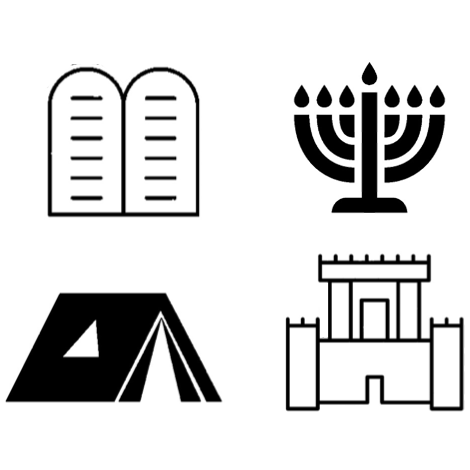
\includegraphics[width=0.30\textwidth]{../ot_frontcover.png}} ;
    \node (0,0) [xshift=+0.20cm, yshift=+2.0cm, opacity=0.10]{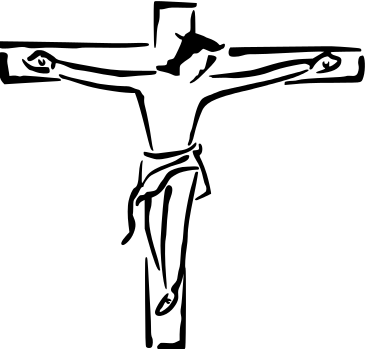
\includegraphics[width=0.20\textwidth]{../christ_on_cross.png}} ;
\end{tikzpicture}
\Large 

\leftcitation{ס} \centerfont 詩百又廿七載：
\leftcitation{ע} \centerfont 非耶和華建屋宇.則匠人之經營徒.
\leftcitation{פ} \centerfont 非耶和華衛城邑.則守者之儆醒徒.
\leftcitation{צ} \centerfont 余獻是卷予華人社區．願為福音流通之器．願獻斯微材為祭榮耀上帝．
\leftcitation{ק} \centerfont 阿門

\switchcolumn

\fontsize{11}{13}\rightfont \Large 滅．時越次聖殿期及當今。\leftcitation{י} \rightfont 猶太者力廣納之．筆錄以卷軸．便以傳、閱、頌、攜、守、鎖、抄、譯、釋、編，得書塔木德、密示拿等經傳．家喻戶曉．傳流若芳。\leftcitation{כ} \rightfont 猶太者文以載道．傳其口述．今我輩粵道之傳應當作如是．遂力行粵音識辨之法．載言載道．以盡忠傳粵道以待興。\leftcitation{ל} \rightfont 蒙下賜恩惠．無畏海量字音文書．既馭上帝之道．今廣及粵語講道．重駛編程之技．匯導粵音遂字稿．重塑講道現場．以傚猶太卷軸之舉便以傳流。\leftcitation{מ} \rightfont 是卷乃粵音口述傳之屬．莫通華文白話之語．

\end{paracol}

\columnratio{0.5,0.5}
\begin{paracol}{2}\fontsize{11}{13}\leftfont \Large \leftcitation{ו} \leftfont 斯殺一違儆百逆．既禁壓之．我輩聞風無奈．在所難免。\leftcitation{ז} \leftfont 另有異人例乎．以版權之名．脅網絡頻道之舉．同授礙予粵道之存流。

\switchcolumn

\fontsize{11}{13}\rightfont \Large 惟待後繼來者之傚．以譯釋傳之於神州華文地。\leftcitation{נ} \rightfont 今能排程驅馭圖靈以編彙文檔，其碼長共數千千亦無逢大礙．全蒙上帝保守。

\end{paracol}



\columnratio{1}\begin{paracol}{1}

\fontsize{11}{13}\rightfont \Large
~~~~~~~~~~~~~~~~~~~~~~~~~~~~~~~~~~~~~~~~~~~~~~~~~~~~~~~~~~~~~~~~~~~~~~~~~~~~~~~\leftcitation{ר} \rightfont 二零二三年二月一日

~~~~~~~~~~~~~~~~~~~~~~~~~~~~~~~~~~~~~~~~~~~~~~~~~~~~~~~~~~~~~~~~~~~~~~~~~~~~~~~\leftcitation{ש} \rightfont 米迦勒

~~~~~~~~~~~~~~~~~~~~~~~~~~~~~~~~~~~~~~~~~~~~~~~~~~~~~~~~~~~~~~~~~~~~~~~~~~~~~~~\leftcitation{ת} \rightfont 書於香港

\end{paracol}

\end{sloppypar}
\end{document}
